\documentclass[twoside]{book}

% Packages required by doxygen
\usepackage{fixltx2e}
\usepackage{calc}
\usepackage{doxygen}
\usepackage[export]{adjustbox} % also loads graphicx
\usepackage{graphicx}
\usepackage[utf8]{inputenc}
\usepackage{makeidx}
\usepackage{multicol}
\usepackage{multirow}
\PassOptionsToPackage{warn}{textcomp}
\usepackage{textcomp}
\usepackage[nointegrals]{wasysym}
\usepackage[table]{xcolor}

% Font selection
\usepackage[T1]{fontenc}
\usepackage[scaled=.90]{helvet}
\usepackage{courier}
\usepackage{amssymb}
\usepackage{sectsty}
\renewcommand{\familydefault}{\sfdefault}
\allsectionsfont{%
  \fontseries{bc}\selectfont%
  \color{darkgray}%
}
\renewcommand{\DoxyLabelFont}{%
  \fontseries{bc}\selectfont%
  \color{darkgray}%
}
\newcommand{\+}{\discretionary{\mbox{\scriptsize$\hookleftarrow$}}{}{}}

% Page & text layout
\usepackage{geometry}
\geometry{%
  a4paper,%
  top=2.5cm,%
  bottom=2.5cm,%
  left=2.5cm,%
  right=2.5cm%
}
\tolerance=750
\hfuzz=15pt
\hbadness=750
\setlength{\emergencystretch}{15pt}
\setlength{\parindent}{0cm}
\setlength{\parskip}{3ex plus 2ex minus 2ex}
\makeatletter
\renewcommand{\paragraph}{%
  \@startsection{paragraph}{4}{0ex}{-1.0ex}{1.0ex}{%
    \normalfont\normalsize\bfseries\SS@parafont%
  }%
}
\renewcommand{\subparagraph}{%
  \@startsection{subparagraph}{5}{0ex}{-1.0ex}{1.0ex}{%
    \normalfont\normalsize\bfseries\SS@subparafont%
  }%
}
\makeatother

% Headers & footers
\usepackage{fancyhdr}
\pagestyle{fancyplain}
\fancyhead[LE]{\fancyplain{}{\bfseries\thepage}}
\fancyhead[CE]{\fancyplain{}{}}
\fancyhead[RE]{\fancyplain{}{\bfseries\leftmark}}
\fancyhead[LO]{\fancyplain{}{\bfseries\rightmark}}
\fancyhead[CO]{\fancyplain{}{}}
\fancyhead[RO]{\fancyplain{}{\bfseries\thepage}}
\fancyfoot[LE]{\fancyplain{}{}}
\fancyfoot[CE]{\fancyplain{}{}}
\fancyfoot[RE]{\fancyplain{}{\bfseries\scriptsize Generated by Doxygen }}
\fancyfoot[LO]{\fancyplain{}{\bfseries\scriptsize Generated by Doxygen }}
\fancyfoot[CO]{\fancyplain{}{}}
\fancyfoot[RO]{\fancyplain{}{}}
\renewcommand{\footrulewidth}{0.4pt}
\renewcommand{\chaptermark}[1]{%
  \markboth{#1}{}%
}
\renewcommand{\sectionmark}[1]{%
  \markright{\thesection\ #1}%
}

% Indices & bibliography
\usepackage{natbib}
\usepackage[titles]{tocloft}
\setcounter{tocdepth}{3}
\setcounter{secnumdepth}{5}
\makeindex

% Hyperlinks (required, but should be loaded last)
\usepackage{ifpdf}
\ifpdf
  \usepackage[pdftex,pagebackref=true]{hyperref}
\else
  \usepackage[ps2pdf,pagebackref=true]{hyperref}
\fi
\hypersetup{%
  colorlinks=true,%
  linkcolor=blue,%
  citecolor=blue,%
  unicode%
}

% Custom commands
\newcommand{\clearemptydoublepage}{%
  \newpage{\pagestyle{empty}\cleardoublepage}%
}

\usepackage{caption}
\captionsetup{labelsep=space,justification=centering,font={bf},singlelinecheck=off,skip=4pt,position=top}

%===== C O N T E N T S =====

\begin{document}

% Titlepage & ToC
\hypersetup{pageanchor=false,
             bookmarksnumbered=true,
             pdfencoding=unicode
            }
\pagenumbering{roman}
\begin{titlepage}
\vspace*{7cm}
\begin{center}%
{\Large A\+Star\+Path\+Planning }\\
\vspace*{1cm}
{\large Generated by Doxygen 1.8.11}\\
\end{center}
\end{titlepage}
\clearemptydoublepage
\tableofcontents
\clearemptydoublepage
\pagenumbering{arabic}
\hypersetup{pageanchor=true}

%--- Begin generated contents ---
\chapter{A\+Star\+Path\+Planning}
\label{md_README}
\hypertarget{md_README}{}
A$\ast$ Path Planning Component Design for Acme.

\href{https://travis-ci.org/SonamYeshe/AStarPathPlanning}{\tt } \subsection*{\href{https://coveralls.io/github/SonamYeshe/AStarPathPlanning?branch=master}{\tt } }

\subsection*{Overview and purpose of the project}

While Acme robot is on automation mode and plan to move from an origin to a goal, this project helps to find the path with the shortest path.

At each iteration of its main loop, A$\ast$ needs to determine which of its partial paths to expand into one or more longer paths. It does so based on an estimate of the cost (total weight) still to go to the goal node. Specifically, A$\ast$ selects the path that minimizes f(n)=g(n)+h(n) where n is the last node on the path, g(n) is the cost of the path from the start node to n, and h(n) is a heuristic that estimates the cost of the cheapest path from n to the goal. The heuristic is problem-\/specific. In this project, we choose the direct distance from the current position to the goal.

\subsection*{Performance example}

Illustration of A$\ast$ search for finding path from a start node to a goal node in a robot motion planning problem. The empty circles represent the nodes in the open set, i.\+e., those that remain to be explored, and the filled ones are in the closed set. Color on each closed node indicates the distance from the start\+: the greener, the farther. One can first see the A$\ast$ moving in a straight line in the direction of the goal, then when hitting the obstacle, it explores alternative routes through the nodes from the open set. Gif can be seen from the following link. 

 

\subsection*{License}

G\+NU General Public License v3.\+0

Permissions of this strong copyleft license are conditioned on making available complete source code of licensed works and modifications, which include larger works using a licensed work, under the same license. Copyright and license notices must be preserved. Contributors provide an express grant of patent rights.

\subsection*{Dependencies}


\begin{DoxyEnumerate}
\item eclipse C\+DT I\+DE (4.\+7).
\end{DoxyEnumerate}

\subsection*{Backlog google spreadsheet}

\href{https://docs.google.com/a/terpmail.umd.edu/spreadsheets/d/1j3ytA1mPyvJpSjNRXjjnHxmMqRgYix9c8MPspWwJh78/edit?usp=sharing}{\tt https\+://docs.\+google.\+com/a/terpmail.\+umd.\+edu/spreadsheets/d/1j3yt\+A1m\+Pyv\+Jp\+Sj\+N\+R\+Xjjn\+Hxm\+Mq\+Rg\+Yix9c8\+M\+Psp\+Ww\+Jh78/edit?usp=sharing}

\subsection*{Working with Eclipse I\+DE}

\subsection*{Installation}

In your Eclipse workspace directory (or create a new one), checkout the repo (and submodules) 
\begin{DoxyCode}
1 mkdir -p ~/workspace
2 cd ~/workspace
3 git clone --recursive https://github.com/SonamYeshe/AStarPathPlanning.git
\end{DoxyCode}


In your work directory, use cmake to create an Eclipse project for an \mbox{[}out-\/of-\/source build\mbox{]} of A\+Star\+Path\+Planning


\begin{DoxyCode}
1 cd ~/workspace
2 mkdir -p AStarPathPlanning-eclipse
3 cd AStarPathPlanning-eclipse
4 cmake -G "Eclipse CDT4 - Unix Makefiles" -D CMAKE\_BUILD\_TYPE=Debug -D CMAKE\_ECLIPSE\_VERSION=4.7.0 -D
       CMAKE\_CXX\_COMPILER\_ARG1=-std=c++14 ../AStarPathPlanning/
\end{DoxyCode}


\subsection*{Import}

Open Eclipse, go to File -\/$>$ Import -\/$>$ General -\/$>$ Existing Projects into Workspace -\/$>$ Select \char`\"{}\+A\+Star\+Path\+Planning-\/eclipse\char`\"{} directory created previously as root directory -\/$>$ Finish

\section*{Edit}

Source files may be edited under the \char`\"{}\mbox{[}\+Source Directory\mbox{]}\char`\"{} label in the Project Explorer.

\subsection*{Build}

To build the project, in Eclipse, unfold A\+Star\+Path\+Planning-\/eclipse project in Project Explorer, unfold Build Targets, double click on \char`\"{}all\char`\"{} to build all projects.

\subsection*{Run}


\begin{DoxyEnumerate}
\item In Eclipse, right click on the A\+Star\+Path\+Planning-\/eclipse in Project Explorer, select Run As -\/$>$ Local C/\+C++ Application
\item Choose the binaries to run (e.\+g. shell-\/app, cpp-\/test for unit testing) A\+Star\+Path\+Planning-\/eclipse in Project Explorer, select Debug As -\/$>$ Local C/\+C++ Application, choose the binaries to run (e.\+g. shell-\/app).
\item If prompt to \char`\"{}\+Confirm Perspective Switch\char`\"{}, select yes.
\item Program will break at the breakpoint you set.
\item Press Step Into (F5), Step Over (F6), Step Return (F7) to step/debug your program.
\item Right click on the variable in editor to add watch expression to watch the variable in debugger window.
\item Press Terminate icon to terminate debugging and press C/\+C++ icon to switch back to C/\+C++ perspetive view (or Windows-\/$>$Perspective-\/$>$Open Perspective-\/$>$C/\+C++).
\end{DoxyEnumerate}

\subsection*{Plugins}


\begin{DoxyItemize}
\item Cpp\+Ch\+Eclipse

To install and run cppcheck in Eclipse
\begin{DoxyEnumerate}
\item In Eclipse, go to Window -\/$>$ Preferences -\/$>$ C/\+C++ -\/$>$ cppcheclipse. Set cppcheck binary path to \char`\"{}/usr/bin/cppcheck\char`\"{}.
\item To run C\+P\+P\+Check on a project, right click on the project name in the Project Explorer and choose cppcheck -\/$>$ Run cppcheck.
\end{DoxyEnumerate}
\item cpplint

To install and run from terminal
\begin{DoxyEnumerate}
\item wget \href{https://raw.githubusercontent.com/google/styleguide/gh-pages/cpplint/cpplint.py}{\tt https\+://raw.\+githubusercontent.\+com/google/styleguide/gh-\/pages/cpplint/cpplint.\+py}
\item Change permission to executable\+: chmod +x cpplint.\+py
\item cd $<$repository$>$
\item Run cpplint
\end{DoxyEnumerate}

Example run with A\+Star\+Path\+Planning-\/eclipse (cpplint.\+py is in the parent directory)\+:

cd cpp-\/boilerplate

../cpplint.py --extensions=h,hpp,cpp \$( find . -\/name $\ast$.h -\/or -\/name $\ast$.hpp -\/or -\/name $\ast$.cpp $\vert$ grep -\/vE -\/e \char`\"{}$^\wedge$./build/\char`\"{} -\/e \char`\"{}$^\wedge$./vendor/\char`\"{} )
\item doxygen

Simply run \$ doxygen my\+\_\+proj.\+conf in a new terminal under repo to update the doxygen documentation.
\item Google C++ Sytle

To include and use Google C++ Style formatter in Eclipse
\begin{DoxyEnumerate}
\item In Eclipse, go to Window -\/$>$ Preferences -\/$>$ C/\+C++ -\/$>$ Code Style -\/$>$ Formatter. Import \href{https://raw.githubusercontent.com/google/styleguide/gh-pages/eclipse-cpp-google-style.xml}{\tt eclipse-\/cpp-\/google-\/style} and apply.
\item To use Google C++ style formatter, right click on the source code or folder in Project Explorer and choose Source -\/$>$ Format
\end{DoxyEnumerate}
\item Git

It is possible to manage version control through Eclipse and the git plugin, but it typically requires creating another project. If you\textquotesingle{}re interested in this, try it out yourself and contact me on Canvas. 
\end{DoxyItemize}
\chapter{Defining a Mock Class}
\label{md_vendor_googletest_googlemock_docs_CheatSheet}
\hypertarget{md_vendor_googletest_googlemock_docs_CheatSheet}{}
\subsection*{Mocking a Normal Class}

Given 
\begin{DoxyCode}
1 class Foo \{
2   ...
3   virtual ~Foo();
4   virtual int GetSize() const = 0;
5   virtual string Describe(const char* name) = 0;
6   virtual string Describe(int type) = 0;
7   virtual bool Process(Bar elem, int count) = 0;
8 \};
\end{DoxyCode}
 (note that {\ttfamily $\sim$\+Foo()} {\bfseries must} be virtual) we can define its mock as 
\begin{DoxyCode}
1 #include "gmock/gmock.h"
2 
3 class MockFoo : public Foo \{
4   MOCK\_CONST\_METHOD0(GetSize, int());
5   MOCK\_METHOD1(Describe, string(const char* name));
6   MOCK\_METHOD1(Describe, string(int type));
7   MOCK\_METHOD2(Process, bool(Bar elem, int count));
8 \};
\end{DoxyCode}


To create a \char`\"{}nice\char`\"{} mock object which ignores all uninteresting calls, or a \char`\"{}strict\char`\"{} mock object, which treats them as failures\+: 
\begin{DoxyCode}
1 NiceMock<MockFoo> nice\_foo;     // The type is a subclass of MockFoo.
2 StrictMock<MockFoo> strict\_foo; // The type is a subclass of MockFoo.
\end{DoxyCode}


\subsection*{Mocking a Class Template}

To mock 
\begin{DoxyCode}
1 template <typename Elem>
2 class StackInterface \{
3  public:
4   ...
5   virtual ~StackInterface();
6   virtual int GetSize() const = 0;
7   virtual void Push(const Elem& x) = 0;
8 \};
\end{DoxyCode}
 (note that {\ttfamily $\sim$\+Stack\+Interface()} {\bfseries must} be virtual) just append {\ttfamily \+\_\+T} to the {\ttfamily M\+O\+C\+K\+\_\+$\ast$} macros\+: 
\begin{DoxyCode}
1 template <typename Elem>
2 class MockStack : public StackInterface<Elem> \{
3  public:
4   ...
5   MOCK\_CONST\_METHOD0\_T(GetSize, int());
6   MOCK\_METHOD1\_T(Push, void(const Elem& x));
7 \};
\end{DoxyCode}


\subsection*{Specifying Calling Conventions for \hyperlink{classMock}{Mock} Functions}

If your mock function doesn\textquotesingle{}t use the default calling convention, you can specify it by appending {\ttfamily \+\_\+\+W\+I\+T\+H\+\_\+\+C\+A\+L\+L\+T\+Y\+PE} to any of the macros described in the previous two sections and supplying the calling convention as the first argument to the macro. For example, 
\begin{DoxyCode}
1 MOCK\_METHOD\_1\_WITH\_CALLTYPE(STDMETHODCALLTYPE, Foo, bool(int n));
2 MOCK\_CONST\_METHOD2\_WITH\_CALLTYPE(STDMETHODCALLTYPE, Bar, int(double x, double y));
\end{DoxyCode}
 where {\ttfamily S\+T\+D\+M\+E\+T\+H\+O\+D\+C\+A\+L\+L\+T\+Y\+PE} is defined by {\ttfamily $<$objbase.\+h$>$} on Windows.

\section*{Using Mocks in Tests}

The typical flow is\+:
\begin{DoxyEnumerate}
\item Import the Google \hyperlink{classMock}{Mock} names you need to use. All Google \hyperlink{classMock}{Mock} names are in the {\ttfamily testing} namespace unless they are macros or otherwise noted.
\end{DoxyEnumerate}
\begin{DoxyEnumerate}
\item Create the mock objects.
\end{DoxyEnumerate}
\begin{DoxyEnumerate}
\item Optionally, set the default actions of the mock objects.
\end{DoxyEnumerate}
\begin{DoxyEnumerate}
\item Set your expectations on the mock objects (How will they be called? What wil they do?).
\end{DoxyEnumerate}
\begin{DoxyEnumerate}
\item Exercise code that uses the mock objects; if necessary, check the result using \href{../../googletest/}{\tt Google Test} assertions.
\end{DoxyEnumerate}
\begin{DoxyEnumerate}
\item When a mock objects is destructed, Google \hyperlink{classMock}{Mock} automatically verifies that all expectations on it have been satisfied.
\end{DoxyEnumerate}

Here is an example\+: 
\begin{DoxyCode}
1 using ::testing::Return;                            // #1
2 
3 TEST(BarTest, DoesThis) \{
4   MockFoo foo;                                    // #2
5 
6   ON\_CALL(foo, GetSize())                         // #3
7       .WillByDefault(Return(1));
8   // ... other default actions ...
9 
10   EXPECT\_CALL(foo, Describe(5))                   // #4
11       .Times(3)
12       .WillRepeatedly(Return("Category 5"));
13   // ... other expectations ...
14 
15   EXPECT\_EQ("good", MyProductionFunction(&foo));  // #5
16 \}                                                 // #6
\end{DoxyCode}


\section*{Setting Default Actions}

Google \hyperlink{classMock}{Mock} has a {\bfseries built-\/in default action} for any function that returns {\ttfamily void}, {\ttfamily bool}, a numeric value, or a pointer.

To customize the default action for functions with return type {\ttfamily T} globally\+: 
\begin{DoxyCode}
1 using ::testing::DefaultValue;
2 
3 // Sets the default value to be returned. T must be CopyConstructible.
4 DefaultValue<T>::Set(value);
5 // Sets a factory. Will be invoked on demand. T must be MoveConstructible.
6 //   T MakeT();
7 DefaultValue<T>::SetFactory(&MakeT);
8 // ... use the mocks ...
9 // Resets the default value.
10 DefaultValue<T>::Clear();
\end{DoxyCode}


To customize the default action for a particular method, use {\ttfamily \hyperlink{gmock-spec-builders_8h_a5b12ae6cf84f0a544ca811b380c37334}{O\+N\+\_\+\+C\+A\+L\+L()}}\+: 
\begin{DoxyCode}
1 ON\_CALL(mock\_object, method(matchers))
2     .With(multi\_argument\_matcher)  ?
3     .WillByDefault(action);
\end{DoxyCode}


\section*{Setting Expectations}

{\ttfamily \hyperlink{gmock-spec-builders_8h_a535a6156de72c1a2e25a127e38ee5232}{E\+X\+P\+E\+C\+T\+\_\+\+C\+A\+L\+L()}} sets {\bfseries expectations} on a mock method (How will it be called? What will it do?)\+: 
\begin{DoxyCode}
1 EXPECT\_CALL(mock\_object, method(matchers))
2     .With(multi\_argument\_matcher)  ?
3     .Times(cardinality)            ?
4     .InSequence(sequences)         *
5     .After(expectations)           *
6     .WillOnce(action)              *
7     .WillRepeatedly(action)        ?
8     .RetiresOnSaturation();        ?
\end{DoxyCode}


If {\ttfamily Times()} is omitted, the cardinality is assumed to be\+:


\begin{DoxyItemize}
\item {\ttfamily Times(1)} when there is neither {\ttfamily Will\+Once()} nor {\ttfamily Will\+Repeatedly()};
\item {\ttfamily Times(n)} when there are {\ttfamily n Will\+Once()}s but no {\ttfamily Will\+Repeatedly()}, where {\ttfamily n} $>$= 1; or
\item {\ttfamily Times(\+At\+Least(n))} when there are {\ttfamily n Will\+Once()}s and a {\ttfamily Will\+Repeatedly()}, where {\ttfamily n} $>$= 0.
\end{DoxyItemize}

A method with no {\ttfamily \hyperlink{gmock-spec-builders_8h_a535a6156de72c1a2e25a127e38ee5232}{E\+X\+P\+E\+C\+T\+\_\+\+C\+A\+L\+L()}} is free to be invoked {\itshape any number of times}, and the default action will be taken each time.

\section*{Matchers}

A {\bfseries matcher} matches a {\itshape single} argument. You can use it inside {\ttfamily \hyperlink{gmock-spec-builders_8h_a5b12ae6cf84f0a544ca811b380c37334}{O\+N\+\_\+\+C\+A\+L\+L()}} or {\ttfamily \hyperlink{gmock-spec-builders_8h_a535a6156de72c1a2e25a127e38ee5232}{E\+X\+P\+E\+C\+T\+\_\+\+C\+A\+L\+L()}}, or use it to validate a value directly\+:

\tabulinesep=1mm
\begin{longtabu} spread 0pt [c]{*2{|X[-1]}|}
\hline
\rowcolor{\tableheadbgcolor}{\bf {\ttfamily \hyperlink{gmock-matchers_8h_ac31e206123aa702e1152bb2735b31409}{E\+X\+P\+E\+C\+T\+\_\+\+T\+H\+A\+T(value, matcher)}} }&{\bf Asserts that {\ttfamily value} matches {\ttfamily matcher}.  }\\\cline{1-2}
\endfirsthead
\hline
\endfoot
\hline
\rowcolor{\tableheadbgcolor}{\bf {\ttfamily \hyperlink{gmock-matchers_8h_ac31e206123aa702e1152bb2735b31409}{E\+X\+P\+E\+C\+T\+\_\+\+T\+H\+A\+T(value, matcher)}} }&{\bf Asserts that {\ttfamily value} matches {\ttfamily matcher}.  }\\\cline{1-2}
\endhead
{\ttfamily \hyperlink{gmock-matchers_8h_a41d888579850c16583baea33ee8d057e}{A\+S\+S\+E\+R\+T\+\_\+\+T\+H\+A\+T(value, matcher)}} &The same as {\ttfamily \hyperlink{gmock-matchers_8h_ac31e206123aa702e1152bb2735b31409}{E\+X\+P\+E\+C\+T\+\_\+\+T\+H\+A\+T(value, matcher)}}, except that it generates a {\bfseries fatal} failure. \\\cline{1-2}
\end{longtabu}
Built-\/in matchers (where {\ttfamily argument} is the function argument) are divided into several categories\+:

\subsection*{Wildcard}

\tabulinesep=1mm
\begin{longtabu} spread 0pt [c]{*2{|X[-1]}|}
\hline
\rowcolor{\tableheadbgcolor}{\bf {\ttfamily \+\_\+}}&{\bf {\ttfamily argument} can be any value of the correct type.  }\\\cline{1-2}
\endfirsthead
\hline
\endfoot
\hline
\rowcolor{\tableheadbgcolor}{\bf {\ttfamily \+\_\+}}&{\bf {\ttfamily argument} can be any value of the correct type.  }\\\cline{1-2}
\endhead
{\ttfamily A$<$type$>$()} or {\ttfamily An$<$type$>$()}&{\ttfamily argument} can be any value of type {\ttfamily type}. \\\cline{1-2}
\end{longtabu}
\subsection*{Generic Comparison}

\tabulinesep=1mm
\begin{longtabu} spread 0pt [c]{*2{|X[-1]}|}
\hline
\rowcolor{\tableheadbgcolor}{\bf {\ttfamily Eq(value)} or {\ttfamily value}}&{\bf {\ttfamily argument == value}  }\\\cline{1-2}
\endfirsthead
\hline
\endfoot
\hline
\rowcolor{\tableheadbgcolor}{\bf {\ttfamily Eq(value)} or {\ttfamily value}}&{\bf {\ttfamily argument == value}  }\\\cline{1-2}
\endhead
{\ttfamily Ge(value)} &{\ttfamily argument $>$= value} \\\cline{1-2}
{\ttfamily Gt(value)} &{\ttfamily argument $>$ value} \\\cline{1-2}
{\ttfamily Le(value)} &{\ttfamily argument $<$= value} \\\cline{1-2}
{\ttfamily Lt(value)} &{\ttfamily argument $<$ value} \\\cline{1-2}
{\ttfamily Ne(value)} &{\ttfamily argument != value} \\\cline{1-2}
{\ttfamily \hyperlink{namespacetesting_a56ffb1a169c14ce585fc5bed32add2db}{Is\+Null()}} &{\ttfamily argument} is a {\ttfamily N\+U\+LL} pointer (raw or smart). \\\cline{1-2}
{\ttfamily \hyperlink{namespacetesting_a39d1f92b53b8b2a0b6db6a22ac146416}{Not\+Null()}} &{\ttfamily argument} is a non-\/null pointer (raw or smart). \\\cline{1-2}
{\ttfamily Ref(variable)} &{\ttfamily argument} is a reference to {\ttfamily variable}. \\\cline{1-2}
{\ttfamily Typed\+Eq$<$type$>$(value)}&{\ttfamily argument} has type {\ttfamily type} and is equal to {\ttfamily value}. You may need to use this instead of {\ttfamily Eq(value)} when the mock function is overloaded. \\\cline{1-2}
\end{longtabu}
Except {\ttfamily \hyperlink{namespacetesting_a0a4a364121ea3fa656a112f1c2e6b7a4}{Ref()}}, these matchers make a {\itshape copy} of {\ttfamily value} in case it\textquotesingle{}s modified or destructed later. If the compiler complains that {\ttfamily value} doesn\textquotesingle{}t have a public copy constructor, try wrap it in {\ttfamily \hyperlink{namespacetesting_aaee6d42dcd69de6e7a1459c5c71222c3}{By\+Ref()}}, e.\+g. {\ttfamily Eq(\+By\+Ref(non\+\_\+copyable\+\_\+value))}. If you do that, make sure {\ttfamily non\+\_\+copyable\+\_\+value} is not changed afterwards, or the meaning of your matcher will be changed.

\subsection*{Floating-\/\+Point Matchers}

\tabulinesep=1mm
\begin{longtabu} spread 0pt [c]{*2{|X[-1]}|}
\hline
\rowcolor{\tableheadbgcolor}{\bf {\ttfamily Double\+Eq(a\+\_\+double)}}&{\bf {\ttfamily argument} is a {\ttfamily double} value approximately equal to {\ttfamily a\+\_\+double}, treating two Na\+Ns as unequal.  }\\\cline{1-2}
\endfirsthead
\hline
\endfoot
\hline
\rowcolor{\tableheadbgcolor}{\bf {\ttfamily Double\+Eq(a\+\_\+double)}}&{\bf {\ttfamily argument} is a {\ttfamily double} value approximately equal to {\ttfamily a\+\_\+double}, treating two Na\+Ns as unequal.  }\\\cline{1-2}
\endhead
{\ttfamily Float\+Eq(a\+\_\+float)} &{\ttfamily argument} is a {\ttfamily float} value approximately equal to {\ttfamily a\+\_\+float}, treating two Na\+Ns as unequal. \\\cline{1-2}
{\ttfamily Nan\+Sensitive\+Double\+Eq(a\+\_\+double)}&{\ttfamily argument} is a {\ttfamily double} value approximately equal to {\ttfamily a\+\_\+double}, treating two Na\+Ns as equal. \\\cline{1-2}
{\ttfamily Nan\+Sensitive\+Float\+Eq(a\+\_\+float)}&{\ttfamily argument} is a {\ttfamily float} value approximately equal to {\ttfamily a\+\_\+float}, treating two Na\+Ns as equal. \\\cline{1-2}
\end{longtabu}
The above matchers use U\+L\+P-\/based comparison (the same as used in \href{../../googletest/}{\tt Google Test}). They automatically pick a reasonable error bound based on the absolute value of the expected value. {\ttfamily \hyperlink{namespacetesting_a1f49f9d97f03bfa4db26888f03486a9f}{Double\+Eq()}} and {\ttfamily \hyperlink{namespacetesting_ac75507edb7998957b48fb17a9b8a020b}{Float\+Eq()}} conform to the I\+E\+EE standard, which requires comparing two Na\+Ns for equality to return false. The {\ttfamily Nan\+Sensitive$\ast$} version instead treats two Na\+Ns as equal, which is often what a user wants.

\tabulinesep=1mm
\begin{longtabu} spread 0pt [c]{*2{|X[-1]}|}
\hline
\rowcolor{\tableheadbgcolor}{\bf {\ttfamily Double\+Near(a\+\_\+double, max\+\_\+abs\+\_\+error)}}&{\bf {\ttfamily argument} is a {\ttfamily double} value close to {\ttfamily a\+\_\+double} (absolute error $<$= {\ttfamily max\+\_\+abs\+\_\+error}), treating two Na\+Ns as unequal.  }\\\cline{1-2}
\endfirsthead
\hline
\endfoot
\hline
\rowcolor{\tableheadbgcolor}{\bf {\ttfamily Double\+Near(a\+\_\+double, max\+\_\+abs\+\_\+error)}}&{\bf {\ttfamily argument} is a {\ttfamily double} value close to {\ttfamily a\+\_\+double} (absolute error $<$= {\ttfamily max\+\_\+abs\+\_\+error}), treating two Na\+Ns as unequal.  }\\\cline{1-2}
\endhead
{\ttfamily Float\+Near(a\+\_\+float, max\+\_\+abs\+\_\+error)} &{\ttfamily argument} is a {\ttfamily float} value close to {\ttfamily a\+\_\+float} (absolute error $<$= {\ttfamily max\+\_\+abs\+\_\+error}), treating two Na\+Ns as unequal. \\\cline{1-2}
{\ttfamily Nan\+Sensitive\+Double\+Near(a\+\_\+double, max\+\_\+abs\+\_\+error)}&{\ttfamily argument} is a {\ttfamily double} value close to {\ttfamily a\+\_\+double} (absolute error $<$= {\ttfamily max\+\_\+abs\+\_\+error}), treating two Na\+Ns as equal. \\\cline{1-2}
{\ttfamily Nan\+Sensitive\+Float\+Near(a\+\_\+float, max\+\_\+abs\+\_\+error)}&{\ttfamily argument} is a {\ttfamily float} value close to {\ttfamily a\+\_\+float} (absolute error $<$= {\ttfamily max\+\_\+abs\+\_\+error}), treating two Na\+Ns as equal. \\\cline{1-2}
\end{longtabu}
\subsection*{String Matchers}

The {\ttfamily argument} can be either a C string or a C++ string object\+:

\tabulinesep=1mm
\begin{longtabu} spread 0pt [c]{*2{|X[-1]}|}
\hline
\rowcolor{\tableheadbgcolor}{\bf {\ttfamily Contains\+Regex(string)}}&{\bf {\ttfamily argument} matches the given regular expression.  }\\\cline{1-2}
\endfirsthead
\hline
\endfoot
\hline
\rowcolor{\tableheadbgcolor}{\bf {\ttfamily Contains\+Regex(string)}}&{\bf {\ttfamily argument} matches the given regular expression.  }\\\cline{1-2}
\endhead
{\ttfamily Ends\+With(suffix)} &{\ttfamily argument} ends with string {\ttfamily suffix}. \\\cline{1-2}
{\ttfamily Has\+Substr(string)} &{\ttfamily argument} contains {\ttfamily string} as a sub-\/string. \\\cline{1-2}
{\ttfamily Matches\+Regex(string)} &{\ttfamily argument} matches the given regular expression with the match starting at the first character and ending at the last character. \\\cline{1-2}
{\ttfamily Starts\+With(prefix)} &{\ttfamily argument} starts with string {\ttfamily prefix}. \\\cline{1-2}
{\ttfamily Str\+Case\+Eq(string)} &{\ttfamily argument} is equal to {\ttfamily string}, ignoring case. \\\cline{1-2}
{\ttfamily Str\+Case\+Ne(string)} &{\ttfamily argument} is not equal to {\ttfamily string}, ignoring case. \\\cline{1-2}
{\ttfamily Str\+Eq(string)} &{\ttfamily argument} is equal to {\ttfamily string}. \\\cline{1-2}
{\ttfamily Str\+Ne(string)} &{\ttfamily argument} is not equal to {\ttfamily string}. \\\cline{1-2}
\end{longtabu}
{\ttfamily \hyperlink{namespacetesting_a899838630a71376aa071dfd7c500f2ca}{Contains\+Regex()}} and {\ttfamily \hyperlink{namespacetesting_a4dac232f315edc259b62ce88e413b107}{Matches\+Regex()}} use the regular expression syntax defined \href{../../googletest/docs/AdvancedGuide.md#regular-expression-syntax}{\tt here}. {\ttfamily \hyperlink{namespacetesting_addbdb8c0902ab09cade24fa6db7c0073}{Str\+Case\+Eq()}}, {\ttfamily \hyperlink{namespacetesting_a9596fd67bdd5df195bc54382f91a1906}{Str\+Case\+Ne()}}, {\ttfamily \hyperlink{namespacetesting_a154de81376ae7d584c6e5a619b45fb09}{Str\+Eq()}}, and {\ttfamily \hyperlink{namespacetesting_a6f6b8af3d19cb969df0eb995c47a14d2}{Str\+Ne()}} work for wide strings as well.

\subsection*{Container Matchers}

Most S\+T\+L-\/style containers support {\ttfamily ==}, so you can use {\ttfamily Eq(expected\+\_\+container)} or simply {\ttfamily expected\+\_\+container} to match a container exactly. If you want to write the elements in-\/line, match them more flexibly, or get more informative messages, you can use\+:

\tabulinesep=1mm
\begin{longtabu} spread 0pt [c]{*2{|X[-1]}|}
\hline
\rowcolor{\tableheadbgcolor}{\bf {\ttfamily Container\+Eq(container)} }&{\bf The same as {\ttfamily Eq(container)} except that the failure message also includes which elements are in one container but not the other.  }\\\cline{1-2}
\endfirsthead
\hline
\endfoot
\hline
\rowcolor{\tableheadbgcolor}{\bf {\ttfamily Container\+Eq(container)} }&{\bf The same as {\ttfamily Eq(container)} except that the failure message also includes which elements are in one container but not the other.  }\\\cline{1-2}
\endhead
{\ttfamily Contains(e)} &{\ttfamily argument} contains an element that matches {\ttfamily e}, which can be either a value or a matcher. \\\cline{1-2}
{\ttfamily Each(e)} &{\ttfamily argument} is a container where {\itshape every} element matches {\ttfamily e}, which can be either a value or a matcher. \\\cline{1-2}
{\ttfamily Elements\+Are(e0, e1, ..., en)} &{\ttfamily argument} has {\ttfamily n + 1} elements, where the i-\/th element matches {\ttfamily ei}, which can be a value or a matcher. 0 to 10 arguments are allowed. \\\cline{1-2}
{\ttfamily Elements\+Are\+Array(\{ e0, e1, ..., en \})}, {\ttfamily Elements\+Are\+Array(array)}, or {\ttfamily Elements\+Are\+Array(array, count)} &The same as {\ttfamily \hyperlink{namespacetesting_a79cf4ae694bf8231dcf283b325405f27}{Elements\+Are()}} except that the expected element values/matchers come from an initializer list, S\+T\+L-\/style container, or C-\/style array. \\\cline{1-2}
{\ttfamily Is\+Empty()} &{\ttfamily argument} is an empty container ({\ttfamily container.\+empty()}). \\\cline{1-2}
{\ttfamily Pointwise(m, container)} &{\ttfamily argument} contains the same number of elements as in {\ttfamily container}, and for all i, (the i-\/th element in {\ttfamily argument}, the i-\/th element in {\ttfamily container}) match {\ttfamily m}, which is a matcher on 2-\/tuples. E.\+g. {\ttfamily Pointwise(\+Le(), upper\+\_\+bounds)} verifies that each element in {\ttfamily argument} doesn\textquotesingle{}t exceed the corresponding element in {\ttfamily upper\+\_\+bounds}. See more detail below. \\\cline{1-2}
{\ttfamily Size\+Is(m)} &{\ttfamily argument} is a container whose size matches {\ttfamily m}. E.\+g. {\ttfamily Size\+Is(2)} or {\ttfamily Size\+Is(\+Lt(2))}. \\\cline{1-2}
{\ttfamily Unordered\+Elements\+Are(e0, e1, ..., en)} &{\ttfamily argument} has {\ttfamily n + 1} elements, and under some permutation each element matches an {\ttfamily ei} (for a different {\ttfamily i}), which can be a value or a matcher. 0 to 10 arguments are allowed. \\\cline{1-2}
{\ttfamily Unordered\+Elements\+Are\+Array(\{ e0, e1, ..., en \})}, {\ttfamily Unordered\+Elements\+Are\+Array(array)}, or {\ttfamily Unordered\+Elements\+Are\+Array(array, count)} &The same as {\ttfamily \hyperlink{namespacetesting_a8622c12aadfa0e60f7d68683eeb21115}{Unordered\+Elements\+Are()}} except that the expected element values/matchers come from an initializer list, S\+T\+L-\/style container, or C-\/style array. \\\cline{1-2}
{\ttfamily When\+Sorted(m)} &When {\ttfamily argument} is sorted using the {\ttfamily $<$} operator, it matches container matcher {\ttfamily m}. E.\+g. {\ttfamily When\+Sorted(\+Unordered\+Elements\+Are(1, 2, 3))} verifies that {\ttfamily argument} contains elements {\ttfamily 1}, {\ttfamily 2}, and {\ttfamily 3}, ignoring order. \\\cline{1-2}
{\ttfamily When\+Sorted\+By(comparator, m)} &The same as {\ttfamily When\+Sorted(m)}, except that the given comparator instead of {\ttfamily $<$} is used to sort {\ttfamily argument}. E.\+g. {\ttfamily When\+Sorted\+By(std\+::greater$<$int$>$(), Elements\+Are(3, 2, 1))}. \\\cline{1-2}
\end{longtabu}
Notes\+:


\begin{DoxyItemize}
\item These matchers can also match\+:
\begin{DoxyEnumerate}
\item a native array passed by reference (e.\+g. in {\ttfamily Foo(const int (\&a)\mbox{[}5\mbox{]})}), and
\end{DoxyEnumerate}
\begin{DoxyEnumerate}
\item an array passed as a pointer and a count (e.\+g. in {\ttfamily Bar(const T$\ast$ buffer, int len)} -- see Multi-\/argument Matchers).
\end{DoxyEnumerate}
\item The array being matched may be multi-\/dimensional (i.\+e. its elements can be arrays).
\item {\ttfamily m} in {\ttfamily Pointwise(m, ...)} should be a matcher for {\ttfamily \+::testing\+::tuple$<$T, U$>$} where {\ttfamily T} and {\ttfamily U} are the element type of the actual container and the expected container, respectively. For example, to compare two {\ttfamily Foo} containers where {\ttfamily Foo} doesn\textquotesingle{}t support {\ttfamily operator==} but has an {\ttfamily Equals()} method, one might write\+:
\end{DoxyItemize}


\begin{DoxyCode}
1 using ::testing::get;
2 MATCHER(FooEq, "") \{
3   return get<0>(arg).Equals(get<1>(arg));
4 \}
5 ...
6 EXPECT\_THAT(actual\_foos, Pointwise(FooEq(), expected\_foos));
\end{DoxyCode}


\subsection*{Member Matchers}

\tabulinesep=1mm
\begin{longtabu} spread 0pt [c]{*2{|X[-1]}|}
\hline
\rowcolor{\tableheadbgcolor}{\bf {\ttfamily Field(\&class\+::field, m)}}&{\bf {\ttfamily argument.\+field} (or {\ttfamily argument-\/$>$field} when {\ttfamily argument} is a plain pointer) matches matcher {\ttfamily m}, where {\ttfamily argument} is an object of type {\itshape class}.  }\\\cline{1-2}
\endfirsthead
\hline
\endfoot
\hline
\rowcolor{\tableheadbgcolor}{\bf {\ttfamily Field(\&class\+::field, m)}}&{\bf {\ttfamily argument.\+field} (or {\ttfamily argument-\/$>$field} when {\ttfamily argument} is a plain pointer) matches matcher {\ttfamily m}, where {\ttfamily argument} is an object of type {\itshape class}.  }\\\cline{1-2}
\endhead
{\ttfamily Key(e)} &{\ttfamily argument.\+first} matches {\ttfamily e}, which can be either a value or a matcher. E.\+g. {\ttfamily Contains(Key(\+Le(5)))} can verify that a {\ttfamily map} contains a key {\ttfamily $<$= 5}. \\\cline{1-2}
{\ttfamily Pair(m1, m2)} &{\ttfamily argument} is an {\ttfamily std\+::pair} whose {\ttfamily first} field matches {\ttfamily m1} and {\ttfamily second} field matches {\ttfamily m2}. \\\cline{1-2}
{\ttfamily Property(\&class\+::property, m)}&{\ttfamily argument.\+property()} (or {\ttfamily argument-\/$>$property()} when {\ttfamily argument} is a plain pointer) matches matcher {\ttfamily m}, where {\ttfamily argument} is an object of type {\itshape class}. \\\cline{1-2}
\end{longtabu}
\subsection*{Matching the Result of a Function or Functor}

$\vert${\ttfamily Result\+Of(f, m)}$\vert${\ttfamily f(argument)} matches matcher {\ttfamily m}, where {\ttfamily f} is a function or functor.$\vert$ $\vert$\+:-\/-\/-\/-\/-\/-\/-\/-\/-\/-\/-\/-\/---$\vert$\+:-\/-\/-\/-\/-\/-\/-\/-\/-\/-\/-\/-\/-\/-\/-\/-\/-\/-\/-\/-\/-\/-\/-\/-\/-\/-\/-\/-\/-\/-\/-\/-\/-\/-\/-\/-\/-\/-\/-\/-\/-\/-\/-\/-\/-\/-\/-\/-\/-\/-\/-\/-\/-\/-\/-\/-\/-\/-\/-\/-\/-\/-\/-\/-\/-\/-\/---$\vert$

\subsection*{Pointer Matchers}

\tabulinesep=1mm
\begin{longtabu} spread 0pt [c]{*2{|X[-1]}|}
\hline
\rowcolor{\tableheadbgcolor}{\bf {\ttfamily Pointee(m)}}&{\bf {\ttfamily argument} (either a smart pointer or a raw pointer) points to a value that matches matcher {\ttfamily m}.  }\\\cline{1-2}
\endfirsthead
\hline
\endfoot
\hline
\rowcolor{\tableheadbgcolor}{\bf {\ttfamily Pointee(m)}}&{\bf {\ttfamily argument} (either a smart pointer or a raw pointer) points to a value that matches matcher {\ttfamily m}.  }\\\cline{1-2}
\endhead
{\ttfamily When\+Dynamic\+Cast\+To$<$T$>$(m)}&when {\ttfamily argument} is passed through {\ttfamily dynamic\+\_\+cast$<$T$>$()}, it matches matcher {\ttfamily m}. \\\cline{1-2}
\end{longtabu}
\subsection*{Multiargument Matchers}

Technically, all matchers match a {\itshape single} value. A \char`\"{}multi-\/argument\char`\"{} matcher is just one that matches a {\itshape tuple}. The following matchers can be used to match a tuple {\ttfamily (x, y)}\+:

\tabulinesep=1mm
\begin{longtabu} spread 0pt [c]{*2{|X[-1]}|}
\hline
\rowcolor{\tableheadbgcolor}{\bf {\ttfamily \hyperlink{namespacetesting_a0cb8ba7eae844c871eccb29e7c81635f}{Eq()}}}&{\bf {\ttfamily x == y}  }\\\cline{1-2}
\endfirsthead
\hline
\endfoot
\hline
\rowcolor{\tableheadbgcolor}{\bf {\ttfamily \hyperlink{namespacetesting_a0cb8ba7eae844c871eccb29e7c81635f}{Eq()}}}&{\bf {\ttfamily x == y}  }\\\cline{1-2}
\endhead
{\ttfamily \hyperlink{namespacetesting_a42bb19b42d7830b972973a103d5e00f2}{Ge()}}&{\ttfamily x $>$= y} \\\cline{1-2}
{\ttfamily \hyperlink{namespacetesting_a493fc1bafd7b3945ba06ace80e74b0d5}{Gt()}}&{\ttfamily x $>$ y} \\\cline{1-2}
{\ttfamily \hyperlink{namespacetesting_a2e33596921b80a7fdaff3f62bf18a478}{Le()}}&{\ttfamily x $<$= y} \\\cline{1-2}
{\ttfamily \hyperlink{namespacetesting_ad621459957a8bcdd3c256b7940ecbf99}{Lt()}}&{\ttfamily x $<$ y} \\\cline{1-2}
{\ttfamily \hyperlink{namespacetesting_afe42d41d5171234cb9da5da27faeb7e8}{Ne()}}&{\ttfamily x != y} \\\cline{1-2}
\end{longtabu}
You can use the following selectors to pick a subset of the arguments (or reorder them) to participate in the matching\+:

\tabulinesep=1mm
\begin{longtabu} spread 0pt [c]{*2{|X[-1]}|}
\hline
\rowcolor{\tableheadbgcolor}{\bf {\ttfamily All\+Args(m)}}&{\bf Equivalent to {\ttfamily m}. Useful as syntactic sugar in {\ttfamily .With(\+All\+Args(m))}.  }\\\cline{1-2}
\endfirsthead
\hline
\endfoot
\hline
\rowcolor{\tableheadbgcolor}{\bf {\ttfamily All\+Args(m)}}&{\bf Equivalent to {\ttfamily m}. Useful as syntactic sugar in {\ttfamily .With(\+All\+Args(m))}.  }\\\cline{1-2}
\endhead
{\ttfamily Args$<$N1, N2, ..., Nk$>$(m)}&The tuple of the {\ttfamily k} selected (using 0-\/based indices) arguments matches {\ttfamily m}, e.\+g. {\ttfamily Args$<$1, 2$>$(\hyperlink{namespacetesting_a0cb8ba7eae844c871eccb29e7c81635f}{Eq()})}. \\\cline{1-2}
\end{longtabu}
\subsection*{Composite Matchers}

You can make a matcher from one or more other matchers\+:

\tabulinesep=1mm
\begin{longtabu} spread 0pt [c]{*2{|X[-1]}|}
\hline
\rowcolor{\tableheadbgcolor}{\bf {\ttfamily All\+Of(m1, m2, ..., mn)}}&{\bf {\ttfamily argument} matches all of the matchers {\ttfamily m1} to {\ttfamily mn}.  }\\\cline{1-2}
\endfirsthead
\hline
\endfoot
\hline
\rowcolor{\tableheadbgcolor}{\bf {\ttfamily All\+Of(m1, m2, ..., mn)}}&{\bf {\ttfamily argument} matches all of the matchers {\ttfamily m1} to {\ttfamily mn}.  }\\\cline{1-2}
\endhead
{\ttfamily Any\+Of(m1, m2, ..., mn)}&{\ttfamily argument} matches at least one of the matchers {\ttfamily m1} to {\ttfamily mn}. \\\cline{1-2}
{\ttfamily Not(m)} &{\ttfamily argument} doesn\textquotesingle{}t match matcher {\ttfamily m}. \\\cline{1-2}
\end{longtabu}
\subsection*{Adapters for Matchers}

\tabulinesep=1mm
\begin{longtabu} spread 0pt [c]{*2{|X[-1]}|}
\hline
\rowcolor{\tableheadbgcolor}{\bf {\ttfamily Matcher\+Cast$<$T$>$(m)}}&{\bf casts matcher {\ttfamily m} to type {\ttfamily Matcher$<$T$>$}.  }\\\cline{1-2}
\endfirsthead
\hline
\endfoot
\hline
\rowcolor{\tableheadbgcolor}{\bf {\ttfamily Matcher\+Cast$<$T$>$(m)}}&{\bf casts matcher {\ttfamily m} to type {\ttfamily Matcher$<$T$>$}.  }\\\cline{1-2}
\endhead
{\ttfamily Safe\+Matcher\+Cast$<$T$>$(m)}&\href{CookBook.md#casting-matchers}{\tt safely casts} matcher {\ttfamily m} to type {\ttfamily Matcher$<$T$>$}. \\\cline{1-2}
{\ttfamily Truly(predicate)} &{\ttfamily predicate(argument)} returns something considered by C++ to be true, where {\ttfamily predicate} is a function or functor. \\\cline{1-2}
\end{longtabu}
\subsection*{Matchers as Predicates}

\tabulinesep=1mm
\begin{longtabu} spread 0pt [c]{*2{|X[-1]}|}
\hline
\rowcolor{\tableheadbgcolor}{\bf {\ttfamily Matches(m)(value)}}&{\bf evaluates to {\ttfamily true} if {\ttfamily value} matches {\ttfamily m}. You can use {\ttfamily Matches(m)} alone as a unary functor.  }\\\cline{1-2}
\endfirsthead
\hline
\endfoot
\hline
\rowcolor{\tableheadbgcolor}{\bf {\ttfamily Matches(m)(value)}}&{\bf evaluates to {\ttfamily true} if {\ttfamily value} matches {\ttfamily m}. You can use {\ttfamily Matches(m)} alone as a unary functor.  }\\\cline{1-2}
\endhead
{\ttfamily Explain\+Match\+Result(m, value, result\+\_\+listener)}&evaluates to {\ttfamily true} if {\ttfamily value} matches {\ttfamily m}, explaining the result to {\ttfamily result\+\_\+listener}. \\\cline{1-2}
{\ttfamily Value(value, m)} &evaluates to {\ttfamily true} if {\ttfamily value} matches {\ttfamily m}. \\\cline{1-2}
\end{longtabu}
\subsection*{Defining Matchers}

\tabulinesep=1mm
\begin{longtabu} spread 0pt [c]{*2{|X[-1]}|}
\hline
\rowcolor{\tableheadbgcolor}{\bf {\ttfamily M\+A\+T\+C\+H\+ER(Is\+Even, \char`\"{}\char`\"{}) \{ return (arg \% 2) == 0; \}} }&{\bf Defines a matcher {\ttfamily Is\+Even()} to match an even number.  }\\\cline{1-2}
\endfirsthead
\hline
\endfoot
\hline
\rowcolor{\tableheadbgcolor}{\bf {\ttfamily M\+A\+T\+C\+H\+ER(Is\+Even, \char`\"{}\char`\"{}) \{ return (arg \% 2) == 0; \}} }&{\bf Defines a matcher {\ttfamily Is\+Even()} to match an even number.  }\\\cline{1-2}
\endhead
{\ttfamily M\+A\+T\+C\+H\+E\+R\+\_\+P(Is\+Divisible\+By, n, \char`\"{}\char`\"{}) \{ $\ast$result\+\_\+listener $<$$<$ \char`\"{}where the remainder is \char`\"{} $<$$<$ (arg \% n); return (arg \% n) == 0; \}} &Defines a macher {\ttfamily Is\+Divisible\+By(n)} to match a number divisible by {\ttfamily n}. \\\cline{1-2}
{\ttfamily M\+A\+T\+C\+H\+E\+R\+\_\+\+P2(Is\+Between, a, b, std\+::string(negation ? \char`\"{}isn\textquotesingle{}t\char`\"{} \+: \char`\"{}is\char`\"{}) + \char`\"{} between \char`\"{} + Print\+To\+String(a) + \char`\"{} and \char`\"{} + Print\+To\+String(b)) \{ return a $<$= arg \&\& arg $<$= b; \}} &Defines a matcher {\ttfamily Is\+Between(a, b)} to match a value in the range \mbox{[}{\ttfamily a}, {\ttfamily b}\mbox{]}. \\\cline{1-2}
\end{longtabu}
{\bfseries Notes\+:}


\begin{DoxyEnumerate}
\item The {\ttfamily M\+A\+T\+C\+H\+E\+R$\ast$} macros cannot be used inside a function or class.
\end{DoxyEnumerate}
\begin{DoxyEnumerate}
\item The matcher body must be {\itshape purely functional} (i.\+e. it cannot have any side effect, and the result must not depend on anything other than the value being matched and the matcher parameters).
\end{DoxyEnumerate}
\begin{DoxyEnumerate}
\item You can use {\ttfamily Print\+To\+String(x)} to convert a value {\ttfamily x} of any type to a string.
\end{DoxyEnumerate}

\subsection*{Matchers as Test Assertions}

\tabulinesep=1mm
\begin{longtabu} spread 0pt [c]{*2{|X[-1]}|}
\hline
\rowcolor{\tableheadbgcolor}{\bf {\ttfamily \hyperlink{gmock-matchers_8h_a41d888579850c16583baea33ee8d057e}{A\+S\+S\+E\+R\+T\+\_\+\+T\+H\+A\+T(expression, m)}}}&{\bf Generates a \href{../../googletest/docs/Primer.md#assertions}{\tt fatal failure} if the value of {\ttfamily expression} doesn\textquotesingle{}t match matcher {\ttfamily m}.  }\\\cline{1-2}
\endfirsthead
\hline
\endfoot
\hline
\rowcolor{\tableheadbgcolor}{\bf {\ttfamily \hyperlink{gmock-matchers_8h_a41d888579850c16583baea33ee8d057e}{A\+S\+S\+E\+R\+T\+\_\+\+T\+H\+A\+T(expression, m)}}}&{\bf Generates a \href{../../googletest/docs/Primer.md#assertions}{\tt fatal failure} if the value of {\ttfamily expression} doesn\textquotesingle{}t match matcher {\ttfamily m}.  }\\\cline{1-2}
\endhead
{\ttfamily \hyperlink{gmock-matchers_8h_ac31e206123aa702e1152bb2735b31409}{E\+X\+P\+E\+C\+T\+\_\+\+T\+H\+A\+T(expression, m)}}&Generates a non-\/fatal failure if the value of {\ttfamily expression} doesn\textquotesingle{}t match matcher {\ttfamily m}. \\\cline{1-2}
\end{longtabu}
\section*{Actions}

{\bfseries Actions} specify what a mock function should do when invoked.

\subsection*{Returning a Value}

\tabulinesep=1mm
\begin{longtabu} spread 0pt [c]{*2{|X[-1]}|}
\hline
\rowcolor{\tableheadbgcolor}{\bf {\ttfamily \hyperlink{namespacetesting_af6d1c13e9376c77671e37545cd84359c}{Return()}}}&{\bf Return from a {\ttfamily void} mock function.  }\\\cline{1-2}
\endfirsthead
\hline
\endfoot
\hline
\rowcolor{\tableheadbgcolor}{\bf {\ttfamily \hyperlink{namespacetesting_af6d1c13e9376c77671e37545cd84359c}{Return()}}}&{\bf Return from a {\ttfamily void} mock function.  }\\\cline{1-2}
\endhead
{\ttfamily Return(value)}&Return {\ttfamily value}. If the type of {\ttfamily value} is different to the mock function\textquotesingle{}s return type, {\ttfamily value} is converted to the latter type {\itshape at the time the expectation is set}, not when the action is executed. \\\cline{1-2}
{\ttfamily Return\+Arg$<$N$>$()}&Return the {\ttfamily N}-\/th (0-\/based) argument. \\\cline{1-2}
{\ttfamily Return\+New$<$T$>$(a1, ..., ak)}&Return {\ttfamily new T(a1, ..., ak)}; a different object is created each time. \\\cline{1-2}
{\ttfamily \hyperlink{namespacetesting_aa0331596e269114da101f810d3a1b88b}{Return\+Null()}}&Return a null pointer. \\\cline{1-2}
{\ttfamily Return\+Pointee(ptr)}&Return the value pointed to by {\ttfamily ptr}. \\\cline{1-2}
{\ttfamily Return\+Ref(variable)}&Return a reference to {\ttfamily variable}. \\\cline{1-2}
{\ttfamily Return\+Ref\+Of\+Copy(value)}&Return a reference to a copy of {\ttfamily value}; the copy lives as long as the action. \\\cline{1-2}
\end{longtabu}
\subsection*{Side Effects}

\tabulinesep=1mm
\begin{longtabu} spread 0pt [c]{*2{|X[-1]}|}
\hline
\rowcolor{\tableheadbgcolor}{\bf {\ttfamily Assign(\&variable, value)}}&{\bf Assign {\ttfamily value} to variable.  }\\\cline{1-2}
\endfirsthead
\hline
\endfoot
\hline
\rowcolor{\tableheadbgcolor}{\bf {\ttfamily Assign(\&variable, value)}}&{\bf Assign {\ttfamily value} to variable.  }\\\cline{1-2}
\endhead
{\ttfamily Delete\+Arg$<$N$>$()} &Delete the {\ttfamily N}-\/th (0-\/based) argument, which must be a pointer. \\\cline{1-2}
{\ttfamily Save\+Arg$<$N$>$(pointer)} &Save the {\ttfamily N}-\/th (0-\/based) argument to {\ttfamily $\ast$pointer}. \\\cline{1-2}
{\ttfamily Save\+Arg\+Pointee$<$N$>$(pointer)} &Save the value pointed to by the {\ttfamily N}-\/th (0-\/based) argument to {\ttfamily $\ast$pointer}. \\\cline{1-2}
{\ttfamily Set\+Arg\+Referee$<$N$>$(value)} &Assign value to the variable referenced by the {\ttfamily N}-\/th (0-\/based) argument. \\\cline{1-2}
{\ttfamily Set\+Arg\+Pointee$<$N$>$(value)} &Assign {\ttfamily value} to the variable pointed by the {\ttfamily N}-\/th (0-\/based) argument. \\\cline{1-2}
{\ttfamily Set\+Argument\+Pointee$<$N$>$(value)}&Same as {\ttfamily Set\+Arg\+Pointee$<$N$>$(value)}. Deprecated. Will be removed in v1.\+7.\+0. \\\cline{1-2}
{\ttfamily Set\+Array\+Argument$<$N$>$(first, last)}&Copies the elements in source range \mbox{[}{\ttfamily first}, {\ttfamily last}) to the array pointed to by the {\ttfamily N}-\/th (0-\/based) argument, which can be either a pointer or an iterator. The action does not take ownership of the elements in the source range. \\\cline{1-2}
{\ttfamily Set\+Errno\+And\+Return(error, value)}&Set {\ttfamily errno} to {\ttfamily error} and return {\ttfamily value}. \\\cline{1-2}
{\ttfamily Throw(exception)} &Throws the given exception, which can be any copyable value. Available since v1.\+1.\+0. \\\cline{1-2}
\end{longtabu}
\subsection*{Using a Function or a Functor as an Action}

\tabulinesep=1mm
\begin{longtabu} spread 0pt [c]{*2{|X[-1]}|}
\hline
\rowcolor{\tableheadbgcolor}{\bf {\ttfamily Invoke(f)}}&{\bf Invoke {\ttfamily f} with the arguments passed to the mock function, where {\ttfamily f} can be a global/static function or a functor.  }\\\cline{1-2}
\endfirsthead
\hline
\endfoot
\hline
\rowcolor{\tableheadbgcolor}{\bf {\ttfamily Invoke(f)}}&{\bf Invoke {\ttfamily f} with the arguments passed to the mock function, where {\ttfamily f} can be a global/static function or a functor.  }\\\cline{1-2}
\endhead
{\ttfamily Invoke(object\+\_\+pointer, \&class\+::method)}&Invoke the \{method on the object with the arguments passed to the mock function. \\\cline{1-2}
{\ttfamily Invoke\+Without\+Args(f)}&Invoke {\ttfamily f}, which can be a global/static function or a functor. {\ttfamily f} must take no arguments. \\\cline{1-2}
{\ttfamily Invoke\+Without\+Args(object\+\_\+pointer, \&class\+::method)}&Invoke the method on the object, which takes no arguments. \\\cline{1-2}
{\ttfamily Invoke\+Argument$<$N$>$(arg1, arg2, ..., argk)}&Invoke the mock function\textquotesingle{}s {\ttfamily N}-\/th (0-\/based) argument, which must be a function or a functor, with the {\ttfamily k} arguments. \\\cline{1-2}
\end{longtabu}
The return value of the invoked function is used as the return value of the action.

When defining a function or functor to be used with {\ttfamily Invoke$\ast$()}, you can declare any unused parameters as {\ttfamily Unused}\+: 
\begin{DoxyCode}
1 double Distance(Unused, double x, double y) \{ return sqrt(x*x + y*y); \}
2 ...
3 EXPECT\_CALL(mock, Foo("Hi", \_, \_)).WillOnce(Invoke(Distance));
\end{DoxyCode}


In {\ttfamily Invoke\+Argument$<$N$>$(...)}, if an argument needs to be passed by reference, wrap it inside {\ttfamily \hyperlink{namespacetesting_aaee6d42dcd69de6e7a1459c5c71222c3}{By\+Ref()}}. For example, 
\begin{DoxyCode}
1 InvokeArgument<2>(5, string("Hi"), ByRef(foo))
\end{DoxyCode}
 calls the mock function\textquotesingle{}s \#2 argument, passing to it {\ttfamily 5} and {\ttfamily string(\char`\"{}\+Hi\char`\"{})} by value, and {\ttfamily foo} by reference.

\subsection*{Default Action}

$\vert${\ttfamily \hyperlink{namespacetesting_ae041df61ff61ccb9753ba15b4309e1a6}{Do\+Default()}}$\vert$\+Do the default action (specified by {\ttfamily \hyperlink{gmock-spec-builders_8h_a5b12ae6cf84f0a544ca811b380c37334}{O\+N\+\_\+\+C\+A\+L\+L()}} or the built-\/in one).$\vert$ $\vert$\+:-\/-\/-\/-\/-\/-\/-\/-\/-\/---$\vert$\+:-\/-\/-\/-\/-\/-\/-\/-\/-\/-\/-\/-\/-\/-\/-\/-\/-\/-\/-\/-\/-\/-\/-\/-\/-\/-\/-\/-\/-\/-\/-\/-\/-\/-\/-\/-\/-\/-\/-\/-\/-\/-\/-\/-\/-\/-\/-\/-\/-\/-\/-\/-\/-\/-\/-\/-\/-\/-\/-\/-\/-\/-\/-\/-\/-\/---$\vert$

{\bfseries Note\+:} due to technical reasons, {\ttfamily \hyperlink{namespacetesting_ae041df61ff61ccb9753ba15b4309e1a6}{Do\+Default()}} cannot be used inside a composite action -\/ trying to do so will result in a run-\/time error.

\subsection*{Composite Actions}

\tabulinesep=1mm
\begin{longtabu} spread 0pt [c]{*2{|X[-1]}|}
\hline
\rowcolor{\tableheadbgcolor}{\bf {\ttfamily Do\+All(a1, a2, ..., an)}}&{\bf Do all actions {\ttfamily a1} to {\ttfamily an} and return the result of {\ttfamily an} in each invocation. The first {\ttfamily n -\/ 1} sub-\/actions must return void.  }\\\cline{1-2}
\endfirsthead
\hline
\endfoot
\hline
\rowcolor{\tableheadbgcolor}{\bf {\ttfamily Do\+All(a1, a2, ..., an)}}&{\bf Do all actions {\ttfamily a1} to {\ttfamily an} and return the result of {\ttfamily an} in each invocation. The first {\ttfamily n -\/ 1} sub-\/actions must return void.  }\\\cline{1-2}
\endhead
{\ttfamily Ignore\+Result(a)} &Perform action {\ttfamily a} and ignore its result. {\ttfamily a} must not return void. \\\cline{1-2}
{\ttfamily With\+Arg$<$N$>$(a)} &Pass the {\ttfamily N}-\/th (0-\/based) argument of the mock function to action {\ttfamily a} and perform it. \\\cline{1-2}
{\ttfamily With\+Args$<$N1, N2, ..., Nk$>$(a)}&Pass the selected (0-\/based) arguments of the mock function to action {\ttfamily a} and perform it. \\\cline{1-2}
{\ttfamily Without\+Args(a)} &Perform action {\ttfamily a} without any arguments. \\\cline{1-2}
\end{longtabu}
\subsection*{Defining Actions}

\tabulinesep=1mm
\begin{longtabu} spread 0pt [c]{*2{|X[-1]}|}
\hline
\rowcolor{\tableheadbgcolor}{\bf {\ttfamily \hyperlink{gmock-generated-actions_8h_a7af7137aa4871df4235881af377205fe}{A\+C\+T\+I\+O\+N(\+Sum)} \{ return arg0 + arg1; \}} }&{\bf Defines an action {\ttfamily Sum()} to return the sum of the mock function\textquotesingle{}s argument \#0 and \#1.  }\\\cline{1-2}
\endfirsthead
\hline
\endfoot
\hline
\rowcolor{\tableheadbgcolor}{\bf {\ttfamily \hyperlink{gmock-generated-actions_8h_a7af7137aa4871df4235881af377205fe}{A\+C\+T\+I\+O\+N(\+Sum)} \{ return arg0 + arg1; \}} }&{\bf Defines an action {\ttfamily Sum()} to return the sum of the mock function\textquotesingle{}s argument \#0 and \#1.  }\\\cline{1-2}
\endhead
{\ttfamily \hyperlink{gmock-generated-actions_8h_a8ee9766f611f068271ca37a90c0e5960}{A\+C\+T\+I\+O\+N\+\_\+\+P(\+Plus, n)} \{ return arg0 + n; \}} &Defines an action {\ttfamily Plus(n)} to return the sum of the mock function\textquotesingle{}s argument \#0 and {\ttfamily n}. \\\cline{1-2}
{\ttfamily A\+C\+T\+I\+O\+N\+\_\+\+Pk(Foo, p1, ..., pk) \{ statements; \}} &Defines a parameterized action {\ttfamily Foo(p1, ..., pk)} to execute the given {\ttfamily statements}. \\\cline{1-2}
\end{longtabu}
The {\ttfamily A\+C\+T\+I\+O\+N$\ast$} macros cannot be used inside a function or class.

\section*{Cardinalities}

These are used in {\ttfamily Times()} to specify how many times a mock function will be called\+:

\tabulinesep=1mm
\begin{longtabu} spread 0pt [c]{*2{|X[-1]}|}
\hline
\rowcolor{\tableheadbgcolor}{\bf {\ttfamily \hyperlink{namespacetesting_aa1f8a6371097e1e9b8d6866020f35252}{Any\+Number()}}}&{\bf The function can be called any number of times.  }\\\cline{1-2}
\endfirsthead
\hline
\endfoot
\hline
\rowcolor{\tableheadbgcolor}{\bf {\ttfamily \hyperlink{namespacetesting_aa1f8a6371097e1e9b8d6866020f35252}{Any\+Number()}}}&{\bf The function can be called any number of times.  }\\\cline{1-2}
\endhead
{\ttfamily At\+Least(n)} &The call is expected at least {\ttfamily n} times. \\\cline{1-2}
{\ttfamily At\+Most(n)} &The call is expected at most {\ttfamily n} times. \\\cline{1-2}
{\ttfamily Between(m, n)}&The call is expected between {\ttfamily m} and {\ttfamily n} (inclusive) times. \\\cline{1-2}
{\ttfamily Exactly(n) or n}&The call is expected exactly {\ttfamily n} times. In particular, the call should never happen when {\ttfamily n} is 0. \\\cline{1-2}
\end{longtabu}
\section*{Expectation Order}

By default, the expectations can be matched in {\itshape any} order. If some or all expectations must be matched in a given order, there are two ways to specify it. They can be used either independently or together.

\subsection*{The After Clause}


\begin{DoxyCode}
1 using ::testing::Expectation;
2 ...
3 Expectation init\_x = EXPECT\_CALL(foo, InitX());
4 Expectation init\_y = EXPECT\_CALL(foo, InitY());
5 EXPECT\_CALL(foo, Bar())
6     .After(init\_x, init\_y);
\end{DoxyCode}
 says that {\ttfamily Bar()} can be called only after both {\ttfamily Init\+X()} and {\ttfamily Init\+Y()} have been called.

If you don\textquotesingle{}t know how many pre-\/requisites an expectation has when you write it, you can use an {\ttfamily Expectation\+Set} to collect them\+:


\begin{DoxyCode}
1 using ::testing::ExpectationSet;
2 ...
3 ExpectationSet all\_inits;
4 for (int i = 0; i < element\_count; i++) \{
5   all\_inits += EXPECT\_CALL(foo, InitElement(i));
6 \}
7 EXPECT\_CALL(foo, Bar())
8     .After(all\_inits);
\end{DoxyCode}
 says that {\ttfamily Bar()} can be called only after all elements have been initialized (but we don\textquotesingle{}t care about which elements get initialized before the others).

Modifying an {\ttfamily Expectation\+Set} after using it in an {\ttfamily .After()} doesn\textquotesingle{}t affect the meaning of the {\ttfamily .After()}.

\subsection*{Sequences}

When you have a long chain of sequential expectations, it\textquotesingle{}s easier to specify the order using {\bfseries sequences}, which don\textquotesingle{}t require you to given each expectation in the chain a different name. {\itshape All expected~\newline
 calls} in the same sequence must occur in the order they are specified.


\begin{DoxyCode}
1 using ::testing::Sequence;
2 Sequence s1, s2;
3 ...
4 EXPECT\_CALL(foo, Reset())
5     .InSequence(s1, s2)
6     .WillOnce(Return(true));
7 EXPECT\_CALL(foo, GetSize())
8     .InSequence(s1)
9     .WillOnce(Return(1));
10 EXPECT\_CALL(foo, Describe(A<const char*>()))
11     .InSequence(s2)
12     .WillOnce(Return("dummy"));
\end{DoxyCode}
 says that {\ttfamily Reset()} must be called before {\itshape both} {\ttfamily Get\+Size()} {\itshape and} {\ttfamily \hyperlink{namespacetesting_1_1gmock__matchers__test_a36ae44e4f6c8e9fe3fe9162132503717}{Describe()}}, and the latter two can occur in any order.

To put many expectations in a sequence conveniently\+: 
\begin{DoxyCode}
1 using ::testing::InSequence;
2 \{
3   InSequence dummy;
4 
5   EXPECT\_CALL(...)...;
6   EXPECT\_CALL(...)...;
7   ...
8   EXPECT\_CALL(...)...;
9 \}
\end{DoxyCode}
 says that all expected calls in the scope of {\ttfamily dummy} must occur in strict order. The name {\ttfamily dummy} is irrelevant.)

\section*{Verifying and Resetting a \hyperlink{classMock}{Mock}}

Google \hyperlink{classMock}{Mock} will verify the expectations on a mock object when it is destructed, or you can do it earlier\+: 
\begin{DoxyCode}
1 using ::testing::Mock;
2 ...
3 // Verifies and removes the expectations on mock\_obj;
4 // returns true iff successful.
5 Mock::VerifyAndClearExpectations(&mock\_obj);
6 ...
7 // Verifies and removes the expectations on mock\_obj;
8 // also removes the default actions set by ON\_CALL();
9 // returns true iff successful.
10 Mock::VerifyAndClear(&mock\_obj);
\end{DoxyCode}


You can also tell Google \hyperlink{classMock}{Mock} that a mock object can be leaked and doesn\textquotesingle{}t need to be verified\+: 
\begin{DoxyCode}
1 Mock::AllowLeak(&mock\_obj);
\end{DoxyCode}


\section*{\hyperlink{classMock}{Mock} Classes}

Google \hyperlink{classMock}{Mock} defines a convenient mock class template 
\begin{DoxyCode}
1 class MockFunction<R(A1, ..., An)> \{
2  public:
3   MOCK\_METHODn(Call, R(A1, ..., An));
4 \};
\end{DoxyCode}
 See this \href{CookBook.md#using-check-points}{\tt recipe} for one application of it.

\section*{Flags}

\tabulinesep=1mm
\begin{longtabu} spread 0pt [c]{*2{|X[-1]}|}
\hline
\rowcolor{\tableheadbgcolor}{\bf {\ttfamily -\/-\/gmock\+\_\+catch\+\_\+leaked\+\_\+mocks=0} }&{\bf Don\textquotesingle{}t report leaked mock objects as failures.  }\\\cline{1-2}
\endfirsthead
\hline
\endfoot
\hline
\rowcolor{\tableheadbgcolor}{\bf {\ttfamily -\/-\/gmock\+\_\+catch\+\_\+leaked\+\_\+mocks=0} }&{\bf Don\textquotesingle{}t report leaked mock objects as failures.  }\\\cline{1-2}
\endhead
{\ttfamily -\/-\/gmock\+\_\+verbose=L\+E\+V\+EL} &Sets the default verbosity level ({\ttfamily info}, {\ttfamily warning}, or {\ttfamily error}) of Google \hyperlink{classMock}{Mock} messages. \\\cline{1-2}
\end{longtabu}

\chapter{Cook\+Book}
\label{md_vendor_googletest_googlemock_docs_CookBook}
\hypertarget{md_vendor_googletest_googlemock_docs_CookBook}{}
You can find recipes for using Google \hyperlink{classMock}{Mock} here. If you haven\textquotesingle{}t yet, please read the \hyperlink{v1__7_2ForDummies_8md}{For\+Dummies} document first to make sure you understand the basics.

{\bfseries Note\+:} Google \hyperlink{classMock}{Mock} lives in the {\ttfamily testing} name space. For readability, it is recommended to write {\ttfamily using \+::testing\+::\+Foo;} once in your file before using the name {\ttfamily Foo} defined by Google \hyperlink{classMock}{Mock}. We omit such {\ttfamily using} statements in this page for brevity, but you should do it in your own code.

\section*{Creating \hyperlink{classMock}{Mock} Classes}

\subsection*{Mocking Private or Protected Methods}

You must always put a mock method definition ({\ttfamily M\+O\+C\+K\+\_\+\+M\+E\+T\+H\+O\+D$\ast$}) in a {\ttfamily public\+:} section of the mock class, regardless of the method being mocked being {\ttfamily public}, {\ttfamily protected}, or {\ttfamily private} in the base class. This allows {\ttfamily O\+N\+\_\+\+C\+A\+LL} and {\ttfamily E\+X\+P\+E\+C\+T\+\_\+\+C\+A\+LL} to reference the mock function from outside of the mock class. (Yes, C++ allows a subclass to change the access level of a virtual function in the base class.) Example\+:


\begin{DoxyCode}
1 class Foo \{
2  public:
3   ...
4   virtual bool Transform(Gadget* g) = 0;
5 
6  protected:
7   virtual void Resume();
8 
9  private:
10   virtual int GetTimeOut();
11 \};
12 
13 class MockFoo : public Foo \{
14  public:
15   ...
16   MOCK\_METHOD1(Transform, bool(Gadget* g));
17 
18   // The following must be in the public section, even though the
19   // methods are protected or private in the base class.
20   MOCK\_METHOD0(Resume, void());
21   MOCK\_METHOD0(GetTimeOut, int());
22 \};
\end{DoxyCode}


\subsection*{Mocking Overloaded Methods}

You can mock overloaded functions as usual. No special attention is required\+:


\begin{DoxyCode}
1 class Foo \{
2   ...
3 
4   // Must be virtual as we'll inherit from Foo.
5   virtual ~Foo();
6 
7   // Overloaded on the types and/or numbers of arguments.
8   virtual int Add(Element x);
9   virtual int Add(int times, Element x);
10 
11   // Overloaded on the const-ness of this object.
12   virtual Bar& GetBar();
13   virtual const Bar& GetBar() const;
14 \};
15 
16 class MockFoo : public Foo \{
17   ...
18   MOCK\_METHOD1(Add, int(Element x));
19   MOCK\_METHOD2(Add, int(int times, Element x);
20 
21   MOCK\_METHOD0(GetBar, Bar&());
22   MOCK\_CONST\_METHOD0(GetBar, const Bar&());
23 \};
\end{DoxyCode}


{\bfseries Note\+:} if you don\textquotesingle{}t mock all versions of the overloaded method, the compiler will give you a warning about some methods in the base class being hidden. To fix that, use {\ttfamily using} to bring them in scope\+:


\begin{DoxyCode}
1 class MockFoo : public Foo \{
2   ...
3   using Foo::Add;
4   MOCK\_METHOD1(Add, int(Element x));
5   // We don't want to mock int Add(int times, Element x);
6   ...
7 \};
\end{DoxyCode}


\subsection*{Mocking Class Templates}

To mock a class template, append {\ttfamily \+\_\+T} to the {\ttfamily M\+O\+C\+K\+\_\+$\ast$} macros\+:


\begin{DoxyCode}
1 template <typename Elem>
2 class StackInterface \{
3   ...
4   // Must be virtual as we'll inherit from StackInterface.
5   virtual ~StackInterface();
6 
7   virtual int GetSize() const = 0;
8   virtual void Push(const Elem& x) = 0;
9 \};
10 
11 template <typename Elem>
12 class MockStack : public StackInterface<Elem> \{
13   ...
14   MOCK\_CONST\_METHOD0\_T(GetSize, int());
15   MOCK\_METHOD1\_T(Push, void(const Elem& x));
16 \};
\end{DoxyCode}


\subsection*{Mocking Nonvirtual Methods}

Google \hyperlink{classMock}{Mock} can mock non-\/virtual functions to be used in what we call {\itshape hi-\/perf dependency injection}.

In this case, instead of sharing a common base class with the real class, your mock class will be {\itshape unrelated} to the real class, but contain methods with the same signatures. The syntax for mocking non-\/virtual methods is the {\itshape same} as mocking virtual methods\+:


\begin{DoxyCode}
1 // A simple packet stream class.  None of its members is virtual.
2 class ConcretePacketStream \{
3  public:
4   void AppendPacket(Packet* new\_packet);
5   const Packet* GetPacket(size\_t packet\_number) const;
6   size\_t NumberOfPackets() const;
7   ...
8 \};
9 
10 // A mock packet stream class.  It inherits from no other, but defines
11 // GetPacket() and NumberOfPackets().
12 class MockPacketStream \{
13  public:
14   MOCK\_CONST\_METHOD1(GetPacket, const Packet*(size\_t packet\_number));
15   MOCK\_CONST\_METHOD0(NumberOfPackets, size\_t());
16   ...
17 \};
\end{DoxyCode}


Note that the mock class doesn\textquotesingle{}t define {\ttfamily Append\+Packet()}, unlike the real class. That\textquotesingle{}s fine as long as the test doesn\textquotesingle{}t need to call it.

Next, you need a way to say that you want to use {\ttfamily Concrete\+Packet\+Stream} in production code, and use {\ttfamily Mock\+Packet\+Stream} in tests. Since the functions are not virtual and the two classes are unrelated, you must specify your choice at {\itshape compile time} (as opposed to run time).

One way to do it is to templatize your code that needs to use a packet stream. More specifically, you will give your code a template type argument for the type of the packet stream. In production, you will instantiate your template with {\ttfamily Concrete\+Packet\+Stream} as the type argument. In tests, you will instantiate the same template with {\ttfamily Mock\+Packet\+Stream}. For example, you may write\+:


\begin{DoxyCode}
1 template <class PacketStream>
2 void CreateConnection(PacketStream* stream) \{ ... \}
3 
4 template <class PacketStream>
5 class PacketReader \{
6  public:
7   void ReadPackets(PacketStream* stream, size\_t packet\_num);
8 \};
\end{DoxyCode}


Then you can use {\ttfamily Create\+Connection$<$Concrete\+Packet\+Stream$>$()} and {\ttfamily Packet\+Reader$<$Concrete\+Packet\+Stream$>$} in production code, and use {\ttfamily Create\+Connection$<$Mock\+Packet\+Stream$>$()} and {\ttfamily Packet\+Reader$<$Mock\+Packet\+Stream$>$} in tests.


\begin{DoxyCode}
1 MockPacketStream mock\_stream;
2 EXPECT\_CALL(mock\_stream, ...)...;
3 .. set more expectations on mock\_stream ...
4 PacketReader<MockPacketStream> reader(&mock\_stream);
5 ... exercise reader ...
\end{DoxyCode}


\subsection*{Mocking Free Functions}

It\textquotesingle{}s possible to use Google \hyperlink{classMock}{Mock} to mock a free function (i.\+e. a C-\/style function or a static method). You just need to rewrite your code to use an interface (abstract class).

Instead of calling a free function (say, {\ttfamily Open\+File}) directly, introduce an interface for it and have a concrete subclass that calls the free function\+:


\begin{DoxyCode}
1 class FileInterface \{
2  public:
3   ...
4   virtual bool Open(const char* path, const char* mode) = 0;
5 \};
6 
7 class File : public FileInterface \{
8  public:
9   ...
10   virtual bool Open(const char* path, const char* mode) \{
11     return OpenFile(path, mode);
12   \}
13 \};
\end{DoxyCode}


Your code should talk to {\ttfamily File\+Interface} to open a file. Now it\textquotesingle{}s easy to mock out the function.

This may seem much hassle, but in practice you often have multiple related functions that you can put in the same interface, so the per-\/function syntactic overhead will be much lower.

If you are concerned about the performance overhead incurred by virtual functions, and profiling confirms your concern, you can combine this with the recipe for \href{#mocking-nonvirtual-methods}{\tt mocking non-\/virtual methods}.

\subsection*{The Nice, the Strict, and the Naggy}

If a mock method has no {\ttfamily E\+X\+P\+E\+C\+T\+\_\+\+C\+A\+LL} spec but is called, Google \hyperlink{classMock}{Mock} will print a warning about the \char`\"{}uninteresting call\char`\"{}. The rationale is\+:


\begin{DoxyItemize}
\item New methods may be added to an interface after a test is written. We shouldn\textquotesingle{}t fail a test just because a method it doesn\textquotesingle{}t know about is called.
\item However, this may also mean there\textquotesingle{}s a bug in the test, so Google \hyperlink{classMock}{Mock} shouldn\textquotesingle{}t be silent either. If the user believes these calls are harmless, he can add an {\ttfamily \hyperlink{gmock-spec-builders_8h_a535a6156de72c1a2e25a127e38ee5232}{E\+X\+P\+E\+C\+T\+\_\+\+C\+A\+L\+L()}} to suppress the warning.
\end{DoxyItemize}

However, sometimes you may want to suppress all \char`\"{}uninteresting call\char`\"{} warnings, while sometimes you may want the opposite, i.\+e. to treat all of them as errors. Google \hyperlink{classMock}{Mock} lets you make the decision on a per-\/mock-\/object basis.

Suppose your test uses a mock class {\ttfamily \hyperlink{classMockFoo}{Mock\+Foo}}\+:


\begin{DoxyCode}
1 TEST(...) \{
2   MockFoo mock\_foo;
3   EXPECT\_CALL(mock\_foo, DoThis());
4   ... code that uses mock\_foo ...
5 \}
\end{DoxyCode}


If a method of {\ttfamily mock\+\_\+foo} other than {\ttfamily Do\+This()} is called, it will be reported by Google \hyperlink{classMock}{Mock} as a warning. However, if you rewrite your test to use {\ttfamily Nice\+Mock$<$\hyperlink{classMockFoo}{Mock\+Foo}$>$} instead, the warning will be gone, resulting in a cleaner test output\+:


\begin{DoxyCode}
1 using ::testing::NiceMock;
2 
3 TEST(...) \{
4   NiceMock<MockFoo> mock\_foo;
5   EXPECT\_CALL(mock\_foo, DoThis());
6   ... code that uses mock\_foo ...
7 \}
\end{DoxyCode}


{\ttfamily Nice\+Mock$<$\hyperlink{classMockFoo}{Mock\+Foo}$>$} is a subclass of {\ttfamily \hyperlink{classMockFoo}{Mock\+Foo}}, so it can be used wherever {\ttfamily \hyperlink{classMockFoo}{Mock\+Foo}} is accepted.

It also works if {\ttfamily \hyperlink{classMockFoo}{Mock\+Foo}}\textquotesingle{}s constructor takes some arguments, as {\ttfamily Nice\+Mock$<$\hyperlink{classMockFoo}{Mock\+Foo}$>$} \char`\"{}inherits\char`\"{} {\ttfamily \hyperlink{classMockFoo}{Mock\+Foo}}\textquotesingle{}s constructors\+:


\begin{DoxyCode}
1 using ::testing::NiceMock;
2 
3 TEST(...) \{
4   NiceMock<MockFoo> mock\_foo(5, "hi");  // Calls MockFoo(5, "hi").
5   EXPECT\_CALL(mock\_foo, DoThis());
6   ... code that uses mock\_foo ...
7 \}
\end{DoxyCode}


The usage of {\ttfamily Strict\+Mock} is similar, except that it makes all uninteresting calls failures\+:


\begin{DoxyCode}
1 using ::testing::StrictMock;
2 
3 TEST(...) \{
4   StrictMock<MockFoo> mock\_foo;
5   EXPECT\_CALL(mock\_foo, DoThis());
6   ... code that uses mock\_foo ...
7 
8   // The test will fail if a method of mock\_foo other than DoThis()
9   // is called.
10 \}
\end{DoxyCode}


There are some caveats though (I don\textquotesingle{}t like them just as much as the next guy, but sadly they are side effects of C++\textquotesingle{}s limitations)\+:


\begin{DoxyEnumerate}
\item {\ttfamily Nice\+Mock$<$\hyperlink{classMockFoo}{Mock\+Foo}$>$} and {\ttfamily Strict\+Mock$<$\hyperlink{classMockFoo}{Mock\+Foo}$>$} only work for mock methods defined using the {\ttfamily M\+O\+C\+K\+\_\+\+M\+E\+T\+H\+O\+D$\ast$} family of macros {\bfseries directly} in the {\ttfamily \hyperlink{classMockFoo}{Mock\+Foo}} class. If a mock method is defined in a {\bfseries base class} of {\ttfamily \hyperlink{classMockFoo}{Mock\+Foo}}, the \char`\"{}nice\char`\"{} or \char`\"{}strict\char`\"{} modifier may not affect it, depending on the compiler. In particular, nesting {\ttfamily Nice\+Mock} and {\ttfamily Strict\+Mock} (e.\+g. {\ttfamily Nice\+Mock$<$Strict\+Mock$<$\hyperlink{classMockFoo}{Mock\+Foo}$>$ $>$}) is {\bfseries not} supported.
\end{DoxyEnumerate}
\begin{DoxyEnumerate}
\item The constructors of the base mock ({\ttfamily \hyperlink{classMockFoo}{Mock\+Foo}}) cannot have arguments passed by non-\/const reference, which happens to be banned by the \href{http://google-styleguide.googlecode.com/svn/trunk/cppguide.xml}{\tt Google C++ style guide}.
\end{DoxyEnumerate}
\begin{DoxyEnumerate}
\item During the constructor or destructor of {\ttfamily \hyperlink{classMockFoo}{Mock\+Foo}}, the mock object is {\itshape not} nice or strict. This may cause surprises if the constructor or destructor calls a mock method on {\ttfamily this} object. (This behavior, however, is consistent with C++\textquotesingle{}s general rule\+: if a constructor or destructor calls a virtual method of {\ttfamily this} object, that method is treated as non-\/virtual. In other words, to the base class\textquotesingle{}s constructor or destructor, {\ttfamily this} object behaves like an instance of the base class, not the derived class. This rule is required for safety. Otherwise a base constructor may use members of a derived class before they are initialized, or a base destructor may use members of a derived class after they have been destroyed.)
\end{DoxyEnumerate}

Finally, you should be {\bfseries very cautious} about when to use naggy or strict mocks, as they tend to make tests more brittle and harder to maintain. When you refactor your code without changing its externally visible behavior, ideally you should\textquotesingle{}t need to update any tests. If your code interacts with a naggy mock, however, you may start to get spammed with warnings as the result of your change. Worse, if your code interacts with a strict mock, your tests may start to fail and you\textquotesingle{}ll be forced to fix them. Our general recommendation is to use nice mocks (not yet the default) most of the time, use naggy mocks (the current default) when developing or debugging tests, and use strict mocks only as the last resort.

\subsection*{Simplifying the \hyperlink{classInterface}{Interface} without Breaking Existing Code}

Sometimes a method has a long list of arguments that is mostly uninteresting. For example,


\begin{DoxyCode}
1 class LogSink \{
2  public:
3   ...
4   virtual void send(LogSeverity severity, const char* full\_filename,
5                     const char* base\_filename, int line,
6                     const struct tm* tm\_time,
7                     const char* message, size\_t message\_len) = 0;
8 \};
\end{DoxyCode}


This method\textquotesingle{}s argument list is lengthy and hard to work with (let\textquotesingle{}s say that the {\ttfamily message} argument is not even 0-\/terminated). If we mock it as is, using the mock will be awkward. If, however, we try to simplify this interface, we\textquotesingle{}ll need to fix all clients depending on it, which is often infeasible.

The trick is to re-\/dispatch the method in the mock class\+:


\begin{DoxyCode}
1 class ScopedMockLog : public LogSink \{
2  public:
3   ...
4   virtual void send(LogSeverity severity, const char* full\_filename,
5                     const char* base\_filename, int line, const tm* tm\_time,
6                     const char* message, size\_t message\_len) \{
7     // We are only interested in the log severity, full file name, and
8     // log message.
9     Log(severity, full\_filename, std::string(message, message\_len));
10   \}
11 
12   // Implements the mock method:
13   //
14   //   void Log(LogSeverity severity,
15   //            const string& file\_path,
16   //            const string& message);
17   MOCK\_METHOD3(Log, void(LogSeverity severity, const string& file\_path,
18                          const string& message));
19 \};
\end{DoxyCode}


By defining a new mock method with a trimmed argument list, we make the mock class much more user-\/friendly.

\subsection*{Alternative to Mocking Concrete Classes}

Often you may find yourself using classes that don\textquotesingle{}t implement interfaces. In order to test your code that uses such a class (let\textquotesingle{}s call it {\ttfamily Concrete}), you may be tempted to make the methods of {\ttfamily Concrete} virtual and then mock it.

Try not to do that.

Making a non-\/virtual function virtual is a big decision. It creates an extension point where subclasses can tweak your class\textquotesingle{} behavior. This weakens your control on the class because now it\textquotesingle{}s harder to maintain the class\textquotesingle{} invariants. You should make a function virtual only when there is a valid reason for a subclass to override it.

Mocking concrete classes directly is problematic as it creates a tight coupling between the class and the tests -\/ any small change in the class may invalidate your tests and make test maintenance a pain.

To avoid such problems, many programmers have been practicing \char`\"{}coding
to interfaces\char`\"{}\+: instead of talking to the {\ttfamily Concrete} class, your code would define an interface and talk to it. Then you implement that interface as an adaptor on top of {\ttfamily Concrete}. In tests, you can easily mock that interface to observe how your code is doing.

This technique incurs some overhead\+:


\begin{DoxyItemize}
\item You pay the cost of virtual function calls (usually not a problem).
\item There is more abstraction for the programmers to learn.
\end{DoxyItemize}

However, it can also bring significant benefits in addition to better testability\+:


\begin{DoxyItemize}
\item {\ttfamily Concrete}\textquotesingle{}s A\+PI may not fit your problem domain very well, as you may not be the only client it tries to serve. By designing your own interface, you have a chance to tailor it to your need -\/ you may add higher-\/level functionalities, rename stuff, etc instead of just trimming the class. This allows you to write your code (user of the interface) in a more natural way, which means it will be more readable, more maintainable, and you\textquotesingle{}ll be more productive.
\item If {\ttfamily Concrete}\textquotesingle{}s implementation ever has to change, you don\textquotesingle{}t have to rewrite everywhere it is used. Instead, you can absorb the change in your implementation of the interface, and your other code and tests will be insulated from this change.
\end{DoxyItemize}

Some people worry that if everyone is practicing this technique, they will end up writing lots of redundant code. This concern is totally understandable. However, there are two reasons why it may not be the case\+:


\begin{DoxyItemize}
\item Different projects may need to use {\ttfamily Concrete} in different ways, so the best interfaces for them will be different. Therefore, each of them will have its own domain-\/specific interface on top of {\ttfamily Concrete}, and they will not be the same code.
\item If enough projects want to use the same interface, they can always share it, just like they have been sharing {\ttfamily Concrete}. You can check in the interface and the adaptor somewhere near {\ttfamily Concrete} (perhaps in a {\ttfamily contrib} sub-\/directory) and let many projects use it.
\end{DoxyItemize}

You need to weigh the pros and cons carefully for your particular problem, but I\textquotesingle{}d like to assure you that the Java community has been practicing this for a long time and it\textquotesingle{}s a proven effective technique applicable in a wide variety of situations. \+:-\/)

\subsection*{Delegating Calls to a Fake}

Some times you have a non-\/trivial fake implementation of an interface. For example\+:


\begin{DoxyCode}
1 class Foo \{
2  public:
3   virtual ~Foo() \{\}
4   virtual char DoThis(int n) = 0;
5   virtual void DoThat(const char* s, int* p) = 0;
6 \};
7 
8 class FakeFoo : public Foo \{
9  public:
10   virtual char DoThis(int n) \{
11     return (n > 0) ? '+' :
12         (n < 0) ? '-' : '0';
13   \}
14 
15   virtual void DoThat(const char* s, int* p) \{
16     *p = strlen(s);
17   \}
18 \};
\end{DoxyCode}


Now you want to mock this interface such that you can set expectations on it. However, you also want to use {\ttfamily Fake\+Foo} for the default behavior, as duplicating it in the mock object is, well, a lot of work.

When you define the mock class using Google \hyperlink{classMock}{Mock}, you can have it delegate its default action to a fake class you already have, using this pattern\+:


\begin{DoxyCode}
1 using ::testing::\_;
2 using ::testing::Invoke;
3 
4 class MockFoo : public Foo \{
5  public:
6   // Normal mock method definitions using Google Mock.
7   MOCK\_METHOD1(DoThis, char(int n));
8   MOCK\_METHOD2(DoThat, void(const char* s, int* p));
9 
10   // Delegates the default actions of the methods to a FakeFoo object.
11   // This must be called *before* the custom ON\_CALL() statements.
12   void DelegateToFake() \{
13     ON\_CALL(*this, DoThis(\_))
14         .WillByDefault(Invoke(&fake\_, &FakeFoo::DoThis));
15     ON\_CALL(*this, DoThat(\_, \_))
16         .WillByDefault(Invoke(&fake\_, &FakeFoo::DoThat));
17   \}
18  private:
19   FakeFoo fake\_;  // Keeps an instance of the fake in the mock.
20 \};
\end{DoxyCode}


With that, you can use {\ttfamily \hyperlink{classMockFoo}{Mock\+Foo}} in your tests as usual. Just remember that if you don\textquotesingle{}t explicitly set an action in an {\ttfamily \hyperlink{gmock-spec-builders_8h_a5b12ae6cf84f0a544ca811b380c37334}{O\+N\+\_\+\+C\+A\+L\+L()}} or {\ttfamily \hyperlink{gmock-spec-builders_8h_a535a6156de72c1a2e25a127e38ee5232}{E\+X\+P\+E\+C\+T\+\_\+\+C\+A\+L\+L()}}, the fake will be called upon to do it\+:


\begin{DoxyCode}
1 using ::testing::\_;
2 
3 TEST(AbcTest, Xyz) \{
4   MockFoo foo;
5   foo.DelegateToFake(); // Enables the fake for delegation.
6 
7   // Put your ON\_CALL(foo, ...)s here, if any.
8 
9   // No action specified, meaning to use the default action.
10   EXPECT\_CALL(foo, DoThis(5));
11   EXPECT\_CALL(foo, DoThat(\_, \_));
12 
13   int n = 0;
14   EXPECT\_EQ('+', foo.DoThis(5));  // FakeFoo::DoThis() is invoked.
15   foo.DoThat("Hi", &n);           // FakeFoo::DoThat() is invoked.
16   EXPECT\_EQ(2, n);
17 \}
\end{DoxyCode}


{\bfseries Some tips\+:}


\begin{DoxyItemize}
\item If you want, you can still override the default action by providing your own {\ttfamily \hyperlink{gmock-spec-builders_8h_a5b12ae6cf84f0a544ca811b380c37334}{O\+N\+\_\+\+C\+A\+L\+L()}} or using {\ttfamily .Will\+Once()} / {\ttfamily .Will\+Repeatedly()} in {\ttfamily \hyperlink{gmock-spec-builders_8h_a535a6156de72c1a2e25a127e38ee5232}{E\+X\+P\+E\+C\+T\+\_\+\+C\+A\+L\+L()}}.
\item In {\ttfamily Delegate\+To\+Fake()}, you only need to delegate the methods whose fake implementation you intend to use.
\item The general technique discussed here works for overloaded methods, but you\textquotesingle{}ll need to tell the compiler which version you mean. To disambiguate a mock function (the one you specify inside the parentheses of {\ttfamily \hyperlink{gmock-spec-builders_8h_a5b12ae6cf84f0a544ca811b380c37334}{O\+N\+\_\+\+C\+A\+L\+L()}}), see the \char`\"{}\+Selecting Between Overloaded Functions\char`\"{} section on this page; to disambiguate a fake function (the one you place inside {\ttfamily \hyperlink{namespacetesting_a12aebaf8363d49a383047529f798b694}{Invoke()}}), use a {\ttfamily static\+\_\+cast} to specify the function\textquotesingle{}s type. For instance, if class {\ttfamily Foo} has methods {\ttfamily char Do\+This(int n)} and {\ttfamily bool Do\+This(double x) const}, and you want to invoke the latter, you need to write {\ttfamily Invoke(\&fake\+\_\+, static\+\_\+cast$<$bool (Fake\+Foo\+:\+:$\ast$)(double) const$>$(\&Fake\+Foo\+::\+Do\+This))} instead of {\ttfamily Invoke(\&fake\+\_\+, \&\+Fake\+Foo\+::\+Do\+This)} (The strange-\/looking thing inside the angled brackets of {\ttfamily static\+\_\+cast} is the type of a function pointer to the second {\ttfamily Do\+This()} method.).
\item Having to mix a mock and a fake is often a sign of something gone wrong. Perhaps you haven\textquotesingle{}t got used to the interaction-\/based way of testing yet. Or perhaps your interface is taking on too many roles and should be split up. Therefore, {\bfseries don\textquotesingle{}t abuse this}. We would only recommend to do it as an intermediate step when you are refactoring your code.
\end{DoxyItemize}

Regarding the tip on mixing a mock and a fake, here\textquotesingle{}s an example on why it may be a bad sign\+: Suppose you have a class {\ttfamily System} for low-\/level system operations. In particular, it does file and I/O operations. And suppose you want to test how your code uses {\ttfamily System} to do I/O, and you just want the file operations to work normally. If you mock out the entire {\ttfamily System} class, you\textquotesingle{}ll have to provide a fake implementation for the file operation part, which suggests that {\ttfamily System} is taking on too many roles.

Instead, you can define a {\ttfamily File\+Ops} interface and an {\ttfamily I\+O\+Ops} interface and split {\ttfamily System}\textquotesingle{}s functionalities into the two. Then you can mock {\ttfamily I\+O\+Ops} without mocking {\ttfamily File\+Ops}.

\subsection*{Delegating Calls to a Real Object}

When using testing doubles (mocks, fakes, stubs, and etc), sometimes their behaviors will differ from those of the real objects. This difference could be either intentional (as in simulating an error such that you can test the error handling code) or unintentional. If your mocks have different behaviors than the real objects by mistake, you could end up with code that passes the tests but fails in production.

You can use the {\itshape delegating-\/to-\/real} technique to ensure that your mock has the same behavior as the real object while retaining the ability to validate calls. This technique is very similar to the delegating-\/to-\/fake technique, the difference being that we use a real object instead of a fake. Here\textquotesingle{}s an example\+:


\begin{DoxyCode}
1 using ::testing::\_;
2 using ::testing::AtLeast;
3 using ::testing::Invoke;
4 
5 class MockFoo : public Foo \{
6  public:
7   MockFoo() \{
8     // By default, all calls are delegated to the real object.
9     ON\_CALL(*this, DoThis())
10         .WillByDefault(Invoke(&real\_, &Foo::DoThis));
11     ON\_CALL(*this, DoThat(\_))
12         .WillByDefault(Invoke(&real\_, &Foo::DoThat));
13     ...
14   \}
15   MOCK\_METHOD0(DoThis, ...);
16   MOCK\_METHOD1(DoThat, ...);
17   ...
18  private:
19   Foo real\_;
20 \};
21 ...
22 
23   MockFoo mock;
24 
25   EXPECT\_CALL(mock, DoThis())
26       .Times(3);
27   EXPECT\_CALL(mock, DoThat("Hi"))
28       .Times(AtLeast(1));
29   ... use mock in test ...
\end{DoxyCode}


With this, Google \hyperlink{classMock}{Mock} will verify that your code made the right calls (with the right arguments, in the right order, called the right number of times, etc), and a real object will answer the calls (so the behavior will be the same as in production). This gives you the best of both worlds.

\subsection*{Delegating Calls to a Parent Class}

Ideally, you should code to interfaces, whose methods are all pure virtual. In reality, sometimes you do need to mock a virtual method that is not pure (i.\+e, it already has an implementation). For example\+:


\begin{DoxyCode}
1 class Foo \{
2  public:
3   virtual ~Foo();
4 
5   virtual void Pure(int n) = 0;
6   virtual int Concrete(const char* str) \{ ... \}
7 \};
8 
9 class MockFoo : public Foo \{
10  public:
11   // Mocking a pure method.
12   MOCK\_METHOD1(Pure, void(int n));
13   // Mocking a concrete method.  Foo::Concrete() is shadowed.
14   MOCK\_METHOD1(Concrete, int(const char* str));
15 \};
\end{DoxyCode}


Sometimes you may want to call {\ttfamily Foo\+::\+Concrete()} instead of {\ttfamily Mock\+Foo\+::\+Concrete()}. Perhaps you want to do it as part of a stub action, or perhaps your test doesn\textquotesingle{}t need to mock {\ttfamily Concrete()} at all (but it would be oh-\/so painful to have to define a new mock class whenever you don\textquotesingle{}t need to mock one of its methods).

The trick is to leave a back door in your mock class for accessing the real methods in the base class\+:


\begin{DoxyCode}
1 class MockFoo : public Foo \{
2  public:
3   // Mocking a pure method.
4   MOCK\_METHOD1(Pure, void(int n));
5   // Mocking a concrete method.  Foo::Concrete() is shadowed.
6   MOCK\_METHOD1(Concrete, int(const char* str));
7 
8   // Use this to call Concrete() defined in Foo.
9   int FooConcrete(const char* str) \{ return Foo::Concrete(str); \}
10 \};
\end{DoxyCode}


Now, you can call {\ttfamily Foo\+::\+Concrete()} inside an action by\+:


\begin{DoxyCode}
1 using ::testing::\_;
2 using ::testing::Invoke;
3 ...
4   EXPECT\_CALL(foo, Concrete(\_))
5       .WillOnce(Invoke(&foo, &MockFoo::FooConcrete));
\end{DoxyCode}


or tell the mock object that you don\textquotesingle{}t want to mock {\ttfamily Concrete()}\+:


\begin{DoxyCode}
1 using ::testing::Invoke;
2 ...
3   ON\_CALL(foo, Concrete(\_))
4       .WillByDefault(Invoke(&foo, &MockFoo::FooConcrete));
\end{DoxyCode}


(Why don\textquotesingle{}t we just write {\ttfamily Invoke(\&foo, \&\+Foo\+::\+Concrete)}? If you do that, {\ttfamily Mock\+Foo\+::\+Concrete()} will be called (and cause an infinite recursion) since {\ttfamily Foo\+::\+Concrete()} is virtual. That\textquotesingle{}s just how C++ works.)

\section*{Using Matchers}

\subsection*{Matching Argument Values Exactly}

You can specify exactly which arguments a mock method is expecting\+:


\begin{DoxyCode}
1 using ::testing::Return;
2 ...
3   EXPECT\_CALL(foo, DoThis(5))
4       .WillOnce(Return('a'));
5   EXPECT\_CALL(foo, DoThat("Hello", bar));
\end{DoxyCode}


\subsection*{Using Simple Matchers}

You can use matchers to match arguments that have a certain property\+:


\begin{DoxyCode}
1 using ::testing::Ge;
2 using ::testing::NotNull;
3 using ::testing::Return;
4 ...
5   EXPECT\_CALL(foo, DoThis(Ge(5)))  // The argument must be >= 5.
6       .WillOnce(Return('a'));
7   EXPECT\_CALL(foo, DoThat("Hello", NotNull()));
8   // The second argument must not be NULL.
\end{DoxyCode}


A frequently used matcher is {\ttfamily \+\_\+}, which matches anything\+:


\begin{DoxyCode}
1 using ::testing::\_;
2 using ::testing::NotNull;
3 ...
4   EXPECT\_CALL(foo, DoThat(\_, NotNull()));
\end{DoxyCode}


\subsection*{Combining Matchers}

You can build complex matchers from existing ones using {\ttfamily \hyperlink{namespacetesting_af7618e8606c1cb45738163688944e2b7}{All\+Of()}}, {\ttfamily \hyperlink{namespacetesting_a81cfefd9f75cdce827d5bc873cf73aac}{Any\+Of()}}, and {\ttfamily \hyperlink{namespacetesting_a3d7d0dda7e51b13fe2f5aa28e23ed6b6}{Not()}}\+:


\begin{DoxyCode}
1 using ::testing::AllOf;
2 using ::testing::Gt;
3 using ::testing::HasSubstr;
4 using ::testing::Ne;
5 using ::testing::Not;
6 ...
7   // The argument must be > 5 and != 10.
8   EXPECT\_CALL(foo, DoThis(AllOf(Gt(5),
9                                 Ne(10))));
10 
11   // The first argument must not contain sub-string "blah".
12   EXPECT\_CALL(foo, DoThat(Not(HasSubstr("blah")),
13                           NULL));
\end{DoxyCode}


\subsection*{Casting Matchers}

Google \hyperlink{classMock}{Mock} matchers are statically typed, meaning that the compiler can catch your mistake if you use a matcher of the wrong type (for example, if you use {\ttfamily Eq(5)} to match a {\ttfamily string} argument). Good for you!

Sometimes, however, you know what you\textquotesingle{}re doing and want the compiler to give you some slack. One example is that you have a matcher for {\ttfamily long} and the argument you want to match is {\ttfamily int}. While the two types aren\textquotesingle{}t exactly the same, there is nothing really wrong with using a {\ttfamily Matcher$<$long$>$} to match an {\ttfamily int} -\/ after all, we can first convert the {\ttfamily int} argument to a {\ttfamily long} before giving it to the matcher.

To support this need, Google \hyperlink{classMock}{Mock} gives you the {\ttfamily Safe\+Matcher\+Cast$<$T$>$(m)} function. It casts a matcher {\ttfamily m} to type {\ttfamily Matcher$<$T$>$}. To ensure safety, Google \hyperlink{classMock}{Mock} checks that (let {\ttfamily U} be the type {\ttfamily m} accepts)\+:


\begin{DoxyEnumerate}
\item Type {\ttfamily T} can be implicitly cast to type {\ttfamily U};
\end{DoxyEnumerate}
\begin{DoxyEnumerate}
\item When both {\ttfamily T} and {\ttfamily U} are built-\/in arithmetic types ({\ttfamily bool}, integers, and floating-\/point numbers), the conversion from {\ttfamily T} to {\ttfamily U} is not lossy (in other words, any value representable by {\ttfamily T} can also be represented by {\ttfamily U}); and
\end{DoxyEnumerate}
\begin{DoxyEnumerate}
\item When {\ttfamily U} is a reference, {\ttfamily T} must also be a reference (as the underlying matcher may be interested in the address of the {\ttfamily U} value).
\end{DoxyEnumerate}

The code won\textquotesingle{}t compile if any of these conditions isn\textquotesingle{}t met.

Here\textquotesingle{}s one example\+:


\begin{DoxyCode}
1 using ::testing::SafeMatcherCast;
2 
3 // A base class and a child class.
4 class Base \{ ... \};
5 class Derived : public Base \{ ... \};
6 
7 class MockFoo : public Foo \{
8  public:
9   MOCK\_METHOD1(DoThis, void(Derived* derived));
10 \};
11 ...
12 
13   MockFoo foo;
14   // m is a Matcher<Base*> we got from somewhere.
15   EXPECT\_CALL(foo, DoThis(SafeMatcherCast<Derived*>(m)));
\end{DoxyCode}


If you find {\ttfamily Safe\+Matcher\+Cast$<$T$>$(m)} too limiting, you can use a similar function {\ttfamily Matcher\+Cast$<$T$>$(m)}. The difference is that {\ttfamily Matcher\+Cast} works as long as you can {\ttfamily static\+\_\+cast} type {\ttfamily T} to type {\ttfamily U}.

{\ttfamily Matcher\+Cast} essentially lets you bypass C++\textquotesingle{}s type system ({\ttfamily static\+\_\+cast} isn\textquotesingle{}t always safe as it could throw away information, for example), so be careful not to misuse/abuse it.

\subsection*{Selecting Between Overloaded Functions}

If you expect an overloaded function to be called, the compiler may need some help on which overloaded version it is.

To disambiguate functions overloaded on the const-\/ness of this object, use the {\ttfamily \hyperlink{namespacetesting_a945ac56c5508a3c9c032bbe8aae8dcfa}{Const()}} argument wrapper.


\begin{DoxyCode}
1 using ::testing::ReturnRef;
2 
3 class MockFoo : public Foo \{
4   ...
5   MOCK\_METHOD0(GetBar, Bar&());
6   MOCK\_CONST\_METHOD0(GetBar, const Bar&());
7 \};
8 ...
9 
10   MockFoo foo;
11   Bar bar1, bar2;
12   EXPECT\_CALL(foo, GetBar())         // The non-const GetBar().
13       .WillOnce(ReturnRef(bar1));
14   EXPECT\_CALL(Const(foo), GetBar())  // The const GetBar().
15       .WillOnce(ReturnRef(bar2));
\end{DoxyCode}


({\ttfamily \hyperlink{namespacetesting_a945ac56c5508a3c9c032bbe8aae8dcfa}{Const()}} is defined by Google \hyperlink{classMock}{Mock} and returns a {\ttfamily const} reference to its argument.)

To disambiguate overloaded functions with the same number of arguments but different argument types, you may need to specify the exact type of a matcher, either by wrapping your matcher in {\ttfamily Matcher$<$type$>$()}, or using a matcher whose type is fixed ({\ttfamily Typed\+Eq$<$type$>$}, {\ttfamily An$<$type$>$()}, etc)\+:


\begin{DoxyCode}
1 using ::testing::An;
2 using ::testing::Lt;
3 using ::testing::Matcher;
4 using ::testing::TypedEq;
5 
6 class MockPrinter : public Printer \{
7  public:
8   MOCK\_METHOD1(Print, void(int n));
9   MOCK\_METHOD1(Print, void(char c));
10 \};
11 
12 TEST(PrinterTest, Print) \{
13   MockPrinter printer;
14 
15   EXPECT\_CALL(printer, Print(An<int>()));            // void Print(int);
16   EXPECT\_CALL(printer, Print(Matcher<int>(Lt(5))));  // void Print(int);
17   EXPECT\_CALL(printer, Print(TypedEq<char>('a')));   // void Print(char);
18 
19   printer.Print(3);
20   printer.Print(6);
21   printer.Print('a');
22 \}
\end{DoxyCode}


\subsection*{Performing Different Actions Based on the Arguments}

When a mock method is called, the {\itshape last} matching expectation that\textquotesingle{}s still active will be selected (think \char`\"{}newer overrides older\char`\"{}). So, you can make a method do different things depending on its argument values like this\+:


\begin{DoxyCode}
1 using ::testing::\_;
2 using ::testing::Lt;
3 using ::testing::Return;
4 ...
5   // The default case.
6   EXPECT\_CALL(foo, DoThis(\_))
7       .WillRepeatedly(Return('b'));
8 
9   // The more specific case.
10   EXPECT\_CALL(foo, DoThis(Lt(5)))
11       .WillRepeatedly(Return('a'));
\end{DoxyCode}


Now, if {\ttfamily foo.\+Do\+This()} is called with a value less than 5, {\ttfamily \textquotesingle{}a\textquotesingle{}} will be returned; otherwise {\ttfamily \textquotesingle{}b\textquotesingle{}} will be returned.

\subsection*{Matching Multiple Arguments as a Whole}

Sometimes it\textquotesingle{}s not enough to match the arguments individually. For example, we may want to say that the first argument must be less than the second argument. The {\ttfamily With()} clause allows us to match all arguments of a mock function as a whole. For example,


\begin{DoxyCode}
1 using ::testing::\_;
2 using ::testing::Lt;
3 using ::testing::Ne;
4 ...
5   EXPECT\_CALL(foo, InRange(Ne(0), \_))
6       .With(Lt());
\end{DoxyCode}


says that the first argument of {\ttfamily In\+Range()} must not be 0, and must be less than the second argument.

The expression inside {\ttfamily With()} must be a matcher of type {\ttfamily Matcher$<$ \+::testing\+::tuple$<$A1, ..., An$>$ $>$}, where {\ttfamily A1}, ..., {\ttfamily An} are the types of the function arguments.

You can also write {\ttfamily All\+Args(m)} instead of {\ttfamily m} inside {\ttfamily .With()}. The two forms are equivalent, but {\ttfamily .With(All\+Args(\+Lt()))} is more readable than {\ttfamily .With(\+Lt())}.

You can use {\ttfamily Args$<$k1, ..., kn$>$(m)} to match the {\ttfamily n} selected arguments (as a tuple) against {\ttfamily m}. For example,


\begin{DoxyCode}
1 using ::testing::\_;
2 using ::testing::AllOf;
3 using ::testing::Args;
4 using ::testing::Lt;
5 ...
6   EXPECT\_CALL(foo, Blah(\_, \_, \_))
7       .With(AllOf(Args<0, 1>(Lt()), Args<1, 2>(Lt())));
\end{DoxyCode}


says that {\ttfamily Blah()} will be called with arguments {\ttfamily x}, {\ttfamily y}, and {\ttfamily z} where {\ttfamily x $<$ y $<$ z}.

As a convenience and example, Google \hyperlink{classMock}{Mock} provides some matchers for 2-\/tuples, including the {\ttfamily \hyperlink{namespacetesting_ad621459957a8bcdd3c256b7940ecbf99}{Lt()}} matcher above. See the \hyperlink{v1__7_2CheatSheet_8md}{Cheat\+Sheet} for the complete list.

Note that if you want to pass the arguments to a predicate of your own (e.\+g. {\ttfamily .With(Args$<$0, 1$>$(Truly(\&\+My\+Predicate)))}), that predicate M\+U\+ST be written to take a {\ttfamily \+::testing\+::tuple} as its argument; Google \hyperlink{classMock}{Mock} will pass the {\ttfamily n} selected arguments as {\itshape one} single tuple to the predicate.

\subsection*{Using Matchers as Predicates}

Have you noticed that a matcher is just a fancy predicate that also knows how to describe itself? Many existing algorithms take predicates as arguments (e.\+g. those defined in S\+TL\textquotesingle{}s {\ttfamily $<$algorithm$>$} header), and it would be a shame if Google \hyperlink{classMock}{Mock} matchers are not allowed to participate.

Luckily, you can use a matcher where a unary predicate functor is expected by wrapping it inside the {\ttfamily \hyperlink{namespacetesting_ad53b509ae9cd51040d67f668f99702ae}{Matches()}} function. For example,


\begin{DoxyCode}
1 #include <algorithm>
2 #include <vector>
3 
4 std::vector<int> v;
5 ...
6 // How many elements in v are >= 10?
7 const int count = count\_if(v.begin(), v.end(), Matches(Ge(10)));
\end{DoxyCode}


Since you can build complex matchers from simpler ones easily using Google \hyperlink{classMock}{Mock}, this gives you a way to conveniently construct composite predicates (doing the same using S\+TL\textquotesingle{}s {\ttfamily $<$functional$>$} header is just painful). For example, here\textquotesingle{}s a predicate that\textquotesingle{}s satisfied by any number that is $>$= 0, $<$= 100, and != 50\+:


\begin{DoxyCode}
1 Matches(AllOf(Ge(0), Le(100), Ne(50)))
\end{DoxyCode}


\subsection*{Using Matchers in Google Test Assertions}

Since matchers are basically predicates that also know how to describe themselves, there is a way to take advantage of them in \href{../../googletest/}{\tt Google Test} assertions. It\textquotesingle{}s called {\ttfamily A\+S\+S\+E\+R\+T\+\_\+\+T\+H\+AT} and {\ttfamily E\+X\+P\+E\+C\+T\+\_\+\+T\+H\+AT}\+:


\begin{DoxyCode}
1 ASSERT\_THAT(value, matcher);  // Asserts that value matches matcher.
2 EXPECT\_THAT(value, matcher);  // The non-fatal version.
\end{DoxyCode}


For example, in a Google Test test you can write\+:


\begin{DoxyCode}
1 #include "gmock/gmock.h"
2 
3 using ::testing::AllOf;
4 using ::testing::Ge;
5 using ::testing::Le;
6 using ::testing::MatchesRegex;
7 using ::testing::StartsWith;
8 ...
9 
10   EXPECT\_THAT(Foo(), StartsWith("Hello"));
11   EXPECT\_THAT(Bar(), MatchesRegex("Line \(\backslash\)\(\backslash\)d+"));
12   ASSERT\_THAT(Baz(), AllOf(Ge(5), Le(10)));
\end{DoxyCode}


which (as you can probably guess) executes {\ttfamily Foo()}, {\ttfamily Bar()}, and {\ttfamily Baz()}, and verifies that\+:


\begin{DoxyItemize}
\item {\ttfamily Foo()} returns a string that starts with {\ttfamily \char`\"{}\+Hello\char`\"{}}.
\item {\ttfamily Bar()} returns a string that matches regular expression {\ttfamily \char`\"{}\+Line \textbackslash{}\textbackslash{}\textbackslash{}\textbackslash{}d+\char`\"{}}.
\item {\ttfamily Baz()} returns a number in the range \mbox{[}5, 10\mbox{]}.
\end{DoxyItemize}

The nice thing about these macros is that {\itshape they read like English}. They generate informative messages too. For example, if the first {\ttfamily \hyperlink{gmock-matchers_8h_ac31e206123aa702e1152bb2735b31409}{E\+X\+P\+E\+C\+T\+\_\+\+T\+H\+A\+T()}} above fails, the message will be something like\+:


\begin{DoxyCode}
1 Value of: Foo()
2   Actual: "Hi, world!"
3 Expected: starts with "Hello"
\end{DoxyCode}


{\bfseries Credit\+:} The idea of {\ttfamily (A\+S\+S\+E\+R\+T$\vert$\+E\+X\+P\+E\+CT)\+\_\+\+T\+H\+AT} was stolen from the \href{https://github.com/hamcrest/}{\tt Hamcrest} project, which adds {\ttfamily assert\+That()} to J\+Unit.

\subsection*{Using Predicates as Matchers}

Google \hyperlink{classMock}{Mock} provides a built-\/in set of matchers. In case you find them lacking, you can use an arbitray unary predicate function or functor as a matcher -\/ as long as the predicate accepts a value of the type you want. You do this by wrapping the predicate inside the {\ttfamily \hyperlink{namespacetesting_a5faf05cfaae6074439960048e478b1c8}{Truly()}} function, for example\+:


\begin{DoxyCode}
1 using ::testing::Truly;
2 
3 int IsEven(int n) \{ return (n % 2) == 0 ? 1 : 0; \}
4 ...
5 
6   // Bar() must be called with an even number.
7   EXPECT\_CALL(foo, Bar(Truly(IsEven)));
\end{DoxyCode}


Note that the predicate function / functor doesn\textquotesingle{}t have to return {\ttfamily bool}. It works as long as the return value can be used as the condition in statement {\ttfamily if (condition) ...}.

\subsection*{Matching Arguments that Are Not Copyable}

When you do an {\ttfamily \hyperlink{gmock-spec-builders_8h_a535a6156de72c1a2e25a127e38ee5232}{E\+X\+P\+E\+C\+T\+\_\+\+C\+A\+L\+L(mock\+\_\+obj, Foo(bar))}}, Google \hyperlink{classMock}{Mock} saves away a copy of {\ttfamily bar}. When {\ttfamily Foo()} is called later, Google \hyperlink{classMock}{Mock} compares the argument to {\ttfamily Foo()} with the saved copy of {\ttfamily bar}. This way, you don\textquotesingle{}t need to worry about {\ttfamily bar} being modified or destroyed after the {\ttfamily \hyperlink{gmock-spec-builders_8h_a535a6156de72c1a2e25a127e38ee5232}{E\+X\+P\+E\+C\+T\+\_\+\+C\+A\+L\+L()}} is executed. The same is true when you use matchers like {\ttfamily Eq(bar)}, {\ttfamily Le(bar)}, and so on.

But what if {\ttfamily bar} cannot be copied (i.\+e. has no copy constructor)? You could define your own matcher function and use it with {\ttfamily \hyperlink{namespacetesting_a5faf05cfaae6074439960048e478b1c8}{Truly()}}, as the previous couple of recipes have shown. Or, you may be able to get away from it if you can guarantee that {\ttfamily bar} won\textquotesingle{}t be changed after the {\ttfamily \hyperlink{gmock-spec-builders_8h_a535a6156de72c1a2e25a127e38ee5232}{E\+X\+P\+E\+C\+T\+\_\+\+C\+A\+L\+L()}} is executed. Just tell Google \hyperlink{classMock}{Mock} that it should save a reference to {\ttfamily bar}, instead of a copy of it. Here\textquotesingle{}s how\+:


\begin{DoxyCode}
1 using ::testing::Eq;
2 using ::testing::ByRef;
3 using ::testing::Lt;
4 ...
5   // Expects that Foo()'s argument == bar.
6   EXPECT\_CALL(mock\_obj, Foo(Eq(ByRef(bar))));
7 
8   // Expects that Foo()'s argument < bar.
9   EXPECT\_CALL(mock\_obj, Foo(Lt(ByRef(bar))));
\end{DoxyCode}


Remember\+: if you do this, don\textquotesingle{}t change {\ttfamily bar} after the {\ttfamily \hyperlink{gmock-spec-builders_8h_a535a6156de72c1a2e25a127e38ee5232}{E\+X\+P\+E\+C\+T\+\_\+\+C\+A\+L\+L()}}, or the result is undefined.

\subsection*{Validating a Member of an Object}

Often a mock function takes a reference to object as an argument. When matching the argument, you may not want to compare the entire object against a fixed object, as that may be over-\/specification. Instead, you may need to validate a certain member variable or the result of a certain getter method of the object. You can do this with {\ttfamily \hyperlink{namespacetesting_a4df3849391696aa93ac3a7703a717c2a}{Field()}} and {\ttfamily \hyperlink{namespacetesting_a0fad10571e23f7bc0d5c83d4c31ba740}{Property()}}. More specifically,


\begin{DoxyCode}
1 Field(&Foo::bar, m)
\end{DoxyCode}


is a matcher that matches a {\ttfamily Foo} object whose {\ttfamily bar} member variable satisfies matcher {\ttfamily m}.


\begin{DoxyCode}
1 Property(&Foo::baz, m)
\end{DoxyCode}


is a matcher that matches a {\ttfamily Foo} object whose {\ttfamily baz()} method returns a value that satisfies matcher {\ttfamily m}.

For example\+:

\begin{quote}
$\vert$ {\ttfamily Field(\&\+Foo\+::number, Ge(3))} $\vert$ Matches {\ttfamily x} where {\ttfamily x.\+number $>$= 3}. $\vert$ \end{quote}
$\vert$\+:-\/-\/-\/-\/-\/-\/-\/-\/-\/-\/-\/-\/-\/-\/-\/-\/-\/-\/-\/-\/-\/-\/-\/-\/-\/-\/---$\vert$\+:-\/-\/-\/-\/-\/-\/-\/-\/-\/-\/-\/-\/-\/-\/-\/-\/-\/-\/-\/-\/-\/-\/-\/-\/-\/-\/-\/-\/-\/-\/-\/-\/---$\vert$ \begin{quote}
$\vert$ {\ttfamily Property(\&Foo\+::name, Starts\+With(\char`\"{}\+John \char`\"{}))} $\vert$ Matches {\ttfamily x} where {\ttfamily x.\+name()} starts with {\ttfamily \char`\"{}\+John \char`\"{}}. $\vert$ \end{quote}


Note that in {\ttfamily Property(\&Foo\+::baz, ...)}, method {\ttfamily baz()} must take no argument and be declared as {\ttfamily const}.

B\+TW, {\ttfamily \hyperlink{namespacetesting_a4df3849391696aa93ac3a7703a717c2a}{Field()}} and {\ttfamily \hyperlink{namespacetesting_a0fad10571e23f7bc0d5c83d4c31ba740}{Property()}} can also match plain pointers to objects. For instance,


\begin{DoxyCode}
1 Field(&Foo::number, Ge(3))
\end{DoxyCode}


matches a plain pointer {\ttfamily p} where {\ttfamily p-\/$>$number $>$= 3}. If {\ttfamily p} is {\ttfamily N\+U\+LL}, the match will always fail regardless of the inner matcher.

What if you want to validate more than one members at the same time? Remember that there is {\ttfamily \hyperlink{namespacetesting_af7618e8606c1cb45738163688944e2b7}{All\+Of()}}.

\subsection*{Validating the Value Pointed to by a Pointer Argument}

C++ functions often take pointers as arguments. You can use matchers like {\ttfamily \hyperlink{namespacetesting_a56ffb1a169c14ce585fc5bed32add2db}{Is\+Null()}}, {\ttfamily \hyperlink{namespacetesting_a39d1f92b53b8b2a0b6db6a22ac146416}{Not\+Null()}}, and other comparison matchers to match a pointer, but what if you want to make sure the value {\itshape pointed to} by the pointer, instead of the pointer itself, has a certain property? Well, you can use the {\ttfamily Pointee(m)} matcher.

{\ttfamily Pointee(m)} matches a pointer iff {\ttfamily m} matches the value the pointer points to. For example\+:


\begin{DoxyCode}
1 using ::testing::Ge;
2 using ::testing::Pointee;
3 ...
4   EXPECT\_CALL(foo, Bar(Pointee(Ge(3))));
\end{DoxyCode}


expects {\ttfamily foo.\+Bar()} to be called with a pointer that points to a value greater than or equal to 3.

One nice thing about {\ttfamily \hyperlink{namespacetesting_a5122ca3533f3a00f67e146dd81f3b68c}{Pointee()}} is that it treats a {\ttfamily N\+U\+LL} pointer as a match failure, so you can write {\ttfamily Pointee(m)} instead of


\begin{DoxyCode}
1 AllOf(NotNull(), Pointee(m))
\end{DoxyCode}


without worrying that a {\ttfamily N\+U\+LL} pointer will crash your test.

Also, did we tell you that {\ttfamily \hyperlink{namespacetesting_a5122ca3533f3a00f67e146dd81f3b68c}{Pointee()}} works with both raw pointers {\bfseries and} smart pointers ({\ttfamily linked\+\_\+ptr}, {\ttfamily shared\+\_\+ptr}, {\ttfamily scoped\+\_\+ptr}, and etc)?

What if you have a pointer to pointer? You guessed it -\/ you can use nested {\ttfamily \hyperlink{namespacetesting_a5122ca3533f3a00f67e146dd81f3b68c}{Pointee()}} to probe deeper inside the value. For example, {\ttfamily Pointee(Pointee(\+Lt(3)))} matches a pointer that points to a pointer that points to a number less than 3 (what a mouthful...).

\subsection*{Testing a Certain Property of an Object}

Sometimes you want to specify that an object argument has a certain property, but there is no existing matcher that does this. If you want good error messages, you should define a matcher. If you want to do it quick and dirty, you could get away with writing an ordinary function.

Let\textquotesingle{}s say you have a mock function that takes an object of type {\ttfamily Foo}, which has an {\ttfamily int bar()} method and an {\ttfamily int baz()} method, and you want to constrain that the argument\textquotesingle{}s {\ttfamily bar()} value plus its {\ttfamily baz()} value is a given number. Here\textquotesingle{}s how you can define a matcher to do it\+:


\begin{DoxyCode}
1 using ::testing::MatcherInterface;
2 using ::testing::MatchResultListener;
3 
4 class BarPlusBazEqMatcher : public MatcherInterface<const Foo&> \{
5  public:
6   explicit BarPlusBazEqMatcher(int expected\_sum)
7       : expected\_sum\_(expected\_sum) \{\}
8 
9   virtual bool MatchAndExplain(const Foo& foo,
10                                MatchResultListener* listener) const \{
11     return (foo.bar() + foo.baz()) == expected\_sum\_;
12   \}
13 
14   virtual void DescribeTo(::std::ostream* os) const \{
15     *os << "bar() + baz() equals " << expected\_sum\_;
16   \}
17 
18   virtual void DescribeNegationTo(::std::ostream* os) const \{
19     *os << "bar() + baz() does not equal " << expected\_sum\_;
20   \}
21  private:
22   const int expected\_sum\_;
23 \};
24 
25 inline Matcher<const Foo&> BarPlusBazEq(int expected\_sum) \{
26   return MakeMatcher(new BarPlusBazEqMatcher(expected\_sum));
27 \}
28 
29 ...
30 
31   EXPECT\_CALL(..., DoThis(BarPlusBazEq(5)))...;
\end{DoxyCode}


\subsection*{Matching Containers}

Sometimes an S\+TL container (e.\+g. list, vector, map, ...) is passed to a mock function and you may want to validate it. Since most S\+TL containers support the {\ttfamily ==} operator, you can write {\ttfamily Eq(expected\+\_\+container)} or simply {\ttfamily expected\+\_\+container} to match a container exactly.

Sometimes, though, you may want to be more flexible (for example, the first element must be an exact match, but the second element can be any positive number, and so on). Also, containers used in tests often have a small number of elements, and having to define the expected container out-\/of-\/line is a bit of a hassle.

You can use the {\ttfamily \hyperlink{namespacetesting_a79cf4ae694bf8231dcf283b325405f27}{Elements\+Are()}} or {\ttfamily \hyperlink{namespacetesting_a8622c12aadfa0e60f7d68683eeb21115}{Unordered\+Elements\+Are()}} matcher in such cases\+:


\begin{DoxyCode}
1 using ::testing::\_;
2 using ::testing::ElementsAre;
3 using ::testing::Gt;
4 ...
5 
6   MOCK\_METHOD1(Foo, void(const vector<int>& numbers));
7 ...
8 
9   EXPECT\_CALL(mock, Foo(ElementsAre(1, Gt(0), \_, 5)));
\end{DoxyCode}


The above matcher says that the container must have 4 elements, which must be 1, greater than 0, anything, and 5 respectively.

If you instead write\+:


\begin{DoxyCode}
1 using ::testing::\_;
2 using ::testing::Gt;
3 using ::testing::UnorderedElementsAre;
4 ...
5 
6   MOCK\_METHOD1(Foo, void(const vector<int>& numbers));
7 ...
8 
9   EXPECT\_CALL(mock, Foo(UnorderedElementsAre(1, Gt(0), \_, 5)));
\end{DoxyCode}


It means that the container must have 4 elements, which under some permutation must be 1, greater than 0, anything, and 5 respectively.

{\ttfamily \hyperlink{namespacetesting_a79cf4ae694bf8231dcf283b325405f27}{Elements\+Are()}} and {\ttfamily \hyperlink{namespacetesting_a8622c12aadfa0e60f7d68683eeb21115}{Unordered\+Elements\+Are()}} are overloaded to take 0 to 10 arguments. If more are needed, you can place them in a C-\/style array and use {\ttfamily \hyperlink{namespacetesting_ae2eee06e7ddbf5f5372fd24372e9703f}{Elements\+Are\+Array()}} or {\ttfamily \hyperlink{namespacetesting_ab4896081406209171a1596b7028e1cf7}{Unordered\+Elements\+Are\+Array()}} instead\+:


\begin{DoxyCode}
1 using ::testing::ElementsAreArray;
2 ...
3 
4   // ElementsAreArray accepts an array of element values.
5   const int expected\_vector1[] = \{ 1, 5, 2, 4, ... \};
6   EXPECT\_CALL(mock, Foo(ElementsAreArray(expected\_vector1)));
7 
8   // Or, an array of element matchers.
9   Matcher<int> expected\_vector2 = \{ 1, Gt(2), \_, 3, ... \};
10   EXPECT\_CALL(mock, Foo(ElementsAreArray(expected\_vector2)));
\end{DoxyCode}


In case the array needs to be dynamically created (and therefore the array size cannot be inferred by the compiler), you can give {\ttfamily \hyperlink{namespacetesting_ae2eee06e7ddbf5f5372fd24372e9703f}{Elements\+Are\+Array()}} an additional argument to specify the array size\+:


\begin{DoxyCode}
1 using ::testing::ElementsAreArray;
2 ...
3   int* const expected\_vector3 = new int[count];
4   ... fill expected\_vector3 with values ...
5   EXPECT\_CALL(mock, Foo(ElementsAreArray(expected\_vector3, count)));
\end{DoxyCode}


{\bfseries Tips\+:}


\begin{DoxyItemize}
\item {\ttfamily Elements\+Are$\ast$()} can be used to match {\itshape any} container that implements the S\+TL iterator pattern (i.\+e. it has a {\ttfamily const\+\_\+iterator} type and supports {\ttfamily begin()/end()}), not just the ones defined in S\+TL. It will even work with container types yet to be written -\/ as long as they follows the above pattern.
\item You can use nested {\ttfamily Elements\+Are$\ast$()} to match nested (multi-\/dimensional) containers.
\item If the container is passed by pointer instead of by reference, just write {\ttfamily Pointee(Elements\+Are$\ast$(...))}.
\item The order of elements {\itshape matters} for {\ttfamily Elements\+Are$\ast$()}. Therefore don\textquotesingle{}t use it with containers whose element order is undefined (e.\+g. {\ttfamily hash\+\_\+map}).
\end{DoxyItemize}

\subsection*{Sharing Matchers}

Under the hood, a Google \hyperlink{classMock}{Mock} matcher object consists of a pointer to a ref-\/counted implementation object. Copying matchers is allowed and very efficient, as only the pointer is copied. When the last matcher that references the implementation object dies, the implementation object will be deleted.

Therefore, if you have some complex matcher that you want to use again and again, there is no need to build it everytime. Just assign it to a matcher variable and use that variable repeatedly! For example,


\begin{DoxyCode}
1 Matcher<int> in\_range = AllOf(Gt(5), Le(10));
2 ... use in\_range as a matcher in multiple EXPECT\_CALLs ...
\end{DoxyCode}


\section*{Setting Expectations}

\subsection*{Knowing When to Expect}

{\ttfamily O\+N\+\_\+\+C\+A\+LL} is likely the single most under-\/utilized construct in Google \hyperlink{classMock}{Mock}.

There are basically two constructs for defining the behavior of a mock object\+: {\ttfamily O\+N\+\_\+\+C\+A\+LL} and {\ttfamily E\+X\+P\+E\+C\+T\+\_\+\+C\+A\+LL}. The difference? {\ttfamily O\+N\+\_\+\+C\+A\+LL} defines what happens when a mock method is called, but {\itshape doesn\textquotesingle{}t imply any expectation on the method being called.} {\ttfamily E\+X\+P\+E\+C\+T\+\_\+\+C\+A\+LL} not only defines the behavior, but also sets an expectation that {\itshape the method will be called with the given arguments, for the given number of times} (and {\itshape in the given order} when you specify the order too).

Since {\ttfamily E\+X\+P\+E\+C\+T\+\_\+\+C\+A\+LL} does more, isn\textquotesingle{}t it better than {\ttfamily O\+N\+\_\+\+C\+A\+LL}? Not really. Every {\ttfamily E\+X\+P\+E\+C\+T\+\_\+\+C\+A\+LL} adds a constraint on the behavior of the code under test. Having more constraints than necessary is {\itshape baaad} -\/ even worse than not having enough constraints.

This may be counter-\/intuitive. How could tests that verify more be worse than tests that verify less? Isn\textquotesingle{}t verification the whole point of tests?

The answer, lies in {\itshape what} a test should verify. {\bfseries A good test verifies the contract of the code.} If a test over-\/specifies, it doesn\textquotesingle{}t leave enough freedom to the implementation. As a result, changing the implementation without breaking the contract (e.\+g. refactoring and optimization), which should be perfectly fine to do, can break such tests. Then you have to spend time fixing them, only to see them broken again the next time the implementation is changed.

Keep in mind that one doesn\textquotesingle{}t have to verify more than one property in one test. In fact, {\bfseries it\textquotesingle{}s a good style to verify only one thing in one test.} If you do that, a bug will likely break only one or two tests instead of dozens (which case would you rather debug?). If you are also in the habit of giving tests descriptive names that tell what they verify, you can often easily guess what\textquotesingle{}s wrong just from the test log itself.

So use {\ttfamily O\+N\+\_\+\+C\+A\+LL} by default, and only use {\ttfamily E\+X\+P\+E\+C\+T\+\_\+\+C\+A\+LL} when you actually intend to verify that the call is made. For example, you may have a bunch of {\ttfamily O\+N\+\_\+\+C\+A\+LL}s in your test fixture to set the common mock behavior shared by all tests in the same group, and write (scarcely) different {\ttfamily E\+X\+P\+E\+C\+T\+\_\+\+C\+A\+LL}s in different {\ttfamily T\+E\+S\+T\+\_\+F}s to verify different aspects of the code\textquotesingle{}s behavior. Compared with the style where each {\ttfamily T\+E\+ST} has many {\ttfamily E\+X\+P\+E\+C\+T\+\_\+\+C\+A\+LL}s, this leads to tests that are more resilient to implementational changes (and thus less likely to require maintenance) and makes the intent of the tests more obvious (so they are easier to maintain when you do need to maintain them).

If you are bothered by the \char`\"{}\+Uninteresting mock function call\char`\"{} message printed when a mock method without an {\ttfamily E\+X\+P\+E\+C\+T\+\_\+\+C\+A\+LL} is called, you may use a {\ttfamily Nice\+Mock} instead to suppress all such messages for the mock object, or suppress the message for specific methods by adding {\ttfamily E\+X\+P\+E\+C\+T\+\_\+\+C\+A\+LL(...).Times(\+Any\+Number())}. DO N\+OT suppress it by blindly adding an {\ttfamily E\+X\+P\+E\+C\+T\+\_\+\+C\+A\+LL(...)}, or you\textquotesingle{}ll have a test that\textquotesingle{}s a pain to maintain.

\subsection*{Ignoring Uninteresting Calls}

If you are not interested in how a mock method is called, just don\textquotesingle{}t say anything about it. In this case, if the method is ever called, Google \hyperlink{classMock}{Mock} will perform its default action to allow the test program to continue. If you are not happy with the default action taken by Google \hyperlink{classMock}{Mock}, you can override it using {\ttfamily Default\+Value$<$T$>$\+::\+Set()} (described later in this document) or {\ttfamily \hyperlink{gmock-spec-builders_8h_a5b12ae6cf84f0a544ca811b380c37334}{O\+N\+\_\+\+C\+A\+L\+L()}}.

Please note that once you expressed interest in a particular mock method (via {\ttfamily \hyperlink{gmock-spec-builders_8h_a535a6156de72c1a2e25a127e38ee5232}{E\+X\+P\+E\+C\+T\+\_\+\+C\+A\+L\+L()}}), all invocations to it must match some expectation. If this function is called but the arguments don\textquotesingle{}t match any {\ttfamily \hyperlink{gmock-spec-builders_8h_a535a6156de72c1a2e25a127e38ee5232}{E\+X\+P\+E\+C\+T\+\_\+\+C\+A\+L\+L()}} statement, it will be an error.

\subsection*{Disallowing Unexpected Calls}

If a mock method shouldn\textquotesingle{}t be called at all, explicitly say so\+:


\begin{DoxyCode}
1 using ::testing::\_;
2 ...
3   EXPECT\_CALL(foo, Bar(\_))
4       .Times(0);
\end{DoxyCode}


If some calls to the method are allowed, but the rest are not, just list all the expected calls\+:


\begin{DoxyCode}
1 using ::testing::AnyNumber;
2 using ::testing::Gt;
3 ...
4   EXPECT\_CALL(foo, Bar(5));
5   EXPECT\_CALL(foo, Bar(Gt(10)))
6       .Times(AnyNumber());
\end{DoxyCode}


A call to {\ttfamily foo.\+Bar()} that doesn\textquotesingle{}t match any of the {\ttfamily \hyperlink{gmock-spec-builders_8h_a535a6156de72c1a2e25a127e38ee5232}{E\+X\+P\+E\+C\+T\+\_\+\+C\+A\+L\+L()}} statements will be an error.

\subsection*{Understanding Uninteresting vs Unexpected Calls}

{\itshape Uninteresting} calls and {\itshape unexpected} calls are different concepts in Google \hyperlink{classMock}{Mock}. {\itshape Very} different.

A call {\ttfamily x.\+Y(...)} is {\bfseries uninteresting} if there\textquotesingle{}s {\itshape not even a single} {\ttfamily E\+X\+P\+E\+C\+T\+\_\+\+C\+A\+LL(x, Y(...))} set. In other words, the test isn\textquotesingle{}t interested in the {\ttfamily x.\+Y()} method at all, as evident in that the test doesn\textquotesingle{}t care to say anything about it.

A call {\ttfamily x.\+Y(...)} is {\bfseries unexpected} if there are some {\ttfamily E\+X\+P\+E\+C\+T\+\_\+\+C\+A\+LL(x, Y(...))s} set, but none of them matches the call. Put another way, the test is interested in the {\ttfamily x.\+Y()} method (therefore it {\itshape explicitly} sets some {\ttfamily E\+X\+P\+E\+C\+T\+\_\+\+C\+A\+LL} to verify how it\textquotesingle{}s called); however, the verification fails as the test doesn\textquotesingle{}t expect this particular call to happen.

{\bfseries An unexpected call is always an error,} as the code under test doesn\textquotesingle{}t behave the way the test expects it to behave.

{\bfseries By default, an uninteresting call is not an error,} as it violates no constraint specified by the test. (Google \hyperlink{classMock}{Mock}\textquotesingle{}s philosophy is that saying nothing means there is no constraint.) However, it leads to a warning, as it {\itshape might} indicate a problem (e.\+g. the test author might have forgotten to specify a constraint).

In Google \hyperlink{classMock}{Mock}, {\ttfamily Nice\+Mock} and {\ttfamily Strict\+Mock} can be used to make a mock class \char`\"{}nice\char`\"{} or \char`\"{}strict\char`\"{}. How does this affect uninteresting calls and unexpected calls?

A {\bfseries nice mock} suppresses uninteresting call warnings. It is less chatty than the default mock, but otherwise is the same. If a test fails with a default mock, it will also fail using a nice mock instead. And vice versa. Don\textquotesingle{}t expect making a mock nice to change the test\textquotesingle{}s result.

A {\bfseries strict mock} turns uninteresting call warnings into errors. So making a mock strict may change the test\textquotesingle{}s result.

Let\textquotesingle{}s look at an example\+:


\begin{DoxyCode}
1 TEST(...) \{
2   NiceMock<MockDomainRegistry> mock\_registry;
3   EXPECT\_CALL(mock\_registry, GetDomainOwner("google.com"))
4           .WillRepeatedly(Return("Larry Page"));
5 
6   // Use mock\_registry in code under test.
7   ... &mock\_registry ...
8 \}
\end{DoxyCode}


The sole {\ttfamily E\+X\+P\+E\+C\+T\+\_\+\+C\+A\+LL} here says that all calls to {\ttfamily Get\+Domain\+Owner()} must have {\ttfamily \char`\"{}google.\+com\char`\"{}} as the argument. If {\ttfamily Get\+Domain\+Owner(\char`\"{}yahoo.\+com\char`\"{})} is called, it will be an unexpected call, and thus an error. Having a nice mock doesn\textquotesingle{}t change the severity of an unexpected call.

So how do we tell Google \hyperlink{classMock}{Mock} that {\ttfamily Get\+Domain\+Owner()} can be called with some other arguments as well? The standard technique is to add a \char`\"{}catch all\char`\"{} {\ttfamily E\+X\+P\+E\+C\+T\+\_\+\+C\+A\+LL}\+:


\begin{DoxyCode}
1 EXPECT\_CALL(mock\_registry, GetDomainOwner(\_))
2       .Times(AnyNumber());  // catches all other calls to this method.
3 EXPECT\_CALL(mock\_registry, GetDomainOwner("google.com"))
4       .WillRepeatedly(Return("Larry Page"));
\end{DoxyCode}


Remember that {\ttfamily \+\_\+} is the wildcard matcher that matches anything. With this, if {\ttfamily Get\+Domain\+Owner(\char`\"{}google.\+com\char`\"{})} is called, it will do what the second {\ttfamily E\+X\+P\+E\+C\+T\+\_\+\+C\+A\+LL} says; if it is called with a different argument, it will do what the first {\ttfamily E\+X\+P\+E\+C\+T\+\_\+\+C\+A\+LL} says.

Note that the order of the two {\ttfamily E\+X\+P\+E\+C\+T\+\_\+\+C\+A\+L\+Ls} is important, as a newer {\ttfamily E\+X\+P\+E\+C\+T\+\_\+\+C\+A\+LL} takes precedence over an older one.

For more on uninteresting calls, nice mocks, and strict mocks, read \href{#the-nice-the-strict-and-the-naggy}{\tt \char`\"{}\+The Nice, the Strict, and the Naggy\char`\"{}}.

\subsection*{Expecting Ordered Calls}

Although an {\ttfamily \hyperlink{gmock-spec-builders_8h_a535a6156de72c1a2e25a127e38ee5232}{E\+X\+P\+E\+C\+T\+\_\+\+C\+A\+L\+L()}} statement defined earlier takes precedence when Google \hyperlink{classMock}{Mock} tries to match a function call with an expectation, by default calls don\textquotesingle{}t have to happen in the order {\ttfamily \hyperlink{gmock-spec-builders_8h_a535a6156de72c1a2e25a127e38ee5232}{E\+X\+P\+E\+C\+T\+\_\+\+C\+A\+L\+L()}} statements are written. For example, if the arguments match the matchers in the third {\ttfamily \hyperlink{gmock-spec-builders_8h_a535a6156de72c1a2e25a127e38ee5232}{E\+X\+P\+E\+C\+T\+\_\+\+C\+A\+L\+L()}}, but not those in the first two, then the third expectation will be used.

If you would rather have all calls occur in the order of the expectations, put the {\ttfamily \hyperlink{gmock-spec-builders_8h_a535a6156de72c1a2e25a127e38ee5232}{E\+X\+P\+E\+C\+T\+\_\+\+C\+A\+L\+L()}} statements in a block where you define a variable of type {\ttfamily In\+Sequence}\+:


\begin{DoxyCode}
1 using ::testing::\_;
2 using ::testing::InSequence;
3 
4 \{
5   InSequence s;
6 
7   EXPECT\_CALL(foo, DoThis(5));
8   EXPECT\_CALL(bar, DoThat(\_))
9       .Times(2);
10   EXPECT\_CALL(foo, DoThis(6));
11 \}
\end{DoxyCode}


In this example, we expect a call to {\ttfamily foo.\+Do\+This(5)}, followed by two calls to {\ttfamily bar.\+Do\+That()} where the argument can be anything, which are in turn followed by a call to {\ttfamily foo.\+Do\+This(6)}. If a call occurred out-\/of-\/order, Google \hyperlink{classMock}{Mock} will report an error.

\subsection*{Expecting Partially Ordered Calls}

Sometimes requiring everything to occur in a predetermined order can lead to brittle tests. For example, we may care about {\ttfamily A} occurring before both {\ttfamily B} and {\ttfamily C}, but aren\textquotesingle{}t interested in the relative order of {\ttfamily B} and {\ttfamily C}. In this case, the test should reflect our real intent, instead of being overly constraining.

Google \hyperlink{classMock}{Mock} allows you to impose an arbitrary D\+AG (directed acyclic graph) on the calls. One way to express the D\+AG is to use the \href{CheatSheet.md#the-after-clause}{\tt After} clause of {\ttfamily E\+X\+P\+E\+C\+T\+\_\+\+C\+A\+LL}.

Another way is via the {\ttfamily In\+Sequence()} clause (not the same as the {\ttfamily In\+Sequence} class), which we borrowed from j\+Mock 2. It\textquotesingle{}s less flexible than {\ttfamily After()}, but more convenient when you have long chains of sequential calls, as it doesn\textquotesingle{}t require you to come up with different names for the expectations in the chains. Here\textquotesingle{}s how it works\+:

If we view {\ttfamily \hyperlink{gmock-spec-builders_8h_a535a6156de72c1a2e25a127e38ee5232}{E\+X\+P\+E\+C\+T\+\_\+\+C\+A\+L\+L()}} statements as nodes in a graph, and add an edge from node A to node B wherever A must occur before B, we can get a D\+AG. We use the term \char`\"{}sequence\char`\"{} to mean a directed path in this D\+AG. Now, if we decompose the D\+AG into sequences, we just need to know which sequences each {\ttfamily \hyperlink{gmock-spec-builders_8h_a535a6156de72c1a2e25a127e38ee5232}{E\+X\+P\+E\+C\+T\+\_\+\+C\+A\+L\+L()}} belongs to in order to be able to reconstruct the orginal D\+AG.

So, to specify the partial order on the expectations we need to do two things\+: first to define some {\ttfamily Sequence} objects, and then for each {\ttfamily \hyperlink{gmock-spec-builders_8h_a535a6156de72c1a2e25a127e38ee5232}{E\+X\+P\+E\+C\+T\+\_\+\+C\+A\+L\+L()}} say which {\ttfamily Sequence} objects it is part of. Expectations in the same sequence must occur in the order they are written. For example,


\begin{DoxyCode}
1 using ::testing::Sequence;
2 
3 Sequence s1, s2;
4 
5 EXPECT\_CALL(foo, A())
6     .InSequence(s1, s2);
7 EXPECT\_CALL(bar, B())
8     .InSequence(s1);
9 EXPECT\_CALL(bar, C())
10     .InSequence(s2);
11 EXPECT\_CALL(foo, D())
12     .InSequence(s2);
\end{DoxyCode}


specifies the following D\+AG (where {\ttfamily s1} is {\ttfamily A -\/$>$ B}, and {\ttfamily s2} is {\ttfamily A -\/$>$ C -\/$>$ D})\+:


\begin{DoxyCode}
1      +---> B
2      |
3 A ---|
4      |
5      +---> C ---> D
\end{DoxyCode}


This means that A must occur before B and C, and C must occur before D. There\textquotesingle{}s no restriction about the order other than these.

\subsection*{Controlling When an Expectation Retires}

When a mock method is called, Google \hyperlink{classMock}{Mock} only consider expectations that are still active. An expectation is active when created, and becomes inactive (aka {\itshape retires}) when a call that has to occur later has occurred. For example, in


\begin{DoxyCode}
1 using ::testing::\_;
2 using ::testing::Sequence;
3 
4 Sequence s1, s2;
5 
6 EXPECT\_CALL(log, Log(WARNING, \_, "File too large."))     // #1
7     .Times(AnyNumber())
8     .InSequence(s1, s2);
9 EXPECT\_CALL(log, Log(WARNING, \_, "Data set is empty."))  // #2
10     .InSequence(s1);
11 EXPECT\_CALL(log, Log(WARNING, \_, "User not found."))     // #3
12     .InSequence(s2);
\end{DoxyCode}


as soon as either \#2 or \#3 is matched, \#1 will retire. If a warning {\ttfamily \char`\"{}\+File too large.\char`\"{}} is logged after this, it will be an error.

Note that an expectation doesn\textquotesingle{}t retire automatically when it\textquotesingle{}s saturated. For example,


\begin{DoxyCode}
1 using ::testing::\_;
2 ...
3   EXPECT\_CALL(log, Log(WARNING, \_, \_));                  // #1
4   EXPECT\_CALL(log, Log(WARNING, \_, "File too large."));  // #2
\end{DoxyCode}


says that there will be exactly one warning with the message {\ttfamily \char`\"{}\+File
too large.\char`\"{}}. If the second warning contains this message too, \#2 will match again and result in an upper-\/bound-\/violated error.

If this is not what you want, you can ask an expectation to retire as soon as it becomes saturated\+:


\begin{DoxyCode}
1 using ::testing::\_;
2 ...
3   EXPECT\_CALL(log, Log(WARNING, \_, \_));                 // #1
4   EXPECT\_CALL(log, Log(WARNING, \_, "File too large."))  // #2
5       .RetiresOnSaturation();
\end{DoxyCode}


Here \#2 can be used only once, so if you have two warnings with the message {\ttfamily \char`\"{}\+File too large.\char`\"{}}, the first will match \#2 and the second will match \#1 -\/ there will be no error.

\section*{Using Actions}

\subsection*{Returning References from \hyperlink{classMock}{Mock} Methods}

If a mock function\textquotesingle{}s return type is a reference, you need to use {\ttfamily \hyperlink{namespacetesting_a18eda8fe9c89ee856c199a2e04ca1641}{Return\+Ref()}} instead of {\ttfamily \hyperlink{namespacetesting_af6d1c13e9376c77671e37545cd84359c}{Return()}} to return a result\+:


\begin{DoxyCode}
1 using ::testing::ReturnRef;
2 
3 class MockFoo : public Foo \{
4  public:
5   MOCK\_METHOD0(GetBar, Bar&());
6 \};
7 ...
8 
9   MockFoo foo;
10   Bar bar;
11   EXPECT\_CALL(foo, GetBar())
12       .WillOnce(ReturnRef(bar));
\end{DoxyCode}


\subsection*{Returning Live Values from \hyperlink{classMock}{Mock} Methods}

The {\ttfamily Return(x)} action saves a copy of {\ttfamily x} when the action is {\itshape created}, and always returns the same value whenever it\textquotesingle{}s executed. Sometimes you may want to instead return the {\itshape live} value of {\ttfamily x} (i.\+e. its value at the time when the action is {\itshape executed}.).

If the mock function\textquotesingle{}s return type is a reference, you can do it using {\ttfamily Return\+Ref(x)}, as shown in the previous recipe (\char`\"{}\+Returning References
from Mock Methods\char`\"{}). However, Google \hyperlink{classMock}{Mock} doesn\textquotesingle{}t let you use {\ttfamily \hyperlink{namespacetesting_a18eda8fe9c89ee856c199a2e04ca1641}{Return\+Ref()}} in a mock function whose return type is not a reference, as doing that usually indicates a user error. So, what shall you do?

You may be tempted to try {\ttfamily \hyperlink{namespacetesting_aaee6d42dcd69de6e7a1459c5c71222c3}{By\+Ref()}}\+:


\begin{DoxyCode}
1 using testing::ByRef;
2 using testing::Return;
3 
4 class MockFoo : public Foo \{
5  public:
6   MOCK\_METHOD0(GetValue, int());
7 \};
8 ...
9   int x = 0;
10   MockFoo foo;
11   EXPECT\_CALL(foo, GetValue())
12       .WillRepeatedly(Return(ByRef(x)));
13   x = 42;
14   EXPECT\_EQ(42, foo.GetValue());
\end{DoxyCode}


Unfortunately, it doesn\textquotesingle{}t work here. The above code will fail with error\+:


\begin{DoxyCode}
1 Value of: foo.GetValue()
2   Actual: 0
3 Expected: 42
\end{DoxyCode}


The reason is that {\ttfamily Return(value)} converts {\ttfamily value} to the actual return type of the mock function at the time when the action is {\itshape created}, not when it is {\itshape executed}. (This behavior was chosen for the action to be safe when {\ttfamily value} is a proxy object that references some temporary objects.) As a result, {\ttfamily By\+Ref(x)} is converted to an {\ttfamily int} value (instead of a {\ttfamily const int\&}) when the expectation is set, and {\ttfamily Return(\+By\+Ref(x))} will always return 0.

{\ttfamily Return\+Pointee(pointer)} was provided to solve this problem specifically. It returns the value pointed to by {\ttfamily pointer} at the time the action is {\itshape executed}\+:


\begin{DoxyCode}
1 using testing::ReturnPointee;
2 ...
3   int x = 0;
4   MockFoo foo;
5   EXPECT\_CALL(foo, GetValue())
6       .WillRepeatedly(ReturnPointee(&x));  // Note the & here.
7   x = 42;
8   EXPECT\_EQ(42, foo.GetValue());  // This will succeed now.
\end{DoxyCode}


\subsection*{Combining Actions}

Want to do more than one thing when a function is called? That\textquotesingle{}s fine. {\ttfamily \hyperlink{namespacetesting_a5f533932753d2af95000e96c4a3042e3}{Do\+All()}} allow you to do sequence of actions every time. Only the return value of the last action in the sequence will be used.


\begin{DoxyCode}
1 using ::testing::DoAll;
2 
3 class MockFoo : public Foo \{
4  public:
5   MOCK\_METHOD1(Bar, bool(int n));
6 \};
7 ...
8 
9   EXPECT\_CALL(foo, Bar(\_))
10       .WillOnce(DoAll(action\_1,
11                       action\_2,
12                       ...
13                       action\_n));
\end{DoxyCode}


\subsection*{Mocking Side Effects}

Sometimes a method exhibits its effect not via returning a value but via side effects. For example, it may change some global state or modify an output argument. To mock side effects, in general you can define your own action by implementing {\ttfamily \hyperlink{classtesting_1_1ActionInterface}{testing\+::\+Action\+Interface}}.

If all you need to do is to change an output argument, the built-\/in {\ttfamily \hyperlink{namespacetesting_a5740a5033b88c37666fcd09a269d123f}{Set\+Arg\+Pointee()}} action is convenient\+:


\begin{DoxyCode}
1 using ::testing::SetArgPointee;
2 
3 class MockMutator : public Mutator \{
4  public:
5   MOCK\_METHOD2(Mutate, void(bool mutate, int* value));
6   ...
7 \};
8 ...
9 
10   MockMutator mutator;
11   EXPECT\_CALL(mutator, Mutate(true, \_))
12       .WillOnce(SetArgPointee<1>(5));
\end{DoxyCode}


In this example, when {\ttfamily mutator.\+Mutate()} is called, we will assign 5 to the {\ttfamily int} variable pointed to by argument \#1 (0-\/based).

{\ttfamily \hyperlink{namespacetesting_a5740a5033b88c37666fcd09a269d123f}{Set\+Arg\+Pointee()}} conveniently makes an internal copy of the value you pass to it, removing the need to keep the value in scope and alive. The implication however is that the value must have a copy constructor and assignment operator.

If the mock method also needs to return a value as well, you can chain {\ttfamily \hyperlink{namespacetesting_a5740a5033b88c37666fcd09a269d123f}{Set\+Arg\+Pointee()}} with {\ttfamily \hyperlink{namespacetesting_af6d1c13e9376c77671e37545cd84359c}{Return()}} using {\ttfamily \hyperlink{namespacetesting_a5f533932753d2af95000e96c4a3042e3}{Do\+All()}}\+:


\begin{DoxyCode}
1 using ::testing::\_;
2 using ::testing::Return;
3 using ::testing::SetArgPointee;
4 
5 class MockMutator : public Mutator \{
6  public:
7   ...
8   MOCK\_METHOD1(MutateInt, bool(int* value));
9 \};
10 ...
11 
12   MockMutator mutator;
13   EXPECT\_CALL(mutator, MutateInt(\_))
14       .WillOnce(DoAll(SetArgPointee<0>(5),
15                       Return(true)));
\end{DoxyCode}


If the output argument is an array, use the {\ttfamily Set\+Array\+Argument$<$N$>$(first, last)} action instead. It copies the elements in source range {\ttfamily \mbox{[}first, last)} to the array pointed to by the {\ttfamily N}-\/th (0-\/based) argument\+:


\begin{DoxyCode}
1 using ::testing::NotNull;
2 using ::testing::SetArrayArgument;
3 
4 class MockArrayMutator : public ArrayMutator \{
5  public:
6   MOCK\_METHOD2(Mutate, void(int* values, int num\_values));
7   ...
8 \};
9 ...
10 
11   MockArrayMutator mutator;
12   int values[5] = \{ 1, 2, 3, 4, 5 \};
13   EXPECT\_CALL(mutator, Mutate(NotNull(), 5))
14       .WillOnce(SetArrayArgument<0>(values, values + 5));
\end{DoxyCode}


This also works when the argument is an output iterator\+:


\begin{DoxyCode}
1 using ::testing::\_;
2 using ::testing::SeArrayArgument;
3 
4 class MockRolodex : public Rolodex \{
5  public:
6   MOCK\_METHOD1(GetNames, void(std::back\_insert\_iterator<vector<string> >));
7   ...
8 \};
9 ...
10 
11   MockRolodex rolodex;
12   vector<string> names;
13   names.push\_back("George");
14   names.push\_back("John");
15   names.push\_back("Thomas");
16   EXPECT\_CALL(rolodex, GetNames(\_))
17       .WillOnce(SetArrayArgument<0>(names.begin(), names.end()));
\end{DoxyCode}


\subsection*{Changing a \hyperlink{classMock}{Mock} Object\textquotesingle{}s Behavior Based on the State}

If you expect a call to change the behavior of a mock object, you can use {\ttfamily \hyperlink{classtesting_1_1InSequence}{testing\+::\+In\+Sequence}} to specify different behaviors before and after the call\+:


\begin{DoxyCode}
1 using ::testing::InSequence;
2 using ::testing::Return;
3 
4 ...
5   \{
6     InSequence seq;
7     EXPECT\_CALL(my\_mock, IsDirty())
8         .WillRepeatedly(Return(true));
9     EXPECT\_CALL(my\_mock, Flush());
10     EXPECT\_CALL(my\_mock, IsDirty())
11         .WillRepeatedly(Return(false));
12   \}
13   my\_mock.FlushIfDirty();
\end{DoxyCode}


This makes {\ttfamily my\+\_\+mock.\+Is\+Dirty()} return {\ttfamily true} before {\ttfamily my\+\_\+mock.\+Flush()} is called and return {\ttfamily false} afterwards.

If the behavior change is more complex, you can store the effects in a variable and make a mock method get its return value from that variable\+:


\begin{DoxyCode}
1 using ::testing::\_;
2 using ::testing::SaveArg;
3 using ::testing::Return;
4 
5 ACTION\_P(ReturnPointee, p) \{ return *p; \}
6 ...
7   int previous\_value = 0;
8   EXPECT\_CALL(my\_mock, GetPrevValue())
9       .WillRepeatedly(ReturnPointee(&previous\_value));
10   EXPECT\_CALL(my\_mock, UpdateValue(\_))
11       .WillRepeatedly(SaveArg<0>(&previous\_value));
12   my\_mock.DoSomethingToUpdateValue();
\end{DoxyCode}


Here {\ttfamily my\+\_\+mock.\+Get\+Prev\+Value()} will always return the argument of the last {\ttfamily Update\+Value()} call.

\subsection*{Setting the Default Value for a Return Type}

If a mock method\textquotesingle{}s return type is a built-\/in C++ type or pointer, by default it will return 0 when invoked. Also, in C++ 11 and above, a mock method whose return type has a default constructor will return a default-\/constructed value by default. You only need to specify an action if this default value doesn\textquotesingle{}t work for you.

Sometimes, you may want to change this default value, or you may want to specify a default value for types Google \hyperlink{classMock}{Mock} doesn\textquotesingle{}t know about. You can do this using the {\ttfamily \hyperlink{classtesting_1_1DefaultValue}{testing\+::\+Default\+Value}} class template\+:


\begin{DoxyCode}
1 class MockFoo : public Foo \{
2  public:
3   MOCK\_METHOD0(CalculateBar, Bar());
4 \};
5 ...
6 
7   Bar default\_bar;
8   // Sets the default return value for type Bar.
9   DefaultValue<Bar>::Set(default\_bar);
10 
11   MockFoo foo;
12 
13   // We don't need to specify an action here, as the default
14   // return value works for us.
15   EXPECT\_CALL(foo, CalculateBar());
16 
17   foo.CalculateBar();  // This should return default\_bar.
18 
19   // Unsets the default return value.
20   DefaultValue<Bar>::Clear();
\end{DoxyCode}


Please note that changing the default value for a type can make you tests hard to understand. We recommend you to use this feature judiciously. For example, you may want to make sure the {\ttfamily Set()} and {\ttfamily Clear()} calls are right next to the code that uses your mock.

\subsection*{Setting the Default Actions for a \hyperlink{classMock}{Mock} Method}

You\textquotesingle{}ve learned how to change the default value of a given type. However, this may be too coarse for your purpose\+: perhaps you have two mock methods with the same return type and you want them to have different behaviors. The {\ttfamily \hyperlink{gmock-spec-builders_8h_a5b12ae6cf84f0a544ca811b380c37334}{O\+N\+\_\+\+C\+A\+L\+L()}} macro allows you to customize your mock\textquotesingle{}s behavior at the method level\+:


\begin{DoxyCode}
1 using ::testing::\_;
2 using ::testing::AnyNumber;
3 using ::testing::Gt;
4 using ::testing::Return;
5 ...
6   ON\_CALL(foo, Sign(\_))
7       .WillByDefault(Return(-1));
8   ON\_CALL(foo, Sign(0))
9       .WillByDefault(Return(0));
10   ON\_CALL(foo, Sign(Gt(0)))
11       .WillByDefault(Return(1));
12 
13   EXPECT\_CALL(foo, Sign(\_))
14       .Times(AnyNumber());
15 
16   foo.Sign(5);   // This should return 1.
17   foo.Sign(-9);  // This should return -1.
18   foo.Sign(0);   // This should return 0.
\end{DoxyCode}


As you may have guessed, when there are more than one {\ttfamily \hyperlink{gmock-spec-builders_8h_a5b12ae6cf84f0a544ca811b380c37334}{O\+N\+\_\+\+C\+A\+L\+L()}} statements, the news order take precedence over the older ones. In other words, the {\bfseries last} one that matches the function arguments will be used. This matching order allows you to set up the common behavior in a mock object\textquotesingle{}s constructor or the test fixture\textquotesingle{}s set-\/up phase and specialize the mock\textquotesingle{}s behavior later.

\subsection*{Using Functions/\+Methods/\+Functors as Actions}

If the built-\/in actions don\textquotesingle{}t suit you, you can easily use an existing function, method, or functor as an action\+:


\begin{DoxyCode}
1 using ::testing::\_;
2 using ::testing::Invoke;
3 
4 class MockFoo : public Foo \{
5  public:
6   MOCK\_METHOD2(Sum, int(int x, int y));
7   MOCK\_METHOD1(ComplexJob, bool(int x));
8 \};
9 
10 int CalculateSum(int x, int y) \{ return x + y; \}
11 
12 class Helper \{
13  public:
14   bool ComplexJob(int x);
15 \};
16 ...
17 
18   MockFoo foo;
19   Helper helper;
20   EXPECT\_CALL(foo, Sum(\_, \_))
21       .WillOnce(Invoke(CalculateSum));
22   EXPECT\_CALL(foo, ComplexJob(\_))
23       .WillOnce(Invoke(&helper, &Helper::ComplexJob));
24 
25   foo.Sum(5, 6);       // Invokes CalculateSum(5, 6).
26   foo.ComplexJob(10);  // Invokes helper.ComplexJob(10);
\end{DoxyCode}


The only requirement is that the type of the function, etc must be {\itshape compatible} with the signature of the mock function, meaning that the latter\textquotesingle{}s arguments can be implicitly converted to the corresponding arguments of the former, and the former\textquotesingle{}s return type can be implicitly converted to that of the latter. So, you can invoke something whose type is {\itshape not} exactly the same as the mock function, as long as it\textquotesingle{}s safe to do so -\/ nice, huh?

\subsection*{Invoking a Function/\+Method/\+Functor Without Arguments}

{\ttfamily \hyperlink{namespacetesting_a12aebaf8363d49a383047529f798b694}{Invoke()}} is very useful for doing actions that are more complex. It passes the mock function\textquotesingle{}s arguments to the function or functor being invoked such that the callee has the full context of the call to work with. If the invoked function is not interested in some or all of the arguments, it can simply ignore them.

Yet, a common pattern is that a test author wants to invoke a function without the arguments of the mock function. {\ttfamily \hyperlink{namespacetesting_a12aebaf8363d49a383047529f798b694}{Invoke()}} allows her to do that using a wrapper function that throws away the arguments before invoking an underlining nullary function. Needless to say, this can be tedious and obscures the intent of the test.

{\ttfamily \hyperlink{namespacetesting_a88cc1999296bc630f6a49cdf66bb21f9}{Invoke\+Without\+Args()}} solves this problem. It\textquotesingle{}s like {\ttfamily \hyperlink{namespacetesting_a12aebaf8363d49a383047529f798b694}{Invoke()}} except that it doesn\textquotesingle{}t pass the mock function\textquotesingle{}s arguments to the callee. Here\textquotesingle{}s an example\+:


\begin{DoxyCode}
1 using ::testing::\_;
2 using ::testing::InvokeWithoutArgs;
3 
4 class MockFoo : public Foo \{
5  public:
6   MOCK\_METHOD1(ComplexJob, bool(int n));
7 \};
8 
9 bool Job1() \{ ... \}
10 ...
11 
12   MockFoo foo;
13   EXPECT\_CALL(foo, ComplexJob(\_))
14       .WillOnce(InvokeWithoutArgs(Job1));
15 
16   foo.ComplexJob(10);  // Invokes Job1().
\end{DoxyCode}


\subsection*{Invoking an Argument of the \hyperlink{classMock}{Mock} Function}

Sometimes a mock function will receive a function pointer or a functor (in other words, a \char`\"{}callable\char`\"{}) as an argument, e.\+g.


\begin{DoxyCode}
1 class MockFoo : public Foo \{
2  public:
3   MOCK\_METHOD2(DoThis, bool(int n, bool (*fp)(int)));
4 \};
\end{DoxyCode}


and you may want to invoke this callable argument\+:


\begin{DoxyCode}
1 using ::testing::\_;
2 ...
3   MockFoo foo;
4   EXPECT\_CALL(foo, DoThis(\_, \_))
5       .WillOnce(...);
6   // Will execute (*fp)(5), where fp is the
7   // second argument DoThis() receives.
\end{DoxyCode}


Arghh, you need to refer to a mock function argument but C++ has no lambda (yet), so you have to define your own action. \+:-\/( Or do you really?

Well, Google \hyperlink{classMock}{Mock} has an action to solve {\itshape exactly} this problem\+:


\begin{DoxyCode}
1 InvokeArgument<N>(arg\_1, arg\_2, ..., arg\_m)
\end{DoxyCode}


will invoke the {\ttfamily N}-\/th (0-\/based) argument the mock function receives, with {\ttfamily arg\+\_\+1}, {\ttfamily arg\+\_\+2}, ..., and {\ttfamily arg\+\_\+m}. No matter if the argument is a function pointer or a functor, Google \hyperlink{classMock}{Mock} handles them both.

With that, you could write\+:


\begin{DoxyCode}
1 using ::testing::\_;
2 using ::testing::InvokeArgument;
3 ...
4   EXPECT\_CALL(foo, DoThis(\_, \_))
5       .WillOnce(InvokeArgument<1>(5));
6   // Will execute (*fp)(5), where fp is the
7   // second argument DoThis() receives.
\end{DoxyCode}


What if the callable takes an argument by reference? No problem -\/ just wrap it inside {\ttfamily \hyperlink{namespacetesting_aaee6d42dcd69de6e7a1459c5c71222c3}{By\+Ref()}}\+:


\begin{DoxyCode}
1 ...
2   MOCK\_METHOD1(Bar, bool(bool (*fp)(int, const Helper&)));
3 ...
4 using ::testing::\_;
5 using ::testing::ByRef;
6 using ::testing::InvokeArgument;
7 ...
8 
9   MockFoo foo;
10   Helper helper;
11   ...
12   EXPECT\_CALL(foo, Bar(\_))
13       .WillOnce(InvokeArgument<0>(5, ByRef(helper)));
14   // ByRef(helper) guarantees that a reference to helper, not a copy of it,
15   // will be passed to the callable.
\end{DoxyCode}


What if the callable takes an argument by reference and we do {\bfseries not} wrap the argument in {\ttfamily \hyperlink{namespacetesting_aaee6d42dcd69de6e7a1459c5c71222c3}{By\+Ref()}}? Then {\ttfamily Invoke\+Argument()} will {\itshape make a copy} of the argument, and pass a {\itshape reference to the copy}, instead of a reference to the original value, to the callable. This is especially handy when the argument is a temporary value\+:


\begin{DoxyCode}
1 ...
2   MOCK\_METHOD1(DoThat, bool(bool (*f)(const double& x, const string& s)));
3 ...
4 using ::testing::\_;
5 using ::testing::InvokeArgument;
6 ...
7 
8   MockFoo foo;
9   ...
10   EXPECT\_CALL(foo, DoThat(\_))
11       .WillOnce(InvokeArgument<0>(5.0, string("Hi")));
12   // Will execute (*f)(5.0, string("Hi")), where f is the function pointer
13   // DoThat() receives.  Note that the values 5.0 and string("Hi") are
14   // temporary and dead once the EXPECT\_CALL() statement finishes.  Yet
15   // it's fine to perform this action later, since a copy of the values
16   // are kept inside the InvokeArgument action.
\end{DoxyCode}


\subsection*{Ignoring an Action\textquotesingle{}s Result}

Sometimes you have an action that returns {\itshape something}, but you need an action that returns {\ttfamily void} (perhaps you want to use it in a mock function that returns {\ttfamily void}, or perhaps it needs to be used in {\ttfamily \hyperlink{namespacetesting_a5f533932753d2af95000e96c4a3042e3}{Do\+All()}} and it\textquotesingle{}s not the last in the list). {\ttfamily \hyperlink{namespacetesting_a50ae42540a31047c7fddd32df8d835f5}{Ignore\+Result()}} lets you do that. For example\+:


\begin{DoxyCode}
1 using ::testing::\_;
2 using ::testing::Invoke;
3 using ::testing::Return;
4 
5 int Process(const MyData& data);
6 string DoSomething();
7 
8 class MockFoo : public Foo \{
9  public:
10   MOCK\_METHOD1(Abc, void(const MyData& data));
11   MOCK\_METHOD0(Xyz, bool());
12 \};
13 ...
14 
15   MockFoo foo;
16   EXPECT\_CALL(foo, Abc(\_))
17   // .WillOnce(Invoke(Process));
18   // The above line won't compile as Process() returns int but Abc() needs
19   // to return void.
20       .WillOnce(IgnoreResult(Invoke(Process)));
21 
22   EXPECT\_CALL(foo, Xyz())
23       .WillOnce(DoAll(IgnoreResult(Invoke(DoSomething)),
24       // Ignores the string DoSomething() returns.
25                       Return(true)));
\end{DoxyCode}


Note that you {\bfseries cannot} use {\ttfamily \hyperlink{namespacetesting_a50ae42540a31047c7fddd32df8d835f5}{Ignore\+Result()}} on an action that already returns {\ttfamily void}. Doing so will lead to ugly compiler errors.

\subsection*{Selecting an Action\textquotesingle{}s Arguments}

Say you have a mock function {\ttfamily Foo()} that takes seven arguments, and you have a custom action that you want to invoke when {\ttfamily Foo()} is called. Trouble is, the custom action only wants three arguments\+:


\begin{DoxyCode}
1 using ::testing::\_;
2 using ::testing::Invoke;
3 ...
4   MOCK\_METHOD7(Foo, bool(bool visible, const string& name, int x, int y,
5                          const map<pair<int, int>, double>& weight,
6                          double min\_weight, double max\_wight));
7 ...
8 
9 bool IsVisibleInQuadrant1(bool visible, int x, int y) \{
10   return visible && x >= 0 && y >= 0;
11 \}
12 ...
13 
14   EXPECT\_CALL(mock, Foo(\_, \_, \_, \_, \_, \_, \_))
15       .WillOnce(Invoke(IsVisibleInQuadrant1));  // Uh, won't compile. :-(
\end{DoxyCode}


To please the compiler God, you can to define an \char`\"{}adaptor\char`\"{} that has the same signature as {\ttfamily Foo()} and calls the custom action with the right arguments\+:


\begin{DoxyCode}
1 using ::testing::\_;
2 using ::testing::Invoke;
3 
4 bool MyIsVisibleInQuadrant1(bool visible, const string& name, int x, int y,
5                             const map<pair<int, int>, double>& weight,
6                             double min\_weight, double max\_wight) \{
7   return IsVisibleInQuadrant1(visible, x, y);
8 \}
9 ...
10 
11   EXPECT\_CALL(mock, Foo(\_, \_, \_, \_, \_, \_, \_))
12       .WillOnce(Invoke(MyIsVisibleInQuadrant1));  // Now it works.
\end{DoxyCode}


But isn\textquotesingle{}t this awkward?

Google \hyperlink{classMock}{Mock} provides a generic {\itshape action adaptor}, so you can spend your time minding more important business than writing your own adaptors. Here\textquotesingle{}s the syntax\+:


\begin{DoxyCode}
1 WithArgs<N1, N2, ..., Nk>(action)
\end{DoxyCode}


creates an action that passes the arguments of the mock function at the given indices (0-\/based) to the inner {\ttfamily action} and performs it. Using {\ttfamily With\+Args}, our original example can be written as\+:


\begin{DoxyCode}
1 using ::testing::\_;
2 using ::testing::Invoke;
3 using ::testing::WithArgs;
4 ...
5   EXPECT\_CALL(mock, Foo(\_, \_, \_, \_, \_, \_, \_))
6       .WillOnce(WithArgs<0, 2, 3>(Invoke(IsVisibleInQuadrant1)));
7       // No need to define your own adaptor.
\end{DoxyCode}


For better readability, Google \hyperlink{classMock}{Mock} also gives you\+:


\begin{DoxyItemize}
\item {\ttfamily Without\+Args(action)} when the inner {\ttfamily action} takes {\itshape no} argument, and
\item {\ttfamily With\+Arg$<$N$>$(action)} (no {\ttfamily s} after {\ttfamily Arg}) when the inner {\ttfamily action} takes {\itshape one} argument.
\end{DoxyItemize}

As you may have realized, {\ttfamily Invoke\+Without\+Args(...)} is just syntactic sugar for {\ttfamily Without\+Args(Invoke(...))}.

Here are more tips\+:


\begin{DoxyItemize}
\item The inner action used in {\ttfamily With\+Args} and friends does not have to be {\ttfamily \hyperlink{namespacetesting_a12aebaf8363d49a383047529f798b694}{Invoke()}} -- it can be anything.
\item You can repeat an argument in the argument list if necessary, e.\+g. {\ttfamily With\+Args$<$2, 3, 3, 5$>$(...)}.
\item You can change the order of the arguments, e.\+g. {\ttfamily With\+Args$<$3, 2, 1$>$(...)}.
\item The types of the selected arguments do {\itshape not} have to match the signature of the inner action exactly. It works as long as they can be implicitly converted to the corresponding arguments of the inner action. For example, if the 4-\/th argument of the mock function is an {\ttfamily int} and {\ttfamily my\+\_\+action} takes a {\ttfamily double}, {\ttfamily With\+Arg$<$4$>$(my\+\_\+action)} will work.
\end{DoxyItemize}

\subsection*{Ignoring Arguments in Action Functions}

The selecting-\/an-\/action\textquotesingle{}s-\/arguments recipe showed us one way to make a mock function and an action with incompatible argument lists fit together. The downside is that wrapping the action in {\ttfamily With\+Args$<$...$>$()} can get tedious for people writing the tests.

If you are defining a function, method, or functor to be used with {\ttfamily Invoke$\ast$()}, and you are not interested in some of its arguments, an alternative to {\ttfamily With\+Args} is to declare the uninteresting arguments as {\ttfamily Unused}. This makes the definition less cluttered and less fragile in case the types of the uninteresting arguments change. It could also increase the chance the action function can be reused. For example, given


\begin{DoxyCode}
1 MOCK\_METHOD3(Foo, double(const string& label, double x, double y));
2 MOCK\_METHOD3(Bar, double(int index, double x, double y));
\end{DoxyCode}


instead of


\begin{DoxyCode}
1 using ::testing::\_;
2 using ::testing::Invoke;
3 
4 double DistanceToOriginWithLabel(const string& label, double x, double y) \{
5   return sqrt(x*x + y*y);
6 \}
7 
8 double DistanceToOriginWithIndex(int index, double x, double y) \{
9   return sqrt(x*x + y*y);
10 \}
11 ...
12 
13   EXEPCT\_CALL(mock, Foo("abc", \_, \_))
14       .WillOnce(Invoke(DistanceToOriginWithLabel));
15   EXEPCT\_CALL(mock, Bar(5, \_, \_))
16       .WillOnce(Invoke(DistanceToOriginWithIndex));
\end{DoxyCode}


you could write


\begin{DoxyCode}
1 using ::testing::\_;
2 using ::testing::Invoke;
3 using ::testing::Unused;
4 
5 double DistanceToOrigin(Unused, double x, double y) \{
6   return sqrt(x*x + y*y);
7 \}
8 ...
9 
10   EXEPCT\_CALL(mock, Foo("abc", \_, \_))
11       .WillOnce(Invoke(DistanceToOrigin));
12   EXEPCT\_CALL(mock, Bar(5, \_, \_))
13       .WillOnce(Invoke(DistanceToOrigin));
\end{DoxyCode}


\subsection*{Sharing Actions}

Just like matchers, a Google \hyperlink{classMock}{Mock} action object consists of a pointer to a ref-\/counted implementation object. Therefore copying actions is also allowed and very efficient. When the last action that references the implementation object dies, the implementation object will be deleted.

If you have some complex action that you want to use again and again, you may not have to build it from scratch everytime. If the action doesn\textquotesingle{}t have an internal state (i.\+e. if it always does the same thing no matter how many times it has been called), you can assign it to an action variable and use that variable repeatedly. For example\+:


\begin{DoxyCode}
1 Action<bool(int*)> set\_flag = DoAll(SetArgPointee<0>(5),
2                                     Return(true));
3 ... use set\_flag in .WillOnce() and .WillRepeatedly() ...
\end{DoxyCode}


However, if the action has its own state, you may be surprised if you share the action object. Suppose you have an action factory {\ttfamily Increment\+Counter(init)} which creates an action that increments and returns a counter whose initial value is {\ttfamily init}, using two actions created from the same expression and using a shared action will exihibit different behaviors. Example\+:


\begin{DoxyCode}
1 EXPECT\_CALL(foo, DoThis())
2     .WillRepeatedly(IncrementCounter(0));
3 EXPECT\_CALL(foo, DoThat())
4     .WillRepeatedly(IncrementCounter(0));
5 foo.DoThis();  // Returns 1.
6 foo.DoThis();  // Returns 2.
7 foo.DoThat();  // Returns 1 - Blah() uses a different
8                // counter than Bar()'s.
\end{DoxyCode}


versus


\begin{DoxyCode}
1 Action<int()> increment = IncrementCounter(0);
2 
3 EXPECT\_CALL(foo, DoThis())
4     .WillRepeatedly(increment);
5 EXPECT\_CALL(foo, DoThat())
6     .WillRepeatedly(increment);
7 foo.DoThis();  // Returns 1.
8 foo.DoThis();  // Returns 2.
9 foo.DoThat();  // Returns 3 - the counter is shared.
\end{DoxyCode}


\section*{Misc Recipes on Using Google \hyperlink{classMock}{Mock}}

\subsection*{Mocking Methods That Use Move-\/\+Only Types}

C++11 introduced {\itshape move-\/only types}. A move-\/only-\/typed value can be moved from one object to another, but cannot be copied. {\ttfamily std\+::unique\+\_\+ptr$<$T$>$} is probably the most commonly used move-\/only type.

Mocking a method that takes and/or returns move-\/only types presents some challenges, but nothing insurmountable. This recipe shows you how you can do it.

Let’s say we are working on a fictional project that lets one post and share snippets called “buzzes”. Your code uses these types\+:


\begin{DoxyCode}
1 enum class AccessLevel \{ kInternal, kPublic \};
2 
3 class Buzz \{
4  public:
5   explicit Buzz(AccessLevel access) \{ … \}
6   ...
7 \};
8 
9 class Buzzer \{
10  public:
11   virtual ~Buzzer() \{\}
12   virtual std::unique\_ptr<Buzz> MakeBuzz(const std::string& text) = 0;
13   virtual bool ShareBuzz(std::unique\_ptr<Buzz> buzz, Time timestamp) = 0;
14   ...
15 \};
\end{DoxyCode}


A {\ttfamily Buzz} object represents a snippet being posted. A class that implements the {\ttfamily Buzzer} interface is capable of creating and sharing {\ttfamily Buzz}. Methods in {\ttfamily Buzzer} may return a {\ttfamily unique\+\_\+ptr$<$Buzz$>$} or take a {\ttfamily unique\+\_\+ptr$<$Buzz$>$}. Now we need to mock {\ttfamily Buzzer} in our tests.

To mock a method that returns a move-\/only type, you just use the familiar {\ttfamily M\+O\+C\+K\+\_\+\+M\+E\+T\+H\+OD} syntax as usual\+:


\begin{DoxyCode}
1 class MockBuzzer : public Buzzer \{
2  public:
3   MOCK\_METHOD1(MakeBuzz, std::unique\_ptr<Buzz>(const std::string& text));
4   …
5 \};
\end{DoxyCode}


However, if you attempt to use the same {\ttfamily M\+O\+C\+K\+\_\+\+M\+E\+T\+H\+OD} pattern to mock a method that takes a move-\/only parameter, you’ll get a compiler error currently\+:


\begin{DoxyCode}
1 // Does NOT compile!
2 MOCK\_METHOD2(ShareBuzz, bool(std::unique\_ptr<Buzz> buzz, Time timestamp));
\end{DoxyCode}


While it’s highly desirable to make this syntax just work, it’s not trivial and the work hasn’t been done yet. Fortunately, there is a trick you can apply today to get something that works nearly as well as this.

The trick, is to delegate the {\ttfamily Share\+Buzz()} method to a mock method (let’s call it {\ttfamily Do\+Share\+Buzz()}) that does not take move-\/only parameters\+:


\begin{DoxyCode}
1 class MockBuzzer : public Buzzer \{
2  public:
3   MOCK\_METHOD1(MakeBuzz, std::unique\_ptr<Buzz>(const std::string& text));
4   MOCK\_METHOD2(DoShareBuzz, bool(Buzz* buzz, Time timestamp));
5   bool ShareBuzz(std::unique\_ptr<Buzz> buzz, Time timestamp) \{
6     return DoShareBuzz(buzz.get(), timestamp);
7   \}
8 \};
\end{DoxyCode}


Note that there\textquotesingle{}s no need to define or declare {\ttfamily Do\+Share\+Buzz()} in a base class. You only need to define it as a {\ttfamily M\+O\+C\+K\+\_\+\+M\+E\+T\+H\+OD} in the mock class.

Now that we have the mock class defined, we can use it in tests. In the following code examples, we assume that we have defined a {\ttfamily Mock\+Buzzer} object named {\ttfamily mock\+\_\+buzzer\+\_\+}\+:


\begin{DoxyCode}
1 MockBuzzer mock\_buzzer\_;
\end{DoxyCode}


First let’s see how we can set expectations on the {\ttfamily Make\+Buzz()} method, which returns a {\ttfamily unique\+\_\+ptr$<$Buzz$>$}.

As usual, if you set an expectation without an action (i.\+e. the {\ttfamily .Will\+Once()} or {\ttfamily .Will\+Repeated()} clause), when that expectation fires, the default action for that method will be taken. Since {\ttfamily unique\+\_\+ptr$<$$>$} has a default constructor that returns a null {\ttfamily unique\+\_\+ptr}, that’s what you’ll get if you don’t specify an action\+:


\begin{DoxyCode}
1 // Use the default action.
2 EXPECT\_CALL(mock\_buzzer\_, MakeBuzz("hello"));
3 
4 // Triggers the previous EXPECT\_CALL.
5 EXPECT\_EQ(nullptr, mock\_buzzer\_.MakeBuzz("hello"));
\end{DoxyCode}


If you are not happy with the default action, you can tweak it. Depending on what you need, you may either tweak the default action for a specific (mock object, mock method) combination using {\ttfamily \hyperlink{gmock-spec-builders_8h_a5b12ae6cf84f0a544ca811b380c37334}{O\+N\+\_\+\+C\+A\+L\+L()}}, or you may tweak the default action for all mock methods that return a specific type. The usage of {\ttfamily \hyperlink{gmock-spec-builders_8h_a5b12ae6cf84f0a544ca811b380c37334}{O\+N\+\_\+\+C\+A\+L\+L()}} is similar to {\ttfamily \hyperlink{gmock-spec-builders_8h_a535a6156de72c1a2e25a127e38ee5232}{E\+X\+P\+E\+C\+T\+\_\+\+C\+A\+L\+L()}}, so we’ll skip it and just explain how to do the latter (tweaking the default action for a specific return type). You do this via the {\ttfamily Default\+Value$<$$>$\+::\+Set\+Factory()} and {\ttfamily Default\+Value$<$$>$\+::\+Clear()} A\+PI\+:


\begin{DoxyCode}
1 // Sets the default action for return type std::unique\_ptr<Buzz> to
2 // creating a new Buzz every time.
3 DefaultValue<std::unique\_ptr<Buzz>>::SetFactory(
4     [] \{ return MakeUnique<Buzz>(AccessLevel::kInternal); \});
5 
6 // When this fires, the default action of MakeBuzz() will run, which
7 // will return a new Buzz object.
8 EXPECT\_CALL(mock\_buzzer\_, MakeBuzz("hello")).Times(AnyNumber());
9 
10 auto buzz1 = mock\_buzzer\_.MakeBuzz("hello");
11 auto buzz2 = mock\_buzzer\_.MakeBuzz("hello");
12 EXPECT\_NE(nullptr, buzz1);
13 EXPECT\_NE(nullptr, buzz2);
14 EXPECT\_NE(buzz1, buzz2);
15 
16 // Resets the default action for return type std::unique\_ptr<Buzz>,
17 // to avoid interfere with other tests.
18 DefaultValue<std::unique\_ptr<Buzz>>::Clear();
\end{DoxyCode}


What if you want the method to do something other than the default action? If you just need to return a pre-\/defined move-\/only value, you can use the {\ttfamily Return(By\+Move(...))} action\+:


\begin{DoxyCode}
1 // When this fires, the unique\_ptr<> specified by ByMove(...) will
2 // be returned.
3 EXPECT\_CALL(mock\_buzzer\_, MakeBuzz("world"))
4     .WillOnce(Return(ByMove(MakeUnique<Buzz>(AccessLevel::kInternal))));
5 
6 EXPECT\_NE(nullptr, mock\_buzzer\_.MakeBuzz("world"));
\end{DoxyCode}


Note that {\ttfamily \hyperlink{namespacetesting_acaa432211a3aec62e3d0f24b47bd2dae}{By\+Move()}} is essential here -\/ if you drop it, the code won’t compile.

Quiz time! What do you think will happen if a {\ttfamily Return(By\+Move(...))} action is performed more than once (e.\+g. you write {\ttfamily ….\+Will\+Repeatedly(Return(By\+Move(...)));})? Come think of it, after the first time the action runs, the source value will be consumed (since it’s a move-\/only value), so the next time around, there’s no value to move from -- you’ll get a run-\/time error that {\ttfamily Return(By\+Move(...))} can only be run once.

If you need your mock method to do more than just moving a pre-\/defined value, remember that you can always use {\ttfamily \hyperlink{namespacetesting_a12aebaf8363d49a383047529f798b694}{Invoke()}} to call a lambda or a callable object, which can do pretty much anything you want\+:


\begin{DoxyCode}
1 EXPECT\_CALL(mock\_buzzer\_, MakeBuzz("x"))
2     .WillRepeatedly(Invoke([](const std::string& text) \{
3       return std::make\_unique<Buzz>(AccessLevel::kInternal);
4     \}));
5 
6 EXPECT\_NE(nullptr, mock\_buzzer\_.MakeBuzz("x"));
7 EXPECT\_NE(nullptr, mock\_buzzer\_.MakeBuzz("x"));
\end{DoxyCode}


Every time this {\ttfamily E\+X\+P\+E\+C\+T\+\_\+\+C\+A\+LL} fires, a new {\ttfamily unique\+\_\+ptr$<$Buzz$>$} will be created and returned. You cannot do this with {\ttfamily Return(By\+Move(...))}.

Now there’s one topic we haven’t covered\+: how do you set expectations on {\ttfamily Share\+Buzz()}, which takes a move-\/only-\/typed parameter? The answer is you don’t. Instead, you set expectations on the {\ttfamily Do\+Share\+Buzz()} mock method (remember that we defined a {\ttfamily M\+O\+C\+K\+\_\+\+M\+E\+T\+H\+OD} for {\ttfamily Do\+Share\+Buzz()}, not {\ttfamily Share\+Buzz()})\+:


\begin{DoxyCode}
1 EXPECT\_CALL(mock\_buzzer\_, DoShareBuzz(NotNull(), \_));
2 
3 // When one calls ShareBuzz() on the MockBuzzer like this, the call is
4 // forwarded to DoShareBuzz(), which is mocked.  Therefore this statement
5 // will trigger the above EXPECT\_CALL.
6 mock\_buzzer\_.ShareBuzz(MakeUnique&lt;Buzz&gt;(AccessLevel::kInternal),
7                        ::base::Now());
\end{DoxyCode}


Some of you may have spotted one problem with this approach\+: the {\ttfamily Do\+Share\+Buzz()} mock method differs from the real {\ttfamily Share\+Buzz()} method in that it cannot take ownership of the buzz parameter -\/ {\ttfamily Share\+Buzz()} will always delete buzz after {\ttfamily Do\+Share\+Buzz()} returns. What if you need to save the buzz object somewhere for later use when {\ttfamily Share\+Buzz()} is called? Indeed, you\textquotesingle{}d be stuck.

Another problem with the {\ttfamily Do\+Share\+Buzz()} we had is that it can surprise people reading or maintaining the test, as one would expect that {\ttfamily Do\+Share\+Buzz()} has (logically) the same contract as {\ttfamily Share\+Buzz()}.

Fortunately, these problems can be fixed with a bit more code. Let\textquotesingle{}s try to get it right this time\+:


\begin{DoxyCode}
1 class MockBuzzer : public Buzzer \{
2  public:
3   MockBuzzer() \{
4     // Since DoShareBuzz(buzz, time) is supposed to take ownership of
5     // buzz, define a default behavior for DoShareBuzz(buzz, time) to
6     // delete buzz.
7     ON\_CALL(*this, DoShareBuzz(\_, \_))
8         .WillByDefault(Invoke([](Buzz* buzz, Time timestamp) \{
9           delete buzz;
10           return true;
11         \}));
12   \}
13 
14   MOCK\_METHOD1(MakeBuzz, std::unique\_ptr<Buzz>(const std::string& text));
15 
16   // Takes ownership of buzz.
17   MOCK\_METHOD2(DoShareBuzz, bool(Buzz* buzz, Time timestamp));
18   bool ShareBuzz(std::unique\_ptr<Buzz> buzz, Time timestamp) \{
19     return DoShareBuzz(buzz.release(), timestamp);
20   \}
21 \};
\end{DoxyCode}


Now, the mock {\ttfamily Do\+Share\+Buzz()} method is free to save the buzz argument for later use if this is what you want\+:


\begin{DoxyCode}
1 std::unique\_ptr<Buzz> intercepted\_buzz;
2 EXPECT\_CALL(mock\_buzzer\_, DoShareBuzz(NotNull(), \_))
3     .WillOnce(Invoke([&amp;intercepted\_buzz](Buzz* buzz, Time timestamp) \{
4       // Save buzz in intercepted\_buzz for analysis later.
5       intercepted\_buzz.reset(buzz);
6       return false;
7     \}));
8 
9 mock\_buzzer\_.ShareBuzz(std::make\_unique<Buzz>(AccessLevel::kInternal),
10                        Now());
11 EXPECT\_NE(nullptr, intercepted\_buzz);
\end{DoxyCode}


Using the tricks covered in this recipe, you are now able to mock methods that take and/or return move-\/only types. Put your newly-\/acquired power to good use -\/ when you design a new A\+PI, you can now feel comfortable using {\ttfamily unique\+\_\+ptrs} as appropriate, without fearing that doing so will compromise your tests.

\subsection*{Making the Compilation Faster}

Believe it or not, the {\itshape vast majority} of the time spent on compiling a mock class is in generating its constructor and destructor, as they perform non-\/trivial tasks (e.\+g. verification of the expectations). What\textquotesingle{}s more, mock methods with different signatures have different types and thus their constructors/destructors need to be generated by the compiler separately. As a result, if you mock many different types of methods, compiling your mock class can get really slow.

If you are experiencing slow compilation, you can move the definition of your mock class\textquotesingle{} constructor and destructor out of the class body and into a {\ttfamily .cpp} file. This way, even if you {\ttfamily \#include} your mock class in N files, the compiler only needs to generate its constructor and destructor once, resulting in a much faster compilation.

Let\textquotesingle{}s illustrate the idea using an example. Here\textquotesingle{}s the definition of a mock class before applying this recipe\+:


\begin{DoxyCode}
1 // File mock\_foo.h.
2 ...
3 class MockFoo : public Foo \{
4  public:
5   // Since we don't declare the constructor or the destructor,
6   // the compiler will generate them in every translation unit
7   // where this mock class is used.
8 
9   MOCK\_METHOD0(DoThis, int());
10   MOCK\_METHOD1(DoThat, bool(const char* str));
11   ... more mock methods ...
12 \};
\end{DoxyCode}


After the change, it would look like\+:


\begin{DoxyCode}
1 // File mock\_foo.h.
2 ...
3 class MockFoo : public Foo \{
4  public:
5   // The constructor and destructor are declared, but not defined, here.
6   MockFoo();
7   virtual ~MockFoo();
8 
9   MOCK\_METHOD0(DoThis, int());
10   MOCK\_METHOD1(DoThat, bool(const char* str));
11   ... more mock methods ...
12 \};
\end{DoxyCode}
 and 
\begin{DoxyCode}
1 // File mock\_foo.cpp.
2 #include "path/to/mock\_foo.h"
3 
4 // The definitions may appear trivial, but the functions actually do a
5 // lot of things through the constructors/destructors of the member
6 // variables used to implement the mock methods.
7 MockFoo::MockFoo() \{\}
8 MockFoo::~MockFoo() \{\}
\end{DoxyCode}


\subsection*{Forcing a Verification}

When it\textquotesingle{}s being destoyed, your friendly mock object will automatically verify that all expectations on it have been satisfied, and will generate \href{../../googletest/}{\tt Google Test} failures if not. This is convenient as it leaves you with one less thing to worry about. That is, unless you are not sure if your mock object will be destoyed.

How could it be that your mock object won\textquotesingle{}t eventually be destroyed? Well, it might be created on the heap and owned by the code you are testing. Suppose there\textquotesingle{}s a bug in that code and it doesn\textquotesingle{}t delete the mock object properly -\/ you could end up with a passing test when there\textquotesingle{}s actually a bug.

Using a heap checker is a good idea and can alleviate the concern, but its implementation may not be 100\% reliable. So, sometimes you do want to {\itshape force} Google \hyperlink{classMock}{Mock} to verify a mock object before it is (hopefully) destructed. You can do this with {\ttfamily Mock\+::\+Verify\+And\+Clear\+Expectations(\&mock\+\_\+object)}\+:


\begin{DoxyCode}
1 TEST(MyServerTest, ProcessesRequest) \{
2   using ::testing::Mock;
3 
4   MockFoo* const foo = new MockFoo;
5   EXPECT\_CALL(*foo, ...)...;
6   // ... other expectations ...
7 
8   // server now owns foo.
9   MyServer server(foo);
10   server.ProcessRequest(...);
11 
12   // In case that server's destructor will forget to delete foo,
13   // this will verify the expectations anyway.
14   Mock::VerifyAndClearExpectations(foo);
15 \}  // server is destroyed when it goes out of scope here.
\end{DoxyCode}


{\bfseries Tip\+:} The {\ttfamily Mock\+::\+Verify\+And\+Clear\+Expectations()} function returns a {\ttfamily bool} to indicate whether the verification was successful ({\ttfamily true} for yes), so you can wrap that function call inside a {\ttfamily \hyperlink{gtest_8h_ae9244bfbda562e8b798789b001993fa5}{A\+S\+S\+E\+R\+T\+\_\+\+T\+R\+U\+E()}} if there is no point going further when the verification has failed.

\subsection*{Using Check Points}

Sometimes you may want to \char`\"{}reset\char`\"{} a mock object at various check points in your test\+: at each check point, you verify that all existing expectations on the mock object have been satisfied, and then you set some new expectations on it as if it\textquotesingle{}s newly created. This allows you to work with a mock object in \char`\"{}phases\char`\"{} whose sizes are each manageable.

One such scenario is that in your test\textquotesingle{}s {\ttfamily Set\+Up()} function, you may want to put the object you are testing into a certain state, with the help from a mock object. Once in the desired state, you want to clear all expectations on the mock, such that in the {\ttfamily T\+E\+S\+T\+\_\+F} body you can set fresh expectations on it.

As you may have figured out, the {\ttfamily Mock\+::\+Verify\+And\+Clear\+Expectations()} function we saw in the previous recipe can help you here. Or, if you are using {\ttfamily \hyperlink{gmock-spec-builders_8h_a5b12ae6cf84f0a544ca811b380c37334}{O\+N\+\_\+\+C\+A\+L\+L()}} to set default actions on the mock object and want to clear the default actions as well, use {\ttfamily Mock\+::\+Verify\+And\+Clear(\&mock\+\_\+object)} instead. This function does what {\ttfamily Mock\+::\+Verify\+And\+Clear\+Expectations(\&mock\+\_\+object)} does and returns the same {\ttfamily bool}, {\bfseries plus} it clears the {\ttfamily \hyperlink{gmock-spec-builders_8h_a5b12ae6cf84f0a544ca811b380c37334}{O\+N\+\_\+\+C\+A\+L\+L()}} statements on {\ttfamily mock\+\_\+object} too.

Another trick you can use to achieve the same effect is to put the expectations in sequences and insert calls to a dummy \char`\"{}check-\/point\char`\"{} function at specific places. Then you can verify that the mock function calls do happen at the right time. For example, if you are exercising code\+:


\begin{DoxyCode}
1 Foo(1);
2 Foo(2);
3 Foo(3);
\end{DoxyCode}


and want to verify that {\ttfamily Foo(1)} and {\ttfamily Foo(3)} both invoke {\ttfamily mock.\+Bar(\char`\"{}a\char`\"{})}, but {\ttfamily Foo(2)} doesn\textquotesingle{}t invoke anything. You can write\+:


\begin{DoxyCode}
1 using ::testing::MockFunction;
2 
3 TEST(FooTest, InvokesBarCorrectly) \{
4   MyMock mock;
5   // Class MockFunction<F> has exactly one mock method.  It is named
6   // Call() and has type F.
7   MockFunction<void(string check\_point\_name)> check;
8   \{
9     InSequence s;
10 
11     EXPECT\_CALL(mock, Bar("a"));
12     EXPECT\_CALL(check, Call("1"));
13     EXPECT\_CALL(check, Call("2"));
14     EXPECT\_CALL(mock, Bar("a"));
15   \}
16   Foo(1);
17   check.Call("1");
18   Foo(2);
19   check.Call("2");
20   Foo(3);
21 \}
\end{DoxyCode}


The expectation spec says that the first {\ttfamily Bar(\char`\"{}a\char`\"{})} must happen before check point \char`\"{}1\char`\"{}, the second {\ttfamily Bar(\char`\"{}a\char`\"{})} must happen after check point \char`\"{}2\char`\"{}, and nothing should happen between the two check points. The explicit check points make it easy to tell which {\ttfamily Bar(\char`\"{}a\char`\"{})} is called by which call to {\ttfamily Foo()}.

\subsection*{Mocking Destructors}

Sometimes you want to make sure a mock object is destructed at the right time, e.\+g. after {\ttfamily bar-\/$>$\hyperlink{namespacetesting_a5e9134d655d2fc9323902348083282e7}{A()}} is called but before {\ttfamily bar-\/$>$B()} is called. We already know that you can specify constraints on the order of mock function calls, so all we need to do is to mock the destructor of the mock function.

This sounds simple, except for one problem\+: a destructor is a special function with special syntax and special semantics, and the {\ttfamily M\+O\+C\+K\+\_\+\+M\+E\+T\+H\+O\+D0} macro doesn\textquotesingle{}t work for it\+:


\begin{DoxyCode}
1 MOCK\_METHOD0(~MockFoo, void());  // Won't compile!
\end{DoxyCode}


The good news is that you can use a simple pattern to achieve the same effect. First, add a mock function {\ttfamily Die()} to your mock class and call it in the destructor, like this\+:


\begin{DoxyCode}
1 class MockFoo : public Foo \{
2   ...
3   // Add the following two lines to the mock class.
4   MOCK\_METHOD0(Die, void());
5   virtual ~MockFoo() \{ Die(); \}
6 \};
\end{DoxyCode}


(If the name {\ttfamily Die()} clashes with an existing symbol, choose another name.) Now, we have translated the problem of testing when a {\ttfamily \hyperlink{classMockFoo}{Mock\+Foo}} object dies to testing when its {\ttfamily Die()} method is called\+:


\begin{DoxyCode}
1 MockFoo* foo = new MockFoo;
2 MockBar* bar = new MockBar;
3 ...
4 \{
5   InSequence s;
6 
7   // Expects *foo to die after bar->A() and before bar->B().
8   EXPECT\_CALL(*bar, A());
9   EXPECT\_CALL(*foo, Die());
10   EXPECT\_CALL(*bar, B());
11 \}
\end{DoxyCode}


And that\textquotesingle{}s that.

\subsection*{Using Google \hyperlink{classMock}{Mock} and Threads}

{\bfseries I\+M\+P\+O\+R\+T\+A\+NT N\+O\+TE\+:} What we describe in this recipe is {\bfseries O\+N\+LY} true on platforms where Google \hyperlink{classMock}{Mock} is thread-\/safe. Currently these are only platforms that support the pthreads library (this includes Linux and Mac). To make it thread-\/safe on other platforms we only need to implement some synchronization operations in {\ttfamily \char`\"{}gtest/internal/gtest-\/port.\+h\char`\"{}}.

In a {\bfseries unit} test, it\textquotesingle{}s best if you could isolate and test a piece of code in a single-\/threaded context. That avoids race conditions and dead locks, and makes debugging your test much easier.

Yet many programs are multi-\/threaded, and sometimes to test something we need to pound on it from more than one thread. Google \hyperlink{classMock}{Mock} works for this purpose too.

Remember the steps for using a mock\+:


\begin{DoxyEnumerate}
\item Create a mock object {\ttfamily foo}.
\end{DoxyEnumerate}
\begin{DoxyEnumerate}
\item Set its default actions and expectations using {\ttfamily \hyperlink{gmock-spec-builders_8h_a5b12ae6cf84f0a544ca811b380c37334}{O\+N\+\_\+\+C\+A\+L\+L()}} and {\ttfamily \hyperlink{gmock-spec-builders_8h_a535a6156de72c1a2e25a127e38ee5232}{E\+X\+P\+E\+C\+T\+\_\+\+C\+A\+L\+L()}}.
\end{DoxyEnumerate}
\begin{DoxyEnumerate}
\item The code under test calls methods of {\ttfamily foo}.
\end{DoxyEnumerate}
\begin{DoxyEnumerate}
\item Optionally, verify and reset the mock.
\end{DoxyEnumerate}
\begin{DoxyEnumerate}
\item Destroy the mock yourself, or let the code under test destroy it. The destructor will automatically verify it.
\end{DoxyEnumerate}

If you follow the following simple rules, your mocks and threads can live happily together\+:


\begin{DoxyItemize}
\item Execute your {\itshape test code} (as opposed to the code being tested) in {\itshape one} thread. This makes your test easy to follow.
\item Obviously, you can do step \#1 without locking.
\item When doing step \#2 and \#5, make sure no other thread is accessing {\ttfamily foo}. Obvious too, huh?
\item \#3 and \#4 can be done either in one thread or in multiple threads -\/ anyway you want. Google \hyperlink{classMock}{Mock} takes care of the locking, so you don\textquotesingle{}t have to do any -\/ unless required by your test logic.
\end{DoxyItemize}

If you violate the rules (for example, if you set expectations on a mock while another thread is calling its methods), you get undefined behavior. That\textquotesingle{}s not fun, so don\textquotesingle{}t do it.

Google \hyperlink{classMock}{Mock} guarantees that the action for a mock function is done in the same thread that called the mock function. For example, in


\begin{DoxyCode}
1 EXPECT\_CALL(mock, Foo(1))
2     .WillOnce(action1);
3 EXPECT\_CALL(mock, Foo(2))
4     .WillOnce(action2);
\end{DoxyCode}


if {\ttfamily Foo(1)} is called in thread 1 and {\ttfamily Foo(2)} is called in thread 2, Google \hyperlink{classMock}{Mock} will execute {\ttfamily action1} in thread 1 and {\ttfamily action2} in thread 2.

Google \hyperlink{classMock}{Mock} does {\itshape not} impose a sequence on actions performed in different threads (doing so may create deadlocks as the actions may need to cooperate). This means that the execution of {\ttfamily action1} and {\ttfamily action2} in the above example {\itshape may} interleave. If this is a problem, you should add proper synchronization logic to {\ttfamily action1} and {\ttfamily action2} to make the test thread-\/safe.

Also, remember that {\ttfamily Default\+Value$<$T$>$} is a global resource that potentially affects {\itshape all} living mock objects in your program. Naturally, you won\textquotesingle{}t want to mess with it from multiple threads or when there still are mocks in action.

\subsection*{Controlling How Much Information Google \hyperlink{classMock}{Mock} Prints}

When Google \hyperlink{classMock}{Mock} sees something that has the potential of being an error (e.\+g. a mock function with no expectation is called, a.\+k.\+a. an uninteresting call, which is allowed but perhaps you forgot to explicitly ban the call), it prints some warning messages, including the arguments of the function and the return value. Hopefully this will remind you to take a look and see if there is indeed a problem.

Sometimes you are confident that your tests are correct and may not appreciate such friendly messages. Some other times, you are debugging your tests or learning about the behavior of the code you are testing, and wish you could observe every mock call that happens (including argument values and the return value). Clearly, one size doesn\textquotesingle{}t fit all.

You can control how much Google \hyperlink{classMock}{Mock} tells you using the {\ttfamily -\/-\/gmock\+\_\+verbose=L\+E\+V\+EL} command-\/line flag, where {\ttfamily L\+E\+V\+EL} is a string with three possible values\+:


\begin{DoxyItemize}
\item {\ttfamily info}\+: Google \hyperlink{classMock}{Mock} will print all informational messages, warnings, and errors (most verbose). At this setting, Google \hyperlink{classMock}{Mock} will also log any calls to the {\ttfamily O\+N\+\_\+\+C\+A\+L\+L/\+E\+X\+P\+E\+C\+T\+\_\+\+C\+A\+LL} macros.
\item {\ttfamily warning}\+: Google \hyperlink{classMock}{Mock} will print both warnings and errors (less verbose). This is the default.
\item {\ttfamily error}\+: Google \hyperlink{classMock}{Mock} will print errors only (least verbose).
\end{DoxyItemize}

Alternatively, you can adjust the value of that flag from within your tests like so\+:


\begin{DoxyCode}
1 ::testing::FLAGS\_gmock\_verbose = "error";
\end{DoxyCode}


Now, judiciously use the right flag to enable Google \hyperlink{classMock}{Mock} serve you better!

\subsection*{Gaining Super Vision into \hyperlink{classMock}{Mock} Calls}

You have a test using Google \hyperlink{classMock}{Mock}. It fails\+: Google \hyperlink{classMock}{Mock} tells you that some expectations aren\textquotesingle{}t satisfied. However, you aren\textquotesingle{}t sure why\+: Is there a typo somewhere in the matchers? Did you mess up the order of the {\ttfamily E\+X\+P\+E\+C\+T\+\_\+\+C\+A\+LL}s? Or is the code under test doing something wrong? How can you find out the cause?

Won\textquotesingle{}t it be nice if you have X-\/ray vision and can actually see the trace of all {\ttfamily E\+X\+P\+E\+C\+T\+\_\+\+C\+A\+LL}s and mock method calls as they are made? For each call, would you like to see its actual argument values and which {\ttfamily E\+X\+P\+E\+C\+T\+\_\+\+C\+A\+LL} Google \hyperlink{classMock}{Mock} thinks it matches?

You can unlock this power by running your test with the {\ttfamily -\/-\/gmock\+\_\+verbose=info} flag. For example, given the test program\+:


\begin{DoxyCode}
1 using testing::\_;
2 using testing::HasSubstr;
3 using testing::Return;
4 
5 class MockFoo \{
6  public:
7   MOCK\_METHOD2(F, void(const string& x, const string& y));
8 \};
9 
10 TEST(Foo, Bar) \{
11   MockFoo mock;
12   EXPECT\_CALL(mock, F(\_, \_)).WillRepeatedly(Return());
13   EXPECT\_CALL(mock, F("a", "b"));
14   EXPECT\_CALL(mock, F("c", HasSubstr("d")));
15 
16   mock.F("a", "good");
17   mock.F("a", "b");
18 \}
\end{DoxyCode}


if you run it with {\ttfamily -\/-\/gmock\+\_\+verbose=info}, you will see this output\+:


\begin{DoxyCode}
1 [ RUN      ] Foo.Bar
2 
3 foo\_test.cc:14: EXPECT\_CALL(mock, F(\_, \_)) invoked
4 foo\_test.cc:15: EXPECT\_CALL(mock, F("a", "b")) invoked
5 foo\_test.cc:16: EXPECT\_CALL(mock, F("c", HasSubstr("d"))) invoked
6 foo\_test.cc:14: Mock function call matches EXPECT\_CALL(mock, F(\_, \_))...
7     Function call: F(@0x7fff7c8dad40"a", @0x7fff7c8dad10"good")
8 foo\_test.cc:15: Mock function call matches EXPECT\_CALL(mock, F("a", "b"))...
9     Function call: F(@0x7fff7c8dada0"a", @0x7fff7c8dad70"b")
10 foo\_test.cc:16: Failure
11 Actual function call count doesn't match EXPECT\_CALL(mock, F("c", HasSubstr("d")))...
12          Expected: to be called once
13            Actual: never called - unsatisfied and active
14 [  FAILED  ] Foo.Bar
\end{DoxyCode}


Suppose the bug is that the {\ttfamily \char`\"{}c\char`\"{}} in the third {\ttfamily E\+X\+P\+E\+C\+T\+\_\+\+C\+A\+LL} is a typo and should actually be {\ttfamily \char`\"{}a\char`\"{}}. With the above message, you should see that the actual {\ttfamily F(\char`\"{}a\char`\"{}, \char`\"{}good\char`\"{})} call is matched by the first {\ttfamily E\+X\+P\+E\+C\+T\+\_\+\+C\+A\+LL}, not the third as you thought. From that it should be obvious that the third {\ttfamily E\+X\+P\+E\+C\+T\+\_\+\+C\+A\+LL} is written wrong. Case solved.

\subsection*{Running Tests in Emacs}

If you build and run your tests in Emacs, the source file locations of Google \hyperlink{classMock}{Mock} and \href{../../googletest/}{\tt Google Test} errors will be highlighted. Just press {\ttfamily $<$Enter$>$} on one of them and you\textquotesingle{}ll be taken to the offending line. Or, you can just type {\ttfamily C-\/x}` to jump to the next error.

To make it even easier, you can add the following lines to your {\ttfamily $\sim$/.emacs} file\+:


\begin{DoxyCode}
1 (global-set-key "\(\backslash\)M-m"   'compile)  ; m is for make
2 (global-set-key [M-down] 'next-error)
3 (global-set-key [M-up]   '(lambda () (interactive) (next-error -1)))
\end{DoxyCode}


Then you can type {\ttfamily M-\/m} to start a build, or {\ttfamily M-\/up}/{\ttfamily M-\/down} to move back and forth between errors.

\subsection*{Fusing Google \hyperlink{classMock}{Mock} Source Files}

Google \hyperlink{classMock}{Mock}\textquotesingle{}s implementation consists of dozens of files (excluding its own tests). Sometimes you may want them to be packaged up in fewer files instead, such that you can easily copy them to a new machine and start hacking there. For this we provide an experimental Python script {\ttfamily \hyperlink{fuse__gmock__files_8py}{fuse\+\_\+gmock\+\_\+files.\+py}} in the {\ttfamily scripts/} directory (starting with release 1.\+2.\+0). Assuming you have Python 2.\+4 or above installed on your machine, just go to that directory and run 
\begin{DoxyCode}
1 python fuse\_gmock\_files.py OUTPUT\_DIR
\end{DoxyCode}


and you should see an {\ttfamily O\+U\+T\+P\+U\+T\+\_\+\+D\+IR} directory being created with files {\ttfamily \hyperlink{gtest_8h}{gtest/gtest.\+h}}, {\ttfamily \hyperlink{gmock_8h}{gmock/gmock.\+h}}, and {\ttfamily gmock-\/gtest-\/all.\+cc} in it. These three files contain everything you need to use Google \hyperlink{classMock}{Mock} (and Google Test). Just copy them to anywhere you want and you are ready to write tests and use mocks. You can use the \href{../scripts/test/Makefile}{\tt scrpts/test/\+Makefile} file as an example on how to compile your tests against them.

\section*{Extending Google \hyperlink{classMock}{Mock}}

\subsection*{Writing New Matchers Quickly}

The {\ttfamily M\+A\+T\+C\+H\+E\+R$\ast$} family of macros can be used to define custom matchers easily. The syntax\+:


\begin{DoxyCode}
1 MATCHER(name, description\_string\_expression) \{ statements; \}
\end{DoxyCode}


will define a matcher with the given name that executes the statements, which must return a {\ttfamily bool} to indicate if the match succeeds. Inside the statements, you can refer to the value being matched by {\ttfamily arg}, and refer to its type by {\ttfamily arg\+\_\+type}.

The description string is a {\ttfamily string}-\/typed expression that documents what the matcher does, and is used to generate the failure message when the match fails. It can (and should) reference the special {\ttfamily bool} variable {\ttfamily negation}, and should evaluate to the description of the matcher when {\ttfamily negation} is {\ttfamily false}, or that of the matcher\textquotesingle{}s negation when {\ttfamily negation} is {\ttfamily true}.

For convenience, we allow the description string to be empty ({\ttfamily \char`\"{}\char`\"{}}), in which case Google \hyperlink{classMock}{Mock} will use the sequence of words in the matcher name as the description.

For example\+: 
\begin{DoxyCode}
1 MATCHER(IsDivisibleBy7, "") \{ return (arg % 7) == 0; \}
\end{DoxyCode}
 allows you to write 
\begin{DoxyCode}
1 // Expects mock\_foo.Bar(n) to be called where n is divisible by 7.
2 EXPECT\_CALL(mock\_foo, Bar(IsDivisibleBy7()));
\end{DoxyCode}
 or, 
\begin{DoxyCode}
1 using ::testing::Not;
2 ...
3   EXPECT\_THAT(some\_expression, IsDivisibleBy7());
4   EXPECT\_THAT(some\_other\_expression, Not(IsDivisibleBy7()));
\end{DoxyCode}
 If the above assertions fail, they will print something like\+: 
\begin{DoxyCode}
1   Value of: some\_expression
2   Expected: is divisible by 7
3     Actual: 27
4 ...
5   Value of: some\_other\_expression
6   Expected: not (is divisible by 7)
7     Actual: 21
\end{DoxyCode}
 where the descriptions {\ttfamily \char`\"{}is divisible by 7\char`\"{}} and {\ttfamily \char`\"{}not (is divisible
by 7)\char`\"{}} are automatically calculated from the matcher name {\ttfamily Is\+Divisible\+By7}.

As you may have noticed, the auto-\/generated descriptions (especially those for the negation) may not be so great. You can always override them with a string expression of your own\+: 
\begin{DoxyCode}
1 MATCHER(IsDivisibleBy7, std::string(negation ? "isn't" : "is") +
2                         " divisible by 7") \{
3   return (arg % 7) == 0;
4 \}
\end{DoxyCode}


Optionally, you can stream additional information to a hidden argument named {\ttfamily result\+\_\+listener} to explain the match result. For example, a better definition of {\ttfamily Is\+Divisible\+By7} is\+: 
\begin{DoxyCode}
1 MATCHER(IsDivisibleBy7, "") \{
2   if ((arg % 7) == 0)
3     return true;
4 
5   *result\_listener << "the remainder is " << (arg % 7);
6   return false;
7 \}
\end{DoxyCode}


With this definition, the above assertion will give a better message\+: 
\begin{DoxyCode}
1 Value of: some\_expression
2 Expected: is divisible by 7
3   Actual: 27 (the remainder is 6)
\end{DoxyCode}


You should let {\ttfamily Match\+And\+Explain()} print {\itshape any additional information} that can help a user understand the match result. Note that it should explain why the match succeeds in case of a success (unless it\textquotesingle{}s obvious) -\/ this is useful when the matcher is used inside {\ttfamily \hyperlink{namespacetesting_a3d7d0dda7e51b13fe2f5aa28e23ed6b6}{Not()}}. There is no need to print the argument value itself, as Google \hyperlink{classMock}{Mock} already prints it for you.

{\bfseries Notes\+:}


\begin{DoxyEnumerate}
\item The type of the value being matched ({\ttfamily arg\+\_\+type}) is determined by the context in which you use the matcher and is supplied to you by the compiler, so you don\textquotesingle{}t need to worry about declaring it (nor can you). This allows the matcher to be polymorphic. For example, {\ttfamily Is\+Divisible\+By7()} can be used to match any type where the value of {\ttfamily (arg \% 7) == 0} can be implicitly converted to a {\ttfamily bool}. In the {\ttfamily Bar(\+Is\+Divisible\+By7())} example above, if method {\ttfamily Bar()} takes an {\ttfamily int}, {\ttfamily arg\+\_\+type} will be {\ttfamily int}; if it takes an {\ttfamily unsigned long}, {\ttfamily arg\+\_\+type} will be {\ttfamily unsigned long}; and so on.
\end{DoxyEnumerate}
\begin{DoxyEnumerate}
\item Google \hyperlink{classMock}{Mock} doesn\textquotesingle{}t guarantee when or how many times a matcher will be invoked. Therefore the matcher logic must be {\itshape purely functional} (i.\+e. it cannot have any side effect, and the result must not depend on anything other than the value being matched and the matcher parameters). This requirement must be satisfied no matter how you define the matcher (e.\+g. using one of the methods described in the following recipes). In particular, a matcher can never call a mock function, as that will affect the state of the mock object and Google \hyperlink{classMock}{Mock}.
\end{DoxyEnumerate}

\subsection*{Writing New Parameterized Matchers Quickly}

Sometimes you\textquotesingle{}ll want to define a matcher that has parameters. For that you can use the macro\+: 
\begin{DoxyCode}
1 MATCHER\_P(name, param\_name, description\_string) \{ statements; \}
\end{DoxyCode}
 where the description string can be either {\ttfamily \char`\"{}\char`\"{}} or a string expression that references {\ttfamily negation} and {\ttfamily param\+\_\+name}.

For example\+: 
\begin{DoxyCode}
1 MATCHER\_P(HasAbsoluteValue, value, "") \{ return abs(arg) == value; \}
\end{DoxyCode}
 will allow you to write\+: 
\begin{DoxyCode}
1 EXPECT\_THAT(Blah("a"), HasAbsoluteValue(n));
\end{DoxyCode}
 which may lead to this message (assuming {\ttfamily n} is 10)\+: 
\begin{DoxyCode}
1 Value of: Blah("a")
2 Expected: has absolute value 10
3   Actual: -9
\end{DoxyCode}


Note that both the matcher description and its parameter are printed, making the message human-\/friendly.

In the matcher definition body, you can write {\ttfamily foo\+\_\+type} to reference the type of a parameter named {\ttfamily foo}. For example, in the body of {\ttfamily \hyperlink{gmock-generated-matchers_8h_acb7ae915efa2fd8d3f6ea7313198afb6}{M\+A\+T\+C\+H\+E\+R\+\_\+\+P(\+Has\+Absolute\+Value, value)}} above, you can write {\ttfamily value\+\_\+type} to refer to the type of {\ttfamily value}.

Google \hyperlink{classMock}{Mock} also provides {\ttfamily M\+A\+T\+C\+H\+E\+R\+\_\+\+P2}, {\ttfamily M\+A\+T\+C\+H\+E\+R\+\_\+\+P3}, ..., up to {\ttfamily M\+A\+T\+C\+H\+E\+R\+\_\+\+P10} to support multi-\/parameter matchers\+: 
\begin{DoxyCode}
1 MATCHER\_Pk(name, param\_1, ..., param\_k, description\_string) \{ statements; \}
\end{DoxyCode}


Please note that the custom description string is for a particular {\bfseries instance} of the matcher, where the parameters have been bound to actual values. Therefore usually you\textquotesingle{}ll want the parameter values to be part of the description. Google \hyperlink{classMock}{Mock} lets you do that by referencing the matcher parameters in the description string expression.

For example, 
\begin{DoxyCode}
1 using ::testing::PrintToString;
2 MATCHER\_P2(InClosedRange, low, hi,
3            std::string(negation ? "isn't" : "is") + " in range [" +
4            PrintToString(low) + ", " + PrintToString(hi) + "]") \{
5   return low <= arg && arg <= hi;
6 \}
7 ...
8 EXPECT\_THAT(3, InClosedRange(4, 6));
\end{DoxyCode}
 would generate a failure that contains the message\+: 
\begin{DoxyCode}
1 Expected: is in range [4, 6]
\end{DoxyCode}


If you specify {\ttfamily \char`\"{}\char`\"{}} as the description, the failure message will contain the sequence of words in the matcher name followed by the parameter values printed as a tuple. For example, 
\begin{DoxyCode}
1 MATCHER\_P2(InClosedRange, low, hi, "") \{ ... \}
2 ...
3 EXPECT\_THAT(3, InClosedRange(4, 6));
\end{DoxyCode}
 would generate a failure that contains the text\+: 
\begin{DoxyCode}
1 Expected: in closed range (4, 6)
\end{DoxyCode}


For the purpose of typing, you can view 
\begin{DoxyCode}
1 MATCHER\_Pk(Foo, p1, ..., pk, description\_string) \{ ... \}
\end{DoxyCode}
 as shorthand for 
\begin{DoxyCode}
1 template <typename p1\_type, ..., typename pk\_type>
2 FooMatcherPk<p1\_type, ..., pk\_type>
3 Foo(p1\_type p1, ..., pk\_type pk) \{ ... \}
\end{DoxyCode}


When you write {\ttfamily Foo(v1, ..., vk)}, the compiler infers the types of the parameters {\ttfamily v1}, ..., and {\ttfamily vk} for you. If you are not happy with the result of the type inference, you can specify the types by explicitly instantiating the template, as in {\ttfamily Foo$<$long, bool$>$(5, false)}. As said earlier, you don\textquotesingle{}t get to (or need to) specify {\ttfamily arg\+\_\+type} as that\textquotesingle{}s determined by the context in which the matcher is used.

You can assign the result of expression {\ttfamily Foo(p1, ..., pk)} to a variable of type {\ttfamily Foo\+Matcher\+Pk$<$p1\+\_\+type, ..., pk\+\_\+type$>$}. This can be useful when composing matchers. Matchers that don\textquotesingle{}t have a parameter or have only one parameter have special types\+: you can assign {\ttfamily Foo()} to a {\ttfamily Foo\+Matcher}-\/typed variable, and assign {\ttfamily Foo(p)} to a {\ttfamily Foo\+MatcherP$<$p\+\_\+type$>$}-\/typed variable.

While you can instantiate a matcher template with reference types, passing the parameters by pointer usually makes your code more readable. If, however, you still want to pass a parameter by reference, be aware that in the failure message generated by the matcher you will see the value of the referenced object but not its address.

You can overload matchers with different numbers of parameters\+: 
\begin{DoxyCode}
1 MATCHER\_P(Blah, a, description\_string\_1) \{ ... \}
2 MATCHER\_P2(Blah, a, b, description\_string\_2) \{ ... \}
\end{DoxyCode}


While it\textquotesingle{}s tempting to always use the {\ttfamily M\+A\+T\+C\+H\+E\+R$\ast$} macros when defining a new matcher, you should also consider implementing {\ttfamily Matcher\+Interface} or using {\ttfamily \hyperlink{namespacetesting_a667ca94f190ec2e17ee2fbfdb7d3da04}{Make\+Polymorphic\+Matcher()}} instead (see the recipes that follow), especially if you need to use the matcher a lot. While these approaches require more work, they give you more control on the types of the value being matched and the matcher parameters, which in general leads to better compiler error messages that pay off in the long run. They also allow overloading matchers based on parameter types (as opposed to just based on the number of parameters).

\subsection*{Writing New Monomorphic Matchers}

A matcher of argument type {\ttfamily T} implements {\ttfamily \hyperlink{classtesting_1_1MatcherInterface}{testing\+::\+Matcher\+Interface}$<$T$>$} and does two things\+: it tests whether a value of type {\ttfamily T} matches the matcher, and can describe what kind of values it matches. The latter ability is used for generating readable error messages when expectations are violated.

The interface looks like this\+:


\begin{DoxyCode}
1 class MatchResultListener \{
2  public:
3   ...
4   // Streams x to the underlying ostream; does nothing if the ostream
5   // is NULL.
6   template <typename T>
7   MatchResultListener& operator<<(const T& x);
8 
9   // Returns the underlying ostream.
10   ::std::ostream* stream();
11 \};
12 
13 template <typename T>
14 class MatcherInterface \{
15  public:
16   virtual ~MatcherInterface();
17 
18   // Returns true iff the matcher matches x; also explains the match
19   // result to 'listener'.
20   virtual bool MatchAndExplain(T x, MatchResultListener* listener) const = 0;
21 
22   // Describes this matcher to an ostream.
23   virtual void DescribeTo(::std::ostream* os) const = 0;
24 
25   // Describes the negation of this matcher to an ostream.
26   virtual void DescribeNegationTo(::std::ostream* os) const;
27 \};
\end{DoxyCode}


If you need a custom matcher but {\ttfamily \hyperlink{namespacetesting_a5faf05cfaae6074439960048e478b1c8}{Truly()}} is not a good option (for example, you may not be happy with the way {\ttfamily Truly(predicate)} describes itself, or you may want your matcher to be polymorphic as {\ttfamily Eq(value)} is), you can define a matcher to do whatever you want in two steps\+: first implement the matcher interface, and then define a factory function to create a matcher instance. The second step is not strictly needed but it makes the syntax of using the matcher nicer.

For example, you can define a matcher to test whether an {\ttfamily int} is divisible by 7 and then use it like this\+: 
\begin{DoxyCode}
1 using ::testing::MakeMatcher;
2 using ::testing::Matcher;
3 using ::testing::MatcherInterface;
4 using ::testing::MatchResultListener;
5 
6 class DivisibleBy7Matcher : public MatcherInterface<int> \{
7  public:
8   virtual bool MatchAndExplain(int n, MatchResultListener* listener) const \{
9     return (n % 7) == 0;
10   \}
11 
12   virtual void DescribeTo(::std::ostream* os) const \{
13     *os << "is divisible by 7";
14   \}
15 
16   virtual void DescribeNegationTo(::std::ostream* os) const \{
17     *os << "is not divisible by 7";
18   \}
19 \};
20 
21 inline Matcher<int> DivisibleBy7() \{
22   return MakeMatcher(new DivisibleBy7Matcher);
23 \}
24 ...
25 
26   EXPECT\_CALL(foo, Bar(DivisibleBy7()));
\end{DoxyCode}


You may improve the matcher message by streaming additional information to the {\ttfamily listener} argument in {\ttfamily Match\+And\+Explain()}\+:


\begin{DoxyCode}
1 class DivisibleBy7Matcher : public MatcherInterface<int> \{
2  public:
3   virtual bool MatchAndExplain(int n,
4                                MatchResultListener* listener) const \{
5     const int remainder = n % 7;
6     if (remainder != 0) \{
7       *listener << "the remainder is " << remainder;
8     \}
9     return remainder == 0;
10   \}
11   ...
12 \};
\end{DoxyCode}


Then, {\ttfamily \hyperlink{gmock-matchers_8h_ac31e206123aa702e1152bb2735b31409}{E\+X\+P\+E\+C\+T\+\_\+\+T\+H\+A\+T(x, Divisible\+By7())};} may general a message like this\+: 
\begin{DoxyCode}
1 Value of: x
2 Expected: is divisible by 7
3   Actual: 23 (the remainder is 2)
\end{DoxyCode}


\subsection*{Writing New Polymorphic Matchers}

You\textquotesingle{}ve learned how to write your own matchers in the previous recipe. Just one problem\+: a matcher created using {\ttfamily \hyperlink{namespacetesting_a37fd8029ac00e60952440a3d9cca8166}{Make\+Matcher()}} only works for one particular type of arguments. If you want a {\itshape polymorphic} matcher that works with arguments of several types (for instance, {\ttfamily Eq(x)} can be used to match a {\ttfamily value} as long as {\ttfamily value} == {\ttfamily x} compiles -- {\ttfamily value} and {\ttfamily x} don\textquotesingle{}t have to share the same type), you can learn the trick from {\ttfamily \char`\"{}gmock/gmock-\/matchers.\+h\char`\"{}} but it\textquotesingle{}s a bit involved.

Fortunately, most of the time you can define a polymorphic matcher easily with the help of {\ttfamily \hyperlink{namespacetesting_a667ca94f190ec2e17ee2fbfdb7d3da04}{Make\+Polymorphic\+Matcher()}}. Here\textquotesingle{}s how you can define {\ttfamily \hyperlink{namespacetesting_a39d1f92b53b8b2a0b6db6a22ac146416}{Not\+Null()}} as an example\+:


\begin{DoxyCode}
1 using ::testing::MakePolymorphicMatcher;
2 using ::testing::MatchResultListener;
3 using ::testing::NotNull;
4 using ::testing::PolymorphicMatcher;
5 
6 class NotNullMatcher \{
7  public:
8   // To implement a polymorphic matcher, first define a COPYABLE class
9   // that has three members MatchAndExplain(), DescribeTo(), and
10   // DescribeNegationTo(), like the following.
11 
12   // In this example, we want to use NotNull() with any pointer, so
13   // MatchAndExplain() accepts a pointer of any type as its first argument.
14   // In general, you can define MatchAndExplain() as an ordinary method or
15   // a method template, or even overload it.
16   template <typename T>
17   bool MatchAndExplain(T* p,
18                        MatchResultListener* /* listener */) const \{
19     return p != NULL;
20   \}
21 
22   // Describes the property of a value matching this matcher.
23   void DescribeTo(::std::ostream* os) const \{ *os << "is not NULL"; \}
24 
25   // Describes the property of a value NOT matching this matcher.
26   void DescribeNegationTo(::std::ostream* os) const \{ *os << "is NULL"; \}
27 \};
28 
29 // To construct a polymorphic matcher, pass an instance of the class
30 // to MakePolymorphicMatcher().  Note the return type.
31 inline PolymorphicMatcher<NotNullMatcher> NotNull() \{
32   return MakePolymorphicMatcher(NotNullMatcher());
33 \}
34 ...
35 
36   EXPECT\_CALL(foo, Bar(NotNull()));  // The argument must be a non-NULL pointer.
\end{DoxyCode}


{\bfseries Note\+:} Your polymorphic matcher class does {\bfseries not} need to inherit from {\ttfamily Matcher\+Interface} or any other class, and its methods do {\bfseries not} need to be virtual.

Like in a monomorphic matcher, you may explain the match result by streaming additional information to the {\ttfamily listener} argument in {\ttfamily Match\+And\+Explain()}.

\subsection*{Writing New Cardinalities}

A cardinality is used in {\ttfamily Times()} to tell Google \hyperlink{classMock}{Mock} how many times you expect a call to occur. It doesn\textquotesingle{}t have to be exact. For example, you can say {\ttfamily At\+Least(5)} or {\ttfamily Between(2, 4)}.

If the built-\/in set of cardinalities doesn\textquotesingle{}t suit you, you are free to define your own by implementing the following interface (in namespace {\ttfamily testing})\+:


\begin{DoxyCode}
1 class CardinalityInterface \{
2  public:
3   virtual ~CardinalityInterface();
4 
5   // Returns true iff call\_count calls will satisfy this cardinality.
6   virtual bool IsSatisfiedByCallCount(int call\_count) const = 0;
7 
8   // Returns true iff call\_count calls will saturate this cardinality.
9   virtual bool IsSaturatedByCallCount(int call\_count) const = 0;
10 
11   // Describes self to an ostream.
12   virtual void DescribeTo(::std::ostream* os) const = 0;
13 \};
\end{DoxyCode}


For example, to specify that a call must occur even number of times, you can write


\begin{DoxyCode}
1 using ::testing::Cardinality;
2 using ::testing::CardinalityInterface;
3 using ::testing::MakeCardinality;
4 
5 class EvenNumberCardinality : public CardinalityInterface \{
6  public:
7   virtual bool IsSatisfiedByCallCount(int call\_count) const \{
8     return (call\_count % 2) == 0;
9   \}
10 
11   virtual bool IsSaturatedByCallCount(int call\_count) const \{
12     return false;
13   \}
14 
15   virtual void DescribeTo(::std::ostream* os) const \{
16     *os << "called even number of times";
17   \}
18 \};
19 
20 Cardinality EvenNumber() \{
21   return MakeCardinality(new EvenNumberCardinality);
22 \}
23 ...
24 
25   EXPECT\_CALL(foo, Bar(3))
26       .Times(EvenNumber());
\end{DoxyCode}


\subsection*{Writing New Actions Quickly}

If the built-\/in actions don\textquotesingle{}t work for you, and you find it inconvenient to use {\ttfamily \hyperlink{namespacetesting_a12aebaf8363d49a383047529f798b694}{Invoke()}}, you can use a macro from the {\ttfamily A\+C\+T\+I\+O\+N$\ast$} family to quickly define a new action that can be used in your code as if it\textquotesingle{}s a built-\/in action.

By writing 
\begin{DoxyCode}
1 ACTION(name) \{ statements; \}
\end{DoxyCode}
 in a namespace scope (i.\+e. not inside a class or function), you will define an action with the given name that executes the statements. The value returned by {\ttfamily statements} will be used as the return value of the action. Inside the statements, you can refer to the K-\/th (0-\/based) argument of the mock function as {\ttfamily argK}. For example\+: 
\begin{DoxyCode}
1 ACTION(IncrementArg1) \{ return ++(*arg1); \}
\end{DoxyCode}
 allows you to write 
\begin{DoxyCode}
1 ... WillOnce(IncrementArg1());
\end{DoxyCode}


Note that you don\textquotesingle{}t need to specify the types of the mock function arguments. Rest assured that your code is type-\/safe though\+: you\textquotesingle{}ll get a compiler error if {\ttfamily $\ast$arg1} doesn\textquotesingle{}t support the {\ttfamily ++} operator, or if the type of {\ttfamily ++($\ast$arg1)} isn\textquotesingle{}t compatible with the mock function\textquotesingle{}s return type.

Another example\+: 
\begin{DoxyCode}
1 ACTION(Foo) \{
2   (*arg2)(5);
3   Blah();
4   *arg1 = 0;
5   return arg0;
6 \}
\end{DoxyCode}
 defines an action {\ttfamily Foo()} that invokes argument \#2 (a function pointer) with 5, calls function {\ttfamily Blah()}, sets the value pointed to by argument \#1 to 0, and returns argument \#0.

For more convenience and flexibility, you can also use the following pre-\/defined symbols in the body of {\ttfamily A\+C\+T\+I\+ON}\+:

\tabulinesep=1mm
\begin{longtabu} spread 0pt [c]{*2{|X[-1]}|}
\hline
\rowcolor{\tableheadbgcolor}{\bf {\ttfamily arg\+K\+\_\+type} }&{\bf The type of the K-\/th (0-\/based) argument of the mock function  }\\\cline{1-2}
\endfirsthead
\hline
\endfoot
\hline
\rowcolor{\tableheadbgcolor}{\bf {\ttfamily arg\+K\+\_\+type} }&{\bf The type of the K-\/th (0-\/based) argument of the mock function  }\\\cline{1-2}
\endhead
{\ttfamily args} &All arguments of the mock function as a tuple \\\cline{1-2}
{\ttfamily args\+\_\+type} &The type of all arguments of the mock function as a tuple \\\cline{1-2}
{\ttfamily return\+\_\+type} &The return type of the mock function \\\cline{1-2}
{\ttfamily function\+\_\+type} &The type of the mock function \\\cline{1-2}
\end{longtabu}
For example, when using an {\ttfamily A\+C\+T\+I\+ON} as a stub action for mock function\+: 
\begin{DoxyCode}
1 int DoSomething(bool flag, int* ptr);
\end{DoxyCode}
 we have\+: \tabulinesep=1mm
\begin{longtabu} spread 0pt [c]{*2{|X[-1]}|}
\hline
\rowcolor{\tableheadbgcolor}{\bf {\bfseries Pre-\/defined Symbol} }&{\bf {\bfseries Is Bound To}  }\\\cline{1-2}
\endfirsthead
\hline
\endfoot
\hline
\rowcolor{\tableheadbgcolor}{\bf {\bfseries Pre-\/defined Symbol} }&{\bf {\bfseries Is Bound To}  }\\\cline{1-2}
\endhead
{\ttfamily arg0} &the value of {\ttfamily flag} \\\cline{1-2}
{\ttfamily arg0\+\_\+type} &the type {\ttfamily bool} \\\cline{1-2}
{\ttfamily arg1} &the value of {\ttfamily ptr} \\\cline{1-2}
{\ttfamily arg1\+\_\+type} &the type {\ttfamily int$\ast$} \\\cline{1-2}
{\ttfamily args} &the tuple {\ttfamily (flag, ptr)} \\\cline{1-2}
{\ttfamily args\+\_\+type} &the type {\ttfamily \+::testing\+::tuple$<$bool, int$\ast$$>$} \\\cline{1-2}
{\ttfamily return\+\_\+type} &the type {\ttfamily int} \\\cline{1-2}
{\ttfamily function\+\_\+type} &the type {\ttfamily int(bool, int$\ast$)} \\\cline{1-2}
\end{longtabu}
\subsection*{Writing New Parameterized Actions Quickly}

Sometimes you\textquotesingle{}ll want to parameterize an action you define. For that we have another macro 
\begin{DoxyCode}
1 ACTION\_P(name, param) \{ statements; \}
\end{DoxyCode}


For example, 
\begin{DoxyCode}
1 ACTION\_P(Add, n) \{ return arg0 + n; \}
\end{DoxyCode}
 will allow you to write 
\begin{DoxyCode}
1 // Returns argument #0 + 5.
2 ... WillOnce(Add(5));
\end{DoxyCode}


For convenience, we use the term {\itshape arguments} for the values used to invoke the mock function, and the term {\itshape parameters} for the values used to instantiate an action.

Note that you don\textquotesingle{}t need to provide the type of the parameter either. Suppose the parameter is named {\ttfamily param}, you can also use the Google-\/\+Mock-\/defined symbol {\ttfamily param\+\_\+type} to refer to the type of the parameter as inferred by the compiler. For example, in the body of {\ttfamily \hyperlink{gmock-generated-actions_8h_a8ee9766f611f068271ca37a90c0e5960}{A\+C\+T\+I\+O\+N\+\_\+\+P(\+Add, n)}} above, you can write {\ttfamily n\+\_\+type} for the type of {\ttfamily n}.

Google \hyperlink{classMock}{Mock} also provides {\ttfamily A\+C\+T\+I\+O\+N\+\_\+\+P2}, {\ttfamily A\+C\+T\+I\+O\+N\+\_\+\+P3}, and etc to support multi-\/parameter actions. For example, 
\begin{DoxyCode}
1 ACTION\_P2(ReturnDistanceTo, x, y) \{
2   double dx = arg0 - x;
3   double dy = arg1 - y;
4   return sqrt(dx*dx + dy*dy);
5 \}
\end{DoxyCode}
 lets you write 
\begin{DoxyCode}
1 ... WillOnce(ReturnDistanceTo(5.0, 26.5));
\end{DoxyCode}


You can view {\ttfamily A\+C\+T\+I\+ON} as a degenerated parameterized action where the number of parameters is 0.

You can also easily define actions overloaded on the number of parameters\+: 
\begin{DoxyCode}
1 ACTION\_P(Plus, a) \{ ... \}
2 ACTION\_P2(Plus, a, b) \{ ... \}
\end{DoxyCode}


\subsection*{Restricting the Type of an Argument or Parameter in an A\+C\+T\+I\+ON}

For maximum brevity and reusability, the {\ttfamily A\+C\+T\+I\+O\+N$\ast$} macros don\textquotesingle{}t ask you to provide the types of the mock function arguments and the action parameters. Instead, we let the compiler infer the types for us.

Sometimes, however, we may want to be more explicit about the types. There are several tricks to do that. For example\+: 
\begin{DoxyCode}
1 ACTION(Foo) \{
2   // Makes sure arg0 can be converted to int.
3   int n = arg0;
4   ... use n instead of arg0 here ...
5 \}
6 
7 ACTION\_P(Bar, param) \{
8   // Makes sure the type of arg1 is const char*.
9   ::testing::StaticAssertTypeEq<const char*, arg1\_type>();
10 
11   // Makes sure param can be converted to bool.
12   bool flag = param;
13 \}
\end{DoxyCode}
 where {\ttfamily Static\+Assert\+Type\+Eq} is a compile-\/time assertion in Google Test that verifies two types are the same.

\subsection*{Writing New Action Templates Quickly}

Sometimes you want to give an action explicit template parameters that cannot be inferred from its value parameters. {\ttfamily \hyperlink{gmock-generated-actions_8h_ad04fa741f313f0c23924d61fcfb1536d}{A\+C\+T\+I\+O\+N\+\_\+\+T\+E\+M\+P\+L\+A\+T\+E()}} supports that and can be viewed as an extension to {\ttfamily \hyperlink{gmock-generated-actions_8h_a7af7137aa4871df4235881af377205fe}{A\+C\+T\+I\+O\+N()}} and {\ttfamily A\+C\+T\+I\+O\+N\+\_\+\+P$\ast$()}.

The syntax\+: 
\begin{DoxyCode}
1 ACTION\_TEMPLATE(ActionName,
2                 HAS\_m\_TEMPLATE\_PARAMS(kind1, name1, ..., kind\_m, name\_m),
3                 AND\_n\_VALUE\_PARAMS(p1, ..., p\_n)) \{ statements; \}
\end{DoxyCode}


defines an action template that takes {\itshape m} explicit template parameters and {\itshape n} value parameters, where {\itshape m} is between 1 and 10, and {\itshape n} is between 0 and 10. {\ttfamily name\+\_\+i} is the name of the i-\/th template parameter, and {\ttfamily kind\+\_\+i} specifies whether it\textquotesingle{}s a {\ttfamily typename}, an integral constant, or a template. {\ttfamily p\+\_\+i} is the name of the i-\/th value parameter.

Example\+: 
\begin{DoxyCode}
1 // DuplicateArg<k, T>(output) converts the k-th argument of the mock
2 // function to type T and copies it to *output.
3 ACTION\_TEMPLATE(DuplicateArg,
4                 // Note the comma between int and k:
5                 HAS\_2\_TEMPLATE\_PARAMS(int, k, typename, T),
6                 AND\_1\_VALUE\_PARAMS(output)) \{
7   *output = T(::testing::get<k>(args));
8 \}
\end{DoxyCode}


To create an instance of an action template, write\+: 
\begin{DoxyCode}
1 ActionName<t1, ..., t\_m>(v1, ..., v\_n)
\end{DoxyCode}
 where the {\ttfamily t}s are the template arguments and the {\ttfamily v}s are the value arguments. The value argument types are inferred by the compiler. For example\+: 
\begin{DoxyCode}
1 using ::testing::\_;
2 ...
3   int n;
4   EXPECT\_CALL(mock, Foo(\_, \_))
5       .WillOnce(DuplicateArg<1, unsigned char>(&n));
\end{DoxyCode}


If you want to explicitly specify the value argument types, you can provide additional template arguments\+: 
\begin{DoxyCode}
1 ActionName<t1, ..., t\_m, u1, ..., u\_k>(v1, ..., v\_n)
\end{DoxyCode}
 where {\ttfamily u\+\_\+i} is the desired type of {\ttfamily v\+\_\+i}.

{\ttfamily A\+C\+T\+I\+O\+N\+\_\+\+T\+E\+M\+P\+L\+A\+TE} and {\ttfamily A\+C\+T\+I\+ON}/{\ttfamily A\+C\+T\+I\+O\+N\+\_\+\+P$\ast$} can be overloaded on the number of value parameters, but not on the number of template parameters. Without the restriction, the meaning of the following is unclear\+:


\begin{DoxyCode}
1 OverloadedAction<int, bool>(x);
\end{DoxyCode}


Are we using a single-\/template-\/parameter action where {\ttfamily bool} refers to the type of {\ttfamily x}, or a two-\/template-\/parameter action where the compiler is asked to infer the type of {\ttfamily x}?

\subsection*{Using the A\+C\+T\+I\+ON Object\textquotesingle{}s Type}

If you are writing a function that returns an {\ttfamily A\+C\+T\+I\+ON} object, you\textquotesingle{}ll need to know its type. The type depends on the macro used to define the action and the parameter types. The rule is relatively simple\+: \tabulinesep=1mm
\begin{longtabu} spread 0pt [c]{*3{|X[-1]}|}
\hline
\rowcolor{\tableheadbgcolor}{\bf {\bfseries Given Definition} }&{\bf {\bfseries Expression} }&{\bf {\bfseries Has Type}  }\\\cline{1-3}
\endfirsthead
\hline
\endfoot
\hline
\rowcolor{\tableheadbgcolor}{\bf {\bfseries Given Definition} }&{\bf {\bfseries Expression} }&{\bf {\bfseries Has Type}  }\\\cline{1-3}
\endhead
{\ttfamily \hyperlink{gmock-generated-actions_8h_a7af7137aa4871df4235881af377205fe}{A\+C\+T\+I\+O\+N(\+Foo)}} &{\ttfamily Foo()} &{\ttfamily Foo\+Action} \\\cline{1-3}
{\ttfamily A\+C\+T\+I\+O\+N\+\_\+\+T\+E\+M\+P\+L\+A\+TE(Foo, H\+A\+S\+\_\+m\+\_\+\+T\+E\+M\+P\+L\+A\+T\+E\+\_\+\+P\+A\+R\+A\+MS(...), A\+N\+D\+\_\+0\+\_\+\+V\+A\+L\+U\+E\+\_\+\+P\+A\+R\+A\+M\+S())} &{\ttfamily Foo$<$t1, ..., t\+\_\+m$>$()} &{\ttfamily Foo\+Action$<$t1, ..., t\+\_\+m$>$} \\\cline{1-3}
{\ttfamily \hyperlink{gmock-generated-actions_8h_a8ee9766f611f068271ca37a90c0e5960}{A\+C\+T\+I\+O\+N\+\_\+\+P(\+Bar, param)}} &{\ttfamily Bar(int\+\_\+value)} &{\ttfamily Bar\+ActionP$<$int$>$} \\\cline{1-3}
{\ttfamily A\+C\+T\+I\+O\+N\+\_\+\+T\+E\+M\+P\+L\+A\+TE(Bar, H\+A\+S\+\_\+m\+\_\+\+T\+E\+M\+P\+L\+A\+T\+E\+\_\+\+P\+A\+R\+A\+MS(...), A\+N\+D\+\_\+1\+\_\+\+V\+A\+L\+U\+E\+\_\+\+P\+A\+R\+A\+M\+S(p1))} &{\ttfamily Bar$<$t1, ..., t\+\_\+m$>$(int\+\_\+value)} &{\ttfamily Foo\+ActionP$<$t1, ..., t\+\_\+m, int$>$} \\\cline{1-3}
{\ttfamily \hyperlink{gmock-generated-actions_8h_a69fbf9ae696cc4cf779e22cb0960a067}{A\+C\+T\+I\+O\+N\+\_\+\+P2(\+Baz, p1, p2)}} &{\ttfamily Baz(bool\+\_\+value, int\+\_\+value)} &{\ttfamily Baz\+Action\+P2$<$bool, int$>$} \\\cline{1-3}
{\ttfamily A\+C\+T\+I\+O\+N\+\_\+\+T\+E\+M\+P\+L\+A\+TE(Baz, H\+A\+S\+\_\+m\+\_\+\+T\+E\+M\+P\+L\+A\+T\+E\+\_\+\+P\+A\+R\+A\+MS(...), A\+N\+D\+\_\+2\+\_\+\+V\+A\+L\+U\+E\+\_\+\+P\+A\+R\+A\+M\+S(p1, p2))} &{\ttfamily Baz$<$t1, ..., t\+\_\+m$>$(bool\+\_\+value, int\+\_\+value)} &{\ttfamily Foo\+Action\+P2$<$t1, ..., t\+\_\+m, bool, int$>$} \\\cline{1-3}
... &... &... \\\cline{1-3}
\end{longtabu}
Note that we have to pick different suffixes ({\ttfamily Action}, {\ttfamily ActionP}, {\ttfamily Action\+P2}, and etc) for actions with different numbers of value parameters, or the action definitions cannot be overloaded on the number of them.

\subsection*{Writing New Monomorphic Actions}

While the {\ttfamily A\+C\+T\+I\+O\+N$\ast$} macros are very convenient, sometimes they are inappropriate. For example, despite the tricks shown in the previous recipes, they don\textquotesingle{}t let you directly specify the types of the mock function arguments and the action parameters, which in general leads to unoptimized compiler error messages that can baffle unfamiliar users. They also don\textquotesingle{}t allow overloading actions based on parameter types without jumping through some hoops.

An alternative to the {\ttfamily A\+C\+T\+I\+O\+N$\ast$} macros is to implement {\ttfamily \hyperlink{classtesting_1_1ActionInterface}{testing\+::\+Action\+Interface}$<$F$>$}, where {\ttfamily F} is the type of the mock function in which the action will be used. For example\+:


\begin{DoxyCode}
1 template <typename F>class ActionInterface \{
2  public:
3   virtual ~ActionInterface();
4 
5   // Performs the action.  Result is the return type of function type
6   // F, and ArgumentTuple is the tuple of arguments of F.
7   //
8   // For example, if F is int(bool, const string&), then Result would
9   // be int, and ArgumentTuple would be ::testing::tuple<bool, const string&>.
10   virtual Result Perform(const ArgumentTuple& args) = 0;
11 \};
12 
13 using ::testing::\_;
14 using ::testing::Action;
15 using ::testing::ActionInterface;
16 using ::testing::MakeAction;
17 
18 typedef int IncrementMethod(int*);
19 
20 class IncrementArgumentAction : public ActionInterface<IncrementMethod> \{
21  public:
22   virtual int Perform(const ::testing::tuple<int*>& args) \{
23     int* p = ::testing::get<0>(args);  // Grabs the first argument.
24     return *p++;
25   \}
26 \};
27 
28 Action<IncrementMethod> IncrementArgument() \{
29   return MakeAction(new IncrementArgumentAction);
30 \}
31 ...
32 
33   EXPECT\_CALL(foo, Baz(\_))
34       .WillOnce(IncrementArgument());
35 
36   int n = 5;
37   foo.Baz(&n);  // Should return 5 and change n to 6.
\end{DoxyCode}


\subsection*{Writing New Polymorphic Actions}

The previous recipe showed you how to define your own action. This is all good, except that you need to know the type of the function in which the action will be used. Sometimes that can be a problem. For example, if you want to use the action in functions with {\itshape different} types (e.\+g. like {\ttfamily \hyperlink{namespacetesting_af6d1c13e9376c77671e37545cd84359c}{Return()}} and {\ttfamily \hyperlink{namespacetesting_a5740a5033b88c37666fcd09a269d123f}{Set\+Arg\+Pointee()}}).

If an action can be used in several types of mock functions, we say it\textquotesingle{}s {\itshape polymorphic}. The {\ttfamily \hyperlink{namespacetesting_a36bd06c5ea972c6df0bd9f40a7a94c65}{Make\+Polymorphic\+Action()}} function template makes it easy to define such an action\+:


\begin{DoxyCode}
1 namespace testing \{
2 
3 template <typename Impl>
4 PolymorphicAction<Impl> MakePolymorphicAction(const Impl& impl);
5 
6 \}  // namespace testing
\end{DoxyCode}


As an example, let\textquotesingle{}s define an action that returns the second argument in the mock function\textquotesingle{}s argument list. The first step is to define an implementation class\+:


\begin{DoxyCode}
1 class ReturnSecondArgumentAction \{
2  public:
3   template <typename Result, typename ArgumentTuple>
4   Result Perform(const ArgumentTuple& args) const \{
5     // To get the i-th (0-based) argument, use ::testing::get<i>(args).
6     return ::testing::get<1>(args);
7   \}
8 \};
\end{DoxyCode}


This implementation class does {\itshape not} need to inherit from any particular class. What matters is that it must have a {\ttfamily Perform()} method template. This method template takes the mock function\textquotesingle{}s arguments as a tuple in a {\bfseries single} argument, and returns the result of the action. It can be either {\ttfamily const} or not, but must be invokable with exactly one template argument, which is the result type. In other words, you must be able to call {\ttfamily Perform$<$R$>$(args)} where {\ttfamily R} is the mock function\textquotesingle{}s return type and {\ttfamily args} is its arguments in a tuple.

Next, we use {\ttfamily \hyperlink{namespacetesting_a36bd06c5ea972c6df0bd9f40a7a94c65}{Make\+Polymorphic\+Action()}} to turn an instance of the implementation class into the polymorphic action we need. It will be convenient to have a wrapper for this\+:


\begin{DoxyCode}
1 using ::testing::MakePolymorphicAction;
2 using ::testing::PolymorphicAction;
3 
4 PolymorphicAction<ReturnSecondArgumentAction> ReturnSecondArgument() \{
5   return MakePolymorphicAction(ReturnSecondArgumentAction());
6 \}
\end{DoxyCode}


Now, you can use this polymorphic action the same way you use the built-\/in ones\+:


\begin{DoxyCode}
1 using ::testing::\_;
2 
3 class MockFoo : public Foo \{
4  public:
5   MOCK\_METHOD2(DoThis, int(bool flag, int n));
6   MOCK\_METHOD3(DoThat, string(int x, const char* str1, const char* str2));
7 \};
8 ...
9 
10   MockFoo foo;
11   EXPECT\_CALL(foo, DoThis(\_, \_))
12       .WillOnce(ReturnSecondArgument());
13   EXPECT\_CALL(foo, DoThat(\_, \_, \_))
14       .WillOnce(ReturnSecondArgument());
15   ...
16   foo.DoThis(true, 5);         // Will return 5.
17   foo.DoThat(1, "Hi", "Bye");  // Will return "Hi".
\end{DoxyCode}


\subsection*{Teaching Google \hyperlink{classMock}{Mock} How to Print Your Values}

When an uninteresting or unexpected call occurs, Google \hyperlink{classMock}{Mock} prints the argument values and the stack trace to help you debug. Assertion macros like {\ttfamily E\+X\+P\+E\+C\+T\+\_\+\+T\+H\+AT} and {\ttfamily E\+X\+P\+E\+C\+T\+\_\+\+EQ} also print the values in question when the assertion fails. Google \hyperlink{classMock}{Mock} and Google Test do this using Google Test\textquotesingle{}s user-\/extensible value printer.

This printer knows how to print built-\/in C++ types, native arrays, S\+TL containers, and any type that supports the {\ttfamily $<$$<$} operator. For other types, it prints the raw bytes in the value and hopes that you the user can figure it out. \href{../../googletest/docs/AdvancedGuide.md#teaching-google-test-how-to-print-your-values}{\tt Google Test\textquotesingle{}s advanced guide} explains how to extend the printer to do a better job at printing your particular type than to dump the bytes. 
\chapter{Design\+Doc}
\label{md_vendor_googletest_googlemock_docs_DesignDoc}
\hypertarget{md_vendor_googletest_googlemock_docs_DesignDoc}{}
This page discusses the design of new Google \hyperlink{classMock}{Mock} features.

\section*{Macros for Defining Actions}

\subsection*{Problem}

Due to the lack of closures in C++, it currently requires some non-\/trivial effort to define a custom action in Google \hyperlink{classMock}{Mock}. For example, suppose you want to \char`\"{}increment the value pointed to by the
second argument of the mock function and return it\char`\"{}, you could write\+:


\begin{DoxyCode}
1 int IncrementArg1(Unused, int* p, Unused) \{
2   return ++(*p);
3 \}
4 
5 ... WillOnce(Invoke(IncrementArg1));
\end{DoxyCode}


There are several things unsatisfactory about this approach\+:


\begin{DoxyItemize}
\item Even though the action only cares about the second argument of the mock function, its definition needs to list other arguments as dummies. This is tedious.
\item The defined action is usable only in mock functions that takes exactly 3 arguments -\/ an unnecessary restriction.
\item To use the action, one has to say {\ttfamily Invoke(\+Increment\+Arg1)}, which isn\textquotesingle{}t as nice as {\ttfamily Increment\+Arg1()}.
\end{DoxyItemize}

The latter two problems can be overcome using {\ttfamily \hyperlink{namespacetesting_a36bd06c5ea972c6df0bd9f40a7a94c65}{Make\+Polymorphic\+Action()}}, but it requires much more boilerplate code\+:


\begin{DoxyCode}
1 class IncrementArg1Action \{
2  public:
3   template <typename Result, typename ArgumentTuple>
4   Result Perform(const ArgumentTuple& args) const \{
5     return ++(*tr1::get<1>(args));
6   \}
7 \};
8 
9 PolymorphicAction<IncrementArg1Action> IncrementArg1() \{
10   return MakePolymorphicAction(IncrementArg1Action());
11 \}
12 
13 ... WillOnce(IncrementArg1());
\end{DoxyCode}


Our goal is to allow defining custom actions with the least amount of boiler-\/plate C++ requires.

\subsection*{Solution}

We propose to introduce a new macro\+: 
\begin{DoxyCode}
1 ACTION(name) \{ statements; \}
\end{DoxyCode}


Using this in a namespace scope will define an action with the given name that executes the statements. Inside the statements, you can refer to the K-\/th (0-\/based) argument of the mock function as {\ttfamily argK}. For example\+: 
\begin{DoxyCode}
1 ACTION(IncrementArg1) \{ return ++(*arg1); \}
\end{DoxyCode}
 allows you to write 
\begin{DoxyCode}
1 ... WillOnce(IncrementArg1());
\end{DoxyCode}


Note that you don\textquotesingle{}t need to specify the types of the mock function arguments, as brevity is a top design goal here. Rest assured that your code is still type-\/safe though\+: you\textquotesingle{}ll get a compiler error if {\ttfamily $\ast$arg1} doesn\textquotesingle{}t support the {\ttfamily ++} operator, or if the type of {\ttfamily ++($\ast$arg1)} isn\textquotesingle{}t compatible with the mock function\textquotesingle{}s return type.

Another example\+: 
\begin{DoxyCode}
1 ACTION(Foo) \{
2   (*arg2)(5);
3   Blah();
4   *arg1 = 0;
5   return arg0;
6 \}
\end{DoxyCode}
 defines an action {\ttfamily Foo()} that invokes argument \#2 (a function pointer) with 5, calls function {\ttfamily Blah()}, sets the value pointed to by argument \#1 to 0, and returns argument \#0.

For more convenience and flexibility, you can also use the following pre-\/defined symbols in the body of {\ttfamily A\+C\+T\+I\+ON}\+:

\tabulinesep=1mm
\begin{longtabu} spread 0pt [c]{*2{|X[-1]}|}
\hline
\rowcolor{\tableheadbgcolor}{\bf {\ttfamily arg\+K\+\_\+type} }&{\bf The type of the K-\/th (0-\/based) argument of the mock function  }\\\cline{1-2}
\endfirsthead
\hline
\endfoot
\hline
\rowcolor{\tableheadbgcolor}{\bf {\ttfamily arg\+K\+\_\+type} }&{\bf The type of the K-\/th (0-\/based) argument of the mock function  }\\\cline{1-2}
\endhead
{\ttfamily args} &All arguments of the mock function as a tuple \\\cline{1-2}
{\ttfamily args\+\_\+type} &The type of all arguments of the mock function as a tuple \\\cline{1-2}
{\ttfamily return\+\_\+type} &The return type of the mock function \\\cline{1-2}
{\ttfamily function\+\_\+type} &The type of the mock function \\\cline{1-2}
\end{longtabu}
For example, when using an {\ttfamily A\+C\+T\+I\+ON} as a stub action for mock function\+: 
\begin{DoxyCode}
1 int DoSomething(bool flag, int* ptr);
\end{DoxyCode}
 we have\+: \tabulinesep=1mm
\begin{longtabu} spread 0pt [c]{*2{|X[-1]}|}
\hline
\rowcolor{\tableheadbgcolor}{\bf {\bfseries Pre-\/defined Symbol} }&{\bf {\bfseries Is Bound To}  }\\\cline{1-2}
\endfirsthead
\hline
\endfoot
\hline
\rowcolor{\tableheadbgcolor}{\bf {\bfseries Pre-\/defined Symbol} }&{\bf {\bfseries Is Bound To}  }\\\cline{1-2}
\endhead
{\ttfamily arg0} &the value of {\ttfamily flag} \\\cline{1-2}
{\ttfamily arg0\+\_\+type} &the type {\ttfamily bool} \\\cline{1-2}
{\ttfamily arg1} &the value of {\ttfamily ptr} \\\cline{1-2}
{\ttfamily arg1\+\_\+type} &the type {\ttfamily int$\ast$} \\\cline{1-2}
{\ttfamily args} &the tuple {\ttfamily (flag, ptr)} \\\cline{1-2}
{\ttfamily args\+\_\+type} &the type {\ttfamily \hyperlink{classstd_1_1tr1_1_1tuple}{std\+::tr1\+::tuple}$<$bool, int$\ast$$>$} \\\cline{1-2}
{\ttfamily return\+\_\+type} &the type {\ttfamily int} \\\cline{1-2}
{\ttfamily function\+\_\+type} &the type {\ttfamily int(bool, int$\ast$)} \\\cline{1-2}
\end{longtabu}
\subsection*{Parameterized actions}

Sometimes you\textquotesingle{}ll want to parameterize the action. For that we propose another macro 
\begin{DoxyCode}
1 ACTION\_P(name, param) \{ statements; \}
\end{DoxyCode}


For example, 
\begin{DoxyCode}
1 ACTION\_P(Add, n) \{ return arg0 + n; \}
\end{DoxyCode}
 will allow you to write 
\begin{DoxyCode}
1 // Returns argument #0 + 5.
2 ... WillOnce(Add(5));
\end{DoxyCode}


For convenience, we use the term {\itshape arguments} for the values used to invoke the mock function, and the term {\itshape parameters} for the values used to instantiate an action.

Note that you don\textquotesingle{}t need to provide the type of the parameter either. Suppose the parameter is named {\ttfamily param}, you can also use the Google-\/\+Mock-\/defined symbol {\ttfamily param\+\_\+type} to refer to the type of the parameter as inferred by the compiler.

We will also provide {\ttfamily A\+C\+T\+I\+O\+N\+\_\+\+P2}, {\ttfamily A\+C\+T\+I\+O\+N\+\_\+\+P3}, and etc to support multi-\/parameter actions. For example, 
\begin{DoxyCode}
1 ACTION\_P2(ReturnDistanceTo, x, y) \{
2   double dx = arg0 - x;
3   double dy = arg1 - y;
4   return sqrt(dx*dx + dy*dy);
5 \}
\end{DoxyCode}
 lets you write 
\begin{DoxyCode}
1 ... WillOnce(ReturnDistanceTo(5.0, 26.5));
\end{DoxyCode}


You can view {\ttfamily A\+C\+T\+I\+ON} as a degenerated parameterized action where the number of parameters is 0.

\subsection*{Advanced Usages}

\subsubsection*{Overloading Actions}

You can easily define actions overloaded on the number of parameters\+: 
\begin{DoxyCode}
1 ACTION\_P(Plus, a) \{ ... \}
2 ACTION\_P2(Plus, a, b) \{ ... \}
\end{DoxyCode}


\subsubsection*{Restricting the Type of an Argument or Parameter}

For maximum brevity and reusability, the {\ttfamily A\+C\+T\+I\+O\+N$\ast$} macros don\textquotesingle{}t let you specify the types of the mock function arguments and the action parameters. Instead, we let the compiler infer the types for us.

Sometimes, however, we may want to be more explicit about the types. There are several tricks to do that. For example\+: 
\begin{DoxyCode}
1 ACTION(Foo) \{
2   // Makes sure arg0 can be converted to int.
3   int n = arg0;
4   ... use n instead of arg0 here ...
5 \}
6 
7 ACTION\_P(Bar, param) \{
8   // Makes sure the type of arg1 is const char*.
9   ::testing::StaticAssertTypeEq<const char*, arg1\_type>();
10 
11   // Makes sure param can be converted to bool.
12   bool flag = param;
13 \}
\end{DoxyCode}
 where {\ttfamily Static\+Assert\+Type\+Eq} is a compile-\/time assertion we plan to add to Google Test (the name is chosen to match {\ttfamily static\+\_\+assert} in C++0x).

\subsubsection*{Using the A\+C\+T\+I\+ON Object\textquotesingle{}s Type}

If you are writing a function that returns an {\ttfamily A\+C\+T\+I\+ON} object, you\textquotesingle{}ll need to know its type. The type depends on the macro used to define the action and the parameter types. The rule is relatively simple\+: \tabulinesep=1mm
\begin{longtabu} spread 0pt [c]{*3{|X[-1]}|}
\hline
\rowcolor{\tableheadbgcolor}{\bf {\bfseries Given Definition} }&{\bf {\bfseries Expression} }&{\bf {\bfseries Has Type}  }\\\cline{1-3}
\endfirsthead
\hline
\endfoot
\hline
\rowcolor{\tableheadbgcolor}{\bf {\bfseries Given Definition} }&{\bf {\bfseries Expression} }&{\bf {\bfseries Has Type}  }\\\cline{1-3}
\endhead
{\ttfamily \hyperlink{gmock-generated-actions_8h_a7af7137aa4871df4235881af377205fe}{A\+C\+T\+I\+O\+N(\+Foo)}} &{\ttfamily Foo()} &{\ttfamily Foo\+Action} \\\cline{1-3}
{\ttfamily \hyperlink{gmock-generated-actions_8h_a8ee9766f611f068271ca37a90c0e5960}{A\+C\+T\+I\+O\+N\+\_\+\+P(\+Bar, param)}} &{\ttfamily Bar(int\+\_\+value)} &{\ttfamily Bar\+ActionP$<$int$>$} \\\cline{1-3}
{\ttfamily \hyperlink{gmock-generated-actions_8h_a69fbf9ae696cc4cf779e22cb0960a067}{A\+C\+T\+I\+O\+N\+\_\+\+P2(\+Baz, p1, p2)}} &{\ttfamily Baz(bool\+\_\+value, int\+\_\+value)} &{\ttfamily Baz\+Action\+P2$<$bool, int$>$} \\\cline{1-3}
... &... &... \\\cline{1-3}
\end{longtabu}
Note that we have to pick different suffixes ({\ttfamily Action}, {\ttfamily ActionP}, {\ttfamily Action\+P2}, and etc) for actions with different numbers of parameters, or the action definitions cannot be overloaded on the number of parameters.

\subsection*{When to Use}

While the new macros are very convenient, please also consider other means of implementing actions (e.\+g. via {\ttfamily Action\+Interface} or {\ttfamily \hyperlink{namespacetesting_a36bd06c5ea972c6df0bd9f40a7a94c65}{Make\+Polymorphic\+Action()}}), especially if you need to use the defined action a lot. While the other approaches require more work, they give you more control on the types of the mock function arguments and the action parameters, which in general leads to better compiler error messages that pay off in the long run. They also allow overloading actions based on parameter types, as opposed to just the number of parameters.

\subsection*{Related Work}

As you may have realized, the {\ttfamily A\+C\+T\+I\+O\+N$\ast$} macros resemble closures (also known as lambda expressions or anonymous functions). Indeed, both of them seek to lower the syntactic overhead for defining a function.

C++0x will support lambdas, but they are not part of C++ right now. Some non-\/standard libraries (most notably B\+LL or Boost Lambda Library) try to alleviate this problem. However, they are not a good choice for defining actions as\+:


\begin{DoxyItemize}
\item They are non-\/standard and not widely installed. Google \hyperlink{classMock}{Mock} only depends on standard libraries and {\ttfamily tr1\+::tuple}, which is part of the new C++ standard and comes with gcc 4+. We want to keep it that way.
\item They are not trivial to learn.
\item They will become obsolete when C++0x\textquotesingle{}s lambda feature is widely supported. We don\textquotesingle{}t want to make our users use a dying library.
\item Since they are based on operators, they are rather ad hoc\+: you cannot use statements, and you cannot pass the lambda arguments to a function, for example.
\item They have subtle semantics that easily confuses new users. For example, in expression {\ttfamily \+\_\+1++ + foo++}, {\ttfamily foo} will be incremented only once where the expression is evaluated, while {\ttfamily \+\_\+1} will be incremented every time the unnamed function is invoked. This is far from intuitive.
\end{DoxyItemize}

{\ttfamily A\+C\+T\+I\+O\+N$\ast$} avoid all these problems.

\subsection*{Future Improvements}

There may be a need for composing {\ttfamily A\+C\+T\+I\+O\+N$\ast$} definitions (i.\+e. invoking another {\ttfamily A\+C\+T\+I\+ON} inside the definition of one {\ttfamily A\+C\+T\+I\+O\+N$\ast$}). We are not sure we want it yet, as one can get a similar effect by putting {\ttfamily A\+C\+T\+I\+ON} definitions in function templates and composing the function templates. We\textquotesingle{}ll revisit this based on user feedback.

The reason we don\textquotesingle{}t allow {\ttfamily A\+C\+T\+I\+O\+N$\ast$()} inside a function body is that the current C++ standard doesn\textquotesingle{}t allow function-\/local types to be used to instantiate templates. The upcoming C++0x standard will lift this restriction. Once this feature is widely supported by compilers, we can revisit the implementation and add support for using {\ttfamily A\+C\+T\+I\+O\+N$\ast$()} inside a function.

C++0x will also support lambda expressions. When they become available, we may want to support using lambdas as actions.

\section*{Macros for Defining Matchers}

Once the macros for defining actions are implemented, we plan to do the same for matchers\+:


\begin{DoxyCode}
1 MATCHER(name) \{ statements; \}
\end{DoxyCode}


where you can refer to the value being matched as {\ttfamily arg}. For example, given\+:


\begin{DoxyCode}
1 MATCHER(IsPositive) \{ return arg > 0; \}
\end{DoxyCode}


you can use {\ttfamily \hyperlink{namespacetesting_1_1gmock__matchers__test_a70e728cf67d0224c3ebb9eb8959cc39d}{Is\+Positive()}} as a matcher that matches a value iff it is greater than 0.

We will also add {\ttfamily M\+A\+T\+C\+H\+E\+R\+\_\+P}, {\ttfamily M\+A\+T\+C\+H\+E\+R\+\_\+\+P2}, and etc for parameterized matchers. 
\chapter{Dev\+Guide}
\label{md_vendor_googletest_googlemock_docs_DevGuide}
\hypertarget{md_vendor_googletest_googlemock_docs_DevGuide}{}
If you are interested in understanding the internals of Google \hyperlink{classMock}{Mock}, building from source, or contributing ideas or modifications to the project, then this document is for you.

\section*{Introduction}

First, let\textquotesingle{}s give you some background of the project.

\subsection*{Licensing}

All Google \hyperlink{classMock}{Mock} source and pre-\/built packages are provided under the \href{http://www.opensource.org/licenses/bsd-license.php}{\tt New B\+SD License}.

\subsection*{The Google \hyperlink{classMock}{Mock} Community}

The Google \hyperlink{classMock}{Mock} community exists primarily through the \href{http://groups.google.com/group/googlemock}{\tt discussion group}, the \href{https://github.com/google/googletest/issues}{\tt issue tracker} and, to a lesser extent, the \href{../}{\tt source control repository}. You are definitely encouraged to contribute to the discussion and you can also help us to keep the effectiveness of the group high by following and promoting the guidelines listed here.

\subsubsection*{Please Be Friendly}

Showing courtesy and respect to others is a vital part of the Google culture, and we strongly encourage everyone participating in Google \hyperlink{classMock}{Mock} development to join us in accepting nothing less. Of course, being courteous is not the same as failing to constructively disagree with each other, but it does mean that we should be respectful of each other when enumerating the 42 technical reasons that a particular proposal may not be the best choice. There\textquotesingle{}s never a reason to be antagonistic or dismissive toward anyone who is sincerely trying to contribute to a discussion.

Sure, C++ testing is serious business and all that, but it\textquotesingle{}s also a lot of fun. Let\textquotesingle{}s keep it that way. Let\textquotesingle{}s strive to be one of the friendliest communities in all of open source.

\subsubsection*{Where to Discuss Google \hyperlink{classMock}{Mock}}

As always, discuss Google \hyperlink{classMock}{Mock} in the official \href{http://groups.google.com/group/googlemock}{\tt Google C++ Mocking Framework discussion group}. You don\textquotesingle{}t have to actually submit code in order to sign up. Your participation itself is a valuable contribution.

\section*{Working with the Code}

If you want to get your hands dirty with the code inside Google \hyperlink{classMock}{Mock}, this is the section for you.

\subsection*{Checking Out the Source from Subversion}

Checking out the Google \hyperlink{classMock}{Mock} source is most useful if you plan to tweak it yourself. You check out the source for Google \hyperlink{classMock}{Mock} using a \href{http://subversion.tigris.org/}{\tt Subversion} client as you would for any other project hosted on Google Code. Please see the instruction on the \href{../}{\tt source code access page} for how to do it.

\subsection*{Compiling from Source}

Once you check out the code, you can find instructions on how to compile it in the ../\+R\+E\+A\+D\+ME.md \char`\"{}\+R\+E\+A\+D\+M\+E\char`\"{} file.

\subsection*{Testing}

A mocking framework is of no good if itself is not thoroughly tested. Tests should be written for any new code, and changes should be verified to not break existing tests before they are submitted for review. To perform the tests, follow the instructions in \href{http://code.google.com/p/googlemock/source/browse/trunk/README}{\tt R\+E\+A\+D\+ME} and verify that there are no failures.

\section*{Contributing Code}

We are excited that Google \hyperlink{classMock}{Mock} is now open source, and hope to get great patches from the community. Before you fire up your favorite I\+DE and begin hammering away at that new feature, though, please take the time to read this section and understand the process. While it seems rigorous, we want to keep a high standard of quality in the code base.

\subsection*{Contributor License Agreements}

You must sign a Contributor License Agreement (C\+LA) before we can accept any code. The C\+LA protects you and us.


\begin{DoxyItemize}
\item If you are an individual writing original source code and you\textquotesingle{}re sure you own the intellectual property, then you\textquotesingle{}ll need to sign an \href{http://code.google.com/legal/individual-cla-v1.0.html}{\tt individual C\+LA}.
\item If you work for a company that wants to allow you to contribute your work to Google \hyperlink{classMock}{Mock}, then you\textquotesingle{}ll need to sign a \href{http://code.google.com/legal/corporate-cla-v1.0.html}{\tt corporate C\+LA}.
\end{DoxyItemize}

Follow either of the two links above to access the appropriate C\+LA and instructions for how to sign and return it.

\subsection*{Coding Style}

To keep the source consistent, readable, diffable and easy to merge, we use a fairly rigid coding style, as defined by the \href{https://github.com/google/styleguide}{\tt google-\/styleguide} project. All patches will be expected to conform to the style outlined \href{https://github.com/google/styleguide/blob/gh-pages/cppguide.xml}{\tt here}.

\subsection*{Submitting Patches}

Please do submit code. Here\textquotesingle{}s what you need to do\+:


\begin{DoxyEnumerate}
\item Normally you should make your change against the S\+VN trunk instead of a branch or a tag, as the latter two are for release control and should be treated mostly as read-\/only.
\end{DoxyEnumerate}
\begin{DoxyEnumerate}
\item Decide which code you want to submit. A submission should be a set of changes that addresses one issue in the \href{http://code.google.com/p/googlemock/issues/list}{\tt Google Mock issue tracker}. Please don\textquotesingle{}t mix more than one logical change per submittal, because it makes the history hard to follow. If you want to make a change that doesn\textquotesingle{}t have a corresponding issue in the issue tracker, please create one.
\end{DoxyEnumerate}
\begin{DoxyEnumerate}
\item Also, coordinate with team members that are listed on the issue in question. This ensures that work isn\textquotesingle{}t being duplicated and communicating your plan early also generally leads to better patches.
\end{DoxyEnumerate}
\begin{DoxyEnumerate}
\item Ensure that your code adheres to the Google Mock source code style.
\end{DoxyEnumerate}
\begin{DoxyEnumerate}
\item Ensure that there are unit tests for your code.
\end{DoxyEnumerate}
\begin{DoxyEnumerate}
\item Sign a Contributor License Agreement.
\end{DoxyEnumerate}
\begin{DoxyEnumerate}
\item Create a patch file using {\ttfamily svn diff}.
\end{DoxyEnumerate}
\begin{DoxyEnumerate}
\item We use \href{http://codereview.appspot.com/}{\tt Rietveld} to do web-\/based code reviews. You can read about the tool \href{https://github.com/rietveld-codereview/rietveld/wiki}{\tt here}. When you are ready, upload your patch via Rietveld and notify {\ttfamily googlemock@googlegroups.\+com} to review it. There are several ways to upload the patch. We recommend using the \href{../scripts/upload_gmock.py}{\tt upload\+\_\+gmock.\+py} script, which you can find in the {\ttfamily scripts/} folder in the S\+VN trunk.
\end{DoxyEnumerate}

\subsection*{Google \hyperlink{classMock}{Mock} Committers}

The current members of the Google \hyperlink{classMock}{Mock} engineering team are the only committers at present. In the great tradition of eating one\textquotesingle{}s own dogfood, we will be requiring each new Google \hyperlink{classMock}{Mock} engineering team member to earn the right to become a committer by following the procedures in this document, writing consistently great code, and demonstrating repeatedly that he or she truly gets the zen of Google \hyperlink{classMock}{Mock}.

\section*{Release Process}

We follow the typical release process for Subversion-\/based projects\+:


\begin{DoxyEnumerate}
\item A release branch named {\ttfamily release-\/\+X.\+Y} is created.
\end{DoxyEnumerate}
\begin{DoxyEnumerate}
\item Bugs are fixed and features are added in trunk; those individual patches are merged into the release branch until it\textquotesingle{}s stable.
\end{DoxyEnumerate}
\begin{DoxyEnumerate}
\item An individual point release (the {\ttfamily Z} in {\ttfamily X.\+Y.\+Z}) is made by creating a tag from the branch.
\end{DoxyEnumerate}
\begin{DoxyEnumerate}
\item Repeat steps 2 and 3 throughout one release cycle (as determined by features or time).
\end{DoxyEnumerate}
\begin{DoxyEnumerate}
\item Go back to step 1 to create another release branch and so on.
\end{DoxyEnumerate}





This page is based on the \href{http://code.google.com/webtoolkit/makinggwtbetter.html}{\tt Making G\+WT Better} guide from the \href{http://code.google.com/webtoolkit/}{\tt Google Web Toolkit} project. Except as otherwise \href{http://code.google.com/policies.html#restrictions}{\tt noted}, the content of this page is licensed under the \href{http://creativecommons.org/licenses/by/2.5/}{\tt Creative Commons Attribution 2.\+5 License}. 
\chapter{Documentation}
\label{md_vendor_googletest_googlemock_docs_Documentation}
\hypertarget{md_vendor_googletest_googlemock_docs_Documentation}{}
This page lists all documentation wiki pages for Google \hyperlink{classMock}{Mock} $\ast$$\ast$(the S\+VN trunk version)$\ast$$\ast$
\begin{DoxyItemize}
\item {\bfseries if you use a released version of Google \hyperlink{classMock}{Mock}, please read the documentation for that specific version instead.}
\begin{DoxyItemize}
\item \hyperlink{v1__7_2ForDummies_8md}{For\+Dummies} -- start here if you are new to Google \hyperlink{classMock}{Mock}.
\item \hyperlink{v1__7_2CheatSheet_8md}{Cheat\+Sheet} -- a quick reference.
\item \hyperlink{v1__7_2CookBook_8md}{Cook\+Book} -- recipes for doing various tasks using Google \hyperlink{classMock}{Mock}.
\item \hyperlink{v1__7_2FrequentlyAskedQuestions_8md}{Frequently\+Asked\+Questions} -- check here before asking a question on the mailing list.
\end{DoxyItemize}
\end{DoxyItemize}

To contribute code to Google \hyperlink{classMock}{Mock}, read\+:


\begin{DoxyItemize}
\item \hyperlink{googletest_2docs_2DevGuide_8md}{Dev\+Guide} -- read this {\itshape before} writing your first patch.
\item ../googletest/docs/\+Pump\+Manual.md \char`\"{}\+Pump Manual\char`\"{} -- how we generate some of Google \hyperlink{classMock}{Mock}\textquotesingle{}s source files. 
\end{DoxyItemize}
\chapter{For\+Dummies}
\label{md_vendor_googletest_googlemock_docs_ForDummies}
\hypertarget{md_vendor_googletest_googlemock_docs_ForDummies}{}
({\bfseries Note\+:} If you get compiler errors that you don\textquotesingle{}t understand, be sure to consult \href{FrequentlyAskedQuestions.md#how-am-i-supposed-to-make-sense-of-these-horrible-template-errors}{\tt Google Mock Doctor}.)

\section*{What Is Google C++ Mocking Framework?}

When you write a prototype or test, often it\textquotesingle{}s not feasible or wise to rely on real objects entirely. A {\bfseries mock object} implements the same interface as a real object (so it can be used as one), but lets you specify at run time how it will be used and what it should do (which methods will be called? in which order? how many times? with what arguments? what will they return? etc).

{\bfseries Note\+:} It is easy to confuse the term {\itshape fake objects} with mock objects. Fakes and mocks actually mean very different things in the Test-\/\+Driven Development (T\+DD) community\+:


\begin{DoxyItemize}
\item {\bfseries Fake} objects have working implementations, but usually take some shortcut (perhaps to make the operations less expensive), which makes them not suitable for production. An in-\/memory file system would be an example of a fake.
\item {\bfseries Mocks} are objects pre-\/programmed with {\itshape expectations}, which form a specification of the calls they are expected to receive.
\end{DoxyItemize}

If all this seems too abstract for you, don\textquotesingle{}t worry -\/ the most important thing to remember is that a mock allows you to check the {\itshape interaction} between itself and code that uses it. The difference between fakes and mocks will become much clearer once you start to use mocks.

{\bfseries Google C++ Mocking Framework} (or {\bfseries Google \hyperlink{classMock}{Mock}} for short) is a library (sometimes we also call it a \char`\"{}framework\char`\"{} to make it sound cool) for creating mock classes and using them. It does to C++ what \href{http://www.jmock.org/}{\tt j\+Mock} and \href{http://www.easymock.org/}{\tt Easy\+Mock} do to Java.

Using Google \hyperlink{classMock}{Mock} involves three basic steps\+:


\begin{DoxyEnumerate}
\item Use some simple macros to describe the interface you want to mock, and they will expand to the implementation of your mock class;
\end{DoxyEnumerate}
\begin{DoxyEnumerate}
\item Create some mock objects and specify its expectations and behavior using an intuitive syntax;
\end{DoxyEnumerate}
\begin{DoxyEnumerate}
\item Exercise code that uses the mock objects. Google \hyperlink{classMock}{Mock} will catch any violation of the expectations as soon as it arises.
\end{DoxyEnumerate}

\section*{Why Google \hyperlink{classMock}{Mock}?}

While mock objects help you remove unnecessary dependencies in tests and make them fast and reliable, using mocks manually in C++ is {\itshape hard}\+:


\begin{DoxyItemize}
\item Someone has to implement the mocks. The job is usually tedious and error-\/prone. No wonder people go great distance to avoid it.
\item The quality of those manually written mocks is a bit, uh, unpredictable. You may see some really polished ones, but you may also see some that were hacked up in a hurry and have all sorts of ad hoc restrictions.
\item The knowledge you gained from using one mock doesn\textquotesingle{}t transfer to the next.
\end{DoxyItemize}

In contrast, Java and Python programmers have some fine mock frameworks, which automate the creation of mocks. As a result, mocking is a proven effective technique and widely adopted practice in those communities. Having the right tool absolutely makes the difference.

Google \hyperlink{classMock}{Mock} was built to help C++ programmers. It was inspired by \href{http://www.jmock.org/}{\tt j\+Mock} and \href{http://www.easymock.org/}{\tt Easy\+Mock}, but designed with C++\textquotesingle{}s specifics in mind. It is your friend if any of the following problems is bothering you\+:


\begin{DoxyItemize}
\item You are stuck with a sub-\/optimal design and wish you had done more prototyping before it was too late, but prototyping in C++ is by no means \char`\"{}rapid\char`\"{}.
\item Your tests are slow as they depend on too many libraries or use expensive resources (e.\+g. a database).
\item Your tests are brittle as some resources they use are unreliable (e.\+g. the network).
\item You want to test how your code handles a failure (e.\+g. a file checksum error), but it\textquotesingle{}s not easy to cause one.
\item You need to make sure that your module interacts with other modules in the right way, but it\textquotesingle{}s hard to observe the interaction; therefore you resort to observing the side effects at the end of the action, which is awkward at best.
\item You want to \char`\"{}mock out\char`\"{} your dependencies, except that they don\textquotesingle{}t have mock implementations yet; and, frankly, you aren\textquotesingle{}t thrilled by some of those hand-\/written mocks.
\end{DoxyItemize}

We encourage you to use Google \hyperlink{classMock}{Mock} as\+:


\begin{DoxyItemize}
\item a {\itshape design} tool, for it lets you experiment with your interface design early and often. More iterations lead to better designs!
\item a {\itshape testing} tool to cut your tests\textquotesingle{} outbound dependencies and probe the interaction between your module and its collaborators.
\end{DoxyItemize}

\section*{Getting Started}

Using Google \hyperlink{classMock}{Mock} is easy! Inside your C++ source file, just {\ttfamily \#include} {\ttfamily \char`\"{}gtest/gtest.\+h\char`\"{}} and {\ttfamily \char`\"{}gmock/gmock.\+h\char`\"{}}, and you are ready to go.

\section*{A Case for \hyperlink{classMock}{Mock} Turtles}

Let\textquotesingle{}s look at an example. Suppose you are developing a graphics program that relies on a L\+O\+G\+O-\/like A\+PI for drawing. How would you test that it does the right thing? Well, you can run it and compare the screen with a golden screen snapshot, but let\textquotesingle{}s admit it\+: tests like this are expensive to run and fragile (What if you just upgraded to a shiny new graphics card that has better anti-\/aliasing? Suddenly you have to update all your golden images.). It would be too painful if all your tests are like this. Fortunately, you learned about Dependency Injection and know the right thing to do\+: instead of having your application talk to the drawing A\+PI directly, wrap the A\+PI in an interface (say, {\ttfamily Turtle}) and code to that interface\+:


\begin{DoxyCode}
1 class Turtle \{
2   ...
3   virtual ~Turtle() \{\}
4   virtual void PenUp() = 0;
5   virtual void PenDown() = 0;
6   virtual void Forward(int distance) = 0;
7   virtual void Turn(int degrees) = 0;
8   virtual void GoTo(int x, int y) = 0;
9   virtual int GetX() const = 0;
10   virtual int GetY() const = 0;
11 \};
\end{DoxyCode}


(Note that the destructor of {\ttfamily Turtle} {\bfseries must} be virtual, as is the case for {\bfseries all} classes you intend to inherit from -\/ otherwise the destructor of the derived class will not be called when you delete an object through a base pointer, and you\textquotesingle{}ll get corrupted program states like memory leaks.)

You can control whether the turtle\textquotesingle{}s movement will leave a trace using {\ttfamily Pen\+Up()} and {\ttfamily Pen\+Down()}, and control its movement using {\ttfamily Forward()}, {\ttfamily Turn()}, and {\ttfamily Go\+To()}. Finally, {\ttfamily Get\+X()} and {\ttfamily Get\+Y()} tell you the current position of the turtle.

Your program will normally use a real implementation of this interface. In tests, you can use a mock implementation instead. This allows you to easily check what drawing primitives your program is calling, with what arguments, and in which order. Tests written this way are much more robust (they won\textquotesingle{}t break because your new machine does anti-\/aliasing differently), easier to read and maintain (the intent of a test is expressed in the code, not in some binary images), and run {\itshape much, much faster}.

\section*{Writing the \hyperlink{classMock}{Mock} Class}

If you are lucky, the mocks you need to use have already been implemented by some nice people. If, however, you find yourself in the position to write a mock class, relax -\/ Google \hyperlink{classMock}{Mock} turns this task into a fun game! (Well, almost.)

\subsection*{How to Define It}

Using the {\ttfamily Turtle} interface as example, here are the simple steps you need to follow\+:


\begin{DoxyEnumerate}
\item Derive a class {\ttfamily Mock\+Turtle} from {\ttfamily Turtle}.
\end{DoxyEnumerate}
\begin{DoxyEnumerate}
\item Take a {\itshape virtual} function of {\ttfamily Turtle} (while it\textquotesingle{}s possible to \href{CookBook.md#mocking-nonvirtual-methods}{\tt mock non-\/virtual methods using templates}, it\textquotesingle{}s much more involved). Count how many arguments it has.
\end{DoxyEnumerate}
\begin{DoxyEnumerate}
\item In the {\ttfamily public\+:} section of the child class, write {\ttfamily M\+O\+C\+K\+\_\+\+M\+E\+T\+H\+O\+Dn();} (or {\ttfamily M\+O\+C\+K\+\_\+\+C\+O\+N\+S\+T\+\_\+\+M\+E\+T\+H\+O\+Dn();} if you are mocking a {\ttfamily const} method), where {\ttfamily n} is the number of the arguments; if you counted wrong, shame on you, and a compiler error will tell you so.
\end{DoxyEnumerate}
\begin{DoxyEnumerate}
\item Now comes the fun part\+: you take the function signature, cut-\/and-\/paste the {\itshape function name} as the {\itshape first} argument to the macro, and leave what\textquotesingle{}s left as the {\itshape second} argument (in case you\textquotesingle{}re curious, this is the {\itshape type of the function}).
\end{DoxyEnumerate}
\begin{DoxyEnumerate}
\item Repeat until all virtual functions you want to mock are done.
\end{DoxyEnumerate}

After the process, you should have something like\+:


\begin{DoxyCode}
1 #include "gmock/gmock.h"  // Brings in Google Mock.
2 class MockTurtle : public Turtle \{
3  public:
4   ...
5   MOCK\_METHOD0(PenUp, void());
6   MOCK\_METHOD0(PenDown, void());
7   MOCK\_METHOD1(Forward, void(int distance));
8   MOCK\_METHOD1(Turn, void(int degrees));
9   MOCK\_METHOD2(GoTo, void(int x, int y));
10   MOCK\_CONST\_METHOD0(GetX, int());
11   MOCK\_CONST\_METHOD0(GetY, int());
12 \};
\end{DoxyCode}


You don\textquotesingle{}t need to define these mock methods somewhere else -\/ the {\ttfamily M\+O\+C\+K\+\_\+\+M\+E\+T\+H\+O\+D$\ast$} macros will generate the definitions for you. It\textquotesingle{}s that simple! Once you get the hang of it, you can pump out mock classes faster than your source-\/control system can handle your check-\/ins.

{\bfseries Tip\+:} If even this is too much work for you, you\textquotesingle{}ll find the {\ttfamily \hyperlink{gmock__gen_8py}{gmock\+\_\+gen.\+py}} tool in Google \hyperlink{classMock}{Mock}\textquotesingle{}s {\ttfamily scripts/generator/} directory (courtesy of the \href{http://code.google.com/p/cppclean/}{\tt cppclean} project) useful. This command-\/line tool requires that you have Python 2.\+4 installed. You give it a C++ file and the name of an abstract class defined in it, and it will print the definition of the mock class for you. Due to the complexity of the C++ language, this script may not always work, but it can be quite handy when it does. For more details, read the \href{../scripts/generator/README}{\tt user documentation}.

\subsection*{Where to Put It}

When you define a mock class, you need to decide where to put its definition. Some people put it in a {\ttfamily $\ast$\+\_\+test.cc}. This is fine when the interface being mocked (say, {\ttfamily Foo}) is owned by the same person or team. Otherwise, when the owner of {\ttfamily Foo} changes it, your test could break. (You can\textquotesingle{}t really expect {\ttfamily Foo}\textquotesingle{}s maintainer to fix every test that uses {\ttfamily Foo}, can you?)

So, the rule of thumb is\+: if you need to mock {\ttfamily Foo} and it\textquotesingle{}s owned by others, define the mock class in {\ttfamily Foo}\textquotesingle{}s package (better, in a {\ttfamily testing} sub-\/package such that you can clearly separate production code and testing utilities), and put it in a {\ttfamily mock\+\_\+foo.\+h}. Then everyone can reference {\ttfamily mock\+\_\+foo.\+h} from their tests. If {\ttfamily Foo} ever changes, there is only one copy of {\ttfamily \hyperlink{classMockFoo}{Mock\+Foo}} to change, and only tests that depend on the changed methods need to be fixed.

Another way to do it\+: you can introduce a thin layer {\ttfamily Foo\+Adaptor} on top of {\ttfamily Foo} and code to this new interface. Since you own {\ttfamily Foo\+Adaptor}, you can absorb changes in {\ttfamily Foo} much more easily. While this is more work initially, carefully choosing the adaptor interface can make your code easier to write and more readable (a net win in the long run), as you can choose {\ttfamily Foo\+Adaptor} to fit your specific domain much better than {\ttfamily Foo} does.

\section*{Using Mocks in Tests}

Once you have a mock class, using it is easy. The typical work flow is\+:


\begin{DoxyEnumerate}
\item Import the Google \hyperlink{classMock}{Mock} names from the {\ttfamily testing} namespace such that you can use them unqualified (You only have to do it once per file. Remember that namespaces are a good idea and good for your health.).
\end{DoxyEnumerate}
\begin{DoxyEnumerate}
\item Create some mock objects.
\end{DoxyEnumerate}
\begin{DoxyEnumerate}
\item Specify your expectations on them (How many times will a method be called? With what arguments? What should it do? etc.).
\end{DoxyEnumerate}
\begin{DoxyEnumerate}
\item Exercise some code that uses the mocks; optionally, check the result using Google Test assertions. If a mock method is called more than expected or with wrong arguments, you\textquotesingle{}ll get an error immediately.
\end{DoxyEnumerate}
\begin{DoxyEnumerate}
\item When a mock is destructed, Google \hyperlink{classMock}{Mock} will automatically check whether all expectations on it have been satisfied.
\end{DoxyEnumerate}

Here\textquotesingle{}s an example\+:


\begin{DoxyCode}
1 #include "path/to/mock-turtle.h"
2 #include "gmock/gmock.h"
3 #include "gtest/gtest.h"
4 using ::testing::AtLeast;                     // #1
5 
6 TEST(PainterTest, CanDrawSomething) \{
7   MockTurtle turtle;                          // #2
8   EXPECT\_CALL(turtle, PenDown())              // #3
9       .Times(AtLeast(1));
10 
11   Painter painter(&turtle);                   // #4
12 
13   EXPECT\_TRUE(painter.DrawCircle(0, 0, 10));
14 \}                                             // #5
15 
16 int main(int argc, char** argv) \{
17   // The following line must be executed to initialize Google Mock
18   // (and Google Test) before running the tests.
19   ::testing::InitGoogleMock(&argc, argv);
20   return RUN\_ALL\_TESTS();
21 \}
\end{DoxyCode}


As you might have guessed, this test checks that {\ttfamily Pen\+Down()} is called at least once. If the {\ttfamily painter} object didn\textquotesingle{}t call this method, your test will fail with a message like this\+:


\begin{DoxyCode}
1 path/to/my\_test.cc:119: Failure
2 Actual function call count doesn't match this expectation:
3 Actually: never called;
4 Expected: called at least once.
\end{DoxyCode}


{\bfseries Tip 1\+:} If you run the test from an Emacs buffer, you can hit {\ttfamily $<$Enter$>$} on the line number displayed in the error message to jump right to the failed expectation.

{\bfseries Tip 2\+:} If your mock objects are never deleted, the final verification won\textquotesingle{}t happen. Therefore it\textquotesingle{}s a good idea to use a heap leak checker in your tests when you allocate mocks on the heap.

{\bfseries Important note\+:} Google \hyperlink{classMock}{Mock} requires expectations to be set {\bfseries before} the mock functions are called, otherwise the behavior is {\bfseries undefined}. In particular, you mustn\textquotesingle{}t interleave {\ttfamily \hyperlink{gmock-spec-builders_8h_a535a6156de72c1a2e25a127e38ee5232}{E\+X\+P\+E\+C\+T\+\_\+\+C\+A\+L\+L()}}s and calls to the mock functions.

This means {\ttfamily \hyperlink{gmock-spec-builders_8h_a535a6156de72c1a2e25a127e38ee5232}{E\+X\+P\+E\+C\+T\+\_\+\+C\+A\+L\+L()}} should be read as expecting that a call will occur {\itshape in the future}, not that a call has occurred. Why does Google \hyperlink{classMock}{Mock} work like that? Well, specifying the expectation beforehand allows Google \hyperlink{classMock}{Mock} to report a violation as soon as it arises, when the context (stack trace, etc) is still available. This makes debugging much easier.

Admittedly, this test is contrived and doesn\textquotesingle{}t do much. You can easily achieve the same effect without using Google \hyperlink{classMock}{Mock}. However, as we shall reveal soon, Google \hyperlink{classMock}{Mock} allows you to do {\itshape much more} with the mocks.

\subsection*{Using Google \hyperlink{classMock}{Mock} with Any Testing Framework}

If you want to use something other than Google Test (e.\+g. \href{http://sourceforge.net/projects/cppunit/}{\tt Cpp\+Unit} or \href{http://cxxtest.tigris.org/}{\tt Cxx\+Test}) as your testing framework, just change the {\ttfamily \hyperlink{app_2main_8cpp_ae66f6b31b5ad750f1fe042a706a4e3d4}{main()}} function in the previous section to\+: 
\begin{DoxyCode}
1 int main(int argc, char** argv) \{
2   // The following line causes Google Mock to throw an exception on failure,
3   // which will be interpreted by your testing framework as a test failure.
4   ::testing::GTEST\_FLAG(throw\_on\_failure) = true;
5   ::testing::InitGoogleMock(&argc, argv);
6   ... whatever your testing framework requires ...
7 \}
\end{DoxyCode}


This approach has a catch\+: it makes Google \hyperlink{classMock}{Mock} throw an exception from a mock object\textquotesingle{}s destructor sometimes. With some compilers, this sometimes causes the test program to crash. You\textquotesingle{}ll still be able to notice that the test has failed, but it\textquotesingle{}s not a graceful failure.

A better solution is to use Google Test\textquotesingle{}s \href{../../googletest/docs/AdvancedGuide.md#extending-google-test-by-handling-test-events}{\tt event listener A\+PI} to report a test failure to your testing framework properly. You\textquotesingle{}ll need to implement the {\ttfamily On\+Test\+Part\+Result()} method of the event listener interface, but it should be straightforward.

If this turns out to be too much work, we suggest that you stick with Google Test, which works with Google \hyperlink{classMock}{Mock} seamlessly (in fact, it is technically part of Google \hyperlink{classMock}{Mock}.). If there is a reason that you cannot use Google Test, please let us know.

\section*{Setting Expectations}

The key to using a mock object successfully is to set the {\itshape right expectations} on it. If you set the expectations too strict, your test will fail as the result of unrelated changes. If you set them too loose, bugs can slip through. You want to do it just right such that your test can catch exactly the kind of bugs you intend it to catch. Google \hyperlink{classMock}{Mock} provides the necessary means for you to do it \char`\"{}just right.\char`\"{}

\subsection*{General Syntax}

In Google \hyperlink{classMock}{Mock} we use the {\ttfamily \hyperlink{gmock-spec-builders_8h_a535a6156de72c1a2e25a127e38ee5232}{E\+X\+P\+E\+C\+T\+\_\+\+C\+A\+L\+L()}} macro to set an expectation on a mock method. The general syntax is\+:


\begin{DoxyCode}
1 EXPECT\_CALL(mock\_object, method(matchers))
2     .Times(cardinality)
3     .WillOnce(action)
4     .WillRepeatedly(action);
\end{DoxyCode}


The macro has two arguments\+: first the mock object, and then the method and its arguments. Note that the two are separated by a comma ({\ttfamily ,}), not a period ({\ttfamily .}). (Why using a comma? The answer is that it was necessary for technical reasons.)

The macro can be followed by some optional {\itshape clauses} that provide more information about the expectation. We\textquotesingle{}ll discuss how each clause works in the coming sections.

This syntax is designed to make an expectation read like English. For example, you can probably guess that


\begin{DoxyCode}
1 using ::testing::Return;...
2 EXPECT\_CALL(turtle, GetX())
3     .Times(5)
4     .WillOnce(Return(100))
5     .WillOnce(Return(150))
6     .WillRepeatedly(Return(200));
\end{DoxyCode}


says that the {\ttfamily turtle} object\textquotesingle{}s {\ttfamily Get\+X()} method will be called five times, it will return 100 the first time, 150 the second time, and then 200 every time. Some people like to call this style of syntax a Domain-\/\+Specific Language (D\+SL).

{\bfseries Note\+:} Why do we use a macro to do this? It serves two purposes\+: first it makes expectations easily identifiable (either by {\ttfamily grep} or by a human reader), and second it allows Google \hyperlink{classMock}{Mock} to include the source file location of a failed expectation in messages, making debugging easier.

\subsection*{Matchers\+: What Arguments Do We Expect?}

When a mock function takes arguments, we must specify what arguments we are expecting; for example\+:


\begin{DoxyCode}
1 // Expects the turtle to move forward by 100 units.
2 EXPECT\_CALL(turtle, Forward(100));
\end{DoxyCode}


Sometimes you may not want to be too specific (Remember that talk about tests being too rigid? Over specification leads to brittle tests and obscures the intent of tests. Therefore we encourage you to specify only what\textquotesingle{}s necessary -\/ no more, no less.). If you care to check that {\ttfamily Forward()} will be called but aren\textquotesingle{}t interested in its actual argument, write {\ttfamily \+\_\+} as the argument, which means \char`\"{}anything goes\char`\"{}\+:


\begin{DoxyCode}
1 using ::testing::\_;
2 ...
3 // Expects the turtle to move forward.
4 EXPECT\_CALL(turtle, Forward(\_));
\end{DoxyCode}


{\ttfamily \+\_\+} is an instance of what we call {\bfseries matchers}. A matcher is like a predicate and can test whether an argument is what we\textquotesingle{}d expect. You can use a matcher inside {\ttfamily \hyperlink{gmock-spec-builders_8h_a535a6156de72c1a2e25a127e38ee5232}{E\+X\+P\+E\+C\+T\+\_\+\+C\+A\+L\+L()}} wherever a function argument is expected.

A list of built-\/in matchers can be found in the \hyperlink{v1__7_2CheatSheet_8md}{Cheat\+Sheet}. For example, here\textquotesingle{}s the {\ttfamily Ge} (greater than or equal) matcher\+:


\begin{DoxyCode}
1 using ::testing::Ge;...
2 EXPECT\_CALL(turtle, Forward(Ge(100)));
\end{DoxyCode}


This checks that the turtle will be told to go forward by at least 100 units.

\subsection*{Cardinalities\+: How Many Times Will It Be Called?}

The first clause we can specify following an {\ttfamily \hyperlink{gmock-spec-builders_8h_a535a6156de72c1a2e25a127e38ee5232}{E\+X\+P\+E\+C\+T\+\_\+\+C\+A\+L\+L()}} is {\ttfamily Times()}. We call its argument a {\bfseries cardinality} as it tells {\itshape how many times} the call should occur. It allows us to repeat an expectation many times without actually writing it as many times. More importantly, a cardinality can be \char`\"{}fuzzy\char`\"{}, just like a matcher can be. This allows a user to express the intent of a test exactly.

An interesting special case is when we say {\ttfamily Times(0)}. You may have guessed -\/ it means that the function shouldn\textquotesingle{}t be called with the given arguments at all, and Google \hyperlink{classMock}{Mock} will report a Google Test failure whenever the function is (wrongfully) called.

We\textquotesingle{}ve seen {\ttfamily At\+Least(n)} as an example of fuzzy cardinalities earlier. For the list of built-\/in cardinalities you can use, see the \hyperlink{v1__7_2CheatSheet_8md}{Cheat\+Sheet}.

The {\ttfamily Times()} clause can be omitted. {\bfseries If you omit {\ttfamily Times()}, Google \hyperlink{classMock}{Mock} will infer the cardinality for you.} The rules are easy to remember\+:


\begin{DoxyItemize}
\item If {\bfseries neither} {\ttfamily Will\+Once()} {\bfseries nor} {\ttfamily Will\+Repeatedly()} is in the {\ttfamily \hyperlink{gmock-spec-builders_8h_a535a6156de72c1a2e25a127e38ee5232}{E\+X\+P\+E\+C\+T\+\_\+\+C\+A\+L\+L()}}, the inferred cardinality is {\ttfamily Times(1)}.
\item If there are {\ttfamily n Will\+Once()}\textquotesingle{}s but {\bfseries no} {\ttfamily Will\+Repeatedly()}, where {\ttfamily n} $>$= 1, the cardinality is {\ttfamily Times(n)}.
\item If there are {\ttfamily n Will\+Once()}\textquotesingle{}s and {\bfseries one} {\ttfamily Will\+Repeatedly()}, where {\ttfamily n} $>$= 0, the cardinality is {\ttfamily Times(\+At\+Least(n))}.
\end{DoxyItemize}

{\bfseries Quick quiz\+:} what do you think will happen if a function is expected to be called twice but actually called four times?

\subsection*{Actions\+: What Should It Do?}

Remember that a mock object doesn\textquotesingle{}t really have a working implementation? We as users have to tell it what to do when a method is invoked. This is easy in Google \hyperlink{classMock}{Mock}.

First, if the return type of a mock function is a built-\/in type or a pointer, the function has a {\bfseries default action} (a {\ttfamily void} function will just return, a {\ttfamily bool} function will return {\ttfamily false}, and other functions will return 0). In addition, in C++ 11 and above, a mock function whose return type is default-\/constructible (i.\+e. has a default constructor) has a default action of returning a default-\/constructed value. If you don\textquotesingle{}t say anything, this behavior will be used.

Second, if a mock function doesn\textquotesingle{}t have a default action, or the default action doesn\textquotesingle{}t suit you, you can specify the action to be taken each time the expectation matches using a series of {\ttfamily Will\+Once()} clauses followed by an optional {\ttfamily Will\+Repeatedly()}. For example,


\begin{DoxyCode}
1 using ::testing::Return;...
2 EXPECT\_CALL(turtle, GetX())
3     .WillOnce(Return(100))
4     .WillOnce(Return(200))
5     .WillOnce(Return(300));
\end{DoxyCode}


This says that {\ttfamily turtle.\+Get\+X()} will be called {\itshape exactly three times} (Google \hyperlink{classMock}{Mock} inferred this from how many {\ttfamily Will\+Once()} clauses we\textquotesingle{}ve written, since we didn\textquotesingle{}t explicitly write {\ttfamily Times()}), and will return 100, 200, and 300 respectively.


\begin{DoxyCode}
1 using ::testing::Return;...
2 EXPECT\_CALL(turtle, GetY())
3     .WillOnce(Return(100))
4     .WillOnce(Return(200))
5     .WillRepeatedly(Return(300));
\end{DoxyCode}


says that {\ttfamily turtle.\+Get\+Y()} will be called {\itshape at least twice} (Google \hyperlink{classMock}{Mock} knows this as we\textquotesingle{}ve written two {\ttfamily Will\+Once()} clauses and a {\ttfamily Will\+Repeatedly()} while having no explicit {\ttfamily Times()}), will return 100 the first time, 200 the second time, and 300 from the third time on.

Of course, if you explicitly write a {\ttfamily Times()}, Google \hyperlink{classMock}{Mock} will not try to infer the cardinality itself. What if the number you specified is larger than there are {\ttfamily Will\+Once()} clauses? Well, after all {\ttfamily Will\+Once()}s are used up, Google \hyperlink{classMock}{Mock} will do the {\itshape default} action for the function every time (unless, of course, you have a {\ttfamily Will\+Repeatedly()}.).

What can we do inside {\ttfamily Will\+Once()} besides {\ttfamily \hyperlink{namespacetesting_af6d1c13e9376c77671e37545cd84359c}{Return()}}? You can return a reference using {\ttfamily Return\+Ref(variable)}, or invoke a pre-\/defined function, among \href{CheatSheet.md#actions}{\tt others}.

{\bfseries Important note\+:} The {\ttfamily \hyperlink{gmock-spec-builders_8h_a535a6156de72c1a2e25a127e38ee5232}{E\+X\+P\+E\+C\+T\+\_\+\+C\+A\+L\+L()}} statement evaluates the action clause only once, even though the action may be performed many times. Therefore you must be careful about side effects. The following may not do what you want\+:


\begin{DoxyCode}
1 int n = 100;
2 EXPECT\_CALL(turtle, GetX())
3 .Times(4)
4 .WillRepeatedly(Return(n++));
\end{DoxyCode}


Instead of returning 100, 101, 102, ..., consecutively, this mock function will always return 100 as {\ttfamily n++} is only evaluated once. Similarly, {\ttfamily Return(new Foo)} will create a new {\ttfamily Foo} object when the {\ttfamily \hyperlink{gmock-spec-builders_8h_a535a6156de72c1a2e25a127e38ee5232}{E\+X\+P\+E\+C\+T\+\_\+\+C\+A\+L\+L()}} is executed, and will return the same pointer every time. If you want the side effect to happen every time, you need to define a custom action, which we\textquotesingle{}ll teach in the \hyperlink{v1__7_2CookBook_8md}{Cook\+Book}.

Time for another quiz! What do you think the following means?


\begin{DoxyCode}
1 using ::testing::Return;...
2 EXPECT\_CALL(turtle, GetY())
3 .Times(4)
4 .WillOnce(Return(100));
\end{DoxyCode}


Obviously {\ttfamily turtle.\+Get\+Y()} is expected to be called four times. But if you think it will return 100 every time, think twice! Remember that one {\ttfamily Will\+Once()} clause will be consumed each time the function is invoked and the default action will be taken afterwards. So the right answer is that {\ttfamily turtle.\+Get\+Y()} will return 100 the first time, but {\bfseries return 0 from the second time on}, as returning 0 is the default action for {\ttfamily int} functions.

\subsection*{Using Multiple Expectations}

So far we\textquotesingle{}ve only shown examples where you have a single expectation. More realistically, you\textquotesingle{}re going to specify expectations on multiple mock methods, which may be from multiple mock objects.

By default, when a mock method is invoked, Google \hyperlink{classMock}{Mock} will search the expectations in the {\bfseries reverse order} they are defined, and stop when an active expectation that matches the arguments is found (you can think of it as \char`\"{}newer rules override older ones.\char`\"{}). If the matching expectation cannot take any more calls, you will get an upper-\/bound-\/violated failure. Here\textquotesingle{}s an example\+:


\begin{DoxyCode}
1 using ::testing::\_;...
2 EXPECT\_CALL(turtle, Forward(\_));  // #1
3 EXPECT\_CALL(turtle, Forward(10))  // #2
4     .Times(2);
\end{DoxyCode}


If {\ttfamily Forward(10)} is called three times in a row, the third time it will be an error, as the last matching expectation (\#2) has been saturated. If, however, the third {\ttfamily Forward(10)} call is replaced by {\ttfamily Forward(20)}, then it would be OK, as now \#1 will be the matching expectation.

{\bfseries Side note\+:} Why does Google \hyperlink{classMock}{Mock} search for a match in the {\itshape reverse} order of the expectations? The reason is that this allows a user to set up the default expectations in a mock object\textquotesingle{}s constructor or the test fixture\textquotesingle{}s set-\/up phase and then customize the mock by writing more specific expectations in the test body. So, if you have two expectations on the same method, you want to put the one with more specific matchers {\bfseries after} the other, or the more specific rule would be shadowed by the more general one that comes after it.

\subsection*{Ordered vs Unordered Calls}

By default, an expectation can match a call even though an earlier expectation hasn\textquotesingle{}t been satisfied. In other words, the calls don\textquotesingle{}t have to occur in the order the expectations are specified.

Sometimes, you may want all the expected calls to occur in a strict order. To say this in Google \hyperlink{classMock}{Mock} is easy\+:


\begin{DoxyCode}
1 using ::testing::InSequence;...
2 TEST(FooTest, DrawsLineSegment) \{
3   ...
4   \{
5     InSequence dummy;
6 
7     EXPECT\_CALL(turtle, PenDown());
8     EXPECT\_CALL(turtle, Forward(100));
9     EXPECT\_CALL(turtle, PenUp());
10   \}
11   Foo();
12 \}
\end{DoxyCode}


By creating an object of type {\ttfamily In\+Sequence}, all expectations in its scope are put into a {\itshape sequence} and have to occur {\itshape sequentially}. Since we are just relying on the constructor and destructor of this object to do the actual work, its name is really irrelevant.

In this example, we test that {\ttfamily Foo()} calls the three expected functions in the order as written. If a call is made out-\/of-\/order, it will be an error.

(What if you care about the relative order of some of the calls, but not all of them? Can you specify an arbitrary partial order? The answer is ... yes! If you are impatient, the details can be found in the Cook\+Book.)

\subsection*{All Expectations Are Sticky (Unless Said Otherwise)}

Now let\textquotesingle{}s do a quick quiz to see how well you can use this mock stuff already. How would you test that the turtle is asked to go to the origin {\itshape exactly twice} (you want to ignore any other instructions it receives)?

After you\textquotesingle{}ve come up with your answer, take a look at ours and compare notes (solve it yourself first -\/ don\textquotesingle{}t cheat!)\+:


\begin{DoxyCode}
1 using ::testing::\_;...
2 EXPECT\_CALL(turtle, GoTo(\_, \_))  // #1
3     .Times(AnyNumber());
4 EXPECT\_CALL(turtle, GoTo(0, 0))  // #2
5     .Times(2);
\end{DoxyCode}


Suppose {\ttfamily turtle.\+Go\+To(0, 0)} is called three times. In the third time, Google \hyperlink{classMock}{Mock} will see that the arguments match expectation \#2 (remember that we always pick the last matching expectation). Now, since we said that there should be only two such calls, Google \hyperlink{classMock}{Mock} will report an error immediately. This is basically what we\textquotesingle{}ve told you in the \char`\"{}\+Using Multiple Expectations\char`\"{} section above.

This example shows that {\bfseries expectations in Google \hyperlink{classMock}{Mock} are \char`\"{}sticky\char`\"{} by default}, in the sense that they remain active even after we have reached their invocation upper bounds. This is an important rule to remember, as it affects the meaning of the spec, and is {\bfseries different} to how it\textquotesingle{}s done in many other mocking frameworks (Why\textquotesingle{}d we do that? Because we think our rule makes the common cases easier to express and understand.).

Simple? Let\textquotesingle{}s see if you\textquotesingle{}ve really understood it\+: what does the following code say?


\begin{DoxyCode}
1 using ::testing::Return;
2 ...
3 for (int i = n; i > 0; i--) \{
4   EXPECT\_CALL(turtle, GetX())
5       .WillOnce(Return(10*i));
6 \}
\end{DoxyCode}


If you think it says that {\ttfamily turtle.\+Get\+X()} will be called {\ttfamily n} times and will return 10, 20, 30, ..., consecutively, think twice! The problem is that, as we said, expectations are sticky. So, the second time {\ttfamily turtle.\+Get\+X()} is called, the last (latest) {\ttfamily \hyperlink{gmock-spec-builders_8h_a535a6156de72c1a2e25a127e38ee5232}{E\+X\+P\+E\+C\+T\+\_\+\+C\+A\+L\+L()}} statement will match, and will immediately lead to an \char`\"{}upper bound exceeded\char`\"{} error -\/ this piece of code is not very useful!

One correct way of saying that {\ttfamily turtle.\+Get\+X()} will return 10, 20, 30, ..., is to explicitly say that the expectations are {\itshape not} sticky. In other words, they should {\itshape retire} as soon as they are saturated\+:


\begin{DoxyCode}
1 using ::testing::Return;
2 ...
3 for (int i = n; i > 0; i--) \{
4   EXPECT\_CALL(turtle, GetX())
5     .WillOnce(Return(10*i))
6     .RetiresOnSaturation();
7 \}
\end{DoxyCode}


And, there\textquotesingle{}s a better way to do it\+: in this case, we expect the calls to occur in a specific order, and we line up the actions to match the order. Since the order is important here, we should make it explicit using a sequence\+:


\begin{DoxyCode}
1 using ::testing::InSequence;
2 using ::testing::Return;
3 ...
4 \{
5   InSequence s;
6 
7   for (int i = 1; i <= n; i++) \{
8     EXPECT\_CALL(turtle, GetX())
9         .WillOnce(Return(10*i))
10         .RetiresOnSaturation();
11   \}
12 \}
\end{DoxyCode}


By the way, the other situation where an expectation may {\itshape not} be sticky is when it\textquotesingle{}s in a sequence -\/ as soon as another expectation that comes after it in the sequence has been used, it automatically retires (and will never be used to match any call).

\subsection*{Uninteresting Calls}

A mock object may have many methods, and not all of them are that interesting. For example, in some tests we may not care about how many times {\ttfamily Get\+X()} and {\ttfamily Get\+Y()} get called.

In Google \hyperlink{classMock}{Mock}, if you are not interested in a method, just don\textquotesingle{}t say anything about it. If a call to this method occurs, you\textquotesingle{}ll see a warning in the test output, but it won\textquotesingle{}t be a failure.

\section*{What Now?}

Congratulations! You\textquotesingle{}ve learned enough about Google \hyperlink{classMock}{Mock} to start using it. Now, you might want to join the \href{http://groups.google.com/group/googlemock}{\tt googlemock} discussion group and actually write some tests using Google \hyperlink{classMock}{Mock} -\/ it will be fun. Hey, it may even be addictive -\/ you\textquotesingle{}ve been warned.

Then, if you feel like increasing your mock quotient, you should move on to the \hyperlink{v1__7_2CookBook_8md}{Cook\+Book}. You can learn many advanced features of Google \hyperlink{classMock}{Mock} there -- and advance your level of enjoyment and testing bliss. 
\chapter{Frequently\+Asked\+Questions}
\label{md_vendor_googletest_googlemock_docs_FrequentlyAskedQuestions}
\hypertarget{md_vendor_googletest_googlemock_docs_FrequentlyAskedQuestions}{}
Please send your questions to the \href{http://groups.google.com/group/googlemock}{\tt googlemock} discussion group. If you need help with compiler errors, make sure you have tried Google Mock Doctor first.

\subsection*{When I call a method on my mock object, the method for the real object is invoked instead. What\textquotesingle{}s the problem?}

In order for a method to be mocked, it must be {\itshape virtual}, unless you use the \href{CookBook.md#mocking-nonvirtual-methods}{\tt high-\/perf dependency injection technique}.

\subsection*{I wrote some matchers. After I upgraded to a new version of Google \hyperlink{classMock}{Mock}, they no longer compile. What\textquotesingle{}s going on?}

After version 1.\+4.\+0 of Google \hyperlink{classMock}{Mock} was released, we had an idea on how to make it easier to write matchers that can generate informative messages efficiently. We experimented with this idea and liked what we saw. Therefore we decided to implement it.

Unfortunately, this means that if you have defined your own matchers by implementing {\ttfamily Matcher\+Interface} or using {\ttfamily \hyperlink{namespacetesting_a667ca94f190ec2e17ee2fbfdb7d3da04}{Make\+Polymorphic\+Matcher()}}, your definitions will no longer compile. Matchers defined using the {\ttfamily M\+A\+T\+C\+H\+E\+R$\ast$} family of macros are not affected.

Sorry for the hassle if your matchers are affected. We believe it\textquotesingle{}s in everyone\textquotesingle{}s long-\/term interest to make this change sooner than later. Fortunately, it\textquotesingle{}s usually not hard to migrate an existing matcher to the new A\+PI. Here\textquotesingle{}s what you need to do\+:

If you wrote your matcher like this\+: 
\begin{DoxyCode}
1 // Old matcher definition that doesn't work with the latest
2 // Google Mock.
3 using ::testing::MatcherInterface;
4 ...
5 class MyWonderfulMatcher : public MatcherInterface<MyType> \{
6  public:
7   ...
8   virtual bool Matches(MyType value) const \{
9     // Returns true if value matches.
10     return value.GetFoo() > 5;
11   \}
12   ...
13 \};
\end{DoxyCode}


you\textquotesingle{}ll need to change it to\+: 
\begin{DoxyCode}
1 // New matcher definition that works with the latest Google Mock.
2 using ::testing::MatcherInterface;
3 using ::testing::MatchResultListener;
4 ...
5 class MyWonderfulMatcher : public MatcherInterface<MyType> \{
6  public:
7   ...
8   virtual bool MatchAndExplain(MyType value,
9                                MatchResultListener* listener) const \{
10     // Returns true if value matches.
11     return value.GetFoo() > 5;
12   \}
13   ...
14 \};
\end{DoxyCode}
 (i.\+e. rename {\ttfamily \hyperlink{namespacetesting_ad53b509ae9cd51040d67f668f99702ae}{Matches()}} to {\ttfamily Match\+And\+Explain()} and give it a second argument of type {\ttfamily Match\+Result\+Listener$\ast$}.)

If you were also using {\ttfamily Explain\+Match\+Result\+To()} to improve the matcher message\+: 
\begin{DoxyCode}
1 // Old matcher definition that doesn't work with the lastest
2 // Google Mock.
3 using ::testing::MatcherInterface;
4 ...
5 class MyWonderfulMatcher : public MatcherInterface<MyType> \{
6  public:
7   ...
8   virtual bool Matches(MyType value) const \{
9     // Returns true if value matches.
10     return value.GetFoo() > 5;
11   \}
12 
13   virtual void ExplainMatchResultTo(MyType value,
14                                     ::std::ostream* os) const \{
15     // Prints some helpful information to os to help
16     // a user understand why value matches (or doesn't match).
17     *os << "the Foo property is " << value.GetFoo();
18   \}
19   ...
20 \};
\end{DoxyCode}


you should move the logic of {\ttfamily Explain\+Match\+Result\+To()} into {\ttfamily Match\+And\+Explain()}, using the {\ttfamily Match\+Result\+Listener} argument where the {\ttfamily \+::std\+::ostream} was used\+: 
\begin{DoxyCode}
1 // New matcher definition that works with the latest Google Mock.
2 using ::testing::MatcherInterface;
3 using ::testing::MatchResultListener;
4 ...
5 class MyWonderfulMatcher : public MatcherInterface<MyType> \{
6  public:
7   ...
8   virtual bool MatchAndExplain(MyType value,
9                                MatchResultListener* listener) const \{
10     // Returns true if value matches.
11     *listener << "the Foo property is " << value.GetFoo();
12     return value.GetFoo() > 5;
13   \}
14   ...
15 \};
\end{DoxyCode}


If your matcher is defined using {\ttfamily \hyperlink{namespacetesting_a667ca94f190ec2e17ee2fbfdb7d3da04}{Make\+Polymorphic\+Matcher()}}\+: 
\begin{DoxyCode}
1 // Old matcher definition that doesn't work with the latest
2 // Google Mock.
3 using ::testing::MakePolymorphicMatcher;
4 ...
5 class MyGreatMatcher \{
6  public:
7   ...
8   bool Matches(MyType value) const \{
9     // Returns true if value matches.
10     return value.GetBar() < 42;
11   \}
12   ...
13 \};
14 ... MakePolymorphicMatcher(MyGreatMatcher()) ...
\end{DoxyCode}


you should rename the {\ttfamily \hyperlink{namespacetesting_ad53b509ae9cd51040d67f668f99702ae}{Matches()}} method to {\ttfamily Match\+And\+Explain()} and add a {\ttfamily Match\+Result\+Listener$\ast$} argument (the same as what you need to do for matchers defined by implementing {\ttfamily Matcher\+Interface})\+: 
\begin{DoxyCode}
1 // New matcher definition that works with the latest Google Mock.
2 using ::testing::MakePolymorphicMatcher;
3 using ::testing::MatchResultListener;
4 ...
5 class MyGreatMatcher \{
6  public:
7   ...
8   bool MatchAndExplain(MyType value,
9                        MatchResultListener* listener) const \{
10     // Returns true if value matches.
11     return value.GetBar() < 42;
12   \}
13   ...
14 \};
15 ... MakePolymorphicMatcher(MyGreatMatcher()) ...
\end{DoxyCode}


If your polymorphic matcher uses {\ttfamily Explain\+Match\+Result\+To()} for better failure messages\+: 
\begin{DoxyCode}
1 // Old matcher definition that doesn't work with the latest
2 // Google Mock.
3 using ::testing::MakePolymorphicMatcher;
4 ...
5 class MyGreatMatcher \{
6  public:
7   ...
8   bool Matches(MyType value) const \{
9     // Returns true if value matches.
10     return value.GetBar() < 42;
11   \}
12   ...
13 \};
14 void ExplainMatchResultTo(const MyGreatMatcher& matcher,
15                           MyType value,
16                           ::std::ostream* os) \{
17   // Prints some helpful information to os to help
18   // a user understand why value matches (or doesn't match).
19   *os << "the Bar property is " << value.GetBar();
20 \}
21 ... MakePolymorphicMatcher(MyGreatMatcher()) ...
\end{DoxyCode}


you\textquotesingle{}ll need to move the logic inside {\ttfamily Explain\+Match\+Result\+To()} to {\ttfamily Match\+And\+Explain()}\+: 
\begin{DoxyCode}
1 // New matcher definition that works with the latest Google Mock.
2 using ::testing::MakePolymorphicMatcher;
3 using ::testing::MatchResultListener;
4 ...
5 class MyGreatMatcher \{
6  public:
7   ...
8   bool MatchAndExplain(MyType value,
9                        MatchResultListener* listener) const \{
10     // Returns true if value matches.
11     *listener << "the Bar property is " << value.GetBar();
12     return value.GetBar() < 42;
13   \}
14   ...
15 \};
16 ... MakePolymorphicMatcher(MyGreatMatcher()) ...
\end{DoxyCode}


For more information, you can read these \href{CookBook.md#writing-new-monomorphic-matchers}{\tt two} \href{CookBook.md#writing-new-polymorphic-matchers}{\tt recipes} from the cookbook. As always, you are welcome to post questions on {\ttfamily googlemock@googlegroups.\+com} if you need any help.

\subsection*{When using Google \hyperlink{classMock}{Mock}, do I have to use Google Test as the testing framework? I have my favorite testing framework and don\textquotesingle{}t want to switch.}

Google \hyperlink{classMock}{Mock} works out of the box with Google Test. However, it\textquotesingle{}s easy to configure it to work with any testing framework of your choice. \href{ForDummies.md#using-google-mock-with-any-testing-framework}{\tt Here} is how.

\subsection*{How am I supposed to make sense of these horrible template errors?}

If you are confused by the compiler errors gcc threw at you, try consulting the {\itshape Google \hyperlink{classMock}{Mock} Doctor} tool first. What it does is to scan stdin for gcc error messages, and spit out diagnoses on the problems (we call them diseases) your code has.

To \char`\"{}install\char`\"{}, run command\+: 
\begin{DoxyCode}
1 alias gmd='<path to googlemock>/scripts/gmock\_doctor.py'
\end{DoxyCode}


To use it, do\+: 
\begin{DoxyCode}
1 <your-favorite-build-command> <your-test> 2>&1 | gmd
\end{DoxyCode}


For example\+: 
\begin{DoxyCode}
1 make my\_test 2>&1 | gmd
\end{DoxyCode}


Or you can run {\ttfamily gmd} and copy-\/n-\/paste gcc\textquotesingle{}s error messages to it.

\subsection*{Can I mock a variadic function?}

You cannot mock a variadic function (i.\+e. a function taking ellipsis ({\ttfamily ...}) arguments) directly in Google \hyperlink{classMock}{Mock}.

The problem is that in general, there is {\itshape no way} for a mock object to know how many arguments are passed to the variadic method, and what the arguments\textquotesingle{} types are. Only the {\itshape author of the base class} knows the protocol, and we cannot look into his head.

Therefore, to mock such a function, the {\itshape user} must teach the mock object how to figure out the number of arguments and their types. One way to do it is to provide overloaded versions of the function.

Ellipsis arguments are inherited from C and not really a C++ feature. They are unsafe to use and don\textquotesingle{}t work with arguments that have constructors or destructors. Therefore we recommend to avoid them in C++ as much as possible.

\subsection*{M\+S\+VC gives me warning C4301 or C4373 when I define a mock method with a const parameter. Why?}

If you compile this using Microsoft Visual C++ 2005 S\+P1\+: 
\begin{DoxyCode}
1 class Foo \{
2   ...
3   virtual void Bar(const int i) = 0;
4 \};
5 
6 class MockFoo : public Foo \{
7   ...
8   MOCK\_METHOD1(Bar, void(const int i));
9 \};
\end{DoxyCode}
 You may get the following warning\+: 
\begin{DoxyCode}
1 warning C4301: 'MockFoo::Bar': overriding virtual function only differs from 'Foo::Bar' by const/volatile
       qualifier
\end{DoxyCode}


This is a M\+S\+VC bug. The same code compiles fine with gcc ,for example. If you use Visual C++ 2008 S\+P1, you would get the warning\+: 
\begin{DoxyCode}
1 warning C4373: 'MockFoo::Bar': virtual function overrides 'Foo::Bar', previous versions of the compiler did
       not override when parameters only differed by const/volatile qualifiers
\end{DoxyCode}


In C++, if you {\itshape declare} a function with a {\ttfamily const} parameter, the {\ttfamily const} modifier is {\itshape ignored}. Therefore, the {\ttfamily Foo} base class above is equivalent to\+: 
\begin{DoxyCode}
1 class Foo \{
2   ...
3   virtual void Bar(int i) = 0;  // int or const int?  Makes no difference.
4 \};
\end{DoxyCode}


In fact, you can {\itshape declare} Bar() with an {\ttfamily int} parameter, and {\itshape define} it with a {\ttfamily const int} parameter. The compiler will still match them up.

Since making a parameter {\ttfamily const} is meaningless in the method {\itshape declaration}, we recommend to remove it in both {\ttfamily Foo} and {\ttfamily \hyperlink{classMockFoo}{Mock\+Foo}}. That should workaround the VC bug.

Note that we are talking about the {\itshape top-\/level} {\ttfamily const} modifier here. If the function parameter is passed by pointer or reference, declaring the {\itshape pointee} or {\itshape referee} as {\ttfamily const} is still meaningful. For example, the following two declarations are {\itshape not} equivalent\+: 
\begin{DoxyCode}
1 void Bar(int* p);        // Neither p nor *p is const.
2 void Bar(const int* p);  // p is not const, but *p is.
\end{DoxyCode}


\subsection*{I have a huge mock class, and Microsoft Visual C++ runs out of memory when compiling it. What can I do?}

We\textquotesingle{}ve noticed that when the {\ttfamily /clr} compiler flag is used, Visual C++ uses 5$\sim$6 times as much memory when compiling a mock class. We suggest to avoid {\ttfamily /clr} when compiling native C++ mocks.

\subsection*{I can\textquotesingle{}t figure out why Google \hyperlink{classMock}{Mock} thinks my expectations are not satisfied. What should I do?}

You might want to run your test with {\ttfamily -\/-\/gmock\+\_\+verbose=info}. This flag lets Google \hyperlink{classMock}{Mock} print a trace of every mock function call it receives. By studying the trace, you\textquotesingle{}ll gain insights on why the expectations you set are not met.

\subsection*{How can I assert that a function is N\+E\+V\+ER called?}


\begin{DoxyCode}
1 EXPECT\_CALL(foo, Bar(\_))
2     .Times(0);
\end{DoxyCode}


\subsection*{I have a failed test where Google \hyperlink{classMock}{Mock} tells me T\+W\+I\+CE that a particular expectation is not satisfied. Isn\textquotesingle{}t this redundant?}

When Google \hyperlink{classMock}{Mock} detects a failure, it prints relevant information (the mock function arguments, the state of relevant expectations, and etc) to help the user debug. If another failure is detected, Google \hyperlink{classMock}{Mock} will do the same, including printing the state of relevant expectations.

Sometimes an expectation\textquotesingle{}s state didn\textquotesingle{}t change between two failures, and you\textquotesingle{}ll see the same description of the state twice. They are however {\itshape not} redundant, as they refer to {\itshape different points in time}. The fact they are the same {\itshape is} interesting information.

\subsection*{I get a heap check failure when using a mock object, but using a real object is fine. What can be wrong?}

Does the class (hopefully a pure interface) you are mocking have a virtual destructor?

Whenever you derive from a base class, make sure its destructor is virtual. Otherwise Bad Things will happen. Consider the following code\+:


\begin{DoxyCode}
1 class Base \{
2  public:
3   // Not virtual, but should be.
4   ~Base() \{ ... \}
5   ...
6 \};
7 
8 class Derived : public Base \{
9  public:
10   ...
11  private:
12   std::string value\_;
13 \};
14 
15 ...
16   Base* p = new Derived;
17   ...
18   delete p;  // Surprise! ~Base() will be called, but ~Derived() will not
19              // - value\_ is leaked.
\end{DoxyCode}


By changing {\ttfamily $\sim$\+Base()} to virtual, {\ttfamily $\sim$\+Derived()} will be correctly called when {\ttfamily delete p} is executed, and the heap checker will be happy.

\subsection*{The \char`\"{}newer expectations override older ones\char`\"{} rule makes writing expectations awkward. Why does Google \hyperlink{classMock}{Mock} do that?}

When people complain about this, often they are referring to code like\+:


\begin{DoxyCode}
1 // foo.Bar() should be called twice, return 1 the first time, and return
2 // 2 the second time.  However, I have to write the expectations in the
3 // reverse order.  This sucks big time!!!
4 EXPECT\_CALL(foo, Bar())
5     .WillOnce(Return(2))
6     .RetiresOnSaturation();
7 EXPECT\_CALL(foo, Bar())
8     .WillOnce(Return(1))
9     .RetiresOnSaturation();
\end{DoxyCode}


The problem is that they didn\textquotesingle{}t pick the {\bfseries best} way to express the test\textquotesingle{}s intent.

By default, expectations don\textquotesingle{}t have to be matched in {\itshape any} particular order. If you want them to match in a certain order, you need to be explicit. This is Google \hyperlink{classMock}{Mock}\textquotesingle{}s (and j\+Mock\textquotesingle{}s) fundamental philosophy\+: it\textquotesingle{}s easy to accidentally over-\/specify your tests, and we want to make it harder to do so.

There are two better ways to write the test spec. You could either put the expectations in sequence\+:


\begin{DoxyCode}
1 // foo.Bar() should be called twice, return 1 the first time, and return
2 // 2 the second time.  Using a sequence, we can write the expectations
3 // in their natural order.
4 \{
5   InSequence s;
6   EXPECT\_CALL(foo, Bar())
7       .WillOnce(Return(1))
8       .RetiresOnSaturation();
9   EXPECT\_CALL(foo, Bar())
10       .WillOnce(Return(2))
11       .RetiresOnSaturation();
12 \}
\end{DoxyCode}


or you can put the sequence of actions in the same expectation\+:


\begin{DoxyCode}
1 // foo.Bar() should be called twice, return 1 the first time, and return
2 // 2 the second time.
3 EXPECT\_CALL(foo, Bar())
4     .WillOnce(Return(1))
5     .WillOnce(Return(2))
6     .RetiresOnSaturation();
\end{DoxyCode}


Back to the original questions\+: why does Google \hyperlink{classMock}{Mock} search the expectations (and {\ttfamily O\+N\+\_\+\+C\+A\+LL}s) from back to front? Because this allows a user to set up a mock\textquotesingle{}s behavior for the common case early (e.\+g. in the mock\textquotesingle{}s constructor or the test fixture\textquotesingle{}s set-\/up phase) and customize it with more specific rules later. If Google \hyperlink{classMock}{Mock} searches from front to back, this very useful pattern won\textquotesingle{}t be possible.

\subsection*{Google \hyperlink{classMock}{Mock} prints a warning when a function without E\+X\+P\+E\+C\+T\+\_\+\+C\+A\+LL is called, even if I have set its behavior using O\+N\+\_\+\+C\+A\+LL. Would it be reasonable not to show the warning in this case?}

When choosing between being neat and being safe, we lean toward the latter. So the answer is that we think it\textquotesingle{}s better to show the warning.

Often people write {\ttfamily O\+N\+\_\+\+C\+A\+LL}s in the mock object\textquotesingle{}s constructor or {\ttfamily Set\+Up()}, as the default behavior rarely changes from test to test. Then in the test body they set the expectations, which are often different for each test. Having an {\ttfamily O\+N\+\_\+\+C\+A\+LL} in the set-\/up part of a test doesn\textquotesingle{}t mean that the calls are expected. If there\textquotesingle{}s no {\ttfamily E\+X\+P\+E\+C\+T\+\_\+\+C\+A\+LL} and the method is called, it\textquotesingle{}s possibly an error. If we quietly let the call go through without notifying the user, bugs may creep in unnoticed.

If, however, you are sure that the calls are OK, you can write


\begin{DoxyCode}
1 EXPECT\_CALL(foo, Bar(\_))
2     .WillRepeatedly(...);
\end{DoxyCode}


instead of


\begin{DoxyCode}
1 ON\_CALL(foo, Bar(\_))
2     .WillByDefault(...);
\end{DoxyCode}


This tells Google \hyperlink{classMock}{Mock} that you do expect the calls and no warning should be printed.

Also, you can control the verbosity using the {\ttfamily -\/-\/gmock\+\_\+verbose} flag. If you find the output too noisy when debugging, just choose a less verbose level.

\subsection*{How can I delete the mock function\textquotesingle{}s argument in an action?}

If you find yourself needing to perform some action that\textquotesingle{}s not supported by Google \hyperlink{classMock}{Mock} directly, remember that you can define your own actions using \href{CookBook.md#writing-new-actions}{\tt Make\+Action()} or \href{CookBook.md#writing_new_polymorphic_actions}{\tt Make\+Polymorphic\+Action()}, or you can write a stub function and invoke it using \href{CookBook.md#using-functions_methods_functors}{\tt Invoke()}.

\subsection*{M\+O\+C\+K\+\_\+\+M\+E\+T\+H\+O\+Dn()\textquotesingle{}s second argument looks funny. Why don\textquotesingle{}t you use the M\+O\+C\+K\+\_\+\+M\+E\+T\+H\+O\+Dn(Method, return\+\_\+type, arg\+\_\+1, ..., arg\+\_\+n) syntax?}

What?! I think it\textquotesingle{}s beautiful. \+:-\/)

While which syntax looks more natural is a subjective matter to some extent, Google \hyperlink{classMock}{Mock}\textquotesingle{}s syntax was chosen for several practical advantages it has.

Try to mock a function that takes a map as an argument\+: 
\begin{DoxyCode}
1 virtual int GetSize(const map<int, std::string>& m);
\end{DoxyCode}


Using the proposed syntax, it would be\+: 
\begin{DoxyCode}
1 MOCK\_METHOD1(GetSize, int, const map<int, std::string>& m);
\end{DoxyCode}


Guess what? You\textquotesingle{}ll get a compiler error as the compiler thinks that {\ttfamily const map$<$int, std\+::string$>$\& m} are {\bfseries two}, not one, arguments. To work around this you can use {\ttfamily typedef} to give the map type a name, but that gets in the way of your work. Google \hyperlink{classMock}{Mock}\textquotesingle{}s syntax avoids this problem as the function\textquotesingle{}s argument types are protected inside a pair of parentheses\+: 
\begin{DoxyCode}
1 // This compiles fine.
2 MOCK\_METHOD1(GetSize, int(const map<int, std::string>& m));
\end{DoxyCode}


You still need a {\ttfamily typedef} if the return type contains an unprotected comma, but that\textquotesingle{}s much rarer.

Other advantages include\+:
\begin{DoxyEnumerate}
\item {\ttfamily \hyperlink{gmock-generated-function-mockers_8h_ac49d366be035ee87b73264a29059cdc7}{M\+O\+C\+K\+\_\+\+M\+E\+T\+H\+O\+D1(\+Foo, int, bool)}} can leave a reader wonder whether the method returns {\ttfamily int} or {\ttfamily bool}, while there won\textquotesingle{}t be such confusion using Google \hyperlink{classMock}{Mock}\textquotesingle{}s syntax.
\end{DoxyEnumerate}
\begin{DoxyEnumerate}
\item The way Google \hyperlink{classMock}{Mock} describes a function type is nothing new, although many people may not be familiar with it. The same syntax was used in C, and the {\ttfamily function} library in {\ttfamily tr1} uses this syntax extensively. Since {\ttfamily tr1} will become a part of the new version of S\+TL, we feel very comfortable to be consistent with it.
\end{DoxyEnumerate}
\begin{DoxyEnumerate}
\item The function type syntax is also used in other parts of Google \hyperlink{classMock}{Mock}\textquotesingle{}s A\+PI (e.\+g. the action interface) in order to make the implementation tractable. A user needs to learn it anyway in order to utilize Google \hyperlink{classMock}{Mock}\textquotesingle{}s more advanced features. We\textquotesingle{}d as well stick to the same syntax in {\ttfamily M\+O\+C\+K\+\_\+\+M\+E\+T\+H\+O\+D$\ast$}!
\end{DoxyEnumerate}

\subsection*{My code calls a static/global function. Can I mock it?}

You can, but you need to make some changes.

In general, if you find yourself needing to mock a static function, it\textquotesingle{}s a sign that your modules are too tightly coupled (and less flexible, less reusable, less testable, etc). You are probably better off defining a small interface and call the function through that interface, which then can be easily mocked. It\textquotesingle{}s a bit of work initially, but usually pays for itself quickly.

This Google Testing Blog \href{http://googletesting.blogspot.com/2008/06/defeat-static-cling.html}{\tt post} says it excellently. Check it out.

\subsection*{My mock object needs to do complex stuff. It\textquotesingle{}s a lot of pain to specify the actions. Google \hyperlink{classMock}{Mock} sucks!}

I know it\textquotesingle{}s not a question, but you get an answer for free any way. \+:-\/)

With Google \hyperlink{classMock}{Mock}, you can create mocks in C++ easily. And people might be tempted to use them everywhere. Sometimes they work great, and sometimes you may find them, well, a pain to use. So, what\textquotesingle{}s wrong in the latter case?

When you write a test without using mocks, you exercise the code and assert that it returns the correct value or that the system is in an expected state. This is sometimes called \char`\"{}state-\/based testing\char`\"{}.

Mocks are great for what some call \char`\"{}interaction-\/based\char`\"{} testing\+: instead of checking the system state at the very end, mock objects verify that they are invoked the right way and report an error as soon as it arises, giving you a handle on the precise context in which the error was triggered. This is often more effective and economical to do than state-\/based testing.

If you are doing state-\/based testing and using a test double just to simulate the real object, you are probably better off using a fake. Using a mock in this case causes pain, as it\textquotesingle{}s not a strong point for mocks to perform complex actions. If you experience this and think that mocks suck, you are just not using the right tool for your problem. Or, you might be trying to solve the wrong problem. \+:-\/)

\subsection*{I got a warning \char`\"{}\+Uninteresting function call encountered -\/ default action taken..\char`\"{} Should I panic?}

By all means, N\+O! It\textquotesingle{}s just an F\+YI.

What it means is that you have a mock function, you haven\textquotesingle{}t set any expectations on it (by Google \hyperlink{classMock}{Mock}\textquotesingle{}s rule this means that you are not interested in calls to this function and therefore it can be called any number of times), and it is called. That\textquotesingle{}s OK -\/ you didn\textquotesingle{}t say it\textquotesingle{}s not OK to call the function!

What if you actually meant to disallow this function to be called, but forgot to write {\ttfamily \hyperlink{gmock-spec-builders_8h_a535a6156de72c1a2e25a127e38ee5232}{E\+X\+P\+E\+C\+T\+\_\+\+C\+A\+L\+L(foo, Bar())}.Times(0)}? While one can argue that it\textquotesingle{}s the user\textquotesingle{}s fault, Google \hyperlink{classMock}{Mock} tries to be nice and prints you a note.

So, when you see the message and believe that there shouldn\textquotesingle{}t be any uninteresting calls, you should investigate what\textquotesingle{}s going on. To make your life easier, Google \hyperlink{classMock}{Mock} prints the function name and arguments when an uninteresting call is encountered.

\subsection*{I want to define a custom action. Should I use \hyperlink{namespacetesting_a12aebaf8363d49a383047529f798b694}{Invoke()} or implement the action interface?}

Either way is fine -\/ you want to choose the one that\textquotesingle{}s more convenient for your circumstance.

Usually, if your action is for a particular function type, defining it using {\ttfamily \hyperlink{namespacetesting_a12aebaf8363d49a383047529f798b694}{Invoke()}} should be easier; if your action can be used in functions of different types (e.\+g. if you are defining {\ttfamily Return(value)}), {\ttfamily \hyperlink{namespacetesting_a36bd06c5ea972c6df0bd9f40a7a94c65}{Make\+Polymorphic\+Action()}} is easiest. Sometimes you want precise control on what types of functions the action can be used in, and implementing {\ttfamily Action\+Interface} is the way to go here. See the implementation of {\ttfamily \hyperlink{namespacetesting_af6d1c13e9376c77671e37545cd84359c}{Return()}} in {\ttfamily \hyperlink{gmock-actions_8h}{include/gmock/gmock-\/actions.\+h}} for an example.

\subsection*{I\textquotesingle{}m using the set-\/argument-\/pointee action, and the compiler complains about \char`\"{}conflicting return type specified\char`\"{}. What does it mean?}

You got this error as Google \hyperlink{classMock}{Mock} has no idea what value it should return when the mock method is called. {\ttfamily \hyperlink{namespacetesting_a5740a5033b88c37666fcd09a269d123f}{Set\+Arg\+Pointee()}} says what the side effect is, but doesn\textquotesingle{}t say what the return value should be. You need {\ttfamily \hyperlink{namespacetesting_a5f533932753d2af95000e96c4a3042e3}{Do\+All()}} to chain a {\ttfamily \hyperlink{namespacetesting_a5740a5033b88c37666fcd09a269d123f}{Set\+Arg\+Pointee()}} with a {\ttfamily \hyperlink{namespacetesting_af6d1c13e9376c77671e37545cd84359c}{Return()}}.

See this \href{CookBook.md#mocking_side_effects}{\tt recipe} for more details and an example.

\subsection*{My question is not in your F\+A\+Q!}

If you cannot find the answer to your question in this F\+AQ, there are some other resources you can use\+:


\begin{DoxyEnumerate}
\item read other \hyperlink{googletest_2docs_2Documentation_8md}{documentation},
\end{DoxyEnumerate}
\begin{DoxyEnumerate}
\item search the mailing list \href{http://groups.google.com/group/googlemock/topics}{\tt archive},
\end{DoxyEnumerate}
\begin{DoxyEnumerate}
\item ask it on \href{mailto:googlemock@googlegroups.com}{\tt googlemock@googlegroups.\+com} and someone will answer it (to prevent spam, we require you to join the \href{http://groups.google.com/group/googlemock}{\tt discussion group} before you can post.).
\end{DoxyEnumerate}

Please note that creating an issue in the \href{https://github.com/google/googletest/issues}{\tt issue tracker} is {\itshape not} a good way to get your answer, as it is monitored infrequently by a very small number of people.

When asking a question, it\textquotesingle{}s helpful to provide as much of the following information as possible (people cannot help you if there\textquotesingle{}s not enough information in your question)\+:


\begin{DoxyItemize}
\item the version (or the revision number if you check out from S\+VN directly) of Google \hyperlink{classMock}{Mock} you use (Google \hyperlink{classMock}{Mock} is under active development, so it\textquotesingle{}s possible that your problem has been solved in a later version),
\item your operating system,
\item the name and version of your compiler,
\item the complete command line flags you give to your compiler,
\item the complete compiler error messages (if the question is about compilation),
\item the {\itshape actual} code (ideally, a minimal but complete program) that has the problem you encounter. 
\end{DoxyItemize}
\chapter{Known\+Issues}
\label{md_vendor_googletest_googlemock_docs_KnownIssues}
\hypertarget{md_vendor_googletest_googlemock_docs_KnownIssues}{}
As any non-\/trivial software system, Google \hyperlink{classMock}{Mock} has some known limitations and problems. We are working on improving it, and welcome your help! The follow is a list of issues we know about.

\subsection*{R\+E\+A\+D\+ME contains outdated information on Google \hyperlink{classMock}{Mock}\textquotesingle{}s compatibility with other testing frameworks}

The {\ttfamily R\+E\+A\+D\+ME} file in release 1.\+1.\+0 still says that Google \hyperlink{classMock}{Mock} only works with Google Test. Actually, you can configure Google \hyperlink{classMock}{Mock} to work with any testing framework you choose.

\subsection*{Tests failing on machines using Power PC C\+P\+Us (e.\+g. some Macs)}

{\ttfamily \hyperlink{namespacegmock__output__test}{gmock\+\_\+output\+\_\+test}} and {\ttfamily gmock-\/printers\+\_\+test} are known to fail with Power PC C\+P\+Us. This is due to portability issues with these tests, and is not an indication of problems in Google \hyperlink{classMock}{Mock} itself. You can safely ignore them.

\subsection*{Failed to resolve libgtest.\+so.\+0 in tests when built against installed Google Test}

This only applies if you manually built and installed Google Test, and then built a Google \hyperlink{classMock}{Mock} against it (either explicitly, or because gtest-\/config was in your path post-\/install). In this situation, Libtool has a known issue with certain systems\textquotesingle{} ldconfig setup\+:

\href{http://article.gmane.org/gmane.comp.sysutils.automake.general/9025}{\tt http\+://article.\+gmane.\+org/gmane.\+comp.\+sysutils.\+automake.\+general/9025}

This requires a manual run of \char`\"{}sudo ldconfig\char`\"{} after the \char`\"{}sudo make install\char`\"{} for Google Test before any binaries which link against it can be executed. This isn\textquotesingle{}t a bug in our install, but we should at least have documented it or hacked a work-\/around into our install. We should have one of these solutions in our next release. 
\chapter{Defining a Mock Class}
\label{md_vendor_googletest_googlemock_docs_v1_5_CheatSheet}
\hypertarget{md_vendor_googletest_googlemock_docs_v1_5_CheatSheet}{}
\subsection*{Mocking a Normal Class}

Given 
\begin{DoxyCode}
1 class Foo \{
2   ...
3   virtual ~Foo();
4   virtual int GetSize() const = 0;
5   virtual string Describe(const char* name) = 0;
6   virtual string Describe(int type) = 0;
7   virtual bool Process(Bar elem, int count) = 0;
8 \};
\end{DoxyCode}
 (note that {\ttfamily $\sim$\+Foo()} {\bfseries must} be virtual) we can define its mock as 
\begin{DoxyCode}
1 #include <gmock/gmock.h>
2 
3 class MockFoo : public Foo \{
4   MOCK\_CONST\_METHOD0(GetSize, int());
5   MOCK\_METHOD1(Describe, string(const char* name));
6   MOCK\_METHOD1(Describe, string(int type));
7   MOCK\_METHOD2(Process, bool(Bar elem, int count));
8 \};
\end{DoxyCode}


To create a \char`\"{}nice\char`\"{} mock object which ignores all uninteresting calls, or a \char`\"{}strict\char`\"{} mock object, which treats them as failures\+: 
\begin{DoxyCode}
1 NiceMock<MockFoo> nice\_foo;     // The type is a subclass of MockFoo.
2 StrictMock<MockFoo> strict\_foo; // The type is a subclass of MockFoo.
\end{DoxyCode}


\subsection*{Mocking a Class Template}

To mock 
\begin{DoxyCode}
1 template <typename Elem>
2 class StackInterface \{
3  public:
4   ...
5   virtual ~StackInterface();
6   virtual int GetSize() const = 0;
7   virtual void Push(const Elem& x) = 0;
8 \};
\end{DoxyCode}
 (note that {\ttfamily $\sim$\+Stack\+Interface()} {\bfseries must} be virtual) just append {\ttfamily \+\_\+T} to the {\ttfamily M\+O\+C\+K\+\_\+$\ast$} macros\+: 
\begin{DoxyCode}
1 template <typename Elem>
2 class MockStack : public StackInterface<Elem> \{
3  public:
4   ...
5   MOCK\_CONST\_METHOD0\_T(GetSize, int());
6   MOCK\_METHOD1\_T(Push, void(const Elem& x));
7 \};
\end{DoxyCode}


\subsection*{Specifying Calling Conventions for \hyperlink{classMock}{Mock} Functions}

If your mock function doesn\textquotesingle{}t use the default calling convention, you can specify it by appending {\ttfamily \+\_\+\+W\+I\+T\+H\+\_\+\+C\+A\+L\+L\+T\+Y\+PE} to any of the macros described in the previous two sections and supplying the calling convention as the first argument to the macro. For example, 
\begin{DoxyCode}
1 MOCK\_METHOD\_1\_WITH\_CALLTYPE(STDMETHODCALLTYPE, Foo, bool(int n));
2 MOCK\_CONST\_METHOD2\_WITH\_CALLTYPE(STDMETHODCALLTYPE, Bar, int(double x, double y));
\end{DoxyCode}
 where {\ttfamily S\+T\+D\+M\+E\+T\+H\+O\+D\+C\+A\+L\+L\+T\+Y\+PE} is defined by {\ttfamily $<$objbase.\+h$>$} on Windows.

\section*{Using Mocks in Tests}

The typical flow is\+:
\begin{DoxyEnumerate}
\item Import the Google \hyperlink{classMock}{Mock} names you need to use. All Google \hyperlink{classMock}{Mock} names are in the {\ttfamily testing} namespace unless they are macros or otherwise noted.
\end{DoxyEnumerate}
\begin{DoxyEnumerate}
\item Create the mock objects.
\end{DoxyEnumerate}
\begin{DoxyEnumerate}
\item Optionally, set the default actions of the mock objects.
\end{DoxyEnumerate}
\begin{DoxyEnumerate}
\item Set your expectations on the mock objects (How will they be called? What wil they do?).
\end{DoxyEnumerate}
\begin{DoxyEnumerate}
\item Exercise code that uses the mock objects; if necessary, check the result using \href{http://code.google.com/p/googletest/}{\tt Google Test} assertions.
\end{DoxyEnumerate}
\begin{DoxyEnumerate}
\item When a mock objects is destructed, Google \hyperlink{classMock}{Mock} automatically verifies that all expectations on it have been satisfied.
\end{DoxyEnumerate}

Here is an example\+: 
\begin{DoxyCode}
1 using ::testing::Return;                            // #1
2 
3 TEST(BarTest, DoesThis) \{
4   MockFoo foo;                                    // #2
5 
6   ON\_CALL(foo, GetSize())                         // #3
7       .WillByDefault(Return(1));
8   // ... other default actions ...
9 
10   EXPECT\_CALL(foo, Describe(5))                   // #4
11       .Times(3)
12       .WillRepeatedly(Return("Category 5"));
13   // ... other expectations ...
14 
15   EXPECT\_EQ("good", MyProductionFunction(&foo));  // #5
16 \}                                                 // #6
\end{DoxyCode}


\section*{Setting Default Actions}

Google \hyperlink{classMock}{Mock} has a {\bfseries built-\/in default action} for any function that returns {\ttfamily void}, {\ttfamily bool}, a numeric value, or a pointer.

To customize the default action for functions with return type {\ttfamily T} globally\+: 
\begin{DoxyCode}
1 using ::testing::DefaultValue;
2 
3 DefaultValue<T>::Set(value);  // Sets the default value to be returned.
4 // ... use the mocks ...
5 DefaultValue<T>::Clear();     // Resets the default value.
\end{DoxyCode}


To customize the default action for a particular method, use {\ttfamily \hyperlink{gmock-spec-builders_8h_a5b12ae6cf84f0a544ca811b380c37334}{O\+N\+\_\+\+C\+A\+L\+L()}}\+: 
\begin{DoxyCode}
1 ON\_CALL(mock\_object, method(matchers))
2     .With(multi\_argument\_matcher)  ?
3     .WillByDefault(action);
\end{DoxyCode}


\section*{Setting Expectations}

{\ttfamily \hyperlink{gmock-spec-builders_8h_a535a6156de72c1a2e25a127e38ee5232}{E\+X\+P\+E\+C\+T\+\_\+\+C\+A\+L\+L()}} sets {\bfseries expectations} on a mock method (How will it be called? What will it do?)\+: 
\begin{DoxyCode}
1 EXPECT\_CALL(mock\_object, method(matchers))
2     .With(multi\_argument\_matcher)  ?
3     .Times(cardinality)            ?
4     .InSequence(sequences)         *
5     .After(expectations)           *
6     .WillOnce(action)              *
7     .WillRepeatedly(action)        ?
8     .RetiresOnSaturation();        ?
\end{DoxyCode}


If {\ttfamily Times()} is omitted, the cardinality is assumed to be\+:


\begin{DoxyItemize}
\item {\ttfamily Times(1)} when there is neither {\ttfamily Will\+Once()} nor {\ttfamily Will\+Repeatedly()};
\item {\ttfamily Times(n)} when there are {\ttfamily n Will\+Once()}s but no {\ttfamily Will\+Repeatedly()}, where {\ttfamily n} $>$= 1; or
\item {\ttfamily Times(\+At\+Least(n))} when there are {\ttfamily n Will\+Once()}s and a {\ttfamily Will\+Repeatedly()}, where {\ttfamily n} $>$= 0.
\end{DoxyItemize}

A method with no {\ttfamily \hyperlink{gmock-spec-builders_8h_a535a6156de72c1a2e25a127e38ee5232}{E\+X\+P\+E\+C\+T\+\_\+\+C\+A\+L\+L()}} is free to be invoked {\itshape any number of times}, and the default action will be taken each time.

\section*{Matchers}

A {\bfseries matcher} matches a {\itshape single} argument. You can use it inside {\ttfamily \hyperlink{gmock-spec-builders_8h_a5b12ae6cf84f0a544ca811b380c37334}{O\+N\+\_\+\+C\+A\+L\+L()}} or {\ttfamily \hyperlink{gmock-spec-builders_8h_a535a6156de72c1a2e25a127e38ee5232}{E\+X\+P\+E\+C\+T\+\_\+\+C\+A\+L\+L()}}, or use it to validate a value directly\+:

\tabulinesep=1mm
\begin{longtabu} spread 0pt [c]{*2{|X[-1]}|}
\hline
\rowcolor{\tableheadbgcolor}{\bf {\ttfamily \hyperlink{gmock-matchers_8h_ac31e206123aa702e1152bb2735b31409}{E\+X\+P\+E\+C\+T\+\_\+\+T\+H\+A\+T(value, matcher)}} }&{\bf Asserts that {\ttfamily value} matches {\ttfamily matcher}.  }\\\cline{1-2}
\endfirsthead
\hline
\endfoot
\hline
\rowcolor{\tableheadbgcolor}{\bf {\ttfamily \hyperlink{gmock-matchers_8h_ac31e206123aa702e1152bb2735b31409}{E\+X\+P\+E\+C\+T\+\_\+\+T\+H\+A\+T(value, matcher)}} }&{\bf Asserts that {\ttfamily value} matches {\ttfamily matcher}.  }\\\cline{1-2}
\endhead
{\ttfamily \hyperlink{gmock-matchers_8h_a41d888579850c16583baea33ee8d057e}{A\+S\+S\+E\+R\+T\+\_\+\+T\+H\+A\+T(value, matcher)}} &The same as {\ttfamily \hyperlink{gmock-matchers_8h_ac31e206123aa702e1152bb2735b31409}{E\+X\+P\+E\+C\+T\+\_\+\+T\+H\+A\+T(value, matcher)}}, except that it generates a {\bfseries fatal} failure. \\\cline{1-2}
\end{longtabu}
Built-\/in matchers (where {\ttfamily argument} is the function argument) are divided into several categories\+:

\subsection*{Wildcard}

\tabulinesep=1mm
\begin{longtabu} spread 0pt [c]{*2{|X[-1]}|}
\hline
\rowcolor{\tableheadbgcolor}{\bf {\ttfamily \+\_\+}}&{\bf {\ttfamily argument} can be any value of the correct type.  }\\\cline{1-2}
\endfirsthead
\hline
\endfoot
\hline
\rowcolor{\tableheadbgcolor}{\bf {\ttfamily \+\_\+}}&{\bf {\ttfamily argument} can be any value of the correct type.  }\\\cline{1-2}
\endhead
{\ttfamily A$<$type$>$()} or {\ttfamily An$<$type$>$()}&{\ttfamily argument} can be any value of type {\ttfamily type}. \\\cline{1-2}
\end{longtabu}
\subsection*{Generic Comparison}

\tabulinesep=1mm
\begin{longtabu} spread 0pt [c]{*2{|X[-1]}|}
\hline
\rowcolor{\tableheadbgcolor}{\bf {\ttfamily Eq(value)} or {\ttfamily value}}&{\bf {\ttfamily argument == value}  }\\\cline{1-2}
\endfirsthead
\hline
\endfoot
\hline
\rowcolor{\tableheadbgcolor}{\bf {\ttfamily Eq(value)} or {\ttfamily value}}&{\bf {\ttfamily argument == value}  }\\\cline{1-2}
\endhead
{\ttfamily Ge(value)} &{\ttfamily argument $>$= value} \\\cline{1-2}
{\ttfamily Gt(value)} &{\ttfamily argument $>$ value} \\\cline{1-2}
{\ttfamily Le(value)} &{\ttfamily argument $<$= value} \\\cline{1-2}
{\ttfamily Lt(value)} &{\ttfamily argument $<$ value} \\\cline{1-2}
{\ttfamily Ne(value)} &{\ttfamily argument != value} \\\cline{1-2}
{\ttfamily \hyperlink{namespacetesting_a56ffb1a169c14ce585fc5bed32add2db}{Is\+Null()}} &{\ttfamily argument} is a {\ttfamily N\+U\+LL} pointer (raw or smart). \\\cline{1-2}
{\ttfamily \hyperlink{namespacetesting_a39d1f92b53b8b2a0b6db6a22ac146416}{Not\+Null()}} &{\ttfamily argument} is a non-\/null pointer (raw or smart). \\\cline{1-2}
{\ttfamily Ref(variable)} &{\ttfamily argument} is a reference to {\ttfamily variable}. \\\cline{1-2}
{\ttfamily Typed\+Eq$<$type$>$(value)}&{\ttfamily argument} has type {\ttfamily type} and is equal to {\ttfamily value}. You may need to use this instead of {\ttfamily Eq(value)} when the mock function is overloaded. \\\cline{1-2}
\end{longtabu}
Except {\ttfamily \hyperlink{namespacetesting_a0a4a364121ea3fa656a112f1c2e6b7a4}{Ref()}}, these matchers make a {\itshape copy} of {\ttfamily value} in case it\textquotesingle{}s modified or destructed later. If the compiler complains that {\ttfamily value} doesn\textquotesingle{}t have a public copy constructor, try wrap it in {\ttfamily \hyperlink{namespacetesting_aaee6d42dcd69de6e7a1459c5c71222c3}{By\+Ref()}}, e.\+g. {\ttfamily Eq(\+By\+Ref(non\+\_\+copyable\+\_\+value))}. If you do that, make sure {\ttfamily non\+\_\+copyable\+\_\+value} is not changed afterwards, or the meaning of your matcher will be changed.

\subsection*{Floating-\/\+Point Matchers}

\tabulinesep=1mm
\begin{longtabu} spread 0pt [c]{*2{|X[-1]}|}
\hline
\rowcolor{\tableheadbgcolor}{\bf {\ttfamily Double\+Eq(a\+\_\+double)}}&{\bf {\ttfamily argument} is a {\ttfamily double} value approximately equal to {\ttfamily a\+\_\+double}, treating two Na\+Ns as unequal.  }\\\cline{1-2}
\endfirsthead
\hline
\endfoot
\hline
\rowcolor{\tableheadbgcolor}{\bf {\ttfamily Double\+Eq(a\+\_\+double)}}&{\bf {\ttfamily argument} is a {\ttfamily double} value approximately equal to {\ttfamily a\+\_\+double}, treating two Na\+Ns as unequal.  }\\\cline{1-2}
\endhead
{\ttfamily Float\+Eq(a\+\_\+float)} &{\ttfamily argument} is a {\ttfamily float} value approximately equal to {\ttfamily a\+\_\+float}, treating two Na\+Ns as unequal. \\\cline{1-2}
{\ttfamily Nan\+Sensitive\+Double\+Eq(a\+\_\+double)}&{\ttfamily argument} is a {\ttfamily double} value approximately equal to {\ttfamily a\+\_\+double}, treating two Na\+Ns as equal. \\\cline{1-2}
{\ttfamily Nan\+Sensitive\+Float\+Eq(a\+\_\+float)}&{\ttfamily argument} is a {\ttfamily float} value approximately equal to {\ttfamily a\+\_\+float}, treating two Na\+Ns as equal. \\\cline{1-2}
\end{longtabu}
The above matchers use U\+L\+P-\/based comparison (the same as used in \href{http://code.google.com/p/googletest/}{\tt Google Test}). They automatically pick a reasonable error bound based on the absolute value of the expected value. {\ttfamily \hyperlink{namespacetesting_a1f49f9d97f03bfa4db26888f03486a9f}{Double\+Eq()}} and {\ttfamily \hyperlink{namespacetesting_ac75507edb7998957b48fb17a9b8a020b}{Float\+Eq()}} conform to the I\+E\+EE standard, which requires comparing two Na\+Ns for equality to return false. The {\ttfamily Nan\+Sensitive$\ast$} version instead treats two Na\+Ns as equal, which is often what a user wants.

\subsection*{String Matchers}

The {\ttfamily argument} can be either a C string or a C++ string object\+:

\tabulinesep=1mm
\begin{longtabu} spread 0pt [c]{*2{|X[-1]}|}
\hline
\rowcolor{\tableheadbgcolor}{\bf {\ttfamily Contains\+Regex(string)}}&{\bf {\ttfamily argument} matches the given regular expression.  }\\\cline{1-2}
\endfirsthead
\hline
\endfoot
\hline
\rowcolor{\tableheadbgcolor}{\bf {\ttfamily Contains\+Regex(string)}}&{\bf {\ttfamily argument} matches the given regular expression.  }\\\cline{1-2}
\endhead
{\ttfamily Ends\+With(suffix)} &{\ttfamily argument} ends with string {\ttfamily suffix}. \\\cline{1-2}
{\ttfamily Has\+Substr(string)} &{\ttfamily argument} contains {\ttfamily string} as a sub-\/string. \\\cline{1-2}
{\ttfamily Matches\+Regex(string)} &{\ttfamily argument} matches the given regular expression with the match starting at the first character and ending at the last character. \\\cline{1-2}
{\ttfamily Starts\+With(prefix)} &{\ttfamily argument} starts with string {\ttfamily prefix}. \\\cline{1-2}
{\ttfamily Str\+Case\+Eq(string)} &{\ttfamily argument} is equal to {\ttfamily string}, ignoring case. \\\cline{1-2}
{\ttfamily Str\+Case\+Ne(string)} &{\ttfamily argument} is not equal to {\ttfamily string}, ignoring case. \\\cline{1-2}
{\ttfamily Str\+Eq(string)} &{\ttfamily argument} is equal to {\ttfamily string}. \\\cline{1-2}
{\ttfamily Str\+Ne(string)} &{\ttfamily argument} is not equal to {\ttfamily string}. \\\cline{1-2}
\end{longtabu}
{\ttfamily \hyperlink{namespacetesting_addbdb8c0902ab09cade24fa6db7c0073}{Str\+Case\+Eq()}}, {\ttfamily \hyperlink{namespacetesting_a9596fd67bdd5df195bc54382f91a1906}{Str\+Case\+Ne()}}, {\ttfamily \hyperlink{namespacetesting_a154de81376ae7d584c6e5a619b45fb09}{Str\+Eq()}}, and {\ttfamily \hyperlink{namespacetesting_a6f6b8af3d19cb969df0eb995c47a14d2}{Str\+Ne()}} work for wide strings as well.

\subsection*{Container Matchers}

Most S\+T\+L-\/style containers support {\ttfamily ==}, so you can use {\ttfamily Eq(expected\+\_\+container)} or simply {\ttfamily expected\+\_\+container} to match a container exactly. If you want to write the elements in-\/line, match them more flexibly, or get more informative messages, you can use\+:

\tabulinesep=1mm
\begin{longtabu} spread 0pt [c]{*2{|X[-1]}|}
\hline
\rowcolor{\tableheadbgcolor}{\bf {\ttfamily Contains(e)} }&{\bf {\ttfamily argument} contains an element that matches {\ttfamily e}, which can be either a value or a matcher.  }\\\cline{1-2}
\endfirsthead
\hline
\endfoot
\hline
\rowcolor{\tableheadbgcolor}{\bf {\ttfamily Contains(e)} }&{\bf {\ttfamily argument} contains an element that matches {\ttfamily e}, which can be either a value or a matcher.  }\\\cline{1-2}
\endhead
{\ttfamily Elements\+Are(e0, e1, ..., en)}&{\ttfamily argument} has {\ttfamily n + 1} elements, where the i-\/th element matches {\ttfamily ei}, which can be a value or a matcher. 0 to 10 arguments are allowed. \\\cline{1-2}
{\ttfamily Elements\+Are\+Array(array)} or {\ttfamily Elements\+Are\+Array(array, count)}&The same as {\ttfamily \hyperlink{namespacetesting_a79cf4ae694bf8231dcf283b325405f27}{Elements\+Are()}} except that the expected element values/matchers come from a C-\/style array. \\\cline{1-2}
{\ttfamily Container\+Eq(container)} &The same as {\ttfamily Eq(container)} except that the failure message also includes which elements are in one container but not the other. \\\cline{1-2}
\end{longtabu}
These matchers can also match\+:


\begin{DoxyEnumerate}
\item a native array passed by reference (e.\+g. in {\ttfamily Foo(const int (\&a)\mbox{[}5\mbox{]})}), and
\end{DoxyEnumerate}
\begin{DoxyEnumerate}
\item an array passed as a pointer and a count (e.\+g. in {\ttfamily Bar(const T$\ast$ buffer, int len)} -- see Multi-\/argument Matchers).
\end{DoxyEnumerate}

where the array may be multi-\/dimensional (i.\+e. its elements can be arrays).

\subsection*{Member Matchers}

\tabulinesep=1mm
\begin{longtabu} spread 0pt [c]{*2{|X[-1]}|}
\hline
\rowcolor{\tableheadbgcolor}{\bf {\ttfamily Field(\&class\+::field, m)}}&{\bf {\ttfamily argument.\+field} (or {\ttfamily argument-\/$>$field} when {\ttfamily argument} is a plain pointer) matches matcher {\ttfamily m}, where {\ttfamily argument} is an object of type {\itshape class}.  }\\\cline{1-2}
\endfirsthead
\hline
\endfoot
\hline
\rowcolor{\tableheadbgcolor}{\bf {\ttfamily Field(\&class\+::field, m)}}&{\bf {\ttfamily argument.\+field} (or {\ttfamily argument-\/$>$field} when {\ttfamily argument} is a plain pointer) matches matcher {\ttfamily m}, where {\ttfamily argument} is an object of type {\itshape class}.  }\\\cline{1-2}
\endhead
{\ttfamily Key(e)} &{\ttfamily argument.\+first} matches {\ttfamily e}, which can be either a value or a matcher. E.\+g. {\ttfamily Contains(Key(\+Le(5)))} can verify that a {\ttfamily map} contains a key {\ttfamily $<$= 5}. \\\cline{1-2}
{\ttfamily Pair(m1, m2)} &{\ttfamily argument} is an {\ttfamily std\+::pair} whose {\ttfamily first} field matches {\ttfamily m1} and {\ttfamily second} field matches {\ttfamily m2}. \\\cline{1-2}
{\ttfamily Property(\&class\+::property, m)}&{\ttfamily argument.\+property()} (or {\ttfamily argument-\/$>$property()} when {\ttfamily argument} is a plain pointer) matches matcher {\ttfamily m}, where {\ttfamily argument} is an object of type {\itshape class}. \\\cline{1-2}
\end{longtabu}
\subsection*{Matching the Result of a Function or Functor}

$\vert${\ttfamily Result\+Of(f, m)}$\vert${\ttfamily f(argument)} matches matcher {\ttfamily m}, where {\ttfamily f} is a function or functor.$\vert$ $\vert$\+:-\/-\/-\/-\/-\/-\/-\/-\/-\/-\/-\/-\/---$\vert$\+:-\/-\/-\/-\/-\/-\/-\/-\/-\/-\/-\/-\/-\/-\/-\/-\/-\/-\/-\/-\/-\/-\/-\/-\/-\/-\/-\/-\/-\/-\/-\/-\/-\/-\/-\/-\/-\/-\/-\/-\/-\/-\/-\/-\/-\/-\/-\/-\/-\/-\/-\/-\/-\/-\/-\/-\/-\/-\/-\/-\/-\/-\/-\/-\/-\/-\/---$\vert$

\subsection*{Pointer Matchers}

$\vert${\ttfamily Pointee(m)}$\vert${\ttfamily argument} (either a smart pointer or a raw pointer) points to a value that matches matcher {\ttfamily m}.$\vert$ $\vert$\+:-\/-\/-\/-\/-\/-\/-\/-\/---$\vert$\+:-\/-\/-\/-\/-\/-\/-\/-\/-\/-\/-\/-\/-\/-\/-\/-\/-\/-\/-\/-\/-\/-\/-\/-\/-\/-\/-\/-\/-\/-\/-\/-\/-\/-\/-\/-\/-\/-\/-\/-\/-\/-\/-\/-\/-\/-\/-\/-\/-\/-\/-\/-\/-\/-\/-\/-\/-\/-\/-\/-\/-\/-\/-\/-\/-\/-\/-\/-\/-\/-\/-\/-\/-\/-\/-\/-\/-\/-\/-\/-\/-\/-\/-\/-\/-\/-\/-\/-\/-\/-\/-\/-\/---$\vert$

\subsection*{Multiargument Matchers}

These are matchers on tuple types. They can be used in {\ttfamily .With()}. The following can be used on functions with {\itshape two~\newline
 arguments} {\ttfamily x} and {\ttfamily y}\+:

\tabulinesep=1mm
\begin{longtabu} spread 0pt [c]{*2{|X[-1]}|}
\hline
\rowcolor{\tableheadbgcolor}{\bf {\ttfamily \hyperlink{namespacetesting_a0cb8ba7eae844c871eccb29e7c81635f}{Eq()}}}&{\bf {\ttfamily x == y}  }\\\cline{1-2}
\endfirsthead
\hline
\endfoot
\hline
\rowcolor{\tableheadbgcolor}{\bf {\ttfamily \hyperlink{namespacetesting_a0cb8ba7eae844c871eccb29e7c81635f}{Eq()}}}&{\bf {\ttfamily x == y}  }\\\cline{1-2}
\endhead
{\ttfamily \hyperlink{namespacetesting_a42bb19b42d7830b972973a103d5e00f2}{Ge()}}&{\ttfamily x $>$= y} \\\cline{1-2}
{\ttfamily \hyperlink{namespacetesting_a493fc1bafd7b3945ba06ace80e74b0d5}{Gt()}}&{\ttfamily x $>$ y} \\\cline{1-2}
{\ttfamily \hyperlink{namespacetesting_a2e33596921b80a7fdaff3f62bf18a478}{Le()}}&{\ttfamily x $<$= y} \\\cline{1-2}
{\ttfamily \hyperlink{namespacetesting_ad621459957a8bcdd3c256b7940ecbf99}{Lt()}}&{\ttfamily x $<$ y} \\\cline{1-2}
{\ttfamily \hyperlink{namespacetesting_afe42d41d5171234cb9da5da27faeb7e8}{Ne()}}&{\ttfamily x != y} \\\cline{1-2}
\end{longtabu}
You can use the following selectors to pick a subset of the arguments (or reorder them) to participate in the matching\+:

\tabulinesep=1mm
\begin{longtabu} spread 0pt [c]{*2{|X[-1]}|}
\hline
\rowcolor{\tableheadbgcolor}{\bf {\ttfamily All\+Args(m)}}&{\bf Equivalent to {\ttfamily m}. Useful as syntactic sugar in {\ttfamily .With(\+All\+Args(m))}.  }\\\cline{1-2}
\endfirsthead
\hline
\endfoot
\hline
\rowcolor{\tableheadbgcolor}{\bf {\ttfamily All\+Args(m)}}&{\bf Equivalent to {\ttfamily m}. Useful as syntactic sugar in {\ttfamily .With(\+All\+Args(m))}.  }\\\cline{1-2}
\endhead
{\ttfamily Args$<$N1, N2, ..., Nk$>$(m)}&The {\ttfamily k} selected (using 0-\/based indices) arguments match {\ttfamily m}, e.\+g. {\ttfamily Args$<$1, 2$>$(Contains(5))}. \\\cline{1-2}
\end{longtabu}
\subsection*{Composite Matchers}

You can make a matcher from one or more other matchers\+:

\tabulinesep=1mm
\begin{longtabu} spread 0pt [c]{*2{|X[-1]}|}
\hline
\rowcolor{\tableheadbgcolor}{\bf {\ttfamily All\+Of(m1, m2, ..., mn)}}&{\bf {\ttfamily argument} matches all of the matchers {\ttfamily m1} to {\ttfamily mn}.  }\\\cline{1-2}
\endfirsthead
\hline
\endfoot
\hline
\rowcolor{\tableheadbgcolor}{\bf {\ttfamily All\+Of(m1, m2, ..., mn)}}&{\bf {\ttfamily argument} matches all of the matchers {\ttfamily m1} to {\ttfamily mn}.  }\\\cline{1-2}
\endhead
{\ttfamily Any\+Of(m1, m2, ..., mn)}&{\ttfamily argument} matches at least one of the matchers {\ttfamily m1} to {\ttfamily mn}. \\\cline{1-2}
{\ttfamily Not(m)} &{\ttfamily argument} doesn\textquotesingle{}t match matcher {\ttfamily m}. \\\cline{1-2}
\end{longtabu}
\subsection*{Adapters for Matchers}

\tabulinesep=1mm
\begin{longtabu} spread 0pt [c]{*2{|X[-1]}|}
\hline
\rowcolor{\tableheadbgcolor}{\bf {\ttfamily Matcher\+Cast$<$T$>$(m)}}&{\bf casts matcher {\ttfamily m} to type {\ttfamily Matcher$<$T$>$}.  }\\\cline{1-2}
\endfirsthead
\hline
\endfoot
\hline
\rowcolor{\tableheadbgcolor}{\bf {\ttfamily Matcher\+Cast$<$T$>$(m)}}&{\bf casts matcher {\ttfamily m} to type {\ttfamily Matcher$<$T$>$}.  }\\\cline{1-2}
\endhead
{\ttfamily Safe\+Matcher\+Cast$<$T$>$(m)}&safely casts matcher {\ttfamily m} to type {\ttfamily Matcher$<$T$>$}. \\\cline{1-2}
{\ttfamily Truly(predicate)} &{\ttfamily predicate(argument)} returns something considered by C++ to be true, where {\ttfamily predicate} is a function or functor. \\\cline{1-2}
\end{longtabu}
\subsection*{Matchers as Predicates}

\tabulinesep=1mm
\begin{longtabu} spread 0pt [c]{*2{|X[-1]}|}
\hline
\rowcolor{\tableheadbgcolor}{\bf {\ttfamily Matches(m)}}&{\bf a unary functor that returns {\ttfamily true} if the argument matches {\ttfamily m}.  }\\\cline{1-2}
\endfirsthead
\hline
\endfoot
\hline
\rowcolor{\tableheadbgcolor}{\bf {\ttfamily Matches(m)}}&{\bf a unary functor that returns {\ttfamily true} if the argument matches {\ttfamily m}.  }\\\cline{1-2}
\endhead
{\ttfamily Explain\+Match\+Result(m, value, result\+\_\+listener)}&returns {\ttfamily true} if {\ttfamily value} matches {\ttfamily m}, explaining the result to {\ttfamily result\+\_\+listener}. \\\cline{1-2}
{\ttfamily Value(x, m)}&returns {\ttfamily true} if the value of {\ttfamily x} matches {\ttfamily m}. \\\cline{1-2}
\end{longtabu}
\subsection*{Defining Matchers}

\tabulinesep=1mm
\begin{longtabu} spread 0pt [c]{*2{|X[-1]}|}
\hline
\rowcolor{\tableheadbgcolor}{\bf {\ttfamily M\+A\+T\+C\+H\+ER(Is\+Even, \char`\"{}\char`\"{}) \{ return (arg \% 2) == 0; \}} }&{\bf Defines a matcher {\ttfamily Is\+Even()} to match an even number.  }\\\cline{1-2}
\endfirsthead
\hline
\endfoot
\hline
\rowcolor{\tableheadbgcolor}{\bf {\ttfamily M\+A\+T\+C\+H\+ER(Is\+Even, \char`\"{}\char`\"{}) \{ return (arg \% 2) == 0; \}} }&{\bf Defines a matcher {\ttfamily Is\+Even()} to match an even number.  }\\\cline{1-2}
\endhead
{\ttfamily M\+A\+T\+C\+H\+E\+R\+\_\+P(Is\+Divisible\+By, n, \char`\"{}\char`\"{}) \{ $\ast$result\+\_\+listener $<$$<$ \char`\"{}where the remainder is \char`\"{} $<$$<$ (arg \% n); return (arg \% n) == 0; \}} &Defines a macher {\ttfamily Is\+Divisible\+By(n)} to match a number divisible by {\ttfamily n}. \\\cline{1-2}
{\ttfamily M\+A\+T\+C\+H\+E\+R\+\_\+\+P2(Is\+Between, a, b, \char`\"{}is between \%(a)s and \%(b)s\char`\"{}) \{ return a $<$= arg \&\& arg $<$= b; \}} &Defines a matcher {\ttfamily Is\+Between(a, b)} to match a value in the range \mbox{[}{\ttfamily a}, {\ttfamily b}\mbox{]}. \\\cline{1-2}
\end{longtabu}
{\bfseries Notes\+:}


\begin{DoxyEnumerate}
\item The {\ttfamily M\+A\+T\+C\+H\+E\+R$\ast$} macros cannot be used inside a function or class.
\end{DoxyEnumerate}
\begin{DoxyEnumerate}
\item The matcher body must be {\itshape purely functional} (i.\+e. it cannot have any side effect, and the result must not depend on anything other than the value being matched and the matcher parameters).
\end{DoxyEnumerate}
\begin{DoxyEnumerate}
\item You can use {\ttfamily Print\+To\+String(x)} to convert a value {\ttfamily x} of any type to a string.
\end{DoxyEnumerate}

\subsection*{Matchers as Test Assertions}

\tabulinesep=1mm
\begin{longtabu} spread 0pt [c]{*2{|X[-1]}|}
\hline
\rowcolor{\tableheadbgcolor}{\bf {\ttfamily \hyperlink{gmock-matchers_8h_a41d888579850c16583baea33ee8d057e}{A\+S\+S\+E\+R\+T\+\_\+\+T\+H\+A\+T(expression, m)}}}&{\bf Generates a \href{http://code.google.com/p/googletest/wiki/GoogleTestPrimer#Assertions}{\tt fatal failure} if the value of {\ttfamily expression} doesn\textquotesingle{}t match matcher {\ttfamily m}.  }\\\cline{1-2}
\endfirsthead
\hline
\endfoot
\hline
\rowcolor{\tableheadbgcolor}{\bf {\ttfamily \hyperlink{gmock-matchers_8h_a41d888579850c16583baea33ee8d057e}{A\+S\+S\+E\+R\+T\+\_\+\+T\+H\+A\+T(expression, m)}}}&{\bf Generates a \href{http://code.google.com/p/googletest/wiki/GoogleTestPrimer#Assertions}{\tt fatal failure} if the value of {\ttfamily expression} doesn\textquotesingle{}t match matcher {\ttfamily m}.  }\\\cline{1-2}
\endhead
{\ttfamily \hyperlink{gmock-matchers_8h_ac31e206123aa702e1152bb2735b31409}{E\+X\+P\+E\+C\+T\+\_\+\+T\+H\+A\+T(expression, m)}}&Generates a non-\/fatal failure if the value of {\ttfamily expression} doesn\textquotesingle{}t match matcher {\ttfamily m}. \\\cline{1-2}
\end{longtabu}
\section*{Actions}

{\bfseries Actions} specify what a mock function should do when invoked.

\subsection*{Returning a Value}

\tabulinesep=1mm
\begin{longtabu} spread 0pt [c]{*2{|X[-1]}|}
\hline
\rowcolor{\tableheadbgcolor}{\bf {\ttfamily \hyperlink{namespacetesting_af6d1c13e9376c77671e37545cd84359c}{Return()}}}&{\bf Return from a {\ttfamily void} mock function.  }\\\cline{1-2}
\endfirsthead
\hline
\endfoot
\hline
\rowcolor{\tableheadbgcolor}{\bf {\ttfamily \hyperlink{namespacetesting_af6d1c13e9376c77671e37545cd84359c}{Return()}}}&{\bf Return from a {\ttfamily void} mock function.  }\\\cline{1-2}
\endhead
{\ttfamily Return(value)}&Return {\ttfamily value}. \\\cline{1-2}
{\ttfamily Return\+Arg$<$N$>$()}&Return the {\ttfamily N}-\/th (0-\/based) argument. \\\cline{1-2}
{\ttfamily Return\+New$<$T$>$(a1, ..., ak)}&Return {\ttfamily new T(a1, ..., ak)}; a different object is created each time. \\\cline{1-2}
{\ttfamily \hyperlink{namespacetesting_aa0331596e269114da101f810d3a1b88b}{Return\+Null()}}&Return a null pointer. \\\cline{1-2}
{\ttfamily Return\+Ref(variable)}&Return a reference to {\ttfamily variable}. \\\cline{1-2}
\end{longtabu}
\subsection*{Side Effects}

\tabulinesep=1mm
\begin{longtabu} spread 0pt [c]{*2{|X[-1]}|}
\hline
\rowcolor{\tableheadbgcolor}{\bf {\ttfamily Assign(\&variable, value)}}&{\bf Assign {\ttfamily value} to variable.  }\\\cline{1-2}
\endfirsthead
\hline
\endfoot
\hline
\rowcolor{\tableheadbgcolor}{\bf {\ttfamily Assign(\&variable, value)}}&{\bf Assign {\ttfamily value} to variable.  }\\\cline{1-2}
\endhead
{\ttfamily Delete\+Arg$<$N$>$()} &Delete the {\ttfamily N}-\/th (0-\/based) argument, which must be a pointer. \\\cline{1-2}
{\ttfamily Save\+Arg$<$N$>$(pointer)} &Save the {\ttfamily N}-\/th (0-\/based) argument to {\ttfamily $\ast$pointer}. \\\cline{1-2}
{\ttfamily Set\+Arg\+Referee$<$N$>$(value)} &Assign value to the variable referenced by the {\ttfamily N}-\/th (0-\/based) argument. \\\cline{1-2}
{\ttfamily Set\+Argument\+Pointee$<$N$>$(value)}&Assign {\ttfamily value} to the variable pointed by the {\ttfamily N}-\/th (0-\/based) argument. \\\cline{1-2}
{\ttfamily Set\+Array\+Argument$<$N$>$(first, last)}&Copies the elements in source range \mbox{[}{\ttfamily first}, {\ttfamily last}) to the array pointed to by the {\ttfamily N}-\/th (0-\/based) argument, which can be either a pointer or an iterator. The action does not take ownership of the elements in the source range. \\\cline{1-2}
{\ttfamily Set\+Errno\+And\+Return(error, value)}&Set {\ttfamily errno} to {\ttfamily error} and return {\ttfamily value}. \\\cline{1-2}
{\ttfamily Throw(exception)} &Throws the given exception, which can be any copyable value. Available since v1.\+1.\+0. \\\cline{1-2}
\end{longtabu}
\subsection*{Using a Function or a Functor as an Action}

\tabulinesep=1mm
\begin{longtabu} spread 0pt [c]{*2{|X[-1]}|}
\hline
\rowcolor{\tableheadbgcolor}{\bf {\ttfamily Invoke(f)}}&{\bf Invoke {\ttfamily f} with the arguments passed to the mock function, where {\ttfamily f} can be a global/static function or a functor.  }\\\cline{1-2}
\endfirsthead
\hline
\endfoot
\hline
\rowcolor{\tableheadbgcolor}{\bf {\ttfamily Invoke(f)}}&{\bf Invoke {\ttfamily f} with the arguments passed to the mock function, where {\ttfamily f} can be a global/static function or a functor.  }\\\cline{1-2}
\endhead
{\ttfamily Invoke(object\+\_\+pointer, \&class\+::method)}&Invoke the \{method on the object with the arguments passed to the mock function. \\\cline{1-2}
{\ttfamily Invoke\+Without\+Args(f)}&Invoke {\ttfamily f}, which can be a global/static function or a functor. {\ttfamily f} must take no arguments. \\\cline{1-2}
{\ttfamily Invoke\+Without\+Args(object\+\_\+pointer, \&class\+::method)}&Invoke the method on the object, which takes no arguments. \\\cline{1-2}
{\ttfamily Invoke\+Argument$<$N$>$(arg1, arg2, ..., argk)}&Invoke the mock function\textquotesingle{}s {\ttfamily N}-\/th (0-\/based) argument, which must be a function or a functor, with the {\ttfamily k} arguments. \\\cline{1-2}
\end{longtabu}
The return value of the invoked function is used as the return value of the action.

When defining a function or functor to be used with {\ttfamily Invoke$\ast$()}, you can declare any unused parameters as {\ttfamily Unused}\+: 
\begin{DoxyCode}
1 double Distance(Unused, double x, double y) \{ return sqrt(x*x + y*y); \}
2 ...
3 EXPECT\_CALL(mock, Foo("Hi", \_, \_)).WillOnce(Invoke(Distance));
\end{DoxyCode}


In {\ttfamily Invoke\+Argument$<$N$>$(...)}, if an argument needs to be passed by reference, wrap it inside {\ttfamily \hyperlink{namespacetesting_aaee6d42dcd69de6e7a1459c5c71222c3}{By\+Ref()}}. For example, 
\begin{DoxyCode}
1 InvokeArgument<2>(5, string("Hi"), ByRef(foo))
\end{DoxyCode}
 calls the mock function\textquotesingle{}s \#2 argument, passing to it {\ttfamily 5} and {\ttfamily string(\char`\"{}\+Hi\char`\"{})} by value, and {\ttfamily foo} by reference.

\subsection*{Default Action}

$\vert${\ttfamily \hyperlink{namespacetesting_ae041df61ff61ccb9753ba15b4309e1a6}{Do\+Default()}}$\vert$\+Do the default action (specified by {\ttfamily \hyperlink{gmock-spec-builders_8h_a5b12ae6cf84f0a544ca811b380c37334}{O\+N\+\_\+\+C\+A\+L\+L()}} or the built-\/in one).$\vert$ $\vert$\+:-\/-\/-\/-\/-\/-\/-\/-\/-\/---$\vert$\+:-\/-\/-\/-\/-\/-\/-\/-\/-\/-\/-\/-\/-\/-\/-\/-\/-\/-\/-\/-\/-\/-\/-\/-\/-\/-\/-\/-\/-\/-\/-\/-\/-\/-\/-\/-\/-\/-\/-\/-\/-\/-\/-\/-\/-\/-\/-\/-\/-\/-\/-\/-\/-\/-\/-\/-\/-\/-\/-\/-\/-\/-\/-\/-\/-\/---$\vert$

{\bfseries Note\+:} due to technical reasons, {\ttfamily \hyperlink{namespacetesting_ae041df61ff61ccb9753ba15b4309e1a6}{Do\+Default()}} cannot be used inside a composite action -\/ trying to do so will result in a run-\/time error.

\subsection*{Composite Actions}

\tabulinesep=1mm
\begin{longtabu} spread 0pt [c]{*2{|X[-1]}|}
\hline
\rowcolor{\tableheadbgcolor}{\bf {\ttfamily Do\+All(a1, a2, ..., an)}}&{\bf Do all actions {\ttfamily a1} to {\ttfamily an} and return the result of {\ttfamily an} in each invocation. The first {\ttfamily n -\/ 1} sub-\/actions must return void.  }\\\cline{1-2}
\endfirsthead
\hline
\endfoot
\hline
\rowcolor{\tableheadbgcolor}{\bf {\ttfamily Do\+All(a1, a2, ..., an)}}&{\bf Do all actions {\ttfamily a1} to {\ttfamily an} and return the result of {\ttfamily an} in each invocation. The first {\ttfamily n -\/ 1} sub-\/actions must return void.  }\\\cline{1-2}
\endhead
{\ttfamily Ignore\+Result(a)} &Perform action {\ttfamily a} and ignore its result. {\ttfamily a} must not return void. \\\cline{1-2}
{\ttfamily With\+Arg$<$N$>$(a)} &Pass the {\ttfamily N}-\/th (0-\/based) argument of the mock function to action {\ttfamily a} and perform it. \\\cline{1-2}
{\ttfamily With\+Args$<$N1, N2, ..., Nk$>$(a)}&Pass the selected (0-\/based) arguments of the mock function to action {\ttfamily a} and perform it. \\\cline{1-2}
{\ttfamily Without\+Args(a)} &Perform action {\ttfamily a} without any arguments. \\\cline{1-2}
\end{longtabu}
\subsection*{Defining Actions}

\tabulinesep=1mm
\begin{longtabu} spread 0pt [c]{*2{|X[-1]}|}
\hline
\rowcolor{\tableheadbgcolor}{\bf {\ttfamily \hyperlink{gmock-generated-actions_8h_a7af7137aa4871df4235881af377205fe}{A\+C\+T\+I\+O\+N(\+Sum)} \{ return arg0 + arg1; \}} }&{\bf Defines an action {\ttfamily Sum()} to return the sum of the mock function\textquotesingle{}s argument \#0 and \#1.  }\\\cline{1-2}
\endfirsthead
\hline
\endfoot
\hline
\rowcolor{\tableheadbgcolor}{\bf {\ttfamily \hyperlink{gmock-generated-actions_8h_a7af7137aa4871df4235881af377205fe}{A\+C\+T\+I\+O\+N(\+Sum)} \{ return arg0 + arg1; \}} }&{\bf Defines an action {\ttfamily Sum()} to return the sum of the mock function\textquotesingle{}s argument \#0 and \#1.  }\\\cline{1-2}
\endhead
{\ttfamily \hyperlink{gmock-generated-actions_8h_a8ee9766f611f068271ca37a90c0e5960}{A\+C\+T\+I\+O\+N\+\_\+\+P(\+Plus, n)} \{ return arg0 + n; \}} &Defines an action {\ttfamily Plus(n)} to return the sum of the mock function\textquotesingle{}s argument \#0 and {\ttfamily n}. \\\cline{1-2}
{\ttfamily A\+C\+T\+I\+O\+N\+\_\+\+Pk(Foo, p1, ..., pk) \{ statements; \}} &Defines a parameterized action {\ttfamily Foo(p1, ..., pk)} to execute the given {\ttfamily statements}. \\\cline{1-2}
\end{longtabu}
The {\ttfamily A\+C\+T\+I\+O\+N$\ast$} macros cannot be used inside a function or class.

\section*{Cardinalities}

These are used in {\ttfamily Times()} to specify how many times a mock function will be called\+:

\tabulinesep=1mm
\begin{longtabu} spread 0pt [c]{*2{|X[-1]}|}
\hline
\rowcolor{\tableheadbgcolor}{\bf {\ttfamily \hyperlink{namespacetesting_aa1f8a6371097e1e9b8d6866020f35252}{Any\+Number()}}}&{\bf The function can be called any number of times.  }\\\cline{1-2}
\endfirsthead
\hline
\endfoot
\hline
\rowcolor{\tableheadbgcolor}{\bf {\ttfamily \hyperlink{namespacetesting_aa1f8a6371097e1e9b8d6866020f35252}{Any\+Number()}}}&{\bf The function can be called any number of times.  }\\\cline{1-2}
\endhead
{\ttfamily At\+Least(n)} &The call is expected at least {\ttfamily n} times. \\\cline{1-2}
{\ttfamily At\+Most(n)} &The call is expected at most {\ttfamily n} times. \\\cline{1-2}
{\ttfamily Between(m, n)}&The call is expected between {\ttfamily m} and {\ttfamily n} (inclusive) times. \\\cline{1-2}
{\ttfamily Exactly(n) or n}&The call is expected exactly {\ttfamily n} times. In particular, the call should never happen when {\ttfamily n} is 0. \\\cline{1-2}
\end{longtabu}
\section*{Expectation Order}

By default, the expectations can be matched in {\itshape any} order. If some or all expectations must be matched in a given order, there are two ways to specify it. They can be used either independently or together.

\subsection*{The After Clause}


\begin{DoxyCode}
1 using ::testing::Expectation;
2 ...
3 Expectation init\_x = EXPECT\_CALL(foo, InitX());
4 Expectation init\_y = EXPECT\_CALL(foo, InitY());
5 EXPECT\_CALL(foo, Bar())
6     .After(init\_x, init\_y);
\end{DoxyCode}
 says that {\ttfamily Bar()} can be called only after both {\ttfamily Init\+X()} and {\ttfamily Init\+Y()} have been called.

If you don\textquotesingle{}t know how many pre-\/requisites an expectation has when you write it, you can use an {\ttfamily Expectation\+Set} to collect them\+:


\begin{DoxyCode}
1 using ::testing::ExpectationSet;
2 ...
3 ExpectationSet all\_inits;
4 for (int i = 0; i < element\_count; i++) \{
5   all\_inits += EXPECT\_CALL(foo, InitElement(i));
6 \}
7 EXPECT\_CALL(foo, Bar())
8     .After(all\_inits);
\end{DoxyCode}
 says that {\ttfamily Bar()} can be called only after all elements have been initialized (but we don\textquotesingle{}t care about which elements get initialized before the others).

Modifying an {\ttfamily Expectation\+Set} after using it in an {\ttfamily .After()} doesn\textquotesingle{}t affect the meaning of the {\ttfamily .After()}.

\subsection*{Sequences}

When you have a long chain of sequential expectations, it\textquotesingle{}s easier to specify the order using {\bfseries sequences}, which don\textquotesingle{}t require you to given each expectation in the chain a different name. {\itshape All expected~\newline
 calls} in the same sequence must occur in the order they are specified.


\begin{DoxyCode}
1 using ::testing::Sequence;
2 Sequence s1, s2;
3 ...
4 EXPECT\_CALL(foo, Reset())
5     .InSequence(s1, s2)
6     .WillOnce(Return(true));
7 EXPECT\_CALL(foo, GetSize())
8     .InSequence(s1)
9     .WillOnce(Return(1));
10 EXPECT\_CALL(foo, Describe(A<const char*>()))
11     .InSequence(s2)
12     .WillOnce(Return("dummy"));
\end{DoxyCode}
 says that {\ttfamily Reset()} must be called before {\itshape both} {\ttfamily Get\+Size()} {\itshape and} {\ttfamily \hyperlink{namespacetesting_1_1gmock__matchers__test_a36ae44e4f6c8e9fe3fe9162132503717}{Describe()}}, and the latter two can occur in any order.

To put many expectations in a sequence conveniently\+: 
\begin{DoxyCode}
1 using ::testing::InSequence;
2 \{
3   InSequence dummy;
4 
5   EXPECT\_CALL(...)...;
6   EXPECT\_CALL(...)...;
7   ...
8   EXPECT\_CALL(...)...;
9 \}
\end{DoxyCode}
 says that all expected calls in the scope of {\ttfamily dummy} must occur in strict order. The name {\ttfamily dummy} is irrelevant.)

\section*{Verifying and Resetting a \hyperlink{classMock}{Mock}}

Google \hyperlink{classMock}{Mock} will verify the expectations on a mock object when it is destructed, or you can do it earlier\+: 
\begin{DoxyCode}
1 using ::testing::Mock;
2 ...
3 // Verifies and removes the expectations on mock\_obj;
4 // returns true iff successful.
5 Mock::VerifyAndClearExpectations(&mock\_obj);
6 ...
7 // Verifies and removes the expectations on mock\_obj;
8 // also removes the default actions set by ON\_CALL();
9 // returns true iff successful.
10 Mock::VerifyAndClear(&mock\_obj);
\end{DoxyCode}


You can also tell Google \hyperlink{classMock}{Mock} that a mock object can be leaked and doesn\textquotesingle{}t need to be verified\+: 
\begin{DoxyCode}
1 Mock::AllowLeak(&mock\_obj);
\end{DoxyCode}


\section*{\hyperlink{classMock}{Mock} Classes}

Google \hyperlink{classMock}{Mock} defines a convenient mock class template 
\begin{DoxyCode}
1 class MockFunction<R(A1, ..., An)> \{
2  public:
3   MOCK\_METHODn(Call, R(A1, ..., An));
4 \};
\end{DoxyCode}
 See this recipe for one application of it.

\section*{Flags}

\tabulinesep=1mm
\begin{longtabu} spread 0pt [c]{*2{|X[-1]}|}
\hline
\rowcolor{\tableheadbgcolor}{\bf {\ttfamily -\/-\/gmock\+\_\+catch\+\_\+leaked\+\_\+mocks=0} }&{\bf Don\textquotesingle{}t report leaked mock objects as failures.  }\\\cline{1-2}
\endfirsthead
\hline
\endfoot
\hline
\rowcolor{\tableheadbgcolor}{\bf {\ttfamily -\/-\/gmock\+\_\+catch\+\_\+leaked\+\_\+mocks=0} }&{\bf Don\textquotesingle{}t report leaked mock objects as failures.  }\\\cline{1-2}
\endhead
{\ttfamily -\/-\/gmock\+\_\+verbose=L\+E\+V\+EL} &Sets the default verbosity level ({\ttfamily info}, {\ttfamily warning}, or {\ttfamily error}) of Google \hyperlink{classMock}{Mock} messages. \\\cline{1-2}
\end{longtabu}

\chapter{Cook\+Book}
\label{md_vendor_googletest_googlemock_docs_v1_5_CookBook}
\hypertarget{md_vendor_googletest_googlemock_docs_v1_5_CookBook}{}
You can find recipes for using Google \hyperlink{classMock}{Mock} here. If you haven\textquotesingle{}t yet, please read the For\+Dummies document first to make sure you understand the basics.

{\bfseries Note\+:} Google \hyperlink{classMock}{Mock} lives in the {\ttfamily testing} name space. For readability, it is recommended to write {\ttfamily using \+::testing\+::\+Foo;} once in your file before using the name {\ttfamily Foo} defined by Google \hyperlink{classMock}{Mock}. We omit such {\ttfamily using} statements in this page for brevity, but you should do it in your own code.

\section*{Creating \hyperlink{classMock}{Mock} Classes}

\subsection*{Mocking Private or Protected Methods}

You must always put a mock method definition ({\ttfamily M\+O\+C\+K\+\_\+\+M\+E\+T\+H\+O\+D$\ast$}) in a {\ttfamily public\+:} section of the mock class, regardless of the method being mocked being {\ttfamily public}, {\ttfamily protected}, or {\ttfamily private} in the base class. This allows {\ttfamily O\+N\+\_\+\+C\+A\+LL} and {\ttfamily E\+X\+P\+E\+C\+T\+\_\+\+C\+A\+LL} to reference the mock function from outside of the mock class. (Yes, C++ allows a subclass to change the access level of a virtual function in the base class.) Example\+:


\begin{DoxyCode}
1 class Foo \{
2  public:
3   ...
4   virtual bool Transform(Gadget* g) = 0;
5 
6  protected:
7   virtual void Resume();
8 
9  private:
10   virtual int GetTimeOut();
11 \};
12 
13 class MockFoo : public Foo \{
14  public:
15   ...
16   MOCK\_METHOD1(Transform, bool(Gadget* g));
17 
18   // The following must be in the public section, even though the
19   // methods are protected or private in the base class.
20   MOCK\_METHOD0(Resume, void());
21   MOCK\_METHOD0(GetTimeOut, int());
22 \};
\end{DoxyCode}


\subsection*{Mocking Overloaded Methods}

You can mock overloaded functions as usual. No special attention is required\+:


\begin{DoxyCode}
1 class Foo \{
2   ...
3 
4   // Must be virtual as we'll inherit from Foo.
5   virtual ~Foo();
6 
7   // Overloaded on the types and/or numbers of arguments.
8   virtual int Add(Element x);
9   virtual int Add(int times, Element x);
10 
11   // Overloaded on the const-ness of this object.
12   virtual Bar& GetBar();
13   virtual const Bar& GetBar() const;
14 \};
15 
16 class MockFoo : public Foo \{
17   ...
18   MOCK\_METHOD1(Add, int(Element x));
19   MOCK\_METHOD2(Add, int(int times, Element x);
20 
21   MOCK\_METHOD0(GetBar, Bar&());
22   MOCK\_CONST\_METHOD0(GetBar, const Bar&());
23 \};
\end{DoxyCode}


{\bfseries Note\+:} if you don\textquotesingle{}t mock all versions of the overloaded method, the compiler will give you a warning about some methods in the base class being hidden. To fix that, use {\ttfamily using} to bring them in scope\+:


\begin{DoxyCode}
1 class MockFoo : public Foo \{
2   ...
3   using Foo::Add;
4   MOCK\_METHOD1(Add, int(Element x));
5   // We don't want to mock int Add(int times, Element x);
6   ...
7 \};
\end{DoxyCode}


\subsection*{Mocking Class Templates}

To mock a class template, append {\ttfamily \+\_\+T} to the {\ttfamily M\+O\+C\+K\+\_\+$\ast$} macros\+:


\begin{DoxyCode}
1 template <typename Elem>
2 class StackInterface \{
3   ...
4   // Must be virtual as we'll inherit from StackInterface.
5   virtual ~StackInterface();
6 
7   virtual int GetSize() const = 0;
8   virtual void Push(const Elem& x) = 0;
9 \};
10 
11 template <typename Elem>
12 class MockStack : public StackInterface<Elem> \{
13   ...
14   MOCK\_CONST\_METHOD0\_T(GetSize, int());
15   MOCK\_METHOD1\_T(Push, void(const Elem& x));
16 \};
\end{DoxyCode}


\subsection*{Mocking Nonvirtual Methods}

Google \hyperlink{classMock}{Mock} can mock non-\/virtual functions to be used in what we call {\itshape hi-\/perf dependency injection}.

In this case, instead of sharing a common base class with the real class, your mock class will be {\itshape unrelated} to the real class, but contain methods with the same signatures. The syntax for mocking non-\/virtual methods is the {\itshape same} as mocking virtual methods\+:


\begin{DoxyCode}
1 // A simple packet stream class.  None of its members is virtual.
2 class ConcretePacketStream \{
3  public:
4   void AppendPacket(Packet* new\_packet);
5   const Packet* GetPacket(size\_t packet\_number) const;
6   size\_t NumberOfPackets() const;
7   ...
8 \};
9 
10 // A mock packet stream class.  It inherits from no other, but defines
11 // GetPacket() and NumberOfPackets().
12 class MockPacketStream \{
13  public:
14   MOCK\_CONST\_METHOD1(GetPacket, const Packet*(size\_t packet\_number));
15   MOCK\_CONST\_METHOD0(NumberOfPackets, size\_t());
16   ...
17 \};
\end{DoxyCode}


Note that the mock class doesn\textquotesingle{}t define {\ttfamily Append\+Packet()}, unlike the real class. That\textquotesingle{}s fine as long as the test doesn\textquotesingle{}t need to call it.

Next, you need a way to say that you want to use {\ttfamily Concrete\+Packet\+Stream} in production code, and use {\ttfamily Mock\+Packet\+Stream} in tests. Since the functions are not virtual and the two classes are unrelated, you must specify your choice at {\itshape compile time} (as opposed to run time).

One way to do it is to templatize your code that needs to use a packet stream. More specifically, you will give your code a template type argument for the type of the packet stream. In production, you will instantiate your template with {\ttfamily Concrete\+Packet\+Stream} as the type argument. In tests, you will instantiate the same template with {\ttfamily Mock\+Packet\+Stream}. For example, you may write\+:


\begin{DoxyCode}
1 template <class PacketStream>
2 void CreateConnection(PacketStream* stream) \{ ... \}
3 
4 template <class PacketStream>
5 class PacketReader \{
6  public:
7   void ReadPackets(PacketStream* stream, size\_t packet\_num);
8 \};
\end{DoxyCode}


Then you can use {\ttfamily Create\+Connection$<$Concrete\+Packet\+Stream$>$()} and {\ttfamily Packet\+Reader$<$Concrete\+Packet\+Stream$>$} in production code, and use {\ttfamily Create\+Connection$<$Mock\+Packet\+Stream$>$()} and {\ttfamily Packet\+Reader$<$Mock\+Packet\+Stream$>$} in tests.


\begin{DoxyCode}
1 MockPacketStream mock\_stream;
2 EXPECT\_CALL(mock\_stream, ...)...;
3 .. set more expectations on mock\_stream ...
4 PacketReader<MockPacketStream> reader(&mock\_stream);
5 ... exercise reader ...
\end{DoxyCode}


\subsection*{Mocking Free Functions}

It\textquotesingle{}s possible to use Google \hyperlink{classMock}{Mock} to mock a free function (i.\+e. a C-\/style function or a static method). You just need to rewrite your code to use an interface (abstract class).

Instead of calling a free function (say, {\ttfamily Open\+File}) directly, introduce an interface for it and have a concrete subclass that calls the free function\+:


\begin{DoxyCode}
1 class FileInterface \{
2  public:
3   ...
4   virtual bool Open(const char* path, const char* mode) = 0;
5 \};
6 
7 class File : public FileInterface \{
8  public:
9   ...
10   virtual bool Open(const char* path, const char* mode) \{
11     return OpenFile(path, mode);
12   \}
13 \};
\end{DoxyCode}


Your code should talk to {\ttfamily File\+Interface} to open a file. Now it\textquotesingle{}s easy to mock out the function.

This may seem much hassle, but in practice you often have multiple related functions that you can put in the same interface, so the per-\/function syntactic overhead will be much lower.

If you are concerned about the performance overhead incurred by virtual functions, and profiling confirms your concern, you can combine this with the recipe for mocking non-\/virtual methods.

\subsection*{Nice Mocks and Strict Mocks}

If a mock method has no {\ttfamily E\+X\+P\+E\+C\+T\+\_\+\+C\+A\+LL} spec but is called, Google \hyperlink{classMock}{Mock} will print a warning about the \char`\"{}uninteresting call\char`\"{}. The rationale is\+:


\begin{DoxyItemize}
\item New methods may be added to an interface after a test is written. We shouldn\textquotesingle{}t fail a test just because a method it doesn\textquotesingle{}t know about is called.
\item However, this may also mean there\textquotesingle{}s a bug in the test, so Google \hyperlink{classMock}{Mock} shouldn\textquotesingle{}t be silent either. If the user believes these calls are harmless, he can add an {\ttfamily \hyperlink{gmock-spec-builders_8h_a535a6156de72c1a2e25a127e38ee5232}{E\+X\+P\+E\+C\+T\+\_\+\+C\+A\+L\+L()}} to suppress the warning.
\end{DoxyItemize}

However, sometimes you may want to suppress all \char`\"{}uninteresting call\char`\"{} warnings, while sometimes you may want the opposite, i.\+e. to treat all of them as errors. Google \hyperlink{classMock}{Mock} lets you make the decision on a per-\/mock-\/object basis.

Suppose your test uses a mock class {\ttfamily \hyperlink{classMockFoo}{Mock\+Foo}}\+:


\begin{DoxyCode}
1 TEST(...) \{
2   MockFoo mock\_foo;
3   EXPECT\_CALL(mock\_foo, DoThis());
4   ... code that uses mock\_foo ...
5 \}
\end{DoxyCode}


If a method of {\ttfamily mock\+\_\+foo} other than {\ttfamily Do\+This()} is called, it will be reported by Google \hyperlink{classMock}{Mock} as a warning. However, if you rewrite your test to use {\ttfamily Nice\+Mock$<$\hyperlink{classMockFoo}{Mock\+Foo}$>$} instead, the warning will be gone, resulting in a cleaner test output\+:


\begin{DoxyCode}
1 using ::testing::NiceMock;
2 
3 TEST(...) \{
4   NiceMock<MockFoo> mock\_foo;
5   EXPECT\_CALL(mock\_foo, DoThis());
6   ... code that uses mock\_foo ...
7 \}
\end{DoxyCode}


{\ttfamily Nice\+Mock$<$\hyperlink{classMockFoo}{Mock\+Foo}$>$} is a subclass of {\ttfamily \hyperlink{classMockFoo}{Mock\+Foo}}, so it can be used wherever {\ttfamily \hyperlink{classMockFoo}{Mock\+Foo}} is accepted.

It also works if {\ttfamily \hyperlink{classMockFoo}{Mock\+Foo}}\textquotesingle{}s constructor takes some arguments, as {\ttfamily Nice\+Mock$<$\hyperlink{classMockFoo}{Mock\+Foo}$>$} \char`\"{}inherits\char`\"{} {\ttfamily \hyperlink{classMockFoo}{Mock\+Foo}}\textquotesingle{}s constructors\+:


\begin{DoxyCode}
1 using ::testing::NiceMock;
2 
3 TEST(...) \{
4   NiceMock<MockFoo> mock\_foo(5, "hi");  // Calls MockFoo(5, "hi").
5   EXPECT\_CALL(mock\_foo, DoThis());
6   ... code that uses mock\_foo ...
7 \}
\end{DoxyCode}


The usage of {\ttfamily Strict\+Mock} is similar, except that it makes all uninteresting calls failures\+:


\begin{DoxyCode}
1 using ::testing::StrictMock;
2 
3 TEST(...) \{
4   StrictMock<MockFoo> mock\_foo;
5   EXPECT\_CALL(mock\_foo, DoThis());
6   ... code that uses mock\_foo ...
7 
8   // The test will fail if a method of mock\_foo other than DoThis()
9   // is called.
10 \}
\end{DoxyCode}


There are some caveats though (I don\textquotesingle{}t like them just as much as the next guy, but sadly they are side effects of C++\textquotesingle{}s limitations)\+:


\begin{DoxyEnumerate}
\item {\ttfamily Nice\+Mock$<$\hyperlink{classMockFoo}{Mock\+Foo}$>$} and {\ttfamily Strict\+Mock$<$\hyperlink{classMockFoo}{Mock\+Foo}$>$} only work for mock methods defined using the {\ttfamily M\+O\+C\+K\+\_\+\+M\+E\+T\+H\+O\+D$\ast$} family of macros {\bfseries directly} in the {\ttfamily \hyperlink{classMockFoo}{Mock\+Foo}} class. If a mock method is defined in a {\bfseries base class} of {\ttfamily \hyperlink{classMockFoo}{Mock\+Foo}}, the \char`\"{}nice\char`\"{} or \char`\"{}strict\char`\"{} modifier may not affect it, depending on the compiler. In particular, nesting {\ttfamily Nice\+Mock} and {\ttfamily Strict\+Mock} (e.\+g. {\ttfamily Nice\+Mock$<$Strict\+Mock$<$\hyperlink{classMockFoo}{Mock\+Foo}$>$ $>$}) is {\bfseries not} supported.
\end{DoxyEnumerate}
\begin{DoxyEnumerate}
\item The constructors of the base mock ({\ttfamily \hyperlink{classMockFoo}{Mock\+Foo}}) cannot have arguments passed by non-\/const reference, which happens to be banned by the \href{http://google-styleguide.googlecode.com/svn/trunk/cppguide.xml}{\tt Google C++ style guide}.
\end{DoxyEnumerate}
\begin{DoxyEnumerate}
\item During the constructor or destructor of {\ttfamily \hyperlink{classMockFoo}{Mock\+Foo}}, the mock object is {\itshape not} nice or strict. This may cause surprises if the constructor or destructor calls a mock method on {\ttfamily this} object. (This behavior, however, is consistent with C++\textquotesingle{}s general rule\+: if a constructor or destructor calls a virtual method of {\ttfamily this} object, that method is treated as non-\/virtual. In other words, to the base class\textquotesingle{}s constructor or destructor, {\ttfamily this} object behaves like an instance of the base class, not the derived class. This rule is required for safety. Otherwise a base constructor may use members of a derived class before they are initialized, or a base destructor may use members of a derived class after they have been destroyed.)
\end{DoxyEnumerate}

Finally, you should be {\bfseries very cautious} when using this feature, as the decision you make applies to {\bfseries all} future changes to the mock class. If an important change is made in the interface you are mocking (and thus in the mock class), it could break your tests (if you use {\ttfamily Strict\+Mock}) or let bugs pass through without a warning (if you use {\ttfamily Nice\+Mock}). Therefore, try to specify the mock\textquotesingle{}s behavior using explicit {\ttfamily E\+X\+P\+E\+C\+T\+\_\+\+C\+A\+LL} first, and only turn to {\ttfamily Nice\+Mock} or {\ttfamily Strict\+Mock} as the last resort.

\subsection*{Simplifying the \hyperlink{classInterface}{Interface} without Breaking Existing Code}

Sometimes a method has a long list of arguments that is mostly uninteresting. For example,


\begin{DoxyCode}
1 class LogSink \{
2  public:
3   ...
4   virtual void send(LogSeverity severity, const char* full\_filename,
5                     const char* base\_filename, int line,
6                     const struct tm* tm\_time,
7                     const char* message, size\_t message\_len) = 0;
8 \};
\end{DoxyCode}


This method\textquotesingle{}s argument list is lengthy and hard to work with (let\textquotesingle{}s say that the {\ttfamily message} argument is not even 0-\/terminated). If we mock it as is, using the mock will be awkward. If, however, we try to simplify this interface, we\textquotesingle{}ll need to fix all clients depending on it, which is often infeasible.

The trick is to re-\/dispatch the method in the mock class\+:


\begin{DoxyCode}
1 class ScopedMockLog : public LogSink \{
2  public:
3   ...
4   virtual void send(LogSeverity severity, const char* full\_filename,
5                     const char* base\_filename, int line, const tm* tm\_time,
6                     const char* message, size\_t message\_len) \{
7     // We are only interested in the log severity, full file name, and
8     // log message.
9     Log(severity, full\_filename, std::string(message, message\_len));
10   \}
11 
12   // Implements the mock method:
13   //
14   //   void Log(LogSeverity severity,
15   //            const string& file\_path,
16   //            const string& message);
17   MOCK\_METHOD3(Log, void(LogSeverity severity, const string& file\_path,
18                          const string& message));
19 \};
\end{DoxyCode}


By defining a new mock method with a trimmed argument list, we make the mock class much more user-\/friendly.

\subsection*{Alternative to Mocking Concrete Classes}

Often you may find yourself using classes that don\textquotesingle{}t implement interfaces. In order to test your code that uses such a class (let\textquotesingle{}s call it {\ttfamily Concrete}), you may be tempted to make the methods of {\ttfamily Concrete} virtual and then mock it.

Try not to do that.

Making a non-\/virtual function virtual is a big decision. It creates an extension point where subclasses can tweak your class\textquotesingle{} behavior. This weakens your control on the class because now it\textquotesingle{}s harder to maintain the class\textquotesingle{} invariants. You should make a function virtual only when there is a valid reason for a subclass to override it.

Mocking concrete classes directly is problematic as it creates a tight coupling between the class and the tests -\/ any small change in the class may invalidate your tests and make test maintenance a pain.

To avoid such problems, many programmers have been practicing \char`\"{}coding
to interfaces\char`\"{}\+: instead of talking to the {\ttfamily Concrete} class, your code would define an interface and talk to it. Then you implement that interface as an adaptor on top of {\ttfamily Concrete}. In tests, you can easily mock that interface to observe how your code is doing.

This technique incurs some overhead\+:


\begin{DoxyItemize}
\item You pay the cost of virtual function calls (usually not a problem).
\item There is more abstraction for the programmers to learn.
\end{DoxyItemize}

However, it can also bring significant benefits in addition to better testability\+:


\begin{DoxyItemize}
\item {\ttfamily Concrete}\textquotesingle{}s A\+PI may not fit your problem domain very well, as you may not be the only client it tries to serve. By designing your own interface, you have a chance to tailor it to your need -\/ you may add higher-\/level functionalities, rename stuff, etc instead of just trimming the class. This allows you to write your code (user of the interface) in a more natural way, which means it will be more readable, more maintainable, and you\textquotesingle{}ll be more productive.
\item If {\ttfamily Concrete}\textquotesingle{}s implementation ever has to change, you don\textquotesingle{}t have to rewrite everywhere it is used. Instead, you can absorb the change in your implementation of the interface, and your other code and tests will be insulated from this change.
\end{DoxyItemize}

Some people worry that if everyone is practicing this technique, they will end up writing lots of redundant code. This concern is totally understandable. However, there are two reasons why it may not be the case\+:


\begin{DoxyItemize}
\item Different projects may need to use {\ttfamily Concrete} in different ways, so the best interfaces for them will be different. Therefore, each of them will have its own domain-\/specific interface on top of {\ttfamily Concrete}, and they will not be the same code.
\item If enough projects want to use the same interface, they can always share it, just like they have been sharing {\ttfamily Concrete}. You can check in the interface and the adaptor somewhere near {\ttfamily Concrete} (perhaps in a {\ttfamily contrib} sub-\/directory) and let many projects use it.
\end{DoxyItemize}

You need to weigh the pros and cons carefully for your particular problem, but I\textquotesingle{}d like to assure you that the Java community has been practicing this for a long time and it\textquotesingle{}s a proven effective technique applicable in a wide variety of situations. \+:-\/)

\subsection*{Delegating Calls to a Fake}

Some times you have a non-\/trivial fake implementation of an interface. For example\+:


\begin{DoxyCode}
1 class Foo \{
2  public:
3   virtual ~Foo() \{\}
4   virtual char DoThis(int n) = 0;
5   virtual void DoThat(const char* s, int* p) = 0;
6 \};
7 
8 class FakeFoo : public Foo \{
9  public:
10   virtual char DoThis(int n) \{
11     return (n > 0) ? '+' :
12         (n < 0) ? '-' : '0';
13   \}
14 
15   virtual void DoThat(const char* s, int* p) \{
16     *p = strlen(s);
17   \}
18 \};
\end{DoxyCode}


Now you want to mock this interface such that you can set expectations on it. However, you also want to use {\ttfamily Fake\+Foo} for the default behavior, as duplicating it in the mock object is, well, a lot of work.

When you define the mock class using Google \hyperlink{classMock}{Mock}, you can have it delegate its default action to a fake class you already have, using this pattern\+:


\begin{DoxyCode}
1 using ::testing::\_;
2 using ::testing::Invoke;
3 
4 class MockFoo : public Foo \{
5  public:
6   // Normal mock method definitions using Google Mock.
7   MOCK\_METHOD1(DoThis, char(int n));
8   MOCK\_METHOD2(DoThat, void(const char* s, int* p));
9 
10   // Delegates the default actions of the methods to a FakeFoo object.
11   // This must be called *before* the custom ON\_CALL() statements.
12   void DelegateToFake() \{
13     ON\_CALL(*this, DoThis(\_))
14         .WillByDefault(Invoke(&fake\_, &FakeFoo::DoThis));
15     ON\_CALL(*this, DoThat(\_, \_))
16         .WillByDefault(Invoke(&fake\_, &FakeFoo::DoThat));
17   \}
18  private:
19   FakeFoo fake\_;  // Keeps an instance of the fake in the mock.
20 \};
\end{DoxyCode}


With that, you can use {\ttfamily \hyperlink{classMockFoo}{Mock\+Foo}} in your tests as usual. Just remember that if you don\textquotesingle{}t explicitly set an action in an {\ttfamily \hyperlink{gmock-spec-builders_8h_a5b12ae6cf84f0a544ca811b380c37334}{O\+N\+\_\+\+C\+A\+L\+L()}} or {\ttfamily \hyperlink{gmock-spec-builders_8h_a535a6156de72c1a2e25a127e38ee5232}{E\+X\+P\+E\+C\+T\+\_\+\+C\+A\+L\+L()}}, the fake will be called upon to do it\+:


\begin{DoxyCode}
1 using ::testing::\_;
2 
3 TEST(AbcTest, Xyz) \{
4   MockFoo foo;
5   foo.DelegateToFake(); // Enables the fake for delegation.
6 
7   // Put your ON\_CALL(foo, ...)s here, if any.
8 
9   // No action specified, meaning to use the default action.
10   EXPECT\_CALL(foo, DoThis(5));
11   EXPECT\_CALL(foo, DoThat(\_, \_));
12 
13   int n = 0;
14   EXPECT\_EQ('+', foo.DoThis(5));  // FakeFoo::DoThis() is invoked.
15   foo.DoThat("Hi", &n);           // FakeFoo::DoThat() is invoked.
16   EXPECT\_EQ(2, n);
17 \}
\end{DoxyCode}


{\bfseries Some tips\+:}


\begin{DoxyItemize}
\item If you want, you can still override the default action by providing your own {\ttfamily \hyperlink{gmock-spec-builders_8h_a5b12ae6cf84f0a544ca811b380c37334}{O\+N\+\_\+\+C\+A\+L\+L()}} or using {\ttfamily .Will\+Once()} / {\ttfamily .Will\+Repeatedly()} in {\ttfamily \hyperlink{gmock-spec-builders_8h_a535a6156de72c1a2e25a127e38ee5232}{E\+X\+P\+E\+C\+T\+\_\+\+C\+A\+L\+L()}}.
\item In {\ttfamily Delegate\+To\+Fake()}, you only need to delegate the methods whose fake implementation you intend to use.
\item The general technique discussed here works for overloaded methods, but you\textquotesingle{}ll need to tell the compiler which version you mean. To disambiguate a mock function (the one you specify inside the parentheses of {\ttfamily \hyperlink{gmock-spec-builders_8h_a5b12ae6cf84f0a544ca811b380c37334}{O\+N\+\_\+\+C\+A\+L\+L()}}), see the \char`\"{}\+Selecting Between Overloaded Functions\char`\"{} section on this page; to disambiguate a fake function (the one you place inside {\ttfamily \hyperlink{namespacetesting_a12aebaf8363d49a383047529f798b694}{Invoke()}}), use a {\ttfamily static\+\_\+cast} to specify the function\textquotesingle{}s type.
\item Having to mix a mock and a fake is often a sign of something gone wrong. Perhaps you haven\textquotesingle{}t got used to the interaction-\/based way of testing yet. Or perhaps your interface is taking on too many roles and should be split up. Therefore, {\bfseries don\textquotesingle{}t abuse this}. We would only recommend to do it as an intermediate step when you are refactoring your code.
\end{DoxyItemize}

Regarding the tip on mixing a mock and a fake, here\textquotesingle{}s an example on why it may be a bad sign\+: Suppose you have a class {\ttfamily System} for low-\/level system operations. In particular, it does file and I/O operations. And suppose you want to test how your code uses {\ttfamily System} to do I/O, and you just want the file operations to work normally. If you mock out the entire {\ttfamily System} class, you\textquotesingle{}ll have to provide a fake implementation for the file operation part, which suggests that {\ttfamily System} is taking on too many roles.

Instead, you can define a {\ttfamily File\+Ops} interface and an {\ttfamily I\+O\+Ops} interface and split {\ttfamily System}\textquotesingle{}s functionalities into the two. Then you can mock {\ttfamily I\+O\+Ops} without mocking {\ttfamily File\+Ops}.

\subsection*{Delegating Calls to a Real Object}

When using testing doubles (mocks, fakes, stubs, and etc), sometimes their behaviors will differ from those of the real objects. This difference could be either intentional (as in simulating an error such that you can test the error handling code) or unintentional. If your mocks have different behaviors than the real objects by mistake, you could end up with code that passes the tests but fails in production.

You can use the {\itshape delegating-\/to-\/real} technique to ensure that your mock has the same behavior as the real object while retaining the ability to validate calls. This technique is very similar to the delegating-\/to-\/fake technique, the difference being that we use a real object instead of a fake. Here\textquotesingle{}s an example\+:


\begin{DoxyCode}
1 using ::testing::\_;
2 using ::testing::AtLeast;
3 using ::testing::Invoke;
4 
5 class MockFoo : public Foo \{
6  public:
7   MockFoo() \{
8     // By default, all calls are delegated to the real object.
9     ON\_CALL(*this, DoThis())
10         .WillByDefault(Invoke(&real\_, &Foo::DoThis));
11     ON\_CALL(*this, DoThat(\_))
12         .WillByDefault(Invoke(&real\_, &Foo::DoThat));
13     ...
14   \}
15   MOCK\_METHOD0(DoThis, ...);
16   MOCK\_METHOD1(DoThat, ...);
17   ...
18  private:
19   Foo real\_;
20 \};
21 ...
22 
23   MockFoo mock;
24 
25   EXPECT\_CALL(mock, DoThis())
26       .Times(3);
27   EXPECT\_CALL(mock, DoThat("Hi"))
28       .Times(AtLeast(1));
29   ... use mock in test ...
\end{DoxyCode}


With this, Google \hyperlink{classMock}{Mock} will verify that your code made the right calls (with the right arguments, in the right order, called the right number of times, etc), and a real object will answer the calls (so the behavior will be the same as in production). This gives you the best of both worlds.

\subsection*{Delegating Calls to a Parent Class}

Ideally, you should code to interfaces, whose methods are all pure virtual. In reality, sometimes you do need to mock a virtual method that is not pure (i.\+e, it already has an implementation). For example\+:


\begin{DoxyCode}
1 class Foo \{
2  public:
3   virtual ~Foo();
4 
5   virtual void Pure(int n) = 0;
6   virtual int Concrete(const char* str) \{ ... \}
7 \};
8 
9 class MockFoo : public Foo \{
10  public:
11   // Mocking a pure method.
12   MOCK\_METHOD1(Pure, void(int n));
13   // Mocking a concrete method.  Foo::Concrete() is shadowed.
14   MOCK\_METHOD1(Concrete, int(const char* str));
15 \};
\end{DoxyCode}


Sometimes you may want to call {\ttfamily Foo\+::\+Concrete()} instead of {\ttfamily Mock\+Foo\+::\+Concrete()}. Perhaps you want to do it as part of a stub action, or perhaps your test doesn\textquotesingle{}t need to mock {\ttfamily Concrete()} at all (but it would be oh-\/so painful to have to define a new mock class whenever you don\textquotesingle{}t need to mock one of its methods).

The trick is to leave a back door in your mock class for accessing the real methods in the base class\+:


\begin{DoxyCode}
1 class MockFoo : public Foo \{
2  public:
3   // Mocking a pure method.
4   MOCK\_METHOD1(Pure, void(int n));
5   // Mocking a concrete method.  Foo::Concrete() is shadowed.
6   MOCK\_METHOD1(Concrete, int(const char* str));
7 
8   // Use this to call Concrete() defined in Foo.
9   int FooConcrete(const char* str) \{ return Foo::Concrete(str); \}
10 \};
\end{DoxyCode}


Now, you can call {\ttfamily Foo\+::\+Concrete()} inside an action by\+:


\begin{DoxyCode}
1 using ::testing::\_;
2 using ::testing::Invoke;
3 ...
4   EXPECT\_CALL(foo, Concrete(\_))
5       .WillOnce(Invoke(&foo, &MockFoo::FooConcrete));
\end{DoxyCode}


or tell the mock object that you don\textquotesingle{}t want to mock {\ttfamily Concrete()}\+:


\begin{DoxyCode}
1 using ::testing::Invoke;
2 ...
3   ON\_CALL(foo, Concrete(\_))
4       .WillByDefault(Invoke(&foo, &MockFoo::FooConcrete));
\end{DoxyCode}


(Why don\textquotesingle{}t we just write {\ttfamily Invoke(\&foo, \&\+Foo\+::\+Concrete)}? If you do that, {\ttfamily Mock\+Foo\+::\+Concrete()} will be called (and cause an infinite recursion) since {\ttfamily Foo\+::\+Concrete()} is virtual. That\textquotesingle{}s just how C++ works.)

\section*{Using Matchers}

\subsection*{Matching Argument Values Exactly}

You can specify exactly which arguments a mock method is expecting\+:


\begin{DoxyCode}
1 using ::testing::Return;
2 ...
3   EXPECT\_CALL(foo, DoThis(5))
4       .WillOnce(Return('a'));
5   EXPECT\_CALL(foo, DoThat("Hello", bar));
\end{DoxyCode}


\subsection*{Using Simple Matchers}

You can use matchers to match arguments that have a certain property\+:


\begin{DoxyCode}
1 using ::testing::Ge;
2 using ::testing::NotNull;
3 using ::testing::Return;
4 ...
5   EXPECT\_CALL(foo, DoThis(Ge(5)))  // The argument must be >= 5.
6       .WillOnce(Return('a'));
7   EXPECT\_CALL(foo, DoThat("Hello", NotNull()));
8   // The second argument must not be NULL.
\end{DoxyCode}


A frequently used matcher is {\ttfamily \+\_\+}, which matches anything\+:


\begin{DoxyCode}
1 using ::testing::\_;
2 using ::testing::NotNull;
3 ...
4   EXPECT\_CALL(foo, DoThat(\_, NotNull()));
\end{DoxyCode}


\subsection*{Combining Matchers}

You can build complex matchers from existing ones using {\ttfamily \hyperlink{namespacetesting_af7618e8606c1cb45738163688944e2b7}{All\+Of()}}, {\ttfamily \hyperlink{namespacetesting_a81cfefd9f75cdce827d5bc873cf73aac}{Any\+Of()}}, and {\ttfamily \hyperlink{namespacetesting_a3d7d0dda7e51b13fe2f5aa28e23ed6b6}{Not()}}\+:


\begin{DoxyCode}
1 using ::testing::AllOf;
2 using ::testing::Gt;
3 using ::testing::HasSubstr;
4 using ::testing::Ne;
5 using ::testing::Not;
6 ...
7   // The argument must be > 5 and != 10.
8   EXPECT\_CALL(foo, DoThis(AllOf(Gt(5),
9                                 Ne(10))));
10 
11   // The first argument must not contain sub-string "blah".
12   EXPECT\_CALL(foo, DoThat(Not(HasSubstr("blah")),
13                           NULL));
\end{DoxyCode}


\subsection*{Casting Matchers}

Google \hyperlink{classMock}{Mock} matchers are statically typed, meaning that the compiler can catch your mistake if you use a matcher of the wrong type (for example, if you use {\ttfamily Eq(5)} to match a {\ttfamily string} argument). Good for you!

Sometimes, however, you know what you\textquotesingle{}re doing and want the compiler to give you some slack. One example is that you have a matcher for {\ttfamily long} and the argument you want to match is {\ttfamily int}. While the two types aren\textquotesingle{}t exactly the same, there is nothing really wrong with using a {\ttfamily Matcher$<$long$>$} to match an {\ttfamily int} -\/ after all, we can first convert the {\ttfamily int} argument to a {\ttfamily long} before giving it to the matcher.

To support this need, Google \hyperlink{classMock}{Mock} gives you the {\ttfamily Safe\+Matcher\+Cast$<$T$>$(m)} function. It casts a matcher {\ttfamily m} to type {\ttfamily Matcher$<$T$>$}. To ensure safety, Google \hyperlink{classMock}{Mock} checks that (let {\ttfamily U} be the type {\ttfamily m} accepts)\+:


\begin{DoxyEnumerate}
\item Type {\ttfamily T} can be implicitly cast to type {\ttfamily U};
\end{DoxyEnumerate}
\begin{DoxyEnumerate}
\item When both {\ttfamily T} and {\ttfamily U} are built-\/in arithmetic types ({\ttfamily bool}, integers, and floating-\/point numbers), the conversion from {\ttfamily T} to {\ttfamily U} is not lossy (in other words, any value representable by {\ttfamily T} can also be represented by {\ttfamily U}); and
\end{DoxyEnumerate}
\begin{DoxyEnumerate}
\item When {\ttfamily U} is a reference, {\ttfamily T} must also be a reference (as the underlying matcher may be interested in the address of the {\ttfamily U} value).
\end{DoxyEnumerate}

The code won\textquotesingle{}t compile if any of these conditions isn\textquotesingle{}t met.

Here\textquotesingle{}s one example\+:


\begin{DoxyCode}
1 using ::testing::SafeMatcherCast;
2 
3 // A base class and a child class.
4 class Base \{ ... \};
5 class Derived : public Base \{ ... \};
6 
7 class MockFoo : public Foo \{
8  public:
9   MOCK\_METHOD1(DoThis, void(Derived* derived));
10 \};
11 ...
12 
13   MockFoo foo;
14   // m is a Matcher<Base*> we got from somewhere.
15   EXPECT\_CALL(foo, DoThis(SafeMatcherCast<Derived*>(m)));
\end{DoxyCode}


If you find {\ttfamily Safe\+Matcher\+Cast$<$T$>$(m)} too limiting, you can use a similar function {\ttfamily Matcher\+Cast$<$T$>$(m)}. The difference is that {\ttfamily Matcher\+Cast} works as long as you can {\ttfamily static\+\_\+cast} type {\ttfamily T} to type {\ttfamily U}.

{\ttfamily Matcher\+Cast} essentially lets you bypass C++\textquotesingle{}s type system ({\ttfamily static\+\_\+cast} isn\textquotesingle{}t always safe as it could throw away information, for example), so be careful not to misuse/abuse it.

\subsection*{Selecting Between Overloaded Functions}

If you expect an overloaded function to be called, the compiler may need some help on which overloaded version it is.

To disambiguate functions overloaded on the const-\/ness of this object, use the {\ttfamily \hyperlink{namespacetesting_a945ac56c5508a3c9c032bbe8aae8dcfa}{Const()}} argument wrapper.


\begin{DoxyCode}
1 using ::testing::ReturnRef;
2 
3 class MockFoo : public Foo \{
4   ...
5   MOCK\_METHOD0(GetBar, Bar&());
6   MOCK\_CONST\_METHOD0(GetBar, const Bar&());
7 \};
8 ...
9 
10   MockFoo foo;
11   Bar bar1, bar2;
12   EXPECT\_CALL(foo, GetBar())         // The non-const GetBar().
13       .WillOnce(ReturnRef(bar1));
14   EXPECT\_CALL(Const(foo), GetBar())  // The const GetBar().
15       .WillOnce(ReturnRef(bar2));
\end{DoxyCode}


({\ttfamily \hyperlink{namespacetesting_a945ac56c5508a3c9c032bbe8aae8dcfa}{Const()}} is defined by Google \hyperlink{classMock}{Mock} and returns a {\ttfamily const} reference to its argument.)

To disambiguate overloaded functions with the same number of arguments but different argument types, you may need to specify the exact type of a matcher, either by wrapping your matcher in {\ttfamily Matcher$<$type$>$()}, or using a matcher whose type is fixed ({\ttfamily Typed\+Eq$<$type$>$}, {\ttfamily An$<$type$>$()}, etc)\+:


\begin{DoxyCode}
1 using ::testing::An;
2 using ::testing::Lt;
3 using ::testing::Matcher;
4 using ::testing::TypedEq;
5 
6 class MockPrinter : public Printer \{
7  public:
8   MOCK\_METHOD1(Print, void(int n));
9   MOCK\_METHOD1(Print, void(char c));
10 \};
11 
12 TEST(PrinterTest, Print) \{
13   MockPrinter printer;
14 
15   EXPECT\_CALL(printer, Print(An<int>()));            // void Print(int);
16   EXPECT\_CALL(printer, Print(Matcher<int>(Lt(5))));  // void Print(int);
17   EXPECT\_CALL(printer, Print(TypedEq<char>('a')));   // void Print(char);
18 
19   printer.Print(3);
20   printer.Print(6);
21   printer.Print('a');
22 \}
\end{DoxyCode}


\subsection*{Performing Different Actions Based on the Arguments}

When a mock method is called, the {\itshape last} matching expectation that\textquotesingle{}s still active will be selected (think \char`\"{}newer overrides older\char`\"{}). So, you can make a method do different things depending on its argument values like this\+:


\begin{DoxyCode}
1 using ::testing::\_;
2 using ::testing::Lt;
3 using ::testing::Return;
4 ...
5   // The default case.
6   EXPECT\_CALL(foo, DoThis(\_))
7       .WillRepeatedly(Return('b'));
8 
9   // The more specific case.
10   EXPECT\_CALL(foo, DoThis(Lt(5)))
11       .WillRepeatedly(Return('a'));
\end{DoxyCode}


Now, if {\ttfamily foo.\+Do\+This()} is called with a value less than 5, {\ttfamily \textquotesingle{}a\textquotesingle{}} will be returned; otherwise {\ttfamily \textquotesingle{}b\textquotesingle{}} will be returned.

\subsection*{Matching Multiple Arguments as a Whole}

Sometimes it\textquotesingle{}s not enough to match the arguments individually. For example, we may want to say that the first argument must be less than the second argument. The {\ttfamily With()} clause allows us to match all arguments of a mock function as a whole. For example,


\begin{DoxyCode}
1 using ::testing::\_;
2 using ::testing::Lt;
3 using ::testing::Ne;
4 ...
5   EXPECT\_CALL(foo, InRange(Ne(0), \_))
6       .With(Lt());
\end{DoxyCode}


says that the first argument of {\ttfamily In\+Range()} must not be 0, and must be less than the second argument.

The expression inside {\ttfamily With()} must be a matcher of type {\ttfamily Matcher$<$tr1\+::tuple$<$A1, ..., An$>$ $>$}, where {\ttfamily A1}, ..., {\ttfamily An} are the types of the function arguments.

You can also write {\ttfamily All\+Args(m)} instead of {\ttfamily m} inside {\ttfamily .With()}. The two forms are equivalent, but {\ttfamily .With(All\+Args(\+Lt()))} is more readable than {\ttfamily .With(\+Lt())}.

You can use {\ttfamily Args$<$k1, ..., kn$>$(m)} to match the {\ttfamily n} selected arguments against {\ttfamily m}. For example,


\begin{DoxyCode}
1 using ::testing::\_;
2 using ::testing::AllOf;
3 using ::testing::Args;
4 using ::testing::Lt;
5 ...
6   EXPECT\_CALL(foo, Blah(\_, \_, \_))
7       .With(AllOf(Args<0, 1>(Lt()), Args<1, 2>(Lt())));
\end{DoxyCode}


says that {\ttfamily Blah()} will be called with arguments {\ttfamily x}, {\ttfamily y}, and {\ttfamily z} where {\ttfamily x $<$ y $<$ z}.

As a convenience and example, Google \hyperlink{classMock}{Mock} provides some matchers for 2-\/tuples, including the {\ttfamily \hyperlink{namespacetesting_ad621459957a8bcdd3c256b7940ecbf99}{Lt()}} matcher above. See the Cheat\+Sheet for the complete list.

\subsection*{Using Matchers as Predicates}

Have you noticed that a matcher is just a fancy predicate that also knows how to describe itself? Many existing algorithms take predicates as arguments (e.\+g. those defined in S\+TL\textquotesingle{}s {\ttfamily $<$algorithm$>$} header), and it would be a shame if Google \hyperlink{classMock}{Mock} matchers are not allowed to participate.

Luckily, you can use a matcher where a unary predicate functor is expected by wrapping it inside the {\ttfamily \hyperlink{namespacetesting_ad53b509ae9cd51040d67f668f99702ae}{Matches()}} function. For example,


\begin{DoxyCode}
1 #include <algorithm>
2 #include <vector>
3 
4 std::vector<int> v;
5 ...
6 // How many elements in v are >= 10?
7 const int count = count\_if(v.begin(), v.end(), Matches(Ge(10)));
\end{DoxyCode}


Since you can build complex matchers from simpler ones easily using Google \hyperlink{classMock}{Mock}, this gives you a way to conveniently construct composite predicates (doing the same using S\+TL\textquotesingle{}s {\ttfamily $<$functional$>$} header is just painful). For example, here\textquotesingle{}s a predicate that\textquotesingle{}s satisfied by any number that is $>$= 0, $<$= 100, and != 50\+:


\begin{DoxyCode}
1 Matches(AllOf(Ge(0), Le(100), Ne(50)))
\end{DoxyCode}


\subsection*{Using Matchers in Google Test Assertions}

Since matchers are basically predicates that also know how to describe themselves, there is a way to take advantage of them in \href{http://code.google.com/p/googletest/}{\tt Google Test} assertions. It\textquotesingle{}s called {\ttfamily A\+S\+S\+E\+R\+T\+\_\+\+T\+H\+AT} and {\ttfamily E\+X\+P\+E\+C\+T\+\_\+\+T\+H\+AT}\+:


\begin{DoxyCode}
1 ASSERT\_THAT(value, matcher);  // Asserts that value matches matcher.
2 EXPECT\_THAT(value, matcher);  // The non-fatal version.
\end{DoxyCode}


For example, in a Google Test test you can write\+:


\begin{DoxyCode}
1 #include <gmock/gmock.h>
2 
3 using ::testing::AllOf;
4 using ::testing::Ge;
5 using ::testing::Le;
6 using ::testing::MatchesRegex;
7 using ::testing::StartsWith;
8 ...
9 
10   EXPECT\_THAT(Foo(), StartsWith("Hello"));
11   EXPECT\_THAT(Bar(), MatchesRegex("Line \(\backslash\)\(\backslash\)d+"));
12   ASSERT\_THAT(Baz(), AllOf(Ge(5), Le(10)));
\end{DoxyCode}


which (as you can probably guess) executes {\ttfamily Foo()}, {\ttfamily Bar()}, and {\ttfamily Baz()}, and verifies that\+:


\begin{DoxyItemize}
\item {\ttfamily Foo()} returns a string that starts with {\ttfamily \char`\"{}\+Hello\char`\"{}}.
\item {\ttfamily Bar()} returns a string that matches regular expression {\ttfamily \char`\"{}\+Line \textbackslash{}\textbackslash{}\textbackslash{}\textbackslash{}d+\char`\"{}}.
\item {\ttfamily Baz()} returns a number in the range \mbox{[}5, 10\mbox{]}.
\end{DoxyItemize}

The nice thing about these macros is that {\itshape they read like English}. They generate informative messages too. For example, if the first {\ttfamily \hyperlink{gmock-matchers_8h_ac31e206123aa702e1152bb2735b31409}{E\+X\+P\+E\+C\+T\+\_\+\+T\+H\+A\+T()}} above fails, the message will be something like\+:


\begin{DoxyCode}
1 Value of: Foo()
2   Actual: "Hi, world!"
3 Expected: starts with "Hello"
\end{DoxyCode}


{\bfseries Credit\+:} The idea of {\ttfamily (A\+S\+S\+E\+R\+T$\vert$\+E\+X\+P\+E\+CT)\+\_\+\+T\+H\+AT} was stolen from the \href{http://code.google.com/p/hamcrest/}{\tt Hamcrest} project, which adds {\ttfamily assert\+That()} to J\+Unit.

\subsection*{Using Predicates as Matchers}

Google \hyperlink{classMock}{Mock} provides a built-\/in set of matchers. In case you find them lacking, you can use an arbitray unary predicate function or functor as a matcher -\/ as long as the predicate accepts a value of the type you want. You do this by wrapping the predicate inside the {\ttfamily \hyperlink{namespacetesting_a5faf05cfaae6074439960048e478b1c8}{Truly()}} function, for example\+:


\begin{DoxyCode}
1 using ::testing::Truly;
2 
3 int IsEven(int n) \{ return (n % 2) == 0 ? 1 : 0; \}
4 ...
5 
6   // Bar() must be called with an even number.
7   EXPECT\_CALL(foo, Bar(Truly(IsEven)));
\end{DoxyCode}


Note that the predicate function / functor doesn\textquotesingle{}t have to return {\ttfamily bool}. It works as long as the return value can be used as the condition in statement {\ttfamily if (condition) ...}.

\subsection*{Matching Arguments that Are Not Copyable}

When you do an {\ttfamily \hyperlink{gmock-spec-builders_8h_a535a6156de72c1a2e25a127e38ee5232}{E\+X\+P\+E\+C\+T\+\_\+\+C\+A\+L\+L(mock\+\_\+obj, Foo(bar))}}, Google \hyperlink{classMock}{Mock} saves away a copy of {\ttfamily bar}. When {\ttfamily Foo()} is called later, Google \hyperlink{classMock}{Mock} compares the argument to {\ttfamily Foo()} with the saved copy of {\ttfamily bar}. This way, you don\textquotesingle{}t need to worry about {\ttfamily bar} being modified or destroyed after the {\ttfamily \hyperlink{gmock-spec-builders_8h_a535a6156de72c1a2e25a127e38ee5232}{E\+X\+P\+E\+C\+T\+\_\+\+C\+A\+L\+L()}} is executed. The same is true when you use matchers like {\ttfamily Eq(bar)}, {\ttfamily Le(bar)}, and so on.

But what if {\ttfamily bar} cannot be copied (i.\+e. has no copy constructor)? You could define your own matcher function and use it with {\ttfamily \hyperlink{namespacetesting_a5faf05cfaae6074439960048e478b1c8}{Truly()}}, as the previous couple of recipes have shown. Or, you may be able to get away from it if you can guarantee that {\ttfamily bar} won\textquotesingle{}t be changed after the {\ttfamily \hyperlink{gmock-spec-builders_8h_a535a6156de72c1a2e25a127e38ee5232}{E\+X\+P\+E\+C\+T\+\_\+\+C\+A\+L\+L()}} is executed. Just tell Google \hyperlink{classMock}{Mock} that it should save a reference to {\ttfamily bar}, instead of a copy of it. Here\textquotesingle{}s how\+:


\begin{DoxyCode}
1 using ::testing::Eq;
2 using ::testing::ByRef;
3 using ::testing::Lt;
4 ...
5   // Expects that Foo()'s argument == bar.
6   EXPECT\_CALL(mock\_obj, Foo(Eq(ByRef(bar))));
7 
8   // Expects that Foo()'s argument < bar.
9   EXPECT\_CALL(mock\_obj, Foo(Lt(ByRef(bar))));
\end{DoxyCode}


Remember\+: if you do this, don\textquotesingle{}t change {\ttfamily bar} after the {\ttfamily \hyperlink{gmock-spec-builders_8h_a535a6156de72c1a2e25a127e38ee5232}{E\+X\+P\+E\+C\+T\+\_\+\+C\+A\+L\+L()}}, or the result is undefined.

\subsection*{Validating a Member of an Object}

Often a mock function takes a reference to object as an argument. When matching the argument, you may not want to compare the entire object against a fixed object, as that may be over-\/specification. Instead, you may need to validate a certain member variable or the result of a certain getter method of the object. You can do this with {\ttfamily \hyperlink{namespacetesting_a4df3849391696aa93ac3a7703a717c2a}{Field()}} and {\ttfamily \hyperlink{namespacetesting_a0fad10571e23f7bc0d5c83d4c31ba740}{Property()}}. More specifically,


\begin{DoxyCode}
1 Field(&Foo::bar, m)
\end{DoxyCode}


is a matcher that matches a {\ttfamily Foo} object whose {\ttfamily bar} member variable satisfies matcher {\ttfamily m}.


\begin{DoxyCode}
1 Property(&Foo::baz, m)
\end{DoxyCode}


is a matcher that matches a {\ttfamily Foo} object whose {\ttfamily baz()} method returns a value that satisfies matcher {\ttfamily m}.

For example\+:

\begin{quote}
$\vert$ {\ttfamily Field(\&\+Foo\+::number, Ge(3))} $\vert$ Matches {\ttfamily x} where {\ttfamily x.\+number $>$= 3}. $\vert$ \end{quote}
$\vert$\+:-\/-\/-\/-\/-\/-\/-\/-\/-\/-\/-\/-\/-\/-\/-\/-\/-\/-\/-\/-\/-\/-\/-\/-\/-\/-\/---$\vert$\+:-\/-\/-\/-\/-\/-\/-\/-\/-\/-\/-\/-\/-\/-\/-\/-\/-\/-\/-\/-\/-\/-\/-\/-\/-\/-\/-\/-\/-\/-\/-\/-\/---$\vert$ \begin{quote}
$\vert$ {\ttfamily Property(\&Foo\+::name, Starts\+With(\char`\"{}\+John \char`\"{}))} $\vert$ Matches {\ttfamily x} where {\ttfamily x.\+name()} starts with {\ttfamily \char`\"{}\+John \char`\"{}}. $\vert$ \end{quote}


Note that in {\ttfamily Property(\&Foo\+::baz, ...)}, method {\ttfamily baz()} must take no argument and be declared as {\ttfamily const}.

B\+TW, {\ttfamily \hyperlink{namespacetesting_a4df3849391696aa93ac3a7703a717c2a}{Field()}} and {\ttfamily \hyperlink{namespacetesting_a0fad10571e23f7bc0d5c83d4c31ba740}{Property()}} can also match plain pointers to objects. For instance,


\begin{DoxyCode}
1 Field(&Foo::number, Ge(3))
\end{DoxyCode}


matches a plain pointer {\ttfamily p} where {\ttfamily p-\/$>$number $>$= 3}. If {\ttfamily p} is {\ttfamily N\+U\+LL}, the match will always fail regardless of the inner matcher.

What if you want to validate more than one members at the same time? Remember that there is {\ttfamily \hyperlink{namespacetesting_af7618e8606c1cb45738163688944e2b7}{All\+Of()}}.

\subsection*{Validating the Value Pointed to by a Pointer Argument}

C++ functions often take pointers as arguments. You can use matchers like {\ttfamily N\+U\+LL}, {\ttfamily \hyperlink{namespacetesting_a39d1f92b53b8b2a0b6db6a22ac146416}{Not\+Null()}}, and other comparison matchers to match a pointer, but what if you want to make sure the value {\itshape pointed to} by the pointer, instead of the pointer itself, has a certain property? Well, you can use the {\ttfamily Pointee(m)} matcher.

{\ttfamily Pointee(m)} matches a pointer iff {\ttfamily m} matches the value the pointer points to. For example\+:


\begin{DoxyCode}
1 using ::testing::Ge;
2 using ::testing::Pointee;
3 ...
4   EXPECT\_CALL(foo, Bar(Pointee(Ge(3))));
\end{DoxyCode}


expects {\ttfamily foo.\+Bar()} to be called with a pointer that points to a value greater than or equal to 3.

One nice thing about {\ttfamily \hyperlink{namespacetesting_a5122ca3533f3a00f67e146dd81f3b68c}{Pointee()}} is that it treats a {\ttfamily N\+U\+LL} pointer as a match failure, so you can write {\ttfamily Pointee(m)} instead of


\begin{DoxyCode}
1 AllOf(NotNull(), Pointee(m))
\end{DoxyCode}


without worrying that a {\ttfamily N\+U\+LL} pointer will crash your test.

Also, did we tell you that {\ttfamily \hyperlink{namespacetesting_a5122ca3533f3a00f67e146dd81f3b68c}{Pointee()}} works with both raw pointers {\bfseries and} smart pointers ({\ttfamily linked\+\_\+ptr}, {\ttfamily shared\+\_\+ptr}, {\ttfamily scoped\+\_\+ptr}, and etc)?

What if you have a pointer to pointer? You guessed it -\/ you can use nested {\ttfamily \hyperlink{namespacetesting_a5122ca3533f3a00f67e146dd81f3b68c}{Pointee()}} to probe deeper inside the value. For example, {\ttfamily Pointee(Pointee(\+Lt(3)))} matches a pointer that points to a pointer that points to a number less than 3 (what a mouthful...).

\subsection*{Testing a Certain Property of an Object}

Sometimes you want to specify that an object argument has a certain property, but there is no existing matcher that does this. If you want good error messages, you should define a matcher. If you want to do it quick and dirty, you could get away with writing an ordinary function.

Let\textquotesingle{}s say you have a mock function that takes an object of type {\ttfamily Foo}, which has an {\ttfamily int bar()} method and an {\ttfamily int baz()} method, and you want to constrain that the argument\textquotesingle{}s {\ttfamily bar()} value plus its {\ttfamily baz()} value is a given number. Here\textquotesingle{}s how you can define a matcher to do it\+:


\begin{DoxyCode}
1 using ::testing::MatcherInterface;
2 using ::testing::MatchResultListener;
3 
4 class BarPlusBazEqMatcher : public MatcherInterface<const Foo&> \{
5  public:
6   explicit BarPlusBazEqMatcher(int expected\_sum)
7       : expected\_sum\_(expected\_sum) \{\}
8 
9   virtual bool MatchAndExplain(const Foo& foo,
10                                MatchResultListener* listener) const \{
11     return (foo.bar() + foo.baz()) == expected\_sum\_;
12   \}
13 
14   virtual void DescribeTo(::std::ostream* os) const \{
15     *os << "bar() + baz() equals " << expected\_sum\_;
16   \}
17 
18   virtual void DescribeNegationTo(::std::ostream* os) const \{
19     *os << "bar() + baz() does not equal " << expected\_sum\_;
20   \}
21  private:
22   const int expected\_sum\_;
23 \};
24 
25 inline Matcher<const Foo&> BarPlusBazEq(int expected\_sum) \{
26   return MakeMatcher(new BarPlusBazEqMatcher(expected\_sum));
27 \}
28 
29 ...
30 
31   EXPECT\_CALL(..., DoThis(BarPlusBazEq(5)))...;
\end{DoxyCode}


\subsection*{Matching Containers}

Sometimes an S\+TL container (e.\+g. list, vector, map, ...) is passed to a mock function and you may want to validate it. Since most S\+TL containers support the {\ttfamily ==} operator, you can write {\ttfamily Eq(expected\+\_\+container)} or simply {\ttfamily expected\+\_\+container} to match a container exactly.

Sometimes, though, you may want to be more flexible (for example, the first element must be an exact match, but the second element can be any positive number, and so on). Also, containers used in tests often have a small number of elements, and having to define the expected container out-\/of-\/line is a bit of a hassle.

You can use the {\ttfamily \hyperlink{namespacetesting_a79cf4ae694bf8231dcf283b325405f27}{Elements\+Are()}} matcher in such cases\+:


\begin{DoxyCode}
1 using ::testing::\_;
2 using ::testing::ElementsAre;
3 using ::testing::Gt;
4 ...
5 
6   MOCK\_METHOD1(Foo, void(const vector<int>& numbers));
7 ...
8 
9   EXPECT\_CALL(mock, Foo(ElementsAre(1, Gt(0), \_, 5)));
\end{DoxyCode}


The above matcher says that the container must have 4 elements, which must be 1, greater than 0, anything, and 5 respectively.

{\ttfamily \hyperlink{namespacetesting_a79cf4ae694bf8231dcf283b325405f27}{Elements\+Are()}} is overloaded to take 0 to 10 arguments. If more are needed, you can place them in a C-\/style array and use {\ttfamily \hyperlink{namespacetesting_ae2eee06e7ddbf5f5372fd24372e9703f}{Elements\+Are\+Array()}} instead\+:


\begin{DoxyCode}
1 using ::testing::ElementsAreArray;
2 ...
3 
4   // ElementsAreArray accepts an array of element values.
5   const int expected\_vector1[] = \{ 1, 5, 2, 4, ... \};
6   EXPECT\_CALL(mock, Foo(ElementsAreArray(expected\_vector1)));
7 
8   // Or, an array of element matchers.
9   Matcher<int> expected\_vector2 = \{ 1, Gt(2), \_, 3, ... \};
10   EXPECT\_CALL(mock, Foo(ElementsAreArray(expected\_vector2)));
\end{DoxyCode}


In case the array needs to be dynamically created (and therefore the array size cannot be inferred by the compiler), you can give {\ttfamily \hyperlink{namespacetesting_ae2eee06e7ddbf5f5372fd24372e9703f}{Elements\+Are\+Array()}} an additional argument to specify the array size\+:


\begin{DoxyCode}
1 using ::testing::ElementsAreArray;
2 ...
3   int* const expected\_vector3 = new int[count];
4   ... fill expected\_vector3 with values ...
5   EXPECT\_CALL(mock, Foo(ElementsAreArray(expected\_vector3, count)));
\end{DoxyCode}


{\bfseries Tips\+:}


\begin{DoxyItemize}
\item {\ttfamily Element\+Are$\ast$()} works with {\itshape any} container that implements the S\+TL iterator concept (i.\+e. it has a {\ttfamily const\+\_\+iterator} type and supports {\ttfamily begin()/end()}) and supports {\ttfamily size()}, not just the ones defined in S\+TL. It will even work with container types yet to be written -\/ as long as they follows the above pattern.
\item You can use nested {\ttfamily Element\+Are$\ast$()} to match nested (multi-\/dimensional) containers.
\item If the container is passed by pointer instead of by reference, just write {\ttfamily Pointee(Elements\+Are$\ast$(...))}.
\item The order of elements {\itshape matters} for {\ttfamily Elements\+Are$\ast$()}. Therefore don\textquotesingle{}t use it with containers whose element order is undefined (e.\+g. {\ttfamily hash\+\_\+map}).
\end{DoxyItemize}

\subsection*{Sharing Matchers}

Under the hood, a Google \hyperlink{classMock}{Mock} matcher object consists of a pointer to a ref-\/counted implementation object. Copying matchers is allowed and very efficient, as only the pointer is copied. When the last matcher that references the implementation object dies, the implementation object will be deleted.

Therefore, if you have some complex matcher that you want to use again and again, there is no need to build it everytime. Just assign it to a matcher variable and use that variable repeatedly! For example,


\begin{DoxyCode}
1 Matcher<int> in\_range = AllOf(Gt(5), Le(10));
2 ... use in\_range as a matcher in multiple EXPECT\_CALLs ...
\end{DoxyCode}


\section*{Setting Expectations}

\subsection*{Ignoring Uninteresting Calls}

If you are not interested in how a mock method is called, just don\textquotesingle{}t say anything about it. In this case, if the method is ever called, Google \hyperlink{classMock}{Mock} will perform its default action to allow the test program to continue. If you are not happy with the default action taken by Google \hyperlink{classMock}{Mock}, you can override it using {\ttfamily Default\+Value$<$T$>$\+::\+Set()} (described later in this document) or {\ttfamily \hyperlink{gmock-spec-builders_8h_a5b12ae6cf84f0a544ca811b380c37334}{O\+N\+\_\+\+C\+A\+L\+L()}}.

Please note that once you expressed interest in a particular mock method (via {\ttfamily \hyperlink{gmock-spec-builders_8h_a535a6156de72c1a2e25a127e38ee5232}{E\+X\+P\+E\+C\+T\+\_\+\+C\+A\+L\+L()}}), all invocations to it must match some expectation. If this function is called but the arguments don\textquotesingle{}t match any {\ttfamily \hyperlink{gmock-spec-builders_8h_a535a6156de72c1a2e25a127e38ee5232}{E\+X\+P\+E\+C\+T\+\_\+\+C\+A\+L\+L()}} statement, it will be an error.

\subsection*{Disallowing Unexpected Calls}

If a mock method shouldn\textquotesingle{}t be called at all, explicitly say so\+:


\begin{DoxyCode}
1 using ::testing::\_;
2 ...
3   EXPECT\_CALL(foo, Bar(\_))
4       .Times(0);
\end{DoxyCode}


If some calls to the method are allowed, but the rest are not, just list all the expected calls\+:


\begin{DoxyCode}
1 using ::testing::AnyNumber;
2 using ::testing::Gt;
3 ...
4   EXPECT\_CALL(foo, Bar(5));
5   EXPECT\_CALL(foo, Bar(Gt(10)))
6       .Times(AnyNumber());
\end{DoxyCode}


A call to {\ttfamily foo.\+Bar()} that doesn\textquotesingle{}t match any of the {\ttfamily \hyperlink{gmock-spec-builders_8h_a535a6156de72c1a2e25a127e38ee5232}{E\+X\+P\+E\+C\+T\+\_\+\+C\+A\+L\+L()}} statements will be an error.

\subsection*{Expecting Ordered Calls}

Although an {\ttfamily \hyperlink{gmock-spec-builders_8h_a535a6156de72c1a2e25a127e38ee5232}{E\+X\+P\+E\+C\+T\+\_\+\+C\+A\+L\+L()}} statement defined earlier takes precedence when Google \hyperlink{classMock}{Mock} tries to match a function call with an expectation, by default calls don\textquotesingle{}t have to happen in the order {\ttfamily \hyperlink{gmock-spec-builders_8h_a535a6156de72c1a2e25a127e38ee5232}{E\+X\+P\+E\+C\+T\+\_\+\+C\+A\+L\+L()}} statements are written. For example, if the arguments match the matchers in the third {\ttfamily \hyperlink{gmock-spec-builders_8h_a535a6156de72c1a2e25a127e38ee5232}{E\+X\+P\+E\+C\+T\+\_\+\+C\+A\+L\+L()}}, but not those in the first two, then the third expectation will be used.

If you would rather have all calls occur in the order of the expectations, put the {\ttfamily \hyperlink{gmock-spec-builders_8h_a535a6156de72c1a2e25a127e38ee5232}{E\+X\+P\+E\+C\+T\+\_\+\+C\+A\+L\+L()}} statements in a block where you define a variable of type {\ttfamily In\+Sequence}\+:


\begin{DoxyCode}
1 using ::testing::\_;
2 using ::testing::InSequence;
3 
4 \{
5   InSequence s;
6 
7   EXPECT\_CALL(foo, DoThis(5));
8   EXPECT\_CALL(bar, DoThat(\_))
9       .Times(2);
10   EXPECT\_CALL(foo, DoThis(6));
11 \}
\end{DoxyCode}


In this example, we expect a call to {\ttfamily foo.\+Do\+This(5)}, followed by two calls to {\ttfamily bar.\+Do\+That()} where the argument can be anything, which are in turn followed by a call to {\ttfamily foo.\+Do\+This(6)}. If a call occurred out-\/of-\/order, Google \hyperlink{classMock}{Mock} will report an error.

\subsection*{Expecting Partially Ordered Calls}

Sometimes requiring everything to occur in a predetermined order can lead to brittle tests. For example, we may care about {\ttfamily A} occurring before both {\ttfamily B} and {\ttfamily C}, but aren\textquotesingle{}t interested in the relative order of {\ttfamily B} and {\ttfamily C}. In this case, the test should reflect our real intent, instead of being overly constraining.

Google \hyperlink{classMock}{Mock} allows you to impose an arbitrary D\+AG (directed acyclic graph) on the calls. One way to express the D\+AG is to use the After clause of {\ttfamily E\+X\+P\+E\+C\+T\+\_\+\+C\+A\+LL}.

Another way is via the {\ttfamily In\+Sequence()} clause (not the same as the {\ttfamily In\+Sequence} class), which we borrowed from j\+Mock 2. It\textquotesingle{}s less flexible than {\ttfamily After()}, but more convenient when you have long chains of sequential calls, as it doesn\textquotesingle{}t require you to come up with different names for the expectations in the chains. Here\textquotesingle{}s how it works\+:

If we view {\ttfamily \hyperlink{gmock-spec-builders_8h_a535a6156de72c1a2e25a127e38ee5232}{E\+X\+P\+E\+C\+T\+\_\+\+C\+A\+L\+L()}} statements as nodes in a graph, and add an edge from node A to node B wherever A must occur before B, we can get a D\+AG. We use the term \char`\"{}sequence\char`\"{} to mean a directed path in this D\+AG. Now, if we decompose the D\+AG into sequences, we just need to know which sequences each {\ttfamily \hyperlink{gmock-spec-builders_8h_a535a6156de72c1a2e25a127e38ee5232}{E\+X\+P\+E\+C\+T\+\_\+\+C\+A\+L\+L()}} belongs to in order to be able to reconstruct the orginal D\+AG.

So, to specify the partial order on the expectations we need to do two things\+: first to define some {\ttfamily Sequence} objects, and then for each {\ttfamily \hyperlink{gmock-spec-builders_8h_a535a6156de72c1a2e25a127e38ee5232}{E\+X\+P\+E\+C\+T\+\_\+\+C\+A\+L\+L()}} say which {\ttfamily Sequence} objects it is part of. Expectations in the same sequence must occur in the order they are written. For example,


\begin{DoxyCode}
1 using ::testing::Sequence;
2 
3 Sequence s1, s2;
4 
5 EXPECT\_CALL(foo, A())
6     .InSequence(s1, s2);
7 EXPECT\_CALL(bar, B())
8     .InSequence(s1);
9 EXPECT\_CALL(bar, C())
10     .InSequence(s2);
11 EXPECT\_CALL(foo, D())
12     .InSequence(s2);
\end{DoxyCode}


specifies the following D\+AG (where {\ttfamily s1} is {\ttfamily A -\/$>$ B}, and {\ttfamily s2} is {\ttfamily A -\/$>$ C -\/$>$ D})\+:


\begin{DoxyCode}
1      +---> B
2      |
3 A ---|
4      |
5      +---> C ---> D
\end{DoxyCode}


This means that A must occur before B and C, and C must occur before D. There\textquotesingle{}s no restriction about the order other than these.

\subsection*{Controlling When an Expectation Retires}

When a mock method is called, Google \hyperlink{classMock}{Mock} only consider expectations that are still active. An expectation is active when created, and becomes inactive (aka {\itshape retires}) when a call that has to occur later has occurred. For example, in


\begin{DoxyCode}
1 using ::testing::\_;
2 using ::testing::Sequence;
3 
4 Sequence s1, s2;
5 
6 EXPECT\_CALL(log, Log(WARNING, \_, "File too large."))     // #1
7     .Times(AnyNumber())
8     .InSequence(s1, s2);
9 EXPECT\_CALL(log, Log(WARNING, \_, "Data set is empty."))  // #2
10     .InSequence(s1);
11 EXPECT\_CALL(log, Log(WARNING, \_, "User not found."))     // #3
12     .InSequence(s2);
\end{DoxyCode}


as soon as either \#2 or \#3 is matched, \#1 will retire. If a warning {\ttfamily \char`\"{}\+File too large.\char`\"{}} is logged after this, it will be an error.

Note that an expectation doesn\textquotesingle{}t retire automatically when it\textquotesingle{}s saturated. For example,


\begin{DoxyCode}
1 using ::testing::\_;
2 ...
3   EXPECT\_CALL(log, Log(WARNING, \_, \_));                  // #1
4   EXPECT\_CALL(log, Log(WARNING, \_, "File too large."));  // #2
\end{DoxyCode}


says that there will be exactly one warning with the message {\ttfamily \char`\"{}\+File
too large.\char`\"{}}. If the second warning contains this message too, \#2 will match again and result in an upper-\/bound-\/violated error.

If this is not what you want, you can ask an expectation to retire as soon as it becomes saturated\+:


\begin{DoxyCode}
1 using ::testing::\_;
2 ...
3   EXPECT\_CALL(log, Log(WARNING, \_, \_));                 // #1
4   EXPECT\_CALL(log, Log(WARNING, \_, "File too large."))  // #2
5       .RetiresOnSaturation();
\end{DoxyCode}


Here \#2 can be used only once, so if you have two warnings with the message {\ttfamily \char`\"{}\+File too large.\char`\"{}}, the first will match \#2 and the second will match \#1 -\/ there will be no error.

\section*{Using Actions}

\subsection*{Returning References from \hyperlink{classMock}{Mock} Methods}

If a mock function\textquotesingle{}s return type is a reference, you need to use {\ttfamily \hyperlink{namespacetesting_a18eda8fe9c89ee856c199a2e04ca1641}{Return\+Ref()}} instead of {\ttfamily \hyperlink{namespacetesting_af6d1c13e9376c77671e37545cd84359c}{Return()}} to return a result\+:


\begin{DoxyCode}
1 using ::testing::ReturnRef;
2 
3 class MockFoo : public Foo \{
4  public:
5   MOCK\_METHOD0(GetBar, Bar&());
6 \};
7 ...
8 
9   MockFoo foo;
10   Bar bar;
11   EXPECT\_CALL(foo, GetBar())
12       .WillOnce(ReturnRef(bar));
\end{DoxyCode}


\subsection*{Combining Actions}

Want to do more than one thing when a function is called? That\textquotesingle{}s fine. {\ttfamily \hyperlink{namespacetesting_a5f533932753d2af95000e96c4a3042e3}{Do\+All()}} allow you to do sequence of actions every time. Only the return value of the last action in the sequence will be used.


\begin{DoxyCode}
1 using ::testing::DoAll;
2 
3 class MockFoo : public Foo \{
4  public:
5   MOCK\_METHOD1(Bar, bool(int n));
6 \};
7 ...
8 
9   EXPECT\_CALL(foo, Bar(\_))
10       .WillOnce(DoAll(action\_1,
11                       action\_2,
12                       ...
13                       action\_n));
\end{DoxyCode}


\subsection*{Mocking Side Effects}

Sometimes a method exhibits its effect not via returning a value but via side effects. For example, it may change some global state or modify an output argument. To mock side effects, in general you can define your own action by implementing {\ttfamily \hyperlink{classtesting_1_1ActionInterface}{testing\+::\+Action\+Interface}}.

If all you need to do is to change an output argument, the built-\/in {\ttfamily \hyperlink{namespacetesting_a03b315d27c91a8e719f2b6c09964130b}{Set\+Argument\+Pointee()}} action is convenient\+:


\begin{DoxyCode}
1 using ::testing::SetArgumentPointee;
2 
3 class MockMutator : public Mutator \{
4  public:
5   MOCK\_METHOD2(Mutate, void(bool mutate, int* value));
6   ...
7 \};
8 ...
9 
10   MockMutator mutator;
11   EXPECT\_CALL(mutator, Mutate(true, \_))
12       .WillOnce(SetArgumentPointee<1>(5));
\end{DoxyCode}


In this example, when {\ttfamily mutator.\+Mutate()} is called, we will assign 5 to the {\ttfamily int} variable pointed to by argument \#1 (0-\/based).

{\ttfamily \hyperlink{namespacetesting_a03b315d27c91a8e719f2b6c09964130b}{Set\+Argument\+Pointee()}} conveniently makes an internal copy of the value you pass to it, removing the need to keep the value in scope and alive. The implication however is that the value must have a copy constructor and assignment operator.

If the mock method also needs to return a value as well, you can chain {\ttfamily \hyperlink{namespacetesting_a03b315d27c91a8e719f2b6c09964130b}{Set\+Argument\+Pointee()}} with {\ttfamily \hyperlink{namespacetesting_af6d1c13e9376c77671e37545cd84359c}{Return()}} using {\ttfamily \hyperlink{namespacetesting_a5f533932753d2af95000e96c4a3042e3}{Do\+All()}}\+:


\begin{DoxyCode}
1 using ::testing::\_;
2 using ::testing::Return;
3 using ::testing::SetArgumentPointee;
4 
5 class MockMutator : public Mutator \{
6  public:
7   ...
8   MOCK\_METHOD1(MutateInt, bool(int* value));
9 \};
10 ...
11 
12   MockMutator mutator;
13   EXPECT\_CALL(mutator, MutateInt(\_))
14       .WillOnce(DoAll(SetArgumentPointee<0>(5),
15                       Return(true)));
\end{DoxyCode}


If the output argument is an array, use the {\ttfamily Set\+Array\+Argument$<$N$>$(first, last)} action instead. It copies the elements in source range {\ttfamily \mbox{[}first, last)} to the array pointed to by the {\ttfamily N}-\/th (0-\/based) argument\+:


\begin{DoxyCode}
1 using ::testing::NotNull;
2 using ::testing::SetArrayArgument;
3 
4 class MockArrayMutator : public ArrayMutator \{
5  public:
6   MOCK\_METHOD2(Mutate, void(int* values, int num\_values));
7   ...
8 \};
9 ...
10 
11   MockArrayMutator mutator;
12   int values[5] = \{ 1, 2, 3, 4, 5 \};
13   EXPECT\_CALL(mutator, Mutate(NotNull(), 5))
14       .WillOnce(SetArrayArgument<0>(values, values + 5));
\end{DoxyCode}


This also works when the argument is an output iterator\+:


\begin{DoxyCode}
1 using ::testing::\_;
2 using ::testing::SeArrayArgument;
3 
4 class MockRolodex : public Rolodex \{
5  public:
6   MOCK\_METHOD1(GetNames, void(std::back\_insert\_iterator<vector<string> >));
7   ...
8 \};
9 ...
10 
11   MockRolodex rolodex;
12   vector<string> names;
13   names.push\_back("George");
14   names.push\_back("John");
15   names.push\_back("Thomas");
16   EXPECT\_CALL(rolodex, GetNames(\_))
17       .WillOnce(SetArrayArgument<0>(names.begin(), names.end()));
\end{DoxyCode}


\subsection*{Changing a \hyperlink{classMock}{Mock} Object\textquotesingle{}s Behavior Based on the State}

If you expect a call to change the behavior of a mock object, you can use {\ttfamily \hyperlink{classtesting_1_1InSequence}{testing\+::\+In\+Sequence}} to specify different behaviors before and after the call\+:


\begin{DoxyCode}
1 using ::testing::InSequence;
2 using ::testing::Return;
3 
4 ...
5   \{
6     InSequence seq;
7     EXPECT\_CALL(my\_mock, IsDirty())
8         .WillRepeatedly(Return(true));
9     EXPECT\_CALL(my\_mock, Flush());
10     EXPECT\_CALL(my\_mock, IsDirty())
11         .WillRepeatedly(Return(false));
12   \}
13   my\_mock.FlushIfDirty();
\end{DoxyCode}


This makes {\ttfamily my\+\_\+mock.\+Is\+Dirty()} return {\ttfamily true} before {\ttfamily my\+\_\+mock.\+Flush()} is called and return {\ttfamily false} afterwards.

If the behavior change is more complex, you can store the effects in a variable and make a mock method get its return value from that variable\+:


\begin{DoxyCode}
1 using ::testing::\_;
2 using ::testing::SaveArg;
3 using ::testing::Return;
4 
5 ACTION\_P(ReturnPointee, p) \{ return *p; \}
6 ...
7   int previous\_value = 0;
8   EXPECT\_CALL(my\_mock, GetPrevValue())
9       .WillRepeatedly(ReturnPointee(&previous\_value));
10   EXPECT\_CALL(my\_mock, UpdateValue(\_))
11       .WillRepeatedly(SaveArg<0>(&previous\_value));
12   my\_mock.DoSomethingToUpdateValue();
\end{DoxyCode}


Here {\ttfamily my\+\_\+mock.\+Get\+Prev\+Value()} will always return the argument of the last {\ttfamily Update\+Value()} call.

\subsection*{Setting the Default Value for a Return Type}

If a mock method\textquotesingle{}s return type is a built-\/in C++ type or pointer, by default it will return 0 when invoked. You only need to specify an action if this default value doesn\textquotesingle{}t work for you.

Sometimes, you may want to change this default value, or you may want to specify a default value for types Google \hyperlink{classMock}{Mock} doesn\textquotesingle{}t know about. You can do this using the {\ttfamily \hyperlink{classtesting_1_1DefaultValue}{testing\+::\+Default\+Value}} class template\+:


\begin{DoxyCode}
1 class MockFoo : public Foo \{
2  public:
3   MOCK\_METHOD0(CalculateBar, Bar());
4 \};
5 ...
6 
7   Bar default\_bar;
8   // Sets the default return value for type Bar.
9   DefaultValue<Bar>::Set(default\_bar);
10 
11   MockFoo foo;
12 
13   // We don't need to specify an action here, as the default
14   // return value works for us.
15   EXPECT\_CALL(foo, CalculateBar());
16 
17   foo.CalculateBar();  // This should return default\_bar.
18 
19   // Unsets the default return value.
20   DefaultValue<Bar>::Clear();
\end{DoxyCode}


Please note that changing the default value for a type can make you tests hard to understand. We recommend you to use this feature judiciously. For example, you may want to make sure the {\ttfamily Set()} and {\ttfamily Clear()} calls are right next to the code that uses your mock.

\subsection*{Setting the Default Actions for a \hyperlink{classMock}{Mock} Method}

You\textquotesingle{}ve learned how to change the default value of a given type. However, this may be too coarse for your purpose\+: perhaps you have two mock methods with the same return type and you want them to have different behaviors. The {\ttfamily \hyperlink{gmock-spec-builders_8h_a5b12ae6cf84f0a544ca811b380c37334}{O\+N\+\_\+\+C\+A\+L\+L()}} macro allows you to customize your mock\textquotesingle{}s behavior at the method level\+:


\begin{DoxyCode}
1 using ::testing::\_;
2 using ::testing::AnyNumber;
3 using ::testing::Gt;
4 using ::testing::Return;
5 ...
6   ON\_CALL(foo, Sign(\_))
7       .WillByDefault(Return(-1));
8   ON\_CALL(foo, Sign(0))
9       .WillByDefault(Return(0));
10   ON\_CALL(foo, Sign(Gt(0)))
11       .WillByDefault(Return(1));
12 
13   EXPECT\_CALL(foo, Sign(\_))
14       .Times(AnyNumber());
15 
16   foo.Sign(5);   // This should return 1.
17   foo.Sign(-9);  // This should return -1.
18   foo.Sign(0);   // This should return 0.
\end{DoxyCode}


As you may have guessed, when there are more than one {\ttfamily \hyperlink{gmock-spec-builders_8h_a5b12ae6cf84f0a544ca811b380c37334}{O\+N\+\_\+\+C\+A\+L\+L()}} statements, the news order take precedence over the older ones. In other words, the {\bfseries last} one that matches the function arguments will be used. This matching order allows you to set up the common behavior in a mock object\textquotesingle{}s constructor or the test fixture\textquotesingle{}s set-\/up phase and specialize the mock\textquotesingle{}s behavior later.

\subsection*{Using Functions/\+Methods/\+Functors as Actions}

If the built-\/in actions don\textquotesingle{}t suit you, you can easily use an existing function, method, or functor as an action\+:


\begin{DoxyCode}
1 using ::testing::\_;
2 using ::testing::Invoke;
3 
4 class MockFoo : public Foo \{
5  public:
6   MOCK\_METHOD2(Sum, int(int x, int y));
7   MOCK\_METHOD1(ComplexJob, bool(int x));
8 \};
9 
10 int CalculateSum(int x, int y) \{ return x + y; \}
11 
12 class Helper \{
13  public:
14   bool ComplexJob(int x);
15 \};
16 ...
17 
18   MockFoo foo;
19   Helper helper;
20   EXPECT\_CALL(foo, Sum(\_, \_))
21       .WillOnce(Invoke(CalculateSum));
22   EXPECT\_CALL(foo, ComplexJob(\_))
23       .WillOnce(Invoke(&helper, &Helper::ComplexJob));
24 
25   foo.Sum(5, 6);       // Invokes CalculateSum(5, 6).
26   foo.ComplexJob(10);  // Invokes helper.ComplexJob(10);
\end{DoxyCode}


The only requirement is that the type of the function, etc must be {\itshape compatible} with the signature of the mock function, meaning that the latter\textquotesingle{}s arguments can be implicitly converted to the corresponding arguments of the former, and the former\textquotesingle{}s return type can be implicitly converted to that of the latter. So, you can invoke something whose type is {\itshape not} exactly the same as the mock function, as long as it\textquotesingle{}s safe to do so -\/ nice, huh?

\subsection*{Invoking a Function/\+Method/\+Functor Without Arguments}

{\ttfamily \hyperlink{namespacetesting_a12aebaf8363d49a383047529f798b694}{Invoke()}} is very useful for doing actions that are more complex. It passes the mock function\textquotesingle{}s arguments to the function or functor being invoked such that the callee has the full context of the call to work with. If the invoked function is not interested in some or all of the arguments, it can simply ignore them.

Yet, a common pattern is that a test author wants to invoke a function without the arguments of the mock function. {\ttfamily \hyperlink{namespacetesting_a12aebaf8363d49a383047529f798b694}{Invoke()}} allows her to do that using a wrapper function that throws away the arguments before invoking an underlining nullary function. Needless to say, this can be tedious and obscures the intent of the test.

{\ttfamily \hyperlink{namespacetesting_a88cc1999296bc630f6a49cdf66bb21f9}{Invoke\+Without\+Args()}} solves this problem. It\textquotesingle{}s like {\ttfamily \hyperlink{namespacetesting_a12aebaf8363d49a383047529f798b694}{Invoke()}} except that it doesn\textquotesingle{}t pass the mock function\textquotesingle{}s arguments to the callee. Here\textquotesingle{}s an example\+:


\begin{DoxyCode}
1 using ::testing::\_;
2 using ::testing::InvokeWithoutArgs;
3 
4 class MockFoo : public Foo \{
5  public:
6   MOCK\_METHOD1(ComplexJob, bool(int n));
7 \};
8 
9 bool Job1() \{ ... \}
10 ...
11 
12   MockFoo foo;
13   EXPECT\_CALL(foo, ComplexJob(\_))
14       .WillOnce(InvokeWithoutArgs(Job1));
15 
16   foo.ComplexJob(10);  // Invokes Job1().
\end{DoxyCode}


\subsection*{Invoking an Argument of the \hyperlink{classMock}{Mock} Function}

Sometimes a mock function will receive a function pointer or a functor (in other words, a \char`\"{}callable\char`\"{}) as an argument, e.\+g.


\begin{DoxyCode}
1 class MockFoo : public Foo \{
2  public:
3   MOCK\_METHOD2(DoThis, bool(int n, bool (*fp)(int)));
4 \};
\end{DoxyCode}


and you may want to invoke this callable argument\+:


\begin{DoxyCode}
1 using ::testing::\_;
2 ...
3   MockFoo foo;
4   EXPECT\_CALL(foo, DoThis(\_, \_))
5       .WillOnce(...);
6   // Will execute (*fp)(5), where fp is the
7   // second argument DoThis() receives.
\end{DoxyCode}


Arghh, you need to refer to a mock function argument but C++ has no lambda (yet), so you have to define your own action. \+:-\/( Or do you really?

Well, Google \hyperlink{classMock}{Mock} has an action to solve {\itshape exactly} this problem\+:


\begin{DoxyCode}
1 InvokeArgument<N>(arg\_1, arg\_2, ..., arg\_m)
\end{DoxyCode}


will invoke the {\ttfamily N}-\/th (0-\/based) argument the mock function receives, with {\ttfamily arg\+\_\+1}, {\ttfamily arg\+\_\+2}, ..., and {\ttfamily arg\+\_\+m}. No matter if the argument is a function pointer or a functor, Google \hyperlink{classMock}{Mock} handles them both.

With that, you could write\+:


\begin{DoxyCode}
1 using ::testing::\_;
2 using ::testing::InvokeArgument;
3 ...
4   EXPECT\_CALL(foo, DoThis(\_, \_))
5       .WillOnce(InvokeArgument<1>(5));
6   // Will execute (*fp)(5), where fp is the
7   // second argument DoThis() receives.
\end{DoxyCode}


What if the callable takes an argument by reference? No problem -\/ just wrap it inside {\ttfamily \hyperlink{namespacetesting_aaee6d42dcd69de6e7a1459c5c71222c3}{By\+Ref()}}\+:


\begin{DoxyCode}
1 ...
2   MOCK\_METHOD1(Bar, bool(bool (*fp)(int, const Helper&)));
3 ...
4 using ::testing::\_;
5 using ::testing::ByRef;
6 using ::testing::InvokeArgument;
7 ...
8 
9   MockFoo foo;
10   Helper helper;
11   ...
12   EXPECT\_CALL(foo, Bar(\_))
13       .WillOnce(InvokeArgument<0>(5, ByRef(helper)));
14   // ByRef(helper) guarantees that a reference to helper, not a copy of it,
15   // will be passed to the callable.
\end{DoxyCode}


What if the callable takes an argument by reference and we do {\bfseries not} wrap the argument in {\ttfamily \hyperlink{namespacetesting_aaee6d42dcd69de6e7a1459c5c71222c3}{By\+Ref()}}? Then {\ttfamily Invoke\+Argument()} will {\itshape make a copy} of the argument, and pass a {\itshape reference to the copy}, instead of a reference to the original value, to the callable. This is especially handy when the argument is a temporary value\+:


\begin{DoxyCode}
1 ...
2   MOCK\_METHOD1(DoThat, bool(bool (*f)(const double& x, const string& s)));
3 ...
4 using ::testing::\_;
5 using ::testing::InvokeArgument;
6 ...
7 
8   MockFoo foo;
9   ...
10   EXPECT\_CALL(foo, DoThat(\_))
11       .WillOnce(InvokeArgument<0>(5.0, string("Hi")));
12   // Will execute (*f)(5.0, string("Hi")), where f is the function pointer
13   // DoThat() receives.  Note that the values 5.0 and string("Hi") are
14   // temporary and dead once the EXPECT\_CALL() statement finishes.  Yet
15   // it's fine to perform this action later, since a copy of the values
16   // are kept inside the InvokeArgument action.
\end{DoxyCode}


\subsection*{Ignoring an Action\textquotesingle{}s Result}

Sometimes you have an action that returns {\itshape something}, but you need an action that returns {\ttfamily void} (perhaps you want to use it in a mock function that returns {\ttfamily void}, or perhaps it needs to be used in {\ttfamily \hyperlink{namespacetesting_a5f533932753d2af95000e96c4a3042e3}{Do\+All()}} and it\textquotesingle{}s not the last in the list). {\ttfamily \hyperlink{namespacetesting_a50ae42540a31047c7fddd32df8d835f5}{Ignore\+Result()}} lets you do that. For example\+:


\begin{DoxyCode}
1 using ::testing::\_;
2 using ::testing::Invoke;
3 using ::testing::Return;
4 
5 int Process(const MyData& data);
6 string DoSomething();
7 
8 class MockFoo : public Foo \{
9  public:
10   MOCK\_METHOD1(Abc, void(const MyData& data));
11   MOCK\_METHOD0(Xyz, bool());
12 \};
13 ...
14 
15   MockFoo foo;
16   EXPECT\_CALL(foo, Abc(\_))
17   // .WillOnce(Invoke(Process));
18   // The above line won't compile as Process() returns int but Abc() needs
19   // to return void.
20       .WillOnce(IgnoreResult(Invoke(Process)));
21 
22   EXPECT\_CALL(foo, Xyz())
23       .WillOnce(DoAll(IgnoreResult(Invoke(DoSomething)),
24       // Ignores the string DoSomething() returns.
25                       Return(true)));
\end{DoxyCode}


Note that you {\bfseries cannot} use {\ttfamily \hyperlink{namespacetesting_a50ae42540a31047c7fddd32df8d835f5}{Ignore\+Result()}} on an action that already returns {\ttfamily void}. Doing so will lead to ugly compiler errors.

\subsection*{Selecting an Action\textquotesingle{}s Arguments}

Say you have a mock function {\ttfamily Foo()} that takes seven arguments, and you have a custom action that you want to invoke when {\ttfamily Foo()} is called. Trouble is, the custom action only wants three arguments\+:


\begin{DoxyCode}
1 using ::testing::\_;
2 using ::testing::Invoke;
3 ...
4   MOCK\_METHOD7(Foo, bool(bool visible, const string& name, int x, int y,
5                          const map<pair<int, int>, double>& weight,
6                          double min\_weight, double max\_wight));
7 ...
8 
9 bool IsVisibleInQuadrant1(bool visible, int x, int y) \{
10   return visible && x >= 0 && y >= 0;
11 \}
12 ...
13 
14   EXPECT\_CALL(mock, Foo(\_, \_, \_, \_, \_, \_, \_))
15       .WillOnce(Invoke(IsVisibleInQuadrant1));  // Uh, won't compile. :-(
\end{DoxyCode}


To please the compiler God, you can to define an \char`\"{}adaptor\char`\"{} that has the same signature as {\ttfamily Foo()} and calls the custom action with the right arguments\+:


\begin{DoxyCode}
1 using ::testing::\_;
2 using ::testing::Invoke;
3 
4 bool MyIsVisibleInQuadrant1(bool visible, const string& name, int x, int y,
5                             const map<pair<int, int>, double>& weight,
6                             double min\_weight, double max\_wight) \{
7   return IsVisibleInQuadrant1(visible, x, y);
8 \}
9 ...
10 
11   EXPECT\_CALL(mock, Foo(\_, \_, \_, \_, \_, \_, \_))
12       .WillOnce(Invoke(MyIsVisibleInQuadrant1));  // Now it works.
\end{DoxyCode}


But isn\textquotesingle{}t this awkward?

Google \hyperlink{classMock}{Mock} provides a generic {\itshape action adaptor}, so you can spend your time minding more important business than writing your own adaptors. Here\textquotesingle{}s the syntax\+:


\begin{DoxyCode}
1 WithArgs<N1, N2, ..., Nk>(action)
\end{DoxyCode}


creates an action that passes the arguments of the mock function at the given indices (0-\/based) to the inner {\ttfamily action} and performs it. Using {\ttfamily With\+Args}, our original example can be written as\+:


\begin{DoxyCode}
1 using ::testing::\_;
2 using ::testing::Invoke;
3 using ::testing::WithArgs;
4 ...
5   EXPECT\_CALL(mock, Foo(\_, \_, \_, \_, \_, \_, \_))
6       .WillOnce(WithArgs<0, 2, 3>(Invoke(IsVisibleInQuadrant1)));
7       // No need to define your own adaptor.
\end{DoxyCode}


For better readability, Google \hyperlink{classMock}{Mock} also gives you\+:


\begin{DoxyItemize}
\item {\ttfamily Without\+Args(action)} when the inner {\ttfamily action} takes {\itshape no} argument, and
\item {\ttfamily With\+Arg$<$N$>$(action)} (no {\ttfamily s} after {\ttfamily Arg}) when the inner {\ttfamily action} takes {\itshape one} argument.
\end{DoxyItemize}

As you may have realized, {\ttfamily Invoke\+Without\+Args(...)} is just syntactic sugar for {\ttfamily Without\+Args(Inovke(...))}.

Here are more tips\+:


\begin{DoxyItemize}
\item The inner action used in {\ttfamily With\+Args} and friends does not have to be {\ttfamily \hyperlink{namespacetesting_a12aebaf8363d49a383047529f798b694}{Invoke()}} -- it can be anything.
\item You can repeat an argument in the argument list if necessary, e.\+g. {\ttfamily With\+Args$<$2, 3, 3, 5$>$(...)}.
\item You can change the order of the arguments, e.\+g. {\ttfamily With\+Args$<$3, 2, 1$>$(...)}.
\item The types of the selected arguments do {\itshape not} have to match the signature of the inner action exactly. It works as long as they can be implicitly converted to the corresponding arguments of the inner action. For example, if the 4-\/th argument of the mock function is an {\ttfamily int} and {\ttfamily my\+\_\+action} takes a {\ttfamily double}, {\ttfamily With\+Arg$<$4$>$(my\+\_\+action)} will work.
\end{DoxyItemize}

\subsection*{Ignoring Arguments in Action Functions}

The selecting-\/an-\/action\textquotesingle{}s-\/arguments recipe showed us one way to make a mock function and an action with incompatible argument lists fit together. The downside is that wrapping the action in {\ttfamily With\+Args$<$...$>$()} can get tedious for people writing the tests.

If you are defining a function, method, or functor to be used with {\ttfamily Invoke$\ast$()}, and you are not interested in some of its arguments, an alternative to {\ttfamily With\+Args} is to declare the uninteresting arguments as {\ttfamily Unused}. This makes the definition less cluttered and less fragile in case the types of the uninteresting arguments change. It could also increase the chance the action function can be reused. For example, given


\begin{DoxyCode}
1 MOCK\_METHOD3(Foo, double(const string& label, double x, double y));
2 MOCK\_METHOD3(Bar, double(int index, double x, double y));
\end{DoxyCode}


instead of


\begin{DoxyCode}
1 using ::testing::\_;
2 using ::testing::Invoke;
3 
4 double DistanceToOriginWithLabel(const string& label, double x, double y) \{
5   return sqrt(x*x + y*y);
6 \}
7 
8 double DistanceToOriginWithIndex(int index, double x, double y) \{
9   return sqrt(x*x + y*y);
10 \}
11 ...
12 
13   EXEPCT\_CALL(mock, Foo("abc", \_, \_))
14       .WillOnce(Invoke(DistanceToOriginWithLabel));
15   EXEPCT\_CALL(mock, Bar(5, \_, \_))
16       .WillOnce(Invoke(DistanceToOriginWithIndex));
\end{DoxyCode}


you could write


\begin{DoxyCode}
1 using ::testing::\_;
2 using ::testing::Invoke;
3 using ::testing::Unused;
4 
5 double DistanceToOrigin(Unused, double x, double y) \{
6   return sqrt(x*x + y*y);
7 \}
8 ...
9 
10   EXEPCT\_CALL(mock, Foo("abc", \_, \_))
11       .WillOnce(Invoke(DistanceToOrigin));
12   EXEPCT\_CALL(mock, Bar(5, \_, \_))
13       .WillOnce(Invoke(DistanceToOrigin));
\end{DoxyCode}


\subsection*{Sharing Actions}

Just like matchers, a Google \hyperlink{classMock}{Mock} action object consists of a pointer to a ref-\/counted implementation object. Therefore copying actions is also allowed and very efficient. When the last action that references the implementation object dies, the implementation object will be deleted.

If you have some complex action that you want to use again and again, you may not have to build it from scratch everytime. If the action doesn\textquotesingle{}t have an internal state (i.\+e. if it always does the same thing no matter how many times it has been called), you can assign it to an action variable and use that variable repeatedly. For example\+:


\begin{DoxyCode}
1 Action<bool(int*)> set\_flag = DoAll(SetArgumentPointee<0>(5),
2                                     Return(true));
3 ... use set\_flag in .WillOnce() and .WillRepeatedly() ...
\end{DoxyCode}


However, if the action has its own state, you may be surprised if you share the action object. Suppose you have an action factory {\ttfamily Increment\+Counter(init)} which creates an action that increments and returns a counter whose initial value is {\ttfamily init}, using two actions created from the same expression and using a shared action will exihibit different behaviors. Example\+:


\begin{DoxyCode}
1 EXPECT\_CALL(foo, DoThis())
2     .WillRepeatedly(IncrementCounter(0));
3 EXPECT\_CALL(foo, DoThat())
4     .WillRepeatedly(IncrementCounter(0));
5 foo.DoThis();  // Returns 1.
6 foo.DoThis();  // Returns 2.
7 foo.DoThat();  // Returns 1 - Blah() uses a different
8                // counter than Bar()'s.
\end{DoxyCode}


versus


\begin{DoxyCode}
1 Action<int()> increment = IncrementCounter(0);
2 
3 EXPECT\_CALL(foo, DoThis())
4     .WillRepeatedly(increment);
5 EXPECT\_CALL(foo, DoThat())
6     .WillRepeatedly(increment);
7 foo.DoThis();  // Returns 1.
8 foo.DoThis();  // Returns 2.
9 foo.DoThat();  // Returns 3 - the counter is shared.
\end{DoxyCode}


\section*{Misc Recipes on Using Google \hyperlink{classMock}{Mock}}

\subsection*{Forcing a Verification}

When it\textquotesingle{}s being destoyed, your friendly mock object will automatically verify that all expectations on it have been satisfied, and will generate \href{http://code.google.com/p/googletest/}{\tt Google Test} failures if not. This is convenient as it leaves you with one less thing to worry about. That is, unless you are not sure if your mock object will be destoyed.

How could it be that your mock object won\textquotesingle{}t eventually be destroyed? Well, it might be created on the heap and owned by the code you are testing. Suppose there\textquotesingle{}s a bug in that code and it doesn\textquotesingle{}t delete the mock object properly -\/ you could end up with a passing test when there\textquotesingle{}s actually a bug.

Using a heap checker is a good idea and can alleviate the concern, but its implementation may not be 100\% reliable. So, sometimes you do want to {\itshape force} Google \hyperlink{classMock}{Mock} to verify a mock object before it is (hopefully) destructed. You can do this with {\ttfamily Mock\+::\+Verify\+And\+Clear\+Expectations(\&mock\+\_\+object)}\+:


\begin{DoxyCode}
1 TEST(MyServerTest, ProcessesRequest) \{
2   using ::testing::Mock;
3 
4   MockFoo* const foo = new MockFoo;
5   EXPECT\_CALL(*foo, ...)...;
6   // ... other expectations ...
7 
8   // server now owns foo.
9   MyServer server(foo);
10   server.ProcessRequest(...);
11 
12   // In case that server's destructor will forget to delete foo,
13   // this will verify the expectations anyway.
14   Mock::VerifyAndClearExpectations(foo);
15 \}  // server is destroyed when it goes out of scope here.
\end{DoxyCode}


{\bfseries Tip\+:} The {\ttfamily Mock\+::\+Verify\+And\+Clear\+Expectations()} function returns a {\ttfamily bool} to indicate whether the verification was successful ({\ttfamily true} for yes), so you can wrap that function call inside a {\ttfamily \hyperlink{gtest_8h_ae9244bfbda562e8b798789b001993fa5}{A\+S\+S\+E\+R\+T\+\_\+\+T\+R\+U\+E()}} if there is no point going further when the verification has failed.

\subsection*{Using Check Points}

Sometimes you may want to \char`\"{}reset\char`\"{} a mock object at various check points in your test\+: at each check point, you verify that all existing expectations on the mock object have been satisfied, and then you set some new expectations on it as if it\textquotesingle{}s newly created. This allows you to work with a mock object in \char`\"{}phases\char`\"{} whose sizes are each manageable.

One such scenario is that in your test\textquotesingle{}s {\ttfamily Set\+Up()} function, you may want to put the object you are testing into a certain state, with the help from a mock object. Once in the desired state, you want to clear all expectations on the mock, such that in the {\ttfamily T\+E\+S\+T\+\_\+F} body you can set fresh expectations on it.

As you may have figured out, the {\ttfamily Mock\+::\+Verify\+And\+Clear\+Expectations()} function we saw in the previous recipe can help you here. Or, if you are using {\ttfamily \hyperlink{gmock-spec-builders_8h_a5b12ae6cf84f0a544ca811b380c37334}{O\+N\+\_\+\+C\+A\+L\+L()}} to set default actions on the mock object and want to clear the default actions as well, use {\ttfamily Mock\+::\+Verify\+And\+Clear(\&mock\+\_\+object)} instead. This function does what {\ttfamily Mock\+::\+Verify\+And\+Clear\+Expectations(\&mock\+\_\+object)} does and returns the same {\ttfamily bool}, {\bfseries plus} it clears the {\ttfamily \hyperlink{gmock-spec-builders_8h_a5b12ae6cf84f0a544ca811b380c37334}{O\+N\+\_\+\+C\+A\+L\+L()}} statements on {\ttfamily mock\+\_\+object} too.

Another trick you can use to achieve the same effect is to put the expectations in sequences and insert calls to a dummy \char`\"{}check-\/point\char`\"{} function at specific places. Then you can verify that the mock function calls do happen at the right time. For example, if you are exercising code\+:


\begin{DoxyCode}
1 Foo(1);
2 Foo(2);
3 Foo(3);
\end{DoxyCode}


and want to verify that {\ttfamily Foo(1)} and {\ttfamily Foo(3)} both invoke {\ttfamily mock.\+Bar(\char`\"{}a\char`\"{})}, but {\ttfamily Foo(2)} doesn\textquotesingle{}t invoke anything. You can write\+:


\begin{DoxyCode}
1 using ::testing::MockFunction;
2 
3 TEST(FooTest, InvokesBarCorrectly) \{
4   MyMock mock;
5   // Class MockFunction<F> has exactly one mock method.  It is named
6   // Call() and has type F.
7   MockFunction<void(string check\_point\_name)> check;
8   \{
9     InSequence s;
10 
11     EXPECT\_CALL(mock, Bar("a"));
12     EXPECT\_CALL(check, Call("1"));
13     EXPECT\_CALL(check, Call("2"));
14     EXPECT\_CALL(mock, Bar("a"));
15   \}
16   Foo(1);
17   check.Call("1");
18   Foo(2);
19   check.Call("2");
20   Foo(3);
21 \}
\end{DoxyCode}


The expectation spec says that the first {\ttfamily Bar(\char`\"{}a\char`\"{})} must happen before check point \char`\"{}1\char`\"{}, the second {\ttfamily Bar(\char`\"{}a\char`\"{})} must happen after check point \char`\"{}2\char`\"{}, and nothing should happen between the two check points. The explicit check points make it easy to tell which {\ttfamily Bar(\char`\"{}a\char`\"{})} is called by which call to {\ttfamily Foo()}.

\subsection*{Mocking Destructors}

Sometimes you want to make sure a mock object is destructed at the right time, e.\+g. after {\ttfamily bar-\/$>$\hyperlink{namespacetesting_a5e9134d655d2fc9323902348083282e7}{A()}} is called but before {\ttfamily bar-\/$>$B()} is called. We already know that you can specify constraints on the order of mock function calls, so all we need to do is to mock the destructor of the mock function.

This sounds simple, except for one problem\+: a destructor is a special function with special syntax and special semantics, and the {\ttfamily M\+O\+C\+K\+\_\+\+M\+E\+T\+H\+O\+D0} macro doesn\textquotesingle{}t work for it\+:


\begin{DoxyCode}
1 MOCK\_METHOD0(~MockFoo, void());  // Won't compile!
\end{DoxyCode}


The good news is that you can use a simple pattern to achieve the same effect. First, add a mock function {\ttfamily Die()} to your mock class and call it in the destructor, like this\+:


\begin{DoxyCode}
1 class MockFoo : public Foo \{
2   ...
3   // Add the following two lines to the mock class.
4   MOCK\_METHOD0(Die, void());
5   virtual ~MockFoo() \{ Die(); \}
6 \};
\end{DoxyCode}


(If the name {\ttfamily Die()} clashes with an existing symbol, choose another name.) Now, we have translated the problem of testing when a {\ttfamily \hyperlink{classMockFoo}{Mock\+Foo}} object dies to testing when its {\ttfamily Die()} method is called\+:


\begin{DoxyCode}
1 MockFoo* foo = new MockFoo;
2 MockBar* bar = new MockBar;
3 ...
4 \{
5   InSequence s;
6 
7   // Expects *foo to die after bar->A() and before bar->B().
8   EXPECT\_CALL(*bar, A());
9   EXPECT\_CALL(*foo, Die());
10   EXPECT\_CALL(*bar, B());
11 \}
\end{DoxyCode}


And that\textquotesingle{}s that.

\subsection*{Using Google \hyperlink{classMock}{Mock} and Threads}

{\bfseries I\+M\+P\+O\+R\+T\+A\+NT N\+O\+TE\+:} What we describe in this recipe is {\bfseries N\+OT} true yet, as Google \hyperlink{classMock}{Mock} is not currently thread-\/safe. However, all we need to make it thread-\/safe is to implement some synchronization operations in {\ttfamily $<$\hyperlink{gtest-port_8h}{gtest/internal/gtest-\/port.\+h}$>$} -\/ and then the information below will become true.

In a {\bfseries unit} test, it\textquotesingle{}s best if you could isolate and test a piece of code in a single-\/threaded context. That avoids race conditions and dead locks, and makes debugging your test much easier.

Yet many programs are multi-\/threaded, and sometimes to test something we need to pound on it from more than one thread. Google \hyperlink{classMock}{Mock} works for this purpose too.

Remember the steps for using a mock\+:


\begin{DoxyEnumerate}
\item Create a mock object {\ttfamily foo}.
\end{DoxyEnumerate}
\begin{DoxyEnumerate}
\item Set its default actions and expectations using {\ttfamily \hyperlink{gmock-spec-builders_8h_a5b12ae6cf84f0a544ca811b380c37334}{O\+N\+\_\+\+C\+A\+L\+L()}} and {\ttfamily \hyperlink{gmock-spec-builders_8h_a535a6156de72c1a2e25a127e38ee5232}{E\+X\+P\+E\+C\+T\+\_\+\+C\+A\+L\+L()}}.
\end{DoxyEnumerate}
\begin{DoxyEnumerate}
\item The code under test calls methods of {\ttfamily foo}.
\end{DoxyEnumerate}
\begin{DoxyEnumerate}
\item Optionally, verify and reset the mock.
\end{DoxyEnumerate}
\begin{DoxyEnumerate}
\item Destroy the mock yourself, or let the code under test destroy it. The destructor will automatically verify it.
\end{DoxyEnumerate}

If you follow the following simple rules, your mocks and threads can live happily togeter\+:


\begin{DoxyItemize}
\item Execute your {\itshape test code} (as opposed to the code being tested) in {\itshape one} thread. This makes your test easy to follow.
\item Obviously, you can do step \#1 without locking.
\item When doing step \#2 and \#5, make sure no other thread is accessing {\ttfamily foo}. Obvious too, huh?
\item \#3 and \#4 can be done either in one thread or in multiple threads -\/ anyway you want. Google \hyperlink{classMock}{Mock} takes care of the locking, so you don\textquotesingle{}t have to do any -\/ unless required by your test logic.
\end{DoxyItemize}

If you violate the rules (for example, if you set expectations on a mock while another thread is calling its methods), you get undefined behavior. That\textquotesingle{}s not fun, so don\textquotesingle{}t do it.

Google \hyperlink{classMock}{Mock} guarantees that the action for a mock function is done in the same thread that called the mock function. For example, in


\begin{DoxyCode}
1 EXPECT\_CALL(mock, Foo(1))
2     .WillOnce(action1);
3 EXPECT\_CALL(mock, Foo(2))
4     .WillOnce(action2);
\end{DoxyCode}


if {\ttfamily Foo(1)} is called in thread 1 and {\ttfamily Foo(2)} is called in thread 2, Google \hyperlink{classMock}{Mock} will execute {\ttfamily action1} in thread 1 and {\ttfamily action2} in thread 2.

Google \hyperlink{classMock}{Mock} does {\itshape not} impose a sequence on actions performed in different threads (doing so may create deadlocks as the actions may need to cooperate). This means that the execution of {\ttfamily action1} and {\ttfamily action2} in the above example {\itshape may} interleave. If this is a problem, you should add proper synchronization logic to {\ttfamily action1} and {\ttfamily action2} to make the test thread-\/safe.

Also, remember that {\ttfamily Default\+Value$<$T$>$} is a global resource that potentially affects {\itshape all} living mock objects in your program. Naturally, you won\textquotesingle{}t want to mess with it from multiple threads or when there still are mocks in action.

\subsection*{Controlling How Much Information Google \hyperlink{classMock}{Mock} Prints}

When Google \hyperlink{classMock}{Mock} sees something that has the potential of being an error (e.\+g. a mock function with no expectation is called, a.\+k.\+a. an uninteresting call, which is allowed but perhaps you forgot to explicitly ban the call), it prints some warning messages, including the arguments of the function and the return value. Hopefully this will remind you to take a look and see if there is indeed a problem.

Sometimes you are confident that your tests are correct and may not appreciate such friendly messages. Some other times, you are debugging your tests or learning about the behavior of the code you are testing, and wish you could observe every mock call that happens (including argument values and the return value). Clearly, one size doesn\textquotesingle{}t fit all.

You can control how much Google \hyperlink{classMock}{Mock} tells you using the {\ttfamily -\/-\/gmock\+\_\+verbose=L\+E\+V\+EL} command-\/line flag, where {\ttfamily L\+E\+V\+EL} is a string with three possible values\+:


\begin{DoxyItemize}
\item {\ttfamily info}\+: Google \hyperlink{classMock}{Mock} will print all informational messages, warnings, and errors (most verbose). At this setting, Google \hyperlink{classMock}{Mock} will also log any calls to the {\ttfamily O\+N\+\_\+\+C\+A\+L\+L/\+E\+X\+P\+E\+C\+T\+\_\+\+C\+A\+LL} macros.
\item {\ttfamily warning}\+: Google \hyperlink{classMock}{Mock} will print both warnings and errors (less verbose). This is the default.
\item {\ttfamily error}\+: Google \hyperlink{classMock}{Mock} will print errors only (least verbose).
\end{DoxyItemize}

Alternatively, you can adjust the value of that flag from within your tests like so\+:


\begin{DoxyCode}
1 ::testing::FLAGS\_gmock\_verbose = "error";
\end{DoxyCode}


Now, judiciously use the right flag to enable Google \hyperlink{classMock}{Mock} serve you better!

\subsection*{Running Tests in Emacs}

If you build and run your tests in Emacs, the source file locations of Google \hyperlink{classMock}{Mock} and \href{http://code.google.com/p/googletest/}{\tt Google Test} errors will be highlighted. Just press {\ttfamily $<$Enter$>$} on one of them and you\textquotesingle{}ll be taken to the offending line. Or, you can just type {\ttfamily C-\/x}` to jump to the next error.

To make it even easier, you can add the following lines to your {\ttfamily $\sim$/.emacs} file\+:


\begin{DoxyCode}
1 (global-set-key "\(\backslash\)M-m"   'compile)  ; m is for make
2 (global-set-key [M-down] 'next-error)
3 (global-set-key [M-up]   '(lambda () (interactive) (next-error -1)))
\end{DoxyCode}


Then you can type {\ttfamily M-\/m} to start a build, or {\ttfamily M-\/up}/{\ttfamily M-\/down} to move back and forth between errors.

\subsection*{Fusing Google \hyperlink{classMock}{Mock} Source Files}

Google \hyperlink{classMock}{Mock}\textquotesingle{}s implementation consists of dozens of files (excluding its own tests). Sometimes you may want them to be packaged up in fewer files instead, such that you can easily copy them to a new machine and start hacking there. For this we provide an experimental Python script {\ttfamily \hyperlink{fuse__gmock__files_8py}{fuse\+\_\+gmock\+\_\+files.\+py}} in the {\ttfamily scripts/} directory (starting with release 1.\+2.\+0). Assuming you have Python 2.\+4 or above installed on your machine, just go to that directory and run 
\begin{DoxyCode}
1 python fuse\_gmock\_files.py OUTPUT\_DIR
\end{DoxyCode}


and you should see an {\ttfamily O\+U\+T\+P\+U\+T\+\_\+\+D\+IR} directory being created with files {\ttfamily \hyperlink{gtest_8h}{gtest/gtest.\+h}}, {\ttfamily \hyperlink{gmock_8h}{gmock/gmock.\+h}}, and {\ttfamily gmock-\/gtest-\/all.\+cc} in it. These three files contain everything you need to use Google \hyperlink{classMock}{Mock} (and Google Test). Just copy them to anywhere you want and you are ready to write tests and use mocks. You can use the \href{http://code.google.com/p/googlemock/source/browse/trunk/scripts/test/Makefile}{\tt scrpts/test/\+Makefile} file as an example on how to compile your tests against them.

\section*{Extending Google \hyperlink{classMock}{Mock}}

\subsection*{Writing New Matchers Quickly}

The {\ttfamily M\+A\+T\+C\+H\+E\+R$\ast$} family of macros can be used to define custom matchers easily. The syntax\+:


\begin{DoxyCode}
1 MATCHER(name, "description string") \{ statements; \}
\end{DoxyCode}


will define a matcher with the given name that executes the statements, which must return a {\ttfamily bool} to indicate if the match succeeds. Inside the statements, you can refer to the value being matched by {\ttfamily arg}, and refer to its type by {\ttfamily arg\+\_\+type}.

The description string documents what the matcher does, and is used to generate the failure message when the match fails. Since a {\ttfamily \hyperlink{gmock-generated-matchers_8h_af4fe73ff8e2b0494f4970b575b65ddff}{M\+A\+T\+C\+H\+E\+R()}} is usually defined in a header file shared by multiple C++ source files, we require the description to be a C-\/string {\itshape literal} to avoid possible side effects. It can be empty ({\ttfamily \char`\"{}\char`\"{}}), in which case Google \hyperlink{classMock}{Mock} will use the sequence of words in the matcher name as the description.

For example\+: 
\begin{DoxyCode}
1 MATCHER(IsDivisibleBy7, "") \{ return (arg % 7) == 0; \}
\end{DoxyCode}
 allows you to write 
\begin{DoxyCode}
1 // Expects mock\_foo.Bar(n) to be called where n is divisible by 7.
2 EXPECT\_CALL(mock\_foo, Bar(IsDivisibleBy7()));
\end{DoxyCode}
 or, 
\begin{DoxyCode}
1 // Verifies that the value of some\_expression is divisible by 7.
2 EXPECT\_THAT(some\_expression, IsDivisibleBy7());
\end{DoxyCode}
 If the above assertion fails, it will print something like\+: 
\begin{DoxyCode}
1 Value of: some\_expression
2 Expected: is divisible by 7
3   Actual: 27
\end{DoxyCode}
 where the description {\ttfamily \char`\"{}is divisible by 7\char`\"{}} is automatically calculated from the matcher name {\ttfamily Is\+Divisible\+By7}.

Optionally, you can stream additional information to a hidden argument named {\ttfamily result\+\_\+listener} to explain the match result. For example, a better definition of {\ttfamily Is\+Divisible\+By7} is\+: 
\begin{DoxyCode}
1 MATCHER(IsDivisibleBy7, "") \{
2   if ((arg % 7) == 0)
3     return true;
4 
5   *result\_listener << "the remainder is " << (arg % 7);
6   return false;
7 \}
\end{DoxyCode}


With this definition, the above assertion will give a better message\+: 
\begin{DoxyCode}
1 Value of: some\_expression
2 Expected: is divisible by 7
3   Actual: 27 (the remainder is 6)
\end{DoxyCode}


You should let {\ttfamily Match\+And\+Explain()} print {\itshape any additional information} that can help a user understand the match result. Note that it should explain why the match succeeds in case of a success (unless it\textquotesingle{}s obvious) -\/ this is useful when the matcher is used inside {\ttfamily \hyperlink{namespacetesting_a3d7d0dda7e51b13fe2f5aa28e23ed6b6}{Not()}}. There is no need to print the argument value itself, as Google \hyperlink{classMock}{Mock} already prints it for you.

{\bfseries Notes\+:}


\begin{DoxyEnumerate}
\item The type of the value being matched ({\ttfamily arg\+\_\+type}) is determined by the context in which you use the matcher and is supplied to you by the compiler, so you don\textquotesingle{}t need to worry about declaring it (nor can you). This allows the matcher to be polymorphic. For example, {\ttfamily Is\+Divisible\+By7()} can be used to match any type where the value of {\ttfamily (arg \% 7) == 0} can be implicitly converted to a {\ttfamily bool}. In the {\ttfamily Bar(\+Is\+Divisible\+By7())} example above, if method {\ttfamily Bar()} takes an {\ttfamily int}, {\ttfamily arg\+\_\+type} will be {\ttfamily int}; if it takes an {\ttfamily unsigned long}, {\ttfamily arg\+\_\+type} will be {\ttfamily unsigned long}; and so on.
\end{DoxyEnumerate}
\begin{DoxyEnumerate}
\item Google \hyperlink{classMock}{Mock} doesn\textquotesingle{}t guarantee when or how many times a matcher will be invoked. Therefore the matcher logic must be {\itshape purely functional} (i.\+e. it cannot have any side effect, and the result must not depend on anything other than the value being matched and the matcher parameters). This requirement must be satisfied no matter how you define the matcher (e.\+g. using one of the methods described in the following recipes). In particular, a matcher can never call a mock function, as that will affect the state of the mock object and Google \hyperlink{classMock}{Mock}.
\end{DoxyEnumerate}

\subsection*{Writing New Parameterized Matchers Quickly}

Sometimes you\textquotesingle{}ll want to define a matcher that has parameters. For that you can use the macro\+: 
\begin{DoxyCode}
1 MATCHER\_P(name, param\_name, "description string") \{ statements; \}
\end{DoxyCode}


For example\+: 
\begin{DoxyCode}
1 MATCHER\_P(HasAbsoluteValue, value, "") \{ return abs(arg) == value; \}
\end{DoxyCode}
 will allow you to write\+: 
\begin{DoxyCode}
1 EXPECT\_THAT(Blah("a"), HasAbsoluteValue(n));
\end{DoxyCode}
 which may lead to this message (assuming {\ttfamily n} is 10)\+: 
\begin{DoxyCode}
1 Value of: Blah("a")
2 Expected: has absolute value 10
3   Actual: -9
\end{DoxyCode}


Note that both the matcher description and its parameter are printed, making the message human-\/friendly.

In the matcher definition body, you can write {\ttfamily foo\+\_\+type} to reference the type of a parameter named {\ttfamily foo}. For example, in the body of {\ttfamily \hyperlink{gmock-generated-matchers_8h_acb7ae915efa2fd8d3f6ea7313198afb6}{M\+A\+T\+C\+H\+E\+R\+\_\+\+P(\+Has\+Absolute\+Value, value)}} above, you can write {\ttfamily value\+\_\+type} to refer to the type of {\ttfamily value}.

Google \hyperlink{classMock}{Mock} also provides {\ttfamily M\+A\+T\+C\+H\+E\+R\+\_\+\+P2}, {\ttfamily M\+A\+T\+C\+H\+E\+R\+\_\+\+P3}, ..., up to {\ttfamily M\+A\+T\+C\+H\+E\+R\+\_\+\+P10} to support multi-\/parameter matchers\+: 
\begin{DoxyCode}
1 MATCHER\_Pk(name, param\_1, ..., param\_k, "description string") \{ statements; \}
\end{DoxyCode}


Please note that the custom description string is for a particular {\bfseries instance} of the matcher, where the parameters have been bound to actual values. Therefore usually you\textquotesingle{}ll want the parameter values to be part of the description. Google \hyperlink{classMock}{Mock} lets you do that using Python-\/style interpolations. The following syntaxes are supported currently\+:

\tabulinesep=1mm
\begin{longtabu} spread 0pt [c]{*2{|X[-1]}|}
\hline
\rowcolor{\tableheadbgcolor}{\bf {\ttfamily \%\%} }&{\bf a single {\ttfamily \%} character  }\\\cline{1-2}
\endfirsthead
\hline
\endfoot
\hline
\rowcolor{\tableheadbgcolor}{\bf {\ttfamily \%\%} }&{\bf a single {\ttfamily \%} character  }\\\cline{1-2}
\endhead
{\ttfamily \%($\ast$)s} &all parameters of the matcher printed as a tuple \\\cline{1-2}
{\ttfamily \%(foo)s} &value of the matcher parameter named {\ttfamily foo} \\\cline{1-2}
\end{longtabu}
For example, 
\begin{DoxyCode}
1 MATCHER\_P2(InClosedRange, low, hi, "is in range [%(low)s, %(hi)s]") \{
2   return low <= arg && arg <= hi;
3 \}
4 ...
5 EXPECT\_THAT(3, InClosedRange(4, 6));
\end{DoxyCode}
 would generate a failure that contains the message\+: 
\begin{DoxyCode}
1 Expected: is in range [4, 6]
\end{DoxyCode}


If you specify {\ttfamily \char`\"{}\char`\"{}} as the description, the failure message will contain the sequence of words in the matcher name followed by the parameter values printed as a tuple. For example, 
\begin{DoxyCode}
1 MATCHER\_P2(InClosedRange, low, hi, "") \{ ... \}
2 ...
3 EXPECT\_THAT(3, InClosedRange(4, 6));
\end{DoxyCode}
 would generate a failure that contains the text\+: 
\begin{DoxyCode}
1 Expected: in closed range (4, 6)
\end{DoxyCode}


For the purpose of typing, you can view 
\begin{DoxyCode}
1 MATCHER\_Pk(Foo, p1, ..., pk, "description string") \{ ... \}
\end{DoxyCode}
 as shorthand for 
\begin{DoxyCode}
1 template <typename p1\_type, ..., typename pk\_type>
2 FooMatcherPk<p1\_type, ..., pk\_type>
3 Foo(p1\_type p1, ..., pk\_type pk) \{ ... \}
\end{DoxyCode}


When you write {\ttfamily Foo(v1, ..., vk)}, the compiler infers the types of the parameters {\ttfamily v1}, ..., and {\ttfamily vk} for you. If you are not happy with the result of the type inference, you can specify the types by explicitly instantiating the template, as in {\ttfamily Foo$<$long, bool$>$(5, false)}. As said earlier, you don\textquotesingle{}t get to (or need to) specify {\ttfamily arg\+\_\+type} as that\textquotesingle{}s determined by the context in which the matcher is used.

You can assign the result of expression {\ttfamily Foo(p1, ..., pk)} to a variable of type {\ttfamily Foo\+Matcher\+Pk$<$p1\+\_\+type, ..., pk\+\_\+type$>$}. This can be useful when composing matchers. Matchers that don\textquotesingle{}t have a parameter or have only one parameter have special types\+: you can assign {\ttfamily Foo()} to a {\ttfamily Foo\+Matcher}-\/typed variable, and assign {\ttfamily Foo(p)} to a {\ttfamily Foo\+MatcherP$<$p\+\_\+type$>$}-\/typed variable.

While you can instantiate a matcher template with reference types, passing the parameters by pointer usually makes your code more readable. If, however, you still want to pass a parameter by reference, be aware that in the failure message generated by the matcher you will see the value of the referenced object but not its address.

You can overload matchers with different numbers of parameters\+: 
\begin{DoxyCode}
1 MATCHER\_P(Blah, a, "description string 1") \{ ... \}
2 MATCHER\_P2(Blah, a, b, "description string 2") \{ ... \}
\end{DoxyCode}


While it\textquotesingle{}s tempting to always use the {\ttfamily M\+A\+T\+C\+H\+E\+R$\ast$} macros when defining a new matcher, you should also consider implementing {\ttfamily Matcher\+Interface} or using {\ttfamily \hyperlink{namespacetesting_a667ca94f190ec2e17ee2fbfdb7d3da04}{Make\+Polymorphic\+Matcher()}} instead (see the recipes that follow), especially if you need to use the matcher a lot. While these approaches require more work, they give you more control on the types of the value being matched and the matcher parameters, which in general leads to better compiler error messages that pay off in the long run. They also allow overloading matchers based on parameter types (as opposed to just based on the number of parameters).

\subsection*{Writing New Monomorphic Matchers}

A matcher of argument type {\ttfamily T} implements {\ttfamily \hyperlink{classtesting_1_1MatcherInterface}{testing\+::\+Matcher\+Interface}$<$T$>$} and does two things\+: it tests whether a value of type {\ttfamily T} matches the matcher, and can describe what kind of values it matches. The latter ability is used for generating readable error messages when expectations are violated.

The interface looks like this\+:


\begin{DoxyCode}
1 class MatchResultListener \{
2  public:
3   ...
4   // Streams x to the underlying ostream; does nothing if the ostream
5   // is NULL.
6   template <typename T>
7   MatchResultListener& operator<<(const T& x);
8 
9   // Returns the underlying ostream.
10   ::std::ostream* stream();
11 \};
12 
13 template <typename T>
14 class MatcherInterface \{
15  public:
16   virtual ~MatcherInterface();
17 
18   // Returns true iff the matcher matches x; also explains the match
19   // result to 'listener'.
20   virtual bool MatchAndExplain(T x, MatchResultListener* listener) const = 0;
21 
22   // Describes this matcher to an ostream.
23   virtual void DescribeTo(::std::ostream* os) const = 0;
24 
25   // Describes the negation of this matcher to an ostream.
26   virtual void DescribeNegationTo(::std::ostream* os) const;
27 \};
\end{DoxyCode}


If you need a custom matcher but {\ttfamily \hyperlink{namespacetesting_a5faf05cfaae6074439960048e478b1c8}{Truly()}} is not a good option (for example, you may not be happy with the way {\ttfamily Truly(predicate)} describes itself, or you may want your matcher to be polymorphic as {\ttfamily Eq(value)} is), you can define a matcher to do whatever you want in two steps\+: first implement the matcher interface, and then define a factory function to create a matcher instance. The second step is not strictly needed but it makes the syntax of using the matcher nicer.

For example, you can define a matcher to test whether an {\ttfamily int} is divisible by 7 and then use it like this\+: 
\begin{DoxyCode}
1 using ::testing::MakeMatcher;
2 using ::testing::Matcher;
3 using ::testing::MatcherInterface;
4 using ::testing::MatchResultListener;
5 
6 class DivisibleBy7Matcher : public MatcherInterface<int> \{
7  public:
8   virtual bool MatchAndExplain(int n, MatchResultListener* listener) const \{
9     return (n % 7) == 0;
10   \}
11 
12   virtual void DescribeTo(::std::ostream* os) const \{
13     *os << "is divisible by 7";
14   \}
15 
16   virtual void DescribeNegationTo(::std::ostream* os) const \{
17     *os << "is not divisible by 7";
18   \}
19 \};
20 
21 inline Matcher<int> DivisibleBy7() \{
22   return MakeMatcher(new DivisibleBy7Matcher);
23 \}
24 ...
25 
26   EXPECT\_CALL(foo, Bar(DivisibleBy7()));
\end{DoxyCode}


You may improve the matcher message by streaming additional information to the {\ttfamily listener} argument in {\ttfamily Match\+And\+Explain()}\+:


\begin{DoxyCode}
1 class DivisibleBy7Matcher : public MatcherInterface<int> \{
2  public:
3   virtual bool MatchAndExplain(int n,
4                                MatchResultListener* listener) const \{
5     const int remainder = n % 7;
6     if (remainder != 0) \{
7       *listener << "the remainder is " << remainder;
8     \}
9     return remainder == 0;
10   \}
11   ...
12 \};
\end{DoxyCode}


Then, {\ttfamily \hyperlink{gmock-matchers_8h_ac31e206123aa702e1152bb2735b31409}{E\+X\+P\+E\+C\+T\+\_\+\+T\+H\+A\+T(x, Divisible\+By7())};} may general a message like this\+: 
\begin{DoxyCode}
1 Value of: x
2 Expected: is divisible by 7
3   Actual: 23 (the remainder is 2)
\end{DoxyCode}


\subsection*{Writing New Polymorphic Matchers}

You\textquotesingle{}ve learned how to write your own matchers in the previous recipe. Just one problem\+: a matcher created using {\ttfamily \hyperlink{namespacetesting_a37fd8029ac00e60952440a3d9cca8166}{Make\+Matcher()}} only works for one particular type of arguments. If you want a {\itshape polymorphic} matcher that works with arguments of several types (for instance, {\ttfamily Eq(x)} can be used to match a {\ttfamily value} as long as {\ttfamily value} == {\ttfamily x} compiles -- {\ttfamily value} and {\ttfamily x} don\textquotesingle{}t have to share the same type), you can learn the trick from {\ttfamily $<$\hyperlink{gmock-matchers_8h}{gmock/gmock-\/matchers.\+h}$>$} but it\textquotesingle{}s a bit involved.

Fortunately, most of the time you can define a polymorphic matcher easily with the help of {\ttfamily \hyperlink{namespacetesting_a667ca94f190ec2e17ee2fbfdb7d3da04}{Make\+Polymorphic\+Matcher()}}. Here\textquotesingle{}s how you can define {\ttfamily \hyperlink{namespacetesting_a39d1f92b53b8b2a0b6db6a22ac146416}{Not\+Null()}} as an example\+:


\begin{DoxyCode}
1 using ::testing::MakePolymorphicMatcher;
2 using ::testing::MatchResultListener;
3 using ::testing::NotNull;
4 using ::testing::PolymorphicMatcher;
5 
6 class NotNullMatcher \{
7  public:
8   // To implement a polymorphic matcher, first define a COPYABLE class
9   // that has three members MatchAndExplain(), DescribeTo(), and
10   // DescribeNegationTo(), like the following.
11 
12   // In this example, we want to use NotNull() with any pointer, so
13   // MatchAndExplain() accepts a pointer of any type as its first argument.
14   // In general, you can define MatchAndExplain() as an ordinary method or
15   // a method template, or even overload it.
16   template <typename T>
17   bool MatchAndExplain(T* p,
18                        MatchResultListener* /* listener */) const \{
19     return p != NULL;
20   \}
21 
22   // Describes the property of a value matching this matcher.
23   void DescribeTo(::std::ostream* os) const \{ *os << "is not NULL"; \}
24 
25   // Describes the property of a value NOT matching this matcher.
26   void DescribeNegationTo(::std::ostream* os) const \{ *os << "is NULL"; \}
27 \};
28 
29 // To construct a polymorphic matcher, pass an instance of the class
30 // to MakePolymorphicMatcher().  Note the return type.
31 inline PolymorphicMatcher<NotNullMatcher> NotNull() \{
32   return MakePolymorphicMatcher(NotNullMatcher());
33 \}
34 ...
35 
36   EXPECT\_CALL(foo, Bar(NotNull()));  // The argument must be a non-NULL pointer.
\end{DoxyCode}


{\bfseries Note\+:} Your polymorphic matcher class does {\bfseries not} need to inherit from {\ttfamily Matcher\+Interface} or any other class, and its methods do {\bfseries not} need to be virtual.

Like in a monomorphic matcher, you may explain the match result by streaming additional information to the {\ttfamily listener} argument in {\ttfamily Match\+And\+Explain()}.

\subsection*{Writing New Cardinalities}

A cardinality is used in {\ttfamily Times()} to tell Google \hyperlink{classMock}{Mock} how many times you expect a call to occur. It doesn\textquotesingle{}t have to be exact. For example, you can say {\ttfamily At\+Least(5)} or {\ttfamily Between(2, 4)}.

If the built-\/in set of cardinalities doesn\textquotesingle{}t suit you, you are free to define your own by implementing the following interface (in namespace {\ttfamily testing})\+:


\begin{DoxyCode}
1 class CardinalityInterface \{
2  public:
3   virtual ~CardinalityInterface();
4 
5   // Returns true iff call\_count calls will satisfy this cardinality.
6   virtual bool IsSatisfiedByCallCount(int call\_count) const = 0;
7 
8   // Returns true iff call\_count calls will saturate this cardinality.
9   virtual bool IsSaturatedByCallCount(int call\_count) const = 0;
10 
11   // Describes self to an ostream.
12   virtual void DescribeTo(::std::ostream* os) const = 0;
13 \};
\end{DoxyCode}


For example, to specify that a call must occur even number of times, you can write


\begin{DoxyCode}
1 using ::testing::Cardinality;
2 using ::testing::CardinalityInterface;
3 using ::testing::MakeCardinality;
4 
5 class EvenNumberCardinality : public CardinalityInterface \{
6  public:
7   virtual bool IsSatisfiedByCallCount(int call\_count) const \{
8     return (call\_count % 2) == 0;
9   \}
10 
11   virtual bool IsSaturatedByCallCount(int call\_count) const \{
12     return false;
13   \}
14 
15   virtual void DescribeTo(::std::ostream* os) const \{
16     *os << "called even number of times";
17   \}
18 \};
19 
20 Cardinality EvenNumber() \{
21   return MakeCardinality(new EvenNumberCardinality);
22 \}
23 ...
24 
25   EXPECT\_CALL(foo, Bar(3))
26       .Times(EvenNumber());
\end{DoxyCode}


\subsection*{Writing New Actions Quickly}

If the built-\/in actions don\textquotesingle{}t work for you, and you find it inconvenient to use {\ttfamily \hyperlink{namespacetesting_a12aebaf8363d49a383047529f798b694}{Invoke()}}, you can use a macro from the {\ttfamily A\+C\+T\+I\+O\+N$\ast$} family to quickly define a new action that can be used in your code as if it\textquotesingle{}s a built-\/in action.

By writing 
\begin{DoxyCode}
1 ACTION(name) \{ statements; \}
\end{DoxyCode}
 in a namespace scope (i.\+e. not inside a class or function), you will define an action with the given name that executes the statements. The value returned by {\ttfamily statements} will be used as the return value of the action. Inside the statements, you can refer to the K-\/th (0-\/based) argument of the mock function as {\ttfamily argK}. For example\+: 
\begin{DoxyCode}
1 ACTION(IncrementArg1) \{ return ++(*arg1); \}
\end{DoxyCode}
 allows you to write 
\begin{DoxyCode}
1 ... WillOnce(IncrementArg1());
\end{DoxyCode}


Note that you don\textquotesingle{}t need to specify the types of the mock function arguments. Rest assured that your code is type-\/safe though\+: you\textquotesingle{}ll get a compiler error if {\ttfamily $\ast$arg1} doesn\textquotesingle{}t support the {\ttfamily ++} operator, or if the type of {\ttfamily ++($\ast$arg1)} isn\textquotesingle{}t compatible with the mock function\textquotesingle{}s return type.

Another example\+: 
\begin{DoxyCode}
1 ACTION(Foo) \{
2   (*arg2)(5);
3   Blah();
4   *arg1 = 0;
5   return arg0;
6 \}
\end{DoxyCode}
 defines an action {\ttfamily Foo()} that invokes argument \#2 (a function pointer) with 5, calls function {\ttfamily Blah()}, sets the value pointed to by argument \#1 to 0, and returns argument \#0.

For more convenience and flexibility, you can also use the following pre-\/defined symbols in the body of {\ttfamily A\+C\+T\+I\+ON}\+:

\tabulinesep=1mm
\begin{longtabu} spread 0pt [c]{*2{|X[-1]}|}
\hline
\rowcolor{\tableheadbgcolor}{\bf {\ttfamily arg\+K\+\_\+type} }&{\bf The type of the K-\/th (0-\/based) argument of the mock function  }\\\cline{1-2}
\endfirsthead
\hline
\endfoot
\hline
\rowcolor{\tableheadbgcolor}{\bf {\ttfamily arg\+K\+\_\+type} }&{\bf The type of the K-\/th (0-\/based) argument of the mock function  }\\\cline{1-2}
\endhead
{\ttfamily args} &All arguments of the mock function as a tuple \\\cline{1-2}
{\ttfamily args\+\_\+type} &The type of all arguments of the mock function as a tuple \\\cline{1-2}
{\ttfamily return\+\_\+type} &The return type of the mock function \\\cline{1-2}
{\ttfamily function\+\_\+type} &The type of the mock function \\\cline{1-2}
\end{longtabu}
For example, when using an {\ttfamily A\+C\+T\+I\+ON} as a stub action for mock function\+: 
\begin{DoxyCode}
1 int DoSomething(bool flag, int* ptr);
\end{DoxyCode}
 we have\+: \tabulinesep=1mm
\begin{longtabu} spread 0pt [c]{*2{|X[-1]}|}
\hline
\rowcolor{\tableheadbgcolor}{\bf {\bfseries Pre-\/defined Symbol} }&{\bf {\bfseries Is Bound To}  }\\\cline{1-2}
\endfirsthead
\hline
\endfoot
\hline
\rowcolor{\tableheadbgcolor}{\bf {\bfseries Pre-\/defined Symbol} }&{\bf {\bfseries Is Bound To}  }\\\cline{1-2}
\endhead
{\ttfamily arg0} &the value of {\ttfamily flag} \\\cline{1-2}
{\ttfamily arg0\+\_\+type} &the type {\ttfamily bool} \\\cline{1-2}
{\ttfamily arg1} &the value of {\ttfamily ptr} \\\cline{1-2}
{\ttfamily arg1\+\_\+type} &the type {\ttfamily int$\ast$} \\\cline{1-2}
{\ttfamily args} &the tuple {\ttfamily (flag, ptr)} \\\cline{1-2}
{\ttfamily args\+\_\+type} &the type {\ttfamily \hyperlink{classstd_1_1tr1_1_1tuple}{std\+::tr1\+::tuple}$<$bool, int$\ast$$>$} \\\cline{1-2}
{\ttfamily return\+\_\+type} &the type {\ttfamily int} \\\cline{1-2}
{\ttfamily function\+\_\+type} &the type {\ttfamily int(bool, int$\ast$)} \\\cline{1-2}
\end{longtabu}
\subsection*{Writing New Parameterized Actions Quickly}

Sometimes you\textquotesingle{}ll want to parameterize an action you define. For that we have another macro 
\begin{DoxyCode}
1 ACTION\_P(name, param) \{ statements; \}
\end{DoxyCode}


For example, 
\begin{DoxyCode}
1 ACTION\_P(Add, n) \{ return arg0 + n; \}
\end{DoxyCode}
 will allow you to write 
\begin{DoxyCode}
1 // Returns argument #0 + 5.
2 ... WillOnce(Add(5));
\end{DoxyCode}


For convenience, we use the term {\itshape arguments} for the values used to invoke the mock function, and the term {\itshape parameters} for the values used to instantiate an action.

Note that you don\textquotesingle{}t need to provide the type of the parameter either. Suppose the parameter is named {\ttfamily param}, you can also use the Google-\/\+Mock-\/defined symbol {\ttfamily param\+\_\+type} to refer to the type of the parameter as inferred by the compiler. For example, in the body of {\ttfamily \hyperlink{gmock-generated-actions_8h_a8ee9766f611f068271ca37a90c0e5960}{A\+C\+T\+I\+O\+N\+\_\+\+P(\+Add, n)}} above, you can write {\ttfamily n\+\_\+type} for the type of {\ttfamily n}.

Google \hyperlink{classMock}{Mock} also provides {\ttfamily A\+C\+T\+I\+O\+N\+\_\+\+P2}, {\ttfamily A\+C\+T\+I\+O\+N\+\_\+\+P3}, and etc to support multi-\/parameter actions. For example, 
\begin{DoxyCode}
1 ACTION\_P2(ReturnDistanceTo, x, y) \{
2   double dx = arg0 - x;
3   double dy = arg1 - y;
4   return sqrt(dx*dx + dy*dy);
5 \}
\end{DoxyCode}
 lets you write 
\begin{DoxyCode}
1 ... WillOnce(ReturnDistanceTo(5.0, 26.5));
\end{DoxyCode}


You can view {\ttfamily A\+C\+T\+I\+ON} as a degenerated parameterized action where the number of parameters is 0.

You can also easily define actions overloaded on the number of parameters\+: 
\begin{DoxyCode}
1 ACTION\_P(Plus, a) \{ ... \}
2 ACTION\_P2(Plus, a, b) \{ ... \}
\end{DoxyCode}


\subsection*{Restricting the Type of an Argument or Parameter in an A\+C\+T\+I\+ON}

For maximum brevity and reusability, the {\ttfamily A\+C\+T\+I\+O\+N$\ast$} macros don\textquotesingle{}t ask you to provide the types of the mock function arguments and the action parameters. Instead, we let the compiler infer the types for us.

Sometimes, however, we may want to be more explicit about the types. There are several tricks to do that. For example\+: 
\begin{DoxyCode}
1 ACTION(Foo) \{
2   // Makes sure arg0 can be converted to int.
3   int n = arg0;
4   ... use n instead of arg0 here ...
5 \}
6 
7 ACTION\_P(Bar, param) \{
8   // Makes sure the type of arg1 is const char*.
9   ::testing::StaticAssertTypeEq<const char*, arg1\_type>();
10 
11   // Makes sure param can be converted to bool.
12   bool flag = param;
13 \}
\end{DoxyCode}
 where {\ttfamily Static\+Assert\+Type\+Eq} is a compile-\/time assertion in Google Test that verifies two types are the same.

\subsection*{Writing New Action Templates Quickly}

Sometimes you want to give an action explicit template parameters that cannot be inferred from its value parameters. {\ttfamily \hyperlink{gmock-generated-actions_8h_ad04fa741f313f0c23924d61fcfb1536d}{A\+C\+T\+I\+O\+N\+\_\+\+T\+E\+M\+P\+L\+A\+T\+E()}} supports that and can be viewed as an extension to {\ttfamily \hyperlink{gmock-generated-actions_8h_a7af7137aa4871df4235881af377205fe}{A\+C\+T\+I\+O\+N()}} and {\ttfamily A\+C\+T\+I\+O\+N\+\_\+\+P$\ast$()}.

The syntax\+: 
\begin{DoxyCode}
1 ACTION\_TEMPLATE(ActionName,
2                 HAS\_m\_TEMPLATE\_PARAMS(kind1, name1, ..., kind\_m, name\_m),
3                 AND\_n\_VALUE\_PARAMS(p1, ..., p\_n)) \{ statements; \}
\end{DoxyCode}


defines an action template that takes {\itshape m} explicit template parameters and {\itshape n} value parameters, where {\itshape m} is between 1 and 10, and {\itshape n} is between 0 and 10. {\ttfamily name\+\_\+i} is the name of the i-\/th template parameter, and {\ttfamily kind\+\_\+i} specifies whether it\textquotesingle{}s a {\ttfamily typename}, an integral constant, or a template. {\ttfamily p\+\_\+i} is the name of the i-\/th value parameter.

Example\+: 
\begin{DoxyCode}
1 // DuplicateArg<k, T>(output) converts the k-th argument of the mock
2 // function to type T and copies it to *output.
3 ACTION\_TEMPLATE(DuplicateArg,
4                 // Note the comma between int and k:
5                 HAS\_2\_TEMPLATE\_PARAMS(int, k, typename, T),
6                 AND\_1\_VALUE\_PARAMS(output)) \{
7   *output = T(std::tr1::get<k>(args));
8 \}
\end{DoxyCode}


To create an instance of an action template, write\+: 
\begin{DoxyCode}
1 ActionName<t1, ..., t\_m>(v1, ..., v\_n)
\end{DoxyCode}
 where the {\ttfamily t}s are the template arguments and the {\ttfamily v}s are the value arguments. The value argument types are inferred by the compiler. For example\+: 
\begin{DoxyCode}
1 using ::testing::\_;
2 ...
3   int n;
4   EXPECT\_CALL(mock, Foo(\_, \_))
5       .WillOnce(DuplicateArg<1, unsigned char>(&n));
\end{DoxyCode}


If you want to explicitly specify the value argument types, you can provide additional template arguments\+: 
\begin{DoxyCode}
1 ActionName<t1, ..., t\_m, u1, ..., u\_k>(v1, ..., v\_n)
\end{DoxyCode}
 where {\ttfamily u\+\_\+i} is the desired type of {\ttfamily v\+\_\+i}.

{\ttfamily A\+C\+T\+I\+O\+N\+\_\+\+T\+E\+M\+P\+L\+A\+TE} and {\ttfamily A\+C\+T\+I\+ON}/{\ttfamily A\+C\+T\+I\+O\+N\+\_\+\+P$\ast$} can be overloaded on the number of value parameters, but not on the number of template parameters. Without the restriction, the meaning of the following is unclear\+:


\begin{DoxyCode}
1 OverloadedAction<int, bool>(x);
\end{DoxyCode}


Are we using a single-\/template-\/parameter action where {\ttfamily bool} refers to the type of {\ttfamily x}, or a two-\/template-\/parameter action where the compiler is asked to infer the type of {\ttfamily x}?

\subsection*{Using the A\+C\+T\+I\+ON Object\textquotesingle{}s Type}

If you are writing a function that returns an {\ttfamily A\+C\+T\+I\+ON} object, you\textquotesingle{}ll need to know its type. The type depends on the macro used to define the action and the parameter types. The rule is relatively simple\+: \tabulinesep=1mm
\begin{longtabu} spread 0pt [c]{*3{|X[-1]}|}
\hline
\rowcolor{\tableheadbgcolor}{\bf {\bfseries Given Definition} }&{\bf {\bfseries Expression} }&{\bf {\bfseries Has Type}  }\\\cline{1-3}
\endfirsthead
\hline
\endfoot
\hline
\rowcolor{\tableheadbgcolor}{\bf {\bfseries Given Definition} }&{\bf {\bfseries Expression} }&{\bf {\bfseries Has Type}  }\\\cline{1-3}
\endhead
{\ttfamily \hyperlink{gmock-generated-actions_8h_a7af7137aa4871df4235881af377205fe}{A\+C\+T\+I\+O\+N(\+Foo)}} &{\ttfamily Foo()} &{\ttfamily Foo\+Action} \\\cline{1-3}
{\ttfamily A\+C\+T\+I\+O\+N\+\_\+\+T\+E\+M\+P\+L\+A\+TE(Foo, H\+A\+S\+\_\+m\+\_\+\+T\+E\+M\+P\+L\+A\+T\+E\+\_\+\+P\+A\+R\+A\+MS(...), A\+N\+D\+\_\+0\+\_\+\+V\+A\+L\+U\+E\+\_\+\+P\+A\+R\+A\+M\+S())} &{\ttfamily Foo$<$t1, ..., t\+\_\+m$>$()} &{\ttfamily Foo\+Action$<$t1, ..., t\+\_\+m$>$} \\\cline{1-3}
{\ttfamily \hyperlink{gmock-generated-actions_8h_a8ee9766f611f068271ca37a90c0e5960}{A\+C\+T\+I\+O\+N\+\_\+\+P(\+Bar, param)}} &{\ttfamily Bar(int\+\_\+value)} &{\ttfamily Bar\+ActionP$<$int$>$} \\\cline{1-3}
{\ttfamily A\+C\+T\+I\+O\+N\+\_\+\+T\+E\+M\+P\+L\+A\+TE(Bar, H\+A\+S\+\_\+m\+\_\+\+T\+E\+M\+P\+L\+A\+T\+E\+\_\+\+P\+A\+R\+A\+MS(...), A\+N\+D\+\_\+1\+\_\+\+V\+A\+L\+U\+E\+\_\+\+P\+A\+R\+A\+M\+S(p1))} &{\ttfamily Bar$<$t1, ..., t\+\_\+m$>$(int\+\_\+value)} &{\ttfamily Foo\+ActionP$<$t1, ..., t\+\_\+m, int$>$} \\\cline{1-3}
{\ttfamily \hyperlink{gmock-generated-actions_8h_a69fbf9ae696cc4cf779e22cb0960a067}{A\+C\+T\+I\+O\+N\+\_\+\+P2(\+Baz, p1, p2)}} &{\ttfamily Baz(bool\+\_\+value, int\+\_\+value)} &{\ttfamily Baz\+Action\+P2$<$bool, int$>$} \\\cline{1-3}
{\ttfamily A\+C\+T\+I\+O\+N\+\_\+\+T\+E\+M\+P\+L\+A\+TE(Baz, H\+A\+S\+\_\+m\+\_\+\+T\+E\+M\+P\+L\+A\+T\+E\+\_\+\+P\+A\+R\+A\+MS(...), A\+N\+D\+\_\+2\+\_\+\+V\+A\+L\+U\+E\+\_\+\+P\+A\+R\+A\+M\+S(p1, p2))} &{\ttfamily Baz$<$t1, ..., t\+\_\+m$>$(bool\+\_\+value, int\+\_\+value)} &{\ttfamily Foo\+Action\+P2$<$t1, ..., t\+\_\+m, bool, int$>$} \\\cline{1-3}
... &... &... \\\cline{1-3}
\end{longtabu}
Note that we have to pick different suffixes ({\ttfamily Action}, {\ttfamily ActionP}, {\ttfamily Action\+P2}, and etc) for actions with different numbers of value parameters, or the action definitions cannot be overloaded on the number of them.

\subsection*{Writing New Monomorphic Actions}

While the {\ttfamily A\+C\+T\+I\+O\+N$\ast$} macros are very convenient, sometimes they are inappropriate. For example, despite the tricks shown in the previous recipes, they don\textquotesingle{}t let you directly specify the types of the mock function arguments and the action parameters, which in general leads to unoptimized compiler error messages that can baffle unfamiliar users. They also don\textquotesingle{}t allow overloading actions based on parameter types without jumping through some hoops.

An alternative to the {\ttfamily A\+C\+T\+I\+O\+N$\ast$} macros is to implement {\ttfamily \hyperlink{classtesting_1_1ActionInterface}{testing\+::\+Action\+Interface}$<$F$>$}, where {\ttfamily F} is the type of the mock function in which the action will be used. For example\+:


\begin{DoxyCode}
1 template <typename F>class ActionInterface \{
2  public:
3   virtual ~ActionInterface();
4 
5   // Performs the action.  Result is the return type of function type
6   // F, and ArgumentTuple is the tuple of arguments of F.
7   //
8   // For example, if F is int(bool, const string&), then Result would
9   // be int, and ArgumentTuple would be tr1::tuple<bool, const string&>.
10   virtual Result Perform(const ArgumentTuple& args) = 0;
11 \};
12 
13 using ::testing::\_;
14 using ::testing::Action;
15 using ::testing::ActionInterface;
16 using ::testing::MakeAction;
17 
18 typedef int IncrementMethod(int*);
19 
20 class IncrementArgumentAction : public ActionInterface<IncrementMethod> \{
21  public:
22   virtual int Perform(const tr1::tuple<int*>& args) \{
23     int* p = tr1::get<0>(args);  // Grabs the first argument.
24     return *p++;
25   \}
26 \};
27 
28 Action<IncrementMethod> IncrementArgument() \{
29   return MakeAction(new IncrementArgumentAction);
30 \}
31 ...
32 
33   EXPECT\_CALL(foo, Baz(\_))
34       .WillOnce(IncrementArgument());
35 
36   int n = 5;
37   foo.Baz(&n);  // Should return 5 and change n to 6.
\end{DoxyCode}


\subsection*{Writing New Polymorphic Actions}

The previous recipe showed you how to define your own action. This is all good, except that you need to know the type of the function in which the action will be used. Sometimes that can be a problem. For example, if you want to use the action in functions with {\itshape different} types (e.\+g. like {\ttfamily \hyperlink{namespacetesting_af6d1c13e9376c77671e37545cd84359c}{Return()}} and {\ttfamily \hyperlink{namespacetesting_a03b315d27c91a8e719f2b6c09964130b}{Set\+Argument\+Pointee()}}).

If an action can be used in several types of mock functions, we say it\textquotesingle{}s {\itshape polymorphic}. The {\ttfamily \hyperlink{namespacetesting_a36bd06c5ea972c6df0bd9f40a7a94c65}{Make\+Polymorphic\+Action()}} function template makes it easy to define such an action\+:


\begin{DoxyCode}
1 namespace testing \{
2 
3 template <typename Impl>
4 PolymorphicAction<Impl> MakePolymorphicAction(const Impl& impl);
5 
6 \}  // namespace testing
\end{DoxyCode}


As an example, let\textquotesingle{}s define an action that returns the second argument in the mock function\textquotesingle{}s argument list. The first step is to define an implementation class\+:


\begin{DoxyCode}
1 class ReturnSecondArgumentAction \{
2  public:
3   template <typename Result, typename ArgumentTuple>
4   Result Perform(const ArgumentTuple& args) const \{
5     // To get the i-th (0-based) argument, use tr1::get<i>(args).
6     return tr1::get<1>(args);
7   \}
8 \};
\end{DoxyCode}


This implementation class does {\itshape not} need to inherit from any particular class. What matters is that it must have a {\ttfamily Perform()} method template. This method template takes the mock function\textquotesingle{}s arguments as a tuple in a {\bfseries single} argument, and returns the result of the action. It can be either {\ttfamily const} or not, but must be invokable with exactly one template argument, which is the result type. In other words, you must be able to call {\ttfamily Perform$<$R$>$(args)} where {\ttfamily R} is the mock function\textquotesingle{}s return type and {\ttfamily args} is its arguments in a tuple.

Next, we use {\ttfamily \hyperlink{namespacetesting_a36bd06c5ea972c6df0bd9f40a7a94c65}{Make\+Polymorphic\+Action()}} to turn an instance of the implementation class into the polymorphic action we need. It will be convenient to have a wrapper for this\+:


\begin{DoxyCode}
1 using ::testing::MakePolymorphicAction;
2 using ::testing::PolymorphicAction;
3 
4 PolymorphicAction<ReturnSecondArgumentAction> ReturnSecondArgument() \{
5   return MakePolymorphicAction(ReturnSecondArgumentAction());
6 \}
\end{DoxyCode}


Now, you can use this polymorphic action the same way you use the built-\/in ones\+:


\begin{DoxyCode}
1 using ::testing::\_;
2 
3 class MockFoo : public Foo \{
4  public:
5   MOCK\_METHOD2(DoThis, int(bool flag, int n));
6   MOCK\_METHOD3(DoThat, string(int x, const char* str1, const char* str2));
7 \};
8 ...
9 
10   MockFoo foo;
11   EXPECT\_CALL(foo, DoThis(\_, \_))
12       .WillOnce(ReturnSecondArgument());
13   EXPECT\_CALL(foo, DoThat(\_, \_, \_))
14       .WillOnce(ReturnSecondArgument());
15   ...
16   foo.DoThis(true, 5);         // Will return 5.
17   foo.DoThat(1, "Hi", "Bye");  // Will return "Hi".
\end{DoxyCode}


\subsection*{Teaching Google \hyperlink{classMock}{Mock} How to Print Your Values}

When an uninteresting or unexpected call occurs, Google \hyperlink{classMock}{Mock} prints the argument values to help you debug. The {\ttfamily E\+X\+P\+E\+C\+T\+\_\+\+T\+H\+AT} and {\ttfamily A\+S\+S\+E\+R\+T\+\_\+\+T\+H\+AT} assertions also print the value being validated when the test fails. Google \hyperlink{classMock}{Mock} does this using the user-\/extensible value printer defined in {\ttfamily $<$gmock/gmock-\/printers.\+h$>$}.

This printer knows how to print the built-\/in C++ types, native arrays, S\+TL containers, and any type that supports the {\ttfamily $<$$<$} operator. For other types, it prints the raw bytes in the value and hope you the user can figure it out.

Did I say that the printer is {\ttfamily extensible}? That means you can teach it to do a better job at printing your particular type than to dump the bytes. To do that, you just need to define {\ttfamily $<$$<$} for your type\+:


\begin{DoxyCode}
1 #include <iostream>
2 
3 namespace foo \{
4 
5 class Foo \{ ... \};
6 
7 // It's important that the << operator is defined in the SAME
8 // namespace that defines Foo.  C++'s look-up rules rely on that.
9 ::std::ostream& operator<<(::std::ostream& os, const Foo& foo) \{
10   return os << foo.DebugString();  // Whatever needed to print foo to os.
11 \}
12 
13 \}  // namespace foo
\end{DoxyCode}


Sometimes, this might not be an option. For example, your team may consider it dangerous or bad style to have a {\ttfamily $<$$<$} operator for {\ttfamily Foo}, or {\ttfamily Foo} may already have a {\ttfamily $<$$<$} operator that doesn\textquotesingle{}t do what you want (and you cannot change it). Don\textquotesingle{}t despair though -\/ Google \hyperlink{classMock}{Mock} gives you a second chance to get it right. Namely, you can define a {\ttfamily \hyperlink{namespacetesting_1_1internal_a880d891d434f918b29a382f90e47cecb}{Print\+To()}} function like this\+:


\begin{DoxyCode}
1 #include <iostream>
2 
3 namespace foo \{
4 
5 class Foo \{ ... \};
6 
7 // It's important that PrintTo() is defined in the SAME
8 // namespace that defines Foo.  C++'s look-up rules rely on that.
9 void PrintTo(const Foo& foo, ::std::ostream* os) \{
10   *os << foo.DebugString();  // Whatever needed to print foo to os.
11 \}
12 
13 \}  // namespace foo
\end{DoxyCode}


What if you have both {\ttfamily $<$$<$} and {\ttfamily \hyperlink{namespacetesting_1_1internal_a880d891d434f918b29a382f90e47cecb}{Print\+To()}}? In this case, the latter will override the former when Google \hyperlink{classMock}{Mock} is concerned. This allows you to customize how the value should appear in Google \hyperlink{classMock}{Mock}\textquotesingle{}s output without affecting code that relies on the behavior of its {\ttfamily $<$$<$} operator.

{\bfseries Note\+:} When printing a pointer of type {\ttfamily T$\ast$}, Google \hyperlink{classMock}{Mock} calls {\ttfamily Print\+To(\+T$\ast$, std\+::ostream$\ast$ os)} instead of {\ttfamily operator$<$$<$(std\+::ostream\&, T$\ast$)}. Therefore the only way to affect how a pointer is printed by Google \hyperlink{classMock}{Mock} is to define {\ttfamily \hyperlink{namespacetesting_1_1internal_a880d891d434f918b29a382f90e47cecb}{Print\+To()}} for it. Also note that {\ttfamily T$\ast$} and {\ttfamily const T$\ast$} are different types, so you may need to define {\ttfamily \hyperlink{namespacetesting_1_1internal_a880d891d434f918b29a382f90e47cecb}{Print\+To()}} for both.

Why does Google \hyperlink{classMock}{Mock} treat pointers specially? There are several reasons\+:


\begin{DoxyItemize}
\item We cannot use {\ttfamily operator$<$$<$} to print a {\ttfamily signed char$\ast$} or {\ttfamily unsigned char$\ast$}, since it will print the pointer as a N\+U\+L-\/terminated C string, which likely will cause an access violation.
\item We want {\ttfamily N\+U\+LL} pointers to be printed as {\ttfamily \char`\"{}\+N\+U\+L\+L\char`\"{}}, but {\ttfamily operator$<$$<$} prints it as {\ttfamily \char`\"{}0\char`\"{}}, {\ttfamily \char`\"{}nullptr\char`\"{}}, or something else, depending on the compiler.
\item With some compilers, printing a {\ttfamily N\+U\+LL} {\ttfamily char$\ast$} using {\ttfamily operator$<$$<$} will segfault.
\item {\ttfamily operator$<$$<$} prints a function pointer as a {\ttfamily bool} (hence it always prints {\ttfamily \char`\"{}1\char`\"{}}), which is not very useful. 
\end{DoxyItemize}
\chapter{Documentation}
\label{md_vendor_googletest_googlemock_docs_v1_5_Documentation}
\hypertarget{md_vendor_googletest_googlemock_docs_v1_5_Documentation}{}
This page lists all documentation wiki pages for Google \hyperlink{classMock}{Mock} {\bfseries version 1.\+5.\+0} -- {\bfseries if you use a different version of Google \hyperlink{classMock}{Mock}, please read the documentation for that specific version instead.}


\begin{DoxyItemize}
\item For\+Dummies -- start here if you are new to Google \hyperlink{classMock}{Mock}.
\item Cheat\+Sheet -- a quick reference.
\item Cook\+Book -- recipes for doing various tasks using Google \hyperlink{classMock}{Mock}.
\item Frequently\+Asked\+Questions -- check here before asking a question on the mailing list.
\end{DoxyItemize}

To contribute code to Google \hyperlink{classMock}{Mock}, read\+:


\begin{DoxyItemize}
\item Dev\+Guide -- read this {\itshape before} writing your first patch.
\item \href{http://code.google.com/p/googletest/wiki/PumpManual}{\tt Pump Manual} -- how we generate some of Google \hyperlink{classMock}{Mock}\textquotesingle{}s source files. 
\end{DoxyItemize}
\chapter{For\+Dummies}
\label{md_vendor_googletest_googlemock_docs_v1_5_ForDummies}
\hypertarget{md_vendor_googletest_googlemock_docs_v1_5_ForDummies}{}
({\bfseries Note\+:} If you get compiler errors that you don\textquotesingle{}t understand, be sure to consult Google Mock Doctor.)

\section*{What Is Google C++ Mocking Framework?}

When you write a prototype or test, often it\textquotesingle{}s not feasible or wise to rely on real objects entirely. A {\bfseries mock object} implements the same interface as a real object (so it can be used as one), but lets you specify at run time how it will be used and what it should do (which methods will be called? in which order? how many times? with what arguments? what will they return? etc).

{\bfseries Note\+:} It is easy to confuse the term {\itshape fake objects} with mock objects. Fakes and mocks actually mean very different things in the Test-\/\+Driven Development (T\+DD) community\+:


\begin{DoxyItemize}
\item {\bfseries Fake} objects have working implementations, but usually take some shortcut (perhaps to make the operations less expensive), which makes them not suitable for production. An in-\/memory file system would be an example of a fake.
\item {\bfseries Mocks} are objects pre-\/programmed with {\itshape expectations}, which form a specification of the calls they are expected to receive.
\end{DoxyItemize}

If all this seems too abstract for you, don\textquotesingle{}t worry -\/ the most important thing to remember is that a mock allows you to check the {\itshape interaction} between itself and code that uses it. The difference between fakes and mocks will become much clearer once you start to use mocks.

{\bfseries Google C++ Mocking Framework} (or {\bfseries Google \hyperlink{classMock}{Mock}} for short) is a library (sometimes we also call it a \char`\"{}framework\char`\"{} to make it sound cool) for creating mock classes and using them. It does to C++ what \href{http://www.jmock.org/}{\tt j\+Mock} and \href{http://www.easymock.org/}{\tt Easy\+Mock} do to Java.

Using Google \hyperlink{classMock}{Mock} involves three basic steps\+:


\begin{DoxyEnumerate}
\item Use some simple macros to describe the interface you want to mock, and they will expand to the implementation of your mock class;
\end{DoxyEnumerate}
\begin{DoxyEnumerate}
\item Create some mock objects and specify its expectations and behavior using an intuitive syntax;
\end{DoxyEnumerate}
\begin{DoxyEnumerate}
\item Exercise code that uses the mock objects. Google \hyperlink{classMock}{Mock} will catch any violation of the expectations as soon as it arises.
\end{DoxyEnumerate}

\section*{Why Google \hyperlink{classMock}{Mock}?}

While mock objects help you remove unnecessary dependencies in tests and make them fast and reliable, using mocks manually in C++ is {\itshape hard}\+:


\begin{DoxyItemize}
\item Someone has to implement the mocks. The job is usually tedious and error-\/prone. No wonder people go great distance to avoid it.
\item The quality of those manually written mocks is a bit, uh, unpredictable. You may see some really polished ones, but you may also see some that were hacked up in a hurry and have all sorts of ad hoc restrictions.
\item The knowledge you gained from using one mock doesn\textquotesingle{}t transfer to the next.
\end{DoxyItemize}

In contrast, Java and Python programmers have some fine mock frameworks, which automate the creation of mocks. As a result, mocking is a proven effective technique and widely adopted practice in those communities. Having the right tool absolutely makes the difference.

Google \hyperlink{classMock}{Mock} was built to help C++ programmers. It was inspired by \href{http://www.jmock.org/}{\tt j\+Mock} and \href{http://www.easymock.org/}{\tt Easy\+Mock}, but designed with C++\textquotesingle{}s specifics in mind. It is your friend if any of the following problems is bothering you\+:


\begin{DoxyItemize}
\item You are stuck with a sub-\/optimal design and wish you had done more prototyping before it was too late, but prototyping in C++ is by no means \char`\"{}rapid\char`\"{}.
\item Your tests are slow as they depend on too many libraries or use expensive resources (e.\+g. a database).
\item Your tests are brittle as some resources they use are unreliable (e.\+g. the network).
\item You want to test how your code handles a failure (e.\+g. a file checksum error), but it\textquotesingle{}s not easy to cause one.
\item You need to make sure that your module interacts with other modules in the right way, but it\textquotesingle{}s hard to observe the interaction; therefore you resort to observing the side effects at the end of the action, which is awkward at best.
\item You want to \char`\"{}mock out\char`\"{} your dependencies, except that they don\textquotesingle{}t have mock implementations yet; and, frankly, you aren\textquotesingle{}t thrilled by some of those hand-\/written mocks.
\end{DoxyItemize}

We encourage you to use Google \hyperlink{classMock}{Mock} as\+:


\begin{DoxyItemize}
\item a {\itshape design} tool, for it lets you experiment with your interface design early and often. More iterations lead to better designs!
\item a {\itshape testing} tool to cut your tests\textquotesingle{} outbound dependencies and probe the interaction between your module and its collaborators.
\end{DoxyItemize}

\section*{Getting Started}

Using Google \hyperlink{classMock}{Mock} is easy! Inside your C++ source file, just {\ttfamily \#include} {\ttfamily $<$\hyperlink{gtest_8h}{gtest/gtest.\+h}$>$} and {\ttfamily $<$\hyperlink{gmock_8h}{gmock/gmock.\+h}$>$}, and you are ready to go.

\section*{A Case for \hyperlink{classMock}{Mock} Turtles}

Let\textquotesingle{}s look at an example. Suppose you are developing a graphics program that relies on a L\+O\+G\+O-\/like A\+PI for drawing. How would you test that it does the right thing? Well, you can run it and compare the screen with a golden screen snapshot, but let\textquotesingle{}s admit it\+: tests like this are expensive to run and fragile (What if you just upgraded to a shiny new graphics card that has better anti-\/aliasing? Suddenly you have to update all your golden images.). It would be too painful if all your tests are like this. Fortunately, you learned about Dependency Injection and know the right thing to do\+: instead of having your application talk to the drawing A\+PI directly, wrap the A\+PI in an interface (say, {\ttfamily Turtle}) and code to that interface\+:


\begin{DoxyCode}
1 class Turtle \{
2   ...
3   virtual ~Turtle() \{\}
4   virtual void PenUp() = 0;
5   virtual void PenDown() = 0;
6   virtual void Forward(int distance) = 0;
7   virtual void Turn(int degrees) = 0;
8   virtual void GoTo(int x, int y) = 0;
9   virtual int GetX() const = 0;
10   virtual int GetY() const = 0;
11 \};
\end{DoxyCode}


(Note that the destructor of {\ttfamily Turtle} {\bfseries must} be virtual, as is the case for {\bfseries all} classes you intend to inherit from -\/ otherwise the destructor of the derived class will not be called when you delete an object through a base pointer, and you\textquotesingle{}ll get corrupted program states like memory leaks.)

You can control whether the turtle\textquotesingle{}s movement will leave a trace using {\ttfamily Pen\+Up()} and {\ttfamily Pen\+Down()}, and control its movement using {\ttfamily Forward()}, {\ttfamily Turn()}, and {\ttfamily Go\+To()}. Finally, {\ttfamily Get\+X()} and {\ttfamily Get\+Y()} tell you the current position of the turtle.

Your program will normally use a real implementation of this interface. In tests, you can use a mock implementation instead. This allows you to easily check what drawing primitives your program is calling, with what arguments, and in which order. Tests written this way are much more robust (they won\textquotesingle{}t break because your new machine does anti-\/aliasing differently), easier to read and maintain (the intent of a test is expressed in the code, not in some binary images), and run {\itshape much, much faster}.

\section*{Writing the \hyperlink{classMock}{Mock} Class}

If you are lucky, the mocks you need to use have already been implemented by some nice people. If, however, you find yourself in the position to write a mock class, relax -\/ Google \hyperlink{classMock}{Mock} turns this task into a fun game! (Well, almost.)

\subsection*{How to Define It}

Using the {\ttfamily Turtle} interface as example, here are the simple steps you need to follow\+:


\begin{DoxyEnumerate}
\item Derive a class {\ttfamily Mock\+Turtle} from {\ttfamily Turtle}.
\end{DoxyEnumerate}
\begin{DoxyEnumerate}
\item Take a virtual function of {\ttfamily Turtle}. Count how many arguments it has.
\end{DoxyEnumerate}
\begin{DoxyEnumerate}
\item In the {\ttfamily public\+:} section of the child class, write {\ttfamily M\+O\+C\+K\+\_\+\+M\+E\+T\+H\+O\+Dn();} (or {\ttfamily M\+O\+C\+K\+\_\+\+C\+O\+N\+S\+T\+\_\+\+M\+E\+T\+H\+O\+Dn();} if you are mocking a {\ttfamily const} method), where {\ttfamily n} is the number of the arguments; if you counted wrong, shame on you, and a compiler error will tell you so.
\end{DoxyEnumerate}
\begin{DoxyEnumerate}
\item Now comes the fun part\+: you take the function signature, cut-\/and-\/paste the {\itshape function name} as the {\itshape first} argument to the macro, and leave what\textquotesingle{}s left as the {\itshape second} argument (in case you\textquotesingle{}re curious, this is the {\itshape type of the function}).
\end{DoxyEnumerate}
\begin{DoxyEnumerate}
\item Repeat until all virtual functions you want to mock are done.
\end{DoxyEnumerate}

After the process, you should have something like\+:


\begin{DoxyCode}
1 #include <gmock/gmock.h>  // Brings in Google Mock.
2 class MockTurtle : public Turtle \{
3  public:
4   ...
5   MOCK\_METHOD0(PenUp, void());
6   MOCK\_METHOD0(PenDown, void());
7   MOCK\_METHOD1(Forward, void(int distance));
8   MOCK\_METHOD1(Turn, void(int degrees));
9   MOCK\_METHOD2(GoTo, void(int x, int y));
10   MOCK\_CONST\_METHOD0(GetX, int());
11   MOCK\_CONST\_METHOD0(GetY, int());
12 \};
\end{DoxyCode}


You don\textquotesingle{}t need to define these mock methods somewhere else -\/ the {\ttfamily M\+O\+C\+K\+\_\+\+M\+E\+T\+H\+O\+D$\ast$} macros will generate the definitions for you. It\textquotesingle{}s that simple! Once you get the hang of it, you can pump out mock classes faster than your source-\/control system can handle your check-\/ins.

{\bfseries Tip\+:} If even this is too much work for you, you\textquotesingle{}ll find the {\ttfamily \hyperlink{gmock__gen_8py}{gmock\+\_\+gen.\+py}} tool in Google \hyperlink{classMock}{Mock}\textquotesingle{}s {\ttfamily scripts/generator/} directory (courtesy of the \href{http://code.google.com/p/cppclean/}{\tt cppclean} project) useful. This command-\/line tool requires that you have Python 2.\+4 installed. You give it a C++ file and the name of an abstract class defined in it, and it will print the definition of the mock class for you. Due to the complexity of the C++ language, this script may not always work, but it can be quite handy when it does. For more details, read the \href{http://code.google.com/p/googlemock/source/browse/trunk/scripts/generator/README}{\tt user documentation}.

\subsection*{Where to Put It}

When you define a mock class, you need to decide where to put its definition. Some people put it in a {\ttfamily $\ast$\+\_\+test.cc}. This is fine when the interface being mocked (say, {\ttfamily Foo}) is owned by the same person or team. Otherwise, when the owner of {\ttfamily Foo} changes it, your test could break. (You can\textquotesingle{}t really expect {\ttfamily Foo}\textquotesingle{}s maintainer to fix every test that uses {\ttfamily Foo}, can you?)

So, the rule of thumb is\+: if you need to mock {\ttfamily Foo} and it\textquotesingle{}s owned by others, define the mock class in {\ttfamily Foo}\textquotesingle{}s package (better, in a {\ttfamily testing} sub-\/package such that you can clearly separate production code and testing utilities), and put it in a {\ttfamily mock\+\_\+foo.\+h}. Then everyone can reference {\ttfamily mock\+\_\+foo.\+h} from their tests. If {\ttfamily Foo} ever changes, there is only one copy of {\ttfamily \hyperlink{classMockFoo}{Mock\+Foo}} to change, and only tests that depend on the changed methods need to be fixed.

Another way to do it\+: you can introduce a thin layer {\ttfamily Foo\+Adaptor} on top of {\ttfamily Foo} and code to this new interface. Since you own {\ttfamily Foo\+Adaptor}, you can absorb changes in {\ttfamily Foo} much more easily. While this is more work initially, carefully choosing the adaptor interface can make your code easier to write and more readable (a net win in the long run), as you can choose {\ttfamily Foo\+Adaptor} to fit your specific domain much better than {\ttfamily Foo} does.

\section*{Using Mocks in Tests}

Once you have a mock class, using it is easy. The typical work flow is\+:


\begin{DoxyEnumerate}
\item Import the Google \hyperlink{classMock}{Mock} names from the {\ttfamily testing} namespace such that you can use them unqualified (You only have to do it once per file. Remember that namespaces are a good idea and good for your health.).
\end{DoxyEnumerate}
\begin{DoxyEnumerate}
\item Create some mock objects.
\end{DoxyEnumerate}
\begin{DoxyEnumerate}
\item Specify your expectations on them (How many times will a method be called? With what arguments? What should it do? etc.).
\end{DoxyEnumerate}
\begin{DoxyEnumerate}
\item Exercise some code that uses the mocks; optionally, check the result using Google Test assertions. If a mock method is called more than expected or with wrong arguments, you\textquotesingle{}ll get an error immediately.
\end{DoxyEnumerate}
\begin{DoxyEnumerate}
\item When a mock is destructed, Google \hyperlink{classMock}{Mock} will automatically check whether all expectations on it have been satisfied.
\end{DoxyEnumerate}

Here\textquotesingle{}s an example\+:


\begin{DoxyCode}
1 #include "path/to/mock-turtle.h"
2 #include <gmock/gmock.h>
3 #include <gtest/gtest.h>
4 using ::testing::AtLeast;                     // #1
5 
6 TEST(PainterTest, CanDrawSomething) \{
7   MockTurtle turtle;                          // #2
8   EXPECT\_CALL(turtle, PenDown())              // #3
9       .Times(AtLeast(1));
10 
11   Painter painter(&turtle);                   // #4
12 
13   EXPECT\_TRUE(painter.DrawCircle(0, 0, 10));
14 \}                                             // #5
15 
16 int main(int argc, char** argv) \{
17   // The following line must be executed to initialize Google Mock
18   // (and Google Test) before running the tests.
19   ::testing::InitGoogleMock(&argc, argv);
20   return RUN\_ALL\_TESTS();
21 \}
\end{DoxyCode}


As you might have guessed, this test checks that {\ttfamily Pen\+Down()} is called at least once. If the {\ttfamily painter} object didn\textquotesingle{}t call this method, your test will fail with a message like this\+:


\begin{DoxyCode}
1 path/to/my\_test.cc:119: Failure
2 Actual function call count doesn't match this expectation:
3 Actually: never called;
4 Expected: called at least once.
\end{DoxyCode}


{\bfseries Tip 1\+:} If you run the test from an Emacs buffer, you can hit {\ttfamily $<$Enter$>$} on the line number displayed in the error message to jump right to the failed expectation.

{\bfseries Tip 2\+:} If your mock objects are never deleted, the final verification won\textquotesingle{}t happen. Therefore it\textquotesingle{}s a good idea to use a heap leak checker in your tests when you allocate mocks on the heap.

{\bfseries Important note\+:} Google \hyperlink{classMock}{Mock} requires expectations to be set {\bfseries before} the mock functions are called, otherwise the behavior is {\bfseries undefined}. In particular, you mustn\textquotesingle{}t interleave {\ttfamily \hyperlink{gmock-spec-builders_8h_a535a6156de72c1a2e25a127e38ee5232}{E\+X\+P\+E\+C\+T\+\_\+\+C\+A\+L\+L()}}s and calls to the mock functions.

This means {\ttfamily \hyperlink{gmock-spec-builders_8h_a535a6156de72c1a2e25a127e38ee5232}{E\+X\+P\+E\+C\+T\+\_\+\+C\+A\+L\+L()}} should be read as expecting that a call will occur {\itshape in the future}, not that a call has occurred. Why does Google \hyperlink{classMock}{Mock} work like that? Well, specifying the expectation beforehand allows Google \hyperlink{classMock}{Mock} to report a violation as soon as it arises, when the context (stack trace, etc) is still available. This makes debugging much easier.

Admittedly, this test is contrived and doesn\textquotesingle{}t do much. You can easily achieve the same effect without using Google \hyperlink{classMock}{Mock}. However, as we shall reveal soon, Google \hyperlink{classMock}{Mock} allows you to do {\itshape much more} with the mocks.

\subsection*{Using Google \hyperlink{classMock}{Mock} with Any Testing Framework}

If you want to use something other than Google Test (e.\+g. \href{http://apps.sourceforge.net/mediawiki/cppunit/index.php?title=Main_Page}{\tt Cpp\+Unit} or \href{http://cxxtest.tigris.org/}{\tt Cxx\+Test}) as your testing framework, just change the {\ttfamily \hyperlink{app_2main_8cpp_ae66f6b31b5ad750f1fe042a706a4e3d4}{main()}} function in the previous section to\+: 
\begin{DoxyCode}
1 int main(int argc, char** argv) \{
2   // The following line causes Google Mock to throw an exception on failure,
3   // which will be interpreted by your testing framework as a test failure.
4   ::testing::GTEST\_FLAG(throw\_on\_failure) = true;
5   ::testing::InitGoogleMock(&argc, argv);
6   ... whatever your testing framework requires ...
7 \}
\end{DoxyCode}


This approach has a catch\+: it makes Google \hyperlink{classMock}{Mock} throw an exception from a mock object\textquotesingle{}s destructor sometimes. With some compilers, this sometimes causes the test program to crash. You\textquotesingle{}ll still be able to notice that the test has failed, but it\textquotesingle{}s not a graceful failure.

A better solution is to use Google Test\textquotesingle{}s \href{http://code.google.com/p/googletest/wiki/GoogleTestAdvancedGuide#Extending_Google_Test_by_Handling_Test_Events}{\tt event listener A\+PI} to report a test failure to your testing framework properly. You\textquotesingle{}ll need to implement the {\ttfamily On\+Test\+Part\+Result()} method of the event listener interface, but it should be straightforward.

If this turns out to be too much work, we suggest that you stick with Google Test, which works with Google \hyperlink{classMock}{Mock} seamlessly (in fact, it is technically part of Google \hyperlink{classMock}{Mock}.). If there is a reason that you cannot use Google Test, please let us know.

\section*{Setting Expectations}

The key to using a mock object successfully is to set the {\itshape right expectations} on it. If you set the expectations too strict, your test will fail as the result of unrelated changes. If you set them too loose, bugs can slip through. You want to do it just right such that your test can catch exactly the kind of bugs you intend it to catch. Google \hyperlink{classMock}{Mock} provides the necessary means for you to do it \char`\"{}just right.\char`\"{}

\subsection*{General Syntax}

In Google \hyperlink{classMock}{Mock} we use the {\ttfamily \hyperlink{gmock-spec-builders_8h_a535a6156de72c1a2e25a127e38ee5232}{E\+X\+P\+E\+C\+T\+\_\+\+C\+A\+L\+L()}} macro to set an expectation on a mock method. The general syntax is\+:


\begin{DoxyCode}
1 EXPECT\_CALL(mock\_object, method(matchers))
2     .Times(cardinality)
3     .WillOnce(action)
4     .WillRepeatedly(action);
\end{DoxyCode}


The macro has two arguments\+: first the mock object, and then the method and its arguments. Note that the two are separated by a comma ({\ttfamily ,}), not a period ({\ttfamily .}). (Why using a comma? The answer is that it was necessary for technical reasons.)

The macro can be followed by some optional {\itshape clauses} that provide more information about the expectation. We\textquotesingle{}ll discuss how each clause works in the coming sections.

This syntax is designed to make an expectation read like English. For example, you can probably guess that


\begin{DoxyCode}
1 using ::testing::Return;...
2 EXPECT\_CALL(turtle, GetX())
3     .Times(5)
4     .WillOnce(Return(100))
5     .WillOnce(Return(150))
6     .WillRepeatedly(Return(200));
\end{DoxyCode}


says that the {\ttfamily turtle} object\textquotesingle{}s {\ttfamily Get\+X()} method will be called five times, it will return 100 the first time, 150 the second time, and then 200 every time. Some people like to call this style of syntax a Domain-\/\+Specific Language (D\+SL).

{\bfseries Note\+:} Why do we use a macro to do this? It serves two purposes\+: first it makes expectations easily identifiable (either by {\ttfamily grep} or by a human reader), and second it allows Google \hyperlink{classMock}{Mock} to include the source file location of a failed expectation in messages, making debugging easier.

\subsection*{Matchers\+: What Arguments Do We Expect?}

When a mock function takes arguments, we must specify what arguments we are expecting; for example\+:


\begin{DoxyCode}
1 // Expects the turtle to move forward by 100 units.
2 EXPECT\_CALL(turtle, Forward(100));
\end{DoxyCode}


Sometimes you may not want to be too specific (Remember that talk about tests being too rigid? Over specification leads to brittle tests and obscures the intent of tests. Therefore we encourage you to specify only what\textquotesingle{}s necessary -\/ no more, no less.). If you care to check that {\ttfamily Forward()} will be called but aren\textquotesingle{}t interested in its actual argument, write {\ttfamily \+\_\+} as the argument, which means \char`\"{}anything goes\char`\"{}\+:


\begin{DoxyCode}
1 using ::testing::\_;
2 ...
3 // Expects the turtle to move forward.
4 EXPECT\_CALL(turtle, Forward(\_));
\end{DoxyCode}


{\ttfamily \+\_\+} is an instance of what we call {\bfseries matchers}. A matcher is like a predicate and can test whether an argument is what we\textquotesingle{}d expect. You can use a matcher inside {\ttfamily \hyperlink{gmock-spec-builders_8h_a535a6156de72c1a2e25a127e38ee5232}{E\+X\+P\+E\+C\+T\+\_\+\+C\+A\+L\+L()}} wherever a function argument is expected.

A list of built-\/in matchers can be found in the Cheat\+Sheet. For example, here\textquotesingle{}s the {\ttfamily Ge} (greater than or equal) matcher\+:


\begin{DoxyCode}
1 using ::testing::Ge;...
2 EXPECT\_CALL(turtle, Forward(Ge(100)));
\end{DoxyCode}


This checks that the turtle will be told to go forward by at least 100 units.

\subsection*{Cardinalities\+: How Many Times Will It Be Called?}

The first clause we can specify following an {\ttfamily \hyperlink{gmock-spec-builders_8h_a535a6156de72c1a2e25a127e38ee5232}{E\+X\+P\+E\+C\+T\+\_\+\+C\+A\+L\+L()}} is {\ttfamily Times()}. We call its argument a {\bfseries cardinality} as it tells {\itshape how many times} the call should occur. It allows us to repeat an expectation many times without actually writing it as many times. More importantly, a cardinality can be \char`\"{}fuzzy\char`\"{}, just like a matcher can be. This allows a user to express the intent of a test exactly.

An interesting special case is when we say {\ttfamily Times(0)}. You may have guessed -\/ it means that the function shouldn\textquotesingle{}t be called with the given arguments at all, and Google \hyperlink{classMock}{Mock} will report a Google Test failure whenever the function is (wrongfully) called.

We\textquotesingle{}ve seen {\ttfamily At\+Least(n)} as an example of fuzzy cardinalities earlier. For the list of built-\/in cardinalities you can use, see the Cheat\+Sheet.

The {\ttfamily Times()} clause can be omitted. {\bfseries If you omit {\ttfamily Times()}, Google \hyperlink{classMock}{Mock} will infer the cardinality for you.} The rules are easy to remember\+:


\begin{DoxyItemize}
\item If {\bfseries neither} {\ttfamily Will\+Once()} {\bfseries nor} {\ttfamily Will\+Repeatedly()} is in the {\ttfamily \hyperlink{gmock-spec-builders_8h_a535a6156de72c1a2e25a127e38ee5232}{E\+X\+P\+E\+C\+T\+\_\+\+C\+A\+L\+L()}}, the inferred cardinality is {\ttfamily Times(1)}.
\item If there are {\ttfamily n Will\+Once()}\textquotesingle{}s but {\bfseries no} {\ttfamily Will\+Repeatedly()}, where {\ttfamily n} $>$= 1, the cardinality is {\ttfamily Times(n)}.
\item If there are {\ttfamily n Will\+Once()}\textquotesingle{}s and {\bfseries one} {\ttfamily Will\+Repeatedly()}, where {\ttfamily n} $>$= 0, the cardinality is {\ttfamily Times(\+At\+Least(n))}.
\end{DoxyItemize}

{\bfseries Quick quiz\+:} what do you think will happen if a function is expected to be called twice but actually called four times?

\subsection*{Actions\+: What Should It Do?}

Remember that a mock object doesn\textquotesingle{}t really have a working implementation? We as users have to tell it what to do when a method is invoked. This is easy in Google \hyperlink{classMock}{Mock}.

First, if the return type of a mock function is a built-\/in type or a pointer, the function has a {\bfseries default action} (a {\ttfamily void} function will just return, a {\ttfamily bool} function will return {\ttfamily false}, and other functions will return 0). If you don\textquotesingle{}t say anything, this behavior will be used.

Second, if a mock function doesn\textquotesingle{}t have a default action, or the default action doesn\textquotesingle{}t suit you, you can specify the action to be taken each time the expectation matches using a series of {\ttfamily Will\+Once()} clauses followed by an optional {\ttfamily Will\+Repeatedly()}. For example,


\begin{DoxyCode}
1 using ::testing::Return;...
2 EXPECT\_CALL(turtle, GetX())
3     .WillOnce(Return(100))
4     .WillOnce(Return(200))
5     .WillOnce(Return(300));
\end{DoxyCode}


This says that {\ttfamily turtle.\+Get\+X()} will be called {\itshape exactly three times} (Google \hyperlink{classMock}{Mock} inferred this from how many {\ttfamily Will\+Once()} clauses we\textquotesingle{}ve written, since we didn\textquotesingle{}t explicitly write {\ttfamily Times()}), and will return 100, 200, and 300 respectively.


\begin{DoxyCode}
1 using ::testing::Return;...
2 EXPECT\_CALL(turtle, GetY())
3     .WillOnce(Return(100))
4     .WillOnce(Return(200))
5     .WillRepeatedly(Return(300));
\end{DoxyCode}


says that {\ttfamily turtle.\+Get\+Y()} will be called {\itshape at least twice} (Google \hyperlink{classMock}{Mock} knows this as we\textquotesingle{}ve written two {\ttfamily Will\+Once()} clauses and a {\ttfamily Will\+Repeatedly()} while having no explicit {\ttfamily Times()}), will return 100 the first time, 200 the second time, and 300 from the third time on.

Of course, if you explicitly write a {\ttfamily Times()}, Google \hyperlink{classMock}{Mock} will not try to infer the cardinality itself. What if the number you specified is larger than there are {\ttfamily Will\+Once()} clauses? Well, after all {\ttfamily Will\+Once()}s are used up, Google \hyperlink{classMock}{Mock} will do the {\itshape default} action for the function every time (unless, of course, you have a {\ttfamily Will\+Repeatedly()}.).

What can we do inside {\ttfamily Will\+Once()} besides {\ttfamily \hyperlink{namespacetesting_af6d1c13e9376c77671e37545cd84359c}{Return()}}? You can return a reference using {\ttfamily Return\+Ref(variable)}, or invoke a pre-\/defined function, among others.

{\bfseries Important note\+:} The {\ttfamily \hyperlink{gmock-spec-builders_8h_a535a6156de72c1a2e25a127e38ee5232}{E\+X\+P\+E\+C\+T\+\_\+\+C\+A\+L\+L()}} statement evaluates the action clause only once, even though the action may be performed many times. Therefore you must be careful about side effects. The following may not do what you want\+:


\begin{DoxyCode}
1 int n = 100;
2 EXPECT\_CALL(turtle, GetX())
3 .Times(4)
4 .WillOnce(Return(n++));
\end{DoxyCode}


Instead of returning 100, 101, 102, ..., consecutively, this mock function will always return 100 as {\ttfamily n++} is only evaluated once. Similarly, {\ttfamily Return(new Foo)} will create a new {\ttfamily Foo} object when the {\ttfamily \hyperlink{gmock-spec-builders_8h_a535a6156de72c1a2e25a127e38ee5232}{E\+X\+P\+E\+C\+T\+\_\+\+C\+A\+L\+L()}} is executed, and will return the same pointer every time. If you want the side effect to happen every time, you need to define a custom action, which we\textquotesingle{}ll teach in the Cook\+Book.

Time for another quiz! What do you think the following means?


\begin{DoxyCode}
1 using ::testing::Return;...
2 EXPECT\_CALL(turtle, GetY())
3 .Times(4)
4 .WillOnce(Return(100));
\end{DoxyCode}


Obviously {\ttfamily turtle.\+Get\+Y()} is expected to be called four times. But if you think it will return 100 every time, think twice! Remember that one {\ttfamily Will\+Once()} clause will be consumed each time the function is invoked and the default action will be taken afterwards. So the right answer is that {\ttfamily turtle.\+Get\+Y()} will return 100 the first time, but {\bfseries return 0 from the second time on}, as returning 0 is the default action for {\ttfamily int} functions.

\subsection*{Using Multiple Expectations}

So far we\textquotesingle{}ve only shown examples where you have a single expectation. More realistically, you\textquotesingle{}re going to specify expectations on multiple mock methods, which may be from multiple mock objects.

By default, when a mock method is invoked, Google \hyperlink{classMock}{Mock} will search the expectations in the {\bfseries reverse order} they are defined, and stop when an active expectation that matches the arguments is found (you can think of it as \char`\"{}newer rules override older ones.\char`\"{}). If the matching expectation cannot take any more calls, you will get an upper-\/bound-\/violated failure. Here\textquotesingle{}s an example\+:


\begin{DoxyCode}
1 using ::testing::\_;...
2 EXPECT\_CALL(turtle, Forward(\_));  // #1
3 EXPECT\_CALL(turtle, Forward(10))  // #2
4     .Times(2);
\end{DoxyCode}


If {\ttfamily Forward(10)} is called three times in a row, the third time it will be an error, as the last matching expectation (\#2) has been saturated. If, however, the third {\ttfamily Forward(10)} call is replaced by {\ttfamily Forward(20)}, then it would be OK, as now \#1 will be the matching expectation.

{\bfseries Side note\+:} Why does Google \hyperlink{classMock}{Mock} search for a match in the {\itshape reverse} order of the expectations? The reason is that this allows a user to set up the default expectations in a mock object\textquotesingle{}s constructor or the test fixture\textquotesingle{}s set-\/up phase and then customize the mock by writing more specific expectations in the test body. So, if you have two expectations on the same method, you want to put the one with more specific matchers {\bfseries after} the other, or the more specific rule would be shadowed by the more general one that comes after it.

\subsection*{Ordered vs Unordered Calls}

By default, an expectation can match a call even though an earlier expectation hasn\textquotesingle{}t been satisfied. In other words, the calls don\textquotesingle{}t have to occur in the order the expectations are specified.

Sometimes, you may want all the expected calls to occur in a strict order. To say this in Google \hyperlink{classMock}{Mock} is easy\+:


\begin{DoxyCode}
1 using ::testing::InSequence;...
2 TEST(FooTest, DrawsLineSegment) \{
3   ...
4   \{
5     InSequence dummy;
6 
7     EXPECT\_CALL(turtle, PenDown());
8     EXPECT\_CALL(turtle, Forward(100));
9     EXPECT\_CALL(turtle, PenUp());
10   \}
11   Foo();
12 \}
\end{DoxyCode}


By creating an object of type {\ttfamily In\+Sequence}, all expectations in its scope are put into a {\itshape sequence} and have to occur {\itshape sequentially}. Since we are just relying on the constructor and destructor of this object to do the actual work, its name is really irrelevant.

In this example, we test that {\ttfamily Foo()} calls the three expected functions in the order as written. If a call is made out-\/of-\/order, it will be an error.

(What if you care about the relative order of some of the calls, but not all of them? Can you specify an arbitrary partial order? The answer is ... yes! If you are impatient, the details can be found in the Cook\+Book.)

\subsection*{All Expectations Are Sticky (Unless Said Otherwise)}

Now let\textquotesingle{}s do a quick quiz to see how well you can use this mock stuff already. How would you test that the turtle is asked to go to the origin {\itshape exactly twice} (you want to ignore any other instructions it receives)?

After you\textquotesingle{}ve come up with your answer, take a look at ours and compare notes (solve it yourself first -\/ don\textquotesingle{}t cheat!)\+:


\begin{DoxyCode}
1 using ::testing::\_;...
2 EXPECT\_CALL(turtle, GoTo(\_, \_))  // #1
3     .Times(AnyNumber());
4 EXPECT\_CALL(turtle, GoTo(0, 0))  // #2
5     .Times(2);
\end{DoxyCode}


Suppose {\ttfamily turtle.\+Go\+To(0, 0)} is called three times. In the third time, Google \hyperlink{classMock}{Mock} will see that the arguments match expectation \#2 (remember that we always pick the last matching expectation). Now, since we said that there should be only two such calls, Google \hyperlink{classMock}{Mock} will report an error immediately. This is basically what we\textquotesingle{}ve told you in the \char`\"{}\+Using Multiple Expectations\char`\"{} section above.

This example shows that {\bfseries expectations in Google \hyperlink{classMock}{Mock} are \char`\"{}sticky\char`\"{} by default}, in the sense that they remain active even after we have reached their invocation upper bounds. This is an important rule to remember, as it affects the meaning of the spec, and is {\bfseries different} to how it\textquotesingle{}s done in many other mocking frameworks (Why\textquotesingle{}d we do that? Because we think our rule makes the common cases easier to express and understand.).

Simple? Let\textquotesingle{}s see if you\textquotesingle{}ve really understood it\+: what does the following code say?


\begin{DoxyCode}
1 using ::testing::Return;
2 ...
3 for (int i = n; i > 0; i--) \{
4   EXPECT\_CALL(turtle, GetX())
5       .WillOnce(Return(10*i));
6 \}
\end{DoxyCode}


If you think it says that {\ttfamily turtle.\+Get\+X()} will be called {\ttfamily n} times and will return 10, 20, 30, ..., consecutively, think twice! The problem is that, as we said, expectations are sticky. So, the second time {\ttfamily turtle.\+Get\+X()} is called, the last (latest) {\ttfamily \hyperlink{gmock-spec-builders_8h_a535a6156de72c1a2e25a127e38ee5232}{E\+X\+P\+E\+C\+T\+\_\+\+C\+A\+L\+L()}} statement will match, and will immediately lead to an \char`\"{}upper bound exceeded\char`\"{} error -\/ this piece of code is not very useful!

One correct way of saying that {\ttfamily turtle.\+Get\+X()} will return 10, 20, 30, ..., is to explicitly say that the expectations are {\itshape not} sticky. In other words, they should {\itshape retire} as soon as they are saturated\+:


\begin{DoxyCode}
1 using ::testing::Return;
2 ...
3 for (int i = n; i > 0; i--) \{
4   EXPECT\_CALL(turtle, GetX())
5     .WillOnce(Return(10*i))
6     .RetiresOnSaturation();
7 \}
\end{DoxyCode}


And, there\textquotesingle{}s a better way to do it\+: in this case, we expect the calls to occur in a specific order, and we line up the actions to match the order. Since the order is important here, we should make it explicit using a sequence\+:


\begin{DoxyCode}
1 using ::testing::InSequence;
2 using ::testing::Return;
3 ...
4 \{
5   InSequence s;
6 
7   for (int i = 1; i <= n; i++) \{
8     EXPECT\_CALL(turtle, GetX())
9         .WillOnce(Return(10*i))
10         .RetiresOnSaturation();
11   \}
12 \}
\end{DoxyCode}


By the way, the other situation where an expectation may {\itshape not} be sticky is when it\textquotesingle{}s in a sequence -\/ as soon as another expectation that comes after it in the sequence has been used, it automatically retires (and will never be used to match any call).

\subsection*{Uninteresting Calls}

A mock object may have many methods, and not all of them are that interesting. For example, in some tests we may not care about how many times {\ttfamily Get\+X()} and {\ttfamily Get\+Y()} get called.

In Google \hyperlink{classMock}{Mock}, if you are not interested in a method, just don\textquotesingle{}t say anything about it. If a call to this method occurs, you\textquotesingle{}ll see a warning in the test output, but it won\textquotesingle{}t be a failure.

\section*{What Now?}

Congratulations! You\textquotesingle{}ve learned enough about Google \hyperlink{classMock}{Mock} to start using it. Now, you might want to join the \href{http://groups.google.com/group/googlemock}{\tt googlemock} discussion group and actually write some tests using Google \hyperlink{classMock}{Mock} -\/ it will be fun. Hey, it may even be addictive -\/ you\textquotesingle{}ve been warned.

Then, if you feel like increasing your mock quotient, you should move on to the Cook\+Book. You can learn many advanced features of Google \hyperlink{classMock}{Mock} there -- and advance your level of enjoyment and testing bliss. 
\chapter{Frequently\+Asked\+Questions}
\label{md_vendor_googletest_googlemock_docs_v1_5_FrequentlyAskedQuestions}
\hypertarget{md_vendor_googletest_googlemock_docs_v1_5_FrequentlyAskedQuestions}{}
Please send your questions to the \href{http://groups.google.com/group/googlemock}{\tt googlemock} discussion group. If you need help with compiler errors, make sure you have tried Google Mock Doctor first.

\subsection*{I wrote some matchers. After I upgraded to a new version of Google \hyperlink{classMock}{Mock}, they no longer compile. What\textquotesingle{}s going on?}

After version 1.\+4.\+0 of Google \hyperlink{classMock}{Mock} was released, we had an idea on how to make it easier to write matchers that can generate informative messages efficiently. We experimented with this idea and liked what we saw. Therefore we decided to implement it.

Unfortunately, this means that if you have defined your own matchers by implementing {\ttfamily Matcher\+Interface} or using {\ttfamily \hyperlink{namespacetesting_a667ca94f190ec2e17ee2fbfdb7d3da04}{Make\+Polymorphic\+Matcher()}}, your definitions will no longer compile. Matchers defined using the {\ttfamily M\+A\+T\+C\+H\+E\+R$\ast$} family of macros are not affected.

Sorry for the hassle if your matchers are affected. We believe it\textquotesingle{}s in everyone\textquotesingle{}s long-\/term interest to make this change sooner than later. Fortunately, it\textquotesingle{}s usually not hard to migrate an existing matcher to the new A\+PI. Here\textquotesingle{}s what you need to do\+:

If you wrote your matcher like this\+: 
\begin{DoxyCode}
1 // Old matcher definition that doesn't work with the latest
2 // Google Mock.
3 using ::testing::MatcherInterface;
4 ...
5 class MyWonderfulMatcher : public MatcherInterface<MyType> \{
6  public:
7   ...
8   virtual bool Matches(MyType value) const \{
9     // Returns true if value matches.
10     return value.GetFoo() > 5;
11   \}
12   ...
13 \};
\end{DoxyCode}


you\textquotesingle{}ll need to change it to\+: 
\begin{DoxyCode}
1 // New matcher definition that works with the latest Google Mock.
2 using ::testing::MatcherInterface;
3 using ::testing::MatchResultListener;
4 ...
5 class MyWonderfulMatcher : public MatcherInterface<MyType> \{
6  public:
7   ...
8   virtual bool MatchAndExplain(MyType value,
9                                MatchResultListener* listener) const \{
10     // Returns true if value matches.
11     return value.GetFoo() > 5;
12   \}
13   ...
14 \};
\end{DoxyCode}
 (i.\+e. rename {\ttfamily \hyperlink{namespacetesting_ad53b509ae9cd51040d67f668f99702ae}{Matches()}} to {\ttfamily Match\+And\+Explain()} and give it a second argument of type {\ttfamily Match\+Result\+Listener$\ast$}.)

If you were also using {\ttfamily Explain\+Match\+Result\+To()} to improve the matcher message\+: 
\begin{DoxyCode}
1 // Old matcher definition that doesn't work with the lastest
2 // Google Mock.
3 using ::testing::MatcherInterface;
4 ...
5 class MyWonderfulMatcher : public MatcherInterface<MyType> \{
6  public:
7   ...
8   virtual bool Matches(MyType value) const \{
9     // Returns true if value matches.
10     return value.GetFoo() > 5;
11   \}
12 
13   virtual void ExplainMatchResultTo(MyType value,
14                                     ::std::ostream* os) const \{
15     // Prints some helpful information to os to help
16     // a user understand why value matches (or doesn't match).
17     *os << "the Foo property is " << value.GetFoo();
18   \}
19   ...
20 \};
\end{DoxyCode}


you should move the logic of {\ttfamily Explain\+Match\+Result\+To()} into {\ttfamily Match\+And\+Explain()}, using the {\ttfamily Match\+Result\+Listener} argument where the {\ttfamily \+::std\+::ostream} was used\+: 
\begin{DoxyCode}
1 // New matcher definition that works with the latest Google Mock.
2 using ::testing::MatcherInterface;
3 using ::testing::MatchResultListener;
4 ...
5 class MyWonderfulMatcher : public MatcherInterface<MyType> \{
6  public:
7   ...
8   virtual bool MatchAndExplain(MyType value,
9                                MatchResultListener* listener) const \{
10     // Returns true if value matches.
11     *listener << "the Foo property is " << value.GetFoo();
12     return value.GetFoo() > 5;
13   \}
14   ...
15 \};
\end{DoxyCode}


If your matcher is defined using {\ttfamily \hyperlink{namespacetesting_a667ca94f190ec2e17ee2fbfdb7d3da04}{Make\+Polymorphic\+Matcher()}}\+: 
\begin{DoxyCode}
1 // Old matcher definition that doesn't work with the latest
2 // Google Mock.
3 using ::testing::MakePolymorphicMatcher;
4 ...
5 class MyGreatMatcher \{
6  public:
7   ...
8   bool Matches(MyType value) const \{
9     // Returns true if value matches.
10     return value.GetBar() < 42;
11   \}
12   ...
13 \};
14 ... MakePolymorphicMatcher(MyGreatMatcher()) ...
\end{DoxyCode}


you should rename the {\ttfamily \hyperlink{namespacetesting_ad53b509ae9cd51040d67f668f99702ae}{Matches()}} method to {\ttfamily Match\+And\+Explain()} and add a {\ttfamily Match\+Result\+Listener$\ast$} argument (the same as what you need to do for matchers defined by implementing {\ttfamily Matcher\+Interface})\+: 
\begin{DoxyCode}
1 // New matcher definition that works with the latest Google Mock.
2 using ::testing::MakePolymorphicMatcher;
3 using ::testing::MatchResultListener;
4 ...
5 class MyGreatMatcher \{
6  public:
7   ...
8   bool MatchAndExplain(MyType value,
9                        MatchResultListener* listener) const \{
10     // Returns true if value matches.
11     return value.GetBar() < 42;
12   \}
13   ...
14 \};
15 ... MakePolymorphicMatcher(MyGreatMatcher()) ...
\end{DoxyCode}


If your polymorphic matcher uses {\ttfamily Explain\+Match\+Result\+To()} for better failure messages\+: 
\begin{DoxyCode}
1 // Old matcher definition that doesn't work with the latest
2 // Google Mock.
3 using ::testing::MakePolymorphicMatcher;
4 ...
5 class MyGreatMatcher \{
6  public:
7   ...
8   bool Matches(MyType value) const \{
9     // Returns true if value matches.
10     return value.GetBar() < 42;
11   \}
12   ...
13 \};
14 void ExplainMatchResultTo(const MyGreatMatcher& matcher,
15                           MyType value,
16                           ::std::ostream* os) \{
17   // Prints some helpful information to os to help
18   // a user understand why value matches (or doesn't match).
19   *os << "the Bar property is " << value.GetBar();
20 \}
21 ... MakePolymorphicMatcher(MyGreatMatcher()) ...
\end{DoxyCode}


you\textquotesingle{}ll need to move the logic inside {\ttfamily Explain\+Match\+Result\+To()} to {\ttfamily Match\+And\+Explain()}\+: 
\begin{DoxyCode}
1 // New matcher definition that works with the latest Google Mock.
2 using ::testing::MakePolymorphicMatcher;
3 using ::testing::MatchResultListener;
4 ...
5 class MyGreatMatcher \{
6  public:
7   ...
8   bool MatchAndExplain(MyType value,
9                        MatchResultListener* listener) const \{
10     // Returns true if value matches.
11     *listener << "the Bar property is " << value.GetBar();
12     return value.GetBar() < 42;
13   \}
14   ...
15 \};
16 ... MakePolymorphicMatcher(MyGreatMatcher()) ...
\end{DoxyCode}


For more information, you can read these two recipes from the cookbook. As always, you are welcome to post questions on {\ttfamily googlemock@googlegroups.\+com} if you need any help.

\subsection*{When using Google \hyperlink{classMock}{Mock}, do I have to use Google Test as the testing framework? I have my favorite testing framework and don\textquotesingle{}t want to switch.}

Google \hyperlink{classMock}{Mock} works out of the box with Google Test. However, it\textquotesingle{}s easy to configure it to work with any testing framework of your choice. Here is how.

\subsection*{How am I supposed to make sense of these horrible template errors?}

If you are confused by the compiler errors gcc threw at you, try consulting the {\itshape Google \hyperlink{classMock}{Mock} Doctor} tool first. What it does is to scan stdin for gcc error messages, and spit out diagnoses on the problems (we call them diseases) your code has.

To \char`\"{}install\char`\"{}, run command\+: 
\begin{DoxyCode}
1 alias gmd='<path to googlemock>/scripts/gmock\_doctor.py'
\end{DoxyCode}


To use it, do\+: 
\begin{DoxyCode}
1 <your-favorite-build-command> <your-test> 2>&1 | gmd
\end{DoxyCode}


For example\+: 
\begin{DoxyCode}
1 make my\_test 2>&1 | gmd
\end{DoxyCode}


Or you can run {\ttfamily gmd} and copy-\/n-\/paste gcc\textquotesingle{}s error messages to it.

\subsection*{Can I mock a variadic function?}

You cannot mock a variadic function (i.\+e. a function taking ellipsis ({\ttfamily ...}) arguments) directly in Google \hyperlink{classMock}{Mock}.

The problem is that in general, there is {\itshape no way} for a mock object to know how many arguments are passed to the variadic method, and what the arguments\textquotesingle{} types are. Only the {\itshape author of the base class} knows the protocol, and we cannot look into his head.

Therefore, to mock such a function, the {\itshape user} must teach the mock object how to figure out the number of arguments and their types. One way to do it is to provide overloaded versions of the function.

Ellipsis arguments are inherited from C and not really a C++ feature. They are unsafe to use and don\textquotesingle{}t work with arguments that have constructors or destructors. Therefore we recommend to avoid them in C++ as much as possible.

\subsection*{M\+S\+VC gives me warning C4301 or C4373 when I define a mock method with a const parameter. Why?}

If you compile this using Microsoft Visual C++ 2005 S\+P1\+: 
\begin{DoxyCode}
1 class Foo \{
2   ...
3   virtual void Bar(const int i) = 0;
4 \};
5 
6 class MockFoo : public Foo \{
7   ...
8   MOCK\_METHOD1(Bar, void(const int i));
9 \};
\end{DoxyCode}
 You may get the following warning\+: 
\begin{DoxyCode}
1 warning C4301: 'MockFoo::Bar': overriding virtual function only differs from 'Foo::Bar' by const/volatile
       qualifier
\end{DoxyCode}


This is a M\+S\+VC bug. The same code compiles fine with gcc ,for example. If you use Visual C++ 2008 S\+P1, you would get the warning\+: 
\begin{DoxyCode}
1 warning C4373: 'MockFoo::Bar': virtual function overrides 'Foo::Bar', previous versions of the compiler did
       not override when parameters only differed by const/volatile qualifiers
\end{DoxyCode}


In C++, if you {\itshape declare} a function with a {\ttfamily const} parameter, the {\ttfamily const} modifier is {\itshape ignored}. Therefore, the {\ttfamily Foo} base class above is equivalent to\+: 
\begin{DoxyCode}
1 class Foo \{
2   ...
3   virtual void Bar(int i) = 0;  // int or const int?  Makes no difference.
4 \};
\end{DoxyCode}


In fact, you can {\itshape declare} Bar() with an {\ttfamily int} parameter, and {\itshape define} it with a {\ttfamily const int} parameter. The compiler will still match them up.

Since making a parameter {\ttfamily const} is meaningless in the method {\itshape declaration}, we recommend to remove it in both {\ttfamily Foo} and {\ttfamily \hyperlink{classMockFoo}{Mock\+Foo}}. That should workaround the VC bug.

Note that we are talking about the {\itshape top-\/level} {\ttfamily const} modifier here. If the function parameter is passed by pointer or reference, declaring the {\itshape pointee} or {\itshape referee} as {\ttfamily const} is still meaningful. For example, the following two declarations are {\itshape not} equivalent\+: 
\begin{DoxyCode}
1 void Bar(int* p);        // Neither p nor *p is const.
2 void Bar(const int* p);  // p is not const, but *p is.
\end{DoxyCode}


\subsection*{I have a huge mock class, and Microsoft Visual C++ runs out of memory when compiling it. What can I do?}

We\textquotesingle{}ve noticed that when the {\ttfamily /clr} compiler flag is used, Visual C++ uses 5$\sim$6 times as much memory when compiling a mock class. We suggest to avoid {\ttfamily /clr} when compiling native C++ mocks.

\subsection*{I can\textquotesingle{}t figure out why Google \hyperlink{classMock}{Mock} thinks my expectations are not satisfied. What should I do?}

You might want to run your test with {\ttfamily -\/-\/gmock\+\_\+verbose=info}. This flag lets Google \hyperlink{classMock}{Mock} print a trace of every mock function call it receives. By studying the trace, you\textquotesingle{}ll gain insights on why the expectations you set are not met.

\subsection*{How can I assert that a function is N\+E\+V\+ER called?}


\begin{DoxyCode}
1 EXPECT\_CALL(foo, Bar(\_))
2     .Times(0);
\end{DoxyCode}


\subsection*{I have a failed test where Google \hyperlink{classMock}{Mock} tells me T\+W\+I\+CE that a particular expectation is not satisfied. Isn\textquotesingle{}t this redundant?}

When Google \hyperlink{classMock}{Mock} detects a failure, it prints relevant information (the mock function arguments, the state of relevant expectations, and etc) to help the user debug. If another failure is detected, Google \hyperlink{classMock}{Mock} will do the same, including printing the state of relevant expectations.

Sometimes an expectation\textquotesingle{}s state didn\textquotesingle{}t change between two failures, and you\textquotesingle{}ll see the same description of the state twice. They are however {\itshape not} redundant, as they refer to {\itshape different points in time}. The fact they are the same {\itshape is} interesting information.

\subsection*{I get a heap check failure when using a mock object, but using a real object is fine. What can be wrong?}

Does the class (hopefully a pure interface) you are mocking have a virtual destructor?

Whenever you derive from a base class, make sure its destructor is virtual. Otherwise Bad Things will happen. Consider the following code\+:


\begin{DoxyCode}
1 class Base \{
2  public:
3   // Not virtual, but should be.
4   ~Base() \{ ... \}
5   ...
6 \};
7 
8 class Derived : public Base \{
9  public:
10   ...
11  private:
12   std::string value\_;
13 \};
14 
15 ...
16   Base* p = new Derived;
17   ...
18   delete p;  // Surprise! ~Base() will be called, but ~Derived() will not
19              // - value\_ is leaked.
\end{DoxyCode}


By changing {\ttfamily $\sim$\+Base()} to virtual, {\ttfamily $\sim$\+Derived()} will be correctly called when {\ttfamily delete p} is executed, and the heap checker will be happy.

\subsection*{The \char`\"{}newer expectations override older ones\char`\"{} rule makes writing expectations awkward. Why does Google \hyperlink{classMock}{Mock} do that?}

When people complain about this, often they are referring to code like\+:


\begin{DoxyCode}
1 // foo.Bar() should be called twice, return 1 the first time, and return
2 // 2 the second time.  However, I have to write the expectations in the
3 // reverse order.  This sucks big time!!!
4 EXPECT\_CALL(foo, Bar())
5     .WillOnce(Return(2))
6     .RetiresOnSaturation();
7 EXPECT\_CALL(foo, Bar())
8     .WillOnce(Return(1))
9     .RetiresOnSaturation();
\end{DoxyCode}


The problem is that they didn\textquotesingle{}t pick the {\bfseries best} way to express the test\textquotesingle{}s intent.

By default, expectations don\textquotesingle{}t have to be matched in {\itshape any} particular order. If you want them to match in a certain order, you need to be explicit. This is Google \hyperlink{classMock}{Mock}\textquotesingle{}s (and j\+Mock\textquotesingle{}s) fundamental philosophy\+: it\textquotesingle{}s easy to accidentally over-\/specify your tests, and we want to make it harder to do so.

There are two better ways to write the test spec. You could either put the expectations in sequence\+:


\begin{DoxyCode}
1 // foo.Bar() should be called twice, return 1 the first time, and return
2 // 2 the second time.  Using a sequence, we can write the expectations
3 // in their natural order.
4 \{
5   InSequence s;
6   EXPECT\_CALL(foo, Bar())
7       .WillOnce(Return(1))
8       .RetiresOnSaturation();
9   EXPECT\_CALL(foo, Bar())
10       .WillOnce(Return(2))
11       .RetiresOnSaturation();
12 \}
\end{DoxyCode}


or you can put the sequence of actions in the same expectation\+:


\begin{DoxyCode}
1 // foo.Bar() should be called twice, return 1 the first time, and return
2 // 2 the second time.
3 EXPECT\_CALL(foo, Bar())
4     .WillOnce(Return(1))
5     .WillOnce(Return(2))
6     .RetiresOnSaturation();
\end{DoxyCode}


Back to the original questions\+: why does Google \hyperlink{classMock}{Mock} search the expectations (and {\ttfamily O\+N\+\_\+\+C\+A\+LL}s) from back to front? Because this allows a user to set up a mock\textquotesingle{}s behavior for the common case early (e.\+g. in the mock\textquotesingle{}s constructor or the test fixture\textquotesingle{}s set-\/up phase) and customize it with more specific rules later. If Google \hyperlink{classMock}{Mock} searches from front to back, this very useful pattern won\textquotesingle{}t be possible.

\subsection*{Google \hyperlink{classMock}{Mock} prints a warning when a function without E\+X\+P\+E\+C\+T\+\_\+\+C\+A\+LL is called, even if I have set its behavior using O\+N\+\_\+\+C\+A\+LL. Would it be reasonable not to show the warning in this case?}

When choosing between being neat and being safe, we lean toward the latter. So the answer is that we think it\textquotesingle{}s better to show the warning.

Often people write {\ttfamily O\+N\+\_\+\+C\+A\+LL}s in the mock object\textquotesingle{}s constructor or {\ttfamily Set\+Up()}, as the default behavior rarely changes from test to test. Then in the test body they set the expectations, which are often different for each test. Having an {\ttfamily O\+N\+\_\+\+C\+A\+LL} in the set-\/up part of a test doesn\textquotesingle{}t mean that the calls are expected. If there\textquotesingle{}s no {\ttfamily E\+X\+P\+E\+C\+T\+\_\+\+C\+A\+LL} and the method is called, it\textquotesingle{}s possibly an error. If we quietly let the call go through without notifying the user, bugs may creep in unnoticed.

If, however, you are sure that the calls are OK, you can write


\begin{DoxyCode}
1 EXPECT\_CALL(foo, Bar(\_))
2     .WillRepeatedly(...);
\end{DoxyCode}


instead of


\begin{DoxyCode}
1 ON\_CALL(foo, Bar(\_))
2     .WillByDefault(...);
\end{DoxyCode}


This tells Google \hyperlink{classMock}{Mock} that you do expect the calls and no warning should be printed.

Also, you can control the verbosity using the {\ttfamily -\/-\/gmock\+\_\+verbose} flag. If you find the output too noisy when debugging, just choose a less verbose level.

\subsection*{How can I delete the mock function\textquotesingle{}s argument in an action?}

If you find yourself needing to perform some action that\textquotesingle{}s not supported by Google \hyperlink{classMock}{Mock} directly, remember that you can define your own actions using Make\+Action() or Make\+Polymorphic\+Action(), or you can write a stub function and invoke it using Invoke().

\subsection*{M\+O\+C\+K\+\_\+\+M\+E\+T\+H\+O\+Dn()\textquotesingle{}s second argument looks funny. Why don\textquotesingle{}t you use the M\+O\+C\+K\+\_\+\+M\+E\+T\+H\+O\+Dn(Method, return\+\_\+type, arg\+\_\+1, ..., arg\+\_\+n) syntax?}

What?! I think it\textquotesingle{}s beautiful. \+:-\/)

While which syntax looks more natural is a subjective matter to some extent, Google \hyperlink{classMock}{Mock}\textquotesingle{}s syntax was chosen for several practical advantages it has.

Try to mock a function that takes a map as an argument\+: 
\begin{DoxyCode}
1 virtual int GetSize(const map<int, std::string>& m);
\end{DoxyCode}


Using the proposed syntax, it would be\+: 
\begin{DoxyCode}
1 MOCK\_METHOD1(GetSize, int, const map<int, std::string>& m);
\end{DoxyCode}


Guess what? You\textquotesingle{}ll get a compiler error as the compiler thinks that {\ttfamily const map$<$int, std\+::string$>$\& m} are {\bfseries two}, not one, arguments. To work around this you can use {\ttfamily typedef} to give the map type a name, but that gets in the way of your work. Google \hyperlink{classMock}{Mock}\textquotesingle{}s syntax avoids this problem as the function\textquotesingle{}s argument types are protected inside a pair of parentheses\+: 
\begin{DoxyCode}
1 // This compiles fine.
2 MOCK\_METHOD1(GetSize, int(const map<int, std::string>& m));
\end{DoxyCode}


You still need a {\ttfamily typedef} if the return type contains an unprotected comma, but that\textquotesingle{}s much rarer.

Other advantages include\+:
\begin{DoxyEnumerate}
\item {\ttfamily \hyperlink{gmock-generated-function-mockers_8h_ac49d366be035ee87b73264a29059cdc7}{M\+O\+C\+K\+\_\+\+M\+E\+T\+H\+O\+D1(\+Foo, int, bool)}} can leave a reader wonder whether the method returns {\ttfamily int} or {\ttfamily bool}, while there won\textquotesingle{}t be such confusion using Google \hyperlink{classMock}{Mock}\textquotesingle{}s syntax.
\end{DoxyEnumerate}
\begin{DoxyEnumerate}
\item The way Google \hyperlink{classMock}{Mock} describes a function type is nothing new, although many people may not be familiar with it. The same syntax was used in C, and the {\ttfamily function} library in {\ttfamily tr1} uses this syntax extensively. Since {\ttfamily tr1} will become a part of the new version of S\+TL, we feel very comfortable to be consistent with it.
\end{DoxyEnumerate}
\begin{DoxyEnumerate}
\item The function type syntax is also used in other parts of Google \hyperlink{classMock}{Mock}\textquotesingle{}s A\+PI (e.\+g. the action interface) in order to make the implementation tractable. A user needs to learn it anyway in order to utilize Google \hyperlink{classMock}{Mock}\textquotesingle{}s more advanced features. We\textquotesingle{}d as well stick to the same syntax in {\ttfamily M\+O\+C\+K\+\_\+\+M\+E\+T\+H\+O\+D$\ast$}!
\end{DoxyEnumerate}

\subsection*{My code calls a static/global function. Can I mock it?}

You can, but you need to make some changes.

In general, if you find yourself needing to mock a static function, it\textquotesingle{}s a sign that your modules are too tightly coupled (and less flexible, less reusable, less testable, etc). You are probably better off defining a small interface and call the function through that interface, which then can be easily mocked. It\textquotesingle{}s a bit of work initially, but usually pays for itself quickly.

This Google Testing Blog \href{http://googletesting.blogspot.com/2008/06/defeat-static-cling.html}{\tt post} says it excellently. Check it out.

\subsection*{My mock object needs to do complex stuff. It\textquotesingle{}s a lot of pain to specify the actions. Google \hyperlink{classMock}{Mock} sucks!}

I know it\textquotesingle{}s not a question, but you get an answer for free any way. \+:-\/)

With Google \hyperlink{classMock}{Mock}, you can create mocks in C++ easily. And people might be tempted to use them everywhere. Sometimes they work great, and sometimes you may find them, well, a pain to use. So, what\textquotesingle{}s wrong in the latter case?

When you write a test without using mocks, you exercise the code and assert that it returns the correct value or that the system is in an expected state. This is sometimes called \char`\"{}state-\/based testing\char`\"{}.

Mocks are great for what some call \char`\"{}interaction-\/based\char`\"{} testing\+: instead of checking the system state at the very end, mock objects verify that they are invoked the right way and report an error as soon as it arises, giving you a handle on the precise context in which the error was triggered. This is often more effective and economical to do than state-\/based testing.

If you are doing state-\/based testing and using a test double just to simulate the real object, you are probably better off using a fake. Using a mock in this case causes pain, as it\textquotesingle{}s not a strong point for mocks to perform complex actions. If you experience this and think that mocks suck, you are just not using the right tool for your problem. Or, you might be trying to solve the wrong problem. \+:-\/)

\subsection*{I got a warning \char`\"{}\+Uninteresting function call encountered -\/ default action taken..\char`\"{} Should I panic?}

By all means, N\+O! It\textquotesingle{}s just an F\+YI.

What it means is that you have a mock function, you haven\textquotesingle{}t set any expectations on it (by Google \hyperlink{classMock}{Mock}\textquotesingle{}s rule this means that you are not interested in calls to this function and therefore it can be called any number of times), and it is called. That\textquotesingle{}s OK -\/ you didn\textquotesingle{}t say it\textquotesingle{}s not OK to call the function!

What if you actually meant to disallow this function to be called, but forgot to write {\ttfamily \hyperlink{gmock-spec-builders_8h_a535a6156de72c1a2e25a127e38ee5232}{E\+X\+P\+E\+C\+T\+\_\+\+C\+A\+L\+L(foo, Bar())}.Times(0)}? While one can argue that it\textquotesingle{}s the user\textquotesingle{}s fault, Google \hyperlink{classMock}{Mock} tries to be nice and prints you a note.

So, when you see the message and believe that there shouldn\textquotesingle{}t be any uninteresting calls, you should investigate what\textquotesingle{}s going on. To make your life easier, Google \hyperlink{classMock}{Mock} prints the function name and arguments when an uninteresting call is encountered.

\subsection*{I want to define a custom action. Should I use \hyperlink{namespacetesting_a12aebaf8363d49a383047529f798b694}{Invoke()} or implement the action interface?}

Either way is fine -\/ you want to choose the one that\textquotesingle{}s more convenient for your circumstance.

Usually, if your action is for a particular function type, defining it using {\ttfamily \hyperlink{namespacetesting_a12aebaf8363d49a383047529f798b694}{Invoke()}} should be easier; if your action can be used in functions of different types (e.\+g. if you are defining {\ttfamily Return(value)}), {\ttfamily \hyperlink{namespacetesting_a36bd06c5ea972c6df0bd9f40a7a94c65}{Make\+Polymorphic\+Action()}} is easiest. Sometimes you want precise control on what types of functions the action can be used in, and implementing {\ttfamily Action\+Interface} is the way to go here. See the implementation of {\ttfamily \hyperlink{namespacetesting_af6d1c13e9376c77671e37545cd84359c}{Return()}} in {\ttfamily \hyperlink{gmock-actions_8h}{include/gmock/gmock-\/actions.\+h}} for an example.

\subsection*{I\textquotesingle{}m using the set-\/argument-\/pointee action, and the compiler complains about \char`\"{}conflicting return type specified\char`\"{}. What does it mean?}

You got this error as Google \hyperlink{classMock}{Mock} has no idea what value it should return when the mock method is called. {\ttfamily \hyperlink{namespacetesting_a03b315d27c91a8e719f2b6c09964130b}{Set\+Argument\+Pointee()}} says what the side effect is, but doesn\textquotesingle{}t say what the return value should be. You need {\ttfamily \hyperlink{namespacetesting_a5f533932753d2af95000e96c4a3042e3}{Do\+All()}} to chain a {\ttfamily \hyperlink{namespacetesting_a03b315d27c91a8e719f2b6c09964130b}{Set\+Argument\+Pointee()}} with a {\ttfamily \hyperlink{namespacetesting_af6d1c13e9376c77671e37545cd84359c}{Return()}}.

See this recipe for more details and an example.

\subsection*{My question is not in your F\+A\+Q!}

If you cannot find the answer to your question in this F\+AQ, there are some other resources you can use\+:


\begin{DoxyEnumerate}
\item read other \href{http://code.google.com/p/googlemock/w/list}{\tt wiki pages},
\end{DoxyEnumerate}
\begin{DoxyEnumerate}
\item search the mailing list \href{http://groups.google.com/group/googlemock/topics}{\tt archive},
\end{DoxyEnumerate}
\begin{DoxyEnumerate}
\item ask it on \href{mailto:googlemock@googlegroups.com}{\tt googlemock@googlegroups.\+com} and someone will answer it (to prevent spam, we require you to join the \href{http://groups.google.com/group/googlemock}{\tt discussion group} before you can post.).
\end{DoxyEnumerate}

Please note that creating an issue in the \href{http://code.google.com/p/googlemock/issues/list}{\tt issue tracker} is {\itshape not} a good way to get your answer, as it is monitored infrequently by a very small number of people.

When asking a question, it\textquotesingle{}s helpful to provide as much of the following information as possible (people cannot help you if there\textquotesingle{}s not enough information in your question)\+:


\begin{DoxyItemize}
\item the version (or the revision number if you check out from S\+VN directly) of Google \hyperlink{classMock}{Mock} you use (Google \hyperlink{classMock}{Mock} is under active development, so it\textquotesingle{}s possible that your problem has been solved in a later version),
\item your operating system,
\item the name and version of your compiler,
\item the complete command line flags you give to your compiler,
\item the complete compiler error messages (if the question is about compilation),
\item the {\itshape actual} code (ideally, a minimal but complete program) that has the problem you encounter. 
\end{DoxyItemize}
\chapter{Defining a Mock Class}
\label{md_vendor_googletest_googlemock_docs_v1_6_CheatSheet}
\hypertarget{md_vendor_googletest_googlemock_docs_v1_6_CheatSheet}{}
\subsection*{Mocking a Normal Class}

Given 
\begin{DoxyCode}
1 class Foo \{
2   ...
3   virtual ~Foo();
4   virtual int GetSize() const = 0;
5   virtual string Describe(const char* name) = 0;
6   virtual string Describe(int type) = 0;
7   virtual bool Process(Bar elem, int count) = 0;
8 \};
\end{DoxyCode}
 (note that {\ttfamily $\sim$\+Foo()} {\bfseries must} be virtual) we can define its mock as 
\begin{DoxyCode}
1 #include "gmock/gmock.h"
2 
3 class MockFoo : public Foo \{
4   MOCK\_CONST\_METHOD0(GetSize, int());
5   MOCK\_METHOD1(Describe, string(const char* name));
6   MOCK\_METHOD1(Describe, string(int type));
7   MOCK\_METHOD2(Process, bool(Bar elem, int count));
8 \};
\end{DoxyCode}


To create a \char`\"{}nice\char`\"{} mock object which ignores all uninteresting calls, or a \char`\"{}strict\char`\"{} mock object, which treats them as failures\+: 
\begin{DoxyCode}
1 NiceMock<MockFoo> nice\_foo;     // The type is a subclass of MockFoo.
2 StrictMock<MockFoo> strict\_foo; // The type is a subclass of MockFoo.
\end{DoxyCode}


\subsection*{Mocking a Class Template}

To mock 
\begin{DoxyCode}
1 template <typename Elem>
2 class StackInterface \{
3  public:
4   ...
5   virtual ~StackInterface();
6   virtual int GetSize() const = 0;
7   virtual void Push(const Elem& x) = 0;
8 \};
\end{DoxyCode}
 (note that {\ttfamily $\sim$\+Stack\+Interface()} {\bfseries must} be virtual) just append {\ttfamily \+\_\+T} to the {\ttfamily M\+O\+C\+K\+\_\+$\ast$} macros\+: 
\begin{DoxyCode}
1 template <typename Elem>
2 class MockStack : public StackInterface<Elem> \{
3  public:
4   ...
5   MOCK\_CONST\_METHOD0\_T(GetSize, int());
6   MOCK\_METHOD1\_T(Push, void(const Elem& x));
7 \};
\end{DoxyCode}


\subsection*{Specifying Calling Conventions for \hyperlink{classMock}{Mock} Functions}

If your mock function doesn\textquotesingle{}t use the default calling convention, you can specify it by appending {\ttfamily \+\_\+\+W\+I\+T\+H\+\_\+\+C\+A\+L\+L\+T\+Y\+PE} to any of the macros described in the previous two sections and supplying the calling convention as the first argument to the macro. For example, 
\begin{DoxyCode}
1 MOCK\_METHOD\_1\_WITH\_CALLTYPE(STDMETHODCALLTYPE, Foo, bool(int n));
2 MOCK\_CONST\_METHOD2\_WITH\_CALLTYPE(STDMETHODCALLTYPE, Bar, int(double x, double y));
\end{DoxyCode}
 where {\ttfamily S\+T\+D\+M\+E\+T\+H\+O\+D\+C\+A\+L\+L\+T\+Y\+PE} is defined by {\ttfamily $<$objbase.\+h$>$} on Windows.

\section*{Using Mocks in Tests}

The typical flow is\+:
\begin{DoxyEnumerate}
\item Import the Google \hyperlink{classMock}{Mock} names you need to use. All Google \hyperlink{classMock}{Mock} names are in the {\ttfamily testing} namespace unless they are macros or otherwise noted.
\end{DoxyEnumerate}
\begin{DoxyEnumerate}
\item Create the mock objects.
\end{DoxyEnumerate}
\begin{DoxyEnumerate}
\item Optionally, set the default actions of the mock objects.
\end{DoxyEnumerate}
\begin{DoxyEnumerate}
\item Set your expectations on the mock objects (How will they be called? What wil they do?).
\end{DoxyEnumerate}
\begin{DoxyEnumerate}
\item Exercise code that uses the mock objects; if necessary, check the result using \href{http://code.google.com/p/googletest/}{\tt Google Test} assertions.
\end{DoxyEnumerate}
\begin{DoxyEnumerate}
\item When a mock objects is destructed, Google \hyperlink{classMock}{Mock} automatically verifies that all expectations on it have been satisfied.
\end{DoxyEnumerate}

Here is an example\+: 
\begin{DoxyCode}
1 using ::testing::Return;                            // #1
2 
3 TEST(BarTest, DoesThis) \{
4   MockFoo foo;                                    // #2
5 
6   ON\_CALL(foo, GetSize())                         // #3
7       .WillByDefault(Return(1));
8   // ... other default actions ...
9 
10   EXPECT\_CALL(foo, Describe(5))                   // #4
11       .Times(3)
12       .WillRepeatedly(Return("Category 5"));
13   // ... other expectations ...
14 
15   EXPECT\_EQ("good", MyProductionFunction(&foo));  // #5
16 \}                                                 // #6
\end{DoxyCode}


\section*{Setting Default Actions}

Google \hyperlink{classMock}{Mock} has a {\bfseries built-\/in default action} for any function that returns {\ttfamily void}, {\ttfamily bool}, a numeric value, or a pointer.

To customize the default action for functions with return type {\ttfamily T} globally\+: 
\begin{DoxyCode}
1 using ::testing::DefaultValue;
2 
3 DefaultValue<T>::Set(value);  // Sets the default value to be returned.
4 // ... use the mocks ...
5 DefaultValue<T>::Clear();     // Resets the default value.
\end{DoxyCode}


To customize the default action for a particular method, use {\ttfamily \hyperlink{gmock-spec-builders_8h_a5b12ae6cf84f0a544ca811b380c37334}{O\+N\+\_\+\+C\+A\+L\+L()}}\+: 
\begin{DoxyCode}
1 ON\_CALL(mock\_object, method(matchers))
2     .With(multi\_argument\_matcher)  ?
3     .WillByDefault(action);
\end{DoxyCode}


\section*{Setting Expectations}

{\ttfamily \hyperlink{gmock-spec-builders_8h_a535a6156de72c1a2e25a127e38ee5232}{E\+X\+P\+E\+C\+T\+\_\+\+C\+A\+L\+L()}} sets {\bfseries expectations} on a mock method (How will it be called? What will it do?)\+: 
\begin{DoxyCode}
1 EXPECT\_CALL(mock\_object, method(matchers))
2     .With(multi\_argument\_matcher)  ?
3     .Times(cardinality)            ?
4     .InSequence(sequences)         *
5     .After(expectations)           *
6     .WillOnce(action)              *
7     .WillRepeatedly(action)        ?
8     .RetiresOnSaturation();        ?
\end{DoxyCode}


If {\ttfamily Times()} is omitted, the cardinality is assumed to be\+:


\begin{DoxyItemize}
\item {\ttfamily Times(1)} when there is neither {\ttfamily Will\+Once()} nor {\ttfamily Will\+Repeatedly()};
\item {\ttfamily Times(n)} when there are {\ttfamily n Will\+Once()}s but no {\ttfamily Will\+Repeatedly()}, where {\ttfamily n} $>$= 1; or
\item {\ttfamily Times(\+At\+Least(n))} when there are {\ttfamily n Will\+Once()}s and a {\ttfamily Will\+Repeatedly()}, where {\ttfamily n} $>$= 0.
\end{DoxyItemize}

A method with no {\ttfamily \hyperlink{gmock-spec-builders_8h_a535a6156de72c1a2e25a127e38ee5232}{E\+X\+P\+E\+C\+T\+\_\+\+C\+A\+L\+L()}} is free to be invoked {\itshape any number of times}, and the default action will be taken each time.

\section*{Matchers}

A {\bfseries matcher} matches a {\itshape single} argument. You can use it inside {\ttfamily \hyperlink{gmock-spec-builders_8h_a5b12ae6cf84f0a544ca811b380c37334}{O\+N\+\_\+\+C\+A\+L\+L()}} or {\ttfamily \hyperlink{gmock-spec-builders_8h_a535a6156de72c1a2e25a127e38ee5232}{E\+X\+P\+E\+C\+T\+\_\+\+C\+A\+L\+L()}}, or use it to validate a value directly\+:

\tabulinesep=1mm
\begin{longtabu} spread 0pt [c]{*2{|X[-1]}|}
\hline
\rowcolor{\tableheadbgcolor}{\bf {\ttfamily \hyperlink{gmock-matchers_8h_ac31e206123aa702e1152bb2735b31409}{E\+X\+P\+E\+C\+T\+\_\+\+T\+H\+A\+T(value, matcher)}} }&{\bf Asserts that {\ttfamily value} matches {\ttfamily matcher}.  }\\\cline{1-2}
\endfirsthead
\hline
\endfoot
\hline
\rowcolor{\tableheadbgcolor}{\bf {\ttfamily \hyperlink{gmock-matchers_8h_ac31e206123aa702e1152bb2735b31409}{E\+X\+P\+E\+C\+T\+\_\+\+T\+H\+A\+T(value, matcher)}} }&{\bf Asserts that {\ttfamily value} matches {\ttfamily matcher}.  }\\\cline{1-2}
\endhead
{\ttfamily \hyperlink{gmock-matchers_8h_a41d888579850c16583baea33ee8d057e}{A\+S\+S\+E\+R\+T\+\_\+\+T\+H\+A\+T(value, matcher)}} &The same as {\ttfamily \hyperlink{gmock-matchers_8h_ac31e206123aa702e1152bb2735b31409}{E\+X\+P\+E\+C\+T\+\_\+\+T\+H\+A\+T(value, matcher)}}, except that it generates a {\bfseries fatal} failure. \\\cline{1-2}
\end{longtabu}
Built-\/in matchers (where {\ttfamily argument} is the function argument) are divided into several categories\+:

\subsection*{Wildcard}

\tabulinesep=1mm
\begin{longtabu} spread 0pt [c]{*2{|X[-1]}|}
\hline
\rowcolor{\tableheadbgcolor}{\bf {\ttfamily \+\_\+}}&{\bf {\ttfamily argument} can be any value of the correct type.  }\\\cline{1-2}
\endfirsthead
\hline
\endfoot
\hline
\rowcolor{\tableheadbgcolor}{\bf {\ttfamily \+\_\+}}&{\bf {\ttfamily argument} can be any value of the correct type.  }\\\cline{1-2}
\endhead
{\ttfamily A$<$type$>$()} or {\ttfamily An$<$type$>$()}&{\ttfamily argument} can be any value of type {\ttfamily type}. \\\cline{1-2}
\end{longtabu}
\subsection*{Generic Comparison}

\tabulinesep=1mm
\begin{longtabu} spread 0pt [c]{*2{|X[-1]}|}
\hline
\rowcolor{\tableheadbgcolor}{\bf {\ttfamily Eq(value)} or {\ttfamily value}}&{\bf {\ttfamily argument == value}  }\\\cline{1-2}
\endfirsthead
\hline
\endfoot
\hline
\rowcolor{\tableheadbgcolor}{\bf {\ttfamily Eq(value)} or {\ttfamily value}}&{\bf {\ttfamily argument == value}  }\\\cline{1-2}
\endhead
{\ttfamily Ge(value)} &{\ttfamily argument $>$= value} \\\cline{1-2}
{\ttfamily Gt(value)} &{\ttfamily argument $>$ value} \\\cline{1-2}
{\ttfamily Le(value)} &{\ttfamily argument $<$= value} \\\cline{1-2}
{\ttfamily Lt(value)} &{\ttfamily argument $<$ value} \\\cline{1-2}
{\ttfamily Ne(value)} &{\ttfamily argument != value} \\\cline{1-2}
{\ttfamily \hyperlink{namespacetesting_a56ffb1a169c14ce585fc5bed32add2db}{Is\+Null()}} &{\ttfamily argument} is a {\ttfamily N\+U\+LL} pointer (raw or smart). \\\cline{1-2}
{\ttfamily \hyperlink{namespacetesting_a39d1f92b53b8b2a0b6db6a22ac146416}{Not\+Null()}} &{\ttfamily argument} is a non-\/null pointer (raw or smart). \\\cline{1-2}
{\ttfamily Ref(variable)} &{\ttfamily argument} is a reference to {\ttfamily variable}. \\\cline{1-2}
{\ttfamily Typed\+Eq$<$type$>$(value)}&{\ttfamily argument} has type {\ttfamily type} and is equal to {\ttfamily value}. You may need to use this instead of {\ttfamily Eq(value)} when the mock function is overloaded. \\\cline{1-2}
\end{longtabu}
Except {\ttfamily \hyperlink{namespacetesting_a0a4a364121ea3fa656a112f1c2e6b7a4}{Ref()}}, these matchers make a {\itshape copy} of {\ttfamily value} in case it\textquotesingle{}s modified or destructed later. If the compiler complains that {\ttfamily value} doesn\textquotesingle{}t have a public copy constructor, try wrap it in {\ttfamily \hyperlink{namespacetesting_aaee6d42dcd69de6e7a1459c5c71222c3}{By\+Ref()}}, e.\+g. {\ttfamily Eq(\+By\+Ref(non\+\_\+copyable\+\_\+value))}. If you do that, make sure {\ttfamily non\+\_\+copyable\+\_\+value} is not changed afterwards, or the meaning of your matcher will be changed.

\subsection*{Floating-\/\+Point Matchers}

\tabulinesep=1mm
\begin{longtabu} spread 0pt [c]{*2{|X[-1]}|}
\hline
\rowcolor{\tableheadbgcolor}{\bf {\ttfamily Double\+Eq(a\+\_\+double)}}&{\bf {\ttfamily argument} is a {\ttfamily double} value approximately equal to {\ttfamily a\+\_\+double}, treating two Na\+Ns as unequal.  }\\\cline{1-2}
\endfirsthead
\hline
\endfoot
\hline
\rowcolor{\tableheadbgcolor}{\bf {\ttfamily Double\+Eq(a\+\_\+double)}}&{\bf {\ttfamily argument} is a {\ttfamily double} value approximately equal to {\ttfamily a\+\_\+double}, treating two Na\+Ns as unequal.  }\\\cline{1-2}
\endhead
{\ttfamily Float\+Eq(a\+\_\+float)} &{\ttfamily argument} is a {\ttfamily float} value approximately equal to {\ttfamily a\+\_\+float}, treating two Na\+Ns as unequal. \\\cline{1-2}
{\ttfamily Nan\+Sensitive\+Double\+Eq(a\+\_\+double)}&{\ttfamily argument} is a {\ttfamily double} value approximately equal to {\ttfamily a\+\_\+double}, treating two Na\+Ns as equal. \\\cline{1-2}
{\ttfamily Nan\+Sensitive\+Float\+Eq(a\+\_\+float)}&{\ttfamily argument} is a {\ttfamily float} value approximately equal to {\ttfamily a\+\_\+float}, treating two Na\+Ns as equal. \\\cline{1-2}
\end{longtabu}
These matchers use U\+L\+P-\/based comparison (the same as used in \href{http://code.google.com/p/googletest/}{\tt Google Test}). They automatically pick a reasonable error bound based on the absolute value of the expected value. {\ttfamily \hyperlink{namespacetesting_a1f49f9d97f03bfa4db26888f03486a9f}{Double\+Eq()}} and {\ttfamily \hyperlink{namespacetesting_ac75507edb7998957b48fb17a9b8a020b}{Float\+Eq()}} conform to the I\+E\+EE standard, which requires comparing two Na\+Ns for equality to return false. The {\ttfamily Nan\+Sensitive$\ast$} version instead treats two Na\+Ns as equal, which is often what a user wants.

\subsection*{String Matchers}

The {\ttfamily argument} can be either a C string or a C++ string object\+:

\tabulinesep=1mm
\begin{longtabu} spread 0pt [c]{*2{|X[-1]}|}
\hline
\rowcolor{\tableheadbgcolor}{\bf {\ttfamily Contains\+Regex(string)}}&{\bf {\ttfamily argument} matches the given regular expression.  }\\\cline{1-2}
\endfirsthead
\hline
\endfoot
\hline
\rowcolor{\tableheadbgcolor}{\bf {\ttfamily Contains\+Regex(string)}}&{\bf {\ttfamily argument} matches the given regular expression.  }\\\cline{1-2}
\endhead
{\ttfamily Ends\+With(suffix)} &{\ttfamily argument} ends with string {\ttfamily suffix}. \\\cline{1-2}
{\ttfamily Has\+Substr(string)} &{\ttfamily argument} contains {\ttfamily string} as a sub-\/string. \\\cline{1-2}
{\ttfamily Matches\+Regex(string)} &{\ttfamily argument} matches the given regular expression with the match starting at the first character and ending at the last character. \\\cline{1-2}
{\ttfamily Starts\+With(prefix)} &{\ttfamily argument} starts with string {\ttfamily prefix}. \\\cline{1-2}
{\ttfamily Str\+Case\+Eq(string)} &{\ttfamily argument} is equal to {\ttfamily string}, ignoring case. \\\cline{1-2}
{\ttfamily Str\+Case\+Ne(string)} &{\ttfamily argument} is not equal to {\ttfamily string}, ignoring case. \\\cline{1-2}
{\ttfamily Str\+Eq(string)} &{\ttfamily argument} is equal to {\ttfamily string}. \\\cline{1-2}
{\ttfamily Str\+Ne(string)} &{\ttfamily argument} is not equal to {\ttfamily string}. \\\cline{1-2}
\end{longtabu}
{\ttfamily \hyperlink{namespacetesting_a899838630a71376aa071dfd7c500f2ca}{Contains\+Regex()}} and {\ttfamily \hyperlink{namespacetesting_a4dac232f315edc259b62ce88e413b107}{Matches\+Regex()}} use the regular expression syntax defined \href{http://code.google.com/p/googletest/wiki/V1_6_AdvancedGuide#Regular_Expression_Syntax}{\tt here}. {\ttfamily \hyperlink{namespacetesting_addbdb8c0902ab09cade24fa6db7c0073}{Str\+Case\+Eq()}}, {\ttfamily \hyperlink{namespacetesting_a9596fd67bdd5df195bc54382f91a1906}{Str\+Case\+Ne()}}, {\ttfamily \hyperlink{namespacetesting_a154de81376ae7d584c6e5a619b45fb09}{Str\+Eq()}}, and {\ttfamily \hyperlink{namespacetesting_a6f6b8af3d19cb969df0eb995c47a14d2}{Str\+Ne()}} work for wide strings as well.

\subsection*{Container Matchers}

Most S\+T\+L-\/style containers support {\ttfamily ==}, so you can use {\ttfamily Eq(expected\+\_\+container)} or simply {\ttfamily expected\+\_\+container} to match a container exactly. If you want to write the elements in-\/line, match them more flexibly, or get more informative messages, you can use\+:

\tabulinesep=1mm
\begin{longtabu} spread 0pt [c]{*2{|X[-1]}|}
\hline
\rowcolor{\tableheadbgcolor}{\bf {\ttfamily Contains(e)} }&{\bf {\ttfamily argument} contains an element that matches {\ttfamily e}, which can be either a value or a matcher.  }\\\cline{1-2}
\endfirsthead
\hline
\endfoot
\hline
\rowcolor{\tableheadbgcolor}{\bf {\ttfamily Contains(e)} }&{\bf {\ttfamily argument} contains an element that matches {\ttfamily e}, which can be either a value or a matcher.  }\\\cline{1-2}
\endhead
{\ttfamily Each(e)} &{\ttfamily argument} is a container where {\itshape every} element matches {\ttfamily e}, which can be either a value or a matcher. \\\cline{1-2}
{\ttfamily Elements\+Are(e0, e1, ..., en)} &{\ttfamily argument} has {\ttfamily n + 1} elements, where the i-\/th element matches {\ttfamily ei}, which can be a value or a matcher. 0 to 10 arguments are allowed. \\\cline{1-2}
{\ttfamily Elements\+Are\+Array(array)} or {\ttfamily Elements\+Are\+Array(array, count)} &The same as {\ttfamily \hyperlink{namespacetesting_a79cf4ae694bf8231dcf283b325405f27}{Elements\+Are()}} except that the expected element values/matchers come from a C-\/style array. \\\cline{1-2}
{\ttfamily Container\+Eq(container)} &The same as {\ttfamily Eq(container)} except that the failure message also includes which elements are in one container but not the other. \\\cline{1-2}
{\ttfamily Pointwise(m, container)} &{\ttfamily argument} contains the same number of elements as in {\ttfamily container}, and for all i, (the i-\/th element in {\ttfamily argument}, the i-\/th element in {\ttfamily container}) match {\ttfamily m}, which is a matcher on 2-\/tuples. E.\+g. {\ttfamily Pointwise(\+Le(), upper\+\_\+bounds)} verifies that each element in {\ttfamily argument} doesn\textquotesingle{}t exceed the corresponding element in {\ttfamily upper\+\_\+bounds}. \\\cline{1-2}
\end{longtabu}
These matchers can also match\+:


\begin{DoxyEnumerate}
\item a native array passed by reference (e.\+g. in {\ttfamily Foo(const int (\&a)\mbox{[}5\mbox{]})}), and
\end{DoxyEnumerate}
\begin{DoxyEnumerate}
\item an array passed as a pointer and a count (e.\+g. in {\ttfamily Bar(const T$\ast$ buffer, int len)} -- see Multi-\/argument Matchers).
\end{DoxyEnumerate}

where the array may be multi-\/dimensional (i.\+e. its elements can be arrays).

\subsection*{Member Matchers}

\tabulinesep=1mm
\begin{longtabu} spread 0pt [c]{*2{|X[-1]}|}
\hline
\rowcolor{\tableheadbgcolor}{\bf {\ttfamily Field(\&class\+::field, m)}}&{\bf {\ttfamily argument.\+field} (or {\ttfamily argument-\/$>$field} when {\ttfamily argument} is a plain pointer) matches matcher {\ttfamily m}, where {\ttfamily argument} is an object of type {\itshape class}.  }\\\cline{1-2}
\endfirsthead
\hline
\endfoot
\hline
\rowcolor{\tableheadbgcolor}{\bf {\ttfamily Field(\&class\+::field, m)}}&{\bf {\ttfamily argument.\+field} (or {\ttfamily argument-\/$>$field} when {\ttfamily argument} is a plain pointer) matches matcher {\ttfamily m}, where {\ttfamily argument} is an object of type {\itshape class}.  }\\\cline{1-2}
\endhead
{\ttfamily Key(e)} &{\ttfamily argument.\+first} matches {\ttfamily e}, which can be either a value or a matcher. E.\+g. {\ttfamily Contains(Key(\+Le(5)))} can verify that a {\ttfamily map} contains a key {\ttfamily $<$= 5}. \\\cline{1-2}
{\ttfamily Pair(m1, m2)} &{\ttfamily argument} is an {\ttfamily std\+::pair} whose {\ttfamily first} field matches {\ttfamily m1} and {\ttfamily second} field matches {\ttfamily m2}. \\\cline{1-2}
{\ttfamily Property(\&class\+::property, m)}&{\ttfamily argument.\+property()} (or {\ttfamily argument-\/$>$property()} when {\ttfamily argument} is a plain pointer) matches matcher {\ttfamily m}, where {\ttfamily argument} is an object of type {\itshape class}. \\\cline{1-2}
\end{longtabu}
\subsection*{Matching the Result of a Function or Functor}

$\vert${\ttfamily Result\+Of(f, m)}$\vert${\ttfamily f(argument)} matches matcher {\ttfamily m}, where {\ttfamily f} is a function or functor.$\vert$ $\vert$\+:-\/-\/-\/-\/-\/-\/-\/-\/-\/-\/-\/-\/---$\vert$\+:-\/-\/-\/-\/-\/-\/-\/-\/-\/-\/-\/-\/-\/-\/-\/-\/-\/-\/-\/-\/-\/-\/-\/-\/-\/-\/-\/-\/-\/-\/-\/-\/-\/-\/-\/-\/-\/-\/-\/-\/-\/-\/-\/-\/-\/-\/-\/-\/-\/-\/-\/-\/-\/-\/-\/-\/-\/-\/-\/-\/-\/-\/-\/-\/-\/-\/---$\vert$

\subsection*{Pointer Matchers}

$\vert${\ttfamily Pointee(m)}$\vert${\ttfamily argument} (either a smart pointer or a raw pointer) points to a value that matches matcher {\ttfamily m}.$\vert$ $\vert$\+:-\/-\/-\/-\/-\/-\/-\/-\/---$\vert$\+:-\/-\/-\/-\/-\/-\/-\/-\/-\/-\/-\/-\/-\/-\/-\/-\/-\/-\/-\/-\/-\/-\/-\/-\/-\/-\/-\/-\/-\/-\/-\/-\/-\/-\/-\/-\/-\/-\/-\/-\/-\/-\/-\/-\/-\/-\/-\/-\/-\/-\/-\/-\/-\/-\/-\/-\/-\/-\/-\/-\/-\/-\/-\/-\/-\/-\/-\/-\/-\/-\/-\/-\/-\/-\/-\/-\/-\/-\/-\/-\/-\/-\/-\/-\/-\/-\/-\/-\/-\/-\/-\/-\/---$\vert$

\subsection*{Multiargument Matchers}

Technically, all matchers match a {\itshape single} value. A \char`\"{}multi-\/argument\char`\"{} matcher is just one that matches a {\itshape tuple}. The following matchers can be used to match a tuple {\ttfamily (x, y)}\+:

\tabulinesep=1mm
\begin{longtabu} spread 0pt [c]{*2{|X[-1]}|}
\hline
\rowcolor{\tableheadbgcolor}{\bf {\ttfamily \hyperlink{namespacetesting_a0cb8ba7eae844c871eccb29e7c81635f}{Eq()}}}&{\bf {\ttfamily x == y}  }\\\cline{1-2}
\endfirsthead
\hline
\endfoot
\hline
\rowcolor{\tableheadbgcolor}{\bf {\ttfamily \hyperlink{namespacetesting_a0cb8ba7eae844c871eccb29e7c81635f}{Eq()}}}&{\bf {\ttfamily x == y}  }\\\cline{1-2}
\endhead
{\ttfamily \hyperlink{namespacetesting_a42bb19b42d7830b972973a103d5e00f2}{Ge()}}&{\ttfamily x $>$= y} \\\cline{1-2}
{\ttfamily \hyperlink{namespacetesting_a493fc1bafd7b3945ba06ace80e74b0d5}{Gt()}}&{\ttfamily x $>$ y} \\\cline{1-2}
{\ttfamily \hyperlink{namespacetesting_a2e33596921b80a7fdaff3f62bf18a478}{Le()}}&{\ttfamily x $<$= y} \\\cline{1-2}
{\ttfamily \hyperlink{namespacetesting_ad621459957a8bcdd3c256b7940ecbf99}{Lt()}}&{\ttfamily x $<$ y} \\\cline{1-2}
{\ttfamily \hyperlink{namespacetesting_afe42d41d5171234cb9da5da27faeb7e8}{Ne()}}&{\ttfamily x != y} \\\cline{1-2}
\end{longtabu}
You can use the following selectors to pick a subset of the arguments (or reorder them) to participate in the matching\+:

\tabulinesep=1mm
\begin{longtabu} spread 0pt [c]{*2{|X[-1]}|}
\hline
\rowcolor{\tableheadbgcolor}{\bf {\ttfamily All\+Args(m)}}&{\bf Equivalent to {\ttfamily m}. Useful as syntactic sugar in {\ttfamily .With(\+All\+Args(m))}.  }\\\cline{1-2}
\endfirsthead
\hline
\endfoot
\hline
\rowcolor{\tableheadbgcolor}{\bf {\ttfamily All\+Args(m)}}&{\bf Equivalent to {\ttfamily m}. Useful as syntactic sugar in {\ttfamily .With(\+All\+Args(m))}.  }\\\cline{1-2}
\endhead
{\ttfamily Args$<$N1, N2, ..., Nk$>$(m)}&The tuple of the {\ttfamily k} selected (using 0-\/based indices) arguments matches {\ttfamily m}, e.\+g. {\ttfamily Args$<$1, 2$>$(\hyperlink{namespacetesting_a0cb8ba7eae844c871eccb29e7c81635f}{Eq()})}. \\\cline{1-2}
\end{longtabu}
\subsection*{Composite Matchers}

You can make a matcher from one or more other matchers\+:

\tabulinesep=1mm
\begin{longtabu} spread 0pt [c]{*2{|X[-1]}|}
\hline
\rowcolor{\tableheadbgcolor}{\bf {\ttfamily All\+Of(m1, m2, ..., mn)}}&{\bf {\ttfamily argument} matches all of the matchers {\ttfamily m1} to {\ttfamily mn}.  }\\\cline{1-2}
\endfirsthead
\hline
\endfoot
\hline
\rowcolor{\tableheadbgcolor}{\bf {\ttfamily All\+Of(m1, m2, ..., mn)}}&{\bf {\ttfamily argument} matches all of the matchers {\ttfamily m1} to {\ttfamily mn}.  }\\\cline{1-2}
\endhead
{\ttfamily Any\+Of(m1, m2, ..., mn)}&{\ttfamily argument} matches at least one of the matchers {\ttfamily m1} to {\ttfamily mn}. \\\cline{1-2}
{\ttfamily Not(m)} &{\ttfamily argument} doesn\textquotesingle{}t match matcher {\ttfamily m}. \\\cline{1-2}
\end{longtabu}
\subsection*{Adapters for Matchers}

\tabulinesep=1mm
\begin{longtabu} spread 0pt [c]{*2{|X[-1]}|}
\hline
\rowcolor{\tableheadbgcolor}{\bf {\ttfamily Matcher\+Cast$<$T$>$(m)}}&{\bf casts matcher {\ttfamily m} to type {\ttfamily Matcher$<$T$>$}.  }\\\cline{1-2}
\endfirsthead
\hline
\endfoot
\hline
\rowcolor{\tableheadbgcolor}{\bf {\ttfamily Matcher\+Cast$<$T$>$(m)}}&{\bf casts matcher {\ttfamily m} to type {\ttfamily Matcher$<$T$>$}.  }\\\cline{1-2}
\endhead
{\ttfamily Safe\+Matcher\+Cast$<$T$>$(m)}&\href{http://code.google.com/p/googlemock/wiki/V1_6_CookBook#Casting_Matchers}{\tt safely casts} matcher {\ttfamily m} to type {\ttfamily Matcher$<$T$>$}. \\\cline{1-2}
{\ttfamily Truly(predicate)} &{\ttfamily predicate(argument)} returns something considered by C++ to be true, where {\ttfamily predicate} is a function or functor. \\\cline{1-2}
\end{longtabu}
\subsection*{Matchers as Predicates}

\tabulinesep=1mm
\begin{longtabu} spread 0pt [c]{*2{|X[-1]}|}
\hline
\rowcolor{\tableheadbgcolor}{\bf {\ttfamily Matches(m)(value)}}&{\bf evaluates to {\ttfamily true} if {\ttfamily value} matches {\ttfamily m}. You can use {\ttfamily Matches(m)} alone as a unary functor.  }\\\cline{1-2}
\endfirsthead
\hline
\endfoot
\hline
\rowcolor{\tableheadbgcolor}{\bf {\ttfamily Matches(m)(value)}}&{\bf evaluates to {\ttfamily true} if {\ttfamily value} matches {\ttfamily m}. You can use {\ttfamily Matches(m)} alone as a unary functor.  }\\\cline{1-2}
\endhead
{\ttfamily Explain\+Match\+Result(m, value, result\+\_\+listener)}&evaluates to {\ttfamily true} if {\ttfamily value} matches {\ttfamily m}, explaining the result to {\ttfamily result\+\_\+listener}. \\\cline{1-2}
{\ttfamily Value(value, m)} &evaluates to {\ttfamily true} if {\ttfamily value} matches {\ttfamily m}. \\\cline{1-2}
\end{longtabu}
\subsection*{Defining Matchers}

\tabulinesep=1mm
\begin{longtabu} spread 0pt [c]{*2{|X[-1]}|}
\hline
\rowcolor{\tableheadbgcolor}{\bf {\ttfamily M\+A\+T\+C\+H\+ER(Is\+Even, \char`\"{}\char`\"{}) \{ return (arg \% 2) == 0; \}} }&{\bf Defines a matcher {\ttfamily Is\+Even()} to match an even number.  }\\\cline{1-2}
\endfirsthead
\hline
\endfoot
\hline
\rowcolor{\tableheadbgcolor}{\bf {\ttfamily M\+A\+T\+C\+H\+ER(Is\+Even, \char`\"{}\char`\"{}) \{ return (arg \% 2) == 0; \}} }&{\bf Defines a matcher {\ttfamily Is\+Even()} to match an even number.  }\\\cline{1-2}
\endhead
{\ttfamily M\+A\+T\+C\+H\+E\+R\+\_\+P(Is\+Divisible\+By, n, \char`\"{}\char`\"{}) \{ $\ast$result\+\_\+listener $<$$<$ \char`\"{}where the remainder is \char`\"{} $<$$<$ (arg \% n); return (arg \% n) == 0; \}} &Defines a macher {\ttfamily Is\+Divisible\+By(n)} to match a number divisible by {\ttfamily n}. \\\cline{1-2}
{\ttfamily M\+A\+T\+C\+H\+E\+R\+\_\+\+P2(Is\+Between, a, b, std\+::string(negation ? \char`\"{}isn\textquotesingle{}t\char`\"{} \+: \char`\"{}is\char`\"{}) + \char`\"{} between \char`\"{} + Print\+To\+String(a) + \char`\"{} and \char`\"{} + Print\+To\+String(b)) \{ return a $<$= arg \&\& arg $<$= b; \}} &Defines a matcher {\ttfamily Is\+Between(a, b)} to match a value in the range \mbox{[}{\ttfamily a}, {\ttfamily b}\mbox{]}. \\\cline{1-2}
\end{longtabu}
{\bfseries Notes\+:}


\begin{DoxyEnumerate}
\item The {\ttfamily M\+A\+T\+C\+H\+E\+R$\ast$} macros cannot be used inside a function or class.
\end{DoxyEnumerate}
\begin{DoxyEnumerate}
\item The matcher body must be {\itshape purely functional} (i.\+e. it cannot have any side effect, and the result must not depend on anything other than the value being matched and the matcher parameters).
\end{DoxyEnumerate}
\begin{DoxyEnumerate}
\item You can use {\ttfamily Print\+To\+String(x)} to convert a value {\ttfamily x} of any type to a string.
\end{DoxyEnumerate}

\subsection*{Matchers as Test Assertions}

\tabulinesep=1mm
\begin{longtabu} spread 0pt [c]{*2{|X[-1]}|}
\hline
\rowcolor{\tableheadbgcolor}{\bf {\ttfamily \hyperlink{gmock-matchers_8h_a41d888579850c16583baea33ee8d057e}{A\+S\+S\+E\+R\+T\+\_\+\+T\+H\+A\+T(expression, m)}}}&{\bf Generates a \href{http://code.google.com/p/googletest/wiki/V1_6_Primer#Assertions}{\tt fatal failure} if the value of {\ttfamily expression} doesn\textquotesingle{}t match matcher {\ttfamily m}.  }\\\cline{1-2}
\endfirsthead
\hline
\endfoot
\hline
\rowcolor{\tableheadbgcolor}{\bf {\ttfamily \hyperlink{gmock-matchers_8h_a41d888579850c16583baea33ee8d057e}{A\+S\+S\+E\+R\+T\+\_\+\+T\+H\+A\+T(expression, m)}}}&{\bf Generates a \href{http://code.google.com/p/googletest/wiki/V1_6_Primer#Assertions}{\tt fatal failure} if the value of {\ttfamily expression} doesn\textquotesingle{}t match matcher {\ttfamily m}.  }\\\cline{1-2}
\endhead
{\ttfamily \hyperlink{gmock-matchers_8h_ac31e206123aa702e1152bb2735b31409}{E\+X\+P\+E\+C\+T\+\_\+\+T\+H\+A\+T(expression, m)}}&Generates a non-\/fatal failure if the value of {\ttfamily expression} doesn\textquotesingle{}t match matcher {\ttfamily m}. \\\cline{1-2}
\end{longtabu}
\section*{Actions}

{\bfseries Actions} specify what a mock function should do when invoked.

\subsection*{Returning a Value}

\tabulinesep=1mm
\begin{longtabu} spread 0pt [c]{*2{|X[-1]}|}
\hline
\rowcolor{\tableheadbgcolor}{\bf {\ttfamily \hyperlink{namespacetesting_af6d1c13e9376c77671e37545cd84359c}{Return()}}}&{\bf Return from a {\ttfamily void} mock function.  }\\\cline{1-2}
\endfirsthead
\hline
\endfoot
\hline
\rowcolor{\tableheadbgcolor}{\bf {\ttfamily \hyperlink{namespacetesting_af6d1c13e9376c77671e37545cd84359c}{Return()}}}&{\bf Return from a {\ttfamily void} mock function.  }\\\cline{1-2}
\endhead
{\ttfamily Return(value)}&Return {\ttfamily value}. If the type of {\ttfamily value} is different to the mock function\textquotesingle{}s return type, {\ttfamily value} is converted to the latter type {\itshape at the time the expectation is set}, not when the action is executed. \\\cline{1-2}
{\ttfamily Return\+Arg$<$N$>$()}&Return the {\ttfamily N}-\/th (0-\/based) argument. \\\cline{1-2}
{\ttfamily Return\+New$<$T$>$(a1, ..., ak)}&Return {\ttfamily new T(a1, ..., ak)}; a different object is created each time. \\\cline{1-2}
{\ttfamily \hyperlink{namespacetesting_aa0331596e269114da101f810d3a1b88b}{Return\+Null()}}&Return a null pointer. \\\cline{1-2}
{\ttfamily Return\+Pointee(ptr)}&Return the value pointed to by {\ttfamily ptr}. \\\cline{1-2}
{\ttfamily Return\+Ref(variable)}&Return a reference to {\ttfamily variable}. \\\cline{1-2}
{\ttfamily Return\+Ref\+Of\+Copy(value)}&Return a reference to a copy of {\ttfamily value}; the copy lives as long as the action. \\\cline{1-2}
\end{longtabu}
\subsection*{Side Effects}

\tabulinesep=1mm
\begin{longtabu} spread 0pt [c]{*2{|X[-1]}|}
\hline
\rowcolor{\tableheadbgcolor}{\bf {\ttfamily Assign(\&variable, value)}}&{\bf Assign {\ttfamily value} to variable.  }\\\cline{1-2}
\endfirsthead
\hline
\endfoot
\hline
\rowcolor{\tableheadbgcolor}{\bf {\ttfamily Assign(\&variable, value)}}&{\bf Assign {\ttfamily value} to variable.  }\\\cline{1-2}
\endhead
{\ttfamily Delete\+Arg$<$N$>$()} &Delete the {\ttfamily N}-\/th (0-\/based) argument, which must be a pointer. \\\cline{1-2}
{\ttfamily Save\+Arg$<$N$>$(pointer)} &Save the {\ttfamily N}-\/th (0-\/based) argument to {\ttfamily $\ast$pointer}. \\\cline{1-2}
{\ttfamily Save\+Arg\+Pointee$<$N$>$(pointer)} &Save the value pointed to by the {\ttfamily N}-\/th (0-\/based) argument to {\ttfamily $\ast$pointer}. \\\cline{1-2}
{\ttfamily Set\+Arg\+Referee$<$N$>$(value)} &Assign value to the variable referenced by the {\ttfamily N}-\/th (0-\/based) argument. \\\cline{1-2}
{\ttfamily Set\+Arg\+Pointee$<$N$>$(value)} &Assign {\ttfamily value} to the variable pointed by the {\ttfamily N}-\/th (0-\/based) argument. \\\cline{1-2}
{\ttfamily Set\+Argument\+Pointee$<$N$>$(value)}&Same as {\ttfamily Set\+Arg\+Pointee$<$N$>$(value)}. Deprecated. Will be removed in v1.\+7.\+0. \\\cline{1-2}
{\ttfamily Set\+Array\+Argument$<$N$>$(first, last)}&Copies the elements in source range \mbox{[}{\ttfamily first}, {\ttfamily last}) to the array pointed to by the {\ttfamily N}-\/th (0-\/based) argument, which can be either a pointer or an iterator. The action does not take ownership of the elements in the source range. \\\cline{1-2}
{\ttfamily Set\+Errno\+And\+Return(error, value)}&Set {\ttfamily errno} to {\ttfamily error} and return {\ttfamily value}. \\\cline{1-2}
{\ttfamily Throw(exception)} &Throws the given exception, which can be any copyable value. Available since v1.\+1.\+0. \\\cline{1-2}
\end{longtabu}
\subsection*{Using a Function or a Functor as an Action}

\tabulinesep=1mm
\begin{longtabu} spread 0pt [c]{*2{|X[-1]}|}
\hline
\rowcolor{\tableheadbgcolor}{\bf {\ttfamily Invoke(f)}}&{\bf Invoke {\ttfamily f} with the arguments passed to the mock function, where {\ttfamily f} can be a global/static function or a functor.  }\\\cline{1-2}
\endfirsthead
\hline
\endfoot
\hline
\rowcolor{\tableheadbgcolor}{\bf {\ttfamily Invoke(f)}}&{\bf Invoke {\ttfamily f} with the arguments passed to the mock function, where {\ttfamily f} can be a global/static function or a functor.  }\\\cline{1-2}
\endhead
{\ttfamily Invoke(object\+\_\+pointer, \&class\+::method)}&Invoke the \{method on the object with the arguments passed to the mock function. \\\cline{1-2}
{\ttfamily Invoke\+Without\+Args(f)}&Invoke {\ttfamily f}, which can be a global/static function or a functor. {\ttfamily f} must take no arguments. \\\cline{1-2}
{\ttfamily Invoke\+Without\+Args(object\+\_\+pointer, \&class\+::method)}&Invoke the method on the object, which takes no arguments. \\\cline{1-2}
{\ttfamily Invoke\+Argument$<$N$>$(arg1, arg2, ..., argk)}&Invoke the mock function\textquotesingle{}s {\ttfamily N}-\/th (0-\/based) argument, which must be a function or a functor, with the {\ttfamily k} arguments. \\\cline{1-2}
\end{longtabu}
The return value of the invoked function is used as the return value of the action.

When defining a function or functor to be used with {\ttfamily Invoke$\ast$()}, you can declare any unused parameters as {\ttfamily Unused}\+: 
\begin{DoxyCode}
1 double Distance(Unused, double x, double y) \{ return sqrt(x*x + y*y); \}
2 ...
3 EXPECT\_CALL(mock, Foo("Hi", \_, \_)).WillOnce(Invoke(Distance));
\end{DoxyCode}


In {\ttfamily Invoke\+Argument$<$N$>$(...)}, if an argument needs to be passed by reference, wrap it inside {\ttfamily \hyperlink{namespacetesting_aaee6d42dcd69de6e7a1459c5c71222c3}{By\+Ref()}}. For example, 
\begin{DoxyCode}
1 InvokeArgument<2>(5, string("Hi"), ByRef(foo))
\end{DoxyCode}
 calls the mock function\textquotesingle{}s \#2 argument, passing to it {\ttfamily 5} and {\ttfamily string(\char`\"{}\+Hi\char`\"{})} by value, and {\ttfamily foo} by reference.

\subsection*{Default Action}

$\vert${\ttfamily \hyperlink{namespacetesting_ae041df61ff61ccb9753ba15b4309e1a6}{Do\+Default()}}$\vert$\+Do the default action (specified by {\ttfamily \hyperlink{gmock-spec-builders_8h_a5b12ae6cf84f0a544ca811b380c37334}{O\+N\+\_\+\+C\+A\+L\+L()}} or the built-\/in one).$\vert$ $\vert$\+:-\/-\/-\/-\/-\/-\/-\/-\/-\/---$\vert$\+:-\/-\/-\/-\/-\/-\/-\/-\/-\/-\/-\/-\/-\/-\/-\/-\/-\/-\/-\/-\/-\/-\/-\/-\/-\/-\/-\/-\/-\/-\/-\/-\/-\/-\/-\/-\/-\/-\/-\/-\/-\/-\/-\/-\/-\/-\/-\/-\/-\/-\/-\/-\/-\/-\/-\/-\/-\/-\/-\/-\/-\/-\/-\/-\/-\/---$\vert$

{\bfseries Note\+:} due to technical reasons, {\ttfamily \hyperlink{namespacetesting_ae041df61ff61ccb9753ba15b4309e1a6}{Do\+Default()}} cannot be used inside a composite action -\/ trying to do so will result in a run-\/time error.

\subsection*{Composite Actions}

\tabulinesep=1mm
\begin{longtabu} spread 0pt [c]{*2{|X[-1]}|}
\hline
\rowcolor{\tableheadbgcolor}{\bf {\ttfamily Do\+All(a1, a2, ..., an)}}&{\bf Do all actions {\ttfamily a1} to {\ttfamily an} and return the result of {\ttfamily an} in each invocation. The first {\ttfamily n -\/ 1} sub-\/actions must return void.  }\\\cline{1-2}
\endfirsthead
\hline
\endfoot
\hline
\rowcolor{\tableheadbgcolor}{\bf {\ttfamily Do\+All(a1, a2, ..., an)}}&{\bf Do all actions {\ttfamily a1} to {\ttfamily an} and return the result of {\ttfamily an} in each invocation. The first {\ttfamily n -\/ 1} sub-\/actions must return void.  }\\\cline{1-2}
\endhead
{\ttfamily Ignore\+Result(a)} &Perform action {\ttfamily a} and ignore its result. {\ttfamily a} must not return void. \\\cline{1-2}
{\ttfamily With\+Arg$<$N$>$(a)} &Pass the {\ttfamily N}-\/th (0-\/based) argument of the mock function to action {\ttfamily a} and perform it. \\\cline{1-2}
{\ttfamily With\+Args$<$N1, N2, ..., Nk$>$(a)}&Pass the selected (0-\/based) arguments of the mock function to action {\ttfamily a} and perform it. \\\cline{1-2}
{\ttfamily Without\+Args(a)} &Perform action {\ttfamily a} without any arguments. \\\cline{1-2}
\end{longtabu}
\subsection*{Defining Actions}

\tabulinesep=1mm
\begin{longtabu} spread 0pt [c]{*2{|X[-1]}|}
\hline
\rowcolor{\tableheadbgcolor}{\bf {\ttfamily \hyperlink{gmock-generated-actions_8h_a7af7137aa4871df4235881af377205fe}{A\+C\+T\+I\+O\+N(\+Sum)} \{ return arg0 + arg1; \}} }&{\bf Defines an action {\ttfamily Sum()} to return the sum of the mock function\textquotesingle{}s argument \#0 and \#1.  }\\\cline{1-2}
\endfirsthead
\hline
\endfoot
\hline
\rowcolor{\tableheadbgcolor}{\bf {\ttfamily \hyperlink{gmock-generated-actions_8h_a7af7137aa4871df4235881af377205fe}{A\+C\+T\+I\+O\+N(\+Sum)} \{ return arg0 + arg1; \}} }&{\bf Defines an action {\ttfamily Sum()} to return the sum of the mock function\textquotesingle{}s argument \#0 and \#1.  }\\\cline{1-2}
\endhead
{\ttfamily \hyperlink{gmock-generated-actions_8h_a8ee9766f611f068271ca37a90c0e5960}{A\+C\+T\+I\+O\+N\+\_\+\+P(\+Plus, n)} \{ return arg0 + n; \}} &Defines an action {\ttfamily Plus(n)} to return the sum of the mock function\textquotesingle{}s argument \#0 and {\ttfamily n}. \\\cline{1-2}
{\ttfamily A\+C\+T\+I\+O\+N\+\_\+\+Pk(Foo, p1, ..., pk) \{ statements; \}} &Defines a parameterized action {\ttfamily Foo(p1, ..., pk)} to execute the given {\ttfamily statements}. \\\cline{1-2}
\end{longtabu}
The {\ttfamily A\+C\+T\+I\+O\+N$\ast$} macros cannot be used inside a function or class.

\section*{Cardinalities}

These are used in {\ttfamily Times()} to specify how many times a mock function will be called\+:

\tabulinesep=1mm
\begin{longtabu} spread 0pt [c]{*2{|X[-1]}|}
\hline
\rowcolor{\tableheadbgcolor}{\bf {\ttfamily \hyperlink{namespacetesting_aa1f8a6371097e1e9b8d6866020f35252}{Any\+Number()}}}&{\bf The function can be called any number of times.  }\\\cline{1-2}
\endfirsthead
\hline
\endfoot
\hline
\rowcolor{\tableheadbgcolor}{\bf {\ttfamily \hyperlink{namespacetesting_aa1f8a6371097e1e9b8d6866020f35252}{Any\+Number()}}}&{\bf The function can be called any number of times.  }\\\cline{1-2}
\endhead
{\ttfamily At\+Least(n)} &The call is expected at least {\ttfamily n} times. \\\cline{1-2}
{\ttfamily At\+Most(n)} &The call is expected at most {\ttfamily n} times. \\\cline{1-2}
{\ttfamily Between(m, n)}&The call is expected between {\ttfamily m} and {\ttfamily n} (inclusive) times. \\\cline{1-2}
{\ttfamily Exactly(n) or n}&The call is expected exactly {\ttfamily n} times. In particular, the call should never happen when {\ttfamily n} is 0. \\\cline{1-2}
\end{longtabu}
\section*{Expectation Order}

By default, the expectations can be matched in {\itshape any} order. If some or all expectations must be matched in a given order, there are two ways to specify it. They can be used either independently or together.

\subsection*{The After Clause}


\begin{DoxyCode}
1 using ::testing::Expectation;
2 ...
3 Expectation init\_x = EXPECT\_CALL(foo, InitX());
4 Expectation init\_y = EXPECT\_CALL(foo, InitY());
5 EXPECT\_CALL(foo, Bar())
6     .After(init\_x, init\_y);
\end{DoxyCode}
 says that {\ttfamily Bar()} can be called only after both {\ttfamily Init\+X()} and {\ttfamily Init\+Y()} have been called.

If you don\textquotesingle{}t know how many pre-\/requisites an expectation has when you write it, you can use an {\ttfamily Expectation\+Set} to collect them\+:


\begin{DoxyCode}
1 using ::testing::ExpectationSet;
2 ...
3 ExpectationSet all\_inits;
4 for (int i = 0; i < element\_count; i++) \{
5   all\_inits += EXPECT\_CALL(foo, InitElement(i));
6 \}
7 EXPECT\_CALL(foo, Bar())
8     .After(all\_inits);
\end{DoxyCode}
 says that {\ttfamily Bar()} can be called only after all elements have been initialized (but we don\textquotesingle{}t care about which elements get initialized before the others).

Modifying an {\ttfamily Expectation\+Set} after using it in an {\ttfamily .After()} doesn\textquotesingle{}t affect the meaning of the {\ttfamily .After()}.

\subsection*{Sequences}

When you have a long chain of sequential expectations, it\textquotesingle{}s easier to specify the order using {\bfseries sequences}, which don\textquotesingle{}t require you to given each expectation in the chain a different name. {\itshape All expected~\newline
 calls} in the same sequence must occur in the order they are specified.


\begin{DoxyCode}
1 using ::testing::Sequence;
2 Sequence s1, s2;
3 ...
4 EXPECT\_CALL(foo, Reset())
5     .InSequence(s1, s2)
6     .WillOnce(Return(true));
7 EXPECT\_CALL(foo, GetSize())
8     .InSequence(s1)
9     .WillOnce(Return(1));
10 EXPECT\_CALL(foo, Describe(A<const char*>()))
11     .InSequence(s2)
12     .WillOnce(Return("dummy"));
\end{DoxyCode}
 says that {\ttfamily Reset()} must be called before {\itshape both} {\ttfamily Get\+Size()} {\itshape and} {\ttfamily \hyperlink{namespacetesting_1_1gmock__matchers__test_a36ae44e4f6c8e9fe3fe9162132503717}{Describe()}}, and the latter two can occur in any order.

To put many expectations in a sequence conveniently\+: 
\begin{DoxyCode}
1 using ::testing::InSequence;
2 \{
3   InSequence dummy;
4 
5   EXPECT\_CALL(...)...;
6   EXPECT\_CALL(...)...;
7   ...
8   EXPECT\_CALL(...)...;
9 \}
\end{DoxyCode}
 says that all expected calls in the scope of {\ttfamily dummy} must occur in strict order. The name {\ttfamily dummy} is irrelevant.)

\section*{Verifying and Resetting a \hyperlink{classMock}{Mock}}

Google \hyperlink{classMock}{Mock} will verify the expectations on a mock object when it is destructed, or you can do it earlier\+: 
\begin{DoxyCode}
1 using ::testing::Mock;
2 ...
3 // Verifies and removes the expectations on mock\_obj;
4 // returns true iff successful.
5 Mock::VerifyAndClearExpectations(&mock\_obj);
6 ...
7 // Verifies and removes the expectations on mock\_obj;
8 // also removes the default actions set by ON\_CALL();
9 // returns true iff successful.
10 Mock::VerifyAndClear(&mock\_obj);
\end{DoxyCode}


You can also tell Google \hyperlink{classMock}{Mock} that a mock object can be leaked and doesn\textquotesingle{}t need to be verified\+: 
\begin{DoxyCode}
1 Mock::AllowLeak(&mock\_obj);
\end{DoxyCode}


\section*{\hyperlink{classMock}{Mock} Classes}

Google \hyperlink{classMock}{Mock} defines a convenient mock class template 
\begin{DoxyCode}
1 class MockFunction<R(A1, ..., An)> \{
2  public:
3   MOCK\_METHODn(Call, R(A1, ..., An));
4 \};
\end{DoxyCode}
 See this \href{http://code.google.com/p/googlemock/wiki/V1_6_CookBook#Using_Check_Points}{\tt recipe} for one application of it.

\section*{Flags}

\tabulinesep=1mm
\begin{longtabu} spread 0pt [c]{*2{|X[-1]}|}
\hline
\rowcolor{\tableheadbgcolor}{\bf {\ttfamily -\/-\/gmock\+\_\+catch\+\_\+leaked\+\_\+mocks=0} }&{\bf Don\textquotesingle{}t report leaked mock objects as failures.  }\\\cline{1-2}
\endfirsthead
\hline
\endfoot
\hline
\rowcolor{\tableheadbgcolor}{\bf {\ttfamily -\/-\/gmock\+\_\+catch\+\_\+leaked\+\_\+mocks=0} }&{\bf Don\textquotesingle{}t report leaked mock objects as failures.  }\\\cline{1-2}
\endhead
{\ttfamily -\/-\/gmock\+\_\+verbose=L\+E\+V\+EL} &Sets the default verbosity level ({\ttfamily info}, {\ttfamily warning}, or {\ttfamily error}) of Google \hyperlink{classMock}{Mock} messages. \\\cline{1-2}
\end{longtabu}

\chapter{Cook\+Book}
\label{md_vendor_googletest_googlemock_docs_v1_6_CookBook}
\hypertarget{md_vendor_googletest_googlemock_docs_v1_6_CookBook}{}
You can find recipes for using Google \hyperlink{classMock}{Mock} here. If you haven\textquotesingle{}t yet, please read the For\+Dummies document first to make sure you understand the basics.

{\bfseries Note\+:} Google \hyperlink{classMock}{Mock} lives in the {\ttfamily testing} name space. For readability, it is recommended to write {\ttfamily using \+::testing\+::\+Foo;} once in your file before using the name {\ttfamily Foo} defined by Google \hyperlink{classMock}{Mock}. We omit such {\ttfamily using} statements in this page for brevity, but you should do it in your own code.

\section*{Creating \hyperlink{classMock}{Mock} Classes}

\subsection*{Mocking Private or Protected Methods}

You must always put a mock method definition ({\ttfamily M\+O\+C\+K\+\_\+\+M\+E\+T\+H\+O\+D$\ast$}) in a {\ttfamily public\+:} section of the mock class, regardless of the method being mocked being {\ttfamily public}, {\ttfamily protected}, or {\ttfamily private} in the base class. This allows {\ttfamily O\+N\+\_\+\+C\+A\+LL} and {\ttfamily E\+X\+P\+E\+C\+T\+\_\+\+C\+A\+LL} to reference the mock function from outside of the mock class. (Yes, C++ allows a subclass to change the access level of a virtual function in the base class.) Example\+:


\begin{DoxyCode}
1 class Foo \{
2  public:
3   ...
4   virtual bool Transform(Gadget* g) = 0;
5 
6  protected:
7   virtual void Resume();
8 
9  private:
10   virtual int GetTimeOut();
11 \};
12 
13 class MockFoo : public Foo \{
14  public:
15   ...
16   MOCK\_METHOD1(Transform, bool(Gadget* g));
17 
18   // The following must be in the public section, even though the
19   // methods are protected or private in the base class.
20   MOCK\_METHOD0(Resume, void());
21   MOCK\_METHOD0(GetTimeOut, int());
22 \};
\end{DoxyCode}


\subsection*{Mocking Overloaded Methods}

You can mock overloaded functions as usual. No special attention is required\+:


\begin{DoxyCode}
1 class Foo \{
2   ...
3 
4   // Must be virtual as we'll inherit from Foo.
5   virtual ~Foo();
6 
7   // Overloaded on the types and/or numbers of arguments.
8   virtual int Add(Element x);
9   virtual int Add(int times, Element x);
10 
11   // Overloaded on the const-ness of this object.
12   virtual Bar& GetBar();
13   virtual const Bar& GetBar() const;
14 \};
15 
16 class MockFoo : public Foo \{
17   ...
18   MOCK\_METHOD1(Add, int(Element x));
19   MOCK\_METHOD2(Add, int(int times, Element x);
20 
21   MOCK\_METHOD0(GetBar, Bar&());
22   MOCK\_CONST\_METHOD0(GetBar, const Bar&());
23 \};
\end{DoxyCode}


{\bfseries Note\+:} if you don\textquotesingle{}t mock all versions of the overloaded method, the compiler will give you a warning about some methods in the base class being hidden. To fix that, use {\ttfamily using} to bring them in scope\+:


\begin{DoxyCode}
1 class MockFoo : public Foo \{
2   ...
3   using Foo::Add;
4   MOCK\_METHOD1(Add, int(Element x));
5   // We don't want to mock int Add(int times, Element x);
6   ...
7 \};
\end{DoxyCode}


\subsection*{Mocking Class Templates}

To mock a class template, append {\ttfamily \+\_\+T} to the {\ttfamily M\+O\+C\+K\+\_\+$\ast$} macros\+:


\begin{DoxyCode}
1 template <typename Elem>
2 class StackInterface \{
3   ...
4   // Must be virtual as we'll inherit from StackInterface.
5   virtual ~StackInterface();
6 
7   virtual int GetSize() const = 0;
8   virtual void Push(const Elem& x) = 0;
9 \};
10 
11 template <typename Elem>
12 class MockStack : public StackInterface<Elem> \{
13   ...
14   MOCK\_CONST\_METHOD0\_T(GetSize, int());
15   MOCK\_METHOD1\_T(Push, void(const Elem& x));
16 \};
\end{DoxyCode}


\subsection*{Mocking Nonvirtual Methods}

Google \hyperlink{classMock}{Mock} can mock non-\/virtual functions to be used in what we call {\itshape hi-\/perf dependency injection}.

In this case, instead of sharing a common base class with the real class, your mock class will be {\itshape unrelated} to the real class, but contain methods with the same signatures. The syntax for mocking non-\/virtual methods is the {\itshape same} as mocking virtual methods\+:


\begin{DoxyCode}
1 // A simple packet stream class.  None of its members is virtual.
2 class ConcretePacketStream \{
3  public:
4   void AppendPacket(Packet* new\_packet);
5   const Packet* GetPacket(size\_t packet\_number) const;
6   size\_t NumberOfPackets() const;
7   ...
8 \};
9 
10 // A mock packet stream class.  It inherits from no other, but defines
11 // GetPacket() and NumberOfPackets().
12 class MockPacketStream \{
13  public:
14   MOCK\_CONST\_METHOD1(GetPacket, const Packet*(size\_t packet\_number));
15   MOCK\_CONST\_METHOD0(NumberOfPackets, size\_t());
16   ...
17 \};
\end{DoxyCode}


Note that the mock class doesn\textquotesingle{}t define {\ttfamily Append\+Packet()}, unlike the real class. That\textquotesingle{}s fine as long as the test doesn\textquotesingle{}t need to call it.

Next, you need a way to say that you want to use {\ttfamily Concrete\+Packet\+Stream} in production code, and use {\ttfamily Mock\+Packet\+Stream} in tests. Since the functions are not virtual and the two classes are unrelated, you must specify your choice at {\itshape compile time} (as opposed to run time).

One way to do it is to templatize your code that needs to use a packet stream. More specifically, you will give your code a template type argument for the type of the packet stream. In production, you will instantiate your template with {\ttfamily Concrete\+Packet\+Stream} as the type argument. In tests, you will instantiate the same template with {\ttfamily Mock\+Packet\+Stream}. For example, you may write\+:


\begin{DoxyCode}
1 template <class PacketStream>
2 void CreateConnection(PacketStream* stream) \{ ... \}
3 
4 template <class PacketStream>
5 class PacketReader \{
6  public:
7   void ReadPackets(PacketStream* stream, size\_t packet\_num);
8 \};
\end{DoxyCode}


Then you can use {\ttfamily Create\+Connection$<$Concrete\+Packet\+Stream$>$()} and {\ttfamily Packet\+Reader$<$Concrete\+Packet\+Stream$>$} in production code, and use {\ttfamily Create\+Connection$<$Mock\+Packet\+Stream$>$()} and {\ttfamily Packet\+Reader$<$Mock\+Packet\+Stream$>$} in tests.


\begin{DoxyCode}
1 MockPacketStream mock\_stream;
2 EXPECT\_CALL(mock\_stream, ...)...;
3 .. set more expectations on mock\_stream ...
4 PacketReader<MockPacketStream> reader(&mock\_stream);
5 ... exercise reader ...
\end{DoxyCode}


\subsection*{Mocking Free Functions}

It\textquotesingle{}s possible to use Google \hyperlink{classMock}{Mock} to mock a free function (i.\+e. a C-\/style function or a static method). You just need to rewrite your code to use an interface (abstract class).

Instead of calling a free function (say, {\ttfamily Open\+File}) directly, introduce an interface for it and have a concrete subclass that calls the free function\+:


\begin{DoxyCode}
1 class FileInterface \{
2  public:
3   ...
4   virtual bool Open(const char* path, const char* mode) = 0;
5 \};
6 
7 class File : public FileInterface \{
8  public:
9   ...
10   virtual bool Open(const char* path, const char* mode) \{
11     return OpenFile(path, mode);
12   \}
13 \};
\end{DoxyCode}


Your code should talk to {\ttfamily File\+Interface} to open a file. Now it\textquotesingle{}s easy to mock out the function.

This may seem much hassle, but in practice you often have multiple related functions that you can put in the same interface, so the per-\/function syntactic overhead will be much lower.

If you are concerned about the performance overhead incurred by virtual functions, and profiling confirms your concern, you can combine this with the recipe for mocking non-\/virtual methods.

\subsection*{Nice Mocks and Strict Mocks}

If a mock method has no {\ttfamily E\+X\+P\+E\+C\+T\+\_\+\+C\+A\+LL} spec but is called, Google \hyperlink{classMock}{Mock} will print a warning about the \char`\"{}uninteresting call\char`\"{}. The rationale is\+:


\begin{DoxyItemize}
\item New methods may be added to an interface after a test is written. We shouldn\textquotesingle{}t fail a test just because a method it doesn\textquotesingle{}t know about is called.
\item However, this may also mean there\textquotesingle{}s a bug in the test, so Google \hyperlink{classMock}{Mock} shouldn\textquotesingle{}t be silent either. If the user believes these calls are harmless, he can add an {\ttfamily \hyperlink{gmock-spec-builders_8h_a535a6156de72c1a2e25a127e38ee5232}{E\+X\+P\+E\+C\+T\+\_\+\+C\+A\+L\+L()}} to suppress the warning.
\end{DoxyItemize}

However, sometimes you may want to suppress all \char`\"{}uninteresting call\char`\"{} warnings, while sometimes you may want the opposite, i.\+e. to treat all of them as errors. Google \hyperlink{classMock}{Mock} lets you make the decision on a per-\/mock-\/object basis.

Suppose your test uses a mock class {\ttfamily \hyperlink{classMockFoo}{Mock\+Foo}}\+:


\begin{DoxyCode}
1 TEST(...) \{
2   MockFoo mock\_foo;
3   EXPECT\_CALL(mock\_foo, DoThis());
4   ... code that uses mock\_foo ...
5 \}
\end{DoxyCode}


If a method of {\ttfamily mock\+\_\+foo} other than {\ttfamily Do\+This()} is called, it will be reported by Google \hyperlink{classMock}{Mock} as a warning. However, if you rewrite your test to use {\ttfamily Nice\+Mock$<$\hyperlink{classMockFoo}{Mock\+Foo}$>$} instead, the warning will be gone, resulting in a cleaner test output\+:


\begin{DoxyCode}
1 using ::testing::NiceMock;
2 
3 TEST(...) \{
4   NiceMock<MockFoo> mock\_foo;
5   EXPECT\_CALL(mock\_foo, DoThis());
6   ... code that uses mock\_foo ...
7 \}
\end{DoxyCode}


{\ttfamily Nice\+Mock$<$\hyperlink{classMockFoo}{Mock\+Foo}$>$} is a subclass of {\ttfamily \hyperlink{classMockFoo}{Mock\+Foo}}, so it can be used wherever {\ttfamily \hyperlink{classMockFoo}{Mock\+Foo}} is accepted.

It also works if {\ttfamily \hyperlink{classMockFoo}{Mock\+Foo}}\textquotesingle{}s constructor takes some arguments, as {\ttfamily Nice\+Mock$<$\hyperlink{classMockFoo}{Mock\+Foo}$>$} \char`\"{}inherits\char`\"{} {\ttfamily \hyperlink{classMockFoo}{Mock\+Foo}}\textquotesingle{}s constructors\+:


\begin{DoxyCode}
1 using ::testing::NiceMock;
2 
3 TEST(...) \{
4   NiceMock<MockFoo> mock\_foo(5, "hi");  // Calls MockFoo(5, "hi").
5   EXPECT\_CALL(mock\_foo, DoThis());
6   ... code that uses mock\_foo ...
7 \}
\end{DoxyCode}


The usage of {\ttfamily Strict\+Mock} is similar, except that it makes all uninteresting calls failures\+:


\begin{DoxyCode}
1 using ::testing::StrictMock;
2 
3 TEST(...) \{
4   StrictMock<MockFoo> mock\_foo;
5   EXPECT\_CALL(mock\_foo, DoThis());
6   ... code that uses mock\_foo ...
7 
8   // The test will fail if a method of mock\_foo other than DoThis()
9   // is called.
10 \}
\end{DoxyCode}


There are some caveats though (I don\textquotesingle{}t like them just as much as the next guy, but sadly they are side effects of C++\textquotesingle{}s limitations)\+:


\begin{DoxyEnumerate}
\item {\ttfamily Nice\+Mock$<$\hyperlink{classMockFoo}{Mock\+Foo}$>$} and {\ttfamily Strict\+Mock$<$\hyperlink{classMockFoo}{Mock\+Foo}$>$} only work for mock methods defined using the {\ttfamily M\+O\+C\+K\+\_\+\+M\+E\+T\+H\+O\+D$\ast$} family of macros {\bfseries directly} in the {\ttfamily \hyperlink{classMockFoo}{Mock\+Foo}} class. If a mock method is defined in a {\bfseries base class} of {\ttfamily \hyperlink{classMockFoo}{Mock\+Foo}}, the \char`\"{}nice\char`\"{} or \char`\"{}strict\char`\"{} modifier may not affect it, depending on the compiler. In particular, nesting {\ttfamily Nice\+Mock} and {\ttfamily Strict\+Mock} (e.\+g. {\ttfamily Nice\+Mock$<$Strict\+Mock$<$\hyperlink{classMockFoo}{Mock\+Foo}$>$ $>$}) is {\bfseries not} supported.
\end{DoxyEnumerate}
\begin{DoxyEnumerate}
\item The constructors of the base mock ({\ttfamily \hyperlink{classMockFoo}{Mock\+Foo}}) cannot have arguments passed by non-\/const reference, which happens to be banned by the \href{http://google-styleguide.googlecode.com/svn/trunk/cppguide.xml}{\tt Google C++ style guide}.
\end{DoxyEnumerate}
\begin{DoxyEnumerate}
\item During the constructor or destructor of {\ttfamily \hyperlink{classMockFoo}{Mock\+Foo}}, the mock object is {\itshape not} nice or strict. This may cause surprises if the constructor or destructor calls a mock method on {\ttfamily this} object. (This behavior, however, is consistent with C++\textquotesingle{}s general rule\+: if a constructor or destructor calls a virtual method of {\ttfamily this} object, that method is treated as non-\/virtual. In other words, to the base class\textquotesingle{}s constructor or destructor, {\ttfamily this} object behaves like an instance of the base class, not the derived class. This rule is required for safety. Otherwise a base constructor may use members of a derived class before they are initialized, or a base destructor may use members of a derived class after they have been destroyed.)
\end{DoxyEnumerate}

Finally, you should be {\bfseries very cautious} when using this feature, as the decision you make applies to {\bfseries all} future changes to the mock class. If an important change is made in the interface you are mocking (and thus in the mock class), it could break your tests (if you use {\ttfamily Strict\+Mock}) or let bugs pass through without a warning (if you use {\ttfamily Nice\+Mock}). Therefore, try to specify the mock\textquotesingle{}s behavior using explicit {\ttfamily E\+X\+P\+E\+C\+T\+\_\+\+C\+A\+LL} first, and only turn to {\ttfamily Nice\+Mock} or {\ttfamily Strict\+Mock} as the last resort.

\subsection*{Simplifying the \hyperlink{classInterface}{Interface} without Breaking Existing Code}

Sometimes a method has a long list of arguments that is mostly uninteresting. For example,


\begin{DoxyCode}
1 class LogSink \{
2  public:
3   ...
4   virtual void send(LogSeverity severity, const char* full\_filename,
5                     const char* base\_filename, int line,
6                     const struct tm* tm\_time,
7                     const char* message, size\_t message\_len) = 0;
8 \};
\end{DoxyCode}


This method\textquotesingle{}s argument list is lengthy and hard to work with (let\textquotesingle{}s say that the {\ttfamily message} argument is not even 0-\/terminated). If we mock it as is, using the mock will be awkward. If, however, we try to simplify this interface, we\textquotesingle{}ll need to fix all clients depending on it, which is often infeasible.

The trick is to re-\/dispatch the method in the mock class\+:


\begin{DoxyCode}
1 class ScopedMockLog : public LogSink \{
2  public:
3   ...
4   virtual void send(LogSeverity severity, const char* full\_filename,
5                     const char* base\_filename, int line, const tm* tm\_time,
6                     const char* message, size\_t message\_len) \{
7     // We are only interested in the log severity, full file name, and
8     // log message.
9     Log(severity, full\_filename, std::string(message, message\_len));
10   \}
11 
12   // Implements the mock method:
13   //
14   //   void Log(LogSeverity severity,
15   //            const string& file\_path,
16   //            const string& message);
17   MOCK\_METHOD3(Log, void(LogSeverity severity, const string& file\_path,
18                          const string& message));
19 \};
\end{DoxyCode}


By defining a new mock method with a trimmed argument list, we make the mock class much more user-\/friendly.

\subsection*{Alternative to Mocking Concrete Classes}

Often you may find yourself using classes that don\textquotesingle{}t implement interfaces. In order to test your code that uses such a class (let\textquotesingle{}s call it {\ttfamily Concrete}), you may be tempted to make the methods of {\ttfamily Concrete} virtual and then mock it.

Try not to do that.

Making a non-\/virtual function virtual is a big decision. It creates an extension point where subclasses can tweak your class\textquotesingle{} behavior. This weakens your control on the class because now it\textquotesingle{}s harder to maintain the class\textquotesingle{} invariants. You should make a function virtual only when there is a valid reason for a subclass to override it.

Mocking concrete classes directly is problematic as it creates a tight coupling between the class and the tests -\/ any small change in the class may invalidate your tests and make test maintenance a pain.

To avoid such problems, many programmers have been practicing \char`\"{}coding
to interfaces\char`\"{}\+: instead of talking to the {\ttfamily Concrete} class, your code would define an interface and talk to it. Then you implement that interface as an adaptor on top of {\ttfamily Concrete}. In tests, you can easily mock that interface to observe how your code is doing.

This technique incurs some overhead\+:


\begin{DoxyItemize}
\item You pay the cost of virtual function calls (usually not a problem).
\item There is more abstraction for the programmers to learn.
\end{DoxyItemize}

However, it can also bring significant benefits in addition to better testability\+:


\begin{DoxyItemize}
\item {\ttfamily Concrete}\textquotesingle{}s A\+PI may not fit your problem domain very well, as you may not be the only client it tries to serve. By designing your own interface, you have a chance to tailor it to your need -\/ you may add higher-\/level functionalities, rename stuff, etc instead of just trimming the class. This allows you to write your code (user of the interface) in a more natural way, which means it will be more readable, more maintainable, and you\textquotesingle{}ll be more productive.
\item If {\ttfamily Concrete}\textquotesingle{}s implementation ever has to change, you don\textquotesingle{}t have to rewrite everywhere it is used. Instead, you can absorb the change in your implementation of the interface, and your other code and tests will be insulated from this change.
\end{DoxyItemize}

Some people worry that if everyone is practicing this technique, they will end up writing lots of redundant code. This concern is totally understandable. However, there are two reasons why it may not be the case\+:


\begin{DoxyItemize}
\item Different projects may need to use {\ttfamily Concrete} in different ways, so the best interfaces for them will be different. Therefore, each of them will have its own domain-\/specific interface on top of {\ttfamily Concrete}, and they will not be the same code.
\item If enough projects want to use the same interface, they can always share it, just like they have been sharing {\ttfamily Concrete}. You can check in the interface and the adaptor somewhere near {\ttfamily Concrete} (perhaps in a {\ttfamily contrib} sub-\/directory) and let many projects use it.
\end{DoxyItemize}

You need to weigh the pros and cons carefully for your particular problem, but I\textquotesingle{}d like to assure you that the Java community has been practicing this for a long time and it\textquotesingle{}s a proven effective technique applicable in a wide variety of situations. \+:-\/)

\subsection*{Delegating Calls to a Fake}

Some times you have a non-\/trivial fake implementation of an interface. For example\+:


\begin{DoxyCode}
1 class Foo \{
2  public:
3   virtual ~Foo() \{\}
4   virtual char DoThis(int n) = 0;
5   virtual void DoThat(const char* s, int* p) = 0;
6 \};
7 
8 class FakeFoo : public Foo \{
9  public:
10   virtual char DoThis(int n) \{
11     return (n > 0) ? '+' :
12         (n < 0) ? '-' : '0';
13   \}
14 
15   virtual void DoThat(const char* s, int* p) \{
16     *p = strlen(s);
17   \}
18 \};
\end{DoxyCode}


Now you want to mock this interface such that you can set expectations on it. However, you also want to use {\ttfamily Fake\+Foo} for the default behavior, as duplicating it in the mock object is, well, a lot of work.

When you define the mock class using Google \hyperlink{classMock}{Mock}, you can have it delegate its default action to a fake class you already have, using this pattern\+:


\begin{DoxyCode}
1 using ::testing::\_;
2 using ::testing::Invoke;
3 
4 class MockFoo : public Foo \{
5  public:
6   // Normal mock method definitions using Google Mock.
7   MOCK\_METHOD1(DoThis, char(int n));
8   MOCK\_METHOD2(DoThat, void(const char* s, int* p));
9 
10   // Delegates the default actions of the methods to a FakeFoo object.
11   // This must be called *before* the custom ON\_CALL() statements.
12   void DelegateToFake() \{
13     ON\_CALL(*this, DoThis(\_))
14         .WillByDefault(Invoke(&fake\_, &FakeFoo::DoThis));
15     ON\_CALL(*this, DoThat(\_, \_))
16         .WillByDefault(Invoke(&fake\_, &FakeFoo::DoThat));
17   \}
18  private:
19   FakeFoo fake\_;  // Keeps an instance of the fake in the mock.
20 \};
\end{DoxyCode}


With that, you can use {\ttfamily \hyperlink{classMockFoo}{Mock\+Foo}} in your tests as usual. Just remember that if you don\textquotesingle{}t explicitly set an action in an {\ttfamily \hyperlink{gmock-spec-builders_8h_a5b12ae6cf84f0a544ca811b380c37334}{O\+N\+\_\+\+C\+A\+L\+L()}} or {\ttfamily \hyperlink{gmock-spec-builders_8h_a535a6156de72c1a2e25a127e38ee5232}{E\+X\+P\+E\+C\+T\+\_\+\+C\+A\+L\+L()}}, the fake will be called upon to do it\+:


\begin{DoxyCode}
1 using ::testing::\_;
2 
3 TEST(AbcTest, Xyz) \{
4   MockFoo foo;
5   foo.DelegateToFake(); // Enables the fake for delegation.
6 
7   // Put your ON\_CALL(foo, ...)s here, if any.
8 
9   // No action specified, meaning to use the default action.
10   EXPECT\_CALL(foo, DoThis(5));
11   EXPECT\_CALL(foo, DoThat(\_, \_));
12 
13   int n = 0;
14   EXPECT\_EQ('+', foo.DoThis(5));  // FakeFoo::DoThis() is invoked.
15   foo.DoThat("Hi", &n);           // FakeFoo::DoThat() is invoked.
16   EXPECT\_EQ(2, n);
17 \}
\end{DoxyCode}


{\bfseries Some tips\+:}


\begin{DoxyItemize}
\item If you want, you can still override the default action by providing your own {\ttfamily \hyperlink{gmock-spec-builders_8h_a5b12ae6cf84f0a544ca811b380c37334}{O\+N\+\_\+\+C\+A\+L\+L()}} or using {\ttfamily .Will\+Once()} / {\ttfamily .Will\+Repeatedly()} in {\ttfamily \hyperlink{gmock-spec-builders_8h_a535a6156de72c1a2e25a127e38ee5232}{E\+X\+P\+E\+C\+T\+\_\+\+C\+A\+L\+L()}}.
\item In {\ttfamily Delegate\+To\+Fake()}, you only need to delegate the methods whose fake implementation you intend to use.
\item The general technique discussed here works for overloaded methods, but you\textquotesingle{}ll need to tell the compiler which version you mean. To disambiguate a mock function (the one you specify inside the parentheses of {\ttfamily \hyperlink{gmock-spec-builders_8h_a5b12ae6cf84f0a544ca811b380c37334}{O\+N\+\_\+\+C\+A\+L\+L()}}), see the \char`\"{}\+Selecting Between Overloaded Functions\char`\"{} section on this page; to disambiguate a fake function (the one you place inside {\ttfamily \hyperlink{namespacetesting_a12aebaf8363d49a383047529f798b694}{Invoke()}}), use a {\ttfamily static\+\_\+cast} to specify the function\textquotesingle{}s type.
\item Having to mix a mock and a fake is often a sign of something gone wrong. Perhaps you haven\textquotesingle{}t got used to the interaction-\/based way of testing yet. Or perhaps your interface is taking on too many roles and should be split up. Therefore, {\bfseries don\textquotesingle{}t abuse this}. We would only recommend to do it as an intermediate step when you are refactoring your code.
\end{DoxyItemize}

Regarding the tip on mixing a mock and a fake, here\textquotesingle{}s an example on why it may be a bad sign\+: Suppose you have a class {\ttfamily System} for low-\/level system operations. In particular, it does file and I/O operations. And suppose you want to test how your code uses {\ttfamily System} to do I/O, and you just want the file operations to work normally. If you mock out the entire {\ttfamily System} class, you\textquotesingle{}ll have to provide a fake implementation for the file operation part, which suggests that {\ttfamily System} is taking on too many roles.

Instead, you can define a {\ttfamily File\+Ops} interface and an {\ttfamily I\+O\+Ops} interface and split {\ttfamily System}\textquotesingle{}s functionalities into the two. Then you can mock {\ttfamily I\+O\+Ops} without mocking {\ttfamily File\+Ops}.

\subsection*{Delegating Calls to a Real Object}

When using testing doubles (mocks, fakes, stubs, and etc), sometimes their behaviors will differ from those of the real objects. This difference could be either intentional (as in simulating an error such that you can test the error handling code) or unintentional. If your mocks have different behaviors than the real objects by mistake, you could end up with code that passes the tests but fails in production.

You can use the {\itshape delegating-\/to-\/real} technique to ensure that your mock has the same behavior as the real object while retaining the ability to validate calls. This technique is very similar to the delegating-\/to-\/fake technique, the difference being that we use a real object instead of a fake. Here\textquotesingle{}s an example\+:


\begin{DoxyCode}
1 using ::testing::\_;
2 using ::testing::AtLeast;
3 using ::testing::Invoke;
4 
5 class MockFoo : public Foo \{
6  public:
7   MockFoo() \{
8     // By default, all calls are delegated to the real object.
9     ON\_CALL(*this, DoThis())
10         .WillByDefault(Invoke(&real\_, &Foo::DoThis));
11     ON\_CALL(*this, DoThat(\_))
12         .WillByDefault(Invoke(&real\_, &Foo::DoThat));
13     ...
14   \}
15   MOCK\_METHOD0(DoThis, ...);
16   MOCK\_METHOD1(DoThat, ...);
17   ...
18  private:
19   Foo real\_;
20 \};
21 ...
22 
23   MockFoo mock;
24 
25   EXPECT\_CALL(mock, DoThis())
26       .Times(3);
27   EXPECT\_CALL(mock, DoThat("Hi"))
28       .Times(AtLeast(1));
29   ... use mock in test ...
\end{DoxyCode}


With this, Google \hyperlink{classMock}{Mock} will verify that your code made the right calls (with the right arguments, in the right order, called the right number of times, etc), and a real object will answer the calls (so the behavior will be the same as in production). This gives you the best of both worlds.

\subsection*{Delegating Calls to a Parent Class}

Ideally, you should code to interfaces, whose methods are all pure virtual. In reality, sometimes you do need to mock a virtual method that is not pure (i.\+e, it already has an implementation). For example\+:


\begin{DoxyCode}
1 class Foo \{
2  public:
3   virtual ~Foo();
4 
5   virtual void Pure(int n) = 0;
6   virtual int Concrete(const char* str) \{ ... \}
7 \};
8 
9 class MockFoo : public Foo \{
10  public:
11   // Mocking a pure method.
12   MOCK\_METHOD1(Pure, void(int n));
13   // Mocking a concrete method.  Foo::Concrete() is shadowed.
14   MOCK\_METHOD1(Concrete, int(const char* str));
15 \};
\end{DoxyCode}


Sometimes you may want to call {\ttfamily Foo\+::\+Concrete()} instead of {\ttfamily Mock\+Foo\+::\+Concrete()}. Perhaps you want to do it as part of a stub action, or perhaps your test doesn\textquotesingle{}t need to mock {\ttfamily Concrete()} at all (but it would be oh-\/so painful to have to define a new mock class whenever you don\textquotesingle{}t need to mock one of its methods).

The trick is to leave a back door in your mock class for accessing the real methods in the base class\+:


\begin{DoxyCode}
1 class MockFoo : public Foo \{
2  public:
3   // Mocking a pure method.
4   MOCK\_METHOD1(Pure, void(int n));
5   // Mocking a concrete method.  Foo::Concrete() is shadowed.
6   MOCK\_METHOD1(Concrete, int(const char* str));
7 
8   // Use this to call Concrete() defined in Foo.
9   int FooConcrete(const char* str) \{ return Foo::Concrete(str); \}
10 \};
\end{DoxyCode}


Now, you can call {\ttfamily Foo\+::\+Concrete()} inside an action by\+:


\begin{DoxyCode}
1 using ::testing::\_;
2 using ::testing::Invoke;
3 ...
4   EXPECT\_CALL(foo, Concrete(\_))
5       .WillOnce(Invoke(&foo, &MockFoo::FooConcrete));
\end{DoxyCode}


or tell the mock object that you don\textquotesingle{}t want to mock {\ttfamily Concrete()}\+:


\begin{DoxyCode}
1 using ::testing::Invoke;
2 ...
3   ON\_CALL(foo, Concrete(\_))
4       .WillByDefault(Invoke(&foo, &MockFoo::FooConcrete));
\end{DoxyCode}


(Why don\textquotesingle{}t we just write {\ttfamily Invoke(\&foo, \&\+Foo\+::\+Concrete)}? If you do that, {\ttfamily Mock\+Foo\+::\+Concrete()} will be called (and cause an infinite recursion) since {\ttfamily Foo\+::\+Concrete()} is virtual. That\textquotesingle{}s just how C++ works.)

\section*{Using Matchers}

\subsection*{Matching Argument Values Exactly}

You can specify exactly which arguments a mock method is expecting\+:


\begin{DoxyCode}
1 using ::testing::Return;
2 ...
3   EXPECT\_CALL(foo, DoThis(5))
4       .WillOnce(Return('a'));
5   EXPECT\_CALL(foo, DoThat("Hello", bar));
\end{DoxyCode}


\subsection*{Using Simple Matchers}

You can use matchers to match arguments that have a certain property\+:


\begin{DoxyCode}
1 using ::testing::Ge;
2 using ::testing::NotNull;
3 using ::testing::Return;
4 ...
5   EXPECT\_CALL(foo, DoThis(Ge(5)))  // The argument must be >= 5.
6       .WillOnce(Return('a'));
7   EXPECT\_CALL(foo, DoThat("Hello", NotNull()));
8   // The second argument must not be NULL.
\end{DoxyCode}


A frequently used matcher is {\ttfamily \+\_\+}, which matches anything\+:


\begin{DoxyCode}
1 using ::testing::\_;
2 using ::testing::NotNull;
3 ...
4   EXPECT\_CALL(foo, DoThat(\_, NotNull()));
\end{DoxyCode}


\subsection*{Combining Matchers}

You can build complex matchers from existing ones using {\ttfamily \hyperlink{namespacetesting_af7618e8606c1cb45738163688944e2b7}{All\+Of()}}, {\ttfamily \hyperlink{namespacetesting_a81cfefd9f75cdce827d5bc873cf73aac}{Any\+Of()}}, and {\ttfamily \hyperlink{namespacetesting_a3d7d0dda7e51b13fe2f5aa28e23ed6b6}{Not()}}\+:


\begin{DoxyCode}
1 using ::testing::AllOf;
2 using ::testing::Gt;
3 using ::testing::HasSubstr;
4 using ::testing::Ne;
5 using ::testing::Not;
6 ...
7   // The argument must be > 5 and != 10.
8   EXPECT\_CALL(foo, DoThis(AllOf(Gt(5),
9                                 Ne(10))));
10 
11   // The first argument must not contain sub-string "blah".
12   EXPECT\_CALL(foo, DoThat(Not(HasSubstr("blah")),
13                           NULL));
\end{DoxyCode}


\subsection*{Casting Matchers}

Google \hyperlink{classMock}{Mock} matchers are statically typed, meaning that the compiler can catch your mistake if you use a matcher of the wrong type (for example, if you use {\ttfamily Eq(5)} to match a {\ttfamily string} argument). Good for you!

Sometimes, however, you know what you\textquotesingle{}re doing and want the compiler to give you some slack. One example is that you have a matcher for {\ttfamily long} and the argument you want to match is {\ttfamily int}. While the two types aren\textquotesingle{}t exactly the same, there is nothing really wrong with using a {\ttfamily Matcher$<$long$>$} to match an {\ttfamily int} -\/ after all, we can first convert the {\ttfamily int} argument to a {\ttfamily long} before giving it to the matcher.

To support this need, Google \hyperlink{classMock}{Mock} gives you the {\ttfamily Safe\+Matcher\+Cast$<$T$>$(m)} function. It casts a matcher {\ttfamily m} to type {\ttfamily Matcher$<$T$>$}. To ensure safety, Google \hyperlink{classMock}{Mock} checks that (let {\ttfamily U} be the type {\ttfamily m} accepts)\+:


\begin{DoxyEnumerate}
\item Type {\ttfamily T} can be implicitly cast to type {\ttfamily U};
\end{DoxyEnumerate}
\begin{DoxyEnumerate}
\item When both {\ttfamily T} and {\ttfamily U} are built-\/in arithmetic types ({\ttfamily bool}, integers, and floating-\/point numbers), the conversion from {\ttfamily T} to {\ttfamily U} is not lossy (in other words, any value representable by {\ttfamily T} can also be represented by {\ttfamily U}); and
\end{DoxyEnumerate}
\begin{DoxyEnumerate}
\item When {\ttfamily U} is a reference, {\ttfamily T} must also be a reference (as the underlying matcher may be interested in the address of the {\ttfamily U} value).
\end{DoxyEnumerate}

The code won\textquotesingle{}t compile if any of these conditions isn\textquotesingle{}t met.

Here\textquotesingle{}s one example\+:


\begin{DoxyCode}
1 using ::testing::SafeMatcherCast;
2 
3 // A base class and a child class.
4 class Base \{ ... \};
5 class Derived : public Base \{ ... \};
6 
7 class MockFoo : public Foo \{
8  public:
9   MOCK\_METHOD1(DoThis, void(Derived* derived));
10 \};
11 ...
12 
13   MockFoo foo;
14   // m is a Matcher<Base*> we got from somewhere.
15   EXPECT\_CALL(foo, DoThis(SafeMatcherCast<Derived*>(m)));
\end{DoxyCode}


If you find {\ttfamily Safe\+Matcher\+Cast$<$T$>$(m)} too limiting, you can use a similar function {\ttfamily Matcher\+Cast$<$T$>$(m)}. The difference is that {\ttfamily Matcher\+Cast} works as long as you can {\ttfamily static\+\_\+cast} type {\ttfamily T} to type {\ttfamily U}.

{\ttfamily Matcher\+Cast} essentially lets you bypass C++\textquotesingle{}s type system ({\ttfamily static\+\_\+cast} isn\textquotesingle{}t always safe as it could throw away information, for example), so be careful not to misuse/abuse it.

\subsection*{Selecting Between Overloaded Functions}

If you expect an overloaded function to be called, the compiler may need some help on which overloaded version it is.

To disambiguate functions overloaded on the const-\/ness of this object, use the {\ttfamily \hyperlink{namespacetesting_a945ac56c5508a3c9c032bbe8aae8dcfa}{Const()}} argument wrapper.


\begin{DoxyCode}
1 using ::testing::ReturnRef;
2 
3 class MockFoo : public Foo \{
4   ...
5   MOCK\_METHOD0(GetBar, Bar&());
6   MOCK\_CONST\_METHOD0(GetBar, const Bar&());
7 \};
8 ...
9 
10   MockFoo foo;
11   Bar bar1, bar2;
12   EXPECT\_CALL(foo, GetBar())         // The non-const GetBar().
13       .WillOnce(ReturnRef(bar1));
14   EXPECT\_CALL(Const(foo), GetBar())  // The const GetBar().
15       .WillOnce(ReturnRef(bar2));
\end{DoxyCode}


({\ttfamily \hyperlink{namespacetesting_a945ac56c5508a3c9c032bbe8aae8dcfa}{Const()}} is defined by Google \hyperlink{classMock}{Mock} and returns a {\ttfamily const} reference to its argument.)

To disambiguate overloaded functions with the same number of arguments but different argument types, you may need to specify the exact type of a matcher, either by wrapping your matcher in {\ttfamily Matcher$<$type$>$()}, or using a matcher whose type is fixed ({\ttfamily Typed\+Eq$<$type$>$}, {\ttfamily An$<$type$>$()}, etc)\+:


\begin{DoxyCode}
1 using ::testing::An;
2 using ::testing::Lt;
3 using ::testing::Matcher;
4 using ::testing::TypedEq;
5 
6 class MockPrinter : public Printer \{
7  public:
8   MOCK\_METHOD1(Print, void(int n));
9   MOCK\_METHOD1(Print, void(char c));
10 \};
11 
12 TEST(PrinterTest, Print) \{
13   MockPrinter printer;
14 
15   EXPECT\_CALL(printer, Print(An<int>()));            // void Print(int);
16   EXPECT\_CALL(printer, Print(Matcher<int>(Lt(5))));  // void Print(int);
17   EXPECT\_CALL(printer, Print(TypedEq<char>('a')));   // void Print(char);
18 
19   printer.Print(3);
20   printer.Print(6);
21   printer.Print('a');
22 \}
\end{DoxyCode}


\subsection*{Performing Different Actions Based on the Arguments}

When a mock method is called, the {\itshape last} matching expectation that\textquotesingle{}s still active will be selected (think \char`\"{}newer overrides older\char`\"{}). So, you can make a method do different things depending on its argument values like this\+:


\begin{DoxyCode}
1 using ::testing::\_;
2 using ::testing::Lt;
3 using ::testing::Return;
4 ...
5   // The default case.
6   EXPECT\_CALL(foo, DoThis(\_))
7       .WillRepeatedly(Return('b'));
8 
9   // The more specific case.
10   EXPECT\_CALL(foo, DoThis(Lt(5)))
11       .WillRepeatedly(Return('a'));
\end{DoxyCode}


Now, if {\ttfamily foo.\+Do\+This()} is called with a value less than 5, {\ttfamily \textquotesingle{}a\textquotesingle{}} will be returned; otherwise {\ttfamily \textquotesingle{}b\textquotesingle{}} will be returned.

\subsection*{Matching Multiple Arguments as a Whole}

Sometimes it\textquotesingle{}s not enough to match the arguments individually. For example, we may want to say that the first argument must be less than the second argument. The {\ttfamily With()} clause allows us to match all arguments of a mock function as a whole. For example,


\begin{DoxyCode}
1 using ::testing::\_;
2 using ::testing::Lt;
3 using ::testing::Ne;
4 ...
5   EXPECT\_CALL(foo, InRange(Ne(0), \_))
6       .With(Lt());
\end{DoxyCode}


says that the first argument of {\ttfamily In\+Range()} must not be 0, and must be less than the second argument.

The expression inside {\ttfamily With()} must be a matcher of type {\ttfamily Matcher$<$tr1\+::tuple$<$A1, ..., An$>$ $>$}, where {\ttfamily A1}, ..., {\ttfamily An} are the types of the function arguments.

You can also write {\ttfamily All\+Args(m)} instead of {\ttfamily m} inside {\ttfamily .With()}. The two forms are equivalent, but {\ttfamily .With(All\+Args(\+Lt()))} is more readable than {\ttfamily .With(\+Lt())}.

You can use {\ttfamily Args$<$k1, ..., kn$>$(m)} to match the {\ttfamily n} selected arguments (as a tuple) against {\ttfamily m}. For example,


\begin{DoxyCode}
1 using ::testing::\_;
2 using ::testing::AllOf;
3 using ::testing::Args;
4 using ::testing::Lt;
5 ...
6   EXPECT\_CALL(foo, Blah(\_, \_, \_))
7       .With(AllOf(Args<0, 1>(Lt()), Args<1, 2>(Lt())));
\end{DoxyCode}


says that {\ttfamily Blah()} will be called with arguments {\ttfamily x}, {\ttfamily y}, and {\ttfamily z} where {\ttfamily x $<$ y $<$ z}.

As a convenience and example, Google \hyperlink{classMock}{Mock} provides some matchers for 2-\/tuples, including the {\ttfamily \hyperlink{namespacetesting_ad621459957a8bcdd3c256b7940ecbf99}{Lt()}} matcher above. See the Cheat\+Sheet for the complete list.

Note that if you want to pass the arguments to a predicate of your own (e.\+g. {\ttfamily .With(Args$<$0, 1$>$(Truly(\&\+My\+Predicate)))}), that predicate M\+U\+ST be written to take a {\ttfamily tr1\+::tuple} as its argument; Google \hyperlink{classMock}{Mock} will pass the {\ttfamily n} selected arguments as {\itshape one} single tuple to the predicate.

\subsection*{Using Matchers as Predicates}

Have you noticed that a matcher is just a fancy predicate that also knows how to describe itself? Many existing algorithms take predicates as arguments (e.\+g. those defined in S\+TL\textquotesingle{}s {\ttfamily $<$algorithm$>$} header), and it would be a shame if Google \hyperlink{classMock}{Mock} matchers are not allowed to participate.

Luckily, you can use a matcher where a unary predicate functor is expected by wrapping it inside the {\ttfamily \hyperlink{namespacetesting_ad53b509ae9cd51040d67f668f99702ae}{Matches()}} function. For example,


\begin{DoxyCode}
1 #include <algorithm>
2 #include <vector>
3 
4 std::vector<int> v;
5 ...
6 // How many elements in v are >= 10?
7 const int count = count\_if(v.begin(), v.end(), Matches(Ge(10)));
\end{DoxyCode}


Since you can build complex matchers from simpler ones easily using Google \hyperlink{classMock}{Mock}, this gives you a way to conveniently construct composite predicates (doing the same using S\+TL\textquotesingle{}s {\ttfamily $<$functional$>$} header is just painful). For example, here\textquotesingle{}s a predicate that\textquotesingle{}s satisfied by any number that is $>$= 0, $<$= 100, and != 50\+:


\begin{DoxyCode}
1 Matches(AllOf(Ge(0), Le(100), Ne(50)))
\end{DoxyCode}


\subsection*{Using Matchers in Google Test Assertions}

Since matchers are basically predicates that also know how to describe themselves, there is a way to take advantage of them in \href{http://code.google.com/p/googletest/}{\tt Google Test} assertions. It\textquotesingle{}s called {\ttfamily A\+S\+S\+E\+R\+T\+\_\+\+T\+H\+AT} and {\ttfamily E\+X\+P\+E\+C\+T\+\_\+\+T\+H\+AT}\+:


\begin{DoxyCode}
1 ASSERT\_THAT(value, matcher);  // Asserts that value matches matcher.
2 EXPECT\_THAT(value, matcher);  // The non-fatal version.
\end{DoxyCode}


For example, in a Google Test test you can write\+:


\begin{DoxyCode}
1 #include "gmock/gmock.h"
2 
3 using ::testing::AllOf;
4 using ::testing::Ge;
5 using ::testing::Le;
6 using ::testing::MatchesRegex;
7 using ::testing::StartsWith;
8 ...
9 
10   EXPECT\_THAT(Foo(), StartsWith("Hello"));
11   EXPECT\_THAT(Bar(), MatchesRegex("Line \(\backslash\)\(\backslash\)d+"));
12   ASSERT\_THAT(Baz(), AllOf(Ge(5), Le(10)));
\end{DoxyCode}


which (as you can probably guess) executes {\ttfamily Foo()}, {\ttfamily Bar()}, and {\ttfamily Baz()}, and verifies that\+:


\begin{DoxyItemize}
\item {\ttfamily Foo()} returns a string that starts with {\ttfamily \char`\"{}\+Hello\char`\"{}}.
\item {\ttfamily Bar()} returns a string that matches regular expression {\ttfamily \char`\"{}\+Line \textbackslash{}\textbackslash{}\textbackslash{}\textbackslash{}d+\char`\"{}}.
\item {\ttfamily Baz()} returns a number in the range \mbox{[}5, 10\mbox{]}.
\end{DoxyItemize}

The nice thing about these macros is that {\itshape they read like English}. They generate informative messages too. For example, if the first {\ttfamily \hyperlink{gmock-matchers_8h_ac31e206123aa702e1152bb2735b31409}{E\+X\+P\+E\+C\+T\+\_\+\+T\+H\+A\+T()}} above fails, the message will be something like\+:


\begin{DoxyCode}
1 Value of: Foo()
2   Actual: "Hi, world!"
3 Expected: starts with "Hello"
\end{DoxyCode}


{\bfseries Credit\+:} The idea of {\ttfamily (A\+S\+S\+E\+R\+T$\vert$\+E\+X\+P\+E\+CT)\+\_\+\+T\+H\+AT} was stolen from the \href{http://code.google.com/p/hamcrest/}{\tt Hamcrest} project, which adds {\ttfamily assert\+That()} to J\+Unit.

\subsection*{Using Predicates as Matchers}

Google \hyperlink{classMock}{Mock} provides a built-\/in set of matchers. In case you find them lacking, you can use an arbitray unary predicate function or functor as a matcher -\/ as long as the predicate accepts a value of the type you want. You do this by wrapping the predicate inside the {\ttfamily \hyperlink{namespacetesting_a5faf05cfaae6074439960048e478b1c8}{Truly()}} function, for example\+:


\begin{DoxyCode}
1 using ::testing::Truly;
2 
3 int IsEven(int n) \{ return (n % 2) == 0 ? 1 : 0; \}
4 ...
5 
6   // Bar() must be called with an even number.
7   EXPECT\_CALL(foo, Bar(Truly(IsEven)));
\end{DoxyCode}


Note that the predicate function / functor doesn\textquotesingle{}t have to return {\ttfamily bool}. It works as long as the return value can be used as the condition in statement {\ttfamily if (condition) ...}.

\subsection*{Matching Arguments that Are Not Copyable}

When you do an {\ttfamily \hyperlink{gmock-spec-builders_8h_a535a6156de72c1a2e25a127e38ee5232}{E\+X\+P\+E\+C\+T\+\_\+\+C\+A\+L\+L(mock\+\_\+obj, Foo(bar))}}, Google \hyperlink{classMock}{Mock} saves away a copy of {\ttfamily bar}. When {\ttfamily Foo()} is called later, Google \hyperlink{classMock}{Mock} compares the argument to {\ttfamily Foo()} with the saved copy of {\ttfamily bar}. This way, you don\textquotesingle{}t need to worry about {\ttfamily bar} being modified or destroyed after the {\ttfamily \hyperlink{gmock-spec-builders_8h_a535a6156de72c1a2e25a127e38ee5232}{E\+X\+P\+E\+C\+T\+\_\+\+C\+A\+L\+L()}} is executed. The same is true when you use matchers like {\ttfamily Eq(bar)}, {\ttfamily Le(bar)}, and so on.

But what if {\ttfamily bar} cannot be copied (i.\+e. has no copy constructor)? You could define your own matcher function and use it with {\ttfamily \hyperlink{namespacetesting_a5faf05cfaae6074439960048e478b1c8}{Truly()}}, as the previous couple of recipes have shown. Or, you may be able to get away from it if you can guarantee that {\ttfamily bar} won\textquotesingle{}t be changed after the {\ttfamily \hyperlink{gmock-spec-builders_8h_a535a6156de72c1a2e25a127e38ee5232}{E\+X\+P\+E\+C\+T\+\_\+\+C\+A\+L\+L()}} is executed. Just tell Google \hyperlink{classMock}{Mock} that it should save a reference to {\ttfamily bar}, instead of a copy of it. Here\textquotesingle{}s how\+:


\begin{DoxyCode}
1 using ::testing::Eq;
2 using ::testing::ByRef;
3 using ::testing::Lt;
4 ...
5   // Expects that Foo()'s argument == bar.
6   EXPECT\_CALL(mock\_obj, Foo(Eq(ByRef(bar))));
7 
8   // Expects that Foo()'s argument < bar.
9   EXPECT\_CALL(mock\_obj, Foo(Lt(ByRef(bar))));
\end{DoxyCode}


Remember\+: if you do this, don\textquotesingle{}t change {\ttfamily bar} after the {\ttfamily \hyperlink{gmock-spec-builders_8h_a535a6156de72c1a2e25a127e38ee5232}{E\+X\+P\+E\+C\+T\+\_\+\+C\+A\+L\+L()}}, or the result is undefined.

\subsection*{Validating a Member of an Object}

Often a mock function takes a reference to object as an argument. When matching the argument, you may not want to compare the entire object against a fixed object, as that may be over-\/specification. Instead, you may need to validate a certain member variable or the result of a certain getter method of the object. You can do this with {\ttfamily \hyperlink{namespacetesting_a4df3849391696aa93ac3a7703a717c2a}{Field()}} and {\ttfamily \hyperlink{namespacetesting_a0fad10571e23f7bc0d5c83d4c31ba740}{Property()}}. More specifically,


\begin{DoxyCode}
1 Field(&Foo::bar, m)
\end{DoxyCode}


is a matcher that matches a {\ttfamily Foo} object whose {\ttfamily bar} member variable satisfies matcher {\ttfamily m}.


\begin{DoxyCode}
1 Property(&Foo::baz, m)
\end{DoxyCode}


is a matcher that matches a {\ttfamily Foo} object whose {\ttfamily baz()} method returns a value that satisfies matcher {\ttfamily m}.

For example\+:

\begin{quote}
$\vert$ {\ttfamily Field(\&\+Foo\+::number, Ge(3))} $\vert$ Matches {\ttfamily x} where {\ttfamily x.\+number $>$= 3}. $\vert$ \end{quote}
$\vert$\+:-\/-\/-\/-\/-\/-\/-\/-\/-\/-\/-\/-\/-\/-\/-\/-\/-\/-\/-\/-\/-\/-\/-\/-\/-\/-\/---$\vert$\+:-\/-\/-\/-\/-\/-\/-\/-\/-\/-\/-\/-\/-\/-\/-\/-\/-\/-\/-\/-\/-\/-\/-\/-\/-\/-\/-\/-\/-\/-\/-\/-\/---$\vert$ \begin{quote}
$\vert$ {\ttfamily Property(\&Foo\+::name, Starts\+With(\char`\"{}\+John \char`\"{}))} $\vert$ Matches {\ttfamily x} where {\ttfamily x.\+name()} starts with {\ttfamily \char`\"{}\+John \char`\"{}}. $\vert$ \end{quote}


Note that in {\ttfamily Property(\&Foo\+::baz, ...)}, method {\ttfamily baz()} must take no argument and be declared as {\ttfamily const}.

B\+TW, {\ttfamily \hyperlink{namespacetesting_a4df3849391696aa93ac3a7703a717c2a}{Field()}} and {\ttfamily \hyperlink{namespacetesting_a0fad10571e23f7bc0d5c83d4c31ba740}{Property()}} can also match plain pointers to objects. For instance,


\begin{DoxyCode}
1 Field(&Foo::number, Ge(3))
\end{DoxyCode}


matches a plain pointer {\ttfamily p} where {\ttfamily p-\/$>$number $>$= 3}. If {\ttfamily p} is {\ttfamily N\+U\+LL}, the match will always fail regardless of the inner matcher.

What if you want to validate more than one members at the same time? Remember that there is {\ttfamily \hyperlink{namespacetesting_af7618e8606c1cb45738163688944e2b7}{All\+Of()}}.

\subsection*{Validating the Value Pointed to by a Pointer Argument}

C++ functions often take pointers as arguments. You can use matchers like {\ttfamily N\+U\+LL}, {\ttfamily \hyperlink{namespacetesting_a39d1f92b53b8b2a0b6db6a22ac146416}{Not\+Null()}}, and other comparison matchers to match a pointer, but what if you want to make sure the value {\itshape pointed to} by the pointer, instead of the pointer itself, has a certain property? Well, you can use the {\ttfamily Pointee(m)} matcher.

{\ttfamily Pointee(m)} matches a pointer iff {\ttfamily m} matches the value the pointer points to. For example\+:


\begin{DoxyCode}
1 using ::testing::Ge;
2 using ::testing::Pointee;
3 ...
4   EXPECT\_CALL(foo, Bar(Pointee(Ge(3))));
\end{DoxyCode}


expects {\ttfamily foo.\+Bar()} to be called with a pointer that points to a value greater than or equal to 3.

One nice thing about {\ttfamily \hyperlink{namespacetesting_a5122ca3533f3a00f67e146dd81f3b68c}{Pointee()}} is that it treats a {\ttfamily N\+U\+LL} pointer as a match failure, so you can write {\ttfamily Pointee(m)} instead of


\begin{DoxyCode}
1 AllOf(NotNull(), Pointee(m))
\end{DoxyCode}


without worrying that a {\ttfamily N\+U\+LL} pointer will crash your test.

Also, did we tell you that {\ttfamily \hyperlink{namespacetesting_a5122ca3533f3a00f67e146dd81f3b68c}{Pointee()}} works with both raw pointers {\bfseries and} smart pointers ({\ttfamily linked\+\_\+ptr}, {\ttfamily shared\+\_\+ptr}, {\ttfamily scoped\+\_\+ptr}, and etc)?

What if you have a pointer to pointer? You guessed it -\/ you can use nested {\ttfamily \hyperlink{namespacetesting_a5122ca3533f3a00f67e146dd81f3b68c}{Pointee()}} to probe deeper inside the value. For example, {\ttfamily Pointee(Pointee(\+Lt(3)))} matches a pointer that points to a pointer that points to a number less than 3 (what a mouthful...).

\subsection*{Testing a Certain Property of an Object}

Sometimes you want to specify that an object argument has a certain property, but there is no existing matcher that does this. If you want good error messages, you should define a matcher. If you want to do it quick and dirty, you could get away with writing an ordinary function.

Let\textquotesingle{}s say you have a mock function that takes an object of type {\ttfamily Foo}, which has an {\ttfamily int bar()} method and an {\ttfamily int baz()} method, and you want to constrain that the argument\textquotesingle{}s {\ttfamily bar()} value plus its {\ttfamily baz()} value is a given number. Here\textquotesingle{}s how you can define a matcher to do it\+:


\begin{DoxyCode}
1 using ::testing::MatcherInterface;
2 using ::testing::MatchResultListener;
3 
4 class BarPlusBazEqMatcher : public MatcherInterface<const Foo&> \{
5  public:
6   explicit BarPlusBazEqMatcher(int expected\_sum)
7       : expected\_sum\_(expected\_sum) \{\}
8 
9   virtual bool MatchAndExplain(const Foo& foo,
10                                MatchResultListener* listener) const \{
11     return (foo.bar() + foo.baz()) == expected\_sum\_;
12   \}
13 
14   virtual void DescribeTo(::std::ostream* os) const \{
15     *os << "bar() + baz() equals " << expected\_sum\_;
16   \}
17 
18   virtual void DescribeNegationTo(::std::ostream* os) const \{
19     *os << "bar() + baz() does not equal " << expected\_sum\_;
20   \}
21  private:
22   const int expected\_sum\_;
23 \};
24 
25 inline Matcher<const Foo&> BarPlusBazEq(int expected\_sum) \{
26   return MakeMatcher(new BarPlusBazEqMatcher(expected\_sum));
27 \}
28 
29 ...
30 
31   EXPECT\_CALL(..., DoThis(BarPlusBazEq(5)))...;
\end{DoxyCode}


\subsection*{Matching Containers}

Sometimes an S\+TL container (e.\+g. list, vector, map, ...) is passed to a mock function and you may want to validate it. Since most S\+TL containers support the {\ttfamily ==} operator, you can write {\ttfamily Eq(expected\+\_\+container)} or simply {\ttfamily expected\+\_\+container} to match a container exactly.

Sometimes, though, you may want to be more flexible (for example, the first element must be an exact match, but the second element can be any positive number, and so on). Also, containers used in tests often have a small number of elements, and having to define the expected container out-\/of-\/line is a bit of a hassle.

You can use the {\ttfamily \hyperlink{namespacetesting_a79cf4ae694bf8231dcf283b325405f27}{Elements\+Are()}} matcher in such cases\+:


\begin{DoxyCode}
1 using ::testing::\_;
2 using ::testing::ElementsAre;
3 using ::testing::Gt;
4 ...
5 
6   MOCK\_METHOD1(Foo, void(const vector<int>& numbers));
7 ...
8 
9   EXPECT\_CALL(mock, Foo(ElementsAre(1, Gt(0), \_, 5)));
\end{DoxyCode}


The above matcher says that the container must have 4 elements, which must be 1, greater than 0, anything, and 5 respectively.

{\ttfamily \hyperlink{namespacetesting_a79cf4ae694bf8231dcf283b325405f27}{Elements\+Are()}} is overloaded to take 0 to 10 arguments. If more are needed, you can place them in a C-\/style array and use {\ttfamily \hyperlink{namespacetesting_ae2eee06e7ddbf5f5372fd24372e9703f}{Elements\+Are\+Array()}} instead\+:


\begin{DoxyCode}
1 using ::testing::ElementsAreArray;
2 ...
3 
4   // ElementsAreArray accepts an array of element values.
5   const int expected\_vector1[] = \{ 1, 5, 2, 4, ... \};
6   EXPECT\_CALL(mock, Foo(ElementsAreArray(expected\_vector1)));
7 
8   // Or, an array of element matchers.
9   Matcher<int> expected\_vector2 = \{ 1, Gt(2), \_, 3, ... \};
10   EXPECT\_CALL(mock, Foo(ElementsAreArray(expected\_vector2)));
\end{DoxyCode}


In case the array needs to be dynamically created (and therefore the array size cannot be inferred by the compiler), you can give {\ttfamily \hyperlink{namespacetesting_ae2eee06e7ddbf5f5372fd24372e9703f}{Elements\+Are\+Array()}} an additional argument to specify the array size\+:


\begin{DoxyCode}
1 using ::testing::ElementsAreArray;
2 ...
3   int* const expected\_vector3 = new int[count];
4   ... fill expected\_vector3 with values ...
5   EXPECT\_CALL(mock, Foo(ElementsAreArray(expected\_vector3, count)));
\end{DoxyCode}


{\bfseries Tips\+:}


\begin{DoxyItemize}
\item {\ttfamily Element\+Are$\ast$()} works with {\itshape any} container that implements the S\+TL iterator concept (i.\+e. it has a {\ttfamily const\+\_\+iterator} type and supports {\ttfamily begin()/end()}) and supports {\ttfamily size()}, not just the ones defined in S\+TL. It will even work with container types yet to be written -\/ as long as they follows the above pattern.
\item You can use nested {\ttfamily Element\+Are$\ast$()} to match nested (multi-\/dimensional) containers.
\item If the container is passed by pointer instead of by reference, just write {\ttfamily Pointee(Elements\+Are$\ast$(...))}.
\item The order of elements {\itshape matters} for {\ttfamily Elements\+Are$\ast$()}. Therefore don\textquotesingle{}t use it with containers whose element order is undefined (e.\+g. {\ttfamily hash\+\_\+map}).
\end{DoxyItemize}

\subsection*{Sharing Matchers}

Under the hood, a Google \hyperlink{classMock}{Mock} matcher object consists of a pointer to a ref-\/counted implementation object. Copying matchers is allowed and very efficient, as only the pointer is copied. When the last matcher that references the implementation object dies, the implementation object will be deleted.

Therefore, if you have some complex matcher that you want to use again and again, there is no need to build it everytime. Just assign it to a matcher variable and use that variable repeatedly! For example,


\begin{DoxyCode}
1 Matcher<int> in\_range = AllOf(Gt(5), Le(10));
2 ... use in\_range as a matcher in multiple EXPECT\_CALLs ...
\end{DoxyCode}


\section*{Setting Expectations}

\subsection*{Ignoring Uninteresting Calls}

If you are not interested in how a mock method is called, just don\textquotesingle{}t say anything about it. In this case, if the method is ever called, Google \hyperlink{classMock}{Mock} will perform its default action to allow the test program to continue. If you are not happy with the default action taken by Google \hyperlink{classMock}{Mock}, you can override it using {\ttfamily Default\+Value$<$T$>$\+::\+Set()} (described later in this document) or {\ttfamily \hyperlink{gmock-spec-builders_8h_a5b12ae6cf84f0a544ca811b380c37334}{O\+N\+\_\+\+C\+A\+L\+L()}}.

Please note that once you expressed interest in a particular mock method (via {\ttfamily \hyperlink{gmock-spec-builders_8h_a535a6156de72c1a2e25a127e38ee5232}{E\+X\+P\+E\+C\+T\+\_\+\+C\+A\+L\+L()}}), all invocations to it must match some expectation. If this function is called but the arguments don\textquotesingle{}t match any {\ttfamily \hyperlink{gmock-spec-builders_8h_a535a6156de72c1a2e25a127e38ee5232}{E\+X\+P\+E\+C\+T\+\_\+\+C\+A\+L\+L()}} statement, it will be an error.

\subsection*{Disallowing Unexpected Calls}

If a mock method shouldn\textquotesingle{}t be called at all, explicitly say so\+:


\begin{DoxyCode}
1 using ::testing::\_;
2 ...
3   EXPECT\_CALL(foo, Bar(\_))
4       .Times(0);
\end{DoxyCode}


If some calls to the method are allowed, but the rest are not, just list all the expected calls\+:


\begin{DoxyCode}
1 using ::testing::AnyNumber;
2 using ::testing::Gt;
3 ...
4   EXPECT\_CALL(foo, Bar(5));
5   EXPECT\_CALL(foo, Bar(Gt(10)))
6       .Times(AnyNumber());
\end{DoxyCode}


A call to {\ttfamily foo.\+Bar()} that doesn\textquotesingle{}t match any of the {\ttfamily \hyperlink{gmock-spec-builders_8h_a535a6156de72c1a2e25a127e38ee5232}{E\+X\+P\+E\+C\+T\+\_\+\+C\+A\+L\+L()}} statements will be an error.

\subsection*{Expecting Ordered Calls}

Although an {\ttfamily \hyperlink{gmock-spec-builders_8h_a535a6156de72c1a2e25a127e38ee5232}{E\+X\+P\+E\+C\+T\+\_\+\+C\+A\+L\+L()}} statement defined earlier takes precedence when Google \hyperlink{classMock}{Mock} tries to match a function call with an expectation, by default calls don\textquotesingle{}t have to happen in the order {\ttfamily \hyperlink{gmock-spec-builders_8h_a535a6156de72c1a2e25a127e38ee5232}{E\+X\+P\+E\+C\+T\+\_\+\+C\+A\+L\+L()}} statements are written. For example, if the arguments match the matchers in the third {\ttfamily \hyperlink{gmock-spec-builders_8h_a535a6156de72c1a2e25a127e38ee5232}{E\+X\+P\+E\+C\+T\+\_\+\+C\+A\+L\+L()}}, but not those in the first two, then the third expectation will be used.

If you would rather have all calls occur in the order of the expectations, put the {\ttfamily \hyperlink{gmock-spec-builders_8h_a535a6156de72c1a2e25a127e38ee5232}{E\+X\+P\+E\+C\+T\+\_\+\+C\+A\+L\+L()}} statements in a block where you define a variable of type {\ttfamily In\+Sequence}\+:


\begin{DoxyCode}
1 using ::testing::\_;
2 using ::testing::InSequence;
3 
4 \{
5   InSequence s;
6 
7   EXPECT\_CALL(foo, DoThis(5));
8   EXPECT\_CALL(bar, DoThat(\_))
9       .Times(2);
10   EXPECT\_CALL(foo, DoThis(6));
11 \}
\end{DoxyCode}


In this example, we expect a call to {\ttfamily foo.\+Do\+This(5)}, followed by two calls to {\ttfamily bar.\+Do\+That()} where the argument can be anything, which are in turn followed by a call to {\ttfamily foo.\+Do\+This(6)}. If a call occurred out-\/of-\/order, Google \hyperlink{classMock}{Mock} will report an error.

\subsection*{Expecting Partially Ordered Calls}

Sometimes requiring everything to occur in a predetermined order can lead to brittle tests. For example, we may care about {\ttfamily A} occurring before both {\ttfamily B} and {\ttfamily C}, but aren\textquotesingle{}t interested in the relative order of {\ttfamily B} and {\ttfamily C}. In this case, the test should reflect our real intent, instead of being overly constraining.

Google \hyperlink{classMock}{Mock} allows you to impose an arbitrary D\+AG (directed acyclic graph) on the calls. One way to express the D\+AG is to use the \href{http://code.google.com/p/googlemock/wiki/V1_6_CheatSheet#The_After_Clause}{\tt After} clause of {\ttfamily E\+X\+P\+E\+C\+T\+\_\+\+C\+A\+LL}.

Another way is via the {\ttfamily In\+Sequence()} clause (not the same as the {\ttfamily In\+Sequence} class), which we borrowed from j\+Mock 2. It\textquotesingle{}s less flexible than {\ttfamily After()}, but more convenient when you have long chains of sequential calls, as it doesn\textquotesingle{}t require you to come up with different names for the expectations in the chains. Here\textquotesingle{}s how it works\+:

If we view {\ttfamily \hyperlink{gmock-spec-builders_8h_a535a6156de72c1a2e25a127e38ee5232}{E\+X\+P\+E\+C\+T\+\_\+\+C\+A\+L\+L()}} statements as nodes in a graph, and add an edge from node A to node B wherever A must occur before B, we can get a D\+AG. We use the term \char`\"{}sequence\char`\"{} to mean a directed path in this D\+AG. Now, if we decompose the D\+AG into sequences, we just need to know which sequences each {\ttfamily \hyperlink{gmock-spec-builders_8h_a535a6156de72c1a2e25a127e38ee5232}{E\+X\+P\+E\+C\+T\+\_\+\+C\+A\+L\+L()}} belongs to in order to be able to reconstruct the orginal D\+AG.

So, to specify the partial order on the expectations we need to do two things\+: first to define some {\ttfamily Sequence} objects, and then for each {\ttfamily \hyperlink{gmock-spec-builders_8h_a535a6156de72c1a2e25a127e38ee5232}{E\+X\+P\+E\+C\+T\+\_\+\+C\+A\+L\+L()}} say which {\ttfamily Sequence} objects it is part of. Expectations in the same sequence must occur in the order they are written. For example,


\begin{DoxyCode}
1 using ::testing::Sequence;
2 
3 Sequence s1, s2;
4 
5 EXPECT\_CALL(foo, A())
6     .InSequence(s1, s2);
7 EXPECT\_CALL(bar, B())
8     .InSequence(s1);
9 EXPECT\_CALL(bar, C())
10     .InSequence(s2);
11 EXPECT\_CALL(foo, D())
12     .InSequence(s2);
\end{DoxyCode}


specifies the following D\+AG (where {\ttfamily s1} is {\ttfamily A -\/$>$ B}, and {\ttfamily s2} is {\ttfamily A -\/$>$ C -\/$>$ D})\+:


\begin{DoxyCode}
1      +---> B
2      |
3 A ---|
4      |
5      +---> C ---> D
\end{DoxyCode}


This means that A must occur before B and C, and C must occur before D. There\textquotesingle{}s no restriction about the order other than these.

\subsection*{Controlling When an Expectation Retires}

When a mock method is called, Google \hyperlink{classMock}{Mock} only consider expectations that are still active. An expectation is active when created, and becomes inactive (aka {\itshape retires}) when a call that has to occur later has occurred. For example, in


\begin{DoxyCode}
1 using ::testing::\_;
2 using ::testing::Sequence;
3 
4 Sequence s1, s2;
5 
6 EXPECT\_CALL(log, Log(WARNING, \_, "File too large."))     // #1
7     .Times(AnyNumber())
8     .InSequence(s1, s2);
9 EXPECT\_CALL(log, Log(WARNING, \_, "Data set is empty."))  // #2
10     .InSequence(s1);
11 EXPECT\_CALL(log, Log(WARNING, \_, "User not found."))     // #3
12     .InSequence(s2);
\end{DoxyCode}


as soon as either \#2 or \#3 is matched, \#1 will retire. If a warning {\ttfamily \char`\"{}\+File too large.\char`\"{}} is logged after this, it will be an error.

Note that an expectation doesn\textquotesingle{}t retire automatically when it\textquotesingle{}s saturated. For example,


\begin{DoxyCode}
1 using ::testing::\_;
2 ...
3   EXPECT\_CALL(log, Log(WARNING, \_, \_));                  // #1
4   EXPECT\_CALL(log, Log(WARNING, \_, "File too large."));  // #2
\end{DoxyCode}


says that there will be exactly one warning with the message {\ttfamily \char`\"{}\+File
too large.\char`\"{}}. If the second warning contains this message too, \#2 will match again and result in an upper-\/bound-\/violated error.

If this is not what you want, you can ask an expectation to retire as soon as it becomes saturated\+:


\begin{DoxyCode}
1 using ::testing::\_;
2 ...
3   EXPECT\_CALL(log, Log(WARNING, \_, \_));                 // #1
4   EXPECT\_CALL(log, Log(WARNING, \_, "File too large."))  // #2
5       .RetiresOnSaturation();
\end{DoxyCode}


Here \#2 can be used only once, so if you have two warnings with the message {\ttfamily \char`\"{}\+File too large.\char`\"{}}, the first will match \#2 and the second will match \#1 -\/ there will be no error.

\section*{Using Actions}

\subsection*{Returning References from \hyperlink{classMock}{Mock} Methods}

If a mock function\textquotesingle{}s return type is a reference, you need to use {\ttfamily \hyperlink{namespacetesting_a18eda8fe9c89ee856c199a2e04ca1641}{Return\+Ref()}} instead of {\ttfamily \hyperlink{namespacetesting_af6d1c13e9376c77671e37545cd84359c}{Return()}} to return a result\+:


\begin{DoxyCode}
1 using ::testing::ReturnRef;
2 
3 class MockFoo : public Foo \{
4  public:
5   MOCK\_METHOD0(GetBar, Bar&());
6 \};
7 ...
8 
9   MockFoo foo;
10   Bar bar;
11   EXPECT\_CALL(foo, GetBar())
12       .WillOnce(ReturnRef(bar));
\end{DoxyCode}


\subsection*{Returning Live Values from \hyperlink{classMock}{Mock} Methods}

The {\ttfamily Return(x)} action saves a copy of {\ttfamily x} when the action is {\itshape created}, and always returns the same value whenever it\textquotesingle{}s executed. Sometimes you may want to instead return the {\itshape live} value of {\ttfamily x} (i.\+e. its value at the time when the action is {\itshape executed}.).

If the mock function\textquotesingle{}s return type is a reference, you can do it using {\ttfamily Return\+Ref(x)}, as shown in the previous recipe (\char`\"{}\+Returning References
from Mock Methods\char`\"{}). However, Google \hyperlink{classMock}{Mock} doesn\textquotesingle{}t let you use {\ttfamily \hyperlink{namespacetesting_a18eda8fe9c89ee856c199a2e04ca1641}{Return\+Ref()}} in a mock function whose return type is not a reference, as doing that usually indicates a user error. So, what shall you do?

You may be tempted to try {\ttfamily \hyperlink{namespacetesting_aaee6d42dcd69de6e7a1459c5c71222c3}{By\+Ref()}}\+:


\begin{DoxyCode}
1 using testing::ByRef;
2 using testing::Return;
3 
4 class MockFoo : public Foo \{
5  public:
6   MOCK\_METHOD0(GetValue, int());
7 \};
8 ...
9   int x = 0;
10   MockFoo foo;
11   EXPECT\_CALL(foo, GetValue())
12       .WillRepeatedly(Return(ByRef(x)));
13   x = 42;
14   EXPECT\_EQ(42, foo.GetValue());
\end{DoxyCode}


Unfortunately, it doesn\textquotesingle{}t work here. The above code will fail with error\+:


\begin{DoxyCode}
1 Value of: foo.GetValue()
2   Actual: 0
3 Expected: 42
\end{DoxyCode}


The reason is that {\ttfamily Return(value)} converts {\ttfamily value} to the actual return type of the mock function at the time when the action is {\itshape created}, not when it is {\itshape executed}. (This behavior was chosen for the action to be safe when {\ttfamily value} is a proxy object that references some temporary objects.) As a result, {\ttfamily By\+Ref(x)} is converted to an {\ttfamily int} value (instead of a {\ttfamily const int\&}) when the expectation is set, and {\ttfamily Return(\+By\+Ref(x))} will always return 0.

{\ttfamily Return\+Pointee(pointer)} was provided to solve this problem specifically. It returns the value pointed to by {\ttfamily pointer} at the time the action is {\itshape executed}\+:


\begin{DoxyCode}
1 using testing::ReturnPointee;
2 ...
3   int x = 0;
4   MockFoo foo;
5   EXPECT\_CALL(foo, GetValue())
6       .WillRepeatedly(ReturnPointee(&x));  // Note the & here.
7   x = 42;
8   EXPECT\_EQ(42, foo.GetValue());  // This will succeed now.
\end{DoxyCode}


\subsection*{Combining Actions}

Want to do more than one thing when a function is called? That\textquotesingle{}s fine. {\ttfamily \hyperlink{namespacetesting_a5f533932753d2af95000e96c4a3042e3}{Do\+All()}} allow you to do sequence of actions every time. Only the return value of the last action in the sequence will be used.


\begin{DoxyCode}
1 using ::testing::DoAll;
2 
3 class MockFoo : public Foo \{
4  public:
5   MOCK\_METHOD1(Bar, bool(int n));
6 \};
7 ...
8 
9   EXPECT\_CALL(foo, Bar(\_))
10       .WillOnce(DoAll(action\_1,
11                       action\_2,
12                       ...
13                       action\_n));
\end{DoxyCode}


\subsection*{Mocking Side Effects}

Sometimes a method exhibits its effect not via returning a value but via side effects. For example, it may change some global state or modify an output argument. To mock side effects, in general you can define your own action by implementing {\ttfamily \hyperlink{classtesting_1_1ActionInterface}{testing\+::\+Action\+Interface}}.

If all you need to do is to change an output argument, the built-\/in {\ttfamily \hyperlink{namespacetesting_a5740a5033b88c37666fcd09a269d123f}{Set\+Arg\+Pointee()}} action is convenient\+:


\begin{DoxyCode}
1 using ::testing::SetArgPointee;
2 
3 class MockMutator : public Mutator \{
4  public:
5   MOCK\_METHOD2(Mutate, void(bool mutate, int* value));
6   ...
7 \};
8 ...
9 
10   MockMutator mutator;
11   EXPECT\_CALL(mutator, Mutate(true, \_))
12       .WillOnce(SetArgPointee<1>(5));
\end{DoxyCode}


In this example, when {\ttfamily mutator.\+Mutate()} is called, we will assign 5 to the {\ttfamily int} variable pointed to by argument \#1 (0-\/based).

{\ttfamily \hyperlink{namespacetesting_a5740a5033b88c37666fcd09a269d123f}{Set\+Arg\+Pointee()}} conveniently makes an internal copy of the value you pass to it, removing the need to keep the value in scope and alive. The implication however is that the value must have a copy constructor and assignment operator.

If the mock method also needs to return a value as well, you can chain {\ttfamily \hyperlink{namespacetesting_a5740a5033b88c37666fcd09a269d123f}{Set\+Arg\+Pointee()}} with {\ttfamily \hyperlink{namespacetesting_af6d1c13e9376c77671e37545cd84359c}{Return()}} using {\ttfamily \hyperlink{namespacetesting_a5f533932753d2af95000e96c4a3042e3}{Do\+All()}}\+:


\begin{DoxyCode}
1 using ::testing::\_;
2 using ::testing::Return;
3 using ::testing::SetArgPointee;
4 
5 class MockMutator : public Mutator \{
6  public:
7   ...
8   MOCK\_METHOD1(MutateInt, bool(int* value));
9 \};
10 ...
11 
12   MockMutator mutator;
13   EXPECT\_CALL(mutator, MutateInt(\_))
14       .WillOnce(DoAll(SetArgPointee<0>(5),
15                       Return(true)));
\end{DoxyCode}


If the output argument is an array, use the {\ttfamily Set\+Array\+Argument$<$N$>$(first, last)} action instead. It copies the elements in source range {\ttfamily \mbox{[}first, last)} to the array pointed to by the {\ttfamily N}-\/th (0-\/based) argument\+:


\begin{DoxyCode}
1 using ::testing::NotNull;
2 using ::testing::SetArrayArgument;
3 
4 class MockArrayMutator : public ArrayMutator \{
5  public:
6   MOCK\_METHOD2(Mutate, void(int* values, int num\_values));
7   ...
8 \};
9 ...
10 
11   MockArrayMutator mutator;
12   int values[5] = \{ 1, 2, 3, 4, 5 \};
13   EXPECT\_CALL(mutator, Mutate(NotNull(), 5))
14       .WillOnce(SetArrayArgument<0>(values, values + 5));
\end{DoxyCode}


This also works when the argument is an output iterator\+:


\begin{DoxyCode}
1 using ::testing::\_;
2 using ::testing::SeArrayArgument;
3 
4 class MockRolodex : public Rolodex \{
5  public:
6   MOCK\_METHOD1(GetNames, void(std::back\_insert\_iterator<vector<string> >));
7   ...
8 \};
9 ...
10 
11   MockRolodex rolodex;
12   vector<string> names;
13   names.push\_back("George");
14   names.push\_back("John");
15   names.push\_back("Thomas");
16   EXPECT\_CALL(rolodex, GetNames(\_))
17       .WillOnce(SetArrayArgument<0>(names.begin(), names.end()));
\end{DoxyCode}


\subsection*{Changing a \hyperlink{classMock}{Mock} Object\textquotesingle{}s Behavior Based on the State}

If you expect a call to change the behavior of a mock object, you can use {\ttfamily \hyperlink{classtesting_1_1InSequence}{testing\+::\+In\+Sequence}} to specify different behaviors before and after the call\+:


\begin{DoxyCode}
1 using ::testing::InSequence;
2 using ::testing::Return;
3 
4 ...
5   \{
6     InSequence seq;
7     EXPECT\_CALL(my\_mock, IsDirty())
8         .WillRepeatedly(Return(true));
9     EXPECT\_CALL(my\_mock, Flush());
10     EXPECT\_CALL(my\_mock, IsDirty())
11         .WillRepeatedly(Return(false));
12   \}
13   my\_mock.FlushIfDirty();
\end{DoxyCode}


This makes {\ttfamily my\+\_\+mock.\+Is\+Dirty()} return {\ttfamily true} before {\ttfamily my\+\_\+mock.\+Flush()} is called and return {\ttfamily false} afterwards.

If the behavior change is more complex, you can store the effects in a variable and make a mock method get its return value from that variable\+:


\begin{DoxyCode}
1 using ::testing::\_;
2 using ::testing::SaveArg;
3 using ::testing::Return;
4 
5 ACTION\_P(ReturnPointee, p) \{ return *p; \}
6 ...
7   int previous\_value = 0;
8   EXPECT\_CALL(my\_mock, GetPrevValue())
9       .WillRepeatedly(ReturnPointee(&previous\_value));
10   EXPECT\_CALL(my\_mock, UpdateValue(\_))
11       .WillRepeatedly(SaveArg<0>(&previous\_value));
12   my\_mock.DoSomethingToUpdateValue();
\end{DoxyCode}


Here {\ttfamily my\+\_\+mock.\+Get\+Prev\+Value()} will always return the argument of the last {\ttfamily Update\+Value()} call.

\subsection*{Setting the Default Value for a Return Type}

If a mock method\textquotesingle{}s return type is a built-\/in C++ type or pointer, by default it will return 0 when invoked. You only need to specify an action if this default value doesn\textquotesingle{}t work for you.

Sometimes, you may want to change this default value, or you may want to specify a default value for types Google \hyperlink{classMock}{Mock} doesn\textquotesingle{}t know about. You can do this using the {\ttfamily \hyperlink{classtesting_1_1DefaultValue}{testing\+::\+Default\+Value}} class template\+:


\begin{DoxyCode}
1 class MockFoo : public Foo \{
2  public:
3   MOCK\_METHOD0(CalculateBar, Bar());
4 \};
5 ...
6 
7   Bar default\_bar;
8   // Sets the default return value for type Bar.
9   DefaultValue<Bar>::Set(default\_bar);
10 
11   MockFoo foo;
12 
13   // We don't need to specify an action here, as the default
14   // return value works for us.
15   EXPECT\_CALL(foo, CalculateBar());
16 
17   foo.CalculateBar();  // This should return default\_bar.
18 
19   // Unsets the default return value.
20   DefaultValue<Bar>::Clear();
\end{DoxyCode}


Please note that changing the default value for a type can make you tests hard to understand. We recommend you to use this feature judiciously. For example, you may want to make sure the {\ttfamily Set()} and {\ttfamily Clear()} calls are right next to the code that uses your mock.

\subsection*{Setting the Default Actions for a \hyperlink{classMock}{Mock} Method}

You\textquotesingle{}ve learned how to change the default value of a given type. However, this may be too coarse for your purpose\+: perhaps you have two mock methods with the same return type and you want them to have different behaviors. The {\ttfamily \hyperlink{gmock-spec-builders_8h_a5b12ae6cf84f0a544ca811b380c37334}{O\+N\+\_\+\+C\+A\+L\+L()}} macro allows you to customize your mock\textquotesingle{}s behavior at the method level\+:


\begin{DoxyCode}
1 using ::testing::\_;
2 using ::testing::AnyNumber;
3 using ::testing::Gt;
4 using ::testing::Return;
5 ...
6   ON\_CALL(foo, Sign(\_))
7       .WillByDefault(Return(-1));
8   ON\_CALL(foo, Sign(0))
9       .WillByDefault(Return(0));
10   ON\_CALL(foo, Sign(Gt(0)))
11       .WillByDefault(Return(1));
12 
13   EXPECT\_CALL(foo, Sign(\_))
14       .Times(AnyNumber());
15 
16   foo.Sign(5);   // This should return 1.
17   foo.Sign(-9);  // This should return -1.
18   foo.Sign(0);   // This should return 0.
\end{DoxyCode}


As you may have guessed, when there are more than one {\ttfamily \hyperlink{gmock-spec-builders_8h_a5b12ae6cf84f0a544ca811b380c37334}{O\+N\+\_\+\+C\+A\+L\+L()}} statements, the news order take precedence over the older ones. In other words, the {\bfseries last} one that matches the function arguments will be used. This matching order allows you to set up the common behavior in a mock object\textquotesingle{}s constructor or the test fixture\textquotesingle{}s set-\/up phase and specialize the mock\textquotesingle{}s behavior later.

\subsection*{Using Functions/\+Methods/\+Functors as Actions}

If the built-\/in actions don\textquotesingle{}t suit you, you can easily use an existing function, method, or functor as an action\+:


\begin{DoxyCode}
1 using ::testing::\_;
2 using ::testing::Invoke;
3 
4 class MockFoo : public Foo \{
5  public:
6   MOCK\_METHOD2(Sum, int(int x, int y));
7   MOCK\_METHOD1(ComplexJob, bool(int x));
8 \};
9 
10 int CalculateSum(int x, int y) \{ return x + y; \}
11 
12 class Helper \{
13  public:
14   bool ComplexJob(int x);
15 \};
16 ...
17 
18   MockFoo foo;
19   Helper helper;
20   EXPECT\_CALL(foo, Sum(\_, \_))
21       .WillOnce(Invoke(CalculateSum));
22   EXPECT\_CALL(foo, ComplexJob(\_))
23       .WillOnce(Invoke(&helper, &Helper::ComplexJob));
24 
25   foo.Sum(5, 6);       // Invokes CalculateSum(5, 6).
26   foo.ComplexJob(10);  // Invokes helper.ComplexJob(10);
\end{DoxyCode}


The only requirement is that the type of the function, etc must be {\itshape compatible} with the signature of the mock function, meaning that the latter\textquotesingle{}s arguments can be implicitly converted to the corresponding arguments of the former, and the former\textquotesingle{}s return type can be implicitly converted to that of the latter. So, you can invoke something whose type is {\itshape not} exactly the same as the mock function, as long as it\textquotesingle{}s safe to do so -\/ nice, huh?

\subsection*{Invoking a Function/\+Method/\+Functor Without Arguments}

{\ttfamily \hyperlink{namespacetesting_a12aebaf8363d49a383047529f798b694}{Invoke()}} is very useful for doing actions that are more complex. It passes the mock function\textquotesingle{}s arguments to the function or functor being invoked such that the callee has the full context of the call to work with. If the invoked function is not interested in some or all of the arguments, it can simply ignore them.

Yet, a common pattern is that a test author wants to invoke a function without the arguments of the mock function. {\ttfamily \hyperlink{namespacetesting_a12aebaf8363d49a383047529f798b694}{Invoke()}} allows her to do that using a wrapper function that throws away the arguments before invoking an underlining nullary function. Needless to say, this can be tedious and obscures the intent of the test.

{\ttfamily \hyperlink{namespacetesting_a88cc1999296bc630f6a49cdf66bb21f9}{Invoke\+Without\+Args()}} solves this problem. It\textquotesingle{}s like {\ttfamily \hyperlink{namespacetesting_a12aebaf8363d49a383047529f798b694}{Invoke()}} except that it doesn\textquotesingle{}t pass the mock function\textquotesingle{}s arguments to the callee. Here\textquotesingle{}s an example\+:


\begin{DoxyCode}
1 using ::testing::\_;
2 using ::testing::InvokeWithoutArgs;
3 
4 class MockFoo : public Foo \{
5  public:
6   MOCK\_METHOD1(ComplexJob, bool(int n));
7 \};
8 
9 bool Job1() \{ ... \}
10 ...
11 
12   MockFoo foo;
13   EXPECT\_CALL(foo, ComplexJob(\_))
14       .WillOnce(InvokeWithoutArgs(Job1));
15 
16   foo.ComplexJob(10);  // Invokes Job1().
\end{DoxyCode}


\subsection*{Invoking an Argument of the \hyperlink{classMock}{Mock} Function}

Sometimes a mock function will receive a function pointer or a functor (in other words, a \char`\"{}callable\char`\"{}) as an argument, e.\+g.


\begin{DoxyCode}
1 class MockFoo : public Foo \{
2  public:
3   MOCK\_METHOD2(DoThis, bool(int n, bool (*fp)(int)));
4 \};
\end{DoxyCode}


and you may want to invoke this callable argument\+:


\begin{DoxyCode}
1 using ::testing::\_;
2 ...
3   MockFoo foo;
4   EXPECT\_CALL(foo, DoThis(\_, \_))
5       .WillOnce(...);
6   // Will execute (*fp)(5), where fp is the
7   // second argument DoThis() receives.
\end{DoxyCode}


Arghh, you need to refer to a mock function argument but C++ has no lambda (yet), so you have to define your own action. \+:-\/( Or do you really?

Well, Google \hyperlink{classMock}{Mock} has an action to solve {\itshape exactly} this problem\+:


\begin{DoxyCode}
1 InvokeArgument<N>(arg\_1, arg\_2, ..., arg\_m)
\end{DoxyCode}


will invoke the {\ttfamily N}-\/th (0-\/based) argument the mock function receives, with {\ttfamily arg\+\_\+1}, {\ttfamily arg\+\_\+2}, ..., and {\ttfamily arg\+\_\+m}. No matter if the argument is a function pointer or a functor, Google \hyperlink{classMock}{Mock} handles them both.

With that, you could write\+:


\begin{DoxyCode}
1 using ::testing::\_;
2 using ::testing::InvokeArgument;
3 ...
4   EXPECT\_CALL(foo, DoThis(\_, \_))
5       .WillOnce(InvokeArgument<1>(5));
6   // Will execute (*fp)(5), where fp is the
7   // second argument DoThis() receives.
\end{DoxyCode}


What if the callable takes an argument by reference? No problem -\/ just wrap it inside {\ttfamily \hyperlink{namespacetesting_aaee6d42dcd69de6e7a1459c5c71222c3}{By\+Ref()}}\+:


\begin{DoxyCode}
1 ...
2   MOCK\_METHOD1(Bar, bool(bool (*fp)(int, const Helper&)));
3 ...
4 using ::testing::\_;
5 using ::testing::ByRef;
6 using ::testing::InvokeArgument;
7 ...
8 
9   MockFoo foo;
10   Helper helper;
11   ...
12   EXPECT\_CALL(foo, Bar(\_))
13       .WillOnce(InvokeArgument<0>(5, ByRef(helper)));
14   // ByRef(helper) guarantees that a reference to helper, not a copy of it,
15   // will be passed to the callable.
\end{DoxyCode}


What if the callable takes an argument by reference and we do {\bfseries not} wrap the argument in {\ttfamily \hyperlink{namespacetesting_aaee6d42dcd69de6e7a1459c5c71222c3}{By\+Ref()}}? Then {\ttfamily Invoke\+Argument()} will {\itshape make a copy} of the argument, and pass a {\itshape reference to the copy}, instead of a reference to the original value, to the callable. This is especially handy when the argument is a temporary value\+:


\begin{DoxyCode}
1 ...
2   MOCK\_METHOD1(DoThat, bool(bool (*f)(const double& x, const string& s)));
3 ...
4 using ::testing::\_;
5 using ::testing::InvokeArgument;
6 ...
7 
8   MockFoo foo;
9   ...
10   EXPECT\_CALL(foo, DoThat(\_))
11       .WillOnce(InvokeArgument<0>(5.0, string("Hi")));
12   // Will execute (*f)(5.0, string("Hi")), where f is the function pointer
13   // DoThat() receives.  Note that the values 5.0 and string("Hi") are
14   // temporary and dead once the EXPECT\_CALL() statement finishes.  Yet
15   // it's fine to perform this action later, since a copy of the values
16   // are kept inside the InvokeArgument action.
\end{DoxyCode}


\subsection*{Ignoring an Action\textquotesingle{}s Result}

Sometimes you have an action that returns {\itshape something}, but you need an action that returns {\ttfamily void} (perhaps you want to use it in a mock function that returns {\ttfamily void}, or perhaps it needs to be used in {\ttfamily \hyperlink{namespacetesting_a5f533932753d2af95000e96c4a3042e3}{Do\+All()}} and it\textquotesingle{}s not the last in the list). {\ttfamily \hyperlink{namespacetesting_a50ae42540a31047c7fddd32df8d835f5}{Ignore\+Result()}} lets you do that. For example\+:


\begin{DoxyCode}
1 using ::testing::\_;
2 using ::testing::Invoke;
3 using ::testing::Return;
4 
5 int Process(const MyData& data);
6 string DoSomething();
7 
8 class MockFoo : public Foo \{
9  public:
10   MOCK\_METHOD1(Abc, void(const MyData& data));
11   MOCK\_METHOD0(Xyz, bool());
12 \};
13 ...
14 
15   MockFoo foo;
16   EXPECT\_CALL(foo, Abc(\_))
17   // .WillOnce(Invoke(Process));
18   // The above line won't compile as Process() returns int but Abc() needs
19   // to return void.
20       .WillOnce(IgnoreResult(Invoke(Process)));
21 
22   EXPECT\_CALL(foo, Xyz())
23       .WillOnce(DoAll(IgnoreResult(Invoke(DoSomething)),
24       // Ignores the string DoSomething() returns.
25                       Return(true)));
\end{DoxyCode}


Note that you {\bfseries cannot} use {\ttfamily \hyperlink{namespacetesting_a50ae42540a31047c7fddd32df8d835f5}{Ignore\+Result()}} on an action that already returns {\ttfamily void}. Doing so will lead to ugly compiler errors.

\subsection*{Selecting an Action\textquotesingle{}s Arguments}

Say you have a mock function {\ttfamily Foo()} that takes seven arguments, and you have a custom action that you want to invoke when {\ttfamily Foo()} is called. Trouble is, the custom action only wants three arguments\+:


\begin{DoxyCode}
1 using ::testing::\_;
2 using ::testing::Invoke;
3 ...
4   MOCK\_METHOD7(Foo, bool(bool visible, const string& name, int x, int y,
5                          const map<pair<int, int>, double>& weight,
6                          double min\_weight, double max\_wight));
7 ...
8 
9 bool IsVisibleInQuadrant1(bool visible, int x, int y) \{
10   return visible && x >= 0 && y >= 0;
11 \}
12 ...
13 
14   EXPECT\_CALL(mock, Foo(\_, \_, \_, \_, \_, \_, \_))
15       .WillOnce(Invoke(IsVisibleInQuadrant1));  // Uh, won't compile. :-(
\end{DoxyCode}


To please the compiler God, you can to define an \char`\"{}adaptor\char`\"{} that has the same signature as {\ttfamily Foo()} and calls the custom action with the right arguments\+:


\begin{DoxyCode}
1 using ::testing::\_;
2 using ::testing::Invoke;
3 
4 bool MyIsVisibleInQuadrant1(bool visible, const string& name, int x, int y,
5                             const map<pair<int, int>, double>& weight,
6                             double min\_weight, double max\_wight) \{
7   return IsVisibleInQuadrant1(visible, x, y);
8 \}
9 ...
10 
11   EXPECT\_CALL(mock, Foo(\_, \_, \_, \_, \_, \_, \_))
12       .WillOnce(Invoke(MyIsVisibleInQuadrant1));  // Now it works.
\end{DoxyCode}


But isn\textquotesingle{}t this awkward?

Google \hyperlink{classMock}{Mock} provides a generic {\itshape action adaptor}, so you can spend your time minding more important business than writing your own adaptors. Here\textquotesingle{}s the syntax\+:


\begin{DoxyCode}
1 WithArgs<N1, N2, ..., Nk>(action)
\end{DoxyCode}


creates an action that passes the arguments of the mock function at the given indices (0-\/based) to the inner {\ttfamily action} and performs it. Using {\ttfamily With\+Args}, our original example can be written as\+:


\begin{DoxyCode}
1 using ::testing::\_;
2 using ::testing::Invoke;
3 using ::testing::WithArgs;
4 ...
5   EXPECT\_CALL(mock, Foo(\_, \_, \_, \_, \_, \_, \_))
6       .WillOnce(WithArgs<0, 2, 3>(Invoke(IsVisibleInQuadrant1)));
7       // No need to define your own adaptor.
\end{DoxyCode}


For better readability, Google \hyperlink{classMock}{Mock} also gives you\+:


\begin{DoxyItemize}
\item {\ttfamily Without\+Args(action)} when the inner {\ttfamily action} takes {\itshape no} argument, and
\item {\ttfamily With\+Arg$<$N$>$(action)} (no {\ttfamily s} after {\ttfamily Arg}) when the inner {\ttfamily action} takes {\itshape one} argument.
\end{DoxyItemize}

As you may have realized, {\ttfamily Invoke\+Without\+Args(...)} is just syntactic sugar for {\ttfamily Without\+Args(Inovke(...))}.

Here are more tips\+:


\begin{DoxyItemize}
\item The inner action used in {\ttfamily With\+Args} and friends does not have to be {\ttfamily \hyperlink{namespacetesting_a12aebaf8363d49a383047529f798b694}{Invoke()}} -- it can be anything.
\item You can repeat an argument in the argument list if necessary, e.\+g. {\ttfamily With\+Args$<$2, 3, 3, 5$>$(...)}.
\item You can change the order of the arguments, e.\+g. {\ttfamily With\+Args$<$3, 2, 1$>$(...)}.
\item The types of the selected arguments do {\itshape not} have to match the signature of the inner action exactly. It works as long as they can be implicitly converted to the corresponding arguments of the inner action. For example, if the 4-\/th argument of the mock function is an {\ttfamily int} and {\ttfamily my\+\_\+action} takes a {\ttfamily double}, {\ttfamily With\+Arg$<$4$>$(my\+\_\+action)} will work.
\end{DoxyItemize}

\subsection*{Ignoring Arguments in Action Functions}

The selecting-\/an-\/action\textquotesingle{}s-\/arguments recipe showed us one way to make a mock function and an action with incompatible argument lists fit together. The downside is that wrapping the action in {\ttfamily With\+Args$<$...$>$()} can get tedious for people writing the tests.

If you are defining a function, method, or functor to be used with {\ttfamily Invoke$\ast$()}, and you are not interested in some of its arguments, an alternative to {\ttfamily With\+Args} is to declare the uninteresting arguments as {\ttfamily Unused}. This makes the definition less cluttered and less fragile in case the types of the uninteresting arguments change. It could also increase the chance the action function can be reused. For example, given


\begin{DoxyCode}
1 MOCK\_METHOD3(Foo, double(const string& label, double x, double y));
2 MOCK\_METHOD3(Bar, double(int index, double x, double y));
\end{DoxyCode}


instead of


\begin{DoxyCode}
1 using ::testing::\_;
2 using ::testing::Invoke;
3 
4 double DistanceToOriginWithLabel(const string& label, double x, double y) \{
5   return sqrt(x*x + y*y);
6 \}
7 
8 double DistanceToOriginWithIndex(int index, double x, double y) \{
9   return sqrt(x*x + y*y);
10 \}
11 ...
12 
13   EXEPCT\_CALL(mock, Foo("abc", \_, \_))
14       .WillOnce(Invoke(DistanceToOriginWithLabel));
15   EXEPCT\_CALL(mock, Bar(5, \_, \_))
16       .WillOnce(Invoke(DistanceToOriginWithIndex));
\end{DoxyCode}


you could write


\begin{DoxyCode}
1 using ::testing::\_;
2 using ::testing::Invoke;
3 using ::testing::Unused;
4 
5 double DistanceToOrigin(Unused, double x, double y) \{
6   return sqrt(x*x + y*y);
7 \}
8 ...
9 
10   EXEPCT\_CALL(mock, Foo("abc", \_, \_))
11       .WillOnce(Invoke(DistanceToOrigin));
12   EXEPCT\_CALL(mock, Bar(5, \_, \_))
13       .WillOnce(Invoke(DistanceToOrigin));
\end{DoxyCode}


\subsection*{Sharing Actions}

Just like matchers, a Google \hyperlink{classMock}{Mock} action object consists of a pointer to a ref-\/counted implementation object. Therefore copying actions is also allowed and very efficient. When the last action that references the implementation object dies, the implementation object will be deleted.

If you have some complex action that you want to use again and again, you may not have to build it from scratch everytime. If the action doesn\textquotesingle{}t have an internal state (i.\+e. if it always does the same thing no matter how many times it has been called), you can assign it to an action variable and use that variable repeatedly. For example\+:


\begin{DoxyCode}
1 Action<bool(int*)> set\_flag = DoAll(SetArgPointee<0>(5),
2                                     Return(true));
3 ... use set\_flag in .WillOnce() and .WillRepeatedly() ...
\end{DoxyCode}


However, if the action has its own state, you may be surprised if you share the action object. Suppose you have an action factory {\ttfamily Increment\+Counter(init)} which creates an action that increments and returns a counter whose initial value is {\ttfamily init}, using two actions created from the same expression and using a shared action will exihibit different behaviors. Example\+:


\begin{DoxyCode}
1 EXPECT\_CALL(foo, DoThis())
2     .WillRepeatedly(IncrementCounter(0));
3 EXPECT\_CALL(foo, DoThat())
4     .WillRepeatedly(IncrementCounter(0));
5 foo.DoThis();  // Returns 1.
6 foo.DoThis();  // Returns 2.
7 foo.DoThat();  // Returns 1 - Blah() uses a different
8                // counter than Bar()'s.
\end{DoxyCode}


versus


\begin{DoxyCode}
1 Action<int()> increment = IncrementCounter(0);
2 
3 EXPECT\_CALL(foo, DoThis())
4     .WillRepeatedly(increment);
5 EXPECT\_CALL(foo, DoThat())
6     .WillRepeatedly(increment);
7 foo.DoThis();  // Returns 1.
8 foo.DoThis();  // Returns 2.
9 foo.DoThat();  // Returns 3 - the counter is shared.
\end{DoxyCode}


\section*{Misc Recipes on Using Google \hyperlink{classMock}{Mock}}

\subsection*{Making the Compilation Faster}

Believe it or not, the {\itshape vast majority} of the time spent on compiling a mock class is in generating its constructor and destructor, as they perform non-\/trivial tasks (e.\+g. verification of the expectations). What\textquotesingle{}s more, mock methods with different signatures have different types and thus their constructors/destructors need to be generated by the compiler separately. As a result, if you mock many different types of methods, compiling your mock class can get really slow.

If you are experiencing slow compilation, you can move the definition of your mock class\textquotesingle{} constructor and destructor out of the class body and into a {\ttfamily .cpp} file. This way, even if you {\ttfamily \#include} your mock class in N files, the compiler only needs to generate its constructor and destructor once, resulting in a much faster compilation.

Let\textquotesingle{}s illustrate the idea using an example. Here\textquotesingle{}s the definition of a mock class before applying this recipe\+:


\begin{DoxyCode}
1 // File mock\_foo.h.
2 ...
3 class MockFoo : public Foo \{
4  public:
5   // Since we don't declare the constructor or the destructor,
6   // the compiler will generate them in every translation unit
7   // where this mock class is used.
8 
9   MOCK\_METHOD0(DoThis, int());
10   MOCK\_METHOD1(DoThat, bool(const char* str));
11   ... more mock methods ...
12 \};
\end{DoxyCode}


After the change, it would look like\+:


\begin{DoxyCode}
1 // File mock\_foo.h.
2 ...
3 class MockFoo : public Foo \{
4  public:
5   // The constructor and destructor are declared, but not defined, here.
6   MockFoo();
7   virtual ~MockFoo();
8 
9   MOCK\_METHOD0(DoThis, int());
10   MOCK\_METHOD1(DoThat, bool(const char* str));
11   ... more mock methods ...
12 \};
\end{DoxyCode}
 and 
\begin{DoxyCode}
1 // File mock\_foo.cpp.
2 #include "path/to/mock\_foo.h"
3 
4 // The definitions may appear trivial, but the functions actually do a
5 // lot of things through the constructors/destructors of the member
6 // variables used to implement the mock methods.
7 MockFoo::MockFoo() \{\}
8 MockFoo::~MockFoo() \{\}
\end{DoxyCode}


\subsection*{Forcing a Verification}

When it\textquotesingle{}s being destoyed, your friendly mock object will automatically verify that all expectations on it have been satisfied, and will generate \href{http://code.google.com/p/googletest/}{\tt Google Test} failures if not. This is convenient as it leaves you with one less thing to worry about. That is, unless you are not sure if your mock object will be destoyed.

How could it be that your mock object won\textquotesingle{}t eventually be destroyed? Well, it might be created on the heap and owned by the code you are testing. Suppose there\textquotesingle{}s a bug in that code and it doesn\textquotesingle{}t delete the mock object properly -\/ you could end up with a passing test when there\textquotesingle{}s actually a bug.

Using a heap checker is a good idea and can alleviate the concern, but its implementation may not be 100\% reliable. So, sometimes you do want to {\itshape force} Google \hyperlink{classMock}{Mock} to verify a mock object before it is (hopefully) destructed. You can do this with {\ttfamily Mock\+::\+Verify\+And\+Clear\+Expectations(\&mock\+\_\+object)}\+:


\begin{DoxyCode}
1 TEST(MyServerTest, ProcessesRequest) \{
2   using ::testing::Mock;
3 
4   MockFoo* const foo = new MockFoo;
5   EXPECT\_CALL(*foo, ...)...;
6   // ... other expectations ...
7 
8   // server now owns foo.
9   MyServer server(foo);
10   server.ProcessRequest(...);
11 
12   // In case that server's destructor will forget to delete foo,
13   // this will verify the expectations anyway.
14   Mock::VerifyAndClearExpectations(foo);
15 \}  // server is destroyed when it goes out of scope here.
\end{DoxyCode}


{\bfseries Tip\+:} The {\ttfamily Mock\+::\+Verify\+And\+Clear\+Expectations()} function returns a {\ttfamily bool} to indicate whether the verification was successful ({\ttfamily true} for yes), so you can wrap that function call inside a {\ttfamily \hyperlink{gtest_8h_ae9244bfbda562e8b798789b001993fa5}{A\+S\+S\+E\+R\+T\+\_\+\+T\+R\+U\+E()}} if there is no point going further when the verification has failed.

\subsection*{Using Check Points}

Sometimes you may want to \char`\"{}reset\char`\"{} a mock object at various check points in your test\+: at each check point, you verify that all existing expectations on the mock object have been satisfied, and then you set some new expectations on it as if it\textquotesingle{}s newly created. This allows you to work with a mock object in \char`\"{}phases\char`\"{} whose sizes are each manageable.

One such scenario is that in your test\textquotesingle{}s {\ttfamily Set\+Up()} function, you may want to put the object you are testing into a certain state, with the help from a mock object. Once in the desired state, you want to clear all expectations on the mock, such that in the {\ttfamily T\+E\+S\+T\+\_\+F} body you can set fresh expectations on it.

As you may have figured out, the {\ttfamily Mock\+::\+Verify\+And\+Clear\+Expectations()} function we saw in the previous recipe can help you here. Or, if you are using {\ttfamily \hyperlink{gmock-spec-builders_8h_a5b12ae6cf84f0a544ca811b380c37334}{O\+N\+\_\+\+C\+A\+L\+L()}} to set default actions on the mock object and want to clear the default actions as well, use {\ttfamily Mock\+::\+Verify\+And\+Clear(\&mock\+\_\+object)} instead. This function does what {\ttfamily Mock\+::\+Verify\+And\+Clear\+Expectations(\&mock\+\_\+object)} does and returns the same {\ttfamily bool}, {\bfseries plus} it clears the {\ttfamily \hyperlink{gmock-spec-builders_8h_a5b12ae6cf84f0a544ca811b380c37334}{O\+N\+\_\+\+C\+A\+L\+L()}} statements on {\ttfamily mock\+\_\+object} too.

Another trick you can use to achieve the same effect is to put the expectations in sequences and insert calls to a dummy \char`\"{}check-\/point\char`\"{} function at specific places. Then you can verify that the mock function calls do happen at the right time. For example, if you are exercising code\+:


\begin{DoxyCode}
1 Foo(1);
2 Foo(2);
3 Foo(3);
\end{DoxyCode}


and want to verify that {\ttfamily Foo(1)} and {\ttfamily Foo(3)} both invoke {\ttfamily mock.\+Bar(\char`\"{}a\char`\"{})}, but {\ttfamily Foo(2)} doesn\textquotesingle{}t invoke anything. You can write\+:


\begin{DoxyCode}
1 using ::testing::MockFunction;
2 
3 TEST(FooTest, InvokesBarCorrectly) \{
4   MyMock mock;
5   // Class MockFunction<F> has exactly one mock method.  It is named
6   // Call() and has type F.
7   MockFunction<void(string check\_point\_name)> check;
8   \{
9     InSequence s;
10 
11     EXPECT\_CALL(mock, Bar("a"));
12     EXPECT\_CALL(check, Call("1"));
13     EXPECT\_CALL(check, Call("2"));
14     EXPECT\_CALL(mock, Bar("a"));
15   \}
16   Foo(1);
17   check.Call("1");
18   Foo(2);
19   check.Call("2");
20   Foo(3);
21 \}
\end{DoxyCode}


The expectation spec says that the first {\ttfamily Bar(\char`\"{}a\char`\"{})} must happen before check point \char`\"{}1\char`\"{}, the second {\ttfamily Bar(\char`\"{}a\char`\"{})} must happen after check point \char`\"{}2\char`\"{}, and nothing should happen between the two check points. The explicit check points make it easy to tell which {\ttfamily Bar(\char`\"{}a\char`\"{})} is called by which call to {\ttfamily Foo()}.

\subsection*{Mocking Destructors}

Sometimes you want to make sure a mock object is destructed at the right time, e.\+g. after {\ttfamily bar-\/$>$\hyperlink{namespacetesting_a5e9134d655d2fc9323902348083282e7}{A()}} is called but before {\ttfamily bar-\/$>$B()} is called. We already know that you can specify constraints on the order of mock function calls, so all we need to do is to mock the destructor of the mock function.

This sounds simple, except for one problem\+: a destructor is a special function with special syntax and special semantics, and the {\ttfamily M\+O\+C\+K\+\_\+\+M\+E\+T\+H\+O\+D0} macro doesn\textquotesingle{}t work for it\+:


\begin{DoxyCode}
1 MOCK\_METHOD0(~MockFoo, void());  // Won't compile!
\end{DoxyCode}


The good news is that you can use a simple pattern to achieve the same effect. First, add a mock function {\ttfamily Die()} to your mock class and call it in the destructor, like this\+:


\begin{DoxyCode}
1 class MockFoo : public Foo \{
2   ...
3   // Add the following two lines to the mock class.
4   MOCK\_METHOD0(Die, void());
5   virtual ~MockFoo() \{ Die(); \}
6 \};
\end{DoxyCode}


(If the name {\ttfamily Die()} clashes with an existing symbol, choose another name.) Now, we have translated the problem of testing when a {\ttfamily \hyperlink{classMockFoo}{Mock\+Foo}} object dies to testing when its {\ttfamily Die()} method is called\+:


\begin{DoxyCode}
1 MockFoo* foo = new MockFoo;
2 MockBar* bar = new MockBar;
3 ...
4 \{
5   InSequence s;
6 
7   // Expects *foo to die after bar->A() and before bar->B().
8   EXPECT\_CALL(*bar, A());
9   EXPECT\_CALL(*foo, Die());
10   EXPECT\_CALL(*bar, B());
11 \}
\end{DoxyCode}


And that\textquotesingle{}s that.

\subsection*{Using Google \hyperlink{classMock}{Mock} and Threads}

{\bfseries I\+M\+P\+O\+R\+T\+A\+NT N\+O\+TE\+:} What we describe in this recipe is {\bfseries O\+N\+LY} true on platforms where Google \hyperlink{classMock}{Mock} is thread-\/safe. Currently these are only platforms that support the pthreads library (this includes Linux and Mac). To make it thread-\/safe on other platforms we only need to implement some synchronization operations in {\ttfamily \char`\"{}gtest/internal/gtest-\/port.\+h\char`\"{}}.

In a {\bfseries unit} test, it\textquotesingle{}s best if you could isolate and test a piece of code in a single-\/threaded context. That avoids race conditions and dead locks, and makes debugging your test much easier.

Yet many programs are multi-\/threaded, and sometimes to test something we need to pound on it from more than one thread. Google \hyperlink{classMock}{Mock} works for this purpose too.

Remember the steps for using a mock\+:


\begin{DoxyEnumerate}
\item Create a mock object {\ttfamily foo}.
\end{DoxyEnumerate}
\begin{DoxyEnumerate}
\item Set its default actions and expectations using {\ttfamily \hyperlink{gmock-spec-builders_8h_a5b12ae6cf84f0a544ca811b380c37334}{O\+N\+\_\+\+C\+A\+L\+L()}} and {\ttfamily \hyperlink{gmock-spec-builders_8h_a535a6156de72c1a2e25a127e38ee5232}{E\+X\+P\+E\+C\+T\+\_\+\+C\+A\+L\+L()}}.
\end{DoxyEnumerate}
\begin{DoxyEnumerate}
\item The code under test calls methods of {\ttfamily foo}.
\end{DoxyEnumerate}
\begin{DoxyEnumerate}
\item Optionally, verify and reset the mock.
\end{DoxyEnumerate}
\begin{DoxyEnumerate}
\item Destroy the mock yourself, or let the code under test destroy it. The destructor will automatically verify it.
\end{DoxyEnumerate}

If you follow the following simple rules, your mocks and threads can live happily togeter\+:


\begin{DoxyItemize}
\item Execute your {\itshape test code} (as opposed to the code being tested) in {\itshape one} thread. This makes your test easy to follow.
\item Obviously, you can do step \#1 without locking.
\item When doing step \#2 and \#5, make sure no other thread is accessing {\ttfamily foo}. Obvious too, huh?
\item \#3 and \#4 can be done either in one thread or in multiple threads -\/ anyway you want. Google \hyperlink{classMock}{Mock} takes care of the locking, so you don\textquotesingle{}t have to do any -\/ unless required by your test logic.
\end{DoxyItemize}

If you violate the rules (for example, if you set expectations on a mock while another thread is calling its methods), you get undefined behavior. That\textquotesingle{}s not fun, so don\textquotesingle{}t do it.

Google \hyperlink{classMock}{Mock} guarantees that the action for a mock function is done in the same thread that called the mock function. For example, in


\begin{DoxyCode}
1 EXPECT\_CALL(mock, Foo(1))
2     .WillOnce(action1);
3 EXPECT\_CALL(mock, Foo(2))
4     .WillOnce(action2);
\end{DoxyCode}


if {\ttfamily Foo(1)} is called in thread 1 and {\ttfamily Foo(2)} is called in thread 2, Google \hyperlink{classMock}{Mock} will execute {\ttfamily action1} in thread 1 and {\ttfamily action2} in thread 2.

Google \hyperlink{classMock}{Mock} does {\itshape not} impose a sequence on actions performed in different threads (doing so may create deadlocks as the actions may need to cooperate). This means that the execution of {\ttfamily action1} and {\ttfamily action2} in the above example {\itshape may} interleave. If this is a problem, you should add proper synchronization logic to {\ttfamily action1} and {\ttfamily action2} to make the test thread-\/safe.

Also, remember that {\ttfamily Default\+Value$<$T$>$} is a global resource that potentially affects {\itshape all} living mock objects in your program. Naturally, you won\textquotesingle{}t want to mess with it from multiple threads or when there still are mocks in action.

\subsection*{Controlling How Much Information Google \hyperlink{classMock}{Mock} Prints}

When Google \hyperlink{classMock}{Mock} sees something that has the potential of being an error (e.\+g. a mock function with no expectation is called, a.\+k.\+a. an uninteresting call, which is allowed but perhaps you forgot to explicitly ban the call), it prints some warning messages, including the arguments of the function and the return value. Hopefully this will remind you to take a look and see if there is indeed a problem.

Sometimes you are confident that your tests are correct and may not appreciate such friendly messages. Some other times, you are debugging your tests or learning about the behavior of the code you are testing, and wish you could observe every mock call that happens (including argument values and the return value). Clearly, one size doesn\textquotesingle{}t fit all.

You can control how much Google \hyperlink{classMock}{Mock} tells you using the {\ttfamily -\/-\/gmock\+\_\+verbose=L\+E\+V\+EL} command-\/line flag, where {\ttfamily L\+E\+V\+EL} is a string with three possible values\+:


\begin{DoxyItemize}
\item {\ttfamily info}\+: Google \hyperlink{classMock}{Mock} will print all informational messages, warnings, and errors (most verbose). At this setting, Google \hyperlink{classMock}{Mock} will also log any calls to the {\ttfamily O\+N\+\_\+\+C\+A\+L\+L/\+E\+X\+P\+E\+C\+T\+\_\+\+C\+A\+LL} macros.
\item {\ttfamily warning}\+: Google \hyperlink{classMock}{Mock} will print both warnings and errors (less verbose). This is the default.
\item {\ttfamily error}\+: Google \hyperlink{classMock}{Mock} will print errors only (least verbose).
\end{DoxyItemize}

Alternatively, you can adjust the value of that flag from within your tests like so\+:


\begin{DoxyCode}
1 ::testing::FLAGS\_gmock\_verbose = "error";
\end{DoxyCode}


Now, judiciously use the right flag to enable Google \hyperlink{classMock}{Mock} serve you better!

\subsection*{Running Tests in Emacs}

If you build and run your tests in Emacs, the source file locations of Google \hyperlink{classMock}{Mock} and \href{http://code.google.com/p/googletest/}{\tt Google Test} errors will be highlighted. Just press {\ttfamily $<$Enter$>$} on one of them and you\textquotesingle{}ll be taken to the offending line. Or, you can just type {\ttfamily C-\/x}` to jump to the next error.

To make it even easier, you can add the following lines to your {\ttfamily $\sim$/.emacs} file\+:


\begin{DoxyCode}
1 (global-set-key "\(\backslash\)M-m"   'compile)  ; m is for make
2 (global-set-key [M-down] 'next-error)
3 (global-set-key [M-up]   '(lambda () (interactive) (next-error -1)))
\end{DoxyCode}


Then you can type {\ttfamily M-\/m} to start a build, or {\ttfamily M-\/up}/{\ttfamily M-\/down} to move back and forth between errors.

\subsection*{Fusing Google \hyperlink{classMock}{Mock} Source Files}

Google \hyperlink{classMock}{Mock}\textquotesingle{}s implementation consists of dozens of files (excluding its own tests). Sometimes you may want them to be packaged up in fewer files instead, such that you can easily copy them to a new machine and start hacking there. For this we provide an experimental Python script {\ttfamily \hyperlink{fuse__gmock__files_8py}{fuse\+\_\+gmock\+\_\+files.\+py}} in the {\ttfamily scripts/} directory (starting with release 1.\+2.\+0). Assuming you have Python 2.\+4 or above installed on your machine, just go to that directory and run 
\begin{DoxyCode}
1 python fuse\_gmock\_files.py OUTPUT\_DIR
\end{DoxyCode}


and you should see an {\ttfamily O\+U\+T\+P\+U\+T\+\_\+\+D\+IR} directory being created with files {\ttfamily \hyperlink{gtest_8h}{gtest/gtest.\+h}}, {\ttfamily \hyperlink{gmock_8h}{gmock/gmock.\+h}}, and {\ttfamily gmock-\/gtest-\/all.\+cc} in it. These three files contain everything you need to use Google \hyperlink{classMock}{Mock} (and Google Test). Just copy them to anywhere you want and you are ready to write tests and use mocks. You can use the \href{http://code.google.com/p/googlemock/source/browse/trunk/scripts/test/Makefile}{\tt scrpts/test/\+Makefile} file as an example on how to compile your tests against them.

\section*{Extending Google \hyperlink{classMock}{Mock}}

\subsection*{Writing New Matchers Quickly}

The {\ttfamily M\+A\+T\+C\+H\+E\+R$\ast$} family of macros can be used to define custom matchers easily. The syntax\+:


\begin{DoxyCode}
1 MATCHER(name, description\_string\_expression) \{ statements; \}
\end{DoxyCode}


will define a matcher with the given name that executes the statements, which must return a {\ttfamily bool} to indicate if the match succeeds. Inside the statements, you can refer to the value being matched by {\ttfamily arg}, and refer to its type by {\ttfamily arg\+\_\+type}.

The description string is a {\ttfamily string}-\/typed expression that documents what the matcher does, and is used to generate the failure message when the match fails. It can (and should) reference the special {\ttfamily bool} variable {\ttfamily negation}, and should evaluate to the description of the matcher when {\ttfamily negation} is {\ttfamily false}, or that of the matcher\textquotesingle{}s negation when {\ttfamily negation} is {\ttfamily true}.

For convenience, we allow the description string to be empty ({\ttfamily \char`\"{}\char`\"{}}), in which case Google \hyperlink{classMock}{Mock} will use the sequence of words in the matcher name as the description.

For example\+: 
\begin{DoxyCode}
1 MATCHER(IsDivisibleBy7, "") \{ return (arg % 7) == 0; \}
\end{DoxyCode}
 allows you to write 
\begin{DoxyCode}
1 // Expects mock\_foo.Bar(n) to be called where n is divisible by 7.
2 EXPECT\_CALL(mock\_foo, Bar(IsDivisibleBy7()));
\end{DoxyCode}
 or, 
\begin{DoxyCode}
1 using ::testing::Not;
2 ...
3   EXPECT\_THAT(some\_expression, IsDivisibleBy7());
4   EXPECT\_THAT(some\_other\_expression, Not(IsDivisibleBy7()));
\end{DoxyCode}
 If the above assertions fail, they will print something like\+: 
\begin{DoxyCode}
1   Value of: some\_expression
2   Expected: is divisible by 7
3     Actual: 27
4 ...
5   Value of: some\_other\_expression
6   Expected: not (is divisible by 7)
7     Actual: 21
\end{DoxyCode}
 where the descriptions {\ttfamily \char`\"{}is divisible by 7\char`\"{}} and {\ttfamily \char`\"{}not (is divisible
by 7)\char`\"{}} are automatically calculated from the matcher name {\ttfamily Is\+Divisible\+By7}.

As you may have noticed, the auto-\/generated descriptions (especially those for the negation) may not be so great. You can always override them with a string expression of your own\+: 
\begin{DoxyCode}
1 MATCHER(IsDivisibleBy7, std::string(negation ? "isn't" : "is") +
2                         " divisible by 7") \{
3   return (arg % 7) == 0;
4 \}
\end{DoxyCode}


Optionally, you can stream additional information to a hidden argument named {\ttfamily result\+\_\+listener} to explain the match result. For example, a better definition of {\ttfamily Is\+Divisible\+By7} is\+: 
\begin{DoxyCode}
1 MATCHER(IsDivisibleBy7, "") \{
2   if ((arg % 7) == 0)
3     return true;
4 
5   *result\_listener << "the remainder is " << (arg % 7);
6   return false;
7 \}
\end{DoxyCode}


With this definition, the above assertion will give a better message\+: 
\begin{DoxyCode}
1 Value of: some\_expression
2 Expected: is divisible by 7
3   Actual: 27 (the remainder is 6)
\end{DoxyCode}


You should let {\ttfamily Match\+And\+Explain()} print {\itshape any additional information} that can help a user understand the match result. Note that it should explain why the match succeeds in case of a success (unless it\textquotesingle{}s obvious) -\/ this is useful when the matcher is used inside {\ttfamily \hyperlink{namespacetesting_a3d7d0dda7e51b13fe2f5aa28e23ed6b6}{Not()}}. There is no need to print the argument value itself, as Google \hyperlink{classMock}{Mock} already prints it for you.

{\bfseries Notes\+:}


\begin{DoxyEnumerate}
\item The type of the value being matched ({\ttfamily arg\+\_\+type}) is determined by the context in which you use the matcher and is supplied to you by the compiler, so you don\textquotesingle{}t need to worry about declaring it (nor can you). This allows the matcher to be polymorphic. For example, {\ttfamily Is\+Divisible\+By7()} can be used to match any type where the value of {\ttfamily (arg \% 7) == 0} can be implicitly converted to a {\ttfamily bool}. In the {\ttfamily Bar(\+Is\+Divisible\+By7())} example above, if method {\ttfamily Bar()} takes an {\ttfamily int}, {\ttfamily arg\+\_\+type} will be {\ttfamily int}; if it takes an {\ttfamily unsigned long}, {\ttfamily arg\+\_\+type} will be {\ttfamily unsigned long}; and so on.
\end{DoxyEnumerate}
\begin{DoxyEnumerate}
\item Google \hyperlink{classMock}{Mock} doesn\textquotesingle{}t guarantee when or how many times a matcher will be invoked. Therefore the matcher logic must be {\itshape purely functional} (i.\+e. it cannot have any side effect, and the result must not depend on anything other than the value being matched and the matcher parameters). This requirement must be satisfied no matter how you define the matcher (e.\+g. using one of the methods described in the following recipes). In particular, a matcher can never call a mock function, as that will affect the state of the mock object and Google \hyperlink{classMock}{Mock}.
\end{DoxyEnumerate}

\subsection*{Writing New Parameterized Matchers Quickly}

Sometimes you\textquotesingle{}ll want to define a matcher that has parameters. For that you can use the macro\+: 
\begin{DoxyCode}
1 MATCHER\_P(name, param\_name, description\_string) \{ statements; \}
\end{DoxyCode}
 where the description string can be either {\ttfamily \char`\"{}\char`\"{}} or a string expression that references {\ttfamily negation} and {\ttfamily param\+\_\+name}.

For example\+: 
\begin{DoxyCode}
1 MATCHER\_P(HasAbsoluteValue, value, "") \{ return abs(arg) == value; \}
\end{DoxyCode}
 will allow you to write\+: 
\begin{DoxyCode}
1 EXPECT\_THAT(Blah("a"), HasAbsoluteValue(n));
\end{DoxyCode}
 which may lead to this message (assuming {\ttfamily n} is 10)\+: 
\begin{DoxyCode}
1 Value of: Blah("a")
2 Expected: has absolute value 10
3   Actual: -9
\end{DoxyCode}


Note that both the matcher description and its parameter are printed, making the message human-\/friendly.

In the matcher definition body, you can write {\ttfamily foo\+\_\+type} to reference the type of a parameter named {\ttfamily foo}. For example, in the body of {\ttfamily \hyperlink{gmock-generated-matchers_8h_acb7ae915efa2fd8d3f6ea7313198afb6}{M\+A\+T\+C\+H\+E\+R\+\_\+\+P(\+Has\+Absolute\+Value, value)}} above, you can write {\ttfamily value\+\_\+type} to refer to the type of {\ttfamily value}.

Google \hyperlink{classMock}{Mock} also provides {\ttfamily M\+A\+T\+C\+H\+E\+R\+\_\+\+P2}, {\ttfamily M\+A\+T\+C\+H\+E\+R\+\_\+\+P3}, ..., up to {\ttfamily M\+A\+T\+C\+H\+E\+R\+\_\+\+P10} to support multi-\/parameter matchers\+: 
\begin{DoxyCode}
1 MATCHER\_Pk(name, param\_1, ..., param\_k, description\_string) \{ statements; \}
\end{DoxyCode}


Please note that the custom description string is for a particular {\bfseries instance} of the matcher, where the parameters have been bound to actual values. Therefore usually you\textquotesingle{}ll want the parameter values to be part of the description. Google \hyperlink{classMock}{Mock} lets you do that by referencing the matcher parameters in the description string expression.

For example, 
\begin{DoxyCode}
1 using ::testing::PrintToString;
2 MATCHER\_P2(InClosedRange, low, hi,
3            std::string(negation ? "isn't" : "is") + " in range [" +
4            PrintToString(low) + ", " + PrintToString(hi) + "]") \{
5   return low <= arg && arg <= hi;
6 \}
7 ...
8 EXPECT\_THAT(3, InClosedRange(4, 6));
\end{DoxyCode}
 would generate a failure that contains the message\+: 
\begin{DoxyCode}
1 Expected: is in range [4, 6]
\end{DoxyCode}


If you specify {\ttfamily \char`\"{}\char`\"{}} as the description, the failure message will contain the sequence of words in the matcher name followed by the parameter values printed as a tuple. For example, 
\begin{DoxyCode}
1 MATCHER\_P2(InClosedRange, low, hi, "") \{ ... \}
2 ...
3 EXPECT\_THAT(3, InClosedRange(4, 6));
\end{DoxyCode}
 would generate a failure that contains the text\+: 
\begin{DoxyCode}
1 Expected: in closed range (4, 6)
\end{DoxyCode}


For the purpose of typing, you can view 
\begin{DoxyCode}
1 MATCHER\_Pk(Foo, p1, ..., pk, description\_string) \{ ... \}
\end{DoxyCode}
 as shorthand for 
\begin{DoxyCode}
1 template <typename p1\_type, ..., typename pk\_type>
2 FooMatcherPk<p1\_type, ..., pk\_type>
3 Foo(p1\_type p1, ..., pk\_type pk) \{ ... \}
\end{DoxyCode}


When you write {\ttfamily Foo(v1, ..., vk)}, the compiler infers the types of the parameters {\ttfamily v1}, ..., and {\ttfamily vk} for you. If you are not happy with the result of the type inference, you can specify the types by explicitly instantiating the template, as in {\ttfamily Foo$<$long, bool$>$(5, false)}. As said earlier, you don\textquotesingle{}t get to (or need to) specify {\ttfamily arg\+\_\+type} as that\textquotesingle{}s determined by the context in which the matcher is used.

You can assign the result of expression {\ttfamily Foo(p1, ..., pk)} to a variable of type {\ttfamily Foo\+Matcher\+Pk$<$p1\+\_\+type, ..., pk\+\_\+type$>$}. This can be useful when composing matchers. Matchers that don\textquotesingle{}t have a parameter or have only one parameter have special types\+: you can assign {\ttfamily Foo()} to a {\ttfamily Foo\+Matcher}-\/typed variable, and assign {\ttfamily Foo(p)} to a {\ttfamily Foo\+MatcherP$<$p\+\_\+type$>$}-\/typed variable.

While you can instantiate a matcher template with reference types, passing the parameters by pointer usually makes your code more readable. If, however, you still want to pass a parameter by reference, be aware that in the failure message generated by the matcher you will see the value of the referenced object but not its address.

You can overload matchers with different numbers of parameters\+: 
\begin{DoxyCode}
1 MATCHER\_P(Blah, a, description\_string\_1) \{ ... \}
2 MATCHER\_P2(Blah, a, b, description\_string\_2) \{ ... \}
\end{DoxyCode}


While it\textquotesingle{}s tempting to always use the {\ttfamily M\+A\+T\+C\+H\+E\+R$\ast$} macros when defining a new matcher, you should also consider implementing {\ttfamily Matcher\+Interface} or using {\ttfamily \hyperlink{namespacetesting_a667ca94f190ec2e17ee2fbfdb7d3da04}{Make\+Polymorphic\+Matcher()}} instead (see the recipes that follow), especially if you need to use the matcher a lot. While these approaches require more work, they give you more control on the types of the value being matched and the matcher parameters, which in general leads to better compiler error messages that pay off in the long run. They also allow overloading matchers based on parameter types (as opposed to just based on the number of parameters).

\subsection*{Writing New Monomorphic Matchers}

A matcher of argument type {\ttfamily T} implements {\ttfamily \hyperlink{classtesting_1_1MatcherInterface}{testing\+::\+Matcher\+Interface}$<$T$>$} and does two things\+: it tests whether a value of type {\ttfamily T} matches the matcher, and can describe what kind of values it matches. The latter ability is used for generating readable error messages when expectations are violated.

The interface looks like this\+:


\begin{DoxyCode}
1 class MatchResultListener \{
2  public:
3   ...
4   // Streams x to the underlying ostream; does nothing if the ostream
5   // is NULL.
6   template <typename T>
7   MatchResultListener& operator<<(const T& x);
8 
9   // Returns the underlying ostream.
10   ::std::ostream* stream();
11 \};
12 
13 template <typename T>
14 class MatcherInterface \{
15  public:
16   virtual ~MatcherInterface();
17 
18   // Returns true iff the matcher matches x; also explains the match
19   // result to 'listener'.
20   virtual bool MatchAndExplain(T x, MatchResultListener* listener) const = 0;
21 
22   // Describes this matcher to an ostream.
23   virtual void DescribeTo(::std::ostream* os) const = 0;
24 
25   // Describes the negation of this matcher to an ostream.
26   virtual void DescribeNegationTo(::std::ostream* os) const;
27 \};
\end{DoxyCode}


If you need a custom matcher but {\ttfamily \hyperlink{namespacetesting_a5faf05cfaae6074439960048e478b1c8}{Truly()}} is not a good option (for example, you may not be happy with the way {\ttfamily Truly(predicate)} describes itself, or you may want your matcher to be polymorphic as {\ttfamily Eq(value)} is), you can define a matcher to do whatever you want in two steps\+: first implement the matcher interface, and then define a factory function to create a matcher instance. The second step is not strictly needed but it makes the syntax of using the matcher nicer.

For example, you can define a matcher to test whether an {\ttfamily int} is divisible by 7 and then use it like this\+: 
\begin{DoxyCode}
1 using ::testing::MakeMatcher;
2 using ::testing::Matcher;
3 using ::testing::MatcherInterface;
4 using ::testing::MatchResultListener;
5 
6 class DivisibleBy7Matcher : public MatcherInterface<int> \{
7  public:
8   virtual bool MatchAndExplain(int n, MatchResultListener* listener) const \{
9     return (n % 7) == 0;
10   \}
11 
12   virtual void DescribeTo(::std::ostream* os) const \{
13     *os << "is divisible by 7";
14   \}
15 
16   virtual void DescribeNegationTo(::std::ostream* os) const \{
17     *os << "is not divisible by 7";
18   \}
19 \};
20 
21 inline Matcher<int> DivisibleBy7() \{
22   return MakeMatcher(new DivisibleBy7Matcher);
23 \}
24 ...
25 
26   EXPECT\_CALL(foo, Bar(DivisibleBy7()));
\end{DoxyCode}


You may improve the matcher message by streaming additional information to the {\ttfamily listener} argument in {\ttfamily Match\+And\+Explain()}\+:


\begin{DoxyCode}
1 class DivisibleBy7Matcher : public MatcherInterface<int> \{
2  public:
3   virtual bool MatchAndExplain(int n,
4                                MatchResultListener* listener) const \{
5     const int remainder = n % 7;
6     if (remainder != 0) \{
7       *listener << "the remainder is " << remainder;
8     \}
9     return remainder == 0;
10   \}
11   ...
12 \};
\end{DoxyCode}


Then, {\ttfamily \hyperlink{gmock-matchers_8h_ac31e206123aa702e1152bb2735b31409}{E\+X\+P\+E\+C\+T\+\_\+\+T\+H\+A\+T(x, Divisible\+By7())};} may general a message like this\+: 
\begin{DoxyCode}
1 Value of: x
2 Expected: is divisible by 7
3   Actual: 23 (the remainder is 2)
\end{DoxyCode}


\subsection*{Writing New Polymorphic Matchers}

You\textquotesingle{}ve learned how to write your own matchers in the previous recipe. Just one problem\+: a matcher created using {\ttfamily \hyperlink{namespacetesting_a37fd8029ac00e60952440a3d9cca8166}{Make\+Matcher()}} only works for one particular type of arguments. If you want a {\itshape polymorphic} matcher that works with arguments of several types (for instance, {\ttfamily Eq(x)} can be used to match a {\ttfamily value} as long as {\ttfamily value} == {\ttfamily x} compiles -- {\ttfamily value} and {\ttfamily x} don\textquotesingle{}t have to share the same type), you can learn the trick from {\ttfamily \char`\"{}gmock/gmock-\/matchers.\+h\char`\"{}} but it\textquotesingle{}s a bit involved.

Fortunately, most of the time you can define a polymorphic matcher easily with the help of {\ttfamily \hyperlink{namespacetesting_a667ca94f190ec2e17ee2fbfdb7d3da04}{Make\+Polymorphic\+Matcher()}}. Here\textquotesingle{}s how you can define {\ttfamily \hyperlink{namespacetesting_a39d1f92b53b8b2a0b6db6a22ac146416}{Not\+Null()}} as an example\+:


\begin{DoxyCode}
1 using ::testing::MakePolymorphicMatcher;
2 using ::testing::MatchResultListener;
3 using ::testing::NotNull;
4 using ::testing::PolymorphicMatcher;
5 
6 class NotNullMatcher \{
7  public:
8   // To implement a polymorphic matcher, first define a COPYABLE class
9   // that has three members MatchAndExplain(), DescribeTo(), and
10   // DescribeNegationTo(), like the following.
11 
12   // In this example, we want to use NotNull() with any pointer, so
13   // MatchAndExplain() accepts a pointer of any type as its first argument.
14   // In general, you can define MatchAndExplain() as an ordinary method or
15   // a method template, or even overload it.
16   template <typename T>
17   bool MatchAndExplain(T* p,
18                        MatchResultListener* /* listener */) const \{
19     return p != NULL;
20   \}
21 
22   // Describes the property of a value matching this matcher.
23   void DescribeTo(::std::ostream* os) const \{ *os << "is not NULL"; \}
24 
25   // Describes the property of a value NOT matching this matcher.
26   void DescribeNegationTo(::std::ostream* os) const \{ *os << "is NULL"; \}
27 \};
28 
29 // To construct a polymorphic matcher, pass an instance of the class
30 // to MakePolymorphicMatcher().  Note the return type.
31 inline PolymorphicMatcher<NotNullMatcher> NotNull() \{
32   return MakePolymorphicMatcher(NotNullMatcher());
33 \}
34 ...
35 
36   EXPECT\_CALL(foo, Bar(NotNull()));  // The argument must be a non-NULL pointer.
\end{DoxyCode}


{\bfseries Note\+:} Your polymorphic matcher class does {\bfseries not} need to inherit from {\ttfamily Matcher\+Interface} or any other class, and its methods do {\bfseries not} need to be virtual.

Like in a monomorphic matcher, you may explain the match result by streaming additional information to the {\ttfamily listener} argument in {\ttfamily Match\+And\+Explain()}.

\subsection*{Writing New Cardinalities}

A cardinality is used in {\ttfamily Times()} to tell Google \hyperlink{classMock}{Mock} how many times you expect a call to occur. It doesn\textquotesingle{}t have to be exact. For example, you can say {\ttfamily At\+Least(5)} or {\ttfamily Between(2, 4)}.

If the built-\/in set of cardinalities doesn\textquotesingle{}t suit you, you are free to define your own by implementing the following interface (in namespace {\ttfamily testing})\+:


\begin{DoxyCode}
1 class CardinalityInterface \{
2  public:
3   virtual ~CardinalityInterface();
4 
5   // Returns true iff call\_count calls will satisfy this cardinality.
6   virtual bool IsSatisfiedByCallCount(int call\_count) const = 0;
7 
8   // Returns true iff call\_count calls will saturate this cardinality.
9   virtual bool IsSaturatedByCallCount(int call\_count) const = 0;
10 
11   // Describes self to an ostream.
12   virtual void DescribeTo(::std::ostream* os) const = 0;
13 \};
\end{DoxyCode}


For example, to specify that a call must occur even number of times, you can write


\begin{DoxyCode}
1 using ::testing::Cardinality;
2 using ::testing::CardinalityInterface;
3 using ::testing::MakeCardinality;
4 
5 class EvenNumberCardinality : public CardinalityInterface \{
6  public:
7   virtual bool IsSatisfiedByCallCount(int call\_count) const \{
8     return (call\_count % 2) == 0;
9   \}
10 
11   virtual bool IsSaturatedByCallCount(int call\_count) const \{
12     return false;
13   \}
14 
15   virtual void DescribeTo(::std::ostream* os) const \{
16     *os << "called even number of times";
17   \}
18 \};
19 
20 Cardinality EvenNumber() \{
21   return MakeCardinality(new EvenNumberCardinality);
22 \}
23 ...
24 
25   EXPECT\_CALL(foo, Bar(3))
26       .Times(EvenNumber());
\end{DoxyCode}


\subsection*{Writing New Actions Quickly}

If the built-\/in actions don\textquotesingle{}t work for you, and you find it inconvenient to use {\ttfamily \hyperlink{namespacetesting_a12aebaf8363d49a383047529f798b694}{Invoke()}}, you can use a macro from the {\ttfamily A\+C\+T\+I\+O\+N$\ast$} family to quickly define a new action that can be used in your code as if it\textquotesingle{}s a built-\/in action.

By writing 
\begin{DoxyCode}
1 ACTION(name) \{ statements; \}
\end{DoxyCode}
 in a namespace scope (i.\+e. not inside a class or function), you will define an action with the given name that executes the statements. The value returned by {\ttfamily statements} will be used as the return value of the action. Inside the statements, you can refer to the K-\/th (0-\/based) argument of the mock function as {\ttfamily argK}. For example\+: 
\begin{DoxyCode}
1 ACTION(IncrementArg1) \{ return ++(*arg1); \}
\end{DoxyCode}
 allows you to write 
\begin{DoxyCode}
1 ... WillOnce(IncrementArg1());
\end{DoxyCode}


Note that you don\textquotesingle{}t need to specify the types of the mock function arguments. Rest assured that your code is type-\/safe though\+: you\textquotesingle{}ll get a compiler error if {\ttfamily $\ast$arg1} doesn\textquotesingle{}t support the {\ttfamily ++} operator, or if the type of {\ttfamily ++($\ast$arg1)} isn\textquotesingle{}t compatible with the mock function\textquotesingle{}s return type.

Another example\+: 
\begin{DoxyCode}
1 ACTION(Foo) \{
2   (*arg2)(5);
3   Blah();
4   *arg1 = 0;
5   return arg0;
6 \}
\end{DoxyCode}
 defines an action {\ttfamily Foo()} that invokes argument \#2 (a function pointer) with 5, calls function {\ttfamily Blah()}, sets the value pointed to by argument \#1 to 0, and returns argument \#0.

For more convenience and flexibility, you can also use the following pre-\/defined symbols in the body of {\ttfamily A\+C\+T\+I\+ON}\+:

\tabulinesep=1mm
\begin{longtabu} spread 0pt [c]{*2{|X[-1]}|}
\hline
\rowcolor{\tableheadbgcolor}{\bf {\ttfamily arg\+K\+\_\+type} }&{\bf The type of the K-\/th (0-\/based) argument of the mock function  }\\\cline{1-2}
\endfirsthead
\hline
\endfoot
\hline
\rowcolor{\tableheadbgcolor}{\bf {\ttfamily arg\+K\+\_\+type} }&{\bf The type of the K-\/th (0-\/based) argument of the mock function  }\\\cline{1-2}
\endhead
{\ttfamily args} &All arguments of the mock function as a tuple \\\cline{1-2}
{\ttfamily args\+\_\+type} &The type of all arguments of the mock function as a tuple \\\cline{1-2}
{\ttfamily return\+\_\+type} &The return type of the mock function \\\cline{1-2}
{\ttfamily function\+\_\+type} &The type of the mock function \\\cline{1-2}
\end{longtabu}
For example, when using an {\ttfamily A\+C\+T\+I\+ON} as a stub action for mock function\+: 
\begin{DoxyCode}
1 int DoSomething(bool flag, int* ptr);
\end{DoxyCode}
 we have\+: \tabulinesep=1mm
\begin{longtabu} spread 0pt [c]{*2{|X[-1]}|}
\hline
\rowcolor{\tableheadbgcolor}{\bf {\bfseries Pre-\/defined Symbol} }&{\bf {\bfseries Is Bound To}  }\\\cline{1-2}
\endfirsthead
\hline
\endfoot
\hline
\rowcolor{\tableheadbgcolor}{\bf {\bfseries Pre-\/defined Symbol} }&{\bf {\bfseries Is Bound To}  }\\\cline{1-2}
\endhead
{\ttfamily arg0} &the value of {\ttfamily flag} \\\cline{1-2}
{\ttfamily arg0\+\_\+type} &the type {\ttfamily bool} \\\cline{1-2}
{\ttfamily arg1} &the value of {\ttfamily ptr} \\\cline{1-2}
{\ttfamily arg1\+\_\+type} &the type {\ttfamily int$\ast$} \\\cline{1-2}
{\ttfamily args} &the tuple {\ttfamily (flag, ptr)} \\\cline{1-2}
{\ttfamily args\+\_\+type} &the type {\ttfamily \hyperlink{classstd_1_1tr1_1_1tuple}{std\+::tr1\+::tuple}$<$bool, int$\ast$$>$} \\\cline{1-2}
{\ttfamily return\+\_\+type} &the type {\ttfamily int} \\\cline{1-2}
{\ttfamily function\+\_\+type} &the type {\ttfamily int(bool, int$\ast$)} \\\cline{1-2}
\end{longtabu}
\subsection*{Writing New Parameterized Actions Quickly}

Sometimes you\textquotesingle{}ll want to parameterize an action you define. For that we have another macro 
\begin{DoxyCode}
1 ACTION\_P(name, param) \{ statements; \}
\end{DoxyCode}


For example, 
\begin{DoxyCode}
1 ACTION\_P(Add, n) \{ return arg0 + n; \}
\end{DoxyCode}
 will allow you to write 
\begin{DoxyCode}
1 // Returns argument #0 + 5.
2 ... WillOnce(Add(5));
\end{DoxyCode}


For convenience, we use the term {\itshape arguments} for the values used to invoke the mock function, and the term {\itshape parameters} for the values used to instantiate an action.

Note that you don\textquotesingle{}t need to provide the type of the parameter either. Suppose the parameter is named {\ttfamily param}, you can also use the Google-\/\+Mock-\/defined symbol {\ttfamily param\+\_\+type} to refer to the type of the parameter as inferred by the compiler. For example, in the body of {\ttfamily \hyperlink{gmock-generated-actions_8h_a8ee9766f611f068271ca37a90c0e5960}{A\+C\+T\+I\+O\+N\+\_\+\+P(\+Add, n)}} above, you can write {\ttfamily n\+\_\+type} for the type of {\ttfamily n}.

Google \hyperlink{classMock}{Mock} also provides {\ttfamily A\+C\+T\+I\+O\+N\+\_\+\+P2}, {\ttfamily A\+C\+T\+I\+O\+N\+\_\+\+P3}, and etc to support multi-\/parameter actions. For example, 
\begin{DoxyCode}
1 ACTION\_P2(ReturnDistanceTo, x, y) \{
2   double dx = arg0 - x;
3   double dy = arg1 - y;
4   return sqrt(dx*dx + dy*dy);
5 \}
\end{DoxyCode}
 lets you write 
\begin{DoxyCode}
1 ... WillOnce(ReturnDistanceTo(5.0, 26.5));
\end{DoxyCode}


You can view {\ttfamily A\+C\+T\+I\+ON} as a degenerated parameterized action where the number of parameters is 0.

You can also easily define actions overloaded on the number of parameters\+: 
\begin{DoxyCode}
1 ACTION\_P(Plus, a) \{ ... \}
2 ACTION\_P2(Plus, a, b) \{ ... \}
\end{DoxyCode}


\subsection*{Restricting the Type of an Argument or Parameter in an A\+C\+T\+I\+ON}

For maximum brevity and reusability, the {\ttfamily A\+C\+T\+I\+O\+N$\ast$} macros don\textquotesingle{}t ask you to provide the types of the mock function arguments and the action parameters. Instead, we let the compiler infer the types for us.

Sometimes, however, we may want to be more explicit about the types. There are several tricks to do that. For example\+: 
\begin{DoxyCode}
1 ACTION(Foo) \{
2   // Makes sure arg0 can be converted to int.
3   int n = arg0;
4   ... use n instead of arg0 here ...
5 \}
6 
7 ACTION\_P(Bar, param) \{
8   // Makes sure the type of arg1 is const char*.
9   ::testing::StaticAssertTypeEq<const char*, arg1\_type>();
10 
11   // Makes sure param can be converted to bool.
12   bool flag = param;
13 \}
\end{DoxyCode}
 where {\ttfamily Static\+Assert\+Type\+Eq} is a compile-\/time assertion in Google Test that verifies two types are the same.

\subsection*{Writing New Action Templates Quickly}

Sometimes you want to give an action explicit template parameters that cannot be inferred from its value parameters. {\ttfamily \hyperlink{gmock-generated-actions_8h_ad04fa741f313f0c23924d61fcfb1536d}{A\+C\+T\+I\+O\+N\+\_\+\+T\+E\+M\+P\+L\+A\+T\+E()}} supports that and can be viewed as an extension to {\ttfamily \hyperlink{gmock-generated-actions_8h_a7af7137aa4871df4235881af377205fe}{A\+C\+T\+I\+O\+N()}} and {\ttfamily A\+C\+T\+I\+O\+N\+\_\+\+P$\ast$()}.

The syntax\+: 
\begin{DoxyCode}
1 ACTION\_TEMPLATE(ActionName,
2                 HAS\_m\_TEMPLATE\_PARAMS(kind1, name1, ..., kind\_m, name\_m),
3                 AND\_n\_VALUE\_PARAMS(p1, ..., p\_n)) \{ statements; \}
\end{DoxyCode}


defines an action template that takes {\itshape m} explicit template parameters and {\itshape n} value parameters, where {\itshape m} is between 1 and 10, and {\itshape n} is between 0 and 10. {\ttfamily name\+\_\+i} is the name of the i-\/th template parameter, and {\ttfamily kind\+\_\+i} specifies whether it\textquotesingle{}s a {\ttfamily typename}, an integral constant, or a template. {\ttfamily p\+\_\+i} is the name of the i-\/th value parameter.

Example\+: 
\begin{DoxyCode}
1 // DuplicateArg<k, T>(output) converts the k-th argument of the mock
2 // function to type T and copies it to *output.
3 ACTION\_TEMPLATE(DuplicateArg,
4                 // Note the comma between int and k:
5                 HAS\_2\_TEMPLATE\_PARAMS(int, k, typename, T),
6                 AND\_1\_VALUE\_PARAMS(output)) \{
7   *output = T(std::tr1::get<k>(args));
8 \}
\end{DoxyCode}


To create an instance of an action template, write\+: 
\begin{DoxyCode}
1 ActionName<t1, ..., t\_m>(v1, ..., v\_n)
\end{DoxyCode}
 where the {\ttfamily t}s are the template arguments and the {\ttfamily v}s are the value arguments. The value argument types are inferred by the compiler. For example\+: 
\begin{DoxyCode}
1 using ::testing::\_;
2 ...
3   int n;
4   EXPECT\_CALL(mock, Foo(\_, \_))
5       .WillOnce(DuplicateArg<1, unsigned char>(&n));
\end{DoxyCode}


If you want to explicitly specify the value argument types, you can provide additional template arguments\+: 
\begin{DoxyCode}
1 ActionName<t1, ..., t\_m, u1, ..., u\_k>(v1, ..., v\_n)
\end{DoxyCode}
 where {\ttfamily u\+\_\+i} is the desired type of {\ttfamily v\+\_\+i}.

{\ttfamily A\+C\+T\+I\+O\+N\+\_\+\+T\+E\+M\+P\+L\+A\+TE} and {\ttfamily A\+C\+T\+I\+ON}/{\ttfamily A\+C\+T\+I\+O\+N\+\_\+\+P$\ast$} can be overloaded on the number of value parameters, but not on the number of template parameters. Without the restriction, the meaning of the following is unclear\+:


\begin{DoxyCode}
1 OverloadedAction<int, bool>(x);
\end{DoxyCode}


Are we using a single-\/template-\/parameter action where {\ttfamily bool} refers to the type of {\ttfamily x}, or a two-\/template-\/parameter action where the compiler is asked to infer the type of {\ttfamily x}?

\subsection*{Using the A\+C\+T\+I\+ON Object\textquotesingle{}s Type}

If you are writing a function that returns an {\ttfamily A\+C\+T\+I\+ON} object, you\textquotesingle{}ll need to know its type. The type depends on the macro used to define the action and the parameter types. The rule is relatively simple\+: \tabulinesep=1mm
\begin{longtabu} spread 0pt [c]{*3{|X[-1]}|}
\hline
\rowcolor{\tableheadbgcolor}{\bf {\bfseries Given Definition} }&{\bf {\bfseries Expression} }&{\bf {\bfseries Has Type}  }\\\cline{1-3}
\endfirsthead
\hline
\endfoot
\hline
\rowcolor{\tableheadbgcolor}{\bf {\bfseries Given Definition} }&{\bf {\bfseries Expression} }&{\bf {\bfseries Has Type}  }\\\cline{1-3}
\endhead
{\ttfamily \hyperlink{gmock-generated-actions_8h_a7af7137aa4871df4235881af377205fe}{A\+C\+T\+I\+O\+N(\+Foo)}} &{\ttfamily Foo()} &{\ttfamily Foo\+Action} \\\cline{1-3}
{\ttfamily A\+C\+T\+I\+O\+N\+\_\+\+T\+E\+M\+P\+L\+A\+TE(Foo, H\+A\+S\+\_\+m\+\_\+\+T\+E\+M\+P\+L\+A\+T\+E\+\_\+\+P\+A\+R\+A\+MS(...), A\+N\+D\+\_\+0\+\_\+\+V\+A\+L\+U\+E\+\_\+\+P\+A\+R\+A\+M\+S())} &{\ttfamily Foo$<$t1, ..., t\+\_\+m$>$()} &{\ttfamily Foo\+Action$<$t1, ..., t\+\_\+m$>$} \\\cline{1-3}
{\ttfamily \hyperlink{gmock-generated-actions_8h_a8ee9766f611f068271ca37a90c0e5960}{A\+C\+T\+I\+O\+N\+\_\+\+P(\+Bar, param)}} &{\ttfamily Bar(int\+\_\+value)} &{\ttfamily Bar\+ActionP$<$int$>$} \\\cline{1-3}
{\ttfamily A\+C\+T\+I\+O\+N\+\_\+\+T\+E\+M\+P\+L\+A\+TE(Bar, H\+A\+S\+\_\+m\+\_\+\+T\+E\+M\+P\+L\+A\+T\+E\+\_\+\+P\+A\+R\+A\+MS(...), A\+N\+D\+\_\+1\+\_\+\+V\+A\+L\+U\+E\+\_\+\+P\+A\+R\+A\+M\+S(p1))} &{\ttfamily Bar$<$t1, ..., t\+\_\+m$>$(int\+\_\+value)} &{\ttfamily Foo\+ActionP$<$t1, ..., t\+\_\+m, int$>$} \\\cline{1-3}
{\ttfamily \hyperlink{gmock-generated-actions_8h_a69fbf9ae696cc4cf779e22cb0960a067}{A\+C\+T\+I\+O\+N\+\_\+\+P2(\+Baz, p1, p2)}} &{\ttfamily Baz(bool\+\_\+value, int\+\_\+value)} &{\ttfamily Baz\+Action\+P2$<$bool, int$>$} \\\cline{1-3}
{\ttfamily A\+C\+T\+I\+O\+N\+\_\+\+T\+E\+M\+P\+L\+A\+TE(Baz, H\+A\+S\+\_\+m\+\_\+\+T\+E\+M\+P\+L\+A\+T\+E\+\_\+\+P\+A\+R\+A\+MS(...), A\+N\+D\+\_\+2\+\_\+\+V\+A\+L\+U\+E\+\_\+\+P\+A\+R\+A\+M\+S(p1, p2))} &{\ttfamily Baz$<$t1, ..., t\+\_\+m$>$(bool\+\_\+value, int\+\_\+value)} &{\ttfamily Foo\+Action\+P2$<$t1, ..., t\+\_\+m, bool, int$>$} \\\cline{1-3}
... &... &... \\\cline{1-3}
\end{longtabu}
Note that we have to pick different suffixes ({\ttfamily Action}, {\ttfamily ActionP}, {\ttfamily Action\+P2}, and etc) for actions with different numbers of value parameters, or the action definitions cannot be overloaded on the number of them.

\subsection*{Writing New Monomorphic Actions}

While the {\ttfamily A\+C\+T\+I\+O\+N$\ast$} macros are very convenient, sometimes they are inappropriate. For example, despite the tricks shown in the previous recipes, they don\textquotesingle{}t let you directly specify the types of the mock function arguments and the action parameters, which in general leads to unoptimized compiler error messages that can baffle unfamiliar users. They also don\textquotesingle{}t allow overloading actions based on parameter types without jumping through some hoops.

An alternative to the {\ttfamily A\+C\+T\+I\+O\+N$\ast$} macros is to implement {\ttfamily \hyperlink{classtesting_1_1ActionInterface}{testing\+::\+Action\+Interface}$<$F$>$}, where {\ttfamily F} is the type of the mock function in which the action will be used. For example\+:


\begin{DoxyCode}
1 template <typename F>class ActionInterface \{
2  public:
3   virtual ~ActionInterface();
4 
5   // Performs the action.  Result is the return type of function type
6   // F, and ArgumentTuple is the tuple of arguments of F.
7   //
8   // For example, if F is int(bool, const string&), then Result would
9   // be int, and ArgumentTuple would be tr1::tuple<bool, const string&>.
10   virtual Result Perform(const ArgumentTuple& args) = 0;
11 \};
12 
13 using ::testing::\_;
14 using ::testing::Action;
15 using ::testing::ActionInterface;
16 using ::testing::MakeAction;
17 
18 typedef int IncrementMethod(int*);
19 
20 class IncrementArgumentAction : public ActionInterface<IncrementMethod> \{
21  public:
22   virtual int Perform(const tr1::tuple<int*>& args) \{
23     int* p = tr1::get<0>(args);  // Grabs the first argument.
24     return *p++;
25   \}
26 \};
27 
28 Action<IncrementMethod> IncrementArgument() \{
29   return MakeAction(new IncrementArgumentAction);
30 \}
31 ...
32 
33   EXPECT\_CALL(foo, Baz(\_))
34       .WillOnce(IncrementArgument());
35 
36   int n = 5;
37   foo.Baz(&n);  // Should return 5 and change n to 6.
\end{DoxyCode}


\subsection*{Writing New Polymorphic Actions}

The previous recipe showed you how to define your own action. This is all good, except that you need to know the type of the function in which the action will be used. Sometimes that can be a problem. For example, if you want to use the action in functions with {\itshape different} types (e.\+g. like {\ttfamily \hyperlink{namespacetesting_af6d1c13e9376c77671e37545cd84359c}{Return()}} and {\ttfamily \hyperlink{namespacetesting_a5740a5033b88c37666fcd09a269d123f}{Set\+Arg\+Pointee()}}).

If an action can be used in several types of mock functions, we say it\textquotesingle{}s {\itshape polymorphic}. The {\ttfamily \hyperlink{namespacetesting_a36bd06c5ea972c6df0bd9f40a7a94c65}{Make\+Polymorphic\+Action()}} function template makes it easy to define such an action\+:


\begin{DoxyCode}
1 namespace testing \{
2 
3 template <typename Impl>
4 PolymorphicAction<Impl> MakePolymorphicAction(const Impl& impl);
5 
6 \}  // namespace testing
\end{DoxyCode}


As an example, let\textquotesingle{}s define an action that returns the second argument in the mock function\textquotesingle{}s argument list. The first step is to define an implementation class\+:


\begin{DoxyCode}
1 class ReturnSecondArgumentAction \{
2  public:
3   template <typename Result, typename ArgumentTuple>
4   Result Perform(const ArgumentTuple& args) const \{
5     // To get the i-th (0-based) argument, use tr1::get<i>(args).
6     return tr1::get<1>(args);
7   \}
8 \};
\end{DoxyCode}


This implementation class does {\itshape not} need to inherit from any particular class. What matters is that it must have a {\ttfamily Perform()} method template. This method template takes the mock function\textquotesingle{}s arguments as a tuple in a {\bfseries single} argument, and returns the result of the action. It can be either {\ttfamily const} or not, but must be invokable with exactly one template argument, which is the result type. In other words, you must be able to call {\ttfamily Perform$<$R$>$(args)} where {\ttfamily R} is the mock function\textquotesingle{}s return type and {\ttfamily args} is its arguments in a tuple.

Next, we use {\ttfamily \hyperlink{namespacetesting_a36bd06c5ea972c6df0bd9f40a7a94c65}{Make\+Polymorphic\+Action()}} to turn an instance of the implementation class into the polymorphic action we need. It will be convenient to have a wrapper for this\+:


\begin{DoxyCode}
1 using ::testing::MakePolymorphicAction;
2 using ::testing::PolymorphicAction;
3 
4 PolymorphicAction<ReturnSecondArgumentAction> ReturnSecondArgument() \{
5   return MakePolymorphicAction(ReturnSecondArgumentAction());
6 \}
\end{DoxyCode}


Now, you can use this polymorphic action the same way you use the built-\/in ones\+:


\begin{DoxyCode}
1 using ::testing::\_;
2 
3 class MockFoo : public Foo \{
4  public:
5   MOCK\_METHOD2(DoThis, int(bool flag, int n));
6   MOCK\_METHOD3(DoThat, string(int x, const char* str1, const char* str2));
7 \};
8 ...
9 
10   MockFoo foo;
11   EXPECT\_CALL(foo, DoThis(\_, \_))
12       .WillOnce(ReturnSecondArgument());
13   EXPECT\_CALL(foo, DoThat(\_, \_, \_))
14       .WillOnce(ReturnSecondArgument());
15   ...
16   foo.DoThis(true, 5);         // Will return 5.
17   foo.DoThat(1, "Hi", "Bye");  // Will return "Hi".
\end{DoxyCode}


\subsection*{Teaching Google \hyperlink{classMock}{Mock} How to Print Your Values}

When an uninteresting or unexpected call occurs, Google \hyperlink{classMock}{Mock} prints the argument values and the stack trace to help you debug. Assertion macros like {\ttfamily E\+X\+P\+E\+C\+T\+\_\+\+T\+H\+AT} and {\ttfamily E\+X\+P\+E\+C\+T\+\_\+\+EQ} also print the values in question when the assertion fails. Google \hyperlink{classMock}{Mock} and Google Test do this using Google Test\textquotesingle{}s user-\/extensible value printer.

This printer knows how to print built-\/in C++ types, native arrays, S\+TL containers, and any type that supports the {\ttfamily $<$$<$} operator. For other types, it prints the raw bytes in the value and hopes that you the user can figure it out. \href{http://code.google.com/p/googletest/wiki/V1_6_AdvancedGuide#Teaching_Google_Test_How_to_Print_Your_Values}{\tt Google Test\textquotesingle{}s advanced guide} explains how to extend the printer to do a better job at printing your particular type than to dump the bytes. 
\chapter{Documentation}
\label{md_vendor_googletest_googlemock_docs_v1_6_Documentation}
\hypertarget{md_vendor_googletest_googlemock_docs_v1_6_Documentation}{}
This page lists all documentation wiki pages for Google \hyperlink{classMock}{Mock} {\bfseries 1.\+6}
\begin{DoxyItemize}
\item {\bfseries if you use a released version of Google \hyperlink{classMock}{Mock}, please read the documentation for that specific version instead.}
\begin{DoxyItemize}
\item For\+Dummies -- start here if you are new to Google \hyperlink{classMock}{Mock}.
\item Cheat\+Sheet -- a quick reference.
\item Cook\+Book -- recipes for doing various tasks using Google \hyperlink{classMock}{Mock}.
\item Frequently\+Asked\+Questions -- check here before asking a question on the mailing list.
\end{DoxyItemize}
\end{DoxyItemize}

To contribute code to Google \hyperlink{classMock}{Mock}, read\+:


\begin{DoxyItemize}
\item \hyperlink{googletest_2docs_2DevGuide_8md}{Dev\+Guide} -- read this {\itshape before} writing your first patch.
\item \href{http://code.google.com/p/googletest/wiki/V1_6_PumpManual}{\tt Pump Manual} -- how we generate some of Google \hyperlink{classMock}{Mock}\textquotesingle{}s source files. 
\end{DoxyItemize}
\chapter{For\+Dummies}
\label{md_vendor_googletest_googlemock_docs_v1_6_ForDummies}
\hypertarget{md_vendor_googletest_googlemock_docs_v1_6_ForDummies}{}
({\bfseries Note\+:} If you get compiler errors that you don\textquotesingle{}t understand, be sure to consult \href{http://code.google.com/p/googlemock/wiki/V1_6_FrequentlyAskedQuestions#How_am_I_supposed_to_make_sense_of_these_horrible_template_error}{\tt Google Mock Doctor}.)

\section*{What Is Google C++ Mocking Framework?}

When you write a prototype or test, often it\textquotesingle{}s not feasible or wise to rely on real objects entirely. A {\bfseries mock object} implements the same interface as a real object (so it can be used as one), but lets you specify at run time how it will be used and what it should do (which methods will be called? in which order? how many times? with what arguments? what will they return? etc).

{\bfseries Note\+:} It is easy to confuse the term {\itshape fake objects} with mock objects. Fakes and mocks actually mean very different things in the Test-\/\+Driven Development (T\+DD) community\+:


\begin{DoxyItemize}
\item {\bfseries Fake} objects have working implementations, but usually take some shortcut (perhaps to make the operations less expensive), which makes them not suitable for production. An in-\/memory file system would be an example of a fake.
\item {\bfseries Mocks} are objects pre-\/programmed with {\itshape expectations}, which form a specification of the calls they are expected to receive.
\end{DoxyItemize}

If all this seems too abstract for you, don\textquotesingle{}t worry -\/ the most important thing to remember is that a mock allows you to check the {\itshape interaction} between itself and code that uses it. The difference between fakes and mocks will become much clearer once you start to use mocks.

{\bfseries Google C++ Mocking Framework} (or {\bfseries Google \hyperlink{classMock}{Mock}} for short) is a library (sometimes we also call it a \char`\"{}framework\char`\"{} to make it sound cool) for creating mock classes and using them. It does to C++ what \href{http://www.jmock.org/}{\tt j\+Mock} and \href{http://www.easymock.org/}{\tt Easy\+Mock} do to Java.

Using Google \hyperlink{classMock}{Mock} involves three basic steps\+:


\begin{DoxyEnumerate}
\item Use some simple macros to describe the interface you want to mock, and they will expand to the implementation of your mock class;
\end{DoxyEnumerate}
\begin{DoxyEnumerate}
\item Create some mock objects and specify its expectations and behavior using an intuitive syntax;
\end{DoxyEnumerate}
\begin{DoxyEnumerate}
\item Exercise code that uses the mock objects. Google \hyperlink{classMock}{Mock} will catch any violation of the expectations as soon as it arises.
\end{DoxyEnumerate}

\section*{Why Google \hyperlink{classMock}{Mock}?}

While mock objects help you remove unnecessary dependencies in tests and make them fast and reliable, using mocks manually in C++ is {\itshape hard}\+:


\begin{DoxyItemize}
\item Someone has to implement the mocks. The job is usually tedious and error-\/prone. No wonder people go great distance to avoid it.
\item The quality of those manually written mocks is a bit, uh, unpredictable. You may see some really polished ones, but you may also see some that were hacked up in a hurry and have all sorts of ad hoc restrictions.
\item The knowledge you gained from using one mock doesn\textquotesingle{}t transfer to the next.
\end{DoxyItemize}

In contrast, Java and Python programmers have some fine mock frameworks, which automate the creation of mocks. As a result, mocking is a proven effective technique and widely adopted practice in those communities. Having the right tool absolutely makes the difference.

Google \hyperlink{classMock}{Mock} was built to help C++ programmers. It was inspired by \href{http://www.jmock.org/}{\tt j\+Mock} and \href{http://www.easymock.org/}{\tt Easy\+Mock}, but designed with C++\textquotesingle{}s specifics in mind. It is your friend if any of the following problems is bothering you\+:


\begin{DoxyItemize}
\item You are stuck with a sub-\/optimal design and wish you had done more prototyping before it was too late, but prototyping in C++ is by no means \char`\"{}rapid\char`\"{}.
\item Your tests are slow as they depend on too many libraries or use expensive resources (e.\+g. a database).
\item Your tests are brittle as some resources they use are unreliable (e.\+g. the network).
\item You want to test how your code handles a failure (e.\+g. a file checksum error), but it\textquotesingle{}s not easy to cause one.
\item You need to make sure that your module interacts with other modules in the right way, but it\textquotesingle{}s hard to observe the interaction; therefore you resort to observing the side effects at the end of the action, which is awkward at best.
\item You want to \char`\"{}mock out\char`\"{} your dependencies, except that they don\textquotesingle{}t have mock implementations yet; and, frankly, you aren\textquotesingle{}t thrilled by some of those hand-\/written mocks.
\end{DoxyItemize}

We encourage you to use Google \hyperlink{classMock}{Mock} as\+:


\begin{DoxyItemize}
\item a {\itshape design} tool, for it lets you experiment with your interface design early and often. More iterations lead to better designs!
\item a {\itshape testing} tool to cut your tests\textquotesingle{} outbound dependencies and probe the interaction between your module and its collaborators.
\end{DoxyItemize}

\section*{Getting Started}

Using Google \hyperlink{classMock}{Mock} is easy! Inside your C++ source file, just {\ttfamily \#include} {\ttfamily \char`\"{}gtest/gtest.\+h\char`\"{}} and {\ttfamily \char`\"{}gmock/gmock.\+h\char`\"{}}, and you are ready to go.

\section*{A Case for \hyperlink{classMock}{Mock} Turtles}

Let\textquotesingle{}s look at an example. Suppose you are developing a graphics program that relies on a L\+O\+G\+O-\/like A\+PI for drawing. How would you test that it does the right thing? Well, you can run it and compare the screen with a golden screen snapshot, but let\textquotesingle{}s admit it\+: tests like this are expensive to run and fragile (What if you just upgraded to a shiny new graphics card that has better anti-\/aliasing? Suddenly you have to update all your golden images.). It would be too painful if all your tests are like this. Fortunately, you learned about Dependency Injection and know the right thing to do\+: instead of having your application talk to the drawing A\+PI directly, wrap the A\+PI in an interface (say, {\ttfamily Turtle}) and code to that interface\+:


\begin{DoxyCode}
1 class Turtle \{
2   ...
3   virtual ~Turtle() \{\}
4   virtual void PenUp() = 0;
5   virtual void PenDown() = 0;
6   virtual void Forward(int distance) = 0;
7   virtual void Turn(int degrees) = 0;
8   virtual void GoTo(int x, int y) = 0;
9   virtual int GetX() const = 0;
10   virtual int GetY() const = 0;
11 \};
\end{DoxyCode}


(Note that the destructor of {\ttfamily Turtle} {\bfseries must} be virtual, as is the case for {\bfseries all} classes you intend to inherit from -\/ otherwise the destructor of the derived class will not be called when you delete an object through a base pointer, and you\textquotesingle{}ll get corrupted program states like memory leaks.)

You can control whether the turtle\textquotesingle{}s movement will leave a trace using {\ttfamily Pen\+Up()} and {\ttfamily Pen\+Down()}, and control its movement using {\ttfamily Forward()}, {\ttfamily Turn()}, and {\ttfamily Go\+To()}. Finally, {\ttfamily Get\+X()} and {\ttfamily Get\+Y()} tell you the current position of the turtle.

Your program will normally use a real implementation of this interface. In tests, you can use a mock implementation instead. This allows you to easily check what drawing primitives your program is calling, with what arguments, and in which order. Tests written this way are much more robust (they won\textquotesingle{}t break because your new machine does anti-\/aliasing differently), easier to read and maintain (the intent of a test is expressed in the code, not in some binary images), and run {\itshape much, much faster}.

\section*{Writing the \hyperlink{classMock}{Mock} Class}

If you are lucky, the mocks you need to use have already been implemented by some nice people. If, however, you find yourself in the position to write a mock class, relax -\/ Google \hyperlink{classMock}{Mock} turns this task into a fun game! (Well, almost.)

\subsection*{How to Define It}

Using the {\ttfamily Turtle} interface as example, here are the simple steps you need to follow\+:


\begin{DoxyEnumerate}
\item Derive a class {\ttfamily Mock\+Turtle} from {\ttfamily Turtle}.
\end{DoxyEnumerate}
\begin{DoxyEnumerate}
\item Take a {\itshape virtual} function of {\ttfamily Turtle} (while it\textquotesingle{}s possible to \href{http://code.google.com/p/googlemock/wiki/V1_6_CookBook#Mocking_Nonvirtual_Methods}{\tt mock non-\/virtual methods using templates}, it\textquotesingle{}s much more involved). Count how many arguments it has.
\end{DoxyEnumerate}
\begin{DoxyEnumerate}
\item In the {\ttfamily public\+:} section of the child class, write {\ttfamily M\+O\+C\+K\+\_\+\+M\+E\+T\+H\+O\+Dn();} (or {\ttfamily M\+O\+C\+K\+\_\+\+C\+O\+N\+S\+T\+\_\+\+M\+E\+T\+H\+O\+Dn();} if you are mocking a {\ttfamily const} method), where {\ttfamily n} is the number of the arguments; if you counted wrong, shame on you, and a compiler error will tell you so.
\end{DoxyEnumerate}
\begin{DoxyEnumerate}
\item Now comes the fun part\+: you take the function signature, cut-\/and-\/paste the {\itshape function name} as the {\itshape first} argument to the macro, and leave what\textquotesingle{}s left as the {\itshape second} argument (in case you\textquotesingle{}re curious, this is the {\itshape type of the function}).
\end{DoxyEnumerate}
\begin{DoxyEnumerate}
\item Repeat until all virtual functions you want to mock are done.
\end{DoxyEnumerate}

After the process, you should have something like\+:


\begin{DoxyCode}
1 #include "gmock/gmock.h"  // Brings in Google Mock.
2 class MockTurtle : public Turtle \{
3  public:
4   ...
5   MOCK\_METHOD0(PenUp, void());
6   MOCK\_METHOD0(PenDown, void());
7   MOCK\_METHOD1(Forward, void(int distance));
8   MOCK\_METHOD1(Turn, void(int degrees));
9   MOCK\_METHOD2(GoTo, void(int x, int y));
10   MOCK\_CONST\_METHOD0(GetX, int());
11   MOCK\_CONST\_METHOD0(GetY, int());
12 \};
\end{DoxyCode}


You don\textquotesingle{}t need to define these mock methods somewhere else -\/ the {\ttfamily M\+O\+C\+K\+\_\+\+M\+E\+T\+H\+O\+D$\ast$} macros will generate the definitions for you. It\textquotesingle{}s that simple! Once you get the hang of it, you can pump out mock classes faster than your source-\/control system can handle your check-\/ins.

{\bfseries Tip\+:} If even this is too much work for you, you\textquotesingle{}ll find the {\ttfamily \hyperlink{gmock__gen_8py}{gmock\+\_\+gen.\+py}} tool in Google \hyperlink{classMock}{Mock}\textquotesingle{}s {\ttfamily scripts/generator/} directory (courtesy of the \href{http://code.google.com/p/cppclean/}{\tt cppclean} project) useful. This command-\/line tool requires that you have Python 2.\+4 installed. You give it a C++ file and the name of an abstract class defined in it, and it will print the definition of the mock class for you. Due to the complexity of the C++ language, this script may not always work, but it can be quite handy when it does. For more details, read the \href{http://code.google.com/p/googlemock/source/browse/trunk/scripts/generator/README}{\tt user documentation}.

\subsection*{Where to Put It}

When you define a mock class, you need to decide where to put its definition. Some people put it in a {\ttfamily $\ast$\+\_\+test.cc}. This is fine when the interface being mocked (say, {\ttfamily Foo}) is owned by the same person or team. Otherwise, when the owner of {\ttfamily Foo} changes it, your test could break. (You can\textquotesingle{}t really expect {\ttfamily Foo}\textquotesingle{}s maintainer to fix every test that uses {\ttfamily Foo}, can you?)

So, the rule of thumb is\+: if you need to mock {\ttfamily Foo} and it\textquotesingle{}s owned by others, define the mock class in {\ttfamily Foo}\textquotesingle{}s package (better, in a {\ttfamily testing} sub-\/package such that you can clearly separate production code and testing utilities), and put it in a {\ttfamily mock\+\_\+foo.\+h}. Then everyone can reference {\ttfamily mock\+\_\+foo.\+h} from their tests. If {\ttfamily Foo} ever changes, there is only one copy of {\ttfamily \hyperlink{classMockFoo}{Mock\+Foo}} to change, and only tests that depend on the changed methods need to be fixed.

Another way to do it\+: you can introduce a thin layer {\ttfamily Foo\+Adaptor} on top of {\ttfamily Foo} and code to this new interface. Since you own {\ttfamily Foo\+Adaptor}, you can absorb changes in {\ttfamily Foo} much more easily. While this is more work initially, carefully choosing the adaptor interface can make your code easier to write and more readable (a net win in the long run), as you can choose {\ttfamily Foo\+Adaptor} to fit your specific domain much better than {\ttfamily Foo} does.

\section*{Using Mocks in Tests}

Once you have a mock class, using it is easy. The typical work flow is\+:


\begin{DoxyEnumerate}
\item Import the Google \hyperlink{classMock}{Mock} names from the {\ttfamily testing} namespace such that you can use them unqualified (You only have to do it once per file. Remember that namespaces are a good idea and good for your health.).
\end{DoxyEnumerate}
\begin{DoxyEnumerate}
\item Create some mock objects.
\end{DoxyEnumerate}
\begin{DoxyEnumerate}
\item Specify your expectations on them (How many times will a method be called? With what arguments? What should it do? etc.).
\end{DoxyEnumerate}
\begin{DoxyEnumerate}
\item Exercise some code that uses the mocks; optionally, check the result using Google Test assertions. If a mock method is called more than expected or with wrong arguments, you\textquotesingle{}ll get an error immediately.
\end{DoxyEnumerate}
\begin{DoxyEnumerate}
\item When a mock is destructed, Google \hyperlink{classMock}{Mock} will automatically check whether all expectations on it have been satisfied.
\end{DoxyEnumerate}

Here\textquotesingle{}s an example\+:


\begin{DoxyCode}
1 #include "path/to/mock-turtle.h"
2 #include "gmock/gmock.h"
3 #include "gtest/gtest.h"
4 using ::testing::AtLeast;                     // #1
5 
6 TEST(PainterTest, CanDrawSomething) \{
7   MockTurtle turtle;                          // #2
8   EXPECT\_CALL(turtle, PenDown())              // #3
9       .Times(AtLeast(1));
10 
11   Painter painter(&turtle);                   // #4
12 
13   EXPECT\_TRUE(painter.DrawCircle(0, 0, 10));
14 \}                                             // #5
15 
16 int main(int argc, char** argv) \{
17   // The following line must be executed to initialize Google Mock
18   // (and Google Test) before running the tests.
19   ::testing::InitGoogleMock(&argc, argv);
20   return RUN\_ALL\_TESTS();
21 \}
\end{DoxyCode}


As you might have guessed, this test checks that {\ttfamily Pen\+Down()} is called at least once. If the {\ttfamily painter} object didn\textquotesingle{}t call this method, your test will fail with a message like this\+:


\begin{DoxyCode}
1 path/to/my\_test.cc:119: Failure
2 Actual function call count doesn't match this expectation:
3 Actually: never called;
4 Expected: called at least once.
\end{DoxyCode}


{\bfseries Tip 1\+:} If you run the test from an Emacs buffer, you can hit {\ttfamily $<$Enter$>$} on the line number displayed in the error message to jump right to the failed expectation.

{\bfseries Tip 2\+:} If your mock objects are never deleted, the final verification won\textquotesingle{}t happen. Therefore it\textquotesingle{}s a good idea to use a heap leak checker in your tests when you allocate mocks on the heap.

{\bfseries Important note\+:} Google \hyperlink{classMock}{Mock} requires expectations to be set {\bfseries before} the mock functions are called, otherwise the behavior is {\bfseries undefined}. In particular, you mustn\textquotesingle{}t interleave {\ttfamily \hyperlink{gmock-spec-builders_8h_a535a6156de72c1a2e25a127e38ee5232}{E\+X\+P\+E\+C\+T\+\_\+\+C\+A\+L\+L()}}s and calls to the mock functions.

This means {\ttfamily \hyperlink{gmock-spec-builders_8h_a535a6156de72c1a2e25a127e38ee5232}{E\+X\+P\+E\+C\+T\+\_\+\+C\+A\+L\+L()}} should be read as expecting that a call will occur {\itshape in the future}, not that a call has occurred. Why does Google \hyperlink{classMock}{Mock} work like that? Well, specifying the expectation beforehand allows Google \hyperlink{classMock}{Mock} to report a violation as soon as it arises, when the context (stack trace, etc) is still available. This makes debugging much easier.

Admittedly, this test is contrived and doesn\textquotesingle{}t do much. You can easily achieve the same effect without using Google \hyperlink{classMock}{Mock}. However, as we shall reveal soon, Google \hyperlink{classMock}{Mock} allows you to do {\itshape much more} with the mocks.

\subsection*{Using Google \hyperlink{classMock}{Mock} with Any Testing Framework}

If you want to use something other than Google Test (e.\+g. \href{http://apps.sourceforge.net/mediawiki/cppunit/index.php?title=Main_Page}{\tt Cpp\+Unit} or \href{http://cxxtest.tigris.org/}{\tt Cxx\+Test}) as your testing framework, just change the {\ttfamily \hyperlink{app_2main_8cpp_ae66f6b31b5ad750f1fe042a706a4e3d4}{main()}} function in the previous section to\+: 
\begin{DoxyCode}
1 int main(int argc, char** argv) \{
2   // The following line causes Google Mock to throw an exception on failure,
3   // which will be interpreted by your testing framework as a test failure.
4   ::testing::GTEST\_FLAG(throw\_on\_failure) = true;
5   ::testing::InitGoogleMock(&argc, argv);
6   ... whatever your testing framework requires ...
7 \}
\end{DoxyCode}


This approach has a catch\+: it makes Google \hyperlink{classMock}{Mock} throw an exception from a mock object\textquotesingle{}s destructor sometimes. With some compilers, this sometimes causes the test program to crash. You\textquotesingle{}ll still be able to notice that the test has failed, but it\textquotesingle{}s not a graceful failure.

A better solution is to use Google Test\textquotesingle{}s \href{http://code.google.com/p/googletest/wiki/V1_6_AdvancedGuide#Extending_Google_Test_by_Handling_Test_Events}{\tt event listener A\+PI} to report a test failure to your testing framework properly. You\textquotesingle{}ll need to implement the {\ttfamily On\+Test\+Part\+Result()} method of the event listener interface, but it should be straightforward.

If this turns out to be too much work, we suggest that you stick with Google Test, which works with Google \hyperlink{classMock}{Mock} seamlessly (in fact, it is technically part of Google \hyperlink{classMock}{Mock}.). If there is a reason that you cannot use Google Test, please let us know.

\section*{Setting Expectations}

The key to using a mock object successfully is to set the {\itshape right expectations} on it. If you set the expectations too strict, your test will fail as the result of unrelated changes. If you set them too loose, bugs can slip through. You want to do it just right such that your test can catch exactly the kind of bugs you intend it to catch. Google \hyperlink{classMock}{Mock} provides the necessary means for you to do it \char`\"{}just right.\char`\"{}

\subsection*{General Syntax}

In Google \hyperlink{classMock}{Mock} we use the {\ttfamily \hyperlink{gmock-spec-builders_8h_a535a6156de72c1a2e25a127e38ee5232}{E\+X\+P\+E\+C\+T\+\_\+\+C\+A\+L\+L()}} macro to set an expectation on a mock method. The general syntax is\+:


\begin{DoxyCode}
1 EXPECT\_CALL(mock\_object, method(matchers))
2     .Times(cardinality)
3     .WillOnce(action)
4     .WillRepeatedly(action);
\end{DoxyCode}


The macro has two arguments\+: first the mock object, and then the method and its arguments. Note that the two are separated by a comma ({\ttfamily ,}), not a period ({\ttfamily .}). (Why using a comma? The answer is that it was necessary for technical reasons.)

The macro can be followed by some optional {\itshape clauses} that provide more information about the expectation. We\textquotesingle{}ll discuss how each clause works in the coming sections.

This syntax is designed to make an expectation read like English. For example, you can probably guess that


\begin{DoxyCode}
1 using ::testing::Return;...
2 EXPECT\_CALL(turtle, GetX())
3     .Times(5)
4     .WillOnce(Return(100))
5     .WillOnce(Return(150))
6     .WillRepeatedly(Return(200));
\end{DoxyCode}


says that the {\ttfamily turtle} object\textquotesingle{}s {\ttfamily Get\+X()} method will be called five times, it will return 100 the first time, 150 the second time, and then 200 every time. Some people like to call this style of syntax a Domain-\/\+Specific Language (D\+SL).

{\bfseries Note\+:} Why do we use a macro to do this? It serves two purposes\+: first it makes expectations easily identifiable (either by {\ttfamily grep} or by a human reader), and second it allows Google \hyperlink{classMock}{Mock} to include the source file location of a failed expectation in messages, making debugging easier.

\subsection*{Matchers\+: What Arguments Do We Expect?}

When a mock function takes arguments, we must specify what arguments we are expecting; for example\+:


\begin{DoxyCode}
1 // Expects the turtle to move forward by 100 units.
2 EXPECT\_CALL(turtle, Forward(100));
\end{DoxyCode}


Sometimes you may not want to be too specific (Remember that talk about tests being too rigid? Over specification leads to brittle tests and obscures the intent of tests. Therefore we encourage you to specify only what\textquotesingle{}s necessary -\/ no more, no less.). If you care to check that {\ttfamily Forward()} will be called but aren\textquotesingle{}t interested in its actual argument, write {\ttfamily \+\_\+} as the argument, which means \char`\"{}anything goes\char`\"{}\+:


\begin{DoxyCode}
1 using ::testing::\_;
2 ...
3 // Expects the turtle to move forward.
4 EXPECT\_CALL(turtle, Forward(\_));
\end{DoxyCode}


{\ttfamily \+\_\+} is an instance of what we call {\bfseries matchers}. A matcher is like a predicate and can test whether an argument is what we\textquotesingle{}d expect. You can use a matcher inside {\ttfamily \hyperlink{gmock-spec-builders_8h_a535a6156de72c1a2e25a127e38ee5232}{E\+X\+P\+E\+C\+T\+\_\+\+C\+A\+L\+L()}} wherever a function argument is expected.

A list of built-\/in matchers can be found in the Cheat\+Sheet. For example, here\textquotesingle{}s the {\ttfamily Ge} (greater than or equal) matcher\+:


\begin{DoxyCode}
1 using ::testing::Ge;...
2 EXPECT\_CALL(turtle, Forward(Ge(100)));
\end{DoxyCode}


This checks that the turtle will be told to go forward by at least 100 units.

\subsection*{Cardinalities\+: How Many Times Will It Be Called?}

The first clause we can specify following an {\ttfamily \hyperlink{gmock-spec-builders_8h_a535a6156de72c1a2e25a127e38ee5232}{E\+X\+P\+E\+C\+T\+\_\+\+C\+A\+L\+L()}} is {\ttfamily Times()}. We call its argument a {\bfseries cardinality} as it tells {\itshape how many times} the call should occur. It allows us to repeat an expectation many times without actually writing it as many times. More importantly, a cardinality can be \char`\"{}fuzzy\char`\"{}, just like a matcher can be. This allows a user to express the intent of a test exactly.

An interesting special case is when we say {\ttfamily Times(0)}. You may have guessed -\/ it means that the function shouldn\textquotesingle{}t be called with the given arguments at all, and Google \hyperlink{classMock}{Mock} will report a Google Test failure whenever the function is (wrongfully) called.

We\textquotesingle{}ve seen {\ttfamily At\+Least(n)} as an example of fuzzy cardinalities earlier. For the list of built-\/in cardinalities you can use, see the Cheat\+Sheet.

The {\ttfamily Times()} clause can be omitted. {\bfseries If you omit {\ttfamily Times()}, Google \hyperlink{classMock}{Mock} will infer the cardinality for you.} The rules are easy to remember\+:


\begin{DoxyItemize}
\item If {\bfseries neither} {\ttfamily Will\+Once()} {\bfseries nor} {\ttfamily Will\+Repeatedly()} is in the {\ttfamily \hyperlink{gmock-spec-builders_8h_a535a6156de72c1a2e25a127e38ee5232}{E\+X\+P\+E\+C\+T\+\_\+\+C\+A\+L\+L()}}, the inferred cardinality is {\ttfamily Times(1)}.
\item If there are {\ttfamily n Will\+Once()}\textquotesingle{}s but {\bfseries no} {\ttfamily Will\+Repeatedly()}, where {\ttfamily n} $>$= 1, the cardinality is {\ttfamily Times(n)}.
\item If there are {\ttfamily n Will\+Once()}\textquotesingle{}s and {\bfseries one} {\ttfamily Will\+Repeatedly()}, where {\ttfamily n} $>$= 0, the cardinality is {\ttfamily Times(\+At\+Least(n))}.
\end{DoxyItemize}

{\bfseries Quick quiz\+:} what do you think will happen if a function is expected to be called twice but actually called four times?

\subsection*{Actions\+: What Should It Do?}

Remember that a mock object doesn\textquotesingle{}t really have a working implementation? We as users have to tell it what to do when a method is invoked. This is easy in Google \hyperlink{classMock}{Mock}.

First, if the return type of a mock function is a built-\/in type or a pointer, the function has a {\bfseries default action} (a {\ttfamily void} function will just return, a {\ttfamily bool} function will return {\ttfamily false}, and other functions will return 0). If you don\textquotesingle{}t say anything, this behavior will be used.

Second, if a mock function doesn\textquotesingle{}t have a default action, or the default action doesn\textquotesingle{}t suit you, you can specify the action to be taken each time the expectation matches using a series of {\ttfamily Will\+Once()} clauses followed by an optional {\ttfamily Will\+Repeatedly()}. For example,


\begin{DoxyCode}
1 using ::testing::Return;...
2 EXPECT\_CALL(turtle, GetX())
3     .WillOnce(Return(100))
4     .WillOnce(Return(200))
5     .WillOnce(Return(300));
\end{DoxyCode}


This says that {\ttfamily turtle.\+Get\+X()} will be called {\itshape exactly three times} (Google \hyperlink{classMock}{Mock} inferred this from how many {\ttfamily Will\+Once()} clauses we\textquotesingle{}ve written, since we didn\textquotesingle{}t explicitly write {\ttfamily Times()}), and will return 100, 200, and 300 respectively.


\begin{DoxyCode}
1 using ::testing::Return;...
2 EXPECT\_CALL(turtle, GetY())
3     .WillOnce(Return(100))
4     .WillOnce(Return(200))
5     .WillRepeatedly(Return(300));
\end{DoxyCode}


says that {\ttfamily turtle.\+Get\+Y()} will be called {\itshape at least twice} (Google \hyperlink{classMock}{Mock} knows this as we\textquotesingle{}ve written two {\ttfamily Will\+Once()} clauses and a {\ttfamily Will\+Repeatedly()} while having no explicit {\ttfamily Times()}), will return 100 the first time, 200 the second time, and 300 from the third time on.

Of course, if you explicitly write a {\ttfamily Times()}, Google \hyperlink{classMock}{Mock} will not try to infer the cardinality itself. What if the number you specified is larger than there are {\ttfamily Will\+Once()} clauses? Well, after all {\ttfamily Will\+Once()}s are used up, Google \hyperlink{classMock}{Mock} will do the {\itshape default} action for the function every time (unless, of course, you have a {\ttfamily Will\+Repeatedly()}.).

What can we do inside {\ttfamily Will\+Once()} besides {\ttfamily \hyperlink{namespacetesting_af6d1c13e9376c77671e37545cd84359c}{Return()}}? You can return a reference using {\ttfamily Return\+Ref(variable)}, or invoke a pre-\/defined function, among \href{http://code.google.com/p/googlemock/wiki/V1_6_CheatSheet#Actions}{\tt others}.

{\bfseries Important note\+:} The {\ttfamily \hyperlink{gmock-spec-builders_8h_a535a6156de72c1a2e25a127e38ee5232}{E\+X\+P\+E\+C\+T\+\_\+\+C\+A\+L\+L()}} statement evaluates the action clause only once, even though the action may be performed many times. Therefore you must be careful about side effects. The following may not do what you want\+:


\begin{DoxyCode}
1 int n = 100;
2 EXPECT\_CALL(turtle, GetX())
3 .Times(4)
4 .WillRepeatedly(Return(n++));
\end{DoxyCode}


Instead of returning 100, 101, 102, ..., consecutively, this mock function will always return 100 as {\ttfamily n++} is only evaluated once. Similarly, {\ttfamily Return(new Foo)} will create a new {\ttfamily Foo} object when the {\ttfamily \hyperlink{gmock-spec-builders_8h_a535a6156de72c1a2e25a127e38ee5232}{E\+X\+P\+E\+C\+T\+\_\+\+C\+A\+L\+L()}} is executed, and will return the same pointer every time. If you want the side effect to happen every time, you need to define a custom action, which we\textquotesingle{}ll teach in the Cook\+Book.

Time for another quiz! What do you think the following means?


\begin{DoxyCode}
1 using ::testing::Return;...
2 EXPECT\_CALL(turtle, GetY())
3 .Times(4)
4 .WillOnce(Return(100));
\end{DoxyCode}


Obviously {\ttfamily turtle.\+Get\+Y()} is expected to be called four times. But if you think it will return 100 every time, think twice! Remember that one {\ttfamily Will\+Once()} clause will be consumed each time the function is invoked and the default action will be taken afterwards. So the right answer is that {\ttfamily turtle.\+Get\+Y()} will return 100 the first time, but {\bfseries return 0 from the second time on}, as returning 0 is the default action for {\ttfamily int} functions.

\subsection*{Using Multiple Expectations}

So far we\textquotesingle{}ve only shown examples where you have a single expectation. More realistically, you\textquotesingle{}re going to specify expectations on multiple mock methods, which may be from multiple mock objects.

By default, when a mock method is invoked, Google \hyperlink{classMock}{Mock} will search the expectations in the {\bfseries reverse order} they are defined, and stop when an active expectation that matches the arguments is found (you can think of it as \char`\"{}newer rules override older ones.\char`\"{}). If the matching expectation cannot take any more calls, you will get an upper-\/bound-\/violated failure. Here\textquotesingle{}s an example\+:


\begin{DoxyCode}
1 using ::testing::\_;...
2 EXPECT\_CALL(turtle, Forward(\_));  // #1
3 EXPECT\_CALL(turtle, Forward(10))  // #2
4     .Times(2);
\end{DoxyCode}


If {\ttfamily Forward(10)} is called three times in a row, the third time it will be an error, as the last matching expectation (\#2) has been saturated. If, however, the third {\ttfamily Forward(10)} call is replaced by {\ttfamily Forward(20)}, then it would be OK, as now \#1 will be the matching expectation.

{\bfseries Side note\+:} Why does Google \hyperlink{classMock}{Mock} search for a match in the {\itshape reverse} order of the expectations? The reason is that this allows a user to set up the default expectations in a mock object\textquotesingle{}s constructor or the test fixture\textquotesingle{}s set-\/up phase and then customize the mock by writing more specific expectations in the test body. So, if you have two expectations on the same method, you want to put the one with more specific matchers {\bfseries after} the other, or the more specific rule would be shadowed by the more general one that comes after it.

\subsection*{Ordered vs Unordered Calls}

By default, an expectation can match a call even though an earlier expectation hasn\textquotesingle{}t been satisfied. In other words, the calls don\textquotesingle{}t have to occur in the order the expectations are specified.

Sometimes, you may want all the expected calls to occur in a strict order. To say this in Google \hyperlink{classMock}{Mock} is easy\+:


\begin{DoxyCode}
1 using ::testing::InSequence;...
2 TEST(FooTest, DrawsLineSegment) \{
3   ...
4   \{
5     InSequence dummy;
6 
7     EXPECT\_CALL(turtle, PenDown());
8     EXPECT\_CALL(turtle, Forward(100));
9     EXPECT\_CALL(turtle, PenUp());
10   \}
11   Foo();
12 \}
\end{DoxyCode}


By creating an object of type {\ttfamily In\+Sequence}, all expectations in its scope are put into a {\itshape sequence} and have to occur {\itshape sequentially}. Since we are just relying on the constructor and destructor of this object to do the actual work, its name is really irrelevant.

In this example, we test that {\ttfamily Foo()} calls the three expected functions in the order as written. If a call is made out-\/of-\/order, it will be an error.

(What if you care about the relative order of some of the calls, but not all of them? Can you specify an arbitrary partial order? The answer is ... yes! If you are impatient, the details can be found in the Cook\+Book.)

\subsection*{All Expectations Are Sticky (Unless Said Otherwise)}

Now let\textquotesingle{}s do a quick quiz to see how well you can use this mock stuff already. How would you test that the turtle is asked to go to the origin {\itshape exactly twice} (you want to ignore any other instructions it receives)?

After you\textquotesingle{}ve come up with your answer, take a look at ours and compare notes (solve it yourself first -\/ don\textquotesingle{}t cheat!)\+:


\begin{DoxyCode}
1 using ::testing::\_;...
2 EXPECT\_CALL(turtle, GoTo(\_, \_))  // #1
3     .Times(AnyNumber());
4 EXPECT\_CALL(turtle, GoTo(0, 0))  // #2
5     .Times(2);
\end{DoxyCode}


Suppose {\ttfamily turtle.\+Go\+To(0, 0)} is called three times. In the third time, Google \hyperlink{classMock}{Mock} will see that the arguments match expectation \#2 (remember that we always pick the last matching expectation). Now, since we said that there should be only two such calls, Google \hyperlink{classMock}{Mock} will report an error immediately. This is basically what we\textquotesingle{}ve told you in the \char`\"{}\+Using Multiple Expectations\char`\"{} section above.

This example shows that {\bfseries expectations in Google \hyperlink{classMock}{Mock} are \char`\"{}sticky\char`\"{} by default}, in the sense that they remain active even after we have reached their invocation upper bounds. This is an important rule to remember, as it affects the meaning of the spec, and is {\bfseries different} to how it\textquotesingle{}s done in many other mocking frameworks (Why\textquotesingle{}d we do that? Because we think our rule makes the common cases easier to express and understand.).

Simple? Let\textquotesingle{}s see if you\textquotesingle{}ve really understood it\+: what does the following code say?


\begin{DoxyCode}
1 using ::testing::Return;
2 ...
3 for (int i = n; i > 0; i--) \{
4   EXPECT\_CALL(turtle, GetX())
5       .WillOnce(Return(10*i));
6 \}
\end{DoxyCode}


If you think it says that {\ttfamily turtle.\+Get\+X()} will be called {\ttfamily n} times and will return 10, 20, 30, ..., consecutively, think twice! The problem is that, as we said, expectations are sticky. So, the second time {\ttfamily turtle.\+Get\+X()} is called, the last (latest) {\ttfamily \hyperlink{gmock-spec-builders_8h_a535a6156de72c1a2e25a127e38ee5232}{E\+X\+P\+E\+C\+T\+\_\+\+C\+A\+L\+L()}} statement will match, and will immediately lead to an \char`\"{}upper bound exceeded\char`\"{} error -\/ this piece of code is not very useful!

One correct way of saying that {\ttfamily turtle.\+Get\+X()} will return 10, 20, 30, ..., is to explicitly say that the expectations are {\itshape not} sticky. In other words, they should {\itshape retire} as soon as they are saturated\+:


\begin{DoxyCode}
1 using ::testing::Return;
2 ...
3 for (int i = n; i > 0; i--) \{
4   EXPECT\_CALL(turtle, GetX())
5     .WillOnce(Return(10*i))
6     .RetiresOnSaturation();
7 \}
\end{DoxyCode}


And, there\textquotesingle{}s a better way to do it\+: in this case, we expect the calls to occur in a specific order, and we line up the actions to match the order. Since the order is important here, we should make it explicit using a sequence\+:


\begin{DoxyCode}
1 using ::testing::InSequence;
2 using ::testing::Return;
3 ...
4 \{
5   InSequence s;
6 
7   for (int i = 1; i <= n; i++) \{
8     EXPECT\_CALL(turtle, GetX())
9         .WillOnce(Return(10*i))
10         .RetiresOnSaturation();
11   \}
12 \}
\end{DoxyCode}


By the way, the other situation where an expectation may {\itshape not} be sticky is when it\textquotesingle{}s in a sequence -\/ as soon as another expectation that comes after it in the sequence has been used, it automatically retires (and will never be used to match any call).

\subsection*{Uninteresting Calls}

A mock object may have many methods, and not all of them are that interesting. For example, in some tests we may not care about how many times {\ttfamily Get\+X()} and {\ttfamily Get\+Y()} get called.

In Google \hyperlink{classMock}{Mock}, if you are not interested in a method, just don\textquotesingle{}t say anything about it. If a call to this method occurs, you\textquotesingle{}ll see a warning in the test output, but it won\textquotesingle{}t be a failure.

\section*{What Now?}

Congratulations! You\textquotesingle{}ve learned enough about Google \hyperlink{classMock}{Mock} to start using it. Now, you might want to join the \href{http://groups.google.com/group/googlemock}{\tt googlemock} discussion group and actually write some tests using Google \hyperlink{classMock}{Mock} -\/ it will be fun. Hey, it may even be addictive -\/ you\textquotesingle{}ve been warned.

Then, if you feel like increasing your mock quotient, you should move on to the Cook\+Book. You can learn many advanced features of Google \hyperlink{classMock}{Mock} there -- and advance your level of enjoyment and testing bliss. 
\chapter{Frequently\+Asked\+Questions}
\label{md_vendor_googletest_googlemock_docs_v1_6_FrequentlyAskedQuestions}
\hypertarget{md_vendor_googletest_googlemock_docs_v1_6_FrequentlyAskedQuestions}{}
Please send your questions to the \href{http://groups.google.com/group/googlemock}{\tt googlemock} discussion group. If you need help with compiler errors, make sure you have tried Google Mock Doctor first.

\subsection*{When I call a method on my mock object, the method for the real object is invoked instead. What\textquotesingle{}s the problem?}

In order for a method to be mocked, it must be {\itshape virtual}, unless you use the \href{http://code.google.com/p/googlemock/wiki/V1_6_CookBook#Mocking_Nonvirtual_Methods}{\tt high-\/perf dependency injection technique}.

\subsection*{I wrote some matchers. After I upgraded to a new version of Google \hyperlink{classMock}{Mock}, they no longer compile. What\textquotesingle{}s going on?}

After version 1.\+4.\+0 of Google \hyperlink{classMock}{Mock} was released, we had an idea on how to make it easier to write matchers that can generate informative messages efficiently. We experimented with this idea and liked what we saw. Therefore we decided to implement it.

Unfortunately, this means that if you have defined your own matchers by implementing {\ttfamily Matcher\+Interface} or using {\ttfamily \hyperlink{namespacetesting_a667ca94f190ec2e17ee2fbfdb7d3da04}{Make\+Polymorphic\+Matcher()}}, your definitions will no longer compile. Matchers defined using the {\ttfamily M\+A\+T\+C\+H\+E\+R$\ast$} family of macros are not affected.

Sorry for the hassle if your matchers are affected. We believe it\textquotesingle{}s in everyone\textquotesingle{}s long-\/term interest to make this change sooner than later. Fortunately, it\textquotesingle{}s usually not hard to migrate an existing matcher to the new A\+PI. Here\textquotesingle{}s what you need to do\+:

If you wrote your matcher like this\+: 
\begin{DoxyCode}
1 // Old matcher definition that doesn't work with the latest
2 // Google Mock.
3 using ::testing::MatcherInterface;
4 ...
5 class MyWonderfulMatcher : public MatcherInterface<MyType> \{
6  public:
7   ...
8   virtual bool Matches(MyType value) const \{
9     // Returns true if value matches.
10     return value.GetFoo() > 5;
11   \}
12   ...
13 \};
\end{DoxyCode}


you\textquotesingle{}ll need to change it to\+: 
\begin{DoxyCode}
1 // New matcher definition that works with the latest Google Mock.
2 using ::testing::MatcherInterface;
3 using ::testing::MatchResultListener;
4 ...
5 class MyWonderfulMatcher : public MatcherInterface<MyType> \{
6  public:
7   ...
8   virtual bool MatchAndExplain(MyType value,
9                                MatchResultListener* listener) const \{
10     // Returns true if value matches.
11     return value.GetFoo() > 5;
12   \}
13   ...
14 \};
\end{DoxyCode}
 (i.\+e. rename {\ttfamily \hyperlink{namespacetesting_ad53b509ae9cd51040d67f668f99702ae}{Matches()}} to {\ttfamily Match\+And\+Explain()} and give it a second argument of type {\ttfamily Match\+Result\+Listener$\ast$}.)

If you were also using {\ttfamily Explain\+Match\+Result\+To()} to improve the matcher message\+: 
\begin{DoxyCode}
1 // Old matcher definition that doesn't work with the lastest
2 // Google Mock.
3 using ::testing::MatcherInterface;
4 ...
5 class MyWonderfulMatcher : public MatcherInterface<MyType> \{
6  public:
7   ...
8   virtual bool Matches(MyType value) const \{
9     // Returns true if value matches.
10     return value.GetFoo() > 5;
11   \}
12 
13   virtual void ExplainMatchResultTo(MyType value,
14                                     ::std::ostream* os) const \{
15     // Prints some helpful information to os to help
16     // a user understand why value matches (or doesn't match).
17     *os << "the Foo property is " << value.GetFoo();
18   \}
19   ...
20 \};
\end{DoxyCode}


you should move the logic of {\ttfamily Explain\+Match\+Result\+To()} into {\ttfamily Match\+And\+Explain()}, using the {\ttfamily Match\+Result\+Listener} argument where the {\ttfamily \+::std\+::ostream} was used\+: 
\begin{DoxyCode}
1 // New matcher definition that works with the latest Google Mock.
2 using ::testing::MatcherInterface;
3 using ::testing::MatchResultListener;
4 ...
5 class MyWonderfulMatcher : public MatcherInterface<MyType> \{
6  public:
7   ...
8   virtual bool MatchAndExplain(MyType value,
9                                MatchResultListener* listener) const \{
10     // Returns true if value matches.
11     *listener << "the Foo property is " << value.GetFoo();
12     return value.GetFoo() > 5;
13   \}
14   ...
15 \};
\end{DoxyCode}


If your matcher is defined using {\ttfamily \hyperlink{namespacetesting_a667ca94f190ec2e17ee2fbfdb7d3da04}{Make\+Polymorphic\+Matcher()}}\+: 
\begin{DoxyCode}
1 // Old matcher definition that doesn't work with the latest
2 // Google Mock.
3 using ::testing::MakePolymorphicMatcher;
4 ...
5 class MyGreatMatcher \{
6  public:
7   ...
8   bool Matches(MyType value) const \{
9     // Returns true if value matches.
10     return value.GetBar() < 42;
11   \}
12   ...
13 \};
14 ... MakePolymorphicMatcher(MyGreatMatcher()) ...
\end{DoxyCode}


you should rename the {\ttfamily \hyperlink{namespacetesting_ad53b509ae9cd51040d67f668f99702ae}{Matches()}} method to {\ttfamily Match\+And\+Explain()} and add a {\ttfamily Match\+Result\+Listener$\ast$} argument (the same as what you need to do for matchers defined by implementing {\ttfamily Matcher\+Interface})\+: 
\begin{DoxyCode}
1 // New matcher definition that works with the latest Google Mock.
2 using ::testing::MakePolymorphicMatcher;
3 using ::testing::MatchResultListener;
4 ...
5 class MyGreatMatcher \{
6  public:
7   ...
8   bool MatchAndExplain(MyType value,
9                        MatchResultListener* listener) const \{
10     // Returns true if value matches.
11     return value.GetBar() < 42;
12   \}
13   ...
14 \};
15 ... MakePolymorphicMatcher(MyGreatMatcher()) ...
\end{DoxyCode}


If your polymorphic matcher uses {\ttfamily Explain\+Match\+Result\+To()} for better failure messages\+: 
\begin{DoxyCode}
1 // Old matcher definition that doesn't work with the latest
2 // Google Mock.
3 using ::testing::MakePolymorphicMatcher;
4 ...
5 class MyGreatMatcher \{
6  public:
7   ...
8   bool Matches(MyType value) const \{
9     // Returns true if value matches.
10     return value.GetBar() < 42;
11   \}
12   ...
13 \};
14 void ExplainMatchResultTo(const MyGreatMatcher& matcher,
15                           MyType value,
16                           ::std::ostream* os) \{
17   // Prints some helpful information to os to help
18   // a user understand why value matches (or doesn't match).
19   *os << "the Bar property is " << value.GetBar();
20 \}
21 ... MakePolymorphicMatcher(MyGreatMatcher()) ...
\end{DoxyCode}


you\textquotesingle{}ll need to move the logic inside {\ttfamily Explain\+Match\+Result\+To()} to {\ttfamily Match\+And\+Explain()}\+: 
\begin{DoxyCode}
1 // New matcher definition that works with the latest Google Mock.
2 using ::testing::MakePolymorphicMatcher;
3 using ::testing::MatchResultListener;
4 ...
5 class MyGreatMatcher \{
6  public:
7   ...
8   bool MatchAndExplain(MyType value,
9                        MatchResultListener* listener) const \{
10     // Returns true if value matches.
11     *listener << "the Bar property is " << value.GetBar();
12     return value.GetBar() < 42;
13   \}
14   ...
15 \};
16 ... MakePolymorphicMatcher(MyGreatMatcher()) ...
\end{DoxyCode}


For more information, you can read these \href{http://code.google.com/p/googlemock/wiki/V1_6_CookBook#Writing_New_Monomorphic_Matchers}{\tt two} \href{http://code.google.com/p/googlemock/wiki/V1_6_CookBook#Writing_New_Polymorphic_Matchers}{\tt recipes} from the cookbook. As always, you are welcome to post questions on {\ttfamily googlemock@googlegroups.\+com} if you need any help.

\subsection*{When using Google \hyperlink{classMock}{Mock}, do I have to use Google Test as the testing framework? I have my favorite testing framework and don\textquotesingle{}t want to switch.}

Google \hyperlink{classMock}{Mock} works out of the box with Google Test. However, it\textquotesingle{}s easy to configure it to work with any testing framework of your choice. \href{http://code.google.com/p/googlemock/wiki/V1_6_ForDummies#Using_Google_Mock_with_Any_Testing_Framework}{\tt Here} is how.

\subsection*{How am I supposed to make sense of these horrible template errors?}

If you are confused by the compiler errors gcc threw at you, try consulting the {\itshape Google \hyperlink{classMock}{Mock} Doctor} tool first. What it does is to scan stdin for gcc error messages, and spit out diagnoses on the problems (we call them diseases) your code has.

To \char`\"{}install\char`\"{}, run command\+: 
\begin{DoxyCode}
1 alias gmd='<path to googlemock>/scripts/gmock\_doctor.py'
\end{DoxyCode}


To use it, do\+: 
\begin{DoxyCode}
1 <your-favorite-build-command> <your-test> 2>&1 | gmd
\end{DoxyCode}


For example\+: 
\begin{DoxyCode}
1 make my\_test 2>&1 | gmd
\end{DoxyCode}


Or you can run {\ttfamily gmd} and copy-\/n-\/paste gcc\textquotesingle{}s error messages to it.

\subsection*{Can I mock a variadic function?}

You cannot mock a variadic function (i.\+e. a function taking ellipsis ({\ttfamily ...}) arguments) directly in Google \hyperlink{classMock}{Mock}.

The problem is that in general, there is {\itshape no way} for a mock object to know how many arguments are passed to the variadic method, and what the arguments\textquotesingle{} types are. Only the {\itshape author of the base class} knows the protocol, and we cannot look into his head.

Therefore, to mock such a function, the {\itshape user} must teach the mock object how to figure out the number of arguments and their types. One way to do it is to provide overloaded versions of the function.

Ellipsis arguments are inherited from C and not really a C++ feature. They are unsafe to use and don\textquotesingle{}t work with arguments that have constructors or destructors. Therefore we recommend to avoid them in C++ as much as possible.

\subsection*{M\+S\+VC gives me warning C4301 or C4373 when I define a mock method with a const parameter. Why?}

If you compile this using Microsoft Visual C++ 2005 S\+P1\+: 
\begin{DoxyCode}
1 class Foo \{
2   ...
3   virtual void Bar(const int i) = 0;
4 \};
5 
6 class MockFoo : public Foo \{
7   ...
8   MOCK\_METHOD1(Bar, void(const int i));
9 \};
\end{DoxyCode}
 You may get the following warning\+: 
\begin{DoxyCode}
1 warning C4301: 'MockFoo::Bar': overriding virtual function only differs from 'Foo::Bar' by const/volatile
       qualifier
\end{DoxyCode}


This is a M\+S\+VC bug. The same code compiles fine with gcc ,for example. If you use Visual C++ 2008 S\+P1, you would get the warning\+: 
\begin{DoxyCode}
1 warning C4373: 'MockFoo::Bar': virtual function overrides 'Foo::Bar', previous versions of the compiler did
       not override when parameters only differed by const/volatile qualifiers
\end{DoxyCode}


In C++, if you {\itshape declare} a function with a {\ttfamily const} parameter, the {\ttfamily const} modifier is {\itshape ignored}. Therefore, the {\ttfamily Foo} base class above is equivalent to\+: 
\begin{DoxyCode}
1 class Foo \{
2   ...
3   virtual void Bar(int i) = 0;  // int or const int?  Makes no difference.
4 \};
\end{DoxyCode}


In fact, you can {\itshape declare} Bar() with an {\ttfamily int} parameter, and {\itshape define} it with a {\ttfamily const int} parameter. The compiler will still match them up.

Since making a parameter {\ttfamily const} is meaningless in the method {\itshape declaration}, we recommend to remove it in both {\ttfamily Foo} and {\ttfamily \hyperlink{classMockFoo}{Mock\+Foo}}. That should workaround the VC bug.

Note that we are talking about the {\itshape top-\/level} {\ttfamily const} modifier here. If the function parameter is passed by pointer or reference, declaring the {\itshape pointee} or {\itshape referee} as {\ttfamily const} is still meaningful. For example, the following two declarations are {\itshape not} equivalent\+: 
\begin{DoxyCode}
1 void Bar(int* p);        // Neither p nor *p is const.
2 void Bar(const int* p);  // p is not const, but *p is.
\end{DoxyCode}


\subsection*{I have a huge mock class, and Microsoft Visual C++ runs out of memory when compiling it. What can I do?}

We\textquotesingle{}ve noticed that when the {\ttfamily /clr} compiler flag is used, Visual C++ uses 5$\sim$6 times as much memory when compiling a mock class. We suggest to avoid {\ttfamily /clr} when compiling native C++ mocks.

\subsection*{I can\textquotesingle{}t figure out why Google \hyperlink{classMock}{Mock} thinks my expectations are not satisfied. What should I do?}

You might want to run your test with {\ttfamily -\/-\/gmock\+\_\+verbose=info}. This flag lets Google \hyperlink{classMock}{Mock} print a trace of every mock function call it receives. By studying the trace, you\textquotesingle{}ll gain insights on why the expectations you set are not met.

\subsection*{How can I assert that a function is N\+E\+V\+ER called?}


\begin{DoxyCode}
1 EXPECT\_CALL(foo, Bar(\_))
2     .Times(0);
\end{DoxyCode}


\subsection*{I have a failed test where Google \hyperlink{classMock}{Mock} tells me T\+W\+I\+CE that a particular expectation is not satisfied. Isn\textquotesingle{}t this redundant?}

When Google \hyperlink{classMock}{Mock} detects a failure, it prints relevant information (the mock function arguments, the state of relevant expectations, and etc) to help the user debug. If another failure is detected, Google \hyperlink{classMock}{Mock} will do the same, including printing the state of relevant expectations.

Sometimes an expectation\textquotesingle{}s state didn\textquotesingle{}t change between two failures, and you\textquotesingle{}ll see the same description of the state twice. They are however {\itshape not} redundant, as they refer to {\itshape different points in time}. The fact they are the same {\itshape is} interesting information.

\subsection*{I get a heap check failure when using a mock object, but using a real object is fine. What can be wrong?}

Does the class (hopefully a pure interface) you are mocking have a virtual destructor?

Whenever you derive from a base class, make sure its destructor is virtual. Otherwise Bad Things will happen. Consider the following code\+:


\begin{DoxyCode}
1 class Base \{
2  public:
3   // Not virtual, but should be.
4   ~Base() \{ ... \}
5   ...
6 \};
7 
8 class Derived : public Base \{
9  public:
10   ...
11  private:
12   std::string value\_;
13 \};
14 
15 ...
16   Base* p = new Derived;
17   ...
18   delete p;  // Surprise! ~Base() will be called, but ~Derived() will not
19              // - value\_ is leaked.
\end{DoxyCode}


By changing {\ttfamily $\sim$\+Base()} to virtual, {\ttfamily $\sim$\+Derived()} will be correctly called when {\ttfamily delete p} is executed, and the heap checker will be happy.

\subsection*{The \char`\"{}newer expectations override older ones\char`\"{} rule makes writing expectations awkward. Why does Google \hyperlink{classMock}{Mock} do that?}

When people complain about this, often they are referring to code like\+:


\begin{DoxyCode}
1 // foo.Bar() should be called twice, return 1 the first time, and return
2 // 2 the second time.  However, I have to write the expectations in the
3 // reverse order.  This sucks big time!!!
4 EXPECT\_CALL(foo, Bar())
5     .WillOnce(Return(2))
6     .RetiresOnSaturation();
7 EXPECT\_CALL(foo, Bar())
8     .WillOnce(Return(1))
9     .RetiresOnSaturation();
\end{DoxyCode}


The problem is that they didn\textquotesingle{}t pick the {\bfseries best} way to express the test\textquotesingle{}s intent.

By default, expectations don\textquotesingle{}t have to be matched in {\itshape any} particular order. If you want them to match in a certain order, you need to be explicit. This is Google \hyperlink{classMock}{Mock}\textquotesingle{}s (and j\+Mock\textquotesingle{}s) fundamental philosophy\+: it\textquotesingle{}s easy to accidentally over-\/specify your tests, and we want to make it harder to do so.

There are two better ways to write the test spec. You could either put the expectations in sequence\+:


\begin{DoxyCode}
1 // foo.Bar() should be called twice, return 1 the first time, and return
2 // 2 the second time.  Using a sequence, we can write the expectations
3 // in their natural order.
4 \{
5   InSequence s;
6   EXPECT\_CALL(foo, Bar())
7       .WillOnce(Return(1))
8       .RetiresOnSaturation();
9   EXPECT\_CALL(foo, Bar())
10       .WillOnce(Return(2))
11       .RetiresOnSaturation();
12 \}
\end{DoxyCode}


or you can put the sequence of actions in the same expectation\+:


\begin{DoxyCode}
1 // foo.Bar() should be called twice, return 1 the first time, and return
2 // 2 the second time.
3 EXPECT\_CALL(foo, Bar())
4     .WillOnce(Return(1))
5     .WillOnce(Return(2))
6     .RetiresOnSaturation();
\end{DoxyCode}


Back to the original questions\+: why does Google \hyperlink{classMock}{Mock} search the expectations (and {\ttfamily O\+N\+\_\+\+C\+A\+LL}s) from back to front? Because this allows a user to set up a mock\textquotesingle{}s behavior for the common case early (e.\+g. in the mock\textquotesingle{}s constructor or the test fixture\textquotesingle{}s set-\/up phase) and customize it with more specific rules later. If Google \hyperlink{classMock}{Mock} searches from front to back, this very useful pattern won\textquotesingle{}t be possible.

\subsection*{Google \hyperlink{classMock}{Mock} prints a warning when a function without E\+X\+P\+E\+C\+T\+\_\+\+C\+A\+LL is called, even if I have set its behavior using O\+N\+\_\+\+C\+A\+LL. Would it be reasonable not to show the warning in this case?}

When choosing between being neat and being safe, we lean toward the latter. So the answer is that we think it\textquotesingle{}s better to show the warning.

Often people write {\ttfamily O\+N\+\_\+\+C\+A\+LL}s in the mock object\textquotesingle{}s constructor or {\ttfamily Set\+Up()}, as the default behavior rarely changes from test to test. Then in the test body they set the expectations, which are often different for each test. Having an {\ttfamily O\+N\+\_\+\+C\+A\+LL} in the set-\/up part of a test doesn\textquotesingle{}t mean that the calls are expected. If there\textquotesingle{}s no {\ttfamily E\+X\+P\+E\+C\+T\+\_\+\+C\+A\+LL} and the method is called, it\textquotesingle{}s possibly an error. If we quietly let the call go through without notifying the user, bugs may creep in unnoticed.

If, however, you are sure that the calls are OK, you can write


\begin{DoxyCode}
1 EXPECT\_CALL(foo, Bar(\_))
2     .WillRepeatedly(...);
\end{DoxyCode}


instead of


\begin{DoxyCode}
1 ON\_CALL(foo, Bar(\_))
2     .WillByDefault(...);
\end{DoxyCode}


This tells Google \hyperlink{classMock}{Mock} that you do expect the calls and no warning should be printed.

Also, you can control the verbosity using the {\ttfamily -\/-\/gmock\+\_\+verbose} flag. If you find the output too noisy when debugging, just choose a less verbose level.

\subsection*{How can I delete the mock function\textquotesingle{}s argument in an action?}

If you find yourself needing to perform some action that\textquotesingle{}s not supported by Google \hyperlink{classMock}{Mock} directly, remember that you can define your own actions using \href{http://code.google.com/p/googlemock/wiki/V1_6_CookBook#Writing_New_Actions}{\tt Make\+Action()} or \href{http://code.google.com/p/googlemock/wiki/V1_6_CookBook#Writing_New_Polymorphic_Actions}{\tt Make\+Polymorphic\+Action()}, or you can write a stub function and invoke it using \href{http://code.google.com/p/googlemock/wiki/V1_6_CookBook#Using_Functions_Methods_Functors}{\tt Invoke()}.

\subsection*{M\+O\+C\+K\+\_\+\+M\+E\+T\+H\+O\+Dn()\textquotesingle{}s second argument looks funny. Why don\textquotesingle{}t you use the M\+O\+C\+K\+\_\+\+M\+E\+T\+H\+O\+Dn(Method, return\+\_\+type, arg\+\_\+1, ..., arg\+\_\+n) syntax?}

What?! I think it\textquotesingle{}s beautiful. \+:-\/)

While which syntax looks more natural is a subjective matter to some extent, Google \hyperlink{classMock}{Mock}\textquotesingle{}s syntax was chosen for several practical advantages it has.

Try to mock a function that takes a map as an argument\+: 
\begin{DoxyCode}
1 virtual int GetSize(const map<int, std::string>& m);
\end{DoxyCode}


Using the proposed syntax, it would be\+: 
\begin{DoxyCode}
1 MOCK\_METHOD1(GetSize, int, const map<int, std::string>& m);
\end{DoxyCode}


Guess what? You\textquotesingle{}ll get a compiler error as the compiler thinks that {\ttfamily const map$<$int, std\+::string$>$\& m} are {\bfseries two}, not one, arguments. To work around this you can use {\ttfamily typedef} to give the map type a name, but that gets in the way of your work. Google \hyperlink{classMock}{Mock}\textquotesingle{}s syntax avoids this problem as the function\textquotesingle{}s argument types are protected inside a pair of parentheses\+: 
\begin{DoxyCode}
1 // This compiles fine.
2 MOCK\_METHOD1(GetSize, int(const map<int, std::string>& m));
\end{DoxyCode}


You still need a {\ttfamily typedef} if the return type contains an unprotected comma, but that\textquotesingle{}s much rarer.

Other advantages include\+:
\begin{DoxyEnumerate}
\item {\ttfamily \hyperlink{gmock-generated-function-mockers_8h_ac49d366be035ee87b73264a29059cdc7}{M\+O\+C\+K\+\_\+\+M\+E\+T\+H\+O\+D1(\+Foo, int, bool)}} can leave a reader wonder whether the method returns {\ttfamily int} or {\ttfamily bool}, while there won\textquotesingle{}t be such confusion using Google \hyperlink{classMock}{Mock}\textquotesingle{}s syntax.
\end{DoxyEnumerate}
\begin{DoxyEnumerate}
\item The way Google \hyperlink{classMock}{Mock} describes a function type is nothing new, although many people may not be familiar with it. The same syntax was used in C, and the {\ttfamily function} library in {\ttfamily tr1} uses this syntax extensively. Since {\ttfamily tr1} will become a part of the new version of S\+TL, we feel very comfortable to be consistent with it.
\end{DoxyEnumerate}
\begin{DoxyEnumerate}
\item The function type syntax is also used in other parts of Google \hyperlink{classMock}{Mock}\textquotesingle{}s A\+PI (e.\+g. the action interface) in order to make the implementation tractable. A user needs to learn it anyway in order to utilize Google \hyperlink{classMock}{Mock}\textquotesingle{}s more advanced features. We\textquotesingle{}d as well stick to the same syntax in {\ttfamily M\+O\+C\+K\+\_\+\+M\+E\+T\+H\+O\+D$\ast$}!
\end{DoxyEnumerate}

\subsection*{My code calls a static/global function. Can I mock it?}

You can, but you need to make some changes.

In general, if you find yourself needing to mock a static function, it\textquotesingle{}s a sign that your modules are too tightly coupled (and less flexible, less reusable, less testable, etc). You are probably better off defining a small interface and call the function through that interface, which then can be easily mocked. It\textquotesingle{}s a bit of work initially, but usually pays for itself quickly.

This Google Testing Blog \href{http://googletesting.blogspot.com/2008/06/defeat-static-cling.html}{\tt post} says it excellently. Check it out.

\subsection*{My mock object needs to do complex stuff. It\textquotesingle{}s a lot of pain to specify the actions. Google \hyperlink{classMock}{Mock} sucks!}

I know it\textquotesingle{}s not a question, but you get an answer for free any way. \+:-\/)

With Google \hyperlink{classMock}{Mock}, you can create mocks in C++ easily. And people might be tempted to use them everywhere. Sometimes they work great, and sometimes you may find them, well, a pain to use. So, what\textquotesingle{}s wrong in the latter case?

When you write a test without using mocks, you exercise the code and assert that it returns the correct value or that the system is in an expected state. This is sometimes called \char`\"{}state-\/based testing\char`\"{}.

Mocks are great for what some call \char`\"{}interaction-\/based\char`\"{} testing\+: instead of checking the system state at the very end, mock objects verify that they are invoked the right way and report an error as soon as it arises, giving you a handle on the precise context in which the error was triggered. This is often more effective and economical to do than state-\/based testing.

If you are doing state-\/based testing and using a test double just to simulate the real object, you are probably better off using a fake. Using a mock in this case causes pain, as it\textquotesingle{}s not a strong point for mocks to perform complex actions. If you experience this and think that mocks suck, you are just not using the right tool for your problem. Or, you might be trying to solve the wrong problem. \+:-\/)

\subsection*{I got a warning \char`\"{}\+Uninteresting function call encountered -\/ default action taken..\char`\"{} Should I panic?}

By all means, N\+O! It\textquotesingle{}s just an F\+YI.

What it means is that you have a mock function, you haven\textquotesingle{}t set any expectations on it (by Google \hyperlink{classMock}{Mock}\textquotesingle{}s rule this means that you are not interested in calls to this function and therefore it can be called any number of times), and it is called. That\textquotesingle{}s OK -\/ you didn\textquotesingle{}t say it\textquotesingle{}s not OK to call the function!

What if you actually meant to disallow this function to be called, but forgot to write {\ttfamily \hyperlink{gmock-spec-builders_8h_a535a6156de72c1a2e25a127e38ee5232}{E\+X\+P\+E\+C\+T\+\_\+\+C\+A\+L\+L(foo, Bar())}.Times(0)}? While one can argue that it\textquotesingle{}s the user\textquotesingle{}s fault, Google \hyperlink{classMock}{Mock} tries to be nice and prints you a note.

So, when you see the message and believe that there shouldn\textquotesingle{}t be any uninteresting calls, you should investigate what\textquotesingle{}s going on. To make your life easier, Google \hyperlink{classMock}{Mock} prints the function name and arguments when an uninteresting call is encountered.

\subsection*{I want to define a custom action. Should I use \hyperlink{namespacetesting_a12aebaf8363d49a383047529f798b694}{Invoke()} or implement the action interface?}

Either way is fine -\/ you want to choose the one that\textquotesingle{}s more convenient for your circumstance.

Usually, if your action is for a particular function type, defining it using {\ttfamily \hyperlink{namespacetesting_a12aebaf8363d49a383047529f798b694}{Invoke()}} should be easier; if your action can be used in functions of different types (e.\+g. if you are defining {\ttfamily Return(value)}), {\ttfamily \hyperlink{namespacetesting_a36bd06c5ea972c6df0bd9f40a7a94c65}{Make\+Polymorphic\+Action()}} is easiest. Sometimes you want precise control on what types of functions the action can be used in, and implementing {\ttfamily Action\+Interface} is the way to go here. See the implementation of {\ttfamily \hyperlink{namespacetesting_af6d1c13e9376c77671e37545cd84359c}{Return()}} in {\ttfamily \hyperlink{gmock-actions_8h}{include/gmock/gmock-\/actions.\+h}} for an example.

\subsection*{I\textquotesingle{}m using the set-\/argument-\/pointee action, and the compiler complains about \char`\"{}conflicting return type specified\char`\"{}. What does it mean?}

You got this error as Google \hyperlink{classMock}{Mock} has no idea what value it should return when the mock method is called. {\ttfamily \hyperlink{namespacetesting_a5740a5033b88c37666fcd09a269d123f}{Set\+Arg\+Pointee()}} says what the side effect is, but doesn\textquotesingle{}t say what the return value should be. You need {\ttfamily \hyperlink{namespacetesting_a5f533932753d2af95000e96c4a3042e3}{Do\+All()}} to chain a {\ttfamily \hyperlink{namespacetesting_a5740a5033b88c37666fcd09a269d123f}{Set\+Arg\+Pointee()}} with a {\ttfamily \hyperlink{namespacetesting_af6d1c13e9376c77671e37545cd84359c}{Return()}}.

See this \href{http://code.google.com/p/googlemock/wiki/V1_6_CookBook#Mocking_Side_Effects}{\tt recipe} for more details and an example.

\subsection*{My question is not in your F\+A\+Q!}

If you cannot find the answer to your question in this F\+AQ, there are some other resources you can use\+:


\begin{DoxyEnumerate}
\item read other \href{http://code.google.com/p/googlemock/w/list}{\tt wiki pages},
\end{DoxyEnumerate}
\begin{DoxyEnumerate}
\item search the mailing list \href{http://groups.google.com/group/googlemock/topics}{\tt archive},
\end{DoxyEnumerate}
\begin{DoxyEnumerate}
\item ask it on \href{mailto:googlemock@googlegroups.com}{\tt googlemock@googlegroups.\+com} and someone will answer it (to prevent spam, we require you to join the \href{http://groups.google.com/group/googlemock}{\tt discussion group} before you can post.).
\end{DoxyEnumerate}

Please note that creating an issue in the \href{http://code.google.com/p/googlemock/issues/list}{\tt issue tracker} is {\itshape not} a good way to get your answer, as it is monitored infrequently by a very small number of people.

When asking a question, it\textquotesingle{}s helpful to provide as much of the following information as possible (people cannot help you if there\textquotesingle{}s not enough information in your question)\+:


\begin{DoxyItemize}
\item the version (or the revision number if you check out from S\+VN directly) of Google \hyperlink{classMock}{Mock} you use (Google \hyperlink{classMock}{Mock} is under active development, so it\textquotesingle{}s possible that your problem has been solved in a later version),
\item your operating system,
\item the name and version of your compiler,
\item the complete command line flags you give to your compiler,
\item the complete compiler error messages (if the question is about compilation),
\item the {\itshape actual} code (ideally, a minimal but complete program) that has the problem you encounter. 
\end{DoxyItemize}
\chapter{Defining a Mock Class}
\label{md_vendor_googletest_googlemock_docs_v1_7_CheatSheet}
\hypertarget{md_vendor_googletest_googlemock_docs_v1_7_CheatSheet}{}
\subsection*{Mocking a Normal Class}

Given 
\begin{DoxyCode}
1 class Foo \{
2   ...
3   virtual ~Foo();
4   virtual int GetSize() const = 0;
5   virtual string Describe(const char* name) = 0;
6   virtual string Describe(int type) = 0;
7   virtual bool Process(Bar elem, int count) = 0;
8 \};
\end{DoxyCode}
 (note that {\ttfamily $\sim$\+Foo()} {\bfseries must} be virtual) we can define its mock as 
\begin{DoxyCode}
1 #include "gmock/gmock.h"
2 
3 class MockFoo : public Foo \{
4   MOCK\_CONST\_METHOD0(GetSize, int());
5   MOCK\_METHOD1(Describe, string(const char* name));
6   MOCK\_METHOD1(Describe, string(int type));
7   MOCK\_METHOD2(Process, bool(Bar elem, int count));
8 \};
\end{DoxyCode}


To create a \char`\"{}nice\char`\"{} mock object which ignores all uninteresting calls, or a \char`\"{}strict\char`\"{} mock object, which treats them as failures\+: 
\begin{DoxyCode}
1 NiceMock<MockFoo> nice\_foo;     // The type is a subclass of MockFoo.
2 StrictMock<MockFoo> strict\_foo; // The type is a subclass of MockFoo.
\end{DoxyCode}


\subsection*{Mocking a Class Template}

To mock 
\begin{DoxyCode}
1 template <typename Elem>
2 class StackInterface \{
3  public:
4   ...
5   virtual ~StackInterface();
6   virtual int GetSize() const = 0;
7   virtual void Push(const Elem& x) = 0;
8 \};
\end{DoxyCode}
 (note that {\ttfamily $\sim$\+Stack\+Interface()} {\bfseries must} be virtual) just append {\ttfamily \+\_\+T} to the {\ttfamily M\+O\+C\+K\+\_\+$\ast$} macros\+: 
\begin{DoxyCode}
1 template <typename Elem>
2 class MockStack : public StackInterface<Elem> \{
3  public:
4   ...
5   MOCK\_CONST\_METHOD0\_T(GetSize, int());
6   MOCK\_METHOD1\_T(Push, void(const Elem& x));
7 \};
\end{DoxyCode}


\subsection*{Specifying Calling Conventions for \hyperlink{classMock}{Mock} Functions}

If your mock function doesn\textquotesingle{}t use the default calling convention, you can specify it by appending {\ttfamily \+\_\+\+W\+I\+T\+H\+\_\+\+C\+A\+L\+L\+T\+Y\+PE} to any of the macros described in the previous two sections and supplying the calling convention as the first argument to the macro. For example, 
\begin{DoxyCode}
1 MOCK\_METHOD\_1\_WITH\_CALLTYPE(STDMETHODCALLTYPE, Foo, bool(int n));
2 MOCK\_CONST\_METHOD2\_WITH\_CALLTYPE(STDMETHODCALLTYPE, Bar, int(double x, double y));
\end{DoxyCode}
 where {\ttfamily S\+T\+D\+M\+E\+T\+H\+O\+D\+C\+A\+L\+L\+T\+Y\+PE} is defined by {\ttfamily $<$objbase.\+h$>$} on Windows.

\section*{Using Mocks in Tests}

The typical flow is\+:
\begin{DoxyEnumerate}
\item Import the Google \hyperlink{classMock}{Mock} names you need to use. All Google \hyperlink{classMock}{Mock} names are in the {\ttfamily testing} namespace unless they are macros or otherwise noted.
\end{DoxyEnumerate}
\begin{DoxyEnumerate}
\item Create the mock objects.
\end{DoxyEnumerate}
\begin{DoxyEnumerate}
\item Optionally, set the default actions of the mock objects.
\end{DoxyEnumerate}
\begin{DoxyEnumerate}
\item Set your expectations on the mock objects (How will they be called? What wil they do?).
\end{DoxyEnumerate}
\begin{DoxyEnumerate}
\item Exercise code that uses the mock objects; if necessary, check the result using \href{http://code.google.com/p/googletest/}{\tt Google Test} assertions.
\end{DoxyEnumerate}
\begin{DoxyEnumerate}
\item When a mock objects is destructed, Google \hyperlink{classMock}{Mock} automatically verifies that all expectations on it have been satisfied.
\end{DoxyEnumerate}

Here is an example\+: 
\begin{DoxyCode}
1 using ::testing::Return;                            // #1
2 
3 TEST(BarTest, DoesThis) \{
4   MockFoo foo;                                    // #2
5 
6   ON\_CALL(foo, GetSize())                         // #3
7       .WillByDefault(Return(1));
8   // ... other default actions ...
9 
10   EXPECT\_CALL(foo, Describe(5))                   // #4
11       .Times(3)
12       .WillRepeatedly(Return("Category 5"));
13   // ... other expectations ...
14 
15   EXPECT\_EQ("good", MyProductionFunction(&foo));  // #5
16 \}                                                 // #6
\end{DoxyCode}


\section*{Setting Default Actions}

Google \hyperlink{classMock}{Mock} has a {\bfseries built-\/in default action} for any function that returns {\ttfamily void}, {\ttfamily bool}, a numeric value, or a pointer.

To customize the default action for functions with return type {\ttfamily T} globally\+: 
\begin{DoxyCode}
1 using ::testing::DefaultValue;
2 
3 DefaultValue<T>::Set(value);  // Sets the default value to be returned.
4 // ... use the mocks ...
5 DefaultValue<T>::Clear();     // Resets the default value.
\end{DoxyCode}


To customize the default action for a particular method, use {\ttfamily \hyperlink{gmock-spec-builders_8h_a5b12ae6cf84f0a544ca811b380c37334}{O\+N\+\_\+\+C\+A\+L\+L()}}\+: 
\begin{DoxyCode}
1 ON\_CALL(mock\_object, method(matchers))
2     .With(multi\_argument\_matcher)  ?
3     .WillByDefault(action);
\end{DoxyCode}


\section*{Setting Expectations}

{\ttfamily \hyperlink{gmock-spec-builders_8h_a535a6156de72c1a2e25a127e38ee5232}{E\+X\+P\+E\+C\+T\+\_\+\+C\+A\+L\+L()}} sets {\bfseries expectations} on a mock method (How will it be called? What will it do?)\+: 
\begin{DoxyCode}
1 EXPECT\_CALL(mock\_object, method(matchers))
2     .With(multi\_argument\_matcher)  ?
3     .Times(cardinality)            ?
4     .InSequence(sequences)         *
5     .After(expectations)           *
6     .WillOnce(action)              *
7     .WillRepeatedly(action)        ?
8     .RetiresOnSaturation();        ?
\end{DoxyCode}


If {\ttfamily Times()} is omitted, the cardinality is assumed to be\+:


\begin{DoxyItemize}
\item {\ttfamily Times(1)} when there is neither {\ttfamily Will\+Once()} nor {\ttfamily Will\+Repeatedly()};
\item {\ttfamily Times(n)} when there are {\ttfamily n Will\+Once()}s but no {\ttfamily Will\+Repeatedly()}, where {\ttfamily n} $>$= 1; or
\item {\ttfamily Times(\+At\+Least(n))} when there are {\ttfamily n Will\+Once()}s and a {\ttfamily Will\+Repeatedly()}, where {\ttfamily n} $>$= 0.
\end{DoxyItemize}

A method with no {\ttfamily \hyperlink{gmock-spec-builders_8h_a535a6156de72c1a2e25a127e38ee5232}{E\+X\+P\+E\+C\+T\+\_\+\+C\+A\+L\+L()}} is free to be invoked {\itshape any number of times}, and the default action will be taken each time.

\section*{Matchers}

A {\bfseries matcher} matches a {\itshape single} argument. You can use it inside {\ttfamily \hyperlink{gmock-spec-builders_8h_a5b12ae6cf84f0a544ca811b380c37334}{O\+N\+\_\+\+C\+A\+L\+L()}} or {\ttfamily \hyperlink{gmock-spec-builders_8h_a535a6156de72c1a2e25a127e38ee5232}{E\+X\+P\+E\+C\+T\+\_\+\+C\+A\+L\+L()}}, or use it to validate a value directly\+:

\tabulinesep=1mm
\begin{longtabu} spread 0pt [c]{*2{|X[-1]}|}
\hline
\rowcolor{\tableheadbgcolor}{\bf {\ttfamily \hyperlink{gmock-matchers_8h_ac31e206123aa702e1152bb2735b31409}{E\+X\+P\+E\+C\+T\+\_\+\+T\+H\+A\+T(value, matcher)}} }&{\bf Asserts that {\ttfamily value} matches {\ttfamily matcher}.  }\\\cline{1-2}
\endfirsthead
\hline
\endfoot
\hline
\rowcolor{\tableheadbgcolor}{\bf {\ttfamily \hyperlink{gmock-matchers_8h_ac31e206123aa702e1152bb2735b31409}{E\+X\+P\+E\+C\+T\+\_\+\+T\+H\+A\+T(value, matcher)}} }&{\bf Asserts that {\ttfamily value} matches {\ttfamily matcher}.  }\\\cline{1-2}
\endhead
{\ttfamily \hyperlink{gmock-matchers_8h_a41d888579850c16583baea33ee8d057e}{A\+S\+S\+E\+R\+T\+\_\+\+T\+H\+A\+T(value, matcher)}} &The same as {\ttfamily \hyperlink{gmock-matchers_8h_ac31e206123aa702e1152bb2735b31409}{E\+X\+P\+E\+C\+T\+\_\+\+T\+H\+A\+T(value, matcher)}}, except that it generates a {\bfseries fatal} failure. \\\cline{1-2}
\end{longtabu}
Built-\/in matchers (where {\ttfamily argument} is the function argument) are divided into several categories\+:

\subsection*{Wildcard}

\tabulinesep=1mm
\begin{longtabu} spread 0pt [c]{*2{|X[-1]}|}
\hline
\rowcolor{\tableheadbgcolor}{\bf {\ttfamily \+\_\+}}&{\bf {\ttfamily argument} can be any value of the correct type.  }\\\cline{1-2}
\endfirsthead
\hline
\endfoot
\hline
\rowcolor{\tableheadbgcolor}{\bf {\ttfamily \+\_\+}}&{\bf {\ttfamily argument} can be any value of the correct type.  }\\\cline{1-2}
\endhead
{\ttfamily A$<$type$>$()} or {\ttfamily An$<$type$>$()}&{\ttfamily argument} can be any value of type {\ttfamily type}. \\\cline{1-2}
\end{longtabu}
\subsection*{Generic Comparison}

\tabulinesep=1mm
\begin{longtabu} spread 0pt [c]{*2{|X[-1]}|}
\hline
\rowcolor{\tableheadbgcolor}{\bf {\ttfamily Eq(value)} or {\ttfamily value}}&{\bf {\ttfamily argument == value}  }\\\cline{1-2}
\endfirsthead
\hline
\endfoot
\hline
\rowcolor{\tableheadbgcolor}{\bf {\ttfamily Eq(value)} or {\ttfamily value}}&{\bf {\ttfamily argument == value}  }\\\cline{1-2}
\endhead
{\ttfamily Ge(value)} &{\ttfamily argument $>$= value} \\\cline{1-2}
{\ttfamily Gt(value)} &{\ttfamily argument $>$ value} \\\cline{1-2}
{\ttfamily Le(value)} &{\ttfamily argument $<$= value} \\\cline{1-2}
{\ttfamily Lt(value)} &{\ttfamily argument $<$ value} \\\cline{1-2}
{\ttfamily Ne(value)} &{\ttfamily argument != value} \\\cline{1-2}
{\ttfamily \hyperlink{namespacetesting_a56ffb1a169c14ce585fc5bed32add2db}{Is\+Null()}} &{\ttfamily argument} is a {\ttfamily N\+U\+LL} pointer (raw or smart). \\\cline{1-2}
{\ttfamily \hyperlink{namespacetesting_a39d1f92b53b8b2a0b6db6a22ac146416}{Not\+Null()}} &{\ttfamily argument} is a non-\/null pointer (raw or smart). \\\cline{1-2}
{\ttfamily Ref(variable)} &{\ttfamily argument} is a reference to {\ttfamily variable}. \\\cline{1-2}
{\ttfamily Typed\+Eq$<$type$>$(value)}&{\ttfamily argument} has type {\ttfamily type} and is equal to {\ttfamily value}. You may need to use this instead of {\ttfamily Eq(value)} when the mock function is overloaded. \\\cline{1-2}
\end{longtabu}
Except {\ttfamily \hyperlink{namespacetesting_a0a4a364121ea3fa656a112f1c2e6b7a4}{Ref()}}, these matchers make a {\itshape copy} of {\ttfamily value} in case it\textquotesingle{}s modified or destructed later. If the compiler complains that {\ttfamily value} doesn\textquotesingle{}t have a public copy constructor, try wrap it in {\ttfamily \hyperlink{namespacetesting_aaee6d42dcd69de6e7a1459c5c71222c3}{By\+Ref()}}, e.\+g. {\ttfamily Eq(\+By\+Ref(non\+\_\+copyable\+\_\+value))}. If you do that, make sure {\ttfamily non\+\_\+copyable\+\_\+value} is not changed afterwards, or the meaning of your matcher will be changed.

\subsection*{Floating-\/\+Point Matchers}

\tabulinesep=1mm
\begin{longtabu} spread 0pt [c]{*2{|X[-1]}|}
\hline
\rowcolor{\tableheadbgcolor}{\bf {\ttfamily Double\+Eq(a\+\_\+double)}}&{\bf {\ttfamily argument} is a {\ttfamily double} value approximately equal to {\ttfamily a\+\_\+double}, treating two Na\+Ns as unequal.  }\\\cline{1-2}
\endfirsthead
\hline
\endfoot
\hline
\rowcolor{\tableheadbgcolor}{\bf {\ttfamily Double\+Eq(a\+\_\+double)}}&{\bf {\ttfamily argument} is a {\ttfamily double} value approximately equal to {\ttfamily a\+\_\+double}, treating two Na\+Ns as unequal.  }\\\cline{1-2}
\endhead
{\ttfamily Float\+Eq(a\+\_\+float)} &{\ttfamily argument} is a {\ttfamily float} value approximately equal to {\ttfamily a\+\_\+float}, treating two Na\+Ns as unequal. \\\cline{1-2}
{\ttfamily Nan\+Sensitive\+Double\+Eq(a\+\_\+double)}&{\ttfamily argument} is a {\ttfamily double} value approximately equal to {\ttfamily a\+\_\+double}, treating two Na\+Ns as equal. \\\cline{1-2}
{\ttfamily Nan\+Sensitive\+Float\+Eq(a\+\_\+float)}&{\ttfamily argument} is a {\ttfamily float} value approximately equal to {\ttfamily a\+\_\+float}, treating two Na\+Ns as equal. \\\cline{1-2}
\end{longtabu}
The above matchers use U\+L\+P-\/based comparison (the same as used in \href{http://code.google.com/p/googletest/}{\tt Google Test}). They automatically pick a reasonable error bound based on the absolute value of the expected value. {\ttfamily \hyperlink{namespacetesting_a1f49f9d97f03bfa4db26888f03486a9f}{Double\+Eq()}} and {\ttfamily \hyperlink{namespacetesting_ac75507edb7998957b48fb17a9b8a020b}{Float\+Eq()}} conform to the I\+E\+EE standard, which requires comparing two Na\+Ns for equality to return false. The {\ttfamily Nan\+Sensitive$\ast$} version instead treats two Na\+Ns as equal, which is often what a user wants.

\tabulinesep=1mm
\begin{longtabu} spread 0pt [c]{*2{|X[-1]}|}
\hline
\rowcolor{\tableheadbgcolor}{\bf {\ttfamily Double\+Near(a\+\_\+double, max\+\_\+abs\+\_\+error)}}&{\bf {\ttfamily argument} is a {\ttfamily double} value close to {\ttfamily a\+\_\+double} (absolute error $<$= {\ttfamily max\+\_\+abs\+\_\+error}), treating two Na\+Ns as unequal.  }\\\cline{1-2}
\endfirsthead
\hline
\endfoot
\hline
\rowcolor{\tableheadbgcolor}{\bf {\ttfamily Double\+Near(a\+\_\+double, max\+\_\+abs\+\_\+error)}}&{\bf {\ttfamily argument} is a {\ttfamily double} value close to {\ttfamily a\+\_\+double} (absolute error $<$= {\ttfamily max\+\_\+abs\+\_\+error}), treating two Na\+Ns as unequal.  }\\\cline{1-2}
\endhead
{\ttfamily Float\+Near(a\+\_\+float, max\+\_\+abs\+\_\+error)} &{\ttfamily argument} is a {\ttfamily float} value close to {\ttfamily a\+\_\+float} (absolute error $<$= {\ttfamily max\+\_\+abs\+\_\+error}), treating two Na\+Ns as unequal. \\\cline{1-2}
{\ttfamily Nan\+Sensitive\+Double\+Near(a\+\_\+double, max\+\_\+abs\+\_\+error)}&{\ttfamily argument} is a {\ttfamily double} value close to {\ttfamily a\+\_\+double} (absolute error $<$= {\ttfamily max\+\_\+abs\+\_\+error}), treating two Na\+Ns as equal. \\\cline{1-2}
{\ttfamily Nan\+Sensitive\+Float\+Near(a\+\_\+float, max\+\_\+abs\+\_\+error)}&{\ttfamily argument} is a {\ttfamily float} value close to {\ttfamily a\+\_\+float} (absolute error $<$= {\ttfamily max\+\_\+abs\+\_\+error}), treating two Na\+Ns as equal. \\\cline{1-2}
\end{longtabu}
\subsection*{String Matchers}

The {\ttfamily argument} can be either a C string or a C++ string object\+:

\tabulinesep=1mm
\begin{longtabu} spread 0pt [c]{*2{|X[-1]}|}
\hline
\rowcolor{\tableheadbgcolor}{\bf {\ttfamily Contains\+Regex(string)}}&{\bf {\ttfamily argument} matches the given regular expression.  }\\\cline{1-2}
\endfirsthead
\hline
\endfoot
\hline
\rowcolor{\tableheadbgcolor}{\bf {\ttfamily Contains\+Regex(string)}}&{\bf {\ttfamily argument} matches the given regular expression.  }\\\cline{1-2}
\endhead
{\ttfamily Ends\+With(suffix)} &{\ttfamily argument} ends with string {\ttfamily suffix}. \\\cline{1-2}
{\ttfamily Has\+Substr(string)} &{\ttfamily argument} contains {\ttfamily string} as a sub-\/string. \\\cline{1-2}
{\ttfamily Matches\+Regex(string)} &{\ttfamily argument} matches the given regular expression with the match starting at the first character and ending at the last character. \\\cline{1-2}
{\ttfamily Starts\+With(prefix)} &{\ttfamily argument} starts with string {\ttfamily prefix}. \\\cline{1-2}
{\ttfamily Str\+Case\+Eq(string)} &{\ttfamily argument} is equal to {\ttfamily string}, ignoring case. \\\cline{1-2}
{\ttfamily Str\+Case\+Ne(string)} &{\ttfamily argument} is not equal to {\ttfamily string}, ignoring case. \\\cline{1-2}
{\ttfamily Str\+Eq(string)} &{\ttfamily argument} is equal to {\ttfamily string}. \\\cline{1-2}
{\ttfamily Str\+Ne(string)} &{\ttfamily argument} is not equal to {\ttfamily string}. \\\cline{1-2}
\end{longtabu}
{\ttfamily \hyperlink{namespacetesting_a899838630a71376aa071dfd7c500f2ca}{Contains\+Regex()}} and {\ttfamily \hyperlink{namespacetesting_a4dac232f315edc259b62ce88e413b107}{Matches\+Regex()}} use the regular expression syntax defined \href{http://code.google.com/p/googletest/wiki/AdvancedGuide#Regular_Expression_Syntax}{\tt here}. {\ttfamily \hyperlink{namespacetesting_addbdb8c0902ab09cade24fa6db7c0073}{Str\+Case\+Eq()}}, {\ttfamily \hyperlink{namespacetesting_a9596fd67bdd5df195bc54382f91a1906}{Str\+Case\+Ne()}}, {\ttfamily \hyperlink{namespacetesting_a154de81376ae7d584c6e5a619b45fb09}{Str\+Eq()}}, and {\ttfamily \hyperlink{namespacetesting_a6f6b8af3d19cb969df0eb995c47a14d2}{Str\+Ne()}} work for wide strings as well.

\subsection*{Container Matchers}

Most S\+T\+L-\/style containers support {\ttfamily ==}, so you can use {\ttfamily Eq(expected\+\_\+container)} or simply {\ttfamily expected\+\_\+container} to match a container exactly. If you want to write the elements in-\/line, match them more flexibly, or get more informative messages, you can use\+:

\tabulinesep=1mm
\begin{longtabu} spread 0pt [c]{*2{|X[-1]}|}
\hline
\rowcolor{\tableheadbgcolor}{\bf {\ttfamily Container\+Eq(container)} }&{\bf The same as {\ttfamily Eq(container)} except that the failure message also includes which elements are in one container but not the other.  }\\\cline{1-2}
\endfirsthead
\hline
\endfoot
\hline
\rowcolor{\tableheadbgcolor}{\bf {\ttfamily Container\+Eq(container)} }&{\bf The same as {\ttfamily Eq(container)} except that the failure message also includes which elements are in one container but not the other.  }\\\cline{1-2}
\endhead
{\ttfamily Contains(e)} &{\ttfamily argument} contains an element that matches {\ttfamily e}, which can be either a value or a matcher. \\\cline{1-2}
{\ttfamily Each(e)} &{\ttfamily argument} is a container where {\itshape every} element matches {\ttfamily e}, which can be either a value or a matcher. \\\cline{1-2}
{\ttfamily Elements\+Are(e0, e1, ..., en)} &{\ttfamily argument} has {\ttfamily n + 1} elements, where the i-\/th element matches {\ttfamily ei}, which can be a value or a matcher. 0 to 10 arguments are allowed. \\\cline{1-2}
{\ttfamily Elements\+Are\+Array(\{ e0, e1, ..., en \})}, {\ttfamily Elements\+Are\+Array(array)}, or {\ttfamily Elements\+Are\+Array(array, count)} &The same as {\ttfamily \hyperlink{namespacetesting_a79cf4ae694bf8231dcf283b325405f27}{Elements\+Are()}} except that the expected element values/matchers come from an initializer list, vector, or C-\/style array. \\\cline{1-2}
{\ttfamily Is\+Empty()} &{\ttfamily argument} is an empty container ({\ttfamily container.\+empty()}). \\\cline{1-2}
{\ttfamily Pointwise(m, container)} &{\ttfamily argument} contains the same number of elements as in {\ttfamily container}, and for all i, (the i-\/th element in {\ttfamily argument}, the i-\/th element in {\ttfamily container}) match {\ttfamily m}, which is a matcher on 2-\/tuples. E.\+g. {\ttfamily Pointwise(\+Le(), upper\+\_\+bounds)} verifies that each element in {\ttfamily argument} doesn\textquotesingle{}t exceed the corresponding element in {\ttfamily upper\+\_\+bounds}. See more detail below. \\\cline{1-2}
{\ttfamily Size\+Is(m)} &{\ttfamily argument} is a container whose size matches {\ttfamily m}. E.\+g. {\ttfamily Size\+Is(2)} or {\ttfamily Size\+Is(\+Lt(2))}. \\\cline{1-2}
{\ttfamily Unordered\+Elements\+Are(e0, e1, ..., en)} &{\ttfamily argument} has {\ttfamily n + 1} elements, and under some permutation each element matches an {\ttfamily ei} (for a different {\ttfamily i}), which can be a value or a matcher. 0 to 10 arguments are allowed. \\\cline{1-2}
{\ttfamily Unordered\+Elements\+Are\+Array(\{ e0, e1, ..., en \})}, {\ttfamily Unordered\+Elements\+Are\+Array(array)}, or {\ttfamily Unordered\+Elements\+Are\+Array(array, count)} &The same as {\ttfamily \hyperlink{namespacetesting_a8622c12aadfa0e60f7d68683eeb21115}{Unordered\+Elements\+Are()}} except that the expected element values/matchers come from an initializer list, vector, or C-\/style array. \\\cline{1-2}
{\ttfamily When\+Sorted(m)} &When {\ttfamily argument} is sorted using the {\ttfamily $<$} operator, it matches container matcher {\ttfamily m}. E.\+g. {\ttfamily When\+Sorted(\+Unordered\+Elements\+Are(1, 2, 3))} verifies that {\ttfamily argument} contains elements {\ttfamily 1}, {\ttfamily 2}, and {\ttfamily 3}, ignoring order. \\\cline{1-2}
{\ttfamily When\+Sorted\+By(comparator, m)} &The same as {\ttfamily When\+Sorted(m)}, except that the given comparator instead of {\ttfamily $<$} is used to sort {\ttfamily argument}. E.\+g. {\ttfamily When\+Sorted\+By(std\+::greater$<$int$>$(), Elements\+Are(3, 2, 1))}. \\\cline{1-2}
\end{longtabu}
Notes\+:


\begin{DoxyItemize}
\item These matchers can also match\+:
\begin{DoxyEnumerate}
\item a native array passed by reference (e.\+g. in {\ttfamily Foo(const int (\&a)\mbox{[}5\mbox{]})}), and
\end{DoxyEnumerate}
\begin{DoxyEnumerate}
\item an array passed as a pointer and a count (e.\+g. in {\ttfamily Bar(const T$\ast$ buffer, int len)} -- see Multi-\/argument Matchers).
\end{DoxyEnumerate}
\item The array being matched may be multi-\/dimensional (i.\+e. its elements can be arrays).
\item {\ttfamily m} in {\ttfamily Pointwise(m, ...)} should be a matcher for {\ttfamily \hyperlink{classstd_1_1tr1_1_1tuple}{std\+::tr1\+::tuple}$<$T, U$>$} where {\ttfamily T} and {\ttfamily U} are the element type of the actual container and the expected container, respectively. For example, to compare two {\ttfamily Foo} containers where {\ttfamily Foo} doesn\textquotesingle{}t support {\ttfamily operator==} but has an {\ttfamily Equals()} method, one might write\+:
\end{DoxyItemize}


\begin{DoxyCode}
1 using ::std::tr1::get;
2 MATCHER(FooEq, "") \{
3   return get<0>(arg).Equals(get<1>(arg));
4 \}
5 ...
6 EXPECT\_THAT(actual\_foos, Pointwise(FooEq(), expected\_foos));
\end{DoxyCode}


\subsection*{Member Matchers}

\tabulinesep=1mm
\begin{longtabu} spread 0pt [c]{*2{|X[-1]}|}
\hline
\rowcolor{\tableheadbgcolor}{\bf {\ttfamily Field(\&class\+::field, m)}}&{\bf {\ttfamily argument.\+field} (or {\ttfamily argument-\/$>$field} when {\ttfamily argument} is a plain pointer) matches matcher {\ttfamily m}, where {\ttfamily argument} is an object of type {\itshape class}.  }\\\cline{1-2}
\endfirsthead
\hline
\endfoot
\hline
\rowcolor{\tableheadbgcolor}{\bf {\ttfamily Field(\&class\+::field, m)}}&{\bf {\ttfamily argument.\+field} (or {\ttfamily argument-\/$>$field} when {\ttfamily argument} is a plain pointer) matches matcher {\ttfamily m}, where {\ttfamily argument} is an object of type {\itshape class}.  }\\\cline{1-2}
\endhead
{\ttfamily Key(e)} &{\ttfamily argument.\+first} matches {\ttfamily e}, which can be either a value or a matcher. E.\+g. {\ttfamily Contains(Key(\+Le(5)))} can verify that a {\ttfamily map} contains a key {\ttfamily $<$= 5}. \\\cline{1-2}
{\ttfamily Pair(m1, m2)} &{\ttfamily argument} is an {\ttfamily std\+::pair} whose {\ttfamily first} field matches {\ttfamily m1} and {\ttfamily second} field matches {\ttfamily m2}. \\\cline{1-2}
{\ttfamily Property(\&class\+::property, m)}&{\ttfamily argument.\+property()} (or {\ttfamily argument-\/$>$property()} when {\ttfamily argument} is a plain pointer) matches matcher {\ttfamily m}, where {\ttfamily argument} is an object of type {\itshape class}. \\\cline{1-2}
\end{longtabu}
\subsection*{Matching the Result of a Function or Functor}

$\vert${\ttfamily Result\+Of(f, m)}$\vert${\ttfamily f(argument)} matches matcher {\ttfamily m}, where {\ttfamily f} is a function or functor.$\vert$ $\vert$\+:-\/-\/-\/-\/-\/-\/-\/-\/-\/-\/-\/-\/---$\vert$\+:-\/-\/-\/-\/-\/-\/-\/-\/-\/-\/-\/-\/-\/-\/-\/-\/-\/-\/-\/-\/-\/-\/-\/-\/-\/-\/-\/-\/-\/-\/-\/-\/-\/-\/-\/-\/-\/-\/-\/-\/-\/-\/-\/-\/-\/-\/-\/-\/-\/-\/-\/-\/-\/-\/-\/-\/-\/-\/-\/-\/-\/-\/-\/-\/-\/-\/---$\vert$

\subsection*{Pointer Matchers}

$\vert${\ttfamily Pointee(m)}$\vert${\ttfamily argument} (either a smart pointer or a raw pointer) points to a value that matches matcher {\ttfamily m}.$\vert$ $\vert$\+:-\/-\/-\/-\/-\/-\/-\/-\/---$\vert$\+:-\/-\/-\/-\/-\/-\/-\/-\/-\/-\/-\/-\/-\/-\/-\/-\/-\/-\/-\/-\/-\/-\/-\/-\/-\/-\/-\/-\/-\/-\/-\/-\/-\/-\/-\/-\/-\/-\/-\/-\/-\/-\/-\/-\/-\/-\/-\/-\/-\/-\/-\/-\/-\/-\/-\/-\/-\/-\/-\/-\/-\/-\/-\/-\/-\/-\/-\/-\/-\/-\/-\/-\/-\/-\/-\/-\/-\/-\/-\/-\/-\/-\/-\/-\/-\/-\/-\/-\/-\/-\/-\/-\/---$\vert$

\subsection*{Multiargument Matchers}

Technically, all matchers match a {\itshape single} value. A \char`\"{}multi-\/argument\char`\"{} matcher is just one that matches a {\itshape tuple}. The following matchers can be used to match a tuple {\ttfamily (x, y)}\+:

\tabulinesep=1mm
\begin{longtabu} spread 0pt [c]{*2{|X[-1]}|}
\hline
\rowcolor{\tableheadbgcolor}{\bf {\ttfamily \hyperlink{namespacetesting_a0cb8ba7eae844c871eccb29e7c81635f}{Eq()}}}&{\bf {\ttfamily x == y}  }\\\cline{1-2}
\endfirsthead
\hline
\endfoot
\hline
\rowcolor{\tableheadbgcolor}{\bf {\ttfamily \hyperlink{namespacetesting_a0cb8ba7eae844c871eccb29e7c81635f}{Eq()}}}&{\bf {\ttfamily x == y}  }\\\cline{1-2}
\endhead
{\ttfamily \hyperlink{namespacetesting_a42bb19b42d7830b972973a103d5e00f2}{Ge()}}&{\ttfamily x $>$= y} \\\cline{1-2}
{\ttfamily \hyperlink{namespacetesting_a493fc1bafd7b3945ba06ace80e74b0d5}{Gt()}}&{\ttfamily x $>$ y} \\\cline{1-2}
{\ttfamily \hyperlink{namespacetesting_a2e33596921b80a7fdaff3f62bf18a478}{Le()}}&{\ttfamily x $<$= y} \\\cline{1-2}
{\ttfamily \hyperlink{namespacetesting_ad621459957a8bcdd3c256b7940ecbf99}{Lt()}}&{\ttfamily x $<$ y} \\\cline{1-2}
{\ttfamily \hyperlink{namespacetesting_afe42d41d5171234cb9da5da27faeb7e8}{Ne()}}&{\ttfamily x != y} \\\cline{1-2}
\end{longtabu}
You can use the following selectors to pick a subset of the arguments (or reorder them) to participate in the matching\+:

\tabulinesep=1mm
\begin{longtabu} spread 0pt [c]{*2{|X[-1]}|}
\hline
\rowcolor{\tableheadbgcolor}{\bf {\ttfamily All\+Args(m)}}&{\bf Equivalent to {\ttfamily m}. Useful as syntactic sugar in {\ttfamily .With(\+All\+Args(m))}.  }\\\cline{1-2}
\endfirsthead
\hline
\endfoot
\hline
\rowcolor{\tableheadbgcolor}{\bf {\ttfamily All\+Args(m)}}&{\bf Equivalent to {\ttfamily m}. Useful as syntactic sugar in {\ttfamily .With(\+All\+Args(m))}.  }\\\cline{1-2}
\endhead
{\ttfamily Args$<$N1, N2, ..., Nk$>$(m)}&The tuple of the {\ttfamily k} selected (using 0-\/based indices) arguments matches {\ttfamily m}, e.\+g. {\ttfamily Args$<$1, 2$>$(\hyperlink{namespacetesting_a0cb8ba7eae844c871eccb29e7c81635f}{Eq()})}. \\\cline{1-2}
\end{longtabu}
\subsection*{Composite Matchers}

You can make a matcher from one or more other matchers\+:

\tabulinesep=1mm
\begin{longtabu} spread 0pt [c]{*2{|X[-1]}|}
\hline
\rowcolor{\tableheadbgcolor}{\bf {\ttfamily All\+Of(m1, m2, ..., mn)}}&{\bf {\ttfamily argument} matches all of the matchers {\ttfamily m1} to {\ttfamily mn}.  }\\\cline{1-2}
\endfirsthead
\hline
\endfoot
\hline
\rowcolor{\tableheadbgcolor}{\bf {\ttfamily All\+Of(m1, m2, ..., mn)}}&{\bf {\ttfamily argument} matches all of the matchers {\ttfamily m1} to {\ttfamily mn}.  }\\\cline{1-2}
\endhead
{\ttfamily Any\+Of(m1, m2, ..., mn)}&{\ttfamily argument} matches at least one of the matchers {\ttfamily m1} to {\ttfamily mn}. \\\cline{1-2}
{\ttfamily Not(m)} &{\ttfamily argument} doesn\textquotesingle{}t match matcher {\ttfamily m}. \\\cline{1-2}
\end{longtabu}
\subsection*{Adapters for Matchers}

\tabulinesep=1mm
\begin{longtabu} spread 0pt [c]{*2{|X[-1]}|}
\hline
\rowcolor{\tableheadbgcolor}{\bf {\ttfamily Matcher\+Cast$<$T$>$(m)}}&{\bf casts matcher {\ttfamily m} to type {\ttfamily Matcher$<$T$>$}.  }\\\cline{1-2}
\endfirsthead
\hline
\endfoot
\hline
\rowcolor{\tableheadbgcolor}{\bf {\ttfamily Matcher\+Cast$<$T$>$(m)}}&{\bf casts matcher {\ttfamily m} to type {\ttfamily Matcher$<$T$>$}.  }\\\cline{1-2}
\endhead
{\ttfamily Safe\+Matcher\+Cast$<$T$>$(m)}&\href{http://code.google.com/p/googlemock/wiki/V1_7_CookBook#Casting_Matchers}{\tt safely casts} matcher {\ttfamily m} to type {\ttfamily Matcher$<$T$>$}. \\\cline{1-2}
{\ttfamily Truly(predicate)} &{\ttfamily predicate(argument)} returns something considered by C++ to be true, where {\ttfamily predicate} is a function or functor. \\\cline{1-2}
\end{longtabu}
\subsection*{Matchers as Predicates}

\tabulinesep=1mm
\begin{longtabu} spread 0pt [c]{*2{|X[-1]}|}
\hline
\rowcolor{\tableheadbgcolor}{\bf {\ttfamily Matches(m)(value)}}&{\bf evaluates to {\ttfamily true} if {\ttfamily value} matches {\ttfamily m}. You can use {\ttfamily Matches(m)} alone as a unary functor.  }\\\cline{1-2}
\endfirsthead
\hline
\endfoot
\hline
\rowcolor{\tableheadbgcolor}{\bf {\ttfamily Matches(m)(value)}}&{\bf evaluates to {\ttfamily true} if {\ttfamily value} matches {\ttfamily m}. You can use {\ttfamily Matches(m)} alone as a unary functor.  }\\\cline{1-2}
\endhead
{\ttfamily Explain\+Match\+Result(m, value, result\+\_\+listener)}&evaluates to {\ttfamily true} if {\ttfamily value} matches {\ttfamily m}, explaining the result to {\ttfamily result\+\_\+listener}. \\\cline{1-2}
{\ttfamily Value(value, m)} &evaluates to {\ttfamily true} if {\ttfamily value} matches {\ttfamily m}. \\\cline{1-2}
\end{longtabu}
\subsection*{Defining Matchers}

\tabulinesep=1mm
\begin{longtabu} spread 0pt [c]{*2{|X[-1]}|}
\hline
\rowcolor{\tableheadbgcolor}{\bf {\ttfamily M\+A\+T\+C\+H\+ER(Is\+Even, \char`\"{}\char`\"{}) \{ return (arg \% 2) == 0; \}} }&{\bf Defines a matcher {\ttfamily Is\+Even()} to match an even number.  }\\\cline{1-2}
\endfirsthead
\hline
\endfoot
\hline
\rowcolor{\tableheadbgcolor}{\bf {\ttfamily M\+A\+T\+C\+H\+ER(Is\+Even, \char`\"{}\char`\"{}) \{ return (arg \% 2) == 0; \}} }&{\bf Defines a matcher {\ttfamily Is\+Even()} to match an even number.  }\\\cline{1-2}
\endhead
{\ttfamily M\+A\+T\+C\+H\+E\+R\+\_\+P(Is\+Divisible\+By, n, \char`\"{}\char`\"{}) \{ $\ast$result\+\_\+listener $<$$<$ \char`\"{}where the remainder is \char`\"{} $<$$<$ (arg \% n); return (arg \% n) == 0; \}} &Defines a macher {\ttfamily Is\+Divisible\+By(n)} to match a number divisible by {\ttfamily n}. \\\cline{1-2}
{\ttfamily M\+A\+T\+C\+H\+E\+R\+\_\+\+P2(Is\+Between, a, b, std\+::string(negation ? \char`\"{}isn\textquotesingle{}t\char`\"{} \+: \char`\"{}is\char`\"{}) + \char`\"{} between \char`\"{} + Print\+To\+String(a) + \char`\"{} and \char`\"{} + Print\+To\+String(b)) \{ return a $<$= arg \&\& arg $<$= b; \}} &Defines a matcher {\ttfamily Is\+Between(a, b)} to match a value in the range \mbox{[}{\ttfamily a}, {\ttfamily b}\mbox{]}. \\\cline{1-2}
\end{longtabu}
{\bfseries Notes\+:}


\begin{DoxyEnumerate}
\item The {\ttfamily M\+A\+T\+C\+H\+E\+R$\ast$} macros cannot be used inside a function or class.
\end{DoxyEnumerate}
\begin{DoxyEnumerate}
\item The matcher body must be {\itshape purely functional} (i.\+e. it cannot have any side effect, and the result must not depend on anything other than the value being matched and the matcher parameters).
\end{DoxyEnumerate}
\begin{DoxyEnumerate}
\item You can use {\ttfamily Print\+To\+String(x)} to convert a value {\ttfamily x} of any type to a string.
\end{DoxyEnumerate}

\subsection*{Matchers as Test Assertions}

\tabulinesep=1mm
\begin{longtabu} spread 0pt [c]{*2{|X[-1]}|}
\hline
\rowcolor{\tableheadbgcolor}{\bf {\ttfamily \hyperlink{gmock-matchers_8h_a41d888579850c16583baea33ee8d057e}{A\+S\+S\+E\+R\+T\+\_\+\+T\+H\+A\+T(expression, m)}}}&{\bf Generates a \href{http://code.google.com/p/googletest/wiki/Primer#Assertions}{\tt fatal failure} if the value of {\ttfamily expression} doesn\textquotesingle{}t match matcher {\ttfamily m}.  }\\\cline{1-2}
\endfirsthead
\hline
\endfoot
\hline
\rowcolor{\tableheadbgcolor}{\bf {\ttfamily \hyperlink{gmock-matchers_8h_a41d888579850c16583baea33ee8d057e}{A\+S\+S\+E\+R\+T\+\_\+\+T\+H\+A\+T(expression, m)}}}&{\bf Generates a \href{http://code.google.com/p/googletest/wiki/Primer#Assertions}{\tt fatal failure} if the value of {\ttfamily expression} doesn\textquotesingle{}t match matcher {\ttfamily m}.  }\\\cline{1-2}
\endhead
{\ttfamily \hyperlink{gmock-matchers_8h_ac31e206123aa702e1152bb2735b31409}{E\+X\+P\+E\+C\+T\+\_\+\+T\+H\+A\+T(expression, m)}}&Generates a non-\/fatal failure if the value of {\ttfamily expression} doesn\textquotesingle{}t match matcher {\ttfamily m}. \\\cline{1-2}
\end{longtabu}
\section*{Actions}

{\bfseries Actions} specify what a mock function should do when invoked.

\subsection*{Returning a Value}

\tabulinesep=1mm
\begin{longtabu} spread 0pt [c]{*2{|X[-1]}|}
\hline
\rowcolor{\tableheadbgcolor}{\bf {\ttfamily \hyperlink{namespacetesting_af6d1c13e9376c77671e37545cd84359c}{Return()}}}&{\bf Return from a {\ttfamily void} mock function.  }\\\cline{1-2}
\endfirsthead
\hline
\endfoot
\hline
\rowcolor{\tableheadbgcolor}{\bf {\ttfamily \hyperlink{namespacetesting_af6d1c13e9376c77671e37545cd84359c}{Return()}}}&{\bf Return from a {\ttfamily void} mock function.  }\\\cline{1-2}
\endhead
{\ttfamily Return(value)}&Return {\ttfamily value}. If the type of {\ttfamily value} is different to the mock function\textquotesingle{}s return type, {\ttfamily value} is converted to the latter type {\itshape at the time the expectation is set}, not when the action is executed. \\\cline{1-2}
{\ttfamily Return\+Arg$<$N$>$()}&Return the {\ttfamily N}-\/th (0-\/based) argument. \\\cline{1-2}
{\ttfamily Return\+New$<$T$>$(a1, ..., ak)}&Return {\ttfamily new T(a1, ..., ak)}; a different object is created each time. \\\cline{1-2}
{\ttfamily \hyperlink{namespacetesting_aa0331596e269114da101f810d3a1b88b}{Return\+Null()}}&Return a null pointer. \\\cline{1-2}
{\ttfamily Return\+Pointee(ptr)}&Return the value pointed to by {\ttfamily ptr}. \\\cline{1-2}
{\ttfamily Return\+Ref(variable)}&Return a reference to {\ttfamily variable}. \\\cline{1-2}
{\ttfamily Return\+Ref\+Of\+Copy(value)}&Return a reference to a copy of {\ttfamily value}; the copy lives as long as the action. \\\cline{1-2}
\end{longtabu}
\subsection*{Side Effects}

\tabulinesep=1mm
\begin{longtabu} spread 0pt [c]{*2{|X[-1]}|}
\hline
\rowcolor{\tableheadbgcolor}{\bf {\ttfamily Assign(\&variable, value)}}&{\bf Assign {\ttfamily value} to variable.  }\\\cline{1-2}
\endfirsthead
\hline
\endfoot
\hline
\rowcolor{\tableheadbgcolor}{\bf {\ttfamily Assign(\&variable, value)}}&{\bf Assign {\ttfamily value} to variable.  }\\\cline{1-2}
\endhead
{\ttfamily Delete\+Arg$<$N$>$()} &Delete the {\ttfamily N}-\/th (0-\/based) argument, which must be a pointer. \\\cline{1-2}
{\ttfamily Save\+Arg$<$N$>$(pointer)} &Save the {\ttfamily N}-\/th (0-\/based) argument to {\ttfamily $\ast$pointer}. \\\cline{1-2}
{\ttfamily Save\+Arg\+Pointee$<$N$>$(pointer)} &Save the value pointed to by the {\ttfamily N}-\/th (0-\/based) argument to {\ttfamily $\ast$pointer}. \\\cline{1-2}
{\ttfamily Set\+Arg\+Referee$<$N$>$(value)} &Assign value to the variable referenced by the {\ttfamily N}-\/th (0-\/based) argument. \\\cline{1-2}
{\ttfamily Set\+Arg\+Pointee$<$N$>$(value)} &Assign {\ttfamily value} to the variable pointed by the {\ttfamily N}-\/th (0-\/based) argument. \\\cline{1-2}
{\ttfamily Set\+Argument\+Pointee$<$N$>$(value)}&Same as {\ttfamily Set\+Arg\+Pointee$<$N$>$(value)}. Deprecated. Will be removed in v1.\+7.\+0. \\\cline{1-2}
{\ttfamily Set\+Array\+Argument$<$N$>$(first, last)}&Copies the elements in source range \mbox{[}{\ttfamily first}, {\ttfamily last}) to the array pointed to by the {\ttfamily N}-\/th (0-\/based) argument, which can be either a pointer or an iterator. The action does not take ownership of the elements in the source range. \\\cline{1-2}
{\ttfamily Set\+Errno\+And\+Return(error, value)}&Set {\ttfamily errno} to {\ttfamily error} and return {\ttfamily value}. \\\cline{1-2}
{\ttfamily Throw(exception)} &Throws the given exception, which can be any copyable value. Available since v1.\+1.\+0. \\\cline{1-2}
\end{longtabu}
\subsection*{Using a Function or a Functor as an Action}

\tabulinesep=1mm
\begin{longtabu} spread 0pt [c]{*2{|X[-1]}|}
\hline
\rowcolor{\tableheadbgcolor}{\bf {\ttfamily Invoke(f)}}&{\bf Invoke {\ttfamily f} with the arguments passed to the mock function, where {\ttfamily f} can be a global/static function or a functor.  }\\\cline{1-2}
\endfirsthead
\hline
\endfoot
\hline
\rowcolor{\tableheadbgcolor}{\bf {\ttfamily Invoke(f)}}&{\bf Invoke {\ttfamily f} with the arguments passed to the mock function, where {\ttfamily f} can be a global/static function or a functor.  }\\\cline{1-2}
\endhead
{\ttfamily Invoke(object\+\_\+pointer, \&class\+::method)}&Invoke the \{method on the object with the arguments passed to the mock function. \\\cline{1-2}
{\ttfamily Invoke\+Without\+Args(f)}&Invoke {\ttfamily f}, which can be a global/static function or a functor. {\ttfamily f} must take no arguments. \\\cline{1-2}
{\ttfamily Invoke\+Without\+Args(object\+\_\+pointer, \&class\+::method)}&Invoke the method on the object, which takes no arguments. \\\cline{1-2}
{\ttfamily Invoke\+Argument$<$N$>$(arg1, arg2, ..., argk)}&Invoke the mock function\textquotesingle{}s {\ttfamily N}-\/th (0-\/based) argument, which must be a function or a functor, with the {\ttfamily k} arguments. \\\cline{1-2}
\end{longtabu}
The return value of the invoked function is used as the return value of the action.

When defining a function or functor to be used with {\ttfamily Invoke$\ast$()}, you can declare any unused parameters as {\ttfamily Unused}\+: 
\begin{DoxyCode}
1 double Distance(Unused, double x, double y) \{ return sqrt(x*x + y*y); \}
2 ...
3 EXPECT\_CALL(mock, Foo("Hi", \_, \_)).WillOnce(Invoke(Distance));
\end{DoxyCode}


In {\ttfamily Invoke\+Argument$<$N$>$(...)}, if an argument needs to be passed by reference, wrap it inside {\ttfamily \hyperlink{namespacetesting_aaee6d42dcd69de6e7a1459c5c71222c3}{By\+Ref()}}. For example, 
\begin{DoxyCode}
1 InvokeArgument<2>(5, string("Hi"), ByRef(foo))
\end{DoxyCode}
 calls the mock function\textquotesingle{}s \#2 argument, passing to it {\ttfamily 5} and {\ttfamily string(\char`\"{}\+Hi\char`\"{})} by value, and {\ttfamily foo} by reference.

\subsection*{Default Action}

$\vert${\ttfamily \hyperlink{namespacetesting_ae041df61ff61ccb9753ba15b4309e1a6}{Do\+Default()}}$\vert$\+Do the default action (specified by {\ttfamily \hyperlink{gmock-spec-builders_8h_a5b12ae6cf84f0a544ca811b380c37334}{O\+N\+\_\+\+C\+A\+L\+L()}} or the built-\/in one).$\vert$ $\vert$\+:-\/-\/-\/-\/-\/-\/-\/-\/-\/---$\vert$\+:-\/-\/-\/-\/-\/-\/-\/-\/-\/-\/-\/-\/-\/-\/-\/-\/-\/-\/-\/-\/-\/-\/-\/-\/-\/-\/-\/-\/-\/-\/-\/-\/-\/-\/-\/-\/-\/-\/-\/-\/-\/-\/-\/-\/-\/-\/-\/-\/-\/-\/-\/-\/-\/-\/-\/-\/-\/-\/-\/-\/-\/-\/-\/-\/-\/---$\vert$

{\bfseries Note\+:} due to technical reasons, {\ttfamily \hyperlink{namespacetesting_ae041df61ff61ccb9753ba15b4309e1a6}{Do\+Default()}} cannot be used inside a composite action -\/ trying to do so will result in a run-\/time error.

\subsection*{Composite Actions}

\tabulinesep=1mm
\begin{longtabu} spread 0pt [c]{*2{|X[-1]}|}
\hline
\rowcolor{\tableheadbgcolor}{\bf {\ttfamily Do\+All(a1, a2, ..., an)}}&{\bf Do all actions {\ttfamily a1} to {\ttfamily an} and return the result of {\ttfamily an} in each invocation. The first {\ttfamily n -\/ 1} sub-\/actions must return void.  }\\\cline{1-2}
\endfirsthead
\hline
\endfoot
\hline
\rowcolor{\tableheadbgcolor}{\bf {\ttfamily Do\+All(a1, a2, ..., an)}}&{\bf Do all actions {\ttfamily a1} to {\ttfamily an} and return the result of {\ttfamily an} in each invocation. The first {\ttfamily n -\/ 1} sub-\/actions must return void.  }\\\cline{1-2}
\endhead
{\ttfamily Ignore\+Result(a)} &Perform action {\ttfamily a} and ignore its result. {\ttfamily a} must not return void. \\\cline{1-2}
{\ttfamily With\+Arg$<$N$>$(a)} &Pass the {\ttfamily N}-\/th (0-\/based) argument of the mock function to action {\ttfamily a} and perform it. \\\cline{1-2}
{\ttfamily With\+Args$<$N1, N2, ..., Nk$>$(a)}&Pass the selected (0-\/based) arguments of the mock function to action {\ttfamily a} and perform it. \\\cline{1-2}
{\ttfamily Without\+Args(a)} &Perform action {\ttfamily a} without any arguments. \\\cline{1-2}
\end{longtabu}
\subsection*{Defining Actions}

\tabulinesep=1mm
\begin{longtabu} spread 0pt [c]{*2{|X[-1]}|}
\hline
\rowcolor{\tableheadbgcolor}{\bf {\ttfamily \hyperlink{gmock-generated-actions_8h_a7af7137aa4871df4235881af377205fe}{A\+C\+T\+I\+O\+N(\+Sum)} \{ return arg0 + arg1; \}} }&{\bf Defines an action {\ttfamily Sum()} to return the sum of the mock function\textquotesingle{}s argument \#0 and \#1.  }\\\cline{1-2}
\endfirsthead
\hline
\endfoot
\hline
\rowcolor{\tableheadbgcolor}{\bf {\ttfamily \hyperlink{gmock-generated-actions_8h_a7af7137aa4871df4235881af377205fe}{A\+C\+T\+I\+O\+N(\+Sum)} \{ return arg0 + arg1; \}} }&{\bf Defines an action {\ttfamily Sum()} to return the sum of the mock function\textquotesingle{}s argument \#0 and \#1.  }\\\cline{1-2}
\endhead
{\ttfamily \hyperlink{gmock-generated-actions_8h_a8ee9766f611f068271ca37a90c0e5960}{A\+C\+T\+I\+O\+N\+\_\+\+P(\+Plus, n)} \{ return arg0 + n; \}} &Defines an action {\ttfamily Plus(n)} to return the sum of the mock function\textquotesingle{}s argument \#0 and {\ttfamily n}. \\\cline{1-2}
{\ttfamily A\+C\+T\+I\+O\+N\+\_\+\+Pk(Foo, p1, ..., pk) \{ statements; \}} &Defines a parameterized action {\ttfamily Foo(p1, ..., pk)} to execute the given {\ttfamily statements}. \\\cline{1-2}
\end{longtabu}
The {\ttfamily A\+C\+T\+I\+O\+N$\ast$} macros cannot be used inside a function or class.

\section*{Cardinalities}

These are used in {\ttfamily Times()} to specify how many times a mock function will be called\+:

\tabulinesep=1mm
\begin{longtabu} spread 0pt [c]{*2{|X[-1]}|}
\hline
\rowcolor{\tableheadbgcolor}{\bf {\ttfamily \hyperlink{namespacetesting_aa1f8a6371097e1e9b8d6866020f35252}{Any\+Number()}}}&{\bf The function can be called any number of times.  }\\\cline{1-2}
\endfirsthead
\hline
\endfoot
\hline
\rowcolor{\tableheadbgcolor}{\bf {\ttfamily \hyperlink{namespacetesting_aa1f8a6371097e1e9b8d6866020f35252}{Any\+Number()}}}&{\bf The function can be called any number of times.  }\\\cline{1-2}
\endhead
{\ttfamily At\+Least(n)} &The call is expected at least {\ttfamily n} times. \\\cline{1-2}
{\ttfamily At\+Most(n)} &The call is expected at most {\ttfamily n} times. \\\cline{1-2}
{\ttfamily Between(m, n)}&The call is expected between {\ttfamily m} and {\ttfamily n} (inclusive) times. \\\cline{1-2}
{\ttfamily Exactly(n) or n}&The call is expected exactly {\ttfamily n} times. In particular, the call should never happen when {\ttfamily n} is 0. \\\cline{1-2}
\end{longtabu}
\section*{Expectation Order}

By default, the expectations can be matched in {\itshape any} order. If some or all expectations must be matched in a given order, there are two ways to specify it. They can be used either independently or together.

\subsection*{The After Clause}


\begin{DoxyCode}
1 using ::testing::Expectation;
2 ...
3 Expectation init\_x = EXPECT\_CALL(foo, InitX());
4 Expectation init\_y = EXPECT\_CALL(foo, InitY());
5 EXPECT\_CALL(foo, Bar())
6     .After(init\_x, init\_y);
\end{DoxyCode}
 says that {\ttfamily Bar()} can be called only after both {\ttfamily Init\+X()} and {\ttfamily Init\+Y()} have been called.

If you don\textquotesingle{}t know how many pre-\/requisites an expectation has when you write it, you can use an {\ttfamily Expectation\+Set} to collect them\+:


\begin{DoxyCode}
1 using ::testing::ExpectationSet;
2 ...
3 ExpectationSet all\_inits;
4 for (int i = 0; i < element\_count; i++) \{
5   all\_inits += EXPECT\_CALL(foo, InitElement(i));
6 \}
7 EXPECT\_CALL(foo, Bar())
8     .After(all\_inits);
\end{DoxyCode}
 says that {\ttfamily Bar()} can be called only after all elements have been initialized (but we don\textquotesingle{}t care about which elements get initialized before the others).

Modifying an {\ttfamily Expectation\+Set} after using it in an {\ttfamily .After()} doesn\textquotesingle{}t affect the meaning of the {\ttfamily .After()}.

\subsection*{Sequences}

When you have a long chain of sequential expectations, it\textquotesingle{}s easier to specify the order using {\bfseries sequences}, which don\textquotesingle{}t require you to given each expectation in the chain a different name. {\itshape All expected~\newline
 calls} in the same sequence must occur in the order they are specified.


\begin{DoxyCode}
1 using ::testing::Sequence;
2 Sequence s1, s2;
3 ...
4 EXPECT\_CALL(foo, Reset())
5     .InSequence(s1, s2)
6     .WillOnce(Return(true));
7 EXPECT\_CALL(foo, GetSize())
8     .InSequence(s1)
9     .WillOnce(Return(1));
10 EXPECT\_CALL(foo, Describe(A<const char*>()))
11     .InSequence(s2)
12     .WillOnce(Return("dummy"));
\end{DoxyCode}
 says that {\ttfamily Reset()} must be called before {\itshape both} {\ttfamily Get\+Size()} {\itshape and} {\ttfamily \hyperlink{namespacetesting_1_1gmock__matchers__test_a36ae44e4f6c8e9fe3fe9162132503717}{Describe()}}, and the latter two can occur in any order.

To put many expectations in a sequence conveniently\+: 
\begin{DoxyCode}
1 using ::testing::InSequence;
2 \{
3   InSequence dummy;
4 
5   EXPECT\_CALL(...)...;
6   EXPECT\_CALL(...)...;
7   ...
8   EXPECT\_CALL(...)...;
9 \}
\end{DoxyCode}
 says that all expected calls in the scope of {\ttfamily dummy} must occur in strict order. The name {\ttfamily dummy} is irrelevant.)

\section*{Verifying and Resetting a \hyperlink{classMock}{Mock}}

Google \hyperlink{classMock}{Mock} will verify the expectations on a mock object when it is destructed, or you can do it earlier\+: 
\begin{DoxyCode}
1 using ::testing::Mock;
2 ...
3 // Verifies and removes the expectations on mock\_obj;
4 // returns true iff successful.
5 Mock::VerifyAndClearExpectations(&mock\_obj);
6 ...
7 // Verifies and removes the expectations on mock\_obj;
8 // also removes the default actions set by ON\_CALL();
9 // returns true iff successful.
10 Mock::VerifyAndClear(&mock\_obj);
\end{DoxyCode}


You can also tell Google \hyperlink{classMock}{Mock} that a mock object can be leaked and doesn\textquotesingle{}t need to be verified\+: 
\begin{DoxyCode}
1 Mock::AllowLeak(&mock\_obj);
\end{DoxyCode}


\section*{\hyperlink{classMock}{Mock} Classes}

Google \hyperlink{classMock}{Mock} defines a convenient mock class template 
\begin{DoxyCode}
1 class MockFunction<R(A1, ..., An)> \{
2  public:
3   MOCK\_METHODn(Call, R(A1, ..., An));
4 \};
\end{DoxyCode}
 See this \href{http://code.google.com/p/googlemock/wiki/V1_7_CookBook#Using_Check_Points}{\tt recipe} for one application of it.

\section*{Flags}

\tabulinesep=1mm
\begin{longtabu} spread 0pt [c]{*2{|X[-1]}|}
\hline
\rowcolor{\tableheadbgcolor}{\bf {\ttfamily -\/-\/gmock\+\_\+catch\+\_\+leaked\+\_\+mocks=0} }&{\bf Don\textquotesingle{}t report leaked mock objects as failures.  }\\\cline{1-2}
\endfirsthead
\hline
\endfoot
\hline
\rowcolor{\tableheadbgcolor}{\bf {\ttfamily -\/-\/gmock\+\_\+catch\+\_\+leaked\+\_\+mocks=0} }&{\bf Don\textquotesingle{}t report leaked mock objects as failures.  }\\\cline{1-2}
\endhead
{\ttfamily -\/-\/gmock\+\_\+verbose=L\+E\+V\+EL} &Sets the default verbosity level ({\ttfamily info}, {\ttfamily warning}, or {\ttfamily error}) of Google \hyperlink{classMock}{Mock} messages. \\\cline{1-2}
\end{longtabu}

\chapter{Cook\+Book}
\label{md_vendor_googletest_googlemock_docs_v1_7_CookBook}
\hypertarget{md_vendor_googletest_googlemock_docs_v1_7_CookBook}{}
You can find recipes for using Google \hyperlink{classMock}{Mock} here. If you haven\textquotesingle{}t yet, please read the For\+Dummies document first to make sure you understand the basics.

{\bfseries Note\+:} Google \hyperlink{classMock}{Mock} lives in the {\ttfamily testing} name space. For readability, it is recommended to write {\ttfamily using \+::testing\+::\+Foo;} once in your file before using the name {\ttfamily Foo} defined by Google \hyperlink{classMock}{Mock}. We omit such {\ttfamily using} statements in this page for brevity, but you should do it in your own code.

\section*{Creating \hyperlink{classMock}{Mock} Classes}

\subsection*{Mocking Private or Protected Methods}

You must always put a mock method definition ({\ttfamily M\+O\+C\+K\+\_\+\+M\+E\+T\+H\+O\+D$\ast$}) in a {\ttfamily public\+:} section of the mock class, regardless of the method being mocked being {\ttfamily public}, {\ttfamily protected}, or {\ttfamily private} in the base class. This allows {\ttfamily O\+N\+\_\+\+C\+A\+LL} and {\ttfamily E\+X\+P\+E\+C\+T\+\_\+\+C\+A\+LL} to reference the mock function from outside of the mock class. (Yes, C++ allows a subclass to change the access level of a virtual function in the base class.) Example\+:


\begin{DoxyCode}
1 class Foo \{
2  public:
3   ...
4   virtual bool Transform(Gadget* g) = 0;
5 
6  protected:
7   virtual void Resume();
8 
9  private:
10   virtual int GetTimeOut();
11 \};
12 
13 class MockFoo : public Foo \{
14  public:
15   ...
16   MOCK\_METHOD1(Transform, bool(Gadget* g));
17 
18   // The following must be in the public section, even though the
19   // methods are protected or private in the base class.
20   MOCK\_METHOD0(Resume, void());
21   MOCK\_METHOD0(GetTimeOut, int());
22 \};
\end{DoxyCode}


\subsection*{Mocking Overloaded Methods}

You can mock overloaded functions as usual. No special attention is required\+:


\begin{DoxyCode}
1 class Foo \{
2   ...
3 
4   // Must be virtual as we'll inherit from Foo.
5   virtual ~Foo();
6 
7   // Overloaded on the types and/or numbers of arguments.
8   virtual int Add(Element x);
9   virtual int Add(int times, Element x);
10 
11   // Overloaded on the const-ness of this object.
12   virtual Bar& GetBar();
13   virtual const Bar& GetBar() const;
14 \};
15 
16 class MockFoo : public Foo \{
17   ...
18   MOCK\_METHOD1(Add, int(Element x));
19   MOCK\_METHOD2(Add, int(int times, Element x);
20 
21   MOCK\_METHOD0(GetBar, Bar&());
22   MOCK\_CONST\_METHOD0(GetBar, const Bar&());
23 \};
\end{DoxyCode}


{\bfseries Note\+:} if you don\textquotesingle{}t mock all versions of the overloaded method, the compiler will give you a warning about some methods in the base class being hidden. To fix that, use {\ttfamily using} to bring them in scope\+:


\begin{DoxyCode}
1 class MockFoo : public Foo \{
2   ...
3   using Foo::Add;
4   MOCK\_METHOD1(Add, int(Element x));
5   // We don't want to mock int Add(int times, Element x);
6   ...
7 \};
\end{DoxyCode}


\subsection*{Mocking Class Templates}

To mock a class template, append {\ttfamily \+\_\+T} to the {\ttfamily M\+O\+C\+K\+\_\+$\ast$} macros\+:


\begin{DoxyCode}
1 template <typename Elem>
2 class StackInterface \{
3   ...
4   // Must be virtual as we'll inherit from StackInterface.
5   virtual ~StackInterface();
6 
7   virtual int GetSize() const = 0;
8   virtual void Push(const Elem& x) = 0;
9 \};
10 
11 template <typename Elem>
12 class MockStack : public StackInterface<Elem> \{
13   ...
14   MOCK\_CONST\_METHOD0\_T(GetSize, int());
15   MOCK\_METHOD1\_T(Push, void(const Elem& x));
16 \};
\end{DoxyCode}


\subsection*{Mocking Nonvirtual Methods}

Google \hyperlink{classMock}{Mock} can mock non-\/virtual functions to be used in what we call {\itshape hi-\/perf dependency injection}.

In this case, instead of sharing a common base class with the real class, your mock class will be {\itshape unrelated} to the real class, but contain methods with the same signatures. The syntax for mocking non-\/virtual methods is the {\itshape same} as mocking virtual methods\+:


\begin{DoxyCode}
1 // A simple packet stream class.  None of its members is virtual.
2 class ConcretePacketStream \{
3  public:
4   void AppendPacket(Packet* new\_packet);
5   const Packet* GetPacket(size\_t packet\_number) const;
6   size\_t NumberOfPackets() const;
7   ...
8 \};
9 
10 // A mock packet stream class.  It inherits from no other, but defines
11 // GetPacket() and NumberOfPackets().
12 class MockPacketStream \{
13  public:
14   MOCK\_CONST\_METHOD1(GetPacket, const Packet*(size\_t packet\_number));
15   MOCK\_CONST\_METHOD0(NumberOfPackets, size\_t());
16   ...
17 \};
\end{DoxyCode}


Note that the mock class doesn\textquotesingle{}t define {\ttfamily Append\+Packet()}, unlike the real class. That\textquotesingle{}s fine as long as the test doesn\textquotesingle{}t need to call it.

Next, you need a way to say that you want to use {\ttfamily Concrete\+Packet\+Stream} in production code, and use {\ttfamily Mock\+Packet\+Stream} in tests. Since the functions are not virtual and the two classes are unrelated, you must specify your choice at {\itshape compile time} (as opposed to run time).

One way to do it is to templatize your code that needs to use a packet stream. More specifically, you will give your code a template type argument for the type of the packet stream. In production, you will instantiate your template with {\ttfamily Concrete\+Packet\+Stream} as the type argument. In tests, you will instantiate the same template with {\ttfamily Mock\+Packet\+Stream}. For example, you may write\+:


\begin{DoxyCode}
1 template <class PacketStream>
2 void CreateConnection(PacketStream* stream) \{ ... \}
3 
4 template <class PacketStream>
5 class PacketReader \{
6  public:
7   void ReadPackets(PacketStream* stream, size\_t packet\_num);
8 \};
\end{DoxyCode}


Then you can use {\ttfamily Create\+Connection$<$Concrete\+Packet\+Stream$>$()} and {\ttfamily Packet\+Reader$<$Concrete\+Packet\+Stream$>$} in production code, and use {\ttfamily Create\+Connection$<$Mock\+Packet\+Stream$>$()} and {\ttfamily Packet\+Reader$<$Mock\+Packet\+Stream$>$} in tests.


\begin{DoxyCode}
1 MockPacketStream mock\_stream;
2 EXPECT\_CALL(mock\_stream, ...)...;
3 .. set more expectations on mock\_stream ...
4 PacketReader<MockPacketStream> reader(&mock\_stream);
5 ... exercise reader ...
\end{DoxyCode}


\subsection*{Mocking Free Functions}

It\textquotesingle{}s possible to use Google \hyperlink{classMock}{Mock} to mock a free function (i.\+e. a C-\/style function or a static method). You just need to rewrite your code to use an interface (abstract class).

Instead of calling a free function (say, {\ttfamily Open\+File}) directly, introduce an interface for it and have a concrete subclass that calls the free function\+:


\begin{DoxyCode}
1 class FileInterface \{
2  public:
3   ...
4   virtual bool Open(const char* path, const char* mode) = 0;
5 \};
6 
7 class File : public FileInterface \{
8  public:
9   ...
10   virtual bool Open(const char* path, const char* mode) \{
11     return OpenFile(path, mode);
12   \}
13 \};
\end{DoxyCode}


Your code should talk to {\ttfamily File\+Interface} to open a file. Now it\textquotesingle{}s easy to mock out the function.

This may seem much hassle, but in practice you often have multiple related functions that you can put in the same interface, so the per-\/function syntactic overhead will be much lower.

If you are concerned about the performance overhead incurred by virtual functions, and profiling confirms your concern, you can combine this with the recipe for mocking non-\/virtual methods.

\subsection*{The Nice, the Strict, and the Naggy}

If a mock method has no {\ttfamily E\+X\+P\+E\+C\+T\+\_\+\+C\+A\+LL} spec but is called, Google \hyperlink{classMock}{Mock} will print a warning about the \char`\"{}uninteresting call\char`\"{}. The rationale is\+:


\begin{DoxyItemize}
\item New methods may be added to an interface after a test is written. We shouldn\textquotesingle{}t fail a test just because a method it doesn\textquotesingle{}t know about is called.
\item However, this may also mean there\textquotesingle{}s a bug in the test, so Google \hyperlink{classMock}{Mock} shouldn\textquotesingle{}t be silent either. If the user believes these calls are harmless, he can add an {\ttfamily \hyperlink{gmock-spec-builders_8h_a535a6156de72c1a2e25a127e38ee5232}{E\+X\+P\+E\+C\+T\+\_\+\+C\+A\+L\+L()}} to suppress the warning.
\end{DoxyItemize}

However, sometimes you may want to suppress all \char`\"{}uninteresting call\char`\"{} warnings, while sometimes you may want the opposite, i.\+e. to treat all of them as errors. Google \hyperlink{classMock}{Mock} lets you make the decision on a per-\/mock-\/object basis.

Suppose your test uses a mock class {\ttfamily \hyperlink{classMockFoo}{Mock\+Foo}}\+:


\begin{DoxyCode}
1 TEST(...) \{
2   MockFoo mock\_foo;
3   EXPECT\_CALL(mock\_foo, DoThis());
4   ... code that uses mock\_foo ...
5 \}
\end{DoxyCode}


If a method of {\ttfamily mock\+\_\+foo} other than {\ttfamily Do\+This()} is called, it will be reported by Google \hyperlink{classMock}{Mock} as a warning. However, if you rewrite your test to use {\ttfamily Nice\+Mock$<$\hyperlink{classMockFoo}{Mock\+Foo}$>$} instead, the warning will be gone, resulting in a cleaner test output\+:


\begin{DoxyCode}
1 using ::testing::NiceMock;
2 
3 TEST(...) \{
4   NiceMock<MockFoo> mock\_foo;
5   EXPECT\_CALL(mock\_foo, DoThis());
6   ... code that uses mock\_foo ...
7 \}
\end{DoxyCode}


{\ttfamily Nice\+Mock$<$\hyperlink{classMockFoo}{Mock\+Foo}$>$} is a subclass of {\ttfamily \hyperlink{classMockFoo}{Mock\+Foo}}, so it can be used wherever {\ttfamily \hyperlink{classMockFoo}{Mock\+Foo}} is accepted.

It also works if {\ttfamily \hyperlink{classMockFoo}{Mock\+Foo}}\textquotesingle{}s constructor takes some arguments, as {\ttfamily Nice\+Mock$<$\hyperlink{classMockFoo}{Mock\+Foo}$>$} \char`\"{}inherits\char`\"{} {\ttfamily \hyperlink{classMockFoo}{Mock\+Foo}}\textquotesingle{}s constructors\+:


\begin{DoxyCode}
1 using ::testing::NiceMock;
2 
3 TEST(...) \{
4   NiceMock<MockFoo> mock\_foo(5, "hi");  // Calls MockFoo(5, "hi").
5   EXPECT\_CALL(mock\_foo, DoThis());
6   ... code that uses mock\_foo ...
7 \}
\end{DoxyCode}


The usage of {\ttfamily Strict\+Mock} is similar, except that it makes all uninteresting calls failures\+:


\begin{DoxyCode}
1 using ::testing::StrictMock;
2 
3 TEST(...) \{
4   StrictMock<MockFoo> mock\_foo;
5   EXPECT\_CALL(mock\_foo, DoThis());
6   ... code that uses mock\_foo ...
7 
8   // The test will fail if a method of mock\_foo other than DoThis()
9   // is called.
10 \}
\end{DoxyCode}


There are some caveats though (I don\textquotesingle{}t like them just as much as the next guy, but sadly they are side effects of C++\textquotesingle{}s limitations)\+:


\begin{DoxyEnumerate}
\item {\ttfamily Nice\+Mock$<$\hyperlink{classMockFoo}{Mock\+Foo}$>$} and {\ttfamily Strict\+Mock$<$\hyperlink{classMockFoo}{Mock\+Foo}$>$} only work for mock methods defined using the {\ttfamily M\+O\+C\+K\+\_\+\+M\+E\+T\+H\+O\+D$\ast$} family of macros {\bfseries directly} in the {\ttfamily \hyperlink{classMockFoo}{Mock\+Foo}} class. If a mock method is defined in a {\bfseries base class} of {\ttfamily \hyperlink{classMockFoo}{Mock\+Foo}}, the \char`\"{}nice\char`\"{} or \char`\"{}strict\char`\"{} modifier may not affect it, depending on the compiler. In particular, nesting {\ttfamily Nice\+Mock} and {\ttfamily Strict\+Mock} (e.\+g. {\ttfamily Nice\+Mock$<$Strict\+Mock$<$\hyperlink{classMockFoo}{Mock\+Foo}$>$ $>$}) is {\bfseries not} supported.
\end{DoxyEnumerate}
\begin{DoxyEnumerate}
\item The constructors of the base mock ({\ttfamily \hyperlink{classMockFoo}{Mock\+Foo}}) cannot have arguments passed by non-\/const reference, which happens to be banned by the \href{http://google-styleguide.googlecode.com/svn/trunk/cppguide.xml}{\tt Google C++ style guide}.
\end{DoxyEnumerate}
\begin{DoxyEnumerate}
\item During the constructor or destructor of {\ttfamily \hyperlink{classMockFoo}{Mock\+Foo}}, the mock object is {\itshape not} nice or strict. This may cause surprises if the constructor or destructor calls a mock method on {\ttfamily this} object. (This behavior, however, is consistent with C++\textquotesingle{}s general rule\+: if a constructor or destructor calls a virtual method of {\ttfamily this} object, that method is treated as non-\/virtual. In other words, to the base class\textquotesingle{}s constructor or destructor, {\ttfamily this} object behaves like an instance of the base class, not the derived class. This rule is required for safety. Otherwise a base constructor may use members of a derived class before they are initialized, or a base destructor may use members of a derived class after they have been destroyed.)
\end{DoxyEnumerate}

Finally, you should be {\bfseries very cautious} about when to use naggy or strict mocks, as they tend to make tests more brittle and harder to maintain. When you refactor your code without changing its externally visible behavior, ideally you should\textquotesingle{}t need to update any tests. If your code interacts with a naggy mock, however, you may start to get spammed with warnings as the result of your change. Worse, if your code interacts with a strict mock, your tests may start to fail and you\textquotesingle{}ll be forced to fix them. Our general recommendation is to use nice mocks (not yet the default) most of the time, use naggy mocks (the current default) when developing or debugging tests, and use strict mocks only as the last resort.

\subsection*{Simplifying the \hyperlink{classInterface}{Interface} without Breaking Existing Code}

Sometimes a method has a long list of arguments that is mostly uninteresting. For example,


\begin{DoxyCode}
1 class LogSink \{
2  public:
3   ...
4   virtual void send(LogSeverity severity, const char* full\_filename,
5                     const char* base\_filename, int line,
6                     const struct tm* tm\_time,
7                     const char* message, size\_t message\_len) = 0;
8 \};
\end{DoxyCode}


This method\textquotesingle{}s argument list is lengthy and hard to work with (let\textquotesingle{}s say that the {\ttfamily message} argument is not even 0-\/terminated). If we mock it as is, using the mock will be awkward. If, however, we try to simplify this interface, we\textquotesingle{}ll need to fix all clients depending on it, which is often infeasible.

The trick is to re-\/dispatch the method in the mock class\+:


\begin{DoxyCode}
1 class ScopedMockLog : public LogSink \{
2  public:
3   ...
4   virtual void send(LogSeverity severity, const char* full\_filename,
5                     const char* base\_filename, int line, const tm* tm\_time,
6                     const char* message, size\_t message\_len) \{
7     // We are only interested in the log severity, full file name, and
8     // log message.
9     Log(severity, full\_filename, std::string(message, message\_len));
10   \}
11 
12   // Implements the mock method:
13   //
14   //   void Log(LogSeverity severity,
15   //            const string& file\_path,
16   //            const string& message);
17   MOCK\_METHOD3(Log, void(LogSeverity severity, const string& file\_path,
18                          const string& message));
19 \};
\end{DoxyCode}


By defining a new mock method with a trimmed argument list, we make the mock class much more user-\/friendly.

\subsection*{Alternative to Mocking Concrete Classes}

Often you may find yourself using classes that don\textquotesingle{}t implement interfaces. In order to test your code that uses such a class (let\textquotesingle{}s call it {\ttfamily Concrete}), you may be tempted to make the methods of {\ttfamily Concrete} virtual and then mock it.

Try not to do that.

Making a non-\/virtual function virtual is a big decision. It creates an extension point where subclasses can tweak your class\textquotesingle{} behavior. This weakens your control on the class because now it\textquotesingle{}s harder to maintain the class\textquotesingle{} invariants. You should make a function virtual only when there is a valid reason for a subclass to override it.

Mocking concrete classes directly is problematic as it creates a tight coupling between the class and the tests -\/ any small change in the class may invalidate your tests and make test maintenance a pain.

To avoid such problems, many programmers have been practicing \char`\"{}coding
to interfaces\char`\"{}\+: instead of talking to the {\ttfamily Concrete} class, your code would define an interface and talk to it. Then you implement that interface as an adaptor on top of {\ttfamily Concrete}. In tests, you can easily mock that interface to observe how your code is doing.

This technique incurs some overhead\+:


\begin{DoxyItemize}
\item You pay the cost of virtual function calls (usually not a problem).
\item There is more abstraction for the programmers to learn.
\end{DoxyItemize}

However, it can also bring significant benefits in addition to better testability\+:


\begin{DoxyItemize}
\item {\ttfamily Concrete}\textquotesingle{}s A\+PI may not fit your problem domain very well, as you may not be the only client it tries to serve. By designing your own interface, you have a chance to tailor it to your need -\/ you may add higher-\/level functionalities, rename stuff, etc instead of just trimming the class. This allows you to write your code (user of the interface) in a more natural way, which means it will be more readable, more maintainable, and you\textquotesingle{}ll be more productive.
\item If {\ttfamily Concrete}\textquotesingle{}s implementation ever has to change, you don\textquotesingle{}t have to rewrite everywhere it is used. Instead, you can absorb the change in your implementation of the interface, and your other code and tests will be insulated from this change.
\end{DoxyItemize}

Some people worry that if everyone is practicing this technique, they will end up writing lots of redundant code. This concern is totally understandable. However, there are two reasons why it may not be the case\+:


\begin{DoxyItemize}
\item Different projects may need to use {\ttfamily Concrete} in different ways, so the best interfaces for them will be different. Therefore, each of them will have its own domain-\/specific interface on top of {\ttfamily Concrete}, and they will not be the same code.
\item If enough projects want to use the same interface, they can always share it, just like they have been sharing {\ttfamily Concrete}. You can check in the interface and the adaptor somewhere near {\ttfamily Concrete} (perhaps in a {\ttfamily contrib} sub-\/directory) and let many projects use it.
\end{DoxyItemize}

You need to weigh the pros and cons carefully for your particular problem, but I\textquotesingle{}d like to assure you that the Java community has been practicing this for a long time and it\textquotesingle{}s a proven effective technique applicable in a wide variety of situations. \+:-\/)

\subsection*{Delegating Calls to a Fake}

Some times you have a non-\/trivial fake implementation of an interface. For example\+:


\begin{DoxyCode}
1 class Foo \{
2  public:
3   virtual ~Foo() \{\}
4   virtual char DoThis(int n) = 0;
5   virtual void DoThat(const char* s, int* p) = 0;
6 \};
7 
8 class FakeFoo : public Foo \{
9  public:
10   virtual char DoThis(int n) \{
11     return (n > 0) ? '+' :
12         (n < 0) ? '-' : '0';
13   \}
14 
15   virtual void DoThat(const char* s, int* p) \{
16     *p = strlen(s);
17   \}
18 \};
\end{DoxyCode}


Now you want to mock this interface such that you can set expectations on it. However, you also want to use {\ttfamily Fake\+Foo} for the default behavior, as duplicating it in the mock object is, well, a lot of work.

When you define the mock class using Google \hyperlink{classMock}{Mock}, you can have it delegate its default action to a fake class you already have, using this pattern\+:


\begin{DoxyCode}
1 using ::testing::\_;
2 using ::testing::Invoke;
3 
4 class MockFoo : public Foo \{
5  public:
6   // Normal mock method definitions using Google Mock.
7   MOCK\_METHOD1(DoThis, char(int n));
8   MOCK\_METHOD2(DoThat, void(const char* s, int* p));
9 
10   // Delegates the default actions of the methods to a FakeFoo object.
11   // This must be called *before* the custom ON\_CALL() statements.
12   void DelegateToFake() \{
13     ON\_CALL(*this, DoThis(\_))
14         .WillByDefault(Invoke(&fake\_, &FakeFoo::DoThis));
15     ON\_CALL(*this, DoThat(\_, \_))
16         .WillByDefault(Invoke(&fake\_, &FakeFoo::DoThat));
17   \}
18  private:
19   FakeFoo fake\_;  // Keeps an instance of the fake in the mock.
20 \};
\end{DoxyCode}


With that, you can use {\ttfamily \hyperlink{classMockFoo}{Mock\+Foo}} in your tests as usual. Just remember that if you don\textquotesingle{}t explicitly set an action in an {\ttfamily \hyperlink{gmock-spec-builders_8h_a5b12ae6cf84f0a544ca811b380c37334}{O\+N\+\_\+\+C\+A\+L\+L()}} or {\ttfamily \hyperlink{gmock-spec-builders_8h_a535a6156de72c1a2e25a127e38ee5232}{E\+X\+P\+E\+C\+T\+\_\+\+C\+A\+L\+L()}}, the fake will be called upon to do it\+:


\begin{DoxyCode}
1 using ::testing::\_;
2 
3 TEST(AbcTest, Xyz) \{
4   MockFoo foo;
5   foo.DelegateToFake(); // Enables the fake for delegation.
6 
7   // Put your ON\_CALL(foo, ...)s here, if any.
8 
9   // No action specified, meaning to use the default action.
10   EXPECT\_CALL(foo, DoThis(5));
11   EXPECT\_CALL(foo, DoThat(\_, \_));
12 
13   int n = 0;
14   EXPECT\_EQ('+', foo.DoThis(5));  // FakeFoo::DoThis() is invoked.
15   foo.DoThat("Hi", &n);           // FakeFoo::DoThat() is invoked.
16   EXPECT\_EQ(2, n);
17 \}
\end{DoxyCode}


{\bfseries Some tips\+:}


\begin{DoxyItemize}
\item If you want, you can still override the default action by providing your own {\ttfamily \hyperlink{gmock-spec-builders_8h_a5b12ae6cf84f0a544ca811b380c37334}{O\+N\+\_\+\+C\+A\+L\+L()}} or using {\ttfamily .Will\+Once()} / {\ttfamily .Will\+Repeatedly()} in {\ttfamily \hyperlink{gmock-spec-builders_8h_a535a6156de72c1a2e25a127e38ee5232}{E\+X\+P\+E\+C\+T\+\_\+\+C\+A\+L\+L()}}.
\item In {\ttfamily Delegate\+To\+Fake()}, you only need to delegate the methods whose fake implementation you intend to use.
\item The general technique discussed here works for overloaded methods, but you\textquotesingle{}ll need to tell the compiler which version you mean. To disambiguate a mock function (the one you specify inside the parentheses of {\ttfamily \hyperlink{gmock-spec-builders_8h_a5b12ae6cf84f0a544ca811b380c37334}{O\+N\+\_\+\+C\+A\+L\+L()}}), see the \char`\"{}\+Selecting Between Overloaded Functions\char`\"{} section on this page; to disambiguate a fake function (the one you place inside {\ttfamily \hyperlink{namespacetesting_a12aebaf8363d49a383047529f798b694}{Invoke()}}), use a {\ttfamily static\+\_\+cast} to specify the function\textquotesingle{}s type. For instance, if class {\ttfamily Foo} has methods {\ttfamily char Do\+This(int n)} and {\ttfamily bool Do\+This(double x) const}, and you want to invoke the latter, you need to write {\ttfamily Invoke(\&fake\+\_\+, static\+\_\+cast$<$bool (Fake\+Foo\+:\+:$\ast$)(double) const$>$(\&Fake\+Foo\+::\+Do\+This))} instead of {\ttfamily Invoke(\&fake\+\_\+, \&\+Fake\+Foo\+::\+Do\+This)} (The strange-\/looking thing inside the angled brackets of {\ttfamily static\+\_\+cast} is the type of a function pointer to the second {\ttfamily Do\+This()} method.).
\item Having to mix a mock and a fake is often a sign of something gone wrong. Perhaps you haven\textquotesingle{}t got used to the interaction-\/based way of testing yet. Or perhaps your interface is taking on too many roles and should be split up. Therefore, {\bfseries don\textquotesingle{}t abuse this}. We would only recommend to do it as an intermediate step when you are refactoring your code.
\end{DoxyItemize}

Regarding the tip on mixing a mock and a fake, here\textquotesingle{}s an example on why it may be a bad sign\+: Suppose you have a class {\ttfamily System} for low-\/level system operations. In particular, it does file and I/O operations. And suppose you want to test how your code uses {\ttfamily System} to do I/O, and you just want the file operations to work normally. If you mock out the entire {\ttfamily System} class, you\textquotesingle{}ll have to provide a fake implementation for the file operation part, which suggests that {\ttfamily System} is taking on too many roles.

Instead, you can define a {\ttfamily File\+Ops} interface and an {\ttfamily I\+O\+Ops} interface and split {\ttfamily System}\textquotesingle{}s functionalities into the two. Then you can mock {\ttfamily I\+O\+Ops} without mocking {\ttfamily File\+Ops}.

\subsection*{Delegating Calls to a Real Object}

When using testing doubles (mocks, fakes, stubs, and etc), sometimes their behaviors will differ from those of the real objects. This difference could be either intentional (as in simulating an error such that you can test the error handling code) or unintentional. If your mocks have different behaviors than the real objects by mistake, you could end up with code that passes the tests but fails in production.

You can use the {\itshape delegating-\/to-\/real} technique to ensure that your mock has the same behavior as the real object while retaining the ability to validate calls. This technique is very similar to the delegating-\/to-\/fake technique, the difference being that we use a real object instead of a fake. Here\textquotesingle{}s an example\+:


\begin{DoxyCode}
1 using ::testing::\_;
2 using ::testing::AtLeast;
3 using ::testing::Invoke;
4 
5 class MockFoo : public Foo \{
6  public:
7   MockFoo() \{
8     // By default, all calls are delegated to the real object.
9     ON\_CALL(*this, DoThis())
10         .WillByDefault(Invoke(&real\_, &Foo::DoThis));
11     ON\_CALL(*this, DoThat(\_))
12         .WillByDefault(Invoke(&real\_, &Foo::DoThat));
13     ...
14   \}
15   MOCK\_METHOD0(DoThis, ...);
16   MOCK\_METHOD1(DoThat, ...);
17   ...
18  private:
19   Foo real\_;
20 \};
21 ...
22 
23   MockFoo mock;
24 
25   EXPECT\_CALL(mock, DoThis())
26       .Times(3);
27   EXPECT\_CALL(mock, DoThat("Hi"))
28       .Times(AtLeast(1));
29   ... use mock in test ...
\end{DoxyCode}


With this, Google \hyperlink{classMock}{Mock} will verify that your code made the right calls (with the right arguments, in the right order, called the right number of times, etc), and a real object will answer the calls (so the behavior will be the same as in production). This gives you the best of both worlds.

\subsection*{Delegating Calls to a Parent Class}

Ideally, you should code to interfaces, whose methods are all pure virtual. In reality, sometimes you do need to mock a virtual method that is not pure (i.\+e, it already has an implementation). For example\+:


\begin{DoxyCode}
1 class Foo \{
2  public:
3   virtual ~Foo();
4 
5   virtual void Pure(int n) = 0;
6   virtual int Concrete(const char* str) \{ ... \}
7 \};
8 
9 class MockFoo : public Foo \{
10  public:
11   // Mocking a pure method.
12   MOCK\_METHOD1(Pure, void(int n));
13   // Mocking a concrete method.  Foo::Concrete() is shadowed.
14   MOCK\_METHOD1(Concrete, int(const char* str));
15 \};
\end{DoxyCode}


Sometimes you may want to call {\ttfamily Foo\+::\+Concrete()} instead of {\ttfamily Mock\+Foo\+::\+Concrete()}. Perhaps you want to do it as part of a stub action, or perhaps your test doesn\textquotesingle{}t need to mock {\ttfamily Concrete()} at all (but it would be oh-\/so painful to have to define a new mock class whenever you don\textquotesingle{}t need to mock one of its methods).

The trick is to leave a back door in your mock class for accessing the real methods in the base class\+:


\begin{DoxyCode}
1 class MockFoo : public Foo \{
2  public:
3   // Mocking a pure method.
4   MOCK\_METHOD1(Pure, void(int n));
5   // Mocking a concrete method.  Foo::Concrete() is shadowed.
6   MOCK\_METHOD1(Concrete, int(const char* str));
7 
8   // Use this to call Concrete() defined in Foo.
9   int FooConcrete(const char* str) \{ return Foo::Concrete(str); \}
10 \};
\end{DoxyCode}


Now, you can call {\ttfamily Foo\+::\+Concrete()} inside an action by\+:


\begin{DoxyCode}
1 using ::testing::\_;
2 using ::testing::Invoke;
3 ...
4   EXPECT\_CALL(foo, Concrete(\_))
5       .WillOnce(Invoke(&foo, &MockFoo::FooConcrete));
\end{DoxyCode}


or tell the mock object that you don\textquotesingle{}t want to mock {\ttfamily Concrete()}\+:


\begin{DoxyCode}
1 using ::testing::Invoke;
2 ...
3   ON\_CALL(foo, Concrete(\_))
4       .WillByDefault(Invoke(&foo, &MockFoo::FooConcrete));
\end{DoxyCode}


(Why don\textquotesingle{}t we just write {\ttfamily Invoke(\&foo, \&\+Foo\+::\+Concrete)}? If you do that, {\ttfamily Mock\+Foo\+::\+Concrete()} will be called (and cause an infinite recursion) since {\ttfamily Foo\+::\+Concrete()} is virtual. That\textquotesingle{}s just how C++ works.)

\section*{Using Matchers}

\subsection*{Matching Argument Values Exactly}

You can specify exactly which arguments a mock method is expecting\+:


\begin{DoxyCode}
1 using ::testing::Return;
2 ...
3   EXPECT\_CALL(foo, DoThis(5))
4       .WillOnce(Return('a'));
5   EXPECT\_CALL(foo, DoThat("Hello", bar));
\end{DoxyCode}


\subsection*{Using Simple Matchers}

You can use matchers to match arguments that have a certain property\+:


\begin{DoxyCode}
1 using ::testing::Ge;
2 using ::testing::NotNull;
3 using ::testing::Return;
4 ...
5   EXPECT\_CALL(foo, DoThis(Ge(5)))  // The argument must be >= 5.
6       .WillOnce(Return('a'));
7   EXPECT\_CALL(foo, DoThat("Hello", NotNull()));
8   // The second argument must not be NULL.
\end{DoxyCode}


A frequently used matcher is {\ttfamily \+\_\+}, which matches anything\+:


\begin{DoxyCode}
1 using ::testing::\_;
2 using ::testing::NotNull;
3 ...
4   EXPECT\_CALL(foo, DoThat(\_, NotNull()));
\end{DoxyCode}


\subsection*{Combining Matchers}

You can build complex matchers from existing ones using {\ttfamily \hyperlink{namespacetesting_af7618e8606c1cb45738163688944e2b7}{All\+Of()}}, {\ttfamily \hyperlink{namespacetesting_a81cfefd9f75cdce827d5bc873cf73aac}{Any\+Of()}}, and {\ttfamily \hyperlink{namespacetesting_a3d7d0dda7e51b13fe2f5aa28e23ed6b6}{Not()}}\+:


\begin{DoxyCode}
1 using ::testing::AllOf;
2 using ::testing::Gt;
3 using ::testing::HasSubstr;
4 using ::testing::Ne;
5 using ::testing::Not;
6 ...
7   // The argument must be > 5 and != 10.
8   EXPECT\_CALL(foo, DoThis(AllOf(Gt(5),
9                                 Ne(10))));
10 
11   // The first argument must not contain sub-string "blah".
12   EXPECT\_CALL(foo, DoThat(Not(HasSubstr("blah")),
13                           NULL));
\end{DoxyCode}


\subsection*{Casting Matchers}

Google \hyperlink{classMock}{Mock} matchers are statically typed, meaning that the compiler can catch your mistake if you use a matcher of the wrong type (for example, if you use {\ttfamily Eq(5)} to match a {\ttfamily string} argument). Good for you!

Sometimes, however, you know what you\textquotesingle{}re doing and want the compiler to give you some slack. One example is that you have a matcher for {\ttfamily long} and the argument you want to match is {\ttfamily int}. While the two types aren\textquotesingle{}t exactly the same, there is nothing really wrong with using a {\ttfamily Matcher$<$long$>$} to match an {\ttfamily int} -\/ after all, we can first convert the {\ttfamily int} argument to a {\ttfamily long} before giving it to the matcher.

To support this need, Google \hyperlink{classMock}{Mock} gives you the {\ttfamily Safe\+Matcher\+Cast$<$T$>$(m)} function. It casts a matcher {\ttfamily m} to type {\ttfamily Matcher$<$T$>$}. To ensure safety, Google \hyperlink{classMock}{Mock} checks that (let {\ttfamily U} be the type {\ttfamily m} accepts)\+:


\begin{DoxyEnumerate}
\item Type {\ttfamily T} can be implicitly cast to type {\ttfamily U};
\end{DoxyEnumerate}
\begin{DoxyEnumerate}
\item When both {\ttfamily T} and {\ttfamily U} are built-\/in arithmetic types ({\ttfamily bool}, integers, and floating-\/point numbers), the conversion from {\ttfamily T} to {\ttfamily U} is not lossy (in other words, any value representable by {\ttfamily T} can also be represented by {\ttfamily U}); and
\end{DoxyEnumerate}
\begin{DoxyEnumerate}
\item When {\ttfamily U} is a reference, {\ttfamily T} must also be a reference (as the underlying matcher may be interested in the address of the {\ttfamily U} value).
\end{DoxyEnumerate}

The code won\textquotesingle{}t compile if any of these conditions isn\textquotesingle{}t met.

Here\textquotesingle{}s one example\+:


\begin{DoxyCode}
1 using ::testing::SafeMatcherCast;
2 
3 // A base class and a child class.
4 class Base \{ ... \};
5 class Derived : public Base \{ ... \};
6 
7 class MockFoo : public Foo \{
8  public:
9   MOCK\_METHOD1(DoThis, void(Derived* derived));
10 \};
11 ...
12 
13   MockFoo foo;
14   // m is a Matcher<Base*> we got from somewhere.
15   EXPECT\_CALL(foo, DoThis(SafeMatcherCast<Derived*>(m)));
\end{DoxyCode}


If you find {\ttfamily Safe\+Matcher\+Cast$<$T$>$(m)} too limiting, you can use a similar function {\ttfamily Matcher\+Cast$<$T$>$(m)}. The difference is that {\ttfamily Matcher\+Cast} works as long as you can {\ttfamily static\+\_\+cast} type {\ttfamily T} to type {\ttfamily U}.

{\ttfamily Matcher\+Cast} essentially lets you bypass C++\textquotesingle{}s type system ({\ttfamily static\+\_\+cast} isn\textquotesingle{}t always safe as it could throw away information, for example), so be careful not to misuse/abuse it.

\subsection*{Selecting Between Overloaded Functions}

If you expect an overloaded function to be called, the compiler may need some help on which overloaded version it is.

To disambiguate functions overloaded on the const-\/ness of this object, use the {\ttfamily \hyperlink{namespacetesting_a945ac56c5508a3c9c032bbe8aae8dcfa}{Const()}} argument wrapper.


\begin{DoxyCode}
1 using ::testing::ReturnRef;
2 
3 class MockFoo : public Foo \{
4   ...
5   MOCK\_METHOD0(GetBar, Bar&());
6   MOCK\_CONST\_METHOD0(GetBar, const Bar&());
7 \};
8 ...
9 
10   MockFoo foo;
11   Bar bar1, bar2;
12   EXPECT\_CALL(foo, GetBar())         // The non-const GetBar().
13       .WillOnce(ReturnRef(bar1));
14   EXPECT\_CALL(Const(foo), GetBar())  // The const GetBar().
15       .WillOnce(ReturnRef(bar2));
\end{DoxyCode}


({\ttfamily \hyperlink{namespacetesting_a945ac56c5508a3c9c032bbe8aae8dcfa}{Const()}} is defined by Google \hyperlink{classMock}{Mock} and returns a {\ttfamily const} reference to its argument.)

To disambiguate overloaded functions with the same number of arguments but different argument types, you may need to specify the exact type of a matcher, either by wrapping your matcher in {\ttfamily Matcher$<$type$>$()}, or using a matcher whose type is fixed ({\ttfamily Typed\+Eq$<$type$>$}, {\ttfamily An$<$type$>$()}, etc)\+:


\begin{DoxyCode}
1 using ::testing::An;
2 using ::testing::Lt;
3 using ::testing::Matcher;
4 using ::testing::TypedEq;
5 
6 class MockPrinter : public Printer \{
7  public:
8   MOCK\_METHOD1(Print, void(int n));
9   MOCK\_METHOD1(Print, void(char c));
10 \};
11 
12 TEST(PrinterTest, Print) \{
13   MockPrinter printer;
14 
15   EXPECT\_CALL(printer, Print(An<int>()));            // void Print(int);
16   EXPECT\_CALL(printer, Print(Matcher<int>(Lt(5))));  // void Print(int);
17   EXPECT\_CALL(printer, Print(TypedEq<char>('a')));   // void Print(char);
18 
19   printer.Print(3);
20   printer.Print(6);
21   printer.Print('a');
22 \}
\end{DoxyCode}


\subsection*{Performing Different Actions Based on the Arguments}

When a mock method is called, the {\itshape last} matching expectation that\textquotesingle{}s still active will be selected (think \char`\"{}newer overrides older\char`\"{}). So, you can make a method do different things depending on its argument values like this\+:


\begin{DoxyCode}
1 using ::testing::\_;
2 using ::testing::Lt;
3 using ::testing::Return;
4 ...
5   // The default case.
6   EXPECT\_CALL(foo, DoThis(\_))
7       .WillRepeatedly(Return('b'));
8 
9   // The more specific case.
10   EXPECT\_CALL(foo, DoThis(Lt(5)))
11       .WillRepeatedly(Return('a'));
\end{DoxyCode}


Now, if {\ttfamily foo.\+Do\+This()} is called with a value less than 5, {\ttfamily \textquotesingle{}a\textquotesingle{}} will be returned; otherwise {\ttfamily \textquotesingle{}b\textquotesingle{}} will be returned.

\subsection*{Matching Multiple Arguments as a Whole}

Sometimes it\textquotesingle{}s not enough to match the arguments individually. For example, we may want to say that the first argument must be less than the second argument. The {\ttfamily With()} clause allows us to match all arguments of a mock function as a whole. For example,


\begin{DoxyCode}
1 using ::testing::\_;
2 using ::testing::Lt;
3 using ::testing::Ne;
4 ...
5   EXPECT\_CALL(foo, InRange(Ne(0), \_))
6       .With(Lt());
\end{DoxyCode}


says that the first argument of {\ttfamily In\+Range()} must not be 0, and must be less than the second argument.

The expression inside {\ttfamily With()} must be a matcher of type {\ttfamily Matcher$<$tr1\+::tuple$<$A1, ..., An$>$ $>$}, where {\ttfamily A1}, ..., {\ttfamily An} are the types of the function arguments.

You can also write {\ttfamily All\+Args(m)} instead of {\ttfamily m} inside {\ttfamily .With()}. The two forms are equivalent, but {\ttfamily .With(All\+Args(\+Lt()))} is more readable than {\ttfamily .With(\+Lt())}.

You can use {\ttfamily Args$<$k1, ..., kn$>$(m)} to match the {\ttfamily n} selected arguments (as a tuple) against {\ttfamily m}. For example,


\begin{DoxyCode}
1 using ::testing::\_;
2 using ::testing::AllOf;
3 using ::testing::Args;
4 using ::testing::Lt;
5 ...
6   EXPECT\_CALL(foo, Blah(\_, \_, \_))
7       .With(AllOf(Args<0, 1>(Lt()), Args<1, 2>(Lt())));
\end{DoxyCode}


says that {\ttfamily Blah()} will be called with arguments {\ttfamily x}, {\ttfamily y}, and {\ttfamily z} where {\ttfamily x $<$ y $<$ z}.

As a convenience and example, Google \hyperlink{classMock}{Mock} provides some matchers for 2-\/tuples, including the {\ttfamily \hyperlink{namespacetesting_ad621459957a8bcdd3c256b7940ecbf99}{Lt()}} matcher above. See the Cheat\+Sheet for the complete list.

Note that if you want to pass the arguments to a predicate of your own (e.\+g. {\ttfamily .With(Args$<$0, 1$>$(Truly(\&\+My\+Predicate)))}), that predicate M\+U\+ST be written to take a {\ttfamily tr1\+::tuple} as its argument; Google \hyperlink{classMock}{Mock} will pass the {\ttfamily n} selected arguments as {\itshape one} single tuple to the predicate.

\subsection*{Using Matchers as Predicates}

Have you noticed that a matcher is just a fancy predicate that also knows how to describe itself? Many existing algorithms take predicates as arguments (e.\+g. those defined in S\+TL\textquotesingle{}s {\ttfamily $<$algorithm$>$} header), and it would be a shame if Google \hyperlink{classMock}{Mock} matchers are not allowed to participate.

Luckily, you can use a matcher where a unary predicate functor is expected by wrapping it inside the {\ttfamily \hyperlink{namespacetesting_ad53b509ae9cd51040d67f668f99702ae}{Matches()}} function. For example,


\begin{DoxyCode}
1 #include <algorithm>
2 #include <vector>
3 
4 std::vector<int> v;
5 ...
6 // How many elements in v are >= 10?
7 const int count = count\_if(v.begin(), v.end(), Matches(Ge(10)));
\end{DoxyCode}


Since you can build complex matchers from simpler ones easily using Google \hyperlink{classMock}{Mock}, this gives you a way to conveniently construct composite predicates (doing the same using S\+TL\textquotesingle{}s {\ttfamily $<$functional$>$} header is just painful). For example, here\textquotesingle{}s a predicate that\textquotesingle{}s satisfied by any number that is $>$= 0, $<$= 100, and != 50\+:


\begin{DoxyCode}
1 Matches(AllOf(Ge(0), Le(100), Ne(50)))
\end{DoxyCode}


\subsection*{Using Matchers in Google Test Assertions}

Since matchers are basically predicates that also know how to describe themselves, there is a way to take advantage of them in \href{http://code.google.com/p/googletest/}{\tt Google Test} assertions. It\textquotesingle{}s called {\ttfamily A\+S\+S\+E\+R\+T\+\_\+\+T\+H\+AT} and {\ttfamily E\+X\+P\+E\+C\+T\+\_\+\+T\+H\+AT}\+:


\begin{DoxyCode}
1 ASSERT\_THAT(value, matcher);  // Asserts that value matches matcher.
2 EXPECT\_THAT(value, matcher);  // The non-fatal version.
\end{DoxyCode}


For example, in a Google Test test you can write\+:


\begin{DoxyCode}
1 #include "gmock/gmock.h"
2 
3 using ::testing::AllOf;
4 using ::testing::Ge;
5 using ::testing::Le;
6 using ::testing::MatchesRegex;
7 using ::testing::StartsWith;
8 ...
9 
10   EXPECT\_THAT(Foo(), StartsWith("Hello"));
11   EXPECT\_THAT(Bar(), MatchesRegex("Line \(\backslash\)\(\backslash\)d+"));
12   ASSERT\_THAT(Baz(), AllOf(Ge(5), Le(10)));
\end{DoxyCode}


which (as you can probably guess) executes {\ttfamily Foo()}, {\ttfamily Bar()}, and {\ttfamily Baz()}, and verifies that\+:


\begin{DoxyItemize}
\item {\ttfamily Foo()} returns a string that starts with {\ttfamily \char`\"{}\+Hello\char`\"{}}.
\item {\ttfamily Bar()} returns a string that matches regular expression {\ttfamily \char`\"{}\+Line \textbackslash{}\textbackslash{}\textbackslash{}\textbackslash{}d+\char`\"{}}.
\item {\ttfamily Baz()} returns a number in the range \mbox{[}5, 10\mbox{]}.
\end{DoxyItemize}

The nice thing about these macros is that {\itshape they read like English}. They generate informative messages too. For example, if the first {\ttfamily \hyperlink{gmock-matchers_8h_ac31e206123aa702e1152bb2735b31409}{E\+X\+P\+E\+C\+T\+\_\+\+T\+H\+A\+T()}} above fails, the message will be something like\+:


\begin{DoxyCode}
1 Value of: Foo()
2   Actual: "Hi, world!"
3 Expected: starts with "Hello"
\end{DoxyCode}


{\bfseries Credit\+:} The idea of {\ttfamily (A\+S\+S\+E\+R\+T$\vert$\+E\+X\+P\+E\+CT)\+\_\+\+T\+H\+AT} was stolen from the \href{http://code.google.com/p/hamcrest/}{\tt Hamcrest} project, which adds {\ttfamily assert\+That()} to J\+Unit.

\subsection*{Using Predicates as Matchers}

Google \hyperlink{classMock}{Mock} provides a built-\/in set of matchers. In case you find them lacking, you can use an arbitray unary predicate function or functor as a matcher -\/ as long as the predicate accepts a value of the type you want. You do this by wrapping the predicate inside the {\ttfamily \hyperlink{namespacetesting_a5faf05cfaae6074439960048e478b1c8}{Truly()}} function, for example\+:


\begin{DoxyCode}
1 using ::testing::Truly;
2 
3 int IsEven(int n) \{ return (n % 2) == 0 ? 1 : 0; \}
4 ...
5 
6   // Bar() must be called with an even number.
7   EXPECT\_CALL(foo, Bar(Truly(IsEven)));
\end{DoxyCode}


Note that the predicate function / functor doesn\textquotesingle{}t have to return {\ttfamily bool}. It works as long as the return value can be used as the condition in statement {\ttfamily if (condition) ...}.

\subsection*{Matching Arguments that Are Not Copyable}

When you do an {\ttfamily \hyperlink{gmock-spec-builders_8h_a535a6156de72c1a2e25a127e38ee5232}{E\+X\+P\+E\+C\+T\+\_\+\+C\+A\+L\+L(mock\+\_\+obj, Foo(bar))}}, Google \hyperlink{classMock}{Mock} saves away a copy of {\ttfamily bar}. When {\ttfamily Foo()} is called later, Google \hyperlink{classMock}{Mock} compares the argument to {\ttfamily Foo()} with the saved copy of {\ttfamily bar}. This way, you don\textquotesingle{}t need to worry about {\ttfamily bar} being modified or destroyed after the {\ttfamily \hyperlink{gmock-spec-builders_8h_a535a6156de72c1a2e25a127e38ee5232}{E\+X\+P\+E\+C\+T\+\_\+\+C\+A\+L\+L()}} is executed. The same is true when you use matchers like {\ttfamily Eq(bar)}, {\ttfamily Le(bar)}, and so on.

But what if {\ttfamily bar} cannot be copied (i.\+e. has no copy constructor)? You could define your own matcher function and use it with {\ttfamily \hyperlink{namespacetesting_a5faf05cfaae6074439960048e478b1c8}{Truly()}}, as the previous couple of recipes have shown. Or, you may be able to get away from it if you can guarantee that {\ttfamily bar} won\textquotesingle{}t be changed after the {\ttfamily \hyperlink{gmock-spec-builders_8h_a535a6156de72c1a2e25a127e38ee5232}{E\+X\+P\+E\+C\+T\+\_\+\+C\+A\+L\+L()}} is executed. Just tell Google \hyperlink{classMock}{Mock} that it should save a reference to {\ttfamily bar}, instead of a copy of it. Here\textquotesingle{}s how\+:


\begin{DoxyCode}
1 using ::testing::Eq;
2 using ::testing::ByRef;
3 using ::testing::Lt;
4 ...
5   // Expects that Foo()'s argument == bar.
6   EXPECT\_CALL(mock\_obj, Foo(Eq(ByRef(bar))));
7 
8   // Expects that Foo()'s argument < bar.
9   EXPECT\_CALL(mock\_obj, Foo(Lt(ByRef(bar))));
\end{DoxyCode}


Remember\+: if you do this, don\textquotesingle{}t change {\ttfamily bar} after the {\ttfamily \hyperlink{gmock-spec-builders_8h_a535a6156de72c1a2e25a127e38ee5232}{E\+X\+P\+E\+C\+T\+\_\+\+C\+A\+L\+L()}}, or the result is undefined.

\subsection*{Validating a Member of an Object}

Often a mock function takes a reference to object as an argument. When matching the argument, you may not want to compare the entire object against a fixed object, as that may be over-\/specification. Instead, you may need to validate a certain member variable or the result of a certain getter method of the object. You can do this with {\ttfamily \hyperlink{namespacetesting_a4df3849391696aa93ac3a7703a717c2a}{Field()}} and {\ttfamily \hyperlink{namespacetesting_a0fad10571e23f7bc0d5c83d4c31ba740}{Property()}}. More specifically,


\begin{DoxyCode}
1 Field(&Foo::bar, m)
\end{DoxyCode}


is a matcher that matches a {\ttfamily Foo} object whose {\ttfamily bar} member variable satisfies matcher {\ttfamily m}.


\begin{DoxyCode}
1 Property(&Foo::baz, m)
\end{DoxyCode}


is a matcher that matches a {\ttfamily Foo} object whose {\ttfamily baz()} method returns a value that satisfies matcher {\ttfamily m}.

For example\+:

\begin{quote}
$\vert$ {\ttfamily Field(\&\+Foo\+::number, Ge(3))} $\vert$ Matches {\ttfamily x} where {\ttfamily x.\+number $>$= 3}. $\vert$ \end{quote}
$\vert$\+:-\/-\/-\/-\/-\/-\/-\/-\/-\/-\/-\/-\/-\/-\/-\/-\/-\/-\/-\/-\/-\/-\/-\/-\/-\/-\/---$\vert$\+:-\/-\/-\/-\/-\/-\/-\/-\/-\/-\/-\/-\/-\/-\/-\/-\/-\/-\/-\/-\/-\/-\/-\/-\/-\/-\/-\/-\/-\/-\/-\/-\/---$\vert$ \begin{quote}
$\vert$ {\ttfamily Property(\&Foo\+::name, Starts\+With(\char`\"{}\+John \char`\"{}))} $\vert$ Matches {\ttfamily x} where {\ttfamily x.\+name()} starts with {\ttfamily \char`\"{}\+John \char`\"{}}. $\vert$ \end{quote}


Note that in {\ttfamily Property(\&Foo\+::baz, ...)}, method {\ttfamily baz()} must take no argument and be declared as {\ttfamily const}.

B\+TW, {\ttfamily \hyperlink{namespacetesting_a4df3849391696aa93ac3a7703a717c2a}{Field()}} and {\ttfamily \hyperlink{namespacetesting_a0fad10571e23f7bc0d5c83d4c31ba740}{Property()}} can also match plain pointers to objects. For instance,


\begin{DoxyCode}
1 Field(&Foo::number, Ge(3))
\end{DoxyCode}


matches a plain pointer {\ttfamily p} where {\ttfamily p-\/$>$number $>$= 3}. If {\ttfamily p} is {\ttfamily N\+U\+LL}, the match will always fail regardless of the inner matcher.

What if you want to validate more than one members at the same time? Remember that there is {\ttfamily \hyperlink{namespacetesting_af7618e8606c1cb45738163688944e2b7}{All\+Of()}}.

\subsection*{Validating the Value Pointed to by a Pointer Argument}

C++ functions often take pointers as arguments. You can use matchers like {\ttfamily \hyperlink{namespacetesting_a56ffb1a169c14ce585fc5bed32add2db}{Is\+Null()}}, {\ttfamily \hyperlink{namespacetesting_a39d1f92b53b8b2a0b6db6a22ac146416}{Not\+Null()}}, and other comparison matchers to match a pointer, but what if you want to make sure the value {\itshape pointed to} by the pointer, instead of the pointer itself, has a certain property? Well, you can use the {\ttfamily Pointee(m)} matcher.

{\ttfamily Pointee(m)} matches a pointer iff {\ttfamily m} matches the value the pointer points to. For example\+:


\begin{DoxyCode}
1 using ::testing::Ge;
2 using ::testing::Pointee;
3 ...
4   EXPECT\_CALL(foo, Bar(Pointee(Ge(3))));
\end{DoxyCode}


expects {\ttfamily foo.\+Bar()} to be called with a pointer that points to a value greater than or equal to 3.

One nice thing about {\ttfamily \hyperlink{namespacetesting_a5122ca3533f3a00f67e146dd81f3b68c}{Pointee()}} is that it treats a {\ttfamily N\+U\+LL} pointer as a match failure, so you can write {\ttfamily Pointee(m)} instead of


\begin{DoxyCode}
1 AllOf(NotNull(), Pointee(m))
\end{DoxyCode}


without worrying that a {\ttfamily N\+U\+LL} pointer will crash your test.

Also, did we tell you that {\ttfamily \hyperlink{namespacetesting_a5122ca3533f3a00f67e146dd81f3b68c}{Pointee()}} works with both raw pointers {\bfseries and} smart pointers ({\ttfamily linked\+\_\+ptr}, {\ttfamily shared\+\_\+ptr}, {\ttfamily scoped\+\_\+ptr}, and etc)?

What if you have a pointer to pointer? You guessed it -\/ you can use nested {\ttfamily \hyperlink{namespacetesting_a5122ca3533f3a00f67e146dd81f3b68c}{Pointee()}} to probe deeper inside the value. For example, {\ttfamily Pointee(Pointee(\+Lt(3)))} matches a pointer that points to a pointer that points to a number less than 3 (what a mouthful...).

\subsection*{Testing a Certain Property of an Object}

Sometimes you want to specify that an object argument has a certain property, but there is no existing matcher that does this. If you want good error messages, you should define a matcher. If you want to do it quick and dirty, you could get away with writing an ordinary function.

Let\textquotesingle{}s say you have a mock function that takes an object of type {\ttfamily Foo}, which has an {\ttfamily int bar()} method and an {\ttfamily int baz()} method, and you want to constrain that the argument\textquotesingle{}s {\ttfamily bar()} value plus its {\ttfamily baz()} value is a given number. Here\textquotesingle{}s how you can define a matcher to do it\+:


\begin{DoxyCode}
1 using ::testing::MatcherInterface;
2 using ::testing::MatchResultListener;
3 
4 class BarPlusBazEqMatcher : public MatcherInterface<const Foo&> \{
5  public:
6   explicit BarPlusBazEqMatcher(int expected\_sum)
7       : expected\_sum\_(expected\_sum) \{\}
8 
9   virtual bool MatchAndExplain(const Foo& foo,
10                                MatchResultListener* listener) const \{
11     return (foo.bar() + foo.baz()) == expected\_sum\_;
12   \}
13 
14   virtual void DescribeTo(::std::ostream* os) const \{
15     *os << "bar() + baz() equals " << expected\_sum\_;
16   \}
17 
18   virtual void DescribeNegationTo(::std::ostream* os) const \{
19     *os << "bar() + baz() does not equal " << expected\_sum\_;
20   \}
21  private:
22   const int expected\_sum\_;
23 \};
24 
25 inline Matcher<const Foo&> BarPlusBazEq(int expected\_sum) \{
26   return MakeMatcher(new BarPlusBazEqMatcher(expected\_sum));
27 \}
28 
29 ...
30 
31   EXPECT\_CALL(..., DoThis(BarPlusBazEq(5)))...;
\end{DoxyCode}


\subsection*{Matching Containers}

Sometimes an S\+TL container (e.\+g. list, vector, map, ...) is passed to a mock function and you may want to validate it. Since most S\+TL containers support the {\ttfamily ==} operator, you can write {\ttfamily Eq(expected\+\_\+container)} or simply {\ttfamily expected\+\_\+container} to match a container exactly.

Sometimes, though, you may want to be more flexible (for example, the first element must be an exact match, but the second element can be any positive number, and so on). Also, containers used in tests often have a small number of elements, and having to define the expected container out-\/of-\/line is a bit of a hassle.

You can use the {\ttfamily \hyperlink{namespacetesting_a79cf4ae694bf8231dcf283b325405f27}{Elements\+Are()}} or {\ttfamily \hyperlink{namespacetesting_a8622c12aadfa0e60f7d68683eeb21115}{Unordered\+Elements\+Are()}} matcher in such cases\+:


\begin{DoxyCode}
1 using ::testing::\_;
2 using ::testing::ElementsAre;
3 using ::testing::Gt;
4 ...
5 
6   MOCK\_METHOD1(Foo, void(const vector<int>& numbers));
7 ...
8 
9   EXPECT\_CALL(mock, Foo(ElementsAre(1, Gt(0), \_, 5)));
\end{DoxyCode}


The above matcher says that the container must have 4 elements, which must be 1, greater than 0, anything, and 5 respectively.

If you instead write\+:


\begin{DoxyCode}
1 using ::testing::\_;
2 using ::testing::Gt;
3 using ::testing::UnorderedElementsAre;
4 ...
5 
6   MOCK\_METHOD1(Foo, void(const vector<int>& numbers));
7 ...
8 
9   EXPECT\_CALL(mock, Foo(UnorderedElementsAre(1, Gt(0), \_, 5)));
\end{DoxyCode}


It means that the container must have 4 elements, which under some permutation must be 1, greater than 0, anything, and 5 respectively.

{\ttfamily \hyperlink{namespacetesting_a79cf4ae694bf8231dcf283b325405f27}{Elements\+Are()}} and {\ttfamily \hyperlink{namespacetesting_a8622c12aadfa0e60f7d68683eeb21115}{Unordered\+Elements\+Are()}} are overloaded to take 0 to 10 arguments. If more are needed, you can place them in a C-\/style array and use {\ttfamily \hyperlink{namespacetesting_ae2eee06e7ddbf5f5372fd24372e9703f}{Elements\+Are\+Array()}} or {\ttfamily \hyperlink{namespacetesting_ab4896081406209171a1596b7028e1cf7}{Unordered\+Elements\+Are\+Array()}} instead\+:


\begin{DoxyCode}
1 using ::testing::ElementsAreArray;
2 ...
3 
4   // ElementsAreArray accepts an array of element values.
5   const int expected\_vector1[] = \{ 1, 5, 2, 4, ... \};
6   EXPECT\_CALL(mock, Foo(ElementsAreArray(expected\_vector1)));
7 
8   // Or, an array of element matchers.
9   Matcher<int> expected\_vector2 = \{ 1, Gt(2), \_, 3, ... \};
10   EXPECT\_CALL(mock, Foo(ElementsAreArray(expected\_vector2)));
\end{DoxyCode}


In case the array needs to be dynamically created (and therefore the array size cannot be inferred by the compiler), you can give {\ttfamily \hyperlink{namespacetesting_ae2eee06e7ddbf5f5372fd24372e9703f}{Elements\+Are\+Array()}} an additional argument to specify the array size\+:


\begin{DoxyCode}
1 using ::testing::ElementsAreArray;
2 ...
3   int* const expected\_vector3 = new int[count];
4   ... fill expected\_vector3 with values ...
5   EXPECT\_CALL(mock, Foo(ElementsAreArray(expected\_vector3, count)));
\end{DoxyCode}


{\bfseries Tips\+:}


\begin{DoxyItemize}
\item {\ttfamily Elements\+Are$\ast$()} can be used to match {\itshape any} container that implements the S\+TL iterator pattern (i.\+e. it has a {\ttfamily const\+\_\+iterator} type and supports {\ttfamily begin()/end()}), not just the ones defined in S\+TL. It will even work with container types yet to be written -\/ as long as they follows the above pattern.
\item You can use nested {\ttfamily Elements\+Are$\ast$()} to match nested (multi-\/dimensional) containers.
\item If the container is passed by pointer instead of by reference, just write {\ttfamily Pointee(Elements\+Are$\ast$(...))}.
\item The order of elements {\itshape matters} for {\ttfamily Elements\+Are$\ast$()}. Therefore don\textquotesingle{}t use it with containers whose element order is undefined (e.\+g. {\ttfamily hash\+\_\+map}).
\end{DoxyItemize}

\subsection*{Sharing Matchers}

Under the hood, a Google \hyperlink{classMock}{Mock} matcher object consists of a pointer to a ref-\/counted implementation object. Copying matchers is allowed and very efficient, as only the pointer is copied. When the last matcher that references the implementation object dies, the implementation object will be deleted.

Therefore, if you have some complex matcher that you want to use again and again, there is no need to build it everytime. Just assign it to a matcher variable and use that variable repeatedly! For example,


\begin{DoxyCode}
1 Matcher<int> in\_range = AllOf(Gt(5), Le(10));
2 ... use in\_range as a matcher in multiple EXPECT\_CALLs ...
\end{DoxyCode}


\section*{Setting Expectations}

\subsection*{Knowing When to Expect}

{\ttfamily O\+N\+\_\+\+C\+A\+LL} is likely the single most under-\/utilized construct in Google \hyperlink{classMock}{Mock}.

There are basically two constructs for defining the behavior of a mock object\+: {\ttfamily O\+N\+\_\+\+C\+A\+LL} and {\ttfamily E\+X\+P\+E\+C\+T\+\_\+\+C\+A\+LL}. The difference? {\ttfamily O\+N\+\_\+\+C\+A\+LL} defines what happens when a mock method is called, but {\itshape doesn\textquotesingle{}t imply any expectation on the method being called.} {\ttfamily E\+X\+P\+E\+C\+T\+\_\+\+C\+A\+LL} not only defines the behavior, but also sets an expectation that {\itshape the method will be called with the given arguments, for the given number of times} (and {\itshape in the given order} when you specify the order too).

Since {\ttfamily E\+X\+P\+E\+C\+T\+\_\+\+C\+A\+LL} does more, isn\textquotesingle{}t it better than {\ttfamily O\+N\+\_\+\+C\+A\+LL}? Not really. Every {\ttfamily E\+X\+P\+E\+C\+T\+\_\+\+C\+A\+LL} adds a constraint on the behavior of the code under test. Having more constraints than necessary is {\itshape baaad} -\/ even worse than not having enough constraints.

This may be counter-\/intuitive. How could tests that verify more be worse than tests that verify less? Isn\textquotesingle{}t verification the whole point of tests?

The answer, lies in {\itshape what} a test should verify. {\bfseries A good test verifies the contract of the code.} If a test over-\/specifies, it doesn\textquotesingle{}t leave enough freedom to the implementation. As a result, changing the implementation without breaking the contract (e.\+g. refactoring and optimization), which should be perfectly fine to do, can break such tests. Then you have to spend time fixing them, only to see them broken again the next time the implementation is changed.

Keep in mind that one doesn\textquotesingle{}t have to verify more than one property in one test. In fact, {\bfseries it\textquotesingle{}s a good style to verify only one thing in one test.} If you do that, a bug will likely break only one or two tests instead of dozens (which case would you rather debug?). If you are also in the habit of giving tests descriptive names that tell what they verify, you can often easily guess what\textquotesingle{}s wrong just from the test log itself.

So use {\ttfamily O\+N\+\_\+\+C\+A\+LL} by default, and only use {\ttfamily E\+X\+P\+E\+C\+T\+\_\+\+C\+A\+LL} when you actually intend to verify that the call is made. For example, you may have a bunch of {\ttfamily O\+N\+\_\+\+C\+A\+LL}s in your test fixture to set the common mock behavior shared by all tests in the same group, and write (scarcely) different {\ttfamily E\+X\+P\+E\+C\+T\+\_\+\+C\+A\+LL}s in different {\ttfamily T\+E\+S\+T\+\_\+F}s to verify different aspects of the code\textquotesingle{}s behavior. Compared with the style where each {\ttfamily T\+E\+ST} has many {\ttfamily E\+X\+P\+E\+C\+T\+\_\+\+C\+A\+LL}s, this leads to tests that are more resilient to implementational changes (and thus less likely to require maintenance) and makes the intent of the tests more obvious (so they are easier to maintain when you do need to maintain them).

\subsection*{Ignoring Uninteresting Calls}

If you are not interested in how a mock method is called, just don\textquotesingle{}t say anything about it. In this case, if the method is ever called, Google \hyperlink{classMock}{Mock} will perform its default action to allow the test program to continue. If you are not happy with the default action taken by Google \hyperlink{classMock}{Mock}, you can override it using {\ttfamily Default\+Value$<$T$>$\+::\+Set()} (described later in this document) or {\ttfamily \hyperlink{gmock-spec-builders_8h_a5b12ae6cf84f0a544ca811b380c37334}{O\+N\+\_\+\+C\+A\+L\+L()}}.

Please note that once you expressed interest in a particular mock method (via {\ttfamily \hyperlink{gmock-spec-builders_8h_a535a6156de72c1a2e25a127e38ee5232}{E\+X\+P\+E\+C\+T\+\_\+\+C\+A\+L\+L()}}), all invocations to it must match some expectation. If this function is called but the arguments don\textquotesingle{}t match any {\ttfamily \hyperlink{gmock-spec-builders_8h_a535a6156de72c1a2e25a127e38ee5232}{E\+X\+P\+E\+C\+T\+\_\+\+C\+A\+L\+L()}} statement, it will be an error.

\subsection*{Disallowing Unexpected Calls}

If a mock method shouldn\textquotesingle{}t be called at all, explicitly say so\+:


\begin{DoxyCode}
1 using ::testing::\_;
2 ...
3   EXPECT\_CALL(foo, Bar(\_))
4       .Times(0);
\end{DoxyCode}


If some calls to the method are allowed, but the rest are not, just list all the expected calls\+:


\begin{DoxyCode}
1 using ::testing::AnyNumber;
2 using ::testing::Gt;
3 ...
4   EXPECT\_CALL(foo, Bar(5));
5   EXPECT\_CALL(foo, Bar(Gt(10)))
6       .Times(AnyNumber());
\end{DoxyCode}


A call to {\ttfamily foo.\+Bar()} that doesn\textquotesingle{}t match any of the {\ttfamily \hyperlink{gmock-spec-builders_8h_a535a6156de72c1a2e25a127e38ee5232}{E\+X\+P\+E\+C\+T\+\_\+\+C\+A\+L\+L()}} statements will be an error.

\subsection*{Expecting Ordered Calls}

Although an {\ttfamily \hyperlink{gmock-spec-builders_8h_a535a6156de72c1a2e25a127e38ee5232}{E\+X\+P\+E\+C\+T\+\_\+\+C\+A\+L\+L()}} statement defined earlier takes precedence when Google \hyperlink{classMock}{Mock} tries to match a function call with an expectation, by default calls don\textquotesingle{}t have to happen in the order {\ttfamily \hyperlink{gmock-spec-builders_8h_a535a6156de72c1a2e25a127e38ee5232}{E\+X\+P\+E\+C\+T\+\_\+\+C\+A\+L\+L()}} statements are written. For example, if the arguments match the matchers in the third {\ttfamily \hyperlink{gmock-spec-builders_8h_a535a6156de72c1a2e25a127e38ee5232}{E\+X\+P\+E\+C\+T\+\_\+\+C\+A\+L\+L()}}, but not those in the first two, then the third expectation will be used.

If you would rather have all calls occur in the order of the expectations, put the {\ttfamily \hyperlink{gmock-spec-builders_8h_a535a6156de72c1a2e25a127e38ee5232}{E\+X\+P\+E\+C\+T\+\_\+\+C\+A\+L\+L()}} statements in a block where you define a variable of type {\ttfamily In\+Sequence}\+:


\begin{DoxyCode}
1 using ::testing::\_;
2 using ::testing::InSequence;
3 
4 \{
5   InSequence s;
6 
7   EXPECT\_CALL(foo, DoThis(5));
8   EXPECT\_CALL(bar, DoThat(\_))
9       .Times(2);
10   EXPECT\_CALL(foo, DoThis(6));
11 \}
\end{DoxyCode}


In this example, we expect a call to {\ttfamily foo.\+Do\+This(5)}, followed by two calls to {\ttfamily bar.\+Do\+That()} where the argument can be anything, which are in turn followed by a call to {\ttfamily foo.\+Do\+This(6)}. If a call occurred out-\/of-\/order, Google \hyperlink{classMock}{Mock} will report an error.

\subsection*{Expecting Partially Ordered Calls}

Sometimes requiring everything to occur in a predetermined order can lead to brittle tests. For example, we may care about {\ttfamily A} occurring before both {\ttfamily B} and {\ttfamily C}, but aren\textquotesingle{}t interested in the relative order of {\ttfamily B} and {\ttfamily C}. In this case, the test should reflect our real intent, instead of being overly constraining.

Google \hyperlink{classMock}{Mock} allows you to impose an arbitrary D\+AG (directed acyclic graph) on the calls. One way to express the D\+AG is to use the \href{http://code.google.com/p/googlemock/wiki/V1_7_CheatSheet#The_After_Clause}{\tt After} clause of {\ttfamily E\+X\+P\+E\+C\+T\+\_\+\+C\+A\+LL}.

Another way is via the {\ttfamily In\+Sequence()} clause (not the same as the {\ttfamily In\+Sequence} class), which we borrowed from j\+Mock 2. It\textquotesingle{}s less flexible than {\ttfamily After()}, but more convenient when you have long chains of sequential calls, as it doesn\textquotesingle{}t require you to come up with different names for the expectations in the chains. Here\textquotesingle{}s how it works\+:

If we view {\ttfamily \hyperlink{gmock-spec-builders_8h_a535a6156de72c1a2e25a127e38ee5232}{E\+X\+P\+E\+C\+T\+\_\+\+C\+A\+L\+L()}} statements as nodes in a graph, and add an edge from node A to node B wherever A must occur before B, we can get a D\+AG. We use the term \char`\"{}sequence\char`\"{} to mean a directed path in this D\+AG. Now, if we decompose the D\+AG into sequences, we just need to know which sequences each {\ttfamily \hyperlink{gmock-spec-builders_8h_a535a6156de72c1a2e25a127e38ee5232}{E\+X\+P\+E\+C\+T\+\_\+\+C\+A\+L\+L()}} belongs to in order to be able to reconstruct the orginal D\+AG.

So, to specify the partial order on the expectations we need to do two things\+: first to define some {\ttfamily Sequence} objects, and then for each {\ttfamily \hyperlink{gmock-spec-builders_8h_a535a6156de72c1a2e25a127e38ee5232}{E\+X\+P\+E\+C\+T\+\_\+\+C\+A\+L\+L()}} say which {\ttfamily Sequence} objects it is part of. Expectations in the same sequence must occur in the order they are written. For example,


\begin{DoxyCode}
1 using ::testing::Sequence;
2 
3 Sequence s1, s2;
4 
5 EXPECT\_CALL(foo, A())
6     .InSequence(s1, s2);
7 EXPECT\_CALL(bar, B())
8     .InSequence(s1);
9 EXPECT\_CALL(bar, C())
10     .InSequence(s2);
11 EXPECT\_CALL(foo, D())
12     .InSequence(s2);
\end{DoxyCode}


specifies the following D\+AG (where {\ttfamily s1} is {\ttfamily A -\/$>$ B}, and {\ttfamily s2} is {\ttfamily A -\/$>$ C -\/$>$ D})\+:


\begin{DoxyCode}
1      +---> B
2      |
3 A ---|
4      |
5      +---> C ---> D
\end{DoxyCode}


This means that A must occur before B and C, and C must occur before D. There\textquotesingle{}s no restriction about the order other than these.

\subsection*{Controlling When an Expectation Retires}

When a mock method is called, Google \hyperlink{classMock}{Mock} only consider expectations that are still active. An expectation is active when created, and becomes inactive (aka {\itshape retires}) when a call that has to occur later has occurred. For example, in


\begin{DoxyCode}
1 using ::testing::\_;
2 using ::testing::Sequence;
3 
4 Sequence s1, s2;
5 
6 EXPECT\_CALL(log, Log(WARNING, \_, "File too large."))     // #1
7     .Times(AnyNumber())
8     .InSequence(s1, s2);
9 EXPECT\_CALL(log, Log(WARNING, \_, "Data set is empty."))  // #2
10     .InSequence(s1);
11 EXPECT\_CALL(log, Log(WARNING, \_, "User not found."))     // #3
12     .InSequence(s2);
\end{DoxyCode}


as soon as either \#2 or \#3 is matched, \#1 will retire. If a warning {\ttfamily \char`\"{}\+File too large.\char`\"{}} is logged after this, it will be an error.

Note that an expectation doesn\textquotesingle{}t retire automatically when it\textquotesingle{}s saturated. For example,


\begin{DoxyCode}
1 using ::testing::\_;
2 ...
3   EXPECT\_CALL(log, Log(WARNING, \_, \_));                  // #1
4   EXPECT\_CALL(log, Log(WARNING, \_, "File too large."));  // #2
\end{DoxyCode}


says that there will be exactly one warning with the message {\ttfamily \char`\"{}\+File
too large.\char`\"{}}. If the second warning contains this message too, \#2 will match again and result in an upper-\/bound-\/violated error.

If this is not what you want, you can ask an expectation to retire as soon as it becomes saturated\+:


\begin{DoxyCode}
1 using ::testing::\_;
2 ...
3   EXPECT\_CALL(log, Log(WARNING, \_, \_));                 // #1
4   EXPECT\_CALL(log, Log(WARNING, \_, "File too large."))  // #2
5       .RetiresOnSaturation();
\end{DoxyCode}


Here \#2 can be used only once, so if you have two warnings with the message {\ttfamily \char`\"{}\+File too large.\char`\"{}}, the first will match \#2 and the second will match \#1 -\/ there will be no error.

\section*{Using Actions}

\subsection*{Returning References from \hyperlink{classMock}{Mock} Methods}

If a mock function\textquotesingle{}s return type is a reference, you need to use {\ttfamily \hyperlink{namespacetesting_a18eda8fe9c89ee856c199a2e04ca1641}{Return\+Ref()}} instead of {\ttfamily \hyperlink{namespacetesting_af6d1c13e9376c77671e37545cd84359c}{Return()}} to return a result\+:


\begin{DoxyCode}
1 using ::testing::ReturnRef;
2 
3 class MockFoo : public Foo \{
4  public:
5   MOCK\_METHOD0(GetBar, Bar&());
6 \};
7 ...
8 
9   MockFoo foo;
10   Bar bar;
11   EXPECT\_CALL(foo, GetBar())
12       .WillOnce(ReturnRef(bar));
\end{DoxyCode}


\subsection*{Returning Live Values from \hyperlink{classMock}{Mock} Methods}

The {\ttfamily Return(x)} action saves a copy of {\ttfamily x} when the action is {\itshape created}, and always returns the same value whenever it\textquotesingle{}s executed. Sometimes you may want to instead return the {\itshape live} value of {\ttfamily x} (i.\+e. its value at the time when the action is {\itshape executed}.).

If the mock function\textquotesingle{}s return type is a reference, you can do it using {\ttfamily Return\+Ref(x)}, as shown in the previous recipe (\char`\"{}\+Returning References
from Mock Methods\char`\"{}). However, Google \hyperlink{classMock}{Mock} doesn\textquotesingle{}t let you use {\ttfamily \hyperlink{namespacetesting_a18eda8fe9c89ee856c199a2e04ca1641}{Return\+Ref()}} in a mock function whose return type is not a reference, as doing that usually indicates a user error. So, what shall you do?

You may be tempted to try {\ttfamily \hyperlink{namespacetesting_aaee6d42dcd69de6e7a1459c5c71222c3}{By\+Ref()}}\+:


\begin{DoxyCode}
1 using testing::ByRef;
2 using testing::Return;
3 
4 class MockFoo : public Foo \{
5  public:
6   MOCK\_METHOD0(GetValue, int());
7 \};
8 ...
9   int x = 0;
10   MockFoo foo;
11   EXPECT\_CALL(foo, GetValue())
12       .WillRepeatedly(Return(ByRef(x)));
13   x = 42;
14   EXPECT\_EQ(42, foo.GetValue());
\end{DoxyCode}


Unfortunately, it doesn\textquotesingle{}t work here. The above code will fail with error\+:


\begin{DoxyCode}
1 Value of: foo.GetValue()
2   Actual: 0
3 Expected: 42
\end{DoxyCode}


The reason is that {\ttfamily Return(value)} converts {\ttfamily value} to the actual return type of the mock function at the time when the action is {\itshape created}, not when it is {\itshape executed}. (This behavior was chosen for the action to be safe when {\ttfamily value} is a proxy object that references some temporary objects.) As a result, {\ttfamily By\+Ref(x)} is converted to an {\ttfamily int} value (instead of a {\ttfamily const int\&}) when the expectation is set, and {\ttfamily Return(\+By\+Ref(x))} will always return 0.

{\ttfamily Return\+Pointee(pointer)} was provided to solve this problem specifically. It returns the value pointed to by {\ttfamily pointer} at the time the action is {\itshape executed}\+:


\begin{DoxyCode}
1 using testing::ReturnPointee;
2 ...
3   int x = 0;
4   MockFoo foo;
5   EXPECT\_CALL(foo, GetValue())
6       .WillRepeatedly(ReturnPointee(&x));  // Note the & here.
7   x = 42;
8   EXPECT\_EQ(42, foo.GetValue());  // This will succeed now.
\end{DoxyCode}


\subsection*{Combining Actions}

Want to do more than one thing when a function is called? That\textquotesingle{}s fine. {\ttfamily \hyperlink{namespacetesting_a5f533932753d2af95000e96c4a3042e3}{Do\+All()}} allow you to do sequence of actions every time. Only the return value of the last action in the sequence will be used.


\begin{DoxyCode}
1 using ::testing::DoAll;
2 
3 class MockFoo : public Foo \{
4  public:
5   MOCK\_METHOD1(Bar, bool(int n));
6 \};
7 ...
8 
9   EXPECT\_CALL(foo, Bar(\_))
10       .WillOnce(DoAll(action\_1,
11                       action\_2,
12                       ...
13                       action\_n));
\end{DoxyCode}


\subsection*{Mocking Side Effects}

Sometimes a method exhibits its effect not via returning a value but via side effects. For example, it may change some global state or modify an output argument. To mock side effects, in general you can define your own action by implementing {\ttfamily \hyperlink{classtesting_1_1ActionInterface}{testing\+::\+Action\+Interface}}.

If all you need to do is to change an output argument, the built-\/in {\ttfamily \hyperlink{namespacetesting_a5740a5033b88c37666fcd09a269d123f}{Set\+Arg\+Pointee()}} action is convenient\+:


\begin{DoxyCode}
1 using ::testing::SetArgPointee;
2 
3 class MockMutator : public Mutator \{
4  public:
5   MOCK\_METHOD2(Mutate, void(bool mutate, int* value));
6   ...
7 \};
8 ...
9 
10   MockMutator mutator;
11   EXPECT\_CALL(mutator, Mutate(true, \_))
12       .WillOnce(SetArgPointee<1>(5));
\end{DoxyCode}


In this example, when {\ttfamily mutator.\+Mutate()} is called, we will assign 5 to the {\ttfamily int} variable pointed to by argument \#1 (0-\/based).

{\ttfamily \hyperlink{namespacetesting_a5740a5033b88c37666fcd09a269d123f}{Set\+Arg\+Pointee()}} conveniently makes an internal copy of the value you pass to it, removing the need to keep the value in scope and alive. The implication however is that the value must have a copy constructor and assignment operator.

If the mock method also needs to return a value as well, you can chain {\ttfamily \hyperlink{namespacetesting_a5740a5033b88c37666fcd09a269d123f}{Set\+Arg\+Pointee()}} with {\ttfamily \hyperlink{namespacetesting_af6d1c13e9376c77671e37545cd84359c}{Return()}} using {\ttfamily \hyperlink{namespacetesting_a5f533932753d2af95000e96c4a3042e3}{Do\+All()}}\+:


\begin{DoxyCode}
1 using ::testing::\_;
2 using ::testing::Return;
3 using ::testing::SetArgPointee;
4 
5 class MockMutator : public Mutator \{
6  public:
7   ...
8   MOCK\_METHOD1(MutateInt, bool(int* value));
9 \};
10 ...
11 
12   MockMutator mutator;
13   EXPECT\_CALL(mutator, MutateInt(\_))
14       .WillOnce(DoAll(SetArgPointee<0>(5),
15                       Return(true)));
\end{DoxyCode}


If the output argument is an array, use the {\ttfamily Set\+Array\+Argument$<$N$>$(first, last)} action instead. It copies the elements in source range {\ttfamily \mbox{[}first, last)} to the array pointed to by the {\ttfamily N}-\/th (0-\/based) argument\+:


\begin{DoxyCode}
1 using ::testing::NotNull;
2 using ::testing::SetArrayArgument;
3 
4 class MockArrayMutator : public ArrayMutator \{
5  public:
6   MOCK\_METHOD2(Mutate, void(int* values, int num\_values));
7   ...
8 \};
9 ...
10 
11   MockArrayMutator mutator;
12   int values[5] = \{ 1, 2, 3, 4, 5 \};
13   EXPECT\_CALL(mutator, Mutate(NotNull(), 5))
14       .WillOnce(SetArrayArgument<0>(values, values + 5));
\end{DoxyCode}


This also works when the argument is an output iterator\+:


\begin{DoxyCode}
1 using ::testing::\_;
2 using ::testing::SeArrayArgument;
3 
4 class MockRolodex : public Rolodex \{
5  public:
6   MOCK\_METHOD1(GetNames, void(std::back\_insert\_iterator<vector<string> >));
7   ...
8 \};
9 ...
10 
11   MockRolodex rolodex;
12   vector<string> names;
13   names.push\_back("George");
14   names.push\_back("John");
15   names.push\_back("Thomas");
16   EXPECT\_CALL(rolodex, GetNames(\_))
17       .WillOnce(SetArrayArgument<0>(names.begin(), names.end()));
\end{DoxyCode}


\subsection*{Changing a \hyperlink{classMock}{Mock} Object\textquotesingle{}s Behavior Based on the State}

If you expect a call to change the behavior of a mock object, you can use {\ttfamily \hyperlink{classtesting_1_1InSequence}{testing\+::\+In\+Sequence}} to specify different behaviors before and after the call\+:


\begin{DoxyCode}
1 using ::testing::InSequence;
2 using ::testing::Return;
3 
4 ...
5   \{
6     InSequence seq;
7     EXPECT\_CALL(my\_mock, IsDirty())
8         .WillRepeatedly(Return(true));
9     EXPECT\_CALL(my\_mock, Flush());
10     EXPECT\_CALL(my\_mock, IsDirty())
11         .WillRepeatedly(Return(false));
12   \}
13   my\_mock.FlushIfDirty();
\end{DoxyCode}


This makes {\ttfamily my\+\_\+mock.\+Is\+Dirty()} return {\ttfamily true} before {\ttfamily my\+\_\+mock.\+Flush()} is called and return {\ttfamily false} afterwards.

If the behavior change is more complex, you can store the effects in a variable and make a mock method get its return value from that variable\+:


\begin{DoxyCode}
1 using ::testing::\_;
2 using ::testing::SaveArg;
3 using ::testing::Return;
4 
5 ACTION\_P(ReturnPointee, p) \{ return *p; \}
6 ...
7   int previous\_value = 0;
8   EXPECT\_CALL(my\_mock, GetPrevValue())
9       .WillRepeatedly(ReturnPointee(&previous\_value));
10   EXPECT\_CALL(my\_mock, UpdateValue(\_))
11       .WillRepeatedly(SaveArg<0>(&previous\_value));
12   my\_mock.DoSomethingToUpdateValue();
\end{DoxyCode}


Here {\ttfamily my\+\_\+mock.\+Get\+Prev\+Value()} will always return the argument of the last {\ttfamily Update\+Value()} call.

\subsection*{Setting the Default Value for a Return Type}

If a mock method\textquotesingle{}s return type is a built-\/in C++ type or pointer, by default it will return 0 when invoked. You only need to specify an action if this default value doesn\textquotesingle{}t work for you.

Sometimes, you may want to change this default value, or you may want to specify a default value for types Google \hyperlink{classMock}{Mock} doesn\textquotesingle{}t know about. You can do this using the {\ttfamily \hyperlink{classtesting_1_1DefaultValue}{testing\+::\+Default\+Value}} class template\+:


\begin{DoxyCode}
1 class MockFoo : public Foo \{
2  public:
3   MOCK\_METHOD0(CalculateBar, Bar());
4 \};
5 ...
6 
7   Bar default\_bar;
8   // Sets the default return value for type Bar.
9   DefaultValue<Bar>::Set(default\_bar);
10 
11   MockFoo foo;
12 
13   // We don't need to specify an action here, as the default
14   // return value works for us.
15   EXPECT\_CALL(foo, CalculateBar());
16 
17   foo.CalculateBar();  // This should return default\_bar.
18 
19   // Unsets the default return value.
20   DefaultValue<Bar>::Clear();
\end{DoxyCode}


Please note that changing the default value for a type can make you tests hard to understand. We recommend you to use this feature judiciously. For example, you may want to make sure the {\ttfamily Set()} and {\ttfamily Clear()} calls are right next to the code that uses your mock.

\subsection*{Setting the Default Actions for a \hyperlink{classMock}{Mock} Method}

You\textquotesingle{}ve learned how to change the default value of a given type. However, this may be too coarse for your purpose\+: perhaps you have two mock methods with the same return type and you want them to have different behaviors. The {\ttfamily \hyperlink{gmock-spec-builders_8h_a5b12ae6cf84f0a544ca811b380c37334}{O\+N\+\_\+\+C\+A\+L\+L()}} macro allows you to customize your mock\textquotesingle{}s behavior at the method level\+:


\begin{DoxyCode}
1 using ::testing::\_;
2 using ::testing::AnyNumber;
3 using ::testing::Gt;
4 using ::testing::Return;
5 ...
6   ON\_CALL(foo, Sign(\_))
7       .WillByDefault(Return(-1));
8   ON\_CALL(foo, Sign(0))
9       .WillByDefault(Return(0));
10   ON\_CALL(foo, Sign(Gt(0)))
11       .WillByDefault(Return(1));
12 
13   EXPECT\_CALL(foo, Sign(\_))
14       .Times(AnyNumber());
15 
16   foo.Sign(5);   // This should return 1.
17   foo.Sign(-9);  // This should return -1.
18   foo.Sign(0);   // This should return 0.
\end{DoxyCode}


As you may have guessed, when there are more than one {\ttfamily \hyperlink{gmock-spec-builders_8h_a5b12ae6cf84f0a544ca811b380c37334}{O\+N\+\_\+\+C\+A\+L\+L()}} statements, the news order take precedence over the older ones. In other words, the {\bfseries last} one that matches the function arguments will be used. This matching order allows you to set up the common behavior in a mock object\textquotesingle{}s constructor or the test fixture\textquotesingle{}s set-\/up phase and specialize the mock\textquotesingle{}s behavior later.

\subsection*{Using Functions/\+Methods/\+Functors as Actions}

If the built-\/in actions don\textquotesingle{}t suit you, you can easily use an existing function, method, or functor as an action\+:


\begin{DoxyCode}
1 using ::testing::\_;
2 using ::testing::Invoke;
3 
4 class MockFoo : public Foo \{
5  public:
6   MOCK\_METHOD2(Sum, int(int x, int y));
7   MOCK\_METHOD1(ComplexJob, bool(int x));
8 \};
9 
10 int CalculateSum(int x, int y) \{ return x + y; \}
11 
12 class Helper \{
13  public:
14   bool ComplexJob(int x);
15 \};
16 ...
17 
18   MockFoo foo;
19   Helper helper;
20   EXPECT\_CALL(foo, Sum(\_, \_))
21       .WillOnce(Invoke(CalculateSum));
22   EXPECT\_CALL(foo, ComplexJob(\_))
23       .WillOnce(Invoke(&helper, &Helper::ComplexJob));
24 
25   foo.Sum(5, 6);       // Invokes CalculateSum(5, 6).
26   foo.ComplexJob(10);  // Invokes helper.ComplexJob(10);
\end{DoxyCode}


The only requirement is that the type of the function, etc must be {\itshape compatible} with the signature of the mock function, meaning that the latter\textquotesingle{}s arguments can be implicitly converted to the corresponding arguments of the former, and the former\textquotesingle{}s return type can be implicitly converted to that of the latter. So, you can invoke something whose type is {\itshape not} exactly the same as the mock function, as long as it\textquotesingle{}s safe to do so -\/ nice, huh?

\subsection*{Invoking a Function/\+Method/\+Functor Without Arguments}

{\ttfamily \hyperlink{namespacetesting_a12aebaf8363d49a383047529f798b694}{Invoke()}} is very useful for doing actions that are more complex. It passes the mock function\textquotesingle{}s arguments to the function or functor being invoked such that the callee has the full context of the call to work with. If the invoked function is not interested in some or all of the arguments, it can simply ignore them.

Yet, a common pattern is that a test author wants to invoke a function without the arguments of the mock function. {\ttfamily \hyperlink{namespacetesting_a12aebaf8363d49a383047529f798b694}{Invoke()}} allows her to do that using a wrapper function that throws away the arguments before invoking an underlining nullary function. Needless to say, this can be tedious and obscures the intent of the test.

{\ttfamily \hyperlink{namespacetesting_a88cc1999296bc630f6a49cdf66bb21f9}{Invoke\+Without\+Args()}} solves this problem. It\textquotesingle{}s like {\ttfamily \hyperlink{namespacetesting_a12aebaf8363d49a383047529f798b694}{Invoke()}} except that it doesn\textquotesingle{}t pass the mock function\textquotesingle{}s arguments to the callee. Here\textquotesingle{}s an example\+:


\begin{DoxyCode}
1 using ::testing::\_;
2 using ::testing::InvokeWithoutArgs;
3 
4 class MockFoo : public Foo \{
5  public:
6   MOCK\_METHOD1(ComplexJob, bool(int n));
7 \};
8 
9 bool Job1() \{ ... \}
10 ...
11 
12   MockFoo foo;
13   EXPECT\_CALL(foo, ComplexJob(\_))
14       .WillOnce(InvokeWithoutArgs(Job1));
15 
16   foo.ComplexJob(10);  // Invokes Job1().
\end{DoxyCode}


\subsection*{Invoking an Argument of the \hyperlink{classMock}{Mock} Function}

Sometimes a mock function will receive a function pointer or a functor (in other words, a \char`\"{}callable\char`\"{}) as an argument, e.\+g.


\begin{DoxyCode}
1 class MockFoo : public Foo \{
2  public:
3   MOCK\_METHOD2(DoThis, bool(int n, bool (*fp)(int)));
4 \};
\end{DoxyCode}


and you may want to invoke this callable argument\+:


\begin{DoxyCode}
1 using ::testing::\_;
2 ...
3   MockFoo foo;
4   EXPECT\_CALL(foo, DoThis(\_, \_))
5       .WillOnce(...);
6   // Will execute (*fp)(5), where fp is the
7   // second argument DoThis() receives.
\end{DoxyCode}


Arghh, you need to refer to a mock function argument but C++ has no lambda (yet), so you have to define your own action. \+:-\/( Or do you really?

Well, Google \hyperlink{classMock}{Mock} has an action to solve {\itshape exactly} this problem\+:


\begin{DoxyCode}
1 InvokeArgument<N>(arg\_1, arg\_2, ..., arg\_m)
\end{DoxyCode}


will invoke the {\ttfamily N}-\/th (0-\/based) argument the mock function receives, with {\ttfamily arg\+\_\+1}, {\ttfamily arg\+\_\+2}, ..., and {\ttfamily arg\+\_\+m}. No matter if the argument is a function pointer or a functor, Google \hyperlink{classMock}{Mock} handles them both.

With that, you could write\+:


\begin{DoxyCode}
1 using ::testing::\_;
2 using ::testing::InvokeArgument;
3 ...
4   EXPECT\_CALL(foo, DoThis(\_, \_))
5       .WillOnce(InvokeArgument<1>(5));
6   // Will execute (*fp)(5), where fp is the
7   // second argument DoThis() receives.
\end{DoxyCode}


What if the callable takes an argument by reference? No problem -\/ just wrap it inside {\ttfamily \hyperlink{namespacetesting_aaee6d42dcd69de6e7a1459c5c71222c3}{By\+Ref()}}\+:


\begin{DoxyCode}
1 ...
2   MOCK\_METHOD1(Bar, bool(bool (*fp)(int, const Helper&)));
3 ...
4 using ::testing::\_;
5 using ::testing::ByRef;
6 using ::testing::InvokeArgument;
7 ...
8 
9   MockFoo foo;
10   Helper helper;
11   ...
12   EXPECT\_CALL(foo, Bar(\_))
13       .WillOnce(InvokeArgument<0>(5, ByRef(helper)));
14   // ByRef(helper) guarantees that a reference to helper, not a copy of it,
15   // will be passed to the callable.
\end{DoxyCode}


What if the callable takes an argument by reference and we do {\bfseries not} wrap the argument in {\ttfamily \hyperlink{namespacetesting_aaee6d42dcd69de6e7a1459c5c71222c3}{By\+Ref()}}? Then {\ttfamily Invoke\+Argument()} will {\itshape make a copy} of the argument, and pass a {\itshape reference to the copy}, instead of a reference to the original value, to the callable. This is especially handy when the argument is a temporary value\+:


\begin{DoxyCode}
1 ...
2   MOCK\_METHOD1(DoThat, bool(bool (*f)(const double& x, const string& s)));
3 ...
4 using ::testing::\_;
5 using ::testing::InvokeArgument;
6 ...
7 
8   MockFoo foo;
9   ...
10   EXPECT\_CALL(foo, DoThat(\_))
11       .WillOnce(InvokeArgument<0>(5.0, string("Hi")));
12   // Will execute (*f)(5.0, string("Hi")), where f is the function pointer
13   // DoThat() receives.  Note that the values 5.0 and string("Hi") are
14   // temporary and dead once the EXPECT\_CALL() statement finishes.  Yet
15   // it's fine to perform this action later, since a copy of the values
16   // are kept inside the InvokeArgument action.
\end{DoxyCode}


\subsection*{Ignoring an Action\textquotesingle{}s Result}

Sometimes you have an action that returns {\itshape something}, but you need an action that returns {\ttfamily void} (perhaps you want to use it in a mock function that returns {\ttfamily void}, or perhaps it needs to be used in {\ttfamily \hyperlink{namespacetesting_a5f533932753d2af95000e96c4a3042e3}{Do\+All()}} and it\textquotesingle{}s not the last in the list). {\ttfamily \hyperlink{namespacetesting_a50ae42540a31047c7fddd32df8d835f5}{Ignore\+Result()}} lets you do that. For example\+:


\begin{DoxyCode}
1 using ::testing::\_;
2 using ::testing::Invoke;
3 using ::testing::Return;
4 
5 int Process(const MyData& data);
6 string DoSomething();
7 
8 class MockFoo : public Foo \{
9  public:
10   MOCK\_METHOD1(Abc, void(const MyData& data));
11   MOCK\_METHOD0(Xyz, bool());
12 \};
13 ...
14 
15   MockFoo foo;
16   EXPECT\_CALL(foo, Abc(\_))
17   // .WillOnce(Invoke(Process));
18   // The above line won't compile as Process() returns int but Abc() needs
19   // to return void.
20       .WillOnce(IgnoreResult(Invoke(Process)));
21 
22   EXPECT\_CALL(foo, Xyz())
23       .WillOnce(DoAll(IgnoreResult(Invoke(DoSomething)),
24       // Ignores the string DoSomething() returns.
25                       Return(true)));
\end{DoxyCode}


Note that you {\bfseries cannot} use {\ttfamily \hyperlink{namespacetesting_a50ae42540a31047c7fddd32df8d835f5}{Ignore\+Result()}} on an action that already returns {\ttfamily void}. Doing so will lead to ugly compiler errors.

\subsection*{Selecting an Action\textquotesingle{}s Arguments}

Say you have a mock function {\ttfamily Foo()} that takes seven arguments, and you have a custom action that you want to invoke when {\ttfamily Foo()} is called. Trouble is, the custom action only wants three arguments\+:


\begin{DoxyCode}
1 using ::testing::\_;
2 using ::testing::Invoke;
3 ...
4   MOCK\_METHOD7(Foo, bool(bool visible, const string& name, int x, int y,
5                          const map<pair<int, int>, double>& weight,
6                          double min\_weight, double max\_wight));
7 ...
8 
9 bool IsVisibleInQuadrant1(bool visible, int x, int y) \{
10   return visible && x >= 0 && y >= 0;
11 \}
12 ...
13 
14   EXPECT\_CALL(mock, Foo(\_, \_, \_, \_, \_, \_, \_))
15       .WillOnce(Invoke(IsVisibleInQuadrant1));  // Uh, won't compile. :-(
\end{DoxyCode}


To please the compiler God, you can to define an \char`\"{}adaptor\char`\"{} that has the same signature as {\ttfamily Foo()} and calls the custom action with the right arguments\+:


\begin{DoxyCode}
1 using ::testing::\_;
2 using ::testing::Invoke;
3 
4 bool MyIsVisibleInQuadrant1(bool visible, const string& name, int x, int y,
5                             const map<pair<int, int>, double>& weight,
6                             double min\_weight, double max\_wight) \{
7   return IsVisibleInQuadrant1(visible, x, y);
8 \}
9 ...
10 
11   EXPECT\_CALL(mock, Foo(\_, \_, \_, \_, \_, \_, \_))
12       .WillOnce(Invoke(MyIsVisibleInQuadrant1));  // Now it works.
\end{DoxyCode}


But isn\textquotesingle{}t this awkward?

Google \hyperlink{classMock}{Mock} provides a generic {\itshape action adaptor}, so you can spend your time minding more important business than writing your own adaptors. Here\textquotesingle{}s the syntax\+:


\begin{DoxyCode}
1 WithArgs<N1, N2, ..., Nk>(action)
\end{DoxyCode}


creates an action that passes the arguments of the mock function at the given indices (0-\/based) to the inner {\ttfamily action} and performs it. Using {\ttfamily With\+Args}, our original example can be written as\+:


\begin{DoxyCode}
1 using ::testing::\_;
2 using ::testing::Invoke;
3 using ::testing::WithArgs;
4 ...
5   EXPECT\_CALL(mock, Foo(\_, \_, \_, \_, \_, \_, \_))
6       .WillOnce(WithArgs<0, 2, 3>(Invoke(IsVisibleInQuadrant1)));
7       // No need to define your own adaptor.
\end{DoxyCode}


For better readability, Google \hyperlink{classMock}{Mock} also gives you\+:


\begin{DoxyItemize}
\item {\ttfamily Without\+Args(action)} when the inner {\ttfamily action} takes {\itshape no} argument, and
\item {\ttfamily With\+Arg$<$N$>$(action)} (no {\ttfamily s} after {\ttfamily Arg}) when the inner {\ttfamily action} takes {\itshape one} argument.
\end{DoxyItemize}

As you may have realized, {\ttfamily Invoke\+Without\+Args(...)} is just syntactic sugar for {\ttfamily Without\+Args(Inovke(...))}.

Here are more tips\+:


\begin{DoxyItemize}
\item The inner action used in {\ttfamily With\+Args} and friends does not have to be {\ttfamily \hyperlink{namespacetesting_a12aebaf8363d49a383047529f798b694}{Invoke()}} -- it can be anything.
\item You can repeat an argument in the argument list if necessary, e.\+g. {\ttfamily With\+Args$<$2, 3, 3, 5$>$(...)}.
\item You can change the order of the arguments, e.\+g. {\ttfamily With\+Args$<$3, 2, 1$>$(...)}.
\item The types of the selected arguments do {\itshape not} have to match the signature of the inner action exactly. It works as long as they can be implicitly converted to the corresponding arguments of the inner action. For example, if the 4-\/th argument of the mock function is an {\ttfamily int} and {\ttfamily my\+\_\+action} takes a {\ttfamily double}, {\ttfamily With\+Arg$<$4$>$(my\+\_\+action)} will work.
\end{DoxyItemize}

\subsection*{Ignoring Arguments in Action Functions}

The selecting-\/an-\/action\textquotesingle{}s-\/arguments recipe showed us one way to make a mock function and an action with incompatible argument lists fit together. The downside is that wrapping the action in {\ttfamily With\+Args$<$...$>$()} can get tedious for people writing the tests.

If you are defining a function, method, or functor to be used with {\ttfamily Invoke$\ast$()}, and you are not interested in some of its arguments, an alternative to {\ttfamily With\+Args} is to declare the uninteresting arguments as {\ttfamily Unused}. This makes the definition less cluttered and less fragile in case the types of the uninteresting arguments change. It could also increase the chance the action function can be reused. For example, given


\begin{DoxyCode}
1 MOCK\_METHOD3(Foo, double(const string& label, double x, double y));
2 MOCK\_METHOD3(Bar, double(int index, double x, double y));
\end{DoxyCode}


instead of


\begin{DoxyCode}
1 using ::testing::\_;
2 using ::testing::Invoke;
3 
4 double DistanceToOriginWithLabel(const string& label, double x, double y) \{
5   return sqrt(x*x + y*y);
6 \}
7 
8 double DistanceToOriginWithIndex(int index, double x, double y) \{
9   return sqrt(x*x + y*y);
10 \}
11 ...
12 
13   EXEPCT\_CALL(mock, Foo("abc", \_, \_))
14       .WillOnce(Invoke(DistanceToOriginWithLabel));
15   EXEPCT\_CALL(mock, Bar(5, \_, \_))
16       .WillOnce(Invoke(DistanceToOriginWithIndex));
\end{DoxyCode}


you could write


\begin{DoxyCode}
1 using ::testing::\_;
2 using ::testing::Invoke;
3 using ::testing::Unused;
4 
5 double DistanceToOrigin(Unused, double x, double y) \{
6   return sqrt(x*x + y*y);
7 \}
8 ...
9 
10   EXEPCT\_CALL(mock, Foo("abc", \_, \_))
11       .WillOnce(Invoke(DistanceToOrigin));
12   EXEPCT\_CALL(mock, Bar(5, \_, \_))
13       .WillOnce(Invoke(DistanceToOrigin));
\end{DoxyCode}


\subsection*{Sharing Actions}

Just like matchers, a Google \hyperlink{classMock}{Mock} action object consists of a pointer to a ref-\/counted implementation object. Therefore copying actions is also allowed and very efficient. When the last action that references the implementation object dies, the implementation object will be deleted.

If you have some complex action that you want to use again and again, you may not have to build it from scratch everytime. If the action doesn\textquotesingle{}t have an internal state (i.\+e. if it always does the same thing no matter how many times it has been called), you can assign it to an action variable and use that variable repeatedly. For example\+:


\begin{DoxyCode}
1 Action<bool(int*)> set\_flag = DoAll(SetArgPointee<0>(5),
2                                     Return(true));
3 ... use set\_flag in .WillOnce() and .WillRepeatedly() ...
\end{DoxyCode}


However, if the action has its own state, you may be surprised if you share the action object. Suppose you have an action factory {\ttfamily Increment\+Counter(init)} which creates an action that increments and returns a counter whose initial value is {\ttfamily init}, using two actions created from the same expression and using a shared action will exihibit different behaviors. Example\+:


\begin{DoxyCode}
1 EXPECT\_CALL(foo, DoThis())
2     .WillRepeatedly(IncrementCounter(0));
3 EXPECT\_CALL(foo, DoThat())
4     .WillRepeatedly(IncrementCounter(0));
5 foo.DoThis();  // Returns 1.
6 foo.DoThis();  // Returns 2.
7 foo.DoThat();  // Returns 1 - Blah() uses a different
8                // counter than Bar()'s.
\end{DoxyCode}


versus


\begin{DoxyCode}
1 Action<int()> increment = IncrementCounter(0);
2 
3 EXPECT\_CALL(foo, DoThis())
4     .WillRepeatedly(increment);
5 EXPECT\_CALL(foo, DoThat())
6     .WillRepeatedly(increment);
7 foo.DoThis();  // Returns 1.
8 foo.DoThis();  // Returns 2.
9 foo.DoThat();  // Returns 3 - the counter is shared.
\end{DoxyCode}


\section*{Misc Recipes on Using Google \hyperlink{classMock}{Mock}}

\subsection*{Making the Compilation Faster}

Believe it or not, the {\itshape vast majority} of the time spent on compiling a mock class is in generating its constructor and destructor, as they perform non-\/trivial tasks (e.\+g. verification of the expectations). What\textquotesingle{}s more, mock methods with different signatures have different types and thus their constructors/destructors need to be generated by the compiler separately. As a result, if you mock many different types of methods, compiling your mock class can get really slow.

If you are experiencing slow compilation, you can move the definition of your mock class\textquotesingle{} constructor and destructor out of the class body and into a {\ttfamily .cpp} file. This way, even if you {\ttfamily \#include} your mock class in N files, the compiler only needs to generate its constructor and destructor once, resulting in a much faster compilation.

Let\textquotesingle{}s illustrate the idea using an example. Here\textquotesingle{}s the definition of a mock class before applying this recipe\+:


\begin{DoxyCode}
1 // File mock\_foo.h.
2 ...
3 class MockFoo : public Foo \{
4  public:
5   // Since we don't declare the constructor or the destructor,
6   // the compiler will generate them in every translation unit
7   // where this mock class is used.
8 
9   MOCK\_METHOD0(DoThis, int());
10   MOCK\_METHOD1(DoThat, bool(const char* str));
11   ... more mock methods ...
12 \};
\end{DoxyCode}


After the change, it would look like\+:


\begin{DoxyCode}
1 // File mock\_foo.h.
2 ...
3 class MockFoo : public Foo \{
4  public:
5   // The constructor and destructor are declared, but not defined, here.
6   MockFoo();
7   virtual ~MockFoo();
8 
9   MOCK\_METHOD0(DoThis, int());
10   MOCK\_METHOD1(DoThat, bool(const char* str));
11   ... more mock methods ...
12 \};
\end{DoxyCode}
 and 
\begin{DoxyCode}
1 // File mock\_foo.cpp.
2 #include "path/to/mock\_foo.h"
3 
4 // The definitions may appear trivial, but the functions actually do a
5 // lot of things through the constructors/destructors of the member
6 // variables used to implement the mock methods.
7 MockFoo::MockFoo() \{\}
8 MockFoo::~MockFoo() \{\}
\end{DoxyCode}


\subsection*{Forcing a Verification}

When it\textquotesingle{}s being destoyed, your friendly mock object will automatically verify that all expectations on it have been satisfied, and will generate \href{http://code.google.com/p/googletest/}{\tt Google Test} failures if not. This is convenient as it leaves you with one less thing to worry about. That is, unless you are not sure if your mock object will be destoyed.

How could it be that your mock object won\textquotesingle{}t eventually be destroyed? Well, it might be created on the heap and owned by the code you are testing. Suppose there\textquotesingle{}s a bug in that code and it doesn\textquotesingle{}t delete the mock object properly -\/ you could end up with a passing test when there\textquotesingle{}s actually a bug.

Using a heap checker is a good idea and can alleviate the concern, but its implementation may not be 100\% reliable. So, sometimes you do want to {\itshape force} Google \hyperlink{classMock}{Mock} to verify a mock object before it is (hopefully) destructed. You can do this with {\ttfamily Mock\+::\+Verify\+And\+Clear\+Expectations(\&mock\+\_\+object)}\+:


\begin{DoxyCode}
1 TEST(MyServerTest, ProcessesRequest) \{
2   using ::testing::Mock;
3 
4   MockFoo* const foo = new MockFoo;
5   EXPECT\_CALL(*foo, ...)...;
6   // ... other expectations ...
7 
8   // server now owns foo.
9   MyServer server(foo);
10   server.ProcessRequest(...);
11 
12   // In case that server's destructor will forget to delete foo,
13   // this will verify the expectations anyway.
14   Mock::VerifyAndClearExpectations(foo);
15 \}  // server is destroyed when it goes out of scope here.
\end{DoxyCode}


{\bfseries Tip\+:} The {\ttfamily Mock\+::\+Verify\+And\+Clear\+Expectations()} function returns a {\ttfamily bool} to indicate whether the verification was successful ({\ttfamily true} for yes), so you can wrap that function call inside a {\ttfamily \hyperlink{gtest_8h_ae9244bfbda562e8b798789b001993fa5}{A\+S\+S\+E\+R\+T\+\_\+\+T\+R\+U\+E()}} if there is no point going further when the verification has failed.

\subsection*{Using Check Points}

Sometimes you may want to \char`\"{}reset\char`\"{} a mock object at various check points in your test\+: at each check point, you verify that all existing expectations on the mock object have been satisfied, and then you set some new expectations on it as if it\textquotesingle{}s newly created. This allows you to work with a mock object in \char`\"{}phases\char`\"{} whose sizes are each manageable.

One such scenario is that in your test\textquotesingle{}s {\ttfamily Set\+Up()} function, you may want to put the object you are testing into a certain state, with the help from a mock object. Once in the desired state, you want to clear all expectations on the mock, such that in the {\ttfamily T\+E\+S\+T\+\_\+F} body you can set fresh expectations on it.

As you may have figured out, the {\ttfamily Mock\+::\+Verify\+And\+Clear\+Expectations()} function we saw in the previous recipe can help you here. Or, if you are using {\ttfamily \hyperlink{gmock-spec-builders_8h_a5b12ae6cf84f0a544ca811b380c37334}{O\+N\+\_\+\+C\+A\+L\+L()}} to set default actions on the mock object and want to clear the default actions as well, use {\ttfamily Mock\+::\+Verify\+And\+Clear(\&mock\+\_\+object)} instead. This function does what {\ttfamily Mock\+::\+Verify\+And\+Clear\+Expectations(\&mock\+\_\+object)} does and returns the same {\ttfamily bool}, {\bfseries plus} it clears the {\ttfamily \hyperlink{gmock-spec-builders_8h_a5b12ae6cf84f0a544ca811b380c37334}{O\+N\+\_\+\+C\+A\+L\+L()}} statements on {\ttfamily mock\+\_\+object} too.

Another trick you can use to achieve the same effect is to put the expectations in sequences and insert calls to a dummy \char`\"{}check-\/point\char`\"{} function at specific places. Then you can verify that the mock function calls do happen at the right time. For example, if you are exercising code\+:


\begin{DoxyCode}
1 Foo(1);
2 Foo(2);
3 Foo(3);
\end{DoxyCode}


and want to verify that {\ttfamily Foo(1)} and {\ttfamily Foo(3)} both invoke {\ttfamily mock.\+Bar(\char`\"{}a\char`\"{})}, but {\ttfamily Foo(2)} doesn\textquotesingle{}t invoke anything. You can write\+:


\begin{DoxyCode}
1 using ::testing::MockFunction;
2 
3 TEST(FooTest, InvokesBarCorrectly) \{
4   MyMock mock;
5   // Class MockFunction<F> has exactly one mock method.  It is named
6   // Call() and has type F.
7   MockFunction<void(string check\_point\_name)> check;
8   \{
9     InSequence s;
10 
11     EXPECT\_CALL(mock, Bar("a"));
12     EXPECT\_CALL(check, Call("1"));
13     EXPECT\_CALL(check, Call("2"));
14     EXPECT\_CALL(mock, Bar("a"));
15   \}
16   Foo(1);
17   check.Call("1");
18   Foo(2);
19   check.Call("2");
20   Foo(3);
21 \}
\end{DoxyCode}


The expectation spec says that the first {\ttfamily Bar(\char`\"{}a\char`\"{})} must happen before check point \char`\"{}1\char`\"{}, the second {\ttfamily Bar(\char`\"{}a\char`\"{})} must happen after check point \char`\"{}2\char`\"{}, and nothing should happen between the two check points. The explicit check points make it easy to tell which {\ttfamily Bar(\char`\"{}a\char`\"{})} is called by which call to {\ttfamily Foo()}.

\subsection*{Mocking Destructors}

Sometimes you want to make sure a mock object is destructed at the right time, e.\+g. after {\ttfamily bar-\/$>$\hyperlink{namespacetesting_a5e9134d655d2fc9323902348083282e7}{A()}} is called but before {\ttfamily bar-\/$>$B()} is called. We already know that you can specify constraints on the order of mock function calls, so all we need to do is to mock the destructor of the mock function.

This sounds simple, except for one problem\+: a destructor is a special function with special syntax and special semantics, and the {\ttfamily M\+O\+C\+K\+\_\+\+M\+E\+T\+H\+O\+D0} macro doesn\textquotesingle{}t work for it\+:


\begin{DoxyCode}
1 MOCK\_METHOD0(~MockFoo, void());  // Won't compile!
\end{DoxyCode}


The good news is that you can use a simple pattern to achieve the same effect. First, add a mock function {\ttfamily Die()} to your mock class and call it in the destructor, like this\+:


\begin{DoxyCode}
1 class MockFoo : public Foo \{
2   ...
3   // Add the following two lines to the mock class.
4   MOCK\_METHOD0(Die, void());
5   virtual ~MockFoo() \{ Die(); \}
6 \};
\end{DoxyCode}


(If the name {\ttfamily Die()} clashes with an existing symbol, choose another name.) Now, we have translated the problem of testing when a {\ttfamily \hyperlink{classMockFoo}{Mock\+Foo}} object dies to testing when its {\ttfamily Die()} method is called\+:


\begin{DoxyCode}
1 MockFoo* foo = new MockFoo;
2 MockBar* bar = new MockBar;
3 ...
4 \{
5   InSequence s;
6 
7   // Expects *foo to die after bar->A() and before bar->B().
8   EXPECT\_CALL(*bar, A());
9   EXPECT\_CALL(*foo, Die());
10   EXPECT\_CALL(*bar, B());
11 \}
\end{DoxyCode}


And that\textquotesingle{}s that.

\subsection*{Using Google \hyperlink{classMock}{Mock} and Threads}

{\bfseries I\+M\+P\+O\+R\+T\+A\+NT N\+O\+TE\+:} What we describe in this recipe is {\bfseries O\+N\+LY} true on platforms where Google \hyperlink{classMock}{Mock} is thread-\/safe. Currently these are only platforms that support the pthreads library (this includes Linux and Mac). To make it thread-\/safe on other platforms we only need to implement some synchronization operations in {\ttfamily \char`\"{}gtest/internal/gtest-\/port.\+h\char`\"{}}.

In a {\bfseries unit} test, it\textquotesingle{}s best if you could isolate and test a piece of code in a single-\/threaded context. That avoids race conditions and dead locks, and makes debugging your test much easier.

Yet many programs are multi-\/threaded, and sometimes to test something we need to pound on it from more than one thread. Google \hyperlink{classMock}{Mock} works for this purpose too.

Remember the steps for using a mock\+:


\begin{DoxyEnumerate}
\item Create a mock object {\ttfamily foo}.
\end{DoxyEnumerate}
\begin{DoxyEnumerate}
\item Set its default actions and expectations using {\ttfamily \hyperlink{gmock-spec-builders_8h_a5b12ae6cf84f0a544ca811b380c37334}{O\+N\+\_\+\+C\+A\+L\+L()}} and {\ttfamily \hyperlink{gmock-spec-builders_8h_a535a6156de72c1a2e25a127e38ee5232}{E\+X\+P\+E\+C\+T\+\_\+\+C\+A\+L\+L()}}.
\end{DoxyEnumerate}
\begin{DoxyEnumerate}
\item The code under test calls methods of {\ttfamily foo}.
\end{DoxyEnumerate}
\begin{DoxyEnumerate}
\item Optionally, verify and reset the mock.
\end{DoxyEnumerate}
\begin{DoxyEnumerate}
\item Destroy the mock yourself, or let the code under test destroy it. The destructor will automatically verify it.
\end{DoxyEnumerate}

If you follow the following simple rules, your mocks and threads can live happily togeter\+:


\begin{DoxyItemize}
\item Execute your {\itshape test code} (as opposed to the code being tested) in {\itshape one} thread. This makes your test easy to follow.
\item Obviously, you can do step \#1 without locking.
\item When doing step \#2 and \#5, make sure no other thread is accessing {\ttfamily foo}. Obvious too, huh?
\item \#3 and \#4 can be done either in one thread or in multiple threads -\/ anyway you want. Google \hyperlink{classMock}{Mock} takes care of the locking, so you don\textquotesingle{}t have to do any -\/ unless required by your test logic.
\end{DoxyItemize}

If you violate the rules (for example, if you set expectations on a mock while another thread is calling its methods), you get undefined behavior. That\textquotesingle{}s not fun, so don\textquotesingle{}t do it.

Google \hyperlink{classMock}{Mock} guarantees that the action for a mock function is done in the same thread that called the mock function. For example, in


\begin{DoxyCode}
1 EXPECT\_CALL(mock, Foo(1))
2     .WillOnce(action1);
3 EXPECT\_CALL(mock, Foo(2))
4     .WillOnce(action2);
\end{DoxyCode}


if {\ttfamily Foo(1)} is called in thread 1 and {\ttfamily Foo(2)} is called in thread 2, Google \hyperlink{classMock}{Mock} will execute {\ttfamily action1} in thread 1 and {\ttfamily action2} in thread 2.

Google \hyperlink{classMock}{Mock} does {\itshape not} impose a sequence on actions performed in different threads (doing so may create deadlocks as the actions may need to cooperate). This means that the execution of {\ttfamily action1} and {\ttfamily action2} in the above example {\itshape may} interleave. If this is a problem, you should add proper synchronization logic to {\ttfamily action1} and {\ttfamily action2} to make the test thread-\/safe.

Also, remember that {\ttfamily Default\+Value$<$T$>$} is a global resource that potentially affects {\itshape all} living mock objects in your program. Naturally, you won\textquotesingle{}t want to mess with it from multiple threads or when there still are mocks in action.

\subsection*{Controlling How Much Information Google \hyperlink{classMock}{Mock} Prints}

When Google \hyperlink{classMock}{Mock} sees something that has the potential of being an error (e.\+g. a mock function with no expectation is called, a.\+k.\+a. an uninteresting call, which is allowed but perhaps you forgot to explicitly ban the call), it prints some warning messages, including the arguments of the function and the return value. Hopefully this will remind you to take a look and see if there is indeed a problem.

Sometimes you are confident that your tests are correct and may not appreciate such friendly messages. Some other times, you are debugging your tests or learning about the behavior of the code you are testing, and wish you could observe every mock call that happens (including argument values and the return value). Clearly, one size doesn\textquotesingle{}t fit all.

You can control how much Google \hyperlink{classMock}{Mock} tells you using the {\ttfamily -\/-\/gmock\+\_\+verbose=L\+E\+V\+EL} command-\/line flag, where {\ttfamily L\+E\+V\+EL} is a string with three possible values\+:


\begin{DoxyItemize}
\item {\ttfamily info}\+: Google \hyperlink{classMock}{Mock} will print all informational messages, warnings, and errors (most verbose). At this setting, Google \hyperlink{classMock}{Mock} will also log any calls to the {\ttfamily O\+N\+\_\+\+C\+A\+L\+L/\+E\+X\+P\+E\+C\+T\+\_\+\+C\+A\+LL} macros.
\item {\ttfamily warning}\+: Google \hyperlink{classMock}{Mock} will print both warnings and errors (less verbose). This is the default.
\item {\ttfamily error}\+: Google \hyperlink{classMock}{Mock} will print errors only (least verbose).
\end{DoxyItemize}

Alternatively, you can adjust the value of that flag from within your tests like so\+:


\begin{DoxyCode}
1 ::testing::FLAGS\_gmock\_verbose = "error";
\end{DoxyCode}


Now, judiciously use the right flag to enable Google \hyperlink{classMock}{Mock} serve you better!

\subsection*{Gaining Super Vision into \hyperlink{classMock}{Mock} Calls}

You have a test using Google \hyperlink{classMock}{Mock}. It fails\+: Google \hyperlink{classMock}{Mock} tells you that some expectations aren\textquotesingle{}t satisfied. However, you aren\textquotesingle{}t sure why\+: Is there a typo somewhere in the matchers? Did you mess up the order of the {\ttfamily E\+X\+P\+E\+C\+T\+\_\+\+C\+A\+LL}s? Or is the code under test doing something wrong? How can you find out the cause?

Won\textquotesingle{}t it be nice if you have X-\/ray vision and can actually see the trace of all {\ttfamily E\+X\+P\+E\+C\+T\+\_\+\+C\+A\+LL}s and mock method calls as they are made? For each call, would you like to see its actual argument values and which {\ttfamily E\+X\+P\+E\+C\+T\+\_\+\+C\+A\+LL} Google \hyperlink{classMock}{Mock} thinks it matches?

You can unlock this power by running your test with the {\ttfamily -\/-\/gmock\+\_\+verbose=info} flag. For example, given the test program\+:


\begin{DoxyCode}
1 using testing::\_;
2 using testing::HasSubstr;
3 using testing::Return;
4 
5 class MockFoo \{
6  public:
7   MOCK\_METHOD2(F, void(const string& x, const string& y));
8 \};
9 
10 TEST(Foo, Bar) \{
11   MockFoo mock;
12   EXPECT\_CALL(mock, F(\_, \_)).WillRepeatedly(Return());
13   EXPECT\_CALL(mock, F("a", "b"));
14   EXPECT\_CALL(mock, F("c", HasSubstr("d")));
15 
16   mock.F("a", "good");
17   mock.F("a", "b");
18 \}
\end{DoxyCode}


if you run it with {\ttfamily -\/-\/gmock\+\_\+verbose=info}, you will see this output\+:


\begin{DoxyCode}
1 [ RUN      ] Foo.Bar
2 
3 foo\_test.cc:14: EXPECT\_CALL(mock, F(\_, \_)) invoked
4 foo\_test.cc:15: EXPECT\_CALL(mock, F("a", "b")) invoked
5 foo\_test.cc:16: EXPECT\_CALL(mock, F("c", HasSubstr("d"))) invoked
6 foo\_test.cc:14: Mock function call matches EXPECT\_CALL(mock, F(\_, \_))...
7     Function call: F(@0x7fff7c8dad40"a", @0x7fff7c8dad10"good")
8 foo\_test.cc:15: Mock function call matches EXPECT\_CALL(mock, F("a", "b"))...
9     Function call: F(@0x7fff7c8dada0"a", @0x7fff7c8dad70"b")
10 foo\_test.cc:16: Failure
11 Actual function call count doesn't match EXPECT\_CALL(mock, F("c", HasSubstr("d")))...
12          Expected: to be called once
13            Actual: never called - unsatisfied and active
14 [  FAILED  ] Foo.Bar
\end{DoxyCode}


Suppose the bug is that the {\ttfamily \char`\"{}c\char`\"{}} in the third {\ttfamily E\+X\+P\+E\+C\+T\+\_\+\+C\+A\+LL} is a typo and should actually be {\ttfamily \char`\"{}a\char`\"{}}. With the above message, you should see that the actual {\ttfamily F(\char`\"{}a\char`\"{}, \char`\"{}good\char`\"{})} call is matched by the first {\ttfamily E\+X\+P\+E\+C\+T\+\_\+\+C\+A\+LL}, not the third as you thought. From that it should be obvious that the third {\ttfamily E\+X\+P\+E\+C\+T\+\_\+\+C\+A\+LL} is written wrong. Case solved.

\subsection*{Running Tests in Emacs}

If you build and run your tests in Emacs, the source file locations of Google \hyperlink{classMock}{Mock} and \href{http://code.google.com/p/googletest/}{\tt Google Test} errors will be highlighted. Just press {\ttfamily $<$Enter$>$} on one of them and you\textquotesingle{}ll be taken to the offending line. Or, you can just type {\ttfamily C-\/x}` to jump to the next error.

To make it even easier, you can add the following lines to your {\ttfamily $\sim$/.emacs} file\+:


\begin{DoxyCode}
1 (global-set-key "\(\backslash\)M-m"   'compile)  ; m is for make
2 (global-set-key [M-down] 'next-error)
3 (global-set-key [M-up]   '(lambda () (interactive) (next-error -1)))
\end{DoxyCode}


Then you can type {\ttfamily M-\/m} to start a build, or {\ttfamily M-\/up}/{\ttfamily M-\/down} to move back and forth between errors.

\subsection*{Fusing Google \hyperlink{classMock}{Mock} Source Files}

Google \hyperlink{classMock}{Mock}\textquotesingle{}s implementation consists of dozens of files (excluding its own tests). Sometimes you may want them to be packaged up in fewer files instead, such that you can easily copy them to a new machine and start hacking there. For this we provide an experimental Python script {\ttfamily \hyperlink{fuse__gmock__files_8py}{fuse\+\_\+gmock\+\_\+files.\+py}} in the {\ttfamily scripts/} directory (starting with release 1.\+2.\+0). Assuming you have Python 2.\+4 or above installed on your machine, just go to that directory and run 
\begin{DoxyCode}
1 python fuse\_gmock\_files.py OUTPUT\_DIR
\end{DoxyCode}


and you should see an {\ttfamily O\+U\+T\+P\+U\+T\+\_\+\+D\+IR} directory being created with files {\ttfamily \hyperlink{gtest_8h}{gtest/gtest.\+h}}, {\ttfamily \hyperlink{gmock_8h}{gmock/gmock.\+h}}, and {\ttfamily gmock-\/gtest-\/all.\+cc} in it. These three files contain everything you need to use Google \hyperlink{classMock}{Mock} (and Google Test). Just copy them to anywhere you want and you are ready to write tests and use mocks. You can use the \href{http://code.google.com/p/googlemock/source/browse/trunk/scripts/test/Makefile}{\tt scrpts/test/\+Makefile} file as an example on how to compile your tests against them.

\section*{Extending Google \hyperlink{classMock}{Mock}}

\subsection*{Writing New Matchers Quickly}

The {\ttfamily M\+A\+T\+C\+H\+E\+R$\ast$} family of macros can be used to define custom matchers easily. The syntax\+:


\begin{DoxyCode}
1 MATCHER(name, description\_string\_expression) \{ statements; \}
\end{DoxyCode}


will define a matcher with the given name that executes the statements, which must return a {\ttfamily bool} to indicate if the match succeeds. Inside the statements, you can refer to the value being matched by {\ttfamily arg}, and refer to its type by {\ttfamily arg\+\_\+type}.

The description string is a {\ttfamily string}-\/typed expression that documents what the matcher does, and is used to generate the failure message when the match fails. It can (and should) reference the special {\ttfamily bool} variable {\ttfamily negation}, and should evaluate to the description of the matcher when {\ttfamily negation} is {\ttfamily false}, or that of the matcher\textquotesingle{}s negation when {\ttfamily negation} is {\ttfamily true}.

For convenience, we allow the description string to be empty ({\ttfamily \char`\"{}\char`\"{}}), in which case Google \hyperlink{classMock}{Mock} will use the sequence of words in the matcher name as the description.

For example\+: 
\begin{DoxyCode}
1 MATCHER(IsDivisibleBy7, "") \{ return (arg % 7) == 0; \}
\end{DoxyCode}
 allows you to write 
\begin{DoxyCode}
1 // Expects mock\_foo.Bar(n) to be called where n is divisible by 7.
2 EXPECT\_CALL(mock\_foo, Bar(IsDivisibleBy7()));
\end{DoxyCode}
 or, 
\begin{DoxyCode}
1 using ::testing::Not;
2 ...
3   EXPECT\_THAT(some\_expression, IsDivisibleBy7());
4   EXPECT\_THAT(some\_other\_expression, Not(IsDivisibleBy7()));
\end{DoxyCode}
 If the above assertions fail, they will print something like\+: 
\begin{DoxyCode}
1   Value of: some\_expression
2   Expected: is divisible by 7
3     Actual: 27
4 ...
5   Value of: some\_other\_expression
6   Expected: not (is divisible by 7)
7     Actual: 21
\end{DoxyCode}
 where the descriptions {\ttfamily \char`\"{}is divisible by 7\char`\"{}} and {\ttfamily \char`\"{}not (is divisible
by 7)\char`\"{}} are automatically calculated from the matcher name {\ttfamily Is\+Divisible\+By7}.

As you may have noticed, the auto-\/generated descriptions (especially those for the negation) may not be so great. You can always override them with a string expression of your own\+: 
\begin{DoxyCode}
1 MATCHER(IsDivisibleBy7, std::string(negation ? "isn't" : "is") +
2                         " divisible by 7") \{
3   return (arg % 7) == 0;
4 \}
\end{DoxyCode}


Optionally, you can stream additional information to a hidden argument named {\ttfamily result\+\_\+listener} to explain the match result. For example, a better definition of {\ttfamily Is\+Divisible\+By7} is\+: 
\begin{DoxyCode}
1 MATCHER(IsDivisibleBy7, "") \{
2   if ((arg % 7) == 0)
3     return true;
4 
5   *result\_listener << "the remainder is " << (arg % 7);
6   return false;
7 \}
\end{DoxyCode}


With this definition, the above assertion will give a better message\+: 
\begin{DoxyCode}
1 Value of: some\_expression
2 Expected: is divisible by 7
3   Actual: 27 (the remainder is 6)
\end{DoxyCode}


You should let {\ttfamily Match\+And\+Explain()} print {\itshape any additional information} that can help a user understand the match result. Note that it should explain why the match succeeds in case of a success (unless it\textquotesingle{}s obvious) -\/ this is useful when the matcher is used inside {\ttfamily \hyperlink{namespacetesting_a3d7d0dda7e51b13fe2f5aa28e23ed6b6}{Not()}}. There is no need to print the argument value itself, as Google \hyperlink{classMock}{Mock} already prints it for you.

{\bfseries Notes\+:}


\begin{DoxyEnumerate}
\item The type of the value being matched ({\ttfamily arg\+\_\+type}) is determined by the context in which you use the matcher and is supplied to you by the compiler, so you don\textquotesingle{}t need to worry about declaring it (nor can you). This allows the matcher to be polymorphic. For example, {\ttfamily Is\+Divisible\+By7()} can be used to match any type where the value of {\ttfamily (arg \% 7) == 0} can be implicitly converted to a {\ttfamily bool}. In the {\ttfamily Bar(\+Is\+Divisible\+By7())} example above, if method {\ttfamily Bar()} takes an {\ttfamily int}, {\ttfamily arg\+\_\+type} will be {\ttfamily int}; if it takes an {\ttfamily unsigned long}, {\ttfamily arg\+\_\+type} will be {\ttfamily unsigned long}; and so on.
\end{DoxyEnumerate}
\begin{DoxyEnumerate}
\item Google \hyperlink{classMock}{Mock} doesn\textquotesingle{}t guarantee when or how many times a matcher will be invoked. Therefore the matcher logic must be {\itshape purely functional} (i.\+e. it cannot have any side effect, and the result must not depend on anything other than the value being matched and the matcher parameters). This requirement must be satisfied no matter how you define the matcher (e.\+g. using one of the methods described in the following recipes). In particular, a matcher can never call a mock function, as that will affect the state of the mock object and Google \hyperlink{classMock}{Mock}.
\end{DoxyEnumerate}

\subsection*{Writing New Parameterized Matchers Quickly}

Sometimes you\textquotesingle{}ll want to define a matcher that has parameters. For that you can use the macro\+: 
\begin{DoxyCode}
1 MATCHER\_P(name, param\_name, description\_string) \{ statements; \}
\end{DoxyCode}
 where the description string can be either {\ttfamily \char`\"{}\char`\"{}} or a string expression that references {\ttfamily negation} and {\ttfamily param\+\_\+name}.

For example\+: 
\begin{DoxyCode}
1 MATCHER\_P(HasAbsoluteValue, value, "") \{ return abs(arg) == value; \}
\end{DoxyCode}
 will allow you to write\+: 
\begin{DoxyCode}
1 EXPECT\_THAT(Blah("a"), HasAbsoluteValue(n));
\end{DoxyCode}
 which may lead to this message (assuming {\ttfamily n} is 10)\+: 
\begin{DoxyCode}
1 Value of: Blah("a")
2 Expected: has absolute value 10
3   Actual: -9
\end{DoxyCode}


Note that both the matcher description and its parameter are printed, making the message human-\/friendly.

In the matcher definition body, you can write {\ttfamily foo\+\_\+type} to reference the type of a parameter named {\ttfamily foo}. For example, in the body of {\ttfamily \hyperlink{gmock-generated-matchers_8h_acb7ae915efa2fd8d3f6ea7313198afb6}{M\+A\+T\+C\+H\+E\+R\+\_\+\+P(\+Has\+Absolute\+Value, value)}} above, you can write {\ttfamily value\+\_\+type} to refer to the type of {\ttfamily value}.

Google \hyperlink{classMock}{Mock} also provides {\ttfamily M\+A\+T\+C\+H\+E\+R\+\_\+\+P2}, {\ttfamily M\+A\+T\+C\+H\+E\+R\+\_\+\+P3}, ..., up to {\ttfamily M\+A\+T\+C\+H\+E\+R\+\_\+\+P10} to support multi-\/parameter matchers\+: 
\begin{DoxyCode}
1 MATCHER\_Pk(name, param\_1, ..., param\_k, description\_string) \{ statements; \}
\end{DoxyCode}


Please note that the custom description string is for a particular {\bfseries instance} of the matcher, where the parameters have been bound to actual values. Therefore usually you\textquotesingle{}ll want the parameter values to be part of the description. Google \hyperlink{classMock}{Mock} lets you do that by referencing the matcher parameters in the description string expression.

For example, 
\begin{DoxyCode}
1 using ::testing::PrintToString;
2 MATCHER\_P2(InClosedRange, low, hi,
3            std::string(negation ? "isn't" : "is") + " in range [" +
4            PrintToString(low) + ", " + PrintToString(hi) + "]") \{
5   return low <= arg && arg <= hi;
6 \}
7 ...
8 EXPECT\_THAT(3, InClosedRange(4, 6));
\end{DoxyCode}
 would generate a failure that contains the message\+: 
\begin{DoxyCode}
1 Expected: is in range [4, 6]
\end{DoxyCode}


If you specify {\ttfamily \char`\"{}\char`\"{}} as the description, the failure message will contain the sequence of words in the matcher name followed by the parameter values printed as a tuple. For example, 
\begin{DoxyCode}
1 MATCHER\_P2(InClosedRange, low, hi, "") \{ ... \}
2 ...
3 EXPECT\_THAT(3, InClosedRange(4, 6));
\end{DoxyCode}
 would generate a failure that contains the text\+: 
\begin{DoxyCode}
1 Expected: in closed range (4, 6)
\end{DoxyCode}


For the purpose of typing, you can view 
\begin{DoxyCode}
1 MATCHER\_Pk(Foo, p1, ..., pk, description\_string) \{ ... \}
\end{DoxyCode}
 as shorthand for 
\begin{DoxyCode}
1 template <typename p1\_type, ..., typename pk\_type>
2 FooMatcherPk<p1\_type, ..., pk\_type>
3 Foo(p1\_type p1, ..., pk\_type pk) \{ ... \}
\end{DoxyCode}


When you write {\ttfamily Foo(v1, ..., vk)}, the compiler infers the types of the parameters {\ttfamily v1}, ..., and {\ttfamily vk} for you. If you are not happy with the result of the type inference, you can specify the types by explicitly instantiating the template, as in {\ttfamily Foo$<$long, bool$>$(5, false)}. As said earlier, you don\textquotesingle{}t get to (or need to) specify {\ttfamily arg\+\_\+type} as that\textquotesingle{}s determined by the context in which the matcher is used.

You can assign the result of expression {\ttfamily Foo(p1, ..., pk)} to a variable of type {\ttfamily Foo\+Matcher\+Pk$<$p1\+\_\+type, ..., pk\+\_\+type$>$}. This can be useful when composing matchers. Matchers that don\textquotesingle{}t have a parameter or have only one parameter have special types\+: you can assign {\ttfamily Foo()} to a {\ttfamily Foo\+Matcher}-\/typed variable, and assign {\ttfamily Foo(p)} to a {\ttfamily Foo\+MatcherP$<$p\+\_\+type$>$}-\/typed variable.

While you can instantiate a matcher template with reference types, passing the parameters by pointer usually makes your code more readable. If, however, you still want to pass a parameter by reference, be aware that in the failure message generated by the matcher you will see the value of the referenced object but not its address.

You can overload matchers with different numbers of parameters\+: 
\begin{DoxyCode}
1 MATCHER\_P(Blah, a, description\_string\_1) \{ ... \}
2 MATCHER\_P2(Blah, a, b, description\_string\_2) \{ ... \}
\end{DoxyCode}


While it\textquotesingle{}s tempting to always use the {\ttfamily M\+A\+T\+C\+H\+E\+R$\ast$} macros when defining a new matcher, you should also consider implementing {\ttfamily Matcher\+Interface} or using {\ttfamily \hyperlink{namespacetesting_a667ca94f190ec2e17ee2fbfdb7d3da04}{Make\+Polymorphic\+Matcher()}} instead (see the recipes that follow), especially if you need to use the matcher a lot. While these approaches require more work, they give you more control on the types of the value being matched and the matcher parameters, which in general leads to better compiler error messages that pay off in the long run. They also allow overloading matchers based on parameter types (as opposed to just based on the number of parameters).

\subsection*{Writing New Monomorphic Matchers}

A matcher of argument type {\ttfamily T} implements {\ttfamily \hyperlink{classtesting_1_1MatcherInterface}{testing\+::\+Matcher\+Interface}$<$T$>$} and does two things\+: it tests whether a value of type {\ttfamily T} matches the matcher, and can describe what kind of values it matches. The latter ability is used for generating readable error messages when expectations are violated.

The interface looks like this\+:


\begin{DoxyCode}
1 class MatchResultListener \{
2  public:
3   ...
4   // Streams x to the underlying ostream; does nothing if the ostream
5   // is NULL.
6   template <typename T>
7   MatchResultListener& operator<<(const T& x);
8 
9   // Returns the underlying ostream.
10   ::std::ostream* stream();
11 \};
12 
13 template <typename T>
14 class MatcherInterface \{
15  public:
16   virtual ~MatcherInterface();
17 
18   // Returns true iff the matcher matches x; also explains the match
19   // result to 'listener'.
20   virtual bool MatchAndExplain(T x, MatchResultListener* listener) const = 0;
21 
22   // Describes this matcher to an ostream.
23   virtual void DescribeTo(::std::ostream* os) const = 0;
24 
25   // Describes the negation of this matcher to an ostream.
26   virtual void DescribeNegationTo(::std::ostream* os) const;
27 \};
\end{DoxyCode}


If you need a custom matcher but {\ttfamily \hyperlink{namespacetesting_a5faf05cfaae6074439960048e478b1c8}{Truly()}} is not a good option (for example, you may not be happy with the way {\ttfamily Truly(predicate)} describes itself, or you may want your matcher to be polymorphic as {\ttfamily Eq(value)} is), you can define a matcher to do whatever you want in two steps\+: first implement the matcher interface, and then define a factory function to create a matcher instance. The second step is not strictly needed but it makes the syntax of using the matcher nicer.

For example, you can define a matcher to test whether an {\ttfamily int} is divisible by 7 and then use it like this\+: 
\begin{DoxyCode}
1 using ::testing::MakeMatcher;
2 using ::testing::Matcher;
3 using ::testing::MatcherInterface;
4 using ::testing::MatchResultListener;
5 
6 class DivisibleBy7Matcher : public MatcherInterface<int> \{
7  public:
8   virtual bool MatchAndExplain(int n, MatchResultListener* listener) const \{
9     return (n % 7) == 0;
10   \}
11 
12   virtual void DescribeTo(::std::ostream* os) const \{
13     *os << "is divisible by 7";
14   \}
15 
16   virtual void DescribeNegationTo(::std::ostream* os) const \{
17     *os << "is not divisible by 7";
18   \}
19 \};
20 
21 inline Matcher<int> DivisibleBy7() \{
22   return MakeMatcher(new DivisibleBy7Matcher);
23 \}
24 ...
25 
26   EXPECT\_CALL(foo, Bar(DivisibleBy7()));
\end{DoxyCode}


You may improve the matcher message by streaming additional information to the {\ttfamily listener} argument in {\ttfamily Match\+And\+Explain()}\+:


\begin{DoxyCode}
1 class DivisibleBy7Matcher : public MatcherInterface<int> \{
2  public:
3   virtual bool MatchAndExplain(int n,
4                                MatchResultListener* listener) const \{
5     const int remainder = n % 7;
6     if (remainder != 0) \{
7       *listener << "the remainder is " << remainder;
8     \}
9     return remainder == 0;
10   \}
11   ...
12 \};
\end{DoxyCode}


Then, {\ttfamily \hyperlink{gmock-matchers_8h_ac31e206123aa702e1152bb2735b31409}{E\+X\+P\+E\+C\+T\+\_\+\+T\+H\+A\+T(x, Divisible\+By7())};} may general a message like this\+: 
\begin{DoxyCode}
1 Value of: x
2 Expected: is divisible by 7
3   Actual: 23 (the remainder is 2)
\end{DoxyCode}


\subsection*{Writing New Polymorphic Matchers}

You\textquotesingle{}ve learned how to write your own matchers in the previous recipe. Just one problem\+: a matcher created using {\ttfamily \hyperlink{namespacetesting_a37fd8029ac00e60952440a3d9cca8166}{Make\+Matcher()}} only works for one particular type of arguments. If you want a {\itshape polymorphic} matcher that works with arguments of several types (for instance, {\ttfamily Eq(x)} can be used to match a {\ttfamily value} as long as {\ttfamily value} == {\ttfamily x} compiles -- {\ttfamily value} and {\ttfamily x} don\textquotesingle{}t have to share the same type), you can learn the trick from {\ttfamily \char`\"{}gmock/gmock-\/matchers.\+h\char`\"{}} but it\textquotesingle{}s a bit involved.

Fortunately, most of the time you can define a polymorphic matcher easily with the help of {\ttfamily \hyperlink{namespacetesting_a667ca94f190ec2e17ee2fbfdb7d3da04}{Make\+Polymorphic\+Matcher()}}. Here\textquotesingle{}s how you can define {\ttfamily \hyperlink{namespacetesting_a39d1f92b53b8b2a0b6db6a22ac146416}{Not\+Null()}} as an example\+:


\begin{DoxyCode}
1 using ::testing::MakePolymorphicMatcher;
2 using ::testing::MatchResultListener;
3 using ::testing::NotNull;
4 using ::testing::PolymorphicMatcher;
5 
6 class NotNullMatcher \{
7  public:
8   // To implement a polymorphic matcher, first define a COPYABLE class
9   // that has three members MatchAndExplain(), DescribeTo(), and
10   // DescribeNegationTo(), like the following.
11 
12   // In this example, we want to use NotNull() with any pointer, so
13   // MatchAndExplain() accepts a pointer of any type as its first argument.
14   // In general, you can define MatchAndExplain() as an ordinary method or
15   // a method template, or even overload it.
16   template <typename T>
17   bool MatchAndExplain(T* p,
18                        MatchResultListener* /* listener */) const \{
19     return p != NULL;
20   \}
21 
22   // Describes the property of a value matching this matcher.
23   void DescribeTo(::std::ostream* os) const \{ *os << "is not NULL"; \}
24 
25   // Describes the property of a value NOT matching this matcher.
26   void DescribeNegationTo(::std::ostream* os) const \{ *os << "is NULL"; \}
27 \};
28 
29 // To construct a polymorphic matcher, pass an instance of the class
30 // to MakePolymorphicMatcher().  Note the return type.
31 inline PolymorphicMatcher<NotNullMatcher> NotNull() \{
32   return MakePolymorphicMatcher(NotNullMatcher());
33 \}
34 ...
35 
36   EXPECT\_CALL(foo, Bar(NotNull()));  // The argument must be a non-NULL pointer.
\end{DoxyCode}


{\bfseries Note\+:} Your polymorphic matcher class does {\bfseries not} need to inherit from {\ttfamily Matcher\+Interface} or any other class, and its methods do {\bfseries not} need to be virtual.

Like in a monomorphic matcher, you may explain the match result by streaming additional information to the {\ttfamily listener} argument in {\ttfamily Match\+And\+Explain()}.

\subsection*{Writing New Cardinalities}

A cardinality is used in {\ttfamily Times()} to tell Google \hyperlink{classMock}{Mock} how many times you expect a call to occur. It doesn\textquotesingle{}t have to be exact. For example, you can say {\ttfamily At\+Least(5)} or {\ttfamily Between(2, 4)}.

If the built-\/in set of cardinalities doesn\textquotesingle{}t suit you, you are free to define your own by implementing the following interface (in namespace {\ttfamily testing})\+:


\begin{DoxyCode}
1 class CardinalityInterface \{
2  public:
3   virtual ~CardinalityInterface();
4 
5   // Returns true iff call\_count calls will satisfy this cardinality.
6   virtual bool IsSatisfiedByCallCount(int call\_count) const = 0;
7 
8   // Returns true iff call\_count calls will saturate this cardinality.
9   virtual bool IsSaturatedByCallCount(int call\_count) const = 0;
10 
11   // Describes self to an ostream.
12   virtual void DescribeTo(::std::ostream* os) const = 0;
13 \};
\end{DoxyCode}


For example, to specify that a call must occur even number of times, you can write


\begin{DoxyCode}
1 using ::testing::Cardinality;
2 using ::testing::CardinalityInterface;
3 using ::testing::MakeCardinality;
4 
5 class EvenNumberCardinality : public CardinalityInterface \{
6  public:
7   virtual bool IsSatisfiedByCallCount(int call\_count) const \{
8     return (call\_count % 2) == 0;
9   \}
10 
11   virtual bool IsSaturatedByCallCount(int call\_count) const \{
12     return false;
13   \}
14 
15   virtual void DescribeTo(::std::ostream* os) const \{
16     *os << "called even number of times";
17   \}
18 \};
19 
20 Cardinality EvenNumber() \{
21   return MakeCardinality(new EvenNumberCardinality);
22 \}
23 ...
24 
25   EXPECT\_CALL(foo, Bar(3))
26       .Times(EvenNumber());
\end{DoxyCode}


\subsection*{Writing New Actions Quickly}

If the built-\/in actions don\textquotesingle{}t work for you, and you find it inconvenient to use {\ttfamily \hyperlink{namespacetesting_a12aebaf8363d49a383047529f798b694}{Invoke()}}, you can use a macro from the {\ttfamily A\+C\+T\+I\+O\+N$\ast$} family to quickly define a new action that can be used in your code as if it\textquotesingle{}s a built-\/in action.

By writing 
\begin{DoxyCode}
1 ACTION(name) \{ statements; \}
\end{DoxyCode}
 in a namespace scope (i.\+e. not inside a class or function), you will define an action with the given name that executes the statements. The value returned by {\ttfamily statements} will be used as the return value of the action. Inside the statements, you can refer to the K-\/th (0-\/based) argument of the mock function as {\ttfamily argK}. For example\+: 
\begin{DoxyCode}
1 ACTION(IncrementArg1) \{ return ++(*arg1); \}
\end{DoxyCode}
 allows you to write 
\begin{DoxyCode}
1 ... WillOnce(IncrementArg1());
\end{DoxyCode}


Note that you don\textquotesingle{}t need to specify the types of the mock function arguments. Rest assured that your code is type-\/safe though\+: you\textquotesingle{}ll get a compiler error if {\ttfamily $\ast$arg1} doesn\textquotesingle{}t support the {\ttfamily ++} operator, or if the type of {\ttfamily ++($\ast$arg1)} isn\textquotesingle{}t compatible with the mock function\textquotesingle{}s return type.

Another example\+: 
\begin{DoxyCode}
1 ACTION(Foo) \{
2   (*arg2)(5);
3   Blah();
4   *arg1 = 0;
5   return arg0;
6 \}
\end{DoxyCode}
 defines an action {\ttfamily Foo()} that invokes argument \#2 (a function pointer) with 5, calls function {\ttfamily Blah()}, sets the value pointed to by argument \#1 to 0, and returns argument \#0.

For more convenience and flexibility, you can also use the following pre-\/defined symbols in the body of {\ttfamily A\+C\+T\+I\+ON}\+:

\tabulinesep=1mm
\begin{longtabu} spread 0pt [c]{*2{|X[-1]}|}
\hline
\rowcolor{\tableheadbgcolor}{\bf {\ttfamily arg\+K\+\_\+type} }&{\bf The type of the K-\/th (0-\/based) argument of the mock function  }\\\cline{1-2}
\endfirsthead
\hline
\endfoot
\hline
\rowcolor{\tableheadbgcolor}{\bf {\ttfamily arg\+K\+\_\+type} }&{\bf The type of the K-\/th (0-\/based) argument of the mock function  }\\\cline{1-2}
\endhead
{\ttfamily args} &All arguments of the mock function as a tuple \\\cline{1-2}
{\ttfamily args\+\_\+type} &The type of all arguments of the mock function as a tuple \\\cline{1-2}
{\ttfamily return\+\_\+type} &The return type of the mock function \\\cline{1-2}
{\ttfamily function\+\_\+type} &The type of the mock function \\\cline{1-2}
\end{longtabu}
For example, when using an {\ttfamily A\+C\+T\+I\+ON} as a stub action for mock function\+: 
\begin{DoxyCode}
1 int DoSomething(bool flag, int* ptr);
\end{DoxyCode}
 we have\+: \tabulinesep=1mm
\begin{longtabu} spread 0pt [c]{*2{|X[-1]}|}
\hline
\rowcolor{\tableheadbgcolor}{\bf {\bfseries Pre-\/defined Symbol} }&{\bf {\bfseries Is Bound To}  }\\\cline{1-2}
\endfirsthead
\hline
\endfoot
\hline
\rowcolor{\tableheadbgcolor}{\bf {\bfseries Pre-\/defined Symbol} }&{\bf {\bfseries Is Bound To}  }\\\cline{1-2}
\endhead
{\ttfamily arg0} &the value of {\ttfamily flag} \\\cline{1-2}
{\ttfamily arg0\+\_\+type} &the type {\ttfamily bool} \\\cline{1-2}
{\ttfamily arg1} &the value of {\ttfamily ptr} \\\cline{1-2}
{\ttfamily arg1\+\_\+type} &the type {\ttfamily int$\ast$} \\\cline{1-2}
{\ttfamily args} &the tuple {\ttfamily (flag, ptr)} \\\cline{1-2}
{\ttfamily args\+\_\+type} &the type {\ttfamily \hyperlink{classstd_1_1tr1_1_1tuple}{std\+::tr1\+::tuple}$<$bool, int$\ast$$>$} \\\cline{1-2}
{\ttfamily return\+\_\+type} &the type {\ttfamily int} \\\cline{1-2}
{\ttfamily function\+\_\+type} &the type {\ttfamily int(bool, int$\ast$)} \\\cline{1-2}
\end{longtabu}
\subsection*{Writing New Parameterized Actions Quickly}

Sometimes you\textquotesingle{}ll want to parameterize an action you define. For that we have another macro 
\begin{DoxyCode}
1 ACTION\_P(name, param) \{ statements; \}
\end{DoxyCode}


For example, 
\begin{DoxyCode}
1 ACTION\_P(Add, n) \{ return arg0 + n; \}
\end{DoxyCode}
 will allow you to write 
\begin{DoxyCode}
1 // Returns argument #0 + 5.
2 ... WillOnce(Add(5));
\end{DoxyCode}


For convenience, we use the term {\itshape arguments} for the values used to invoke the mock function, and the term {\itshape parameters} for the values used to instantiate an action.

Note that you don\textquotesingle{}t need to provide the type of the parameter either. Suppose the parameter is named {\ttfamily param}, you can also use the Google-\/\+Mock-\/defined symbol {\ttfamily param\+\_\+type} to refer to the type of the parameter as inferred by the compiler. For example, in the body of {\ttfamily \hyperlink{gmock-generated-actions_8h_a8ee9766f611f068271ca37a90c0e5960}{A\+C\+T\+I\+O\+N\+\_\+\+P(\+Add, n)}} above, you can write {\ttfamily n\+\_\+type} for the type of {\ttfamily n}.

Google \hyperlink{classMock}{Mock} also provides {\ttfamily A\+C\+T\+I\+O\+N\+\_\+\+P2}, {\ttfamily A\+C\+T\+I\+O\+N\+\_\+\+P3}, and etc to support multi-\/parameter actions. For example, 
\begin{DoxyCode}
1 ACTION\_P2(ReturnDistanceTo, x, y) \{
2   double dx = arg0 - x;
3   double dy = arg1 - y;
4   return sqrt(dx*dx + dy*dy);
5 \}
\end{DoxyCode}
 lets you write 
\begin{DoxyCode}
1 ... WillOnce(ReturnDistanceTo(5.0, 26.5));
\end{DoxyCode}


You can view {\ttfamily A\+C\+T\+I\+ON} as a degenerated parameterized action where the number of parameters is 0.

You can also easily define actions overloaded on the number of parameters\+: 
\begin{DoxyCode}
1 ACTION\_P(Plus, a) \{ ... \}
2 ACTION\_P2(Plus, a, b) \{ ... \}
\end{DoxyCode}


\subsection*{Restricting the Type of an Argument or Parameter in an A\+C\+T\+I\+ON}

For maximum brevity and reusability, the {\ttfamily A\+C\+T\+I\+O\+N$\ast$} macros don\textquotesingle{}t ask you to provide the types of the mock function arguments and the action parameters. Instead, we let the compiler infer the types for us.

Sometimes, however, we may want to be more explicit about the types. There are several tricks to do that. For example\+: 
\begin{DoxyCode}
1 ACTION(Foo) \{
2   // Makes sure arg0 can be converted to int.
3   int n = arg0;
4   ... use n instead of arg0 here ...
5 \}
6 
7 ACTION\_P(Bar, param) \{
8   // Makes sure the type of arg1 is const char*.
9   ::testing::StaticAssertTypeEq<const char*, arg1\_type>();
10 
11   // Makes sure param can be converted to bool.
12   bool flag = param;
13 \}
\end{DoxyCode}
 where {\ttfamily Static\+Assert\+Type\+Eq} is a compile-\/time assertion in Google Test that verifies two types are the same.

\subsection*{Writing New Action Templates Quickly}

Sometimes you want to give an action explicit template parameters that cannot be inferred from its value parameters. {\ttfamily \hyperlink{gmock-generated-actions_8h_ad04fa741f313f0c23924d61fcfb1536d}{A\+C\+T\+I\+O\+N\+\_\+\+T\+E\+M\+P\+L\+A\+T\+E()}} supports that and can be viewed as an extension to {\ttfamily \hyperlink{gmock-generated-actions_8h_a7af7137aa4871df4235881af377205fe}{A\+C\+T\+I\+O\+N()}} and {\ttfamily A\+C\+T\+I\+O\+N\+\_\+\+P$\ast$()}.

The syntax\+: 
\begin{DoxyCode}
1 ACTION\_TEMPLATE(ActionName,
2                 HAS\_m\_TEMPLATE\_PARAMS(kind1, name1, ..., kind\_m, name\_m),
3                 AND\_n\_VALUE\_PARAMS(p1, ..., p\_n)) \{ statements; \}
\end{DoxyCode}


defines an action template that takes {\itshape m} explicit template parameters and {\itshape n} value parameters, where {\itshape m} is between 1 and 10, and {\itshape n} is between 0 and 10. {\ttfamily name\+\_\+i} is the name of the i-\/th template parameter, and {\ttfamily kind\+\_\+i} specifies whether it\textquotesingle{}s a {\ttfamily typename}, an integral constant, or a template. {\ttfamily p\+\_\+i} is the name of the i-\/th value parameter.

Example\+: 
\begin{DoxyCode}
1 // DuplicateArg<k, T>(output) converts the k-th argument of the mock
2 // function to type T and copies it to *output.
3 ACTION\_TEMPLATE(DuplicateArg,
4                 // Note the comma between int and k:
5                 HAS\_2\_TEMPLATE\_PARAMS(int, k, typename, T),
6                 AND\_1\_VALUE\_PARAMS(output)) \{
7   *output = T(std::tr1::get<k>(args));
8 \}
\end{DoxyCode}


To create an instance of an action template, write\+: 
\begin{DoxyCode}
1 ActionName<t1, ..., t\_m>(v1, ..., v\_n)
\end{DoxyCode}
 where the {\ttfamily t}s are the template arguments and the {\ttfamily v}s are the value arguments. The value argument types are inferred by the compiler. For example\+: 
\begin{DoxyCode}
1 using ::testing::\_;
2 ...
3   int n;
4   EXPECT\_CALL(mock, Foo(\_, \_))
5       .WillOnce(DuplicateArg<1, unsigned char>(&n));
\end{DoxyCode}


If you want to explicitly specify the value argument types, you can provide additional template arguments\+: 
\begin{DoxyCode}
1 ActionName<t1, ..., t\_m, u1, ..., u\_k>(v1, ..., v\_n)
\end{DoxyCode}
 where {\ttfamily u\+\_\+i} is the desired type of {\ttfamily v\+\_\+i}.

{\ttfamily A\+C\+T\+I\+O\+N\+\_\+\+T\+E\+M\+P\+L\+A\+TE} and {\ttfamily A\+C\+T\+I\+ON}/{\ttfamily A\+C\+T\+I\+O\+N\+\_\+\+P$\ast$} can be overloaded on the number of value parameters, but not on the number of template parameters. Without the restriction, the meaning of the following is unclear\+:


\begin{DoxyCode}
1 OverloadedAction<int, bool>(x);
\end{DoxyCode}


Are we using a single-\/template-\/parameter action where {\ttfamily bool} refers to the type of {\ttfamily x}, or a two-\/template-\/parameter action where the compiler is asked to infer the type of {\ttfamily x}?

\subsection*{Using the A\+C\+T\+I\+ON Object\textquotesingle{}s Type}

If you are writing a function that returns an {\ttfamily A\+C\+T\+I\+ON} object, you\textquotesingle{}ll need to know its type. The type depends on the macro used to define the action and the parameter types. The rule is relatively simple\+: \tabulinesep=1mm
\begin{longtabu} spread 0pt [c]{*3{|X[-1]}|}
\hline
\rowcolor{\tableheadbgcolor}{\bf {\bfseries Given Definition} }&{\bf {\bfseries Expression} }&{\bf {\bfseries Has Type}  }\\\cline{1-3}
\endfirsthead
\hline
\endfoot
\hline
\rowcolor{\tableheadbgcolor}{\bf {\bfseries Given Definition} }&{\bf {\bfseries Expression} }&{\bf {\bfseries Has Type}  }\\\cline{1-3}
\endhead
{\ttfamily \hyperlink{gmock-generated-actions_8h_a7af7137aa4871df4235881af377205fe}{A\+C\+T\+I\+O\+N(\+Foo)}} &{\ttfamily Foo()} &{\ttfamily Foo\+Action} \\\cline{1-3}
{\ttfamily A\+C\+T\+I\+O\+N\+\_\+\+T\+E\+M\+P\+L\+A\+TE(Foo, H\+A\+S\+\_\+m\+\_\+\+T\+E\+M\+P\+L\+A\+T\+E\+\_\+\+P\+A\+R\+A\+MS(...), A\+N\+D\+\_\+0\+\_\+\+V\+A\+L\+U\+E\+\_\+\+P\+A\+R\+A\+M\+S())} &{\ttfamily Foo$<$t1, ..., t\+\_\+m$>$()} &{\ttfamily Foo\+Action$<$t1, ..., t\+\_\+m$>$} \\\cline{1-3}
{\ttfamily \hyperlink{gmock-generated-actions_8h_a8ee9766f611f068271ca37a90c0e5960}{A\+C\+T\+I\+O\+N\+\_\+\+P(\+Bar, param)}} &{\ttfamily Bar(int\+\_\+value)} &{\ttfamily Bar\+ActionP$<$int$>$} \\\cline{1-3}
{\ttfamily A\+C\+T\+I\+O\+N\+\_\+\+T\+E\+M\+P\+L\+A\+TE(Bar, H\+A\+S\+\_\+m\+\_\+\+T\+E\+M\+P\+L\+A\+T\+E\+\_\+\+P\+A\+R\+A\+MS(...), A\+N\+D\+\_\+1\+\_\+\+V\+A\+L\+U\+E\+\_\+\+P\+A\+R\+A\+M\+S(p1))} &{\ttfamily Bar$<$t1, ..., t\+\_\+m$>$(int\+\_\+value)} &{\ttfamily Foo\+ActionP$<$t1, ..., t\+\_\+m, int$>$} \\\cline{1-3}
{\ttfamily \hyperlink{gmock-generated-actions_8h_a69fbf9ae696cc4cf779e22cb0960a067}{A\+C\+T\+I\+O\+N\+\_\+\+P2(\+Baz, p1, p2)}} &{\ttfamily Baz(bool\+\_\+value, int\+\_\+value)} &{\ttfamily Baz\+Action\+P2$<$bool, int$>$} \\\cline{1-3}
{\ttfamily A\+C\+T\+I\+O\+N\+\_\+\+T\+E\+M\+P\+L\+A\+TE(Baz, H\+A\+S\+\_\+m\+\_\+\+T\+E\+M\+P\+L\+A\+T\+E\+\_\+\+P\+A\+R\+A\+MS(...), A\+N\+D\+\_\+2\+\_\+\+V\+A\+L\+U\+E\+\_\+\+P\+A\+R\+A\+M\+S(p1, p2))} &{\ttfamily Baz$<$t1, ..., t\+\_\+m$>$(bool\+\_\+value, int\+\_\+value)} &{\ttfamily Foo\+Action\+P2$<$t1, ..., t\+\_\+m, bool, int$>$} \\\cline{1-3}
... &... &... \\\cline{1-3}
\end{longtabu}
Note that we have to pick different suffixes ({\ttfamily Action}, {\ttfamily ActionP}, {\ttfamily Action\+P2}, and etc) for actions with different numbers of value parameters, or the action definitions cannot be overloaded on the number of them.

\subsection*{Writing New Monomorphic Actions}

While the {\ttfamily A\+C\+T\+I\+O\+N$\ast$} macros are very convenient, sometimes they are inappropriate. For example, despite the tricks shown in the previous recipes, they don\textquotesingle{}t let you directly specify the types of the mock function arguments and the action parameters, which in general leads to unoptimized compiler error messages that can baffle unfamiliar users. They also don\textquotesingle{}t allow overloading actions based on parameter types without jumping through some hoops.

An alternative to the {\ttfamily A\+C\+T\+I\+O\+N$\ast$} macros is to implement {\ttfamily \hyperlink{classtesting_1_1ActionInterface}{testing\+::\+Action\+Interface}$<$F$>$}, where {\ttfamily F} is the type of the mock function in which the action will be used. For example\+:


\begin{DoxyCode}
1 template <typename F>class ActionInterface \{
2  public:
3   virtual ~ActionInterface();
4 
5   // Performs the action.  Result is the return type of function type
6   // F, and ArgumentTuple is the tuple of arguments of F.
7   //
8   // For example, if F is int(bool, const string&), then Result would
9   // be int, and ArgumentTuple would be tr1::tuple<bool, const string&>.
10   virtual Result Perform(const ArgumentTuple& args) = 0;
11 \};
12 
13 using ::testing::\_;
14 using ::testing::Action;
15 using ::testing::ActionInterface;
16 using ::testing::MakeAction;
17 
18 typedef int IncrementMethod(int*);
19 
20 class IncrementArgumentAction : public ActionInterface<IncrementMethod> \{
21  public:
22   virtual int Perform(const tr1::tuple<int*>& args) \{
23     int* p = tr1::get<0>(args);  // Grabs the first argument.
24     return *p++;
25   \}
26 \};
27 
28 Action<IncrementMethod> IncrementArgument() \{
29   return MakeAction(new IncrementArgumentAction);
30 \}
31 ...
32 
33   EXPECT\_CALL(foo, Baz(\_))
34       .WillOnce(IncrementArgument());
35 
36   int n = 5;
37   foo.Baz(&n);  // Should return 5 and change n to 6.
\end{DoxyCode}


\subsection*{Writing New Polymorphic Actions}

The previous recipe showed you how to define your own action. This is all good, except that you need to know the type of the function in which the action will be used. Sometimes that can be a problem. For example, if you want to use the action in functions with {\itshape different} types (e.\+g. like {\ttfamily \hyperlink{namespacetesting_af6d1c13e9376c77671e37545cd84359c}{Return()}} and {\ttfamily \hyperlink{namespacetesting_a5740a5033b88c37666fcd09a269d123f}{Set\+Arg\+Pointee()}}).

If an action can be used in several types of mock functions, we say it\textquotesingle{}s {\itshape polymorphic}. The {\ttfamily \hyperlink{namespacetesting_a36bd06c5ea972c6df0bd9f40a7a94c65}{Make\+Polymorphic\+Action()}} function template makes it easy to define such an action\+:


\begin{DoxyCode}
1 namespace testing \{
2 
3 template <typename Impl>
4 PolymorphicAction<Impl> MakePolymorphicAction(const Impl& impl);
5 
6 \}  // namespace testing
\end{DoxyCode}


As an example, let\textquotesingle{}s define an action that returns the second argument in the mock function\textquotesingle{}s argument list. The first step is to define an implementation class\+:


\begin{DoxyCode}
1 class ReturnSecondArgumentAction \{
2  public:
3   template <typename Result, typename ArgumentTuple>
4   Result Perform(const ArgumentTuple& args) const \{
5     // To get the i-th (0-based) argument, use tr1::get<i>(args).
6     return tr1::get<1>(args);
7   \}
8 \};
\end{DoxyCode}


This implementation class does {\itshape not} need to inherit from any particular class. What matters is that it must have a {\ttfamily Perform()} method template. This method template takes the mock function\textquotesingle{}s arguments as a tuple in a {\bfseries single} argument, and returns the result of the action. It can be either {\ttfamily const} or not, but must be invokable with exactly one template argument, which is the result type. In other words, you must be able to call {\ttfamily Perform$<$R$>$(args)} where {\ttfamily R} is the mock function\textquotesingle{}s return type and {\ttfamily args} is its arguments in a tuple.

Next, we use {\ttfamily \hyperlink{namespacetesting_a36bd06c5ea972c6df0bd9f40a7a94c65}{Make\+Polymorphic\+Action()}} to turn an instance of the implementation class into the polymorphic action we need. It will be convenient to have a wrapper for this\+:


\begin{DoxyCode}
1 using ::testing::MakePolymorphicAction;
2 using ::testing::PolymorphicAction;
3 
4 PolymorphicAction<ReturnSecondArgumentAction> ReturnSecondArgument() \{
5   return MakePolymorphicAction(ReturnSecondArgumentAction());
6 \}
\end{DoxyCode}


Now, you can use this polymorphic action the same way you use the built-\/in ones\+:


\begin{DoxyCode}
1 using ::testing::\_;
2 
3 class MockFoo : public Foo \{
4  public:
5   MOCK\_METHOD2(DoThis, int(bool flag, int n));
6   MOCK\_METHOD3(DoThat, string(int x, const char* str1, const char* str2));
7 \};
8 ...
9 
10   MockFoo foo;
11   EXPECT\_CALL(foo, DoThis(\_, \_))
12       .WillOnce(ReturnSecondArgument());
13   EXPECT\_CALL(foo, DoThat(\_, \_, \_))
14       .WillOnce(ReturnSecondArgument());
15   ...
16   foo.DoThis(true, 5);         // Will return 5.
17   foo.DoThat(1, "Hi", "Bye");  // Will return "Hi".
\end{DoxyCode}


\subsection*{Teaching Google \hyperlink{classMock}{Mock} How to Print Your Values}

When an uninteresting or unexpected call occurs, Google \hyperlink{classMock}{Mock} prints the argument values and the stack trace to help you debug. Assertion macros like {\ttfamily E\+X\+P\+E\+C\+T\+\_\+\+T\+H\+AT} and {\ttfamily E\+X\+P\+E\+C\+T\+\_\+\+EQ} also print the values in question when the assertion fails. Google \hyperlink{classMock}{Mock} and Google Test do this using Google Test\textquotesingle{}s user-\/extensible value printer.

This printer knows how to print built-\/in C++ types, native arrays, S\+TL containers, and any type that supports the {\ttfamily $<$$<$} operator. For other types, it prints the raw bytes in the value and hopes that you the user can figure it out. \href{http://code.google.com/p/googletest/wiki/AdvancedGuide#Teaching_Google_Test_How_to_Print_Your_Values}{\tt Google Test\textquotesingle{}s advanced guide} explains how to extend the printer to do a better job at printing your particular type than to dump the bytes. 
\chapter{Documentation}
\label{md_vendor_googletest_googlemock_docs_v1_7_Documentation}
\hypertarget{md_vendor_googletest_googlemock_docs_v1_7_Documentation}{}
This page lists all documentation wiki pages for Google \hyperlink{classMock}{Mock} $\ast$$\ast$(the S\+VN trunk version)$\ast$$\ast$
\begin{DoxyItemize}
\item {\bfseries if you use a released version of Google \hyperlink{classMock}{Mock}, please read the documentation for that specific version instead.}
\begin{DoxyItemize}
\item For\+Dummies -- start here if you are new to Google \hyperlink{classMock}{Mock}.
\item Cheat\+Sheet -- a quick reference.
\item Cook\+Book -- recipes for doing various tasks using Google \hyperlink{classMock}{Mock}.
\item Frequently\+Asked\+Questions -- check here before asking a question on the mailing list.
\end{DoxyItemize}
\end{DoxyItemize}

To contribute code to Google \hyperlink{classMock}{Mock}, read\+:


\begin{DoxyItemize}
\item \hyperlink{googletest_2docs_2DevGuide_8md}{Dev\+Guide} -- read this {\itshape before} writing your first patch.
\item \href{http://code.google.com/p/googletest/wiki/PumpManual}{\tt Pump Manual} -- how we generate some of Google \hyperlink{classMock}{Mock}\textquotesingle{}s source files. 
\end{DoxyItemize}
\chapter{For\+Dummies}
\label{md_vendor_googletest_googlemock_docs_v1_7_ForDummies}
\hypertarget{md_vendor_googletest_googlemock_docs_v1_7_ForDummies}{}
({\bfseries Note\+:} If you get compiler errors that you don\textquotesingle{}t understand, be sure to consult \href{http://code.google.com/p/googlemock/wiki/V1_7_FrequentlyAskedQuestions#How_am_I_supposed_to_make_sense_of_these_horrible_template_error}{\tt Google Mock Doctor}.)

\section*{What Is Google C++ Mocking Framework?}

When you write a prototype or test, often it\textquotesingle{}s not feasible or wise to rely on real objects entirely. A {\bfseries mock object} implements the same interface as a real object (so it can be used as one), but lets you specify at run time how it will be used and what it should do (which methods will be called? in which order? how many times? with what arguments? what will they return? etc).

{\bfseries Note\+:} It is easy to confuse the term {\itshape fake objects} with mock objects. Fakes and mocks actually mean very different things in the Test-\/\+Driven Development (T\+DD) community\+:


\begin{DoxyItemize}
\item {\bfseries Fake} objects have working implementations, but usually take some shortcut (perhaps to make the operations less expensive), which makes them not suitable for production. An in-\/memory file system would be an example of a fake.
\item {\bfseries Mocks} are objects pre-\/programmed with {\itshape expectations}, which form a specification of the calls they are expected to receive.
\end{DoxyItemize}

If all this seems too abstract for you, don\textquotesingle{}t worry -\/ the most important thing to remember is that a mock allows you to check the {\itshape interaction} between itself and code that uses it. The difference between fakes and mocks will become much clearer once you start to use mocks.

{\bfseries Google C++ Mocking Framework} (or {\bfseries Google \hyperlink{classMock}{Mock}} for short) is a library (sometimes we also call it a \char`\"{}framework\char`\"{} to make it sound cool) for creating mock classes and using them. It does to C++ what \href{http://www.jmock.org/}{\tt j\+Mock} and \href{http://www.easymock.org/}{\tt Easy\+Mock} do to Java.

Using Google \hyperlink{classMock}{Mock} involves three basic steps\+:


\begin{DoxyEnumerate}
\item Use some simple macros to describe the interface you want to mock, and they will expand to the implementation of your mock class;
\end{DoxyEnumerate}
\begin{DoxyEnumerate}
\item Create some mock objects and specify its expectations and behavior using an intuitive syntax;
\end{DoxyEnumerate}
\begin{DoxyEnumerate}
\item Exercise code that uses the mock objects. Google \hyperlink{classMock}{Mock} will catch any violation of the expectations as soon as it arises.
\end{DoxyEnumerate}

\section*{Why Google \hyperlink{classMock}{Mock}?}

While mock objects help you remove unnecessary dependencies in tests and make them fast and reliable, using mocks manually in C++ is {\itshape hard}\+:


\begin{DoxyItemize}
\item Someone has to implement the mocks. The job is usually tedious and error-\/prone. No wonder people go great distance to avoid it.
\item The quality of those manually written mocks is a bit, uh, unpredictable. You may see some really polished ones, but you may also see some that were hacked up in a hurry and have all sorts of ad hoc restrictions.
\item The knowledge you gained from using one mock doesn\textquotesingle{}t transfer to the next.
\end{DoxyItemize}

In contrast, Java and Python programmers have some fine mock frameworks, which automate the creation of mocks. As a result, mocking is a proven effective technique and widely adopted practice in those communities. Having the right tool absolutely makes the difference.

Google \hyperlink{classMock}{Mock} was built to help C++ programmers. It was inspired by \href{http://www.jmock.org/}{\tt j\+Mock} and \href{http://www.easymock.org/}{\tt Easy\+Mock}, but designed with C++\textquotesingle{}s specifics in mind. It is your friend if any of the following problems is bothering you\+:


\begin{DoxyItemize}
\item You are stuck with a sub-\/optimal design and wish you had done more prototyping before it was too late, but prototyping in C++ is by no means \char`\"{}rapid\char`\"{}.
\item Your tests are slow as they depend on too many libraries or use expensive resources (e.\+g. a database).
\item Your tests are brittle as some resources they use are unreliable (e.\+g. the network).
\item You want to test how your code handles a failure (e.\+g. a file checksum error), but it\textquotesingle{}s not easy to cause one.
\item You need to make sure that your module interacts with other modules in the right way, but it\textquotesingle{}s hard to observe the interaction; therefore you resort to observing the side effects at the end of the action, which is awkward at best.
\item You want to \char`\"{}mock out\char`\"{} your dependencies, except that they don\textquotesingle{}t have mock implementations yet; and, frankly, you aren\textquotesingle{}t thrilled by some of those hand-\/written mocks.
\end{DoxyItemize}

We encourage you to use Google \hyperlink{classMock}{Mock} as\+:


\begin{DoxyItemize}
\item a {\itshape design} tool, for it lets you experiment with your interface design early and often. More iterations lead to better designs!
\item a {\itshape testing} tool to cut your tests\textquotesingle{} outbound dependencies and probe the interaction between your module and its collaborators.
\end{DoxyItemize}

\section*{Getting Started}

Using Google \hyperlink{classMock}{Mock} is easy! Inside your C++ source file, just {\ttfamily \#include} {\ttfamily \char`\"{}gtest/gtest.\+h\char`\"{}} and {\ttfamily \char`\"{}gmock/gmock.\+h\char`\"{}}, and you are ready to go.

\section*{A Case for \hyperlink{classMock}{Mock} Turtles}

Let\textquotesingle{}s look at an example. Suppose you are developing a graphics program that relies on a L\+O\+G\+O-\/like A\+PI for drawing. How would you test that it does the right thing? Well, you can run it and compare the screen with a golden screen snapshot, but let\textquotesingle{}s admit it\+: tests like this are expensive to run and fragile (What if you just upgraded to a shiny new graphics card that has better anti-\/aliasing? Suddenly you have to update all your golden images.). It would be too painful if all your tests are like this. Fortunately, you learned about Dependency Injection and know the right thing to do\+: instead of having your application talk to the drawing A\+PI directly, wrap the A\+PI in an interface (say, {\ttfamily Turtle}) and code to that interface\+:


\begin{DoxyCode}
1 class Turtle \{
2   ...
3   virtual ~Turtle() \{\}
4   virtual void PenUp() = 0;
5   virtual void PenDown() = 0;
6   virtual void Forward(int distance) = 0;
7   virtual void Turn(int degrees) = 0;
8   virtual void GoTo(int x, int y) = 0;
9   virtual int GetX() const = 0;
10   virtual int GetY() const = 0;
11 \};
\end{DoxyCode}


(Note that the destructor of {\ttfamily Turtle} {\bfseries must} be virtual, as is the case for {\bfseries all} classes you intend to inherit from -\/ otherwise the destructor of the derived class will not be called when you delete an object through a base pointer, and you\textquotesingle{}ll get corrupted program states like memory leaks.)

You can control whether the turtle\textquotesingle{}s movement will leave a trace using {\ttfamily Pen\+Up()} and {\ttfamily Pen\+Down()}, and control its movement using {\ttfamily Forward()}, {\ttfamily Turn()}, and {\ttfamily Go\+To()}. Finally, {\ttfamily Get\+X()} and {\ttfamily Get\+Y()} tell you the current position of the turtle.

Your program will normally use a real implementation of this interface. In tests, you can use a mock implementation instead. This allows you to easily check what drawing primitives your program is calling, with what arguments, and in which order. Tests written this way are much more robust (they won\textquotesingle{}t break because your new machine does anti-\/aliasing differently), easier to read and maintain (the intent of a test is expressed in the code, not in some binary images), and run {\itshape much, much faster}.

\section*{Writing the \hyperlink{classMock}{Mock} Class}

If you are lucky, the mocks you need to use have already been implemented by some nice people. If, however, you find yourself in the position to write a mock class, relax -\/ Google \hyperlink{classMock}{Mock} turns this task into a fun game! (Well, almost.)

\subsection*{How to Define It}

Using the {\ttfamily Turtle} interface as example, here are the simple steps you need to follow\+:


\begin{DoxyEnumerate}
\item Derive a class {\ttfamily Mock\+Turtle} from {\ttfamily Turtle}.
\end{DoxyEnumerate}
\begin{DoxyEnumerate}
\item Take a {\itshape virtual} function of {\ttfamily Turtle} (while it\textquotesingle{}s possible to \href{http://code.google.com/p/googlemock/wiki/V1_7_CookBook#Mocking_Nonvirtual_Methods}{\tt mock non-\/virtual methods using templates}, it\textquotesingle{}s much more involved). Count how many arguments it has.
\end{DoxyEnumerate}
\begin{DoxyEnumerate}
\item In the {\ttfamily public\+:} section of the child class, write {\ttfamily M\+O\+C\+K\+\_\+\+M\+E\+T\+H\+O\+Dn();} (or {\ttfamily M\+O\+C\+K\+\_\+\+C\+O\+N\+S\+T\+\_\+\+M\+E\+T\+H\+O\+Dn();} if you are mocking a {\ttfamily const} method), where {\ttfamily n} is the number of the arguments; if you counted wrong, shame on you, and a compiler error will tell you so.
\end{DoxyEnumerate}
\begin{DoxyEnumerate}
\item Now comes the fun part\+: you take the function signature, cut-\/and-\/paste the {\itshape function name} as the {\itshape first} argument to the macro, and leave what\textquotesingle{}s left as the {\itshape second} argument (in case you\textquotesingle{}re curious, this is the {\itshape type of the function}).
\end{DoxyEnumerate}
\begin{DoxyEnumerate}
\item Repeat until all virtual functions you want to mock are done.
\end{DoxyEnumerate}

After the process, you should have something like\+:


\begin{DoxyCode}
1 #include "gmock/gmock.h"  // Brings in Google Mock.
2 class MockTurtle : public Turtle \{
3  public:
4   ...
5   MOCK\_METHOD0(PenUp, void());
6   MOCK\_METHOD0(PenDown, void());
7   MOCK\_METHOD1(Forward, void(int distance));
8   MOCK\_METHOD1(Turn, void(int degrees));
9   MOCK\_METHOD2(GoTo, void(int x, int y));
10   MOCK\_CONST\_METHOD0(GetX, int());
11   MOCK\_CONST\_METHOD0(GetY, int());
12 \};
\end{DoxyCode}


You don\textquotesingle{}t need to define these mock methods somewhere else -\/ the {\ttfamily M\+O\+C\+K\+\_\+\+M\+E\+T\+H\+O\+D$\ast$} macros will generate the definitions for you. It\textquotesingle{}s that simple! Once you get the hang of it, you can pump out mock classes faster than your source-\/control system can handle your check-\/ins.

{\bfseries Tip\+:} If even this is too much work for you, you\textquotesingle{}ll find the {\ttfamily \hyperlink{gmock__gen_8py}{gmock\+\_\+gen.\+py}} tool in Google \hyperlink{classMock}{Mock}\textquotesingle{}s {\ttfamily scripts/generator/} directory (courtesy of the \href{http://code.google.com/p/cppclean/}{\tt cppclean} project) useful. This command-\/line tool requires that you have Python 2.\+4 installed. You give it a C++ file and the name of an abstract class defined in it, and it will print the definition of the mock class for you. Due to the complexity of the C++ language, this script may not always work, but it can be quite handy when it does. For more details, read the \href{http://code.google.com/p/googlemock/source/browse/trunk/scripts/generator/README}{\tt user documentation}.

\subsection*{Where to Put It}

When you define a mock class, you need to decide where to put its definition. Some people put it in a {\ttfamily $\ast$\+\_\+test.cc}. This is fine when the interface being mocked (say, {\ttfamily Foo}) is owned by the same person or team. Otherwise, when the owner of {\ttfamily Foo} changes it, your test could break. (You can\textquotesingle{}t really expect {\ttfamily Foo}\textquotesingle{}s maintainer to fix every test that uses {\ttfamily Foo}, can you?)

So, the rule of thumb is\+: if you need to mock {\ttfamily Foo} and it\textquotesingle{}s owned by others, define the mock class in {\ttfamily Foo}\textquotesingle{}s package (better, in a {\ttfamily testing} sub-\/package such that you can clearly separate production code and testing utilities), and put it in a {\ttfamily mock\+\_\+foo.\+h}. Then everyone can reference {\ttfamily mock\+\_\+foo.\+h} from their tests. If {\ttfamily Foo} ever changes, there is only one copy of {\ttfamily \hyperlink{classMockFoo}{Mock\+Foo}} to change, and only tests that depend on the changed methods need to be fixed.

Another way to do it\+: you can introduce a thin layer {\ttfamily Foo\+Adaptor} on top of {\ttfamily Foo} and code to this new interface. Since you own {\ttfamily Foo\+Adaptor}, you can absorb changes in {\ttfamily Foo} much more easily. While this is more work initially, carefully choosing the adaptor interface can make your code easier to write and more readable (a net win in the long run), as you can choose {\ttfamily Foo\+Adaptor} to fit your specific domain much better than {\ttfamily Foo} does.

\section*{Using Mocks in Tests}

Once you have a mock class, using it is easy. The typical work flow is\+:


\begin{DoxyEnumerate}
\item Import the Google \hyperlink{classMock}{Mock} names from the {\ttfamily testing} namespace such that you can use them unqualified (You only have to do it once per file. Remember that namespaces are a good idea and good for your health.).
\end{DoxyEnumerate}
\begin{DoxyEnumerate}
\item Create some mock objects.
\end{DoxyEnumerate}
\begin{DoxyEnumerate}
\item Specify your expectations on them (How many times will a method be called? With what arguments? What should it do? etc.).
\end{DoxyEnumerate}
\begin{DoxyEnumerate}
\item Exercise some code that uses the mocks; optionally, check the result using Google Test assertions. If a mock method is called more than expected or with wrong arguments, you\textquotesingle{}ll get an error immediately.
\end{DoxyEnumerate}
\begin{DoxyEnumerate}
\item When a mock is destructed, Google \hyperlink{classMock}{Mock} will automatically check whether all expectations on it have been satisfied.
\end{DoxyEnumerate}

Here\textquotesingle{}s an example\+:


\begin{DoxyCode}
1 #include "path/to/mock-turtle.h"
2 #include "gmock/gmock.h"
3 #include "gtest/gtest.h"
4 using ::testing::AtLeast;                     // #1
5 
6 TEST(PainterTest, CanDrawSomething) \{
7   MockTurtle turtle;                          // #2
8   EXPECT\_CALL(turtle, PenDown())              // #3
9       .Times(AtLeast(1));
10 
11   Painter painter(&turtle);                   // #4
12 
13   EXPECT\_TRUE(painter.DrawCircle(0, 0, 10));
14 \}                                             // #5
15 
16 int main(int argc, char** argv) \{
17   // The following line must be executed to initialize Google Mock
18   // (and Google Test) before running the tests.
19   ::testing::InitGoogleMock(&argc, argv);
20   return RUN\_ALL\_TESTS();
21 \}
\end{DoxyCode}


As you might have guessed, this test checks that {\ttfamily Pen\+Down()} is called at least once. If the {\ttfamily painter} object didn\textquotesingle{}t call this method, your test will fail with a message like this\+:


\begin{DoxyCode}
1 path/to/my\_test.cc:119: Failure
2 Actual function call count doesn't match this expectation:
3 Actually: never called;
4 Expected: called at least once.
\end{DoxyCode}


{\bfseries Tip 1\+:} If you run the test from an Emacs buffer, you can hit {\ttfamily $<$Enter$>$} on the line number displayed in the error message to jump right to the failed expectation.

{\bfseries Tip 2\+:} If your mock objects are never deleted, the final verification won\textquotesingle{}t happen. Therefore it\textquotesingle{}s a good idea to use a heap leak checker in your tests when you allocate mocks on the heap.

{\bfseries Important note\+:} Google \hyperlink{classMock}{Mock} requires expectations to be set {\bfseries before} the mock functions are called, otherwise the behavior is {\bfseries undefined}. In particular, you mustn\textquotesingle{}t interleave {\ttfamily \hyperlink{gmock-spec-builders_8h_a535a6156de72c1a2e25a127e38ee5232}{E\+X\+P\+E\+C\+T\+\_\+\+C\+A\+L\+L()}}s and calls to the mock functions.

This means {\ttfamily \hyperlink{gmock-spec-builders_8h_a535a6156de72c1a2e25a127e38ee5232}{E\+X\+P\+E\+C\+T\+\_\+\+C\+A\+L\+L()}} should be read as expecting that a call will occur {\itshape in the future}, not that a call has occurred. Why does Google \hyperlink{classMock}{Mock} work like that? Well, specifying the expectation beforehand allows Google \hyperlink{classMock}{Mock} to report a violation as soon as it arises, when the context (stack trace, etc) is still available. This makes debugging much easier.

Admittedly, this test is contrived and doesn\textquotesingle{}t do much. You can easily achieve the same effect without using Google \hyperlink{classMock}{Mock}. However, as we shall reveal soon, Google \hyperlink{classMock}{Mock} allows you to do {\itshape much more} with the mocks.

\subsection*{Using Google \hyperlink{classMock}{Mock} with Any Testing Framework}

If you want to use something other than Google Test (e.\+g. \href{http://apps.sourceforge.net/mediawiki/cppunit/index.php?title=Main_Page}{\tt Cpp\+Unit} or \href{http://cxxtest.tigris.org/}{\tt Cxx\+Test}) as your testing framework, just change the {\ttfamily \hyperlink{app_2main_8cpp_ae66f6b31b5ad750f1fe042a706a4e3d4}{main()}} function in the previous section to\+: 
\begin{DoxyCode}
1 int main(int argc, char** argv) \{
2   // The following line causes Google Mock to throw an exception on failure,
3   // which will be interpreted by your testing framework as a test failure.
4   ::testing::GTEST\_FLAG(throw\_on\_failure) = true;
5   ::testing::InitGoogleMock(&argc, argv);
6   ... whatever your testing framework requires ...
7 \}
\end{DoxyCode}


This approach has a catch\+: it makes Google \hyperlink{classMock}{Mock} throw an exception from a mock object\textquotesingle{}s destructor sometimes. With some compilers, this sometimes causes the test program to crash. You\textquotesingle{}ll still be able to notice that the test has failed, but it\textquotesingle{}s not a graceful failure.

A better solution is to use Google Test\textquotesingle{}s \href{http://code.google.com/p/googletest/wiki/AdvancedGuide#Extending_Google_Test_by_Handling_Test_Events}{\tt event listener A\+PI} to report a test failure to your testing framework properly. You\textquotesingle{}ll need to implement the {\ttfamily On\+Test\+Part\+Result()} method of the event listener interface, but it should be straightforward.

If this turns out to be too much work, we suggest that you stick with Google Test, which works with Google \hyperlink{classMock}{Mock} seamlessly (in fact, it is technically part of Google \hyperlink{classMock}{Mock}.). If there is a reason that you cannot use Google Test, please let us know.

\section*{Setting Expectations}

The key to using a mock object successfully is to set the {\itshape right expectations} on it. If you set the expectations too strict, your test will fail as the result of unrelated changes. If you set them too loose, bugs can slip through. You want to do it just right such that your test can catch exactly the kind of bugs you intend it to catch. Google \hyperlink{classMock}{Mock} provides the necessary means for you to do it \char`\"{}just right.\char`\"{}

\subsection*{General Syntax}

In Google \hyperlink{classMock}{Mock} we use the {\ttfamily \hyperlink{gmock-spec-builders_8h_a535a6156de72c1a2e25a127e38ee5232}{E\+X\+P\+E\+C\+T\+\_\+\+C\+A\+L\+L()}} macro to set an expectation on a mock method. The general syntax is\+:


\begin{DoxyCode}
1 EXPECT\_CALL(mock\_object, method(matchers))
2     .Times(cardinality)
3     .WillOnce(action)
4     .WillRepeatedly(action);
\end{DoxyCode}


The macro has two arguments\+: first the mock object, and then the method and its arguments. Note that the two are separated by a comma ({\ttfamily ,}), not a period ({\ttfamily .}). (Why using a comma? The answer is that it was necessary for technical reasons.)

The macro can be followed by some optional {\itshape clauses} that provide more information about the expectation. We\textquotesingle{}ll discuss how each clause works in the coming sections.

This syntax is designed to make an expectation read like English. For example, you can probably guess that


\begin{DoxyCode}
1 using ::testing::Return;...
2 EXPECT\_CALL(turtle, GetX())
3     .Times(5)
4     .WillOnce(Return(100))
5     .WillOnce(Return(150))
6     .WillRepeatedly(Return(200));
\end{DoxyCode}


says that the {\ttfamily turtle} object\textquotesingle{}s {\ttfamily Get\+X()} method will be called five times, it will return 100 the first time, 150 the second time, and then 200 every time. Some people like to call this style of syntax a Domain-\/\+Specific Language (D\+SL).

{\bfseries Note\+:} Why do we use a macro to do this? It serves two purposes\+: first it makes expectations easily identifiable (either by {\ttfamily grep} or by a human reader), and second it allows Google \hyperlink{classMock}{Mock} to include the source file location of a failed expectation in messages, making debugging easier.

\subsection*{Matchers\+: What Arguments Do We Expect?}

When a mock function takes arguments, we must specify what arguments we are expecting; for example\+:


\begin{DoxyCode}
1 // Expects the turtle to move forward by 100 units.
2 EXPECT\_CALL(turtle, Forward(100));
\end{DoxyCode}


Sometimes you may not want to be too specific (Remember that talk about tests being too rigid? Over specification leads to brittle tests and obscures the intent of tests. Therefore we encourage you to specify only what\textquotesingle{}s necessary -\/ no more, no less.). If you care to check that {\ttfamily Forward()} will be called but aren\textquotesingle{}t interested in its actual argument, write {\ttfamily \+\_\+} as the argument, which means \char`\"{}anything goes\char`\"{}\+:


\begin{DoxyCode}
1 using ::testing::\_;
2 ...
3 // Expects the turtle to move forward.
4 EXPECT\_CALL(turtle, Forward(\_));
\end{DoxyCode}


{\ttfamily \+\_\+} is an instance of what we call {\bfseries matchers}. A matcher is like a predicate and can test whether an argument is what we\textquotesingle{}d expect. You can use a matcher inside {\ttfamily \hyperlink{gmock-spec-builders_8h_a535a6156de72c1a2e25a127e38ee5232}{E\+X\+P\+E\+C\+T\+\_\+\+C\+A\+L\+L()}} wherever a function argument is expected.

A list of built-\/in matchers can be found in the Cheat\+Sheet. For example, here\textquotesingle{}s the {\ttfamily Ge} (greater than or equal) matcher\+:


\begin{DoxyCode}
1 using ::testing::Ge;...
2 EXPECT\_CALL(turtle, Forward(Ge(100)));
\end{DoxyCode}


This checks that the turtle will be told to go forward by at least 100 units.

\subsection*{Cardinalities\+: How Many Times Will It Be Called?}

The first clause we can specify following an {\ttfamily \hyperlink{gmock-spec-builders_8h_a535a6156de72c1a2e25a127e38ee5232}{E\+X\+P\+E\+C\+T\+\_\+\+C\+A\+L\+L()}} is {\ttfamily Times()}. We call its argument a {\bfseries cardinality} as it tells {\itshape how many times} the call should occur. It allows us to repeat an expectation many times without actually writing it as many times. More importantly, a cardinality can be \char`\"{}fuzzy\char`\"{}, just like a matcher can be. This allows a user to express the intent of a test exactly.

An interesting special case is when we say {\ttfamily Times(0)}. You may have guessed -\/ it means that the function shouldn\textquotesingle{}t be called with the given arguments at all, and Google \hyperlink{classMock}{Mock} will report a Google Test failure whenever the function is (wrongfully) called.

We\textquotesingle{}ve seen {\ttfamily At\+Least(n)} as an example of fuzzy cardinalities earlier. For the list of built-\/in cardinalities you can use, see the Cheat\+Sheet.

The {\ttfamily Times()} clause can be omitted. {\bfseries If you omit {\ttfamily Times()}, Google \hyperlink{classMock}{Mock} will infer the cardinality for you.} The rules are easy to remember\+:


\begin{DoxyItemize}
\item If {\bfseries neither} {\ttfamily Will\+Once()} {\bfseries nor} {\ttfamily Will\+Repeatedly()} is in the {\ttfamily \hyperlink{gmock-spec-builders_8h_a535a6156de72c1a2e25a127e38ee5232}{E\+X\+P\+E\+C\+T\+\_\+\+C\+A\+L\+L()}}, the inferred cardinality is {\ttfamily Times(1)}.
\item If there are {\ttfamily n Will\+Once()}\textquotesingle{}s but {\bfseries no} {\ttfamily Will\+Repeatedly()}, where {\ttfamily n} $>$= 1, the cardinality is {\ttfamily Times(n)}.
\item If there are {\ttfamily n Will\+Once()}\textquotesingle{}s and {\bfseries one} {\ttfamily Will\+Repeatedly()}, where {\ttfamily n} $>$= 0, the cardinality is {\ttfamily Times(\+At\+Least(n))}.
\end{DoxyItemize}

{\bfseries Quick quiz\+:} what do you think will happen if a function is expected to be called twice but actually called four times?

\subsection*{Actions\+: What Should It Do?}

Remember that a mock object doesn\textquotesingle{}t really have a working implementation? We as users have to tell it what to do when a method is invoked. This is easy in Google \hyperlink{classMock}{Mock}.

First, if the return type of a mock function is a built-\/in type or a pointer, the function has a {\bfseries default action} (a {\ttfamily void} function will just return, a {\ttfamily bool} function will return {\ttfamily false}, and other functions will return 0). If you don\textquotesingle{}t say anything, this behavior will be used.

Second, if a mock function doesn\textquotesingle{}t have a default action, or the default action doesn\textquotesingle{}t suit you, you can specify the action to be taken each time the expectation matches using a series of {\ttfamily Will\+Once()} clauses followed by an optional {\ttfamily Will\+Repeatedly()}. For example,


\begin{DoxyCode}
1 using ::testing::Return;...
2 EXPECT\_CALL(turtle, GetX())
3     .WillOnce(Return(100))
4     .WillOnce(Return(200))
5     .WillOnce(Return(300));
\end{DoxyCode}


This says that {\ttfamily turtle.\+Get\+X()} will be called {\itshape exactly three times} (Google \hyperlink{classMock}{Mock} inferred this from how many {\ttfamily Will\+Once()} clauses we\textquotesingle{}ve written, since we didn\textquotesingle{}t explicitly write {\ttfamily Times()}), and will return 100, 200, and 300 respectively.


\begin{DoxyCode}
1 using ::testing::Return;...
2 EXPECT\_CALL(turtle, GetY())
3     .WillOnce(Return(100))
4     .WillOnce(Return(200))
5     .WillRepeatedly(Return(300));
\end{DoxyCode}


says that {\ttfamily turtle.\+Get\+Y()} will be called {\itshape at least twice} (Google \hyperlink{classMock}{Mock} knows this as we\textquotesingle{}ve written two {\ttfamily Will\+Once()} clauses and a {\ttfamily Will\+Repeatedly()} while having no explicit {\ttfamily Times()}), will return 100 the first time, 200 the second time, and 300 from the third time on.

Of course, if you explicitly write a {\ttfamily Times()}, Google \hyperlink{classMock}{Mock} will not try to infer the cardinality itself. What if the number you specified is larger than there are {\ttfamily Will\+Once()} clauses? Well, after all {\ttfamily Will\+Once()}s are used up, Google \hyperlink{classMock}{Mock} will do the {\itshape default} action for the function every time (unless, of course, you have a {\ttfamily Will\+Repeatedly()}.).

What can we do inside {\ttfamily Will\+Once()} besides {\ttfamily \hyperlink{namespacetesting_af6d1c13e9376c77671e37545cd84359c}{Return()}}? You can return a reference using {\ttfamily Return\+Ref(variable)}, or invoke a pre-\/defined function, among \href{http://code.google.com/p/googlemock/wiki/V1_7_CheatSheet#Actions}{\tt others}.

{\bfseries Important note\+:} The {\ttfamily \hyperlink{gmock-spec-builders_8h_a535a6156de72c1a2e25a127e38ee5232}{E\+X\+P\+E\+C\+T\+\_\+\+C\+A\+L\+L()}} statement evaluates the action clause only once, even though the action may be performed many times. Therefore you must be careful about side effects. The following may not do what you want\+:


\begin{DoxyCode}
1 int n = 100;
2 EXPECT\_CALL(turtle, GetX())
3 .Times(4)
4 .WillRepeatedly(Return(n++));
\end{DoxyCode}


Instead of returning 100, 101, 102, ..., consecutively, this mock function will always return 100 as {\ttfamily n++} is only evaluated once. Similarly, {\ttfamily Return(new Foo)} will create a new {\ttfamily Foo} object when the {\ttfamily \hyperlink{gmock-spec-builders_8h_a535a6156de72c1a2e25a127e38ee5232}{E\+X\+P\+E\+C\+T\+\_\+\+C\+A\+L\+L()}} is executed, and will return the same pointer every time. If you want the side effect to happen every time, you need to define a custom action, which we\textquotesingle{}ll teach in the Cook\+Book.

Time for another quiz! What do you think the following means?


\begin{DoxyCode}
1 using ::testing::Return;...
2 EXPECT\_CALL(turtle, GetY())
3 .Times(4)
4 .WillOnce(Return(100));
\end{DoxyCode}


Obviously {\ttfamily turtle.\+Get\+Y()} is expected to be called four times. But if you think it will return 100 every time, think twice! Remember that one {\ttfamily Will\+Once()} clause will be consumed each time the function is invoked and the default action will be taken afterwards. So the right answer is that {\ttfamily turtle.\+Get\+Y()} will return 100 the first time, but {\bfseries return 0 from the second time on}, as returning 0 is the default action for {\ttfamily int} functions.

\subsection*{Using Multiple Expectations}

So far we\textquotesingle{}ve only shown examples where you have a single expectation. More realistically, you\textquotesingle{}re going to specify expectations on multiple mock methods, which may be from multiple mock objects.

By default, when a mock method is invoked, Google \hyperlink{classMock}{Mock} will search the expectations in the {\bfseries reverse order} they are defined, and stop when an active expectation that matches the arguments is found (you can think of it as \char`\"{}newer rules override older ones.\char`\"{}). If the matching expectation cannot take any more calls, you will get an upper-\/bound-\/violated failure. Here\textquotesingle{}s an example\+:


\begin{DoxyCode}
1 using ::testing::\_;...
2 EXPECT\_CALL(turtle, Forward(\_));  // #1
3 EXPECT\_CALL(turtle, Forward(10))  // #2
4     .Times(2);
\end{DoxyCode}


If {\ttfamily Forward(10)} is called three times in a row, the third time it will be an error, as the last matching expectation (\#2) has been saturated. If, however, the third {\ttfamily Forward(10)} call is replaced by {\ttfamily Forward(20)}, then it would be OK, as now \#1 will be the matching expectation.

{\bfseries Side note\+:} Why does Google \hyperlink{classMock}{Mock} search for a match in the {\itshape reverse} order of the expectations? The reason is that this allows a user to set up the default expectations in a mock object\textquotesingle{}s constructor or the test fixture\textquotesingle{}s set-\/up phase and then customize the mock by writing more specific expectations in the test body. So, if you have two expectations on the same method, you want to put the one with more specific matchers {\bfseries after} the other, or the more specific rule would be shadowed by the more general one that comes after it.

\subsection*{Ordered vs Unordered Calls}

By default, an expectation can match a call even though an earlier expectation hasn\textquotesingle{}t been satisfied. In other words, the calls don\textquotesingle{}t have to occur in the order the expectations are specified.

Sometimes, you may want all the expected calls to occur in a strict order. To say this in Google \hyperlink{classMock}{Mock} is easy\+:


\begin{DoxyCode}
1 using ::testing::InSequence;...
2 TEST(FooTest, DrawsLineSegment) \{
3   ...
4   \{
5     InSequence dummy;
6 
7     EXPECT\_CALL(turtle, PenDown());
8     EXPECT\_CALL(turtle, Forward(100));
9     EXPECT\_CALL(turtle, PenUp());
10   \}
11   Foo();
12 \}
\end{DoxyCode}


By creating an object of type {\ttfamily In\+Sequence}, all expectations in its scope are put into a {\itshape sequence} and have to occur {\itshape sequentially}. Since we are just relying on the constructor and destructor of this object to do the actual work, its name is really irrelevant.

In this example, we test that {\ttfamily Foo()} calls the three expected functions in the order as written. If a call is made out-\/of-\/order, it will be an error.

(What if you care about the relative order of some of the calls, but not all of them? Can you specify an arbitrary partial order? The answer is ... yes! If you are impatient, the details can be found in the Cook\+Book.)

\subsection*{All Expectations Are Sticky (Unless Said Otherwise)}

Now let\textquotesingle{}s do a quick quiz to see how well you can use this mock stuff already. How would you test that the turtle is asked to go to the origin {\itshape exactly twice} (you want to ignore any other instructions it receives)?

After you\textquotesingle{}ve come up with your answer, take a look at ours and compare notes (solve it yourself first -\/ don\textquotesingle{}t cheat!)\+:


\begin{DoxyCode}
1 using ::testing::\_;...
2 EXPECT\_CALL(turtle, GoTo(\_, \_))  // #1
3     .Times(AnyNumber());
4 EXPECT\_CALL(turtle, GoTo(0, 0))  // #2
5     .Times(2);
\end{DoxyCode}


Suppose {\ttfamily turtle.\+Go\+To(0, 0)} is called three times. In the third time, Google \hyperlink{classMock}{Mock} will see that the arguments match expectation \#2 (remember that we always pick the last matching expectation). Now, since we said that there should be only two such calls, Google \hyperlink{classMock}{Mock} will report an error immediately. This is basically what we\textquotesingle{}ve told you in the \char`\"{}\+Using Multiple Expectations\char`\"{} section above.

This example shows that {\bfseries expectations in Google \hyperlink{classMock}{Mock} are \char`\"{}sticky\char`\"{} by default}, in the sense that they remain active even after we have reached their invocation upper bounds. This is an important rule to remember, as it affects the meaning of the spec, and is {\bfseries different} to how it\textquotesingle{}s done in many other mocking frameworks (Why\textquotesingle{}d we do that? Because we think our rule makes the common cases easier to express and understand.).

Simple? Let\textquotesingle{}s see if you\textquotesingle{}ve really understood it\+: what does the following code say?


\begin{DoxyCode}
1 using ::testing::Return;
2 ...
3 for (int i = n; i > 0; i--) \{
4   EXPECT\_CALL(turtle, GetX())
5       .WillOnce(Return(10*i));
6 \}
\end{DoxyCode}


If you think it says that {\ttfamily turtle.\+Get\+X()} will be called {\ttfamily n} times and will return 10, 20, 30, ..., consecutively, think twice! The problem is that, as we said, expectations are sticky. So, the second time {\ttfamily turtle.\+Get\+X()} is called, the last (latest) {\ttfamily \hyperlink{gmock-spec-builders_8h_a535a6156de72c1a2e25a127e38ee5232}{E\+X\+P\+E\+C\+T\+\_\+\+C\+A\+L\+L()}} statement will match, and will immediately lead to an \char`\"{}upper bound exceeded\char`\"{} error -\/ this piece of code is not very useful!

One correct way of saying that {\ttfamily turtle.\+Get\+X()} will return 10, 20, 30, ..., is to explicitly say that the expectations are {\itshape not} sticky. In other words, they should {\itshape retire} as soon as they are saturated\+:


\begin{DoxyCode}
1 using ::testing::Return;
2 ...
3 for (int i = n; i > 0; i--) \{
4   EXPECT\_CALL(turtle, GetX())
5     .WillOnce(Return(10*i))
6     .RetiresOnSaturation();
7 \}
\end{DoxyCode}


And, there\textquotesingle{}s a better way to do it\+: in this case, we expect the calls to occur in a specific order, and we line up the actions to match the order. Since the order is important here, we should make it explicit using a sequence\+:


\begin{DoxyCode}
1 using ::testing::InSequence;
2 using ::testing::Return;
3 ...
4 \{
5   InSequence s;
6 
7   for (int i = 1; i <= n; i++) \{
8     EXPECT\_CALL(turtle, GetX())
9         .WillOnce(Return(10*i))
10         .RetiresOnSaturation();
11   \}
12 \}
\end{DoxyCode}


By the way, the other situation where an expectation may {\itshape not} be sticky is when it\textquotesingle{}s in a sequence -\/ as soon as another expectation that comes after it in the sequence has been used, it automatically retires (and will never be used to match any call).

\subsection*{Uninteresting Calls}

A mock object may have many methods, and not all of them are that interesting. For example, in some tests we may not care about how many times {\ttfamily Get\+X()} and {\ttfamily Get\+Y()} get called.

In Google \hyperlink{classMock}{Mock}, if you are not interested in a method, just don\textquotesingle{}t say anything about it. If a call to this method occurs, you\textquotesingle{}ll see a warning in the test output, but it won\textquotesingle{}t be a failure.

\section*{What Now?}

Congratulations! You\textquotesingle{}ve learned enough about Google \hyperlink{classMock}{Mock} to start using it. Now, you might want to join the \href{http://groups.google.com/group/googlemock}{\tt googlemock} discussion group and actually write some tests using Google \hyperlink{classMock}{Mock} -\/ it will be fun. Hey, it may even be addictive -\/ you\textquotesingle{}ve been warned.

Then, if you feel like increasing your mock quotient, you should move on to the Cook\+Book. You can learn many advanced features of Google \hyperlink{classMock}{Mock} there -- and advance your level of enjoyment and testing bliss. 
\chapter{Frequently\+Asked\+Questions}
\label{md_vendor_googletest_googlemock_docs_v1_7_FrequentlyAskedQuestions}
\hypertarget{md_vendor_googletest_googlemock_docs_v1_7_FrequentlyAskedQuestions}{}
Please send your questions to the \href{http://groups.google.com/group/googlemock}{\tt googlemock} discussion group. If you need help with compiler errors, make sure you have tried Google Mock Doctor first.

\subsection*{When I call a method on my mock object, the method for the real object is invoked instead. What\textquotesingle{}s the problem?}

In order for a method to be mocked, it must be {\itshape virtual}, unless you use the \href{http://code.google.com/p/googlemock/wiki/V1_7_CookBook#Mocking_Nonvirtual_Methods}{\tt high-\/perf dependency injection technique}.

\subsection*{I wrote some matchers. After I upgraded to a new version of Google \hyperlink{classMock}{Mock}, they no longer compile. What\textquotesingle{}s going on?}

After version 1.\+4.\+0 of Google \hyperlink{classMock}{Mock} was released, we had an idea on how to make it easier to write matchers that can generate informative messages efficiently. We experimented with this idea and liked what we saw. Therefore we decided to implement it.

Unfortunately, this means that if you have defined your own matchers by implementing {\ttfamily Matcher\+Interface} or using {\ttfamily \hyperlink{namespacetesting_a667ca94f190ec2e17ee2fbfdb7d3da04}{Make\+Polymorphic\+Matcher()}}, your definitions will no longer compile. Matchers defined using the {\ttfamily M\+A\+T\+C\+H\+E\+R$\ast$} family of macros are not affected.

Sorry for the hassle if your matchers are affected. We believe it\textquotesingle{}s in everyone\textquotesingle{}s long-\/term interest to make this change sooner than later. Fortunately, it\textquotesingle{}s usually not hard to migrate an existing matcher to the new A\+PI. Here\textquotesingle{}s what you need to do\+:

If you wrote your matcher like this\+: 
\begin{DoxyCode}
1 // Old matcher definition that doesn't work with the latest
2 // Google Mock.
3 using ::testing::MatcherInterface;
4 ...
5 class MyWonderfulMatcher : public MatcherInterface<MyType> \{
6  public:
7   ...
8   virtual bool Matches(MyType value) const \{
9     // Returns true if value matches.
10     return value.GetFoo() > 5;
11   \}
12   ...
13 \};
\end{DoxyCode}


you\textquotesingle{}ll need to change it to\+: 
\begin{DoxyCode}
1 // New matcher definition that works with the latest Google Mock.
2 using ::testing::MatcherInterface;
3 using ::testing::MatchResultListener;
4 ...
5 class MyWonderfulMatcher : public MatcherInterface<MyType> \{
6  public:
7   ...
8   virtual bool MatchAndExplain(MyType value,
9                                MatchResultListener* listener) const \{
10     // Returns true if value matches.
11     return value.GetFoo() > 5;
12   \}
13   ...
14 \};
\end{DoxyCode}
 (i.\+e. rename {\ttfamily \hyperlink{namespacetesting_ad53b509ae9cd51040d67f668f99702ae}{Matches()}} to {\ttfamily Match\+And\+Explain()} and give it a second argument of type {\ttfamily Match\+Result\+Listener$\ast$}.)

If you were also using {\ttfamily Explain\+Match\+Result\+To()} to improve the matcher message\+: 
\begin{DoxyCode}
1 // Old matcher definition that doesn't work with the lastest
2 // Google Mock.
3 using ::testing::MatcherInterface;
4 ...
5 class MyWonderfulMatcher : public MatcherInterface<MyType> \{
6  public:
7   ...
8   virtual bool Matches(MyType value) const \{
9     // Returns true if value matches.
10     return value.GetFoo() > 5;
11   \}
12 
13   virtual void ExplainMatchResultTo(MyType value,
14                                     ::std::ostream* os) const \{
15     // Prints some helpful information to os to help
16     // a user understand why value matches (or doesn't match).
17     *os << "the Foo property is " << value.GetFoo();
18   \}
19   ...
20 \};
\end{DoxyCode}


you should move the logic of {\ttfamily Explain\+Match\+Result\+To()} into {\ttfamily Match\+And\+Explain()}, using the {\ttfamily Match\+Result\+Listener} argument where the {\ttfamily \+::std\+::ostream} was used\+: 
\begin{DoxyCode}
1 // New matcher definition that works with the latest Google Mock.
2 using ::testing::MatcherInterface;
3 using ::testing::MatchResultListener;
4 ...
5 class MyWonderfulMatcher : public MatcherInterface<MyType> \{
6  public:
7   ...
8   virtual bool MatchAndExplain(MyType value,
9                                MatchResultListener* listener) const \{
10     // Returns true if value matches.
11     *listener << "the Foo property is " << value.GetFoo();
12     return value.GetFoo() > 5;
13   \}
14   ...
15 \};
\end{DoxyCode}


If your matcher is defined using {\ttfamily \hyperlink{namespacetesting_a667ca94f190ec2e17ee2fbfdb7d3da04}{Make\+Polymorphic\+Matcher()}}\+: 
\begin{DoxyCode}
1 // Old matcher definition that doesn't work with the latest
2 // Google Mock.
3 using ::testing::MakePolymorphicMatcher;
4 ...
5 class MyGreatMatcher \{
6  public:
7   ...
8   bool Matches(MyType value) const \{
9     // Returns true if value matches.
10     return value.GetBar() < 42;
11   \}
12   ...
13 \};
14 ... MakePolymorphicMatcher(MyGreatMatcher()) ...
\end{DoxyCode}


you should rename the {\ttfamily \hyperlink{namespacetesting_ad53b509ae9cd51040d67f668f99702ae}{Matches()}} method to {\ttfamily Match\+And\+Explain()} and add a {\ttfamily Match\+Result\+Listener$\ast$} argument (the same as what you need to do for matchers defined by implementing {\ttfamily Matcher\+Interface})\+: 
\begin{DoxyCode}
1 // New matcher definition that works with the latest Google Mock.
2 using ::testing::MakePolymorphicMatcher;
3 using ::testing::MatchResultListener;
4 ...
5 class MyGreatMatcher \{
6  public:
7   ...
8   bool MatchAndExplain(MyType value,
9                        MatchResultListener* listener) const \{
10     // Returns true if value matches.
11     return value.GetBar() < 42;
12   \}
13   ...
14 \};
15 ... MakePolymorphicMatcher(MyGreatMatcher()) ...
\end{DoxyCode}


If your polymorphic matcher uses {\ttfamily Explain\+Match\+Result\+To()} for better failure messages\+: 
\begin{DoxyCode}
1 // Old matcher definition that doesn't work with the latest
2 // Google Mock.
3 using ::testing::MakePolymorphicMatcher;
4 ...
5 class MyGreatMatcher \{
6  public:
7   ...
8   bool Matches(MyType value) const \{
9     // Returns true if value matches.
10     return value.GetBar() < 42;
11   \}
12   ...
13 \};
14 void ExplainMatchResultTo(const MyGreatMatcher& matcher,
15                           MyType value,
16                           ::std::ostream* os) \{
17   // Prints some helpful information to os to help
18   // a user understand why value matches (or doesn't match).
19   *os << "the Bar property is " << value.GetBar();
20 \}
21 ... MakePolymorphicMatcher(MyGreatMatcher()) ...
\end{DoxyCode}


you\textquotesingle{}ll need to move the logic inside {\ttfamily Explain\+Match\+Result\+To()} to {\ttfamily Match\+And\+Explain()}\+: 
\begin{DoxyCode}
1 // New matcher definition that works with the latest Google Mock.
2 using ::testing::MakePolymorphicMatcher;
3 using ::testing::MatchResultListener;
4 ...
5 class MyGreatMatcher \{
6  public:
7   ...
8   bool MatchAndExplain(MyType value,
9                        MatchResultListener* listener) const \{
10     // Returns true if value matches.
11     *listener << "the Bar property is " << value.GetBar();
12     return value.GetBar() < 42;
13   \}
14   ...
15 \};
16 ... MakePolymorphicMatcher(MyGreatMatcher()) ...
\end{DoxyCode}


For more information, you can read these \href{http://code.google.com/p/googlemock/wiki/V1_7_CookBook#Writing_New_Monomorphic_Matchers}{\tt two} \href{http://code.google.com/p/googlemock/wiki/V1_7_CookBook#Writing_New_Polymorphic_Matchers}{\tt recipes} from the cookbook. As always, you are welcome to post questions on {\ttfamily googlemock@googlegroups.\+com} if you need any help.

\subsection*{When using Google \hyperlink{classMock}{Mock}, do I have to use Google Test as the testing framework? I have my favorite testing framework and don\textquotesingle{}t want to switch.}

Google \hyperlink{classMock}{Mock} works out of the box with Google Test. However, it\textquotesingle{}s easy to configure it to work with any testing framework of your choice. \href{http://code.google.com/p/googlemock/wiki/V1_7_ForDummies#Using_Google_Mock_with_Any_Testing_Framework}{\tt Here} is how.

\subsection*{How am I supposed to make sense of these horrible template errors?}

If you are confused by the compiler errors gcc threw at you, try consulting the {\itshape Google \hyperlink{classMock}{Mock} Doctor} tool first. What it does is to scan stdin for gcc error messages, and spit out diagnoses on the problems (we call them diseases) your code has.

To \char`\"{}install\char`\"{}, run command\+: 
\begin{DoxyCode}
1 alias gmd='<path to googlemock>/scripts/gmock\_doctor.py'
\end{DoxyCode}


To use it, do\+: 
\begin{DoxyCode}
1 <your-favorite-build-command> <your-test> 2>&1 | gmd
\end{DoxyCode}


For example\+: 
\begin{DoxyCode}
1 make my\_test 2>&1 | gmd
\end{DoxyCode}


Or you can run {\ttfamily gmd} and copy-\/n-\/paste gcc\textquotesingle{}s error messages to it.

\subsection*{Can I mock a variadic function?}

You cannot mock a variadic function (i.\+e. a function taking ellipsis ({\ttfamily ...}) arguments) directly in Google \hyperlink{classMock}{Mock}.

The problem is that in general, there is {\itshape no way} for a mock object to know how many arguments are passed to the variadic method, and what the arguments\textquotesingle{} types are. Only the {\itshape author of the base class} knows the protocol, and we cannot look into his head.

Therefore, to mock such a function, the {\itshape user} must teach the mock object how to figure out the number of arguments and their types. One way to do it is to provide overloaded versions of the function.

Ellipsis arguments are inherited from C and not really a C++ feature. They are unsafe to use and don\textquotesingle{}t work with arguments that have constructors or destructors. Therefore we recommend to avoid them in C++ as much as possible.

\subsection*{M\+S\+VC gives me warning C4301 or C4373 when I define a mock method with a const parameter. Why?}

If you compile this using Microsoft Visual C++ 2005 S\+P1\+: 
\begin{DoxyCode}
1 class Foo \{
2   ...
3   virtual void Bar(const int i) = 0;
4 \};
5 
6 class MockFoo : public Foo \{
7   ...
8   MOCK\_METHOD1(Bar, void(const int i));
9 \};
\end{DoxyCode}
 You may get the following warning\+: 
\begin{DoxyCode}
1 warning C4301: 'MockFoo::Bar': overriding virtual function only differs from 'Foo::Bar' by const/volatile
       qualifier
\end{DoxyCode}


This is a M\+S\+VC bug. The same code compiles fine with gcc ,for example. If you use Visual C++ 2008 S\+P1, you would get the warning\+: 
\begin{DoxyCode}
1 warning C4373: 'MockFoo::Bar': virtual function overrides 'Foo::Bar', previous versions of the compiler did
       not override when parameters only differed by const/volatile qualifiers
\end{DoxyCode}


In C++, if you {\itshape declare} a function with a {\ttfamily const} parameter, the {\ttfamily const} modifier is {\itshape ignored}. Therefore, the {\ttfamily Foo} base class above is equivalent to\+: 
\begin{DoxyCode}
1 class Foo \{
2   ...
3   virtual void Bar(int i) = 0;  // int or const int?  Makes no difference.
4 \};
\end{DoxyCode}


In fact, you can {\itshape declare} Bar() with an {\ttfamily int} parameter, and {\itshape define} it with a {\ttfamily const int} parameter. The compiler will still match them up.

Since making a parameter {\ttfamily const} is meaningless in the method {\itshape declaration}, we recommend to remove it in both {\ttfamily Foo} and {\ttfamily \hyperlink{classMockFoo}{Mock\+Foo}}. That should workaround the VC bug.

Note that we are talking about the {\itshape top-\/level} {\ttfamily const} modifier here. If the function parameter is passed by pointer or reference, declaring the {\itshape pointee} or {\itshape referee} as {\ttfamily const} is still meaningful. For example, the following two declarations are {\itshape not} equivalent\+: 
\begin{DoxyCode}
1 void Bar(int* p);        // Neither p nor *p is const.
2 void Bar(const int* p);  // p is not const, but *p is.
\end{DoxyCode}


\subsection*{I have a huge mock class, and Microsoft Visual C++ runs out of memory when compiling it. What can I do?}

We\textquotesingle{}ve noticed that when the {\ttfamily /clr} compiler flag is used, Visual C++ uses 5$\sim$6 times as much memory when compiling a mock class. We suggest to avoid {\ttfamily /clr} when compiling native C++ mocks.

\subsection*{I can\textquotesingle{}t figure out why Google \hyperlink{classMock}{Mock} thinks my expectations are not satisfied. What should I do?}

You might want to run your test with {\ttfamily -\/-\/gmock\+\_\+verbose=info}. This flag lets Google \hyperlink{classMock}{Mock} print a trace of every mock function call it receives. By studying the trace, you\textquotesingle{}ll gain insights on why the expectations you set are not met.

\subsection*{How can I assert that a function is N\+E\+V\+ER called?}


\begin{DoxyCode}
1 EXPECT\_CALL(foo, Bar(\_))
2     .Times(0);
\end{DoxyCode}


\subsection*{I have a failed test where Google \hyperlink{classMock}{Mock} tells me T\+W\+I\+CE that a particular expectation is not satisfied. Isn\textquotesingle{}t this redundant?}

When Google \hyperlink{classMock}{Mock} detects a failure, it prints relevant information (the mock function arguments, the state of relevant expectations, and etc) to help the user debug. If another failure is detected, Google \hyperlink{classMock}{Mock} will do the same, including printing the state of relevant expectations.

Sometimes an expectation\textquotesingle{}s state didn\textquotesingle{}t change between two failures, and you\textquotesingle{}ll see the same description of the state twice. They are however {\itshape not} redundant, as they refer to {\itshape different points in time}. The fact they are the same {\itshape is} interesting information.

\subsection*{I get a heap check failure when using a mock object, but using a real object is fine. What can be wrong?}

Does the class (hopefully a pure interface) you are mocking have a virtual destructor?

Whenever you derive from a base class, make sure its destructor is virtual. Otherwise Bad Things will happen. Consider the following code\+:


\begin{DoxyCode}
1 class Base \{
2  public:
3   // Not virtual, but should be.
4   ~Base() \{ ... \}
5   ...
6 \};
7 
8 class Derived : public Base \{
9  public:
10   ...
11  private:
12   std::string value\_;
13 \};
14 
15 ...
16   Base* p = new Derived;
17   ...
18   delete p;  // Surprise! ~Base() will be called, but ~Derived() will not
19              // - value\_ is leaked.
\end{DoxyCode}


By changing {\ttfamily $\sim$\+Base()} to virtual, {\ttfamily $\sim$\+Derived()} will be correctly called when {\ttfamily delete p} is executed, and the heap checker will be happy.

\subsection*{The \char`\"{}newer expectations override older ones\char`\"{} rule makes writing expectations awkward. Why does Google \hyperlink{classMock}{Mock} do that?}

When people complain about this, often they are referring to code like\+:


\begin{DoxyCode}
1 // foo.Bar() should be called twice, return 1 the first time, and return
2 // 2 the second time.  However, I have to write the expectations in the
3 // reverse order.  This sucks big time!!!
4 EXPECT\_CALL(foo, Bar())
5     .WillOnce(Return(2))
6     .RetiresOnSaturation();
7 EXPECT\_CALL(foo, Bar())
8     .WillOnce(Return(1))
9     .RetiresOnSaturation();
\end{DoxyCode}


The problem is that they didn\textquotesingle{}t pick the {\bfseries best} way to express the test\textquotesingle{}s intent.

By default, expectations don\textquotesingle{}t have to be matched in {\itshape any} particular order. If you want them to match in a certain order, you need to be explicit. This is Google \hyperlink{classMock}{Mock}\textquotesingle{}s (and j\+Mock\textquotesingle{}s) fundamental philosophy\+: it\textquotesingle{}s easy to accidentally over-\/specify your tests, and we want to make it harder to do so.

There are two better ways to write the test spec. You could either put the expectations in sequence\+:


\begin{DoxyCode}
1 // foo.Bar() should be called twice, return 1 the first time, and return
2 // 2 the second time.  Using a sequence, we can write the expectations
3 // in their natural order.
4 \{
5   InSequence s;
6   EXPECT\_CALL(foo, Bar())
7       .WillOnce(Return(1))
8       .RetiresOnSaturation();
9   EXPECT\_CALL(foo, Bar())
10       .WillOnce(Return(2))
11       .RetiresOnSaturation();
12 \}
\end{DoxyCode}


or you can put the sequence of actions in the same expectation\+:


\begin{DoxyCode}
1 // foo.Bar() should be called twice, return 1 the first time, and return
2 // 2 the second time.
3 EXPECT\_CALL(foo, Bar())
4     .WillOnce(Return(1))
5     .WillOnce(Return(2))
6     .RetiresOnSaturation();
\end{DoxyCode}


Back to the original questions\+: why does Google \hyperlink{classMock}{Mock} search the expectations (and {\ttfamily O\+N\+\_\+\+C\+A\+LL}s) from back to front? Because this allows a user to set up a mock\textquotesingle{}s behavior for the common case early (e.\+g. in the mock\textquotesingle{}s constructor or the test fixture\textquotesingle{}s set-\/up phase) and customize it with more specific rules later. If Google \hyperlink{classMock}{Mock} searches from front to back, this very useful pattern won\textquotesingle{}t be possible.

\subsection*{Google \hyperlink{classMock}{Mock} prints a warning when a function without E\+X\+P\+E\+C\+T\+\_\+\+C\+A\+LL is called, even if I have set its behavior using O\+N\+\_\+\+C\+A\+LL. Would it be reasonable not to show the warning in this case?}

When choosing between being neat and being safe, we lean toward the latter. So the answer is that we think it\textquotesingle{}s better to show the warning.

Often people write {\ttfamily O\+N\+\_\+\+C\+A\+LL}s in the mock object\textquotesingle{}s constructor or {\ttfamily Set\+Up()}, as the default behavior rarely changes from test to test. Then in the test body they set the expectations, which are often different for each test. Having an {\ttfamily O\+N\+\_\+\+C\+A\+LL} in the set-\/up part of a test doesn\textquotesingle{}t mean that the calls are expected. If there\textquotesingle{}s no {\ttfamily E\+X\+P\+E\+C\+T\+\_\+\+C\+A\+LL} and the method is called, it\textquotesingle{}s possibly an error. If we quietly let the call go through without notifying the user, bugs may creep in unnoticed.

If, however, you are sure that the calls are OK, you can write


\begin{DoxyCode}
1 EXPECT\_CALL(foo, Bar(\_))
2     .WillRepeatedly(...);
\end{DoxyCode}


instead of


\begin{DoxyCode}
1 ON\_CALL(foo, Bar(\_))
2     .WillByDefault(...);
\end{DoxyCode}


This tells Google \hyperlink{classMock}{Mock} that you do expect the calls and no warning should be printed.

Also, you can control the verbosity using the {\ttfamily -\/-\/gmock\+\_\+verbose} flag. If you find the output too noisy when debugging, just choose a less verbose level.

\subsection*{How can I delete the mock function\textquotesingle{}s argument in an action?}

If you find yourself needing to perform some action that\textquotesingle{}s not supported by Google \hyperlink{classMock}{Mock} directly, remember that you can define your own actions using \href{http://code.google.com/p/googlemock/wiki/V1_7_CookBook#Writing_New_Actions}{\tt Make\+Action()} or \href{http://code.google.com/p/googlemock/wiki/V1_7_CookBook#Writing_New_Polymorphic_Actions}{\tt Make\+Polymorphic\+Action()}, or you can write a stub function and invoke it using \href{http://code.google.com/p/googlemock/wiki/V1_7_CookBook#Using_Functions_Methods_Functors}{\tt Invoke()}.

\subsection*{M\+O\+C\+K\+\_\+\+M\+E\+T\+H\+O\+Dn()\textquotesingle{}s second argument looks funny. Why don\textquotesingle{}t you use the M\+O\+C\+K\+\_\+\+M\+E\+T\+H\+O\+Dn(Method, return\+\_\+type, arg\+\_\+1, ..., arg\+\_\+n) syntax?}

What?! I think it\textquotesingle{}s beautiful. \+:-\/)

While which syntax looks more natural is a subjective matter to some extent, Google \hyperlink{classMock}{Mock}\textquotesingle{}s syntax was chosen for several practical advantages it has.

Try to mock a function that takes a map as an argument\+: 
\begin{DoxyCode}
1 virtual int GetSize(const map<int, std::string>& m);
\end{DoxyCode}


Using the proposed syntax, it would be\+: 
\begin{DoxyCode}
1 MOCK\_METHOD1(GetSize, int, const map<int, std::string>& m);
\end{DoxyCode}


Guess what? You\textquotesingle{}ll get a compiler error as the compiler thinks that {\ttfamily const map$<$int, std\+::string$>$\& m} are {\bfseries two}, not one, arguments. To work around this you can use {\ttfamily typedef} to give the map type a name, but that gets in the way of your work. Google \hyperlink{classMock}{Mock}\textquotesingle{}s syntax avoids this problem as the function\textquotesingle{}s argument types are protected inside a pair of parentheses\+: 
\begin{DoxyCode}
1 // This compiles fine.
2 MOCK\_METHOD1(GetSize, int(const map<int, std::string>& m));
\end{DoxyCode}


You still need a {\ttfamily typedef} if the return type contains an unprotected comma, but that\textquotesingle{}s much rarer.

Other advantages include\+:
\begin{DoxyEnumerate}
\item {\ttfamily \hyperlink{gmock-generated-function-mockers_8h_ac49d366be035ee87b73264a29059cdc7}{M\+O\+C\+K\+\_\+\+M\+E\+T\+H\+O\+D1(\+Foo, int, bool)}} can leave a reader wonder whether the method returns {\ttfamily int} or {\ttfamily bool}, while there won\textquotesingle{}t be such confusion using Google \hyperlink{classMock}{Mock}\textquotesingle{}s syntax.
\end{DoxyEnumerate}
\begin{DoxyEnumerate}
\item The way Google \hyperlink{classMock}{Mock} describes a function type is nothing new, although many people may not be familiar with it. The same syntax was used in C, and the {\ttfamily function} library in {\ttfamily tr1} uses this syntax extensively. Since {\ttfamily tr1} will become a part of the new version of S\+TL, we feel very comfortable to be consistent with it.
\end{DoxyEnumerate}
\begin{DoxyEnumerate}
\item The function type syntax is also used in other parts of Google \hyperlink{classMock}{Mock}\textquotesingle{}s A\+PI (e.\+g. the action interface) in order to make the implementation tractable. A user needs to learn it anyway in order to utilize Google \hyperlink{classMock}{Mock}\textquotesingle{}s more advanced features. We\textquotesingle{}d as well stick to the same syntax in {\ttfamily M\+O\+C\+K\+\_\+\+M\+E\+T\+H\+O\+D$\ast$}!
\end{DoxyEnumerate}

\subsection*{My code calls a static/global function. Can I mock it?}

You can, but you need to make some changes.

In general, if you find yourself needing to mock a static function, it\textquotesingle{}s a sign that your modules are too tightly coupled (and less flexible, less reusable, less testable, etc). You are probably better off defining a small interface and call the function through that interface, which then can be easily mocked. It\textquotesingle{}s a bit of work initially, but usually pays for itself quickly.

This Google Testing Blog \href{http://googletesting.blogspot.com/2008/06/defeat-static-cling.html}{\tt post} says it excellently. Check it out.

\subsection*{My mock object needs to do complex stuff. It\textquotesingle{}s a lot of pain to specify the actions. Google \hyperlink{classMock}{Mock} sucks!}

I know it\textquotesingle{}s not a question, but you get an answer for free any way. \+:-\/)

With Google \hyperlink{classMock}{Mock}, you can create mocks in C++ easily. And people might be tempted to use them everywhere. Sometimes they work great, and sometimes you may find them, well, a pain to use. So, what\textquotesingle{}s wrong in the latter case?

When you write a test without using mocks, you exercise the code and assert that it returns the correct value or that the system is in an expected state. This is sometimes called \char`\"{}state-\/based testing\char`\"{}.

Mocks are great for what some call \char`\"{}interaction-\/based\char`\"{} testing\+: instead of checking the system state at the very end, mock objects verify that they are invoked the right way and report an error as soon as it arises, giving you a handle on the precise context in which the error was triggered. This is often more effective and economical to do than state-\/based testing.

If you are doing state-\/based testing and using a test double just to simulate the real object, you are probably better off using a fake. Using a mock in this case causes pain, as it\textquotesingle{}s not a strong point for mocks to perform complex actions. If you experience this and think that mocks suck, you are just not using the right tool for your problem. Or, you might be trying to solve the wrong problem. \+:-\/)

\subsection*{I got a warning \char`\"{}\+Uninteresting function call encountered -\/ default action taken..\char`\"{} Should I panic?}

By all means, N\+O! It\textquotesingle{}s just an F\+YI.

What it means is that you have a mock function, you haven\textquotesingle{}t set any expectations on it (by Google \hyperlink{classMock}{Mock}\textquotesingle{}s rule this means that you are not interested in calls to this function and therefore it can be called any number of times), and it is called. That\textquotesingle{}s OK -\/ you didn\textquotesingle{}t say it\textquotesingle{}s not OK to call the function!

What if you actually meant to disallow this function to be called, but forgot to write {\ttfamily \hyperlink{gmock-spec-builders_8h_a535a6156de72c1a2e25a127e38ee5232}{E\+X\+P\+E\+C\+T\+\_\+\+C\+A\+L\+L(foo, Bar())}.Times(0)}? While one can argue that it\textquotesingle{}s the user\textquotesingle{}s fault, Google \hyperlink{classMock}{Mock} tries to be nice and prints you a note.

So, when you see the message and believe that there shouldn\textquotesingle{}t be any uninteresting calls, you should investigate what\textquotesingle{}s going on. To make your life easier, Google \hyperlink{classMock}{Mock} prints the function name and arguments when an uninteresting call is encountered.

\subsection*{I want to define a custom action. Should I use \hyperlink{namespacetesting_a12aebaf8363d49a383047529f798b694}{Invoke()} or implement the action interface?}

Either way is fine -\/ you want to choose the one that\textquotesingle{}s more convenient for your circumstance.

Usually, if your action is for a particular function type, defining it using {\ttfamily \hyperlink{namespacetesting_a12aebaf8363d49a383047529f798b694}{Invoke()}} should be easier; if your action can be used in functions of different types (e.\+g. if you are defining {\ttfamily Return(value)}), {\ttfamily \hyperlink{namespacetesting_a36bd06c5ea972c6df0bd9f40a7a94c65}{Make\+Polymorphic\+Action()}} is easiest. Sometimes you want precise control on what types of functions the action can be used in, and implementing {\ttfamily Action\+Interface} is the way to go here. See the implementation of {\ttfamily \hyperlink{namespacetesting_af6d1c13e9376c77671e37545cd84359c}{Return()}} in {\ttfamily \hyperlink{gmock-actions_8h}{include/gmock/gmock-\/actions.\+h}} for an example.

\subsection*{I\textquotesingle{}m using the set-\/argument-\/pointee action, and the compiler complains about \char`\"{}conflicting return type specified\char`\"{}. What does it mean?}

You got this error as Google \hyperlink{classMock}{Mock} has no idea what value it should return when the mock method is called. {\ttfamily \hyperlink{namespacetesting_a5740a5033b88c37666fcd09a269d123f}{Set\+Arg\+Pointee()}} says what the side effect is, but doesn\textquotesingle{}t say what the return value should be. You need {\ttfamily \hyperlink{namespacetesting_a5f533932753d2af95000e96c4a3042e3}{Do\+All()}} to chain a {\ttfamily \hyperlink{namespacetesting_a5740a5033b88c37666fcd09a269d123f}{Set\+Arg\+Pointee()}} with a {\ttfamily \hyperlink{namespacetesting_af6d1c13e9376c77671e37545cd84359c}{Return()}}.

See this \href{http://code.google.com/p/googlemock/wiki/V1_7_CookBook#Mocking_Side_Effects}{\tt recipe} for more details and an example.

\subsection*{My question is not in your F\+A\+Q!}

If you cannot find the answer to your question in this F\+AQ, there are some other resources you can use\+:


\begin{DoxyEnumerate}
\item read other \href{http://code.google.com/p/googlemock/w/list}{\tt wiki pages},
\end{DoxyEnumerate}
\begin{DoxyEnumerate}
\item search the mailing list \href{http://groups.google.com/group/googlemock/topics}{\tt archive},
\end{DoxyEnumerate}
\begin{DoxyEnumerate}
\item ask it on \href{mailto:googlemock@googlegroups.com}{\tt googlemock@googlegroups.\+com} and someone will answer it (to prevent spam, we require you to join the \href{http://groups.google.com/group/googlemock}{\tt discussion group} before you can post.).
\end{DoxyEnumerate}

Please note that creating an issue in the \href{http://code.google.com/p/googlemock/issues/list}{\tt issue tracker} is {\itshape not} a good way to get your answer, as it is monitored infrequently by a very small number of people.

When asking a question, it\textquotesingle{}s helpful to provide as much of the following information as possible (people cannot help you if there\textquotesingle{}s not enough information in your question)\+:


\begin{DoxyItemize}
\item the version (or the revision number if you check out from S\+VN directly) of Google \hyperlink{classMock}{Mock} you use (Google \hyperlink{classMock}{Mock} is under active development, so it\textquotesingle{}s possible that your problem has been solved in a later version),
\item your operating system,
\item the name and version of your compiler,
\item the complete command line flags you give to your compiler,
\item the complete compiler error messages (if the question is about compilation),
\item the {\itshape actual} code (ideally, a minimal but complete program) that has the problem you encounter. 
\end{DoxyItemize}
\chapter{Google Mock}
\label{md_vendor_googletest_googlemock_README}
\hypertarget{md_vendor_googletest_googlemock_README}{}
The Google C++ mocking framework.

\subsubsection*{Overview}

Google\textquotesingle{}s framework for writing and using C++ mock classes. It can help you derive better designs of your system and write better tests.

It is inspired by\+:


\begin{DoxyItemize}
\item \href{http://www.jmock.org/}{\tt j\+Mock},
\item \href{http://www.easymock.org/}{\tt Easy\+Mock}, and
\item \href{http://code.google.com/p/hamcrest/}{\tt Hamcrest},
\end{DoxyItemize}

and designed with C++\textquotesingle{}s specifics in mind.

Google mock\+:


\begin{DoxyItemize}
\item lets you create mock classes trivially using simple macros.
\item supports a rich set of matchers and actions.
\item handles unordered, partially ordered, or completely ordered expectations.
\item is extensible by users.
\end{DoxyItemize}

We hope you find it useful!

\subsubsection*{Features}


\begin{DoxyItemize}
\item Provides a declarative syntax for defining mocks.
\item Can easily define partial (hybrid) mocks, which are a cross of real and mock objects.
\item Handles functions of arbitrary types and overloaded functions.
\item Comes with a rich set of matchers for validating function arguments.
\item Uses an intuitive syntax for controlling the behavior of a mock.
\item Does automatic verification of expectations (no record-\/and-\/replay needed).
\item Allows arbitrary (partial) ordering constraints on function calls to be expressed,.
\item Lets a user extend it by defining new matchers and actions.
\item Does not use exceptions.
\item Is easy to learn and use.
\end{DoxyItemize}

Please see the project page above for more information as well as the mailing list for questions, discussions, and development. There is also an I\+RC channel on O\+F\+TC (irc.\+oftc.\+net) \#gtest available. Please join us!

Please note that code under \href{scripts/generator/}{\tt scripts/generator} is from \href{http://code.google.com/p/cppclean/}{\tt cppclean} and released under the Apache License, which is different from Google \hyperlink{classMock}{Mock}\textquotesingle{}s license.

\subsection*{Getting Started}

If you are new to the project, we suggest that you read the user documentation in the following order\+:


\begin{DoxyItemize}
\item Learn the ../googletest/docs/\+Primer.md \char`\"{}basics\char`\"{} of Google Test, if you choose to use Google \hyperlink{classMock}{Mock} with it (recommended).
\item Read \hyperlink{ForDummies_8md}{Google Mock for Dummies}.
\item Read the instructions below on how to build Google \hyperlink{classMock}{Mock}.
\end{DoxyItemize}

You can also watch Zhanyong\textquotesingle{}s \href{http://www.youtube.com/watch?v=sYpCyLI47rM}{\tt talk} on Google \hyperlink{classMock}{Mock}\textquotesingle{}s usage and implementation.

Once you understand the basics, check out the rest of the docs\+:


\begin{DoxyItemize}
\item \hyperlink{CheatSheet_8md}{Cheat\+Sheet} -\/ all the commonly used stuff at a glance.
\item \hyperlink{CookBook_8md}{Cook\+Book} -\/ recipes for getting things done, including advanced techniques.
\end{DoxyItemize}

If you need help, please check the \hyperlink{KnownIssues_8md}{Known\+Issues} and \hyperlink{FrequentlyAskedQuestions_8md}{Frequently\+Asked\+Questions} before posting a question on the \href{http://groups.google.com/group/googlemock}{\tt discussion group}.

\subsubsection*{Using Google \hyperlink{classMock}{Mock} Without Google Test}

Google \hyperlink{classMock}{Mock} is not a testing framework itself. Instead, it needs a testing framework for writing tests. Google \hyperlink{classMock}{Mock} works seamlessly with \href{http://code.google.com/p/googletest/}{\tt Google Test}, but you can also use it with \href{googlemock/ForDummies.md#Using_Google_Mock_with_Any_Testing_Framework}{\tt any C++ testing framework}.

\subsubsection*{Requirements for End Users}

Google \hyperlink{classMock}{Mock} is implemented on top of \href{http://github.com/google/googletest/}{\tt Google Test}, and depends on it. You must use the bundled version of Google Test when using Google \hyperlink{classMock}{Mock}.

You can also easily configure Google \hyperlink{classMock}{Mock} to work with another testing framework, although it will still need Google Test. Please read \href{docs/ForDummies.md#Using_Google_Mock_with_Any_Testing_Framework}{\tt \char`\"{}\+Using\+\_\+\+Google\+\_\+\+Mock\+\_\+with\+\_\+\+Any\+\_\+\+Testing\+\_\+\+Framework\char`\"{}} for instructions.

Google \hyperlink{classMock}{Mock} depends on advanced C++ features and thus requires a more modern compiler. The following are needed to use Google \hyperlink{classMock}{Mock}\+:

\paragraph*{Linux Requirements}


\begin{DoxyItemize}
\item G\+N\+U-\/compatible Make or \char`\"{}gmake\char`\"{}
\item P\+O\+S\+I\+X-\/standard shell
\item P\+O\+S\+IX(-\/2) Regular Expressions (regex.\+h)
\item C++98-\/standard-\/compliant compiler (e.\+g. G\+CC 3.\+4 or newer)
\end{DoxyItemize}

\paragraph*{Windows Requirements}


\begin{DoxyItemize}
\item Microsoft Visual C++ 8.\+0 S\+P1 or newer
\end{DoxyItemize}

\paragraph*{Mac OS X Requirements}


\begin{DoxyItemize}
\item Mac OS X 10.\+4 Tiger or newer
\item Developer Tools Installed
\end{DoxyItemize}

\subsubsection*{Requirements for Contributors}

We welcome patches. If you plan to contribute a patch, you need to build Google \hyperlink{classMock}{Mock} and its tests, which has further requirements\+:


\begin{DoxyItemize}
\item Automake version 1.\+9 or newer
\item Autoconf version 2.\+59 or newer
\item Libtool / Libtoolize
\item Python version 2.\+3 or newer (for running some of the tests and re-\/generating certain source files from templates)
\end{DoxyItemize}

\subsubsection*{Building Google \hyperlink{classMock}{Mock}}

\paragraph*{Preparing to Build (Unix only)}

If you are using a Unix system and plan to use the G\+NU Autotools build system to build Google \hyperlink{classMock}{Mock} (described below), you\textquotesingle{}ll need to configure it now.

To prepare the Autotools build system\+: \begin{DoxyVerb}cd googlemock
autoreconf -fvi
\end{DoxyVerb}


To build Google \hyperlink{classMock}{Mock} and your tests that use it, you need to tell your build system where to find its headers and source files. The exact way to do it depends on which build system you use, and is usually straightforward.

This section shows how you can integrate Google \hyperlink{classMock}{Mock} into your existing build system.

Suppose you put Google \hyperlink{classMock}{Mock} in directory {\ttfamily \$\{G\+M\+O\+C\+K\+\_\+\+D\+IR\}} and Google Test in {\ttfamily \$\{G\+T\+E\+S\+T\+\_\+\+D\+IR\}} (the latter is {\ttfamily \$\{G\+M\+O\+C\+K\+\_\+\+D\+IR\}/gtest} by default). To build Google \hyperlink{classMock}{Mock}, create a library build target (or a project as called by Visual Studio and Xcode) to compile \begin{DoxyVerb}${GTEST_DIR}/src/gtest-all.cc and ${GMOCK_DIR}/src/gmock-all.cc
\end{DoxyVerb}


with \begin{DoxyVerb}${GTEST_DIR}/include and ${GMOCK_DIR}/include
\end{DoxyVerb}


in the system header search path, and \begin{DoxyVerb}${GTEST_DIR} and ${GMOCK_DIR}
\end{DoxyVerb}


in the normal header search path. Assuming a Linux-\/like system and gcc, something like the following will do\+: \begin{DoxyVerb}g++ -isystem ${GTEST_DIR}/include -I${GTEST_DIR} \
    -isystem ${GMOCK_DIR}/include -I${GMOCK_DIR} \
    -pthread -c ${GTEST_DIR}/src/gtest-all.cc
g++ -isystem ${GTEST_DIR}/include -I${GTEST_DIR} \
    -isystem ${GMOCK_DIR}/include -I${GMOCK_DIR} \
    -pthread -c ${GMOCK_DIR}/src/gmock-all.cc
ar -rv libgmock.a gtest-all.o gmock-all.o
\end{DoxyVerb}


(We need -\/pthread as Google Test and Google \hyperlink{classMock}{Mock} use threads.)

Next, you should compile your test source file with \$\{G\+T\+E\+S\+T\+\_\+\+D\+IR\}/include and \$\{G\+M\+O\+C\+K\+\_\+\+D\+IR\}/include in the header search path, and link it with gmock and any other necessary libraries\+: \begin{DoxyVerb}g++ -isystem ${GTEST_DIR}/include -isystem ${GMOCK_DIR}/include \
    -pthread path/to/your_test.cc libgmock.a -o your_test
\end{DoxyVerb}


As an example, the make/ directory contains a Makefile that you can use to build Google \hyperlink{classMock}{Mock} on systems where G\+NU make is available (e.\+g. Linux, Mac OS X, and Cygwin). It doesn\textquotesingle{}t try to build Google \hyperlink{classMock}{Mock}\textquotesingle{}s own tests. Instead, it just builds the Google \hyperlink{classMock}{Mock} library and a sample test. You can use it as a starting point for your own build script.

If the default settings are correct for your environment, the following commands should succeed\+: \begin{DoxyVerb}cd ${GMOCK_DIR}/make
make
./gmock_test
\end{DoxyVerb}


If you see errors, try to tweak the contents of \href{make/Makefile}{\tt make/\+Makefile} to make them go away.

\subsubsection*{Windows}

The msvc/2005 directory contains V\+C++ 2005 projects and the msvc/2010 directory contains V\+C++ 2010 projects for building Google \hyperlink{classMock}{Mock} and selected tests.

Change to the appropriate directory and run \char`\"{}msbuild gmock.\+sln\char`\"{} to build the library and tests (or open the gmock.\+sln in the M\+S\+VC I\+DE). If you want to create your own project to use with Google \hyperlink{classMock}{Mock}, you\textquotesingle{}ll have to configure it to use the {\ttfamily gmock\+\_\+config} propety sheet. For that\+:


\begin{DoxyItemize}
\item Open the Property Manager window (View $\vert$ Other Windows $\vert$ Property Manager)
\item Right-\/click on your project and select \char`\"{}\+Add Existing Property Sheet...\char`\"{}
\item Navigate to {\ttfamily gmock\+\_\+config.\+vsprops} or {\ttfamily gmock\+\_\+config.\+props} and select it.
\item In Project Properties $\vert$ Configuration Properties $\vert$ General $\vert$ Additional Include Directories, type $<$path to=\char`\"{}\char`\"{} google=\char`\"{}\char`\"{} mock$>$=\char`\"{}\char`\"{}$>$/include.
\end{DoxyItemize}

\subsubsection*{Tweaking Google \hyperlink{classMock}{Mock}}

Google \hyperlink{classMock}{Mock} can be used in diverse environments. The default configuration may not work (or may not work well) out of the box in some environments. However, you can easily tweak Google \hyperlink{classMock}{Mock} by defining control macros on the compiler command line. Generally, these macros are named like {\ttfamily G\+T\+E\+S\+T\+\_\+\+X\+YZ} and you define them to either 1 or 0 to enable or disable a certain feature.

We list the most frequently used macros below. For a complete list, see file \href{../googletest/include/gtest/internal/gtest-port.h}{\tt \$\{G\+T\+E\+S\+T\+\_\+\+D\+IR\}/include/gtest/internal/gtest-\/port.h}.

\subsubsection*{Choosing a T\+R1 Tuple Library}

Google \hyperlink{classMock}{Mock} uses the C++ Technical Report 1 (T\+R1) tuple library heavily. Unfortunately T\+R1 tuple is not yet widely available with all compilers. The good news is that Google Test 1.\+4.\+0+ implements a subset of T\+R1 tuple that\textquotesingle{}s enough for Google \hyperlink{classMock}{Mock}\textquotesingle{}s need. Google \hyperlink{classMock}{Mock} will automatically use that implementation when the compiler doesn\textquotesingle{}t provide T\+R1 tuple.

Usually you don\textquotesingle{}t need to care about which tuple library Google Test and Google \hyperlink{classMock}{Mock} use. However, if your project already uses T\+R1 tuple, you need to tell Google Test and Google \hyperlink{classMock}{Mock} to use the same T\+R1 tuple library the rest of your project uses, or the two tuple implementations will clash. To do that, add \begin{DoxyVerb}-DGTEST_USE_OWN_TR1_TUPLE=0
\end{DoxyVerb}


to the compiler flags while compiling Google Test, Google \hyperlink{classMock}{Mock}, and your tests. If you want to force Google Test and Google \hyperlink{classMock}{Mock} to use their own tuple library, just add \begin{DoxyVerb}-DGTEST_USE_OWN_TR1_TUPLE=1
\end{DoxyVerb}


to the compiler flags instead.

If you want to use Boost\textquotesingle{}s T\+R1 tuple library with Google \hyperlink{classMock}{Mock}, please refer to the Boost website (\href{http://www.boost.org/}{\tt http\+://www.\+boost.\+org/}) for how to obtain it and set it up.

\subsubsection*{As a Shared Library (D\+LL)}

Google \hyperlink{classMock}{Mock} is compact, so most users can build and link it as a static library for the simplicity. Google \hyperlink{classMock}{Mock} can be used as a D\+LL, but the same D\+LL must contain Google Test as well. See ../googletest/\+R\+E\+A\+D\+ME.md \char`\"{}\+Google Test\textquotesingle{}s R\+E\+A\+D\+M\+E\char`\"{} for instructions on how to set up necessary compiler settings.

\subsubsection*{Tweaking Google \hyperlink{classMock}{Mock}}

Most of Google Test\textquotesingle{}s control macros apply to Google \hyperlink{classMock}{Mock} as well. Please see ../googletest/\+R\+E\+A\+D\+ME.md \char`\"{}\+Google Test\textquotesingle{}s R\+E\+A\+D\+M\+E\char`\"{} for how to tweak them.

\subsubsection*{Upgrading from an Earlier Version}

We strive to keep Google \hyperlink{classMock}{Mock} releases backward compatible. Sometimes, though, we have to make some breaking changes for the users\textquotesingle{} long-\/term benefits. This section describes what you\textquotesingle{}ll need to do if you are upgrading from an earlier version of Google \hyperlink{classMock}{Mock}.

\paragraph*{Upgrading from 1.\+1.\+0 or Earlier}

You may need to explicitly enable or disable Google Test\textquotesingle{}s own T\+R1 tuple library. See the instructions in section \char`\"{}\mbox{[}\+Choosing a T\+R1 Tuple
\+Library\mbox{]}(../googletest/\#choosing-\/a-\/tr1-\/tuple-\/library)\char`\"{}.

\paragraph*{Upgrading from 1.\+4.\+0 or Earlier}

On platforms where the pthread library is available, Google Test and Google \hyperlink{classMock}{Mock} use it in order to be thread-\/safe. For this to work, you may need to tweak your compiler and/or linker flags. Please see the \char`\"{}\mbox{[}\+Multi-\/threaded Tests\mbox{]}(../googletest\#multi-\/threaded-\/tests
)\char`\"{} section in file Google Test\textquotesingle{}s R\+E\+A\+D\+ME for what you may need to do.

If you have custom matchers defined using {\ttfamily Matcher\+Interface} or {\ttfamily \hyperlink{namespacetesting_a667ca94f190ec2e17ee2fbfdb7d3da04}{Make\+Polymorphic\+Matcher()}}, you\textquotesingle{}ll need to update their definitions to use the new matcher A\+PI ( \href{http://code.google.com/p/googlemock/wiki/CookBook#Writing_New_Monomorphic_Matchers}{\tt monomorphic}, \href{http://code.google.com/p/googlemock/wiki/CookBook#Writing_New_Polymorphic_Matchers}{\tt polymorphic}). Matchers defined using {\ttfamily \hyperlink{gmock-generated-matchers_8h_af4fe73ff8e2b0494f4970b575b65ddff}{M\+A\+T\+C\+H\+E\+R()}} or {\ttfamily M\+A\+T\+C\+H\+E\+R\+\_\+\+P$\ast$()} aren\textquotesingle{}t affected.

\subsubsection*{Developing Google \hyperlink{classMock}{Mock}}

This section discusses how to make your own changes to Google \hyperlink{classMock}{Mock}.

\paragraph*{Testing Google \hyperlink{classMock}{Mock} Itself}

To make sure your changes work as intended and don\textquotesingle{}t break existing functionality, you\textquotesingle{}ll want to compile and run Google Test\textquotesingle{}s own tests. For that you\textquotesingle{}ll need Autotools. First, make sure you have followed the instructions above to configure Google \hyperlink{classMock}{Mock}. Then, create a build output directory and enter it. Next, \begin{DoxyVerb}${GMOCK_DIR}/configure  # try --help for more info
\end{DoxyVerb}


Once you have successfully configured Google \hyperlink{classMock}{Mock}, the build steps are standard for G\+N\+U-\/style O\+SS packages. \begin{DoxyVerb}make        # Standard makefile following GNU conventions
make check  # Builds and runs all tests - all should pass.
\end{DoxyVerb}


Note that when building your project against Google \hyperlink{classMock}{Mock}, you are building against Google Test as well. There is no need to configure Google Test separately.

\paragraph*{Contributing a Patch}

We welcome patches. Please read the \hyperlink{googletest_2docs_2DevGuide_8md}{Developer\textquotesingle{}s Guide} for how you can contribute. In particular, make sure you have signed the Contributor License Agreement, or we won\textquotesingle{}t be able to accept the patch.

Happy testing! 
\chapter{Advanced\+Guide}
\label{md_vendor_googletest_googletest_docs_AdvancedGuide}
\hypertarget{md_vendor_googletest_googletest_docs_AdvancedGuide}{}
Now that you have read \hyperlink{Primer_8md}{Primer} and learned how to write tests using Google Test, it\textquotesingle{}s time to learn some new tricks. This document will show you more assertions as well as how to construct complex failure messages, propagate fatal failures, reuse and speed up your test fixtures, and use various flags with your tests.

\section*{More Assertions}

This section covers some less frequently used, but still significant, assertions.

\subsection*{Explicit Success and Failure}

These three assertions do not actually test a value or expression. Instead, they generate a success or failure directly. Like the macros that actually perform a test, you may stream a custom failure message into the them.

$\vert$ {\ttfamily \hyperlink{gtest_8h_a75adcdf89f69b0b615e395daafc315af}{S\+U\+C\+C\+E\+E\+D()};} $\vert$ $\vert$\+:-\/-\/-\/-\/-\/-\/-\/-\/-\/-\/---$\vert$

Generates a success. This does N\+OT make the overall test succeed. A test is considered successful only if none of its assertions fail during its execution.

Note\+: {\ttfamily \hyperlink{gtest_8h_a75adcdf89f69b0b615e395daafc315af}{S\+U\+C\+C\+E\+E\+D()}} is purely documentary and currently doesn\textquotesingle{}t generate any user-\/visible output. However, we may add {\ttfamily \hyperlink{gtest_8h_a75adcdf89f69b0b615e395daafc315af}{S\+U\+C\+C\+E\+E\+D()}} messages to Google Test\textquotesingle{}s output in the future.

$\vert$ {\ttfamily \hyperlink{gtest_8h_a3e26a8d27caa386ed0ea7ce9d5b7c4ed}{F\+A\+I\+L()};} $\vert$ {\ttfamily \hyperlink{gtest_8h_adc16b5b0a740c39084ea5c9e960e3063}{A\+D\+D\+\_\+\+F\+A\+I\+L\+U\+R\+E()};} $\vert$ {\ttfamily A\+D\+D\+\_\+\+F\+A\+I\+L\+U\+R\+E\+\_\+\+AT(\char`\"{}$<$/tt$>$\+\_\+file\+\_\+path\+\_\+$<$tt$>$\char`\"{},}\+\_\+line\+\_\+number\+\_\+{\ttfamily );} $\vert$ $\vert$\+:-\/-\/-\/-\/-\/-\/-\/-\/---$\vert$\+:-\/-\/-\/-\/-\/-\/-\/-\/-\/-\/-\/-\/-\/-\/---$\vert$\+:-\/-\/-\/-\/-\/-\/-\/-\/-\/-\/-\/-\/-\/-\/-\/-\/-\/-\/-\/-\/-\/-\/-\/-\/-\/-\/-\/-\/-\/-\/-\/-\/-\/-\/-\/-\/-\/-\/-\/-\/-\/-\/-\/-\/-\/-\/-\/-\/-\/-\/-\/---$\vert$

{\ttfamily \hyperlink{gtest_8h_a3e26a8d27caa386ed0ea7ce9d5b7c4ed}{F\+A\+I\+L()}} generates a fatal failure, while {\ttfamily \hyperlink{gtest_8h_adc16b5b0a740c39084ea5c9e960e3063}{A\+D\+D\+\_\+\+F\+A\+I\+L\+U\+R\+E()}} and {\ttfamily \hyperlink{gtest_8h_a448d7e5105b640e892fd8153fbee0b7f}{A\+D\+D\+\_\+\+F\+A\+I\+L\+U\+R\+E\+\_\+\+A\+T()}} generate a nonfatal failure. These are useful when control flow, rather than a Boolean expression, deteremines the test\textquotesingle{}s success or failure. For example, you might want to write something like\+:


\begin{DoxyCode}
1 switch(expression) \{
2   case 1: ... some checks ...
3   case 2: ... some other checks
4   ...
5   default: FAIL() << "We shouldn't get here.";
6 \}
\end{DoxyCode}


Note\+: you can only use {\ttfamily \hyperlink{gtest_8h_a3e26a8d27caa386ed0ea7ce9d5b7c4ed}{F\+A\+I\+L()}} in functions that return {\ttfamily void}. See the \href{#assertion-placement}{\tt Assertion Placement section} for more information.

{\itshape Availability}\+: Linux, Windows, Mac.

\subsection*{Exception Assertions}

These are for verifying that a piece of code throws (or does not throw) an exception of the given type\+:

\tabulinesep=1mm
\begin{longtabu} spread 0pt [c]{*3{|X[-1]}|}
\hline
\rowcolor{\tableheadbgcolor}{\bf {\bfseries Fatal assertion} }&{\bf {\bfseries Nonfatal assertion} }&{\bf {\bfseries Verifies}  }\\\cline{1-3}
\endfirsthead
\hline
\endfoot
\hline
\rowcolor{\tableheadbgcolor}{\bf {\bfseries Fatal assertion} }&{\bf {\bfseries Nonfatal assertion} }&{\bf {\bfseries Verifies}  }\\\cline{1-3}
\endhead
{\ttfamily A\+S\+S\+E\+R\+T\+\_\+\+T\+H\+R\+OW(}\+\_\+statement\+\_\+, {\itshape exception\+\_\+type}{\ttfamily );} &{\ttfamily E\+X\+P\+E\+C\+T\+\_\+\+T\+H\+R\+OW(}\+\_\+statement\+\_\+, {\itshape exception\+\_\+type}{\ttfamily );} &{\itshape statement} throws an exception of the given type \\\cline{1-3}
{\ttfamily A\+S\+S\+E\+R\+T\+\_\+\+A\+N\+Y\+\_\+\+T\+H\+R\+OW(}\+\_\+statement\+\_\+{\ttfamily );} &{\ttfamily E\+X\+P\+E\+C\+T\+\_\+\+A\+N\+Y\+\_\+\+T\+H\+R\+OW(}\+\_\+statement\+\_\+{\ttfamily );} &{\itshape statement} throws an exception of any type \\\cline{1-3}
{\ttfamily A\+S\+S\+E\+R\+T\+\_\+\+N\+O\+\_\+\+T\+H\+R\+OW(}\+\_\+statement\+\_\+{\ttfamily );} &{\ttfamily E\+X\+P\+E\+C\+T\+\_\+\+N\+O\+\_\+\+T\+H\+R\+OW(}\+\_\+statement\+\_\+{\ttfamily );} &{\itshape statement} doesn\textquotesingle{}t throw any exception \\\cline{1-3}
\end{longtabu}
Examples\+:


\begin{DoxyCode}
1 ASSERT\_THROW(Foo(5), bar\_exception);
2 
3 EXPECT\_NO\_THROW(\{
4   int n = 5;
5   Bar(&n);
6 \});
\end{DoxyCode}


{\itshape Availability}\+: Linux, Windows, Mac; since version 1.\+1.\+0.

\subsection*{Predicate Assertions for Better Error Messages}

Even though Google Test has a rich set of assertions, they can never be complete, as it\textquotesingle{}s impossible (nor a good idea) to anticipate all the scenarios a user might run into. Therefore, sometimes a user has to use {\ttfamily \hyperlink{gtest_8h_ac33e7cdfb5d44a7a0f0ab552eb5c3c6a}{E\+X\+P\+E\+C\+T\+\_\+\+T\+R\+U\+E()}} to check a complex expression, for lack of a better macro. This has the problem of not showing you the values of the parts of the expression, making it hard to understand what went wrong. As a workaround, some users choose to construct the failure message by themselves, streaming it into {\ttfamily \hyperlink{gtest_8h_ac33e7cdfb5d44a7a0f0ab552eb5c3c6a}{E\+X\+P\+E\+C\+T\+\_\+\+T\+R\+U\+E()}}. However, this is awkward especially when the expression has side-\/effects or is expensive to evaluate.

Google Test gives you three different options to solve this problem\+:

\subsubsection*{Using an Existing Boolean Function}

If you already have a function or a functor that returns {\ttfamily bool} (or a type that can be implicitly converted to {\ttfamily bool}), you can use it in a {\itshape predicate assertion} to get the function arguments printed for free\+:

\tabulinesep=1mm
\begin{longtabu} spread 0pt [c]{*3{|X[-1]}|}
\hline
\rowcolor{\tableheadbgcolor}{\bf {\bfseries Fatal assertion} }&{\bf {\bfseries Nonfatal assertion} }&{\bf {\bfseries Verifies}  }\\\cline{1-3}
\endfirsthead
\hline
\endfoot
\hline
\rowcolor{\tableheadbgcolor}{\bf {\bfseries Fatal assertion} }&{\bf {\bfseries Nonfatal assertion} }&{\bf {\bfseries Verifies}  }\\\cline{1-3}
\endhead
{\ttfamily A\+S\+S\+E\+R\+T\+\_\+\+P\+R\+E\+D1(}\+\_\+pred1, val1\+\_\+{\ttfamily );} &{\ttfamily E\+X\+P\+E\+C\+T\+\_\+\+P\+R\+E\+D1(}\+\_\+pred1, val1\+\_\+{\ttfamily );} &{\itshape pred1(val1)} returns true \\\cline{1-3}
{\ttfamily A\+S\+S\+E\+R\+T\+\_\+\+P\+R\+E\+D2(}\+\_\+pred2, val1, val2\+\_\+{\ttfamily );} &{\ttfamily E\+X\+P\+E\+C\+T\+\_\+\+P\+R\+E\+D2(}\+\_\+pred2, val1, val2\+\_\+{\ttfamily );} &{\itshape pred2(val1, val2)} returns true \\\cline{1-3}
... &... &... \\\cline{1-3}
\end{longtabu}
In the above, {\itshape predn} is an {\itshape n}-\/ary predicate function or functor, where {\itshape val1}, {\itshape val2}, ..., and {\itshape valn} are its arguments. The assertion succeeds if the predicate returns {\ttfamily true} when applied to the given arguments, and fails otherwise. When the assertion fails, it prints the value of each argument. In either case, the arguments are evaluated exactly once.

Here\textquotesingle{}s an example. Given


\begin{DoxyCode}
1 // Returns true iff m and n have no common divisors except 1.
2 bool MutuallyPrime(int m, int n) \{ ... \}
3 const int a = 3;
4 const int b = 4;
5 const int c = 10;
\end{DoxyCode}


the assertion {\ttfamily \hyperlink{gtest__pred__impl_8h_a14e74e655e502914d3d07e083145ac91}{E\+X\+P\+E\+C\+T\+\_\+\+P\+R\+E\+D2(\+Mutually\+Prime, a, b)};} will succeed, while the assertion {\ttfamily \hyperlink{gtest__pred__impl_8h_a14e74e655e502914d3d07e083145ac91}{E\+X\+P\+E\+C\+T\+\_\+\+P\+R\+E\+D2(\+Mutually\+Prime, b, c)};} will fail with the message


\begin{DoxyPre}
!MutuallyPrime(b, c) is false, where~\newline

b is 4~\newline

c is 10~\newline

\end{DoxyPre}


{\bfseries Notes\+:}


\begin{DoxyEnumerate}
\item If you see a compiler error \char`\"{}no matching function to call\char`\"{} when using {\ttfamily A\+S\+S\+E\+R\+T\+\_\+\+P\+R\+E\+D$\ast$} or {\ttfamily E\+X\+P\+E\+C\+T\+\_\+\+P\+R\+E\+D$\ast$}, please see \href{FAQ.md#the-compiler-complains-no-matching-function-to-call-when-i-use-assert_predn-how-do-i-fix-it}{\tt this F\+AQ} for how to resolve it.
\end{DoxyEnumerate}
\begin{DoxyEnumerate}
\item Currently we only provide predicate assertions of arity $<$= 5. If you need a higher-\/arity assertion, let us know.
\end{DoxyEnumerate}

{\itshape Availability}\+: Linux, Windows, Mac

\subsubsection*{Using a Function That Returns an Assertion\+Result}

While {\ttfamily E\+X\+P\+E\+C\+T\+\_\+\+P\+R\+E\+D$\ast$()} and friends are handy for a quick job, the syntax is not satisfactory\+: you have to use different macros for different arities, and it feels more like Lisp than C++. The {\ttfamily \hyperlink{classtesting_1_1AssertionResult}{testing\+::\+Assertion\+Result}} class solves this problem.

An {\ttfamily Assertion\+Result} object represents the result of an assertion (whether it\textquotesingle{}s a success or a failure, and an associated message). You can create an {\ttfamily Assertion\+Result} using one of these factory functions\+:


\begin{DoxyCode}
1 namespace testing \{
2 
3 // Returns an AssertionResult object to indicate that an assertion has
4 // succeeded.
5 AssertionResult AssertionSuccess();
6 
7 // Returns an AssertionResult object to indicate that an assertion has
8 // failed.
9 AssertionResult AssertionFailure();
10 
11 \}
\end{DoxyCode}


You can then use the {\ttfamily $<$$<$} operator to stream messages to the {\ttfamily Assertion\+Result} object.

To provide more readable messages in Boolean assertions (e.\+g. {\ttfamily \hyperlink{gtest_8h_ac33e7cdfb5d44a7a0f0ab552eb5c3c6a}{E\+X\+P\+E\+C\+T\+\_\+\+T\+R\+U\+E()}}), write a predicate function that returns {\ttfamily Assertion\+Result} instead of {\ttfamily bool}. For example, if you define {\ttfamily Is\+Even()} as\+:


\begin{DoxyCode}
1 ::testing::AssertionResult IsEven(int n) \{
2   if ((n % 2) == 0)
3     return ::testing::AssertionSuccess();
4   else
5     return ::testing::AssertionFailure() << n << " is odd";
6 \}
\end{DoxyCode}


instead of\+:


\begin{DoxyCode}
1 bool IsEven(int n) \{
2   return (n % 2) == 0;
3 \}
\end{DoxyCode}


the failed assertion {\ttfamily E\+X\+P\+E\+C\+T\+\_\+\+T\+R\+UE(Is\+Even(\+Fib(4)))} will print\+:


\begin{DoxyPre}
Value of: IsEven(Fib(4))~\newline

Actual: false (*3 is odd*)~\newline

Expected: true~\newline

\end{DoxyPre}


instead of a more opaque


\begin{DoxyPre}
Value of: IsEven(Fib(4))~\newline

Actual: false~\newline

Expected: true~\newline

\end{DoxyPre}


If you want informative messages in {\ttfamily E\+X\+P\+E\+C\+T\+\_\+\+F\+A\+L\+SE} and {\ttfamily A\+S\+S\+E\+R\+T\+\_\+\+F\+A\+L\+SE} as well, and are fine with making the predicate slower in the success case, you can supply a success message\+:


\begin{DoxyCode}
1 ::testing::AssertionResult IsEven(int n) \{
2   if ((n % 2) == 0)
3     return ::testing::AssertionSuccess() << n << " is even";
4   else
5     return ::testing::AssertionFailure() << n << " is odd";
6 \}
\end{DoxyCode}


Then the statement {\ttfamily E\+X\+P\+E\+C\+T\+\_\+\+F\+A\+L\+SE(Is\+Even(\+Fib(6)))} will print


\begin{DoxyPre}
Value of: IsEven(Fib(6))~\newline

Actual: true (8 is even)~\newline

Expected: false~\newline

\end{DoxyPre}


{\itshape Availability}\+: Linux, Windows, Mac; since version 1.\+4.\+1.

\subsubsection*{Using a Predicate-\/\+Formatter}

If you find the default message generated by {\ttfamily (A\+S\+S\+E\+R\+T$\vert$\+E\+X\+P\+E\+CT)\+\_\+\+P\+R\+E\+D$\ast$} and {\ttfamily (A\+S\+S\+E\+R\+T$\vert$\+E\+X\+P\+E\+CT)\+\_\+(T\+R\+U\+E$\vert$\+F\+A\+L\+SE)} unsatisfactory, or some arguments to your predicate do not support streaming to {\ttfamily ostream}, you can instead use the following {\itshape predicate-\/formatter assertions} to {\itshape fully} customize how the message is formatted\+:

\tabulinesep=1mm
\begin{longtabu} spread 0pt [c]{*3{|X[-1]}|}
\hline
\rowcolor{\tableheadbgcolor}{\bf {\bfseries Fatal assertion} }&{\bf {\bfseries Nonfatal assertion} }&{\bf {\bfseries Verifies}  }\\\cline{1-3}
\endfirsthead
\hline
\endfoot
\hline
\rowcolor{\tableheadbgcolor}{\bf {\bfseries Fatal assertion} }&{\bf {\bfseries Nonfatal assertion} }&{\bf {\bfseries Verifies}  }\\\cline{1-3}
\endhead
{\ttfamily A\+S\+S\+E\+R\+T\+\_\+\+P\+R\+E\+D\+\_\+\+F\+O\+R\+M\+A\+T1(}\+\_\+pred\+\_\+format1, val1\+\_\+{\ttfamily );} &{\ttfamily E\+X\+P\+E\+C\+T\+\_\+\+P\+R\+E\+D\+\_\+\+F\+O\+R\+M\+A\+T1(}\+\_\+pred\+\_\+format1, val1\+\_\+{\ttfamily );} &{\itshape pred\+\_\+format1(val1)} is successful \\\cline{1-3}
{\ttfamily A\+S\+S\+E\+R\+T\+\_\+\+P\+R\+E\+D\+\_\+\+F\+O\+R\+M\+A\+T2(}\+\_\+pred\+\_\+format2, val1, val2\+\_\+{\ttfamily );} &{\ttfamily E\+X\+P\+E\+C\+T\+\_\+\+P\+R\+E\+D\+\_\+\+F\+O\+R\+M\+A\+T2(}\+\_\+pred\+\_\+format2, val1, val2\+\_\+{\ttfamily );} &{\itshape pred\+\_\+format2(val1, val2)} is successful \\\cline{1-3}
{\ttfamily ...} &{\ttfamily ...} &{\ttfamily ...} \\\cline{1-3}
\end{longtabu}
The difference between this and the previous two groups of macros is that instead of a predicate, {\ttfamily (A\+S\+S\+E\+R\+T$\vert$\+E\+X\+P\+E\+CT)\+\_\+\+P\+R\+E\+D\+\_\+\+F\+O\+R\+M\+A\+T$\ast$} take a {\itshape predicate-\/formatter} ({\itshape pred\+\_\+formatn}), which is a function or functor with the signature\+:

{\ttfamily \hyperlink{classtesting_1_1AssertionResult}{testing\+::\+Assertion\+Result} Predicate\+Formattern(const char$\ast$}\+\_\+expr1\+\_\+{\ttfamily , const char$\ast$}\+\_\+expr2\+\_\+{\ttfamily , ... const char$\ast$}\+\_\+exprn\+\_\+{\ttfamily , T1}\+\_\+val1\+\_\+{\ttfamily , T2}\+\_\+val2\+\_\+{\ttfamily , ... Tn}\+\_\+valn\+\_\+{\ttfamily );}

where {\itshape val1}, {\itshape val2}, ..., and {\itshape valn} are the values of the predicate arguments, and {\itshape expr1}, {\itshape expr2}, ..., and {\itshape exprn} are the corresponding expressions as they appear in the source code. The types {\ttfamily T1}, {\ttfamily T2}, ..., and {\ttfamily Tn} can be either value types or reference types. For example, if an argument has type {\ttfamily Foo}, you can declare it as either {\ttfamily Foo} or {\ttfamily const Foo\&}, whichever is appropriate.

A predicate-\/formatter returns a {\ttfamily \hyperlink{classtesting_1_1AssertionResult}{testing\+::\+Assertion\+Result}} object to indicate whether the assertion has succeeded or not. The only way to create such an object is to call one of these factory functions\+:

As an example, let\textquotesingle{}s improve the failure message in the previous example, which uses {\ttfamily \hyperlink{gtest__pred__impl_8h_a14e74e655e502914d3d07e083145ac91}{E\+X\+P\+E\+C\+T\+\_\+\+P\+R\+E\+D2()}}\+:


\begin{DoxyCode}
1 // Returns the smallest prime common divisor of m and n,
2 // or 1 when m and n are mutually prime.
3 int SmallestPrimeCommonDivisor(int m, int n) \{ ... \}
4 
5 // A predicate-formatter for asserting that two integers are mutually prime.
6 ::testing::AssertionResult AssertMutuallyPrime(const char* m\_expr,
7                                                const char* n\_expr,
8                                                int m,
9                                                int n) \{
10   if (MutuallyPrime(m, n))
11     return ::testing::AssertionSuccess();
12 
13   return ::testing::AssertionFailure()
14       << m\_expr << " and " << n\_expr << " (" << m << " and " << n
15       << ") are not mutually prime, " << "as they have a common divisor "
16       << SmallestPrimeCommonDivisor(m, n);
17 \}
\end{DoxyCode}


With this predicate-\/formatter, we can use


\begin{DoxyCode}
1 EXPECT\_PRED\_FORMAT2(AssertMutuallyPrime, b, c);
\end{DoxyCode}


to generate the message


\begin{DoxyPre}
b and c (4 and 10) are not mutually prime, as they have a common divisor 2.~\newline

\end{DoxyPre}


As you may have realized, many of the assertions we introduced earlier are special cases of {\ttfamily (E\+X\+P\+E\+C\+T$\vert$\+A\+S\+S\+E\+RT)\+\_\+\+P\+R\+E\+D\+\_\+\+F\+O\+R\+M\+A\+T$\ast$}. In fact, most of them are indeed defined using {\ttfamily (E\+X\+P\+E\+C\+T$\vert$\+A\+S\+S\+E\+RT)\+\_\+\+P\+R\+E\+D\+\_\+\+F\+O\+R\+M\+A\+T$\ast$}.

{\itshape Availability}\+: Linux, Windows, Mac.

\subsection*{Floating-\/\+Point Comparison}

Comparing floating-\/point numbers is tricky. Due to round-\/off errors, it is very unlikely that two floating-\/points will match exactly. Therefore, {\ttfamily A\+S\+S\+E\+R\+T\+\_\+\+EQ} \textquotesingle{}s naive comparison usually doesn\textquotesingle{}t work. And since floating-\/points can have a wide value range, no single fixed error bound works. It\textquotesingle{}s better to compare by a fixed relative error bound, except for values close to 0 due to the loss of precision there.

In general, for floating-\/point comparison to make sense, the user needs to carefully choose the error bound. If they don\textquotesingle{}t want or care to, comparing in terms of Units in the Last Place (U\+L\+Ps) is a good default, and Google Test provides assertions to do this. Full details about U\+L\+Ps are quite long; if you want to learn more, see \href{http://www.cygnus-software.com/papers/comparingfloats/comparingfloats.htm}{\tt this article on float comparison}.

\subsubsection*{Floating-\/\+Point Macros}

\tabulinesep=1mm
\begin{longtabu} spread 0pt [c]{*3{|X[-1]}|}
\hline
\rowcolor{\tableheadbgcolor}{\bf {\bfseries Fatal assertion} }&{\bf {\bfseries Nonfatal assertion} }&{\bf {\bfseries Verifies}  }\\\cline{1-3}
\endfirsthead
\hline
\endfoot
\hline
\rowcolor{\tableheadbgcolor}{\bf {\bfseries Fatal assertion} }&{\bf {\bfseries Nonfatal assertion} }&{\bf {\bfseries Verifies}  }\\\cline{1-3}
\endhead
{\ttfamily A\+S\+S\+E\+R\+T\+\_\+\+F\+L\+O\+A\+T\+\_\+\+EQ(}\+\_\+val1, val2\+\_\+{\ttfamily );} &{\ttfamily E\+X\+P\+E\+C\+T\+\_\+\+F\+L\+O\+A\+T\+\_\+\+EQ(}\+\_\+val1, val2\+\_\+{\ttfamily );} &the two {\ttfamily float} values are almost equal \\\cline{1-3}
{\ttfamily A\+S\+S\+E\+R\+T\+\_\+\+D\+O\+U\+B\+L\+E\+\_\+\+EQ(}\+\_\+val1, val2\+\_\+{\ttfamily );} &{\ttfamily E\+X\+P\+E\+C\+T\+\_\+\+D\+O\+U\+B\+L\+E\+\_\+\+EQ(}\+\_\+val1, val2\+\_\+{\ttfamily );} &the two {\ttfamily double} values are almost equal \\\cline{1-3}
\end{longtabu}
By \char`\"{}almost equal\char`\"{}, we mean the two values are within 4 U\+LP\textquotesingle{}s from each other.

The following assertions allow you to choose the acceptable error bound\+:

\tabulinesep=1mm
\begin{longtabu} spread 0pt [c]{*3{|X[-1]}|}
\hline
\rowcolor{\tableheadbgcolor}{\bf {\bfseries Fatal assertion} }&{\bf {\bfseries Nonfatal assertion} }&{\bf {\bfseries Verifies}  }\\\cline{1-3}
\endfirsthead
\hline
\endfoot
\hline
\rowcolor{\tableheadbgcolor}{\bf {\bfseries Fatal assertion} }&{\bf {\bfseries Nonfatal assertion} }&{\bf {\bfseries Verifies}  }\\\cline{1-3}
\endhead
{\ttfamily A\+S\+S\+E\+R\+T\+\_\+\+N\+E\+AR(}\+\_\+val1, val2, abs\+\_\+error\+\_\+{\ttfamily );} &{\ttfamily E\+X\+P\+E\+C\+T\+\_\+\+N\+E\+AR}\+\_\+(val1, val2, abs\+\_\+error\+\_\+$<$tt$>$); &the difference between {\itshape val1} and {\itshape val2} doesn\textquotesingle{}t exceed the given absolute error \\\cline{1-3}
\end{longtabu}
{\itshape Availability}\+: Linux, Windows, Mac.

\subsubsection*{Floating-\/\+Point Predicate-\/\+Format Functions}

Some floating-\/point operations are useful, but not that often used. In order to avoid an explosion of new macros, we provide them as predicate-\/format functions that can be used in predicate assertion macros (e.\+g. {\ttfamily E\+X\+P\+E\+C\+T\+\_\+\+P\+R\+E\+D\+\_\+\+F\+O\+R\+M\+A\+T2}, etc).


\begin{DoxyCode}
1 EXPECT\_PRED\_FORMAT2(::testing::FloatLE, val1, val2);
2 EXPECT\_PRED\_FORMAT2(::testing::DoubleLE, val1, val2);
\end{DoxyCode}


Verifies that {\itshape val1} is less than, or almost equal to, {\itshape val2}. You can replace {\ttfamily E\+X\+P\+E\+C\+T\+\_\+\+P\+R\+E\+D\+\_\+\+F\+O\+R\+M\+A\+T2} in the above table with {\ttfamily A\+S\+S\+E\+R\+T\+\_\+\+P\+R\+E\+D\+\_\+\+F\+O\+R\+M\+A\+T2}.

{\itshape Availability}\+: Linux, Windows, Mac.

\subsection*{Windows H\+R\+E\+S\+U\+LT assertions}

These assertions test for {\ttfamily H\+R\+E\+S\+U\+LT} success or failure.

\tabulinesep=1mm
\begin{longtabu} spread 0pt [c]{*3{|X[-1]}|}
\hline
\rowcolor{\tableheadbgcolor}{\bf {\bfseries Fatal assertion} }&{\bf {\bfseries Nonfatal assertion} }&{\bf {\bfseries Verifies}  }\\\cline{1-3}
\endfirsthead
\hline
\endfoot
\hline
\rowcolor{\tableheadbgcolor}{\bf {\bfseries Fatal assertion} }&{\bf {\bfseries Nonfatal assertion} }&{\bf {\bfseries Verifies}  }\\\cline{1-3}
\endhead
{\ttfamily A\+S\+S\+E\+R\+T\+\_\+\+H\+R\+E\+S\+U\+L\+T\+\_\+\+S\+U\+C\+C\+E\+E\+D\+ED(}\+\_\+expression\+\_\+{\ttfamily );} &{\ttfamily E\+X\+P\+E\+C\+T\+\_\+\+H\+R\+E\+S\+U\+L\+T\+\_\+\+S\+U\+C\+C\+E\+E\+D\+ED(}\+\_\+expression\+\_\+{\ttfamily );} &{\itshape expression} is a success {\ttfamily H\+R\+E\+S\+U\+LT} \\\cline{1-3}
{\ttfamily A\+S\+S\+E\+R\+T\+\_\+\+H\+R\+E\+S\+U\+L\+T\+\_\+\+F\+A\+I\+L\+ED(}\+\_\+expression\+\_\+{\ttfamily );} &{\ttfamily E\+X\+P\+E\+C\+T\+\_\+\+H\+R\+E\+S\+U\+L\+T\+\_\+\+F\+A\+I\+L\+ED(}\+\_\+expression\+\_\+{\ttfamily );} &{\itshape expression} is a failure {\ttfamily H\+R\+E\+S\+U\+LT} \\\cline{1-3}
\end{longtabu}
The generated output contains the human-\/readable error message associated with the {\ttfamily H\+R\+E\+S\+U\+LT} code returned by {\itshape expression}.

You might use them like this\+:


\begin{DoxyCode}
1 CComPtr shell;
2 ASSERT\_HRESULT\_SUCCEEDED(shell.CoCreateInstance(L"Shell.Application"));
3 CComVariant empty;
4 ASSERT\_HRESULT\_SUCCEEDED(shell->ShellExecute(CComBSTR(url), empty, empty, empty, empty));
\end{DoxyCode}


{\itshape Availability}\+: Windows.

\subsection*{Type Assertions}

You can call the function 
\begin{DoxyCode}
1 ::testing::StaticAssertTypeEq<T1, T2>();
\end{DoxyCode}
 to assert that types {\ttfamily T1} and {\ttfamily T2} are the same. The function does nothing if the assertion is satisfied. If the types are different, the function call will fail to compile, and the compiler error message will likely (depending on the compiler) show you the actual values of {\ttfamily T1} and {\ttfamily T2}. This is mainly useful inside template code.

{\itshape Caveat\+:} When used inside a member function of a class template or a function template, {\ttfamily Static\+Assert\+Type\+Eq$<$T1, T2$>$()} is effective {\itshape only if} the function is instantiated. For example, given\+: 
\begin{DoxyCode}
1 template <typename T> class Foo \{
2  public:
3   void Bar() \{ ::testing::StaticAssertTypeEq<int, T>(); \}
4 \};
\end{DoxyCode}
 the code\+: 
\begin{DoxyCode}
1 void Test1() \{ Foo<bool> foo; \}
\end{DoxyCode}
 will {\itshape not} generate a compiler error, as {\ttfamily Foo$<$bool$>$\+::\+Bar()} is never actually instantiated. Instead, you need\+: 
\begin{DoxyCode}
1 void Test2() \{ Foo<bool> foo; foo.Bar(); \}
\end{DoxyCode}
 to cause a compiler error.

{\itshape Availability\+:} Linux, Windows, Mac; since version 1.\+3.\+0.

\subsection*{Assertion Placement}

You can use assertions in any C++ function. In particular, it doesn\textquotesingle{}t have to be a method of the test fixture class. The one constraint is that assertions that generate a fatal failure ({\ttfamily F\+A\+I\+L$\ast$} and {\ttfamily A\+S\+S\+E\+R\+T\+\_\+$\ast$}) can only be used in void-\/returning functions. This is a consequence of Google Test not using exceptions. By placing it in a non-\/void function you\textquotesingle{}ll get a confusing compile error like {\ttfamily \char`\"{}error\+: void value not ignored as it ought to be\char`\"{}}.

If you need to use assertions in a function that returns non-\/void, one option is to make the function return the value in an out parameter instead. For example, you can rewrite {\ttfamily T2 Foo(\+T1 x)} to {\ttfamily void Foo(\+T1 x, T2$\ast$ result)}. You need to make sure that {\ttfamily $\ast$result} contains some sensible value even when the function returns prematurely. As the function now returns {\ttfamily void}, you can use any assertion inside of it.

If changing the function\textquotesingle{}s type is not an option, you should just use assertions that generate non-\/fatal failures, such as {\ttfamily A\+D\+D\+\_\+\+F\+A\+I\+L\+U\+R\+E$\ast$} and {\ttfamily E\+X\+P\+E\+C\+T\+\_\+$\ast$}.

{\itshape Note}\+: Constructors and destructors are not considered void-\/returning functions, according to the C++ language specification, and so you may not use fatal assertions in them. You\textquotesingle{}ll get a compilation error if you try. A simple workaround is to transfer the entire body of the constructor or destructor to a private void-\/returning method. However, you should be aware that a fatal assertion failure in a constructor does not terminate the current test, as your intuition might suggest; it merely returns from the constructor early, possibly leaving your object in a partially-\/constructed state. Likewise, a fatal assertion failure in a destructor may leave your object in a partially-\/destructed state. Use assertions carefully in these situations!

\section*{Teaching Google Test How to Print Your Values}

When a test assertion such as {\ttfamily E\+X\+P\+E\+C\+T\+\_\+\+EQ} fails, Google Test prints the argument values to help you debug. It does this using a user-\/extensible value printer.

This printer knows how to print built-\/in C++ types, native arrays, S\+TL containers, and any type that supports the {\ttfamily $<$$<$} operator. For other types, it prints the raw bytes in the value and hopes that you the user can figure it out.

As mentioned earlier, the printer is {\itshape extensible}. That means you can teach it to do a better job at printing your particular type than to dump the bytes. To do that, define {\ttfamily $<$$<$} for your type\+:


\begin{DoxyCode}
1 #include <iostream>
2 
3 namespace foo \{
4 
5 class Bar \{ ... \};  // We want Google Test to be able to print instances of this.
6 
7 // It's important that the << operator is defined in the SAME
8 // namespace that defines Bar.  C++'s look-up rules rely on that.
9 ::std::ostream& operator<<(::std::ostream& os, const Bar& bar) \{
10   return os << bar.DebugString();  // whatever needed to print bar to os
11 \}
12 
13 \}  // namespace foo
\end{DoxyCode}


Sometimes, this might not be an option\+: your team may consider it bad style to have a {\ttfamily $<$$<$} operator for {\ttfamily Bar}, or {\ttfamily Bar} may already have a {\ttfamily $<$$<$} operator that doesn\textquotesingle{}t do what you want (and you cannot change it). If so, you can instead define a {\ttfamily \hyperlink{namespacetesting_1_1internal_a880d891d434f918b29a382f90e47cecb}{Print\+To()}} function like this\+:


\begin{DoxyCode}
1 #include <iostream>
2 
3 namespace foo \{
4 
5 class Bar \{ ... \};
6 
7 // It's important that PrintTo() is defined in the SAME
8 // namespace that defines Bar.  C++'s look-up rules rely on that.
9 void PrintTo(const Bar& bar, ::std::ostream* os) \{
10   *os << bar.DebugString();  // whatever needed to print bar to os
11 \}
12 
13 \}  // namespace foo
\end{DoxyCode}


If you have defined both {\ttfamily $<$$<$} and {\ttfamily \hyperlink{namespacetesting_1_1internal_a880d891d434f918b29a382f90e47cecb}{Print\+To()}}, the latter will be used when Google Test is concerned. This allows you to customize how the value appears in Google Test\textquotesingle{}s output without affecting code that relies on the behavior of its {\ttfamily $<$$<$} operator.

If you want to print a value {\ttfamily x} using Google Test\textquotesingle{}s value printer yourself, just call {\ttfamily \hyperlink{namespacetesting_aa5717bb1144edd1d262d310ba70c82ed}{testing\+::\+Print\+To\+String}(}\+\_\+x\+\_\+{\ttfamily )}, which returns an {\ttfamily std\+::string}\+:


\begin{DoxyCode}
1 vector<pair<Bar, int> > bar\_ints = GetBarIntVector();
2 
3 EXPECT\_TRUE(IsCorrectBarIntVector(bar\_ints))
4     << "bar\_ints = " << ::testing::PrintToString(bar\_ints);
\end{DoxyCode}


\section*{Death Tests}

In many applications, there are assertions that can cause application failure if a condition is not met. These sanity checks, which ensure that the program is in a known good state, are there to fail at the earliest possible time after some program state is corrupted. If the assertion checks the wrong condition, then the program may proceed in an erroneous state, which could lead to memory corruption, security holes, or worse. Hence it is vitally important to test that such assertion statements work as expected.

Since these precondition checks cause the processes to die, we call such tests {\itshape death tests}. More generally, any test that checks that a program terminates (except by throwing an exception) in an expected fashion is also a death test.

Note that if a piece of code throws an exception, we don\textquotesingle{}t consider it \char`\"{}death\char`\"{} for the purpose of death tests, as the caller of the code could catch the exception and avoid the crash. If you want to verify exceptions thrown by your code, see \href{#exception-assertions}{\tt Exception Assertions}.

If you want to test {\ttfamily E\+X\+P\+E\+C\+T\+\_\+$\ast$()/\+A\+S\+S\+E\+R\+T\+\_\+$\ast$()} failures in your test code, see \href{#catching-failures}{\tt Catching Failures}.

\subsection*{How to Write a Death Test}

Google Test has the following macros to support death tests\+:

\tabulinesep=1mm
\begin{longtabu} spread 0pt [c]{*3{|X[-1]}|}
\hline
\rowcolor{\tableheadbgcolor}{\bf {\bfseries Fatal assertion} }&{\bf {\bfseries Nonfatal assertion} }&{\bf {\bfseries Verifies}  }\\\cline{1-3}
\endfirsthead
\hline
\endfoot
\hline
\rowcolor{\tableheadbgcolor}{\bf {\bfseries Fatal assertion} }&{\bf {\bfseries Nonfatal assertion} }&{\bf {\bfseries Verifies}  }\\\cline{1-3}
\endhead
{\ttfamily A\+S\+S\+E\+R\+T\+\_\+\+D\+E\+A\+TH(}\+\_\+statement, regex\+\_\+{\ttfamily );} &{\ttfamily E\+X\+P\+E\+C\+T\+\_\+\+D\+E\+A\+TH(}\+\_\+statement, regex\+\_\+{\ttfamily );} &{\itshape statement} crashes with the given error \\\cline{1-3}
{\ttfamily A\+S\+S\+E\+R\+T\+\_\+\+D\+E\+A\+T\+H\+\_\+\+I\+F\+\_\+\+S\+U\+P\+P\+O\+R\+T\+ED(}\+\_\+statement, regex\+\_\+{\ttfamily );} &{\ttfamily E\+X\+P\+E\+C\+T\+\_\+\+D\+E\+A\+T\+H\+\_\+\+I\+F\+\_\+\+S\+U\+P\+P\+O\+R\+T\+ED(}\+\_\+statement, regex\+\_\+{\ttfamily );} &if death tests are supported, verifies that {\itshape statement} crashes with the given error; otherwise verifies nothing \\\cline{1-3}
{\ttfamily A\+S\+S\+E\+R\+T\+\_\+\+E\+X\+IT(}\+\_\+statement, predicate, regex\+\_\+{\ttfamily );} &{\ttfamily E\+X\+P\+E\+C\+T\+\_\+\+E\+X\+IT(}\+\_\+statement, predicate, regex\+\_\+{\ttfamily );} &\+\_\+statement\+\_\+ exits with the given error and its exit code matches {\itshape predicate} \\\cline{1-3}
\end{longtabu}
where {\itshape statement} is a statement that is expected to cause the process to die, {\itshape predicate} is a function or function object that evaluates an integer exit status, and {\itshape regex} is a regular expression that the stderr output of {\itshape statement} is expected to match. Note that {\itshape statement} can be {\itshape any valid statement} (including {\itshape compound statement}) and doesn\textquotesingle{}t have to be an expression.

As usual, the {\ttfamily A\+S\+S\+E\+RT} variants abort the current test function, while the {\ttfamily E\+X\+P\+E\+CT} variants do not.

{\bfseries Note\+:} We use the word \char`\"{}crash\char`\"{} here to mean that the process terminates with a {\itshape non-\/zero} exit status code. There are two possibilities\+: either the process has called {\ttfamily exit()} or {\ttfamily \+\_\+exit()} with a non-\/zero value, or it may be killed by a signal.

This means that if {\itshape statement} terminates the process with a 0 exit code, it is {\itshape not} considered a crash by {\ttfamily E\+X\+P\+E\+C\+T\+\_\+\+D\+E\+A\+TH}. Use {\ttfamily E\+X\+P\+E\+C\+T\+\_\+\+E\+X\+IT} instead if this is the case, or if you want to restrict the exit code more precisely.

A predicate here must accept an {\ttfamily int} and return a {\ttfamily bool}. The death test succeeds only if the predicate returns {\ttfamily true}. Google Test defines a few predicates that handle the most common cases\+:


\begin{DoxyCode}
1 ::testing::ExitedWithCode(exit\_code)
\end{DoxyCode}


This expression is {\ttfamily true} if the program exited normally with the given exit code.


\begin{DoxyCode}
1 ::testing::KilledBySignal(signal\_number)  // Not available on Windows.
\end{DoxyCode}


This expression is {\ttfamily true} if the program was killed by the given signal.

The {\ttfamily $\ast$\+\_\+\+D\+E\+A\+TH} macros are convenient wrappers for {\ttfamily $\ast$\+\_\+\+E\+X\+IT} that use a predicate that verifies the process\textquotesingle{} exit code is non-\/zero.

Note that a death test only cares about three things\+:


\begin{DoxyEnumerate}
\item does {\itshape statement} abort or exit the process?
\end{DoxyEnumerate}
\begin{DoxyEnumerate}
\item (in the case of {\ttfamily A\+S\+S\+E\+R\+T\+\_\+\+E\+X\+IT} and {\ttfamily E\+X\+P\+E\+C\+T\+\_\+\+E\+X\+IT}) does the exit status satisfy {\itshape predicate}? Or (in the case of {\ttfamily A\+S\+S\+E\+R\+T\+\_\+\+D\+E\+A\+TH} and {\ttfamily E\+X\+P\+E\+C\+T\+\_\+\+D\+E\+A\+TH}) is the exit status non-\/zero? And
\end{DoxyEnumerate}
\begin{DoxyEnumerate}
\item does the stderr output match {\itshape regex}?
\end{DoxyEnumerate}

In particular, if {\itshape statement} generates an {\ttfamily A\+S\+S\+E\+R\+T\+\_\+$\ast$} or {\ttfamily E\+X\+P\+E\+C\+T\+\_\+$\ast$} failure, it will {\bfseries not} cause the death test to fail, as Google Test assertions don\textquotesingle{}t abort the process.

To write a death test, simply use one of the above macros inside your test function. For example,


\begin{DoxyCode}
1 TEST(MyDeathTest, Foo) \{
2   // This death test uses a compound statement.
3   ASSERT\_DEATH(\{ int n = 5; Foo(&n); \}, "Error on line .* of Foo()");
4 \}
5 TEST(MyDeathTest, NormalExit) \{
6   EXPECT\_EXIT(NormalExit(), ::testing::ExitedWithCode(0), "Success");
7 \}
8 TEST(MyDeathTest, KillMyself) \{
9   EXPECT\_EXIT(KillMyself(), ::testing::KilledBySignal(SIGKILL), "Sending myself unblockable signal");
10 \}
\end{DoxyCode}


verifies that\+:


\begin{DoxyItemize}
\item calling {\ttfamily Foo(5)} causes the process to die with the given error message,
\item calling {\ttfamily Normal\+Exit()} causes the process to print {\ttfamily \char`\"{}\+Success\char`\"{}} to stderr and exit with exit code 0, and
\item calling {\ttfamily Kill\+Myself()} kills the process with signal {\ttfamily S\+I\+G\+K\+I\+LL}.
\end{DoxyItemize}

The test function body may contain other assertions and statements as well, if necessary.

{\itshape Important\+:} We strongly recommend you to follow the convention of naming your test case (not test) {\ttfamily $\ast$\+Death\+Test} when it contains a death test, as demonstrated in the above example. The {\ttfamily Death Tests And Threads} section below explains why.

If a test fixture class is shared by normal tests and death tests, you can use typedef to introduce an alias for the fixture class and avoid duplicating its code\+: 
\begin{DoxyCode}
1 class FooTest : public ::testing::Test \{ ... \};
2 
3 typedef FooTest FooDeathTest;
4 
5 TEST\_F(FooTest, DoesThis) \{
6   // normal test
7 \}
8 
9 TEST\_F(FooDeathTest, DoesThat) \{
10   // death test
11 \}
\end{DoxyCode}


{\itshape Availability\+:} Linux, Windows (requires M\+S\+VC 8.\+0 or above), Cygwin, and Mac (the latter three are supported since v1.\+3.\+0). {\ttfamily (A\+S\+S\+E\+R\+T$\vert$\+E\+X\+P\+E\+CT)\+\_\+\+D\+E\+A\+T\+H\+\_\+\+I\+F\+\_\+\+S\+U\+P\+P\+O\+R\+T\+ED} are new in v1.\+4.\+0.

\subsection*{Regular Expression Syntax}

On P\+O\+S\+IX systems (e.\+g. Linux, Cygwin, and Mac), Google Test uses the \href{http://www.opengroup.org/onlinepubs/009695399/basedefs/xbd_chap09.html#tag_09_04}{\tt P\+O\+S\+IX extended regular expression} syntax in death tests. To learn about this syntax, you may want to read this \href{http://en.wikipedia.org/wiki/Regular_expression#POSIX_Extended_Regular_Expressions}{\tt Wikipedia entry}.

On Windows, Google Test uses its own simple regular expression implementation. It lacks many features you can find in P\+O\+S\+IX extended regular expressions. For example, we don\textquotesingle{}t support union ({\ttfamily \char`\"{}x$\vert$y\char`\"{}}), grouping ({\ttfamily \char`\"{}(xy)\char`\"{}}), brackets ({\ttfamily \char`\"{}\mbox{[}xy\mbox{]}\char`\"{}}), and repetition count ({\ttfamily \char`\"{}x\{5,7\}\char`\"{}}), among others. Below is what we do support (Letter {\ttfamily A} denotes a literal character, period ({\ttfamily .}), or a single {\ttfamily \textbackslash{}\textbackslash{}} escape sequence; {\ttfamily x} and {\ttfamily y} denote regular expressions.)\+:

\tabulinesep=1mm
\begin{longtabu} spread 0pt [c]{*2{|X[-1]}|}
\hline
\rowcolor{\tableheadbgcolor}{\bf {\ttfamily c} }&{\bf matches any literal character {\ttfamily c}  }\\\cline{1-2}
\endfirsthead
\hline
\endfoot
\hline
\rowcolor{\tableheadbgcolor}{\bf {\ttfamily c} }&{\bf matches any literal character {\ttfamily c}  }\\\cline{1-2}
\endhead
{\ttfamily \textbackslash{}\textbackslash{}d} &matches any decimal digit \\\cline{1-2}
{\ttfamily \textbackslash{}\textbackslash{}D} &matches any character that\textquotesingle{}s not a decimal digit \\\cline{1-2}
{\ttfamily \textbackslash{}\textbackslash{}f} &matches {\ttfamily \textbackslash{}f} \\\cline{1-2}
{\ttfamily \textbackslash{}\textbackslash{}n} &matches {\ttfamily \textbackslash{}n} \\\cline{1-2}
{\ttfamily \textbackslash{}\textbackslash{}r} &matches {\ttfamily \textbackslash{}r} \\\cline{1-2}
{\ttfamily \textbackslash{}\textbackslash{}s} &matches any A\+S\+C\+II whitespace, including {\ttfamily \textbackslash{}n} \\\cline{1-2}
{\ttfamily \textbackslash{}\textbackslash{}S} &matches any character that\textquotesingle{}s not a whitespace \\\cline{1-2}
{\ttfamily \textbackslash{}\textbackslash{}t} &matches {\ttfamily \textbackslash{}t} \\\cline{1-2}
{\ttfamily \textbackslash{}\textbackslash{}v} &matches {\ttfamily \textbackslash{}v} \\\cline{1-2}
{\ttfamily \textbackslash{}\textbackslash{}w} &matches any letter, {\ttfamily \+\_\+}, or decimal digit \\\cline{1-2}
{\ttfamily \textbackslash{}\textbackslash{}W} &matches any character that {\ttfamily \textbackslash{}\textbackslash{}w} doesn\textquotesingle{}t match \\\cline{1-2}
{\ttfamily \textbackslash{}\textbackslash{}c} &matches any literal character {\ttfamily c}, which must be a punctuation \\\cline{1-2}
{\ttfamily \textbackslash{}\textbackslash{}.} &matches the {\ttfamily .} character \\\cline{1-2}
{\ttfamily .} &matches any single character except {\ttfamily \textbackslash{}n} \\\cline{1-2}
{\ttfamily A?} &matches 0 or 1 occurrences of {\ttfamily A} \\\cline{1-2}
{\ttfamily A$\ast$} &matches 0 or many occurrences of {\ttfamily A} \\\cline{1-2}
{\ttfamily A+} &matches 1 or many occurrences of {\ttfamily A} \\\cline{1-2}
{\ttfamily $^\wedge$} &matches the beginning of a string (not that of each line) \\\cline{1-2}
{\ttfamily \$} &matches the end of a string (not that of each line) \\\cline{1-2}
{\ttfamily xy} &matches {\ttfamily x} followed by {\ttfamily y} \\\cline{1-2}
\end{longtabu}
To help you determine which capability is available on your system, Google Test defines macro {\ttfamily G\+T\+E\+S\+T\+\_\+\+U\+S\+E\+S\+\_\+\+P\+O\+S\+I\+X\+\_\+\+RE=1} when it uses P\+O\+S\+IX extended regular expressions, or {\ttfamily G\+T\+E\+S\+T\+\_\+\+U\+S\+E\+S\+\_\+\+S\+I\+M\+P\+L\+E\+\_\+\+RE=1} when it uses the simple version. If you want your death tests to work in both cases, you can either {\ttfamily \#if} on these macros or use the more limited syntax only.

\subsection*{How It Works}

Under the hood, {\ttfamily A\+S\+S\+E\+R\+T\+\_\+\+E\+X\+I\+T()} spawns a new process and executes the death test statement in that process. The details of of how precisely that happens depend on the platform and the variable {\ttfamily \+::testing\+::\+G\+T\+E\+S\+T\+\_\+\+F\+L\+A\+G(death\+\_\+test\+\_\+style)} (which is initialized from the command-\/line flag {\ttfamily -\/-\/gtest\+\_\+death\+\_\+test\+\_\+style}).


\begin{DoxyItemize}
\item On P\+O\+S\+IX systems, {\ttfamily fork()} (or {\ttfamily clone()} on Linux) is used to spawn the child, after which\+:
\begin{DoxyItemize}
\item If the variable\textquotesingle{}s value is {\ttfamily \char`\"{}fast\char`\"{}}, the death test statement is immediately executed.
\item If the variable\textquotesingle{}s value is {\ttfamily \char`\"{}threadsafe\char`\"{}}, the child process re-\/executes the unit test binary just as it was originally invoked, but with some extra flags to cause just the single death test under consideration to be run.
\end{DoxyItemize}
\item On Windows, the child is spawned using the {\ttfamily Create\+Process()} A\+PI, and re-\/executes the binary to cause just the single death test under consideration to be run -\/ much like the {\ttfamily threadsafe} mode on P\+O\+S\+IX.
\end{DoxyItemize}

Other values for the variable are illegal and will cause the death test to fail. Currently, the flag\textquotesingle{}s default value is {\ttfamily \char`\"{}fast\char`\"{}}. However, we reserve the right to change it in the future. Therefore, your tests should not depend on this.

In either case, the parent process waits for the child process to complete, and checks that


\begin{DoxyEnumerate}
\item the child\textquotesingle{}s exit status satisfies the predicate, and
\end{DoxyEnumerate}
\begin{DoxyEnumerate}
\item the child\textquotesingle{}s stderr matches the regular expression.
\end{DoxyEnumerate}

If the death test statement runs to completion without dying, the child process will nonetheless terminate, and the assertion fails.

\subsection*{Death Tests And Threads}

The reason for the two death test styles has to do with thread safety. Due to well-\/known problems with forking in the presence of threads, death tests should be run in a single-\/threaded context. Sometimes, however, it isn\textquotesingle{}t feasible to arrange that kind of environment. For example, statically-\/initialized modules may start threads before main is ever reached. Once threads have been created, it may be difficult or impossible to clean them up.

Google Test has three features intended to raise awareness of threading issues.


\begin{DoxyEnumerate}
\item A warning is emitted if multiple threads are running when a death test is encountered.
\end{DoxyEnumerate}
\begin{DoxyEnumerate}
\item Test cases with a name ending in \char`\"{}\+Death\+Test\char`\"{} are run before all other tests.
\end{DoxyEnumerate}
\begin{DoxyEnumerate}
\item It uses {\ttfamily clone()} instead of {\ttfamily fork()} to spawn the child process on Linux ({\ttfamily clone()} is not available on Cygwin and Mac), as {\ttfamily fork()} is more likely to cause the child to hang when the parent process has multiple threads.
\end{DoxyEnumerate}

It\textquotesingle{}s perfectly fine to create threads inside a death test statement; they are executed in a separate process and cannot affect the parent.

\subsection*{Death Test Styles}

The \char`\"{}threadsafe\char`\"{} death test style was introduced in order to help mitigate the risks of testing in a possibly multithreaded environment. It trades increased test execution time (potentially dramatically so) for improved thread safety. We suggest using the faster, default \char`\"{}fast\char`\"{} style unless your test has specific problems with it.

You can choose a particular style of death tests by setting the flag programmatically\+:


\begin{DoxyCode}
1 ::testing::FLAGS\_gtest\_death\_test\_style = "threadsafe";
\end{DoxyCode}


You can do this in {\ttfamily \hyperlink{app_2main_8cpp_ae66f6b31b5ad750f1fe042a706a4e3d4}{main()}} to set the style for all death tests in the binary, or in individual tests. Recall that flags are saved before running each test and restored afterwards, so you need not do that yourself. For example\+:


\begin{DoxyCode}
1 TEST(MyDeathTest, TestOne) \{
2   ::testing::FLAGS\_gtest\_death\_test\_style = "threadsafe";
3   // This test is run in the "threadsafe" style:
4   ASSERT\_DEATH(ThisShouldDie(), "");
5 \}
6 
7 TEST(MyDeathTest, TestTwo) \{
8   // This test is run in the "fast" style:
9   ASSERT\_DEATH(ThisShouldDie(), "");
10 \}
11 
12 int main(int argc, char** argv) \{
13   ::testing::InitGoogleTest(&argc, argv);
14   ::testing::FLAGS\_gtest\_death\_test\_style = "fast";
15   return RUN\_ALL\_TESTS();
16 \}
\end{DoxyCode}


\subsection*{Caveats}

The {\itshape statement} argument of {\ttfamily A\+S\+S\+E\+R\+T\+\_\+\+E\+X\+I\+T()} can be any valid C++ statement. If it leaves the current function via a {\ttfamily return} statement or by throwing an exception, the death test is considered to have failed. Some Google Test macros may return from the current function (e.\+g. {\ttfamily \hyperlink{gtest_8h_ae9244bfbda562e8b798789b001993fa5}{A\+S\+S\+E\+R\+T\+\_\+\+T\+R\+U\+E()}}), so be sure to avoid them in {\itshape statement}.

Since {\itshape statement} runs in the child process, any in-\/memory side effect (e.\+g. modifying a variable, releasing memory, etc) it causes will {\itshape not} be observable in the parent process. In particular, if you release memory in a death test, your program will fail the heap check as the parent process will never see the memory reclaimed. To solve this problem, you can


\begin{DoxyEnumerate}
\item try not to free memory in a death test;
\end{DoxyEnumerate}
\begin{DoxyEnumerate}
\item free the memory again in the parent process; or
\end{DoxyEnumerate}
\begin{DoxyEnumerate}
\item do not use the heap checker in your program.
\end{DoxyEnumerate}

Due to an implementation detail, you cannot place multiple death test assertions on the same line; otherwise, compilation will fail with an unobvious error message.

Despite the improved thread safety afforded by the \char`\"{}threadsafe\char`\"{} style of death test, thread problems such as deadlock are still possible in the presence of handlers registered with {\ttfamily pthread\+\_\+atfork(3)}.

\section*{Using Assertions in Sub-\/routines}

\subsection*{Adding Traces to Assertions}

If a test sub-\/routine is called from several places, when an assertion inside it fails, it can be hard to tell which invocation of the sub-\/routine the failure is from. You can alleviate this problem using extra logging or custom failure messages, but that usually clutters up your tests. A better solution is to use the {\ttfamily S\+C\+O\+P\+E\+D\+\_\+\+T\+R\+A\+CE} macro\+:

$\vert$ {\ttfamily S\+C\+O\+P\+E\+D\+\_\+\+T\+R\+A\+CE(}\+\_\+message\+\_\+{\ttfamily );} $\vert$ $\vert$\+:-\/-\/-\/-\/-\/-\/-\/-\/-\/-\/-\/-\/-\/-\/-\/-\/-\/-\/-\/-\/-\/-\/-\/-\/-\/-\/---$\vert$

where {\itshape message} can be anything streamable to {\ttfamily std\+::ostream}. This macro will cause the current file name, line number, and the given message to be added in every failure message. The effect will be undone when the control leaves the current lexical scope.

For example,


\begin{DoxyCode}
1 10: void Sub1(int n) \{
2 11:   EXPECT\_EQ(1, Bar(n));
3 12:   EXPECT\_EQ(2, Bar(n + 1));
4 13: \}
5 14:
6 15: TEST(FooTest, Bar) \{
7 16:   \{
8 17:     SCOPED\_TRACE("A");  // This trace point will be included in
9 18:                         // every failure in this scope.
10 19:     Sub1(1);
11 20:   \}
12 21:   // Now it won't.
13 22:   Sub1(9);
14 23: \}
\end{DoxyCode}


could result in messages like these\+:


\begin{DoxyCode}
1 path/to/foo\_test.cc:11: Failure
2 Value of: Bar(n)
3 Expected: 1
4   Actual: 2
5    Trace:
6 path/to/foo\_test.cc:17: A
7 
8 path/to/foo\_test.cc:12: Failure
9 Value of: Bar(n + 1)
10 Expected: 2
11   Actual: 3
\end{DoxyCode}


Without the trace, it would\textquotesingle{}ve been difficult to know which invocation of {\ttfamily Sub1()} the two failures come from respectively. (You could add an extra message to each assertion in {\ttfamily Sub1()} to indicate the value of {\ttfamily n}, but that\textquotesingle{}s tedious.)

Some tips on using {\ttfamily S\+C\+O\+P\+E\+D\+\_\+\+T\+R\+A\+CE}\+:


\begin{DoxyEnumerate}
\item With a suitable message, it\textquotesingle{}s often enough to use {\ttfamily S\+C\+O\+P\+E\+D\+\_\+\+T\+R\+A\+CE} at the beginning of a sub-\/routine, instead of at each call site.
\end{DoxyEnumerate}
\begin{DoxyEnumerate}
\item When calling sub-\/routines inside a loop, make the loop iterator part of the message in {\ttfamily S\+C\+O\+P\+E\+D\+\_\+\+T\+R\+A\+CE} such that you can know which iteration the failure is from.
\end{DoxyEnumerate}
\begin{DoxyEnumerate}
\item Sometimes the line number of the trace point is enough for identifying the particular invocation of a sub-\/routine. In this case, you don\textquotesingle{}t have to choose a unique message for {\ttfamily S\+C\+O\+P\+E\+D\+\_\+\+T\+R\+A\+CE}. You can simply use {\ttfamily \char`\"{}\char`\"{}}.
\end{DoxyEnumerate}
\begin{DoxyEnumerate}
\item You can use {\ttfamily S\+C\+O\+P\+E\+D\+\_\+\+T\+R\+A\+CE} in an inner scope when there is one in the outer scope. In this case, all active trace points will be included in the failure messages, in reverse order they are encountered.
\end{DoxyEnumerate}
\begin{DoxyEnumerate}
\item The trace dump is clickable in Emacs\textquotesingle{} compilation buffer -\/ hit return on a line number and you\textquotesingle{}ll be taken to that line in the source file!
\end{DoxyEnumerate}

{\itshape Availability\+:} Linux, Windows, Mac.

\subsection*{Propagating Fatal Failures}

A common pitfall when using {\ttfamily A\+S\+S\+E\+R\+T\+\_\+$\ast$} and {\ttfamily F\+A\+I\+L$\ast$} is not understanding that when they fail they only abort the {\itshape current function}, not the entire test. For example, the following test will segfault\+: 
\begin{DoxyCode}
1 void Subroutine() \{
2   // Generates a fatal failure and aborts the current function.
3   ASSERT\_EQ(1, 2);
4   // The following won't be executed.
5   ...
6 \}
7 
8 TEST(FooTest, Bar) \{
9   Subroutine();
10   // The intended behavior is for the fatal failure
11   // in Subroutine() to abort the entire test.
12   // The actual behavior: the function goes on after Subroutine() returns.
13   int* p = NULL;
14   *p = 3; // Segfault!
15 \}
\end{DoxyCode}


Since we don\textquotesingle{}t use exceptions, it is technically impossible to implement the intended behavior here. To alleviate this, Google Test provides two solutions. You could use either the {\ttfamily (A\+S\+S\+E\+R\+T$\vert$\+E\+X\+P\+E\+CT)\+\_\+\+N\+O\+\_\+\+F\+A\+T\+A\+L\+\_\+\+F\+A\+I\+L\+U\+RE} assertions or the {\ttfamily Has\+Fatal\+Failure()} function. They are described in the following two subsections.

\subsubsection*{Asserting on Subroutines}

As shown above, if your test calls a subroutine that has an {\ttfamily A\+S\+S\+E\+R\+T\+\_\+$\ast$} failure in it, the test will continue after the subroutine returns. This may not be what you want.

Often people want fatal failures to propagate like exceptions. For that Google Test offers the following macros\+:

\tabulinesep=1mm
\begin{longtabu} spread 0pt [c]{*3{|X[-1]}|}
\hline
\rowcolor{\tableheadbgcolor}{\bf {\bfseries Fatal assertion} }&{\bf {\bfseries Nonfatal assertion} }&{\bf {\bfseries Verifies}  }\\\cline{1-3}
\endfirsthead
\hline
\endfoot
\hline
\rowcolor{\tableheadbgcolor}{\bf {\bfseries Fatal assertion} }&{\bf {\bfseries Nonfatal assertion} }&{\bf {\bfseries Verifies}  }\\\cline{1-3}
\endhead
{\ttfamily A\+S\+S\+E\+R\+T\+\_\+\+N\+O\+\_\+\+F\+A\+T\+A\+L\+\_\+\+F\+A\+I\+L\+U\+RE(}\+\_\+statement\+\_\+{\ttfamily );} &{\ttfamily E\+X\+P\+E\+C\+T\+\_\+\+N\+O\+\_\+\+F\+A\+T\+A\+L\+\_\+\+F\+A\+I\+L\+U\+RE(}\+\_\+statement\+\_\+{\ttfamily );} &{\itshape statement} doesn\textquotesingle{}t generate any new fatal failures in the current thread. \\\cline{1-3}
\end{longtabu}
Only failures in the thread that executes the assertion are checked to determine the result of this type of assertions. If {\itshape statement} creates new threads, failures in these threads are ignored.

Examples\+:


\begin{DoxyCode}
1 ASSERT\_NO\_FATAL\_FAILURE(Foo());
2 
3 int i;
4 EXPECT\_NO\_FATAL\_FAILURE(\{
5   i = Bar();
6 \});
\end{DoxyCode}


{\itshape Availability\+:} Linux, Windows, Mac. Assertions from multiple threads are currently not supported.

\subsubsection*{Checking for Failures in the Current Test}

{\ttfamily Has\+Fatal\+Failure()} in the {\ttfamily \hyperlink{classtesting_1_1Test}{testing\+::\+Test}} class returns {\ttfamily true} if an assertion in the current test has suffered a fatal failure. This allows functions to catch fatal failures in a sub-\/routine and return early.


\begin{DoxyCode}
1 class Test \{
2  public:
3   ...
4   static bool HasFatalFailure();
5 \};
\end{DoxyCode}


The typical usage, which basically simulates the behavior of a thrown exception, is\+:


\begin{DoxyCode}
1 TEST(FooTest, Bar) \{
2   Subroutine();
3   // Aborts if Subroutine() had a fatal failure.
4   if (HasFatalFailure())
5     return;
6   // The following won't be executed.
7   ...
8 \}
\end{DoxyCode}


If {\ttfamily Has\+Fatal\+Failure()} is used outside of {\ttfamily \hyperlink{gtest_8h_ad8b332753515c0ab8baada563c2547eb}{T\+E\+S\+T()}} , {\ttfamily \hyperlink{gtest_8h_a0ee66d464d1a06c20c1929cae09d8758}{T\+E\+S\+T\+\_\+\+F()}} , or a test fixture, you must add the {\ttfamily \hyperlink{classtesting_1_1Test}{testing\+::\+Test}\+:\+:} prefix, as in\+:


\begin{DoxyCode}
1 if (::testing::Test::HasFatalFailure())
2   return;
\end{DoxyCode}


Similarly, {\ttfamily Has\+Nonfatal\+Failure()} returns {\ttfamily true} if the current test has at least one non-\/fatal failure, and {\ttfamily Has\+Failure()} returns {\ttfamily true} if the current test has at least one failure of either kind.

{\itshape Availability\+:} Linux, Windows, Mac. {\ttfamily Has\+Nonfatal\+Failure()} and {\ttfamily Has\+Failure()} are available since version 1.\+4.\+0.

\section*{Logging Additional Information}

In your test code, you can call {\ttfamily Record\+Property(\char`\"{}key\char`\"{}, value)} to log additional information, where {\ttfamily value} can be either a string or an {\ttfamily int}. The {\itshape last} value recorded for a key will be emitted to the X\+ML output if you specify one. For example, the test


\begin{DoxyCode}
1 TEST\_F(WidgetUsageTest, MinAndMaxWidgets) \{
2   RecordProperty("MaximumWidgets", ComputeMaxUsage());
3   RecordProperty("MinimumWidgets", ComputeMinUsage());
4 \}
\end{DoxyCode}


will output X\+ML like this\+:


\begin{DoxyCode}
1 ...
2   <testcase name="MinAndMaxWidgets" status="run" time="6" classname="WidgetUsageTest"
3             MaximumWidgets="12"
4             MinimumWidgets="9" />
5 ...
\end{DoxyCode}


{\itshape Note}\+:
\begin{DoxyItemize}
\item {\ttfamily Record\+Property()} is a static member of the {\ttfamily Test} class. Therefore it needs to be prefixed with {\ttfamily \hyperlink{classtesting_1_1Test}{testing\+::\+Test}\+:\+:} if used outside of the {\ttfamily T\+E\+ST} body and the test fixture class.
\item {\ttfamily key} must be a valid X\+ML attribute name, and cannot conflict with the ones already used by Google Test ({\ttfamily name}, {\ttfamily status}, {\ttfamily time}, {\ttfamily classname}, {\ttfamily type\+\_\+param}, and {\ttfamily value\+\_\+param}).
\item Calling {\ttfamily Record\+Property()} outside of the lifespan of a test is allowed. If it\textquotesingle{}s called outside of a test but between a test case\textquotesingle{}s {\ttfamily Set\+Up\+Test\+Case()} and {\ttfamily Tear\+Down\+Test\+Case()} methods, it will be attributed to the X\+ML element for the test case. If it\textquotesingle{}s called outside of all test cases (e.\+g. in a test environment), it will be attributed to the top-\/level X\+ML element.
\end{DoxyItemize}

{\itshape Availability}\+: Linux, Windows, Mac.

\section*{Sharing Resources Between Tests in the Same Test Case}

Google Test creates a new test fixture object for each test in order to make tests independent and easier to debug. However, sometimes tests use resources that are expensive to set up, making the one-\/copy-\/per-\/test model prohibitively expensive.

If the tests don\textquotesingle{}t change the resource, there\textquotesingle{}s no harm in them sharing a single resource copy. So, in addition to per-\/test set-\/up/tear-\/down, Google Test also supports per-\/test-\/case set-\/up/tear-\/down. To use it\+:


\begin{DoxyEnumerate}
\item In your test fixture class (say {\ttfamily \hyperlink{classFooTest}{Foo\+Test}} ), define as {\ttfamily static} some member variables to hold the shared resources.
\end{DoxyEnumerate}
\begin{DoxyEnumerate}
\item In the same test fixture class, define a {\ttfamily static void Set\+Up\+Test\+Case()} function (remember not to spell it as $\ast$$\ast${\ttfamily Setup\+Test\+Case}$\ast$$\ast$ with a small {\ttfamily u}!) to set up the shared resources and a {\ttfamily static void Tear\+Down\+Test\+Case()} function to tear them down.
\end{DoxyEnumerate}

That\textquotesingle{}s it! Google Test automatically calls {\ttfamily Set\+Up\+Test\+Case()} before running the {\itshape first test} in the {\ttfamily \hyperlink{classFooTest}{Foo\+Test}} test case (i.\+e. before creating the first {\ttfamily \hyperlink{classFooTest}{Foo\+Test}} object), and calls {\ttfamily Tear\+Down\+Test\+Case()} after running the {\itshape last test} in it (i.\+e. after deleting the last {\ttfamily \hyperlink{classFooTest}{Foo\+Test}} object). In between, the tests can use the shared resources.

Remember that the test order is undefined, so your code can\textquotesingle{}t depend on a test preceding or following another. Also, the tests must either not modify the state of any shared resource, or, if they do modify the state, they must restore the state to its original value before passing control to the next test.

Here\textquotesingle{}s an example of per-\/test-\/case set-\/up and tear-\/down\+: 
\begin{DoxyCode}
1 class FooTest : public ::testing::Test \{
2  protected:
3   // Per-test-case set-up.
4   // Called before the first test in this test case.
5   // Can be omitted if not needed.
6   static void SetUpTestCase() \{
7     shared\_resource\_ = new ...;
8   \}
9 
10   // Per-test-case tear-down.
11   // Called after the last test in this test case.
12   // Can be omitted if not needed.
13   static void TearDownTestCase() \{
14     delete shared\_resource\_;
15     shared\_resource\_ = NULL;
16   \}
17 
18   // You can define per-test set-up and tear-down logic as usual.
19   virtual void SetUp() \{ ... \}
20   virtual void TearDown() \{ ... \}
21 
22   // Some expensive resource shared by all tests.
23   static T* shared\_resource\_;
24 \};
25 
26 T* FooTest::shared\_resource\_ = NULL;
27 
28 TEST\_F(FooTest, Test1) \{
29   ... you can refer to shared\_resource here ...
30 \}
31 TEST\_F(FooTest, Test2) \{
32   ... you can refer to shared\_resource here ...
33 \}
\end{DoxyCode}


{\itshape Availability\+:} Linux, Windows, Mac.

\section*{Global Set-\/\+Up and Tear-\/\+Down}

Just as you can do set-\/up and tear-\/down at the test level and the test case level, you can also do it at the test program level. Here\textquotesingle{}s how.

First, you subclass the {\ttfamily \hyperlink{classtesting_1_1Environment}{testing\+::\+Environment}} class to define a test environment, which knows how to set-\/up and tear-\/down\+:


\begin{DoxyCode}
1 class Environment \{
2  public:
3   virtual ~Environment() \{\}
4   // Override this to define how to set up the environment.
5   virtual void SetUp() \{\}
6   // Override this to define how to tear down the environment.
7   virtual void TearDown() \{\}
8 \};
\end{DoxyCode}


Then, you register an instance of your environment class with Google Test by calling the {\ttfamily \hyperlink{namespacetesting_a460d7b998622e332392c1e00be3a60d5}{testing\+::\+Add\+Global\+Test\+Environment()}} function\+:


\begin{DoxyCode}
1 Environment* AddGlobalTestEnvironment(Environment* env);
\end{DoxyCode}


Now, when {\ttfamily \hyperlink{gtest_8h_a853a3792807489591d3d4a2f2ff9359f}{R\+U\+N\+\_\+\+A\+L\+L\+\_\+\+T\+E\+S\+T\+S()}} is called, it first calls the {\ttfamily Set\+Up()} method of the environment object, then runs the tests if there was no fatal failures, and finally calls {\ttfamily Tear\+Down()} of the environment object.

It\textquotesingle{}s OK to register multiple environment objects. In this case, their {\ttfamily Set\+Up()} will be called in the order they are registered, and their {\ttfamily Tear\+Down()} will be called in the reverse order.

Note that Google Test takes ownership of the registered environment objects. Therefore {\bfseries do not delete them} by yourself.

You should call {\ttfamily \hyperlink{namespacetesting_a460d7b998622e332392c1e00be3a60d5}{Add\+Global\+Test\+Environment()}} before {\ttfamily \hyperlink{gtest_8h_a853a3792807489591d3d4a2f2ff9359f}{R\+U\+N\+\_\+\+A\+L\+L\+\_\+\+T\+E\+S\+T\+S()}} is called, probably in {\ttfamily \hyperlink{app_2main_8cpp_ae66f6b31b5ad750f1fe042a706a4e3d4}{main()}}. If you use {\ttfamily gtest\+\_\+main}, you need to call this before {\ttfamily \hyperlink{app_2main_8cpp_ae66f6b31b5ad750f1fe042a706a4e3d4}{main()}} starts for it to take effect. One way to do this is to define a global variable like this\+:


\begin{DoxyCode}
1 ::testing::Environment* const foo\_env = ::testing::AddGlobalTestEnvironment(new FooEnvironment);
\end{DoxyCode}


However, we strongly recommend you to write your own {\ttfamily \hyperlink{app_2main_8cpp_ae66f6b31b5ad750f1fe042a706a4e3d4}{main()}} and call {\ttfamily \hyperlink{namespacetesting_a460d7b998622e332392c1e00be3a60d5}{Add\+Global\+Test\+Environment()}} there, as relying on initialization of global variables makes the code harder to read and may cause problems when you register multiple environments from different translation units and the environments have dependencies among them (remember that the compiler doesn\textquotesingle{}t guarantee the order in which global variables from different translation units are initialized).

{\itshape Availability\+:} Linux, Windows, Mac.

\section*{Value Parameterized Tests}

{\itshape Value-\/parameterized tests} allow you to test your code with different parameters without writing multiple copies of the same test.

Suppose you write a test for your code and then realize that your code is affected by a presence of a Boolean command line flag.


\begin{DoxyCode}
1 TEST(MyCodeTest, TestFoo) \{
2   // A code to test foo().
3 \}
\end{DoxyCode}


Usually people factor their test code into a function with a Boolean parameter in such situations. The function sets the flag, then executes the testing code.


\begin{DoxyCode}
1 void TestFooHelper(bool flag\_value) \{
2   flag = flag\_value;
3   // A code to test foo().
4 \}
5 
6 TEST(MyCodeTest, TestFoo) \{
7   TestFooHelper(false);
8   TestFooHelper(true);
9 \}
\end{DoxyCode}


But this setup has serious drawbacks. First, when a test assertion fails in your tests, it becomes unclear what value of the parameter caused it to fail. You can stream a clarifying message into your {\ttfamily E\+X\+P\+E\+CT}/{\ttfamily A\+S\+S\+E\+RT} statements, but it you\textquotesingle{}ll have to do it with all of them. Second, you have to add one such helper function per test. What if you have ten tests? Twenty? A hundred?

Value-\/parameterized tests will let you write your test only once and then easily instantiate and run it with an arbitrary number of parameter values.

Here are some other situations when value-\/parameterized tests come handy\+:


\begin{DoxyItemize}
\item You want to test different implementations of an OO interface.
\item You want to test your code over various inputs (a.\+k.\+a. data-\/driven testing). This feature is easy to abuse, so please exercise your good sense when doing it!
\end{DoxyItemize}

\subsection*{How to Write Value-\/\+Parameterized Tests}

To write value-\/parameterized tests, first you should define a fixture class. It must be derived from both {\ttfamily \hyperlink{classtesting_1_1Test}{testing\+::\+Test}} and {\ttfamily \+::testing\+::\+With\+Param\+Interface$<$T$>$} (the latter is a pure interface), where {\ttfamily T} is the type of your parameter values. For convenience, you can just derive the fixture class from {\ttfamily \+::testing\+::\+Test\+With\+Param$<$T$>$}, which itself is derived from both {\ttfamily \hyperlink{classtesting_1_1Test}{testing\+::\+Test}} and {\ttfamily \+::testing\+::\+With\+Param\+Interface$<$T$>$}. {\ttfamily T} can be any copyable type. If it\textquotesingle{}s a raw pointer, you are responsible for managing the lifespan of the pointed values.


\begin{DoxyCode}
1 class FooTest : public ::testing::TestWithParam<const char*> \{
2   // You can implement all the usual fixture class members here.
3   // To access the test parameter, call GetParam() from class
4   // TestWithParam<T>.
5 \};
6 
7 // Or, when you want to add parameters to a pre-existing fixture class:
8 class BaseTest : public ::testing::Test \{
9   ...
10 \};
11 class BarTest : public BaseTest,
12                 public ::testing::WithParamInterface<const char*> \{
13   ...
14 \};
\end{DoxyCode}


Then, use the {\ttfamily T\+E\+S\+T\+\_\+P} macro to define as many test patterns using this fixture as you want. The {\ttfamily \+\_\+P} suffix is for \char`\"{}parameterized\char`\"{} or \char`\"{}pattern\char`\"{}, whichever you prefer to think.


\begin{DoxyCode}
1 TEST\_P(FooTest, DoesBlah) \{
2   // Inside a test, access the test parameter with the GetParam() method
3   // of the TestWithParam<T> class:
4   EXPECT\_TRUE(foo.Blah(GetParam()));
5   ...
6 \}
7 
8 TEST\_P(FooTest, HasBlahBlah) \{
9   ...
10 \}
\end{DoxyCode}


Finally, you can use {\ttfamily I\+N\+S\+T\+A\+N\+T\+I\+A\+T\+E\+\_\+\+T\+E\+S\+T\+\_\+\+C\+A\+S\+E\+\_\+P} to instantiate the test case with any set of parameters you want. Google Test defines a number of functions for generating test parameters. They return what we call (surprise!) {\itshape parameter generators}. Here is a summary of them, which are all in the {\ttfamily testing} namespace\+:

\tabulinesep=1mm
\begin{longtabu} spread 0pt [c]{*2{|X[-1]}|}
\hline
\rowcolor{\tableheadbgcolor}{\bf {\ttfamily Range(begin, end\mbox{[}, step\mbox{]})} }&{\bf Yields values {\ttfamily \{begin, begin+step, begin+step+step, ...\}}. The values do not include {\ttfamily end}. {\ttfamily step} defaults to 1.  }\\\cline{1-2}
\endfirsthead
\hline
\endfoot
\hline
\rowcolor{\tableheadbgcolor}{\bf {\ttfamily Range(begin, end\mbox{[}, step\mbox{]})} }&{\bf Yields values {\ttfamily \{begin, begin+step, begin+step+step, ...\}}. The values do not include {\ttfamily end}. {\ttfamily step} defaults to 1.  }\\\cline{1-2}
\endhead
{\ttfamily Values(v1, v2, ..., vN)} &Yields values {\ttfamily \{v1, v2, ..., vN\}}. \\\cline{1-2}
{\ttfamily Values\+In(container)} and {\ttfamily Values\+In(begin, end)} &Yields values from a C-\/style array, an S\+T\+L-\/style container, or an iterator range {\ttfamily \mbox{[}begin, end)}. {\ttfamily container}, {\ttfamily begin}, and {\ttfamily end} can be expressions whose values are determined at run time. \\\cline{1-2}
{\ttfamily \hyperlink{structBool}{Bool()}} &Yields sequence {\ttfamily \{false, true\}}. \\\cline{1-2}
{\ttfamily Combine(g1, g2, ..., gN)} &Yields all combinations (the Cartesian product for the math savvy) of the values generated by the {\ttfamily N} generators. This is only available if your system provides the {\ttfamily $<$tr1/tuple$>$} header. If you are sure your system does, and Google Test disagrees, you can override it by defining {\ttfamily G\+T\+E\+S\+T\+\_\+\+H\+A\+S\+\_\+\+T\+R1\+\_\+\+T\+U\+P\+LE=1}. See comments in \href{../include/gtest/internal/gtest-port.h}{\tt include/gtest/internal/gtest-\/port.\+h} for more information. \\\cline{1-2}
\end{longtabu}
For more details, see the comments at the definitions of these functions in the \href{../include/gtest/gtest-param-test.h}{\tt source code}.

The following statement will instantiate tests from the {\ttfamily \hyperlink{classFooTest}{Foo\+Test}} test case each with parameter values {\ttfamily \char`\"{}meeny\char`\"{}}, {\ttfamily \char`\"{}miny\char`\"{}}, and {\ttfamily \char`\"{}moe\char`\"{}}.


\begin{DoxyCode}
1 INSTANTIATE\_TEST\_CASE\_P(InstantiationName,
2                         FooTest,
3                         ::testing::Values("meeny", "miny", "moe"));
\end{DoxyCode}


To distinguish different instances of the pattern (yes, you can instantiate it more than once), the first argument to {\ttfamily I\+N\+S\+T\+A\+N\+T\+I\+A\+T\+E\+\_\+\+T\+E\+S\+T\+\_\+\+C\+A\+S\+E\+\_\+P} is a prefix that will be added to the actual test case name. Remember to pick unique prefixes for different instantiations. The tests from the instantiation above will have these names\+:


\begin{DoxyItemize}
\item {\ttfamily Instantiation\+Name/\+Foo\+Test.\+Does\+Blah/0} for {\ttfamily \char`\"{}meeny\char`\"{}}
\item {\ttfamily Instantiation\+Name/\+Foo\+Test.\+Does\+Blah/1} for {\ttfamily \char`\"{}miny\char`\"{}}
\item {\ttfamily Instantiation\+Name/\+Foo\+Test.\+Does\+Blah/2} for {\ttfamily \char`\"{}moe\char`\"{}}
\item {\ttfamily Instantiation\+Name/\+Foo\+Test.\+Has\+Blah\+Blah/0} for {\ttfamily \char`\"{}meeny\char`\"{}}
\item {\ttfamily Instantiation\+Name/\+Foo\+Test.\+Has\+Blah\+Blah/1} for {\ttfamily \char`\"{}miny\char`\"{}}
\item {\ttfamily Instantiation\+Name/\+Foo\+Test.\+Has\+Blah\+Blah/2} for {\ttfamily \char`\"{}moe\char`\"{}}
\end{DoxyItemize}

You can use these names in \href{#running-a-subset-of-the-tests}{\tt --gtest\+\_\+filter}.

This statement will instantiate all tests from {\ttfamily \hyperlink{classFooTest}{Foo\+Test}} again, each with parameter values {\ttfamily \char`\"{}cat\char`\"{}} and {\ttfamily \char`\"{}dog\char`\"{}}\+:


\begin{DoxyCode}
1 const char* pets[] = \{"cat", "dog"\};
2 INSTANTIATE\_TEST\_CASE\_P(AnotherInstantiationName, FooTest,
3                         ::testing::ValuesIn(pets));
\end{DoxyCode}


The tests from the instantiation above will have these names\+:


\begin{DoxyItemize}
\item {\ttfamily Another\+Instantiation\+Name/\+Foo\+Test.\+Does\+Blah/0} for {\ttfamily \char`\"{}cat\char`\"{}}
\item {\ttfamily Another\+Instantiation\+Name/\+Foo\+Test.\+Does\+Blah/1} for {\ttfamily \char`\"{}dog\char`\"{}}
\item {\ttfamily Another\+Instantiation\+Name/\+Foo\+Test.\+Has\+Blah\+Blah/0} for {\ttfamily \char`\"{}cat\char`\"{}}
\item {\ttfamily Another\+Instantiation\+Name/\+Foo\+Test.\+Has\+Blah\+Blah/1} for {\ttfamily \char`\"{}dog\char`\"{}}
\end{DoxyItemize}

Please note that {\ttfamily I\+N\+S\+T\+A\+N\+T\+I\+A\+T\+E\+\_\+\+T\+E\+S\+T\+\_\+\+C\+A\+S\+E\+\_\+P} will instantiate {\itshape all} tests in the given test case, whether their definitions come before or {\itshape after} the {\ttfamily I\+N\+S\+T\+A\+N\+T\+I\+A\+T\+E\+\_\+\+T\+E\+S\+T\+\_\+\+C\+A\+S\+E\+\_\+P} statement.

You can see \href{../samples/sample7_unittest.cc}{\tt these} \href{../samples/sample8_unittest.cc}{\tt files} for more examples.

{\itshape Availability}\+: Linux, Windows (requires M\+S\+VC 8.\+0 or above), Mac; since version 1.\+2.\+0.

\subsection*{Creating Value-\/\+Parameterized Abstract Tests}

In the above, we define and instantiate {\ttfamily \hyperlink{classFooTest}{Foo\+Test}} in the same source file. Sometimes you may want to define value-\/parameterized tests in a library and let other people instantiate them later. This pattern is known as {\itshape abstract tests}. As an example of its application, when you are designing an interface you can write a standard suite of abstract tests (perhaps using a factory function as the test parameter) that all implementations of the interface are expected to pass. When someone implements the interface, he can instantiate your suite to get all the interface-\/conformance tests for free.

To define abstract tests, you should organize your code like this\+:


\begin{DoxyEnumerate}
\item Put the definition of the parameterized test fixture class (e.\+g. {\ttfamily \hyperlink{classFooTest}{Foo\+Test}}) in a header file, say {\ttfamily foo\+\_\+param\+\_\+test.\+h}. Think of this as {\itshape declaring} your abstract tests.
\end{DoxyEnumerate}
\begin{DoxyEnumerate}
\item Put the {\ttfamily T\+E\+S\+T\+\_\+P} definitions in {\ttfamily foo\+\_\+param\+\_\+test.\+cc}, which includes {\ttfamily foo\+\_\+param\+\_\+test.\+h}. Think of this as {\itshape implementing} your abstract tests.
\end{DoxyEnumerate}

Once they are defined, you can instantiate them by including {\ttfamily foo\+\_\+param\+\_\+test.\+h}, invoking {\ttfamily \hyperlink{namespacetesting_1_1gmock__matchers__test_a3ca71a91f2b60ab08922acb7da0f8df0}{I\+N\+S\+T\+A\+N\+T\+I\+A\+T\+E\+\_\+\+T\+E\+S\+T\+\_\+\+C\+A\+S\+E\+\_\+\+P()}}, and linking with {\ttfamily foo\+\_\+param\+\_\+test.\+cc}. You can instantiate the same abstract test case multiple times, possibly in different source files.

\section*{Typed Tests}

Suppose you have multiple implementations of the same interface and want to make sure that all of them satisfy some common requirements. Or, you may have defined several types that are supposed to conform to the same \char`\"{}concept\char`\"{} and you want to verify it. In both cases, you want the same test logic repeated for different types.

While you can write one {\ttfamily T\+E\+ST} or {\ttfamily T\+E\+S\+T\+\_\+F} for each type you want to test (and you may even factor the test logic into a function template that you invoke from the {\ttfamily T\+E\+ST}), it\textquotesingle{}s tedious and doesn\textquotesingle{}t scale\+: if you want {\itshape m} tests over {\itshape n} types, you\textquotesingle{}ll end up writing {\itshape m$\ast$n} {\ttfamily T\+E\+ST}s.

{\itshape Typed tests} allow you to repeat the same test logic over a list of types. You only need to write the test logic once, although you must know the type list when writing typed tests. Here\textquotesingle{}s how you do it\+:

First, define a fixture class template. It should be parameterized by a type. Remember to derive it from {\ttfamily \hyperlink{classtesting_1_1Test}{testing\+::\+Test}}\+:


\begin{DoxyCode}
1 template <typename T>
2 class FooTest : public ::testing::Test \{
3  public:
4   ...
5   typedef std::list<T> List;
6   static T shared\_;
7   T value\_;
8 \};
\end{DoxyCode}


Next, associate a list of types with the test case, which will be repeated for each type in the list\+:


\begin{DoxyCode}
1 typedef ::testing::Types<char, int, unsigned int> MyTypes;
2 TYPED\_TEST\_CASE(FooTest, MyTypes);
\end{DoxyCode}


The {\ttfamily typedef} is necessary for the {\ttfamily T\+Y\+P\+E\+D\+\_\+\+T\+E\+S\+T\+\_\+\+C\+A\+SE} macro to parse correctly. Otherwise the compiler will think that each comma in the type list introduces a new macro argument.

Then, use {\ttfamily \hyperlink{gtest__list__tests__unittest___8cc_a83ec84c5fac9fdffa59a16e5d043bd66}{T\+Y\+P\+E\+D\+\_\+\+T\+E\+S\+T()}} instead of {\ttfamily \hyperlink{gtest_8h_a0ee66d464d1a06c20c1929cae09d8758}{T\+E\+S\+T\+\_\+\+F()}} to define a typed test for this test case. You can repeat this as many times as you want\+:


\begin{DoxyCode}
1 TYPED\_TEST(FooTest, DoesBlah) \{
2   // Inside a test, refer to the special name TypeParam to get the type
3   // parameter.  Since we are inside a derived class template, C++ requires
4   // us to visit the members of FooTest via 'this'.
5   TypeParam n = this->value\_;
6 
7   // To visit static members of the fixture, add the 'TestFixture::'
8   // prefix.
9   n += TestFixture::shared\_;
10 
11   // To refer to typedefs in the fixture, add the 'typename TestFixture::'
12   // prefix.  The 'typename' is required to satisfy the compiler.
13   typename TestFixture::List values;
14   values.push\_back(n);
15   ...
16 \}
17 
18 TYPED\_TEST(FooTest, HasPropertyA) \{ ... \}
\end{DoxyCode}


You can see {\ttfamily samples/sample6\+\_\+unittest.\+cc} for a complete example.

{\itshape Availability\+:} Linux, Windows (requires M\+S\+VC 8.\+0 or above), Mac; since version 1.\+1.\+0.

\section*{Type-\/\+Parameterized Tests}

{\itshape Type-\/parameterized tests} are like typed tests, except that they don\textquotesingle{}t require you to know the list of types ahead of time. Instead, you can define the test logic first and instantiate it with different type lists later. You can even instantiate it more than once in the same program.

If you are designing an interface or concept, you can define a suite of type-\/parameterized tests to verify properties that any valid implementation of the interface/concept should have. Then, the author of each implementation can just instantiate the test suite with his type to verify that it conforms to the requirements, without having to write similar tests repeatedly. Here\textquotesingle{}s an example\+:

First, define a fixture class template, as we did with typed tests\+:


\begin{DoxyCode}
1 template <typename T>
2 class FooTest : public ::testing::Test \{
3   ...
4 \};
\end{DoxyCode}


Next, declare that you will define a type-\/parameterized test case\+:


\begin{DoxyCode}
1 TYPED\_TEST\_CASE\_P(FooTest);
\end{DoxyCode}


The {\ttfamily \+\_\+P} suffix is for \char`\"{}parameterized\char`\"{} or \char`\"{}pattern\char`\"{}, whichever you prefer to think.

Then, use {\ttfamily \hyperlink{gtest__list__tests__unittest___8cc_aadd51dfff9d63b5e0faa0130697684c1}{T\+Y\+P\+E\+D\+\_\+\+T\+E\+S\+T\+\_\+\+P()}} to define a type-\/parameterized test. You can repeat this as many times as you want\+:


\begin{DoxyCode}
1 TYPED\_TEST\_P(FooTest, DoesBlah) \{
2   // Inside a test, refer to TypeParam to get the type parameter.
3   TypeParam n = 0;
4   ...
5 \}
6 
7 TYPED\_TEST\_P(FooTest, HasPropertyA) \{ ... \}
\end{DoxyCode}


Now the tricky part\+: you need to register all test patterns using the {\ttfamily R\+E\+G\+I\+S\+T\+E\+R\+\_\+\+T\+Y\+P\+E\+D\+\_\+\+T\+E\+S\+T\+\_\+\+C\+A\+S\+E\+\_\+P} macro before you can instantiate them. The first argument of the macro is the test case name; the rest are the names of the tests in this test case\+:


\begin{DoxyCode}
1 REGISTER\_TYPED\_TEST\_CASE\_P(FooTest,
2                            DoesBlah, HasPropertyA);
\end{DoxyCode}


Finally, you are free to instantiate the pattern with the types you want. If you put the above code in a header file, you can {\ttfamily \#include} it in multiple C++ source files and instantiate it multiple times.


\begin{DoxyCode}
1 typedef ::testing::Types<char, int, unsigned int> MyTypes;
2 INSTANTIATE\_TYPED\_TEST\_CASE\_P(My, FooTest, MyTypes);
\end{DoxyCode}


To distinguish different instances of the pattern, the first argument to the {\ttfamily I\+N\+S\+T\+A\+N\+T\+I\+A\+T\+E\+\_\+\+T\+Y\+P\+E\+D\+\_\+\+T\+E\+S\+T\+\_\+\+C\+A\+S\+E\+\_\+P} macro is a prefix that will be added to the actual test case name. Remember to pick unique prefixes for different instances.

In the special case where the type list contains only one type, you can write that type directly without {\ttfamily \+::testing\+::\+Types$<$...$>$}, like this\+:


\begin{DoxyCode}
1 INSTANTIATE\_TYPED\_TEST\_CASE\_P(My, FooTest, int);
\end{DoxyCode}


You can see {\ttfamily samples/sample6\+\_\+unittest.\+cc} for a complete example.

{\itshape Availability\+:} Linux, Windows (requires M\+S\+VC 8.\+0 or above), Mac; since version 1.\+1.\+0.

\section*{Testing Private Code}

If you change your software\textquotesingle{}s internal implementation, your tests should not break as long as the change is not observable by users. Therefore, per the {\itshape black-\/box testing principle}, most of the time you should test your code through its public interfaces.

If you still find yourself needing to test internal implementation code, consider if there\textquotesingle{}s a better design that wouldn\textquotesingle{}t require you to do so. If you absolutely have to test non-\/public interface code though, you can. There are two cases to consider\+:


\begin{DoxyItemize}
\item Static functions ({\itshape not} the same as static member functions!) or unnamed namespaces, and
\item Private or protected class members
\end{DoxyItemize}

\subsection*{Static Functions}

Both static functions and definitions/declarations in an unnamed namespace are only visible within the same translation unit. To test them, you can {\ttfamily \#include} the entire {\ttfamily .cc} file being tested in your {\ttfamily $\ast$\+\_\+test.cc} file. ({\ttfamily \#include}ing {\ttfamily .cc} files is not a good way to reuse code -\/ you should not do this in production code!)

However, a better approach is to move the private code into the {\ttfamily foo\+::internal} namespace, where {\ttfamily foo} is the namespace your project normally uses, and put the private declarations in a {\ttfamily $\ast$-\/internal.h} file. Your production {\ttfamily .cc} files and your tests are allowed to include this internal header, but your clients are not. This way, you can fully test your internal implementation without leaking it to your clients.

\subsection*{Private Class Members}

Private class members are only accessible from within the class or by friends. To access a class\textquotesingle{} private members, you can declare your test fixture as a friend to the class and define accessors in your fixture. Tests using the fixture can then access the private members of your production class via the accessors in the fixture. Note that even though your fixture is a friend to your production class, your tests are not automatically friends to it, as they are technically defined in sub-\/classes of the fixture.

Another way to test private members is to refactor them into an implementation class, which is then declared in a {\ttfamily $\ast$-\/internal.h} file. Your clients aren\textquotesingle{}t allowed to include this header but your tests can. Such is called the Pimpl (Private Implementation) idiom.

Or, you can declare an individual test as a friend of your class by adding this line in the class body\+:


\begin{DoxyCode}
1 FRIEND\_TEST(TestCaseName, TestName);
\end{DoxyCode}


For example, 
\begin{DoxyCode}
1 // foo.h
2 #include "gtest/gtest\_prod.h"
3 
4 // Defines FRIEND\_TEST.
5 class Foo \{
6   ...
7  private:
8   FRIEND\_TEST(FooTest, BarReturnsZeroOnNull);
9   int Bar(void* x);
10 \};
11 
12 // foo\_test.cc
13 ...
14 TEST(FooTest, BarReturnsZeroOnNull) \{
15   Foo foo;
16   EXPECT\_EQ(0, foo.Bar(NULL));
17   // Uses Foo's private member Bar().
18 \}
\end{DoxyCode}


Pay special attention when your class is defined in a namespace, as you should define your test fixtures and tests in the same namespace if you want them to be friends of your class. For example, if the code to be tested looks like\+:


\begin{DoxyCode}
1 namespace my\_namespace \{
2 
3 class Foo \{
4   friend class FooTest;
5   FRIEND\_TEST(FooTest, Bar);
6   FRIEND\_TEST(FooTest, Baz);
7   ...
8   definition of the class Foo
9   ...
10 \};
11 
12 \}  // namespace my\_namespace
\end{DoxyCode}


Your test code should be something like\+:


\begin{DoxyCode}
1 namespace my\_namespace \{
2 class FooTest : public ::testing::Test \{
3  protected:
4   ...
5 \};
6 
7 TEST\_F(FooTest, Bar) \{ ... \}
8 TEST\_F(FooTest, Baz) \{ ... \}
9 
10 \}  // namespace my\_namespace
\end{DoxyCode}


\section*{Catching Failures}

If you are building a testing utility on top of Google Test, you\textquotesingle{}ll want to test your utility. What framework would you use to test it? Google Test, of course.

The challenge is to verify that your testing utility reports failures correctly. In frameworks that report a failure by throwing an exception, you could catch the exception and assert on it. But Google Test doesn\textquotesingle{}t use exceptions, so how do we test that a piece of code generates an expected failure?

{\ttfamily \char`\"{}gtest/gtest-\/spi.\+h\char`\"{}} contains some constructs to do this. After {\ttfamily \#include}ing this header, you can use

$\vert$ {\ttfamily E\+X\+P\+E\+C\+T\+\_\+\+F\+A\+T\+A\+L\+\_\+\+F\+A\+I\+L\+U\+RE(}\+\_\+statement, substring\+\_\+{\ttfamily );} $\vert$ $\vert$\+:-\/-\/-\/-\/-\/-\/-\/-\/-\/-\/-\/-\/-\/-\/-\/-\/-\/-\/-\/-\/-\/-\/-\/-\/-\/-\/-\/-\/-\/-\/-\/-\/-\/-\/-\/-\/-\/-\/-\/-\/-\/-\/-\/-\/-\/-\/-\/---$\vert$

to assert that {\itshape statement} generates a fatal (e.\+g. {\ttfamily A\+S\+S\+E\+R\+T\+\_\+$\ast$}) failure whose message contains the given {\itshape substring}, or use

$\vert$ {\ttfamily E\+X\+P\+E\+C\+T\+\_\+\+N\+O\+N\+F\+A\+T\+A\+L\+\_\+\+F\+A\+I\+L\+U\+RE(}\+\_\+statement, substring\+\_\+{\ttfamily );} $\vert$ $\vert$\+:-\/-\/-\/-\/-\/-\/-\/-\/-\/-\/-\/-\/-\/-\/-\/-\/-\/-\/-\/-\/-\/-\/-\/-\/-\/-\/-\/-\/-\/-\/-\/-\/-\/-\/-\/-\/-\/-\/-\/-\/-\/-\/-\/-\/-\/-\/-\/-\/-\/-\/---$\vert$

if you are expecting a non-\/fatal (e.\+g. {\ttfamily E\+X\+P\+E\+C\+T\+\_\+$\ast$}) failure.

For technical reasons, there are some caveats\+:


\begin{DoxyEnumerate}
\item You cannot stream a failure message to either macro.
\end{DoxyEnumerate}
\begin{DoxyEnumerate}
\item {\itshape statement} in {\ttfamily \hyperlink{gtest-spi_8h_a819a3fd7f8b8cf24b6f1b3a26708973d}{E\+X\+P\+E\+C\+T\+\_\+\+F\+A\+T\+A\+L\+\_\+\+F\+A\+I\+L\+U\+R\+E()}} cannot reference local non-\/static variables or non-\/static members of {\ttfamily this} object.
\end{DoxyEnumerate}
\begin{DoxyEnumerate}
\item {\itshape statement} in {\ttfamily \hyperlink{gtest-spi_8h_a819a3fd7f8b8cf24b6f1b3a26708973d}{E\+X\+P\+E\+C\+T\+\_\+\+F\+A\+T\+A\+L\+\_\+\+F\+A\+I\+L\+U\+R\+E()}} cannot return a value.
\end{DoxyEnumerate}

{\itshape Note\+:} Google Test is designed with threads in mind. Once the synchronization primitives in {\ttfamily \char`\"{}gtest/internal/gtest-\/port.\+h\char`\"{}} have been implemented, Google Test will become thread-\/safe, meaning that you can then use assertions in multiple threads concurrently. Before that, however, Google Test only supports single-\/threaded usage. Once thread-\/safe, {\ttfamily \hyperlink{gtest-spi_8h_a819a3fd7f8b8cf24b6f1b3a26708973d}{E\+X\+P\+E\+C\+T\+\_\+\+F\+A\+T\+A\+L\+\_\+\+F\+A\+I\+L\+U\+R\+E()}} and {\ttfamily \hyperlink{gtest-spi_8h_a8376fd6821bd88fd806697355e79e138}{E\+X\+P\+E\+C\+T\+\_\+\+N\+O\+N\+F\+A\+T\+A\+L\+\_\+\+F\+A\+I\+L\+U\+R\+E()}} will capture failures in the current thread only. If {\itshape statement} creates new threads, failures in these threads will be ignored. If you want to capture failures from all threads instead, you should use the following macros\+:

\tabulinesep=1mm
\begin{longtabu} spread 0pt [c]{*1{|X[-1]}|}
\hline
\rowcolor{\tableheadbgcolor}{\bf {\ttfamily E\+X\+P\+E\+C\+T\+\_\+\+F\+A\+T\+A\+L\+\_\+\+F\+A\+I\+L\+U\+R\+E\+\_\+\+O\+N\+\_\+\+A\+L\+L\+\_\+\+T\+H\+R\+E\+A\+DS(}\+\_\+statement, substring\+\_\+{\ttfamily );}  }\\\cline{1-1}
\endfirsthead
\hline
\endfoot
\hline
\rowcolor{\tableheadbgcolor}{\bf {\ttfamily E\+X\+P\+E\+C\+T\+\_\+\+F\+A\+T\+A\+L\+\_\+\+F\+A\+I\+L\+U\+R\+E\+\_\+\+O\+N\+\_\+\+A\+L\+L\+\_\+\+T\+H\+R\+E\+A\+DS(}\+\_\+statement, substring\+\_\+{\ttfamily );}  }\\\cline{1-1}
\endhead
{\ttfamily E\+X\+P\+E\+C\+T\+\_\+\+N\+O\+N\+F\+A\+T\+A\+L\+\_\+\+F\+A\+I\+L\+U\+R\+E\+\_\+\+O\+N\+\_\+\+A\+L\+L\+\_\+\+T\+H\+R\+E\+A\+DS(}\+\_\+statement, substring\+\_\+{\ttfamily );} \\\cline{1-1}
\end{longtabu}
\section*{Getting the Current Test\textquotesingle{}s Name}

Sometimes a function may need to know the name of the currently running test. For example, you may be using the {\ttfamily Set\+Up()} method of your test fixture to set the golden file name based on which test is running. The {\ttfamily \hyperlink{classtesting_1_1TestInfo}{testing\+::\+Test\+Info}} class has this information\+:


\begin{DoxyCode}
1 namespace testing \{
2 
3 class TestInfo \{
4  public:
5   // Returns the test case name and the test name, respectively.
6   //
7   // Do NOT delete or free the return value - it's managed by the
8   // TestInfo class.
9   const char* test\_case\_name() const;
10   const char* name() const;
11 \};
12 
13 \}  // namespace testing
\end{DoxyCode}


\begin{quote}
To obtain a {\ttfamily Test\+Info} object for the currently running test, call \end{quote}
{\ttfamily current\+\_\+test\+\_\+info()} on the {\ttfamily Unit\+Test} singleton object\+:


\begin{DoxyCode}
1 // Gets information about the currently running test.
2 // Do NOT delete the returned object - it's managed by the UnitTest class.
3 const ::testing::TestInfo* const test\_info =
4   ::testing::UnitTest::GetInstance()->current\_test\_info();
5 printf("We are in test %s of test case %s.\(\backslash\)n",
6        test\_info->name(), test\_info->test\_case\_name());
\end{DoxyCode}


{\ttfamily current\+\_\+test\+\_\+info()} returns a null pointer if no test is running. In particular, you cannot find the test case name in {\ttfamily Test\+Case\+Set\+Up()}, {\ttfamily Test\+Case\+Tear\+Down()} (where you know the test case name implicitly), or functions called from them.

{\itshape Availability\+:} Linux, Windows, Mac.

\section*{Extending Google Test by Handling Test Events}

Google Test provides an {\bfseries event listener A\+PI} to let you receive notifications about the progress of a test program and test failures. The events you can listen to include the start and end of the test program, a test case, or a test method, among others. You may use this A\+PI to augment or replace the standard console output, replace the X\+ML output, or provide a completely different form of output, such as a G\+UI or a database. You can also use test events as checkpoints to implement a resource leak checker, for example.

{\itshape Availability\+:} Linux, Windows, Mac; since v1.\+4.\+0.

\subsection*{Defining Event Listeners}

To define a event listener, you subclass either \href{../include/gtest/gtest.h#L991}{\tt testing\+::\+Test\+Event\+Listener} or \href{../include/gtest/gtest.h#L1044}{\tt testing\+::\+Empty\+Test\+Event\+Listener}. The former is an (abstract) interface, where {\itshape each pure virtual method~\newline
 can be overridden to handle a test event} (For example, when a test starts, the {\ttfamily On\+Test\+Start()} method will be called.). The latter provides an empty implementation of all methods in the interface, such that a subclass only needs to override the methods it cares about.

When an event is fired, its context is passed to the handler function as an argument. The following argument types are used\+:
\begin{DoxyItemize}
\item \href{../include/gtest/gtest.h#L1151}{\tt Unit\+Test} reflects the state of the entire test program,
\item \href{../include/gtest/gtest.h#L778}{\tt Test\+Case} has information about a test case, which can contain one or more tests,
\item \href{../include/gtest/gtest.h#L644}{\tt Test\+Info} contains the state of a test, and
\item \href{../include/gtest/gtest-test-part.h#L47}{\tt Test\+Part\+Result} represents the result of a test assertion.
\end{DoxyItemize}

An event handler function can examine the argument it receives to find out interesting information about the event and the test program\textquotesingle{}s state. Here\textquotesingle{}s an example\+:


\begin{DoxyCode}
1 class MinimalistPrinter : public ::testing::EmptyTestEventListener \{
2   // Called before a test starts.
3   virtual void OnTestStart(const ::testing::TestInfo& test\_info) \{
4     printf("*** Test %s.%s starting.\(\backslash\)n",
5            test\_info.test\_case\_name(), test\_info.name());
6   \}
7 
8   // Called after a failed assertion or a SUCCEED() invocation.
9   virtual void OnTestPartResult(
10       const ::testing::TestPartResult& test\_part\_result) \{
11     printf("%s in %s:%d\(\backslash\)n%s\(\backslash\)n",
12            test\_part\_result.failed() ? "*** Failure" : "Success",
13            test\_part\_result.file\_name(),
14            test\_part\_result.line\_number(),
15            test\_part\_result.summary());
16   \}
17 
18   // Called after a test ends.
19   virtual void OnTestEnd(const ::testing::TestInfo& test\_info) \{
20     printf("*** Test %s.%s ending.\(\backslash\)n",
21            test\_info.test\_case\_name(), test\_info.name());
22   \}
23 \};
\end{DoxyCode}


\subsection*{Using Event Listeners}

To use the event listener you have defined, add an instance of it to the Google Test event listener list (represented by class \href{../include/gtest/gtest.h#L1064}{\tt Test\+Event\+Listeners}
\begin{DoxyItemize}
\item note the \char`\"{}s\char`\"{} at the end of the name) in your {\ttfamily \hyperlink{app_2main_8cpp_ae66f6b31b5ad750f1fe042a706a4e3d4}{main()}} function, before calling {\ttfamily \hyperlink{gtest_8h_a853a3792807489591d3d4a2f2ff9359f}{R\+U\+N\+\_\+\+A\+L\+L\+\_\+\+T\+E\+S\+T\+S()}}\+: 
\begin{DoxyCode}
1 int main(int argc, char** argv) \{
2   ::testing::InitGoogleTest(&argc, argv);
3   // Gets hold of the event listener list.
4   ::testing::TestEventListeners& listeners =
5       ::testing::UnitTest::GetInstance()->listeners();
6   // Adds a listener to the end.  Google Test takes the ownership.
7   listeners.Append(new MinimalistPrinter);
8   return RUN\_ALL\_TESTS();
9 \}
\end{DoxyCode}

\end{DoxyItemize}

There\textquotesingle{}s only one problem\+: the default test result printer is still in effect, so its output will mingle with the output from your minimalist printer. To suppress the default printer, just release it from the event listener list and delete it. You can do so by adding one line\+: 
\begin{DoxyCode}
1 ...
2 delete listeners.Release(listeners.default\_result\_printer());
3 listeners.Append(new MinimalistPrinter);
4 return RUN\_ALL\_TESTS();
\end{DoxyCode}


Now, sit back and enjoy a completely different output from your tests. For more details, you can read this \href{../samples/sample9_unittest.cc}{\tt sample}.

You may append more than one listener to the list. When an {\ttfamily On$\ast$\+Start()} or {\ttfamily On\+Test\+Part\+Result()} event is fired, the listeners will receive it in the order they appear in the list (since new listeners are added to the end of the list, the default text printer and the default X\+ML generator will receive the event first). An {\ttfamily On$\ast$\+End()} event will be received by the listeners in the {\itshape reverse} order. This allows output by listeners added later to be framed by output from listeners added earlier.

\subsection*{Generating Failures in Listeners}

You may use failure-\/raising macros ({\ttfamily E\+X\+P\+E\+C\+T\+\_\+$\ast$()}, {\ttfamily A\+S\+S\+E\+R\+T\+\_\+$\ast$()}, {\ttfamily \hyperlink{gtest_8h_a3e26a8d27caa386ed0ea7ce9d5b7c4ed}{F\+A\+I\+L()}}, etc) when processing an event. There are some restrictions\+:


\begin{DoxyEnumerate}
\item You cannot generate any failure in {\ttfamily On\+Test\+Part\+Result()} (otherwise it will cause {\ttfamily On\+Test\+Part\+Result()} to be called recursively).
\end{DoxyEnumerate}
\begin{DoxyEnumerate}
\item A listener that handles {\ttfamily On\+Test\+Part\+Result()} is not allowed to generate any failure.
\end{DoxyEnumerate}

When you add listeners to the listener list, you should put listeners that handle {\ttfamily On\+Test\+Part\+Result()} {\itshape before} listeners that can generate failures. This ensures that failures generated by the latter are attributed to the right test by the former.

We have a sample of failure-\/raising listener \href{../samples/sample10_unittest.cc}{\tt here}.

\section*{Running Test Programs\+: Advanced Options}

Google Test test programs are ordinary executables. Once built, you can run them directly and affect their behavior via the following environment variables and/or command line flags. For the flags to work, your programs must call {\ttfamily \hyperlink{namespacetesting_afd726ae08c9bd16dc52f78c822d9946b}{testing\+::\+Init\+Google\+Test()}} before calling {\ttfamily \hyperlink{gtest_8h_a853a3792807489591d3d4a2f2ff9359f}{R\+U\+N\+\_\+\+A\+L\+L\+\_\+\+T\+E\+S\+T\+S()}}.

To see a list of supported flags and their usage, please run your test program with the {\ttfamily -\/-\/help} flag. You can also use {\ttfamily -\/h}, {\ttfamily -\/?}, or {\ttfamily /?} for short. This feature is added in version 1.\+3.\+0.

If an option is specified both by an environment variable and by a flag, the latter takes precedence. Most of the options can also be set/read in code\+: to access the value of command line flag {\ttfamily -\/-\/gtest\+\_\+foo}, write {\ttfamily \+::testing\+::\+G\+T\+E\+S\+T\+\_\+\+F\+L\+A\+G(foo)}. A common pattern is to set the value of a flag before calling {\ttfamily \hyperlink{namespacetesting_afd726ae08c9bd16dc52f78c822d9946b}{testing\+::\+Init\+Google\+Test()}} to change the default value of the flag\+: 
\begin{DoxyCode}
1 int main(int argc, char** argv) \{
2   // Disables elapsed time by default.
3   ::testing::GTEST\_FLAG(print\_time) = false;
4 
5   // This allows the user to override the flag on the command line.
6   ::testing::InitGoogleTest(&argc, argv);
7 
8   return RUN\_ALL\_TESTS();
9 \}
\end{DoxyCode}


\subsection*{Selecting Tests}

This section shows various options for choosing which tests to run.

\subsubsection*{Listing Test Names}

Sometimes it is necessary to list the available tests in a program before running them so that a filter may be applied if needed. Including the flag {\ttfamily -\/-\/gtest\+\_\+list\+\_\+tests} overrides all other flags and lists tests in the following format\+: 
\begin{DoxyCode}
1 TestCase1.
2   TestName1
3   TestName2
4 TestCase2.
5   TestName
\end{DoxyCode}


None of the tests listed are actually run if the flag is provided. There is no corresponding environment variable for this flag.

{\itshape Availability\+:} Linux, Windows, Mac.

\subsubsection*{Running a Subset of the Tests}

By default, a Google Test program runs all tests the user has defined. Sometimes, you want to run only a subset of the tests (e.\+g. for debugging or quickly verifying a change). If you set the {\ttfamily G\+T\+E\+S\+T\+\_\+\+F\+I\+L\+T\+ER} environment variable or the {\ttfamily -\/-\/gtest\+\_\+filter} flag to a filter string, Google Test will only run the tests whose full names (in the form of {\ttfamily Test\+Case\+Name.\+Test\+Name}) match the filter.

The format of a filter is a \textquotesingle{}{\ttfamily \+:}\textquotesingle{}-\/separated list of wildcard patterns (called the positive patterns) optionally followed by a \textquotesingle{}{\ttfamily -\/}\textquotesingle{} and another \textquotesingle{}{\ttfamily \+:}\textquotesingle{}-\/separated pattern list (called the negative patterns). A test matches the filter if and only if it matches any of the positive patterns but does not match any of the negative patterns.

A pattern may contain `\textquotesingle{}$\ast$\textquotesingle{}{\ttfamily (matches any string) or}\textquotesingle{}?\textquotesingle{}{\ttfamily (matches any single character). For convenience, the filter}\textquotesingle{}$\ast$-\/\+Negative\+Patterns\textquotesingle{}{\ttfamily can be also written as}\textquotesingle{}-\/\+Negative\+Patterns\textquotesingle{}`.

For example\+:


\begin{DoxyItemize}
\item {\ttfamily ./foo\+\_\+test} Has no flag, and thus runs all its tests.
\item {\ttfamily ./foo\+\_\+test -\/-\/gtest\+\_\+filter=$\ast$} Also runs everything, due to the single match-\/everything {\ttfamily $\ast$} value.
\item {\ttfamily ./foo\+\_\+test -\/-\/gtest\+\_\+filter=\hyperlink{classFooTest}{Foo\+Test}.$\ast$} Runs everything in test case {\ttfamily \hyperlink{classFooTest}{Foo\+Test}}.
\item {\ttfamily ./foo\+\_\+test -\/-\/gtest\+\_\+filter=$\ast$\+Null$\ast$\+:$\ast$\+Constructor$\ast$} Runs any test whose full name contains either {\ttfamily \char`\"{}\+Null\char`\"{}} or {\ttfamily \char`\"{}\+Constructor\char`\"{}}.
\item {\ttfamily ./foo\+\_\+test -\/-\/gtest\+\_\+filter=-\/$\ast$\+Death\+Test.$\ast$} Runs all non-\/death tests.
\item {\ttfamily ./foo\+\_\+test -\/-\/gtest\+\_\+filter=\hyperlink{classFooTest}{Foo\+Test}.$\ast$-\/\+Foo\+Test.Bar} Runs everything in test case {\ttfamily \hyperlink{classFooTest}{Foo\+Test}} except {\ttfamily Foo\+Test.\+Bar}.
\end{DoxyItemize}

{\itshape Availability\+:} Linux, Windows, Mac.

\subsubsection*{Temporarily Disabling Tests}

If you have a broken test that you cannot fix right away, you can add the {\ttfamily D\+I\+S\+A\+B\+L\+E\+D\+\_\+} prefix to its name. This will exclude it from execution. This is better than commenting out the code or using {\ttfamily \#if 0}, as disabled tests are still compiled (and thus won\textquotesingle{}t rot).

If you need to disable all tests in a test case, you can either add {\ttfamily D\+I\+S\+A\+B\+L\+E\+D\+\_\+} to the front of the name of each test, or alternatively add it to the front of the test case name.

For example, the following tests won\textquotesingle{}t be run by Google Test, even though they will still be compiled\+:


\begin{DoxyCode}
1 // Tests that Foo does Abc.
2 TEST(FooTest, DISABLED\_DoesAbc) \{ ... \}
3 
4 class DISABLED\_BarTest : public ::testing::Test \{ ... \};
5 
6 // Tests that Bar does Xyz.
7 TEST\_F(DISABLED\_BarTest, DoesXyz) \{ ... \}
\end{DoxyCode}


{\itshape Note\+:} This feature should only be used for temporary pain-\/relief. You still have to fix the disabled tests at a later date. As a reminder, Google Test will print a banner warning you if a test program contains any disabled tests.

{\itshape Tip\+:} You can easily count the number of disabled tests you have using {\ttfamily grep}. This number can be used as a metric for improving your test quality.

{\itshape Availability\+:} Linux, Windows, Mac.

\subsubsection*{Temporarily Enabling Disabled Tests}

To include \href{#temporarily-disabling-tests}{\tt disabled tests} in test execution, just invoke the test program with the {\ttfamily -\/-\/gtest\+\_\+also\+\_\+run\+\_\+disabled\+\_\+tests} flag or set the {\ttfamily G\+T\+E\+S\+T\+\_\+\+A\+L\+S\+O\+\_\+\+R\+U\+N\+\_\+\+D\+I\+S\+A\+B\+L\+E\+D\+\_\+\+T\+E\+S\+TS} environment variable to a value other than {\ttfamily 0}. You can combine this with the \href{#running-a-subset-of-the-tests}{\tt --gtest\+\_\+filter} flag to further select which disabled tests to run.

{\itshape Availability\+:} Linux, Windows, Mac; since version 1.\+3.\+0.

\subsection*{Repeating the Tests}

Once in a while you\textquotesingle{}ll run into a test whose result is hit-\/or-\/miss. Perhaps it will fail only 1\% of the time, making it rather hard to reproduce the bug under a debugger. This can be a major source of frustration.

The {\ttfamily -\/-\/gtest\+\_\+repeat} flag allows you to repeat all (or selected) test methods in a program many times. Hopefully, a flaky test will eventually fail and give you a chance to debug. Here\textquotesingle{}s how to use it\+:

\tabulinesep=1mm
\begin{longtabu} spread 0pt [c]{*2{|X[-1]}|}
\hline
\rowcolor{\tableheadbgcolor}{\bf {\ttfamily \$ foo\+\_\+test -\/-\/gtest\+\_\+repeat=1000} }&{\bf Repeat foo\+\_\+test 1000 times and don\textquotesingle{}t stop at failures.  }\\\cline{1-2}
\endfirsthead
\hline
\endfoot
\hline
\rowcolor{\tableheadbgcolor}{\bf {\ttfamily \$ foo\+\_\+test -\/-\/gtest\+\_\+repeat=1000} }&{\bf Repeat foo\+\_\+test 1000 times and don\textquotesingle{}t stop at failures.  }\\\cline{1-2}
\endhead
{\ttfamily \$ foo\+\_\+test -\/-\/gtest\+\_\+repeat=-\/1} &A negative count means repeating forever. \\\cline{1-2}
{\ttfamily \$ foo\+\_\+test -\/-\/gtest\+\_\+repeat=1000 -\/-\/gtest\+\_\+break\+\_\+on\+\_\+failure} &Repeat foo\+\_\+test 1000 times, stopping at the first failure. This is especially useful when running under a debugger\+: when the testfails, it will drop into the debugger and you can then inspect variables and stacks. \\\cline{1-2}
{\ttfamily \$ foo\+\_\+test -\/-\/gtest\+\_\+repeat=1000 -\/-\/gtest\+\_\+filter=Foo\+Bar} &Repeat the tests whose name matches the filter 1000 times. \\\cline{1-2}
\end{longtabu}
If your test program contains global set-\/up/tear-\/down code registered using {\ttfamily \hyperlink{namespacetesting_a460d7b998622e332392c1e00be3a60d5}{Add\+Global\+Test\+Environment()}}, it will be repeated in each iteration as well, as the flakiness may be in it. You can also specify the repeat count by setting the {\ttfamily G\+T\+E\+S\+T\+\_\+\+R\+E\+P\+E\+AT} environment variable.

{\itshape Availability\+:} Linux, Windows, Mac.

\subsection*{Shuffling the Tests}

You can specify the {\ttfamily -\/-\/gtest\+\_\+shuffle} flag (or set the {\ttfamily G\+T\+E\+S\+T\+\_\+\+S\+H\+U\+F\+F\+LE} environment variable to {\ttfamily 1}) to run the tests in a program in a random order. This helps to reveal bad dependencies between tests.

By default, Google Test uses a random seed calculated from the current time. Therefore you\textquotesingle{}ll get a different order every time. The console output includes the random seed value, such that you can reproduce an order-\/related test failure later. To specify the random seed explicitly, use the {\ttfamily -\/-\/gtest\+\_\+random\+\_\+seed=S\+E\+ED} flag (or set the {\ttfamily G\+T\+E\+S\+T\+\_\+\+R\+A\+N\+D\+O\+M\+\_\+\+S\+E\+ED} environment variable), where {\ttfamily S\+E\+ED} is an integer between 0 and 99999. The seed value 0 is special\+: it tells Google Test to do the default behavior of calculating the seed from the current time.

If you combine this with {\ttfamily -\/-\/gtest\+\_\+repeat=N}, Google Test will pick a different random seed and re-\/shuffle the tests in each iteration.

{\itshape Availability\+:} Linux, Windows, Mac; since v1.\+4.\+0.

\subsection*{Controlling Test Output}

This section teaches how to tweak the way test results are reported.

\subsubsection*{Colored Terminal Output}

Google Test can use colors in its terminal output to make it easier to spot the separation between tests, and whether tests passed.

You can set the G\+T\+E\+S\+T\+\_\+\+C\+O\+L\+OR environment variable or set the {\ttfamily -\/-\/gtest\+\_\+color} command line flag to {\ttfamily yes}, {\ttfamily no}, or {\ttfamily auto} (the default) to enable colors, disable colors, or let Google Test decide. When the value is {\ttfamily auto}, Google Test will use colors if and only if the output goes to a terminal and (on non-\/\+Windows platforms) the {\ttfamily T\+E\+RM} environment variable is set to {\ttfamily xterm} or {\ttfamily xterm-\/color}.

{\itshape Availability\+:} Linux, Windows, Mac.

\subsubsection*{Suppressing the Elapsed Time}

By default, Google Test prints the time it takes to run each test. To suppress that, run the test program with the {\ttfamily -\/-\/gtest\+\_\+print\+\_\+time=0} command line flag. Setting the {\ttfamily G\+T\+E\+S\+T\+\_\+\+P\+R\+I\+N\+T\+\_\+\+T\+I\+ME} environment variable to {\ttfamily 0} has the same effect.

{\itshape Availability\+:} Linux, Windows, Mac. (In Google Test 1.\+3.\+0 and lower, the default behavior is that the elapsed time is {\bfseries not} printed.)

\subsubsection*{Generating an X\+ML Report}

Google Test can emit a detailed X\+ML report to a file in addition to its normal textual output. The report contains the duration of each test, and thus can help you identify slow tests.

To generate the X\+ML report, set the {\ttfamily G\+T\+E\+S\+T\+\_\+\+O\+U\+T\+P\+UT} environment variable or the {\ttfamily -\/-\/gtest\+\_\+output} flag to the string {\ttfamily \char`\"{}xml\+:\+\_\+path\+\_\+to\+\_\+output\+\_\+file\+\_\+\char`\"{}}, which will create the file at the given location. You can also just use the string {\ttfamily \char`\"{}xml\char`\"{}}, in which case the output can be found in the {\ttfamily test\+\_\+detail.\+xml} file in the current directory.

If you specify a directory (for example, {\ttfamily \char`\"{}xml\+:output/directory/\char`\"{}} on Linux or {\ttfamily \char`\"{}xml\+:output\textbackslash{}\textbackslash{}directory\textbackslash{}\textbackslash{}\char`\"{}} on Windows), Google Test will create the X\+ML file in that directory, named after the test executable (e.\+g. {\ttfamily foo\+\_\+test.\+xml} for test program {\ttfamily foo\+\_\+test} or {\ttfamily foo\+\_\+test.\+exe}). If the file already exists (perhaps left over from a previous run), Google Test will pick a different name (e.\+g. {\ttfamily foo\+\_\+test\+\_\+1.\+xml}) to avoid overwriting it.

The report uses the format described here. It is based on the {\ttfamily junitreport} Ant task and can be parsed by popular continuous build systems like \href{https://hudson.dev.java.net/}{\tt Hudson}. Since that format was originally intended for Java, a little interpretation is required to make it apply to Google Test tests, as shown here\+:


\begin{DoxyCode}
1 <testsuites name="AllTests" ...>
2   <testsuite name="test\_case\_name" ...>
3     <testcase name="test\_name" ...>
4       <failure message="..."/>
5       <failure message="..."/>
6       <failure message="..."/>
7     </testcase>
8   </testsuite>
9 </testsuites>
\end{DoxyCode}



\begin{DoxyItemize}
\item The root {\ttfamily $<$testsuites$>$} element corresponds to the entire test program.
\item {\ttfamily $<$testsuite$>$} elements correspond to Google Test test cases.
\item {\ttfamily $<$testcase$>$} elements correspond to Google Test test functions.
\end{DoxyItemize}

For instance, the following program


\begin{DoxyCode}
1 TEST(MathTest, Addition) \{ ... \}
2 TEST(MathTest, Subtraction) \{ ... \}
3 TEST(LogicTest, NonContradiction) \{ ... \}
\end{DoxyCode}


could generate this report\+:


\begin{DoxyCode}
1 <?xml version="1.0" encoding="UTF-8"?>
2 <testsuites tests="3" failures="1" errors="0" time="35" name="AllTests">
3   <testsuite name="MathTest" tests="2" failures="1" errors="0" time="15">
4     <testcase name="Addition" status="run" time="7" classname="">
5       <failure message="Value of: add(1, 1)&#x0A; Actual: 3&#x0A;Expected: 2" type=""/>
6       <failure message="Value of: add(1, -1)&#x0A; Actual: 1&#x0A;Expected: 0" type=""/>
7     </testcase>
8     <testcase name="Subtraction" status="run" time="5" classname="">
9     </testcase>
10   </testsuite>
11   <testsuite name="LogicTest" tests="1" failures="0" errors="0" time="5">
12     <testcase name="NonContradiction" status="run" time="5" classname="">
13     </testcase>
14   </testsuite>
15 </testsuites>
\end{DoxyCode}


Things to note\+:


\begin{DoxyItemize}
\item The {\ttfamily tests} attribute of a {\ttfamily $<$testsuites$>$} or {\ttfamily $<$testsuite$>$} element tells how many test functions the Google Test program or test case contains, while the {\ttfamily failures} attribute tells how many of them failed.
\item The {\ttfamily time} attribute expresses the duration of the test, test case, or entire test program in milliseconds.
\item Each {\ttfamily $<$failure$>$} element corresponds to a single failed Google Test assertion.
\item Some J\+Unit concepts don\textquotesingle{}t apply to Google Test, yet we have to conform to the D\+TD. Therefore you\textquotesingle{}ll see some dummy elements and attributes in the report. You can safely ignore these parts.
\end{DoxyItemize}

{\itshape Availability\+:} Linux, Windows, Mac.

\subsection*{Controlling How Failures Are Reported}

\subsubsection*{Turning Assertion Failures into Break-\/\+Points}

When running test programs under a debugger, it\textquotesingle{}s very convenient if the debugger can catch an assertion failure and automatically drop into interactive mode. Google Test\textquotesingle{}s {\itshape break-\/on-\/failure} mode supports this behavior.

To enable it, set the {\ttfamily G\+T\+E\+S\+T\+\_\+\+B\+R\+E\+A\+K\+\_\+\+O\+N\+\_\+\+F\+A\+I\+L\+U\+RE} environment variable to a value other than {\ttfamily 0} . Alternatively, you can use the {\ttfamily -\/-\/gtest\+\_\+break\+\_\+on\+\_\+failure} command line flag.

{\itshape Availability\+:} Linux, Windows, Mac.

\subsubsection*{Disabling Catching Test-\/\+Thrown Exceptions}

Google Test can be used either with or without exceptions enabled. If a test throws a C++ exception or (on Windows) a structured exception (S\+EH), by default Google Test catches it, reports it as a test failure, and continues with the next test method. This maximizes the coverage of a test run. Also, on Windows an uncaught exception will cause a pop-\/up window, so catching the exceptions allows you to run the tests automatically.

When debugging the test failures, however, you may instead want the exceptions to be handled by the debugger, such that you can examine the call stack when an exception is thrown. To achieve that, set the {\ttfamily G\+T\+E\+S\+T\+\_\+\+C\+A\+T\+C\+H\+\_\+\+E\+X\+C\+E\+P\+T\+I\+O\+NS} environment variable to {\ttfamily 0}, or use the {\ttfamily -\/-\/gtest\+\_\+catch\+\_\+exceptions=0} flag when running the tests.

{\bfseries Availability}\+: Linux, Windows, Mac.

\subsubsection*{Letting Another Testing Framework Drive}

If you work on a project that has already been using another testing framework and is not ready to completely switch to Google Test yet, you can get much of Google Test\textquotesingle{}s benefit by using its assertions in your existing tests. Just change your {\ttfamily \hyperlink{app_2main_8cpp_ae66f6b31b5ad750f1fe042a706a4e3d4}{main()}} function to look like\+:


\begin{DoxyCode}
1 #include "gtest/gtest.h"
2 
3 int main(int argc, char** argv) \{
4   ::testing::GTEST\_FLAG(throw\_on\_failure) = true;
5   // Important: Google Test must be initialized.
6   ::testing::InitGoogleTest(&argc, argv);
7 
8   ... whatever your existing testing framework requires ...
9 \}
\end{DoxyCode}


With that, you can use Google Test assertions in addition to the native assertions your testing framework provides, for example\+:


\begin{DoxyCode}
1 void TestFooDoesBar() \{
2   Foo foo;
3   EXPECT\_LE(foo.Bar(1), 100);     // A Google Test assertion.
4   CPPUNIT\_ASSERT(foo.IsEmpty());  // A native assertion.
5 \}
\end{DoxyCode}


If a Google Test assertion fails, it will print an error message and throw an exception, which will be treated as a failure by your host testing framework. If you compile your code with exceptions disabled, a failed Google Test assertion will instead exit your program with a non-\/zero code, which will also signal a test failure to your test runner.

If you don\textquotesingle{}t write {\ttfamily \+::testing\+::\+G\+T\+E\+S\+T\+\_\+\+F\+L\+A\+G(throw\+\_\+on\+\_\+failure) = true;} in your {\ttfamily \hyperlink{app_2main_8cpp_ae66f6b31b5ad750f1fe042a706a4e3d4}{main()}}, you can alternatively enable this feature by specifying the {\ttfamily -\/-\/gtest\+\_\+throw\+\_\+on\+\_\+failure} flag on the command-\/line or setting the {\ttfamily G\+T\+E\+S\+T\+\_\+\+T\+H\+R\+O\+W\+\_\+\+O\+N\+\_\+\+F\+A\+I\+L\+U\+RE} environment variable to a non-\/zero value.

Death tests are {\itshape not} supported when other test framework is used to organize tests.

{\itshape Availability\+:} Linux, Windows, Mac; since v1.\+3.\+0.

\subsection*{Distributing Test Functions to Multiple Machines}

If you have more than one machine you can use to run a test program, you might want to run the test functions in parallel and get the result faster. We call this technique {\itshape sharding}, where each machine is called a {\itshape shard}.

Google Test is compatible with test sharding. To take advantage of this feature, your test runner (not part of Google Test) needs to do the following\+:


\begin{DoxyEnumerate}
\item Allocate a number of machines (shards) to run the tests.
\end{DoxyEnumerate}
\begin{DoxyEnumerate}
\item On each shard, set the {\ttfamily G\+T\+E\+S\+T\+\_\+\+T\+O\+T\+A\+L\+\_\+\+S\+H\+A\+R\+DS} environment variable to the total number of shards. It must be the same for all shards.
\end{DoxyEnumerate}
\begin{DoxyEnumerate}
\item On each shard, set the {\ttfamily G\+T\+E\+S\+T\+\_\+\+S\+H\+A\+R\+D\+\_\+\+I\+N\+D\+EX} environment variable to the index of the shard. Different shards must be assigned different indices, which must be in the range {\ttfamily \mbox{[}0, G\+T\+E\+S\+T\+\_\+\+T\+O\+T\+A\+L\+\_\+\+S\+H\+A\+R\+DS -\/ 1\mbox{]}}.
\end{DoxyEnumerate}
\begin{DoxyEnumerate}
\item Run the same test program on all shards. When Google Test sees the above two environment variables, it will select a subset of the test functions to run. Across all shards, each test function in the program will be run exactly once.
\end{DoxyEnumerate}
\begin{DoxyEnumerate}
\item Wait for all shards to finish, then collect and report the results.
\end{DoxyEnumerate}

Your project may have tests that were written without Google Test and thus don\textquotesingle{}t understand this protocol. In order for your test runner to figure out which test supports sharding, it can set the environment variable {\ttfamily G\+T\+E\+S\+T\+\_\+\+S\+H\+A\+R\+D\+\_\+\+S\+T\+A\+T\+U\+S\+\_\+\+F\+I\+LE} to a non-\/existent file path. If a test program supports sharding, it will create this file to acknowledge the fact (the actual contents of the file are not important at this time; although we may stick some useful information in it in the future.); otherwise it will not create it.

Here\textquotesingle{}s an example to make it clear. Suppose you have a test program {\ttfamily foo\+\_\+test} that contains the following 5 test functions\+: 
\begin{DoxyCode}
1 TEST(A, V)
2 TEST(A, W)
3 TEST(B, X)
4 TEST(B, Y)
5 TEST(B, Z)
\end{DoxyCode}
 and you have 3 machines at your disposal. To run the test functions in parallel, you would set {\ttfamily G\+T\+E\+S\+T\+\_\+\+T\+O\+T\+A\+L\+\_\+\+S\+H\+A\+R\+DS} to 3 on all machines, and set {\ttfamily G\+T\+E\+S\+T\+\_\+\+S\+H\+A\+R\+D\+\_\+\+I\+N\+D\+EX} to 0, 1, and 2 on the machines respectively. Then you would run the same {\ttfamily foo\+\_\+test} on each machine.

Google Test reserves the right to change how the work is distributed across the shards, but here\textquotesingle{}s one possible scenario\+:


\begin{DoxyItemize}
\item Machine \#0 runs {\ttfamily A.\+V} and {\ttfamily B.\+X}.
\item Machine \#1 runs {\ttfamily A.\+W} and {\ttfamily B.\+Y}.
\item Machine \#2 runs {\ttfamily B.\+Z}.
\end{DoxyItemize}

{\itshape Availability\+:} Linux, Windows, Mac; since version 1.\+3.\+0.

\section*{Fusing Google Test Source Files}

Google Test\textquotesingle{}s implementation consists of $\sim$30 files (excluding its own tests). Sometimes you may want them to be packaged up in two files (a {\ttfamily .h} and a {\ttfamily .cc}) instead, such that you can easily copy them to a new machine and start hacking there. For this we provide an experimental Python script {\ttfamily \hyperlink{fuse__gtest__files_8py}{fuse\+\_\+gtest\+\_\+files.\+py}} in the {\ttfamily scripts/} directory (since release 1.\+3.\+0). Assuming you have Python 2.\+4 or above installed on your machine, just go to that directory and run 
\begin{DoxyCode}
1 python fuse\_gtest\_files.py OUTPUT\_DIR
\end{DoxyCode}


and you should see an {\ttfamily O\+U\+T\+P\+U\+T\+\_\+\+D\+IR} directory being created with files {\ttfamily \hyperlink{gtest_8h}{gtest/gtest.\+h}} and {\ttfamily gtest/gtest-\/all.\+cc} in it. These files contain everything you need to use Google Test. Just copy them to anywhere you want and you are ready to write tests. You can use the \href{../scripts/test/Makefile}{\tt scripts/test/\+Makefile} file as an example on how to compile your tests against them.

\section*{Where to Go from Here}

Congratulations! You\textquotesingle{}ve now learned more advanced Google Test tools and are ready to tackle more complex testing tasks. If you want to dive even deeper, you can read the \hyperlink{FAQ_8md}{Frequently-\/\+Asked Questions}. 
\chapter{Dev\+Guide}
\label{md_vendor_googletest_googletest_docs_DevGuide}
\hypertarget{md_vendor_googletest_googletest_docs_DevGuide}{}
If you are interested in understanding the internals of Google Test, building from source, or contributing ideas or modifications to the project, then this document is for you.

\section*{Introduction}

First, let\textquotesingle{}s give you some background of the project.

\subsection*{Licensing}

All Google Test source and pre-\/built packages are provided under the \href{http://www.opensource.org/licenses/bsd-license.php}{\tt New B\+SD License}.

\subsection*{The Google Test Community}

The Google Test community exists primarily through the \href{http://groups.google.com/group/googletestframework}{\tt discussion group} and the Git\+Hub repository. You are definitely encouraged to contribute to the discussion and you can also help us to keep the effectiveness of the group high by following and promoting the guidelines listed here.

\subsubsection*{Please Be Friendly}

Showing courtesy and respect to others is a vital part of the Google culture, and we strongly encourage everyone participating in Google Test development to join us in accepting nothing less. Of course, being courteous is not the same as failing to constructively disagree with each other, but it does mean that we should be respectful of each other when enumerating the 42 technical reasons that a particular proposal may not be the best choice. There\textquotesingle{}s never a reason to be antagonistic or dismissive toward anyone who is sincerely trying to contribute to a discussion.

Sure, C++ testing is serious business and all that, but it\textquotesingle{}s also a lot of fun. Let\textquotesingle{}s keep it that way. Let\textquotesingle{}s strive to be one of the friendliest communities in all of open source.

As always, discuss Google Test in the official Google\+Test discussion group. You don\textquotesingle{}t have to actually submit code in order to sign up. Your participation itself is a valuable contribution.

\section*{Working with the Code}

If you want to get your hands dirty with the code inside Google Test, this is the section for you.

\subsection*{Compiling from Source}

Once you check out the code, you can find instructions on how to compile it in the ../\+R\+E\+A\+D\+ME.md \char`\"{}\+R\+E\+A\+D\+M\+E\char`\"{} file.

\subsection*{Testing}

A testing framework is of no good if itself is not thoroughly tested. Tests should be written for any new code, and changes should be verified to not break existing tests before they are submitted for review. To perform the tests, follow the instructions in ../\+R\+E\+A\+D\+ME.md \char`\"{}\+R\+E\+A\+D\+M\+E\char`\"{} and verify that there are no failures.

\section*{Contributing Code}

We are excited that Google Test is now open source, and hope to get great patches from the community. Before you fire up your favorite I\+DE and begin hammering away at that new feature, though, please take the time to read this section and understand the process. While it seems rigorous, we want to keep a high standard of quality in the code base.

\subsection*{Contributor License Agreements}

You must sign a Contributor License Agreement (C\+LA) before we can accept any code. The C\+LA protects you and us.


\begin{DoxyItemize}
\item If you are an individual writing original source code and you\textquotesingle{}re sure you own the intellectual property, then you\textquotesingle{}ll need to sign an \href{http://code.google.com/legal/individual-cla-v1.0.html}{\tt individual C\+LA}.
\item If you work for a company that wants to allow you to contribute your work to Google Test, then you\textquotesingle{}ll need to sign a \href{http://code.google.com/legal/corporate-cla-v1.0.html}{\tt corporate C\+LA}.
\end{DoxyItemize}

Follow either of the two links above to access the appropriate C\+LA and instructions for how to sign and return it.

\subsection*{Coding Style}

To keep the source consistent, readable, diffable and easy to merge, we use a fairly rigid coding style, as defined by the \href{http://code.google.com/p/google-styleguide/}{\tt google-\/styleguide} project. All patches will be expected to conform to the style outlined \href{http://google-styleguide.googlecode.com/svn/trunk/cppguide.xml}{\tt here}.

\subsection*{Updating Generated Code}

Some of Google Test\textquotesingle{}s source files are generated by the Pump tool (a Python script). If you need to update such files, please modify the source ({\ttfamily foo.\+h.\+pump}) and re-\/generate the C++ file using Pump. You can read the Pump\+Manual for details.

\subsection*{Submitting Patches}

Please do submit code. Here\textquotesingle{}s what you need to do\+:


\begin{DoxyEnumerate}
\item A submission should be a set of changes that addresses one issue in the \href{https://github.com/google/googletest/issues}{\tt issue tracker}. Please don\textquotesingle{}t mix more than one logical change per submittal, because it makes the history hard to follow. If you want to make a change that doesn\textquotesingle{}t have a corresponding issue in the issue tracker, please create one.
\end{DoxyEnumerate}
\begin{DoxyEnumerate}
\item Also, coordinate with team members that are listed on the issue in question. This ensures that work isn\textquotesingle{}t being duplicated and communicating your plan early also generally leads to better patches.
\end{DoxyEnumerate}
\begin{DoxyEnumerate}
\item Ensure that your code adheres to the Google Test source code style.
\end{DoxyEnumerate}
\begin{DoxyEnumerate}
\item Ensure that there are unit tests for your code.
\end{DoxyEnumerate}
\begin{DoxyEnumerate}
\item Sign a Contributor License Agreement.
\end{DoxyEnumerate}
\begin{DoxyEnumerate}
\item Create a Pull Request in the usual way.
\end{DoxyEnumerate}

\subsection*{Google Test Committers}

The current members of the Google Test engineering team are the only committers at present. In the great tradition of eating one\textquotesingle{}s own dogfood, we will be requiring each new Google Test engineering team member to earn the right to become a committer by following the procedures in this document, writing consistently great code, and demonstrating repeatedly that he or she truly gets the zen of Google Test.

\section*{Release Process}

We follow a typical release process\+:


\begin{DoxyEnumerate}
\item A release branch named {\ttfamily release-\/\+X.\+Y} is created.
\end{DoxyEnumerate}
\begin{DoxyEnumerate}
\item Bugs are fixed and features are added in trunk; those individual patches are merged into the release branch until it\textquotesingle{}s stable.
\end{DoxyEnumerate}
\begin{DoxyEnumerate}
\item An individual point release (the {\ttfamily Z} in {\ttfamily X.\+Y.\+Z}) is made by creating a tag from the branch.
\end{DoxyEnumerate}
\begin{DoxyEnumerate}
\item Repeat steps 2 and 3 throughout one release cycle (as determined by features or time).
\end{DoxyEnumerate}
\begin{DoxyEnumerate}
\item Go back to step 1 to create another release branch and so on. 


\end{DoxyEnumerate}

This page is based on the \href{http://code.google.com/webtoolkit/makinggwtbetter.html}{\tt Making G\+WT Better} guide from the \href{http://code.google.com/webtoolkit/}{\tt Google Web Toolkit} project. Except as otherwise \href{http://code.google.com/policies.html#restrictions}{\tt noted}, the content of this page is licensed under the \href{http://creativecommons.org/licenses/by/2.5/}{\tt Creative Commons Attribution 2.\+5 License}. 
\chapter{Documentation}
\label{md_vendor_googletest_googletest_docs_Documentation}
\hypertarget{md_vendor_googletest_googletest_docs_Documentation}{}
This page lists all documentation wiki pages for Google Test $\ast$$\ast$(the S\+VN trunk version)$\ast$$\ast$ -- {\bfseries if you use a released version of Google Test, please read the documentation for that specific version instead.}


\begin{DoxyItemize}
\item \hyperlink{Primer_8md}{Primer} -- start here if you are new to Google Test.
\item \hyperlink{Samples_8md}{Samples} -- learn from examples.
\item \hyperlink{AdvancedGuide_8md}{Advanced\+Guide} -- learn more about Google Test.
\item \hyperlink{XcodeGuide_8md}{Xcode\+Guide} -- how to use Google Test in Xcode on Mac.
\item \hyperlink{FAQ_8md}{Frequently-\/\+Asked Questions} -- check here before asking a question on the mailing list.
\end{DoxyItemize}

To contribute code to Google Test, read\+:


\begin{DoxyItemize}
\item \hyperlink{googletest_2docs_2DevGuide_8md}{Dev\+Guide} -- read this {\itshape before} writing your first patch.
\item \hyperlink{PumpManual_8md}{Pump\+Manual} -- how we generate some of Google Test\textquotesingle{}s source files. 
\end{DoxyItemize}
\chapter{F\+AQ}
\label{md_vendor_googletest_googletest_docs_FAQ}
\hypertarget{md_vendor_googletest_googletest_docs_FAQ}{}
If you cannot find the answer to your question here, and you have read \hyperlink{Primer_8md}{Primer} and \hyperlink{AdvancedGuide_8md}{Advanced\+Guide}, send it to \href{mailto:googletestframework@googlegroups.com}{\tt googletestframework@googlegroups.\+com}.

\subsection*{Why should I use Google Test instead of my favorite C++ testing framework?}

First, let us say clearly that we don\textquotesingle{}t want to get into the debate of which C++ testing framework is {\bfseries the best}. There exist many fine frameworks for writing C++ tests, and we have tremendous respect for the developers and users of them. We don\textquotesingle{}t think there is (or will be) a single best framework -\/ you have to pick the right tool for the particular task you are tackling.

We created Google Test because we couldn\textquotesingle{}t find the right combination of features and conveniences in an existing framework to satisfy {\itshape our} needs. The following is a list of things that {\itshape we} like about Google Test. We don\textquotesingle{}t claim them to be unique to Google Test -\/ rather, the combination of them makes Google Test the choice for us. We hope this list can help you decide whether it is for you too.


\begin{DoxyItemize}
\item Google Test is designed to be portable\+: it doesn\textquotesingle{}t require exceptions or R\+T\+TI; it works around various bugs in various compilers and environments; etc. As a result, it works on Linux, Mac OS X, Windows and several embedded operating systems.
\item Nonfatal assertions ({\ttfamily E\+X\+P\+E\+C\+T\+\_\+$\ast$}) have proven to be great time savers, as they allow a test to report multiple failures in a single edit-\/compile-\/test cycle.
\item It\textquotesingle{}s easy to write assertions that generate informative messages\+: you just use the stream syntax to append any additional information, e.\+g. {\ttfamily \hyperlink{gtest_8h_a1a6db8b1338ee7040329322b77779086}{A\+S\+S\+E\+R\+T\+\_\+\+E\+Q(5, Foo(i))} $<$$<$ \char`\"{} where i = \char`\"{} $<$$<$ i;}. It doesn\textquotesingle{}t require a new set of macros or special functions.
\item Google Test automatically detects your tests and doesn\textquotesingle{}t require you to enumerate them in order to run them.
\item Death tests are pretty handy for ensuring that your asserts in production code are triggered by the right conditions.
\item {\ttfamily S\+C\+O\+P\+E\+D\+\_\+\+T\+R\+A\+CE} helps you understand the context of an assertion failure when it comes from inside a sub-\/routine or loop.
\item You can decide which tests to run using name patterns. This saves time when you want to quickly reproduce a test failure.
\item Google Test can generate X\+ML test result reports that can be parsed by popular continuous build system like Hudson.
\item Simple things are easy in Google Test, while hard things are possible\+: in addition to advanced features like \href{AdvancedGuide.md#global-set-up-and-tear-down}{\tt global test environments} and tests parameterized by \href{AdvancedGuide.md#value-parameterized-tests}{\tt values} or \href{docs/AdvancedGuide.md#typed-tests}{\tt types}, Google Test supports various ways for the user to extend the framework -- if Google Test doesn\textquotesingle{}t do something out of the box, chances are that a user can implement the feature using Google Test\textquotesingle{}s public A\+PI, without changing Google Test itself. In particular, you can\+:
\begin{DoxyItemize}
\item expand your testing vocabulary by defining \href{AdvancedGuide.md#predicate-assertions-for-better-error-messages}{\tt custom predicates},
\item teach Google Test how to \href{AdvancedGuide.md#teaching-google-test-how-to-print-your-values}{\tt print your types},
\item define your own testing macros or utilities and verify them using Google Test\textquotesingle{}s \href{AdvancedGuide.md#catching-failures}{\tt Service Provider Interface}, and
\item reflect on the test cases or change the test output format by intercepting the \href{AdvancedGuide.md#extending-google-test-by-handling-test-events}{\tt test events}.
\end{DoxyItemize}
\end{DoxyItemize}

\subsection*{I\textquotesingle{}m getting warnings when compiling Google Test. Would you fix them?}

We strive to minimize compiler warnings Google Test generates. Before releasing a new version, we test to make sure that it doesn\textquotesingle{}t generate warnings when compiled using its C\+Make script on Windows, Linux, and Mac OS.

Unfortunately, this doesn\textquotesingle{}t mean you are guaranteed to see no warnings when compiling Google Test in your environment\+:


\begin{DoxyItemize}
\item You may be using a different compiler as we use, or a different version of the same compiler. We cannot possibly test for all compilers.
\item You may be compiling on a different platform as we do.
\item Your project may be using different compiler flags as we do.
\end{DoxyItemize}

It is not always possible to make Google Test warning-\/free for everyone. Or, it may not be desirable if the warning is rarely enabled and fixing the violations makes the code more complex.

If you see warnings when compiling Google Test, we suggest that you use the {\ttfamily -\/isystem} flag (assuming your are using G\+CC) to mark Google Test headers as system headers. That\textquotesingle{}ll suppress warnings from Google Test headers.

\subsection*{Why should not test case names and test names contain underscore?}

Underscore ({\ttfamily \+\_\+}) is special, as C++ reserves the following to be used by the compiler and the standard library\+:


\begin{DoxyEnumerate}
\item any identifier that starts with an {\ttfamily \+\_\+} followed by an upper-\/case letter, and
\end{DoxyEnumerate}
\begin{DoxyEnumerate}
\item any identifier that containers two consecutive underscores (i.\+e. {\ttfamily \+\_\+\+\_\+}) {\itshape anywhere} in its name.
\end{DoxyEnumerate}

User code is {\itshape prohibited} from using such identifiers.

Now let\textquotesingle{}s look at what this means for {\ttfamily T\+E\+ST} and {\ttfamily T\+E\+S\+T\+\_\+F}.

Currently {\ttfamily \hyperlink{gtest_8h_ad8b332753515c0ab8baada563c2547eb}{T\+E\+S\+T(\+Test\+Case\+Name, Test\+Name)}} generates a class named {\ttfamily Test\+Case\+Name\+\_\+\+Test\+Name\+\_\+\+Test}. What happens if {\ttfamily Test\+Case\+Name} or {\ttfamily Test\+Name} contains {\ttfamily \+\_\+}?


\begin{DoxyEnumerate}
\item If {\ttfamily Test\+Case\+Name} starts with an {\ttfamily \+\_\+} followed by an upper-\/case letter (say, {\ttfamily \+\_\+\+Foo}), we end up with {\ttfamily \+\_\+\+Foo\+\_\+\+Test\+Name\+\_\+\+Test}, which is reserved and thus invalid.
\end{DoxyEnumerate}
\begin{DoxyEnumerate}
\item If {\ttfamily Test\+Case\+Name} ends with an {\ttfamily \+\_\+} (say, {\ttfamily Foo\+\_\+}), we get {\ttfamily Foo\+\_\+\+\_\+\+Test\+Name\+\_\+\+Test}, which is invalid.
\end{DoxyEnumerate}
\begin{DoxyEnumerate}
\item If {\ttfamily Test\+Name} starts with an {\ttfamily \+\_\+} (say, {\ttfamily \+\_\+\+Bar}), we get {\ttfamily Test\+Case\+Name\+\_\+\+\_\+\+Bar\+\_\+\+Test}, which is invalid.
\end{DoxyEnumerate}
\begin{DoxyEnumerate}
\item If {\ttfamily Test\+Name} ends with an {\ttfamily \+\_\+} (say, {\ttfamily Bar\+\_\+}), we get {\ttfamily Test\+Case\+Name\+\_\+\+Bar\+\_\+\+\_\+\+Test}, which is invalid.
\end{DoxyEnumerate}

So clearly {\ttfamily Test\+Case\+Name} and {\ttfamily Test\+Name} cannot start or end with {\ttfamily \+\_\+} (Actually, {\ttfamily Test\+Case\+Name} can start with {\ttfamily \+\_\+} -- as long as the {\ttfamily \+\_\+} isn\textquotesingle{}t followed by an upper-\/case letter. But that\textquotesingle{}s getting complicated. So for simplicity we just say that it cannot start with {\ttfamily \+\_\+}.).

It may seem fine for {\ttfamily Test\+Case\+Name} and {\ttfamily Test\+Name} to contain {\ttfamily \+\_\+} in the middle. However, consider this\+: 
\begin{DoxyCode}
1 TEST(Time, Flies\_Like\_An\_Arrow) \{ ... \}
2 TEST(Time\_Flies, Like\_An\_Arrow) \{ ... \}
\end{DoxyCode}


Now, the two {\ttfamily T\+E\+ST}s will both generate the same class ({\ttfamily Time\+\_\+\+Files\+\_\+\+Like\+\_\+\+An\+\_\+\+Arrow\+\_\+\+Test}). That\textquotesingle{}s not good.

So for simplicity, we just ask the users to avoid {\ttfamily \+\_\+} in {\ttfamily Test\+Case\+Name} and {\ttfamily Test\+Name}. The rule is more constraining than necessary, but it\textquotesingle{}s simple and easy to remember. It also gives Google Test some wiggle room in case its implementation needs to change in the future.

If you violate the rule, there may not be immediately consequences, but your test may (just may) break with a new compiler (or a new version of the compiler you are using) or with a new version of Google Test. Therefore it\textquotesingle{}s best to follow the rule.

\subsection*{Why is it not recommended to install a pre-\/compiled copy of Google Test (for example, into /usr/local)?}

In the early days, we said that you could install compiled Google Test libraries on {\ttfamily $\ast$}nix systems using {\ttfamily make install}. Then every user of your machine can write tests without recompiling Google Test.

This seemed like a good idea, but it has a got-\/cha\+: every user needs to compile his tests using the {\itshape same} compiler flags used to compile the installed Google Test libraries; otherwise he may run into undefined behaviors (i.\+e. the tests can behave strangely and may even crash for no obvious reasons).

Why? Because C++ has this thing called the One-\/\+Definition Rule\+: if two C++ source files contain different definitions of the same class/function/variable, and you link them together, you violate the rule. The linker may or may not catch the error (in many cases it\textquotesingle{}s not required by the C++ standard to catch the violation). If it doesn\textquotesingle{}t, you get strange run-\/time behaviors that are unexpected and hard to debug.

If you compile Google Test and your test code using different compiler flags, they may see different definitions of the same class/function/variable (e.\+g. due to the use of {\ttfamily \#if} in Google Test). Therefore, for your sanity, we recommend to avoid installing pre-\/compiled Google Test libraries. Instead, each project should compile Google Test itself such that it can be sure that the same flags are used for both Google Test and the tests.

\subsection*{How do I generate 64-\/bit binaries on Windows (using Visual Studio 2008)?}

(Answered by Trevor Robinson)

Load the supplied Visual Studio solution file, either {\ttfamily msvc\textbackslash{}gtest-\/md.\+sln} or {\ttfamily msvc\textbackslash{}gtest.\+sln}. Go through the migration wizard to migrate the solution and project files to Visual Studio 2008. Select {\ttfamily Configuration Manager...} from the {\ttfamily Build} menu. Select {\ttfamily $<$New...$>$} from the {\ttfamily Active solution platform} dropdown. Select {\ttfamily x64} from the new platform dropdown, leave {\ttfamily Copy settings from} set to {\ttfamily Win32} and {\ttfamily Create new project platforms} checked, then click {\ttfamily OK}. You now have {\ttfamily Win32} and {\ttfamily x64} platform configurations, selectable from the {\ttfamily Standard} toolbar, which allow you to toggle between building 32-\/bit or 64-\/bit binaries (or both at once using Batch Build).

In order to prevent build output files from overwriting one another, you\textquotesingle{}ll need to change the {\ttfamily Intermediate Directory} settings for the newly created platform configuration across all the projects. To do this, multi-\/select (e.\+g. using shift-\/click) all projects (but not the solution) in the {\ttfamily Solution Explorer}. Right-\/click one of them and select {\ttfamily Properties}. In the left pane, select {\ttfamily Configuration Properties}, and from the {\ttfamily Configuration} dropdown, select {\ttfamily All Configurations}. Make sure the selected platform is {\ttfamily x64}. For the {\ttfamily Intermediate Directory} setting, change the value from {\ttfamily \textbackslash{}} to {\ttfamily \textbackslash{}}. Click {\ttfamily OK} and then build the solution. When the build is complete, the 64-\/bit binaries will be in the {\ttfamily msvc\textbackslash{}x64\textbackslash{}Debug} directory.

\subsection*{Can I use Google Test on Min\+GW?}

We haven\textquotesingle{}t tested this ourselves, but Per Abrahamsen reported that he was able to compile and install Google Test successfully when using Min\+GW from Cygwin. You\textquotesingle{}ll need to configure it with\+:

{\ttfamily P\+A\+T\+H/\+T\+O/configure CC=\char`\"{}gcc -\/mno-\/cygwin\char`\"{} C\+XX=\char`\"{}g++ -\/mno-\/cygwin\char`\"{}}

You should be able to replace the {\ttfamily -\/mno-\/cygwin} option with direct links to the real Min\+GW binaries, but we haven\textquotesingle{}t tried that.

Caveats\+:


\begin{DoxyItemize}
\item There are many warnings when compiling.
\item {\ttfamily make check} will produce some errors as not all tests for Google Test itself are compatible with Min\+GW.
\end{DoxyItemize}

We also have reports on successful cross compilation of Google Test Min\+GW binaries on Linux using \href{http://wiki.wxwidgets.org/Cross-Compiling_Under_Linux#Cross-compiling_under_Linux_for_MS_Windows}{\tt these instructions} on the Wx\+Widgets site.

Please contact {\ttfamily googletestframework@googlegroups.\+com} if you are interested in improving the support for Min\+GW.

\subsection*{Why does Google Test support \hyperlink{gtest_8h_a4159019abda84f5366acdb7604ff220a}{E\+X\+P\+E\+C\+T\+\_\+\+E\+Q(\+N\+U\+L\+L, ptr)} and \hyperlink{gtest_8h_a1a6db8b1338ee7040329322b77779086}{A\+S\+S\+E\+R\+T\+\_\+\+E\+Q(\+N\+U\+L\+L, ptr)} but not \hyperlink{gtest_8h_a6ae7443947f25abc58bfcfcfc56b0d75}{E\+X\+P\+E\+C\+T\+\_\+\+N\+E(\+N\+U\+L\+L, ptr)} and \hyperlink{gtest_8h_aa866c8dece57912e6f51495ed3e8d8d5}{A\+S\+S\+E\+R\+T\+\_\+\+N\+E(\+N\+U\+L\+L, ptr)}?}

Due to some peculiarity of C++, it requires some non-\/trivial template meta programming tricks to support using {\ttfamily N\+U\+LL} as an argument of the {\ttfamily E\+X\+P\+E\+C\+T\+\_\+\+X\+X()} and {\ttfamily A\+S\+S\+E\+R\+T\+\_\+\+X\+X()} macros. Therefore we only do it where it\textquotesingle{}s most needed (otherwise we make the implementation of Google Test harder to maintain and more error-\/prone than necessary).

The {\ttfamily \hyperlink{gtest_8h_a4159019abda84f5366acdb7604ff220a}{E\+X\+P\+E\+C\+T\+\_\+\+E\+Q()}} macro takes the {\itshape expected} value as its first argument and the {\itshape actual} value as the second. It\textquotesingle{}s reasonable that someone wants to write {\ttfamily \hyperlink{gtest_8h_a4159019abda84f5366acdb7604ff220a}{E\+X\+P\+E\+C\+T\+\_\+\+E\+Q(\+N\+U\+L\+L, some\+\_\+expression)}}, and this indeed was requested several times. Therefore we implemented it.

The need for {\ttfamily \hyperlink{gtest_8h_a6ae7443947f25abc58bfcfcfc56b0d75}{E\+X\+P\+E\+C\+T\+\_\+\+N\+E(\+N\+U\+L\+L, ptr)}} isn\textquotesingle{}t nearly as strong. When the assertion fails, you already know that {\ttfamily ptr} must be {\ttfamily N\+U\+LL}, so it doesn\textquotesingle{}t add any information to print ptr in this case. That means {\ttfamily E\+X\+P\+E\+C\+T\+\_\+\+T\+R\+UE(ptr != N\+U\+LL)} works just as well.

If we were to support {\ttfamily \hyperlink{gtest_8h_a6ae7443947f25abc58bfcfcfc56b0d75}{E\+X\+P\+E\+C\+T\+\_\+\+N\+E(\+N\+U\+L\+L, ptr)}}, for consistency we\textquotesingle{}ll have to support {\ttfamily \hyperlink{gtest_8h_a6ae7443947f25abc58bfcfcfc56b0d75}{E\+X\+P\+E\+C\+T\+\_\+\+N\+E(ptr, N\+U\+L\+L)}} as well, as unlike {\ttfamily E\+X\+P\+E\+C\+T\+\_\+\+EQ}, we don\textquotesingle{}t have a convention on the order of the two arguments for {\ttfamily E\+X\+P\+E\+C\+T\+\_\+\+NE}. This means using the template meta programming tricks twice in the implementation, making it even harder to understand and maintain. We believe the benefit doesn\textquotesingle{}t justify the cost.

Finally, with the growth of Google \hyperlink{classMock}{Mock}\textquotesingle{}s \href{../../googlemock/docs/CookBook.md#using-matchers-in-google-test-assertions}{\tt matcher} library, we are encouraging people to use the unified {\ttfamily \hyperlink{gmock-matchers_8h_ac31e206123aa702e1152bb2735b31409}{E\+X\+P\+E\+C\+T\+\_\+\+T\+H\+A\+T(value, matcher)}} syntax more often in tests. One significant advantage of the matcher approach is that matchers can be easily combined to form new matchers, while the {\ttfamily E\+X\+P\+E\+C\+T\+\_\+\+NE}, etc, macros cannot be easily combined. Therefore we want to invest more in the matchers than in the {\ttfamily E\+X\+P\+E\+C\+T\+\_\+\+X\+X()} macros.

\subsection*{Does Google Test support running tests in parallel?}

Test runners tend to be tightly coupled with the build/test environment, and Google Test doesn\textquotesingle{}t try to solve the problem of running tests in parallel. Instead, we tried to make Google Test work nicely with test runners. For example, Google Test\textquotesingle{}s X\+ML report contains the time spent on each test, and its {\ttfamily gtest\+\_\+list\+\_\+tests} and {\ttfamily gtest\+\_\+filter} flags can be used for splitting the execution of test methods into multiple processes. These functionalities can help the test runner run the tests in parallel.

\subsection*{Why don\textquotesingle{}t Google Test run the tests in different threads to speed things up?}

It\textquotesingle{}s difficult to write thread-\/safe code. Most tests are not written with thread-\/safety in mind, and thus may not work correctly in a multi-\/threaded setting.

If you think about it, it\textquotesingle{}s already hard to make your code work when you know what other threads are doing. It\textquotesingle{}s much harder, and sometimes even impossible, to make your code work when you don\textquotesingle{}t know what other threads are doing (remember that test methods can be added, deleted, or modified after your test was written). If you want to run the tests in parallel, you\textquotesingle{}d better run them in different processes.

\subsection*{Why aren\textquotesingle{}t Google Test assertions implemented using exceptions?}

Our original motivation was to be able to use Google Test in projects that disable exceptions. Later we realized some additional benefits of this approach\+:


\begin{DoxyEnumerate}
\item Throwing in a destructor is undefined behavior in C++. Not using exceptions means Google Test\textquotesingle{}s assertions are safe to use in destructors.
\end{DoxyEnumerate}
\begin{DoxyEnumerate}
\item The {\ttfamily E\+X\+P\+E\+C\+T\+\_\+$\ast$} family of macros will continue even after a failure, allowing multiple failures in a {\ttfamily T\+E\+ST} to be reported in a single run. This is a popular feature, as in C++ the edit-\/compile-\/test cycle is usually quite long and being able to fixing more than one thing at a time is a blessing.
\end{DoxyEnumerate}
\begin{DoxyEnumerate}
\item If assertions are implemented using exceptions, a test may falsely ignore a failure if it\textquotesingle{}s caught by user code\+: 
\begin{DoxyCode}
1 try \{ ... ASSERT\_TRUE(...) ... \}
2 catch (...) \{ ... \}
\end{DoxyCode}
 The above code will pass even if the {\ttfamily A\+S\+S\+E\+R\+T\+\_\+\+T\+R\+UE} throws. While it\textquotesingle{}s unlikely for someone to write this in a test, it\textquotesingle{}s possible to run into this pattern when you write assertions in callbacks that are called by the code under test.
\end{DoxyEnumerate}

The downside of not using exceptions is that {\ttfamily A\+S\+S\+E\+R\+T\+\_\+$\ast$} (implemented using {\ttfamily return}) will only abort the current function, not the current {\ttfamily T\+E\+ST}.

\subsection*{Why do we use two different macros for tests with and without fixtures?}

Unfortunately, C++\textquotesingle{}s macro system doesn\textquotesingle{}t allow us to use the same macro for both cases. One possibility is to provide only one macro for tests with fixtures, and require the user to define an empty fixture sometimes\+:


\begin{DoxyCode}
1 class FooTest : public ::testing::Test \{\};
2 
3 TEST\_F(FooTest, DoesThis) \{ ... \}
\end{DoxyCode}
 or 
\begin{DoxyCode}
1 typedef ::testing::Test FooTest;
2 
3 TEST\_F(FooTest, DoesThat) \{ ... \}
\end{DoxyCode}


Yet, many people think this is one line too many. \+:-\/) Our goal was to make it really easy to write tests, so we tried to make simple tests trivial to create. That means using a separate macro for such tests.

We think neither approach is ideal, yet either of them is reasonable. In the end, it probably doesn\textquotesingle{}t matter much either way.

\subsection*{Why don\textquotesingle{}t we use structs as test fixtures?}

We like to use structs only when representing passive data. This distinction between structs and classes is good for documenting the intent of the code\textquotesingle{}s author. Since test fixtures have logic like {\ttfamily Set\+Up()} and {\ttfamily Tear\+Down()}, they are better defined as classes.

\subsection*{Why are death tests implemented as assertions instead of using a test runner?}

Our goal was to make death tests as convenient for a user as C++ possibly allows. In particular\+:


\begin{DoxyItemize}
\item The runner-\/style requires to split the information into two pieces\+: the definition of the death test itself, and the specification for the runner on how to run the death test and what to expect. The death test would be written in C++, while the runner spec may or may not be. A user needs to carefully keep the two in sync. {\ttfamily A\+S\+S\+E\+R\+T\+\_\+\+D\+E\+A\+T\+H(statement, expected\+\_\+message)} specifies all necessary information in one place, in one language, without boilerplate code. It is very declarative.
\item {\ttfamily A\+S\+S\+E\+R\+T\+\_\+\+D\+E\+A\+TH} has a similar syntax and error-\/reporting semantics as other Google Test assertions, and thus is easy to learn.
\item {\ttfamily A\+S\+S\+E\+R\+T\+\_\+\+D\+E\+A\+TH} can be mixed with other assertions and other logic at your will. You are not limited to one death test per test method. For example, you can write something like\+: 
\begin{DoxyCode}
1 if (FooCondition()) \{
2   ASSERT\_DEATH(Bar(), "blah");
3 \} else \{
4   ASSERT\_EQ(5, Bar());
5 \}
\end{DoxyCode}
 If you prefer one death test per test method, you can write your tests in that style too, but we don\textquotesingle{}t want to impose that on the users. The fewer artificial limitations the better.
\item {\ttfamily A\+S\+S\+E\+R\+T\+\_\+\+D\+E\+A\+TH} can reference local variables in the current function, and you can decide how many death tests you want based on run-\/time information. For example, 
\begin{DoxyCode}
1 const int count = GetCount();  // Only known at run time.
2 for (int i = 1; i <= count; i++) \{
3   ASSERT\_DEATH(\{
4     double* buffer = new double[i];
5     ... initializes buffer ...
6     Foo(buffer, i)
7   \}, "blah blah");
8 \}
\end{DoxyCode}
 The runner-\/based approach tends to be more static and less flexible, or requires more user effort to get this kind of flexibility.
\end{DoxyItemize}

Another interesting thing about {\ttfamily A\+S\+S\+E\+R\+T\+\_\+\+D\+E\+A\+TH} is that it calls {\ttfamily fork()} to create a child process to run the death test. This is lightening fast, as {\ttfamily fork()} uses copy-\/on-\/write pages and incurs almost zero overhead, and the child process starts from the user-\/supplied statement directly, skipping all global and local initialization and any code leading to the given statement. If you launch the child process from scratch, it can take seconds just to load everything and start running if the test links to many libraries dynamically.

\subsection*{My death test modifies some state, but the change seems lost after the death test finishes. Why?}

Death tests ({\ttfamily E\+X\+P\+E\+C\+T\+\_\+\+D\+E\+A\+TH}, etc) are executed in a sub-\/process s.\+t. the expected crash won\textquotesingle{}t kill the test program (i.\+e. the parent process). As a result, any in-\/memory side effects they incur are observable in their respective sub-\/processes, but not in the parent process. You can think of them as running in a parallel universe, more or less.

\subsection*{The compiler complains about \char`\"{}undefined references\char`\"{} to some static const member variables, but I did define them in the class body. What\textquotesingle{}s wrong?}

If your class has a static data member\+:


\begin{DoxyCode}
1 // foo.h
2 class Foo \{
3   ...
4   static const int kBar = 100;
5 \};
\end{DoxyCode}


You also need to define it {\itshape outside} of the class body in {\ttfamily foo.\+cc}\+:


\begin{DoxyCode}
1 const int Foo::kBar;  // No initializer here.
\end{DoxyCode}


Otherwise your code is $\ast$$\ast$invalid C++$\ast$$\ast$, and may break in unexpected ways. In particular, using it in Google Test comparison assertions ({\ttfamily E\+X\+P\+E\+C\+T\+\_\+\+EQ}, etc) will generate an \char`\"{}undefined reference\char`\"{} linker error.

\subsection*{I have an interface that has several implementations. Can I write a set of tests once and repeat them over all the implementations?}

Google Test doesn\textquotesingle{}t yet have good support for this kind of tests, or data-\/driven tests in general. We hope to be able to make improvements in this area soon.

\subsection*{Can I derive a test fixture from another?}

Yes.

Each test fixture has a corresponding and same named test case. This means only one test case can use a particular fixture. Sometimes, however, multiple test cases may want to use the same or slightly different fixtures. For example, you may want to make sure that all of a G\+UI library\textquotesingle{}s test cases don\textquotesingle{}t leak important system resources like fonts and brushes.

In Google Test, you share a fixture among test cases by putting the shared logic in a base test fixture, then deriving from that base a separate fixture for each test case that wants to use this common logic. You then use {\ttfamily \hyperlink{gtest_8h_a0ee66d464d1a06c20c1929cae09d8758}{T\+E\+S\+T\+\_\+\+F()}} to write tests using each derived fixture.

Typically, your code looks like this\+:


\begin{DoxyCode}
1 // Defines a base test fixture.
2 class BaseTest : public ::testing::Test \{
3   protected:
4    ...
5 \};
6 
7 // Derives a fixture FooTest from BaseTest.
8 class FooTest : public BaseTest \{
9   protected:
10     virtual void SetUp() \{
11       BaseTest::SetUp();  // Sets up the base fixture first.
12       ... additional set-up work ...
13     \}
14     virtual void TearDown() \{
15       ... clean-up work for FooTest ...
16       BaseTest::TearDown();  // Remember to tear down the base fixture
17                              // after cleaning up FooTest!
18     \}
19     ... functions and variables for FooTest ...
20 \};
21 
22 // Tests that use the fixture FooTest.
23 TEST\_F(FooTest, Bar) \{ ... \}
24 TEST\_F(FooTest, Baz) \{ ... \}
25 
26 ... additional fixtures derived from BaseTest ...
\end{DoxyCode}


If necessary, you can continue to derive test fixtures from a derived fixture. Google Test has no limit on how deep the hierarchy can be.

For a complete example using derived test fixtures, see \href{../samples/sample5_unittest.cc}{\tt sample5}.

\subsection*{My compiler complains \char`\"{}void value not ignored as it ought to be.\char`\"{} What does this mean?}

You\textquotesingle{}re probably using an {\ttfamily A\+S\+S\+E\+R\+T\+\_\+$\ast$()} in a function that doesn\textquotesingle{}t return {\ttfamily void}. {\ttfamily A\+S\+S\+E\+R\+T\+\_\+$\ast$()} can only be used in {\ttfamily void} functions.

\subsection*{My death test hangs (or seg-\/faults). How do I fix it?}

In Google Test, death tests are run in a child process and the way they work is delicate. To write death tests you really need to understand how they work. Please make sure you have read this.

In particular, death tests don\textquotesingle{}t like having multiple threads in the parent process. So the first thing you can try is to eliminate creating threads outside of {\ttfamily E\+X\+P\+E\+C\+T\+\_\+\+D\+E\+A\+T\+H()}.

Sometimes this is impossible as some library you must use may be creating threads before {\ttfamily \hyperlink{app_2main_8cpp_ae66f6b31b5ad750f1fe042a706a4e3d4}{main()}} is even reached. In this case, you can try to minimize the chance of conflicts by either moving as many activities as possible inside {\ttfamily E\+X\+P\+E\+C\+T\+\_\+\+D\+E\+A\+T\+H()} (in the extreme case, you want to move everything inside), or leaving as few things as possible in it. Also, you can try to set the death test style to {\ttfamily \char`\"{}threadsafe\char`\"{}}, which is safer but slower, and see if it helps.

If you go with thread-\/safe death tests, remember that they rerun the test program from the beginning in the child process. Therefore make sure your program can run side-\/by-\/side with itself and is deterministic.

In the end, this boils down to good concurrent programming. You have to make sure that there is no race conditions or dead locks in your program. No silver bullet -\/ sorry!

\subsection*{Should I use the constructor/destructor of the test fixture or the set-\/up/tear-\/down function?}

The first thing to remember is that Google Test does not reuse the same test fixture object across multiple tests. For each {\ttfamily T\+E\+S\+T\+\_\+F}, Google Test will create a fresh test fixture object, {\itshape immediately} call {\ttfamily Set\+Up()}, run the test body, call {\ttfamily Tear\+Down()}, and then {\itshape immediately} delete the test fixture object.

When you need to write per-\/test set-\/up and tear-\/down logic, you have the choice between using the test fixture constructor/destructor or {\ttfamily Set\+Up()/\+Tear\+Down()}. The former is usually preferred, as it has the following benefits\+:


\begin{DoxyItemize}
\item By initializing a member variable in the constructor, we have the option to make it {\ttfamily const}, which helps prevent accidental changes to its value and makes the tests more obviously correct.
\item In case we need to subclass the test fixture class, the subclass\textquotesingle{} constructor is guaranteed to call the base class\textquotesingle{} constructor first, and the subclass\textquotesingle{} destructor is guaranteed to call the base class\textquotesingle{} destructor afterward. With {\ttfamily Set\+Up()/\+Tear\+Down()}, a subclass may make the mistake of forgetting to call the base class\textquotesingle{} {\ttfamily Set\+Up()/\+Tear\+Down()} or call them at the wrong moment.
\end{DoxyItemize}

You may still want to use {\ttfamily Set\+Up()/\+Tear\+Down()} in the following rare cases\+:
\begin{DoxyItemize}
\item If the tear-\/down operation could throw an exception, you must use {\ttfamily Tear\+Down()} as opposed to the destructor, as throwing in a destructor leads to undefined behavior and usually will kill your program right away. Note that many standard libraries (like S\+TL) may throw when exceptions are enabled in the compiler. Therefore you should prefer {\ttfamily Tear\+Down()} if you want to write portable tests that work with or without exceptions.
\item The assertion macros throw an exception when flag {\ttfamily -\/-\/gtest\+\_\+throw\+\_\+on\+\_\+failure} is specified. Therefore, you shouldn\textquotesingle{}t use Google Test assertions in a destructor if you plan to run your tests with this flag.
\item In a constructor or destructor, you cannot make a virtual function call on this object. (You can call a method declared as virtual, but it will be statically bound.) Therefore, if you need to call a method that will be overriden in a derived class, you have to use {\ttfamily Set\+Up()/\+Tear\+Down()}.
\end{DoxyItemize}

\subsection*{The compiler complains \char`\"{}no matching function to call\char`\"{} when I use A\+S\+S\+E\+R\+T\+\_\+\+P\+R\+E\+Dn. How do I fix it?}

If the predicate function you use in {\ttfamily A\+S\+S\+E\+R\+T\+\_\+\+P\+R\+E\+D$\ast$} or {\ttfamily E\+X\+P\+E\+C\+T\+\_\+\+P\+R\+E\+D$\ast$} is overloaded or a template, the compiler will have trouble figuring out which overloaded version it should use. {\ttfamily A\+S\+S\+E\+R\+T\+\_\+\+P\+R\+E\+D\+\_\+\+F\+O\+R\+M\+A\+T$\ast$} and {\ttfamily E\+X\+P\+E\+C\+T\+\_\+\+P\+R\+E\+D\+\_\+\+F\+O\+R\+M\+A\+T$\ast$} don\textquotesingle{}t have this problem.

If you see this error, you might want to switch to {\ttfamily (A\+S\+S\+E\+R\+T$\vert$\+E\+X\+P\+E\+CT)\+\_\+\+P\+R\+E\+D\+\_\+\+F\+O\+R\+M\+A\+T$\ast$}, which will also give you a better failure message. If, however, that is not an option, you can resolve the problem by explicitly telling the compiler which version to pick.

For example, suppose you have


\begin{DoxyCode}
1 bool IsPositive(int n) \{
2   return n > 0;
3 \}
4 bool IsPositive(double x) \{
5   return x > 0;
6 \}
\end{DoxyCode}


you will get a compiler error if you write


\begin{DoxyCode}
1 EXPECT\_PRED1(IsPositive, 5);
\end{DoxyCode}


However, this will work\+:


\begin{DoxyCode}
1 EXPECT\_PRED1(*static\_cast<bool (*)(int)>*(IsPositive), 5);
\end{DoxyCode}


(The stuff inside the angled brackets for the {\ttfamily static\+\_\+cast} operator is the type of the function pointer for the {\ttfamily int}-\/version of {\ttfamily \hyperlink{namespacetesting_1_1gmock__matchers__test_a70e728cf67d0224c3ebb9eb8959cc39d}{Is\+Positive()}}.)

As another example, when you have a template function


\begin{DoxyCode}
1 template <typename T>
2 bool IsNegative(T x) \{
3   return x < 0;
4 \}
\end{DoxyCode}


you can use it in a predicate assertion like this\+:


\begin{DoxyCode}
1 ASSERT\_PRED1(IsNegative*<int>*, -5);
\end{DoxyCode}


Things are more interesting if your template has more than one parameters. The following won\textquotesingle{}t compile\+:


\begin{DoxyCode}
1 ASSERT\_PRED2(*GreaterThan<int, int>*, 5, 0);
\end{DoxyCode}


as the C++ pre-\/processor thinks you are giving {\ttfamily A\+S\+S\+E\+R\+T\+\_\+\+P\+R\+E\+D2} 4 arguments, which is one more than expected. The workaround is to wrap the predicate function in parentheses\+:


\begin{DoxyCode}
1 ASSERT\_PRED2(*(GreaterThan<int, int>)*, 5, 0);
\end{DoxyCode}


\subsection*{My compiler complains about \char`\"{}ignoring return value\char`\"{} when I call \hyperlink{gtest_8h_a853a3792807489591d3d4a2f2ff9359f}{R\+U\+N\+\_\+\+A\+L\+L\+\_\+\+T\+E\+S\+T\+S()}. Why?}

Some people had been ignoring the return value of {\ttfamily \hyperlink{gtest_8h_a853a3792807489591d3d4a2f2ff9359f}{R\+U\+N\+\_\+\+A\+L\+L\+\_\+\+T\+E\+S\+T\+S()}}. That is, instead of


\begin{DoxyCode}
1 return RUN\_ALL\_TESTS();
\end{DoxyCode}


they write


\begin{DoxyCode}
1 RUN\_ALL\_TESTS();
\end{DoxyCode}


This is wrong and dangerous. A test runner needs to see the return value of {\ttfamily \hyperlink{gtest_8h_a853a3792807489591d3d4a2f2ff9359f}{R\+U\+N\+\_\+\+A\+L\+L\+\_\+\+T\+E\+S\+T\+S()}} in order to determine if a test has passed. If your {\ttfamily \hyperlink{app_2main_8cpp_ae66f6b31b5ad750f1fe042a706a4e3d4}{main()}} function ignores it, your test will be considered successful even if it has a Google Test assertion failure. Very bad.

To help the users avoid this dangerous bug, the implementation of {\ttfamily \hyperlink{gtest_8h_a853a3792807489591d3d4a2f2ff9359f}{R\+U\+N\+\_\+\+A\+L\+L\+\_\+\+T\+E\+S\+T\+S()}} causes gcc to raise this warning, when the return value is ignored. If you see this warning, the fix is simple\+: just make sure its value is used as the return value of {\ttfamily \hyperlink{app_2main_8cpp_ae66f6b31b5ad750f1fe042a706a4e3d4}{main()}}.

\subsection*{My compiler complains that a constructor (or destructor) cannot return a value. What\textquotesingle{}s going on?}

Due to a peculiarity of C++, in order to support the syntax for streaming messages to an {\ttfamily A\+S\+S\+E\+R\+T\+\_\+$\ast$}, e.\+g.


\begin{DoxyCode}
1 ASSERT\_EQ(1, Foo()) << "blah blah" << foo;
\end{DoxyCode}


we had to give up using {\ttfamily A\+S\+S\+E\+R\+T$\ast$} and {\ttfamily F\+A\+I\+L$\ast$} (but not {\ttfamily E\+X\+P\+E\+C\+T$\ast$} and {\ttfamily A\+D\+D\+\_\+\+F\+A\+I\+L\+U\+R\+E$\ast$}) in constructors and destructors. The workaround is to move the content of your constructor/destructor to a private void member function, or switch to {\ttfamily E\+X\+P\+E\+C\+T\+\_\+$\ast$()} if that works. This section in the user\textquotesingle{}s guide explains it.

\subsection*{My set-\/up function is not called. Why?}

C++ is case-\/sensitive. It should be spelled as {\ttfamily Set\+Up()}. Did you spell it as {\ttfamily Setup()}?

Similarly, sometimes people spell {\ttfamily Set\+Up\+Test\+Case()} as {\ttfamily Setup\+Test\+Case()} and wonder why it\textquotesingle{}s never called.

\subsection*{How do I jump to the line of a failure in Emacs directly?}

Google Test\textquotesingle{}s failure message format is understood by Emacs and many other I\+D\+Es, like acme and X\+Code. If a Google Test message is in a compilation buffer in Emacs, then it\textquotesingle{}s clickable. You can now hit {\ttfamily enter} on a message to jump to the corresponding source code, or use {\ttfamily C-\/x}` to jump to the next failure.

\subsection*{I have several test cases which share the same test fixture logic, do I have to define a new test fixture class for each of them? This seems pretty tedious.}

You don\textquotesingle{}t have to. Instead of


\begin{DoxyCode}
1 class FooTest : public BaseTest \{\};
2 
3 TEST\_F(FooTest, Abc) \{ ... \}
4 TEST\_F(FooTest, Def) \{ ... \}
5 
6 class BarTest : public BaseTest \{\};
7 
8 TEST\_F(BarTest, Abc) \{ ... \}
9 TEST\_F(BarTest, Def) \{ ... \}
\end{DoxyCode}


you can simply {\ttfamily typedef} the test fixtures\+: 
\begin{DoxyCode}
1 typedef BaseTest FooTest;
2 
3 TEST\_F(FooTest, Abc) \{ ... \}
4 TEST\_F(FooTest, Def) \{ ... \}
5 
6 typedef BaseTest BarTest;
7 
8 TEST\_F(BarTest, Abc) \{ ... \}
9 TEST\_F(BarTest, Def) \{ ... \}
\end{DoxyCode}


\subsection*{The Google Test output is buried in a whole bunch of log messages. What do I do?}

The Google Test output is meant to be a concise and human-\/friendly report. If your test generates textual output itself, it will mix with the Google Test output, making it hard to read. However, there is an easy solution to this problem.

Since most log messages go to stderr, we decided to let Google Test output go to stdout. This way, you can easily separate the two using redirection. For example\+: 
\begin{DoxyCode}
1 ./my\_test > googletest\_output.txt
\end{DoxyCode}


\subsection*{Why should I prefer test fixtures over global variables?}

There are several good reasons\+:
\begin{DoxyEnumerate}
\item It\textquotesingle{}s likely your test needs to change the states of its global variables. This makes it difficult to keep side effects from escaping one test and contaminating others, making debugging difficult. By using fixtures, each test has a fresh set of variables that\textquotesingle{}s different (but with the same names). Thus, tests are kept independent of each other.
\end{DoxyEnumerate}
\begin{DoxyEnumerate}
\item Global variables pollute the global namespace.
\end{DoxyEnumerate}
\begin{DoxyEnumerate}
\item Test fixtures can be reused via subclassing, which cannot be done easily with global variables. This is useful if many test cases have something in common.
\end{DoxyEnumerate}

\subsection*{How do I test private class members without writing \hyperlink{gtest__prod_8h_a8d443b4cc1d87a7a17943b8fbdbf3910}{F\+R\+I\+E\+N\+D\+\_\+\+T\+E\+S\+T()}s?}

You should try to write testable code, which means classes should be easily tested from their public interface. One way to achieve this is the Pimpl idiom\+: you move all private members of a class into a helper class, and make all members of the helper class public.

You have several other options that don\textquotesingle{}t require using {\ttfamily F\+R\+I\+E\+N\+D\+\_\+\+T\+E\+ST}\+:
\begin{DoxyItemize}
\item Write the tests as members of the fixture class\+: 
\begin{DoxyCode}
1 class Foo \{
2   friend class FooTest;
3   ...
4 \};
5 
6 class FooTest : public ::testing::Test \{
7  protected:
8   ...
9   void Test1() \{...\} // This accesses private members of class Foo.
10   void Test2() \{...\} // So does this one.
11 \};
12 
13 TEST\_F(FooTest, Test1) \{
14   Test1();
15 \}
16 
17 TEST\_F(FooTest, Test2) \{
18   Test2();
19 \}
\end{DoxyCode}

\item In the fixture class, write accessors for the tested class\textquotesingle{} private members, then use the accessors in your tests\+: 
\begin{DoxyCode}
1 class Foo \{
2   friend class FooTest;
3   ...
4 \};
5 
6 class FooTest : public ::testing::Test \{
7  protected:
8   ...
9   T1 get\_private\_member1(Foo* obj) \{
10     return obj->private\_member1\_;
11   \}
12 \};
13 
14 TEST\_F(FooTest, Test1) \{
15   ...
16   get\_private\_member1(x)
17   ...
18 \}
\end{DoxyCode}

\item If the methods are declared {\bfseries protected}, you can change their access level in a test-\/only subclass\+: 
\begin{DoxyCode}
1 class YourClass \{
2   ...
3  protected: // protected access for testability.
4   int DoSomethingReturningInt();
5   ...
6 \};
7 
8 // in the your\_class\_test.cc file:
9 class TestableYourClass : public YourClass \{
10   ...
11  public: using YourClass::DoSomethingReturningInt; // changes access rights
12   ...
13 \};
14 
15 TEST\_F(YourClassTest, DoSomethingTest) \{
16   TestableYourClass obj;
17   assertEquals(expected\_value, obj.DoSomethingReturningInt());
18 \}
\end{DoxyCode}

\end{DoxyItemize}

\subsection*{How do I test private class static members without writing \hyperlink{gtest__prod_8h_a8d443b4cc1d87a7a17943b8fbdbf3910}{F\+R\+I\+E\+N\+D\+\_\+\+T\+E\+S\+T()}s?}

We find private static methods clutter the header file. They are implementation details and ideally should be kept out of a .h. So often I make them free functions instead.

Instead of\+: 
\begin{DoxyCode}
1 // foo.h
2 class Foo \{
3   ...
4  private:
5   static bool Func(int n);
6 \};
7 
8 // foo.cc
9 bool Foo::Func(int n) \{ ... \}
10 
11 // foo\_test.cc
12 EXPECT\_TRUE(Foo::Func(12345));
\end{DoxyCode}


You probably should better write\+: 
\begin{DoxyCode}
1 // foo.h
2 class Foo \{
3   ...
4 \};
5 
6 // foo.cc
7 namespace internal \{
8   bool Func(int n) \{ ... \}
9 \}
10 
11 // foo\_test.cc
12 namespace internal \{
13   bool Func(int n);
14 \}
15 
16 EXPECT\_TRUE(internal::Func(12345));
\end{DoxyCode}


\subsection*{I would like to run a test several times with different parameters. Do I need to write several similar copies of it?}

No. You can use a feature called \href{AdvancedGuide.md#Value_Parameterized_Tests}{\tt value-\/parameterized tests} which lets you repeat your tests with different parameters, without defining it more than once.

\subsection*{How do I test a file that defines \hyperlink{app_2main_8cpp_ae66f6b31b5ad750f1fe042a706a4e3d4}{main()}?}

To test a {\ttfamily foo.\+cc} file, you need to compile and link it into your unit test program. However, when the file contains a definition for the {\ttfamily \hyperlink{app_2main_8cpp_ae66f6b31b5ad750f1fe042a706a4e3d4}{main()}} function, it will clash with the {\ttfamily \hyperlink{app_2main_8cpp_ae66f6b31b5ad750f1fe042a706a4e3d4}{main()}} of your unit test, and will result in a build error.

The right solution is to split it into three files\+:
\begin{DoxyEnumerate}
\item {\ttfamily foo.\+h} which contains the declarations,
\end{DoxyEnumerate}
\begin{DoxyEnumerate}
\item {\ttfamily foo.\+cc} which contains the definitions except {\ttfamily \hyperlink{app_2main_8cpp_ae66f6b31b5ad750f1fe042a706a4e3d4}{main()}}, and
\end{DoxyEnumerate}
\begin{DoxyEnumerate}
\item {\ttfamily foo\+\_\+main.\+cc} which contains nothing but the definition of {\ttfamily \hyperlink{app_2main_8cpp_ae66f6b31b5ad750f1fe042a706a4e3d4}{main()}}.
\end{DoxyEnumerate}

Then {\ttfamily foo.\+cc} can be easily tested.

If you are adding tests to an existing file and don\textquotesingle{}t want an intrusive change like this, there is a hack\+: just include the entire {\ttfamily foo.\+cc} file in your unit test. For example\+: 
\begin{DoxyCode}
1 // File foo\_unittest.cc
2 
3 // The headers section
4 ...
5 
6 // Renames main() in foo.cc to make room for the unit test main()
7 #define main FooMain
8 
9 #include "a/b/foo.cc"
10 
11 // The tests start here.
12 ...
\end{DoxyCode}


However, please remember this is a hack and should only be used as the last resort.

\subsection*{What can the statement argument in A\+S\+S\+E\+R\+T\+\_\+\+D\+E\+A\+T\+H() be?}

{\ttfamily A\+S\+S\+E\+R\+T\+\_\+\+D\+E\+A\+T\+H(\+\_\+statement\+\_\+, \+\_\+regex\+\_\+)} (or any death assertion macro) can be used wherever {\ttfamily \+\_\+statement\+\_\+} is valid. So basically {\ttfamily \+\_\+statement\+\_\+} can be any C++ statement that makes sense in the current context. In particular, it can reference global and/or local variables, and can be\+:
\begin{DoxyItemize}
\item a simple function call (often the case),
\item a complex expression, or
\item a compound statement.
\end{DoxyItemize}

Some examples are shown here\+:


\begin{DoxyCode}
1 // A death test can be a simple function call.
2 TEST(MyDeathTest, FunctionCall) \{
3   ASSERT\_DEATH(Xyz(5), "Xyz failed");
4 \}
5 
6 // Or a complex expression that references variables and functions.
7 TEST(MyDeathTest, ComplexExpression) \{
8   const bool c = Condition();
9   ASSERT\_DEATH((c ? Func1(0) : object2.Method("test")),
10                "(Func1|Method) failed");
11 \}
12 
13 // Death assertions can be used any where in a function. In
14 // particular, they can be inside a loop.
15 TEST(MyDeathTest, InsideLoop) \{
16   // Verifies that Foo(0), Foo(1), ..., and Foo(4) all die.
17   for (int i = 0; i < 5; i++) \{
18     EXPECT\_DEATH\_M(Foo(i), "Foo has \(\backslash\)\(\backslash\)d+ errors",
19                    ::testing::Message() << "where i is " << i);
20   \}
21 \}
22 
23 // A death assertion can contain a compound statement.
24 TEST(MyDeathTest, CompoundStatement) \{
25   // Verifies that at lease one of Bar(0), Bar(1), ..., and
26   // Bar(4) dies.
27   ASSERT\_DEATH(\{
28     for (int i = 0; i < 5; i++) \{
29       Bar(i);
30     \}
31   \},
32   "Bar has \(\backslash\)\(\backslash\)d+ errors");\}
\end{DoxyCode}


{\ttfamily googletest\+\_\+unittest.\+cc} contains more examples if you are interested.

\subsection*{What syntax does the regular expression in A\+S\+S\+E\+R\+T\+\_\+\+D\+E\+A\+TH use?}

On P\+O\+S\+IX systems, Google Test uses the P\+O\+S\+IX Extended regular expression syntax (\href{http://en.wikipedia.org/wiki/Regular_expression#POSIX_Extended_Regular_Expressions}{\tt http\+://en.\+wikipedia.\+org/wiki/\+Regular\+\_\+expression\#\+P\+O\+S\+I\+X\+\_\+\+Extended\+\_\+\+Regular\+\_\+\+Expressions}). On Windows, it uses a limited variant of regular expression syntax. For more details, see the \href{AdvancedGuide.md#Regular_Expression_Syntax}{\tt regular expression syntax}.

\subsection*{I have a fixture class Foo, but \hyperlink{gtest_8h_a0ee66d464d1a06c20c1929cae09d8758}{T\+E\+S\+T\+\_\+\+F(\+Foo, Bar)} gives me error \char`\"{}no matching function for call to Foo\+::\+Foo()\char`\"{}. Why?}

Google Test needs to be able to create objects of your test fixture class, so it must have a default constructor. Normally the compiler will define one for you. However, there are cases where you have to define your own\+:
\begin{DoxyItemize}
\item If you explicitly declare a non-\/default constructor for class {\ttfamily Foo}, then you need to define a default constructor, even if it would be empty.
\item If {\ttfamily Foo} has a const non-\/static data member, then you have to define the default constructor {\itshape and} initialize the const member in the initializer list of the constructor. (Early versions of {\ttfamily gcc} doesn\textquotesingle{}t force you to initialize the const member. It\textquotesingle{}s a bug that has been fixed in {\ttfamily gcc 4}.)
\end{DoxyItemize}

\subsection*{Why does A\+S\+S\+E\+R\+T\+\_\+\+D\+E\+A\+TH complain about previous threads that were already joined?}

With the Linux pthread library, there is no turning back once you cross the line from single thread to multiple threads. The first time you create a thread, a manager thread is created in addition, so you get 3, not 2, threads. Later when the thread you create joins the main thread, the thread count decrements by 1, but the manager thread will never be killed, so you still have 2 threads, which means you cannot safely run a death test.

The new N\+P\+TL thread library doesn\textquotesingle{}t suffer from this problem, as it doesn\textquotesingle{}t create a manager thread. However, if you don\textquotesingle{}t control which machine your test runs on, you shouldn\textquotesingle{}t depend on this.

\subsection*{Why does Google Test require the entire test case, instead of individual tests, to be named F\+O\+O\+Death\+Test when it uses A\+S\+S\+E\+R\+T\+\_\+\+D\+E\+A\+TH?}

Google Test does not interleave tests from different test cases. That is, it runs all tests in one test case first, and then runs all tests in the next test case, and so on. Google Test does this because it needs to set up a test case before the first test in it is run, and tear it down afterwords. Splitting up the test case would require multiple set-\/up and tear-\/down processes, which is inefficient and makes the semantics unclean.

If we were to determine the order of tests based on test name instead of test case name, then we would have a problem with the following situation\+:


\begin{DoxyCode}
1 TEST\_F(FooTest, AbcDeathTest) \{ ... \}
2 TEST\_F(FooTest, Uvw) \{ ... \}
3 
4 TEST\_F(BarTest, DefDeathTest) \{ ... \}
5 TEST\_F(BarTest, Xyz) \{ ... \}
\end{DoxyCode}


Since {\ttfamily Foo\+Test.\+Abc\+Death\+Test} needs to run before {\ttfamily Bar\+Test.\+Xyz}, and we don\textquotesingle{}t interleave tests from different test cases, we need to run all tests in the {\ttfamily \hyperlink{classFooTest}{Foo\+Test}} case before running any test in the {\ttfamily Bar\+Test} case. This contradicts with the requirement to run {\ttfamily Bar\+Test.\+Def\+Death\+Test} before {\ttfamily Foo\+Test.\+Uvw}.

\subsection*{But I don\textquotesingle{}t like calling my entire test case F\+O\+O\+Death\+Test when it contains both death tests and non-\/death tests. What do I do?}

You don\textquotesingle{}t have to, but if you like, you may split up the test case into {\ttfamily \hyperlink{classFooTest}{Foo\+Test}} and {\ttfamily Foo\+Death\+Test}, where the names make it clear that they are related\+:


\begin{DoxyCode}
1 class FooTest : public ::testing::Test \{ ... \};
2 
3 TEST\_F(FooTest, Abc) \{ ... \}
4 TEST\_F(FooTest, Def) \{ ... \}
5 
6 typedef FooTest FooDeathTest;
7 
8 TEST\_F(FooDeathTest, Uvw) \{ ... EXPECT\_DEATH(...) ... \}
9 TEST\_F(FooDeathTest, Xyz) \{ ... ASSERT\_DEATH(...) ... \}
\end{DoxyCode}


\subsection*{The compiler complains about \char`\"{}no match for \textquotesingle{}operator$<$$<$\textquotesingle{}\char`\"{} when I use an assertion. What gives?}

If you use a user-\/defined type {\ttfamily Foo\+Type} in an assertion, you must make sure there is an {\ttfamily std\+::ostream\& operator$<$$<$(std\+::ostream\&, const Foo\+Type\&)} function defined such that we can print a value of {\ttfamily Foo\+Type}.

In addition, if {\ttfamily Foo\+Type} is declared in a name space, the {\ttfamily $<$$<$} operator also needs to be defined in the {\itshape same} name space.

\subsection*{How do I suppress the memory leak messages on Windows?}

Since the statically initialized Google Test singleton requires allocations on the heap, the Visual C++ memory leak detector will report memory leaks at the end of the program run. The easiest way to avoid this is to use the {\ttfamily \+\_\+\+Crt\+Mem\+Checkpoint} and {\ttfamily \+\_\+\+Crt\+Mem\+Dump\+All\+Objects\+Since} calls to not report any statically initialized heap objects. See M\+S\+DN for more details and additional heap check/debug routines.

\subsection*{I am building my project with Google Test in Visual Studio and all I\textquotesingle{}m getting is a bunch of linker errors (or warnings). Help!}

You may get a number of the following linker error or warnings if you attempt to link your test project with the Google Test library when your project and the are not built using the same compiler settings.


\begin{DoxyItemize}
\item L\+N\+K2005\+: symbol already defined in object
\item L\+N\+K4217\+: locally defined symbol \textquotesingle{}symbol\textquotesingle{} imported in function \textquotesingle{}function\textquotesingle{}
\item L\+N\+K4049\+: locally defined symbol \textquotesingle{}symbol\textquotesingle{} imported
\end{DoxyItemize}

The Google Test project (gtest.\+vcproj) has the Runtime Library option set to /\+MT (use multi-\/threaded static libraries, /\+M\+Td for debug). If your project uses something else, for example /\+MD (use multi-\/threaded D\+L\+Ls, /\+M\+Dd for debug), you need to change the setting in the Google Test project to match your project\textquotesingle{}s.

To update this setting open the project properties in the Visual Studio I\+DE then select the branch Configuration Properties $\vert$ C/\+C++ $\vert$ Code Generation and change the option \char`\"{}\+Runtime Library\char`\"{}. You may also try using gtest-\/md.\+vcproj instead of gtest.\+vcproj.

\subsection*{I put my tests in a library and Google Test doesn\textquotesingle{}t run them. What\textquotesingle{}s happening?}

Have you read a \href{Primer.md#important-note-for-visual-c-users}{\tt warning} on the Google Test Primer page?

\subsection*{I want to use Google Test with Visual Studio but don\textquotesingle{}t know where to start.}

Many people are in your position and one of the posted his solution to our mailing list.

\subsection*{I am seeing compile errors mentioning std\+::type\+\_\+traits when I try to use Google Test on Solaris.}

Google Test uses parts of the standard C++ library that Sun\+Studio does not support. Our users reported success using alternative implementations. Try running the build after runing this commad\+:

`export CC=cc C\+XX=CC C\+X\+X\+F\+L\+A\+GS=\textquotesingle{}-\/library=stlport4\textquotesingle{}`

\subsection*{How can my code detect if it is running in a test?}

If you write code that sniffs whether it\textquotesingle{}s running in a test and does different things accordingly, you are leaking test-\/only logic into production code and there is no easy way to ensure that the test-\/only code paths aren\textquotesingle{}t run by mistake in production. Such cleverness also leads to \href{http://en.wikipedia.org/wiki/Unusual_software_bug#Heisenbug}{\tt Heisenbugs}. Therefore we strongly advise against the practice, and Google Test doesn\textquotesingle{}t provide a way to do it.

In general, the recommended way to cause the code to behave differently under test is \href{http://jamesshore.com/Blog/Dependency-Injection-Demystified.html}{\tt dependency injection}. You can inject different functionality from the test and from the production code. Since your production code doesn\textquotesingle{}t link in the for-\/test logic at all, there is no danger in accidentally running it.

However, if you {\itshape really}, {\itshape really}, {\itshape really} have no choice, and if you follow the rule of ending your test program names with {\ttfamily \+\_\+test}, you can use the {\itshape horrible} hack of sniffing your executable name ({\ttfamily argv\mbox{[}0\mbox{]}} in {\ttfamily \hyperlink{app_2main_8cpp_ae66f6b31b5ad750f1fe042a706a4e3d4}{main()}}) to know whether the code is under test.

\subsection*{Google Test defines a macro that clashes with one defined by another library. How do I deal with that?}

In C++, macros don\textquotesingle{}t obey namespaces. Therefore two libraries that both define a macro of the same name will clash if you {\ttfamily \#include} both definitions. In case a Google Test macro clashes with another library, you can force Google Test to rename its macro to avoid the conflict.

Specifically, if both Google Test and some other code define macro {\ttfamily F\+OO}, you can add 
\begin{DoxyCode}
1 -DGTEST\_DONT\_DEFINE\_FOO=1
\end{DoxyCode}
 to the compiler flags to tell Google Test to change the macro\textquotesingle{}s name from {\ttfamily F\+OO} to {\ttfamily G\+T\+E\+S\+T\+\_\+\+F\+OO}. For example, with {\ttfamily -\/\+D\+G\+T\+E\+S\+T\+\_\+\+D\+O\+N\+T\+\_\+\+D\+E\+F\+I\+N\+E\+\_\+\+T\+E\+ST=1}, you\textquotesingle{}ll need to write 
\begin{DoxyCode}
1 GTEST\_TEST(SomeTest, DoesThis) \{ ... \}
\end{DoxyCode}
 instead of 
\begin{DoxyCode}
1 TEST(SomeTest, DoesThis) \{ ... \}
\end{DoxyCode}
 in order to define a test.

Currently, the following {\ttfamily T\+E\+ST}, {\ttfamily F\+A\+IL}, {\ttfamily S\+U\+C\+C\+E\+ED}, and the basic comparison assertion macros can have alternative names. You can see the full list of covered macros \href{http://www.google.com/codesearch?q=if+!GTEST_DONT_DEFINE_\w%2B+package:http://googletest\.googlecode\.com+file:/include/gtest/gtest.h}{\tt here}. More information can be found in the \char`\"{}\+Avoiding Macro Name Clashes\char`\"{} section of the R\+E\+A\+D\+ME file.

\subsection*{Is it OK if I have two separate {\ttfamily \hyperlink{gtest_8h_ad8b332753515c0ab8baada563c2547eb}{T\+E\+S\+T(\+Foo, Bar)}} test methods defined in different namespaces?}

Yes.

The rule is {\bfseries all test methods in the same test case must use the same fixture class}. This means that the following is {\bfseries allowed} because both tests use the same fixture class ({\ttfamily \hyperlink{classtesting_1_1Test}{testing\+::\+Test}}).


\begin{DoxyCode}
1 namespace foo \{
2 TEST(CoolTest, DoSomething) \{
3   SUCCEED();
4 \}
5 \}  // namespace foo
6 
7 namespace bar \{
8 TEST(CoolTest, DoSomething) \{
9   SUCCEED();
10 \}
11 \}  // namespace foo
\end{DoxyCode}


However, the following code is {\bfseries not allowed} and will produce a runtime error from Google Test because the test methods are using different test fixture classes with the same test case name.


\begin{DoxyCode}
1 namespace foo \{
2 class CoolTest : public ::testing::Test \{\};  // Fixture foo::CoolTest
3 TEST\_F(CoolTest, DoSomething) \{
4   SUCCEED();
5 \}
6 \}  // namespace foo
7 
8 namespace bar \{
9 class CoolTest : public ::testing::Test \{\};  // Fixture: bar::CoolTest
10 TEST\_F(CoolTest, DoSomething) \{
11   SUCCEED();
12 \}
13 \}  // namespace foo
\end{DoxyCode}


\subsection*{How do I build Google Testing Framework with Xcode 4?}

If you try to build Google Test\textquotesingle{}s Xcode project with Xcode 4.\+0 or later, you may encounter an error message that looks like \char`\"{}\+Missing S\+D\+K in target gtest\textbackslash{}\+\_\+framework\+: /\+Developer/\+S\+D\+Ks/\+Mac\+O\+S\+X10.\+4u.\+sdk\char`\"{}. That means that Xcode does not support the S\+DK the project is targeting. See the Xcode section in the ../\+R\+E\+A\+D\+ME.md \char`\"{}\+R\+E\+A\+D\+M\+E\char`\"{} file on how to resolve this.

\subsection*{My question is not covered in your F\+A\+Q!}

If you cannot find the answer to your question in this F\+AQ, there are some other resources you can use\+:


\begin{DoxyEnumerate}
\item read other \href{../docs}{\tt wiki pages},
\end{DoxyEnumerate}
\begin{DoxyEnumerate}
\item search the mailing list \href{https://groups.google.com/forum/#!forum/googletestframework}{\tt archive},
\end{DoxyEnumerate}
\begin{DoxyEnumerate}
\item ask it on \href{mailto:googletestframework@googlegroups.com}{\tt googletestframework@googlegroups.\+com} and someone will answer it (to prevent spam, we require you to join the \href{http://groups.google.com/group/googletestframework}{\tt discussion group} before you can post.).
\end{DoxyEnumerate}

Please note that creating an issue in the \href{https://github.com/google/googletest/issues}{\tt issue tracker} is {\itshape not} a good way to get your answer, as it is monitored infrequently by a very small number of people.

When asking a question, it\textquotesingle{}s helpful to provide as much of the following information as possible (people cannot help you if there\textquotesingle{}s not enough information in your question)\+:


\begin{DoxyItemize}
\item the version (or the commit hash if you check out from Git directly) of Google Test you use (Google Test is under active development, so it\textquotesingle{}s possible that your problem has been solved in a later version),
\item your operating system,
\item the name and version of your compiler,
\item the complete command line flags you give to your compiler,
\item the complete compiler error messages (if the question is about compilation),
\item the {\itshape actual} code (ideally, a minimal but complete program) that has the problem you encounter. 
\end{DoxyItemize}
\chapter{Introduction\+: Why Google C++ Testing Framework?}
\label{md_vendor_googletest_googletest_docs_Primer}
\hypertarget{md_vendor_googletest_googletest_docs_Primer}{}
{\itshape Google C++ Testing Framework} helps you write better C++ tests.

No matter whether you work on Linux, Windows, or a Mac, if you write C++ code, Google Test can help you.

So what makes a good test, and how does Google C++ Testing Framework fit in? We believe\+:
\begin{DoxyEnumerate}
\item Tests should be {\itshape independent} and {\itshape repeatable}. It\textquotesingle{}s a pain to debug a test that succeeds or fails as a result of other tests. Google C++ Testing Framework isolates the tests by running each of them on a different object. When a test fails, Google C++ Testing Framework allows you to run it in isolation for quick debugging.
\end{DoxyEnumerate}
\begin{DoxyEnumerate}
\item Tests should be well {\itshape organized} and reflect the structure of the tested code. Google C++ Testing Framework groups related tests into test cases that can share data and subroutines. This common pattern is easy to recognize and makes tests easy to maintain. Such consistency is especially helpful when people switch projects and start to work on a new code base.
\end{DoxyEnumerate}
\begin{DoxyEnumerate}
\item Tests should be {\itshape portable} and {\itshape reusable}. The open-\/source community has a lot of code that is platform-\/neutral, its tests should also be platform-\/neutral. Google C++ Testing Framework works on different O\+Ses, with different compilers (gcc, M\+S\+VC, and others), with or without exceptions, so Google C++ Testing Framework tests can easily work with a variety of configurations. (Note that the current release only contains build scripts for Linux -\/ we are actively working on scripts for other platforms.)
\end{DoxyEnumerate}
\begin{DoxyEnumerate}
\item When tests fail, they should provide as much {\itshape information} about the problem as possible. Google C++ Testing Framework doesn\textquotesingle{}t stop at the first test failure. Instead, it only stops the current test and continues with the next. You can also set up tests that report non-\/fatal failures after which the current test continues. Thus, you can detect and fix multiple bugs in a single run-\/edit-\/compile cycle.
\end{DoxyEnumerate}
\begin{DoxyEnumerate}
\item The testing framework should liberate test writers from housekeeping chores and let them focus on the test {\itshape content}. Google C++ Testing Framework automatically keeps track of all tests defined, and doesn\textquotesingle{}t require the user to enumerate them in order to run them.
\end{DoxyEnumerate}
\begin{DoxyEnumerate}
\item Tests should be {\itshape fast}. With Google C++ Testing Framework, you can reuse shared resources across tests and pay for the set-\/up/tear-\/down only once, without making tests depend on each other.
\end{DoxyEnumerate}

Since Google C++ Testing Framework is based on the popular x\+Unit architecture, you\textquotesingle{}ll feel right at home if you\textquotesingle{}ve used J\+Unit or Py\+Unit before. If not, it will take you about 10 minutes to learn the basics and get started. So let\textquotesingle{}s go!

{\itshape Note\+:} We sometimes refer to Google C++ Testing Framework informally as {\itshape Google Test}.

\section*{Setting up a New Test Project}

To write a test program using Google Test, you need to compile Google Test into a library and link your test with it. We provide build files for some popular build systems\+: {\ttfamily msvc/} for Visual Studio, {\ttfamily xcode/} for Mac Xcode, {\ttfamily make/} for G\+NU make, {\ttfamily codegear/} for Borland C++ Builder, and the autotools script (deprecated) and {\ttfamily C\+Make\+Lists.\+txt} for C\+Make (recommended) in the Google Test root directory. If your build system is not on this list, you can take a look at {\ttfamily make/\+Makefile} to learn how Google Test should be compiled (basically you want to compile {\ttfamily src/gtest-\/all.\+cc} with {\ttfamily G\+T\+E\+S\+T\+\_\+\+R\+O\+OT} and {\ttfamily G\+T\+E\+S\+T\+\_\+\+R\+O\+O\+T/include} in the header search path, where {\ttfamily G\+T\+E\+S\+T\+\_\+\+R\+O\+OT} is the Google Test root directory).

Once you are able to compile the Google Test library, you should create a project or build target for your test program. Make sure you have {\ttfamily G\+T\+E\+S\+T\+\_\+\+R\+O\+O\+T/include} in the header search path so that the compiler can find {\ttfamily \char`\"{}gtest/gtest.\+h\char`\"{}} when compiling your test. Set up your test project to link with the Google Test library (for example, in Visual Studio, this is done by adding a dependency on {\ttfamily gtest.\+vcproj}).

If you still have questions, take a look at how Google Test\textquotesingle{}s own tests are built and use them as examples.

\section*{Basic Concepts}

When using Google Test, you start by writing {\itshape assertions}, which are statements that check whether a condition is true. An assertion\textquotesingle{}s result can be {\itshape success}, {\itshape nonfatal failure}, or {\itshape fatal failure}. If a fatal failure occurs, it aborts the current function; otherwise the program continues normally.

{\itshape Tests} use assertions to verify the tested code\textquotesingle{}s behavior. If a test crashes or has a failed assertion, then it {\itshape fails}; otherwise it {\itshape succeeds}.

A {\itshape test case} contains one or many tests. You should group your tests into test cases that reflect the structure of the tested code. When multiple tests in a test case need to share common objects and subroutines, you can put them into a {\itshape test fixture} class.

A {\itshape test program} can contain multiple test cases.

We\textquotesingle{}ll now explain how to write a test program, starting at the individual assertion level and building up to tests and test cases.

\section*{Assertions}

Google Test assertions are macros that resemble function calls. You test a class or function by making assertions about its behavior. When an assertion fails, Google Test prints the assertion\textquotesingle{}s source file and line number location, along with a failure message. You may also supply a custom failure message which will be appended to Google Test\textquotesingle{}s message.

The assertions come in pairs that test the same thing but have different effects on the current function. {\ttfamily A\+S\+S\+E\+R\+T\+\_\+$\ast$} versions generate fatal failures when they fail, and {\bfseries abort the current function}. {\ttfamily E\+X\+P\+E\+C\+T\+\_\+$\ast$} versions generate nonfatal failures, which don\textquotesingle{}t abort the current function. Usually {\ttfamily E\+X\+P\+E\+C\+T\+\_\+$\ast$} are preferred, as they allow more than one failures to be reported in a test. However, you should use {\ttfamily A\+S\+S\+E\+R\+T\+\_\+$\ast$} if it doesn\textquotesingle{}t make sense to continue when the assertion in question fails.

Since a failed {\ttfamily A\+S\+S\+E\+R\+T\+\_\+$\ast$} returns from the current function immediately, possibly skipping clean-\/up code that comes after it, it may cause a space leak. Depending on the nature of the leak, it may or may not be worth fixing -\/ so keep this in mind if you get a heap checker error in addition to assertion errors.

To provide a custom failure message, simply stream it into the macro using the {\ttfamily $<$$<$} operator, or a sequence of such operators. An example\+: 
\begin{DoxyCode}
1 ASSERT\_EQ(x.size(), y.size()) << "Vectors x and y are of unequal length";
2 
3 for (int i = 0; i < x.size(); ++i) \{
4   EXPECT\_EQ(x[i], y[i]) << "Vectors x and y differ at index " << i;
5 \}
\end{DoxyCode}


Anything that can be streamed to an {\ttfamily ostream} can be streamed to an assertion macro--in particular, C strings and {\ttfamily string} objects. If a wide string ({\ttfamily wchar\+\_\+t$\ast$}, {\ttfamily T\+C\+H\+A\+R$\ast$} in {\ttfamily U\+N\+I\+C\+O\+DE} mode on Windows, or {\ttfamily std\+::wstring}) is streamed to an assertion, it will be translated to U\+T\+F-\/8 when printed.

\subsection*{Basic Assertions}

These assertions do basic true/false condition testing.

\tabulinesep=1mm
\begin{longtabu} spread 0pt [c]{*3{|X[-1]}|}
\hline
\rowcolor{\tableheadbgcolor}{\bf {\bfseries Fatal assertion} }&{\bf {\bfseries Nonfatal assertion} }&{\bf {\bfseries Verifies}  }\\\cline{1-3}
\endfirsthead
\hline
\endfoot
\hline
\rowcolor{\tableheadbgcolor}{\bf {\bfseries Fatal assertion} }&{\bf {\bfseries Nonfatal assertion} }&{\bf {\bfseries Verifies}  }\\\cline{1-3}
\endhead
{\ttfamily A\+S\+S\+E\+R\+T\+\_\+\+T\+R\+UE(}\+\_\+condition\+\_\+{\ttfamily )}; &{\ttfamily E\+X\+P\+E\+C\+T\+\_\+\+T\+R\+UE(}\+\_\+condition\+\_\+{\ttfamily )}; &{\itshape condition} is true \\\cline{1-3}
{\ttfamily A\+S\+S\+E\+R\+T\+\_\+\+F\+A\+L\+SE(}\+\_\+condition\+\_\+{\ttfamily )}; &{\ttfamily E\+X\+P\+E\+C\+T\+\_\+\+F\+A\+L\+SE(}\+\_\+condition\+\_\+{\ttfamily )}; &{\itshape condition} is false \\\cline{1-3}
\end{longtabu}
Remember, when they fail, {\ttfamily A\+S\+S\+E\+R\+T\+\_\+$\ast$} yields a fatal failure and returns from the current function, while {\ttfamily E\+X\+P\+E\+C\+T\+\_\+$\ast$} yields a nonfatal failure, allowing the function to continue running. In either case, an assertion failure means its containing test fails.

{\itshape Availability}\+: Linux, Windows, Mac.

\subsection*{Binary Comparison}

This section describes assertions that compare two values.

\tabulinesep=1mm
\begin{longtabu} spread 0pt [c]{*3{|X[-1]}|}
\hline
\rowcolor{\tableheadbgcolor}{\bf {\bfseries Fatal assertion} }&{\bf {\bfseries Nonfatal assertion} }&{\bf {\bfseries Verifies}  }\\\cline{1-3}
\endfirsthead
\hline
\endfoot
\hline
\rowcolor{\tableheadbgcolor}{\bf {\bfseries Fatal assertion} }&{\bf {\bfseries Nonfatal assertion} }&{\bf {\bfseries Verifies}  }\\\cline{1-3}
\endhead
{\ttfamily A\+S\+S\+E\+R\+T\+\_\+\+EQ(}\+\_\+val1\+\_\+{\ttfamily ,}\+\_\+val2\+\_\+{\ttfamily );}&{\ttfamily E\+X\+P\+E\+C\+T\+\_\+\+EQ(}\+\_\+val1\+\_\+{\ttfamily ,}\+\_\+val2\+\_\+{\ttfamily );}&{\itshape val1} {\ttfamily ==} {\itshape val2} \\\cline{1-3}
{\ttfamily A\+S\+S\+E\+R\+T\+\_\+\+NE(}\+\_\+val1\+\_\+{\ttfamily ,}\+\_\+val2\+\_\+{\ttfamily );}&{\ttfamily E\+X\+P\+E\+C\+T\+\_\+\+NE(}\+\_\+val1\+\_\+{\ttfamily ,}\+\_\+val2\+\_\+{\ttfamily );}&{\itshape val1} {\ttfamily !=} {\itshape val2} \\\cline{1-3}
{\ttfamily A\+S\+S\+E\+R\+T\+\_\+\+LT(}\+\_\+val1\+\_\+{\ttfamily ,}\+\_\+val2\+\_\+{\ttfamily );}&{\ttfamily E\+X\+P\+E\+C\+T\+\_\+\+LT(}\+\_\+val1\+\_\+{\ttfamily ,}\+\_\+val2\+\_\+{\ttfamily );}&{\itshape val1} {\ttfamily $<$} {\itshape val2} \\\cline{1-3}
{\ttfamily A\+S\+S\+E\+R\+T\+\_\+\+LE(}\+\_\+val1\+\_\+{\ttfamily ,}\+\_\+val2\+\_\+{\ttfamily );}&{\ttfamily E\+X\+P\+E\+C\+T\+\_\+\+LE(}\+\_\+val1\+\_\+{\ttfamily ,}\+\_\+val2\+\_\+{\ttfamily );}&{\itshape val1} {\ttfamily $<$=} {\itshape val2} \\\cline{1-3}
{\ttfamily A\+S\+S\+E\+R\+T\+\_\+\+GT(}\+\_\+val1\+\_\+{\ttfamily ,}\+\_\+val2\+\_\+{\ttfamily );}&{\ttfamily E\+X\+P\+E\+C\+T\+\_\+\+GT(}\+\_\+val1\+\_\+{\ttfamily ,}\+\_\+val2\+\_\+{\ttfamily );}&{\itshape val1} {\ttfamily $>$} {\itshape val2} \\\cline{1-3}
{\ttfamily A\+S\+S\+E\+R\+T\+\_\+\+GE(}\+\_\+val1\+\_\+{\ttfamily ,}\+\_\+val2\+\_\+{\ttfamily );}&{\ttfamily E\+X\+P\+E\+C\+T\+\_\+\+GE(}\+\_\+val1\+\_\+{\ttfamily ,}\+\_\+val2\+\_\+{\ttfamily );}&{\itshape val1} {\ttfamily $>$=} {\itshape val2} \\\cline{1-3}
\end{longtabu}
In the event of a failure, Google Test prints both {\itshape val1} and {\itshape val2}.

Value arguments must be comparable by the assertion\textquotesingle{}s comparison operator or you\textquotesingle{}ll get a compiler error. We used to require the arguments to support the {\ttfamily $<$$<$} operator for streaming to an {\ttfamily ostream}, but it\textquotesingle{}s no longer necessary since v1.\+6.\+0 (if {\ttfamily $<$$<$} is supported, it will be called to print the arguments when the assertion fails; otherwise Google Test will attempt to print them in the best way it can. For more details and how to customize the printing of the arguments, see this Google \hyperlink{classMock}{Mock} \href{../../googlemock/docs/CookBook.md#teaching-google-mock-how-to-print-your-values}{\tt recipe}.).

These assertions can work with a user-\/defined type, but only if you define the corresponding comparison operator (e.\+g. {\ttfamily ==}, {\ttfamily $<$}, etc). If the corresponding operator is defined, prefer using the {\ttfamily A\+S\+S\+E\+R\+T\+\_\+$\ast$()} macros because they will print out not only the result of the comparison, but the two operands as well.

Arguments are always evaluated exactly once. Therefore, it\textquotesingle{}s OK for the arguments to have side effects. However, as with any ordinary C/\+C++ function, the arguments\textquotesingle{} evaluation order is undefined (i.\+e. the compiler is free to choose any order) and your code should not depend on any particular argument evaluation order.

{\ttfamily \hyperlink{gtest_8h_a1a6db8b1338ee7040329322b77779086}{A\+S\+S\+E\+R\+T\+\_\+\+E\+Q()}} does pointer equality on pointers. If used on two C strings, it tests if they are in the same memory location, not if they have the same value. Therefore, if you want to compare C strings (e.\+g. {\ttfamily const char$\ast$}) by value, use {\ttfamily \hyperlink{gtest_8h_a74f4189ea570bab9a65d47104659ef9c}{A\+S\+S\+E\+R\+T\+\_\+\+S\+T\+R\+E\+Q()}} , which will be described later on. In particular, to assert that a C string is {\ttfamily N\+U\+LL}, use {\ttfamily \hyperlink{gtest_8h_a74f4189ea570bab9a65d47104659ef9c}{A\+S\+S\+E\+R\+T\+\_\+\+S\+T\+R\+E\+Q(\+N\+U\+L\+L, c\+\_\+string)}} . However, to compare two {\ttfamily string} objects, you should use {\ttfamily A\+S\+S\+E\+R\+T\+\_\+\+EQ}.

Macros in this section work with both narrow and wide string objects ({\ttfamily string} and {\ttfamily wstring}).

{\itshape Availability}\+: Linux, Windows, Mac.

{\itshape Historical note}\+: Before February 2016 {\ttfamily $\ast$\+\_\+\+EQ} had a convention of calling it as {\ttfamily \hyperlink{gtest_8h_a1a6db8b1338ee7040329322b77779086}{A\+S\+S\+E\+R\+T\+\_\+\+E\+Q(expected, actual)}}, so lots of existing code uses this order. Now {\ttfamily $\ast$\+\_\+\+EQ} treats both parameters in the same way.

\subsection*{String Comparison}

The assertions in this group compare two {\bfseries C strings}. If you want to compare two {\ttfamily string} objects, use {\ttfamily E\+X\+P\+E\+C\+T\+\_\+\+EQ}, {\ttfamily E\+X\+P\+E\+C\+T\+\_\+\+NE}, and etc instead.

\tabulinesep=1mm
\begin{longtabu} spread 0pt [c]{*3{|X[-1]}|}
\hline
\rowcolor{\tableheadbgcolor}{\bf {\bfseries Fatal assertion} }&{\bf {\bfseries Nonfatal assertion} }&{\bf {\bfseries Verifies}  }\\\cline{1-3}
\endfirsthead
\hline
\endfoot
\hline
\rowcolor{\tableheadbgcolor}{\bf {\bfseries Fatal assertion} }&{\bf {\bfseries Nonfatal assertion} }&{\bf {\bfseries Verifies}  }\\\cline{1-3}
\endhead
{\ttfamily A\+S\+S\+E\+R\+T\+\_\+\+S\+T\+R\+EQ(}\+\_\+str1\+\_\+{\ttfamily ,}\+\_\+str2\+\_\+{\ttfamily );} &{\ttfamily E\+X\+P\+E\+C\+T\+\_\+\+S\+T\+R\+EQ(}\+\_\+str1\+\_\+{\ttfamily ,}\+\_\+str\+\_\+2{\ttfamily );} &the two C strings have the same content \\\cline{1-3}
{\ttfamily A\+S\+S\+E\+R\+T\+\_\+\+S\+T\+R\+NE(}\+\_\+str1\+\_\+{\ttfamily ,}\+\_\+str2\+\_\+{\ttfamily );} &{\ttfamily E\+X\+P\+E\+C\+T\+\_\+\+S\+T\+R\+NE(}\+\_\+str1\+\_\+{\ttfamily ,}\+\_\+str2\+\_\+{\ttfamily );} &the two C strings have different content \\\cline{1-3}
{\ttfamily A\+S\+S\+E\+R\+T\+\_\+\+S\+T\+R\+C\+A\+S\+E\+EQ(}\+\_\+str1\+\_\+{\ttfamily ,}\+\_\+str2\+\_\+{\ttfamily );}&{\ttfamily E\+X\+P\+E\+C\+T\+\_\+\+S\+T\+R\+C\+A\+S\+E\+EQ(}\+\_\+str1\+\_\+{\ttfamily ,}\+\_\+str2\+\_\+{\ttfamily );} &the two C strings have the same content, ignoring case \\\cline{1-3}
{\ttfamily A\+S\+S\+E\+R\+T\+\_\+\+S\+T\+R\+C\+A\+S\+E\+NE(}\+\_\+str1\+\_\+{\ttfamily ,}\+\_\+str2\+\_\+{\ttfamily );}&{\ttfamily E\+X\+P\+E\+C\+T\+\_\+\+S\+T\+R\+C\+A\+S\+E\+NE(}\+\_\+str1\+\_\+{\ttfamily ,}\+\_\+str2\+\_\+{\ttfamily );} &the two C strings have different content, ignoring case \\\cline{1-3}
\end{longtabu}
Note that \char`\"{}\+C\+A\+S\+E\char`\"{} in an assertion name means that case is ignored.

{\ttfamily $\ast$\+S\+T\+R\+E\+Q$\ast$} and {\ttfamily $\ast$\+S\+T\+R\+N\+E$\ast$} also accept wide C strings ({\ttfamily wchar\+\_\+t$\ast$}). If a comparison of two wide strings fails, their values will be printed as U\+T\+F-\/8 narrow strings.

A {\ttfamily N\+U\+LL} pointer and an empty string are considered {\itshape different}.

{\itshape Availability}\+: Linux, Windows, Mac.

See also\+: For more string comparison tricks (substring, prefix, suffix, and regular expression matching, for example), see the \hyperlink{AdvancedGuide_8md}{Advanced Google Test Guide}.

\section*{Simple Tests}

To create a test\+:
\begin{DoxyEnumerate}
\item Use the {\ttfamily \hyperlink{gtest_8h_ad8b332753515c0ab8baada563c2547eb}{T\+E\+S\+T()}} macro to define and name a test function, These are ordinary C++ functions that don\textquotesingle{}t return a value.
\end{DoxyEnumerate}
\begin{DoxyEnumerate}
\item In this function, along with any valid C++ statements you want to include, use the various Google Test assertions to check values.
\end{DoxyEnumerate}
\begin{DoxyEnumerate}
\item The test\textquotesingle{}s result is determined by the assertions; if any assertion in the test fails (either fatally or non-\/fatally), or if the test crashes, the entire test fails. Otherwise, it succeeds.
\end{DoxyEnumerate}


\begin{DoxyCode}
1 TEST(test\_case\_name, test\_name) \{
2  ... test body ...
3 \}
\end{DoxyCode}


{\ttfamily \hyperlink{gtest_8h_ad8b332753515c0ab8baada563c2547eb}{T\+E\+S\+T()}} arguments go from general to specific. The {\itshape first} argument is the name of the test case, and the {\itshape second} argument is the test\textquotesingle{}s name within the test case. Both names must be valid C++ identifiers, and they should not contain underscore ({\ttfamily \+\_\+}). A test\textquotesingle{}s {\itshape full name} consists of its containing test case and its individual name. Tests from different test cases can have the same individual name.

For example, let\textquotesingle{}s take a simple integer function\+: 
\begin{DoxyCode}
1 int Factorial(int n); // Returns the factorial of n
\end{DoxyCode}


A test case for this function might look like\+: 
\begin{DoxyCode}
1 // Tests factorial of 0.
2 TEST(FactorialTest, HandlesZeroInput) \{
3   EXPECT\_EQ(1, Factorial(0));
4 \}
5 
6 // Tests factorial of positive numbers.
7 TEST(FactorialTest, HandlesPositiveInput) \{
8   EXPECT\_EQ(1, Factorial(1));
9   EXPECT\_EQ(2, Factorial(2));
10   EXPECT\_EQ(6, Factorial(3));
11   EXPECT\_EQ(40320, Factorial(8));
12 \}
\end{DoxyCode}


Google Test groups the test results by test cases, so logically-\/related tests should be in the same test case; in other words, the first argument to their {\ttfamily \hyperlink{gtest_8h_ad8b332753515c0ab8baada563c2547eb}{T\+E\+S\+T()}} should be the same. In the above example, we have two tests, {\ttfamily Handles\+Zero\+Input} and {\ttfamily Handles\+Positive\+Input}, that belong to the same test case {\ttfamily Factorial\+Test}.

{\itshape Availability}\+: Linux, Windows, Mac.

\section*{Test Fixtures\+: Using the Same Data Configuration for Multiple Tests}

If you find yourself writing two or more tests that operate on similar data, you can use a {\itshape test fixture}. It allows you to reuse the same configuration of objects for several different tests.

To create a fixture, just\+:
\begin{DoxyEnumerate}
\item Derive a class from {\ttfamily \hyperlink{classtesting_1_1Test}{testing\+::\+Test}} . Start its body with {\ttfamily protected\+:} or {\ttfamily public\+:} as we\textquotesingle{}ll want to access fixture members from sub-\/classes.
\end{DoxyEnumerate}
\begin{DoxyEnumerate}
\item Inside the class, declare any objects you plan to use.
\end{DoxyEnumerate}
\begin{DoxyEnumerate}
\item If necessary, write a default constructor or {\ttfamily Set\+Up()} function to prepare the objects for each test. A common mistake is to spell {\ttfamily Set\+Up()} as {\ttfamily Setup()} with a small {\ttfamily u} -\/ don\textquotesingle{}t let that happen to you.
\end{DoxyEnumerate}
\begin{DoxyEnumerate}
\item If necessary, write a destructor or {\ttfamily Tear\+Down()} function to release any resources you allocated in {\ttfamily Set\+Up()} . To learn when you should use the constructor/destructor and when you should use {\ttfamily Set\+Up()/\+Tear\+Down()}, read this \href{FAQ.md#should-i-use-the-constructordestructor-of-the-test-fixture-or-the-set-uptear-down-function}{\tt F\+AQ entry}.
\end{DoxyEnumerate}
\begin{DoxyEnumerate}
\item If needed, define subroutines for your tests to share.
\end{DoxyEnumerate}

When using a fixture, use {\ttfamily \hyperlink{gtest_8h_a0ee66d464d1a06c20c1929cae09d8758}{T\+E\+S\+T\+\_\+\+F()}} instead of {\ttfamily \hyperlink{gtest_8h_ad8b332753515c0ab8baada563c2547eb}{T\+E\+S\+T()}} as it allows you to access objects and subroutines in the test fixture\+: 
\begin{DoxyCode}
1 TEST\_F(test\_case\_name, test\_name) \{
2  ... test body ...
3 \}
\end{DoxyCode}


Like {\ttfamily \hyperlink{gtest_8h_ad8b332753515c0ab8baada563c2547eb}{T\+E\+S\+T()}}, the first argument is the test case name, but for {\ttfamily \hyperlink{gtest_8h_a0ee66d464d1a06c20c1929cae09d8758}{T\+E\+S\+T\+\_\+\+F()}} this must be the name of the test fixture class. You\textquotesingle{}ve probably guessed\+: {\ttfamily \+\_\+F} is for fixture.

Unfortunately, the C++ macro system does not allow us to create a single macro that can handle both types of tests. Using the wrong macro causes a compiler error.

Also, you must first define a test fixture class before using it in a {\ttfamily \hyperlink{gtest_8h_a0ee66d464d1a06c20c1929cae09d8758}{T\+E\+S\+T\+\_\+\+F()}}, or you\textquotesingle{}ll get the compiler error \char`\"{}`virtual outside class
declaration`\char`\"{}.

For each test defined with {\ttfamily \hyperlink{gtest_8h_a0ee66d464d1a06c20c1929cae09d8758}{T\+E\+S\+T\+\_\+\+F()}}, Google Test will\+:
\begin{DoxyEnumerate}
\item Create a {\itshape fresh} test fixture at runtime
\end{DoxyEnumerate}
\begin{DoxyEnumerate}
\item Immediately initialize it via {\ttfamily Set\+Up()} ,
\end{DoxyEnumerate}
\begin{DoxyEnumerate}
\item Run the test
\end{DoxyEnumerate}
\begin{DoxyEnumerate}
\item Clean up by calling {\ttfamily Tear\+Down()}
\end{DoxyEnumerate}
\begin{DoxyEnumerate}
\item Delete the test fixture. Note that different tests in the same test case have different test fixture objects, and Google Test always deletes a test fixture before it creates the next one. Google Test does not reuse the same test fixture for multiple tests. Any changes one test makes to the fixture do not affect other tests.
\end{DoxyEnumerate}

As an example, let\textquotesingle{}s write tests for a F\+I\+FO queue class named {\ttfamily \hyperlink{classQueue}{Queue}}, which has the following interface\+: 
\begin{DoxyCode}
1 template <typename E> // E is the element type.
2 class Queue \{
3  public:
4   Queue();
5   void Enqueue(const E& element);
6   E* Dequeue(); // Returns NULL if the queue is empty.
7   size\_t size() const;
8   ...
9 \};
\end{DoxyCode}


First, define a fixture class. By convention, you should give it the name {\ttfamily \hyperlink{classFooTest}{Foo\+Test}} where {\ttfamily Foo} is the class being tested. 
\begin{DoxyCode}
1 class QueueTest : public ::testing::Test \{
2  protected:
3   virtual void SetUp() \{
4     q1\_.Enqueue(1);
5     q2\_.Enqueue(2);
6     q2\_.Enqueue(3);
7   \}
8 
9   // virtual void TearDown() \{\}
10 
11   Queue<int> q0\_;
12   Queue<int> q1\_;
13   Queue<int> q2\_;
14 \};
\end{DoxyCode}


In this case, {\ttfamily Tear\+Down()} is not needed since we don\textquotesingle{}t have to clean up after each test, other than what\textquotesingle{}s already done by the destructor.

Now we\textquotesingle{}ll write tests using {\ttfamily \hyperlink{gtest_8h_a0ee66d464d1a06c20c1929cae09d8758}{T\+E\+S\+T\+\_\+\+F()}} and this fixture. 
\begin{DoxyCode}
1 TEST\_F(QueueTest, IsEmptyInitially) \{
2   EXPECT\_EQ(0, q0\_.size());
3 \}
4 
5 TEST\_F(QueueTest, DequeueWorks) \{
6   int* n = q0\_.Dequeue();
7   EXPECT\_EQ(NULL, n);
8 
9   n = q1\_.Dequeue();
10   ASSERT\_TRUE(n != NULL);
11   EXPECT\_EQ(1, *n);
12   EXPECT\_EQ(0, q1\_.size());
13   delete n;
14 
15   n = q2\_.Dequeue();
16   ASSERT\_TRUE(n != NULL);
17   EXPECT\_EQ(2, *n);
18   EXPECT\_EQ(1, q2\_.size());
19   delete n;
20 \}
\end{DoxyCode}


The above uses both {\ttfamily A\+S\+S\+E\+R\+T\+\_\+$\ast$} and {\ttfamily E\+X\+P\+E\+C\+T\+\_\+$\ast$} assertions. The rule of thumb is to use {\ttfamily E\+X\+P\+E\+C\+T\+\_\+$\ast$} when you want the test to continue to reveal more errors after the assertion failure, and use {\ttfamily A\+S\+S\+E\+R\+T\+\_\+$\ast$} when continuing after failure doesn\textquotesingle{}t make sense. For example, the second assertion in the {\ttfamily Dequeue} test is {\ttfamily A\+S\+S\+E\+R\+T\+\_\+\+T\+R\+UE(n != N\+U\+LL)}, as we need to dereference the pointer {\ttfamily n} later, which would lead to a segfault when {\ttfamily n} is {\ttfamily N\+U\+LL}.

When these tests run, the following happens\+:
\begin{DoxyEnumerate}
\item Google Test constructs a {\ttfamily \hyperlink{classQueueTest}{Queue\+Test}} object (let\textquotesingle{}s call it {\ttfamily t1} ).
\end{DoxyEnumerate}
\begin{DoxyEnumerate}
\item {\ttfamily t1.\+Set\+Up()} initializes {\ttfamily t1} .
\end{DoxyEnumerate}
\begin{DoxyEnumerate}
\item The first test ( {\ttfamily Is\+Empty\+Initially} ) runs on {\ttfamily t1} .
\end{DoxyEnumerate}
\begin{DoxyEnumerate}
\item {\ttfamily t1.\+Tear\+Down()} cleans up after the test finishes.
\end{DoxyEnumerate}
\begin{DoxyEnumerate}
\item {\ttfamily t1} is destructed.
\end{DoxyEnumerate}
\begin{DoxyEnumerate}
\item The above steps are repeated on another {\ttfamily \hyperlink{classQueueTest}{Queue\+Test}} object, this time running the {\ttfamily Dequeue\+Works} test.
\end{DoxyEnumerate}

{\itshape Availability}\+: Linux, Windows, Mac.

{\itshape Note}\+: Google Test automatically saves all {\itshape Google Test} flags when a test object is constructed, and restores them when it is destructed.

\section*{Invoking the Tests}

{\ttfamily \hyperlink{gtest_8h_ad8b332753515c0ab8baada563c2547eb}{T\+E\+S\+T()}} and {\ttfamily \hyperlink{gtest_8h_a0ee66d464d1a06c20c1929cae09d8758}{T\+E\+S\+T\+\_\+\+F()}} implicitly register their tests with Google Test. So, unlike with many other C++ testing frameworks, you don\textquotesingle{}t have to re-\/list all your defined tests in order to run them.

After defining your tests, you can run them with {\ttfamily \hyperlink{gtest_8h_a853a3792807489591d3d4a2f2ff9359f}{R\+U\+N\+\_\+\+A\+L\+L\+\_\+\+T\+E\+S\+T\+S()}} , which returns {\ttfamily 0} if all the tests are successful, or {\ttfamily 1} otherwise. Note that {\ttfamily \hyperlink{gtest_8h_a853a3792807489591d3d4a2f2ff9359f}{R\+U\+N\+\_\+\+A\+L\+L\+\_\+\+T\+E\+S\+T\+S()}} runs {\itshape all tests} in your link unit -- they can be from different test cases, or even different source files.

When invoked, the {\ttfamily \hyperlink{gtest_8h_a853a3792807489591d3d4a2f2ff9359f}{R\+U\+N\+\_\+\+A\+L\+L\+\_\+\+T\+E\+S\+T\+S()}} macro\+:
\begin{DoxyEnumerate}
\item Saves the state of all Google Test flags.
\end{DoxyEnumerate}
\begin{DoxyEnumerate}
\item Creates a test fixture object for the first test.
\end{DoxyEnumerate}
\begin{DoxyEnumerate}
\item Initializes it via {\ttfamily Set\+Up()}.
\end{DoxyEnumerate}
\begin{DoxyEnumerate}
\item Runs the test on the fixture object.
\end{DoxyEnumerate}
\begin{DoxyEnumerate}
\item Cleans up the fixture via {\ttfamily Tear\+Down()}.
\end{DoxyEnumerate}
\begin{DoxyEnumerate}
\item Deletes the fixture.
\end{DoxyEnumerate}
\begin{DoxyEnumerate}
\item Restores the state of all Google Test flags.
\end{DoxyEnumerate}
\begin{DoxyEnumerate}
\item Repeats the above steps for the next test, until all tests have run.
\end{DoxyEnumerate}

In addition, if the text fixture\textquotesingle{}s constructor generates a fatal failure in step 2, there is no point for step 3 -\/ 5 and they are thus skipped. Similarly, if step 3 generates a fatal failure, step 4 will be skipped.

{\itshape Important}\+: You must not ignore the return value of {\ttfamily \hyperlink{gtest_8h_a853a3792807489591d3d4a2f2ff9359f}{R\+U\+N\+\_\+\+A\+L\+L\+\_\+\+T\+E\+S\+T\+S()}}, or {\ttfamily gcc} will give you a compiler error. The rationale for this design is that the automated testing service determines whether a test has passed based on its exit code, not on its stdout/stderr output; thus your {\ttfamily \hyperlink{app_2main_8cpp_ae66f6b31b5ad750f1fe042a706a4e3d4}{main()}} function must return the value of {\ttfamily \hyperlink{gtest_8h_a853a3792807489591d3d4a2f2ff9359f}{R\+U\+N\+\_\+\+A\+L\+L\+\_\+\+T\+E\+S\+T\+S()}}.

Also, you should call {\ttfamily \hyperlink{gtest_8h_a853a3792807489591d3d4a2f2ff9359f}{R\+U\+N\+\_\+\+A\+L\+L\+\_\+\+T\+E\+S\+T\+S()}} only {\bfseries once}. Calling it more than once conflicts with some advanced Google Test features (e.\+g. thread-\/safe death tests) and thus is not supported.

{\itshape Availability}\+: Linux, Windows, Mac.

\section*{Writing the \hyperlink{app_2main_8cpp_ae66f6b31b5ad750f1fe042a706a4e3d4}{main()} Function}

You can start from this boilerplate\+: 
\begin{DoxyCode}
1 #include "this/package/foo.h"
2 #include "gtest/gtest.h"
3 
4 namespace \{
5 
6 // The fixture for testing class Foo.
7 class FooTest : public ::testing::Test \{
8  protected:
9   // You can remove any or all of the following functions if its body
10   // is empty.
11 
12   FooTest() \{
13     // You can do set-up work for each test here.
14   \}
15 
16   virtual ~FooTest() \{
17     // You can do clean-up work that doesn't throw exceptions here.
18   \}
19 
20   // If the constructor and destructor are not enough for setting up
21   // and cleaning up each test, you can define the following methods:
22 
23   virtual void SetUp() \{
24     // Code here will be called immediately after the constructor (right
25     // before each test).
26   \}
27 
28   virtual void TearDown() \{
29     // Code here will be called immediately after each test (right
30     // before the destructor).
31   \}
32 
33   // Objects declared here can be used by all tests in the test case for Foo.
34 \};
35 
36 // Tests that the Foo::Bar() method does Abc.
37 TEST\_F(FooTest, MethodBarDoesAbc) \{
38   const string input\_filepath = "this/package/testdata/myinputfile.dat";
39   const string output\_filepath = "this/package/testdata/myoutputfile.dat";
40   Foo f;
41   EXPECT\_EQ(0, f.Bar(input\_filepath, output\_filepath));
42 \}
43 
44 // Tests that Foo does Xyz.
45 TEST\_F(FooTest, DoesXyz) \{
46   // Exercises the Xyz feature of Foo.
47 \}
48 
49 \}  // namespace
50 
51 int main(int argc, char **argv) \{
52   ::testing::InitGoogleTest(&argc, argv);
53   return RUN\_ALL\_TESTS();
54 \}
\end{DoxyCode}


The {\ttfamily \hyperlink{namespacetesting_afd726ae08c9bd16dc52f78c822d9946b}{testing\+::\+Init\+Google\+Test()}} function parses the command line for Google Test flags, and removes all recognized flags. This allows the user to control a test program\textquotesingle{}s behavior via various flags, which we\textquotesingle{}ll cover in \hyperlink{AdvancedGuide_8md}{Advanced\+Guide}. You must call this function before calling {\ttfamily \hyperlink{gtest_8h_a853a3792807489591d3d4a2f2ff9359f}{R\+U\+N\+\_\+\+A\+L\+L\+\_\+\+T\+E\+S\+T\+S()}}, or the flags won\textquotesingle{}t be properly initialized.

On Windows, {\ttfamily \hyperlink{namespacetesting_afd726ae08c9bd16dc52f78c822d9946b}{Init\+Google\+Test()}} also works with wide strings, so it can be used in programs compiled in {\ttfamily U\+N\+I\+C\+O\+DE} mode as well.

But maybe you think that writing all those \hyperlink{app_2main_8cpp_ae66f6b31b5ad750f1fe042a706a4e3d4}{main()} functions is too much work? We agree with you completely and that\textquotesingle{}s why Google Test provides a basic implementation of \hyperlink{app_2main_8cpp_ae66f6b31b5ad750f1fe042a706a4e3d4}{main()}. If it fits your needs, then just link your test with gtest\+\_\+main library and you are good to go.

\subsection*{Important note for Visual C++ users}

If you put your tests into a library and your {\ttfamily \hyperlink{app_2main_8cpp_ae66f6b31b5ad750f1fe042a706a4e3d4}{main()}} function is in a different library or in your .exe file, those tests will not run. The reason is a \href{https://connect.microsoft.com/feedback/viewfeedback.aspx?FeedbackID=244410&siteid=210}{\tt bug} in Visual C++. When you define your tests, Google Test creates certain static objects to register them. These objects are not referenced from elsewhere but their constructors are still supposed to run. When Visual C++ linker sees that nothing in the library is referenced from other places it throws the library out. You have to reference your library with tests from your main program to keep the linker from discarding it. Here is how to do it. Somewhere in your library code declare a function\+: 
\begin{DoxyCode}
1 \_\_declspec(dllexport) int PullInMyLibrary() \{ return 0; \}
\end{DoxyCode}
 If you put your tests in a static library (not D\+LL) then {\ttfamily \+\_\+\+\_\+declspec(dllexport)} is not required. Now, in your main program, write a code that invokes that function\+: 
\begin{DoxyCode}
1 int PullInMyLibrary();
2 static int dummy = PullInMyLibrary();
\end{DoxyCode}
 This will keep your tests referenced and will make them register themselves at startup.

In addition, if you define your tests in a static library, add {\ttfamily /\+O\+PT\+:N\+O\+R\+EF} to your main program linker options. If you use M\+S\+V\+C++ I\+DE, go to your .exe project properties/\+Configuration Properties/\+Linker/\+Optimization and set References setting to {\ttfamily Keep Unreferenced Data (/\+O\+PT\+:N\+O\+R\+EF)}. This will keep Visual C++ linker from discarding individual symbols generated by your tests from the final executable.

There is one more pitfall, though. If you use Google Test as a static library (that\textquotesingle{}s how it is defined in gtest.\+vcproj) your tests must also reside in a static library. If you have to have them in a D\+LL, you {\itshape must} change Google Test to build into a D\+LL as well. Otherwise your tests will not run correctly or will not run at all. The general conclusion here is\+: make your life easier -\/ do not write your tests in libraries!

\section*{Where to Go from Here}

Congratulations! You\textquotesingle{}ve learned the Google Test basics. You can start writing and running Google Test tests, read some \hyperlink{Samples_8md}{samples}, or continue with \hyperlink{AdvancedGuide_8md}{Advanced\+Guide}, which describes many more useful Google Test features.

\section*{Known Limitations}

Google Test is designed to be thread-\/safe. The implementation is thread-\/safe on systems where the {\ttfamily pthreads} library is available. It is currently {\itshape unsafe} to use Google Test assertions from two threads concurrently on other systems (e.\+g. Windows). In most tests this is not an issue as usually the assertions are done in the main thread. If you want to help, you can volunteer to implement the necessary synchronization primitives in {\ttfamily gtest-\/port.\+h} for your platform. 
\chapter{Pump\+Manual}
\label{md_vendor_googletest_googletest_docs_PumpManual}
\hypertarget{md_vendor_googletest_googletest_docs_PumpManual}{}
{\bfseries P}ump is {\bfseries U}seful for {\bfseries M}eta {\bfseries P}rogramming.

\section*{The Problem}

Template and macro libraries often need to define many classes, functions, or macros that vary only (or almost only) in the number of arguments they take. It\textquotesingle{}s a lot of repetitive, mechanical, and error-\/prone work.

Variadic templates and variadic macros can alleviate the problem. However, while both are being considered by the C++ committee, neither is in the standard yet or widely supported by compilers. Thus they are often not a good choice, especially when your code needs to be portable. And their capabilities are still limited.

As a result, authors of such libraries often have to write scripts to generate their implementation. However, our experience is that it\textquotesingle{}s tedious to write such scripts, which tend to reflect the structure of the generated code poorly and are often hard to read and edit. For example, a small change needed in the generated code may require some non-\/intuitive, non-\/trivial changes in the script. This is especially painful when experimenting with the code.

\section*{Our Solution}

Pump (for Pump is Useful for Meta Programming, Pretty Useful for Meta Programming, or Practical Utility for Meta Programming, whichever you prefer) is a simple meta-\/programming tool for C++. The idea is that a programmer writes a {\ttfamily foo.\+pump} file which contains C++ code plus meta code that manipulates the C++ code. The meta code can handle iterations over a range, nested iterations, local meta variable definitions, simple arithmetic, and conditional expressions. You can view it as a small Domain-\/\+Specific Language. The meta language is designed to be non-\/intrusive (s.\+t. it won\textquotesingle{}t confuse Emacs\textquotesingle{} C++ mode, for example) and concise, making Pump code intuitive and easy to maintain.

\subsection*{Highlights}


\begin{DoxyItemize}
\item The implementation is in a single Python script and thus ultra portable\+: no build or installation is needed and it works cross platforms.
\item Pump tries to be smart with respect to \href{http://code.google.com/p/google-styleguide/}{\tt Google\textquotesingle{}s style guide}\+: it breaks long lines (easy to have when they are generated) at acceptable places to fit within 80 columns and indent the continuation lines correctly.
\item The format is human-\/readable and more concise than X\+ML.
\item The format works relatively well with Emacs\textquotesingle{} C++ mode.
\end{DoxyItemize}

\subsection*{Examples}

The following Pump code (where meta keywords start with {\ttfamily \$}, {\ttfamily \mbox{[}\mbox{[}} and {\ttfamily \mbox{]}\mbox{]}} are meta brackets, and {\ttfamily \$\$} starts a meta comment that ends with the line)\+:


\begin{DoxyCode}
1 $var n = 3     $$ Defines a meta variable n.
2 $range i 0..n  $$ Declares the range of meta iterator i (inclusive).
3 $for i [[
4                $$ Meta loop.
5 // Foo$i does blah for $i-ary predicates.
6 $range j 1..i
7 template <size\_t N $for j [[, typename A$j]]>
8 class Foo$i \{
9 $if i == 0 [[
10   blah a;
11 ]] $elif i <= 2 [[
12   blah b;
13 ]] $else [[
14   blah c;
15 ]]
16 \};
17 
18 ]]
\end{DoxyCode}


will be translated by the Pump compiler to\+:


\begin{DoxyCode}
1 // Foo0 does blah for 0-ary predicates.
2 template <size\_t N>
3 class Foo0 \{
4   blah a;
5 \};
6 
7 // Foo1 does blah for 1-ary predicates.
8 template <size\_t N, typename A1>
9 class Foo1 \{
10   blah b;
11 \};
12 
13 // Foo2 does blah for 2-ary predicates.
14 template <size\_t N, typename A1, typename A2>
15 class Foo2 \{
16   blah b;
17 \};
18 
19 // Foo3 does blah for 3-ary predicates.
20 template <size\_t N, typename A1, typename A2, typename A3>
21 class Foo3 \{
22   blah c;
23 \};
\end{DoxyCode}


In another example,


\begin{DoxyCode}
1 $range i 1..n
2 Func($for i + [[a$i]]);
3 $$ The text between i and [[ is the separator between iterations.
\end{DoxyCode}


will generate one of the following lines (without the comments), depending on the value of {\ttfamily n}\+:


\begin{DoxyCode}
1 Func();              // If n is 0.
2 Func(a1);            // If n is 1.
3 Func(a1 + a2);       // If n is 2.
4 Func(a1 + a2 + a3);  // If n is 3.
5 // And so on...
\end{DoxyCode}


\subsection*{Constructs}

We support the following meta programming constructs\+:

\tabulinesep=1mm
\begin{longtabu} spread 0pt [c]{*2{|X[-1]}|}
\hline
\rowcolor{\tableheadbgcolor}{\bf {\ttfamily \$var id = exp} }&{\bf Defines a named constant value. {\ttfamily \$id} is valid util the end of the current meta lexical block.  }\\\cline{1-2}
\endfirsthead
\hline
\endfoot
\hline
\rowcolor{\tableheadbgcolor}{\bf {\ttfamily \$var id = exp} }&{\bf Defines a named constant value. {\ttfamily \$id} is valid util the end of the current meta lexical block.  }\\\cline{1-2}
\endhead
{\ttfamily \$range id exp..exp} &Sets the range of an iteration variable, which can be reused in multiple loops later. \\\cline{1-2}
{\ttfamily \$for id sep \mbox{[}\mbox{[} code \mbox{]}\mbox{]}} &Iteration. The range of {\ttfamily id} must have been defined earlier. {\ttfamily \$id} is valid in {\ttfamily code}. \\\cline{1-2}
{\ttfamily \$(\$)} &Generates a single {\ttfamily \$} character. \\\cline{1-2}
{\ttfamily \$id} &Value of the named constant or iteration variable. \\\cline{1-2}
{\ttfamily } &Value of the expression. \\\cline{1-2}
{\ttfamily \$if exp \mbox{[}\mbox{[} code \mbox{]}\mbox{]} else\+\_\+branch} &Conditional. \\\cline{1-2}
{\ttfamily \mbox{[}\mbox{[} code \mbox{]}\mbox{]}} &Meta lexical block. \\\cline{1-2}
{\ttfamily cpp\+\_\+code} &Raw C++ code. \\\cline{1-2}
{\ttfamily \$\$ comment} &Meta comment. \\\cline{1-2}
\end{longtabu}
{\bfseries Note\+:} To give the user some freedom in formatting the Pump source code, Pump ignores a new-\/line character if it\textquotesingle{}s right after {\ttfamily \$for foo} or next to {\ttfamily \mbox{[}\mbox{[}} or {\ttfamily \mbox{]}\mbox{]}}. Without this rule you\textquotesingle{}ll often be forced to write very long lines to get the desired output. Therefore sometimes you may need to insert an extra new-\/line in such places for a new-\/line to show up in your output.

\subsection*{Grammar}


\begin{DoxyCode}
1 code ::= atomic\_code*
2 atomic\_code ::= $var id = exp
3     | $var id = [[ code ]]
4     | $range id exp..exp
5     | $for id sep [[ code ]]
6     | $($)
7     | $id
8     | $(exp)
9     | $if exp [[ code ]] else\_branch
10     | [[ code ]]
11     | cpp\_code
12 sep ::= cpp\_code | empty\_string
13 else\_branch ::= $else [[ code ]]
14     | $elif exp [[ code ]] else\_branch
15     | empty\_string
16 exp ::= simple\_expression\_in\_Python\_syntax
\end{DoxyCode}


\subsection*{Code}

You can find the source code of Pump in \href{../scripts/pump.py}{\tt scripts/pump.\+py}. It is still very unpolished and lacks automated tests, although it has been successfully used many times. If you find a chance to use it in your project, please let us know what you think! We also welcome help on improving Pump.

\subsection*{Real Examples}

You can find real-\/world applications of Pump in \href{http://www.google.com/codesearch?q=file%3A\.pump%24+package%3Ahttp%3A%2F%2Fgoogletest\.googlecode\.com}{\tt Google Test} and \href{http://www.google.com/codesearch?q=file%3A\.pump%24+package%3Ahttp%3A%2F%2Fgooglemock\.googlecode\.com}{\tt Google Mock}. The source file {\ttfamily foo.\+h.\+pump} generates {\ttfamily foo.\+h}.

\subsection*{Tips}


\begin{DoxyItemize}
\item If a meta variable is followed by a letter or digit, you can separate them using {\ttfamily \mbox{[}\mbox{[}\mbox{]}\mbox{]}}, which inserts an empty string. For example {\ttfamily Foo\$j\mbox{[}\mbox{[}\mbox{]}\mbox{]}Helper} generate {\ttfamily Foo1\+Helper} when {\ttfamily j} is 1.
\item To avoid extra-\/long Pump source lines, you can break a line anywhere you want by inserting {\ttfamily \mbox{[}\mbox{[}\mbox{]}\mbox{]}} followed by a new line. Since any new-\/line character next to {\ttfamily \mbox{[}\mbox{[}} or {\ttfamily \mbox{]}\mbox{]}} is ignored, the generated code won\textquotesingle{}t contain this new line. 
\end{DoxyItemize}
\chapter{Samples}
\label{md_vendor_googletest_googletest_docs_Samples}
\hypertarget{md_vendor_googletest_googletest_docs_Samples}{}
If you\textquotesingle{}re like us, you\textquotesingle{}d like to look at some Google Test sample code. The \href{../samples}{\tt samples folder} has a number of well-\/commented samples showing how to use a variety of Google Test features.


\begin{DoxyItemize}
\item \href{../samples/sample1_unittest.cc}{\tt Sample \#1} shows the basic steps of using Google Test to test C++ functions.
\item \href{../samples/sample2_unittest.cc}{\tt Sample \#2} shows a more complex unit test for a class with multiple member functions.
\item \href{../samples/sample3_unittest.cc}{\tt Sample \#3} uses a test fixture.
\item \href{../samples/sample4_unittest.cc}{\tt Sample \#4} is another basic example of using Google Test.
\item \href{../samples/sample5_unittest.cc}{\tt Sample \#5} teaches how to reuse a test fixture in multiple test cases by deriving sub-\/fixtures from it.
\item \href{../samples/sample6_unittest.cc}{\tt Sample \#6} demonstrates type-\/parameterized tests.
\item \href{../samples/sample7_unittest.cc}{\tt Sample \#7} teaches the basics of value-\/parameterized tests.
\item \href{../samples/sample8_unittest.cc}{\tt Sample \#8} shows using {\ttfamily Combine()} in value-\/parameterized tests.
\item \href{../samples/sample9_unittest.cc}{\tt Sample \#9} shows use of the listener A\+PI to modify Google Test\textquotesingle{}s console output and the use of its reflection A\+PI to inspect test results.
\item \href{../samples/sample10_unittest.cc}{\tt Sample \#10} shows use of the listener A\+PI to implement a primitive memory leak checker. 
\end{DoxyItemize}
\chapter{V1\+\_\+5\+\_\+\+Advanced\+Guide}
\label{md_vendor_googletest_googletest_docs_V1_5_AdvancedGuide}
\hypertarget{md_vendor_googletest_googletest_docs_V1_5_AdvancedGuide}{}
Now that you have read \hyperlink{V1__5__Primer_8md}{Primer} and learned how to write tests using Google Test, it\textquotesingle{}s time to learn some new tricks. This document will show you more assertions as well as how to construct complex failure messages, propagate fatal failures, reuse and speed up your test fixtures, and use various flags with your tests.

\section*{More Assertions}

This section covers some less frequently used, but still significant, assertions.

\subsection*{Explicit Success and Failure}

These three assertions do not actually test a value or expression. Instead, they generate a success or failure directly. Like the macros that actually perform a test, you may stream a custom failure message into the them.

$\vert$ {\ttfamily \hyperlink{gtest_8h_a75adcdf89f69b0b615e395daafc315af}{S\+U\+C\+C\+E\+E\+D()};} $\vert$ $\vert$\+:-\/-\/-\/-\/-\/-\/-\/-\/-\/-\/---$\vert$

Generates a success. This does N\+OT make the overall test succeed. A test is considered successful only if none of its assertions fail during its execution.

Note\+: {\ttfamily \hyperlink{gtest_8h_a75adcdf89f69b0b615e395daafc315af}{S\+U\+C\+C\+E\+E\+D()}} is purely documentary and currently doesn\textquotesingle{}t generate any user-\/visible output. However, we may add {\ttfamily \hyperlink{gtest_8h_a75adcdf89f69b0b615e395daafc315af}{S\+U\+C\+C\+E\+E\+D()}} messages to Google Test\textquotesingle{}s output in the future.

$\vert$ {\ttfamily \hyperlink{gtest_8h_a3e26a8d27caa386ed0ea7ce9d5b7c4ed}{F\+A\+I\+L()};} $\vert$ {\ttfamily \hyperlink{gtest_8h_adc16b5b0a740c39084ea5c9e960e3063}{A\+D\+D\+\_\+\+F\+A\+I\+L\+U\+R\+E()};} $\vert$ $\vert$\+:-\/-\/-\/-\/-\/-\/-\/-\/---$\vert$\+:-\/-\/-\/-\/-\/-\/-\/-\/-\/-\/-\/-\/-\/-\/---$\vert$

{\ttfamily F\+A\+I\+L$\ast$} generates a fatal failure while {\ttfamily A\+D\+D\+\_\+\+F\+A\+I\+L\+U\+R\+E$\ast$} generates a nonfatal failure. These are useful when control flow, rather than a Boolean expression, deteremines the test\textquotesingle{}s success or failure. For example, you might want to write something like\+:


\begin{DoxyCode}
1 switch(expression) \{
2   case 1: ... some checks ...
3   case 2: ... some other checks
4   ...
5   default: FAIL() << "We shouldn't get here.";
6 \}
\end{DoxyCode}


{\itshape Availability}\+: Linux, Windows, Mac.

\subsection*{Exception Assertions}

These are for verifying that a piece of code throws (or does not throw) an exception of the given type\+:

\tabulinesep=1mm
\begin{longtabu} spread 0pt [c]{*3{|X[-1]}|}
\hline
\rowcolor{\tableheadbgcolor}{\bf {\bfseries Fatal assertion} }&{\bf {\bfseries Nonfatal assertion} }&{\bf {\bfseries Verifies}  }\\\cline{1-3}
\endfirsthead
\hline
\endfoot
\hline
\rowcolor{\tableheadbgcolor}{\bf {\bfseries Fatal assertion} }&{\bf {\bfseries Nonfatal assertion} }&{\bf {\bfseries Verifies}  }\\\cline{1-3}
\endhead
{\ttfamily A\+S\+S\+E\+R\+T\+\_\+\+T\+H\+R\+OW(}\+\_\+statement\+\_\+, {\itshape exception\+\_\+type}{\ttfamily );} &{\ttfamily E\+X\+P\+E\+C\+T\+\_\+\+T\+H\+R\+OW(}\+\_\+statement\+\_\+, {\itshape exception\+\_\+type}{\ttfamily );} &{\itshape statement} throws an exception of the given type \\\cline{1-3}
{\ttfamily A\+S\+S\+E\+R\+T\+\_\+\+A\+N\+Y\+\_\+\+T\+H\+R\+OW(}\+\_\+statement\+\_\+{\ttfamily );} &{\ttfamily E\+X\+P\+E\+C\+T\+\_\+\+A\+N\+Y\+\_\+\+T\+H\+R\+OW(}\+\_\+statement\+\_\+{\ttfamily );} &{\itshape statement} throws an exception of any type \\\cline{1-3}
{\ttfamily A\+S\+S\+E\+R\+T\+\_\+\+N\+O\+\_\+\+T\+H\+R\+OW(}\+\_\+statement\+\_\+{\ttfamily );} &{\ttfamily E\+X\+P\+E\+C\+T\+\_\+\+N\+O\+\_\+\+T\+H\+R\+OW(}\+\_\+statement\+\_\+{\ttfamily );} &{\itshape statement} doesn\textquotesingle{}t throw any exception \\\cline{1-3}
\end{longtabu}
Examples\+:


\begin{DoxyCode}
1 ASSERT\_THROW(Foo(5), bar\_exception);
2 
3 EXPECT\_NO\_THROW(\{
4   int n = 5;
5   Bar(&n);
6 \});
\end{DoxyCode}


{\itshape Availability}\+: Linux, Windows, Mac; since version 1.\+1.\+0.

\subsection*{Predicate Assertions for Better Error Messages}

Even though Google Test has a rich set of assertions, they can never be complete, as it\textquotesingle{}s impossible (nor a good idea) to anticipate all the scenarios a user might run into. Therefore, sometimes a user has to use {\ttfamily \hyperlink{gtest_8h_ac33e7cdfb5d44a7a0f0ab552eb5c3c6a}{E\+X\+P\+E\+C\+T\+\_\+\+T\+R\+U\+E()}} to check a complex expression, for lack of a better macro. This has the problem of not showing you the values of the parts of the expression, making it hard to understand what went wrong. As a workaround, some users choose to construct the failure message by themselves, streaming it into {\ttfamily \hyperlink{gtest_8h_ac33e7cdfb5d44a7a0f0ab552eb5c3c6a}{E\+X\+P\+E\+C\+T\+\_\+\+T\+R\+U\+E()}}. However, this is awkward especially when the expression has side-\/effects or is expensive to evaluate.

Google Test gives you three different options to solve this problem\+:

\subsubsection*{Using an Existing Boolean Function}

If you already have a function or a functor that returns {\ttfamily bool} (or a type that can be implicitly converted to {\ttfamily bool}), you can use it in a {\itshape predicate assertion} to get the function arguments printed for free\+:

\tabulinesep=1mm
\begin{longtabu} spread 0pt [c]{*3{|X[-1]}|}
\hline
\rowcolor{\tableheadbgcolor}{\bf {\bfseries Fatal assertion} }&{\bf {\bfseries Nonfatal assertion} }&{\bf {\bfseries Verifies}  }\\\cline{1-3}
\endfirsthead
\hline
\endfoot
\hline
\rowcolor{\tableheadbgcolor}{\bf {\bfseries Fatal assertion} }&{\bf {\bfseries Nonfatal assertion} }&{\bf {\bfseries Verifies}  }\\\cline{1-3}
\endhead
{\ttfamily A\+S\+S\+E\+R\+T\+\_\+\+P\+R\+E\+D1(}\+\_\+pred1, val1\+\_\+{\ttfamily );} &{\ttfamily E\+X\+P\+E\+C\+T\+\_\+\+P\+R\+E\+D1(}\+\_\+pred1, val1\+\_\+{\ttfamily );} &{\itshape pred1(val1)} returns true \\\cline{1-3}
{\ttfamily A\+S\+S\+E\+R\+T\+\_\+\+P\+R\+E\+D2(}\+\_\+pred2, val1, val2\+\_\+{\ttfamily );} &{\ttfamily E\+X\+P\+E\+C\+T\+\_\+\+P\+R\+E\+D2(}\+\_\+pred2, val1, val2\+\_\+{\ttfamily );} &{\itshape pred2(val1, val2)} returns true \\\cline{1-3}
... &... &... \\\cline{1-3}
\end{longtabu}
In the above, {\itshape predn} is an {\itshape n}-\/ary predicate function or functor, where {\itshape val1}, {\itshape val2}, ..., and {\itshape valn} are its arguments. The assertion succeeds if the predicate returns {\ttfamily true} when applied to the given arguments, and fails otherwise. When the assertion fails, it prints the value of each argument. In either case, the arguments are evaluated exactly once.

Here\textquotesingle{}s an example. Given


\begin{DoxyCode}
1 // Returns true iff m and n have no common divisors except 1.
2 bool MutuallyPrime(int m, int n) \{ ... \}
3 const int a = 3;
4 const int b = 4;
5 const int c = 10;
\end{DoxyCode}


the assertion {\ttfamily \hyperlink{gtest__pred__impl_8h_a14e74e655e502914d3d07e083145ac91}{E\+X\+P\+E\+C\+T\+\_\+\+P\+R\+E\+D2(\+Mutually\+Prime, a, b)};} will succeed, while the assertion {\ttfamily \hyperlink{gtest__pred__impl_8h_a14e74e655e502914d3d07e083145ac91}{E\+X\+P\+E\+C\+T\+\_\+\+P\+R\+E\+D2(\+Mutually\+Prime, b, c)};} will fail with the message


\begin{DoxyPre}
!MutuallyPrime(b, c) is false, where~\newline

b is 4~\newline

c is 10~\newline

\end{DoxyPre}


{\bfseries Notes\+:}


\begin{DoxyEnumerate}
\item If you see a compiler error \char`\"{}no matching function to call\char`\"{} when using {\ttfamily A\+S\+S\+E\+R\+T\+\_\+\+P\+R\+E\+D$\ast$} or {\ttfamily E\+X\+P\+E\+C\+T\+\_\+\+P\+R\+E\+D$\ast$}, please see \href{V1_5_FAQ.md#the-compiler-complains-about-undefined-references-to-some-static-const-member-variables-but-i-did-define-them-in-the-class-body-whats-wrong}{\tt this} for how to resolve it.
\end{DoxyEnumerate}
\begin{DoxyEnumerate}
\item Currently we only provide predicate assertions of arity $<$= 5. If you need a higher-\/arity assertion, let us know.
\end{DoxyEnumerate}

{\itshape Availability}\+: Linux, Windows, Mac

\subsubsection*{Using a Function That Returns an Assertion\+Result}

While {\ttfamily E\+X\+P\+E\+C\+T\+\_\+\+P\+R\+E\+D$\ast$()} and friends are handy for a quick job, the syntax is not satisfactory\+: you have to use different macros for different arities, and it feels more like Lisp than C++. The {\ttfamily \hyperlink{classtesting_1_1AssertionResult}{testing\+::\+Assertion\+Result}} class solves this problem.

An {\ttfamily Assertion\+Result} object represents the result of an assertion (whether it\textquotesingle{}s a success or a failure, and an associated message). You can create an {\ttfamily Assertion\+Result} using one of these factory functions\+:


\begin{DoxyCode}
1 namespace testing \{
2 
3 // Returns an AssertionResult object to indicate that an assertion has
4 // succeeded.
5 AssertionResult AssertionSuccess();
6 
7 // Returns an AssertionResult object to indicate that an assertion has
8 // failed.
9 AssertionResult AssertionFailure();
10 
11 \}
\end{DoxyCode}


You can then use the {\ttfamily $<$$<$} operator to stream messages to the {\ttfamily Assertion\+Result} object.

To provide more readable messages in Boolean assertions (e.\+g. {\ttfamily \hyperlink{gtest_8h_ac33e7cdfb5d44a7a0f0ab552eb5c3c6a}{E\+X\+P\+E\+C\+T\+\_\+\+T\+R\+U\+E()}}), write a predicate function that returns {\ttfamily Assertion\+Result} instead of {\ttfamily bool}. For example, if you define {\ttfamily Is\+Even()} as\+:


\begin{DoxyCode}
1 ::testing::AssertionResult IsEven(int n) \{
2   if ((n % 2) == 0)
3     return ::testing::AssertionSuccess();
4   else
5     return ::testing::AssertionFailure() << n << " is odd";
6 \}
\end{DoxyCode}


instead of\+:


\begin{DoxyCode}
1 bool IsEven(int n) \{
2   return (n % 2) == 0;
3 \}
\end{DoxyCode}


the failed assertion {\ttfamily E\+X\+P\+E\+C\+T\+\_\+\+T\+R\+UE(Is\+Even(\+Fib(4)))} will print\+:


\begin{DoxyPre}
Value of: !IsEven(Fib(4))~\newline

Actual: false (*3 is odd*)~\newline

Expected: true~\newline

\end{DoxyPre}


instead of a more opaque


\begin{DoxyPre}
Value of: !IsEven(Fib(4))~\newline

Actual: false~\newline

Expected: true~\newline

\end{DoxyPre}


If you want informative messages in {\ttfamily E\+X\+P\+E\+C\+T\+\_\+\+F\+A\+L\+SE} and {\ttfamily A\+S\+S\+E\+R\+T\+\_\+\+F\+A\+L\+SE} as well, and are fine with making the predicate slower in the success case, you can supply a success message\+:


\begin{DoxyCode}
1 ::testing::AssertionResult IsEven(int n) \{
2   if ((n % 2) == 0)
3     return ::testing::AssertionSuccess() << n << " is even";
4   else
5     return ::testing::AssertionFailure() << n << " is odd";
6 \}
\end{DoxyCode}


Then the statement {\ttfamily E\+X\+P\+E\+C\+T\+\_\+\+F\+A\+L\+SE(Is\+Even(\+Fib(6)))} will print


\begin{DoxyPre}
Value of: !IsEven(Fib(6))~\newline

Actual: true (8 is even)~\newline

Expected: false~\newline

\end{DoxyPre}


{\itshape Availability}\+: Linux, Windows, Mac; since version 1.\+4.\+1.

\subsubsection*{Using a Predicate-\/\+Formatter}

If you find the default message generated by {\ttfamily (A\+S\+S\+E\+R\+T$\vert$\+E\+X\+P\+E\+CT)\+\_\+\+P\+R\+E\+D$\ast$} and {\ttfamily (A\+S\+S\+E\+R\+T$\vert$\+E\+X\+P\+E\+CT)\+\_\+(T\+R\+U\+E$\vert$\+F\+A\+L\+SE)} unsatisfactory, or some arguments to your predicate do not support streaming to {\ttfamily ostream}, you can instead use the following {\itshape predicate-\/formatter assertions} to {\itshape fully} customize how the message is formatted\+:

\tabulinesep=1mm
\begin{longtabu} spread 0pt [c]{*3{|X[-1]}|}
\hline
\rowcolor{\tableheadbgcolor}{\bf {\bfseries Fatal assertion} }&{\bf {\bfseries Nonfatal assertion} }&{\bf {\bfseries Verifies}  }\\\cline{1-3}
\endfirsthead
\hline
\endfoot
\hline
\rowcolor{\tableheadbgcolor}{\bf {\bfseries Fatal assertion} }&{\bf {\bfseries Nonfatal assertion} }&{\bf {\bfseries Verifies}  }\\\cline{1-3}
\endhead
{\ttfamily A\+S\+S\+E\+R\+T\+\_\+\+P\+R\+E\+D\+\_\+\+F\+O\+R\+M\+A\+T1(}\+\_\+pred\+\_\+format1, val1\+\_\+{\ttfamily );} &{\ttfamily E\+X\+P\+E\+C\+T\+\_\+\+P\+R\+E\+D\+\_\+\+F\+O\+R\+M\+A\+T1(}\+\_\+pred\+\_\+format1, val1\+\_\+{\ttfamily ); $<$td align=\char`\"{}left\char`\"{}$>$ \+\_\+pred\textbackslash{}\+\_\+format1(val1)\+\_\+ is successful $<$tr$>$$<$td align=\char`\"{}left\char`\"{}$>$}A\+S\+S\+E\+R\+T\+\_\+\+P\+R\+E\+D\+\_\+\+F\+O\+R\+M\+A\+T2({\ttfamily \+\_\+pred\textbackslash{}\+\_\+format2, val1, val2\+\_\+});{\ttfamily $<$td align=\char`\"{}left\char`\"{}$>$}E\+X\+P\+E\+C\+T\+\_\+\+P\+R\+E\+D\+\_\+\+F\+O\+R\+M\+A\+T2({\ttfamily \+\_\+pred\textbackslash{}\+\_\+format2, val1, val2\+\_\+});{\ttfamily $<$td align=\char`\"{}left\char`\"{}$>$ \+\_\+pred\textbackslash{}\+\_\+format2(val1, val2)\+\_\+ is successful $<$tr$>$$<$td align=\char`\"{}left\char`\"{}$>$}...{\ttfamily $<$td align=\char`\"{}left\char`\"{}$>$}...{\ttfamily $<$td align=\char`\"{}left\char`\"{}$>$}...` \\\cline{1-3}
\end{longtabu}
The difference between this and the previous two groups of macros is that instead of a predicate, {\ttfamily (A\+S\+S\+E\+R\+T$\vert$\+E\+X\+P\+E\+CT)\+\_\+\+P\+R\+E\+D\+\_\+\+F\+O\+R\+M\+A\+T$\ast$} take a {\itshape predicate-\/formatter} ({\itshape pred\+\_\+formatn}), which is a function or functor with the signature\+:

{\ttfamily \hyperlink{classtesting_1_1AssertionResult}{testing\+::\+Assertion\+Result} Predicate\+Formattern(const char$\ast$}\+\_\+expr1\+\_\+{\ttfamily , const char$\ast$}\+\_\+expr2\+\_\+{\ttfamily , ... const char$\ast$}\+\_\+exprn\+\_\+{\ttfamily , T1}\+\_\+val1\+\_\+{\ttfamily , T2}\+\_\+val2\+\_\+{\ttfamily , ... Tn}\+\_\+valn\+\_\+{\ttfamily );}

where {\itshape val1}, {\itshape val2}, ..., and {\itshape valn} are the values of the predicate arguments, and {\itshape expr1}, {\itshape expr2}, ..., and {\itshape exprn} are the corresponding expressions as they appear in the source code. The types {\ttfamily T1}, {\ttfamily T2}, ..., and {\ttfamily Tn} can be either value types or reference types. For example, if an argument has type {\ttfamily Foo}, you can declare it as either {\ttfamily Foo} or {\ttfamily const Foo\&}, whichever is appropriate.

A predicate-\/formatter returns a {\ttfamily \hyperlink{classtesting_1_1AssertionResult}{testing\+::\+Assertion\+Result}} object to indicate whether the assertion has succeeded or not. The only way to create such an object is to call one of these factory functions\+:

As an example, let\textquotesingle{}s improve the failure message in the previous example, which uses {\ttfamily \hyperlink{gtest__pred__impl_8h_a14e74e655e502914d3d07e083145ac91}{E\+X\+P\+E\+C\+T\+\_\+\+P\+R\+E\+D2()}}\+:


\begin{DoxyCode}
1 // Returns the smallest prime common divisor of m and n,
2 // or 1 when m and n are mutually prime.
3 int SmallestPrimeCommonDivisor(int m, int n) \{ ... \}
4 
5 // A predicate-formatter for asserting that two integers are mutually prime.
6 ::testing::AssertionResult AssertMutuallyPrime(const char* m\_expr,
7                                                const char* n\_expr,
8                                                int m,
9                                                int n) \{
10   if (MutuallyPrime(m, n))
11     return ::testing::AssertionSuccess();
12 
13   return ::testing::AssertionFailure()
14       << m\_expr << " and " << n\_expr << " (" << m << " and " << n
15       << ") are not mutually prime, " << "as they have a common divisor "
16       << SmallestPrimeCommonDivisor(m, n);
17 \}
\end{DoxyCode}


With this predicate-\/formatter, we can use


\begin{DoxyCode}
1 EXPECT\_PRED\_FORMAT2(AssertMutuallyPrime, b, c);
\end{DoxyCode}


to generate the message


\begin{DoxyPre}
b and c (4 and 10) are not mutually prime, as they have a common divisor 2.~\newline

\end{DoxyPre}


As you may have realized, many of the assertions we introduced earlier are special cases of {\ttfamily (E\+X\+P\+E\+C\+T$\vert$\+A\+S\+S\+E\+RT)\+\_\+\+P\+R\+E\+D\+\_\+\+F\+O\+R\+M\+A\+T$\ast$}. In fact, most of them are indeed defined using {\ttfamily (E\+X\+P\+E\+C\+T$\vert$\+A\+S\+S\+E\+RT)\+\_\+\+P\+R\+E\+D\+\_\+\+F\+O\+R\+M\+A\+T$\ast$}.

{\itshape Availability}\+: Linux, Windows, Mac.

\subsection*{Floating-\/\+Point Comparison}

Comparing floating-\/point numbers is tricky. Due to round-\/off errors, it is very unlikely that two floating-\/points will match exactly. Therefore, {\ttfamily A\+S\+S\+E\+R\+T\+\_\+\+EQ} \textquotesingle{}s naive comparison usually doesn\textquotesingle{}t work. And since floating-\/points can have a wide value range, no single fixed error bound works. It\textquotesingle{}s better to compare by a fixed relative error bound, except for values close to 0 due to the loss of precision there.

In general, for floating-\/point comparison to make sense, the user needs to carefully choose the error bound. If they don\textquotesingle{}t want or care to, comparing in terms of Units in the Last Place (U\+L\+Ps) is a good default, and Google Test provides assertions to do this. Full details about U\+L\+Ps are quite long; if you want to learn more, see \href{http://www.cygnus-software.com/papers/comparingfloats/comparingfloats.htm}{\tt this article on float comparison}.

\subsubsection*{Floating-\/\+Point Macros}

\tabulinesep=1mm
\begin{longtabu} spread 0pt [c]{*3{|X[-1]}|}
\hline
\rowcolor{\tableheadbgcolor}{\bf {\bfseries Fatal assertion} }&{\bf {\bfseries Nonfatal assertion} }&{\bf {\bfseries Verifies}  }\\\cline{1-3}
\endfirsthead
\hline
\endfoot
\hline
\rowcolor{\tableheadbgcolor}{\bf {\bfseries Fatal assertion} }&{\bf {\bfseries Nonfatal assertion} }&{\bf {\bfseries Verifies}  }\\\cline{1-3}
\endhead
{\ttfamily A\+S\+S\+E\+R\+T\+\_\+\+F\+L\+O\+A\+T\+\_\+\+EQ(}\+\_\+expected, actual\+\_\+{\ttfamily );} &{\ttfamily E\+X\+P\+E\+C\+T\+\_\+\+F\+L\+O\+A\+T\+\_\+\+EQ(}\+\_\+expected, actual\+\_\+{\ttfamily );} &the two {\ttfamily float} values are almost equal \\\cline{1-3}
{\ttfamily A\+S\+S\+E\+R\+T\+\_\+\+D\+O\+U\+B\+L\+E\+\_\+\+EQ(}\+\_\+expected, actual\+\_\+{\ttfamily );} &{\ttfamily E\+X\+P\+E\+C\+T\+\_\+\+D\+O\+U\+B\+L\+E\+\_\+\+EQ(}\+\_\+expected, actual\+\_\+{\ttfamily );} &the two {\ttfamily double} values are almost equal \\\cline{1-3}
\end{longtabu}
By \char`\"{}almost equal\char`\"{}, we mean the two values are within 4 U\+LP\textquotesingle{}s from each other.

The following assertions allow you to choose the acceptable error bound\+:

\tabulinesep=1mm
\begin{longtabu} spread 0pt [c]{*3{|X[-1]}|}
\hline
\rowcolor{\tableheadbgcolor}{\bf {\bfseries Fatal assertion} }&{\bf {\bfseries Nonfatal assertion} }&{\bf {\bfseries Verifies}  }\\\cline{1-3}
\endfirsthead
\hline
\endfoot
\hline
\rowcolor{\tableheadbgcolor}{\bf {\bfseries Fatal assertion} }&{\bf {\bfseries Nonfatal assertion} }&{\bf {\bfseries Verifies}  }\\\cline{1-3}
\endhead
{\ttfamily A\+S\+S\+E\+R\+T\+\_\+\+N\+E\+AR(}\+\_\+val1, val2, abs\+\_\+error\+\_\+{\ttfamily );} &{\ttfamily E\+X\+P\+E\+C\+T\+\_\+\+N\+E\+AR}\+\_\+(val1, val2, abs\+\_\+error\+\_\+$<$tt$>$); &the difference between {\itshape val1} and {\itshape val2} doesn\textquotesingle{}t exceed the given absolute error \\\cline{1-3}
\end{longtabu}
{\itshape Availability}\+: Linux, Windows, Mac.

\subsubsection*{Floating-\/\+Point Predicate-\/\+Format Functions}

Some floating-\/point operations are useful, but not that often used. In order to avoid an explosion of new macros, we provide them as predicate-\/format functions that can be used in predicate assertion macros (e.\+g. {\ttfamily E\+X\+P\+E\+C\+T\+\_\+\+P\+R\+E\+D\+\_\+\+F\+O\+R\+M\+A\+T2}, etc).


\begin{DoxyCode}
1 EXPECT\_PRED\_FORMAT2(::testing::FloatLE, val1, val2);
2 EXPECT\_PRED\_FORMAT2(::testing::DoubleLE, val1, val2);
\end{DoxyCode}


Verifies that {\itshape val1} is less than, or almost equal to, {\itshape val2}. You can replace {\ttfamily E\+X\+P\+E\+C\+T\+\_\+\+P\+R\+E\+D\+\_\+\+F\+O\+R\+M\+A\+T2} in the above table with {\ttfamily A\+S\+S\+E\+R\+T\+\_\+\+P\+R\+E\+D\+\_\+\+F\+O\+R\+M\+A\+T2}.

{\itshape Availability}\+: Linux, Windows, Mac.

\subsection*{Windows H\+R\+E\+S\+U\+LT assertions}

These assertions test for {\ttfamily H\+R\+E\+S\+U\+LT} success or failure.

\tabulinesep=1mm
\begin{longtabu} spread 0pt [c]{*3{|X[-1]}|}
\hline
\rowcolor{\tableheadbgcolor}{\bf {\bfseries Fatal assertion} }&{\bf {\bfseries Nonfatal assertion} }&{\bf {\bfseries Verifies}  }\\\cline{1-3}
\endfirsthead
\hline
\endfoot
\hline
\rowcolor{\tableheadbgcolor}{\bf {\bfseries Fatal assertion} }&{\bf {\bfseries Nonfatal assertion} }&{\bf {\bfseries Verifies}  }\\\cline{1-3}
\endhead
{\ttfamily A\+S\+S\+E\+R\+T\+\_\+\+H\+R\+E\+S\+U\+L\+T\+\_\+\+S\+U\+C\+C\+E\+E\+D\+ED(}\+\_\+expression\+\_\+{\ttfamily );} &{\ttfamily E\+X\+P\+E\+C\+T\+\_\+\+H\+R\+E\+S\+U\+L\+T\+\_\+\+S\+U\+C\+C\+E\+E\+D\+ED(}\+\_\+expression\+\_\+{\ttfamily );} &{\itshape expression} is a success {\ttfamily H\+R\+E\+S\+U\+LT} \\\cline{1-3}
{\ttfamily A\+S\+S\+E\+R\+T\+\_\+\+H\+R\+E\+S\+U\+L\+T\+\_\+\+F\+A\+I\+L\+ED(}\+\_\+expression\+\_\+{\ttfamily );} &{\ttfamily E\+X\+P\+E\+C\+T\+\_\+\+H\+R\+E\+S\+U\+L\+T\+\_\+\+F\+A\+I\+L\+ED(}\+\_\+expression\+\_\+{\ttfamily );} &{\itshape expression} is a failure {\ttfamily H\+R\+E\+S\+U\+LT} \\\cline{1-3}
\end{longtabu}
The generated output contains the human-\/readable error message associated with the {\ttfamily H\+R\+E\+S\+U\+LT} code returned by {\itshape expression}.

You might use them like this\+:


\begin{DoxyCode}
1 CComPtr shell;
2 ASSERT\_HRESULT\_SUCCEEDED(shell.CoCreateInstance(L"Shell.Application"));
3 CComVariant empty;
4 ASSERT\_HRESULT\_SUCCEEDED(shell->ShellExecute(CComBSTR(url), empty, empty, empty, empty));
\end{DoxyCode}


{\itshape Availability}\+: Windows.

\subsection*{Type Assertions}

You can call the function 
\begin{DoxyCode}
1 ::testing::StaticAssertTypeEq<T1, T2>();
\end{DoxyCode}
 to assert that types {\ttfamily T1} and {\ttfamily T2} are the same. The function does nothing if the assertion is satisfied. If the types are different, the function call will fail to compile, and the compiler error message will likely (depending on the compiler) show you the actual values of {\ttfamily T1} and {\ttfamily T2}. This is mainly useful inside template code.

{\itshape Caveat\+:} When used inside a member function of a class template or a function template, {\ttfamily Static\+Assert\+Type\+Eq$<$T1, T2$>$()} is effective {\itshape only if} the function is instantiated. For example, given\+: 
\begin{DoxyCode}
1 template <typename T> class Foo \{
2  public:
3   void Bar() \{ ::testing::StaticAssertTypeEq<int, T>(); \}
4 \};
\end{DoxyCode}
 the code\+: 
\begin{DoxyCode}
1 void Test1() \{ Foo<bool> foo; \}
\end{DoxyCode}
 will {\itshape not} generate a compiler error, as {\ttfamily Foo$<$bool$>$\+::\+Bar()} is never actually instantiated. Instead, you need\+: 
\begin{DoxyCode}
1 void Test2() \{ Foo<bool> foo; foo.Bar(); \}
\end{DoxyCode}
 to cause a compiler error.

{\itshape Availability\+:} Linux, Windows, Mac; since version 1.\+3.\+0.

\subsection*{Assertion Placement}

You can use assertions in any C++ function. In particular, it doesn\textquotesingle{}t have to be a method of the test fixture class. The one constraint is that assertions that generate a fatal failure ({\ttfamily F\+A\+I\+L$\ast$} and {\ttfamily A\+S\+S\+E\+R\+T\+\_\+$\ast$}) can only be used in void-\/returning functions. This is a consequence of Google Test not using exceptions. By placing it in a non-\/void function you\textquotesingle{}ll get a confusing compile error like {\ttfamily \char`\"{}error\+: void value not ignored as it ought to be\char`\"{}}.

If you need to use assertions in a function that returns non-\/void, one option is to make the function return the value in an out parameter instead. For example, you can rewrite {\ttfamily T2 Foo(\+T1 x)} to {\ttfamily void Foo(\+T1 x, T2$\ast$ result)}. You need to make sure that {\ttfamily $\ast$result} contains some sensible value even when the function returns prematurely. As the function now returns {\ttfamily void}, you can use any assertion inside of it.

If changing the function\textquotesingle{}s type is not an option, you should just use assertions that generate non-\/fatal failures, such as {\ttfamily A\+D\+D\+\_\+\+F\+A\+I\+L\+U\+R\+E$\ast$} and {\ttfamily E\+X\+P\+E\+C\+T\+\_\+$\ast$}.

{\itshape Note}\+: Constructors and destructors are not considered void-\/returning functions, according to the C++ language specification, and so you may not use fatal assertions in them. You\textquotesingle{}ll get a compilation error if you try. A simple workaround is to transfer the entire body of the constructor or destructor to a private void-\/returning method. However, you should be aware that a fatal assertion failure in a constructor does not terminate the current test, as your intuition might suggest; it merely returns from the constructor early, possibly leaving your object in a partially-\/constructed state. Likewise, a fatal assertion failure in a destructor may leave your object in a partially-\/destructed state. Use assertions carefully in these situations!

\section*{Death Tests}

In many applications, there are assertions that can cause application failure if a condition is not met. These sanity checks, which ensure that the program is in a known good state, are there to fail at the earliest possible time after some program state is corrupted. If the assertion checks the wrong condition, then the program may proceed in an erroneous state, which could lead to memory corruption, security holes, or worse. Hence it is vitally important to test that such assertion statements work as expected.

Since these precondition checks cause the processes to die, we call such tests {\itshape death tests}. More generally, any test that checks that a program terminates in an expected fashion is also a death test.

If you want to test {\ttfamily E\+X\+P\+E\+C\+T\+\_\+$\ast$()/\+A\+S\+S\+E\+R\+T\+\_\+$\ast$()} failures in your test code, see \href{#catching-failures}{\tt Catching Failures}.

\subsection*{How to Write a Death Test}

Google Test has the following macros to support death tests\+:

\tabulinesep=1mm
\begin{longtabu} spread 0pt [c]{*3{|X[-1]}|}
\hline
\rowcolor{\tableheadbgcolor}{\bf {\bfseries Fatal assertion} }&{\bf {\bfseries Nonfatal assertion} }&{\bf {\bfseries Verifies}  }\\\cline{1-3}
\endfirsthead
\hline
\endfoot
\hline
\rowcolor{\tableheadbgcolor}{\bf {\bfseries Fatal assertion} }&{\bf {\bfseries Nonfatal assertion} }&{\bf {\bfseries Verifies}  }\\\cline{1-3}
\endhead
{\ttfamily A\+S\+S\+E\+R\+T\+\_\+\+D\+E\+A\+TH(}\+\_\+statement, regex\+\_\+{\ttfamily ); $<$td align=\char`\"{}left\char`\"{}$>$}E\+X\+P\+E\+C\+T\+\_\+\+D\+E\+A\+TH({\ttfamily \+\_\+statement, regex\+\_\+}); &{\itshape statement} crashes with the given error \\\cline{1-3}
{\ttfamily A\+S\+S\+E\+R\+T\+\_\+\+D\+E\+A\+T\+H\+\_\+\+I\+F\+\_\+\+S\+U\+P\+P\+O\+R\+T\+ED(}\+\_\+statement, regex\+\_\+{\ttfamily ); $<$td align=\char`\"{}left\char`\"{}$>$}E\+X\+P\+E\+C\+T\+\_\+\+D\+E\+A\+T\+H\+\_\+\+I\+F\+\_\+\+S\+U\+P\+P\+O\+R\+T\+ED({\ttfamily \+\_\+statement, regex\+\_\+}); &if death tests are supported, verifies that {\itshape statement} crashes with the given error; otherwise verifies nothing \\\cline{1-3}
{\ttfamily A\+S\+S\+E\+R\+T\+\_\+\+E\+X\+IT(}\+\_\+statement, predicate, regex\+\_\+{\ttfamily ); $<$td align=\char`\"{}left\char`\"{}$>$}E\+X\+P\+E\+C\+T\+\_\+\+E\+X\+IT({\ttfamily \+\_\+statement, predicate, regex\+\_\+}); &\+\_\+statement\+\_\+ exits with the given error and its exit code matches {\itshape predicate} \\\cline{1-3}
\end{longtabu}
where {\itshape statement} is a statement that is expected to cause the process to die, {\itshape predicate} is a function or function object that evaluates an integer exit status, and {\itshape regex} is a regular expression that the stderr output of {\itshape statement} is expected to match. Note that {\itshape statement} can be {\itshape any valid statement} (including {\itshape compound statement}) and doesn\textquotesingle{}t have to be an expression.

As usual, the {\ttfamily A\+S\+S\+E\+RT} variants abort the current test function, while the {\ttfamily E\+X\+P\+E\+CT} variants do not.

{\bfseries Note\+:} We use the word \char`\"{}crash\char`\"{} here to mean that the process terminates with a {\itshape non-\/zero} exit status code. There are two possibilities\+: either the process has called {\ttfamily exit()} or {\ttfamily \+\_\+exit()} with a non-\/zero value, or it may be killed by a signal.

This means that if {\itshape statement} terminates the process with a 0 exit code, it is {\itshape not} considered a crash by {\ttfamily E\+X\+P\+E\+C\+T\+\_\+\+D\+E\+A\+TH}. Use {\ttfamily E\+X\+P\+E\+C\+T\+\_\+\+E\+X\+IT} instead if this is the case, or if you want to restrict the exit code more precisely.

A predicate here must accept an {\ttfamily int} and return a {\ttfamily bool}. The death test succeeds only if the predicate returns {\ttfamily true}. Google Test defines a few predicates that handle the most common cases\+:


\begin{DoxyCode}
1 ::testing::ExitedWithCode(exit\_code)
\end{DoxyCode}


This expression is {\ttfamily true} if the program exited normally with the given exit code.


\begin{DoxyCode}
1 ::testing::KilledBySignal(signal\_number)  // Not available on Windows.
\end{DoxyCode}


This expression is {\ttfamily true} if the program was killed by the given signal.

The {\ttfamily $\ast$\+\_\+\+D\+E\+A\+TH} macros are convenient wrappers for {\ttfamily $\ast$\+\_\+\+E\+X\+IT} that use a predicate that verifies the process\textquotesingle{} exit code is non-\/zero.

Note that a death test only cares about three things\+:


\begin{DoxyEnumerate}
\item does {\itshape statement} abort or exit the process?
\end{DoxyEnumerate}
\begin{DoxyEnumerate}
\item (in the case of {\ttfamily A\+S\+S\+E\+R\+T\+\_\+\+E\+X\+IT} and {\ttfamily E\+X\+P\+E\+C\+T\+\_\+\+E\+X\+IT}) does the exit status satisfy {\itshape predicate}? Or (in the case of {\ttfamily A\+S\+S\+E\+R\+T\+\_\+\+D\+E\+A\+TH} and {\ttfamily E\+X\+P\+E\+C\+T\+\_\+\+D\+E\+A\+TH}) is the exit status non-\/zero? And
\end{DoxyEnumerate}
\begin{DoxyEnumerate}
\item does the stderr output match {\itshape regex}?
\end{DoxyEnumerate}

In particular, if {\itshape statement} generates an {\ttfamily A\+S\+S\+E\+R\+T\+\_\+$\ast$} or {\ttfamily E\+X\+P\+E\+C\+T\+\_\+$\ast$} failure, it will {\bfseries not} cause the death test to fail, as Google Test assertions don\textquotesingle{}t abort the process.

To write a death test, simply use one of the above macros inside your test function. For example,


\begin{DoxyCode}
1 TEST(My*DeathTest*, Foo) \{
2   // This death test uses a compound statement.
3   ASSERT\_DEATH(\{ int n = 5; Foo(&n); \}, "Error on line .* of Foo()");
4 \}
5 TEST(MyDeathTest, NormalExit) \{
6   EXPECT\_EXIT(NormalExit(), ::testing::ExitedWithCode(0), "Success");
7 \}
8 TEST(MyDeathTest, KillMyself) \{
9   EXPECT\_EXIT(KillMyself(), ::testing::KilledBySignal(SIGKILL), "Sending myself unblockable signal");
10 \}
\end{DoxyCode}


verifies that\+:


\begin{DoxyItemize}
\item calling {\ttfamily Foo(5)} causes the process to die with the given error message,
\item calling {\ttfamily Normal\+Exit()} causes the process to print {\ttfamily \char`\"{}\+Success\char`\"{}} to stderr and exit with exit code 0, and
\item calling {\ttfamily Kill\+Myself()} kills the process with signal {\ttfamily S\+I\+G\+K\+I\+LL}.
\end{DoxyItemize}

The test function body may contain other assertions and statements as well, if necessary.

{\itshape Important\+:} We strongly recommend you to follow the convention of naming your test case (not test) {\ttfamily $\ast$\+Death\+Test} when it contains a death test, as demonstrated in the above example. The {\ttfamily Death Tests And Threads} section below explains why.

If a test fixture class is shared by normal tests and death tests, you can use typedef to introduce an alias for the fixture class and avoid duplicating its code\+: 
\begin{DoxyCode}
1 class FooTest : public ::testing::Test \{ ... \};
2 
3 typedef FooTest FooDeathTest;
4 
5 TEST\_F(FooTest, DoesThis) \{
6   // normal test
7 \}
8 
9 TEST\_F(FooDeathTest, DoesThat) \{
10   // death test
11 \}
\end{DoxyCode}


{\itshape Availability\+:} Linux, Windows (requires M\+S\+VC 8.\+0 or above), Cygwin, and Mac (the latter three are supported since v1.\+3.\+0). {\ttfamily (A\+S\+S\+E\+R\+T$\vert$\+E\+X\+P\+E\+CT)\+\_\+\+D\+E\+A\+T\+H\+\_\+\+I\+F\+\_\+\+S\+U\+P\+P\+O\+R\+T\+ED} are new in v1.\+4.\+0.

\subsection*{Regular Expression Syntax}

On P\+O\+S\+IX systems (e.\+g. Linux, Cygwin, and Mac), Google Test uses the \href{http://www.opengroup.org/onlinepubs/009695399/basedefs/xbd_chap09.html#tag_09_04}{\tt P\+O\+S\+IX extended regular expression} syntax in death tests. To learn about this syntax, you may want to read this \href{http://en.wikipedia.org/wiki/Regular_expression#POSIX_Extended_Regular_Expressions}{\tt Wikipedia entry}.

On Windows, Google Test uses its own simple regular expression implementation. It lacks many features you can find in P\+O\+S\+IX extended regular expressions. For example, we don\textquotesingle{}t support union ({\ttfamily \char`\"{}x$\vert$y\char`\"{}}), grouping ({\ttfamily \char`\"{}(xy)\char`\"{}}), brackets ({\ttfamily \char`\"{}\mbox{[}xy\mbox{]}\char`\"{}}), and repetition count ({\ttfamily \char`\"{}x\{5,7\}\char`\"{}}), among others. Below is what we do support ({\ttfamily A} denotes a literal character, period ({\ttfamily .}), or a single {\ttfamily \textbackslash{}\textbackslash{}} escape sequence; {\ttfamily x} and {\ttfamily y} denote regular expressions.)\+:

\tabulinesep=1mm
\begin{longtabu} spread 0pt [c]{*2{|X[-1]}|}
\hline
\rowcolor{\tableheadbgcolor}{\bf {\ttfamily c} }&{\bf matches any literal character {\ttfamily c}  }\\\cline{1-2}
\endfirsthead
\hline
\endfoot
\hline
\rowcolor{\tableheadbgcolor}{\bf {\ttfamily c} }&{\bf matches any literal character {\ttfamily c}  }\\\cline{1-2}
\endhead
{\ttfamily \textbackslash{}\textbackslash{}d} &matches any decimal digit \\\cline{1-2}
{\ttfamily \textbackslash{}\textbackslash{}D} &matches any character that\textquotesingle{}s not a decimal digit \\\cline{1-2}
{\ttfamily \textbackslash{}\textbackslash{}f} &matches {\ttfamily \textbackslash{}f} \\\cline{1-2}
{\ttfamily \textbackslash{}\textbackslash{}n} &matches {\ttfamily \textbackslash{}n} \\\cline{1-2}
{\ttfamily \textbackslash{}\textbackslash{}r} &matches {\ttfamily \textbackslash{}r} \\\cline{1-2}
{\ttfamily \textbackslash{}\textbackslash{}s} &matches any A\+S\+C\+II whitespace, including {\ttfamily \textbackslash{}n} \\\cline{1-2}
{\ttfamily \textbackslash{}\textbackslash{}S} &matches any character that\textquotesingle{}s not a whitespace \\\cline{1-2}
{\ttfamily \textbackslash{}\textbackslash{}t} &matches {\ttfamily \textbackslash{}t} \\\cline{1-2}
{\ttfamily \textbackslash{}\textbackslash{}v} &matches {\ttfamily \textbackslash{}v} \\\cline{1-2}
{\ttfamily \textbackslash{}\textbackslash{}w} &matches any letter, {\ttfamily \+\_\+}, or decimal digit \\\cline{1-2}
{\ttfamily \textbackslash{}\textbackslash{}W} &matches any character that {\ttfamily \textbackslash{}\textbackslash{}w} doesn\textquotesingle{}t match \\\cline{1-2}
{\ttfamily \textbackslash{}\textbackslash{}c} &matches any literal character {\ttfamily c}, which must be a punctuation \\\cline{1-2}
{\ttfamily .} &matches any single character except {\ttfamily \textbackslash{}n} \\\cline{1-2}
{\ttfamily A?} &matches 0 or 1 occurrences of {\ttfamily A} \\\cline{1-2}
{\ttfamily A$\ast$} &matches 0 or many occurrences of {\ttfamily A} \\\cline{1-2}
{\ttfamily A+} &matches 1 or many occurrences of {\ttfamily A} \\\cline{1-2}
{\ttfamily $^\wedge$} &matches the beginning of a string (not that of each line) \\\cline{1-2}
{\ttfamily \$} &matches the end of a string (not that of each line) \\\cline{1-2}
{\ttfamily xy} &matches {\ttfamily x} followed by {\ttfamily y} \\\cline{1-2}
\end{longtabu}
To help you determine which capability is available on your system, Google Test defines macro {\ttfamily G\+T\+E\+S\+T\+\_\+\+U\+S\+E\+S\+\_\+\+P\+O\+S\+I\+X\+\_\+\+RE=1} when it uses P\+O\+S\+IX extended regular expressions, or {\ttfamily G\+T\+E\+S\+T\+\_\+\+U\+S\+E\+S\+\_\+\+S\+I\+M\+P\+L\+E\+\_\+\+RE=1} when it uses the simple version. If you want your death tests to work in both cases, you can either {\ttfamily \#if} on these macros or use the more limited syntax only.

\subsection*{How It Works}

Under the hood, {\ttfamily A\+S\+S\+E\+R\+T\+\_\+\+E\+X\+I\+T()} spawns a new process and executes the death test statement in that process. The details of of how precisely that happens depend on the platform and the variable {\ttfamily \+::testing\+::\+G\+T\+E\+S\+T\+\_\+\+F\+L\+A\+G(death\+\_\+test\+\_\+style)} (which is initialized from the command-\/line flag {\ttfamily -\/-\/gtest\+\_\+death\+\_\+test\+\_\+style}).


\begin{DoxyItemize}
\item On P\+O\+S\+IX systems, {\ttfamily fork()} (or {\ttfamily clone()} on Linux) is used to spawn the child, after which\+:
\begin{DoxyItemize}
\item If the variable\textquotesingle{}s value is {\ttfamily \char`\"{}fast\char`\"{}}, the death test statement is immediately executed.
\item If the variable\textquotesingle{}s value is {\ttfamily \char`\"{}threadsafe\char`\"{}}, the child process re-\/executes the unit test binary just as it was originally invoked, but with some extra flags to cause just the single death test under consideration to be run.
\end{DoxyItemize}
\item On Windows, the child is spawned using the {\ttfamily Create\+Process()} A\+PI, and re-\/executes the binary to cause just the single death test under consideration to be run -\/ much like the {\ttfamily threadsafe} mode on P\+O\+S\+IX.
\end{DoxyItemize}

Other values for the variable are illegal and will cause the death test to fail. Currently, the flag\textquotesingle{}s default value is {\ttfamily \char`\"{}fast\char`\"{}}. However, we reserve the right to change it in the future. Therefore, your tests should not depend on this.

In either case, the parent process waits for the child process to complete, and checks that


\begin{DoxyEnumerate}
\item the child\textquotesingle{}s exit status satisfies the predicate, and
\end{DoxyEnumerate}
\begin{DoxyEnumerate}
\item the child\textquotesingle{}s stderr matches the regular expression.
\end{DoxyEnumerate}

If the death test statement runs to completion without dying, the child process will nonetheless terminate, and the assertion fails.

\subsection*{Death Tests And Threads}

The reason for the two death test styles has to do with thread safety. Due to well-\/known problems with forking in the presence of threads, death tests should be run in a single-\/threaded context. Sometimes, however, it isn\textquotesingle{}t feasible to arrange that kind of environment. For example, statically-\/initialized modules may start threads before main is ever reached. Once threads have been created, it may be difficult or impossible to clean them up.

Google Test has three features intended to raise awareness of threading issues.


\begin{DoxyEnumerate}
\item A warning is emitted if multiple threads are running when a death test is encountered.
\end{DoxyEnumerate}
\begin{DoxyEnumerate}
\item Test cases with a name ending in \char`\"{}\+Death\+Test\char`\"{} are run before all other tests.
\end{DoxyEnumerate}
\begin{DoxyEnumerate}
\item It uses {\ttfamily clone()} instead of {\ttfamily fork()} to spawn the child process on Linux ({\ttfamily clone()} is not available on Cygwin and Mac), as {\ttfamily fork()} is more likely to cause the child to hang when the parent process has multiple threads.
\end{DoxyEnumerate}

It\textquotesingle{}s perfectly fine to create threads inside a death test statement; they are executed in a separate process and cannot affect the parent.

\subsection*{Death Test Styles}

The \char`\"{}threadsafe\char`\"{} death test style was introduced in order to help mitigate the risks of testing in a possibly multithreaded environment. It trades increased test execution time (potentially dramatically so) for improved thread safety. We suggest using the faster, default \char`\"{}fast\char`\"{} style unless your test has specific problems with it.

You can choose a particular style of death tests by setting the flag programmatically\+:


\begin{DoxyCode}
1 ::testing::FLAGS\_gtest\_death\_test\_style = "threadsafe";
\end{DoxyCode}


You can do this in {\ttfamily \hyperlink{app_2main_8cpp_ae66f6b31b5ad750f1fe042a706a4e3d4}{main()}} to set the style for all death tests in the binary, or in individual tests. Recall that flags are saved before running each test and restored afterwards, so you need not do that yourself. For example\+:


\begin{DoxyCode}
1 TEST(MyDeathTest, TestOne) \{
2   ::testing::FLAGS\_gtest\_death\_test\_style = "threadsafe";
3   // This test is run in the "threadsafe" style:
4   ASSERT\_DEATH(ThisShouldDie(), "");
5 \}
6 
7 TEST(MyDeathTest, TestTwo) \{
8   // This test is run in the "fast" style:
9   ASSERT\_DEATH(ThisShouldDie(), "");
10 \}
11 
12 int main(int argc, char** argv) \{
13   ::testing::InitGoogleTest(&argc, argv);
14   ::testing::FLAGS\_gtest\_death\_test\_style = "fast";
15   return RUN\_ALL\_TESTS();
16 \}
\end{DoxyCode}


\subsection*{Caveats}

The {\itshape statement} argument of {\ttfamily A\+S\+S\+E\+R\+T\+\_\+\+E\+X\+I\+T()} can be any valid C++ statement except that it can not return from the current function. This means {\itshape statement} should not contain {\ttfamily return} or a macro that might return (e.\+g. {\ttfamily \hyperlink{gtest_8h_ae9244bfbda562e8b798789b001993fa5}{A\+S\+S\+E\+R\+T\+\_\+\+T\+R\+U\+E()}} ). If {\itshape statement} returns before it crashes, Google Test will print an error message, and the test will fail.

Since {\itshape statement} runs in the child process, any in-\/memory side effect (e.\+g. modifying a variable, releasing memory, etc) it causes will {\itshape not} be observable in the parent process. In particular, if you release memory in a death test, your program will fail the heap check as the parent process will never see the memory reclaimed. To solve this problem, you can


\begin{DoxyEnumerate}
\item try not to free memory in a death test;
\end{DoxyEnumerate}
\begin{DoxyEnumerate}
\item free the memory again in the parent process; or
\end{DoxyEnumerate}
\begin{DoxyEnumerate}
\item do not use the heap checker in your program.
\end{DoxyEnumerate}

Due to an implementation detail, you cannot place multiple death test assertions on the same line; otherwise, compilation will fail with an unobvious error message.

Despite the improved thread safety afforded by the \char`\"{}threadsafe\char`\"{} style of death test, thread problems such as deadlock are still possible in the presence of handlers registered with {\ttfamily pthread\+\_\+atfork(3)}.

\section*{Using Assertions in Sub-\/routines}

\subsection*{Adding Traces to Assertions}

If a test sub-\/routine is called from several places, when an assertion inside it fails, it can be hard to tell which invocation of the sub-\/routine the failure is from. You can alleviate this problem using extra logging or custom failure messages, but that usually clutters up your tests. A better solution is to use the {\ttfamily S\+C\+O\+P\+E\+D\+\_\+\+T\+R\+A\+CE} macro\+:

$\vert$ {\ttfamily S\+C\+O\+P\+E\+D\+\_\+\+T\+R\+A\+CE(}\+\_\+message\+\_\+{\ttfamily );} $\vert$ $\vert$\+:-\/-\/-\/-\/-\/-\/-\/-\/-\/-\/-\/-\/-\/-\/-\/-\/-\/-\/-\/-\/-\/-\/-\/-\/-\/-\/---$\vert$

where {\itshape message} can be anything streamable to {\ttfamily std\+::ostream}. This macro will cause the current file name, line number, and the given message to be added in every failure message. The effect will be undone when the control leaves the current lexical scope.

For example,


\begin{DoxyCode}
1 10: void Sub1(int n) \{
2 11:   EXPECT\_EQ(1, Bar(n));
3 12:   EXPECT\_EQ(2, Bar(n + 1));
4 13: \}
5 14:
6 15: TEST(FooTest, Bar) \{
7 16:   \{
8 17:     SCOPED\_TRACE("A");  // This trace point will be included in
9 18:                         // every failure in this scope.
10 19:     Sub1(1);
11 20:   \}
12 21:   // Now it won't.
13 22:   Sub1(9);
14 23: \}
\end{DoxyCode}


could result in messages like these\+:


\begin{DoxyCode}
1 path/to/foo\_test.cc:11: Failure
2 Value of: Bar(n)
3 Expected: 1
4   Actual: 2
5    Trace:
6 path/to/foo\_test.cc:17: A
7 
8 path/to/foo\_test.cc:12: Failure
9 Value of: Bar(n + 1)
10 Expected: 2
11   Actual: 3
\end{DoxyCode}


Without the trace, it would\textquotesingle{}ve been difficult to know which invocation of {\ttfamily Sub1()} the two failures come from respectively. (You could add an extra message to each assertion in {\ttfamily Sub1()} to indicate the value of {\ttfamily n}, but that\textquotesingle{}s tedious.)

Some tips on using {\ttfamily S\+C\+O\+P\+E\+D\+\_\+\+T\+R\+A\+CE}\+:


\begin{DoxyEnumerate}
\item With a suitable message, it\textquotesingle{}s often enough to use {\ttfamily S\+C\+O\+P\+E\+D\+\_\+\+T\+R\+A\+CE} at the beginning of a sub-\/routine, instead of at each call site.
\end{DoxyEnumerate}
\begin{DoxyEnumerate}
\item When calling sub-\/routines inside a loop, make the loop iterator part of the message in {\ttfamily S\+C\+O\+P\+E\+D\+\_\+\+T\+R\+A\+CE} such that you can know which iteration the failure is from.
\end{DoxyEnumerate}
\begin{DoxyEnumerate}
\item Sometimes the line number of the trace point is enough for identifying the particular invocation of a sub-\/routine. In this case, you don\textquotesingle{}t have to choose a unique message for {\ttfamily S\+C\+O\+P\+E\+D\+\_\+\+T\+R\+A\+CE}. You can simply use {\ttfamily \char`\"{}\char`\"{}}.
\end{DoxyEnumerate}
\begin{DoxyEnumerate}
\item You can use {\ttfamily S\+C\+O\+P\+E\+D\+\_\+\+T\+R\+A\+CE} in an inner scope when there is one in the outer scope. In this case, all active trace points will be included in the failure messages, in reverse order they are encountered.
\end{DoxyEnumerate}
\begin{DoxyEnumerate}
\item The trace dump is clickable in Emacs\textquotesingle{} compilation buffer -\/ hit return on a line number and you\textquotesingle{}ll be taken to that line in the source file!
\end{DoxyEnumerate}

{\itshape Availability\+:} Linux, Windows, Mac.

\subsection*{Propagating Fatal Failures}

A common pitfall when using {\ttfamily A\+S\+S\+E\+R\+T\+\_\+$\ast$} and {\ttfamily F\+A\+I\+L$\ast$} is not understanding that when they fail they only abort the {\itshape current function}, not the entire test. For example, the following test will segfault\+: 
\begin{DoxyCode}
1 void Subroutine() \{
2   // Generates a fatal failure and aborts the current function.
3   ASSERT\_EQ(1, 2);
4   // The following won't be executed.
5   ...
6 \}
7 
8 TEST(FooTest, Bar) \{
9   Subroutine();
10   // The intended behavior is for the fatal failure
11   // in Subroutine() to abort the entire test.
12   // The actual behavior: the function goes on after Subroutine() returns.
13   int* p = NULL;
14   *p = 3; // Segfault!
15 \}
\end{DoxyCode}


Since we don\textquotesingle{}t use exceptions, it is technically impossible to implement the intended behavior here. To alleviate this, Google Test provides two solutions. You could use either the {\ttfamily (A\+S\+S\+E\+R\+T$\vert$\+E\+X\+P\+E\+CT)\+\_\+\+N\+O\+\_\+\+F\+A\+T\+A\+L\+\_\+\+F\+A\+I\+L\+U\+RE} assertions or the {\ttfamily Has\+Fatal\+Failure()} function. They are described in the following two subsections.

\subsubsection*{Asserting on Subroutines}

As shown above, if your test calls a subroutine that has an {\ttfamily A\+S\+S\+E\+R\+T\+\_\+$\ast$} failure in it, the test will continue after the subroutine returns. This may not be what you want.

Often people want fatal failures to propagate like exceptions. For that Google Test offers the following macros\+:

\tabulinesep=1mm
\begin{longtabu} spread 0pt [c]{*3{|X[-1]}|}
\hline
\rowcolor{\tableheadbgcolor}{\bf {\bfseries Fatal assertion} }&{\bf {\bfseries Nonfatal assertion} }&{\bf {\bfseries Verifies}  }\\\cline{1-3}
\endfirsthead
\hline
\endfoot
\hline
\rowcolor{\tableheadbgcolor}{\bf {\bfseries Fatal assertion} }&{\bf {\bfseries Nonfatal assertion} }&{\bf {\bfseries Verifies}  }\\\cline{1-3}
\endhead
{\ttfamily A\+S\+S\+E\+R\+T\+\_\+\+N\+O\+\_\+\+F\+A\+T\+A\+L\+\_\+\+F\+A\+I\+L\+U\+RE(}\+\_\+statement\+\_\+{\ttfamily );} &{\ttfamily E\+X\+P\+E\+C\+T\+\_\+\+N\+O\+\_\+\+F\+A\+T\+A\+L\+\_\+\+F\+A\+I\+L\+U\+RE(}\+\_\+statement\+\_\+{\ttfamily );} &{\itshape statement} doesn\textquotesingle{}t generate any new fatal failures in the current thread. \\\cline{1-3}
\end{longtabu}
Only failures in the thread that executes the assertion are checked to determine the result of this type of assertions. If {\itshape statement} creates new threads, failures in these threads are ignored.

Examples\+:


\begin{DoxyCode}
1 ASSERT\_NO\_FATAL\_FAILURE(Foo());
2 
3 int i;
4 EXPECT\_NO\_FATAL\_FAILURE(\{
5   i = Bar();
6 \});
\end{DoxyCode}


{\itshape Availability\+:} Linux, Windows, Mac. Assertions from multiple threads are currently not supported.

\subsubsection*{Checking for Failures in the Current Test}

{\ttfamily Has\+Fatal\+Failure()} in the {\ttfamily \hyperlink{classtesting_1_1Test}{testing\+::\+Test}} class returns {\ttfamily true} if an assertion in the current test has suffered a fatal failure. This allows functions to catch fatal failures in a sub-\/routine and return early.


\begin{DoxyCode}
1 class Test \{
2  public:
3   ...
4   static bool HasFatalFailure();
5 \};
\end{DoxyCode}


The typical usage, which basically simulates the behavior of a thrown exception, is\+:


\begin{DoxyCode}
1 TEST(FooTest, Bar) \{
2   Subroutine();
3   // Aborts if Subroutine() had a fatal failure.
4   if (HasFatalFailure())
5     return;
6   // The following won't be executed.
7   ...
8 \}
\end{DoxyCode}


If {\ttfamily Has\+Fatal\+Failure()} is used outside of {\ttfamily \hyperlink{gtest_8h_ad8b332753515c0ab8baada563c2547eb}{T\+E\+S\+T()}} , {\ttfamily \hyperlink{gtest_8h_a0ee66d464d1a06c20c1929cae09d8758}{T\+E\+S\+T\+\_\+\+F()}} , or a test fixture, you must add the {\ttfamily \hyperlink{classtesting_1_1Test}{testing\+::\+Test}\+:\+:} prefix, as in\+:


\begin{DoxyCode}
1 if (::testing::Test::HasFatalFailure())
2   return;
\end{DoxyCode}


Similarly, {\ttfamily Has\+Nonfatal\+Failure()} returns {\ttfamily true} if the current test has at least one non-\/fatal failure, and {\ttfamily Has\+Failure()} returns {\ttfamily true} if the current test has at least one failure of either kind.

{\itshape Availability\+:} Linux, Windows, Mac. {\ttfamily Has\+Nonfatal\+Failure()} and {\ttfamily Has\+Failure()} are available since version 1.\+4.\+0.

\section*{Logging Additional Information}

In your test code, you can call {\ttfamily Record\+Property(\char`\"{}key\char`\"{}, value)} to log additional information, where {\ttfamily value} can be either a C string or a 32-\/bit integer. The {\itshape last} value recorded for a key will be emitted to the X\+ML output if you specify one. For example, the test


\begin{DoxyCode}
1 TEST\_F(WidgetUsageTest, MinAndMaxWidgets) \{
2   RecordProperty("MaximumWidgets", ComputeMaxUsage());
3   RecordProperty("MinimumWidgets", ComputeMinUsage());
4 \}
\end{DoxyCode}


will output X\+ML like this\+:


\begin{DoxyCode}
1 ...
2   <testcase name="MinAndMaxWidgets" status="run" time="6" classname="WidgetUsageTest"
3             MaximumWidgets="12"
4             MinimumWidgets="9" />
5 ...
\end{DoxyCode}


{\itshape Note}\+:
\begin{DoxyItemize}
\item {\ttfamily Record\+Property()} is a static member of the {\ttfamily Test} class. Therefore it needs to be prefixed with {\ttfamily \hyperlink{classtesting_1_1Test}{testing\+::\+Test}\+:\+:} if used outside of the {\ttfamily T\+E\+ST} body and the test fixture class.
\item {\ttfamily key} must be a valid X\+ML attribute name, and cannot conflict with the ones already used by Google Test ({\ttfamily name}, {\ttfamily status}, {\ttfamily time}, and {\ttfamily classname}).
\end{DoxyItemize}

{\itshape Availability}\+: Linux, Windows, Mac.

\section*{Sharing Resources Between Tests in the Same Test Case}

Google Test creates a new test fixture object for each test in order to make tests independent and easier to debug. However, sometimes tests use resources that are expensive to set up, making the one-\/copy-\/per-\/test model prohibitively expensive.

If the tests don\textquotesingle{}t change the resource, there\textquotesingle{}s no harm in them sharing a single resource copy. So, in addition to per-\/test set-\/up/tear-\/down, Google Test also supports per-\/test-\/case set-\/up/tear-\/down. To use it\+:


\begin{DoxyEnumerate}
\item In your test fixture class (say {\ttfamily \hyperlink{classFooTest}{Foo\+Test}} ), define as {\ttfamily static} some member variables to hold the shared resources.
\end{DoxyEnumerate}
\begin{DoxyEnumerate}
\item In the same test fixture class, define a {\ttfamily static void Set\+Up\+Test\+Case()} function (remember not to spell it as $\ast$$\ast${\ttfamily Setup\+Test\+Case}$\ast$$\ast$ with a small {\ttfamily u}!) to set up the shared resources and a {\ttfamily static void Tear\+Down\+Test\+Case()} function to tear them down.
\end{DoxyEnumerate}

That\textquotesingle{}s it! Google Test automatically calls {\ttfamily Set\+Up\+Test\+Case()} before running the {\itshape first test} in the {\ttfamily \hyperlink{classFooTest}{Foo\+Test}} test case (i.\+e. before creating the first {\ttfamily \hyperlink{classFooTest}{Foo\+Test}} object), and calls {\ttfamily Tear\+Down\+Test\+Case()} after running the {\itshape last test} in it (i.\+e. after deleting the last {\ttfamily \hyperlink{classFooTest}{Foo\+Test}} object). In between, the tests can use the shared resources.

Remember that the test order is undefined, so your code can\textquotesingle{}t depend on a test preceding or following another. Also, the tests must either not modify the state of any shared resource, or, if they do modify the state, they must restore the state to its original value before passing control to the next test.

Here\textquotesingle{}s an example of per-\/test-\/case set-\/up and tear-\/down\+: 
\begin{DoxyCode}
1 class FooTest : public ::testing::Test \{
2  protected:
3   // Per-test-case set-up.
4   // Called before the first test in this test case.
5   // Can be omitted if not needed.
6   static void SetUpTestCase() \{
7     shared\_resource\_ = new ...;
8   \}
9 
10   // Per-test-case tear-down.
11   // Called after the last test in this test case.
12   // Can be omitted if not needed.
13   static void TearDownTestCase() \{
14     delete shared\_resource\_;
15     shared\_resource\_ = NULL;
16   \}
17 
18   // You can define per-test set-up and tear-down logic as usual.
19   virtual void SetUp() \{ ... \}
20   virtual void TearDown() \{ ... \}
21 
22   // Some expensive resource shared by all tests.
23   static T* shared\_resource\_;
24 \};
25 
26 T* FooTest::shared\_resource\_ = NULL;
27 
28 TEST\_F(FooTest, Test1) \{
29   ... you can refer to shared\_resource here ...
30 \}
31 TEST\_F(FooTest, Test2) \{
32   ... you can refer to shared\_resource here ...
33 \}
\end{DoxyCode}


{\itshape Availability\+:} Linux, Windows, Mac.

\section*{Global Set-\/\+Up and Tear-\/\+Down}

Just as you can do set-\/up and tear-\/down at the test level and the test case level, you can also do it at the test program level. Here\textquotesingle{}s how.

First, you subclass the {\ttfamily \hyperlink{classtesting_1_1Environment}{testing\+::\+Environment}} class to define a test environment, which knows how to set-\/up and tear-\/down\+:


\begin{DoxyCode}
1 class Environment \{
2  public:
3   virtual ~Environment() \{\}
4   // Override this to define how to set up the environment.
5   virtual void SetUp() \{\}
6   // Override this to define how to tear down the environment.
7   virtual void TearDown() \{\}
8 \};
\end{DoxyCode}


Then, you register an instance of your environment class with Google Test by calling the {\ttfamily \hyperlink{namespacetesting_a460d7b998622e332392c1e00be3a60d5}{testing\+::\+Add\+Global\+Test\+Environment()}} function\+:


\begin{DoxyCode}
1 Environment* AddGlobalTestEnvironment(Environment* env);
\end{DoxyCode}


Now, when {\ttfamily \hyperlink{gtest_8h_a853a3792807489591d3d4a2f2ff9359f}{R\+U\+N\+\_\+\+A\+L\+L\+\_\+\+T\+E\+S\+T\+S()}} is called, it first calls the {\ttfamily Set\+Up()} method of the environment object, then runs the tests if there was no fatal failures, and finally calls {\ttfamily Tear\+Down()} of the environment object.

It\textquotesingle{}s OK to register multiple environment objects. In this case, their {\ttfamily Set\+Up()} will be called in the order they are registered, and their {\ttfamily Tear\+Down()} will be called in the reverse order.

Note that Google Test takes ownership of the registered environment objects. Therefore {\bfseries do not delete them} by yourself.

You should call {\ttfamily \hyperlink{namespacetesting_a460d7b998622e332392c1e00be3a60d5}{Add\+Global\+Test\+Environment()}} before {\ttfamily \hyperlink{gtest_8h_a853a3792807489591d3d4a2f2ff9359f}{R\+U\+N\+\_\+\+A\+L\+L\+\_\+\+T\+E\+S\+T\+S()}} is called, probably in {\ttfamily \hyperlink{app_2main_8cpp_ae66f6b31b5ad750f1fe042a706a4e3d4}{main()}}. If you use {\ttfamily gtest\+\_\+main}, you need to call this before {\ttfamily \hyperlink{app_2main_8cpp_ae66f6b31b5ad750f1fe042a706a4e3d4}{main()}} starts for it to take effect. One way to do this is to define a global variable like this\+:


\begin{DoxyCode}
1 ::testing::Environment* const foo\_env = ::testing::AddGlobalTestEnvironment(new FooEnvironment);
\end{DoxyCode}


However, we strongly recommend you to write your own {\ttfamily \hyperlink{app_2main_8cpp_ae66f6b31b5ad750f1fe042a706a4e3d4}{main()}} and call {\ttfamily \hyperlink{namespacetesting_a460d7b998622e332392c1e00be3a60d5}{Add\+Global\+Test\+Environment()}} there, as relying on initialization of global variables makes the code harder to read and may cause problems when you register multiple environments from different translation units and the environments have dependencies among them (remember that the compiler doesn\textquotesingle{}t guarantee the order in which global variables from different translation units are initialized).

{\itshape Availability\+:} Linux, Windows, Mac.

\section*{Value Parameterized Tests}

{\itshape Value-\/parameterized tests} allow you to test your code with different parameters without writing multiple copies of the same test.

Suppose you write a test for your code and then realize that your code is affected by a presence of a Boolean command line flag.


\begin{DoxyCode}
1 TEST(MyCodeTest, TestFoo) \{
2   // A code to test foo().
3 \}
\end{DoxyCode}


Usually people factor their test code into a function with a Boolean parameter in such situations. The function sets the flag, then executes the testing code.


\begin{DoxyCode}
1 void TestFooHelper(bool flag\_value) \{
2   flag = flag\_value;
3   // A code to test foo().
4 \}
5 
6 TEST(MyCodeTest, TestFooo) \{
7   TestFooHelper(false);
8   TestFooHelper(true);
9 \}
\end{DoxyCode}


But this setup has serious drawbacks. First, when a test assertion fails in your tests, it becomes unclear what value of the parameter caused it to fail. You can stream a clarifying message into your {\ttfamily E\+X\+P\+E\+CT}/{\ttfamily A\+S\+S\+E\+RT} statements, but it you\textquotesingle{}ll have to do it with all of them. Second, you have to add one such helper function per test. What if you have ten tests? Twenty? A hundred?

Value-\/parameterized tests will let you write your test only once and then easily instantiate and run it with an arbitrary number of parameter values.

Here are some other situations when value-\/parameterized tests come handy\+:


\begin{DoxyItemize}
\item You wan to test different implementations of an OO interface.
\item You want to test your code over various inputs (a.\+k.\+a. data-\/driven testing). This feature is easy to abuse, so please exercise your good sense when doing it!
\end{DoxyItemize}

\subsection*{How to Write Value-\/\+Parameterized Tests}

To write value-\/parameterized tests, first you should define a fixture class. It must be derived from {\ttfamily \+::testing\+::\+Test\+With\+Param$<$T$>$}, where {\ttfamily T} is the type of your parameter values. {\ttfamily Test\+With\+Param$<$T$>$} is itself derived from {\ttfamily \hyperlink{classtesting_1_1Test}{testing\+::\+Test}}. {\ttfamily T} can be any copyable type. If it\textquotesingle{}s a raw pointer, you are responsible for managing the lifespan of the pointed values.


\begin{DoxyCode}
1 class FooTest : public ::testing::TestWithParam<const char*> \{
2   // You can implement all the usual fixture class members here.
3   // To access the test parameter, call GetParam() from class
4   // TestWithParam<T>.
5 \};
\end{DoxyCode}


Then, use the {\ttfamily T\+E\+S\+T\+\_\+P} macro to define as many test patterns using this fixture as you want. The {\ttfamily \+\_\+P} suffix is for \char`\"{}parameterized\char`\"{} or \char`\"{}pattern\char`\"{}, whichever you prefer to think.


\begin{DoxyCode}
1 TEST\_P(FooTest, DoesBlah) \{
2   // Inside a test, access the test parameter with the GetParam() method
3   // of the TestWithParam<T> class:
4   EXPECT\_TRUE(foo.Blah(GetParam()));
5   ...
6 \}
7 
8 TEST\_P(FooTest, HasBlahBlah) \{
9   ...
10 \}
\end{DoxyCode}


Finally, you can use {\ttfamily I\+N\+S\+T\+A\+N\+T\+I\+A\+T\+E\+\_\+\+T\+E\+S\+T\+\_\+\+C\+A\+S\+E\+\_\+P} to instantiate the test case with any set of parameters you want. Google Test defines a number of functions for generating test parameters. They return what we call (surprise!) {\itshape parameter generators}. Here is a summary of them, which are all in the {\ttfamily testing} namespace\+:

\tabulinesep=1mm
\begin{longtabu} spread 0pt [c]{*2{|X[-1]}|}
\hline
\rowcolor{\tableheadbgcolor}{\bf {\ttfamily Range(begin, end\mbox{[}, step\mbox{]})} }&{\bf Yields values {\ttfamily \{begin, begin+step, begin+step+step, ...\}}. The values do not include {\ttfamily end}. {\ttfamily step} defaults to 1.  }\\\cline{1-2}
\endfirsthead
\hline
\endfoot
\hline
\rowcolor{\tableheadbgcolor}{\bf {\ttfamily Range(begin, end\mbox{[}, step\mbox{]})} }&{\bf Yields values {\ttfamily \{begin, begin+step, begin+step+step, ...\}}. The values do not include {\ttfamily end}. {\ttfamily step} defaults to 1.  }\\\cline{1-2}
\endhead
{\ttfamily Values(v1, v2, ..., vN)} &Yields values {\ttfamily \{v1, v2, ..., vN\}}. \\\cline{1-2}
{\ttfamily Values\+In(container)} and {\ttfamily Values\+In(begin, end)} &Yields values from a C-\/style array, an S\+T\+L-\/style container, or an iterator range {\ttfamily \mbox{[}begin, end)}. \\\cline{1-2}
{\ttfamily \hyperlink{structBool}{Bool()}} &Yields sequence {\ttfamily \{false, true\}}. \\\cline{1-2}
{\ttfamily Combine(g1, g2, ..., gN)} &Yields all combinations (the Cartesian product for the math savvy) of the values generated by the {\ttfamily N} generators. This is only available if your system provides the {\ttfamily $<$tr1/tuple$>$} header. If you are sure your system does, and Google Test disagrees, you can override it by defining {\ttfamily G\+T\+E\+S\+T\+\_\+\+H\+A\+S\+\_\+\+T\+R1\+\_\+\+T\+U\+P\+LE=1}. See comments in \href{../include/gtest/internal/gtest-port.h}{\tt include/gtest/internal/gtest-\/port.\+h} for more information. \\\cline{1-2}
\end{longtabu}
For more details, see the comments at the definitions of these functions in the \href{../include/gtest/gtest-param-test.h}{\tt source code}.

The following statement will instantiate tests from the {\ttfamily \hyperlink{classFooTest}{Foo\+Test}} test case each with parameter values {\ttfamily \char`\"{}meeny\char`\"{}}, {\ttfamily \char`\"{}miny\char`\"{}}, and {\ttfamily \char`\"{}moe\char`\"{}}.


\begin{DoxyCode}
1 INSTANTIATE\_TEST\_CASE\_P(InstantiationName,
2                         FooTest,
3                         ::testing::Values("meeny", "miny", "moe"));
\end{DoxyCode}


To distinguish different instances of the pattern (yes, you can instantiate it more than once), the first argument to {\ttfamily I\+N\+S\+T\+A\+N\+T\+I\+A\+T\+E\+\_\+\+T\+E\+S\+T\+\_\+\+C\+A\+S\+E\+\_\+P} is a prefix that will be added to the actual test case name. Remember to pick unique prefixes for different instantiations. The tests from the instantiation above will have these names\+:


\begin{DoxyItemize}
\item {\ttfamily Instantiation\+Name/\+Foo\+Test.\+Does\+Blah/0} for {\ttfamily \char`\"{}meeny\char`\"{}}
\item {\ttfamily Instantiation\+Name/\+Foo\+Test.\+Does\+Blah/1} for {\ttfamily \char`\"{}miny\char`\"{}}
\item {\ttfamily Instantiation\+Name/\+Foo\+Test.\+Does\+Blah/2} for {\ttfamily \char`\"{}moe\char`\"{}}
\item {\ttfamily Instantiation\+Name/\+Foo\+Test.\+Has\+Blah\+Blah/0} for {\ttfamily \char`\"{}meeny\char`\"{}}
\item {\ttfamily Instantiation\+Name/\+Foo\+Test.\+Has\+Blah\+Blah/1} for {\ttfamily \char`\"{}miny\char`\"{}}
\item {\ttfamily Instantiation\+Name/\+Foo\+Test.\+Has\+Blah\+Blah/2} for {\ttfamily \char`\"{}moe\char`\"{}}
\end{DoxyItemize}

You can use these names in \href{#running-a-subset-of-the-tests}{\tt --gtest-\/filter}.

This statement will instantiate all tests from {\ttfamily \hyperlink{classFooTest}{Foo\+Test}} again, each with parameter values {\ttfamily \char`\"{}cat\char`\"{}} and {\ttfamily \char`\"{}dog\char`\"{}}\+:


\begin{DoxyCode}
1 const char* pets[] = \{"cat", "dog"\};
2 INSTANTIATE\_TEST\_CASE\_P(AnotherInstantiationName, FooTest,
3                         ::testing::ValuesIn(pets));
\end{DoxyCode}


The tests from the instantiation above will have these names\+:


\begin{DoxyItemize}
\item {\ttfamily Another\+Instantiation\+Name/\+Foo\+Test.\+Does\+Blah/0} for {\ttfamily \char`\"{}cat\char`\"{}}
\item {\ttfamily Another\+Instantiation\+Name/\+Foo\+Test.\+Does\+Blah/1} for {\ttfamily \char`\"{}dog\char`\"{}}
\item {\ttfamily Another\+Instantiation\+Name/\+Foo\+Test.\+Has\+Blah\+Blah/0} for {\ttfamily \char`\"{}cat\char`\"{}}
\item {\ttfamily Another\+Instantiation\+Name/\+Foo\+Test.\+Has\+Blah\+Blah/1} for {\ttfamily \char`\"{}dog\char`\"{}}
\end{DoxyItemize}

Please note that {\ttfamily I\+N\+S\+T\+A\+N\+T\+I\+A\+T\+E\+\_\+\+T\+E\+S\+T\+\_\+\+C\+A\+S\+E\+\_\+P} will instantiate {\itshape all} tests in the given test case, whether their definitions come before or {\itshape after} the {\ttfamily I\+N\+S\+T\+A\+N\+T\+I\+A\+T\+E\+\_\+\+T\+E\+S\+T\+\_\+\+C\+A\+S\+E\+\_\+P} statement.

You can see \href{../samples/sample7_unittest.cc}{\tt these} \href{../samples/sample8_unittest.cc}{\tt files} for more examples.

{\itshape Availability}\+: Linux, Windows (requires M\+S\+VC 8.\+0 or above), Mac; since version 1.\+2.\+0.

\subsection*{Creating Value-\/\+Parameterized Abstract Tests}

In the above, we define and instantiate {\ttfamily \hyperlink{classFooTest}{Foo\+Test}} in the same source file. Sometimes you may want to define value-\/parameterized tests in a library and let other people instantiate them later. This pattern is known as {\itshape abstract tests}. As an example of its application, when you are designing an interface you can write a standard suite of abstract tests (perhaps using a factory function as the test parameter) that all implementations of the interface are expected to pass. When someone implements the interface, he can instantiate your suite to get all the interface-\/conformance tests for free.

To define abstract tests, you should organize your code like this\+:


\begin{DoxyEnumerate}
\item Put the definition of the parameterized test fixture class (e.\+g. {\ttfamily \hyperlink{classFooTest}{Foo\+Test}}) in a header file, say {\ttfamily foo\+\_\+param\+\_\+test.\+h}. Think of this as {\itshape declaring} your abstract tests.
\end{DoxyEnumerate}
\begin{DoxyEnumerate}
\item Put the {\ttfamily T\+E\+S\+T\+\_\+P} definitions in {\ttfamily foo\+\_\+param\+\_\+test.\+cc}, which includes {\ttfamily foo\+\_\+param\+\_\+test.\+h}. Think of this as {\itshape implementing} your abstract tests.
\end{DoxyEnumerate}

Once they are defined, you can instantiate them by including {\ttfamily foo\+\_\+param\+\_\+test.\+h}, invoking {\ttfamily \hyperlink{namespacetesting_1_1gmock__matchers__test_a3ca71a91f2b60ab08922acb7da0f8df0}{I\+N\+S\+T\+A\+N\+T\+I\+A\+T\+E\+\_\+\+T\+E\+S\+T\+\_\+\+C\+A\+S\+E\+\_\+\+P()}}, and linking with {\ttfamily foo\+\_\+param\+\_\+test.\+cc}. You can instantiate the same abstract test case multiple times, possibly in different source files.

\section*{Typed Tests}

Suppose you have multiple implementations of the same interface and want to make sure that all of them satisfy some common requirements. Or, you may have defined several types that are supposed to conform to the same \char`\"{}concept\char`\"{} and you want to verify it. In both cases, you want the same test logic repeated for different types.

While you can write one {\ttfamily T\+E\+ST} or {\ttfamily T\+E\+S\+T\+\_\+F} for each type you want to test (and you may even factor the test logic into a function template that you invoke from the {\ttfamily T\+E\+ST}), it\textquotesingle{}s tedious and doesn\textquotesingle{}t scale\+: if you want {\itshape m} tests over {\itshape n} types, you\textquotesingle{}ll end up writing {\itshape m$\ast$n} {\ttfamily T\+E\+ST}s.

{\itshape Typed tests} allow you to repeat the same test logic over a list of types. You only need to write the test logic once, although you must know the type list when writing typed tests. Here\textquotesingle{}s how you do it\+:

First, define a fixture class template. It should be parameterized by a type. Remember to derive it from {\ttfamily \hyperlink{classtesting_1_1Test}{testing\+::\+Test}}\+:


\begin{DoxyCode}
1 template <typename T>
2 class FooTest : public ::testing::Test \{
3  public:
4   ...
5   typedef std::list<T> List;
6   static T shared\_;
7   T value\_;
8 \};
\end{DoxyCode}


Next, associate a list of types with the test case, which will be repeated for each type in the list\+:


\begin{DoxyCode}
1 typedef ::testing::Types<char, int, unsigned int> MyTypes;
2 TYPED\_TEST\_CASE(FooTest, MyTypes);
\end{DoxyCode}


The {\ttfamily typedef} is necessary for the {\ttfamily T\+Y\+P\+E\+D\+\_\+\+T\+E\+S\+T\+\_\+\+C\+A\+SE} macro to parse correctly. Otherwise the compiler will think that each comma in the type list introduces a new macro argument.

Then, use {\ttfamily \hyperlink{gtest__list__tests__unittest___8cc_a83ec84c5fac9fdffa59a16e5d043bd66}{T\+Y\+P\+E\+D\+\_\+\+T\+E\+S\+T()}} instead of {\ttfamily \hyperlink{gtest_8h_a0ee66d464d1a06c20c1929cae09d8758}{T\+E\+S\+T\+\_\+\+F()}} to define a typed test for this test case. You can repeat this as many times as you want\+:


\begin{DoxyCode}
1 TYPED\_TEST(FooTest, DoesBlah) \{
2   // Inside a test, refer to the special name TypeParam to get the type
3   // parameter.  Since we are inside a derived class template, C++ requires
4   // us to visit the members of FooTest via 'this'.
5   TypeParam n = this->value\_;
6 
7   // To visit static members of the fixture, add the 'TestFixture::'
8   // prefix.
9   n += TestFixture::shared\_;
10 
11   // To refer to typedefs in the fixture, add the 'typename TestFixture::'
12   // prefix.  The 'typename' is required to satisfy the compiler.
13   typename TestFixture::List values;
14   values.push\_back(n);
15   ...
16 \}
17 
18 TYPED\_TEST(FooTest, HasPropertyA) \{ ... \}
\end{DoxyCode}


You can see {\ttfamily samples/sample6\+\_\+unittest.\+cc} for a complete example.

{\itshape Availability\+:} Linux, Windows (requires M\+S\+VC 8.\+0 or above), Mac; since version 1.\+1.\+0.

\section*{Type-\/\+Parameterized Tests}

{\itshape Type-\/parameterized tests} are like typed tests, except that they don\textquotesingle{}t require you to know the list of types ahead of time. Instead, you can define the test logic first and instantiate it with different type lists later. You can even instantiate it more than once in the same program.

If you are designing an interface or concept, you can define a suite of type-\/parameterized tests to verify properties that any valid implementation of the interface/concept should have. Then, the author of each implementation can just instantiate the test suite with his type to verify that it conforms to the requirements, without having to write similar tests repeatedly. Here\textquotesingle{}s an example\+:

First, define a fixture class template, as we did with typed tests\+:


\begin{DoxyCode}
1 template <typename T>
2 class FooTest : public ::testing::Test \{
3   ...
4 \};
\end{DoxyCode}


Next, declare that you will define a type-\/parameterized test case\+:


\begin{DoxyCode}
1 TYPED\_TEST\_CASE\_P(FooTest);
\end{DoxyCode}


The {\ttfamily \+\_\+P} suffix is for \char`\"{}parameterized\char`\"{} or \char`\"{}pattern\char`\"{}, whichever you prefer to think.

Then, use {\ttfamily \hyperlink{gtest__list__tests__unittest___8cc_aadd51dfff9d63b5e0faa0130697684c1}{T\+Y\+P\+E\+D\+\_\+\+T\+E\+S\+T\+\_\+\+P()}} to define a type-\/parameterized test. You can repeat this as many times as you want\+:


\begin{DoxyCode}
1 TYPED\_TEST\_P(FooTest, DoesBlah) \{
2   // Inside a test, refer to TypeParam to get the type parameter.
3   TypeParam n = 0;
4   ...
5 \}
6 
7 TYPED\_TEST\_P(FooTest, HasPropertyA) \{ ... \}
\end{DoxyCode}


Now the tricky part\+: you need to register all test patterns using the {\ttfamily R\+E\+G\+I\+S\+T\+E\+R\+\_\+\+T\+Y\+P\+E\+D\+\_\+\+T\+E\+S\+T\+\_\+\+C\+A\+S\+E\+\_\+P} macro before you can instantiate them. The first argument of the macro is the test case name; the rest are the names of the tests in this test case\+:


\begin{DoxyCode}
1 REGISTER\_TYPED\_TEST\_CASE\_P(FooTest,
2                            DoesBlah, HasPropertyA);
\end{DoxyCode}


Finally, you are free to instantiate the pattern with the types you want. If you put the above code in a header file, you can {\ttfamily \#include} it in multiple C++ source files and instantiate it multiple times.


\begin{DoxyCode}
1 typedef ::testing::Types<char, int, unsigned int> MyTypes;
2 INSTANTIATE\_TYPED\_TEST\_CASE\_P(My, FooTest, MyTypes);
\end{DoxyCode}


To distinguish different instances of the pattern, the first argument to the {\ttfamily I\+N\+S\+T\+A\+N\+T\+I\+A\+T\+E\+\_\+\+T\+Y\+P\+E\+D\+\_\+\+T\+E\+S\+T\+\_\+\+C\+A\+S\+E\+\_\+P} macro is a prefix that will be added to the actual test case name. Remember to pick unique prefixes for different instances.

In the special case where the type list contains only one type, you can write that type directly without {\ttfamily \+::testing\+::\+Types$<$...$>$}, like this\+:


\begin{DoxyCode}
1 INSTANTIATE\_TYPED\_TEST\_CASE\_P(My, FooTest, int);
\end{DoxyCode}


You can see {\ttfamily samples/sample6\+\_\+unittest.\+cc} for a complete example.

{\itshape Availability\+:} Linux, Windows (requires M\+S\+VC 8.\+0 or above), Mac; since version 1.\+1.\+0.

\section*{Testing Private Code}

If you change your software\textquotesingle{}s internal implementation, your tests should not break as long as the change is not observable by users. Therefore, per the {\itshape black-\/box testing principle}, most of the time you should test your code through its public interfaces.

If you still find yourself needing to test internal implementation code, consider if there\textquotesingle{}s a better design that wouldn\textquotesingle{}t require you to do so. If you absolutely have to test non-\/public interface code though, you can. There are two cases to consider\+:


\begin{DoxyItemize}
\item Static functions ({\itshape not} the same as static member functions!) or unnamed namespaces, and
\item Private or protected class members
\end{DoxyItemize}

\subsection*{Static Functions}

Both static functions and definitions/declarations in an unnamed namespace are only visible within the same translation unit. To test them, you can {\ttfamily \#include} the entire {\ttfamily .cc} file being tested in your {\ttfamily $\ast$\+\_\+test.cc} file. ({\ttfamily \#include}ing {\ttfamily .cc} files is not a good way to reuse code -\/ you should not do this in production code!)

However, a better approach is to move the private code into the {\ttfamily foo\+::internal} namespace, where {\ttfamily foo} is the namespace your project normally uses, and put the private declarations in a {\ttfamily $\ast$-\/internal.h} file. Your production {\ttfamily .cc} files and your tests are allowed to include this internal header, but your clients are not. This way, you can fully test your internal implementation without leaking it to your clients.

\subsection*{Private Class Members}

Private class members are only accessible from within the class or by friends. To access a class\textquotesingle{} private members, you can declare your test fixture as a friend to the class and define accessors in your fixture. Tests using the fixture can then access the private members of your production class via the accessors in the fixture. Note that even though your fixture is a friend to your production class, your tests are not automatically friends to it, as they are technically defined in sub-\/classes of the fixture.

Another way to test private members is to refactor them into an implementation class, which is then declared in a {\ttfamily $\ast$-\/internal.h} file. Your clients aren\textquotesingle{}t allowed to include this header but your tests can. Such is called the Pimpl (Private Implementation) idiom.

Or, you can declare an individual test as a friend of your class by adding this line in the class body\+:


\begin{DoxyCode}
1 FRIEND\_TEST(TestCaseName, TestName);
\end{DoxyCode}


For example, 
\begin{DoxyCode}
1 // foo.h
2 #include <gtest/gtest\_prod.h>
3 
4 // Defines FRIEND\_TEST.
5 class Foo \{
6   ...
7  private:
8   FRIEND\_TEST(FooTest, BarReturnsZeroOnNull);
9   int Bar(void* x);
10 \};
11 
12 // foo\_test.cc
13 ...
14 TEST(FooTest, BarReturnsZeroOnNull) \{
15   Foo foo;
16   EXPECT\_EQ(0, foo.Bar(NULL));
17   // Uses Foo's private member Bar().
18 \}
\end{DoxyCode}


Pay special attention when your class is defined in a namespace, as you should define your test fixtures and tests in the same namespace if you want them to be friends of your class. For example, if the code to be tested looks like\+:


\begin{DoxyCode}
1 namespace my\_namespace \{
2 
3 class Foo \{
4   friend class FooTest;
5   FRIEND\_TEST(FooTest, Bar);
6   FRIEND\_TEST(FooTest, Baz);
7   ...
8   definition of the class Foo
9   ...
10 \};
11 
12 \}  // namespace my\_namespace
\end{DoxyCode}


Your test code should be something like\+:


\begin{DoxyCode}
1 namespace my\_namespace \{
2 class FooTest : public ::testing::Test \{
3  protected:
4   ...
5 \};
6 
7 TEST\_F(FooTest, Bar) \{ ... \}
8 TEST\_F(FooTest, Baz) \{ ... \}
9 
10 \}  // namespace my\_namespace
\end{DoxyCode}


\section*{Catching Failures}

If you are building a testing utility on top of Google Test, you\textquotesingle{}ll want to test your utility. What framework would you use to test it? Google Test, of course.

The challenge is to verify that your testing utility reports failures correctly. In frameworks that report a failure by throwing an exception, you could catch the exception and assert on it. But Google Test doesn\textquotesingle{}t use exceptions, so how do we test that a piece of code generates an expected failure?

{\ttfamily $<$\hyperlink{gtest-spi_8h}{gtest/gtest-\/spi.\+h}$>$} contains some constructs to do this. After {\ttfamily \#include}ing this header, you can use

$\vert$ {\ttfamily E\+X\+P\+E\+C\+T\+\_\+\+F\+A\+T\+A\+L\+\_\+\+F\+A\+I\+L\+U\+RE(}\+\_\+statement, substring\+\_\+{\ttfamily );} $\vert$ $\vert$\+:-\/-\/-\/-\/-\/-\/-\/-\/-\/-\/-\/-\/-\/-\/-\/-\/-\/-\/-\/-\/-\/-\/-\/-\/-\/-\/-\/-\/-\/-\/-\/-\/-\/-\/-\/-\/-\/-\/-\/-\/-\/-\/-\/-\/-\/-\/-\/---$\vert$

to assert that {\itshape statement} generates a fatal (e.\+g. {\ttfamily A\+S\+S\+E\+R\+T\+\_\+$\ast$}) failure whose message contains the given {\itshape substring}, or use

$\vert$ {\ttfamily E\+X\+P\+E\+C\+T\+\_\+\+N\+O\+N\+F\+A\+T\+A\+L\+\_\+\+F\+A\+I\+L\+U\+RE(}\+\_\+statement, substring\+\_\+{\ttfamily );} $\vert$ $\vert$\+:-\/-\/-\/-\/-\/-\/-\/-\/-\/-\/-\/-\/-\/-\/-\/-\/-\/-\/-\/-\/-\/-\/-\/-\/-\/-\/-\/-\/-\/-\/-\/-\/-\/-\/-\/-\/-\/-\/-\/-\/-\/-\/-\/-\/-\/-\/-\/-\/-\/-\/---$\vert$

if you are expecting a non-\/fatal (e.\+g. {\ttfamily E\+X\+P\+E\+C\+T\+\_\+$\ast$}) failure.

For technical reasons, there are some caveats\+:


\begin{DoxyEnumerate}
\item You cannot stream a failure message to either macro.
\end{DoxyEnumerate}
\begin{DoxyEnumerate}
\item {\itshape statement} in {\ttfamily \hyperlink{gtest-spi_8h_a819a3fd7f8b8cf24b6f1b3a26708973d}{E\+X\+P\+E\+C\+T\+\_\+\+F\+A\+T\+A\+L\+\_\+\+F\+A\+I\+L\+U\+R\+E()}} cannot reference local non-\/static variables or non-\/static members of {\ttfamily this} object.
\end{DoxyEnumerate}
\begin{DoxyEnumerate}
\item {\itshape statement} in {\ttfamily \hyperlink{gtest-spi_8h_a819a3fd7f8b8cf24b6f1b3a26708973d}{E\+X\+P\+E\+C\+T\+\_\+\+F\+A\+T\+A\+L\+\_\+\+F\+A\+I\+L\+U\+R\+E()}} cannot return a value.
\end{DoxyEnumerate}

{\itshape Note\+:} Google Test is designed with threads in mind. Once the synchronization primitives in {\ttfamily $<$\hyperlink{gtest-port_8h}{gtest/internal/gtest-\/port.\+h}$>$} have been implemented, Google Test will become thread-\/safe, meaning that you can then use assertions in multiple threads concurrently. Before

that, however, Google Test only supports single-\/threaded usage. Once thread-\/safe, {\ttfamily \hyperlink{gtest-spi_8h_a819a3fd7f8b8cf24b6f1b3a26708973d}{E\+X\+P\+E\+C\+T\+\_\+\+F\+A\+T\+A\+L\+\_\+\+F\+A\+I\+L\+U\+R\+E()}} and {\ttfamily \hyperlink{gtest-spi_8h_a8376fd6821bd88fd806697355e79e138}{E\+X\+P\+E\+C\+T\+\_\+\+N\+O\+N\+F\+A\+T\+A\+L\+\_\+\+F\+A\+I\+L\+U\+R\+E()}} will capture failures in the current thread only. If {\itshape statement} creates new threads, failures in these threads will be ignored. If you want to capture failures from all threads instead, you should use the following macros\+:

\tabulinesep=1mm
\begin{longtabu} spread 0pt [c]{*1{|X[-1]}|}
\hline
\rowcolor{\tableheadbgcolor}{\bf {\ttfamily E\+X\+P\+E\+C\+T\+\_\+\+F\+A\+T\+A\+L\+\_\+\+F\+A\+I\+L\+U\+R\+E\+\_\+\+O\+N\+\_\+\+A\+L\+L\+\_\+\+T\+H\+R\+E\+A\+DS(}\+\_\+statement, substring\+\_\+{\ttfamily );}  }\\\cline{1-1}
\endfirsthead
\hline
\endfoot
\hline
\rowcolor{\tableheadbgcolor}{\bf {\ttfamily E\+X\+P\+E\+C\+T\+\_\+\+F\+A\+T\+A\+L\+\_\+\+F\+A\+I\+L\+U\+R\+E\+\_\+\+O\+N\+\_\+\+A\+L\+L\+\_\+\+T\+H\+R\+E\+A\+DS(}\+\_\+statement, substring\+\_\+{\ttfamily );}  }\\\cline{1-1}
\endhead
{\ttfamily E\+X\+P\+E\+C\+T\+\_\+\+N\+O\+N\+F\+A\+T\+A\+L\+\_\+\+F\+A\+I\+L\+U\+R\+E\+\_\+\+O\+N\+\_\+\+A\+L\+L\+\_\+\+T\+H\+R\+E\+A\+DS(}\+\_\+statement, substring\+\_\+{\ttfamily );} \\\cline{1-1}
\end{longtabu}
\section*{Getting the Current Test\textquotesingle{}s Name}

Sometimes a function may need to know the name of the currently running test. For example, you may be using the {\ttfamily Set\+Up()} method of your test fixture to set the golden file name based on which test is running. The {\ttfamily \hyperlink{classtesting_1_1TestInfo}{testing\+::\+Test\+Info}} class has this information\+:


\begin{DoxyCode}
1 namespace testing \{
2 
3 class TestInfo \{
4  public:
5   // Returns the test case name and the test name, respectively.
6   //
7   // Do NOT delete or free the return value - it's managed by the
8   // TestInfo class.
9   const char* test\_case\_name() const;
10   const char* name() const;
11 \};
12 
13 \}  // namespace testing
\end{DoxyCode}


\begin{quote}
To obtain a {\ttfamily Test\+Info} object for the currently running test, call \end{quote}
{\ttfamily current\+\_\+test\+\_\+info()} on the {\ttfamily Unit\+Test} singleton object\+:


\begin{DoxyCode}
1 // Gets information about the currently running test.
2 // Do NOT delete the returned object - it's managed by the UnitTest class.
3 const ::testing::TestInfo* const test\_info =
4   ::testing::UnitTest::GetInstance()->current\_test\_info();
5 printf("We are in test %s of test case %s.\(\backslash\)n",
6        test\_info->name(), test\_info->test\_case\_name());
\end{DoxyCode}


{\ttfamily current\+\_\+test\+\_\+info()} returns a null pointer if no test is running. In particular, you cannot find the test case name in {\ttfamily Test\+Case\+Set\+Up()}, {\ttfamily Test\+Case\+Tear\+Down()} (where you know the test case name implicitly), or functions called from them.

{\itshape Availability\+:} Linux, Windows, Mac.

\section*{Extending Google Test by Handling Test Events}

Google Test provides an {\bfseries event listener A\+PI} to let you receive notifications about the progress of a test program and test failures. The events you can listen to include the start and end of the test program, a test case, or a test method, among others. You may use this A\+PI to augment or replace the standard console output, replace the X\+ML output, or provide a completely different form of output, such as a G\+UI or a database. You can also use test events as checkpoints to implement a resource leak checker, for example.

{\itshape Availability\+:} Linux, Windows, Mac; since v1.\+4.\+0.

\subsection*{Defining Event Listeners}

To define a event listener, you subclass either \href{../include/gtest/gtest.h#L855}{\tt testing\+::\+Test\+Event\+Listener} or \href{../include/gtest/gtest.h#L905}{\tt testing\+::\+Empty\+Test\+Event\+Listener}. The former is an (abstract) interface, where {\itshape each pure virtual method~\newline
 can be overridden to handle a test event} (For example, when a test starts, the {\ttfamily On\+Test\+Start()} method will be called.). The latter provides an empty implementation of all methods in the interface, such that a subclass only needs to override the methods it cares about.

When an event is fired, its context is passed to the handler function as an argument. The following argument types are used\+:
\begin{DoxyItemize}
\item \href{../include/gtest/gtest.h#L1007}{\tt Unit\+Test} reflects the state of the entire test program,
\item \href{../include/gtest/gtest.h#L689}{\tt Test\+Case} has information about a test case, which can contain one or more tests,
\item \href{../include/gtest/gtest.h#L599}{\tt Test\+Info} contains the state of a test, and
\item \href{../include/gtest/gtest-test-part.h#L42}{\tt Test\+Part\+Result} represents the result of a test assertion.
\end{DoxyItemize}

An event handler function can examine the argument it receives to find out interesting information about the event and the test program\textquotesingle{}s state. Here\textquotesingle{}s an example\+:


\begin{DoxyCode}
1 class MinimalistPrinter : public ::testing::EmptyTestEventListener \{
2   // Called before a test starts.
3   virtual void OnTestStart(const ::testing::TestInfo& test\_info) \{
4     printf("*** Test %s.%s starting.\(\backslash\)n",
5            test\_info.test\_case\_name(), test\_info.name());
6   \}
7 
8   // Called after a failed assertion or a SUCCESS().
9   virtual void OnTestPartResult(
10       const ::testing::TestPartResult& test\_part\_result) \{
11     printf("%s in %s:%d\(\backslash\)n%s\(\backslash\)n",
12            test\_part\_result.failed() ? "*** Failure" : "Success",
13            test\_part\_result.file\_name(),
14            test\_part\_result.line\_number(),
15            test\_part\_result.summary());
16   \}
17 
18   // Called after a test ends.
19   virtual void OnTestEnd(const ::testing::TestInfo& test\_info) \{
20     printf("*** Test %s.%s ending.\(\backslash\)n",
21            test\_info.test\_case\_name(), test\_info.name());
22   \}
23 \};
\end{DoxyCode}


\subsection*{Using Event Listeners}

To use the event listener you have defined, add an instance of it to the Google Test event listener list (represented by class \href{../include/gtest/gtest.h#L929}{\tt Test\+Event\+Listeners}
\begin{DoxyItemize}
\item note the \char`\"{}s\char`\"{} at the end of the name) in your {\ttfamily \hyperlink{app_2main_8cpp_ae66f6b31b5ad750f1fe042a706a4e3d4}{main()}} function, before calling {\ttfamily \hyperlink{gtest_8h_a853a3792807489591d3d4a2f2ff9359f}{R\+U\+N\+\_\+\+A\+L\+L\+\_\+\+T\+E\+S\+T\+S()}}\+: 
\begin{DoxyCode}
1 int main(int argc, char** argv) \{
2   ::testing::InitGoogleTest(&argc, argv);
3   // Gets hold of the event listener list.
4   ::testing::TestEventListeners& listeners =
5       ::testing::UnitTest::GetInstance()->listeners();
6   // Adds a listener to the end.  Google Test takes the ownership.
7   listeners.Append(new MinimalistPrinter);
8   return RUN\_ALL\_TESTS();
9 \}
\end{DoxyCode}

\end{DoxyItemize}

There\textquotesingle{}s only one problem\+: the default test result printer is still in effect, so its output will mingle with the output from your minimalist printer. To suppress the default printer, just release it from the event listener list and delete it. You can do so by adding one line\+: 
\begin{DoxyCode}
1 ...
2 delete listeners.Release(listeners.default\_result\_printer());
3 listeners.Append(new MinimalistPrinter);
4 return RUN\_ALL\_TESTS();
\end{DoxyCode}


Now, sit back and enjoy a completely different output from your tests. For more details, you can read this \href{../samples/sample9_unittest.cc}{\tt sample}.

You may append more than one listener to the list. When an {\ttfamily On$\ast$\+Start()} or {\ttfamily On\+Test\+Part\+Result()} event is fired, the listeners will receive it in the order they appear in the list (since new listeners are added to the end of the list, the default text printer and the default X\+ML generator will receive the event first). An {\ttfamily On$\ast$\+End()} event will be received by the listeners in the {\itshape reverse} order. This allows output by listeners added later to be framed by output from listeners added earlier.

\subsection*{Generating Failures in Listeners}

You may use failure-\/raising macros ({\ttfamily E\+X\+P\+E\+C\+T\+\_\+$\ast$()}, {\ttfamily A\+S\+S\+E\+R\+T\+\_\+$\ast$()}, {\ttfamily \hyperlink{gtest_8h_a3e26a8d27caa386ed0ea7ce9d5b7c4ed}{F\+A\+I\+L()}}, etc) when processing an event. There are some restrictions\+:


\begin{DoxyEnumerate}
\item You cannot generate any failure in {\ttfamily On\+Test\+Part\+Result()} (otherwise it will cause {\ttfamily On\+Test\+Part\+Result()} to be called recursively).
\end{DoxyEnumerate}
\begin{DoxyEnumerate}
\item A listener that handles {\ttfamily On\+Test\+Part\+Result()} is not allowed to generate any failure.
\end{DoxyEnumerate}

When you add listeners to the listener list, you should put listeners that handle {\ttfamily On\+Test\+Part\+Result()} {\itshape before} listeners that can generate failures. This ensures that failures generated by the latter are attributed to the right test by the former.

We have a sample of failure-\/raising listener \href{../samples/sample10_unittest.cc}{\tt here}.

\section*{Running Test Programs\+: Advanced Options}

Google Test test programs are ordinary executables. Once built, you can run them directly and affect their behavior via the following environment variables and/or command line flags. For the flags to work, your programs must call {\ttfamily \hyperlink{namespacetesting_afd726ae08c9bd16dc52f78c822d9946b}{testing\+::\+Init\+Google\+Test()}} before calling {\ttfamily \hyperlink{gtest_8h_a853a3792807489591d3d4a2f2ff9359f}{R\+U\+N\+\_\+\+A\+L\+L\+\_\+\+T\+E\+S\+T\+S()}}.

To see a list of supported flags and their usage, please run your test program with the {\ttfamily -\/-\/help} flag. You can also use {\ttfamily -\/h}, {\ttfamily -\/?}, or {\ttfamily /?} for short. This feature is added in version 1.\+3.\+0.

If an option is specified both by an environment variable and by a flag, the latter takes precedence. Most of the options can also be set/read in code\+: to access the value of command line flag {\ttfamily -\/-\/gtest\+\_\+foo}, write {\ttfamily \+::testing\+::\+G\+T\+E\+S\+T\+\_\+\+F\+L\+A\+G(foo)}. A common pattern is to set the value of a flag before calling {\ttfamily \hyperlink{namespacetesting_afd726ae08c9bd16dc52f78c822d9946b}{testing\+::\+Init\+Google\+Test()}} to change the default value of the flag\+: 
\begin{DoxyCode}
1 int main(int argc, char** argv) \{
2   // Disables elapsed time by default.
3   ::testing::GTEST\_FLAG(print\_time) = false;
4 
5   // This allows the user to override the flag on the command line.
6   ::testing::InitGoogleTest(&argc, argv);
7 
8   return RUN\_ALL\_TESTS();
9 \}
\end{DoxyCode}


\subsection*{Selecting Tests}

This section shows various options for choosing which tests to run.

\subsubsection*{Listing Test Names}

Sometimes it is necessary to list the available tests in a program before running them so that a filter may be applied if needed. Including the flag {\ttfamily -\/-\/gtest\+\_\+list\+\_\+tests} overrides all other flags and lists tests in the following format\+: 
\begin{DoxyCode}
1 TestCase1.
2   TestName1
3   TestName2
4 TestCase2.
5   TestName
\end{DoxyCode}


None of the tests listed are actually run if the flag is provided. There is no corresponding environment variable for this flag.

{\itshape Availability\+:} Linux, Windows, Mac.

\subsubsection*{Running a Subset of the Tests}

By default, a Google Test program runs all tests the user has defined. Sometimes, you want to run only a subset of the tests (e.\+g. for debugging or quickly verifying a change). If you set the {\ttfamily G\+T\+E\+S\+T\+\_\+\+F\+I\+L\+T\+ER} environment variable or the {\ttfamily -\/-\/gtest\+\_\+filter} flag to a filter string, Google Test will only run the tests whose full names (in the form of {\ttfamily Test\+Case\+Name.\+Test\+Name}) match the filter.

The format of a filter is a \textquotesingle{}{\ttfamily \+:}\textquotesingle{}-\/separated list of wildcard patterns (called the positive patterns) optionally followed by a \textquotesingle{}{\ttfamily -\/}\textquotesingle{} and another \textquotesingle{}{\ttfamily \+:}\textquotesingle{}-\/separated pattern list (called the negative patterns). A test matches the filter if and only if it matches any of the positive patterns but does not match any of the negative patterns.

A pattern may contain `\textquotesingle{}$\ast$\textquotesingle{}{\ttfamily (matches any string) or}\textquotesingle{}?\textquotesingle{}{\ttfamily (matches any single character). For convenience, the filter}\textquotesingle{}$\ast$-\/\+Negative\+Patterns\textquotesingle{}{\ttfamily can be also written as}\textquotesingle{}-\/\+Negative\+Patterns\textquotesingle{}`.

For example\+:


\begin{DoxyItemize}
\item {\ttfamily ./foo\+\_\+test} Has no flag, and thus runs all its tests.
\item {\ttfamily ./foo\+\_\+test -\/-\/gtest\+\_\+filter=$\ast$} Also runs everything, due to the single match-\/everything {\ttfamily $\ast$} value.
\item {\ttfamily ./foo\+\_\+test -\/-\/gtest\+\_\+filter=\hyperlink{classFooTest}{Foo\+Test}.$\ast$} Runs everything in test case {\ttfamily \hyperlink{classFooTest}{Foo\+Test}}.
\item {\ttfamily ./foo\+\_\+test -\/-\/gtest\+\_\+filter=$\ast$\+Null$\ast$\+:$\ast$\+Constructor$\ast$} Runs any test whose full name contains either {\ttfamily \char`\"{}\+Null\char`\"{}} or {\ttfamily \char`\"{}\+Constructor\char`\"{}}.
\item {\ttfamily ./foo\+\_\+test -\/-\/gtest\+\_\+filter=-\/$\ast$\+Death\+Test.$\ast$} Runs all non-\/death tests.
\item {\ttfamily ./foo\+\_\+test -\/-\/gtest\+\_\+filter=\hyperlink{classFooTest}{Foo\+Test}.$\ast$-\/\+Foo\+Test.Bar} Runs everything in test case {\ttfamily \hyperlink{classFooTest}{Foo\+Test}} except {\ttfamily Foo\+Test.\+Bar}.
\end{DoxyItemize}

{\itshape Availability\+:} Linux, Windows, Mac.

\subsubsection*{Temporarily Disabling Tests}

If you have a broken test that you cannot fix right away, you can add the {\ttfamily D\+I\+S\+A\+B\+L\+E\+D\+\_\+} prefix to its name. This will exclude it from execution. This is better than commenting out the code or using {\ttfamily \#if 0}, as disabled tests are still compiled (and thus won\textquotesingle{}t rot).

If you need to disable all tests in a test case, you can either add {\ttfamily D\+I\+S\+A\+B\+L\+E\+D\+\_\+} to the front of the name of each test, or alternatively add it to the front of the test case name.

For example, the following tests won\textquotesingle{}t be run by Google Test, even though they will still be compiled\+:


\begin{DoxyCode}
1 // Tests that Foo does Abc.
2 TEST(FooTest, DISABLED\_DoesAbc) \{ ... \}
3 
4 class DISABLED\_BarTest : public ::testing::Test \{ ... \};
5 
6 // Tests that Bar does Xyz.
7 TEST\_F(DISABLED\_BarTest, DoesXyz) \{ ... \}
\end{DoxyCode}


{\itshape Note\+:} This feature should only be used for temporary pain-\/relief. You still have to fix the disabled tests at a later date. As a reminder, Google Test will print a banner warning you if a test program contains any disabled tests.

{\itshape Tip\+:} You can easily count the number of disabled tests you have using {\ttfamily grep}. This number can be used as a metric for improving your test quality.

{\itshape Availability\+:} Linux, Windows, Mac.

\subsubsection*{Temporarily Enabling Disabled Tests}

To include \href{#temporarily-disabling-tests}{\tt disabled tests} in test execution, just invoke the test program with the {\ttfamily -\/-\/gtest\+\_\+also\+\_\+run\+\_\+disabled\+\_\+tests} flag or set the {\ttfamily G\+T\+E\+S\+T\+\_\+\+A\+L\+S\+O\+\_\+\+R\+U\+N\+\_\+\+D\+I\+S\+A\+B\+L\+E\+D\+\_\+\+T\+E\+S\+TS} environment variable to a value other than {\ttfamily 0}. You can combine this with the \href{#running-a-subset-of-the-tests}{\tt --gtest\+\_\+filter} flag to further select which disabled tests to run.

{\itshape Availability\+:} Linux, Windows, Mac; since version 1.\+3.\+0.

\subsection*{Repeating the Tests}

Once in a while you\textquotesingle{}ll run into a test whose result is hit-\/or-\/miss. Perhaps it will fail only 1\% of the time, making it rather hard to reproduce the bug under a debugger. This can be a major source of frustration.

The {\ttfamily -\/-\/gtest\+\_\+repeat} flag allows you to repeat all (or selected) test methods in a program many times. Hopefully, a flaky test will eventually fail and give you a chance to debug. Here\textquotesingle{}s how to use it\+:

\tabulinesep=1mm
\begin{longtabu} spread 0pt [c]{*2{|X[-1]}|}
\hline
\rowcolor{\tableheadbgcolor}{\bf {\ttfamily \$ foo\+\_\+test -\/-\/gtest\+\_\+repeat=1000} }&{\bf Repeat foo\+\_\+test 1000 times and don\textquotesingle{}t stop at failures.  }\\\cline{1-2}
\endfirsthead
\hline
\endfoot
\hline
\rowcolor{\tableheadbgcolor}{\bf {\ttfamily \$ foo\+\_\+test -\/-\/gtest\+\_\+repeat=1000} }&{\bf Repeat foo\+\_\+test 1000 times and don\textquotesingle{}t stop at failures.  }\\\cline{1-2}
\endhead
{\ttfamily \$ foo\+\_\+test -\/-\/gtest\+\_\+repeat=-\/1} &A negative count means repeating forever. \\\cline{1-2}
{\ttfamily \$ foo\+\_\+test -\/-\/gtest\+\_\+repeat=1000 -\/-\/gtest\+\_\+break\+\_\+on\+\_\+failure} &Repeat foo\+\_\+test 1000 times, stopping at the first failure. This is especially useful when running under a debugger\+: when the testfails, it will drop into the debugger and you can then inspect variables and stacks. \\\cline{1-2}
{\ttfamily \$ foo\+\_\+test -\/-\/gtest\+\_\+repeat=1000 -\/-\/gtest\+\_\+filter=Foo\+Bar} &Repeat the tests whose name matches the filter 1000 times. \\\cline{1-2}
\end{longtabu}
If your test program contains global set-\/up/tear-\/down code registered using {\ttfamily \hyperlink{namespacetesting_a460d7b998622e332392c1e00be3a60d5}{Add\+Global\+Test\+Environment()}}, it will be repeated in each iteration as well, as the flakiness may be in it. You can also specify the repeat count by setting the {\ttfamily G\+T\+E\+S\+T\+\_\+\+R\+E\+P\+E\+AT} environment variable.

{\itshape Availability\+:} Linux, Windows, Mac.

\subsection*{Shuffling the Tests}

You can specify the {\ttfamily -\/-\/gtest\+\_\+shuffle} flag (or set the {\ttfamily G\+T\+E\+S\+T\+\_\+\+S\+H\+U\+F\+F\+LE} environment variable to {\ttfamily 1}) to run the tests in a program in a random order. This helps to reveal bad dependencies between tests.

By default, Google Test uses a random seed calculated from the current time. Therefore you\textquotesingle{}ll get a different order every time. The console output includes the random seed value, such that you can reproduce an order-\/related test failure later. To specify the random seed explicitly, use the {\ttfamily -\/-\/gtest\+\_\+random\+\_\+seed=S\+E\+ED} flag (or set the {\ttfamily G\+T\+E\+S\+T\+\_\+\+R\+A\+N\+D\+O\+M\+\_\+\+S\+E\+ED} environment variable), where {\ttfamily S\+E\+ED} is an integer between 0 and 99999. The seed value 0 is special\+: it tells Google Test to do the default behavior of calculating the seed from the current time.

If you combine this with {\ttfamily -\/-\/gtest\+\_\+repeat=N}, Google Test will pick a different random seed and re-\/shuffle the tests in each iteration.

{\itshape Availability\+:} Linux, Windows, Mac; since v1.\+4.\+0.

\subsection*{Controlling Test Output}

This section teaches how to tweak the way test results are reported.

\subsubsection*{Colored Terminal Output}

Google Test can use colors in its terminal output to make it easier to spot the separation between tests, and whether tests passed.

You can set the G\+T\+E\+S\+T\+\_\+\+C\+O\+L\+OR environment variable or set the {\ttfamily -\/-\/gtest\+\_\+color} command line flag to {\ttfamily yes}, {\ttfamily no}, or {\ttfamily auto} (the default) to enable colors, disable colors, or let Google Test decide. When the value is {\ttfamily auto}, Google Test will use colors if and only if the output goes to a terminal and (on non-\/\+Windows platforms) the {\ttfamily T\+E\+RM} environment variable is set to {\ttfamily xterm} or {\ttfamily xterm-\/color}.

{\itshape Availability\+:} Linux, Windows, Mac.

\subsubsection*{Suppressing the Elapsed Time}

By default, Google Test prints the time it takes to run each test. To suppress that, run the test program with the {\ttfamily -\/-\/gtest\+\_\+print\+\_\+time=0} command line flag. Setting the {\ttfamily G\+T\+E\+S\+T\+\_\+\+P\+R\+I\+N\+T\+\_\+\+T\+I\+ME} environment variable to {\ttfamily 0} has the same effect.

{\itshape Availability\+:} Linux, Windows, Mac. (In Google Test 1.\+3.\+0 and lower, the default behavior is that the elapsed time is {\bfseries not} printed.)

\subsubsection*{Generating an X\+ML Report}

Google Test can emit a detailed X\+ML report to a file in addition to its normal textual output. The report contains the duration of each test, and thus can help you identify slow tests.

To generate the X\+ML report, set the {\ttfamily G\+T\+E\+S\+T\+\_\+\+O\+U\+T\+P\+UT} environment variable or the {\ttfamily -\/-\/gtest\+\_\+output} flag to the string {\ttfamily \char`\"{}xml\+:\+\_\+path\+\_\+to\+\_\+output\+\_\+file\+\_\+\char`\"{}}, which will create the file at the given location. You can also just use the string {\ttfamily \char`\"{}xml\char`\"{}}, in which case the output can be found in the {\ttfamily test\+\_\+detail.\+xml} file in the current directory.

If you specify a directory (for example, {\ttfamily \char`\"{}xml\+:output/directory/\char`\"{}} on Linux or {\ttfamily \char`\"{}xml\+:output\textbackslash{}\textbackslash{}directory\textbackslash{}\textbackslash{}\char`\"{}} on Windows), Google Test will create the X\+ML file in that directory, named after the test executable (e.\+g. {\ttfamily foo\+\_\+test.\+xml} for test program {\ttfamily foo\+\_\+test} or {\ttfamily foo\+\_\+test.\+exe}). If the file already exists (perhaps left over from a previous run), Google Test will pick a different name (e.\+g. {\ttfamily foo\+\_\+test\+\_\+1.\+xml}) to avoid overwriting it.

The report uses the format described here. It is based on the {\ttfamily junitreport} Ant task and can be parsed by popular continuous build systems like \href{https://hudson.dev.java.net/}{\tt Hudson}. Since that format was originally intended for Java, a little interpretation is required to make it apply to Google Test tests, as shown here\+:


\begin{DoxyCode}
1 <testsuites name="AllTests" ...>
2   <testsuite name="test\_case\_name" ...>
3     <testcase name="test\_name" ...>
4       <failure message="..."/>
5       <failure message="..."/>
6       <failure message="..."/>
7     </testcase>
8   </testsuite>
9 </testsuites>
\end{DoxyCode}



\begin{DoxyItemize}
\item The root {\ttfamily $<$testsuites$>$} element corresponds to the entire test program.
\item {\ttfamily $<$testsuite$>$} elements correspond to Google Test test cases.
\item {\ttfamily $<$testcase$>$} elements correspond to Google Test test functions.
\end{DoxyItemize}

For instance, the following program


\begin{DoxyCode}
1 TEST(MathTest, Addition) \{ ... \}
2 TEST(MathTest, Subtraction) \{ ... \}
3 TEST(LogicTest, NonContradiction) \{ ... \}
\end{DoxyCode}


could generate this report\+:


\begin{DoxyCode}
1 <?xml version="1.0" encoding="UTF-8"?>
2 <testsuites tests="3" failures="1" errors="0" time="35" name="AllTests">
3   <testsuite name="MathTest" tests="2" failures="1"* errors="0" time="15">
4     <testcase name="Addition" status="run" time="7" classname="">
5       <failure message="Value of: add(1, 1)&#x0A; Actual: 3&#x0A;Expected: 2" type=""/>
6       <failure message="Value of: add(1, -1)&#x0A; Actual: 1&#x0A;Expected: 0" type=""/>
7     </testcase>
8     <testcase name="Subtraction" status="run" time="5" classname="">
9     </testcase>
10   </testsuite>
11   <testsuite name="LogicTest" tests="1" failures="0" errors="0" time="5">
12     <testcase name="NonContradiction" status="run" time="5" classname="">
13     </testcase>
14   </testsuite>
15 </testsuites>
\end{DoxyCode}


Things to note\+:


\begin{DoxyItemize}
\item The {\ttfamily tests} attribute of a {\ttfamily $<$testsuites$>$} or {\ttfamily $<$testsuite$>$} element tells how many test functions the Google Test program or test case contains, while the {\ttfamily failures} attribute tells how many of them failed.
\item The {\ttfamily time} attribute expresses the duration of the test, test case, or entire test program in milliseconds.
\item Each {\ttfamily $<$failure$>$} element corresponds to a single failed Google Test assertion.
\item Some J\+Unit concepts don\textquotesingle{}t apply to Google Test, yet we have to conform to the D\+TD. Therefore you\textquotesingle{}ll see some dummy elements and attributes in the report. You can safely ignore these parts.
\end{DoxyItemize}

{\itshape Availability\+:} Linux, Windows, Mac.

\subsection*{Controlling How Failures Are Reported}

\subsubsection*{Turning Assertion Failures into Break-\/\+Points}

When running test programs under a debugger, it\textquotesingle{}s very convenient if the debugger can catch an assertion failure and automatically drop into interactive mode. Google Test\textquotesingle{}s {\itshape break-\/on-\/failure} mode supports this behavior.

To enable it, set the {\ttfamily G\+T\+E\+S\+T\+\_\+\+B\+R\+E\+A\+K\+\_\+\+O\+N\+\_\+\+F\+A\+I\+L\+U\+RE} environment variable to a value other than {\ttfamily 0} . Alternatively, you can use the {\ttfamily -\/-\/gtest\+\_\+break\+\_\+on\+\_\+failure} command line flag.

{\itshape Availability\+:} Linux, Windows, Mac.

\subsubsection*{Suppressing Pop-\/ups Caused by Exceptions}

On Windows, Google Test may be used with exceptions enabled. Even when exceptions are disabled, an application can still throw structured exceptions (S\+EH\textquotesingle{}s). If a test throws an exception, by default Google Test doesn\textquotesingle{}t try to catch it. Instead, you\textquotesingle{}ll see a pop-\/up dialog, at which point you can attach the process to a debugger and easily find out what went wrong.

However, if you don\textquotesingle{}t want to see the pop-\/ups (for example, if you run the tests in a batch job), set the {\ttfamily G\+T\+E\+S\+T\+\_\+\+C\+A\+T\+C\+H\+\_\+\+E\+X\+C\+E\+P\+T\+I\+O\+NS} environment variable to a non-\/ {\ttfamily 0} value, or use the {\ttfamily -\/-\/gtest\+\_\+catch\+\_\+exceptions} flag. Google Test now catches all test-\/thrown exceptions and logs them as failures.

{\itshape Availability\+:} Windows. {\ttfamily G\+T\+E\+S\+T\+\_\+\+C\+A\+T\+C\+H\+\_\+\+E\+X\+C\+E\+P\+T\+I\+O\+NS} and {\ttfamily -\/-\/gtest\+\_\+catch\+\_\+exceptions} have no effect on Google Test\textquotesingle{}s behavior on Linux or Mac, even if exceptions are enabled. It is possible to add support for catching exceptions on these platforms, but it is not implemented yet.

\subsubsection*{Letting Another Testing Framework Drive}

If you work on a project that has already been using another testing framework and is not ready to completely switch to Google Test yet, you can get much of Google Test\textquotesingle{}s benefit by using its assertions in your existing tests. Just change your {\ttfamily \hyperlink{app_2main_8cpp_ae66f6b31b5ad750f1fe042a706a4e3d4}{main()}} function to look like\+:


\begin{DoxyCode}
1 #include <gtest/gtest.h>
2 
3 int main(int argc, char** argv) \{
4   ::testing::GTEST\_FLAG(throw\_on\_failure) = true;
5   // Important: Google Test must be initialized.
6   ::testing::InitGoogleTest(&argc, argv);
7 
8   ... whatever your existing testing framework requires ...
9 \}
\end{DoxyCode}


With that, you can use Google Test assertions in addition to the native assertions your testing framework provides, for example\+:


\begin{DoxyCode}
1 void TestFooDoesBar() \{
2   Foo foo;
3   EXPECT\_LE(foo.Bar(1), 100);     // A Google Test assertion.
4   CPPUNIT\_ASSERT(foo.IsEmpty());  // A native assertion.
5 \}
\end{DoxyCode}


If a Google Test assertion fails, it will print an error message and throw an exception, which will be treated as a failure by your host testing framework. If you compile your code with exceptions disabled, a failed Google Test assertion will instead exit your program with a non-\/zero code, which will also signal a test failure to your test runner.

If you don\textquotesingle{}t write {\ttfamily \+::testing\+::\+G\+T\+E\+S\+T\+\_\+\+F\+L\+A\+G(throw\+\_\+on\+\_\+failure) = true;} in your {\ttfamily \hyperlink{app_2main_8cpp_ae66f6b31b5ad750f1fe042a706a4e3d4}{main()}}, you can alternatively enable this feature by specifying the {\ttfamily -\/-\/gtest\+\_\+throw\+\_\+on\+\_\+failure} flag on the command-\/line or setting the {\ttfamily G\+T\+E\+S\+T\+\_\+\+T\+H\+R\+O\+W\+\_\+\+O\+N\+\_\+\+F\+A\+I\+L\+U\+RE} environment variable to a non-\/zero value.

{\itshape Availability\+:} Linux, Windows, Mac; since v1.\+3.\+0.

\subsection*{Distributing Test Functions to Multiple Machines}

If you have more than one machine you can use to run a test program, you might want to run the test functions in parallel and get the result faster. We call this technique {\itshape sharding}, where each machine is called a {\itshape shard}.

Google Test is compatible with test sharding. To take advantage of this feature, your test runner (not part of Google Test) needs to do the following\+:


\begin{DoxyEnumerate}
\item Allocate a number of machines (shards) to run the tests.
\end{DoxyEnumerate}
\begin{DoxyEnumerate}
\item On each shard, set the {\ttfamily G\+T\+E\+S\+T\+\_\+\+T\+O\+T\+A\+L\+\_\+\+S\+H\+A\+R\+DS} environment variable to the total number of shards. It must be the same for all shards.
\end{DoxyEnumerate}
\begin{DoxyEnumerate}
\item On each shard, set the {\ttfamily G\+T\+E\+S\+T\+\_\+\+S\+H\+A\+R\+D\+\_\+\+I\+N\+D\+EX} environment variable to the index of the shard. Different shards must be assigned different indices, which must be in the range {\ttfamily \mbox{[}0, G\+T\+E\+S\+T\+\_\+\+T\+O\+T\+A\+L\+\_\+\+S\+H\+A\+R\+DS -\/ 1\mbox{]}}.
\end{DoxyEnumerate}
\begin{DoxyEnumerate}
\item Run the same test program on all shards. When Google Test sees the above two environment variables, it will select a subset of the test functions to run. Across all shards, each test function in the program will be run exactly once.
\end{DoxyEnumerate}
\begin{DoxyEnumerate}
\item Wait for all shards to finish, then collect and report the results.
\end{DoxyEnumerate}

Your project may have tests that were written without Google Test and thus don\textquotesingle{}t understand this protocol. In order for your test runner to figure out which test supports sharding, it can set the environment variable {\ttfamily G\+T\+E\+S\+T\+\_\+\+S\+H\+A\+R\+D\+\_\+\+S\+T\+A\+T\+U\+S\+\_\+\+F\+I\+LE} to a non-\/existent file path. If a test program supports sharding, it will create this file to acknowledge the fact (the actual contents of the file are not important at this time; although we may stick some useful information in it in the future.); otherwise it will not create it.

Here\textquotesingle{}s an example to make it clear. Suppose you have a test program {\ttfamily foo\+\_\+test} that contains the following 5 test functions\+: 
\begin{DoxyCode}
1 TEST(A, V)
2 TEST(A, W)
3 TEST(B, X)
4 TEST(B, Y)
5 TEST(B, Z)
\end{DoxyCode}
 and you have 3 machines at your disposal. To run the test functions in parallel, you would set {\ttfamily G\+T\+E\+S\+T\+\_\+\+T\+O\+T\+A\+L\+\_\+\+S\+H\+A\+R\+DS} to 3 on all machines, and set {\ttfamily G\+T\+E\+S\+T\+\_\+\+S\+H\+A\+R\+D\+\_\+\+I\+N\+D\+EX} to 0, 1, and 2 on the machines respectively. Then you would run the same {\ttfamily foo\+\_\+test} on each machine.

Google Test reserves the right to change how the work is distributed across the shards, but here\textquotesingle{}s one possible scenario\+:


\begin{DoxyItemize}
\item Machine \#0 runs {\ttfamily A.\+V} and {\ttfamily B.\+X}.
\item Machine \#1 runs {\ttfamily A.\+W} and {\ttfamily B.\+Y}.
\item Machine \#2 runs {\ttfamily B.\+Z}.
\end{DoxyItemize}

{\itshape Availability\+:} Linux, Windows, Mac; since version 1.\+3.\+0.

\section*{Fusing Google Test Source Files}

Google Test\textquotesingle{}s implementation consists of $\sim$30 files (excluding its own tests). Sometimes you may want them to be packaged up in two files (a {\ttfamily .h} and a {\ttfamily .cc}) instead, such that you can easily copy them to a new machine and start hacking there. For this we provide an experimental Python script {\ttfamily \hyperlink{fuse__gtest__files_8py}{fuse\+\_\+gtest\+\_\+files.\+py}} in the {\ttfamily scripts/} directory (since release 1.\+3.\+0). Assuming you have Python 2.\+4 or above installed on your machine, just go to that directory and run 
\begin{DoxyCode}
1 python fuse\_gtest\_files.py OUTPUT\_DIR
\end{DoxyCode}


and you should see an {\ttfamily O\+U\+T\+P\+U\+T\+\_\+\+D\+IR} directory being created with files {\ttfamily \hyperlink{gtest_8h}{gtest/gtest.\+h}} and {\ttfamily gtest/gtest-\/all.\+cc} in it. These files contain everything you need to use Google Test. Just copy them to anywhere you want and you are ready to write tests. You can use the \href{../scripts/test/Makefile}{\tt scrpts/test/\+Makefile} file as an example on how to compile your tests against them.

\section*{Where to Go from Here}

Congratulations! You\textquotesingle{}ve now learned more advanced Google Test tools and are ready to tackle more complex testing tasks. If you want to dive even deeper, you can read the \hyperlink{V1__5__FAQ_8md}{F\+AQ}. 
\chapter{V1\+\_\+5\+\_\+\+Documentation}
\label{md_vendor_googletest_googletest_docs_V1_5_Documentation}
\hypertarget{md_vendor_googletest_googletest_docs_V1_5_Documentation}{}
This page lists all official documentation wiki pages for Google Test {\bfseries 1.\+5.\+0} -- {\bfseries if you use a different version of Google Test, make sure to read the documentation for that version instead.}


\begin{DoxyItemize}
\item \hyperlink{V1__5__Primer_8md}{Primer} -- start here if you are new to Google Test.
\item \hyperlink{Samples_8md}{Samples} -- learn from examples.
\item \hyperlink{V1__5__AdvancedGuide_8md}{Advanced\+Guide} -- learn more about Google Test.
\item \hyperlink{V1__5__XcodeGuide_8md}{Xcode\+Guide} -- how to use Google Test in Xcode on Mac.
\item \hyperlink{V1__5__FAQ_8md}{Frequently-\/\+Asked Questions} -- check here before asking a question on the mailing list.
\end{DoxyItemize}

To contribute code to Google Test, read\+:


\begin{DoxyItemize}
\item Dev\+Guide -- read this {\itshape before} writing your first patch.
\item \hyperlink{V1__5__PumpManual_8md}{Pump\+Manual} -- how we generate some of Google Test\textquotesingle{}s source files. 
\end{DoxyItemize}
\chapter{V1\+\_\+5\+\_\+\+F\+AQ}
\label{md_vendor_googletest_googletest_docs_V1_5_FAQ}
\hypertarget{md_vendor_googletest_googletest_docs_V1_5_FAQ}{}
If you cannot find the answer to your question here, and you have read \hyperlink{V1__5__Primer_8md}{Primer} and \hyperlink{V1__5__AdvancedGuide_8md}{Advanced\+Guide}, send it to \href{mailto:googletestframework@googlegroups.com}{\tt googletestframework@googlegroups.\+com}.

\subsection*{Why should I use Google Test instead of my favorite C++ testing framework?}

First, let\textquotesingle{}s say clearly that we don\textquotesingle{}t want to get into the debate of which C++ testing framework is {\bfseries the best}. There exist many fine frameworks for writing C++ tests, and we have tremendous respect for the developers and users of them. We don\textquotesingle{}t think there is (or will be) a single best framework -\/ you have to pick the right tool for the particular task you are tackling.

We created Google Test because we couldn\textquotesingle{}t find the right combination of features and conveniences in an existing framework to satisfy {\itshape our} needs. The following is a list of things that {\itshape we} like about Google Test. We don\textquotesingle{}t claim them to be unique to Google Test -\/ rather, the combination of them makes Google Test the choice for us. We hope this list can help you decide whether it is for you too.


\begin{DoxyItemize}
\item Google Test is designed to be portable. It works where many S\+TL types (e.\+g. {\ttfamily std\+::string} and {\ttfamily std\+::vector}) don\textquotesingle{}t compile. It doesn\textquotesingle{}t require exceptions or R\+T\+TI. As a result, it runs on Linux, Mac OS X, Windows and several embedded operating systems.
\item Nonfatal assertions ({\ttfamily E\+X\+P\+E\+C\+T\+\_\+$\ast$}) have proven to be great time savers, as they allow a test to report multiple failures in a single edit-\/compile-\/test cycle.
\item It\textquotesingle{}s easy to write assertions that generate informative messages\+: you just use the stream syntax to append any additional information, e.\+g. {\ttfamily \hyperlink{gtest_8h_a1a6db8b1338ee7040329322b77779086}{A\+S\+S\+E\+R\+T\+\_\+\+E\+Q(5, Foo(i))} $<$$<$ \char`\"{} where i = \char`\"{} $<$$<$ i;}. It doesn\textquotesingle{}t require a new set of macros or special functions.
\item Google Test automatically detects your tests and doesn\textquotesingle{}t require you to enumerate them in order to run them.
\item No framework can anticipate all your needs, so Google Test provides {\ttfamily E\+X\+P\+E\+C\+T\+\_\+\+P\+R\+E\+D$\ast$} to make it easy to extend your assertion vocabulary. For a nicer syntax, you can define your own assertion macros trivially in terms of {\ttfamily E\+X\+P\+E\+C\+T\+\_\+\+P\+R\+E\+D$\ast$}.
\item Death tests are pretty handy for ensuring that your asserts in production code are triggered by the right conditions.
\item {\ttfamily S\+C\+O\+P\+E\+D\+\_\+\+T\+R\+A\+CE} helps you understand the context of an assertion failure when it comes from inside a sub-\/routine or loop.
\item You can decide which tests to run using name patterns. This saves time when you want to quickly reproduce a test failure.
\end{DoxyItemize}

\subsection*{How do I generate 64-\/bit binaries on Windows (using Visual Studio 2008)?}

(Answered by Trevor Robinson)

Load the supplied Visual Studio solution file, either {\ttfamily msvc\textbackslash{}gtest-\/md.\+sln} or {\ttfamily msvc\textbackslash{}gtest.\+sln}. Go through the migration wizard to migrate the solution and project files to Visual Studio 2008. Select {\ttfamily Configuration Manager...} from the {\ttfamily Build} menu. Select {\ttfamily $<$New...$>$} from the {\ttfamily Active solution platform} dropdown. Select {\ttfamily x64} from the new platform dropdown, leave {\ttfamily Copy settings from} set to {\ttfamily Win32} and {\ttfamily Create new project platforms} checked, then click {\ttfamily OK}. You now have {\ttfamily Win32} and {\ttfamily x64} platform configurations, selectable from the {\ttfamily Standard} toolbar, which allow you to toggle between building 32-\/bit or 64-\/bit binaries (or both at once using Batch Build).

In order to prevent build output files from overwriting one another, you\textquotesingle{}ll need to change the {\ttfamily Intermediate Directory} settings for the newly created platform configuration across all the projects. To do this, multi-\/select (e.\+g. using shift-\/click) all projects (but not the solution) in the {\ttfamily Solution Explorer}. Right-\/click one of them and select {\ttfamily Properties}. In the left pane, select {\ttfamily Configuration Properties}, and from the {\ttfamily Configuration} dropdown, select {\ttfamily All Configurations}. Make sure the selected platform is {\ttfamily x64}. For the {\ttfamily Intermediate Directory} setting, change the value from {\ttfamily \textbackslash{}} to {\ttfamily \textbackslash{}}. Click {\ttfamily OK} and then build the solution. When the build is complete, the 64-\/bit binaries will be in the {\ttfamily msvc\textbackslash{}x64\textbackslash{}Debug} directory.

\subsection*{Can I use Google Test on Min\+GW?}

We haven\textquotesingle{}t tested this ourselves, but Per Abrahamsen reported that he was able to compile and install Google Test successfully when using Min\+GW from Cygwin. You\textquotesingle{}ll need to configure it with\+:

{\ttfamily P\+A\+T\+H/\+T\+O/configure CC=\char`\"{}gcc -\/mno-\/cygwin\char`\"{} C\+XX=\char`\"{}g++ -\/mno-\/cygwin\char`\"{}}

You should be able to replace the {\ttfamily -\/mno-\/cygwin} option with direct links to the real Min\+GW binaries, but we haven\textquotesingle{}t tried that.

Caveats\+:


\begin{DoxyItemize}
\item There are many warnings when compiling.
\item {\ttfamily make check} will produce some errors as not all tests for Google Test itself are compatible with Min\+GW.
\end{DoxyItemize}

We also have reports on successful cross compilation of Google Test Min\+GW binaries on Linux using \href{http://wiki.wxwidgets.org/Cross-Compiling_Under_Linux#Cross-compiling_under_Linux_for_MS_Windows}{\tt these instructions} on the Wx\+Widgets site.

Please contact {\ttfamily googletestframework@googlegroups.\+com} if you are interested in improving the support for Min\+GW.

\subsection*{Why does Google Test support \hyperlink{gtest_8h_a4159019abda84f5366acdb7604ff220a}{E\+X\+P\+E\+C\+T\+\_\+\+E\+Q(\+N\+U\+L\+L, ptr)} and \hyperlink{gtest_8h_a1a6db8b1338ee7040329322b77779086}{A\+S\+S\+E\+R\+T\+\_\+\+E\+Q(\+N\+U\+L\+L, ptr)} but not \hyperlink{gtest_8h_a6ae7443947f25abc58bfcfcfc56b0d75}{E\+X\+P\+E\+C\+T\+\_\+\+N\+E(\+N\+U\+L\+L, ptr)} and \hyperlink{gtest_8h_aa866c8dece57912e6f51495ed3e8d8d5}{A\+S\+S\+E\+R\+T\+\_\+\+N\+E(\+N\+U\+L\+L, ptr)}?}

Due to some peculiarity of C++, it requires some non-\/trivial template meta programming tricks to support using {\ttfamily N\+U\+LL} as an argument of the {\ttfamily E\+X\+P\+E\+C\+T\+\_\+\+X\+X()} and {\ttfamily A\+S\+S\+E\+R\+T\+\_\+\+X\+X()} macros. Therefore we only do it where it\textquotesingle{}s most needed (otherwise we make the implementation of Google Test harder to maintain and more error-\/prone than necessary).

The {\ttfamily \hyperlink{gtest_8h_a4159019abda84f5366acdb7604ff220a}{E\+X\+P\+E\+C\+T\+\_\+\+E\+Q()}} macro takes the {\itshape expected} value as its first argument and the {\itshape actual} value as the second. It\textquotesingle{}s reasonable that someone wants to write {\ttfamily \hyperlink{gtest_8h_a4159019abda84f5366acdb7604ff220a}{E\+X\+P\+E\+C\+T\+\_\+\+E\+Q(\+N\+U\+L\+L, some\+\_\+expression)}}, and this indeed was requested several times. Therefore we implemented it.

The need for {\ttfamily \hyperlink{gtest_8h_a6ae7443947f25abc58bfcfcfc56b0d75}{E\+X\+P\+E\+C\+T\+\_\+\+N\+E(\+N\+U\+L\+L, ptr)}} isn\textquotesingle{}t nearly as strong. When the assertion fails, you already know that {\ttfamily ptr} must be {\ttfamily N\+U\+LL}, so it doesn\textquotesingle{}t add any information to print ptr in this case. That means {\ttfamily E\+X\+P\+E\+C\+T\+\_\+\+T\+R\+UE(ptr ! N\+U\+LL)} works just as well.

If we were to support {\ttfamily \hyperlink{gtest_8h_a6ae7443947f25abc58bfcfcfc56b0d75}{E\+X\+P\+E\+C\+T\+\_\+\+N\+E(\+N\+U\+L\+L, ptr)}}, for consistency we\textquotesingle{}ll have to support {\ttfamily \hyperlink{gtest_8h_a6ae7443947f25abc58bfcfcfc56b0d75}{E\+X\+P\+E\+C\+T\+\_\+\+N\+E(ptr, N\+U\+L\+L)}} as well, as unlike {\ttfamily E\+X\+P\+E\+C\+T\+\_\+\+EQ}, we don\textquotesingle{}t have a convention on the order of the two arguments for {\ttfamily E\+X\+P\+E\+C\+T\+\_\+\+NE}. This means using the template meta programming tricks twice in the implementation, making it even harder to understand and maintain. We believe the benefit doesn\textquotesingle{}t justify the cost.

Finally, with the growth of Google \hyperlink{classMock}{Mock}\textquotesingle{}s \href{../../CookBook.md#using-matchers-in-google-test-assertions}{\tt matcher} library, we are encouraging people to use the unified {\ttfamily \hyperlink{gmock-matchers_8h_ac31e206123aa702e1152bb2735b31409}{E\+X\+P\+E\+C\+T\+\_\+\+T\+H\+A\+T(value, matcher)}} syntax more often in tests. One significant advantage of the matcher approach is that matchers can be easily combined to form new matchers, while the {\ttfamily E\+X\+P\+E\+C\+T\+\_\+\+NE}, etc, macros cannot be easily combined. Therefore we want to invest more in the matchers than in the {\ttfamily E\+X\+P\+E\+C\+T\+\_\+\+X\+X()} macros.

\subsection*{Does Google Test support running tests in parallel?}

Test runners tend to be tightly coupled with the build/test environment, and Google Test doesn\textquotesingle{}t try to solve the problem of running tests in parallel. Instead, we tried to make Google Test work nicely with test runners. For example, Google Test\textquotesingle{}s X\+ML report contains the time spent on each test, and its {\ttfamily gtest\+\_\+list\+\_\+tests} and {\ttfamily gtest\+\_\+filter} flags can be used for splitting the execution of test methods into multiple processes. These functionalities can help the test runner run the tests in parallel.

\subsection*{Why don\textquotesingle{}t Google Test run the tests in different threads to speed things up?}

It\textquotesingle{}s difficult to write thread-\/safe code. Most tests are not written with thread-\/safety in mind, and thus may not work correctly in a multi-\/threaded setting.

If you think about it, it\textquotesingle{}s already hard to make your code work when you know what other threads are doing. It\textquotesingle{}s much harder, and sometimes even impossible, to make your code work when you don\textquotesingle{}t know what other threads are doing (remember that test methods can be added, deleted, or modified after your test was written). If you want to run the tests in parallel, you\textquotesingle{}d better run them in different processes.

\subsection*{Why aren\textquotesingle{}t Google Test assertions implemented using exceptions?}

Our original motivation was to be able to use Google Test in projects that disable exceptions. Later we realized some additional benefits of this approach\+:


\begin{DoxyEnumerate}
\item Throwing in a destructor is undefined behavior in C++. Not using exceptions means Google Test\textquotesingle{}s assertions are safe to use in destructors.
\end{DoxyEnumerate}
\begin{DoxyEnumerate}
\item The {\ttfamily E\+X\+P\+E\+C\+T\+\_\+$\ast$} family of macros will continue even after a failure, allowing multiple failures in a {\ttfamily T\+E\+ST} to be reported in a single run. This is a popular feature, as in C++ the edit-\/compile-\/test cycle is usually quite long and being able to fixing more than one thing at a time is a blessing.
\end{DoxyEnumerate}
\begin{DoxyEnumerate}
\item If assertions are implemented using exceptions, a test may falsely ignore a failure if it\textquotesingle{}s caught by user code\+: 
\begin{DoxyCode}
1 try \{ ... ASSERT\_TRUE(...) ... \}
2 catch (...) \{ ... \}
\end{DoxyCode}
 The above code will pass even if the {\ttfamily A\+S\+S\+E\+R\+T\+\_\+\+T\+R\+UE} throws. While it\textquotesingle{}s unlikely for someone to write this in a test, it\textquotesingle{}s possible to run into this pattern when you write assertions in callbacks that are called by the code under test.
\end{DoxyEnumerate}

The downside of not using exceptions is that {\ttfamily A\+S\+S\+E\+R\+T\+\_\+$\ast$} (implemented using {\ttfamily return}) will only abort the current function, not the current {\ttfamily T\+E\+ST}.

\subsection*{Why do we use two different macros for tests with and without fixtures?}

Unfortunately, C++\textquotesingle{}s macro system doesn\textquotesingle{}t allow us to use the same macro for both cases. One possibility is to provide only one macro for tests with fixtures, and require the user to define an empty fixture sometimes\+:


\begin{DoxyCode}
1 class FooTest : public ::testing::Test \{\};
2 
3 TEST\_F(FooTest, DoesThis) \{ ... \}
\end{DoxyCode}
 or 
\begin{DoxyCode}
1 typedef ::testing::Test FooTest;
2 
3 TEST\_F(FooTest, DoesThat) \{ ... \}
\end{DoxyCode}


Yet, many people think this is one line too many. \+:-\/) Our goal was to make it really easy to write tests, so we tried to make simple tests trivial to create. That means using a separate macro for such tests.

We think neither approach is ideal, yet either of them is reasonable. In the end, it probably doesn\textquotesingle{}t matter much either way.

\subsection*{Why don\textquotesingle{}t we use structs as test fixtures?}

We like to use structs only when representing passive data. This distinction between structs and classes is good for documenting the intent of the code\textquotesingle{}s author. Since test fixtures have logic like {\ttfamily Set\+Up()} and {\ttfamily Tear\+Down()}, they are better defined as classes.

\subsection*{Why are death tests implemented as assertions instead of using a test runner?}

Our goal was to make death tests as convenient for a user as C++ possibly allows. In particular\+:


\begin{DoxyItemize}
\item The runner-\/style requires to split the information into two pieces\+: the definition of the death test itself, and the specification for the runner on how to run the death test and what to expect. The death test would be written in C++, while the runner spec may or may not be. A user needs to carefully keep the two in sync. {\ttfamily A\+S\+S\+E\+R\+T\+\_\+\+D\+E\+A\+T\+H(statement, expected\+\_\+message)} specifies all necessary information in one place, in one language, without boilerplate code. It is very declarative.
\item {\ttfamily A\+S\+S\+E\+R\+T\+\_\+\+D\+E\+A\+TH} has a similar syntax and error-\/reporting semantics as other Google Test assertions, and thus is easy to learn.
\item {\ttfamily A\+S\+S\+E\+R\+T\+\_\+\+D\+E\+A\+TH} can be mixed with other assertions and other logic at your will. You are not limited to one death test per test method. For example, you can write something like\+: 
\begin{DoxyCode}
1 if (FooCondition()) \{
2   ASSERT\_DEATH(Bar(), "blah");
3 \} else \{
4   ASSERT\_EQ(5, Bar());
5 \}
\end{DoxyCode}
 If you prefer one death test per test method, you can write your tests in that style too, but we don\textquotesingle{}t want to impose that on the users. The fewer artificial limitations the better.
\item {\ttfamily A\+S\+S\+E\+R\+T\+\_\+\+D\+E\+A\+TH} can reference local variables in the current function, and you can decide how many death tests you want based on run-\/time information. For example, 
\begin{DoxyCode}
1 const int count = GetCount();  // Only known at run time.
2 for (int i = 1; i <= count; i++) \{
3   ASSERT\_DEATH(\{
4     double* buffer = new double[i];
5     ... initializes buffer ...
6     Foo(buffer, i)
7   \}, "blah blah");
8 \}
\end{DoxyCode}
 The runner-\/based approach tends to be more static and less flexible, or requires more user effort to get this kind of flexibility.
\end{DoxyItemize}

Another interesting thing about {\ttfamily A\+S\+S\+E\+R\+T\+\_\+\+D\+E\+A\+TH} is that it calls {\ttfamily fork()} to create a child process to run the death test. This is lightening fast, as {\ttfamily fork()} uses copy-\/on-\/write pages and incurs almost zero overhead, and the child process starts from the user-\/supplied statement directly, skipping all global and local initialization and any code leading to the given statement. If you launch the child process from scratch, it can take seconds just to load everything and start running if the test links to many libraries dynamically.

\subsection*{My death test modifies some state, but the change seems lost after the death test finishes. Why?}

Death tests ({\ttfamily E\+X\+P\+E\+C\+T\+\_\+\+D\+E\+A\+TH}, etc) are executed in a sub-\/process s.\+t. the expected crash won\textquotesingle{}t kill the test program (i.\+e. the parent process). As a result, any in-\/memory side effects they incur are observable in their respective sub-\/processes, but not in the parent process. You can think of them as running in a parallel universe, more or less.

\subsection*{The compiler complains about \char`\"{}undefined references\char`\"{} to some static const member variables, but I did define them in the class body. What\textquotesingle{}s wrong?}

If your class has a static data member\+:


\begin{DoxyCode}
1 // foo.h
2 class Foo \{
3   ...
4   static const int kBar = 100;
5 \};
\end{DoxyCode}


You also need to define it {\itshape outside} of the class body in {\ttfamily foo.\+cc}\+:


\begin{DoxyCode}
1 const int Foo::kBar;  // No initializer here.
\end{DoxyCode}


Otherwise your code is $\ast$$\ast$invalid C++$\ast$$\ast$, and may break in unexpected ways. In particular, using it in Google Test comparison assertions ({\ttfamily E\+X\+P\+E\+C\+T\+\_\+\+EQ}, etc) will generate an \char`\"{}undefined reference\char`\"{} linker error.

\subsection*{I have an interface that has several implementations. Can I write a set of tests once and repeat them over all the implementations?}

Google Test doesn\textquotesingle{}t yet have good support for this kind of tests, or data-\/driven tests in general. We hope to be able to make improvements in this area soon.

\subsection*{Can I derive a test fixture from another?}

Yes.

Each test fixture has a corresponding and same named test case. This means only one test case can use a particular fixture. Sometimes, however, multiple test cases may want to use the same or slightly different fixtures. For example, you may want to make sure that all of a G\+UI library\textquotesingle{}s test cases don\textquotesingle{}t leak important system resources like fonts and brushes.

In Google Test, you share a fixture among test cases by putting the shared logic in a base test fixture, then deriving from that base a separate fixture for each test case that wants to use this common logic. You then use {\ttfamily \hyperlink{gtest_8h_a0ee66d464d1a06c20c1929cae09d8758}{T\+E\+S\+T\+\_\+\+F()}} to write tests using each derived fixture.

Typically, your code looks like this\+:


\begin{DoxyCode}
1 // Defines a base test fixture.
2 class BaseTest : public ::testing::Test \{
3   protected:
4    ...
5 \};
6 
7 // Derives a fixture FooTest from BaseTest.
8 class FooTest : public BaseTest \{
9   protected:
10     virtual void SetUp() \{
11       BaseTest::SetUp();  // Sets up the base fixture first.
12       ... additional set-up work ...
13     \}
14     virtual void TearDown() \{
15       ... clean-up work for FooTest ...
16       BaseTest::TearDown();  // Remember to tear down the base fixture
17                              // after cleaning up FooTest!
18     \}
19     ... functions and variables for FooTest ...
20 \};
21 
22 // Tests that use the fixture FooTest.
23 TEST\_F(FooTest, Bar) \{ ... \}
24 TEST\_F(FooTest, Baz) \{ ... \}
25 
26 ... additional fixtures derived from BaseTest ...
\end{DoxyCode}


If necessary, you can continue to derive test fixtures from a derived fixture. Google Test has no limit on how deep the hierarchy can be.

For a complete example using derived test fixtures, see {\ttfamily samples/sample5\+\_\+unittest.\+cc}.

\subsection*{My compiler complains \char`\"{}void value not ignored as it ought to be.\char`\"{} What does this mean?}

You\textquotesingle{}re probably using an {\ttfamily A\+S\+S\+E\+R\+T\+\_\+$\ast$()} in a function that doesn\textquotesingle{}t return {\ttfamily void}. {\ttfamily A\+S\+S\+E\+R\+T\+\_\+$\ast$()} can only be used in {\ttfamily void} functions.

\subsection*{My death test hangs (or seg-\/faults). How do I fix it?}

In Google Test, death tests are run in a child process and the way they work is delicate. To write death tests you really need to understand how they work. Please make sure you have read this.

In particular, death tests don\textquotesingle{}t like having multiple threads in the parent process. So the first thing you can try is to eliminate creating threads outside of {\ttfamily E\+X\+P\+E\+C\+T\+\_\+\+D\+E\+A\+T\+H()}.

Sometimes this is impossible as some library you must use may be creating threads before {\ttfamily \hyperlink{app_2main_8cpp_ae66f6b31b5ad750f1fe042a706a4e3d4}{main()}} is even reached. In this case, you can try to minimize the chance of conflicts by either moving as many activities as possible inside {\ttfamily E\+X\+P\+E\+C\+T\+\_\+\+D\+E\+A\+T\+H()} (in the extreme case, you want to move everything inside), or leaving as few things as possible in it. Also, you can try to set the death test style to {\ttfamily \char`\"{}threadsafe\char`\"{}}, which is safer but slower, and see if it helps.

If you go with thread-\/safe death tests, remember that they rerun the test program from the beginning in the child process. Therefore make sure your program can run side-\/by-\/side with itself and is deterministic.

In the end, this boils down to good concurrent programming. You have to make sure that there is no race conditions or dead locks in your program. No silver bullet -\/ sorry!

\subsection*{Should I use the constructor/destructor of the test fixture or the set-\/up/tear-\/down function?}

The first thing to remember is that Google Test does not reuse the same test fixture object across multiple tests. For each {\ttfamily T\+E\+S\+T\+\_\+F}, Google Test will create a fresh test fixture object, {\itshape immediately} call {\ttfamily Set\+Up()}, run the test, call {\ttfamily Tear\+Down()}, and then {\itshape immediately} delete the test fixture object. Therefore, there is no need to write a {\ttfamily Set\+Up()} or {\ttfamily Tear\+Down()} function if the constructor or destructor already does the job.

You may still want to use {\ttfamily Set\+Up()/\+Tear\+Down()} in the following cases\+:
\begin{DoxyItemize}
\item If the tear-\/down operation could throw an exception, you must use {\ttfamily Tear\+Down()} as opposed to the destructor, as throwing in a destructor leads to undefined behavior and usually will kill your program right away. Note that many standard libraries (like S\+TL) may throw when exceptions are enabled in the compiler. Therefore you should prefer {\ttfamily Tear\+Down()} if you want to write portable tests that work with or without exceptions.
\item The Google Test team is considering making the assertion macros throw on platforms where exceptions are enabled (e.\+g. Windows, Mac OS, and Linux client-\/side), which will eliminate the need for the user to propagate failures from a subroutine to its caller. Therefore, you shouldn\textquotesingle{}t use Google Test assertions in a destructor if your code could run on such a platform.
\item In a constructor or destructor, you cannot make a virtual function call on this object. (You can call a method declared as virtual, but it will be statically bound.) Therefore, if you need to call a method that will be overriden in a derived class, you have to use {\ttfamily Set\+Up()/\+Tear\+Down()}.
\end{DoxyItemize}

\subsection*{The compiler complains \char`\"{}no matching function to call\char`\"{} when I use A\+S\+S\+E\+R\+T\+\_\+\+P\+R\+E\+Dn. How do I fix it?}

If the predicate function you use in {\ttfamily A\+S\+S\+E\+R\+T\+\_\+\+P\+R\+E\+D$\ast$} or {\ttfamily E\+X\+P\+E\+C\+T\+\_\+\+P\+R\+E\+D$\ast$} is overloaded or a template, the compiler will have trouble figuring out which overloaded version it should use. {\ttfamily A\+S\+S\+E\+R\+T\+\_\+\+P\+R\+E\+D\+\_\+\+F\+O\+R\+M\+A\+T$\ast$} and {\ttfamily E\+X\+P\+E\+C\+T\+\_\+\+P\+R\+E\+D\+\_\+\+F\+O\+R\+M\+A\+T$\ast$} don\textquotesingle{}t have this problem.

If you see this error, you might want to switch to {\ttfamily (A\+S\+S\+E\+R\+T$\vert$\+E\+X\+P\+E\+CT)\+\_\+\+P\+R\+E\+D\+\_\+\+F\+O\+R\+M\+A\+T$\ast$}, which will also give you a better failure message. If, however, that is not an option, you can resolve the problem by explicitly telling the compiler which version to pick.

For example, suppose you have


\begin{DoxyCode}
1 bool IsPositive(int n) \{
2   return n > 0;
3 \}
4 bool IsPositive(double x) \{
5   return x > 0;
6 \}
\end{DoxyCode}


you will get a compiler error if you write


\begin{DoxyCode}
1 EXPECT\_PRED1(IsPositive, 5);
\end{DoxyCode}


However, this will work\+:


\begin{DoxyCode}
1 EXPECT\_PRED1(*static\_cast<bool (*)(int)>*(IsPositive), 5);
\end{DoxyCode}


(The stuff inside the angled brackets for the {\ttfamily static\+\_\+cast} operator is the type of the function pointer for the {\ttfamily int}-\/version of {\ttfamily \hyperlink{namespacetesting_1_1gmock__matchers__test_a70e728cf67d0224c3ebb9eb8959cc39d}{Is\+Positive()}}.)

As another example, when you have a template function


\begin{DoxyCode}
1 template <typename T>
2 bool IsNegative(T x) \{
3   return x < 0;
4 \}
\end{DoxyCode}


you can use it in a predicate assertion like this\+:


\begin{DoxyCode}
1 ASSERT\_PRED1(IsNegative*<int>*, -5);
\end{DoxyCode}


Things are more interesting if your template has more than one parameters. The following won\textquotesingle{}t compile\+:


\begin{DoxyCode}
1 ASSERT\_PRED2(*GreaterThan<int, int>*, 5, 0);
\end{DoxyCode}


as the C++ pre-\/processor thinks you are giving {\ttfamily A\+S\+S\+E\+R\+T\+\_\+\+P\+R\+E\+D2} 4 arguments, which is one more than expected. The workaround is to wrap the predicate function in parentheses\+:


\begin{DoxyCode}
1 ASSERT\_PRED2(*(GreaterThan<int, int>)*, 5, 0);
\end{DoxyCode}


\subsection*{My compiler complains about \char`\"{}ignoring return value\char`\"{} when I call \hyperlink{gtest_8h_a853a3792807489591d3d4a2f2ff9359f}{R\+U\+N\+\_\+\+A\+L\+L\+\_\+\+T\+E\+S\+T\+S()}. Why?}

Some people had been ignoring the return value of {\ttfamily \hyperlink{gtest_8h_a853a3792807489591d3d4a2f2ff9359f}{R\+U\+N\+\_\+\+A\+L\+L\+\_\+\+T\+E\+S\+T\+S()}}. That is, instead of


\begin{DoxyCode}
1 return RUN\_ALL\_TESTS();
\end{DoxyCode}


they write


\begin{DoxyCode}
1 RUN\_ALL\_TESTS();
\end{DoxyCode}


This is wrong and dangerous. A test runner needs to see the return value of {\ttfamily \hyperlink{gtest_8h_a853a3792807489591d3d4a2f2ff9359f}{R\+U\+N\+\_\+\+A\+L\+L\+\_\+\+T\+E\+S\+T\+S()}} in order to determine if a test has passed. If your {\ttfamily \hyperlink{app_2main_8cpp_ae66f6b31b5ad750f1fe042a706a4e3d4}{main()}} function ignores it, your test will be considered successful even if it has a Google Test assertion failure. Very bad.

To help the users avoid this dangerous bug, the implementation of {\ttfamily \hyperlink{gtest_8h_a853a3792807489591d3d4a2f2ff9359f}{R\+U\+N\+\_\+\+A\+L\+L\+\_\+\+T\+E\+S\+T\+S()}} causes gcc to raise this warning, when the return value is ignored. If you see this warning, the fix is simple\+: just make sure its value is used as the return value of {\ttfamily \hyperlink{app_2main_8cpp_ae66f6b31b5ad750f1fe042a706a4e3d4}{main()}}.

\subsection*{My compiler complains that a constructor (or destructor) cannot return a value. What\textquotesingle{}s going on?}

Due to a peculiarity of C++, in order to support the syntax for streaming messages to an {\ttfamily A\+S\+S\+E\+R\+T\+\_\+$\ast$}, e.\+g.


\begin{DoxyCode}
1 ASSERT\_EQ(1, Foo()) << "blah blah" << foo;
\end{DoxyCode}


we had to give up using {\ttfamily A\+S\+S\+E\+R\+T$\ast$} and {\ttfamily F\+A\+I\+L$\ast$} (but not {\ttfamily E\+X\+P\+E\+C\+T$\ast$} and {\ttfamily A\+D\+D\+\_\+\+F\+A\+I\+L\+U\+R\+E$\ast$}) in constructors and destructors. The workaround is to move the content of your constructor/destructor to a private void member function, or switch to {\ttfamily E\+X\+P\+E\+C\+T\+\_\+$\ast$()} if that works. This section in the user\textquotesingle{}s guide explains it.

\subsection*{My set-\/up function is not called. Why?}

C++ is case-\/sensitive. It should be spelled as {\ttfamily Set\+Up()}. Did you spell it as {\ttfamily Setup()}?

Similarly, sometimes people spell {\ttfamily Set\+Up\+Test\+Case()} as {\ttfamily Setup\+Test\+Case()} and wonder why it\textquotesingle{}s never called.

\subsection*{How do I jump to the line of a failure in Emacs directly?}

Google Test\textquotesingle{}s failure message format is understood by Emacs and many other I\+D\+Es, like acme and X\+Code. If a Google Test message is in a compilation buffer in Emacs, then it\textquotesingle{}s clickable. You can now hit {\ttfamily enter} on a message to jump to the corresponding source code, or use {\ttfamily C-\/x}` to jump to the next failure.

\subsection*{I have several test cases which share the same test fixture logic, do I have to define a new test fixture class for each of them? This seems pretty tedious.}

You don\textquotesingle{}t have to. Instead of


\begin{DoxyCode}
1 class FooTest : public BaseTest \{\};
2 
3 TEST\_F(FooTest, Abc) \{ ... \}
4 TEST\_F(FooTest, Def) \{ ... \}
5 
6 class BarTest : public BaseTest \{\};
7 
8 TEST\_F(BarTest, Abc) \{ ... \}
9 TEST\_F(BarTest, Def) \{ ... \}
\end{DoxyCode}


you can simply {\ttfamily typedef} the test fixtures\+: 
\begin{DoxyCode}
1 typedef BaseTest FooTest;
2 
3 TEST\_F(FooTest, Abc) \{ ... \}
4 TEST\_F(FooTest, Def) \{ ... \}
5 
6 typedef BaseTest BarTest;
7 
8 TEST\_F(BarTest, Abc) \{ ... \}
9 TEST\_F(BarTest, Def) \{ ... \}
\end{DoxyCode}


\subsection*{The Google Test output is buried in a whole bunch of log messages. What do I do?}

The Google Test output is meant to be a concise and human-\/friendly report. If your test generates textual output itself, it will mix with the Google Test output, making it hard to read. However, there is an easy solution to this problem.

Since most log messages go to stderr, we decided to let Google Test output go to stdout. This way, you can easily separate the two using redirection. For example\+: 
\begin{DoxyCode}
1 ./my\_test > googletest\_output.txt
\end{DoxyCode}


\subsection*{Why should I prefer test fixtures over global variables?}

There are several good reasons\+:
\begin{DoxyEnumerate}
\item It\textquotesingle{}s likely your test needs to change the states of its global variables. This makes it difficult to keep side effects from escaping one test and contaminating others, making debugging difficult. By using fixtures, each test has a fresh set of variables that\textquotesingle{}s different (but with the same names). Thus, tests are kept independent of each other.
\end{DoxyEnumerate}
\begin{DoxyEnumerate}
\item Global variables pollute the global namespace.
\end{DoxyEnumerate}
\begin{DoxyEnumerate}
\item Test fixtures can be reused via subclassing, which cannot be done easily with global variables. This is useful if many test cases have something in common.
\end{DoxyEnumerate}

\subsection*{How do I test private class members without writing \hyperlink{gtest__prod_8h_a8d443b4cc1d87a7a17943b8fbdbf3910}{F\+R\+I\+E\+N\+D\+\_\+\+T\+E\+S\+T()}s?}

You should try to write testable code, which means classes should be easily tested from their public interface. One way to achieve this is the Pimpl idiom\+: you move all private members of a class into a helper class, and make all members of the helper class public.

You have several other options that don\textquotesingle{}t require using {\ttfamily F\+R\+I\+E\+N\+D\+\_\+\+T\+E\+ST}\+:
\begin{DoxyItemize}
\item Write the tests as members of the fixture class\+: 
\begin{DoxyCode}
1 class Foo \{
2   friend class FooTest;
3   ...
4 \};
5 
6 class FooTest : public ::testing::Test \{
7  protected:
8   ...
9   void Test1() \{...\} // This accesses private members of class Foo.
10   void Test2() \{...\} // So does this one.
11 \};
12 
13 TEST\_F(FooTest, Test1) \{
14   Test1();
15 \}
16 
17 TEST\_F(FooTest, Test2) \{
18   Test2();
19 \}
\end{DoxyCode}

\item In the fixture class, write accessors for the tested class\textquotesingle{} private members, then use the accessors in your tests\+: 
\begin{DoxyCode}
1 class Foo \{
2   friend class FooTest;
3   ...
4 \};
5 
6 class FooTest : public ::testing::Test \{
7  protected:
8   ...
9   T1 get\_private\_member1(Foo* obj) \{
10     return obj->private\_member1\_;
11   \}
12 \};
13 
14 TEST\_F(FooTest, Test1) \{
15   ...
16   get\_private\_member1(x)
17   ...
18 \}
\end{DoxyCode}

\item If the methods are declared {\bfseries protected}, you can change their access level in a test-\/only subclass\+: 
\begin{DoxyCode}
1 class YourClass \{
2   ...
3  protected: // protected access for testability.
4   int DoSomethingReturningInt();
5   ...
6 \};
7 
8 // in the your\_class\_test.cc file:
9 class TestableYourClass : public YourClass \{
10   ...
11  public: using YourClass::DoSomethingReturningInt; // changes access rights
12   ...
13 \};
14 
15 TEST\_F(YourClassTest, DoSomethingTest) \{
16   TestableYourClass obj;
17   assertEquals(expected\_value, obj.DoSomethingReturningInt());
18 \}
\end{DoxyCode}

\end{DoxyItemize}

\subsection*{How do I test private class static members without writing \hyperlink{gtest__prod_8h_a8d443b4cc1d87a7a17943b8fbdbf3910}{F\+R\+I\+E\+N\+D\+\_\+\+T\+E\+S\+T()}s?}

We find private static methods clutter the header file. They are implementation details and ideally should be kept out of a .h. So often I make them free functions instead.

Instead of\+: 
\begin{DoxyCode}
1 // foo.h
2 class Foo \{
3   ...
4  private:
5   static bool Func(int n);
6 \};
7 
8 // foo.cc
9 bool Foo::Func(int n) \{ ... \}
10 
11 // foo\_test.cc
12 EXPECT\_TRUE(Foo::Func(12345));
\end{DoxyCode}


You probably should better write\+: 
\begin{DoxyCode}
1 // foo.h
2 class Foo \{
3   ...
4 \};
5 
6 // foo.cc
7 namespace internal \{
8   bool Func(int n) \{ ... \}
9 \}
10 
11 // foo\_test.cc
12 namespace internal \{
13   bool Func(int n);
14 \}
15 
16 EXPECT\_TRUE(internal::Func(12345));
\end{DoxyCode}


\subsection*{I would like to run a test several times with different parameters. Do I need to write several similar copies of it?}

No. You can use a feature called \href{V1_5_AdvancedGuide.md#Value_Parameterized_Tests}{\tt value-\/parameterized tests} which lets you repeat your tests with different parameters, without defining it more than once.

\subsection*{How do I test a file that defines \hyperlink{app_2main_8cpp_ae66f6b31b5ad750f1fe042a706a4e3d4}{main()}?}

To test a {\ttfamily foo.\+cc} file, you need to compile and link it into your unit test program. However, when the file contains a definition for the {\ttfamily \hyperlink{app_2main_8cpp_ae66f6b31b5ad750f1fe042a706a4e3d4}{main()}} function, it will clash with the {\ttfamily \hyperlink{app_2main_8cpp_ae66f6b31b5ad750f1fe042a706a4e3d4}{main()}} of your unit test, and will result in a build error.

The right solution is to split it into three files\+:
\begin{DoxyEnumerate}
\item {\ttfamily foo.\+h} which contains the declarations,
\end{DoxyEnumerate}
\begin{DoxyEnumerate}
\item {\ttfamily foo.\+cc} which contains the definitions except {\ttfamily \hyperlink{app_2main_8cpp_ae66f6b31b5ad750f1fe042a706a4e3d4}{main()}}, and
\end{DoxyEnumerate}
\begin{DoxyEnumerate}
\item {\ttfamily foo\+\_\+main.\+cc} which contains nothing but the definition of {\ttfamily \hyperlink{app_2main_8cpp_ae66f6b31b5ad750f1fe042a706a4e3d4}{main()}}.
\end{DoxyEnumerate}

Then {\ttfamily foo.\+cc} can be easily tested.

If you are adding tests to an existing file and don\textquotesingle{}t want an intrusive change like this, there is a hack\+: just include the entire {\ttfamily foo.\+cc} file in your unit test. For example\+: 
\begin{DoxyCode}
1 // File foo\_unittest.cc
2 
3 // The headers section
4 ...
5 
6 // Renames main() in foo.cc to make room for the unit test main()
7 #define main FooMain
8 
9 #include "a/b/foo.cc"
10 
11 // The tests start here.
12 ...
\end{DoxyCode}


However, please remember this is a hack and should only be used as the last resort.

\subsection*{What can the statement argument in A\+S\+S\+E\+R\+T\+\_\+\+D\+E\+A\+T\+H() be?}

{\ttfamily A\+S\+S\+E\+R\+T\+\_\+\+D\+E\+A\+T\+H(\+\_\+statement\+\_\+, \+\_\+regex\+\_\+)} (or any death assertion macro) can be used wherever {\ttfamily \+\_\+statement\+\_\+} is valid. So basically {\ttfamily \+\_\+statement\+\_\+} can be any C++ statement that makes sense in the current context. In particular, it can reference global and/or local variables, and can be\+:
\begin{DoxyItemize}
\item a simple function call (often the case),
\item a complex expression, or
\item a compound statement.
\end{DoxyItemize}

\begin{quote}
Some examples are shown here\+: \end{quote}



\begin{DoxyCode}
1 // A death test can be a simple function call.
2 TEST(MyDeathTest, FunctionCall) \{
3   ASSERT\_DEATH(Xyz(5), "Xyz failed");
4 \}
5 
6 // Or a complex expression that references variables and functions.
7 TEST(MyDeathTest, ComplexExpression) \{
8   const bool c = Condition();
9   ASSERT\_DEATH((c ? Func1(0) : object2.Method("test")),
10                "(Func1|Method) failed");
11 \}
12 
13 // Death assertions can be used any where in a function. In
14 // particular, they can be inside a loop.
15 TEST(MyDeathTest, InsideLoop) \{
16   // Verifies that Foo(0), Foo(1), ..., and Foo(4) all die.
17   for (int i = 0; i < 5; i++) \{
18     EXPECT\_DEATH\_M(Foo(i), "Foo has \(\backslash\)\(\backslash\)d+ errors",
19                    ::testing::Message() << "where i is " << i);
20   \}
21 \}
22 
23 // A death assertion can contain a compound statement.
24 TEST(MyDeathTest, CompoundStatement) \{
25   // Verifies that at lease one of Bar(0), Bar(1), ..., and
26   // Bar(4) dies.
27   ASSERT\_DEATH(\{
28     for (int i = 0; i < 5; i++) \{
29       Bar(i);
30     \}
31   \},
32   "Bar has \(\backslash\)\(\backslash\)d+ errors");\}
\end{DoxyCode}


{\ttfamily googletest\+\_\+unittest.\+cc} contains more examples if you are interested.

\subsection*{What syntax does the regular expression in A\+S\+S\+E\+R\+T\+\_\+\+D\+E\+A\+TH use?}

On P\+O\+S\+IX systems, Google Test uses the P\+O\+S\+IX Extended regular expression syntax (\href{http://en.wikipedia.org/wiki/Regular_expression#POSIX_Extended_Regular_Expressions}{\tt http\+://en.\+wikipedia.\+org/wiki/\+Regular\+\_\+expression\#\+P\+O\+S\+I\+X\+\_\+\+Extended\+\_\+\+Regular\+\_\+\+Expressions}). On Windows, it uses a limited variant of regular expression syntax. For more details, see the \href{V1_5_AdvancedGuide.md#Regular_Expression_Syntax}{\tt regular expression syntax}.

\subsection*{I have a fixture class Foo, but \hyperlink{gtest_8h_a0ee66d464d1a06c20c1929cae09d8758}{T\+E\+S\+T\+\_\+\+F(\+Foo, Bar)} gives me error \char`\"{}no matching function for call to Foo\+::\+Foo()\char`\"{}. Why?}

Google Test needs to be able to create objects of your test fixture class, so it must have a default constructor. Normally the compiler will define one for you. However, there are cases where you have to define your own\+:
\begin{DoxyItemize}
\item If you explicitly declare a non-\/default constructor for class {\ttfamily Foo}, then you need to define a default constructor, even if it would be empty.
\item If {\ttfamily Foo} has a const non-\/static data member, then you have to define the default constructor {\itshape and} initialize the const member in the initializer list of the constructor. (Early versions of {\ttfamily gcc} doesn\textquotesingle{}t force you to initialize the const member. It\textquotesingle{}s a bug that has been fixed in {\ttfamily gcc 4}.)
\end{DoxyItemize}

\subsection*{Why does A\+S\+S\+E\+R\+T\+\_\+\+D\+E\+A\+TH complain about previous threads that were already joined?}

With the Linux pthread library, there is no turning back once you cross the line from single thread to multiple threads. The first time you create a thread, a manager thread is created in addition, so you get 3, not 2, threads. Later when the thread you create joins the main thread, the thread count decrements by 1, but the manager thread will never be killed, so you still have 2 threads, which means you cannot safely run a death test.

The new N\+P\+TL thread library doesn\textquotesingle{}t suffer from this problem, as it doesn\textquotesingle{}t create a manager thread. However, if you don\textquotesingle{}t control which machine your test runs on, you shouldn\textquotesingle{}t depend on this.

\subsection*{Why does Google Test require the entire test case, instead of individual tests, to be named F\+O\+O\+Death\+Test when it uses A\+S\+S\+E\+R\+T\+\_\+\+D\+E\+A\+TH?}

Google Test does not interleave tests from different test cases. That is, it runs all tests in one test case first, and then runs all tests in the next test case, and so on. Google Test does this because it needs to set up a test case before the first test in it is run, and tear it down afterwords. Splitting up the test case would require multiple set-\/up and tear-\/down processes, which is inefficient and makes the semantics unclean.

If we were to determine the order of tests based on test name instead of test case name, then we would have a problem with the following situation\+:


\begin{DoxyCode}
1 TEST\_F(FooTest, AbcDeathTest) \{ ... \}
2 TEST\_F(FooTest, Uvw) \{ ... \}
3 
4 TEST\_F(BarTest, DefDeathTest) \{ ... \}
5 TEST\_F(BarTest, Xyz) \{ ... \}
\end{DoxyCode}


Since {\ttfamily Foo\+Test.\+Abc\+Death\+Test} needs to run before {\ttfamily Bar\+Test.\+Xyz}, and we don\textquotesingle{}t interleave tests from different test cases, we need to run all tests in the {\ttfamily \hyperlink{classFooTest}{Foo\+Test}} case before running any test in the {\ttfamily Bar\+Test} case. This contradicts with the requirement to run {\ttfamily Bar\+Test.\+Def\+Death\+Test} before {\ttfamily Foo\+Test.\+Uvw}.

\subsection*{But I don\textquotesingle{}t like calling my entire test case F\+O\+O\+Death\+Test when it contains both death tests and non-\/death tests. What do I do?}

You don\textquotesingle{}t have to, but if you like, you may split up the test case into {\ttfamily \hyperlink{classFooTest}{Foo\+Test}} and {\ttfamily Foo\+Death\+Test}, where the names make it clear that they are related\+:


\begin{DoxyCode}
1 class FooTest : public ::testing::Test \{ ... \};
2 
3 TEST\_F(FooTest, Abc) \{ ... \}
4 TEST\_F(FooTest, Def) \{ ... \}
5 
6 typedef FooTest FooDeathTest;
7 
8 TEST\_F(FooDeathTest, Uvw) \{ ... EXPECT\_DEATH(...) ... \}
9 TEST\_F(FooDeathTest, Xyz) \{ ... ASSERT\_DEATH(...) ... \}
\end{DoxyCode}


\subsection*{The compiler complains about \char`\"{}no match for \textquotesingle{}operator$<$$<$\textquotesingle{}\char`\"{} when I use an assertion. What gives?}

If you use a user-\/defined type {\ttfamily Foo\+Type} in an assertion, you must make sure there is an {\ttfamily std\+::ostream\& operator$<$$<$(std\+::ostream\&, const Foo\+Type\&)} function defined such that we can print a value of {\ttfamily Foo\+Type}.

In addition, if {\ttfamily Foo\+Type} is declared in a name space, the {\ttfamily $<$$<$} operator also needs to be defined in the {\itshape same} name space.

\subsection*{How do I suppress the memory leak messages on Windows?}

Since the statically initialized Google Test singleton requires allocations on the heap, the Visual C++ memory leak detector will report memory leaks at the end of the program run. The easiest way to avoid this is to use the {\ttfamily \+\_\+\+Crt\+Mem\+Checkpoint} and {\ttfamily \+\_\+\+Crt\+Mem\+Dump\+All\+Objects\+Since} calls to not report any statically initialized heap objects. See M\+S\+DN for more details and additional heap check/debug routines.

\subsection*{I am building my project with Google Test in Visual Studio and all I\textquotesingle{}m getting is a bunch of linker errors (or warnings). Help!}

You may get a number of the following linker error or warnings if you attempt to link your test project with the Google Test library when your project and the are not built using the same compiler settings.


\begin{DoxyItemize}
\item L\+N\+K2005\+: symbol already defined in object
\item L\+N\+K4217\+: locally defined symbol \textquotesingle{}symbol\textquotesingle{} imported in function \textquotesingle{}function\textquotesingle{}
\item L\+N\+K4049\+: locally defined symbol \textquotesingle{}symbol\textquotesingle{} imported
\end{DoxyItemize}

The Google Test project (gtest.\+vcproj) has the Runtime Library option set to /\+MT (use multi-\/threaded static libraries, /\+M\+Td for debug). If your project uses something else, for example /\+MD (use multi-\/threaded D\+L\+Ls, /\+M\+Dd for debug), you need to change the setting in the Google Test project to match your project\textquotesingle{}s.

To update this setting open the project properties in the Visual Studio I\+DE then select the branch Configuration Properties $\vert$ C/\+C++ $\vert$ Code Generation and change the option \char`\"{}\+Runtime Library\char`\"{}. You may also try using gtest-\/md.\+vcproj instead of gtest.\+vcproj.

\subsection*{I put my tests in a library and Google Test doesn\textquotesingle{}t run them. What\textquotesingle{}s happening?}

Have you read a \href{V1_5_Primer.md#important-note-for-visual-c-users}{\tt warning} on the Google Test Primer page?

\subsection*{I want to use Google Test with Visual Studio but don\textquotesingle{}t know where to start.}

Many people are in your position and one of the posted his solution to our mailing list. Here is his link\+: \href{http://hassanjamilahmad.blogspot.com/2009/07/gtest-starters-help.html}{\tt http\+://hassanjamilahmad.\+blogspot.\+com/2009/07/gtest-\/starters-\/help.\+html}.

\subsection*{My question is not covered in your F\+A\+Q!}

If you cannot find the answer to your question in this F\+AQ, there are some other resources you can use\+:


\begin{DoxyEnumerate}
\item read other \href{http://code.google.com/p/googletest/w/list}{\tt wiki pages},
\end{DoxyEnumerate}
\begin{DoxyEnumerate}
\item search the mailing list \href{http://groups.google.com/group/googletestframework/topics}{\tt archive},
\end{DoxyEnumerate}
\begin{DoxyEnumerate}
\item ask it on \href{mailto:googletestframework@googlegroups.com}{\tt googletestframework@googlegroups.\+com} and someone will answer it (to prevent spam, we require you to join the \href{http://groups.google.com/group/googletestframework}{\tt discussion group} before you can post.).
\end{DoxyEnumerate}

Please note that creating an issue in the \href{http://code.google.com/p/googletest/issues/list}{\tt issue tracker} is {\itshape not} a good way to get your answer, as it is monitored infrequently by a very small number of people.

When asking a question, it\textquotesingle{}s helpful to provide as much of the following information as possible (people cannot help you if there\textquotesingle{}s not enough information in your question)\+:


\begin{DoxyItemize}
\item the version (or the revision number if you check out from S\+VN directly) of Google Test you use (Google Test is under active development, so it\textquotesingle{}s possible that your problem has been solved in a later version),
\item your operating system,
\item the name and version of your compiler,
\item the complete command line flags you give to your compiler,
\item the complete compiler error messages (if the question is about compilation),
\item the {\itshape actual} code (ideally, a minimal but complete program) that has the problem you encounter.\+ 
\end{DoxyItemize}
\chapter{Introduction\+: Why Google C++ Testing Framework?}
\label{md_vendor_googletest_googletest_docs_V1_5_Primer}
\hypertarget{md_vendor_googletest_googletest_docs_V1_5_Primer}{}
{\itshape Google C++ Testing Framework} helps you write better C++ tests.

No matter whether you work on Linux, Windows, or a Mac, if you write C++ code, Google Test can help you.

So what makes a good test, and how does Google C++ Testing Framework fit in? We believe\+:
\begin{DoxyEnumerate}
\item Tests should be {\itshape independent} and {\itshape repeatable}. It\textquotesingle{}s a pain to debug a test that succeeds or fails as a result of other tests. Google C++ Testing Framework isolates the tests by running each of them on a different object. When a test fails, Google C++ Testing Framework allows you to run it in isolation for quick debugging.
\end{DoxyEnumerate}
\begin{DoxyEnumerate}
\item Tests should be well {\itshape organized} and reflect the structure of the tested code. Google C++ Testing Framework groups related tests into test cases that can share data and subroutines. This common pattern is easy to recognize and makes tests easy to maintain. Such consistency is especially helpful when people switch projects and start to work on a new code base.
\end{DoxyEnumerate}
\begin{DoxyEnumerate}
\item Tests should be {\itshape portable} and {\itshape reusable}. The open-\/source community has a lot of code that is platform-\/neutral, its tests should also be platform-\/neutral. Google C++ Testing Framework works on different O\+Ses, with different compilers (gcc, M\+S\+VC, and others), with or without exceptions, so Google C++ Testing Framework tests can easily work with a variety of configurations. (Note that the current release only contains build scripts for Linux -\/ we are actively working on scripts for other platforms.)
\end{DoxyEnumerate}
\begin{DoxyEnumerate}
\item When tests fail, they should provide as much {\itshape information} about the problem as possible. Google C++ Testing Framework doesn\textquotesingle{}t stop at the first test failure. Instead, it only stops the current test and continues with the next. You can also set up tests that report non-\/fatal failures after which the current test continues. Thus, you can detect and fix multiple bugs in a single run-\/edit-\/compile cycle.
\end{DoxyEnumerate}
\begin{DoxyEnumerate}
\item The testing framework should liberate test writers from housekeeping chores and let them focus on the test {\itshape content}. Google C++ Testing Framework automatically keeps track of all tests defined, and doesn\textquotesingle{}t require the user to enumerate them in order to run them.
\end{DoxyEnumerate}
\begin{DoxyEnumerate}
\item Tests should be {\itshape fast}. With Google C++ Testing Framework, you can reuse shared resources across tests and pay for the set-\/up/tear-\/down only once, without making tests depend on each other.
\end{DoxyEnumerate}

Since Google C++ Testing Framework is based on the popular x\+Unit architecture, you\textquotesingle{}ll feel right at home if you\textquotesingle{}ve used J\+Unit or Py\+Unit before. If not, it will take you about 10 minutes to learn the basics and get started. So let\textquotesingle{}s go!

{\itshape Note\+:} We sometimes refer to Google C++ Testing Framework informally as {\itshape Google Test}.

\section*{Setting up a New Test Project}

To write a test program using Google Test, you need to compile Google Test into a library and link your test with it. We provide build files for some popular build systems ({\ttfamily msvc/} for Visual Studio, {\ttfamily xcode/} for Mac Xcode, {\ttfamily make/} for G\+NU make, {\ttfamily codegear/} for Borland C++ Builder, and the autotools script in the Google Test root directory). If your build system is not on this list, you can take a look at {\ttfamily make/\+Makefile} to learn how Google Test should be compiled (basically you want to compile {\ttfamily src/gtest-\/all.\+cc} with {\ttfamily G\+T\+E\+S\+T\+\_\+\+R\+O\+OT} and {\ttfamily G\+T\+E\+S\+T\+\_\+\+R\+O\+O\+T/include} in the header search path, where {\ttfamily G\+T\+E\+S\+T\+\_\+\+R\+O\+OT} is the Google Test root directory).

Once you are able to compile the Google Test library, you should create a project or build target for your test program. Make sure you have {\ttfamily G\+T\+E\+S\+T\+\_\+\+R\+O\+O\+T/include} in the header search path so that the compiler can find {\ttfamily $<$\hyperlink{gtest_8h}{gtest/gtest.\+h}$>$} when compiling your test. Set up your test project to link with the Google Test library (for example, in Visual Studio, this is done by adding a dependency on {\ttfamily gtest.\+vcproj}).

If you still have questions, take a look at how Google Test\textquotesingle{}s own tests are built and use them as examples.

\section*{Basic Concepts}

When using Google Test, you start by writing {\itshape assertions}, which are statements that check whether a condition is true. An assertion\textquotesingle{}s result can be {\itshape success}, {\itshape nonfatal failure}, or {\itshape fatal failure}. If a fatal failure occurs, it aborts the current function; otherwise the program continues normally.

{\itshape Tests} use assertions to verify the tested code\textquotesingle{}s behavior. If a test crashes or has a failed assertion, then it {\itshape fails}; otherwise it {\itshape succeeds}.

A {\itshape test case} contains one or many tests. You should group your tests into test cases that reflect the structure of the tested code. When multiple tests in a test case need to share common objects and subroutines, you can put them into a {\itshape test fixture} class.

A {\itshape test program} can contain multiple test cases.

We\textquotesingle{}ll now explain how to write a test program, starting at the individual assertion level and building up to tests and test cases.

\section*{Assertions}

Google Test assertions are macros that resemble function calls. You test a class or function by making assertions about its behavior. When an assertion fails, Google Test prints the assertion\textquotesingle{}s source file and line number location, along with a failure message. You may also supply a custom failure message which will be appended to Google Test\textquotesingle{}s message.

The assertions come in pairs that test the same thing but have different effects on the current function. {\ttfamily A\+S\+S\+E\+R\+T\+\_\+$\ast$} versions generate fatal failures when they fail, and {\bfseries abort the current function}. {\ttfamily E\+X\+P\+E\+C\+T\+\_\+$\ast$} versions generate nonfatal failures, which don\textquotesingle{}t abort the current function. Usually {\ttfamily E\+X\+P\+E\+C\+T\+\_\+$\ast$} are preferred, as they allow more than one failures to be reported in a test. However, you should use {\ttfamily A\+S\+S\+E\+R\+T\+\_\+$\ast$} if it doesn\textquotesingle{}t make sense to continue when the assertion in question fails.

Since a failed {\ttfamily A\+S\+S\+E\+R\+T\+\_\+$\ast$} returns from the current function immediately, possibly skipping clean-\/up code that comes after it, it may cause a space leak. Depending on the nature of the leak, it may or may not be worth fixing -\/ so keep this in mind if you get a heap checker error in addition to assertion errors.

To provide a custom failure message, simply stream it into the macro using the {\ttfamily $<$$<$} operator, or a sequence of such operators. An example\+: 
\begin{DoxyCode}
1 ASSERT\_EQ(x.size(), y.size()) << "Vectors x and y are of unequal length";
2 
3 for (int i = 0; i < x.size(); ++i) \{
4   EXPECT\_EQ(x[i], y[i]) << "Vectors x and y differ at index " << i;
5 \}
\end{DoxyCode}


Anything that can be streamed to an {\ttfamily ostream} can be streamed to an assertion macro--in particular, C strings and {\ttfamily string} objects. If a wide string ({\ttfamily wchar\+\_\+t$\ast$}, {\ttfamily T\+C\+H\+A\+R$\ast$} in {\ttfamily U\+N\+I\+C\+O\+DE} mode on Windows, or {\ttfamily std\+::wstring}) is streamed to an assertion, it will be translated to U\+T\+F-\/8 when printed.

\subsection*{Basic Assertions}

These assertions do basic true/false condition testing. \tabulinesep=1mm
\begin{longtabu} spread 0pt [c]{*3{|X[-1]}|}
\hline
\rowcolor{\tableheadbgcolor}{\bf {\bfseries Fatal assertion} }&{\bf {\bfseries Nonfatal assertion} }&{\bf {\bfseries Verifies}  }\\\cline{1-3}
\endfirsthead
\hline
\endfoot
\hline
\rowcolor{\tableheadbgcolor}{\bf {\bfseries Fatal assertion} }&{\bf {\bfseries Nonfatal assertion} }&{\bf {\bfseries Verifies}  }\\\cline{1-3}
\endhead
{\ttfamily A\+S\+S\+E\+R\+T\+\_\+\+T\+R\+UE(}\+\_\+condition\+\_\+{\ttfamily )}; &{\ttfamily E\+X\+P\+E\+C\+T\+\_\+\+T\+R\+UE(}\+\_\+condition\+\_\+{\ttfamily )}; &{\itshape condition} is true \\\cline{1-3}
{\ttfamily A\+S\+S\+E\+R\+T\+\_\+\+F\+A\+L\+SE(}\+\_\+condition\+\_\+{\ttfamily )}; &{\ttfamily E\+X\+P\+E\+C\+T\+\_\+\+F\+A\+L\+SE(}\+\_\+condition\+\_\+{\ttfamily )}; &{\itshape condition} is false \\\cline{1-3}
\end{longtabu}
Remember, when they fail, {\ttfamily A\+S\+S\+E\+R\+T\+\_\+$\ast$} yields a fatal failure and returns from the current function, while {\ttfamily E\+X\+P\+E\+C\+T\+\_\+$\ast$} yields a nonfatal failure, allowing the function to continue running. In either case, an assertion failure means its containing test fails.

{\itshape Availability}\+: Linux, Windows, Mac.

\subsection*{Binary Comparison}

This section describes assertions that compare two values.

\tabulinesep=1mm
\begin{longtabu} spread 0pt [c]{*3{|X[-1]}|}
\hline
\rowcolor{\tableheadbgcolor}{\bf {\bfseries Fatal assertion} }&{\bf {\bfseries Nonfatal assertion} }&{\bf {\bfseries Verifies}  }\\\cline{1-3}
\endfirsthead
\hline
\endfoot
\hline
\rowcolor{\tableheadbgcolor}{\bf {\bfseries Fatal assertion} }&{\bf {\bfseries Nonfatal assertion} }&{\bf {\bfseries Verifies}  }\\\cline{1-3}
\endhead
{\ttfamily A\+S\+S\+E\+R\+T\+\_\+\+EQ(}\+\_\+expected\+\_\+{\ttfamily ,}\+\_\+actual\+\_\+{\ttfamily );}&{\ttfamily E\+X\+P\+E\+C\+T\+\_\+\+EQ(}\+\_\+expected\+\_\+{\ttfamily ,}\+\_\+actual\+\_\+{\ttfamily );}&{\itshape expected} {\ttfamily ==} {\itshape actual} \\\cline{1-3}
{\ttfamily A\+S\+S\+E\+R\+T\+\_\+\+NE(}\+\_\+val1\+\_\+{\ttfamily ,}\+\_\+val2\+\_\+{\ttfamily );} &{\ttfamily E\+X\+P\+E\+C\+T\+\_\+\+NE(}\+\_\+val1\+\_\+{\ttfamily ,}\+\_\+val2\+\_\+{\ttfamily );} &{\itshape val1} {\ttfamily !=} {\itshape val2} \\\cline{1-3}
{\ttfamily A\+S\+S\+E\+R\+T\+\_\+\+LT(}\+\_\+val1\+\_\+{\ttfamily ,}\+\_\+val2\+\_\+{\ttfamily );} &{\ttfamily E\+X\+P\+E\+C\+T\+\_\+\+LT(}\+\_\+val1\+\_\+{\ttfamily ,}\+\_\+val2\+\_\+{\ttfamily );} &{\itshape val1} {\ttfamily $<$} {\itshape val2} \\\cline{1-3}
{\ttfamily A\+S\+S\+E\+R\+T\+\_\+\+LE(}\+\_\+val1\+\_\+{\ttfamily ,}\+\_\+val2\+\_\+{\ttfamily );} &{\ttfamily E\+X\+P\+E\+C\+T\+\_\+\+LE(}\+\_\+val1\+\_\+{\ttfamily ,}\+\_\+val2\+\_\+{\ttfamily );} &{\itshape val1} {\ttfamily $<$=} {\itshape val2} \\\cline{1-3}
{\ttfamily A\+S\+S\+E\+R\+T\+\_\+\+GT(}\+\_\+val1\+\_\+{\ttfamily ,}\+\_\+val2\+\_\+{\ttfamily );} &{\ttfamily E\+X\+P\+E\+C\+T\+\_\+\+GT(}\+\_\+val1\+\_\+{\ttfamily ,}\+\_\+val2\+\_\+{\ttfamily );} &{\itshape val1} {\ttfamily $>$} {\itshape val2} \\\cline{1-3}
{\ttfamily A\+S\+S\+E\+R\+T\+\_\+\+GE(}\+\_\+val1\+\_\+{\ttfamily ,}\+\_\+val2\+\_\+{\ttfamily );} &{\ttfamily E\+X\+P\+E\+C\+T\+\_\+\+GE(}\+\_\+val1\+\_\+{\ttfamily ,}\+\_\+val2\+\_\+{\ttfamily );} &{\itshape val1} {\ttfamily $>$=} {\itshape val2} \\\cline{1-3}
\end{longtabu}
In the event of a failure, Google Test prints both {\itshape val1} and {\itshape val2} . In {\ttfamily A\+S\+S\+E\+R\+T\+\_\+\+E\+Q$\ast$} and {\ttfamily E\+X\+P\+E\+C\+T\+\_\+\+E\+Q$\ast$} (and all other equality assertions we\textquotesingle{}ll introduce later), you should put the expression you want to test in the position of {\itshape actual}, and put its expected value in {\itshape expected}, as Google Test\textquotesingle{}s failure messages are optimized for this convention.

Value arguments must be comparable by the assertion\textquotesingle{}s comparison operator or you\textquotesingle{}ll get a compiler error. Values must also support the {\ttfamily $<$$<$} operator for streaming to an {\ttfamily ostream}. All built-\/in types support this.

These assertions can work with a user-\/defined type, but only if you define the corresponding comparison operator (e.\+g. {\ttfamily ==}, {\ttfamily $<$}, etc). If the corresponding operator is defined, prefer using the {\ttfamily A\+S\+S\+E\+R\+T\+\_\+$\ast$()} macros because they will print out not only the result of the comparison, but the two operands as well.

Arguments are always evaluated exactly once. Therefore, it\textquotesingle{}s OK for the arguments to have side effects. However, as with any ordinary C/\+C++ function, the arguments\textquotesingle{} evaluation order is undefined (i.\+e. the compiler is free to choose any order) and your code should not depend on any particular argument evaluation order.

{\ttfamily \hyperlink{gtest_8h_a1a6db8b1338ee7040329322b77779086}{A\+S\+S\+E\+R\+T\+\_\+\+E\+Q()}} does pointer equality on pointers. If used on two C strings, it tests if they are in the same memory location, not if they have the same value. Therefore, if you want to compare C strings (e.\+g. {\ttfamily const char$\ast$}) by value, use {\ttfamily \hyperlink{gtest_8h_a74f4189ea570bab9a65d47104659ef9c}{A\+S\+S\+E\+R\+T\+\_\+\+S\+T\+R\+E\+Q()}} , which will be described later on. In particular, to assert that a C string is {\ttfamily N\+U\+LL}, use {\ttfamily \hyperlink{gtest_8h_a74f4189ea570bab9a65d47104659ef9c}{A\+S\+S\+E\+R\+T\+\_\+\+S\+T\+R\+E\+Q(\+N\+U\+L\+L, c\+\_\+string)}} . However, to compare two {\ttfamily string} objects, you should use {\ttfamily A\+S\+S\+E\+R\+T\+\_\+\+EQ}.

Macros in this section work with both narrow and wide string objects ({\ttfamily string} and {\ttfamily wstring}).

{\itshape Availability}\+: Linux, Windows, Mac.

\subsection*{String Comparison}

The assertions in this group compare two {\bfseries C strings}. If you want to compare two {\ttfamily string} objects, use {\ttfamily E\+X\+P\+E\+C\+T\+\_\+\+EQ}, {\ttfamily E\+X\+P\+E\+C\+T\+\_\+\+NE}, and etc instead.

\tabulinesep=1mm
\begin{longtabu} spread 0pt [c]{*3{|X[-1]}|}
\hline
\rowcolor{\tableheadbgcolor}{\bf {\bfseries Fatal assertion} }&{\bf {\bfseries Nonfatal assertion} }&{\bf {\bfseries Verifies}  }\\\cline{1-3}
\endfirsthead
\hline
\endfoot
\hline
\rowcolor{\tableheadbgcolor}{\bf {\bfseries Fatal assertion} }&{\bf {\bfseries Nonfatal assertion} }&{\bf {\bfseries Verifies}  }\\\cline{1-3}
\endhead
{\ttfamily A\+S\+S\+E\+R\+T\+\_\+\+S\+T\+R\+EQ(}\+\_\+expected\+\_\+str\+\_\+{\ttfamily ,}\+\_\+actual\+\_\+str\+\_\+{\ttfamily );} &{\ttfamily E\+X\+P\+E\+C\+T\+\_\+\+S\+T\+R\+EQ(}\+\_\+expected\+\_\+str\+\_\+{\ttfamily ,}\+\_\+actual\+\_\+str\+\_\+{\ttfamily );} &the two C strings have the same content \\\cline{1-3}
{\ttfamily A\+S\+S\+E\+R\+T\+\_\+\+S\+T\+R\+NE(}\+\_\+str1\+\_\+{\ttfamily ,}\+\_\+str2\+\_\+{\ttfamily );} &{\ttfamily E\+X\+P\+E\+C\+T\+\_\+\+S\+T\+R\+NE(}\+\_\+str1\+\_\+{\ttfamily ,}\+\_\+str2\+\_\+{\ttfamily );} &the two C strings have different content \\\cline{1-3}
{\ttfamily A\+S\+S\+E\+R\+T\+\_\+\+S\+T\+R\+C\+A\+S\+E\+EQ(}\+\_\+expected\+\_\+str\+\_\+{\ttfamily ,}\+\_\+actual\+\_\+str\+\_\+{\ttfamily );}&{\ttfamily E\+X\+P\+E\+C\+T\+\_\+\+S\+T\+R\+C\+A\+S\+E\+EQ(}\+\_\+expected\+\_\+str\+\_\+{\ttfamily ,}\+\_\+actual\+\_\+str\+\_\+{\ttfamily );} &the two C strings have the same content, ignoring case \\\cline{1-3}
{\ttfamily A\+S\+S\+E\+R\+T\+\_\+\+S\+T\+R\+C\+A\+S\+E\+NE(}\+\_\+str1\+\_\+{\ttfamily ,}\+\_\+str2\+\_\+{\ttfamily );}&{\ttfamily E\+X\+P\+E\+C\+T\+\_\+\+S\+T\+R\+C\+A\+S\+E\+NE(}\+\_\+str1\+\_\+{\ttfamily ,}\+\_\+str2\+\_\+{\ttfamily );} &the two C strings have different content, ignoring case \\\cline{1-3}
\end{longtabu}
Note that \char`\"{}\+C\+A\+S\+E\char`\"{} in an assertion name means that case is ignored.

{\ttfamily $\ast$\+S\+T\+R\+E\+Q$\ast$} and {\ttfamily $\ast$\+S\+T\+R\+N\+E$\ast$} also accept wide C strings ({\ttfamily wchar\+\_\+t$\ast$}). If a comparison of two wide strings fails, their values will be printed as U\+T\+F-\/8 narrow strings.

A {\ttfamily N\+U\+LL} pointer and an empty string are considered {\itshape different}.

{\itshape Availability}\+: Linux, Windows, Mac.

See also\+: For more string comparison tricks (substring, prefix, suffix, and regular expression matching, for example), see the \mbox{[}Advanced\+Guide Advanced Google Test Guide\mbox{]}.

\section*{Simple Tests}

To create a test\+:
\begin{DoxyEnumerate}
\item Use the {\ttfamily \hyperlink{gtest_8h_ad8b332753515c0ab8baada563c2547eb}{T\+E\+S\+T()}} macro to define and name a test function, These are ordinary C++ functions that don\textquotesingle{}t return a value.
\end{DoxyEnumerate}
\begin{DoxyEnumerate}
\item In this function, along with any valid C++ statements you want to include, use the various Google Test assertions to check values.
\end{DoxyEnumerate}
\begin{DoxyEnumerate}
\item The test\textquotesingle{}s result is determined by the assertions; if any assertion in the test fails (either fatally or non-\/fatally), or if the test crashes, the entire test fails. Otherwise, it succeeds.
\end{DoxyEnumerate}


\begin{DoxyCode}
1 TEST(test\_case\_name, test\_name) \{
2  ... test body ...
3 \}
\end{DoxyCode}


{\ttfamily \hyperlink{gtest_8h_ad8b332753515c0ab8baada563c2547eb}{T\+E\+S\+T()}} arguments go from general to specific. The {\itshape first} argument is the name of the test case, and the {\itshape second} argument is the test\textquotesingle{}s name within the test case. Remember that a test case can contain any number of individual tests. A test\textquotesingle{}s {\itshape full name} consists of its containing test case and its individual name. Tests from different test cases can have the same individual name.

For example, let\textquotesingle{}s take a simple integer function\+: 
\begin{DoxyCode}
1 int Factorial(int n); // Returns the factorial of n
\end{DoxyCode}


A test case for this function might look like\+: 
\begin{DoxyCode}
1 // Tests factorial of 0.
2 TEST(FactorialTest, HandlesZeroInput) \{
3   EXPECT\_EQ(1, Factorial(0));
4 \}
5 
6 // Tests factorial of positive numbers.
7 TEST(FactorialTest, HandlesPositiveInput) \{
8   EXPECT\_EQ(1, Factorial(1));
9   EXPECT\_EQ(2, Factorial(2));
10   EXPECT\_EQ(6, Factorial(3));
11   EXPECT\_EQ(40320, Factorial(8));
12 \}
\end{DoxyCode}


Google Test groups the test results by test cases, so logically-\/related tests should be in the same test case; in other words, the first argument to their {\ttfamily \hyperlink{gtest_8h_ad8b332753515c0ab8baada563c2547eb}{T\+E\+S\+T()}} should be the same. In the above example, we have two tests, {\ttfamily Handles\+Zero\+Input} and {\ttfamily Handles\+Positive\+Input}, that belong to the same test case {\ttfamily Factorial\+Test}.

{\itshape Availability}\+: Linux, Windows, Mac.

\section*{Test Fixtures\+: Using the Same Data Configuration for Multiple Tests}

If you find yourself writing two or more tests that operate on similar data, you can use a {\itshape test fixture}. It allows you to reuse the same configuration of objects for several different tests.

To create a fixture, just\+:
\begin{DoxyEnumerate}
\item Derive a class from {\ttfamily \hyperlink{classtesting_1_1Test}{testing\+::\+Test}} . Start its body with {\ttfamily protected\+:} or {\ttfamily public\+:} as we\textquotesingle{}ll want to access fixture members from sub-\/classes.
\end{DoxyEnumerate}
\begin{DoxyEnumerate}
\item Inside the class, declare any objects you plan to use.
\end{DoxyEnumerate}
\begin{DoxyEnumerate}
\item If necessary, write a default constructor or {\ttfamily Set\+Up()} function to prepare the objects for each test. A common mistake is to spell {\ttfamily Set\+Up()} as {\ttfamily Setup()} with a small {\ttfamily u} -\/ don\textquotesingle{}t let that happen to you.
\end{DoxyEnumerate}
\begin{DoxyEnumerate}
\item If necessary, write a destructor or {\ttfamily Tear\+Down()} function to release any resources you allocated in {\ttfamily Set\+Up()} . To learn when you should use the constructor/destructor and when you should use {\ttfamily Set\+Up()/\+Tear\+Down()}, read this \href{V1_5_FAQ.md#should-i-use-the-constructordestructor-of-the-test-fixture-or-the-set-uptear-down-function}{\tt F\+AQ entry}.
\end{DoxyEnumerate}
\begin{DoxyEnumerate}
\item If needed, define subroutines for your tests to share.
\end{DoxyEnumerate}

When using a fixture, use {\ttfamily \hyperlink{gtest_8h_a0ee66d464d1a06c20c1929cae09d8758}{T\+E\+S\+T\+\_\+\+F()}} instead of {\ttfamily \hyperlink{gtest_8h_ad8b332753515c0ab8baada563c2547eb}{T\+E\+S\+T()}} as it allows you to access objects and subroutines in the test fixture\+: 
\begin{DoxyCode}
1 TEST\_F(test\_case\_name, test\_name) \{
2  ... test body ...
3 \}
\end{DoxyCode}


Like {\ttfamily \hyperlink{gtest_8h_ad8b332753515c0ab8baada563c2547eb}{T\+E\+S\+T()}}, the first argument is the test case name, but for {\ttfamily \hyperlink{gtest_8h_a0ee66d464d1a06c20c1929cae09d8758}{T\+E\+S\+T\+\_\+\+F()}} this must be the name of the test fixture class. You\textquotesingle{}ve probably guessed\+: {\ttfamily \+\_\+F} is for fixture.

Unfortunately, the C++ macro system does not allow us to create a single macro that can handle both types of tests. Using the wrong macro causes a compiler error.

Also, you must first define a test fixture class before using it in a {\ttfamily \hyperlink{gtest_8h_a0ee66d464d1a06c20c1929cae09d8758}{T\+E\+S\+T\+\_\+\+F()}}, or you\textquotesingle{}ll get the compiler error \char`\"{}`virtual outside class
declaration`\char`\"{}.

For each test defined with {\ttfamily \hyperlink{gtest_8h_a0ee66d464d1a06c20c1929cae09d8758}{T\+E\+S\+T\+\_\+\+F()}}, Google Test will\+:
\begin{DoxyEnumerate}
\item Create a {\itshape fresh} test fixture at runtime
\end{DoxyEnumerate}
\begin{DoxyEnumerate}
\item Immediately initialize it via {\ttfamily Set\+Up()} ,
\end{DoxyEnumerate}
\begin{DoxyEnumerate}
\item Run the test
\end{DoxyEnumerate}
\begin{DoxyEnumerate}
\item Clean up by calling {\ttfamily Tear\+Down()}
\end{DoxyEnumerate}
\begin{DoxyEnumerate}
\item Delete the test fixture. Note that different tests in the same test case have different test fixture objects, and Google Test always deletes a test fixture before it creates the next one. Google Test does not reuse the same test fixture for multiple tests. Any changes one test makes to the fixture do not affect other tests.
\end{DoxyEnumerate}

As an example, let\textquotesingle{}s write tests for a F\+I\+FO queue class named {\ttfamily \hyperlink{classQueue}{Queue}}, which has the following interface\+: 
\begin{DoxyCode}
1 template <typename E> // E is the element type.
2 class Queue \{
3  public:
4   Queue();
5   void Enqueue(const E& element);
6   E* Dequeue(); // Returns NULL if the queue is empty.
7   size\_t size() const;
8   ...
9 \};
\end{DoxyCode}


First, define a fixture class. By convention, you should give it the name {\ttfamily \hyperlink{classFooTest}{Foo\+Test}} where {\ttfamily Foo} is the class being tested. 
\begin{DoxyCode}
1 class QueueTest : public ::testing::Test \{
2  protected:
3   virtual void SetUp() \{
4     q1\_.Enqueue(1);
5     q2\_.Enqueue(2);
6     q2\_.Enqueue(3);
7   \}
8 
9   // virtual void TearDown() \{\}
10 
11   Queue<int> q0\_;
12   Queue<int> q1\_;
13   Queue<int> q2\_;
14 \};
\end{DoxyCode}


In this case, {\ttfamily Tear\+Down()} is not needed since we don\textquotesingle{}t have to clean up after each test, other than what\textquotesingle{}s already done by the destructor.

Now we\textquotesingle{}ll write tests using {\ttfamily \hyperlink{gtest_8h_a0ee66d464d1a06c20c1929cae09d8758}{T\+E\+S\+T\+\_\+\+F()}} and this fixture. 
\begin{DoxyCode}
1 TEST\_F(QueueTest, IsEmptyInitially) \{
2   EXPECT\_EQ(0, q0\_.size());
3 \}
4 
5 TEST\_F(QueueTest, DequeueWorks) \{
6   int* n = q0\_.Dequeue();
7   EXPECT\_EQ(NULL, n);
8 
9   n = q1\_.Dequeue();
10   ASSERT\_TRUE(n != NULL);
11   EXPECT\_EQ(1, *n);
12   EXPECT\_EQ(0, q1\_.size());
13   delete n;
14 
15   n = q2\_.Dequeue();
16   ASSERT\_TRUE(n != NULL);
17   EXPECT\_EQ(2, *n);
18   EXPECT\_EQ(1, q2\_.size());
19   delete n;
20 \}
\end{DoxyCode}


The above uses both {\ttfamily A\+S\+S\+E\+R\+T\+\_\+$\ast$} and {\ttfamily E\+X\+P\+E\+C\+T\+\_\+$\ast$} assertions. The rule of thumb is to use {\ttfamily E\+X\+P\+E\+C\+T\+\_\+$\ast$} when you want the test to continue to reveal more errors after the assertion failure, and use {\ttfamily A\+S\+S\+E\+R\+T\+\_\+$\ast$} when continuing after failure doesn\textquotesingle{}t make sense. For example, the second assertion in the {\ttfamily Dequeue} test is {\ttfamily A\+S\+S\+E\+R\+T\+\_\+\+T\+R\+UE(n != N\+U\+LL)}, as we need to dereference the pointer {\ttfamily n} later, which would lead to a segfault when {\ttfamily n} is {\ttfamily N\+U\+LL}.

When these tests run, the following happens\+:
\begin{DoxyEnumerate}
\item Google Test constructs a {\ttfamily \hyperlink{classQueueTest}{Queue\+Test}} object (let\textquotesingle{}s call it {\ttfamily t1} ).
\end{DoxyEnumerate}
\begin{DoxyEnumerate}
\item {\ttfamily t1.\+Set\+Up()} initializes {\ttfamily t1} .
\end{DoxyEnumerate}
\begin{DoxyEnumerate}
\item The first test ( {\ttfamily Is\+Empty\+Initially} ) runs on {\ttfamily t1} .
\end{DoxyEnumerate}
\begin{DoxyEnumerate}
\item {\ttfamily t1.\+Tear\+Down()} cleans up after the test finishes.
\end{DoxyEnumerate}
\begin{DoxyEnumerate}
\item {\ttfamily t1} is destructed.
\end{DoxyEnumerate}
\begin{DoxyEnumerate}
\item The above steps are repeated on another {\ttfamily \hyperlink{classQueueTest}{Queue\+Test}} object, this time running the {\ttfamily Dequeue\+Works} test.
\end{DoxyEnumerate}

{\itshape Availability}\+: Linux, Windows, Mac.

{\itshape Note}\+: Google Test automatically saves all {\itshape Google Test} flags when a test object is constructed, and restores them when it is destructed.

\section*{Invoking the Tests}

{\ttfamily \hyperlink{gtest_8h_ad8b332753515c0ab8baada563c2547eb}{T\+E\+S\+T()}} and {\ttfamily \hyperlink{gtest_8h_a0ee66d464d1a06c20c1929cae09d8758}{T\+E\+S\+T\+\_\+\+F()}} implicitly register their tests with Google Test. So, unlike with many other C++ testing frameworks, you don\textquotesingle{}t have to re-\/list all your defined tests in order to run them.

After defining your tests, you can run them with {\ttfamily \hyperlink{gtest_8h_a853a3792807489591d3d4a2f2ff9359f}{R\+U\+N\+\_\+\+A\+L\+L\+\_\+\+T\+E\+S\+T\+S()}} , which returns {\ttfamily 0} if all the tests are successful, or {\ttfamily 1} otherwise. Note that {\ttfamily \hyperlink{gtest_8h_a853a3792807489591d3d4a2f2ff9359f}{R\+U\+N\+\_\+\+A\+L\+L\+\_\+\+T\+E\+S\+T\+S()}} runs {\itshape all tests} in your link unit -- they can be from different test cases, or even different source files.

When invoked, the {\ttfamily \hyperlink{gtest_8h_a853a3792807489591d3d4a2f2ff9359f}{R\+U\+N\+\_\+\+A\+L\+L\+\_\+\+T\+E\+S\+T\+S()}} macro\+:
\begin{DoxyEnumerate}
\item Saves the state of all Google Test flags.
\end{DoxyEnumerate}
\begin{DoxyEnumerate}
\item Creates a test fixture object for the first test.
\end{DoxyEnumerate}
\begin{DoxyEnumerate}
\item Initializes it via {\ttfamily Set\+Up()}.
\end{DoxyEnumerate}
\begin{DoxyEnumerate}
\item Runs the test on the fixture object.
\end{DoxyEnumerate}
\begin{DoxyEnumerate}
\item Cleans up the fixture via {\ttfamily Tear\+Down()}.
\end{DoxyEnumerate}
\begin{DoxyEnumerate}
\item Deletes the fixture.
\end{DoxyEnumerate}
\begin{DoxyEnumerate}
\item Restores the state of all Google Test flags.
\end{DoxyEnumerate}
\begin{DoxyEnumerate}
\item Repeats the above steps for the next test, until all tests have run.
\end{DoxyEnumerate}

In addition, if the text fixture\textquotesingle{}s constructor generates a fatal failure in step 2, there is no point for step 3 -\/ 5 and they are thus skipped. Similarly, if step 3 generates a fatal failure, step 4 will be skipped.

{\itshape Important}\+: You must not ignore the return value of {\ttfamily \hyperlink{gtest_8h_a853a3792807489591d3d4a2f2ff9359f}{R\+U\+N\+\_\+\+A\+L\+L\+\_\+\+T\+E\+S\+T\+S()}}, or {\ttfamily gcc} will give you a compiler error. The rationale for this design is that the automated testing service determines whether a test has passed based on its exit code, not on its stdout/stderr output; thus your {\ttfamily \hyperlink{app_2main_8cpp_ae66f6b31b5ad750f1fe042a706a4e3d4}{main()}} function must return the value of {\ttfamily \hyperlink{gtest_8h_a853a3792807489591d3d4a2f2ff9359f}{R\+U\+N\+\_\+\+A\+L\+L\+\_\+\+T\+E\+S\+T\+S()}}.

Also, you should call {\ttfamily \hyperlink{gtest_8h_a853a3792807489591d3d4a2f2ff9359f}{R\+U\+N\+\_\+\+A\+L\+L\+\_\+\+T\+E\+S\+T\+S()}} only {\bfseries once}. Calling it more than once conflicts with some advanced Google Test features (e.\+g. thread-\/safe death tests) and thus is not supported.

{\itshape Availability}\+: Linux, Windows, Mac.

\section*{Writing the \hyperlink{app_2main_8cpp_ae66f6b31b5ad750f1fe042a706a4e3d4}{main()} Function}

You can start from this boilerplate\+: 
\begin{DoxyCode}
1 #include "this/package/foo.h"
2 #include <gtest/gtest.h>
3 
4 namespace \{
5 
6 // The fixture for testing class Foo.
7 class FooTest : public ::testing::Test \{
8  protected:
9   // You can remove any or all of the following functions if its body
10   // is empty.
11 
12   FooTest() \{
13     // You can do set-up work for each test here.
14   \}
15 
16   virtual ~FooTest() \{
17     // You can do clean-up work that doesn't throw exceptions here.
18   \}
19 
20   // If the constructor and destructor are not enough for setting up
21   // and cleaning up each test, you can define the following methods:
22 
23   virtual void SetUp() \{
24     // Code here will be called immediately after the constructor (right
25     // before each test).
26   \}
27 
28   virtual void TearDown() \{
29     // Code here will be called immediately after each test (right
30     // before the destructor).
31   \}
32 
33   // Objects declared here can be used by all tests in the test case for Foo.
34 \};
35 
36 // Tests that the Foo::Bar() method does Abc.
37 TEST\_F(FooTest, MethodBarDoesAbc) \{
38   const string input\_filepath = "this/package/testdata/myinputfile.dat";
39   const string output\_filepath = "this/package/testdata/myoutputfile.dat";
40   Foo f;
41   EXPECT\_EQ(0, f.Bar(input\_filepath, output\_filepath));
42 \}
43 
44 // Tests that Foo does Xyz.
45 TEST\_F(FooTest, DoesXyz) \{
46   // Exercises the Xyz feature of Foo.
47 \}
48 
49 \}  // namespace
50 
51 int main(int argc, char **argv) \{
52   ::testing::InitGoogleTest(&argc, argv);
53   return RUN\_ALL\_TESTS();
54 \}
\end{DoxyCode}


The {\ttfamily \hyperlink{namespacetesting_afd726ae08c9bd16dc52f78c822d9946b}{testing\+::\+Init\+Google\+Test()}} function parses the command line for Google Test flags, and removes all recognized flags. This allows the user to control a test program\textquotesingle{}s behavior via various flags, which we\textquotesingle{}ll cover in \hyperlink{V1__5__AdvancedGuide_8md}{Advanced\+Guide}. You must call this function before calling {\ttfamily \hyperlink{gtest_8h_a853a3792807489591d3d4a2f2ff9359f}{R\+U\+N\+\_\+\+A\+L\+L\+\_\+\+T\+E\+S\+T\+S()}}, or the flags won\textquotesingle{}t be properly initialized.

On Windows, {\ttfamily \hyperlink{namespacetesting_afd726ae08c9bd16dc52f78c822d9946b}{Init\+Google\+Test()}} also works with wide strings, so it can be used in programs compiled in {\ttfamily U\+N\+I\+C\+O\+DE} mode as well.

But maybe you think that writing all those \hyperlink{app_2main_8cpp_ae66f6b31b5ad750f1fe042a706a4e3d4}{main()} functions is too much work? We agree with you completely and that\textquotesingle{}s why Google Test provides a basic implementation of \hyperlink{app_2main_8cpp_ae66f6b31b5ad750f1fe042a706a4e3d4}{main()}. If it fits your needs, then just link your test with gtest\+\_\+main library and you are good to go.

\subsection*{Important note for Visual C++ users}

If you put your tests into a library and your {\ttfamily \hyperlink{app_2main_8cpp_ae66f6b31b5ad750f1fe042a706a4e3d4}{main()}} function is in a different library or in your .exe file, those tests will not run. The reason is a \href{https://connect.microsoft.com/feedback/viewfeedback.aspx?FeedbackID=244410&siteid=210}{\tt bug} in Visual C++. When you define your tests, Google Test creates certain static objects to register them. These objects are not referenced from elsewhere but their constructors are still supposed to run. When Visual C++ linker sees that nothing in the library is referenced from other places it throws the library out. You have to reference your library with tests from your main program to keep the linker from discarding it. Here is how to do it. Somewhere in your library code declare a function\+: 
\begin{DoxyCode}
1 \_\_declspec(dllexport) int PullInMyLibrary() \{ return 0; \}
\end{DoxyCode}
 If you put your tests in a static library (not D\+LL) then {\ttfamily \+\_\+\+\_\+declspec(dllexport)} is not required. Now, in your main program, write a code that invokes that function\+: 
\begin{DoxyCode}
1 int PullInMyLibrary();
2 static int dummy = PullInMyLibrary();
\end{DoxyCode}
 This will keep your tests referenced and will make them register themselves at startup.

In addition, if you define your tests in a static library, add {\ttfamily /\+O\+PT\+:N\+O\+R\+EF} to your main program linker options. If you use M\+S\+V\+C++ I\+DE, go to your .exe project properties/\+Configuration Properties/\+Linker/\+Optimization and set References setting to {\ttfamily Keep Unreferenced Data (/\+O\+PT\+:N\+O\+R\+EF)}. This will keep Visual C++ linker from discarding individual symbols generated by your tests from the final executable.

There is one more pitfall, though. If you use Google Test as a static library (that\textquotesingle{}s how it is defined in gtest.\+vcproj) your tests must also reside in a static library. If you have to have them in a D\+LL, you {\itshape must} change Google Test to build into a D\+LL as well. Otherwise your tests will not run correctly or will not run at all. The general conclusion here is\+: make your life easier -\/ do not write your tests in libraries!

\section*{Where to Go from Here}

Congratulations! You\textquotesingle{}ve learned the Google Test basics. You can start writing and running Google Test tests, read some \hyperlink{Samples_8md}{samples}, or continue with \hyperlink{V1__5__AdvancedGuide_8md}{Advanced\+Guide}, which describes many more useful Google Test features.

\section*{Known Limitations}

Google Test is designed to be thread-\/safe. The implementation is thread-\/safe on systems where the {\ttfamily pthreads} library is available. It is currently {\itshape unsafe} to use Google Test assertions from two threads concurrently on other systems (e.\+g. Windows). In most tests this is not an issue as usually the assertions are done in the main thread. If you want to help, you can volunteer to implement the necessary synchronization primitives in {\ttfamily gtest-\/port.\+h} for your platform. 
\chapter{V1\+\_\+5\+\_\+\+Pump\+Manual}
\label{md_vendor_googletest_googletest_docs_V1_5_PumpManual}
\hypertarget{md_vendor_googletest_googletest_docs_V1_5_PumpManual}{}
{\bfseries P}ump is {\bfseries U}seful for {\bfseries M}eta {\bfseries P}rogramming.

\section*{The Problem}

Template and macro libraries often need to define many classes, functions, or macros that vary only (or almost only) in the number of arguments they take. It\textquotesingle{}s a lot of repetitive, mechanical, and error-\/prone work.

Variadic templates and variadic macros can alleviate the problem. However, while both are being considered by the C++ committee, neither is in the standard yet or widely supported by compilers. Thus they are often not a good choice, especially when your code needs to be portable. And their capabilities are still limited.

As a result, authors of such libraries often have to write scripts to generate their implementation. However, our experience is that it\textquotesingle{}s tedious to write such scripts, which tend to reflect the structure of the generated code poorly and are often hard to read and edit. For example, a small change needed in the generated code may require some non-\/intuitive, non-\/trivial changes in the script. This is especially painful when experimenting with the code.

\section*{Our Solution}

Pump (for Pump is Useful for Meta Programming, Pretty Useful for Meta Programming, or Practical Utility for Meta Programming, whichever you prefer) is a simple meta-\/programming tool for C++. The idea is that a programmer writes a {\ttfamily foo.\+pump} file which contains C++ code plus meta code that manipulates the C++ code. The meta code can handle iterations over a range, nested iterations, local meta variable definitions, simple arithmetic, and conditional expressions. You can view it as a small Domain-\/\+Specific Language. The meta language is designed to be non-\/intrusive (s.\+t. it won\textquotesingle{}t confuse Emacs\textquotesingle{} C++ mode, for example) and concise, making Pump code intuitive and easy to maintain.

\subsection*{Highlights}


\begin{DoxyItemize}
\item The implementation is in a single Python script and thus ultra portable\+: no build or installation is needed and it works cross platforms.
\item Pump tries to be smart with respect to \href{http://code.google.com/p/google-styleguide/}{\tt Google\textquotesingle{}s style guide}\+: it breaks long lines (easy to have when they are generated) at acceptable places to fit within 80 columns and indent the continuation lines correctly.
\item The format is human-\/readable and more concise than X\+ML.
\item The format works relatively well with Emacs\textquotesingle{} C++ mode.
\end{DoxyItemize}

\subsection*{Examples}

The following Pump code (where meta keywords start with {\ttfamily \$}, {\ttfamily \mbox{[}\mbox{[}} and {\ttfamily \mbox{]}\mbox{]}} are meta brackets, and {\ttfamily \$\$} starts a meta comment that ends with the line)\+:


\begin{DoxyCode}
1 $var n = 3     $$ Defines a meta variable n.
2 $range i 0..n  $$ Declares the range of meta iterator i (inclusive).
3 $for i [[
4                $$ Meta loop.
5 // Foo$i does blah for $i-ary predicates.
6 $range j 1..i
7 template <size\_t N $for j [[, typename A$j]]>
8 class Foo$i \{
9 $if i == 0 [[
10   blah a;
11 ]] $elif i <= 2 [[
12   blah b;
13 ]] $else [[
14   blah c;
15 ]]
16 \};
17 
18 ]]
\end{DoxyCode}


will be translated by the Pump compiler to\+:


\begin{DoxyCode}
1 // Foo0 does blah for 0-ary predicates.
2 template <size\_t N>
3 class Foo0 \{
4   blah a;
5 \};
6 
7 // Foo1 does blah for 1-ary predicates.
8 template <size\_t N, typename A1>
9 class Foo1 \{
10   blah b;
11 \};
12 
13 // Foo2 does blah for 2-ary predicates.
14 template <size\_t N, typename A1, typename A2>
15 class Foo2 \{
16   blah b;
17 \};
18 
19 // Foo3 does blah for 3-ary predicates.
20 template <size\_t N, typename A1, typename A2, typename A3>
21 class Foo3 \{
22   blah c;
23 \};
\end{DoxyCode}


In another example,


\begin{DoxyCode}
1 $range i 1..n
2 Func($for i + [[a$i]]);
3 $$ The text between i and [[ is the separator between iterations.
\end{DoxyCode}


will generate one of the following lines (without the comments), depending on the value of {\ttfamily n}\+:


\begin{DoxyCode}
1 Func();              // If n is 0.
2 Func(a1);            // If n is 1.
3 Func(a1 + a2);       // If n is 2.
4 Func(a1 + a2 + a3);  // If n is 3.
5 // And so on...
\end{DoxyCode}


\subsection*{Constructs}

We support the following meta programming constructs\+:

\tabulinesep=1mm
\begin{longtabu} spread 0pt [c]{*2{|X[-1]}|}
\hline
\rowcolor{\tableheadbgcolor}{\bf {\ttfamily \$var id = exp} }&{\bf Defines a named constant value. {\ttfamily \$id} is valid util the end of the current meta lexical block.  }\\\cline{1-2}
\endfirsthead
\hline
\endfoot
\hline
\rowcolor{\tableheadbgcolor}{\bf {\ttfamily \$var id = exp} }&{\bf Defines a named constant value. {\ttfamily \$id} is valid util the end of the current meta lexical block.  }\\\cline{1-2}
\endhead
\$range id exp..exp &Sets the range of an iteration variable, which can be reused in multiple loops later. \\\cline{1-2}
\$for id sep \mbox{[}.md \char`\"{}code \char`\"{}\mbox{]} &Iteration. The range of {\ttfamily id} must have been defined earlier. {\ttfamily \$id} is valid in {\ttfamily code}. \\\cline{1-2}
{\ttfamily \$(\$)} &Generates a single {\ttfamily \$} character. \\\cline{1-2}
{\ttfamily \$id} &Value of the named constant or iteration variable. \\\cline{1-2}
{\ttfamily } &Value of the expression. \\\cline{1-2}
{\ttfamily \$if exp \mbox{[}\mbox{[} code \mbox{]}\mbox{]} else\+\_\+branch} &Conditional. \\\cline{1-2}
{\ttfamily \mbox{[}\mbox{[} code \mbox{]}\mbox{]}} &Meta lexical block. \\\cline{1-2}
{\ttfamily cpp\+\_\+code} &Raw C++ code. \\\cline{1-2}
{\ttfamily \$\$ comment} &Meta comment. \\\cline{1-2}
\end{longtabu}
{\bfseries Note\+:} To give the user some freedom in formatting the Pump source code, Pump ignores a new-\/line character if it\textquotesingle{}s right after {\ttfamily \$for foo} or next to {\ttfamily \mbox{[}\mbox{[}} or {\ttfamily \mbox{]}\mbox{]}}. Without this rule you\textquotesingle{}ll often be forced to write very long lines to get the desired output. Therefore sometimes you may need to insert an extra new-\/line in such places for a new-\/line to show up in your output.

\subsection*{Grammar}


\begin{DoxyCode}
1 code ::= atomic\_code*
2 atomic\_code ::= $var id = exp
3     | $var id = [[ code ]]
4     | $range id exp..exp
5     | $for id sep [[ code ]]
6     | $($)
7     | $id
8     | $(exp)
9     | $if exp [[ code ]] else\_branch
10     | [[ code ]]
11     | cpp\_code
12 sep ::= cpp\_code | empty\_string
13 else\_branch ::= $else [[ code ]]
14     | $elif exp [[ code ]] else\_branch
15     | empty\_string
16 exp ::= simple\_expression\_in\_Python\_syntax
\end{DoxyCode}


\subsection*{Code}

You can find the source code of Pump in \href{http://code.google.com/p/googletest/source/browse/trunk/scripts/pump.py}{\tt scripts/pump.\+py}. It is still very unpolished and lacks automated tests, although it has been successfully used many times. If you find a chance to use it in your project, please let us know what you think! We also welcome help on improving Pump.

\subsection*{Real Examples}

You can find real-\/world applications of Pump in \href{http://www.google.com/codesearch?q=file%3A\.pump%24+package%3Ahttp%3A%2F%2Fgoogletest\.googlecode\.com}{\tt Google Test} and \href{http://www.google.com/codesearch?q=file%3A\.pump%24+package%3Ahttp%3A%2F%2Fgooglemock\.googlecode\.com}{\tt Google Mock}. The source file {\ttfamily foo.\+h.\+pump} generates {\ttfamily foo.\+h}.

\subsection*{Tips}


\begin{DoxyItemize}
\item If a meta variable is followed by a letter or digit, you can separate them using {\ttfamily \mbox{[}\mbox{[}\mbox{]}\mbox{]}}, which inserts an empty string. For example {\ttfamily Foo\$j\mbox{[}\mbox{[}\mbox{]}\mbox{]}Helper} generate {\ttfamily Foo1\+Helper} when {\ttfamily j} is 1.
\item To avoid extra-\/long Pump source lines, you can break a line anywhere you want by inserting {\ttfamily \mbox{[}\mbox{[}\mbox{]}\mbox{]}} followed by a new line. Since any new-\/line character next to {\ttfamily \mbox{[}\mbox{[}} or {\ttfamily \mbox{]}\mbox{]}} is ignored, the generated code won\textquotesingle{}t contain this new line. 
\end{DoxyItemize}
\chapter{V1\+\_\+5\+\_\+\+Xcode\+Guide}
\label{md_vendor_googletest_googletest_docs_V1_5_XcodeGuide}
\hypertarget{md_vendor_googletest_googletest_docs_V1_5_XcodeGuide}{}
This guide will explain how to use the Google Testing Framework in your Xcode projects on Mac OS X. This tutorial begins by quickly explaining what to do for experienced users. After the quick start, the guide goes provides additional explanation about each step.

\section*{Quick Start}

Here is the quick guide for using Google Test in your Xcode project.


\begin{DoxyEnumerate}
\item Download the source from the \href{http://code.google.com/p/googletest}{\tt website} using this command\+: {\ttfamily svn checkout \href{http://googletest.googlecode.com/svn/trunk/}{\tt http\+://googletest.\+googlecode.\+com/svn/trunk/} googletest-\/read-\/only}
\end{DoxyEnumerate}
\begin{DoxyEnumerate}
\item Open up the {\ttfamily gtest.\+xcodeproj} in the {\ttfamily googletest-\/read-\/only/xcode/} directory and build the gtest.\+framework.
\end{DoxyEnumerate}
\begin{DoxyEnumerate}
\item Create a new \char`\"{}\+Shell Tool\char`\"{} target in your Xcode project called something like \char`\"{}\+Unit\+Tests\char`\"{}
\end{DoxyEnumerate}
\begin{DoxyEnumerate}
\item Add the gtest.\+framework to your project and add it to the \char`\"{}\+Link Binary with Libraries\char`\"{} build phase of \char`\"{}\+Unit\+Tests\char`\"{}
\end{DoxyEnumerate}
\begin{DoxyEnumerate}
\item Add your unit test source code to the \char`\"{}\+Compile Sources\char`\"{} build phase of \char`\"{}\+Unit\+Tests\char`\"{}
\end{DoxyEnumerate}
\begin{DoxyEnumerate}
\item Edit the \char`\"{}\+Unit\+Tests\char`\"{} executable and add an environment variable named \char`\"{}\+D\+Y\+L\+D\textbackslash{}\+\_\+\+F\+R\+A\+M\+E\+W\+O\+R\+K\textbackslash{}\+\_\+\+P\+A\+T\+H\char`\"{} with a value equal to the path to the framework containing the gtest.\+framework relative to the compiled executable.
\end{DoxyEnumerate}
\begin{DoxyEnumerate}
\item Build and Go
\end{DoxyEnumerate}

The following sections further explain each of the steps listed above in depth, describing in more detail how to complete it including some variations.

\section*{Get the Source}

Currently, the gtest.\+framework discussed here isn\textquotesingle{}t available in a tagged release of Google Test, it is only available in the trunk. As explained at the Google Test \mbox{[}site\mbox{]}(\href{http://code.google.com/p/googletest/source/checkout}{\tt http\+://code.\+google.\+com/p/googletest/source/checkout}"$>$svn), you can get the code from anonymous S\+VN with this command\+:


\begin{DoxyCode}
1 svn checkout http://googletest.googlecode.com/svn/trunk/ googletest-read-only
\end{DoxyCode}


Alternatively, if you are working with Subversion in your own code base, you can add Google Test as an external dependency to your own Subversion repository. By following this approach, everyone that checks out your svn repository will also receive a copy of Google Test (a specific version, if you wish) without having to check it out explicitly. This makes the set up of your project simpler and reduces the copied code in the repository.

To use {\ttfamily svn\+:externals}, decide where you would like to have the external source reside. You might choose to put the external source inside the trunk, because you want it to be part of the branch when you make a release. However, keeping it outside the trunk in a version-\/tagged directory called something like {\ttfamily third-\/party/googletest/1.\+0.\+1}, is another option. Once the location is established, use {\ttfamily svn propedit svn\+:externals \+\_\+directory\+\_\+} to set the svn\+:externals property on a directory in your repository. This directory won\textquotesingle{}t contain the code, but be its versioned parent directory.

The command {\ttfamily svn propedit} will bring up your Subversion editor, making editing the long, (potentially multi-\/line) property simpler. This same method can be used to check out a tagged branch, by using the appropriate U\+RL (e.\+g. {\ttfamily \href{http://googletest.googlecode.com/svn/tags/release-1.0.1}{\tt http\+://googletest.\+googlecode.\+com/svn/tags/release-\/1.\+0.\+1}}). Additionally, the svn\+:externals property allows the specification of a particular revision of the trunk with the {\ttfamily -\/r\+\_\+\#\#\+\_\+} option (e.\+g. {\ttfamily externals/src/googletest -\/r60 \href{http://googletest.googlecode.com/svn/trunk}{\tt http\+://googletest.\+googlecode.\+com/svn/trunk}}).

Here is an example of using the svn\+:externals properties on a trunk (read via {\ttfamily svn propget}) of a project. This value checks out a copy of Google Test into the {\ttfamily trunk/externals/src/googletest/} directory.


\begin{DoxyCode}
1 [Computer:svn] user$ svn propget svn:externals trunk
2 externals/src/googletest http://googletest.googlecode.com/svn/trunk
\end{DoxyCode}


\section*{Add the Framework to Your Project}

The next step is to build and add the gtest.\+framework to your own project. This guide describes two common ways below.


\begin{DoxyItemize}
\item {\bfseries Option 1} --- The simplest way to add Google Test to your own project, is to open gtest.\+xcodeproj (found in the xcode/ directory of the Google Test trunk) and build the framework manually. Then, add the built framework into your project using the \char`\"{}\+Add-\/$>$\+Existing Framework...\char`\"{} from the context menu or \char`\"{}\+Project-\/$>$\+Add...\char`\"{} from the main menu. The gtest.\+framework is relocatable and contains the headers and object code that you\textquotesingle{}ll need to make tests. This method requires rebuilding every time you upgrade Google Test in your project.
\item {\bfseries Option 2} --- If you are going to be living off the trunk of Google Test, incorporating its latest features into your unit tests (or are a Google Test developer yourself). You\textquotesingle{}ll want to rebuild the framework every time the source updates. to do this, you\textquotesingle{}ll need to add the gtest.\+xcodeproj file, not the framework itself, to your own Xcode project. Then, from the build products that are revealed by the project\textquotesingle{}s disclosure triangle, you can find the gtest.\+framework, which can be added to your targets (discussed below).
\end{DoxyItemize}

\section*{Make a Test Target}

To start writing tests, make a new \char`\"{}\+Shell Tool\char`\"{} target. This target template is available under B\+SD, Cocoa, or Carbon. Add your unit test source code to the \char`\"{}\+Compile Sources\char`\"{} build phase of the target.

Next, you\textquotesingle{}ll want to add gtest.\+framework in two different ways, depending upon which option you chose above.


\begin{DoxyItemize}
\item {\bfseries Option 1} --- During compilation, Xcode will need to know that you are linking against the gtest.\+framework. Add the gtest.\+framework to the \char`\"{}\+Link Binary with Libraries\char`\"{} build phase of your test target. This will include the Google Test headers in your header search path, and will tell the linker where to find the library.
\item {\bfseries Option 2} --- If your working out of the trunk, you\textquotesingle{}ll also want to add gtest.\+framework to your \char`\"{}\+Link Binary with Libraries\char`\"{} build phase of your test target. In addition, you\textquotesingle{}ll want to add the gtest.\+framework as a dependency to your unit test target. This way, Xcode will make sure that gtest.\+framework is up to date, every time your build your target. Finally, if you don\textquotesingle{}t share build directories with Google Test, you\textquotesingle{}ll have to copy the gtest.\+framework into your own build products directory using a \char`\"{}\+Run Script\char`\"{} build phase.
\end{DoxyItemize}

\section*{Set Up the Executable Run Environment}

Since the unit test executable is a shell tool, it doesn\textquotesingle{}t have a bundle with a {\ttfamily Contents/\+Frameworks} directory, in which to place gtest.\+framework. Instead, the dynamic linker must be told at runtime to search for the framework in another location. This can be accomplished by setting the \char`\"{}\+D\+Y\+L\+D\textbackslash{}\+\_\+\+F\+R\+A\+M\+E\+W\+O\+R\+K\textbackslash{}\+\_\+\+P\+A\+T\+H\char`\"{} environment variable in the \char`\"{}\+Edit Active Executable ...\char`\"{} Arguments tab, under \char`\"{}\+Variables to be set in the environment\+:\char`\"{}. The path for this value is the path (relative or absolute) of the directory containing the gtest.\+framework.

If you haven\textquotesingle{}t set up the D\+Y\+L\+D\+\_\+\+F\+R\+A\+M\+E\+W\+O\+R\+K\+\_\+\+P\+A\+TH, correctly, you might get a message like this\+:


\begin{DoxyCode}
1 [Session started at 2008-08-15 06:23:57 -0600.]
2   dyld: Library not loaded: @loader\_path/../Frameworks/gtest.framework/Versions/A/gtest
3     Referenced from: /Users/username/Documents/Sandbox/gtestSample/build/Debug/WidgetFrameworkTest
4     Reason: image not found
\end{DoxyCode}


To correct this problem, got to the directory containing the executable named in \char`\"{}\+Referenced from\+:\char`\"{} value in the error message above. Then, with the terminal in this location, find the relative path to the directory containing the gtest.\+framework. That is the value you\textquotesingle{}ll need to set as the D\+Y\+L\+D\+\_\+\+F\+R\+A\+M\+E\+W\+O\+R\+K\+\_\+\+P\+A\+TH.

\section*{Build and Go}

Now, when you click \char`\"{}\+Build and Go\char`\"{}, the test will be executed. Dumping out something like this\+:


\begin{DoxyCode}
1 [Session started at 2008-08-06 06:36:13 -0600.]
2 [==========] Running 2 tests from 1 test case.
3 [----------] Global test environment set-up.
4 [----------] 2 tests from WidgetInitializerTest
5 [ RUN      ] WidgetInitializerTest.TestConstructor
6 [       OK ] WidgetInitializerTest.TestConstructor
7 [ RUN      ] WidgetInitializerTest.TestConversion
8 [       OK ] WidgetInitializerTest.TestConversion
9 [----------] Global test environment tear-down
10 [==========] 2 tests from 1 test case ran.
11 [  PASSED  ] 2 tests.
12 
13 The Debugger has exited with status 0.  
\end{DoxyCode}


\section*{Summary}

Unit testing is a valuable way to ensure your data model stays valid even during rapid development or refactoring. The Google Testing Framework is a great unit testing framework for C and C++ which integrates well with an Xcode development environment. 
\chapter{V1\+\_\+6\+\_\+\+Advanced\+Guide}
\label{md_vendor_googletest_googletest_docs_V1_6_AdvancedGuide}
\hypertarget{md_vendor_googletest_googletest_docs_V1_6_AdvancedGuide}{}
Now that you have read \hyperlink{V1__6__Primer_8md}{Primer} and learned how to write tests using Google Test, it\textquotesingle{}s time to learn some new tricks. This document will show you more assertions as well as how to construct complex failure messages, propagate fatal failures, reuse and speed up your test fixtures, and use various flags with your tests.

\section*{More Assertions}

This section covers some less frequently used, but still significant, assertions.

\subsection*{Explicit Success and Failure}

These three assertions do not actually test a value or expression. Instead, they generate a success or failure directly. Like the macros that actually perform a test, you may stream a custom failure message into the them.

$\vert$ {\ttfamily \hyperlink{gtest_8h_a75adcdf89f69b0b615e395daafc315af}{S\+U\+C\+C\+E\+E\+D()};} $\vert$ $\vert$\+:-\/-\/-\/-\/-\/-\/-\/-\/-\/-\/---$\vert$

Generates a success. This does N\+OT make the overall test succeed. A test is considered successful only if none of its assertions fail during its execution.

Note\+: {\ttfamily \hyperlink{gtest_8h_a75adcdf89f69b0b615e395daafc315af}{S\+U\+C\+C\+E\+E\+D()}} is purely documentary and currently doesn\textquotesingle{}t generate any user-\/visible output. However, we may add {\ttfamily \hyperlink{gtest_8h_a75adcdf89f69b0b615e395daafc315af}{S\+U\+C\+C\+E\+E\+D()}} messages to Google Test\textquotesingle{}s output in the future.

$\vert$ {\ttfamily \hyperlink{gtest_8h_a3e26a8d27caa386ed0ea7ce9d5b7c4ed}{F\+A\+I\+L()};} $\vert$ {\ttfamily \hyperlink{gtest_8h_adc16b5b0a740c39084ea5c9e960e3063}{A\+D\+D\+\_\+\+F\+A\+I\+L\+U\+R\+E()};} $\vert$ {\ttfamily A\+D\+D\+\_\+\+F\+A\+I\+L\+U\+R\+E\+\_\+\+AT(\char`\"{}$<$/tt$>$\+\_\+file\+\_\+path\+\_\+$<$tt$>$\char`\"{},}\+\_\+line\+\_\+number\+\_\+{\ttfamily );} $\vert$ $\vert$\+:-\/-\/-\/-\/-\/-\/-\/-\/---$\vert$\+:-\/-\/-\/-\/-\/-\/-\/-\/-\/-\/-\/-\/-\/-\/---$\vert$\+:-\/-\/-\/-\/-\/-\/-\/-\/-\/-\/-\/-\/-\/-\/-\/-\/-\/-\/-\/-\/-\/-\/-\/-\/-\/-\/-\/-\/-\/-\/-\/-\/-\/-\/-\/-\/-\/-\/-\/-\/-\/-\/-\/-\/-\/-\/-\/-\/-\/-\/-\/---$\vert$

{\ttfamily \hyperlink{gtest_8h_a3e26a8d27caa386ed0ea7ce9d5b7c4ed}{F\+A\+I\+L()}} generates a fatal failure, while {\ttfamily \hyperlink{gtest_8h_adc16b5b0a740c39084ea5c9e960e3063}{A\+D\+D\+\_\+\+F\+A\+I\+L\+U\+R\+E()}} and {\ttfamily \hyperlink{gtest_8h_a448d7e5105b640e892fd8153fbee0b7f}{A\+D\+D\+\_\+\+F\+A\+I\+L\+U\+R\+E\+\_\+\+A\+T()}} generate a nonfatal failure. These are useful when control flow, rather than a Boolean expression, deteremines the test\textquotesingle{}s success or failure. For example, you might want to write something like\+:


\begin{DoxyCode}
1 switch(expression) \{
2   case 1: ... some checks ...
3   case 2: ... some other checks
4   ...
5   default: FAIL() << "We shouldn't get here.";
6 \}
\end{DoxyCode}


{\itshape Availability}\+: Linux, Windows, Mac.

\subsection*{Exception Assertions}

These are for verifying that a piece of code throws (or does not throw) an exception of the given type\+:

\tabulinesep=1mm
\begin{longtabu} spread 0pt [c]{*3{|X[-1]}|}
\hline
\rowcolor{\tableheadbgcolor}{\bf {\bfseries Fatal assertion} }&{\bf {\bfseries Nonfatal assertion} }&{\bf {\bfseries Verifies}  }\\\cline{1-3}
\endfirsthead
\hline
\endfoot
\hline
\rowcolor{\tableheadbgcolor}{\bf {\bfseries Fatal assertion} }&{\bf {\bfseries Nonfatal assertion} }&{\bf {\bfseries Verifies}  }\\\cline{1-3}
\endhead
{\ttfamily A\+S\+S\+E\+R\+T\+\_\+\+T\+H\+R\+OW(}\+\_\+statement\+\_\+, {\itshape exception\+\_\+type}{\ttfamily );} &{\ttfamily E\+X\+P\+E\+C\+T\+\_\+\+T\+H\+R\+OW(}\+\_\+statement\+\_\+, {\itshape exception\+\_\+type}{\ttfamily );} &{\itshape statement} throws an exception of the given type \\\cline{1-3}
{\ttfamily A\+S\+S\+E\+R\+T\+\_\+\+A\+N\+Y\+\_\+\+T\+H\+R\+OW(}\+\_\+statement\+\_\+{\ttfamily );} &{\ttfamily E\+X\+P\+E\+C\+T\+\_\+\+A\+N\+Y\+\_\+\+T\+H\+R\+OW(}\+\_\+statement\+\_\+{\ttfamily );} &{\itshape statement} throws an exception of any type \\\cline{1-3}
{\ttfamily A\+S\+S\+E\+R\+T\+\_\+\+N\+O\+\_\+\+T\+H\+R\+OW(}\+\_\+statement\+\_\+{\ttfamily );} &{\ttfamily E\+X\+P\+E\+C\+T\+\_\+\+N\+O\+\_\+\+T\+H\+R\+OW(}\+\_\+statement\+\_\+{\ttfamily );} &{\itshape statement} doesn\textquotesingle{}t throw any exception \\\cline{1-3}
\end{longtabu}
Examples\+:


\begin{DoxyCode}
1 ASSERT\_THROW(Foo(5), bar\_exception);
2 
3 EXPECT\_NO\_THROW(\{
4   int n = 5;
5   Bar(&n);
6 \});
\end{DoxyCode}


{\itshape Availability}\+: Linux, Windows, Mac; since version 1.\+1.\+0.

\subsection*{Predicate Assertions for Better Error Messages}

Even though Google Test has a rich set of assertions, they can never be complete, as it\textquotesingle{}s impossible (nor a good idea) to anticipate all the scenarios a user might run into. Therefore, sometimes a user has to use {\ttfamily \hyperlink{gtest_8h_ac33e7cdfb5d44a7a0f0ab552eb5c3c6a}{E\+X\+P\+E\+C\+T\+\_\+\+T\+R\+U\+E()}} to check a complex expression, for lack of a better macro. This has the problem of not showing you the values of the parts of the expression, making it hard to understand what went wrong. As a workaround, some users choose to construct the failure message by themselves, streaming it into {\ttfamily \hyperlink{gtest_8h_ac33e7cdfb5d44a7a0f0ab552eb5c3c6a}{E\+X\+P\+E\+C\+T\+\_\+\+T\+R\+U\+E()}}. However, this is awkward especially when the expression has side-\/effects or is expensive to evaluate.

Google Test gives you three different options to solve this problem\+:

\subsubsection*{Using an Existing Boolean Function}

If you already have a function or a functor that returns {\ttfamily bool} (or a type that can be implicitly converted to {\ttfamily bool}), you can use it in a {\itshape predicate assertion} to get the function arguments printed for free\+:

\tabulinesep=1mm
\begin{longtabu} spread 0pt [c]{*3{|X[-1]}|}
\hline
\rowcolor{\tableheadbgcolor}{\bf {\bfseries Fatal assertion} }&{\bf {\bfseries Nonfatal assertion} }&{\bf {\bfseries Verifies}  }\\\cline{1-3}
\endfirsthead
\hline
\endfoot
\hline
\rowcolor{\tableheadbgcolor}{\bf {\bfseries Fatal assertion} }&{\bf {\bfseries Nonfatal assertion} }&{\bf {\bfseries Verifies}  }\\\cline{1-3}
\endhead
{\ttfamily A\+S\+S\+E\+R\+T\+\_\+\+P\+R\+E\+D1(}\+\_\+pred1, val1\+\_\+{\ttfamily );} &{\ttfamily E\+X\+P\+E\+C\+T\+\_\+\+P\+R\+E\+D1(}\+\_\+pred1, val1\+\_\+{\ttfamily );} &{\itshape pred1(val1)} returns true \\\cline{1-3}
{\ttfamily A\+S\+S\+E\+R\+T\+\_\+\+P\+R\+E\+D2(}\+\_\+pred2, val1, val2\+\_\+{\ttfamily );} &{\ttfamily E\+X\+P\+E\+C\+T\+\_\+\+P\+R\+E\+D2(}\+\_\+pred2, val1, val2\+\_\+{\ttfamily );} &{\itshape pred2(val1, val2)} returns true \\\cline{1-3}
... &... &... \\\cline{1-3}
\end{longtabu}
In the above, {\itshape predn} is an {\itshape n}-\/ary predicate function or functor, where {\itshape val1}, {\itshape val2}, ..., and {\itshape valn} are its arguments. The assertion succeeds if the predicate returns {\ttfamily true} when applied to the given arguments, and fails otherwise. When the assertion fails, it prints the value of each argument. In either case, the arguments are evaluated exactly once.

Here\textquotesingle{}s an example. Given


\begin{DoxyCode}
1 // Returns true iff m and n have no common divisors except 1.
2 bool MutuallyPrime(int m, int n) \{ ... \}
3 const int a = 3;
4 const int b = 4;
5 const int c = 10;
\end{DoxyCode}


the assertion {\ttfamily \hyperlink{gtest__pred__impl_8h_a14e74e655e502914d3d07e083145ac91}{E\+X\+P\+E\+C\+T\+\_\+\+P\+R\+E\+D2(\+Mutually\+Prime, a, b)};} will succeed, while the assertion {\ttfamily \hyperlink{gtest__pred__impl_8h_a14e74e655e502914d3d07e083145ac91}{E\+X\+P\+E\+C\+T\+\_\+\+P\+R\+E\+D2(\+Mutually\+Prime, b, c)};} will fail with the message


\begin{DoxyPre}
!MutuallyPrime(b, c) is false, where~\newline

b is 4~\newline

c is 10~\newline

\end{DoxyPre}


{\bfseries Notes\+:}


\begin{DoxyEnumerate}
\item If you see a compiler error \char`\"{}no matching function to call\char`\"{} when using {\ttfamily A\+S\+S\+E\+R\+T\+\_\+\+P\+R\+E\+D$\ast$} or {\ttfamily E\+X\+P\+E\+C\+T\+\_\+\+P\+R\+E\+D$\ast$}, please see \href{v1_6_FAQ.md#ithe-compiler-complains-about-undefined-references-to-some-static-const-member-variables-but-i-did-define-them-in-the-class-body-whats-wrong}{\tt this} for how to resolve it.
\end{DoxyEnumerate}
\begin{DoxyEnumerate}
\item Currently we only provide predicate assertions of arity $<$= 5. If you need a higher-\/arity assertion, let us know.
\end{DoxyEnumerate}

{\itshape Availability}\+: Linux, Windows, Mac

\subsubsection*{Using a Function That Returns an Assertion\+Result}

While {\ttfamily E\+X\+P\+E\+C\+T\+\_\+\+P\+R\+E\+D$\ast$()} and friends are handy for a quick job, the syntax is not satisfactory\+: you have to use different macros for different arities, and it feels more like Lisp than C++. The {\ttfamily \hyperlink{classtesting_1_1AssertionResult}{testing\+::\+Assertion\+Result}} class solves this problem.

An {\ttfamily Assertion\+Result} object represents the result of an assertion (whether it\textquotesingle{}s a success or a failure, and an associated message). You can create an {\ttfamily Assertion\+Result} using one of these factory functions\+:


\begin{DoxyCode}
1 namespace testing \{
2 
3 // Returns an AssertionResult object to indicate that an assertion has
4 // succeeded.
5 AssertionResult AssertionSuccess();
6 
7 // Returns an AssertionResult object to indicate that an assertion has
8 // failed.
9 AssertionResult AssertionFailure();
10 
11 \}
\end{DoxyCode}


You can then use the {\ttfamily $<$$<$} operator to stream messages to the {\ttfamily Assertion\+Result} object.

To provide more readable messages in Boolean assertions (e.\+g. {\ttfamily \hyperlink{gtest_8h_ac33e7cdfb5d44a7a0f0ab552eb5c3c6a}{E\+X\+P\+E\+C\+T\+\_\+\+T\+R\+U\+E()}}), write a predicate function that returns {\ttfamily Assertion\+Result} instead of {\ttfamily bool}. For example, if you define {\ttfamily Is\+Even()} as\+:


\begin{DoxyCode}
1 ::testing::AssertionResult IsEven(int n) \{
2   if ((n % 2) == 0)
3     return ::testing::AssertionSuccess();
4   else
5     return ::testing::AssertionFailure() << n << " is odd";
6 \}
\end{DoxyCode}


instead of\+:


\begin{DoxyCode}
1 bool IsEven(int n) \{
2   return (n % 2) == 0;
3 \}
\end{DoxyCode}


the failed assertion {\ttfamily E\+X\+P\+E\+C\+T\+\_\+\+T\+R\+UE(Is\+Even(\+Fib(4)))} will print\+:


\begin{DoxyPre}
Value of: !IsEven(Fib(4))~\newline

Actual: false (*3 is odd*)~\newline

Expected: true~\newline

\end{DoxyPre}


instead of a more opaque


\begin{DoxyPre}
Value of: !IsEven(Fib(4))~\newline

Actual: false~\newline

Expected: true~\newline

\end{DoxyPre}


If you want informative messages in {\ttfamily E\+X\+P\+E\+C\+T\+\_\+\+F\+A\+L\+SE} and {\ttfamily A\+S\+S\+E\+R\+T\+\_\+\+F\+A\+L\+SE} as well, and are fine with making the predicate slower in the success case, you can supply a success message\+:


\begin{DoxyCode}
1 ::testing::AssertionResult IsEven(int n) \{
2   if ((n % 2) == 0)
3     return ::testing::AssertionSuccess() << n << " is even";
4   else
5     return ::testing::AssertionFailure() << n << " is odd";
6 \}
\end{DoxyCode}


Then the statement {\ttfamily E\+X\+P\+E\+C\+T\+\_\+\+F\+A\+L\+SE(Is\+Even(\+Fib(6)))} will print


\begin{DoxyPre}
Value of: !IsEven(Fib(6))~\newline

Actual: true (8 is even)~\newline

Expected: false~\newline

\end{DoxyPre}


{\itshape Availability}\+: Linux, Windows, Mac; since version 1.\+4.\+1.

\subsubsection*{Using a Predicate-\/\+Formatter}

If you find the default message generated by {\ttfamily (A\+S\+S\+E\+R\+T$\vert$\+E\+X\+P\+E\+CT)\+\_\+\+P\+R\+E\+D$\ast$} and {\ttfamily (A\+S\+S\+E\+R\+T$\vert$\+E\+X\+P\+E\+CT)\+\_\+(T\+R\+U\+E$\vert$\+F\+A\+L\+SE)} unsatisfactory, or some arguments to your predicate do not support streaming to {\ttfamily ostream}, you can instead use the following {\itshape predicate-\/formatter assertions} to {\itshape fully} customize how the message is formatted\+:

\tabulinesep=1mm
\begin{longtabu} spread 0pt [c]{*3{|X[-1]}|}
\hline
\rowcolor{\tableheadbgcolor}{\bf {\bfseries Fatal assertion} }&{\bf {\bfseries Nonfatal assertion} }&{\bf {\bfseries Verifies}  }\\\cline{1-3}
\endfirsthead
\hline
\endfoot
\hline
\rowcolor{\tableheadbgcolor}{\bf {\bfseries Fatal assertion} }&{\bf {\bfseries Nonfatal assertion} }&{\bf {\bfseries Verifies}  }\\\cline{1-3}
\endhead
{\ttfamily A\+S\+S\+E\+R\+T\+\_\+\+P\+R\+E\+D\+\_\+\+F\+O\+R\+M\+A\+T1(}\+\_\+pred\+\_\+format1, val1\+\_\+{\ttfamily );} &{\ttfamily E\+X\+P\+E\+C\+T\+\_\+\+P\+R\+E\+D\+\_\+\+F\+O\+R\+M\+A\+T1(}\+\_\+pred\+\_\+format1, val1\+\_\+{\ttfamily ); $<$td align=\char`\"{}left\char`\"{}$>$ \+\_\+pred\textbackslash{}\+\_\+format1(val1)\+\_\+ is successful $<$tr$>$$<$td align=\char`\"{}left\char`\"{}$>$}A\+S\+S\+E\+R\+T\+\_\+\+P\+R\+E\+D\+\_\+\+F\+O\+R\+M\+A\+T2({\ttfamily \+\_\+pred\textbackslash{}\+\_\+format2, val1, val2\+\_\+});{\ttfamily $<$td align=\char`\"{}left\char`\"{}$>$}E\+X\+P\+E\+C\+T\+\_\+\+P\+R\+E\+D\+\_\+\+F\+O\+R\+M\+A\+T2({\ttfamily \+\_\+pred\textbackslash{}\+\_\+format2, val1, val2\+\_\+});{\ttfamily $<$td align=\char`\"{}left\char`\"{}$>$ \+\_\+pred\textbackslash{}\+\_\+format2(val1, val2)\+\_\+ is successful $<$tr$>$$<$td align=\char`\"{}left\char`\"{}$>$}...{\ttfamily $<$td align=\char`\"{}left\char`\"{}$>$}...{\ttfamily $<$td align=\char`\"{}left\char`\"{}$>$}...` \\\cline{1-3}
\end{longtabu}
The difference between this and the previous two groups of macros is that instead of a predicate, {\ttfamily (A\+S\+S\+E\+R\+T$\vert$\+E\+X\+P\+E\+CT)\+\_\+\+P\+R\+E\+D\+\_\+\+F\+O\+R\+M\+A\+T$\ast$} take a {\itshape predicate-\/formatter} ({\itshape pred\+\_\+formatn}), which is a function or functor with the signature\+:

{\ttfamily \hyperlink{classtesting_1_1AssertionResult}{testing\+::\+Assertion\+Result} Predicate\+Formattern(const char$\ast$}\+\_\+expr1\+\_\+{\ttfamily , const char$\ast$}\+\_\+expr2\+\_\+{\ttfamily , ... const char$\ast$}\+\_\+exprn\+\_\+{\ttfamily , T1}\+\_\+val1\+\_\+{\ttfamily , T2}\+\_\+val2\+\_\+{\ttfamily , ... Tn}\+\_\+valn\+\_\+{\ttfamily );}

where {\itshape val1}, {\itshape val2}, ..., and {\itshape valn} are the values of the predicate arguments, and {\itshape expr1}, {\itshape expr2}, ..., and {\itshape exprn} are the corresponding expressions as they appear in the source code. The types {\ttfamily T1}, {\ttfamily T2}, ..., and {\ttfamily Tn} can be either value types or reference types. For example, if an argument has type {\ttfamily Foo}, you can declare it as either {\ttfamily Foo} or {\ttfamily const Foo\&}, whichever is appropriate.

A predicate-\/formatter returns a {\ttfamily \hyperlink{classtesting_1_1AssertionResult}{testing\+::\+Assertion\+Result}} object to indicate whether the assertion has succeeded or not. The only way to create such an object is to call one of these factory functions\+:

As an example, let\textquotesingle{}s improve the failure message in the previous example, which uses {\ttfamily \hyperlink{gtest__pred__impl_8h_a14e74e655e502914d3d07e083145ac91}{E\+X\+P\+E\+C\+T\+\_\+\+P\+R\+E\+D2()}}\+:


\begin{DoxyCode}
1 // Returns the smallest prime common divisor of m and n,
2 // or 1 when m and n are mutually prime.
3 int SmallestPrimeCommonDivisor(int m, int n) \{ ... \}
4 
5 // A predicate-formatter for asserting that two integers are mutually prime.
6 ::testing::AssertionResult AssertMutuallyPrime(const char* m\_expr,
7                                                const char* n\_expr,
8                                                int m,
9                                                int n) \{
10   if (MutuallyPrime(m, n))
11     return ::testing::AssertionSuccess();
12 
13   return ::testing::AssertionFailure()
14       << m\_expr << " and " << n\_expr << " (" << m << " and " << n
15       << ") are not mutually prime, " << "as they have a common divisor "
16       << SmallestPrimeCommonDivisor(m, n);
17 \}
\end{DoxyCode}


With this predicate-\/formatter, we can use


\begin{DoxyCode}
1 EXPECT\_PRED\_FORMAT2(AssertMutuallyPrime, b, c);
\end{DoxyCode}


to generate the message


\begin{DoxyPre}
b and c (4 and 10) are not mutually prime, as they have a common divisor 2.~\newline

\end{DoxyPre}


As you may have realized, many of the assertions we introduced earlier are special cases of {\ttfamily (E\+X\+P\+E\+C\+T$\vert$\+A\+S\+S\+E\+RT)\+\_\+\+P\+R\+E\+D\+\_\+\+F\+O\+R\+M\+A\+T$\ast$}. In fact, most of them are indeed defined using {\ttfamily (E\+X\+P\+E\+C\+T$\vert$\+A\+S\+S\+E\+RT)\+\_\+\+P\+R\+E\+D\+\_\+\+F\+O\+R\+M\+A\+T$\ast$}.

{\itshape Availability}\+: Linux, Windows, Mac.

\subsection*{Floating-\/\+Point Comparison}

Comparing floating-\/point numbers is tricky. Due to round-\/off errors, it is very unlikely that two floating-\/points will match exactly. Therefore, {\ttfamily A\+S\+S\+E\+R\+T\+\_\+\+EQ} \textquotesingle{}s naive comparison usually doesn\textquotesingle{}t work. And since floating-\/points can have a wide value range, no single fixed error bound works. It\textquotesingle{}s better to compare by a fixed relative error bound, except for values close to 0 due to the loss of precision there.

In general, for floating-\/point comparison to make sense, the user needs to carefully choose the error bound. If they don\textquotesingle{}t want or care to, comparing in terms of Units in the Last Place (U\+L\+Ps) is a good default, and Google Test provides assertions to do this. Full details about U\+L\+Ps are quite long; if you want to learn more, see \href{http://www.cygnus-software.com/papers/comparingfloats/comparingfloats.htm}{\tt this article on float comparison}.

\subsubsection*{Floating-\/\+Point Macros}

\tabulinesep=1mm
\begin{longtabu} spread 0pt [c]{*3{|X[-1]}|}
\hline
\rowcolor{\tableheadbgcolor}{\bf {\bfseries Fatal assertion} }&{\bf {\bfseries Nonfatal assertion} }&{\bf {\bfseries Verifies}  }\\\cline{1-3}
\endfirsthead
\hline
\endfoot
\hline
\rowcolor{\tableheadbgcolor}{\bf {\bfseries Fatal assertion} }&{\bf {\bfseries Nonfatal assertion} }&{\bf {\bfseries Verifies}  }\\\cline{1-3}
\endhead
{\ttfamily A\+S\+S\+E\+R\+T\+\_\+\+F\+L\+O\+A\+T\+\_\+\+EQ(}\+\_\+expected, actual\+\_\+{\ttfamily );} &{\ttfamily E\+X\+P\+E\+C\+T\+\_\+\+F\+L\+O\+A\+T\+\_\+\+EQ(}\+\_\+expected, actual\+\_\+{\ttfamily );} &the two {\ttfamily float} values are almost equal \\\cline{1-3}
{\ttfamily A\+S\+S\+E\+R\+T\+\_\+\+D\+O\+U\+B\+L\+E\+\_\+\+EQ(}\+\_\+expected, actual\+\_\+{\ttfamily );} &{\ttfamily E\+X\+P\+E\+C\+T\+\_\+\+D\+O\+U\+B\+L\+E\+\_\+\+EQ(}\+\_\+expected, actual\+\_\+{\ttfamily );} &the two {\ttfamily double} values are almost equal \\\cline{1-3}
\end{longtabu}
By \char`\"{}almost equal\char`\"{}, we mean the two values are within 4 U\+LP\textquotesingle{}s from each other.

The following assertions allow you to choose the acceptable error bound\+:

\tabulinesep=1mm
\begin{longtabu} spread 0pt [c]{*3{|X[-1]}|}
\hline
\rowcolor{\tableheadbgcolor}{\bf {\bfseries Fatal assertion} }&{\bf {\bfseries Nonfatal assertion} }&{\bf {\bfseries Verifies}  }\\\cline{1-3}
\endfirsthead
\hline
\endfoot
\hline
\rowcolor{\tableheadbgcolor}{\bf {\bfseries Fatal assertion} }&{\bf {\bfseries Nonfatal assertion} }&{\bf {\bfseries Verifies}  }\\\cline{1-3}
\endhead
{\ttfamily A\+S\+S\+E\+R\+T\+\_\+\+N\+E\+AR(}\+\_\+val1, val2, abs\+\_\+error\+\_\+{\ttfamily );} &{\ttfamily E\+X\+P\+E\+C\+T\+\_\+\+N\+E\+AR}\+\_\+(val1, val2, abs\+\_\+error\+\_\+$<$tt$>$); &the difference between {\itshape val1} and {\itshape val2} doesn\textquotesingle{}t exceed the given absolute error \\\cline{1-3}
\end{longtabu}
{\itshape Availability}\+: Linux, Windows, Mac.

\subsubsection*{Floating-\/\+Point Predicate-\/\+Format Functions}

Some floating-\/point operations are useful, but not that often used. In order to avoid an explosion of new macros, we provide them as predicate-\/format functions that can be used in predicate assertion macros (e.\+g. {\ttfamily E\+X\+P\+E\+C\+T\+\_\+\+P\+R\+E\+D\+\_\+\+F\+O\+R\+M\+A\+T2}, etc).


\begin{DoxyCode}
1 EXPECT\_PRED\_FORMAT2(::testing::FloatLE, val1, val2);
2 EXPECT\_PRED\_FORMAT2(::testing::DoubleLE, val1, val2);
\end{DoxyCode}


Verifies that {\itshape val1} is less than, or almost equal to, {\itshape val2}. You can replace {\ttfamily E\+X\+P\+E\+C\+T\+\_\+\+P\+R\+E\+D\+\_\+\+F\+O\+R\+M\+A\+T2} in the above table with {\ttfamily A\+S\+S\+E\+R\+T\+\_\+\+P\+R\+E\+D\+\_\+\+F\+O\+R\+M\+A\+T2}.

{\itshape Availability}\+: Linux, Windows, Mac.

\subsection*{Windows H\+R\+E\+S\+U\+LT assertions}

These assertions test for {\ttfamily H\+R\+E\+S\+U\+LT} success or failure.

\tabulinesep=1mm
\begin{longtabu} spread 0pt [c]{*3{|X[-1]}|}
\hline
\rowcolor{\tableheadbgcolor}{\bf {\bfseries Fatal assertion} }&{\bf {\bfseries Nonfatal assertion} }&{\bf {\bfseries Verifies}  }\\\cline{1-3}
\endfirsthead
\hline
\endfoot
\hline
\rowcolor{\tableheadbgcolor}{\bf {\bfseries Fatal assertion} }&{\bf {\bfseries Nonfatal assertion} }&{\bf {\bfseries Verifies}  }\\\cline{1-3}
\endhead
{\ttfamily A\+S\+S\+E\+R\+T\+\_\+\+H\+R\+E\+S\+U\+L\+T\+\_\+\+S\+U\+C\+C\+E\+E\+D\+ED(}\+\_\+expression\+\_\+{\ttfamily );} &{\ttfamily E\+X\+P\+E\+C\+T\+\_\+\+H\+R\+E\+S\+U\+L\+T\+\_\+\+S\+U\+C\+C\+E\+E\+D\+ED(}\+\_\+expression\+\_\+{\ttfamily );} &{\itshape expression} is a success {\ttfamily H\+R\+E\+S\+U\+LT} \\\cline{1-3}
{\ttfamily A\+S\+S\+E\+R\+T\+\_\+\+H\+R\+E\+S\+U\+L\+T\+\_\+\+F\+A\+I\+L\+ED(}\+\_\+expression\+\_\+{\ttfamily );} &{\ttfamily E\+X\+P\+E\+C\+T\+\_\+\+H\+R\+E\+S\+U\+L\+T\+\_\+\+F\+A\+I\+L\+ED(}\+\_\+expression\+\_\+{\ttfamily );} &{\itshape expression} is a failure {\ttfamily H\+R\+E\+S\+U\+LT} \\\cline{1-3}
\end{longtabu}
The generated output contains the human-\/readable error message associated with the {\ttfamily H\+R\+E\+S\+U\+LT} code returned by {\itshape expression}.

You might use them like this\+:


\begin{DoxyCode}
1 CComPtr shell;
2 ASSERT\_HRESULT\_SUCCEEDED(shell.CoCreateInstance(L"Shell.Application"));
3 CComVariant empty;
4 ASSERT\_HRESULT\_SUCCEEDED(shell->ShellExecute(CComBSTR(url), empty, empty, empty, empty));
\end{DoxyCode}


{\itshape Availability}\+: Windows.

\subsection*{Type Assertions}

You can call the function 
\begin{DoxyCode}
1 ::testing::StaticAssertTypeEq<T1, T2>();
\end{DoxyCode}
 to assert that types {\ttfamily T1} and {\ttfamily T2} are the same. The function does nothing if the assertion is satisfied. If the types are different, the function call will fail to compile, and the compiler error message will likely (depending on the compiler) show you the actual values of {\ttfamily T1} and {\ttfamily T2}. This is mainly useful inside template code.

{\itshape Caveat\+:} When used inside a member function of a class template or a function template, {\ttfamily Static\+Assert\+Type\+Eq$<$T1, T2$>$()} is effective {\itshape only if} the function is instantiated. For example, given\+: 
\begin{DoxyCode}
1 template <typename T> class Foo \{
2  public:
3   void Bar() \{ ::testing::StaticAssertTypeEq<int, T>(); \}
4 \};
\end{DoxyCode}
 the code\+: 
\begin{DoxyCode}
1 void Test1() \{ Foo<bool> foo; \}
\end{DoxyCode}
 will {\itshape not} generate a compiler error, as {\ttfamily Foo$<$bool$>$\+::\+Bar()} is never actually instantiated. Instead, you need\+: 
\begin{DoxyCode}
1 void Test2() \{ Foo<bool> foo; foo.Bar(); \}
\end{DoxyCode}
 to cause a compiler error.

{\itshape Availability\+:} Linux, Windows, Mac; since version 1.\+3.\+0.

\subsection*{Assertion Placement}

You can use assertions in any C++ function. In particular, it doesn\textquotesingle{}t have to be a method of the test fixture class. The one constraint is that assertions that generate a fatal failure ({\ttfamily F\+A\+I\+L$\ast$} and {\ttfamily A\+S\+S\+E\+R\+T\+\_\+$\ast$}) can only be used in void-\/returning functions. This is a consequence of Google Test not using exceptions. By placing it in a non-\/void function you\textquotesingle{}ll get a confusing compile error like {\ttfamily \char`\"{}error\+: void value not ignored as it ought to be\char`\"{}}.

If you need to use assertions in a function that returns non-\/void, one option is to make the function return the value in an out parameter instead. For example, you can rewrite {\ttfamily T2 Foo(\+T1 x)} to {\ttfamily void Foo(\+T1 x, T2$\ast$ result)}. You need to make sure that {\ttfamily $\ast$result} contains some sensible value even when the function returns prematurely. As the function now returns {\ttfamily void}, you can use any assertion inside of it.

If changing the function\textquotesingle{}s type is not an option, you should just use assertions that generate non-\/fatal failures, such as {\ttfamily A\+D\+D\+\_\+\+F\+A\+I\+L\+U\+R\+E$\ast$} and {\ttfamily E\+X\+P\+E\+C\+T\+\_\+$\ast$}.

{\itshape Note}\+: Constructors and destructors are not considered void-\/returning functions, according to the C++ language specification, and so you may not use fatal assertions in them. You\textquotesingle{}ll get a compilation error if you try. A simple workaround is to transfer the entire body of the constructor or destructor to a private void-\/returning method. However, you should be aware that a fatal assertion failure in a constructor does not terminate the current test, as your intuition might suggest; it merely returns from the constructor early, possibly leaving your object in a partially-\/constructed state. Likewise, a fatal assertion failure in a destructor may leave your object in a partially-\/destructed state. Use assertions carefully in these situations!

\section*{Teaching Google Test How to Print Your Values}

When a test assertion such as {\ttfamily E\+X\+P\+E\+C\+T\+\_\+\+EQ} fails, Google Test prints the argument values to help you debug. It does this using a user-\/extensible value printer.

This printer knows how to print built-\/in C++ types, native arrays, S\+TL containers, and any type that supports the {\ttfamily $<$$<$} operator. For other types, it prints the raw bytes in the value and hopes that you the user can figure it out.

As mentioned earlier, the printer is {\itshape extensible}. That means you can teach it to do a better job at printing your particular type than to dump the bytes. To do that, define {\ttfamily $<$$<$} for your type\+:


\begin{DoxyCode}
1 #include <iostream>
2 
3 namespace foo \{
4 
5 class Bar \{ ... \};  // We want Google Test to be able to print instances of this.
6 
7 // It's important that the << operator is defined in the SAME
8 // namespace that defines Bar.  C++'s look-up rules rely on that.
9 ::std::ostream& operator<<(::std::ostream& os, const Bar& bar) \{
10   return os << bar.DebugString();  // whatever needed to print bar to os
11 \}
12 
13 \}  // namespace foo
\end{DoxyCode}


Sometimes, this might not be an option\+: your team may consider it bad style to have a {\ttfamily $<$$<$} operator for {\ttfamily Bar}, or {\ttfamily Bar} may already have a {\ttfamily $<$$<$} operator that doesn\textquotesingle{}t do what you want (and you cannot change it). If so, you can instead define a {\ttfamily \hyperlink{namespacetesting_1_1internal_a880d891d434f918b29a382f90e47cecb}{Print\+To()}} function like this\+:


\begin{DoxyCode}
1 #include <iostream>
2 
3 namespace foo \{
4 
5 class Bar \{ ... \};
6 
7 // It's important that PrintTo() is defined in the SAME
8 // namespace that defines Bar.  C++'s look-up rules rely on that.
9 void PrintTo(const Bar& bar, ::std::ostream* os) \{
10   *os << bar.DebugString();  // whatever needed to print bar to os
11 \}
12 
13 \}  // namespace foo
\end{DoxyCode}


If you have defined both {\ttfamily $<$$<$} and {\ttfamily \hyperlink{namespacetesting_1_1internal_a880d891d434f918b29a382f90e47cecb}{Print\+To()}}, the latter will be used when Google Test is concerned. This allows you to customize how the value appears in Google Test\textquotesingle{}s output without affecting code that relies on the behavior of its {\ttfamily $<$$<$} operator.

If you want to print a value {\ttfamily x} using Google Test\textquotesingle{}s value printer yourself, just call {\ttfamily \hyperlink{namespacetesting_aa5717bb1144edd1d262d310ba70c82ed}{testing\+::\+Print\+To\+String}(}\+\_\+x\+\_\+{\ttfamily )}, which returns an {\ttfamily std\+::string}\+:


\begin{DoxyCode}
1 vector<pair<Bar, int> > bar\_ints = GetBarIntVector();
2 
3 EXPECT\_TRUE(IsCorrectBarIntVector(bar\_ints))
4     << "bar\_ints = " << ::testing::PrintToString(bar\_ints);
\end{DoxyCode}


\section*{Death Tests}

In many applications, there are assertions that can cause application failure if a condition is not met. These sanity checks, which ensure that the program is in a known good state, are there to fail at the earliest possible time after some program state is corrupted. If the assertion checks the wrong condition, then the program may proceed in an erroneous state, which could lead to memory corruption, security holes, or worse. Hence it is vitally important to test that such assertion statements work as expected.

Since these precondition checks cause the processes to die, we call such tests {\itshape death tests}. More generally, any test that checks that a program terminates (except by throwing an exception) in an expected fashion is also a death test.

Note that if a piece of code throws an exception, we don\textquotesingle{}t consider it \char`\"{}death\char`\"{} for the purpose of death tests, as the caller of the code could catch the exception and avoid the crash. If you want to verify exceptions thrown by your code, see \href{#exception-assertions}{\tt Exception Assertions}.

If you want to test {\ttfamily E\+X\+P\+E\+C\+T\+\_\+$\ast$()/\+A\+S\+S\+E\+R\+T\+\_\+$\ast$()} failures in your test code, see \href{#catching-failures}{\tt Catching Failures}.

\subsection*{How to Write a Death Test}

Google Test has the following macros to support death tests\+:

\tabulinesep=1mm
\begin{longtabu} spread 0pt [c]{*3{|X[-1]}|}
\hline
\rowcolor{\tableheadbgcolor}{\bf {\bfseries Fatal assertion} }&{\bf {\bfseries Nonfatal assertion} }&{\bf {\bfseries Verifies}  }\\\cline{1-3}
\endfirsthead
\hline
\endfoot
\hline
\rowcolor{\tableheadbgcolor}{\bf {\bfseries Fatal assertion} }&{\bf {\bfseries Nonfatal assertion} }&{\bf {\bfseries Verifies}  }\\\cline{1-3}
\endhead
{\ttfamily A\+S\+S\+E\+R\+T\+\_\+\+D\+E\+A\+TH(}\+\_\+statement, regex\+\_\+{\ttfamily ); $<$td align=\char`\"{}left\char`\"{}$>$}E\+X\+P\+E\+C\+T\+\_\+\+D\+E\+A\+TH({\ttfamily \+\_\+statement, regex\+\_\+}); &{\itshape statement} crashes with the given error \\\cline{1-3}
{\ttfamily A\+S\+S\+E\+R\+T\+\_\+\+D\+E\+A\+T\+H\+\_\+\+I\+F\+\_\+\+S\+U\+P\+P\+O\+R\+T\+ED(}\+\_\+statement, regex\+\_\+{\ttfamily ); $<$td align=\char`\"{}left\char`\"{}$>$}E\+X\+P\+E\+C\+T\+\_\+\+D\+E\+A\+T\+H\+\_\+\+I\+F\+\_\+\+S\+U\+P\+P\+O\+R\+T\+ED({\ttfamily \+\_\+statement, regex\+\_\+}); &if death tests are supported, verifies that {\itshape statement} crashes with the given error; otherwise verifies nothing \\\cline{1-3}
{\ttfamily A\+S\+S\+E\+R\+T\+\_\+\+E\+X\+IT(}\+\_\+statement, predicate, regex\+\_\+{\ttfamily ); $<$td align=\char`\"{}left\char`\"{}$>$}E\+X\+P\+E\+C\+T\+\_\+\+E\+X\+IT({\ttfamily \+\_\+statement, predicate, regex\+\_\+}); &\+\_\+statement\+\_\+ exits with the given error and its exit code matches {\itshape predicate} \\\cline{1-3}
\end{longtabu}
where {\itshape statement} is a statement that is expected to cause the process to die, {\itshape predicate} is a function or function object that evaluates an integer exit status, and {\itshape regex} is a regular expression that the stderr output of {\itshape statement} is expected to match. Note that {\itshape statement} can be {\itshape any valid statement} (including {\itshape compound statement}) and doesn\textquotesingle{}t have to be an expression.

As usual, the {\ttfamily A\+S\+S\+E\+RT} variants abort the current test function, while the {\ttfamily E\+X\+P\+E\+CT} variants do not.

{\bfseries Note\+:} We use the word \char`\"{}crash\char`\"{} here to mean that the process terminates with a {\itshape non-\/zero} exit status code. There are two possibilities\+: either the process has called {\ttfamily exit()} or {\ttfamily \+\_\+exit()} with a non-\/zero value, or it may be killed by a signal.

This means that if {\itshape statement} terminates the process with a 0 exit code, it is {\itshape not} considered a crash by {\ttfamily E\+X\+P\+E\+C\+T\+\_\+\+D\+E\+A\+TH}. Use {\ttfamily E\+X\+P\+E\+C\+T\+\_\+\+E\+X\+IT} instead if this is the case, or if you want to restrict the exit code more precisely.

A predicate here must accept an {\ttfamily int} and return a {\ttfamily bool}. The death test succeeds only if the predicate returns {\ttfamily true}. Google Test defines a few predicates that handle the most common cases\+:


\begin{DoxyCode}
1 ::testing::ExitedWithCode(exit\_code)
\end{DoxyCode}


This expression is {\ttfamily true} if the program exited normally with the given exit code.


\begin{DoxyCode}
1 ::testing::KilledBySignal(signal\_number)  // Not available on Windows.
\end{DoxyCode}


This expression is {\ttfamily true} if the program was killed by the given signal.

The {\ttfamily $\ast$\+\_\+\+D\+E\+A\+TH} macros are convenient wrappers for {\ttfamily $\ast$\+\_\+\+E\+X\+IT} that use a predicate that verifies the process\textquotesingle{} exit code is non-\/zero.

Note that a death test only cares about three things\+:


\begin{DoxyEnumerate}
\item does {\itshape statement} abort or exit the process?
\end{DoxyEnumerate}
\begin{DoxyEnumerate}
\item (in the case of {\ttfamily A\+S\+S\+E\+R\+T\+\_\+\+E\+X\+IT} and {\ttfamily E\+X\+P\+E\+C\+T\+\_\+\+E\+X\+IT}) does the exit status satisfy {\itshape predicate}? Or (in the case of {\ttfamily A\+S\+S\+E\+R\+T\+\_\+\+D\+E\+A\+TH} and {\ttfamily E\+X\+P\+E\+C\+T\+\_\+\+D\+E\+A\+TH}) is the exit status non-\/zero? And
\end{DoxyEnumerate}
\begin{DoxyEnumerate}
\item does the stderr output match {\itshape regex}?
\end{DoxyEnumerate}

In particular, if {\itshape statement} generates an {\ttfamily A\+S\+S\+E\+R\+T\+\_\+$\ast$} or {\ttfamily E\+X\+P\+E\+C\+T\+\_\+$\ast$} failure, it will {\bfseries not} cause the death test to fail, as Google Test assertions don\textquotesingle{}t abort the process.

To write a death test, simply use one of the above macros inside your test function. For example,


\begin{DoxyCode}
1 TEST(My*DeathTest*, Foo) \{
2   // This death test uses a compound statement.
3   ASSERT\_DEATH(\{ int n = 5; Foo(&n); \}, "Error on line .* of Foo()");
4 \}
5 TEST(MyDeathTest, NormalExit) \{
6   EXPECT\_EXIT(NormalExit(), ::testing::ExitedWithCode(0), "Success");
7 \}
8 TEST(MyDeathTest, KillMyself) \{
9   EXPECT\_EXIT(KillMyself(), ::testing::KilledBySignal(SIGKILL), "Sending myself unblockable signal");
10 \}
\end{DoxyCode}


verifies that\+:


\begin{DoxyItemize}
\item calling {\ttfamily Foo(5)} causes the process to die with the given error message,
\item calling {\ttfamily Normal\+Exit()} causes the process to print {\ttfamily \char`\"{}\+Success\char`\"{}} to stderr and exit with exit code 0, and
\item calling {\ttfamily Kill\+Myself()} kills the process with signal {\ttfamily S\+I\+G\+K\+I\+LL}.
\end{DoxyItemize}

The test function body may contain other assertions and statements as well, if necessary.

{\itshape Important\+:} We strongly recommend you to follow the convention of naming your test case (not test) {\ttfamily $\ast$\+Death\+Test} when it contains a death test, as demonstrated in the above example. The {\ttfamily Death Tests And Threads} section below explains why.

If a test fixture class is shared by normal tests and death tests, you can use typedef to introduce an alias for the fixture class and avoid duplicating its code\+: 
\begin{DoxyCode}
1 class FooTest : public ::testing::Test \{ ... \};
2 
3 typedef FooTest FooDeathTest;
4 
5 TEST\_F(FooTest, DoesThis) \{
6   // normal test
7 \}
8 
9 TEST\_F(FooDeathTest, DoesThat) \{
10   // death test
11 \}
\end{DoxyCode}


{\itshape Availability\+:} Linux, Windows (requires M\+S\+VC 8.\+0 or above), Cygwin, and Mac (the latter three are supported since v1.\+3.\+0). {\ttfamily (A\+S\+S\+E\+R\+T$\vert$\+E\+X\+P\+E\+CT)\+\_\+\+D\+E\+A\+T\+H\+\_\+\+I\+F\+\_\+\+S\+U\+P\+P\+O\+R\+T\+ED} are new in v1.\+4.\+0.

\subsection*{Regular Expression Syntax}

On P\+O\+S\+IX systems (e.\+g. Linux, Cygwin, and Mac), Google Test uses the \href{http://www.opengroup.org/onlinepubs/009695399/basedefs/xbd_chap09.html#tag_09_04}{\tt P\+O\+S\+IX extended regular expression} syntax in death tests. To learn about this syntax, you may want to read this \href{http://en.wikipedia.org/wiki/Regular_expression#POSIX_Extended_Regular_Expressions}{\tt Wikipedia entry}.

On Windows, Google Test uses its own simple regular expression implementation. It lacks many features you can find in P\+O\+S\+IX extended regular expressions. For example, we don\textquotesingle{}t support union ({\ttfamily \char`\"{}x$\vert$y\char`\"{}}), grouping ({\ttfamily \char`\"{}(xy)\char`\"{}}), brackets ({\ttfamily \char`\"{}\mbox{[}xy\mbox{]}\char`\"{}}), and repetition count ({\ttfamily \char`\"{}x\{5,7\}\char`\"{}}), among others. Below is what we do support ({\ttfamily A} denotes a literal character, period ({\ttfamily .}), or a single {\ttfamily \textbackslash{}\textbackslash{}} escape sequence; {\ttfamily x} and {\ttfamily y} denote regular expressions.)\+:

\tabulinesep=1mm
\begin{longtabu} spread 0pt [c]{*2{|X[-1]}|}
\hline
\rowcolor{\tableheadbgcolor}{\bf {\ttfamily c} }&{\bf matches any literal character {\ttfamily c}  }\\\cline{1-2}
\endfirsthead
\hline
\endfoot
\hline
\rowcolor{\tableheadbgcolor}{\bf {\ttfamily c} }&{\bf matches any literal character {\ttfamily c}  }\\\cline{1-2}
\endhead
{\ttfamily \textbackslash{}\textbackslash{}d} &matches any decimal digit \\\cline{1-2}
{\ttfamily \textbackslash{}\textbackslash{}D} &matches any character that\textquotesingle{}s not a decimal digit \\\cline{1-2}
{\ttfamily \textbackslash{}\textbackslash{}f} &matches {\ttfamily \textbackslash{}f} \\\cline{1-2}
{\ttfamily \textbackslash{}\textbackslash{}n} &matches {\ttfamily \textbackslash{}n} \\\cline{1-2}
{\ttfamily \textbackslash{}\textbackslash{}r} &matches {\ttfamily \textbackslash{}r} \\\cline{1-2}
{\ttfamily \textbackslash{}\textbackslash{}s} &matches any A\+S\+C\+II whitespace, including {\ttfamily \textbackslash{}n} \\\cline{1-2}
{\ttfamily \textbackslash{}\textbackslash{}S} &matches any character that\textquotesingle{}s not a whitespace \\\cline{1-2}
{\ttfamily \textbackslash{}\textbackslash{}t} &matches {\ttfamily \textbackslash{}t} \\\cline{1-2}
{\ttfamily \textbackslash{}\textbackslash{}v} &matches {\ttfamily \textbackslash{}v} \\\cline{1-2}
{\ttfamily \textbackslash{}\textbackslash{}w} &matches any letter, {\ttfamily \+\_\+}, or decimal digit \\\cline{1-2}
{\ttfamily \textbackslash{}\textbackslash{}W} &matches any character that {\ttfamily \textbackslash{}\textbackslash{}w} doesn\textquotesingle{}t match \\\cline{1-2}
{\ttfamily \textbackslash{}\textbackslash{}c} &matches any literal character {\ttfamily c}, which must be a punctuation \\\cline{1-2}
{\ttfamily .} &matches any single character except {\ttfamily \textbackslash{}n} \\\cline{1-2}
{\ttfamily A?} &matches 0 or 1 occurrences of {\ttfamily A} \\\cline{1-2}
{\ttfamily A$\ast$} &matches 0 or many occurrences of {\ttfamily A} \\\cline{1-2}
{\ttfamily A+} &matches 1 or many occurrences of {\ttfamily A} \\\cline{1-2}
{\ttfamily $^\wedge$} &matches the beginning of a string (not that of each line) \\\cline{1-2}
{\ttfamily \$} &matches the end of a string (not that of each line) \\\cline{1-2}
{\ttfamily xy} &matches {\ttfamily x} followed by {\ttfamily y} \\\cline{1-2}
\end{longtabu}
To help you determine which capability is available on your system, Google Test defines macro {\ttfamily G\+T\+E\+S\+T\+\_\+\+U\+S\+E\+S\+\_\+\+P\+O\+S\+I\+X\+\_\+\+RE=1} when it uses P\+O\+S\+IX extended regular expressions, or {\ttfamily G\+T\+E\+S\+T\+\_\+\+U\+S\+E\+S\+\_\+\+S\+I\+M\+P\+L\+E\+\_\+\+RE=1} when it uses the simple version. If you want your death tests to work in both cases, you can either {\ttfamily \#if} on these macros or use the more limited syntax only.

\subsection*{How It Works}

Under the hood, {\ttfamily A\+S\+S\+E\+R\+T\+\_\+\+E\+X\+I\+T()} spawns a new process and executes the death test statement in that process. The details of of how precisely that happens depend on the platform and the variable {\ttfamily \+::testing\+::\+G\+T\+E\+S\+T\+\_\+\+F\+L\+A\+G(death\+\_\+test\+\_\+style)} (which is initialized from the command-\/line flag {\ttfamily -\/-\/gtest\+\_\+death\+\_\+test\+\_\+style}).


\begin{DoxyItemize}
\item On P\+O\+S\+IX systems, {\ttfamily fork()} (or {\ttfamily clone()} on Linux) is used to spawn the child, after which\+:
\begin{DoxyItemize}
\item If the variable\textquotesingle{}s value is {\ttfamily \char`\"{}fast\char`\"{}}, the death test statement is immediately executed.
\item If the variable\textquotesingle{}s value is {\ttfamily \char`\"{}threadsafe\char`\"{}}, the child process re-\/executes the unit test binary just as it was originally invoked, but with some extra flags to cause just the single death test under consideration to be run.
\end{DoxyItemize}
\item On Windows, the child is spawned using the {\ttfamily Create\+Process()} A\+PI, and re-\/executes the binary to cause just the single death test under consideration to be run -\/ much like the {\ttfamily threadsafe} mode on P\+O\+S\+IX.
\end{DoxyItemize}

Other values for the variable are illegal and will cause the death test to fail. Currently, the flag\textquotesingle{}s default value is {\ttfamily \char`\"{}fast\char`\"{}}. However, we reserve the right to change it in the future. Therefore, your tests should not depend on this.

In either case, the parent process waits for the child process to complete, and checks that


\begin{DoxyEnumerate}
\item the child\textquotesingle{}s exit status satisfies the predicate, and
\end{DoxyEnumerate}
\begin{DoxyEnumerate}
\item the child\textquotesingle{}s stderr matches the regular expression.
\end{DoxyEnumerate}

If the death test statement runs to completion without dying, the child process will nonetheless terminate, and the assertion fails.

\subsection*{Death Tests And Threads}

The reason for the two death test styles has to do with thread safety. Due to well-\/known problems with forking in the presence of threads, death tests should be run in a single-\/threaded context. Sometimes, however, it isn\textquotesingle{}t feasible to arrange that kind of environment. For example, statically-\/initialized modules may start threads before main is ever reached. Once threads have been created, it may be difficult or impossible to clean them up.

Google Test has three features intended to raise awareness of threading issues.


\begin{DoxyEnumerate}
\item A warning is emitted if multiple threads are running when a death test is encountered.
\end{DoxyEnumerate}
\begin{DoxyEnumerate}
\item Test cases with a name ending in \char`\"{}\+Death\+Test\char`\"{} are run before all other tests.
\end{DoxyEnumerate}
\begin{DoxyEnumerate}
\item It uses {\ttfamily clone()} instead of {\ttfamily fork()} to spawn the child process on Linux ({\ttfamily clone()} is not available on Cygwin and Mac), as {\ttfamily fork()} is more likely to cause the child to hang when the parent process has multiple threads.
\end{DoxyEnumerate}

It\textquotesingle{}s perfectly fine to create threads inside a death test statement; they are executed in a separate process and cannot affect the parent.

\subsection*{Death Test Styles}

The \char`\"{}threadsafe\char`\"{} death test style was introduced in order to help mitigate the risks of testing in a possibly multithreaded environment. It trades increased test execution time (potentially dramatically so) for improved thread safety. We suggest using the faster, default \char`\"{}fast\char`\"{} style unless your test has specific problems with it.

You can choose a particular style of death tests by setting the flag programmatically\+:


\begin{DoxyCode}
1 ::testing::FLAGS\_gtest\_death\_test\_style = "threadsafe";
\end{DoxyCode}


You can do this in {\ttfamily \hyperlink{app_2main_8cpp_ae66f6b31b5ad750f1fe042a706a4e3d4}{main()}} to set the style for all death tests in the binary, or in individual tests. Recall that flags are saved before running each test and restored afterwards, so you need not do that yourself. For example\+:


\begin{DoxyCode}
1 TEST(MyDeathTest, TestOne) \{
2   ::testing::FLAGS\_gtest\_death\_test\_style = "threadsafe";
3   // This test is run in the "threadsafe" style:
4   ASSERT\_DEATH(ThisShouldDie(), "");
5 \}
6 
7 TEST(MyDeathTest, TestTwo) \{
8   // This test is run in the "fast" style:
9   ASSERT\_DEATH(ThisShouldDie(), "");
10 \}
11 
12 int main(int argc, char** argv) \{
13   ::testing::InitGoogleTest(&argc, argv);
14   ::testing::FLAGS\_gtest\_death\_test\_style = "fast";
15   return RUN\_ALL\_TESTS();
16 \}
\end{DoxyCode}


\subsection*{Caveats}

The {\itshape statement} argument of {\ttfamily A\+S\+S\+E\+R\+T\+\_\+\+E\+X\+I\+T()} can be any valid C++ statement. If it leaves the current function via a {\ttfamily return} statement or by throwing an exception, the death test is considered to have failed. Some Google Test macros may return from the current function (e.\+g. {\ttfamily \hyperlink{gtest_8h_ae9244bfbda562e8b798789b001993fa5}{A\+S\+S\+E\+R\+T\+\_\+\+T\+R\+U\+E()}}), so be sure to avoid them in {\itshape statement}.

Since {\itshape statement} runs in the child process, any in-\/memory side effect (e.\+g. modifying a variable, releasing memory, etc) it causes will {\itshape not} be observable in the parent process. In particular, if you release memory in a death test, your program will fail the heap check as the parent process will never see the memory reclaimed. To solve this problem, you can


\begin{DoxyEnumerate}
\item try not to free memory in a death test;
\end{DoxyEnumerate}
\begin{DoxyEnumerate}
\item free the memory again in the parent process; or
\end{DoxyEnumerate}
\begin{DoxyEnumerate}
\item do not use the heap checker in your program.
\end{DoxyEnumerate}

Due to an implementation detail, you cannot place multiple death test assertions on the same line; otherwise, compilation will fail with an unobvious error message.

Despite the improved thread safety afforded by the \char`\"{}threadsafe\char`\"{} style of death test, thread problems such as deadlock are still possible in the presence of handlers registered with {\ttfamily pthread\+\_\+atfork(3)}.

\section*{Using Assertions in Sub-\/routines}

\subsection*{Adding Traces to Assertions}

If a test sub-\/routine is called from several places, when an assertion inside it fails, it can be hard to tell which invocation of the sub-\/routine the failure is from. You can alleviate this problem using extra logging or custom failure messages, but that usually clutters up your tests. A better solution is to use the {\ttfamily S\+C\+O\+P\+E\+D\+\_\+\+T\+R\+A\+CE} macro\+:

$\vert$ {\ttfamily S\+C\+O\+P\+E\+D\+\_\+\+T\+R\+A\+CE(}\+\_\+message\+\_\+{\ttfamily );} $\vert$ $\vert$\+:-\/-\/-\/-\/-\/-\/-\/-\/-\/-\/-\/-\/-\/-\/-\/-\/-\/-\/-\/-\/-\/-\/-\/-\/-\/-\/---$\vert$

where {\itshape message} can be anything streamable to {\ttfamily std\+::ostream}. This macro will cause the current file name, line number, and the given message to be added in every failure message. The effect will be undone when the control leaves the current lexical scope.

For example,


\begin{DoxyCode}
1 10: void Sub1(int n) \{
2 11:   EXPECT\_EQ(1, Bar(n));
3 12:   EXPECT\_EQ(2, Bar(n + 1));
4 13: \}
5 14:
6 15: TEST(FooTest, Bar) \{
7 16:   \{
8 17:     SCOPED\_TRACE("A");  // This trace point will be included in
9 18:                         // every failure in this scope.
10 19:     Sub1(1);
11 20:   \}
12 21:   // Now it won't.
13 22:   Sub1(9);
14 23: \}
\end{DoxyCode}


could result in messages like these\+:


\begin{DoxyCode}
1 path/to/foo\_test.cc:11: Failure
2 Value of: Bar(n)
3 Expected: 1
4   Actual: 2
5    Trace:
6 path/to/foo\_test.cc:17: A
7 
8 path/to/foo\_test.cc:12: Failure
9 Value of: Bar(n + 1)
10 Expected: 2
11   Actual: 3
\end{DoxyCode}


Without the trace, it would\textquotesingle{}ve been difficult to know which invocation of {\ttfamily Sub1()} the two failures come from respectively. (You could add an extra message to each assertion in {\ttfamily Sub1()} to indicate the value of {\ttfamily n}, but that\textquotesingle{}s tedious.)

Some tips on using {\ttfamily S\+C\+O\+P\+E\+D\+\_\+\+T\+R\+A\+CE}\+:


\begin{DoxyEnumerate}
\item With a suitable message, it\textquotesingle{}s often enough to use {\ttfamily S\+C\+O\+P\+E\+D\+\_\+\+T\+R\+A\+CE} at the beginning of a sub-\/routine, instead of at each call site.
\end{DoxyEnumerate}
\begin{DoxyEnumerate}
\item When calling sub-\/routines inside a loop, make the loop iterator part of the message in {\ttfamily S\+C\+O\+P\+E\+D\+\_\+\+T\+R\+A\+CE} such that you can know which iteration the failure is from.
\end{DoxyEnumerate}
\begin{DoxyEnumerate}
\item Sometimes the line number of the trace point is enough for identifying the particular invocation of a sub-\/routine. In this case, you don\textquotesingle{}t have to choose a unique message for {\ttfamily S\+C\+O\+P\+E\+D\+\_\+\+T\+R\+A\+CE}. You can simply use {\ttfamily \char`\"{}\char`\"{}}.
\end{DoxyEnumerate}
\begin{DoxyEnumerate}
\item You can use {\ttfamily S\+C\+O\+P\+E\+D\+\_\+\+T\+R\+A\+CE} in an inner scope when there is one in the outer scope. In this case, all active trace points will be included in the failure messages, in reverse order they are encountered.
\end{DoxyEnumerate}
\begin{DoxyEnumerate}
\item The trace dump is clickable in Emacs\textquotesingle{} compilation buffer -\/ hit return on a line number and you\textquotesingle{}ll be taken to that line in the source file!
\end{DoxyEnumerate}

{\itshape Availability\+:} Linux, Windows, Mac.

\subsection*{Propagating Fatal Failures}

A common pitfall when using {\ttfamily A\+S\+S\+E\+R\+T\+\_\+$\ast$} and {\ttfamily F\+A\+I\+L$\ast$} is not understanding that when they fail they only abort the {\itshape current function}, not the entire test. For example, the following test will segfault\+: 
\begin{DoxyCode}
1 void Subroutine() \{
2   // Generates a fatal failure and aborts the current function.
3   ASSERT\_EQ(1, 2);
4   // The following won't be executed.
5   ...
6 \}
7 
8 TEST(FooTest, Bar) \{
9   Subroutine();
10   // The intended behavior is for the fatal failure
11   // in Subroutine() to abort the entire test.
12   // The actual behavior: the function goes on after Subroutine() returns.
13   int* p = NULL;
14   *p = 3; // Segfault!
15 \}
\end{DoxyCode}


Since we don\textquotesingle{}t use exceptions, it is technically impossible to implement the intended behavior here. To alleviate this, Google Test provides two solutions. You could use either the {\ttfamily (A\+S\+S\+E\+R\+T$\vert$\+E\+X\+P\+E\+CT)\+\_\+\+N\+O\+\_\+\+F\+A\+T\+A\+L\+\_\+\+F\+A\+I\+L\+U\+RE} assertions or the {\ttfamily Has\+Fatal\+Failure()} function. They are described in the following two subsections.

\subsubsection*{Asserting on Subroutines}

As shown above, if your test calls a subroutine that has an {\ttfamily A\+S\+S\+E\+R\+T\+\_\+$\ast$} failure in it, the test will continue after the subroutine returns. This may not be what you want.

Often people want fatal failures to propagate like exceptions. For that Google Test offers the following macros\+:

\tabulinesep=1mm
\begin{longtabu} spread 0pt [c]{*3{|X[-1]}|}
\hline
\rowcolor{\tableheadbgcolor}{\bf {\bfseries Fatal assertion} }&{\bf {\bfseries Nonfatal assertion} }&{\bf {\bfseries Verifies}  }\\\cline{1-3}
\endfirsthead
\hline
\endfoot
\hline
\rowcolor{\tableheadbgcolor}{\bf {\bfseries Fatal assertion} }&{\bf {\bfseries Nonfatal assertion} }&{\bf {\bfseries Verifies}  }\\\cline{1-3}
\endhead
{\ttfamily A\+S\+S\+E\+R\+T\+\_\+\+N\+O\+\_\+\+F\+A\+T\+A\+L\+\_\+\+F\+A\+I\+L\+U\+RE(}\+\_\+statement\+\_\+{\ttfamily );} &{\ttfamily E\+X\+P\+E\+C\+T\+\_\+\+N\+O\+\_\+\+F\+A\+T\+A\+L\+\_\+\+F\+A\+I\+L\+U\+RE(}\+\_\+statement\+\_\+{\ttfamily );} &{\itshape statement} doesn\textquotesingle{}t generate any new fatal failures in the current thread. \\\cline{1-3}
\end{longtabu}
Only failures in the thread that executes the assertion are checked to determine the result of this type of assertions. If {\itshape statement} creates new threads, failures in these threads are ignored.

Examples\+:


\begin{DoxyCode}
1 ASSERT\_NO\_FATAL\_FAILURE(Foo());
2 
3 int i;
4 EXPECT\_NO\_FATAL\_FAILURE(\{
5   i = Bar();
6 \});
\end{DoxyCode}


{\itshape Availability\+:} Linux, Windows, Mac. Assertions from multiple threads are currently not supported.

\subsubsection*{Checking for Failures in the Current Test}

{\ttfamily Has\+Fatal\+Failure()} in the {\ttfamily \hyperlink{classtesting_1_1Test}{testing\+::\+Test}} class returns {\ttfamily true} if an assertion in the current test has suffered a fatal failure. This allows functions to catch fatal failures in a sub-\/routine and return early.


\begin{DoxyCode}
1 class Test \{
2  public:
3   ...
4   static bool HasFatalFailure();
5 \};
\end{DoxyCode}


The typical usage, which basically simulates the behavior of a thrown exception, is\+:


\begin{DoxyCode}
1 TEST(FooTest, Bar) \{
2   Subroutine();
3   // Aborts if Subroutine() had a fatal failure.
4   if (HasFatalFailure())
5     return;
6   // The following won't be executed.
7   ...
8 \}
\end{DoxyCode}


If {\ttfamily Has\+Fatal\+Failure()} is used outside of {\ttfamily \hyperlink{gtest_8h_ad8b332753515c0ab8baada563c2547eb}{T\+E\+S\+T()}} , {\ttfamily \hyperlink{gtest_8h_a0ee66d464d1a06c20c1929cae09d8758}{T\+E\+S\+T\+\_\+\+F()}} , or a test fixture, you must add the {\ttfamily \hyperlink{classtesting_1_1Test}{testing\+::\+Test}\+:\+:} prefix, as in\+:


\begin{DoxyCode}
1 if (::testing::Test::HasFatalFailure())
2   return;
\end{DoxyCode}


Similarly, {\ttfamily Has\+Nonfatal\+Failure()} returns {\ttfamily true} if the current test has at least one non-\/fatal failure, and {\ttfamily Has\+Failure()} returns {\ttfamily true} if the current test has at least one failure of either kind.

{\itshape Availability\+:} Linux, Windows, Mac. {\ttfamily Has\+Nonfatal\+Failure()} and {\ttfamily Has\+Failure()} are available since version 1.\+4.\+0.

\section*{Logging Additional Information}

In your test code, you can call {\ttfamily Record\+Property(\char`\"{}key\char`\"{}, value)} to log additional information, where {\ttfamily value} can be either a C string or a 32-\/bit integer. The {\itshape last} value recorded for a key will be emitted to the X\+ML output if you specify one. For example, the test


\begin{DoxyCode}
1 TEST\_F(WidgetUsageTest, MinAndMaxWidgets) \{
2   RecordProperty("MaximumWidgets", ComputeMaxUsage());
3   RecordProperty("MinimumWidgets", ComputeMinUsage());
4 \}
\end{DoxyCode}


will output X\+ML like this\+:


\begin{DoxyCode}
1 ...
2   <testcase name="MinAndMaxWidgets" status="run" time="6" classname="WidgetUsageTest"
3             MaximumWidgets="12"
4             MinimumWidgets="9" />
5 ...
\end{DoxyCode}


{\itshape Note}\+:
\begin{DoxyItemize}
\item {\ttfamily Record\+Property()} is a static member of the {\ttfamily Test} class. Therefore it needs to be prefixed with {\ttfamily \hyperlink{classtesting_1_1Test}{testing\+::\+Test}\+:\+:} if used outside of the {\ttfamily T\+E\+ST} body and the test fixture class.
\item {\ttfamily key} must be a valid X\+ML attribute name, and cannot conflict with the ones already used by Google Test ({\ttfamily name}, {\ttfamily status}, {\ttfamily time}, and {\ttfamily classname}).
\end{DoxyItemize}

{\itshape Availability}\+: Linux, Windows, Mac.

\section*{Sharing Resources Between Tests in the Same Test Case}

Google Test creates a new test fixture object for each test in order to make tests independent and easier to debug. However, sometimes tests use resources that are expensive to set up, making the one-\/copy-\/per-\/test model prohibitively expensive.

If the tests don\textquotesingle{}t change the resource, there\textquotesingle{}s no harm in them sharing a single resource copy. So, in addition to per-\/test set-\/up/tear-\/down, Google Test also supports per-\/test-\/case set-\/up/tear-\/down. To use it\+:


\begin{DoxyEnumerate}
\item In your test fixture class (say {\ttfamily \hyperlink{classFooTest}{Foo\+Test}} ), define as {\ttfamily static} some member variables to hold the shared resources.
\end{DoxyEnumerate}
\begin{DoxyEnumerate}
\item In the same test fixture class, define a {\ttfamily static void Set\+Up\+Test\+Case()} function (remember not to spell it as $\ast$$\ast${\ttfamily Setup\+Test\+Case}$\ast$$\ast$ with a small {\ttfamily u}!) to set up the shared resources and a {\ttfamily static void Tear\+Down\+Test\+Case()} function to tear them down.
\end{DoxyEnumerate}

That\textquotesingle{}s it! Google Test automatically calls {\ttfamily Set\+Up\+Test\+Case()} before running the {\itshape first test} in the {\ttfamily \hyperlink{classFooTest}{Foo\+Test}} test case (i.\+e. before creating the first {\ttfamily \hyperlink{classFooTest}{Foo\+Test}} object), and calls {\ttfamily Tear\+Down\+Test\+Case()} after running the {\itshape last test} in it (i.\+e. after deleting the last {\ttfamily \hyperlink{classFooTest}{Foo\+Test}} object). In between, the tests can use the shared resources.

Remember that the test order is undefined, so your code can\textquotesingle{}t depend on a test preceding or following another. Also, the tests must either not modify the state of any shared resource, or, if they do modify the state, they must restore the state to its original value before passing control to the next test.

Here\textquotesingle{}s an example of per-\/test-\/case set-\/up and tear-\/down\+: 
\begin{DoxyCode}
1 class FooTest : public ::testing::Test \{
2  protected:
3   // Per-test-case set-up.
4   // Called before the first test in this test case.
5   // Can be omitted if not needed.
6   static void SetUpTestCase() \{
7     shared\_resource\_ = new ...;
8   \}
9 
10   // Per-test-case tear-down.
11   // Called after the last test in this test case.
12   // Can be omitted if not needed.
13   static void TearDownTestCase() \{
14     delete shared\_resource\_;
15     shared\_resource\_ = NULL;
16   \}
17 
18   // You can define per-test set-up and tear-down logic as usual.
19   virtual void SetUp() \{ ... \}
20   virtual void TearDown() \{ ... \}
21 
22   // Some expensive resource shared by all tests.
23   static T* shared\_resource\_;
24 \};
25 
26 T* FooTest::shared\_resource\_ = NULL;
27 
28 TEST\_F(FooTest, Test1) \{
29   ... you can refer to shared\_resource here ...
30 \}
31 TEST\_F(FooTest, Test2) \{
32   ... you can refer to shared\_resource here ...
33 \}
\end{DoxyCode}


{\itshape Availability\+:} Linux, Windows, Mac.

\section*{Global Set-\/\+Up and Tear-\/\+Down}

Just as you can do set-\/up and tear-\/down at the test level and the test case level, you can also do it at the test program level. Here\textquotesingle{}s how.

First, you subclass the {\ttfamily \hyperlink{classtesting_1_1Environment}{testing\+::\+Environment}} class to define a test environment, which knows how to set-\/up and tear-\/down\+:


\begin{DoxyCode}
1 class Environment \{
2  public:
3   virtual ~Environment() \{\}
4   // Override this to define how to set up the environment.
5   virtual void SetUp() \{\}
6   // Override this to define how to tear down the environment.
7   virtual void TearDown() \{\}
8 \};
\end{DoxyCode}


Then, you register an instance of your environment class with Google Test by calling the {\ttfamily \hyperlink{namespacetesting_a460d7b998622e332392c1e00be3a60d5}{testing\+::\+Add\+Global\+Test\+Environment()}} function\+:


\begin{DoxyCode}
1 Environment* AddGlobalTestEnvironment(Environment* env);
\end{DoxyCode}


Now, when {\ttfamily \hyperlink{gtest_8h_a853a3792807489591d3d4a2f2ff9359f}{R\+U\+N\+\_\+\+A\+L\+L\+\_\+\+T\+E\+S\+T\+S()}} is called, it first calls the {\ttfamily Set\+Up()} method of the environment object, then runs the tests if there was no fatal failures, and finally calls {\ttfamily Tear\+Down()} of the environment object.

It\textquotesingle{}s OK to register multiple environment objects. In this case, their {\ttfamily Set\+Up()} will be called in the order they are registered, and their {\ttfamily Tear\+Down()} will be called in the reverse order.

Note that Google Test takes ownership of the registered environment objects. Therefore {\bfseries do not delete them} by yourself.

You should call {\ttfamily \hyperlink{namespacetesting_a460d7b998622e332392c1e00be3a60d5}{Add\+Global\+Test\+Environment()}} before {\ttfamily \hyperlink{gtest_8h_a853a3792807489591d3d4a2f2ff9359f}{R\+U\+N\+\_\+\+A\+L\+L\+\_\+\+T\+E\+S\+T\+S()}} is called, probably in {\ttfamily \hyperlink{app_2main_8cpp_ae66f6b31b5ad750f1fe042a706a4e3d4}{main()}}. If you use {\ttfamily gtest\+\_\+main}, you need to call this before {\ttfamily \hyperlink{app_2main_8cpp_ae66f6b31b5ad750f1fe042a706a4e3d4}{main()}} starts for it to take effect. One way to do this is to define a global variable like this\+:


\begin{DoxyCode}
1 ::testing::Environment* const foo\_env = ::testing::AddGlobalTestEnvironment(new FooEnvironment);
\end{DoxyCode}


However, we strongly recommend you to write your own {\ttfamily \hyperlink{app_2main_8cpp_ae66f6b31b5ad750f1fe042a706a4e3d4}{main()}} and call {\ttfamily \hyperlink{namespacetesting_a460d7b998622e332392c1e00be3a60d5}{Add\+Global\+Test\+Environment()}} there, as relying on initialization of global variables makes the code harder to read and may cause problems when you register multiple environments from different translation units and the environments have dependencies among them (remember that the compiler doesn\textquotesingle{}t guarantee the order in which global variables from different translation units are initialized).

{\itshape Availability\+:} Linux, Windows, Mac.

\section*{Value Parameterized Tests}

{\itshape Value-\/parameterized tests} allow you to test your code with different parameters without writing multiple copies of the same test.

Suppose you write a test for your code and then realize that your code is affected by a presence of a Boolean command line flag.


\begin{DoxyCode}
1 TEST(MyCodeTest, TestFoo) \{
2   // A code to test foo().
3 \}
\end{DoxyCode}


Usually people factor their test code into a function with a Boolean parameter in such situations. The function sets the flag, then executes the testing code.


\begin{DoxyCode}
1 void TestFooHelper(bool flag\_value) \{
2   flag = flag\_value;
3   // A code to test foo().
4 \}
5 
6 TEST(MyCodeTest, TestFooo) \{
7   TestFooHelper(false);
8   TestFooHelper(true);
9 \}
\end{DoxyCode}


But this setup has serious drawbacks. First, when a test assertion fails in your tests, it becomes unclear what value of the parameter caused it to fail. You can stream a clarifying message into your {\ttfamily E\+X\+P\+E\+CT}/{\ttfamily A\+S\+S\+E\+RT} statements, but it you\textquotesingle{}ll have to do it with all of them. Second, you have to add one such helper function per test. What if you have ten tests? Twenty? A hundred?

Value-\/parameterized tests will let you write your test only once and then easily instantiate and run it with an arbitrary number of parameter values.

Here are some other situations when value-\/parameterized tests come handy\+:


\begin{DoxyItemize}
\item You want to test different implementations of an OO interface.
\item You want to test your code over various inputs (a.\+k.\+a. data-\/driven testing). This feature is easy to abuse, so please exercise your good sense when doing it!
\end{DoxyItemize}

\subsection*{How to Write Value-\/\+Parameterized Tests}

To write value-\/parameterized tests, first you should define a fixture class. It must be derived from both {\ttfamily \hyperlink{classtesting_1_1Test}{testing\+::\+Test}} and {\ttfamily \+::testing\+::\+With\+Param\+Interface$<$T$>$} (the latter is a pure interface), where {\ttfamily T} is the type of your parameter values. For convenience, you can just derive the fixture class from {\ttfamily \+::testing\+::\+Test\+With\+Param$<$T$>$}, which itself is derived from both {\ttfamily \hyperlink{classtesting_1_1Test}{testing\+::\+Test}} and {\ttfamily \+::testing\+::\+With\+Param\+Interface$<$T$>$}. {\ttfamily T} can be any copyable type. If it\textquotesingle{}s a raw pointer, you are responsible for managing the lifespan of the pointed values.


\begin{DoxyCode}
1 class FooTest : public ::testing::TestWithParam<const char*> \{
2   // You can implement all the usual fixture class members here.
3   // To access the test parameter, call GetParam() from class
4   // TestWithParam<T>.
5 \};
6 
7 // Or, when you want to add parameters to a pre-existing fixture class:
8 class BaseTest : public ::testing::Test \{
9   ...
10 \};
11 class BarTest : public BaseTest,
12                 public ::testing::WithParamInterface<const char*> \{
13   ...
14 \};
\end{DoxyCode}


Then, use the {\ttfamily T\+E\+S\+T\+\_\+P} macro to define as many test patterns using this fixture as you want. The {\ttfamily \+\_\+P} suffix is for \char`\"{}parameterized\char`\"{} or \char`\"{}pattern\char`\"{}, whichever you prefer to think.


\begin{DoxyCode}
1 TEST\_P(FooTest, DoesBlah) \{
2   // Inside a test, access the test parameter with the GetParam() method
3   // of the TestWithParam<T> class:
4   EXPECT\_TRUE(foo.Blah(GetParam()));
5   ...
6 \}
7 
8 TEST\_P(FooTest, HasBlahBlah) \{
9   ...
10 \}
\end{DoxyCode}


Finally, you can use {\ttfamily I\+N\+S\+T\+A\+N\+T\+I\+A\+T\+E\+\_\+\+T\+E\+S\+T\+\_\+\+C\+A\+S\+E\+\_\+P} to instantiate the test case with any set of parameters you want. Google Test defines a number of functions for generating test parameters. They return what we call (surprise!) {\itshape parameter generators}. Here is a summary of them, which are all in the {\ttfamily testing} namespace\+:

\tabulinesep=1mm
\begin{longtabu} spread 0pt [c]{*2{|X[-1]}|}
\hline
\rowcolor{\tableheadbgcolor}{\bf {\ttfamily Range(begin, end\mbox{[}, step\mbox{]})} }&{\bf Yields values {\ttfamily \{begin, begin+step, begin+step+step, ...\}}. The values do not include {\ttfamily end}. {\ttfamily step} defaults to 1.  }\\\cline{1-2}
\endfirsthead
\hline
\endfoot
\hline
\rowcolor{\tableheadbgcolor}{\bf {\ttfamily Range(begin, end\mbox{[}, step\mbox{]})} }&{\bf Yields values {\ttfamily \{begin, begin+step, begin+step+step, ...\}}. The values do not include {\ttfamily end}. {\ttfamily step} defaults to 1.  }\\\cline{1-2}
\endhead
{\ttfamily Values(v1, v2, ..., vN)} &Yields values {\ttfamily \{v1, v2, ..., vN\}}. \\\cline{1-2}
{\ttfamily Values\+In(container)} and {\ttfamily Values\+In(begin, end)} &Yields values from a C-\/style array, an S\+T\+L-\/style container, or an iterator range {\ttfamily \mbox{[}begin, end)}. {\ttfamily container}, {\ttfamily begin}, and {\ttfamily end} can be expressions whose values are determined at run time. \\\cline{1-2}
{\ttfamily \hyperlink{structBool}{Bool()}} &Yields sequence {\ttfamily \{false, true\}}. \\\cline{1-2}
{\ttfamily Combine(g1, g2, ..., gN)} &Yields all combinations (the Cartesian product for the math savvy) of the values generated by the {\ttfamily N} generators. This is only available if your system provides the {\ttfamily $<$tr1/tuple$>$} header. If you are sure your system does, and Google Test disagrees, you can override it by defining {\ttfamily G\+T\+E\+S\+T\+\_\+\+H\+A\+S\+\_\+\+T\+R1\+\_\+\+T\+U\+P\+LE=1}. See comments in \href{../include/gtest/internal/gtest-port.h}{\tt include/gtest/internal/gtest-\/port.\+h} for more information. \\\cline{1-2}
\end{longtabu}
For more details, see the comments at the definitions of these functions in the \href{../include/gtest/gtest-param-test.h}{\tt source code}.

The following statement will instantiate tests from the {\ttfamily \hyperlink{classFooTest}{Foo\+Test}} test case each with parameter values {\ttfamily \char`\"{}meeny\char`\"{}}, {\ttfamily \char`\"{}miny\char`\"{}}, and {\ttfamily \char`\"{}moe\char`\"{}}.


\begin{DoxyCode}
1 INSTANTIATE\_TEST\_CASE\_P(InstantiationName,
2                         FooTest,
3                         ::testing::Values("meeny", "miny", "moe"));
\end{DoxyCode}


To distinguish different instances of the pattern (yes, you can instantiate it more than once), the first argument to {\ttfamily I\+N\+S\+T\+A\+N\+T\+I\+A\+T\+E\+\_\+\+T\+E\+S\+T\+\_\+\+C\+A\+S\+E\+\_\+P} is a prefix that will be added to the actual test case name. Remember to pick unique prefixes for different instantiations. The tests from the instantiation above will have these names\+:


\begin{DoxyItemize}
\item {\ttfamily Instantiation\+Name/\+Foo\+Test.\+Does\+Blah/0} for {\ttfamily \char`\"{}meeny\char`\"{}}
\item {\ttfamily Instantiation\+Name/\+Foo\+Test.\+Does\+Blah/1} for {\ttfamily \char`\"{}miny\char`\"{}}
\item {\ttfamily Instantiation\+Name/\+Foo\+Test.\+Does\+Blah/2} for {\ttfamily \char`\"{}moe\char`\"{}}
\item {\ttfamily Instantiation\+Name/\+Foo\+Test.\+Has\+Blah\+Blah/0} for {\ttfamily \char`\"{}meeny\char`\"{}}
\item {\ttfamily Instantiation\+Name/\+Foo\+Test.\+Has\+Blah\+Blah/1} for {\ttfamily \char`\"{}miny\char`\"{}}
\item {\ttfamily Instantiation\+Name/\+Foo\+Test.\+Has\+Blah\+Blah/2} for {\ttfamily \char`\"{}moe\char`\"{}}
\end{DoxyItemize}

You can use these names in \href{#running-a-subset-of-the-tests}{\tt --gtest-\/filter}.

This statement will instantiate all tests from {\ttfamily \hyperlink{classFooTest}{Foo\+Test}} again, each with parameter values {\ttfamily \char`\"{}cat\char`\"{}} and {\ttfamily \char`\"{}dog\char`\"{}}\+:


\begin{DoxyCode}
1 const char* pets[] = \{"cat", "dog"\};
2 INSTANTIATE\_TEST\_CASE\_P(AnotherInstantiationName, FooTest,
3                         ::testing::ValuesIn(pets));
\end{DoxyCode}


The tests from the instantiation above will have these names\+:


\begin{DoxyItemize}
\item {\ttfamily Another\+Instantiation\+Name/\+Foo\+Test.\+Does\+Blah/0} for {\ttfamily \char`\"{}cat\char`\"{}}
\item {\ttfamily Another\+Instantiation\+Name/\+Foo\+Test.\+Does\+Blah/1} for {\ttfamily \char`\"{}dog\char`\"{}}
\item {\ttfamily Another\+Instantiation\+Name/\+Foo\+Test.\+Has\+Blah\+Blah/0} for {\ttfamily \char`\"{}cat\char`\"{}}
\item {\ttfamily Another\+Instantiation\+Name/\+Foo\+Test.\+Has\+Blah\+Blah/1} for {\ttfamily \char`\"{}dog\char`\"{}}
\end{DoxyItemize}

Please note that {\ttfamily I\+N\+S\+T\+A\+N\+T\+I\+A\+T\+E\+\_\+\+T\+E\+S\+T\+\_\+\+C\+A\+S\+E\+\_\+P} will instantiate {\itshape all} tests in the given test case, whether their definitions come before or {\itshape after} the {\ttfamily I\+N\+S\+T\+A\+N\+T\+I\+A\+T\+E\+\_\+\+T\+E\+S\+T\+\_\+\+C\+A\+S\+E\+\_\+P} statement.

You can see \href{../samples/sample7_unittest.cc}{\tt these} \href{../samples/sample8_unittest.cc}{\tt files} for more examples.

{\itshape Availability}\+: Linux, Windows (requires M\+S\+VC 8.\+0 or above), Mac; since version 1.\+2.\+0.

\subsection*{Creating Value-\/\+Parameterized Abstract Tests}

In the above, we define and instantiate {\ttfamily \hyperlink{classFooTest}{Foo\+Test}} in the same source file. Sometimes you may want to define value-\/parameterized tests in a library and let other people instantiate them later. This pattern is known as {\itshape abstract tests}. As an example of its application, when you are designing an interface you can write a standard suite of abstract tests (perhaps using a factory function as the test parameter) that all implementations of the interface are expected to pass. When someone implements the interface, he can instantiate your suite to get all the interface-\/conformance tests for free.

To define abstract tests, you should organize your code like this\+:


\begin{DoxyEnumerate}
\item Put the definition of the parameterized test fixture class (e.\+g. {\ttfamily \hyperlink{classFooTest}{Foo\+Test}}) in a header file, say {\ttfamily foo\+\_\+param\+\_\+test.\+h}. Think of this as {\itshape declaring} your abstract tests.
\end{DoxyEnumerate}
\begin{DoxyEnumerate}
\item Put the {\ttfamily T\+E\+S\+T\+\_\+P} definitions in {\ttfamily foo\+\_\+param\+\_\+test.\+cc}, which includes {\ttfamily foo\+\_\+param\+\_\+test.\+h}. Think of this as {\itshape implementing} your abstract tests.
\end{DoxyEnumerate}

Once they are defined, you can instantiate them by including {\ttfamily foo\+\_\+param\+\_\+test.\+h}, invoking {\ttfamily \hyperlink{namespacetesting_1_1gmock__matchers__test_a3ca71a91f2b60ab08922acb7da0f8df0}{I\+N\+S\+T\+A\+N\+T\+I\+A\+T\+E\+\_\+\+T\+E\+S\+T\+\_\+\+C\+A\+S\+E\+\_\+\+P()}}, and linking with {\ttfamily foo\+\_\+param\+\_\+test.\+cc}. You can instantiate the same abstract test case multiple times, possibly in different source files.

\section*{Typed Tests}

Suppose you have multiple implementations of the same interface and want to make sure that all of them satisfy some common requirements. Or, you may have defined several types that are supposed to conform to the same \char`\"{}concept\char`\"{} and you want to verify it. In both cases, you want the same test logic repeated for different types.

While you can write one {\ttfamily T\+E\+ST} or {\ttfamily T\+E\+S\+T\+\_\+F} for each type you want to test (and you may even factor the test logic into a function template that you invoke from the {\ttfamily T\+E\+ST}), it\textquotesingle{}s tedious and doesn\textquotesingle{}t scale\+: if you want {\itshape m} tests over {\itshape n} types, you\textquotesingle{}ll end up writing {\itshape m$\ast$n} {\ttfamily T\+E\+ST}s.

{\itshape Typed tests} allow you to repeat the same test logic over a list of types. You only need to write the test logic once, although you must know the type list when writing typed tests. Here\textquotesingle{}s how you do it\+:

First, define a fixture class template. It should be parameterized by a type. Remember to derive it from {\ttfamily \hyperlink{classtesting_1_1Test}{testing\+::\+Test}}\+:


\begin{DoxyCode}
1 template <typename T>
2 class FooTest : public ::testing::Test \{
3  public:
4   ...
5   typedef std::list<T> List;
6   static T shared\_;
7   T value\_;
8 \};
\end{DoxyCode}


Next, associate a list of types with the test case, which will be repeated for each type in the list\+:


\begin{DoxyCode}
1 typedef ::testing::Types<char, int, unsigned int> MyTypes;
2 TYPED\_TEST\_CASE(FooTest, MyTypes);
\end{DoxyCode}


The {\ttfamily typedef} is necessary for the {\ttfamily T\+Y\+P\+E\+D\+\_\+\+T\+E\+S\+T\+\_\+\+C\+A\+SE} macro to parse correctly. Otherwise the compiler will think that each comma in the type list introduces a new macro argument.

Then, use {\ttfamily \hyperlink{gtest__list__tests__unittest___8cc_a83ec84c5fac9fdffa59a16e5d043bd66}{T\+Y\+P\+E\+D\+\_\+\+T\+E\+S\+T()}} instead of {\ttfamily \hyperlink{gtest_8h_a0ee66d464d1a06c20c1929cae09d8758}{T\+E\+S\+T\+\_\+\+F()}} to define a typed test for this test case. You can repeat this as many times as you want\+:


\begin{DoxyCode}
1 TYPED\_TEST(FooTest, DoesBlah) \{
2   // Inside a test, refer to the special name TypeParam to get the type
3   // parameter.  Since we are inside a derived class template, C++ requires
4   // us to visit the members of FooTest via 'this'.
5   TypeParam n = this->value\_;
6 
7   // To visit static members of the fixture, add the 'TestFixture::'
8   // prefix.
9   n += TestFixture::shared\_;
10 
11   // To refer to typedefs in the fixture, add the 'typename TestFixture::'
12   // prefix.  The 'typename' is required to satisfy the compiler.
13   typename TestFixture::List values;
14   values.push\_back(n);
15   ...
16 \}
17 
18 TYPED\_TEST(FooTest, HasPropertyA) \{ ... \}
\end{DoxyCode}


You can see {\ttfamily samples/sample6\+\_\+unittest.\+cc} for a complete example.

{\itshape Availability\+:} Linux, Windows (requires M\+S\+VC 8.\+0 or above), Mac; since version 1.\+1.\+0.

\section*{Type-\/\+Parameterized Tests}

{\itshape Type-\/parameterized tests} are like typed tests, except that they don\textquotesingle{}t require you to know the list of types ahead of time. Instead, you can define the test logic first and instantiate it with different type lists later. You can even instantiate it more than once in the same program.

If you are designing an interface or concept, you can define a suite of type-\/parameterized tests to verify properties that any valid implementation of the interface/concept should have. Then, the author of each implementation can just instantiate the test suite with his type to verify that it conforms to the requirements, without having to write similar tests repeatedly. Here\textquotesingle{}s an example\+:

First, define a fixture class template, as we did with typed tests\+:


\begin{DoxyCode}
1 template <typename T>
2 class FooTest : public ::testing::Test \{
3   ...
4 \};
\end{DoxyCode}


Next, declare that you will define a type-\/parameterized test case\+:


\begin{DoxyCode}
1 TYPED\_TEST\_CASE\_P(FooTest);
\end{DoxyCode}


The {\ttfamily \+\_\+P} suffix is for \char`\"{}parameterized\char`\"{} or \char`\"{}pattern\char`\"{}, whichever you prefer to think.

Then, use {\ttfamily \hyperlink{gtest__list__tests__unittest___8cc_aadd51dfff9d63b5e0faa0130697684c1}{T\+Y\+P\+E\+D\+\_\+\+T\+E\+S\+T\+\_\+\+P()}} to define a type-\/parameterized test. You can repeat this as many times as you want\+:


\begin{DoxyCode}
1 TYPED\_TEST\_P(FooTest, DoesBlah) \{
2   // Inside a test, refer to TypeParam to get the type parameter.
3   TypeParam n = 0;
4   ...
5 \}
6 
7 TYPED\_TEST\_P(FooTest, HasPropertyA) \{ ... \}
\end{DoxyCode}


Now the tricky part\+: you need to register all test patterns using the {\ttfamily R\+E\+G\+I\+S\+T\+E\+R\+\_\+\+T\+Y\+P\+E\+D\+\_\+\+T\+E\+S\+T\+\_\+\+C\+A\+S\+E\+\_\+P} macro before you can instantiate them. The first argument of the macro is the test case name; the rest are the names of the tests in this test case\+:


\begin{DoxyCode}
1 REGISTER\_TYPED\_TEST\_CASE\_P(FooTest,
2                            DoesBlah, HasPropertyA);
\end{DoxyCode}


Finally, you are free to instantiate the pattern with the types you want. If you put the above code in a header file, you can {\ttfamily \#include} it in multiple C++ source files and instantiate it multiple times.


\begin{DoxyCode}
1 typedef ::testing::Types<char, int, unsigned int> MyTypes;
2 INSTANTIATE\_TYPED\_TEST\_CASE\_P(My, FooTest, MyTypes);
\end{DoxyCode}


To distinguish different instances of the pattern, the first argument to the {\ttfamily I\+N\+S\+T\+A\+N\+T\+I\+A\+T\+E\+\_\+\+T\+Y\+P\+E\+D\+\_\+\+T\+E\+S\+T\+\_\+\+C\+A\+S\+E\+\_\+P} macro is a prefix that will be added to the actual test case name. Remember to pick unique prefixes for different instances.

In the special case where the type list contains only one type, you can write that type directly without {\ttfamily \+::testing\+::\+Types$<$...$>$}, like this\+:


\begin{DoxyCode}
1 INSTANTIATE\_TYPED\_TEST\_CASE\_P(My, FooTest, int);
\end{DoxyCode}


You can see {\ttfamily samples/sample6\+\_\+unittest.\+cc} for a complete example.

{\itshape Availability\+:} Linux, Windows (requires M\+S\+VC 8.\+0 or above), Mac; since version 1.\+1.\+0.

\section*{Testing Private Code}

If you change your software\textquotesingle{}s internal implementation, your tests should not break as long as the change is not observable by users. Therefore, per the {\itshape black-\/box testing principle}, most of the time you should test your code through its public interfaces.

If you still find yourself needing to test internal implementation code, consider if there\textquotesingle{}s a better design that wouldn\textquotesingle{}t require you to do so. If you absolutely have to test non-\/public interface code though, you can. There are two cases to consider\+:


\begin{DoxyItemize}
\item Static functions ({\itshape not} the same as static member functions!) or unnamed namespaces, and
\item Private or protected class members
\end{DoxyItemize}

\subsection*{Static Functions}

Both static functions and definitions/declarations in an unnamed namespace are only visible within the same translation unit. To test them, you can {\ttfamily \#include} the entire {\ttfamily .cc} file being tested in your {\ttfamily $\ast$\+\_\+test.cc} file. ({\ttfamily \#include}ing {\ttfamily .cc} files is not a good way to reuse code -\/ you should not do this in production code!)

However, a better approach is to move the private code into the {\ttfamily foo\+::internal} namespace, where {\ttfamily foo} is the namespace your project normally uses, and put the private declarations in a {\ttfamily $\ast$-\/internal.h} file. Your production {\ttfamily .cc} files and your tests are allowed to include this internal header, but your clients are not. This way, you can fully test your internal implementation without leaking it to your clients.

\subsection*{Private Class Members}

Private class members are only accessible from within the class or by friends. To access a class\textquotesingle{} private members, you can declare your test fixture as a friend to the class and define accessors in your fixture. Tests using the fixture can then access the private members of your production class via the accessors in the fixture. Note that even though your fixture is a friend to your production class, your tests are not automatically friends to it, as they are technically defined in sub-\/classes of the fixture.

Another way to test private members is to refactor them into an implementation class, which is then declared in a {\ttfamily $\ast$-\/internal.h} file. Your clients aren\textquotesingle{}t allowed to include this header but your tests can. Such is called the Pimpl (Private Implementation) idiom.

Or, you can declare an individual test as a friend of your class by adding this line in the class body\+:


\begin{DoxyCode}
1 FRIEND\_TEST(TestCaseName, TestName);
\end{DoxyCode}


For example, 
\begin{DoxyCode}
1 // foo.h
2 #include "gtest/gtest\_prod.h"
3 
4 // Defines FRIEND\_TEST.
5 class Foo \{
6   ...
7  private:
8   FRIEND\_TEST(FooTest, BarReturnsZeroOnNull);
9   int Bar(void* x);
10 \};
11 
12 // foo\_test.cc
13 ...
14 TEST(FooTest, BarReturnsZeroOnNull) \{
15   Foo foo;
16   EXPECT\_EQ(0, foo.Bar(NULL));
17   // Uses Foo's private member Bar().
18 \}
\end{DoxyCode}


Pay special attention when your class is defined in a namespace, as you should define your test fixtures and tests in the same namespace if you want them to be friends of your class. For example, if the code to be tested looks like\+:


\begin{DoxyCode}
1 namespace my\_namespace \{
2 
3 class Foo \{
4   friend class FooTest;
5   FRIEND\_TEST(FooTest, Bar);
6   FRIEND\_TEST(FooTest, Baz);
7   ...
8   definition of the class Foo
9   ...
10 \};
11 
12 \}  // namespace my\_namespace
\end{DoxyCode}


Your test code should be something like\+:


\begin{DoxyCode}
1 namespace my\_namespace \{
2 class FooTest : public ::testing::Test \{
3  protected:
4   ...
5 \};
6 
7 TEST\_F(FooTest, Bar) \{ ... \}
8 TEST\_F(FooTest, Baz) \{ ... \}
9 
10 \}  // namespace my\_namespace
\end{DoxyCode}


\section*{Catching Failures}

If you are building a testing utility on top of Google Test, you\textquotesingle{}ll want to test your utility. What framework would you use to test it? Google Test, of course.

The challenge is to verify that your testing utility reports failures correctly. In frameworks that report a failure by throwing an exception, you could catch the exception and assert on it. But Google Test doesn\textquotesingle{}t use exceptions, so how do we test that a piece of code generates an expected failure?

{\ttfamily \char`\"{}gtest/gtest-\/spi.\+h\char`\"{}} contains some constructs to do this. After {\ttfamily \#include}ing this header, you can use

$\vert$ {\ttfamily E\+X\+P\+E\+C\+T\+\_\+\+F\+A\+T\+A\+L\+\_\+\+F\+A\+I\+L\+U\+RE(}\+\_\+statement, substring\+\_\+{\ttfamily );} $\vert$ $\vert$\+:-\/-\/-\/-\/-\/-\/-\/-\/-\/-\/-\/-\/-\/-\/-\/-\/-\/-\/-\/-\/-\/-\/-\/-\/-\/-\/-\/-\/-\/-\/-\/-\/-\/-\/-\/-\/-\/-\/-\/-\/-\/-\/-\/-\/-\/-\/-\/---$\vert$

to assert that {\itshape statement} generates a fatal (e.\+g. {\ttfamily A\+S\+S\+E\+R\+T\+\_\+$\ast$}) failure whose message contains the given {\itshape substring}, or use

$\vert$ {\ttfamily E\+X\+P\+E\+C\+T\+\_\+\+N\+O\+N\+F\+A\+T\+A\+L\+\_\+\+F\+A\+I\+L\+U\+RE(}\+\_\+statement, substring\+\_\+{\ttfamily );} $\vert$ $\vert$\+:-\/-\/-\/-\/-\/-\/-\/-\/-\/-\/-\/-\/-\/-\/-\/-\/-\/-\/-\/-\/-\/-\/-\/-\/-\/-\/-\/-\/-\/-\/-\/-\/-\/-\/-\/-\/-\/-\/-\/-\/-\/-\/-\/-\/-\/-\/-\/-\/-\/-\/---$\vert$

if you are expecting a non-\/fatal (e.\+g. {\ttfamily E\+X\+P\+E\+C\+T\+\_\+$\ast$}) failure.

For technical reasons, there are some caveats\+:


\begin{DoxyEnumerate}
\item You cannot stream a failure message to either macro.
\end{DoxyEnumerate}
\begin{DoxyEnumerate}
\item {\itshape statement} in {\ttfamily \hyperlink{gtest-spi_8h_a819a3fd7f8b8cf24b6f1b3a26708973d}{E\+X\+P\+E\+C\+T\+\_\+\+F\+A\+T\+A\+L\+\_\+\+F\+A\+I\+L\+U\+R\+E()}} cannot reference local non-\/static variables or non-\/static members of {\ttfamily this} object.
\end{DoxyEnumerate}
\begin{DoxyEnumerate}
\item {\itshape statement} in {\ttfamily \hyperlink{gtest-spi_8h_a819a3fd7f8b8cf24b6f1b3a26708973d}{E\+X\+P\+E\+C\+T\+\_\+\+F\+A\+T\+A\+L\+\_\+\+F\+A\+I\+L\+U\+R\+E()}} cannot return a value.
\end{DoxyEnumerate}

{\itshape Note\+:} Google Test is designed with threads in mind. Once the synchronization primitives in {\ttfamily \char`\"{}gtest/internal/gtest-\/port.\+h\char`\"{}} have been implemented, Google Test will become thread-\/safe, meaning that you can then use assertions in multiple threads concurrently. Before

that, however, Google Test only supports single-\/threaded usage. Once thread-\/safe, {\ttfamily \hyperlink{gtest-spi_8h_a819a3fd7f8b8cf24b6f1b3a26708973d}{E\+X\+P\+E\+C\+T\+\_\+\+F\+A\+T\+A\+L\+\_\+\+F\+A\+I\+L\+U\+R\+E()}} and {\ttfamily \hyperlink{gtest-spi_8h_a8376fd6821bd88fd806697355e79e138}{E\+X\+P\+E\+C\+T\+\_\+\+N\+O\+N\+F\+A\+T\+A\+L\+\_\+\+F\+A\+I\+L\+U\+R\+E()}} will capture failures in the current thread only. If {\itshape statement} creates new threads, failures in these threads will be ignored. If you want to capture failures from all threads instead, you should use the following macros\+:

\tabulinesep=1mm
\begin{longtabu} spread 0pt [c]{*1{|X[-1]}|}
\hline
\rowcolor{\tableheadbgcolor}{\bf {\ttfamily E\+X\+P\+E\+C\+T\+\_\+\+F\+A\+T\+A\+L\+\_\+\+F\+A\+I\+L\+U\+R\+E\+\_\+\+O\+N\+\_\+\+A\+L\+L\+\_\+\+T\+H\+R\+E\+A\+DS(}\+\_\+statement, substring\+\_\+{\ttfamily );}  }\\\cline{1-1}
\endfirsthead
\hline
\endfoot
\hline
\rowcolor{\tableheadbgcolor}{\bf {\ttfamily E\+X\+P\+E\+C\+T\+\_\+\+F\+A\+T\+A\+L\+\_\+\+F\+A\+I\+L\+U\+R\+E\+\_\+\+O\+N\+\_\+\+A\+L\+L\+\_\+\+T\+H\+R\+E\+A\+DS(}\+\_\+statement, substring\+\_\+{\ttfamily );}  }\\\cline{1-1}
\endhead
{\ttfamily E\+X\+P\+E\+C\+T\+\_\+\+N\+O\+N\+F\+A\+T\+A\+L\+\_\+\+F\+A\+I\+L\+U\+R\+E\+\_\+\+O\+N\+\_\+\+A\+L\+L\+\_\+\+T\+H\+R\+E\+A\+DS(}\+\_\+statement, substring\+\_\+{\ttfamily );} \\\cline{1-1}
\end{longtabu}
\section*{Getting the Current Test\textquotesingle{}s Name}

Sometimes a function may need to know the name of the currently running test. For example, you may be using the {\ttfamily Set\+Up()} method of your test fixture to set the golden file name based on which test is running. The {\ttfamily \hyperlink{classtesting_1_1TestInfo}{testing\+::\+Test\+Info}} class has this information\+:


\begin{DoxyCode}
1 namespace testing \{
2 
3 class TestInfo \{
4  public:
5   // Returns the test case name and the test name, respectively.
6   //
7   // Do NOT delete or free the return value - it's managed by the
8   // TestInfo class.
9   const char* test\_case\_name() const;
10   const char* name() const;
11 \};
12 
13 \}  // namespace testing
\end{DoxyCode}


\begin{quote}
To obtain a {\ttfamily Test\+Info} object for the currently running test, call \end{quote}
{\ttfamily current\+\_\+test\+\_\+info()} on the {\ttfamily Unit\+Test} singleton object\+:


\begin{DoxyCode}
1 // Gets information about the currently running test.
2 // Do NOT delete the returned object - it's managed by the UnitTest class.
3 const ::testing::TestInfo* const test\_info =
4   ::testing::UnitTest::GetInstance()->current\_test\_info();
5 printf("We are in test %s of test case %s.\(\backslash\)n",
6        test\_info->name(), test\_info->test\_case\_name());
\end{DoxyCode}


{\ttfamily current\+\_\+test\+\_\+info()} returns a null pointer if no test is running. In particular, you cannot find the test case name in {\ttfamily Test\+Case\+Set\+Up()}, {\ttfamily Test\+Case\+Tear\+Down()} (where you know the test case name implicitly), or functions called from them.

{\itshape Availability\+:} Linux, Windows, Mac.

\section*{Extending Google Test by Handling Test Events}

Google Test provides an {\bfseries event listener A\+PI} to let you receive notifications about the progress of a test program and test failures. The events you can listen to include the start and end of the test program, a test case, or a test method, among others. You may use this A\+PI to augment or replace the standard console output, replace the X\+ML output, or provide a completely different form of output, such as a G\+UI or a database. You can also use test events as checkpoints to implement a resource leak checker, for example.

{\itshape Availability\+:} Linux, Windows, Mac; since v1.\+4.\+0.

\subsection*{Defining Event Listeners}

To define a event listener, you subclass either \href{../include/gtest/gtest.h#L855}{\tt testing\+::\+Test\+Event\+Listener} or \href{../include/gtest/gtest.h#L905}{\tt testing\+::\+Empty\+Test\+Event\+Listener}. The former is an (abstract) interface, where {\itshape each pure virtual method~\newline
 can be overridden to handle a test event} (For example, when a test starts, the {\ttfamily On\+Test\+Start()} method will be called.). The latter provides an empty implementation of all methods in the interface, such that a subclass only needs to override the methods it cares about.

When an event is fired, its context is passed to the handler function as an argument. The following argument types are used\+:
\begin{DoxyItemize}
\item \href{../include/gtest/gtest.h#L1007}{\tt Unit\+Test} reflects the state of the entire test program,
\item \href{../include/gtest/gtest.h#L689}{\tt Test\+Case} has information about a test case, which can contain one or more tests,
\item \href{../include/gtest/gtest.h#L599}{\tt Test\+Info} contains the state of a test, and
\item \href{../include/gtest/gtest-test-part.h#L42}{\tt Test\+Part\+Result} represents the result of a test assertion.
\end{DoxyItemize}

An event handler function can examine the argument it receives to find out interesting information about the event and the test program\textquotesingle{}s state. Here\textquotesingle{}s an example\+:


\begin{DoxyCode}
1 class MinimalistPrinter : public ::testing::EmptyTestEventListener \{
2   // Called before a test starts.
3   virtual void OnTestStart(const ::testing::TestInfo& test\_info) \{
4     printf("*** Test %s.%s starting.\(\backslash\)n",
5            test\_info.test\_case\_name(), test\_info.name());
6   \}
7 
8   // Called after a failed assertion or a SUCCEED() invocation.
9   virtual void OnTestPartResult(
10       const ::testing::TestPartResult& test\_part\_result) \{
11     printf("%s in %s:%d\(\backslash\)n%s\(\backslash\)n",
12            test\_part\_result.failed() ? "*** Failure" : "Success",
13            test\_part\_result.file\_name(),
14            test\_part\_result.line\_number(),
15            test\_part\_result.summary());
16   \}
17 
18   // Called after a test ends.
19   virtual void OnTestEnd(const ::testing::TestInfo& test\_info) \{
20     printf("*** Test %s.%s ending.\(\backslash\)n",
21            test\_info.test\_case\_name(), test\_info.name());
22   \}
23 \};
\end{DoxyCode}


\subsection*{Using Event Listeners}

To use the event listener you have defined, add an instance of it to the Google Test event listener list (represented by class \href{../include/gtest/gtest.h#L929}{\tt Test\+Event\+Listeners}
\begin{DoxyItemize}
\item note the \char`\"{}s\char`\"{} at the end of the name) in your {\ttfamily \hyperlink{app_2main_8cpp_ae66f6b31b5ad750f1fe042a706a4e3d4}{main()}} function, before calling {\ttfamily \hyperlink{gtest_8h_a853a3792807489591d3d4a2f2ff9359f}{R\+U\+N\+\_\+\+A\+L\+L\+\_\+\+T\+E\+S\+T\+S()}}\+: 
\begin{DoxyCode}
1 int main(int argc, char** argv) \{
2   ::testing::InitGoogleTest(&argc, argv);
3   // Gets hold of the event listener list.
4   ::testing::TestEventListeners& listeners =
5       ::testing::UnitTest::GetInstance()->listeners();
6   // Adds a listener to the end.  Google Test takes the ownership.
7   listeners.Append(new MinimalistPrinter);
8   return RUN\_ALL\_TESTS();
9 \}
\end{DoxyCode}

\end{DoxyItemize}

There\textquotesingle{}s only one problem\+: the default test result printer is still in effect, so its output will mingle with the output from your minimalist printer. To suppress the default printer, just release it from the event listener list and delete it. You can do so by adding one line\+: 
\begin{DoxyCode}
1 ...
2 delete listeners.Release(listeners.default\_result\_printer());
3 listeners.Append(new MinimalistPrinter);
4 return RUN\_ALL\_TESTS();
\end{DoxyCode}


Now, sit back and enjoy a completely different output from your tests. For more details, you can read this \href{../samples/sample9_unittest.cc}{\tt sample}.

You may append more than one listener to the list. When an {\ttfamily On$\ast$\+Start()} or {\ttfamily On\+Test\+Part\+Result()} event is fired, the listeners will receive it in the order they appear in the list (since new listeners are added to the end of the list, the default text printer and the default X\+ML generator will receive the event first). An {\ttfamily On$\ast$\+End()} event will be received by the listeners in the {\itshape reverse} order. This allows output by listeners added later to be framed by output from listeners added earlier.

\subsection*{Generating Failures in Listeners}

You may use failure-\/raising macros ({\ttfamily E\+X\+P\+E\+C\+T\+\_\+$\ast$()}, {\ttfamily A\+S\+S\+E\+R\+T\+\_\+$\ast$()}, {\ttfamily \hyperlink{gtest_8h_a3e26a8d27caa386ed0ea7ce9d5b7c4ed}{F\+A\+I\+L()}}, etc) when processing an event. There are some restrictions\+:


\begin{DoxyEnumerate}
\item You cannot generate any failure in {\ttfamily On\+Test\+Part\+Result()} (otherwise it will cause {\ttfamily On\+Test\+Part\+Result()} to be called recursively).
\end{DoxyEnumerate}
\begin{DoxyEnumerate}
\item A listener that handles {\ttfamily On\+Test\+Part\+Result()} is not allowed to generate any failure.
\end{DoxyEnumerate}

When you add listeners to the listener list, you should put listeners that handle {\ttfamily On\+Test\+Part\+Result()} {\itshape before} listeners that can generate failures. This ensures that failures generated by the latter are attributed to the right test by the former.

We have a sample of failure-\/raising listener \href{../samples/sample10_unittest.cc}{\tt here}.

\section*{Running Test Programs\+: Advanced Options}

Google Test test programs are ordinary executables. Once built, you can run them directly and affect their behavior via the following environment variables and/or command line flags. For the flags to work, your programs must call {\ttfamily \hyperlink{namespacetesting_afd726ae08c9bd16dc52f78c822d9946b}{testing\+::\+Init\+Google\+Test()}} before calling {\ttfamily \hyperlink{gtest_8h_a853a3792807489591d3d4a2f2ff9359f}{R\+U\+N\+\_\+\+A\+L\+L\+\_\+\+T\+E\+S\+T\+S()}}.

To see a list of supported flags and their usage, please run your test program with the {\ttfamily -\/-\/help} flag. You can also use {\ttfamily -\/h}, {\ttfamily -\/?}, or {\ttfamily /?} for short. This feature is added in version 1.\+3.\+0.

If an option is specified both by an environment variable and by a flag, the latter takes precedence. Most of the options can also be set/read in code\+: to access the value of command line flag {\ttfamily -\/-\/gtest\+\_\+foo}, write {\ttfamily \+::testing\+::\+G\+T\+E\+S\+T\+\_\+\+F\+L\+A\+G(foo)}. A common pattern is to set the value of a flag before calling {\ttfamily \hyperlink{namespacetesting_afd726ae08c9bd16dc52f78c822d9946b}{testing\+::\+Init\+Google\+Test()}} to change the default value of the flag\+: 
\begin{DoxyCode}
1 int main(int argc, char** argv) \{
2   // Disables elapsed time by default.
3   ::testing::GTEST\_FLAG(print\_time) = false;
4 
5   // This allows the user to override the flag on the command line.
6   ::testing::InitGoogleTest(&argc, argv);
7 
8   return RUN\_ALL\_TESTS();
9 \}
\end{DoxyCode}


\subsection*{Selecting Tests}

This section shows various options for choosing which tests to run.

\subsubsection*{Listing Test Names}

Sometimes it is necessary to list the available tests in a program before running them so that a filter may be applied if needed. Including the flag {\ttfamily -\/-\/gtest\+\_\+list\+\_\+tests} overrides all other flags and lists tests in the following format\+: 
\begin{DoxyCode}
1 TestCase1.
2   TestName1
3   TestName2
4 TestCase2.
5   TestName
\end{DoxyCode}


None of the tests listed are actually run if the flag is provided. There is no corresponding environment variable for this flag.

{\itshape Availability\+:} Linux, Windows, Mac.

\subsubsection*{Running a Subset of the Tests}

By default, a Google Test program runs all tests the user has defined. Sometimes, you want to run only a subset of the tests (e.\+g. for debugging or quickly verifying a change). If you set the {\ttfamily G\+T\+E\+S\+T\+\_\+\+F\+I\+L\+T\+ER} environment variable or the {\ttfamily -\/-\/gtest\+\_\+filter} flag to a filter string, Google Test will only run the tests whose full names (in the form of {\ttfamily Test\+Case\+Name.\+Test\+Name}) match the filter.

The format of a filter is a \textquotesingle{}{\ttfamily \+:}\textquotesingle{}-\/separated list of wildcard patterns (called the positive patterns) optionally followed by a \textquotesingle{}{\ttfamily -\/}\textquotesingle{} and another \textquotesingle{}{\ttfamily \+:}\textquotesingle{}-\/separated pattern list (called the negative patterns). A test matches the filter if and only if it matches any of the positive patterns but does not match any of the negative patterns.

A pattern may contain `\textquotesingle{}$\ast$\textquotesingle{}{\ttfamily (matches any string) or}\textquotesingle{}?\textquotesingle{}{\ttfamily (matches any single character). For convenience, the filter}\textquotesingle{}$\ast$-\/\+Negative\+Patterns\textquotesingle{}{\ttfamily can be also written as}\textquotesingle{}-\/\+Negative\+Patterns\textquotesingle{}`.

For example\+:


\begin{DoxyItemize}
\item {\ttfamily ./foo\+\_\+test} Has no flag, and thus runs all its tests.
\item {\ttfamily ./foo\+\_\+test -\/-\/gtest\+\_\+filter=$\ast$} Also runs everything, due to the single match-\/everything {\ttfamily $\ast$} value.
\item {\ttfamily ./foo\+\_\+test -\/-\/gtest\+\_\+filter=\hyperlink{classFooTest}{Foo\+Test}.$\ast$} Runs everything in test case {\ttfamily \hyperlink{classFooTest}{Foo\+Test}}.
\item {\ttfamily ./foo\+\_\+test -\/-\/gtest\+\_\+filter=$\ast$\+Null$\ast$\+:$\ast$\+Constructor$\ast$} Runs any test whose full name contains either {\ttfamily \char`\"{}\+Null\char`\"{}} or {\ttfamily \char`\"{}\+Constructor\char`\"{}}.
\item {\ttfamily ./foo\+\_\+test -\/-\/gtest\+\_\+filter=-\/$\ast$\+Death\+Test.$\ast$} Runs all non-\/death tests.
\item {\ttfamily ./foo\+\_\+test -\/-\/gtest\+\_\+filter=\hyperlink{classFooTest}{Foo\+Test}.$\ast$-\/\+Foo\+Test.Bar} Runs everything in test case {\ttfamily \hyperlink{classFooTest}{Foo\+Test}} except {\ttfamily Foo\+Test.\+Bar}.
\end{DoxyItemize}

{\itshape Availability\+:} Linux, Windows, Mac.

\subsubsection*{Temporarily Disabling Tests}

If you have a broken test that you cannot fix right away, you can add the {\ttfamily D\+I\+S\+A\+B\+L\+E\+D\+\_\+} prefix to its name. This will exclude it from execution. This is better than commenting out the code or using {\ttfamily \#if 0}, as disabled tests are still compiled (and thus won\textquotesingle{}t rot).

If you need to disable all tests in a test case, you can either add {\ttfamily D\+I\+S\+A\+B\+L\+E\+D\+\_\+} to the front of the name of each test, or alternatively add it to the front of the test case name.

For example, the following tests won\textquotesingle{}t be run by Google Test, even though they will still be compiled\+:


\begin{DoxyCode}
1 // Tests that Foo does Abc.
2 TEST(FooTest, DISABLED\_DoesAbc) \{ ... \}
3 
4 class DISABLED\_BarTest : public ::testing::Test \{ ... \};
5 
6 // Tests that Bar does Xyz.
7 TEST\_F(DISABLED\_BarTest, DoesXyz) \{ ... \}
\end{DoxyCode}


{\itshape Note\+:} This feature should only be used for temporary pain-\/relief. You still have to fix the disabled tests at a later date. As a reminder, Google Test will print a banner warning you if a test program contains any disabled tests.

{\itshape Tip\+:} You can easily count the number of disabled tests you have using {\ttfamily grep}. This number can be used as a metric for improving your test quality.

{\itshape Availability\+:} Linux, Windows, Mac.

\subsubsection*{Temporarily Enabling Disabled Tests}

To include \href{#temporarily-disabling-tests}{\tt disabled tests} in test execution, just invoke the test program with the {\ttfamily -\/-\/gtest\+\_\+also\+\_\+run\+\_\+disabled\+\_\+tests} flag or set the {\ttfamily G\+T\+E\+S\+T\+\_\+\+A\+L\+S\+O\+\_\+\+R\+U\+N\+\_\+\+D\+I\+S\+A\+B\+L\+E\+D\+\_\+\+T\+E\+S\+TS} environment variable to a value other than {\ttfamily 0}. You can combine this with the \href{#running-a-subset-of-the_tests}{\tt --gtest-\/filter} flag to further select which disabled tests to run.

{\itshape Availability\+:} Linux, Windows, Mac; since version 1.\+3.\+0.

\subsection*{Repeating the Tests}

Once in a while you\textquotesingle{}ll run into a test whose result is hit-\/or-\/miss. Perhaps it will fail only 1\% of the time, making it rather hard to reproduce the bug under a debugger. This can be a major source of frustration.

The {\ttfamily -\/-\/gtest\+\_\+repeat} flag allows you to repeat all (or selected) test methods in a program many times. Hopefully, a flaky test will eventually fail and give you a chance to debug. Here\textquotesingle{}s how to use it\+:

\tabulinesep=1mm
\begin{longtabu} spread 0pt [c]{*2{|X[-1]}|}
\hline
\rowcolor{\tableheadbgcolor}{\bf {\ttfamily \$ foo\+\_\+test -\/-\/gtest\+\_\+repeat=1000} }&{\bf Repeat foo\+\_\+test 1000 times and don\textquotesingle{}t stop at failures.  }\\\cline{1-2}
\endfirsthead
\hline
\endfoot
\hline
\rowcolor{\tableheadbgcolor}{\bf {\ttfamily \$ foo\+\_\+test -\/-\/gtest\+\_\+repeat=1000} }&{\bf Repeat foo\+\_\+test 1000 times and don\textquotesingle{}t stop at failures.  }\\\cline{1-2}
\endhead
{\ttfamily \$ foo\+\_\+test -\/-\/gtest\+\_\+repeat=-\/1} &A negative count means repeating forever. \\\cline{1-2}
{\ttfamily \$ foo\+\_\+test -\/-\/gtest\+\_\+repeat=1000 -\/-\/gtest\+\_\+break\+\_\+on\+\_\+failure} &Repeat foo\+\_\+test 1000 times, stopping at the first failure. This is especially useful when running under a debugger\+: when the testfails, it will drop into the debugger and you can then inspect variables and stacks. \\\cline{1-2}
{\ttfamily \$ foo\+\_\+test -\/-\/gtest\+\_\+repeat=1000 -\/-\/gtest\+\_\+filter=Foo\+Bar} &Repeat the tests whose name matches the filter 1000 times. \\\cline{1-2}
\end{longtabu}
If your test program contains global set-\/up/tear-\/down code registered using {\ttfamily \hyperlink{namespacetesting_a460d7b998622e332392c1e00be3a60d5}{Add\+Global\+Test\+Environment()}}, it will be repeated in each iteration as well, as the flakiness may be in it. You can also specify the repeat count by setting the {\ttfamily G\+T\+E\+S\+T\+\_\+\+R\+E\+P\+E\+AT} environment variable.

{\itshape Availability\+:} Linux, Windows, Mac.

\subsection*{Shuffling the Tests}

You can specify the {\ttfamily -\/-\/gtest\+\_\+shuffle} flag (or set the {\ttfamily G\+T\+E\+S\+T\+\_\+\+S\+H\+U\+F\+F\+LE} environment variable to {\ttfamily 1}) to run the tests in a program in a random order. This helps to reveal bad dependencies between tests.

By default, Google Test uses a random seed calculated from the current time. Therefore you\textquotesingle{}ll get a different order every time. The console output includes the random seed value, such that you can reproduce an order-\/related test failure later. To specify the random seed explicitly, use the {\ttfamily -\/-\/gtest\+\_\+random\+\_\+seed=S\+E\+ED} flag (or set the {\ttfamily G\+T\+E\+S\+T\+\_\+\+R\+A\+N\+D\+O\+M\+\_\+\+S\+E\+ED} environment variable), where {\ttfamily S\+E\+ED} is an integer between 0 and 99999. The seed value 0 is special\+: it tells Google Test to do the default behavior of calculating the seed from the current time.

If you combine this with {\ttfamily -\/-\/gtest\+\_\+repeat=N}, Google Test will pick a different random seed and re-\/shuffle the tests in each iteration.

{\itshape Availability\+:} Linux, Windows, Mac; since v1.\+4.\+0.

\subsection*{Controlling Test Output}

This section teaches how to tweak the way test results are reported.

\subsubsection*{Colored Terminal Output}

Google Test can use colors in its terminal output to make it easier to spot the separation between tests, and whether tests passed.

You can set the G\+T\+E\+S\+T\+\_\+\+C\+O\+L\+OR environment variable or set the {\ttfamily -\/-\/gtest\+\_\+color} command line flag to {\ttfamily yes}, {\ttfamily no}, or {\ttfamily auto} (the default) to enable colors, disable colors, or let Google Test decide. When the value is {\ttfamily auto}, Google Test will use colors if and only if the output goes to a terminal and (on non-\/\+Windows platforms) the {\ttfamily T\+E\+RM} environment variable is set to {\ttfamily xterm} or {\ttfamily xterm-\/color}.

{\itshape Availability\+:} Linux, Windows, Mac.

\subsubsection*{Suppressing the Elapsed Time}

By default, Google Test prints the time it takes to run each test. To suppress that, run the test program with the {\ttfamily -\/-\/gtest\+\_\+print\+\_\+time=0} command line flag. Setting the {\ttfamily G\+T\+E\+S\+T\+\_\+\+P\+R\+I\+N\+T\+\_\+\+T\+I\+ME} environment variable to {\ttfamily 0} has the same effect.

{\itshape Availability\+:} Linux, Windows, Mac. (In Google Test 1.\+3.\+0 and lower, the default behavior is that the elapsed time is {\bfseries not} printed.)

\subsubsection*{Generating an X\+ML Report}

Google Test can emit a detailed X\+ML report to a file in addition to its normal textual output. The report contains the duration of each test, and thus can help you identify slow tests.

To generate the X\+ML report, set the {\ttfamily G\+T\+E\+S\+T\+\_\+\+O\+U\+T\+P\+UT} environment variable or the {\ttfamily -\/-\/gtest\+\_\+output} flag to the string {\ttfamily \char`\"{}xml\+:\+\_\+path\+\_\+to\+\_\+output\+\_\+file\+\_\+\char`\"{}}, which will create the file at the given location. You can also just use the string {\ttfamily \char`\"{}xml\char`\"{}}, in which case the output can be found in the {\ttfamily test\+\_\+detail.\+xml} file in the current directory.

If you specify a directory (for example, {\ttfamily \char`\"{}xml\+:output/directory/\char`\"{}} on Linux or {\ttfamily \char`\"{}xml\+:output\textbackslash{}\textbackslash{}directory\textbackslash{}\textbackslash{}\char`\"{}} on Windows), Google Test will create the X\+ML file in that directory, named after the test executable (e.\+g. {\ttfamily foo\+\_\+test.\+xml} for test program {\ttfamily foo\+\_\+test} or {\ttfamily foo\+\_\+test.\+exe}). If the file already exists (perhaps left over from a previous run), Google Test will pick a different name (e.\+g. {\ttfamily foo\+\_\+test\+\_\+1.\+xml}) to avoid overwriting it.

The report uses the format described here. It is based on the {\ttfamily junitreport} Ant task and can be parsed by popular continuous build systems like \href{https://hudson.dev.java.net/}{\tt Hudson}. Since that format was originally intended for Java, a little interpretation is required to make it apply to Google Test tests, as shown here\+:


\begin{DoxyCode}
1 <testsuites name="AllTests" ...>
2   <testsuite name="test\_case\_name" ...>
3     <testcase name="test\_name" ...>
4       <failure message="..."/>
5       <failure message="..."/>
6       <failure message="..."/>
7     </testcase>
8   </testsuite>
9 </testsuites>
\end{DoxyCode}



\begin{DoxyItemize}
\item The root {\ttfamily $<$testsuites$>$} element corresponds to the entire test program.
\item {\ttfamily $<$testsuite$>$} elements correspond to Google Test test cases.
\item {\ttfamily $<$testcase$>$} elements correspond to Google Test test functions.
\end{DoxyItemize}

For instance, the following program


\begin{DoxyCode}
1 TEST(MathTest, Addition) \{ ... \}
2 TEST(MathTest, Subtraction) \{ ... \}
3 TEST(LogicTest, NonContradiction) \{ ... \}
\end{DoxyCode}


could generate this report\+:


\begin{DoxyCode}
1 <?xml version="1.0" encoding="UTF-8"?>
2 <testsuites tests="3" failures="1" errors="0" time="35" name="AllTests">
3   <testsuite name="MathTest" tests="2" failures="1" errors="0" time="15">
4     <testcase name="Addition" status="run" time="7" classname="">
5       <failure message="Value of: add(1, 1)&#x0A; Actual: 3&#x0A;Expected: 2" type=""/>
6       <failure message="Value of: add(1, -1)&#x0A; Actual: 1&#x0A;Expected: 0" type=""/>
7     </testcase>
8     <testcase name="Subtraction" status="run" time="5" classname="">
9     </testcase>
10   </testsuite>
11   <testsuite name="LogicTest" tests="1" failures="0" errors="0" time="5">
12     <testcase name="NonContradiction" status="run" time="5" classname="">
13     </testcase>
14   </testsuite>
15 </testsuites>
\end{DoxyCode}


Things to note\+:


\begin{DoxyItemize}
\item The {\ttfamily tests} attribute of a {\ttfamily $<$testsuites$>$} or {\ttfamily $<$testsuite$>$} element tells how many test functions the Google Test program or test case contains, while the {\ttfamily failures} attribute tells how many of them failed.
\item The {\ttfamily time} attribute expresses the duration of the test, test case, or entire test program in milliseconds.
\item Each {\ttfamily $<$failure$>$} element corresponds to a single failed Google Test assertion.
\item Some J\+Unit concepts don\textquotesingle{}t apply to Google Test, yet we have to conform to the D\+TD. Therefore you\textquotesingle{}ll see some dummy elements and attributes in the report. You can safely ignore these parts.
\end{DoxyItemize}

{\itshape Availability\+:} Linux, Windows, Mac.

\subsection*{Controlling How Failures Are Reported}

\subsubsection*{Turning Assertion Failures into Break-\/\+Points}

When running test programs under a debugger, it\textquotesingle{}s very convenient if the debugger can catch an assertion failure and automatically drop into interactive mode. Google Test\textquotesingle{}s {\itshape break-\/on-\/failure} mode supports this behavior.

To enable it, set the {\ttfamily G\+T\+E\+S\+T\+\_\+\+B\+R\+E\+A\+K\+\_\+\+O\+N\+\_\+\+F\+A\+I\+L\+U\+RE} environment variable to a value other than {\ttfamily 0} . Alternatively, you can use the {\ttfamily -\/-\/gtest\+\_\+break\+\_\+on\+\_\+failure} command line flag.

{\itshape Availability\+:} Linux, Windows, Mac.

\subsubsection*{Disabling Catching Test-\/\+Thrown Exceptions}

Google Test can be used either with or without exceptions enabled. If a test throws a C++ exception or (on Windows) a structured exception (S\+EH), by default Google Test catches it, reports it as a test failure, and continues with the next test method. This maximizes the coverage of a test run. Also, on Windows an uncaught exception will cause a pop-\/up window, so catching the exceptions allows you to run the tests automatically.

When debugging the test failures, however, you may instead want the exceptions to be handled by the debugger, such that you can examine the call stack when an exception is thrown. To achieve that, set the {\ttfamily G\+T\+E\+S\+T\+\_\+\+C\+A\+T\+C\+H\+\_\+\+E\+X\+C\+E\+P\+T\+I\+O\+NS} environment variable to {\ttfamily 0}, or use the {\ttfamily -\/-\/gtest\+\_\+catch\+\_\+exceptions=0} flag when running the tests.

{\bfseries Availability}\+: Linux, Windows, Mac.

\subsubsection*{Letting Another Testing Framework Drive}

If you work on a project that has already been using another testing framework and is not ready to completely switch to Google Test yet, you can get much of Google Test\textquotesingle{}s benefit by using its assertions in your existing tests. Just change your {\ttfamily \hyperlink{app_2main_8cpp_ae66f6b31b5ad750f1fe042a706a4e3d4}{main()}} function to look like\+:


\begin{DoxyCode}
1 #include "gtest/gtest.h"
2 
3 int main(int argc, char** argv) \{
4   ::testing::GTEST\_FLAG(throw\_on\_failure) = true;
5   // Important: Google Test must be initialized.
6   ::testing::InitGoogleTest(&argc, argv);
7 
8   ... whatever your existing testing framework requires ...
9 \}
\end{DoxyCode}


With that, you can use Google Test assertions in addition to the native assertions your testing framework provides, for example\+:


\begin{DoxyCode}
1 void TestFooDoesBar() \{
2   Foo foo;
3   EXPECT\_LE(foo.Bar(1), 100);     // A Google Test assertion.
4   CPPUNIT\_ASSERT(foo.IsEmpty());  // A native assertion.
5 \}
\end{DoxyCode}


If a Google Test assertion fails, it will print an error message and throw an exception, which will be treated as a failure by your host testing framework. If you compile your code with exceptions disabled, a failed Google Test assertion will instead exit your program with a non-\/zero code, which will also signal a test failure to your test runner.

If you don\textquotesingle{}t write {\ttfamily \+::testing\+::\+G\+T\+E\+S\+T\+\_\+\+F\+L\+A\+G(throw\+\_\+on\+\_\+failure) = true;} in your {\ttfamily \hyperlink{app_2main_8cpp_ae66f6b31b5ad750f1fe042a706a4e3d4}{main()}}, you can alternatively enable this feature by specifying the {\ttfamily -\/-\/gtest\+\_\+throw\+\_\+on\+\_\+failure} flag on the command-\/line or setting the {\ttfamily G\+T\+E\+S\+T\+\_\+\+T\+H\+R\+O\+W\+\_\+\+O\+N\+\_\+\+F\+A\+I\+L\+U\+RE} environment variable to a non-\/zero value.

{\itshape Availability\+:} Linux, Windows, Mac; since v1.\+3.\+0.

\subsection*{Distributing Test Functions to Multiple Machines}

If you have more than one machine you can use to run a test program, you might want to run the test functions in parallel and get the result faster. We call this technique {\itshape sharding}, where each machine is called a {\itshape shard}.

Google Test is compatible with test sharding. To take advantage of this feature, your test runner (not part of Google Test) needs to do the following\+:


\begin{DoxyEnumerate}
\item Allocate a number of machines (shards) to run the tests.
\end{DoxyEnumerate}
\begin{DoxyEnumerate}
\item On each shard, set the {\ttfamily G\+T\+E\+S\+T\+\_\+\+T\+O\+T\+A\+L\+\_\+\+S\+H\+A\+R\+DS} environment variable to the total number of shards. It must be the same for all shards.
\end{DoxyEnumerate}
\begin{DoxyEnumerate}
\item On each shard, set the {\ttfamily G\+T\+E\+S\+T\+\_\+\+S\+H\+A\+R\+D\+\_\+\+I\+N\+D\+EX} environment variable to the index of the shard. Different shards must be assigned different indices, which must be in the range {\ttfamily \mbox{[}0, G\+T\+E\+S\+T\+\_\+\+T\+O\+T\+A\+L\+\_\+\+S\+H\+A\+R\+DS -\/ 1\mbox{]}}.
\end{DoxyEnumerate}
\begin{DoxyEnumerate}
\item Run the same test program on all shards. When Google Test sees the above two environment variables, it will select a subset of the test functions to run. Across all shards, each test function in the program will be run exactly once.
\end{DoxyEnumerate}
\begin{DoxyEnumerate}
\item Wait for all shards to finish, then collect and report the results.
\end{DoxyEnumerate}

Your project may have tests that were written without Google Test and thus don\textquotesingle{}t understand this protocol. In order for your test runner to figure out which test supports sharding, it can set the environment variable {\ttfamily G\+T\+E\+S\+T\+\_\+\+S\+H\+A\+R\+D\+\_\+\+S\+T\+A\+T\+U\+S\+\_\+\+F\+I\+LE} to a non-\/existent file path. If a test program supports sharding, it will create this file to acknowledge the fact (the actual contents of the file are not important at this time; although we may stick some useful information in it in the future.); otherwise it will not create it.

Here\textquotesingle{}s an example to make it clear. Suppose you have a test program {\ttfamily foo\+\_\+test} that contains the following 5 test functions\+: 
\begin{DoxyCode}
1 TEST(A, V)
2 TEST(A, W)
3 TEST(B, X)
4 TEST(B, Y)
5 TEST(B, Z)
\end{DoxyCode}
 and you have 3 machines at your disposal. To run the test functions in parallel, you would set {\ttfamily G\+T\+E\+S\+T\+\_\+\+T\+O\+T\+A\+L\+\_\+\+S\+H\+A\+R\+DS} to 3 on all machines, and set {\ttfamily G\+T\+E\+S\+T\+\_\+\+S\+H\+A\+R\+D\+\_\+\+I\+N\+D\+EX} to 0, 1, and 2 on the machines respectively. Then you would run the same {\ttfamily foo\+\_\+test} on each machine.

Google Test reserves the right to change how the work is distributed across the shards, but here\textquotesingle{}s one possible scenario\+:


\begin{DoxyItemize}
\item Machine \#0 runs {\ttfamily A.\+V} and {\ttfamily B.\+X}.
\item Machine \#1 runs {\ttfamily A.\+W} and {\ttfamily B.\+Y}.
\item Machine \#2 runs {\ttfamily B.\+Z}.
\end{DoxyItemize}

{\itshape Availability\+:} Linux, Windows, Mac; since version 1.\+3.\+0.

\section*{Fusing Google Test Source Files}

Google Test\textquotesingle{}s implementation consists of $\sim$30 files (excluding its own tests). Sometimes you may want them to be packaged up in two files (a {\ttfamily .h} and a {\ttfamily .cc}) instead, such that you can easily copy them to a new machine and start hacking there. For this we provide an experimental Python script {\ttfamily \hyperlink{fuse__gtest__files_8py}{fuse\+\_\+gtest\+\_\+files.\+py}} in the {\ttfamily scripts/} directory (since release 1.\+3.\+0). Assuming you have Python 2.\+4 or above installed on your machine, just go to that directory and run 
\begin{DoxyCode}
1 python fuse\_gtest\_files.py OUTPUT\_DIR
\end{DoxyCode}


and you should see an {\ttfamily O\+U\+T\+P\+U\+T\+\_\+\+D\+IR} directory being created with files {\ttfamily \hyperlink{gtest_8h}{gtest/gtest.\+h}} and {\ttfamily gtest/gtest-\/all.\+cc} in it. These files contain everything you need to use Google Test. Just copy them to anywhere you want and you are ready to write tests. You can use the \href{../scripts/test/Makefile}{\tt scripts/test/\+Makefile} file as an example on how to compile your tests against them.

\section*{Where to Go from Here}

Congratulations! You\textquotesingle{}ve now learned more advanced Google Test tools and are ready to tackle more complex testing tasks. If you want to dive even deeper, you can read the \hyperlink{V1__6__FAQ_8md}{Frequently-\/\+Asked Questions}. 
\chapter{V1\+\_\+6\+\_\+\+Documentation}
\label{md_vendor_googletest_googletest_docs_V1_6_Documentation}
\hypertarget{md_vendor_googletest_googletest_docs_V1_6_Documentation}{}
This page lists all documentation wiki pages for Google Test {\bfseries 1.\+6} -- {\bfseries if you use a released version of Google Test, please read the documentation for that specific version instead.}


\begin{DoxyItemize}
\item \hyperlink{V1__6__Primer_8md}{Primer} -- start here if you are new to Google Test.
\item \hyperlink{V1__6__Samples_8md}{Samples} -- learn from examples.
\item \hyperlink{V1__6__AdvancedGuide_8md}{Advanced\+Guide} -- learn more about Google Test.
\item \hyperlink{V1__6__XcodeGuide_8md}{Xcode\+Guide} -- how to use Google Test in Xcode on Mac.
\item \hyperlink{V1__6__FAQ_8md}{Frequently-\/\+Asked Questions} -- check here before asking a question on the mailing list.
\end{DoxyItemize}

To contribute code to Google Test, read\+:


\begin{DoxyItemize}
\item \hyperlink{googletest_2docs_2DevGuide_8md}{Dev\+Guide} -- read this {\itshape before} writing your first patch.
\item \hyperlink{V1__6__PumpManual_8md}{Pump\+Manual} -- how we generate some of Google Test\textquotesingle{}s source files. 
\end{DoxyItemize}
\chapter{V1\+\_\+6\+\_\+\+F\+AQ}
\label{md_vendor_googletest_googletest_docs_V1_6_FAQ}
\hypertarget{md_vendor_googletest_googletest_docs_V1_6_FAQ}{}
If you cannot find the answer to your question here, and you have read \hyperlink{V1__6__Primer_8md}{Primer} and \hyperlink{V1__6__AdvancedGuide_8md}{Advanced\+Guide}, send it to \href{mailto:googletestframework@googlegroups.com}{\tt googletestframework@googlegroups.\+com}.

\subsection*{Why should I use Google Test instead of my favorite C++ testing framework?}

First, let us say clearly that we don\textquotesingle{}t want to get into the debate of which C++ testing framework is {\bfseries the best}. There exist many fine frameworks for writing C++ tests, and we have tremendous respect for the developers and users of them. We don\textquotesingle{}t think there is (or will be) a single best framework -\/ you have to pick the right tool for the particular task you are tackling.

We created Google Test because we couldn\textquotesingle{}t find the right combination of features and conveniences in an existing framework to satisfy {\itshape our} needs. The following is a list of things that {\itshape we} like about Google Test. We don\textquotesingle{}t claim them to be unique to Google Test -\/ rather, the combination of them makes Google Test the choice for us. We hope this list can help you decide whether it is for you too.


\begin{DoxyItemize}
\item Google Test is designed to be portable\+: it doesn\textquotesingle{}t require exceptions or R\+T\+TI; it works around various bugs in various compilers and environments; etc. As a result, it works on Linux, Mac OS X, Windows and several embedded operating systems.
\item Nonfatal assertions ({\ttfamily E\+X\+P\+E\+C\+T\+\_\+$\ast$}) have proven to be great time savers, as they allow a test to report multiple failures in a single edit-\/compile-\/test cycle.
\item It\textquotesingle{}s easy to write assertions that generate informative messages\+: you just use the stream syntax to append any additional information, e.\+g. {\ttfamily \hyperlink{gtest_8h_a1a6db8b1338ee7040329322b77779086}{A\+S\+S\+E\+R\+T\+\_\+\+E\+Q(5, Foo(i))} $<$$<$ \char`\"{} where i = \char`\"{} $<$$<$ i;}. It doesn\textquotesingle{}t require a new set of macros or special functions.
\item Google Test automatically detects your tests and doesn\textquotesingle{}t require you to enumerate them in order to run them.
\item Death tests are pretty handy for ensuring that your asserts in production code are triggered by the right conditions.
\item {\ttfamily S\+C\+O\+P\+E\+D\+\_\+\+T\+R\+A\+CE} helps you understand the context of an assertion failure when it comes from inside a sub-\/routine or loop.
\item You can decide which tests to run using name patterns. This saves time when you want to quickly reproduce a test failure.
\item Google Test can generate X\+ML test result reports that can be parsed by popular continuous build system like Hudson.
\item Simple things are easy in Google Test, while hard things are possible\+: in addition to advanced features like \href{V1_6_AdvancedGuide.md#Global_Set-Up_and_Tear-Down}{\tt global test environments} and tests parameterized by \href{V1_6_AdvancedGuide.md#value-parameterized-tests}{\tt values} or \href{V1_6_AdvancedGuide.md#typed-tests}{\tt types}, Google Test supports various ways for the user to extend the framework -- if Google Test doesn\textquotesingle{}t do something out of the box, chances are that a user can implement the feature using Google Test\textquotesingle{}s public A\+PI, without changing Google Test itself. In particular, you can\+:
\begin{DoxyItemize}
\item expand your testing vocabulary by defining \href{V1_6_AdvancedGuide.md#predicate-assertions-for-better-error-messages}{\tt custom predicates},
\item teach Google Test how to \href{V1_6_AdvancedGuide.md#teaching-google-test-how-to-print-your-values}{\tt print your types},
\item define your own testing macros or utilities and verify them using Google Test\textquotesingle{}s \href{V1_6_AdvancedGuide.md#catching-failures}{\tt Service Provider Interface}, and
\item reflect on the test cases or change the test output format by intercepting the \href{V1_6_AdvancedGuide.md#extending-google-test-by-handling-test-events}{\tt test events}.
\end{DoxyItemize}
\end{DoxyItemize}

\subsection*{I\textquotesingle{}m getting warnings when compiling Google Test. Would you fix them?}

We strive to minimize compiler warnings Google Test generates. Before releasing a new version, we test to make sure that it doesn\textquotesingle{}t generate warnings when compiled using its C\+Make script on Windows, Linux, and Mac OS.

Unfortunately, this doesn\textquotesingle{}t mean you are guaranteed to see no warnings when compiling Google Test in your environment\+:


\begin{DoxyItemize}
\item You may be using a different compiler as we use, or a different version of the same compiler. We cannot possibly test for all compilers.
\item You may be compiling on a different platform as we do.
\item Your project may be using different compiler flags as we do.
\end{DoxyItemize}

It is not always possible to make Google Test warning-\/free for everyone. Or, it may not be desirable if the warning is rarely enabled and fixing the violations makes the code more complex.

If you see warnings when compiling Google Test, we suggest that you use the {\ttfamily -\/isystem} flag (assuming your are using G\+CC) to mark Google Test headers as system headers. That\textquotesingle{}ll suppress warnings from Google Test headers.

\subsection*{Why should not test case names and test names contain underscore?}

Underscore ({\ttfamily \+\_\+}) is special, as C++ reserves the following to be used by the compiler and the standard library\+:


\begin{DoxyEnumerate}
\item any identifier that starts with an {\ttfamily \+\_\+} followed by an upper-\/case letter, and
\end{DoxyEnumerate}
\begin{DoxyEnumerate}
\item any identifier that containers two consecutive underscores (i.\+e. {\ttfamily \+\_\+\+\_\+}) {\itshape anywhere} in its name.
\end{DoxyEnumerate}

User code is {\itshape prohibited} from using such identifiers.

Now let\textquotesingle{}s look at what this means for {\ttfamily T\+E\+ST} and {\ttfamily T\+E\+S\+T\+\_\+F}.

Currently {\ttfamily \hyperlink{gtest_8h_ad8b332753515c0ab8baada563c2547eb}{T\+E\+S\+T(\+Test\+Case\+Name, Test\+Name)}} generates a class named {\ttfamily Test\+Case\+Name\+\_\+\+Test\+Name\+\_\+\+Test}. What happens if {\ttfamily Test\+Case\+Name} or {\ttfamily Test\+Name} contains {\ttfamily \+\_\+}?


\begin{DoxyEnumerate}
\item If {\ttfamily Test\+Case\+Name} starts with an {\ttfamily \+\_\+} followed by an upper-\/case letter (say, {\ttfamily \+\_\+\+Foo}), we end up with {\ttfamily \+\_\+\+Foo\+\_\+\+Test\+Name\+\_\+\+Test}, which is reserved and thus invalid.
\end{DoxyEnumerate}
\begin{DoxyEnumerate}
\item If {\ttfamily Test\+Case\+Name} ends with an {\ttfamily \+\_\+} (say, {\ttfamily Foo\+\_\+}), we get {\ttfamily Foo\+\_\+\+\_\+\+Test\+Name\+\_\+\+Test}, which is invalid.
\end{DoxyEnumerate}
\begin{DoxyEnumerate}
\item If {\ttfamily Test\+Name} starts with an {\ttfamily \+\_\+} (say, {\ttfamily \+\_\+\+Bar}), we get {\ttfamily Test\+Case\+Name\+\_\+\+\_\+\+Bar\+\_\+\+Test}, which is invalid.
\end{DoxyEnumerate}
\begin{DoxyEnumerate}
\item If {\ttfamily Test\+Name} ends with an {\ttfamily \+\_\+} (say, {\ttfamily Bar\+\_\+}), we get {\ttfamily Test\+Case\+Name\+\_\+\+Bar\+\_\+\+\_\+\+Test}, which is invalid.
\end{DoxyEnumerate}

So clearly {\ttfamily Test\+Case\+Name} and {\ttfamily Test\+Name} cannot start or end with {\ttfamily \+\_\+} (Actually, {\ttfamily Test\+Case\+Name} can start with {\ttfamily \+\_\+} -- as long as the {\ttfamily \+\_\+} isn\textquotesingle{}t followed by an upper-\/case letter. But that\textquotesingle{}s getting complicated. So for simplicity we just say that it cannot start with {\ttfamily \+\_\+}.).

It may seem fine for {\ttfamily Test\+Case\+Name} and {\ttfamily Test\+Name} to contain {\ttfamily \+\_\+} in the middle. However, consider this\+: 
\begin{DoxyCode}
1 TEST(Time, Flies\_Like\_An\_Arrow) \{ ... \}
2 TEST(Time\_Flies, Like\_An\_Arrow) \{ ... \}
\end{DoxyCode}


Now, the two {\ttfamily T\+E\+ST}s will both generate the same class ({\ttfamily Time\+\_\+\+Files\+\_\+\+Like\+\_\+\+An\+\_\+\+Arrow\+\_\+\+Test}). That\textquotesingle{}s not good.

So for simplicity, we just ask the users to avoid {\ttfamily \+\_\+} in {\ttfamily Test\+Case\+Name} and {\ttfamily Test\+Name}. The rule is more constraining than necessary, but it\textquotesingle{}s simple and easy to remember. It also gives Google Test some wiggle room in case its implementation needs to change in the future.

If you violate the rule, there may not be immediately consequences, but your test may (just may) break with a new compiler (or a new version of the compiler you are using) or with a new version of Google Test. Therefore it\textquotesingle{}s best to follow the rule.

\subsection*{Why is it not recommended to install a pre-\/compiled copy of Google Test (for example, into /usr/local)?}

In the early days, we said that you could install compiled Google Test libraries on {\ttfamily $\ast$}nix systems using {\ttfamily make install}. Then every user of your machine can write tests without recompiling Google Test.

This seemed like a good idea, but it has a got-\/cha\+: every user needs to compile his tests using the {\itshape same} compiler flags used to compile the installed Google Test libraries; otherwise he may run into undefined behaviors (i.\+e. the tests can behave strangely and may even crash for no obvious reasons).

Why? Because C++ has this thing called the One-\/\+Definition Rule\+: if two C++ source files contain different definitions of the same class/function/variable, and you link them together, you violate the rule. The linker may or may not catch the error (in many cases it\textquotesingle{}s not required by the C++ standard to catch the violation). If it doesn\textquotesingle{}t, you get strange run-\/time behaviors that are unexpected and hard to debug.

If you compile Google Test and your test code using different compiler flags, they may see different definitions of the same class/function/variable (e.\+g. due to the use of {\ttfamily \#if} in Google Test). Therefore, for your sanity, we recommend to avoid installing pre-\/compiled Google Test libraries. Instead, each project should compile Google Test itself such that it can be sure that the same flags are used for both Google Test and the tests.

\subsection*{How do I generate 64-\/bit binaries on Windows (using Visual Studio 2008)?}

(Answered by Trevor Robinson)

Load the supplied Visual Studio solution file, either {\ttfamily msvc\textbackslash{}gtest-\/md.\+sln} or {\ttfamily msvc\textbackslash{}gtest.\+sln}. Go through the migration wizard to migrate the solution and project files to Visual Studio 2008. Select {\ttfamily Configuration Manager...} from the {\ttfamily Build} menu. Select {\ttfamily $<$New...$>$} from the {\ttfamily Active solution platform} dropdown. Select {\ttfamily x64} from the new platform dropdown, leave {\ttfamily Copy settings from} set to {\ttfamily Win32} and {\ttfamily Create new project platforms} checked, then click {\ttfamily OK}. You now have {\ttfamily Win32} and {\ttfamily x64} platform configurations, selectable from the {\ttfamily Standard} toolbar, which allow you to toggle between building 32-\/bit or 64-\/bit binaries (or both at once using Batch Build).

In order to prevent build output files from overwriting one another, you\textquotesingle{}ll need to change the {\ttfamily Intermediate Directory} settings for the newly created platform configuration across all the projects. To do this, multi-\/select (e.\+g. using shift-\/click) all projects (but not the solution) in the {\ttfamily Solution Explorer}. Right-\/click one of them and select {\ttfamily Properties}. In the left pane, select {\ttfamily Configuration Properties}, and from the {\ttfamily Configuration} dropdown, select {\ttfamily All Configurations}. Make sure the selected platform is {\ttfamily x64}. For the {\ttfamily Intermediate Directory} setting, change the value from {\ttfamily \textbackslash{}} to {\ttfamily \textbackslash{}}. Click {\ttfamily OK} and then build the solution. When the build is complete, the 64-\/bit binaries will be in the {\ttfamily msvc\textbackslash{}x64\textbackslash{}Debug} directory.

\subsection*{Can I use Google Test on Min\+GW?}

We haven\textquotesingle{}t tested this ourselves, but Per Abrahamsen reported that he was able to compile and install Google Test successfully when using Min\+GW from Cygwin. You\textquotesingle{}ll need to configure it with\+:

{\ttfamily P\+A\+T\+H/\+T\+O/configure CC=\char`\"{}gcc -\/mno-\/cygwin\char`\"{} C\+XX=\char`\"{}g++ -\/mno-\/cygwin\char`\"{}}

You should be able to replace the {\ttfamily -\/mno-\/cygwin} option with direct links to the real Min\+GW binaries, but we haven\textquotesingle{}t tried that.

Caveats\+:


\begin{DoxyItemize}
\item There are many warnings when compiling.
\item {\ttfamily make check} will produce some errors as not all tests for Google Test itself are compatible with Min\+GW.
\end{DoxyItemize}

We also have reports on successful cross compilation of Google Test Min\+GW binaries on Linux using \href{http://wiki.wxwidgets.org/Cross-Compiling_Under_Linux#Cross-compiling_under_Linux_for_MS_Windows}{\tt these instructions} on the Wx\+Widgets site.

Please contact {\ttfamily googletestframework@googlegroups.\+com} if you are interested in improving the support for Min\+GW.

\subsection*{Why does Google Test support \hyperlink{gtest_8h_a4159019abda84f5366acdb7604ff220a}{E\+X\+P\+E\+C\+T\+\_\+\+E\+Q(\+N\+U\+L\+L, ptr)} and \hyperlink{gtest_8h_a1a6db8b1338ee7040329322b77779086}{A\+S\+S\+E\+R\+T\+\_\+\+E\+Q(\+N\+U\+L\+L, ptr)} but not \hyperlink{gtest_8h_a6ae7443947f25abc58bfcfcfc56b0d75}{E\+X\+P\+E\+C\+T\+\_\+\+N\+E(\+N\+U\+L\+L, ptr)} and \hyperlink{gtest_8h_aa866c8dece57912e6f51495ed3e8d8d5}{A\+S\+S\+E\+R\+T\+\_\+\+N\+E(\+N\+U\+L\+L, ptr)}?}

Due to some peculiarity of C++, it requires some non-\/trivial template meta programming tricks to support using {\ttfamily N\+U\+LL} as an argument of the {\ttfamily E\+X\+P\+E\+C\+T\+\_\+\+X\+X()} and {\ttfamily A\+S\+S\+E\+R\+T\+\_\+\+X\+X()} macros. Therefore we only do it where it\textquotesingle{}s most needed (otherwise we make the implementation of Google Test harder to maintain and more error-\/prone than necessary).

The {\ttfamily \hyperlink{gtest_8h_a4159019abda84f5366acdb7604ff220a}{E\+X\+P\+E\+C\+T\+\_\+\+E\+Q()}} macro takes the {\itshape expected} value as its first argument and the {\itshape actual} value as the second. It\textquotesingle{}s reasonable that someone wants to write {\ttfamily \hyperlink{gtest_8h_a4159019abda84f5366acdb7604ff220a}{E\+X\+P\+E\+C\+T\+\_\+\+E\+Q(\+N\+U\+L\+L, some\+\_\+expression)}}, and this indeed was requested several times. Therefore we implemented it.

The need for {\ttfamily \hyperlink{gtest_8h_a6ae7443947f25abc58bfcfcfc56b0d75}{E\+X\+P\+E\+C\+T\+\_\+\+N\+E(\+N\+U\+L\+L, ptr)}} isn\textquotesingle{}t nearly as strong. When the assertion fails, you already know that {\ttfamily ptr} must be {\ttfamily N\+U\+LL}, so it doesn\textquotesingle{}t add any information to print ptr in this case. That means {\ttfamily E\+X\+P\+E\+C\+T\+\_\+\+T\+R\+UE(ptr ! N\+U\+LL)} works just as well.

If we were to support {\ttfamily \hyperlink{gtest_8h_a6ae7443947f25abc58bfcfcfc56b0d75}{E\+X\+P\+E\+C\+T\+\_\+\+N\+E(\+N\+U\+L\+L, ptr)}}, for consistency we\textquotesingle{}ll have to support {\ttfamily \hyperlink{gtest_8h_a6ae7443947f25abc58bfcfcfc56b0d75}{E\+X\+P\+E\+C\+T\+\_\+\+N\+E(ptr, N\+U\+L\+L)}} as well, as unlike {\ttfamily E\+X\+P\+E\+C\+T\+\_\+\+EQ}, we don\textquotesingle{}t have a convention on the order of the two arguments for {\ttfamily E\+X\+P\+E\+C\+T\+\_\+\+NE}. This means using the template meta programming tricks twice in the implementation, making it even harder to understand and maintain. We believe the benefit doesn\textquotesingle{}t justify the cost.

Finally, with the growth of Google \hyperlink{classMock}{Mock}\textquotesingle{}s \href{../../CookBook.md#using-matchers-in-google-test-assertions}{\tt matcher} library, we are encouraging people to use the unified {\ttfamily \hyperlink{gmock-matchers_8h_ac31e206123aa702e1152bb2735b31409}{E\+X\+P\+E\+C\+T\+\_\+\+T\+H\+A\+T(value, matcher)}} syntax more often in tests. One significant advantage of the matcher approach is that matchers can be easily combined to form new matchers, while the {\ttfamily E\+X\+P\+E\+C\+T\+\_\+\+NE}, etc, macros cannot be easily combined. Therefore we want to invest more in the matchers than in the {\ttfamily E\+X\+P\+E\+C\+T\+\_\+\+X\+X()} macros.

\subsection*{Does Google Test support running tests in parallel?}

Test runners tend to be tightly coupled with the build/test environment, and Google Test doesn\textquotesingle{}t try to solve the problem of running tests in parallel. Instead, we tried to make Google Test work nicely with test runners. For example, Google Test\textquotesingle{}s X\+ML report contains the time spent on each test, and its {\ttfamily gtest\+\_\+list\+\_\+tests} and {\ttfamily gtest\+\_\+filter} flags can be used for splitting the execution of test methods into multiple processes. These functionalities can help the test runner run the tests in parallel.

\subsection*{Why don\textquotesingle{}t Google Test run the tests in different threads to speed things up?}

It\textquotesingle{}s difficult to write thread-\/safe code. Most tests are not written with thread-\/safety in mind, and thus may not work correctly in a multi-\/threaded setting.

If you think about it, it\textquotesingle{}s already hard to make your code work when you know what other threads are doing. It\textquotesingle{}s much harder, and sometimes even impossible, to make your code work when you don\textquotesingle{}t know what other threads are doing (remember that test methods can be added, deleted, or modified after your test was written). If you want to run the tests in parallel, you\textquotesingle{}d better run them in different processes.

\subsection*{Why aren\textquotesingle{}t Google Test assertions implemented using exceptions?}

Our original motivation was to be able to use Google Test in projects that disable exceptions. Later we realized some additional benefits of this approach\+:


\begin{DoxyEnumerate}
\item Throwing in a destructor is undefined behavior in C++. Not using exceptions means Google Test\textquotesingle{}s assertions are safe to use in destructors.
\end{DoxyEnumerate}
\begin{DoxyEnumerate}
\item The {\ttfamily E\+X\+P\+E\+C\+T\+\_\+$\ast$} family of macros will continue even after a failure, allowing multiple failures in a {\ttfamily T\+E\+ST} to be reported in a single run. This is a popular feature, as in C++ the edit-\/compile-\/test cycle is usually quite long and being able to fixing more than one thing at a time is a blessing.
\end{DoxyEnumerate}
\begin{DoxyEnumerate}
\item If assertions are implemented using exceptions, a test may falsely ignore a failure if it\textquotesingle{}s caught by user code\+: 
\begin{DoxyCode}
1 try \{ ... ASSERT\_TRUE(...) ... \}
2 catch (...) \{ ... \}
\end{DoxyCode}
 The above code will pass even if the {\ttfamily A\+S\+S\+E\+R\+T\+\_\+\+T\+R\+UE} throws. While it\textquotesingle{}s unlikely for someone to write this in a test, it\textquotesingle{}s possible to run into this pattern when you write assertions in callbacks that are called by the code under test.
\end{DoxyEnumerate}

The downside of not using exceptions is that {\ttfamily A\+S\+S\+E\+R\+T\+\_\+$\ast$} (implemented using {\ttfamily return}) will only abort the current function, not the current {\ttfamily T\+E\+ST}.

\subsection*{Why do we use two different macros for tests with and without fixtures?}

Unfortunately, C++\textquotesingle{}s macro system doesn\textquotesingle{}t allow us to use the same macro for both cases. One possibility is to provide only one macro for tests with fixtures, and require the user to define an empty fixture sometimes\+:


\begin{DoxyCode}
1 class FooTest : public ::testing::Test \{\};
2 
3 TEST\_F(FooTest, DoesThis) \{ ... \}
\end{DoxyCode}
 or 
\begin{DoxyCode}
1 typedef ::testing::Test FooTest;
2 
3 TEST\_F(FooTest, DoesThat) \{ ... \}
\end{DoxyCode}


Yet, many people think this is one line too many. \+:-\/) Our goal was to make it really easy to write tests, so we tried to make simple tests trivial to create. That means using a separate macro for such tests.

We think neither approach is ideal, yet either of them is reasonable. In the end, it probably doesn\textquotesingle{}t matter much either way.

\subsection*{Why don\textquotesingle{}t we use structs as test fixtures?}

We like to use structs only when representing passive data. This distinction between structs and classes is good for documenting the intent of the code\textquotesingle{}s author. Since test fixtures have logic like {\ttfamily Set\+Up()} and {\ttfamily Tear\+Down()}, they are better defined as classes.

\subsection*{Why are death tests implemented as assertions instead of using a test runner?}

Our goal was to make death tests as convenient for a user as C++ possibly allows. In particular\+:


\begin{DoxyItemize}
\item The runner-\/style requires to split the information into two pieces\+: the definition of the death test itself, and the specification for the runner on how to run the death test and what to expect. The death test would be written in C++, while the runner spec may or may not be. A user needs to carefully keep the two in sync. {\ttfamily A\+S\+S\+E\+R\+T\+\_\+\+D\+E\+A\+T\+H(statement, expected\+\_\+message)} specifies all necessary information in one place, in one language, without boilerplate code. It is very declarative.
\item {\ttfamily A\+S\+S\+E\+R\+T\+\_\+\+D\+E\+A\+TH} has a similar syntax and error-\/reporting semantics as other Google Test assertions, and thus is easy to learn.
\item {\ttfamily A\+S\+S\+E\+R\+T\+\_\+\+D\+E\+A\+TH} can be mixed with other assertions and other logic at your will. You are not limited to one death test per test method. For example, you can write something like\+: 
\begin{DoxyCode}
1 if (FooCondition()) \{
2   ASSERT\_DEATH(Bar(), "blah");
3 \} else \{
4   ASSERT\_EQ(5, Bar());
5 \}
\end{DoxyCode}
 If you prefer one death test per test method, you can write your tests in that style too, but we don\textquotesingle{}t want to impose that on the users. The fewer artificial limitations the better.
\item {\ttfamily A\+S\+S\+E\+R\+T\+\_\+\+D\+E\+A\+TH} can reference local variables in the current function, and you can decide how many death tests you want based on run-\/time information. For example, 
\begin{DoxyCode}
1 const int count = GetCount();  // Only known at run time.
2 for (int i = 1; i <= count; i++) \{
3   ASSERT\_DEATH(\{
4     double* buffer = new double[i];
5     ... initializes buffer ...
6     Foo(buffer, i)
7   \}, "blah blah");
8 \}
\end{DoxyCode}
 The runner-\/based approach tends to be more static and less flexible, or requires more user effort to get this kind of flexibility.
\end{DoxyItemize}

Another interesting thing about {\ttfamily A\+S\+S\+E\+R\+T\+\_\+\+D\+E\+A\+TH} is that it calls {\ttfamily fork()} to create a child process to run the death test. This is lightening fast, as {\ttfamily fork()} uses copy-\/on-\/write pages and incurs almost zero overhead, and the child process starts from the user-\/supplied statement directly, skipping all global and local initialization and any code leading to the given statement. If you launch the child process from scratch, it can take seconds just to load everything and start running if the test links to many libraries dynamically.

\subsection*{My death test modifies some state, but the change seems lost after the death test finishes. Why?}

Death tests ({\ttfamily E\+X\+P\+E\+C\+T\+\_\+\+D\+E\+A\+TH}, etc) are executed in a sub-\/process s.\+t. the expected crash won\textquotesingle{}t kill the test program (i.\+e. the parent process). As a result, any in-\/memory side effects they incur are observable in their respective sub-\/processes, but not in the parent process. You can think of them as running in a parallel universe, more or less.

\subsection*{The compiler complains about \char`\"{}undefined references\char`\"{} to some static const member variables, but I did define them in the class body. What\textquotesingle{}s wrong?}

If your class has a static data member\+:


\begin{DoxyCode}
1 // foo.h
2 class Foo \{
3   ...
4   static const int kBar = 100;
5 \};
\end{DoxyCode}


You also need to define it {\itshape outside} of the class body in {\ttfamily foo.\+cc}\+:


\begin{DoxyCode}
1 const int Foo::kBar;  // No initializer here.
\end{DoxyCode}


Otherwise your code is $\ast$$\ast$invalid C++$\ast$$\ast$, and may break in unexpected ways. In particular, using it in Google Test comparison assertions ({\ttfamily E\+X\+P\+E\+C\+T\+\_\+\+EQ}, etc) will generate an \char`\"{}undefined reference\char`\"{} linker error.

\subsection*{I have an interface that has several implementations. Can I write a set of tests once and repeat them over all the implementations?}

Google Test doesn\textquotesingle{}t yet have good support for this kind of tests, or data-\/driven tests in general. We hope to be able to make improvements in this area soon.

\subsection*{Can I derive a test fixture from another?}

Yes.

Each test fixture has a corresponding and same named test case. This means only one test case can use a particular fixture. Sometimes, however, multiple test cases may want to use the same or slightly different fixtures. For example, you may want to make sure that all of a G\+UI library\textquotesingle{}s test cases don\textquotesingle{}t leak important system resources like fonts and brushes.

In Google Test, you share a fixture among test cases by putting the shared logic in a base test fixture, then deriving from that base a separate fixture for each test case that wants to use this common logic. You then use {\ttfamily \hyperlink{gtest_8h_a0ee66d464d1a06c20c1929cae09d8758}{T\+E\+S\+T\+\_\+\+F()}} to write tests using each derived fixture.

Typically, your code looks like this\+:


\begin{DoxyCode}
1 // Defines a base test fixture.
2 class BaseTest : public ::testing::Test \{
3   protected:
4    ...
5 \};
6 
7 // Derives a fixture FooTest from BaseTest.
8 class FooTest : public BaseTest \{
9   protected:
10     virtual void SetUp() \{
11       BaseTest::SetUp();  // Sets up the base fixture first.
12       ... additional set-up work ...
13     \}
14     virtual void TearDown() \{
15       ... clean-up work for FooTest ...
16       BaseTest::TearDown();  // Remember to tear down the base fixture
17                              // after cleaning up FooTest!
18     \}
19     ... functions and variables for FooTest ...
20 \};
21 
22 // Tests that use the fixture FooTest.
23 TEST\_F(FooTest, Bar) \{ ... \}
24 TEST\_F(FooTest, Baz) \{ ... \}
25 
26 ... additional fixtures derived from BaseTest ...
\end{DoxyCode}


If necessary, you can continue to derive test fixtures from a derived fixture. Google Test has no limit on how deep the hierarchy can be.

For a complete example using derived test fixtures, see \href{../samples/sample5_unittest.cc}{\tt sample5}.

\subsection*{My compiler complains \char`\"{}void value not ignored as it ought to be.\char`\"{} What does this mean?}

You\textquotesingle{}re probably using an {\ttfamily A\+S\+S\+E\+R\+T\+\_\+$\ast$()} in a function that doesn\textquotesingle{}t return {\ttfamily void}. {\ttfamily A\+S\+S\+E\+R\+T\+\_\+$\ast$()} can only be used in {\ttfamily void} functions.

\subsection*{My death test hangs (or seg-\/faults). How do I fix it?}

In Google Test, death tests are run in a child process and the way they work is delicate. To write death tests you really need to understand how they work. Please make sure you have read this.

In particular, death tests don\textquotesingle{}t like having multiple threads in the parent process. So the first thing you can try is to eliminate creating threads outside of {\ttfamily E\+X\+P\+E\+C\+T\+\_\+\+D\+E\+A\+T\+H()}.

Sometimes this is impossible as some library you must use may be creating threads before {\ttfamily \hyperlink{app_2main_8cpp_ae66f6b31b5ad750f1fe042a706a4e3d4}{main()}} is even reached. In this case, you can try to minimize the chance of conflicts by either moving as many activities as possible inside {\ttfamily E\+X\+P\+E\+C\+T\+\_\+\+D\+E\+A\+T\+H()} (in the extreme case, you want to move everything inside), or leaving as few things as possible in it. Also, you can try to set the death test style to {\ttfamily \char`\"{}threadsafe\char`\"{}}, which is safer but slower, and see if it helps.

If you go with thread-\/safe death tests, remember that they rerun the test program from the beginning in the child process. Therefore make sure your program can run side-\/by-\/side with itself and is deterministic.

In the end, this boils down to good concurrent programming. You have to make sure that there is no race conditions or dead locks in your program. No silver bullet -\/ sorry!

\subsection*{Should I use the constructor/destructor of the test fixture or the set-\/up/tear-\/down function?}

The first thing to remember is that Google Test does not reuse the same test fixture object across multiple tests. For each {\ttfamily T\+E\+S\+T\+\_\+F}, Google Test will create a fresh test fixture object, {\itshape immediately} call {\ttfamily Set\+Up()}, run the test, call {\ttfamily Tear\+Down()}, and then {\itshape immediately} delete the test fixture object. Therefore, there is no need to write a {\ttfamily Set\+Up()} or {\ttfamily Tear\+Down()} function if the constructor or destructor already does the job.

You may still want to use {\ttfamily Set\+Up()/\+Tear\+Down()} in the following cases\+:
\begin{DoxyItemize}
\item If the tear-\/down operation could throw an exception, you must use {\ttfamily Tear\+Down()} as opposed to the destructor, as throwing in a destructor leads to undefined behavior and usually will kill your program right away. Note that many standard libraries (like S\+TL) may throw when exceptions are enabled in the compiler. Therefore you should prefer {\ttfamily Tear\+Down()} if you want to write portable tests that work with or without exceptions.
\item The Google Test team is considering making the assertion macros throw on platforms where exceptions are enabled (e.\+g. Windows, Mac OS, and Linux client-\/side), which will eliminate the need for the user to propagate failures from a subroutine to its caller. Therefore, you shouldn\textquotesingle{}t use Google Test assertions in a destructor if your code could run on such a platform.
\item In a constructor or destructor, you cannot make a virtual function call on this object. (You can call a method declared as virtual, but it will be statically bound.) Therefore, if you need to call a method that will be overriden in a derived class, you have to use {\ttfamily Set\+Up()/\+Tear\+Down()}.
\end{DoxyItemize}

\subsection*{The compiler complains \char`\"{}no matching function to call\char`\"{} when I use A\+S\+S\+E\+R\+T\+\_\+\+P\+R\+E\+Dn. How do I fix it?}

If the predicate function you use in {\ttfamily A\+S\+S\+E\+R\+T\+\_\+\+P\+R\+E\+D$\ast$} or {\ttfamily E\+X\+P\+E\+C\+T\+\_\+\+P\+R\+E\+D$\ast$} is overloaded or a template, the compiler will have trouble figuring out which overloaded version it should use. {\ttfamily A\+S\+S\+E\+R\+T\+\_\+\+P\+R\+E\+D\+\_\+\+F\+O\+R\+M\+A\+T$\ast$} and {\ttfamily E\+X\+P\+E\+C\+T\+\_\+\+P\+R\+E\+D\+\_\+\+F\+O\+R\+M\+A\+T$\ast$} don\textquotesingle{}t have this problem.

If you see this error, you might want to switch to {\ttfamily (A\+S\+S\+E\+R\+T$\vert$\+E\+X\+P\+E\+CT)\+\_\+\+P\+R\+E\+D\+\_\+\+F\+O\+R\+M\+A\+T$\ast$}, which will also give you a better failure message. If, however, that is not an option, you can resolve the problem by explicitly telling the compiler which version to pick.

For example, suppose you have


\begin{DoxyCode}
1 bool IsPositive(int n) \{
2   return n > 0;
3 \}
4 bool IsPositive(double x) \{
5   return x > 0;
6 \}
\end{DoxyCode}


you will get a compiler error if you write


\begin{DoxyCode}
1 EXPECT\_PRED1(IsPositive, 5);
\end{DoxyCode}


However, this will work\+:


\begin{DoxyCode}
1 EXPECT\_PRED1(*static\_cast<bool (*)(int)>*(IsPositive), 5);
\end{DoxyCode}


(The stuff inside the angled brackets for the {\ttfamily static\+\_\+cast} operator is the type of the function pointer for the {\ttfamily int}-\/version of {\ttfamily \hyperlink{namespacetesting_1_1gmock__matchers__test_a70e728cf67d0224c3ebb9eb8959cc39d}{Is\+Positive()}}.)

As another example, when you have a template function


\begin{DoxyCode}
1 template <typename T>
2 bool IsNegative(T x) \{
3   return x < 0;
4 \}
\end{DoxyCode}


you can use it in a predicate assertion like this\+:


\begin{DoxyCode}
1 ASSERT\_PRED1(IsNegative*<int>*, -5);
\end{DoxyCode}


Things are more interesting if your template has more than one parameters. The following won\textquotesingle{}t compile\+:


\begin{DoxyCode}
1 ASSERT\_PRED2(*GreaterThan<int, int>*, 5, 0);
\end{DoxyCode}


as the C++ pre-\/processor thinks you are giving {\ttfamily A\+S\+S\+E\+R\+T\+\_\+\+P\+R\+E\+D2} 4 arguments, which is one more than expected. The workaround is to wrap the predicate function in parentheses\+:


\begin{DoxyCode}
1 ASSERT\_PRED2(*(GreaterThan<int, int>)*, 5, 0);
\end{DoxyCode}


\subsection*{My compiler complains about \char`\"{}ignoring return value\char`\"{} when I call \hyperlink{gtest_8h_a853a3792807489591d3d4a2f2ff9359f}{R\+U\+N\+\_\+\+A\+L\+L\+\_\+\+T\+E\+S\+T\+S()}. Why?}

Some people had been ignoring the return value of {\ttfamily \hyperlink{gtest_8h_a853a3792807489591d3d4a2f2ff9359f}{R\+U\+N\+\_\+\+A\+L\+L\+\_\+\+T\+E\+S\+T\+S()}}. That is, instead of


\begin{DoxyCode}
1 return RUN\_ALL\_TESTS();
\end{DoxyCode}


they write


\begin{DoxyCode}
1 RUN\_ALL\_TESTS();
\end{DoxyCode}


This is wrong and dangerous. A test runner needs to see the return value of {\ttfamily \hyperlink{gtest_8h_a853a3792807489591d3d4a2f2ff9359f}{R\+U\+N\+\_\+\+A\+L\+L\+\_\+\+T\+E\+S\+T\+S()}} in order to determine if a test has passed. If your {\ttfamily \hyperlink{app_2main_8cpp_ae66f6b31b5ad750f1fe042a706a4e3d4}{main()}} function ignores it, your test will be considered successful even if it has a Google Test assertion failure. Very bad.

To help the users avoid this dangerous bug, the implementation of {\ttfamily \hyperlink{gtest_8h_a853a3792807489591d3d4a2f2ff9359f}{R\+U\+N\+\_\+\+A\+L\+L\+\_\+\+T\+E\+S\+T\+S()}} causes gcc to raise this warning, when the return value is ignored. If you see this warning, the fix is simple\+: just make sure its value is used as the return value of {\ttfamily \hyperlink{app_2main_8cpp_ae66f6b31b5ad750f1fe042a706a4e3d4}{main()}}.

\subsection*{My compiler complains that a constructor (or destructor) cannot return a value. What\textquotesingle{}s going on?}

Due to a peculiarity of C++, in order to support the syntax for streaming messages to an {\ttfamily A\+S\+S\+E\+R\+T\+\_\+$\ast$}, e.\+g.


\begin{DoxyCode}
1 ASSERT\_EQ(1, Foo()) << "blah blah" << foo;
\end{DoxyCode}


we had to give up using {\ttfamily A\+S\+S\+E\+R\+T$\ast$} and {\ttfamily F\+A\+I\+L$\ast$} (but not {\ttfamily E\+X\+P\+E\+C\+T$\ast$} and {\ttfamily A\+D\+D\+\_\+\+F\+A\+I\+L\+U\+R\+E$\ast$}) in constructors and destructors. The workaround is to move the content of your constructor/destructor to a private void member function, or switch to {\ttfamily E\+X\+P\+E\+C\+T\+\_\+$\ast$()} if that works. This section in the user\textquotesingle{}s guide explains it.

\subsection*{My set-\/up function is not called. Why?}

C++ is case-\/sensitive. It should be spelled as {\ttfamily Set\+Up()}. Did you spell it as {\ttfamily Setup()}?

Similarly, sometimes people spell {\ttfamily Set\+Up\+Test\+Case()} as {\ttfamily Setup\+Test\+Case()} and wonder why it\textquotesingle{}s never called.

\subsection*{How do I jump to the line of a failure in Emacs directly?}

Google Test\textquotesingle{}s failure message format is understood by Emacs and many other I\+D\+Es, like acme and X\+Code. If a Google Test message is in a compilation buffer in Emacs, then it\textquotesingle{}s clickable. You can now hit {\ttfamily enter} on a message to jump to the corresponding source code, or use {\ttfamily C-\/x}` to jump to the next failure.

\subsection*{I have several test cases which share the same test fixture logic, do I have to define a new test fixture class for each of them? This seems pretty tedious.}

You don\textquotesingle{}t have to. Instead of


\begin{DoxyCode}
1 class FooTest : public BaseTest \{\};
2 
3 TEST\_F(FooTest, Abc) \{ ... \}
4 TEST\_F(FooTest, Def) \{ ... \}
5 
6 class BarTest : public BaseTest \{\};
7 
8 TEST\_F(BarTest, Abc) \{ ... \}
9 TEST\_F(BarTest, Def) \{ ... \}
\end{DoxyCode}


you can simply {\ttfamily typedef} the test fixtures\+: 
\begin{DoxyCode}
1 typedef BaseTest FooTest;
2 
3 TEST\_F(FooTest, Abc) \{ ... \}
4 TEST\_F(FooTest, Def) \{ ... \}
5 
6 typedef BaseTest BarTest;
7 
8 TEST\_F(BarTest, Abc) \{ ... \}
9 TEST\_F(BarTest, Def) \{ ... \}
\end{DoxyCode}


\subsection*{The Google Test output is buried in a whole bunch of log messages. What do I do?}

The Google Test output is meant to be a concise and human-\/friendly report. If your test generates textual output itself, it will mix with the Google Test output, making it hard to read. However, there is an easy solution to this problem.

Since most log messages go to stderr, we decided to let Google Test output go to stdout. This way, you can easily separate the two using redirection. For example\+: 
\begin{DoxyCode}
1 ./my\_test > googletest\_output.txt
\end{DoxyCode}


\subsection*{Why should I prefer test fixtures over global variables?}

There are several good reasons\+:
\begin{DoxyEnumerate}
\item It\textquotesingle{}s likely your test needs to change the states of its global variables. This makes it difficult to keep side effects from escaping one test and contaminating others, making debugging difficult. By using fixtures, each test has a fresh set of variables that\textquotesingle{}s different (but with the same names). Thus, tests are kept independent of each other.
\end{DoxyEnumerate}
\begin{DoxyEnumerate}
\item Global variables pollute the global namespace.
\end{DoxyEnumerate}
\begin{DoxyEnumerate}
\item Test fixtures can be reused via subclassing, which cannot be done easily with global variables. This is useful if many test cases have something in common.
\end{DoxyEnumerate}

\subsection*{How do I test private class members without writing \hyperlink{gtest__prod_8h_a8d443b4cc1d87a7a17943b8fbdbf3910}{F\+R\+I\+E\+N\+D\+\_\+\+T\+E\+S\+T()}s?}

You should try to write testable code, which means classes should be easily tested from their public interface. One way to achieve this is the Pimpl idiom\+: you move all private members of a class into a helper class, and make all members of the helper class public.

You have several other options that don\textquotesingle{}t require using {\ttfamily F\+R\+I\+E\+N\+D\+\_\+\+T\+E\+ST}\+:
\begin{DoxyItemize}
\item Write the tests as members of the fixture class\+: 
\begin{DoxyCode}
1 class Foo \{
2   friend class FooTest;
3   ...
4 \};
5 
6 class FooTest : public ::testing::Test \{
7  protected:
8   ...
9   void Test1() \{...\} // This accesses private members of class Foo.
10   void Test2() \{...\} // So does this one.
11 \};
12 
13 TEST\_F(FooTest, Test1) \{
14   Test1();
15 \}
16 
17 TEST\_F(FooTest, Test2) \{
18   Test2();
19 \}
\end{DoxyCode}

\item In the fixture class, write accessors for the tested class\textquotesingle{} private members, then use the accessors in your tests\+: 
\begin{DoxyCode}
1 class Foo \{
2   friend class FooTest;
3   ...
4 \};
5 
6 class FooTest : public ::testing::Test \{
7  protected:
8   ...
9   T1 get\_private\_member1(Foo* obj) \{
10     return obj->private\_member1\_;
11   \}
12 \};
13 
14 TEST\_F(FooTest, Test1) \{
15   ...
16   get\_private\_member1(x)
17   ...
18 \}
\end{DoxyCode}

\item If the methods are declared {\bfseries protected}, you can change their access level in a test-\/only subclass\+: 
\begin{DoxyCode}
1 class YourClass \{
2   ...
3  protected: // protected access for testability.
4   int DoSomethingReturningInt();
5   ...
6 \};
7 
8 // in the your\_class\_test.cc file:
9 class TestableYourClass : public YourClass \{
10   ...
11  public: using YourClass::DoSomethingReturningInt; // changes access rights
12   ...
13 \};
14 
15 TEST\_F(YourClassTest, DoSomethingTest) \{
16   TestableYourClass obj;
17   assertEquals(expected\_value, obj.DoSomethingReturningInt());
18 \}
\end{DoxyCode}

\end{DoxyItemize}

\subsection*{How do I test private class static members without writing \hyperlink{gtest__prod_8h_a8d443b4cc1d87a7a17943b8fbdbf3910}{F\+R\+I\+E\+N\+D\+\_\+\+T\+E\+S\+T()}s?}

We find private static methods clutter the header file. They are implementation details and ideally should be kept out of a .h. So often I make them free functions instead.

Instead of\+: 
\begin{DoxyCode}
1 // foo.h
2 class Foo \{
3   ...
4  private:
5   static bool Func(int n);
6 \};
7 
8 // foo.cc
9 bool Foo::Func(int n) \{ ... \}
10 
11 // foo\_test.cc
12 EXPECT\_TRUE(Foo::Func(12345));
\end{DoxyCode}


You probably should better write\+: 
\begin{DoxyCode}
1 // foo.h
2 class Foo \{
3   ...
4 \};
5 
6 // foo.cc
7 namespace internal \{
8   bool Func(int n) \{ ... \}
9 \}
10 
11 // foo\_test.cc
12 namespace internal \{
13   bool Func(int n);
14 \}
15 
16 EXPECT\_TRUE(internal::Func(12345));
\end{DoxyCode}


\subsection*{I would like to run a test several times with different parameters. Do I need to write several similar copies of it?}

No. You can use a feature called \href{V1_6_AdvancedGuide.md#Value_Parameterized_Tests}{\tt value-\/parameterized tests} which lets you repeat your tests with different parameters, without defining it more than once.

\subsection*{How do I test a file that defines \hyperlink{app_2main_8cpp_ae66f6b31b5ad750f1fe042a706a4e3d4}{main()}?}

To test a {\ttfamily foo.\+cc} file, you need to compile and link it into your unit test program. However, when the file contains a definition for the {\ttfamily \hyperlink{app_2main_8cpp_ae66f6b31b5ad750f1fe042a706a4e3d4}{main()}} function, it will clash with the {\ttfamily \hyperlink{app_2main_8cpp_ae66f6b31b5ad750f1fe042a706a4e3d4}{main()}} of your unit test, and will result in a build error.

The right solution is to split it into three files\+:
\begin{DoxyEnumerate}
\item {\ttfamily foo.\+h} which contains the declarations,
\end{DoxyEnumerate}
\begin{DoxyEnumerate}
\item {\ttfamily foo.\+cc} which contains the definitions except {\ttfamily \hyperlink{app_2main_8cpp_ae66f6b31b5ad750f1fe042a706a4e3d4}{main()}}, and
\end{DoxyEnumerate}
\begin{DoxyEnumerate}
\item {\ttfamily foo\+\_\+main.\+cc} which contains nothing but the definition of {\ttfamily \hyperlink{app_2main_8cpp_ae66f6b31b5ad750f1fe042a706a4e3d4}{main()}}.
\end{DoxyEnumerate}

Then {\ttfamily foo.\+cc} can be easily tested.

If you are adding tests to an existing file and don\textquotesingle{}t want an intrusive change like this, there is a hack\+: just include the entire {\ttfamily foo.\+cc} file in your unit test. For example\+: 
\begin{DoxyCode}
1 // File foo\_unittest.cc
2 
3 // The headers section
4 ...
5 
6 // Renames main() in foo.cc to make room for the unit test main()
7 #define main FooMain
8 
9 #include "a/b/foo.cc"
10 
11 // The tests start here.
12 ...
\end{DoxyCode}


However, please remember this is a hack and should only be used as the last resort.

\subsection*{What can the statement argument in A\+S\+S\+E\+R\+T\+\_\+\+D\+E\+A\+T\+H() be?}

{\ttfamily A\+S\+S\+E\+R\+T\+\_\+\+D\+E\+A\+T\+H(\+\_\+statement\+\_\+, \+\_\+regex\+\_\+)} (or any death assertion macro) can be used wherever {\ttfamily \+\_\+statement\+\_\+} is valid. So basically {\ttfamily \+\_\+statement\+\_\+} can be any C++ statement that makes sense in the current context. In particular, it can reference global and/or local variables, and can be\+:
\begin{DoxyItemize}
\item a simple function call (often the case),
\item a complex expression, or
\item a compound statement.
\end{DoxyItemize}

\begin{quote}
Some examples are shown here\+: \end{quote}



\begin{DoxyCode}
1 // A death test can be a simple function call.
2 TEST(MyDeathTest, FunctionCall) \{
3   ASSERT\_DEATH(Xyz(5), "Xyz failed");
4 \}
5 
6 // Or a complex expression that references variables and functions.
7 TEST(MyDeathTest, ComplexExpression) \{
8   const bool c = Condition();
9   ASSERT\_DEATH((c ? Func1(0) : object2.Method("test")),
10                "(Func1|Method) failed");
11 \}
12 
13 // Death assertions can be used any where in a function. In
14 // particular, they can be inside a loop.
15 TEST(MyDeathTest, InsideLoop) \{
16   // Verifies that Foo(0), Foo(1), ..., and Foo(4) all die.
17   for (int i = 0; i < 5; i++) \{
18     EXPECT\_DEATH\_M(Foo(i), "Foo has \(\backslash\)\(\backslash\)d+ errors",
19                    ::testing::Message() << "where i is " << i);
20   \}
21 \}
22 
23 // A death assertion can contain a compound statement.
24 TEST(MyDeathTest, CompoundStatement) \{
25   // Verifies that at lease one of Bar(0), Bar(1), ..., and
26   // Bar(4) dies.
27   ASSERT\_DEATH(\{
28     for (int i = 0; i < 5; i++) \{
29       Bar(i);
30     \}
31   \},
32   "Bar has \(\backslash\)\(\backslash\)d+ errors");\}
\end{DoxyCode}


{\ttfamily googletest\+\_\+unittest.\+cc} contains more examples if you are interested.

\subsection*{What syntax does the regular expression in A\+S\+S\+E\+R\+T\+\_\+\+D\+E\+A\+TH use?}

On P\+O\+S\+IX systems, Google Test uses the P\+O\+S\+IX Extended regular expression syntax (\href{http://en.wikipedia.org/wiki/Regular_expression#POSIX_Extended_Regular_Expressions}{\tt http\+://en.\+wikipedia.\+org/wiki/\+Regular\+\_\+expression\#\+P\+O\+S\+I\+X\+\_\+\+Extended\+\_\+\+Regular\+\_\+\+Expressions}). On Windows, it uses a limited variant of regular expression syntax. For more details, see the \href{V1_6_AdvancedGuide.md#Regular_Expression_Syntax}{\tt regular expression syntax}.

\subsection*{I have a fixture class Foo, but \hyperlink{gtest_8h_a0ee66d464d1a06c20c1929cae09d8758}{T\+E\+S\+T\+\_\+\+F(\+Foo, Bar)} gives me error \char`\"{}no matching function for call to Foo\+::\+Foo()\char`\"{}. Why?}

Google Test needs to be able to create objects of your test fixture class, so it must have a default constructor. Normally the compiler will define one for you. However, there are cases where you have to define your own\+:
\begin{DoxyItemize}
\item If you explicitly declare a non-\/default constructor for class {\ttfamily Foo}, then you need to define a default constructor, even if it would be empty.
\item If {\ttfamily Foo} has a const non-\/static data member, then you have to define the default constructor {\itshape and} initialize the const member in the initializer list of the constructor. (Early versions of {\ttfamily gcc} doesn\textquotesingle{}t force you to initialize the const member. It\textquotesingle{}s a bug that has been fixed in {\ttfamily gcc 4}.)
\end{DoxyItemize}

\subsection*{Why does A\+S\+S\+E\+R\+T\+\_\+\+D\+E\+A\+TH complain about previous threads that were already joined?}

With the Linux pthread library, there is no turning back once you cross the line from single thread to multiple threads. The first time you create a thread, a manager thread is created in addition, so you get 3, not 2, threads. Later when the thread you create joins the main thread, the thread count decrements by 1, but the manager thread will never be killed, so you still have 2 threads, which means you cannot safely run a death test.

The new N\+P\+TL thread library doesn\textquotesingle{}t suffer from this problem, as it doesn\textquotesingle{}t create a manager thread. However, if you don\textquotesingle{}t control which machine your test runs on, you shouldn\textquotesingle{}t depend on this.

\subsection*{Why does Google Test require the entire test case, instead of individual tests, to be named F\+O\+O\+Death\+Test when it uses A\+S\+S\+E\+R\+T\+\_\+\+D\+E\+A\+TH?}

Google Test does not interleave tests from different test cases. That is, it runs all tests in one test case first, and then runs all tests in the next test case, and so on. Google Test does this because it needs to set up a test case before the first test in it is run, and tear it down afterwords. Splitting up the test case would require multiple set-\/up and tear-\/down processes, which is inefficient and makes the semantics unclean.

If we were to determine the order of tests based on test name instead of test case name, then we would have a problem with the following situation\+:


\begin{DoxyCode}
1 TEST\_F(FooTest, AbcDeathTest) \{ ... \}
2 TEST\_F(FooTest, Uvw) \{ ... \}
3 
4 TEST\_F(BarTest, DefDeathTest) \{ ... \}
5 TEST\_F(BarTest, Xyz) \{ ... \}
\end{DoxyCode}


Since {\ttfamily Foo\+Test.\+Abc\+Death\+Test} needs to run before {\ttfamily Bar\+Test.\+Xyz}, and we don\textquotesingle{}t interleave tests from different test cases, we need to run all tests in the {\ttfamily \hyperlink{classFooTest}{Foo\+Test}} case before running any test in the {\ttfamily Bar\+Test} case. This contradicts with the requirement to run {\ttfamily Bar\+Test.\+Def\+Death\+Test} before {\ttfamily Foo\+Test.\+Uvw}.

\subsection*{But I don\textquotesingle{}t like calling my entire test case F\+O\+O\+Death\+Test when it contains both death tests and non-\/death tests. What do I do?}

You don\textquotesingle{}t have to, but if you like, you may split up the test case into {\ttfamily \hyperlink{classFooTest}{Foo\+Test}} and {\ttfamily Foo\+Death\+Test}, where the names make it clear that they are related\+:


\begin{DoxyCode}
1 class FooTest : public ::testing::Test \{ ... \};
2 
3 TEST\_F(FooTest, Abc) \{ ... \}
4 TEST\_F(FooTest, Def) \{ ... \}
5 
6 typedef FooTest FooDeathTest;
7 
8 TEST\_F(FooDeathTest, Uvw) \{ ... EXPECT\_DEATH(...) ... \}
9 TEST\_F(FooDeathTest, Xyz) \{ ... ASSERT\_DEATH(...) ... \}
\end{DoxyCode}


\subsection*{The compiler complains about \char`\"{}no match for \textquotesingle{}operator$<$$<$\textquotesingle{}\char`\"{} when I use an assertion. What gives?}

If you use a user-\/defined type {\ttfamily Foo\+Type} in an assertion, you must make sure there is an {\ttfamily std\+::ostream\& operator$<$$<$(std\+::ostream\&, const Foo\+Type\&)} function defined such that we can print a value of {\ttfamily Foo\+Type}.

In addition, if {\ttfamily Foo\+Type} is declared in a name space, the {\ttfamily $<$$<$} operator also needs to be defined in the {\itshape same} name space.

\subsection*{How do I suppress the memory leak messages on Windows?}

Since the statically initialized Google Test singleton requires allocations on the heap, the Visual C++ memory leak detector will report memory leaks at the end of the program run. The easiest way to avoid this is to use the {\ttfamily \+\_\+\+Crt\+Mem\+Checkpoint} and {\ttfamily \+\_\+\+Crt\+Mem\+Dump\+All\+Objects\+Since} calls to not report any statically initialized heap objects. See M\+S\+DN for more details and additional heap check/debug routines.

\subsection*{I am building my project with Google Test in Visual Studio and all I\textquotesingle{}m getting is a bunch of linker errors (or warnings). Help!}

You may get a number of the following linker error or warnings if you attempt to link your test project with the Google Test library when your project and the are not built using the same compiler settings.


\begin{DoxyItemize}
\item L\+N\+K2005\+: symbol already defined in object
\item L\+N\+K4217\+: locally defined symbol \textquotesingle{}symbol\textquotesingle{} imported in function \textquotesingle{}function\textquotesingle{}
\item L\+N\+K4049\+: locally defined symbol \textquotesingle{}symbol\textquotesingle{} imported
\end{DoxyItemize}

The Google Test project (gtest.\+vcproj) has the Runtime Library option set to /\+MT (use multi-\/threaded static libraries, /\+M\+Td for debug). If your project uses something else, for example /\+MD (use multi-\/threaded D\+L\+Ls, /\+M\+Dd for debug), you need to change the setting in the Google Test project to match your project\textquotesingle{}s.

To update this setting open the project properties in the Visual Studio I\+DE then select the branch Configuration Properties $\vert$ C/\+C++ $\vert$ Code Generation and change the option \char`\"{}\+Runtime Library\char`\"{}. You may also try using gtest-\/md.\+vcproj instead of gtest.\+vcproj.

\subsection*{I put my tests in a library and Google Test doesn\textquotesingle{}t run them. What\textquotesingle{}s happening?}

Have you read a \href{V1_6_Primer.md#important-note-for-visual-c-users}{\tt warning} on the Google Test Primer page?

\subsection*{I want to use Google Test with Visual Studio but don\textquotesingle{}t know where to start.}

Many people are in your position and one of the posted his solution to our mailing list. Here is his link\+: \href{http://hassanjamilahmad.blogspot.com/2009/07/gtest-starters-help.html}{\tt http\+://hassanjamilahmad.\+blogspot.\+com/2009/07/gtest-\/starters-\/help.\+html}.

\subsection*{I am seeing compile errors mentioning std\+::type\+\_\+traits when I try to use Google Test on Solaris.}

Google Test uses parts of the standard C++ library that Sun\+Studio does not support. Our users reported success using alternative implementations. Try running the build after runing this commad\+:

`export CC=cc C\+XX=CC C\+X\+X\+F\+L\+A\+GS=\textquotesingle{}-\/library=stlport4\textquotesingle{}`

\subsection*{How can my code detect if it is running in a test?}

If you write code that sniffs whether it\textquotesingle{}s running in a test and does different things accordingly, you are leaking test-\/only logic into production code and there is no easy way to ensure that the test-\/only code paths aren\textquotesingle{}t run by mistake in production. Such cleverness also leads to \href{http://en.wikipedia.org/wiki/Unusual_software_bug#Heisenbug}{\tt Heisenbugs}. Therefore we strongly advise against the practice, and Google Test doesn\textquotesingle{}t provide a way to do it.

In general, the recommended way to cause the code to behave differently under test is \href{http://jamesshore.com/Blog/Dependency-Injection-Demystified.html}{\tt dependency injection}. You can inject different functionality from the test and from the production code. Since your production code doesn\textquotesingle{}t link in the for-\/test logic at all, there is no danger in accidentally running it.

However, if you {\itshape really}, {\itshape really}, {\itshape really} have no choice, and if you follow the rule of ending your test program names with {\ttfamily \+\_\+test}, you can use the {\itshape horrible} hack of sniffing your executable name ({\ttfamily argv\mbox{[}0\mbox{]}} in {\ttfamily \hyperlink{app_2main_8cpp_ae66f6b31b5ad750f1fe042a706a4e3d4}{main()}}) to know whether the code is under test.

\subsection*{Google Test defines a macro that clashes with one defined by another library. How do I deal with that?}

In C++, macros don\textquotesingle{}t obey namespaces. Therefore two libraries that both define a macro of the same name will clash if you {\ttfamily \#include} both definitions. In case a Google Test macro clashes with another library, you can force Google Test to rename its macro to avoid the conflict.

Specifically, if both Google Test and some other code define macro {\ttfamily F\+OO}, you can add 
\begin{DoxyCode}
1 -DGTEST\_DONT\_DEFINE\_FOO=1
\end{DoxyCode}
 to the compiler flags to tell Google Test to change the macro\textquotesingle{}s name from {\ttfamily F\+OO} to {\ttfamily G\+T\+E\+S\+T\+\_\+\+F\+OO}. For example, with {\ttfamily -\/\+D\+G\+T\+E\+S\+T\+\_\+\+D\+O\+N\+T\+\_\+\+D\+E\+F\+I\+N\+E\+\_\+\+T\+E\+ST=1}, you\textquotesingle{}ll need to write 
\begin{DoxyCode}
1 GTEST\_TEST(SomeTest, DoesThis) \{ ... \}
\end{DoxyCode}
 instead of 
\begin{DoxyCode}
1 TEST(SomeTest, DoesThis) \{ ... \}
\end{DoxyCode}
 in order to define a test.

Currently, the following {\ttfamily T\+E\+ST}, {\ttfamily F\+A\+IL}, {\ttfamily S\+U\+C\+C\+E\+ED}, and the basic comparison assertion macros can have alternative names. You can see the full list of covered macros \href{http://www.google.com/codesearch?q=if+!GTEST_DONT_DEFINE_\w%2B+package:http://googletest\.googlecode\.com+file:/include/gtest/gtest.h}{\tt here}. More information can be found in the \char`\"{}\+Avoiding Macro Name Clashes\char`\"{} section of the R\+E\+A\+D\+ME file.

\subsection*{My question is not covered in your F\+A\+Q!}

If you cannot find the answer to your question in this F\+AQ, there are some other resources you can use\+:


\begin{DoxyEnumerate}
\item read other \href{http://code.google.com/p/googletest/w/list}{\tt wiki pages},
\end{DoxyEnumerate}
\begin{DoxyEnumerate}
\item search the mailing list \href{http://groups.google.com/group/googletestframework/topics}{\tt archive},
\end{DoxyEnumerate}
\begin{DoxyEnumerate}
\item ask it on \href{mailto:googletestframework@googlegroups.com}{\tt googletestframework@googlegroups.\+com} and someone will answer it (to prevent spam, we require you to join the \href{http://groups.google.com/group/googletestframework}{\tt discussion group} before you can post.).
\end{DoxyEnumerate}

Please note that creating an issue in the \href{http://code.google.com/p/googletest/issues/list}{\tt issue tracker} is {\itshape not} a good way to get your answer, as it is monitored infrequently by a very small number of people.

When asking a question, it\textquotesingle{}s helpful to provide as much of the following information as possible (people cannot help you if there\textquotesingle{}s not enough information in your question)\+:


\begin{DoxyItemize}
\item the version (or the revision number if you check out from S\+VN directly) of Google Test you use (Google Test is under active development, so it\textquotesingle{}s possible that your problem has been solved in a later version),
\item your operating system,
\item the name and version of your compiler,
\item the complete command line flags you give to your compiler,
\item the complete compiler error messages (if the question is about compilation),
\item the {\itshape actual} code (ideally, a minimal but complete program) that has the problem you encounter. 
\end{DoxyItemize}
\chapter{Introduction\+: Why Google C++ Testing Framework?}
\label{md_vendor_googletest_googletest_docs_V1_6_Primer}
\hypertarget{md_vendor_googletest_googletest_docs_V1_6_Primer}{}
{\itshape Google C++ Testing Framework} helps you write better C++ tests.

No matter whether you work on Linux, Windows, or a Mac, if you write C++ code, Google Test can help you.

So what makes a good test, and how does Google C++ Testing Framework fit in? We believe\+:
\begin{DoxyEnumerate}
\item Tests should be {\itshape independent} and {\itshape repeatable}. It\textquotesingle{}s a pain to debug a test that succeeds or fails as a result of other tests. Google C++ Testing Framework isolates the tests by running each of them on a different object. When a test fails, Google C++ Testing Framework allows you to run it in isolation for quick debugging.
\end{DoxyEnumerate}
\begin{DoxyEnumerate}
\item Tests should be well {\itshape organized} and reflect the structure of the tested code. Google C++ Testing Framework groups related tests into test cases that can share data and subroutines. This common pattern is easy to recognize and makes tests easy to maintain. Such consistency is especially helpful when people switch projects and start to work on a new code base.
\end{DoxyEnumerate}
\begin{DoxyEnumerate}
\item Tests should be {\itshape portable} and {\itshape reusable}. The open-\/source community has a lot of code that is platform-\/neutral, its tests should also be platform-\/neutral. Google C++ Testing Framework works on different O\+Ses, with different compilers (gcc, M\+S\+VC, and others), with or without exceptions, so Google C++ Testing Framework tests can easily work with a variety of configurations. (Note that the current release only contains build scripts for Linux -\/ we are actively working on scripts for other platforms.)
\end{DoxyEnumerate}
\begin{DoxyEnumerate}
\item When tests fail, they should provide as much {\itshape information} about the problem as possible. Google C++ Testing Framework doesn\textquotesingle{}t stop at the first test failure. Instead, it only stops the current test and continues with the next. You can also set up tests that report non-\/fatal failures after which the current test continues. Thus, you can detect and fix multiple bugs in a single run-\/edit-\/compile cycle.
\end{DoxyEnumerate}
\begin{DoxyEnumerate}
\item The testing framework should liberate test writers from housekeeping chores and let them focus on the test {\itshape content}. Google C++ Testing Framework automatically keeps track of all tests defined, and doesn\textquotesingle{}t require the user to enumerate them in order to run them.
\end{DoxyEnumerate}
\begin{DoxyEnumerate}
\item Tests should be {\itshape fast}. With Google C++ Testing Framework, you can reuse shared resources across tests and pay for the set-\/up/tear-\/down only once, without making tests depend on each other.
\end{DoxyEnumerate}

Since Google C++ Testing Framework is based on the popular x\+Unit architecture, you\textquotesingle{}ll feel right at home if you\textquotesingle{}ve used J\+Unit or Py\+Unit before. If not, it will take you about 10 minutes to learn the basics and get started. So let\textquotesingle{}s go!

{\itshape Note\+:} We sometimes refer to Google C++ Testing Framework informally as {\itshape Google Test}.

\section*{Setting up a New Test Project}

To write a test program using Google Test, you need to compile Google Test into a library and link your test with it. We provide build files for some popular build systems\+: {\ttfamily msvc/} for Visual Studio, {\ttfamily xcode/} for Mac Xcode, {\ttfamily make/} for G\+NU make, {\ttfamily codegear/} for Borland C++ Builder, and the autotools script (deprecated) and {\ttfamily C\+Make\+Lists.\+txt} for C\+Make (recommended) in the Google Test root directory. If your build system is not on this list, you can take a look at {\ttfamily make/\+Makefile} to learn how Google Test should be compiled (basically you want to compile {\ttfamily src/gtest-\/all.\+cc} with {\ttfamily G\+T\+E\+S\+T\+\_\+\+R\+O\+OT} and {\ttfamily G\+T\+E\+S\+T\+\_\+\+R\+O\+O\+T/include} in the header search path, where {\ttfamily G\+T\+E\+S\+T\+\_\+\+R\+O\+OT} is the Google Test root directory).

Once you are able to compile the Google Test library, you should create a project or build target for your test program. Make sure you have {\ttfamily G\+T\+E\+S\+T\+\_\+\+R\+O\+O\+T/include} in the header search path so that the compiler can find {\ttfamily \char`\"{}gtest/gtest.\+h\char`\"{}} when compiling your test. Set up your test project to link with the Google Test library (for example, in Visual Studio, this is done by adding a dependency on {\ttfamily gtest.\+vcproj}).

If you still have questions, take a look at how Google Test\textquotesingle{}s own tests are built and use them as examples.

\section*{Basic Concepts}

When using Google Test, you start by writing {\itshape assertions}, which are statements that check whether a condition is true. An assertion\textquotesingle{}s result can be {\itshape success}, {\itshape nonfatal failure}, or {\itshape fatal failure}. If a fatal failure occurs, it aborts the current function; otherwise the program continues normally.

{\itshape Tests} use assertions to verify the tested code\textquotesingle{}s behavior. If a test crashes or has a failed assertion, then it {\itshape fails}; otherwise it {\itshape succeeds}.

A {\itshape test case} contains one or many tests. You should group your tests into test cases that reflect the structure of the tested code. When multiple tests in a test case need to share common objects and subroutines, you can put them into a {\itshape test fixture} class.

A {\itshape test program} can contain multiple test cases.

We\textquotesingle{}ll now explain how to write a test program, starting at the individual assertion level and building up to tests and test cases.

\section*{Assertions}

Google Test assertions are macros that resemble function calls. You test a class or function by making assertions about its behavior. When an assertion fails, Google Test prints the assertion\textquotesingle{}s source file and line number location, along with a failure message. You may also supply a custom failure message which will be appended to Google Test\textquotesingle{}s message.

The assertions come in pairs that test the same thing but have different effects on the current function. {\ttfamily A\+S\+S\+E\+R\+T\+\_\+$\ast$} versions generate fatal failures when they fail, and {\bfseries abort the current function}. {\ttfamily E\+X\+P\+E\+C\+T\+\_\+$\ast$} versions generate nonfatal failures, which don\textquotesingle{}t abort the current function. Usually {\ttfamily E\+X\+P\+E\+C\+T\+\_\+$\ast$} are preferred, as they allow more than one failures to be reported in a test. However, you should use {\ttfamily A\+S\+S\+E\+R\+T\+\_\+$\ast$} if it doesn\textquotesingle{}t make sense to continue when the assertion in question fails.

Since a failed {\ttfamily A\+S\+S\+E\+R\+T\+\_\+$\ast$} returns from the current function immediately, possibly skipping clean-\/up code that comes after it, it may cause a space leak. Depending on the nature of the leak, it may or may not be worth fixing -\/ so keep this in mind if you get a heap checker error in addition to assertion errors.

To provide a custom failure message, simply stream it into the macro using the {\ttfamily $<$$<$} operator, or a sequence of such operators. An example\+: 
\begin{DoxyCode}
1 ASSERT\_EQ(x.size(), y.size()) << "Vectors x and y are of unequal length";
2 
3 for (int i = 0; i < x.size(); ++i) \{
4   EXPECT\_EQ(x[i], y[i]) << "Vectors x and y differ at index " << i;
5 \}
\end{DoxyCode}


Anything that can be streamed to an {\ttfamily ostream} can be streamed to an assertion macro--in particular, C strings and {\ttfamily string} objects. If a wide string ({\ttfamily wchar\+\_\+t$\ast$}, {\ttfamily T\+C\+H\+A\+R$\ast$} in {\ttfamily U\+N\+I\+C\+O\+DE} mode on Windows, or {\ttfamily std\+::wstring}) is streamed to an assertion, it will be translated to U\+T\+F-\/8 when printed.

\subsection*{Basic Assertions}

These assertions do basic true/false condition testing. \tabulinesep=1mm
\begin{longtabu} spread 0pt [c]{*3{|X[-1]}|}
\hline
\rowcolor{\tableheadbgcolor}{\bf {\bfseries Fatal assertion} }&{\bf {\bfseries Nonfatal assertion} }&{\bf {\bfseries Verifies}  }\\\cline{1-3}
\endfirsthead
\hline
\endfoot
\hline
\rowcolor{\tableheadbgcolor}{\bf {\bfseries Fatal assertion} }&{\bf {\bfseries Nonfatal assertion} }&{\bf {\bfseries Verifies}  }\\\cline{1-3}
\endhead
{\ttfamily A\+S\+S\+E\+R\+T\+\_\+\+T\+R\+UE(}\+\_\+condition\+\_\+{\ttfamily )}; &{\ttfamily E\+X\+P\+E\+C\+T\+\_\+\+T\+R\+UE(}\+\_\+condition\+\_\+{\ttfamily )}; &{\itshape condition} is true \\\cline{1-3}
{\ttfamily A\+S\+S\+E\+R\+T\+\_\+\+F\+A\+L\+SE(}\+\_\+condition\+\_\+{\ttfamily )}; &{\ttfamily E\+X\+P\+E\+C\+T\+\_\+\+F\+A\+L\+SE(}\+\_\+condition\+\_\+{\ttfamily )}; &{\itshape condition} is false \\\cline{1-3}
\end{longtabu}
Remember, when they fail, {\ttfamily A\+S\+S\+E\+R\+T\+\_\+$\ast$} yields a fatal failure and returns from the current function, while {\ttfamily E\+X\+P\+E\+C\+T\+\_\+$\ast$} yields a nonfatal failure, allowing the function to continue running. In either case, an assertion failure means its containing test fails.

{\itshape Availability}\+: Linux, Windows, Mac.

\subsection*{Binary Comparison}

This section describes assertions that compare two values.

\tabulinesep=1mm
\begin{longtabu} spread 0pt [c]{*3{|X[-1]}|}
\hline
\rowcolor{\tableheadbgcolor}{\bf {\bfseries Fatal assertion} }&{\bf {\bfseries Nonfatal assertion} }&{\bf {\bfseries Verifies}  }\\\cline{1-3}
\endfirsthead
\hline
\endfoot
\hline
\rowcolor{\tableheadbgcolor}{\bf {\bfseries Fatal assertion} }&{\bf {\bfseries Nonfatal assertion} }&{\bf {\bfseries Verifies}  }\\\cline{1-3}
\endhead
{\ttfamily A\+S\+S\+E\+R\+T\+\_\+\+EQ(}\+\_\+expected\+\_\+{\ttfamily ,}\+\_\+actual\+\_\+{\ttfamily );}&{\ttfamily E\+X\+P\+E\+C\+T\+\_\+\+EQ(}\+\_\+expected\+\_\+{\ttfamily ,}\+\_\+actual\+\_\+{\ttfamily );}&{\itshape expected} {\ttfamily ==} {\itshape actual} \\\cline{1-3}
{\ttfamily A\+S\+S\+E\+R\+T\+\_\+\+NE(}\+\_\+val1\+\_\+{\ttfamily ,}\+\_\+val2\+\_\+{\ttfamily );} &{\ttfamily E\+X\+P\+E\+C\+T\+\_\+\+NE(}\+\_\+val1\+\_\+{\ttfamily ,}\+\_\+val2\+\_\+{\ttfamily );} &{\itshape val1} {\ttfamily !=} {\itshape val2} \\\cline{1-3}
{\ttfamily A\+S\+S\+E\+R\+T\+\_\+\+LT(}\+\_\+val1\+\_\+{\ttfamily ,}\+\_\+val2\+\_\+{\ttfamily );} &{\ttfamily E\+X\+P\+E\+C\+T\+\_\+\+LT(}\+\_\+val1\+\_\+{\ttfamily ,}\+\_\+val2\+\_\+{\ttfamily );} &{\itshape val1} {\ttfamily $<$} {\itshape val2} \\\cline{1-3}
{\ttfamily A\+S\+S\+E\+R\+T\+\_\+\+LE(}\+\_\+val1\+\_\+{\ttfamily ,}\+\_\+val2\+\_\+{\ttfamily );} &{\ttfamily E\+X\+P\+E\+C\+T\+\_\+\+LE(}\+\_\+val1\+\_\+{\ttfamily ,}\+\_\+val2\+\_\+{\ttfamily );} &{\itshape val1} {\ttfamily $<$=} {\itshape val2} \\\cline{1-3}
{\ttfamily A\+S\+S\+E\+R\+T\+\_\+\+GT(}\+\_\+val1\+\_\+{\ttfamily ,}\+\_\+val2\+\_\+{\ttfamily );} &{\ttfamily E\+X\+P\+E\+C\+T\+\_\+\+GT(}\+\_\+val1\+\_\+{\ttfamily ,}\+\_\+val2\+\_\+{\ttfamily );} &{\itshape val1} {\ttfamily $>$} {\itshape val2} \\\cline{1-3}
{\ttfamily A\+S\+S\+E\+R\+T\+\_\+\+GE(}\+\_\+val1\+\_\+{\ttfamily ,}\+\_\+val2\+\_\+{\ttfamily );} &{\ttfamily E\+X\+P\+E\+C\+T\+\_\+\+GE(}\+\_\+val1\+\_\+{\ttfamily ,}\+\_\+val2\+\_\+{\ttfamily );} &{\itshape val1} {\ttfamily $>$=} {\itshape val2} \\\cline{1-3}
\end{longtabu}
In the event of a failure, Google Test prints both {\itshape val1} and {\itshape val2} . In {\ttfamily A\+S\+S\+E\+R\+T\+\_\+\+E\+Q$\ast$} and {\ttfamily E\+X\+P\+E\+C\+T\+\_\+\+E\+Q$\ast$} (and all other equality assertions we\textquotesingle{}ll introduce later), you should put the expression you want to test in the position of {\itshape actual}, and put its expected value in {\itshape expected}, as Google Test\textquotesingle{}s failure messages are optimized for this convention.

Value arguments must be comparable by the assertion\textquotesingle{}s comparison operator or you\textquotesingle{}ll get a compiler error. We used to require the arguments to support the {\ttfamily $<$$<$} operator for streaming to an {\ttfamily ostream}, but it\textquotesingle{}s no longer necessary since v1.\+6.\+0 (if {\ttfamily $<$$<$} is supported, it will be called to print the arguments when the assertion fails; otherwise Google Test will attempt to print them in the best way it can. For more details and how to customize the printing of the arguments, see this Google \hyperlink{classMock}{Mock} \href{../../googlemock/docs/CookBook.md#teaching-google-mock-how-to-print-your-values}{\tt recipe}.).

These assertions can work with a user-\/defined type, but only if you define the corresponding comparison operator (e.\+g. {\ttfamily ==}, {\ttfamily $<$}, etc). If the corresponding operator is defined, prefer using the {\ttfamily A\+S\+S\+E\+R\+T\+\_\+$\ast$()} macros because they will print out not only the result of the comparison, but the two operands as well.

Arguments are always evaluated exactly once. Therefore, it\textquotesingle{}s OK for the arguments to have side effects. However, as with any ordinary C/\+C++ function, the arguments\textquotesingle{} evaluation order is undefined (i.\+e. the compiler is free to choose any order) and your code should not depend on any particular argument evaluation order.

{\ttfamily \hyperlink{gtest_8h_a1a6db8b1338ee7040329322b77779086}{A\+S\+S\+E\+R\+T\+\_\+\+E\+Q()}} does pointer equality on pointers. If used on two C strings, it tests if they are in the same memory location, not if they have the same value. Therefore, if you want to compare C strings (e.\+g. {\ttfamily const char$\ast$}) by value, use {\ttfamily \hyperlink{gtest_8h_a74f4189ea570bab9a65d47104659ef9c}{A\+S\+S\+E\+R\+T\+\_\+\+S\+T\+R\+E\+Q()}} , which will be described later on. In particular, to assert that a C string is {\ttfamily N\+U\+LL}, use {\ttfamily \hyperlink{gtest_8h_a74f4189ea570bab9a65d47104659ef9c}{A\+S\+S\+E\+R\+T\+\_\+\+S\+T\+R\+E\+Q(\+N\+U\+L\+L, c\+\_\+string)}} . However, to compare two {\ttfamily string} objects, you should use {\ttfamily A\+S\+S\+E\+R\+T\+\_\+\+EQ}.

Macros in this section work with both narrow and wide string objects ({\ttfamily string} and {\ttfamily wstring}).

{\itshape Availability}\+: Linux, Windows, Mac.

\subsection*{String Comparison}

The assertions in this group compare two {\bfseries C strings}. If you want to compare two {\ttfamily string} objects, use {\ttfamily E\+X\+P\+E\+C\+T\+\_\+\+EQ}, {\ttfamily E\+X\+P\+E\+C\+T\+\_\+\+NE}, and etc instead.

\tabulinesep=1mm
\begin{longtabu} spread 0pt [c]{*3{|X[-1]}|}
\hline
\rowcolor{\tableheadbgcolor}{\bf {\bfseries Fatal assertion} }&{\bf {\bfseries Nonfatal assertion} }&{\bf {\bfseries Verifies}  }\\\cline{1-3}
\endfirsthead
\hline
\endfoot
\hline
\rowcolor{\tableheadbgcolor}{\bf {\bfseries Fatal assertion} }&{\bf {\bfseries Nonfatal assertion} }&{\bf {\bfseries Verifies}  }\\\cline{1-3}
\endhead
{\ttfamily A\+S\+S\+E\+R\+T\+\_\+\+S\+T\+R\+EQ(}\+\_\+expected\+\_\+str\+\_\+{\ttfamily ,}\+\_\+actual\+\_\+str\+\_\+{\ttfamily );} &{\ttfamily E\+X\+P\+E\+C\+T\+\_\+\+S\+T\+R\+EQ(}\+\_\+expected\+\_\+str\+\_\+{\ttfamily ,}\+\_\+actual\+\_\+str\+\_\+{\ttfamily );} &the two C strings have the same content \\\cline{1-3}
{\ttfamily A\+S\+S\+E\+R\+T\+\_\+\+S\+T\+R\+NE(}\+\_\+str1\+\_\+{\ttfamily ,}\+\_\+str2\+\_\+{\ttfamily );} &{\ttfamily E\+X\+P\+E\+C\+T\+\_\+\+S\+T\+R\+NE(}\+\_\+str1\+\_\+{\ttfamily ,}\+\_\+str2\+\_\+{\ttfamily );} &the two C strings have different content \\\cline{1-3}
{\ttfamily A\+S\+S\+E\+R\+T\+\_\+\+S\+T\+R\+C\+A\+S\+E\+EQ(}\+\_\+expected\+\_\+str\+\_\+{\ttfamily ,}\+\_\+actual\+\_\+str\+\_\+{\ttfamily );}&{\ttfamily E\+X\+P\+E\+C\+T\+\_\+\+S\+T\+R\+C\+A\+S\+E\+EQ(}\+\_\+expected\+\_\+str\+\_\+{\ttfamily ,}\+\_\+actual\+\_\+str\+\_\+{\ttfamily );} &the two C strings have the same content, ignoring case \\\cline{1-3}
{\ttfamily A\+S\+S\+E\+R\+T\+\_\+\+S\+T\+R\+C\+A\+S\+E\+NE(}\+\_\+str1\+\_\+{\ttfamily ,}\+\_\+str2\+\_\+{\ttfamily );}&{\ttfamily E\+X\+P\+E\+C\+T\+\_\+\+S\+T\+R\+C\+A\+S\+E\+NE(}\+\_\+str1\+\_\+{\ttfamily ,}\+\_\+str2\+\_\+{\ttfamily );} &the two C strings have different content, ignoring case \\\cline{1-3}
\end{longtabu}
Note that \char`\"{}\+C\+A\+S\+E\char`\"{} in an assertion name means that case is ignored.

{\ttfamily $\ast$\+S\+T\+R\+E\+Q$\ast$} and {\ttfamily $\ast$\+S\+T\+R\+N\+E$\ast$} also accept wide C strings ({\ttfamily wchar\+\_\+t$\ast$}). If a comparison of two wide strings fails, their values will be printed as U\+T\+F-\/8 narrow strings.

A {\ttfamily N\+U\+LL} pointer and an empty string are considered {\itshape different}.

{\itshape Availability}\+: Linux, Windows, Mac.

See also\+: For more string comparison tricks (substring, prefix, suffix, and regular expression matching, for example), see the \hyperlink{V1__6__AdvancedGuide_8md}{Advanced Google Test Guide}.

\section*{Simple Tests}

To create a test\+:
\begin{DoxyEnumerate}
\item Use the {\ttfamily \hyperlink{gtest_8h_ad8b332753515c0ab8baada563c2547eb}{T\+E\+S\+T()}} macro to define and name a test function, These are ordinary C++ functions that don\textquotesingle{}t return a value.
\end{DoxyEnumerate}
\begin{DoxyEnumerate}
\item In this function, along with any valid C++ statements you want to include, use the various Google Test assertions to check values.
\end{DoxyEnumerate}
\begin{DoxyEnumerate}
\item The test\textquotesingle{}s result is determined by the assertions; if any assertion in the test fails (either fatally or non-\/fatally), or if the test crashes, the entire test fails. Otherwise, it succeeds.
\end{DoxyEnumerate}


\begin{DoxyCode}
1 TEST(test\_case\_name, test\_name) \{
2  ... test body ...
3 \}
\end{DoxyCode}


{\ttfamily \hyperlink{gtest_8h_ad8b332753515c0ab8baada563c2547eb}{T\+E\+S\+T()}} arguments go from general to specific. The {\itshape first} argument is the name of the test case, and the {\itshape second} argument is the test\textquotesingle{}s name within the test case. Both names must be valid C++ identifiers, and they should not contain underscore ({\ttfamily \+\_\+}). A test\textquotesingle{}s {\itshape full name} consists of its containing test case and its individual name. Tests from different test cases can have the same individual name.

For example, let\textquotesingle{}s take a simple integer function\+: 
\begin{DoxyCode}
1 int Factorial(int n); // Returns the factorial of n
\end{DoxyCode}


A test case for this function might look like\+: 
\begin{DoxyCode}
1 // Tests factorial of 0.
2 TEST(FactorialTest, HandlesZeroInput) \{
3   EXPECT\_EQ(1, Factorial(0));
4 \}
5 
6 // Tests factorial of positive numbers.
7 TEST(FactorialTest, HandlesPositiveInput) \{
8   EXPECT\_EQ(1, Factorial(1));
9   EXPECT\_EQ(2, Factorial(2));
10   EXPECT\_EQ(6, Factorial(3));
11   EXPECT\_EQ(40320, Factorial(8));
12 \}
\end{DoxyCode}


Google Test groups the test results by test cases, so logically-\/related tests should be in the same test case; in other words, the first argument to their {\ttfamily \hyperlink{gtest_8h_ad8b332753515c0ab8baada563c2547eb}{T\+E\+S\+T()}} should be the same. In the above example, we have two tests, {\ttfamily Handles\+Zero\+Input} and {\ttfamily Handles\+Positive\+Input}, that belong to the same test case {\ttfamily Factorial\+Test}.

{\itshape Availability}\+: Linux, Windows, Mac.

\section*{Test Fixtures\+: Using the Same Data Configuration for Multiple Tests}

If you find yourself writing two or more tests that operate on similar data, you can use a {\itshape test fixture}. It allows you to reuse the same configuration of objects for several different tests.

To create a fixture, just\+:
\begin{DoxyEnumerate}
\item Derive a class from {\ttfamily \hyperlink{classtesting_1_1Test}{testing\+::\+Test}} . Start its body with {\ttfamily protected\+:} or {\ttfamily public\+:} as we\textquotesingle{}ll want to access fixture members from sub-\/classes.
\end{DoxyEnumerate}
\begin{DoxyEnumerate}
\item Inside the class, declare any objects you plan to use.
\end{DoxyEnumerate}
\begin{DoxyEnumerate}
\item If necessary, write a default constructor or {\ttfamily Set\+Up()} function to prepare the objects for each test. A common mistake is to spell {\ttfamily Set\+Up()} as {\ttfamily Setup()} with a small {\ttfamily u} -\/ don\textquotesingle{}t let that happen to you.
\end{DoxyEnumerate}
\begin{DoxyEnumerate}
\item If necessary, write a destructor or {\ttfamily Tear\+Down()} function to release any resources you allocated in {\ttfamily Set\+Up()} . To learn when you should use the constructor/destructor and when you should use {\ttfamily Set\+Up()/\+Tear\+Down()}, read this \href{V1_6_FAQ.md#should-i-use-the-constructordestructor-of-the-test-fixture-or-the-set-uptear-down-function}{\tt F\+AQ entry}.
\end{DoxyEnumerate}
\begin{DoxyEnumerate}
\item If needed, define subroutines for your tests to share.
\end{DoxyEnumerate}

When using a fixture, use {\ttfamily \hyperlink{gtest_8h_a0ee66d464d1a06c20c1929cae09d8758}{T\+E\+S\+T\+\_\+\+F()}} instead of {\ttfamily \hyperlink{gtest_8h_ad8b332753515c0ab8baada563c2547eb}{T\+E\+S\+T()}} as it allows you to access objects and subroutines in the test fixture\+: 
\begin{DoxyCode}
1 TEST\_F(test\_case\_name, test\_name) \{
2  ... test body ...
3 \}
\end{DoxyCode}


Like {\ttfamily \hyperlink{gtest_8h_ad8b332753515c0ab8baada563c2547eb}{T\+E\+S\+T()}}, the first argument is the test case name, but for {\ttfamily \hyperlink{gtest_8h_a0ee66d464d1a06c20c1929cae09d8758}{T\+E\+S\+T\+\_\+\+F()}} this must be the name of the test fixture class. You\textquotesingle{}ve probably guessed\+: {\ttfamily \+\_\+F} is for fixture.

Unfortunately, the C++ macro system does not allow us to create a single macro that can handle both types of tests. Using the wrong macro causes a compiler error.

Also, you must first define a test fixture class before using it in a {\ttfamily \hyperlink{gtest_8h_a0ee66d464d1a06c20c1929cae09d8758}{T\+E\+S\+T\+\_\+\+F()}}, or you\textquotesingle{}ll get the compiler error \char`\"{}`virtual outside class
declaration`\char`\"{}.

For each test defined with {\ttfamily \hyperlink{gtest_8h_a0ee66d464d1a06c20c1929cae09d8758}{T\+E\+S\+T\+\_\+\+F()}}, Google Test will\+:
\begin{DoxyEnumerate}
\item Create a {\itshape fresh} test fixture at runtime
\end{DoxyEnumerate}
\begin{DoxyEnumerate}
\item Immediately initialize it via {\ttfamily Set\+Up()} ,
\end{DoxyEnumerate}
\begin{DoxyEnumerate}
\item Run the test
\end{DoxyEnumerate}
\begin{DoxyEnumerate}
\item Clean up by calling {\ttfamily Tear\+Down()}
\end{DoxyEnumerate}
\begin{DoxyEnumerate}
\item Delete the test fixture. Note that different tests in the same test case have different test fixture objects, and Google Test always deletes a test fixture before it creates the next one. Google Test does not reuse the same test fixture for multiple tests. Any changes one test makes to the fixture do not affect other tests.
\end{DoxyEnumerate}

As an example, let\textquotesingle{}s write tests for a F\+I\+FO queue class named {\ttfamily \hyperlink{classQueue}{Queue}}, which has the following interface\+: 
\begin{DoxyCode}
1 template <typename E> // E is the element type.
2 class Queue \{
3  public:
4   Queue();
5   void Enqueue(const E& element);
6   E* Dequeue(); // Returns NULL if the queue is empty.
7   size\_t size() const;
8   ...
9 \};
\end{DoxyCode}


First, define a fixture class. By convention, you should give it the name {\ttfamily \hyperlink{classFooTest}{Foo\+Test}} where {\ttfamily Foo} is the class being tested. 
\begin{DoxyCode}
1 class QueueTest : public ::testing::Test \{
2  protected:
3   virtual void SetUp() \{
4     q1\_.Enqueue(1);
5     q2\_.Enqueue(2);
6     q2\_.Enqueue(3);
7   \}
8 
9   // virtual void TearDown() \{\}
10 
11   Queue<int> q0\_;
12   Queue<int> q1\_;
13   Queue<int> q2\_;
14 \};
\end{DoxyCode}


In this case, {\ttfamily Tear\+Down()} is not needed since we don\textquotesingle{}t have to clean up after each test, other than what\textquotesingle{}s already done by the destructor.

Now we\textquotesingle{}ll write tests using {\ttfamily \hyperlink{gtest_8h_a0ee66d464d1a06c20c1929cae09d8758}{T\+E\+S\+T\+\_\+\+F()}} and this fixture. 
\begin{DoxyCode}
1 TEST\_F(QueueTest, IsEmptyInitially) \{
2   EXPECT\_EQ(0, q0\_.size());
3 \}
4 
5 TEST\_F(QueueTest, DequeueWorks) \{
6   int* n = q0\_.Dequeue();
7   EXPECT\_EQ(NULL, n);
8 
9   n = q1\_.Dequeue();
10   ASSERT\_TRUE(n != NULL);
11   EXPECT\_EQ(1, *n);
12   EXPECT\_EQ(0, q1\_.size());
13   delete n;
14 
15   n = q2\_.Dequeue();
16   ASSERT\_TRUE(n != NULL);
17   EXPECT\_EQ(2, *n);
18   EXPECT\_EQ(1, q2\_.size());
19   delete n;
20 \}
\end{DoxyCode}


The above uses both {\ttfamily A\+S\+S\+E\+R\+T\+\_\+$\ast$} and {\ttfamily E\+X\+P\+E\+C\+T\+\_\+$\ast$} assertions. The rule of thumb is to use {\ttfamily E\+X\+P\+E\+C\+T\+\_\+$\ast$} when you want the test to continue to reveal more errors after the assertion failure, and use {\ttfamily A\+S\+S\+E\+R\+T\+\_\+$\ast$} when continuing after failure doesn\textquotesingle{}t make sense. For example, the second assertion in the {\ttfamily Dequeue} test is {\ttfamily A\+S\+S\+E\+R\+T\+\_\+\+T\+R\+UE(n != N\+U\+LL)}, as we need to dereference the pointer {\ttfamily n} later, which would lead to a segfault when {\ttfamily n} is {\ttfamily N\+U\+LL}.

When these tests run, the following happens\+:
\begin{DoxyEnumerate}
\item Google Test constructs a {\ttfamily \hyperlink{classQueueTest}{Queue\+Test}} object (let\textquotesingle{}s call it {\ttfamily t1} ).
\end{DoxyEnumerate}
\begin{DoxyEnumerate}
\item {\ttfamily t1.\+Set\+Up()} initializes {\ttfamily t1} .
\end{DoxyEnumerate}
\begin{DoxyEnumerate}
\item The first test ( {\ttfamily Is\+Empty\+Initially} ) runs on {\ttfamily t1} .
\end{DoxyEnumerate}
\begin{DoxyEnumerate}
\item {\ttfamily t1.\+Tear\+Down()} cleans up after the test finishes.
\end{DoxyEnumerate}
\begin{DoxyEnumerate}
\item {\ttfamily t1} is destructed.
\end{DoxyEnumerate}
\begin{DoxyEnumerate}
\item The above steps are repeated on another {\ttfamily \hyperlink{classQueueTest}{Queue\+Test}} object, this time running the {\ttfamily Dequeue\+Works} test.
\end{DoxyEnumerate}

{\itshape Availability}\+: Linux, Windows, Mac.

{\itshape Note}\+: Google Test automatically saves all {\itshape Google Test} flags when a test object is constructed, and restores them when it is destructed.

\section*{Invoking the Tests}

{\ttfamily \hyperlink{gtest_8h_ad8b332753515c0ab8baada563c2547eb}{T\+E\+S\+T()}} and {\ttfamily \hyperlink{gtest_8h_a0ee66d464d1a06c20c1929cae09d8758}{T\+E\+S\+T\+\_\+\+F()}} implicitly register their tests with Google Test. So, unlike with many other C++ testing frameworks, you don\textquotesingle{}t have to re-\/list all your defined tests in order to run them.

After defining your tests, you can run them with {\ttfamily \hyperlink{gtest_8h_a853a3792807489591d3d4a2f2ff9359f}{R\+U\+N\+\_\+\+A\+L\+L\+\_\+\+T\+E\+S\+T\+S()}} , which returns {\ttfamily 0} if all the tests are successful, or {\ttfamily 1} otherwise. Note that {\ttfamily \hyperlink{gtest_8h_a853a3792807489591d3d4a2f2ff9359f}{R\+U\+N\+\_\+\+A\+L\+L\+\_\+\+T\+E\+S\+T\+S()}} runs {\itshape all tests} in your link unit -- they can be from different test cases, or even different source files.

When invoked, the {\ttfamily \hyperlink{gtest_8h_a853a3792807489591d3d4a2f2ff9359f}{R\+U\+N\+\_\+\+A\+L\+L\+\_\+\+T\+E\+S\+T\+S()}} macro\+:
\begin{DoxyEnumerate}
\item Saves the state of all Google Test flags.
\end{DoxyEnumerate}
\begin{DoxyEnumerate}
\item Creates a test fixture object for the first test.
\end{DoxyEnumerate}
\begin{DoxyEnumerate}
\item Initializes it via {\ttfamily Set\+Up()}.
\end{DoxyEnumerate}
\begin{DoxyEnumerate}
\item Runs the test on the fixture object.
\end{DoxyEnumerate}
\begin{DoxyEnumerate}
\item Cleans up the fixture via {\ttfamily Tear\+Down()}.
\end{DoxyEnumerate}
\begin{DoxyEnumerate}
\item Deletes the fixture.
\end{DoxyEnumerate}
\begin{DoxyEnumerate}
\item Restores the state of all Google Test flags.
\end{DoxyEnumerate}
\begin{DoxyEnumerate}
\item Repeats the above steps for the next test, until all tests have run.
\end{DoxyEnumerate}

In addition, if the text fixture\textquotesingle{}s constructor generates a fatal failure in step 2, there is no point for step 3 -\/ 5 and they are thus skipped. Similarly, if step 3 generates a fatal failure, step 4 will be skipped.

{\itshape Important}\+: You must not ignore the return value of {\ttfamily \hyperlink{gtest_8h_a853a3792807489591d3d4a2f2ff9359f}{R\+U\+N\+\_\+\+A\+L\+L\+\_\+\+T\+E\+S\+T\+S()}}, or {\ttfamily gcc} will give you a compiler error. The rationale for this design is that the automated testing service determines whether a test has passed based on its exit code, not on its stdout/stderr output; thus your {\ttfamily \hyperlink{app_2main_8cpp_ae66f6b31b5ad750f1fe042a706a4e3d4}{main()}} function must return the value of {\ttfamily \hyperlink{gtest_8h_a853a3792807489591d3d4a2f2ff9359f}{R\+U\+N\+\_\+\+A\+L\+L\+\_\+\+T\+E\+S\+T\+S()}}.

Also, you should call {\ttfamily \hyperlink{gtest_8h_a853a3792807489591d3d4a2f2ff9359f}{R\+U\+N\+\_\+\+A\+L\+L\+\_\+\+T\+E\+S\+T\+S()}} only {\bfseries once}. Calling it more than once conflicts with some advanced Google Test features (e.\+g. thread-\/safe death tests) and thus is not supported.

{\itshape Availability}\+: Linux, Windows, Mac.

\section*{Writing the \hyperlink{app_2main_8cpp_ae66f6b31b5ad750f1fe042a706a4e3d4}{main()} Function}

You can start from this boilerplate\+: 
\begin{DoxyCode}
1 #include "this/package/foo.h"
2 #include "gtest/gtest.h"
3 
4 namespace \{
5 
6 // The fixture for testing class Foo.
7 class FooTest : public ::testing::Test \{
8  protected:
9   // You can remove any or all of the following functions if its body
10   // is empty.
11 
12   FooTest() \{
13     // You can do set-up work for each test here.
14   \}
15 
16   virtual ~FooTest() \{
17     // You can do clean-up work that doesn't throw exceptions here.
18   \}
19 
20   // If the constructor and destructor are not enough for setting up
21   // and cleaning up each test, you can define the following methods:
22 
23   virtual void SetUp() \{
24     // Code here will be called immediately after the constructor (right
25     // before each test).
26   \}
27 
28   virtual void TearDown() \{
29     // Code here will be called immediately after each test (right
30     // before the destructor).
31   \}
32 
33   // Objects declared here can be used by all tests in the test case for Foo.
34 \};
35 
36 // Tests that the Foo::Bar() method does Abc.
37 TEST\_F(FooTest, MethodBarDoesAbc) \{
38   const string input\_filepath = "this/package/testdata/myinputfile.dat";
39   const string output\_filepath = "this/package/testdata/myoutputfile.dat";
40   Foo f;
41   EXPECT\_EQ(0, f.Bar(input\_filepath, output\_filepath));
42 \}
43 
44 // Tests that Foo does Xyz.
45 TEST\_F(FooTest, DoesXyz) \{
46   // Exercises the Xyz feature of Foo.
47 \}
48 
49 \}  // namespace
50 
51 int main(int argc, char **argv) \{
52   ::testing::InitGoogleTest(&argc, argv);
53   return RUN\_ALL\_TESTS();
54 \}
\end{DoxyCode}


The {\ttfamily \hyperlink{namespacetesting_afd726ae08c9bd16dc52f78c822d9946b}{testing\+::\+Init\+Google\+Test()}} function parses the command line for Google Test flags, and removes all recognized flags. This allows the user to control a test program\textquotesingle{}s behavior via various flags, which we\textquotesingle{}ll cover in \hyperlink{V1__6__AdvancedGuide_8md}{Advanced\+Guide}. You must call this function before calling {\ttfamily \hyperlink{gtest_8h_a853a3792807489591d3d4a2f2ff9359f}{R\+U\+N\+\_\+\+A\+L\+L\+\_\+\+T\+E\+S\+T\+S()}}, or the flags won\textquotesingle{}t be properly initialized.

On Windows, {\ttfamily \hyperlink{namespacetesting_afd726ae08c9bd16dc52f78c822d9946b}{Init\+Google\+Test()}} also works with wide strings, so it can be used in programs compiled in {\ttfamily U\+N\+I\+C\+O\+DE} mode as well.

But maybe you think that writing all those \hyperlink{app_2main_8cpp_ae66f6b31b5ad750f1fe042a706a4e3d4}{main()} functions is too much work? We agree with you completely and that\textquotesingle{}s why Google Test provides a basic implementation of \hyperlink{app_2main_8cpp_ae66f6b31b5ad750f1fe042a706a4e3d4}{main()}. If it fits your needs, then just link your test with gtest\+\_\+main library and you are good to go.

\subsection*{Important note for Visual C++ users}

If you put your tests into a library and your {\ttfamily \hyperlink{app_2main_8cpp_ae66f6b31b5ad750f1fe042a706a4e3d4}{main()}} function is in a different library or in your .exe file, those tests will not run. The reason is a \href{https://connect.microsoft.com/feedback/viewfeedback.aspx?FeedbackID=244410&siteid=210}{\tt bug} in Visual C++. When you define your tests, Google Test creates certain static objects to register them. These objects are not referenced from elsewhere but their constructors are still supposed to run. When Visual C++ linker sees that nothing in the library is referenced from other places it throws the library out. You have to reference your library with tests from your main program to keep the linker from discarding it. Here is how to do it. Somewhere in your library code declare a function\+: 
\begin{DoxyCode}
1 \_\_declspec(dllexport) int PullInMyLibrary() \{ return 0; \}
\end{DoxyCode}
 If you put your tests in a static library (not D\+LL) then {\ttfamily \+\_\+\+\_\+declspec(dllexport)} is not required. Now, in your main program, write a code that invokes that function\+: 
\begin{DoxyCode}
1 int PullInMyLibrary();
2 static int dummy = PullInMyLibrary();
\end{DoxyCode}
 This will keep your tests referenced and will make them register themselves at startup.

In addition, if you define your tests in a static library, add {\ttfamily /\+O\+PT\+:N\+O\+R\+EF} to your main program linker options. If you use M\+S\+V\+C++ I\+DE, go to your .exe project properties/\+Configuration Properties/\+Linker/\+Optimization and set References setting to {\ttfamily Keep Unreferenced Data (/\+O\+PT\+:N\+O\+R\+EF)}. This will keep Visual C++ linker from discarding individual symbols generated by your tests from the final executable.

There is one more pitfall, though. If you use Google Test as a static library (that\textquotesingle{}s how it is defined in gtest.\+vcproj) your tests must also reside in a static library. If you have to have them in a D\+LL, you {\itshape must} change Google Test to build into a D\+LL as well. Otherwise your tests will not run correctly or will not run at all. The general conclusion here is\+: make your life easier -\/ do not write your tests in libraries!

\section*{Where to Go from Here}

Congratulations! You\textquotesingle{}ve learned the Google Test basics. You can start writing and running Google Test tests, read some \hyperlink{V1__6__Samples_8md}{samples}, or continue with \hyperlink{V1__6__AdvancedGuide_8md}{Advanced\+Guide}, which describes many more useful Google Test features.

\section*{Known Limitations}

Google Test is designed to be thread-\/safe. The implementation is thread-\/safe on systems where the {\ttfamily pthreads} library is available. It is currently {\itshape unsafe} to use Google Test assertions from two threads concurrently on other systems (e.\+g. Windows). In most tests this is not an issue as usually the assertions are done in the main thread. If you want to help, you can volunteer to implement the necessary synchronization primitives in {\ttfamily gtest-\/port.\+h} for your platform. 
\chapter{V1\+\_\+6\+\_\+\+Pump\+Manual}
\label{md_vendor_googletest_googletest_docs_V1_6_PumpManual}
\hypertarget{md_vendor_googletest_googletest_docs_V1_6_PumpManual}{}
{\bfseries P}ump is {\bfseries U}seful for {\bfseries M}eta {\bfseries P}rogramming.

\section*{The Problem}

Template and macro libraries often need to define many classes, functions, or macros that vary only (or almost only) in the number of arguments they take. It\textquotesingle{}s a lot of repetitive, mechanical, and error-\/prone work.

Variadic templates and variadic macros can alleviate the problem. However, while both are being considered by the C++ committee, neither is in the standard yet or widely supported by compilers. Thus they are often not a good choice, especially when your code needs to be portable. And their capabilities are still limited.

As a result, authors of such libraries often have to write scripts to generate their implementation. However, our experience is that it\textquotesingle{}s tedious to write such scripts, which tend to reflect the structure of the generated code poorly and are often hard to read and edit. For example, a small change needed in the generated code may require some non-\/intuitive, non-\/trivial changes in the script. This is especially painful when experimenting with the code.

\section*{Our Solution}

Pump (for Pump is Useful for Meta Programming, Pretty Useful for Meta Programming, or Practical Utility for Meta Programming, whichever you prefer) is a simple meta-\/programming tool for C++. The idea is that a programmer writes a {\ttfamily foo.\+pump} file which contains C++ code plus meta code that manipulates the C++ code. The meta code can handle iterations over a range, nested iterations, local meta variable definitions, simple arithmetic, and conditional expressions. You can view it as a small Domain-\/\+Specific Language. The meta language is designed to be non-\/intrusive (s.\+t. it won\textquotesingle{}t confuse Emacs\textquotesingle{} C++ mode, for example) and concise, making Pump code intuitive and easy to maintain.

\subsection*{Highlights}


\begin{DoxyItemize}
\item The implementation is in a single Python script and thus ultra portable\+: no build or installation is needed and it works cross platforms.
\item Pump tries to be smart with respect to \href{http://code.google.com/p/google-styleguide/}{\tt Google\textquotesingle{}s style guide}\+: it breaks long lines (easy to have when they are generated) at acceptable places to fit within 80 columns and indent the continuation lines correctly.
\item The format is human-\/readable and more concise than X\+ML.
\item The format works relatively well with Emacs\textquotesingle{} C++ mode.
\end{DoxyItemize}

\subsection*{Examples}

The following Pump code (where meta keywords start with {\ttfamily \$}, {\ttfamily \mbox{[}\mbox{[}} and {\ttfamily \mbox{]}\mbox{]}} are meta brackets, and {\ttfamily \$\$} starts a meta comment that ends with the line)\+:


\begin{DoxyCode}
1 $var n = 3     $$ Defines a meta variable n.
2 $range i 0..n  $$ Declares the range of meta iterator i (inclusive).
3 $for i [[
4                $$ Meta loop.
5 // Foo$i does blah for $i-ary predicates.
6 $range j 1..i
7 template <size\_t N $for j [[, typename A$j]]>
8 class Foo$i \{
9 $if i == 0 [[
10   blah a;
11 ]] $elif i <= 2 [[
12   blah b;
13 ]] $else [[
14   blah c;
15 ]]
16 \};
17 
18 ]]
\end{DoxyCode}


will be translated by the Pump compiler to\+:


\begin{DoxyCode}
1 // Foo0 does blah for 0-ary predicates.
2 template <size\_t N>
3 class Foo0 \{
4   blah a;
5 \};
6 
7 // Foo1 does blah for 1-ary predicates.
8 template <size\_t N, typename A1>
9 class Foo1 \{
10   blah b;
11 \};
12 
13 // Foo2 does blah for 2-ary predicates.
14 template <size\_t N, typename A1, typename A2>
15 class Foo2 \{
16   blah b;
17 \};
18 
19 // Foo3 does blah for 3-ary predicates.
20 template <size\_t N, typename A1, typename A2, typename A3>
21 class Foo3 \{
22   blah c;
23 \};
\end{DoxyCode}


In another example,


\begin{DoxyCode}
1 $range i 1..n
2 Func($for i + [[a$i]]);
3 $$ The text between i and [[ is the separator between iterations.
\end{DoxyCode}


will generate one of the following lines (without the comments), depending on the value of {\ttfamily n}\+:


\begin{DoxyCode}
1 Func();              // If n is 0.
2 Func(a1);            // If n is 1.
3 Func(a1 + a2);       // If n is 2.
4 Func(a1 + a2 + a3);  // If n is 3.
5 // And so on...
\end{DoxyCode}


\subsection*{Constructs}

We support the following meta programming constructs\+:

\tabulinesep=1mm
\begin{longtabu} spread 0pt [c]{*2{|X[-1]}|}
\hline
\rowcolor{\tableheadbgcolor}{\bf {\ttfamily \$var id = exp} }&{\bf Defines a named constant value. {\ttfamily \$id} is valid util the end of the current meta lexical block.  }\\\cline{1-2}
\endfirsthead
\hline
\endfoot
\hline
\rowcolor{\tableheadbgcolor}{\bf {\ttfamily \$var id = exp} }&{\bf Defines a named constant value. {\ttfamily \$id} is valid util the end of the current meta lexical block.  }\\\cline{1-2}
\endhead
{\ttfamily \$range id exp..exp} &Sets the range of an iteration variable, which can be reused in multiple loops later. \\\cline{1-2}
{\ttfamily \$for id sep \mbox{[}\mbox{[} code \mbox{]}\mbox{]}} &Iteration. The range of {\ttfamily id} must have been defined earlier. {\ttfamily \$id} is valid in {\ttfamily code}. \\\cline{1-2}
{\ttfamily \$(\$)} &Generates a single {\ttfamily \$} character. \\\cline{1-2}
{\ttfamily \$id} &Value of the named constant or iteration variable. \\\cline{1-2}
{\ttfamily } &Value of the expression. \\\cline{1-2}
{\ttfamily \$if exp \mbox{[}\mbox{[} code \mbox{]}\mbox{]} else\+\_\+branch} &Conditional. \\\cline{1-2}
{\ttfamily \mbox{[}\mbox{[} code \mbox{]}\mbox{]}} &Meta lexical block. \\\cline{1-2}
{\ttfamily cpp\+\_\+code} &Raw C++ code. \\\cline{1-2}
{\ttfamily \$\$ comment} &Meta comment. \\\cline{1-2}
\end{longtabu}
{\bfseries Note\+:} To give the user some freedom in formatting the Pump source code, Pump ignores a new-\/line character if it\textquotesingle{}s right after {\ttfamily \$for foo} or next to {\ttfamily \mbox{[}\mbox{[}} or {\ttfamily \mbox{]}\mbox{]}}. Without this rule you\textquotesingle{}ll often be forced to write very long lines to get the desired output. Therefore sometimes you may need to insert an extra new-\/line in such places for a new-\/line to show up in your output.

\subsection*{Grammar}


\begin{DoxyCode}
1 code ::= atomic\_code*
2 atomic\_code ::= $var id = exp
3     | $var id = [[ code ]]
4     | $range id exp..exp
5     | $for id sep [[ code ]]
6     | $($)
7     | $id
8     | $(exp)
9     | $if exp [[ code ]] else\_branch
10     | [[ code ]]
11     | cpp\_code
12 sep ::= cpp\_code | empty\_string
13 else\_branch ::= $else [[ code ]]
14     | $elif exp [[ code ]] else\_branch
15     | empty\_string
16 exp ::= simple\_expression\_in\_Python\_syntax
\end{DoxyCode}


\subsection*{Code}

You can find the source code of Pump in \href{../scripts/pump.py}{\tt scripts/pump.\+py}. It is still very unpolished and lacks automated tests, although it has been successfully used many times. If you find a chance to use it in your project, please let us know what you think! We also welcome help on improving Pump.

\subsection*{Real Examples}

You can find real-\/world applications of Pump in \href{http://www.google.com/codesearch?q=file%3A\.pump%24+package%3Ahttp%3A%2F%2Fgoogletest\.googlecode\.com}{\tt Google Test} and \href{http://www.google.com/codesearch?q=file%3A\.pump%24+package%3Ahttp%3A%2F%2Fgooglemock\.googlecode\.com}{\tt Google Mock}. The source file {\ttfamily foo.\+h.\+pump} generates {\ttfamily foo.\+h}.

\subsection*{Tips}


\begin{DoxyItemize}
\item If a meta variable is followed by a letter or digit, you can separate them using {\ttfamily \mbox{[}\mbox{[}\mbox{]}\mbox{]}}, which inserts an empty string. For example {\ttfamily Foo\$j\mbox{[}\mbox{[}\mbox{]}\mbox{]}Helper} generate {\ttfamily Foo1\+Helper} when {\ttfamily j} is 1.
\item To avoid extra-\/long Pump source lines, you can break a line anywhere you want by inserting {\ttfamily \mbox{[}\mbox{[}\mbox{]}\mbox{]}} followed by a new line. Since any new-\/line character next to {\ttfamily \mbox{[}\mbox{[}} or {\ttfamily \mbox{]}\mbox{]}} is ignored, the generated code won\textquotesingle{}t contain this new line. 
\end{DoxyItemize}
\chapter{V1\+\_\+6\+\_\+\+Samples}
\label{md_vendor_googletest_googletest_docs_V1_6_Samples}
\hypertarget{md_vendor_googletest_googletest_docs_V1_6_Samples}{}
If you\textquotesingle{}re like us, you\textquotesingle{}d like to look at some Google Test sample code. The \href{../samples}{\tt samples folder} has a number of well-\/commented samples showing how to use a variety of Google Test features.


\begin{DoxyItemize}
\item \href{../samples/sample1_unittest.cc}{\tt Sample \#1} shows the basic steps of using Google Test to test C++ functions.
\item \href{../samples/sample2_unittest.cc}{\tt Sample \#2} shows a more complex unit test for a class with multiple member functions.
\item \href{../samples/sample3_unittest.cc}{\tt Sample \#3} uses a test fixture.
\item \href{../samples/sample4_unittest.cc}{\tt Sample \#4} is another basic example of using Google Test.
\item \href{../samples/sample5_unittest.cc}{\tt Sample \#5} teaches how to reuse a test fixture in multiple test cases by deriving sub-\/fixtures from it.
\item \href{../samples/sample6_unittest.cc}{\tt Sample \#6} demonstrates type-\/parameterized tests.
\item \href{../samples/sample7_unittest.cc}{\tt Sample \#7} teaches the basics of value-\/parameterized tests.
\item \href{../samples/sample8_unittest.cc}{\tt Sample \#8} shows using {\ttfamily Combine()} in value-\/parameterized tests.
\item \href{../samples/sample9_unittest.cc}{\tt Sample \#9} shows use of the listener A\+PI to modify Google Test\textquotesingle{}s console output and the use of its reflection A\+PI to inspect test results.
\item \href{../samples/sample10_unittest.cc}{\tt Sample \#10} shows use of the listener A\+PI to implement a primitive memory leak checker. 
\end{DoxyItemize}
\chapter{V1\+\_\+6\+\_\+\+Xcode\+Guide}
\label{md_vendor_googletest_googletest_docs_V1_6_XcodeGuide}
\hypertarget{md_vendor_googletest_googletest_docs_V1_6_XcodeGuide}{}
This guide will explain how to use the Google Testing Framework in your Xcode projects on Mac OS X. This tutorial begins by quickly explaining what to do for experienced users. After the quick start, the guide goes provides additional explanation about each step.

\section*{Quick Start}

Here is the quick guide for using Google Test in your Xcode project.


\begin{DoxyEnumerate}
\item Download the source from the \href{http://code.google.com/p/googletest}{\tt website} using this command\+: {\ttfamily svn checkout \href{http://googletest.googlecode.com/svn/trunk/}{\tt http\+://googletest.\+googlecode.\+com/svn/trunk/} googletest-\/read-\/only}
\end{DoxyEnumerate}
\begin{DoxyEnumerate}
\item Open up the {\ttfamily gtest.\+xcodeproj} in the {\ttfamily googletest-\/read-\/only/xcode/} directory and build the gtest.\+framework.
\end{DoxyEnumerate}
\begin{DoxyEnumerate}
\item Create a new \char`\"{}\+Shell Tool\char`\"{} target in your Xcode project called something like \char`\"{}\+Unit\+Tests\char`\"{}
\end{DoxyEnumerate}
\begin{DoxyEnumerate}
\item Add the gtest.\+framework to your project and add it to the \char`\"{}\+Link Binary with Libraries\char`\"{} build phase of \char`\"{}\+Unit\+Tests\char`\"{}
\end{DoxyEnumerate}
\begin{DoxyEnumerate}
\item Add your unit test source code to the \char`\"{}\+Compile Sources\char`\"{} build phase of \char`\"{}\+Unit\+Tests\char`\"{}
\end{DoxyEnumerate}
\begin{DoxyEnumerate}
\item Edit the \char`\"{}\+Unit\+Tests\char`\"{} executable and add an environment variable named \char`\"{}\+D\+Y\+L\+D\textbackslash{}\+\_\+\+F\+R\+A\+M\+E\+W\+O\+R\+K\textbackslash{}\+\_\+\+P\+A\+T\+H\char`\"{} with a value equal to the path to the framework containing the gtest.\+framework relative to the compiled executable.
\end{DoxyEnumerate}
\begin{DoxyEnumerate}
\item Build and Go
\end{DoxyEnumerate}

The following sections further explain each of the steps listed above in depth, describing in more detail how to complete it including some variations.

\section*{Get the Source}

Currently, the gtest.\+framework discussed here isn\textquotesingle{}t available in a tagged release of Google Test, it is only available in the trunk. As explained at the Google Test \mbox{[}site\mbox{]}(\href{http://code.google.com/p/googletest/source/checkout}{\tt http\+://code.\+google.\+com/p/googletest/source/checkout}"$>$svn), you can get the code from anonymous S\+VN with this command\+:


\begin{DoxyCode}
1 svn checkout http://googletest.googlecode.com/svn/trunk/ googletest-read-only
\end{DoxyCode}


Alternatively, if you are working with Subversion in your own code base, you can add Google Test as an external dependency to your own Subversion repository. By following this approach, everyone that checks out your svn repository will also receive a copy of Google Test (a specific version, if you wish) without having to check it out explicitly. This makes the set up of your project simpler and reduces the copied code in the repository.

To use {\ttfamily svn\+:externals}, decide where you would like to have the external source reside. You might choose to put the external source inside the trunk, because you want it to be part of the branch when you make a release. However, keeping it outside the trunk in a version-\/tagged directory called something like {\ttfamily third-\/party/googletest/1.\+0.\+1}, is another option. Once the location is established, use {\ttfamily svn propedit svn\+:externals \+\_\+directory\+\_\+} to set the svn\+:externals property on a directory in your repository. This directory won\textquotesingle{}t contain the code, but be its versioned parent directory.

The command {\ttfamily svn propedit} will bring up your Subversion editor, making editing the long, (potentially multi-\/line) property simpler. This same method can be used to check out a tagged branch, by using the appropriate U\+RL (e.\+g. {\ttfamily \href{http://googletest.googlecode.com/svn/tags/release-1.0.1}{\tt http\+://googletest.\+googlecode.\+com/svn/tags/release-\/1.\+0.\+1}}). Additionally, the svn\+:externals property allows the specification of a particular revision of the trunk with the {\ttfamily -\/r\+\_\+\#\#\+\_\+} option (e.\+g. {\ttfamily externals/src/googletest -\/r60 \href{http://googletest.googlecode.com/svn/trunk}{\tt http\+://googletest.\+googlecode.\+com/svn/trunk}}).

Here is an example of using the svn\+:externals properties on a trunk (read via {\ttfamily svn propget}) of a project. This value checks out a copy of Google Test into the {\ttfamily trunk/externals/src/googletest/} directory.


\begin{DoxyCode}
1 [Computer:svn] user$ svn propget svn:externals trunk
2 externals/src/googletest http://googletest.googlecode.com/svn/trunk
\end{DoxyCode}


\section*{Add the Framework to Your Project}

The next step is to build and add the gtest.\+framework to your own project. This guide describes two common ways below.


\begin{DoxyItemize}
\item {\bfseries Option 1} --- The simplest way to add Google Test to your own project, is to open gtest.\+xcodeproj (found in the xcode/ directory of the Google Test trunk) and build the framework manually. Then, add the built framework into your project using the \char`\"{}\+Add-\/$>$\+Existing Framework...\char`\"{} from the context menu or \char`\"{}\+Project-\/$>$\+Add...\char`\"{} from the main menu. The gtest.\+framework is relocatable and contains the headers and object code that you\textquotesingle{}ll need to make tests. This method requires rebuilding every time you upgrade Google Test in your project.
\item {\bfseries Option 2} --- If you are going to be living off the trunk of Google Test, incorporating its latest features into your unit tests (or are a Google Test developer yourself). You\textquotesingle{}ll want to rebuild the framework every time the source updates. to do this, you\textquotesingle{}ll need to add the gtest.\+xcodeproj file, not the framework itself, to your own Xcode project. Then, from the build products that are revealed by the project\textquotesingle{}s disclosure triangle, you can find the gtest.\+framework, which can be added to your targets (discussed below).
\end{DoxyItemize}

\section*{Make a Test Target}

To start writing tests, make a new \char`\"{}\+Shell Tool\char`\"{} target. This target template is available under B\+SD, Cocoa, or Carbon. Add your unit test source code to the \char`\"{}\+Compile Sources\char`\"{} build phase of the target.

Next, you\textquotesingle{}ll want to add gtest.\+framework in two different ways, depending upon which option you chose above.


\begin{DoxyItemize}
\item {\bfseries Option 1} --- During compilation, Xcode will need to know that you are linking against the gtest.\+framework. Add the gtest.\+framework to the \char`\"{}\+Link Binary with Libraries\char`\"{} build phase of your test target. This will include the Google Test headers in your header search path, and will tell the linker where to find the library.
\item {\bfseries Option 2} --- If your working out of the trunk, you\textquotesingle{}ll also want to add gtest.\+framework to your \char`\"{}\+Link Binary with Libraries\char`\"{} build phase of your test target. In addition, you\textquotesingle{}ll want to add the gtest.\+framework as a dependency to your unit test target. This way, Xcode will make sure that gtest.\+framework is up to date, every time your build your target. Finally, if you don\textquotesingle{}t share build directories with Google Test, you\textquotesingle{}ll have to copy the gtest.\+framework into your own build products directory using a \char`\"{}\+Run Script\char`\"{} build phase.
\end{DoxyItemize}

\section*{Set Up the Executable Run Environment}

Since the unit test executable is a shell tool, it doesn\textquotesingle{}t have a bundle with a {\ttfamily Contents/\+Frameworks} directory, in which to place gtest.\+framework. Instead, the dynamic linker must be told at runtime to search for the framework in another location. This can be accomplished by setting the \char`\"{}\+D\+Y\+L\+D\textbackslash{}\+\_\+\+F\+R\+A\+M\+E\+W\+O\+R\+K\textbackslash{}\+\_\+\+P\+A\+T\+H\char`\"{} environment variable in the \char`\"{}\+Edit Active Executable ...\char`\"{} Arguments tab, under \char`\"{}\+Variables to be set in the environment\+:\char`\"{}. The path for this value is the path (relative or absolute) of the directory containing the gtest.\+framework.

If you haven\textquotesingle{}t set up the D\+Y\+L\+D\+\_\+\+F\+R\+A\+M\+E\+W\+O\+R\+K\+\_\+\+P\+A\+TH, correctly, you might get a message like this\+:


\begin{DoxyCode}
1 [Session started at 2008-08-15 06:23:57 -0600.]
2   dyld: Library not loaded: @loader\_path/../Frameworks/gtest.framework/Versions/A/gtest
3     Referenced from: /Users/username/Documents/Sandbox/gtestSample/build/Debug/WidgetFrameworkTest
4     Reason: image not found
\end{DoxyCode}


To correct this problem, got to the directory containing the executable named in \char`\"{}\+Referenced from\+:\char`\"{} value in the error message above. Then, with the terminal in this location, find the relative path to the directory containing the gtest.\+framework. That is the value you\textquotesingle{}ll need to set as the D\+Y\+L\+D\+\_\+\+F\+R\+A\+M\+E\+W\+O\+R\+K\+\_\+\+P\+A\+TH.

\section*{Build and Go}

Now, when you click \char`\"{}\+Build and Go\char`\"{}, the test will be executed. Dumping out something like this\+:


\begin{DoxyCode}
1 [Session started at 2008-08-06 06:36:13 -0600.]
2 [==========] Running 2 tests from 1 test case.
3 [----------] Global test environment set-up.
4 [----------] 2 tests from WidgetInitializerTest
5 [ RUN      ] WidgetInitializerTest.TestConstructor
6 [       OK ] WidgetInitializerTest.TestConstructor
7 [ RUN      ] WidgetInitializerTest.TestConversion
8 [       OK ] WidgetInitializerTest.TestConversion
9 [----------] Global test environment tear-down
10 [==========] 2 tests from 1 test case ran.
11 [  PASSED  ] 2 tests.
12 
13 The Debugger has exited with status 0.  
\end{DoxyCode}


\section*{Summary}

Unit testing is a valuable way to ensure your data model stays valid even during rapid development or refactoring. The Google Testing Framework is a great unit testing framework for C and C++ which integrates well with an Xcode development environment. 
\chapter{V1\+\_\+7\+\_\+\+Advanced\+Guide}
\label{md_vendor_googletest_googletest_docs_V1_7_AdvancedGuide}
\hypertarget{md_vendor_googletest_googletest_docs_V1_7_AdvancedGuide}{}
Now that you have read \hyperlink{V1__7__Primer_8md}{Primer} and learned how to write tests using Google Test, it\textquotesingle{}s time to learn some new tricks. This document will show you more assertions as well as how to construct complex failure messages, propagate fatal failures, reuse and speed up your test fixtures, and use various flags with your tests.

\section*{More Assertions}

This section covers some less frequently used, but still significant, assertions.

\subsection*{Explicit Success and Failure}

These three assertions do not actually test a value or expression. Instead, they generate a success or failure directly. Like the macros that actually perform a test, you may stream a custom failure message into the them.

$\vert$ {\ttfamily \hyperlink{gtest_8h_a75adcdf89f69b0b615e395daafc315af}{S\+U\+C\+C\+E\+E\+D()};} $\vert$ $\vert$\+:-\/-\/-\/-\/-\/-\/-\/-\/-\/-\/---$\vert$

Generates a success. This does N\+OT make the overall test succeed. A test is considered successful only if none of its assertions fail during its execution.

Note\+: {\ttfamily \hyperlink{gtest_8h_a75adcdf89f69b0b615e395daafc315af}{S\+U\+C\+C\+E\+E\+D()}} is purely documentary and currently doesn\textquotesingle{}t generate any user-\/visible output. However, we may add {\ttfamily \hyperlink{gtest_8h_a75adcdf89f69b0b615e395daafc315af}{S\+U\+C\+C\+E\+E\+D()}} messages to Google Test\textquotesingle{}s output in the future.

$\vert$ {\ttfamily \hyperlink{gtest_8h_a3e26a8d27caa386ed0ea7ce9d5b7c4ed}{F\+A\+I\+L()};} $\vert$ {\ttfamily \hyperlink{gtest_8h_adc16b5b0a740c39084ea5c9e960e3063}{A\+D\+D\+\_\+\+F\+A\+I\+L\+U\+R\+E()};} $\vert$ {\ttfamily A\+D\+D\+\_\+\+F\+A\+I\+L\+U\+R\+E\+\_\+\+AT(\char`\"{}$<$/tt$>$\+\_\+file\+\_\+path\+\_\+$<$tt$>$\char`\"{},}\+\_\+line\+\_\+number\+\_\+{\ttfamily );} $\vert$ $\vert$\+:-\/-\/-\/-\/-\/-\/-\/-\/---$\vert$\+:-\/-\/-\/-\/-\/-\/-\/-\/-\/-\/-\/-\/-\/-\/---$\vert$\+:-\/-\/-\/-\/-\/-\/-\/-\/-\/-\/-\/-\/-\/-\/-\/-\/-\/-\/-\/-\/-\/-\/-\/-\/-\/-\/-\/-\/-\/-\/-\/-\/-\/-\/-\/-\/-\/-\/-\/-\/-\/-\/-\/-\/-\/-\/-\/-\/-\/-\/-\/---$\vert$

{\ttfamily \hyperlink{gtest_8h_a3e26a8d27caa386ed0ea7ce9d5b7c4ed}{F\+A\+I\+L()}} generates a fatal failure, while {\ttfamily \hyperlink{gtest_8h_adc16b5b0a740c39084ea5c9e960e3063}{A\+D\+D\+\_\+\+F\+A\+I\+L\+U\+R\+E()}} and {\ttfamily \hyperlink{gtest_8h_a448d7e5105b640e892fd8153fbee0b7f}{A\+D\+D\+\_\+\+F\+A\+I\+L\+U\+R\+E\+\_\+\+A\+T()}} generate a nonfatal failure. These are useful when control flow, rather than a Boolean expression, deteremines the test\textquotesingle{}s success or failure. For example, you might want to write something like\+:


\begin{DoxyCode}
1 switch(expression) \{
2   case 1: ... some checks ...
3   case 2: ... some other checks
4   ...
5   default: FAIL() << "We shouldn't get here.";
6 \}
\end{DoxyCode}


{\itshape Availability}\+: Linux, Windows, Mac.

\subsection*{Exception Assertions}

These are for verifying that a piece of code throws (or does not throw) an exception of the given type\+:

\tabulinesep=1mm
\begin{longtabu} spread 0pt [c]{*3{|X[-1]}|}
\hline
\rowcolor{\tableheadbgcolor}{\bf {\bfseries Fatal assertion} }&{\bf {\bfseries Nonfatal assertion} }&{\bf {\bfseries Verifies}  }\\\cline{1-3}
\endfirsthead
\hline
\endfoot
\hline
\rowcolor{\tableheadbgcolor}{\bf {\bfseries Fatal assertion} }&{\bf {\bfseries Nonfatal assertion} }&{\bf {\bfseries Verifies}  }\\\cline{1-3}
\endhead
{\ttfamily A\+S\+S\+E\+R\+T\+\_\+\+T\+H\+R\+OW(}\+\_\+statement\+\_\+, {\itshape exception\+\_\+type}{\ttfamily );} &{\ttfamily E\+X\+P\+E\+C\+T\+\_\+\+T\+H\+R\+OW(}\+\_\+statement\+\_\+, {\itshape exception\+\_\+type}{\ttfamily );} &{\itshape statement} throws an exception of the given type \\\cline{1-3}
{\ttfamily A\+S\+S\+E\+R\+T\+\_\+\+A\+N\+Y\+\_\+\+T\+H\+R\+OW(}\+\_\+statement\+\_\+{\ttfamily );} &{\ttfamily E\+X\+P\+E\+C\+T\+\_\+\+A\+N\+Y\+\_\+\+T\+H\+R\+OW(}\+\_\+statement\+\_\+{\ttfamily );} &{\itshape statement} throws an exception of any type \\\cline{1-3}
{\ttfamily A\+S\+S\+E\+R\+T\+\_\+\+N\+O\+\_\+\+T\+H\+R\+OW(}\+\_\+statement\+\_\+{\ttfamily );} &{\ttfamily E\+X\+P\+E\+C\+T\+\_\+\+N\+O\+\_\+\+T\+H\+R\+OW(}\+\_\+statement\+\_\+{\ttfamily );} &{\itshape statement} doesn\textquotesingle{}t throw any exception \\\cline{1-3}
\end{longtabu}
Examples\+:


\begin{DoxyCode}
1 ASSERT\_THROW(Foo(5), bar\_exception);
2 
3 EXPECT\_NO\_THROW(\{
4   int n = 5;
5   Bar(&n);
6 \});
\end{DoxyCode}


{\itshape Availability}\+: Linux, Windows, Mac; since version 1.\+1.\+0.

\subsection*{Predicate Assertions for Better Error Messages}

Even though Google Test has a rich set of assertions, they can never be complete, as it\textquotesingle{}s impossible (nor a good idea) to anticipate all the scenarios a user might run into. Therefore, sometimes a user has to use {\ttfamily \hyperlink{gtest_8h_ac33e7cdfb5d44a7a0f0ab552eb5c3c6a}{E\+X\+P\+E\+C\+T\+\_\+\+T\+R\+U\+E()}} to check a complex expression, for lack of a better macro. This has the problem of not showing you the values of the parts of the expression, making it hard to understand what went wrong. As a workaround, some users choose to construct the failure message by themselves, streaming it into {\ttfamily \hyperlink{gtest_8h_ac33e7cdfb5d44a7a0f0ab552eb5c3c6a}{E\+X\+P\+E\+C\+T\+\_\+\+T\+R\+U\+E()}}. However, this is awkward especially when the expression has side-\/effects or is expensive to evaluate.

Google Test gives you three different options to solve this problem\+:

\subsubsection*{Using an Existing Boolean Function}

If you already have a function or a functor that returns {\ttfamily bool} (or a type that can be implicitly converted to {\ttfamily bool}), you can use it in a {\itshape predicate assertion} to get the function arguments printed for free\+:

\tabulinesep=1mm
\begin{longtabu} spread 0pt [c]{*3{|X[-1]}|}
\hline
\rowcolor{\tableheadbgcolor}{\bf {\bfseries Fatal assertion} }&{\bf {\bfseries Nonfatal assertion} }&{\bf {\bfseries Verifies}  }\\\cline{1-3}
\endfirsthead
\hline
\endfoot
\hline
\rowcolor{\tableheadbgcolor}{\bf {\bfseries Fatal assertion} }&{\bf {\bfseries Nonfatal assertion} }&{\bf {\bfseries Verifies}  }\\\cline{1-3}
\endhead
{\ttfamily A\+S\+S\+E\+R\+T\+\_\+\+P\+R\+E\+D1(}\+\_\+pred1, val1\+\_\+{\ttfamily );} &{\ttfamily E\+X\+P\+E\+C\+T\+\_\+\+P\+R\+E\+D1(}\+\_\+pred1, val1\+\_\+{\ttfamily );} &{\itshape pred1(val1)} returns true \\\cline{1-3}
{\ttfamily A\+S\+S\+E\+R\+T\+\_\+\+P\+R\+E\+D2(}\+\_\+pred2, val1, val2\+\_\+{\ttfamily );} &{\ttfamily E\+X\+P\+E\+C\+T\+\_\+\+P\+R\+E\+D2(}\+\_\+pred2, val1, val2\+\_\+{\ttfamily );} &{\itshape pred2(val1, val2)} returns true \\\cline{1-3}
... &... &... \\\cline{1-3}
\end{longtabu}
In the above, {\itshape predn} is an {\itshape n}-\/ary predicate function or functor, where {\itshape val1}, {\itshape val2}, ..., and {\itshape valn} are its arguments. The assertion succeeds if the predicate returns {\ttfamily true} when applied to the given arguments, and fails otherwise. When the assertion fails, it prints the value of each argument. In either case, the arguments are evaluated exactly once.

Here\textquotesingle{}s an example. Given


\begin{DoxyCode}
1 // Returns true iff m and n have no common divisors except 1.
2 bool MutuallyPrime(int m, int n) \{ ... \}
3 const int a = 3;
4 const int b = 4;
5 const int c = 10;
\end{DoxyCode}


the assertion {\ttfamily \hyperlink{gtest__pred__impl_8h_a14e74e655e502914d3d07e083145ac91}{E\+X\+P\+E\+C\+T\+\_\+\+P\+R\+E\+D2(\+Mutually\+Prime, a, b)};} will succeed, while the assertion {\ttfamily \hyperlink{gtest__pred__impl_8h_a14e74e655e502914d3d07e083145ac91}{E\+X\+P\+E\+C\+T\+\_\+\+P\+R\+E\+D2(\+Mutually\+Prime, b, c)};} will fail with the message


\begin{DoxyPre}
!MutuallyPrime(b, c) is false, where~\newline

b is 4~\newline

c is 10~\newline

\end{DoxyPre}


{\bfseries Notes\+:}


\begin{DoxyEnumerate}
\item If you see a compiler error \char`\"{}no matching function to call\char`\"{} when using {\ttfamily A\+S\+S\+E\+R\+T\+\_\+\+P\+R\+E\+D$\ast$} or {\ttfamily E\+X\+P\+E\+C\+T\+\_\+\+P\+R\+E\+D$\ast$}, please see \href{V1_7_FAQ.md#the-compiler-complains-about-undefined-references-to-some-static-const-member-variables-but-i-did-define-them-in-the-class-body-whats-wrong}{\tt this} for how to resolve it.
\end{DoxyEnumerate}
\begin{DoxyEnumerate}
\item Currently we only provide predicate assertions of arity $<$= 5. If you need a higher-\/arity assertion, let us know.
\end{DoxyEnumerate}

{\itshape Availability}\+: Linux, Windows, Mac

\subsubsection*{Using a Function That Returns an Assertion\+Result}

While {\ttfamily E\+X\+P\+E\+C\+T\+\_\+\+P\+R\+E\+D$\ast$()} and friends are handy for a quick job, the syntax is not satisfactory\+: you have to use different macros for different arities, and it feels more like Lisp than C++. The {\ttfamily \hyperlink{classtesting_1_1AssertionResult}{testing\+::\+Assertion\+Result}} class solves this problem.

An {\ttfamily Assertion\+Result} object represents the result of an assertion (whether it\textquotesingle{}s a success or a failure, and an associated message). You can create an {\ttfamily Assertion\+Result} using one of these factory functions\+:


\begin{DoxyCode}
1 namespace testing \{
2 
3 // Returns an AssertionResult object to indicate that an assertion has
4 // succeeded.
5 AssertionResult AssertionSuccess();
6 
7 // Returns an AssertionResult object to indicate that an assertion has
8 // failed.
9 AssertionResult AssertionFailure();
10 
11 \}
\end{DoxyCode}


You can then use the {\ttfamily $<$$<$} operator to stream messages to the {\ttfamily Assertion\+Result} object.

To provide more readable messages in Boolean assertions (e.\+g. {\ttfamily \hyperlink{gtest_8h_ac33e7cdfb5d44a7a0f0ab552eb5c3c6a}{E\+X\+P\+E\+C\+T\+\_\+\+T\+R\+U\+E()}}), write a predicate function that returns {\ttfamily Assertion\+Result} instead of {\ttfamily bool}. For example, if you define {\ttfamily Is\+Even()} as\+:


\begin{DoxyCode}
1 ::testing::AssertionResult IsEven(int n) \{
2   if ((n % 2) == 0)
3     return ::testing::AssertionSuccess();
4   else
5     return ::testing::AssertionFailure() << n << " is odd";
6 \}
\end{DoxyCode}


instead of\+:


\begin{DoxyCode}
1 bool IsEven(int n) \{
2   return (n % 2) == 0;
3 \}
\end{DoxyCode}


the failed assertion {\ttfamily E\+X\+P\+E\+C\+T\+\_\+\+T\+R\+UE(Is\+Even(\+Fib(4)))} will print\+:


\begin{DoxyPre}
Value of: IsEven(Fib(4))~\newline

Actual: false (*3 is odd*)~\newline

Expected: true~\newline

\end{DoxyPre}


instead of a more opaque


\begin{DoxyPre}
Value of: IsEven(Fib(4))~\newline

Actual: false~\newline

Expected: true~\newline

\end{DoxyPre}


If you want informative messages in {\ttfamily E\+X\+P\+E\+C\+T\+\_\+\+F\+A\+L\+SE} and {\ttfamily A\+S\+S\+E\+R\+T\+\_\+\+F\+A\+L\+SE} as well, and are fine with making the predicate slower in the success case, you can supply a success message\+:


\begin{DoxyCode}
1 ::testing::AssertionResult IsEven(int n) \{
2   if ((n % 2) == 0)
3     return ::testing::AssertionSuccess() << n << " is even";
4   else
5     return ::testing::AssertionFailure() << n << " is odd";
6 \}
\end{DoxyCode}


Then the statement {\ttfamily E\+X\+P\+E\+C\+T\+\_\+\+F\+A\+L\+SE(Is\+Even(\+Fib(6)))} will print


\begin{DoxyPre}
Value of: IsEven(Fib(6))~\newline

Actual: true (8 is even)~\newline

Expected: false~\newline

\end{DoxyPre}


{\itshape Availability}\+: Linux, Windows, Mac; since version 1.\+4.\+1.

\subsubsection*{Using a Predicate-\/\+Formatter}

If you find the default message generated by {\ttfamily (A\+S\+S\+E\+R\+T$\vert$\+E\+X\+P\+E\+CT)\+\_\+\+P\+R\+E\+D$\ast$} and {\ttfamily (A\+S\+S\+E\+R\+T$\vert$\+E\+X\+P\+E\+CT)\+\_\+(T\+R\+U\+E$\vert$\+F\+A\+L\+SE)} unsatisfactory, or some arguments to your predicate do not support streaming to {\ttfamily ostream}, you can instead use the following {\itshape predicate-\/formatter assertions} to {\itshape fully} customize how the message is formatted\+:

\tabulinesep=1mm
\begin{longtabu} spread 0pt [c]{*3{|X[-1]}|}
\hline
\rowcolor{\tableheadbgcolor}{\bf {\bfseries Fatal assertion} }&{\bf {\bfseries Nonfatal assertion} }&{\bf {\bfseries Verifies}  }\\\cline{1-3}
\endfirsthead
\hline
\endfoot
\hline
\rowcolor{\tableheadbgcolor}{\bf {\bfseries Fatal assertion} }&{\bf {\bfseries Nonfatal assertion} }&{\bf {\bfseries Verifies}  }\\\cline{1-3}
\endhead
{\ttfamily A\+S\+S\+E\+R\+T\+\_\+\+P\+R\+E\+D\+\_\+\+F\+O\+R\+M\+A\+T1(}\+\_\+pred\+\_\+format1, val1\+\_\+{\ttfamily );} &{\ttfamily E\+X\+P\+E\+C\+T\+\_\+\+P\+R\+E\+D\+\_\+\+F\+O\+R\+M\+A\+T1(}\+\_\+pred\+\_\+format1, val1\+\_\+{\ttfamily ); $<$td align=\char`\"{}left\char`\"{}$>$ \+\_\+pred\textbackslash{}\+\_\+format1(val1)\+\_\+ is successful $<$tr$>$$<$td align=\char`\"{}left\char`\"{}$>$}A\+S\+S\+E\+R\+T\+\_\+\+P\+R\+E\+D\+\_\+\+F\+O\+R\+M\+A\+T2({\ttfamily \+\_\+pred\textbackslash{}\+\_\+format2, val1, val2\+\_\+});{\ttfamily $<$td align=\char`\"{}left\char`\"{}$>$}E\+X\+P\+E\+C\+T\+\_\+\+P\+R\+E\+D\+\_\+\+F\+O\+R\+M\+A\+T2({\ttfamily \+\_\+pred\textbackslash{}\+\_\+format2, val1, val2\+\_\+});{\ttfamily $<$td align=\char`\"{}left\char`\"{}$>$ \+\_\+pred\textbackslash{}\+\_\+format2(val1, val2)\+\_\+ is successful $<$tr$>$$<$td align=\char`\"{}left\char`\"{}$>$}...{\ttfamily $<$td align=\char`\"{}left\char`\"{}$>$}...{\ttfamily $<$td align=\char`\"{}left\char`\"{}$>$}...` \\\cline{1-3}
\end{longtabu}
The difference between this and the previous two groups of macros is that instead of a predicate, {\ttfamily (A\+S\+S\+E\+R\+T$\vert$\+E\+X\+P\+E\+CT)\+\_\+\+P\+R\+E\+D\+\_\+\+F\+O\+R\+M\+A\+T$\ast$} take a {\itshape predicate-\/formatter} ({\itshape pred\+\_\+formatn}), which is a function or functor with the signature\+:

{\ttfamily \hyperlink{classtesting_1_1AssertionResult}{testing\+::\+Assertion\+Result} Predicate\+Formattern(const char$\ast$}\+\_\+expr1\+\_\+{\ttfamily , const char$\ast$}\+\_\+expr2\+\_\+{\ttfamily , ... const char$\ast$}\+\_\+exprn\+\_\+{\ttfamily , T1}\+\_\+val1\+\_\+{\ttfamily , T2}\+\_\+val2\+\_\+{\ttfamily , ... Tn}\+\_\+valn\+\_\+{\ttfamily );}

where {\itshape val1}, {\itshape val2}, ..., and {\itshape valn} are the values of the predicate arguments, and {\itshape expr1}, {\itshape expr2}, ..., and {\itshape exprn} are the corresponding expressions as they appear in the source code. The types {\ttfamily T1}, {\ttfamily T2}, ..., and {\ttfamily Tn} can be either value types or reference types. For example, if an argument has type {\ttfamily Foo}, you can declare it as either {\ttfamily Foo} or {\ttfamily const Foo\&}, whichever is appropriate.

A predicate-\/formatter returns a {\ttfamily \hyperlink{classtesting_1_1AssertionResult}{testing\+::\+Assertion\+Result}} object to indicate whether the assertion has succeeded or not. The only way to create such an object is to call one of these factory functions\+:

As an example, let\textquotesingle{}s improve the failure message in the previous example, which uses {\ttfamily \hyperlink{gtest__pred__impl_8h_a14e74e655e502914d3d07e083145ac91}{E\+X\+P\+E\+C\+T\+\_\+\+P\+R\+E\+D2()}}\+:


\begin{DoxyCode}
1 // Returns the smallest prime common divisor of m and n,
2 // or 1 when m and n are mutually prime.
3 int SmallestPrimeCommonDivisor(int m, int n) \{ ... \}
4 
5 // A predicate-formatter for asserting that two integers are mutually prime.
6 ::testing::AssertionResult AssertMutuallyPrime(const char* m\_expr,
7                                                const char* n\_expr,
8                                                int m,
9                                                int n) \{
10   if (MutuallyPrime(m, n))
11     return ::testing::AssertionSuccess();
12 
13   return ::testing::AssertionFailure()
14       << m\_expr << " and " << n\_expr << " (" << m << " and " << n
15       << ") are not mutually prime, " << "as they have a common divisor "
16       << SmallestPrimeCommonDivisor(m, n);
17 \}
\end{DoxyCode}


With this predicate-\/formatter, we can use


\begin{DoxyCode}
1 EXPECT\_PRED\_FORMAT2(AssertMutuallyPrime, b, c);
\end{DoxyCode}


to generate the message


\begin{DoxyPre}
b and c (4 and 10) are not mutually prime, as they have a common divisor 2.~\newline

\end{DoxyPre}


As you may have realized, many of the assertions we introduced earlier are special cases of {\ttfamily (E\+X\+P\+E\+C\+T$\vert$\+A\+S\+S\+E\+RT)\+\_\+\+P\+R\+E\+D\+\_\+\+F\+O\+R\+M\+A\+T$\ast$}. In fact, most of them are indeed defined using {\ttfamily (E\+X\+P\+E\+C\+T$\vert$\+A\+S\+S\+E\+RT)\+\_\+\+P\+R\+E\+D\+\_\+\+F\+O\+R\+M\+A\+T$\ast$}.

{\itshape Availability}\+: Linux, Windows, Mac.

\subsection*{Floating-\/\+Point Comparison}

Comparing floating-\/point numbers is tricky. Due to round-\/off errors, it is very unlikely that two floating-\/points will match exactly. Therefore, {\ttfamily A\+S\+S\+E\+R\+T\+\_\+\+EQ} \textquotesingle{}s naive comparison usually doesn\textquotesingle{}t work. And since floating-\/points can have a wide value range, no single fixed error bound works. It\textquotesingle{}s better to compare by a fixed relative error bound, except for values close to 0 due to the loss of precision there.

In general, for floating-\/point comparison to make sense, the user needs to carefully choose the error bound. If they don\textquotesingle{}t want or care to, comparing in terms of Units in the Last Place (U\+L\+Ps) is a good default, and Google Test provides assertions to do this. Full details about U\+L\+Ps are quite long; if you want to learn more, see \href{http://www.cygnus-software.com/papers/comparingfloats/comparingfloats.htm}{\tt this article on float comparison}.

\subsubsection*{Floating-\/\+Point Macros}

\tabulinesep=1mm
\begin{longtabu} spread 0pt [c]{*3{|X[-1]}|}
\hline
\rowcolor{\tableheadbgcolor}{\bf {\bfseries Fatal assertion} }&{\bf {\bfseries Nonfatal assertion} }&{\bf {\bfseries Verifies}  }\\\cline{1-3}
\endfirsthead
\hline
\endfoot
\hline
\rowcolor{\tableheadbgcolor}{\bf {\bfseries Fatal assertion} }&{\bf {\bfseries Nonfatal assertion} }&{\bf {\bfseries Verifies}  }\\\cline{1-3}
\endhead
{\ttfamily A\+S\+S\+E\+R\+T\+\_\+\+F\+L\+O\+A\+T\+\_\+\+EQ(}\+\_\+expected, actual\+\_\+{\ttfamily );} &{\ttfamily E\+X\+P\+E\+C\+T\+\_\+\+F\+L\+O\+A\+T\+\_\+\+EQ(}\+\_\+expected, actual\+\_\+{\ttfamily );} &the two {\ttfamily float} values are almost equal \\\cline{1-3}
{\ttfamily A\+S\+S\+E\+R\+T\+\_\+\+D\+O\+U\+B\+L\+E\+\_\+\+EQ(}\+\_\+expected, actual\+\_\+{\ttfamily );} &{\ttfamily E\+X\+P\+E\+C\+T\+\_\+\+D\+O\+U\+B\+L\+E\+\_\+\+EQ(}\+\_\+expected, actual\+\_\+{\ttfamily );} &the two {\ttfamily double} values are almost equal \\\cline{1-3}
\end{longtabu}
By \char`\"{}almost equal\char`\"{}, we mean the two values are within 4 U\+LP\textquotesingle{}s from each other.

The following assertions allow you to choose the acceptable error bound\+:

\tabulinesep=1mm
\begin{longtabu} spread 0pt [c]{*3{|X[-1]}|}
\hline
\rowcolor{\tableheadbgcolor}{\bf {\bfseries Fatal assertion} }&{\bf {\bfseries Nonfatal assertion} }&{\bf {\bfseries Verifies}  }\\\cline{1-3}
\endfirsthead
\hline
\endfoot
\hline
\rowcolor{\tableheadbgcolor}{\bf {\bfseries Fatal assertion} }&{\bf {\bfseries Nonfatal assertion} }&{\bf {\bfseries Verifies}  }\\\cline{1-3}
\endhead
{\ttfamily A\+S\+S\+E\+R\+T\+\_\+\+N\+E\+AR(}\+\_\+val1, val2, abs\+\_\+error\+\_\+{\ttfamily );} &{\ttfamily E\+X\+P\+E\+C\+T\+\_\+\+N\+E\+AR}\+\_\+(val1, val2, abs\+\_\+error\+\_\+$<$tt$>$); &the difference between {\itshape val1} and {\itshape val2} doesn\textquotesingle{}t exceed the given absolute error \\\cline{1-3}
\end{longtabu}
{\itshape Availability}\+: Linux, Windows, Mac.

\subsubsection*{Floating-\/\+Point Predicate-\/\+Format Functions}

Some floating-\/point operations are useful, but not that often used. In order to avoid an explosion of new macros, we provide them as predicate-\/format functions that can be used in predicate assertion macros (e.\+g. {\ttfamily E\+X\+P\+E\+C\+T\+\_\+\+P\+R\+E\+D\+\_\+\+F\+O\+R\+M\+A\+T2}, etc).


\begin{DoxyCode}
1 EXPECT\_PRED\_FORMAT2(::testing::FloatLE, val1, val2);
2 EXPECT\_PRED\_FORMAT2(::testing::DoubleLE, val1, val2);
\end{DoxyCode}


Verifies that {\itshape val1} is less than, or almost equal to, {\itshape val2}. You can replace {\ttfamily E\+X\+P\+E\+C\+T\+\_\+\+P\+R\+E\+D\+\_\+\+F\+O\+R\+M\+A\+T2} in the above table with {\ttfamily A\+S\+S\+E\+R\+T\+\_\+\+P\+R\+E\+D\+\_\+\+F\+O\+R\+M\+A\+T2}.

{\itshape Availability}\+: Linux, Windows, Mac.

\subsection*{Windows H\+R\+E\+S\+U\+LT assertions}

These assertions test for {\ttfamily H\+R\+E\+S\+U\+LT} success or failure.

\tabulinesep=1mm
\begin{longtabu} spread 0pt [c]{*3{|X[-1]}|}
\hline
\rowcolor{\tableheadbgcolor}{\bf {\bfseries Fatal assertion} }&{\bf {\bfseries Nonfatal assertion} }&{\bf {\bfseries Verifies}  }\\\cline{1-3}
\endfirsthead
\hline
\endfoot
\hline
\rowcolor{\tableheadbgcolor}{\bf {\bfseries Fatal assertion} }&{\bf {\bfseries Nonfatal assertion} }&{\bf {\bfseries Verifies}  }\\\cline{1-3}
\endhead
{\ttfamily A\+S\+S\+E\+R\+T\+\_\+\+H\+R\+E\+S\+U\+L\+T\+\_\+\+S\+U\+C\+C\+E\+E\+D\+ED(}\+\_\+expression\+\_\+{\ttfamily );} &{\ttfamily E\+X\+P\+E\+C\+T\+\_\+\+H\+R\+E\+S\+U\+L\+T\+\_\+\+S\+U\+C\+C\+E\+E\+D\+ED(}\+\_\+expression\+\_\+{\ttfamily );} &{\itshape expression} is a success {\ttfamily H\+R\+E\+S\+U\+LT} \\\cline{1-3}
{\ttfamily A\+S\+S\+E\+R\+T\+\_\+\+H\+R\+E\+S\+U\+L\+T\+\_\+\+F\+A\+I\+L\+ED(}\+\_\+expression\+\_\+{\ttfamily );} &{\ttfamily E\+X\+P\+E\+C\+T\+\_\+\+H\+R\+E\+S\+U\+L\+T\+\_\+\+F\+A\+I\+L\+ED(}\+\_\+expression\+\_\+{\ttfamily );} &{\itshape expression} is a failure {\ttfamily H\+R\+E\+S\+U\+LT} \\\cline{1-3}
\end{longtabu}
The generated output contains the human-\/readable error message associated with the {\ttfamily H\+R\+E\+S\+U\+LT} code returned by {\itshape expression}.

You might use them like this\+:


\begin{DoxyCode}
1 CComPtr shell;
2 ASSERT\_HRESULT\_SUCCEEDED(shell.CoCreateInstance(L"Shell.Application"));
3 CComVariant empty;
4 ASSERT\_HRESULT\_SUCCEEDED(shell->ShellExecute(CComBSTR(url), empty, empty, empty, empty));
\end{DoxyCode}


{\itshape Availability}\+: Windows.

\subsection*{Type Assertions}

You can call the function 
\begin{DoxyCode}
1 ::testing::StaticAssertTypeEq<T1, T2>();
\end{DoxyCode}
 to assert that types {\ttfamily T1} and {\ttfamily T2} are the same. The function does nothing if the assertion is satisfied. If the types are different, the function call will fail to compile, and the compiler error message will likely (depending on the compiler) show you the actual values of {\ttfamily T1} and {\ttfamily T2}. This is mainly useful inside template code.

{\itshape Caveat\+:} When used inside a member function of a class template or a function template, {\ttfamily Static\+Assert\+Type\+Eq$<$T1, T2$>$()} is effective {\itshape only if} the function is instantiated. For example, given\+: 
\begin{DoxyCode}
1 template <typename T> class Foo \{
2  public:
3   void Bar() \{ ::testing::StaticAssertTypeEq<int, T>(); \}
4 \};
\end{DoxyCode}
 the code\+: 
\begin{DoxyCode}
1 void Test1() \{ Foo<bool> foo; \}
\end{DoxyCode}
 will {\itshape not} generate a compiler error, as {\ttfamily Foo$<$bool$>$\+::\+Bar()} is never actually instantiated. Instead, you need\+: 
\begin{DoxyCode}
1 void Test2() \{ Foo<bool> foo; foo.Bar(); \}
\end{DoxyCode}
 to cause a compiler error.

{\itshape Availability\+:} Linux, Windows, Mac; since version 1.\+3.\+0.

\subsection*{Assertion Placement}

You can use assertions in any C++ function. In particular, it doesn\textquotesingle{}t have to be a method of the test fixture class. The one constraint is that assertions that generate a fatal failure ({\ttfamily F\+A\+I\+L$\ast$} and {\ttfamily A\+S\+S\+E\+R\+T\+\_\+$\ast$}) can only be used in void-\/returning functions. This is a consequence of Google Test not using exceptions. By placing it in a non-\/void function you\textquotesingle{}ll get a confusing compile error like {\ttfamily \char`\"{}error\+: void value not ignored as it ought to be\char`\"{}}.

If you need to use assertions in a function that returns non-\/void, one option is to make the function return the value in an out parameter instead. For example, you can rewrite {\ttfamily T2 Foo(\+T1 x)} to {\ttfamily void Foo(\+T1 x, T2$\ast$ result)}. You need to make sure that {\ttfamily $\ast$result} contains some sensible value even when the function returns prematurely. As the function now returns {\ttfamily void}, you can use any assertion inside of it.

If changing the function\textquotesingle{}s type is not an option, you should just use assertions that generate non-\/fatal failures, such as {\ttfamily A\+D\+D\+\_\+\+F\+A\+I\+L\+U\+R\+E$\ast$} and {\ttfamily E\+X\+P\+E\+C\+T\+\_\+$\ast$}.

{\itshape Note}\+: Constructors and destructors are not considered void-\/returning functions, according to the C++ language specification, and so you may not use fatal assertions in them. You\textquotesingle{}ll get a compilation error if you try. A simple workaround is to transfer the entire body of the constructor or destructor to a private void-\/returning method. However, you should be aware that a fatal assertion failure in a constructor does not terminate the current test, as your intuition might suggest; it merely returns from the constructor early, possibly leaving your object in a partially-\/constructed state. Likewise, a fatal assertion failure in a destructor may leave your object in a partially-\/destructed state. Use assertions carefully in these situations!

\section*{Teaching Google Test How to Print Your Values}

When a test assertion such as {\ttfamily E\+X\+P\+E\+C\+T\+\_\+\+EQ} fails, Google Test prints the argument values to help you debug. It does this using a user-\/extensible value printer.

This printer knows how to print built-\/in C++ types, native arrays, S\+TL containers, and any type that supports the {\ttfamily $<$$<$} operator. For other types, it prints the raw bytes in the value and hopes that you the user can figure it out.

As mentioned earlier, the printer is {\itshape extensible}. That means you can teach it to do a better job at printing your particular type than to dump the bytes. To do that, define {\ttfamily $<$$<$} for your type\+:


\begin{DoxyCode}
1 #include <iostream>
2 
3 namespace foo \{
4 
5 class Bar \{ ... \};  // We want Google Test to be able to print instances of this.
6 
7 // It's important that the << operator is defined in the SAME
8 // namespace that defines Bar.  C++'s look-up rules rely on that.
9 ::std::ostream& operator<<(::std::ostream& os, const Bar& bar) \{
10   return os << bar.DebugString();  // whatever needed to print bar to os
11 \}
12 
13 \}  // namespace foo
\end{DoxyCode}


Sometimes, this might not be an option\+: your team may consider it bad style to have a {\ttfamily $<$$<$} operator for {\ttfamily Bar}, or {\ttfamily Bar} may already have a {\ttfamily $<$$<$} operator that doesn\textquotesingle{}t do what you want (and you cannot change it). If so, you can instead define a {\ttfamily \hyperlink{namespacetesting_1_1internal_a880d891d434f918b29a382f90e47cecb}{Print\+To()}} function like this\+:


\begin{DoxyCode}
1 #include <iostream>
2 
3 namespace foo \{
4 
5 class Bar \{ ... \};
6 
7 // It's important that PrintTo() is defined in the SAME
8 // namespace that defines Bar.  C++'s look-up rules rely on that.
9 void PrintTo(const Bar& bar, ::std::ostream* os) \{
10   *os << bar.DebugString();  // whatever needed to print bar to os
11 \}
12 
13 \}  // namespace foo
\end{DoxyCode}


If you have defined both {\ttfamily $<$$<$} and {\ttfamily \hyperlink{namespacetesting_1_1internal_a880d891d434f918b29a382f90e47cecb}{Print\+To()}}, the latter will be used when Google Test is concerned. This allows you to customize how the value appears in Google Test\textquotesingle{}s output without affecting code that relies on the behavior of its {\ttfamily $<$$<$} operator.

If you want to print a value {\ttfamily x} using Google Test\textquotesingle{}s value printer yourself, just call {\ttfamily \hyperlink{namespacetesting_aa5717bb1144edd1d262d310ba70c82ed}{testing\+::\+Print\+To\+String}(}\+\_\+x\+\_\+{\ttfamily )}, which returns an {\ttfamily std\+::string}\+:


\begin{DoxyCode}
1 vector<pair<Bar, int> > bar\_ints = GetBarIntVector();
2 
3 EXPECT\_TRUE(IsCorrectBarIntVector(bar\_ints))
4     << "bar\_ints = " << ::testing::PrintToString(bar\_ints);
\end{DoxyCode}


\section*{Death Tests}

In many applications, there are assertions that can cause application failure if a condition is not met. These sanity checks, which ensure that the program is in a known good state, are there to fail at the earliest possible time after some program state is corrupted. If the assertion checks the wrong condition, then the program may proceed in an erroneous state, which could lead to memory corruption, security holes, or worse. Hence it is vitally important to test that such assertion statements work as expected.

Since these precondition checks cause the processes to die, we call such tests {\itshape death tests}. More generally, any test that checks that a program terminates (except by throwing an exception) in an expected fashion is also a death test.

Note that if a piece of code throws an exception, we don\textquotesingle{}t consider it \char`\"{}death\char`\"{} for the purpose of death tests, as the caller of the code could catch the exception and avoid the crash. If you want to verify exceptions thrown by your code, see \href{#exception-assertions}{\tt Exception Assertions}.

If you want to test {\ttfamily E\+X\+P\+E\+C\+T\+\_\+$\ast$()/\+A\+S\+S\+E\+R\+T\+\_\+$\ast$()} failures in your test code, see \href{#catching-failures}{\tt Catching Failures}.

\subsection*{How to Write a Death Test}

Google Test has the following macros to support death tests\+:

\tabulinesep=1mm
\begin{longtabu} spread 0pt [c]{*3{|X[-1]}|}
\hline
\rowcolor{\tableheadbgcolor}{\bf {\bfseries Fatal assertion} }&{\bf {\bfseries Nonfatal assertion} }&{\bf {\bfseries Verifies}  }\\\cline{1-3}
\endfirsthead
\hline
\endfoot
\hline
\rowcolor{\tableheadbgcolor}{\bf {\bfseries Fatal assertion} }&{\bf {\bfseries Nonfatal assertion} }&{\bf {\bfseries Verifies}  }\\\cline{1-3}
\endhead
{\ttfamily A\+S\+S\+E\+R\+T\+\_\+\+D\+E\+A\+TH(}\+\_\+statement, regex\+\_\+{\ttfamily ); $<$td align=\char`\"{}left\char`\"{}$>$}E\+X\+P\+E\+C\+T\+\_\+\+D\+E\+A\+TH({\ttfamily \+\_\+statement, regex\+\_\+}); &{\itshape statement} crashes with the given error \\\cline{1-3}
{\ttfamily A\+S\+S\+E\+R\+T\+\_\+\+D\+E\+A\+T\+H\+\_\+\+I\+F\+\_\+\+S\+U\+P\+P\+O\+R\+T\+ED(}\+\_\+statement, regex\+\_\+{\ttfamily ); $<$td align=\char`\"{}left\char`\"{}$>$}E\+X\+P\+E\+C\+T\+\_\+\+D\+E\+A\+T\+H\+\_\+\+I\+F\+\_\+\+S\+U\+P\+P\+O\+R\+T\+ED({\ttfamily \+\_\+statement, regex\+\_\+}); &if death tests are supported, verifies that {\itshape statement} crashes with the given error; otherwise verifies nothing \\\cline{1-3}
{\ttfamily A\+S\+S\+E\+R\+T\+\_\+\+E\+X\+IT(}\+\_\+statement, predicate, regex\+\_\+{\ttfamily ); $<$td align=\char`\"{}left\char`\"{}$>$}E\+X\+P\+E\+C\+T\+\_\+\+E\+X\+IT({\ttfamily \+\_\+statement, predicate, regex\+\_\+}); &\+\_\+statement\+\_\+ exits with the given error and its exit code matches {\itshape predicate} \\\cline{1-3}
\end{longtabu}
where {\itshape statement} is a statement that is expected to cause the process to die, {\itshape predicate} is a function or function object that evaluates an integer exit status, and {\itshape regex} is a regular expression that the stderr output of {\itshape statement} is expected to match. Note that {\itshape statement} can be {\itshape any valid statement} (including {\itshape compound statement}) and doesn\textquotesingle{}t have to be an expression.

As usual, the {\ttfamily A\+S\+S\+E\+RT} variants abort the current test function, while the {\ttfamily E\+X\+P\+E\+CT} variants do not.

{\bfseries Note\+:} We use the word \char`\"{}crash\char`\"{} here to mean that the process terminates with a {\itshape non-\/zero} exit status code. There are two possibilities\+: either the process has called {\ttfamily exit()} or {\ttfamily \+\_\+exit()} with a non-\/zero value, or it may be killed by a signal.

This means that if {\itshape statement} terminates the process with a 0 exit code, it is {\itshape not} considered a crash by {\ttfamily E\+X\+P\+E\+C\+T\+\_\+\+D\+E\+A\+TH}. Use {\ttfamily E\+X\+P\+E\+C\+T\+\_\+\+E\+X\+IT} instead if this is the case, or if you want to restrict the exit code more precisely.

A predicate here must accept an {\ttfamily int} and return a {\ttfamily bool}. The death test succeeds only if the predicate returns {\ttfamily true}. Google Test defines a few predicates that handle the most common cases\+:


\begin{DoxyCode}
1 ::testing::ExitedWithCode(exit\_code)
\end{DoxyCode}


This expression is {\ttfamily true} if the program exited normally with the given exit code.


\begin{DoxyCode}
1 ::testing::KilledBySignal(signal\_number)  // Not available on Windows.
\end{DoxyCode}


This expression is {\ttfamily true} if the program was killed by the given signal.

The {\ttfamily $\ast$\+\_\+\+D\+E\+A\+TH} macros are convenient wrappers for {\ttfamily $\ast$\+\_\+\+E\+X\+IT} that use a predicate that verifies the process\textquotesingle{} exit code is non-\/zero.

Note that a death test only cares about three things\+:


\begin{DoxyEnumerate}
\item does {\itshape statement} abort or exit the process?
\end{DoxyEnumerate}
\begin{DoxyEnumerate}
\item (in the case of {\ttfamily A\+S\+S\+E\+R\+T\+\_\+\+E\+X\+IT} and {\ttfamily E\+X\+P\+E\+C\+T\+\_\+\+E\+X\+IT}) does the exit status satisfy {\itshape predicate}? Or (in the case of {\ttfamily A\+S\+S\+E\+R\+T\+\_\+\+D\+E\+A\+TH} and {\ttfamily E\+X\+P\+E\+C\+T\+\_\+\+D\+E\+A\+TH}) is the exit status non-\/zero? And
\end{DoxyEnumerate}
\begin{DoxyEnumerate}
\item does the stderr output match {\itshape regex}?
\end{DoxyEnumerate}

In particular, if {\itshape statement} generates an {\ttfamily A\+S\+S\+E\+R\+T\+\_\+$\ast$} or {\ttfamily E\+X\+P\+E\+C\+T\+\_\+$\ast$} failure, it will {\bfseries not} cause the death test to fail, as Google Test assertions don\textquotesingle{}t abort the process.

To write a death test, simply use one of the above macros inside your test function. For example,


\begin{DoxyCode}
1 TEST(MyDeathTest, Foo) \{
2   // This death test uses a compound statement.
3   ASSERT\_DEATH(\{ int n = 5; Foo(&n); \}, "Error on line .* of Foo()");
4 \}
5 TEST(MyDeathTest, NormalExit) \{
6   EXPECT\_EXIT(NormalExit(), ::testing::ExitedWithCode(0), "Success");
7 \}
8 TEST(MyDeathTest, KillMyself) \{
9   EXPECT\_EXIT(KillMyself(), ::testing::KilledBySignal(SIGKILL), "Sending myself unblockable signal");
10 \}
\end{DoxyCode}


verifies that\+:


\begin{DoxyItemize}
\item calling {\ttfamily Foo(5)} causes the process to die with the given error message,
\item calling {\ttfamily Normal\+Exit()} causes the process to print {\ttfamily \char`\"{}\+Success\char`\"{}} to stderr and exit with exit code 0, and
\item calling {\ttfamily Kill\+Myself()} kills the process with signal {\ttfamily S\+I\+G\+K\+I\+LL}.
\end{DoxyItemize}

The test function body may contain other assertions and statements as well, if necessary.

{\itshape Important\+:} We strongly recommend you to follow the convention of naming your test case (not test) {\ttfamily $\ast$\+Death\+Test} when it contains a death test, as demonstrated in the above example. The {\ttfamily Death Tests And Threads} section below explains why.

If a test fixture class is shared by normal tests and death tests, you can use typedef to introduce an alias for the fixture class and avoid duplicating its code\+: 
\begin{DoxyCode}
1 class FooTest : public ::testing::Test \{ ... \};
2 
3 typedef FooTest FooDeathTest;
4 
5 TEST\_F(FooTest, DoesThis) \{
6   // normal test
7 \}
8 
9 TEST\_F(FooDeathTest, DoesThat) \{
10   // death test
11 \}
\end{DoxyCode}


{\itshape Availability\+:} Linux, Windows (requires M\+S\+VC 8.\+0 or above), Cygwin, and Mac (the latter three are supported since v1.\+3.\+0). {\ttfamily (A\+S\+S\+E\+R\+T$\vert$\+E\+X\+P\+E\+CT)\+\_\+\+D\+E\+A\+T\+H\+\_\+\+I\+F\+\_\+\+S\+U\+P\+P\+O\+R\+T\+ED} are new in v1.\+4.\+0.

\subsection*{Regular Expression Syntax}

On P\+O\+S\+IX systems (e.\+g. Linux, Cygwin, and Mac), Google Test uses the \href{http://www.opengroup.org/onlinepubs/009695399/basedefs/xbd_chap09.html#tag_09_04}{\tt P\+O\+S\+IX extended regular expression} syntax in death tests. To learn about this syntax, you may want to read this \href{http://en.wikipedia.org/wiki/Regular_expression#POSIX_Extended_Regular_Expressions}{\tt Wikipedia entry}.

On Windows, Google Test uses its own simple regular expression implementation. It lacks many features you can find in P\+O\+S\+IX extended regular expressions. For example, we don\textquotesingle{}t support union ({\ttfamily \char`\"{}x$\vert$y\char`\"{}}), grouping ({\ttfamily \char`\"{}(xy)\char`\"{}}), brackets ({\ttfamily \char`\"{}\mbox{[}xy\mbox{]}\char`\"{}}), and repetition count ({\ttfamily \char`\"{}x\{5,7\}\char`\"{}}), among others. Below is what we do support (Letter {\ttfamily A} denotes a literal character, period ({\ttfamily .}), or a single {\ttfamily \textbackslash{}\textbackslash{}} escape sequence; {\ttfamily x} and {\ttfamily y} denote regular expressions.)\+:

\tabulinesep=1mm
\begin{longtabu} spread 0pt [c]{*2{|X[-1]}|}
\hline
\rowcolor{\tableheadbgcolor}{\bf {\ttfamily c} }&{\bf matches any literal character {\ttfamily c}  }\\\cline{1-2}
\endfirsthead
\hline
\endfoot
\hline
\rowcolor{\tableheadbgcolor}{\bf {\ttfamily c} }&{\bf matches any literal character {\ttfamily c}  }\\\cline{1-2}
\endhead
{\ttfamily \textbackslash{}\textbackslash{}d} &matches any decimal digit \\\cline{1-2}
{\ttfamily \textbackslash{}\textbackslash{}D} &matches any character that\textquotesingle{}s not a decimal digit \\\cline{1-2}
{\ttfamily \textbackslash{}\textbackslash{}f} &matches {\ttfamily \textbackslash{}f} \\\cline{1-2}
{\ttfamily \textbackslash{}\textbackslash{}n} &matches {\ttfamily \textbackslash{}n} \\\cline{1-2}
{\ttfamily \textbackslash{}\textbackslash{}r} &matches {\ttfamily \textbackslash{}r} \\\cline{1-2}
{\ttfamily \textbackslash{}\textbackslash{}s} &matches any A\+S\+C\+II whitespace, including {\ttfamily \textbackslash{}n} \\\cline{1-2}
{\ttfamily \textbackslash{}\textbackslash{}S} &matches any character that\textquotesingle{}s not a whitespace \\\cline{1-2}
{\ttfamily \textbackslash{}\textbackslash{}t} &matches {\ttfamily \textbackslash{}t} \\\cline{1-2}
{\ttfamily \textbackslash{}\textbackslash{}v} &matches {\ttfamily \textbackslash{}v} \\\cline{1-2}
{\ttfamily \textbackslash{}\textbackslash{}w} &matches any letter, {\ttfamily \+\_\+}, or decimal digit \\\cline{1-2}
{\ttfamily \textbackslash{}\textbackslash{}W} &matches any character that {\ttfamily \textbackslash{}\textbackslash{}w} doesn\textquotesingle{}t match \\\cline{1-2}
{\ttfamily \textbackslash{}\textbackslash{}c} &matches any literal character {\ttfamily c}, which must be a punctuation \\\cline{1-2}
{\ttfamily \textbackslash{}\textbackslash{}.} &matches the {\ttfamily .} character \\\cline{1-2}
{\ttfamily .} &matches any single character except {\ttfamily \textbackslash{}n} \\\cline{1-2}
{\ttfamily A?} &matches 0 or 1 occurrences of {\ttfamily A} \\\cline{1-2}
{\ttfamily A$\ast$} &matches 0 or many occurrences of {\ttfamily A} \\\cline{1-2}
{\ttfamily A+} &matches 1 or many occurrences of {\ttfamily A} \\\cline{1-2}
{\ttfamily $^\wedge$} &matches the beginning of a string (not that of each line) \\\cline{1-2}
{\ttfamily \$} &matches the end of a string (not that of each line) \\\cline{1-2}
{\ttfamily xy} &matches {\ttfamily x} followed by {\ttfamily y} \\\cline{1-2}
\end{longtabu}
To help you determine which capability is available on your system, Google Test defines macro {\ttfamily G\+T\+E\+S\+T\+\_\+\+U\+S\+E\+S\+\_\+\+P\+O\+S\+I\+X\+\_\+\+RE=1} when it uses P\+O\+S\+IX extended regular expressions, or {\ttfamily G\+T\+E\+S\+T\+\_\+\+U\+S\+E\+S\+\_\+\+S\+I\+M\+P\+L\+E\+\_\+\+RE=1} when it uses the simple version. If you want your death tests to work in both cases, you can either {\ttfamily \#if} on these macros or use the more limited syntax only.

\subsection*{How It Works}

Under the hood, {\ttfamily A\+S\+S\+E\+R\+T\+\_\+\+E\+X\+I\+T()} spawns a new process and executes the death test statement in that process. The details of of how precisely that happens depend on the platform and the variable {\ttfamily \+::testing\+::\+G\+T\+E\+S\+T\+\_\+\+F\+L\+A\+G(death\+\_\+test\+\_\+style)} (which is initialized from the command-\/line flag {\ttfamily -\/-\/gtest\+\_\+death\+\_\+test\+\_\+style}).


\begin{DoxyItemize}
\item On P\+O\+S\+IX systems, {\ttfamily fork()} (or {\ttfamily clone()} on Linux) is used to spawn the child, after which\+:
\begin{DoxyItemize}
\item If the variable\textquotesingle{}s value is {\ttfamily \char`\"{}fast\char`\"{}}, the death test statement is immediately executed.
\item If the variable\textquotesingle{}s value is {\ttfamily \char`\"{}threadsafe\char`\"{}}, the child process re-\/executes the unit test binary just as it was originally invoked, but with some extra flags to cause just the single death test under consideration to be run.
\end{DoxyItemize}
\item On Windows, the child is spawned using the {\ttfamily Create\+Process()} A\+PI, and re-\/executes the binary to cause just the single death test under consideration to be run -\/ much like the {\ttfamily threadsafe} mode on P\+O\+S\+IX.
\end{DoxyItemize}

Other values for the variable are illegal and will cause the death test to fail. Currently, the flag\textquotesingle{}s default value is {\ttfamily \char`\"{}fast\char`\"{}}. However, we reserve the right to change it in the future. Therefore, your tests should not depend on this.

In either case, the parent process waits for the child process to complete, and checks that


\begin{DoxyEnumerate}
\item the child\textquotesingle{}s exit status satisfies the predicate, and
\end{DoxyEnumerate}
\begin{DoxyEnumerate}
\item the child\textquotesingle{}s stderr matches the regular expression.
\end{DoxyEnumerate}

If the death test statement runs to completion without dying, the child process will nonetheless terminate, and the assertion fails.

\subsection*{Death Tests And Threads}

The reason for the two death test styles has to do with thread safety. Due to well-\/known problems with forking in the presence of threads, death tests should be run in a single-\/threaded context. Sometimes, however, it isn\textquotesingle{}t feasible to arrange that kind of environment. For example, statically-\/initialized modules may start threads before main is ever reached. Once threads have been created, it may be difficult or impossible to clean them up.

Google Test has three features intended to raise awareness of threading issues.


\begin{DoxyEnumerate}
\item A warning is emitted if multiple threads are running when a death test is encountered.
\end{DoxyEnumerate}
\begin{DoxyEnumerate}
\item Test cases with a name ending in \char`\"{}\+Death\+Test\char`\"{} are run before all other tests.
\end{DoxyEnumerate}
\begin{DoxyEnumerate}
\item It uses {\ttfamily clone()} instead of {\ttfamily fork()} to spawn the child process on Linux ({\ttfamily clone()} is not available on Cygwin and Mac), as {\ttfamily fork()} is more likely to cause the child to hang when the parent process has multiple threads.
\end{DoxyEnumerate}

It\textquotesingle{}s perfectly fine to create threads inside a death test statement; they are executed in a separate process and cannot affect the parent.

\subsection*{Death Test Styles}

The \char`\"{}threadsafe\char`\"{} death test style was introduced in order to help mitigate the risks of testing in a possibly multithreaded environment. It trades increased test execution time (potentially dramatically so) for improved thread safety. We suggest using the faster, default \char`\"{}fast\char`\"{} style unless your test has specific problems with it.

You can choose a particular style of death tests by setting the flag programmatically\+:


\begin{DoxyCode}
1 ::testing::FLAGS\_gtest\_death\_test\_style = "threadsafe";
\end{DoxyCode}


You can do this in {\ttfamily \hyperlink{app_2main_8cpp_ae66f6b31b5ad750f1fe042a706a4e3d4}{main()}} to set the style for all death tests in the binary, or in individual tests. Recall that flags are saved before running each test and restored afterwards, so you need not do that yourself. For example\+:


\begin{DoxyCode}
1 TEST(MyDeathTest, TestOne) \{
2   ::testing::FLAGS\_gtest\_death\_test\_style = "threadsafe";
3   // This test is run in the "threadsafe" style:
4   ASSERT\_DEATH(ThisShouldDie(), "");
5 \}
6 
7 TEST(MyDeathTest, TestTwo) \{
8   // This test is run in the "fast" style:
9   ASSERT\_DEATH(ThisShouldDie(), "");
10 \}
11 
12 int main(int argc, char** argv) \{
13   ::testing::InitGoogleTest(&argc, argv);
14   ::testing::FLAGS\_gtest\_death\_test\_style = "fast";
15   return RUN\_ALL\_TESTS();
16 \}
\end{DoxyCode}


\subsection*{Caveats}

The {\itshape statement} argument of {\ttfamily A\+S\+S\+E\+R\+T\+\_\+\+E\+X\+I\+T()} can be any valid C++ statement. If it leaves the current function via a {\ttfamily return} statement or by throwing an exception, the death test is considered to have failed. Some Google Test macros may return from the current function (e.\+g. {\ttfamily \hyperlink{gtest_8h_ae9244bfbda562e8b798789b001993fa5}{A\+S\+S\+E\+R\+T\+\_\+\+T\+R\+U\+E()}}), so be sure to avoid them in {\itshape statement}.

Since {\itshape statement} runs in the child process, any in-\/memory side effect (e.\+g. modifying a variable, releasing memory, etc) it causes will {\itshape not} be observable in the parent process. In particular, if you release memory in a death test, your program will fail the heap check as the parent process will never see the memory reclaimed. To solve this problem, you can


\begin{DoxyEnumerate}
\item try not to free memory in a death test;
\end{DoxyEnumerate}
\begin{DoxyEnumerate}
\item free the memory again in the parent process; or
\end{DoxyEnumerate}
\begin{DoxyEnumerate}
\item do not use the heap checker in your program.
\end{DoxyEnumerate}

Due to an implementation detail, you cannot place multiple death test assertions on the same line; otherwise, compilation will fail with an unobvious error message.

Despite the improved thread safety afforded by the \char`\"{}threadsafe\char`\"{} style of death test, thread problems such as deadlock are still possible in the presence of handlers registered with {\ttfamily pthread\+\_\+atfork(3)}.

\section*{Using Assertions in Sub-\/routines}

\subsection*{Adding Traces to Assertions}

If a test sub-\/routine is called from several places, when an assertion inside it fails, it can be hard to tell which invocation of the sub-\/routine the failure is from. You can alleviate this problem using extra logging or custom failure messages, but that usually clutters up your tests. A better solution is to use the {\ttfamily S\+C\+O\+P\+E\+D\+\_\+\+T\+R\+A\+CE} macro\+:

$\vert$ {\ttfamily S\+C\+O\+P\+E\+D\+\_\+\+T\+R\+A\+CE(}\+\_\+message\+\_\+{\ttfamily );} $\vert$ $\vert$\+:-\/-\/-\/-\/-\/-\/-\/-\/-\/-\/-\/-\/-\/-\/-\/-\/-\/-\/-\/-\/-\/-\/-\/-\/-\/-\/---$\vert$

where {\itshape message} can be anything streamable to {\ttfamily std\+::ostream}. This macro will cause the current file name, line number, and the given message to be added in every failure message. The effect will be undone when the control leaves the current lexical scope.

For example,


\begin{DoxyCode}
1 10: void Sub1(int n) \{
2 11:   EXPECT\_EQ(1, Bar(n));
3 12:   EXPECT\_EQ(2, Bar(n + 1));
4 13: \}
5 14:
6 15: TEST(FooTest, Bar) \{
7 16:   \{
8 17:     SCOPED\_TRACE("A");  // This trace point will be included in
9 18:                         // every failure in this scope.
10 19:     Sub1(1);
11 20:   \}
12 21:   // Now it won't.
13 22:   Sub1(9);
14 23: \}
\end{DoxyCode}


could result in messages like these\+:


\begin{DoxyCode}
1 path/to/foo\_test.cc:11: Failure
2 Value of: Bar(n)
3 Expected: 1
4   Actual: 2
5    Trace:
6 path/to/foo\_test.cc:17: A
7 
8 path/to/foo\_test.cc:12: Failure
9 Value of: Bar(n + 1)
10 Expected: 2
11   Actual: 3
\end{DoxyCode}


Without the trace, it would\textquotesingle{}ve been difficult to know which invocation of {\ttfamily Sub1()} the two failures come from respectively. (You could add an extra message to each assertion in {\ttfamily Sub1()} to indicate the value of {\ttfamily n}, but that\textquotesingle{}s tedious.)

Some tips on using {\ttfamily S\+C\+O\+P\+E\+D\+\_\+\+T\+R\+A\+CE}\+:


\begin{DoxyEnumerate}
\item With a suitable message, it\textquotesingle{}s often enough to use {\ttfamily S\+C\+O\+P\+E\+D\+\_\+\+T\+R\+A\+CE} at the beginning of a sub-\/routine, instead of at each call site.
\end{DoxyEnumerate}
\begin{DoxyEnumerate}
\item When calling sub-\/routines inside a loop, make the loop iterator part of the message in {\ttfamily S\+C\+O\+P\+E\+D\+\_\+\+T\+R\+A\+CE} such that you can know which iteration the failure is from.
\end{DoxyEnumerate}
\begin{DoxyEnumerate}
\item Sometimes the line number of the trace point is enough for identifying the particular invocation of a sub-\/routine. In this case, you don\textquotesingle{}t have to choose a unique message for {\ttfamily S\+C\+O\+P\+E\+D\+\_\+\+T\+R\+A\+CE}. You can simply use {\ttfamily \char`\"{}\char`\"{}}.
\end{DoxyEnumerate}
\begin{DoxyEnumerate}
\item You can use {\ttfamily S\+C\+O\+P\+E\+D\+\_\+\+T\+R\+A\+CE} in an inner scope when there is one in the outer scope. In this case, all active trace points will be included in the failure messages, in reverse order they are encountered.
\end{DoxyEnumerate}
\begin{DoxyEnumerate}
\item The trace dump is clickable in Emacs\textquotesingle{} compilation buffer -\/ hit return on a line number and you\textquotesingle{}ll be taken to that line in the source file!
\end{DoxyEnumerate}

{\itshape Availability\+:} Linux, Windows, Mac.

\subsection*{Propagating Fatal Failures}

A common pitfall when using {\ttfamily A\+S\+S\+E\+R\+T\+\_\+$\ast$} and {\ttfamily F\+A\+I\+L$\ast$} is not understanding that when they fail they only abort the {\itshape current function}, not the entire test. For example, the following test will segfault\+: 
\begin{DoxyCode}
1 void Subroutine() \{
2   // Generates a fatal failure and aborts the current function.
3   ASSERT\_EQ(1, 2);
4   // The following won't be executed.
5   ...
6 \}
7 
8 TEST(FooTest, Bar) \{
9   Subroutine();
10   // The intended behavior is for the fatal failure
11   // in Subroutine() to abort the entire test.
12   // The actual behavior: the function goes on after Subroutine() returns.
13   int* p = NULL;
14   *p = 3; // Segfault!
15 \}
\end{DoxyCode}


Since we don\textquotesingle{}t use exceptions, it is technically impossible to implement the intended behavior here. To alleviate this, Google Test provides two solutions. You could use either the {\ttfamily (A\+S\+S\+E\+R\+T$\vert$\+E\+X\+P\+E\+CT)\+\_\+\+N\+O\+\_\+\+F\+A\+T\+A\+L\+\_\+\+F\+A\+I\+L\+U\+RE} assertions or the {\ttfamily Has\+Fatal\+Failure()} function. They are described in the following two subsections.

\subsubsection*{Asserting on Subroutines}

As shown above, if your test calls a subroutine that has an {\ttfamily A\+S\+S\+E\+R\+T\+\_\+$\ast$} failure in it, the test will continue after the subroutine returns. This may not be what you want.

Often people want fatal failures to propagate like exceptions. For that Google Test offers the following macros\+:

\tabulinesep=1mm
\begin{longtabu} spread 0pt [c]{*3{|X[-1]}|}
\hline
\rowcolor{\tableheadbgcolor}{\bf {\bfseries Fatal assertion} }&{\bf {\bfseries Nonfatal assertion} }&{\bf {\bfseries Verifies}  }\\\cline{1-3}
\endfirsthead
\hline
\endfoot
\hline
\rowcolor{\tableheadbgcolor}{\bf {\bfseries Fatal assertion} }&{\bf {\bfseries Nonfatal assertion} }&{\bf {\bfseries Verifies}  }\\\cline{1-3}
\endhead
{\ttfamily A\+S\+S\+E\+R\+T\+\_\+\+N\+O\+\_\+\+F\+A\+T\+A\+L\+\_\+\+F\+A\+I\+L\+U\+RE(}\+\_\+statement\+\_\+{\ttfamily );} &{\ttfamily E\+X\+P\+E\+C\+T\+\_\+\+N\+O\+\_\+\+F\+A\+T\+A\+L\+\_\+\+F\+A\+I\+L\+U\+RE(}\+\_\+statement\+\_\+{\ttfamily );} &{\itshape statement} doesn\textquotesingle{}t generate any new fatal failures in the current thread. \\\cline{1-3}
\end{longtabu}
Only failures in the thread that executes the assertion are checked to determine the result of this type of assertions. If {\itshape statement} creates new threads, failures in these threads are ignored.

Examples\+:


\begin{DoxyCode}
1 ASSERT\_NO\_FATAL\_FAILURE(Foo());
2 
3 int i;
4 EXPECT\_NO\_FATAL\_FAILURE(\{
5   i = Bar();
6 \});
\end{DoxyCode}


{\itshape Availability\+:} Linux, Windows, Mac. Assertions from multiple threads are currently not supported.

\subsubsection*{Checking for Failures in the Current Test}

{\ttfamily Has\+Fatal\+Failure()} in the {\ttfamily \hyperlink{classtesting_1_1Test}{testing\+::\+Test}} class returns {\ttfamily true} if an assertion in the current test has suffered a fatal failure. This allows functions to catch fatal failures in a sub-\/routine and return early.


\begin{DoxyCode}
1 class Test \{
2  public:
3   ...
4   static bool HasFatalFailure();
5 \};
\end{DoxyCode}


The typical usage, which basically simulates the behavior of a thrown exception, is\+:


\begin{DoxyCode}
1 TEST(FooTest, Bar) \{
2   Subroutine();
3   // Aborts if Subroutine() had a fatal failure.
4   if (HasFatalFailure())
5     return;
6   // The following won't be executed.
7   ...
8 \}
\end{DoxyCode}


If {\ttfamily Has\+Fatal\+Failure()} is used outside of {\ttfamily \hyperlink{gtest_8h_ad8b332753515c0ab8baada563c2547eb}{T\+E\+S\+T()}} , {\ttfamily \hyperlink{gtest_8h_a0ee66d464d1a06c20c1929cae09d8758}{T\+E\+S\+T\+\_\+\+F()}} , or a test fixture, you must add the {\ttfamily \hyperlink{classtesting_1_1Test}{testing\+::\+Test}\+:\+:} prefix, as in\+:


\begin{DoxyCode}
1 if (::testing::Test::HasFatalFailure())
2   return;
\end{DoxyCode}


Similarly, {\ttfamily Has\+Nonfatal\+Failure()} returns {\ttfamily true} if the current test has at least one non-\/fatal failure, and {\ttfamily Has\+Failure()} returns {\ttfamily true} if the current test has at least one failure of either kind.

{\itshape Availability\+:} Linux, Windows, Mac. {\ttfamily Has\+Nonfatal\+Failure()} and {\ttfamily Has\+Failure()} are available since version 1.\+4.\+0.

\section*{Logging Additional Information}

In your test code, you can call {\ttfamily Record\+Property(\char`\"{}key\char`\"{}, value)} to log additional information, where {\ttfamily value} can be either a string or an {\ttfamily int}. The {\itshape last} value recorded for a key will be emitted to the X\+ML output if you specify one. For example, the test


\begin{DoxyCode}
1 TEST\_F(WidgetUsageTest, MinAndMaxWidgets) \{
2   RecordProperty("MaximumWidgets", ComputeMaxUsage());
3   RecordProperty("MinimumWidgets", ComputeMinUsage());
4 \}
\end{DoxyCode}


will output X\+ML like this\+:


\begin{DoxyCode}
1 ...
2   <testcase name="MinAndMaxWidgets" status="run" time="6" classname="WidgetUsageTest"
3             MaximumWidgets="12"
4             MinimumWidgets="9" />
5 ...
\end{DoxyCode}


{\itshape Note}\+:
\begin{DoxyItemize}
\item {\ttfamily Record\+Property()} is a static member of the {\ttfamily Test} class. Therefore it needs to be prefixed with {\ttfamily \hyperlink{classtesting_1_1Test}{testing\+::\+Test}\+:\+:} if used outside of the {\ttfamily T\+E\+ST} body and the test fixture class.
\item {\ttfamily key} must be a valid X\+ML attribute name, and cannot conflict with the ones already used by Google Test ({\ttfamily name}, {\ttfamily status}, {\ttfamily time}, {\ttfamily classname}, {\ttfamily type\+\_\+param}, and {\ttfamily value\+\_\+param}).
\item Calling {\ttfamily Record\+Property()} outside of the lifespan of a test is allowed. If it\textquotesingle{}s called outside of a test but between a test case\textquotesingle{}s {\ttfamily Set\+Up\+Test\+Case()} and {\ttfamily Tear\+Down\+Test\+Case()} methods, it will be attributed to the X\+ML element for the test case. If it\textquotesingle{}s called outside of all test cases (e.\+g. in a test environment), it will be attributed to the top-\/level X\+ML element.
\end{DoxyItemize}

{\itshape Availability}\+: Linux, Windows, Mac.

\section*{Sharing Resources Between Tests in the Same Test Case}

Google Test creates a new test fixture object for each test in order to make tests independent and easier to debug. However, sometimes tests use resources that are expensive to set up, making the one-\/copy-\/per-\/test model prohibitively expensive.

If the tests don\textquotesingle{}t change the resource, there\textquotesingle{}s no harm in them sharing a single resource copy. So, in addition to per-\/test set-\/up/tear-\/down, Google Test also supports per-\/test-\/case set-\/up/tear-\/down. To use it\+:


\begin{DoxyEnumerate}
\item In your test fixture class (say {\ttfamily \hyperlink{classFooTest}{Foo\+Test}} ), define as {\ttfamily static} some member variables to hold the shared resources.
\end{DoxyEnumerate}
\begin{DoxyEnumerate}
\item In the same test fixture class, define a {\ttfamily static void Set\+Up\+Test\+Case()} function (remember not to spell it as $\ast$$\ast${\ttfamily Setup\+Test\+Case}$\ast$$\ast$ with a small {\ttfamily u}!) to set up the shared resources and a {\ttfamily static void Tear\+Down\+Test\+Case()} function to tear them down.
\end{DoxyEnumerate}

That\textquotesingle{}s it! Google Test automatically calls {\ttfamily Set\+Up\+Test\+Case()} before running the {\itshape first test} in the {\ttfamily \hyperlink{classFooTest}{Foo\+Test}} test case (i.\+e. before creating the first {\ttfamily \hyperlink{classFooTest}{Foo\+Test}} object), and calls {\ttfamily Tear\+Down\+Test\+Case()} after running the {\itshape last test} in it (i.\+e. after deleting the last {\ttfamily \hyperlink{classFooTest}{Foo\+Test}} object). In between, the tests can use the shared resources.

Remember that the test order is undefined, so your code can\textquotesingle{}t depend on a test preceding or following another. Also, the tests must either not modify the state of any shared resource, or, if they do modify the state, they must restore the state to its original value before passing control to the next test.

Here\textquotesingle{}s an example of per-\/test-\/case set-\/up and tear-\/down\+: 
\begin{DoxyCode}
1 class FooTest : public ::testing::Test \{
2  protected:
3   // Per-test-case set-up.
4   // Called before the first test in this test case.
5   // Can be omitted if not needed.
6   static void SetUpTestCase() \{
7     shared\_resource\_ = new ...;
8   \}
9 
10   // Per-test-case tear-down.
11   // Called after the last test in this test case.
12   // Can be omitted if not needed.
13   static void TearDownTestCase() \{
14     delete shared\_resource\_;
15     shared\_resource\_ = NULL;
16   \}
17 
18   // You can define per-test set-up and tear-down logic as usual.
19   virtual void SetUp() \{ ... \}
20   virtual void TearDown() \{ ... \}
21 
22   // Some expensive resource shared by all tests.
23   static T* shared\_resource\_;
24 \};
25 
26 T* FooTest::shared\_resource\_ = NULL;
27 
28 TEST\_F(FooTest, Test1) \{
29   ... you can refer to shared\_resource here ...
30 \}
31 TEST\_F(FooTest, Test2) \{
32   ... you can refer to shared\_resource here ...
33 \}
\end{DoxyCode}


{\itshape Availability\+:} Linux, Windows, Mac.

\section*{Global Set-\/\+Up and Tear-\/\+Down}

Just as you can do set-\/up and tear-\/down at the test level and the test case level, you can also do it at the test program level. Here\textquotesingle{}s how.

First, you subclass the {\ttfamily \hyperlink{classtesting_1_1Environment}{testing\+::\+Environment}} class to define a test environment, which knows how to set-\/up and tear-\/down\+:


\begin{DoxyCode}
1 class Environment \{
2  public:
3   virtual ~Environment() \{\}
4   // Override this to define how to set up the environment.
5   virtual void SetUp() \{\}
6   // Override this to define how to tear down the environment.
7   virtual void TearDown() \{\}
8 \};
\end{DoxyCode}


Then, you register an instance of your environment class with Google Test by calling the {\ttfamily \hyperlink{namespacetesting_a460d7b998622e332392c1e00be3a60d5}{testing\+::\+Add\+Global\+Test\+Environment()}} function\+:


\begin{DoxyCode}
1 Environment* AddGlobalTestEnvironment(Environment* env);
\end{DoxyCode}


Now, when {\ttfamily \hyperlink{gtest_8h_a853a3792807489591d3d4a2f2ff9359f}{R\+U\+N\+\_\+\+A\+L\+L\+\_\+\+T\+E\+S\+T\+S()}} is called, it first calls the {\ttfamily Set\+Up()} method of the environment object, then runs the tests if there was no fatal failures, and finally calls {\ttfamily Tear\+Down()} of the environment object.

It\textquotesingle{}s OK to register multiple environment objects. In this case, their {\ttfamily Set\+Up()} will be called in the order they are registered, and their {\ttfamily Tear\+Down()} will be called in the reverse order.

Note that Google Test takes ownership of the registered environment objects. Therefore {\bfseries do not delete them} by yourself.

You should call {\ttfamily \hyperlink{namespacetesting_a460d7b998622e332392c1e00be3a60d5}{Add\+Global\+Test\+Environment()}} before {\ttfamily \hyperlink{gtest_8h_a853a3792807489591d3d4a2f2ff9359f}{R\+U\+N\+\_\+\+A\+L\+L\+\_\+\+T\+E\+S\+T\+S()}} is called, probably in {\ttfamily \hyperlink{app_2main_8cpp_ae66f6b31b5ad750f1fe042a706a4e3d4}{main()}}. If you use {\ttfamily gtest\+\_\+main}, you need to call this before {\ttfamily \hyperlink{app_2main_8cpp_ae66f6b31b5ad750f1fe042a706a4e3d4}{main()}} starts for it to take effect. One way to do this is to define a global variable like this\+:


\begin{DoxyCode}
1 ::testing::Environment* const foo\_env = ::testing::AddGlobalTestEnvironment(new FooEnvironment);
\end{DoxyCode}


However, we strongly recommend you to write your own {\ttfamily \hyperlink{app_2main_8cpp_ae66f6b31b5ad750f1fe042a706a4e3d4}{main()}} and call {\ttfamily \hyperlink{namespacetesting_a460d7b998622e332392c1e00be3a60d5}{Add\+Global\+Test\+Environment()}} there, as relying on initialization of global variables makes the code harder to read and may cause problems when you register multiple environments from different translation units and the environments have dependencies among them (remember that the compiler doesn\textquotesingle{}t guarantee the order in which global variables from different translation units are initialized).

{\itshape Availability\+:} Linux, Windows, Mac.

\section*{Value Parameterized Tests}

{\itshape Value-\/parameterized tests} allow you to test your code with different parameters without writing multiple copies of the same test.

Suppose you write a test for your code and then realize that your code is affected by a presence of a Boolean command line flag.


\begin{DoxyCode}
1 TEST(MyCodeTest, TestFoo) \{
2   // A code to test foo().
3 \}
\end{DoxyCode}


Usually people factor their test code into a function with a Boolean parameter in such situations. The function sets the flag, then executes the testing code.


\begin{DoxyCode}
1 void TestFooHelper(bool flag\_value) \{
2   flag = flag\_value;
3   // A code to test foo().
4 \}
5 
6 TEST(MyCodeTest, TestFoo) \{
7   TestFooHelper(false);
8   TestFooHelper(true);
9 \}
\end{DoxyCode}


But this setup has serious drawbacks. First, when a test assertion fails in your tests, it becomes unclear what value of the parameter caused it to fail. You can stream a clarifying message into your {\ttfamily E\+X\+P\+E\+CT}/{\ttfamily A\+S\+S\+E\+RT} statements, but it you\textquotesingle{}ll have to do it with all of them. Second, you have to add one such helper function per test. What if you have ten tests? Twenty? A hundred?

Value-\/parameterized tests will let you write your test only once and then easily instantiate and run it with an arbitrary number of parameter values.

Here are some other situations when value-\/parameterized tests come handy\+:


\begin{DoxyItemize}
\item You want to test different implementations of an OO interface.
\item You want to test your code over various inputs (a.\+k.\+a. data-\/driven testing). This feature is easy to abuse, so please exercise your good sense when doing it!
\end{DoxyItemize}

\subsection*{How to Write Value-\/\+Parameterized Tests}

To write value-\/parameterized tests, first you should define a fixture class. It must be derived from both {\ttfamily \hyperlink{classtesting_1_1Test}{testing\+::\+Test}} and {\ttfamily \+::testing\+::\+With\+Param\+Interface$<$T$>$} (the latter is a pure interface), where {\ttfamily T} is the type of your parameter values. For convenience, you can just derive the fixture class from {\ttfamily \+::testing\+::\+Test\+With\+Param$<$T$>$}, which itself is derived from both {\ttfamily \hyperlink{classtesting_1_1Test}{testing\+::\+Test}} and {\ttfamily \+::testing\+::\+With\+Param\+Interface$<$T$>$}. {\ttfamily T} can be any copyable type. If it\textquotesingle{}s a raw pointer, you are responsible for managing the lifespan of the pointed values.


\begin{DoxyCode}
1 class FooTest : public ::testing::TestWithParam<const char*> \{
2   // You can implement all the usual fixture class members here.
3   // To access the test parameter, call GetParam() from class
4   // TestWithParam<T>.
5 \};
6 
7 // Or, when you want to add parameters to a pre-existing fixture class:
8 class BaseTest : public ::testing::Test \{
9   ...
10 \};
11 class BarTest : public BaseTest,
12                 public ::testing::WithParamInterface<const char*> \{
13   ...
14 \};
\end{DoxyCode}


Then, use the {\ttfamily T\+E\+S\+T\+\_\+P} macro to define as many test patterns using this fixture as you want. The {\ttfamily \+\_\+P} suffix is for \char`\"{}parameterized\char`\"{} or \char`\"{}pattern\char`\"{}, whichever you prefer to think.


\begin{DoxyCode}
1 TEST\_P(FooTest, DoesBlah) \{
2   // Inside a test, access the test parameter with the GetParam() method
3   // of the TestWithParam<T> class:
4   EXPECT\_TRUE(foo.Blah(GetParam()));
5   ...
6 \}
7 
8 TEST\_P(FooTest, HasBlahBlah) \{
9   ...
10 \}
\end{DoxyCode}


Finally, you can use {\ttfamily I\+N\+S\+T\+A\+N\+T\+I\+A\+T\+E\+\_\+\+T\+E\+S\+T\+\_\+\+C\+A\+S\+E\+\_\+P} to instantiate the test case with any set of parameters you want. Google Test defines a number of functions for generating test parameters. They return what we call (surprise!) {\itshape parameter generators}. Here is a summary of them, which are all in the {\ttfamily testing} namespace\+:

\tabulinesep=1mm
\begin{longtabu} spread 0pt [c]{*2{|X[-1]}|}
\hline
\rowcolor{\tableheadbgcolor}{\bf {\ttfamily Range(begin, end\mbox{[}, step\mbox{]})} }&{\bf Yields values {\ttfamily \{begin, begin+step, begin+step+step, ...\}}. The values do not include {\ttfamily end}. {\ttfamily step} defaults to 1.  }\\\cline{1-2}
\endfirsthead
\hline
\endfoot
\hline
\rowcolor{\tableheadbgcolor}{\bf {\ttfamily Range(begin, end\mbox{[}, step\mbox{]})} }&{\bf Yields values {\ttfamily \{begin, begin+step, begin+step+step, ...\}}. The values do not include {\ttfamily end}. {\ttfamily step} defaults to 1.  }\\\cline{1-2}
\endhead
{\ttfamily Values(v1, v2, ..., vN)} &Yields values {\ttfamily \{v1, v2, ..., vN\}}. \\\cline{1-2}
{\ttfamily Values\+In(container)} and {\ttfamily Values\+In(begin, end)} &Yields values from a C-\/style array, an S\+T\+L-\/style container, or an iterator range {\ttfamily \mbox{[}begin, end)}. {\ttfamily container}, {\ttfamily begin}, and {\ttfamily end} can be expressions whose values are determined at run time. \\\cline{1-2}
{\ttfamily \hyperlink{structBool}{Bool()}} &Yields sequence {\ttfamily \{false, true\}}. \\\cline{1-2}
{\ttfamily Combine(g1, g2, ..., gN)} &Yields all combinations (the Cartesian product for the math savvy) of the values generated by the {\ttfamily N} generators. This is only available if your system provides the {\ttfamily $<$tr1/tuple$>$} header. If you are sure your system does, and Google Test disagrees, you can override it by defining {\ttfamily G\+T\+E\+S\+T\+\_\+\+H\+A\+S\+\_\+\+T\+R1\+\_\+\+T\+U\+P\+LE=1}. See comments in \href{../include/gtest/internal/gtest-port.h}{\tt include/gtest/internal/gtest-\/port.\+h} for more information. \\\cline{1-2}
\end{longtabu}
For more details, see the comments at the definitions of these functions in the \href{../include/gtest/gtest-param-test.h}{\tt source code}.

The following statement will instantiate tests from the {\ttfamily \hyperlink{classFooTest}{Foo\+Test}} test case each with parameter values {\ttfamily \char`\"{}meeny\char`\"{}}, {\ttfamily \char`\"{}miny\char`\"{}}, and {\ttfamily \char`\"{}moe\char`\"{}}.


\begin{DoxyCode}
1 INSTANTIATE\_TEST\_CASE\_P(InstantiationName,
2                         FooTest,
3                         ::testing::Values("meeny", "miny", "moe"));
\end{DoxyCode}


To distinguish different instances of the pattern (yes, you can instantiate it more than once), the first argument to {\ttfamily I\+N\+S\+T\+A\+N\+T\+I\+A\+T\+E\+\_\+\+T\+E\+S\+T\+\_\+\+C\+A\+S\+E\+\_\+P} is a prefix that will be added to the actual test case name. Remember to pick unique prefixes for different instantiations. The tests from the instantiation above will have these names\+:


\begin{DoxyItemize}
\item {\ttfamily Instantiation\+Name/\+Foo\+Test.\+Does\+Blah/0} for {\ttfamily \char`\"{}meeny\char`\"{}}
\item {\ttfamily Instantiation\+Name/\+Foo\+Test.\+Does\+Blah/1} for {\ttfamily \char`\"{}miny\char`\"{}}
\item {\ttfamily Instantiation\+Name/\+Foo\+Test.\+Does\+Blah/2} for {\ttfamily \char`\"{}moe\char`\"{}}
\item {\ttfamily Instantiation\+Name/\+Foo\+Test.\+Has\+Blah\+Blah/0} for {\ttfamily \char`\"{}meeny\char`\"{}}
\item {\ttfamily Instantiation\+Name/\+Foo\+Test.\+Has\+Blah\+Blah/1} for {\ttfamily \char`\"{}miny\char`\"{}}
\item {\ttfamily Instantiation\+Name/\+Foo\+Test.\+Has\+Blah\+Blah/2} for {\ttfamily \char`\"{}moe\char`\"{}}
\end{DoxyItemize}

You can use these names in \href{#running-a-subset-of-the-tests}{\tt --gtest\+\_\+filter}.

This statement will instantiate all tests from {\ttfamily \hyperlink{classFooTest}{Foo\+Test}} again, each with parameter values {\ttfamily \char`\"{}cat\char`\"{}} and {\ttfamily \char`\"{}dog\char`\"{}}\+:


\begin{DoxyCode}
1 const char* pets[] = \{"cat", "dog"\};
2 INSTANTIATE\_TEST\_CASE\_P(AnotherInstantiationName, FooTest,
3                         ::testing::ValuesIn(pets));
\end{DoxyCode}


The tests from the instantiation above will have these names\+:


\begin{DoxyItemize}
\item {\ttfamily Another\+Instantiation\+Name/\+Foo\+Test.\+Does\+Blah/0} for {\ttfamily \char`\"{}cat\char`\"{}}
\item {\ttfamily Another\+Instantiation\+Name/\+Foo\+Test.\+Does\+Blah/1} for {\ttfamily \char`\"{}dog\char`\"{}}
\item {\ttfamily Another\+Instantiation\+Name/\+Foo\+Test.\+Has\+Blah\+Blah/0} for {\ttfamily \char`\"{}cat\char`\"{}}
\item {\ttfamily Another\+Instantiation\+Name/\+Foo\+Test.\+Has\+Blah\+Blah/1} for {\ttfamily \char`\"{}dog\char`\"{}}
\end{DoxyItemize}

Please note that {\ttfamily I\+N\+S\+T\+A\+N\+T\+I\+A\+T\+E\+\_\+\+T\+E\+S\+T\+\_\+\+C\+A\+S\+E\+\_\+P} will instantiate {\itshape all} tests in the given test case, whether their definitions come before or {\itshape after} the {\ttfamily I\+N\+S\+T\+A\+N\+T\+I\+A\+T\+E\+\_\+\+T\+E\+S\+T\+\_\+\+C\+A\+S\+E\+\_\+P} statement.

You can see \href{../samples/sample7_unittest.cc}{\tt these} \href{../samples/sample8_unittest.cc}{\tt files} for more examples.

{\itshape Availability}\+: Linux, Windows (requires M\+S\+VC 8.\+0 or above), Mac; since version 1.\+2.\+0.

\subsection*{Creating Value-\/\+Parameterized Abstract Tests}

In the above, we define and instantiate {\ttfamily \hyperlink{classFooTest}{Foo\+Test}} in the same source file. Sometimes you may want to define value-\/parameterized tests in a library and let other people instantiate them later. This pattern is known as {\itshape abstract tests}. As an example of its application, when you are designing an interface you can write a standard suite of abstract tests (perhaps using a factory function as the test parameter) that all implementations of the interface are expected to pass. When someone implements the interface, he can instantiate your suite to get all the interface-\/conformance tests for free.

To define abstract tests, you should organize your code like this\+:


\begin{DoxyEnumerate}
\item Put the definition of the parameterized test fixture class (e.\+g. {\ttfamily \hyperlink{classFooTest}{Foo\+Test}}) in a header file, say {\ttfamily foo\+\_\+param\+\_\+test.\+h}. Think of this as {\itshape declaring} your abstract tests.
\end{DoxyEnumerate}
\begin{DoxyEnumerate}
\item Put the {\ttfamily T\+E\+S\+T\+\_\+P} definitions in {\ttfamily foo\+\_\+param\+\_\+test.\+cc}, which includes {\ttfamily foo\+\_\+param\+\_\+test.\+h}. Think of this as {\itshape implementing} your abstract tests.
\end{DoxyEnumerate}

Once they are defined, you can instantiate them by including {\ttfamily foo\+\_\+param\+\_\+test.\+h}, invoking {\ttfamily \hyperlink{namespacetesting_1_1gmock__matchers__test_a3ca71a91f2b60ab08922acb7da0f8df0}{I\+N\+S\+T\+A\+N\+T\+I\+A\+T\+E\+\_\+\+T\+E\+S\+T\+\_\+\+C\+A\+S\+E\+\_\+\+P()}}, and linking with {\ttfamily foo\+\_\+param\+\_\+test.\+cc}. You can instantiate the same abstract test case multiple times, possibly in different source files.

\section*{Typed Tests}

Suppose you have multiple implementations of the same interface and want to make sure that all of them satisfy some common requirements. Or, you may have defined several types that are supposed to conform to the same \char`\"{}concept\char`\"{} and you want to verify it. In both cases, you want the same test logic repeated for different types.

While you can write one {\ttfamily T\+E\+ST} or {\ttfamily T\+E\+S\+T\+\_\+F} for each type you want to test (and you may even factor the test logic into a function template that you invoke from the {\ttfamily T\+E\+ST}), it\textquotesingle{}s tedious and doesn\textquotesingle{}t scale\+: if you want {\itshape m} tests over {\itshape n} types, you\textquotesingle{}ll end up writing {\itshape m$\ast$n} {\ttfamily T\+E\+ST}s.

{\itshape Typed tests} allow you to repeat the same test logic over a list of types. You only need to write the test logic once, although you must know the type list when writing typed tests. Here\textquotesingle{}s how you do it\+:

First, define a fixture class template. It should be parameterized by a type. Remember to derive it from {\ttfamily \hyperlink{classtesting_1_1Test}{testing\+::\+Test}}\+:


\begin{DoxyCode}
1 template <typename T>
2 class FooTest : public ::testing::Test \{
3  public:
4   ...
5   typedef std::list<T> List;
6   static T shared\_;
7   T value\_;
8 \};
\end{DoxyCode}


Next, associate a list of types with the test case, which will be repeated for each type in the list\+:


\begin{DoxyCode}
1 typedef ::testing::Types<char, int, unsigned int> MyTypes;
2 TYPED\_TEST\_CASE(FooTest, MyTypes);
\end{DoxyCode}


The {\ttfamily typedef} is necessary for the {\ttfamily T\+Y\+P\+E\+D\+\_\+\+T\+E\+S\+T\+\_\+\+C\+A\+SE} macro to parse correctly. Otherwise the compiler will think that each comma in the type list introduces a new macro argument.

Then, use {\ttfamily \hyperlink{gtest__list__tests__unittest___8cc_a83ec84c5fac9fdffa59a16e5d043bd66}{T\+Y\+P\+E\+D\+\_\+\+T\+E\+S\+T()}} instead of {\ttfamily \hyperlink{gtest_8h_a0ee66d464d1a06c20c1929cae09d8758}{T\+E\+S\+T\+\_\+\+F()}} to define a typed test for this test case. You can repeat this as many times as you want\+:


\begin{DoxyCode}
1 TYPED\_TEST(FooTest, DoesBlah) \{
2   // Inside a test, refer to the special name TypeParam to get the type
3   // parameter.  Since we are inside a derived class template, C++ requires
4   // us to visit the members of FooTest via 'this'.
5   TypeParam n = this->value\_;
6 
7   // To visit static members of the fixture, add the 'TestFixture::'
8   // prefix.
9   n += TestFixture::shared\_;
10 
11   // To refer to typedefs in the fixture, add the 'typename TestFixture::'
12   // prefix.  The 'typename' is required to satisfy the compiler.
13   typename TestFixture::List values;
14   values.push\_back(n);
15   ...
16 \}
17 
18 TYPED\_TEST(FooTest, HasPropertyA) \{ ... \}
\end{DoxyCode}


You can see {\ttfamily samples/sample6\+\_\+unittest.\+cc} for a complete example.

{\itshape Availability\+:} Linux, Windows (requires M\+S\+VC 8.\+0 or above), Mac; since version 1.\+1.\+0.

\section*{Type-\/\+Parameterized Tests}

{\itshape Type-\/parameterized tests} are like typed tests, except that they don\textquotesingle{}t require you to know the list of types ahead of time. Instead, you can define the test logic first and instantiate it with different type lists later. You can even instantiate it more than once in the same program.

If you are designing an interface or concept, you can define a suite of type-\/parameterized tests to verify properties that any valid implementation of the interface/concept should have. Then, the author of each implementation can just instantiate the test suite with his type to verify that it conforms to the requirements, without having to write similar tests repeatedly. Here\textquotesingle{}s an example\+:

First, define a fixture class template, as we did with typed tests\+:


\begin{DoxyCode}
1 template <typename T>
2 class FooTest : public ::testing::Test \{
3   ...
4 \};
\end{DoxyCode}


Next, declare that you will define a type-\/parameterized test case\+:


\begin{DoxyCode}
1 TYPED\_TEST\_CASE\_P(FooTest);
\end{DoxyCode}


The {\ttfamily \+\_\+P} suffix is for \char`\"{}parameterized\char`\"{} or \char`\"{}pattern\char`\"{}, whichever you prefer to think.

Then, use {\ttfamily \hyperlink{gtest__list__tests__unittest___8cc_aadd51dfff9d63b5e0faa0130697684c1}{T\+Y\+P\+E\+D\+\_\+\+T\+E\+S\+T\+\_\+\+P()}} to define a type-\/parameterized test. You can repeat this as many times as you want\+:


\begin{DoxyCode}
1 TYPED\_TEST\_P(FooTest, DoesBlah) \{
2   // Inside a test, refer to TypeParam to get the type parameter.
3   TypeParam n = 0;
4   ...
5 \}
6 
7 TYPED\_TEST\_P(FooTest, HasPropertyA) \{ ... \}
\end{DoxyCode}


Now the tricky part\+: you need to register all test patterns using the {\ttfamily R\+E\+G\+I\+S\+T\+E\+R\+\_\+\+T\+Y\+P\+E\+D\+\_\+\+T\+E\+S\+T\+\_\+\+C\+A\+S\+E\+\_\+P} macro before you can instantiate them. The first argument of the macro is the test case name; the rest are the names of the tests in this test case\+:


\begin{DoxyCode}
1 REGISTER\_TYPED\_TEST\_CASE\_P(FooTest,
2                            DoesBlah, HasPropertyA);
\end{DoxyCode}


Finally, you are free to instantiate the pattern with the types you want. If you put the above code in a header file, you can {\ttfamily \#include} it in multiple C++ source files and instantiate it multiple times.


\begin{DoxyCode}
1 typedef ::testing::Types<char, int, unsigned int> MyTypes;
2 INSTANTIATE\_TYPED\_TEST\_CASE\_P(My, FooTest, MyTypes);
\end{DoxyCode}


To distinguish different instances of the pattern, the first argument to the {\ttfamily I\+N\+S\+T\+A\+N\+T\+I\+A\+T\+E\+\_\+\+T\+Y\+P\+E\+D\+\_\+\+T\+E\+S\+T\+\_\+\+C\+A\+S\+E\+\_\+P} macro is a prefix that will be added to the actual test case name. Remember to pick unique prefixes for different instances.

In the special case where the type list contains only one type, you can write that type directly without {\ttfamily \+::testing\+::\+Types$<$...$>$}, like this\+:


\begin{DoxyCode}
1 INSTANTIATE\_TYPED\_TEST\_CASE\_P(My, FooTest, int);
\end{DoxyCode}


You can see {\ttfamily samples/sample6\+\_\+unittest.\+cc} for a complete example.

{\itshape Availability\+:} Linux, Windows (requires M\+S\+VC 8.\+0 or above), Mac; since version 1.\+1.\+0.

\section*{Testing Private Code}

If you change your software\textquotesingle{}s internal implementation, your tests should not break as long as the change is not observable by users. Therefore, per the {\itshape black-\/box testing principle}, most of the time you should test your code through its public interfaces.

If you still find yourself needing to test internal implementation code, consider if there\textquotesingle{}s a better design that wouldn\textquotesingle{}t require you to do so. If you absolutely have to test non-\/public interface code though, you can. There are two cases to consider\+:


\begin{DoxyItemize}
\item Static functions ({\itshape not} the same as static member functions!) or unnamed namespaces, and
\item Private or protected class members
\end{DoxyItemize}

\subsection*{Static Functions}

Both static functions and definitions/declarations in an unnamed namespace are only visible within the same translation unit. To test them, you can {\ttfamily \#include} the entire {\ttfamily .cc} file being tested in your {\ttfamily $\ast$\+\_\+test.cc} file. ({\ttfamily \#include}ing {\ttfamily .cc} files is not a good way to reuse code -\/ you should not do this in production code!)

However, a better approach is to move the private code into the {\ttfamily foo\+::internal} namespace, where {\ttfamily foo} is the namespace your project normally uses, and put the private declarations in a {\ttfamily $\ast$-\/internal.h} file. Your production {\ttfamily .cc} files and your tests are allowed to include this internal header, but your clients are not. This way, you can fully test your internal implementation without leaking it to your clients.

\subsection*{Private Class Members}

Private class members are only accessible from within the class or by friends. To access a class\textquotesingle{} private members, you can declare your test fixture as a friend to the class and define accessors in your fixture. Tests using the fixture can then access the private members of your production class via the accessors in the fixture. Note that even though your fixture is a friend to your production class, your tests are not automatically friends to it, as they are technically defined in sub-\/classes of the fixture.

Another way to test private members is to refactor them into an implementation class, which is then declared in a {\ttfamily $\ast$-\/internal.h} file. Your clients aren\textquotesingle{}t allowed to include this header but your tests can. Such is called the Pimpl (Private Implementation) idiom.

Or, you can declare an individual test as a friend of your class by adding this line in the class body\+:


\begin{DoxyCode}
1 FRIEND\_TEST(TestCaseName, TestName);
\end{DoxyCode}


For example, 
\begin{DoxyCode}
1 // foo.h
2 #include "gtest/gtest\_prod.h"
3 
4 // Defines FRIEND\_TEST.
5 class Foo \{
6   ...
7  private:
8   FRIEND\_TEST(FooTest, BarReturnsZeroOnNull);
9   int Bar(void* x);
10 \};
11 
12 // foo\_test.cc
13 ...
14 TEST(FooTest, BarReturnsZeroOnNull) \{
15   Foo foo;
16   EXPECT\_EQ(0, foo.Bar(NULL));
17   // Uses Foo's private member Bar().
18 \}
\end{DoxyCode}


Pay special attention when your class is defined in a namespace, as you should define your test fixtures and tests in the same namespace if you want them to be friends of your class. For example, if the code to be tested looks like\+:


\begin{DoxyCode}
1 namespace my\_namespace \{
2 
3 class Foo \{
4   friend class FooTest;
5   FRIEND\_TEST(FooTest, Bar);
6   FRIEND\_TEST(FooTest, Baz);
7   ...
8   definition of the class Foo
9   ...
10 \};
11 
12 \}  // namespace my\_namespace
\end{DoxyCode}


Your test code should be something like\+:


\begin{DoxyCode}
1 namespace my\_namespace \{
2 class FooTest : public ::testing::Test \{
3  protected:
4   ...
5 \};
6 
7 TEST\_F(FooTest, Bar) \{ ... \}
8 TEST\_F(FooTest, Baz) \{ ... \}
9 
10 \}  // namespace my\_namespace
\end{DoxyCode}


\section*{Catching Failures}

If you are building a testing utility on top of Google Test, you\textquotesingle{}ll want to test your utility. What framework would you use to test it? Google Test, of course.

The challenge is to verify that your testing utility reports failures correctly. In frameworks that report a failure by throwing an exception, you could catch the exception and assert on it. But Google Test doesn\textquotesingle{}t use exceptions, so how do we test that a piece of code generates an expected failure?

{\ttfamily \char`\"{}gtest/gtest-\/spi.\+h\char`\"{}} contains some constructs to do this. After {\ttfamily \#include}ing this header, you can use

$\vert$ {\ttfamily E\+X\+P\+E\+C\+T\+\_\+\+F\+A\+T\+A\+L\+\_\+\+F\+A\+I\+L\+U\+RE(}\+\_\+statement, substring\+\_\+{\ttfamily );} $\vert$ $\vert$\+:-\/-\/-\/-\/-\/-\/-\/-\/-\/-\/-\/-\/-\/-\/-\/-\/-\/-\/-\/-\/-\/-\/-\/-\/-\/-\/-\/-\/-\/-\/-\/-\/-\/-\/-\/-\/-\/-\/-\/-\/-\/-\/-\/-\/-\/-\/-\/---$\vert$

to assert that {\itshape statement} generates a fatal (e.\+g. {\ttfamily A\+S\+S\+E\+R\+T\+\_\+$\ast$}) failure whose message contains the given {\itshape substring}, or use

$\vert$ {\ttfamily E\+X\+P\+E\+C\+T\+\_\+\+N\+O\+N\+F\+A\+T\+A\+L\+\_\+\+F\+A\+I\+L\+U\+RE(}\+\_\+statement, substring\+\_\+{\ttfamily );} $\vert$ $\vert$\+:-\/-\/-\/-\/-\/-\/-\/-\/-\/-\/-\/-\/-\/-\/-\/-\/-\/-\/-\/-\/-\/-\/-\/-\/-\/-\/-\/-\/-\/-\/-\/-\/-\/-\/-\/-\/-\/-\/-\/-\/-\/-\/-\/-\/-\/-\/-\/-\/-\/-\/---$\vert$

if you are expecting a non-\/fatal (e.\+g. {\ttfamily E\+X\+P\+E\+C\+T\+\_\+$\ast$}) failure.

For technical reasons, there are some caveats\+:


\begin{DoxyEnumerate}
\item You cannot stream a failure message to either macro.
\end{DoxyEnumerate}
\begin{DoxyEnumerate}
\item {\itshape statement} in {\ttfamily \hyperlink{gtest-spi_8h_a819a3fd7f8b8cf24b6f1b3a26708973d}{E\+X\+P\+E\+C\+T\+\_\+\+F\+A\+T\+A\+L\+\_\+\+F\+A\+I\+L\+U\+R\+E()}} cannot reference local non-\/static variables or non-\/static members of {\ttfamily this} object.
\end{DoxyEnumerate}
\begin{DoxyEnumerate}
\item {\itshape statement} in {\ttfamily \hyperlink{gtest-spi_8h_a819a3fd7f8b8cf24b6f1b3a26708973d}{E\+X\+P\+E\+C\+T\+\_\+\+F\+A\+T\+A\+L\+\_\+\+F\+A\+I\+L\+U\+R\+E()}} cannot return a value.
\end{DoxyEnumerate}

{\itshape Note\+:} Google Test is designed with threads in mind. Once the synchronization primitives in {\ttfamily \char`\"{}gtest/internal/gtest-\/port.\+h\char`\"{}} have been implemented, Google Test will become thread-\/safe, meaning that you can then use assertions in multiple threads concurrently. Before

that, however, Google Test only supports single-\/threaded usage. Once thread-\/safe, {\ttfamily \hyperlink{gtest-spi_8h_a819a3fd7f8b8cf24b6f1b3a26708973d}{E\+X\+P\+E\+C\+T\+\_\+\+F\+A\+T\+A\+L\+\_\+\+F\+A\+I\+L\+U\+R\+E()}} and {\ttfamily \hyperlink{gtest-spi_8h_a8376fd6821bd88fd806697355e79e138}{E\+X\+P\+E\+C\+T\+\_\+\+N\+O\+N\+F\+A\+T\+A\+L\+\_\+\+F\+A\+I\+L\+U\+R\+E()}} will capture failures in the current thread only. If {\itshape statement} creates new threads, failures in these threads will be ignored. If you want to capture failures from all threads instead, you should use the following macros\+:

\tabulinesep=1mm
\begin{longtabu} spread 0pt [c]{*1{|X[-1]}|}
\hline
\rowcolor{\tableheadbgcolor}{\bf {\ttfamily E\+X\+P\+E\+C\+T\+\_\+\+F\+A\+T\+A\+L\+\_\+\+F\+A\+I\+L\+U\+R\+E\+\_\+\+O\+N\+\_\+\+A\+L\+L\+\_\+\+T\+H\+R\+E\+A\+DS(}\+\_\+statement, substring\+\_\+{\ttfamily );}  }\\\cline{1-1}
\endfirsthead
\hline
\endfoot
\hline
\rowcolor{\tableheadbgcolor}{\bf {\ttfamily E\+X\+P\+E\+C\+T\+\_\+\+F\+A\+T\+A\+L\+\_\+\+F\+A\+I\+L\+U\+R\+E\+\_\+\+O\+N\+\_\+\+A\+L\+L\+\_\+\+T\+H\+R\+E\+A\+DS(}\+\_\+statement, substring\+\_\+{\ttfamily );}  }\\\cline{1-1}
\endhead
{\ttfamily E\+X\+P\+E\+C\+T\+\_\+\+N\+O\+N\+F\+A\+T\+A\+L\+\_\+\+F\+A\+I\+L\+U\+R\+E\+\_\+\+O\+N\+\_\+\+A\+L\+L\+\_\+\+T\+H\+R\+E\+A\+DS(}\+\_\+statement, substring\+\_\+{\ttfamily );} \\\cline{1-1}
\end{longtabu}
\section*{Getting the Current Test\textquotesingle{}s Name}

Sometimes a function may need to know the name of the currently running test. For example, you may be using the {\ttfamily Set\+Up()} method of your test fixture to set the golden file name based on which test is running. The {\ttfamily \hyperlink{classtesting_1_1TestInfo}{testing\+::\+Test\+Info}} class has this information\+:


\begin{DoxyCode}
1 namespace testing \{
2 
3 class TestInfo \{
4  public:
5   // Returns the test case name and the test name, respectively.
6   //
7   // Do NOT delete or free the return value - it's managed by the
8   // TestInfo class.
9   const char* test\_case\_name() const;
10   const char* name() const;
11 \};
12 
13 \}  // namespace testing
\end{DoxyCode}


\begin{quote}
To obtain a {\ttfamily Test\+Info} object for the currently running test, call \end{quote}
{\ttfamily current\+\_\+test\+\_\+info()} on the {\ttfamily Unit\+Test} singleton object\+:


\begin{DoxyCode}
1 // Gets information about the currently running test.
2 // Do NOT delete the returned object - it's managed by the UnitTest class.
3 const ::testing::TestInfo* const test\_info =
4   ::testing::UnitTest::GetInstance()->current\_test\_info();
5 printf("We are in test %s of test case %s.\(\backslash\)n",
6        test\_info->name(), test\_info->test\_case\_name());
\end{DoxyCode}


{\ttfamily current\+\_\+test\+\_\+info()} returns a null pointer if no test is running. In particular, you cannot find the test case name in {\ttfamily Test\+Case\+Set\+Up()}, {\ttfamily Test\+Case\+Tear\+Down()} (where you know the test case name implicitly), or functions called from them.

{\itshape Availability\+:} Linux, Windows, Mac.

\section*{Extending Google Test by Handling Test Events}

Google Test provides an {\bfseries event listener A\+PI} to let you receive notifications about the progress of a test program and test failures. The events you can listen to include the start and end of the test program, a test case, or a test method, among others. You may use this A\+PI to augment or replace the standard console output, replace the X\+ML output, or provide a completely different form of output, such as a G\+UI or a database. You can also use test events as checkpoints to implement a resource leak checker, for example.

{\itshape Availability\+:} Linux, Windows, Mac; since v1.\+4.\+0.

\subsection*{Defining Event Listeners}

To define a event listener, you subclass either \href{../include/gtest/gtest.h#L855}{\tt testing\+::\+Test\+Event\+Listener} or \href{../include/gtest/gtest.h#L905}{\tt testing\+::\+Empty\+Test\+Event\+Listener}. The former is an (abstract) interface, where {\itshape each pure virtual method~\newline
 can be overridden to handle a test event} (For example, when a test starts, the {\ttfamily On\+Test\+Start()} method will be called.). The latter provides an empty implementation of all methods in the interface, such that a subclass only needs to override the methods it cares about.

When an event is fired, its context is passed to the handler function as an argument. The following argument types are used\+:
\begin{DoxyItemize}
\item \href{../include/gtest/gtest.h#L1007}{\tt Unit\+Test} reflects the state of the entire test program,
\item \href{../include/gtest/gtest.h#L689}{\tt Test\+Case} has information about a test case, which can contain one or more tests,
\item \href{../include/gtest/gtest.h#L599}{\tt Test\+Info} contains the state of a test, and
\item \href{../include/gtest/gtest-test-part.h#L42}{\tt Test\+Part\+Result} represents the result of a test assertion.
\end{DoxyItemize}

An event handler function can examine the argument it receives to find out interesting information about the event and the test program\textquotesingle{}s state. Here\textquotesingle{}s an example\+:


\begin{DoxyCode}
1 class MinimalistPrinter : public ::testing::EmptyTestEventListener \{
2   // Called before a test starts.
3   virtual void OnTestStart(const ::testing::TestInfo& test\_info) \{
4     printf("*** Test %s.%s starting.\(\backslash\)n",
5            test\_info.test\_case\_name(), test\_info.name());
6   \}
7 
8   // Called after a failed assertion or a SUCCEED() invocation.
9   virtual void OnTestPartResult(
10       const ::testing::TestPartResult& test\_part\_result) \{
11     printf("%s in %s:%d\(\backslash\)n%s\(\backslash\)n",
12            test\_part\_result.failed() ? "*** Failure" : "Success",
13            test\_part\_result.file\_name(),
14            test\_part\_result.line\_number(),
15            test\_part\_result.summary());
16   \}
17 
18   // Called after a test ends.
19   virtual void OnTestEnd(const ::testing::TestInfo& test\_info) \{
20     printf("*** Test %s.%s ending.\(\backslash\)n",
21            test\_info.test\_case\_name(), test\_info.name());
22   \}
23 \};
\end{DoxyCode}


\subsection*{Using Event Listeners}

To use the event listener you have defined, add an instance of it to the Google Test event listener list (represented by class \href{../include/gtest/gtest.h#L929}{\tt Test\+Event\+Listeners}
\begin{DoxyItemize}
\item note the \char`\"{}s\char`\"{} at the end of the name) in your {\ttfamily \hyperlink{app_2main_8cpp_ae66f6b31b5ad750f1fe042a706a4e3d4}{main()}} function, before calling {\ttfamily \hyperlink{gtest_8h_a853a3792807489591d3d4a2f2ff9359f}{R\+U\+N\+\_\+\+A\+L\+L\+\_\+\+T\+E\+S\+T\+S()}}\+: 
\begin{DoxyCode}
1 int main(int argc, char** argv) \{
2   ::testing::InitGoogleTest(&argc, argv);
3   // Gets hold of the event listener list.
4   ::testing::TestEventListeners& listeners =
5       ::testing::UnitTest::GetInstance()->listeners();
6   // Adds a listener to the end.  Google Test takes the ownership.
7   listeners.Append(new MinimalistPrinter);
8   return RUN\_ALL\_TESTS();
9 \}
\end{DoxyCode}

\end{DoxyItemize}

There\textquotesingle{}s only one problem\+: the default test result printer is still in effect, so its output will mingle with the output from your minimalist printer. To suppress the default printer, just release it from the event listener list and delete it. You can do so by adding one line\+: 
\begin{DoxyCode}
1 ...
2 delete listeners.Release(listeners.default\_result\_printer());
3 listeners.Append(new MinimalistPrinter);
4 return RUN\_ALL\_TESTS();
\end{DoxyCode}


Now, sit back and enjoy a completely different output from your tests. For more details, you can read this \href{../samples/sample9_unittest.cc}{\tt sample}.

You may append more than one listener to the list. When an {\ttfamily On$\ast$\+Start()} or {\ttfamily On\+Test\+Part\+Result()} event is fired, the listeners will receive it in the order they appear in the list (since new listeners are added to the end of the list, the default text printer and the default X\+ML generator will receive the event first). An {\ttfamily On$\ast$\+End()} event will be received by the listeners in the {\itshape reverse} order. This allows output by listeners added later to be framed by output from listeners added earlier.

\subsection*{Generating Failures in Listeners}

You may use failure-\/raising macros ({\ttfamily E\+X\+P\+E\+C\+T\+\_\+$\ast$()}, {\ttfamily A\+S\+S\+E\+R\+T\+\_\+$\ast$()}, {\ttfamily \hyperlink{gtest_8h_a3e26a8d27caa386ed0ea7ce9d5b7c4ed}{F\+A\+I\+L()}}, etc) when processing an event. There are some restrictions\+:


\begin{DoxyEnumerate}
\item You cannot generate any failure in {\ttfamily On\+Test\+Part\+Result()} (otherwise it will cause {\ttfamily On\+Test\+Part\+Result()} to be called recursively).
\end{DoxyEnumerate}
\begin{DoxyEnumerate}
\item A listener that handles {\ttfamily On\+Test\+Part\+Result()} is not allowed to generate any failure.
\end{DoxyEnumerate}

When you add listeners to the listener list, you should put listeners that handle {\ttfamily On\+Test\+Part\+Result()} {\itshape before} listeners that can generate failures. This ensures that failures generated by the latter are attributed to the right test by the former.

We have a sample of failure-\/raising listener \href{../samples/sample10_unittest.cc}{\tt here}.

\section*{Running Test Programs\+: Advanced Options}

Google Test test programs are ordinary executables. Once built, you can run them directly and affect their behavior via the following environment variables and/or command line flags. For the flags to work, your programs must call {\ttfamily \hyperlink{namespacetesting_afd726ae08c9bd16dc52f78c822d9946b}{testing\+::\+Init\+Google\+Test()}} before calling {\ttfamily \hyperlink{gtest_8h_a853a3792807489591d3d4a2f2ff9359f}{R\+U\+N\+\_\+\+A\+L\+L\+\_\+\+T\+E\+S\+T\+S()}}.

To see a list of supported flags and their usage, please run your test program with the {\ttfamily -\/-\/help} flag. You can also use {\ttfamily -\/h}, {\ttfamily -\/?}, or {\ttfamily /?} for short. This feature is added in version 1.\+3.\+0.

If an option is specified both by an environment variable and by a flag, the latter takes precedence. Most of the options can also be set/read in code\+: to access the value of command line flag {\ttfamily -\/-\/gtest\+\_\+foo}, write {\ttfamily \+::testing\+::\+G\+T\+E\+S\+T\+\_\+\+F\+L\+A\+G(foo)}. A common pattern is to set the value of a flag before calling {\ttfamily \hyperlink{namespacetesting_afd726ae08c9bd16dc52f78c822d9946b}{testing\+::\+Init\+Google\+Test()}} to change the default value of the flag\+: 
\begin{DoxyCode}
1 int main(int argc, char** argv) \{
2   // Disables elapsed time by default.
3   ::testing::GTEST\_FLAG(print\_time) = false;
4 
5   // This allows the user to override the flag on the command line.
6   ::testing::InitGoogleTest(&argc, argv);
7 
8   return RUN\_ALL\_TESTS();
9 \}
\end{DoxyCode}


\subsection*{Selecting Tests}

This section shows various options for choosing which tests to run.

\subsubsection*{Listing Test Names}

Sometimes it is necessary to list the available tests in a program before running them so that a filter may be applied if needed. Including the flag {\ttfamily -\/-\/gtest\+\_\+list\+\_\+tests} overrides all other flags and lists tests in the following format\+: 
\begin{DoxyCode}
1 TestCase1.
2   TestName1
3   TestName2
4 TestCase2.
5   TestName
\end{DoxyCode}


None of the tests listed are actually run if the flag is provided. There is no corresponding environment variable for this flag.

{\itshape Availability\+:} Linux, Windows, Mac.

\subsubsection*{Running a Subset of the Tests}

By default, a Google Test program runs all tests the user has defined. Sometimes, you want to run only a subset of the tests (e.\+g. for debugging or quickly verifying a change). If you set the {\ttfamily G\+T\+E\+S\+T\+\_\+\+F\+I\+L\+T\+ER} environment variable or the {\ttfamily -\/-\/gtest\+\_\+filter} flag to a filter string, Google Test will only run the tests whose full names (in the form of {\ttfamily Test\+Case\+Name.\+Test\+Name}) match the filter.

The format of a filter is a \textquotesingle{}{\ttfamily \+:}\textquotesingle{}-\/separated list of wildcard patterns (called the positive patterns) optionally followed by a \textquotesingle{}{\ttfamily -\/}\textquotesingle{} and another \textquotesingle{}{\ttfamily \+:}\textquotesingle{}-\/separated pattern list (called the negative patterns). A test matches the filter if and only if it matches any of the positive patterns but does not match any of the negative patterns.

A pattern may contain `\textquotesingle{}$\ast$\textquotesingle{}{\ttfamily (matches any string) or}\textquotesingle{}?\textquotesingle{}{\ttfamily (matches any single character). For convenience, the filter}\textquotesingle{}$\ast$-\/\+Negative\+Patterns\textquotesingle{}{\ttfamily can be also written as}\textquotesingle{}-\/\+Negative\+Patterns\textquotesingle{}`.

For example\+:


\begin{DoxyItemize}
\item {\ttfamily ./foo\+\_\+test} Has no flag, and thus runs all its tests.
\item {\ttfamily ./foo\+\_\+test -\/-\/gtest\+\_\+filter=$\ast$} Also runs everything, due to the single match-\/everything {\ttfamily $\ast$} value.
\item {\ttfamily ./foo\+\_\+test -\/-\/gtest\+\_\+filter=\hyperlink{classFooTest}{Foo\+Test}.$\ast$} Runs everything in test case {\ttfamily \hyperlink{classFooTest}{Foo\+Test}}.
\item {\ttfamily ./foo\+\_\+test -\/-\/gtest\+\_\+filter=$\ast$\+Null$\ast$\+:$\ast$\+Constructor$\ast$} Runs any test whose full name contains either {\ttfamily \char`\"{}\+Null\char`\"{}} or {\ttfamily \char`\"{}\+Constructor\char`\"{}}.
\item {\ttfamily ./foo\+\_\+test -\/-\/gtest\+\_\+filter=-\/$\ast$\+Death\+Test.$\ast$} Runs all non-\/death tests.
\item {\ttfamily ./foo\+\_\+test -\/-\/gtest\+\_\+filter=\hyperlink{classFooTest}{Foo\+Test}.$\ast$-\/\+Foo\+Test.Bar} Runs everything in test case {\ttfamily \hyperlink{classFooTest}{Foo\+Test}} except {\ttfamily Foo\+Test.\+Bar}.
\end{DoxyItemize}

{\itshape Availability\+:} Linux, Windows, Mac.

\subsubsection*{Temporarily Disabling Tests}

If you have a broken test that you cannot fix right away, you can add the {\ttfamily D\+I\+S\+A\+B\+L\+E\+D\+\_\+} prefix to its name. This will exclude it from execution. This is better than commenting out the code or using {\ttfamily \#if 0}, as disabled tests are still compiled (and thus won\textquotesingle{}t rot).

If you need to disable all tests in a test case, you can either add {\ttfamily D\+I\+S\+A\+B\+L\+E\+D\+\_\+} to the front of the name of each test, or alternatively add it to the front of the test case name.

For example, the following tests won\textquotesingle{}t be run by Google Test, even though they will still be compiled\+:


\begin{DoxyCode}
1 // Tests that Foo does Abc.
2 TEST(FooTest, DISABLED\_DoesAbc) \{ ... \}
3 
4 class DISABLED\_BarTest : public ::testing::Test \{ ... \};
5 
6 // Tests that Bar does Xyz.
7 TEST\_F(DISABLED\_BarTest, DoesXyz) \{ ... \}
\end{DoxyCode}


{\itshape Note\+:} This feature should only be used for temporary pain-\/relief. You still have to fix the disabled tests at a later date. As a reminder, Google Test will print a banner warning you if a test program contains any disabled tests.

{\itshape Tip\+:} You can easily count the number of disabled tests you have using {\ttfamily grep}. This number can be used as a metric for improving your test quality.

{\itshape Availability\+:} Linux, Windows, Mac.

\subsubsection*{Temporarily Enabling Disabled Tests}

To include \href{#temporarily-disabling-tests}{\tt disabled tests} in test execution, just invoke the test program with the {\ttfamily -\/-\/gtest\+\_\+also\+\_\+run\+\_\+disabled\+\_\+tests} flag or set the {\ttfamily G\+T\+E\+S\+T\+\_\+\+A\+L\+S\+O\+\_\+\+R\+U\+N\+\_\+\+D\+I\+S\+A\+B\+L\+E\+D\+\_\+\+T\+E\+S\+TS} environment variable to a value other than {\ttfamily 0}. You can combine this with the \href{#running-a-subset-of-the-tests}{\tt --gtest\+\_\+filter} flag to further select which disabled tests to run.

{\itshape Availability\+:} Linux, Windows, Mac; since version 1.\+3.\+0.

\subsection*{Repeating the Tests}

Once in a while you\textquotesingle{}ll run into a test whose result is hit-\/or-\/miss. Perhaps it will fail only 1\% of the time, making it rather hard to reproduce the bug under a debugger. This can be a major source of frustration.

The {\ttfamily -\/-\/gtest\+\_\+repeat} flag allows you to repeat all (or selected) test methods in a program many times. Hopefully, a flaky test will eventually fail and give you a chance to debug. Here\textquotesingle{}s how to use it\+:

\tabulinesep=1mm
\begin{longtabu} spread 0pt [c]{*2{|X[-1]}|}
\hline
\rowcolor{\tableheadbgcolor}{\bf {\ttfamily \$ foo\+\_\+test -\/-\/gtest\+\_\+repeat=1000} }&{\bf Repeat foo\+\_\+test 1000 times and don\textquotesingle{}t stop at failures.  }\\\cline{1-2}
\endfirsthead
\hline
\endfoot
\hline
\rowcolor{\tableheadbgcolor}{\bf {\ttfamily \$ foo\+\_\+test -\/-\/gtest\+\_\+repeat=1000} }&{\bf Repeat foo\+\_\+test 1000 times and don\textquotesingle{}t stop at failures.  }\\\cline{1-2}
\endhead
{\ttfamily \$ foo\+\_\+test -\/-\/gtest\+\_\+repeat=-\/1} &A negative count means repeating forever. \\\cline{1-2}
{\ttfamily \$ foo\+\_\+test -\/-\/gtest\+\_\+repeat=1000 -\/-\/gtest\+\_\+break\+\_\+on\+\_\+failure} &Repeat foo\+\_\+test 1000 times, stopping at the first failure. This is especially useful when running under a debugger\+: when the testfails, it will drop into the debugger and you can then inspect variables and stacks. \\\cline{1-2}
{\ttfamily \$ foo\+\_\+test -\/-\/gtest\+\_\+repeat=1000 -\/-\/gtest\+\_\+filter=Foo\+Bar} &Repeat the tests whose name matches the filter 1000 times. \\\cline{1-2}
\end{longtabu}
If your test program contains global set-\/up/tear-\/down code registered using {\ttfamily \hyperlink{namespacetesting_a460d7b998622e332392c1e00be3a60d5}{Add\+Global\+Test\+Environment()}}, it will be repeated in each iteration as well, as the flakiness may be in it. You can also specify the repeat count by setting the {\ttfamily G\+T\+E\+S\+T\+\_\+\+R\+E\+P\+E\+AT} environment variable.

{\itshape Availability\+:} Linux, Windows, Mac.

\subsection*{Shuffling the Tests}

You can specify the {\ttfamily -\/-\/gtest\+\_\+shuffle} flag (or set the {\ttfamily G\+T\+E\+S\+T\+\_\+\+S\+H\+U\+F\+F\+LE} environment variable to {\ttfamily 1}) to run the tests in a program in a random order. This helps to reveal bad dependencies between tests.

By default, Google Test uses a random seed calculated from the current time. Therefore you\textquotesingle{}ll get a different order every time. The console output includes the random seed value, such that you can reproduce an order-\/related test failure later. To specify the random seed explicitly, use the {\ttfamily -\/-\/gtest\+\_\+random\+\_\+seed=S\+E\+ED} flag (or set the {\ttfamily G\+T\+E\+S\+T\+\_\+\+R\+A\+N\+D\+O\+M\+\_\+\+S\+E\+ED} environment variable), where {\ttfamily S\+E\+ED} is an integer between 0 and 99999. The seed value 0 is special\+: it tells Google Test to do the default behavior of calculating the seed from the current time.

If you combine this with {\ttfamily -\/-\/gtest\+\_\+repeat=N}, Google Test will pick a different random seed and re-\/shuffle the tests in each iteration.

{\itshape Availability\+:} Linux, Windows, Mac; since v1.\+4.\+0.

\subsection*{Controlling Test Output}

This section teaches how to tweak the way test results are reported.

\subsubsection*{Colored Terminal Output}

Google Test can use colors in its terminal output to make it easier to spot the separation between tests, and whether tests passed.

You can set the G\+T\+E\+S\+T\+\_\+\+C\+O\+L\+OR environment variable or set the {\ttfamily -\/-\/gtest\+\_\+color} command line flag to {\ttfamily yes}, {\ttfamily no}, or {\ttfamily auto} (the default) to enable colors, disable colors, or let Google Test decide. When the value is {\ttfamily auto}, Google Test will use colors if and only if the output goes to a terminal and (on non-\/\+Windows platforms) the {\ttfamily T\+E\+RM} environment variable is set to {\ttfamily xterm} or {\ttfamily xterm-\/color}.

{\itshape Availability\+:} Linux, Windows, Mac.

\subsubsection*{Suppressing the Elapsed Time}

By default, Google Test prints the time it takes to run each test. To suppress that, run the test program with the {\ttfamily -\/-\/gtest\+\_\+print\+\_\+time=0} command line flag. Setting the {\ttfamily G\+T\+E\+S\+T\+\_\+\+P\+R\+I\+N\+T\+\_\+\+T\+I\+ME} environment variable to {\ttfamily 0} has the same effect.

{\itshape Availability\+:} Linux, Windows, Mac. (In Google Test 1.\+3.\+0 and lower, the default behavior is that the elapsed time is {\bfseries not} printed.)

\subsubsection*{Generating an X\+ML Report}

Google Test can emit a detailed X\+ML report to a file in addition to its normal textual output. The report contains the duration of each test, and thus can help you identify slow tests.

To generate the X\+ML report, set the {\ttfamily G\+T\+E\+S\+T\+\_\+\+O\+U\+T\+P\+UT} environment variable or the {\ttfamily -\/-\/gtest\+\_\+output} flag to the string {\ttfamily \char`\"{}xml\+:\+\_\+path\+\_\+to\+\_\+output\+\_\+file\+\_\+\char`\"{}}, which will create the file at the given location. You can also just use the string {\ttfamily \char`\"{}xml\char`\"{}}, in which case the output can be found in the {\ttfamily test\+\_\+detail.\+xml} file in the current directory.

If you specify a directory (for example, {\ttfamily \char`\"{}xml\+:output/directory/\char`\"{}} on Linux or {\ttfamily \char`\"{}xml\+:output\textbackslash{}\textbackslash{}directory\textbackslash{}\textbackslash{}\char`\"{}} on Windows), Google Test will create the X\+ML file in that directory, named after the test executable (e.\+g. {\ttfamily foo\+\_\+test.\+xml} for test program {\ttfamily foo\+\_\+test} or {\ttfamily foo\+\_\+test.\+exe}). If the file already exists (perhaps left over from a previous run), Google Test will pick a different name (e.\+g. {\ttfamily foo\+\_\+test\+\_\+1.\+xml}) to avoid overwriting it.

The report uses the format described here. It is based on the {\ttfamily junitreport} Ant task and can be parsed by popular continuous build systems like \href{http://jenkins-ci.org/}{\tt Jenkins}. Since that format was originally intended for Java, a little interpretation is required to make it apply to Google Test tests, as shown here\+:


\begin{DoxyCode}
1 <testsuites name="AllTests" ...>
2   <testsuite name="test\_case\_name" ...>
3     <testcase name="test\_name" ...>
4       <failure message="..."/>
5       <failure message="..."/>
6       <failure message="..."/>
7     </testcase>
8   </testsuite>
9 </testsuites>
\end{DoxyCode}



\begin{DoxyItemize}
\item The root {\ttfamily $<$testsuites$>$} element corresponds to the entire test program.
\item {\ttfamily $<$testsuite$>$} elements correspond to Google Test test cases.
\item {\ttfamily $<$testcase$>$} elements correspond to Google Test test functions.
\end{DoxyItemize}

For instance, the following program


\begin{DoxyCode}
1 TEST(MathTest, Addition) \{ ... \}
2 TEST(MathTest, Subtraction) \{ ... \}
3 TEST(LogicTest, NonContradiction) \{ ... \}
\end{DoxyCode}


could generate this report\+:


\begin{DoxyCode}
1 <?xml version="1.0" encoding="UTF-8"?>
2 <testsuites tests="3" failures="1" errors="0" time="35" name="AllTests">
3   <testsuite name="MathTest" tests="2" failures="1" errors="0" time="15">
4     <testcase name="Addition" status="run" time="7" classname="">
5       <failure message="Value of: add(1, 1)&#x0A; Actual: 3&#x0A;Expected: 2" type=""/>
6       <failure message="Value of: add(1, -1)&#x0A; Actual: 1&#x0A;Expected: 0" type=""/>
7     </testcase>
8     <testcase name="Subtraction" status="run" time="5" classname="">
9     </testcase>
10   </testsuite>
11   <testsuite name="LogicTest" tests="1" failures="0" errors="0" time="5">
12     <testcase name="NonContradiction" status="run" time="5" classname="">
13     </testcase>
14   </testsuite>
15 </testsuites>
\end{DoxyCode}


Things to note\+:


\begin{DoxyItemize}
\item The {\ttfamily tests} attribute of a {\ttfamily $<$testsuites$>$} or {\ttfamily $<$testsuite$>$} element tells how many test functions the Google Test program or test case contains, while the {\ttfamily failures} attribute tells how many of them failed.
\item The {\ttfamily time} attribute expresses the duration of the test, test case, or entire test program in milliseconds.
\item Each {\ttfamily $<$failure$>$} element corresponds to a single failed Google Test assertion.
\item Some J\+Unit concepts don\textquotesingle{}t apply to Google Test, yet we have to conform to the D\+TD. Therefore you\textquotesingle{}ll see some dummy elements and attributes in the report. You can safely ignore these parts.
\end{DoxyItemize}

{\itshape Availability\+:} Linux, Windows, Mac.

\subsection*{Controlling How Failures Are Reported}

\subsubsection*{Turning Assertion Failures into Break-\/\+Points}

When running test programs under a debugger, it\textquotesingle{}s very convenient if the debugger can catch an assertion failure and automatically drop into interactive mode. Google Test\textquotesingle{}s {\itshape break-\/on-\/failure} mode supports this behavior.

To enable it, set the {\ttfamily G\+T\+E\+S\+T\+\_\+\+B\+R\+E\+A\+K\+\_\+\+O\+N\+\_\+\+F\+A\+I\+L\+U\+RE} environment variable to a value other than {\ttfamily 0} . Alternatively, you can use the {\ttfamily -\/-\/gtest\+\_\+break\+\_\+on\+\_\+failure} command line flag.

{\itshape Availability\+:} Linux, Windows, Mac.

\subsubsection*{Disabling Catching Test-\/\+Thrown Exceptions}

Google Test can be used either with or without exceptions enabled. If a test throws a C++ exception or (on Windows) a structured exception (S\+EH), by default Google Test catches it, reports it as a test failure, and continues with the next test method. This maximizes the coverage of a test run. Also, on Windows an uncaught exception will cause a pop-\/up window, so catching the exceptions allows you to run the tests automatically.

When debugging the test failures, however, you may instead want the exceptions to be handled by the debugger, such that you can examine the call stack when an exception is thrown. To achieve that, set the {\ttfamily G\+T\+E\+S\+T\+\_\+\+C\+A\+T\+C\+H\+\_\+\+E\+X\+C\+E\+P\+T\+I\+O\+NS} environment variable to {\ttfamily 0}, or use the {\ttfamily -\/-\/gtest\+\_\+catch\+\_\+exceptions=0} flag when running the tests.

{\bfseries Availability}\+: Linux, Windows, Mac.

\subsubsection*{Letting Another Testing Framework Drive}

If you work on a project that has already been using another testing framework and is not ready to completely switch to Google Test yet, you can get much of Google Test\textquotesingle{}s benefit by using its assertions in your existing tests. Just change your {\ttfamily \hyperlink{app_2main_8cpp_ae66f6b31b5ad750f1fe042a706a4e3d4}{main()}} function to look like\+:


\begin{DoxyCode}
1 #include "gtest/gtest.h"
2 
3 int main(int argc, char** argv) \{
4   ::testing::GTEST\_FLAG(throw\_on\_failure) = true;
5   // Important: Google Test must be initialized.
6   ::testing::InitGoogleTest(&argc, argv);
7 
8   ... whatever your existing testing framework requires ...
9 \}
\end{DoxyCode}


With that, you can use Google Test assertions in addition to the native assertions your testing framework provides, for example\+:


\begin{DoxyCode}
1 void TestFooDoesBar() \{
2   Foo foo;
3   EXPECT\_LE(foo.Bar(1), 100);     // A Google Test assertion.
4   CPPUNIT\_ASSERT(foo.IsEmpty());  // A native assertion.
5 \}
\end{DoxyCode}


If a Google Test assertion fails, it will print an error message and throw an exception, which will be treated as a failure by your host testing framework. If you compile your code with exceptions disabled, a failed Google Test assertion will instead exit your program with a non-\/zero code, which will also signal a test failure to your test runner.

If you don\textquotesingle{}t write {\ttfamily \+::testing\+::\+G\+T\+E\+S\+T\+\_\+\+F\+L\+A\+G(throw\+\_\+on\+\_\+failure) = true;} in your {\ttfamily \hyperlink{app_2main_8cpp_ae66f6b31b5ad750f1fe042a706a4e3d4}{main()}}, you can alternatively enable this feature by specifying the {\ttfamily -\/-\/gtest\+\_\+throw\+\_\+on\+\_\+failure} flag on the command-\/line or setting the {\ttfamily G\+T\+E\+S\+T\+\_\+\+T\+H\+R\+O\+W\+\_\+\+O\+N\+\_\+\+F\+A\+I\+L\+U\+RE} environment variable to a non-\/zero value.

Death tests are {\itshape not} supported when other test framework is used to organize tests.

{\itshape Availability\+:} Linux, Windows, Mac; since v1.\+3.\+0.

\subsection*{Distributing Test Functions to Multiple Machines}

If you have more than one machine you can use to run a test program, you might want to run the test functions in parallel and get the result faster. We call this technique {\itshape sharding}, where each machine is called a {\itshape shard}.

Google Test is compatible with test sharding. To take advantage of this feature, your test runner (not part of Google Test) needs to do the following\+:


\begin{DoxyEnumerate}
\item Allocate a number of machines (shards) to run the tests.
\end{DoxyEnumerate}
\begin{DoxyEnumerate}
\item On each shard, set the {\ttfamily G\+T\+E\+S\+T\+\_\+\+T\+O\+T\+A\+L\+\_\+\+S\+H\+A\+R\+DS} environment variable to the total number of shards. It must be the same for all shards.
\end{DoxyEnumerate}
\begin{DoxyEnumerate}
\item On each shard, set the {\ttfamily G\+T\+E\+S\+T\+\_\+\+S\+H\+A\+R\+D\+\_\+\+I\+N\+D\+EX} environment variable to the index of the shard. Different shards must be assigned different indices, which must be in the range {\ttfamily \mbox{[}0, G\+T\+E\+S\+T\+\_\+\+T\+O\+T\+A\+L\+\_\+\+S\+H\+A\+R\+DS -\/ 1\mbox{]}}.
\end{DoxyEnumerate}
\begin{DoxyEnumerate}
\item Run the same test program on all shards. When Google Test sees the above two environment variables, it will select a subset of the test functions to run. Across all shards, each test function in the program will be run exactly once.
\end{DoxyEnumerate}
\begin{DoxyEnumerate}
\item Wait for all shards to finish, then collect and report the results.
\end{DoxyEnumerate}

Your project may have tests that were written without Google Test and thus don\textquotesingle{}t understand this protocol. In order for your test runner to figure out which test supports sharding, it can set the environment variable {\ttfamily G\+T\+E\+S\+T\+\_\+\+S\+H\+A\+R\+D\+\_\+\+S\+T\+A\+T\+U\+S\+\_\+\+F\+I\+LE} to a non-\/existent file path. If a test program supports sharding, it will create this file to acknowledge the fact (the actual contents of the file are not important at this time; although we may stick some useful information in it in the future.); otherwise it will not create it.

Here\textquotesingle{}s an example to make it clear. Suppose you have a test program {\ttfamily foo\+\_\+test} that contains the following 5 test functions\+: 
\begin{DoxyCode}
1 TEST(A, V)
2 TEST(A, W)
3 TEST(B, X)
4 TEST(B, Y)
5 TEST(B, Z)
\end{DoxyCode}
 and you have 3 machines at your disposal. To run the test functions in parallel, you would set {\ttfamily G\+T\+E\+S\+T\+\_\+\+T\+O\+T\+A\+L\+\_\+\+S\+H\+A\+R\+DS} to 3 on all machines, and set {\ttfamily G\+T\+E\+S\+T\+\_\+\+S\+H\+A\+R\+D\+\_\+\+I\+N\+D\+EX} to 0, 1, and 2 on the machines respectively. Then you would run the same {\ttfamily foo\+\_\+test} on each machine.

Google Test reserves the right to change how the work is distributed across the shards, but here\textquotesingle{}s one possible scenario\+:


\begin{DoxyItemize}
\item Machine \#0 runs {\ttfamily A.\+V} and {\ttfamily B.\+X}.
\item Machine \#1 runs {\ttfamily A.\+W} and {\ttfamily B.\+Y}.
\item Machine \#2 runs {\ttfamily B.\+Z}.
\end{DoxyItemize}

{\itshape Availability\+:} Linux, Windows, Mac; since version 1.\+3.\+0.

\section*{Fusing Google Test Source Files}

Google Test\textquotesingle{}s implementation consists of $\sim$30 files (excluding its own tests). Sometimes you may want them to be packaged up in two files (a {\ttfamily .h} and a {\ttfamily .cc}) instead, such that you can easily copy them to a new machine and start hacking there. For this we provide an experimental Python script {\ttfamily \hyperlink{fuse__gtest__files_8py}{fuse\+\_\+gtest\+\_\+files.\+py}} in the {\ttfamily scripts/} directory (since release 1.\+3.\+0). Assuming you have Python 2.\+4 or above installed on your machine, just go to that directory and run 
\begin{DoxyCode}
1 python fuse\_gtest\_files.py OUTPUT\_DIR
\end{DoxyCode}


and you should see an {\ttfamily O\+U\+T\+P\+U\+T\+\_\+\+D\+IR} directory being created with files {\ttfamily \hyperlink{gtest_8h}{gtest/gtest.\+h}} and {\ttfamily gtest/gtest-\/all.\+cc} in it. These files contain everything you need to use Google Test. Just copy them to anywhere you want and you are ready to write tests. You can use the \href{../scripts/test/Makefile}{\tt scripts/test/\+Makefile} file as an example on how to compile your tests against them.

\section*{Where to Go from Here}

Congratulations! You\textquotesingle{}ve now learned more advanced Google Test tools and are ready to tackle more complex testing tasks. If you want to dive even deeper, you can read the \hyperlink{V1__7__FAQ_8md}{Frequently-\/\+Asked Questions}. 
\chapter{V1\+\_\+7\+\_\+\+Documentation}
\label{md_vendor_googletest_googletest_docs_V1_7_Documentation}
\hypertarget{md_vendor_googletest_googletest_docs_V1_7_Documentation}{}
This page lists all documentation wiki pages for Google Test $\ast$$\ast$(the S\+VN trunk version)$\ast$$\ast$ -- {\bfseries if you use a released version of Google Test, please read the documentation for that specific version instead.}


\begin{DoxyItemize}
\item \hyperlink{V1__7__Primer_8md}{Primer} -- start here if you are new to Google Test.
\item \hyperlink{V1__7__Samples_8md}{Samples} -- learn from examples.
\item \hyperlink{V1__7__AdvancedGuide_8md}{Advanced\+Guide} -- learn more about Google Test.
\item \hyperlink{V1__7__XcodeGuide_8md}{Xcode\+Guide} -- how to use Google Test in Xcode on Mac.
\item \hyperlink{V1__7__FAQ_8md}{Frequently-\/\+Asked Questions} -- check here before asking a question on the mailing list.
\end{DoxyItemize}

To contribute code to Google Test, read\+:


\begin{DoxyItemize}
\item \hyperlink{googletest_2docs_2DevGuide_8md}{Dev\+Guide} -- read this {\itshape before} writing your first patch.
\item \hyperlink{V1__7__PumpManual_8md}{Pump\+Manual} -- how we generate some of Google Test\textquotesingle{}s source files. 
\end{DoxyItemize}
\chapter{V1\+\_\+7\+\_\+\+F\+AQ}
\label{md_vendor_googletest_googletest_docs_V1_7_FAQ}
\hypertarget{md_vendor_googletest_googletest_docs_V1_7_FAQ}{}
If you cannot find the answer to your question here, and you have read \hyperlink{V1__7__Primer_8md}{Primer} and \hyperlink{V1__7__AdvancedGuide_8md}{Advanced\+Guide}, send it to \href{mailto:googletestframework@googlegroups.com}{\tt googletestframework@googlegroups.\+com}.

\subsection*{Why should I use Google Test instead of my favorite C++ testing framework?}

First, let us say clearly that we don\textquotesingle{}t want to get into the debate of which C++ testing framework is {\bfseries the best}. There exist many fine frameworks for writing C++ tests, and we have tremendous respect for the developers and users of them. We don\textquotesingle{}t think there is (or will be) a single best framework -\/ you have to pick the right tool for the particular task you are tackling.

We created Google Test because we couldn\textquotesingle{}t find the right combination of features and conveniences in an existing framework to satisfy {\itshape our} needs. The following is a list of things that {\itshape we} like about Google Test. We don\textquotesingle{}t claim them to be unique to Google Test -\/ rather, the combination of them makes Google Test the choice for us. We hope this list can help you decide whether it is for you too.


\begin{DoxyItemize}
\item Google Test is designed to be portable\+: it doesn\textquotesingle{}t require exceptions or R\+T\+TI; it works around various bugs in various compilers and environments; etc. As a result, it works on Linux, Mac OS X, Windows and several embedded operating systems.
\item Nonfatal assertions ({\ttfamily E\+X\+P\+E\+C\+T\+\_\+$\ast$}) have proven to be great time savers, as they allow a test to report multiple failures in a single edit-\/compile-\/test cycle.
\item It\textquotesingle{}s easy to write assertions that generate informative messages\+: you just use the stream syntax to append any additional information, e.\+g. {\ttfamily \hyperlink{gtest_8h_a1a6db8b1338ee7040329322b77779086}{A\+S\+S\+E\+R\+T\+\_\+\+E\+Q(5, Foo(i))} $<$$<$ \char`\"{} where i = \char`\"{} $<$$<$ i;}. It doesn\textquotesingle{}t require a new set of macros or special functions.
\item Google Test automatically detects your tests and doesn\textquotesingle{}t require you to enumerate them in order to run them.
\item Death tests are pretty handy for ensuring that your asserts in production code are triggered by the right conditions.
\item {\ttfamily S\+C\+O\+P\+E\+D\+\_\+\+T\+R\+A\+CE} helps you understand the context of an assertion failure when it comes from inside a sub-\/routine or loop.
\item You can decide which tests to run using name patterns. This saves time when you want to quickly reproduce a test failure.
\item Google Test can generate X\+ML test result reports that can be parsed by popular continuous build system like Hudson.
\item Simple things are easy in Google Test, while hard things are possible\+: in addition to advanced features like \href{V1_7_AdvancedGuide.md#global-set-up-and-tear-down}{\tt global test environments} and tests parameterized by \href{V1_7_AdvancedGuide.md#value-parameterized-tests}{\tt values} or \href{V1_7_AdvancedGuide.md#typed-tests}{\tt types}, Google Test supports various ways for the user to extend the framework -- if Google Test doesn\textquotesingle{}t do something out of the box, chances are that a user can implement the feature using Google Test\textquotesingle{}s public A\+PI, without changing Google Test itself. In particular, you can\+:
\begin{DoxyItemize}
\item expand your testing vocabulary by defining \href{V1_7_AdvancedGuide.md#predicate-assertions-for-better-error-messages}{\tt custom predicates},
\item teach Google Test how to \href{V1_7_AdvancedGuide.md#teaching-google-test-how-to-print-your-values}{\tt print your types},
\item define your own testing macros or utilities and verify them using Google Test\textquotesingle{}s \href{V1_7_AdvancedGuide.md#catching-failures}{\tt Service Provider Interface}, and
\item reflect on the test cases or change the test output format by intercepting the \href{V1_7_AdvancedGuide.md#extending-google-test-by-handling-test-events}{\tt test events}.
\end{DoxyItemize}
\end{DoxyItemize}

\subsection*{I\textquotesingle{}m getting warnings when compiling Google Test. Would you fix them?}

We strive to minimize compiler warnings Google Test generates. Before releasing a new version, we test to make sure that it doesn\textquotesingle{}t generate warnings when compiled using its C\+Make script on Windows, Linux, and Mac OS.

Unfortunately, this doesn\textquotesingle{}t mean you are guaranteed to see no warnings when compiling Google Test in your environment\+:


\begin{DoxyItemize}
\item You may be using a different compiler as we use, or a different version of the same compiler. We cannot possibly test for all compilers.
\item You may be compiling on a different platform as we do.
\item Your project may be using different compiler flags as we do.
\end{DoxyItemize}

It is not always possible to make Google Test warning-\/free for everyone. Or, it may not be desirable if the warning is rarely enabled and fixing the violations makes the code more complex.

If you see warnings when compiling Google Test, we suggest that you use the {\ttfamily -\/isystem} flag (assuming your are using G\+CC) to mark Google Test headers as system headers. That\textquotesingle{}ll suppress warnings from Google Test headers.

\subsection*{Why should not test case names and test names contain underscore?}

Underscore ({\ttfamily \+\_\+}) is special, as C++ reserves the following to be used by the compiler and the standard library\+:


\begin{DoxyEnumerate}
\item any identifier that starts with an {\ttfamily \+\_\+} followed by an upper-\/case letter, and
\end{DoxyEnumerate}
\begin{DoxyEnumerate}
\item any identifier that containers two consecutive underscores (i.\+e. {\ttfamily \+\_\+\+\_\+}) {\itshape anywhere} in its name.
\end{DoxyEnumerate}

User code is {\itshape prohibited} from using such identifiers.

Now let\textquotesingle{}s look at what this means for {\ttfamily T\+E\+ST} and {\ttfamily T\+E\+S\+T\+\_\+F}.

Currently {\ttfamily \hyperlink{gtest_8h_ad8b332753515c0ab8baada563c2547eb}{T\+E\+S\+T(\+Test\+Case\+Name, Test\+Name)}} generates a class named {\ttfamily Test\+Case\+Name\+\_\+\+Test\+Name\+\_\+\+Test}. What happens if {\ttfamily Test\+Case\+Name} or {\ttfamily Test\+Name} contains {\ttfamily \+\_\+}?


\begin{DoxyEnumerate}
\item If {\ttfamily Test\+Case\+Name} starts with an {\ttfamily \+\_\+} followed by an upper-\/case letter (say, {\ttfamily \+\_\+\+Foo}), we end up with {\ttfamily \+\_\+\+Foo\+\_\+\+Test\+Name\+\_\+\+Test}, which is reserved and thus invalid.
\end{DoxyEnumerate}
\begin{DoxyEnumerate}
\item If {\ttfamily Test\+Case\+Name} ends with an {\ttfamily \+\_\+} (say, {\ttfamily Foo\+\_\+}), we get {\ttfamily Foo\+\_\+\+\_\+\+Test\+Name\+\_\+\+Test}, which is invalid.
\end{DoxyEnumerate}
\begin{DoxyEnumerate}
\item If {\ttfamily Test\+Name} starts with an {\ttfamily \+\_\+} (say, {\ttfamily \+\_\+\+Bar}), we get {\ttfamily Test\+Case\+Name\+\_\+\+\_\+\+Bar\+\_\+\+Test}, which is invalid.
\end{DoxyEnumerate}
\begin{DoxyEnumerate}
\item If {\ttfamily Test\+Name} ends with an {\ttfamily \+\_\+} (say, {\ttfamily Bar\+\_\+}), we get {\ttfamily Test\+Case\+Name\+\_\+\+Bar\+\_\+\+\_\+\+Test}, which is invalid.
\end{DoxyEnumerate}

So clearly {\ttfamily Test\+Case\+Name} and {\ttfamily Test\+Name} cannot start or end with {\ttfamily \+\_\+} (Actually, {\ttfamily Test\+Case\+Name} can start with {\ttfamily \+\_\+} -- as long as the {\ttfamily \+\_\+} isn\textquotesingle{}t followed by an upper-\/case letter. But that\textquotesingle{}s getting complicated. So for simplicity we just say that it cannot start with {\ttfamily \+\_\+}.).

It may seem fine for {\ttfamily Test\+Case\+Name} and {\ttfamily Test\+Name} to contain {\ttfamily \+\_\+} in the middle. However, consider this\+: 
\begin{DoxyCode}
1 TEST(Time, Flies\_Like\_An\_Arrow) \{ ... \}
2 TEST(Time\_Flies, Like\_An\_Arrow) \{ ... \}
\end{DoxyCode}


Now, the two {\ttfamily T\+E\+ST}s will both generate the same class ({\ttfamily Time\+\_\+\+Files\+\_\+\+Like\+\_\+\+An\+\_\+\+Arrow\+\_\+\+Test}). That\textquotesingle{}s not good.

So for simplicity, we just ask the users to avoid {\ttfamily \+\_\+} in {\ttfamily Test\+Case\+Name} and {\ttfamily Test\+Name}. The rule is more constraining than necessary, but it\textquotesingle{}s simple and easy to remember. It also gives Google Test some wiggle room in case its implementation needs to change in the future.

If you violate the rule, there may not be immediately consequences, but your test may (just may) break with a new compiler (or a new version of the compiler you are using) or with a new version of Google Test. Therefore it\textquotesingle{}s best to follow the rule.

\subsection*{Why is it not recommended to install a pre-\/compiled copy of Google Test (for example, into /usr/local)?}

In the early days, we said that you could install compiled Google Test libraries on {\ttfamily $\ast$}nix systems using {\ttfamily make install}. Then every user of your machine can write tests without recompiling Google Test.

This seemed like a good idea, but it has a got-\/cha\+: every user needs to compile his tests using the {\itshape same} compiler flags used to compile the installed Google Test libraries; otherwise he may run into undefined behaviors (i.\+e. the tests can behave strangely and may even crash for no obvious reasons).

Why? Because C++ has this thing called the One-\/\+Definition Rule\+: if two C++ source files contain different definitions of the same class/function/variable, and you link them together, you violate the rule. The linker may or may not catch the error (in many cases it\textquotesingle{}s not required by the C++ standard to catch the violation). If it doesn\textquotesingle{}t, you get strange run-\/time behaviors that are unexpected and hard to debug.

If you compile Google Test and your test code using different compiler flags, they may see different definitions of the same class/function/variable (e.\+g. due to the use of {\ttfamily \#if} in Google Test). Therefore, for your sanity, we recommend to avoid installing pre-\/compiled Google Test libraries. Instead, each project should compile Google Test itself such that it can be sure that the same flags are used for both Google Test and the tests.

\subsection*{How do I generate 64-\/bit binaries on Windows (using Visual Studio 2008)?}

(Answered by Trevor Robinson)

Load the supplied Visual Studio solution file, either {\ttfamily msvc\textbackslash{}gtest-\/md.\+sln} or {\ttfamily msvc\textbackslash{}gtest.\+sln}. Go through the migration wizard to migrate the solution and project files to Visual Studio 2008. Select {\ttfamily Configuration Manager...} from the {\ttfamily Build} menu. Select {\ttfamily $<$New...$>$} from the {\ttfamily Active solution platform} dropdown. Select {\ttfamily x64} from the new platform dropdown, leave {\ttfamily Copy settings from} set to {\ttfamily Win32} and {\ttfamily Create new project platforms} checked, then click {\ttfamily OK}. You now have {\ttfamily Win32} and {\ttfamily x64} platform configurations, selectable from the {\ttfamily Standard} toolbar, which allow you to toggle between building 32-\/bit or 64-\/bit binaries (or both at once using Batch Build).

In order to prevent build output files from overwriting one another, you\textquotesingle{}ll need to change the {\ttfamily Intermediate Directory} settings for the newly created platform configuration across all the projects. To do this, multi-\/select (e.\+g. using shift-\/click) all projects (but not the solution) in the {\ttfamily Solution Explorer}. Right-\/click one of them and select {\ttfamily Properties}. In the left pane, select {\ttfamily Configuration Properties}, and from the {\ttfamily Configuration} dropdown, select {\ttfamily All Configurations}. Make sure the selected platform is {\ttfamily x64}. For the {\ttfamily Intermediate Directory} setting, change the value from {\ttfamily \textbackslash{}} to {\ttfamily \textbackslash{}}. Click {\ttfamily OK} and then build the solution. When the build is complete, the 64-\/bit binaries will be in the {\ttfamily msvc\textbackslash{}x64\textbackslash{}Debug} directory.

\subsection*{Can I use Google Test on Min\+GW?}

We haven\textquotesingle{}t tested this ourselves, but Per Abrahamsen reported that he was able to compile and install Google Test successfully when using Min\+GW from Cygwin. You\textquotesingle{}ll need to configure it with\+:

{\ttfamily P\+A\+T\+H/\+T\+O/configure CC=\char`\"{}gcc -\/mno-\/cygwin\char`\"{} C\+XX=\char`\"{}g++ -\/mno-\/cygwin\char`\"{}}

You should be able to replace the {\ttfamily -\/mno-\/cygwin} option with direct links to the real Min\+GW binaries, but we haven\textquotesingle{}t tried that.

Caveats\+:


\begin{DoxyItemize}
\item There are many warnings when compiling.
\item {\ttfamily make check} will produce some errors as not all tests for Google Test itself are compatible with Min\+GW.
\end{DoxyItemize}

We also have reports on successful cross compilation of Google Test Min\+GW binaries on Linux using \href{http://wiki.wxwidgets.org/Cross-Compiling_Under_Linux#Cross-compiling_under_Linux_for_MS_Windows}{\tt these instructions} on the Wx\+Widgets site.

Please contact {\ttfamily googletestframework@googlegroups.\+com} if you are interested in improving the support for Min\+GW.

\subsection*{Why does Google Test support \hyperlink{gtest_8h_a4159019abda84f5366acdb7604ff220a}{E\+X\+P\+E\+C\+T\+\_\+\+E\+Q(\+N\+U\+L\+L, ptr)} and \hyperlink{gtest_8h_a1a6db8b1338ee7040329322b77779086}{A\+S\+S\+E\+R\+T\+\_\+\+E\+Q(\+N\+U\+L\+L, ptr)} but not \hyperlink{gtest_8h_a6ae7443947f25abc58bfcfcfc56b0d75}{E\+X\+P\+E\+C\+T\+\_\+\+N\+E(\+N\+U\+L\+L, ptr)} and \hyperlink{gtest_8h_aa866c8dece57912e6f51495ed3e8d8d5}{A\+S\+S\+E\+R\+T\+\_\+\+N\+E(\+N\+U\+L\+L, ptr)}?}

Due to some peculiarity of C++, it requires some non-\/trivial template meta programming tricks to support using {\ttfamily N\+U\+LL} as an argument of the {\ttfamily E\+X\+P\+E\+C\+T\+\_\+\+X\+X()} and {\ttfamily A\+S\+S\+E\+R\+T\+\_\+\+X\+X()} macros. Therefore we only do it where it\textquotesingle{}s most needed (otherwise we make the implementation of Google Test harder to maintain and more error-\/prone than necessary).

The {\ttfamily \hyperlink{gtest_8h_a4159019abda84f5366acdb7604ff220a}{E\+X\+P\+E\+C\+T\+\_\+\+E\+Q()}} macro takes the {\itshape expected} value as its first argument and the {\itshape actual} value as the second. It\textquotesingle{}s reasonable that someone wants to write {\ttfamily \hyperlink{gtest_8h_a4159019abda84f5366acdb7604ff220a}{E\+X\+P\+E\+C\+T\+\_\+\+E\+Q(\+N\+U\+L\+L, some\+\_\+expression)}}, and this indeed was requested several times. Therefore we implemented it.

The need for {\ttfamily \hyperlink{gtest_8h_a6ae7443947f25abc58bfcfcfc56b0d75}{E\+X\+P\+E\+C\+T\+\_\+\+N\+E(\+N\+U\+L\+L, ptr)}} isn\textquotesingle{}t nearly as strong. When the assertion fails, you already know that {\ttfamily ptr} must be {\ttfamily N\+U\+LL}, so it doesn\textquotesingle{}t add any information to print ptr in this case. That means {\ttfamily E\+X\+P\+E\+C\+T\+\_\+\+T\+R\+UE(ptr != N\+U\+LL)} works just as well.

If we were to support {\ttfamily \hyperlink{gtest_8h_a6ae7443947f25abc58bfcfcfc56b0d75}{E\+X\+P\+E\+C\+T\+\_\+\+N\+E(\+N\+U\+L\+L, ptr)}}, for consistency we\textquotesingle{}ll have to support {\ttfamily \hyperlink{gtest_8h_a6ae7443947f25abc58bfcfcfc56b0d75}{E\+X\+P\+E\+C\+T\+\_\+\+N\+E(ptr, N\+U\+L\+L)}} as well, as unlike {\ttfamily E\+X\+P\+E\+C\+T\+\_\+\+EQ}, we don\textquotesingle{}t have a convention on the order of the two arguments for {\ttfamily E\+X\+P\+E\+C\+T\+\_\+\+NE}. This means using the template meta programming tricks twice in the implementation, making it even harder to understand and maintain. We believe the benefit doesn\textquotesingle{}t justify the cost.

Finally, with the growth of Google \hyperlink{classMock}{Mock}\textquotesingle{}s \href{../../CookBook.md#using-matchers-in-google-test-assertions}{\tt matcher} library, we are encouraging people to use the unified {\ttfamily \hyperlink{gmock-matchers_8h_ac31e206123aa702e1152bb2735b31409}{E\+X\+P\+E\+C\+T\+\_\+\+T\+H\+A\+T(value, matcher)}} syntax more often in tests. One significant advantage of the matcher approach is that matchers can be easily combined to form new matchers, while the {\ttfamily E\+X\+P\+E\+C\+T\+\_\+\+NE}, etc, macros cannot be easily combined. Therefore we want to invest more in the matchers than in the {\ttfamily E\+X\+P\+E\+C\+T\+\_\+\+X\+X()} macros.

\subsection*{Does Google Test support running tests in parallel?}

Test runners tend to be tightly coupled with the build/test environment, and Google Test doesn\textquotesingle{}t try to solve the problem of running tests in parallel. Instead, we tried to make Google Test work nicely with test runners. For example, Google Test\textquotesingle{}s X\+ML report contains the time spent on each test, and its {\ttfamily gtest\+\_\+list\+\_\+tests} and {\ttfamily gtest\+\_\+filter} flags can be used for splitting the execution of test methods into multiple processes. These functionalities can help the test runner run the tests in parallel.

\subsection*{Why don\textquotesingle{}t Google Test run the tests in different threads to speed things up?}

It\textquotesingle{}s difficult to write thread-\/safe code. Most tests are not written with thread-\/safety in mind, and thus may not work correctly in a multi-\/threaded setting.

If you think about it, it\textquotesingle{}s already hard to make your code work when you know what other threads are doing. It\textquotesingle{}s much harder, and sometimes even impossible, to make your code work when you don\textquotesingle{}t know what other threads are doing (remember that test methods can be added, deleted, or modified after your test was written). If you want to run the tests in parallel, you\textquotesingle{}d better run them in different processes.

\subsection*{Why aren\textquotesingle{}t Google Test assertions implemented using exceptions?}

Our original motivation was to be able to use Google Test in projects that disable exceptions. Later we realized some additional benefits of this approach\+:


\begin{DoxyEnumerate}
\item Throwing in a destructor is undefined behavior in C++. Not using exceptions means Google Test\textquotesingle{}s assertions are safe to use in destructors.
\end{DoxyEnumerate}
\begin{DoxyEnumerate}
\item The {\ttfamily E\+X\+P\+E\+C\+T\+\_\+$\ast$} family of macros will continue even after a failure, allowing multiple failures in a {\ttfamily T\+E\+ST} to be reported in a single run. This is a popular feature, as in C++ the edit-\/compile-\/test cycle is usually quite long and being able to fixing more than one thing at a time is a blessing.
\end{DoxyEnumerate}
\begin{DoxyEnumerate}
\item If assertions are implemented using exceptions, a test may falsely ignore a failure if it\textquotesingle{}s caught by user code\+: 
\begin{DoxyCode}
1 try \{ ... ASSERT\_TRUE(...) ... \}
2 catch (...) \{ ... \}
\end{DoxyCode}
 The above code will pass even if the {\ttfamily A\+S\+S\+E\+R\+T\+\_\+\+T\+R\+UE} throws. While it\textquotesingle{}s unlikely for someone to write this in a test, it\textquotesingle{}s possible to run into this pattern when you write assertions in callbacks that are called by the code under test.
\end{DoxyEnumerate}

The downside of not using exceptions is that {\ttfamily A\+S\+S\+E\+R\+T\+\_\+$\ast$} (implemented using {\ttfamily return}) will only abort the current function, not the current {\ttfamily T\+E\+ST}.

\subsection*{Why do we use two different macros for tests with and without fixtures?}

Unfortunately, C++\textquotesingle{}s macro system doesn\textquotesingle{}t allow us to use the same macro for both cases. One possibility is to provide only one macro for tests with fixtures, and require the user to define an empty fixture sometimes\+:


\begin{DoxyCode}
1 class FooTest : public ::testing::Test \{\};
2 
3 TEST\_F(FooTest, DoesThis) \{ ... \}
\end{DoxyCode}
 or 
\begin{DoxyCode}
1 typedef ::testing::Test FooTest;
2 
3 TEST\_F(FooTest, DoesThat) \{ ... \}
\end{DoxyCode}


Yet, many people think this is one line too many. \+:-\/) Our goal was to make it really easy to write tests, so we tried to make simple tests trivial to create. That means using a separate macro for such tests.

We think neither approach is ideal, yet either of them is reasonable. In the end, it probably doesn\textquotesingle{}t matter much either way.

\subsection*{Why don\textquotesingle{}t we use structs as test fixtures?}

We like to use structs only when representing passive data. This distinction between structs and classes is good for documenting the intent of the code\textquotesingle{}s author. Since test fixtures have logic like {\ttfamily Set\+Up()} and {\ttfamily Tear\+Down()}, they are better defined as classes.

\subsection*{Why are death tests implemented as assertions instead of using a test runner?}

Our goal was to make death tests as convenient for a user as C++ possibly allows. In particular\+:


\begin{DoxyItemize}
\item The runner-\/style requires to split the information into two pieces\+: the definition of the death test itself, and the specification for the runner on how to run the death test and what to expect. The death test would be written in C++, while the runner spec may or may not be. A user needs to carefully keep the two in sync. {\ttfamily A\+S\+S\+E\+R\+T\+\_\+\+D\+E\+A\+T\+H(statement, expected\+\_\+message)} specifies all necessary information in one place, in one language, without boilerplate code. It is very declarative.
\item {\ttfamily A\+S\+S\+E\+R\+T\+\_\+\+D\+E\+A\+TH} has a similar syntax and error-\/reporting semantics as other Google Test assertions, and thus is easy to learn.
\item {\ttfamily A\+S\+S\+E\+R\+T\+\_\+\+D\+E\+A\+TH} can be mixed with other assertions and other logic at your will. You are not limited to one death test per test method. For example, you can write something like\+: 
\begin{DoxyCode}
1 if (FooCondition()) \{
2   ASSERT\_DEATH(Bar(), "blah");
3 \} else \{
4   ASSERT\_EQ(5, Bar());
5 \}
\end{DoxyCode}
 If you prefer one death test per test method, you can write your tests in that style too, but we don\textquotesingle{}t want to impose that on the users. The fewer artificial limitations the better.
\item {\ttfamily A\+S\+S\+E\+R\+T\+\_\+\+D\+E\+A\+TH} can reference local variables in the current function, and you can decide how many death tests you want based on run-\/time information. For example, 
\begin{DoxyCode}
1 const int count = GetCount();  // Only known at run time.
2 for (int i = 1; i <= count; i++) \{
3   ASSERT\_DEATH(\{
4     double* buffer = new double[i];
5     ... initializes buffer ...
6     Foo(buffer, i)
7   \}, "blah blah");
8 \}
\end{DoxyCode}
 The runner-\/based approach tends to be more static and less flexible, or requires more user effort to get this kind of flexibility.
\end{DoxyItemize}

Another interesting thing about {\ttfamily A\+S\+S\+E\+R\+T\+\_\+\+D\+E\+A\+TH} is that it calls {\ttfamily fork()} to create a child process to run the death test. This is lightening fast, as {\ttfamily fork()} uses copy-\/on-\/write pages and incurs almost zero overhead, and the child process starts from the user-\/supplied statement directly, skipping all global and local initialization and any code leading to the given statement. If you launch the child process from scratch, it can take seconds just to load everything and start running if the test links to many libraries dynamically.

\subsection*{My death test modifies some state, but the change seems lost after the death test finishes. Why?}

Death tests ({\ttfamily E\+X\+P\+E\+C\+T\+\_\+\+D\+E\+A\+TH}, etc) are executed in a sub-\/process s.\+t. the expected crash won\textquotesingle{}t kill the test program (i.\+e. the parent process). As a result, any in-\/memory side effects they incur are observable in their respective sub-\/processes, but not in the parent process. You can think of them as running in a parallel universe, more or less.

\subsection*{The compiler complains about \char`\"{}undefined references\char`\"{} to some static const member variables, but I did define them in the class body. What\textquotesingle{}s wrong?}

If your class has a static data member\+:


\begin{DoxyCode}
1 // foo.h
2 class Foo \{
3   ...
4   static const int kBar = 100;
5 \};
\end{DoxyCode}


You also need to define it {\itshape outside} of the class body in {\ttfamily foo.\+cc}\+:


\begin{DoxyCode}
1 const int Foo::kBar;  // No initializer here.
\end{DoxyCode}


Otherwise your code is $\ast$$\ast$invalid C++$\ast$$\ast$, and may break in unexpected ways. In particular, using it in Google Test comparison assertions ({\ttfamily E\+X\+P\+E\+C\+T\+\_\+\+EQ}, etc) will generate an \char`\"{}undefined reference\char`\"{} linker error.

\subsection*{I have an interface that has several implementations. Can I write a set of tests once and repeat them over all the implementations?}

Google Test doesn\textquotesingle{}t yet have good support for this kind of tests, or data-\/driven tests in general. We hope to be able to make improvements in this area soon.

\subsection*{Can I derive a test fixture from another?}

Yes.

Each test fixture has a corresponding and same named test case. This means only one test case can use a particular fixture. Sometimes, however, multiple test cases may want to use the same or slightly different fixtures. For example, you may want to make sure that all of a G\+UI library\textquotesingle{}s test cases don\textquotesingle{}t leak important system resources like fonts and brushes.

In Google Test, you share a fixture among test cases by putting the shared logic in a base test fixture, then deriving from that base a separate fixture for each test case that wants to use this common logic. You then use {\ttfamily \hyperlink{gtest_8h_a0ee66d464d1a06c20c1929cae09d8758}{T\+E\+S\+T\+\_\+\+F()}} to write tests using each derived fixture.

Typically, your code looks like this\+:


\begin{DoxyCode}
1 // Defines a base test fixture.
2 class BaseTest : public ::testing::Test \{
3   protected:
4    ...
5 \};
6 
7 // Derives a fixture FooTest from BaseTest.
8 class FooTest : public BaseTest \{
9   protected:
10     virtual void SetUp() \{
11       BaseTest::SetUp();  // Sets up the base fixture first.
12       ... additional set-up work ...
13     \}
14     virtual void TearDown() \{
15       ... clean-up work for FooTest ...
16       BaseTest::TearDown();  // Remember to tear down the base fixture
17                              // after cleaning up FooTest!
18     \}
19     ... functions and variables for FooTest ...
20 \};
21 
22 // Tests that use the fixture FooTest.
23 TEST\_F(FooTest, Bar) \{ ... \}
24 TEST\_F(FooTest, Baz) \{ ... \}
25 
26 ... additional fixtures derived from BaseTest ...
\end{DoxyCode}


If necessary, you can continue to derive test fixtures from a derived fixture. Google Test has no limit on how deep the hierarchy can be.

For a complete example using derived test fixtures, see \href{../samples/sample5_unittest.cc}{\tt sample5}.

\subsection*{My compiler complains \char`\"{}void value not ignored as it ought to be.\char`\"{} What does this mean?}

You\textquotesingle{}re probably using an {\ttfamily A\+S\+S\+E\+R\+T\+\_\+$\ast$()} in a function that doesn\textquotesingle{}t return {\ttfamily void}. {\ttfamily A\+S\+S\+E\+R\+T\+\_\+$\ast$()} can only be used in {\ttfamily void} functions.

\subsection*{My death test hangs (or seg-\/faults). How do I fix it?}

In Google Test, death tests are run in a child process and the way they work is delicate. To write death tests you really need to understand how they work. Please make sure you have read this.

In particular, death tests don\textquotesingle{}t like having multiple threads in the parent process. So the first thing you can try is to eliminate creating threads outside of {\ttfamily E\+X\+P\+E\+C\+T\+\_\+\+D\+E\+A\+T\+H()}.

Sometimes this is impossible as some library you must use may be creating threads before {\ttfamily \hyperlink{app_2main_8cpp_ae66f6b31b5ad750f1fe042a706a4e3d4}{main()}} is even reached. In this case, you can try to minimize the chance of conflicts by either moving as many activities as possible inside {\ttfamily E\+X\+P\+E\+C\+T\+\_\+\+D\+E\+A\+T\+H()} (in the extreme case, you want to move everything inside), or leaving as few things as possible in it. Also, you can try to set the death test style to {\ttfamily \char`\"{}threadsafe\char`\"{}}, which is safer but slower, and see if it helps.

If you go with thread-\/safe death tests, remember that they rerun the test program from the beginning in the child process. Therefore make sure your program can run side-\/by-\/side with itself and is deterministic.

In the end, this boils down to good concurrent programming. You have to make sure that there is no race conditions or dead locks in your program. No silver bullet -\/ sorry!

\subsection*{Should I use the constructor/destructor of the test fixture or the set-\/up/tear-\/down function?}

The first thing to remember is that Google Test does not reuse the same test fixture object across multiple tests. For each {\ttfamily T\+E\+S\+T\+\_\+F}, Google Test will create a fresh test fixture object, {\itshape immediately} call {\ttfamily Set\+Up()}, run the test, call {\ttfamily Tear\+Down()}, and then {\itshape immediately} delete the test fixture object. Therefore, there is no need to write a {\ttfamily Set\+Up()} or {\ttfamily Tear\+Down()} function if the constructor or destructor already does the job.

You may still want to use {\ttfamily Set\+Up()/\+Tear\+Down()} in the following cases\+:
\begin{DoxyItemize}
\item If the tear-\/down operation could throw an exception, you must use {\ttfamily Tear\+Down()} as opposed to the destructor, as throwing in a destructor leads to undefined behavior and usually will kill your program right away. Note that many standard libraries (like S\+TL) may throw when exceptions are enabled in the compiler. Therefore you should prefer {\ttfamily Tear\+Down()} if you want to write portable tests that work with or without exceptions.
\item The assertion macros throw an exception when flag {\ttfamily -\/-\/gtest\+\_\+throw\+\_\+on\+\_\+failure} is specified. Therefore, you shouldn\textquotesingle{}t use Google Test assertions in a destructor if you plan to run your tests with this flag.
\item In a constructor or destructor, you cannot make a virtual function call on this object. (You can call a method declared as virtual, but it will be statically bound.) Therefore, if you need to call a method that will be overriden in a derived class, you have to use {\ttfamily Set\+Up()/\+Tear\+Down()}.
\end{DoxyItemize}

\subsection*{The compiler complains \char`\"{}no matching function to call\char`\"{} when I use A\+S\+S\+E\+R\+T\+\_\+\+P\+R\+E\+Dn. How do I fix it?}

If the predicate function you use in {\ttfamily A\+S\+S\+E\+R\+T\+\_\+\+P\+R\+E\+D$\ast$} or {\ttfamily E\+X\+P\+E\+C\+T\+\_\+\+P\+R\+E\+D$\ast$} is overloaded or a template, the compiler will have trouble figuring out which overloaded version it should use. {\ttfamily A\+S\+S\+E\+R\+T\+\_\+\+P\+R\+E\+D\+\_\+\+F\+O\+R\+M\+A\+T$\ast$} and {\ttfamily E\+X\+P\+E\+C\+T\+\_\+\+P\+R\+E\+D\+\_\+\+F\+O\+R\+M\+A\+T$\ast$} don\textquotesingle{}t have this problem.

If you see this error, you might want to switch to {\ttfamily (A\+S\+S\+E\+R\+T$\vert$\+E\+X\+P\+E\+CT)\+\_\+\+P\+R\+E\+D\+\_\+\+F\+O\+R\+M\+A\+T$\ast$}, which will also give you a better failure message. If, however, that is not an option, you can resolve the problem by explicitly telling the compiler which version to pick.

For example, suppose you have


\begin{DoxyCode}
1 bool IsPositive(int n) \{
2   return n > 0;
3 \}
4 bool IsPositive(double x) \{
5   return x > 0;
6 \}
\end{DoxyCode}


you will get a compiler error if you write


\begin{DoxyCode}
1 EXPECT\_PRED1(IsPositive, 5);
\end{DoxyCode}


However, this will work\+:


\begin{DoxyCode}
1 EXPECT\_PRED1(*static\_cast<bool (*)(int)>*(IsPositive), 5);
\end{DoxyCode}


(The stuff inside the angled brackets for the {\ttfamily static\+\_\+cast} operator is the type of the function pointer for the {\ttfamily int}-\/version of {\ttfamily \hyperlink{namespacetesting_1_1gmock__matchers__test_a70e728cf67d0224c3ebb9eb8959cc39d}{Is\+Positive()}}.)

As another example, when you have a template function


\begin{DoxyCode}
1 template <typename T>
2 bool IsNegative(T x) \{
3   return x < 0;
4 \}
\end{DoxyCode}


you can use it in a predicate assertion like this\+:


\begin{DoxyCode}
1 ASSERT\_PRED1(IsNegative*<int>*, -5);
\end{DoxyCode}


Things are more interesting if your template has more than one parameters. The following won\textquotesingle{}t compile\+:


\begin{DoxyCode}
1 ASSERT\_PRED2(*GreaterThan<int, int>*, 5, 0);
\end{DoxyCode}


as the C++ pre-\/processor thinks you are giving {\ttfamily A\+S\+S\+E\+R\+T\+\_\+\+P\+R\+E\+D2} 4 arguments, which is one more than expected. The workaround is to wrap the predicate function in parentheses\+:


\begin{DoxyCode}
1 ASSERT\_PRED2(*(GreaterThan<int, int>)*, 5, 0);
\end{DoxyCode}


\subsection*{My compiler complains about \char`\"{}ignoring return value\char`\"{} when I call \hyperlink{gtest_8h_a853a3792807489591d3d4a2f2ff9359f}{R\+U\+N\+\_\+\+A\+L\+L\+\_\+\+T\+E\+S\+T\+S()}. Why?}

Some people had been ignoring the return value of {\ttfamily \hyperlink{gtest_8h_a853a3792807489591d3d4a2f2ff9359f}{R\+U\+N\+\_\+\+A\+L\+L\+\_\+\+T\+E\+S\+T\+S()}}. That is, instead of


\begin{DoxyCode}
1 return RUN\_ALL\_TESTS();
\end{DoxyCode}


they write


\begin{DoxyCode}
1 RUN\_ALL\_TESTS();
\end{DoxyCode}


This is wrong and dangerous. A test runner needs to see the return value of {\ttfamily \hyperlink{gtest_8h_a853a3792807489591d3d4a2f2ff9359f}{R\+U\+N\+\_\+\+A\+L\+L\+\_\+\+T\+E\+S\+T\+S()}} in order to determine if a test has passed. If your {\ttfamily \hyperlink{app_2main_8cpp_ae66f6b31b5ad750f1fe042a706a4e3d4}{main()}} function ignores it, your test will be considered successful even if it has a Google Test assertion failure. Very bad.

To help the users avoid this dangerous bug, the implementation of {\ttfamily \hyperlink{gtest_8h_a853a3792807489591d3d4a2f2ff9359f}{R\+U\+N\+\_\+\+A\+L\+L\+\_\+\+T\+E\+S\+T\+S()}} causes gcc to raise this warning, when the return value is ignored. If you see this warning, the fix is simple\+: just make sure its value is used as the return value of {\ttfamily \hyperlink{app_2main_8cpp_ae66f6b31b5ad750f1fe042a706a4e3d4}{main()}}.

\subsection*{My compiler complains that a constructor (or destructor) cannot return a value. What\textquotesingle{}s going on?}

Due to a peculiarity of C++, in order to support the syntax for streaming messages to an {\ttfamily A\+S\+S\+E\+R\+T\+\_\+$\ast$}, e.\+g.


\begin{DoxyCode}
1 ASSERT\_EQ(1, Foo()) << "blah blah" << foo;
\end{DoxyCode}


we had to give up using {\ttfamily A\+S\+S\+E\+R\+T$\ast$} and {\ttfamily F\+A\+I\+L$\ast$} (but not {\ttfamily E\+X\+P\+E\+C\+T$\ast$} and {\ttfamily A\+D\+D\+\_\+\+F\+A\+I\+L\+U\+R\+E$\ast$}) in constructors and destructors. The workaround is to move the content of your constructor/destructor to a private void member function, or switch to {\ttfamily E\+X\+P\+E\+C\+T\+\_\+$\ast$()} if that works. This section in the user\textquotesingle{}s guide explains it.

\subsection*{My set-\/up function is not called. Why?}

C++ is case-\/sensitive. It should be spelled as {\ttfamily Set\+Up()}. Did you spell it as {\ttfamily Setup()}?

Similarly, sometimes people spell {\ttfamily Set\+Up\+Test\+Case()} as {\ttfamily Setup\+Test\+Case()} and wonder why it\textquotesingle{}s never called.

\subsection*{How do I jump to the line of a failure in Emacs directly?}

Google Test\textquotesingle{}s failure message format is understood by Emacs and many other I\+D\+Es, like acme and X\+Code. If a Google Test message is in a compilation buffer in Emacs, then it\textquotesingle{}s clickable. You can now hit {\ttfamily enter} on a message to jump to the corresponding source code, or use {\ttfamily C-\/x}` to jump to the next failure.

\subsection*{I have several test cases which share the same test fixture logic, do I have to define a new test fixture class for each of them? This seems pretty tedious.}

You don\textquotesingle{}t have to. Instead of


\begin{DoxyCode}
1 class FooTest : public BaseTest \{\};
2 
3 TEST\_F(FooTest, Abc) \{ ... \}
4 TEST\_F(FooTest, Def) \{ ... \}
5 
6 class BarTest : public BaseTest \{\};
7 
8 TEST\_F(BarTest, Abc) \{ ... \}
9 TEST\_F(BarTest, Def) \{ ... \}
\end{DoxyCode}


you can simply {\ttfamily typedef} the test fixtures\+: 
\begin{DoxyCode}
1 typedef BaseTest FooTest;
2 
3 TEST\_F(FooTest, Abc) \{ ... \}
4 TEST\_F(FooTest, Def) \{ ... \}
5 
6 typedef BaseTest BarTest;
7 
8 TEST\_F(BarTest, Abc) \{ ... \}
9 TEST\_F(BarTest, Def) \{ ... \}
\end{DoxyCode}


\subsection*{The Google Test output is buried in a whole bunch of log messages. What do I do?}

The Google Test output is meant to be a concise and human-\/friendly report. If your test generates textual output itself, it will mix with the Google Test output, making it hard to read. However, there is an easy solution to this problem.

Since most log messages go to stderr, we decided to let Google Test output go to stdout. This way, you can easily separate the two using redirection. For example\+: 
\begin{DoxyCode}
1 ./my\_test > googletest\_output.txt
\end{DoxyCode}


\subsection*{Why should I prefer test fixtures over global variables?}

There are several good reasons\+:
\begin{DoxyEnumerate}
\item It\textquotesingle{}s likely your test needs to change the states of its global variables. This makes it difficult to keep side effects from escaping one test and contaminating others, making debugging difficult. By using fixtures, each test has a fresh set of variables that\textquotesingle{}s different (but with the same names). Thus, tests are kept independent of each other.
\end{DoxyEnumerate}
\begin{DoxyEnumerate}
\item Global variables pollute the global namespace.
\end{DoxyEnumerate}
\begin{DoxyEnumerate}
\item Test fixtures can be reused via subclassing, which cannot be done easily with global variables. This is useful if many test cases have something in common.
\end{DoxyEnumerate}

\subsection*{How do I test private class members without writing \hyperlink{gtest__prod_8h_a8d443b4cc1d87a7a17943b8fbdbf3910}{F\+R\+I\+E\+N\+D\+\_\+\+T\+E\+S\+T()}s?}

You should try to write testable code, which means classes should be easily tested from their public interface. One way to achieve this is the Pimpl idiom\+: you move all private members of a class into a helper class, and make all members of the helper class public.

You have several other options that don\textquotesingle{}t require using {\ttfamily F\+R\+I\+E\+N\+D\+\_\+\+T\+E\+ST}\+:
\begin{DoxyItemize}
\item Write the tests as members of the fixture class\+: 
\begin{DoxyCode}
1 class Foo \{
2   friend class FooTest;
3   ...
4 \};
5 
6 class FooTest : public ::testing::Test \{
7  protected:
8   ...
9   void Test1() \{...\} // This accesses private members of class Foo.
10   void Test2() \{...\} // So does this one.
11 \};
12 
13 TEST\_F(FooTest, Test1) \{
14   Test1();
15 \}
16 
17 TEST\_F(FooTest, Test2) \{
18   Test2();
19 \}
\end{DoxyCode}

\item In the fixture class, write accessors for the tested class\textquotesingle{} private members, then use the accessors in your tests\+: 
\begin{DoxyCode}
1 class Foo \{
2   friend class FooTest;
3   ...
4 \};
5 
6 class FooTest : public ::testing::Test \{
7  protected:
8   ...
9   T1 get\_private\_member1(Foo* obj) \{
10     return obj->private\_member1\_;
11   \}
12 \};
13 
14 TEST\_F(FooTest, Test1) \{
15   ...
16   get\_private\_member1(x)
17   ...
18 \}
\end{DoxyCode}

\item If the methods are declared {\bfseries protected}, you can change their access level in a test-\/only subclass\+: 
\begin{DoxyCode}
1 class YourClass \{
2   ...
3  protected: // protected access for testability.
4   int DoSomethingReturningInt();
5   ...
6 \};
7 
8 // in the your\_class\_test.cc file:
9 class TestableYourClass : public YourClass \{
10   ...
11  public: using YourClass::DoSomethingReturningInt; // changes access rights
12   ...
13 \};
14 
15 TEST\_F(YourClassTest, DoSomethingTest) \{
16   TestableYourClass obj;
17   assertEquals(expected\_value, obj.DoSomethingReturningInt());
18 \}
\end{DoxyCode}

\end{DoxyItemize}

\subsection*{How do I test private class static members without writing \hyperlink{gtest__prod_8h_a8d443b4cc1d87a7a17943b8fbdbf3910}{F\+R\+I\+E\+N\+D\+\_\+\+T\+E\+S\+T()}s?}

We find private static methods clutter the header file. They are implementation details and ideally should be kept out of a .h. So often I make them free functions instead.

Instead of\+: 
\begin{DoxyCode}
1 // foo.h
2 class Foo \{
3   ...
4  private:
5   static bool Func(int n);
6 \};
7 
8 // foo.cc
9 bool Foo::Func(int n) \{ ... \}
10 
11 // foo\_test.cc
12 EXPECT\_TRUE(Foo::Func(12345));
\end{DoxyCode}


You probably should better write\+: 
\begin{DoxyCode}
1 // foo.h
2 class Foo \{
3   ...
4 \};
5 
6 // foo.cc
7 namespace internal \{
8   bool Func(int n) \{ ... \}
9 \}
10 
11 // foo\_test.cc
12 namespace internal \{
13   bool Func(int n);
14 \}
15 
16 EXPECT\_TRUE(internal::Func(12345));
\end{DoxyCode}


\subsection*{I would like to run a test several times with different parameters. Do I need to write several similar copies of it?}

No. You can use a feature called \href{V1_7_AdvancedGuide.md#Value_Parameterized_Tests}{\tt value-\/parameterized tests} which lets you repeat your tests with different parameters, without defining it more than once.

\subsection*{How do I test a file that defines \hyperlink{app_2main_8cpp_ae66f6b31b5ad750f1fe042a706a4e3d4}{main()}?}

To test a {\ttfamily foo.\+cc} file, you need to compile and link it into your unit test program. However, when the file contains a definition for the {\ttfamily \hyperlink{app_2main_8cpp_ae66f6b31b5ad750f1fe042a706a4e3d4}{main()}} function, it will clash with the {\ttfamily \hyperlink{app_2main_8cpp_ae66f6b31b5ad750f1fe042a706a4e3d4}{main()}} of your unit test, and will result in a build error.

The right solution is to split it into three files\+:
\begin{DoxyEnumerate}
\item {\ttfamily foo.\+h} which contains the declarations,
\end{DoxyEnumerate}
\begin{DoxyEnumerate}
\item {\ttfamily foo.\+cc} which contains the definitions except {\ttfamily \hyperlink{app_2main_8cpp_ae66f6b31b5ad750f1fe042a706a4e3d4}{main()}}, and
\end{DoxyEnumerate}
\begin{DoxyEnumerate}
\item {\ttfamily foo\+\_\+main.\+cc} which contains nothing but the definition of {\ttfamily \hyperlink{app_2main_8cpp_ae66f6b31b5ad750f1fe042a706a4e3d4}{main()}}.
\end{DoxyEnumerate}

Then {\ttfamily foo.\+cc} can be easily tested.

If you are adding tests to an existing file and don\textquotesingle{}t want an intrusive change like this, there is a hack\+: just include the entire {\ttfamily foo.\+cc} file in your unit test. For example\+: 
\begin{DoxyCode}
1 // File foo\_unittest.cc
2 
3 // The headers section
4 ...
5 
6 // Renames main() in foo.cc to make room for the unit test main()
7 #define main FooMain
8 
9 #include "a/b/foo.cc"
10 
11 // The tests start here.
12 ...
\end{DoxyCode}


However, please remember this is a hack and should only be used as the last resort.

\subsection*{What can the statement argument in A\+S\+S\+E\+R\+T\+\_\+\+D\+E\+A\+T\+H() be?}

{\ttfamily A\+S\+S\+E\+R\+T\+\_\+\+D\+E\+A\+T\+H(\+\_\+statement\+\_\+, \+\_\+regex\+\_\+)} (or any death assertion macro) can be used wherever {\ttfamily \+\_\+statement\+\_\+} is valid. So basically {\ttfamily \+\_\+statement\+\_\+} can be any C++ statement that makes sense in the current context. In particular, it can reference global and/or local variables, and can be\+:
\begin{DoxyItemize}
\item a simple function call (often the case),
\item a complex expression, or
\item a compound statement.
\end{DoxyItemize}

\begin{quote}
Some examples are shown here\+: \end{quote}



\begin{DoxyCode}
1 // A death test can be a simple function call.
2 TEST(MyDeathTest, FunctionCall) \{
3   ASSERT\_DEATH(Xyz(5), "Xyz failed");
4 \}
5 
6 // Or a complex expression that references variables and functions.
7 TEST(MyDeathTest, ComplexExpression) \{
8   const bool c = Condition();
9   ASSERT\_DEATH((c ? Func1(0) : object2.Method("test")),
10                "(Func1|Method) failed");
11 \}
12 
13 // Death assertions can be used any where in a function. In
14 // particular, they can be inside a loop.
15 TEST(MyDeathTest, InsideLoop) \{
16   // Verifies that Foo(0), Foo(1), ..., and Foo(4) all die.
17   for (int i = 0; i < 5; i++) \{
18     EXPECT\_DEATH\_M(Foo(i), "Foo has \(\backslash\)\(\backslash\)d+ errors",
19                    ::testing::Message() << "where i is " << i);
20   \}
21 \}
22 
23 // A death assertion can contain a compound statement.
24 TEST(MyDeathTest, CompoundStatement) \{
25   // Verifies that at lease one of Bar(0), Bar(1), ..., and
26   // Bar(4) dies.
27   ASSERT\_DEATH(\{
28     for (int i = 0; i < 5; i++) \{
29       Bar(i);
30     \}
31   \},
32   "Bar has \(\backslash\)\(\backslash\)d+ errors");\}
\end{DoxyCode}


{\ttfamily googletest\+\_\+unittest.\+cc} contains more examples if you are interested.

\subsection*{What syntax does the regular expression in A\+S\+S\+E\+R\+T\+\_\+\+D\+E\+A\+TH use?}

On P\+O\+S\+IX systems, Google Test uses the P\+O\+S\+IX Extended regular expression syntax (\href{http://en.wikipedia.org/wiki/Regular_expression#POSIX_Extended_Regular_Expressions}{\tt http\+://en.\+wikipedia.\+org/wiki/\+Regular\+\_\+expression\#\+P\+O\+S\+I\+X\+\_\+\+Extended\+\_\+\+Regular\+\_\+\+Expressions}). On Windows, it uses a limited variant of regular expression syntax. For more details, see the \href{V1_7_AdvancedGuide.md#Regular_Expression_Syntax}{\tt regular expression syntax}.

\subsection*{I have a fixture class Foo, but \hyperlink{gtest_8h_a0ee66d464d1a06c20c1929cae09d8758}{T\+E\+S\+T\+\_\+\+F(\+Foo, Bar)} gives me error \char`\"{}no matching function for call to Foo\+::\+Foo()\char`\"{}. Why?}

Google Test needs to be able to create objects of your test fixture class, so it must have a default constructor. Normally the compiler will define one for you. However, there are cases where you have to define your own\+:
\begin{DoxyItemize}
\item If you explicitly declare a non-\/default constructor for class {\ttfamily Foo}, then you need to define a default constructor, even if it would be empty.
\item If {\ttfamily Foo} has a const non-\/static data member, then you have to define the default constructor {\itshape and} initialize the const member in the initializer list of the constructor. (Early versions of {\ttfamily gcc} doesn\textquotesingle{}t force you to initialize the const member. It\textquotesingle{}s a bug that has been fixed in {\ttfamily gcc 4}.)
\end{DoxyItemize}

\subsection*{Why does A\+S\+S\+E\+R\+T\+\_\+\+D\+E\+A\+TH complain about previous threads that were already joined?}

With the Linux pthread library, there is no turning back once you cross the line from single thread to multiple threads. The first time you create a thread, a manager thread is created in addition, so you get 3, not 2, threads. Later when the thread you create joins the main thread, the thread count decrements by 1, but the manager thread will never be killed, so you still have 2 threads, which means you cannot safely run a death test.

The new N\+P\+TL thread library doesn\textquotesingle{}t suffer from this problem, as it doesn\textquotesingle{}t create a manager thread. However, if you don\textquotesingle{}t control which machine your test runs on, you shouldn\textquotesingle{}t depend on this.

\subsection*{Why does Google Test require the entire test case, instead of individual tests, to be named F\+O\+O\+Death\+Test when it uses A\+S\+S\+E\+R\+T\+\_\+\+D\+E\+A\+TH?}

Google Test does not interleave tests from different test cases. That is, it runs all tests in one test case first, and then runs all tests in the next test case, and so on. Google Test does this because it needs to set up a test case before the first test in it is run, and tear it down afterwords. Splitting up the test case would require multiple set-\/up and tear-\/down processes, which is inefficient and makes the semantics unclean.

If we were to determine the order of tests based on test name instead of test case name, then we would have a problem with the following situation\+:


\begin{DoxyCode}
1 TEST\_F(FooTest, AbcDeathTest) \{ ... \}
2 TEST\_F(FooTest, Uvw) \{ ... \}
3 
4 TEST\_F(BarTest, DefDeathTest) \{ ... \}
5 TEST\_F(BarTest, Xyz) \{ ... \}
\end{DoxyCode}


Since {\ttfamily Foo\+Test.\+Abc\+Death\+Test} needs to run before {\ttfamily Bar\+Test.\+Xyz}, and we don\textquotesingle{}t interleave tests from different test cases, we need to run all tests in the {\ttfamily \hyperlink{classFooTest}{Foo\+Test}} case before running any test in the {\ttfamily Bar\+Test} case. This contradicts with the requirement to run {\ttfamily Bar\+Test.\+Def\+Death\+Test} before {\ttfamily Foo\+Test.\+Uvw}.

\subsection*{But I don\textquotesingle{}t like calling my entire test case F\+O\+O\+Death\+Test when it contains both death tests and non-\/death tests. What do I do?}

You don\textquotesingle{}t have to, but if you like, you may split up the test case into {\ttfamily \hyperlink{classFooTest}{Foo\+Test}} and {\ttfamily Foo\+Death\+Test}, where the names make it clear that they are related\+:


\begin{DoxyCode}
1 class FooTest : public ::testing::Test \{ ... \};
2 
3 TEST\_F(FooTest, Abc) \{ ... \}
4 TEST\_F(FooTest, Def) \{ ... \}
5 
6 typedef FooTest FooDeathTest;
7 
8 TEST\_F(FooDeathTest, Uvw) \{ ... EXPECT\_DEATH(...) ... \}
9 TEST\_F(FooDeathTest, Xyz) \{ ... ASSERT\_DEATH(...) ... \}
\end{DoxyCode}


\subsection*{The compiler complains about \char`\"{}no match for \textquotesingle{}operator$<$$<$\textquotesingle{}\char`\"{} when I use an assertion. What gives?}

If you use a user-\/defined type {\ttfamily Foo\+Type} in an assertion, you must make sure there is an {\ttfamily std\+::ostream\& operator$<$$<$(std\+::ostream\&, const Foo\+Type\&)} function defined such that we can print a value of {\ttfamily Foo\+Type}.

In addition, if {\ttfamily Foo\+Type} is declared in a name space, the {\ttfamily $<$$<$} operator also needs to be defined in the {\itshape same} name space.

\subsection*{How do I suppress the memory leak messages on Windows?}

Since the statically initialized Google Test singleton requires allocations on the heap, the Visual C++ memory leak detector will report memory leaks at the end of the program run. The easiest way to avoid this is to use the {\ttfamily \+\_\+\+Crt\+Mem\+Checkpoint} and {\ttfamily \+\_\+\+Crt\+Mem\+Dump\+All\+Objects\+Since} calls to not report any statically initialized heap objects. See M\+S\+DN for more details and additional heap check/debug routines.

\subsection*{I am building my project with Google Test in Visual Studio and all I\textquotesingle{}m getting is a bunch of linker errors (or warnings). Help!}

You may get a number of the following linker error or warnings if you attempt to link your test project with the Google Test library when your project and the are not built using the same compiler settings.


\begin{DoxyItemize}
\item L\+N\+K2005\+: symbol already defined in object
\item L\+N\+K4217\+: locally defined symbol \textquotesingle{}symbol\textquotesingle{} imported in function \textquotesingle{}function\textquotesingle{}
\item L\+N\+K4049\+: locally defined symbol \textquotesingle{}symbol\textquotesingle{} imported
\end{DoxyItemize}

The Google Test project (gtest.\+vcproj) has the Runtime Library option set to /\+MT (use multi-\/threaded static libraries, /\+M\+Td for debug). If your project uses something else, for example /\+MD (use multi-\/threaded D\+L\+Ls, /\+M\+Dd for debug), you need to change the setting in the Google Test project to match your project\textquotesingle{}s.

To update this setting open the project properties in the Visual Studio I\+DE then select the branch Configuration Properties $\vert$ C/\+C++ $\vert$ Code Generation and change the option \char`\"{}\+Runtime Library\char`\"{}. You may also try using gtest-\/md.\+vcproj instead of gtest.\+vcproj.

\subsection*{I put my tests in a library and Google Test doesn\textquotesingle{}t run them. What\textquotesingle{}s happening?}

Have you read a \href{V1_7_Primer.md#important-note-for-visual-c-users}{\tt warning} on the Google Test Primer page?

\subsection*{I want to use Google Test with Visual Studio but don\textquotesingle{}t know where to start.}

Many people are in your position and one of the posted his solution to our mailing list. Here is his link\+: \href{http://hassanjamilahmad.blogspot.com/2009/07/gtest-starters-help.html}{\tt http\+://hassanjamilahmad.\+blogspot.\+com/2009/07/gtest-\/starters-\/help.\+html}.

\subsection*{I am seeing compile errors mentioning std\+::type\+\_\+traits when I try to use Google Test on Solaris.}

Google Test uses parts of the standard C++ library that Sun\+Studio does not support. Our users reported success using alternative implementations. Try running the build after runing this commad\+:

`export CC=cc C\+XX=CC C\+X\+X\+F\+L\+A\+GS=\textquotesingle{}-\/library=stlport4\textquotesingle{}`

\subsection*{How can my code detect if it is running in a test?}

If you write code that sniffs whether it\textquotesingle{}s running in a test and does different things accordingly, you are leaking test-\/only logic into production code and there is no easy way to ensure that the test-\/only code paths aren\textquotesingle{}t run by mistake in production. Such cleverness also leads to \href{http://en.wikipedia.org/wiki/Unusual_software_bug#Heisenbug}{\tt Heisenbugs}. Therefore we strongly advise against the practice, and Google Test doesn\textquotesingle{}t provide a way to do it.

In general, the recommended way to cause the code to behave differently under test is \href{http://jamesshore.com/Blog/Dependency-Injection-Demystified.html}{\tt dependency injection}. You can inject different functionality from the test and from the production code. Since your production code doesn\textquotesingle{}t link in the for-\/test logic at all, there is no danger in accidentally running it.

However, if you {\itshape really}, {\itshape really}, {\itshape really} have no choice, and if you follow the rule of ending your test program names with {\ttfamily \+\_\+test}, you can use the {\itshape horrible} hack of sniffing your executable name ({\ttfamily argv\mbox{[}0\mbox{]}} in {\ttfamily \hyperlink{app_2main_8cpp_ae66f6b31b5ad750f1fe042a706a4e3d4}{main()}}) to know whether the code is under test.

\subsection*{Google Test defines a macro that clashes with one defined by another library. How do I deal with that?}

In C++, macros don\textquotesingle{}t obey namespaces. Therefore two libraries that both define a macro of the same name will clash if you {\ttfamily \#include} both definitions. In case a Google Test macro clashes with another library, you can force Google Test to rename its macro to avoid the conflict.

Specifically, if both Google Test and some other code define macro {\ttfamily F\+OO}, you can add 
\begin{DoxyCode}
1 -DGTEST\_DONT\_DEFINE\_FOO=1
\end{DoxyCode}
 to the compiler flags to tell Google Test to change the macro\textquotesingle{}s name from {\ttfamily F\+OO} to {\ttfamily G\+T\+E\+S\+T\+\_\+\+F\+OO}. For example, with {\ttfamily -\/\+D\+G\+T\+E\+S\+T\+\_\+\+D\+O\+N\+T\+\_\+\+D\+E\+F\+I\+N\+E\+\_\+\+T\+E\+ST=1}, you\textquotesingle{}ll need to write 
\begin{DoxyCode}
1 GTEST\_TEST(SomeTest, DoesThis) \{ ... \}
\end{DoxyCode}
 instead of 
\begin{DoxyCode}
1 TEST(SomeTest, DoesThis) \{ ... \}
\end{DoxyCode}
 in order to define a test.

Currently, the following {\ttfamily T\+E\+ST}, {\ttfamily F\+A\+IL}, {\ttfamily S\+U\+C\+C\+E\+ED}, and the basic comparison assertion macros can have alternative names. You can see the full list of covered macros \href{http://www.google.com/codesearch?q=if+!GTEST_DONT_DEFINE_\w%2B+package:http://googletest\.googlecode\.com+file:/include/gtest/gtest.h}{\tt here}. More information can be found in the \char`\"{}\+Avoiding Macro Name Clashes\char`\"{} section of the R\+E\+A\+D\+ME file.

\subsection*{Is it OK if I have two separate {\ttfamily \hyperlink{gtest_8h_ad8b332753515c0ab8baada563c2547eb}{T\+E\+S\+T(\+Foo, Bar)}} test methods defined in different namespaces?}

Yes.

The rule is {\bfseries all test methods in the same test case must use the same fixture class}. This means that the following is {\bfseries allowed} because both tests use the same fixture class ({\ttfamily \hyperlink{classtesting_1_1Test}{testing\+::\+Test}}).


\begin{DoxyCode}
1 namespace foo \{
2 TEST(CoolTest, DoSomething) \{
3   SUCCEED();
4 \}
5 \}  // namespace foo
6 
7 namespace bar \{
8 TEST(CoolTest, DoSomething) \{
9   SUCCEED();
10 \}
11 \}  // namespace foo
\end{DoxyCode}


However, the following code is {\bfseries not allowed} and will produce a runtime error from Google Test because the test methods are using different test fixture classes with the same test case name.


\begin{DoxyCode}
1 namespace foo \{
2 class CoolTest : public ::testing::Test \{\};  // Fixture foo::CoolTest
3 TEST\_F(CoolTest, DoSomething) \{
4   SUCCEED();
5 \}
6 \}  // namespace foo
7 
8 namespace bar \{
9 class CoolTest : public ::testing::Test \{\};  // Fixture: bar::CoolTest
10 TEST\_F(CoolTest, DoSomething) \{
11   SUCCEED();
12 \}
13 \}  // namespace foo
\end{DoxyCode}


\subsection*{How do I build Google Testing Framework with Xcode 4?}

If you try to build Google Test\textquotesingle{}s Xcode project with Xcode 4.\+0 or later, you may encounter an error message that looks like \char`\"{}\+Missing S\+D\+K in target gtest\textbackslash{}\+\_\+framework\+: /\+Developer/\+S\+D\+Ks/\+Mac\+O\+S\+X10.\+4u.\+sdk\char`\"{}. That means that Xcode does not support the S\+DK the project is targeting. See the Xcode section in the ../../\+R\+E\+A\+D\+ME.MD \char`\"{}\+R\+E\+A\+D\+M\+E\char`\"{} file on how to resolve this.

\subsection*{My question is not covered in your F\+A\+Q!}

If you cannot find the answer to your question in this F\+AQ, there are some other resources you can use\+:


\begin{DoxyEnumerate}
\item read other \href{http://code.google.com/p/googletest/w/list}{\tt wiki pages},
\end{DoxyEnumerate}
\begin{DoxyEnumerate}
\item search the mailing list \href{http://groups.google.com/group/googletestframework/topics}{\tt archive},
\end{DoxyEnumerate}
\begin{DoxyEnumerate}
\item ask it on \href{mailto:googletestframework@googlegroups.com}{\tt googletestframework@googlegroups.\+com} and someone will answer it (to prevent spam, we require you to join the \href{http://groups.google.com/group/googletestframework}{\tt discussion group} before you can post.).
\end{DoxyEnumerate}

Please note that creating an issue in the \href{http://code.google.com/p/googletest/issues/list}{\tt issue tracker} is {\itshape not} a good way to get your answer, as it is monitored infrequently by a very small number of people.

When asking a question, it\textquotesingle{}s helpful to provide as much of the following information as possible (people cannot help you if there\textquotesingle{}s not enough information in your question)\+:


\begin{DoxyItemize}
\item the version (or the revision number if you check out from S\+VN directly) of Google Test you use (Google Test is under active development, so it\textquotesingle{}s possible that your problem has been solved in a later version),
\item your operating system,
\item the name and version of your compiler,
\item the complete command line flags you give to your compiler,
\item the complete compiler error messages (if the question is about compilation),
\item the {\itshape actual} code (ideally, a minimal but complete program) that has the problem you encounter. 
\end{DoxyItemize}
\chapter{Introduction\+: Why Google C++ Testing Framework?}
\label{md_vendor_googletest_googletest_docs_V1_7_Primer}
\hypertarget{md_vendor_googletest_googletest_docs_V1_7_Primer}{}
{\itshape Google C++ Testing Framework} helps you write better C++ tests.

No matter whether you work on Linux, Windows, or a Mac, if you write C++ code, Google Test can help you.

So what makes a good test, and how does Google C++ Testing Framework fit in? We believe\+:
\begin{DoxyEnumerate}
\item Tests should be {\itshape independent} and {\itshape repeatable}. It\textquotesingle{}s a pain to debug a test that succeeds or fails as a result of other tests. Google C++ Testing Framework isolates the tests by running each of them on a different object. When a test fails, Google C++ Testing Framework allows you to run it in isolation for quick debugging.
\end{DoxyEnumerate}
\begin{DoxyEnumerate}
\item Tests should be well {\itshape organized} and reflect the structure of the tested code. Google C++ Testing Framework groups related tests into test cases that can share data and subroutines. This common pattern is easy to recognize and makes tests easy to maintain. Such consistency is especially helpful when people switch projects and start to work on a new code base.
\end{DoxyEnumerate}
\begin{DoxyEnumerate}
\item Tests should be {\itshape portable} and {\itshape reusable}. The open-\/source community has a lot of code that is platform-\/neutral, its tests should also be platform-\/neutral. Google C++ Testing Framework works on different O\+Ses, with different compilers (gcc, M\+S\+VC, and others), with or without exceptions, so Google C++ Testing Framework tests can easily work with a variety of configurations. (Note that the current release only contains build scripts for Linux -\/ we are actively working on scripts for other platforms.)
\end{DoxyEnumerate}
\begin{DoxyEnumerate}
\item When tests fail, they should provide as much {\itshape information} about the problem as possible. Google C++ Testing Framework doesn\textquotesingle{}t stop at the first test failure. Instead, it only stops the current test and continues with the next. You can also set up tests that report non-\/fatal failures after which the current test continues. Thus, you can detect and fix multiple bugs in a single run-\/edit-\/compile cycle.
\end{DoxyEnumerate}
\begin{DoxyEnumerate}
\item The testing framework should liberate test writers from housekeeping chores and let them focus on the test {\itshape content}. Google C++ Testing Framework automatically keeps track of all tests defined, and doesn\textquotesingle{}t require the user to enumerate them in order to run them.
\end{DoxyEnumerate}
\begin{DoxyEnumerate}
\item Tests should be {\itshape fast}. With Google C++ Testing Framework, you can reuse shared resources across tests and pay for the set-\/up/tear-\/down only once, without making tests depend on each other.
\end{DoxyEnumerate}

Since Google C++ Testing Framework is based on the popular x\+Unit architecture, you\textquotesingle{}ll feel right at home if you\textquotesingle{}ve used J\+Unit or Py\+Unit before. If not, it will take you about 10 minutes to learn the basics and get started. So let\textquotesingle{}s go!

{\itshape Note\+:} We sometimes refer to Google C++ Testing Framework informally as {\itshape Google Test}.

\section*{Setting up a New Test Project}

To write a test program using Google Test, you need to compile Google Test into a library and link your test with it. We provide build files for some popular build systems\+: {\ttfamily msvc/} for Visual Studio, {\ttfamily xcode/} for Mac Xcode, {\ttfamily make/} for G\+NU make, {\ttfamily codegear/} for Borland C++ Builder, and the autotools script (deprecated) and {\ttfamily C\+Make\+Lists.\+txt} for C\+Make (recommended) in the Google Test root directory. If your build system is not on this list, you can take a look at {\ttfamily make/\+Makefile} to learn how Google Test should be compiled (basically you want to compile {\ttfamily src/gtest-\/all.\+cc} with {\ttfamily G\+T\+E\+S\+T\+\_\+\+R\+O\+OT} and {\ttfamily G\+T\+E\+S\+T\+\_\+\+R\+O\+O\+T/include} in the header search path, where {\ttfamily G\+T\+E\+S\+T\+\_\+\+R\+O\+OT} is the Google Test root directory).

Once you are able to compile the Google Test library, you should create a project or build target for your test program. Make sure you have {\ttfamily G\+T\+E\+S\+T\+\_\+\+R\+O\+O\+T/include} in the header search path so that the compiler can find {\ttfamily \char`\"{}gtest/gtest.\+h\char`\"{}} when compiling your test. Set up your test project to link with the Google Test library (for example, in Visual Studio, this is done by adding a dependency on {\ttfamily gtest.\+vcproj}).

If you still have questions, take a look at how Google Test\textquotesingle{}s own tests are built and use them as examples.

\section*{Basic Concepts}

When using Google Test, you start by writing {\itshape assertions}, which are statements that check whether a condition is true. An assertion\textquotesingle{}s result can be {\itshape success}, {\itshape nonfatal failure}, or {\itshape fatal failure}. If a fatal failure occurs, it aborts the current function; otherwise the program continues normally.

{\itshape Tests} use assertions to verify the tested code\textquotesingle{}s behavior. If a test crashes or has a failed assertion, then it {\itshape fails}; otherwise it {\itshape succeeds}.

A {\itshape test case} contains one or many tests. You should group your tests into test cases that reflect the structure of the tested code. When multiple tests in a test case need to share common objects and subroutines, you can put them into a {\itshape test fixture} class.

A {\itshape test program} can contain multiple test cases.

We\textquotesingle{}ll now explain how to write a test program, starting at the individual assertion level and building up to tests and test cases.

\section*{Assertions}

Google Test assertions are macros that resemble function calls. You test a class or function by making assertions about its behavior. When an assertion fails, Google Test prints the assertion\textquotesingle{}s source file and line number location, along with a failure message. You may also supply a custom failure message which will be appended to Google Test\textquotesingle{}s message.

The assertions come in pairs that test the same thing but have different effects on the current function. {\ttfamily A\+S\+S\+E\+R\+T\+\_\+$\ast$} versions generate fatal failures when they fail, and {\bfseries abort the current function}. {\ttfamily E\+X\+P\+E\+C\+T\+\_\+$\ast$} versions generate nonfatal failures, which don\textquotesingle{}t abort the current function. Usually {\ttfamily E\+X\+P\+E\+C\+T\+\_\+$\ast$} are preferred, as they allow more than one failures to be reported in a test. However, you should use {\ttfamily A\+S\+S\+E\+R\+T\+\_\+$\ast$} if it doesn\textquotesingle{}t make sense to continue when the assertion in question fails.

Since a failed {\ttfamily A\+S\+S\+E\+R\+T\+\_\+$\ast$} returns from the current function immediately, possibly skipping clean-\/up code that comes after it, it may cause a space leak. Depending on the nature of the leak, it may or may not be worth fixing -\/ so keep this in mind if you get a heap checker error in addition to assertion errors.

To provide a custom failure message, simply stream it into the macro using the {\ttfamily $<$$<$} operator, or a sequence of such operators. An example\+: 
\begin{DoxyCode}
1 ASSERT\_EQ(x.size(), y.size()) << "Vectors x and y are of unequal length";
2 
3 for (int i = 0; i < x.size(); ++i) \{
4   EXPECT\_EQ(x[i], y[i]) << "Vectors x and y differ at index " << i;
5 \}
\end{DoxyCode}


Anything that can be streamed to an {\ttfamily ostream} can be streamed to an assertion macro--in particular, C strings and {\ttfamily string} objects. If a wide string ({\ttfamily wchar\+\_\+t$\ast$}, {\ttfamily T\+C\+H\+A\+R$\ast$} in {\ttfamily U\+N\+I\+C\+O\+DE} mode on Windows, or {\ttfamily std\+::wstring}) is streamed to an assertion, it will be translated to U\+T\+F-\/8 when printed.

\subsection*{Basic Assertions}

These assertions do basic true/false condition testing. \tabulinesep=1mm
\begin{longtabu} spread 0pt [c]{*3{|X[-1]}|}
\hline
\rowcolor{\tableheadbgcolor}{\bf {\bfseries Fatal assertion} }&{\bf {\bfseries Nonfatal assertion} }&{\bf {\bfseries Verifies}  }\\\cline{1-3}
\endfirsthead
\hline
\endfoot
\hline
\rowcolor{\tableheadbgcolor}{\bf {\bfseries Fatal assertion} }&{\bf {\bfseries Nonfatal assertion} }&{\bf {\bfseries Verifies}  }\\\cline{1-3}
\endhead
{\ttfamily A\+S\+S\+E\+R\+T\+\_\+\+T\+R\+UE(}\+\_\+condition\+\_\+{\ttfamily )}; &{\ttfamily E\+X\+P\+E\+C\+T\+\_\+\+T\+R\+UE(}\+\_\+condition\+\_\+{\ttfamily )}; &{\itshape condition} is true \\\cline{1-3}
{\ttfamily A\+S\+S\+E\+R\+T\+\_\+\+F\+A\+L\+SE(}\+\_\+condition\+\_\+{\ttfamily )}; &{\ttfamily E\+X\+P\+E\+C\+T\+\_\+\+F\+A\+L\+SE(}\+\_\+condition\+\_\+{\ttfamily )}; &{\itshape condition} is false \\\cline{1-3}
\end{longtabu}
Remember, when they fail, {\ttfamily A\+S\+S\+E\+R\+T\+\_\+$\ast$} yields a fatal failure and returns from the current function, while {\ttfamily E\+X\+P\+E\+C\+T\+\_\+$\ast$} yields a nonfatal failure, allowing the function to continue running. In either case, an assertion failure means its containing test fails.

{\itshape Availability}\+: Linux, Windows, Mac.

\subsection*{Binary Comparison}

This section describes assertions that compare two values.

\tabulinesep=1mm
\begin{longtabu} spread 0pt [c]{*3{|X[-1]}|}
\hline
\rowcolor{\tableheadbgcolor}{\bf {\bfseries Fatal assertion} }&{\bf {\bfseries Nonfatal assertion} }&{\bf {\bfseries Verifies}  }\\\cline{1-3}
\endfirsthead
\hline
\endfoot
\hline
\rowcolor{\tableheadbgcolor}{\bf {\bfseries Fatal assertion} }&{\bf {\bfseries Nonfatal assertion} }&{\bf {\bfseries Verifies}  }\\\cline{1-3}
\endhead
{\ttfamily A\+S\+S\+E\+R\+T\+\_\+\+EQ(}\+\_\+expected\+\_\+{\ttfamily ,}\+\_\+actual\+\_\+{\ttfamily );}&{\ttfamily E\+X\+P\+E\+C\+T\+\_\+\+EQ(}\+\_\+expected\+\_\+{\ttfamily ,}\+\_\+actual\+\_\+{\ttfamily );}&{\itshape expected} {\ttfamily ==} {\itshape actual} \\\cline{1-3}
{\ttfamily A\+S\+S\+E\+R\+T\+\_\+\+NE(}\+\_\+val1\+\_\+{\ttfamily ,}\+\_\+val2\+\_\+{\ttfamily );} &{\ttfamily E\+X\+P\+E\+C\+T\+\_\+\+NE(}\+\_\+val1\+\_\+{\ttfamily ,}\+\_\+val2\+\_\+{\ttfamily );} &{\itshape val1} {\ttfamily !=} {\itshape val2} \\\cline{1-3}
{\ttfamily A\+S\+S\+E\+R\+T\+\_\+\+LT(}\+\_\+val1\+\_\+{\ttfamily ,}\+\_\+val2\+\_\+{\ttfamily );} &{\ttfamily E\+X\+P\+E\+C\+T\+\_\+\+LT(}\+\_\+val1\+\_\+{\ttfamily ,}\+\_\+val2\+\_\+{\ttfamily );} &{\itshape val1} {\ttfamily $<$} {\itshape val2} \\\cline{1-3}
{\ttfamily A\+S\+S\+E\+R\+T\+\_\+\+LE(}\+\_\+val1\+\_\+{\ttfamily ,}\+\_\+val2\+\_\+{\ttfamily );} &{\ttfamily E\+X\+P\+E\+C\+T\+\_\+\+LE(}\+\_\+val1\+\_\+{\ttfamily ,}\+\_\+val2\+\_\+{\ttfamily );} &{\itshape val1} {\ttfamily $<$=} {\itshape val2} \\\cline{1-3}
{\ttfamily A\+S\+S\+E\+R\+T\+\_\+\+GT(}\+\_\+val1\+\_\+{\ttfamily ,}\+\_\+val2\+\_\+{\ttfamily );} &{\ttfamily E\+X\+P\+E\+C\+T\+\_\+\+GT(}\+\_\+val1\+\_\+{\ttfamily ,}\+\_\+val2\+\_\+{\ttfamily );} &{\itshape val1} {\ttfamily $>$} {\itshape val2} \\\cline{1-3}
{\ttfamily A\+S\+S\+E\+R\+T\+\_\+\+GE(}\+\_\+val1\+\_\+{\ttfamily ,}\+\_\+val2\+\_\+{\ttfamily );} &{\ttfamily E\+X\+P\+E\+C\+T\+\_\+\+GE(}\+\_\+val1\+\_\+{\ttfamily ,}\+\_\+val2\+\_\+{\ttfamily );} &{\itshape val1} {\ttfamily $>$=} {\itshape val2} \\\cline{1-3}
\end{longtabu}
In the event of a failure, Google Test prints both {\itshape val1} and {\itshape val2} . In {\ttfamily A\+S\+S\+E\+R\+T\+\_\+\+E\+Q$\ast$} and {\ttfamily E\+X\+P\+E\+C\+T\+\_\+\+E\+Q$\ast$} (and all other equality assertions we\textquotesingle{}ll introduce later), you should put the expression you want to test in the position of {\itshape actual}, and put its expected value in {\itshape expected}, as Google Test\textquotesingle{}s failure messages are optimized for this convention.

Value arguments must be comparable by the assertion\textquotesingle{}s comparison operator or you\textquotesingle{}ll get a compiler error. We used to require the arguments to support the {\ttfamily $<$$<$} operator for streaming to an {\ttfamily ostream}, but it\textquotesingle{}s no longer necessary since v1.\+6.\+0 (if {\ttfamily $<$$<$} is supported, it will be called to print the arguments when the assertion fails; otherwise Google Test will attempt to print them in the best way it can. For more details and how to customize the printing of the arguments, see this Google \hyperlink{classMock}{Mock} \href{../../googlemock/docs/CookBook.md#teaching-google-mock-how-to-print-your-values}{\tt recipe}.).

These assertions can work with a user-\/defined type, but only if you define the corresponding comparison operator (e.\+g. {\ttfamily ==}, {\ttfamily $<$}, etc). If the corresponding operator is defined, prefer using the {\ttfamily A\+S\+S\+E\+R\+T\+\_\+$\ast$()} macros because they will print out not only the result of the comparison, but the two operands as well.

Arguments are always evaluated exactly once. Therefore, it\textquotesingle{}s OK for the arguments to have side effects. However, as with any ordinary C/\+C++ function, the arguments\textquotesingle{} evaluation order is undefined (i.\+e. the compiler is free to choose any order) and your code should not depend on any particular argument evaluation order.

{\ttfamily \hyperlink{gtest_8h_a1a6db8b1338ee7040329322b77779086}{A\+S\+S\+E\+R\+T\+\_\+\+E\+Q()}} does pointer equality on pointers. If used on two C strings, it tests if they are in the same memory location, not if they have the same value. Therefore, if you want to compare C strings (e.\+g. {\ttfamily const char$\ast$}) by value, use {\ttfamily \hyperlink{gtest_8h_a74f4189ea570bab9a65d47104659ef9c}{A\+S\+S\+E\+R\+T\+\_\+\+S\+T\+R\+E\+Q()}} , which will be described later on. In particular, to assert that a C string is {\ttfamily N\+U\+LL}, use {\ttfamily \hyperlink{gtest_8h_a74f4189ea570bab9a65d47104659ef9c}{A\+S\+S\+E\+R\+T\+\_\+\+S\+T\+R\+E\+Q(\+N\+U\+L\+L, c\+\_\+string)}} . However, to compare two {\ttfamily string} objects, you should use {\ttfamily A\+S\+S\+E\+R\+T\+\_\+\+EQ}.

Macros in this section work with both narrow and wide string objects ({\ttfamily string} and {\ttfamily wstring}).

{\itshape Availability}\+: Linux, Windows, Mac.

\subsection*{String Comparison}

The assertions in this group compare two {\bfseries C strings}. If you want to compare two {\ttfamily string} objects, use {\ttfamily E\+X\+P\+E\+C\+T\+\_\+\+EQ}, {\ttfamily E\+X\+P\+E\+C\+T\+\_\+\+NE}, and etc instead.

\tabulinesep=1mm
\begin{longtabu} spread 0pt [c]{*3{|X[-1]}|}
\hline
\rowcolor{\tableheadbgcolor}{\bf {\bfseries Fatal assertion} }&{\bf {\bfseries Nonfatal assertion} }&{\bf {\bfseries Verifies}  }\\\cline{1-3}
\endfirsthead
\hline
\endfoot
\hline
\rowcolor{\tableheadbgcolor}{\bf {\bfseries Fatal assertion} }&{\bf {\bfseries Nonfatal assertion} }&{\bf {\bfseries Verifies}  }\\\cline{1-3}
\endhead
{\ttfamily A\+S\+S\+E\+R\+T\+\_\+\+S\+T\+R\+EQ(}\+\_\+expected\+\_\+str\+\_\+{\ttfamily ,}\+\_\+actual\+\_\+str\+\_\+{\ttfamily );} &{\ttfamily E\+X\+P\+E\+C\+T\+\_\+\+S\+T\+R\+EQ(}\+\_\+expected\+\_\+str\+\_\+{\ttfamily ,}\+\_\+actual\+\_\+str\+\_\+{\ttfamily );} &the two C strings have the same content \\\cline{1-3}
{\ttfamily A\+S\+S\+E\+R\+T\+\_\+\+S\+T\+R\+NE(}\+\_\+str1\+\_\+{\ttfamily ,}\+\_\+str2\+\_\+{\ttfamily );} &{\ttfamily E\+X\+P\+E\+C\+T\+\_\+\+S\+T\+R\+NE(}\+\_\+str1\+\_\+{\ttfamily ,}\+\_\+str2\+\_\+{\ttfamily );} &the two C strings have different content \\\cline{1-3}
{\ttfamily A\+S\+S\+E\+R\+T\+\_\+\+S\+T\+R\+C\+A\+S\+E\+EQ(}\+\_\+expected\+\_\+str\+\_\+{\ttfamily ,}\+\_\+actual\+\_\+str\+\_\+{\ttfamily );}&{\ttfamily E\+X\+P\+E\+C\+T\+\_\+\+S\+T\+R\+C\+A\+S\+E\+EQ(}\+\_\+expected\+\_\+str\+\_\+{\ttfamily ,}\+\_\+actual\+\_\+str\+\_\+{\ttfamily );} &the two C strings have the same content, ignoring case \\\cline{1-3}
{\ttfamily A\+S\+S\+E\+R\+T\+\_\+\+S\+T\+R\+C\+A\+S\+E\+NE(}\+\_\+str1\+\_\+{\ttfamily ,}\+\_\+str2\+\_\+{\ttfamily );}&{\ttfamily E\+X\+P\+E\+C\+T\+\_\+\+S\+T\+R\+C\+A\+S\+E\+NE(}\+\_\+str1\+\_\+{\ttfamily ,}\+\_\+str2\+\_\+{\ttfamily );} &the two C strings have different content, ignoring case \\\cline{1-3}
\end{longtabu}
Note that \char`\"{}\+C\+A\+S\+E\char`\"{} in an assertion name means that case is ignored.

{\ttfamily $\ast$\+S\+T\+R\+E\+Q$\ast$} and {\ttfamily $\ast$\+S\+T\+R\+N\+E$\ast$} also accept wide C strings ({\ttfamily wchar\+\_\+t$\ast$}). If a comparison of two wide strings fails, their values will be printed as U\+T\+F-\/8 narrow strings.

A {\ttfamily N\+U\+LL} pointer and an empty string are considered {\itshape different}.

{\itshape Availability}\+: Linux, Windows, Mac.

See also\+: For more string comparison tricks (substring, prefix, suffix, and regular expression matching, for example), see the \hyperlink{V1__7__AdvancedGuide_8md}{Advanced Google Test Guide}.

\section*{Simple Tests}

To create a test\+:
\begin{DoxyEnumerate}
\item Use the {\ttfamily \hyperlink{gtest_8h_ad8b332753515c0ab8baada563c2547eb}{T\+E\+S\+T()}} macro to define and name a test function, These are ordinary C++ functions that don\textquotesingle{}t return a value.
\end{DoxyEnumerate}
\begin{DoxyEnumerate}
\item In this function, along with any valid C++ statements you want to include, use the various Google Test assertions to check values.
\end{DoxyEnumerate}
\begin{DoxyEnumerate}
\item The test\textquotesingle{}s result is determined by the assertions; if any assertion in the test fails (either fatally or non-\/fatally), or if the test crashes, the entire test fails. Otherwise, it succeeds.
\end{DoxyEnumerate}


\begin{DoxyCode}
1 TEST(test\_case\_name, test\_name) \{
2  ... test body ...
3 \}
\end{DoxyCode}


{\ttfamily \hyperlink{gtest_8h_ad8b332753515c0ab8baada563c2547eb}{T\+E\+S\+T()}} arguments go from general to specific. The {\itshape first} argument is the name of the test case, and the {\itshape second} argument is the test\textquotesingle{}s name within the test case. Both names must be valid C++ identifiers, and they should not contain underscore ({\ttfamily \+\_\+}). A test\textquotesingle{}s {\itshape full name} consists of its containing test case and its individual name. Tests from different test cases can have the same individual name.

For example, let\textquotesingle{}s take a simple integer function\+: 
\begin{DoxyCode}
1 int Factorial(int n); // Returns the factorial of n
\end{DoxyCode}


A test case for this function might look like\+: 
\begin{DoxyCode}
1 // Tests factorial of 0.
2 TEST(FactorialTest, HandlesZeroInput) \{
3   EXPECT\_EQ(1, Factorial(0));
4 \}
5 
6 // Tests factorial of positive numbers.
7 TEST(FactorialTest, HandlesPositiveInput) \{
8   EXPECT\_EQ(1, Factorial(1));
9   EXPECT\_EQ(2, Factorial(2));
10   EXPECT\_EQ(6, Factorial(3));
11   EXPECT\_EQ(40320, Factorial(8));
12 \}
\end{DoxyCode}


Google Test groups the test results by test cases, so logically-\/related tests should be in the same test case; in other words, the first argument to their {\ttfamily \hyperlink{gtest_8h_ad8b332753515c0ab8baada563c2547eb}{T\+E\+S\+T()}} should be the same. In the above example, we have two tests, {\ttfamily Handles\+Zero\+Input} and {\ttfamily Handles\+Positive\+Input}, that belong to the same test case {\ttfamily Factorial\+Test}.

{\itshape Availability}\+: Linux, Windows, Mac.

\section*{Test Fixtures\+: Using the Same Data Configuration for Multiple Tests}

If you find yourself writing two or more tests that operate on similar data, you can use a {\itshape test fixture}. It allows you to reuse the same configuration of objects for several different tests.

To create a fixture, just\+:
\begin{DoxyEnumerate}
\item Derive a class from {\ttfamily \hyperlink{classtesting_1_1Test}{testing\+::\+Test}} . Start its body with {\ttfamily protected\+:} or {\ttfamily public\+:} as we\textquotesingle{}ll want to access fixture members from sub-\/classes.
\end{DoxyEnumerate}
\begin{DoxyEnumerate}
\item Inside the class, declare any objects you plan to use.
\end{DoxyEnumerate}
\begin{DoxyEnumerate}
\item If necessary, write a default constructor or {\ttfamily Set\+Up()} function to prepare the objects for each test. A common mistake is to spell {\ttfamily Set\+Up()} as {\ttfamily Setup()} with a small {\ttfamily u} -\/ don\textquotesingle{}t let that happen to you.
\end{DoxyEnumerate}
\begin{DoxyEnumerate}
\item If necessary, write a destructor or {\ttfamily Tear\+Down()} function to release any resources you allocated in {\ttfamily Set\+Up()} . To learn when you should use the constructor/destructor and when you should use {\ttfamily Set\+Up()/\+Tear\+Down()}, read this \href{V1_7_FAQ.md#should-i-use-the-constructordestructor-of-the-test-fixture-or-the-set-uptear-down-function}{\tt F\+AQ entry}.
\end{DoxyEnumerate}
\begin{DoxyEnumerate}
\item If needed, define subroutines for your tests to share.
\end{DoxyEnumerate}

When using a fixture, use {\ttfamily \hyperlink{gtest_8h_a0ee66d464d1a06c20c1929cae09d8758}{T\+E\+S\+T\+\_\+\+F()}} instead of {\ttfamily \hyperlink{gtest_8h_ad8b332753515c0ab8baada563c2547eb}{T\+E\+S\+T()}} as it allows you to access objects and subroutines in the test fixture\+: 
\begin{DoxyCode}
1 TEST\_F(test\_case\_name, test\_name) \{
2  ... test body ...
3 \}
\end{DoxyCode}


Like {\ttfamily \hyperlink{gtest_8h_ad8b332753515c0ab8baada563c2547eb}{T\+E\+S\+T()}}, the first argument is the test case name, but for {\ttfamily \hyperlink{gtest_8h_a0ee66d464d1a06c20c1929cae09d8758}{T\+E\+S\+T\+\_\+\+F()}} this must be the name of the test fixture class. You\textquotesingle{}ve probably guessed\+: {\ttfamily \+\_\+F} is for fixture.

Unfortunately, the C++ macro system does not allow us to create a single macro that can handle both types of tests. Using the wrong macro causes a compiler error.

Also, you must first define a test fixture class before using it in a {\ttfamily \hyperlink{gtest_8h_a0ee66d464d1a06c20c1929cae09d8758}{T\+E\+S\+T\+\_\+\+F()}}, or you\textquotesingle{}ll get the compiler error \char`\"{}`virtual outside class
declaration`\char`\"{}.

For each test defined with {\ttfamily \hyperlink{gtest_8h_a0ee66d464d1a06c20c1929cae09d8758}{T\+E\+S\+T\+\_\+\+F()}}, Google Test will\+:
\begin{DoxyEnumerate}
\item Create a {\itshape fresh} test fixture at runtime
\end{DoxyEnumerate}
\begin{DoxyEnumerate}
\item Immediately initialize it via {\ttfamily Set\+Up()} ,
\end{DoxyEnumerate}
\begin{DoxyEnumerate}
\item Run the test
\end{DoxyEnumerate}
\begin{DoxyEnumerate}
\item Clean up by calling {\ttfamily Tear\+Down()}
\end{DoxyEnumerate}
\begin{DoxyEnumerate}
\item Delete the test fixture. Note that different tests in the same test case have different test fixture objects, and Google Test always deletes a test fixture before it creates the next one. Google Test does not reuse the same test fixture for multiple tests. Any changes one test makes to the fixture do not affect other tests.
\end{DoxyEnumerate}

As an example, let\textquotesingle{}s write tests for a F\+I\+FO queue class named {\ttfamily \hyperlink{classQueue}{Queue}}, which has the following interface\+: 
\begin{DoxyCode}
1 template <typename E> // E is the element type.
2 class Queue \{
3  public:
4   Queue();
5   void Enqueue(const E& element);
6   E* Dequeue(); // Returns NULL if the queue is empty.
7   size\_t size() const;
8   ...
9 \};
\end{DoxyCode}


First, define a fixture class. By convention, you should give it the name {\ttfamily \hyperlink{classFooTest}{Foo\+Test}} where {\ttfamily Foo} is the class being tested. 
\begin{DoxyCode}
1 class QueueTest : public ::testing::Test \{
2  protected:
3   virtual void SetUp() \{
4     q1\_.Enqueue(1);
5     q2\_.Enqueue(2);
6     q2\_.Enqueue(3);
7   \}
8 
9   // virtual void TearDown() \{\}
10 
11   Queue<int> q0\_;
12   Queue<int> q1\_;
13   Queue<int> q2\_;
14 \};
\end{DoxyCode}


In this case, {\ttfamily Tear\+Down()} is not needed since we don\textquotesingle{}t have to clean up after each test, other than what\textquotesingle{}s already done by the destructor.

Now we\textquotesingle{}ll write tests using {\ttfamily \hyperlink{gtest_8h_a0ee66d464d1a06c20c1929cae09d8758}{T\+E\+S\+T\+\_\+\+F()}} and this fixture. 
\begin{DoxyCode}
1 TEST\_F(QueueTest, IsEmptyInitially) \{
2   EXPECT\_EQ(0, q0\_.size());
3 \}
4 
5 TEST\_F(QueueTest, DequeueWorks) \{
6   int* n = q0\_.Dequeue();
7   EXPECT\_EQ(NULL, n);
8 
9   n = q1\_.Dequeue();
10   ASSERT\_TRUE(n != NULL);
11   EXPECT\_EQ(1, *n);
12   EXPECT\_EQ(0, q1\_.size());
13   delete n;
14 
15   n = q2\_.Dequeue();
16   ASSERT\_TRUE(n != NULL);
17   EXPECT\_EQ(2, *n);
18   EXPECT\_EQ(1, q2\_.size());
19   delete n;
20 \}
\end{DoxyCode}


The above uses both {\ttfamily A\+S\+S\+E\+R\+T\+\_\+$\ast$} and {\ttfamily E\+X\+P\+E\+C\+T\+\_\+$\ast$} assertions. The rule of thumb is to use {\ttfamily E\+X\+P\+E\+C\+T\+\_\+$\ast$} when you want the test to continue to reveal more errors after the assertion failure, and use {\ttfamily A\+S\+S\+E\+R\+T\+\_\+$\ast$} when continuing after failure doesn\textquotesingle{}t make sense. For example, the second assertion in the {\ttfamily Dequeue} test is {\ttfamily A\+S\+S\+E\+R\+T\+\_\+\+T\+R\+UE(n != N\+U\+LL)}, as we need to dereference the pointer {\ttfamily n} later, which would lead to a segfault when {\ttfamily n} is {\ttfamily N\+U\+LL}.

When these tests run, the following happens\+:
\begin{DoxyEnumerate}
\item Google Test constructs a {\ttfamily \hyperlink{classQueueTest}{Queue\+Test}} object (let\textquotesingle{}s call it {\ttfamily t1} ).
\end{DoxyEnumerate}
\begin{DoxyEnumerate}
\item {\ttfamily t1.\+Set\+Up()} initializes {\ttfamily t1} .
\end{DoxyEnumerate}
\begin{DoxyEnumerate}
\item The first test ( {\ttfamily Is\+Empty\+Initially} ) runs on {\ttfamily t1} .
\end{DoxyEnumerate}
\begin{DoxyEnumerate}
\item {\ttfamily t1.\+Tear\+Down()} cleans up after the test finishes.
\end{DoxyEnumerate}
\begin{DoxyEnumerate}
\item {\ttfamily t1} is destructed.
\end{DoxyEnumerate}
\begin{DoxyEnumerate}
\item The above steps are repeated on another {\ttfamily \hyperlink{classQueueTest}{Queue\+Test}} object, this time running the {\ttfamily Dequeue\+Works} test.
\end{DoxyEnumerate}

{\itshape Availability}\+: Linux, Windows, Mac.

{\itshape Note}\+: Google Test automatically saves all {\itshape Google Test} flags when a test object is constructed, and restores them when it is destructed.

\section*{Invoking the Tests}

{\ttfamily \hyperlink{gtest_8h_ad8b332753515c0ab8baada563c2547eb}{T\+E\+S\+T()}} and {\ttfamily \hyperlink{gtest_8h_a0ee66d464d1a06c20c1929cae09d8758}{T\+E\+S\+T\+\_\+\+F()}} implicitly register their tests with Google Test. So, unlike with many other C++ testing frameworks, you don\textquotesingle{}t have to re-\/list all your defined tests in order to run them.

After defining your tests, you can run them with {\ttfamily \hyperlink{gtest_8h_a853a3792807489591d3d4a2f2ff9359f}{R\+U\+N\+\_\+\+A\+L\+L\+\_\+\+T\+E\+S\+T\+S()}} , which returns {\ttfamily 0} if all the tests are successful, or {\ttfamily 1} otherwise. Note that {\ttfamily \hyperlink{gtest_8h_a853a3792807489591d3d4a2f2ff9359f}{R\+U\+N\+\_\+\+A\+L\+L\+\_\+\+T\+E\+S\+T\+S()}} runs {\itshape all tests} in your link unit -- they can be from different test cases, or even different source files.

When invoked, the {\ttfamily \hyperlink{gtest_8h_a853a3792807489591d3d4a2f2ff9359f}{R\+U\+N\+\_\+\+A\+L\+L\+\_\+\+T\+E\+S\+T\+S()}} macro\+:
\begin{DoxyEnumerate}
\item Saves the state of all Google Test flags.
\end{DoxyEnumerate}
\begin{DoxyEnumerate}
\item Creates a test fixture object for the first test.
\end{DoxyEnumerate}
\begin{DoxyEnumerate}
\item Initializes it via {\ttfamily Set\+Up()}.
\end{DoxyEnumerate}
\begin{DoxyEnumerate}
\item Runs the test on the fixture object.
\end{DoxyEnumerate}
\begin{DoxyEnumerate}
\item Cleans up the fixture via {\ttfamily Tear\+Down()}.
\end{DoxyEnumerate}
\begin{DoxyEnumerate}
\item Deletes the fixture.
\end{DoxyEnumerate}
\begin{DoxyEnumerate}
\item Restores the state of all Google Test flags.
\end{DoxyEnumerate}
\begin{DoxyEnumerate}
\item Repeats the above steps for the next test, until all tests have run.
\end{DoxyEnumerate}

In addition, if the text fixture\textquotesingle{}s constructor generates a fatal failure in step 2, there is no point for step 3 -\/ 5 and they are thus skipped. Similarly, if step 3 generates a fatal failure, step 4 will be skipped.

{\itshape Important}\+: You must not ignore the return value of {\ttfamily \hyperlink{gtest_8h_a853a3792807489591d3d4a2f2ff9359f}{R\+U\+N\+\_\+\+A\+L\+L\+\_\+\+T\+E\+S\+T\+S()}}, or {\ttfamily gcc} will give you a compiler error. The rationale for this design is that the automated testing service determines whether a test has passed based on its exit code, not on its stdout/stderr output; thus your {\ttfamily \hyperlink{app_2main_8cpp_ae66f6b31b5ad750f1fe042a706a4e3d4}{main()}} function must return the value of {\ttfamily \hyperlink{gtest_8h_a853a3792807489591d3d4a2f2ff9359f}{R\+U\+N\+\_\+\+A\+L\+L\+\_\+\+T\+E\+S\+T\+S()}}.

Also, you should call {\ttfamily \hyperlink{gtest_8h_a853a3792807489591d3d4a2f2ff9359f}{R\+U\+N\+\_\+\+A\+L\+L\+\_\+\+T\+E\+S\+T\+S()}} only {\bfseries once}. Calling it more than once conflicts with some advanced Google Test features (e.\+g. thread-\/safe death tests) and thus is not supported.

{\itshape Availability}\+: Linux, Windows, Mac.

\section*{Writing the \hyperlink{app_2main_8cpp_ae66f6b31b5ad750f1fe042a706a4e3d4}{main()} Function}

You can start from this boilerplate\+: 
\begin{DoxyCode}
1 #include "this/package/foo.h"
2 #include "gtest/gtest.h"
3 
4 namespace \{
5 
6 // The fixture for testing class Foo.
7 class FooTest : public ::testing::Test \{
8  protected:
9   // You can remove any or all of the following functions if its body
10   // is empty.
11 
12   FooTest() \{
13     // You can do set-up work for each test here.
14   \}
15 
16   virtual ~FooTest() \{
17     // You can do clean-up work that doesn't throw exceptions here.
18   \}
19 
20   // If the constructor and destructor are not enough for setting up
21   // and cleaning up each test, you can define the following methods:
22 
23   virtual void SetUp() \{
24     // Code here will be called immediately after the constructor (right
25     // before each test).
26   \}
27 
28   virtual void TearDown() \{
29     // Code here will be called immediately after each test (right
30     // before the destructor).
31   \}
32 
33   // Objects declared here can be used by all tests in the test case for Foo.
34 \};
35 
36 // Tests that the Foo::Bar() method does Abc.
37 TEST\_F(FooTest, MethodBarDoesAbc) \{
38   const string input\_filepath = "this/package/testdata/myinputfile.dat";
39   const string output\_filepath = "this/package/testdata/myoutputfile.dat";
40   Foo f;
41   EXPECT\_EQ(0, f.Bar(input\_filepath, output\_filepath));
42 \}
43 
44 // Tests that Foo does Xyz.
45 TEST\_F(FooTest, DoesXyz) \{
46   // Exercises the Xyz feature of Foo.
47 \}
48 
49 \}  // namespace
50 
51 int main(int argc, char **argv) \{
52   ::testing::InitGoogleTest(&argc, argv);
53   return RUN\_ALL\_TESTS();
54 \}
\end{DoxyCode}


The {\ttfamily \hyperlink{namespacetesting_afd726ae08c9bd16dc52f78c822d9946b}{testing\+::\+Init\+Google\+Test()}} function parses the command line for Google Test flags, and removes all recognized flags. This allows the user to control a test program\textquotesingle{}s behavior via various flags, which we\textquotesingle{}ll cover in \hyperlink{V1__7__AdvancedGuide_8md}{Advanced\+Guide}. You must call this function before calling {\ttfamily \hyperlink{gtest_8h_a853a3792807489591d3d4a2f2ff9359f}{R\+U\+N\+\_\+\+A\+L\+L\+\_\+\+T\+E\+S\+T\+S()}}, or the flags won\textquotesingle{}t be properly initialized.

On Windows, {\ttfamily \hyperlink{namespacetesting_afd726ae08c9bd16dc52f78c822d9946b}{Init\+Google\+Test()}} also works with wide strings, so it can be used in programs compiled in {\ttfamily U\+N\+I\+C\+O\+DE} mode as well.

But maybe you think that writing all those \hyperlink{app_2main_8cpp_ae66f6b31b5ad750f1fe042a706a4e3d4}{main()} functions is too much work? We agree with you completely and that\textquotesingle{}s why Google Test provides a basic implementation of \hyperlink{app_2main_8cpp_ae66f6b31b5ad750f1fe042a706a4e3d4}{main()}. If it fits your needs, then just link your test with gtest\+\_\+main library and you are good to go.

\subsection*{Important note for Visual C++ users}

If you put your tests into a library and your {\ttfamily \hyperlink{app_2main_8cpp_ae66f6b31b5ad750f1fe042a706a4e3d4}{main()}} function is in a different library or in your .exe file, those tests will not run. The reason is a \href{https://connect.microsoft.com/feedback/viewfeedback.aspx?FeedbackID=244410&siteid=210}{\tt bug} in Visual C++. When you define your tests, Google Test creates certain static objects to register them. These objects are not referenced from elsewhere but their constructors are still supposed to run. When Visual C++ linker sees that nothing in the library is referenced from other places it throws the library out. You have to reference your library with tests from your main program to keep the linker from discarding it. Here is how to do it. Somewhere in your library code declare a function\+: 
\begin{DoxyCode}
1 \_\_declspec(dllexport) int PullInMyLibrary() \{ return 0; \}
\end{DoxyCode}
 If you put your tests in a static library (not D\+LL) then {\ttfamily \+\_\+\+\_\+declspec(dllexport)} is not required. Now, in your main program, write a code that invokes that function\+: 
\begin{DoxyCode}
1 int PullInMyLibrary();
2 static int dummy = PullInMyLibrary();
\end{DoxyCode}
 This will keep your tests referenced and will make them register themselves at startup.

In addition, if you define your tests in a static library, add {\ttfamily /\+O\+PT\+:N\+O\+R\+EF} to your main program linker options. If you use M\+S\+V\+C++ I\+DE, go to your .exe project properties/\+Configuration Properties/\+Linker/\+Optimization and set References setting to {\ttfamily Keep Unreferenced Data (/\+O\+PT\+:N\+O\+R\+EF)}. This will keep Visual C++ linker from discarding individual symbols generated by your tests from the final executable.

There is one more pitfall, though. If you use Google Test as a static library (that\textquotesingle{}s how it is defined in gtest.\+vcproj) your tests must also reside in a static library. If you have to have them in a D\+LL, you {\itshape must} change Google Test to build into a D\+LL as well. Otherwise your tests will not run correctly or will not run at all. The general conclusion here is\+: make your life easier -\/ do not write your tests in libraries!

\section*{Where to Go from Here}

Congratulations! You\textquotesingle{}ve learned the Google Test basics. You can start writing and running Google Test tests, read some \hyperlink{V1__7__Samples_8md}{samples}, or continue with \hyperlink{V1__7__AdvancedGuide_8md}{Advanced\+Guide}, which describes many more useful Google Test features.

\section*{Known Limitations}

Google Test is designed to be thread-\/safe. The implementation is thread-\/safe on systems where the {\ttfamily pthreads} library is available. It is currently {\itshape unsafe} to use Google Test assertions from two threads concurrently on other systems (e.\+g. Windows). In most tests this is not an issue as usually the assertions are done in the main thread. If you want to help, you can volunteer to implement the necessary synchronization primitives in {\ttfamily gtest-\/port.\+h} for your platform. 
\chapter{V1\+\_\+7\+\_\+\+Pump\+Manual}
\label{md_vendor_googletest_googletest_docs_V1_7_PumpManual}
\hypertarget{md_vendor_googletest_googletest_docs_V1_7_PumpManual}{}
{\bfseries P}ump is {\bfseries U}seful for {\bfseries M}eta {\bfseries P}rogramming.

\section*{The Problem}

Template and macro libraries often need to define many classes, functions, or macros that vary only (or almost only) in the number of arguments they take. It\textquotesingle{}s a lot of repetitive, mechanical, and error-\/prone work.

Variadic templates and variadic macros can alleviate the problem. However, while both are being considered by the C++ committee, neither is in the standard yet or widely supported by compilers. Thus they are often not a good choice, especially when your code needs to be portable. And their capabilities are still limited.

As a result, authors of such libraries often have to write scripts to generate their implementation. However, our experience is that it\textquotesingle{}s tedious to write such scripts, which tend to reflect the structure of the generated code poorly and are often hard to read and edit. For example, a small change needed in the generated code may require some non-\/intuitive, non-\/trivial changes in the script. This is especially painful when experimenting with the code.

\section*{Our Solution}

Pump (for Pump is Useful for Meta Programming, Pretty Useful for Meta Programming, or Practical Utility for Meta Programming, whichever you prefer) is a simple meta-\/programming tool for C++. The idea is that a programmer writes a {\ttfamily foo.\+pump} file which contains C++ code plus meta code that manipulates the C++ code. The meta code can handle iterations over a range, nested iterations, local meta variable definitions, simple arithmetic, and conditional expressions. You can view it as a small Domain-\/\+Specific Language. The meta language is designed to be non-\/intrusive (s.\+t. it won\textquotesingle{}t confuse Emacs\textquotesingle{} C++ mode, for example) and concise, making Pump code intuitive and easy to maintain.

\subsection*{Highlights}


\begin{DoxyItemize}
\item The implementation is in a single Python script and thus ultra portable\+: no build or installation is needed and it works cross platforms.
\item Pump tries to be smart with respect to \href{http://code.google.com/p/google-styleguide/}{\tt Google\textquotesingle{}s style guide}\+: it breaks long lines (easy to have when they are generated) at acceptable places to fit within 80 columns and indent the continuation lines correctly.
\item The format is human-\/readable and more concise than X\+ML.
\item The format works relatively well with Emacs\textquotesingle{} C++ mode.
\end{DoxyItemize}

\subsection*{Examples}

The following Pump code (where meta keywords start with {\ttfamily \$}, {\ttfamily \mbox{[}\mbox{[}} and {\ttfamily \mbox{]}\mbox{]}} are meta brackets, and {\ttfamily \$\$} starts a meta comment that ends with the line)\+:


\begin{DoxyCode}
1 $var n = 3     $$ Defines a meta variable n.
2 $range i 0..n  $$ Declares the range of meta iterator i (inclusive).
3 $for i [[
4                $$ Meta loop.
5 // Foo$i does blah for $i-ary predicates.
6 $range j 1..i
7 template <size\_t N $for j [[, typename A$j]]>
8 class Foo$i \{
9 $if i == 0 [[
10   blah a;
11 ]] $elif i <= 2 [[
12   blah b;
13 ]] $else [[
14   blah c;
15 ]]
16 \};
17 
18 ]]
\end{DoxyCode}


will be translated by the Pump compiler to\+:


\begin{DoxyCode}
1 // Foo0 does blah for 0-ary predicates.
2 template <size\_t N>
3 class Foo0 \{
4   blah a;
5 \};
6 
7 // Foo1 does blah for 1-ary predicates.
8 template <size\_t N, typename A1>
9 class Foo1 \{
10   blah b;
11 \};
12 
13 // Foo2 does blah for 2-ary predicates.
14 template <size\_t N, typename A1, typename A2>
15 class Foo2 \{
16   blah b;
17 \};
18 
19 // Foo3 does blah for 3-ary predicates.
20 template <size\_t N, typename A1, typename A2, typename A3>
21 class Foo3 \{
22   blah c;
23 \};
\end{DoxyCode}


In another example,


\begin{DoxyCode}
1 $range i 1..n
2 Func($for i + [[a$i]]);
3 $$ The text between i and [[ is the separator between iterations.
\end{DoxyCode}


will generate one of the following lines (without the comments), depending on the value of {\ttfamily n}\+:


\begin{DoxyCode}
1 Func();              // If n is 0.
2 Func(a1);            // If n is 1.
3 Func(a1 + a2);       // If n is 2.
4 Func(a1 + a2 + a3);  // If n is 3.
5 // And so on...
\end{DoxyCode}


\subsection*{Constructs}

We support the following meta programming constructs\+:

\tabulinesep=1mm
\begin{longtabu} spread 0pt [c]{*2{|X[-1]}|}
\hline
\rowcolor{\tableheadbgcolor}{\bf {\ttfamily \$var id = exp} }&{\bf Defines a named constant value. {\ttfamily \$id} is valid util the end of the current meta lexical block.  }\\\cline{1-2}
\endfirsthead
\hline
\endfoot
\hline
\rowcolor{\tableheadbgcolor}{\bf {\ttfamily \$var id = exp} }&{\bf Defines a named constant value. {\ttfamily \$id} is valid util the end of the current meta lexical block.  }\\\cline{1-2}
\endhead
{\ttfamily \$range id exp..exp} &Sets the range of an iteration variable, which can be reused in multiple loops later. \\\cline{1-2}
{\ttfamily \$for id sep \mbox{[}\mbox{[} code \mbox{]}\mbox{]}} &Iteration. The range of {\ttfamily id} must have been defined earlier. {\ttfamily \$id} is valid in {\ttfamily code}. \\\cline{1-2}
{\ttfamily \$(\$)} &Generates a single {\ttfamily \$} character. \\\cline{1-2}
{\ttfamily \$id} &Value of the named constant or iteration variable. \\\cline{1-2}
{\ttfamily } &Value of the expression. \\\cline{1-2}
{\ttfamily \$if exp \mbox{[}\mbox{[} code \mbox{]}\mbox{]} else\+\_\+branch} &Conditional. \\\cline{1-2}
{\ttfamily \mbox{[}\mbox{[} code \mbox{]}\mbox{]}} &Meta lexical block. \\\cline{1-2}
{\ttfamily cpp\+\_\+code} &Raw C++ code. \\\cline{1-2}
{\ttfamily \$\$ comment} &Meta comment. \\\cline{1-2}
\end{longtabu}
{\bfseries Note\+:} To give the user some freedom in formatting the Pump source code, Pump ignores a new-\/line character if it\textquotesingle{}s right after {\ttfamily \$for foo} or next to {\ttfamily \mbox{[}\mbox{[}} or {\ttfamily \mbox{]}\mbox{]}}. Without this rule you\textquotesingle{}ll often be forced to write very long lines to get the desired output. Therefore sometimes you may need to insert an extra new-\/line in such places for a new-\/line to show up in your output.

\subsection*{Grammar}


\begin{DoxyCode}
1 code ::= atomic\_code*
2 atomic\_code ::= $var id = exp
3     | $var id = [[ code ]]
4     | $range id exp..exp
5     | $for id sep [[ code ]]
6     | $($)
7     | $id
8     | $(exp)
9     | $if exp [[ code ]] else\_branch
10     | [[ code ]]
11     | cpp\_code
12 sep ::= cpp\_code | empty\_string
13 else\_branch ::= $else [[ code ]]
14     | $elif exp [[ code ]] else\_branch
15     | empty\_string
16 exp ::= simple\_expression\_in\_Python\_syntax
\end{DoxyCode}


\subsection*{Code}

You can find the source code of Pump in \href{../scripts/pump.py}{\tt scripts/pump.\+py}. It is still very unpolished and lacks automated tests, although it has been successfully used many times. If you find a chance to use it in your project, please let us know what you think! We also welcome help on improving Pump.

\subsection*{Real Examples}

You can find real-\/world applications of Pump in \href{http://www.google.com/codesearch?q=file%3A\.pump%24+package%3Ahttp%3A%2F%2Fgoogletest\.googlecode\.com}{\tt Google Test} and \href{http://www.google.com/codesearch?q=file%3A\.pump%24+package%3Ahttp%3A%2F%2Fgooglemock\.googlecode\.com}{\tt Google Mock}. The source file {\ttfamily foo.\+h.\+pump} generates {\ttfamily foo.\+h}.

\subsection*{Tips}


\begin{DoxyItemize}
\item If a meta variable is followed by a letter or digit, you can separate them using {\ttfamily \mbox{[}\mbox{[}\mbox{]}\mbox{]}}, which inserts an empty string. For example {\ttfamily Foo\$j\mbox{[}\mbox{[}\mbox{]}\mbox{]}Helper} generate {\ttfamily Foo1\+Helper} when {\ttfamily j} is 1.
\item To avoid extra-\/long Pump source lines, you can break a line anywhere you want by inserting {\ttfamily \mbox{[}\mbox{[}\mbox{]}\mbox{]}} followed by a new line. Since any new-\/line character next to {\ttfamily \mbox{[}\mbox{[}} or {\ttfamily \mbox{]}\mbox{]}} is ignored, the generated code won\textquotesingle{}t contain this new line. 
\end{DoxyItemize}
\chapter{V1\+\_\+7\+\_\+\+Samples}
\label{md_vendor_googletest_googletest_docs_V1_7_Samples}
\hypertarget{md_vendor_googletest_googletest_docs_V1_7_Samples}{}
If you\textquotesingle{}re like us, you\textquotesingle{}d like to look at some Google Test sample code. The \href{../samples}{\tt samples folder} has a number of well-\/commented samples showing how to use a variety of Google Test features.


\begin{DoxyItemize}
\item \href{../samples/sample1_unittest.cc}{\tt Sample \#1} shows the basic steps of using Google Test to test C++ functions.
\item \href{../samples/sample2_unittest.cc}{\tt Sample \#2} shows a more complex unit test for a class with multiple member functions.
\item \href{../samples/sample3_unittest.cc}{\tt Sample \#3} uses a test fixture.
\item \href{../samples/sample4_unittest.cc}{\tt Sample \#4} is another basic example of using Google Test.
\item \href{../samples/sample5_unittest.cc}{\tt Sample \#5} teaches how to reuse a test fixture in multiple test cases by deriving sub-\/fixtures from it.
\item \href{../samples/sample6_unittest.cc}{\tt Sample \#6} demonstrates type-\/parameterized tests.
\item \href{../samples/sample7_unittest.cc}{\tt Sample \#7} teaches the basics of value-\/parameterized tests.
\item \href{../samples/sample8_unittest.cc}{\tt Sample \#8} shows using {\ttfamily Combine()} in value-\/parameterized tests.
\item \href{../samples/sample9_unittest.cc}{\tt Sample \#9} shows use of the listener A\+PI to modify Google Test\textquotesingle{}s console output and the use of its reflection A\+PI to inspect test results.
\item \href{../samples/sample10_unittest.cc}{\tt Sample \#10} shows use of the listener A\+PI to implement a primitive memory leak checker. 
\end{DoxyItemize}
\chapter{V1\+\_\+7\+\_\+\+Xcode\+Guide}
\label{md_vendor_googletest_googletest_docs_V1_7_XcodeGuide}
\hypertarget{md_vendor_googletest_googletest_docs_V1_7_XcodeGuide}{}
This guide will explain how to use the Google Testing Framework in your Xcode projects on Mac OS X. This tutorial begins by quickly explaining what to do for experienced users. After the quick start, the guide goes provides additional explanation about each step.

\section*{Quick Start}

Here is the quick guide for using Google Test in your Xcode project.


\begin{DoxyEnumerate}
\item Download the source from the \href{http://code.google.com/p/googletest}{\tt website} using this command\+: {\ttfamily svn checkout \href{http://googletest.googlecode.com/svn/trunk/}{\tt http\+://googletest.\+googlecode.\+com/svn/trunk/} googletest-\/read-\/only}
\end{DoxyEnumerate}
\begin{DoxyEnumerate}
\item Open up the {\ttfamily gtest.\+xcodeproj} in the {\ttfamily googletest-\/read-\/only/xcode/} directory and build the gtest.\+framework.
\end{DoxyEnumerate}
\begin{DoxyEnumerate}
\item Create a new \char`\"{}\+Shell Tool\char`\"{} target in your Xcode project called something like \char`\"{}\+Unit\+Tests\char`\"{}
\end{DoxyEnumerate}
\begin{DoxyEnumerate}
\item Add the gtest.\+framework to your project and add it to the \char`\"{}\+Link Binary with Libraries\char`\"{} build phase of \char`\"{}\+Unit\+Tests\char`\"{}
\end{DoxyEnumerate}
\begin{DoxyEnumerate}
\item Add your unit test source code to the \char`\"{}\+Compile Sources\char`\"{} build phase of \char`\"{}\+Unit\+Tests\char`\"{}
\end{DoxyEnumerate}
\begin{DoxyEnumerate}
\item Edit the \char`\"{}\+Unit\+Tests\char`\"{} executable and add an environment variable named \char`\"{}\+D\+Y\+L\+D\textbackslash{}\+\_\+\+F\+R\+A\+M\+E\+W\+O\+R\+K\textbackslash{}\+\_\+\+P\+A\+T\+H\char`\"{} with a value equal to the path to the framework containing the gtest.\+framework relative to the compiled executable.
\end{DoxyEnumerate}
\begin{DoxyEnumerate}
\item Build and Go
\end{DoxyEnumerate}

The following sections further explain each of the steps listed above in depth, describing in more detail how to complete it including some variations.

\section*{Get the Source}

Currently, the gtest.\+framework discussed here isn\textquotesingle{}t available in a tagged release of Google Test, it is only available in the trunk. As explained at the Google Test \mbox{[}site\mbox{]}(\href{http://code.google.com/p/googletest/source/checkout}{\tt http\+://code.\+google.\+com/p/googletest/source/checkout}"$>$svn), you can get the code from anonymous S\+VN with this command\+:


\begin{DoxyCode}
1 svn checkout http://googletest.googlecode.com/svn/trunk/ googletest-read-only
\end{DoxyCode}


Alternatively, if you are working with Subversion in your own code base, you can add Google Test as an external dependency to your own Subversion repository. By following this approach, everyone that checks out your svn repository will also receive a copy of Google Test (a specific version, if you wish) without having to check it out explicitly. This makes the set up of your project simpler and reduces the copied code in the repository.

To use {\ttfamily svn\+:externals}, decide where you would like to have the external source reside. You might choose to put the external source inside the trunk, because you want it to be part of the branch when you make a release. However, keeping it outside the trunk in a version-\/tagged directory called something like {\ttfamily third-\/party/googletest/1.\+0.\+1}, is another option. Once the location is established, use {\ttfamily svn propedit svn\+:externals \+\_\+directory\+\_\+} to set the svn\+:externals property on a directory in your repository. This directory won\textquotesingle{}t contain the code, but be its versioned parent directory.

The command {\ttfamily svn propedit} will bring up your Subversion editor, making editing the long, (potentially multi-\/line) property simpler. This same method can be used to check out a tagged branch, by using the appropriate U\+RL (e.\+g. {\ttfamily \href{http://googletest.googlecode.com/svn/tags/release-1.0.1}{\tt http\+://googletest.\+googlecode.\+com/svn/tags/release-\/1.\+0.\+1}}). Additionally, the svn\+:externals property allows the specification of a particular revision of the trunk with the {\ttfamily -\/r\+\_\+\#\#\+\_\+} option (e.\+g. {\ttfamily externals/src/googletest -\/r60 \href{http://googletest.googlecode.com/svn/trunk}{\tt http\+://googletest.\+googlecode.\+com/svn/trunk}}).

Here is an example of using the svn\+:externals properties on a trunk (read via {\ttfamily svn propget}) of a project. This value checks out a copy of Google Test into the {\ttfamily trunk/externals/src/googletest/} directory.


\begin{DoxyCode}
1 [Computer:svn] user$ svn propget svn:externals trunk
2 externals/src/googletest http://googletest.googlecode.com/svn/trunk
\end{DoxyCode}


\section*{Add the Framework to Your Project}

The next step is to build and add the gtest.\+framework to your own project. This guide describes two common ways below.


\begin{DoxyItemize}
\item {\bfseries Option 1} --- The simplest way to add Google Test to your own project, is to open gtest.\+xcodeproj (found in the xcode/ directory of the Google Test trunk) and build the framework manually. Then, add the built framework into your project using the \char`\"{}\+Add-\/$>$\+Existing Framework...\char`\"{} from the context menu or \char`\"{}\+Project-\/$>$\+Add...\char`\"{} from the main menu. The gtest.\+framework is relocatable and contains the headers and object code that you\textquotesingle{}ll need to make tests. This method requires rebuilding every time you upgrade Google Test in your project.
\item {\bfseries Option 2} --- If you are going to be living off the trunk of Google Test, incorporating its latest features into your unit tests (or are a Google Test developer yourself). You\textquotesingle{}ll want to rebuild the framework every time the source updates. to do this, you\textquotesingle{}ll need to add the gtest.\+xcodeproj file, not the framework itself, to your own Xcode project. Then, from the build products that are revealed by the project\textquotesingle{}s disclosure triangle, you can find the gtest.\+framework, which can be added to your targets (discussed below).
\end{DoxyItemize}

\section*{Make a Test Target}

To start writing tests, make a new \char`\"{}\+Shell Tool\char`\"{} target. This target template is available under B\+SD, Cocoa, or Carbon. Add your unit test source code to the \char`\"{}\+Compile Sources\char`\"{} build phase of the target.

Next, you\textquotesingle{}ll want to add gtest.\+framework in two different ways, depending upon which option you chose above.


\begin{DoxyItemize}
\item {\bfseries Option 1} --- During compilation, Xcode will need to know that you are linking against the gtest.\+framework. Add the gtest.\+framework to the \char`\"{}\+Link Binary with Libraries\char`\"{} build phase of your test target. This will include the Google Test headers in your header search path, and will tell the linker where to find the library.
\item {\bfseries Option 2} --- If your working out of the trunk, you\textquotesingle{}ll also want to add gtest.\+framework to your \char`\"{}\+Link Binary with Libraries\char`\"{} build phase of your test target. In addition, you\textquotesingle{}ll want to add the gtest.\+framework as a dependency to your unit test target. This way, Xcode will make sure that gtest.\+framework is up to date, every time your build your target. Finally, if you don\textquotesingle{}t share build directories with Google Test, you\textquotesingle{}ll have to copy the gtest.\+framework into your own build products directory using a \char`\"{}\+Run Script\char`\"{} build phase.
\end{DoxyItemize}

\section*{Set Up the Executable Run Environment}

Since the unit test executable is a shell tool, it doesn\textquotesingle{}t have a bundle with a {\ttfamily Contents/\+Frameworks} directory, in which to place gtest.\+framework. Instead, the dynamic linker must be told at runtime to search for the framework in another location. This can be accomplished by setting the \char`\"{}\+D\+Y\+L\+D\textbackslash{}\+\_\+\+F\+R\+A\+M\+E\+W\+O\+R\+K\textbackslash{}\+\_\+\+P\+A\+T\+H\char`\"{} environment variable in the \char`\"{}\+Edit Active Executable ...\char`\"{} Arguments tab, under \char`\"{}\+Variables to be set in the environment\+:\char`\"{}. The path for this value is the path (relative or absolute) of the directory containing the gtest.\+framework.

If you haven\textquotesingle{}t set up the D\+Y\+L\+D\+\_\+\+F\+R\+A\+M\+E\+W\+O\+R\+K\+\_\+\+P\+A\+TH, correctly, you might get a message like this\+:


\begin{DoxyCode}
1 [Session started at 2008-08-15 06:23:57 -0600.]
2   dyld: Library not loaded: @loader\_path/../Frameworks/gtest.framework/Versions/A/gtest
3     Referenced from: /Users/username/Documents/Sandbox/gtestSample/build/Debug/WidgetFrameworkTest
4     Reason: image not found
\end{DoxyCode}


To correct this problem, got to the directory containing the executable named in \char`\"{}\+Referenced from\+:\char`\"{} value in the error message above. Then, with the terminal in this location, find the relative path to the directory containing the gtest.\+framework. That is the value you\textquotesingle{}ll need to set as the D\+Y\+L\+D\+\_\+\+F\+R\+A\+M\+E\+W\+O\+R\+K\+\_\+\+P\+A\+TH.

\section*{Build and Go}

Now, when you click \char`\"{}\+Build and Go\char`\"{}, the test will be executed. Dumping out something like this\+:


\begin{DoxyCode}
1 [Session started at 2008-08-06 06:36:13 -0600.]
2 [==========] Running 2 tests from 1 test case.
3 [----------] Global test environment set-up.
4 [----------] 2 tests from WidgetInitializerTest
5 [ RUN      ] WidgetInitializerTest.TestConstructor
6 [       OK ] WidgetInitializerTest.TestConstructor
7 [ RUN      ] WidgetInitializerTest.TestConversion
8 [       OK ] WidgetInitializerTest.TestConversion
9 [----------] Global test environment tear-down
10 [==========] 2 tests from 1 test case ran.
11 [  PASSED  ] 2 tests.
12 
13 The Debugger has exited with status 0.  
\end{DoxyCode}


\section*{Summary}

Unit testing is a valuable way to ensure your data model stays valid even during rapid development or refactoring. The Google Testing Framework is a great unit testing framework for C and C++ which integrates well with an Xcode development environment. 
\chapter{Xcode\+Guide}
\label{md_vendor_googletest_googletest_docs_XcodeGuide}
\hypertarget{md_vendor_googletest_googletest_docs_XcodeGuide}{}
This guide will explain how to use the Google Testing Framework in your Xcode projects on Mac OS X. This tutorial begins by quickly explaining what to do for experienced users. After the quick start, the guide goes provides additional explanation about each step.

\section*{Quick Start}

Here is the quick guide for using Google Test in your Xcode project.


\begin{DoxyEnumerate}
\item Download the source from the \href{http://code.google.com/p/googletest}{\tt website} using this command\+: {\ttfamily svn checkout \href{http://googletest.googlecode.com/svn/trunk/}{\tt http\+://googletest.\+googlecode.\+com/svn/trunk/} googletest-\/read-\/only}
\end{DoxyEnumerate}
\begin{DoxyEnumerate}
\item Open up the {\ttfamily gtest.\+xcodeproj} in the {\ttfamily googletest-\/read-\/only/xcode/} directory and build the gtest.\+framework.
\end{DoxyEnumerate}
\begin{DoxyEnumerate}
\item Create a new \char`\"{}\+Shell Tool\char`\"{} target in your Xcode project called something like \char`\"{}\+Unit\+Tests\char`\"{}
\end{DoxyEnumerate}
\begin{DoxyEnumerate}
\item Add the gtest.\+framework to your project and add it to the \char`\"{}\+Link Binary with Libraries\char`\"{} build phase of \char`\"{}\+Unit\+Tests\char`\"{}
\end{DoxyEnumerate}
\begin{DoxyEnumerate}
\item Add your unit test source code to the \char`\"{}\+Compile Sources\char`\"{} build phase of \char`\"{}\+Unit\+Tests\char`\"{}
\end{DoxyEnumerate}
\begin{DoxyEnumerate}
\item Edit the \char`\"{}\+Unit\+Tests\char`\"{} executable and add an environment variable named \char`\"{}\+D\+Y\+L\+D\textbackslash{}\+\_\+\+F\+R\+A\+M\+E\+W\+O\+R\+K\textbackslash{}\+\_\+\+P\+A\+T\+H\char`\"{} with a value equal to the path to the framework containing the gtest.\+framework relative to the compiled executable.
\end{DoxyEnumerate}
\begin{DoxyEnumerate}
\item Build and Go
\end{DoxyEnumerate}

The following sections further explain each of the steps listed above in depth, describing in more detail how to complete it including some variations.

\section*{Get the Source}

Currently, the gtest.\+framework discussed here isn\textquotesingle{}t available in a tagged release of Google Test, it is only available in the trunk. As explained at the Google Test \mbox{[}site\mbox{]}(\href{http://code.google.com/p/googletest/source/checkout}{\tt http\+://code.\+google.\+com/p/googletest/source/checkout}"$>$svn), you can get the code from anonymous S\+VN with this command\+:


\begin{DoxyCode}
1 svn checkout http://googletest.googlecode.com/svn/trunk/ googletest-read-only
\end{DoxyCode}


Alternatively, if you are working with Subversion in your own code base, you can add Google Test as an external dependency to your own Subversion repository. By following this approach, everyone that checks out your svn repository will also receive a copy of Google Test (a specific version, if you wish) without having to check it out explicitly. This makes the set up of your project simpler and reduces the copied code in the repository.

To use {\ttfamily svn\+:externals}, decide where you would like to have the external source reside. You might choose to put the external source inside the trunk, because you want it to be part of the branch when you make a release. However, keeping it outside the trunk in a version-\/tagged directory called something like {\ttfamily third-\/party/googletest/1.\+0.\+1}, is another option. Once the location is established, use {\ttfamily svn propedit svn\+:externals \+\_\+directory\+\_\+} to set the svn\+:externals property on a directory in your repository. This directory won\textquotesingle{}t contain the code, but be its versioned parent directory.

The command {\ttfamily svn propedit} will bring up your Subversion editor, making editing the long, (potentially multi-\/line) property simpler. This same method can be used to check out a tagged branch, by using the appropriate U\+RL (e.\+g. {\ttfamily \href{http://googletest.googlecode.com/svn/tags/release-1.0.1}{\tt http\+://googletest.\+googlecode.\+com/svn/tags/release-\/1.\+0.\+1}}). Additionally, the svn\+:externals property allows the specification of a particular revision of the trunk with the {\ttfamily -\/r\+\_\+\#\#\+\_\+} option (e.\+g. {\ttfamily externals/src/googletest -\/r60 \href{http://googletest.googlecode.com/svn/trunk}{\tt http\+://googletest.\+googlecode.\+com/svn/trunk}}).

Here is an example of using the svn\+:externals properties on a trunk (read via {\ttfamily svn propget}) of a project. This value checks out a copy of Google Test into the {\ttfamily trunk/externals/src/googletest/} directory.


\begin{DoxyCode}
1 [Computer:svn] user$ svn propget svn:externals trunk
2 externals/src/googletest http://googletest.googlecode.com/svn/trunk
\end{DoxyCode}


\section*{Add the Framework to Your Project}

The next step is to build and add the gtest.\+framework to your own project. This guide describes two common ways below.


\begin{DoxyItemize}
\item {\bfseries Option 1} --- The simplest way to add Google Test to your own project, is to open gtest.\+xcodeproj (found in the xcode/ directory of the Google Test trunk) and build the framework manually. Then, add the built framework into your project using the \char`\"{}\+Add-\/$>$\+Existing Framework...\char`\"{} from the context menu or \char`\"{}\+Project-\/$>$\+Add...\char`\"{} from the main menu. The gtest.\+framework is relocatable and contains the headers and object code that you\textquotesingle{}ll need to make tests. This method requires rebuilding every time you upgrade Google Test in your project.
\item {\bfseries Option 2} --- If you are going to be living off the trunk of Google Test, incorporating its latest features into your unit tests (or are a Google Test developer yourself). You\textquotesingle{}ll want to rebuild the framework every time the source updates. to do this, you\textquotesingle{}ll need to add the gtest.\+xcodeproj file, not the framework itself, to your own Xcode project. Then, from the build products that are revealed by the project\textquotesingle{}s disclosure triangle, you can find the gtest.\+framework, which can be added to your targets (discussed below).
\end{DoxyItemize}

\section*{Make a Test Target}

To start writing tests, make a new \char`\"{}\+Shell Tool\char`\"{} target. This target template is available under B\+SD, Cocoa, or Carbon. Add your unit test source code to the \char`\"{}\+Compile Sources\char`\"{} build phase of the target.

Next, you\textquotesingle{}ll want to add gtest.\+framework in two different ways, depending upon which option you chose above.


\begin{DoxyItemize}
\item {\bfseries Option 1} --- During compilation, Xcode will need to know that you are linking against the gtest.\+framework. Add the gtest.\+framework to the \char`\"{}\+Link Binary with Libraries\char`\"{} build phase of your test target. This will include the Google Test headers in your header search path, and will tell the linker where to find the library.
\item {\bfseries Option 2} --- If your working out of the trunk, you\textquotesingle{}ll also want to add gtest.\+framework to your \char`\"{}\+Link Binary with Libraries\char`\"{} build phase of your test target. In addition, you\textquotesingle{}ll want to add the gtest.\+framework as a dependency to your unit test target. This way, Xcode will make sure that gtest.\+framework is up to date, every time your build your target. Finally, if you don\textquotesingle{}t share build directories with Google Test, you\textquotesingle{}ll have to copy the gtest.\+framework into your own build products directory using a \char`\"{}\+Run Script\char`\"{} build phase.
\end{DoxyItemize}

\section*{Set Up the Executable Run Environment}

Since the unit test executable is a shell tool, it doesn\textquotesingle{}t have a bundle with a {\ttfamily Contents/\+Frameworks} directory, in which to place gtest.\+framework. Instead, the dynamic linker must be told at runtime to search for the framework in another location. This can be accomplished by setting the \char`\"{}\+D\+Y\+L\+D\textbackslash{}\+\_\+\+F\+R\+A\+M\+E\+W\+O\+R\+K\textbackslash{}\+\_\+\+P\+A\+T\+H\char`\"{} environment variable in the \char`\"{}\+Edit Active Executable ...\char`\"{} Arguments tab, under \char`\"{}\+Variables to be set in the environment\+:\char`\"{}. The path for this value is the path (relative or absolute) of the directory containing the gtest.\+framework.

If you haven\textquotesingle{}t set up the D\+Y\+L\+D\+\_\+\+F\+R\+A\+M\+E\+W\+O\+R\+K\+\_\+\+P\+A\+TH, correctly, you might get a message like this\+:


\begin{DoxyCode}
1 [Session started at 2008-08-15 06:23:57 -0600.]
2   dyld: Library not loaded: @loader\_path/../Frameworks/gtest.framework/Versions/A/gtest
3     Referenced from: /Users/username/Documents/Sandbox/gtestSample/build/Debug/WidgetFrameworkTest
4     Reason: image not found
\end{DoxyCode}


To correct this problem, got to the directory containing the executable named in \char`\"{}\+Referenced from\+:\char`\"{} value in the error message above. Then, with the terminal in this location, find the relative path to the directory containing the gtest.\+framework. That is the value you\textquotesingle{}ll need to set as the D\+Y\+L\+D\+\_\+\+F\+R\+A\+M\+E\+W\+O\+R\+K\+\_\+\+P\+A\+TH.

\section*{Build and Go}

Now, when you click \char`\"{}\+Build and Go\char`\"{}, the test will be executed. Dumping out something like this\+:


\begin{DoxyCode}
1 [Session started at 2008-08-06 06:36:13 -0600.]
2 [==========] Running 2 tests from 1 test case.
3 [----------] Global test environment set-up.
4 [----------] 2 tests from WidgetInitializerTest
5 [ RUN      ] WidgetInitializerTest.TestConstructor
6 [       OK ] WidgetInitializerTest.TestConstructor
7 [ RUN      ] WidgetInitializerTest.TestConversion
8 [       OK ] WidgetInitializerTest.TestConversion
9 [----------] Global test environment tear-down
10 [==========] 2 tests from 1 test case ran.
11 [  PASSED  ] 2 tests.
12 
13 The Debugger has exited with status 0.  
\end{DoxyCode}


\section*{Summary}

Unit testing is a valuable way to ensure your data model stays valid even during rapid development or refactoring. The Google Testing Framework is a great unit testing framework for C and C++ which integrates well with an Xcode development environment. 
\chapter{Generic Build Instructions}
\label{md_vendor_googletest_googletest_README}
\hypertarget{md_vendor_googletest_googletest_README}{}
\paragraph*{Setup}

To build Google Test and your tests that use it, you need to tell your build system where to find its headers and source files. The exact way to do it depends on which build system you use, and is usually straightforward.

\paragraph*{Build}

Suppose you put Google Test in directory {\ttfamily \$\{G\+T\+E\+S\+T\+\_\+\+D\+IR\}}. To build it, create a library build target (or a project as called by Visual Studio and Xcode) to compile \begin{DoxyVerb}${GTEST_DIR}/src/gtest-all.cc
\end{DoxyVerb}


with {\ttfamily \$\{G\+T\+E\+S\+T\+\_\+\+D\+IR\}/include} in the system header search path and {\ttfamily \$\{G\+T\+E\+S\+T\+\_\+\+D\+IR\}} in the normal header search path. Assuming a Linux-\/like system and gcc, something like the following will do\+: \begin{DoxyVerb}g++ -isystem ${GTEST_DIR}/include -I${GTEST_DIR} \
    -pthread -c ${GTEST_DIR}/src/gtest-all.cc
ar -rv libgtest.a gtest-all.o
\end{DoxyVerb}


(We need {\ttfamily -\/pthread} as Google Test uses threads.)

Next, you should compile your test source file with {\ttfamily \$\{G\+T\+E\+S\+T\+\_\+\+D\+IR\}/include} in the system header search path, and link it with gtest and any other necessary libraries\+: \begin{DoxyVerb}g++ -isystem ${GTEST_DIR}/include -pthread path/to/your_test.cc libgtest.a \
    -o your_test
\end{DoxyVerb}


As an example, the make/ directory contains a Makefile that you can use to build Google Test on systems where G\+NU make is available (e.\+g. Linux, Mac OS X, and Cygwin). It doesn\textquotesingle{}t try to build Google Test\textquotesingle{}s own tests. Instead, it just builds the Google Test library and a sample test. You can use it as a starting point for your own build script.

If the default settings are correct for your environment, the following commands should succeed\+: \begin{DoxyVerb}cd ${GTEST_DIR}/make
make
./sample1_unittest
\end{DoxyVerb}


If you see errors, try to tweak the contents of {\ttfamily make/\+Makefile} to make them go away. There are instructions in {\ttfamily make/\+Makefile} on how to do it.

\subsubsection*{Using C\+Make}

Google Test comes with a C\+Make build script ( \href{CMakeLists.txt}{\tt C\+Make\+Lists.\+txt}) that can be used on a wide range of platforms (\char`\"{}\+C\char`\"{} stands for cross-\/platform.). If you don\textquotesingle{}t have C\+Make installed already, you can download it for free from \href{http://www.cmake.org/}{\tt http\+://www.\+cmake.\+org/}.

C\+Make works by generating native makefiles or build projects that can be used in the compiler environment of your choice. The typical workflow starts with\+: \begin{DoxyVerb}mkdir mybuild       # Create a directory to hold the build output.
cd mybuild
cmake ${GTEST_DIR}  # Generate native build scripts.
\end{DoxyVerb}


If you want to build Google Test\textquotesingle{}s samples, you should replace the last command with \begin{DoxyVerb}cmake -Dgtest_build_samples=ON ${GTEST_DIR}
\end{DoxyVerb}


If you are on a $\ast$nix system, you should now see a Makefile in the current directory. Just type \textquotesingle{}make\textquotesingle{} to build gtest.

If you use Windows and have Visual Studio installed, a {\ttfamily gtest.\+sln} file and several {\ttfamily .vcproj} files will be created. You can then build them using Visual Studio.

On Mac OS X with Xcode installed, a {\ttfamily .xcodeproj} file will be generated.

\subsubsection*{Legacy Build Scripts}

Before settling on C\+Make, we have been providing hand-\/maintained build projects/scripts for Visual Studio, Xcode, and Autotools. While we continue to provide them for convenience, they are not actively maintained any more. We highly recommend that you follow the instructions in the previous two sections to integrate Google Test with your existing build system.

If you still need to use the legacy build scripts, here\textquotesingle{}s how\+:

The msvc\textbackslash{} folder contains two solutions with Visual C++ projects. Open the {\ttfamily gtest.\+sln} or {\ttfamily gtest-\/md.\+sln} file using Visual Studio, and you are ready to build Google Test the same way you build any Visual Studio project. Files that have names ending with -\/md use D\+LL versions of Microsoft runtime libraries (the /\+MD or the /\+M\+Dd compiler option). Files without that suffix use static versions of the runtime libraries (the /\+MT or the /\+M\+Td option). Please note that one must use the same option to compile both gtest and the test code. If you use Visual Studio 2005 or above, we recommend the -\/md version as /\+MD is the default for new projects in these versions of Visual Studio.

On Mac OS X, open the {\ttfamily gtest.\+xcodeproj} in the {\ttfamily xcode/} folder using Xcode. Build the \char`\"{}gtest\char`\"{} target. The universal binary framework will end up in your selected build directory (selected in the Xcode \char`\"{}\+Preferences...\char`\"{} -\/$>$ \char`\"{}\+Building\char`\"{} pane and defaults to xcode/build). Alternatively, at the command line, enter\+: \begin{DoxyVerb}xcodebuild
\end{DoxyVerb}


This will build the \char`\"{}\+Release\char`\"{} configuration of gtest.\+framework in your default build location. See the \char`\"{}xcodebuild\char`\"{} man page for more information about building different configurations and building in different locations.

If you wish to use the Google Test Xcode project with Xcode 4.\+x and above, you need to either\+:


\begin{DoxyItemize}
\item update the S\+DK configuration options in xcode/\+Config/\+General.\+xconfig. Comment options {\ttfamily S\+D\+K\+R\+O\+OT}, {\ttfamily M\+A\+C\+O\+S\+\_\+\+D\+E\+P\+L\+O\+Y\+M\+E\+N\+T\+\_\+\+T\+A\+R\+G\+ET}, and {\ttfamily G\+C\+C\+\_\+\+V\+E\+R\+S\+I\+ON}. If you choose this route you lose the ability to target earlier versions of Mac\+OS X.
\item Install an S\+DK for an earlier version. This doesn\textquotesingle{}t appear to be supported by Apple, but has been reported to work (\href{http://stackoverflow.com/questions/5378518}{\tt http\+://stackoverflow.\+com/questions/5378518}).
\end{DoxyItemize}

\subsubsection*{Tweaking Google Test}

Google Test can be used in diverse environments. The default configuration may not work (or may not work well) out of the box in some environments. However, you can easily tweak Google Test by defining control macros on the compiler command line. Generally, these macros are named like {\ttfamily G\+T\+E\+S\+T\+\_\+\+X\+YZ} and you define them to either 1 or 0 to enable or disable a certain feature.

We list the most frequently used macros below. For a complete list, see file \href{include/gtest/internal/gtest-port.h}{\tt include/gtest/internal/gtest-\/port.\+h}.

\subsubsection*{Choosing a T\+R1 Tuple Library}

Some Google Test features require the C++ Technical Report 1 (T\+R1) tuple library, which is not yet available with all compilers. The good news is that Google Test implements a subset of T\+R1 tuple that\textquotesingle{}s enough for its own need, and will automatically use this when the compiler doesn\textquotesingle{}t provide T\+R1 tuple.

Usually you don\textquotesingle{}t need to care about which tuple library Google Test uses. However, if your project already uses T\+R1 tuple, you need to tell Google Test to use the same T\+R1 tuple library the rest of your project uses, or the two tuple implementations will clash. To do that, add \begin{DoxyVerb}-DGTEST_USE_OWN_TR1_TUPLE=0
\end{DoxyVerb}


to the compiler flags while compiling Google Test and your tests. If you want to force Google Test to use its own tuple library, just add \begin{DoxyVerb}-DGTEST_USE_OWN_TR1_TUPLE=1
\end{DoxyVerb}


to the compiler flags instead.

If you don\textquotesingle{}t want Google Test to use tuple at all, add \begin{DoxyVerb}-DGTEST_HAS_TR1_TUPLE=0
\end{DoxyVerb}


and all features using tuple will be disabled.

\subsubsection*{Multi-\/threaded Tests}

Google Test is thread-\/safe where the pthread library is available. After {\ttfamily \#include \char`\"{}gtest/gtest.\+h\char`\"{}}, you can check the {\ttfamily G\+T\+E\+S\+T\+\_\+\+I\+S\+\_\+\+T\+H\+R\+E\+A\+D\+S\+A\+FE} macro to see whether this is the case (yes if the macro is {\ttfamily \#defined} to 1, no if it\textquotesingle{}s undefined.).

If Google Test doesn\textquotesingle{}t correctly detect whether pthread is available in your environment, you can force it with \begin{DoxyVerb}-DGTEST_HAS_PTHREAD=1
\end{DoxyVerb}


or \begin{DoxyVerb}-DGTEST_HAS_PTHREAD=0
\end{DoxyVerb}


When Google Test uses pthread, you may need to add flags to your compiler and/or linker to select the pthread library, or you\textquotesingle{}ll get link errors. If you use the C\+Make script or the deprecated Autotools script, this is taken care of for you. If you use your own build script, you\textquotesingle{}ll need to read your compiler and linker\textquotesingle{}s manual to figure out what flags to add.

\subsubsection*{As a Shared Library (D\+LL)}

Google Test is compact, so most users can build and link it as a static library for the simplicity. You can choose to use Google Test as a shared library (known as a D\+LL on Windows) if you prefer.

To compile {\itshape gtest} as a shared library, add \begin{DoxyVerb}-DGTEST_CREATE_SHARED_LIBRARY=1
\end{DoxyVerb}


to the compiler flags. You\textquotesingle{}ll also need to tell the linker to produce a shared library instead -\/ consult your linker\textquotesingle{}s manual for how to do it.

To compile your {\itshape tests} that use the gtest shared library, add \begin{DoxyVerb}-DGTEST_LINKED_AS_SHARED_LIBRARY=1
\end{DoxyVerb}


to the compiler flags.

Note\+: while the above steps aren\textquotesingle{}t technically necessary today when using some compilers (e.\+g. G\+CC), they may become necessary in the future, if we decide to improve the speed of loading the library (see \href{http://gcc.gnu.org/wiki/Visibility}{\tt http\+://gcc.\+gnu.\+org/wiki/\+Visibility} for details). Therefore you are recommended to always add the above flags when using Google Test as a shared library. Otherwise a future release of Google Test may break your build script.

\subsubsection*{Avoiding Macro Name Clashes}

In C++, macros don\textquotesingle{}t obey namespaces. Therefore two libraries that both define a macro of the same name will clash if you {\ttfamily \#include} both definitions. In case a Google Test macro clashes with another library, you can force Google Test to rename its macro to avoid the conflict.

Specifically, if both Google Test and some other code define macro F\+OO, you can add \begin{DoxyVerb}-DGTEST_DONT_DEFINE_FOO=1
\end{DoxyVerb}


to the compiler flags to tell Google Test to change the macro\textquotesingle{}s name from {\ttfamily F\+OO} to {\ttfamily G\+T\+E\+S\+T\+\_\+\+F\+OO}. Currently {\ttfamily F\+OO} can be {\ttfamily F\+A\+IL}, {\ttfamily S\+U\+C\+C\+E\+ED}, or {\ttfamily T\+E\+ST}. For example, with {\ttfamily -\/\+D\+G\+T\+E\+S\+T\+\_\+\+D\+O\+N\+T\+\_\+\+D\+E\+F\+I\+N\+E\+\_\+\+T\+E\+ST=1}, you\textquotesingle{}ll need to write \begin{DoxyVerb}GTEST_TEST(SomeTest, DoesThis) { ... }
\end{DoxyVerb}


instead of \begin{DoxyVerb}TEST(SomeTest, DoesThis) { ... }
\end{DoxyVerb}


in order to define a test.

\subsection*{Developing Google Test}

This section discusses how to make your own changes to Google Test.

\subsubsection*{Testing Google Test Itself}

To make sure your changes work as intended and don\textquotesingle{}t break existing functionality, you\textquotesingle{}ll want to compile and run Google Test\textquotesingle{}s own tests. For that you can use C\+Make\+: \begin{DoxyVerb}mkdir mybuild
cd mybuild
cmake -Dgtest_build_tests=ON ${GTEST_DIR}
\end{DoxyVerb}


Make sure you have Python installed, as some of Google Test\textquotesingle{}s tests are written in Python. If the cmake command complains about not being able to find Python ({\ttfamily Could N\+OT find Python\+Interp (missing\+: P\+Y\+T\+H\+O\+N\+\_\+\+E\+X\+E\+C\+U\+T\+A\+B\+LE)}), try telling it explicitly where your Python executable can be found\+: \begin{DoxyVerb}cmake -DPYTHON_EXECUTABLE=path/to/python -Dgtest_build_tests=ON ${GTEST_DIR}
\end{DoxyVerb}


Next, you can build Google Test and all of its own tests. On $\ast$nix, this is usually done by \textquotesingle{}make\textquotesingle{}. To run the tests, do \begin{DoxyVerb}make test
\end{DoxyVerb}


All tests should pass.

Normally you don\textquotesingle{}t need to worry about regenerating the source files, unless you need to modify them. In that case, you should modify the corresponding .pump files instead and run the \hyperlink{pump_8py}{pump.\+py} Python script to regenerate them. You can find \hyperlink{pump_8py}{pump.\+py} in the \href{scripts/}{\tt scripts/} directory. Read the \hyperlink{PumpManual_8md}{Pump manual} for how to use it. 
\chapter{Google Test}
\label{md_vendor_googletest_README}
\hypertarget{md_vendor_googletest_README}{}
\href{https://travis-ci.org/google/googletest}{\tt } \href{https://ci.appveyor.com/project/BillyDonahue/googletest/branch/master}{\tt }

Welcome to {\bfseries Google Test}, Google\textquotesingle{}s C++ test framework!

This repository is a merger of the formerly separate Google\+Test and Google\+Mock projects. These were so closely related that it makes sense to maintain and release them together.

Please see the project page above for more information as well as the mailing list for questions, discussions, and development. There is also an I\+RC channel on O\+F\+TC (irc.\+oftc.\+net) \#gtest available. Please join us!

Getting started information for {\bfseries Google Test} is available in the \hyperlink{Primer_8md}{Google Test Primer} documentation.

{\bfseries Google \hyperlink{classMock}{Mock}} is an extension to Google Test for writing and using C++ mock classes. See the separate \hyperlink{vendor_2googletest_2googlemock_2README_8md}{Google Mock documentation}.

More detailed documentation for googletest (including build instructions) are in its interior \hyperlink{vendor_2googletest_2README_8md}{googletest/\+R\+E\+A\+D\+ME.md} file.

\subsection*{Features}


\begin{DoxyItemize}
\item An \href{https://en.wikipedia.org/wiki/XUnit}{\tt X\+Unit} test framework.
\item Test discovery.
\item A rich set of assertions.
\item User-\/defined assertions.
\item Death tests.
\item Fatal and non-\/fatal failures.
\item Value-\/parameterized tests.
\item Type-\/parameterized tests.
\item Various options for running the tests.
\item X\+ML test report generation.
\end{DoxyItemize}

\subsection*{Platforms}

Google test has been used on a variety of platforms\+:


\begin{DoxyItemize}
\item Linux
\item Mac OS X
\item Windows
\item Cygwin
\item Min\+GW
\item Windows Mobile
\item Symbian
\end{DoxyItemize}

\subsection*{Who Is Using Google Test?}

In addition to many internal projects at Google, Google Test is also used by the following notable projects\+:


\begin{DoxyItemize}
\item The \href{http://www.chromium.org/}{\tt Chromium projects} (behind the Chrome browser and Chrome OS).
\item The \href{http://llvm.org/}{\tt L\+L\+VM} compiler.
\item \href{https://github.com/google/protobuf}{\tt Protocol Buffers}, Google\textquotesingle{}s data interchange format.
\item The \href{http://opencv.org/}{\tt Open\+CV} computer vision library.
\end{DoxyItemize}

\subsection*{Related Open Source Projects}

\href{https://github.com/ospector/gtest-gbar}{\tt Google Test UI} is test runner that runs your test binary, allows you to track its progress via a progress bar, and displays a list of test failures. Clicking on one shows failure text. Google Test UI is written in C\#.

\href{https://github.com/kinow/gtest-tap-listener}{\tt G\+Test T\+AP Listener} is an event listener for Google Test that implements the \href{https://en.wikipedia.org/wiki/Test_Anything_Protocol}{\tt T\+AP protocol} for test result output. If your test runner understands T\+AP, you may find it useful.

\subsection*{Requirements}

Google Test is designed to have fairly minimal requirements to build and use with your projects, but there are some. Currently, we support Linux, Windows, Mac OS X, and Cygwin. We will also make our best effort to support other platforms (e.\+g. Solaris, A\+IX, and z/\+OS). However, since core members of the Google Test project have no access to these platforms, Google Test may have outstanding issues there. If you notice any problems on your platform, please notify \href{mailto:googletestframework@googlegroups.com}{\tt googletestframework@googlegroups.\+com}. Patches for fixing them are even more welcome!

\subsubsection*{Linux Requirements}

These are the base requirements to build and use Google Test from a source package (as described below)\+:


\begin{DoxyItemize}
\item G\+N\+U-\/compatible Make or gmake
\item P\+O\+S\+I\+X-\/standard shell
\item P\+O\+S\+IX(-\/2) Regular Expressions (regex.\+h)
\item A C++98-\/standard-\/compliant compiler
\end{DoxyItemize}

\subsubsection*{Windows Requirements}


\begin{DoxyItemize}
\item Microsoft Visual C++ v7.\+1 or newer
\end{DoxyItemize}

\subsubsection*{Cygwin Requirements}


\begin{DoxyItemize}
\item Cygwin v1.\+5.\+25-\/14 or newer
\end{DoxyItemize}

\subsubsection*{Mac OS X Requirements}


\begin{DoxyItemize}
\item Mac OS X v10.\+4 Tiger or newer
\item Xcode Developer Tools
\end{DoxyItemize}

\subsubsection*{Requirements for Contributors}

We welcome patches. If you plan to contribute a patch, you need to build Google Test and its own tests from a git checkout (described below), which has further requirements\+:


\begin{DoxyItemize}
\item \href{https://www.python.org/}{\tt Python} v2.\+3 or newer (for running some of the tests and re-\/generating certain source files from templates)
\item \href{https://cmake.org/}{\tt C\+Make} v2.\+6.\+4 or newer
\end{DoxyItemize}

\subsection*{Regenerating Source Files}

Some of Google Test\textquotesingle{}s source files are generated from templates (not in the C++ sense) using a script. For example, the file include/gtest/internal/gtest-\/type-\/util.\+h.\+pump is used to generate \hyperlink{gtest-type-util_8h}{gtest-\/type-\/util.\+h} in the same directory.

You don\textquotesingle{}t need to worry about regenerating the source files unless you need to modify them. You would then modify the corresponding {\ttfamily .pump} files and run the \textquotesingle{}\href{googletest/scripts/pump.py}{\tt pump.\+py}\textquotesingle{} generator script. See the \hyperlink{PumpManual_8md}{Pump Manual}.

\subsubsection*{Contributing Code}

We welcome patches. Please read the \hyperlink{googletest_2docs_2DevGuide_8md}{Developer\textquotesingle{}s Guide} for how you can contribute. In particular, make sure you have signed the Contributor License Agreement, or we won\textquotesingle{}t be able to accept the patch.

Happy testing! 
\chapter{Namespace Index}
\section{Namespace List}
Here is a list of all namespaces with brief descriptions\+:\begin{DoxyCompactList}
\item\contentsline{section}{\hyperlink{namespaceadl__test}{adl\+\_\+test} }{\pageref{namespaceadl__test}}{}
\item\contentsline{section}{\hyperlink{namespacebar}{bar} }{\pageref{namespacebar}}{}
\item\contentsline{section}{\hyperlink{namespacecommon}{common} }{\pageref{namespacecommon}}{}
\item\contentsline{section}{\hyperlink{namespacecpp}{cpp} }{\pageref{namespacecpp}}{}
\item\contentsline{section}{\hyperlink{namespacecpp_1_1ast}{cpp.\+ast} }{\pageref{namespacecpp_1_1ast}}{}
\item\contentsline{section}{\hyperlink{namespacecpp_1_1gmock__class}{cpp.\+gmock\+\_\+class} }{\pageref{namespacecpp_1_1gmock__class}}{}
\item\contentsline{section}{\hyperlink{namespacecpp_1_1gmock__class__test}{cpp.\+gmock\+\_\+class\+\_\+test} }{\pageref{namespacecpp_1_1gmock__class__test}}{}
\item\contentsline{section}{\hyperlink{namespacecpp_1_1keywords}{cpp.\+keywords} }{\pageref{namespacecpp_1_1keywords}}{}
\item\contentsline{section}{\hyperlink{namespacecpp_1_1tokenize}{cpp.\+tokenize} }{\pageref{namespacecpp_1_1tokenize}}{}
\item\contentsline{section}{\hyperlink{namespacecpp_1_1utils}{cpp.\+utils} }{\pageref{namespacecpp_1_1utils}}{}
\item\contentsline{section}{\hyperlink{namespacefoo}{foo} }{\pageref{namespacefoo}}{}
\item\contentsline{section}{\hyperlink{namespacefuse__gmock__files}{fuse\+\_\+gmock\+\_\+files} }{\pageref{namespacefuse__gmock__files}}{}
\item\contentsline{section}{\hyperlink{namespacefuse__gtest__files}{fuse\+\_\+gtest\+\_\+files} }{\pageref{namespacefuse__gtest__files}}{}
\item\contentsline{section}{\hyperlink{namespacegen__gtest__pred__impl}{gen\+\_\+gtest\+\_\+pred\+\_\+impl} }{\pageref{namespacegen__gtest__pred__impl}}{}
\item\contentsline{section}{\hyperlink{namespacegmock__doctor}{gmock\+\_\+doctor} }{\pageref{namespacegmock__doctor}}{}
\item\contentsline{section}{\hyperlink{namespacegmock__gen}{gmock\+\_\+gen} }{\pageref{namespacegmock__gen}}{}
\item\contentsline{section}{\hyperlink{namespacegmock__leak__test}{gmock\+\_\+leak\+\_\+test} }{\pageref{namespacegmock__leak__test}}{}
\item\contentsline{section}{\hyperlink{namespacegmock__output__test}{gmock\+\_\+output\+\_\+test} }{\pageref{namespacegmock__output__test}}{}
\item\contentsline{section}{\hyperlink{namespacegmock__test__utils}{gmock\+\_\+test\+\_\+utils} }{\pageref{namespacegmock__test__utils}}{}
\item\contentsline{section}{\hyperlink{namespacegtest__break__on__failure__unittest}{gtest\+\_\+break\+\_\+on\+\_\+failure\+\_\+unittest} }{\pageref{namespacegtest__break__on__failure__unittest}}{}
\item\contentsline{section}{\hyperlink{namespacegtest__catch__exceptions__test}{gtest\+\_\+catch\+\_\+exceptions\+\_\+test} }{\pageref{namespacegtest__catch__exceptions__test}}{}
\item\contentsline{section}{\hyperlink{namespacegtest__color__test}{gtest\+\_\+color\+\_\+test} }{\pageref{namespacegtest__color__test}}{}
\item\contentsline{section}{\hyperlink{namespacegtest__env__var__test}{gtest\+\_\+env\+\_\+var\+\_\+test} }{\pageref{namespacegtest__env__var__test}}{}
\item\contentsline{section}{\hyperlink{namespacegtest__filter__unittest}{gtest\+\_\+filter\+\_\+unittest} }{\pageref{namespacegtest__filter__unittest}}{}
\item\contentsline{section}{\hyperlink{namespacegtest__help__test}{gtest\+\_\+help\+\_\+test} }{\pageref{namespacegtest__help__test}}{}
\item\contentsline{section}{\hyperlink{namespacegtest__list__tests__unittest}{gtest\+\_\+list\+\_\+tests\+\_\+unittest} }{\pageref{namespacegtest__list__tests__unittest}}{}
\item\contentsline{section}{\hyperlink{namespacegtest__output__test}{gtest\+\_\+output\+\_\+test} }{\pageref{namespacegtest__output__test}}{}
\item\contentsline{section}{\hyperlink{namespacegtest__shuffle__test}{gtest\+\_\+shuffle\+\_\+test} }{\pageref{namespacegtest__shuffle__test}}{}
\item\contentsline{section}{\hyperlink{namespacegtest__test__utils}{gtest\+\_\+test\+\_\+utils} }{\pageref{namespacegtest__test__utils}}{}
\item\contentsline{section}{\hyperlink{namespacegtest__throw__on__failure__test}{gtest\+\_\+throw\+\_\+on\+\_\+failure\+\_\+test} }{\pageref{namespacegtest__throw__on__failure__test}}{}
\item\contentsline{section}{\hyperlink{namespacegtest__uninitialized__test}{gtest\+\_\+uninitialized\+\_\+test} }{\pageref{namespacegtest__uninitialized__test}}{}
\item\contentsline{section}{\hyperlink{namespacegtest__xml__outfiles__test}{gtest\+\_\+xml\+\_\+outfiles\+\_\+test} }{\pageref{namespacegtest__xml__outfiles__test}}{}
\item\contentsline{section}{\hyperlink{namespacegtest__xml__output__unittest}{gtest\+\_\+xml\+\_\+output\+\_\+unittest} }{\pageref{namespacegtest__xml__output__unittest}}{}
\item\contentsline{section}{\hyperlink{namespacegtest__xml__test__utils}{gtest\+\_\+xml\+\_\+test\+\_\+utils} }{\pageref{namespacegtest__xml__test__utils}}{}
\item\contentsline{section}{\hyperlink{namespacematcher__test}{matcher\+\_\+test} }{\pageref{namespacematcher__test}}{}
\item\contentsline{section}{\hyperlink{namespacemy__namespace}{my\+\_\+namespace} }{\pageref{namespacemy__namespace}}{}
\item\contentsline{section}{\hyperlink{namespacemy__namespace_1_1testing}{my\+\_\+namespace\+::testing} }{\pageref{namespacemy__namespace_1_1testing}}{}
\item\contentsline{section}{\hyperlink{namespacenamespace1}{namespace1} }{\pageref{namespacenamespace1}}{}
\item\contentsline{section}{\hyperlink{namespacenamespace2}{namespace2} }{\pageref{namespacenamespace2}}{}
\item\contentsline{section}{\hyperlink{namespaceproto2}{proto2} }{\pageref{namespaceproto2}}{}
\item\contentsline{section}{\hyperlink{namespacepump}{pump} }{\pageref{namespacepump}}{}
\item\contentsline{section}{\hyperlink{namespacerelease__docs}{release\+\_\+docs} }{\pageref{namespacerelease__docs}}{}
\item\contentsline{section}{\hyperlink{namespacestd}{std} }{\pageref{namespacestd}}{}
\item\contentsline{section}{\hyperlink{namespacestd_1_1tr1}{std\+::tr1} }{\pageref{namespacestd_1_1tr1}}{}
\item\contentsline{section}{\hyperlink{namespacestd_1_1tr1_1_1gtest__internal}{std\+::tr1\+::gtest\+\_\+internal} }{\pageref{namespacestd_1_1tr1_1_1gtest__internal}}{}
\item\contentsline{section}{\hyperlink{namespacetesting}{testing} }{\pageref{namespacetesting}}{}
\item\contentsline{section}{\hyperlink{namespacetesting_1_1gmock__generated__actions__test}{testing\+::gmock\+\_\+generated\+\_\+actions\+\_\+test} }{\pageref{namespacetesting_1_1gmock__generated__actions__test}}{}
\item\contentsline{section}{\hyperlink{namespacetesting_1_1gmock__generated__actions__test_1_1action__test}{testing\+::gmock\+\_\+generated\+\_\+actions\+\_\+test\+::action\+\_\+test} }{\pageref{namespacetesting_1_1gmock__generated__actions__test_1_1action__test}}{}
\item\contentsline{section}{\hyperlink{namespacetesting_1_1gmock__generated__function__mockers__test}{testing\+::gmock\+\_\+generated\+\_\+function\+\_\+mockers\+\_\+test} }{\pageref{namespacetesting_1_1gmock__generated__function__mockers__test}}{}
\item\contentsline{section}{\hyperlink{namespacetesting_1_1gmock__matchers__test}{testing\+::gmock\+\_\+matchers\+\_\+test} }{\pageref{namespacetesting_1_1gmock__matchers__test}}{}
\item\contentsline{section}{\hyperlink{namespacetesting_1_1gmock__more__actions__test}{testing\+::gmock\+\_\+more\+\_\+actions\+\_\+test} }{\pageref{namespacetesting_1_1gmock__more__actions__test}}{}
\item\contentsline{section}{\hyperlink{namespacetesting_1_1gmock__nice__strict__test}{testing\+::gmock\+\_\+nice\+\_\+strict\+\_\+test} }{\pageref{namespacetesting_1_1gmock__nice__strict__test}}{}
\item\contentsline{section}{\hyperlink{namespacetesting_1_1gtest__printers__test}{testing\+::gtest\+\_\+printers\+\_\+test} }{\pageref{namespacetesting_1_1gtest__printers__test}}{}
\item\contentsline{section}{\hyperlink{namespacetesting_1_1internal}{testing\+::internal} }{\pageref{namespacetesting_1_1internal}}{}
\item\contentsline{section}{\hyperlink{namespacetesting_1_1internal2}{testing\+::internal2} }{\pageref{namespacetesting_1_1internal2}}{}
\item\contentsline{section}{\hyperlink{namespacetesting_1_1internal_1_1edit__distance}{testing\+::internal\+::edit\+\_\+distance} }{\pageref{namespacetesting_1_1internal_1_1edit__distance}}{}
\item\contentsline{section}{\hyperlink{namespacetesting_1_1internal_1_1invoke__argument}{testing\+::internal\+::invoke\+\_\+argument} }{\pageref{namespacetesting_1_1internal_1_1invoke__argument}}{}
\item\contentsline{section}{\hyperlink{namespacetesting_1_1internal_1_1posix}{testing\+::internal\+::posix} }{\pageref{namespacetesting_1_1internal_1_1posix}}{}
\item\contentsline{section}{\hyperlink{namespacetesting__internal}{testing\+\_\+internal} }{\pageref{namespacetesting__internal}}{}
\item\contentsline{section}{\hyperlink{namespaceupload}{upload} }{\pageref{namespaceupload}}{}
\item\contentsline{section}{\hyperlink{namespaceupload__gmock}{upload\+\_\+gmock} }{\pageref{namespaceupload__gmock}}{}
\item\contentsline{section}{\hyperlink{namespaceupload__gtest}{upload\+\_\+gtest} }{\pageref{namespaceupload__gtest}}{}
\item\contentsline{section}{\hyperlink{namespaceversiongenerate}{versiongenerate} }{\pageref{namespaceversiongenerate}}{}
\end{DoxyCompactList}

\chapter{Hierarchical Index}
\section{Class Hierarchy}
This inheritance list is sorted roughly, but not completely, alphabetically\+:\begin{DoxyCompactList}
\item \contentsline{section}{testing\+:\+:gmock\+\_\+matchers\+\_\+test\+:\+:A\+Class}{\pageref{classtesting_1_1gmock__matchers__test_1_1AClass}}{}
\begin{DoxyCompactList}
\item \contentsline{section}{testing\+:\+:gmock\+\_\+matchers\+\_\+test\+:\+:Derived\+Class}{\pageref{classtesting_1_1gmock__matchers__test_1_1DerivedClass}}{}
\end{DoxyCompactList}
\item \contentsline{section}{testing\+:\+:Action$<$ F $>$}{\pageref{classtesting_1_1Action}}{}
\item \contentsline{section}{testing\+:\+:Action$<$ Inner\+Function\+Type $>$}{\pageref{classtesting_1_1Action}}{}
\item \contentsline{section}{testing\+:\+:Action$<$ Original\+Function $>$}{\pageref{classtesting_1_1Action}}{}
\item \contentsline{section}{testing\+:\+:Action$<$ Void\+Result $>$}{\pageref{classtesting_1_1Action}}{}
\item \contentsline{section}{testing\+:\+:internal\+:\+:Action\+Helper$<$ Result, Impl $>$}{\pageref{classtesting_1_1internal_1_1ActionHelper}}{}
\item \contentsline{section}{testing\+:\+:Action\+Interface$<$ F $>$}{\pageref{classtesting_1_1ActionInterface}}{}
\begin{DoxyCompactList}
\item \contentsline{section}{testing\+:\+:gmock\+\_\+generated\+\_\+actions\+\_\+test\+:\+:Substract\+Action}{\pageref{classtesting_1_1gmock__generated__actions__test_1_1SubstractAction}}{}
\end{DoxyCompactList}
\item \contentsline{section}{testing\+:\+:Action\+Interface$<$ F1 $>$}{\pageref{classtesting_1_1ActionInterface}}{}
\begin{DoxyCompactList}
\item \contentsline{section}{testing\+:\+:internal\+:\+:Action\+Adaptor$<$ F1, F2 $>$}{\pageref{classtesting_1_1internal_1_1ActionAdaptor}}{}
\end{DoxyCompactList}
\item \contentsline{section}{testing\+:\+:Action\+Interface$<$ F2 $>$}{\pageref{classtesting_1_1ActionInterface}}{}
\item \contentsline{section}{testing\+:\+:Action\+Interface$<$ Inner\+Function\+Type $>$}{\pageref{classtesting_1_1ActionInterface}}{}
\item \contentsline{section}{testing\+:\+:Action\+Interface$<$ int(int, int)$>$}{\pageref{classtesting_1_1ActionInterface}}{}
\item \contentsline{section}{testing\+:\+:Action\+Interface$<$ Original\+Function $>$}{\pageref{classtesting_1_1ActionInterface}}{}
\item \contentsline{section}{testing\+:\+:Action\+Interface$<$ Void\+Result $>$}{\pageref{classtesting_1_1ActionInterface}}{}
\item \contentsline{section}{std\+:\+:tr1\+:\+:gtest\+\_\+internal\+:\+:Add\+Ref$<$ T $>$}{\pageref{structstd_1_1tr1_1_1gtest__internal_1_1AddRef}}{}
\item \contentsline{section}{std\+:\+:tr1\+:\+:gtest\+\_\+internal\+:\+:Add\+Ref$<$ T \& $>$}{\pageref{structstd_1_1tr1_1_1gtest__internal_1_1AddRef_3_01T_01_6_01_4}}{}
\item \contentsline{section}{testing\+:\+:internal\+:\+:Add\+Reference$<$ T $>$}{\pageref{structtesting_1_1internal_1_1AddReference}}{}
\item \contentsline{section}{testing\+:\+:internal\+:\+:Add\+Reference$<$ T \& $>$}{\pageref{structtesting_1_1internal_1_1AddReference_3_01T_01_6_01_4}}{}
\item \contentsline{section}{testing\+:\+:internal\+:\+:invoke\+\_\+argument\+:\+:Adl\+Tag}{\pageref{structtesting_1_1internal_1_1invoke__argument_1_1AdlTag}}{}
\item \contentsline{section}{testing\+:\+:gmock\+\_\+matchers\+\_\+test\+:\+:All\+Args\+Helper}{\pageref{classtesting_1_1gmock__matchers__test_1_1AllArgsHelper}}{}
\item \contentsline{section}{testing\+:\+:internal\+:\+:All\+Of\+Result1$<$ M1 $>$}{\pageref{structtesting_1_1internal_1_1AllOfResult1}}{}
\item \contentsline{section}{testing\+:\+:internal\+:\+:All\+Of\+Result10$<$ M1, M2, M3, M4, M5, M6, M7, M8, M9, M10 $>$}{\pageref{structtesting_1_1internal_1_1AllOfResult10}}{}
\item \contentsline{section}{testing\+:\+:internal\+:\+:All\+Of\+Result2$<$ M1, M2 $>$}{\pageref{structtesting_1_1internal_1_1AllOfResult2}}{}
\item \contentsline{section}{testing\+:\+:internal\+:\+:All\+Of\+Result3$<$ M1, M2, M3 $>$}{\pageref{structtesting_1_1internal_1_1AllOfResult3}}{}
\item \contentsline{section}{testing\+:\+:internal\+:\+:All\+Of\+Result4$<$ M1, M2, M3, M4 $>$}{\pageref{structtesting_1_1internal_1_1AllOfResult4}}{}
\item \contentsline{section}{testing\+:\+:internal\+:\+:All\+Of\+Result5$<$ M1, M2, M3, M4, M5 $>$}{\pageref{structtesting_1_1internal_1_1AllOfResult5}}{}
\item \contentsline{section}{testing\+:\+:internal\+:\+:All\+Of\+Result6$<$ M1, M2, M3, M4, M5, M6 $>$}{\pageref{structtesting_1_1internal_1_1AllOfResult6}}{}
\item \contentsline{section}{testing\+:\+:internal\+:\+:All\+Of\+Result7$<$ M1, M2, M3, M4, M5, M6, M7 $>$}{\pageref{structtesting_1_1internal_1_1AllOfResult7}}{}
\item \contentsline{section}{testing\+:\+:internal\+:\+:All\+Of\+Result8$<$ M1, M2, M3, M4, M5, M6, M7, M8 $>$}{\pageref{structtesting_1_1internal_1_1AllOfResult8}}{}
\item \contentsline{section}{testing\+:\+:internal\+:\+:All\+Of\+Result9$<$ M1, M2, M3, M4, M5, M6, M7, M8, M9 $>$}{\pageref{structtesting_1_1internal_1_1AllOfResult9}}{}
\item \contentsline{section}{testing\+:\+:gtest\+\_\+printers\+\_\+test\+:\+:Allows\+Generic\+Streaming}{\pageref{classtesting_1_1gtest__printers__test_1_1AllowsGenericStreaming}}{}
\item \contentsline{section}{testing\+:\+:gtest\+\_\+printers\+\_\+test\+:\+:Allows\+Generic\+Streaming\+And\+Implicit\+Conversion\+Template$<$ T $>$}{\pageref{classtesting_1_1gtest__printers__test_1_1AllowsGenericStreamingAndImplicitConversionTemplate}}{}
\item \contentsline{section}{testing\+:\+:gtest\+\_\+printers\+\_\+test\+:\+:Allows\+Generic\+Streaming\+Template$<$ T $>$}{\pageref{classtesting_1_1gtest__printers__test_1_1AllowsGenericStreamingTemplate}}{}
\item \contentsline{section}{testing\+:\+:internal\+:\+:Any\+Eq}{\pageref{structtesting_1_1internal_1_1AnyEq}}{}
\item \contentsline{section}{testing\+:\+:internal\+:\+:Any\+Ge}{\pageref{structtesting_1_1internal_1_1AnyGe}}{}
\item \contentsline{section}{testing\+:\+:internal\+:\+:Any\+Gt}{\pageref{structtesting_1_1internal_1_1AnyGt}}{}
\item \contentsline{section}{testing\+:\+:internal\+:\+:Any\+Le}{\pageref{structtesting_1_1internal_1_1AnyLe}}{}
\item \contentsline{section}{testing\+:\+:internal\+:\+:Any\+Lt}{\pageref{structtesting_1_1internal_1_1AnyLt}}{}
\item \contentsline{section}{testing\+:\+:internal\+:\+:Any\+Ne}{\pageref{structtesting_1_1internal_1_1AnyNe}}{}
\item \contentsline{section}{testing\+:\+:internal\+:\+:Any\+Of\+Result1$<$ M1 $>$}{\pageref{structtesting_1_1internal_1_1AnyOfResult1}}{}
\item \contentsline{section}{testing\+:\+:internal\+:\+:Any\+Of\+Result10$<$ M1, M2, M3, M4, M5, M6, M7, M8, M9, M10 $>$}{\pageref{structtesting_1_1internal_1_1AnyOfResult10}}{}
\item \contentsline{section}{testing\+:\+:internal\+:\+:Any\+Of\+Result2$<$ M1, M2 $>$}{\pageref{structtesting_1_1internal_1_1AnyOfResult2}}{}
\item \contentsline{section}{testing\+:\+:internal\+:\+:Any\+Of\+Result3$<$ M1, M2, M3 $>$}{\pageref{structtesting_1_1internal_1_1AnyOfResult3}}{}
\item \contentsline{section}{testing\+:\+:internal\+:\+:Any\+Of\+Result4$<$ M1, M2, M3, M4 $>$}{\pageref{structtesting_1_1internal_1_1AnyOfResult4}}{}
\item \contentsline{section}{testing\+:\+:internal\+:\+:Any\+Of\+Result5$<$ M1, M2, M3, M4, M5 $>$}{\pageref{structtesting_1_1internal_1_1AnyOfResult5}}{}
\item \contentsline{section}{testing\+:\+:internal\+:\+:Any\+Of\+Result6$<$ M1, M2, M3, M4, M5, M6 $>$}{\pageref{structtesting_1_1internal_1_1AnyOfResult6}}{}
\item \contentsline{section}{testing\+:\+:internal\+:\+:Any\+Of\+Result7$<$ M1, M2, M3, M4, M5, M6, M7 $>$}{\pageref{structtesting_1_1internal_1_1AnyOfResult7}}{}
\item \contentsline{section}{testing\+:\+:internal\+:\+:Any\+Of\+Result8$<$ M1, M2, M3, M4, M5, M6, M7, M8 $>$}{\pageref{structtesting_1_1internal_1_1AnyOfResult8}}{}
\item \contentsline{section}{testing\+:\+:internal\+:\+:Any\+Of\+Result9$<$ M1, M2, M3, M4, M5, M6, M7, M8, M9 $>$}{\pageref{structtesting_1_1internal_1_1AnyOfResult9}}{}
\item \contentsline{section}{testing\+:\+:internal\+:\+:Anything\+Matcher}{\pageref{classtesting_1_1internal_1_1AnythingMatcher}}{}
\item \contentsline{section}{testing\+:\+:internal\+:\+:Args\+Matcher$<$ Inner\+Matcher, k0, k1, k2, k3, k4, k5, k6, k7, k8, k9 $>$}{\pageref{classtesting_1_1internal_1_1ArgsMatcher}}{}
\item \contentsline{section}{testing\+:\+:internal\+:\+:Assert\+Helper}{\pageref{classtesting_1_1internal_1_1AssertHelper}}{}
\item \contentsline{section}{my\+\_\+namespace\+:\+:testing\+:\+:Assertion\+Result}{\pageref{classmy__namespace_1_1testing_1_1AssertionResult}}{}
\item \contentsline{section}{testing\+:\+:Assertion\+Result}{\pageref{classtesting_1_1AssertionResult}}{}
\item \contentsline{section}{testing\+:\+:internal\+:\+:Assign\+Action$<$ T1, T2 $>$}{\pageref{classtesting_1_1internal_1_1AssignAction}}{}
\item \contentsline{section}{A\+Star\+Path\+Finder}{\pageref{classAStarPathFinder}}{}
\item \contentsline{section}{testing\+:\+:gmock\+\_\+matchers\+\_\+test\+:\+:A\+Struct}{\pageref{structtesting_1_1gmock__matchers__test_1_1AStruct}}{}
\begin{DoxyCompactList}
\item \contentsline{section}{testing\+:\+:gmock\+\_\+matchers\+\_\+test\+:\+:Derived\+Struct}{\pageref{structtesting_1_1gmock__matchers__test_1_1DerivedStruct}}{}
\end{DoxyCompactList}
\item \contentsline{section}{testing\+:\+:internal\+:\+:Base}{\pageref{classtesting_1_1internal_1_1Base}}{}
\item \contentsline{section}{Base}{\pageref{classBase}}{}
\item \contentsline{section}{testing\+:\+:gmock\+\_\+matchers\+\_\+test\+:\+:Base}{\pageref{classtesting_1_1gmock__matchers__test_1_1Base}}{}
\begin{DoxyCompactList}
\item \contentsline{section}{testing\+:\+:gmock\+\_\+matchers\+\_\+test\+:\+:Derived}{\pageref{classtesting_1_1gmock__matchers__test_1_1Derived}}{}
\item \contentsline{section}{testing\+:\+:gmock\+\_\+matchers\+\_\+test\+:\+:Other\+Derived}{\pageref{classtesting_1_1gmock__matchers__test_1_1OtherDerived}}{}
\end{DoxyCompactList}
\item \contentsline{section}{testing\+:\+:internal\+:\+:Begin\+End\+Distance\+Is\+Matcher$<$ Distance\+Matcher $>$}{\pageref{classtesting_1_1internal_1_1BeginEndDistanceIsMatcher}}{}
\item \contentsline{section}{testing\+:\+:gtest\+\_\+printers\+\_\+test\+:\+:Big}{\pageref{structtesting_1_1gtest__printers__test_1_1Big}}{}
\item \contentsline{section}{Biggest\+Int\+Convertible}{\pageref{classBiggestIntConvertible}}{}
\item \contentsline{section}{Bool}{\pageref{structBool}}{}
\item \contentsline{section}{testing\+:\+:internal\+:\+:bool\+\_\+constant$<$ bool\+\_\+value $>$}{\pageref{structtesting_1_1internal_1_1bool__constant}}{}
\begin{DoxyCompactList}
\item \contentsline{section}{testing\+:\+:internal\+:\+:is\+\_\+pointer$<$ T $>$}{\pageref{structtesting_1_1internal_1_1is__pointer}}{}
\item \contentsline{section}{testing\+:\+:internal\+:\+:is\+\_\+pointer$<$ T $\ast$ $>$}{\pageref{structtesting_1_1internal_1_1is__pointer_3_01T_01_5_01_4}}{}
\item \contentsline{section}{testing\+:\+:internal\+:\+:is\+\_\+reference$<$ T $>$}{\pageref{structtesting_1_1internal_1_1is__reference}}{}
\item \contentsline{section}{testing\+:\+:internal\+:\+:is\+\_\+reference$<$ T \& $>$}{\pageref{structtesting_1_1internal_1_1is__reference_3_01T_01_6_01_4}}{}
\item \contentsline{section}{testing\+:\+:internal\+:\+:Lossless\+Arithmetic\+Convertible\+Impl$<$ k\+From\+Kind, From, k\+To\+Kind, To $>$}{\pageref{structtesting_1_1internal_1_1LosslessArithmeticConvertibleImpl}}{}
\item \contentsline{section}{testing\+:\+:internal\+:\+:Lossless\+Arithmetic\+Convertible\+Impl$<$ k\+Bool, bool, k\+Bool, bool $>$}{\pageref{structtesting_1_1internal_1_1LosslessArithmeticConvertibleImpl_3_01kBool_00_01bool_00_01kBool_00_01bool_01_4}}{}
\item \contentsline{section}{testing\+:\+:internal\+:\+:Lossless\+Arithmetic\+Convertible\+Impl$<$ k\+Bool, bool, k\+Floating\+Point, To $>$}{\pageref{structtesting_1_1internal_1_1LosslessArithmeticConvertibleImpl_3_01kBool_00_01bool_00_01kFloatingPoint_00_01To_01_4}}{}
\item \contentsline{section}{testing\+:\+:internal\+:\+:Lossless\+Arithmetic\+Convertible\+Impl$<$ k\+Bool, bool, k\+Integer, To $>$}{\pageref{structtesting_1_1internal_1_1LosslessArithmeticConvertibleImpl_3_01kBool_00_01bool_00_01kInteger_00_01To_01_4}}{}
\item \contentsline{section}{testing\+:\+:internal\+:\+:Lossless\+Arithmetic\+Convertible\+Impl$<$ k\+Floating\+Point, From, k\+Bool, bool $>$}{\pageref{structtesting_1_1internal_1_1LosslessArithmeticConvertibleImpl_3_01kFloatingPoint_00_01From_00_01kBool_00_01bool_01_4}}{}
\item \contentsline{section}{testing\+:\+:internal\+:\+:Lossless\+Arithmetic\+Convertible\+Impl$<$ k\+Floating\+Point, From, k\+Integer, To $>$}{\pageref{structtesting_1_1internal_1_1LosslessArithmeticConvertibleImpl_3_01kFloatingPoint_00_01From_00_01kInteger_00_01To_01_4}}{}
\item \contentsline{section}{testing\+:\+:internal\+:\+:Lossless\+Arithmetic\+Convertible\+Impl$<$ k\+Integer, From, k\+Bool, bool $>$}{\pageref{structtesting_1_1internal_1_1LosslessArithmeticConvertibleImpl_3_01kInteger_00_01From_00_01kBool_00_01bool_01_4}}{}
\item \contentsline{section}{testing\+:\+:internal\+:\+:Lossless\+Arithmetic\+Convertible\+Impl$<$ k\+Integer, From, k\+Floating\+Point, To $>$}{\pageref{structtesting_1_1internal_1_1LosslessArithmeticConvertibleImpl_3_01kInteger_00_01From_00_01kFloatingPoint_00_01To_01_4}}{}
\item \contentsline{section}{testing\+:\+:internal\+:\+:type\+\_\+equals$<$ T1, T2 $>$}{\pageref{structtesting_1_1internal_1_1type__equals}}{}
\item \contentsline{section}{testing\+:\+:internal\+:\+:type\+\_\+equals$<$ T, T $>$}{\pageref{structtesting_1_1internal_1_1type__equals_3_01T_00_01T_01_4}}{}
\end{DoxyCompactList}
\item \contentsline{section}{testing\+:\+:internal\+:\+:bool\+\_\+constant$<$ ((sizeof(From)$<$ sizeof(To))\&\&(!\+G\+M\+O\+C\+K\+\_\+\+I\+S\+\_\+\+S\+I\+G\+N\+E\+D\+\_\+(From)$\vert$$\vert$\+G\+M\+O\+C\+K\+\_\+\+I\+S\+\_\+\+S\+I\+G\+N\+E\+D\+\_\+(To)))$\vert$$\vert$((sizeof(From)==sizeof(To))\&\&(G\+M\+O\+C\+K\+\_\+\+I\+S\+\_\+\+S\+I\+G\+N\+E\+D\+\_\+(From)==G\+M\+O\+C\+K\+\_\+\+I\+S\+\_\+\+S\+I\+G\+N\+E\+D\+\_\+(To)))$>$}{\pageref{structtesting_1_1internal_1_1bool__constant}}{}
\begin{DoxyCompactList}
\item \contentsline{section}{testing\+:\+:internal\+:\+:Lossless\+Arithmetic\+Convertible\+Impl$<$ k\+Integer, From, k\+Integer, To $>$}{\pageref{structtesting_1_1internal_1_1LosslessArithmeticConvertibleImpl_3_01kInteger_00_01From_00_01kInteger_00_01To_01_4}}{}
\end{DoxyCompactList}
\item \contentsline{section}{testing\+:\+:internal\+:\+:bool\+\_\+constant$<$ Implicitly\+Convertible$<$ const T $\ast$, const \+:\+:Protocol\+Message $\ast$ $>$\+:\+:value$\vert$$\vert$\+Implicitly\+Convertible$<$ const T $\ast$, const \+:\+:proto2\+:\+:Message $\ast$ $>$\+:\+:value $>$}{\pageref{structtesting_1_1internal_1_1bool__constant}}{}
\begin{DoxyCompactList}
\item \contentsline{section}{testing\+:\+:internal\+:\+:Is\+A\+Protocol\+Message$<$ T $>$}{\pageref{structtesting_1_1internal_1_1IsAProtocolMessage}}{}
\end{DoxyCompactList}
\item \contentsline{section}{testing\+:\+:internal\+:\+:Boolean\+Constant$<$ k\+Value $>$}{\pageref{structtesting_1_1internal_1_1BooleanConstant}}{}
\item \contentsline{section}{testing\+:\+:gmock\+\_\+generated\+\_\+actions\+\_\+test\+:\+:Bool\+Resetter}{\pageref{classtesting_1_1gmock__generated__actions__test_1_1BoolResetter}}{}
\item \contentsline{section}{testing\+:\+:internal\+:\+:Both\+Of\+Matcher$<$ Matcher1, Matcher2 $>$}{\pageref{classtesting_1_1internal_1_1BothOfMatcher}}{}
\item \contentsline{section}{testing\+:\+:internal\+:\+:Bound\+Second\+Matcher$<$ Tuple2\+Matcher, Second $>$}{\pageref{classtesting_1_1internal_1_1BoundSecondMatcher}}{}
\item \contentsline{section}{testing\+:\+:internal\+:\+:Built\+In\+Default\+Value$<$ T $>$}{\pageref{classtesting_1_1internal_1_1BuiltInDefaultValue}}{}
\item \contentsline{section}{testing\+:\+:internal\+:\+:Built\+In\+Default\+Value$<$ const T $>$}{\pageref{classtesting_1_1internal_1_1BuiltInDefaultValue_3_01const_01T_01_4}}{}
\item \contentsline{section}{testing\+:\+:internal\+:\+:Built\+In\+Default\+Value$<$ T $\ast$ $>$}{\pageref{classtesting_1_1internal_1_1BuiltInDefaultValue_3_01T_01_5_01_4}}{}
\item \contentsline{section}{testing\+:\+:internal\+:\+:Built\+In\+Default\+Value\+Getter$<$ T, k\+Default\+Constructible $>$}{\pageref{structtesting_1_1internal_1_1BuiltInDefaultValueGetter}}{}
\item \contentsline{section}{testing\+:\+:internal\+:\+:Built\+In\+Default\+Value\+Getter$<$ T, false $>$}{\pageref{structtesting_1_1internal_1_1BuiltInDefaultValueGetter_3_01T_00_01false_01_4}}{}
\item \contentsline{section}{testing\+:\+:internal\+:\+:By\+Move\+Wrapper$<$ T $>$}{\pageref{structtesting_1_1internal_1_1ByMoveWrapper}}{}
\item \contentsline{section}{std\+:\+:tr1\+:\+:gtest\+\_\+internal\+:\+:By\+Ref$<$ T $>$}{\pageref{structstd_1_1tr1_1_1gtest__internal_1_1ByRef}}{}
\item \contentsline{section}{std\+:\+:tr1\+:\+:gtest\+\_\+internal\+:\+:By\+Ref$<$ T \& $>$}{\pageref{structstd_1_1tr1_1_1gtest__internal_1_1ByRef_3_01T_01_6_01_4}}{}
\item \contentsline{section}{testing\+:\+:internal\+:\+:Callable\+Traits$<$ Functor $>$}{\pageref{structtesting_1_1internal_1_1CallableTraits}}{}
\item \contentsline{section}{testing\+:\+:internal\+:\+:Callable\+Traits$<$ Callable $>$}{\pageref{structtesting_1_1internal_1_1CallableTraits}}{}
\item \contentsline{section}{testing\+:\+:internal\+:\+:Callable\+Traits$<$ Res\+Type($\ast$)(Arg\+Type)$>$}{\pageref{structtesting_1_1internal_1_1CallableTraits_3_01ResType_07_5_08_07ArgType_08_4}}{}
\item \contentsline{section}{testing\+:\+:Cardinality}{\pageref{classtesting_1_1Cardinality}}{}
\item \contentsline{section}{testing\+:\+:Cardinality\+Interface}{\pageref{classtesting_1_1CardinalityInterface}}{}
\item \contentsline{section}{testing\+:\+:internal\+:\+:Castable}{\pageref{classtesting_1_1internal_1_1Castable}}{}
\item \contentsline{section}{testing\+:\+:internal\+:\+:Cast\+And\+Append\+Transform$<$ Target $>$}{\pageref{structtesting_1_1internal_1_1CastAndAppendTransform}}{}
\item \contentsline{section}{testing\+:\+:internal\+:\+:Code\+Location}{\pageref{structtesting_1_1internal_1_1CodeLocation}}{}
\item \contentsline{section}{pump.\+Code\+Node}{\pageref{classpump_1_1CodeNode}}{}
\item \contentsline{section}{testing\+:\+:internal\+:\+:Comparison\+Base$<$ D, Rhs, Op $>$}{\pageref{classtesting_1_1internal_1_1ComparisonBase}}{}
\item \contentsline{section}{testing\+:\+:internal\+:\+:Comparison\+Base$<$ Eq\+Matcher$<$ Rhs $>$, Rhs, Any\+Eq $>$}{\pageref{classtesting_1_1internal_1_1ComparisonBase}}{}
\begin{DoxyCompactList}
\item \contentsline{section}{testing\+:\+:internal\+:\+:Eq\+Matcher$<$ Rhs $>$}{\pageref{classtesting_1_1internal_1_1EqMatcher}}{}
\end{DoxyCompactList}
\item \contentsline{section}{testing\+:\+:internal\+:\+:Comparison\+Base$<$ Ge\+Matcher$<$ Rhs $>$, Rhs, Any\+Ge $>$}{\pageref{classtesting_1_1internal_1_1ComparisonBase}}{}
\begin{DoxyCompactList}
\item \contentsline{section}{testing\+:\+:internal\+:\+:Ge\+Matcher$<$ Rhs $>$}{\pageref{classtesting_1_1internal_1_1GeMatcher}}{}
\end{DoxyCompactList}
\item \contentsline{section}{testing\+:\+:internal\+:\+:Comparison\+Base$<$ Gt\+Matcher$<$ Rhs $>$, Rhs, Any\+Gt $>$}{\pageref{classtesting_1_1internal_1_1ComparisonBase}}{}
\begin{DoxyCompactList}
\item \contentsline{section}{testing\+:\+:internal\+:\+:Gt\+Matcher$<$ Rhs $>$}{\pageref{classtesting_1_1internal_1_1GtMatcher}}{}
\end{DoxyCompactList}
\item \contentsline{section}{testing\+:\+:internal\+:\+:Comparison\+Base$<$ Le\+Matcher$<$ Rhs $>$, Rhs, Any\+Le $>$}{\pageref{classtesting_1_1internal_1_1ComparisonBase}}{}
\begin{DoxyCompactList}
\item \contentsline{section}{testing\+:\+:internal\+:\+:Le\+Matcher$<$ Rhs $>$}{\pageref{classtesting_1_1internal_1_1LeMatcher}}{}
\end{DoxyCompactList}
\item \contentsline{section}{testing\+:\+:internal\+:\+:Comparison\+Base$<$ Lt\+Matcher$<$ Rhs $>$, Rhs, Any\+Lt $>$}{\pageref{classtesting_1_1internal_1_1ComparisonBase}}{}
\begin{DoxyCompactList}
\item \contentsline{section}{testing\+:\+:internal\+:\+:Lt\+Matcher$<$ Rhs $>$}{\pageref{classtesting_1_1internal_1_1LtMatcher}}{}
\end{DoxyCompactList}
\item \contentsline{section}{testing\+:\+:internal\+:\+:Comparison\+Base$<$ Ne\+Matcher$<$ Rhs $>$, Rhs, Any\+Ne $>$}{\pageref{classtesting_1_1internal_1_1ComparisonBase}}{}
\begin{DoxyCompactList}
\item \contentsline{section}{testing\+:\+:internal\+:\+:Ne\+Matcher$<$ Rhs $>$}{\pageref{classtesting_1_1internal_1_1NeMatcher}}{}
\end{DoxyCompactList}
\item \contentsline{section}{testing\+:\+:internal\+:\+:Compile\+Assert$<$ bool $>$}{\pageref{structtesting_1_1internal_1_1CompileAssert}}{}
\item \contentsline{section}{testing\+:\+:internal\+:\+:Compile\+Assert\+Types\+Equal$<$ T1, T2 $>$}{\pageref{structtesting_1_1internal_1_1CompileAssertTypesEqual}}{}
\item \contentsline{section}{testing\+:\+:internal\+:\+:Compile\+Assert\+Types\+Equal$<$ T, T $>$}{\pageref{structtesting_1_1internal_1_1CompileAssertTypesEqual_3_01T_00_01T_01_4}}{}
\item \contentsline{section}{testing\+:\+:gtest\+\_\+printers\+\_\+test\+:\+:const\+\_\+iterator}{\pageref{structtesting_1_1gtest__printers__test_1_1const__iterator}}{}
\item \contentsline{section}{testing\+:\+:internal\+:\+:Const\+And\+Non\+Const\+Castable}{\pageref{classtesting_1_1internal_1_1ConstAndNonConstCastable}}{}
\item \contentsline{section}{testing\+:\+:internal\+:\+:Const\+Castable}{\pageref{classtesting_1_1internal_1_1ConstCastable}}{}
\item \contentsline{section}{testing\+:\+:internal\+:\+:Const\+Char\+Ptr}{\pageref{structtesting_1_1internal_1_1ConstCharPtr}}{}
\item \contentsline{section}{testing\+:\+:gmock\+\_\+matchers\+\_\+test\+:\+:Const\+Propagating\+Ptr$<$ T $>$}{\pageref{classtesting_1_1gmock__matchers__test_1_1ConstPropagatingPtr}}{}
\item \contentsline{section}{testing\+:\+:internal\+:\+:Container\+Eq\+Matcher$<$ Container $>$}{\pageref{classtesting_1_1internal_1_1ContainerEqMatcher}}{}
\item \contentsline{section}{testing\+:\+:internal\+:\+:Contains\+Matcher$<$ M $>$}{\pageref{classtesting_1_1internal_1_1ContainsMatcher}}{}
\item \contentsline{section}{Conversion\+Helper\+Base}{\pageref{classConversionHelperBase}}{}
\begin{DoxyCompactList}
\item \contentsline{section}{Conversion\+Helper\+Derived}{\pageref{classConversionHelperDerived}}{}
\end{DoxyCompactList}
\item \contentsline{section}{testing\+:\+:gmock\+\_\+matchers\+\_\+test\+:\+:Convertible\+From\+Any}{\pageref{structtesting_1_1gmock__matchers__test_1_1ConvertibleFromAny}}{}
\item \contentsline{section}{Convertible\+To\+Assertion\+Result}{\pageref{structConvertibleToAssertionResult}}{}
\item \contentsline{section}{testing\+:\+:gmock\+\_\+matchers\+\_\+test\+:\+:Convertible\+To\+Bool}{\pageref{classtesting_1_1gmock__matchers__test_1_1ConvertibleToBool}}{}
\item \contentsline{section}{Counter}{\pageref{classCounter}}{}
\item \contentsline{section}{pump.\+Cursor}{\pageref{classpump_1_1Cursor}}{}
\item \contentsline{section}{testing\+:\+:internal\+:\+:Decay\+Array$<$ T $>$}{\pageref{structtesting_1_1internal_1_1DecayArray}}{}
\item \contentsline{section}{testing\+:\+:internal\+:\+:Decay\+Array$<$ T\mbox{[}\mbox{]}$>$}{\pageref{structtesting_1_1internal_1_1DecayArray_3_01T[]_4}}{}
\item \contentsline{section}{testing\+:\+:internal\+:\+:Decay\+Array$<$ T\mbox{[}N\mbox{]}$>$}{\pageref{structtesting_1_1internal_1_1DecayArray_3_01T[N]_4}}{}
\item \contentsline{section}{testing\+:\+:Default\+Value$<$ T $>$}{\pageref{classtesting_1_1DefaultValue}}{}
\item \contentsline{section}{testing\+:\+:Default\+Value$<$ T \& $>$}{\pageref{classtesting_1_1DefaultValue_3_01T_01_6_01_4}}{}
\item \contentsline{section}{testing\+:\+:Default\+Value$<$ void $>$}{\pageref{classtesting_1_1DefaultValue_3_01void_01_4}}{}
\item \contentsline{section}{testing\+:\+:gmock\+\_\+more\+\_\+actions\+\_\+test\+:\+:Deletion\+Tester}{\pageref{classtesting_1_1gmock__more__actions__test_1_1DeletionTester}}{}
\item \contentsline{section}{testing\+:\+:internal\+:\+:Derived}{\pageref{classtesting_1_1internal_1_1Derived}}{}
\item \contentsline{section}{testing\+:\+:gmock\+\_\+matchers\+\_\+test\+:\+:Divisible\+By\+Impl}{\pageref{classtesting_1_1gmock__matchers__test_1_1DivisibleByImpl}}{}
\item \contentsline{section}{testing\+:\+:internal\+:\+:Do\+Both\+Action$<$ Action1, Action2 $>$}{\pageref{classtesting_1_1internal_1_1DoBothAction}}{}
\item \contentsline{section}{testing\+:\+:internal\+:\+:Do\+Default\+Action}{\pageref{classtesting_1_1internal_1_1DoDefaultAction}}{}
\item \contentsline{section}{testing\+:\+:internal\+:\+:Each\+Matcher$<$ M $>$}{\pageref{classtesting_1_1internal_1_1EachMatcher}}{}
\item \contentsline{section}{testing\+:\+:internal\+:\+:Either\+Of\+Matcher$<$ Matcher1, Matcher2 $>$}{\pageref{classtesting_1_1internal_1_1EitherOfMatcher}}{}
\item \contentsline{section}{testing\+:\+:internal\+:\+:Elements\+Are\+Array\+Matcher$<$ T $>$}{\pageref{classtesting_1_1internal_1_1ElementsAreArrayMatcher}}{}
\item \contentsline{section}{testing\+:\+:internal\+:\+:Elements\+Are\+Matcher$<$ Matcher\+Tuple $>$}{\pageref{classtesting_1_1internal_1_1ElementsAreMatcher}}{}
\item \contentsline{section}{pump.\+Else\+Node}{\pageref{classpump_1_1ElseNode}}{}
\item \contentsline{section}{testing\+:\+:internal\+:\+:Enable\+If$<$ bool $>$}{\pageref{structtesting_1_1internal_1_1EnableIf}}{}
\item \contentsline{section}{testing\+:\+:internal\+:\+:Enable\+If$<$ true $>$}{\pageref{structtesting_1_1internal_1_1EnableIf_3_01true_01_4}}{}
\item \contentsline{section}{testing\+:\+:internal\+:\+:Ends\+With\+Matcher$<$ String\+Type $>$}{\pageref{classtesting_1_1internal_1_1EndsWithMatcher}}{}
\item \contentsline{section}{pump.\+Env}{\pageref{classpump_1_1Env}}{}
\item \contentsline{section}{testing\+:\+:Environment}{\pageref{classtesting_1_1Environment}}{}
\begin{DoxyCompactList}
\item \contentsline{section}{Bar\+Environment}{\pageref{classBarEnvironment}}{}
\item \contentsline{section}{Foo\+Environment}{\pageref{classFooEnvironment}}{}
\item \contentsline{section}{testing\+:\+:internal\+:\+:Environment\+Invocation\+Catcher}{\pageref{classtesting_1_1internal_1_1EnvironmentInvocationCatcher}}{}
\item \contentsline{section}{testing\+:\+:internal\+:\+:Final\+Success\+Checker}{\pageref{classtesting_1_1internal_1_1FinalSuccessChecker}}{}
\end{DoxyCompactList}
\item \contentsline{section}{testing\+:\+:internal\+:\+:Eq\+Helper$<$ lhs\+\_\+is\+\_\+null\+\_\+literal $>$}{\pageref{classtesting_1_1internal_1_1EqHelper}}{}
\item \contentsline{section}{testing\+:\+:internal\+:\+:Eq\+Helper$<$ true $>$}{\pageref{classtesting_1_1internal_1_1EqHelper_3_01true_01_4}}{}
\item \contentsline{section}{testing\+:\+:internal\+:\+:Excessive\+Arg}{\pageref{structtesting_1_1internal_1_1ExcessiveArg}}{}
\item \contentsline{section}{testing\+:\+:Expectation}{\pageref{classtesting_1_1Expectation}}{}
\item \contentsline{section}{testing\+:\+:internal\+:\+:Expectation\+Base}{\pageref{classtesting_1_1internal_1_1ExpectationBase}}{}
\begin{DoxyCompactList}
\item \contentsline{section}{testing\+:\+:internal\+:\+:Typed\+Expectation$<$ F $>$}{\pageref{classtesting_1_1internal_1_1TypedExpectation}}{}
\end{DoxyCompactList}
\item \contentsline{section}{testing\+:\+:Expectation\+Set}{\pageref{classtesting_1_1ExpectationSet}}{}
\item \contentsline{section}{testing\+:\+:internal\+:\+:Expectation\+Tester}{\pageref{classtesting_1_1internal_1_1ExpectationTester}}{}
\item \contentsline{section}{pump.\+Exp\+Node}{\pageref{classpump_1_1ExpNode}}{}
\item Failure\+Reporter\+Interface\begin{DoxyCompactList}
\item \contentsline{section}{testing\+:\+:internal\+:\+:Google\+Test\+Failure\+Reporter}{\pageref{classtesting_1_1internal_1_1GoogleTestFailureReporter}}{}
\end{DoxyCompactList}
\item \contentsline{section}{Field\+Helper}{\pageref{classFieldHelper}}{}
\item \contentsline{section}{testing\+:\+:internal\+:\+:Field\+Matcher$<$ Class, Field\+Type $>$}{\pageref{classtesting_1_1internal_1_1FieldMatcher}}{}
\item \contentsline{section}{testing\+:\+:internal\+:\+:File\+Path}{\pageref{classtesting_1_1internal_1_1FilePath}}{}
\item \contentsline{section}{testing\+:\+:Flags}{\pageref{structtesting_1_1Flags}}{}
\item \contentsline{section}{testing\+:\+:internal\+:\+:Floating\+Eq\+Matcher$<$ Float\+Type $>$}{\pageref{classtesting_1_1internal_1_1FloatingEqMatcher}}{}
\item \contentsline{section}{testing\+:\+:internal\+:\+:Floating\+Point$<$ Raw\+Type $>$}{\pageref{classtesting_1_1internal_1_1FloatingPoint}}{}
\item \contentsline{section}{testing\+:\+:gtest\+\_\+printers\+\_\+test\+:\+:Foo}{\pageref{structtesting_1_1gtest__printers__test_1_1Foo}}{}
\item \contentsline{section}{testing\+:\+:gmock\+\_\+more\+\_\+actions\+\_\+test\+:\+:Foo}{\pageref{classtesting_1_1gmock__more__actions__test_1_1Foo}}{}
\item \contentsline{section}{testing\+:\+:gmock\+\_\+nice\+\_\+strict\+\_\+test\+:\+:Foo}{\pageref{classtesting_1_1gmock__nice__strict__test_1_1Foo}}{}
\begin{DoxyCompactList}
\item \contentsline{section}{testing\+:\+:gmock\+\_\+nice\+\_\+strict\+\_\+test\+:\+:Mock\+Foo}{\pageref{classtesting_1_1gmock__nice__strict__test_1_1MockFoo}}{}
\end{DoxyCompactList}
\item \contentsline{section}{testing\+:\+:gmock\+\_\+generated\+\_\+function\+\_\+mockers\+\_\+test\+:\+:Foo\+Interface}{\pageref{classtesting_1_1gmock__generated__function__mockers__test_1_1FooInterface}}{}
\begin{DoxyCompactList}
\item \contentsline{section}{testing\+:\+:gmock\+\_\+generated\+\_\+function\+\_\+mockers\+\_\+test\+:\+:Mock\+Foo}{\pageref{classtesting_1_1gmock__generated__function__mockers__test_1_1MockFoo}}{}
\end{DoxyCompactList}
\item \contentsline{section}{testing\+:\+:internal\+:\+:Format\+For\+Comparison$<$ To\+Print, Other\+Operand $>$}{\pageref{classtesting_1_1internal_1_1FormatForComparison}}{}
\item \contentsline{section}{testing\+:\+:internal\+:\+:Format\+For\+Comparison$<$ To\+Print\mbox{[}N\mbox{]}, Other\+Operand $>$}{\pageref{classtesting_1_1internal_1_1FormatForComparison_3_01ToPrint[N]_00_01OtherOperand_01_4}}{}
\item \contentsline{section}{pump.\+For\+Node}{\pageref{classpump_1_1ForNode}}{}
\item \contentsline{section}{testing\+:\+:internal\+:\+:Function$<$ F $>$}{\pageref{structtesting_1_1internal_1_1Function}}{}
\item \contentsline{section}{testing\+:\+:internal\+:\+:Function$<$ R() $>$}{\pageref{structtesting_1_1internal_1_1Function}}{}
\item \contentsline{section}{testing\+:\+:internal\+:\+:Function$<$ R()$>$}{\pageref{structtesting_1_1internal_1_1Function_3_01R_07_08_4}}{}
\begin{DoxyCompactList}
\item \contentsline{section}{testing\+:\+:internal\+:\+:Function$<$ R(A1)$>$}{\pageref{structtesting_1_1internal_1_1Function_3_01R_07A1_08_4}}{}
\begin{DoxyCompactList}
\item \contentsline{section}{testing\+:\+:internal\+:\+:Function$<$ R(A1, A2)$>$}{\pageref{structtesting_1_1internal_1_1Function_3_01R_07A1_00_01A2_08_4}}{}
\begin{DoxyCompactList}
\item \contentsline{section}{testing\+:\+:internal\+:\+:Function$<$ R(A1, A2, A3)$>$}{\pageref{structtesting_1_1internal_1_1Function_3_01R_07A1_00_01A2_00_01A3_08_4}}{}
\begin{DoxyCompactList}
\item \contentsline{section}{testing\+:\+:internal\+:\+:Function$<$ R(A1, A2, A3, A4)$>$}{\pageref{structtesting_1_1internal_1_1Function_3_01R_07A1_00_01A2_00_01A3_00_01A4_08_4}}{}
\begin{DoxyCompactList}
\item \contentsline{section}{testing\+:\+:internal\+:\+:Function$<$ R(A1, A2, A3, A4, A5)$>$}{\pageref{structtesting_1_1internal_1_1Function_3_01R_07A1_00_01A2_00_01A3_00_01A4_00_01A5_08_4}}{}
\item \contentsline{section}{testing\+:\+:internal\+:\+:Function$<$ R(A1, A2, A3, A4, A5, A6)$>$}{\pageref{structtesting_1_1internal_1_1Function_3_01R_07A1_00_01A2_00_01A3_00_01A4_00_01A5_00_01A6_08_4}}{}
\item \contentsline{section}{testing\+:\+:internal\+:\+:Function$<$ R(A1, A2, A3, A4, A5, A6, A7)$>$}{\pageref{structtesting_1_1internal_1_1Function_3_01R_07A1_00_01A2_00_01A3_00_01A4_00_01A5_00_01A6_00_01A7_08_4}}{}
\item \contentsline{section}{testing\+:\+:internal\+:\+:Function$<$ R(A1, A2, A3, A4, A5, A6, A7, A8)$>$}{\pageref{structtesting_1_1internal_1_1Function_3_01R_07A1_00_01A2_00_01A3_00_01A4_00_01A5_00_01A6_00_01A7_00_01A8_08_4}}{}
\item \contentsline{section}{testing\+:\+:internal\+:\+:Function$<$ R(A1, A2, A3, A4, A5, A6, A7, A8, A9)$>$}{\pageref{structtesting_1_1internal_1_1Function_3_01R_07A1_00_01A2_00_01A3_00_01A4_00_01A5_00_01A6_00_01A7_00_01A8_00_01A9_08_4}}{}
\item \contentsline{section}{testing\+:\+:internal\+:\+:Function$<$ R(A1, A2, A3, A4, A5, A6, A7, A8, A9, A10)$>$}{\pageref{structtesting_1_1internal_1_1Function_3_01R_07A1_00_01A2_00_01A3_00_01A4_00_01A5_00_01A6_00_01A7_00_01A8_00_01A9_00_01A10_08_4}}{}
\end{DoxyCompactList}
\end{DoxyCompactList}
\end{DoxyCompactList}
\end{DoxyCompactList}
\end{DoxyCompactList}
\item \contentsline{section}{testing\+:\+:internal\+:\+:Function$<$ R(A1) $>$}{\pageref{structtesting_1_1internal_1_1Function}}{}
\item \contentsline{section}{testing\+:\+:internal\+:\+:Function$<$ R(A1, A2) $>$}{\pageref{structtesting_1_1internal_1_1Function}}{}
\item \contentsline{section}{testing\+:\+:internal\+:\+:Function$<$ R(A1, A2, A3) $>$}{\pageref{structtesting_1_1internal_1_1Function}}{}
\item \contentsline{section}{testing\+:\+:internal\+:\+:Function$<$ R(A1, A2, A3, A4) $>$}{\pageref{structtesting_1_1internal_1_1Function}}{}
\item \contentsline{section}{testing\+:\+:internal\+:\+:Function$<$ R(A1, A2, A3, A4, A5) $>$}{\pageref{structtesting_1_1internal_1_1Function}}{}
\item \contentsline{section}{testing\+:\+:internal\+:\+:Function$<$ R(A1, A2, A3, A4, A5, A6) $>$}{\pageref{structtesting_1_1internal_1_1Function}}{}
\item \contentsline{section}{testing\+:\+:internal\+:\+:Function$<$ R(A1, A2, A3, A4, A5, A6, A7) $>$}{\pageref{structtesting_1_1internal_1_1Function}}{}
\item \contentsline{section}{testing\+:\+:internal\+:\+:Function$<$ R(A1, A2, A3, A4, A5, A6, A7, A8) $>$}{\pageref{structtesting_1_1internal_1_1Function}}{}
\item \contentsline{section}{testing\+:\+:internal\+:\+:Function$<$ R(A1, A2, A3, A4, A5, A6, A7, A8, A9) $>$}{\pageref{structtesting_1_1internal_1_1Function}}{}
\item \contentsline{section}{testing\+:\+:internal\+:\+:Function$<$ R(A1, A2, A3, A4, A5, A6, A7, A8, A9, A10) $>$}{\pageref{structtesting_1_1internal_1_1Function}}{}
\item \contentsline{section}{testing\+:\+:internal\+:\+:Function\+Mocker$<$ F $>$}{\pageref{classtesting_1_1internal_1_1FunctionMocker}}{}
\item \contentsline{section}{std\+:\+:tr1\+:\+:gtest\+\_\+internal\+:\+:Get$<$ k $>$}{\pageref{classstd_1_1tr1_1_1gtest__internal_1_1Get}}{}
\item \contentsline{section}{std\+:\+:tr1\+:\+:gtest\+\_\+internal\+:\+:Get$<$ 0 $>$}{\pageref{classstd_1_1tr1_1_1gtest__internal_1_1Get_3_010_01_4}}{}
\item \contentsline{section}{std\+:\+:tr1\+:\+:gtest\+\_\+internal\+:\+:Get$<$ 1 $>$}{\pageref{classstd_1_1tr1_1_1gtest__internal_1_1Get_3_011_01_4}}{}
\item \contentsline{section}{std\+:\+:tr1\+:\+:gtest\+\_\+internal\+:\+:Get$<$ 2 $>$}{\pageref{classstd_1_1tr1_1_1gtest__internal_1_1Get_3_012_01_4}}{}
\item \contentsline{section}{std\+:\+:tr1\+:\+:gtest\+\_\+internal\+:\+:Get$<$ 3 $>$}{\pageref{classstd_1_1tr1_1_1gtest__internal_1_1Get_3_013_01_4}}{}
\item \contentsline{section}{std\+:\+:tr1\+:\+:gtest\+\_\+internal\+:\+:Get$<$ 4 $>$}{\pageref{classstd_1_1tr1_1_1gtest__internal_1_1Get_3_014_01_4}}{}
\item \contentsline{section}{std\+:\+:tr1\+:\+:gtest\+\_\+internal\+:\+:Get$<$ 5 $>$}{\pageref{classstd_1_1tr1_1_1gtest__internal_1_1Get_3_015_01_4}}{}
\item \contentsline{section}{std\+:\+:tr1\+:\+:gtest\+\_\+internal\+:\+:Get$<$ 6 $>$}{\pageref{classstd_1_1tr1_1_1gtest__internal_1_1Get_3_016_01_4}}{}
\item \contentsline{section}{std\+:\+:tr1\+:\+:gtest\+\_\+internal\+:\+:Get$<$ 7 $>$}{\pageref{classstd_1_1tr1_1_1gtest__internal_1_1Get_3_017_01_4}}{}
\item \contentsline{section}{std\+:\+:tr1\+:\+:gtest\+\_\+internal\+:\+:Get$<$ 8 $>$}{\pageref{classstd_1_1tr1_1_1gtest__internal_1_1Get_3_018_01_4}}{}
\item \contentsline{section}{std\+:\+:tr1\+:\+:gtest\+\_\+internal\+:\+:Get$<$ 9 $>$}{\pageref{classstd_1_1tr1_1_1gtest__internal_1_1Get_3_019_01_4}}{}
\item \contentsline{section}{testing\+:\+:gmock\+\_\+generated\+\_\+actions\+\_\+test\+:\+:Giant\+Template$<$ T1, T2, T3, k4, k5, k6, T7, T8, T9 $>$}{\pageref{structtesting_1_1gmock__generated__actions__test_1_1GiantTemplate}}{}
\item \contentsline{section}{testing\+:\+:internal\+:\+:G\+Test\+Flag\+Saver}{\pageref{classtesting_1_1internal_1_1GTestFlagSaver}}{}
\item \contentsline{section}{testing\+:\+:internal\+:\+:G\+Test\+Log}{\pageref{classtesting_1_1internal_1_1GTestLog}}{}
\item \contentsline{section}{testing\+:\+:internal\+:\+:G\+Test\+Mutex\+Lock}{\pageref{classtesting_1_1internal_1_1GTestMutexLock}}{}
\item \contentsline{section}{testing\+:\+:internal\+:\+:Has\+Substr\+Matcher$<$ String\+Type $>$}{\pageref{classtesting_1_1internal_1_1HasSubstrMatcher}}{}
\item H\+T\+T\+P\+Error\begin{DoxyCompactList}
\item \contentsline{section}{upload.\+Client\+Login\+Error}{\pageref{classupload_1_1ClientLoginError}}{}
\item \contentsline{section}{upload.\+Client\+Login\+Error}{\pageref{classupload_1_1ClientLoginError}}{}
\end{DoxyCompactList}
\item \contentsline{section}{pump.\+If\+Node}{\pageref{classpump_1_1IfNode}}{}
\item \contentsline{section}{testing\+:\+:internal\+:\+:Ignored\+Value}{\pageref{classtesting_1_1internal_1_1IgnoredValue}}{}
\item \contentsline{section}{testing\+:\+:internal\+:\+:Ignore\+Result\+Action$<$ A $>$}{\pageref{classtesting_1_1internal_1_1IgnoreResultAction}}{}
\item \contentsline{section}{testing\+:\+:internal\+:\+:Implicitly\+Convertible$<$ From, To $>$}{\pageref{classtesting_1_1internal_1_1ImplicitlyConvertible}}{}
\item \contentsline{section}{testing\+:\+:In\+Sequence}{\pageref{classtesting_1_1InSequence}}{}
\item \contentsline{section}{Interface}{\pageref{classInterface}}{}
\begin{DoxyCompactList}
\item \contentsline{section}{Mock}{\pageref{classMock}}{}
\end{DoxyCompactList}
\item \contentsline{section}{testing\+:\+:gmock\+\_\+matchers\+\_\+test\+:\+:Int\+Reference\+Wrapper}{\pageref{structtesting_1_1gmock__matchers__test_1_1IntReferenceWrapper}}{}
\item \contentsline{section}{testing\+:\+:gmock\+\_\+matchers\+\_\+test\+:\+:Int\+Value}{\pageref{classtesting_1_1gmock__matchers__test_1_1IntValue}}{}
\item \contentsline{section}{testing\+:\+:internal\+:\+:Invoke\+Action$<$ Function\+Impl $>$}{\pageref{classtesting_1_1internal_1_1InvokeAction}}{}
\item \contentsline{section}{Invoke\+Helper}{\pageref{classInvokeHelper}}{}
\item \contentsline{section}{testing\+:\+:internal\+:\+:Invoke\+Helper$<$ Result, Argument\+Tuple $>$}{\pageref{classtesting_1_1internal_1_1InvokeHelper}}{}
\item \contentsline{section}{testing\+:\+:internal\+:\+:Invoke\+Helper$<$ R,\+:\+:testing\+:\+:tuple$<$ A1 $>$ $>$}{\pageref{classtesting_1_1internal_1_1InvokeHelper_3_01R_00_1_1testing_1_1tuple_3_01A1_01_4_01_4}}{}
\item \contentsline{section}{testing\+:\+:internal\+:\+:Invoke\+Helper$<$ R,\+:\+:testing\+:\+:tuple$<$ A1, A2 $>$ $>$}{\pageref{classtesting_1_1internal_1_1InvokeHelper_3_01R_00_1_1testing_1_1tuple_3_01A1_00_01A2_01_4_01_4}}{}
\item \contentsline{section}{testing\+:\+:internal\+:\+:Invoke\+Helper$<$ R,\+:\+:testing\+:\+:tuple$<$ A1, A2, A3 $>$ $>$}{\pageref{classtesting_1_1internal_1_1InvokeHelper_3_01R_00_1_1testing_1_1tuple_3_01A1_00_01A2_00_01A3_01_4_01_4}}{}
\item \contentsline{section}{testing\+:\+:internal\+:\+:Invoke\+Helper$<$ R,\+:\+:testing\+:\+:tuple$<$ A1, A2, A3, A4 $>$ $>$}{\pageref{classtesting_1_1internal_1_1InvokeHelper_3_01R_00_1_1testing_1_1tuple_3_01A1_00_01A2_00_01A3_00_01A4_01_4_01_4}}{}
\item \contentsline{section}{testing\+:\+:internal\+:\+:Invoke\+Helper$<$ R,\+:\+:testing\+:\+:tuple$<$ A1, A2, A3, A4, A5 $>$ $>$}{\pageref{classtesting_1_1internal_1_1InvokeHelper_3_01R_00_1_1testing_1_1tuple_3_01A1_00_01A2_00_01A3_00_01A4_00_01A5_01_4_01_4}}{}
\item \contentsline{section}{testing\+:\+:internal\+:\+:Invoke\+Helper$<$ R,\+:\+:testing\+:\+:tuple$<$ A1, A2, A3, A4, A5, A6 $>$ $>$}{\pageref{classtesting_1_1internal_1_1InvokeHelper_3_01R_00_1_1testing_1_1tuple_3_01A1_00_01A2_00_01A3_00_01A4_00_01A5_00_01A6_01_4_01_4}}{}
\item \contentsline{section}{testing\+:\+:internal\+:\+:Invoke\+Helper$<$ R,\+:\+:testing\+:\+:tuple$<$ A1, A2, A3, A4, A5, A6, A7 $>$ $>$}{\pageref{classtesting_1_1internal_1_1InvokeHelper_3_01R_00_1_1testing_1_1tuple_3_01A1_00_01A2_00_01A3_00_b7816aa3474ddb9fa0fd012d718c7441}}{}
\item \contentsline{section}{testing\+:\+:internal\+:\+:Invoke\+Helper$<$ R,\+:\+:testing\+:\+:tuple$<$ A1, A2, A3, A4, A5, A6, A7, A8 $>$ $>$}{\pageref{classtesting_1_1internal_1_1InvokeHelper_3_01R_00_1_1testing_1_1tuple_3_01A1_00_01A2_00_01A3_00_c3256b948e767f440ca72203dbf5e97c}}{}
\item \contentsline{section}{testing\+:\+:internal\+:\+:Invoke\+Helper$<$ R,\+:\+:testing\+:\+:tuple$<$ A1, A2, A3, A4, A5, A6, A7, A8, A9 $>$ $>$}{\pageref{classtesting_1_1internal_1_1InvokeHelper_3_01R_00_1_1testing_1_1tuple_3_01A1_00_01A2_00_01A3_00_84580538a045b2e1759bc29528d8207c}}{}
\item \contentsline{section}{testing\+:\+:internal\+:\+:Invoke\+Helper$<$ R,\+:\+:testing\+:\+:tuple$<$ A1, A2, A3, A4, A5, A6, A7, A8, A9, A10 $>$ $>$}{\pageref{classtesting_1_1internal_1_1InvokeHelper_3_01R_00_1_1testing_1_1tuple_3_01A1_00_01A2_00_01A3_00_4b05aa1103fc4c073e11060d6839ad21}}{}
\item \contentsline{section}{testing\+:\+:internal\+:\+:Invoke\+Helper$<$ R,\+:\+:testing\+:\+:tuple$<$$>$ $>$}{\pageref{classtesting_1_1internal_1_1InvokeHelper_3_01R_00_1_1testing_1_1tuple_3_4_01_4}}{}
\item \contentsline{section}{testing\+:\+:internal\+:\+:Invoke\+Method\+Action$<$ Class, Method\+Ptr $>$}{\pageref{classtesting_1_1internal_1_1InvokeMethodAction}}{}
\item \contentsline{section}{testing\+:\+:internal\+:\+:Invoke\+Method\+Without\+Args\+Action$<$ Class, Method\+Ptr $>$}{\pageref{classtesting_1_1internal_1_1InvokeMethodWithoutArgsAction}}{}
\item \contentsline{section}{testing\+:\+:internal\+:\+:Invoke\+Without\+Args\+Action$<$ Function\+Impl $>$}{\pageref{classtesting_1_1internal_1_1InvokeWithoutArgsAction}}{}
\item \contentsline{section}{testing\+:\+:gmock\+\_\+matchers\+\_\+test\+:\+:Is\+Greater\+Than}{\pageref{classtesting_1_1gmock__matchers__test_1_1IsGreaterThan}}{}
\item \contentsline{section}{testing\+:\+:gmock\+\_\+matchers\+\_\+test\+:\+:Is\+Half\+Of\+Matcher}{\pageref{classtesting_1_1gmock__matchers__test_1_1IsHalfOfMatcher}}{}
\item \contentsline{section}{testing\+:\+:internal\+:\+:Is\+Null\+Matcher}{\pageref{classtesting_1_1internal_1_1IsNullMatcher}}{}
\item \contentsline{section}{testing\+:\+:gtest\+\_\+printers\+\_\+test\+:\+:iterator}{\pageref{structtesting_1_1gtest__printers__test_1_1iterator}}{}
\item \contentsline{section}{testing\+:\+:internal\+:\+:Iterator\+Traits$<$ Iterator $>$}{\pageref{structtesting_1_1internal_1_1IteratorTraits}}{}
\item \contentsline{section}{testing\+:\+:internal\+:\+:Iterator\+Traits$<$ const T $\ast$ $>$}{\pageref{structtesting_1_1internal_1_1IteratorTraits_3_01const_01T_01_5_01_4}}{}
\item \contentsline{section}{testing\+:\+:internal\+:\+:Iterator\+Traits$<$ T $\ast$ $>$}{\pageref{structtesting_1_1internal_1_1IteratorTraits_3_01T_01_5_01_4}}{}
\item \contentsline{section}{testing\+:\+:internal\+:\+:Key\+Matcher$<$ M $>$}{\pageref{classtesting_1_1internal_1_1KeyMatcher}}{}
\item \contentsline{section}{testing\+:\+:internal\+:\+:Kind\+Of$<$ T $>$}{\pageref{structtesting_1_1internal_1_1KindOf}}{}
\item \contentsline{section}{testing\+:\+:internal\+:\+:Less\+By\+Name$<$ T $>$}{\pageref{structtesting_1_1internal_1_1LessByName}}{}
\item \contentsline{section}{testing\+:\+:internal\+:\+:Less\+Comparator}{\pageref{structtesting_1_1internal_1_1LessComparator}}{}
\item \contentsline{section}{testing\+:\+:internal\+:\+:linked\+\_\+ptr$<$ T $>$}{\pageref{classtesting_1_1internal_1_1linked__ptr}}{}
\item \contentsline{section}{testing\+:\+:internal\+:\+:linked\+\_\+ptr$<$ const testing\+:\+:Cardinality\+Interface $>$}{\pageref{classtesting_1_1internal_1_1linked__ptr}}{}
\item \contentsline{section}{testing\+:\+:internal\+:\+:linked\+\_\+ptr$<$ const testing\+:\+:internal\+:\+:RE $>$}{\pageref{classtesting_1_1internal_1_1linked__ptr}}{}
\item \contentsline{section}{testing\+:\+:internal\+:\+:linked\+\_\+ptr$<$ const testing\+:\+:Matcher\+Interface$<$ const internal\+:\+:string \& $>$ $>$}{\pageref{classtesting_1_1internal_1_1linked__ptr}}{}
\item \contentsline{section}{testing\+:\+:internal\+:\+:linked\+\_\+ptr$<$ const testing\+:\+:Matcher\+Interface$<$ internal\+:\+:string $>$ $>$}{\pageref{classtesting_1_1internal_1_1linked__ptr}}{}
\item \contentsline{section}{testing\+:\+:internal\+:\+:linked\+\_\+ptr$<$ const testing\+:\+:Matcher\+Interface$<$ T $>$ $>$}{\pageref{classtesting_1_1internal_1_1linked__ptr}}{}
\item \contentsline{section}{testing\+:\+:internal\+:\+:linked\+\_\+ptr$<$ internal\+:\+:Expectation\+Base $>$}{\pageref{classtesting_1_1internal_1_1linked__ptr}}{}
\item \contentsline{section}{testing\+:\+:internal\+:\+:linked\+\_\+ptr$<$ Proto $>$}{\pageref{classtesting_1_1internal_1_1linked__ptr}}{}
\item \contentsline{section}{testing\+:\+:internal\+:\+:linked\+\_\+ptr$<$ R $>$}{\pageref{classtesting_1_1internal_1_1linked__ptr}}{}
\item \contentsline{section}{testing\+:\+:internal\+:\+:linked\+\_\+ptr$<$ testing\+:\+:Action\+Interface$<$ F $>$ $>$}{\pageref{classtesting_1_1internal_1_1linked__ptr}}{}
\item \contentsline{section}{testing\+:\+:internal\+:\+:linked\+\_\+ptr$<$ testing\+:\+:Action\+Interface$<$ F2 $>$ $>$}{\pageref{classtesting_1_1internal_1_1linked__ptr}}{}
\item \contentsline{section}{testing\+:\+:internal\+:\+:linked\+\_\+ptr$<$ testing\+:\+:Action\+Interface$<$ Inner\+Function\+Type $>$ $>$}{\pageref{classtesting_1_1internal_1_1linked__ptr}}{}
\item \contentsline{section}{testing\+:\+:internal\+:\+:linked\+\_\+ptr$<$ testing\+:\+:Action\+Interface$<$ Original\+Function $>$ $>$}{\pageref{classtesting_1_1internal_1_1linked__ptr}}{}
\item \contentsline{section}{testing\+:\+:internal\+:\+:linked\+\_\+ptr$<$ testing\+:\+:Action\+Interface$<$ Void\+Result $>$ $>$}{\pageref{classtesting_1_1internal_1_1linked__ptr}}{}
\item \contentsline{section}{testing\+:\+:internal\+:\+:linked\+\_\+ptr$<$ testing\+:\+:Expectation $>$}{\pageref{classtesting_1_1internal_1_1linked__ptr}}{}
\item \contentsline{section}{testing\+:\+:internal\+:\+:linked\+\_\+ptr\+\_\+internal}{\pageref{classtesting_1_1internal_1_1linked__ptr__internal}}{}
\item \contentsline{section}{testing\+:\+:internal\+:\+:Linked\+Ptr\+Less\+Than$<$ T $>$}{\pageref{structtesting_1_1internal_1_1LinkedPtrLessThan}}{}
\item \contentsline{section}{pump.\+Literal\+Dollar\+Node}{\pageref{classpump_1_1LiteralDollarNode}}{}
\item \contentsline{section}{testing\+:\+:internal\+:\+:Matcher\+As\+Predicate$<$ M $>$}{\pageref{classtesting_1_1internal_1_1MatcherAsPredicate}}{}
\item \contentsline{section}{testing\+:\+:internal\+:\+:Matcher\+Base$<$ T $>$}{\pageref{classtesting_1_1internal_1_1MatcherBase}}{}
\begin{DoxyCompactList}
\item \contentsline{section}{testing\+:\+:Matcher$<$ const \+:\+:std\+:\+:vector$<$ Lhs\+Value $>$ \& $>$}{\pageref{classtesting_1_1Matcher}}{}
\item \contentsline{section}{testing\+:\+:Matcher$<$ const Arg\+Tuple \& $>$}{\pageref{classtesting_1_1Matcher}}{}
\item \contentsline{section}{testing\+:\+:Matcher$<$ const Argument\+Tuple \& $>$}{\pageref{classtesting_1_1Matcher}}{}
\item \contentsline{section}{testing\+:\+:Matcher$<$ const Element \& $>$}{\pageref{classtesting_1_1Matcher}}{}
\item \contentsline{section}{testing\+:\+:Matcher$<$ const Field\+Type \& $>$}{\pageref{classtesting_1_1Matcher}}{}
\item \contentsline{section}{testing\+:\+:Matcher$<$ const First\+Type \& $>$}{\pageref{classtesting_1_1Matcher}}{}
\item \contentsline{section}{testing\+:\+:Matcher$<$ const Key\+Type \& $>$}{\pageref{classtesting_1_1Matcher}}{}
\item \contentsline{section}{testing\+:\+:Matcher$<$ const Pointee \& $>$}{\pageref{classtesting_1_1Matcher}}{}
\item \contentsline{section}{testing\+:\+:Matcher$<$ const Second\+Type \& $>$}{\pageref{classtesting_1_1Matcher}}{}
\item \contentsline{section}{testing\+:\+:Matcher$<$ Distance\+Type $>$}{\pageref{classtesting_1_1Matcher}}{}
\item \contentsline{section}{testing\+:\+:Matcher$<$ Inner\+Matcher\+Arg $>$}{\pageref{classtesting_1_1Matcher}}{}
\item \contentsline{section}{testing\+:\+:Matcher$<$ Ref\+To\+Const\+Property $>$}{\pageref{classtesting_1_1Matcher}}{}
\item \contentsline{section}{testing\+:\+:Matcher$<$ Result\+Type $>$}{\pageref{classtesting_1_1Matcher}}{}
\item \contentsline{section}{testing\+:\+:Matcher$<$ Size\+Type $>$}{\pageref{classtesting_1_1Matcher}}{}
\item \contentsline{section}{testing\+:\+:Matcher$<$ testing\+:\+:internal\+:\+:To \& $>$}{\pageref{classtesting_1_1Matcher}}{}
\item \contentsline{section}{testing\+:\+:Matcher$<$ To $>$}{\pageref{classtesting_1_1Matcher}}{}
\item \contentsline{section}{testing\+:\+:Matcher$<$ U $>$}{\pageref{classtesting_1_1Matcher}}{}
\item \contentsline{section}{testing\+:\+:Matcher$<$ T $>$}{\pageref{classtesting_1_1Matcher}}{}
\end{DoxyCompactList}
\item \contentsline{section}{testing\+:\+:internal\+:\+:Matcher\+Base$<$ const internal\+:\+:string \& $>$}{\pageref{classtesting_1_1internal_1_1MatcherBase}}{}
\begin{DoxyCompactList}
\item \contentsline{section}{testing\+:\+:Matcher$<$ const internal\+:\+:string \& $>$}{\pageref{classtesting_1_1Matcher_3_01const_01internal_1_1string_01_6_01_4}}{}
\end{DoxyCompactList}
\item \contentsline{section}{testing\+:\+:internal\+:\+:Matcher\+Base$<$ internal\+:\+:string $>$}{\pageref{classtesting_1_1internal_1_1MatcherBase}}{}
\begin{DoxyCompactList}
\item \contentsline{section}{testing\+:\+:Matcher$<$ internal\+:\+:string $>$}{\pageref{classtesting_1_1Matcher_3_01internal_1_1string_01_4}}{}
\end{DoxyCompactList}
\item \contentsline{section}{testing\+:\+:internal\+:\+:Matcher\+Cast\+Impl$<$ T, M $>$}{\pageref{classtesting_1_1internal_1_1MatcherCastImpl}}{}
\item \contentsline{section}{testing\+:\+:internal\+:\+:Matcher\+Cast\+Impl$<$ T, Matcher$<$ T $>$ $>$}{\pageref{classtesting_1_1internal_1_1MatcherCastImpl_3_01T_00_01Matcher_3_01T_01_4_01_4}}{}
\item \contentsline{section}{testing\+:\+:internal\+:\+:Matcher\+Cast\+Impl$<$ T, Matcher$<$ U $>$ $>$}{\pageref{classtesting_1_1internal_1_1MatcherCastImpl_3_01T_00_01Matcher_3_01U_01_4_01_4}}{}
\item \contentsline{section}{testing\+:\+:Matcher\+Describer\+Interface}{\pageref{classtesting_1_1MatcherDescriberInterface}}{}
\begin{DoxyCompactList}
\item \contentsline{section}{testing\+:\+:Matcher\+Interface$<$ Args\+Tuple $>$}{\pageref{classtesting_1_1MatcherInterface}}{}
\begin{DoxyCompactList}
\item \contentsline{section}{testing\+:\+:internal\+:\+:Args\+Matcher\+Impl$<$ Args\+Tuple, k0, k1, k2, k3, k4, k5, k6, k7, k8, k9 $>$}{\pageref{classtesting_1_1internal_1_1ArgsMatcherImpl}}{}
\end{DoxyCompactList}
\item \contentsline{section}{testing\+:\+:Matcher\+Interface$<$ const internal\+:\+:string \& $>$}{\pageref{classtesting_1_1MatcherInterface}}{}
\item \contentsline{section}{testing\+:\+:Matcher\+Interface$<$ Container $>$}{\pageref{classtesting_1_1MatcherInterface}}{}
\begin{DoxyCompactList}
\item \contentsline{section}{testing\+:\+:internal\+:\+:Begin\+End\+Distance\+Is\+Matcher$<$ Distance\+Matcher $>$\+:\+:Impl$<$ Container $>$}{\pageref{classtesting_1_1internal_1_1BeginEndDistanceIsMatcher_1_1Impl}}{}
\item \contentsline{section}{testing\+:\+:internal\+:\+:Elements\+Are\+Matcher\+Impl$<$ Container $>$}{\pageref{classtesting_1_1internal_1_1ElementsAreMatcherImpl}}{}
\item \contentsline{section}{testing\+:\+:internal\+:\+:Quantifier\+Matcher\+Impl$<$ Container $>$}{\pageref{classtesting_1_1internal_1_1QuantifierMatcherImpl}}{}
\begin{DoxyCompactList}
\item \contentsline{section}{testing\+:\+:internal\+:\+:Contains\+Matcher\+Impl$<$ Container $>$}{\pageref{classtesting_1_1internal_1_1ContainsMatcherImpl}}{}
\item \contentsline{section}{testing\+:\+:internal\+:\+:Each\+Matcher\+Impl$<$ Container $>$}{\pageref{classtesting_1_1internal_1_1EachMatcherImpl}}{}
\end{DoxyCompactList}
\item \contentsline{section}{testing\+:\+:internal\+:\+:Size\+Is\+Matcher$<$ Size\+Matcher $>$\+:\+:Impl$<$ Container $>$}{\pageref{classtesting_1_1internal_1_1SizeIsMatcher_1_1Impl}}{}
\item \contentsline{section}{testing\+:\+:internal\+:\+:Unordered\+Elements\+Are\+Matcher\+Impl$<$ Container $>$}{\pageref{classtesting_1_1internal_1_1UnorderedElementsAreMatcherImpl}}{}
\end{DoxyCompactList}
\item \contentsline{section}{testing\+:\+:Matcher\+Interface$<$ int $>$}{\pageref{classtesting_1_1MatcherInterface}}{}
\item \contentsline{section}{testing\+:\+:Matcher\+Interface$<$ internal\+:\+:string $>$}{\pageref{classtesting_1_1MatcherInterface}}{}
\item \contentsline{section}{testing\+:\+:Matcher\+Interface$<$ Lhs $>$}{\pageref{classtesting_1_1MatcherInterface}}{}
\item \contentsline{section}{testing\+:\+:Matcher\+Interface$<$ Lhs\+Container $>$}{\pageref{classtesting_1_1MatcherInterface}}{}
\begin{DoxyCompactList}
\item \contentsline{section}{testing\+:\+:internal\+:\+:Pointwise\+Matcher$<$ Tuple\+Matcher, Rhs\+Container $>$\+:\+:Impl$<$ Lhs\+Container $>$}{\pageref{classtesting_1_1internal_1_1PointwiseMatcher_1_1Impl}}{}
\item \contentsline{section}{testing\+:\+:internal\+:\+:When\+Sorted\+By\+Matcher$<$ Comparator, Container\+Matcher $>$\+:\+:Impl$<$ Lhs\+Container $>$}{\pageref{classtesting_1_1internal_1_1WhenSortedByMatcher_1_1Impl}}{}
\end{DoxyCompactList}
\item \contentsline{section}{testing\+:\+:Matcher\+Interface$<$ Pair\+Type $>$}{\pageref{classtesting_1_1MatcherInterface}}{}
\begin{DoxyCompactList}
\item \contentsline{section}{testing\+:\+:internal\+:\+:Key\+Matcher\+Impl$<$ Pair\+Type $>$}{\pageref{classtesting_1_1internal_1_1KeyMatcherImpl}}{}
\item \contentsline{section}{testing\+:\+:internal\+:\+:Pair\+Matcher\+Impl$<$ Pair\+Type $>$}{\pageref{classtesting_1_1internal_1_1PairMatcherImpl}}{}
\end{DoxyCompactList}
\item \contentsline{section}{testing\+:\+:Matcher\+Interface$<$ Pointer $>$}{\pageref{classtesting_1_1MatcherInterface}}{}
\item \contentsline{section}{testing\+:\+:Matcher\+Interface$<$ Super \& $>$}{\pageref{classtesting_1_1MatcherInterface}}{}
\item \contentsline{section}{testing\+:\+:Matcher\+Interface$<$ Tuple $>$}{\pageref{classtesting_1_1MatcherInterface}}{}
\item \contentsline{section}{testing\+:\+:Matcher\+Interface$<$ T $>$}{\pageref{classtesting_1_1MatcherInterface}}{}
\begin{DoxyCompactList}
\item \contentsline{section}{testing\+:\+:gmock\+\_\+matchers\+\_\+test\+:\+:Even\+Matcher\+Impl}{\pageref{classtesting_1_1gmock__matchers__test_1_1EvenMatcherImpl}}{}
\item \contentsline{section}{testing\+:\+:gmock\+\_\+matchers\+\_\+test\+:\+:Greater\+Than\+Matcher}{\pageref{classtesting_1_1gmock__matchers__test_1_1GreaterThanMatcher}}{}
\item \contentsline{section}{testing\+:\+:gmock\+\_\+matchers\+\_\+test\+:\+:New\+Even\+Matcher\+Impl}{\pageref{classtesting_1_1gmock__matchers__test_1_1NewEvenMatcherImpl}}{}
\item \contentsline{section}{testing\+:\+:internal\+:\+:Any\+Matcher\+Impl$<$ T $>$}{\pageref{classtesting_1_1internal_1_1AnyMatcherImpl}}{}
\item \contentsline{section}{testing\+:\+:internal\+:\+:Both\+Of\+Matcher\+Impl$<$ T $>$}{\pageref{classtesting_1_1internal_1_1BothOfMatcherImpl}}{}
\item \contentsline{section}{testing\+:\+:internal\+:\+:Either\+Of\+Matcher\+Impl$<$ T $>$}{\pageref{classtesting_1_1internal_1_1EitherOfMatcherImpl}}{}
\item \contentsline{section}{testing\+:\+:internal\+:\+:Floating\+Eq\+Matcher$<$ Float\+Type $>$\+:\+:Impl$<$ T $>$}{\pageref{classtesting_1_1internal_1_1FloatingEqMatcher_1_1Impl}}{}
\item \contentsline{section}{testing\+:\+:internal\+:\+:Not\+Matcher\+Impl$<$ T $>$}{\pageref{classtesting_1_1internal_1_1NotMatcherImpl}}{}
\end{DoxyCompactList}
\end{DoxyCompactList}
\item \contentsline{section}{testing\+:\+:internal\+:\+:Matcher\+Tuple$<$ Tuple $>$}{\pageref{structtesting_1_1internal_1_1MatcherTuple}}{}
\item \contentsline{section}{testing\+:\+:internal\+:\+:Matcher\+Tuple$<$ \+:\+:testing\+:\+:tuple$<$ A1 $>$ $>$}{\pageref{structtesting_1_1internal_1_1MatcherTuple_3_01_1_1testing_1_1tuple_3_01A1_01_4_01_4}}{}
\item \contentsline{section}{testing\+:\+:internal\+:\+:Matcher\+Tuple$<$ \+:\+:testing\+:\+:tuple$<$ A1, A2 $>$ $>$}{\pageref{structtesting_1_1internal_1_1MatcherTuple_3_01_1_1testing_1_1tuple_3_01A1_00_01A2_01_4_01_4}}{}
\item \contentsline{section}{testing\+:\+:internal\+:\+:Matcher\+Tuple$<$ \+:\+:testing\+:\+:tuple$<$ A1, A2, A3 $>$ $>$}{\pageref{structtesting_1_1internal_1_1MatcherTuple_3_01_1_1testing_1_1tuple_3_01A1_00_01A2_00_01A3_01_4_01_4}}{}
\item \contentsline{section}{testing\+:\+:internal\+:\+:Matcher\+Tuple$<$ \+:\+:testing\+:\+:tuple$<$ A1, A2, A3, A4 $>$ $>$}{\pageref{structtesting_1_1internal_1_1MatcherTuple_3_01_1_1testing_1_1tuple_3_01A1_00_01A2_00_01A3_00_01A4_01_4_01_4}}{}
\item \contentsline{section}{testing\+:\+:internal\+:\+:Matcher\+Tuple$<$ \+:\+:testing\+:\+:tuple$<$ A1, A2, A3, A4, A5 $>$ $>$}{\pageref{structtesting_1_1internal_1_1MatcherTuple_3_01_1_1testing_1_1tuple_3_01A1_00_01A2_00_01A3_00_01A4_00_01A5_01_4_01_4}}{}
\item \contentsline{section}{testing\+:\+:internal\+:\+:Matcher\+Tuple$<$ \+:\+:testing\+:\+:tuple$<$ A1, A2, A3, A4, A5, A6 $>$ $>$}{\pageref{structtesting_1_1internal_1_1MatcherTuple_3_01_1_1testing_1_1tuple_3_01A1_00_01A2_00_01A3_00_01A4_00_01A5_00_01A6_01_4_01_4}}{}
\item \contentsline{section}{testing\+:\+:internal\+:\+:Matcher\+Tuple$<$ \+:\+:testing\+:\+:tuple$<$ A1, A2, A3, A4, A5, A6, A7 $>$ $>$}{\pageref{structtesting_1_1internal_1_1MatcherTuple_3_01_1_1testing_1_1tuple_3_01A1_00_01A2_00_01A3_00_01A63c742e825c64dbe2671b0a407b3db47}}{}
\item \contentsline{section}{testing\+:\+:internal\+:\+:Matcher\+Tuple$<$ \+:\+:testing\+:\+:tuple$<$ A1, A2, A3, A4, A5, A6, A7, A8 $>$ $>$}{\pageref{structtesting_1_1internal_1_1MatcherTuple_3_01_1_1testing_1_1tuple_3_01A1_00_01A2_00_01A3_00_01Aed2bba98e2ef5f11a8df3506707ec6d8}}{}
\item \contentsline{section}{testing\+:\+:internal\+:\+:Matcher\+Tuple$<$ \+:\+:testing\+:\+:tuple$<$ A1, A2, A3, A4, A5, A6, A7, A8, A9 $>$ $>$}{\pageref{structtesting_1_1internal_1_1MatcherTuple_3_01_1_1testing_1_1tuple_3_01A1_00_01A2_00_01A3_00_01Aa73012c63a4e11ec83732b0fb70972c7}}{}
\item \contentsline{section}{testing\+:\+:internal\+:\+:Matcher\+Tuple$<$ \+:\+:testing\+:\+:tuple$<$ A1, A2, A3, A4, A5, A6, A7, A8, A9, A10 $>$ $>$}{\pageref{structtesting_1_1internal_1_1MatcherTuple_3_01_1_1testing_1_1tuple_3_01A1_00_01A2_00_01A3_00_01Aa256ea461b02eca0db9561b7bbf2c82d}}{}
\item \contentsline{section}{testing\+:\+:internal\+:\+:Matcher\+Tuple$<$ \+:\+:testing\+:\+:tuple$<$$>$ $>$}{\pageref{structtesting_1_1internal_1_1MatcherTuple_3_01_1_1testing_1_1tuple_3_4_01_4}}{}
\item \contentsline{section}{testing\+:\+:internal\+:\+:Matches\+Regex\+Matcher}{\pageref{classtesting_1_1internal_1_1MatchesRegexMatcher}}{}
\item \contentsline{section}{testing\+:\+:internal\+:\+:Match\+Matrix}{\pageref{classtesting_1_1internal_1_1MatchMatrix}}{}
\item \contentsline{section}{testing\+:\+:Match\+Result\+Listener}{\pageref{classtesting_1_1MatchResultListener}}{}
\begin{DoxyCompactList}
\item \contentsline{section}{testing\+:\+:internal\+:\+:Dummy\+Match\+Result\+Listener}{\pageref{classtesting_1_1internal_1_1DummyMatchResultListener}}{}
\item \contentsline{section}{testing\+:\+:internal\+:\+:Stream\+Match\+Result\+Listener}{\pageref{classtesting_1_1internal_1_1StreamMatchResultListener}}{}
\item \contentsline{section}{testing\+:\+:String\+Match\+Result\+Listener}{\pageref{classtesting_1_1StringMatchResultListener}}{}
\end{DoxyCompactList}
\item \contentsline{section}{testing\+:\+:internal\+:\+:Max\+Bipartite\+Match\+State}{\pageref{classtesting_1_1internal_1_1MaxBipartiteMatchState}}{}
\item \contentsline{section}{my\+\_\+namespace\+:\+:testing\+:\+:Message}{\pageref{classmy__namespace_1_1testing_1_1Message}}{}
\item \contentsline{section}{testing\+:\+:Message}{\pageref{classtesting_1_1Message}}{}
\item \contentsline{section}{testing\+:\+:Mock}{\pageref{classtesting_1_1Mock}}{}
\item \contentsline{section}{testing\+:\+:gmock\+\_\+generated\+\_\+function\+\_\+mockers\+\_\+test\+:\+:MockB}{\pageref{classtesting_1_1gmock__generated__function__mockers__test_1_1MockB}}{}
\item \contentsline{section}{testing\+:\+:gmock\+\_\+nice\+\_\+strict\+\_\+test\+:\+:Mock\+Bar}{\pageref{classtesting_1_1gmock__nice__strict__test_1_1MockBar}}{}
\item \contentsline{section}{Mock\+Foo}{\pageref{classMockFoo}}{}
\item \contentsline{section}{testing\+:\+:Mock\+Function$<$ F $>$}{\pageref{classtesting_1_1MockFunction}}{}
\item \contentsline{section}{testing\+:\+:Mock\+Function$<$ R()$>$}{\pageref{classtesting_1_1MockFunction_3_01R_07_08_4}}{}
\item \contentsline{section}{testing\+:\+:Mock\+Function$<$ R(A0)$>$}{\pageref{classtesting_1_1MockFunction_3_01R_07A0_08_4}}{}
\item \contentsline{section}{testing\+:\+:Mock\+Function$<$ R(A0, A1)$>$}{\pageref{classtesting_1_1MockFunction_3_01R_07A0_00_01A1_08_4}}{}
\item \contentsline{section}{testing\+:\+:Mock\+Function$<$ R(A0, A1, A2)$>$}{\pageref{classtesting_1_1MockFunction_3_01R_07A0_00_01A1_00_01A2_08_4}}{}
\item \contentsline{section}{testing\+:\+:Mock\+Function$<$ R(A0, A1, A2, A3)$>$}{\pageref{classtesting_1_1MockFunction_3_01R_07A0_00_01A1_00_01A2_00_01A3_08_4}}{}
\item \contentsline{section}{testing\+:\+:Mock\+Function$<$ R(A0, A1, A2, A3, A4)$>$}{\pageref{classtesting_1_1MockFunction_3_01R_07A0_00_01A1_00_01A2_00_01A3_00_01A4_08_4}}{}
\item \contentsline{section}{testing\+:\+:Mock\+Function$<$ R(A0, A1, A2, A3, A4, A5)$>$}{\pageref{classtesting_1_1MockFunction_3_01R_07A0_00_01A1_00_01A2_00_01A3_00_01A4_00_01A5_08_4}}{}
\item \contentsline{section}{testing\+:\+:Mock\+Function$<$ R(A0, A1, A2, A3, A4, A5, A6)$>$}{\pageref{classtesting_1_1MockFunction_3_01R_07A0_00_01A1_00_01A2_00_01A3_00_01A4_00_01A5_00_01A6_08_4}}{}
\item \contentsline{section}{testing\+:\+:Mock\+Function$<$ R(A0, A1, A2, A3, A4, A5, A6, A7)$>$}{\pageref{classtesting_1_1MockFunction_3_01R_07A0_00_01A1_00_01A2_00_01A3_00_01A4_00_01A5_00_01A6_00_01A7_08_4}}{}
\item \contentsline{section}{testing\+:\+:Mock\+Function$<$ R(A0, A1, A2, A3, A4, A5, A6, A7, A8)$>$}{\pageref{classtesting_1_1MockFunction_3_01R_07A0_00_01A1_00_01A2_00_01A3_00_01A4_00_01A5_00_01A6_00_01A7_00_01A8_08_4}}{}
\item \contentsline{section}{testing\+:\+:Mock\+Function$<$ R(A0, A1, A2, A3, A4, A5, A6, A7, A8, A9)$>$}{\pageref{classtesting_1_1MockFunction_3_01R_07A0_00_01A1_00_01A2_00_01A3_00_01A4_00_01A5_00_01A6_00_01A7_00_01A8_00_01A9_08_4}}{}
\item \contentsline{section}{testing\+:\+:gmock\+\_\+generated\+\_\+function\+\_\+mockers\+\_\+test\+:\+:Mock\+Overloaded\+On\+Arg\+Number}{\pageref{classtesting_1_1gmock__generated__function__mockers__test_1_1MockOverloadedOnArgNumber}}{}
\item \contentsline{section}{testing\+:\+:gmock\+\_\+generated\+\_\+function\+\_\+mockers\+\_\+test\+:\+:Mock\+Overloaded\+On\+Constness}{\pageref{classtesting_1_1gmock__generated__function__mockers__test_1_1MockOverloadedOnConstness}}{}
\item \contentsline{section}{testing\+:\+:internal\+:\+:Mock\+Spec$<$ F $>$}{\pageref{classtesting_1_1internal_1_1MockSpec}}{}
\item \contentsline{section}{testing\+:\+:internal\+:\+:Mock\+Spec$<$ R() $>$}{\pageref{classtesting_1_1internal_1_1MockSpec}}{}
\item \contentsline{section}{testing\+:\+:internal\+:\+:Mock\+Spec$<$ R(A1) $>$}{\pageref{classtesting_1_1internal_1_1MockSpec}}{}
\item \contentsline{section}{testing\+:\+:internal\+:\+:Mock\+Spec$<$ R(A1, A2) $>$}{\pageref{classtesting_1_1internal_1_1MockSpec}}{}
\item \contentsline{section}{testing\+:\+:internal\+:\+:Mock\+Spec$<$ R(A1, A2, A3) $>$}{\pageref{classtesting_1_1internal_1_1MockSpec}}{}
\item \contentsline{section}{testing\+:\+:internal\+:\+:Mock\+Spec$<$ R(A1, A2, A3, A4) $>$}{\pageref{classtesting_1_1internal_1_1MockSpec}}{}
\item \contentsline{section}{testing\+:\+:internal\+:\+:Mock\+Spec$<$ R(A1, A2, A3, A4, A5) $>$}{\pageref{classtesting_1_1internal_1_1MockSpec}}{}
\item \contentsline{section}{testing\+:\+:internal\+:\+:Mock\+Spec$<$ R(A1, A2, A3, A4, A5, A6) $>$}{\pageref{classtesting_1_1internal_1_1MockSpec}}{}
\item \contentsline{section}{testing\+:\+:internal\+:\+:Mock\+Spec$<$ R(A1, A2, A3, A4, A5, A6, A7) $>$}{\pageref{classtesting_1_1internal_1_1MockSpec}}{}
\item \contentsline{section}{testing\+:\+:internal\+:\+:Mock\+Spec$<$ R(A1, A2, A3, A4, A5, A6, A7, A8) $>$}{\pageref{classtesting_1_1internal_1_1MockSpec}}{}
\item \contentsline{section}{testing\+:\+:internal\+:\+:Mock\+Spec$<$ R(A1, A2, A3, A4, A5, A6, A7, A8, A9) $>$}{\pageref{classtesting_1_1internal_1_1MockSpec}}{}
\item \contentsline{section}{testing\+:\+:internal\+:\+:Mock\+Spec$<$ R(A1, A2, A3, A4, A5, A6, A7, A8, A9, A10) $>$}{\pageref{classtesting_1_1internal_1_1MockSpec}}{}
\item \contentsline{section}{testing\+:\+:internal\+:\+:Mutex}{\pageref{classtesting_1_1internal_1_1Mutex}}{}
\item \contentsline{section}{My\+Array$<$ T, k\+Size $>$}{\pageref{classMyArray}}{}
\item \contentsline{section}{My\+String}{\pageref{classMyString}}{}
\item \contentsline{section}{My\+Type}{\pageref{classMyType}}{}
\item \contentsline{section}{namespace1\+:\+:My\+Type\+In\+Name\+Space1}{\pageref{classnamespace1_1_1MyTypeInNameSpace1}}{}
\item \contentsline{section}{namespace2\+:\+:My\+Type\+In\+Name\+Space2}{\pageref{classnamespace2_1_1MyTypeInNameSpace2}}{}
\item \contentsline{section}{testing\+:\+:Naggy\+Mock$<$ Mock\+Class $>$}{\pageref{classtesting_1_1NaggyMock}}{}
\item \contentsline{section}{testing\+:\+:Naggy\+Mock$<$ Mock\+Foo $>$}{\pageref{classtesting_1_1NaggyMock}}{}
\item \contentsline{section}{testing\+:\+:internal\+:\+:Native\+Array$<$ Element $>$}{\pageref{classtesting_1_1internal_1_1NativeArray}}{}
\item \contentsline{section}{testing\+:\+:Nice\+Mock$<$ Mock\+Class $>$}{\pageref{classtesting_1_1NiceMock}}{}
\item \contentsline{section}{Node}{\pageref{classNode}}{}
\item \contentsline{section}{testing\+:\+:internal\+:\+:No\+Default\+Contructor}{\pageref{classtesting_1_1internal_1_1NoDefaultContructor}}{}
\item \contentsline{section}{Non\+Container}{\pageref{classNonContainer}}{}
\item \contentsline{section}{testing\+:\+:gmock\+\_\+matchers\+\_\+test\+:\+:Not\+Copyable}{\pageref{classtesting_1_1gmock__matchers__test_1_1NotCopyable}}{}
\item \contentsline{section}{testing\+:\+:internal\+:\+:Not\+Matcher$<$ Inner\+Matcher $>$}{\pageref{classtesting_1_1internal_1_1NotMatcher}}{}
\item \contentsline{section}{testing\+:\+:internal\+:\+:Not\+Null\+Matcher}{\pageref{classtesting_1_1internal_1_1NotNullMatcher}}{}
\item \contentsline{section}{testing\+:\+:gmock\+\_\+generated\+\_\+actions\+\_\+test\+:\+:Nullary\+Constructor\+Class}{\pageref{classtesting_1_1gmock__generated__actions__test_1_1NullaryConstructorClass}}{}
\item \contentsline{section}{testing\+:\+:gmock\+\_\+more\+\_\+actions\+\_\+test\+:\+:Nullary\+Functor}{\pageref{classtesting_1_1gmock__more__actions__test_1_1NullaryFunctor}}{}
\item \contentsline{section}{testing\+:\+:gmock\+\_\+generated\+\_\+actions\+\_\+test\+:\+:Nullary\+Functor}{\pageref{classtesting_1_1gmock__generated__actions__test_1_1NullaryFunctor}}{}
\item object\begin{DoxyCompactList}
\item \contentsline{section}{cpp.\+ast.\+\_\+\+Null\+Dict}{\pageref{classcpp_1_1ast_1_1__NullDict}}{}
\item \contentsline{section}{cpp.\+ast.\+Ast\+Builder}{\pageref{classcpp_1_1ast_1_1AstBuilder}}{}
\item \contentsline{section}{cpp.\+ast.\+Node}{\pageref{classcpp_1_1ast_1_1Node}}{}
\begin{DoxyCompactList}
\item \contentsline{section}{cpp.\+ast.\+\_\+\+Generic\+Declaration}{\pageref{classcpp_1_1ast_1_1__GenericDeclaration}}{}
\begin{DoxyCompactList}
\item \contentsline{section}{cpp.\+ast.\+\_\+\+Nested\+Type}{\pageref{classcpp_1_1ast_1_1__NestedType}}{}
\begin{DoxyCompactList}
\item \contentsline{section}{cpp.\+ast.\+Enum}{\pageref{classcpp_1_1ast_1_1Enum}}{}
\item \contentsline{section}{cpp.\+ast.\+Union}{\pageref{classcpp_1_1ast_1_1Union}}{}
\end{DoxyCompactList}
\item \contentsline{section}{cpp.\+ast.\+Class}{\pageref{classcpp_1_1ast_1_1Class}}{}
\begin{DoxyCompactList}
\item \contentsline{section}{cpp.\+ast.\+Struct}{\pageref{classcpp_1_1ast_1_1Struct}}{}
\end{DoxyCompactList}
\item \contentsline{section}{cpp.\+ast.\+Function}{\pageref{classcpp_1_1ast_1_1Function}}{}
\begin{DoxyCompactList}
\item \contentsline{section}{cpp.\+ast.\+Method}{\pageref{classcpp_1_1ast_1_1Method}}{}
\end{DoxyCompactList}
\item \contentsline{section}{cpp.\+ast.\+Type}{\pageref{classcpp_1_1ast_1_1Type}}{}
\item \contentsline{section}{cpp.\+ast.\+Typedef}{\pageref{classcpp_1_1ast_1_1Typedef}}{}
\item \contentsline{section}{cpp.\+ast.\+Variable\+Declaration}{\pageref{classcpp_1_1ast_1_1VariableDeclaration}}{}
\end{DoxyCompactList}
\item \contentsline{section}{cpp.\+ast.\+Define}{\pageref{classcpp_1_1ast_1_1Define}}{}
\item \contentsline{section}{cpp.\+ast.\+Expr}{\pageref{classcpp_1_1ast_1_1Expr}}{}
\begin{DoxyCompactList}
\item \contentsline{section}{cpp.\+ast.\+Delete}{\pageref{classcpp_1_1ast_1_1Delete}}{}
\item \contentsline{section}{cpp.\+ast.\+Friend}{\pageref{classcpp_1_1ast_1_1Friend}}{}
\item \contentsline{section}{cpp.\+ast.\+Return}{\pageref{classcpp_1_1ast_1_1Return}}{}
\end{DoxyCompactList}
\item \contentsline{section}{cpp.\+ast.\+Goto}{\pageref{classcpp_1_1ast_1_1Goto}}{}
\item \contentsline{section}{cpp.\+ast.\+Include}{\pageref{classcpp_1_1ast_1_1Include}}{}
\item \contentsline{section}{cpp.\+ast.\+Parameter}{\pageref{classcpp_1_1ast_1_1Parameter}}{}
\item \contentsline{section}{cpp.\+ast.\+Using}{\pageref{classcpp_1_1ast_1_1Using}}{}
\end{DoxyCompactList}
\item \contentsline{section}{cpp.\+ast.\+Type\+Converter}{\pageref{classcpp_1_1ast_1_1TypeConverter}}{}
\item \contentsline{section}{cpp.\+tokenize.\+Token}{\pageref{classcpp_1_1tokenize_1_1Token}}{}
\item \contentsline{section}{release\+\_\+docs.\+Wiki\+Brancher}{\pageref{classrelease__docs_1_1WikiBrancher}}{}
\item \contentsline{section}{upload.\+Abstract\+Rpc\+Server}{\pageref{classupload_1_1AbstractRpcServer}}{}
\begin{DoxyCompactList}
\item \contentsline{section}{upload.\+Http\+Rpc\+Server}{\pageref{classupload_1_1HttpRpcServer}}{}
\item \contentsline{section}{upload.\+Http\+Rpc\+Server}{\pageref{classupload_1_1HttpRpcServer}}{}
\end{DoxyCompactList}
\item \contentsline{section}{upload.\+Abstract\+Rpc\+Server}{\pageref{classupload_1_1AbstractRpcServer}}{}
\item \contentsline{section}{upload.\+Version\+Control\+System}{\pageref{classupload_1_1VersionControlSystem}}{}
\begin{DoxyCompactList}
\item \contentsline{section}{upload.\+Git\+V\+CS}{\pageref{classupload_1_1GitVCS}}{}
\item \contentsline{section}{upload.\+Git\+V\+CS}{\pageref{classupload_1_1GitVCS}}{}
\item \contentsline{section}{upload.\+Mercurial\+V\+CS}{\pageref{classupload_1_1MercurialVCS}}{}
\item \contentsline{section}{upload.\+Mercurial\+V\+CS}{\pageref{classupload_1_1MercurialVCS}}{}
\item \contentsline{section}{upload.\+Subversion\+V\+CS}{\pageref{classupload_1_1SubversionVCS}}{}
\item \contentsline{section}{upload.\+Subversion\+V\+CS}{\pageref{classupload_1_1SubversionVCS}}{}
\end{DoxyCompactList}
\item \contentsline{section}{upload.\+Version\+Control\+System}{\pageref{classupload_1_1VersionControlSystem}}{}
\end{DoxyCompactList}
\item \contentsline{section}{testing\+:\+:internal\+:\+:Os\+Stack\+Trace\+Getter\+Interface}{\pageref{classtesting_1_1internal_1_1OsStackTraceGetterInterface}}{}
\begin{DoxyCompactList}
\item \contentsline{section}{testing\+:\+:internal\+:\+:Os\+Stack\+Trace\+Getter}{\pageref{classtesting_1_1internal_1_1OsStackTraceGetter}}{}
\end{DoxyCompactList}
\item \contentsline{section}{pump.\+Output}{\pageref{classpump_1_1Output}}{}
\item \contentsline{section}{testing\+:\+:internal\+:\+:Pair\+Match\+Base$<$ D, Op $>$}{\pageref{classtesting_1_1internal_1_1PairMatchBase}}{}
\item \contentsline{section}{testing\+:\+:internal\+:\+:Pair\+Match\+Base$<$ Eq2\+Matcher, Any\+Eq $>$}{\pageref{classtesting_1_1internal_1_1PairMatchBase}}{}
\begin{DoxyCompactList}
\item \contentsline{section}{testing\+:\+:internal\+:\+:Eq2\+Matcher}{\pageref{classtesting_1_1internal_1_1Eq2Matcher}}{}
\end{DoxyCompactList}
\item \contentsline{section}{testing\+:\+:internal\+:\+:Pair\+Match\+Base$<$ Ge2\+Matcher, Any\+Ge $>$}{\pageref{classtesting_1_1internal_1_1PairMatchBase}}{}
\begin{DoxyCompactList}
\item \contentsline{section}{testing\+:\+:internal\+:\+:Ge2\+Matcher}{\pageref{classtesting_1_1internal_1_1Ge2Matcher}}{}
\end{DoxyCompactList}
\item \contentsline{section}{testing\+:\+:internal\+:\+:Pair\+Match\+Base$<$ Gt2\+Matcher, Any\+Gt $>$}{\pageref{classtesting_1_1internal_1_1PairMatchBase}}{}
\begin{DoxyCompactList}
\item \contentsline{section}{testing\+:\+:internal\+:\+:Gt2\+Matcher}{\pageref{classtesting_1_1internal_1_1Gt2Matcher}}{}
\end{DoxyCompactList}
\item \contentsline{section}{testing\+:\+:internal\+:\+:Pair\+Match\+Base$<$ Le2\+Matcher, Any\+Le $>$}{\pageref{classtesting_1_1internal_1_1PairMatchBase}}{}
\begin{DoxyCompactList}
\item \contentsline{section}{testing\+:\+:internal\+:\+:Le2\+Matcher}{\pageref{classtesting_1_1internal_1_1Le2Matcher}}{}
\end{DoxyCompactList}
\item \contentsline{section}{testing\+:\+:internal\+:\+:Pair\+Match\+Base$<$ Lt2\+Matcher, Any\+Lt $>$}{\pageref{classtesting_1_1internal_1_1PairMatchBase}}{}
\begin{DoxyCompactList}
\item \contentsline{section}{testing\+:\+:internal\+:\+:Lt2\+Matcher}{\pageref{classtesting_1_1internal_1_1Lt2Matcher}}{}
\end{DoxyCompactList}
\item \contentsline{section}{testing\+:\+:internal\+:\+:Pair\+Match\+Base$<$ Ne2\+Matcher, Any\+Ne $>$}{\pageref{classtesting_1_1internal_1_1PairMatchBase}}{}
\begin{DoxyCompactList}
\item \contentsline{section}{testing\+:\+:internal\+:\+:Ne2\+Matcher}{\pageref{classtesting_1_1internal_1_1Ne2Matcher}}{}
\end{DoxyCompactList}
\item \contentsline{section}{testing\+:\+:internal\+:\+:Pair\+Matcher$<$ First\+Matcher, Second\+Matcher $>$}{\pageref{classtesting_1_1internal_1_1PairMatcher}}{}
\item \contentsline{section}{testing\+:\+:internal\+:\+:Pointee\+Matcher$<$ Inner\+Matcher $>$}{\pageref{classtesting_1_1internal_1_1PointeeMatcher}}{}
\item \contentsline{section}{testing\+:\+:internal\+:\+:Pointee\+Of$<$ Pointer $>$}{\pageref{structtesting_1_1internal_1_1PointeeOf}}{}
\item \contentsline{section}{testing\+:\+:internal\+:\+:Pointee\+Of$<$ T $\ast$ $>$}{\pageref{structtesting_1_1internal_1_1PointeeOf_3_01T_01_5_01_4}}{}
\item \contentsline{section}{foo\+:\+:Pointer\+Printable}{\pageref{structfoo_1_1PointerPrintable}}{}
\item \contentsline{section}{testing\+:\+:internal\+:\+:Pointwise\+Matcher$<$ Tuple\+Matcher, Rhs\+Container $>$}{\pageref{classtesting_1_1internal_1_1PointwiseMatcher}}{}
\item \contentsline{section}{testing\+:\+:Polymorphic\+Action$<$ Impl $>$}{\pageref{classtesting_1_1PolymorphicAction}}{}
\item \contentsline{section}{testing\+:\+:gmock\+\_\+matchers\+\_\+test\+:\+:Polymorphic\+Functor}{\pageref{structtesting_1_1gmock__matchers__test_1_1PolymorphicFunctor}}{}
\item \contentsline{section}{testing\+:\+:gmock\+\_\+matchers\+\_\+test\+:\+:Polymorphic\+Is\+Even\+Impl}{\pageref{classtesting_1_1gmock__matchers__test_1_1PolymorphicIsEvenImpl}}{}
\item \contentsline{section}{testing\+:\+:Polymorphic\+Matcher$<$ Impl $>$}{\pageref{classtesting_1_1PolymorphicMatcher}}{}
\item \contentsline{section}{testing\+:\+:gmock\+\_\+matchers\+\_\+test\+:\+:Streamlike$<$ T $>$\+:\+:Const\+Iter\+:\+:Post\+Incr\+Proxy}{\pageref{classtesting_1_1gmock__matchers__test_1_1Streamlike_1_1ConstIter_1_1PostIncrProxy}}{}
\item \contentsline{section}{Pred\+Format\+Functor1}{\pageref{structPredFormatFunctor1}}{}
\item \contentsline{section}{Pred\+Format\+Functor2}{\pageref{structPredFormatFunctor2}}{}
\item \contentsline{section}{Pred\+Format\+Functor3}{\pageref{structPredFormatFunctor3}}{}
\item \contentsline{section}{Pred\+Format\+Functor4}{\pageref{structPredFormatFunctor4}}{}
\item \contentsline{section}{Pred\+Format\+Functor5}{\pageref{structPredFormatFunctor5}}{}
\item \contentsline{section}{Pred\+Functor1}{\pageref{structPredFunctor1}}{}
\item \contentsline{section}{Pred\+Functor2}{\pageref{structPredFunctor2}}{}
\item \contentsline{section}{Pred\+Functor3}{\pageref{structPredFunctor3}}{}
\item \contentsline{section}{Pred\+Functor4}{\pageref{structPredFunctor4}}{}
\item \contentsline{section}{Pred\+Functor5}{\pageref{structPredFunctor5}}{}
\item \contentsline{section}{testing\+:\+:internal\+:\+:Predicate\+Formatter\+From\+Matcher$<$ M $>$}{\pageref{classtesting_1_1internal_1_1PredicateFormatterFromMatcher}}{}
\item \contentsline{section}{Prime\+Table}{\pageref{classPrimeTable}}{}
\begin{DoxyCompactList}
\item \contentsline{section}{On\+The\+Fly\+Prime\+Table}{\pageref{classOnTheFlyPrimeTable}}{}
\item \contentsline{section}{Pre\+Calculated\+Prime\+Table}{\pageref{classPreCalculatedPrimeTable}}{}
\end{DoxyCompactList}
\item \contentsline{section}{foo\+:\+:Printable\+Via\+Print\+To}{\pageref{structfoo_1_1PrintableViaPrintTo}}{}
\item \contentsline{section}{foo\+:\+:Printable\+Via\+Print\+To\+Template$<$ T $>$}{\pageref{classfoo_1_1PrintableViaPrintToTemplate}}{}
\item \contentsline{section}{Private\+Code}{\pageref{classPrivateCode}}{}
\item \contentsline{section}{testing\+:\+:internal\+:\+:Property\+Matcher$<$ Class, Property\+Type $>$}{\pageref{classtesting_1_1internal_1_1PropertyMatcher}}{}
\item \contentsline{section}{Queue$<$ E $>$}{\pageref{classQueue}}{}
\item \contentsline{section}{Queue$<$ int $>$}{\pageref{classQueue}}{}
\item \contentsline{section}{Queue\+Node$<$ E $>$}{\pageref{classQueueNode}}{}
\item \contentsline{section}{Queue\+Node$<$ int $>$}{\pageref{classQueueNode}}{}
\item \contentsline{section}{testing\+:\+:internal\+:\+:Random}{\pageref{classtesting_1_1internal_1_1Random}}{}
\item \contentsline{section}{pump.\+Range\+Node}{\pageref{classpump_1_1RangeNode}}{}
\item \contentsline{section}{pump.\+Raw\+Code\+Node}{\pageref{classpump_1_1RawCodeNode}}{}
\item \contentsline{section}{testing\+:\+:internal\+:\+:RE}{\pageref{classtesting_1_1internal_1_1RE}}{}
\item \contentsline{section}{testing\+:\+:internal\+:\+:Reference\+Or\+Value\+Wrapper$<$ T $>$}{\pageref{classtesting_1_1internal_1_1ReferenceOrValueWrapper}}{}
\item \contentsline{section}{testing\+:\+:internal\+:\+:Reference\+Or\+Value\+Wrapper$<$ T \& $>$}{\pageref{classtesting_1_1internal_1_1ReferenceOrValueWrapper_3_01T_01_6_01_4}}{}
\item \contentsline{section}{testing\+:\+:gmock\+\_\+matchers\+\_\+test\+:\+:References\+Bar\+Or\+Is\+Zero\+Impl}{\pageref{classtesting_1_1gmock__matchers__test_1_1ReferencesBarOrIsZeroImpl}}{}
\item \contentsline{section}{testing\+:\+:internal\+:\+:Reference\+Wrapper$<$ T $>$}{\pageref{classtesting_1_1internal_1_1ReferenceWrapper}}{}
\item \contentsline{section}{testing\+:\+:gmock\+\_\+matchers\+\_\+test\+:\+:Referencing\+Functor}{\pageref{structtesting_1_1gmock__matchers__test_1_1ReferencingFunctor}}{}
\item \contentsline{section}{testing\+:\+:internal\+:\+:Ref\+Matcher$<$ T $>$}{\pageref{classtesting_1_1internal_1_1RefMatcher}}{}
\item \contentsline{section}{testing\+:\+:internal\+:\+:Ref\+Matcher$<$ T \& $>$}{\pageref{classtesting_1_1internal_1_1RefMatcher_3_01T_01_6_01_4}}{}
\item \contentsline{section}{testing\+:\+:internal\+:\+:Relation\+To\+Source\+Copy}{\pageref{structtesting_1_1internal_1_1RelationToSourceCopy}}{}
\item \contentsline{section}{testing\+:\+:internal\+:\+:Relation\+To\+Source\+Reference}{\pageref{structtesting_1_1internal_1_1RelationToSourceReference}}{}
\item \contentsline{section}{testing\+:\+:internal\+:\+:remove\+\_\+reference$<$ T $>$}{\pageref{structtesting_1_1internal_1_1remove__reference}}{}
\item \contentsline{section}{testing\+:\+:internal\+:\+:remove\+\_\+reference$<$ T \& $>$}{\pageref{structtesting_1_1internal_1_1remove__reference_3_01T_01_6_01_4}}{}
\item \contentsline{section}{testing\+:\+:internal\+:\+:Remove\+Const$<$ T $>$}{\pageref{structtesting_1_1internal_1_1RemoveConst}}{}
\item \contentsline{section}{testing\+:\+:internal\+:\+:Remove\+Const$<$ const T $>$}{\pageref{structtesting_1_1internal_1_1RemoveConst_3_01const_01T_01_4}}{}
\item \contentsline{section}{testing\+:\+:internal\+:\+:Remove\+Const$<$ const T\mbox{[}N\mbox{]}$>$}{\pageref{structtesting_1_1internal_1_1RemoveConst_3_01const_01T[N]_4}}{}
\item \contentsline{section}{testing\+:\+:internal\+:\+:Remove\+Const\+From\+Key$<$ T $>$}{\pageref{structtesting_1_1internal_1_1RemoveConstFromKey}}{}
\item \contentsline{section}{testing\+:\+:internal\+:\+:Remove\+Const\+From\+Key$<$ std\+:\+:pair$<$ const K, V $>$ $>$}{\pageref{structtesting_1_1internal_1_1RemoveConstFromKey_3_01std_1_1pair_3_01const_01K_00_01V_01_4_01_4}}{}
\item \contentsline{section}{testing\+:\+:internal\+:\+:Remove\+Reference$<$ T $>$}{\pageref{structtesting_1_1internal_1_1RemoveReference}}{}
\item \contentsline{section}{testing\+:\+:internal\+:\+:Remove\+Reference$<$ T \& $>$}{\pageref{structtesting_1_1internal_1_1RemoveReference_3_01T_01_6_01_4}}{}
\item \contentsline{section}{testing\+:\+:internal\+:\+:Result\+Of\+Matcher$<$ Callable $>$}{\pageref{classtesting_1_1internal_1_1ResultOfMatcher}}{}
\item \contentsline{section}{testing\+:\+:internal\+:\+:Return\+Action$<$ R $>$}{\pageref{classtesting_1_1internal_1_1ReturnAction}}{}
\item \contentsline{section}{testing\+:\+:internal\+:\+:Return\+Null\+Action}{\pageref{classtesting_1_1internal_1_1ReturnNullAction}}{}
\item \contentsline{section}{testing\+:\+:internal\+:\+:Return\+Ref\+Action$<$ T $>$}{\pageref{classtesting_1_1internal_1_1ReturnRefAction}}{}
\item \contentsline{section}{testing\+:\+:internal\+:\+:Return\+Ref\+Of\+Copy\+Action$<$ T $>$}{\pageref{classtesting_1_1internal_1_1ReturnRefOfCopyAction}}{}
\item \contentsline{section}{testing\+:\+:internal\+:\+:Return\+Void\+Action}{\pageref{classtesting_1_1internal_1_1ReturnVoidAction}}{}
\item \contentsline{section}{testing\+:\+:Safe\+Matcher\+Cast\+Impl$<$ T $>$}{\pageref{classtesting_1_1SafeMatcherCastImpl}}{}
\item \contentsline{section}{std\+:\+:tr1\+:\+:gtest\+\_\+internal\+:\+:Same\+Size\+Tuple\+Prefix\+Comparator$<$ k\+Size1, k\+Size2 $>$}{\pageref{structstd_1_1tr1_1_1gtest__internal_1_1SameSizeTuplePrefixComparator}}{}
\item \contentsline{section}{std\+:\+:tr1\+:\+:gtest\+\_\+internal\+:\+:Same\+Size\+Tuple\+Prefix\+Comparator$<$ 0, 0 $>$}{\pageref{structstd_1_1tr1_1_1gtest__internal_1_1SameSizeTuplePrefixComparator_3_010_00_010_01_4}}{}
\item \contentsline{section}{std\+:\+:tr1\+:\+:gtest\+\_\+internal\+:\+:Same\+Size\+Tuple\+Prefix\+Comparator$<$ k, k $>$}{\pageref{structstd_1_1tr1_1_1gtest__internal_1_1SameSizeTuplePrefixComparator_3_01k_00_01k_01_4}}{}
\item \contentsline{section}{testing\+:\+:internal\+:\+:scoped\+\_\+ptr$<$ T $>$}{\pageref{classtesting_1_1internal_1_1scoped__ptr}}{}
\item \contentsline{section}{testing\+:\+:internal\+:\+:scoped\+\_\+ptr$<$ \+:\+:std\+:\+:string $>$}{\pageref{classtesting_1_1internal_1_1scoped__ptr}}{}
\item \contentsline{section}{testing\+:\+:internal\+:\+:scoped\+\_\+ptr$<$ \+:\+:std\+:\+:stringstream $>$}{\pageref{classtesting_1_1internal_1_1scoped__ptr}}{}
\item \contentsline{section}{testing\+:\+:internal\+:\+:scoped\+\_\+ptr$<$ const \+:\+:std\+:\+:string $>$}{\pageref{classtesting_1_1internal_1_1scoped__ptr}}{}
\item \contentsline{section}{testing\+:\+:internal\+:\+:scoped\+\_\+ptr$<$ G\+T\+E\+S\+T\+\_\+\+F\+L\+A\+G\+\_\+\+S\+A\+V\+E\+R\+\_\+ $>$}{\pageref{classtesting_1_1internal_1_1scoped__ptr}}{}
\item \contentsline{section}{testing\+:\+:internal\+:\+:Scoped\+Premature\+Exit\+File}{\pageref{classtesting_1_1internal_1_1ScopedPrematureExitFile}}{}
\item \contentsline{section}{testing\+:\+:internal\+:\+:Scoped\+Trace}{\pageref{classtesting_1_1internal_1_1ScopedTrace}}{}
\item \contentsline{section}{testing\+:\+:internal\+:\+:Select\+Args$<$ Result, Argument\+Tuple, k1, k2, k3, k4, k5, k6, k7, k8, k9, k10 $>$}{\pageref{classtesting_1_1internal_1_1SelectArgs}}{}
\item \contentsline{section}{testing\+:\+:internal\+:\+:Select\+Args$<$ Result, Argument\+Tuple, k1, k2, k3, k4, k5, k6, k7, k8, k9,-\/1 $>$}{\pageref{classtesting_1_1internal_1_1SelectArgs_3_01Result_00_01ArgumentTuple_00_01k1_00_01k2_00_01k3_00_6cec9358efe806d84292a8e378f8b1d2}}{}
\item \contentsline{section}{testing\+:\+:internal\+:\+:Select\+Args$<$ Result, Argument\+Tuple, k1, k2, k3, k4, k5, k6, k7, k8,-\/1,-\/1 $>$}{\pageref{classtesting_1_1internal_1_1SelectArgs_3_01Result_00_01ArgumentTuple_00_01k1_00_01k2_00_01k3_00_9d4b115de35df33f8c94d8d1b36790c1}}{}
\item \contentsline{section}{testing\+:\+:internal\+:\+:Select\+Args$<$ Result, Argument\+Tuple, k1, k2, k3, k4, k5, k6, k7,-\/1,-\/1,-\/1 $>$}{\pageref{classtesting_1_1internal_1_1SelectArgs_3_01Result_00_01ArgumentTuple_00_01k1_00_01k2_00_01k3_00_d8106922b84b5ce2491b61ffee01e097}}{}
\item \contentsline{section}{testing\+:\+:internal\+:\+:Select\+Args$<$ Result, Argument\+Tuple, k1, k2, k3, k4, k5, k6,-\/1,-\/1,-\/1,-\/1 $>$}{\pageref{classtesting_1_1internal_1_1SelectArgs_3_01Result_00_01ArgumentTuple_00_01k1_00_01k2_00_01k3_00_c6c29b62346e4d7879bc19ed55d96004}}{}
\item \contentsline{section}{testing\+:\+:internal\+:\+:Select\+Args$<$ Result, Argument\+Tuple, k1, k2, k3, k4, k5,-\/1,-\/1,-\/1,-\/1,-\/1 $>$}{\pageref{classtesting_1_1internal_1_1SelectArgs_3_01Result_00_01ArgumentTuple_00_01k1_00_01k2_00_01k3_00_03a25384b3e8dae1359a943456ce6fe0}}{}
\item \contentsline{section}{testing\+:\+:internal\+:\+:Select\+Args$<$ Result, Argument\+Tuple, k1, k2, k3, k4,-\/1,-\/1,-\/1,-\/1,-\/1,-\/1 $>$}{\pageref{classtesting_1_1internal_1_1SelectArgs_3_01Result_00_01ArgumentTuple_00_01k1_00_01k2_00_01k3_00_164a629d34739a5312e400f464e1fa29}}{}
\item \contentsline{section}{testing\+:\+:internal\+:\+:Select\+Args$<$ Result, Argument\+Tuple, k1, k2, k3,-\/1,-\/1,-\/1,-\/1,-\/1,-\/1,-\/1 $>$}{\pageref{classtesting_1_1internal_1_1SelectArgs_3_01Result_00_01ArgumentTuple_00_01k1_00_01k2_00_01k3_00-ec796500c928719576d12fb062fb620e}}{}
\item \contentsline{section}{testing\+:\+:internal\+:\+:Select\+Args$<$ Result, Argument\+Tuple, k1, k2,-\/1,-\/1,-\/1,-\/1,-\/1,-\/1,-\/1,-\/1 $>$}{\pageref{classtesting_1_1internal_1_1SelectArgs_3_01Result_00_01ArgumentTuple_00_01k1_00_01k2_00-1_00-1_08f7e2e7b6e994b5dc88747b054e9df66}}{}
\item \contentsline{section}{testing\+:\+:internal\+:\+:Select\+Args$<$ Result, Argument\+Tuple, k1,-\/1,-\/1,-\/1,-\/1,-\/1,-\/1,-\/1,-\/1,-\/1 $>$}{\pageref{classtesting_1_1internal_1_1SelectArgs_3_01Result_00_01ArgumentTuple_00_01k1_00-1_00-1_00-1_00-1_00-1_00-1_00-1_00-1_00-1_01_4}}{}
\item \contentsline{section}{testing\+:\+:internal\+:\+:Select\+Args$<$ Result, Argument\+Tuple,-\/1,-\/1,-\/1,-\/1,-\/1,-\/1,-\/1,-\/1,-\/1,-\/1 $>$}{\pageref{classtesting_1_1internal_1_1SelectArgs_3_01Result_00_01ArgumentTuple_00-1_00-1_00-1_00-1_00-1_00-1_00-1_00-1_00-1_00-1_01_4}}{}
\item \contentsline{section}{testing\+:\+:Sequence}{\pageref{classtesting_1_1Sequence}}{}
\item \contentsline{section}{testing\+:\+:internal\+:\+:Set\+Argument\+Pointee\+Action$<$ N, A, k\+Is\+Proto $>$}{\pageref{classtesting_1_1internal_1_1SetArgumentPointeeAction}}{}
\item \contentsline{section}{testing\+:\+:internal\+:\+:Set\+Argument\+Pointee\+Action$<$ N, Proto, true $>$}{\pageref{classtesting_1_1internal_1_1SetArgumentPointeeAction_3_01N_00_01Proto_00_01true_01_4}}{}
\item \contentsline{section}{testing\+:\+:internal\+:\+:Set\+Errno\+And\+Return\+Action$<$ T $>$}{\pageref{classtesting_1_1internal_1_1SetErrnoAndReturnAction}}{}
\item \contentsline{section}{testing\+:\+:internal\+:\+:Single\+Failure\+Checker}{\pageref{classtesting_1_1internal_1_1SingleFailureChecker}}{}
\item \contentsline{section}{testing\+:\+:internal\+:\+:Size\+Is\+Matcher$<$ Size\+Matcher $>$}{\pageref{classtesting_1_1internal_1_1SizeIsMatcher}}{}
\item \contentsline{section}{testing\+:\+:gmock\+\_\+generated\+\_\+function\+\_\+mockers\+\_\+test\+:\+:Stack\+Interface$<$ T $>$}{\pageref{classtesting_1_1gmock__generated__function__mockers__test_1_1StackInterface}}{}
\begin{DoxyCompactList}
\item \contentsline{section}{testing\+:\+:gmock\+\_\+generated\+\_\+function\+\_\+mockers\+\_\+test\+:\+:Mock\+Stack$<$ T $>$}{\pageref{classtesting_1_1gmock__generated__function__mockers__test_1_1MockStack}}{}
\end{DoxyCompactList}
\item \contentsline{section}{testing\+:\+:internal\+:\+:Starts\+With\+Matcher$<$ String\+Type $>$}{\pageref{classtesting_1_1internal_1_1StartsWithMatcher}}{}
\item \contentsline{section}{testing\+:\+:internal\+:\+:Static\+Assert\+Type\+Eq\+Helper$<$ T1, T2 $>$}{\pageref{structtesting_1_1internal_1_1StaticAssertTypeEqHelper}}{}
\item \contentsline{section}{testing\+:\+:internal\+:\+:Static\+Assert\+Type\+Eq\+Helper$<$ T, T $>$}{\pageref{structtesting_1_1internal_1_1StaticAssertTypeEqHelper_3_01T_00_01T_01_4}}{}
\item \contentsline{section}{Static\+Assert\+Type\+Eq\+Test\+Helper$<$ T $>$}{\pageref{classStaticAssertTypeEqTestHelper}}{}
\item \contentsline{section}{testing\+:\+:internal\+:\+:Stl\+Container\+View$<$ Raw\+Container $>$}{\pageref{classtesting_1_1internal_1_1StlContainerView}}{}
\item \contentsline{section}{testing\+:\+:internal\+:\+:Stl\+Container\+View$<$ \+:\+:testing\+:\+:tuple$<$ Element\+Pointer, Size $>$ $>$}{\pageref{classtesting_1_1internal_1_1StlContainerView_3_01_1_1testing_1_1tuple_3_01ElementPointer_00_01Size_01_4_01_4}}{}
\item \contentsline{section}{testing\+:\+:internal\+:\+:Stl\+Container\+View$<$ Element\mbox{[}N\mbox{]}$>$}{\pageref{classtesting_1_1internal_1_1StlContainerView_3_01Element[N]_4}}{}
\item \contentsline{section}{Streamable\+In\+Global}{\pageref{classStreamableInGlobal}}{}
\item \contentsline{section}{foo\+:\+:Streamable\+Template\+In\+Foo$<$ T $>$}{\pageref{classfoo_1_1StreamableTemplateInFoo}}{}
\item \contentsline{section}{testing\+:\+:gmock\+\_\+matchers\+\_\+test\+:\+:Streamlike$<$ T $>$}{\pageref{classtesting_1_1gmock__matchers__test_1_1Streamlike}}{}
\item \contentsline{section}{testing\+:\+:internal\+:\+:Str\+Equality\+Matcher$<$ String\+Type $>$}{\pageref{classtesting_1_1internal_1_1StrEqualityMatcher}}{}
\item \contentsline{section}{testing\+:\+:Strict\+Mock$<$ Mock\+Class $>$}{\pageref{classtesting_1_1StrictMock}}{}
\item \contentsline{section}{testing\+:\+:internal\+:\+:String}{\pageref{classtesting_1_1internal_1_1String}}{}
\item \contentsline{section}{gtest\+\_\+test\+\_\+utils.\+Subprocess}{\pageref{classgtest__test__utils_1_1Subprocess}}{}
\item \contentsline{section}{testing\+:\+:gmock\+\_\+generated\+\_\+actions\+\_\+test\+:\+:Sum\+Of5\+Functor}{\pageref{structtesting_1_1gmock__generated__actions__test_1_1SumOf5Functor}}{}
\item \contentsline{section}{testing\+:\+:gmock\+\_\+more\+\_\+actions\+\_\+test\+:\+:Sum\+Of5\+Functor}{\pageref{structtesting_1_1gmock__more__actions__test_1_1SumOf5Functor}}{}
\item \contentsline{section}{testing\+:\+:gmock\+\_\+more\+\_\+actions\+\_\+test\+:\+:Sum\+Of6\+Functor}{\pageref{structtesting_1_1gmock__more__actions__test_1_1SumOf6Functor}}{}
\item \contentsline{section}{testing\+:\+:gmock\+\_\+generated\+\_\+actions\+\_\+test\+:\+:Sum\+Of6\+Functor}{\pageref{structtesting_1_1gmock__generated__actions__test_1_1SumOf6Functor}}{}
\item \contentsline{section}{testing\+:\+:gmock\+\_\+generated\+\_\+actions\+\_\+test\+:\+:Ten\+Arg\+Constructor\+Class}{\pageref{classtesting_1_1gmock__generated__actions__test_1_1TenArgConstructorClass}}{}
\item \contentsline{section}{my\+\_\+namespace\+:\+:testing\+:\+:Test}{\pageref{classmy__namespace_1_1testing_1_1Test}}{}
\item \contentsline{section}{testing\+:\+:Test}{\pageref{classtesting_1_1Test}}{}
\begin{DoxyCompactList}
\item \contentsline{section}{bar\+:\+:Mixed\+Up\+Test\+Case\+Test}{\pageref{classbar_1_1MixedUpTestCaseTest}}{}
\item \contentsline{section}{bar\+:\+:Mixed\+Up\+Test\+Case\+With\+Same\+Test\+Name\+Test}{\pageref{classbar_1_1MixedUpTestCaseWithSameTestNameTest}}{}
\item \contentsline{section}{Common\+Test$<$ T $>$}{\pageref{classCommonTest}}{}
\item \contentsline{section}{Expect\+Failure\+Test}{\pageref{classExpectFailureTest}}{}
\item \contentsline{section}{Fatal\+Failure\+In\+Fixture\+Constructor\+Test}{\pageref{classFatalFailureInFixtureConstructorTest}}{}
\item \contentsline{section}{Fatal\+Failure\+In\+Set\+Up\+Test}{\pageref{classFatalFailureInSetUpTest}}{}
\item \contentsline{section}{foo\+:\+:Mixed\+Up\+Test\+Case\+Test}{\pageref{classfoo_1_1MixedUpTestCaseTest}}{}
\item \contentsline{section}{foo\+:\+:Mixed\+Up\+Test\+Case\+With\+Same\+Test\+Name\+Test}{\pageref{classfoo_1_1MixedUpTestCaseWithSameTestNameTest}}{}
\item \contentsline{section}{Foo\+Test}{\pageref{classFooTest}}{}
\item \contentsline{section}{Foo\+Test}{\pageref{classFooTest}}{}
\item \contentsline{section}{G\+Mock\+Output\+Test}{\pageref{classGMockOutputTest}}{}
\item \contentsline{section}{Non\+Fatal\+Failure\+In\+Fixture\+Constructor\+Test}{\pageref{classNonFatalFailureInFixtureConstructorTest}}{}
\item \contentsline{section}{Non\+Fatal\+Failure\+In\+Set\+Up\+Test}{\pageref{classNonFatalFailureInSetUpTest}}{}
\item \contentsline{section}{Predicate1\+Test}{\pageref{classPredicate1Test}}{}
\item \contentsline{section}{Predicate2\+Test}{\pageref{classPredicate2Test}}{}
\item \contentsline{section}{Predicate3\+Test}{\pageref{classPredicate3Test}}{}
\item \contentsline{section}{Predicate4\+Test}{\pageref{classPredicate4Test}}{}
\item \contentsline{section}{Predicate5\+Test}{\pageref{classPredicate5Test}}{}
\item \contentsline{section}{Prime\+Table\+Test$<$ T $>$}{\pageref{classPrimeTableTest}}{}
\item \contentsline{section}{Property\+One}{\pageref{classPropertyOne}}{}
\item \contentsline{section}{Property\+Two}{\pageref{classPropertyTwo}}{}
\item \contentsline{section}{Protected\+Fixture\+Methods\+Test}{\pageref{classProtectedFixtureMethodsTest}}{}
\item \contentsline{section}{Queue\+Test}{\pageref{classQueueTest}}{}
\item \contentsline{section}{Quick\+Test}{\pageref{classQuickTest}}{}
\begin{DoxyCompactList}
\item \contentsline{section}{Integer\+Function\+Test}{\pageref{classIntegerFunctionTest}}{}
\item \contentsline{section}{Queue\+Test}{\pageref{classQueueTest}}{}
\end{DoxyCompactList}
\item \contentsline{section}{T\+E\+S\+T\+\_\+before\+\_\+\+T\+E\+S\+T\+\_\+\+F\+\_\+in\+\_\+same\+\_\+test\+\_\+case}{\pageref{classTEST__before__TEST__F__in__same__test__case}}{}
\item \contentsline{section}{T\+E\+S\+T\+\_\+\+F\+\_\+before\+\_\+\+T\+E\+S\+T\+\_\+in\+\_\+same\+\_\+test\+\_\+case}{\pageref{classTEST__F__before__TEST__in__same__test__case}}{}
\item \contentsline{section}{testing\+:\+:Code\+Location\+For\+T\+E\+S\+TF}{\pageref{classtesting_1_1CodeLocationForTESTF}}{}
\item \contentsline{section}{testing\+:\+:Code\+Location\+For\+T\+Y\+P\+E\+D\+T\+E\+ST$<$ T $>$}{\pageref{classtesting_1_1CodeLocationForTYPEDTEST}}{}
\item \contentsline{section}{testing\+:\+:Code\+Location\+For\+T\+Y\+P\+E\+D\+T\+E\+S\+TP$<$ T $>$}{\pageref{classtesting_1_1CodeLocationForTYPEDTESTP}}{}
\item \contentsline{section}{testing\+:\+:Current\+Test\+Info\+Test}{\pageref{classtesting_1_1CurrentTestInfoTest}}{}
\item \contentsline{section}{testing\+:\+:gmock\+\_\+generated\+\_\+function\+\_\+mockers\+\_\+test\+:\+:Function\+Mocker\+Test}{\pageref{classtesting_1_1gmock__generated__function__mockers__test_1_1FunctionMockerTest}}{}
\item \contentsline{section}{testing\+:\+:gmock\+\_\+matchers\+\_\+test\+:\+:Backtracking\+B\+P\+M\+Test}{\pageref{classtesting_1_1gmock__matchers__test_1_1BacktrackingBPMTest}}{}
\item \contentsline{section}{testing\+:\+:gmock\+\_\+matchers\+\_\+test\+:\+:Floating\+Point\+Test$<$ Raw\+Type $>$}{\pageref{classtesting_1_1gmock__matchers__test_1_1FloatingPointTest}}{}
\begin{DoxyCompactList}
\item \contentsline{section}{testing\+:\+:gmock\+\_\+matchers\+\_\+test\+:\+:Floating\+Point\+Near\+Test$<$ Raw\+Type $>$}{\pageref{classtesting_1_1gmock__matchers__test_1_1FloatingPointNearTest}}{}
\end{DoxyCompactList}
\item \contentsline{section}{testing\+:\+:gmock\+\_\+matchers\+\_\+test\+:\+:Unordered\+Elements\+Are\+Test}{\pageref{classtesting_1_1gmock__matchers__test_1_1UnorderedElementsAreTest}}{}
\item \contentsline{section}{testing\+:\+:Init\+Google\+Test\+Test}{\pageref{classtesting_1_1InitGoogleTestTest}}{}
\item \contentsline{section}{testing\+:\+:internal\+:\+:Listener\+Test}{\pageref{classtesting_1_1internal_1_1ListenerTest}}{}
\item \contentsline{section}{testing\+:\+:internal\+:\+:Unit\+Test\+Record\+Property\+Test\+Helper}{\pageref{classtesting_1_1internal_1_1UnitTestRecordPropertyTestHelper}}{}
\item \contentsline{section}{testing\+:\+:Set\+Up\+Test\+Case\+Test}{\pageref{classtesting_1_1SetUpTestCaseTest}}{}
\item \contentsline{section}{testing\+:\+:Test\+Info\+Test}{\pageref{classtesting_1_1TestInfoTest}}{}
\item \contentsline{section}{Typed\+Test$<$ T $>$}{\pageref{classTypedTest}}{}
\item \contentsline{section}{Type\+Param\+Test$<$ T $>$}{\pageref{classTypeParamTest}}{}
\end{DoxyCompactList}
\item Test\begin{DoxyCompactList}
\item \contentsline{section}{Disabled\+Test}{\pageref{classDisabledTest}}{}
\item \contentsline{section}{Failed\+Test}{\pageref{classFailedTest}}{}
\item \contentsline{section}{Property\+Recording\+Test}{\pageref{classPropertyRecordingTest}}{}
\item \contentsline{section}{Successful\+Test}{\pageref{classSuccessfulTest}}{}
\end{DoxyCompactList}
\item \contentsline{section}{testing\+:\+:Test\+Case}{\pageref{classtesting_1_1TestCase}}{}
\item Test\+Case\begin{DoxyCompactList}
\item \contentsline{section}{cpp.\+gmock\+\_\+class\+\_\+test.\+Test\+Case}{\pageref{classcpp_1_1gmock__class__test_1_1TestCase}}{}
\begin{DoxyCompactList}
\item \contentsline{section}{cpp.\+gmock\+\_\+class\+\_\+test.\+Generate\+Methods\+Test}{\pageref{classcpp_1_1gmock__class__test_1_1GenerateMethodsTest}}{}
\item \contentsline{section}{cpp.\+gmock\+\_\+class\+\_\+test.\+Generate\+Mocks\+Test}{\pageref{classcpp_1_1gmock__class__test_1_1GenerateMocksTest}}{}
\end{DoxyCompactList}
\end{DoxyCompactList}
\item Test\+Case\begin{DoxyCompactList}
\item \contentsline{section}{gtest\+\_\+break\+\_\+on\+\_\+failure\+\_\+unittest.\+G\+Test\+Break\+On\+Failure\+Unit\+Test}{\pageref{classgtest__break__on__failure__unittest_1_1GTestBreakOnFailureUnitTest}}{}
\item \contentsline{section}{gtest\+\_\+catch\+\_\+exceptions\+\_\+test.\+Catch\+Cxx\+Exceptions\+Test}{\pageref{classgtest__catch__exceptions__test_1_1CatchCxxExceptionsTest}}{}
\item \contentsline{section}{gtest\+\_\+catch\+\_\+exceptions\+\_\+test.\+Catch\+Seh\+Exceptions\+Test}{\pageref{classgtest__catch__exceptions__test_1_1CatchSehExceptionsTest}}{}
\item \contentsline{section}{gtest\+\_\+color\+\_\+test.\+G\+Test\+Color\+Test}{\pageref{classgtest__color__test_1_1GTestColorTest}}{}
\item \contentsline{section}{gtest\+\_\+env\+\_\+var\+\_\+test.\+G\+Test\+Env\+Var\+Test}{\pageref{classgtest__env__var__test_1_1GTestEnvVarTest}}{}
\item \contentsline{section}{gtest\+\_\+filter\+\_\+unittest.\+G\+Test\+Filter\+Unit\+Test}{\pageref{classgtest__filter__unittest_1_1GTestFilterUnitTest}}{}
\item \contentsline{section}{gtest\+\_\+help\+\_\+test.\+G\+Test\+Help\+Test}{\pageref{classgtest__help__test_1_1GTestHelpTest}}{}
\item \contentsline{section}{gtest\+\_\+list\+\_\+tests\+\_\+unittest.\+G\+Test\+List\+Tests\+Unit\+Test}{\pageref{classgtest__list__tests__unittest_1_1GTestListTestsUnitTest}}{}
\item \contentsline{section}{gtest\+\_\+output\+\_\+test.\+G\+Test\+Output\+Test}{\pageref{classgtest__output__test_1_1GTestOutputTest}}{}
\item \contentsline{section}{gtest\+\_\+shuffle\+\_\+test.\+G\+Test\+Shuffle\+Unit\+Test}{\pageref{classgtest__shuffle__test_1_1GTestShuffleUnitTest}}{}
\item \contentsline{section}{gtest\+\_\+throw\+\_\+on\+\_\+failure\+\_\+test.\+Throw\+On\+Failure\+Test}{\pageref{classgtest__throw__on__failure__test_1_1ThrowOnFailureTest}}{}
\item \contentsline{section}{gtest\+\_\+uninitialized\+\_\+test.\+G\+Test\+Uninitialized\+Test}{\pageref{classgtest__uninitialized__test_1_1GTestUninitializedTest}}{}
\item \contentsline{section}{gtest\+\_\+xml\+\_\+test\+\_\+utils.\+G\+Test\+X\+M\+L\+Test\+Case}{\pageref{classgtest__xml__test__utils_1_1GTestXMLTestCase}}{}
\begin{DoxyCompactList}
\item \contentsline{section}{gtest\+\_\+xml\+\_\+outfiles\+\_\+test.\+G\+Test\+X\+M\+L\+Out\+Files\+Test}{\pageref{classgtest__xml__outfiles__test_1_1GTestXMLOutFilesTest}}{}
\item \contentsline{section}{gtest\+\_\+xml\+\_\+output\+\_\+unittest.\+G\+Test\+X\+M\+L\+Output\+Unit\+Test}{\pageref{classgtest__xml__output__unittest_1_1GTestXMLOutputUnitTest}}{}
\end{DoxyCompactList}
\end{DoxyCompactList}
\item Test\+Case\begin{DoxyCompactList}
\item \contentsline{section}{gmock\+\_\+leak\+\_\+test.\+G\+Mock\+Leak\+Test}{\pageref{classgmock__leak__test_1_1GMockLeakTest}}{}
\item \contentsline{section}{gmock\+\_\+output\+\_\+test.\+G\+Mock\+Output\+Test}{\pageref{classgmock__output__test_1_1GMockOutputTest}}{}
\end{DoxyCompactList}
\item \contentsline{section}{testing\+:\+:internal\+:\+:Test\+Case\+Name\+Is}{\pageref{classtesting_1_1internal_1_1TestCaseNameIs}}{}
\item \contentsline{section}{testing\+:\+:Test\+Event\+Listener}{\pageref{classtesting_1_1TestEventListener}}{}
\begin{DoxyCompactList}
\item \contentsline{section}{testing\+:\+:Empty\+Test\+Event\+Listener}{\pageref{classtesting_1_1EmptyTestEventListener}}{}
\begin{DoxyCompactList}
\item \contentsline{section}{Sequence\+Testing\+Listener}{\pageref{classSequenceTestingListener}}{}
\item \contentsline{section}{testing\+:\+:internal\+:\+:Xml\+Unit\+Test\+Result\+Printer}{\pageref{classtesting_1_1internal_1_1XmlUnitTestResultPrinter}}{}
\item \contentsline{section}{Test\+Listener}{\pageref{classTestListener}}{}
\end{DoxyCompactList}
\item \contentsline{section}{testing\+:\+:internal\+:\+:Event\+Recording\+Listener}{\pageref{classtesting_1_1internal_1_1EventRecordingListener}}{}
\item \contentsline{section}{testing\+:\+:internal\+:\+:Pretty\+Unit\+Test\+Result\+Printer}{\pageref{classtesting_1_1internal_1_1PrettyUnitTestResultPrinter}}{}
\item \contentsline{section}{testing\+:\+:internal\+:\+:Test\+Event\+Repeater}{\pageref{classtesting_1_1internal_1_1TestEventRepeater}}{}
\end{DoxyCompactList}
\item \contentsline{section}{testing\+:\+:Test\+Event\+Listeners}{\pageref{classtesting_1_1TestEventListeners}}{}
\item \contentsline{section}{testing\+:\+:internal\+:\+:Test\+Event\+Listeners\+Accessor}{\pageref{classtesting_1_1internal_1_1TestEventListenersAccessor}}{}
\item \contentsline{section}{testing\+:\+:internal\+:\+:Test\+Factory\+Base}{\pageref{classtesting_1_1internal_1_1TestFactoryBase}}{}
\begin{DoxyCompactList}
\item \contentsline{section}{testing\+:\+:internal\+:\+:Test\+Factory\+Impl$<$ Test\+Class $>$}{\pageref{classtesting_1_1internal_1_1TestFactoryImpl}}{}
\end{DoxyCompactList}
\item \contentsline{section}{testing\+:\+:Test\+Info}{\pageref{classtesting_1_1TestInfo}}{}
\item \contentsline{section}{testing\+:\+:Test\+Part\+Result}{\pageref{classtesting_1_1TestPartResult}}{}
\item \contentsline{section}{testing\+:\+:Test\+Part\+Result\+Array}{\pageref{classtesting_1_1TestPartResultArray}}{}
\item \contentsline{section}{testing\+:\+:Test\+Part\+Result\+Reporter\+Interface}{\pageref{classtesting_1_1TestPartResultReporterInterface}}{}
\begin{DoxyCompactList}
\item \contentsline{section}{testing\+:\+:internal\+:\+:Default\+Global\+Test\+Part\+Result\+Reporter}{\pageref{classtesting_1_1internal_1_1DefaultGlobalTestPartResultReporter}}{}
\item \contentsline{section}{testing\+:\+:internal\+:\+:Default\+Per\+Thread\+Test\+Part\+Result\+Reporter}{\pageref{classtesting_1_1internal_1_1DefaultPerThreadTestPartResultReporter}}{}
\item \contentsline{section}{testing\+:\+:internal\+:\+:Has\+New\+Fatal\+Failure\+Helper}{\pageref{classtesting_1_1internal_1_1HasNewFatalFailureHelper}}{}
\item \contentsline{section}{testing\+:\+:Scoped\+Fake\+Test\+Part\+Result\+Reporter}{\pageref{classtesting_1_1ScopedFakeTestPartResultReporter}}{}
\end{DoxyCompactList}
\item \contentsline{section}{testing\+:\+:Test\+Property}{\pageref{classtesting_1_1TestProperty}}{}
\item \contentsline{section}{testing\+:\+:internal\+:\+:Test\+Property\+Key\+Is}{\pageref{classtesting_1_1internal_1_1TestPropertyKeyIs}}{}
\item \contentsline{section}{testing\+:\+:Test\+Result}{\pageref{classtesting_1_1TestResult}}{}
\item \contentsline{section}{testing\+:\+:internal\+:\+:Test\+Result\+Accessor}{\pageref{classtesting_1_1internal_1_1TestResultAccessor}}{}
\item Test\+With\+Param\begin{DoxyCompactList}
\item \contentsline{section}{Failing\+Param\+Test}{\pageref{classFailingParamTest}}{}
\item \contentsline{section}{testing\+:\+:Code\+Location\+For\+T\+E\+S\+TP}{\pageref{classtesting_1_1CodeLocationForTESTP}}{}
\item \contentsline{section}{testing\+:\+:gmock\+\_\+matchers\+\_\+test\+:\+:Bipartite\+Non\+Square\+Test}{\pageref{classtesting_1_1gmock__matchers__test_1_1BipartiteNonSquareTest}}{}
\item \contentsline{section}{testing\+:\+:gmock\+\_\+matchers\+\_\+test\+:\+:Bipartite\+Random\+Test}{\pageref{classtesting_1_1gmock__matchers__test_1_1BipartiteRandomTest}}{}
\item \contentsline{section}{testing\+:\+:gmock\+\_\+matchers\+\_\+test\+:\+:Bipartite\+Test}{\pageref{classtesting_1_1gmock__matchers__test_1_1BipartiteTest}}{}
\item \contentsline{section}{Value\+Param\+Test}{\pageref{classValueParamTest}}{}
\item \contentsline{section}{Value\+Param\+Test}{\pageref{classValueParamTest}}{}
\end{DoxyCompactList}
\item \contentsline{section}{testing\+:\+:internal\+:\+:Thread\+Local$<$ T $>$}{\pageref{classtesting_1_1internal_1_1ThreadLocal}}{}
\item \contentsline{section}{testing\+:\+:internal\+:\+:Thread\+Local$<$ std\+:\+:vector$<$ testing\+:\+:internal\+:\+:Trace\+Info $>$ $>$}{\pageref{classtesting_1_1internal_1_1ThreadLocal}}{}
\item \contentsline{section}{testing\+:\+:internal\+:\+:Thread\+Local$<$ testing\+:\+:Test\+Part\+Result\+Reporter\+Interface $\ast$ $>$}{\pageref{classtesting_1_1internal_1_1ThreadLocal}}{}
\item \contentsline{section}{testing\+:\+:internal\+:\+:To}{\pageref{classtesting_1_1internal_1_1To}}{}
\item \contentsline{section}{pump.\+Token}{\pageref{classpump_1_1Token}}{}
\item \contentsline{section}{testing\+:\+:internal\+:\+:Trace\+Info}{\pageref{structtesting_1_1internal_1_1TraceInfo}}{}
\item \contentsline{section}{testing\+:\+:internal\+:\+:Transform\+Tuple\+Values\+Helper$<$ Tuple, Func, Out\+Iter $>$}{\pageref{classtesting_1_1internal_1_1TransformTupleValuesHelper}}{}
\item \contentsline{section}{testing\+:\+:internal\+:\+:Truly\+Matcher$<$ Predicate $>$}{\pageref{classtesting_1_1internal_1_1TrulyMatcher}}{}
\item \contentsline{section}{std\+:\+:tr1\+:\+:tuple$<$$>$}{\pageref{classstd_1_1tr1_1_1tuple}}{}
\item \contentsline{section}{std\+:\+:tr1\+:\+:tuple$<$$>$}{\pageref{classstd_1_1tr1_1_1tuple_3_4}}{}
\item \contentsline{section}{std\+:\+:tr1\+:\+:tuple\+\_\+element$<$ k, Tuple $>$}{\pageref{structstd_1_1tr1_1_1tuple__element}}{}
\item \contentsline{section}{std\+:\+:tr1\+:\+:tuple\+\_\+size$<$ Tuple $>$}{\pageref{structstd_1_1tr1_1_1tuple__size}}{}
\item \contentsline{section}{std\+:\+:tr1\+:\+:tuple\+\_\+size$<$ G\+T\+E\+S\+T\+\_\+0\+\_\+\+T\+U\+P\+L\+E\+\_\+(T) $>$}{\pageref{structstd_1_1tr1_1_1tuple__size_3_01GTEST__0__TUPLE___07T_08_01_4}}{}
\item \contentsline{section}{std\+:\+:tr1\+:\+:tuple\+\_\+size$<$ G\+T\+E\+S\+T\+\_\+10\+\_\+\+T\+U\+P\+L\+E\+\_\+(T) $>$}{\pageref{structstd_1_1tr1_1_1tuple__size_3_01GTEST__10__TUPLE___07T_08_01_4}}{}
\item \contentsline{section}{std\+:\+:tr1\+:\+:tuple\+\_\+size$<$ G\+T\+E\+S\+T\+\_\+1\+\_\+\+T\+U\+P\+L\+E\+\_\+(T) $>$}{\pageref{structstd_1_1tr1_1_1tuple__size_3_01GTEST__1__TUPLE___07T_08_01_4}}{}
\item \contentsline{section}{std\+:\+:tr1\+:\+:tuple\+\_\+size$<$ G\+T\+E\+S\+T\+\_\+2\+\_\+\+T\+U\+P\+L\+E\+\_\+(T) $>$}{\pageref{structstd_1_1tr1_1_1tuple__size_3_01GTEST__2__TUPLE___07T_08_01_4}}{}
\item \contentsline{section}{std\+:\+:tr1\+:\+:tuple\+\_\+size$<$ G\+T\+E\+S\+T\+\_\+3\+\_\+\+T\+U\+P\+L\+E\+\_\+(T) $>$}{\pageref{structstd_1_1tr1_1_1tuple__size_3_01GTEST__3__TUPLE___07T_08_01_4}}{}
\item \contentsline{section}{std\+:\+:tr1\+:\+:tuple\+\_\+size$<$ G\+T\+E\+S\+T\+\_\+4\+\_\+\+T\+U\+P\+L\+E\+\_\+(T) $>$}{\pageref{structstd_1_1tr1_1_1tuple__size_3_01GTEST__4__TUPLE___07T_08_01_4}}{}
\item \contentsline{section}{std\+:\+:tr1\+:\+:tuple\+\_\+size$<$ G\+T\+E\+S\+T\+\_\+5\+\_\+\+T\+U\+P\+L\+E\+\_\+(T) $>$}{\pageref{structstd_1_1tr1_1_1tuple__size_3_01GTEST__5__TUPLE___07T_08_01_4}}{}
\item \contentsline{section}{std\+:\+:tr1\+:\+:tuple\+\_\+size$<$ G\+T\+E\+S\+T\+\_\+6\+\_\+\+T\+U\+P\+L\+E\+\_\+(T) $>$}{\pageref{structstd_1_1tr1_1_1tuple__size_3_01GTEST__6__TUPLE___07T_08_01_4}}{}
\item \contentsline{section}{std\+:\+:tr1\+:\+:tuple\+\_\+size$<$ G\+T\+E\+S\+T\+\_\+7\+\_\+\+T\+U\+P\+L\+E\+\_\+(T) $>$}{\pageref{structstd_1_1tr1_1_1tuple__size_3_01GTEST__7__TUPLE___07T_08_01_4}}{}
\item \contentsline{section}{std\+:\+:tr1\+:\+:tuple\+\_\+size$<$ G\+T\+E\+S\+T\+\_\+8\+\_\+\+T\+U\+P\+L\+E\+\_\+(T) $>$}{\pageref{structstd_1_1tr1_1_1tuple__size_3_01GTEST__8__TUPLE___07T_08_01_4}}{}
\item \contentsline{section}{std\+:\+:tr1\+:\+:tuple\+\_\+size$<$ G\+T\+E\+S\+T\+\_\+9\+\_\+\+T\+U\+P\+L\+E\+\_\+(T) $>$}{\pageref{structstd_1_1tr1_1_1tuple__size_3_01GTEST__9__TUPLE___07T_08_01_4}}{}
\item \contentsline{section}{std\+:\+:tr1\+:\+:gtest\+\_\+internal\+:\+:Tuple\+Element$<$ k\+Index\+Valid, k\+Index, Tuple $>$}{\pageref{structstd_1_1tr1_1_1gtest__internal_1_1TupleElement}}{}
\item \contentsline{section}{std\+:\+:tr1\+:\+:gtest\+\_\+internal\+:\+:Tuple\+Element$<$ true, 0, G\+T\+E\+S\+T\+\_\+10\+\_\+\+T\+U\+P\+L\+E\+\_\+(T) $>$}{\pageref{structstd_1_1tr1_1_1gtest__internal_1_1TupleElement_3_01true_00_010_00_01GTEST__10__TUPLE___07T_08_01_4}}{}
\item \contentsline{section}{std\+:\+:tr1\+:\+:gtest\+\_\+internal\+:\+:Tuple\+Element$<$ true, 1, G\+T\+E\+S\+T\+\_\+10\+\_\+\+T\+U\+P\+L\+E\+\_\+(T) $>$}{\pageref{structstd_1_1tr1_1_1gtest__internal_1_1TupleElement_3_01true_00_011_00_01GTEST__10__TUPLE___07T_08_01_4}}{}
\item \contentsline{section}{std\+:\+:tr1\+:\+:gtest\+\_\+internal\+:\+:Tuple\+Element$<$ true, 2, G\+T\+E\+S\+T\+\_\+10\+\_\+\+T\+U\+P\+L\+E\+\_\+(T) $>$}{\pageref{structstd_1_1tr1_1_1gtest__internal_1_1TupleElement_3_01true_00_012_00_01GTEST__10__TUPLE___07T_08_01_4}}{}
\item \contentsline{section}{std\+:\+:tr1\+:\+:gtest\+\_\+internal\+:\+:Tuple\+Element$<$ true, 3, G\+T\+E\+S\+T\+\_\+10\+\_\+\+T\+U\+P\+L\+E\+\_\+(T) $>$}{\pageref{structstd_1_1tr1_1_1gtest__internal_1_1TupleElement_3_01true_00_013_00_01GTEST__10__TUPLE___07T_08_01_4}}{}
\item \contentsline{section}{std\+:\+:tr1\+:\+:gtest\+\_\+internal\+:\+:Tuple\+Element$<$ true, 4, G\+T\+E\+S\+T\+\_\+10\+\_\+\+T\+U\+P\+L\+E\+\_\+(T) $>$}{\pageref{structstd_1_1tr1_1_1gtest__internal_1_1TupleElement_3_01true_00_014_00_01GTEST__10__TUPLE___07T_08_01_4}}{}
\item \contentsline{section}{std\+:\+:tr1\+:\+:gtest\+\_\+internal\+:\+:Tuple\+Element$<$ true, 5, G\+T\+E\+S\+T\+\_\+10\+\_\+\+T\+U\+P\+L\+E\+\_\+(T) $>$}{\pageref{structstd_1_1tr1_1_1gtest__internal_1_1TupleElement_3_01true_00_015_00_01GTEST__10__TUPLE___07T_08_01_4}}{}
\item \contentsline{section}{std\+:\+:tr1\+:\+:gtest\+\_\+internal\+:\+:Tuple\+Element$<$ true, 6, G\+T\+E\+S\+T\+\_\+10\+\_\+\+T\+U\+P\+L\+E\+\_\+(T) $>$}{\pageref{structstd_1_1tr1_1_1gtest__internal_1_1TupleElement_3_01true_00_016_00_01GTEST__10__TUPLE___07T_08_01_4}}{}
\item \contentsline{section}{std\+:\+:tr1\+:\+:gtest\+\_\+internal\+:\+:Tuple\+Element$<$ true, 7, G\+T\+E\+S\+T\+\_\+10\+\_\+\+T\+U\+P\+L\+E\+\_\+(T) $>$}{\pageref{structstd_1_1tr1_1_1gtest__internal_1_1TupleElement_3_01true_00_017_00_01GTEST__10__TUPLE___07T_08_01_4}}{}
\item \contentsline{section}{std\+:\+:tr1\+:\+:gtest\+\_\+internal\+:\+:Tuple\+Element$<$ true, 8, G\+T\+E\+S\+T\+\_\+10\+\_\+\+T\+U\+P\+L\+E\+\_\+(T) $>$}{\pageref{structstd_1_1tr1_1_1gtest__internal_1_1TupleElement_3_01true_00_018_00_01GTEST__10__TUPLE___07T_08_01_4}}{}
\item \contentsline{section}{std\+:\+:tr1\+:\+:gtest\+\_\+internal\+:\+:Tuple\+Element$<$ true, 9, G\+T\+E\+S\+T\+\_\+10\+\_\+\+T\+U\+P\+L\+E\+\_\+(T) $>$}{\pageref{structstd_1_1tr1_1_1gtest__internal_1_1TupleElement_3_01true_00_019_00_01GTEST__10__TUPLE___07T_08_01_4}}{}
\item \contentsline{section}{testing\+:\+:internal\+:\+:Tuple\+Fields$<$ Tuple, k0, k1, k2, k3, k4, k5, k6, k7, k8, k9 $>$}{\pageref{classtesting_1_1internal_1_1TupleFields}}{}
\item \contentsline{section}{testing\+:\+:internal\+:\+:Tuple\+Fields$<$ Tuple, k0, k1, k2, k3, k4, k5, k6, k7, k8,-\/1 $>$}{\pageref{classtesting_1_1internal_1_1TupleFields_3_01Tuple_00_01k0_00_01k1_00_01k2_00_01k3_00_01k4_00_01k7d05709aed2fdf4fd2f884d75b9bd5cd}}{}
\item \contentsline{section}{testing\+:\+:internal\+:\+:Tuple\+Fields$<$ Tuple, k0, k1, k2, k3, k4, k5, k6, k7,-\/1,-\/1 $>$}{\pageref{classtesting_1_1internal_1_1TupleFields_3_01Tuple_00_01k0_00_01k1_00_01k2_00_01k3_00_01k4_00_01k58e55129982dcbf796bc09f321e253b2}}{}
\item \contentsline{section}{testing\+:\+:internal\+:\+:Tuple\+Fields$<$ Tuple, k0, k1, k2, k3, k4, k5, k6,-\/1,-\/1,-\/1 $>$}{\pageref{classtesting_1_1internal_1_1TupleFields_3_01Tuple_00_01k0_00_01k1_00_01k2_00_01k3_00_01k4_00_01k5_00_01k6_00-1_00-1_00-1_01_4}}{}
\item \contentsline{section}{testing\+:\+:internal\+:\+:Tuple\+Fields$<$ Tuple, k0, k1, k2, k3, k4, k5,-\/1,-\/1,-\/1,-\/1 $>$}{\pageref{classtesting_1_1internal_1_1TupleFields_3_01Tuple_00_01k0_00_01k1_00_01k2_00_01k3_00_01k4_00_01k5_00-1_00-1_00-1_00-1_01_4}}{}
\item \contentsline{section}{testing\+:\+:internal\+:\+:Tuple\+Fields$<$ Tuple, k0, k1, k2, k3, k4,-\/1,-\/1,-\/1,-\/1,-\/1 $>$}{\pageref{classtesting_1_1internal_1_1TupleFields_3_01Tuple_00_01k0_00_01k1_00_01k2_00_01k3_00_01k4_00-1_00-1_00-1_00-1_00-1_01_4}}{}
\item \contentsline{section}{testing\+:\+:internal\+:\+:Tuple\+Fields$<$ Tuple, k0, k1, k2, k3,-\/1,-\/1,-\/1,-\/1,-\/1,-\/1 $>$}{\pageref{classtesting_1_1internal_1_1TupleFields_3_01Tuple_00_01k0_00_01k1_00_01k2_00_01k3_00-1_00-1_00-1_00-1_00-1_00-1_01_4}}{}
\item \contentsline{section}{testing\+:\+:internal\+:\+:Tuple\+Fields$<$ Tuple, k0, k1, k2,-\/1,-\/1,-\/1,-\/1,-\/1,-\/1,-\/1 $>$}{\pageref{classtesting_1_1internal_1_1TupleFields_3_01Tuple_00_01k0_00_01k1_00_01k2_00-1_00-1_00-1_00-1_00-1_00-1_00-1_01_4}}{}
\item \contentsline{section}{testing\+:\+:internal\+:\+:Tuple\+Fields$<$ Tuple, k0, k1,-\/1,-\/1,-\/1,-\/1,-\/1,-\/1,-\/1,-\/1 $>$}{\pageref{classtesting_1_1internal_1_1TupleFields_3_01Tuple_00_01k0_00_01k1_00-1_00-1_00-1_00-1_00-1_00-1_00-1_00-1_01_4}}{}
\item \contentsline{section}{testing\+:\+:internal\+:\+:Tuple\+Fields$<$ Tuple, k0,-\/1,-\/1,-\/1,-\/1,-\/1,-\/1,-\/1,-\/1,-\/1 $>$}{\pageref{classtesting_1_1internal_1_1TupleFields_3_01Tuple_00_01k0_00-1_00-1_00-1_00-1_00-1_00-1_00-1_00-1_00-1_01_4}}{}
\item \contentsline{section}{testing\+:\+:internal\+:\+:Tuple\+Fields$<$ Tuple,-\/1,-\/1,-\/1,-\/1,-\/1,-\/1,-\/1,-\/1,-\/1,-\/1 $>$}{\pageref{classtesting_1_1internal_1_1TupleFields_3_01Tuple_00-1_00-1_00-1_00-1_00-1_00-1_00-1_00-1_00-1_00-1_01_4}}{}
\item \contentsline{section}{testing\+:\+:internal\+:\+:Tuple\+Policy$<$ TupleT $>$}{\pageref{structtesting_1_1internal_1_1TuplePolicy}}{}
\item \contentsline{section}{testing\+:\+:internal\+:\+:Tuple\+Prefix$<$ N $>$}{\pageref{classtesting_1_1internal_1_1TuplePrefix}}{}
\item \contentsline{section}{testing\+:\+:internal\+:\+:Tuple\+Prefix$<$ 0 $>$}{\pageref{classtesting_1_1internal_1_1TuplePrefix_3_010_01_4}}{}
\item \contentsline{section}{testing\+:\+:gmock\+\_\+matchers\+\_\+test\+:\+:Type$<$ T $>$}{\pageref{structtesting_1_1gmock__matchers__test_1_1Type}}{}
\item \contentsline{section}{testing\+:\+:internal\+:\+:Type\+Id\+Helper$<$ T $>$}{\pageref{classtesting_1_1internal_1_1TypeIdHelper}}{}
\item \contentsline{section}{testing\+:\+:internal2\+:\+:Type\+Without\+Formatter$<$ T, k\+Type\+Kind $>$}{\pageref{classtesting_1_1internal2_1_1TypeWithoutFormatter}}{}
\item \contentsline{section}{testing\+:\+:internal2\+:\+:Type\+Without\+Formatter$<$ T, k\+Convertible\+To\+Integer $>$}{\pageref{classtesting_1_1internal2_1_1TypeWithoutFormatter_3_01T_00_01kConvertibleToInteger_01_4}}{}
\item \contentsline{section}{testing\+:\+:internal2\+:\+:Type\+Without\+Formatter$<$ T, k\+Protobuf $>$}{\pageref{classtesting_1_1internal2_1_1TypeWithoutFormatter_3_01T_00_01kProtobuf_01_4}}{}
\item \contentsline{section}{testing\+:\+:internal\+:\+:Type\+With\+Size$<$ size $>$}{\pageref{classtesting_1_1internal_1_1TypeWithSize}}{}
\item \contentsline{section}{testing\+:\+:internal\+:\+:Type\+With\+Size$<$ 4 $>$}{\pageref{classtesting_1_1internal_1_1TypeWithSize_3_014_01_4}}{}
\item \contentsline{section}{testing\+:\+:internal\+:\+:Type\+With\+Size$<$ 8 $>$}{\pageref{classtesting_1_1internal_1_1TypeWithSize_3_018_01_4}}{}
\item \contentsline{section}{testing\+:\+:internal\+:\+:Type\+With\+Size$<$ sizeof(Raw\+Type)$>$}{\pageref{classtesting_1_1internal_1_1TypeWithSize}}{}
\item unary\+\_\+function\begin{DoxyCompactList}
\item \contentsline{section}{testing\+:\+:gmock\+\_\+matchers\+\_\+test\+:\+:Functor}{\pageref{structtesting_1_1gmock__matchers__test_1_1Functor}}{}
\end{DoxyCompactList}
\item \contentsline{section}{testing\+:\+:gmock\+\_\+generated\+\_\+actions\+\_\+test\+:\+:Unary\+Constructor\+Class}{\pageref{classtesting_1_1gmock__generated__actions__test_1_1UnaryConstructorClass}}{}
\item \contentsline{section}{testing\+:\+:gmock\+\_\+more\+\_\+actions\+\_\+test\+:\+:Unary\+Functor}{\pageref{structtesting_1_1gmock__more__actions__test_1_1UnaryFunctor}}{}
\item \contentsline{section}{testing\+:\+:gmock\+\_\+generated\+\_\+actions\+\_\+test\+:\+:Unary\+Functor}{\pageref{structtesting_1_1gmock__generated__actions__test_1_1UnaryFunctor}}{}
\item \contentsline{section}{testing\+:\+:gmock\+\_\+matchers\+\_\+test\+:\+:Uncopyable}{\pageref{classtesting_1_1gmock__matchers__test_1_1Uncopyable}}{}
\item \contentsline{section}{testing\+:\+:Unit\+Test}{\pageref{classtesting_1_1UnitTest}}{}
\item \contentsline{section}{testing\+:\+:internal\+:\+:Unit\+Test\+Helper}{\pageref{classtesting_1_1internal_1_1UnitTestHelper}}{}
\item \contentsline{section}{testing\+:\+:internal\+:\+:Unit\+Test\+Impl}{\pageref{classtesting_1_1internal_1_1UnitTestImpl}}{}
\item \contentsline{section}{testing\+:\+:internal\+:\+:Unit\+Test\+Options}{\pageref{classtesting_1_1internal_1_1UnitTestOptions}}{}
\item \contentsline{section}{testing\+:\+:internal\+:\+:Universal\+Printer$<$ T $>$}{\pageref{classtesting_1_1internal_1_1UniversalPrinter}}{}
\item \contentsline{section}{testing\+:\+:internal\+:\+:Universal\+Printer$<$ T \& $>$}{\pageref{classtesting_1_1internal_1_1UniversalPrinter_3_01T_01_6_01_4}}{}
\item \contentsline{section}{testing\+:\+:internal\+:\+:Universal\+Printer$<$ T\mbox{[}N\mbox{]}$>$}{\pageref{classtesting_1_1internal_1_1UniversalPrinter_3_01T[N]_4}}{}
\item \contentsline{section}{testing\+:\+:internal\+:\+:Universal\+Terse\+Printer$<$ T $>$}{\pageref{classtesting_1_1internal_1_1UniversalTersePrinter}}{}
\item \contentsline{section}{testing\+:\+:internal\+:\+:Universal\+Terse\+Printer$<$ char $\ast$ $>$}{\pageref{classtesting_1_1internal_1_1UniversalTersePrinter_3_01char_01_5_01_4}}{}
\item \contentsline{section}{testing\+:\+:internal\+:\+:Universal\+Terse\+Printer$<$ const char $\ast$ $>$}{\pageref{classtesting_1_1internal_1_1UniversalTersePrinter_3_01const_01char_01_5_01_4}}{}
\item \contentsline{section}{testing\+:\+:internal\+:\+:Universal\+Terse\+Printer$<$ T \& $>$}{\pageref{classtesting_1_1internal_1_1UniversalTersePrinter_3_01T_01_6_01_4}}{}
\item \contentsline{section}{testing\+:\+:internal\+:\+:Universal\+Terse\+Printer$<$ T\mbox{[}N\mbox{]}$>$}{\pageref{classtesting_1_1internal_1_1UniversalTersePrinter_3_01T[N]_4}}{}
\item \contentsline{section}{testing\+:\+:internal\+:\+:Universal\+Terse\+Printer$<$ wchar\+\_\+t $\ast$ $>$}{\pageref{classtesting_1_1internal_1_1UniversalTersePrinter_3_01wchar__t_01_5_01_4}}{}
\item \contentsline{section}{testing\+:\+:internal\+:\+:Unordered\+Elements\+Are\+Array\+Matcher$<$ T $>$}{\pageref{classtesting_1_1internal_1_1UnorderedElementsAreArrayMatcher}}{}
\item \contentsline{section}{testing\+:\+:internal\+:\+:Unordered\+Elements\+Are\+Matcher$<$ Matcher\+Tuple $>$}{\pageref{classtesting_1_1internal_1_1UnorderedElementsAreMatcher}}{}
\item \contentsline{section}{testing\+:\+:internal\+:\+:Unordered\+Elements\+Are\+Matcher\+Impl\+Base}{\pageref{classtesting_1_1internal_1_1UnorderedElementsAreMatcherImplBase}}{}
\begin{DoxyCompactList}
\item \contentsline{section}{testing\+:\+:internal\+:\+:Unordered\+Elements\+Are\+Matcher\+Impl$<$ Container $>$}{\pageref{classtesting_1_1internal_1_1UnorderedElementsAreMatcherImpl}}{}
\end{DoxyCompactList}
\item \contentsline{section}{testing\+:\+:gmock\+\_\+matchers\+\_\+test\+:\+:Unprintable}{\pageref{classtesting_1_1gmock__matchers__test_1_1Unprintable}}{}
\item \contentsline{section}{foo\+:\+:Unprintable\+In\+Foo}{\pageref{classfoo_1_1UnprintableInFoo}}{}
\item \contentsline{section}{Unprintable\+Template\+In\+Global$<$ T $>$}{\pageref{classUnprintableTemplateInGlobal}}{}
\item \contentsline{section}{testing\+:\+:internal\+:\+:Untyped\+Action\+Result\+Holder\+Base}{\pageref{classtesting_1_1internal_1_1UntypedActionResultHolderBase}}{}
\begin{DoxyCompactList}
\item \contentsline{section}{testing\+:\+:internal\+:\+:Action\+Result\+Holder$<$ T $>$}{\pageref{classtesting_1_1internal_1_1ActionResultHolder}}{}
\item \contentsline{section}{testing\+:\+:internal\+:\+:Action\+Result\+Holder$<$ void $>$}{\pageref{classtesting_1_1internal_1_1ActionResultHolder_3_01void_01_4}}{}
\end{DoxyCompactList}
\item \contentsline{section}{testing\+:\+:internal\+:\+:Untyped\+Function\+Mocker\+Base}{\pageref{classtesting_1_1internal_1_1UntypedFunctionMockerBase}}{}
\begin{DoxyCompactList}
\item \contentsline{section}{testing\+:\+:internal\+:\+:Function\+Mocker\+Base$<$ R() $>$}{\pageref{classtesting_1_1internal_1_1FunctionMockerBase}}{}
\item \contentsline{section}{testing\+:\+:internal\+:\+:Function\+Mocker\+Base$<$ R()$>$}{\pageref{classtesting_1_1internal_1_1FunctionMockerBase}}{}
\begin{DoxyCompactList}
\item \contentsline{section}{testing\+:\+:internal\+:\+:Function\+Mocker$<$ R()$>$}{\pageref{classtesting_1_1internal_1_1FunctionMocker_3_01R_07_08_4}}{}
\end{DoxyCompactList}
\item \contentsline{section}{testing\+:\+:internal\+:\+:Function\+Mocker\+Base$<$ R(A1) $>$}{\pageref{classtesting_1_1internal_1_1FunctionMockerBase}}{}
\item \contentsline{section}{testing\+:\+:internal\+:\+:Function\+Mocker\+Base$<$ R(A1)$>$}{\pageref{classtesting_1_1internal_1_1FunctionMockerBase}}{}
\begin{DoxyCompactList}
\item \contentsline{section}{testing\+:\+:internal\+:\+:Function\+Mocker$<$ R(A1)$>$}{\pageref{classtesting_1_1internal_1_1FunctionMocker_3_01R_07A1_08_4}}{}
\end{DoxyCompactList}
\item \contentsline{section}{testing\+:\+:internal\+:\+:Function\+Mocker\+Base$<$ R(A1, A2) $>$}{\pageref{classtesting_1_1internal_1_1FunctionMockerBase}}{}
\item \contentsline{section}{testing\+:\+:internal\+:\+:Function\+Mocker\+Base$<$ R(A1, A2)$>$}{\pageref{classtesting_1_1internal_1_1FunctionMockerBase}}{}
\begin{DoxyCompactList}
\item \contentsline{section}{testing\+:\+:internal\+:\+:Function\+Mocker$<$ R(A1, A2)$>$}{\pageref{classtesting_1_1internal_1_1FunctionMocker_3_01R_07A1_00_01A2_08_4}}{}
\end{DoxyCompactList}
\item \contentsline{section}{testing\+:\+:internal\+:\+:Function\+Mocker\+Base$<$ R(A1, A2, A3) $>$}{\pageref{classtesting_1_1internal_1_1FunctionMockerBase}}{}
\item \contentsline{section}{testing\+:\+:internal\+:\+:Function\+Mocker\+Base$<$ R(A1, A2, A3)$>$}{\pageref{classtesting_1_1internal_1_1FunctionMockerBase}}{}
\begin{DoxyCompactList}
\item \contentsline{section}{testing\+:\+:internal\+:\+:Function\+Mocker$<$ R(A1, A2, A3)$>$}{\pageref{classtesting_1_1internal_1_1FunctionMocker_3_01R_07A1_00_01A2_00_01A3_08_4}}{}
\end{DoxyCompactList}
\item \contentsline{section}{testing\+:\+:internal\+:\+:Function\+Mocker\+Base$<$ R(A1, A2, A3, A4) $>$}{\pageref{classtesting_1_1internal_1_1FunctionMockerBase}}{}
\item \contentsline{section}{testing\+:\+:internal\+:\+:Function\+Mocker\+Base$<$ R(A1, A2, A3, A4)$>$}{\pageref{classtesting_1_1internal_1_1FunctionMockerBase}}{}
\begin{DoxyCompactList}
\item \contentsline{section}{testing\+:\+:internal\+:\+:Function\+Mocker$<$ R(A1, A2, A3, A4)$>$}{\pageref{classtesting_1_1internal_1_1FunctionMocker_3_01R_07A1_00_01A2_00_01A3_00_01A4_08_4}}{}
\end{DoxyCompactList}
\item \contentsline{section}{testing\+:\+:internal\+:\+:Function\+Mocker\+Base$<$ R(A1, A2, A3, A4, A5) $>$}{\pageref{classtesting_1_1internal_1_1FunctionMockerBase}}{}
\item \contentsline{section}{testing\+:\+:internal\+:\+:Function\+Mocker\+Base$<$ R(A1, A2, A3, A4, A5)$>$}{\pageref{classtesting_1_1internal_1_1FunctionMockerBase}}{}
\begin{DoxyCompactList}
\item \contentsline{section}{testing\+:\+:internal\+:\+:Function\+Mocker$<$ R(A1, A2, A3, A4, A5)$>$}{\pageref{classtesting_1_1internal_1_1FunctionMocker_3_01R_07A1_00_01A2_00_01A3_00_01A4_00_01A5_08_4}}{}
\end{DoxyCompactList}
\item \contentsline{section}{testing\+:\+:internal\+:\+:Function\+Mocker\+Base$<$ R(A1, A2, A3, A4, A5, A6) $>$}{\pageref{classtesting_1_1internal_1_1FunctionMockerBase}}{}
\item \contentsline{section}{testing\+:\+:internal\+:\+:Function\+Mocker\+Base$<$ R(A1, A2, A3, A4, A5, A6)$>$}{\pageref{classtesting_1_1internal_1_1FunctionMockerBase}}{}
\begin{DoxyCompactList}
\item \contentsline{section}{testing\+:\+:internal\+:\+:Function\+Mocker$<$ R(A1, A2, A3, A4, A5, A6)$>$}{\pageref{classtesting_1_1internal_1_1FunctionMocker_3_01R_07A1_00_01A2_00_01A3_00_01A4_00_01A5_00_01A6_08_4}}{}
\end{DoxyCompactList}
\item \contentsline{section}{testing\+:\+:internal\+:\+:Function\+Mocker\+Base$<$ R(A1, A2, A3, A4, A5, A6, A7) $>$}{\pageref{classtesting_1_1internal_1_1FunctionMockerBase}}{}
\item \contentsline{section}{testing\+:\+:internal\+:\+:Function\+Mocker\+Base$<$ R(A1, A2, A3, A4, A5, A6, A7)$>$}{\pageref{classtesting_1_1internal_1_1FunctionMockerBase}}{}
\begin{DoxyCompactList}
\item \contentsline{section}{testing\+:\+:internal\+:\+:Function\+Mocker$<$ R(A1, A2, A3, A4, A5, A6, A7)$>$}{\pageref{classtesting_1_1internal_1_1FunctionMocker_3_01R_07A1_00_01A2_00_01A3_00_01A4_00_01A5_00_01A6_00_01A7_08_4}}{}
\end{DoxyCompactList}
\item \contentsline{section}{testing\+:\+:internal\+:\+:Function\+Mocker\+Base$<$ R(A1, A2, A3, A4, A5, A6, A7, A8) $>$}{\pageref{classtesting_1_1internal_1_1FunctionMockerBase}}{}
\item \contentsline{section}{testing\+:\+:internal\+:\+:Function\+Mocker\+Base$<$ R(A1, A2, A3, A4, A5, A6, A7, A8)$>$}{\pageref{classtesting_1_1internal_1_1FunctionMockerBase}}{}
\begin{DoxyCompactList}
\item \contentsline{section}{testing\+:\+:internal\+:\+:Function\+Mocker$<$ R(A1, A2, A3, A4, A5, A6, A7, A8)$>$}{\pageref{classtesting_1_1internal_1_1FunctionMocker_3_01R_07A1_00_01A2_00_01A3_00_01A4_00_01A5_00_01A6_00_01A7_00_01A8_08_4}}{}
\end{DoxyCompactList}
\item \contentsline{section}{testing\+:\+:internal\+:\+:Function\+Mocker\+Base$<$ R(A1, A2, A3, A4, A5, A6, A7, A8, A9) $>$}{\pageref{classtesting_1_1internal_1_1FunctionMockerBase}}{}
\item \contentsline{section}{testing\+:\+:internal\+:\+:Function\+Mocker\+Base$<$ R(A1, A2, A3, A4, A5, A6, A7, A8, A9)$>$}{\pageref{classtesting_1_1internal_1_1FunctionMockerBase}}{}
\begin{DoxyCompactList}
\item \contentsline{section}{testing\+:\+:internal\+:\+:Function\+Mocker$<$ R(A1, A2, A3, A4, A5, A6, A7, A8, A9)$>$}{\pageref{classtesting_1_1internal_1_1FunctionMocker_3_01R_07A1_00_01A2_00_01A3_00_01A4_00_01A5_00_01A6_00_01A7_00_01A8_00_01A9_08_4}}{}
\end{DoxyCompactList}
\item \contentsline{section}{testing\+:\+:internal\+:\+:Function\+Mocker\+Base$<$ R(A1, A2, A3, A4, A5, A6, A7, A8, A9, A10) $>$}{\pageref{classtesting_1_1internal_1_1FunctionMockerBase}}{}
\item \contentsline{section}{testing\+:\+:internal\+:\+:Function\+Mocker\+Base$<$ R(A1, A2, A3, A4, A5, A6, A7, A8, A9, A10)$>$}{\pageref{classtesting_1_1internal_1_1FunctionMockerBase}}{}
\begin{DoxyCompactList}
\item \contentsline{section}{testing\+:\+:internal\+:\+:Function\+Mocker$<$ R(A1, A2, A3, A4, A5, A6, A7, A8, A9, A10)$>$}{\pageref{classtesting_1_1internal_1_1FunctionMocker_3_01R_07A1_00_01A2_00_01A3_00_01A4_00_01A5_00_01A6_0079295c90ba14a714e84d5a856a5b50dd}}{}
\end{DoxyCompactList}
\item \contentsline{section}{testing\+:\+:internal\+:\+:Function\+Mocker\+Base$<$ F $>$}{\pageref{classtesting_1_1internal_1_1FunctionMockerBase}}{}
\end{DoxyCompactList}
\item \contentsline{section}{testing\+:\+:internal\+:\+:Untyped\+On\+Call\+Spec\+Base}{\pageref{classtesting_1_1internal_1_1UntypedOnCallSpecBase}}{}
\begin{DoxyCompactList}
\item \contentsline{section}{testing\+:\+:internal\+:\+:On\+Call\+Spec$<$ F $>$}{\pageref{classtesting_1_1internal_1_1OnCallSpec}}{}
\end{DoxyCompactList}
\item \contentsline{section}{pump.\+Var\+Node}{\pageref{classpump_1_1VarNode}}{}
\item vector\begin{DoxyCompactList}
\item \contentsline{section}{Testing\+Vector}{\pageref{classTestingVector}}{}
\end{DoxyCompactList}
\item \contentsline{section}{Very\+Loooooooooooooooooooooooooooooooooooooooooooooooooooooooooooooooooooooooooooooooooooooooooooooooooooooooooooooooooooooooooooooooooooooooooooooooooooooooooooooooooooooooooooooooooooooooooooooooooooooooooooooooooooooooooooooooooooooooooooooooooooooooooog\+Name}{\pageref{classVeryLoooooooooooooooooooooooooooooooooooooooooooooooooooooooooooooooooooooooooooooooooooooo72732a7a8cd04f0ab9551a6aaa86a0c2}}{}
\item \contentsline{section}{testing\+:\+:gmock\+\_\+more\+\_\+actions\+\_\+test\+:\+:Void\+Nullary\+Functor}{\pageref{classtesting_1_1gmock__more__actions__test_1_1VoidNullaryFunctor}}{}
\item \contentsline{section}{testing\+:\+:internal\+:\+:When\+Dynamic\+Cast\+To\+Matcher\+Base$<$ To $>$}{\pageref{classtesting_1_1internal_1_1WhenDynamicCastToMatcherBase}}{}
\begin{DoxyCompactList}
\item \contentsline{section}{testing\+:\+:internal\+:\+:When\+Dynamic\+Cast\+To\+Matcher$<$ To $>$}{\pageref{classtesting_1_1internal_1_1WhenDynamicCastToMatcher}}{}
\end{DoxyCompactList}
\item \contentsline{section}{testing\+:\+:internal\+:\+:When\+Dynamic\+Cast\+To\+Matcher\+Base$<$ To \& $>$}{\pageref{classtesting_1_1internal_1_1WhenDynamicCastToMatcherBase}}{}
\begin{DoxyCompactList}
\item \contentsline{section}{testing\+:\+:internal\+:\+:When\+Dynamic\+Cast\+To\+Matcher$<$ To \& $>$}{\pageref{classtesting_1_1internal_1_1WhenDynamicCastToMatcher_3_01To_01_6_01_4}}{}
\end{DoxyCompactList}
\item \contentsline{section}{testing\+:\+:internal\+:\+:When\+Sorted\+By\+Matcher$<$ Comparator, Container\+Matcher $>$}{\pageref{classtesting_1_1internal_1_1WhenSortedByMatcher}}{}
\item \contentsline{section}{Widget}{\pageref{classWidget}}{}
\item \contentsline{section}{testing\+:\+:internal\+:\+:With\+Args\+Action$<$ Inner\+Action, k1, k2, k3, k4, k5, k6, k7, k8, k9, k10 $>$}{\pageref{classtesting_1_1internal_1_1WithArgsAction}}{}
\end{DoxyCompactList}

\chapter{Class Index}
\section{Class List}
Here are the classes, structs, unions and interfaces with brief descriptions\+:\begin{DoxyCompactList}
\item\contentsline{section}{\hyperlink{classcpp_1_1ast_1_1__GenericDeclaration}{cpp.\+ast.\+\_\+\+Generic\+Declaration} }{\pageref{classcpp_1_1ast_1_1__GenericDeclaration}}{}
\item\contentsline{section}{\hyperlink{classcpp_1_1ast_1_1__NestedType}{cpp.\+ast.\+\_\+\+Nested\+Type} }{\pageref{classcpp_1_1ast_1_1__NestedType}}{}
\item\contentsline{section}{\hyperlink{classcpp_1_1ast_1_1__NullDict}{cpp.\+ast.\+\_\+\+Null\+Dict} }{\pageref{classcpp_1_1ast_1_1__NullDict}}{}
\item\contentsline{section}{\hyperlink{classupload_1_1AbstractRpcServer}{upload.\+Abstract\+Rpc\+Server} }{\pageref{classupload_1_1AbstractRpcServer}}{}
\item\contentsline{section}{\hyperlink{classtesting_1_1gmock__matchers__test_1_1AClass}{testing\+::gmock\+\_\+matchers\+\_\+test\+::\+A\+Class} }{\pageref{classtesting_1_1gmock__matchers__test_1_1AClass}}{}
\item\contentsline{section}{\hyperlink{classtesting_1_1Action}{testing\+::\+Action$<$ F $>$} }{\pageref{classtesting_1_1Action}}{}
\item\contentsline{section}{\hyperlink{classtesting_1_1internal_1_1ActionAdaptor}{testing\+::internal\+::\+Action\+Adaptor$<$ F1, F2 $>$} }{\pageref{classtesting_1_1internal_1_1ActionAdaptor}}{}
\item\contentsline{section}{\hyperlink{classtesting_1_1internal_1_1ActionHelper}{testing\+::internal\+::\+Action\+Helper$<$ Result, Impl $>$} }{\pageref{classtesting_1_1internal_1_1ActionHelper}}{}
\item\contentsline{section}{\hyperlink{classtesting_1_1ActionInterface}{testing\+::\+Action\+Interface$<$ F $>$} }{\pageref{classtesting_1_1ActionInterface}}{}
\item\contentsline{section}{\hyperlink{classtesting_1_1internal_1_1ActionResultHolder}{testing\+::internal\+::\+Action\+Result\+Holder$<$ T $>$} }{\pageref{classtesting_1_1internal_1_1ActionResultHolder}}{}
\item\contentsline{section}{\hyperlink{classtesting_1_1internal_1_1ActionResultHolder_3_01void_01_4}{testing\+::internal\+::\+Action\+Result\+Holder$<$ void $>$} }{\pageref{classtesting_1_1internal_1_1ActionResultHolder_3_01void_01_4}}{}
\item\contentsline{section}{\hyperlink{structstd_1_1tr1_1_1gtest__internal_1_1AddRef}{std\+::tr1\+::gtest\+\_\+internal\+::\+Add\+Ref$<$ T $>$} }{\pageref{structstd_1_1tr1_1_1gtest__internal_1_1AddRef}}{}
\item\contentsline{section}{\hyperlink{structstd_1_1tr1_1_1gtest__internal_1_1AddRef_3_01T_01_6_01_4}{std\+::tr1\+::gtest\+\_\+internal\+::\+Add\+Ref$<$ T \& $>$} }{\pageref{structstd_1_1tr1_1_1gtest__internal_1_1AddRef_3_01T_01_6_01_4}}{}
\item\contentsline{section}{\hyperlink{structtesting_1_1internal_1_1AddReference}{testing\+::internal\+::\+Add\+Reference$<$ T $>$} }{\pageref{structtesting_1_1internal_1_1AddReference}}{}
\item\contentsline{section}{\hyperlink{structtesting_1_1internal_1_1AddReference_3_01T_01_6_01_4}{testing\+::internal\+::\+Add\+Reference$<$ T \& $>$} }{\pageref{structtesting_1_1internal_1_1AddReference_3_01T_01_6_01_4}}{}
\item\contentsline{section}{\hyperlink{structtesting_1_1internal_1_1invoke__argument_1_1AdlTag}{testing\+::internal\+::invoke\+\_\+argument\+::\+Adl\+Tag} }{\pageref{structtesting_1_1internal_1_1invoke__argument_1_1AdlTag}}{}
\item\contentsline{section}{\hyperlink{classtesting_1_1gmock__matchers__test_1_1AllArgsHelper}{testing\+::gmock\+\_\+matchers\+\_\+test\+::\+All\+Args\+Helper} }{\pageref{classtesting_1_1gmock__matchers__test_1_1AllArgsHelper}}{}
\item\contentsline{section}{\hyperlink{structtesting_1_1internal_1_1AllOfResult1}{testing\+::internal\+::\+All\+Of\+Result1$<$ M1 $>$} }{\pageref{structtesting_1_1internal_1_1AllOfResult1}}{}
\item\contentsline{section}{\hyperlink{structtesting_1_1internal_1_1AllOfResult10}{testing\+::internal\+::\+All\+Of\+Result10$<$ M1, M2, M3, M4, M5, M6, M7, M8, M9, M10 $>$} }{\pageref{structtesting_1_1internal_1_1AllOfResult10}}{}
\item\contentsline{section}{\hyperlink{structtesting_1_1internal_1_1AllOfResult2}{testing\+::internal\+::\+All\+Of\+Result2$<$ M1, M2 $>$} }{\pageref{structtesting_1_1internal_1_1AllOfResult2}}{}
\item\contentsline{section}{\hyperlink{structtesting_1_1internal_1_1AllOfResult3}{testing\+::internal\+::\+All\+Of\+Result3$<$ M1, M2, M3 $>$} }{\pageref{structtesting_1_1internal_1_1AllOfResult3}}{}
\item\contentsline{section}{\hyperlink{structtesting_1_1internal_1_1AllOfResult4}{testing\+::internal\+::\+All\+Of\+Result4$<$ M1, M2, M3, M4 $>$} }{\pageref{structtesting_1_1internal_1_1AllOfResult4}}{}
\item\contentsline{section}{\hyperlink{structtesting_1_1internal_1_1AllOfResult5}{testing\+::internal\+::\+All\+Of\+Result5$<$ M1, M2, M3, M4, M5 $>$} }{\pageref{structtesting_1_1internal_1_1AllOfResult5}}{}
\item\contentsline{section}{\hyperlink{structtesting_1_1internal_1_1AllOfResult6}{testing\+::internal\+::\+All\+Of\+Result6$<$ M1, M2, M3, M4, M5, M6 $>$} }{\pageref{structtesting_1_1internal_1_1AllOfResult6}}{}
\item\contentsline{section}{\hyperlink{structtesting_1_1internal_1_1AllOfResult7}{testing\+::internal\+::\+All\+Of\+Result7$<$ M1, M2, M3, M4, M5, M6, M7 $>$} }{\pageref{structtesting_1_1internal_1_1AllOfResult7}}{}
\item\contentsline{section}{\hyperlink{structtesting_1_1internal_1_1AllOfResult8}{testing\+::internal\+::\+All\+Of\+Result8$<$ M1, M2, M3, M4, M5, M6, M7, M8 $>$} }{\pageref{structtesting_1_1internal_1_1AllOfResult8}}{}
\item\contentsline{section}{\hyperlink{structtesting_1_1internal_1_1AllOfResult9}{testing\+::internal\+::\+All\+Of\+Result9$<$ M1, M2, M3, M4, M5, M6, M7, M8, M9 $>$} }{\pageref{structtesting_1_1internal_1_1AllOfResult9}}{}
\item\contentsline{section}{\hyperlink{classtesting_1_1gtest__printers__test_1_1AllowsGenericStreaming}{testing\+::gtest\+\_\+printers\+\_\+test\+::\+Allows\+Generic\+Streaming} }{\pageref{classtesting_1_1gtest__printers__test_1_1AllowsGenericStreaming}}{}
\item\contentsline{section}{\hyperlink{classtesting_1_1gtest__printers__test_1_1AllowsGenericStreamingAndImplicitConversionTemplate}{testing\+::gtest\+\_\+printers\+\_\+test\+::\+Allows\+Generic\+Streaming\+And\+Implicit\+Conversion\+Template$<$ T $>$} }{\pageref{classtesting_1_1gtest__printers__test_1_1AllowsGenericStreamingAndImplicitConversionTemplate}}{}
\item\contentsline{section}{\hyperlink{classtesting_1_1gtest__printers__test_1_1AllowsGenericStreamingTemplate}{testing\+::gtest\+\_\+printers\+\_\+test\+::\+Allows\+Generic\+Streaming\+Template$<$ T $>$} }{\pageref{classtesting_1_1gtest__printers__test_1_1AllowsGenericStreamingTemplate}}{}
\item\contentsline{section}{\hyperlink{structtesting_1_1internal_1_1AnyEq}{testing\+::internal\+::\+Any\+Eq} }{\pageref{structtesting_1_1internal_1_1AnyEq}}{}
\item\contentsline{section}{\hyperlink{structtesting_1_1internal_1_1AnyGe}{testing\+::internal\+::\+Any\+Ge} }{\pageref{structtesting_1_1internal_1_1AnyGe}}{}
\item\contentsline{section}{\hyperlink{structtesting_1_1internal_1_1AnyGt}{testing\+::internal\+::\+Any\+Gt} }{\pageref{structtesting_1_1internal_1_1AnyGt}}{}
\item\contentsline{section}{\hyperlink{structtesting_1_1internal_1_1AnyLe}{testing\+::internal\+::\+Any\+Le} }{\pageref{structtesting_1_1internal_1_1AnyLe}}{}
\item\contentsline{section}{\hyperlink{structtesting_1_1internal_1_1AnyLt}{testing\+::internal\+::\+Any\+Lt} }{\pageref{structtesting_1_1internal_1_1AnyLt}}{}
\item\contentsline{section}{\hyperlink{classtesting_1_1internal_1_1AnyMatcherImpl}{testing\+::internal\+::\+Any\+Matcher\+Impl$<$ T $>$} }{\pageref{classtesting_1_1internal_1_1AnyMatcherImpl}}{}
\item\contentsline{section}{\hyperlink{structtesting_1_1internal_1_1AnyNe}{testing\+::internal\+::\+Any\+Ne} }{\pageref{structtesting_1_1internal_1_1AnyNe}}{}
\item\contentsline{section}{\hyperlink{structtesting_1_1internal_1_1AnyOfResult1}{testing\+::internal\+::\+Any\+Of\+Result1$<$ M1 $>$} }{\pageref{structtesting_1_1internal_1_1AnyOfResult1}}{}
\item\contentsline{section}{\hyperlink{structtesting_1_1internal_1_1AnyOfResult10}{testing\+::internal\+::\+Any\+Of\+Result10$<$ M1, M2, M3, M4, M5, M6, M7, M8, M9, M10 $>$} }{\pageref{structtesting_1_1internal_1_1AnyOfResult10}}{}
\item\contentsline{section}{\hyperlink{structtesting_1_1internal_1_1AnyOfResult2}{testing\+::internal\+::\+Any\+Of\+Result2$<$ M1, M2 $>$} }{\pageref{structtesting_1_1internal_1_1AnyOfResult2}}{}
\item\contentsline{section}{\hyperlink{structtesting_1_1internal_1_1AnyOfResult3}{testing\+::internal\+::\+Any\+Of\+Result3$<$ M1, M2, M3 $>$} }{\pageref{structtesting_1_1internal_1_1AnyOfResult3}}{}
\item\contentsline{section}{\hyperlink{structtesting_1_1internal_1_1AnyOfResult4}{testing\+::internal\+::\+Any\+Of\+Result4$<$ M1, M2, M3, M4 $>$} }{\pageref{structtesting_1_1internal_1_1AnyOfResult4}}{}
\item\contentsline{section}{\hyperlink{structtesting_1_1internal_1_1AnyOfResult5}{testing\+::internal\+::\+Any\+Of\+Result5$<$ M1, M2, M3, M4, M5 $>$} }{\pageref{structtesting_1_1internal_1_1AnyOfResult5}}{}
\item\contentsline{section}{\hyperlink{structtesting_1_1internal_1_1AnyOfResult6}{testing\+::internal\+::\+Any\+Of\+Result6$<$ M1, M2, M3, M4, M5, M6 $>$} }{\pageref{structtesting_1_1internal_1_1AnyOfResult6}}{}
\item\contentsline{section}{\hyperlink{structtesting_1_1internal_1_1AnyOfResult7}{testing\+::internal\+::\+Any\+Of\+Result7$<$ M1, M2, M3, M4, M5, M6, M7 $>$} }{\pageref{structtesting_1_1internal_1_1AnyOfResult7}}{}
\item\contentsline{section}{\hyperlink{structtesting_1_1internal_1_1AnyOfResult8}{testing\+::internal\+::\+Any\+Of\+Result8$<$ M1, M2, M3, M4, M5, M6, M7, M8 $>$} }{\pageref{structtesting_1_1internal_1_1AnyOfResult8}}{}
\item\contentsline{section}{\hyperlink{structtesting_1_1internal_1_1AnyOfResult9}{testing\+::internal\+::\+Any\+Of\+Result9$<$ M1, M2, M3, M4, M5, M6, M7, M8, M9 $>$} }{\pageref{structtesting_1_1internal_1_1AnyOfResult9}}{}
\item\contentsline{section}{\hyperlink{classtesting_1_1internal_1_1AnythingMatcher}{testing\+::internal\+::\+Anything\+Matcher} }{\pageref{classtesting_1_1internal_1_1AnythingMatcher}}{}
\item\contentsline{section}{\hyperlink{classtesting_1_1internal_1_1ArgsMatcher}{testing\+::internal\+::\+Args\+Matcher$<$ Inner\+Matcher, k0, k1, k2, k3, k4, k5, k6, k7, k8, k9 $>$} }{\pageref{classtesting_1_1internal_1_1ArgsMatcher}}{}
\item\contentsline{section}{\hyperlink{classtesting_1_1internal_1_1ArgsMatcherImpl}{testing\+::internal\+::\+Args\+Matcher\+Impl$<$ Args\+Tuple, k0, k1, k2, k3, k4, k5, k6, k7, k8, k9 $>$} }{\pageref{classtesting_1_1internal_1_1ArgsMatcherImpl}}{}
\item\contentsline{section}{\hyperlink{classtesting_1_1internal_1_1AssertHelper}{testing\+::internal\+::\+Assert\+Helper} }{\pageref{classtesting_1_1internal_1_1AssertHelper}}{}
\item\contentsline{section}{\hyperlink{classmy__namespace_1_1testing_1_1AssertionResult}{my\+\_\+namespace\+::testing\+::\+Assertion\+Result} }{\pageref{classmy__namespace_1_1testing_1_1AssertionResult}}{}
\item\contentsline{section}{\hyperlink{classtesting_1_1AssertionResult}{testing\+::\+Assertion\+Result} }{\pageref{classtesting_1_1AssertionResult}}{}
\item\contentsline{section}{\hyperlink{classtesting_1_1internal_1_1AssignAction}{testing\+::internal\+::\+Assign\+Action$<$ T1, T2 $>$} }{\pageref{classtesting_1_1internal_1_1AssignAction}}{}
\item\contentsline{section}{\hyperlink{classAStarPathFinder}{A\+Star\+Path\+Finder} \\*\hyperlink{classAStarPathFinder}{A\+Star\+Path\+Finder} }{\pageref{classAStarPathFinder}}{}
\item\contentsline{section}{\hyperlink{classcpp_1_1ast_1_1AstBuilder}{cpp.\+ast.\+Ast\+Builder} }{\pageref{classcpp_1_1ast_1_1AstBuilder}}{}
\item\contentsline{section}{\hyperlink{structtesting_1_1gmock__matchers__test_1_1AStruct}{testing\+::gmock\+\_\+matchers\+\_\+test\+::\+A\+Struct} }{\pageref{structtesting_1_1gmock__matchers__test_1_1AStruct}}{}
\item\contentsline{section}{\hyperlink{classtesting_1_1gmock__matchers__test_1_1BacktrackingBPMTest}{testing\+::gmock\+\_\+matchers\+\_\+test\+::\+Backtracking\+B\+P\+M\+Test} }{\pageref{classtesting_1_1gmock__matchers__test_1_1BacktrackingBPMTest}}{}
\item\contentsline{section}{\hyperlink{classBarEnvironment}{Bar\+Environment} }{\pageref{classBarEnvironment}}{}
\item\contentsline{section}{\hyperlink{classtesting_1_1internal_1_1Base}{testing\+::internal\+::\+Base} }{\pageref{classtesting_1_1internal_1_1Base}}{}
\item\contentsline{section}{\hyperlink{classBase}{Base} }{\pageref{classBase}}{}
\item\contentsline{section}{\hyperlink{classtesting_1_1gmock__matchers__test_1_1Base}{testing\+::gmock\+\_\+matchers\+\_\+test\+::\+Base} }{\pageref{classtesting_1_1gmock__matchers__test_1_1Base}}{}
\item\contentsline{section}{\hyperlink{classtesting_1_1internal_1_1BeginEndDistanceIsMatcher}{testing\+::internal\+::\+Begin\+End\+Distance\+Is\+Matcher$<$ Distance\+Matcher $>$} }{\pageref{classtesting_1_1internal_1_1BeginEndDistanceIsMatcher}}{}
\item\contentsline{section}{\hyperlink{structtesting_1_1gtest__printers__test_1_1Big}{testing\+::gtest\+\_\+printers\+\_\+test\+::\+Big} }{\pageref{structtesting_1_1gtest__printers__test_1_1Big}}{}
\item\contentsline{section}{\hyperlink{classBiggestIntConvertible}{Biggest\+Int\+Convertible} }{\pageref{classBiggestIntConvertible}}{}
\item\contentsline{section}{\hyperlink{classtesting_1_1gmock__matchers__test_1_1BipartiteNonSquareTest}{testing\+::gmock\+\_\+matchers\+\_\+test\+::\+Bipartite\+Non\+Square\+Test} }{\pageref{classtesting_1_1gmock__matchers__test_1_1BipartiteNonSquareTest}}{}
\item\contentsline{section}{\hyperlink{classtesting_1_1gmock__matchers__test_1_1BipartiteRandomTest}{testing\+::gmock\+\_\+matchers\+\_\+test\+::\+Bipartite\+Random\+Test} }{\pageref{classtesting_1_1gmock__matchers__test_1_1BipartiteRandomTest}}{}
\item\contentsline{section}{\hyperlink{classtesting_1_1gmock__matchers__test_1_1BipartiteTest}{testing\+::gmock\+\_\+matchers\+\_\+test\+::\+Bipartite\+Test} }{\pageref{classtesting_1_1gmock__matchers__test_1_1BipartiteTest}}{}
\item\contentsline{section}{\hyperlink{structBool}{Bool} }{\pageref{structBool}}{}
\item\contentsline{section}{\hyperlink{structtesting_1_1internal_1_1bool__constant}{testing\+::internal\+::bool\+\_\+constant$<$ bool\+\_\+value $>$} }{\pageref{structtesting_1_1internal_1_1bool__constant}}{}
\item\contentsline{section}{\hyperlink{structtesting_1_1internal_1_1BooleanConstant}{testing\+::internal\+::\+Boolean\+Constant$<$ k\+Value $>$} }{\pageref{structtesting_1_1internal_1_1BooleanConstant}}{}
\item\contentsline{section}{\hyperlink{classtesting_1_1gmock__generated__actions__test_1_1BoolResetter}{testing\+::gmock\+\_\+generated\+\_\+actions\+\_\+test\+::\+Bool\+Resetter} }{\pageref{classtesting_1_1gmock__generated__actions__test_1_1BoolResetter}}{}
\item\contentsline{section}{\hyperlink{classtesting_1_1internal_1_1BothOfMatcher}{testing\+::internal\+::\+Both\+Of\+Matcher$<$ Matcher1, Matcher2 $>$} }{\pageref{classtesting_1_1internal_1_1BothOfMatcher}}{}
\item\contentsline{section}{\hyperlink{classtesting_1_1internal_1_1BothOfMatcherImpl}{testing\+::internal\+::\+Both\+Of\+Matcher\+Impl$<$ T $>$} }{\pageref{classtesting_1_1internal_1_1BothOfMatcherImpl}}{}
\item\contentsline{section}{\hyperlink{classtesting_1_1internal_1_1BoundSecondMatcher}{testing\+::internal\+::\+Bound\+Second\+Matcher$<$ Tuple2\+Matcher, Second $>$} }{\pageref{classtesting_1_1internal_1_1BoundSecondMatcher}}{}
\item\contentsline{section}{\hyperlink{classtesting_1_1internal_1_1BuiltInDefaultValue}{testing\+::internal\+::\+Built\+In\+Default\+Value$<$ T $>$} }{\pageref{classtesting_1_1internal_1_1BuiltInDefaultValue}}{}
\item\contentsline{section}{\hyperlink{classtesting_1_1internal_1_1BuiltInDefaultValue_3_01const_01T_01_4}{testing\+::internal\+::\+Built\+In\+Default\+Value$<$ const T $>$} }{\pageref{classtesting_1_1internal_1_1BuiltInDefaultValue_3_01const_01T_01_4}}{}
\item\contentsline{section}{\hyperlink{classtesting_1_1internal_1_1BuiltInDefaultValue_3_01T_01_5_01_4}{testing\+::internal\+::\+Built\+In\+Default\+Value$<$ T $\ast$ $>$} }{\pageref{classtesting_1_1internal_1_1BuiltInDefaultValue_3_01T_01_5_01_4}}{}
\item\contentsline{section}{\hyperlink{structtesting_1_1internal_1_1BuiltInDefaultValueGetter}{testing\+::internal\+::\+Built\+In\+Default\+Value\+Getter$<$ T, k\+Default\+Constructible $>$} }{\pageref{structtesting_1_1internal_1_1BuiltInDefaultValueGetter}}{}
\item\contentsline{section}{\hyperlink{structtesting_1_1internal_1_1BuiltInDefaultValueGetter_3_01T_00_01false_01_4}{testing\+::internal\+::\+Built\+In\+Default\+Value\+Getter$<$ T, false $>$} }{\pageref{structtesting_1_1internal_1_1BuiltInDefaultValueGetter_3_01T_00_01false_01_4}}{}
\item\contentsline{section}{\hyperlink{structtesting_1_1internal_1_1ByMoveWrapper}{testing\+::internal\+::\+By\+Move\+Wrapper$<$ T $>$} }{\pageref{structtesting_1_1internal_1_1ByMoveWrapper}}{}
\item\contentsline{section}{\hyperlink{structstd_1_1tr1_1_1gtest__internal_1_1ByRef}{std\+::tr1\+::gtest\+\_\+internal\+::\+By\+Ref$<$ T $>$} }{\pageref{structstd_1_1tr1_1_1gtest__internal_1_1ByRef}}{}
\item\contentsline{section}{\hyperlink{structstd_1_1tr1_1_1gtest__internal_1_1ByRef_3_01T_01_6_01_4}{std\+::tr1\+::gtest\+\_\+internal\+::\+By\+Ref$<$ T \& $>$} }{\pageref{structstd_1_1tr1_1_1gtest__internal_1_1ByRef_3_01T_01_6_01_4}}{}
\item\contentsline{section}{\hyperlink{structtesting_1_1internal_1_1CallableTraits}{testing\+::internal\+::\+Callable\+Traits$<$ Functor $>$} }{\pageref{structtesting_1_1internal_1_1CallableTraits}}{}
\item\contentsline{section}{\hyperlink{structtesting_1_1internal_1_1CallableTraits_3_01ResType_07_5_08_07ArgType_08_4}{testing\+::internal\+::\+Callable\+Traits$<$ Res\+Type($\ast$)(\+Arg\+Type)$>$} }{\pageref{structtesting_1_1internal_1_1CallableTraits_3_01ResType_07_5_08_07ArgType_08_4}}{}
\item\contentsline{section}{\hyperlink{classtesting_1_1Cardinality}{testing\+::\+Cardinality} }{\pageref{classtesting_1_1Cardinality}}{}
\item\contentsline{section}{\hyperlink{classtesting_1_1CardinalityInterface}{testing\+::\+Cardinality\+Interface} }{\pageref{classtesting_1_1CardinalityInterface}}{}
\item\contentsline{section}{\hyperlink{classtesting_1_1internal_1_1Castable}{testing\+::internal\+::\+Castable} }{\pageref{classtesting_1_1internal_1_1Castable}}{}
\item\contentsline{section}{\hyperlink{structtesting_1_1internal_1_1CastAndAppendTransform}{testing\+::internal\+::\+Cast\+And\+Append\+Transform$<$ Target $>$} }{\pageref{structtesting_1_1internal_1_1CastAndAppendTransform}}{}
\item\contentsline{section}{\hyperlink{classgtest__catch__exceptions__test_1_1CatchCxxExceptionsTest}{gtest\+\_\+catch\+\_\+exceptions\+\_\+test.\+Catch\+Cxx\+Exceptions\+Test} }{\pageref{classgtest__catch__exceptions__test_1_1CatchCxxExceptionsTest}}{}
\item\contentsline{section}{\hyperlink{classgtest__catch__exceptions__test_1_1CatchSehExceptionsTest}{gtest\+\_\+catch\+\_\+exceptions\+\_\+test.\+Catch\+Seh\+Exceptions\+Test} }{\pageref{classgtest__catch__exceptions__test_1_1CatchSehExceptionsTest}}{}
\item\contentsline{section}{\hyperlink{classcpp_1_1ast_1_1Class}{cpp.\+ast.\+Class} }{\pageref{classcpp_1_1ast_1_1Class}}{}
\item\contentsline{section}{\hyperlink{classupload_1_1ClientLoginError}{upload.\+Client\+Login\+Error} }{\pageref{classupload_1_1ClientLoginError}}{}
\item\contentsline{section}{\hyperlink{structtesting_1_1internal_1_1CodeLocation}{testing\+::internal\+::\+Code\+Location} }{\pageref{structtesting_1_1internal_1_1CodeLocation}}{}
\item\contentsline{section}{\hyperlink{classtesting_1_1CodeLocationForTESTF}{testing\+::\+Code\+Location\+For\+T\+E\+S\+TF} }{\pageref{classtesting_1_1CodeLocationForTESTF}}{}
\item\contentsline{section}{\hyperlink{classtesting_1_1CodeLocationForTESTP}{testing\+::\+Code\+Location\+For\+T\+E\+S\+TP} }{\pageref{classtesting_1_1CodeLocationForTESTP}}{}
\item\contentsline{section}{\hyperlink{classtesting_1_1CodeLocationForTYPEDTEST}{testing\+::\+Code\+Location\+For\+T\+Y\+P\+E\+D\+T\+E\+S\+T$<$ T $>$} }{\pageref{classtesting_1_1CodeLocationForTYPEDTEST}}{}
\item\contentsline{section}{\hyperlink{classtesting_1_1CodeLocationForTYPEDTESTP}{testing\+::\+Code\+Location\+For\+T\+Y\+P\+E\+D\+T\+E\+S\+T\+P$<$ T $>$} }{\pageref{classtesting_1_1CodeLocationForTYPEDTESTP}}{}
\item\contentsline{section}{\hyperlink{classpump_1_1CodeNode}{pump.\+Code\+Node} }{\pageref{classpump_1_1CodeNode}}{}
\item\contentsline{section}{\hyperlink{classCommonTest}{Common\+Test$<$ T $>$} }{\pageref{classCommonTest}}{}
\item\contentsline{section}{\hyperlink{classtesting_1_1internal_1_1ComparisonBase}{testing\+::internal\+::\+Comparison\+Base$<$ D, Rhs, Op $>$} }{\pageref{classtesting_1_1internal_1_1ComparisonBase}}{}
\item\contentsline{section}{\hyperlink{structtesting_1_1internal_1_1CompileAssert}{testing\+::internal\+::\+Compile\+Assert$<$ bool $>$} }{\pageref{structtesting_1_1internal_1_1CompileAssert}}{}
\item\contentsline{section}{\hyperlink{structtesting_1_1internal_1_1CompileAssertTypesEqual}{testing\+::internal\+::\+Compile\+Assert\+Types\+Equal$<$ T1, T2 $>$} }{\pageref{structtesting_1_1internal_1_1CompileAssertTypesEqual}}{}
\item\contentsline{section}{\hyperlink{structtesting_1_1internal_1_1CompileAssertTypesEqual_3_01T_00_01T_01_4}{testing\+::internal\+::\+Compile\+Assert\+Types\+Equal$<$ T, T $>$} }{\pageref{structtesting_1_1internal_1_1CompileAssertTypesEqual_3_01T_00_01T_01_4}}{}
\item\contentsline{section}{\hyperlink{structtesting_1_1gtest__printers__test_1_1const__iterator}{testing\+::gtest\+\_\+printers\+\_\+test\+::const\+\_\+iterator} }{\pageref{structtesting_1_1gtest__printers__test_1_1const__iterator}}{}
\item\contentsline{section}{\hyperlink{classtesting_1_1internal_1_1ConstAndNonConstCastable}{testing\+::internal\+::\+Const\+And\+Non\+Const\+Castable} }{\pageref{classtesting_1_1internal_1_1ConstAndNonConstCastable}}{}
\item\contentsline{section}{\hyperlink{classtesting_1_1internal_1_1ConstCastable}{testing\+::internal\+::\+Const\+Castable} }{\pageref{classtesting_1_1internal_1_1ConstCastable}}{}
\item\contentsline{section}{\hyperlink{structtesting_1_1internal_1_1ConstCharPtr}{testing\+::internal\+::\+Const\+Char\+Ptr} }{\pageref{structtesting_1_1internal_1_1ConstCharPtr}}{}
\item\contentsline{section}{\hyperlink{classtesting_1_1gmock__matchers__test_1_1ConstPropagatingPtr}{testing\+::gmock\+\_\+matchers\+\_\+test\+::\+Const\+Propagating\+Ptr$<$ T $>$} }{\pageref{classtesting_1_1gmock__matchers__test_1_1ConstPropagatingPtr}}{}
\item\contentsline{section}{\hyperlink{classtesting_1_1internal_1_1ContainerEqMatcher}{testing\+::internal\+::\+Container\+Eq\+Matcher$<$ Container $>$} }{\pageref{classtesting_1_1internal_1_1ContainerEqMatcher}}{}
\item\contentsline{section}{\hyperlink{classtesting_1_1internal_1_1ContainsMatcher}{testing\+::internal\+::\+Contains\+Matcher$<$ M $>$} }{\pageref{classtesting_1_1internal_1_1ContainsMatcher}}{}
\item\contentsline{section}{\hyperlink{classtesting_1_1internal_1_1ContainsMatcherImpl}{testing\+::internal\+::\+Contains\+Matcher\+Impl$<$ Container $>$} }{\pageref{classtesting_1_1internal_1_1ContainsMatcherImpl}}{}
\item\contentsline{section}{\hyperlink{classConversionHelperBase}{Conversion\+Helper\+Base} }{\pageref{classConversionHelperBase}}{}
\item\contentsline{section}{\hyperlink{classConversionHelperDerived}{Conversion\+Helper\+Derived} }{\pageref{classConversionHelperDerived}}{}
\item\contentsline{section}{\hyperlink{structtesting_1_1gmock__matchers__test_1_1ConvertibleFromAny}{testing\+::gmock\+\_\+matchers\+\_\+test\+::\+Convertible\+From\+Any} }{\pageref{structtesting_1_1gmock__matchers__test_1_1ConvertibleFromAny}}{}
\item\contentsline{section}{\hyperlink{structConvertibleToAssertionResult}{Convertible\+To\+Assertion\+Result} }{\pageref{structConvertibleToAssertionResult}}{}
\item\contentsline{section}{\hyperlink{classtesting_1_1gmock__matchers__test_1_1ConvertibleToBool}{testing\+::gmock\+\_\+matchers\+\_\+test\+::\+Convertible\+To\+Bool} }{\pageref{classtesting_1_1gmock__matchers__test_1_1ConvertibleToBool}}{}
\item\contentsline{section}{\hyperlink{classCounter}{Counter} }{\pageref{classCounter}}{}
\item\contentsline{section}{\hyperlink{classtesting_1_1CurrentTestInfoTest}{testing\+::\+Current\+Test\+Info\+Test} }{\pageref{classtesting_1_1CurrentTestInfoTest}}{}
\item\contentsline{section}{\hyperlink{classpump_1_1Cursor}{pump.\+Cursor} }{\pageref{classpump_1_1Cursor}}{}
\item\contentsline{section}{\hyperlink{structtesting_1_1internal_1_1DecayArray}{testing\+::internal\+::\+Decay\+Array$<$ T $>$} }{\pageref{structtesting_1_1internal_1_1DecayArray}}{}
\item\contentsline{section}{\hyperlink{structtesting_1_1internal_1_1DecayArray_3_01T[]_4}{testing\+::internal\+::\+Decay\+Array$<$ T\mbox{[}$\,$\mbox{]}$>$} }{\pageref{structtesting_1_1internal_1_1DecayArray_3_01T[]_4}}{}
\item\contentsline{section}{\hyperlink{structtesting_1_1internal_1_1DecayArray_3_01T[N]_4}{testing\+::internal\+::\+Decay\+Array$<$ T\mbox{[}\+N\mbox{]}$>$} }{\pageref{structtesting_1_1internal_1_1DecayArray_3_01T[N]_4}}{}
\item\contentsline{section}{\hyperlink{classtesting_1_1internal_1_1DefaultGlobalTestPartResultReporter}{testing\+::internal\+::\+Default\+Global\+Test\+Part\+Result\+Reporter} }{\pageref{classtesting_1_1internal_1_1DefaultGlobalTestPartResultReporter}}{}
\item\contentsline{section}{\hyperlink{classtesting_1_1internal_1_1DefaultPerThreadTestPartResultReporter}{testing\+::internal\+::\+Default\+Per\+Thread\+Test\+Part\+Result\+Reporter} }{\pageref{classtesting_1_1internal_1_1DefaultPerThreadTestPartResultReporter}}{}
\item\contentsline{section}{\hyperlink{classtesting_1_1DefaultValue}{testing\+::\+Default\+Value$<$ T $>$} }{\pageref{classtesting_1_1DefaultValue}}{}
\item\contentsline{section}{\hyperlink{classtesting_1_1DefaultValue_3_01T_01_6_01_4}{testing\+::\+Default\+Value$<$ T \& $>$} }{\pageref{classtesting_1_1DefaultValue_3_01T_01_6_01_4}}{}
\item\contentsline{section}{\hyperlink{classtesting_1_1DefaultValue_3_01void_01_4}{testing\+::\+Default\+Value$<$ void $>$} }{\pageref{classtesting_1_1DefaultValue_3_01void_01_4}}{}
\item\contentsline{section}{\hyperlink{classcpp_1_1ast_1_1Define}{cpp.\+ast.\+Define} }{\pageref{classcpp_1_1ast_1_1Define}}{}
\item\contentsline{section}{\hyperlink{classcpp_1_1ast_1_1Delete}{cpp.\+ast.\+Delete} }{\pageref{classcpp_1_1ast_1_1Delete}}{}
\item\contentsline{section}{\hyperlink{classtesting_1_1gmock__more__actions__test_1_1DeletionTester}{testing\+::gmock\+\_\+more\+\_\+actions\+\_\+test\+::\+Deletion\+Tester} }{\pageref{classtesting_1_1gmock__more__actions__test_1_1DeletionTester}}{}
\item\contentsline{section}{\hyperlink{classtesting_1_1internal_1_1Derived}{testing\+::internal\+::\+Derived} }{\pageref{classtesting_1_1internal_1_1Derived}}{}
\item\contentsline{section}{\hyperlink{classtesting_1_1gmock__matchers__test_1_1Derived}{testing\+::gmock\+\_\+matchers\+\_\+test\+::\+Derived} }{\pageref{classtesting_1_1gmock__matchers__test_1_1Derived}}{}
\item\contentsline{section}{\hyperlink{classtesting_1_1gmock__matchers__test_1_1DerivedClass}{testing\+::gmock\+\_\+matchers\+\_\+test\+::\+Derived\+Class} }{\pageref{classtesting_1_1gmock__matchers__test_1_1DerivedClass}}{}
\item\contentsline{section}{\hyperlink{structtesting_1_1gmock__matchers__test_1_1DerivedStruct}{testing\+::gmock\+\_\+matchers\+\_\+test\+::\+Derived\+Struct} }{\pageref{structtesting_1_1gmock__matchers__test_1_1DerivedStruct}}{}
\item\contentsline{section}{\hyperlink{classDisabledTest}{Disabled\+Test} }{\pageref{classDisabledTest}}{}
\item\contentsline{section}{\hyperlink{classtesting_1_1gmock__matchers__test_1_1DivisibleByImpl}{testing\+::gmock\+\_\+matchers\+\_\+test\+::\+Divisible\+By\+Impl} }{\pageref{classtesting_1_1gmock__matchers__test_1_1DivisibleByImpl}}{}
\item\contentsline{section}{\hyperlink{classtesting_1_1internal_1_1DoBothAction}{testing\+::internal\+::\+Do\+Both\+Action$<$ Action1, Action2 $>$} }{\pageref{classtesting_1_1internal_1_1DoBothAction}}{}
\item\contentsline{section}{\hyperlink{classtesting_1_1internal_1_1DoDefaultAction}{testing\+::internal\+::\+Do\+Default\+Action} }{\pageref{classtesting_1_1internal_1_1DoDefaultAction}}{}
\item\contentsline{section}{\hyperlink{classtesting_1_1internal_1_1DummyMatchResultListener}{testing\+::internal\+::\+Dummy\+Match\+Result\+Listener} }{\pageref{classtesting_1_1internal_1_1DummyMatchResultListener}}{}
\item\contentsline{section}{\hyperlink{classtesting_1_1internal_1_1EachMatcher}{testing\+::internal\+::\+Each\+Matcher$<$ M $>$} }{\pageref{classtesting_1_1internal_1_1EachMatcher}}{}
\item\contentsline{section}{\hyperlink{classtesting_1_1internal_1_1EachMatcherImpl}{testing\+::internal\+::\+Each\+Matcher\+Impl$<$ Container $>$} }{\pageref{classtesting_1_1internal_1_1EachMatcherImpl}}{}
\item\contentsline{section}{\hyperlink{classtesting_1_1internal_1_1EitherOfMatcher}{testing\+::internal\+::\+Either\+Of\+Matcher$<$ Matcher1, Matcher2 $>$} }{\pageref{classtesting_1_1internal_1_1EitherOfMatcher}}{}
\item\contentsline{section}{\hyperlink{classtesting_1_1internal_1_1EitherOfMatcherImpl}{testing\+::internal\+::\+Either\+Of\+Matcher\+Impl$<$ T $>$} }{\pageref{classtesting_1_1internal_1_1EitherOfMatcherImpl}}{}
\item\contentsline{section}{\hyperlink{classtesting_1_1internal_1_1ElementsAreArrayMatcher}{testing\+::internal\+::\+Elements\+Are\+Array\+Matcher$<$ T $>$} }{\pageref{classtesting_1_1internal_1_1ElementsAreArrayMatcher}}{}
\item\contentsline{section}{\hyperlink{classtesting_1_1internal_1_1ElementsAreMatcher}{testing\+::internal\+::\+Elements\+Are\+Matcher$<$ Matcher\+Tuple $>$} }{\pageref{classtesting_1_1internal_1_1ElementsAreMatcher}}{}
\item\contentsline{section}{\hyperlink{classtesting_1_1internal_1_1ElementsAreMatcherImpl}{testing\+::internal\+::\+Elements\+Are\+Matcher\+Impl$<$ Container $>$} }{\pageref{classtesting_1_1internal_1_1ElementsAreMatcherImpl}}{}
\item\contentsline{section}{\hyperlink{classpump_1_1ElseNode}{pump.\+Else\+Node} }{\pageref{classpump_1_1ElseNode}}{}
\item\contentsline{section}{\hyperlink{classtesting_1_1EmptyTestEventListener}{testing\+::\+Empty\+Test\+Event\+Listener} }{\pageref{classtesting_1_1EmptyTestEventListener}}{}
\item\contentsline{section}{\hyperlink{structtesting_1_1internal_1_1EnableIf}{testing\+::internal\+::\+Enable\+If$<$ bool $>$} }{\pageref{structtesting_1_1internal_1_1EnableIf}}{}
\item\contentsline{section}{\hyperlink{structtesting_1_1internal_1_1EnableIf_3_01true_01_4}{testing\+::internal\+::\+Enable\+If$<$ true $>$} }{\pageref{structtesting_1_1internal_1_1EnableIf_3_01true_01_4}}{}
\item\contentsline{section}{\hyperlink{classtesting_1_1internal_1_1EndsWithMatcher}{testing\+::internal\+::\+Ends\+With\+Matcher$<$ String\+Type $>$} }{\pageref{classtesting_1_1internal_1_1EndsWithMatcher}}{}
\item\contentsline{section}{\hyperlink{classcpp_1_1ast_1_1Enum}{cpp.\+ast.\+Enum} }{\pageref{classcpp_1_1ast_1_1Enum}}{}
\item\contentsline{section}{\hyperlink{classpump_1_1Env}{pump.\+Env} }{\pageref{classpump_1_1Env}}{}
\item\contentsline{section}{\hyperlink{classtesting_1_1Environment}{testing\+::\+Environment} }{\pageref{classtesting_1_1Environment}}{}
\item\contentsline{section}{\hyperlink{classtesting_1_1internal_1_1EnvironmentInvocationCatcher}{testing\+::internal\+::\+Environment\+Invocation\+Catcher} }{\pageref{classtesting_1_1internal_1_1EnvironmentInvocationCatcher}}{}
\item\contentsline{section}{\hyperlink{classtesting_1_1internal_1_1Eq2Matcher}{testing\+::internal\+::\+Eq2\+Matcher} }{\pageref{classtesting_1_1internal_1_1Eq2Matcher}}{}
\item\contentsline{section}{\hyperlink{classtesting_1_1internal_1_1EqHelper}{testing\+::internal\+::\+Eq\+Helper$<$ lhs\+\_\+is\+\_\+null\+\_\+literal $>$} }{\pageref{classtesting_1_1internal_1_1EqHelper}}{}
\item\contentsline{section}{\hyperlink{classtesting_1_1internal_1_1EqHelper_3_01true_01_4}{testing\+::internal\+::\+Eq\+Helper$<$ true $>$} }{\pageref{classtesting_1_1internal_1_1EqHelper_3_01true_01_4}}{}
\item\contentsline{section}{\hyperlink{classtesting_1_1internal_1_1EqMatcher}{testing\+::internal\+::\+Eq\+Matcher$<$ Rhs $>$} }{\pageref{classtesting_1_1internal_1_1EqMatcher}}{}
\item\contentsline{section}{\hyperlink{classtesting_1_1gmock__matchers__test_1_1EvenMatcherImpl}{testing\+::gmock\+\_\+matchers\+\_\+test\+::\+Even\+Matcher\+Impl} }{\pageref{classtesting_1_1gmock__matchers__test_1_1EvenMatcherImpl}}{}
\item\contentsline{section}{\hyperlink{classtesting_1_1internal_1_1EventRecordingListener}{testing\+::internal\+::\+Event\+Recording\+Listener} }{\pageref{classtesting_1_1internal_1_1EventRecordingListener}}{}
\item\contentsline{section}{\hyperlink{structtesting_1_1internal_1_1ExcessiveArg}{testing\+::internal\+::\+Excessive\+Arg} }{\pageref{structtesting_1_1internal_1_1ExcessiveArg}}{}
\item\contentsline{section}{\hyperlink{classtesting_1_1Expectation}{testing\+::\+Expectation} }{\pageref{classtesting_1_1Expectation}}{}
\item\contentsline{section}{\hyperlink{classtesting_1_1internal_1_1ExpectationBase}{testing\+::internal\+::\+Expectation\+Base} }{\pageref{classtesting_1_1internal_1_1ExpectationBase}}{}
\item\contentsline{section}{\hyperlink{classtesting_1_1ExpectationSet}{testing\+::\+Expectation\+Set} }{\pageref{classtesting_1_1ExpectationSet}}{}
\item\contentsline{section}{\hyperlink{classtesting_1_1internal_1_1ExpectationTester}{testing\+::internal\+::\+Expectation\+Tester} }{\pageref{classtesting_1_1internal_1_1ExpectationTester}}{}
\item\contentsline{section}{\hyperlink{classExpectFailureTest}{Expect\+Failure\+Test} }{\pageref{classExpectFailureTest}}{}
\item\contentsline{section}{\hyperlink{classpump_1_1ExpNode}{pump.\+Exp\+Node} }{\pageref{classpump_1_1ExpNode}}{}
\item\contentsline{section}{\hyperlink{classcpp_1_1ast_1_1Expr}{cpp.\+ast.\+Expr} }{\pageref{classcpp_1_1ast_1_1Expr}}{}
\item\contentsline{section}{\hyperlink{classFailedTest}{Failed\+Test} }{\pageref{classFailedTest}}{}
\item\contentsline{section}{\hyperlink{classFailingParamTest}{Failing\+Param\+Test} }{\pageref{classFailingParamTest}}{}
\item\contentsline{section}{\hyperlink{classFatalFailureInFixtureConstructorTest}{Fatal\+Failure\+In\+Fixture\+Constructor\+Test} }{\pageref{classFatalFailureInFixtureConstructorTest}}{}
\item\contentsline{section}{\hyperlink{classFatalFailureInSetUpTest}{Fatal\+Failure\+In\+Set\+Up\+Test} }{\pageref{classFatalFailureInSetUpTest}}{}
\item\contentsline{section}{\hyperlink{classFieldHelper}{Field\+Helper} }{\pageref{classFieldHelper}}{}
\item\contentsline{section}{\hyperlink{classtesting_1_1internal_1_1FieldMatcher}{testing\+::internal\+::\+Field\+Matcher$<$ Class, Field\+Type $>$} }{\pageref{classtesting_1_1internal_1_1FieldMatcher}}{}
\item\contentsline{section}{\hyperlink{classtesting_1_1internal_1_1FilePath}{testing\+::internal\+::\+File\+Path} }{\pageref{classtesting_1_1internal_1_1FilePath}}{}
\item\contentsline{section}{\hyperlink{classtesting_1_1internal_1_1FinalSuccessChecker}{testing\+::internal\+::\+Final\+Success\+Checker} }{\pageref{classtesting_1_1internal_1_1FinalSuccessChecker}}{}
\item\contentsline{section}{\hyperlink{structtesting_1_1Flags}{testing\+::\+Flags} }{\pageref{structtesting_1_1Flags}}{}
\item\contentsline{section}{\hyperlink{classtesting_1_1internal_1_1FloatingEqMatcher}{testing\+::internal\+::\+Floating\+Eq\+Matcher$<$ Float\+Type $>$} }{\pageref{classtesting_1_1internal_1_1FloatingEqMatcher}}{}
\item\contentsline{section}{\hyperlink{classtesting_1_1internal_1_1FloatingPoint}{testing\+::internal\+::\+Floating\+Point$<$ Raw\+Type $>$} }{\pageref{classtesting_1_1internal_1_1FloatingPoint}}{}
\item\contentsline{section}{\hyperlink{classtesting_1_1gmock__matchers__test_1_1FloatingPointNearTest}{testing\+::gmock\+\_\+matchers\+\_\+test\+::\+Floating\+Point\+Near\+Test$<$ Raw\+Type $>$} }{\pageref{classtesting_1_1gmock__matchers__test_1_1FloatingPointNearTest}}{}
\item\contentsline{section}{\hyperlink{classtesting_1_1gmock__matchers__test_1_1FloatingPointTest}{testing\+::gmock\+\_\+matchers\+\_\+test\+::\+Floating\+Point\+Test$<$ Raw\+Type $>$} }{\pageref{classtesting_1_1gmock__matchers__test_1_1FloatingPointTest}}{}
\item\contentsline{section}{\hyperlink{structtesting_1_1gtest__printers__test_1_1Foo}{testing\+::gtest\+\_\+printers\+\_\+test\+::\+Foo} }{\pageref{structtesting_1_1gtest__printers__test_1_1Foo}}{}
\item\contentsline{section}{\hyperlink{classtesting_1_1gmock__more__actions__test_1_1Foo}{testing\+::gmock\+\_\+more\+\_\+actions\+\_\+test\+::\+Foo} }{\pageref{classtesting_1_1gmock__more__actions__test_1_1Foo}}{}
\item\contentsline{section}{\hyperlink{classtesting_1_1gmock__nice__strict__test_1_1Foo}{testing\+::gmock\+\_\+nice\+\_\+strict\+\_\+test\+::\+Foo} }{\pageref{classtesting_1_1gmock__nice__strict__test_1_1Foo}}{}
\item\contentsline{section}{\hyperlink{classFooEnvironment}{Foo\+Environment} }{\pageref{classFooEnvironment}}{}
\item\contentsline{section}{\hyperlink{classtesting_1_1gmock__generated__function__mockers__test_1_1FooInterface}{testing\+::gmock\+\_\+generated\+\_\+function\+\_\+mockers\+\_\+test\+::\+Foo\+Interface} }{\pageref{classtesting_1_1gmock__generated__function__mockers__test_1_1FooInterface}}{}
\item\contentsline{section}{\hyperlink{classFooTest}{Foo\+Test} }{\pageref{classFooTest}}{}
\item\contentsline{section}{\hyperlink{classtesting_1_1internal_1_1FormatForComparison}{testing\+::internal\+::\+Format\+For\+Comparison$<$ To\+Print, Other\+Operand $>$} }{\pageref{classtesting_1_1internal_1_1FormatForComparison}}{}
\item\contentsline{section}{\hyperlink{classtesting_1_1internal_1_1FormatForComparison_3_01ToPrint[N]_00_01OtherOperand_01_4}{testing\+::internal\+::\+Format\+For\+Comparison$<$ To\+Print\mbox{[}\+N\mbox{]}, Other\+Operand $>$} }{\pageref{classtesting_1_1internal_1_1FormatForComparison_3_01ToPrint[N]_00_01OtherOperand_01_4}}{}
\item\contentsline{section}{\hyperlink{classpump_1_1ForNode}{pump.\+For\+Node} }{\pageref{classpump_1_1ForNode}}{}
\item\contentsline{section}{\hyperlink{classcpp_1_1ast_1_1Friend}{cpp.\+ast.\+Friend} }{\pageref{classcpp_1_1ast_1_1Friend}}{}
\item\contentsline{section}{\hyperlink{structtesting_1_1internal_1_1Function}{testing\+::internal\+::\+Function$<$ F $>$} }{\pageref{structtesting_1_1internal_1_1Function}}{}
\item\contentsline{section}{\hyperlink{classcpp_1_1ast_1_1Function}{cpp.\+ast.\+Function} }{\pageref{classcpp_1_1ast_1_1Function}}{}
\item\contentsline{section}{\hyperlink{structtesting_1_1internal_1_1Function_3_01R_07_08_4}{testing\+::internal\+::\+Function$<$ R()$>$} }{\pageref{structtesting_1_1internal_1_1Function_3_01R_07_08_4}}{}
\item\contentsline{section}{\hyperlink{structtesting_1_1internal_1_1Function_3_01R_07A1_08_4}{testing\+::internal\+::\+Function$<$ R(\+A1)$>$} }{\pageref{structtesting_1_1internal_1_1Function_3_01R_07A1_08_4}}{}
\item\contentsline{section}{\hyperlink{structtesting_1_1internal_1_1Function_3_01R_07A1_00_01A2_08_4}{testing\+::internal\+::\+Function$<$ R(\+A1, A2)$>$} }{\pageref{structtesting_1_1internal_1_1Function_3_01R_07A1_00_01A2_08_4}}{}
\item\contentsline{section}{\hyperlink{structtesting_1_1internal_1_1Function_3_01R_07A1_00_01A2_00_01A3_08_4}{testing\+::internal\+::\+Function$<$ R(\+A1, A2, A3)$>$} }{\pageref{structtesting_1_1internal_1_1Function_3_01R_07A1_00_01A2_00_01A3_08_4}}{}
\item\contentsline{section}{\hyperlink{structtesting_1_1internal_1_1Function_3_01R_07A1_00_01A2_00_01A3_00_01A4_08_4}{testing\+::internal\+::\+Function$<$ R(\+A1, A2, A3, A4)$>$} }{\pageref{structtesting_1_1internal_1_1Function_3_01R_07A1_00_01A2_00_01A3_00_01A4_08_4}}{}
\item\contentsline{section}{\hyperlink{structtesting_1_1internal_1_1Function_3_01R_07A1_00_01A2_00_01A3_00_01A4_00_01A5_08_4}{testing\+::internal\+::\+Function$<$ R(\+A1, A2, A3, A4, A5)$>$} }{\pageref{structtesting_1_1internal_1_1Function_3_01R_07A1_00_01A2_00_01A3_00_01A4_00_01A5_08_4}}{}
\item\contentsline{section}{\hyperlink{structtesting_1_1internal_1_1Function_3_01R_07A1_00_01A2_00_01A3_00_01A4_00_01A5_00_01A6_08_4}{testing\+::internal\+::\+Function$<$ R(\+A1, A2, A3, A4, A5, A6)$>$} }{\pageref{structtesting_1_1internal_1_1Function_3_01R_07A1_00_01A2_00_01A3_00_01A4_00_01A5_00_01A6_08_4}}{}
\item\contentsline{section}{\hyperlink{structtesting_1_1internal_1_1Function_3_01R_07A1_00_01A2_00_01A3_00_01A4_00_01A5_00_01A6_00_01A7_08_4}{testing\+::internal\+::\+Function$<$ R(\+A1, A2, A3, A4, A5, A6, A7)$>$} }{\pageref{structtesting_1_1internal_1_1Function_3_01R_07A1_00_01A2_00_01A3_00_01A4_00_01A5_00_01A6_00_01A7_08_4}}{}
\item\contentsline{section}{\hyperlink{structtesting_1_1internal_1_1Function_3_01R_07A1_00_01A2_00_01A3_00_01A4_00_01A5_00_01A6_00_01A7_00_01A8_08_4}{testing\+::internal\+::\+Function$<$ R(\+A1, A2, A3, A4, A5, A6, A7, A8)$>$} }{\pageref{structtesting_1_1internal_1_1Function_3_01R_07A1_00_01A2_00_01A3_00_01A4_00_01A5_00_01A6_00_01A7_00_01A8_08_4}}{}
\item\contentsline{section}{\hyperlink{structtesting_1_1internal_1_1Function_3_01R_07A1_00_01A2_00_01A3_00_01A4_00_01A5_00_01A6_00_01A7_00_01A8_00_01A9_08_4}{testing\+::internal\+::\+Function$<$ R(\+A1, A2, A3, A4, A5, A6, A7, A8, A9)$>$} }{\pageref{structtesting_1_1internal_1_1Function_3_01R_07A1_00_01A2_00_01A3_00_01A4_00_01A5_00_01A6_00_01A7_00_01A8_00_01A9_08_4}}{}
\item\contentsline{section}{\hyperlink{structtesting_1_1internal_1_1Function_3_01R_07A1_00_01A2_00_01A3_00_01A4_00_01A5_00_01A6_00_01A7_00_01A8_00_01A9_00_01A10_08_4}{testing\+::internal\+::\+Function$<$ R(\+A1, A2, A3, A4, A5, A6, A7, A8, A9, A10)$>$} }{\pageref{structtesting_1_1internal_1_1Function_3_01R_07A1_00_01A2_00_01A3_00_01A4_00_01A5_00_01A6_00_01A7_00_01A8_00_01A9_00_01A10_08_4}}{}
\item\contentsline{section}{\hyperlink{classtesting_1_1internal_1_1FunctionMocker}{testing\+::internal\+::\+Function\+Mocker$<$ F $>$} }{\pageref{classtesting_1_1internal_1_1FunctionMocker}}{}
\item\contentsline{section}{\hyperlink{classtesting_1_1internal_1_1FunctionMocker_3_01R_07_08_4}{testing\+::internal\+::\+Function\+Mocker$<$ R()$>$} }{\pageref{classtesting_1_1internal_1_1FunctionMocker_3_01R_07_08_4}}{}
\item\contentsline{section}{\hyperlink{classtesting_1_1internal_1_1FunctionMocker_3_01R_07A1_08_4}{testing\+::internal\+::\+Function\+Mocker$<$ R(\+A1)$>$} }{\pageref{classtesting_1_1internal_1_1FunctionMocker_3_01R_07A1_08_4}}{}
\item\contentsline{section}{\hyperlink{classtesting_1_1internal_1_1FunctionMocker_3_01R_07A1_00_01A2_08_4}{testing\+::internal\+::\+Function\+Mocker$<$ R(\+A1, A2)$>$} }{\pageref{classtesting_1_1internal_1_1FunctionMocker_3_01R_07A1_00_01A2_08_4}}{}
\item\contentsline{section}{\hyperlink{classtesting_1_1internal_1_1FunctionMocker_3_01R_07A1_00_01A2_00_01A3_08_4}{testing\+::internal\+::\+Function\+Mocker$<$ R(\+A1, A2, A3)$>$} }{\pageref{classtesting_1_1internal_1_1FunctionMocker_3_01R_07A1_00_01A2_00_01A3_08_4}}{}
\item\contentsline{section}{\hyperlink{classtesting_1_1internal_1_1FunctionMocker_3_01R_07A1_00_01A2_00_01A3_00_01A4_08_4}{testing\+::internal\+::\+Function\+Mocker$<$ R(\+A1, A2, A3, A4)$>$} }{\pageref{classtesting_1_1internal_1_1FunctionMocker_3_01R_07A1_00_01A2_00_01A3_00_01A4_08_4}}{}
\item\contentsline{section}{\hyperlink{classtesting_1_1internal_1_1FunctionMocker_3_01R_07A1_00_01A2_00_01A3_00_01A4_00_01A5_08_4}{testing\+::internal\+::\+Function\+Mocker$<$ R(\+A1, A2, A3, A4, A5)$>$} }{\pageref{classtesting_1_1internal_1_1FunctionMocker_3_01R_07A1_00_01A2_00_01A3_00_01A4_00_01A5_08_4}}{}
\item\contentsline{section}{\hyperlink{classtesting_1_1internal_1_1FunctionMocker_3_01R_07A1_00_01A2_00_01A3_00_01A4_00_01A5_00_01A6_08_4}{testing\+::internal\+::\+Function\+Mocker$<$ R(\+A1, A2, A3, A4, A5, A6)$>$} }{\pageref{classtesting_1_1internal_1_1FunctionMocker_3_01R_07A1_00_01A2_00_01A3_00_01A4_00_01A5_00_01A6_08_4}}{}
\item\contentsline{section}{\hyperlink{classtesting_1_1internal_1_1FunctionMocker_3_01R_07A1_00_01A2_00_01A3_00_01A4_00_01A5_00_01A6_00_01A7_08_4}{testing\+::internal\+::\+Function\+Mocker$<$ R(\+A1, A2, A3, A4, A5, A6, A7)$>$} }{\pageref{classtesting_1_1internal_1_1FunctionMocker_3_01R_07A1_00_01A2_00_01A3_00_01A4_00_01A5_00_01A6_00_01A7_08_4}}{}
\item\contentsline{section}{\hyperlink{classtesting_1_1internal_1_1FunctionMocker_3_01R_07A1_00_01A2_00_01A3_00_01A4_00_01A5_00_01A6_00_01A7_00_01A8_08_4}{testing\+::internal\+::\+Function\+Mocker$<$ R(\+A1, A2, A3, A4, A5, A6, A7, A8)$>$} }{\pageref{classtesting_1_1internal_1_1FunctionMocker_3_01R_07A1_00_01A2_00_01A3_00_01A4_00_01A5_00_01A6_00_01A7_00_01A8_08_4}}{}
\item\contentsline{section}{\hyperlink{classtesting_1_1internal_1_1FunctionMocker_3_01R_07A1_00_01A2_00_01A3_00_01A4_00_01A5_00_01A6_00_01A7_00_01A8_00_01A9_08_4}{testing\+::internal\+::\+Function\+Mocker$<$ R(\+A1, A2, A3, A4, A5, A6, A7, A8, A9)$>$} }{\pageref{classtesting_1_1internal_1_1FunctionMocker_3_01R_07A1_00_01A2_00_01A3_00_01A4_00_01A5_00_01A6_00_01A7_00_01A8_00_01A9_08_4}}{}
\item\contentsline{section}{\hyperlink{classtesting_1_1internal_1_1FunctionMocker_3_01R_07A1_00_01A2_00_01A3_00_01A4_00_01A5_00_01A6_0079295c90ba14a714e84d5a856a5b50dd}{testing\+::internal\+::\+Function\+Mocker$<$ R(\+A1, A2, A3, A4, A5, A6, A7, A8, A9, A10)$>$} }{\pageref{classtesting_1_1internal_1_1FunctionMocker_3_01R_07A1_00_01A2_00_01A3_00_01A4_00_01A5_00_01A6_0079295c90ba14a714e84d5a856a5b50dd}}{}
\item\contentsline{section}{\hyperlink{classtesting_1_1internal_1_1FunctionMockerBase}{testing\+::internal\+::\+Function\+Mocker\+Base$<$ F $>$} }{\pageref{classtesting_1_1internal_1_1FunctionMockerBase}}{}
\item\contentsline{section}{\hyperlink{classtesting_1_1gmock__generated__function__mockers__test_1_1FunctionMockerTest}{testing\+::gmock\+\_\+generated\+\_\+function\+\_\+mockers\+\_\+test\+::\+Function\+Mocker\+Test} }{\pageref{classtesting_1_1gmock__generated__function__mockers__test_1_1FunctionMockerTest}}{}
\item\contentsline{section}{\hyperlink{structtesting_1_1gmock__matchers__test_1_1Functor}{testing\+::gmock\+\_\+matchers\+\_\+test\+::\+Functor} }{\pageref{structtesting_1_1gmock__matchers__test_1_1Functor}}{}
\item\contentsline{section}{\hyperlink{classtesting_1_1internal_1_1Ge2Matcher}{testing\+::internal\+::\+Ge2\+Matcher} }{\pageref{classtesting_1_1internal_1_1Ge2Matcher}}{}
\item\contentsline{section}{\hyperlink{classtesting_1_1internal_1_1GeMatcher}{testing\+::internal\+::\+Ge\+Matcher$<$ Rhs $>$} }{\pageref{classtesting_1_1internal_1_1GeMatcher}}{}
\item\contentsline{section}{\hyperlink{classcpp_1_1gmock__class__test_1_1GenerateMethodsTest}{cpp.\+gmock\+\_\+class\+\_\+test.\+Generate\+Methods\+Test} }{\pageref{classcpp_1_1gmock__class__test_1_1GenerateMethodsTest}}{}
\item\contentsline{section}{\hyperlink{classcpp_1_1gmock__class__test_1_1GenerateMocksTest}{cpp.\+gmock\+\_\+class\+\_\+test.\+Generate\+Mocks\+Test} }{\pageref{classcpp_1_1gmock__class__test_1_1GenerateMocksTest}}{}
\item\contentsline{section}{\hyperlink{classstd_1_1tr1_1_1gtest__internal_1_1Get}{std\+::tr1\+::gtest\+\_\+internal\+::\+Get$<$ k $>$} }{\pageref{classstd_1_1tr1_1_1gtest__internal_1_1Get}}{}
\item\contentsline{section}{\hyperlink{classstd_1_1tr1_1_1gtest__internal_1_1Get_3_010_01_4}{std\+::tr1\+::gtest\+\_\+internal\+::\+Get$<$ 0 $>$} }{\pageref{classstd_1_1tr1_1_1gtest__internal_1_1Get_3_010_01_4}}{}
\item\contentsline{section}{\hyperlink{classstd_1_1tr1_1_1gtest__internal_1_1Get_3_011_01_4}{std\+::tr1\+::gtest\+\_\+internal\+::\+Get$<$ 1 $>$} }{\pageref{classstd_1_1tr1_1_1gtest__internal_1_1Get_3_011_01_4}}{}
\item\contentsline{section}{\hyperlink{classstd_1_1tr1_1_1gtest__internal_1_1Get_3_012_01_4}{std\+::tr1\+::gtest\+\_\+internal\+::\+Get$<$ 2 $>$} }{\pageref{classstd_1_1tr1_1_1gtest__internal_1_1Get_3_012_01_4}}{}
\item\contentsline{section}{\hyperlink{classstd_1_1tr1_1_1gtest__internal_1_1Get_3_013_01_4}{std\+::tr1\+::gtest\+\_\+internal\+::\+Get$<$ 3 $>$} }{\pageref{classstd_1_1tr1_1_1gtest__internal_1_1Get_3_013_01_4}}{}
\item\contentsline{section}{\hyperlink{classstd_1_1tr1_1_1gtest__internal_1_1Get_3_014_01_4}{std\+::tr1\+::gtest\+\_\+internal\+::\+Get$<$ 4 $>$} }{\pageref{classstd_1_1tr1_1_1gtest__internal_1_1Get_3_014_01_4}}{}
\item\contentsline{section}{\hyperlink{classstd_1_1tr1_1_1gtest__internal_1_1Get_3_015_01_4}{std\+::tr1\+::gtest\+\_\+internal\+::\+Get$<$ 5 $>$} }{\pageref{classstd_1_1tr1_1_1gtest__internal_1_1Get_3_015_01_4}}{}
\item\contentsline{section}{\hyperlink{classstd_1_1tr1_1_1gtest__internal_1_1Get_3_016_01_4}{std\+::tr1\+::gtest\+\_\+internal\+::\+Get$<$ 6 $>$} }{\pageref{classstd_1_1tr1_1_1gtest__internal_1_1Get_3_016_01_4}}{}
\item\contentsline{section}{\hyperlink{classstd_1_1tr1_1_1gtest__internal_1_1Get_3_017_01_4}{std\+::tr1\+::gtest\+\_\+internal\+::\+Get$<$ 7 $>$} }{\pageref{classstd_1_1tr1_1_1gtest__internal_1_1Get_3_017_01_4}}{}
\item\contentsline{section}{\hyperlink{classstd_1_1tr1_1_1gtest__internal_1_1Get_3_018_01_4}{std\+::tr1\+::gtest\+\_\+internal\+::\+Get$<$ 8 $>$} }{\pageref{classstd_1_1tr1_1_1gtest__internal_1_1Get_3_018_01_4}}{}
\item\contentsline{section}{\hyperlink{classstd_1_1tr1_1_1gtest__internal_1_1Get_3_019_01_4}{std\+::tr1\+::gtest\+\_\+internal\+::\+Get$<$ 9 $>$} }{\pageref{classstd_1_1tr1_1_1gtest__internal_1_1Get_3_019_01_4}}{}
\item\contentsline{section}{\hyperlink{structtesting_1_1gmock__generated__actions__test_1_1GiantTemplate}{testing\+::gmock\+\_\+generated\+\_\+actions\+\_\+test\+::\+Giant\+Template$<$ T1, T2, T3, k4, k5, k6, T7, T8, T9 $>$} }{\pageref{structtesting_1_1gmock__generated__actions__test_1_1GiantTemplate}}{}
\item\contentsline{section}{\hyperlink{classupload_1_1GitVCS}{upload.\+Git\+V\+CS} }{\pageref{classupload_1_1GitVCS}}{}
\item\contentsline{section}{\hyperlink{classgmock__leak__test_1_1GMockLeakTest}{gmock\+\_\+leak\+\_\+test.\+G\+Mock\+Leak\+Test} }{\pageref{classgmock__leak__test_1_1GMockLeakTest}}{}
\item\contentsline{section}{\hyperlink{classgmock__output__test_1_1GMockOutputTest}{gmock\+\_\+output\+\_\+test.\+G\+Mock\+Output\+Test} }{\pageref{classgmock__output__test_1_1GMockOutputTest}}{}
\item\contentsline{section}{\hyperlink{classGMockOutputTest}{G\+Mock\+Output\+Test} }{\pageref{classGMockOutputTest}}{}
\item\contentsline{section}{\hyperlink{classtesting_1_1internal_1_1GoogleTestFailureReporter}{testing\+::internal\+::\+Google\+Test\+Failure\+Reporter} }{\pageref{classtesting_1_1internal_1_1GoogleTestFailureReporter}}{}
\item\contentsline{section}{\hyperlink{classcpp_1_1ast_1_1Goto}{cpp.\+ast.\+Goto} }{\pageref{classcpp_1_1ast_1_1Goto}}{}
\item\contentsline{section}{\hyperlink{classtesting_1_1gmock__matchers__test_1_1GreaterThanMatcher}{testing\+::gmock\+\_\+matchers\+\_\+test\+::\+Greater\+Than\+Matcher} }{\pageref{classtesting_1_1gmock__matchers__test_1_1GreaterThanMatcher}}{}
\item\contentsline{section}{\hyperlink{classtesting_1_1internal_1_1Gt2Matcher}{testing\+::internal\+::\+Gt2\+Matcher} }{\pageref{classtesting_1_1internal_1_1Gt2Matcher}}{}
\item\contentsline{section}{\hyperlink{classgtest__break__on__failure__unittest_1_1GTestBreakOnFailureUnitTest}{gtest\+\_\+break\+\_\+on\+\_\+failure\+\_\+unittest.\+G\+Test\+Break\+On\+Failure\+Unit\+Test} }{\pageref{classgtest__break__on__failure__unittest_1_1GTestBreakOnFailureUnitTest}}{}
\item\contentsline{section}{\hyperlink{classgtest__color__test_1_1GTestColorTest}{gtest\+\_\+color\+\_\+test.\+G\+Test\+Color\+Test} }{\pageref{classgtest__color__test_1_1GTestColorTest}}{}
\item\contentsline{section}{\hyperlink{classgtest__env__var__test_1_1GTestEnvVarTest}{gtest\+\_\+env\+\_\+var\+\_\+test.\+G\+Test\+Env\+Var\+Test} }{\pageref{classgtest__env__var__test_1_1GTestEnvVarTest}}{}
\item\contentsline{section}{\hyperlink{classgtest__filter__unittest_1_1GTestFilterUnitTest}{gtest\+\_\+filter\+\_\+unittest.\+G\+Test\+Filter\+Unit\+Test} }{\pageref{classgtest__filter__unittest_1_1GTestFilterUnitTest}}{}
\item\contentsline{section}{\hyperlink{classtesting_1_1internal_1_1GTestFlagSaver}{testing\+::internal\+::\+G\+Test\+Flag\+Saver} }{\pageref{classtesting_1_1internal_1_1GTestFlagSaver}}{}
\item\contentsline{section}{\hyperlink{classgtest__help__test_1_1GTestHelpTest}{gtest\+\_\+help\+\_\+test.\+G\+Test\+Help\+Test} }{\pageref{classgtest__help__test_1_1GTestHelpTest}}{}
\item\contentsline{section}{\hyperlink{classgtest__list__tests__unittest_1_1GTestListTestsUnitTest}{gtest\+\_\+list\+\_\+tests\+\_\+unittest.\+G\+Test\+List\+Tests\+Unit\+Test} }{\pageref{classgtest__list__tests__unittest_1_1GTestListTestsUnitTest}}{}
\item\contentsline{section}{\hyperlink{classtesting_1_1internal_1_1GTestLog}{testing\+::internal\+::\+G\+Test\+Log} }{\pageref{classtesting_1_1internal_1_1GTestLog}}{}
\item\contentsline{section}{\hyperlink{classtesting_1_1internal_1_1GTestMutexLock}{testing\+::internal\+::\+G\+Test\+Mutex\+Lock} }{\pageref{classtesting_1_1internal_1_1GTestMutexLock}}{}
\item\contentsline{section}{\hyperlink{classgtest__output__test_1_1GTestOutputTest}{gtest\+\_\+output\+\_\+test.\+G\+Test\+Output\+Test} }{\pageref{classgtest__output__test_1_1GTestOutputTest}}{}
\item\contentsline{section}{\hyperlink{classgtest__shuffle__test_1_1GTestShuffleUnitTest}{gtest\+\_\+shuffle\+\_\+test.\+G\+Test\+Shuffle\+Unit\+Test} }{\pageref{classgtest__shuffle__test_1_1GTestShuffleUnitTest}}{}
\item\contentsline{section}{\hyperlink{classgtest__uninitialized__test_1_1GTestUninitializedTest}{gtest\+\_\+uninitialized\+\_\+test.\+G\+Test\+Uninitialized\+Test} }{\pageref{classgtest__uninitialized__test_1_1GTestUninitializedTest}}{}
\item\contentsline{section}{\hyperlink{classgtest__xml__outfiles__test_1_1GTestXMLOutFilesTest}{gtest\+\_\+xml\+\_\+outfiles\+\_\+test.\+G\+Test\+X\+M\+L\+Out\+Files\+Test} }{\pageref{classgtest__xml__outfiles__test_1_1GTestXMLOutFilesTest}}{}
\item\contentsline{section}{\hyperlink{classgtest__xml__output__unittest_1_1GTestXMLOutputUnitTest}{gtest\+\_\+xml\+\_\+output\+\_\+unittest.\+G\+Test\+X\+M\+L\+Output\+Unit\+Test} }{\pageref{classgtest__xml__output__unittest_1_1GTestXMLOutputUnitTest}}{}
\item\contentsline{section}{\hyperlink{classgtest__xml__test__utils_1_1GTestXMLTestCase}{gtest\+\_\+xml\+\_\+test\+\_\+utils.\+G\+Test\+X\+M\+L\+Test\+Case} }{\pageref{classgtest__xml__test__utils_1_1GTestXMLTestCase}}{}
\item\contentsline{section}{\hyperlink{classtesting_1_1internal_1_1GtMatcher}{testing\+::internal\+::\+Gt\+Matcher$<$ Rhs $>$} }{\pageref{classtesting_1_1internal_1_1GtMatcher}}{}
\item\contentsline{section}{\hyperlink{classtesting_1_1internal_1_1HasNewFatalFailureHelper}{testing\+::internal\+::\+Has\+New\+Fatal\+Failure\+Helper} }{\pageref{classtesting_1_1internal_1_1HasNewFatalFailureHelper}}{}
\item\contentsline{section}{\hyperlink{classtesting_1_1internal_1_1HasSubstrMatcher}{testing\+::internal\+::\+Has\+Substr\+Matcher$<$ String\+Type $>$} }{\pageref{classtesting_1_1internal_1_1HasSubstrMatcher}}{}
\item\contentsline{section}{\hyperlink{classupload_1_1HttpRpcServer}{upload.\+Http\+Rpc\+Server} \\*Elif e.\+code $>$= 500 and e.\+code $<$ 600\+: \subsection*{Server Error -\/ try again.}}{\pageref{classupload_1_1HttpRpcServer}}{}
\item\contentsline{section}{\hyperlink{classpump_1_1IfNode}{pump.\+If\+Node} }{\pageref{classpump_1_1IfNode}}{}
\item\contentsline{section}{\hyperlink{classtesting_1_1internal_1_1IgnoredValue}{testing\+::internal\+::\+Ignored\+Value} }{\pageref{classtesting_1_1internal_1_1IgnoredValue}}{}
\item\contentsline{section}{\hyperlink{classtesting_1_1internal_1_1IgnoreResultAction}{testing\+::internal\+::\+Ignore\+Result\+Action$<$ A $>$} }{\pageref{classtesting_1_1internal_1_1IgnoreResultAction}}{}
\item\contentsline{section}{\hyperlink{classtesting_1_1internal_1_1SizeIsMatcher_1_1Impl}{testing\+::internal\+::\+Size\+Is\+Matcher$<$ Size\+Matcher $>$\+::\+Impl$<$ Container $>$} }{\pageref{classtesting_1_1internal_1_1SizeIsMatcher_1_1Impl}}{}
\item\contentsline{section}{\hyperlink{classtesting_1_1internal_1_1FloatingEqMatcher_1_1Impl}{testing\+::internal\+::\+Floating\+Eq\+Matcher$<$ Float\+Type $>$\+::\+Impl$<$ T $>$} }{\pageref{classtesting_1_1internal_1_1FloatingEqMatcher_1_1Impl}}{}
\item\contentsline{section}{\hyperlink{classtesting_1_1internal_1_1BeginEndDistanceIsMatcher_1_1Impl}{testing\+::internal\+::\+Begin\+End\+Distance\+Is\+Matcher$<$ Distance\+Matcher $>$\+::\+Impl$<$ Container $>$} }{\pageref{classtesting_1_1internal_1_1BeginEndDistanceIsMatcher_1_1Impl}}{}
\item\contentsline{section}{\hyperlink{classtesting_1_1internal_1_1WhenSortedByMatcher_1_1Impl}{testing\+::internal\+::\+When\+Sorted\+By\+Matcher$<$ Comparator, Container\+Matcher $>$\+::\+Impl$<$ Lhs\+Container $>$} }{\pageref{classtesting_1_1internal_1_1WhenSortedByMatcher_1_1Impl}}{}
\item\contentsline{section}{\hyperlink{classtesting_1_1internal_1_1PointwiseMatcher_1_1Impl}{testing\+::internal\+::\+Pointwise\+Matcher$<$ Tuple\+Matcher, Rhs\+Container $>$\+::\+Impl$<$ Lhs\+Container $>$} }{\pageref{classtesting_1_1internal_1_1PointwiseMatcher_1_1Impl}}{}
\item\contentsline{section}{\hyperlink{classtesting_1_1internal_1_1ImplicitlyConvertible}{testing\+::internal\+::\+Implicitly\+Convertible$<$ From, To $>$} }{\pageref{classtesting_1_1internal_1_1ImplicitlyConvertible}}{}
\item\contentsline{section}{\hyperlink{classcpp_1_1ast_1_1Include}{cpp.\+ast.\+Include} }{\pageref{classcpp_1_1ast_1_1Include}}{}
\item\contentsline{section}{\hyperlink{classtesting_1_1InitGoogleTestTest}{testing\+::\+Init\+Google\+Test\+Test} }{\pageref{classtesting_1_1InitGoogleTestTest}}{}
\item\contentsline{section}{\hyperlink{classtesting_1_1InSequence}{testing\+::\+In\+Sequence} }{\pageref{classtesting_1_1InSequence}}{}
\item\contentsline{section}{\hyperlink{classIntegerFunctionTest}{Integer\+Function\+Test} }{\pageref{classIntegerFunctionTest}}{}
\item\contentsline{section}{\hyperlink{classInterface}{Interface} }{\pageref{classInterface}}{}
\item\contentsline{section}{\hyperlink{structtesting_1_1gmock__matchers__test_1_1IntReferenceWrapper}{testing\+::gmock\+\_\+matchers\+\_\+test\+::\+Int\+Reference\+Wrapper} }{\pageref{structtesting_1_1gmock__matchers__test_1_1IntReferenceWrapper}}{}
\item\contentsline{section}{\hyperlink{classtesting_1_1gmock__matchers__test_1_1IntValue}{testing\+::gmock\+\_\+matchers\+\_\+test\+::\+Int\+Value} }{\pageref{classtesting_1_1gmock__matchers__test_1_1IntValue}}{}
\item\contentsline{section}{\hyperlink{classtesting_1_1internal_1_1InvokeAction}{testing\+::internal\+::\+Invoke\+Action$<$ Function\+Impl $>$} }{\pageref{classtesting_1_1internal_1_1InvokeAction}}{}
\item\contentsline{section}{\hyperlink{classInvokeHelper}{Invoke\+Helper} }{\pageref{classInvokeHelper}}{}
\item\contentsline{section}{\hyperlink{classtesting_1_1internal_1_1InvokeHelper}{testing\+::internal\+::\+Invoke\+Helper$<$ Result, Argument\+Tuple $>$} }{\pageref{classtesting_1_1internal_1_1InvokeHelper}}{}
\item\contentsline{section}{\hyperlink{classtesting_1_1internal_1_1InvokeHelper_3_01R_00_1_1testing_1_1tuple_3_01A1_01_4_01_4}{testing\+::internal\+::\+Invoke\+Helper$<$ R,\+::testing\+::tuple$<$ A1 $>$ $>$} }{\pageref{classtesting_1_1internal_1_1InvokeHelper_3_01R_00_1_1testing_1_1tuple_3_01A1_01_4_01_4}}{}
\item\contentsline{section}{\hyperlink{classtesting_1_1internal_1_1InvokeHelper_3_01R_00_1_1testing_1_1tuple_3_01A1_00_01A2_01_4_01_4}{testing\+::internal\+::\+Invoke\+Helper$<$ R,\+::testing\+::tuple$<$ A1, A2 $>$ $>$} }{\pageref{classtesting_1_1internal_1_1InvokeHelper_3_01R_00_1_1testing_1_1tuple_3_01A1_00_01A2_01_4_01_4}}{}
\item\contentsline{section}{\hyperlink{classtesting_1_1internal_1_1InvokeHelper_3_01R_00_1_1testing_1_1tuple_3_01A1_00_01A2_00_01A3_01_4_01_4}{testing\+::internal\+::\+Invoke\+Helper$<$ R,\+::testing\+::tuple$<$ A1, A2, A3 $>$ $>$} }{\pageref{classtesting_1_1internal_1_1InvokeHelper_3_01R_00_1_1testing_1_1tuple_3_01A1_00_01A2_00_01A3_01_4_01_4}}{}
\item\contentsline{section}{\hyperlink{classtesting_1_1internal_1_1InvokeHelper_3_01R_00_1_1testing_1_1tuple_3_01A1_00_01A2_00_01A3_00_01A4_01_4_01_4}{testing\+::internal\+::\+Invoke\+Helper$<$ R,\+::testing\+::tuple$<$ A1, A2, A3, A4 $>$ $>$} }{\pageref{classtesting_1_1internal_1_1InvokeHelper_3_01R_00_1_1testing_1_1tuple_3_01A1_00_01A2_00_01A3_00_01A4_01_4_01_4}}{}
\item\contentsline{section}{\hyperlink{classtesting_1_1internal_1_1InvokeHelper_3_01R_00_1_1testing_1_1tuple_3_01A1_00_01A2_00_01A3_00_01A4_00_01A5_01_4_01_4}{testing\+::internal\+::\+Invoke\+Helper$<$ R,\+::testing\+::tuple$<$ A1, A2, A3, A4, A5 $>$ $>$} }{\pageref{classtesting_1_1internal_1_1InvokeHelper_3_01R_00_1_1testing_1_1tuple_3_01A1_00_01A2_00_01A3_00_01A4_00_01A5_01_4_01_4}}{}
\item\contentsline{section}{\hyperlink{classtesting_1_1internal_1_1InvokeHelper_3_01R_00_1_1testing_1_1tuple_3_01A1_00_01A2_00_01A3_00_01A4_00_01A5_00_01A6_01_4_01_4}{testing\+::internal\+::\+Invoke\+Helper$<$ R,\+::testing\+::tuple$<$ A1, A2, A3, A4, A5, A6 $>$ $>$} }{\pageref{classtesting_1_1internal_1_1InvokeHelper_3_01R_00_1_1testing_1_1tuple_3_01A1_00_01A2_00_01A3_00_01A4_00_01A5_00_01A6_01_4_01_4}}{}
\item\contentsline{section}{\hyperlink{classtesting_1_1internal_1_1InvokeHelper_3_01R_00_1_1testing_1_1tuple_3_01A1_00_01A2_00_01A3_00_b7816aa3474ddb9fa0fd012d718c7441}{testing\+::internal\+::\+Invoke\+Helper$<$ R,\+::testing\+::tuple$<$ A1, A2, A3, A4, A5, A6, A7 $>$ $>$} }{\pageref{classtesting_1_1internal_1_1InvokeHelper_3_01R_00_1_1testing_1_1tuple_3_01A1_00_01A2_00_01A3_00_b7816aa3474ddb9fa0fd012d718c7441}}{}
\item\contentsline{section}{\hyperlink{classtesting_1_1internal_1_1InvokeHelper_3_01R_00_1_1testing_1_1tuple_3_01A1_00_01A2_00_01A3_00_c3256b948e767f440ca72203dbf5e97c}{testing\+::internal\+::\+Invoke\+Helper$<$ R,\+::testing\+::tuple$<$ A1, A2, A3, A4, A5, A6, A7, A8 $>$ $>$} }{\pageref{classtesting_1_1internal_1_1InvokeHelper_3_01R_00_1_1testing_1_1tuple_3_01A1_00_01A2_00_01A3_00_c3256b948e767f440ca72203dbf5e97c}}{}
\item\contentsline{section}{\hyperlink{classtesting_1_1internal_1_1InvokeHelper_3_01R_00_1_1testing_1_1tuple_3_01A1_00_01A2_00_01A3_00_84580538a045b2e1759bc29528d8207c}{testing\+::internal\+::\+Invoke\+Helper$<$ R,\+::testing\+::tuple$<$ A1, A2, A3, A4, A5, A6, A7, A8, A9 $>$ $>$} }{\pageref{classtesting_1_1internal_1_1InvokeHelper_3_01R_00_1_1testing_1_1tuple_3_01A1_00_01A2_00_01A3_00_84580538a045b2e1759bc29528d8207c}}{}
\item\contentsline{section}{\hyperlink{classtesting_1_1internal_1_1InvokeHelper_3_01R_00_1_1testing_1_1tuple_3_01A1_00_01A2_00_01A3_00_4b05aa1103fc4c073e11060d6839ad21}{testing\+::internal\+::\+Invoke\+Helper$<$ R,\+::testing\+::tuple$<$ A1, A2, A3, A4, A5, A6, A7, A8, A9, A10 $>$ $>$} }{\pageref{classtesting_1_1internal_1_1InvokeHelper_3_01R_00_1_1testing_1_1tuple_3_01A1_00_01A2_00_01A3_00_4b05aa1103fc4c073e11060d6839ad21}}{}
\item\contentsline{section}{\hyperlink{classtesting_1_1internal_1_1InvokeHelper_3_01R_00_1_1testing_1_1tuple_3_4_01_4}{testing\+::internal\+::\+Invoke\+Helper$<$ R,\+::testing\+::tuple$<$$>$ $>$} }{\pageref{classtesting_1_1internal_1_1InvokeHelper_3_01R_00_1_1testing_1_1tuple_3_4_01_4}}{}
\item\contentsline{section}{\hyperlink{classtesting_1_1internal_1_1InvokeMethodAction}{testing\+::internal\+::\+Invoke\+Method\+Action$<$ Class, Method\+Ptr $>$} }{\pageref{classtesting_1_1internal_1_1InvokeMethodAction}}{}
\item\contentsline{section}{\hyperlink{classtesting_1_1internal_1_1InvokeMethodWithoutArgsAction}{testing\+::internal\+::\+Invoke\+Method\+Without\+Args\+Action$<$ Class, Method\+Ptr $>$} }{\pageref{classtesting_1_1internal_1_1InvokeMethodWithoutArgsAction}}{}
\item\contentsline{section}{\hyperlink{classtesting_1_1internal_1_1InvokeWithoutArgsAction}{testing\+::internal\+::\+Invoke\+Without\+Args\+Action$<$ Function\+Impl $>$} }{\pageref{classtesting_1_1internal_1_1InvokeWithoutArgsAction}}{}
\item\contentsline{section}{\hyperlink{structtesting_1_1internal_1_1is__pointer}{testing\+::internal\+::is\+\_\+pointer$<$ T $>$} }{\pageref{structtesting_1_1internal_1_1is__pointer}}{}
\item\contentsline{section}{\hyperlink{structtesting_1_1internal_1_1is__pointer_3_01T_01_5_01_4}{testing\+::internal\+::is\+\_\+pointer$<$ T $\ast$ $>$} }{\pageref{structtesting_1_1internal_1_1is__pointer_3_01T_01_5_01_4}}{}
\item\contentsline{section}{\hyperlink{structtesting_1_1internal_1_1is__reference}{testing\+::internal\+::is\+\_\+reference$<$ T $>$} }{\pageref{structtesting_1_1internal_1_1is__reference}}{}
\item\contentsline{section}{\hyperlink{structtesting_1_1internal_1_1is__reference_3_01T_01_6_01_4}{testing\+::internal\+::is\+\_\+reference$<$ T \& $>$} }{\pageref{structtesting_1_1internal_1_1is__reference_3_01T_01_6_01_4}}{}
\item\contentsline{section}{\hyperlink{structtesting_1_1internal_1_1IsAProtocolMessage}{testing\+::internal\+::\+Is\+A\+Protocol\+Message$<$ T $>$} }{\pageref{structtesting_1_1internal_1_1IsAProtocolMessage}}{}
\item\contentsline{section}{\hyperlink{classtesting_1_1gmock__matchers__test_1_1IsGreaterThan}{testing\+::gmock\+\_\+matchers\+\_\+test\+::\+Is\+Greater\+Than} }{\pageref{classtesting_1_1gmock__matchers__test_1_1IsGreaterThan}}{}
\item\contentsline{section}{\hyperlink{classtesting_1_1gmock__matchers__test_1_1IsHalfOfMatcher}{testing\+::gmock\+\_\+matchers\+\_\+test\+::\+Is\+Half\+Of\+Matcher} }{\pageref{classtesting_1_1gmock__matchers__test_1_1IsHalfOfMatcher}}{}
\item\contentsline{section}{\hyperlink{classtesting_1_1internal_1_1IsNullMatcher}{testing\+::internal\+::\+Is\+Null\+Matcher} }{\pageref{classtesting_1_1internal_1_1IsNullMatcher}}{}
\item\contentsline{section}{\hyperlink{structtesting_1_1gtest__printers__test_1_1iterator}{testing\+::gtest\+\_\+printers\+\_\+test\+::iterator} }{\pageref{structtesting_1_1gtest__printers__test_1_1iterator}}{}
\item\contentsline{section}{\hyperlink{structtesting_1_1internal_1_1IteratorTraits}{testing\+::internal\+::\+Iterator\+Traits$<$ Iterator $>$} }{\pageref{structtesting_1_1internal_1_1IteratorTraits}}{}
\item\contentsline{section}{\hyperlink{structtesting_1_1internal_1_1IteratorTraits_3_01const_01T_01_5_01_4}{testing\+::internal\+::\+Iterator\+Traits$<$ const T $\ast$ $>$} }{\pageref{structtesting_1_1internal_1_1IteratorTraits_3_01const_01T_01_5_01_4}}{}
\item\contentsline{section}{\hyperlink{structtesting_1_1internal_1_1IteratorTraits_3_01T_01_5_01_4}{testing\+::internal\+::\+Iterator\+Traits$<$ T $\ast$ $>$} }{\pageref{structtesting_1_1internal_1_1IteratorTraits_3_01T_01_5_01_4}}{}
\item\contentsline{section}{\hyperlink{classtesting_1_1internal_1_1KeyMatcher}{testing\+::internal\+::\+Key\+Matcher$<$ M $>$} }{\pageref{classtesting_1_1internal_1_1KeyMatcher}}{}
\item\contentsline{section}{\hyperlink{classtesting_1_1internal_1_1KeyMatcherImpl}{testing\+::internal\+::\+Key\+Matcher\+Impl$<$ Pair\+Type $>$} }{\pageref{classtesting_1_1internal_1_1KeyMatcherImpl}}{}
\item\contentsline{section}{\hyperlink{structtesting_1_1internal_1_1KindOf}{testing\+::internal\+::\+Kind\+Of$<$ T $>$} }{\pageref{structtesting_1_1internal_1_1KindOf}}{}
\item\contentsline{section}{\hyperlink{classtesting_1_1internal_1_1Le2Matcher}{testing\+::internal\+::\+Le2\+Matcher} }{\pageref{classtesting_1_1internal_1_1Le2Matcher}}{}
\item\contentsline{section}{\hyperlink{classtesting_1_1internal_1_1LeMatcher}{testing\+::internal\+::\+Le\+Matcher$<$ Rhs $>$} }{\pageref{classtesting_1_1internal_1_1LeMatcher}}{}
\item\contentsline{section}{\hyperlink{structtesting_1_1internal_1_1LessByName}{testing\+::internal\+::\+Less\+By\+Name$<$ T $>$} }{\pageref{structtesting_1_1internal_1_1LessByName}}{}
\item\contentsline{section}{\hyperlink{structtesting_1_1internal_1_1LessComparator}{testing\+::internal\+::\+Less\+Comparator} }{\pageref{structtesting_1_1internal_1_1LessComparator}}{}
\item\contentsline{section}{\hyperlink{classtesting_1_1internal_1_1linked__ptr}{testing\+::internal\+::linked\+\_\+ptr$<$ T $>$} }{\pageref{classtesting_1_1internal_1_1linked__ptr}}{}
\item\contentsline{section}{\hyperlink{classtesting_1_1internal_1_1linked__ptr__internal}{testing\+::internal\+::linked\+\_\+ptr\+\_\+internal} }{\pageref{classtesting_1_1internal_1_1linked__ptr__internal}}{}
\item\contentsline{section}{\hyperlink{structtesting_1_1internal_1_1LinkedPtrLessThan}{testing\+::internal\+::\+Linked\+Ptr\+Less\+Than$<$ T $>$} }{\pageref{structtesting_1_1internal_1_1LinkedPtrLessThan}}{}
\item\contentsline{section}{\hyperlink{classtesting_1_1internal_1_1ListenerTest}{testing\+::internal\+::\+Listener\+Test} }{\pageref{classtesting_1_1internal_1_1ListenerTest}}{}
\item\contentsline{section}{\hyperlink{classpump_1_1LiteralDollarNode}{pump.\+Literal\+Dollar\+Node} }{\pageref{classpump_1_1LiteralDollarNode}}{}
\item\contentsline{section}{\hyperlink{structtesting_1_1internal_1_1LosslessArithmeticConvertibleImpl}{testing\+::internal\+::\+Lossless\+Arithmetic\+Convertible\+Impl$<$ k\+From\+Kind, From, k\+To\+Kind, To $>$} }{\pageref{structtesting_1_1internal_1_1LosslessArithmeticConvertibleImpl}}{}
\item\contentsline{section}{\hyperlink{structtesting_1_1internal_1_1LosslessArithmeticConvertibleImpl_3_01kBool_00_01bool_00_01kBool_00_01bool_01_4}{testing\+::internal\+::\+Lossless\+Arithmetic\+Convertible\+Impl$<$ k\+Bool, bool, k\+Bool, bool $>$} }{\pageref{structtesting_1_1internal_1_1LosslessArithmeticConvertibleImpl_3_01kBool_00_01bool_00_01kBool_00_01bool_01_4}}{}
\item\contentsline{section}{\hyperlink{structtesting_1_1internal_1_1LosslessArithmeticConvertibleImpl_3_01kBool_00_01bool_00_01kFloatingPoint_00_01To_01_4}{testing\+::internal\+::\+Lossless\+Arithmetic\+Convertible\+Impl$<$ k\+Bool, bool, k\+Floating\+Point, To $>$} }{\pageref{structtesting_1_1internal_1_1LosslessArithmeticConvertibleImpl_3_01kBool_00_01bool_00_01kFloatingPoint_00_01To_01_4}}{}
\item\contentsline{section}{\hyperlink{structtesting_1_1internal_1_1LosslessArithmeticConvertibleImpl_3_01kBool_00_01bool_00_01kInteger_00_01To_01_4}{testing\+::internal\+::\+Lossless\+Arithmetic\+Convertible\+Impl$<$ k\+Bool, bool, k\+Integer, To $>$} }{\pageref{structtesting_1_1internal_1_1LosslessArithmeticConvertibleImpl_3_01kBool_00_01bool_00_01kInteger_00_01To_01_4}}{}
\item\contentsline{section}{\hyperlink{structtesting_1_1internal_1_1LosslessArithmeticConvertibleImpl_3_01kFloatingPoint_00_01From_00_01kBool_00_01bool_01_4}{testing\+::internal\+::\+Lossless\+Arithmetic\+Convertible\+Impl$<$ k\+Floating\+Point, From, k\+Bool, bool $>$} }{\pageref{structtesting_1_1internal_1_1LosslessArithmeticConvertibleImpl_3_01kFloatingPoint_00_01From_00_01kBool_00_01bool_01_4}}{}
\item\contentsline{section}{\hyperlink{structtesting_1_1internal_1_1LosslessArithmeticConvertibleImpl_3_01kFloatingPoint_00_01From_00_01kInteger_00_01To_01_4}{testing\+::internal\+::\+Lossless\+Arithmetic\+Convertible\+Impl$<$ k\+Floating\+Point, From, k\+Integer, To $>$} }{\pageref{structtesting_1_1internal_1_1LosslessArithmeticConvertibleImpl_3_01kFloatingPoint_00_01From_00_01kInteger_00_01To_01_4}}{}
\item\contentsline{section}{\hyperlink{structtesting_1_1internal_1_1LosslessArithmeticConvertibleImpl_3_01kInteger_00_01From_00_01kBool_00_01bool_01_4}{testing\+::internal\+::\+Lossless\+Arithmetic\+Convertible\+Impl$<$ k\+Integer, From, k\+Bool, bool $>$} }{\pageref{structtesting_1_1internal_1_1LosslessArithmeticConvertibleImpl_3_01kInteger_00_01From_00_01kBool_00_01bool_01_4}}{}
\item\contentsline{section}{\hyperlink{structtesting_1_1internal_1_1LosslessArithmeticConvertibleImpl_3_01kInteger_00_01From_00_01kFloatingPoint_00_01To_01_4}{testing\+::internal\+::\+Lossless\+Arithmetic\+Convertible\+Impl$<$ k\+Integer, From, k\+Floating\+Point, To $>$} }{\pageref{structtesting_1_1internal_1_1LosslessArithmeticConvertibleImpl_3_01kInteger_00_01From_00_01kFloatingPoint_00_01To_01_4}}{}
\item\contentsline{section}{\hyperlink{structtesting_1_1internal_1_1LosslessArithmeticConvertibleImpl_3_01kInteger_00_01From_00_01kInteger_00_01To_01_4}{testing\+::internal\+::\+Lossless\+Arithmetic\+Convertible\+Impl$<$ k\+Integer, From, k\+Integer, To $>$} }{\pageref{structtesting_1_1internal_1_1LosslessArithmeticConvertibleImpl_3_01kInteger_00_01From_00_01kInteger_00_01To_01_4}}{}
\item\contentsline{section}{\hyperlink{classtesting_1_1internal_1_1Lt2Matcher}{testing\+::internal\+::\+Lt2\+Matcher} }{\pageref{classtesting_1_1internal_1_1Lt2Matcher}}{}
\item\contentsline{section}{\hyperlink{classtesting_1_1internal_1_1LtMatcher}{testing\+::internal\+::\+Lt\+Matcher$<$ Rhs $>$} }{\pageref{classtesting_1_1internal_1_1LtMatcher}}{}
\item\contentsline{section}{\hyperlink{classtesting_1_1Matcher}{testing\+::\+Matcher$<$ T $>$} }{\pageref{classtesting_1_1Matcher}}{}
\item\contentsline{section}{\hyperlink{classtesting_1_1Matcher_3_01const_01internal_1_1string_01_6_01_4}{testing\+::\+Matcher$<$ const internal\+::string \& $>$} }{\pageref{classtesting_1_1Matcher_3_01const_01internal_1_1string_01_6_01_4}}{}
\item\contentsline{section}{\hyperlink{classtesting_1_1Matcher_3_01internal_1_1string_01_4}{testing\+::\+Matcher$<$ internal\+::string $>$} }{\pageref{classtesting_1_1Matcher_3_01internal_1_1string_01_4}}{}
\item\contentsline{section}{\hyperlink{classtesting_1_1internal_1_1MatcherAsPredicate}{testing\+::internal\+::\+Matcher\+As\+Predicate$<$ M $>$} }{\pageref{classtesting_1_1internal_1_1MatcherAsPredicate}}{}
\item\contentsline{section}{\hyperlink{classtesting_1_1internal_1_1MatcherBase}{testing\+::internal\+::\+Matcher\+Base$<$ T $>$} }{\pageref{classtesting_1_1internal_1_1MatcherBase}}{}
\item\contentsline{section}{\hyperlink{classtesting_1_1internal_1_1MatcherCastImpl}{testing\+::internal\+::\+Matcher\+Cast\+Impl$<$ T, M $>$} }{\pageref{classtesting_1_1internal_1_1MatcherCastImpl}}{}
\item\contentsline{section}{\hyperlink{classtesting_1_1internal_1_1MatcherCastImpl_3_01T_00_01Matcher_3_01T_01_4_01_4}{testing\+::internal\+::\+Matcher\+Cast\+Impl$<$ T, Matcher$<$ T $>$ $>$} }{\pageref{classtesting_1_1internal_1_1MatcherCastImpl_3_01T_00_01Matcher_3_01T_01_4_01_4}}{}
\item\contentsline{section}{\hyperlink{classtesting_1_1internal_1_1MatcherCastImpl_3_01T_00_01Matcher_3_01U_01_4_01_4}{testing\+::internal\+::\+Matcher\+Cast\+Impl$<$ T, Matcher$<$ U $>$ $>$} }{\pageref{classtesting_1_1internal_1_1MatcherCastImpl_3_01T_00_01Matcher_3_01U_01_4_01_4}}{}
\item\contentsline{section}{\hyperlink{classtesting_1_1MatcherDescriberInterface}{testing\+::\+Matcher\+Describer\+Interface} }{\pageref{classtesting_1_1MatcherDescriberInterface}}{}
\item\contentsline{section}{\hyperlink{classtesting_1_1MatcherInterface}{testing\+::\+Matcher\+Interface$<$ T $>$} }{\pageref{classtesting_1_1MatcherInterface}}{}
\item\contentsline{section}{\hyperlink{structtesting_1_1internal_1_1MatcherTuple}{testing\+::internal\+::\+Matcher\+Tuple$<$ Tuple $>$} }{\pageref{structtesting_1_1internal_1_1MatcherTuple}}{}
\item\contentsline{section}{\hyperlink{structtesting_1_1internal_1_1MatcherTuple_3_01_1_1testing_1_1tuple_3_01A1_01_4_01_4}{testing\+::internal\+::\+Matcher\+Tuple$<$ \+::testing\+::tuple$<$ A1 $>$ $>$} }{\pageref{structtesting_1_1internal_1_1MatcherTuple_3_01_1_1testing_1_1tuple_3_01A1_01_4_01_4}}{}
\item\contentsline{section}{\hyperlink{structtesting_1_1internal_1_1MatcherTuple_3_01_1_1testing_1_1tuple_3_01A1_00_01A2_01_4_01_4}{testing\+::internal\+::\+Matcher\+Tuple$<$ \+::testing\+::tuple$<$ A1, A2 $>$ $>$} }{\pageref{structtesting_1_1internal_1_1MatcherTuple_3_01_1_1testing_1_1tuple_3_01A1_00_01A2_01_4_01_4}}{}
\item\contentsline{section}{\hyperlink{structtesting_1_1internal_1_1MatcherTuple_3_01_1_1testing_1_1tuple_3_01A1_00_01A2_00_01A3_01_4_01_4}{testing\+::internal\+::\+Matcher\+Tuple$<$ \+::testing\+::tuple$<$ A1, A2, A3 $>$ $>$} }{\pageref{structtesting_1_1internal_1_1MatcherTuple_3_01_1_1testing_1_1tuple_3_01A1_00_01A2_00_01A3_01_4_01_4}}{}
\item\contentsline{section}{\hyperlink{structtesting_1_1internal_1_1MatcherTuple_3_01_1_1testing_1_1tuple_3_01A1_00_01A2_00_01A3_00_01A4_01_4_01_4}{testing\+::internal\+::\+Matcher\+Tuple$<$ \+::testing\+::tuple$<$ A1, A2, A3, A4 $>$ $>$} }{\pageref{structtesting_1_1internal_1_1MatcherTuple_3_01_1_1testing_1_1tuple_3_01A1_00_01A2_00_01A3_00_01A4_01_4_01_4}}{}
\item\contentsline{section}{\hyperlink{structtesting_1_1internal_1_1MatcherTuple_3_01_1_1testing_1_1tuple_3_01A1_00_01A2_00_01A3_00_01A4_00_01A5_01_4_01_4}{testing\+::internal\+::\+Matcher\+Tuple$<$ \+::testing\+::tuple$<$ A1, A2, A3, A4, A5 $>$ $>$} }{\pageref{structtesting_1_1internal_1_1MatcherTuple_3_01_1_1testing_1_1tuple_3_01A1_00_01A2_00_01A3_00_01A4_00_01A5_01_4_01_4}}{}
\item\contentsline{section}{\hyperlink{structtesting_1_1internal_1_1MatcherTuple_3_01_1_1testing_1_1tuple_3_01A1_00_01A2_00_01A3_00_01A4_00_01A5_00_01A6_01_4_01_4}{testing\+::internal\+::\+Matcher\+Tuple$<$ \+::testing\+::tuple$<$ A1, A2, A3, A4, A5, A6 $>$ $>$} }{\pageref{structtesting_1_1internal_1_1MatcherTuple_3_01_1_1testing_1_1tuple_3_01A1_00_01A2_00_01A3_00_01A4_00_01A5_00_01A6_01_4_01_4}}{}
\item\contentsline{section}{\hyperlink{structtesting_1_1internal_1_1MatcherTuple_3_01_1_1testing_1_1tuple_3_01A1_00_01A2_00_01A3_00_01A63c742e825c64dbe2671b0a407b3db47}{testing\+::internal\+::\+Matcher\+Tuple$<$ \+::testing\+::tuple$<$ A1, A2, A3, A4, A5, A6, A7 $>$ $>$} }{\pageref{structtesting_1_1internal_1_1MatcherTuple_3_01_1_1testing_1_1tuple_3_01A1_00_01A2_00_01A3_00_01A63c742e825c64dbe2671b0a407b3db47}}{}
\item\contentsline{section}{\hyperlink{structtesting_1_1internal_1_1MatcherTuple_3_01_1_1testing_1_1tuple_3_01A1_00_01A2_00_01A3_00_01Aed2bba98e2ef5f11a8df3506707ec6d8}{testing\+::internal\+::\+Matcher\+Tuple$<$ \+::testing\+::tuple$<$ A1, A2, A3, A4, A5, A6, A7, A8 $>$ $>$} }{\pageref{structtesting_1_1internal_1_1MatcherTuple_3_01_1_1testing_1_1tuple_3_01A1_00_01A2_00_01A3_00_01Aed2bba98e2ef5f11a8df3506707ec6d8}}{}
\item\contentsline{section}{\hyperlink{structtesting_1_1internal_1_1MatcherTuple_3_01_1_1testing_1_1tuple_3_01A1_00_01A2_00_01A3_00_01Aa73012c63a4e11ec83732b0fb70972c7}{testing\+::internal\+::\+Matcher\+Tuple$<$ \+::testing\+::tuple$<$ A1, A2, A3, A4, A5, A6, A7, A8, A9 $>$ $>$} }{\pageref{structtesting_1_1internal_1_1MatcherTuple_3_01_1_1testing_1_1tuple_3_01A1_00_01A2_00_01A3_00_01Aa73012c63a4e11ec83732b0fb70972c7}}{}
\item\contentsline{section}{\hyperlink{structtesting_1_1internal_1_1MatcherTuple_3_01_1_1testing_1_1tuple_3_01A1_00_01A2_00_01A3_00_01Aa256ea461b02eca0db9561b7bbf2c82d}{testing\+::internal\+::\+Matcher\+Tuple$<$ \+::testing\+::tuple$<$ A1, A2, A3, A4, A5, A6, A7, A8, A9, A10 $>$ $>$} }{\pageref{structtesting_1_1internal_1_1MatcherTuple_3_01_1_1testing_1_1tuple_3_01A1_00_01A2_00_01A3_00_01Aa256ea461b02eca0db9561b7bbf2c82d}}{}
\item\contentsline{section}{\hyperlink{structtesting_1_1internal_1_1MatcherTuple_3_01_1_1testing_1_1tuple_3_4_01_4}{testing\+::internal\+::\+Matcher\+Tuple$<$ \+::testing\+::tuple$<$$>$ $>$} }{\pageref{structtesting_1_1internal_1_1MatcherTuple_3_01_1_1testing_1_1tuple_3_4_01_4}}{}
\item\contentsline{section}{\hyperlink{classtesting_1_1internal_1_1MatchesRegexMatcher}{testing\+::internal\+::\+Matches\+Regex\+Matcher} }{\pageref{classtesting_1_1internal_1_1MatchesRegexMatcher}}{}
\item\contentsline{section}{\hyperlink{classtesting_1_1internal_1_1MatchMatrix}{testing\+::internal\+::\+Match\+Matrix} }{\pageref{classtesting_1_1internal_1_1MatchMatrix}}{}
\item\contentsline{section}{\hyperlink{classtesting_1_1MatchResultListener}{testing\+::\+Match\+Result\+Listener} }{\pageref{classtesting_1_1MatchResultListener}}{}
\item\contentsline{section}{\hyperlink{classtesting_1_1internal_1_1MaxBipartiteMatchState}{testing\+::internal\+::\+Max\+Bipartite\+Match\+State} }{\pageref{classtesting_1_1internal_1_1MaxBipartiteMatchState}}{}
\item\contentsline{section}{\hyperlink{classupload_1_1MercurialVCS}{upload.\+Mercurial\+V\+CS} }{\pageref{classupload_1_1MercurialVCS}}{}
\item\contentsline{section}{\hyperlink{classmy__namespace_1_1testing_1_1Message}{my\+\_\+namespace\+::testing\+::\+Message} }{\pageref{classmy__namespace_1_1testing_1_1Message}}{}
\item\contentsline{section}{\hyperlink{classtesting_1_1Message}{testing\+::\+Message} }{\pageref{classtesting_1_1Message}}{}
\item\contentsline{section}{\hyperlink{classcpp_1_1ast_1_1Method}{cpp.\+ast.\+Method} }{\pageref{classcpp_1_1ast_1_1Method}}{}
\item\contentsline{section}{\hyperlink{classbar_1_1MixedUpTestCaseTest}{bar\+::\+Mixed\+Up\+Test\+Case\+Test} }{\pageref{classbar_1_1MixedUpTestCaseTest}}{}
\item\contentsline{section}{\hyperlink{classfoo_1_1MixedUpTestCaseTest}{foo\+::\+Mixed\+Up\+Test\+Case\+Test} }{\pageref{classfoo_1_1MixedUpTestCaseTest}}{}
\item\contentsline{section}{\hyperlink{classfoo_1_1MixedUpTestCaseWithSameTestNameTest}{foo\+::\+Mixed\+Up\+Test\+Case\+With\+Same\+Test\+Name\+Test} }{\pageref{classfoo_1_1MixedUpTestCaseWithSameTestNameTest}}{}
\item\contentsline{section}{\hyperlink{classbar_1_1MixedUpTestCaseWithSameTestNameTest}{bar\+::\+Mixed\+Up\+Test\+Case\+With\+Same\+Test\+Name\+Test} }{\pageref{classbar_1_1MixedUpTestCaseWithSameTestNameTest}}{}
\item\contentsline{section}{\hyperlink{classMock}{Mock} }{\pageref{classMock}}{}
\item\contentsline{section}{\hyperlink{classtesting_1_1Mock}{testing\+::\+Mock} }{\pageref{classtesting_1_1Mock}}{}
\item\contentsline{section}{\hyperlink{classtesting_1_1gmock__generated__function__mockers__test_1_1MockB}{testing\+::gmock\+\_\+generated\+\_\+function\+\_\+mockers\+\_\+test\+::\+MockB} }{\pageref{classtesting_1_1gmock__generated__function__mockers__test_1_1MockB}}{}
\item\contentsline{section}{\hyperlink{classtesting_1_1gmock__nice__strict__test_1_1MockBar}{testing\+::gmock\+\_\+nice\+\_\+strict\+\_\+test\+::\+Mock\+Bar} }{\pageref{classtesting_1_1gmock__nice__strict__test_1_1MockBar}}{}
\item\contentsline{section}{\hyperlink{classtesting_1_1gmock__generated__function__mockers__test_1_1MockFoo}{testing\+::gmock\+\_\+generated\+\_\+function\+\_\+mockers\+\_\+test\+::\+Mock\+Foo} }{\pageref{classtesting_1_1gmock__generated__function__mockers__test_1_1MockFoo}}{}
\item\contentsline{section}{\hyperlink{classtesting_1_1gmock__nice__strict__test_1_1MockFoo}{testing\+::gmock\+\_\+nice\+\_\+strict\+\_\+test\+::\+Mock\+Foo} }{\pageref{classtesting_1_1gmock__nice__strict__test_1_1MockFoo}}{}
\item\contentsline{section}{\hyperlink{classMockFoo}{Mock\+Foo} }{\pageref{classMockFoo}}{}
\item\contentsline{section}{\hyperlink{classtesting_1_1MockFunction}{testing\+::\+Mock\+Function$<$ F $>$} }{\pageref{classtesting_1_1MockFunction}}{}
\item\contentsline{section}{\hyperlink{classtesting_1_1MockFunction_3_01R_07_08_4}{testing\+::\+Mock\+Function$<$ R()$>$} }{\pageref{classtesting_1_1MockFunction_3_01R_07_08_4}}{}
\item\contentsline{section}{\hyperlink{classtesting_1_1MockFunction_3_01R_07A0_08_4}{testing\+::\+Mock\+Function$<$ R(\+A0)$>$} }{\pageref{classtesting_1_1MockFunction_3_01R_07A0_08_4}}{}
\item\contentsline{section}{\hyperlink{classtesting_1_1MockFunction_3_01R_07A0_00_01A1_08_4}{testing\+::\+Mock\+Function$<$ R(\+A0, A1)$>$} }{\pageref{classtesting_1_1MockFunction_3_01R_07A0_00_01A1_08_4}}{}
\item\contentsline{section}{\hyperlink{classtesting_1_1MockFunction_3_01R_07A0_00_01A1_00_01A2_08_4}{testing\+::\+Mock\+Function$<$ R(\+A0, A1, A2)$>$} }{\pageref{classtesting_1_1MockFunction_3_01R_07A0_00_01A1_00_01A2_08_4}}{}
\item\contentsline{section}{\hyperlink{classtesting_1_1MockFunction_3_01R_07A0_00_01A1_00_01A2_00_01A3_08_4}{testing\+::\+Mock\+Function$<$ R(\+A0, A1, A2, A3)$>$} }{\pageref{classtesting_1_1MockFunction_3_01R_07A0_00_01A1_00_01A2_00_01A3_08_4}}{}
\item\contentsline{section}{\hyperlink{classtesting_1_1MockFunction_3_01R_07A0_00_01A1_00_01A2_00_01A3_00_01A4_08_4}{testing\+::\+Mock\+Function$<$ R(\+A0, A1, A2, A3, A4)$>$} }{\pageref{classtesting_1_1MockFunction_3_01R_07A0_00_01A1_00_01A2_00_01A3_00_01A4_08_4}}{}
\item\contentsline{section}{\hyperlink{classtesting_1_1MockFunction_3_01R_07A0_00_01A1_00_01A2_00_01A3_00_01A4_00_01A5_08_4}{testing\+::\+Mock\+Function$<$ R(\+A0, A1, A2, A3, A4, A5)$>$} }{\pageref{classtesting_1_1MockFunction_3_01R_07A0_00_01A1_00_01A2_00_01A3_00_01A4_00_01A5_08_4}}{}
\item\contentsline{section}{\hyperlink{classtesting_1_1MockFunction_3_01R_07A0_00_01A1_00_01A2_00_01A3_00_01A4_00_01A5_00_01A6_08_4}{testing\+::\+Mock\+Function$<$ R(\+A0, A1, A2, A3, A4, A5, A6)$>$} }{\pageref{classtesting_1_1MockFunction_3_01R_07A0_00_01A1_00_01A2_00_01A3_00_01A4_00_01A5_00_01A6_08_4}}{}
\item\contentsline{section}{\hyperlink{classtesting_1_1MockFunction_3_01R_07A0_00_01A1_00_01A2_00_01A3_00_01A4_00_01A5_00_01A6_00_01A7_08_4}{testing\+::\+Mock\+Function$<$ R(\+A0, A1, A2, A3, A4, A5, A6, A7)$>$} }{\pageref{classtesting_1_1MockFunction_3_01R_07A0_00_01A1_00_01A2_00_01A3_00_01A4_00_01A5_00_01A6_00_01A7_08_4}}{}
\item\contentsline{section}{\hyperlink{classtesting_1_1MockFunction_3_01R_07A0_00_01A1_00_01A2_00_01A3_00_01A4_00_01A5_00_01A6_00_01A7_00_01A8_08_4}{testing\+::\+Mock\+Function$<$ R(\+A0, A1, A2, A3, A4, A5, A6, A7, A8)$>$} }{\pageref{classtesting_1_1MockFunction_3_01R_07A0_00_01A1_00_01A2_00_01A3_00_01A4_00_01A5_00_01A6_00_01A7_00_01A8_08_4}}{}
\item\contentsline{section}{\hyperlink{classtesting_1_1MockFunction_3_01R_07A0_00_01A1_00_01A2_00_01A3_00_01A4_00_01A5_00_01A6_00_01A7_00_01A8_00_01A9_08_4}{testing\+::\+Mock\+Function$<$ R(\+A0, A1, A2, A3, A4, A5, A6, A7, A8, A9)$>$} }{\pageref{classtesting_1_1MockFunction_3_01R_07A0_00_01A1_00_01A2_00_01A3_00_01A4_00_01A5_00_01A6_00_01A7_00_01A8_00_01A9_08_4}}{}
\item\contentsline{section}{\hyperlink{classtesting_1_1gmock__generated__function__mockers__test_1_1MockOverloadedOnArgNumber}{testing\+::gmock\+\_\+generated\+\_\+function\+\_\+mockers\+\_\+test\+::\+Mock\+Overloaded\+On\+Arg\+Number} }{\pageref{classtesting_1_1gmock__generated__function__mockers__test_1_1MockOverloadedOnArgNumber}}{}
\item\contentsline{section}{\hyperlink{classtesting_1_1gmock__generated__function__mockers__test_1_1MockOverloadedOnConstness}{testing\+::gmock\+\_\+generated\+\_\+function\+\_\+mockers\+\_\+test\+::\+Mock\+Overloaded\+On\+Constness} }{\pageref{classtesting_1_1gmock__generated__function__mockers__test_1_1MockOverloadedOnConstness}}{}
\item\contentsline{section}{\hyperlink{classtesting_1_1internal_1_1MockSpec}{testing\+::internal\+::\+Mock\+Spec$<$ F $>$} }{\pageref{classtesting_1_1internal_1_1MockSpec}}{}
\item\contentsline{section}{\hyperlink{classtesting_1_1gmock__generated__function__mockers__test_1_1MockStack}{testing\+::gmock\+\_\+generated\+\_\+function\+\_\+mockers\+\_\+test\+::\+Mock\+Stack$<$ T $>$} }{\pageref{classtesting_1_1gmock__generated__function__mockers__test_1_1MockStack}}{}
\item\contentsline{section}{\hyperlink{classtesting_1_1internal_1_1Mutex}{testing\+::internal\+::\+Mutex} }{\pageref{classtesting_1_1internal_1_1Mutex}}{}
\item\contentsline{section}{\hyperlink{classMyArray}{My\+Array$<$ T, k\+Size $>$} }{\pageref{classMyArray}}{}
\item\contentsline{section}{\hyperlink{classMyString}{My\+String} }{\pageref{classMyString}}{}
\item\contentsline{section}{\hyperlink{classMyType}{My\+Type} }{\pageref{classMyType}}{}
\item\contentsline{section}{\hyperlink{classnamespace1_1_1MyTypeInNameSpace1}{namespace1\+::\+My\+Type\+In\+Name\+Space1} }{\pageref{classnamespace1_1_1MyTypeInNameSpace1}}{}
\item\contentsline{section}{\hyperlink{classnamespace2_1_1MyTypeInNameSpace2}{namespace2\+::\+My\+Type\+In\+Name\+Space2} }{\pageref{classnamespace2_1_1MyTypeInNameSpace2}}{}
\item\contentsline{section}{\hyperlink{classtesting_1_1NaggyMock}{testing\+::\+Naggy\+Mock$<$ Mock\+Class $>$} }{\pageref{classtesting_1_1NaggyMock}}{}
\item\contentsline{section}{\hyperlink{classtesting_1_1internal_1_1NativeArray}{testing\+::internal\+::\+Native\+Array$<$ Element $>$} }{\pageref{classtesting_1_1internal_1_1NativeArray}}{}
\item\contentsline{section}{\hyperlink{classtesting_1_1internal_1_1Ne2Matcher}{testing\+::internal\+::\+Ne2\+Matcher} }{\pageref{classtesting_1_1internal_1_1Ne2Matcher}}{}
\item\contentsline{section}{\hyperlink{classtesting_1_1internal_1_1NeMatcher}{testing\+::internal\+::\+Ne\+Matcher$<$ Rhs $>$} }{\pageref{classtesting_1_1internal_1_1NeMatcher}}{}
\item\contentsline{section}{\hyperlink{classtesting_1_1gmock__matchers__test_1_1NewEvenMatcherImpl}{testing\+::gmock\+\_\+matchers\+\_\+test\+::\+New\+Even\+Matcher\+Impl} }{\pageref{classtesting_1_1gmock__matchers__test_1_1NewEvenMatcherImpl}}{}
\item\contentsline{section}{\hyperlink{classtesting_1_1NiceMock}{testing\+::\+Nice\+Mock$<$ Mock\+Class $>$} }{\pageref{classtesting_1_1NiceMock}}{}
\item\contentsline{section}{\hyperlink{classNode}{Node} \\*\hyperlink{classAStarPathFinder}{A\+Star\+Path\+Finder} }{\pageref{classNode}}{}
\item\contentsline{section}{\hyperlink{classcpp_1_1ast_1_1Node}{cpp.\+ast.\+Node} }{\pageref{classcpp_1_1ast_1_1Node}}{}
\item\contentsline{section}{\hyperlink{classtesting_1_1internal_1_1NoDefaultContructor}{testing\+::internal\+::\+No\+Default\+Contructor} }{\pageref{classtesting_1_1internal_1_1NoDefaultContructor}}{}
\item\contentsline{section}{\hyperlink{classNonContainer}{Non\+Container} }{\pageref{classNonContainer}}{}
\item\contentsline{section}{\hyperlink{classNonFatalFailureInFixtureConstructorTest}{Non\+Fatal\+Failure\+In\+Fixture\+Constructor\+Test} }{\pageref{classNonFatalFailureInFixtureConstructorTest}}{}
\item\contentsline{section}{\hyperlink{classNonFatalFailureInSetUpTest}{Non\+Fatal\+Failure\+In\+Set\+Up\+Test} }{\pageref{classNonFatalFailureInSetUpTest}}{}
\item\contentsline{section}{\hyperlink{classtesting_1_1gmock__matchers__test_1_1NotCopyable}{testing\+::gmock\+\_\+matchers\+\_\+test\+::\+Not\+Copyable} }{\pageref{classtesting_1_1gmock__matchers__test_1_1NotCopyable}}{}
\item\contentsline{section}{\hyperlink{classtesting_1_1internal_1_1NotMatcher}{testing\+::internal\+::\+Not\+Matcher$<$ Inner\+Matcher $>$} }{\pageref{classtesting_1_1internal_1_1NotMatcher}}{}
\item\contentsline{section}{\hyperlink{classtesting_1_1internal_1_1NotMatcherImpl}{testing\+::internal\+::\+Not\+Matcher\+Impl$<$ T $>$} }{\pageref{classtesting_1_1internal_1_1NotMatcherImpl}}{}
\item\contentsline{section}{\hyperlink{classtesting_1_1internal_1_1NotNullMatcher}{testing\+::internal\+::\+Not\+Null\+Matcher} }{\pageref{classtesting_1_1internal_1_1NotNullMatcher}}{}
\item\contentsline{section}{\hyperlink{classtesting_1_1gmock__generated__actions__test_1_1NullaryConstructorClass}{testing\+::gmock\+\_\+generated\+\_\+actions\+\_\+test\+::\+Nullary\+Constructor\+Class} }{\pageref{classtesting_1_1gmock__generated__actions__test_1_1NullaryConstructorClass}}{}
\item\contentsline{section}{\hyperlink{classtesting_1_1gmock__more__actions__test_1_1NullaryFunctor}{testing\+::gmock\+\_\+more\+\_\+actions\+\_\+test\+::\+Nullary\+Functor} }{\pageref{classtesting_1_1gmock__more__actions__test_1_1NullaryFunctor}}{}
\item\contentsline{section}{\hyperlink{classtesting_1_1gmock__generated__actions__test_1_1NullaryFunctor}{testing\+::gmock\+\_\+generated\+\_\+actions\+\_\+test\+::\+Nullary\+Functor} }{\pageref{classtesting_1_1gmock__generated__actions__test_1_1NullaryFunctor}}{}
\item\contentsline{section}{\hyperlink{classtesting_1_1internal_1_1OnCallSpec}{testing\+::internal\+::\+On\+Call\+Spec$<$ F $>$} }{\pageref{classtesting_1_1internal_1_1OnCallSpec}}{}
\item\contentsline{section}{\hyperlink{classOnTheFlyPrimeTable}{On\+The\+Fly\+Prime\+Table} }{\pageref{classOnTheFlyPrimeTable}}{}
\item\contentsline{section}{\hyperlink{classtesting_1_1internal_1_1OsStackTraceGetter}{testing\+::internal\+::\+Os\+Stack\+Trace\+Getter} }{\pageref{classtesting_1_1internal_1_1OsStackTraceGetter}}{}
\item\contentsline{section}{\hyperlink{classtesting_1_1internal_1_1OsStackTraceGetterInterface}{testing\+::internal\+::\+Os\+Stack\+Trace\+Getter\+Interface} }{\pageref{classtesting_1_1internal_1_1OsStackTraceGetterInterface}}{}
\item\contentsline{section}{\hyperlink{classtesting_1_1gmock__matchers__test_1_1OtherDerived}{testing\+::gmock\+\_\+matchers\+\_\+test\+::\+Other\+Derived} }{\pageref{classtesting_1_1gmock__matchers__test_1_1OtherDerived}}{}
\item\contentsline{section}{\hyperlink{classpump_1_1Output}{pump.\+Output} }{\pageref{classpump_1_1Output}}{}
\item\contentsline{section}{\hyperlink{classtesting_1_1internal_1_1PairMatchBase}{testing\+::internal\+::\+Pair\+Match\+Base$<$ D, Op $>$} }{\pageref{classtesting_1_1internal_1_1PairMatchBase}}{}
\item\contentsline{section}{\hyperlink{classtesting_1_1internal_1_1PairMatcher}{testing\+::internal\+::\+Pair\+Matcher$<$ First\+Matcher, Second\+Matcher $>$} }{\pageref{classtesting_1_1internal_1_1PairMatcher}}{}
\item\contentsline{section}{\hyperlink{classtesting_1_1internal_1_1PairMatcherImpl}{testing\+::internal\+::\+Pair\+Matcher\+Impl$<$ Pair\+Type $>$} }{\pageref{classtesting_1_1internal_1_1PairMatcherImpl}}{}
\item\contentsline{section}{\hyperlink{classcpp_1_1ast_1_1Parameter}{cpp.\+ast.\+Parameter} }{\pageref{classcpp_1_1ast_1_1Parameter}}{}
\item\contentsline{section}{\hyperlink{classtesting_1_1internal_1_1PointeeMatcher}{testing\+::internal\+::\+Pointee\+Matcher$<$ Inner\+Matcher $>$} }{\pageref{classtesting_1_1internal_1_1PointeeMatcher}}{}
\item\contentsline{section}{\hyperlink{structtesting_1_1internal_1_1PointeeOf}{testing\+::internal\+::\+Pointee\+Of$<$ Pointer $>$} }{\pageref{structtesting_1_1internal_1_1PointeeOf}}{}
\item\contentsline{section}{\hyperlink{structtesting_1_1internal_1_1PointeeOf_3_01T_01_5_01_4}{testing\+::internal\+::\+Pointee\+Of$<$ T $\ast$ $>$} }{\pageref{structtesting_1_1internal_1_1PointeeOf_3_01T_01_5_01_4}}{}
\item\contentsline{section}{\hyperlink{structfoo_1_1PointerPrintable}{foo\+::\+Pointer\+Printable} }{\pageref{structfoo_1_1PointerPrintable}}{}
\item\contentsline{section}{\hyperlink{classtesting_1_1internal_1_1PointwiseMatcher}{testing\+::internal\+::\+Pointwise\+Matcher$<$ Tuple\+Matcher, Rhs\+Container $>$} }{\pageref{classtesting_1_1internal_1_1PointwiseMatcher}}{}
\item\contentsline{section}{\hyperlink{classtesting_1_1PolymorphicAction}{testing\+::\+Polymorphic\+Action$<$ Impl $>$} }{\pageref{classtesting_1_1PolymorphicAction}}{}
\item\contentsline{section}{\hyperlink{structtesting_1_1gmock__matchers__test_1_1PolymorphicFunctor}{testing\+::gmock\+\_\+matchers\+\_\+test\+::\+Polymorphic\+Functor} }{\pageref{structtesting_1_1gmock__matchers__test_1_1PolymorphicFunctor}}{}
\item\contentsline{section}{\hyperlink{classtesting_1_1gmock__matchers__test_1_1PolymorphicIsEvenImpl}{testing\+::gmock\+\_\+matchers\+\_\+test\+::\+Polymorphic\+Is\+Even\+Impl} }{\pageref{classtesting_1_1gmock__matchers__test_1_1PolymorphicIsEvenImpl}}{}
\item\contentsline{section}{\hyperlink{classtesting_1_1PolymorphicMatcher}{testing\+::\+Polymorphic\+Matcher$<$ Impl $>$} }{\pageref{classtesting_1_1PolymorphicMatcher}}{}
\item\contentsline{section}{\hyperlink{classtesting_1_1gmock__matchers__test_1_1Streamlike_1_1ConstIter_1_1PostIncrProxy}{testing\+::gmock\+\_\+matchers\+\_\+test\+::\+Streamlike$<$ T $>$\+::\+Const\+Iter\+::\+Post\+Incr\+Proxy} }{\pageref{classtesting_1_1gmock__matchers__test_1_1Streamlike_1_1ConstIter_1_1PostIncrProxy}}{}
\item\contentsline{section}{\hyperlink{classPreCalculatedPrimeTable}{Pre\+Calculated\+Prime\+Table} }{\pageref{classPreCalculatedPrimeTable}}{}
\item\contentsline{section}{\hyperlink{structPredFormatFunctor1}{Pred\+Format\+Functor1} }{\pageref{structPredFormatFunctor1}}{}
\item\contentsline{section}{\hyperlink{structPredFormatFunctor2}{Pred\+Format\+Functor2} }{\pageref{structPredFormatFunctor2}}{}
\item\contentsline{section}{\hyperlink{structPredFormatFunctor3}{Pred\+Format\+Functor3} }{\pageref{structPredFormatFunctor3}}{}
\item\contentsline{section}{\hyperlink{structPredFormatFunctor4}{Pred\+Format\+Functor4} }{\pageref{structPredFormatFunctor4}}{}
\item\contentsline{section}{\hyperlink{structPredFormatFunctor5}{Pred\+Format\+Functor5} }{\pageref{structPredFormatFunctor5}}{}
\item\contentsline{section}{\hyperlink{structPredFunctor1}{Pred\+Functor1} }{\pageref{structPredFunctor1}}{}
\item\contentsline{section}{\hyperlink{structPredFunctor2}{Pred\+Functor2} }{\pageref{structPredFunctor2}}{}
\item\contentsline{section}{\hyperlink{structPredFunctor3}{Pred\+Functor3} }{\pageref{structPredFunctor3}}{}
\item\contentsline{section}{\hyperlink{structPredFunctor4}{Pred\+Functor4} }{\pageref{structPredFunctor4}}{}
\item\contentsline{section}{\hyperlink{structPredFunctor5}{Pred\+Functor5} }{\pageref{structPredFunctor5}}{}
\item\contentsline{section}{\hyperlink{classPredicate1Test}{Predicate1\+Test} }{\pageref{classPredicate1Test}}{}
\item\contentsline{section}{\hyperlink{classPredicate2Test}{Predicate2\+Test} }{\pageref{classPredicate2Test}}{}
\item\contentsline{section}{\hyperlink{classPredicate3Test}{Predicate3\+Test} }{\pageref{classPredicate3Test}}{}
\item\contentsline{section}{\hyperlink{classPredicate4Test}{Predicate4\+Test} }{\pageref{classPredicate4Test}}{}
\item\contentsline{section}{\hyperlink{classPredicate5Test}{Predicate5\+Test} }{\pageref{classPredicate5Test}}{}
\item\contentsline{section}{\hyperlink{classtesting_1_1internal_1_1PredicateFormatterFromMatcher}{testing\+::internal\+::\+Predicate\+Formatter\+From\+Matcher$<$ M $>$} }{\pageref{classtesting_1_1internal_1_1PredicateFormatterFromMatcher}}{}
\item\contentsline{section}{\hyperlink{classtesting_1_1internal_1_1PrettyUnitTestResultPrinter}{testing\+::internal\+::\+Pretty\+Unit\+Test\+Result\+Printer} }{\pageref{classtesting_1_1internal_1_1PrettyUnitTestResultPrinter}}{}
\item\contentsline{section}{\hyperlink{classPrimeTable}{Prime\+Table} }{\pageref{classPrimeTable}}{}
\item\contentsline{section}{\hyperlink{classPrimeTableTest}{Prime\+Table\+Test$<$ T $>$} }{\pageref{classPrimeTableTest}}{}
\item\contentsline{section}{\hyperlink{structfoo_1_1PrintableViaPrintTo}{foo\+::\+Printable\+Via\+Print\+To} }{\pageref{structfoo_1_1PrintableViaPrintTo}}{}
\item\contentsline{section}{\hyperlink{classfoo_1_1PrintableViaPrintToTemplate}{foo\+::\+Printable\+Via\+Print\+To\+Template$<$ T $>$} }{\pageref{classfoo_1_1PrintableViaPrintToTemplate}}{}
\item\contentsline{section}{\hyperlink{classPrivateCode}{Private\+Code} }{\pageref{classPrivateCode}}{}
\item\contentsline{section}{\hyperlink{classtesting_1_1internal_1_1PropertyMatcher}{testing\+::internal\+::\+Property\+Matcher$<$ Class, Property\+Type $>$} }{\pageref{classtesting_1_1internal_1_1PropertyMatcher}}{}
\item\contentsline{section}{\hyperlink{classPropertyOne}{Property\+One} }{\pageref{classPropertyOne}}{}
\item\contentsline{section}{\hyperlink{classPropertyRecordingTest}{Property\+Recording\+Test} }{\pageref{classPropertyRecordingTest}}{}
\item\contentsline{section}{\hyperlink{classPropertyTwo}{Property\+Two} }{\pageref{classPropertyTwo}}{}
\item\contentsline{section}{\hyperlink{classProtectedFixtureMethodsTest}{Protected\+Fixture\+Methods\+Test} }{\pageref{classProtectedFixtureMethodsTest}}{}
\item\contentsline{section}{\hyperlink{classtesting_1_1internal_1_1QuantifierMatcherImpl}{testing\+::internal\+::\+Quantifier\+Matcher\+Impl$<$ Container $>$} }{\pageref{classtesting_1_1internal_1_1QuantifierMatcherImpl}}{}
\item\contentsline{section}{\hyperlink{classQueue}{Queue$<$ E $>$} }{\pageref{classQueue}}{}
\item\contentsline{section}{\hyperlink{classQueueNode}{Queue\+Node$<$ E $>$} }{\pageref{classQueueNode}}{}
\item\contentsline{section}{\hyperlink{classQueueTest}{Queue\+Test} }{\pageref{classQueueTest}}{}
\item\contentsline{section}{\hyperlink{classQuickTest}{Quick\+Test} }{\pageref{classQuickTest}}{}
\item\contentsline{section}{\hyperlink{classtesting_1_1internal_1_1Random}{testing\+::internal\+::\+Random} }{\pageref{classtesting_1_1internal_1_1Random}}{}
\item\contentsline{section}{\hyperlink{classpump_1_1RangeNode}{pump.\+Range\+Node} }{\pageref{classpump_1_1RangeNode}}{}
\item\contentsline{section}{\hyperlink{classpump_1_1RawCodeNode}{pump.\+Raw\+Code\+Node} }{\pageref{classpump_1_1RawCodeNode}}{}
\item\contentsline{section}{\hyperlink{classtesting_1_1internal_1_1RE}{testing\+::internal\+::\+RE} }{\pageref{classtesting_1_1internal_1_1RE}}{}
\item\contentsline{section}{\hyperlink{classtesting_1_1internal_1_1ReferenceOrValueWrapper}{testing\+::internal\+::\+Reference\+Or\+Value\+Wrapper$<$ T $>$} }{\pageref{classtesting_1_1internal_1_1ReferenceOrValueWrapper}}{}
\item\contentsline{section}{\hyperlink{classtesting_1_1internal_1_1ReferenceOrValueWrapper_3_01T_01_6_01_4}{testing\+::internal\+::\+Reference\+Or\+Value\+Wrapper$<$ T \& $>$} }{\pageref{classtesting_1_1internal_1_1ReferenceOrValueWrapper_3_01T_01_6_01_4}}{}
\item\contentsline{section}{\hyperlink{classtesting_1_1gmock__matchers__test_1_1ReferencesBarOrIsZeroImpl}{testing\+::gmock\+\_\+matchers\+\_\+test\+::\+References\+Bar\+Or\+Is\+Zero\+Impl} }{\pageref{classtesting_1_1gmock__matchers__test_1_1ReferencesBarOrIsZeroImpl}}{}
\item\contentsline{section}{\hyperlink{classtesting_1_1internal_1_1ReferenceWrapper}{testing\+::internal\+::\+Reference\+Wrapper$<$ T $>$} }{\pageref{classtesting_1_1internal_1_1ReferenceWrapper}}{}
\item\contentsline{section}{\hyperlink{structtesting_1_1gmock__matchers__test_1_1ReferencingFunctor}{testing\+::gmock\+\_\+matchers\+\_\+test\+::\+Referencing\+Functor} }{\pageref{structtesting_1_1gmock__matchers__test_1_1ReferencingFunctor}}{}
\item\contentsline{section}{\hyperlink{classtesting_1_1internal_1_1RefMatcher}{testing\+::internal\+::\+Ref\+Matcher$<$ T $>$} }{\pageref{classtesting_1_1internal_1_1RefMatcher}}{}
\item\contentsline{section}{\hyperlink{classtesting_1_1internal_1_1RefMatcher_3_01T_01_6_01_4}{testing\+::internal\+::\+Ref\+Matcher$<$ T \& $>$} }{\pageref{classtesting_1_1internal_1_1RefMatcher_3_01T_01_6_01_4}}{}
\item\contentsline{section}{\hyperlink{structtesting_1_1internal_1_1RelationToSourceCopy}{testing\+::internal\+::\+Relation\+To\+Source\+Copy} }{\pageref{structtesting_1_1internal_1_1RelationToSourceCopy}}{}
\item\contentsline{section}{\hyperlink{structtesting_1_1internal_1_1RelationToSourceReference}{testing\+::internal\+::\+Relation\+To\+Source\+Reference} }{\pageref{structtesting_1_1internal_1_1RelationToSourceReference}}{}
\item\contentsline{section}{\hyperlink{structtesting_1_1internal_1_1remove__reference}{testing\+::internal\+::remove\+\_\+reference$<$ T $>$} }{\pageref{structtesting_1_1internal_1_1remove__reference}}{}
\item\contentsline{section}{\hyperlink{structtesting_1_1internal_1_1remove__reference_3_01T_01_6_01_4}{testing\+::internal\+::remove\+\_\+reference$<$ T \& $>$} }{\pageref{structtesting_1_1internal_1_1remove__reference_3_01T_01_6_01_4}}{}
\item\contentsline{section}{\hyperlink{structtesting_1_1internal_1_1RemoveConst}{testing\+::internal\+::\+Remove\+Const$<$ T $>$} }{\pageref{structtesting_1_1internal_1_1RemoveConst}}{}
\item\contentsline{section}{\hyperlink{structtesting_1_1internal_1_1RemoveConst_3_01const_01T_01_4}{testing\+::internal\+::\+Remove\+Const$<$ const T $>$} }{\pageref{structtesting_1_1internal_1_1RemoveConst_3_01const_01T_01_4}}{}
\item\contentsline{section}{\hyperlink{structtesting_1_1internal_1_1RemoveConst_3_01const_01T[N]_4}{testing\+::internal\+::\+Remove\+Const$<$ const T\mbox{[}\+N\mbox{]}$>$} }{\pageref{structtesting_1_1internal_1_1RemoveConst_3_01const_01T[N]_4}}{}
\item\contentsline{section}{\hyperlink{structtesting_1_1internal_1_1RemoveConstFromKey}{testing\+::internal\+::\+Remove\+Const\+From\+Key$<$ T $>$} }{\pageref{structtesting_1_1internal_1_1RemoveConstFromKey}}{}
\item\contentsline{section}{\hyperlink{structtesting_1_1internal_1_1RemoveConstFromKey_3_01std_1_1pair_3_01const_01K_00_01V_01_4_01_4}{testing\+::internal\+::\+Remove\+Const\+From\+Key$<$ std\+::pair$<$ const K, V $>$ $>$} }{\pageref{structtesting_1_1internal_1_1RemoveConstFromKey_3_01std_1_1pair_3_01const_01K_00_01V_01_4_01_4}}{}
\item\contentsline{section}{\hyperlink{structtesting_1_1internal_1_1RemoveReference}{testing\+::internal\+::\+Remove\+Reference$<$ T $>$} }{\pageref{structtesting_1_1internal_1_1RemoveReference}}{}
\item\contentsline{section}{\hyperlink{structtesting_1_1internal_1_1RemoveReference_3_01T_01_6_01_4}{testing\+::internal\+::\+Remove\+Reference$<$ T \& $>$} }{\pageref{structtesting_1_1internal_1_1RemoveReference_3_01T_01_6_01_4}}{}
\item\contentsline{section}{\hyperlink{classtesting_1_1internal_1_1ResultOfMatcher}{testing\+::internal\+::\+Result\+Of\+Matcher$<$ Callable $>$} }{\pageref{classtesting_1_1internal_1_1ResultOfMatcher}}{}
\item\contentsline{section}{\hyperlink{classcpp_1_1ast_1_1Return}{cpp.\+ast.\+Return} }{\pageref{classcpp_1_1ast_1_1Return}}{}
\item\contentsline{section}{\hyperlink{classtesting_1_1internal_1_1ReturnAction}{testing\+::internal\+::\+Return\+Action$<$ R $>$} }{\pageref{classtesting_1_1internal_1_1ReturnAction}}{}
\item\contentsline{section}{\hyperlink{classtesting_1_1internal_1_1ReturnNullAction}{testing\+::internal\+::\+Return\+Null\+Action} }{\pageref{classtesting_1_1internal_1_1ReturnNullAction}}{}
\item\contentsline{section}{\hyperlink{classtesting_1_1internal_1_1ReturnRefAction}{testing\+::internal\+::\+Return\+Ref\+Action$<$ T $>$} }{\pageref{classtesting_1_1internal_1_1ReturnRefAction}}{}
\item\contentsline{section}{\hyperlink{classtesting_1_1internal_1_1ReturnRefOfCopyAction}{testing\+::internal\+::\+Return\+Ref\+Of\+Copy\+Action$<$ T $>$} }{\pageref{classtesting_1_1internal_1_1ReturnRefOfCopyAction}}{}
\item\contentsline{section}{\hyperlink{classtesting_1_1internal_1_1ReturnVoidAction}{testing\+::internal\+::\+Return\+Void\+Action} }{\pageref{classtesting_1_1internal_1_1ReturnVoidAction}}{}
\item\contentsline{section}{\hyperlink{classtesting_1_1SafeMatcherCastImpl}{testing\+::\+Safe\+Matcher\+Cast\+Impl$<$ T $>$} }{\pageref{classtesting_1_1SafeMatcherCastImpl}}{}
\item\contentsline{section}{\hyperlink{structstd_1_1tr1_1_1gtest__internal_1_1SameSizeTuplePrefixComparator}{std\+::tr1\+::gtest\+\_\+internal\+::\+Same\+Size\+Tuple\+Prefix\+Comparator$<$ k\+Size1, k\+Size2 $>$} }{\pageref{structstd_1_1tr1_1_1gtest__internal_1_1SameSizeTuplePrefixComparator}}{}
\item\contentsline{section}{\hyperlink{structstd_1_1tr1_1_1gtest__internal_1_1SameSizeTuplePrefixComparator_3_010_00_010_01_4}{std\+::tr1\+::gtest\+\_\+internal\+::\+Same\+Size\+Tuple\+Prefix\+Comparator$<$ 0, 0 $>$} }{\pageref{structstd_1_1tr1_1_1gtest__internal_1_1SameSizeTuplePrefixComparator_3_010_00_010_01_4}}{}
\item\contentsline{section}{\hyperlink{structstd_1_1tr1_1_1gtest__internal_1_1SameSizeTuplePrefixComparator_3_01k_00_01k_01_4}{std\+::tr1\+::gtest\+\_\+internal\+::\+Same\+Size\+Tuple\+Prefix\+Comparator$<$ k, k $>$} }{\pageref{structstd_1_1tr1_1_1gtest__internal_1_1SameSizeTuplePrefixComparator_3_01k_00_01k_01_4}}{}
\item\contentsline{section}{\hyperlink{classtesting_1_1internal_1_1scoped__ptr}{testing\+::internal\+::scoped\+\_\+ptr$<$ T $>$} }{\pageref{classtesting_1_1internal_1_1scoped__ptr}}{}
\item\contentsline{section}{\hyperlink{classtesting_1_1ScopedFakeTestPartResultReporter}{testing\+::\+Scoped\+Fake\+Test\+Part\+Result\+Reporter} }{\pageref{classtesting_1_1ScopedFakeTestPartResultReporter}}{}
\item\contentsline{section}{\hyperlink{classtesting_1_1internal_1_1ScopedPrematureExitFile}{testing\+::internal\+::\+Scoped\+Premature\+Exit\+File} }{\pageref{classtesting_1_1internal_1_1ScopedPrematureExitFile}}{}
\item\contentsline{section}{\hyperlink{classtesting_1_1internal_1_1ScopedTrace}{testing\+::internal\+::\+Scoped\+Trace} }{\pageref{classtesting_1_1internal_1_1ScopedTrace}}{}
\item\contentsline{section}{\hyperlink{classtesting_1_1internal_1_1SelectArgs}{testing\+::internal\+::\+Select\+Args$<$ Result, Argument\+Tuple, k1, k2, k3, k4, k5, k6, k7, k8, k9, k10 $>$} }{\pageref{classtesting_1_1internal_1_1SelectArgs}}{}
\item\contentsline{section}{\hyperlink{classtesting_1_1internal_1_1SelectArgs_3_01Result_00_01ArgumentTuple_00_01k1_00_01k2_00_01k3_00_6cec9358efe806d84292a8e378f8b1d2}{testing\+::internal\+::\+Select\+Args$<$ Result, Argument\+Tuple, k1, k2, k3, k4, k5, k6, k7, k8, k9,-\/1 $>$} }{\pageref{classtesting_1_1internal_1_1SelectArgs_3_01Result_00_01ArgumentTuple_00_01k1_00_01k2_00_01k3_00_6cec9358efe806d84292a8e378f8b1d2}}{}
\item\contentsline{section}{\hyperlink{classtesting_1_1internal_1_1SelectArgs_3_01Result_00_01ArgumentTuple_00_01k1_00_01k2_00_01k3_00_9d4b115de35df33f8c94d8d1b36790c1}{testing\+::internal\+::\+Select\+Args$<$ Result, Argument\+Tuple, k1, k2, k3, k4, k5, k6, k7, k8,-\/1,-\/1 $>$} }{\pageref{classtesting_1_1internal_1_1SelectArgs_3_01Result_00_01ArgumentTuple_00_01k1_00_01k2_00_01k3_00_9d4b115de35df33f8c94d8d1b36790c1}}{}
\item\contentsline{section}{\hyperlink{classtesting_1_1internal_1_1SelectArgs_3_01Result_00_01ArgumentTuple_00_01k1_00_01k2_00_01k3_00_d8106922b84b5ce2491b61ffee01e097}{testing\+::internal\+::\+Select\+Args$<$ Result, Argument\+Tuple, k1, k2, k3, k4, k5, k6, k7,-\/1,-\/1,-\/1 $>$} }{\pageref{classtesting_1_1internal_1_1SelectArgs_3_01Result_00_01ArgumentTuple_00_01k1_00_01k2_00_01k3_00_d8106922b84b5ce2491b61ffee01e097}}{}
\item\contentsline{section}{\hyperlink{classtesting_1_1internal_1_1SelectArgs_3_01Result_00_01ArgumentTuple_00_01k1_00_01k2_00_01k3_00_c6c29b62346e4d7879bc19ed55d96004}{testing\+::internal\+::\+Select\+Args$<$ Result, Argument\+Tuple, k1, k2, k3, k4, k5, k6,-\/1,-\/1,-\/1,-\/1 $>$} }{\pageref{classtesting_1_1internal_1_1SelectArgs_3_01Result_00_01ArgumentTuple_00_01k1_00_01k2_00_01k3_00_c6c29b62346e4d7879bc19ed55d96004}}{}
\item\contentsline{section}{\hyperlink{classtesting_1_1internal_1_1SelectArgs_3_01Result_00_01ArgumentTuple_00_01k1_00_01k2_00_01k3_00_03a25384b3e8dae1359a943456ce6fe0}{testing\+::internal\+::\+Select\+Args$<$ Result, Argument\+Tuple, k1, k2, k3, k4, k5,-\/1,-\/1,-\/1,-\/1,-\/1 $>$} }{\pageref{classtesting_1_1internal_1_1SelectArgs_3_01Result_00_01ArgumentTuple_00_01k1_00_01k2_00_01k3_00_03a25384b3e8dae1359a943456ce6fe0}}{}
\item\contentsline{section}{\hyperlink{classtesting_1_1internal_1_1SelectArgs_3_01Result_00_01ArgumentTuple_00_01k1_00_01k2_00_01k3_00_164a629d34739a5312e400f464e1fa29}{testing\+::internal\+::\+Select\+Args$<$ Result, Argument\+Tuple, k1, k2, k3, k4,-\/1,-\/1,-\/1,-\/1,-\/1,-\/1 $>$} }{\pageref{classtesting_1_1internal_1_1SelectArgs_3_01Result_00_01ArgumentTuple_00_01k1_00_01k2_00_01k3_00_164a629d34739a5312e400f464e1fa29}}{}
\item\contentsline{section}{\hyperlink{classtesting_1_1internal_1_1SelectArgs_3_01Result_00_01ArgumentTuple_00_01k1_00_01k2_00_01k3_00-ec796500c928719576d12fb062fb620e}{testing\+::internal\+::\+Select\+Args$<$ Result, Argument\+Tuple, k1, k2, k3,-\/1,-\/1,-\/1,-\/1,-\/1,-\/1,-\/1 $>$} }{\pageref{classtesting_1_1internal_1_1SelectArgs_3_01Result_00_01ArgumentTuple_00_01k1_00_01k2_00_01k3_00-ec796500c928719576d12fb062fb620e}}{}
\item\contentsline{section}{\hyperlink{classtesting_1_1internal_1_1SelectArgs_3_01Result_00_01ArgumentTuple_00_01k1_00_01k2_00-1_00-1_08f7e2e7b6e994b5dc88747b054e9df66}{testing\+::internal\+::\+Select\+Args$<$ Result, Argument\+Tuple, k1, k2,-\/1,-\/1,-\/1,-\/1,-\/1,-\/1,-\/1,-\/1 $>$} }{\pageref{classtesting_1_1internal_1_1SelectArgs_3_01Result_00_01ArgumentTuple_00_01k1_00_01k2_00-1_00-1_08f7e2e7b6e994b5dc88747b054e9df66}}{}
\item\contentsline{section}{\hyperlink{classtesting_1_1internal_1_1SelectArgs_3_01Result_00_01ArgumentTuple_00_01k1_00-1_00-1_00-1_00-1_00-1_00-1_00-1_00-1_00-1_01_4}{testing\+::internal\+::\+Select\+Args$<$ Result, Argument\+Tuple, k1,-\/1,-\/1,-\/1,-\/1,-\/1,-\/1,-\/1,-\/1,-\/1 $>$} }{\pageref{classtesting_1_1internal_1_1SelectArgs_3_01Result_00_01ArgumentTuple_00_01k1_00-1_00-1_00-1_00-1_00-1_00-1_00-1_00-1_00-1_01_4}}{}
\item\contentsline{section}{\hyperlink{classtesting_1_1internal_1_1SelectArgs_3_01Result_00_01ArgumentTuple_00-1_00-1_00-1_00-1_00-1_00-1_00-1_00-1_00-1_00-1_01_4}{testing\+::internal\+::\+Select\+Args$<$ Result, Argument\+Tuple,-\/1,-\/1,-\/1,-\/1,-\/1,-\/1,-\/1,-\/1,-\/1,-\/1 $>$} }{\pageref{classtesting_1_1internal_1_1SelectArgs_3_01Result_00_01ArgumentTuple_00-1_00-1_00-1_00-1_00-1_00-1_00-1_00-1_00-1_00-1_01_4}}{}
\item\contentsline{section}{\hyperlink{classtesting_1_1Sequence}{testing\+::\+Sequence} }{\pageref{classtesting_1_1Sequence}}{}
\item\contentsline{section}{\hyperlink{classSequenceTestingListener}{Sequence\+Testing\+Listener} }{\pageref{classSequenceTestingListener}}{}
\item\contentsline{section}{\hyperlink{classtesting_1_1internal_1_1SetArgumentPointeeAction}{testing\+::internal\+::\+Set\+Argument\+Pointee\+Action$<$ N, A, k\+Is\+Proto $>$} }{\pageref{classtesting_1_1internal_1_1SetArgumentPointeeAction}}{}
\item\contentsline{section}{\hyperlink{classtesting_1_1internal_1_1SetArgumentPointeeAction_3_01N_00_01Proto_00_01true_01_4}{testing\+::internal\+::\+Set\+Argument\+Pointee\+Action$<$ N, Proto, true $>$} }{\pageref{classtesting_1_1internal_1_1SetArgumentPointeeAction_3_01N_00_01Proto_00_01true_01_4}}{}
\item\contentsline{section}{\hyperlink{classtesting_1_1internal_1_1SetErrnoAndReturnAction}{testing\+::internal\+::\+Set\+Errno\+And\+Return\+Action$<$ T $>$} }{\pageref{classtesting_1_1internal_1_1SetErrnoAndReturnAction}}{}
\item\contentsline{section}{\hyperlink{classtesting_1_1SetUpTestCaseTest}{testing\+::\+Set\+Up\+Test\+Case\+Test} }{\pageref{classtesting_1_1SetUpTestCaseTest}}{}
\item\contentsline{section}{\hyperlink{classtesting_1_1internal_1_1SingleFailureChecker}{testing\+::internal\+::\+Single\+Failure\+Checker} }{\pageref{classtesting_1_1internal_1_1SingleFailureChecker}}{}
\item\contentsline{section}{\hyperlink{classtesting_1_1internal_1_1SizeIsMatcher}{testing\+::internal\+::\+Size\+Is\+Matcher$<$ Size\+Matcher $>$} }{\pageref{classtesting_1_1internal_1_1SizeIsMatcher}}{}
\item\contentsline{section}{\hyperlink{classtesting_1_1gmock__generated__function__mockers__test_1_1StackInterface}{testing\+::gmock\+\_\+generated\+\_\+function\+\_\+mockers\+\_\+test\+::\+Stack\+Interface$<$ T $>$} }{\pageref{classtesting_1_1gmock__generated__function__mockers__test_1_1StackInterface}}{}
\item\contentsline{section}{\hyperlink{classtesting_1_1internal_1_1StartsWithMatcher}{testing\+::internal\+::\+Starts\+With\+Matcher$<$ String\+Type $>$} }{\pageref{classtesting_1_1internal_1_1StartsWithMatcher}}{}
\item\contentsline{section}{\hyperlink{structtesting_1_1internal_1_1StaticAssertTypeEqHelper}{testing\+::internal\+::\+Static\+Assert\+Type\+Eq\+Helper$<$ T1, T2 $>$} }{\pageref{structtesting_1_1internal_1_1StaticAssertTypeEqHelper}}{}
\item\contentsline{section}{\hyperlink{structtesting_1_1internal_1_1StaticAssertTypeEqHelper_3_01T_00_01T_01_4}{testing\+::internal\+::\+Static\+Assert\+Type\+Eq\+Helper$<$ T, T $>$} }{\pageref{structtesting_1_1internal_1_1StaticAssertTypeEqHelper_3_01T_00_01T_01_4}}{}
\item\contentsline{section}{\hyperlink{classStaticAssertTypeEqTestHelper}{Static\+Assert\+Type\+Eq\+Test\+Helper$<$ T $>$} }{\pageref{classStaticAssertTypeEqTestHelper}}{}
\item\contentsline{section}{\hyperlink{classtesting_1_1internal_1_1StlContainerView}{testing\+::internal\+::\+Stl\+Container\+View$<$ Raw\+Container $>$} }{\pageref{classtesting_1_1internal_1_1StlContainerView}}{}
\item\contentsline{section}{\hyperlink{classtesting_1_1internal_1_1StlContainerView_3_01_1_1testing_1_1tuple_3_01ElementPointer_00_01Size_01_4_01_4}{testing\+::internal\+::\+Stl\+Container\+View$<$ \+::testing\+::tuple$<$ Element\+Pointer, Size $>$ $>$} }{\pageref{classtesting_1_1internal_1_1StlContainerView_3_01_1_1testing_1_1tuple_3_01ElementPointer_00_01Size_01_4_01_4}}{}
\item\contentsline{section}{\hyperlink{classtesting_1_1internal_1_1StlContainerView_3_01Element[N]_4}{testing\+::internal\+::\+Stl\+Container\+View$<$ Element\mbox{[}\+N\mbox{]}$>$} }{\pageref{classtesting_1_1internal_1_1StlContainerView_3_01Element[N]_4}}{}
\item\contentsline{section}{\hyperlink{classStreamableInGlobal}{Streamable\+In\+Global} }{\pageref{classStreamableInGlobal}}{}
\item\contentsline{section}{\hyperlink{classfoo_1_1StreamableTemplateInFoo}{foo\+::\+Streamable\+Template\+In\+Foo$<$ T $>$} }{\pageref{classfoo_1_1StreamableTemplateInFoo}}{}
\item\contentsline{section}{\hyperlink{classtesting_1_1gmock__matchers__test_1_1Streamlike}{testing\+::gmock\+\_\+matchers\+\_\+test\+::\+Streamlike$<$ T $>$} }{\pageref{classtesting_1_1gmock__matchers__test_1_1Streamlike}}{}
\item\contentsline{section}{\hyperlink{classtesting_1_1internal_1_1StreamMatchResultListener}{testing\+::internal\+::\+Stream\+Match\+Result\+Listener} }{\pageref{classtesting_1_1internal_1_1StreamMatchResultListener}}{}
\item\contentsline{section}{\hyperlink{classtesting_1_1internal_1_1StrEqualityMatcher}{testing\+::internal\+::\+Str\+Equality\+Matcher$<$ String\+Type $>$} }{\pageref{classtesting_1_1internal_1_1StrEqualityMatcher}}{}
\item\contentsline{section}{\hyperlink{classtesting_1_1StrictMock}{testing\+::\+Strict\+Mock$<$ Mock\+Class $>$} }{\pageref{classtesting_1_1StrictMock}}{}
\item\contentsline{section}{\hyperlink{classtesting_1_1internal_1_1String}{testing\+::internal\+::\+String} }{\pageref{classtesting_1_1internal_1_1String}}{}
\item\contentsline{section}{\hyperlink{classtesting_1_1StringMatchResultListener}{testing\+::\+String\+Match\+Result\+Listener} }{\pageref{classtesting_1_1StringMatchResultListener}}{}
\item\contentsline{section}{\hyperlink{classcpp_1_1ast_1_1Struct}{cpp.\+ast.\+Struct} }{\pageref{classcpp_1_1ast_1_1Struct}}{}
\item\contentsline{section}{\hyperlink{classgtest__test__utils_1_1Subprocess}{gtest\+\_\+test\+\_\+utils.\+Subprocess} }{\pageref{classgtest__test__utils_1_1Subprocess}}{}
\item\contentsline{section}{\hyperlink{classtesting_1_1gmock__generated__actions__test_1_1SubstractAction}{testing\+::gmock\+\_\+generated\+\_\+actions\+\_\+test\+::\+Substract\+Action} }{\pageref{classtesting_1_1gmock__generated__actions__test_1_1SubstractAction}}{}
\item\contentsline{section}{\hyperlink{classupload_1_1SubversionVCS}{upload.\+Subversion\+V\+CS} }{\pageref{classupload_1_1SubversionVCS}}{}
\item\contentsline{section}{\hyperlink{classSuccessfulTest}{Successful\+Test} }{\pageref{classSuccessfulTest}}{}
\item\contentsline{section}{\hyperlink{structtesting_1_1gmock__generated__actions__test_1_1SumOf5Functor}{testing\+::gmock\+\_\+generated\+\_\+actions\+\_\+test\+::\+Sum\+Of5\+Functor} }{\pageref{structtesting_1_1gmock__generated__actions__test_1_1SumOf5Functor}}{}
\item\contentsline{section}{\hyperlink{structtesting_1_1gmock__more__actions__test_1_1SumOf5Functor}{testing\+::gmock\+\_\+more\+\_\+actions\+\_\+test\+::\+Sum\+Of5\+Functor} }{\pageref{structtesting_1_1gmock__more__actions__test_1_1SumOf5Functor}}{}
\item\contentsline{section}{\hyperlink{structtesting_1_1gmock__more__actions__test_1_1SumOf6Functor}{testing\+::gmock\+\_\+more\+\_\+actions\+\_\+test\+::\+Sum\+Of6\+Functor} }{\pageref{structtesting_1_1gmock__more__actions__test_1_1SumOf6Functor}}{}
\item\contentsline{section}{\hyperlink{structtesting_1_1gmock__generated__actions__test_1_1SumOf6Functor}{testing\+::gmock\+\_\+generated\+\_\+actions\+\_\+test\+::\+Sum\+Of6\+Functor} }{\pageref{structtesting_1_1gmock__generated__actions__test_1_1SumOf6Functor}}{}
\item\contentsline{section}{\hyperlink{classtesting_1_1gmock__generated__actions__test_1_1TenArgConstructorClass}{testing\+::gmock\+\_\+generated\+\_\+actions\+\_\+test\+::\+Ten\+Arg\+Constructor\+Class} }{\pageref{classtesting_1_1gmock__generated__actions__test_1_1TenArgConstructorClass}}{}
\item\contentsline{section}{\hyperlink{classmy__namespace_1_1testing_1_1Test}{my\+\_\+namespace\+::testing\+::\+Test} }{\pageref{classmy__namespace_1_1testing_1_1Test}}{}
\item\contentsline{section}{\hyperlink{classtesting_1_1Test}{testing\+::\+Test} }{\pageref{classtesting_1_1Test}}{}
\item\contentsline{section}{\hyperlink{classTEST__before__TEST__F__in__same__test__case}{T\+E\+S\+T\+\_\+before\+\_\+\+T\+E\+S\+T\+\_\+\+F\+\_\+in\+\_\+same\+\_\+test\+\_\+case} }{\pageref{classTEST__before__TEST__F__in__same__test__case}}{}
\item\contentsline{section}{\hyperlink{classTEST__F__before__TEST__in__same__test__case}{T\+E\+S\+T\+\_\+\+F\+\_\+before\+\_\+\+T\+E\+S\+T\+\_\+in\+\_\+same\+\_\+test\+\_\+case} }{\pageref{classTEST__F__before__TEST__in__same__test__case}}{}
\item\contentsline{section}{\hyperlink{classtesting_1_1TestCase}{testing\+::\+Test\+Case} }{\pageref{classtesting_1_1TestCase}}{}
\item\contentsline{section}{\hyperlink{classcpp_1_1gmock__class__test_1_1TestCase}{cpp.\+gmock\+\_\+class\+\_\+test.\+Test\+Case} }{\pageref{classcpp_1_1gmock__class__test_1_1TestCase}}{}
\item\contentsline{section}{\hyperlink{classtesting_1_1internal_1_1TestCaseNameIs}{testing\+::internal\+::\+Test\+Case\+Name\+Is} }{\pageref{classtesting_1_1internal_1_1TestCaseNameIs}}{}
\item\contentsline{section}{\hyperlink{classtesting_1_1TestEventListener}{testing\+::\+Test\+Event\+Listener} }{\pageref{classtesting_1_1TestEventListener}}{}
\item\contentsline{section}{\hyperlink{classtesting_1_1TestEventListeners}{testing\+::\+Test\+Event\+Listeners} }{\pageref{classtesting_1_1TestEventListeners}}{}
\item\contentsline{section}{\hyperlink{classtesting_1_1internal_1_1TestEventListenersAccessor}{testing\+::internal\+::\+Test\+Event\+Listeners\+Accessor} }{\pageref{classtesting_1_1internal_1_1TestEventListenersAccessor}}{}
\item\contentsline{section}{\hyperlink{classtesting_1_1internal_1_1TestEventRepeater}{testing\+::internal\+::\+Test\+Event\+Repeater} }{\pageref{classtesting_1_1internal_1_1TestEventRepeater}}{}
\item\contentsline{section}{\hyperlink{classtesting_1_1internal_1_1TestFactoryBase}{testing\+::internal\+::\+Test\+Factory\+Base} }{\pageref{classtesting_1_1internal_1_1TestFactoryBase}}{}
\item\contentsline{section}{\hyperlink{classtesting_1_1internal_1_1TestFactoryImpl}{testing\+::internal\+::\+Test\+Factory\+Impl$<$ Test\+Class $>$} }{\pageref{classtesting_1_1internal_1_1TestFactoryImpl}}{}
\item\contentsline{section}{\hyperlink{classtesting_1_1TestInfo}{testing\+::\+Test\+Info} }{\pageref{classtesting_1_1TestInfo}}{}
\item\contentsline{section}{\hyperlink{classtesting_1_1TestInfoTest}{testing\+::\+Test\+Info\+Test} }{\pageref{classtesting_1_1TestInfoTest}}{}
\item\contentsline{section}{\hyperlink{classTestingVector}{Testing\+Vector} }{\pageref{classTestingVector}}{}
\item\contentsline{section}{\hyperlink{classTestListener}{Test\+Listener} }{\pageref{classTestListener}}{}
\item\contentsline{section}{\hyperlink{classtesting_1_1TestPartResult}{testing\+::\+Test\+Part\+Result} }{\pageref{classtesting_1_1TestPartResult}}{}
\item\contentsline{section}{\hyperlink{classtesting_1_1TestPartResultArray}{testing\+::\+Test\+Part\+Result\+Array} }{\pageref{classtesting_1_1TestPartResultArray}}{}
\item\contentsline{section}{\hyperlink{classtesting_1_1TestPartResultReporterInterface}{testing\+::\+Test\+Part\+Result\+Reporter\+Interface} }{\pageref{classtesting_1_1TestPartResultReporterInterface}}{}
\item\contentsline{section}{\hyperlink{classtesting_1_1TestProperty}{testing\+::\+Test\+Property} }{\pageref{classtesting_1_1TestProperty}}{}
\item\contentsline{section}{\hyperlink{classtesting_1_1internal_1_1TestPropertyKeyIs}{testing\+::internal\+::\+Test\+Property\+Key\+Is} }{\pageref{classtesting_1_1internal_1_1TestPropertyKeyIs}}{}
\item\contentsline{section}{\hyperlink{classtesting_1_1TestResult}{testing\+::\+Test\+Result} }{\pageref{classtesting_1_1TestResult}}{}
\item\contentsline{section}{\hyperlink{classtesting_1_1internal_1_1TestResultAccessor}{testing\+::internal\+::\+Test\+Result\+Accessor} }{\pageref{classtesting_1_1internal_1_1TestResultAccessor}}{}
\item\contentsline{section}{\hyperlink{classtesting_1_1internal_1_1ThreadLocal}{testing\+::internal\+::\+Thread\+Local$<$ T $>$} }{\pageref{classtesting_1_1internal_1_1ThreadLocal}}{}
\item\contentsline{section}{\hyperlink{classgtest__throw__on__failure__test_1_1ThrowOnFailureTest}{gtest\+\_\+throw\+\_\+on\+\_\+failure\+\_\+test.\+Throw\+On\+Failure\+Test} }{\pageref{classgtest__throw__on__failure__test_1_1ThrowOnFailureTest}}{}
\item\contentsline{section}{\hyperlink{classtesting_1_1internal_1_1To}{testing\+::internal\+::\+To} }{\pageref{classtesting_1_1internal_1_1To}}{}
\item\contentsline{section}{\hyperlink{classpump_1_1Token}{pump.\+Token} }{\pageref{classpump_1_1Token}}{}
\item\contentsline{section}{\hyperlink{classcpp_1_1tokenize_1_1Token}{cpp.\+tokenize.\+Token} }{\pageref{classcpp_1_1tokenize_1_1Token}}{}
\item\contentsline{section}{\hyperlink{structtesting_1_1internal_1_1TraceInfo}{testing\+::internal\+::\+Trace\+Info} }{\pageref{structtesting_1_1internal_1_1TraceInfo}}{}
\item\contentsline{section}{\hyperlink{classtesting_1_1internal_1_1TransformTupleValuesHelper}{testing\+::internal\+::\+Transform\+Tuple\+Values\+Helper$<$ Tuple, Func, Out\+Iter $>$} }{\pageref{classtesting_1_1internal_1_1TransformTupleValuesHelper}}{}
\item\contentsline{section}{\hyperlink{classtesting_1_1internal_1_1TrulyMatcher}{testing\+::internal\+::\+Truly\+Matcher$<$ Predicate $>$} }{\pageref{classtesting_1_1internal_1_1TrulyMatcher}}{}
\item\contentsline{section}{\hyperlink{classstd_1_1tr1_1_1tuple}{std\+::tr1\+::tuple$<$$>$} }{\pageref{classstd_1_1tr1_1_1tuple}}{}
\item\contentsline{section}{\hyperlink{classstd_1_1tr1_1_1tuple_3_4}{std\+::tr1\+::tuple$<$$>$} }{\pageref{classstd_1_1tr1_1_1tuple_3_4}}{}
\item\contentsline{section}{\hyperlink{structstd_1_1tr1_1_1tuple__element}{std\+::tr1\+::tuple\+\_\+element$<$ k, Tuple $>$} }{\pageref{structstd_1_1tr1_1_1tuple__element}}{}
\item\contentsline{section}{\hyperlink{structstd_1_1tr1_1_1tuple__size}{std\+::tr1\+::tuple\+\_\+size$<$ Tuple $>$} }{\pageref{structstd_1_1tr1_1_1tuple__size}}{}
\item\contentsline{section}{\hyperlink{structstd_1_1tr1_1_1tuple__size_3_01GTEST__0__TUPLE___07T_08_01_4}{std\+::tr1\+::tuple\+\_\+size$<$ G\+T\+E\+S\+T\+\_\+0\+\_\+\+T\+U\+P\+L\+E\+\_\+(\+T) $>$} }{\pageref{structstd_1_1tr1_1_1tuple__size_3_01GTEST__0__TUPLE___07T_08_01_4}}{}
\item\contentsline{section}{\hyperlink{structstd_1_1tr1_1_1tuple__size_3_01GTEST__10__TUPLE___07T_08_01_4}{std\+::tr1\+::tuple\+\_\+size$<$ G\+T\+E\+S\+T\+\_\+10\+\_\+\+T\+U\+P\+L\+E\+\_\+(\+T) $>$} }{\pageref{structstd_1_1tr1_1_1tuple__size_3_01GTEST__10__TUPLE___07T_08_01_4}}{}
\item\contentsline{section}{\hyperlink{structstd_1_1tr1_1_1tuple__size_3_01GTEST__1__TUPLE___07T_08_01_4}{std\+::tr1\+::tuple\+\_\+size$<$ G\+T\+E\+S\+T\+\_\+1\+\_\+\+T\+U\+P\+L\+E\+\_\+(\+T) $>$} }{\pageref{structstd_1_1tr1_1_1tuple__size_3_01GTEST__1__TUPLE___07T_08_01_4}}{}
\item\contentsline{section}{\hyperlink{structstd_1_1tr1_1_1tuple__size_3_01GTEST__2__TUPLE___07T_08_01_4}{std\+::tr1\+::tuple\+\_\+size$<$ G\+T\+E\+S\+T\+\_\+2\+\_\+\+T\+U\+P\+L\+E\+\_\+(\+T) $>$} }{\pageref{structstd_1_1tr1_1_1tuple__size_3_01GTEST__2__TUPLE___07T_08_01_4}}{}
\item\contentsline{section}{\hyperlink{structstd_1_1tr1_1_1tuple__size_3_01GTEST__3__TUPLE___07T_08_01_4}{std\+::tr1\+::tuple\+\_\+size$<$ G\+T\+E\+S\+T\+\_\+3\+\_\+\+T\+U\+P\+L\+E\+\_\+(\+T) $>$} }{\pageref{structstd_1_1tr1_1_1tuple__size_3_01GTEST__3__TUPLE___07T_08_01_4}}{}
\item\contentsline{section}{\hyperlink{structstd_1_1tr1_1_1tuple__size_3_01GTEST__4__TUPLE___07T_08_01_4}{std\+::tr1\+::tuple\+\_\+size$<$ G\+T\+E\+S\+T\+\_\+4\+\_\+\+T\+U\+P\+L\+E\+\_\+(\+T) $>$} }{\pageref{structstd_1_1tr1_1_1tuple__size_3_01GTEST__4__TUPLE___07T_08_01_4}}{}
\item\contentsline{section}{\hyperlink{structstd_1_1tr1_1_1tuple__size_3_01GTEST__5__TUPLE___07T_08_01_4}{std\+::tr1\+::tuple\+\_\+size$<$ G\+T\+E\+S\+T\+\_\+5\+\_\+\+T\+U\+P\+L\+E\+\_\+(\+T) $>$} }{\pageref{structstd_1_1tr1_1_1tuple__size_3_01GTEST__5__TUPLE___07T_08_01_4}}{}
\item\contentsline{section}{\hyperlink{structstd_1_1tr1_1_1tuple__size_3_01GTEST__6__TUPLE___07T_08_01_4}{std\+::tr1\+::tuple\+\_\+size$<$ G\+T\+E\+S\+T\+\_\+6\+\_\+\+T\+U\+P\+L\+E\+\_\+(\+T) $>$} }{\pageref{structstd_1_1tr1_1_1tuple__size_3_01GTEST__6__TUPLE___07T_08_01_4}}{}
\item\contentsline{section}{\hyperlink{structstd_1_1tr1_1_1tuple__size_3_01GTEST__7__TUPLE___07T_08_01_4}{std\+::tr1\+::tuple\+\_\+size$<$ G\+T\+E\+S\+T\+\_\+7\+\_\+\+T\+U\+P\+L\+E\+\_\+(\+T) $>$} }{\pageref{structstd_1_1tr1_1_1tuple__size_3_01GTEST__7__TUPLE___07T_08_01_4}}{}
\item\contentsline{section}{\hyperlink{structstd_1_1tr1_1_1tuple__size_3_01GTEST__8__TUPLE___07T_08_01_4}{std\+::tr1\+::tuple\+\_\+size$<$ G\+T\+E\+S\+T\+\_\+8\+\_\+\+T\+U\+P\+L\+E\+\_\+(\+T) $>$} }{\pageref{structstd_1_1tr1_1_1tuple__size_3_01GTEST__8__TUPLE___07T_08_01_4}}{}
\item\contentsline{section}{\hyperlink{structstd_1_1tr1_1_1tuple__size_3_01GTEST__9__TUPLE___07T_08_01_4}{std\+::tr1\+::tuple\+\_\+size$<$ G\+T\+E\+S\+T\+\_\+9\+\_\+\+T\+U\+P\+L\+E\+\_\+(\+T) $>$} }{\pageref{structstd_1_1tr1_1_1tuple__size_3_01GTEST__9__TUPLE___07T_08_01_4}}{}
\item\contentsline{section}{\hyperlink{structstd_1_1tr1_1_1gtest__internal_1_1TupleElement}{std\+::tr1\+::gtest\+\_\+internal\+::\+Tuple\+Element$<$ k\+Index\+Valid, k\+Index, Tuple $>$} }{\pageref{structstd_1_1tr1_1_1gtest__internal_1_1TupleElement}}{}
\item\contentsline{section}{\hyperlink{structstd_1_1tr1_1_1gtest__internal_1_1TupleElement_3_01true_00_010_00_01GTEST__10__TUPLE___07T_08_01_4}{std\+::tr1\+::gtest\+\_\+internal\+::\+Tuple\+Element$<$ true, 0, G\+T\+E\+S\+T\+\_\+10\+\_\+\+T\+U\+P\+L\+E\+\_\+(\+T) $>$} }{\pageref{structstd_1_1tr1_1_1gtest__internal_1_1TupleElement_3_01true_00_010_00_01GTEST__10__TUPLE___07T_08_01_4}}{}
\item\contentsline{section}{\hyperlink{structstd_1_1tr1_1_1gtest__internal_1_1TupleElement_3_01true_00_011_00_01GTEST__10__TUPLE___07T_08_01_4}{std\+::tr1\+::gtest\+\_\+internal\+::\+Tuple\+Element$<$ true, 1, G\+T\+E\+S\+T\+\_\+10\+\_\+\+T\+U\+P\+L\+E\+\_\+(\+T) $>$} }{\pageref{structstd_1_1tr1_1_1gtest__internal_1_1TupleElement_3_01true_00_011_00_01GTEST__10__TUPLE___07T_08_01_4}}{}
\item\contentsline{section}{\hyperlink{structstd_1_1tr1_1_1gtest__internal_1_1TupleElement_3_01true_00_012_00_01GTEST__10__TUPLE___07T_08_01_4}{std\+::tr1\+::gtest\+\_\+internal\+::\+Tuple\+Element$<$ true, 2, G\+T\+E\+S\+T\+\_\+10\+\_\+\+T\+U\+P\+L\+E\+\_\+(\+T) $>$} }{\pageref{structstd_1_1tr1_1_1gtest__internal_1_1TupleElement_3_01true_00_012_00_01GTEST__10__TUPLE___07T_08_01_4}}{}
\item\contentsline{section}{\hyperlink{structstd_1_1tr1_1_1gtest__internal_1_1TupleElement_3_01true_00_013_00_01GTEST__10__TUPLE___07T_08_01_4}{std\+::tr1\+::gtest\+\_\+internal\+::\+Tuple\+Element$<$ true, 3, G\+T\+E\+S\+T\+\_\+10\+\_\+\+T\+U\+P\+L\+E\+\_\+(\+T) $>$} }{\pageref{structstd_1_1tr1_1_1gtest__internal_1_1TupleElement_3_01true_00_013_00_01GTEST__10__TUPLE___07T_08_01_4}}{}
\item\contentsline{section}{\hyperlink{structstd_1_1tr1_1_1gtest__internal_1_1TupleElement_3_01true_00_014_00_01GTEST__10__TUPLE___07T_08_01_4}{std\+::tr1\+::gtest\+\_\+internal\+::\+Tuple\+Element$<$ true, 4, G\+T\+E\+S\+T\+\_\+10\+\_\+\+T\+U\+P\+L\+E\+\_\+(\+T) $>$} }{\pageref{structstd_1_1tr1_1_1gtest__internal_1_1TupleElement_3_01true_00_014_00_01GTEST__10__TUPLE___07T_08_01_4}}{}
\item\contentsline{section}{\hyperlink{structstd_1_1tr1_1_1gtest__internal_1_1TupleElement_3_01true_00_015_00_01GTEST__10__TUPLE___07T_08_01_4}{std\+::tr1\+::gtest\+\_\+internal\+::\+Tuple\+Element$<$ true, 5, G\+T\+E\+S\+T\+\_\+10\+\_\+\+T\+U\+P\+L\+E\+\_\+(\+T) $>$} }{\pageref{structstd_1_1tr1_1_1gtest__internal_1_1TupleElement_3_01true_00_015_00_01GTEST__10__TUPLE___07T_08_01_4}}{}
\item\contentsline{section}{\hyperlink{structstd_1_1tr1_1_1gtest__internal_1_1TupleElement_3_01true_00_016_00_01GTEST__10__TUPLE___07T_08_01_4}{std\+::tr1\+::gtest\+\_\+internal\+::\+Tuple\+Element$<$ true, 6, G\+T\+E\+S\+T\+\_\+10\+\_\+\+T\+U\+P\+L\+E\+\_\+(\+T) $>$} }{\pageref{structstd_1_1tr1_1_1gtest__internal_1_1TupleElement_3_01true_00_016_00_01GTEST__10__TUPLE___07T_08_01_4}}{}
\item\contentsline{section}{\hyperlink{structstd_1_1tr1_1_1gtest__internal_1_1TupleElement_3_01true_00_017_00_01GTEST__10__TUPLE___07T_08_01_4}{std\+::tr1\+::gtest\+\_\+internal\+::\+Tuple\+Element$<$ true, 7, G\+T\+E\+S\+T\+\_\+10\+\_\+\+T\+U\+P\+L\+E\+\_\+(\+T) $>$} }{\pageref{structstd_1_1tr1_1_1gtest__internal_1_1TupleElement_3_01true_00_017_00_01GTEST__10__TUPLE___07T_08_01_4}}{}
\item\contentsline{section}{\hyperlink{structstd_1_1tr1_1_1gtest__internal_1_1TupleElement_3_01true_00_018_00_01GTEST__10__TUPLE___07T_08_01_4}{std\+::tr1\+::gtest\+\_\+internal\+::\+Tuple\+Element$<$ true, 8, G\+T\+E\+S\+T\+\_\+10\+\_\+\+T\+U\+P\+L\+E\+\_\+(\+T) $>$} }{\pageref{structstd_1_1tr1_1_1gtest__internal_1_1TupleElement_3_01true_00_018_00_01GTEST__10__TUPLE___07T_08_01_4}}{}
\item\contentsline{section}{\hyperlink{structstd_1_1tr1_1_1gtest__internal_1_1TupleElement_3_01true_00_019_00_01GTEST__10__TUPLE___07T_08_01_4}{std\+::tr1\+::gtest\+\_\+internal\+::\+Tuple\+Element$<$ true, 9, G\+T\+E\+S\+T\+\_\+10\+\_\+\+T\+U\+P\+L\+E\+\_\+(\+T) $>$} }{\pageref{structstd_1_1tr1_1_1gtest__internal_1_1TupleElement_3_01true_00_019_00_01GTEST__10__TUPLE___07T_08_01_4}}{}
\item\contentsline{section}{\hyperlink{classtesting_1_1internal_1_1TupleFields}{testing\+::internal\+::\+Tuple\+Fields$<$ Tuple, k0, k1, k2, k3, k4, k5, k6, k7, k8, k9 $>$} }{\pageref{classtesting_1_1internal_1_1TupleFields}}{}
\item\contentsline{section}{\hyperlink{classtesting_1_1internal_1_1TupleFields_3_01Tuple_00_01k0_00_01k1_00_01k2_00_01k3_00_01k4_00_01k7d05709aed2fdf4fd2f884d75b9bd5cd}{testing\+::internal\+::\+Tuple\+Fields$<$ Tuple, k0, k1, k2, k3, k4, k5, k6, k7, k8,-\/1 $>$} }{\pageref{classtesting_1_1internal_1_1TupleFields_3_01Tuple_00_01k0_00_01k1_00_01k2_00_01k3_00_01k4_00_01k7d05709aed2fdf4fd2f884d75b9bd5cd}}{}
\item\contentsline{section}{\hyperlink{classtesting_1_1internal_1_1TupleFields_3_01Tuple_00_01k0_00_01k1_00_01k2_00_01k3_00_01k4_00_01k58e55129982dcbf796bc09f321e253b2}{testing\+::internal\+::\+Tuple\+Fields$<$ Tuple, k0, k1, k2, k3, k4, k5, k6, k7,-\/1,-\/1 $>$} }{\pageref{classtesting_1_1internal_1_1TupleFields_3_01Tuple_00_01k0_00_01k1_00_01k2_00_01k3_00_01k4_00_01k58e55129982dcbf796bc09f321e253b2}}{}
\item\contentsline{section}{\hyperlink{classtesting_1_1internal_1_1TupleFields_3_01Tuple_00_01k0_00_01k1_00_01k2_00_01k3_00_01k4_00_01k5_00_01k6_00-1_00-1_00-1_01_4}{testing\+::internal\+::\+Tuple\+Fields$<$ Tuple, k0, k1, k2, k3, k4, k5, k6,-\/1,-\/1,-\/1 $>$} }{\pageref{classtesting_1_1internal_1_1TupleFields_3_01Tuple_00_01k0_00_01k1_00_01k2_00_01k3_00_01k4_00_01k5_00_01k6_00-1_00-1_00-1_01_4}}{}
\item\contentsline{section}{\hyperlink{classtesting_1_1internal_1_1TupleFields_3_01Tuple_00_01k0_00_01k1_00_01k2_00_01k3_00_01k4_00_01k5_00-1_00-1_00-1_00-1_01_4}{testing\+::internal\+::\+Tuple\+Fields$<$ Tuple, k0, k1, k2, k3, k4, k5,-\/1,-\/1,-\/1,-\/1 $>$} }{\pageref{classtesting_1_1internal_1_1TupleFields_3_01Tuple_00_01k0_00_01k1_00_01k2_00_01k3_00_01k4_00_01k5_00-1_00-1_00-1_00-1_01_4}}{}
\item\contentsline{section}{\hyperlink{classtesting_1_1internal_1_1TupleFields_3_01Tuple_00_01k0_00_01k1_00_01k2_00_01k3_00_01k4_00-1_00-1_00-1_00-1_00-1_01_4}{testing\+::internal\+::\+Tuple\+Fields$<$ Tuple, k0, k1, k2, k3, k4,-\/1,-\/1,-\/1,-\/1,-\/1 $>$} }{\pageref{classtesting_1_1internal_1_1TupleFields_3_01Tuple_00_01k0_00_01k1_00_01k2_00_01k3_00_01k4_00-1_00-1_00-1_00-1_00-1_01_4}}{}
\item\contentsline{section}{\hyperlink{classtesting_1_1internal_1_1TupleFields_3_01Tuple_00_01k0_00_01k1_00_01k2_00_01k3_00-1_00-1_00-1_00-1_00-1_00-1_01_4}{testing\+::internal\+::\+Tuple\+Fields$<$ Tuple, k0, k1, k2, k3,-\/1,-\/1,-\/1,-\/1,-\/1,-\/1 $>$} }{\pageref{classtesting_1_1internal_1_1TupleFields_3_01Tuple_00_01k0_00_01k1_00_01k2_00_01k3_00-1_00-1_00-1_00-1_00-1_00-1_01_4}}{}
\item\contentsline{section}{\hyperlink{classtesting_1_1internal_1_1TupleFields_3_01Tuple_00_01k0_00_01k1_00_01k2_00-1_00-1_00-1_00-1_00-1_00-1_00-1_01_4}{testing\+::internal\+::\+Tuple\+Fields$<$ Tuple, k0, k1, k2,-\/1,-\/1,-\/1,-\/1,-\/1,-\/1,-\/1 $>$} }{\pageref{classtesting_1_1internal_1_1TupleFields_3_01Tuple_00_01k0_00_01k1_00_01k2_00-1_00-1_00-1_00-1_00-1_00-1_00-1_01_4}}{}
\item\contentsline{section}{\hyperlink{classtesting_1_1internal_1_1TupleFields_3_01Tuple_00_01k0_00_01k1_00-1_00-1_00-1_00-1_00-1_00-1_00-1_00-1_01_4}{testing\+::internal\+::\+Tuple\+Fields$<$ Tuple, k0, k1,-\/1,-\/1,-\/1,-\/1,-\/1,-\/1,-\/1,-\/1 $>$} }{\pageref{classtesting_1_1internal_1_1TupleFields_3_01Tuple_00_01k0_00_01k1_00-1_00-1_00-1_00-1_00-1_00-1_00-1_00-1_01_4}}{}
\item\contentsline{section}{\hyperlink{classtesting_1_1internal_1_1TupleFields_3_01Tuple_00_01k0_00-1_00-1_00-1_00-1_00-1_00-1_00-1_00-1_00-1_01_4}{testing\+::internal\+::\+Tuple\+Fields$<$ Tuple, k0,-\/1,-\/1,-\/1,-\/1,-\/1,-\/1,-\/1,-\/1,-\/1 $>$} }{\pageref{classtesting_1_1internal_1_1TupleFields_3_01Tuple_00_01k0_00-1_00-1_00-1_00-1_00-1_00-1_00-1_00-1_00-1_01_4}}{}
\item\contentsline{section}{\hyperlink{classtesting_1_1internal_1_1TupleFields_3_01Tuple_00-1_00-1_00-1_00-1_00-1_00-1_00-1_00-1_00-1_00-1_01_4}{testing\+::internal\+::\+Tuple\+Fields$<$ Tuple,-\/1,-\/1,-\/1,-\/1,-\/1,-\/1,-\/1,-\/1,-\/1,-\/1 $>$} }{\pageref{classtesting_1_1internal_1_1TupleFields_3_01Tuple_00-1_00-1_00-1_00-1_00-1_00-1_00-1_00-1_00-1_00-1_01_4}}{}
\item\contentsline{section}{\hyperlink{structtesting_1_1internal_1_1TuplePolicy}{testing\+::internal\+::\+Tuple\+Policy$<$ Tuple\+T $>$} }{\pageref{structtesting_1_1internal_1_1TuplePolicy}}{}
\item\contentsline{section}{\hyperlink{classtesting_1_1internal_1_1TuplePrefix}{testing\+::internal\+::\+Tuple\+Prefix$<$ N $>$} }{\pageref{classtesting_1_1internal_1_1TuplePrefix}}{}
\item\contentsline{section}{\hyperlink{classtesting_1_1internal_1_1TuplePrefix_3_010_01_4}{testing\+::internal\+::\+Tuple\+Prefix$<$ 0 $>$} }{\pageref{classtesting_1_1internal_1_1TuplePrefix_3_010_01_4}}{}
\item\contentsline{section}{\hyperlink{structtesting_1_1gmock__matchers__test_1_1Type}{testing\+::gmock\+\_\+matchers\+\_\+test\+::\+Type$<$ T $>$} }{\pageref{structtesting_1_1gmock__matchers__test_1_1Type}}{}
\item\contentsline{section}{\hyperlink{classcpp_1_1ast_1_1Type}{cpp.\+ast.\+Type} }{\pageref{classcpp_1_1ast_1_1Type}}{}
\item\contentsline{section}{\hyperlink{structtesting_1_1internal_1_1type__equals}{testing\+::internal\+::type\+\_\+equals$<$ T1, T2 $>$} }{\pageref{structtesting_1_1internal_1_1type__equals}}{}
\item\contentsline{section}{\hyperlink{structtesting_1_1internal_1_1type__equals_3_01T_00_01T_01_4}{testing\+::internal\+::type\+\_\+equals$<$ T, T $>$} }{\pageref{structtesting_1_1internal_1_1type__equals_3_01T_00_01T_01_4}}{}
\item\contentsline{section}{\hyperlink{classcpp_1_1ast_1_1TypeConverter}{cpp.\+ast.\+Type\+Converter} }{\pageref{classcpp_1_1ast_1_1TypeConverter}}{}
\item\contentsline{section}{\hyperlink{classcpp_1_1ast_1_1Typedef}{cpp.\+ast.\+Typedef} }{\pageref{classcpp_1_1ast_1_1Typedef}}{}
\item\contentsline{section}{\hyperlink{classtesting_1_1internal_1_1TypedExpectation}{testing\+::internal\+::\+Typed\+Expectation$<$ F $>$} }{\pageref{classtesting_1_1internal_1_1TypedExpectation}}{}
\item\contentsline{section}{\hyperlink{classTypedTest}{Typed\+Test$<$ T $>$} }{\pageref{classTypedTest}}{}
\item\contentsline{section}{\hyperlink{classtesting_1_1internal_1_1TypeIdHelper}{testing\+::internal\+::\+Type\+Id\+Helper$<$ T $>$} }{\pageref{classtesting_1_1internal_1_1TypeIdHelper}}{}
\item\contentsline{section}{\hyperlink{classTypeParamTest}{Type\+Param\+Test$<$ T $>$} }{\pageref{classTypeParamTest}}{}
\item\contentsline{section}{\hyperlink{classtesting_1_1internal2_1_1TypeWithoutFormatter}{testing\+::internal2\+::\+Type\+Without\+Formatter$<$ T, k\+Type\+Kind $>$} }{\pageref{classtesting_1_1internal2_1_1TypeWithoutFormatter}}{}
\item\contentsline{section}{\hyperlink{classtesting_1_1internal2_1_1TypeWithoutFormatter_3_01T_00_01kConvertibleToInteger_01_4}{testing\+::internal2\+::\+Type\+Without\+Formatter$<$ T, k\+Convertible\+To\+Integer $>$} }{\pageref{classtesting_1_1internal2_1_1TypeWithoutFormatter_3_01T_00_01kConvertibleToInteger_01_4}}{}
\item\contentsline{section}{\hyperlink{classtesting_1_1internal2_1_1TypeWithoutFormatter_3_01T_00_01kProtobuf_01_4}{testing\+::internal2\+::\+Type\+Without\+Formatter$<$ T, k\+Protobuf $>$} }{\pageref{classtesting_1_1internal2_1_1TypeWithoutFormatter_3_01T_00_01kProtobuf_01_4}}{}
\item\contentsline{section}{\hyperlink{classtesting_1_1internal_1_1TypeWithSize}{testing\+::internal\+::\+Type\+With\+Size$<$ size $>$} }{\pageref{classtesting_1_1internal_1_1TypeWithSize}}{}
\item\contentsline{section}{\hyperlink{classtesting_1_1internal_1_1TypeWithSize_3_014_01_4}{testing\+::internal\+::\+Type\+With\+Size$<$ 4 $>$} }{\pageref{classtesting_1_1internal_1_1TypeWithSize_3_014_01_4}}{}
\item\contentsline{section}{\hyperlink{classtesting_1_1internal_1_1TypeWithSize_3_018_01_4}{testing\+::internal\+::\+Type\+With\+Size$<$ 8 $>$} }{\pageref{classtesting_1_1internal_1_1TypeWithSize_3_018_01_4}}{}
\item\contentsline{section}{\hyperlink{classtesting_1_1gmock__generated__actions__test_1_1UnaryConstructorClass}{testing\+::gmock\+\_\+generated\+\_\+actions\+\_\+test\+::\+Unary\+Constructor\+Class} }{\pageref{classtesting_1_1gmock__generated__actions__test_1_1UnaryConstructorClass}}{}
\item\contentsline{section}{\hyperlink{structtesting_1_1gmock__more__actions__test_1_1UnaryFunctor}{testing\+::gmock\+\_\+more\+\_\+actions\+\_\+test\+::\+Unary\+Functor} }{\pageref{structtesting_1_1gmock__more__actions__test_1_1UnaryFunctor}}{}
\item\contentsline{section}{\hyperlink{structtesting_1_1gmock__generated__actions__test_1_1UnaryFunctor}{testing\+::gmock\+\_\+generated\+\_\+actions\+\_\+test\+::\+Unary\+Functor} }{\pageref{structtesting_1_1gmock__generated__actions__test_1_1UnaryFunctor}}{}
\item\contentsline{section}{\hyperlink{classtesting_1_1gmock__matchers__test_1_1Uncopyable}{testing\+::gmock\+\_\+matchers\+\_\+test\+::\+Uncopyable} }{\pageref{classtesting_1_1gmock__matchers__test_1_1Uncopyable}}{}
\item\contentsline{section}{\hyperlink{classcpp_1_1ast_1_1Union}{cpp.\+ast.\+Union} }{\pageref{classcpp_1_1ast_1_1Union}}{}
\item\contentsline{section}{\hyperlink{classtesting_1_1UnitTest}{testing\+::\+Unit\+Test} }{\pageref{classtesting_1_1UnitTest}}{}
\item\contentsline{section}{\hyperlink{classtesting_1_1internal_1_1UnitTestHelper}{testing\+::internal\+::\+Unit\+Test\+Helper} }{\pageref{classtesting_1_1internal_1_1UnitTestHelper}}{}
\item\contentsline{section}{\hyperlink{classtesting_1_1internal_1_1UnitTestImpl}{testing\+::internal\+::\+Unit\+Test\+Impl} }{\pageref{classtesting_1_1internal_1_1UnitTestImpl}}{}
\item\contentsline{section}{\hyperlink{classtesting_1_1internal_1_1UnitTestOptions}{testing\+::internal\+::\+Unit\+Test\+Options} }{\pageref{classtesting_1_1internal_1_1UnitTestOptions}}{}
\item\contentsline{section}{\hyperlink{classtesting_1_1internal_1_1UnitTestRecordPropertyTestHelper}{testing\+::internal\+::\+Unit\+Test\+Record\+Property\+Test\+Helper} }{\pageref{classtesting_1_1internal_1_1UnitTestRecordPropertyTestHelper}}{}
\item\contentsline{section}{\hyperlink{classtesting_1_1internal_1_1UniversalPrinter}{testing\+::internal\+::\+Universal\+Printer$<$ T $>$} }{\pageref{classtesting_1_1internal_1_1UniversalPrinter}}{}
\item\contentsline{section}{\hyperlink{classtesting_1_1internal_1_1UniversalPrinter_3_01T_01_6_01_4}{testing\+::internal\+::\+Universal\+Printer$<$ T \& $>$} }{\pageref{classtesting_1_1internal_1_1UniversalPrinter_3_01T_01_6_01_4}}{}
\item\contentsline{section}{\hyperlink{classtesting_1_1internal_1_1UniversalPrinter_3_01T[N]_4}{testing\+::internal\+::\+Universal\+Printer$<$ T\mbox{[}\+N\mbox{]}$>$} }{\pageref{classtesting_1_1internal_1_1UniversalPrinter_3_01T[N]_4}}{}
\item\contentsline{section}{\hyperlink{classtesting_1_1internal_1_1UniversalTersePrinter}{testing\+::internal\+::\+Universal\+Terse\+Printer$<$ T $>$} }{\pageref{classtesting_1_1internal_1_1UniversalTersePrinter}}{}
\item\contentsline{section}{\hyperlink{classtesting_1_1internal_1_1UniversalTersePrinter_3_01char_01_5_01_4}{testing\+::internal\+::\+Universal\+Terse\+Printer$<$ char $\ast$ $>$} }{\pageref{classtesting_1_1internal_1_1UniversalTersePrinter_3_01char_01_5_01_4}}{}
\item\contentsline{section}{\hyperlink{classtesting_1_1internal_1_1UniversalTersePrinter_3_01const_01char_01_5_01_4}{testing\+::internal\+::\+Universal\+Terse\+Printer$<$ const char $\ast$ $>$} }{\pageref{classtesting_1_1internal_1_1UniversalTersePrinter_3_01const_01char_01_5_01_4}}{}
\item\contentsline{section}{\hyperlink{classtesting_1_1internal_1_1UniversalTersePrinter_3_01T_01_6_01_4}{testing\+::internal\+::\+Universal\+Terse\+Printer$<$ T \& $>$} }{\pageref{classtesting_1_1internal_1_1UniversalTersePrinter_3_01T_01_6_01_4}}{}
\item\contentsline{section}{\hyperlink{classtesting_1_1internal_1_1UniversalTersePrinter_3_01T[N]_4}{testing\+::internal\+::\+Universal\+Terse\+Printer$<$ T\mbox{[}\+N\mbox{]}$>$} }{\pageref{classtesting_1_1internal_1_1UniversalTersePrinter_3_01T[N]_4}}{}
\item\contentsline{section}{\hyperlink{classtesting_1_1internal_1_1UniversalTersePrinter_3_01wchar__t_01_5_01_4}{testing\+::internal\+::\+Universal\+Terse\+Printer$<$ wchar\+\_\+t $\ast$ $>$} }{\pageref{classtesting_1_1internal_1_1UniversalTersePrinter_3_01wchar__t_01_5_01_4}}{}
\item\contentsline{section}{\hyperlink{classtesting_1_1internal_1_1UnorderedElementsAreArrayMatcher}{testing\+::internal\+::\+Unordered\+Elements\+Are\+Array\+Matcher$<$ T $>$} }{\pageref{classtesting_1_1internal_1_1UnorderedElementsAreArrayMatcher}}{}
\item\contentsline{section}{\hyperlink{classtesting_1_1internal_1_1UnorderedElementsAreMatcher}{testing\+::internal\+::\+Unordered\+Elements\+Are\+Matcher$<$ Matcher\+Tuple $>$} }{\pageref{classtesting_1_1internal_1_1UnorderedElementsAreMatcher}}{}
\item\contentsline{section}{\hyperlink{classtesting_1_1internal_1_1UnorderedElementsAreMatcherImpl}{testing\+::internal\+::\+Unordered\+Elements\+Are\+Matcher\+Impl$<$ Container $>$} }{\pageref{classtesting_1_1internal_1_1UnorderedElementsAreMatcherImpl}}{}
\item\contentsline{section}{\hyperlink{classtesting_1_1internal_1_1UnorderedElementsAreMatcherImplBase}{testing\+::internal\+::\+Unordered\+Elements\+Are\+Matcher\+Impl\+Base} }{\pageref{classtesting_1_1internal_1_1UnorderedElementsAreMatcherImplBase}}{}
\item\contentsline{section}{\hyperlink{classtesting_1_1gmock__matchers__test_1_1UnorderedElementsAreTest}{testing\+::gmock\+\_\+matchers\+\_\+test\+::\+Unordered\+Elements\+Are\+Test} }{\pageref{classtesting_1_1gmock__matchers__test_1_1UnorderedElementsAreTest}}{}
\item\contentsline{section}{\hyperlink{classtesting_1_1gmock__matchers__test_1_1Unprintable}{testing\+::gmock\+\_\+matchers\+\_\+test\+::\+Unprintable} }{\pageref{classtesting_1_1gmock__matchers__test_1_1Unprintable}}{}
\item\contentsline{section}{\hyperlink{classfoo_1_1UnprintableInFoo}{foo\+::\+Unprintable\+In\+Foo} }{\pageref{classfoo_1_1UnprintableInFoo}}{}
\item\contentsline{section}{\hyperlink{classUnprintableTemplateInGlobal}{Unprintable\+Template\+In\+Global$<$ T $>$} }{\pageref{classUnprintableTemplateInGlobal}}{}
\item\contentsline{section}{\hyperlink{classtesting_1_1internal_1_1UntypedActionResultHolderBase}{testing\+::internal\+::\+Untyped\+Action\+Result\+Holder\+Base} }{\pageref{classtesting_1_1internal_1_1UntypedActionResultHolderBase}}{}
\item\contentsline{section}{\hyperlink{classtesting_1_1internal_1_1UntypedFunctionMockerBase}{testing\+::internal\+::\+Untyped\+Function\+Mocker\+Base} }{\pageref{classtesting_1_1internal_1_1UntypedFunctionMockerBase}}{}
\item\contentsline{section}{\hyperlink{classtesting_1_1internal_1_1UntypedOnCallSpecBase}{testing\+::internal\+::\+Untyped\+On\+Call\+Spec\+Base} }{\pageref{classtesting_1_1internal_1_1UntypedOnCallSpecBase}}{}
\item\contentsline{section}{\hyperlink{classcpp_1_1ast_1_1Using}{cpp.\+ast.\+Using} }{\pageref{classcpp_1_1ast_1_1Using}}{}
\item\contentsline{section}{\hyperlink{classValueParamTest}{Value\+Param\+Test} }{\pageref{classValueParamTest}}{}
\item\contentsline{section}{\hyperlink{classcpp_1_1ast_1_1VariableDeclaration}{cpp.\+ast.\+Variable\+Declaration} }{\pageref{classcpp_1_1ast_1_1VariableDeclaration}}{}
\item\contentsline{section}{\hyperlink{classpump_1_1VarNode}{pump.\+Var\+Node} }{\pageref{classpump_1_1VarNode}}{}
\item\contentsline{section}{\hyperlink{classupload_1_1VersionControlSystem}{upload.\+Version\+Control\+System} }{\pageref{classupload_1_1VersionControlSystem}}{}
\item\contentsline{section}{\hyperlink{classVeryLoooooooooooooooooooooooooooooooooooooooooooooooooooooooooooooooooooooooooooooooooooooo72732a7a8cd04f0ab9551a6aaa86a0c2}{Very\+Loooooooooooooooooooooooooooooooooooooooooooooooooooooooooooooooooooooooooooooooooooooooooooooooooooooooooooooooooooooooooooooooooooooooooooooooooooooooooooooooooooooooooooooooooooooooooooooooooooooooooooooooooooooooooooooooooooooooooooooooooooooooooog\+Name} }{\pageref{classVeryLoooooooooooooooooooooooooooooooooooooooooooooooooooooooooooooooooooooooooooooooooooooo72732a7a8cd04f0ab9551a6aaa86a0c2}}{}
\item\contentsline{section}{\hyperlink{classtesting_1_1gmock__more__actions__test_1_1VoidNullaryFunctor}{testing\+::gmock\+\_\+more\+\_\+actions\+\_\+test\+::\+Void\+Nullary\+Functor} }{\pageref{classtesting_1_1gmock__more__actions__test_1_1VoidNullaryFunctor}}{}
\item\contentsline{section}{\hyperlink{classtesting_1_1internal_1_1WhenDynamicCastToMatcher}{testing\+::internal\+::\+When\+Dynamic\+Cast\+To\+Matcher$<$ To $>$} }{\pageref{classtesting_1_1internal_1_1WhenDynamicCastToMatcher}}{}
\item\contentsline{section}{\hyperlink{classtesting_1_1internal_1_1WhenDynamicCastToMatcher_3_01To_01_6_01_4}{testing\+::internal\+::\+When\+Dynamic\+Cast\+To\+Matcher$<$ To \& $>$} }{\pageref{classtesting_1_1internal_1_1WhenDynamicCastToMatcher_3_01To_01_6_01_4}}{}
\item\contentsline{section}{\hyperlink{classtesting_1_1internal_1_1WhenDynamicCastToMatcherBase}{testing\+::internal\+::\+When\+Dynamic\+Cast\+To\+Matcher\+Base$<$ To $>$} }{\pageref{classtesting_1_1internal_1_1WhenDynamicCastToMatcherBase}}{}
\item\contentsline{section}{\hyperlink{classtesting_1_1internal_1_1WhenSortedByMatcher}{testing\+::internal\+::\+When\+Sorted\+By\+Matcher$<$ Comparator, Container\+Matcher $>$} }{\pageref{classtesting_1_1internal_1_1WhenSortedByMatcher}}{}
\item\contentsline{section}{\hyperlink{classWidget}{Widget} }{\pageref{classWidget}}{}
\item\contentsline{section}{\hyperlink{classrelease__docs_1_1WikiBrancher}{release\+\_\+docs.\+Wiki\+Brancher} }{\pageref{classrelease__docs_1_1WikiBrancher}}{}
\item\contentsline{section}{\hyperlink{classtesting_1_1internal_1_1WithArgsAction}{testing\+::internal\+::\+With\+Args\+Action$<$ Inner\+Action, k1, k2, k3, k4, k5, k6, k7, k8, k9, k10 $>$} }{\pageref{classtesting_1_1internal_1_1WithArgsAction}}{}
\item\contentsline{section}{\hyperlink{classtesting_1_1internal_1_1XmlUnitTestResultPrinter}{testing\+::internal\+::\+Xml\+Unit\+Test\+Result\+Printer} }{\pageref{classtesting_1_1internal_1_1XmlUnitTestResultPrinter}}{}
\end{DoxyCompactList}

\chapter{File Index}
\section{File List}
Here is a list of all files with brief descriptions\+:\begin{DoxyCompactList}
\item\contentsline{section}{\hyperlink{_8ycm__extra__conf_8py}{.\+ycm\+\_\+extra\+\_\+conf.\+py} }{\pageref{_8ycm__extra__conf_8py}}{}
\item\contentsline{section}{app/\hyperlink{app_2main_8cpp}{main.\+cpp} }{\pageref{app_2main_8cpp}}{}
\item\contentsline{section}{include/\hyperlink{lib_8hpp}{lib.\+hpp} \\*Header to test dummy }{\pageref{lib_8hpp}}{}
\item\contentsline{section}{test/\hyperlink{AStarPathPlanningTest_8cpp}{A\+Star\+Path\+Planning\+Test.\+cpp} \\*Unit test for the A$\ast$ algorithm }{\pageref{AStarPathPlanningTest_8cpp}}{}
\item\contentsline{section}{test/\hyperlink{test_2main_8cpp}{main.\+cpp} }{\pageref{test_2main_8cpp}}{}
\item\contentsline{section}{test/\hyperlink{test_8cpp}{test.\+cpp} \\*Sample test for the dummy }{\pageref{test_8cpp}}{}
\item\contentsline{section}{vendor/googletest/googlemock/include/gmock/\hyperlink{gmock-actions_8h}{gmock-\/actions.\+h} }{\pageref{gmock-actions_8h}}{}
\item\contentsline{section}{vendor/googletest/googlemock/include/gmock/\hyperlink{gmock-cardinalities_8h}{gmock-\/cardinalities.\+h} }{\pageref{gmock-cardinalities_8h}}{}
\item\contentsline{section}{vendor/googletest/googlemock/include/gmock/\hyperlink{gmock-generated-actions_8h}{gmock-\/generated-\/actions.\+h} }{\pageref{gmock-generated-actions_8h}}{}
\item\contentsline{section}{vendor/googletest/googlemock/include/gmock/\hyperlink{gmock-generated-function-mockers_8h}{gmock-\/generated-\/function-\/mockers.\+h} }{\pageref{gmock-generated-function-mockers_8h}}{}
\item\contentsline{section}{vendor/googletest/googlemock/include/gmock/\hyperlink{gmock-generated-matchers_8h}{gmock-\/generated-\/matchers.\+h} }{\pageref{gmock-generated-matchers_8h}}{}
\item\contentsline{section}{vendor/googletest/googlemock/include/gmock/\hyperlink{gmock-generated-nice-strict_8h}{gmock-\/generated-\/nice-\/strict.\+h} }{\pageref{gmock-generated-nice-strict_8h}}{}
\item\contentsline{section}{vendor/googletest/googlemock/include/gmock/\hyperlink{gmock-matchers_8h}{gmock-\/matchers.\+h} }{\pageref{gmock-matchers_8h}}{}
\item\contentsline{section}{vendor/googletest/googlemock/include/gmock/\hyperlink{gmock-more-actions_8h}{gmock-\/more-\/actions.\+h} }{\pageref{gmock-more-actions_8h}}{}
\item\contentsline{section}{vendor/googletest/googlemock/include/gmock/\hyperlink{gmock-more-matchers_8h}{gmock-\/more-\/matchers.\+h} }{\pageref{gmock-more-matchers_8h}}{}
\item\contentsline{section}{vendor/googletest/googlemock/include/gmock/\hyperlink{gmock-spec-builders_8h}{gmock-\/spec-\/builders.\+h} }{\pageref{gmock-spec-builders_8h}}{}
\item\contentsline{section}{vendor/googletest/googlemock/include/gmock/\hyperlink{gmock_8h}{gmock.\+h} }{\pageref{gmock_8h}}{}
\item\contentsline{section}{vendor/googletest/googlemock/include/gmock/internal/\hyperlink{gmock-generated-internal-utils_8h}{gmock-\/generated-\/internal-\/utils.\+h} }{\pageref{gmock-generated-internal-utils_8h}}{}
\item\contentsline{section}{vendor/googletest/googlemock/include/gmock/internal/\hyperlink{gmock-internal-utils_8h}{gmock-\/internal-\/utils.\+h} }{\pageref{gmock-internal-utils_8h}}{}
\item\contentsline{section}{vendor/googletest/googlemock/include/gmock/internal/\hyperlink{gmock-port_8h}{gmock-\/port.\+h} }{\pageref{gmock-port_8h}}{}
\item\contentsline{section}{vendor/googletest/googlemock/include/gmock/internal/custom/\hyperlink{internal_2custom_2gmock-generated-actions_8h}{gmock-\/generated-\/actions.\+h} }{\pageref{internal_2custom_2gmock-generated-actions_8h}}{}
\item\contentsline{section}{vendor/googletest/googlemock/include/gmock/internal/custom/\hyperlink{internal_2custom_2gmock-matchers_8h}{gmock-\/matchers.\+h} }{\pageref{internal_2custom_2gmock-matchers_8h}}{}
\item\contentsline{section}{vendor/googletest/googlemock/include/gmock/internal/custom/\hyperlink{custom_2gmock-port_8h}{gmock-\/port.\+h} }{\pageref{custom_2gmock-port_8h}}{}
\item\contentsline{section}{vendor/googletest/googlemock/scripts/\hyperlink{fuse__gmock__files_8py}{fuse\+\_\+gmock\+\_\+files.\+py} }{\pageref{fuse__gmock__files_8py}}{}
\item\contentsline{section}{vendor/googletest/googlemock/scripts/\hyperlink{gmock__doctor_8py}{gmock\+\_\+doctor.\+py} }{\pageref{gmock__doctor_8py}}{}
\item\contentsline{section}{vendor/googletest/googlemock/scripts/\hyperlink{googlemock_2scripts_2upload_8py}{upload.\+py} }{\pageref{googlemock_2scripts_2upload_8py}}{}
\item\contentsline{section}{vendor/googletest/googlemock/scripts/\hyperlink{upload__gmock_8py}{upload\+\_\+gmock.\+py} }{\pageref{upload__gmock_8py}}{}
\item\contentsline{section}{vendor/googletest/googlemock/scripts/generator/\hyperlink{gmock__gen_8py}{gmock\+\_\+gen.\+py} }{\pageref{gmock__gen_8py}}{}
\item\contentsline{section}{vendor/googletest/googlemock/scripts/generator/cpp/\hyperlink{____init_____8py}{\+\_\+\+\_\+init\+\_\+\+\_\+.\+py} }{\pageref{____init_____8py}}{}
\item\contentsline{section}{vendor/googletest/googlemock/scripts/generator/cpp/\hyperlink{ast_8py}{ast.\+py} }{\pageref{ast_8py}}{}
\item\contentsline{section}{vendor/googletest/googlemock/scripts/generator/cpp/\hyperlink{gmock__class_8py}{gmock\+\_\+class.\+py} }{\pageref{gmock__class_8py}}{}
\item\contentsline{section}{vendor/googletest/googlemock/scripts/generator/cpp/\hyperlink{gmock__class__test_8py}{gmock\+\_\+class\+\_\+test.\+py} }{\pageref{gmock__class__test_8py}}{}
\item\contentsline{section}{vendor/googletest/googlemock/scripts/generator/cpp/\hyperlink{keywords_8py}{keywords.\+py} }{\pageref{keywords_8py}}{}
\item\contentsline{section}{vendor/googletest/googlemock/scripts/generator/cpp/\hyperlink{tokenize_8py}{tokenize.\+py} }{\pageref{tokenize_8py}}{}
\item\contentsline{section}{vendor/googletest/googlemock/scripts/generator/cpp/\hyperlink{utils_8py}{utils.\+py} }{\pageref{utils_8py}}{}
\item\contentsline{section}{vendor/googletest/googlemock/src/\hyperlink{gmock-all_8cc}{gmock-\/all.\+cc} }{\pageref{gmock-all_8cc}}{}
\item\contentsline{section}{vendor/googletest/googlemock/src/\hyperlink{gmock-cardinalities_8cc}{gmock-\/cardinalities.\+cc} }{\pageref{gmock-cardinalities_8cc}}{}
\item\contentsline{section}{vendor/googletest/googlemock/src/\hyperlink{gmock-internal-utils_8cc}{gmock-\/internal-\/utils.\+cc} }{\pageref{gmock-internal-utils_8cc}}{}
\item\contentsline{section}{vendor/googletest/googlemock/src/\hyperlink{gmock-matchers_8cc}{gmock-\/matchers.\+cc} }{\pageref{gmock-matchers_8cc}}{}
\item\contentsline{section}{vendor/googletest/googlemock/src/\hyperlink{gmock-spec-builders_8cc}{gmock-\/spec-\/builders.\+cc} }{\pageref{gmock-spec-builders_8cc}}{}
\item\contentsline{section}{vendor/googletest/googlemock/src/\hyperlink{gmock_8cc}{gmock.\+cc} }{\pageref{gmock_8cc}}{}
\item\contentsline{section}{vendor/googletest/googlemock/src/\hyperlink{gmock__main_8cc}{gmock\+\_\+main.\+cc} }{\pageref{gmock__main_8cc}}{}
\item\contentsline{section}{vendor/googletest/googlemock/test/\hyperlink{gmock-actions__test_8cc}{gmock-\/actions\+\_\+test.\+cc} }{\pageref{gmock-actions__test_8cc}}{}
\item\contentsline{section}{vendor/googletest/googlemock/test/\hyperlink{gmock-cardinalities__test_8cc}{gmock-\/cardinalities\+\_\+test.\+cc} }{\pageref{gmock-cardinalities__test_8cc}}{}
\item\contentsline{section}{vendor/googletest/googlemock/test/\hyperlink{gmock-generated-actions__test_8cc}{gmock-\/generated-\/actions\+\_\+test.\+cc} }{\pageref{gmock-generated-actions__test_8cc}}{}
\item\contentsline{section}{vendor/googletest/googlemock/test/\hyperlink{gmock-generated-function-mockers__test_8cc}{gmock-\/generated-\/function-\/mockers\+\_\+test.\+cc} }{\pageref{gmock-generated-function-mockers__test_8cc}}{}
\item\contentsline{section}{vendor/googletest/googlemock/test/\hyperlink{gmock-generated-internal-utils__test_8cc}{gmock-\/generated-\/internal-\/utils\+\_\+test.\+cc} }{\pageref{gmock-generated-internal-utils__test_8cc}}{}
\item\contentsline{section}{vendor/googletest/googlemock/test/\hyperlink{gmock-generated-matchers__test_8cc}{gmock-\/generated-\/matchers\+\_\+test.\+cc} }{\pageref{gmock-generated-matchers__test_8cc}}{}
\item\contentsline{section}{vendor/googletest/googlemock/test/\hyperlink{gmock-internal-utils__test_8cc}{gmock-\/internal-\/utils\+\_\+test.\+cc} }{\pageref{gmock-internal-utils__test_8cc}}{}
\item\contentsline{section}{vendor/googletest/googlemock/test/\hyperlink{gmock-matchers__test_8cc}{gmock-\/matchers\+\_\+test.\+cc} }{\pageref{gmock-matchers__test_8cc}}{}
\item\contentsline{section}{vendor/googletest/googlemock/test/\hyperlink{gmock-more-actions__test_8cc}{gmock-\/more-\/actions\+\_\+test.\+cc} }{\pageref{gmock-more-actions__test_8cc}}{}
\item\contentsline{section}{vendor/googletest/googlemock/test/\hyperlink{gmock-nice-strict__test_8cc}{gmock-\/nice-\/strict\+\_\+test.\+cc} }{\pageref{gmock-nice-strict__test_8cc}}{}
\item\contentsline{section}{vendor/googletest/googlemock/test/\hyperlink{gmock-port__test_8cc}{gmock-\/port\+\_\+test.\+cc} }{\pageref{gmock-port__test_8cc}}{}
\item\contentsline{section}{vendor/googletest/googlemock/test/\hyperlink{gmock-spec-builders__test_8cc}{gmock-\/spec-\/builders\+\_\+test.\+cc} }{\pageref{gmock-spec-builders__test_8cc}}{}
\item\contentsline{section}{vendor/googletest/googlemock/test/\hyperlink{gmock__all__test_8cc}{gmock\+\_\+all\+\_\+test.\+cc} }{\pageref{gmock__all__test_8cc}}{}
\item\contentsline{section}{vendor/googletest/googlemock/test/\hyperlink{gmock__ex__test_8cc}{gmock\+\_\+ex\+\_\+test.\+cc} }{\pageref{gmock__ex__test_8cc}}{}
\item\contentsline{section}{vendor/googletest/googlemock/test/\hyperlink{gmock__leak__test_8py}{gmock\+\_\+leak\+\_\+test.\+py} }{\pageref{gmock__leak__test_8py}}{}
\item\contentsline{section}{vendor/googletest/googlemock/test/\hyperlink{gmock__leak__test___8cc}{gmock\+\_\+leak\+\_\+test\+\_\+.\+cc} }{\pageref{gmock__leak__test___8cc}}{}
\item\contentsline{section}{vendor/googletest/googlemock/test/\hyperlink{gmock__link2__test_8cc}{gmock\+\_\+link2\+\_\+test.\+cc} }{\pageref{gmock__link2__test_8cc}}{}
\item\contentsline{section}{vendor/googletest/googlemock/test/\hyperlink{gmock__link__test_8cc}{gmock\+\_\+link\+\_\+test.\+cc} }{\pageref{gmock__link__test_8cc}}{}
\item\contentsline{section}{vendor/googletest/googlemock/test/\hyperlink{gmock__link__test_8h}{gmock\+\_\+link\+\_\+test.\+h} }{\pageref{gmock__link__test_8h}}{}
\item\contentsline{section}{vendor/googletest/googlemock/test/\hyperlink{gmock__output__test_8py}{gmock\+\_\+output\+\_\+test.\+py} }{\pageref{gmock__output__test_8py}}{}
\item\contentsline{section}{vendor/googletest/googlemock/test/\hyperlink{gmock__output__test___8cc}{gmock\+\_\+output\+\_\+test\+\_\+.\+cc} }{\pageref{gmock__output__test___8cc}}{}
\item\contentsline{section}{vendor/googletest/googlemock/test/\hyperlink{gmock__stress__test_8cc}{gmock\+\_\+stress\+\_\+test.\+cc} }{\pageref{gmock__stress__test_8cc}}{}
\item\contentsline{section}{vendor/googletest/googlemock/test/\hyperlink{gmock__test_8cc}{gmock\+\_\+test.\+cc} }{\pageref{gmock__test_8cc}}{}
\item\contentsline{section}{vendor/googletest/googlemock/test/\hyperlink{gmock__test__utils_8py}{gmock\+\_\+test\+\_\+utils.\+py} }{\pageref{gmock__test__utils_8py}}{}
\item\contentsline{section}{vendor/googletest/googletest/codegear/\hyperlink{gtest__all_8cc}{gtest\+\_\+all.\+cc} }{\pageref{gtest__all_8cc}}{}
\item\contentsline{section}{vendor/googletest/googletest/codegear/\hyperlink{gtest__link_8cc}{gtest\+\_\+link.\+cc} }{\pageref{gtest__link_8cc}}{}
\item\contentsline{section}{vendor/googletest/googletest/include/gtest/\hyperlink{gtest-death-test_8h}{gtest-\/death-\/test.\+h} }{\pageref{gtest-death-test_8h}}{}
\item\contentsline{section}{vendor/googletest/googletest/include/gtest/\hyperlink{gtest-message_8h}{gtest-\/message.\+h} }{\pageref{gtest-message_8h}}{}
\item\contentsline{section}{vendor/googletest/googletest/include/gtest/\hyperlink{gtest-param-test_8h}{gtest-\/param-\/test.\+h} }{\pageref{gtest-param-test_8h}}{}
\item\contentsline{section}{vendor/googletest/googletest/include/gtest/\hyperlink{gtest-printers_8h}{gtest-\/printers.\+h} }{\pageref{gtest-printers_8h}}{}
\item\contentsline{section}{vendor/googletest/googletest/include/gtest/\hyperlink{gtest-spi_8h}{gtest-\/spi.\+h} }{\pageref{gtest-spi_8h}}{}
\item\contentsline{section}{vendor/googletest/googletest/include/gtest/\hyperlink{gtest-test-part_8h}{gtest-\/test-\/part.\+h} }{\pageref{gtest-test-part_8h}}{}
\item\contentsline{section}{vendor/googletest/googletest/include/gtest/\hyperlink{gtest-typed-test_8h}{gtest-\/typed-\/test.\+h} }{\pageref{gtest-typed-test_8h}}{}
\item\contentsline{section}{vendor/googletest/googletest/include/gtest/\hyperlink{gtest_8h}{gtest.\+h} }{\pageref{gtest_8h}}{}
\item\contentsline{section}{vendor/googletest/googletest/include/gtest/\hyperlink{gtest__pred__impl_8h}{gtest\+\_\+pred\+\_\+impl.\+h} }{\pageref{gtest__pred__impl_8h}}{}
\item\contentsline{section}{vendor/googletest/googletest/include/gtest/\hyperlink{gtest__prod_8h}{gtest\+\_\+prod.\+h} }{\pageref{gtest__prod_8h}}{}
\item\contentsline{section}{vendor/googletest/googletest/include/gtest/internal/\hyperlink{gtest-death-test-internal_8h}{gtest-\/death-\/test-\/internal.\+h} }{\pageref{gtest-death-test-internal_8h}}{}
\item\contentsline{section}{vendor/googletest/googletest/include/gtest/internal/\hyperlink{gtest-filepath_8h}{gtest-\/filepath.\+h} }{\pageref{gtest-filepath_8h}}{}
\item\contentsline{section}{vendor/googletest/googletest/include/gtest/internal/\hyperlink{gtest-internal_8h}{gtest-\/internal.\+h} }{\pageref{gtest-internal_8h}}{}
\item\contentsline{section}{vendor/googletest/googletest/include/gtest/internal/\hyperlink{gtest-linked__ptr_8h}{gtest-\/linked\+\_\+ptr.\+h} }{\pageref{gtest-linked__ptr_8h}}{}
\item\contentsline{section}{vendor/googletest/googletest/include/gtest/internal/\hyperlink{gtest-param-util-generated_8h}{gtest-\/param-\/util-\/generated.\+h} }{\pageref{gtest-param-util-generated_8h}}{}
\item\contentsline{section}{vendor/googletest/googletest/include/gtest/internal/\hyperlink{gtest-param-util_8h}{gtest-\/param-\/util.\+h} }{\pageref{gtest-param-util_8h}}{}
\item\contentsline{section}{vendor/googletest/googletest/include/gtest/internal/\hyperlink{gtest-port-arch_8h}{gtest-\/port-\/arch.\+h} }{\pageref{gtest-port-arch_8h}}{}
\item\contentsline{section}{vendor/googletest/googletest/include/gtest/internal/\hyperlink{gtest-port_8h}{gtest-\/port.\+h} }{\pageref{gtest-port_8h}}{}
\item\contentsline{section}{vendor/googletest/googletest/include/gtest/internal/\hyperlink{gtest-string_8h}{gtest-\/string.\+h} }{\pageref{gtest-string_8h}}{}
\item\contentsline{section}{vendor/googletest/googletest/include/gtest/internal/\hyperlink{gtest-tuple_8h}{gtest-\/tuple.\+h} }{\pageref{gtest-tuple_8h}}{}
\item\contentsline{section}{vendor/googletest/googletest/include/gtest/internal/\hyperlink{gtest-type-util_8h}{gtest-\/type-\/util.\+h} }{\pageref{gtest-type-util_8h}}{}
\item\contentsline{section}{vendor/googletest/googletest/include/gtest/internal/custom/\hyperlink{custom_2gtest-port_8h}{gtest-\/port.\+h} }{\pageref{custom_2gtest-port_8h}}{}
\item\contentsline{section}{vendor/googletest/googletest/include/gtest/internal/custom/\hyperlink{internal_2custom_2gtest-printers_8h}{gtest-\/printers.\+h} }{\pageref{internal_2custom_2gtest-printers_8h}}{}
\item\contentsline{section}{vendor/googletest/googletest/include/gtest/internal/custom/\hyperlink{internal_2custom_2gtest_8h}{gtest.\+h} }{\pageref{internal_2custom_2gtest_8h}}{}
\item\contentsline{section}{vendor/googletest/googletest/samples/\hyperlink{prime__tables_8h}{prime\+\_\+tables.\+h} }{\pageref{prime__tables_8h}}{}
\item\contentsline{section}{vendor/googletest/googletest/samples/\hyperlink{sample1_8cc}{sample1.\+cc} }{\pageref{sample1_8cc}}{}
\item\contentsline{section}{vendor/googletest/googletest/samples/\hyperlink{sample1_8h}{sample1.\+h} }{\pageref{sample1_8h}}{}
\item\contentsline{section}{vendor/googletest/googletest/samples/\hyperlink{sample10__unittest_8cc}{sample10\+\_\+unittest.\+cc} }{\pageref{sample10__unittest_8cc}}{}
\item\contentsline{section}{vendor/googletest/googletest/samples/\hyperlink{sample1__unittest_8cc}{sample1\+\_\+unittest.\+cc} }{\pageref{sample1__unittest_8cc}}{}
\item\contentsline{section}{vendor/googletest/googletest/samples/\hyperlink{sample2_8cc}{sample2.\+cc} }{\pageref{sample2_8cc}}{}
\item\contentsline{section}{vendor/googletest/googletest/samples/\hyperlink{sample2_8h}{sample2.\+h} }{\pageref{sample2_8h}}{}
\item\contentsline{section}{vendor/googletest/googletest/samples/\hyperlink{sample2__unittest_8cc}{sample2\+\_\+unittest.\+cc} }{\pageref{sample2__unittest_8cc}}{}
\item\contentsline{section}{vendor/googletest/googletest/samples/\hyperlink{sample3-inl_8h}{sample3-\/inl.\+h} }{\pageref{sample3-inl_8h}}{}
\item\contentsline{section}{vendor/googletest/googletest/samples/\hyperlink{sample3__unittest_8cc}{sample3\+\_\+unittest.\+cc} }{\pageref{sample3__unittest_8cc}}{}
\item\contentsline{section}{vendor/googletest/googletest/samples/\hyperlink{sample4_8cc}{sample4.\+cc} }{\pageref{sample4_8cc}}{}
\item\contentsline{section}{vendor/googletest/googletest/samples/\hyperlink{sample4_8h}{sample4.\+h} }{\pageref{sample4_8h}}{}
\item\contentsline{section}{vendor/googletest/googletest/samples/\hyperlink{sample4__unittest_8cc}{sample4\+\_\+unittest.\+cc} }{\pageref{sample4__unittest_8cc}}{}
\item\contentsline{section}{vendor/googletest/googletest/samples/\hyperlink{sample5__unittest_8cc}{sample5\+\_\+unittest.\+cc} }{\pageref{sample5__unittest_8cc}}{}
\item\contentsline{section}{vendor/googletest/googletest/samples/\hyperlink{sample6__unittest_8cc}{sample6\+\_\+unittest.\+cc} }{\pageref{sample6__unittest_8cc}}{}
\item\contentsline{section}{vendor/googletest/googletest/samples/\hyperlink{sample7__unittest_8cc}{sample7\+\_\+unittest.\+cc} }{\pageref{sample7__unittest_8cc}}{}
\item\contentsline{section}{vendor/googletest/googletest/samples/\hyperlink{sample8__unittest_8cc}{sample8\+\_\+unittest.\+cc} }{\pageref{sample8__unittest_8cc}}{}
\item\contentsline{section}{vendor/googletest/googletest/samples/\hyperlink{sample9__unittest_8cc}{sample9\+\_\+unittest.\+cc} }{\pageref{sample9__unittest_8cc}}{}
\item\contentsline{section}{vendor/googletest/googletest/scripts/\hyperlink{common_8py}{common.\+py} }{\pageref{common_8py}}{}
\item\contentsline{section}{vendor/googletest/googletest/scripts/\hyperlink{fuse__gtest__files_8py}{fuse\+\_\+gtest\+\_\+files.\+py} }{\pageref{fuse__gtest__files_8py}}{}
\item\contentsline{section}{vendor/googletest/googletest/scripts/\hyperlink{gen__gtest__pred__impl_8py}{gen\+\_\+gtest\+\_\+pred\+\_\+impl.\+py} }{\pageref{gen__gtest__pred__impl_8py}}{}
\item\contentsline{section}{vendor/googletest/googletest/scripts/\hyperlink{pump_8py}{pump.\+py} }{\pageref{pump_8py}}{}
\item\contentsline{section}{vendor/googletest/googletest/scripts/\hyperlink{release__docs_8py}{release\+\_\+docs.\+py} }{\pageref{release__docs_8py}}{}
\item\contentsline{section}{vendor/googletest/googletest/scripts/\hyperlink{googletest_2scripts_2upload_8py}{upload.\+py} }{\pageref{googletest_2scripts_2upload_8py}}{}
\item\contentsline{section}{vendor/googletest/googletest/scripts/\hyperlink{upload__gtest_8py}{upload\+\_\+gtest.\+py} }{\pageref{upload__gtest_8py}}{}
\item\contentsline{section}{vendor/googletest/googletest/src/\hyperlink{gtest-all_8cc}{gtest-\/all.\+cc} }{\pageref{gtest-all_8cc}}{}
\item\contentsline{section}{vendor/googletest/googletest/src/\hyperlink{gtest-death-test_8cc}{gtest-\/death-\/test.\+cc} }{\pageref{gtest-death-test_8cc}}{}
\item\contentsline{section}{vendor/googletest/googletest/src/\hyperlink{gtest-filepath_8cc}{gtest-\/filepath.\+cc} }{\pageref{gtest-filepath_8cc}}{}
\item\contentsline{section}{vendor/googletest/googletest/src/\hyperlink{gtest-internal-inl_8h}{gtest-\/internal-\/inl.\+h} }{\pageref{gtest-internal-inl_8h}}{}
\item\contentsline{section}{vendor/googletest/googletest/src/\hyperlink{gtest-port_8cc}{gtest-\/port.\+cc} }{\pageref{gtest-port_8cc}}{}
\item\contentsline{section}{vendor/googletest/googletest/src/\hyperlink{gtest-printers_8cc}{gtest-\/printers.\+cc} }{\pageref{gtest-printers_8cc}}{}
\item\contentsline{section}{vendor/googletest/googletest/src/\hyperlink{gtest-test-part_8cc}{gtest-\/test-\/part.\+cc} }{\pageref{gtest-test-part_8cc}}{}
\item\contentsline{section}{vendor/googletest/googletest/src/\hyperlink{gtest-typed-test_8cc}{gtest-\/typed-\/test.\+cc} }{\pageref{gtest-typed-test_8cc}}{}
\item\contentsline{section}{vendor/googletest/googletest/src/\hyperlink{gtest_8cc}{gtest.\+cc} }{\pageref{gtest_8cc}}{}
\item\contentsline{section}{vendor/googletest/googletest/src/\hyperlink{gtest__main_8cc}{gtest\+\_\+main.\+cc} }{\pageref{gtest__main_8cc}}{}
\item\contentsline{section}{vendor/googletest/googletest/test/\hyperlink{gtest-death-test__ex__test_8cc}{gtest-\/death-\/test\+\_\+ex\+\_\+test.\+cc} }{\pageref{gtest-death-test__ex__test_8cc}}{}
\item\contentsline{section}{vendor/googletest/googletest/test/\hyperlink{gtest-death-test__test_8cc}{gtest-\/death-\/test\+\_\+test.\+cc} }{\pageref{gtest-death-test__test_8cc}}{}
\item\contentsline{section}{vendor/googletest/googletest/test/\hyperlink{gtest-filepath__test_8cc}{gtest-\/filepath\+\_\+test.\+cc} }{\pageref{gtest-filepath__test_8cc}}{}
\item\contentsline{section}{vendor/googletest/googletest/test/\hyperlink{gtest-linked__ptr__test_8cc}{gtest-\/linked\+\_\+ptr\+\_\+test.\+cc} }{\pageref{gtest-linked__ptr__test_8cc}}{}
\item\contentsline{section}{vendor/googletest/googletest/test/\hyperlink{gtest-listener__test_8cc}{gtest-\/listener\+\_\+test.\+cc} }{\pageref{gtest-listener__test_8cc}}{}
\item\contentsline{section}{vendor/googletest/googletest/test/\hyperlink{gtest-message__test_8cc}{gtest-\/message\+\_\+test.\+cc} }{\pageref{gtest-message__test_8cc}}{}
\item\contentsline{section}{vendor/googletest/googletest/test/\hyperlink{gtest-options__test_8cc}{gtest-\/options\+\_\+test.\+cc} }{\pageref{gtest-options__test_8cc}}{}
\item\contentsline{section}{vendor/googletest/googletest/test/\hyperlink{gtest-param-test2__test_8cc}{gtest-\/param-\/test2\+\_\+test.\+cc} }{\pageref{gtest-param-test2__test_8cc}}{}
\item\contentsline{section}{vendor/googletest/googletest/test/\hyperlink{gtest-param-test__test_8cc}{gtest-\/param-\/test\+\_\+test.\+cc} }{\pageref{gtest-param-test__test_8cc}}{}
\item\contentsline{section}{vendor/googletest/googletest/test/\hyperlink{gtest-param-test__test_8h}{gtest-\/param-\/test\+\_\+test.\+h} }{\pageref{gtest-param-test__test_8h}}{}
\item\contentsline{section}{vendor/googletest/googletest/test/\hyperlink{gtest-port__test_8cc}{gtest-\/port\+\_\+test.\+cc} }{\pageref{gtest-port__test_8cc}}{}
\item\contentsline{section}{vendor/googletest/googletest/test/\hyperlink{gtest-printers__test_8cc}{gtest-\/printers\+\_\+test.\+cc} }{\pageref{gtest-printers__test_8cc}}{}
\item\contentsline{section}{vendor/googletest/googletest/test/\hyperlink{gtest-test-part__test_8cc}{gtest-\/test-\/part\+\_\+test.\+cc} }{\pageref{gtest-test-part__test_8cc}}{}
\item\contentsline{section}{vendor/googletest/googletest/test/\hyperlink{gtest-tuple__test_8cc}{gtest-\/tuple\+\_\+test.\+cc} }{\pageref{gtest-tuple__test_8cc}}{}
\item\contentsline{section}{vendor/googletest/googletest/test/\hyperlink{gtest-typed-test2__test_8cc}{gtest-\/typed-\/test2\+\_\+test.\+cc} }{\pageref{gtest-typed-test2__test_8cc}}{}
\item\contentsline{section}{vendor/googletest/googletest/test/\hyperlink{gtest-typed-test__test_8cc}{gtest-\/typed-\/test\+\_\+test.\+cc} }{\pageref{gtest-typed-test__test_8cc}}{}
\item\contentsline{section}{vendor/googletest/googletest/test/\hyperlink{gtest-typed-test__test_8h}{gtest-\/typed-\/test\+\_\+test.\+h} }{\pageref{gtest-typed-test__test_8h}}{}
\item\contentsline{section}{vendor/googletest/googletest/test/\hyperlink{gtest-unittest-api__test_8cc}{gtest-\/unittest-\/api\+\_\+test.\+cc} }{\pageref{gtest-unittest-api__test_8cc}}{}
\item\contentsline{section}{vendor/googletest/googletest/test/\hyperlink{gtest__all__test_8cc}{gtest\+\_\+all\+\_\+test.\+cc} }{\pageref{gtest__all__test_8cc}}{}
\item\contentsline{section}{vendor/googletest/googletest/test/\hyperlink{gtest__break__on__failure__unittest_8py}{gtest\+\_\+break\+\_\+on\+\_\+failure\+\_\+unittest.\+py} }{\pageref{gtest__break__on__failure__unittest_8py}}{}
\item\contentsline{section}{vendor/googletest/googletest/test/\hyperlink{gtest__break__on__failure__unittest___8cc}{gtest\+\_\+break\+\_\+on\+\_\+failure\+\_\+unittest\+\_\+.\+cc} }{\pageref{gtest__break__on__failure__unittest___8cc}}{}
\item\contentsline{section}{vendor/googletest/googletest/test/\hyperlink{gtest__catch__exceptions__test_8py}{gtest\+\_\+catch\+\_\+exceptions\+\_\+test.\+py} }{\pageref{gtest__catch__exceptions__test_8py}}{}
\item\contentsline{section}{vendor/googletest/googletest/test/\hyperlink{gtest__catch__exceptions__test___8cc}{gtest\+\_\+catch\+\_\+exceptions\+\_\+test\+\_\+.\+cc} }{\pageref{gtest__catch__exceptions__test___8cc}}{}
\item\contentsline{section}{vendor/googletest/googletest/test/\hyperlink{gtest__color__test_8py}{gtest\+\_\+color\+\_\+test.\+py} }{\pageref{gtest__color__test_8py}}{}
\item\contentsline{section}{vendor/googletest/googletest/test/\hyperlink{gtest__color__test___8cc}{gtest\+\_\+color\+\_\+test\+\_\+.\+cc} }{\pageref{gtest__color__test___8cc}}{}
\item\contentsline{section}{vendor/googletest/googletest/test/\hyperlink{gtest__env__var__test_8py}{gtest\+\_\+env\+\_\+var\+\_\+test.\+py} }{\pageref{gtest__env__var__test_8py}}{}
\item\contentsline{section}{vendor/googletest/googletest/test/\hyperlink{gtest__env__var__test___8cc}{gtest\+\_\+env\+\_\+var\+\_\+test\+\_\+.\+cc} }{\pageref{gtest__env__var__test___8cc}}{}
\item\contentsline{section}{vendor/googletest/googletest/test/\hyperlink{gtest__environment__test_8cc}{gtest\+\_\+environment\+\_\+test.\+cc} }{\pageref{gtest__environment__test_8cc}}{}
\item\contentsline{section}{vendor/googletest/googletest/test/\hyperlink{gtest__filter__unittest_8py}{gtest\+\_\+filter\+\_\+unittest.\+py} }{\pageref{gtest__filter__unittest_8py}}{}
\item\contentsline{section}{vendor/googletest/googletest/test/\hyperlink{gtest__filter__unittest___8cc}{gtest\+\_\+filter\+\_\+unittest\+\_\+.\+cc} }{\pageref{gtest__filter__unittest___8cc}}{}
\item\contentsline{section}{vendor/googletest/googletest/test/\hyperlink{gtest__help__test_8py}{gtest\+\_\+help\+\_\+test.\+py} }{\pageref{gtest__help__test_8py}}{}
\item\contentsline{section}{vendor/googletest/googletest/test/\hyperlink{gtest__help__test___8cc}{gtest\+\_\+help\+\_\+test\+\_\+.\+cc} }{\pageref{gtest__help__test___8cc}}{}
\item\contentsline{section}{vendor/googletest/googletest/test/\hyperlink{gtest__list__tests__unittest_8py}{gtest\+\_\+list\+\_\+tests\+\_\+unittest.\+py} }{\pageref{gtest__list__tests__unittest_8py}}{}
\item\contentsline{section}{vendor/googletest/googletest/test/\hyperlink{gtest__list__tests__unittest___8cc}{gtest\+\_\+list\+\_\+tests\+\_\+unittest\+\_\+.\+cc} }{\pageref{gtest__list__tests__unittest___8cc}}{}
\item\contentsline{section}{vendor/googletest/googletest/test/\hyperlink{gtest__main__unittest_8cc}{gtest\+\_\+main\+\_\+unittest.\+cc} }{\pageref{gtest__main__unittest_8cc}}{}
\item\contentsline{section}{vendor/googletest/googletest/test/\hyperlink{gtest__no__test__unittest_8cc}{gtest\+\_\+no\+\_\+test\+\_\+unittest.\+cc} }{\pageref{gtest__no__test__unittest_8cc}}{}
\item\contentsline{section}{vendor/googletest/googletest/test/\hyperlink{gtest__output__test_8py}{gtest\+\_\+output\+\_\+test.\+py} }{\pageref{gtest__output__test_8py}}{}
\item\contentsline{section}{vendor/googletest/googletest/test/\hyperlink{gtest__output__test___8cc}{gtest\+\_\+output\+\_\+test\+\_\+.\+cc} }{\pageref{gtest__output__test___8cc}}{}
\item\contentsline{section}{vendor/googletest/googletest/test/\hyperlink{gtest__pred__impl__unittest_8cc}{gtest\+\_\+pred\+\_\+impl\+\_\+unittest.\+cc} }{\pageref{gtest__pred__impl__unittest_8cc}}{}
\item\contentsline{section}{vendor/googletest/googletest/test/\hyperlink{gtest__premature__exit__test_8cc}{gtest\+\_\+premature\+\_\+exit\+\_\+test.\+cc} }{\pageref{gtest__premature__exit__test_8cc}}{}
\item\contentsline{section}{vendor/googletest/googletest/test/\hyperlink{gtest__prod__test_8cc}{gtest\+\_\+prod\+\_\+test.\+cc} }{\pageref{gtest__prod__test_8cc}}{}
\item\contentsline{section}{vendor/googletest/googletest/test/\hyperlink{gtest__repeat__test_8cc}{gtest\+\_\+repeat\+\_\+test.\+cc} }{\pageref{gtest__repeat__test_8cc}}{}
\item\contentsline{section}{vendor/googletest/googletest/test/\hyperlink{gtest__shuffle__test_8py}{gtest\+\_\+shuffle\+\_\+test.\+py} }{\pageref{gtest__shuffle__test_8py}}{}
\item\contentsline{section}{vendor/googletest/googletest/test/\hyperlink{gtest__shuffle__test___8cc}{gtest\+\_\+shuffle\+\_\+test\+\_\+.\+cc} }{\pageref{gtest__shuffle__test___8cc}}{}
\item\contentsline{section}{vendor/googletest/googletest/test/\hyperlink{gtest__sole__header__test_8cc}{gtest\+\_\+sole\+\_\+header\+\_\+test.\+cc} }{\pageref{gtest__sole__header__test_8cc}}{}
\item\contentsline{section}{vendor/googletest/googletest/test/\hyperlink{gtest__stress__test_8cc}{gtest\+\_\+stress\+\_\+test.\+cc} }{\pageref{gtest__stress__test_8cc}}{}
\item\contentsline{section}{vendor/googletest/googletest/test/\hyperlink{gtest__test__utils_8py}{gtest\+\_\+test\+\_\+utils.\+py} }{\pageref{gtest__test__utils_8py}}{}
\item\contentsline{section}{vendor/googletest/googletest/test/\hyperlink{gtest__throw__on__failure__ex__test_8cc}{gtest\+\_\+throw\+\_\+on\+\_\+failure\+\_\+ex\+\_\+test.\+cc} }{\pageref{gtest__throw__on__failure__ex__test_8cc}}{}
\item\contentsline{section}{vendor/googletest/googletest/test/\hyperlink{gtest__throw__on__failure__test_8py}{gtest\+\_\+throw\+\_\+on\+\_\+failure\+\_\+test.\+py} }{\pageref{gtest__throw__on__failure__test_8py}}{}
\item\contentsline{section}{vendor/googletest/googletest/test/\hyperlink{gtest__throw__on__failure__test___8cc}{gtest\+\_\+throw\+\_\+on\+\_\+failure\+\_\+test\+\_\+.\+cc} }{\pageref{gtest__throw__on__failure__test___8cc}}{}
\item\contentsline{section}{vendor/googletest/googletest/test/\hyperlink{gtest__uninitialized__test_8py}{gtest\+\_\+uninitialized\+\_\+test.\+py} }{\pageref{gtest__uninitialized__test_8py}}{}
\item\contentsline{section}{vendor/googletest/googletest/test/\hyperlink{gtest__uninitialized__test___8cc}{gtest\+\_\+uninitialized\+\_\+test\+\_\+.\+cc} }{\pageref{gtest__uninitialized__test___8cc}}{}
\item\contentsline{section}{vendor/googletest/googletest/test/\hyperlink{gtest__unittest_8cc}{gtest\+\_\+unittest.\+cc} }{\pageref{gtest__unittest_8cc}}{}
\item\contentsline{section}{vendor/googletest/googletest/test/\hyperlink{gtest__xml__outfile1__test___8cc}{gtest\+\_\+xml\+\_\+outfile1\+\_\+test\+\_\+.\+cc} }{\pageref{gtest__xml__outfile1__test___8cc}}{}
\item\contentsline{section}{vendor/googletest/googletest/test/\hyperlink{gtest__xml__outfile2__test___8cc}{gtest\+\_\+xml\+\_\+outfile2\+\_\+test\+\_\+.\+cc} }{\pageref{gtest__xml__outfile2__test___8cc}}{}
\item\contentsline{section}{vendor/googletest/googletest/test/\hyperlink{gtest__xml__outfiles__test_8py}{gtest\+\_\+xml\+\_\+outfiles\+\_\+test.\+py} }{\pageref{gtest__xml__outfiles__test_8py}}{}
\item\contentsline{section}{vendor/googletest/googletest/test/\hyperlink{gtest__xml__output__unittest_8py}{gtest\+\_\+xml\+\_\+output\+\_\+unittest.\+py} }{\pageref{gtest__xml__output__unittest_8py}}{}
\item\contentsline{section}{vendor/googletest/googletest/test/\hyperlink{gtest__xml__output__unittest___8cc}{gtest\+\_\+xml\+\_\+output\+\_\+unittest\+\_\+.\+cc} }{\pageref{gtest__xml__output__unittest___8cc}}{}
\item\contentsline{section}{vendor/googletest/googletest/test/\hyperlink{gtest__xml__test__utils_8py}{gtest\+\_\+xml\+\_\+test\+\_\+utils.\+py} }{\pageref{gtest__xml__test__utils_8py}}{}
\item\contentsline{section}{vendor/googletest/googletest/test/\hyperlink{production_8cc}{production.\+cc} }{\pageref{production_8cc}}{}
\item\contentsline{section}{vendor/googletest/googletest/test/\hyperlink{production_8h}{production.\+h} }{\pageref{production_8h}}{}
\item\contentsline{section}{vendor/googletest/googletest/xcode/\+Samples/\+Framework\+Sample/\hyperlink{widget_8cc}{widget.\+cc} }{\pageref{widget_8cc}}{}
\item\contentsline{section}{vendor/googletest/googletest/xcode/\+Samples/\+Framework\+Sample/\hyperlink{widget_8h}{widget.\+h} }{\pageref{widget_8h}}{}
\item\contentsline{section}{vendor/googletest/googletest/xcode/\+Samples/\+Framework\+Sample/\hyperlink{widget__test_8cc}{widget\+\_\+test.\+cc} }{\pageref{widget__test_8cc}}{}
\item\contentsline{section}{vendor/googletest/googletest/xcode/\+Scripts/\hyperlink{versiongenerate_8py}{versiongenerate.\+py} }{\pageref{versiongenerate_8py}}{}
\end{DoxyCompactList}

\chapter{Namespace Documentation}
\hypertarget{namespaceadl__test}{}\section{adl\+\_\+test Namespace Reference}
\label{namespaceadl__test}\index{adl\+\_\+test@{adl\+\_\+test}}

\hypertarget{namespacebar}{}\section{bar Namespace Reference}
\label{namespacebar}\index{bar@{bar}}
\subsection*{Classes}
\begin{DoxyCompactItemize}
\item 
class \hyperlink{classbar_1_1MixedUpTestCaseTest}{Mixed\+Up\+Test\+Case\+Test}
\item 
class \hyperlink{classbar_1_1MixedUpTestCaseWithSameTestNameTest}{Mixed\+Up\+Test\+Case\+With\+Same\+Test\+Name\+Test}
\end{DoxyCompactItemize}
\subsection*{Functions}
\begin{DoxyCompactItemize}
\item 
\hyperlink{namespacebar_a0e342ef00f400f593f866279689c55ac}{T\+E\+S\+T\+\_\+F} (\hyperlink{classbar_1_1MixedUpTestCaseTest}{Mixed\+Up\+Test\+Case\+Test}, This\+Should\+Fail)
\item 
\hyperlink{namespacebar_adf88eb6e7ed65a5bd641aa80b237ea2c}{T\+E\+S\+T\+\_\+F} (\hyperlink{classbar_1_1MixedUpTestCaseTest}{Mixed\+Up\+Test\+Case\+Test}, This\+Should\+Fail\+Too)
\item 
\hyperlink{namespacebar_a600f9a0c34015b598089fb6b69adc63a}{T\+E\+S\+T\+\_\+F} (\hyperlink{classbar_1_1MixedUpTestCaseWithSameTestNameTest}{Mixed\+Up\+Test\+Case\+With\+Same\+Test\+Name\+Test}, The\+Second\+Test\+With\+This\+Name\+Should\+Fail)
\end{DoxyCompactItemize}


\subsection{Function Documentation}
\index{bar@{bar}!T\+E\+S\+T\+\_\+F@{T\+E\+S\+T\+\_\+F}}
\index{T\+E\+S\+T\+\_\+F@{T\+E\+S\+T\+\_\+F}!bar@{bar}}
\subsubsection[{\texorpdfstring{T\+E\+S\+T\+\_\+\+F(\+Mixed\+Up\+Test\+Case\+Test, This\+Should\+Fail)}{TEST_F(MixedUpTestCaseTest, ThisShouldFail)}}]{\setlength{\rightskip}{0pt plus 5cm}bar\+::\+T\+E\+S\+T\+\_\+F (
\begin{DoxyParamCaption}
\item[{{\bf Mixed\+Up\+Test\+Case\+Test}}]{, }
\item[{This\+Should\+Fail}]{}
\end{DoxyParamCaption}
)}\hypertarget{namespacebar_a0e342ef00f400f593f866279689c55ac}{}\label{namespacebar_a0e342ef00f400f593f866279689c55ac}

\begin{DoxyCode}
556 \{\}
\end{DoxyCode}
\index{bar@{bar}!T\+E\+S\+T\+\_\+F@{T\+E\+S\+T\+\_\+F}}
\index{T\+E\+S\+T\+\_\+F@{T\+E\+S\+T\+\_\+F}!bar@{bar}}
\subsubsection[{\texorpdfstring{T\+E\+S\+T\+\_\+\+F(\+Mixed\+Up\+Test\+Case\+Test, This\+Should\+Fail\+Too)}{TEST_F(MixedUpTestCaseTest, ThisShouldFailToo)}}]{\setlength{\rightskip}{0pt plus 5cm}bar\+::\+T\+E\+S\+T\+\_\+F (
\begin{DoxyParamCaption}
\item[{{\bf Mixed\+Up\+Test\+Case\+Test}}]{, }
\item[{This\+Should\+Fail\+Too}]{}
\end{DoxyParamCaption}
)}\hypertarget{namespacebar_adf88eb6e7ed65a5bd641aa80b237ea2c}{}\label{namespacebar_adf88eb6e7ed65a5bd641aa80b237ea2c}

\begin{DoxyCode}
557 \{\}
\end{DoxyCode}
\index{bar@{bar}!T\+E\+S\+T\+\_\+F@{T\+E\+S\+T\+\_\+F}}
\index{T\+E\+S\+T\+\_\+F@{T\+E\+S\+T\+\_\+F}!bar@{bar}}
\subsubsection[{\texorpdfstring{T\+E\+S\+T\+\_\+\+F(\+Mixed\+Up\+Test\+Case\+With\+Same\+Test\+Name\+Test, The\+Second\+Test\+With\+This\+Name\+Should\+Fail)}{TEST_F(MixedUpTestCaseWithSameTestNameTest, TheSecondTestWithThisNameShouldFail)}}]{\setlength{\rightskip}{0pt plus 5cm}bar\+::\+T\+E\+S\+T\+\_\+F (
\begin{DoxyParamCaption}
\item[{{\bf Mixed\+Up\+Test\+Case\+With\+Same\+Test\+Name\+Test}}]{, }
\item[{The\+Second\+Test\+With\+This\+Name\+Should\+Fail}]{}
\end{DoxyParamCaption}
)}\hypertarget{namespacebar_a600f9a0c34015b598089fb6b69adc63a}{}\label{namespacebar_a600f9a0c34015b598089fb6b69adc63a}

\begin{DoxyCode}
565                                             \{\}
\end{DoxyCode}

\hypertarget{namespacecommon}{}\section{common Namespace Reference}
\label{namespacecommon}\index{common@{common}}
\subsection*{Functions}
\begin{DoxyCompactItemize}
\item 
def \hyperlink{namespacecommon_ac1337758ae23f6a91b44de07408791da}{Get\+Command\+Output} (command)
\item 
def \hyperlink{namespacecommon_a312d07161b76d965fee6a61e464e283f}{Get\+Svn\+Info} ()
\item 
def \hyperlink{namespacecommon_a9e6483972a8dc0a6a274cbcee69564b0}{Get\+Svn\+Trunk} ()
\item 
def \hyperlink{namespacecommon_af29dcab2d7b4a9dd846446a0987ab387}{Is\+In\+G\+Test\+Svn} ()
\item 
def \hyperlink{namespacecommon_a8219bb529336fc3f0ef8222a5ed48222}{Is\+In\+G\+Mock\+Svn} ()
\end{DoxyCompactItemize}


\subsection{Function Documentation}
\index{common@{common}!Get\+Command\+Output@{Get\+Command\+Output}}
\index{Get\+Command\+Output@{Get\+Command\+Output}!common@{common}}
\subsubsection[{\texorpdfstring{Get\+Command\+Output(command)}{GetCommandOutput(command)}}]{\setlength{\rightskip}{0pt plus 5cm}def common.\+Get\+Command\+Output (
\begin{DoxyParamCaption}
\item[{}]{command}
\end{DoxyParamCaption}
)}\hypertarget{namespacecommon_ac1337758ae23f6a91b44de07408791da}{}\label{namespacecommon_ac1337758ae23f6a91b44de07408791da}
\begin{DoxyVerb}Runs the shell command and returns its stdout as a list of lines.\end{DoxyVerb}
 
\begin{DoxyCode}
46 \textcolor{keyword}{def }\hyperlink{namespacecommon_ac1337758ae23f6a91b44de07408791da}{GetCommandOutput}(command):
47   \textcolor{stringliteral}{"""Runs the shell command and returns its stdout as a list of lines."""}
48 
49   f = os.popen(command, \textcolor{stringliteral}{'r')}
50 \textcolor{stringliteral}{  lines = [line.strip() }\textcolor{keywordflow}{for} line \textcolor{keywordflow}{in} f.readlines()]
51   f.close()
52   \textcolor{keywordflow}{return} lines
53 
54 
\end{DoxyCode}
\index{common@{common}!Get\+Svn\+Info@{Get\+Svn\+Info}}
\index{Get\+Svn\+Info@{Get\+Svn\+Info}!common@{common}}
\subsubsection[{\texorpdfstring{Get\+Svn\+Info()}{GetSvnInfo()}}]{\setlength{\rightskip}{0pt plus 5cm}def common.\+Get\+Svn\+Info (
\begin{DoxyParamCaption}
{}
\end{DoxyParamCaption}
)}\hypertarget{namespacecommon_a312d07161b76d965fee6a61e464e283f}{}\label{namespacecommon_a312d07161b76d965fee6a61e464e283f}
\begin{DoxyVerb}Returns the project name and the current SVN workspace's root path.\end{DoxyVerb}
 
\begin{DoxyCode}
55 \textcolor{keyword}{def }\hyperlink{namespacecommon_a312d07161b76d965fee6a61e464e283f}{GetSvnInfo}():
56   \textcolor{stringliteral}{"""Returns the project name and the current SVN workspace's root path."""}
57 
58   \textcolor{keywordflow}{for} line \textcolor{keywordflow}{in} \hyperlink{namespacecommon_ac1337758ae23f6a91b44de07408791da}{GetCommandOutput}(\textcolor{stringliteral}{'svn info .'}):
59     m = \_SVN\_INFO\_URL\_RE.match(line)
60     \textcolor{keywordflow}{if} m:
61       project = m.group(1)  \textcolor{comment}{# googletest or googlemock}
62       rel\_path = m.group(2)
63       root = os.path.realpath(rel\_path.count(\textcolor{stringliteral}{'/'}) * \textcolor{stringliteral}{'../'})
64       \textcolor{keywordflow}{return} project, root
65 
66   \textcolor{keywordflow}{return} \textcolor{keywordtype}{None}, \textcolor{keywordtype}{None}
67 
68 
\end{DoxyCode}
\index{common@{common}!Get\+Svn\+Trunk@{Get\+Svn\+Trunk}}
\index{Get\+Svn\+Trunk@{Get\+Svn\+Trunk}!common@{common}}
\subsubsection[{\texorpdfstring{Get\+Svn\+Trunk()}{GetSvnTrunk()}}]{\setlength{\rightskip}{0pt plus 5cm}def common.\+Get\+Svn\+Trunk (
\begin{DoxyParamCaption}
{}
\end{DoxyParamCaption}
)}\hypertarget{namespacecommon_a9e6483972a8dc0a6a274cbcee69564b0}{}\label{namespacecommon_a9e6483972a8dc0a6a274cbcee69564b0}
\begin{DoxyVerb}Returns the current SVN workspace's trunk root path.\end{DoxyVerb}
 
\begin{DoxyCode}
69 \textcolor{keyword}{def }\hyperlink{namespacecommon_a9e6483972a8dc0a6a274cbcee69564b0}{GetSvnTrunk}():
70   \textcolor{stringliteral}{"""Returns the current SVN workspace's trunk root path."""}
71 
72   \_, root = \hyperlink{namespacecommon_a312d07161b76d965fee6a61e464e283f}{GetSvnInfo}()
73   \textcolor{keywordflow}{return} root + \textcolor{stringliteral}{'/trunk'} \textcolor{keywordflow}{if} root \textcolor{keywordflow}{else} \textcolor{keywordtype}{None}
74 
75 
\end{DoxyCode}
\index{common@{common}!Is\+In\+G\+Mock\+Svn@{Is\+In\+G\+Mock\+Svn}}
\index{Is\+In\+G\+Mock\+Svn@{Is\+In\+G\+Mock\+Svn}!common@{common}}
\subsubsection[{\texorpdfstring{Is\+In\+G\+Mock\+Svn()}{IsInGMockSvn()}}]{\setlength{\rightskip}{0pt plus 5cm}def common.\+Is\+In\+G\+Mock\+Svn (
\begin{DoxyParamCaption}
{}
\end{DoxyParamCaption}
)}\hypertarget{namespacecommon_a8219bb529336fc3f0ef8222a5ed48222}{}\label{namespacecommon_a8219bb529336fc3f0ef8222a5ed48222}

\begin{DoxyCode}
81 \textcolor{keyword}{def }\hyperlink{namespacecommon_a8219bb529336fc3f0ef8222a5ed48222}{IsInGMockSvn}():
82   project, \_ = \hyperlink{namespacecommon_a312d07161b76d965fee6a61e464e283f}{GetSvnInfo}()
83   \textcolor{keywordflow}{return} project == \textcolor{stringliteral}{'googlemock'}
84 \end{DoxyCode}
\index{common@{common}!Is\+In\+G\+Test\+Svn@{Is\+In\+G\+Test\+Svn}}
\index{Is\+In\+G\+Test\+Svn@{Is\+In\+G\+Test\+Svn}!common@{common}}
\subsubsection[{\texorpdfstring{Is\+In\+G\+Test\+Svn()}{IsInGTestSvn()}}]{\setlength{\rightskip}{0pt plus 5cm}def common.\+Is\+In\+G\+Test\+Svn (
\begin{DoxyParamCaption}
{}
\end{DoxyParamCaption}
)}\hypertarget{namespacecommon_af29dcab2d7b4a9dd846446a0987ab387}{}\label{namespacecommon_af29dcab2d7b4a9dd846446a0987ab387}

\begin{DoxyCode}
76 \textcolor{keyword}{def }\hyperlink{namespacecommon_af29dcab2d7b4a9dd846446a0987ab387}{IsInGTestSvn}():
77   project, \_ = \hyperlink{namespacecommon_a312d07161b76d965fee6a61e464e283f}{GetSvnInfo}()
78   \textcolor{keywordflow}{return} project == \textcolor{stringliteral}{'googletest'}
79 
80 
\end{DoxyCode}

\hypertarget{namespacecpp}{}\section{cpp Namespace Reference}
\label{namespacecpp}\index{cpp@{cpp}}
\subsection*{Namespaces}
\begin{DoxyCompactItemize}
\item 
 \hyperlink{namespacecpp_1_1ast}{ast}
\item 
 \hyperlink{namespacecpp_1_1gmock__class}{gmock\+\_\+class}
\item 
 \hyperlink{namespacecpp_1_1gmock__class__test}{gmock\+\_\+class\+\_\+test}
\item 
 \hyperlink{namespacecpp_1_1keywords}{keywords}
\item 
 \hyperlink{namespacecpp_1_1tokenize}{tokenize}
\item 
 \hyperlink{namespacecpp_1_1utils}{utils}
\end{DoxyCompactItemize}

\hypertarget{namespacecpp_1_1ast}{}\section{cpp.\+ast Namespace Reference}
\label{namespacecpp_1_1ast}\index{cpp.\+ast@{cpp.\+ast}}
\subsection*{Classes}
\begin{DoxyCompactItemize}
\item 
class \hyperlink{classcpp_1_1ast_1_1__GenericDeclaration}{\+\_\+\+Generic\+Declaration}
\item 
class \hyperlink{classcpp_1_1ast_1_1__NestedType}{\+\_\+\+Nested\+Type}
\item 
class \hyperlink{classcpp_1_1ast_1_1__NullDict}{\+\_\+\+Null\+Dict}
\item 
class \hyperlink{classcpp_1_1ast_1_1AstBuilder}{Ast\+Builder}
\item 
class \hyperlink{classcpp_1_1ast_1_1Class}{Class}
\item 
class \hyperlink{classcpp_1_1ast_1_1Define}{Define}
\item 
class \hyperlink{classcpp_1_1ast_1_1Delete}{Delete}
\item 
class \hyperlink{classcpp_1_1ast_1_1Enum}{Enum}
\item 
class \hyperlink{classcpp_1_1ast_1_1Expr}{Expr}
\item 
class \hyperlink{classcpp_1_1ast_1_1Friend}{Friend}
\item 
class \hyperlink{classcpp_1_1ast_1_1Function}{Function}
\item 
class \hyperlink{classcpp_1_1ast_1_1Goto}{Goto}
\item 
class \hyperlink{classcpp_1_1ast_1_1Include}{Include}
\item 
class \hyperlink{classcpp_1_1ast_1_1Method}{Method}
\item 
class \hyperlink{classcpp_1_1ast_1_1Node}{Node}
\item 
class \hyperlink{classcpp_1_1ast_1_1Parameter}{Parameter}
\item 
class \hyperlink{classcpp_1_1ast_1_1Return}{Return}
\item 
class \hyperlink{classcpp_1_1ast_1_1Struct}{Struct}
\item 
class \hyperlink{classcpp_1_1ast_1_1Type}{Type}
\item 
class \hyperlink{classcpp_1_1ast_1_1TypeConverter}{Type\+Converter}
\item 
class \hyperlink{classcpp_1_1ast_1_1Typedef}{Typedef}
\item 
class \hyperlink{classcpp_1_1ast_1_1Union}{Union}
\item 
class \hyperlink{classcpp_1_1ast_1_1Using}{Using}
\item 
class \hyperlink{classcpp_1_1ast_1_1VariableDeclaration}{Variable\+Declaration}
\end{DoxyCompactItemize}
\subsection*{Functions}
\begin{DoxyCompactItemize}
\item 
def \hyperlink{namespacecpp_1_1ast_a0b1c00fd4aaa476b10de6b3a2550f39f}{reversed} (seq)
\item 
def \hyperlink{namespacecpp_1_1ast_a39ad8261fef5e0a7c1c17c510541b66f}{next} (obj)
\item 
def \hyperlink{namespacecpp_1_1ast_a696471f0d7971a0789824803a008cf6b}{Builder\+From\+Source} (source, filename)
\item 
def \hyperlink{namespacecpp_1_1ast_a6a793b93aff7779af7017d001ce3b226}{Print\+Indentifiers} (filename, should\+\_\+print)
\item 
def \hyperlink{namespacecpp_1_1ast_abc501124095357c1cf56eaf10e1df327}{Print\+All\+Indentifiers} (filenames, should\+\_\+print)
\item 
def \hyperlink{namespacecpp_1_1ast_acd29cc27c3bff13bf3e055575b8e958a}{main} (argv)
\end{DoxyCompactItemize}
\subsection*{Variables}
\begin{DoxyCompactItemize}
\item 
int \hyperlink{namespacecpp_1_1ast_a8f1229df8e1348664a7e6142c2d0ae0b}{F\+U\+N\+C\+T\+I\+O\+N\+\_\+\+N\+O\+NE} = 0x00
\item 
int \hyperlink{namespacecpp_1_1ast_a73fe57808e7f2e3f3e9d0e1088f183be}{F\+U\+N\+C\+T\+I\+O\+N\+\_\+\+C\+O\+N\+ST} = 0x01
\item 
int \hyperlink{namespacecpp_1_1ast_a7d444baf6763d374aa4ef9c3f0e6d5b3}{F\+U\+N\+C\+T\+I\+O\+N\+\_\+\+V\+I\+R\+T\+U\+AL} = 0x02
\item 
int \hyperlink{namespacecpp_1_1ast_ae8f597c9a3e49e1a29e8da1848d40ff1}{F\+U\+N\+C\+T\+I\+O\+N\+\_\+\+P\+U\+R\+E\+\_\+\+V\+I\+R\+T\+U\+AL} = 0x04
\item 
int \hyperlink{namespacecpp_1_1ast_ae380e31bf1bce9757f3289a704715c2d}{F\+U\+N\+C\+T\+I\+O\+N\+\_\+\+C\+T\+OR} = 0x08
\item 
int \hyperlink{namespacecpp_1_1ast_a4491e62237a2689be078bf3b455549e6}{F\+U\+N\+C\+T\+I\+O\+N\+\_\+\+D\+T\+OR} = 0x10
\item 
int \hyperlink{namespacecpp_1_1ast_a6462424cd2b9884f63bf7594811321cd}{F\+U\+N\+C\+T\+I\+O\+N\+\_\+\+A\+T\+T\+R\+I\+B\+U\+TE} = 0x20
\item 
int \hyperlink{namespacecpp_1_1ast_a9d3ba548a6c733892e60c8accdc96639}{F\+U\+N\+C\+T\+I\+O\+N\+\_\+\+U\+N\+K\+N\+O\+W\+N\+\_\+\+A\+N\+N\+O\+T\+A\+T\+I\+ON} = 0x40
\item 
int \hyperlink{namespacecpp_1_1ast_a3384f360da38e3df526d189238118fb5}{F\+U\+N\+C\+T\+I\+O\+N\+\_\+\+T\+H\+R\+OW} = 0x80
\item 
int \hyperlink{namespacecpp_1_1ast_aecf2f8a17fb10fe367d2da84849c06c9}{F\+U\+N\+C\+T\+I\+O\+N\+\_\+\+O\+V\+E\+R\+R\+I\+DE} = 0x100
\end{DoxyCompactItemize}


\subsection{Function Documentation}
\index{cpp\+::ast@{cpp\+::ast}!Builder\+From\+Source@{Builder\+From\+Source}}
\index{Builder\+From\+Source@{Builder\+From\+Source}!cpp\+::ast@{cpp\+::ast}}
\subsubsection[{\texorpdfstring{Builder\+From\+Source(source, filename)}{BuilderFromSource(source, filename)}}]{\setlength{\rightskip}{0pt plus 5cm}def cpp.\+ast.\+Builder\+From\+Source (
\begin{DoxyParamCaption}
\item[{}]{source, }
\item[{}]{filename}
\end{DoxyParamCaption}
)}\hypertarget{namespacecpp_1_1ast_a696471f0d7971a0789824803a008cf6b}{}\label{namespacecpp_1_1ast_a696471f0d7971a0789824803a008cf6b}
\begin{DoxyVerb}Utility method that returns an AstBuilder from source code.

Args:
  source: 'C++ source code'
  filename: 'file1'

Returns:
  AstBuilder
\end{DoxyVerb}
 
\begin{DoxyCode}
1663 \textcolor{keyword}{def }\hyperlink{namespacecpp_1_1ast_a696471f0d7971a0789824803a008cf6b}{BuilderFromSource}(source, filename):
1664     \textcolor{stringliteral}{"""Utility method that returns an AstBuilder from source code.}
1665 \textcolor{stringliteral}{}
1666 \textcolor{stringliteral}{    Args:}
1667 \textcolor{stringliteral}{      source: 'C++ source code'}
1668 \textcolor{stringliteral}{      filename: 'file1'}
1669 \textcolor{stringliteral}{}
1670 \textcolor{stringliteral}{    Returns:}
1671 \textcolor{stringliteral}{      AstBuilder}
1672 \textcolor{stringliteral}{    """}
1673     \textcolor{keywordflow}{return} AstBuilder(tokenize.GetTokens(source), filename)
1674 
1675 
\end{DoxyCode}
\index{cpp\+::ast@{cpp\+::ast}!main@{main}}
\index{main@{main}!cpp\+::ast@{cpp\+::ast}}
\subsubsection[{\texorpdfstring{main(argv)}{main(argv)}}]{\setlength{\rightskip}{0pt plus 5cm}def cpp.\+ast.\+main (
\begin{DoxyParamCaption}
\item[{}]{argv}
\end{DoxyParamCaption}
)}\hypertarget{namespacecpp_1_1ast_acd29cc27c3bff13bf3e055575b8e958a}{}\label{namespacecpp_1_1ast_acd29cc27c3bff13bf3e055575b8e958a}

\begin{DoxyCode}
1711 \textcolor{keyword}{def }\hyperlink{namespacecpp_1_1ast_acd29cc27c3bff13bf3e055575b8e958a}{main}(argv):
1712     \textcolor{keywordflow}{for} filename \textcolor{keywordflow}{in} argv[1:]:
1713         source = utils.ReadFile(filename)
1714         \textcolor{keywordflow}{if} source \textcolor{keywordflow}{is} \textcolor{keywordtype}{None}:
1715             \textcolor{keywordflow}{continue}
1716 
1717         print(\textcolor{stringliteral}{'Processing %s'} % filename)
1718         builder = \hyperlink{namespacecpp_1_1ast_a696471f0d7971a0789824803a008cf6b}{BuilderFromSource}(source, filename)
1719         \textcolor{keywordflow}{try}:
1720             entire\_ast = filter(\textcolor{keywordtype}{None}, builder.Generate())
1721         \textcolor{keywordflow}{except} KeyboardInterrupt:
1722             \textcolor{keywordflow}{return}
1723         \textcolor{keywordflow}{except}:
1724             \textcolor{comment}{# Already printed a warning, print the traceback and continue.}
1725             traceback.print\_exc()
1726         \textcolor{keywordflow}{else}:
1727             \textcolor{keywordflow}{if} utils.DEBUG:
1728                 \textcolor{keywordflow}{for} ast \textcolor{keywordflow}{in} entire\_ast:
1729                     print(ast)
1730 
1731 
\end{DoxyCode}
\index{cpp\+::ast@{cpp\+::ast}!next@{next}}
\index{next@{next}!cpp\+::ast@{cpp\+::ast}}
\subsubsection[{\texorpdfstring{next(obj)}{next(obj)}}]{\setlength{\rightskip}{0pt plus 5cm}def cpp.\+ast.\+next (
\begin{DoxyParamCaption}
\item[{}]{obj}
\end{DoxyParamCaption}
)}\hypertarget{namespacecpp_1_1ast_a39ad8261fef5e0a7c1c17c510541b66f}{}\label{namespacecpp_1_1ast_a39ad8261fef5e0a7c1c17c510541b66f}

\begin{DoxyCode}
58     \textcolor{keyword}{def }\hyperlink{namespacecpp_1_1ast_a39ad8261fef5e0a7c1c17c510541b66f}{next}(obj):
59         \textcolor{keywordflow}{return} obj.next()
60 
61 
62 VISIBILITY\_PUBLIC, VISIBILITY\_PROTECTED, VISIBILITY\_PRIVATE = range(3)
63 
\end{DoxyCode}
\index{cpp\+::ast@{cpp\+::ast}!Print\+All\+Indentifiers@{Print\+All\+Indentifiers}}
\index{Print\+All\+Indentifiers@{Print\+All\+Indentifiers}!cpp\+::ast@{cpp\+::ast}}
\subsubsection[{\texorpdfstring{Print\+All\+Indentifiers(filenames, should\+\_\+print)}{PrintAllIndentifiers(filenames, should_print)}}]{\setlength{\rightskip}{0pt plus 5cm}def cpp.\+ast.\+Print\+All\+Indentifiers (
\begin{DoxyParamCaption}
\item[{}]{filenames, }
\item[{}]{should\+\_\+print}
\end{DoxyParamCaption}
)}\hypertarget{namespacecpp_1_1ast_abc501124095357c1cf56eaf10e1df327}{}\label{namespacecpp_1_1ast_abc501124095357c1cf56eaf10e1df327}
\begin{DoxyVerb}Prints all identifiers for each C++ source file in filenames.

Args:
  filenames: ['file1', 'file2', ...]
  should_print: predicate with signature: bool Function(token)
\end{DoxyVerb}
 
\begin{DoxyCode}
1700 \textcolor{keyword}{def }\hyperlink{namespacecpp_1_1ast_abc501124095357c1cf56eaf10e1df327}{PrintAllIndentifiers}(filenames, should\_print):
1701     \textcolor{stringliteral}{"""Prints all identifiers for each C++ source file in filenames.}
1702 \textcolor{stringliteral}{}
1703 \textcolor{stringliteral}{    Args:}
1704 \textcolor{stringliteral}{      filenames: ['file1', 'file2', ...]}
1705 \textcolor{stringliteral}{      should\_print: predicate with signature: bool Function(token)}
1706 \textcolor{stringliteral}{    """}
1707     \textcolor{keywordflow}{for} path \textcolor{keywordflow}{in} filenames:
1708         \hyperlink{namespacecpp_1_1ast_a6a793b93aff7779af7017d001ce3b226}{PrintIndentifiers}(path, should\_print)
1709 
1710 
\end{DoxyCode}
\index{cpp\+::ast@{cpp\+::ast}!Print\+Indentifiers@{Print\+Indentifiers}}
\index{Print\+Indentifiers@{Print\+Indentifiers}!cpp\+::ast@{cpp\+::ast}}
\subsubsection[{\texorpdfstring{Print\+Indentifiers(filename, should\+\_\+print)}{PrintIndentifiers(filename, should_print)}}]{\setlength{\rightskip}{0pt plus 5cm}def cpp.\+ast.\+Print\+Indentifiers (
\begin{DoxyParamCaption}
\item[{}]{filename, }
\item[{}]{should\+\_\+print}
\end{DoxyParamCaption}
)}\hypertarget{namespacecpp_1_1ast_a6a793b93aff7779af7017d001ce3b226}{}\label{namespacecpp_1_1ast_a6a793b93aff7779af7017d001ce3b226}
\begin{DoxyVerb}Prints all identifiers for a C++ source file.

Args:
  filename: 'file1'
  should_print: predicate with signature: bool Function(token)
\end{DoxyVerb}
 
\begin{DoxyCode}
1676 \textcolor{keyword}{def }\hyperlink{namespacecpp_1_1ast_a6a793b93aff7779af7017d001ce3b226}{PrintIndentifiers}(filename, should\_print):
1677     \textcolor{stringliteral}{"""Prints all identifiers for a C++ source file.}
1678 \textcolor{stringliteral}{}
1679 \textcolor{stringliteral}{    Args:}
1680 \textcolor{stringliteral}{      filename: 'file1'}
1681 \textcolor{stringliteral}{      should\_print: predicate with signature: bool Function(token)}
1682 \textcolor{stringliteral}{    """}
1683     source = utils.ReadFile(filename, \textcolor{keyword}{False})
1684     \textcolor{keywordflow}{if} source \textcolor{keywordflow}{is} \textcolor{keywordtype}{None}:
1685         sys.stderr.write(\textcolor{stringliteral}{'Unable to find: %s\(\backslash\)n'} % filename)
1686         \textcolor{keywordflow}{return}
1687 
1688     \textcolor{comment}{#print('Processing %s' % actual\_filename)}
1689     builder = \hyperlink{namespacecpp_1_1ast_a696471f0d7971a0789824803a008cf6b}{BuilderFromSource}(source, filename)
1690     \textcolor{keywordflow}{try}:
1691         \textcolor{keywordflow}{for} node \textcolor{keywordflow}{in} builder.Generate():
1692             \textcolor{keywordflow}{if} should\_print(node):
1693                 print(node.name)
1694     \textcolor{keywordflow}{except} KeyboardInterrupt:
1695         \textcolor{keywordflow}{return}
1696     \textcolor{keywordflow}{except}:
1697         \textcolor{keywordflow}{pass}
1698 
1699 
\end{DoxyCode}
\index{cpp\+::ast@{cpp\+::ast}!reversed@{reversed}}
\index{reversed@{reversed}!cpp\+::ast@{cpp\+::ast}}
\subsubsection[{\texorpdfstring{reversed(seq)}{reversed(seq)}}]{\setlength{\rightskip}{0pt plus 5cm}def cpp.\+ast.\+reversed (
\begin{DoxyParamCaption}
\item[{}]{seq}
\end{DoxyParamCaption}
)}\hypertarget{namespacecpp_1_1ast_a0b1c00fd4aaa476b10de6b3a2550f39f}{}\label{namespacecpp_1_1ast_a0b1c00fd4aaa476b10de6b3a2550f39f}

\begin{DoxyCode}
52     \textcolor{keyword}{def }\hyperlink{namespacecpp_1_1ast_a0b1c00fd4aaa476b10de6b3a2550f39f}{reversed}(seq):
53         \textcolor{keywordflow}{for} i \textcolor{keywordflow}{in} range(len(seq)-1, -1, -1):
54             \textcolor{keywordflow}{yield} seq[i]
55 
\end{DoxyCode}


\subsection{Variable Documentation}
\index{cpp\+::ast@{cpp\+::ast}!F\+U\+N\+C\+T\+I\+O\+N\+\_\+\+A\+T\+T\+R\+I\+B\+U\+TE@{F\+U\+N\+C\+T\+I\+O\+N\+\_\+\+A\+T\+T\+R\+I\+B\+U\+TE}}
\index{F\+U\+N\+C\+T\+I\+O\+N\+\_\+\+A\+T\+T\+R\+I\+B\+U\+TE@{F\+U\+N\+C\+T\+I\+O\+N\+\_\+\+A\+T\+T\+R\+I\+B\+U\+TE}!cpp\+::ast@{cpp\+::ast}}
\subsubsection[{\texorpdfstring{F\+U\+N\+C\+T\+I\+O\+N\+\_\+\+A\+T\+T\+R\+I\+B\+U\+TE}{FUNCTION_ATTRIBUTE}}]{\setlength{\rightskip}{0pt plus 5cm}int cpp.\+ast.\+F\+U\+N\+C\+T\+I\+O\+N\+\_\+\+A\+T\+T\+R\+I\+B\+U\+TE = 0x20}\hypertarget{namespacecpp_1_1ast_a6462424cd2b9884f63bf7594811321cd}{}\label{namespacecpp_1_1ast_a6462424cd2b9884f63bf7594811321cd}
\index{cpp\+::ast@{cpp\+::ast}!F\+U\+N\+C\+T\+I\+O\+N\+\_\+\+C\+O\+N\+ST@{F\+U\+N\+C\+T\+I\+O\+N\+\_\+\+C\+O\+N\+ST}}
\index{F\+U\+N\+C\+T\+I\+O\+N\+\_\+\+C\+O\+N\+ST@{F\+U\+N\+C\+T\+I\+O\+N\+\_\+\+C\+O\+N\+ST}!cpp\+::ast@{cpp\+::ast}}
\subsubsection[{\texorpdfstring{F\+U\+N\+C\+T\+I\+O\+N\+\_\+\+C\+O\+N\+ST}{FUNCTION_CONST}}]{\setlength{\rightskip}{0pt plus 5cm}int cpp.\+ast.\+F\+U\+N\+C\+T\+I\+O\+N\+\_\+\+C\+O\+N\+ST = 0x01}\hypertarget{namespacecpp_1_1ast_a73fe57808e7f2e3f3e9d0e1088f183be}{}\label{namespacecpp_1_1ast_a73fe57808e7f2e3f3e9d0e1088f183be}
\index{cpp\+::ast@{cpp\+::ast}!F\+U\+N\+C\+T\+I\+O\+N\+\_\+\+C\+T\+OR@{F\+U\+N\+C\+T\+I\+O\+N\+\_\+\+C\+T\+OR}}
\index{F\+U\+N\+C\+T\+I\+O\+N\+\_\+\+C\+T\+OR@{F\+U\+N\+C\+T\+I\+O\+N\+\_\+\+C\+T\+OR}!cpp\+::ast@{cpp\+::ast}}
\subsubsection[{\texorpdfstring{F\+U\+N\+C\+T\+I\+O\+N\+\_\+\+C\+T\+OR}{FUNCTION_CTOR}}]{\setlength{\rightskip}{0pt plus 5cm}int cpp.\+ast.\+F\+U\+N\+C\+T\+I\+O\+N\+\_\+\+C\+T\+OR = 0x08}\hypertarget{namespacecpp_1_1ast_ae380e31bf1bce9757f3289a704715c2d}{}\label{namespacecpp_1_1ast_ae380e31bf1bce9757f3289a704715c2d}
\index{cpp\+::ast@{cpp\+::ast}!F\+U\+N\+C\+T\+I\+O\+N\+\_\+\+D\+T\+OR@{F\+U\+N\+C\+T\+I\+O\+N\+\_\+\+D\+T\+OR}}
\index{F\+U\+N\+C\+T\+I\+O\+N\+\_\+\+D\+T\+OR@{F\+U\+N\+C\+T\+I\+O\+N\+\_\+\+D\+T\+OR}!cpp\+::ast@{cpp\+::ast}}
\subsubsection[{\texorpdfstring{F\+U\+N\+C\+T\+I\+O\+N\+\_\+\+D\+T\+OR}{FUNCTION_DTOR}}]{\setlength{\rightskip}{0pt plus 5cm}int cpp.\+ast.\+F\+U\+N\+C\+T\+I\+O\+N\+\_\+\+D\+T\+OR = 0x10}\hypertarget{namespacecpp_1_1ast_a4491e62237a2689be078bf3b455549e6}{}\label{namespacecpp_1_1ast_a4491e62237a2689be078bf3b455549e6}
\index{cpp\+::ast@{cpp\+::ast}!F\+U\+N\+C\+T\+I\+O\+N\+\_\+\+N\+O\+NE@{F\+U\+N\+C\+T\+I\+O\+N\+\_\+\+N\+O\+NE}}
\index{F\+U\+N\+C\+T\+I\+O\+N\+\_\+\+N\+O\+NE@{F\+U\+N\+C\+T\+I\+O\+N\+\_\+\+N\+O\+NE}!cpp\+::ast@{cpp\+::ast}}
\subsubsection[{\texorpdfstring{F\+U\+N\+C\+T\+I\+O\+N\+\_\+\+N\+O\+NE}{FUNCTION_NONE}}]{\setlength{\rightskip}{0pt plus 5cm}int cpp.\+ast.\+F\+U\+N\+C\+T\+I\+O\+N\+\_\+\+N\+O\+NE = 0x00}\hypertarget{namespacecpp_1_1ast_a8f1229df8e1348664a7e6142c2d0ae0b}{}\label{namespacecpp_1_1ast_a8f1229df8e1348664a7e6142c2d0ae0b}
\index{cpp\+::ast@{cpp\+::ast}!F\+U\+N\+C\+T\+I\+O\+N\+\_\+\+O\+V\+E\+R\+R\+I\+DE@{F\+U\+N\+C\+T\+I\+O\+N\+\_\+\+O\+V\+E\+R\+R\+I\+DE}}
\index{F\+U\+N\+C\+T\+I\+O\+N\+\_\+\+O\+V\+E\+R\+R\+I\+DE@{F\+U\+N\+C\+T\+I\+O\+N\+\_\+\+O\+V\+E\+R\+R\+I\+DE}!cpp\+::ast@{cpp\+::ast}}
\subsubsection[{\texorpdfstring{F\+U\+N\+C\+T\+I\+O\+N\+\_\+\+O\+V\+E\+R\+R\+I\+DE}{FUNCTION_OVERRIDE}}]{\setlength{\rightskip}{0pt plus 5cm}int cpp.\+ast.\+F\+U\+N\+C\+T\+I\+O\+N\+\_\+\+O\+V\+E\+R\+R\+I\+DE = 0x100}\hypertarget{namespacecpp_1_1ast_aecf2f8a17fb10fe367d2da84849c06c9}{}\label{namespacecpp_1_1ast_aecf2f8a17fb10fe367d2da84849c06c9}
\index{cpp\+::ast@{cpp\+::ast}!F\+U\+N\+C\+T\+I\+O\+N\+\_\+\+P\+U\+R\+E\+\_\+\+V\+I\+R\+T\+U\+AL@{F\+U\+N\+C\+T\+I\+O\+N\+\_\+\+P\+U\+R\+E\+\_\+\+V\+I\+R\+T\+U\+AL}}
\index{F\+U\+N\+C\+T\+I\+O\+N\+\_\+\+P\+U\+R\+E\+\_\+\+V\+I\+R\+T\+U\+AL@{F\+U\+N\+C\+T\+I\+O\+N\+\_\+\+P\+U\+R\+E\+\_\+\+V\+I\+R\+T\+U\+AL}!cpp\+::ast@{cpp\+::ast}}
\subsubsection[{\texorpdfstring{F\+U\+N\+C\+T\+I\+O\+N\+\_\+\+P\+U\+R\+E\+\_\+\+V\+I\+R\+T\+U\+AL}{FUNCTION_PURE_VIRTUAL}}]{\setlength{\rightskip}{0pt plus 5cm}int cpp.\+ast.\+F\+U\+N\+C\+T\+I\+O\+N\+\_\+\+P\+U\+R\+E\+\_\+\+V\+I\+R\+T\+U\+AL = 0x04}\hypertarget{namespacecpp_1_1ast_ae8f597c9a3e49e1a29e8da1848d40ff1}{}\label{namespacecpp_1_1ast_ae8f597c9a3e49e1a29e8da1848d40ff1}
\index{cpp\+::ast@{cpp\+::ast}!F\+U\+N\+C\+T\+I\+O\+N\+\_\+\+T\+H\+R\+OW@{F\+U\+N\+C\+T\+I\+O\+N\+\_\+\+T\+H\+R\+OW}}
\index{F\+U\+N\+C\+T\+I\+O\+N\+\_\+\+T\+H\+R\+OW@{F\+U\+N\+C\+T\+I\+O\+N\+\_\+\+T\+H\+R\+OW}!cpp\+::ast@{cpp\+::ast}}
\subsubsection[{\texorpdfstring{F\+U\+N\+C\+T\+I\+O\+N\+\_\+\+T\+H\+R\+OW}{FUNCTION_THROW}}]{\setlength{\rightskip}{0pt plus 5cm}int cpp.\+ast.\+F\+U\+N\+C\+T\+I\+O\+N\+\_\+\+T\+H\+R\+OW = 0x80}\hypertarget{namespacecpp_1_1ast_a3384f360da38e3df526d189238118fb5}{}\label{namespacecpp_1_1ast_a3384f360da38e3df526d189238118fb5}
\index{cpp\+::ast@{cpp\+::ast}!F\+U\+N\+C\+T\+I\+O\+N\+\_\+\+U\+N\+K\+N\+O\+W\+N\+\_\+\+A\+N\+N\+O\+T\+A\+T\+I\+ON@{F\+U\+N\+C\+T\+I\+O\+N\+\_\+\+U\+N\+K\+N\+O\+W\+N\+\_\+\+A\+N\+N\+O\+T\+A\+T\+I\+ON}}
\index{F\+U\+N\+C\+T\+I\+O\+N\+\_\+\+U\+N\+K\+N\+O\+W\+N\+\_\+\+A\+N\+N\+O\+T\+A\+T\+I\+ON@{F\+U\+N\+C\+T\+I\+O\+N\+\_\+\+U\+N\+K\+N\+O\+W\+N\+\_\+\+A\+N\+N\+O\+T\+A\+T\+I\+ON}!cpp\+::ast@{cpp\+::ast}}
\subsubsection[{\texorpdfstring{F\+U\+N\+C\+T\+I\+O\+N\+\_\+\+U\+N\+K\+N\+O\+W\+N\+\_\+\+A\+N\+N\+O\+T\+A\+T\+I\+ON}{FUNCTION_UNKNOWN_ANNOTATION}}]{\setlength{\rightskip}{0pt plus 5cm}int cpp.\+ast.\+F\+U\+N\+C\+T\+I\+O\+N\+\_\+\+U\+N\+K\+N\+O\+W\+N\+\_\+\+A\+N\+N\+O\+T\+A\+T\+I\+ON = 0x40}\hypertarget{namespacecpp_1_1ast_a9d3ba548a6c733892e60c8accdc96639}{}\label{namespacecpp_1_1ast_a9d3ba548a6c733892e60c8accdc96639}
\index{cpp\+::ast@{cpp\+::ast}!F\+U\+N\+C\+T\+I\+O\+N\+\_\+\+V\+I\+R\+T\+U\+AL@{F\+U\+N\+C\+T\+I\+O\+N\+\_\+\+V\+I\+R\+T\+U\+AL}}
\index{F\+U\+N\+C\+T\+I\+O\+N\+\_\+\+V\+I\+R\+T\+U\+AL@{F\+U\+N\+C\+T\+I\+O\+N\+\_\+\+V\+I\+R\+T\+U\+AL}!cpp\+::ast@{cpp\+::ast}}
\subsubsection[{\texorpdfstring{F\+U\+N\+C\+T\+I\+O\+N\+\_\+\+V\+I\+R\+T\+U\+AL}{FUNCTION_VIRTUAL}}]{\setlength{\rightskip}{0pt plus 5cm}int cpp.\+ast.\+F\+U\+N\+C\+T\+I\+O\+N\+\_\+\+V\+I\+R\+T\+U\+AL = 0x02}\hypertarget{namespacecpp_1_1ast_a7d444baf6763d374aa4ef9c3f0e6d5b3}{}\label{namespacecpp_1_1ast_a7d444baf6763d374aa4ef9c3f0e6d5b3}

\hypertarget{namespacecpp_1_1gmock__class}{}\section{cpp.\+gmock\+\_\+class Namespace Reference}
\label{namespacecpp_1_1gmock__class}\index{cpp.\+gmock\+\_\+class@{cpp.\+gmock\+\_\+class}}
\subsection*{Functions}
\begin{DoxyCompactItemize}
\item 
def \hyperlink{namespacecpp_1_1gmock__class_a8f99cfdd2b4f0a547d6585b1de78bac0}{main} (argv=sys.\+argv)
\end{DoxyCompactItemize}
\subsection*{Variables}
\begin{DoxyCompactItemize}
\item 
\hyperlink{namespacecpp_1_1gmock__class_a2157e96eee0b4bf9ca6d195ab76f59c2}{set} = sets.\+Set
\end{DoxyCompactItemize}


\subsection{Function Documentation}
\index{cpp\+::gmock\+\_\+class@{cpp\+::gmock\+\_\+class}!main@{main}}
\index{main@{main}!cpp\+::gmock\+\_\+class@{cpp\+::gmock\+\_\+class}}
\subsubsection[{\texorpdfstring{main(argv=sys.\+argv)}{main(argv=sys.argv)}}]{\setlength{\rightskip}{0pt plus 5cm}def cpp.\+gmock\+\_\+class.\+main (
\begin{DoxyParamCaption}
\item[{}]{argv = {\ttfamily sys.argv}}
\end{DoxyParamCaption}
)}\hypertarget{namespacecpp_1_1gmock__class_a8f99cfdd2b4f0a547d6585b1de78bac0}{}\label{namespacecpp_1_1gmock__class_a8f99cfdd2b4f0a547d6585b1de78bac0}

\begin{DoxyCode}
190 \textcolor{keyword}{def }\hyperlink{namespacecpp_1_1gmock__class_a8f99cfdd2b4f0a547d6585b1de78bac0}{main}(argv=sys.argv):
191   \textcolor{keywordflow}{if} len(argv) < 2:
192     sys.stderr.write(\textcolor{stringliteral}{'Google Mock Class Generator v%s\(\backslash\)n\(\backslash\)n'} %
193                      \textcolor{stringliteral}{'.'}.join(map(str, \_VERSION)))
194     sys.stderr.write(\_\_doc\_\_)
195     \textcolor{keywordflow}{return} 1
196 
197   \textcolor{keyword}{global} \_INDENT
198   \textcolor{keywordflow}{try}:
199     \_INDENT = int(os.environ[\textcolor{stringliteral}{'INDENT'}])
200   \textcolor{keywordflow}{except} KeyError:
201     \textcolor{keywordflow}{pass}
202   \textcolor{keywordflow}{except}:
203     sys.stderr.write(\textcolor{stringliteral}{'Unable to use indent of %s\(\backslash\)n'} % os.environ.get(\textcolor{stringliteral}{'INDENT'}))
204 
205   filename = argv[1]
206   desired\_class\_names = \textcolor{keywordtype}{None}  \textcolor{comment}{# None means all classes in the source file.}
207   \textcolor{keywordflow}{if} len(argv) >= 3:
208     desired\_class\_names = \hyperlink{namespacecpp_1_1gmock__class_a2157e96eee0b4bf9ca6d195ab76f59c2}{set}(argv[2:])
209   source = utils.ReadFile(filename)
210   \textcolor{keywordflow}{if} source \textcolor{keywordflow}{is} \textcolor{keywordtype}{None}:
211     \textcolor{keywordflow}{return} 1
212 
213   builder = ast.BuilderFromSource(source, filename)
214   \textcolor{keywordflow}{try}:
215     entire\_ast = filter(\textcolor{keywordtype}{None}, builder.Generate())
216   \textcolor{keywordflow}{except} KeyboardInterrupt:
217     \textcolor{keywordflow}{return}
218   \textcolor{keywordflow}{except}:
219     \textcolor{comment}{# An error message was already printed since we couldn't parse.}
220     sys.exit(1)
221   \textcolor{keywordflow}{else}:
222     lines = \_GenerateMocks(filename, source, entire\_ast, desired\_class\_names)
223     sys.stdout.write(\textcolor{stringliteral}{'\(\backslash\)n'}.join(lines))
224 
225 
\end{DoxyCode}


\subsection{Variable Documentation}
\index{cpp\+::gmock\+\_\+class@{cpp\+::gmock\+\_\+class}!set@{set}}
\index{set@{set}!cpp\+::gmock\+\_\+class@{cpp\+::gmock\+\_\+class}}
\subsubsection[{\texorpdfstring{set}{set}}]{\setlength{\rightskip}{0pt plus 5cm}cpp.\+gmock\+\_\+class.\+set = sets.\+Set}\hypertarget{namespacecpp_1_1gmock__class_a2157e96eee0b4bf9ca6d195ab76f59c2}{}\label{namespacecpp_1_1gmock__class_a2157e96eee0b4bf9ca6d195ab76f59c2}

\hypertarget{namespacecpp_1_1gmock__class__test}{}\section{cpp.\+gmock\+\_\+class\+\_\+test Namespace Reference}
\label{namespacecpp_1_1gmock__class__test}\index{cpp.\+gmock\+\_\+class\+\_\+test@{cpp.\+gmock\+\_\+class\+\_\+test}}
\subsection*{Classes}
\begin{DoxyCompactItemize}
\item 
class \hyperlink{classcpp_1_1gmock__class__test_1_1GenerateMethodsTest}{Generate\+Methods\+Test}
\item 
class \hyperlink{classcpp_1_1gmock__class__test_1_1GenerateMocksTest}{Generate\+Mocks\+Test}
\item 
class \hyperlink{classcpp_1_1gmock__class__test_1_1TestCase}{Test\+Case}
\end{DoxyCompactItemize}

\hypertarget{namespacecpp_1_1keywords}{}\section{cpp.\+keywords Namespace Reference}
\label{namespacecpp_1_1keywords}\index{cpp.\+keywords@{cpp.\+keywords}}
\subsection*{Functions}
\begin{DoxyCompactItemize}
\item 
def \hyperlink{namespacecpp_1_1keywords_ab9edc2cbd4a9d5ad58a1c0ad3281cbc9}{Is\+Keyword} (token)
\item 
def \hyperlink{namespacecpp_1_1keywords_ae0f7a581fef26ad1a71c59bd963ee285}{Is\+Builtin\+Type} (token)
\end{DoxyCompactItemize}
\subsection*{Variables}
\begin{DoxyCompactItemize}
\item 
\hyperlink{namespacecpp_1_1keywords_a56fd5baf357970548e1ec366edfc2c13}{T\+Y\+P\+ES} = \hyperlink{vendor_2googletest_2googlemock_2CMakeLists_8txt_aa99cc432a5064db15e7653de9d85d2d2}{set}(\textquotesingle{}bool char int long short double float void wchar\+\_\+t unsigned signed\textquotesingle{}.split())
\item 
\hyperlink{namespacecpp_1_1keywords_af9282ce418d6b4b43dca5ed574caedd7}{T\+Y\+P\+E\+\_\+\+M\+O\+D\+I\+F\+I\+E\+RS} = \hyperlink{vendor_2googletest_2googlemock_2CMakeLists_8txt_aa99cc432a5064db15e7653de9d85d2d2}{set}(\textquotesingle{}auto register const inline extern static virtual volatile mutable\textquotesingle{}.split())
\item 
\hyperlink{namespacecpp_1_1keywords_a786f41bbea982641425c819d10bb2064}{A\+C\+C\+E\+SS} = \hyperlink{vendor_2googletest_2googlemock_2CMakeLists_8txt_aa99cc432a5064db15e7653de9d85d2d2}{set}(\textquotesingle{}public protected private friend\textquotesingle{}.split())
\item 
\hyperlink{namespacecpp_1_1keywords_aeba38dc38e188040f4ec44ba05092e7f}{C\+A\+S\+TS} = \hyperlink{vendor_2googletest_2googlemock_2CMakeLists_8txt_aa99cc432a5064db15e7653de9d85d2d2}{set}(\textquotesingle{}static\+\_\+cast const\+\_\+cast dynamic\+\_\+cast reinterpret\+\_\+cast\textquotesingle{}.split())
\item 
\hyperlink{namespacecpp_1_1keywords_a15fe231fbad145538b73892804898809}{O\+T\+H\+E\+RS} = \hyperlink{vendor_2googletest_2googlemock_2CMakeLists_8txt_aa99cc432a5064db15e7653de9d85d2d2}{set}(\textquotesingle{}true false asm class namespace using explicit this operator sizeof\textquotesingle{}.split())
\item 
\hyperlink{namespacecpp_1_1keywords_aa86a5e35a3ace14022a5ca1b91baf207}{O\+T\+H\+E\+R\+\_\+\+T\+Y\+P\+ES} = \hyperlink{vendor_2googletest_2googlemock_2CMakeLists_8txt_aa99cc432a5064db15e7653de9d85d2d2}{set}(\textquotesingle{}new delete typedef struct union enum typeid typename template\textquotesingle{}.split())
\item 
\hyperlink{namespacecpp_1_1keywords_a374dfe9c96681079802ba4724287b8ff}{C\+O\+N\+T\+R\+OL} = \hyperlink{vendor_2googletest_2googlemock_2CMakeLists_8txt_aa99cc432a5064db15e7653de9d85d2d2}{set}(\textquotesingle{}case switch default if else return goto\textquotesingle{}.split())
\item 
\hyperlink{namespacecpp_1_1keywords_a2665fb8a25a4dae03fa5d3dc975c537c}{E\+X\+C\+E\+P\+T\+I\+ON} = \hyperlink{vendor_2googletest_2googlemock_2CMakeLists_8txt_aa99cc432a5064db15e7653de9d85d2d2}{set}(\textquotesingle{}try catch throw\textquotesingle{}.split())
\item 
\hyperlink{namespacecpp_1_1keywords_af0164c05398a2291487b76414102d555}{L\+O\+OP} = \hyperlink{vendor_2googletest_2googlemock_2CMakeLists_8txt_aa99cc432a5064db15e7653de9d85d2d2}{set}(\textquotesingle{}while do for break continue\textquotesingle{}.split())
\item 
\hyperlink{namespacecpp_1_1keywords_a2e8727b78fb9434c99ac8518c6dd1ecc}{A\+LL} = \hyperlink{namespacecpp_1_1keywords_a56fd5baf357970548e1ec366edfc2c13}{T\+Y\+P\+ES}$\vert$\hyperlink{namespacecpp_1_1keywords_af9282ce418d6b4b43dca5ed574caedd7}{T\+Y\+P\+E\+\_\+\+M\+O\+D\+I\+F\+I\+E\+RS}$\vert$\hyperlink{namespacecpp_1_1keywords_a786f41bbea982641425c819d10bb2064}{A\+C\+C\+E\+SS}$\vert$\hyperlink{namespacecpp_1_1keywords_aeba38dc38e188040f4ec44ba05092e7f}{C\+A\+S\+TS}$\vert$\hyperlink{namespacecpp_1_1keywords_a15fe231fbad145538b73892804898809}{O\+T\+H\+E\+RS}$\vert$\hyperlink{namespacecpp_1_1keywords_aa86a5e35a3ace14022a5ca1b91baf207}{O\+T\+H\+E\+R\+\_\+\+T\+Y\+P\+ES}$\vert$\hyperlink{namespacecpp_1_1keywords_a374dfe9c96681079802ba4724287b8ff}{C\+O\+N\+T\+R\+OL}$\vert$\hyperlink{namespacecpp_1_1keywords_a2665fb8a25a4dae03fa5d3dc975c537c}{E\+X\+C\+E\+P\+T\+I\+ON}$\vert$\hyperlink{namespacecpp_1_1keywords_af0164c05398a2291487b76414102d555}{L\+O\+OP}
\end{DoxyCompactItemize}


\subsection{Function Documentation}
\index{cpp\+::keywords@{cpp\+::keywords}!Is\+Builtin\+Type@{Is\+Builtin\+Type}}
\index{Is\+Builtin\+Type@{Is\+Builtin\+Type}!cpp\+::keywords@{cpp\+::keywords}}
\subsubsection[{\texorpdfstring{Is\+Builtin\+Type(token)}{IsBuiltinType(token)}}]{\setlength{\rightskip}{0pt plus 5cm}def cpp.\+keywords.\+Is\+Builtin\+Type (
\begin{DoxyParamCaption}
\item[{}]{token}
\end{DoxyParamCaption}
)}\hypertarget{namespacecpp_1_1keywords_ae0f7a581fef26ad1a71c59bd963ee285}{}\label{namespacecpp_1_1keywords_ae0f7a581fef26ad1a71c59bd963ee285}

\begin{DoxyCode}
55 \textcolor{keyword}{def }\hyperlink{namespacecpp_1_1keywords_ae0f7a581fef26ad1a71c59bd963ee285}{IsBuiltinType}(token):
56     \textcolor{keywordflow}{if} token \textcolor{keywordflow}{in} (\textcolor{stringliteral}{'virtual'}, \textcolor{stringliteral}{'inline'}):
57         \textcolor{comment}{# These only apply to methods, they can't be types by themselves.}
58         \textcolor{keywordflow}{return} \textcolor{keyword}{False}
59     \textcolor{keywordflow}{return} token \textcolor{keywordflow}{in} TYPES \textcolor{keywordflow}{or} token \textcolor{keywordflow}{in} TYPE\_MODIFIERS
60 \end{DoxyCode}
\index{cpp\+::keywords@{cpp\+::keywords}!Is\+Keyword@{Is\+Keyword}}
\index{Is\+Keyword@{Is\+Keyword}!cpp\+::keywords@{cpp\+::keywords}}
\subsubsection[{\texorpdfstring{Is\+Keyword(token)}{IsKeyword(token)}}]{\setlength{\rightskip}{0pt plus 5cm}def cpp.\+keywords.\+Is\+Keyword (
\begin{DoxyParamCaption}
\item[{}]{token}
\end{DoxyParamCaption}
)}\hypertarget{namespacecpp_1_1keywords_ab9edc2cbd4a9d5ad58a1c0ad3281cbc9}{}\label{namespacecpp_1_1keywords_ab9edc2cbd4a9d5ad58a1c0ad3281cbc9}

\begin{DoxyCode}
52 \textcolor{keyword}{def }\hyperlink{namespacecpp_1_1keywords_ab9edc2cbd4a9d5ad58a1c0ad3281cbc9}{IsKeyword}(token):
53     \textcolor{keywordflow}{return} token \textcolor{keywordflow}{in} ALL
54 
\end{DoxyCode}


\subsection{Variable Documentation}
\index{cpp\+::keywords@{cpp\+::keywords}!A\+C\+C\+E\+SS@{A\+C\+C\+E\+SS}}
\index{A\+C\+C\+E\+SS@{A\+C\+C\+E\+SS}!cpp\+::keywords@{cpp\+::keywords}}
\subsubsection[{\texorpdfstring{A\+C\+C\+E\+SS}{ACCESS}}]{\setlength{\rightskip}{0pt plus 5cm}cpp.\+keywords.\+A\+C\+C\+E\+SS = {\bf set}(\textquotesingle{}public protected private friend\textquotesingle{}.split())}\hypertarget{namespacecpp_1_1keywords_a786f41bbea982641425c819d10bb2064}{}\label{namespacecpp_1_1keywords_a786f41bbea982641425c819d10bb2064}
\index{cpp\+::keywords@{cpp\+::keywords}!A\+LL@{A\+LL}}
\index{A\+LL@{A\+LL}!cpp\+::keywords@{cpp\+::keywords}}
\subsubsection[{\texorpdfstring{A\+LL}{ALL}}]{\setlength{\rightskip}{0pt plus 5cm}cpp.\+keywords.\+A\+LL = {\bf T\+Y\+P\+ES}$\vert${\bf T\+Y\+P\+E\+\_\+\+M\+O\+D\+I\+F\+I\+E\+RS}$\vert${\bf A\+C\+C\+E\+SS}$\vert${\bf C\+A\+S\+TS}$\vert${\bf O\+T\+H\+E\+RS}$\vert${\bf O\+T\+H\+E\+R\+\_\+\+T\+Y\+P\+ES}$\vert${\bf C\+O\+N\+T\+R\+OL}$\vert${\bf E\+X\+C\+E\+P\+T\+I\+ON}$\vert${\bf L\+O\+OP}}\hypertarget{namespacecpp_1_1keywords_a2e8727b78fb9434c99ac8518c6dd1ecc}{}\label{namespacecpp_1_1keywords_a2e8727b78fb9434c99ac8518c6dd1ecc}
\index{cpp\+::keywords@{cpp\+::keywords}!C\+A\+S\+TS@{C\+A\+S\+TS}}
\index{C\+A\+S\+TS@{C\+A\+S\+TS}!cpp\+::keywords@{cpp\+::keywords}}
\subsubsection[{\texorpdfstring{C\+A\+S\+TS}{CASTS}}]{\setlength{\rightskip}{0pt plus 5cm}cpp.\+keywords.\+C\+A\+S\+TS = {\bf set}(\textquotesingle{}static\+\_\+cast const\+\_\+cast dynamic\+\_\+cast reinterpret\+\_\+cast\textquotesingle{}.split())}\hypertarget{namespacecpp_1_1keywords_aeba38dc38e188040f4ec44ba05092e7f}{}\label{namespacecpp_1_1keywords_aeba38dc38e188040f4ec44ba05092e7f}
\index{cpp\+::keywords@{cpp\+::keywords}!C\+O\+N\+T\+R\+OL@{C\+O\+N\+T\+R\+OL}}
\index{C\+O\+N\+T\+R\+OL@{C\+O\+N\+T\+R\+OL}!cpp\+::keywords@{cpp\+::keywords}}
\subsubsection[{\texorpdfstring{C\+O\+N\+T\+R\+OL}{CONTROL}}]{\setlength{\rightskip}{0pt plus 5cm}cpp.\+keywords.\+C\+O\+N\+T\+R\+OL = {\bf set}(\textquotesingle{}case switch default if else return goto\textquotesingle{}.split())}\hypertarget{namespacecpp_1_1keywords_a374dfe9c96681079802ba4724287b8ff}{}\label{namespacecpp_1_1keywords_a374dfe9c96681079802ba4724287b8ff}
\index{cpp\+::keywords@{cpp\+::keywords}!E\+X\+C\+E\+P\+T\+I\+ON@{E\+X\+C\+E\+P\+T\+I\+ON}}
\index{E\+X\+C\+E\+P\+T\+I\+ON@{E\+X\+C\+E\+P\+T\+I\+ON}!cpp\+::keywords@{cpp\+::keywords}}
\subsubsection[{\texorpdfstring{E\+X\+C\+E\+P\+T\+I\+ON}{EXCEPTION}}]{\setlength{\rightskip}{0pt plus 5cm}cpp.\+keywords.\+E\+X\+C\+E\+P\+T\+I\+ON = {\bf set}(\textquotesingle{}try catch throw\textquotesingle{}.split())}\hypertarget{namespacecpp_1_1keywords_a2665fb8a25a4dae03fa5d3dc975c537c}{}\label{namespacecpp_1_1keywords_a2665fb8a25a4dae03fa5d3dc975c537c}
\index{cpp\+::keywords@{cpp\+::keywords}!L\+O\+OP@{L\+O\+OP}}
\index{L\+O\+OP@{L\+O\+OP}!cpp\+::keywords@{cpp\+::keywords}}
\subsubsection[{\texorpdfstring{L\+O\+OP}{LOOP}}]{\setlength{\rightskip}{0pt plus 5cm}cpp.\+keywords.\+L\+O\+OP = {\bf set}(\textquotesingle{}while do for break continue\textquotesingle{}.split())}\hypertarget{namespacecpp_1_1keywords_af0164c05398a2291487b76414102d555}{}\label{namespacecpp_1_1keywords_af0164c05398a2291487b76414102d555}
\index{cpp\+::keywords@{cpp\+::keywords}!O\+T\+H\+E\+R\+\_\+\+T\+Y\+P\+ES@{O\+T\+H\+E\+R\+\_\+\+T\+Y\+P\+ES}}
\index{O\+T\+H\+E\+R\+\_\+\+T\+Y\+P\+ES@{O\+T\+H\+E\+R\+\_\+\+T\+Y\+P\+ES}!cpp\+::keywords@{cpp\+::keywords}}
\subsubsection[{\texorpdfstring{O\+T\+H\+E\+R\+\_\+\+T\+Y\+P\+ES}{OTHER_TYPES}}]{\setlength{\rightskip}{0pt plus 5cm}cpp.\+keywords.\+O\+T\+H\+E\+R\+\_\+\+T\+Y\+P\+ES = {\bf set}(\textquotesingle{}new delete typedef struct union enum typeid typename template\textquotesingle{}.split())}\hypertarget{namespacecpp_1_1keywords_aa86a5e35a3ace14022a5ca1b91baf207}{}\label{namespacecpp_1_1keywords_aa86a5e35a3ace14022a5ca1b91baf207}
\index{cpp\+::keywords@{cpp\+::keywords}!O\+T\+H\+E\+RS@{O\+T\+H\+E\+RS}}
\index{O\+T\+H\+E\+RS@{O\+T\+H\+E\+RS}!cpp\+::keywords@{cpp\+::keywords}}
\subsubsection[{\texorpdfstring{O\+T\+H\+E\+RS}{OTHERS}}]{\setlength{\rightskip}{0pt plus 5cm}cpp.\+keywords.\+O\+T\+H\+E\+RS = {\bf set}(\textquotesingle{}true false asm class namespace using explicit this operator sizeof\textquotesingle{}.split())}\hypertarget{namespacecpp_1_1keywords_a15fe231fbad145538b73892804898809}{}\label{namespacecpp_1_1keywords_a15fe231fbad145538b73892804898809}
\index{cpp\+::keywords@{cpp\+::keywords}!T\+Y\+P\+E\+\_\+\+M\+O\+D\+I\+F\+I\+E\+RS@{T\+Y\+P\+E\+\_\+\+M\+O\+D\+I\+F\+I\+E\+RS}}
\index{T\+Y\+P\+E\+\_\+\+M\+O\+D\+I\+F\+I\+E\+RS@{T\+Y\+P\+E\+\_\+\+M\+O\+D\+I\+F\+I\+E\+RS}!cpp\+::keywords@{cpp\+::keywords}}
\subsubsection[{\texorpdfstring{T\+Y\+P\+E\+\_\+\+M\+O\+D\+I\+F\+I\+E\+RS}{TYPE_MODIFIERS}}]{\setlength{\rightskip}{0pt plus 5cm}cpp.\+keywords.\+T\+Y\+P\+E\+\_\+\+M\+O\+D\+I\+F\+I\+E\+RS = {\bf set}(\textquotesingle{}auto register const inline extern static virtual volatile mutable\textquotesingle{}.split())}\hypertarget{namespacecpp_1_1keywords_af9282ce418d6b4b43dca5ed574caedd7}{}\label{namespacecpp_1_1keywords_af9282ce418d6b4b43dca5ed574caedd7}
\index{cpp\+::keywords@{cpp\+::keywords}!T\+Y\+P\+ES@{T\+Y\+P\+ES}}
\index{T\+Y\+P\+ES@{T\+Y\+P\+ES}!cpp\+::keywords@{cpp\+::keywords}}
\subsubsection[{\texorpdfstring{T\+Y\+P\+ES}{TYPES}}]{\setlength{\rightskip}{0pt plus 5cm}cpp.\+keywords.\+T\+Y\+P\+ES = {\bf set}(\textquotesingle{}bool char int long short double float void wchar\+\_\+t unsigned signed\textquotesingle{}.split())}\hypertarget{namespacecpp_1_1keywords_a56fd5baf357970548e1ec366edfc2c13}{}\label{namespacecpp_1_1keywords_a56fd5baf357970548e1ec366edfc2c13}

\hypertarget{namespacecpp_1_1tokenize}{}\section{cpp.\+tokenize Namespace Reference}
\label{namespacecpp_1_1tokenize}\index{cpp.\+tokenize@{cpp.\+tokenize}}
\subsection*{Classes}
\begin{DoxyCompactItemize}
\item 
class \hyperlink{classcpp_1_1tokenize_1_1Token}{Token}
\end{DoxyCompactItemize}
\subsection*{Functions}
\begin{DoxyCompactItemize}
\item 
def \hyperlink{namespacecpp_1_1tokenize_ab78959b4d0a9c3bade98904a23129afc}{Get\+Tokens} (source)
\item 
def \hyperlink{namespacecpp_1_1tokenize_ae666c331b4bd7d1f3e8956c78cc6f3a4}{main} (argv)
\end{DoxyCompactItemize}
\subsection*{Variables}
\begin{DoxyCompactItemize}
\item 
\hyperlink{namespacecpp_1_1tokenize_a733f1cf605b1630fb6a0a7f30aaefbec}{V\+A\+L\+I\+D\+\_\+\+I\+D\+E\+N\+T\+I\+F\+I\+E\+R\+\_\+\+C\+H\+A\+RS} = \hyperlink{vendor_2googletest_2googlemock_2CMakeLists_8txt_aa99cc432a5064db15e7653de9d85d2d2}{set}(\+\_\+letters + \+\_\+letters.\+upper() + \textquotesingle{}\+\_\+0123456789\$\textquotesingle{})
\item 
\hyperlink{namespacecpp_1_1tokenize_a8b45b0f0f2b504757e9ede9c342b2c36}{H\+E\+X\+\_\+\+D\+I\+G\+I\+TS} = \hyperlink{vendor_2googletest_2googlemock_2CMakeLists_8txt_aa99cc432a5064db15e7653de9d85d2d2}{set}(\textquotesingle{}0123456789abcdef\+A\+B\+C\+D\+E\+F\textquotesingle{})
\item 
\hyperlink{namespacecpp_1_1tokenize_ad8c6dd06d4e6ef2e24e9186acb0aff43}{I\+N\+T\+\_\+\+O\+R\+\_\+\+F\+L\+O\+A\+T\+\_\+\+D\+I\+G\+I\+TS} = \hyperlink{vendor_2googletest_2googlemock_2CMakeLists_8txt_aa99cc432a5064db15e7653de9d85d2d2}{set}(\textquotesingle{}01234567890e\+E-\/+\textquotesingle{})
\item 
string \hyperlink{namespacecpp_1_1tokenize_a0dfd65c08216eed29f74a64b603ac540}{U\+N\+K\+N\+O\+WN} = \textquotesingle{}U\+N\+K\+N\+O\+WN\textquotesingle{}
\item 
string \hyperlink{namespacecpp_1_1tokenize_a1655e62b60899059935930c81ba25c01}{S\+Y\+N\+T\+AX} = \textquotesingle{}S\+Y\+N\+T\+AX\textquotesingle{}
\item 
string \hyperlink{namespacecpp_1_1tokenize_a5e3bf1014a301906871113a989188a78}{C\+O\+N\+S\+T\+A\+NT} = \textquotesingle{}C\+O\+N\+S\+T\+A\+NT\textquotesingle{}
\item 
string \hyperlink{namespacecpp_1_1tokenize_aa14251ded979d72f93d7b234d8cfb584}{N\+A\+ME} = \textquotesingle{}N\+A\+ME\textquotesingle{}
\item 
string \hyperlink{namespacecpp_1_1tokenize_a3c8918ee13b9acf5ea4e70b484d67268}{P\+R\+E\+P\+R\+O\+C\+E\+S\+S\+OR} = \textquotesingle{}P\+R\+E\+P\+R\+O\+C\+E\+S\+S\+OR\textquotesingle{}
\item 
\hyperlink{namespacecpp_1_1tokenize_a8dd117207e391864f7d9cb656e826a9e}{W\+H\+E\+N\+C\+E\+\_\+\+S\+T\+R\+E\+AM}
\item 
\hyperlink{namespacecpp_1_1tokenize_ad02466a473c5e9c2ac256e18209f0967}{W\+H\+E\+N\+C\+E\+\_\+\+Q\+U\+E\+UE}
\end{DoxyCompactItemize}


\subsection{Function Documentation}
\index{cpp\+::tokenize@{cpp\+::tokenize}!Get\+Tokens@{Get\+Tokens}}
\index{Get\+Tokens@{Get\+Tokens}!cpp\+::tokenize@{cpp\+::tokenize}}
\subsubsection[{\texorpdfstring{Get\+Tokens(source)}{GetTokens(source)}}]{\setlength{\rightskip}{0pt plus 5cm}def cpp.\+tokenize.\+Get\+Tokens (
\begin{DoxyParamCaption}
\item[{}]{source}
\end{DoxyParamCaption}
)}\hypertarget{namespacecpp_1_1tokenize_ab78959b4d0a9c3bade98904a23129afc}{}\label{namespacecpp_1_1tokenize_ab78959b4d0a9c3bade98904a23129afc}
\begin{DoxyVerb}Returns a sequence of Tokens.

Args:
  source: string of C++ source code.

Yields:
  Token that represents the next token in the source.
\end{DoxyVerb}
 
\begin{DoxyCode}
119 \textcolor{keyword}{def }\hyperlink{namespacecpp_1_1tokenize_ab78959b4d0a9c3bade98904a23129afc}{GetTokens}(source):
120     \textcolor{stringliteral}{"""Returns a sequence of Tokens.}
121 \textcolor{stringliteral}{}
122 \textcolor{stringliteral}{    Args:}
123 \textcolor{stringliteral}{      source: string of C++ source code.}
124 \textcolor{stringliteral}{}
125 \textcolor{stringliteral}{    Yields:}
126 \textcolor{stringliteral}{      Token that represents the next token in the source.}
127 \textcolor{stringliteral}{    """}
128     \textcolor{comment}{# Cache various valid character sets for speed.}
129     valid\_identifier\_chars = VALID\_IDENTIFIER\_CHARS
130     hex\_digits = HEX\_DIGITS
131     int\_or\_float\_digits = INT\_OR\_FLOAT\_DIGITS
132     int\_or\_float\_digits2 = int\_or\_float\_digits | \hyperlink{namespacecpp_1_1gmock__class_a2157e96eee0b4bf9ca6d195ab76f59c2}{set}(\textcolor{stringliteral}{'.'})
133 
134     \textcolor{comment}{# Only ignore errors while in a #if 0 block.}
135     ignore\_errors = \textcolor{keyword}{False}
136     count\_ifs = 0
137 
138     i = 0
139     end = len(source)
140     \textcolor{keywordflow}{while} i < end:
141         \textcolor{comment}{# Skip whitespace.}
142         \textcolor{keywordflow}{while} i < end \textcolor{keywordflow}{and} source[i].isspace():
143             i += 1
144         \textcolor{keywordflow}{if} i >= end:
145             \textcolor{keywordflow}{return}
146 
147         token\_type = UNKNOWN
148         start = i
149         c = source[i]
150         \textcolor{keywordflow}{if} c.isalpha() \textcolor{keywordflow}{or} c == \textcolor{stringliteral}{'\_'}:              \textcolor{comment}{# Find a string token.}
151             token\_type = NAME
152             \textcolor{keywordflow}{while} source[i] \textcolor{keywordflow}{in} valid\_identifier\_chars:
153                 i += 1
154             \textcolor{comment}{# String and character constants can look like a name if}
155             \textcolor{comment}{# they are something like L"".}
156             \textcolor{keywordflow}{if} (source[i] == \textcolor{stringliteral}{"'"} \textcolor{keywordflow}{and} (i - start) == 1 \textcolor{keywordflow}{and}
157                 source[start:i] \textcolor{keywordflow}{in} \textcolor{stringliteral}{'uUL'}):
158                 \textcolor{comment}{# u, U, and L are valid C++0x character preffixes.}
159                 token\_type = CONSTANT
160                 i = \_GetChar(source, start, i)
161             \textcolor{keywordflow}{elif} source[i] == \textcolor{stringliteral}{"'"} \textcolor{keywordflow}{and} source[start:i] \textcolor{keywordflow}{in} \_STR\_PREFIXES:
162                 token\_type = CONSTANT
163                 i = \_GetString(source, start, i)
164         \textcolor{keywordflow}{elif} c == \textcolor{stringliteral}{'/'} \textcolor{keywordflow}{and} source[i+1] == \textcolor{stringliteral}{'/'}:    \textcolor{comment}{# Find // comments.}
165             i = source.find(\textcolor{stringliteral}{'\(\backslash\)n'}, i)
166             \textcolor{keywordflow}{if} i == -1:  \textcolor{comment}{# Handle EOF.}
167                 i = end
168             \textcolor{keywordflow}{continue}
169         \textcolor{keywordflow}{elif} c == \textcolor{stringliteral}{'/'} \textcolor{keywordflow}{and} source[i+1] == \textcolor{stringliteral}{'*'}:    \textcolor{comment}{# Find /* comments. */}
170             i = source.find(\textcolor{stringliteral}{'*/'}, i) + 2
171             \textcolor{keywordflow}{continue}
172         \textcolor{keywordflow}{elif} c \textcolor{keywordflow}{in} \textcolor{stringliteral}{':+-<>&|*='}:                   \textcolor{comment}{# : or :: (plus other chars).}
173             token\_type = SYNTAX
174             i += 1
175             new\_ch = source[i]
176             \textcolor{keywordflow}{if} new\_ch == c \textcolor{keywordflow}{and} c != \textcolor{stringliteral}{'>'}:         \textcolor{comment}{# Treat ">>" as two tokens.}
177                 i += 1
178             \textcolor{keywordflow}{elif} c == \textcolor{stringliteral}{'-'} \textcolor{keywordflow}{and} new\_ch == \textcolor{stringliteral}{'>'}:
179                 i += 1
180             \textcolor{keywordflow}{elif} new\_ch == \textcolor{stringliteral}{'='}:
181                 i += 1
182         \textcolor{keywordflow}{elif} c \textcolor{keywordflow}{in} \textcolor{stringliteral}{'()[]\{\}~!?^%;/.,'}:             \textcolor{comment}{# Handle single char tokens.}
183             token\_type = SYNTAX
184             i += 1
185             \textcolor{keywordflow}{if} c == \textcolor{stringliteral}{'.'} \textcolor{keywordflow}{and} source[i].isdigit():
186                 token\_type = CONSTANT
187                 i += 1
188                 \textcolor{keywordflow}{while} source[i] \textcolor{keywordflow}{in} int\_or\_float\_digits:
189                     i += 1
190                 \textcolor{comment}{# Handle float suffixes.}
191                 \textcolor{keywordflow}{for} suffix \textcolor{keywordflow}{in} (\textcolor{stringliteral}{'l'}, \textcolor{stringliteral}{'f'}):
192                     \textcolor{keywordflow}{if} suffix == source[i:i+1].lower():
193                         i += 1
194                         \textcolor{keywordflow}{break}
195         \textcolor{keywordflow}{elif} c.isdigit():                        \textcolor{comment}{# Find integer.}
196             token\_type = CONSTANT
197             \textcolor{keywordflow}{if} c == \textcolor{stringliteral}{'0'} \textcolor{keywordflow}{and} source[i+1] \textcolor{keywordflow}{in} \textcolor{stringliteral}{'xX'}:
198                 \textcolor{comment}{# Handle hex digits.}
199                 i += 2
200                 \textcolor{keywordflow}{while} source[i] \textcolor{keywordflow}{in} hex\_digits:
201                     i += 1
202             \textcolor{keywordflow}{else}:
203                 \textcolor{keywordflow}{while} source[i] \textcolor{keywordflow}{in} int\_or\_float\_digits2:
204                     i += 1
205             \textcolor{comment}{# Handle integer (and float) suffixes.}
206             \textcolor{keywordflow}{for} suffix \textcolor{keywordflow}{in} (\textcolor{stringliteral}{'ull'}, \textcolor{stringliteral}{'ll'}, \textcolor{stringliteral}{'ul'}, \textcolor{stringliteral}{'l'}, \textcolor{stringliteral}{'f'}, \textcolor{stringliteral}{'u'):}
207 \textcolor{stringliteral}{                size = len(suffix)}
208 \textcolor{stringliteral}{                }\textcolor{keywordflow}{if} suffix == source[i:i+size].lower():
209                     i += size
210                     \textcolor{keywordflow}{break}
211         \textcolor{keywordflow}{elif} c == \textcolor{stringliteral}{'"'}:                           \textcolor{comment}{# Find string.}
212             token\_type = CONSTANT
213             i = \_GetString(source, start, i)
214         \textcolor{keywordflow}{elif} c == \textcolor{stringliteral}{"'"}:                           \textcolor{comment}{# Find char.}
215             token\_type = CONSTANT
216             i = \_GetChar(source, start, i)
217         \textcolor{keywordflow}{elif} c == \textcolor{stringliteral}{'#'}:                           \textcolor{comment}{# Find pre-processor command.}
218             token\_type = PREPROCESSOR
219             got\_if = source[i:i+3] == \textcolor{stringliteral}{'#if'} \textcolor{keywordflow}{and} source[i+3:i+4].isspace()
220             \textcolor{keywordflow}{if} got\_if:
221                 count\_ifs += 1
222             \textcolor{keywordflow}{elif} source[i:i+6] == \textcolor{stringliteral}{'#endif'}:
223                 count\_ifs -= 1
224                 \textcolor{keywordflow}{if} count\_ifs == 0:
225                     ignore\_errors = \textcolor{keyword}{False}
226 
227             \textcolor{comment}{# TODO(nnorwitz): handle preprocessor statements (\(\backslash\) continuations).}
228             \textcolor{keywordflow}{while} 1:
229                 i1 = source.find(\textcolor{stringliteral}{'\(\backslash\)n'}, i)
230                 i2 = source.find(\textcolor{stringliteral}{'//'}, i)
231                 i3 = source.find(\textcolor{stringliteral}{'/*'}, i)
232                 i4 = source.find(\textcolor{stringliteral}{'"'}, i)
233                 \textcolor{comment}{# NOTE(nnorwitz): doesn't handle comments in #define macros.}
234                 \textcolor{comment}{# Get the first important symbol (newline, comment, EOF/end).}
235                 i = min([x \textcolor{keywordflow}{for} x \textcolor{keywordflow}{in} (i1, i2, i3, i4, end) \textcolor{keywordflow}{if} x != -1])
236 
237                 \textcolor{comment}{# Handle #include "dir//foo.h" properly.}
238                 \textcolor{keywordflow}{if} source[i] == \textcolor{stringliteral}{'"'}:
239                     i = source.find(\textcolor{stringliteral}{'"'}, i+1) + 1
240                     \textcolor{keyword}{assert} i > 0
241                     \textcolor{keywordflow}{continue}
242                 \textcolor{comment}{# Keep going if end of the line and the line ends with \(\backslash\).}
243                 \textcolor{keywordflow}{if} \textcolor{keywordflow}{not} (i == i1 \textcolor{keywordflow}{and} source[i-1] == \textcolor{stringliteral}{'\(\backslash\)\(\backslash\)'}):
244                     \textcolor{keywordflow}{if} got\_if:
245                         condition = source[start+4:i].lstrip()
246                         \textcolor{keywordflow}{if} (condition.startswith(\textcolor{stringliteral}{'0'}) \textcolor{keywordflow}{or}
247                             condition.startswith(\textcolor{stringliteral}{'(0)'})):
248                             ignore\_errors = \textcolor{keyword}{True}
249                     \textcolor{keywordflow}{break}
250                 i += 1
251         \textcolor{keywordflow}{elif} c == \textcolor{stringliteral}{'\(\backslash\)\(\backslash\)'}:                          \textcolor{comment}{# Handle \(\backslash\) in code.}
252             \textcolor{comment}{# This is different from the pre-processor \(\backslash\) handling.}
253             i += 1
254             \textcolor{keywordflow}{continue}
255         \textcolor{keywordflow}{elif} ignore\_errors:
256             \textcolor{comment}{# The tokenizer seems to be in pretty good shape.  This}
257             \textcolor{comment}{# raise is conditionally disabled so that bogus code}
258             \textcolor{comment}{# in an #if 0 block can be handled.  Since we will ignore}
259             \textcolor{comment}{# it anyways, this is probably fine.  So disable the}
260             \textcolor{comment}{# exception and  return the bogus char.}
261             i += 1
262         \textcolor{keywordflow}{else}:
263             sys.stderr.write(\textcolor{stringliteral}{'Got invalid token in %s @ %d token:%s: %r\(\backslash\)n'} %
264                              (\textcolor{stringliteral}{'?'}, i, c, source[i-10:i+10]))
265             \textcolor{keywordflow}{raise} RuntimeError(\textcolor{stringliteral}{'unexpected token'})
266 
267         \textcolor{keywordflow}{if} i <= 0:
268             print(\textcolor{stringliteral}{'Invalid index, exiting now.'})
269             \textcolor{keywordflow}{return}
270         \textcolor{keywordflow}{yield} Token(token\_type, source[start:i], start, i)
271 
272 
\end{DoxyCode}
\index{cpp\+::tokenize@{cpp\+::tokenize}!main@{main}}
\index{main@{main}!cpp\+::tokenize@{cpp\+::tokenize}}
\subsubsection[{\texorpdfstring{main(argv)}{main(argv)}}]{\setlength{\rightskip}{0pt plus 5cm}def cpp.\+tokenize.\+main (
\begin{DoxyParamCaption}
\item[{}]{argv}
\end{DoxyParamCaption}
)}\hypertarget{namespacecpp_1_1tokenize_ae666c331b4bd7d1f3e8956c78cc6f3a4}{}\label{namespacecpp_1_1tokenize_ae666c331b4bd7d1f3e8956c78cc6f3a4}
\begin{DoxyVerb}Driver mostly for testing purposes.\end{DoxyVerb}
 
\begin{DoxyCode}
274     \textcolor{keyword}{def }\hyperlink{namespacecpp_1_1tokenize_ae666c331b4bd7d1f3e8956c78cc6f3a4}{main}(argv):
275         \textcolor{stringliteral}{"""Driver mostly for testing purposes."""}
276         \textcolor{keywordflow}{for} filename \textcolor{keywordflow}{in} argv[1:]:
277             source = utils.ReadFile(filename)
278             \textcolor{keywordflow}{if} source \textcolor{keywordflow}{is} \textcolor{keywordtype}{None}:
279                 \textcolor{keywordflow}{continue}
280 
281             \textcolor{keywordflow}{for} token \textcolor{keywordflow}{in} \hyperlink{namespacecpp_1_1tokenize_ab78959b4d0a9c3bade98904a23129afc}{GetTokens}(source):
282                 print(\textcolor{stringliteral}{'%-12s: %s'} % (token.token\_type, token.name))
283                 \textcolor{comment}{# print('\(\backslash\)r%6.2f%%' % (100.0 * index / token.end),)}
284             sys.stdout.write(\textcolor{stringliteral}{'\(\backslash\)n'})
285 
286 
\end{DoxyCode}


\subsection{Variable Documentation}
\index{cpp\+::tokenize@{cpp\+::tokenize}!C\+O\+N\+S\+T\+A\+NT@{C\+O\+N\+S\+T\+A\+NT}}
\index{C\+O\+N\+S\+T\+A\+NT@{C\+O\+N\+S\+T\+A\+NT}!cpp\+::tokenize@{cpp\+::tokenize}}
\subsubsection[{\texorpdfstring{C\+O\+N\+S\+T\+A\+NT}{CONSTANT}}]{\setlength{\rightskip}{0pt plus 5cm}string cpp.\+tokenize.\+C\+O\+N\+S\+T\+A\+NT = \textquotesingle{}C\+O\+N\+S\+T\+A\+NT\textquotesingle{}}\hypertarget{namespacecpp_1_1tokenize_a5e3bf1014a301906871113a989188a78}{}\label{namespacecpp_1_1tokenize_a5e3bf1014a301906871113a989188a78}
\index{cpp\+::tokenize@{cpp\+::tokenize}!H\+E\+X\+\_\+\+D\+I\+G\+I\+TS@{H\+E\+X\+\_\+\+D\+I\+G\+I\+TS}}
\index{H\+E\+X\+\_\+\+D\+I\+G\+I\+TS@{H\+E\+X\+\_\+\+D\+I\+G\+I\+TS}!cpp\+::tokenize@{cpp\+::tokenize}}
\subsubsection[{\texorpdfstring{H\+E\+X\+\_\+\+D\+I\+G\+I\+TS}{HEX_DIGITS}}]{\setlength{\rightskip}{0pt plus 5cm}cpp.\+tokenize.\+H\+E\+X\+\_\+\+D\+I\+G\+I\+TS = {\bf set}(\textquotesingle{}0123456789abcdef\+A\+B\+C\+D\+E\+F\textquotesingle{})}\hypertarget{namespacecpp_1_1tokenize_a8b45b0f0f2b504757e9ede9c342b2c36}{}\label{namespacecpp_1_1tokenize_a8b45b0f0f2b504757e9ede9c342b2c36}
\index{cpp\+::tokenize@{cpp\+::tokenize}!I\+N\+T\+\_\+\+O\+R\+\_\+\+F\+L\+O\+A\+T\+\_\+\+D\+I\+G\+I\+TS@{I\+N\+T\+\_\+\+O\+R\+\_\+\+F\+L\+O\+A\+T\+\_\+\+D\+I\+G\+I\+TS}}
\index{I\+N\+T\+\_\+\+O\+R\+\_\+\+F\+L\+O\+A\+T\+\_\+\+D\+I\+G\+I\+TS@{I\+N\+T\+\_\+\+O\+R\+\_\+\+F\+L\+O\+A\+T\+\_\+\+D\+I\+G\+I\+TS}!cpp\+::tokenize@{cpp\+::tokenize}}
\subsubsection[{\texorpdfstring{I\+N\+T\+\_\+\+O\+R\+\_\+\+F\+L\+O\+A\+T\+\_\+\+D\+I\+G\+I\+TS}{INT_OR_FLOAT_DIGITS}}]{\setlength{\rightskip}{0pt plus 5cm}cpp.\+tokenize.\+I\+N\+T\+\_\+\+O\+R\+\_\+\+F\+L\+O\+A\+T\+\_\+\+D\+I\+G\+I\+TS = {\bf set}(\textquotesingle{}01234567890e\+E-\/+\textquotesingle{})}\hypertarget{namespacecpp_1_1tokenize_ad8c6dd06d4e6ef2e24e9186acb0aff43}{}\label{namespacecpp_1_1tokenize_ad8c6dd06d4e6ef2e24e9186acb0aff43}
\index{cpp\+::tokenize@{cpp\+::tokenize}!N\+A\+ME@{N\+A\+ME}}
\index{N\+A\+ME@{N\+A\+ME}!cpp\+::tokenize@{cpp\+::tokenize}}
\subsubsection[{\texorpdfstring{N\+A\+ME}{NAME}}]{\setlength{\rightskip}{0pt plus 5cm}string cpp.\+tokenize.\+N\+A\+ME = \textquotesingle{}N\+A\+ME\textquotesingle{}}\hypertarget{namespacecpp_1_1tokenize_aa14251ded979d72f93d7b234d8cfb584}{}\label{namespacecpp_1_1tokenize_aa14251ded979d72f93d7b234d8cfb584}
\index{cpp\+::tokenize@{cpp\+::tokenize}!P\+R\+E\+P\+R\+O\+C\+E\+S\+S\+OR@{P\+R\+E\+P\+R\+O\+C\+E\+S\+S\+OR}}
\index{P\+R\+E\+P\+R\+O\+C\+E\+S\+S\+OR@{P\+R\+E\+P\+R\+O\+C\+E\+S\+S\+OR}!cpp\+::tokenize@{cpp\+::tokenize}}
\subsubsection[{\texorpdfstring{P\+R\+E\+P\+R\+O\+C\+E\+S\+S\+OR}{PREPROCESSOR}}]{\setlength{\rightskip}{0pt plus 5cm}string cpp.\+tokenize.\+P\+R\+E\+P\+R\+O\+C\+E\+S\+S\+OR = \textquotesingle{}P\+R\+E\+P\+R\+O\+C\+E\+S\+S\+OR\textquotesingle{}}\hypertarget{namespacecpp_1_1tokenize_a3c8918ee13b9acf5ea4e70b484d67268}{}\label{namespacecpp_1_1tokenize_a3c8918ee13b9acf5ea4e70b484d67268}
\index{cpp\+::tokenize@{cpp\+::tokenize}!S\+Y\+N\+T\+AX@{S\+Y\+N\+T\+AX}}
\index{S\+Y\+N\+T\+AX@{S\+Y\+N\+T\+AX}!cpp\+::tokenize@{cpp\+::tokenize}}
\subsubsection[{\texorpdfstring{S\+Y\+N\+T\+AX}{SYNTAX}}]{\setlength{\rightskip}{0pt plus 5cm}string cpp.\+tokenize.\+S\+Y\+N\+T\+AX = \textquotesingle{}S\+Y\+N\+T\+AX\textquotesingle{}}\hypertarget{namespacecpp_1_1tokenize_a1655e62b60899059935930c81ba25c01}{}\label{namespacecpp_1_1tokenize_a1655e62b60899059935930c81ba25c01}
\index{cpp\+::tokenize@{cpp\+::tokenize}!U\+N\+K\+N\+O\+WN@{U\+N\+K\+N\+O\+WN}}
\index{U\+N\+K\+N\+O\+WN@{U\+N\+K\+N\+O\+WN}!cpp\+::tokenize@{cpp\+::tokenize}}
\subsubsection[{\texorpdfstring{U\+N\+K\+N\+O\+WN}{UNKNOWN}}]{\setlength{\rightskip}{0pt plus 5cm}string cpp.\+tokenize.\+U\+N\+K\+N\+O\+WN = \textquotesingle{}U\+N\+K\+N\+O\+WN\textquotesingle{}}\hypertarget{namespacecpp_1_1tokenize_a0dfd65c08216eed29f74a64b603ac540}{}\label{namespacecpp_1_1tokenize_a0dfd65c08216eed29f74a64b603ac540}
\index{cpp\+::tokenize@{cpp\+::tokenize}!V\+A\+L\+I\+D\+\_\+\+I\+D\+E\+N\+T\+I\+F\+I\+E\+R\+\_\+\+C\+H\+A\+RS@{V\+A\+L\+I\+D\+\_\+\+I\+D\+E\+N\+T\+I\+F\+I\+E\+R\+\_\+\+C\+H\+A\+RS}}
\index{V\+A\+L\+I\+D\+\_\+\+I\+D\+E\+N\+T\+I\+F\+I\+E\+R\+\_\+\+C\+H\+A\+RS@{V\+A\+L\+I\+D\+\_\+\+I\+D\+E\+N\+T\+I\+F\+I\+E\+R\+\_\+\+C\+H\+A\+RS}!cpp\+::tokenize@{cpp\+::tokenize}}
\subsubsection[{\texorpdfstring{V\+A\+L\+I\+D\+\_\+\+I\+D\+E\+N\+T\+I\+F\+I\+E\+R\+\_\+\+C\+H\+A\+RS}{VALID_IDENTIFIER_CHARS}}]{\setlength{\rightskip}{0pt plus 5cm}cpp.\+tokenize.\+V\+A\+L\+I\+D\+\_\+\+I\+D\+E\+N\+T\+I\+F\+I\+E\+R\+\_\+\+C\+H\+A\+RS = {\bf set}(\+\_\+letters + \+\_\+letters.\+upper() + \textquotesingle{}\+\_\+0123456789\$\textquotesingle{})}\hypertarget{namespacecpp_1_1tokenize_a733f1cf605b1630fb6a0a7f30aaefbec}{}\label{namespacecpp_1_1tokenize_a733f1cf605b1630fb6a0a7f30aaefbec}
\index{cpp\+::tokenize@{cpp\+::tokenize}!W\+H\+E\+N\+C\+E\+\_\+\+Q\+U\+E\+UE@{W\+H\+E\+N\+C\+E\+\_\+\+Q\+U\+E\+UE}}
\index{W\+H\+E\+N\+C\+E\+\_\+\+Q\+U\+E\+UE@{W\+H\+E\+N\+C\+E\+\_\+\+Q\+U\+E\+UE}!cpp\+::tokenize@{cpp\+::tokenize}}
\subsubsection[{\texorpdfstring{W\+H\+E\+N\+C\+E\+\_\+\+Q\+U\+E\+UE}{WHENCE_QUEUE}}]{\setlength{\rightskip}{0pt plus 5cm}cpp.\+tokenize.\+W\+H\+E\+N\+C\+E\+\_\+\+Q\+U\+E\+UE}\hypertarget{namespacecpp_1_1tokenize_ad02466a473c5e9c2ac256e18209f0967}{}\label{namespacecpp_1_1tokenize_ad02466a473c5e9c2ac256e18209f0967}
\index{cpp\+::tokenize@{cpp\+::tokenize}!W\+H\+E\+N\+C\+E\+\_\+\+S\+T\+R\+E\+AM@{W\+H\+E\+N\+C\+E\+\_\+\+S\+T\+R\+E\+AM}}
\index{W\+H\+E\+N\+C\+E\+\_\+\+S\+T\+R\+E\+AM@{W\+H\+E\+N\+C\+E\+\_\+\+S\+T\+R\+E\+AM}!cpp\+::tokenize@{cpp\+::tokenize}}
\subsubsection[{\texorpdfstring{W\+H\+E\+N\+C\+E\+\_\+\+S\+T\+R\+E\+AM}{WHENCE_STREAM}}]{\setlength{\rightskip}{0pt plus 5cm}cpp.\+tokenize.\+W\+H\+E\+N\+C\+E\+\_\+\+S\+T\+R\+E\+AM}\hypertarget{namespacecpp_1_1tokenize_a8dd117207e391864f7d9cb656e826a9e}{}\label{namespacecpp_1_1tokenize_a8dd117207e391864f7d9cb656e826a9e}

\hypertarget{namespacecpp_1_1utils}{}\section{cpp.\+utils Namespace Reference}
\label{namespacecpp_1_1utils}\index{cpp.\+utils@{cpp.\+utils}}
\subsection*{Functions}
\begin{DoxyCompactItemize}
\item 
def \hyperlink{namespacecpp_1_1utils_a4258aa53673d101d6f57320ec9a3c3a2}{Read\+File} (filename, print\+\_\+error=True)
\end{DoxyCompactItemize}
\subsection*{Variables}
\begin{DoxyCompactItemize}
\item 
bool \hyperlink{namespacecpp_1_1utils_aa59cfd61e9b0495b717753e45fe9d201}{D\+E\+B\+UG} = True
\end{DoxyCompactItemize}


\subsection{Function Documentation}
\index{cpp\+::utils@{cpp\+::utils}!Read\+File@{Read\+File}}
\index{Read\+File@{Read\+File}!cpp\+::utils@{cpp\+::utils}}
\subsubsection[{\texorpdfstring{Read\+File(filename, print\+\_\+error=\+True)}{ReadFile(filename, print_error=True)}}]{\setlength{\rightskip}{0pt plus 5cm}def cpp.\+utils.\+Read\+File (
\begin{DoxyParamCaption}
\item[{}]{filename, }
\item[{}]{print\+\_\+error = {\ttfamily True}}
\end{DoxyParamCaption}
)}\hypertarget{namespacecpp_1_1utils_a4258aa53673d101d6f57320ec9a3c3a2}{}\label{namespacecpp_1_1utils_a4258aa53673d101d6f57320ec9a3c3a2}
\begin{DoxyVerb}Returns the contents of a file.\end{DoxyVerb}
 
\begin{DoxyCode}
30 \textcolor{keyword}{def }\hyperlink{namespacecpp_1_1utils_a4258aa53673d101d6f57320ec9a3c3a2}{ReadFile}(filename, print\_error=True):
31     \textcolor{stringliteral}{"""Returns the contents of a file."""}
32     \textcolor{keywordflow}{try}:
33         fp = open(filename)
34         \textcolor{keywordflow}{try}:
35             \textcolor{keywordflow}{return} fp.read()
36         \textcolor{keywordflow}{finally}:
37             fp.close()
38     \textcolor{keywordflow}{except} IOError:
39         \textcolor{keywordflow}{if} print\_error:
40             print(\textcolor{stringliteral}{'Error reading %s: %s'} % (filename, sys.exc\_info()[1]))
41         \textcolor{keywordflow}{return} \textcolor{keywordtype}{None}
42 \end{DoxyCode}


\subsection{Variable Documentation}
\index{cpp\+::utils@{cpp\+::utils}!D\+E\+B\+UG@{D\+E\+B\+UG}}
\index{D\+E\+B\+UG@{D\+E\+B\+UG}!cpp\+::utils@{cpp\+::utils}}
\subsubsection[{\texorpdfstring{D\+E\+B\+UG}{DEBUG}}]{\setlength{\rightskip}{0pt plus 5cm}bool cpp.\+utils.\+D\+E\+B\+UG = True}\hypertarget{namespacecpp_1_1utils_aa59cfd61e9b0495b717753e45fe9d201}{}\label{namespacecpp_1_1utils_aa59cfd61e9b0495b717753e45fe9d201}

\hypertarget{namespacefoo}{}\section{foo Namespace Reference}
\label{namespacefoo}\index{foo@{foo}}
\subsection*{Classes}
\begin{DoxyCompactItemize}
\item 
class \hyperlink{classfoo_1_1MixedUpTestCaseTest}{Mixed\+Up\+Test\+Case\+Test}
\item 
class \hyperlink{classfoo_1_1MixedUpTestCaseWithSameTestNameTest}{Mixed\+Up\+Test\+Case\+With\+Same\+Test\+Name\+Test}
\item 
struct \hyperlink{structfoo_1_1PointerPrintable}{Pointer\+Printable}
\item 
struct \hyperlink{structfoo_1_1PrintableViaPrintTo}{Printable\+Via\+Print\+To}
\item 
class \hyperlink{classfoo_1_1PrintableViaPrintToTemplate}{Printable\+Via\+Print\+To\+Template}
\item 
class \hyperlink{classfoo_1_1StreamableTemplateInFoo}{Streamable\+Template\+In\+Foo}
\item 
class \hyperlink{classfoo_1_1UnprintableInFoo}{Unprintable\+In\+Foo}
\end{DoxyCompactItemize}
\subsection*{Functions}
\begin{DoxyCompactItemize}
\item 
void \hyperlink{namespacefoo_a6808585dc0cb2884adeb4f39e3cb95cf}{Print\+To} (const \hyperlink{structfoo_1_1PrintableViaPrintTo}{Printable\+Via\+Print\+To} \&x,\+::std\+::ostream $\ast$os)
\item 
\+::std\+::ostream \& \hyperlink{namespacefoo_a65f8809f6af7f69f5cc842493caf4491}{operator$<$$<$} (\+::std\+::ostream \&os, const \hyperlink{structfoo_1_1PointerPrintable}{Pointer\+Printable} $\ast$)
\item 
{\footnotesize template$<$typename T $>$ }\\void \hyperlink{namespacefoo_a27945da9cb5c9d3d51b69e6429c2f46d}{Print\+To} (const \hyperlink{classfoo_1_1PrintableViaPrintToTemplate}{Printable\+Via\+Print\+To\+Template}$<$ T $>$ \&x,\+::std\+::ostream $\ast$os)
\item 
{\footnotesize template$<$typename T $>$ }\\inline\+::std\+::ostream \& \hyperlink{namespacefoo_abe04f604d114085b0b9af25600ef00da}{operator$<$$<$} (\+::std\+::ostream \&os, const \hyperlink{classfoo_1_1StreamableTemplateInFoo}{Streamable\+Template\+In\+Foo}$<$ T $>$ \&x)
\item 
\hyperlink{namespacefoo_a0d50eecc97df56ae625078848ba9c98a}{T\+E\+S\+T\+\_\+F} (\hyperlink{classfoo_1_1MixedUpTestCaseTest}{Mixed\+Up\+Test\+Case\+Test}, First\+Test\+From\+Namespace\+Foo)
\item 
\hyperlink{namespacefoo_a7911fd62b6ae405016caed779b2f95dc}{T\+E\+S\+T\+\_\+F} (\hyperlink{classfoo_1_1MixedUpTestCaseTest}{Mixed\+Up\+Test\+Case\+Test}, Second\+Test\+From\+Namespace\+Foo)
\item 
\hyperlink{namespacefoo_a2bc2a2547ff38da0ecf68676e75583cd}{T\+E\+S\+T\+\_\+F} (\hyperlink{classfoo_1_1MixedUpTestCaseWithSameTestNameTest}{Mixed\+Up\+Test\+Case\+With\+Same\+Test\+Name\+Test}, The\+Second\+Test\+With\+This\+Name\+Should\+Fail)
\end{DoxyCompactItemize}


\subsection{Function Documentation}
\index{foo@{foo}!operator$<$$<$@{operator$<$$<$}}
\index{operator$<$$<$@{operator$<$$<$}!foo@{foo}}
\subsubsection[{\texorpdfstring{operator$<$$<$(\+::std\+::ostream \&os, const Pointer\+Printable $\ast$)}{operator<<(::std::ostream &os, const PointerPrintable *)}}]{\setlength{\rightskip}{0pt plus 5cm}\+::std\+::ostream\& foo\+::operator$<$$<$ (
\begin{DoxyParamCaption}
\item[{\+::std\+::ostream \&}]{os, }
\item[{const {\bf Pointer\+Printable} $\ast$}]{}
\end{DoxyParamCaption}
)}\hypertarget{namespacefoo_a65f8809f6af7f69f5cc842493caf4491}{}\label{namespacefoo_a65f8809f6af7f69f5cc842493caf4491}

\begin{DoxyCode}
153                                                       \{
154   \textcolor{keywordflow}{return} os << \textcolor{stringliteral}{"PointerPrintable*"};
155 \}
\end{DoxyCode}
\index{foo@{foo}!operator$<$$<$@{operator$<$$<$}}
\index{operator$<$$<$@{operator$<$$<$}!foo@{foo}}
\subsubsection[{\texorpdfstring{operator$<$$<$(\+::std\+::ostream \&os, const Streamable\+Template\+In\+Foo$<$ T $>$ \&x)}{operator<<(::std::ostream &os, const StreamableTemplateInFoo< T > &x)}}]{\setlength{\rightskip}{0pt plus 5cm}template$<$typename T $>$ inline \+::std\+::ostream\& foo\+::operator$<$$<$ (
\begin{DoxyParamCaption}
\item[{\+::std\+::ostream \&}]{os, }
\item[{const {\bf Streamable\+Template\+In\+Foo}$<$ T $>$ \&}]{x}
\end{DoxyParamCaption}
)}\hypertarget{namespacefoo_abe04f604d114085b0b9af25600ef00da}{}\label{namespacefoo_abe04f604d114085b0b9af25600ef00da}

\begin{DoxyCode}
186                                                                        \{
187   \textcolor{keywordflow}{return} os << \textcolor{stringliteral}{"StreamableTemplateInFoo: "} << x.value();
188 \}
\end{DoxyCode}
\index{foo@{foo}!Print\+To@{Print\+To}}
\index{Print\+To@{Print\+To}!foo@{foo}}
\subsubsection[{\texorpdfstring{Print\+To(const Printable\+Via\+Print\+To \&x,\+::std\+::ostream $\ast$os)}{PrintTo(const PrintableViaPrintTo &x,::std::ostream *os)}}]{\setlength{\rightskip}{0pt plus 5cm}void foo\+::\+Print\+To (
\begin{DoxyParamCaption}
\item[{const {\bf Printable\+Via\+Print\+To} \&}]{x, }
\item[{\+::std\+::ostream $\ast$}]{os}
\end{DoxyParamCaption}
)}\hypertarget{namespacefoo_a6808585dc0cb2884adeb4f39e3cb95cf}{}\label{namespacefoo_a6808585dc0cb2884adeb4f39e3cb95cf}

\begin{DoxyCode}
144                                                            \{
145   *os << \textcolor{stringliteral}{"PrintableViaPrintTo: "} << x.value;
146 \}
\end{DoxyCode}
\index{foo@{foo}!Print\+To@{Print\+To}}
\index{Print\+To@{Print\+To}!foo@{foo}}
\subsubsection[{\texorpdfstring{Print\+To(const Printable\+Via\+Print\+To\+Template$<$ T $>$ \&x,\+::std\+::ostream $\ast$os)}{PrintTo(const PrintableViaPrintToTemplate< T > &x,::std::ostream *os)}}]{\setlength{\rightskip}{0pt plus 5cm}template$<$typename T $>$ void foo\+::\+Print\+To (
\begin{DoxyParamCaption}
\item[{const {\bf Printable\+Via\+Print\+To\+Template}$<$ T $>$ \&}]{x, }
\item[{\+::std\+::ostream $\ast$}]{os}
\end{DoxyParamCaption}
)}\hypertarget{namespacefoo_a27945da9cb5c9d3d51b69e6429c2f46d}{}\label{namespacefoo_a27945da9cb5c9d3d51b69e6429c2f46d}

\begin{DoxyCode}
169                                                                       \{
170   *os << \textcolor{stringliteral}{"PrintableViaPrintToTemplate: "} << x.value();
171 \}
\end{DoxyCode}
\index{foo@{foo}!T\+E\+S\+T\+\_\+F@{T\+E\+S\+T\+\_\+F}}
\index{T\+E\+S\+T\+\_\+F@{T\+E\+S\+T\+\_\+F}!foo@{foo}}
\subsubsection[{\texorpdfstring{T\+E\+S\+T\+\_\+\+F(\+Mixed\+Up\+Test\+Case\+Test, First\+Test\+From\+Namespace\+Foo)}{TEST_F(MixedUpTestCaseTest, FirstTestFromNamespaceFoo)}}]{\setlength{\rightskip}{0pt plus 5cm}foo\+::\+T\+E\+S\+T\+\_\+F (
\begin{DoxyParamCaption}
\item[{{\bf Mixed\+Up\+Test\+Case\+Test}}]{, }
\item[{First\+Test\+From\+Namespace\+Foo}]{}
\end{DoxyParamCaption}
)}\hypertarget{namespacefoo_a0d50eecc97df56ae625078848ba9c98a}{}\label{namespacefoo_a0d50eecc97df56ae625078848ba9c98a}

\begin{DoxyCode}
538 \{\}
\end{DoxyCode}
\index{foo@{foo}!T\+E\+S\+T\+\_\+F@{T\+E\+S\+T\+\_\+F}}
\index{T\+E\+S\+T\+\_\+F@{T\+E\+S\+T\+\_\+F}!foo@{foo}}
\subsubsection[{\texorpdfstring{T\+E\+S\+T\+\_\+\+F(\+Mixed\+Up\+Test\+Case\+Test, Second\+Test\+From\+Namespace\+Foo)}{TEST_F(MixedUpTestCaseTest, SecondTestFromNamespaceFoo)}}]{\setlength{\rightskip}{0pt plus 5cm}foo\+::\+T\+E\+S\+T\+\_\+F (
\begin{DoxyParamCaption}
\item[{{\bf Mixed\+Up\+Test\+Case\+Test}}]{, }
\item[{Second\+Test\+From\+Namespace\+Foo}]{}
\end{DoxyParamCaption}
)}\hypertarget{namespacefoo_a7911fd62b6ae405016caed779b2f95dc}{}\label{namespacefoo_a7911fd62b6ae405016caed779b2f95dc}

\begin{DoxyCode}
539 \{\}
\end{DoxyCode}
\index{foo@{foo}!T\+E\+S\+T\+\_\+F@{T\+E\+S\+T\+\_\+F}}
\index{T\+E\+S\+T\+\_\+F@{T\+E\+S\+T\+\_\+F}!foo@{foo}}
\subsubsection[{\texorpdfstring{T\+E\+S\+T\+\_\+\+F(\+Mixed\+Up\+Test\+Case\+With\+Same\+Test\+Name\+Test, The\+Second\+Test\+With\+This\+Name\+Should\+Fail)}{TEST_F(MixedUpTestCaseWithSameTestNameTest, TheSecondTestWithThisNameShouldFail)}}]{\setlength{\rightskip}{0pt plus 5cm}foo\+::\+T\+E\+S\+T\+\_\+F (
\begin{DoxyParamCaption}
\item[{{\bf Mixed\+Up\+Test\+Case\+With\+Same\+Test\+Name\+Test}}]{, }
\item[{The\+Second\+Test\+With\+This\+Name\+Should\+Fail}]{}
\end{DoxyParamCaption}
)}\hypertarget{namespacefoo_a2bc2a2547ff38da0ecf68676e75583cd}{}\label{namespacefoo_a2bc2a2547ff38da0ecf68676e75583cd}

\begin{DoxyCode}
545                                             \{\}
\end{DoxyCode}

\hypertarget{namespacefuse__gmock__files}{}\section{fuse\+\_\+gmock\+\_\+files Namespace Reference}
\label{namespacefuse__gmock__files}\index{fuse\+\_\+gmock\+\_\+files@{fuse\+\_\+gmock\+\_\+files}}
\subsection*{Functions}
\begin{DoxyCompactItemize}
\item 
def \hyperlink{namespacefuse__gmock__files_aae591d77d2d969394996f9fc2017824c}{Get\+G\+Test\+Root\+Dir} (gmock\+\_\+root)
\item 
def \hyperlink{namespacefuse__gmock__files_aaec09f55a62b3d65b5d25fe0050e9e05}{Validate\+G\+Mock\+Root\+Dir} (gmock\+\_\+root)
\item 
def \hyperlink{namespacefuse__gmock__files_a68581e210793099d656537faa719df29}{Validate\+Output\+Dir} (output\+\_\+dir)
\item 
def \hyperlink{namespacefuse__gmock__files_abab451606f671f59404f23276aad2c34}{Fuse\+G\+MockH} (gmock\+\_\+root, output\+\_\+dir)
\item 
def \hyperlink{namespacefuse__gmock__files_af470a39a4df492b1ca0d9493eac8222b}{Fuse\+G\+Mock\+All\+Cc\+To\+File} (gmock\+\_\+root, output\+\_\+file)
\item 
def \hyperlink{namespacefuse__gmock__files_a50eb499fcb075e19191e8403bd85c813}{Fuse\+G\+Mock\+G\+Test\+All\+Cc} (gmock\+\_\+root, output\+\_\+dir)
\item 
def \hyperlink{namespacefuse__gmock__files_ae76b6bc18373325fc3f002abf5c4378f}{Fuse\+G\+Mock} (gmock\+\_\+root, output\+\_\+dir)
\item 
def \hyperlink{namespacefuse__gmock__files_a64e8cd1ead5a1454265cbc2d3db4d425}{main} ()
\end{DoxyCompactItemize}
\subsection*{Variables}
\begin{DoxyCompactItemize}
\item 
\hyperlink{namespacefuse__gmock__files_a900b64b34e20c7430b72252192a3c7ed}{D\+E\+F\+A\+U\+L\+T\+\_\+\+G\+M\+O\+C\+K\+\_\+\+R\+O\+O\+T\+\_\+\+D\+IR} = os.\+path.\+join(os.\+path.\+dirname(\+\_\+\+\_\+file\+\_\+\+\_\+), \textquotesingle{}..\textquotesingle{})
\item 
\hyperlink{namespacefuse__gmock__files_a3fb36dbe8d361f9ecc54e1aa4b94b068}{gtest} = fuse\+\_\+gtest\+\_\+files
\item 
\hyperlink{namespacefuse__gmock__files_aeb4457451f878d6bc8a42f7ff3e5f6cf}{I\+N\+C\+L\+U\+D\+E\+\_\+\+G\+M\+O\+C\+K\+\_\+\+F\+I\+L\+E\+\_\+\+R\+E\+G\+EX} = re.\+compile(r\textquotesingle{}$^\wedge$\textbackslash{}s$\ast$\#\textbackslash{}s$\ast$include\textbackslash{}s$\ast$\char`\"{}(gmock/.+)\char`\"{}\textquotesingle{})
\item 
string \hyperlink{namespacefuse__gmock__files_aa31b816a9048fb3fa9d482eeac69c139}{G\+M\+O\+C\+K\+\_\+\+H\+\_\+\+S\+E\+ED} = \textquotesingle{}include/gmock/gmock.\+h\textquotesingle{}
\item 
string \hyperlink{namespacefuse__gmock__files_a518e1f3cc3f184747e6ed3f2d0233c99}{G\+M\+O\+C\+K\+\_\+\+A\+L\+L\+\_\+\+C\+C\+\_\+\+S\+E\+ED} = \textquotesingle{}src/gmock-\/\hyperlink{gtest__output__test__golden__lin_8txt_a36ebfe06d2a8523cebd158fbc62be565}{all.\+cc}\textquotesingle{}
\item 
string \hyperlink{namespacefuse__gmock__files_a385c31d8542b0a2e4b7f46cb2a32d7da}{G\+T\+E\+S\+T\+\_\+\+H\+\_\+\+O\+U\+T\+P\+UT} = \textquotesingle{}\hyperlink{namespacefuse__gmock__files_a3fb36dbe8d361f9ecc54e1aa4b94b068}{gtest}/gtest.\+h\textquotesingle{}
\item 
string \hyperlink{namespacefuse__gmock__files_aba0664abeb60f34cfdf59e8475a465d0}{G\+M\+O\+C\+K\+\_\+\+H\+\_\+\+O\+U\+T\+P\+UT} = \textquotesingle{}gmock/gmock.\+h\textquotesingle{}
\item 
string \hyperlink{namespacefuse__gmock__files_a9759f3f6c404e3292c26c9317792e846}{G\+M\+O\+C\+K\+\_\+\+G\+T\+E\+S\+T\+\_\+\+A\+L\+L\+\_\+\+C\+C\+\_\+\+O\+U\+T\+P\+UT} = \textquotesingle{}gmock-\/\hyperlink{namespacefuse__gmock__files_a3fb36dbe8d361f9ecc54e1aa4b94b068}{gtest}-\/\hyperlink{gtest__output__test__golden__lin_8txt_a36ebfe06d2a8523cebd158fbc62be565}{all.\+cc}\textquotesingle{}
\end{DoxyCompactItemize}


\subsection{Function Documentation}
\index{fuse\+\_\+gmock\+\_\+files@{fuse\+\_\+gmock\+\_\+files}!Fuse\+G\+Mock@{Fuse\+G\+Mock}}
\index{Fuse\+G\+Mock@{Fuse\+G\+Mock}!fuse\+\_\+gmock\+\_\+files@{fuse\+\_\+gmock\+\_\+files}}
\subsubsection[{\texorpdfstring{Fuse\+G\+Mock(gmock\+\_\+root, output\+\_\+dir)}{FuseGMock(gmock_root, output_dir)}}]{\setlength{\rightskip}{0pt plus 5cm}def fuse\+\_\+gmock\+\_\+files.\+Fuse\+G\+Mock (
\begin{DoxyParamCaption}
\item[{}]{gmock\+\_\+root, }
\item[{}]{output\+\_\+dir}
\end{DoxyParamCaption}
)}\hypertarget{namespacefuse__gmock__files_ae76b6bc18373325fc3f002abf5c4378f}{}\label{namespacefuse__gmock__files_ae76b6bc18373325fc3f002abf5c4378f}
\begin{DoxyVerb}Fuses gtest.h, gmock.h, and gmock-gtest-all.h.\end{DoxyVerb}
 
\begin{DoxyCode}
215 \textcolor{keyword}{def }\hyperlink{namespacefuse__gmock__files_ae76b6bc18373325fc3f002abf5c4378f}{FuseGMock}(gmock\_root, output\_dir):
216   \textcolor{stringliteral}{"""Fuses gtest.h, gmock.h, and gmock-gtest-all.h."""}
217 
218   \hyperlink{namespacefuse__gmock__files_aaec09f55a62b3d65b5d25fe0050e9e05}{ValidateGMockRootDir}(gmock\_root)
219   \hyperlink{namespacefuse__gmock__files_a68581e210793099d656537faa719df29}{ValidateOutputDir}(output\_dir)
220 
221   gtest.FuseGTestH(\hyperlink{namespacefuse__gmock__files_aae591d77d2d969394996f9fc2017824c}{GetGTestRootDir}(gmock\_root), output\_dir)
222   \hyperlink{namespacefuse__gmock__files_abab451606f671f59404f23276aad2c34}{FuseGMockH}(gmock\_root, output\_dir)
223   \hyperlink{namespacefuse__gmock__files_a50eb499fcb075e19191e8403bd85c813}{FuseGMockGTestAllCc}(gmock\_root, output\_dir)
224 
225 
\end{DoxyCode}
\index{fuse\+\_\+gmock\+\_\+files@{fuse\+\_\+gmock\+\_\+files}!Fuse\+G\+Mock\+All\+Cc\+To\+File@{Fuse\+G\+Mock\+All\+Cc\+To\+File}}
\index{Fuse\+G\+Mock\+All\+Cc\+To\+File@{Fuse\+G\+Mock\+All\+Cc\+To\+File}!fuse\+\_\+gmock\+\_\+files@{fuse\+\_\+gmock\+\_\+files}}
\subsubsection[{\texorpdfstring{Fuse\+G\+Mock\+All\+Cc\+To\+File(gmock\+\_\+root, output\+\_\+file)}{FuseGMockAllCcToFile(gmock_root, output_file)}}]{\setlength{\rightskip}{0pt plus 5cm}def fuse\+\_\+gmock\+\_\+files.\+Fuse\+G\+Mock\+All\+Cc\+To\+File (
\begin{DoxyParamCaption}
\item[{}]{gmock\+\_\+root, }
\item[{}]{output\+\_\+file}
\end{DoxyParamCaption}
)}\hypertarget{namespacefuse__gmock__files_af470a39a4df492b1ca0d9493eac8222b}{}\label{namespacefuse__gmock__files_af470a39a4df492b1ca0d9493eac8222b}
\begin{DoxyVerb}Scans folder gmock_root to fuse gmock-all.cc into output_file.\end{DoxyVerb}
 
\begin{DoxyCode}
159 \textcolor{keyword}{def }\hyperlink{namespacefuse__gmock__files_af470a39a4df492b1ca0d9493eac8222b}{FuseGMockAllCcToFile}(gmock\_root, output\_file):
160   \textcolor{stringliteral}{"""Scans folder gmock\_root to fuse gmock-all.cc into output\_file."""}
161 
162   processed\_files = sets.Set()
163 
164   \textcolor{keyword}{def }ProcessFile(gmock\_source\_file):
165     \textcolor{stringliteral}{"""Processes the given gmock source file."""}
166 
167     \textcolor{comment}{# We don't process the same #included file twice.}
168     \textcolor{keywordflow}{if} gmock\_source\_file \textcolor{keywordflow}{in} processed\_files:
169       \textcolor{keywordflow}{return}
170 
171     processed\_files.add(gmock\_source\_file)
172 
173     \textcolor{comment}{# Reads each line in the given gmock source file.}
174     \textcolor{keywordflow}{for} line \textcolor{keywordflow}{in} file(os.path.join(gmock\_root, gmock\_source\_file), \textcolor{stringliteral}{'r'):}
175 \textcolor{stringliteral}{      m = INCLUDE\_GMOCK\_FILE\_REGEX.match(line)}
176 \textcolor{stringliteral}{      }\textcolor{keywordflow}{if} m:
177         \textcolor{comment}{# It's '#include "gmock/foo.h"'.  We treat it as '#include}
178         \textcolor{comment}{# "gmock/gmock.h"', as all other gmock headers are being fused}
179         \textcolor{comment}{# into gmock.h and cannot be #included directly.}
180 
181         \textcolor{comment}{# There is no need to #include "gmock/gmock.h" more than once.}
182         \textcolor{keywordflow}{if} \textcolor{keywordflow}{not} GMOCK\_H\_SEED \textcolor{keywordflow}{in} processed\_files:
183           processed\_files.add(GMOCK\_H\_SEED)
184           output\_file.write(\textcolor{stringliteral}{'#include "%s"\(\backslash\)n'} % (GMOCK\_H\_OUTPUT,))
185       \textcolor{keywordflow}{else}:
186         m = gtest.INCLUDE\_GTEST\_FILE\_REGEX.match(line)
187         \textcolor{keywordflow}{if} m:
188           \textcolor{comment}{# It's '#include "gtest/..."'.}
189           \textcolor{comment}{# There is no need to #include gtest.h as it has been}
190           \textcolor{comment}{# #included by gtest-all.cc.}
191           \textcolor{keywordflow}{pass}
192         \textcolor{keywordflow}{else}:
193           m = gtest.INCLUDE\_SRC\_FILE\_REGEX.match(line)
194           \textcolor{keywordflow}{if} m:
195             \textcolor{comment}{# It's '#include "src/foo"' - let's process it recursively.}
196             ProcessFile(m.group(1))
197           \textcolor{keywordflow}{else}:
198             \textcolor{comment}{# Otherwise we copy the line unchanged to the output file.}
199             output\_file.write(line)
200 
201   ProcessFile(GMOCK\_ALL\_CC\_SEED)
202 
203 
\end{DoxyCode}
\index{fuse\+\_\+gmock\+\_\+files@{fuse\+\_\+gmock\+\_\+files}!Fuse\+G\+Mock\+G\+Test\+All\+Cc@{Fuse\+G\+Mock\+G\+Test\+All\+Cc}}
\index{Fuse\+G\+Mock\+G\+Test\+All\+Cc@{Fuse\+G\+Mock\+G\+Test\+All\+Cc}!fuse\+\_\+gmock\+\_\+files@{fuse\+\_\+gmock\+\_\+files}}
\subsubsection[{\texorpdfstring{Fuse\+G\+Mock\+G\+Test\+All\+Cc(gmock\+\_\+root, output\+\_\+dir)}{FuseGMockGTestAllCc(gmock_root, output_dir)}}]{\setlength{\rightskip}{0pt plus 5cm}def fuse\+\_\+gmock\+\_\+files.\+Fuse\+G\+Mock\+G\+Test\+All\+Cc (
\begin{DoxyParamCaption}
\item[{}]{gmock\+\_\+root, }
\item[{}]{output\+\_\+dir}
\end{DoxyParamCaption}
)}\hypertarget{namespacefuse__gmock__files_a50eb499fcb075e19191e8403bd85c813}{}\label{namespacefuse__gmock__files_a50eb499fcb075e19191e8403bd85c813}
\begin{DoxyVerb}Scans folder gmock_root to generate gmock-gtest-all.cc in output_dir.\end{DoxyVerb}
 
\begin{DoxyCode}
204 \textcolor{keyword}{def }\hyperlink{namespacefuse__gmock__files_a50eb499fcb075e19191e8403bd85c813}{FuseGMockGTestAllCc}(gmock\_root, output\_dir):
205   \textcolor{stringliteral}{"""Scans folder gmock\_root to generate gmock-gtest-all.cc in output\_dir."""}
206 
207   output\_file = file(os.path.join(output\_dir, GMOCK\_GTEST\_ALL\_CC\_OUTPUT), \textcolor{stringliteral}{'w'})
208   \textcolor{comment}{# First, fuse gtest-all.cc into gmock-gtest-all.cc.}
209   gtest.FuseGTestAllCcToFile(\hyperlink{namespacefuse__gmock__files_aae591d77d2d969394996f9fc2017824c}{GetGTestRootDir}(gmock\_root), output\_file)
210   \textcolor{comment}{# Next, append fused gmock-all.cc to gmock-gtest-all.cc.}
211   \hyperlink{namespacefuse__gmock__files_af470a39a4df492b1ca0d9493eac8222b}{FuseGMockAllCcToFile}(gmock\_root, output\_file)
212   output\_file.close()
213 
214 
\end{DoxyCode}
\index{fuse\+\_\+gmock\+\_\+files@{fuse\+\_\+gmock\+\_\+files}!Fuse\+G\+MockH@{Fuse\+G\+MockH}}
\index{Fuse\+G\+MockH@{Fuse\+G\+MockH}!fuse\+\_\+gmock\+\_\+files@{fuse\+\_\+gmock\+\_\+files}}
\subsubsection[{\texorpdfstring{Fuse\+G\+Mock\+H(gmock\+\_\+root, output\+\_\+dir)}{FuseGMockH(gmock_root, output_dir)}}]{\setlength{\rightskip}{0pt plus 5cm}def fuse\+\_\+gmock\+\_\+files.\+Fuse\+G\+MockH (
\begin{DoxyParamCaption}
\item[{}]{gmock\+\_\+root, }
\item[{}]{output\+\_\+dir}
\end{DoxyParamCaption}
)}\hypertarget{namespacefuse__gmock__files_abab451606f671f59404f23276aad2c34}{}\label{namespacefuse__gmock__files_abab451606f671f59404f23276aad2c34}
\begin{DoxyVerb}Scans folder gmock_root to generate gmock/gmock.h in output_dir.\end{DoxyVerb}
 
\begin{DoxyCode}
119 \textcolor{keyword}{def }\hyperlink{namespacefuse__gmock__files_abab451606f671f59404f23276aad2c34}{FuseGMockH}(gmock\_root, output\_dir):
120   \textcolor{stringliteral}{"""Scans folder gmock\_root to generate gmock/gmock.h in output\_dir."""}
121 
122   output\_file = file(os.path.join(output\_dir, GMOCK\_H\_OUTPUT), \textcolor{stringliteral}{'w'})
123   processed\_files = sets.Set()  \textcolor{comment}{# Holds all gmock headers we've processed.}
124 
125   \textcolor{keyword}{def }ProcessFile(gmock\_header\_path):
126     \textcolor{stringliteral}{"""Processes the given gmock header file."""}
127 
128     \textcolor{comment}{# We don't process the same header twice.}
129     \textcolor{keywordflow}{if} gmock\_header\_path \textcolor{keywordflow}{in} processed\_files:
130       \textcolor{keywordflow}{return}
131 
132     processed\_files.add(gmock\_header\_path)
133 
134     \textcolor{comment}{# Reads each line in the given gmock header.}
135     \textcolor{keywordflow}{for} line \textcolor{keywordflow}{in} file(os.path.join(gmock\_root, gmock\_header\_path), \textcolor{stringliteral}{'r'):}
136 \textcolor{stringliteral}{      m = INCLUDE\_GMOCK\_FILE\_REGEX.match(line)}
137 \textcolor{stringliteral}{      }\textcolor{keywordflow}{if} m:
138         \textcolor{comment}{# It's '#include "gmock/..."' - let's process it recursively.}
139         ProcessFile(\textcolor{stringliteral}{'include/'} + m.group(1))
140       \textcolor{keywordflow}{else}:
141         m = gtest.INCLUDE\_GTEST\_FILE\_REGEX.match(line)
142         \textcolor{keywordflow}{if} m:
143           \textcolor{comment}{# It's '#include "gtest/foo.h"'.  We translate it to}
144           \textcolor{comment}{# "gtest/gtest.h", regardless of what foo is, since all}
145           \textcolor{comment}{# gtest headers are fused into gtest/gtest.h.}
146 
147           \textcolor{comment}{# There is no need to #include gtest.h twice.}
148           \textcolor{keywordflow}{if} \textcolor{keywordflow}{not} gtest.GTEST\_H\_SEED \textcolor{keywordflow}{in} processed\_files:
149             processed\_files.add(gtest.GTEST\_H\_SEED)
150             output\_file.write(\textcolor{stringliteral}{'#include "%s"\(\backslash\)n'} % (gtest.GTEST\_H\_OUTPUT,))
151         \textcolor{keywordflow}{else}:
152           \textcolor{comment}{# Otherwise we copy the line unchanged to the output file.}
153           output\_file.write(line)
154 
155   ProcessFile(GMOCK\_H\_SEED)
156   output\_file.close()
157 
158 
\end{DoxyCode}
\index{fuse\+\_\+gmock\+\_\+files@{fuse\+\_\+gmock\+\_\+files}!Get\+G\+Test\+Root\+Dir@{Get\+G\+Test\+Root\+Dir}}
\index{Get\+G\+Test\+Root\+Dir@{Get\+G\+Test\+Root\+Dir}!fuse\+\_\+gmock\+\_\+files@{fuse\+\_\+gmock\+\_\+files}}
\subsubsection[{\texorpdfstring{Get\+G\+Test\+Root\+Dir(gmock\+\_\+root)}{GetGTestRootDir(gmock_root)}}]{\setlength{\rightskip}{0pt plus 5cm}def fuse\+\_\+gmock\+\_\+files.\+Get\+G\+Test\+Root\+Dir (
\begin{DoxyParamCaption}
\item[{}]{gmock\+\_\+root}
\end{DoxyParamCaption}
)}\hypertarget{namespacefuse__gmock__files_aae591d77d2d969394996f9fc2017824c}{}\label{namespacefuse__gmock__files_aae591d77d2d969394996f9fc2017824c}
\begin{DoxyVerb}Returns the root directory of Google Test.\end{DoxyVerb}
 
\begin{DoxyCode}
91 \textcolor{keyword}{def }\hyperlink{namespacefuse__gmock__files_aae591d77d2d969394996f9fc2017824c}{GetGTestRootDir}(gmock\_root):
92   \textcolor{stringliteral}{"""Returns the root directory of Google Test."""}
93 
94   \textcolor{keywordflow}{return} os.path.join(gmock\_root, \textcolor{stringliteral}{'../googletest'})
95 
96 
\end{DoxyCode}
\index{fuse\+\_\+gmock\+\_\+files@{fuse\+\_\+gmock\+\_\+files}!main@{main}}
\index{main@{main}!fuse\+\_\+gmock\+\_\+files@{fuse\+\_\+gmock\+\_\+files}}
\subsubsection[{\texorpdfstring{main()}{main()}}]{\setlength{\rightskip}{0pt plus 5cm}def fuse\+\_\+gmock\+\_\+files.\+main (
\begin{DoxyParamCaption}
{}
\end{DoxyParamCaption}
)}\hypertarget{namespacefuse__gmock__files_a64e8cd1ead5a1454265cbc2d3db4d425}{}\label{namespacefuse__gmock__files_a64e8cd1ead5a1454265cbc2d3db4d425}

\begin{DoxyCode}
226 \textcolor{keyword}{def }\hyperlink{namespacefuse__gmock__files_a64e8cd1ead5a1454265cbc2d3db4d425}{main}():
227   argc = len(sys.argv)
228   \textcolor{keywordflow}{if} argc == 2:
229     \textcolor{comment}{# fuse\_gmock\_files.py OUTPUT\_DIR}
230     \hyperlink{namespacefuse__gmock__files_ae76b6bc18373325fc3f002abf5c4378f}{FuseGMock}(DEFAULT\_GMOCK\_ROOT\_DIR, sys.argv[1])
231   \textcolor{keywordflow}{elif} argc == 3:
232     \textcolor{comment}{# fuse\_gmock\_files.py GMOCK\_ROOT\_DIR OUTPUT\_DIR}
233     \hyperlink{namespacefuse__gmock__files_ae76b6bc18373325fc3f002abf5c4378f}{FuseGMock}(sys.argv[1], sys.argv[2])
234   \textcolor{keywordflow}{else}:
235     \textcolor{keywordflow}{print} \_\_doc\_\_
236     sys.exit(1)
237 
238 
\end{DoxyCode}
\index{fuse\+\_\+gmock\+\_\+files@{fuse\+\_\+gmock\+\_\+files}!Validate\+G\+Mock\+Root\+Dir@{Validate\+G\+Mock\+Root\+Dir}}
\index{Validate\+G\+Mock\+Root\+Dir@{Validate\+G\+Mock\+Root\+Dir}!fuse\+\_\+gmock\+\_\+files@{fuse\+\_\+gmock\+\_\+files}}
\subsubsection[{\texorpdfstring{Validate\+G\+Mock\+Root\+Dir(gmock\+\_\+root)}{ValidateGMockRootDir(gmock_root)}}]{\setlength{\rightskip}{0pt plus 5cm}def fuse\+\_\+gmock\+\_\+files.\+Validate\+G\+Mock\+Root\+Dir (
\begin{DoxyParamCaption}
\item[{}]{gmock\+\_\+root}
\end{DoxyParamCaption}
)}\hypertarget{namespacefuse__gmock__files_aaec09f55a62b3d65b5d25fe0050e9e05}{}\label{namespacefuse__gmock__files_aaec09f55a62b3d65b5d25fe0050e9e05}
\begin{DoxyVerb}Makes sure gmock_root points to a valid gmock root directory.

The function aborts the program on failure.
\end{DoxyVerb}
 
\begin{DoxyCode}
97 \textcolor{keyword}{def }\hyperlink{namespacefuse__gmock__files_aaec09f55a62b3d65b5d25fe0050e9e05}{ValidateGMockRootDir}(gmock\_root):
98   \textcolor{stringliteral}{"""Makes sure gmock\_root points to a valid gmock root directory.}
99 \textcolor{stringliteral}{}
100 \textcolor{stringliteral}{  The function aborts the program on failure.}
101 \textcolor{stringliteral}{  """}
102 
103   gtest.ValidateGTestRootDir(\hyperlink{namespacefuse__gmock__files_aae591d77d2d969394996f9fc2017824c}{GetGTestRootDir}(gmock\_root))
104   gtest.VerifyFileExists(gmock\_root, GMOCK\_H\_SEED)
105   gtest.VerifyFileExists(gmock\_root, GMOCK\_ALL\_CC\_SEED)
106 
107 
\end{DoxyCode}
\index{fuse\+\_\+gmock\+\_\+files@{fuse\+\_\+gmock\+\_\+files}!Validate\+Output\+Dir@{Validate\+Output\+Dir}}
\index{Validate\+Output\+Dir@{Validate\+Output\+Dir}!fuse\+\_\+gmock\+\_\+files@{fuse\+\_\+gmock\+\_\+files}}
\subsubsection[{\texorpdfstring{Validate\+Output\+Dir(output\+\_\+dir)}{ValidateOutputDir(output_dir)}}]{\setlength{\rightskip}{0pt plus 5cm}def fuse\+\_\+gmock\+\_\+files.\+Validate\+Output\+Dir (
\begin{DoxyParamCaption}
\item[{}]{output\+\_\+dir}
\end{DoxyParamCaption}
)}\hypertarget{namespacefuse__gmock__files_a68581e210793099d656537faa719df29}{}\label{namespacefuse__gmock__files_a68581e210793099d656537faa719df29}
\begin{DoxyVerb}Makes sure output_dir points to a valid output directory.

The function aborts the program on failure.
\end{DoxyVerb}
 
\begin{DoxyCode}
108 \textcolor{keyword}{def }\hyperlink{namespacefuse__gmock__files_a68581e210793099d656537faa719df29}{ValidateOutputDir}(output\_dir):
109   \textcolor{stringliteral}{"""Makes sure output\_dir points to a valid output directory.}
110 \textcolor{stringliteral}{}
111 \textcolor{stringliteral}{  The function aborts the program on failure.}
112 \textcolor{stringliteral}{  """}
113 
114   gtest.VerifyOutputFile(output\_dir, gtest.GTEST\_H\_OUTPUT)
115   gtest.VerifyOutputFile(output\_dir, GMOCK\_H\_OUTPUT)
116   gtest.VerifyOutputFile(output\_dir, GMOCK\_GTEST\_ALL\_CC\_OUTPUT)
117 
118 
\end{DoxyCode}


\subsection{Variable Documentation}
\index{fuse\+\_\+gmock\+\_\+files@{fuse\+\_\+gmock\+\_\+files}!D\+E\+F\+A\+U\+L\+T\+\_\+\+G\+M\+O\+C\+K\+\_\+\+R\+O\+O\+T\+\_\+\+D\+IR@{D\+E\+F\+A\+U\+L\+T\+\_\+\+G\+M\+O\+C\+K\+\_\+\+R\+O\+O\+T\+\_\+\+D\+IR}}
\index{D\+E\+F\+A\+U\+L\+T\+\_\+\+G\+M\+O\+C\+K\+\_\+\+R\+O\+O\+T\+\_\+\+D\+IR@{D\+E\+F\+A\+U\+L\+T\+\_\+\+G\+M\+O\+C\+K\+\_\+\+R\+O\+O\+T\+\_\+\+D\+IR}!fuse\+\_\+gmock\+\_\+files@{fuse\+\_\+gmock\+\_\+files}}
\subsubsection[{\texorpdfstring{D\+E\+F\+A\+U\+L\+T\+\_\+\+G\+M\+O\+C\+K\+\_\+\+R\+O\+O\+T\+\_\+\+D\+IR}{DEFAULT_GMOCK_ROOT_DIR}}]{\setlength{\rightskip}{0pt plus 5cm}fuse\+\_\+gmock\+\_\+files.\+D\+E\+F\+A\+U\+L\+T\+\_\+\+G\+M\+O\+C\+K\+\_\+\+R\+O\+O\+T\+\_\+\+D\+IR = os.\+path.\+join(os.\+path.\+dirname(\+\_\+\+\_\+file\+\_\+\+\_\+), \textquotesingle{}..\textquotesingle{})}\hypertarget{namespacefuse__gmock__files_a900b64b34e20c7430b72252192a3c7ed}{}\label{namespacefuse__gmock__files_a900b64b34e20c7430b72252192a3c7ed}
\index{fuse\+\_\+gmock\+\_\+files@{fuse\+\_\+gmock\+\_\+files}!G\+M\+O\+C\+K\+\_\+\+A\+L\+L\+\_\+\+C\+C\+\_\+\+S\+E\+ED@{G\+M\+O\+C\+K\+\_\+\+A\+L\+L\+\_\+\+C\+C\+\_\+\+S\+E\+ED}}
\index{G\+M\+O\+C\+K\+\_\+\+A\+L\+L\+\_\+\+C\+C\+\_\+\+S\+E\+ED@{G\+M\+O\+C\+K\+\_\+\+A\+L\+L\+\_\+\+C\+C\+\_\+\+S\+E\+ED}!fuse\+\_\+gmock\+\_\+files@{fuse\+\_\+gmock\+\_\+files}}
\subsubsection[{\texorpdfstring{G\+M\+O\+C\+K\+\_\+\+A\+L\+L\+\_\+\+C\+C\+\_\+\+S\+E\+ED}{GMOCK_ALL_CC_SEED}}]{\setlength{\rightskip}{0pt plus 5cm}string fuse\+\_\+gmock\+\_\+files.\+G\+M\+O\+C\+K\+\_\+\+A\+L\+L\+\_\+\+C\+C\+\_\+\+S\+E\+ED = \textquotesingle{}src/gmock-\/{\bf all.\+cc}\textquotesingle{}}\hypertarget{namespacefuse__gmock__files_a518e1f3cc3f184747e6ed3f2d0233c99}{}\label{namespacefuse__gmock__files_a518e1f3cc3f184747e6ed3f2d0233c99}
\index{fuse\+\_\+gmock\+\_\+files@{fuse\+\_\+gmock\+\_\+files}!G\+M\+O\+C\+K\+\_\+\+G\+T\+E\+S\+T\+\_\+\+A\+L\+L\+\_\+\+C\+C\+\_\+\+O\+U\+T\+P\+UT@{G\+M\+O\+C\+K\+\_\+\+G\+T\+E\+S\+T\+\_\+\+A\+L\+L\+\_\+\+C\+C\+\_\+\+O\+U\+T\+P\+UT}}
\index{G\+M\+O\+C\+K\+\_\+\+G\+T\+E\+S\+T\+\_\+\+A\+L\+L\+\_\+\+C\+C\+\_\+\+O\+U\+T\+P\+UT@{G\+M\+O\+C\+K\+\_\+\+G\+T\+E\+S\+T\+\_\+\+A\+L\+L\+\_\+\+C\+C\+\_\+\+O\+U\+T\+P\+UT}!fuse\+\_\+gmock\+\_\+files@{fuse\+\_\+gmock\+\_\+files}}
\subsubsection[{\texorpdfstring{G\+M\+O\+C\+K\+\_\+\+G\+T\+E\+S\+T\+\_\+\+A\+L\+L\+\_\+\+C\+C\+\_\+\+O\+U\+T\+P\+UT}{GMOCK_GTEST_ALL_CC_OUTPUT}}]{\setlength{\rightskip}{0pt plus 5cm}string fuse\+\_\+gmock\+\_\+files.\+G\+M\+O\+C\+K\+\_\+\+G\+T\+E\+S\+T\+\_\+\+A\+L\+L\+\_\+\+C\+C\+\_\+\+O\+U\+T\+P\+UT = \textquotesingle{}gmock-\/{\bf gtest}-\/{\bf all.\+cc}\textquotesingle{}}\hypertarget{namespacefuse__gmock__files_a9759f3f6c404e3292c26c9317792e846}{}\label{namespacefuse__gmock__files_a9759f3f6c404e3292c26c9317792e846}
\index{fuse\+\_\+gmock\+\_\+files@{fuse\+\_\+gmock\+\_\+files}!G\+M\+O\+C\+K\+\_\+\+H\+\_\+\+O\+U\+T\+P\+UT@{G\+M\+O\+C\+K\+\_\+\+H\+\_\+\+O\+U\+T\+P\+UT}}
\index{G\+M\+O\+C\+K\+\_\+\+H\+\_\+\+O\+U\+T\+P\+UT@{G\+M\+O\+C\+K\+\_\+\+H\+\_\+\+O\+U\+T\+P\+UT}!fuse\+\_\+gmock\+\_\+files@{fuse\+\_\+gmock\+\_\+files}}
\subsubsection[{\texorpdfstring{G\+M\+O\+C\+K\+\_\+\+H\+\_\+\+O\+U\+T\+P\+UT}{GMOCK_H_OUTPUT}}]{\setlength{\rightskip}{0pt plus 5cm}string fuse\+\_\+gmock\+\_\+files.\+G\+M\+O\+C\+K\+\_\+\+H\+\_\+\+O\+U\+T\+P\+UT = \textquotesingle{}gmock/gmock.\+h\textquotesingle{}}\hypertarget{namespacefuse__gmock__files_aba0664abeb60f34cfdf59e8475a465d0}{}\label{namespacefuse__gmock__files_aba0664abeb60f34cfdf59e8475a465d0}
\index{fuse\+\_\+gmock\+\_\+files@{fuse\+\_\+gmock\+\_\+files}!G\+M\+O\+C\+K\+\_\+\+H\+\_\+\+S\+E\+ED@{G\+M\+O\+C\+K\+\_\+\+H\+\_\+\+S\+E\+ED}}
\index{G\+M\+O\+C\+K\+\_\+\+H\+\_\+\+S\+E\+ED@{G\+M\+O\+C\+K\+\_\+\+H\+\_\+\+S\+E\+ED}!fuse\+\_\+gmock\+\_\+files@{fuse\+\_\+gmock\+\_\+files}}
\subsubsection[{\texorpdfstring{G\+M\+O\+C\+K\+\_\+\+H\+\_\+\+S\+E\+ED}{GMOCK_H_SEED}}]{\setlength{\rightskip}{0pt plus 5cm}string fuse\+\_\+gmock\+\_\+files.\+G\+M\+O\+C\+K\+\_\+\+H\+\_\+\+S\+E\+ED = \textquotesingle{}include/gmock/gmock.\+h\textquotesingle{}}\hypertarget{namespacefuse__gmock__files_aa31b816a9048fb3fa9d482eeac69c139}{}\label{namespacefuse__gmock__files_aa31b816a9048fb3fa9d482eeac69c139}
\index{fuse\+\_\+gmock\+\_\+files@{fuse\+\_\+gmock\+\_\+files}!gtest@{gtest}}
\index{gtest@{gtest}!fuse\+\_\+gmock\+\_\+files@{fuse\+\_\+gmock\+\_\+files}}
\subsubsection[{\texorpdfstring{gtest}{gtest}}]{\setlength{\rightskip}{0pt plus 5cm}fuse\+\_\+gmock\+\_\+files.\+gtest = fuse\+\_\+gtest\+\_\+files}\hypertarget{namespacefuse__gmock__files_a3fb36dbe8d361f9ecc54e1aa4b94b068}{}\label{namespacefuse__gmock__files_a3fb36dbe8d361f9ecc54e1aa4b94b068}
\index{fuse\+\_\+gmock\+\_\+files@{fuse\+\_\+gmock\+\_\+files}!G\+T\+E\+S\+T\+\_\+\+H\+\_\+\+O\+U\+T\+P\+UT@{G\+T\+E\+S\+T\+\_\+\+H\+\_\+\+O\+U\+T\+P\+UT}}
\index{G\+T\+E\+S\+T\+\_\+\+H\+\_\+\+O\+U\+T\+P\+UT@{G\+T\+E\+S\+T\+\_\+\+H\+\_\+\+O\+U\+T\+P\+UT}!fuse\+\_\+gmock\+\_\+files@{fuse\+\_\+gmock\+\_\+files}}
\subsubsection[{\texorpdfstring{G\+T\+E\+S\+T\+\_\+\+H\+\_\+\+O\+U\+T\+P\+UT}{GTEST_H_OUTPUT}}]{\setlength{\rightskip}{0pt plus 5cm}string fuse\+\_\+gmock\+\_\+files.\+G\+T\+E\+S\+T\+\_\+\+H\+\_\+\+O\+U\+T\+P\+UT = \textquotesingle{}{\bf gtest}/gtest.\+h\textquotesingle{}}\hypertarget{namespacefuse__gmock__files_a385c31d8542b0a2e4b7f46cb2a32d7da}{}\label{namespacefuse__gmock__files_a385c31d8542b0a2e4b7f46cb2a32d7da}
\index{fuse\+\_\+gmock\+\_\+files@{fuse\+\_\+gmock\+\_\+files}!I\+N\+C\+L\+U\+D\+E\+\_\+\+G\+M\+O\+C\+K\+\_\+\+F\+I\+L\+E\+\_\+\+R\+E\+G\+EX@{I\+N\+C\+L\+U\+D\+E\+\_\+\+G\+M\+O\+C\+K\+\_\+\+F\+I\+L\+E\+\_\+\+R\+E\+G\+EX}}
\index{I\+N\+C\+L\+U\+D\+E\+\_\+\+G\+M\+O\+C\+K\+\_\+\+F\+I\+L\+E\+\_\+\+R\+E\+G\+EX@{I\+N\+C\+L\+U\+D\+E\+\_\+\+G\+M\+O\+C\+K\+\_\+\+F\+I\+L\+E\+\_\+\+R\+E\+G\+EX}!fuse\+\_\+gmock\+\_\+files@{fuse\+\_\+gmock\+\_\+files}}
\subsubsection[{\texorpdfstring{I\+N\+C\+L\+U\+D\+E\+\_\+\+G\+M\+O\+C\+K\+\_\+\+F\+I\+L\+E\+\_\+\+R\+E\+G\+EX}{INCLUDE_GMOCK_FILE_REGEX}}]{\setlength{\rightskip}{0pt plus 5cm}fuse\+\_\+gmock\+\_\+files.\+I\+N\+C\+L\+U\+D\+E\+\_\+\+G\+M\+O\+C\+K\+\_\+\+F\+I\+L\+E\+\_\+\+R\+E\+G\+EX = re.\+compile(r\textquotesingle{}$^\wedge$\textbackslash{}s$\ast$\#\textbackslash{}s$\ast$include\textbackslash{}s$\ast$\char`\"{}(gmock/.+)\char`\"{}\textquotesingle{})}\hypertarget{namespacefuse__gmock__files_aeb4457451f878d6bc8a42f7ff3e5f6cf}{}\label{namespacefuse__gmock__files_aeb4457451f878d6bc8a42f7ff3e5f6cf}

\hypertarget{namespacefuse__gtest__files}{}\section{fuse\+\_\+gtest\+\_\+files Namespace Reference}
\label{namespacefuse__gtest__files}\index{fuse\+\_\+gtest\+\_\+files@{fuse\+\_\+gtest\+\_\+files}}
\subsection*{Functions}
\begin{DoxyCompactItemize}
\item 
def \hyperlink{namespacefuse__gtest__files_a333eb5237899fe2f80b0c624ddba363d}{Verify\+File\+Exists} (directory, relative\+\_\+path)
\item 
def \hyperlink{namespacefuse__gtest__files_aa53690cd3c4ff01cfeea470f363f1dec}{Validate\+G\+Test\+Root\+Dir} (gtest\+\_\+root)
\item 
def \hyperlink{namespacefuse__gtest__files_ac3cc183b2fc035aff5b7bc07979b486d}{Verify\+Output\+File} (output\+\_\+dir, relative\+\_\+path)
\item 
def \hyperlink{namespacefuse__gtest__files_a9f584226b1f996ffff820e0751dbd458}{Validate\+Output\+Dir} (output\+\_\+dir)
\item 
def \hyperlink{namespacefuse__gtest__files_a95685ab66129ced9d7b3db78e6001c8b}{Fuse\+G\+TestH} (gtest\+\_\+root, output\+\_\+dir)
\item 
def \hyperlink{namespacefuse__gtest__files_ae0209897b164dbb8702169630f4bbf61}{Fuse\+G\+Test\+All\+Cc\+To\+File} (gtest\+\_\+root, output\+\_\+file)
\item 
def \hyperlink{namespacefuse__gtest__files_a9bcdfab09f297e2b2097d9cdde5ee092}{Fuse\+G\+Test\+All\+Cc} (gtest\+\_\+root, output\+\_\+dir)
\item 
def \hyperlink{namespacefuse__gtest__files_a4e7007ceec3a7a25617eac3342563ed6}{Fuse\+G\+Test} (gtest\+\_\+root, output\+\_\+dir)
\item 
def \hyperlink{namespacefuse__gtest__files_a5eaf924c10970f574e1b0459cbbda75a}{main} ()
\end{DoxyCompactItemize}
\subsection*{Variables}
\begin{DoxyCompactItemize}
\item 
\hyperlink{namespacefuse__gtest__files_a68085bdb2912baa7e71d2b3eb37b05c9}{D\+E\+F\+A\+U\+L\+T\+\_\+\+G\+T\+E\+S\+T\+\_\+\+R\+O\+O\+T\+\_\+\+D\+IR} = os.\+path.\+join(os.\+path.\+dirname(\+\_\+\+\_\+file\+\_\+\+\_\+), \textquotesingle{}..\textquotesingle{})
\item 
\hyperlink{namespacefuse__gtest__files_ad7abe9bfa06bb1c5411e8b4a7a686e5b}{I\+N\+C\+L\+U\+D\+E\+\_\+\+G\+T\+E\+S\+T\+\_\+\+F\+I\+L\+E\+\_\+\+R\+E\+G\+EX} = re.\+compile(r\textquotesingle{}$^\wedge$\textbackslash{}s$\ast$\#\textbackslash{}s$\ast$include\textbackslash{}s$\ast$\char`\"{}(gtest/.+)\char`\"{}\textquotesingle{})
\item 
\hyperlink{namespacefuse__gtest__files_aec4e054d0ab27276d6150468bb98a8a4}{I\+N\+C\+L\+U\+D\+E\+\_\+\+S\+R\+C\+\_\+\+F\+I\+L\+E\+\_\+\+R\+E\+G\+EX} = re.\+compile(r\textquotesingle{}$^\wedge$\textbackslash{}s$\ast$\#\textbackslash{}s$\ast$include\textbackslash{}s$\ast$\char`\"{}(src/.+)\char`\"{}\textquotesingle{})
\item 
string \hyperlink{namespacefuse__gtest__files_ad897bce28100f2b97216929013519181}{G\+T\+E\+S\+T\+\_\+\+H\+\_\+\+S\+E\+ED} = \textquotesingle{}include/gtest/gtest.\+h\textquotesingle{}
\item 
string \hyperlink{namespacefuse__gtest__files_a891d03ce9cfe3577cb4c193f9544f17f}{G\+T\+E\+S\+T\+\_\+\+S\+P\+I\+\_\+\+H\+\_\+\+S\+E\+ED} = \textquotesingle{}include/gtest/gtest-\/spi.\+h\textquotesingle{}
\item 
string \hyperlink{namespacefuse__gtest__files_a162a6031d0d5743a37a4f79227d5e916}{G\+T\+E\+S\+T\+\_\+\+A\+L\+L\+\_\+\+C\+C\+\_\+\+S\+E\+ED} = \textquotesingle{}src/gtest-\/\hyperlink{gtest__output__test__golden__lin_8txt_a36ebfe06d2a8523cebd158fbc62be565}{all.\+cc}\textquotesingle{}
\item 
string \hyperlink{namespacefuse__gtest__files_a16437f87d0f7a9800885a9082a0b773e}{G\+T\+E\+S\+T\+\_\+\+H\+\_\+\+O\+U\+T\+P\+UT} = \textquotesingle{}gtest/gtest.\+h\textquotesingle{}
\item 
string \hyperlink{namespacefuse__gtest__files_aa66c14474599109c46ec24eaa0ad4217}{G\+T\+E\+S\+T\+\_\+\+A\+L\+L\+\_\+\+C\+C\+\_\+\+O\+U\+T\+P\+UT} = \textquotesingle{}gtest/gtest-\/\hyperlink{gtest__output__test__golden__lin_8txt_a36ebfe06d2a8523cebd158fbc62be565}{all.\+cc}\textquotesingle{}
\end{DoxyCompactItemize}


\subsection{Function Documentation}
\index{fuse\+\_\+gtest\+\_\+files@{fuse\+\_\+gtest\+\_\+files}!Fuse\+G\+Test@{Fuse\+G\+Test}}
\index{Fuse\+G\+Test@{Fuse\+G\+Test}!fuse\+\_\+gtest\+\_\+files@{fuse\+\_\+gtest\+\_\+files}}
\subsubsection[{\texorpdfstring{Fuse\+G\+Test(gtest\+\_\+root, output\+\_\+dir)}{FuseGTest(gtest_root, output_dir)}}]{\setlength{\rightskip}{0pt plus 5cm}def fuse\+\_\+gtest\+\_\+files.\+Fuse\+G\+Test (
\begin{DoxyParamCaption}
\item[{}]{gtest\+\_\+root, }
\item[{}]{output\+\_\+dir}
\end{DoxyParamCaption}
)}\hypertarget{namespacefuse__gtest__files_a4e7007ceec3a7a25617eac3342563ed6}{}\label{namespacefuse__gtest__files_a4e7007ceec3a7a25617eac3342563ed6}
\begin{DoxyVerb}Fuses gtest.h and gtest-all.cc.\end{DoxyVerb}
 
\begin{DoxyCode}
229 \textcolor{keyword}{def }\hyperlink{namespacefuse__gtest__files_a4e7007ceec3a7a25617eac3342563ed6}{FuseGTest}(gtest\_root, output\_dir):
230   \textcolor{stringliteral}{"""Fuses gtest.h and gtest-all.cc."""}
231 
232   \hyperlink{namespacefuse__gtest__files_aa53690cd3c4ff01cfeea470f363f1dec}{ValidateGTestRootDir}(gtest\_root)
233   \hyperlink{namespacefuse__gtest__files_a9f584226b1f996ffff820e0751dbd458}{ValidateOutputDir}(output\_dir)
234 
235   \hyperlink{namespacefuse__gtest__files_a95685ab66129ced9d7b3db78e6001c8b}{FuseGTestH}(gtest\_root, output\_dir)
236   \hyperlink{namespacefuse__gtest__files_a9bcdfab09f297e2b2097d9cdde5ee092}{FuseGTestAllCc}(gtest\_root, output\_dir)
237 
238 
\end{DoxyCode}
\index{fuse\+\_\+gtest\+\_\+files@{fuse\+\_\+gtest\+\_\+files}!Fuse\+G\+Test\+All\+Cc@{Fuse\+G\+Test\+All\+Cc}}
\index{Fuse\+G\+Test\+All\+Cc@{Fuse\+G\+Test\+All\+Cc}!fuse\+\_\+gtest\+\_\+files@{fuse\+\_\+gtest\+\_\+files}}
\subsubsection[{\texorpdfstring{Fuse\+G\+Test\+All\+Cc(gtest\+\_\+root, output\+\_\+dir)}{FuseGTestAllCc(gtest_root, output_dir)}}]{\setlength{\rightskip}{0pt plus 5cm}def fuse\+\_\+gtest\+\_\+files.\+Fuse\+G\+Test\+All\+Cc (
\begin{DoxyParamCaption}
\item[{}]{gtest\+\_\+root, }
\item[{}]{output\+\_\+dir}
\end{DoxyParamCaption}
)}\hypertarget{namespacefuse__gtest__files_a9bcdfab09f297e2b2097d9cdde5ee092}{}\label{namespacefuse__gtest__files_a9bcdfab09f297e2b2097d9cdde5ee092}
\begin{DoxyVerb}Scans folder gtest_root to generate gtest/gtest-all.cc in output_dir.\end{DoxyVerb}
 
\begin{DoxyCode}
221 \textcolor{keyword}{def }\hyperlink{namespacefuse__gtest__files_a9bcdfab09f297e2b2097d9cdde5ee092}{FuseGTestAllCc}(gtest\_root, output\_dir):
222   \textcolor{stringliteral}{"""Scans folder gtest\_root to generate gtest/gtest-all.cc in output\_dir."""}
223 
224   output\_file = open(os.path.join(output\_dir, GTEST\_ALL\_CC\_OUTPUT), \textcolor{stringliteral}{'w'})
225   \hyperlink{namespacefuse__gtest__files_ae0209897b164dbb8702169630f4bbf61}{FuseGTestAllCcToFile}(gtest\_root, output\_file)
226   output\_file.close()
227 
228 
\end{DoxyCode}
\index{fuse\+\_\+gtest\+\_\+files@{fuse\+\_\+gtest\+\_\+files}!Fuse\+G\+Test\+All\+Cc\+To\+File@{Fuse\+G\+Test\+All\+Cc\+To\+File}}
\index{Fuse\+G\+Test\+All\+Cc\+To\+File@{Fuse\+G\+Test\+All\+Cc\+To\+File}!fuse\+\_\+gtest\+\_\+files@{fuse\+\_\+gtest\+\_\+files}}
\subsubsection[{\texorpdfstring{Fuse\+G\+Test\+All\+Cc\+To\+File(gtest\+\_\+root, output\+\_\+file)}{FuseGTestAllCcToFile(gtest_root, output_file)}}]{\setlength{\rightskip}{0pt plus 5cm}def fuse\+\_\+gtest\+\_\+files.\+Fuse\+G\+Test\+All\+Cc\+To\+File (
\begin{DoxyParamCaption}
\item[{}]{gtest\+\_\+root, }
\item[{}]{output\+\_\+file}
\end{DoxyParamCaption}
)}\hypertarget{namespacefuse__gtest__files_ae0209897b164dbb8702169630f4bbf61}{}\label{namespacefuse__gtest__files_ae0209897b164dbb8702169630f4bbf61}
\begin{DoxyVerb}Scans folder gtest_root to generate gtest/gtest-all.cc in output_file.\end{DoxyVerb}
 
\begin{DoxyCode}
178 \textcolor{keyword}{def }\hyperlink{namespacefuse__gtest__files_ae0209897b164dbb8702169630f4bbf61}{FuseGTestAllCcToFile}(gtest\_root, output\_file):
179   \textcolor{stringliteral}{"""Scans folder gtest\_root to generate gtest/gtest-all.cc in output\_file."""}
180 
181   processed\_files = \hyperlink{namespacecpp_1_1gmock__class_a2157e96eee0b4bf9ca6d195ab76f59c2}{set}()
182 
183   \textcolor{keyword}{def }ProcessFile(gtest\_source\_file):
184     \textcolor{stringliteral}{"""Processes the given gtest source file."""}
185 
186     \textcolor{comment}{# We don't process the same #included file twice.}
187     \textcolor{keywordflow}{if} gtest\_source\_file \textcolor{keywordflow}{in} processed\_files:
188       \textcolor{keywordflow}{return}
189 
190     processed\_files.add(gtest\_source\_file)
191 
192     \textcolor{comment}{# Reads each line in the given gtest source file.}
193     \textcolor{keywordflow}{for} line \textcolor{keywordflow}{in} open(os.path.join(gtest\_root, gtest\_source\_file), \textcolor{stringliteral}{'r'):}
194 \textcolor{stringliteral}{      m = INCLUDE\_GTEST\_FILE\_REGEX.match(line)}
195 \textcolor{stringliteral}{      }\textcolor{keywordflow}{if} m:
196         \textcolor{keywordflow}{if} \textcolor{stringliteral}{'include/'} + m.group(1) == GTEST\_SPI\_H\_SEED:
197           \textcolor{comment}{# It's '#include "gtest/gtest-spi.h"'.  This file is not}
198           \textcolor{comment}{# #included by "gtest/gtest.h", so we need to process it.}
199           ProcessFile(GTEST\_SPI\_H\_SEED)
200         \textcolor{keywordflow}{else}:
201           \textcolor{comment}{# It's '#include "gtest/foo.h"' where foo is not gtest-spi.}
202           \textcolor{comment}{# We treat it as '#include "gtest/gtest.h"', as all other}
203           \textcolor{comment}{# gtest headers are being fused into gtest.h and cannot be}
204           \textcolor{comment}{# #included directly.}
205 
206           \textcolor{comment}{# There is no need to #include "gtest/gtest.h" more than once.}
207           \textcolor{keywordflow}{if} \textcolor{keywordflow}{not} GTEST\_H\_SEED \textcolor{keywordflow}{in} processed\_files:
208             processed\_files.add(GTEST\_H\_SEED)
209             output\_file.write(\textcolor{stringliteral}{'#include "%s"\(\backslash\)n'} % (GTEST\_H\_OUTPUT,))
210       \textcolor{keywordflow}{else}:
211         m = INCLUDE\_SRC\_FILE\_REGEX.match(line)
212         \textcolor{keywordflow}{if} m:
213           \textcolor{comment}{# It's '#include "src/foo"' - let's process it recursively.}
214           ProcessFile(m.group(1))
215         \textcolor{keywordflow}{else}:
216           output\_file.write(line)
217 
218   ProcessFile(GTEST\_ALL\_CC\_SEED)
219 
220 
\end{DoxyCode}
\index{fuse\+\_\+gtest\+\_\+files@{fuse\+\_\+gtest\+\_\+files}!Fuse\+G\+TestH@{Fuse\+G\+TestH}}
\index{Fuse\+G\+TestH@{Fuse\+G\+TestH}!fuse\+\_\+gtest\+\_\+files@{fuse\+\_\+gtest\+\_\+files}}
\subsubsection[{\texorpdfstring{Fuse\+G\+Test\+H(gtest\+\_\+root, output\+\_\+dir)}{FuseGTestH(gtest_root, output_dir)}}]{\setlength{\rightskip}{0pt plus 5cm}def fuse\+\_\+gtest\+\_\+files.\+Fuse\+G\+TestH (
\begin{DoxyParamCaption}
\item[{}]{gtest\+\_\+root, }
\item[{}]{output\+\_\+dir}
\end{DoxyParamCaption}
)}\hypertarget{namespacefuse__gtest__files_a95685ab66129ced9d7b3db78e6001c8b}{}\label{namespacefuse__gtest__files_a95685ab66129ced9d7b3db78e6001c8b}
\begin{DoxyVerb}Scans folder gtest_root to generate gtest/gtest.h in output_dir.\end{DoxyVerb}
 
\begin{DoxyCode}
149 \textcolor{keyword}{def }\hyperlink{namespacefuse__gtest__files_a95685ab66129ced9d7b3db78e6001c8b}{FuseGTestH}(gtest\_root, output\_dir):
150   \textcolor{stringliteral}{"""Scans folder gtest\_root to generate gtest/gtest.h in output\_dir."""}
151 
152   output\_file = open(os.path.join(output\_dir, GTEST\_H\_OUTPUT), \textcolor{stringliteral}{'w'})
153   processed\_files = \hyperlink{namespacecpp_1_1gmock__class_a2157e96eee0b4bf9ca6d195ab76f59c2}{set}()  \textcolor{comment}{# Holds all gtest headers we've processed.}
154 
155   \textcolor{keyword}{def }ProcessFile(gtest\_header\_path):
156     \textcolor{stringliteral}{"""Processes the given gtest header file."""}
157 
158     \textcolor{comment}{# We don't process the same header twice.}
159     \textcolor{keywordflow}{if} gtest\_header\_path \textcolor{keywordflow}{in} processed\_files:
160       \textcolor{keywordflow}{return}
161 
162     processed\_files.add(gtest\_header\_path)
163 
164     \textcolor{comment}{# Reads each line in the given gtest header.}
165     \textcolor{keywordflow}{for} line \textcolor{keywordflow}{in} open(os.path.join(gtest\_root, gtest\_header\_path), \textcolor{stringliteral}{'r'):}
166 \textcolor{stringliteral}{      m = INCLUDE\_GTEST\_FILE\_REGEX.match(line)}
167 \textcolor{stringliteral}{      }\textcolor{keywordflow}{if} m:
168         \textcolor{comment}{# It's '#include "gtest/..."' - let's process it recursively.}
169         ProcessFile(\textcolor{stringliteral}{'include/'} + m.group(1))
170       \textcolor{keywordflow}{else}:
171         \textcolor{comment}{# Otherwise we copy the line unchanged to the output file.}
172         output\_file.write(line)
173 
174   ProcessFile(GTEST\_H\_SEED)
175   output\_file.close()
176 
177 
\end{DoxyCode}
\index{fuse\+\_\+gtest\+\_\+files@{fuse\+\_\+gtest\+\_\+files}!main@{main}}
\index{main@{main}!fuse\+\_\+gtest\+\_\+files@{fuse\+\_\+gtest\+\_\+files}}
\subsubsection[{\texorpdfstring{main()}{main()}}]{\setlength{\rightskip}{0pt plus 5cm}def fuse\+\_\+gtest\+\_\+files.\+main (
\begin{DoxyParamCaption}
{}
\end{DoxyParamCaption}
)}\hypertarget{namespacefuse__gtest__files_a5eaf924c10970f574e1b0459cbbda75a}{}\label{namespacefuse__gtest__files_a5eaf924c10970f574e1b0459cbbda75a}

\begin{DoxyCode}
239 \textcolor{keyword}{def }\hyperlink{namespacefuse__gtest__files_a5eaf924c10970f574e1b0459cbbda75a}{main}():
240   argc = len(sys.argv)
241   \textcolor{keywordflow}{if} argc == 2:
242     \textcolor{comment}{# fuse\_gtest\_files.py OUTPUT\_DIR}
243     \hyperlink{namespacefuse__gtest__files_a4e7007ceec3a7a25617eac3342563ed6}{FuseGTest}(DEFAULT\_GTEST\_ROOT\_DIR, sys.argv[1])
244   \textcolor{keywordflow}{elif} argc == 3:
245     \textcolor{comment}{# fuse\_gtest\_files.py GTEST\_ROOT\_DIR OUTPUT\_DIR}
246     \hyperlink{namespacefuse__gtest__files_a4e7007ceec3a7a25617eac3342563ed6}{FuseGTest}(sys.argv[1], sys.argv[2])
247   \textcolor{keywordflow}{else}:
248     print(\_\_doc\_\_)
249     sys.exit(1)
250 
251 
\end{DoxyCode}
\index{fuse\+\_\+gtest\+\_\+files@{fuse\+\_\+gtest\+\_\+files}!Validate\+G\+Test\+Root\+Dir@{Validate\+G\+Test\+Root\+Dir}}
\index{Validate\+G\+Test\+Root\+Dir@{Validate\+G\+Test\+Root\+Dir}!fuse\+\_\+gtest\+\_\+files@{fuse\+\_\+gtest\+\_\+files}}
\subsubsection[{\texorpdfstring{Validate\+G\+Test\+Root\+Dir(gtest\+\_\+root)}{ValidateGTestRootDir(gtest_root)}}]{\setlength{\rightskip}{0pt plus 5cm}def fuse\+\_\+gtest\+\_\+files.\+Validate\+G\+Test\+Root\+Dir (
\begin{DoxyParamCaption}
\item[{}]{gtest\+\_\+root}
\end{DoxyParamCaption}
)}\hypertarget{namespacefuse__gtest__files_aa53690cd3c4ff01cfeea470f363f1dec}{}\label{namespacefuse__gtest__files_aa53690cd3c4ff01cfeea470f363f1dec}
\begin{DoxyVerb}Makes sure gtest_root points to a valid gtest root directory.

The function aborts the program on failure.
\end{DoxyVerb}
 
\begin{DoxyCode}
103 \textcolor{keyword}{def }\hyperlink{namespacefuse__gtest__files_aa53690cd3c4ff01cfeea470f363f1dec}{ValidateGTestRootDir}(gtest\_root):
104   \textcolor{stringliteral}{"""Makes sure gtest\_root points to a valid gtest root directory.}
105 \textcolor{stringliteral}{}
106 \textcolor{stringliteral}{  The function aborts the program on failure.}
107 \textcolor{stringliteral}{  """}
108 
109   \hyperlink{namespacefuse__gtest__files_a333eb5237899fe2f80b0c624ddba363d}{VerifyFileExists}(gtest\_root, GTEST\_H\_SEED)
110   \hyperlink{namespacefuse__gtest__files_a333eb5237899fe2f80b0c624ddba363d}{VerifyFileExists}(gtest\_root, GTEST\_ALL\_CC\_SEED)
111 
112 
\end{DoxyCode}
\index{fuse\+\_\+gtest\+\_\+files@{fuse\+\_\+gtest\+\_\+files}!Validate\+Output\+Dir@{Validate\+Output\+Dir}}
\index{Validate\+Output\+Dir@{Validate\+Output\+Dir}!fuse\+\_\+gtest\+\_\+files@{fuse\+\_\+gtest\+\_\+files}}
\subsubsection[{\texorpdfstring{Validate\+Output\+Dir(output\+\_\+dir)}{ValidateOutputDir(output_dir)}}]{\setlength{\rightskip}{0pt plus 5cm}def fuse\+\_\+gtest\+\_\+files.\+Validate\+Output\+Dir (
\begin{DoxyParamCaption}
\item[{}]{output\+\_\+dir}
\end{DoxyParamCaption}
)}\hypertarget{namespacefuse__gtest__files_a9f584226b1f996ffff820e0751dbd458}{}\label{namespacefuse__gtest__files_a9f584226b1f996ffff820e0751dbd458}
\begin{DoxyVerb}Makes sure output_dir points to a valid output directory.

The function aborts the program on failure.
\end{DoxyVerb}
 
\begin{DoxyCode}
139 \textcolor{keyword}{def }\hyperlink{namespacefuse__gtest__files_a9f584226b1f996ffff820e0751dbd458}{ValidateOutputDir}(output\_dir):
140   \textcolor{stringliteral}{"""Makes sure output\_dir points to a valid output directory.}
141 \textcolor{stringliteral}{}
142 \textcolor{stringliteral}{  The function aborts the program on failure.}
143 \textcolor{stringliteral}{  """}
144 
145   \hyperlink{namespacefuse__gtest__files_ac3cc183b2fc035aff5b7bc07979b486d}{VerifyOutputFile}(output\_dir, GTEST\_H\_OUTPUT)
146   \hyperlink{namespacefuse__gtest__files_ac3cc183b2fc035aff5b7bc07979b486d}{VerifyOutputFile}(output\_dir, GTEST\_ALL\_CC\_OUTPUT)
147 
148 
\end{DoxyCode}
\index{fuse\+\_\+gtest\+\_\+files@{fuse\+\_\+gtest\+\_\+files}!Verify\+File\+Exists@{Verify\+File\+Exists}}
\index{Verify\+File\+Exists@{Verify\+File\+Exists}!fuse\+\_\+gtest\+\_\+files@{fuse\+\_\+gtest\+\_\+files}}
\subsubsection[{\texorpdfstring{Verify\+File\+Exists(directory, relative\+\_\+path)}{VerifyFileExists(directory, relative_path)}}]{\setlength{\rightskip}{0pt plus 5cm}def fuse\+\_\+gtest\+\_\+files.\+Verify\+File\+Exists (
\begin{DoxyParamCaption}
\item[{}]{directory, }
\item[{}]{relative\+\_\+path}
\end{DoxyParamCaption}
)}\hypertarget{namespacefuse__gtest__files_a333eb5237899fe2f80b0c624ddba363d}{}\label{namespacefuse__gtest__files_a333eb5237899fe2f80b0c624ddba363d}
\begin{DoxyVerb}Verifies that the given file exists; aborts on failure.

relative_path is the file path relative to the given directory.
\end{DoxyVerb}
 
\begin{DoxyCode}
89 \textcolor{keyword}{def }\hyperlink{namespacefuse__gtest__files_a333eb5237899fe2f80b0c624ddba363d}{VerifyFileExists}(directory, relative\_path):
90   \textcolor{stringliteral}{"""Verifies that the given file exists; aborts on failure.}
91 \textcolor{stringliteral}{}
92 \textcolor{stringliteral}{  relative\_path is the file path relative to the given directory.}
93 \textcolor{stringliteral}{  """}
94 
95   \textcolor{keywordflow}{if} \textcolor{keywordflow}{not} os.path.isfile(os.path.join(directory, relative\_path)):
96     print(\textcolor{stringliteral}{'ERROR: Cannot find %s in directory %s.'} % (relative\_path,
97                                                       directory))
98     print(\textcolor{stringliteral}{'Please either specify a valid project root directory '}
99           \textcolor{stringliteral}{'or omit it on the command line.'})
100     sys.exit(1)
101 
102 
\end{DoxyCode}
\index{fuse\+\_\+gtest\+\_\+files@{fuse\+\_\+gtest\+\_\+files}!Verify\+Output\+File@{Verify\+Output\+File}}
\index{Verify\+Output\+File@{Verify\+Output\+File}!fuse\+\_\+gtest\+\_\+files@{fuse\+\_\+gtest\+\_\+files}}
\subsubsection[{\texorpdfstring{Verify\+Output\+File(output\+\_\+dir, relative\+\_\+path)}{VerifyOutputFile(output_dir, relative_path)}}]{\setlength{\rightskip}{0pt plus 5cm}def fuse\+\_\+gtest\+\_\+files.\+Verify\+Output\+File (
\begin{DoxyParamCaption}
\item[{}]{output\+\_\+dir, }
\item[{}]{relative\+\_\+path}
\end{DoxyParamCaption}
)}\hypertarget{namespacefuse__gtest__files_ac3cc183b2fc035aff5b7bc07979b486d}{}\label{namespacefuse__gtest__files_ac3cc183b2fc035aff5b7bc07979b486d}
\begin{DoxyVerb}Verifies that the given output file path is valid.

relative_path is relative to the output_dir directory.
\end{DoxyVerb}
 
\begin{DoxyCode}
113 \textcolor{keyword}{def }\hyperlink{namespacefuse__gtest__files_ac3cc183b2fc035aff5b7bc07979b486d}{VerifyOutputFile}(output\_dir, relative\_path):
114   \textcolor{stringliteral}{"""Verifies that the given output file path is valid.}
115 \textcolor{stringliteral}{}
116 \textcolor{stringliteral}{  relative\_path is relative to the output\_dir directory.}
117 \textcolor{stringliteral}{  """}
118 
119   \textcolor{comment}{# Makes sure the output file either doesn't exist or can be overwritten.}
120   output\_file = os.path.join(output\_dir, relative\_path)
121   \textcolor{keywordflow}{if} os.path.exists(output\_file):
122     \textcolor{comment}{# TODO(wan@google.com): The following user-interaction doesn't}
123     \textcolor{comment}{# work with automated processes.  We should provide a way for the}
124     \textcolor{comment}{# Makefile to force overwriting the files.}
125     print(\textcolor{stringliteral}{'%s already exists in directory %s - overwrite it? (y/N) '} %
126           (relative\_path, output\_dir))
127     answer = sys.stdin.readline().strip()
128     \textcolor{keywordflow}{if} answer \textcolor{keywordflow}{not} \textcolor{keywordflow}{in} [\textcolor{stringliteral}{'y'}, \textcolor{stringliteral}{'Y'}]:
129       print(\textcolor{stringliteral}{'ABORTED.'})
130       sys.exit(1)
131 
132   \textcolor{comment}{# Makes sure the directory holding the output file exists; creates}
133   \textcolor{comment}{# it and all its ancestors if necessary.}
134   parent\_directory = os.path.dirname(output\_file)
135   \textcolor{keywordflow}{if} \textcolor{keywordflow}{not} os.path.isdir(parent\_directory):
136     os.makedirs(parent\_directory)
137 
138 
\end{DoxyCode}


\subsection{Variable Documentation}
\index{fuse\+\_\+gtest\+\_\+files@{fuse\+\_\+gtest\+\_\+files}!D\+E\+F\+A\+U\+L\+T\+\_\+\+G\+T\+E\+S\+T\+\_\+\+R\+O\+O\+T\+\_\+\+D\+IR@{D\+E\+F\+A\+U\+L\+T\+\_\+\+G\+T\+E\+S\+T\+\_\+\+R\+O\+O\+T\+\_\+\+D\+IR}}
\index{D\+E\+F\+A\+U\+L\+T\+\_\+\+G\+T\+E\+S\+T\+\_\+\+R\+O\+O\+T\+\_\+\+D\+IR@{D\+E\+F\+A\+U\+L\+T\+\_\+\+G\+T\+E\+S\+T\+\_\+\+R\+O\+O\+T\+\_\+\+D\+IR}!fuse\+\_\+gtest\+\_\+files@{fuse\+\_\+gtest\+\_\+files}}
\subsubsection[{\texorpdfstring{D\+E\+F\+A\+U\+L\+T\+\_\+\+G\+T\+E\+S\+T\+\_\+\+R\+O\+O\+T\+\_\+\+D\+IR}{DEFAULT_GTEST_ROOT_DIR}}]{\setlength{\rightskip}{0pt plus 5cm}fuse\+\_\+gtest\+\_\+files.\+D\+E\+F\+A\+U\+L\+T\+\_\+\+G\+T\+E\+S\+T\+\_\+\+R\+O\+O\+T\+\_\+\+D\+IR = os.\+path.\+join(os.\+path.\+dirname(\+\_\+\+\_\+file\+\_\+\+\_\+), \textquotesingle{}..\textquotesingle{})}\hypertarget{namespacefuse__gtest__files_a68085bdb2912baa7e71d2b3eb37b05c9}{}\label{namespacefuse__gtest__files_a68085bdb2912baa7e71d2b3eb37b05c9}
\index{fuse\+\_\+gtest\+\_\+files@{fuse\+\_\+gtest\+\_\+files}!G\+T\+E\+S\+T\+\_\+\+A\+L\+L\+\_\+\+C\+C\+\_\+\+O\+U\+T\+P\+UT@{G\+T\+E\+S\+T\+\_\+\+A\+L\+L\+\_\+\+C\+C\+\_\+\+O\+U\+T\+P\+UT}}
\index{G\+T\+E\+S\+T\+\_\+\+A\+L\+L\+\_\+\+C\+C\+\_\+\+O\+U\+T\+P\+UT@{G\+T\+E\+S\+T\+\_\+\+A\+L\+L\+\_\+\+C\+C\+\_\+\+O\+U\+T\+P\+UT}!fuse\+\_\+gtest\+\_\+files@{fuse\+\_\+gtest\+\_\+files}}
\subsubsection[{\texorpdfstring{G\+T\+E\+S\+T\+\_\+\+A\+L\+L\+\_\+\+C\+C\+\_\+\+O\+U\+T\+P\+UT}{GTEST_ALL_CC_OUTPUT}}]{\setlength{\rightskip}{0pt plus 5cm}string fuse\+\_\+gtest\+\_\+files.\+G\+T\+E\+S\+T\+\_\+\+A\+L\+L\+\_\+\+C\+C\+\_\+\+O\+U\+T\+P\+UT = \textquotesingle{}gtest/gtest-\/{\bf all.\+cc}\textquotesingle{}}\hypertarget{namespacefuse__gtest__files_aa66c14474599109c46ec24eaa0ad4217}{}\label{namespacefuse__gtest__files_aa66c14474599109c46ec24eaa0ad4217}
\index{fuse\+\_\+gtest\+\_\+files@{fuse\+\_\+gtest\+\_\+files}!G\+T\+E\+S\+T\+\_\+\+A\+L\+L\+\_\+\+C\+C\+\_\+\+S\+E\+ED@{G\+T\+E\+S\+T\+\_\+\+A\+L\+L\+\_\+\+C\+C\+\_\+\+S\+E\+ED}}
\index{G\+T\+E\+S\+T\+\_\+\+A\+L\+L\+\_\+\+C\+C\+\_\+\+S\+E\+ED@{G\+T\+E\+S\+T\+\_\+\+A\+L\+L\+\_\+\+C\+C\+\_\+\+S\+E\+ED}!fuse\+\_\+gtest\+\_\+files@{fuse\+\_\+gtest\+\_\+files}}
\subsubsection[{\texorpdfstring{G\+T\+E\+S\+T\+\_\+\+A\+L\+L\+\_\+\+C\+C\+\_\+\+S\+E\+ED}{GTEST_ALL_CC_SEED}}]{\setlength{\rightskip}{0pt plus 5cm}string fuse\+\_\+gtest\+\_\+files.\+G\+T\+E\+S\+T\+\_\+\+A\+L\+L\+\_\+\+C\+C\+\_\+\+S\+E\+ED = \textquotesingle{}src/gtest-\/{\bf all.\+cc}\textquotesingle{}}\hypertarget{namespacefuse__gtest__files_a162a6031d0d5743a37a4f79227d5e916}{}\label{namespacefuse__gtest__files_a162a6031d0d5743a37a4f79227d5e916}
\index{fuse\+\_\+gtest\+\_\+files@{fuse\+\_\+gtest\+\_\+files}!G\+T\+E\+S\+T\+\_\+\+H\+\_\+\+O\+U\+T\+P\+UT@{G\+T\+E\+S\+T\+\_\+\+H\+\_\+\+O\+U\+T\+P\+UT}}
\index{G\+T\+E\+S\+T\+\_\+\+H\+\_\+\+O\+U\+T\+P\+UT@{G\+T\+E\+S\+T\+\_\+\+H\+\_\+\+O\+U\+T\+P\+UT}!fuse\+\_\+gtest\+\_\+files@{fuse\+\_\+gtest\+\_\+files}}
\subsubsection[{\texorpdfstring{G\+T\+E\+S\+T\+\_\+\+H\+\_\+\+O\+U\+T\+P\+UT}{GTEST_H_OUTPUT}}]{\setlength{\rightskip}{0pt plus 5cm}string fuse\+\_\+gtest\+\_\+files.\+G\+T\+E\+S\+T\+\_\+\+H\+\_\+\+O\+U\+T\+P\+UT = \textquotesingle{}gtest/gtest.\+h\textquotesingle{}}\hypertarget{namespacefuse__gtest__files_a16437f87d0f7a9800885a9082a0b773e}{}\label{namespacefuse__gtest__files_a16437f87d0f7a9800885a9082a0b773e}
\index{fuse\+\_\+gtest\+\_\+files@{fuse\+\_\+gtest\+\_\+files}!G\+T\+E\+S\+T\+\_\+\+H\+\_\+\+S\+E\+ED@{G\+T\+E\+S\+T\+\_\+\+H\+\_\+\+S\+E\+ED}}
\index{G\+T\+E\+S\+T\+\_\+\+H\+\_\+\+S\+E\+ED@{G\+T\+E\+S\+T\+\_\+\+H\+\_\+\+S\+E\+ED}!fuse\+\_\+gtest\+\_\+files@{fuse\+\_\+gtest\+\_\+files}}
\subsubsection[{\texorpdfstring{G\+T\+E\+S\+T\+\_\+\+H\+\_\+\+S\+E\+ED}{GTEST_H_SEED}}]{\setlength{\rightskip}{0pt plus 5cm}string fuse\+\_\+gtest\+\_\+files.\+G\+T\+E\+S\+T\+\_\+\+H\+\_\+\+S\+E\+ED = \textquotesingle{}include/gtest/gtest.\+h\textquotesingle{}}\hypertarget{namespacefuse__gtest__files_ad897bce28100f2b97216929013519181}{}\label{namespacefuse__gtest__files_ad897bce28100f2b97216929013519181}
\index{fuse\+\_\+gtest\+\_\+files@{fuse\+\_\+gtest\+\_\+files}!G\+T\+E\+S\+T\+\_\+\+S\+P\+I\+\_\+\+H\+\_\+\+S\+E\+ED@{G\+T\+E\+S\+T\+\_\+\+S\+P\+I\+\_\+\+H\+\_\+\+S\+E\+ED}}
\index{G\+T\+E\+S\+T\+\_\+\+S\+P\+I\+\_\+\+H\+\_\+\+S\+E\+ED@{G\+T\+E\+S\+T\+\_\+\+S\+P\+I\+\_\+\+H\+\_\+\+S\+E\+ED}!fuse\+\_\+gtest\+\_\+files@{fuse\+\_\+gtest\+\_\+files}}
\subsubsection[{\texorpdfstring{G\+T\+E\+S\+T\+\_\+\+S\+P\+I\+\_\+\+H\+\_\+\+S\+E\+ED}{GTEST_SPI_H_SEED}}]{\setlength{\rightskip}{0pt plus 5cm}string fuse\+\_\+gtest\+\_\+files.\+G\+T\+E\+S\+T\+\_\+\+S\+P\+I\+\_\+\+H\+\_\+\+S\+E\+ED = \textquotesingle{}include/gtest/gtest-\/spi.\+h\textquotesingle{}}\hypertarget{namespacefuse__gtest__files_a891d03ce9cfe3577cb4c193f9544f17f}{}\label{namespacefuse__gtest__files_a891d03ce9cfe3577cb4c193f9544f17f}
\index{fuse\+\_\+gtest\+\_\+files@{fuse\+\_\+gtest\+\_\+files}!I\+N\+C\+L\+U\+D\+E\+\_\+\+G\+T\+E\+S\+T\+\_\+\+F\+I\+L\+E\+\_\+\+R\+E\+G\+EX@{I\+N\+C\+L\+U\+D\+E\+\_\+\+G\+T\+E\+S\+T\+\_\+\+F\+I\+L\+E\+\_\+\+R\+E\+G\+EX}}
\index{I\+N\+C\+L\+U\+D\+E\+\_\+\+G\+T\+E\+S\+T\+\_\+\+F\+I\+L\+E\+\_\+\+R\+E\+G\+EX@{I\+N\+C\+L\+U\+D\+E\+\_\+\+G\+T\+E\+S\+T\+\_\+\+F\+I\+L\+E\+\_\+\+R\+E\+G\+EX}!fuse\+\_\+gtest\+\_\+files@{fuse\+\_\+gtest\+\_\+files}}
\subsubsection[{\texorpdfstring{I\+N\+C\+L\+U\+D\+E\+\_\+\+G\+T\+E\+S\+T\+\_\+\+F\+I\+L\+E\+\_\+\+R\+E\+G\+EX}{INCLUDE_GTEST_FILE_REGEX}}]{\setlength{\rightskip}{0pt plus 5cm}fuse\+\_\+gtest\+\_\+files.\+I\+N\+C\+L\+U\+D\+E\+\_\+\+G\+T\+E\+S\+T\+\_\+\+F\+I\+L\+E\+\_\+\+R\+E\+G\+EX = re.\+compile(r\textquotesingle{}$^\wedge$\textbackslash{}s$\ast$\#\textbackslash{}s$\ast$include\textbackslash{}s$\ast$\char`\"{}(gtest/.+)\char`\"{}\textquotesingle{})}\hypertarget{namespacefuse__gtest__files_ad7abe9bfa06bb1c5411e8b4a7a686e5b}{}\label{namespacefuse__gtest__files_ad7abe9bfa06bb1c5411e8b4a7a686e5b}
\index{fuse\+\_\+gtest\+\_\+files@{fuse\+\_\+gtest\+\_\+files}!I\+N\+C\+L\+U\+D\+E\+\_\+\+S\+R\+C\+\_\+\+F\+I\+L\+E\+\_\+\+R\+E\+G\+EX@{I\+N\+C\+L\+U\+D\+E\+\_\+\+S\+R\+C\+\_\+\+F\+I\+L\+E\+\_\+\+R\+E\+G\+EX}}
\index{I\+N\+C\+L\+U\+D\+E\+\_\+\+S\+R\+C\+\_\+\+F\+I\+L\+E\+\_\+\+R\+E\+G\+EX@{I\+N\+C\+L\+U\+D\+E\+\_\+\+S\+R\+C\+\_\+\+F\+I\+L\+E\+\_\+\+R\+E\+G\+EX}!fuse\+\_\+gtest\+\_\+files@{fuse\+\_\+gtest\+\_\+files}}
\subsubsection[{\texorpdfstring{I\+N\+C\+L\+U\+D\+E\+\_\+\+S\+R\+C\+\_\+\+F\+I\+L\+E\+\_\+\+R\+E\+G\+EX}{INCLUDE_SRC_FILE_REGEX}}]{\setlength{\rightskip}{0pt plus 5cm}fuse\+\_\+gtest\+\_\+files.\+I\+N\+C\+L\+U\+D\+E\+\_\+\+S\+R\+C\+\_\+\+F\+I\+L\+E\+\_\+\+R\+E\+G\+EX = re.\+compile(r\textquotesingle{}$^\wedge$\textbackslash{}s$\ast$\#\textbackslash{}s$\ast$include\textbackslash{}s$\ast$\char`\"{}(src/.+)\char`\"{}\textquotesingle{})}\hypertarget{namespacefuse__gtest__files_aec4e054d0ab27276d6150468bb98a8a4}{}\label{namespacefuse__gtest__files_aec4e054d0ab27276d6150468bb98a8a4}

\hypertarget{namespacegen__gtest__pred__impl}{}\section{gen\+\_\+gtest\+\_\+pred\+\_\+impl Namespace Reference}
\label{namespacegen__gtest__pred__impl}\index{gen\+\_\+gtest\+\_\+pred\+\_\+impl@{gen\+\_\+gtest\+\_\+pred\+\_\+impl}}
\subsection*{Functions}
\begin{DoxyCompactItemize}
\item 
def \hyperlink{namespacegen__gtest__pred__impl_a0b99cadcffab4bf161654a382163bac8}{Header\+Preamble} (n)
\item 
def \hyperlink{namespacegen__gtest__pred__impl_a5bbb7272f3588b969ab3ded6f49836a1}{Arity} (n)
\item 
def \hyperlink{namespacegen__gtest__pred__impl_ae49dd9bd9152dbcb3ca7994ce04c37ba}{Title} (word)
\item 
def \hyperlink{namespacegen__gtest__pred__impl_a7920598d51c9dded76a4ef9ffde339e4}{One\+To} (n)
\item 
def \hyperlink{namespacegen__gtest__pred__impl_ac016218b7c9437d1d5ac85c574c83069}{Iter} (n, format, sep=\textquotesingle{}\textquotesingle{})
\item 
def \hyperlink{namespacegen__gtest__pred__impl_a8c53b141b89f9c05d0131d9756dfeab0}{Implementation\+For\+Arity} (n)
\item 
def \hyperlink{namespacegen__gtest__pred__impl_a3d40c7ef70cf4d46e56c9612f34027bf}{Header\+Postamble} ()
\item 
def \hyperlink{namespacegen__gtest__pred__impl_a16210fe365dfd176e04aa2578ac5a8d9}{Generate\+File} (path, content)
\item 
def \hyperlink{namespacegen__gtest__pred__impl_a6f3039a82a5283846fb272f8a3af6743}{Generate\+Header} (n)
\item 
def \hyperlink{namespacegen__gtest__pred__impl_ae52dc86461d1b666c7b658a8c27c69f9}{Unit\+Test\+Preamble} ()
\item 
def \hyperlink{namespacegen__gtest__pred__impl_ab0da913fa15e5695d5bb2dd1de5dec57}{Tests\+For\+Arity} (n)
\item 
def \hyperlink{namespacegen__gtest__pred__impl_a57b922f50d0807896496dcd883c1f098}{Unit\+Test\+Postamble} ()
\item 
def \hyperlink{namespacegen__gtest__pred__impl_acbd42b5b7fb7ddbb06a4dd58fc37e9ed}{Generate\+Unit\+Test} (n)
\end{DoxyCompactItemize}
\subsection*{Variables}
\begin{DoxyCompactItemize}
\item 
\hyperlink{namespacegen__gtest__pred__impl_aed087c7fc787a064f0a9fd5f5f9f6487}{S\+C\+R\+I\+P\+T\+\_\+\+D\+IR} = os.\+path.\+dirname(sys.\+argv\mbox{[}0\mbox{]})
\item 
\hyperlink{namespacegen__gtest__pred__impl_ab96c63705e2cb7619876ba592dab4c8e}{H\+E\+A\+D\+ER} = os.\+path.\+join(\hyperlink{namespacegen__gtest__pred__impl_aed087c7fc787a064f0a9fd5f5f9f6487}{S\+C\+R\+I\+P\+T\+\_\+\+D\+IR}, \textquotesingle{}../include/gtest/gtest\+\_\+pred\+\_\+impl.\+h\textquotesingle{})
\item 
\hyperlink{namespacegen__gtest__pred__impl_a8c1cb8e87c4bd84edbb958f73b7df200}{U\+N\+I\+T\+\_\+\+T\+E\+ST} = os.\+path.\+join(\hyperlink{namespacegen__gtest__pred__impl_aed087c7fc787a064f0a9fd5f5f9f6487}{S\+C\+R\+I\+P\+T\+\_\+\+D\+IR}, \textquotesingle{}../test/\hyperlink{gtest__output__test__golden__lin_8txt_a36ebfe06d2a8523cebd158fbc62be565}{gtest\+\_\+pred\+\_\+impl\+\_\+unittest.\+cc}\textquotesingle{})
\end{DoxyCompactItemize}


\subsection{Function Documentation}
\index{gen\+\_\+gtest\+\_\+pred\+\_\+impl@{gen\+\_\+gtest\+\_\+pred\+\_\+impl}!Arity@{Arity}}
\index{Arity@{Arity}!gen\+\_\+gtest\+\_\+pred\+\_\+impl@{gen\+\_\+gtest\+\_\+pred\+\_\+impl}}
\subsubsection[{\texorpdfstring{Arity(n)}{Arity(n)}}]{\setlength{\rightskip}{0pt plus 5cm}def gen\+\_\+gtest\+\_\+pred\+\_\+impl.\+Arity (
\begin{DoxyParamCaption}
\item[{}]{n}
\end{DoxyParamCaption}
)}\hypertarget{namespacegen__gtest__pred__impl_a5bbb7272f3588b969ab3ded6f49836a1}{}\label{namespacegen__gtest__pred__impl_a5bbb7272f3588b969ab3ded6f49836a1}
\begin{DoxyVerb}Returns the English name of the given arity.\end{DoxyVerb}
 
\begin{DoxyCode}
164 \textcolor{keyword}{def }\hyperlink{namespacegen__gtest__pred__impl_a5bbb7272f3588b969ab3ded6f49836a1}{Arity}(n):
165   \textcolor{stringliteral}{"""Returns the English name of the given arity."""}
166 
167   \textcolor{keywordflow}{if} n < 0:
168     \textcolor{keywordflow}{return} \textcolor{keywordtype}{None}
169   \textcolor{keywordflow}{elif} n <= 3:
170     \textcolor{keywordflow}{return} [\textcolor{stringliteral}{'nullary'}, \textcolor{stringliteral}{'unary'}, \textcolor{stringliteral}{'binary'}, \textcolor{stringliteral}{'ternary'}][n]
171   \textcolor{keywordflow}{else}:
172     \textcolor{keywordflow}{return} \textcolor{stringliteral}{'%s-ary'} % n
173 
174 
\end{DoxyCode}
\index{gen\+\_\+gtest\+\_\+pred\+\_\+impl@{gen\+\_\+gtest\+\_\+pred\+\_\+impl}!Generate\+File@{Generate\+File}}
\index{Generate\+File@{Generate\+File}!gen\+\_\+gtest\+\_\+pred\+\_\+impl@{gen\+\_\+gtest\+\_\+pred\+\_\+impl}}
\subsubsection[{\texorpdfstring{Generate\+File(path, content)}{GenerateFile(path, content)}}]{\setlength{\rightskip}{0pt plus 5cm}def gen\+\_\+gtest\+\_\+pred\+\_\+impl.\+Generate\+File (
\begin{DoxyParamCaption}
\item[{}]{path, }
\item[{}]{content}
\end{DoxyParamCaption}
)}\hypertarget{namespacegen__gtest__pred__impl_a16210fe365dfd176e04aa2578ac5a8d9}{}\label{namespacegen__gtest__pred__impl_a16210fe365dfd176e04aa2578ac5a8d9}
\begin{DoxyVerb}Given a file path and a content string, overwrites it with the
given content.\end{DoxyVerb}
 
\begin{DoxyCode}
302 \textcolor{keyword}{def }\hyperlink{namespacegen__gtest__pred__impl_a16210fe365dfd176e04aa2578ac5a8d9}{GenerateFile}(path, content):
303   \textcolor{stringliteral}{"""Given a file path and a content string, overwrites it with the}
304 \textcolor{stringliteral}{  given content."""}
305 
306   \textcolor{keywordflow}{print} \textcolor{stringliteral}{'Updating file %s . . .'} % path
307 
308   f = file(path, \textcolor{stringliteral}{'w+'})
309   \textcolor{keywordflow}{print} >>f, content,
310   f.close()
311 
312   \textcolor{keywordflow}{print} \textcolor{stringliteral}{'File %s has been updated.'} % path
313 
314 
\end{DoxyCode}
\index{gen\+\_\+gtest\+\_\+pred\+\_\+impl@{gen\+\_\+gtest\+\_\+pred\+\_\+impl}!Generate\+Header@{Generate\+Header}}
\index{Generate\+Header@{Generate\+Header}!gen\+\_\+gtest\+\_\+pred\+\_\+impl@{gen\+\_\+gtest\+\_\+pred\+\_\+impl}}
\subsubsection[{\texorpdfstring{Generate\+Header(n)}{GenerateHeader(n)}}]{\setlength{\rightskip}{0pt plus 5cm}def gen\+\_\+gtest\+\_\+pred\+\_\+impl.\+Generate\+Header (
\begin{DoxyParamCaption}
\item[{}]{n}
\end{DoxyParamCaption}
)}\hypertarget{namespacegen__gtest__pred__impl_a6f3039a82a5283846fb272f8a3af6743}{}\label{namespacegen__gtest__pred__impl_a6f3039a82a5283846fb272f8a3af6743}
\begin{DoxyVerb}Given the maximum arity n, updates the header file that implements
the predicate assertions.\end{DoxyVerb}
 
\begin{DoxyCode}
315 \textcolor{keyword}{def }\hyperlink{namespacegen__gtest__pred__impl_a6f3039a82a5283846fb272f8a3af6743}{GenerateHeader}(n):
316   \textcolor{stringliteral}{"""Given the maximum arity n, updates the header file that implements}
317 \textcolor{stringliteral}{  the predicate assertions."""}
318 
319   \hyperlink{namespacegen__gtest__pred__impl_a16210fe365dfd176e04aa2578ac5a8d9}{GenerateFile}(HEADER,
320                \hyperlink{namespacegen__gtest__pred__impl_a0b99cadcffab4bf161654a382163bac8}{HeaderPreamble}(n)
321                + \textcolor{stringliteral}{''}.join([\hyperlink{namespacegen__gtest__pred__impl_a8c53b141b89f9c05d0131d9756dfeab0}{ImplementationForArity}(i) \textcolor{keywordflow}{for} i \textcolor{keywordflow}{in} 
      \hyperlink{namespacegen__gtest__pred__impl_a7920598d51c9dded76a4ef9ffde339e4}{OneTo}(n)])
322                + \hyperlink{namespacegen__gtest__pred__impl_a3d40c7ef70cf4d46e56c9612f34027bf}{HeaderPostamble}())
323 
324 
\end{DoxyCode}
\index{gen\+\_\+gtest\+\_\+pred\+\_\+impl@{gen\+\_\+gtest\+\_\+pred\+\_\+impl}!Generate\+Unit\+Test@{Generate\+Unit\+Test}}
\index{Generate\+Unit\+Test@{Generate\+Unit\+Test}!gen\+\_\+gtest\+\_\+pred\+\_\+impl@{gen\+\_\+gtest\+\_\+pred\+\_\+impl}}
\subsubsection[{\texorpdfstring{Generate\+Unit\+Test(n)}{GenerateUnitTest(n)}}]{\setlength{\rightskip}{0pt plus 5cm}def gen\+\_\+gtest\+\_\+pred\+\_\+impl.\+Generate\+Unit\+Test (
\begin{DoxyParamCaption}
\item[{}]{n}
\end{DoxyParamCaption}
)}\hypertarget{namespacegen__gtest__pred__impl_acbd42b5b7fb7ddbb06a4dd58fc37e9ed}{}\label{namespacegen__gtest__pred__impl_acbd42b5b7fb7ddbb06a4dd58fc37e9ed}
\begin{DoxyVerb}Returns the tests for up-to n-ary predicate assertions.\end{DoxyVerb}
 
\begin{DoxyCode}
706 \textcolor{keyword}{def }\hyperlink{namespacegen__gtest__pred__impl_acbd42b5b7fb7ddbb06a4dd58fc37e9ed}{GenerateUnitTest}(n):
707   \textcolor{stringliteral}{"""Returns the tests for up-to n-ary predicate assertions."""}
708 
709   \hyperlink{namespacegen__gtest__pred__impl_a16210fe365dfd176e04aa2578ac5a8d9}{GenerateFile}(UNIT\_TEST,
710                \hyperlink{namespacegen__gtest__pred__impl_ae52dc86461d1b666c7b658a8c27c69f9}{UnitTestPreamble}()
711                + \textcolor{stringliteral}{''}.join([\hyperlink{namespacegen__gtest__pred__impl_ab0da913fa15e5695d5bb2dd1de5dec57}{TestsForArity}(i) \textcolor{keywordflow}{for} i \textcolor{keywordflow}{in} \hyperlink{namespacegen__gtest__pred__impl_a7920598d51c9dded76a4ef9ffde339e4}{OneTo}(n)])
712                + \hyperlink{namespacegen__gtest__pred__impl_a57b922f50d0807896496dcd883c1f098}{UnitTestPostamble}())
713 
714 
\end{DoxyCode}
\index{gen\+\_\+gtest\+\_\+pred\+\_\+impl@{gen\+\_\+gtest\+\_\+pred\+\_\+impl}!Header\+Postamble@{Header\+Postamble}}
\index{Header\+Postamble@{Header\+Postamble}!gen\+\_\+gtest\+\_\+pred\+\_\+impl@{gen\+\_\+gtest\+\_\+pred\+\_\+impl}}
\subsubsection[{\texorpdfstring{Header\+Postamble()}{HeaderPostamble()}}]{\setlength{\rightskip}{0pt plus 5cm}def gen\+\_\+gtest\+\_\+pred\+\_\+impl.\+Header\+Postamble (
\begin{DoxyParamCaption}
{}
\end{DoxyParamCaption}
)}\hypertarget{namespacegen__gtest__pred__impl_a3d40c7ef70cf4d46e56c9612f34027bf}{}\label{namespacegen__gtest__pred__impl_a3d40c7ef70cf4d46e56c9612f34027bf}
\begin{DoxyVerb}Returns the postamble for the header file.\end{DoxyVerb}
 
\begin{DoxyCode}
293 \textcolor{keyword}{def }\hyperlink{namespacegen__gtest__pred__impl_a3d40c7ef70cf4d46e56c9612f34027bf}{HeaderPostamble}():
294   \textcolor{stringliteral}{"""Returns the postamble for the header file."""}
295 
296   \textcolor{keywordflow}{return} \textcolor{stringliteral}{"""}
297 \textcolor{stringliteral}{}
298 \textcolor{stringliteral}{#endif  // GTEST\_INCLUDE\_GTEST\_GTEST\_PRED\_IMPL\_H\_}
299 \textcolor{stringliteral}{"""}
300 
301 
\end{DoxyCode}
\index{gen\+\_\+gtest\+\_\+pred\+\_\+impl@{gen\+\_\+gtest\+\_\+pred\+\_\+impl}!Header\+Preamble@{Header\+Preamble}}
\index{Header\+Preamble@{Header\+Preamble}!gen\+\_\+gtest\+\_\+pred\+\_\+impl@{gen\+\_\+gtest\+\_\+pred\+\_\+impl}}
\subsubsection[{\texorpdfstring{Header\+Preamble(n)}{HeaderPreamble(n)}}]{\setlength{\rightskip}{0pt plus 5cm}def gen\+\_\+gtest\+\_\+pred\+\_\+impl.\+Header\+Preamble (
\begin{DoxyParamCaption}
\item[{}]{n}
\end{DoxyParamCaption}
)}\hypertarget{namespacegen__gtest__pred__impl_a0b99cadcffab4bf161654a382163bac8}{}\label{namespacegen__gtest__pred__impl_a0b99cadcffab4bf161654a382163bac8}
\begin{DoxyVerb}Returns the preamble for the header file.

Args:
  n:  the maximum arity of the predicate macros to be generated.
\end{DoxyVerb}
 
\begin{DoxyCode}
65 \textcolor{keyword}{def }\hyperlink{namespacegen__gtest__pred__impl_a0b99cadcffab4bf161654a382163bac8}{HeaderPreamble}(n):
66   \textcolor{stringliteral}{"""Returns the preamble for the header file.}
67 \textcolor{stringliteral}{}
68 \textcolor{stringliteral}{  Args:}
69 \textcolor{stringliteral}{    n:  the maximum arity of the predicate macros to be generated.}
70 \textcolor{stringliteral}{  """}
71 
72   \textcolor{comment}{# A map that defines the values used in the preamble template.}
73   DEFS = \{
74     \textcolor{stringliteral}{'today'} : time.strftime(\textcolor{stringliteral}{'%m/%d/%Y'}),
75     \textcolor{stringliteral}{'year'} : time.strftime(\textcolor{stringliteral}{'%Y'}),
76     \textcolor{stringliteral}{'command'} : \textcolor{stringliteral}{'%s %s'} % (os.path.basename(sys.argv[0]), n),
77     \textcolor{stringliteral}{'n'} : n
78     \}
79 
80   \textcolor{keywordflow}{return} (
81 \textcolor{stringliteral}{"""// Copyright 2006, Google Inc.}
82 \textcolor{stringliteral}{// All rights reserved.}
83 \textcolor{stringliteral}{//}
84 \textcolor{stringliteral}{// Redistribution and use in source and binary forms, with or without}
85 \textcolor{stringliteral}{// modification, are permitted provided that the following conditions are}
86 \textcolor{stringliteral}{// met:}
87 \textcolor{stringliteral}{//}
88 \textcolor{stringliteral}{//     * Redistributions of source code must retain the above copyright}
89 \textcolor{stringliteral}{// notice, this list of conditions and the following disclaimer.}
90 \textcolor{stringliteral}{//     * Redistributions in binary form must reproduce the above}
91 \textcolor{stringliteral}{// copyright notice, this list of conditions and the following disclaimer}
92 \textcolor{stringliteral}{// in the documentation and/or other materials provided with the}
93 \textcolor{stringliteral}{// distribution.}
94 \textcolor{stringliteral}{//     * Neither the name of Google Inc. nor the names of its}
95 \textcolor{stringliteral}{// contributors may be used to endorse or promote products derived from}
96 \textcolor{stringliteral}{// this software without specific prior written permission.}
97 \textcolor{stringliteral}{//}
98 \textcolor{stringliteral}{// THIS SOFTWARE IS PROVIDED BY THE COPYRIGHT HOLDERS AND CONTRIBUTORS}
99 \textcolor{stringliteral}{// "AS IS" AND ANY EXPRESS OR IMPLIED WARRANTIES, INCLUDING, BUT NOT}
100 \textcolor{stringliteral}{// LIMITED TO, THE IMPLIED WARRANTIES OF MERCHANTABILITY AND FITNESS FOR}
101 \textcolor{stringliteral}{// A PARTICULAR PURPOSE ARE DISCLAIMED. IN NO EVENT SHALL THE COPYRIGHT}
102 \textcolor{stringliteral}{// OWNER OR CONTRIBUTORS BE LIABLE FOR ANY DIRECT, INDIRECT, INCIDENTAL,}
103 \textcolor{stringliteral}{// SPECIAL, EXEMPLARY, OR CONSEQUENTIAL DAMAGES (INCLUDING, BUT NOT}
104 \textcolor{stringliteral}{// LIMITED TO, PROCUREMENT OF SUBSTITUTE GOODS OR SERVICES; LOSS OF USE,}
105 \textcolor{stringliteral}{// DATA, OR PROFITS; OR BUSINESS INTERRUPTION) HOWEVER CAUSED AND ON ANY}
106 \textcolor{stringliteral}{// THEORY OF LIABILITY, WHETHER IN CONTRACT, STRICT LIABILITY, OR TORT}
107 \textcolor{stringliteral}{// (INCLUDING NEGLIGENCE OR OTHERWISE) ARISING IN ANY WAY OUT OF THE USE}
108 \textcolor{stringliteral}{// OF THIS SOFTWARE, EVEN IF ADVISED OF THE POSSIBILITY OF SUCH DAMAGE.}
109 \textcolor{stringliteral}{}
110 \textcolor{stringliteral}{// This file is AUTOMATICALLY GENERATED on %(today)s by command}
111 \textcolor{stringliteral}{// '%(command)s'.  DO NOT EDIT BY HAND!}
112 \textcolor{stringliteral}{//}
113 \textcolor{stringliteral}{// Implements a family of generic predicate assertion macros.}
114 \textcolor{stringliteral}{}
115 \textcolor{stringliteral}{#ifndef GTEST\_INCLUDE\_GTEST\_GTEST\_PRED\_IMPL\_H\_}
116 \textcolor{stringliteral}{#define GTEST\_INCLUDE\_GTEST\_GTEST\_PRED\_IMPL\_H\_}
117 \textcolor{stringliteral}{}
118 \textcolor{stringliteral}{// Makes sure this header is not included before gtest.h.}
119 \textcolor{stringliteral}{#ifndef GTEST\_INCLUDE\_GTEST\_GTEST\_H\_}
120 \textcolor{stringliteral}{# error Do not include gtest\_pred\_impl.h directly.  Include gtest.h instead.}
121 \textcolor{stringliteral}{#endif  // GTEST\_INCLUDE\_GTEST\_GTEST\_H\_}
122 \textcolor{stringliteral}{}
123 \textcolor{stringliteral}{// This header implements a family of generic predicate assertion}
124 \textcolor{stringliteral}{// macros:}
125 \textcolor{stringliteral}{//}
126 \textcolor{stringliteral}{//   ASSERT\_PRED\_FORMAT1(pred\_format, v1)}
127 \textcolor{stringliteral}{//   ASSERT\_PRED\_FORMAT2(pred\_format, v1, v2)}
128 \textcolor{stringliteral}{//   ...}
129 \textcolor{stringliteral}{//}
130 \textcolor{stringliteral}{// where pred\_format is a function or functor that takes n (in the}
131 \textcolor{stringliteral}{// case of ASSERT\_PRED\_FORMATn) values and their source expression}
132 \textcolor{stringliteral}{// text, and returns a testing::AssertionResult.  See the definition}
133 \textcolor{stringliteral}{// of ASSERT\_EQ in gtest.h for an example.}
134 \textcolor{stringliteral}{//}
135 \textcolor{stringliteral}{// If you don't care about formatting, you can use the more}
136 \textcolor{stringliteral}{// restrictive version:}
137 \textcolor{stringliteral}{//}
138 \textcolor{stringliteral}{//   ASSERT\_PRED1(pred, v1)}
139 \textcolor{stringliteral}{//   ASSERT\_PRED2(pred, v1, v2)}
140 \textcolor{stringliteral}{//   ...}
141 \textcolor{stringliteral}{//}
142 \textcolor{stringliteral}{// where pred is an n-ary function or functor that returns bool,}
143 \textcolor{stringliteral}{// and the values v1, v2, ..., must support the << operator for}
144 \textcolor{stringliteral}{// streaming to std::ostream.}
145 \textcolor{stringliteral}{//}
146 \textcolor{stringliteral}{// We also define the EXPECT\_* variations.}
147 \textcolor{stringliteral}{//}
148 \textcolor{stringliteral}{// For now we only support predicates whose arity is at most %(n)s.}
149 \textcolor{stringliteral}{// Please email googletestframework@googlegroups.com if you need}
150 \textcolor{stringliteral}{// support for higher arities.}
151 \textcolor{stringliteral}{}
152 \textcolor{stringliteral}{// GTEST\_ASSERT\_ is the basic statement to which all of the assertions}
153 \textcolor{stringliteral}{// in this file reduce.  Don't use this in your code.}
154 \textcolor{stringliteral}{}
155 \textcolor{stringliteral}{#define GTEST\_ASSERT\_(expression, on\_failure) \(\backslash\)\(\backslash\)}
156 \textcolor{stringliteral}{  GTEST\_AMBIGUOUS\_ELSE\_BLOCKER\_ \(\backslash\)\(\backslash\)}
157 \textcolor{stringliteral}{  if (const ::testing::AssertionResult gtest\_ar = (expression)) \(\backslash\)\(\backslash\)}
158 \textcolor{stringliteral}{    ; \(\backslash\)\(\backslash\)}
159 \textcolor{stringliteral}{  else \(\backslash\)\(\backslash\)}
160 \textcolor{stringliteral}{    on\_failure(gtest\_ar.failure\_message())}
161 \textcolor{stringliteral}{"""} % DEFS)
162 
163 
\end{DoxyCode}
\index{gen\+\_\+gtest\+\_\+pred\+\_\+impl@{gen\+\_\+gtest\+\_\+pred\+\_\+impl}!Implementation\+For\+Arity@{Implementation\+For\+Arity}}
\index{Implementation\+For\+Arity@{Implementation\+For\+Arity}!gen\+\_\+gtest\+\_\+pred\+\_\+impl@{gen\+\_\+gtest\+\_\+pred\+\_\+impl}}
\subsubsection[{\texorpdfstring{Implementation\+For\+Arity(n)}{ImplementationForArity(n)}}]{\setlength{\rightskip}{0pt plus 5cm}def gen\+\_\+gtest\+\_\+pred\+\_\+impl.\+Implementation\+For\+Arity (
\begin{DoxyParamCaption}
\item[{}]{n}
\end{DoxyParamCaption}
)}\hypertarget{namespacegen__gtest__pred__impl_a8c53b141b89f9c05d0131d9756dfeab0}{}\label{namespacegen__gtest__pred__impl_a8c53b141b89f9c05d0131d9756dfeab0}
\begin{DoxyVerb}Returns the implementation of n-ary predicate assertions.\end{DoxyVerb}
 
\begin{DoxyCode}
205 \textcolor{keyword}{def }\hyperlink{namespacegen__gtest__pred__impl_a8c53b141b89f9c05d0131d9756dfeab0}{ImplementationForArity}(n):
206   \textcolor{stringliteral}{"""Returns the implementation of n-ary predicate assertions."""}
207 
208   \textcolor{comment}{# A map the defines the values used in the implementation template.}
209   DEFS = \{
210     \textcolor{stringliteral}{'n'} : str(n),
211     \textcolor{stringliteral}{'vs'} : \hyperlink{namespacegen__gtest__pred__impl_ac016218b7c9437d1d5ac85c574c83069}{Iter}(n, \textcolor{stringliteral}{'v%s'}, sep=\textcolor{stringliteral}{', '}),
212     \textcolor{stringliteral}{'vts'} : \hyperlink{namespacegen__gtest__pred__impl_ac016218b7c9437d1d5ac85c574c83069}{Iter}(n, \textcolor{stringliteral}{'#v%s'}, sep=\textcolor{stringliteral}{', '}),
213     \textcolor{stringliteral}{'arity'} : \hyperlink{namespacegen__gtest__pred__impl_a5bbb7272f3588b969ab3ded6f49836a1}{Arity}(n),
214     \textcolor{stringliteral}{'Arity'} : \hyperlink{namespacegen__gtest__pred__impl_ae49dd9bd9152dbcb3ca7994ce04c37ba}{Title}(\hyperlink{namespacegen__gtest__pred__impl_a5bbb7272f3588b969ab3ded6f49836a1}{Arity}(n))
215     \}
216 
217   impl = \textcolor{stringliteral}{"""}
218 \textcolor{stringliteral}{}
219 \textcolor{stringliteral}{// Helper function for implementing \{EXPECT|ASSERT\}\_PRED%(n)s.  Don't use}
220 \textcolor{stringliteral}{// this in your code.}
221 \textcolor{stringliteral}{template <typename Pred"""} % DEFS
222 
223   impl += \hyperlink{namespacegen__gtest__pred__impl_ac016218b7c9437d1d5ac85c574c83069}{Iter}(n, \textcolor{stringliteral}{""",}
224 \textcolor{stringliteral}{          typename T%s"""})
225 
226   impl += \textcolor{stringliteral}{""">}
227 \textcolor{stringliteral}{AssertionResult AssertPred%(n)sHelper(const char* pred\_text"""} % DEFS
228 
229   impl += \hyperlink{namespacegen__gtest__pred__impl_ac016218b7c9437d1d5ac85c574c83069}{Iter}(n, \textcolor{stringliteral}{""",}
230 \textcolor{stringliteral}{                                  const char* e%s"""})
231 
232   impl += \textcolor{stringliteral}{""",}
233 \textcolor{stringliteral}{                                  Pred pred"""}
234 
235   impl += \hyperlink{namespacegen__gtest__pred__impl_ac016218b7c9437d1d5ac85c574c83069}{Iter}(n, \textcolor{stringliteral}{""",}
236 \textcolor{stringliteral}{                                  const T%s& v%s"""})
237 
238   impl += \textcolor{stringliteral}{""") \{}
239 \textcolor{stringliteral}{  if (pred(%(vs)s)) return AssertionSuccess();}
240 \textcolor{stringliteral}{}
241 \textcolor{stringliteral}{"""} % DEFS
242 
243   impl += \textcolor{stringliteral}{'  return AssertionFailure() << pred\_text << "("'}
244 
245   impl += \hyperlink{namespacegen__gtest__pred__impl_ac016218b7c9437d1d5ac85c574c83069}{Iter}(n, \textcolor{stringliteral}{"""}
246 \textcolor{stringliteral}{                            << e%s"""}, sep=\textcolor{stringliteral}{' << ", "'})
247 
248   impl += \textcolor{stringliteral}{' << ") evaluates to false, where"'}
249 
250   impl += \hyperlink{namespacegen__gtest__pred__impl_ac016218b7c9437d1d5ac85c574c83069}{Iter}(n, \textcolor{stringliteral}{"""}
251 \textcolor{stringliteral}{                            << "\(\backslash\)\(\backslash\)n" << e%s << " evaluates to " << v%s"""})
252 
253   impl += \textcolor{stringliteral}{""";}
254 \textcolor{stringliteral}{\}}
255 \textcolor{stringliteral}{}
256 \textcolor{stringliteral}{// Internal macro for implementing \{EXPECT|ASSERT\}\_PRED\_FORMAT%(n)s.}
257 \textcolor{stringliteral}{// Don't use this in your code.}
258 \textcolor{stringliteral}{#define GTEST\_PRED\_FORMAT%(n)s\_(pred\_format, %(vs)s, on\_failure)\(\backslash\)\(\backslash\)}
259 \textcolor{stringliteral}{  GTEST\_ASSERT\_(pred\_format(%(vts)s, %(vs)s), \(\backslash\)\(\backslash\)}
260 \textcolor{stringliteral}{                on\_failure)}
261 \textcolor{stringliteral}{}
262 \textcolor{stringliteral}{// Internal macro for implementing \{EXPECT|ASSERT\}\_PRED%(n)s.  Don't use}
263 \textcolor{stringliteral}{// this in your code.}
264 \textcolor{stringliteral}{#define GTEST\_PRED%(n)s\_(pred, %(vs)s, on\_failure)\(\backslash\)\(\backslash\)}
265 \textcolor{stringliteral}{  GTEST\_ASSERT\_(::testing::AssertPred%(n)sHelper(#pred"""} % DEFS
266 
267   impl += \hyperlink{namespacegen__gtest__pred__impl_ac016218b7c9437d1d5ac85c574c83069}{Iter}(n, \textcolor{stringliteral}{""", \(\backslash\)\(\backslash\)}
268 \textcolor{stringliteral}{                                             #v%s"""})
269 
270   impl += \textcolor{stringliteral}{""", \(\backslash\)\(\backslash\)}
271 \textcolor{stringliteral}{                                             pred"""}
272 
273   impl += \hyperlink{namespacegen__gtest__pred__impl_ac016218b7c9437d1d5ac85c574c83069}{Iter}(n, \textcolor{stringliteral}{""", \(\backslash\)\(\backslash\)}
274 \textcolor{stringliteral}{                                             v%s"""})
275 
276   impl += \textcolor{stringliteral}{"""), on\_failure)}
277 \textcolor{stringliteral}{}
278 \textcolor{stringliteral}{// %(Arity)s predicate assertion macros.}
279 \textcolor{stringliteral}{#define EXPECT\_PRED\_FORMAT%(n)s(pred\_format, %(vs)s) \(\backslash\)\(\backslash\)}
280 \textcolor{stringliteral}{  GTEST\_PRED\_FORMAT%(n)s\_(pred\_format, %(vs)s, GTEST\_NONFATAL\_FAILURE\_)}
281 \textcolor{stringliteral}{#define EXPECT\_PRED%(n)s(pred, %(vs)s) \(\backslash\)\(\backslash\)}
282 \textcolor{stringliteral}{  GTEST\_PRED%(n)s\_(pred, %(vs)s, GTEST\_NONFATAL\_FAILURE\_)}
283 \textcolor{stringliteral}{#define ASSERT\_PRED\_FORMAT%(n)s(pred\_format, %(vs)s) \(\backslash\)\(\backslash\)}
284 \textcolor{stringliteral}{  GTEST\_PRED\_FORMAT%(n)s\_(pred\_format, %(vs)s, GTEST\_FATAL\_FAILURE\_)}
285 \textcolor{stringliteral}{#define ASSERT\_PRED%(n)s(pred, %(vs)s) \(\backslash\)\(\backslash\)}
286 \textcolor{stringliteral}{  GTEST\_PRED%(n)s\_(pred, %(vs)s, GTEST\_FATAL\_FAILURE\_)}
287 \textcolor{stringliteral}{}
288 \textcolor{stringliteral}{"""} % DEFS
289 
290   \textcolor{keywordflow}{return} impl
291 
292 
\end{DoxyCode}
\index{gen\+\_\+gtest\+\_\+pred\+\_\+impl@{gen\+\_\+gtest\+\_\+pred\+\_\+impl}!Iter@{Iter}}
\index{Iter@{Iter}!gen\+\_\+gtest\+\_\+pred\+\_\+impl@{gen\+\_\+gtest\+\_\+pred\+\_\+impl}}
\subsubsection[{\texorpdfstring{Iter(n, format, sep=\textquotesingle{}\textquotesingle{})}{Iter(n, format, sep='')}}]{\setlength{\rightskip}{0pt plus 5cm}def gen\+\_\+gtest\+\_\+pred\+\_\+impl.\+Iter (
\begin{DoxyParamCaption}
\item[{}]{n, }
\item[{}]{format, }
\item[{}]{sep = {\ttfamily \textquotesingle{}\textquotesingle{}}}
\end{DoxyParamCaption}
)}\hypertarget{namespacegen__gtest__pred__impl_ac016218b7c9437d1d5ac85c574c83069}{}\label{namespacegen__gtest__pred__impl_ac016218b7c9437d1d5ac85c574c83069}
\begin{DoxyVerb}Given a positive integer n, a format string that contains 0 or
more '%s' format specs, and optionally a separator string, returns
the join of n strings, each formatted with the format string on an
iterator ranged from 1 to n.

Example:

Iter(3, 'v%s', sep=', ') returns 'v1, v2, v3'.
\end{DoxyVerb}
 
\begin{DoxyCode}
189 \textcolor{keyword}{def }\hyperlink{namespacegen__gtest__pred__impl_ac016218b7c9437d1d5ac85c574c83069}{Iter}(n, format, sep=''):
190   \textcolor{stringliteral}{"""Given a positive integer n, a format string that contains 0 or}
191 \textcolor{stringliteral}{  more '%s' format specs, and optionally a separator string, returns}
192 \textcolor{stringliteral}{  the join of n strings, each formatted with the format string on an}
193 \textcolor{stringliteral}{  iterator ranged from 1 to n.}
194 \textcolor{stringliteral}{}
195 \textcolor{stringliteral}{  Example:}
196 \textcolor{stringliteral}{}
197 \textcolor{stringliteral}{  Iter(3, 'v%s', sep=', ') returns 'v1, v2, v3'.}
198 \textcolor{stringliteral}{  """}
199 
200   \textcolor{comment}{# How many '%s' specs are in format?}
201   spec\_count = len(format.split(\textcolor{stringliteral}{'%s'})) - 1
202   \textcolor{keywordflow}{return} sep.join([format % (spec\_count * (i,)) \textcolor{keywordflow}{for} i \textcolor{keywordflow}{in} \hyperlink{namespacegen__gtest__pred__impl_a7920598d51c9dded76a4ef9ffde339e4}{OneTo}(n)])
203 
204 
\end{DoxyCode}
\index{gen\+\_\+gtest\+\_\+pred\+\_\+impl@{gen\+\_\+gtest\+\_\+pred\+\_\+impl}!One\+To@{One\+To}}
\index{One\+To@{One\+To}!gen\+\_\+gtest\+\_\+pred\+\_\+impl@{gen\+\_\+gtest\+\_\+pred\+\_\+impl}}
\subsubsection[{\texorpdfstring{One\+To(n)}{OneTo(n)}}]{\setlength{\rightskip}{0pt plus 5cm}def gen\+\_\+gtest\+\_\+pred\+\_\+impl.\+One\+To (
\begin{DoxyParamCaption}
\item[{}]{n}
\end{DoxyParamCaption}
)}\hypertarget{namespacegen__gtest__pred__impl_a7920598d51c9dded76a4ef9ffde339e4}{}\label{namespacegen__gtest__pred__impl_a7920598d51c9dded76a4ef9ffde339e4}
\begin{DoxyVerb}Returns the list [1, 2, 3, ..., n].\end{DoxyVerb}
 
\begin{DoxyCode}
183 \textcolor{keyword}{def }\hyperlink{namespacegen__gtest__pred__impl_a7920598d51c9dded76a4ef9ffde339e4}{OneTo}(n):
184   \textcolor{stringliteral}{"""Returns the list [1, 2, 3, ..., n]."""}
185 
186   \textcolor{keywordflow}{return} range(1, n + 1)
187 
188 
\end{DoxyCode}
\index{gen\+\_\+gtest\+\_\+pred\+\_\+impl@{gen\+\_\+gtest\+\_\+pred\+\_\+impl}!Tests\+For\+Arity@{Tests\+For\+Arity}}
\index{Tests\+For\+Arity@{Tests\+For\+Arity}!gen\+\_\+gtest\+\_\+pred\+\_\+impl@{gen\+\_\+gtest\+\_\+pred\+\_\+impl}}
\subsubsection[{\texorpdfstring{Tests\+For\+Arity(n)}{TestsForArity(n)}}]{\setlength{\rightskip}{0pt plus 5cm}def gen\+\_\+gtest\+\_\+pred\+\_\+impl.\+Tests\+For\+Arity (
\begin{DoxyParamCaption}
\item[{}]{n}
\end{DoxyParamCaption}
)}\hypertarget{namespacegen__gtest__pred__impl_ab0da913fa15e5695d5bb2dd1de5dec57}{}\label{namespacegen__gtest__pred__impl_ab0da913fa15e5695d5bb2dd1de5dec57}
\begin{DoxyVerb}Returns the tests for n-ary predicate assertions.\end{DoxyVerb}
 
\begin{DoxyCode}
411 \textcolor{keyword}{def }\hyperlink{namespacegen__gtest__pred__impl_ab0da913fa15e5695d5bb2dd1de5dec57}{TestsForArity}(n):
412   \textcolor{stringliteral}{"""Returns the tests for n-ary predicate assertions."""}
413 
414   \textcolor{comment}{# A map that defines the values used in the template for the tests.}
415   DEFS = \{
416     \textcolor{stringliteral}{'n'} : n,
417     \textcolor{stringliteral}{'es'} : \hyperlink{namespacegen__gtest__pred__impl_ac016218b7c9437d1d5ac85c574c83069}{Iter}(n, \textcolor{stringliteral}{'e%s'}, sep=\textcolor{stringliteral}{', '}),
418     \textcolor{stringliteral}{'vs'} : \hyperlink{namespacegen__gtest__pred__impl_ac016218b7c9437d1d5ac85c574c83069}{Iter}(n, \textcolor{stringliteral}{'v%s'}, sep=\textcolor{stringliteral}{', '}),
419     \textcolor{stringliteral}{'vts'} : \hyperlink{namespacegen__gtest__pred__impl_ac016218b7c9437d1d5ac85c574c83069}{Iter}(n, \textcolor{stringliteral}{'#v%s'}, sep=\textcolor{stringliteral}{', '}),
420     \textcolor{stringliteral}{'tvs'} : \hyperlink{namespacegen__gtest__pred__impl_ac016218b7c9437d1d5ac85c574c83069}{Iter}(n, \textcolor{stringliteral}{'T%s v%s'}, sep=\textcolor{stringliteral}{', '}),
421     \textcolor{stringliteral}{'int\_vs'} : \hyperlink{namespacegen__gtest__pred__impl_ac016218b7c9437d1d5ac85c574c83069}{Iter}(n, \textcolor{stringliteral}{'int v%s'}, sep=\textcolor{stringliteral}{', '}),
422     \textcolor{stringliteral}{'Bool\_vs'} : \hyperlink{namespacegen__gtest__pred__impl_ac016218b7c9437d1d5ac85c574c83069}{Iter}(n, \textcolor{stringliteral}{'Bool v%s'}, sep=\textcolor{stringliteral}{', '}),
423     \textcolor{stringliteral}{'types'} : \hyperlink{namespacegen__gtest__pred__impl_ac016218b7c9437d1d5ac85c574c83069}{Iter}(n, \textcolor{stringliteral}{'typename T%s'}, sep=\textcolor{stringliteral}{', '}),
424     \textcolor{stringliteral}{'v\_sum'} : \hyperlink{namespacegen__gtest__pred__impl_ac016218b7c9437d1d5ac85c574c83069}{Iter}(n, \textcolor{stringliteral}{'v%s'}, sep=\textcolor{stringliteral}{' + '}),
425     \textcolor{stringliteral}{'arity'} : \hyperlink{namespacegen__gtest__pred__impl_a5bbb7272f3588b969ab3ded6f49836a1}{Arity}(n),
426     \textcolor{stringliteral}{'Arity'} : \hyperlink{namespacegen__gtest__pred__impl_ae49dd9bd9152dbcb3ca7994ce04c37ba}{Title}(\hyperlink{namespacegen__gtest__pred__impl_a5bbb7272f3588b969ab3ded6f49836a1}{Arity}(n)),
427     \}
428 
429   tests = (
430 \textcolor{stringliteral}{"""// Sample functions/functors for testing %(arity)s predicate assertions.}
431 \textcolor{stringliteral}{}
432 \textcolor{stringliteral}{// A %(arity)s predicate function.}
433 \textcolor{stringliteral}{template <%(types)s>}
434 \textcolor{stringliteral}{bool PredFunction%(n)s(%(tvs)s) \{}
435 \textcolor{stringliteral}{  return %(v\_sum)s > 0;}
436 \textcolor{stringliteral}{\}}
437 \textcolor{stringliteral}{}
438 \textcolor{stringliteral}{// The following two functions are needed to circumvent a bug in}
439 \textcolor{stringliteral}{// gcc 2.95.3, which sometimes has problem with the above template}
440 \textcolor{stringliteral}{// function.}
441 \textcolor{stringliteral}{bool PredFunction%(n)sInt(%(int\_vs)s) \{}
442 \textcolor{stringliteral}{  return %(v\_sum)s > 0;}
443 \textcolor{stringliteral}{\}}
444 \textcolor{stringliteral}{bool PredFunction%(n)sBool(%(Bool\_vs)s) \{}
445 \textcolor{stringliteral}{  return %(v\_sum)s > 0;}
446 \textcolor{stringliteral}{\}}
447 \textcolor{stringliteral}{"""} % DEFS)
448 
449   tests += \textcolor{stringliteral}{"""}
450 \textcolor{stringliteral}{// A %(arity)s predicate functor.}
451 \textcolor{stringliteral}{struct PredFunctor%(n)s \{}
452 \textcolor{stringliteral}{  template <%(types)s>}
453 \textcolor{stringliteral}{  bool operator()("""} % DEFS
454 
455   tests += \hyperlink{namespacegen__gtest__pred__impl_ac016218b7c9437d1d5ac85c574c83069}{Iter}(n, \textcolor{stringliteral}{'const T%s& v%s'}, sep=\textcolor{stringliteral}{""",}
456 \textcolor{stringliteral}{                  """})
457 
458   tests += \textcolor{stringliteral}{""") \{}
459 \textcolor{stringliteral}{    return %(v\_sum)s > 0;}
460 \textcolor{stringliteral}{  \}}
461 \textcolor{stringliteral}{\};}
462 \textcolor{stringliteral}{"""} % DEFS
463 
464   tests += \textcolor{stringliteral}{"""}
465 \textcolor{stringliteral}{// A %(arity)s predicate-formatter function.}
466 \textcolor{stringliteral}{template <%(types)s>}
467 \textcolor{stringliteral}{testing::AssertionResult PredFormatFunction%(n)s("""} % DEFS
468 
469   tests += \hyperlink{namespacegen__gtest__pred__impl_ac016218b7c9437d1d5ac85c574c83069}{Iter}(n, \textcolor{stringliteral}{'const char* e%s'}, sep=\textcolor{stringliteral}{""",}
470 \textcolor{stringliteral}{                                             """})
471 
472   tests += \hyperlink{namespacegen__gtest__pred__impl_ac016218b7c9437d1d5ac85c574c83069}{Iter}(n, \textcolor{stringliteral}{""",}
473 \textcolor{stringliteral}{                                             const T%s& v%s"""})
474 
475   tests += \textcolor{stringliteral}{""") \{}
476 \textcolor{stringliteral}{  if (PredFunction%(n)s(%(vs)s))}
477 \textcolor{stringliteral}{    return testing::AssertionSuccess();}
478 \textcolor{stringliteral}{}
479 \textcolor{stringliteral}{  return testing::AssertionFailure()}
480 \textcolor{stringliteral}{      << """} % DEFS
481 
482   tests += \hyperlink{namespacegen__gtest__pred__impl_ac016218b7c9437d1d5ac85c574c83069}{Iter}(n, \textcolor{stringliteral}{'e%s'}, sep=\textcolor{stringliteral}{' << " + " << '})
483 
484   tests += \textcolor{stringliteral}{"""}
485 \textcolor{stringliteral}{      << " is expected to be positive, but evaluates to "}
486 \textcolor{stringliteral}{      << %(v\_sum)s << ".";}
487 \textcolor{stringliteral}{\}}
488 \textcolor{stringliteral}{"""} % DEFS
489 
490   tests += \textcolor{stringliteral}{"""}
491 \textcolor{stringliteral}{// A %(arity)s predicate-formatter functor.}
492 \textcolor{stringliteral}{struct PredFormatFunctor%(n)s \{}
493 \textcolor{stringliteral}{  template <%(types)s>}
494 \textcolor{stringliteral}{  testing::AssertionResult operator()("""} % DEFS
495 
496   tests += \hyperlink{namespacegen__gtest__pred__impl_ac016218b7c9437d1d5ac85c574c83069}{Iter}(n, \textcolor{stringliteral}{'const char* e%s'}, sep=\textcolor{stringliteral}{""",}
497 \textcolor{stringliteral}{                                      """})
498 
499   tests += \hyperlink{namespacegen__gtest__pred__impl_ac016218b7c9437d1d5ac85c574c83069}{Iter}(n, \textcolor{stringliteral}{""",}
500 \textcolor{stringliteral}{                                      const T%s& v%s"""})
501 
502   tests += \textcolor{stringliteral}{""") const \{}
503 \textcolor{stringliteral}{    return PredFormatFunction%(n)s(%(es)s, %(vs)s);}
504 \textcolor{stringliteral}{  \}}
505 \textcolor{stringliteral}{\};}
506 \textcolor{stringliteral}{"""} % DEFS
507 
508   tests += \textcolor{stringliteral}{"""}
509 \textcolor{stringliteral}{// Tests for \{EXPECT|ASSERT\}\_PRED\_FORMAT%(n)s.}
510 \textcolor{stringliteral}{}
511 \textcolor{stringliteral}{class Predicate%(n)sTest : public testing::Test \{}
512 \textcolor{stringliteral}{ protected:}
513 \textcolor{stringliteral}{  virtual void SetUp() \{}
514 \textcolor{stringliteral}{    expected\_to\_finish\_ = true;}
515 \textcolor{stringliteral}{    finished\_ = false;"""} % DEFS
516 
517   tests += \textcolor{stringliteral}{"""}
518 \textcolor{stringliteral}{    """} + \hyperlink{namespacegen__gtest__pred__impl_ac016218b7c9437d1d5ac85c574c83069}{Iter}(n, \textcolor{stringliteral}{'n%s\_ = '}) + \textcolor{stringliteral}{"""0;}
519 \textcolor{stringliteral}{  \}}
520 \textcolor{stringliteral}{"""}
521 
522   tests += \textcolor{stringliteral}{"""}
523 \textcolor{stringliteral}{  virtual void TearDown() \{}
524 \textcolor{stringliteral}{    // Verifies that each of the predicate's arguments was evaluated}
525 \textcolor{stringliteral}{    // exactly once."""}
526 
527   tests += \textcolor{stringliteral}{''}.join([\textcolor{stringliteral}{"""}
528 \textcolor{stringliteral}{    EXPECT\_EQ(1, n%s\_) <<}
529 \textcolor{stringliteral}{        "The predicate assertion didn't evaluate argument %s "}
530 \textcolor{stringliteral}{        "exactly once.";"""} % (i, i + 1) \textcolor{keywordflow}{for} i \textcolor{keywordflow}{in} \hyperlink{namespacegen__gtest__pred__impl_a7920598d51c9dded76a4ef9ffde339e4}{OneTo}(n)])
531 
532   tests += \textcolor{stringliteral}{"""}
533 \textcolor{stringliteral}{}
534 \textcolor{stringliteral}{    // Verifies that the control flow in the test function is expected.}
535 \textcolor{stringliteral}{    if (expected\_to\_finish\_ && !finished\_) \{}
536 \textcolor{stringliteral}{      FAIL() << "The predicate assertion unexpactedly aborted the test.";}
537 \textcolor{stringliteral}{    \} else if (!expected\_to\_finish\_ && finished\_) \{}
538 \textcolor{stringliteral}{      FAIL() << "The failed predicate assertion didn't abort the test "}
539 \textcolor{stringliteral}{                "as expected.";}
540 \textcolor{stringliteral}{    \}}
541 \textcolor{stringliteral}{  \}}
542 \textcolor{stringliteral}{}
543 \textcolor{stringliteral}{  // true iff the test function is expected to run to finish.}
544 \textcolor{stringliteral}{  static bool expected\_to\_finish\_;}
545 \textcolor{stringliteral}{}
546 \textcolor{stringliteral}{  // true iff the test function did run to finish.}
547 \textcolor{stringliteral}{  static bool finished\_;}
548 \textcolor{stringliteral}{"""} % DEFS
549 
550   tests += \hyperlink{namespacegen__gtest__pred__impl_ac016218b7c9437d1d5ac85c574c83069}{Iter}(n, \textcolor{stringliteral}{"""}
551 \textcolor{stringliteral}{  static int n%s\_;"""})
552 
553   tests += \textcolor{stringliteral}{"""}
554 \textcolor{stringliteral}{\};}
555 \textcolor{stringliteral}{}
556 \textcolor{stringliteral}{bool Predicate%(n)sTest::expected\_to\_finish\_;}
557 \textcolor{stringliteral}{bool Predicate%(n)sTest::finished\_;}
558 \textcolor{stringliteral}{"""} % DEFS
559 
560   tests += \hyperlink{namespacegen__gtest__pred__impl_ac016218b7c9437d1d5ac85c574c83069}{Iter}(n, \textcolor{stringliteral}{"""int Predicate%%(n)sTest::n%s\_;}
561 \textcolor{stringliteral}{"""}) % DEFS
562 
563   tests += \textcolor{stringliteral}{"""}
564 \textcolor{stringliteral}{typedef Predicate%(n)sTest EXPECT\_PRED\_FORMAT%(n)sTest;}
565 \textcolor{stringliteral}{typedef Predicate%(n)sTest ASSERT\_PRED\_FORMAT%(n)sTest;}
566 \textcolor{stringliteral}{typedef Predicate%(n)sTest EXPECT\_PRED%(n)sTest;}
567 \textcolor{stringliteral}{typedef Predicate%(n)sTest ASSERT\_PRED%(n)sTest;}
568 \textcolor{stringliteral}{"""} % DEFS
569 
570   \textcolor{keyword}{def }GenTest(use\_format, use\_assert, expect\_failure,
571               use\_functor, use\_user\_type):
572     \textcolor{stringliteral}{"""Returns the test for a predicate assertion macro.}
573 \textcolor{stringliteral}{}
574 \textcolor{stringliteral}{    Args:}
575 \textcolor{stringliteral}{      use\_format:     true iff the assertion is a *\_PRED\_FORMAT*.}
576 \textcolor{stringliteral}{      use\_assert:     true iff the assertion is a ASSERT\_*.}
577 \textcolor{stringliteral}{      expect\_failure: true iff the assertion is expected to fail.}
578 \textcolor{stringliteral}{      use\_functor:    true iff the first argument of the assertion is}
579 \textcolor{stringliteral}{                      a functor (as opposed to a function)}
580 \textcolor{stringliteral}{      use\_user\_type:  true iff the predicate functor/function takes}
581 \textcolor{stringliteral}{                      argument(s) of a user-defined type.}
582 \textcolor{stringliteral}{}
583 \textcolor{stringliteral}{    Example:}
584 \textcolor{stringliteral}{}
585 \textcolor{stringliteral}{      GenTest(1, 0, 0, 1, 0) returns a test that tests the behavior}
586 \textcolor{stringliteral}{      of a successful EXPECT\_PRED\_FORMATn() that takes a functor}
587 \textcolor{stringliteral}{      whose arguments have built-in types."""}
588 
589     \textcolor{keywordflow}{if} use\_assert:
590       assrt = \textcolor{stringliteral}{'ASSERT'}  \textcolor{comment}{# 'assert' is reserved, so we cannot use}
591                         \textcolor{comment}{# that identifier here.}
592     \textcolor{keywordflow}{else}:
593       assrt = \textcolor{stringliteral}{'EXPECT'}
594 
595     assertion = assrt + \textcolor{stringliteral}{'\_PRED'}
596 
597     \textcolor{keywordflow}{if} use\_format:
598       pred\_format = \textcolor{stringliteral}{'PredFormat'}
599       assertion += \textcolor{stringliteral}{'\_FORMAT'}
600     \textcolor{keywordflow}{else}:
601       pred\_format = \textcolor{stringliteral}{'Pred'}
602 
603     assertion += \textcolor{stringliteral}{'%(n)s'} % DEFS
604 
605     \textcolor{keywordflow}{if} use\_functor:
606       pred\_format\_type = \textcolor{stringliteral}{'functor'}
607       pred\_format += \textcolor{stringliteral}{'Functor%(n)s()'}
608     \textcolor{keywordflow}{else}:
609       pred\_format\_type = \textcolor{stringliteral}{'function'}
610       pred\_format += \textcolor{stringliteral}{'Function%(n)s'}
611       \textcolor{keywordflow}{if} \textcolor{keywordflow}{not} use\_format:
612         \textcolor{keywordflow}{if} use\_user\_type:
613           pred\_format += \textcolor{stringliteral}{'Bool'}
614         \textcolor{keywordflow}{else}:
615           pred\_format += \textcolor{stringliteral}{'Int'}
616 
617     test\_name = pred\_format\_type.title()
618 
619     \textcolor{keywordflow}{if} use\_user\_type:
620       arg\_type = \textcolor{stringliteral}{'user-defined type (Bool)'}
621       test\_name += \textcolor{stringliteral}{'OnUserType'}
622       \textcolor{keywordflow}{if} expect\_failure:
623         arg = \textcolor{stringliteral}{'Bool(n%s\_++)'}
624       \textcolor{keywordflow}{else}:
625         arg = \textcolor{stringliteral}{'Bool(++n%s\_)'}
626     \textcolor{keywordflow}{else}:
627       arg\_type = \textcolor{stringliteral}{'built-in type (int)'}
628       test\_name += \textcolor{stringliteral}{'OnBuiltInType'}
629       \textcolor{keywordflow}{if} expect\_failure:
630         arg = \textcolor{stringliteral}{'n%s\_++'}
631       \textcolor{keywordflow}{else}:
632         arg = \textcolor{stringliteral}{'++n%s\_'}
633 
634     \textcolor{keywordflow}{if} expect\_failure:
635       successful\_or\_failed = \textcolor{stringliteral}{'failed'}
636       expected\_or\_not = \textcolor{stringliteral}{'expected.'}
637       test\_name +=  \textcolor{stringliteral}{'Failure'}
638     \textcolor{keywordflow}{else}:
639       successful\_or\_failed = \textcolor{stringliteral}{'successful'}
640       expected\_or\_not = \textcolor{stringliteral}{'UNEXPECTED!'}
641       test\_name +=  \textcolor{stringliteral}{'Success'}
642 
643     \textcolor{comment}{# A map that defines the values used in the test template.}
644     defs = DEFS.copy()
645     defs.update(\{
646       \textcolor{stringliteral}{'assert'} : assrt,
647       \textcolor{stringliteral}{'assertion'} : assertion,
648       \textcolor{stringliteral}{'test\_name'} : test\_name,
649       \textcolor{stringliteral}{'pf\_type'} : pred\_format\_type,
650       \textcolor{stringliteral}{'pf'} : pred\_format,
651       \textcolor{stringliteral}{'arg\_type'} : arg\_type,
652       \textcolor{stringliteral}{'arg'} : arg,
653       \textcolor{stringliteral}{'successful'} : successful\_or\_failed,
654       \textcolor{stringliteral}{'expected'} : expected\_or\_not,
655       \})
656 
657     test = \textcolor{stringliteral}{"""}
658 \textcolor{stringliteral}{// Tests a %(successful)s %(assertion)s where the}
659 \textcolor{stringliteral}{// predicate-formatter is a %(pf\_type)s on a %(arg\_type)s.}
660 \textcolor{stringliteral}{TEST\_F(%(assertion)sTest, %(test\_name)s) \{"""} % defs
661 
662     indent = (len(assertion) + 3)*\textcolor{stringliteral}{' '}
663     extra\_indent = \textcolor{stringliteral}{''}
664 
665     \textcolor{keywordflow}{if} expect\_failure:
666       extra\_indent = \textcolor{stringliteral}{'  '}
667       \textcolor{keywordflow}{if} use\_assert:
668         test += \textcolor{stringliteral}{"""}
669 \textcolor{stringliteral}{  expected\_to\_finish\_ = false;}
670 \textcolor{stringliteral}{  EXPECT\_FATAL\_FAILURE(\{  // NOLINT"""}
671       \textcolor{keywordflow}{else}:
672         test += \textcolor{stringliteral}{"""}
673 \textcolor{stringliteral}{  EXPECT\_NONFATAL\_FAILURE(\{  // NOLINT"""}
674 
675     test += \textcolor{stringliteral}{'\(\backslash\)n'} + extra\_indent + \textcolor{stringliteral}{"""  %(assertion)s(%(pf)s"""} % defs
676 
677     test = test % defs
678     test += \hyperlink{namespacegen__gtest__pred__impl_ac016218b7c9437d1d5ac85c574c83069}{Iter}(n, \textcolor{stringliteral}{',\(\backslash\)n'} + indent + extra\_indent + \textcolor{stringliteral}{'%(arg)s'} % defs)
679     test += \textcolor{stringliteral}{');\(\backslash\)n'} + extra\_indent + \textcolor{stringliteral}{'  finished\_ = true;\(\backslash\)n'}
680 
681     \textcolor{keywordflow}{if} expect\_failure:
682       test += \textcolor{stringliteral}{'  \}, "");\(\backslash\)n'}
683 
684     test += \textcolor{stringliteral}{'\}\(\backslash\)n'}
685     \textcolor{keywordflow}{return} test
686 
687   \textcolor{comment}{# Generates tests for all 2**6 = 64 combinations.}
688   tests += \textcolor{stringliteral}{''}.join([GenTest(use\_format, use\_assert, expect\_failure,
689                             use\_functor, use\_user\_type)
690                     \textcolor{keywordflow}{for} use\_format \textcolor{keywordflow}{in} [0, 1]
691                     \textcolor{keywordflow}{for} use\_assert \textcolor{keywordflow}{in} [0, 1]
692                     \textcolor{keywordflow}{for} expect\_failure \textcolor{keywordflow}{in} [0, 1]
693                     \textcolor{keywordflow}{for} use\_functor \textcolor{keywordflow}{in} [0, 1]
694                     \textcolor{keywordflow}{for} use\_user\_type \textcolor{keywordflow}{in} [0, 1]
695                     ])
696 
697   \textcolor{keywordflow}{return} tests
698 
699 
\end{DoxyCode}
\index{gen\+\_\+gtest\+\_\+pred\+\_\+impl@{gen\+\_\+gtest\+\_\+pred\+\_\+impl}!Title@{Title}}
\index{Title@{Title}!gen\+\_\+gtest\+\_\+pred\+\_\+impl@{gen\+\_\+gtest\+\_\+pred\+\_\+impl}}
\subsubsection[{\texorpdfstring{Title(word)}{Title(word)}}]{\setlength{\rightskip}{0pt plus 5cm}def gen\+\_\+gtest\+\_\+pred\+\_\+impl.\+Title (
\begin{DoxyParamCaption}
\item[{}]{word}
\end{DoxyParamCaption}
)}\hypertarget{namespacegen__gtest__pred__impl_ae49dd9bd9152dbcb3ca7994ce04c37ba}{}\label{namespacegen__gtest__pred__impl_ae49dd9bd9152dbcb3ca7994ce04c37ba}
\begin{DoxyVerb}Returns the given word in title case.  The difference between
this and string's title() method is that Title('4-ary') is '4-ary'
while '4-ary'.title() is '4-Ary'.\end{DoxyVerb}
 
\begin{DoxyCode}
175 \textcolor{keyword}{def }\hyperlink{namespacegen__gtest__pred__impl_ae49dd9bd9152dbcb3ca7994ce04c37ba}{Title}(word):
176   \textcolor{stringliteral}{"""Returns the given word in title case.  The difference between}
177 \textcolor{stringliteral}{  this and string's title() method is that Title('4-ary') is '4-ary'}
178 \textcolor{stringliteral}{  while '4-ary'.title() is '4-Ary'."""}
179 
180   \textcolor{keywordflow}{return} word[0].upper() + word[1:]
181 
182 
\end{DoxyCode}
\index{gen\+\_\+gtest\+\_\+pred\+\_\+impl@{gen\+\_\+gtest\+\_\+pred\+\_\+impl}!Unit\+Test\+Postamble@{Unit\+Test\+Postamble}}
\index{Unit\+Test\+Postamble@{Unit\+Test\+Postamble}!gen\+\_\+gtest\+\_\+pred\+\_\+impl@{gen\+\_\+gtest\+\_\+pred\+\_\+impl}}
\subsubsection[{\texorpdfstring{Unit\+Test\+Postamble()}{UnitTestPostamble()}}]{\setlength{\rightskip}{0pt plus 5cm}def gen\+\_\+gtest\+\_\+pred\+\_\+impl.\+Unit\+Test\+Postamble (
\begin{DoxyParamCaption}
{}
\end{DoxyParamCaption}
)}\hypertarget{namespacegen__gtest__pred__impl_a57b922f50d0807896496dcd883c1f098}{}\label{namespacegen__gtest__pred__impl_a57b922f50d0807896496dcd883c1f098}
\begin{DoxyVerb}Returns the postamble for the tests.\end{DoxyVerb}
 
\begin{DoxyCode}
700 \textcolor{keyword}{def }\hyperlink{namespacegen__gtest__pred__impl_a57b922f50d0807896496dcd883c1f098}{UnitTestPostamble}():
701   \textcolor{stringliteral}{"""Returns the postamble for the tests."""}
702 
703   \textcolor{keywordflow}{return} \textcolor{stringliteral}{''}
704 
705 
\end{DoxyCode}
\index{gen\+\_\+gtest\+\_\+pred\+\_\+impl@{gen\+\_\+gtest\+\_\+pred\+\_\+impl}!Unit\+Test\+Preamble@{Unit\+Test\+Preamble}}
\index{Unit\+Test\+Preamble@{Unit\+Test\+Preamble}!gen\+\_\+gtest\+\_\+pred\+\_\+impl@{gen\+\_\+gtest\+\_\+pred\+\_\+impl}}
\subsubsection[{\texorpdfstring{Unit\+Test\+Preamble()}{UnitTestPreamble()}}]{\setlength{\rightskip}{0pt plus 5cm}def gen\+\_\+gtest\+\_\+pred\+\_\+impl.\+Unit\+Test\+Preamble (
\begin{DoxyParamCaption}
{}
\end{DoxyParamCaption}
)}\hypertarget{namespacegen__gtest__pred__impl_ae52dc86461d1b666c7b658a8c27c69f9}{}\label{namespacegen__gtest__pred__impl_ae52dc86461d1b666c7b658a8c27c69f9}
\begin{DoxyVerb}Returns the preamble for the unit test file.\end{DoxyVerb}
 
\begin{DoxyCode}
325 \textcolor{keyword}{def }\hyperlink{namespacegen__gtest__pred__impl_ae52dc86461d1b666c7b658a8c27c69f9}{UnitTestPreamble}():
326   \textcolor{stringliteral}{"""Returns the preamble for the unit test file."""}
327 
328   \textcolor{comment}{# A map that defines the values used in the preamble template.}
329   DEFS = \{
330     \textcolor{stringliteral}{'today'} : time.strftime(\textcolor{stringliteral}{'%m/%d/%Y'}),
331     \textcolor{stringliteral}{'year'} : time.strftime(\textcolor{stringliteral}{'%Y'}),
332     \textcolor{stringliteral}{'command'} : \textcolor{stringliteral}{'%s %s'} % (os.path.basename(sys.argv[0]), sys.argv[1]),
333     \}
334 
335   \textcolor{keywordflow}{return} (
336 \textcolor{stringliteral}{"""// Copyright 2006, Google Inc.}
337 \textcolor{stringliteral}{// All rights reserved.}
338 \textcolor{stringliteral}{//}
339 \textcolor{stringliteral}{// Redistribution and use in source and binary forms, with or without}
340 \textcolor{stringliteral}{// modification, are permitted provided that the following conditions are}
341 \textcolor{stringliteral}{// met:}
342 \textcolor{stringliteral}{//}
343 \textcolor{stringliteral}{//     * Redistributions of source code must retain the above copyright}
344 \textcolor{stringliteral}{// notice, this list of conditions and the following disclaimer.}
345 \textcolor{stringliteral}{//     * Redistributions in binary form must reproduce the above}
346 \textcolor{stringliteral}{// copyright notice, this list of conditions and the following disclaimer}
347 \textcolor{stringliteral}{// in the documentation and/or other materials provided with the}
348 \textcolor{stringliteral}{// distribution.}
349 \textcolor{stringliteral}{//     * Neither the name of Google Inc. nor the names of its}
350 \textcolor{stringliteral}{// contributors may be used to endorse or promote products derived from}
351 \textcolor{stringliteral}{// this software without specific prior written permission.}
352 \textcolor{stringliteral}{//}
353 \textcolor{stringliteral}{// THIS SOFTWARE IS PROVIDED BY THE COPYRIGHT HOLDERS AND CONTRIBUTORS}
354 \textcolor{stringliteral}{// "AS IS" AND ANY EXPRESS OR IMPLIED WARRANTIES, INCLUDING, BUT NOT}
355 \textcolor{stringliteral}{// LIMITED TO, THE IMPLIED WARRANTIES OF MERCHANTABILITY AND FITNESS FOR}
356 \textcolor{stringliteral}{// A PARTICULAR PURPOSE ARE DISCLAIMED. IN NO EVENT SHALL THE COPYRIGHT}
357 \textcolor{stringliteral}{// OWNER OR CONTRIBUTORS BE LIABLE FOR ANY DIRECT, INDIRECT, INCIDENTAL,}
358 \textcolor{stringliteral}{// SPECIAL, EXEMPLARY, OR CONSEQUENTIAL DAMAGES (INCLUDING, BUT NOT}
359 \textcolor{stringliteral}{// LIMITED TO, PROCUREMENT OF SUBSTITUTE GOODS OR SERVICES; LOSS OF USE,}
360 \textcolor{stringliteral}{// DATA, OR PROFITS; OR BUSINESS INTERRUPTION) HOWEVER CAUSED AND ON ANY}
361 \textcolor{stringliteral}{// THEORY OF LIABILITY, WHETHER IN CONTRACT, STRICT LIABILITY, OR TORT}
362 \textcolor{stringliteral}{// (INCLUDING NEGLIGENCE OR OTHERWISE) ARISING IN ANY WAY OUT OF THE USE}
363 \textcolor{stringliteral}{// OF THIS SOFTWARE, EVEN IF ADVISED OF THE POSSIBILITY OF SUCH DAMAGE.}
364 \textcolor{stringliteral}{}
365 \textcolor{stringliteral}{// This file is AUTOMATICALLY GENERATED on %(today)s by command}
366 \textcolor{stringliteral}{// '%(command)s'.  DO NOT EDIT BY HAND!}
367 \textcolor{stringliteral}{}
368 \textcolor{stringliteral}{// Regression test for gtest\_pred\_impl.h}
369 \textcolor{stringliteral}{//}
370 \textcolor{stringliteral}{// This file is generated by a script and quite long.  If you intend to}
371 \textcolor{stringliteral}{// learn how Google Test works by reading its unit tests, read}
372 \textcolor{stringliteral}{// gtest\_unittest.cc instead.}
373 \textcolor{stringliteral}{//}
374 \textcolor{stringliteral}{// This is intended as a regression test for the Google Test predicate}
375 \textcolor{stringliteral}{// assertions.  We compile it as part of the gtest\_unittest target}
376 \textcolor{stringliteral}{// only to keep the implementation tidy and compact, as it is quite}
377 \textcolor{stringliteral}{// involved to set up the stage for testing Google Test using Google}
378 \textcolor{stringliteral}{// Test itself.}
379 \textcolor{stringliteral}{//}
380 \textcolor{stringliteral}{// Currently, gtest\_unittest takes ~11 seconds to run in the testing}
381 \textcolor{stringliteral}{// daemon.  In the future, if it grows too large and needs much more}
382 \textcolor{stringliteral}{// time to finish, we should consider separating this file into a}
383 \textcolor{stringliteral}{// stand-alone regression test.}
384 \textcolor{stringliteral}{}
385 \textcolor{stringliteral}{#include <iostream>}
386 \textcolor{stringliteral}{}
387 \textcolor{stringliteral}{#include "gtest/gtest.h"}
388 \textcolor{stringliteral}{#include "gtest/gtest-spi.h"}
389 \textcolor{stringliteral}{}
390 \textcolor{stringliteral}{// A user-defined data type.}
391 \textcolor{stringliteral}{struct Bool \{}
392 \textcolor{stringliteral}{  explicit Bool(int val) : value(val != 0) \{\}}
393 \textcolor{stringliteral}{}
394 \textcolor{stringliteral}{  bool operator>(int n) const \{ return value > Bool(n).value; \}}
395 \textcolor{stringliteral}{}
396 \textcolor{stringliteral}{  Bool operator+(const Bool& rhs) const \{ return Bool(value + rhs.value); \}}
397 \textcolor{stringliteral}{}
398 \textcolor{stringliteral}{  bool operator==(const Bool& rhs) const \{ return value == rhs.value; \}}
399 \textcolor{stringliteral}{}
400 \textcolor{stringliteral}{  bool value;}
401 \textcolor{stringliteral}{\};}
402 \textcolor{stringliteral}{}
403 \textcolor{stringliteral}{// Enables Bool to be used in assertions.}
404 \textcolor{stringliteral}{std::ostream& operator<<(std::ostream& os, const Bool& x) \{}
405 \textcolor{stringliteral}{  return os << (x.value ? "true" : "false");}
406 \textcolor{stringliteral}{\}}
407 \textcolor{stringliteral}{}
408 \textcolor{stringliteral}{"""} % DEFS)
409 
410 
\end{DoxyCode}


\subsection{Variable Documentation}
\index{gen\+\_\+gtest\+\_\+pred\+\_\+impl@{gen\+\_\+gtest\+\_\+pred\+\_\+impl}!H\+E\+A\+D\+ER@{H\+E\+A\+D\+ER}}
\index{H\+E\+A\+D\+ER@{H\+E\+A\+D\+ER}!gen\+\_\+gtest\+\_\+pred\+\_\+impl@{gen\+\_\+gtest\+\_\+pred\+\_\+impl}}
\subsubsection[{\texorpdfstring{H\+E\+A\+D\+ER}{HEADER}}]{\setlength{\rightskip}{0pt plus 5cm}gen\+\_\+gtest\+\_\+pred\+\_\+impl.\+H\+E\+A\+D\+ER = os.\+path.\+join({\bf S\+C\+R\+I\+P\+T\+\_\+\+D\+IR}, \textquotesingle{}../include/gtest/gtest\+\_\+pred\+\_\+impl.\+h\textquotesingle{})}\hypertarget{namespacegen__gtest__pred__impl_ab96c63705e2cb7619876ba592dab4c8e}{}\label{namespacegen__gtest__pred__impl_ab96c63705e2cb7619876ba592dab4c8e}
\index{gen\+\_\+gtest\+\_\+pred\+\_\+impl@{gen\+\_\+gtest\+\_\+pred\+\_\+impl}!S\+C\+R\+I\+P\+T\+\_\+\+D\+IR@{S\+C\+R\+I\+P\+T\+\_\+\+D\+IR}}
\index{S\+C\+R\+I\+P\+T\+\_\+\+D\+IR@{S\+C\+R\+I\+P\+T\+\_\+\+D\+IR}!gen\+\_\+gtest\+\_\+pred\+\_\+impl@{gen\+\_\+gtest\+\_\+pred\+\_\+impl}}
\subsubsection[{\texorpdfstring{S\+C\+R\+I\+P\+T\+\_\+\+D\+IR}{SCRIPT_DIR}}]{\setlength{\rightskip}{0pt plus 5cm}gen\+\_\+gtest\+\_\+pred\+\_\+impl.\+S\+C\+R\+I\+P\+T\+\_\+\+D\+IR = os.\+path.\+dirname(sys.\+argv\mbox{[}0\mbox{]})}\hypertarget{namespacegen__gtest__pred__impl_aed087c7fc787a064f0a9fd5f5f9f6487}{}\label{namespacegen__gtest__pred__impl_aed087c7fc787a064f0a9fd5f5f9f6487}
\index{gen\+\_\+gtest\+\_\+pred\+\_\+impl@{gen\+\_\+gtest\+\_\+pred\+\_\+impl}!U\+N\+I\+T\+\_\+\+T\+E\+ST@{U\+N\+I\+T\+\_\+\+T\+E\+ST}}
\index{U\+N\+I\+T\+\_\+\+T\+E\+ST@{U\+N\+I\+T\+\_\+\+T\+E\+ST}!gen\+\_\+gtest\+\_\+pred\+\_\+impl@{gen\+\_\+gtest\+\_\+pred\+\_\+impl}}
\subsubsection[{\texorpdfstring{U\+N\+I\+T\+\_\+\+T\+E\+ST}{UNIT_TEST}}]{\setlength{\rightskip}{0pt plus 5cm}gen\+\_\+gtest\+\_\+pred\+\_\+impl.\+U\+N\+I\+T\+\_\+\+T\+E\+ST = os.\+path.\+join({\bf S\+C\+R\+I\+P\+T\+\_\+\+D\+IR}, \textquotesingle{}../test/{\bf gtest\+\_\+pred\+\_\+impl\+\_\+unittest.\+cc}\textquotesingle{})}\hypertarget{namespacegen__gtest__pred__impl_a8c1cb8e87c4bd84edbb958f73b7df200}{}\label{namespacegen__gtest__pred__impl_a8c1cb8e87c4bd84edbb958f73b7df200}

\hypertarget{namespacegmock__doctor}{}\section{gmock\+\_\+doctor Namespace Reference}
\label{namespacegmock__doctor}\index{gmock\+\_\+doctor@{gmock\+\_\+doctor}}
\subsection*{Functions}
\begin{DoxyCompactItemize}
\item 
def \hyperlink{namespacegmock__doctor_a8b791ed6679a0135862ebb3e8c27b2b4}{Diagnose} (msg)
\item 
def \hyperlink{namespacegmock__doctor_a6eb6c47cf5a3a7c4266f473c0af6b82f}{main} ()
\end{DoxyCompactItemize}


\subsection{Function Documentation}
\index{gmock\+\_\+doctor@{gmock\+\_\+doctor}!Diagnose@{Diagnose}}
\index{Diagnose@{Diagnose}!gmock\+\_\+doctor@{gmock\+\_\+doctor}}
\subsubsection[{\texorpdfstring{Diagnose(msg)}{Diagnose(msg)}}]{\setlength{\rightskip}{0pt plus 5cm}def gmock\+\_\+doctor.\+Diagnose (
\begin{DoxyParamCaption}
\item[{}]{msg}
\end{DoxyParamCaption}
)}\hypertarget{namespacegmock__doctor_a8b791ed6679a0135862ebb3e8c27b2b4}{}\label{namespacegmock__doctor_a8b791ed6679a0135862ebb3e8c27b2b4}
\begin{DoxyVerb}Generates all possible diagnoses given the compiler error message.\end{DoxyVerb}
 
\begin{DoxyCode}
577 \textcolor{keyword}{def }\hyperlink{namespacegmock__doctor_a8b791ed6679a0135862ebb3e8c27b2b4}{Diagnose}(msg):
578   \textcolor{stringliteral}{"""Generates all possible diagnoses given the compiler error message."""}
579 
580   msg = re.sub(\textcolor{stringliteral}{r'\(\backslash\)x1b\(\backslash\)[[^m]*m'}, \textcolor{stringliteral}{''}, msg)  \textcolor{comment}{# Strips all color formatting.}
581   \textcolor{comment}{# Assuming the string is using the UTF-8 encoding, replaces the left and}
582   \textcolor{comment}{# the right single quote characters with apostrophes.}
583   msg = re.sub(\textcolor{stringliteral}{r'(\(\backslash\)xe2\(\backslash\)x80\(\backslash\)x98|\(\backslash\)xe2\(\backslash\)x80\(\backslash\)x99)'}, \textcolor{stringliteral}{"'"}, msg)
584 
585   diagnoses = []
586   \textcolor{keywordflow}{for} diagnoser \textcolor{keywordflow}{in} \_DIAGNOSERS:
587     \textcolor{keywordflow}{for} diag \textcolor{keywordflow}{in} diagnoser(msg):
588       diagnosis = \textcolor{stringliteral}{'[%s - %s]\(\backslash\)n%s'} % diag
589       \textcolor{keywordflow}{if} \textcolor{keywordflow}{not} diagnosis \textcolor{keywordflow}{in} diagnoses:
590         diagnoses.append(diagnosis)
591   \textcolor{keywordflow}{return} diagnoses
592 
593 
\end{DoxyCode}
\index{gmock\+\_\+doctor@{gmock\+\_\+doctor}!main@{main}}
\index{main@{main}!gmock\+\_\+doctor@{gmock\+\_\+doctor}}
\subsubsection[{\texorpdfstring{main()}{main()}}]{\setlength{\rightskip}{0pt plus 5cm}def gmock\+\_\+doctor.\+main (
\begin{DoxyParamCaption}
{}
\end{DoxyParamCaption}
)}\hypertarget{namespacegmock__doctor_a6eb6c47cf5a3a7c4266f473c0af6b82f}{}\label{namespacegmock__doctor_a6eb6c47cf5a3a7c4266f473c0af6b82f}

\begin{DoxyCode}
594 \textcolor{keyword}{def }\hyperlink{namespacegmock__doctor_a6eb6c47cf5a3a7c4266f473c0af6b82f}{main}():
595   \textcolor{keywordflow}{print} (\textcolor{stringliteral}{'Google Mock Doctor v%s - '}
596          \textcolor{stringliteral}{'diagnoses problems in code using Google Mock.'} % \_VERSION)
597 
598   \textcolor{keywordflow}{if} sys.stdin.isatty():
599     \textcolor{keywordflow}{print} (\textcolor{stringliteral}{'Please copy and paste the compiler errors here.  Press c-D when '}
600            \textcolor{stringliteral}{'you are done:'})
601   \textcolor{keywordflow}{else}:
602     \textcolor{keywordflow}{print} (\textcolor{stringliteral}{'Waiting for compiler errors on stdin . . .'})
603 
604   msg = sys.stdin.read().strip()
605   diagnoses = \hyperlink{namespacegmock__doctor_a8b791ed6679a0135862ebb3e8c27b2b4}{Diagnose}(msg)
606   count = len(diagnoses)
607   \textcolor{keywordflow}{if} \textcolor{keywordflow}{not} count:
608     \textcolor{keywordflow}{print} (\textcolor{stringliteral}{"""}
609 \textcolor{stringliteral}{Your compiler complained:}
610 \textcolor{stringliteral}{8<------------------------------------------------------------}
611 \textcolor{stringliteral}{%s}
612 \textcolor{stringliteral}{------------------------------------------------------------>8}
613 \textcolor{stringliteral}{}
614 \textcolor{stringliteral}{Uh-oh, I'm not smart enough to figure out what the problem is. :-(}
615 \textcolor{stringliteral}{However...}
616 \textcolor{stringliteral}{If you send your source code and the compiler's error messages to}
617 \textcolor{stringliteral}{%s, you can be helped and I can get smarter --}
618 \textcolor{stringliteral}{win-win for us!"""} % (msg, \_EMAIL))
619   \textcolor{keywordflow}{else}:
620     \textcolor{keywordflow}{print} (\textcolor{stringliteral}{'------------------------------------------------------------'})
621     \textcolor{keywordflow}{print} (\textcolor{stringliteral}{'Your code appears to have the following'},)
622     \textcolor{keywordflow}{if} count > 1:
623       \textcolor{keywordflow}{print} (\textcolor{stringliteral}{'%s diseases:'} % (count,))
624     \textcolor{keywordflow}{else}:
625       \textcolor{keywordflow}{print} (\textcolor{stringliteral}{'disease:'})
626     i = 0
627     \textcolor{keywordflow}{for} d \textcolor{keywordflow}{in} diagnoses:
628       i += 1
629       \textcolor{keywordflow}{if} count > 1:
630         \textcolor{keywordflow}{print} (\textcolor{stringliteral}{'\(\backslash\)n#%s:'} % (i,))
631       \textcolor{keywordflow}{print} (d)
632     \textcolor{keywordflow}{print} (\textcolor{stringliteral}{"""}
633 \textcolor{stringliteral}{How did I do?  If you think I'm wrong or unhelpful, please send your}
634 \textcolor{stringliteral}{source code and the compiler's error messages to %s.}
635 \textcolor{stringliteral}{Then you can be helped and I can get smarter -- I promise I won't be upset!"""} %
636            \_EMAIL)
637 
638 
\end{DoxyCode}

\hypertarget{namespacegmock__gen}{}\section{gmock\+\_\+gen Namespace Reference}
\label{namespacegmock__gen}\index{gmock\+\_\+gen@{gmock\+\_\+gen}}

\hypertarget{namespacegmock__leak__test}{}\section{gmock\+\_\+leak\+\_\+test Namespace Reference}
\label{namespacegmock__leak__test}\index{gmock\+\_\+leak\+\_\+test@{gmock\+\_\+leak\+\_\+test}}
\subsection*{Classes}
\begin{DoxyCompactItemize}
\item 
class \hyperlink{classgmock__leak__test_1_1GMockLeakTest}{G\+Mock\+Leak\+Test}
\end{DoxyCompactItemize}
\subsection*{Variables}
\begin{DoxyCompactItemize}
\item 
\hyperlink{namespacegmock__leak__test_ace925116117368cd02a7b45571f5133d}{P\+R\+O\+G\+R\+A\+M\+\_\+\+P\+A\+TH} = \hyperlink{namespacegmock__test__utils_aadd2927024e24f0c53f7ba283402cdb1}{gmock\+\_\+test\+\_\+utils.\+Get\+Test\+Executable\+Path}(\textquotesingle{}gmock\+\_\+leak\+\_\+test\+\_\+\textquotesingle{})
\item 
list \hyperlink{namespacegmock__leak__test_aa03214d2fad1ee0fd3f3101da688ebfc}{T\+E\+S\+T\+\_\+\+W\+I\+T\+H\+\_\+\+E\+X\+P\+E\+C\+T\+\_\+\+C\+A\+LL} = \mbox{[}\hyperlink{namespacegmock__leak__test_ace925116117368cd02a7b45571f5133d}{P\+R\+O\+G\+R\+A\+M\+\_\+\+P\+A\+TH}, \textquotesingle{}-\/-\/gtest\+\_\+filter=$\ast$Expect\+Call$\ast$\textquotesingle{}\mbox{]}
\item 
list \hyperlink{namespacegmock__leak__test_a5b7e5890b4022a37ef82bdf4eb22ef44}{T\+E\+S\+T\+\_\+\+W\+I\+T\+H\+\_\+\+O\+N\+\_\+\+C\+A\+LL} = \mbox{[}\hyperlink{namespacegmock__leak__test_ace925116117368cd02a7b45571f5133d}{P\+R\+O\+G\+R\+A\+M\+\_\+\+P\+A\+TH}, \textquotesingle{}-\/-\/gtest\+\_\+filter=$\ast$On\+Call$\ast$\textquotesingle{}\mbox{]}
\item 
list \hyperlink{namespacegmock__leak__test_a9a529935171ee6ab369902d9a77ffbf5}{T\+E\+S\+T\+\_\+\+M\+U\+L\+T\+I\+P\+L\+E\+\_\+\+L\+E\+A\+KS} = \mbox{[}\hyperlink{namespacegmock__leak__test_ace925116117368cd02a7b45571f5133d}{P\+R\+O\+G\+R\+A\+M\+\_\+\+P\+A\+TH}, \textquotesingle{}-\/-\/gtest\+\_\+filter=$\ast$Multiple\+Leaked$\ast$\textquotesingle{}\mbox{]}
\item 
\hyperlink{namespacegmock__leak__test_a9437a2d2e3bde77354e5c6443ef129f8}{environ} = gmock\+\_\+test\+\_\+utils.\+environ
\item 
\hyperlink{namespacegmock__leak__test_a1ab1da2afb1748500a059d59660330cb}{Set\+Env\+Var} = gmock\+\_\+test\+\_\+utils.\+Set\+Env\+Var
\end{DoxyCompactItemize}


\subsection{Variable Documentation}
\index{gmock\+\_\+leak\+\_\+test@{gmock\+\_\+leak\+\_\+test}!environ@{environ}}
\index{environ@{environ}!gmock\+\_\+leak\+\_\+test@{gmock\+\_\+leak\+\_\+test}}
\subsubsection[{\texorpdfstring{environ}{environ}}]{\setlength{\rightskip}{0pt plus 5cm}gmock\+\_\+leak\+\_\+test.\+environ = gmock\+\_\+test\+\_\+utils.\+environ}\hypertarget{namespacegmock__leak__test_a9437a2d2e3bde77354e5c6443ef129f8}{}\label{namespacegmock__leak__test_a9437a2d2e3bde77354e5c6443ef129f8}
\index{gmock\+\_\+leak\+\_\+test@{gmock\+\_\+leak\+\_\+test}!P\+R\+O\+G\+R\+A\+M\+\_\+\+P\+A\+TH@{P\+R\+O\+G\+R\+A\+M\+\_\+\+P\+A\+TH}}
\index{P\+R\+O\+G\+R\+A\+M\+\_\+\+P\+A\+TH@{P\+R\+O\+G\+R\+A\+M\+\_\+\+P\+A\+TH}!gmock\+\_\+leak\+\_\+test@{gmock\+\_\+leak\+\_\+test}}
\subsubsection[{\texorpdfstring{P\+R\+O\+G\+R\+A\+M\+\_\+\+P\+A\+TH}{PROGRAM_PATH}}]{\setlength{\rightskip}{0pt plus 5cm}gmock\+\_\+leak\+\_\+test.\+P\+R\+O\+G\+R\+A\+M\+\_\+\+P\+A\+TH = {\bf gmock\+\_\+test\+\_\+utils.\+Get\+Test\+Executable\+Path}(\textquotesingle{}gmock\+\_\+leak\+\_\+test\+\_\+\textquotesingle{})}\hypertarget{namespacegmock__leak__test_ace925116117368cd02a7b45571f5133d}{}\label{namespacegmock__leak__test_ace925116117368cd02a7b45571f5133d}
\index{gmock\+\_\+leak\+\_\+test@{gmock\+\_\+leak\+\_\+test}!Set\+Env\+Var@{Set\+Env\+Var}}
\index{Set\+Env\+Var@{Set\+Env\+Var}!gmock\+\_\+leak\+\_\+test@{gmock\+\_\+leak\+\_\+test}}
\subsubsection[{\texorpdfstring{Set\+Env\+Var}{SetEnvVar}}]{\setlength{\rightskip}{0pt plus 5cm}gmock\+\_\+leak\+\_\+test.\+Set\+Env\+Var = gmock\+\_\+test\+\_\+utils.\+Set\+Env\+Var}\hypertarget{namespacegmock__leak__test_a1ab1da2afb1748500a059d59660330cb}{}\label{namespacegmock__leak__test_a1ab1da2afb1748500a059d59660330cb}
\index{gmock\+\_\+leak\+\_\+test@{gmock\+\_\+leak\+\_\+test}!T\+E\+S\+T\+\_\+\+M\+U\+L\+T\+I\+P\+L\+E\+\_\+\+L\+E\+A\+KS@{T\+E\+S\+T\+\_\+\+M\+U\+L\+T\+I\+P\+L\+E\+\_\+\+L\+E\+A\+KS}}
\index{T\+E\+S\+T\+\_\+\+M\+U\+L\+T\+I\+P\+L\+E\+\_\+\+L\+E\+A\+KS@{T\+E\+S\+T\+\_\+\+M\+U\+L\+T\+I\+P\+L\+E\+\_\+\+L\+E\+A\+KS}!gmock\+\_\+leak\+\_\+test@{gmock\+\_\+leak\+\_\+test}}
\subsubsection[{\texorpdfstring{T\+E\+S\+T\+\_\+\+M\+U\+L\+T\+I\+P\+L\+E\+\_\+\+L\+E\+A\+KS}{TEST_MULTIPLE_LEAKS}}]{\setlength{\rightskip}{0pt plus 5cm}list gmock\+\_\+leak\+\_\+test.\+T\+E\+S\+T\+\_\+\+M\+U\+L\+T\+I\+P\+L\+E\+\_\+\+L\+E\+A\+KS = \mbox{[}{\bf P\+R\+O\+G\+R\+A\+M\+\_\+\+P\+A\+TH}, \textquotesingle{}-\/-\/gtest\+\_\+filter=$\ast$Multiple\+Leaked$\ast$\textquotesingle{}\mbox{]}}\hypertarget{namespacegmock__leak__test_a9a529935171ee6ab369902d9a77ffbf5}{}\label{namespacegmock__leak__test_a9a529935171ee6ab369902d9a77ffbf5}
\index{gmock\+\_\+leak\+\_\+test@{gmock\+\_\+leak\+\_\+test}!T\+E\+S\+T\+\_\+\+W\+I\+T\+H\+\_\+\+E\+X\+P\+E\+C\+T\+\_\+\+C\+A\+LL@{T\+E\+S\+T\+\_\+\+W\+I\+T\+H\+\_\+\+E\+X\+P\+E\+C\+T\+\_\+\+C\+A\+LL}}
\index{T\+E\+S\+T\+\_\+\+W\+I\+T\+H\+\_\+\+E\+X\+P\+E\+C\+T\+\_\+\+C\+A\+LL@{T\+E\+S\+T\+\_\+\+W\+I\+T\+H\+\_\+\+E\+X\+P\+E\+C\+T\+\_\+\+C\+A\+LL}!gmock\+\_\+leak\+\_\+test@{gmock\+\_\+leak\+\_\+test}}
\subsubsection[{\texorpdfstring{T\+E\+S\+T\+\_\+\+W\+I\+T\+H\+\_\+\+E\+X\+P\+E\+C\+T\+\_\+\+C\+A\+LL}{TEST_WITH_EXPECT_CALL}}]{\setlength{\rightskip}{0pt plus 5cm}list gmock\+\_\+leak\+\_\+test.\+T\+E\+S\+T\+\_\+\+W\+I\+T\+H\+\_\+\+E\+X\+P\+E\+C\+T\+\_\+\+C\+A\+LL = \mbox{[}{\bf P\+R\+O\+G\+R\+A\+M\+\_\+\+P\+A\+TH}, \textquotesingle{}-\/-\/gtest\+\_\+filter=$\ast$Expect\+Call$\ast$\textquotesingle{}\mbox{]}}\hypertarget{namespacegmock__leak__test_aa03214d2fad1ee0fd3f3101da688ebfc}{}\label{namespacegmock__leak__test_aa03214d2fad1ee0fd3f3101da688ebfc}
\index{gmock\+\_\+leak\+\_\+test@{gmock\+\_\+leak\+\_\+test}!T\+E\+S\+T\+\_\+\+W\+I\+T\+H\+\_\+\+O\+N\+\_\+\+C\+A\+LL@{T\+E\+S\+T\+\_\+\+W\+I\+T\+H\+\_\+\+O\+N\+\_\+\+C\+A\+LL}}
\index{T\+E\+S\+T\+\_\+\+W\+I\+T\+H\+\_\+\+O\+N\+\_\+\+C\+A\+LL@{T\+E\+S\+T\+\_\+\+W\+I\+T\+H\+\_\+\+O\+N\+\_\+\+C\+A\+LL}!gmock\+\_\+leak\+\_\+test@{gmock\+\_\+leak\+\_\+test}}
\subsubsection[{\texorpdfstring{T\+E\+S\+T\+\_\+\+W\+I\+T\+H\+\_\+\+O\+N\+\_\+\+C\+A\+LL}{TEST_WITH_ON_CALL}}]{\setlength{\rightskip}{0pt plus 5cm}list gmock\+\_\+leak\+\_\+test.\+T\+E\+S\+T\+\_\+\+W\+I\+T\+H\+\_\+\+O\+N\+\_\+\+C\+A\+LL = \mbox{[}{\bf P\+R\+O\+G\+R\+A\+M\+\_\+\+P\+A\+TH}, \textquotesingle{}-\/-\/gtest\+\_\+filter=$\ast$On\+Call$\ast$\textquotesingle{}\mbox{]}}\hypertarget{namespacegmock__leak__test_a5b7e5890b4022a37ef82bdf4eb22ef44}{}\label{namespacegmock__leak__test_a5b7e5890b4022a37ef82bdf4eb22ef44}

\hypertarget{namespacegmock__output__test}{}\section{gmock\+\_\+output\+\_\+test Namespace Reference}
\label{namespacegmock__output__test}\index{gmock\+\_\+output\+\_\+test@{gmock\+\_\+output\+\_\+test}}
\subsection*{Classes}
\begin{DoxyCompactItemize}
\item 
class \hyperlink{classgmock__output__test_1_1GMockOutputTest}{G\+Mock\+Output\+Test}
\end{DoxyCompactItemize}
\subsection*{Functions}
\begin{DoxyCompactItemize}
\item 
def \hyperlink{namespacegmock__output__test_a5c9ae3611cc4fac1e1340a3345865cf3}{To\+Unix\+Line\+Ending} (s)
\item 
def \hyperlink{namespacegmock__output__test_a2ebfc0abfb0ed307021ecaa9da465c55}{Remove\+Report\+Header\+And\+Footer} (\hyperlink{namespacegmock__output__test_a4277f8598ba3835393fe82e82d09375d}{output})
\item 
def \hyperlink{namespacegmock__output__test_aa3c93f8085ff0886bf0d160d71af2452}{Remove\+Locations} (\hyperlink{namespacegmock__output__test_a4277f8598ba3835393fe82e82d09375d}{output})
\item 
def \hyperlink{namespacegmock__output__test_af3c1f95f19b9f048843a2d562d459b24}{Normalize\+Error\+Marker} (\hyperlink{namespacegmock__output__test_a4277f8598ba3835393fe82e82d09375d}{output})
\item 
def \hyperlink{namespacegmock__output__test_a58b4fdb82b40d01d32b09d4c14ba11a5}{Remove\+Memory\+Addresses} (\hyperlink{namespacegmock__output__test_a4277f8598ba3835393fe82e82d09375d}{output})
\item 
def \hyperlink{namespacegmock__output__test_ac0628c5630d869dae45601df9d909638}{Remove\+Test\+Names\+Of\+Leaked\+Mocks} (\hyperlink{namespacegmock__output__test_a4277f8598ba3835393fe82e82d09375d}{output})
\item 
def \hyperlink{namespacegmock__output__test_a60299c4f0cb666d08f101ddaa7aabed4}{Get\+Leaky\+Tests} (\hyperlink{namespacegmock__output__test_a4277f8598ba3835393fe82e82d09375d}{output})
\item 
def \hyperlink{namespacegmock__output__test_a590ba3b918e5599eeabc2cbf597e2ce1}{Get\+Normalized\+Output\+And\+Leaky\+Tests} (\hyperlink{namespacegmock__output__test_a4277f8598ba3835393fe82e82d09375d}{output})
\item 
def \hyperlink{namespacegmock__output__test_a001498a3e9bf552ee429e434eb00cb08}{Get\+Shell\+Command\+Output} (cmd)
\item 
def \hyperlink{namespacegmock__output__test_a1796bc395fbfb8873992e3f84378e4bf}{Get\+Normalized\+Command\+Output\+And\+Leaky\+Tests} (cmd)
\end{DoxyCompactItemize}
\subsection*{Variables}
\begin{DoxyCompactItemize}
\item 
string \hyperlink{namespacegmock__output__test_a0bd3131fe8262154217588fed6b28d45}{G\+E\+N\+G\+O\+L\+D\+E\+N\+\_\+\+F\+L\+AG} = \textquotesingle{}-\/-\/gengolden\textquotesingle{}
\item 
\hyperlink{namespacegmock__output__test_a03aac0fac952a0b3648340f529af7f59}{P\+R\+O\+G\+R\+A\+M\+\_\+\+P\+A\+TH} = \hyperlink{namespacegmock__test__utils_aadd2927024e24f0c53f7ba283402cdb1}{gmock\+\_\+test\+\_\+utils.\+Get\+Test\+Executable\+Path}(\textquotesingle{}gmock\+\_\+output\+\_\+test\+\_\+\textquotesingle{})
\item 
list \hyperlink{namespacegmock__output__test_a33f8ca97d99711e23517962ca4c729af}{C\+O\+M\+M\+A\+ND} = \mbox{[}\hyperlink{namespacegmock__output__test_a03aac0fac952a0b3648340f529af7f59}{P\+R\+O\+G\+R\+A\+M\+\_\+\+P\+A\+TH}, \textquotesingle{}-\/-\/gtest\+\_\+stack\+\_\+trace\+\_\+depth=0\textquotesingle{}, \textquotesingle{}-\/-\/gtest\+\_\+print\+\_\+time=0\textquotesingle{}\mbox{]}
\item 
string \hyperlink{namespacegmock__output__test_ac6e9298ea3967e6fa704c9c246d6cc18}{G\+O\+L\+D\+E\+N\+\_\+\+N\+A\+ME} = \textquotesingle{}gmock\+\_\+output\+\_\+test\+\_\+golden.\+txt\textquotesingle{}
\item 
\hyperlink{namespacegmock__output__test_a632c0fbf08500e4ed3c0e33f5e2ac771}{G\+O\+L\+D\+E\+N\+\_\+\+P\+A\+TH} = os.\+path.\+join(\hyperlink{namespacegmock__test__utils_ab7217591e655e80392c9db6b99d04765}{gmock\+\_\+test\+\_\+utils.\+Get\+Source\+Dir}(), \hyperlink{namespacegmock__output__test_ac6e9298ea3967e6fa704c9c246d6cc18}{G\+O\+L\+D\+E\+N\+\_\+\+N\+A\+ME})
\item 
\hyperlink{namespacegmock__output__test_a4277f8598ba3835393fe82e82d09375d}{output}
\item 
\hyperlink{namespacegmock__output__test_aa592d26826a4dabf494fc2dd3c5c8b1e}{golden\+\_\+file} = open(\hyperlink{namespacegmock__output__test_a632c0fbf08500e4ed3c0e33f5e2ac771}{G\+O\+L\+D\+E\+N\+\_\+\+P\+A\+TH}, \textquotesingle{}wb\textquotesingle{})
\end{DoxyCompactItemize}


\subsection{Function Documentation}
\index{gmock\+\_\+output\+\_\+test@{gmock\+\_\+output\+\_\+test}!Get\+Leaky\+Tests@{Get\+Leaky\+Tests}}
\index{Get\+Leaky\+Tests@{Get\+Leaky\+Tests}!gmock\+\_\+output\+\_\+test@{gmock\+\_\+output\+\_\+test}}
\subsubsection[{\texorpdfstring{Get\+Leaky\+Tests(output)}{GetLeakyTests(output)}}]{\setlength{\rightskip}{0pt plus 5cm}def gmock\+\_\+output\+\_\+test.\+Get\+Leaky\+Tests (
\begin{DoxyParamCaption}
\item[{}]{output}
\end{DoxyParamCaption}
)}\hypertarget{namespacegmock__output__test_a60299c4f0cb666d08f101ddaa7aabed4}{}\label{namespacegmock__output__test_a60299c4f0cb666d08f101ddaa7aabed4}
\begin{DoxyVerb}Returns a list of test names that leak mock objects.\end{DoxyVerb}
 
\begin{DoxyCode}
110 \textcolor{keyword}{def }\hyperlink{namespacegmock__output__test_a60299c4f0cb666d08f101ddaa7aabed4}{GetLeakyTests}(output):
111   \textcolor{stringliteral}{"""Returns a list of test names that leak mock objects."""}
112 
113   \textcolor{comment}{# findall() returns a list of all matches of the regex in output.}
114   \textcolor{comment}{# For example, if '(used in test FooTest.Bar)' is in output, the}
115   \textcolor{comment}{# list will contain 'FooTest.Bar'.}
116   \textcolor{keywordflow}{return} re.findall(\textcolor{stringliteral}{r'\(\backslash\)(used in test (.+)\(\backslash\))'}, output)
117 
118 
\end{DoxyCode}
\index{gmock\+\_\+output\+\_\+test@{gmock\+\_\+output\+\_\+test}!Get\+Normalized\+Command\+Output\+And\+Leaky\+Tests@{Get\+Normalized\+Command\+Output\+And\+Leaky\+Tests}}
\index{Get\+Normalized\+Command\+Output\+And\+Leaky\+Tests@{Get\+Normalized\+Command\+Output\+And\+Leaky\+Tests}!gmock\+\_\+output\+\_\+test@{gmock\+\_\+output\+\_\+test}}
\subsubsection[{\texorpdfstring{Get\+Normalized\+Command\+Output\+And\+Leaky\+Tests(cmd)}{GetNormalizedCommandOutputAndLeakyTests(cmd)}}]{\setlength{\rightskip}{0pt plus 5cm}def gmock\+\_\+output\+\_\+test.\+Get\+Normalized\+Command\+Output\+And\+Leaky\+Tests (
\begin{DoxyParamCaption}
\item[{}]{cmd}
\end{DoxyParamCaption}
)}\hypertarget{namespacegmock__output__test_a1796bc395fbfb8873992e3f84378e4bf}{}\label{namespacegmock__output__test_a1796bc395fbfb8873992e3f84378e4bf}
\begin{DoxyVerb}Runs a command and returns its normalized output and a list of leaky tests.

Args:
  cmd:  the shell command.
\end{DoxyVerb}
 
\begin{DoxyCode}
144 \textcolor{keyword}{def }\hyperlink{namespacegmock__output__test_a1796bc395fbfb8873992e3f84378e4bf}{GetNormalizedCommandOutputAndLeakyTests}(cmd):
145   \textcolor{stringliteral}{"""Runs a command and returns its normalized output and a list of leaky tests.}
146 \textcolor{stringliteral}{}
147 \textcolor{stringliteral}{  Args:}
148 \textcolor{stringliteral}{    cmd:  the shell command.}
149 \textcolor{stringliteral}{  """}
150 
151   \textcolor{comment}{# Disables exception pop-ups on Windows.}
152   os.environ[\textcolor{stringliteral}{'GTEST\_CATCH\_EXCEPTIONS'}] = \textcolor{stringliteral}{'1'}
153   \textcolor{keywordflow}{return} \hyperlink{namespacegmock__output__test_a590ba3b918e5599eeabc2cbf597e2ce1}{GetNormalizedOutputAndLeakyTests}(
      \hyperlink{namespacegmock__output__test_a001498a3e9bf552ee429e434eb00cb08}{GetShellCommandOutput}(cmd))
154 
155 
\end{DoxyCode}
\index{gmock\+\_\+output\+\_\+test@{gmock\+\_\+output\+\_\+test}!Get\+Normalized\+Output\+And\+Leaky\+Tests@{Get\+Normalized\+Output\+And\+Leaky\+Tests}}
\index{Get\+Normalized\+Output\+And\+Leaky\+Tests@{Get\+Normalized\+Output\+And\+Leaky\+Tests}!gmock\+\_\+output\+\_\+test@{gmock\+\_\+output\+\_\+test}}
\subsubsection[{\texorpdfstring{Get\+Normalized\+Output\+And\+Leaky\+Tests(output)}{GetNormalizedOutputAndLeakyTests(output)}}]{\setlength{\rightskip}{0pt plus 5cm}def gmock\+\_\+output\+\_\+test.\+Get\+Normalized\+Output\+And\+Leaky\+Tests (
\begin{DoxyParamCaption}
\item[{}]{output}
\end{DoxyParamCaption}
)}\hypertarget{namespacegmock__output__test_a590ba3b918e5599eeabc2cbf597e2ce1}{}\label{namespacegmock__output__test_a590ba3b918e5599eeabc2cbf597e2ce1}
\begin{DoxyVerb}Normalizes the output of gmock_output_test_.

Args:
  output: The test output.

Returns:
  A tuple (the normalized test output, the list of test names that have
  leaked mocks).
\end{DoxyVerb}
 
\begin{DoxyCode}
119 \textcolor{keyword}{def }\hyperlink{namespacegmock__output__test_a590ba3b918e5599eeabc2cbf597e2ce1}{GetNormalizedOutputAndLeakyTests}(output):
120   \textcolor{stringliteral}{"""Normalizes the output of gmock\_output\_test\_.}
121 \textcolor{stringliteral}{}
122 \textcolor{stringliteral}{  Args:}
123 \textcolor{stringliteral}{    output: The test output.}
124 \textcolor{stringliteral}{}
125 \textcolor{stringliteral}{  Returns:}
126 \textcolor{stringliteral}{    A tuple (the normalized test output, the list of test names that have}
127 \textcolor{stringliteral}{    leaked mocks).}
128 \textcolor{stringliteral}{  """}
129 
130   output = \hyperlink{namespacegmock__output__test_a5c9ae3611cc4fac1e1340a3345865cf3}{ToUnixLineEnding}(output)
131   output = \hyperlink{namespacegmock__output__test_a2ebfc0abfb0ed307021ecaa9da465c55}{RemoveReportHeaderAndFooter}(output)
132   output = \hyperlink{namespacegmock__output__test_af3c1f95f19b9f048843a2d562d459b24}{NormalizeErrorMarker}(output)
133   output = \hyperlink{namespacegmock__output__test_aa3c93f8085ff0886bf0d160d71af2452}{RemoveLocations}(output)
134   output = \hyperlink{namespacegmock__output__test_a58b4fdb82b40d01d32b09d4c14ba11a5}{RemoveMemoryAddresses}(output)
135   \textcolor{keywordflow}{return} (\hyperlink{namespacegmock__output__test_ac0628c5630d869dae45601df9d909638}{RemoveTestNamesOfLeakedMocks}(output), 
      \hyperlink{namespacegmock__output__test_a60299c4f0cb666d08f101ddaa7aabed4}{GetLeakyTests}(output))
136 
137 
\end{DoxyCode}
\index{gmock\+\_\+output\+\_\+test@{gmock\+\_\+output\+\_\+test}!Get\+Shell\+Command\+Output@{Get\+Shell\+Command\+Output}}
\index{Get\+Shell\+Command\+Output@{Get\+Shell\+Command\+Output}!gmock\+\_\+output\+\_\+test@{gmock\+\_\+output\+\_\+test}}
\subsubsection[{\texorpdfstring{Get\+Shell\+Command\+Output(cmd)}{GetShellCommandOutput(cmd)}}]{\setlength{\rightskip}{0pt plus 5cm}def gmock\+\_\+output\+\_\+test.\+Get\+Shell\+Command\+Output (
\begin{DoxyParamCaption}
\item[{}]{cmd}
\end{DoxyParamCaption}
)}\hypertarget{namespacegmock__output__test_a001498a3e9bf552ee429e434eb00cb08}{}\label{namespacegmock__output__test_a001498a3e9bf552ee429e434eb00cb08}
\begin{DoxyVerb}Runs a command in a sub-process, and returns its STDOUT in a string.\end{DoxyVerb}
 
\begin{DoxyCode}
138 \textcolor{keyword}{def }\hyperlink{namespacegmock__output__test_a001498a3e9bf552ee429e434eb00cb08}{GetShellCommandOutput}(cmd):
139   \textcolor{stringliteral}{"""Runs a command in a sub-process, and returns its STDOUT in a string."""}
140 
141   \textcolor{keywordflow}{return} \hyperlink{namespacegmock__test__utils_a31a0e33565ec805d314cb0a4eb8317e6}{gmock\_test\_utils.Subprocess}(cmd, capture\_stderr=\textcolor{keyword}{False}).output
142 
143 
\end{DoxyCode}
\index{gmock\+\_\+output\+\_\+test@{gmock\+\_\+output\+\_\+test}!Normalize\+Error\+Marker@{Normalize\+Error\+Marker}}
\index{Normalize\+Error\+Marker@{Normalize\+Error\+Marker}!gmock\+\_\+output\+\_\+test@{gmock\+\_\+output\+\_\+test}}
\subsubsection[{\texorpdfstring{Normalize\+Error\+Marker(output)}{NormalizeErrorMarker(output)}}]{\setlength{\rightskip}{0pt plus 5cm}def gmock\+\_\+output\+\_\+test.\+Normalize\+Error\+Marker (
\begin{DoxyParamCaption}
\item[{}]{output}
\end{DoxyParamCaption}
)}\hypertarget{namespacegmock__output__test_af3c1f95f19b9f048843a2d562d459b24}{}\label{namespacegmock__output__test_af3c1f95f19b9f048843a2d562d459b24}
\begin{DoxyVerb}Normalizes the error marker, which is different on Windows vs on Linux.\end{DoxyVerb}
 
\begin{DoxyCode}
92 \textcolor{keyword}{def }\hyperlink{namespacegmock__output__test_af3c1f95f19b9f048843a2d562d459b24}{NormalizeErrorMarker}(output):
93   \textcolor{stringliteral}{"""Normalizes the error marker, which is different on Windows vs on Linux."""}
94 
95   \textcolor{keywordflow}{return} re.sub(\textcolor{stringliteral}{r' error: '}, \textcolor{stringliteral}{' Failure\(\backslash\)n'}, output)
96 
97 
\end{DoxyCode}
\index{gmock\+\_\+output\+\_\+test@{gmock\+\_\+output\+\_\+test}!Remove\+Locations@{Remove\+Locations}}
\index{Remove\+Locations@{Remove\+Locations}!gmock\+\_\+output\+\_\+test@{gmock\+\_\+output\+\_\+test}}
\subsubsection[{\texorpdfstring{Remove\+Locations(output)}{RemoveLocations(output)}}]{\setlength{\rightskip}{0pt plus 5cm}def gmock\+\_\+output\+\_\+test.\+Remove\+Locations (
\begin{DoxyParamCaption}
\item[{}]{output}
\end{DoxyParamCaption}
)}\hypertarget{namespacegmock__output__test_aa3c93f8085ff0886bf0d160d71af2452}{}\label{namespacegmock__output__test_aa3c93f8085ff0886bf0d160d71af2452}
\begin{DoxyVerb}Removes all file location info from a Google Test program's output.

Args:
     output:  the output of a Google Test program.

Returns:
     output with all file location info (in the form of
     'DIRECTORY/FILE_NAME:LINE_NUMBER: 'or
     'DIRECTORY\\FILE_NAME(LINE_NUMBER): ') replaced by
     'FILE:#: '.
\end{DoxyVerb}
 
\begin{DoxyCode}
76 \textcolor{keyword}{def }\hyperlink{namespacegmock__output__test_aa3c93f8085ff0886bf0d160d71af2452}{RemoveLocations}(output):
77   \textcolor{stringliteral}{"""Removes all file location info from a Google Test program's output.}
78 \textcolor{stringliteral}{}
79 \textcolor{stringliteral}{  Args:}
80 \textcolor{stringliteral}{       output:  the output of a Google Test program.}
81 \textcolor{stringliteral}{}
82 \textcolor{stringliteral}{  Returns:}
83 \textcolor{stringliteral}{       output with all file location info (in the form of}
84 \textcolor{stringliteral}{       'DIRECTORY/FILE\_NAME:LINE\_NUMBER: 'or}
85 \textcolor{stringliteral}{       'DIRECTORY\(\backslash\)\(\backslash\)FILE\_NAME(LINE\_NUMBER): ') replaced by}
86 \textcolor{stringliteral}{       'FILE:#: '.}
87 \textcolor{stringliteral}{  """}
88 
89   \textcolor{keywordflow}{return} re.sub(\textcolor{stringliteral}{r'.*[/\(\backslash\)\(\backslash\)](.+)(\(\backslash\):\(\backslash\)d+|\(\backslash\)(\(\backslash\)d+\(\backslash\)))\(\backslash\):'}, \textcolor{stringliteral}{'FILE:#:'}, output)
90 
91 
\end{DoxyCode}
\index{gmock\+\_\+output\+\_\+test@{gmock\+\_\+output\+\_\+test}!Remove\+Memory\+Addresses@{Remove\+Memory\+Addresses}}
\index{Remove\+Memory\+Addresses@{Remove\+Memory\+Addresses}!gmock\+\_\+output\+\_\+test@{gmock\+\_\+output\+\_\+test}}
\subsubsection[{\texorpdfstring{Remove\+Memory\+Addresses(output)}{RemoveMemoryAddresses(output)}}]{\setlength{\rightskip}{0pt plus 5cm}def gmock\+\_\+output\+\_\+test.\+Remove\+Memory\+Addresses (
\begin{DoxyParamCaption}
\item[{}]{output}
\end{DoxyParamCaption}
)}\hypertarget{namespacegmock__output__test_a58b4fdb82b40d01d32b09d4c14ba11a5}{}\label{namespacegmock__output__test_a58b4fdb82b40d01d32b09d4c14ba11a5}
\begin{DoxyVerb}Removes memory addresses from the test output.\end{DoxyVerb}
 
\begin{DoxyCode}
98 \textcolor{keyword}{def }\hyperlink{namespacegmock__output__test_a58b4fdb82b40d01d32b09d4c14ba11a5}{RemoveMemoryAddresses}(output):
99   \textcolor{stringliteral}{"""Removes memory addresses from the test output."""}
100 
101   \textcolor{keywordflow}{return} re.sub(\textcolor{stringliteral}{r'@\(\backslash\)w+'}, \textcolor{stringliteral}{'@0x#'}, output)
102 
103 
\end{DoxyCode}
\index{gmock\+\_\+output\+\_\+test@{gmock\+\_\+output\+\_\+test}!Remove\+Report\+Header\+And\+Footer@{Remove\+Report\+Header\+And\+Footer}}
\index{Remove\+Report\+Header\+And\+Footer@{Remove\+Report\+Header\+And\+Footer}!gmock\+\_\+output\+\_\+test@{gmock\+\_\+output\+\_\+test}}
\subsubsection[{\texorpdfstring{Remove\+Report\+Header\+And\+Footer(output)}{RemoveReportHeaderAndFooter(output)}}]{\setlength{\rightskip}{0pt plus 5cm}def gmock\+\_\+output\+\_\+test.\+Remove\+Report\+Header\+And\+Footer (
\begin{DoxyParamCaption}
\item[{}]{output}
\end{DoxyParamCaption}
)}\hypertarget{namespacegmock__output__test_a2ebfc0abfb0ed307021ecaa9da465c55}{}\label{namespacegmock__output__test_a2ebfc0abfb0ed307021ecaa9da465c55}
\begin{DoxyVerb}Removes Google Test result report's header and footer from the output.\end{DoxyVerb}
 
\begin{DoxyCode}
65 \textcolor{keyword}{def }\hyperlink{namespacegmock__output__test_a2ebfc0abfb0ed307021ecaa9da465c55}{RemoveReportHeaderAndFooter}(output):
66   \textcolor{stringliteral}{"""Removes Google Test result report's header and footer from the output."""}
67 
68   output = re.sub(\textcolor{stringliteral}{r'.*gtest\_main.*\(\backslash\)n'}, \textcolor{stringliteral}{''}, output)
69   output = re.sub(\textcolor{stringliteral}{r'\(\backslash\)[.*\(\backslash\)d+ tests.*\(\backslash\)n'}, \textcolor{stringliteral}{''}, output)
70   output = re.sub(\textcolor{stringliteral}{r'\(\backslash\)[.* test environment .*\(\backslash\)n'}, \textcolor{stringliteral}{''}, output)
71   output = re.sub(\textcolor{stringliteral}{r'\(\backslash\)[=+\(\backslash\)] \(\backslash\)d+ tests .* ran.*'}, \textcolor{stringliteral}{''}, output)
72   output = re.sub(\textcolor{stringliteral}{r'.* FAILED TESTS\(\backslash\)n'}, \textcolor{stringliteral}{''}, output)
73   \textcolor{keywordflow}{return} output
74 
75 
\end{DoxyCode}
\index{gmock\+\_\+output\+\_\+test@{gmock\+\_\+output\+\_\+test}!Remove\+Test\+Names\+Of\+Leaked\+Mocks@{Remove\+Test\+Names\+Of\+Leaked\+Mocks}}
\index{Remove\+Test\+Names\+Of\+Leaked\+Mocks@{Remove\+Test\+Names\+Of\+Leaked\+Mocks}!gmock\+\_\+output\+\_\+test@{gmock\+\_\+output\+\_\+test}}
\subsubsection[{\texorpdfstring{Remove\+Test\+Names\+Of\+Leaked\+Mocks(output)}{RemoveTestNamesOfLeakedMocks(output)}}]{\setlength{\rightskip}{0pt plus 5cm}def gmock\+\_\+output\+\_\+test.\+Remove\+Test\+Names\+Of\+Leaked\+Mocks (
\begin{DoxyParamCaption}
\item[{}]{output}
\end{DoxyParamCaption}
)}\hypertarget{namespacegmock__output__test_ac0628c5630d869dae45601df9d909638}{}\label{namespacegmock__output__test_ac0628c5630d869dae45601df9d909638}
\begin{DoxyVerb}Removes the test names of leaked mock objects from the test output.\end{DoxyVerb}
 
\begin{DoxyCode}
104 \textcolor{keyword}{def }\hyperlink{namespacegmock__output__test_ac0628c5630d869dae45601df9d909638}{RemoveTestNamesOfLeakedMocks}(output):
105   \textcolor{stringliteral}{"""Removes the test names of leaked mock objects from the test output."""}
106 
107   \textcolor{keywordflow}{return} re.sub(\textcolor{stringliteral}{r'\(\backslash\)(used in test .+\(\backslash\)) '}, \textcolor{stringliteral}{''}, output)
108 
109 
\end{DoxyCode}
\index{gmock\+\_\+output\+\_\+test@{gmock\+\_\+output\+\_\+test}!To\+Unix\+Line\+Ending@{To\+Unix\+Line\+Ending}}
\index{To\+Unix\+Line\+Ending@{To\+Unix\+Line\+Ending}!gmock\+\_\+output\+\_\+test@{gmock\+\_\+output\+\_\+test}}
\subsubsection[{\texorpdfstring{To\+Unix\+Line\+Ending(s)}{ToUnixLineEnding(s)}}]{\setlength{\rightskip}{0pt plus 5cm}def gmock\+\_\+output\+\_\+test.\+To\+Unix\+Line\+Ending (
\begin{DoxyParamCaption}
\item[{}]{s}
\end{DoxyParamCaption}
)}\hypertarget{namespacegmock__output__test_a5c9ae3611cc4fac1e1340a3345865cf3}{}\label{namespacegmock__output__test_a5c9ae3611cc4fac1e1340a3345865cf3}
\begin{DoxyVerb}Changes all Windows/Mac line endings in s to UNIX line endings.\end{DoxyVerb}
 
\begin{DoxyCode}
59 \textcolor{keyword}{def }\hyperlink{namespacegmock__output__test_a5c9ae3611cc4fac1e1340a3345865cf3}{ToUnixLineEnding}(s):
60   \textcolor{stringliteral}{"""Changes all Windows/Mac line endings in s to UNIX line endings."""}
61 
62   \textcolor{keywordflow}{return} s.replace(\textcolor{stringliteral}{'\(\backslash\)r\(\backslash\)n'}, \textcolor{stringliteral}{'\(\backslash\)n'}).replace(\textcolor{stringliteral}{'\(\backslash\)r'}, \textcolor{stringliteral}{'\(\backslash\)n'})
63 
64 
\end{DoxyCode}


\subsection{Variable Documentation}
\index{gmock\+\_\+output\+\_\+test@{gmock\+\_\+output\+\_\+test}!C\+O\+M\+M\+A\+ND@{C\+O\+M\+M\+A\+ND}}
\index{C\+O\+M\+M\+A\+ND@{C\+O\+M\+M\+A\+ND}!gmock\+\_\+output\+\_\+test@{gmock\+\_\+output\+\_\+test}}
\subsubsection[{\texorpdfstring{C\+O\+M\+M\+A\+ND}{COMMAND}}]{\setlength{\rightskip}{0pt plus 5cm}list gmock\+\_\+output\+\_\+test.\+C\+O\+M\+M\+A\+ND = \mbox{[}{\bf P\+R\+O\+G\+R\+A\+M\+\_\+\+P\+A\+TH}, \textquotesingle{}-\/-\/gtest\+\_\+stack\+\_\+trace\+\_\+depth=0\textquotesingle{}, \textquotesingle{}-\/-\/gtest\+\_\+print\+\_\+time=0\textquotesingle{}\mbox{]}}\hypertarget{namespacegmock__output__test_a33f8ca97d99711e23517962ca4c729af}{}\label{namespacegmock__output__test_a33f8ca97d99711e23517962ca4c729af}
\index{gmock\+\_\+output\+\_\+test@{gmock\+\_\+output\+\_\+test}!G\+E\+N\+G\+O\+L\+D\+E\+N\+\_\+\+F\+L\+AG@{G\+E\+N\+G\+O\+L\+D\+E\+N\+\_\+\+F\+L\+AG}}
\index{G\+E\+N\+G\+O\+L\+D\+E\+N\+\_\+\+F\+L\+AG@{G\+E\+N\+G\+O\+L\+D\+E\+N\+\_\+\+F\+L\+AG}!gmock\+\_\+output\+\_\+test@{gmock\+\_\+output\+\_\+test}}
\subsubsection[{\texorpdfstring{G\+E\+N\+G\+O\+L\+D\+E\+N\+\_\+\+F\+L\+AG}{GENGOLDEN_FLAG}}]{\setlength{\rightskip}{0pt plus 5cm}string gmock\+\_\+output\+\_\+test.\+G\+E\+N\+G\+O\+L\+D\+E\+N\+\_\+\+F\+L\+AG = \textquotesingle{}-\/-\/gengolden\textquotesingle{}}\hypertarget{namespacegmock__output__test_a0bd3131fe8262154217588fed6b28d45}{}\label{namespacegmock__output__test_a0bd3131fe8262154217588fed6b28d45}
\index{gmock\+\_\+output\+\_\+test@{gmock\+\_\+output\+\_\+test}!golden\+\_\+file@{golden\+\_\+file}}
\index{golden\+\_\+file@{golden\+\_\+file}!gmock\+\_\+output\+\_\+test@{gmock\+\_\+output\+\_\+test}}
\subsubsection[{\texorpdfstring{golden\+\_\+file}{golden_file}}]{\setlength{\rightskip}{0pt plus 5cm}gmock\+\_\+output\+\_\+test.\+golden\+\_\+file = open({\bf G\+O\+L\+D\+E\+N\+\_\+\+P\+A\+TH}, \textquotesingle{}wb\textquotesingle{})}\hypertarget{namespacegmock__output__test_aa592d26826a4dabf494fc2dd3c5c8b1e}{}\label{namespacegmock__output__test_aa592d26826a4dabf494fc2dd3c5c8b1e}
\index{gmock\+\_\+output\+\_\+test@{gmock\+\_\+output\+\_\+test}!G\+O\+L\+D\+E\+N\+\_\+\+N\+A\+ME@{G\+O\+L\+D\+E\+N\+\_\+\+N\+A\+ME}}
\index{G\+O\+L\+D\+E\+N\+\_\+\+N\+A\+ME@{G\+O\+L\+D\+E\+N\+\_\+\+N\+A\+ME}!gmock\+\_\+output\+\_\+test@{gmock\+\_\+output\+\_\+test}}
\subsubsection[{\texorpdfstring{G\+O\+L\+D\+E\+N\+\_\+\+N\+A\+ME}{GOLDEN_NAME}}]{\setlength{\rightskip}{0pt plus 5cm}string gmock\+\_\+output\+\_\+test.\+G\+O\+L\+D\+E\+N\+\_\+\+N\+A\+ME = \textquotesingle{}gmock\+\_\+output\+\_\+test\+\_\+golden.\+txt\textquotesingle{}}\hypertarget{namespacegmock__output__test_ac6e9298ea3967e6fa704c9c246d6cc18}{}\label{namespacegmock__output__test_ac6e9298ea3967e6fa704c9c246d6cc18}
\index{gmock\+\_\+output\+\_\+test@{gmock\+\_\+output\+\_\+test}!G\+O\+L\+D\+E\+N\+\_\+\+P\+A\+TH@{G\+O\+L\+D\+E\+N\+\_\+\+P\+A\+TH}}
\index{G\+O\+L\+D\+E\+N\+\_\+\+P\+A\+TH@{G\+O\+L\+D\+E\+N\+\_\+\+P\+A\+TH}!gmock\+\_\+output\+\_\+test@{gmock\+\_\+output\+\_\+test}}
\subsubsection[{\texorpdfstring{G\+O\+L\+D\+E\+N\+\_\+\+P\+A\+TH}{GOLDEN_PATH}}]{\setlength{\rightskip}{0pt plus 5cm}gmock\+\_\+output\+\_\+test.\+G\+O\+L\+D\+E\+N\+\_\+\+P\+A\+TH = os.\+path.\+join({\bf gmock\+\_\+test\+\_\+utils.\+Get\+Source\+Dir}(), {\bf G\+O\+L\+D\+E\+N\+\_\+\+N\+A\+ME})}\hypertarget{namespacegmock__output__test_a632c0fbf08500e4ed3c0e33f5e2ac771}{}\label{namespacegmock__output__test_a632c0fbf08500e4ed3c0e33f5e2ac771}
\index{gmock\+\_\+output\+\_\+test@{gmock\+\_\+output\+\_\+test}!output@{output}}
\index{output@{output}!gmock\+\_\+output\+\_\+test@{gmock\+\_\+output\+\_\+test}}
\subsubsection[{\texorpdfstring{output}{output}}]{\setlength{\rightskip}{0pt plus 5cm}gmock\+\_\+output\+\_\+test.\+output}\hypertarget{namespacegmock__output__test_a4277f8598ba3835393fe82e82d09375d}{}\label{namespacegmock__output__test_a4277f8598ba3835393fe82e82d09375d}
\index{gmock\+\_\+output\+\_\+test@{gmock\+\_\+output\+\_\+test}!P\+R\+O\+G\+R\+A\+M\+\_\+\+P\+A\+TH@{P\+R\+O\+G\+R\+A\+M\+\_\+\+P\+A\+TH}}
\index{P\+R\+O\+G\+R\+A\+M\+\_\+\+P\+A\+TH@{P\+R\+O\+G\+R\+A\+M\+\_\+\+P\+A\+TH}!gmock\+\_\+output\+\_\+test@{gmock\+\_\+output\+\_\+test}}
\subsubsection[{\texorpdfstring{P\+R\+O\+G\+R\+A\+M\+\_\+\+P\+A\+TH}{PROGRAM_PATH}}]{\setlength{\rightskip}{0pt plus 5cm}gmock\+\_\+output\+\_\+test.\+P\+R\+O\+G\+R\+A\+M\+\_\+\+P\+A\+TH = {\bf gmock\+\_\+test\+\_\+utils.\+Get\+Test\+Executable\+Path}(\textquotesingle{}gmock\+\_\+output\+\_\+test\+\_\+\textquotesingle{})}\hypertarget{namespacegmock__output__test_a03aac0fac952a0b3648340f529af7f59}{}\label{namespacegmock__output__test_a03aac0fac952a0b3648340f529af7f59}

\hypertarget{namespacegmock__test__utils}{}\section{gmock\+\_\+test\+\_\+utils Namespace Reference}
\label{namespacegmock__test__utils}\index{gmock\+\_\+test\+\_\+utils@{gmock\+\_\+test\+\_\+utils}}
\subsection*{Functions}
\begin{DoxyCompactItemize}
\item 
def \hyperlink{namespacegmock__test__utils_ab7217591e655e80392c9db6b99d04765}{Get\+Source\+Dir} ()
\item 
def \hyperlink{namespacegmock__test__utils_aadd2927024e24f0c53f7ba283402cdb1}{Get\+Test\+Executable\+Path} (executable\+\_\+name)
\item 
def \hyperlink{namespacegmock__test__utils_a9146f81ff42389086b3eaee25dbf0263}{Get\+Exit\+Status} (exit\+\_\+code)
\item 
def \hyperlink{namespacegmock__test__utils_ad79dc6aea3727ee23b5f5c454ef0d78a}{Main} ()
\end{DoxyCompactItemize}
\subsection*{Variables}
\begin{DoxyCompactItemize}
\item 
string \hyperlink{namespacegmock__test__utils_a4ef94affd9d889f78d67be80017eeddd}{S\+C\+R\+I\+P\+T\+\_\+\+D\+IR} = os.\+path.\+dirname(\+\_\+\+\_\+file\+\_\+\+\_\+)or\textquotesingle{}.\textquotesingle{}
\item 
\hyperlink{namespacegmock__test__utils_af6d94170502149e7f99cfa73ddc13c00}{gtest\+\_\+tests\+\_\+util\+\_\+dir} = os.\+path.\+join(\hyperlink{namespacegmock__test__utils_a4ef94affd9d889f78d67be80017eeddd}{S\+C\+R\+I\+P\+T\+\_\+\+D\+IR}, \textquotesingle{}../gtest/test\textquotesingle{})
\item 
\hyperlink{namespacegmock__test__utils_ae7ee9324ba489b3cbd99c5e26006eba9}{G\+T\+E\+S\+T\+\_\+\+T\+E\+S\+T\+S\+\_\+\+U\+T\+I\+L\+\_\+\+D\+IR} = \hyperlink{namespacegmock__test__utils_af6d94170502149e7f99cfa73ddc13c00}{gtest\+\_\+tests\+\_\+util\+\_\+dir}
\item 
\hyperlink{namespacegmock__test__utils_a31a0e33565ec805d314cb0a4eb8317e6}{Subprocess} = \hyperlink{classgtest__test__utils_1_1Subprocess}{gtest\+\_\+test\+\_\+utils.\+Subprocess}
\item 
\hyperlink{namespacegmock__test__utils_a959c5af591e4d49b6d35745205b64509}{Test\+Case} = gtest\+\_\+test\+\_\+utils.\+Test\+Case
\item 
\hyperlink{namespacegmock__test__utils_a6f0938b5e8839ebc847b52a38f4d35e3}{environ} = gtest\+\_\+test\+\_\+utils.\+environ
\item 
\hyperlink{namespacegmock__test__utils_ab0c69f8ce649fdd5a17f99deedf3eb29}{Set\+Env\+Var} = gtest\+\_\+test\+\_\+utils.\+Set\+Env\+Var
\item 
\hyperlink{namespacegmock__test__utils_a9392c288e6da3024d65ec0bddc0d86c3}{P\+R\+E\+M\+A\+T\+U\+R\+E\+\_\+\+E\+X\+I\+T\+\_\+\+F\+I\+L\+E\+\_\+\+E\+N\+V\+\_\+\+V\+AR} = gtest\+\_\+test\+\_\+utils.\+P\+R\+E\+M\+A\+T\+U\+R\+E\+\_\+\+E\+X\+I\+T\+\_\+\+F\+I\+L\+E\+\_\+\+E\+N\+V\+\_\+\+V\+AR
\end{DoxyCompactItemize}


\subsection{Function Documentation}
\index{gmock\+\_\+test\+\_\+utils@{gmock\+\_\+test\+\_\+utils}!Get\+Exit\+Status@{Get\+Exit\+Status}}
\index{Get\+Exit\+Status@{Get\+Exit\+Status}!gmock\+\_\+test\+\_\+utils@{gmock\+\_\+test\+\_\+utils}}
\subsubsection[{\texorpdfstring{Get\+Exit\+Status(exit\+\_\+code)}{GetExitStatus(exit_code)}}]{\setlength{\rightskip}{0pt plus 5cm}def gmock\+\_\+test\+\_\+utils.\+Get\+Exit\+Status (
\begin{DoxyParamCaption}
\item[{}]{exit\+\_\+code}
\end{DoxyParamCaption}
)}\hypertarget{namespacegmock__test__utils_a9146f81ff42389086b3eaee25dbf0263}{}\label{namespacegmock__test__utils_a9146f81ff42389086b3eaee25dbf0263}
\begin{DoxyVerb}Returns the argument to exit(), or -1 if exit() wasn't called.

Args:
  exit_code: the result value of os.system(command).
\end{DoxyVerb}
 
\begin{DoxyCode}
76 \textcolor{keyword}{def }\hyperlink{namespacegmock__test__utils_a9146f81ff42389086b3eaee25dbf0263}{GetExitStatus}(exit\_code):
77   \textcolor{stringliteral}{"""Returns the argument to exit(), or -1 if exit() wasn't called.}
78 \textcolor{stringliteral}{}
79 \textcolor{stringliteral}{  Args:}
80 \textcolor{stringliteral}{    exit\_code: the result value of os.system(command).}
81 \textcolor{stringliteral}{  """}
82 
83   \textcolor{keywordflow}{if} os.name == \textcolor{stringliteral}{'nt'}:
84     \textcolor{comment}{# On Windows, os.WEXITSTATUS() doesn't work and os.system() returns}
85     \textcolor{comment}{# the argument to exit() directly.}
86     \textcolor{keywordflow}{return} exit\_code
87   \textcolor{keywordflow}{else}:
88     \textcolor{comment}{# On Unix, os.WEXITSTATUS() must be used to extract the exit status}
89     \textcolor{comment}{# from the result of os.system().}
90     \textcolor{keywordflow}{if} os.WIFEXITED(exit\_code):
91       \textcolor{keywordflow}{return} os.WEXITSTATUS(exit\_code)
92     \textcolor{keywordflow}{else}:
93       \textcolor{keywordflow}{return} -1
94 
95 
96 \textcolor{comment}{# Suppresses the "Invalid const name" lint complaint}
97 \textcolor{comment}{# pylint: disable-msg=C6409}
98 
99 \textcolor{comment}{# Exposes utilities from gtest\_test\_utils.}
\end{DoxyCode}
\index{gmock\+\_\+test\+\_\+utils@{gmock\+\_\+test\+\_\+utils}!Get\+Source\+Dir@{Get\+Source\+Dir}}
\index{Get\+Source\+Dir@{Get\+Source\+Dir}!gmock\+\_\+test\+\_\+utils@{gmock\+\_\+test\+\_\+utils}}
\subsubsection[{\texorpdfstring{Get\+Source\+Dir()}{GetSourceDir()}}]{\setlength{\rightskip}{0pt plus 5cm}def gmock\+\_\+test\+\_\+utils.\+Get\+Source\+Dir (
\begin{DoxyParamCaption}
{}
\end{DoxyParamCaption}
)}\hypertarget{namespacegmock__test__utils_ab7217591e655e80392c9db6b99d04765}{}\label{namespacegmock__test__utils_ab7217591e655e80392c9db6b99d04765}
\begin{DoxyVerb}Returns the absolute path of the directory where the .py files are.\end{DoxyVerb}
 
\begin{DoxyCode}
54 \textcolor{keyword}{def }\hyperlink{namespacegmock__test__utils_ab7217591e655e80392c9db6b99d04765}{GetSourceDir}():
55   \textcolor{stringliteral}{"""Returns the absolute path of the directory where the .py files are."""}
56 
57   \textcolor{keywordflow}{return} \hyperlink{namespacegtest__test__utils_aaff66cb0980804d8bd57dc719d4b5518}{gtest\_test\_utils.GetSourceDir}()
58 
59 
\end{DoxyCode}
\index{gmock\+\_\+test\+\_\+utils@{gmock\+\_\+test\+\_\+utils}!Get\+Test\+Executable\+Path@{Get\+Test\+Executable\+Path}}
\index{Get\+Test\+Executable\+Path@{Get\+Test\+Executable\+Path}!gmock\+\_\+test\+\_\+utils@{gmock\+\_\+test\+\_\+utils}}
\subsubsection[{\texorpdfstring{Get\+Test\+Executable\+Path(executable\+\_\+name)}{GetTestExecutablePath(executable_name)}}]{\setlength{\rightskip}{0pt plus 5cm}def gmock\+\_\+test\+\_\+utils.\+Get\+Test\+Executable\+Path (
\begin{DoxyParamCaption}
\item[{}]{executable\+\_\+name}
\end{DoxyParamCaption}
)}\hypertarget{namespacegmock__test__utils_aadd2927024e24f0c53f7ba283402cdb1}{}\label{namespacegmock__test__utils_aadd2927024e24f0c53f7ba283402cdb1}
\begin{DoxyVerb}Returns the absolute path of the test binary given its name.

The function will print a message and abort the program if the resulting file
doesn't exist.

Args:
  executable_name: name of the test binary that the test script runs.

Returns:
  The absolute path of the test binary.
\end{DoxyVerb}
 
\begin{DoxyCode}
60 \textcolor{keyword}{def }\hyperlink{namespacegmock__test__utils_aadd2927024e24f0c53f7ba283402cdb1}{GetTestExecutablePath}(executable\_name):
61   \textcolor{stringliteral}{"""Returns the absolute path of the test binary given its name.}
62 \textcolor{stringliteral}{}
63 \textcolor{stringliteral}{  The function will print a message and abort the program if the resulting file}
64 \textcolor{stringliteral}{  doesn't exist.}
65 \textcolor{stringliteral}{}
66 \textcolor{stringliteral}{  Args:}
67 \textcolor{stringliteral}{    executable\_name: name of the test binary that the test script runs.}
68 \textcolor{stringliteral}{}
69 \textcolor{stringliteral}{  Returns:}
70 \textcolor{stringliteral}{    The absolute path of the test binary.}
71 \textcolor{stringliteral}{  """}
72 
73   \textcolor{keywordflow}{return} \hyperlink{namespacegtest__test__utils_a89ed3717984a80ffbb7a9c92f71b86a2}{gtest\_test\_utils.GetTestExecutablePath}(executable\_name)
74 
75 
\end{DoxyCode}
\index{gmock\+\_\+test\+\_\+utils@{gmock\+\_\+test\+\_\+utils}!Main@{Main}}
\index{Main@{Main}!gmock\+\_\+test\+\_\+utils@{gmock\+\_\+test\+\_\+utils}}
\subsubsection[{\texorpdfstring{Main()}{Main()}}]{\setlength{\rightskip}{0pt plus 5cm}def gmock\+\_\+test\+\_\+utils.\+Main (
\begin{DoxyParamCaption}
{}
\end{DoxyParamCaption}
)}\hypertarget{namespacegmock__test__utils_ad79dc6aea3727ee23b5f5c454ef0d78a}{}\label{namespacegmock__test__utils_ad79dc6aea3727ee23b5f5c454ef0d78a}
\begin{DoxyVerb}Runs the unit test.\end{DoxyVerb}
 
\begin{DoxyCode}
109 \textcolor{keyword}{def }\hyperlink{namespacegmock__test__utils_ad79dc6aea3727ee23b5f5c454ef0d78a}{Main}():
110   \textcolor{stringliteral}{"""Runs the unit test."""}
111 
112   \hyperlink{namespacegtest__test__utils_a5361b42d9c6843b5b117ead4d1c58cc5}{gtest\_test\_utils.Main}()
113 \end{DoxyCode}


\subsection{Variable Documentation}
\index{gmock\+\_\+test\+\_\+utils@{gmock\+\_\+test\+\_\+utils}!environ@{environ}}
\index{environ@{environ}!gmock\+\_\+test\+\_\+utils@{gmock\+\_\+test\+\_\+utils}}
\subsubsection[{\texorpdfstring{environ}{environ}}]{\setlength{\rightskip}{0pt plus 5cm}gmock\+\_\+test\+\_\+utils.\+environ = gtest\+\_\+test\+\_\+utils.\+environ}\hypertarget{namespacegmock__test__utils_a6f0938b5e8839ebc847b52a38f4d35e3}{}\label{namespacegmock__test__utils_a6f0938b5e8839ebc847b52a38f4d35e3}
\index{gmock\+\_\+test\+\_\+utils@{gmock\+\_\+test\+\_\+utils}!gtest\+\_\+tests\+\_\+util\+\_\+dir@{gtest\+\_\+tests\+\_\+util\+\_\+dir}}
\index{gtest\+\_\+tests\+\_\+util\+\_\+dir@{gtest\+\_\+tests\+\_\+util\+\_\+dir}!gmock\+\_\+test\+\_\+utils@{gmock\+\_\+test\+\_\+utils}}
\subsubsection[{\texorpdfstring{gtest\+\_\+tests\+\_\+util\+\_\+dir}{gtest_tests_util_dir}}]{\setlength{\rightskip}{0pt plus 5cm}gmock\+\_\+test\+\_\+utils.\+gtest\+\_\+tests\+\_\+util\+\_\+dir = os.\+path.\+join({\bf S\+C\+R\+I\+P\+T\+\_\+\+D\+IR}, \textquotesingle{}../gtest/test\textquotesingle{})}\hypertarget{namespacegmock__test__utils_af6d94170502149e7f99cfa73ddc13c00}{}\label{namespacegmock__test__utils_af6d94170502149e7f99cfa73ddc13c00}
\index{gmock\+\_\+test\+\_\+utils@{gmock\+\_\+test\+\_\+utils}!G\+T\+E\+S\+T\+\_\+\+T\+E\+S\+T\+S\+\_\+\+U\+T\+I\+L\+\_\+\+D\+IR@{G\+T\+E\+S\+T\+\_\+\+T\+E\+S\+T\+S\+\_\+\+U\+T\+I\+L\+\_\+\+D\+IR}}
\index{G\+T\+E\+S\+T\+\_\+\+T\+E\+S\+T\+S\+\_\+\+U\+T\+I\+L\+\_\+\+D\+IR@{G\+T\+E\+S\+T\+\_\+\+T\+E\+S\+T\+S\+\_\+\+U\+T\+I\+L\+\_\+\+D\+IR}!gmock\+\_\+test\+\_\+utils@{gmock\+\_\+test\+\_\+utils}}
\subsubsection[{\texorpdfstring{G\+T\+E\+S\+T\+\_\+\+T\+E\+S\+T\+S\+\_\+\+U\+T\+I\+L\+\_\+\+D\+IR}{GTEST_TESTS_UTIL_DIR}}]{\setlength{\rightskip}{0pt plus 5cm}gmock\+\_\+test\+\_\+utils.\+G\+T\+E\+S\+T\+\_\+\+T\+E\+S\+T\+S\+\_\+\+U\+T\+I\+L\+\_\+\+D\+IR = {\bf gtest\+\_\+tests\+\_\+util\+\_\+dir}}\hypertarget{namespacegmock__test__utils_ae7ee9324ba489b3cbd99c5e26006eba9}{}\label{namespacegmock__test__utils_ae7ee9324ba489b3cbd99c5e26006eba9}
\index{gmock\+\_\+test\+\_\+utils@{gmock\+\_\+test\+\_\+utils}!P\+R\+E\+M\+A\+T\+U\+R\+E\+\_\+\+E\+X\+I\+T\+\_\+\+F\+I\+L\+E\+\_\+\+E\+N\+V\+\_\+\+V\+AR@{P\+R\+E\+M\+A\+T\+U\+R\+E\+\_\+\+E\+X\+I\+T\+\_\+\+F\+I\+L\+E\+\_\+\+E\+N\+V\+\_\+\+V\+AR}}
\index{P\+R\+E\+M\+A\+T\+U\+R\+E\+\_\+\+E\+X\+I\+T\+\_\+\+F\+I\+L\+E\+\_\+\+E\+N\+V\+\_\+\+V\+AR@{P\+R\+E\+M\+A\+T\+U\+R\+E\+\_\+\+E\+X\+I\+T\+\_\+\+F\+I\+L\+E\+\_\+\+E\+N\+V\+\_\+\+V\+AR}!gmock\+\_\+test\+\_\+utils@{gmock\+\_\+test\+\_\+utils}}
\subsubsection[{\texorpdfstring{P\+R\+E\+M\+A\+T\+U\+R\+E\+\_\+\+E\+X\+I\+T\+\_\+\+F\+I\+L\+E\+\_\+\+E\+N\+V\+\_\+\+V\+AR}{PREMATURE_EXIT_FILE_ENV_VAR}}]{\setlength{\rightskip}{0pt plus 5cm}gmock\+\_\+test\+\_\+utils.\+P\+R\+E\+M\+A\+T\+U\+R\+E\+\_\+\+E\+X\+I\+T\+\_\+\+F\+I\+L\+E\+\_\+\+E\+N\+V\+\_\+\+V\+AR = gtest\+\_\+test\+\_\+utils.\+P\+R\+E\+M\+A\+T\+U\+R\+E\+\_\+\+E\+X\+I\+T\+\_\+\+F\+I\+L\+E\+\_\+\+E\+N\+V\+\_\+\+V\+AR}\hypertarget{namespacegmock__test__utils_a9392c288e6da3024d65ec0bddc0d86c3}{}\label{namespacegmock__test__utils_a9392c288e6da3024d65ec0bddc0d86c3}
\index{gmock\+\_\+test\+\_\+utils@{gmock\+\_\+test\+\_\+utils}!S\+C\+R\+I\+P\+T\+\_\+\+D\+IR@{S\+C\+R\+I\+P\+T\+\_\+\+D\+IR}}
\index{S\+C\+R\+I\+P\+T\+\_\+\+D\+IR@{S\+C\+R\+I\+P\+T\+\_\+\+D\+IR}!gmock\+\_\+test\+\_\+utils@{gmock\+\_\+test\+\_\+utils}}
\subsubsection[{\texorpdfstring{S\+C\+R\+I\+P\+T\+\_\+\+D\+IR}{SCRIPT_DIR}}]{\setlength{\rightskip}{0pt plus 5cm}string gmock\+\_\+test\+\_\+utils.\+S\+C\+R\+I\+P\+T\+\_\+\+D\+IR = os.\+path.\+dirname(\+\_\+\+\_\+file\+\_\+\+\_\+)or\textquotesingle{}.\textquotesingle{}}\hypertarget{namespacegmock__test__utils_a4ef94affd9d889f78d67be80017eeddd}{}\label{namespacegmock__test__utils_a4ef94affd9d889f78d67be80017eeddd}
\index{gmock\+\_\+test\+\_\+utils@{gmock\+\_\+test\+\_\+utils}!Set\+Env\+Var@{Set\+Env\+Var}}
\index{Set\+Env\+Var@{Set\+Env\+Var}!gmock\+\_\+test\+\_\+utils@{gmock\+\_\+test\+\_\+utils}}
\subsubsection[{\texorpdfstring{Set\+Env\+Var}{SetEnvVar}}]{\setlength{\rightskip}{0pt plus 5cm}gmock\+\_\+test\+\_\+utils.\+Set\+Env\+Var = gtest\+\_\+test\+\_\+utils.\+Set\+Env\+Var}\hypertarget{namespacegmock__test__utils_ab0c69f8ce649fdd5a17f99deedf3eb29}{}\label{namespacegmock__test__utils_ab0c69f8ce649fdd5a17f99deedf3eb29}
\index{gmock\+\_\+test\+\_\+utils@{gmock\+\_\+test\+\_\+utils}!Subprocess@{Subprocess}}
\index{Subprocess@{Subprocess}!gmock\+\_\+test\+\_\+utils@{gmock\+\_\+test\+\_\+utils}}
\subsubsection[{\texorpdfstring{Subprocess}{Subprocess}}]{\setlength{\rightskip}{0pt plus 5cm}gmock\+\_\+test\+\_\+utils.\+Subprocess = {\bf gtest\+\_\+test\+\_\+utils.\+Subprocess}}\hypertarget{namespacegmock__test__utils_a31a0e33565ec805d314cb0a4eb8317e6}{}\label{namespacegmock__test__utils_a31a0e33565ec805d314cb0a4eb8317e6}
\index{gmock\+\_\+test\+\_\+utils@{gmock\+\_\+test\+\_\+utils}!Test\+Case@{Test\+Case}}
\index{Test\+Case@{Test\+Case}!gmock\+\_\+test\+\_\+utils@{gmock\+\_\+test\+\_\+utils}}
\subsubsection[{\texorpdfstring{Test\+Case}{TestCase}}]{\setlength{\rightskip}{0pt plus 5cm}gmock\+\_\+test\+\_\+utils.\+Test\+Case = gtest\+\_\+test\+\_\+utils.\+Test\+Case}\hypertarget{namespacegmock__test__utils_a959c5af591e4d49b6d35745205b64509}{}\label{namespacegmock__test__utils_a959c5af591e4d49b6d35745205b64509}

\hypertarget{namespacegtest__break__on__failure__unittest}{}\section{gtest\+\_\+break\+\_\+on\+\_\+failure\+\_\+unittest Namespace Reference}
\label{namespacegtest__break__on__failure__unittest}\index{gtest\+\_\+break\+\_\+on\+\_\+failure\+\_\+unittest@{gtest\+\_\+break\+\_\+on\+\_\+failure\+\_\+unittest}}
\subsection*{Classes}
\begin{DoxyCompactItemize}
\item 
class \hyperlink{classgtest__break__on__failure__unittest_1_1GTestBreakOnFailureUnitTest}{G\+Test\+Break\+On\+Failure\+Unit\+Test}
\end{DoxyCompactItemize}
\subsection*{Functions}
\begin{DoxyCompactItemize}
\item 
def \hyperlink{namespacegtest__break__on__failure__unittest_a0dd80fec2d9cbd9b6fa70130f7b228ec}{Run} (command)
\end{DoxyCompactItemize}
\subsection*{Variables}
\begin{DoxyCompactItemize}
\item 
string \hyperlink{namespacegtest__break__on__failure__unittest_aec67fcd1a946db2d8c747f6519a5bb05}{I\+S\+\_\+\+W\+I\+N\+D\+O\+WS} = \textquotesingle{}nt\textquotesingle{}
\item 
string \hyperlink{namespacegtest__break__on__failure__unittest_a95b56c611c5844be4247700787a175a1}{B\+R\+E\+A\+K\+\_\+\+O\+N\+\_\+\+F\+A\+I\+L\+U\+R\+E\+\_\+\+E\+N\+V\+\_\+\+V\+AR} = \textquotesingle{}G\+T\+E\+S\+T\+\_\+\+B\+R\+E\+A\+K\+\_\+\+O\+N\+\_\+\+F\+A\+I\+L\+U\+RE\textquotesingle{}
\item 
string \hyperlink{namespacegtest__break__on__failure__unittest_a04adcb60898d929007033e178c772e88}{B\+R\+E\+A\+K\+\_\+\+O\+N\+\_\+\+F\+A\+I\+L\+U\+R\+E\+\_\+\+F\+L\+AG} = \textquotesingle{}gtest\+\_\+break\+\_\+on\+\_\+failure\textquotesingle{}
\item 
string \hyperlink{namespacegtest__break__on__failure__unittest_ac5edd000e7dc4212c8c7ce947ebd3b72}{T\+H\+R\+O\+W\+\_\+\+O\+N\+\_\+\+F\+A\+I\+L\+U\+R\+E\+\_\+\+E\+N\+V\+\_\+\+V\+AR} = \textquotesingle{}G\+T\+E\+S\+T\+\_\+\+T\+H\+R\+O\+W\+\_\+\+O\+N\+\_\+\+F\+A\+I\+L\+U\+RE\textquotesingle{}
\item 
string \hyperlink{namespacegtest__break__on__failure__unittest_a0c1cd8079b97c6924156075c6c9733c3}{C\+A\+T\+C\+H\+\_\+\+E\+X\+C\+E\+P\+T\+I\+O\+N\+S\+\_\+\+E\+N\+V\+\_\+\+V\+AR} = \textquotesingle{}G\+T\+E\+S\+T\+\_\+\+C\+A\+T\+C\+H\+\_\+\+E\+X\+C\+E\+P\+T\+I\+O\+NS\textquotesingle{}
\item 
\hyperlink{namespacegtest__break__on__failure__unittest_a4c5b1b2e2a550d75bf9f38ef24e76702}{E\+X\+E\+\_\+\+P\+A\+TH}
\item 
\hyperlink{namespacegtest__break__on__failure__unittest_a6d74240e4ea26e0a68e1025f9b8c878d}{environ} = gtest\+\_\+test\+\_\+utils.\+environ
\item 
\hyperlink{namespacegtest__break__on__failure__unittest_a6d10069714f75f3f755c1d2c9c0ddd15}{Set\+Env\+Var} = gtest\+\_\+test\+\_\+utils.\+Set\+Env\+Var
\end{DoxyCompactItemize}


\subsection{Function Documentation}
\index{gtest\+\_\+break\+\_\+on\+\_\+failure\+\_\+unittest@{gtest\+\_\+break\+\_\+on\+\_\+failure\+\_\+unittest}!Run@{Run}}
\index{Run@{Run}!gtest\+\_\+break\+\_\+on\+\_\+failure\+\_\+unittest@{gtest\+\_\+break\+\_\+on\+\_\+failure\+\_\+unittest}}
\subsubsection[{\texorpdfstring{Run(command)}{Run(command)}}]{\setlength{\rightskip}{0pt plus 5cm}def gtest\+\_\+break\+\_\+on\+\_\+failure\+\_\+unittest.\+Run (
\begin{DoxyParamCaption}
\item[{}]{command}
\end{DoxyParamCaption}
)}\hypertarget{namespacegtest__break__on__failure__unittest_a0dd80fec2d9cbd9b6fa70130f7b228ec}{}\label{namespacegtest__break__on__failure__unittest_a0dd80fec2d9cbd9b6fa70130f7b228ec}
\begin{DoxyVerb}Runs a command; returns 1 if it was killed by a signal, or 0 otherwise.\end{DoxyVerb}
 
\begin{DoxyCode}
80 \textcolor{keyword}{def }\hyperlink{namespacegtest__break__on__failure__unittest_a0dd80fec2d9cbd9b6fa70130f7b228ec}{Run}(command):
81   \textcolor{stringliteral}{"""Runs a command; returns 1 if it was killed by a signal, or 0 otherwise."""}
82 
83   p = \hyperlink{classgtest__test__utils_1_1Subprocess}{gtest\_test\_utils.Subprocess}(command, env=environ)
84   \textcolor{keywordflow}{if} p.terminated\_by\_signal:
85     \textcolor{keywordflow}{return} 1
86   \textcolor{keywordflow}{else}:
87     \textcolor{keywordflow}{return} 0
88 
89 
90 \textcolor{comment}{# The tests.}
91 
92 
\end{DoxyCode}


\subsection{Variable Documentation}
\index{gtest\+\_\+break\+\_\+on\+\_\+failure\+\_\+unittest@{gtest\+\_\+break\+\_\+on\+\_\+failure\+\_\+unittest}!B\+R\+E\+A\+K\+\_\+\+O\+N\+\_\+\+F\+A\+I\+L\+U\+R\+E\+\_\+\+E\+N\+V\+\_\+\+V\+AR@{B\+R\+E\+A\+K\+\_\+\+O\+N\+\_\+\+F\+A\+I\+L\+U\+R\+E\+\_\+\+E\+N\+V\+\_\+\+V\+AR}}
\index{B\+R\+E\+A\+K\+\_\+\+O\+N\+\_\+\+F\+A\+I\+L\+U\+R\+E\+\_\+\+E\+N\+V\+\_\+\+V\+AR@{B\+R\+E\+A\+K\+\_\+\+O\+N\+\_\+\+F\+A\+I\+L\+U\+R\+E\+\_\+\+E\+N\+V\+\_\+\+V\+AR}!gtest\+\_\+break\+\_\+on\+\_\+failure\+\_\+unittest@{gtest\+\_\+break\+\_\+on\+\_\+failure\+\_\+unittest}}
\subsubsection[{\texorpdfstring{B\+R\+E\+A\+K\+\_\+\+O\+N\+\_\+\+F\+A\+I\+L\+U\+R\+E\+\_\+\+E\+N\+V\+\_\+\+V\+AR}{BREAK_ON_FAILURE_ENV_VAR}}]{\setlength{\rightskip}{0pt plus 5cm}string gtest\+\_\+break\+\_\+on\+\_\+failure\+\_\+unittest.\+B\+R\+E\+A\+K\+\_\+\+O\+N\+\_\+\+F\+A\+I\+L\+U\+R\+E\+\_\+\+E\+N\+V\+\_\+\+V\+AR = \textquotesingle{}G\+T\+E\+S\+T\+\_\+\+B\+R\+E\+A\+K\+\_\+\+O\+N\+\_\+\+F\+A\+I\+L\+U\+RE\textquotesingle{}}\hypertarget{namespacegtest__break__on__failure__unittest_a95b56c611c5844be4247700787a175a1}{}\label{namespacegtest__break__on__failure__unittest_a95b56c611c5844be4247700787a175a1}
\index{gtest\+\_\+break\+\_\+on\+\_\+failure\+\_\+unittest@{gtest\+\_\+break\+\_\+on\+\_\+failure\+\_\+unittest}!B\+R\+E\+A\+K\+\_\+\+O\+N\+\_\+\+F\+A\+I\+L\+U\+R\+E\+\_\+\+F\+L\+AG@{B\+R\+E\+A\+K\+\_\+\+O\+N\+\_\+\+F\+A\+I\+L\+U\+R\+E\+\_\+\+F\+L\+AG}}
\index{B\+R\+E\+A\+K\+\_\+\+O\+N\+\_\+\+F\+A\+I\+L\+U\+R\+E\+\_\+\+F\+L\+AG@{B\+R\+E\+A\+K\+\_\+\+O\+N\+\_\+\+F\+A\+I\+L\+U\+R\+E\+\_\+\+F\+L\+AG}!gtest\+\_\+break\+\_\+on\+\_\+failure\+\_\+unittest@{gtest\+\_\+break\+\_\+on\+\_\+failure\+\_\+unittest}}
\subsubsection[{\texorpdfstring{B\+R\+E\+A\+K\+\_\+\+O\+N\+\_\+\+F\+A\+I\+L\+U\+R\+E\+\_\+\+F\+L\+AG}{BREAK_ON_FAILURE_FLAG}}]{\setlength{\rightskip}{0pt plus 5cm}string gtest\+\_\+break\+\_\+on\+\_\+failure\+\_\+unittest.\+B\+R\+E\+A\+K\+\_\+\+O\+N\+\_\+\+F\+A\+I\+L\+U\+R\+E\+\_\+\+F\+L\+AG = \textquotesingle{}gtest\+\_\+break\+\_\+on\+\_\+failure\textquotesingle{}}\hypertarget{namespacegtest__break__on__failure__unittest_a04adcb60898d929007033e178c772e88}{}\label{namespacegtest__break__on__failure__unittest_a04adcb60898d929007033e178c772e88}
\index{gtest\+\_\+break\+\_\+on\+\_\+failure\+\_\+unittest@{gtest\+\_\+break\+\_\+on\+\_\+failure\+\_\+unittest}!C\+A\+T\+C\+H\+\_\+\+E\+X\+C\+E\+P\+T\+I\+O\+N\+S\+\_\+\+E\+N\+V\+\_\+\+V\+AR@{C\+A\+T\+C\+H\+\_\+\+E\+X\+C\+E\+P\+T\+I\+O\+N\+S\+\_\+\+E\+N\+V\+\_\+\+V\+AR}}
\index{C\+A\+T\+C\+H\+\_\+\+E\+X\+C\+E\+P\+T\+I\+O\+N\+S\+\_\+\+E\+N\+V\+\_\+\+V\+AR@{C\+A\+T\+C\+H\+\_\+\+E\+X\+C\+E\+P\+T\+I\+O\+N\+S\+\_\+\+E\+N\+V\+\_\+\+V\+AR}!gtest\+\_\+break\+\_\+on\+\_\+failure\+\_\+unittest@{gtest\+\_\+break\+\_\+on\+\_\+failure\+\_\+unittest}}
\subsubsection[{\texorpdfstring{C\+A\+T\+C\+H\+\_\+\+E\+X\+C\+E\+P\+T\+I\+O\+N\+S\+\_\+\+E\+N\+V\+\_\+\+V\+AR}{CATCH_EXCEPTIONS_ENV_VAR}}]{\setlength{\rightskip}{0pt plus 5cm}string gtest\+\_\+break\+\_\+on\+\_\+failure\+\_\+unittest.\+C\+A\+T\+C\+H\+\_\+\+E\+X\+C\+E\+P\+T\+I\+O\+N\+S\+\_\+\+E\+N\+V\+\_\+\+V\+AR = \textquotesingle{}G\+T\+E\+S\+T\+\_\+\+C\+A\+T\+C\+H\+\_\+\+E\+X\+C\+E\+P\+T\+I\+O\+NS\textquotesingle{}}\hypertarget{namespacegtest__break__on__failure__unittest_a0c1cd8079b97c6924156075c6c9733c3}{}\label{namespacegtest__break__on__failure__unittest_a0c1cd8079b97c6924156075c6c9733c3}
\index{gtest\+\_\+break\+\_\+on\+\_\+failure\+\_\+unittest@{gtest\+\_\+break\+\_\+on\+\_\+failure\+\_\+unittest}!environ@{environ}}
\index{environ@{environ}!gtest\+\_\+break\+\_\+on\+\_\+failure\+\_\+unittest@{gtest\+\_\+break\+\_\+on\+\_\+failure\+\_\+unittest}}
\subsubsection[{\texorpdfstring{environ}{environ}}]{\setlength{\rightskip}{0pt plus 5cm}gtest\+\_\+break\+\_\+on\+\_\+failure\+\_\+unittest.\+environ = gtest\+\_\+test\+\_\+utils.\+environ}\hypertarget{namespacegtest__break__on__failure__unittest_a6d74240e4ea26e0a68e1025f9b8c878d}{}\label{namespacegtest__break__on__failure__unittest_a6d74240e4ea26e0a68e1025f9b8c878d}
\index{gtest\+\_\+break\+\_\+on\+\_\+failure\+\_\+unittest@{gtest\+\_\+break\+\_\+on\+\_\+failure\+\_\+unittest}!E\+X\+E\+\_\+\+P\+A\+TH@{E\+X\+E\+\_\+\+P\+A\+TH}}
\index{E\+X\+E\+\_\+\+P\+A\+TH@{E\+X\+E\+\_\+\+P\+A\+TH}!gtest\+\_\+break\+\_\+on\+\_\+failure\+\_\+unittest@{gtest\+\_\+break\+\_\+on\+\_\+failure\+\_\+unittest}}
\subsubsection[{\texorpdfstring{E\+X\+E\+\_\+\+P\+A\+TH}{EXE_PATH}}]{\setlength{\rightskip}{0pt plus 5cm}gtest\+\_\+break\+\_\+on\+\_\+failure\+\_\+unittest.\+E\+X\+E\+\_\+\+P\+A\+TH}\hypertarget{namespacegtest__break__on__failure__unittest_a4c5b1b2e2a550d75bf9f38ef24e76702}{}\label{namespacegtest__break__on__failure__unittest_a4c5b1b2e2a550d75bf9f38ef24e76702}
{\bfseries Initial value\+:}
\begin{DoxyCode}
1 = \hyperlink{namespacegtest__test__utils_a89ed3717984a80ffbb7a9c92f71b86a2}{gtest\_test\_utils.GetTestExecutablePath}(
2     \textcolor{stringliteral}{'gtest\_break\_on\_failure\_unittest\_'})
\end{DoxyCode}
\index{gtest\+\_\+break\+\_\+on\+\_\+failure\+\_\+unittest@{gtest\+\_\+break\+\_\+on\+\_\+failure\+\_\+unittest}!I\+S\+\_\+\+W\+I\+N\+D\+O\+WS@{I\+S\+\_\+\+W\+I\+N\+D\+O\+WS}}
\index{I\+S\+\_\+\+W\+I\+N\+D\+O\+WS@{I\+S\+\_\+\+W\+I\+N\+D\+O\+WS}!gtest\+\_\+break\+\_\+on\+\_\+failure\+\_\+unittest@{gtest\+\_\+break\+\_\+on\+\_\+failure\+\_\+unittest}}
\subsubsection[{\texorpdfstring{I\+S\+\_\+\+W\+I\+N\+D\+O\+WS}{IS_WINDOWS}}]{\setlength{\rightskip}{0pt plus 5cm}string gtest\+\_\+break\+\_\+on\+\_\+failure\+\_\+unittest.\+I\+S\+\_\+\+W\+I\+N\+D\+O\+WS = \textquotesingle{}nt\textquotesingle{}}\hypertarget{namespacegtest__break__on__failure__unittest_aec67fcd1a946db2d8c747f6519a5bb05}{}\label{namespacegtest__break__on__failure__unittest_aec67fcd1a946db2d8c747f6519a5bb05}
\index{gtest\+\_\+break\+\_\+on\+\_\+failure\+\_\+unittest@{gtest\+\_\+break\+\_\+on\+\_\+failure\+\_\+unittest}!Set\+Env\+Var@{Set\+Env\+Var}}
\index{Set\+Env\+Var@{Set\+Env\+Var}!gtest\+\_\+break\+\_\+on\+\_\+failure\+\_\+unittest@{gtest\+\_\+break\+\_\+on\+\_\+failure\+\_\+unittest}}
\subsubsection[{\texorpdfstring{Set\+Env\+Var}{SetEnvVar}}]{\setlength{\rightskip}{0pt plus 5cm}gtest\+\_\+break\+\_\+on\+\_\+failure\+\_\+unittest.\+Set\+Env\+Var = gtest\+\_\+test\+\_\+utils.\+Set\+Env\+Var}\hypertarget{namespacegtest__break__on__failure__unittest_a6d10069714f75f3f755c1d2c9c0ddd15}{}\label{namespacegtest__break__on__failure__unittest_a6d10069714f75f3f755c1d2c9c0ddd15}
\index{gtest\+\_\+break\+\_\+on\+\_\+failure\+\_\+unittest@{gtest\+\_\+break\+\_\+on\+\_\+failure\+\_\+unittest}!T\+H\+R\+O\+W\+\_\+\+O\+N\+\_\+\+F\+A\+I\+L\+U\+R\+E\+\_\+\+E\+N\+V\+\_\+\+V\+AR@{T\+H\+R\+O\+W\+\_\+\+O\+N\+\_\+\+F\+A\+I\+L\+U\+R\+E\+\_\+\+E\+N\+V\+\_\+\+V\+AR}}
\index{T\+H\+R\+O\+W\+\_\+\+O\+N\+\_\+\+F\+A\+I\+L\+U\+R\+E\+\_\+\+E\+N\+V\+\_\+\+V\+AR@{T\+H\+R\+O\+W\+\_\+\+O\+N\+\_\+\+F\+A\+I\+L\+U\+R\+E\+\_\+\+E\+N\+V\+\_\+\+V\+AR}!gtest\+\_\+break\+\_\+on\+\_\+failure\+\_\+unittest@{gtest\+\_\+break\+\_\+on\+\_\+failure\+\_\+unittest}}
\subsubsection[{\texorpdfstring{T\+H\+R\+O\+W\+\_\+\+O\+N\+\_\+\+F\+A\+I\+L\+U\+R\+E\+\_\+\+E\+N\+V\+\_\+\+V\+AR}{THROW_ON_FAILURE_ENV_VAR}}]{\setlength{\rightskip}{0pt plus 5cm}string gtest\+\_\+break\+\_\+on\+\_\+failure\+\_\+unittest.\+T\+H\+R\+O\+W\+\_\+\+O\+N\+\_\+\+F\+A\+I\+L\+U\+R\+E\+\_\+\+E\+N\+V\+\_\+\+V\+AR = \textquotesingle{}G\+T\+E\+S\+T\+\_\+\+T\+H\+R\+O\+W\+\_\+\+O\+N\+\_\+\+F\+A\+I\+L\+U\+RE\textquotesingle{}}\hypertarget{namespacegtest__break__on__failure__unittest_ac5edd000e7dc4212c8c7ce947ebd3b72}{}\label{namespacegtest__break__on__failure__unittest_ac5edd000e7dc4212c8c7ce947ebd3b72}

\hypertarget{namespacegtest__catch__exceptions__test}{}\section{gtest\+\_\+catch\+\_\+exceptions\+\_\+test Namespace Reference}
\label{namespacegtest__catch__exceptions__test}\index{gtest\+\_\+catch\+\_\+exceptions\+\_\+test@{gtest\+\_\+catch\+\_\+exceptions\+\_\+test}}
\subsection*{Classes}
\begin{DoxyCompactItemize}
\item 
class \hyperlink{classgtest__catch__exceptions__test_1_1CatchCxxExceptionsTest}{Catch\+Cxx\+Exceptions\+Test}
\item 
class \hyperlink{classgtest__catch__exceptions__test_1_1CatchSehExceptionsTest}{Catch\+Seh\+Exceptions\+Test}
\end{DoxyCompactItemize}
\subsection*{Variables}
\begin{DoxyCompactItemize}
\item 
string \hyperlink{namespacegtest__catch__exceptions__test_a2d40f89077ec9fdb51008c263148315f}{F\+L\+A\+G\+\_\+\+P\+R\+E\+F\+IX} = \textquotesingle{}-\/-\/gtest\+\_\+\textquotesingle{}
\item 
string \hyperlink{namespacegtest__catch__exceptions__test_a68601cbcd48065a2f656eb8552784f0c}{L\+I\+S\+T\+\_\+\+T\+E\+S\+T\+S\+\_\+\+F\+L\+AG} = \hyperlink{namespacegtest__catch__exceptions__test_a2d40f89077ec9fdb51008c263148315f}{F\+L\+A\+G\+\_\+\+P\+R\+E\+F\+IX}+\textquotesingle{}list\+\_\+tests\textquotesingle{}
\item 
string \hyperlink{namespacegtest__catch__exceptions__test_af3e2719448df6b24d78c870e5b586e8b}{N\+O\+\_\+\+C\+A\+T\+C\+H\+\_\+\+E\+X\+C\+E\+P\+T\+I\+O\+N\+S\+\_\+\+F\+L\+AG} = \hyperlink{namespacegtest__catch__exceptions__test_a2d40f89077ec9fdb51008c263148315f}{F\+L\+A\+G\+\_\+\+P\+R\+E\+F\+IX}+\textquotesingle{}catch\+\_\+exceptions=0\textquotesingle{}
\item 
string \hyperlink{namespacegtest__catch__exceptions__test_a1a53cfa4c10fe3bdbc85a14fd9692751}{F\+I\+L\+T\+E\+R\+\_\+\+F\+L\+AG} = \hyperlink{namespacegtest__catch__exceptions__test_a2d40f89077ec9fdb51008c263148315f}{F\+L\+A\+G\+\_\+\+P\+R\+E\+F\+IX}+\textquotesingle{}filter\textquotesingle{}
\item 
\hyperlink{namespacegtest__catch__exceptions__test_a2154a0f0c4c506089d686c1365d288be}{E\+X\+\_\+\+E\+X\+E\+\_\+\+P\+A\+TH}
\item 
\hyperlink{namespacegtest__catch__exceptions__test_a164e7815d55b13a811ce60e2e6f9448d}{E\+X\+E\+\_\+\+P\+A\+TH}
\item 
\hyperlink{namespacegtest__catch__exceptions__test_ae51b794c28e667016c180f1b3fc85292}{environ} = gtest\+\_\+test\+\_\+utils.\+environ
\item 
\hyperlink{namespacegtest__catch__exceptions__test_a60be14c2b88aafb689ba4d3d2578449e}{Set\+Env\+Var} = gtest\+\_\+test\+\_\+utils.\+Set\+Env\+Var
\item 
\hyperlink{namespacegtest__catch__exceptions__test_ac0cf90f54624335d1765e85cf6a74e21}{T\+E\+S\+T\+\_\+\+L\+I\+ST}
\item 
string \hyperlink{namespacegtest__catch__exceptions__test_a237f68d721da53e9fd4f83b07a1887e3}{S\+U\+P\+P\+O\+R\+T\+S\+\_\+\+S\+E\+H\+\_\+\+E\+X\+C\+E\+P\+T\+I\+O\+NS} = \textquotesingle{}Throws\+Seh\+Exception\textquotesingle{}
\item 
\hyperlink{namespacegtest__catch__exceptions__test_a27d8da05609f357df39614cd41516993}{B\+I\+N\+A\+R\+Y\+\_\+\+O\+U\+T\+P\+UT} = \hyperlink{classgtest__test__utils_1_1Subprocess}{gtest\+\_\+test\+\_\+utils.\+Subprocess}(\mbox{[}\hyperlink{namespacegtest__catch__exceptions__test_a164e7815d55b13a811ce60e2e6f9448d}{E\+X\+E\+\_\+\+P\+A\+TH}\mbox{]}, env=\hyperlink{namespacegtest__catch__exceptions__test_ae51b794c28e667016c180f1b3fc85292}{environ}).output
\item 
\hyperlink{namespacegtest__catch__exceptions__test_a012f2b0e05fd56aa6817595da940c891}{E\+X\+\_\+\+B\+I\+N\+A\+R\+Y\+\_\+\+O\+U\+T\+P\+UT}
\end{DoxyCompactItemize}


\subsection{Variable Documentation}
\index{gtest\+\_\+catch\+\_\+exceptions\+\_\+test@{gtest\+\_\+catch\+\_\+exceptions\+\_\+test}!B\+I\+N\+A\+R\+Y\+\_\+\+O\+U\+T\+P\+UT@{B\+I\+N\+A\+R\+Y\+\_\+\+O\+U\+T\+P\+UT}}
\index{B\+I\+N\+A\+R\+Y\+\_\+\+O\+U\+T\+P\+UT@{B\+I\+N\+A\+R\+Y\+\_\+\+O\+U\+T\+P\+UT}!gtest\+\_\+catch\+\_\+exceptions\+\_\+test@{gtest\+\_\+catch\+\_\+exceptions\+\_\+test}}
\subsubsection[{\texorpdfstring{B\+I\+N\+A\+R\+Y\+\_\+\+O\+U\+T\+P\+UT}{BINARY_OUTPUT}}]{\setlength{\rightskip}{0pt plus 5cm}gtest\+\_\+catch\+\_\+exceptions\+\_\+test.\+B\+I\+N\+A\+R\+Y\+\_\+\+O\+U\+T\+P\+UT = {\bf gtest\+\_\+test\+\_\+utils.\+Subprocess}(\mbox{[}{\bf E\+X\+E\+\_\+\+P\+A\+TH}\mbox{]}, env={\bf environ}).output}\hypertarget{namespacegtest__catch__exceptions__test_a27d8da05609f357df39614cd41516993}{}\label{namespacegtest__catch__exceptions__test_a27d8da05609f357df39614cd41516993}
\index{gtest\+\_\+catch\+\_\+exceptions\+\_\+test@{gtest\+\_\+catch\+\_\+exceptions\+\_\+test}!environ@{environ}}
\index{environ@{environ}!gtest\+\_\+catch\+\_\+exceptions\+\_\+test@{gtest\+\_\+catch\+\_\+exceptions\+\_\+test}}
\subsubsection[{\texorpdfstring{environ}{environ}}]{\setlength{\rightskip}{0pt plus 5cm}gtest\+\_\+catch\+\_\+exceptions\+\_\+test.\+environ = gtest\+\_\+test\+\_\+utils.\+environ}\hypertarget{namespacegtest__catch__exceptions__test_ae51b794c28e667016c180f1b3fc85292}{}\label{namespacegtest__catch__exceptions__test_ae51b794c28e667016c180f1b3fc85292}
\index{gtest\+\_\+catch\+\_\+exceptions\+\_\+test@{gtest\+\_\+catch\+\_\+exceptions\+\_\+test}!E\+X\+\_\+\+B\+I\+N\+A\+R\+Y\+\_\+\+O\+U\+T\+P\+UT@{E\+X\+\_\+\+B\+I\+N\+A\+R\+Y\+\_\+\+O\+U\+T\+P\+UT}}
\index{E\+X\+\_\+\+B\+I\+N\+A\+R\+Y\+\_\+\+O\+U\+T\+P\+UT@{E\+X\+\_\+\+B\+I\+N\+A\+R\+Y\+\_\+\+O\+U\+T\+P\+UT}!gtest\+\_\+catch\+\_\+exceptions\+\_\+test@{gtest\+\_\+catch\+\_\+exceptions\+\_\+test}}
\subsubsection[{\texorpdfstring{E\+X\+\_\+\+B\+I\+N\+A\+R\+Y\+\_\+\+O\+U\+T\+P\+UT}{EX_BINARY_OUTPUT}}]{\setlength{\rightskip}{0pt plus 5cm}gtest\+\_\+catch\+\_\+exceptions\+\_\+test.\+E\+X\+\_\+\+B\+I\+N\+A\+R\+Y\+\_\+\+O\+U\+T\+P\+UT}\hypertarget{namespacegtest__catch__exceptions__test_a012f2b0e05fd56aa6817595da940c891}{}\label{namespacegtest__catch__exceptions__test_a012f2b0e05fd56aa6817595da940c891}
{\bfseries Initial value\+:}
\begin{DoxyCode}
1 = \hyperlink{classgtest__test__utils_1_1Subprocess}{gtest\_test\_utils.Subprocess}(
2     [EX\_EXE\_PATH], env=environ).output
\end{DoxyCode}
\index{gtest\+\_\+catch\+\_\+exceptions\+\_\+test@{gtest\+\_\+catch\+\_\+exceptions\+\_\+test}!E\+X\+\_\+\+E\+X\+E\+\_\+\+P\+A\+TH@{E\+X\+\_\+\+E\+X\+E\+\_\+\+P\+A\+TH}}
\index{E\+X\+\_\+\+E\+X\+E\+\_\+\+P\+A\+TH@{E\+X\+\_\+\+E\+X\+E\+\_\+\+P\+A\+TH}!gtest\+\_\+catch\+\_\+exceptions\+\_\+test@{gtest\+\_\+catch\+\_\+exceptions\+\_\+test}}
\subsubsection[{\texorpdfstring{E\+X\+\_\+\+E\+X\+E\+\_\+\+P\+A\+TH}{EX_EXE_PATH}}]{\setlength{\rightskip}{0pt plus 5cm}gtest\+\_\+catch\+\_\+exceptions\+\_\+test.\+E\+X\+\_\+\+E\+X\+E\+\_\+\+P\+A\+TH}\hypertarget{namespacegtest__catch__exceptions__test_a2154a0f0c4c506089d686c1365d288be}{}\label{namespacegtest__catch__exceptions__test_a2154a0f0c4c506089d686c1365d288be}
{\bfseries Initial value\+:}
\begin{DoxyCode}
1 = \hyperlink{namespacegtest__test__utils_a89ed3717984a80ffbb7a9c92f71b86a2}{gtest\_test\_utils.GetTestExecutablePath}(
2     \textcolor{stringliteral}{'gtest\_catch\_exceptions\_ex\_test\_'})
\end{DoxyCode}
\index{gtest\+\_\+catch\+\_\+exceptions\+\_\+test@{gtest\+\_\+catch\+\_\+exceptions\+\_\+test}!E\+X\+E\+\_\+\+P\+A\+TH@{E\+X\+E\+\_\+\+P\+A\+TH}}
\index{E\+X\+E\+\_\+\+P\+A\+TH@{E\+X\+E\+\_\+\+P\+A\+TH}!gtest\+\_\+catch\+\_\+exceptions\+\_\+test@{gtest\+\_\+catch\+\_\+exceptions\+\_\+test}}
\subsubsection[{\texorpdfstring{E\+X\+E\+\_\+\+P\+A\+TH}{EXE_PATH}}]{\setlength{\rightskip}{0pt plus 5cm}gtest\+\_\+catch\+\_\+exceptions\+\_\+test.\+E\+X\+E\+\_\+\+P\+A\+TH}\hypertarget{namespacegtest__catch__exceptions__test_a164e7815d55b13a811ce60e2e6f9448d}{}\label{namespacegtest__catch__exceptions__test_a164e7815d55b13a811ce60e2e6f9448d}
{\bfseries Initial value\+:}
\begin{DoxyCode}
1 = \hyperlink{namespacegtest__test__utils_a89ed3717984a80ffbb7a9c92f71b86a2}{gtest\_test\_utils.GetTestExecutablePath}(
2     \textcolor{stringliteral}{'gtest\_catch\_exceptions\_no\_ex\_test\_'})
\end{DoxyCode}
\index{gtest\+\_\+catch\+\_\+exceptions\+\_\+test@{gtest\+\_\+catch\+\_\+exceptions\+\_\+test}!F\+I\+L\+T\+E\+R\+\_\+\+F\+L\+AG@{F\+I\+L\+T\+E\+R\+\_\+\+F\+L\+AG}}
\index{F\+I\+L\+T\+E\+R\+\_\+\+F\+L\+AG@{F\+I\+L\+T\+E\+R\+\_\+\+F\+L\+AG}!gtest\+\_\+catch\+\_\+exceptions\+\_\+test@{gtest\+\_\+catch\+\_\+exceptions\+\_\+test}}
\subsubsection[{\texorpdfstring{F\+I\+L\+T\+E\+R\+\_\+\+F\+L\+AG}{FILTER_FLAG}}]{\setlength{\rightskip}{0pt plus 5cm}string gtest\+\_\+catch\+\_\+exceptions\+\_\+test.\+F\+I\+L\+T\+E\+R\+\_\+\+F\+L\+AG = {\bf F\+L\+A\+G\+\_\+\+P\+R\+E\+F\+IX}+\textquotesingle{}filter\textquotesingle{}}\hypertarget{namespacegtest__catch__exceptions__test_a1a53cfa4c10fe3bdbc85a14fd9692751}{}\label{namespacegtest__catch__exceptions__test_a1a53cfa4c10fe3bdbc85a14fd9692751}
\index{gtest\+\_\+catch\+\_\+exceptions\+\_\+test@{gtest\+\_\+catch\+\_\+exceptions\+\_\+test}!F\+L\+A\+G\+\_\+\+P\+R\+E\+F\+IX@{F\+L\+A\+G\+\_\+\+P\+R\+E\+F\+IX}}
\index{F\+L\+A\+G\+\_\+\+P\+R\+E\+F\+IX@{F\+L\+A\+G\+\_\+\+P\+R\+E\+F\+IX}!gtest\+\_\+catch\+\_\+exceptions\+\_\+test@{gtest\+\_\+catch\+\_\+exceptions\+\_\+test}}
\subsubsection[{\texorpdfstring{F\+L\+A\+G\+\_\+\+P\+R\+E\+F\+IX}{FLAG_PREFIX}}]{\setlength{\rightskip}{0pt plus 5cm}string gtest\+\_\+catch\+\_\+exceptions\+\_\+test.\+F\+L\+A\+G\+\_\+\+P\+R\+E\+F\+IX = \textquotesingle{}-\/-\/gtest\+\_\+\textquotesingle{}}\hypertarget{namespacegtest__catch__exceptions__test_a2d40f89077ec9fdb51008c263148315f}{}\label{namespacegtest__catch__exceptions__test_a2d40f89077ec9fdb51008c263148315f}
\index{gtest\+\_\+catch\+\_\+exceptions\+\_\+test@{gtest\+\_\+catch\+\_\+exceptions\+\_\+test}!L\+I\+S\+T\+\_\+\+T\+E\+S\+T\+S\+\_\+\+F\+L\+AG@{L\+I\+S\+T\+\_\+\+T\+E\+S\+T\+S\+\_\+\+F\+L\+AG}}
\index{L\+I\+S\+T\+\_\+\+T\+E\+S\+T\+S\+\_\+\+F\+L\+AG@{L\+I\+S\+T\+\_\+\+T\+E\+S\+T\+S\+\_\+\+F\+L\+AG}!gtest\+\_\+catch\+\_\+exceptions\+\_\+test@{gtest\+\_\+catch\+\_\+exceptions\+\_\+test}}
\subsubsection[{\texorpdfstring{L\+I\+S\+T\+\_\+\+T\+E\+S\+T\+S\+\_\+\+F\+L\+AG}{LIST_TESTS_FLAG}}]{\setlength{\rightskip}{0pt plus 5cm}string gtest\+\_\+catch\+\_\+exceptions\+\_\+test.\+L\+I\+S\+T\+\_\+\+T\+E\+S\+T\+S\+\_\+\+F\+L\+AG = {\bf F\+L\+A\+G\+\_\+\+P\+R\+E\+F\+IX}+\textquotesingle{}list\+\_\+tests\textquotesingle{}}\hypertarget{namespacegtest__catch__exceptions__test_a68601cbcd48065a2f656eb8552784f0c}{}\label{namespacegtest__catch__exceptions__test_a68601cbcd48065a2f656eb8552784f0c}
\index{gtest\+\_\+catch\+\_\+exceptions\+\_\+test@{gtest\+\_\+catch\+\_\+exceptions\+\_\+test}!N\+O\+\_\+\+C\+A\+T\+C\+H\+\_\+\+E\+X\+C\+E\+P\+T\+I\+O\+N\+S\+\_\+\+F\+L\+AG@{N\+O\+\_\+\+C\+A\+T\+C\+H\+\_\+\+E\+X\+C\+E\+P\+T\+I\+O\+N\+S\+\_\+\+F\+L\+AG}}
\index{N\+O\+\_\+\+C\+A\+T\+C\+H\+\_\+\+E\+X\+C\+E\+P\+T\+I\+O\+N\+S\+\_\+\+F\+L\+AG@{N\+O\+\_\+\+C\+A\+T\+C\+H\+\_\+\+E\+X\+C\+E\+P\+T\+I\+O\+N\+S\+\_\+\+F\+L\+AG}!gtest\+\_\+catch\+\_\+exceptions\+\_\+test@{gtest\+\_\+catch\+\_\+exceptions\+\_\+test}}
\subsubsection[{\texorpdfstring{N\+O\+\_\+\+C\+A\+T\+C\+H\+\_\+\+E\+X\+C\+E\+P\+T\+I\+O\+N\+S\+\_\+\+F\+L\+AG}{NO_CATCH_EXCEPTIONS_FLAG}}]{\setlength{\rightskip}{0pt plus 5cm}string gtest\+\_\+catch\+\_\+exceptions\+\_\+test.\+N\+O\+\_\+\+C\+A\+T\+C\+H\+\_\+\+E\+X\+C\+E\+P\+T\+I\+O\+N\+S\+\_\+\+F\+L\+AG = {\bf F\+L\+A\+G\+\_\+\+P\+R\+E\+F\+IX}+\textquotesingle{}catch\+\_\+exceptions=0\textquotesingle{}}\hypertarget{namespacegtest__catch__exceptions__test_af3e2719448df6b24d78c870e5b586e8b}{}\label{namespacegtest__catch__exceptions__test_af3e2719448df6b24d78c870e5b586e8b}
\index{gtest\+\_\+catch\+\_\+exceptions\+\_\+test@{gtest\+\_\+catch\+\_\+exceptions\+\_\+test}!Set\+Env\+Var@{Set\+Env\+Var}}
\index{Set\+Env\+Var@{Set\+Env\+Var}!gtest\+\_\+catch\+\_\+exceptions\+\_\+test@{gtest\+\_\+catch\+\_\+exceptions\+\_\+test}}
\subsubsection[{\texorpdfstring{Set\+Env\+Var}{SetEnvVar}}]{\setlength{\rightskip}{0pt plus 5cm}gtest\+\_\+catch\+\_\+exceptions\+\_\+test.\+Set\+Env\+Var = gtest\+\_\+test\+\_\+utils.\+Set\+Env\+Var}\hypertarget{namespacegtest__catch__exceptions__test_a60be14c2b88aafb689ba4d3d2578449e}{}\label{namespacegtest__catch__exceptions__test_a60be14c2b88aafb689ba4d3d2578449e}
\index{gtest\+\_\+catch\+\_\+exceptions\+\_\+test@{gtest\+\_\+catch\+\_\+exceptions\+\_\+test}!S\+U\+P\+P\+O\+R\+T\+S\+\_\+\+S\+E\+H\+\_\+\+E\+X\+C\+E\+P\+T\+I\+O\+NS@{S\+U\+P\+P\+O\+R\+T\+S\+\_\+\+S\+E\+H\+\_\+\+E\+X\+C\+E\+P\+T\+I\+O\+NS}}
\index{S\+U\+P\+P\+O\+R\+T\+S\+\_\+\+S\+E\+H\+\_\+\+E\+X\+C\+E\+P\+T\+I\+O\+NS@{S\+U\+P\+P\+O\+R\+T\+S\+\_\+\+S\+E\+H\+\_\+\+E\+X\+C\+E\+P\+T\+I\+O\+NS}!gtest\+\_\+catch\+\_\+exceptions\+\_\+test@{gtest\+\_\+catch\+\_\+exceptions\+\_\+test}}
\subsubsection[{\texorpdfstring{S\+U\+P\+P\+O\+R\+T\+S\+\_\+\+S\+E\+H\+\_\+\+E\+X\+C\+E\+P\+T\+I\+O\+NS}{SUPPORTS_SEH_EXCEPTIONS}}]{\setlength{\rightskip}{0pt plus 5cm}string gtest\+\_\+catch\+\_\+exceptions\+\_\+test.\+S\+U\+P\+P\+O\+R\+T\+S\+\_\+\+S\+E\+H\+\_\+\+E\+X\+C\+E\+P\+T\+I\+O\+NS = \textquotesingle{}Throws\+Seh\+Exception\textquotesingle{}}\hypertarget{namespacegtest__catch__exceptions__test_a237f68d721da53e9fd4f83b07a1887e3}{}\label{namespacegtest__catch__exceptions__test_a237f68d721da53e9fd4f83b07a1887e3}
\index{gtest\+\_\+catch\+\_\+exceptions\+\_\+test@{gtest\+\_\+catch\+\_\+exceptions\+\_\+test}!T\+E\+S\+T\+\_\+\+L\+I\+ST@{T\+E\+S\+T\+\_\+\+L\+I\+ST}}
\index{T\+E\+S\+T\+\_\+\+L\+I\+ST@{T\+E\+S\+T\+\_\+\+L\+I\+ST}!gtest\+\_\+catch\+\_\+exceptions\+\_\+test@{gtest\+\_\+catch\+\_\+exceptions\+\_\+test}}
\subsubsection[{\texorpdfstring{T\+E\+S\+T\+\_\+\+L\+I\+ST}{TEST_LIST}}]{\setlength{\rightskip}{0pt plus 5cm}gtest\+\_\+catch\+\_\+exceptions\+\_\+test.\+T\+E\+S\+T\+\_\+\+L\+I\+ST}\hypertarget{namespacegtest__catch__exceptions__test_ac0cf90f54624335d1765e85cf6a74e21}{}\label{namespacegtest__catch__exceptions__test_ac0cf90f54624335d1765e85cf6a74e21}
{\bfseries Initial value\+:}
\begin{DoxyCode}
1 = \hyperlink{classgtest__test__utils_1_1Subprocess}{gtest\_test\_utils.Subprocess}(
2     [EXE\_PATH, LIST\_TESTS\_FLAG], env=environ).output
\end{DoxyCode}

\hypertarget{namespacegtest__color__test}{}\section{gtest\+\_\+color\+\_\+test Namespace Reference}
\label{namespacegtest__color__test}\index{gtest\+\_\+color\+\_\+test@{gtest\+\_\+color\+\_\+test}}
\subsection*{Classes}
\begin{DoxyCompactItemize}
\item 
class \hyperlink{classgtest__color__test_1_1GTestColorTest}{G\+Test\+Color\+Test}
\end{DoxyCompactItemize}
\subsection*{Functions}
\begin{DoxyCompactItemize}
\item 
def \hyperlink{namespacegtest__color__test_af8659dcaaf59478690f30d7ac141b1c4}{Set\+Env\+Var} (env\+\_\+var, value)
\item 
def \hyperlink{namespacegtest__color__test_a96a2e5fa77bff1cba4a791ad1e5bdafa}{Uses\+Color} (term, color\+\_\+env\+\_\+var, color\+\_\+flag)
\end{DoxyCompactItemize}
\subsection*{Variables}
\begin{DoxyCompactItemize}
\item 
string \hyperlink{namespacegtest__color__test_a0d4451a99f88105308f0842eb3ec2938}{I\+S\+\_\+\+W\+I\+N\+D\+O\+WS} = \textquotesingle{}nt\textquotesingle{}
\item 
string \hyperlink{namespacegtest__color__test_aa6deaa7da27bcc115fe666abad13419c}{C\+O\+L\+O\+R\+\_\+\+E\+N\+V\+\_\+\+V\+AR} = \textquotesingle{}G\+T\+E\+S\+T\+\_\+\+C\+O\+L\+OR\textquotesingle{}
\item 
string \hyperlink{namespacegtest__color__test_af5818cea608c0551909fefbeaf0edf20}{C\+O\+L\+O\+R\+\_\+\+F\+L\+AG} = \textquotesingle{}gtest\+\_\+color\textquotesingle{}
\item 
\hyperlink{namespacegtest__color__test_a5b2d1937052a86cc99b722dd0db8e4fc}{C\+O\+M\+M\+A\+ND} = \hyperlink{namespacegtest__test__utils_a89ed3717984a80ffbb7a9c92f71b86a2}{gtest\+\_\+test\+\_\+utils.\+Get\+Test\+Executable\+Path}(\textquotesingle{}gtest\+\_\+color\+\_\+test\+\_\+\textquotesingle{})
\end{DoxyCompactItemize}


\subsection{Function Documentation}
\index{gtest\+\_\+color\+\_\+test@{gtest\+\_\+color\+\_\+test}!Set\+Env\+Var@{Set\+Env\+Var}}
\index{Set\+Env\+Var@{Set\+Env\+Var}!gtest\+\_\+color\+\_\+test@{gtest\+\_\+color\+\_\+test}}
\subsubsection[{\texorpdfstring{Set\+Env\+Var(env\+\_\+var, value)}{SetEnvVar(env_var, value)}}]{\setlength{\rightskip}{0pt plus 5cm}def gtest\+\_\+color\+\_\+test.\+Set\+Env\+Var (
\begin{DoxyParamCaption}
\item[{}]{env\+\_\+var, }
\item[{}]{value}
\end{DoxyParamCaption}
)}\hypertarget{namespacegtest__color__test_af8659dcaaf59478690f30d7ac141b1c4}{}\label{namespacegtest__color__test_af8659dcaaf59478690f30d7ac141b1c4}
\begin{DoxyVerb}Sets the env variable to 'value'; unsets it when 'value' is None.\end{DoxyVerb}
 
\begin{DoxyCode}
47 \textcolor{keyword}{def }\hyperlink{namespacegtest__catch__exceptions__test_a60be14c2b88aafb689ba4d3d2578449e}{SetEnvVar}(env\_var, value):
48   \textcolor{stringliteral}{"""Sets the env variable to 'value'; unsets it when 'value' is None."""}
49 
50   \textcolor{keywordflow}{if} value \textcolor{keywordflow}{is} \textcolor{keywordflow}{not} \textcolor{keywordtype}{None}:
51     os.environ[env\_var] = value
52   \textcolor{keywordflow}{elif} env\_var \textcolor{keywordflow}{in} os.environ:
53     del os.environ[env\_var]
54 
55 
\end{DoxyCode}
\index{gtest\+\_\+color\+\_\+test@{gtest\+\_\+color\+\_\+test}!Uses\+Color@{Uses\+Color}}
\index{Uses\+Color@{Uses\+Color}!gtest\+\_\+color\+\_\+test@{gtest\+\_\+color\+\_\+test}}
\subsubsection[{\texorpdfstring{Uses\+Color(term, color\+\_\+env\+\_\+var, color\+\_\+flag)}{UsesColor(term, color_env_var, color_flag)}}]{\setlength{\rightskip}{0pt plus 5cm}def gtest\+\_\+color\+\_\+test.\+Uses\+Color (
\begin{DoxyParamCaption}
\item[{}]{term, }
\item[{}]{color\+\_\+env\+\_\+var, }
\item[{}]{color\+\_\+flag}
\end{DoxyParamCaption}
)}\hypertarget{namespacegtest__color__test_a96a2e5fa77bff1cba4a791ad1e5bdafa}{}\label{namespacegtest__color__test_a96a2e5fa77bff1cba4a791ad1e5bdafa}
\begin{DoxyVerb}Runs gtest_color_test_ and returns its exit code.\end{DoxyVerb}
 
\begin{DoxyCode}
56 \textcolor{keyword}{def }\hyperlink{namespacegtest__color__test_a96a2e5fa77bff1cba4a791ad1e5bdafa}{UsesColor}(term, color\_env\_var, color\_flag):
57   \textcolor{stringliteral}{"""Runs gtest\_color\_test\_ and returns its exit code."""}
58 
59   \hyperlink{namespacegtest__catch__exceptions__test_a60be14c2b88aafb689ba4d3d2578449e}{SetEnvVar}(\textcolor{stringliteral}{'TERM'}, term)
60   \hyperlink{namespacegtest__catch__exceptions__test_a60be14c2b88aafb689ba4d3d2578449e}{SetEnvVar}(COLOR\_ENV\_VAR, color\_env\_var)
61 
62   \textcolor{keywordflow}{if} color\_flag \textcolor{keywordflow}{is} \textcolor{keywordtype}{None}:
63     args = []
64   \textcolor{keywordflow}{else}:
65     args = [\textcolor{stringliteral}{'--%s=%s'} % (COLOR\_FLAG, color\_flag)]
66   p = \hyperlink{classgtest__test__utils_1_1Subprocess}{gtest\_test\_utils.Subprocess}([COMMAND] + args)
67   \textcolor{keywordflow}{return} \textcolor{keywordflow}{not} p.exited \textcolor{keywordflow}{or} p.exit\_code
68 
69 
\end{DoxyCode}


\subsection{Variable Documentation}
\index{gtest\+\_\+color\+\_\+test@{gtest\+\_\+color\+\_\+test}!C\+O\+L\+O\+R\+\_\+\+E\+N\+V\+\_\+\+V\+AR@{C\+O\+L\+O\+R\+\_\+\+E\+N\+V\+\_\+\+V\+AR}}
\index{C\+O\+L\+O\+R\+\_\+\+E\+N\+V\+\_\+\+V\+AR@{C\+O\+L\+O\+R\+\_\+\+E\+N\+V\+\_\+\+V\+AR}!gtest\+\_\+color\+\_\+test@{gtest\+\_\+color\+\_\+test}}
\subsubsection[{\texorpdfstring{C\+O\+L\+O\+R\+\_\+\+E\+N\+V\+\_\+\+V\+AR}{COLOR_ENV_VAR}}]{\setlength{\rightskip}{0pt plus 5cm}string gtest\+\_\+color\+\_\+test.\+C\+O\+L\+O\+R\+\_\+\+E\+N\+V\+\_\+\+V\+AR = \textquotesingle{}G\+T\+E\+S\+T\+\_\+\+C\+O\+L\+OR\textquotesingle{}}\hypertarget{namespacegtest__color__test_aa6deaa7da27bcc115fe666abad13419c}{}\label{namespacegtest__color__test_aa6deaa7da27bcc115fe666abad13419c}
\index{gtest\+\_\+color\+\_\+test@{gtest\+\_\+color\+\_\+test}!C\+O\+L\+O\+R\+\_\+\+F\+L\+AG@{C\+O\+L\+O\+R\+\_\+\+F\+L\+AG}}
\index{C\+O\+L\+O\+R\+\_\+\+F\+L\+AG@{C\+O\+L\+O\+R\+\_\+\+F\+L\+AG}!gtest\+\_\+color\+\_\+test@{gtest\+\_\+color\+\_\+test}}
\subsubsection[{\texorpdfstring{C\+O\+L\+O\+R\+\_\+\+F\+L\+AG}{COLOR_FLAG}}]{\setlength{\rightskip}{0pt plus 5cm}string gtest\+\_\+color\+\_\+test.\+C\+O\+L\+O\+R\+\_\+\+F\+L\+AG = \textquotesingle{}gtest\+\_\+color\textquotesingle{}}\hypertarget{namespacegtest__color__test_af5818cea608c0551909fefbeaf0edf20}{}\label{namespacegtest__color__test_af5818cea608c0551909fefbeaf0edf20}
\index{gtest\+\_\+color\+\_\+test@{gtest\+\_\+color\+\_\+test}!C\+O\+M\+M\+A\+ND@{C\+O\+M\+M\+A\+ND}}
\index{C\+O\+M\+M\+A\+ND@{C\+O\+M\+M\+A\+ND}!gtest\+\_\+color\+\_\+test@{gtest\+\_\+color\+\_\+test}}
\subsubsection[{\texorpdfstring{C\+O\+M\+M\+A\+ND}{COMMAND}}]{\setlength{\rightskip}{0pt plus 5cm}gtest\+\_\+color\+\_\+test.\+C\+O\+M\+M\+A\+ND = {\bf gtest\+\_\+test\+\_\+utils.\+Get\+Test\+Executable\+Path}(\textquotesingle{}gtest\+\_\+color\+\_\+test\+\_\+\textquotesingle{})}\hypertarget{namespacegtest__color__test_a5b2d1937052a86cc99b722dd0db8e4fc}{}\label{namespacegtest__color__test_a5b2d1937052a86cc99b722dd0db8e4fc}
\index{gtest\+\_\+color\+\_\+test@{gtest\+\_\+color\+\_\+test}!I\+S\+\_\+\+W\+I\+N\+D\+O\+WS@{I\+S\+\_\+\+W\+I\+N\+D\+O\+WS}}
\index{I\+S\+\_\+\+W\+I\+N\+D\+O\+WS@{I\+S\+\_\+\+W\+I\+N\+D\+O\+WS}!gtest\+\_\+color\+\_\+test@{gtest\+\_\+color\+\_\+test}}
\subsubsection[{\texorpdfstring{I\+S\+\_\+\+W\+I\+N\+D\+O\+WS}{IS_WINDOWS}}]{\setlength{\rightskip}{0pt plus 5cm}string gtest\+\_\+color\+\_\+test.\+I\+S\+\_\+\+W\+I\+N\+D\+O\+WS = \textquotesingle{}nt\textquotesingle{}}\hypertarget{namespacegtest__color__test_a0d4451a99f88105308f0842eb3ec2938}{}\label{namespacegtest__color__test_a0d4451a99f88105308f0842eb3ec2938}

\hypertarget{namespacegtest__env__var__test}{}\section{gtest\+\_\+env\+\_\+var\+\_\+test Namespace Reference}
\label{namespacegtest__env__var__test}\index{gtest\+\_\+env\+\_\+var\+\_\+test@{gtest\+\_\+env\+\_\+var\+\_\+test}}
\subsection*{Classes}
\begin{DoxyCompactItemize}
\item 
class \hyperlink{classgtest__env__var__test_1_1GTestEnvVarTest}{G\+Test\+Env\+Var\+Test}
\end{DoxyCompactItemize}
\subsection*{Functions}
\begin{DoxyCompactItemize}
\item 
def \hyperlink{namespacegtest__env__var__test_a8c94a5abd1117cdd2b402c0059a49a3a}{Assert\+Eq} (expected, actual)
\item 
def \hyperlink{namespacegtest__env__var__test_a634ee0fa1ccf4713411992e7373e49e9}{Set\+Env\+Var} (env\+\_\+var, value)
\item 
def \hyperlink{namespacegtest__env__var__test_a79d5f78f47c7dde37a0941d8604cf857}{Get\+Flag} (flag)
\item 
def \hyperlink{namespacegtest__env__var__test_aa7bb6bbb50ba35349bbdae6d881faee8}{Test\+Flag} (flag, test\+\_\+val, default\+\_\+val)
\end{DoxyCompactItemize}
\subsection*{Variables}
\begin{DoxyCompactItemize}
\item 
string \hyperlink{namespacegtest__env__var__test_af792d1403a09d46bffcd3466821cd0fb}{I\+S\+\_\+\+W\+I\+N\+D\+O\+WS} = \textquotesingle{}nt\textquotesingle{}
\item 
string \hyperlink{namespacegtest__env__var__test_a33b1e2e9afe9d59d75503de4a1297486}{I\+S\+\_\+\+L\+I\+N\+UX} = \textquotesingle{}posix\textquotesingle{}
\item 
\hyperlink{namespacegtest__env__var__test_a36e02e39934750d022966df31c568a53}{C\+O\+M\+M\+A\+ND} = \hyperlink{namespacegtest__test__utils_a89ed3717984a80ffbb7a9c92f71b86a2}{gtest\+\_\+test\+\_\+utils.\+Get\+Test\+Executable\+Path}(\textquotesingle{}gtest\+\_\+env\+\_\+var\+\_\+test\+\_\+\textquotesingle{})
\item 
\hyperlink{namespacegtest__env__var__test_ac671a59c1b805f7e9511e91380865cda}{environ} = os.\+environ.\+copy()
\end{DoxyCompactItemize}


\subsection{Function Documentation}
\index{gtest\+\_\+env\+\_\+var\+\_\+test@{gtest\+\_\+env\+\_\+var\+\_\+test}!Assert\+Eq@{Assert\+Eq}}
\index{Assert\+Eq@{Assert\+Eq}!gtest\+\_\+env\+\_\+var\+\_\+test@{gtest\+\_\+env\+\_\+var\+\_\+test}}
\subsubsection[{\texorpdfstring{Assert\+Eq(expected, actual)}{AssertEq(expected, actual)}}]{\setlength{\rightskip}{0pt plus 5cm}def gtest\+\_\+env\+\_\+var\+\_\+test.\+Assert\+Eq (
\begin{DoxyParamCaption}
\item[{}]{expected, }
\item[{}]{actual}
\end{DoxyParamCaption}
)}\hypertarget{namespacegtest__env__var__test_a8c94a5abd1117cdd2b402c0059a49a3a}{}\label{namespacegtest__env__var__test_a8c94a5abd1117cdd2b402c0059a49a3a}

\begin{DoxyCode}
48 \textcolor{keyword}{def }\hyperlink{namespacegtest__env__var__test_a8c94a5abd1117cdd2b402c0059a49a3a}{AssertEq}(expected, actual):
49   \textcolor{keywordflow}{if} expected != actual:
50     print(\textcolor{stringliteral}{'Expected: %s'} % (expected,))
51     print(\textcolor{stringliteral}{'  Actual: %s'} % (actual,))
52     \textcolor{keywordflow}{raise} AssertionError
53 
54 
\end{DoxyCode}
\index{gtest\+\_\+env\+\_\+var\+\_\+test@{gtest\+\_\+env\+\_\+var\+\_\+test}!Get\+Flag@{Get\+Flag}}
\index{Get\+Flag@{Get\+Flag}!gtest\+\_\+env\+\_\+var\+\_\+test@{gtest\+\_\+env\+\_\+var\+\_\+test}}
\subsubsection[{\texorpdfstring{Get\+Flag(flag)}{GetFlag(flag)}}]{\setlength{\rightskip}{0pt plus 5cm}def gtest\+\_\+env\+\_\+var\+\_\+test.\+Get\+Flag (
\begin{DoxyParamCaption}
\item[{}]{flag}
\end{DoxyParamCaption}
)}\hypertarget{namespacegtest__env__var__test_a79d5f78f47c7dde37a0941d8604cf857}{}\label{namespacegtest__env__var__test_a79d5f78f47c7dde37a0941d8604cf857}
\begin{DoxyVerb}Runs gtest_env_var_test_ and returns its output.\end{DoxyVerb}
 
\begin{DoxyCode}
64 \textcolor{keyword}{def }\hyperlink{namespacegtest__env__var__test_a79d5f78f47c7dde37a0941d8604cf857}{GetFlag}(flag):
65   \textcolor{stringliteral}{"""Runs gtest\_env\_var\_test\_ and returns its output."""}
66 
67   args = [COMMAND]
68   \textcolor{keywordflow}{if} flag \textcolor{keywordflow}{is} \textcolor{keywordflow}{not} \textcolor{keywordtype}{None}:
69     args += [flag]
70   \textcolor{keywordflow}{return} \hyperlink{classgtest__test__utils_1_1Subprocess}{gtest\_test\_utils.Subprocess}(args, env=environ).output
71 
72 
\end{DoxyCode}
\index{gtest\+\_\+env\+\_\+var\+\_\+test@{gtest\+\_\+env\+\_\+var\+\_\+test}!Set\+Env\+Var@{Set\+Env\+Var}}
\index{Set\+Env\+Var@{Set\+Env\+Var}!gtest\+\_\+env\+\_\+var\+\_\+test@{gtest\+\_\+env\+\_\+var\+\_\+test}}
\subsubsection[{\texorpdfstring{Set\+Env\+Var(env\+\_\+var, value)}{SetEnvVar(env_var, value)}}]{\setlength{\rightskip}{0pt plus 5cm}def gtest\+\_\+env\+\_\+var\+\_\+test.\+Set\+Env\+Var (
\begin{DoxyParamCaption}
\item[{}]{env\+\_\+var, }
\item[{}]{value}
\end{DoxyParamCaption}
)}\hypertarget{namespacegtest__env__var__test_a634ee0fa1ccf4713411992e7373e49e9}{}\label{namespacegtest__env__var__test_a634ee0fa1ccf4713411992e7373e49e9}
\begin{DoxyVerb}Sets the env variable to 'value'; unsets it when 'value' is None.\end{DoxyVerb}
 
\begin{DoxyCode}
55 \textcolor{keyword}{def }\hyperlink{namespacegtest__catch__exceptions__test_a60be14c2b88aafb689ba4d3d2578449e}{SetEnvVar}(env\_var, value):
56   \textcolor{stringliteral}{"""Sets the env variable to 'value'; unsets it when 'value' is None."""}
57 
58   \textcolor{keywordflow}{if} value \textcolor{keywordflow}{is} \textcolor{keywordflow}{not} \textcolor{keywordtype}{None}:
59     environ[env\_var] = value
60   \textcolor{keywordflow}{elif} env\_var \textcolor{keywordflow}{in} environ:
61     del environ[env\_var]
62 
63 
\end{DoxyCode}
\index{gtest\+\_\+env\+\_\+var\+\_\+test@{gtest\+\_\+env\+\_\+var\+\_\+test}!Test\+Flag@{Test\+Flag}}
\index{Test\+Flag@{Test\+Flag}!gtest\+\_\+env\+\_\+var\+\_\+test@{gtest\+\_\+env\+\_\+var\+\_\+test}}
\subsubsection[{\texorpdfstring{Test\+Flag(flag, test\+\_\+val, default\+\_\+val)}{TestFlag(flag, test_val, default_val)}}]{\setlength{\rightskip}{0pt plus 5cm}def gtest\+\_\+env\+\_\+var\+\_\+test.\+Test\+Flag (
\begin{DoxyParamCaption}
\item[{}]{flag, }
\item[{}]{test\+\_\+val, }
\item[{}]{default\+\_\+val}
\end{DoxyParamCaption}
)}\hypertarget{namespacegtest__env__var__test_aa7bb6bbb50ba35349bbdae6d881faee8}{}\label{namespacegtest__env__var__test_aa7bb6bbb50ba35349bbdae6d881faee8}
\begin{DoxyVerb}Verifies that the given flag is affected by the corresponding env var.\end{DoxyVerb}
 
\begin{DoxyCode}
73 \textcolor{keyword}{def }\hyperlink{namespacegtest__env__var__test_aa7bb6bbb50ba35349bbdae6d881faee8}{TestFlag}(flag, test\_val, default\_val):
74   \textcolor{stringliteral}{"""Verifies that the given flag is affected by the corresponding env var."""}
75 
76   env\_var = \textcolor{stringliteral}{'GTEST\_'} + flag.upper()
77   \hyperlink{namespacegtest__catch__exceptions__test_a60be14c2b88aafb689ba4d3d2578449e}{SetEnvVar}(env\_var, test\_val)
78   \hyperlink{namespacegtest__env__var__test_a8c94a5abd1117cdd2b402c0059a49a3a}{AssertEq}(test\_val, \hyperlink{namespacegtest__env__var__test_a79d5f78f47c7dde37a0941d8604cf857}{GetFlag}(flag))
79   \hyperlink{namespacegtest__catch__exceptions__test_a60be14c2b88aafb689ba4d3d2578449e}{SetEnvVar}(env\_var, \textcolor{keywordtype}{None})
80   \hyperlink{namespacegtest__env__var__test_a8c94a5abd1117cdd2b402c0059a49a3a}{AssertEq}(default\_val, \hyperlink{namespacegtest__env__var__test_a79d5f78f47c7dde37a0941d8604cf857}{GetFlag}(flag))
81 
82 
\end{DoxyCode}


\subsection{Variable Documentation}
\index{gtest\+\_\+env\+\_\+var\+\_\+test@{gtest\+\_\+env\+\_\+var\+\_\+test}!C\+O\+M\+M\+A\+ND@{C\+O\+M\+M\+A\+ND}}
\index{C\+O\+M\+M\+A\+ND@{C\+O\+M\+M\+A\+ND}!gtest\+\_\+env\+\_\+var\+\_\+test@{gtest\+\_\+env\+\_\+var\+\_\+test}}
\subsubsection[{\texorpdfstring{C\+O\+M\+M\+A\+ND}{COMMAND}}]{\setlength{\rightskip}{0pt plus 5cm}gtest\+\_\+env\+\_\+var\+\_\+test.\+C\+O\+M\+M\+A\+ND = {\bf gtest\+\_\+test\+\_\+utils.\+Get\+Test\+Executable\+Path}(\textquotesingle{}gtest\+\_\+env\+\_\+var\+\_\+test\+\_\+\textquotesingle{})}\hypertarget{namespacegtest__env__var__test_a36e02e39934750d022966df31c568a53}{}\label{namespacegtest__env__var__test_a36e02e39934750d022966df31c568a53}
\index{gtest\+\_\+env\+\_\+var\+\_\+test@{gtest\+\_\+env\+\_\+var\+\_\+test}!environ@{environ}}
\index{environ@{environ}!gtest\+\_\+env\+\_\+var\+\_\+test@{gtest\+\_\+env\+\_\+var\+\_\+test}}
\subsubsection[{\texorpdfstring{environ}{environ}}]{\setlength{\rightskip}{0pt plus 5cm}gtest\+\_\+env\+\_\+var\+\_\+test.\+environ = os.\+environ.\+copy()}\hypertarget{namespacegtest__env__var__test_ac671a59c1b805f7e9511e91380865cda}{}\label{namespacegtest__env__var__test_ac671a59c1b805f7e9511e91380865cda}
\index{gtest\+\_\+env\+\_\+var\+\_\+test@{gtest\+\_\+env\+\_\+var\+\_\+test}!I\+S\+\_\+\+L\+I\+N\+UX@{I\+S\+\_\+\+L\+I\+N\+UX}}
\index{I\+S\+\_\+\+L\+I\+N\+UX@{I\+S\+\_\+\+L\+I\+N\+UX}!gtest\+\_\+env\+\_\+var\+\_\+test@{gtest\+\_\+env\+\_\+var\+\_\+test}}
\subsubsection[{\texorpdfstring{I\+S\+\_\+\+L\+I\+N\+UX}{IS_LINUX}}]{\setlength{\rightskip}{0pt plus 5cm}string gtest\+\_\+env\+\_\+var\+\_\+test.\+I\+S\+\_\+\+L\+I\+N\+UX = \textquotesingle{}posix\textquotesingle{}}\hypertarget{namespacegtest__env__var__test_a33b1e2e9afe9d59d75503de4a1297486}{}\label{namespacegtest__env__var__test_a33b1e2e9afe9d59d75503de4a1297486}
\index{gtest\+\_\+env\+\_\+var\+\_\+test@{gtest\+\_\+env\+\_\+var\+\_\+test}!I\+S\+\_\+\+W\+I\+N\+D\+O\+WS@{I\+S\+\_\+\+W\+I\+N\+D\+O\+WS}}
\index{I\+S\+\_\+\+W\+I\+N\+D\+O\+WS@{I\+S\+\_\+\+W\+I\+N\+D\+O\+WS}!gtest\+\_\+env\+\_\+var\+\_\+test@{gtest\+\_\+env\+\_\+var\+\_\+test}}
\subsubsection[{\texorpdfstring{I\+S\+\_\+\+W\+I\+N\+D\+O\+WS}{IS_WINDOWS}}]{\setlength{\rightskip}{0pt plus 5cm}string gtest\+\_\+env\+\_\+var\+\_\+test.\+I\+S\+\_\+\+W\+I\+N\+D\+O\+WS = \textquotesingle{}nt\textquotesingle{}}\hypertarget{namespacegtest__env__var__test_af792d1403a09d46bffcd3466821cd0fb}{}\label{namespacegtest__env__var__test_af792d1403a09d46bffcd3466821cd0fb}

\hypertarget{namespacegtest__filter__unittest}{}\section{gtest\+\_\+filter\+\_\+unittest Namespace Reference}
\label{namespacegtest__filter__unittest}\index{gtest\+\_\+filter\+\_\+unittest@{gtest\+\_\+filter\+\_\+unittest}}
\subsection*{Classes}
\begin{DoxyCompactItemize}
\item 
class \hyperlink{classgtest__filter__unittest_1_1GTestFilterUnitTest}{G\+Test\+Filter\+Unit\+Test}
\end{DoxyCompactItemize}
\subsection*{Functions}
\begin{DoxyCompactItemize}
\item 
def \hyperlink{namespacegtest__filter__unittest_a8ba027a73134bf97696651252457b492}{Set\+Env\+Var} (env\+\_\+var, value)
\item 
def \hyperlink{namespacegtest__filter__unittest_abb83ed30067e0d13161fd89868ed476b}{Run\+And\+Return\+Output} (args=None)
\item 
def \hyperlink{namespacegtest__filter__unittest_aaf6916ce9c936a238afeb79a4d326a12}{Run\+And\+Extract\+Test\+List} (args=None)
\item 
def \hyperlink{namespacegtest__filter__unittest_a2bfd6ae10e7002148bc25e505bd61534}{Invoke\+With\+Modified\+Env} (extra\+\_\+env, function, args, kwargs)
\item 
def \hyperlink{namespacegtest__filter__unittest_a4d88cc7e4faf5305640a66dc487b33fb}{Run\+With\+Sharding} (total\+\_\+shards, shard\+\_\+index, command)
\end{DoxyCompactItemize}
\subsection*{Variables}
\begin{DoxyCompactItemize}
\item 
\hyperlink{namespacegtest__filter__unittest_a1bb380432b61dc7972355aeb5c457c03}{child}
\item 
\hyperlink{namespacegtest__filter__unittest_a3ac12d5141273a483e2fd6d44ab2eef0}{C\+A\+N\+\_\+\+P\+A\+S\+S\+\_\+\+E\+M\+P\+T\+Y\+\_\+\+E\+NV} = eval(child.\+output)
\item 
\hyperlink{namespacegtest__filter__unittest_ab9e86ba00496d09ea6830a60e3eb3cc0}{C\+A\+N\+\_\+\+U\+N\+S\+E\+T\+\_\+\+E\+NV} = eval(child.\+output)
\item 
tuple \hyperlink{namespacegtest__filter__unittest_a7afca8c162042da19f58cb569805d627}{C\+A\+N\+\_\+\+T\+E\+S\+T\+\_\+\+E\+M\+P\+T\+Y\+\_\+\+F\+I\+L\+T\+ER} = (\hyperlink{namespacegtest__filter__unittest_a3ac12d5141273a483e2fd6d44ab2eef0}{C\+A\+N\+\_\+\+P\+A\+S\+S\+\_\+\+E\+M\+P\+T\+Y\+\_\+\+E\+NV} and \hyperlink{namespacegtest__filter__unittest_ab9e86ba00496d09ea6830a60e3eb3cc0}{C\+A\+N\+\_\+\+U\+N\+S\+E\+T\+\_\+\+E\+NV})
\item 
string \hyperlink{namespacegtest__filter__unittest_a3dbe99165209787d4d138d30673c95f5}{F\+I\+L\+T\+E\+R\+\_\+\+E\+N\+V\+\_\+\+V\+AR} = \textquotesingle{}G\+T\+E\+S\+T\+\_\+\+F\+I\+L\+T\+ER\textquotesingle{}
\item 
string \hyperlink{namespacegtest__filter__unittest_a3b9a50b994f774c1cebbc52971708e4e}{T\+O\+T\+A\+L\+\_\+\+S\+H\+A\+R\+D\+S\+\_\+\+E\+N\+V\+\_\+\+V\+AR} = \textquotesingle{}G\+T\+E\+S\+T\+\_\+\+T\+O\+T\+A\+L\+\_\+\+S\+H\+A\+R\+DS\textquotesingle{}
\item 
string \hyperlink{namespacegtest__filter__unittest_a082d5120f29f56d497db94401d773ca7}{S\+H\+A\+R\+D\+\_\+\+I\+N\+D\+E\+X\+\_\+\+E\+N\+V\+\_\+\+V\+AR} = \textquotesingle{}G\+T\+E\+S\+T\+\_\+\+S\+H\+A\+R\+D\+\_\+\+I\+N\+D\+EX\textquotesingle{}
\item 
string \hyperlink{namespacegtest__filter__unittest_acc2e06353cabc6015c98bc37413a63ee}{S\+H\+A\+R\+D\+\_\+\+S\+T\+A\+T\+U\+S\+\_\+\+F\+I\+L\+E\+\_\+\+E\+N\+V\+\_\+\+V\+AR} = \textquotesingle{}G\+T\+E\+S\+T\+\_\+\+S\+H\+A\+R\+D\+\_\+\+S\+T\+A\+T\+U\+S\+\_\+\+F\+I\+LE\textquotesingle{}
\item 
string \hyperlink{namespacegtest__filter__unittest_a90fceef31e3329f712cd41244c5e923d}{F\+I\+L\+T\+E\+R\+\_\+\+F\+L\+AG} = \textquotesingle{}gtest\+\_\+filter\textquotesingle{}
\item 
string \hyperlink{namespacegtest__filter__unittest_aa2da713fbaa08fdbaa7cd78c45974edf}{A\+L\+S\+O\+\_\+\+R\+U\+N\+\_\+\+D\+I\+S\+A\+B\+E\+D\+\_\+\+T\+E\+S\+T\+S\+\_\+\+F\+L\+AG} = \textquotesingle{}gtest\+\_\+also\+\_\+run\+\_\+disabled\+\_\+tests\textquotesingle{}
\item 
\hyperlink{namespacegtest__filter__unittest_aaf600b005b9c09e727b55b60fdf8f507}{C\+O\+M\+M\+A\+ND} = \hyperlink{namespacegtest__test__utils_a89ed3717984a80ffbb7a9c92f71b86a2}{gtest\+\_\+test\+\_\+utils.\+Get\+Test\+Executable\+Path}(\textquotesingle{}gtest\+\_\+filter\+\_\+unittest\+\_\+\textquotesingle{})
\item 
\hyperlink{namespacegtest__filter__unittest_a8fbf875f4ea83b2d5239a2e99e080526}{P\+A\+R\+A\+M\+\_\+\+T\+E\+S\+T\+\_\+\+R\+E\+G\+EX} = re.\+compile(r\textquotesingle{}/Param\+Test\textquotesingle{})
\item 
\hyperlink{namespacegtest__filter__unittest_a76b555691fb57191f50a4328134fb4d8}{T\+E\+S\+T\+\_\+\+C\+A\+S\+E\+\_\+\+R\+E\+G\+EX} = re.\+compile(r\textquotesingle{}$^\wedge$\textbackslash{}\mbox{[}\textbackslash{}-\/+\textbackslash{}\mbox{]} \textbackslash{}d+ tests? from (\textbackslash{}w+(/\textbackslash{}w+)?)\textquotesingle{})
\item 
\hyperlink{namespacegtest__filter__unittest_a9327e0f4c9fab06a346228cc5bab53f2}{T\+E\+S\+T\+\_\+\+R\+E\+G\+EX} = re.\+compile(r\textquotesingle{}$^\wedge$\textbackslash{}\mbox{[}\textbackslash{}s$\ast$R\+U\+N\textbackslash{}s$\ast$\textbackslash{}\mbox{]}.$\ast$\textbackslash{}.(\textbackslash{}w+(/\textbackslash{}w+)?)\textquotesingle{})
\item 
string \hyperlink{namespacegtest__filter__unittest_a9b3bb8eda9c6b1716e992d433b1e586c}{L\+I\+S\+T\+\_\+\+T\+E\+S\+T\+S\+\_\+\+F\+L\+AG} = \textquotesingle{}-\/-\/gtest\+\_\+list\+\_\+tests\textquotesingle{}
\item 
string \hyperlink{namespacegtest__filter__unittest_a660f467579ec78f8f856b588c6f6f270}{S\+U\+P\+P\+O\+R\+T\+S\+\_\+\+D\+E\+A\+T\+H\+\_\+\+T\+E\+S\+TS} = \textquotesingle{}Has\+Death\+Test\textquotesingle{}
\item 
list \hyperlink{namespacegtest__filter__unittest_a4c414863f1e2e9ac993ce4afda33f6b9}{P\+A\+R\+A\+M\+\_\+\+T\+E\+S\+TS}
\item 
list \hyperlink{namespacegtest__filter__unittest_affe760ab1e8c4c7b61566076c37c1d69}{D\+I\+S\+A\+B\+L\+E\+D\+\_\+\+T\+E\+S\+TS}
\item 
list \hyperlink{namespacegtest__filter__unittest_ab14d082dc05c07458595606a64616d0b}{D\+E\+A\+T\+H\+\_\+\+T\+E\+S\+TS}
\item 
list \hyperlink{namespacegtest__filter__unittest_a8eb26cb0e0ac81737723cc9d16e1d253}{A\+C\+T\+I\+V\+E\+\_\+\+T\+E\+S\+TS}
\item 
\hyperlink{namespacegtest__filter__unittest_aab31f58fd88fa64c14e6ab5dc5fb8da3}{param\+\_\+tests\+\_\+present} = None
\item 
\hyperlink{namespacegtest__filter__unittest_ab6940a12e110abdd8dea27039f4731ef}{environ} = os.\+environ.\+copy()
\end{DoxyCompactItemize}


\subsection{Function Documentation}
\index{gtest\+\_\+filter\+\_\+unittest@{gtest\+\_\+filter\+\_\+unittest}!Invoke\+With\+Modified\+Env@{Invoke\+With\+Modified\+Env}}
\index{Invoke\+With\+Modified\+Env@{Invoke\+With\+Modified\+Env}!gtest\+\_\+filter\+\_\+unittest@{gtest\+\_\+filter\+\_\+unittest}}
\subsubsection[{\texorpdfstring{Invoke\+With\+Modified\+Env(extra\+\_\+env, function, args, kwargs)}{InvokeWithModifiedEnv(extra_env, function, args, kwargs)}}]{\setlength{\rightskip}{0pt plus 5cm}def gtest\+\_\+filter\+\_\+unittest.\+Invoke\+With\+Modified\+Env (
\begin{DoxyParamCaption}
\item[{}]{extra\+\_\+env, }
\item[{}]{function, }
\item[{}]{args, }
\item[{}]{kwargs}
\end{DoxyParamCaption}
)}\hypertarget{namespacegtest__filter__unittest_a2bfd6ae10e7002148bc25e505bd61534}{}\label{namespacegtest__filter__unittest_a2bfd6ae10e7002148bc25e505bd61534}
\begin{DoxyVerb}Runs the given function and arguments in a modified environment.\end{DoxyVerb}
 
\begin{DoxyCode}
207 \textcolor{keyword}{def }\hyperlink{namespacegtest__filter__unittest_a2bfd6ae10e7002148bc25e505bd61534}{InvokeWithModifiedEnv}(extra\_env, function, *args, **kwargs):
208   \textcolor{stringliteral}{"""Runs the given function and arguments in a modified environment."""}
209   \textcolor{keywordflow}{try}:
210     original\_env = environ.copy()
211     environ.update(extra\_env)
212     \textcolor{keywordflow}{return} function(*args, **kwargs)
213   \textcolor{keywordflow}{finally}:
214     environ.clear()
215     environ.update(original\_env)
216 
217 
\end{DoxyCode}
\index{gtest\+\_\+filter\+\_\+unittest@{gtest\+\_\+filter\+\_\+unittest}!Run\+And\+Extract\+Test\+List@{Run\+And\+Extract\+Test\+List}}
\index{Run\+And\+Extract\+Test\+List@{Run\+And\+Extract\+Test\+List}!gtest\+\_\+filter\+\_\+unittest@{gtest\+\_\+filter\+\_\+unittest}}
\subsubsection[{\texorpdfstring{Run\+And\+Extract\+Test\+List(args=\+None)}{RunAndExtractTestList(args=None)}}]{\setlength{\rightskip}{0pt plus 5cm}def gtest\+\_\+filter\+\_\+unittest.\+Run\+And\+Extract\+Test\+List (
\begin{DoxyParamCaption}
\item[{}]{args = {\ttfamily None}}
\end{DoxyParamCaption}
)}\hypertarget{namespacegtest__filter__unittest_aaf6916ce9c936a238afeb79a4d326a12}{}\label{namespacegtest__filter__unittest_aaf6916ce9c936a238afeb79a4d326a12}
\begin{DoxyVerb}Runs the test program and returns its exit code and a list of tests run.\end{DoxyVerb}
 
\begin{DoxyCode}
188 \textcolor{keyword}{def }\hyperlink{namespacegtest__filter__unittest_aaf6916ce9c936a238afeb79a4d326a12}{RunAndExtractTestList}(args = None):
189   \textcolor{stringliteral}{"""Runs the test program and returns its exit code and a list of tests run."""}
190 
191   p = \hyperlink{classgtest__test__utils_1_1Subprocess}{gtest\_test\_utils.Subprocess}([COMMAND] + (args \textcolor{keywordflow}{or} []), env=environ)
192   tests\_run = []
193   test\_case = \textcolor{stringliteral}{''}
194   test = \textcolor{stringliteral}{''}
195   \textcolor{keywordflow}{for} line \textcolor{keywordflow}{in} p.output.split(\textcolor{stringliteral}{'\(\backslash\)n'}):
196     match = TEST\_CASE\_REGEX.match(line)
197     \textcolor{keywordflow}{if} match \textcolor{keywordflow}{is} \textcolor{keywordflow}{not} \textcolor{keywordtype}{None}:
198       test\_case = match.group(1)
199     \textcolor{keywordflow}{else}:
200       match = TEST\_REGEX.match(line)
201       \textcolor{keywordflow}{if} match \textcolor{keywordflow}{is} \textcolor{keywordflow}{not} \textcolor{keywordtype}{None}:
202         test = match.group(1)
203         tests\_run.append(test\_case + \textcolor{stringliteral}{'.'} + test)
204   \textcolor{keywordflow}{return} (tests\_run, p.exit\_code)
205 
206 
\end{DoxyCode}
\index{gtest\+\_\+filter\+\_\+unittest@{gtest\+\_\+filter\+\_\+unittest}!Run\+And\+Return\+Output@{Run\+And\+Return\+Output}}
\index{Run\+And\+Return\+Output@{Run\+And\+Return\+Output}!gtest\+\_\+filter\+\_\+unittest@{gtest\+\_\+filter\+\_\+unittest}}
\subsubsection[{\texorpdfstring{Run\+And\+Return\+Output(args=\+None)}{RunAndReturnOutput(args=None)}}]{\setlength{\rightskip}{0pt plus 5cm}def gtest\+\_\+filter\+\_\+unittest.\+Run\+And\+Return\+Output (
\begin{DoxyParamCaption}
\item[{}]{args = {\ttfamily None}}
\end{DoxyParamCaption}
)}\hypertarget{namespacegtest__filter__unittest_abb83ed30067e0d13161fd89868ed476b}{}\label{namespacegtest__filter__unittest_abb83ed30067e0d13161fd89868ed476b}
\begin{DoxyVerb}Runs the test program and returns its output.\end{DoxyVerb}
 
\begin{DoxyCode}
181 \textcolor{keyword}{def }\hyperlink{namespacegtest__filter__unittest_abb83ed30067e0d13161fd89868ed476b}{RunAndReturnOutput}(args = None):
182   \textcolor{stringliteral}{"""Runs the test program and returns its output."""}
183 
184   \textcolor{keywordflow}{return} \hyperlink{classgtest__test__utils_1_1Subprocess}{gtest\_test\_utils.Subprocess}([COMMAND] + (args \textcolor{keywordflow}{or} []),
185                                      env=environ).output
186 
187 
\end{DoxyCode}
\index{gtest\+\_\+filter\+\_\+unittest@{gtest\+\_\+filter\+\_\+unittest}!Run\+With\+Sharding@{Run\+With\+Sharding}}
\index{Run\+With\+Sharding@{Run\+With\+Sharding}!gtest\+\_\+filter\+\_\+unittest@{gtest\+\_\+filter\+\_\+unittest}}
\subsubsection[{\texorpdfstring{Run\+With\+Sharding(total\+\_\+shards, shard\+\_\+index, command)}{RunWithSharding(total_shards, shard_index, command)}}]{\setlength{\rightskip}{0pt plus 5cm}def gtest\+\_\+filter\+\_\+unittest.\+Run\+With\+Sharding (
\begin{DoxyParamCaption}
\item[{}]{total\+\_\+shards, }
\item[{}]{shard\+\_\+index, }
\item[{}]{command}
\end{DoxyParamCaption}
)}\hypertarget{namespacegtest__filter__unittest_a4d88cc7e4faf5305640a66dc487b33fb}{}\label{namespacegtest__filter__unittest_a4d88cc7e4faf5305640a66dc487b33fb}
\begin{DoxyVerb}Runs a test program shard and returns exit code and a list of tests run.\end{DoxyVerb}
 
\begin{DoxyCode}
218 \textcolor{keyword}{def }\hyperlink{namespacegtest__filter__unittest_a4d88cc7e4faf5305640a66dc487b33fb}{RunWithSharding}(total\_shards, shard\_index, command):
219   \textcolor{stringliteral}{"""Runs a test program shard and returns exit code and a list of tests run."""}
220 
221   extra\_env = \{SHARD\_INDEX\_ENV\_VAR: str(shard\_index),
222                TOTAL\_SHARDS\_ENV\_VAR: str(total\_shards)\}
223   \textcolor{keywordflow}{return} \hyperlink{namespacegtest__filter__unittest_a2bfd6ae10e7002148bc25e505bd61534}{InvokeWithModifiedEnv}(extra\_env, RunAndExtractTestList, command)
224 
225 \textcolor{comment}{# The unit test.}
226 
227 
\end{DoxyCode}
\index{gtest\+\_\+filter\+\_\+unittest@{gtest\+\_\+filter\+\_\+unittest}!Set\+Env\+Var@{Set\+Env\+Var}}
\index{Set\+Env\+Var@{Set\+Env\+Var}!gtest\+\_\+filter\+\_\+unittest@{gtest\+\_\+filter\+\_\+unittest}}
\subsubsection[{\texorpdfstring{Set\+Env\+Var(env\+\_\+var, value)}{SetEnvVar(env_var, value)}}]{\setlength{\rightskip}{0pt plus 5cm}def gtest\+\_\+filter\+\_\+unittest.\+Set\+Env\+Var (
\begin{DoxyParamCaption}
\item[{}]{env\+\_\+var, }
\item[{}]{value}
\end{DoxyParamCaption}
)}\hypertarget{namespacegtest__filter__unittest_a8ba027a73134bf97696651252457b492}{}\label{namespacegtest__filter__unittest_a8ba027a73134bf97696651252457b492}
\begin{DoxyVerb}Sets the env variable to 'value'; unsets it when 'value' is None.\end{DoxyVerb}
 
\begin{DoxyCode}
172 \textcolor{keyword}{def }\hyperlink{namespacegtest__catch__exceptions__test_a60be14c2b88aafb689ba4d3d2578449e}{SetEnvVar}(env\_var, value):
173   \textcolor{stringliteral}{"""Sets the env variable to 'value'; unsets it when 'value' is None."""}
174 
175   \textcolor{keywordflow}{if} value \textcolor{keywordflow}{is} \textcolor{keywordflow}{not} \textcolor{keywordtype}{None}:
176     environ[env\_var] = value
177   \textcolor{keywordflow}{elif} env\_var \textcolor{keywordflow}{in} environ:
178     del environ[env\_var]
179 
180 
\end{DoxyCode}


\subsection{Variable Documentation}
\index{gtest\+\_\+filter\+\_\+unittest@{gtest\+\_\+filter\+\_\+unittest}!A\+C\+T\+I\+V\+E\+\_\+\+T\+E\+S\+TS@{A\+C\+T\+I\+V\+E\+\_\+\+T\+E\+S\+TS}}
\index{A\+C\+T\+I\+V\+E\+\_\+\+T\+E\+S\+TS@{A\+C\+T\+I\+V\+E\+\_\+\+T\+E\+S\+TS}!gtest\+\_\+filter\+\_\+unittest@{gtest\+\_\+filter\+\_\+unittest}}
\subsubsection[{\texorpdfstring{A\+C\+T\+I\+V\+E\+\_\+\+T\+E\+S\+TS}{ACTIVE_TESTS}}]{\setlength{\rightskip}{0pt plus 5cm}list gtest\+\_\+filter\+\_\+unittest.\+A\+C\+T\+I\+V\+E\+\_\+\+T\+E\+S\+TS}\hypertarget{namespacegtest__filter__unittest_a8eb26cb0e0ac81737723cc9d16e1d253}{}\label{namespacegtest__filter__unittest_a8eb26cb0e0ac81737723cc9d16e1d253}
{\bfseries Initial value\+:}
\begin{DoxyCode}
1 = [
2     \textcolor{stringliteral}{'FooTest.Abc'},
3     \textcolor{stringliteral}{'FooTest.Xyz'},
4 
5     \textcolor{stringliteral}{'BarTest.TestOne'},
6     \textcolor{stringliteral}{'BarTest.TestTwo'},
7     \textcolor{stringliteral}{'BarTest.TestThree'},
8 
9     \textcolor{stringliteral}{'BazTest.TestOne'},
10     \textcolor{stringliteral}{'BazTest.TestA'},
11     \textcolor{stringliteral}{'BazTest.TestB'},
12     ]+DEATH\_TESTS+PARAM\_TESTS
\end{DoxyCode}
\index{gtest\+\_\+filter\+\_\+unittest@{gtest\+\_\+filter\+\_\+unittest}!A\+L\+S\+O\+\_\+\+R\+U\+N\+\_\+\+D\+I\+S\+A\+B\+E\+D\+\_\+\+T\+E\+S\+T\+S\+\_\+\+F\+L\+AG@{A\+L\+S\+O\+\_\+\+R\+U\+N\+\_\+\+D\+I\+S\+A\+B\+E\+D\+\_\+\+T\+E\+S\+T\+S\+\_\+\+F\+L\+AG}}
\index{A\+L\+S\+O\+\_\+\+R\+U\+N\+\_\+\+D\+I\+S\+A\+B\+E\+D\+\_\+\+T\+E\+S\+T\+S\+\_\+\+F\+L\+AG@{A\+L\+S\+O\+\_\+\+R\+U\+N\+\_\+\+D\+I\+S\+A\+B\+E\+D\+\_\+\+T\+E\+S\+T\+S\+\_\+\+F\+L\+AG}!gtest\+\_\+filter\+\_\+unittest@{gtest\+\_\+filter\+\_\+unittest}}
\subsubsection[{\texorpdfstring{A\+L\+S\+O\+\_\+\+R\+U\+N\+\_\+\+D\+I\+S\+A\+B\+E\+D\+\_\+\+T\+E\+S\+T\+S\+\_\+\+F\+L\+AG}{ALSO_RUN_DISABED_TESTS_FLAG}}]{\setlength{\rightskip}{0pt plus 5cm}string gtest\+\_\+filter\+\_\+unittest.\+A\+L\+S\+O\+\_\+\+R\+U\+N\+\_\+\+D\+I\+S\+A\+B\+E\+D\+\_\+\+T\+E\+S\+T\+S\+\_\+\+F\+L\+AG = \textquotesingle{}gtest\+\_\+also\+\_\+run\+\_\+disabled\+\_\+tests\textquotesingle{}}\hypertarget{namespacegtest__filter__unittest_aa2da713fbaa08fdbaa7cd78c45974edf}{}\label{namespacegtest__filter__unittest_aa2da713fbaa08fdbaa7cd78c45974edf}
\index{gtest\+\_\+filter\+\_\+unittest@{gtest\+\_\+filter\+\_\+unittest}!C\+A\+N\+\_\+\+P\+A\+S\+S\+\_\+\+E\+M\+P\+T\+Y\+\_\+\+E\+NV@{C\+A\+N\+\_\+\+P\+A\+S\+S\+\_\+\+E\+M\+P\+T\+Y\+\_\+\+E\+NV}}
\index{C\+A\+N\+\_\+\+P\+A\+S\+S\+\_\+\+E\+M\+P\+T\+Y\+\_\+\+E\+NV@{C\+A\+N\+\_\+\+P\+A\+S\+S\+\_\+\+E\+M\+P\+T\+Y\+\_\+\+E\+NV}!gtest\+\_\+filter\+\_\+unittest@{gtest\+\_\+filter\+\_\+unittest}}
\subsubsection[{\texorpdfstring{C\+A\+N\+\_\+\+P\+A\+S\+S\+\_\+\+E\+M\+P\+T\+Y\+\_\+\+E\+NV}{CAN_PASS_EMPTY_ENV}}]{\setlength{\rightskip}{0pt plus 5cm}gtest\+\_\+filter\+\_\+unittest.\+C\+A\+N\+\_\+\+P\+A\+S\+S\+\_\+\+E\+M\+P\+T\+Y\+\_\+\+E\+NV = eval(child.\+output)}\hypertarget{namespacegtest__filter__unittest_a3ac12d5141273a483e2fd6d44ab2eef0}{}\label{namespacegtest__filter__unittest_a3ac12d5141273a483e2fd6d44ab2eef0}
\index{gtest\+\_\+filter\+\_\+unittest@{gtest\+\_\+filter\+\_\+unittest}!C\+A\+N\+\_\+\+T\+E\+S\+T\+\_\+\+E\+M\+P\+T\+Y\+\_\+\+F\+I\+L\+T\+ER@{C\+A\+N\+\_\+\+T\+E\+S\+T\+\_\+\+E\+M\+P\+T\+Y\+\_\+\+F\+I\+L\+T\+ER}}
\index{C\+A\+N\+\_\+\+T\+E\+S\+T\+\_\+\+E\+M\+P\+T\+Y\+\_\+\+F\+I\+L\+T\+ER@{C\+A\+N\+\_\+\+T\+E\+S\+T\+\_\+\+E\+M\+P\+T\+Y\+\_\+\+F\+I\+L\+T\+ER}!gtest\+\_\+filter\+\_\+unittest@{gtest\+\_\+filter\+\_\+unittest}}
\subsubsection[{\texorpdfstring{C\+A\+N\+\_\+\+T\+E\+S\+T\+\_\+\+E\+M\+P\+T\+Y\+\_\+\+F\+I\+L\+T\+ER}{CAN_TEST_EMPTY_FILTER}}]{\setlength{\rightskip}{0pt plus 5cm}tuple gtest\+\_\+filter\+\_\+unittest.\+C\+A\+N\+\_\+\+T\+E\+S\+T\+\_\+\+E\+M\+P\+T\+Y\+\_\+\+F\+I\+L\+T\+ER = ({\bf C\+A\+N\+\_\+\+P\+A\+S\+S\+\_\+\+E\+M\+P\+T\+Y\+\_\+\+E\+NV} and {\bf C\+A\+N\+\_\+\+U\+N\+S\+E\+T\+\_\+\+E\+NV})}\hypertarget{namespacegtest__filter__unittest_a7afca8c162042da19f58cb569805d627}{}\label{namespacegtest__filter__unittest_a7afca8c162042da19f58cb569805d627}
\index{gtest\+\_\+filter\+\_\+unittest@{gtest\+\_\+filter\+\_\+unittest}!C\+A\+N\+\_\+\+U\+N\+S\+E\+T\+\_\+\+E\+NV@{C\+A\+N\+\_\+\+U\+N\+S\+E\+T\+\_\+\+E\+NV}}
\index{C\+A\+N\+\_\+\+U\+N\+S\+E\+T\+\_\+\+E\+NV@{C\+A\+N\+\_\+\+U\+N\+S\+E\+T\+\_\+\+E\+NV}!gtest\+\_\+filter\+\_\+unittest@{gtest\+\_\+filter\+\_\+unittest}}
\subsubsection[{\texorpdfstring{C\+A\+N\+\_\+\+U\+N\+S\+E\+T\+\_\+\+E\+NV}{CAN_UNSET_ENV}}]{\setlength{\rightskip}{0pt plus 5cm}gtest\+\_\+filter\+\_\+unittest.\+C\+A\+N\+\_\+\+U\+N\+S\+E\+T\+\_\+\+E\+NV = eval(child.\+output)}\hypertarget{namespacegtest__filter__unittest_ab9e86ba00496d09ea6830a60e3eb3cc0}{}\label{namespacegtest__filter__unittest_ab9e86ba00496d09ea6830a60e3eb3cc0}
\index{gtest\+\_\+filter\+\_\+unittest@{gtest\+\_\+filter\+\_\+unittest}!child@{child}}
\index{child@{child}!gtest\+\_\+filter\+\_\+unittest@{gtest\+\_\+filter\+\_\+unittest}}
\subsubsection[{\texorpdfstring{child}{child}}]{\setlength{\rightskip}{0pt plus 5cm}gtest\+\_\+filter\+\_\+unittest.\+child}\hypertarget{namespacegtest__filter__unittest_a1bb380432b61dc7972355aeb5c457c03}{}\label{namespacegtest__filter__unittest_a1bb380432b61dc7972355aeb5c457c03}
{\bfseries Initial value\+:}
\begin{DoxyCode}
1 = \hyperlink{classgtest__test__utils_1_1Subprocess}{gtest\_test\_utils.Subprocess}(
2     [sys.executable, \textcolor{stringliteral}{'-c'}, \textcolor{stringliteral}{'import os; print(\(\backslash\)'EMPTY\_VAR\(\backslash\)' in os.environ)'}])
\end{DoxyCode}
\index{gtest\+\_\+filter\+\_\+unittest@{gtest\+\_\+filter\+\_\+unittest}!C\+O\+M\+M\+A\+ND@{C\+O\+M\+M\+A\+ND}}
\index{C\+O\+M\+M\+A\+ND@{C\+O\+M\+M\+A\+ND}!gtest\+\_\+filter\+\_\+unittest@{gtest\+\_\+filter\+\_\+unittest}}
\subsubsection[{\texorpdfstring{C\+O\+M\+M\+A\+ND}{COMMAND}}]{\setlength{\rightskip}{0pt plus 5cm}gtest\+\_\+filter\+\_\+unittest.\+C\+O\+M\+M\+A\+ND = {\bf gtest\+\_\+test\+\_\+utils.\+Get\+Test\+Executable\+Path}(\textquotesingle{}gtest\+\_\+filter\+\_\+unittest\+\_\+\textquotesingle{})}\hypertarget{namespacegtest__filter__unittest_aaf600b005b9c09e727b55b60fdf8f507}{}\label{namespacegtest__filter__unittest_aaf600b005b9c09e727b55b60fdf8f507}
\index{gtest\+\_\+filter\+\_\+unittest@{gtest\+\_\+filter\+\_\+unittest}!D\+E\+A\+T\+H\+\_\+\+T\+E\+S\+TS@{D\+E\+A\+T\+H\+\_\+\+T\+E\+S\+TS}}
\index{D\+E\+A\+T\+H\+\_\+\+T\+E\+S\+TS@{D\+E\+A\+T\+H\+\_\+\+T\+E\+S\+TS}!gtest\+\_\+filter\+\_\+unittest@{gtest\+\_\+filter\+\_\+unittest}}
\subsubsection[{\texorpdfstring{D\+E\+A\+T\+H\+\_\+\+T\+E\+S\+TS}{DEATH_TESTS}}]{\setlength{\rightskip}{0pt plus 5cm}list gtest\+\_\+filter\+\_\+unittest.\+D\+E\+A\+T\+H\+\_\+\+T\+E\+S\+TS}\hypertarget{namespacegtest__filter__unittest_ab14d082dc05c07458595606a64616d0b}{}\label{namespacegtest__filter__unittest_ab14d082dc05c07458595606a64616d0b}
{\bfseries Initial value\+:}
\begin{DoxyCode}
1 = [
2     \textcolor{stringliteral}{'HasDeathTest.Test1'},
3     \textcolor{stringliteral}{'HasDeathTest.Test2'},
4     ]
\end{DoxyCode}
\index{gtest\+\_\+filter\+\_\+unittest@{gtest\+\_\+filter\+\_\+unittest}!D\+I\+S\+A\+B\+L\+E\+D\+\_\+\+T\+E\+S\+TS@{D\+I\+S\+A\+B\+L\+E\+D\+\_\+\+T\+E\+S\+TS}}
\index{D\+I\+S\+A\+B\+L\+E\+D\+\_\+\+T\+E\+S\+TS@{D\+I\+S\+A\+B\+L\+E\+D\+\_\+\+T\+E\+S\+TS}!gtest\+\_\+filter\+\_\+unittest@{gtest\+\_\+filter\+\_\+unittest}}
\subsubsection[{\texorpdfstring{D\+I\+S\+A\+B\+L\+E\+D\+\_\+\+T\+E\+S\+TS}{DISABLED_TESTS}}]{\setlength{\rightskip}{0pt plus 5cm}list gtest\+\_\+filter\+\_\+unittest.\+D\+I\+S\+A\+B\+L\+E\+D\+\_\+\+T\+E\+S\+TS}\hypertarget{namespacegtest__filter__unittest_affe760ab1e8c4c7b61566076c37c1d69}{}\label{namespacegtest__filter__unittest_affe760ab1e8c4c7b61566076c37c1d69}
{\bfseries Initial value\+:}
\begin{DoxyCode}
1 = [
2     \textcolor{stringliteral}{'BarTest.DISABLED\_TestFour'},
3     \textcolor{stringliteral}{'BarTest.DISABLED\_TestFive'},
4     \textcolor{stringliteral}{'BazTest.DISABLED\_TestC'},
5     \textcolor{stringliteral}{'DISABLED\_FoobarTest.Test1'},
6     \textcolor{stringliteral}{'DISABLED\_FoobarTest.DISABLED\_Test2'},
7     \textcolor{stringliteral}{'DISABLED\_FoobarbazTest.TestA'},
8     ]
\end{DoxyCode}
\index{gtest\+\_\+filter\+\_\+unittest@{gtest\+\_\+filter\+\_\+unittest}!environ@{environ}}
\index{environ@{environ}!gtest\+\_\+filter\+\_\+unittest@{gtest\+\_\+filter\+\_\+unittest}}
\subsubsection[{\texorpdfstring{environ}{environ}}]{\setlength{\rightskip}{0pt plus 5cm}gtest\+\_\+filter\+\_\+unittest.\+environ = os.\+environ.\+copy()}\hypertarget{namespacegtest__filter__unittest_ab6940a12e110abdd8dea27039f4731ef}{}\label{namespacegtest__filter__unittest_ab6940a12e110abdd8dea27039f4731ef}
\index{gtest\+\_\+filter\+\_\+unittest@{gtest\+\_\+filter\+\_\+unittest}!F\+I\+L\+T\+E\+R\+\_\+\+E\+N\+V\+\_\+\+V\+AR@{F\+I\+L\+T\+E\+R\+\_\+\+E\+N\+V\+\_\+\+V\+AR}}
\index{F\+I\+L\+T\+E\+R\+\_\+\+E\+N\+V\+\_\+\+V\+AR@{F\+I\+L\+T\+E\+R\+\_\+\+E\+N\+V\+\_\+\+V\+AR}!gtest\+\_\+filter\+\_\+unittest@{gtest\+\_\+filter\+\_\+unittest}}
\subsubsection[{\texorpdfstring{F\+I\+L\+T\+E\+R\+\_\+\+E\+N\+V\+\_\+\+V\+AR}{FILTER_ENV_VAR}}]{\setlength{\rightskip}{0pt plus 5cm}string gtest\+\_\+filter\+\_\+unittest.\+F\+I\+L\+T\+E\+R\+\_\+\+E\+N\+V\+\_\+\+V\+AR = \textquotesingle{}G\+T\+E\+S\+T\+\_\+\+F\+I\+L\+T\+ER\textquotesingle{}}\hypertarget{namespacegtest__filter__unittest_a3dbe99165209787d4d138d30673c95f5}{}\label{namespacegtest__filter__unittest_a3dbe99165209787d4d138d30673c95f5}
\index{gtest\+\_\+filter\+\_\+unittest@{gtest\+\_\+filter\+\_\+unittest}!F\+I\+L\+T\+E\+R\+\_\+\+F\+L\+AG@{F\+I\+L\+T\+E\+R\+\_\+\+F\+L\+AG}}
\index{F\+I\+L\+T\+E\+R\+\_\+\+F\+L\+AG@{F\+I\+L\+T\+E\+R\+\_\+\+F\+L\+AG}!gtest\+\_\+filter\+\_\+unittest@{gtest\+\_\+filter\+\_\+unittest}}
\subsubsection[{\texorpdfstring{F\+I\+L\+T\+E\+R\+\_\+\+F\+L\+AG}{FILTER_FLAG}}]{\setlength{\rightskip}{0pt plus 5cm}string gtest\+\_\+filter\+\_\+unittest.\+F\+I\+L\+T\+E\+R\+\_\+\+F\+L\+AG = \textquotesingle{}gtest\+\_\+filter\textquotesingle{}}\hypertarget{namespacegtest__filter__unittest_a90fceef31e3329f712cd41244c5e923d}{}\label{namespacegtest__filter__unittest_a90fceef31e3329f712cd41244c5e923d}
\index{gtest\+\_\+filter\+\_\+unittest@{gtest\+\_\+filter\+\_\+unittest}!L\+I\+S\+T\+\_\+\+T\+E\+S\+T\+S\+\_\+\+F\+L\+AG@{L\+I\+S\+T\+\_\+\+T\+E\+S\+T\+S\+\_\+\+F\+L\+AG}}
\index{L\+I\+S\+T\+\_\+\+T\+E\+S\+T\+S\+\_\+\+F\+L\+AG@{L\+I\+S\+T\+\_\+\+T\+E\+S\+T\+S\+\_\+\+F\+L\+AG}!gtest\+\_\+filter\+\_\+unittest@{gtest\+\_\+filter\+\_\+unittest}}
\subsubsection[{\texorpdfstring{L\+I\+S\+T\+\_\+\+T\+E\+S\+T\+S\+\_\+\+F\+L\+AG}{LIST_TESTS_FLAG}}]{\setlength{\rightskip}{0pt plus 5cm}string gtest\+\_\+filter\+\_\+unittest.\+L\+I\+S\+T\+\_\+\+T\+E\+S\+T\+S\+\_\+\+F\+L\+AG = \textquotesingle{}-\/-\/gtest\+\_\+list\+\_\+tests\textquotesingle{}}\hypertarget{namespacegtest__filter__unittest_a9b3bb8eda9c6b1716e992d433b1e586c}{}\label{namespacegtest__filter__unittest_a9b3bb8eda9c6b1716e992d433b1e586c}
\index{gtest\+\_\+filter\+\_\+unittest@{gtest\+\_\+filter\+\_\+unittest}!P\+A\+R\+A\+M\+\_\+\+T\+E\+S\+T\+\_\+\+R\+E\+G\+EX@{P\+A\+R\+A\+M\+\_\+\+T\+E\+S\+T\+\_\+\+R\+E\+G\+EX}}
\index{P\+A\+R\+A\+M\+\_\+\+T\+E\+S\+T\+\_\+\+R\+E\+G\+EX@{P\+A\+R\+A\+M\+\_\+\+T\+E\+S\+T\+\_\+\+R\+E\+G\+EX}!gtest\+\_\+filter\+\_\+unittest@{gtest\+\_\+filter\+\_\+unittest}}
\subsubsection[{\texorpdfstring{P\+A\+R\+A\+M\+\_\+\+T\+E\+S\+T\+\_\+\+R\+E\+G\+EX}{PARAM_TEST_REGEX}}]{\setlength{\rightskip}{0pt plus 5cm}gtest\+\_\+filter\+\_\+unittest.\+P\+A\+R\+A\+M\+\_\+\+T\+E\+S\+T\+\_\+\+R\+E\+G\+EX = re.\+compile(r\textquotesingle{}/Param\+Test\textquotesingle{})}\hypertarget{namespacegtest__filter__unittest_a8fbf875f4ea83b2d5239a2e99e080526}{}\label{namespacegtest__filter__unittest_a8fbf875f4ea83b2d5239a2e99e080526}
\index{gtest\+\_\+filter\+\_\+unittest@{gtest\+\_\+filter\+\_\+unittest}!P\+A\+R\+A\+M\+\_\+\+T\+E\+S\+TS@{P\+A\+R\+A\+M\+\_\+\+T\+E\+S\+TS}}
\index{P\+A\+R\+A\+M\+\_\+\+T\+E\+S\+TS@{P\+A\+R\+A\+M\+\_\+\+T\+E\+S\+TS}!gtest\+\_\+filter\+\_\+unittest@{gtest\+\_\+filter\+\_\+unittest}}
\subsubsection[{\texorpdfstring{P\+A\+R\+A\+M\+\_\+\+T\+E\+S\+TS}{PARAM_TESTS}}]{\setlength{\rightskip}{0pt plus 5cm}list gtest\+\_\+filter\+\_\+unittest.\+P\+A\+R\+A\+M\+\_\+\+T\+E\+S\+TS}\hypertarget{namespacegtest__filter__unittest_a4c414863f1e2e9ac993ce4afda33f6b9}{}\label{namespacegtest__filter__unittest_a4c414863f1e2e9ac993ce4afda33f6b9}
{\bfseries Initial value\+:}
\begin{DoxyCode}
1 = [
2     \textcolor{stringliteral}{'SeqP/ParamTest.TestX/0'},
3     \textcolor{stringliteral}{'SeqP/ParamTest.TestX/1'},
4     \textcolor{stringliteral}{'SeqP/ParamTest.TestY/0'},
5     \textcolor{stringliteral}{'SeqP/ParamTest.TestY/1'},
6     \textcolor{stringliteral}{'SeqQ/ParamTest.TestX/0'},
7     \textcolor{stringliteral}{'SeqQ/ParamTest.TestX/1'},
8     \textcolor{stringliteral}{'SeqQ/ParamTest.TestY/0'},
9     \textcolor{stringliteral}{'SeqQ/ParamTest.TestY/1'},
10     ]
\end{DoxyCode}
\index{gtest\+\_\+filter\+\_\+unittest@{gtest\+\_\+filter\+\_\+unittest}!param\+\_\+tests\+\_\+present@{param\+\_\+tests\+\_\+present}}
\index{param\+\_\+tests\+\_\+present@{param\+\_\+tests\+\_\+present}!gtest\+\_\+filter\+\_\+unittest@{gtest\+\_\+filter\+\_\+unittest}}
\subsubsection[{\texorpdfstring{param\+\_\+tests\+\_\+present}{param_tests_present}}]{\setlength{\rightskip}{0pt plus 5cm}gtest\+\_\+filter\+\_\+unittest.\+param\+\_\+tests\+\_\+present = None}\hypertarget{namespacegtest__filter__unittest_aab31f58fd88fa64c14e6ab5dc5fb8da3}{}\label{namespacegtest__filter__unittest_aab31f58fd88fa64c14e6ab5dc5fb8da3}
\index{gtest\+\_\+filter\+\_\+unittest@{gtest\+\_\+filter\+\_\+unittest}!S\+H\+A\+R\+D\+\_\+\+I\+N\+D\+E\+X\+\_\+\+E\+N\+V\+\_\+\+V\+AR@{S\+H\+A\+R\+D\+\_\+\+I\+N\+D\+E\+X\+\_\+\+E\+N\+V\+\_\+\+V\+AR}}
\index{S\+H\+A\+R\+D\+\_\+\+I\+N\+D\+E\+X\+\_\+\+E\+N\+V\+\_\+\+V\+AR@{S\+H\+A\+R\+D\+\_\+\+I\+N\+D\+E\+X\+\_\+\+E\+N\+V\+\_\+\+V\+AR}!gtest\+\_\+filter\+\_\+unittest@{gtest\+\_\+filter\+\_\+unittest}}
\subsubsection[{\texorpdfstring{S\+H\+A\+R\+D\+\_\+\+I\+N\+D\+E\+X\+\_\+\+E\+N\+V\+\_\+\+V\+AR}{SHARD_INDEX_ENV_VAR}}]{\setlength{\rightskip}{0pt plus 5cm}string gtest\+\_\+filter\+\_\+unittest.\+S\+H\+A\+R\+D\+\_\+\+I\+N\+D\+E\+X\+\_\+\+E\+N\+V\+\_\+\+V\+AR = \textquotesingle{}G\+T\+E\+S\+T\+\_\+\+S\+H\+A\+R\+D\+\_\+\+I\+N\+D\+EX\textquotesingle{}}\hypertarget{namespacegtest__filter__unittest_a082d5120f29f56d497db94401d773ca7}{}\label{namespacegtest__filter__unittest_a082d5120f29f56d497db94401d773ca7}
\index{gtest\+\_\+filter\+\_\+unittest@{gtest\+\_\+filter\+\_\+unittest}!S\+H\+A\+R\+D\+\_\+\+S\+T\+A\+T\+U\+S\+\_\+\+F\+I\+L\+E\+\_\+\+E\+N\+V\+\_\+\+V\+AR@{S\+H\+A\+R\+D\+\_\+\+S\+T\+A\+T\+U\+S\+\_\+\+F\+I\+L\+E\+\_\+\+E\+N\+V\+\_\+\+V\+AR}}
\index{S\+H\+A\+R\+D\+\_\+\+S\+T\+A\+T\+U\+S\+\_\+\+F\+I\+L\+E\+\_\+\+E\+N\+V\+\_\+\+V\+AR@{S\+H\+A\+R\+D\+\_\+\+S\+T\+A\+T\+U\+S\+\_\+\+F\+I\+L\+E\+\_\+\+E\+N\+V\+\_\+\+V\+AR}!gtest\+\_\+filter\+\_\+unittest@{gtest\+\_\+filter\+\_\+unittest}}
\subsubsection[{\texorpdfstring{S\+H\+A\+R\+D\+\_\+\+S\+T\+A\+T\+U\+S\+\_\+\+F\+I\+L\+E\+\_\+\+E\+N\+V\+\_\+\+V\+AR}{SHARD_STATUS_FILE_ENV_VAR}}]{\setlength{\rightskip}{0pt plus 5cm}string gtest\+\_\+filter\+\_\+unittest.\+S\+H\+A\+R\+D\+\_\+\+S\+T\+A\+T\+U\+S\+\_\+\+F\+I\+L\+E\+\_\+\+E\+N\+V\+\_\+\+V\+AR = \textquotesingle{}G\+T\+E\+S\+T\+\_\+\+S\+H\+A\+R\+D\+\_\+\+S\+T\+A\+T\+U\+S\+\_\+\+F\+I\+LE\textquotesingle{}}\hypertarget{namespacegtest__filter__unittest_acc2e06353cabc6015c98bc37413a63ee}{}\label{namespacegtest__filter__unittest_acc2e06353cabc6015c98bc37413a63ee}
\index{gtest\+\_\+filter\+\_\+unittest@{gtest\+\_\+filter\+\_\+unittest}!S\+U\+P\+P\+O\+R\+T\+S\+\_\+\+D\+E\+A\+T\+H\+\_\+\+T\+E\+S\+TS@{S\+U\+P\+P\+O\+R\+T\+S\+\_\+\+D\+E\+A\+T\+H\+\_\+\+T\+E\+S\+TS}}
\index{S\+U\+P\+P\+O\+R\+T\+S\+\_\+\+D\+E\+A\+T\+H\+\_\+\+T\+E\+S\+TS@{S\+U\+P\+P\+O\+R\+T\+S\+\_\+\+D\+E\+A\+T\+H\+\_\+\+T\+E\+S\+TS}!gtest\+\_\+filter\+\_\+unittest@{gtest\+\_\+filter\+\_\+unittest}}
\subsubsection[{\texorpdfstring{S\+U\+P\+P\+O\+R\+T\+S\+\_\+\+D\+E\+A\+T\+H\+\_\+\+T\+E\+S\+TS}{SUPPORTS_DEATH_TESTS}}]{\setlength{\rightskip}{0pt plus 5cm}string gtest\+\_\+filter\+\_\+unittest.\+S\+U\+P\+P\+O\+R\+T\+S\+\_\+\+D\+E\+A\+T\+H\+\_\+\+T\+E\+S\+TS = \textquotesingle{}Has\+Death\+Test\textquotesingle{}}\hypertarget{namespacegtest__filter__unittest_a660f467579ec78f8f856b588c6f6f270}{}\label{namespacegtest__filter__unittest_a660f467579ec78f8f856b588c6f6f270}
\index{gtest\+\_\+filter\+\_\+unittest@{gtest\+\_\+filter\+\_\+unittest}!T\+E\+S\+T\+\_\+\+C\+A\+S\+E\+\_\+\+R\+E\+G\+EX@{T\+E\+S\+T\+\_\+\+C\+A\+S\+E\+\_\+\+R\+E\+G\+EX}}
\index{T\+E\+S\+T\+\_\+\+C\+A\+S\+E\+\_\+\+R\+E\+G\+EX@{T\+E\+S\+T\+\_\+\+C\+A\+S\+E\+\_\+\+R\+E\+G\+EX}!gtest\+\_\+filter\+\_\+unittest@{gtest\+\_\+filter\+\_\+unittest}}
\subsubsection[{\texorpdfstring{T\+E\+S\+T\+\_\+\+C\+A\+S\+E\+\_\+\+R\+E\+G\+EX}{TEST_CASE_REGEX}}]{\setlength{\rightskip}{0pt plus 5cm}gtest\+\_\+filter\+\_\+unittest.\+T\+E\+S\+T\+\_\+\+C\+A\+S\+E\+\_\+\+R\+E\+G\+EX = re.\+compile(r\textquotesingle{}$^\wedge$\textbackslash{}\mbox{[}\textbackslash{}-\/+\textbackslash{}\mbox{]} \textbackslash{}d+ tests? from (\textbackslash{}w+(/\textbackslash{}w+)?)\textquotesingle{})}\hypertarget{namespacegtest__filter__unittest_a76b555691fb57191f50a4328134fb4d8}{}\label{namespacegtest__filter__unittest_a76b555691fb57191f50a4328134fb4d8}
\index{gtest\+\_\+filter\+\_\+unittest@{gtest\+\_\+filter\+\_\+unittest}!T\+E\+S\+T\+\_\+\+R\+E\+G\+EX@{T\+E\+S\+T\+\_\+\+R\+E\+G\+EX}}
\index{T\+E\+S\+T\+\_\+\+R\+E\+G\+EX@{T\+E\+S\+T\+\_\+\+R\+E\+G\+EX}!gtest\+\_\+filter\+\_\+unittest@{gtest\+\_\+filter\+\_\+unittest}}
\subsubsection[{\texorpdfstring{T\+E\+S\+T\+\_\+\+R\+E\+G\+EX}{TEST_REGEX}}]{\setlength{\rightskip}{0pt plus 5cm}gtest\+\_\+filter\+\_\+unittest.\+T\+E\+S\+T\+\_\+\+R\+E\+G\+EX = re.\+compile(r\textquotesingle{}$^\wedge$\textbackslash{}\mbox{[}\textbackslash{}s$\ast$R\+U\+N\textbackslash{}s$\ast$\textbackslash{}\mbox{]}.$\ast$\textbackslash{}.(\textbackslash{}w+(/\textbackslash{}w+)?)\textquotesingle{})}\hypertarget{namespacegtest__filter__unittest_a9327e0f4c9fab06a346228cc5bab53f2}{}\label{namespacegtest__filter__unittest_a9327e0f4c9fab06a346228cc5bab53f2}
\index{gtest\+\_\+filter\+\_\+unittest@{gtest\+\_\+filter\+\_\+unittest}!T\+O\+T\+A\+L\+\_\+\+S\+H\+A\+R\+D\+S\+\_\+\+E\+N\+V\+\_\+\+V\+AR@{T\+O\+T\+A\+L\+\_\+\+S\+H\+A\+R\+D\+S\+\_\+\+E\+N\+V\+\_\+\+V\+AR}}
\index{T\+O\+T\+A\+L\+\_\+\+S\+H\+A\+R\+D\+S\+\_\+\+E\+N\+V\+\_\+\+V\+AR@{T\+O\+T\+A\+L\+\_\+\+S\+H\+A\+R\+D\+S\+\_\+\+E\+N\+V\+\_\+\+V\+AR}!gtest\+\_\+filter\+\_\+unittest@{gtest\+\_\+filter\+\_\+unittest}}
\subsubsection[{\texorpdfstring{T\+O\+T\+A\+L\+\_\+\+S\+H\+A\+R\+D\+S\+\_\+\+E\+N\+V\+\_\+\+V\+AR}{TOTAL_SHARDS_ENV_VAR}}]{\setlength{\rightskip}{0pt plus 5cm}string gtest\+\_\+filter\+\_\+unittest.\+T\+O\+T\+A\+L\+\_\+\+S\+H\+A\+R\+D\+S\+\_\+\+E\+N\+V\+\_\+\+V\+AR = \textquotesingle{}G\+T\+E\+S\+T\+\_\+\+T\+O\+T\+A\+L\+\_\+\+S\+H\+A\+R\+DS\textquotesingle{}}\hypertarget{namespacegtest__filter__unittest_a3b9a50b994f774c1cebbc52971708e4e}{}\label{namespacegtest__filter__unittest_a3b9a50b994f774c1cebbc52971708e4e}

\hypertarget{namespacegtest__help__test}{}\section{gtest\+\_\+help\+\_\+test Namespace Reference}
\label{namespacegtest__help__test}\index{gtest\+\_\+help\+\_\+test@{gtest\+\_\+help\+\_\+test}}
\subsection*{Classes}
\begin{DoxyCompactItemize}
\item 
class \hyperlink{classgtest__help__test_1_1GTestHelpTest}{G\+Test\+Help\+Test}
\end{DoxyCompactItemize}
\subsection*{Functions}
\begin{DoxyCompactItemize}
\item 
def \hyperlink{namespacegtest__help__test_a3d369750dac11a6dca523139fe1e6c86}{Run\+With\+Flag} (flag)
\end{DoxyCompactItemize}
\subsection*{Variables}
\begin{DoxyCompactItemize}
\item 
string \hyperlink{namespacegtest__help__test_ae61a149d50be253176a139fbe6712582}{I\+S\+\_\+\+L\+I\+N\+UX} = \textquotesingle{}posix\textquotesingle{}
\item 
string \hyperlink{namespacegtest__help__test_a0f8d4b00fc83b1e72bbb5eca5f3bc4d7}{I\+S\+\_\+\+W\+I\+N\+D\+O\+WS} = \textquotesingle{}nt\textquotesingle{}
\item 
\hyperlink{namespacegtest__help__test_a52878eacdd3a1534fa4743e7d134066c}{P\+R\+O\+G\+R\+A\+M\+\_\+\+P\+A\+TH} = \hyperlink{namespacegtest__test__utils_a89ed3717984a80ffbb7a9c92f71b86a2}{gtest\+\_\+test\+\_\+utils.\+Get\+Test\+Executable\+Path}(\textquotesingle{}gtest\+\_\+help\+\_\+test\+\_\+\textquotesingle{})
\item 
string \hyperlink{namespacegtest__help__test_a9e357a76dd993057c826ec411c9a4b3c}{F\+L\+A\+G\+\_\+\+P\+R\+E\+F\+IX} = \textquotesingle{}-\/-\/gtest\+\_\+\textquotesingle{}
\item 
string \hyperlink{namespacegtest__help__test_a322bbb8bf27d7701c76fb5704a1fda1f}{D\+E\+A\+T\+H\+\_\+\+T\+E\+S\+T\+\_\+\+S\+T\+Y\+L\+E\+\_\+\+F\+L\+AG} = \hyperlink{namespacegtest__help__test_a9e357a76dd993057c826ec411c9a4b3c}{F\+L\+A\+G\+\_\+\+P\+R\+E\+F\+IX}+\textquotesingle{}death\+\_\+test\+\_\+style\textquotesingle{}
\item 
string \hyperlink{namespacegtest__help__test_a06d67cce3cb57c484c169d1dbe4afd6c}{S\+T\+R\+E\+A\+M\+\_\+\+R\+E\+S\+U\+L\+T\+\_\+\+T\+O\+\_\+\+F\+L\+AG} = \hyperlink{namespacegtest__help__test_a9e357a76dd993057c826ec411c9a4b3c}{F\+L\+A\+G\+\_\+\+P\+R\+E\+F\+IX}+\textquotesingle{}stream\+\_\+result\+\_\+to\textquotesingle{}
\item 
string \hyperlink{namespacegtest__help__test_a400934cf13530098af31e2a65f1a8d84}{U\+N\+K\+N\+O\+W\+N\+\_\+\+F\+L\+AG} = \hyperlink{namespacegtest__help__test_a9e357a76dd993057c826ec411c9a4b3c}{F\+L\+A\+G\+\_\+\+P\+R\+E\+F\+IX}+\textquotesingle{}unknown\+\_\+flag\+\_\+for\+\_\+testing\textquotesingle{}
\item 
string \hyperlink{namespacegtest__help__test_a558dea5edfd6fdb48112401b257f5aea}{L\+I\+S\+T\+\_\+\+T\+E\+S\+T\+S\+\_\+\+F\+L\+AG} = \hyperlink{namespacegtest__help__test_a9e357a76dd993057c826ec411c9a4b3c}{F\+L\+A\+G\+\_\+\+P\+R\+E\+F\+IX}+\textquotesingle{}list\+\_\+tests\textquotesingle{}
\item 
list \hyperlink{namespacegtest__help__test_a6f677b9f975f09db7604a5ee9c4821a3}{I\+N\+C\+O\+R\+R\+E\+C\+T\+\_\+\+F\+L\+A\+G\+\_\+\+V\+A\+R\+I\+A\+N\+TS}
\item 
string \hyperlink{namespacegtest__help__test_aa7f487cde98f691eecc5f1f5e67c0a69}{I\+N\+T\+E\+R\+N\+A\+L\+\_\+\+F\+L\+A\+G\+\_\+\+F\+O\+R\+\_\+\+T\+E\+S\+T\+I\+NG} = \hyperlink{namespacegtest__help__test_a9e357a76dd993057c826ec411c9a4b3c}{F\+L\+A\+G\+\_\+\+P\+R\+E\+F\+IX}+\textquotesingle{}internal\+\_\+flag\+\_\+for\+\_\+testing\textquotesingle{}
\item 
string \hyperlink{namespacegtest__help__test_a70c7e8b24ce75dfa26ff540b861cdc54}{S\+U\+P\+P\+O\+R\+T\+S\+\_\+\+D\+E\+A\+T\+H\+\_\+\+T\+E\+S\+TS} = \char`\"{}Death\+Test\char`\"{}
\item 
\hyperlink{namespacegtest__help__test_acaee97106f5b6ad6de66778688d4b906}{H\+E\+L\+P\+\_\+\+R\+E\+G\+EX}
\end{DoxyCompactItemize}


\subsection{Function Documentation}
\index{gtest\+\_\+help\+\_\+test@{gtest\+\_\+help\+\_\+test}!Run\+With\+Flag@{Run\+With\+Flag}}
\index{Run\+With\+Flag@{Run\+With\+Flag}!gtest\+\_\+help\+\_\+test@{gtest\+\_\+help\+\_\+test}}
\subsubsection[{\texorpdfstring{Run\+With\+Flag(flag)}{RunWithFlag(flag)}}]{\setlength{\rightskip}{0pt plus 5cm}def gtest\+\_\+help\+\_\+test.\+Run\+With\+Flag (
\begin{DoxyParamCaption}
\item[{}]{flag}
\end{DoxyParamCaption}
)}\hypertarget{namespacegtest__help__test_a3d369750dac11a6dca523139fe1e6c86}{}\label{namespacegtest__help__test_a3d369750dac11a6dca523139fe1e6c86}
\begin{DoxyVerb}Runs gtest_help_test_ with the given flag.

Returns:
  the exit code and the text output as a tuple.
Args:
  flag: the command-line flag to pass to gtest_help_test_, or None.
\end{DoxyVerb}
 
\begin{DoxyCode}
81 \textcolor{keyword}{def }\hyperlink{namespacegtest__help__test_a3d369750dac11a6dca523139fe1e6c86}{RunWithFlag}(flag):
82   \textcolor{stringliteral}{"""Runs gtest\_help\_test\_ with the given flag.}
83 \textcolor{stringliteral}{}
84 \textcolor{stringliteral}{  Returns:}
85 \textcolor{stringliteral}{    the exit code and the text output as a tuple.}
86 \textcolor{stringliteral}{  Args:}
87 \textcolor{stringliteral}{    flag: the command-line flag to pass to gtest\_help\_test\_, or None.}
88 \textcolor{stringliteral}{  """}
89 
90   \textcolor{keywordflow}{if} flag \textcolor{keywordflow}{is} \textcolor{keywordtype}{None}:
91     command = [PROGRAM\_PATH]
92   \textcolor{keywordflow}{else}:
93     command = [PROGRAM\_PATH, flag]
94   child = \hyperlink{classgtest__test__utils_1_1Subprocess}{gtest\_test\_utils.Subprocess}(command)
95   \textcolor{keywordflow}{return} child.exit\_code, child.output
96 
97 
\end{DoxyCode}


\subsection{Variable Documentation}
\index{gtest\+\_\+help\+\_\+test@{gtest\+\_\+help\+\_\+test}!D\+E\+A\+T\+H\+\_\+\+T\+E\+S\+T\+\_\+\+S\+T\+Y\+L\+E\+\_\+\+F\+L\+AG@{D\+E\+A\+T\+H\+\_\+\+T\+E\+S\+T\+\_\+\+S\+T\+Y\+L\+E\+\_\+\+F\+L\+AG}}
\index{D\+E\+A\+T\+H\+\_\+\+T\+E\+S\+T\+\_\+\+S\+T\+Y\+L\+E\+\_\+\+F\+L\+AG@{D\+E\+A\+T\+H\+\_\+\+T\+E\+S\+T\+\_\+\+S\+T\+Y\+L\+E\+\_\+\+F\+L\+AG}!gtest\+\_\+help\+\_\+test@{gtest\+\_\+help\+\_\+test}}
\subsubsection[{\texorpdfstring{D\+E\+A\+T\+H\+\_\+\+T\+E\+S\+T\+\_\+\+S\+T\+Y\+L\+E\+\_\+\+F\+L\+AG}{DEATH_TEST_STYLE_FLAG}}]{\setlength{\rightskip}{0pt plus 5cm}string gtest\+\_\+help\+\_\+test.\+D\+E\+A\+T\+H\+\_\+\+T\+E\+S\+T\+\_\+\+S\+T\+Y\+L\+E\+\_\+\+F\+L\+AG = {\bf F\+L\+A\+G\+\_\+\+P\+R\+E\+F\+IX}+\textquotesingle{}death\+\_\+test\+\_\+style\textquotesingle{}}\hypertarget{namespacegtest__help__test_a322bbb8bf27d7701c76fb5704a1fda1f}{}\label{namespacegtest__help__test_a322bbb8bf27d7701c76fb5704a1fda1f}
\index{gtest\+\_\+help\+\_\+test@{gtest\+\_\+help\+\_\+test}!F\+L\+A\+G\+\_\+\+P\+R\+E\+F\+IX@{F\+L\+A\+G\+\_\+\+P\+R\+E\+F\+IX}}
\index{F\+L\+A\+G\+\_\+\+P\+R\+E\+F\+IX@{F\+L\+A\+G\+\_\+\+P\+R\+E\+F\+IX}!gtest\+\_\+help\+\_\+test@{gtest\+\_\+help\+\_\+test}}
\subsubsection[{\texorpdfstring{F\+L\+A\+G\+\_\+\+P\+R\+E\+F\+IX}{FLAG_PREFIX}}]{\setlength{\rightskip}{0pt plus 5cm}string gtest\+\_\+help\+\_\+test.\+F\+L\+A\+G\+\_\+\+P\+R\+E\+F\+IX = \textquotesingle{}-\/-\/gtest\+\_\+\textquotesingle{}}\hypertarget{namespacegtest__help__test_a9e357a76dd993057c826ec411c9a4b3c}{}\label{namespacegtest__help__test_a9e357a76dd993057c826ec411c9a4b3c}
\index{gtest\+\_\+help\+\_\+test@{gtest\+\_\+help\+\_\+test}!H\+E\+L\+P\+\_\+\+R\+E\+G\+EX@{H\+E\+L\+P\+\_\+\+R\+E\+G\+EX}}
\index{H\+E\+L\+P\+\_\+\+R\+E\+G\+EX@{H\+E\+L\+P\+\_\+\+R\+E\+G\+EX}!gtest\+\_\+help\+\_\+test@{gtest\+\_\+help\+\_\+test}}
\subsubsection[{\texorpdfstring{H\+E\+L\+P\+\_\+\+R\+E\+G\+EX}{HELP_REGEX}}]{\setlength{\rightskip}{0pt plus 5cm}gtest\+\_\+help\+\_\+test.\+H\+E\+L\+P\+\_\+\+R\+E\+G\+EX}\hypertarget{namespacegtest__help__test_acaee97106f5b6ad6de66778688d4b906}{}\label{namespacegtest__help__test_acaee97106f5b6ad6de66778688d4b906}
{\bfseries Initial value\+:}
\begin{DoxyCode}
1 = re.compile(
2     FLAG\_PREFIX + \textcolor{stringliteral}{r'list\_tests.*'} +
3     FLAG\_PREFIX + \textcolor{stringliteral}{r'filter=.*'} +
4     FLAG\_PREFIX + \textcolor{stringliteral}{r'also\_run\_disabled\_tests.*'} +
5     FLAG\_PREFIX + \textcolor{stringliteral}{r'repeat=.*'} +
6     FLAG\_PREFIX + \textcolor{stringliteral}{r'shuffle.*'} +
7     FLAG\_PREFIX + \textcolor{stringliteral}{r'random\_seed=.*'} +
8     FLAG\_PREFIX + \textcolor{stringliteral}{r'color=.*'} +
9     FLAG\_PREFIX + \textcolor{stringliteral}{r'print\_time.*'} +
10     FLAG\_PREFIX + \textcolor{stringliteral}{r'output=.*'} +
11     FLAG\_PREFIX + \textcolor{stringliteral}{r'break\_on\_failure.*'} +
12     FLAG\_PREFIX + \textcolor{stringliteral}{r'throw\_on\_failure.*'} +
13     FLAG\_PREFIX + \textcolor{stringliteral}{r'catch\_exceptions=0.*'},
14     re.DOTALL)
\end{DoxyCode}
\index{gtest\+\_\+help\+\_\+test@{gtest\+\_\+help\+\_\+test}!I\+N\+C\+O\+R\+R\+E\+C\+T\+\_\+\+F\+L\+A\+G\+\_\+\+V\+A\+R\+I\+A\+N\+TS@{I\+N\+C\+O\+R\+R\+E\+C\+T\+\_\+\+F\+L\+A\+G\+\_\+\+V\+A\+R\+I\+A\+N\+TS}}
\index{I\+N\+C\+O\+R\+R\+E\+C\+T\+\_\+\+F\+L\+A\+G\+\_\+\+V\+A\+R\+I\+A\+N\+TS@{I\+N\+C\+O\+R\+R\+E\+C\+T\+\_\+\+F\+L\+A\+G\+\_\+\+V\+A\+R\+I\+A\+N\+TS}!gtest\+\_\+help\+\_\+test@{gtest\+\_\+help\+\_\+test}}
\subsubsection[{\texorpdfstring{I\+N\+C\+O\+R\+R\+E\+C\+T\+\_\+\+F\+L\+A\+G\+\_\+\+V\+A\+R\+I\+A\+N\+TS}{INCORRECT_FLAG_VARIANTS}}]{\setlength{\rightskip}{0pt plus 5cm}list gtest\+\_\+help\+\_\+test.\+I\+N\+C\+O\+R\+R\+E\+C\+T\+\_\+\+F\+L\+A\+G\+\_\+\+V\+A\+R\+I\+A\+N\+TS}\hypertarget{namespacegtest__help__test_a6f677b9f975f09db7604a5ee9c4821a3}{}\label{namespacegtest__help__test_a6f677b9f975f09db7604a5ee9c4821a3}
{\bfseries Initial value\+:}
\begin{DoxyCode}
1 = [re.sub(\textcolor{stringliteral}{'^--'}, \textcolor{stringliteral}{'-'}, LIST\_TESTS\_FLAG),
2                            re.sub(\textcolor{stringliteral}{'^--'}, \textcolor{stringliteral}{'/'}, LIST\_TESTS\_FLAG),
3                            re.sub(\textcolor{stringliteral}{'\_'}, \textcolor{stringliteral}{'-'}, LIST\_TESTS\_FLAG)]
\end{DoxyCode}
\index{gtest\+\_\+help\+\_\+test@{gtest\+\_\+help\+\_\+test}!I\+N\+T\+E\+R\+N\+A\+L\+\_\+\+F\+L\+A\+G\+\_\+\+F\+O\+R\+\_\+\+T\+E\+S\+T\+I\+NG@{I\+N\+T\+E\+R\+N\+A\+L\+\_\+\+F\+L\+A\+G\+\_\+\+F\+O\+R\+\_\+\+T\+E\+S\+T\+I\+NG}}
\index{I\+N\+T\+E\+R\+N\+A\+L\+\_\+\+F\+L\+A\+G\+\_\+\+F\+O\+R\+\_\+\+T\+E\+S\+T\+I\+NG@{I\+N\+T\+E\+R\+N\+A\+L\+\_\+\+F\+L\+A\+G\+\_\+\+F\+O\+R\+\_\+\+T\+E\+S\+T\+I\+NG}!gtest\+\_\+help\+\_\+test@{gtest\+\_\+help\+\_\+test}}
\subsubsection[{\texorpdfstring{I\+N\+T\+E\+R\+N\+A\+L\+\_\+\+F\+L\+A\+G\+\_\+\+F\+O\+R\+\_\+\+T\+E\+S\+T\+I\+NG}{INTERNAL_FLAG_FOR_TESTING}}]{\setlength{\rightskip}{0pt plus 5cm}string gtest\+\_\+help\+\_\+test.\+I\+N\+T\+E\+R\+N\+A\+L\+\_\+\+F\+L\+A\+G\+\_\+\+F\+O\+R\+\_\+\+T\+E\+S\+T\+I\+NG = {\bf F\+L\+A\+G\+\_\+\+P\+R\+E\+F\+IX}+\textquotesingle{}internal\+\_\+flag\+\_\+for\+\_\+testing\textquotesingle{}}\hypertarget{namespacegtest__help__test_aa7f487cde98f691eecc5f1f5e67c0a69}{}\label{namespacegtest__help__test_aa7f487cde98f691eecc5f1f5e67c0a69}
\index{gtest\+\_\+help\+\_\+test@{gtest\+\_\+help\+\_\+test}!I\+S\+\_\+\+L\+I\+N\+UX@{I\+S\+\_\+\+L\+I\+N\+UX}}
\index{I\+S\+\_\+\+L\+I\+N\+UX@{I\+S\+\_\+\+L\+I\+N\+UX}!gtest\+\_\+help\+\_\+test@{gtest\+\_\+help\+\_\+test}}
\subsubsection[{\texorpdfstring{I\+S\+\_\+\+L\+I\+N\+UX}{IS_LINUX}}]{\setlength{\rightskip}{0pt plus 5cm}string gtest\+\_\+help\+\_\+test.\+I\+S\+\_\+\+L\+I\+N\+UX = \textquotesingle{}posix\textquotesingle{}}\hypertarget{namespacegtest__help__test_ae61a149d50be253176a139fbe6712582}{}\label{namespacegtest__help__test_ae61a149d50be253176a139fbe6712582}
\index{gtest\+\_\+help\+\_\+test@{gtest\+\_\+help\+\_\+test}!I\+S\+\_\+\+W\+I\+N\+D\+O\+WS@{I\+S\+\_\+\+W\+I\+N\+D\+O\+WS}}
\index{I\+S\+\_\+\+W\+I\+N\+D\+O\+WS@{I\+S\+\_\+\+W\+I\+N\+D\+O\+WS}!gtest\+\_\+help\+\_\+test@{gtest\+\_\+help\+\_\+test}}
\subsubsection[{\texorpdfstring{I\+S\+\_\+\+W\+I\+N\+D\+O\+WS}{IS_WINDOWS}}]{\setlength{\rightskip}{0pt plus 5cm}string gtest\+\_\+help\+\_\+test.\+I\+S\+\_\+\+W\+I\+N\+D\+O\+WS = \textquotesingle{}nt\textquotesingle{}}\hypertarget{namespacegtest__help__test_a0f8d4b00fc83b1e72bbb5eca5f3bc4d7}{}\label{namespacegtest__help__test_a0f8d4b00fc83b1e72bbb5eca5f3bc4d7}
\index{gtest\+\_\+help\+\_\+test@{gtest\+\_\+help\+\_\+test}!L\+I\+S\+T\+\_\+\+T\+E\+S\+T\+S\+\_\+\+F\+L\+AG@{L\+I\+S\+T\+\_\+\+T\+E\+S\+T\+S\+\_\+\+F\+L\+AG}}
\index{L\+I\+S\+T\+\_\+\+T\+E\+S\+T\+S\+\_\+\+F\+L\+AG@{L\+I\+S\+T\+\_\+\+T\+E\+S\+T\+S\+\_\+\+F\+L\+AG}!gtest\+\_\+help\+\_\+test@{gtest\+\_\+help\+\_\+test}}
\subsubsection[{\texorpdfstring{L\+I\+S\+T\+\_\+\+T\+E\+S\+T\+S\+\_\+\+F\+L\+AG}{LIST_TESTS_FLAG}}]{\setlength{\rightskip}{0pt plus 5cm}string gtest\+\_\+help\+\_\+test.\+L\+I\+S\+T\+\_\+\+T\+E\+S\+T\+S\+\_\+\+F\+L\+AG = {\bf F\+L\+A\+G\+\_\+\+P\+R\+E\+F\+IX}+\textquotesingle{}list\+\_\+tests\textquotesingle{}}\hypertarget{namespacegtest__help__test_a558dea5edfd6fdb48112401b257f5aea}{}\label{namespacegtest__help__test_a558dea5edfd6fdb48112401b257f5aea}
\index{gtest\+\_\+help\+\_\+test@{gtest\+\_\+help\+\_\+test}!P\+R\+O\+G\+R\+A\+M\+\_\+\+P\+A\+TH@{P\+R\+O\+G\+R\+A\+M\+\_\+\+P\+A\+TH}}
\index{P\+R\+O\+G\+R\+A\+M\+\_\+\+P\+A\+TH@{P\+R\+O\+G\+R\+A\+M\+\_\+\+P\+A\+TH}!gtest\+\_\+help\+\_\+test@{gtest\+\_\+help\+\_\+test}}
\subsubsection[{\texorpdfstring{P\+R\+O\+G\+R\+A\+M\+\_\+\+P\+A\+TH}{PROGRAM_PATH}}]{\setlength{\rightskip}{0pt plus 5cm}gtest\+\_\+help\+\_\+test.\+P\+R\+O\+G\+R\+A\+M\+\_\+\+P\+A\+TH = {\bf gtest\+\_\+test\+\_\+utils.\+Get\+Test\+Executable\+Path}(\textquotesingle{}gtest\+\_\+help\+\_\+test\+\_\+\textquotesingle{})}\hypertarget{namespacegtest__help__test_a52878eacdd3a1534fa4743e7d134066c}{}\label{namespacegtest__help__test_a52878eacdd3a1534fa4743e7d134066c}
\index{gtest\+\_\+help\+\_\+test@{gtest\+\_\+help\+\_\+test}!S\+T\+R\+E\+A\+M\+\_\+\+R\+E\+S\+U\+L\+T\+\_\+\+T\+O\+\_\+\+F\+L\+AG@{S\+T\+R\+E\+A\+M\+\_\+\+R\+E\+S\+U\+L\+T\+\_\+\+T\+O\+\_\+\+F\+L\+AG}}
\index{S\+T\+R\+E\+A\+M\+\_\+\+R\+E\+S\+U\+L\+T\+\_\+\+T\+O\+\_\+\+F\+L\+AG@{S\+T\+R\+E\+A\+M\+\_\+\+R\+E\+S\+U\+L\+T\+\_\+\+T\+O\+\_\+\+F\+L\+AG}!gtest\+\_\+help\+\_\+test@{gtest\+\_\+help\+\_\+test}}
\subsubsection[{\texorpdfstring{S\+T\+R\+E\+A\+M\+\_\+\+R\+E\+S\+U\+L\+T\+\_\+\+T\+O\+\_\+\+F\+L\+AG}{STREAM_RESULT_TO_FLAG}}]{\setlength{\rightskip}{0pt plus 5cm}string gtest\+\_\+help\+\_\+test.\+S\+T\+R\+E\+A\+M\+\_\+\+R\+E\+S\+U\+L\+T\+\_\+\+T\+O\+\_\+\+F\+L\+AG = {\bf F\+L\+A\+G\+\_\+\+P\+R\+E\+F\+IX}+\textquotesingle{}stream\+\_\+result\+\_\+to\textquotesingle{}}\hypertarget{namespacegtest__help__test_a06d67cce3cb57c484c169d1dbe4afd6c}{}\label{namespacegtest__help__test_a06d67cce3cb57c484c169d1dbe4afd6c}
\index{gtest\+\_\+help\+\_\+test@{gtest\+\_\+help\+\_\+test}!S\+U\+P\+P\+O\+R\+T\+S\+\_\+\+D\+E\+A\+T\+H\+\_\+\+T\+E\+S\+TS@{S\+U\+P\+P\+O\+R\+T\+S\+\_\+\+D\+E\+A\+T\+H\+\_\+\+T\+E\+S\+TS}}
\index{S\+U\+P\+P\+O\+R\+T\+S\+\_\+\+D\+E\+A\+T\+H\+\_\+\+T\+E\+S\+TS@{S\+U\+P\+P\+O\+R\+T\+S\+\_\+\+D\+E\+A\+T\+H\+\_\+\+T\+E\+S\+TS}!gtest\+\_\+help\+\_\+test@{gtest\+\_\+help\+\_\+test}}
\subsubsection[{\texorpdfstring{S\+U\+P\+P\+O\+R\+T\+S\+\_\+\+D\+E\+A\+T\+H\+\_\+\+T\+E\+S\+TS}{SUPPORTS_DEATH_TESTS}}]{\setlength{\rightskip}{0pt plus 5cm}string gtest\+\_\+help\+\_\+test.\+S\+U\+P\+P\+O\+R\+T\+S\+\_\+\+D\+E\+A\+T\+H\+\_\+\+T\+E\+S\+TS = \char`\"{}Death\+Test\char`\"{}}\hypertarget{namespacegtest__help__test_a70c7e8b24ce75dfa26ff540b861cdc54}{}\label{namespacegtest__help__test_a70c7e8b24ce75dfa26ff540b861cdc54}
\index{gtest\+\_\+help\+\_\+test@{gtest\+\_\+help\+\_\+test}!U\+N\+K\+N\+O\+W\+N\+\_\+\+F\+L\+AG@{U\+N\+K\+N\+O\+W\+N\+\_\+\+F\+L\+AG}}
\index{U\+N\+K\+N\+O\+W\+N\+\_\+\+F\+L\+AG@{U\+N\+K\+N\+O\+W\+N\+\_\+\+F\+L\+AG}!gtest\+\_\+help\+\_\+test@{gtest\+\_\+help\+\_\+test}}
\subsubsection[{\texorpdfstring{U\+N\+K\+N\+O\+W\+N\+\_\+\+F\+L\+AG}{UNKNOWN_FLAG}}]{\setlength{\rightskip}{0pt plus 5cm}string gtest\+\_\+help\+\_\+test.\+U\+N\+K\+N\+O\+W\+N\+\_\+\+F\+L\+AG = {\bf F\+L\+A\+G\+\_\+\+P\+R\+E\+F\+IX}+\textquotesingle{}unknown\+\_\+flag\+\_\+for\+\_\+testing\textquotesingle{}}\hypertarget{namespacegtest__help__test_a400934cf13530098af31e2a65f1a8d84}{}\label{namespacegtest__help__test_a400934cf13530098af31e2a65f1a8d84}

\hypertarget{namespacegtest__list__tests__unittest}{}\section{gtest\+\_\+list\+\_\+tests\+\_\+unittest Namespace Reference}
\label{namespacegtest__list__tests__unittest}\index{gtest\+\_\+list\+\_\+tests\+\_\+unittest@{gtest\+\_\+list\+\_\+tests\+\_\+unittest}}
\subsection*{Classes}
\begin{DoxyCompactItemize}
\item 
class \hyperlink{classgtest__list__tests__unittest_1_1GTestListTestsUnitTest}{G\+Test\+List\+Tests\+Unit\+Test}
\end{DoxyCompactItemize}
\subsection*{Functions}
\begin{DoxyCompactItemize}
\item 
def \hyperlink{namespacegtest__list__tests__unittest_ae820a362ba09ad61331e3f0c2a9f9cb6}{Run} (args)
\end{DoxyCompactItemize}
\subsection*{Variables}
\begin{DoxyCompactItemize}
\item 
string \hyperlink{namespacegtest__list__tests__unittest_a658d9ea18c57a13a25d0cce73d314e7a}{L\+I\+S\+T\+\_\+\+T\+E\+S\+T\+S\+\_\+\+F\+L\+AG} = \textquotesingle{}gtest\+\_\+list\+\_\+tests\textquotesingle{}
\item 
\hyperlink{namespacegtest__list__tests__unittest_ae58203009c92b993b4d1cabae4d5eb19}{E\+X\+E\+\_\+\+P\+A\+TH} = \hyperlink{namespacegtest__test__utils_a89ed3717984a80ffbb7a9c92f71b86a2}{gtest\+\_\+test\+\_\+utils.\+Get\+Test\+Executable\+Path}(\textquotesingle{}gtest\+\_\+list\+\_\+tests\+\_\+unittest\+\_\+\textquotesingle{})
\item 
\hyperlink{namespacegtest__list__tests__unittest_a29efbf77d2682ce359327e2e7dbd1c46}{E\+X\+P\+E\+C\+T\+E\+D\+\_\+\+O\+U\+T\+P\+U\+T\+\_\+\+N\+O\+\_\+\+F\+I\+L\+T\+E\+R\+\_\+\+RE} = re.\+compile(r)
\item 
\hyperlink{namespacegtest__list__tests__unittest_a1a20fef56cfe698649d63bc0c2b40229}{E\+X\+P\+E\+C\+T\+E\+D\+\_\+\+O\+U\+T\+P\+U\+T\+\_\+\+F\+I\+L\+T\+E\+R\+\_\+\+F\+O\+O\+\_\+\+RE} = re.\+compile(r)
\end{DoxyCompactItemize}


\subsection{Function Documentation}
\index{gtest\+\_\+list\+\_\+tests\+\_\+unittest@{gtest\+\_\+list\+\_\+tests\+\_\+unittest}!Run@{Run}}
\index{Run@{Run}!gtest\+\_\+list\+\_\+tests\+\_\+unittest@{gtest\+\_\+list\+\_\+tests\+\_\+unittest}}
\subsubsection[{\texorpdfstring{Run(args)}{Run(args)}}]{\setlength{\rightskip}{0pt plus 5cm}def gtest\+\_\+list\+\_\+tests\+\_\+unittest.\+Run (
\begin{DoxyParamCaption}
\item[{}]{args}
\end{DoxyParamCaption}
)}\hypertarget{namespacegtest__list__tests__unittest_ae820a362ba09ad61331e3f0c2a9f9cb6}{}\label{namespacegtest__list__tests__unittest_ae820a362ba09ad61331e3f0c2a9f9cb6}
\begin{DoxyVerb}Runs gtest_list_tests_unittest_ and returns the list of tests printed.\end{DoxyVerb}
 
\begin{DoxyCode}
117 \textcolor{keyword}{def }\hyperlink{namespacegtest__list__tests__unittest_ae820a362ba09ad61331e3f0c2a9f9cb6}{Run}(args):
118   \textcolor{stringliteral}{"""Runs gtest\_list\_tests\_unittest\_ and returns the list of tests printed."""}
119 
120   \textcolor{keywordflow}{return} \hyperlink{classgtest__test__utils_1_1Subprocess}{gtest\_test\_utils.Subprocess}([EXE\_PATH] + args,
121                                      capture\_stderr=\textcolor{keyword}{False}).output
122 
123 
124 \textcolor{comment}{# The unit test.}
125 
\end{DoxyCode}


\subsection{Variable Documentation}
\index{gtest\+\_\+list\+\_\+tests\+\_\+unittest@{gtest\+\_\+list\+\_\+tests\+\_\+unittest}!E\+X\+E\+\_\+\+P\+A\+TH@{E\+X\+E\+\_\+\+P\+A\+TH}}
\index{E\+X\+E\+\_\+\+P\+A\+TH@{E\+X\+E\+\_\+\+P\+A\+TH}!gtest\+\_\+list\+\_\+tests\+\_\+unittest@{gtest\+\_\+list\+\_\+tests\+\_\+unittest}}
\subsubsection[{\texorpdfstring{E\+X\+E\+\_\+\+P\+A\+TH}{EXE_PATH}}]{\setlength{\rightskip}{0pt plus 5cm}gtest\+\_\+list\+\_\+tests\+\_\+unittest.\+E\+X\+E\+\_\+\+P\+A\+TH = {\bf gtest\+\_\+test\+\_\+utils.\+Get\+Test\+Executable\+Path}(\textquotesingle{}gtest\+\_\+list\+\_\+tests\+\_\+unittest\+\_\+\textquotesingle{})}\hypertarget{namespacegtest__list__tests__unittest_ae58203009c92b993b4d1cabae4d5eb19}{}\label{namespacegtest__list__tests__unittest_ae58203009c92b993b4d1cabae4d5eb19}
\index{gtest\+\_\+list\+\_\+tests\+\_\+unittest@{gtest\+\_\+list\+\_\+tests\+\_\+unittest}!E\+X\+P\+E\+C\+T\+E\+D\+\_\+\+O\+U\+T\+P\+U\+T\+\_\+\+F\+I\+L\+T\+E\+R\+\_\+\+F\+O\+O\+\_\+\+RE@{E\+X\+P\+E\+C\+T\+E\+D\+\_\+\+O\+U\+T\+P\+U\+T\+\_\+\+F\+I\+L\+T\+E\+R\+\_\+\+F\+O\+O\+\_\+\+RE}}
\index{E\+X\+P\+E\+C\+T\+E\+D\+\_\+\+O\+U\+T\+P\+U\+T\+\_\+\+F\+I\+L\+T\+E\+R\+\_\+\+F\+O\+O\+\_\+\+RE@{E\+X\+P\+E\+C\+T\+E\+D\+\_\+\+O\+U\+T\+P\+U\+T\+\_\+\+F\+I\+L\+T\+E\+R\+\_\+\+F\+O\+O\+\_\+\+RE}!gtest\+\_\+list\+\_\+tests\+\_\+unittest@{gtest\+\_\+list\+\_\+tests\+\_\+unittest}}
\subsubsection[{\texorpdfstring{E\+X\+P\+E\+C\+T\+E\+D\+\_\+\+O\+U\+T\+P\+U\+T\+\_\+\+F\+I\+L\+T\+E\+R\+\_\+\+F\+O\+O\+\_\+\+RE}{EXPECTED_OUTPUT_FILTER_FOO_RE}}]{\setlength{\rightskip}{0pt plus 5cm}gtest\+\_\+list\+\_\+tests\+\_\+unittest.\+E\+X\+P\+E\+C\+T\+E\+D\+\_\+\+O\+U\+T\+P\+U\+T\+\_\+\+F\+I\+L\+T\+E\+R\+\_\+\+F\+O\+O\+\_\+\+RE = re.\+compile(r)}\hypertarget{namespacegtest__list__tests__unittest_a1a20fef56cfe698649d63bc0c2b40229}{}\label{namespacegtest__list__tests__unittest_a1a20fef56cfe698649d63bc0c2b40229}
\index{gtest\+\_\+list\+\_\+tests\+\_\+unittest@{gtest\+\_\+list\+\_\+tests\+\_\+unittest}!E\+X\+P\+E\+C\+T\+E\+D\+\_\+\+O\+U\+T\+P\+U\+T\+\_\+\+N\+O\+\_\+\+F\+I\+L\+T\+E\+R\+\_\+\+RE@{E\+X\+P\+E\+C\+T\+E\+D\+\_\+\+O\+U\+T\+P\+U\+T\+\_\+\+N\+O\+\_\+\+F\+I\+L\+T\+E\+R\+\_\+\+RE}}
\index{E\+X\+P\+E\+C\+T\+E\+D\+\_\+\+O\+U\+T\+P\+U\+T\+\_\+\+N\+O\+\_\+\+F\+I\+L\+T\+E\+R\+\_\+\+RE@{E\+X\+P\+E\+C\+T\+E\+D\+\_\+\+O\+U\+T\+P\+U\+T\+\_\+\+N\+O\+\_\+\+F\+I\+L\+T\+E\+R\+\_\+\+RE}!gtest\+\_\+list\+\_\+tests\+\_\+unittest@{gtest\+\_\+list\+\_\+tests\+\_\+unittest}}
\subsubsection[{\texorpdfstring{E\+X\+P\+E\+C\+T\+E\+D\+\_\+\+O\+U\+T\+P\+U\+T\+\_\+\+N\+O\+\_\+\+F\+I\+L\+T\+E\+R\+\_\+\+RE}{EXPECTED_OUTPUT_NO_FILTER_RE}}]{\setlength{\rightskip}{0pt plus 5cm}gtest\+\_\+list\+\_\+tests\+\_\+unittest.\+E\+X\+P\+E\+C\+T\+E\+D\+\_\+\+O\+U\+T\+P\+U\+T\+\_\+\+N\+O\+\_\+\+F\+I\+L\+T\+E\+R\+\_\+\+RE = re.\+compile(r)}\hypertarget{namespacegtest__list__tests__unittest_a29efbf77d2682ce359327e2e7dbd1c46}{}\label{namespacegtest__list__tests__unittest_a29efbf77d2682ce359327e2e7dbd1c46}
\index{gtest\+\_\+list\+\_\+tests\+\_\+unittest@{gtest\+\_\+list\+\_\+tests\+\_\+unittest}!L\+I\+S\+T\+\_\+\+T\+E\+S\+T\+S\+\_\+\+F\+L\+AG@{L\+I\+S\+T\+\_\+\+T\+E\+S\+T\+S\+\_\+\+F\+L\+AG}}
\index{L\+I\+S\+T\+\_\+\+T\+E\+S\+T\+S\+\_\+\+F\+L\+AG@{L\+I\+S\+T\+\_\+\+T\+E\+S\+T\+S\+\_\+\+F\+L\+AG}!gtest\+\_\+list\+\_\+tests\+\_\+unittest@{gtest\+\_\+list\+\_\+tests\+\_\+unittest}}
\subsubsection[{\texorpdfstring{L\+I\+S\+T\+\_\+\+T\+E\+S\+T\+S\+\_\+\+F\+L\+AG}{LIST_TESTS_FLAG}}]{\setlength{\rightskip}{0pt plus 5cm}string gtest\+\_\+list\+\_\+tests\+\_\+unittest.\+L\+I\+S\+T\+\_\+\+T\+E\+S\+T\+S\+\_\+\+F\+L\+AG = \textquotesingle{}gtest\+\_\+list\+\_\+tests\textquotesingle{}}\hypertarget{namespacegtest__list__tests__unittest_a658d9ea18c57a13a25d0cce73d314e7a}{}\label{namespacegtest__list__tests__unittest_a658d9ea18c57a13a25d0cce73d314e7a}

\hypertarget{namespacegtest__output__test}{}\section{gtest\+\_\+output\+\_\+test Namespace Reference}
\label{namespacegtest__output__test}\index{gtest\+\_\+output\+\_\+test@{gtest\+\_\+output\+\_\+test}}
\subsection*{Classes}
\begin{DoxyCompactItemize}
\item 
class \hyperlink{classgtest__output__test_1_1GTestOutputTest}{G\+Test\+Output\+Test}
\end{DoxyCompactItemize}
\subsection*{Functions}
\begin{DoxyCompactItemize}
\item 
def \hyperlink{namespacegtest__output__test_aa9ee981e855b986a7fc513a4ab68dd3e}{To\+Unix\+Line\+Ending} (s)
\item 
def \hyperlink{namespacegtest__output__test_ad5ff97e572c5ef7aaf1a414eb52282cf}{Remove\+Locations} (test\+\_\+output)
\item 
def \hyperlink{namespacegtest__output__test_a15bbf618beea12685dc5c9630ec18120}{Remove\+Stack\+Trace\+Details} (\hyperlink{namespacegtest__output__test_a1984d02025db23de921254c2f2638dbb}{output})
\item 
def \hyperlink{namespacegtest__output__test_a5fa2201583a11780279aa720dea5dd4e}{Remove\+Stack\+Traces} (\hyperlink{namespacegtest__output__test_a1984d02025db23de921254c2f2638dbb}{output})
\item 
def \hyperlink{namespacegtest__output__test_a2f40fbdd1c9f47da27109abb3fd2d80d}{Remove\+Time} (\hyperlink{namespacegtest__output__test_a1984d02025db23de921254c2f2638dbb}{output})
\item 
def \hyperlink{namespacegtest__output__test_addbdacea2fbdaacb3a0328425b3218c9}{Remove\+Type\+Info\+Details} (test\+\_\+output)
\item 
def \hyperlink{namespacegtest__output__test_a597325056856f8805a518c2952a3233e}{Normalize\+To\+Current\+Platform} (test\+\_\+output)
\item 
def \hyperlink{namespacegtest__output__test_a74ae74aaa09cc2651aabbec468a878d9}{Remove\+Test\+Counts} (\hyperlink{namespacegtest__output__test_a1984d02025db23de921254c2f2638dbb}{output})
\item 
def \hyperlink{namespacegtest__output__test_ad1c5969bc410dc44be069ab453ce8840}{Remove\+Matching\+Tests} (test\+\_\+output, pattern)
\item 
def \hyperlink{namespacegtest__output__test_a457700303177f330388e249a23b0c63a}{Normalize\+Output} (\hyperlink{namespacegtest__output__test_a1984d02025db23de921254c2f2638dbb}{output})
\item 
def \hyperlink{namespacegtest__output__test_a0dbdd37611259249a58ab13ed60d8172}{Get\+Shell\+Command\+Output} (env\+\_\+cmd)
\item 
def \hyperlink{namespacegtest__output__test_a953ec555d073485fbc7d9a092e8f1dea}{Get\+Command\+Output} (env\+\_\+cmd)
\item 
def \hyperlink{namespacegtest__output__test_a9d88a4a9a91b97a369abac2170a23ebe}{Get\+Output\+Of\+All\+Commands} ()
\end{DoxyCompactItemize}
\subsection*{Variables}
\begin{DoxyCompactItemize}
\item 
string \hyperlink{namespacegtest__output__test_a25addad68fc28461f31e7f473bb7643f}{G\+E\+N\+G\+O\+L\+D\+E\+N\+\_\+\+F\+L\+AG} = \textquotesingle{}-\/-\/gengolden\textquotesingle{}
\item 
string \hyperlink{namespacegtest__output__test_a3b2d61497a354f214b5a086dcff420ee}{C\+A\+T\+C\+H\+\_\+\+E\+X\+C\+E\+P\+T\+I\+O\+N\+S\+\_\+\+E\+N\+V\+\_\+\+V\+A\+R\+\_\+\+N\+A\+ME} = \textquotesingle{}G\+T\+E\+S\+T\+\_\+\+C\+A\+T\+C\+H\+\_\+\+E\+X\+C\+E\+P\+T\+I\+O\+NS\textquotesingle{}
\item 
string \hyperlink{namespacegtest__output__test_a76e823e0e56e3c25aa8b0aab4431f763}{I\+S\+\_\+\+W\+I\+N\+D\+O\+WS} = \textquotesingle{}nt\textquotesingle{}
\item 
string \hyperlink{namespacegtest__output__test_a317ece7d11d9103a7bdbf0320b64a981}{G\+O\+L\+D\+E\+N\+\_\+\+N\+A\+ME} = \textquotesingle{}gtest\+\_\+output\+\_\+test\+\_\+golden\+\_\+lin.\+txt\textquotesingle{}
\item 
\hyperlink{namespacegtest__output__test_a92a4b0bd0a29b350050d03bccb125f60}{P\+R\+O\+G\+R\+A\+M\+\_\+\+P\+A\+TH} = \hyperlink{namespacegtest__test__utils_a89ed3717984a80ffbb7a9c92f71b86a2}{gtest\+\_\+test\+\_\+utils.\+Get\+Test\+Executable\+Path}(\textquotesingle{}gtest\+\_\+output\+\_\+test\+\_\+\textquotesingle{})
\item 
tuple \hyperlink{namespacegtest__output__test_ad57de209fb07e1002c8a929dd8a15dc9}{C\+O\+M\+M\+A\+N\+D\+\_\+\+L\+I\+S\+T\+\_\+\+T\+E\+S\+TS} = (\{\}, \mbox{[}\hyperlink{namespacegtest__output__test_a92a4b0bd0a29b350050d03bccb125f60}{P\+R\+O\+G\+R\+A\+M\+\_\+\+P\+A\+TH}, \textquotesingle{}-\/-\/gtest\+\_\+list\+\_\+tests\textquotesingle{}\mbox{]})
\item 
tuple \hyperlink{namespacegtest__output__test_adbeb34904b377333d8168d1b54584b53}{C\+O\+M\+M\+A\+N\+D\+\_\+\+W\+I\+T\+H\+\_\+\+C\+O\+L\+OR} = (\{\}, \mbox{[}\hyperlink{namespacegtest__output__test_a92a4b0bd0a29b350050d03bccb125f60}{P\+R\+O\+G\+R\+A\+M\+\_\+\+P\+A\+TH}, \textquotesingle{}-\/-\/gtest\+\_\+color=yes\textquotesingle{}\mbox{]})
\item 
tuple \hyperlink{namespacegtest__output__test_a1c27d93a57990d21461436f2d5ff3064}{C\+O\+M\+M\+A\+N\+D\+\_\+\+W\+I\+T\+H\+\_\+\+T\+I\+ME}
\item 
tuple \hyperlink{namespacegtest__output__test_a0ef963a39dc8e53616ba2dab9f128def}{C\+O\+M\+M\+A\+N\+D\+\_\+\+W\+I\+T\+H\+\_\+\+D\+I\+S\+A\+B\+L\+ED}
\item 
tuple \hyperlink{namespacegtest__output__test_a462eef2a00782001d491b7a38a847bec}{C\+O\+M\+M\+A\+N\+D\+\_\+\+W\+I\+T\+H\+\_\+\+S\+H\+A\+R\+D\+I\+NG}
\item 
\hyperlink{namespacegtest__output__test_aa592d897eeba0ac7e1a3c7d84f182c11}{G\+O\+L\+D\+E\+N\+\_\+\+P\+A\+TH} = os.\+path.\+join(\hyperlink{namespacegtest__test__utils_aaff66cb0980804d8bd57dc719d4b5518}{gtest\+\_\+test\+\_\+utils.\+Get\+Source\+Dir}(), \hyperlink{namespacegtest__output__test_a317ece7d11d9103a7bdbf0320b64a981}{G\+O\+L\+D\+E\+N\+\_\+\+N\+A\+ME})
\item 
\hyperlink{namespacegtest__output__test_aec4b3602697dfdee3283be82c5fe6232}{test\+\_\+list} = \hyperlink{namespacegtest__output__test_a0dbdd37611259249a58ab13ed60d8172}{Get\+Shell\+Command\+Output}(\hyperlink{namespacegtest__output__test_ad57de209fb07e1002c8a929dd8a15dc9}{C\+O\+M\+M\+A\+N\+D\+\_\+\+L\+I\+S\+T\+\_\+\+T\+E\+S\+TS})
\item 
string \hyperlink{namespacegtest__output__test_a401e837dae10d6c728bd74684884a77f}{S\+U\+P\+P\+O\+R\+T\+S\+\_\+\+D\+E\+A\+T\+H\+\_\+\+T\+E\+S\+TS} = \textquotesingle{}Death\+Test\textquotesingle{}
\item 
string \hyperlink{namespacegtest__output__test_aa762abdf62ac6efe1aa2405b3f506380}{S\+U\+P\+P\+O\+R\+T\+S\+\_\+\+T\+Y\+P\+E\+D\+\_\+\+T\+E\+S\+TS} = \textquotesingle{}\hyperlink{classTypedTest}{Typed\+Test}\textquotesingle{}
\item 
string \hyperlink{namespacegtest__output__test_a9c611ee196914defbb5d32a47c606640}{S\+U\+P\+P\+O\+R\+T\+S\+\_\+\+T\+H\+R\+E\+A\+DS} = \textquotesingle{}Expect\+Failure\+With\+Threads\+Test\textquotesingle{}
\item 
bool \hyperlink{namespacegtest__output__test_a1e8e722c50268029e33d6fde753cff54}{S\+U\+P\+P\+O\+R\+T\+S\+\_\+\+S\+T\+A\+C\+K\+\_\+\+T\+R\+A\+C\+ES} = False
\item 
tuple \hyperlink{namespacegtest__output__test_aa370a0da630f54a564d79507df196854}{C\+A\+N\+\_\+\+G\+E\+N\+E\+R\+A\+T\+E\+\_\+\+G\+O\+L\+D\+E\+N\+\_\+\+F\+I\+LE}
\item 
\hyperlink{namespacegtest__output__test_a1984d02025db23de921254c2f2638dbb}{output} = \hyperlink{namespacegtest__output__test_a9d88a4a9a91b97a369abac2170a23ebe}{Get\+Output\+Of\+All\+Commands}()
\item 
\hyperlink{namespacegtest__output__test_a0a02ae5e249d93c376bbce6fb87f9405}{golden\+\_\+file} = open(\hyperlink{namespacegtest__output__test_aa592d897eeba0ac7e1a3c7d84f182c11}{G\+O\+L\+D\+E\+N\+\_\+\+P\+A\+TH}, \textquotesingle{}wb\textquotesingle{})
\item 
tuple \hyperlink{namespacegtest__output__test_ac696d0798ad7d08cb2e61070824750e2}{message}
\end{DoxyCompactItemize}


\subsection{Function Documentation}
\index{gtest\+\_\+output\+\_\+test@{gtest\+\_\+output\+\_\+test}!Get\+Command\+Output@{Get\+Command\+Output}}
\index{Get\+Command\+Output@{Get\+Command\+Output}!gtest\+\_\+output\+\_\+test@{gtest\+\_\+output\+\_\+test}}
\subsubsection[{\texorpdfstring{Get\+Command\+Output(env\+\_\+cmd)}{GetCommandOutput(env_cmd)}}]{\setlength{\rightskip}{0pt plus 5cm}def gtest\+\_\+output\+\_\+test.\+Get\+Command\+Output (
\begin{DoxyParamCaption}
\item[{}]{env\+\_\+cmd}
\end{DoxyParamCaption}
)}\hypertarget{namespacegtest__output__test_a953ec555d073485fbc7d9a092e8f1dea}{}\label{namespacegtest__output__test_a953ec555d073485fbc7d9a092e8f1dea}
\begin{DoxyVerb}Runs a command and returns its output with all file location
info stripped off.

Args:
  env_cmd:  The shell command. A 2-tuple where element 0 is a dict of extra
            environment variables to set, and element 1 is a string with
            the command and any flags.
\end{DoxyVerb}
 
\begin{DoxyCode}
222 \textcolor{keyword}{def }\hyperlink{namespacegtest__output__test_a953ec555d073485fbc7d9a092e8f1dea}{GetCommandOutput}(env\_cmd):
223   \textcolor{stringliteral}{"""Runs a command and returns its output with all file location}
224 \textcolor{stringliteral}{  info stripped off.}
225 \textcolor{stringliteral}{}
226 \textcolor{stringliteral}{  Args:}
227 \textcolor{stringliteral}{    env\_cmd:  The shell command. A 2-tuple where element 0 is a dict of extra}
228 \textcolor{stringliteral}{              environment variables to set, and element 1 is a string with}
229 \textcolor{stringliteral}{              the command and any flags.}
230 \textcolor{stringliteral}{  """}
231 
232   \textcolor{comment}{# Disables exception pop-ups on Windows.}
233   environ, cmdline = env\_cmd
234   environ = dict(environ)  \textcolor{comment}{# Ensures we are modifying a copy.}
235   environ[CATCH\_EXCEPTIONS\_ENV\_VAR\_NAME] = \textcolor{stringliteral}{'1'}
236   \textcolor{keywordflow}{return} \hyperlink{namespacegtest__output__test_a457700303177f330388e249a23b0c63a}{NormalizeOutput}(\hyperlink{namespacegtest__output__test_a0dbdd37611259249a58ab13ed60d8172}{GetShellCommandOutput}((environ, cmdline)))
237 
238 
\end{DoxyCode}
\index{gtest\+\_\+output\+\_\+test@{gtest\+\_\+output\+\_\+test}!Get\+Output\+Of\+All\+Commands@{Get\+Output\+Of\+All\+Commands}}
\index{Get\+Output\+Of\+All\+Commands@{Get\+Output\+Of\+All\+Commands}!gtest\+\_\+output\+\_\+test@{gtest\+\_\+output\+\_\+test}}
\subsubsection[{\texorpdfstring{Get\+Output\+Of\+All\+Commands()}{GetOutputOfAllCommands()}}]{\setlength{\rightskip}{0pt plus 5cm}def gtest\+\_\+output\+\_\+test.\+Get\+Output\+Of\+All\+Commands (
\begin{DoxyParamCaption}
{}
\end{DoxyParamCaption}
)}\hypertarget{namespacegtest__output__test_a9d88a4a9a91b97a369abac2170a23ebe}{}\label{namespacegtest__output__test_a9d88a4a9a91b97a369abac2170a23ebe}
\begin{DoxyVerb}Returns concatenated output from several representative commands.\end{DoxyVerb}
 
\begin{DoxyCode}
239 \textcolor{keyword}{def }\hyperlink{namespacegtest__output__test_a9d88a4a9a91b97a369abac2170a23ebe}{GetOutputOfAllCommands}():
240   \textcolor{stringliteral}{"""Returns concatenated output from several representative commands."""}
241 
242   \textcolor{keywordflow}{return} (\hyperlink{namespacegtest__output__test_a953ec555d073485fbc7d9a092e8f1dea}{GetCommandOutput}(COMMAND\_WITH\_COLOR) +
243           \hyperlink{namespacegtest__output__test_a953ec555d073485fbc7d9a092e8f1dea}{GetCommandOutput}(COMMAND\_WITH\_TIME) +
244           \hyperlink{namespacegtest__output__test_a953ec555d073485fbc7d9a092e8f1dea}{GetCommandOutput}(COMMAND\_WITH\_DISABLED) +
245           \hyperlink{namespacegtest__output__test_a953ec555d073485fbc7d9a092e8f1dea}{GetCommandOutput}(COMMAND\_WITH\_SHARDING))
246 
247 
\end{DoxyCode}
\index{gtest\+\_\+output\+\_\+test@{gtest\+\_\+output\+\_\+test}!Get\+Shell\+Command\+Output@{Get\+Shell\+Command\+Output}}
\index{Get\+Shell\+Command\+Output@{Get\+Shell\+Command\+Output}!gtest\+\_\+output\+\_\+test@{gtest\+\_\+output\+\_\+test}}
\subsubsection[{\texorpdfstring{Get\+Shell\+Command\+Output(env\+\_\+cmd)}{GetShellCommandOutput(env_cmd)}}]{\setlength{\rightskip}{0pt plus 5cm}def gtest\+\_\+output\+\_\+test.\+Get\+Shell\+Command\+Output (
\begin{DoxyParamCaption}
\item[{}]{env\+\_\+cmd}
\end{DoxyParamCaption}
)}\hypertarget{namespacegtest__output__test_a0dbdd37611259249a58ab13ed60d8172}{}\label{namespacegtest__output__test_a0dbdd37611259249a58ab13ed60d8172}
\begin{DoxyVerb}Runs a command in a sub-process, and returns its output in a string.

Args:
  env_cmd: The shell command. A 2-tuple where element 0 is a dict of extra
           environment variables to set, and element 1 is a string with
           the command and any flags.

Returns:
  A string with the command's combined standard and diagnostic output.
\end{DoxyVerb}
 
\begin{DoxyCode}
201 \textcolor{keyword}{def }\hyperlink{namespacegtest__output__test_a0dbdd37611259249a58ab13ed60d8172}{GetShellCommandOutput}(env\_cmd):
202   \textcolor{stringliteral}{"""Runs a command in a sub-process, and returns its output in a string.}
203 \textcolor{stringliteral}{}
204 \textcolor{stringliteral}{  Args:}
205 \textcolor{stringliteral}{    env\_cmd: The shell command. A 2-tuple where element 0 is a dict of extra}
206 \textcolor{stringliteral}{             environment variables to set, and element 1 is a string with}
207 \textcolor{stringliteral}{             the command and any flags.}
208 \textcolor{stringliteral}{}
209 \textcolor{stringliteral}{  Returns:}
210 \textcolor{stringliteral}{    A string with the command's combined standard and diagnostic output.}
211 \textcolor{stringliteral}{  """}
212 
213   \textcolor{comment}{# Spawns cmd in a sub-process, and gets its standard I/O file objects.}
214   \textcolor{comment}{# Set and save the environment properly.}
215   environ = os.environ.copy()
216   environ.update(env\_cmd[0])
217   p = \hyperlink{classgtest__test__utils_1_1Subprocess}{gtest\_test\_utils.Subprocess}(env\_cmd[1], env=environ)
218 
219   \textcolor{keywordflow}{return} p.output
220 
221 
\end{DoxyCode}
\index{gtest\+\_\+output\+\_\+test@{gtest\+\_\+output\+\_\+test}!Normalize\+Output@{Normalize\+Output}}
\index{Normalize\+Output@{Normalize\+Output}!gtest\+\_\+output\+\_\+test@{gtest\+\_\+output\+\_\+test}}
\subsubsection[{\texorpdfstring{Normalize\+Output(output)}{NormalizeOutput(output)}}]{\setlength{\rightskip}{0pt plus 5cm}def gtest\+\_\+output\+\_\+test.\+Normalize\+Output (
\begin{DoxyParamCaption}
\item[{}]{output}
\end{DoxyParamCaption}
)}\hypertarget{namespacegtest__output__test_a457700303177f330388e249a23b0c63a}{}\label{namespacegtest__output__test_a457700303177f330388e249a23b0c63a}
\begin{DoxyVerb}Normalizes output (the output of gtest_output_test_.exe).\end{DoxyVerb}
 
\begin{DoxyCode}
191 \textcolor{keyword}{def }\hyperlink{namespacegtest__output__test_a457700303177f330388e249a23b0c63a}{NormalizeOutput}(output):
192   \textcolor{stringliteral}{"""Normalizes output (the output of gtest\_output\_test\_.exe)."""}
193 
194   output = \hyperlink{namespacegtest__output__test_aa9ee981e855b986a7fc513a4ab68dd3e}{ToUnixLineEnding}(output)
195   output = \hyperlink{namespacegtest__output__test_ad5ff97e572c5ef7aaf1a414eb52282cf}{RemoveLocations}(output)
196   output = \hyperlink{namespacegtest__output__test_a15bbf618beea12685dc5c9630ec18120}{RemoveStackTraceDetails}(output)
197   output = \hyperlink{namespacegtest__output__test_a2f40fbdd1c9f47da27109abb3fd2d80d}{RemoveTime}(output)
198   \textcolor{keywordflow}{return} output
199 
200 
\end{DoxyCode}
\index{gtest\+\_\+output\+\_\+test@{gtest\+\_\+output\+\_\+test}!Normalize\+To\+Current\+Platform@{Normalize\+To\+Current\+Platform}}
\index{Normalize\+To\+Current\+Platform@{Normalize\+To\+Current\+Platform}!gtest\+\_\+output\+\_\+test@{gtest\+\_\+output\+\_\+test}}
\subsubsection[{\texorpdfstring{Normalize\+To\+Current\+Platform(test\+\_\+output)}{NormalizeToCurrentPlatform(test_output)}}]{\setlength{\rightskip}{0pt plus 5cm}def gtest\+\_\+output\+\_\+test.\+Normalize\+To\+Current\+Platform (
\begin{DoxyParamCaption}
\item[{}]{test\+\_\+output}
\end{DoxyParamCaption}
)}\hypertarget{namespacegtest__output__test_a597325056856f8805a518c2952a3233e}{}\label{namespacegtest__output__test_a597325056856f8805a518c2952a3233e}
\begin{DoxyVerb}Normalizes platform specific output details for easier comparison.\end{DoxyVerb}
 
\begin{DoxyCode}
140 \textcolor{keyword}{def }\hyperlink{namespacegtest__output__test_a597325056856f8805a518c2952a3233e}{NormalizeToCurrentPlatform}(test\_output):
141   \textcolor{stringliteral}{"""Normalizes platform specific output details for easier comparison."""}
142 
143   \textcolor{keywordflow}{if} IS\_WINDOWS:
144     \textcolor{comment}{# Removes the color information that is not present on Windows.}
145     test\_output = re.sub(\textcolor{stringliteral}{'\(\backslash\)x1b\(\backslash\)\(\backslash\)[(0;3\(\backslash\)d)?m'}, \textcolor{stringliteral}{''}, test\_output)
146     \textcolor{comment}{# Changes failure message headers into the Windows format.}
147     test\_output = re.sub(\textcolor{stringliteral}{r': Failure\(\backslash\)n'}, \textcolor{stringliteral}{r': error: '}, test\_output)
148     \textcolor{comment}{# Changes file(line\_number) to file:line\_number.}
149     test\_output = re.sub(\textcolor{stringliteral}{r'((\(\backslash\)w|\(\backslash\).)+)\(\backslash\)((\(\backslash\)d+)\(\backslash\)):'}, \textcolor{stringliteral}{r'\(\backslash\)1:\(\backslash\)3:'}, test\_output)
150 
151   \textcolor{keywordflow}{return} test\_output
152 
153 
\end{DoxyCode}
\index{gtest\+\_\+output\+\_\+test@{gtest\+\_\+output\+\_\+test}!Remove\+Locations@{Remove\+Locations}}
\index{Remove\+Locations@{Remove\+Locations}!gtest\+\_\+output\+\_\+test@{gtest\+\_\+output\+\_\+test}}
\subsubsection[{\texorpdfstring{Remove\+Locations(test\+\_\+output)}{RemoveLocations(test_output)}}]{\setlength{\rightskip}{0pt plus 5cm}def gtest\+\_\+output\+\_\+test.\+Remove\+Locations (
\begin{DoxyParamCaption}
\item[{}]{test\+\_\+output}
\end{DoxyParamCaption}
)}\hypertarget{namespacegtest__output__test_ad5ff97e572c5ef7aaf1a414eb52282cf}{}\label{namespacegtest__output__test_ad5ff97e572c5ef7aaf1a414eb52282cf}
\begin{DoxyVerb}Removes all file location info from a Google Test program's output.

Args:
     test_output:  the output of a Google Test program.

Returns:
     output with all file location info (in the form of
     'DIRECTORY/FILE_NAME:LINE_NUMBER: 'or
     'DIRECTORY\\FILE_NAME(LINE_NUMBER): ') replaced by
     'FILE_NAME:#: '.
\end{DoxyVerb}
 
\begin{DoxyCode}
89 \textcolor{keyword}{def }\hyperlink{namespacegtest__output__test_ad5ff97e572c5ef7aaf1a414eb52282cf}{RemoveLocations}(test\_output):
90   \textcolor{stringliteral}{"""Removes all file location info from a Google Test program's output.}
91 \textcolor{stringliteral}{}
92 \textcolor{stringliteral}{  Args:}
93 \textcolor{stringliteral}{       test\_output:  the output of a Google Test program.}
94 \textcolor{stringliteral}{}
95 \textcolor{stringliteral}{  Returns:}
96 \textcolor{stringliteral}{       output with all file location info (in the form of}
97 \textcolor{stringliteral}{       'DIRECTORY/FILE\_NAME:LINE\_NUMBER: 'or}
98 \textcolor{stringliteral}{       'DIRECTORY\(\backslash\)\(\backslash\)FILE\_NAME(LINE\_NUMBER): ') replaced by}
99 \textcolor{stringliteral}{       'FILE\_NAME:#: '.}
100 \textcolor{stringliteral}{  """}
101 
102   \textcolor{keywordflow}{return} re.sub(\textcolor{stringliteral}{r'.*[/\(\backslash\)\(\backslash\)](.+)(\(\backslash\):\(\backslash\)d+|\(\backslash\)(\(\backslash\)d+\(\backslash\)))\(\backslash\): '}, \textcolor{stringliteral}{r'\(\backslash\)1:#: '}, test\_output)
103 
104 
\end{DoxyCode}
\index{gtest\+\_\+output\+\_\+test@{gtest\+\_\+output\+\_\+test}!Remove\+Matching\+Tests@{Remove\+Matching\+Tests}}
\index{Remove\+Matching\+Tests@{Remove\+Matching\+Tests}!gtest\+\_\+output\+\_\+test@{gtest\+\_\+output\+\_\+test}}
\subsubsection[{\texorpdfstring{Remove\+Matching\+Tests(test\+\_\+output, pattern)}{RemoveMatchingTests(test_output, pattern)}}]{\setlength{\rightskip}{0pt plus 5cm}def gtest\+\_\+output\+\_\+test.\+Remove\+Matching\+Tests (
\begin{DoxyParamCaption}
\item[{}]{test\+\_\+output, }
\item[{}]{pattern}
\end{DoxyParamCaption}
)}\hypertarget{namespacegtest__output__test_ad1c5969bc410dc44be069ab453ce8840}{}\label{namespacegtest__output__test_ad1c5969bc410dc44be069ab453ce8840}
\begin{DoxyVerb}Removes output of specified tests from a Google Test program's output.

This function strips not only the beginning and the end of a test but also
all output in between.

Args:
  test_output:       A string containing the test output.
  pattern:           A regex string that matches names of test cases or
                     tests to remove.

Returns:
  Contents of test_output with tests whose names match pattern removed.
\end{DoxyVerb}
 
\begin{DoxyCode}
168 \textcolor{keyword}{def }\hyperlink{namespacegtest__output__test_ad1c5969bc410dc44be069ab453ce8840}{RemoveMatchingTests}(test\_output, pattern):
169   \textcolor{stringliteral}{"""Removes output of specified tests from a Google Test program's output.}
170 \textcolor{stringliteral}{}
171 \textcolor{stringliteral}{  This function strips not only the beginning and the end of a test but also}
172 \textcolor{stringliteral}{  all output in between.}
173 \textcolor{stringliteral}{}
174 \textcolor{stringliteral}{  Args:}
175 \textcolor{stringliteral}{    test\_output:       A string containing the test output.}
176 \textcolor{stringliteral}{    pattern:           A regex string that matches names of test cases or}
177 \textcolor{stringliteral}{                       tests to remove.}
178 \textcolor{stringliteral}{}
179 \textcolor{stringliteral}{  Returns:}
180 \textcolor{stringliteral}{    Contents of test\_output with tests whose names match pattern removed.}
181 \textcolor{stringliteral}{  """}
182 
183   test\_output = re.sub(
184       \textcolor{stringliteral}{r'.*\(\backslash\)[ RUN      \(\backslash\)] .*%s(.|\(\backslash\)n)*?\(\backslash\)[(  FAILED  |       OK )\(\backslash\)] .*%s.*\(\backslash\)n'} % (
185           pattern, pattern),
186       \textcolor{stringliteral}{''},
187       test\_output)
188   \textcolor{keywordflow}{return} re.sub(\textcolor{stringliteral}{r'.*%s.*\(\backslash\)n'} % pattern, \textcolor{stringliteral}{''}, test\_output)
189 
190 
\end{DoxyCode}
\index{gtest\+\_\+output\+\_\+test@{gtest\+\_\+output\+\_\+test}!Remove\+Stack\+Trace\+Details@{Remove\+Stack\+Trace\+Details}}
\index{Remove\+Stack\+Trace\+Details@{Remove\+Stack\+Trace\+Details}!gtest\+\_\+output\+\_\+test@{gtest\+\_\+output\+\_\+test}}
\subsubsection[{\texorpdfstring{Remove\+Stack\+Trace\+Details(output)}{RemoveStackTraceDetails(output)}}]{\setlength{\rightskip}{0pt plus 5cm}def gtest\+\_\+output\+\_\+test.\+Remove\+Stack\+Trace\+Details (
\begin{DoxyParamCaption}
\item[{}]{output}
\end{DoxyParamCaption}
)}\hypertarget{namespacegtest__output__test_a15bbf618beea12685dc5c9630ec18120}{}\label{namespacegtest__output__test_a15bbf618beea12685dc5c9630ec18120}
\begin{DoxyVerb}Removes all stack traces from a Google Test program's output.\end{DoxyVerb}
 
\begin{DoxyCode}
105 \textcolor{keyword}{def }\hyperlink{namespacegtest__output__test_a15bbf618beea12685dc5c9630ec18120}{RemoveStackTraceDetails}(output):
106   \textcolor{stringliteral}{"""Removes all stack traces from a Google Test program's output."""}
107 
108   \textcolor{comment}{# *? means "find the shortest string that matches".}
109   \textcolor{keywordflow}{return} re.sub(\textcolor{stringliteral}{r'Stack trace:(.|\(\backslash\)n)*?\(\backslash\)n\(\backslash\)n'},
110                 \textcolor{stringliteral}{'Stack trace: (omitted)\(\backslash\)n\(\backslash\)n'}, output)
111 
112 
\end{DoxyCode}
\index{gtest\+\_\+output\+\_\+test@{gtest\+\_\+output\+\_\+test}!Remove\+Stack\+Traces@{Remove\+Stack\+Traces}}
\index{Remove\+Stack\+Traces@{Remove\+Stack\+Traces}!gtest\+\_\+output\+\_\+test@{gtest\+\_\+output\+\_\+test}}
\subsubsection[{\texorpdfstring{Remove\+Stack\+Traces(output)}{RemoveStackTraces(output)}}]{\setlength{\rightskip}{0pt plus 5cm}def gtest\+\_\+output\+\_\+test.\+Remove\+Stack\+Traces (
\begin{DoxyParamCaption}
\item[{}]{output}
\end{DoxyParamCaption}
)}\hypertarget{namespacegtest__output__test_a5fa2201583a11780279aa720dea5dd4e}{}\label{namespacegtest__output__test_a5fa2201583a11780279aa720dea5dd4e}
\begin{DoxyVerb}Removes all traces of stack traces from a Google Test program's output.\end{DoxyVerb}
 
\begin{DoxyCode}
113 \textcolor{keyword}{def }\hyperlink{namespacegtest__output__test_a5fa2201583a11780279aa720dea5dd4e}{RemoveStackTraces}(output):
114   \textcolor{stringliteral}{"""Removes all traces of stack traces from a Google Test program's output."""}
115 
116   \textcolor{comment}{# *? means "find the shortest string that matches".}
117   \textcolor{keywordflow}{return} re.sub(\textcolor{stringliteral}{r'Stack trace:(.|\(\backslash\)n)*?\(\backslash\)n\(\backslash\)n'}, \textcolor{stringliteral}{''}, output)
118 
119 
\end{DoxyCode}
\index{gtest\+\_\+output\+\_\+test@{gtest\+\_\+output\+\_\+test}!Remove\+Test\+Counts@{Remove\+Test\+Counts}}
\index{Remove\+Test\+Counts@{Remove\+Test\+Counts}!gtest\+\_\+output\+\_\+test@{gtest\+\_\+output\+\_\+test}}
\subsubsection[{\texorpdfstring{Remove\+Test\+Counts(output)}{RemoveTestCounts(output)}}]{\setlength{\rightskip}{0pt plus 5cm}def gtest\+\_\+output\+\_\+test.\+Remove\+Test\+Counts (
\begin{DoxyParamCaption}
\item[{}]{output}
\end{DoxyParamCaption}
)}\hypertarget{namespacegtest__output__test_a74ae74aaa09cc2651aabbec468a878d9}{}\label{namespacegtest__output__test_a74ae74aaa09cc2651aabbec468a878d9}
\begin{DoxyVerb}Removes test counts from a Google Test program's output.\end{DoxyVerb}
 
\begin{DoxyCode}
154 \textcolor{keyword}{def }\hyperlink{namespacegtest__output__test_a74ae74aaa09cc2651aabbec468a878d9}{RemoveTestCounts}(output):
155   \textcolor{stringliteral}{"""Removes test counts from a Google Test program's output."""}
156 
157   output = re.sub(\textcolor{stringliteral}{r'\(\backslash\)d+ tests?, listed below'},
158                   \textcolor{stringliteral}{'? tests, listed below'}, output)
159   output = re.sub(\textcolor{stringliteral}{r'\(\backslash\)d+ FAILED TESTS'},
160                   \textcolor{stringliteral}{'? FAILED TESTS'}, output)
161   output = re.sub(\textcolor{stringliteral}{r'\(\backslash\)d+ tests? from \(\backslash\)d+ test cases?'},
162                   \textcolor{stringliteral}{'? tests from ? test cases'}, output)
163   output = re.sub(\textcolor{stringliteral}{r'\(\backslash\)d+ tests? from ([a-zA-Z\_])'},
164                   \textcolor{stringliteral}{r'? tests from \(\backslash\)1'}, output)
165   \textcolor{keywordflow}{return} re.sub(\textcolor{stringliteral}{r'\(\backslash\)d+ tests?\(\backslash\).'}, \textcolor{stringliteral}{'? tests.'}, output)
166 
167 
\end{DoxyCode}
\index{gtest\+\_\+output\+\_\+test@{gtest\+\_\+output\+\_\+test}!Remove\+Time@{Remove\+Time}}
\index{Remove\+Time@{Remove\+Time}!gtest\+\_\+output\+\_\+test@{gtest\+\_\+output\+\_\+test}}
\subsubsection[{\texorpdfstring{Remove\+Time(output)}{RemoveTime(output)}}]{\setlength{\rightskip}{0pt plus 5cm}def gtest\+\_\+output\+\_\+test.\+Remove\+Time (
\begin{DoxyParamCaption}
\item[{}]{output}
\end{DoxyParamCaption}
)}\hypertarget{namespacegtest__output__test_a2f40fbdd1c9f47da27109abb3fd2d80d}{}\label{namespacegtest__output__test_a2f40fbdd1c9f47da27109abb3fd2d80d}
\begin{DoxyVerb}Removes all time information from a Google Test program's output.\end{DoxyVerb}
 
\begin{DoxyCode}
120 \textcolor{keyword}{def }\hyperlink{namespacegtest__output__test_a2f40fbdd1c9f47da27109abb3fd2d80d}{RemoveTime}(output):
121   \textcolor{stringliteral}{"""Removes all time information from a Google Test program's output."""}
122 
123   \textcolor{keywordflow}{return} re.sub(\textcolor{stringliteral}{r'\(\backslash\)(\(\backslash\)d+ ms'}, \textcolor{stringliteral}{'(? ms'}, output)
124 
125 
\end{DoxyCode}
\index{gtest\+\_\+output\+\_\+test@{gtest\+\_\+output\+\_\+test}!Remove\+Type\+Info\+Details@{Remove\+Type\+Info\+Details}}
\index{Remove\+Type\+Info\+Details@{Remove\+Type\+Info\+Details}!gtest\+\_\+output\+\_\+test@{gtest\+\_\+output\+\_\+test}}
\subsubsection[{\texorpdfstring{Remove\+Type\+Info\+Details(test\+\_\+output)}{RemoveTypeInfoDetails(test_output)}}]{\setlength{\rightskip}{0pt plus 5cm}def gtest\+\_\+output\+\_\+test.\+Remove\+Type\+Info\+Details (
\begin{DoxyParamCaption}
\item[{}]{test\+\_\+output}
\end{DoxyParamCaption}
)}\hypertarget{namespacegtest__output__test_addbdacea2fbdaacb3a0328425b3218c9}{}\label{namespacegtest__output__test_addbdacea2fbdaacb3a0328425b3218c9}
\begin{DoxyVerb}Removes compiler-specific type info from Google Test program's output.

Args:
     test_output:  the output of a Google Test program.

Returns:
     output with type information normalized to canonical form.
\end{DoxyVerb}
 
\begin{DoxyCode}
126 \textcolor{keyword}{def }\hyperlink{namespacegtest__output__test_addbdacea2fbdaacb3a0328425b3218c9}{RemoveTypeInfoDetails}(test\_output):
127   \textcolor{stringliteral}{"""Removes compiler-specific type info from Google Test program's output.}
128 \textcolor{stringliteral}{}
129 \textcolor{stringliteral}{  Args:}
130 \textcolor{stringliteral}{       test\_output:  the output of a Google Test program.}
131 \textcolor{stringliteral}{}
132 \textcolor{stringliteral}{  Returns:}
133 \textcolor{stringliteral}{       output with type information normalized to canonical form.}
134 \textcolor{stringliteral}{  """}
135 
136   \textcolor{comment}{# some compilers output the name of type 'unsigned int' as 'unsigned'}
137   \textcolor{keywordflow}{return} re.sub(\textcolor{stringliteral}{r'unsigned int'}, \textcolor{stringliteral}{'unsigned'}, test\_output)
138 
139 
\end{DoxyCode}
\index{gtest\+\_\+output\+\_\+test@{gtest\+\_\+output\+\_\+test}!To\+Unix\+Line\+Ending@{To\+Unix\+Line\+Ending}}
\index{To\+Unix\+Line\+Ending@{To\+Unix\+Line\+Ending}!gtest\+\_\+output\+\_\+test@{gtest\+\_\+output\+\_\+test}}
\subsubsection[{\texorpdfstring{To\+Unix\+Line\+Ending(s)}{ToUnixLineEnding(s)}}]{\setlength{\rightskip}{0pt plus 5cm}def gtest\+\_\+output\+\_\+test.\+To\+Unix\+Line\+Ending (
\begin{DoxyParamCaption}
\item[{}]{s}
\end{DoxyParamCaption}
)}\hypertarget{namespacegtest__output__test_aa9ee981e855b986a7fc513a4ab68dd3e}{}\label{namespacegtest__output__test_aa9ee981e855b986a7fc513a4ab68dd3e}
\begin{DoxyVerb}Changes all Windows/Mac line endings in s to UNIX line endings.\end{DoxyVerb}
 
\begin{DoxyCode}
83 \textcolor{keyword}{def }\hyperlink{namespacegtest__output__test_aa9ee981e855b986a7fc513a4ab68dd3e}{ToUnixLineEnding}(s):
84   \textcolor{stringliteral}{"""Changes all Windows/Mac line endings in s to UNIX line endings."""}
85 
86   \textcolor{keywordflow}{return} s.replace(\textcolor{stringliteral}{'\(\backslash\)r\(\backslash\)n'}, \textcolor{stringliteral}{'\(\backslash\)n'}).replace(\textcolor{stringliteral}{'\(\backslash\)r'}, \textcolor{stringliteral}{'\(\backslash\)n'})
87 
88 
\end{DoxyCode}


\subsection{Variable Documentation}
\index{gtest\+\_\+output\+\_\+test@{gtest\+\_\+output\+\_\+test}!C\+A\+N\+\_\+\+G\+E\+N\+E\+R\+A\+T\+E\+\_\+\+G\+O\+L\+D\+E\+N\+\_\+\+F\+I\+LE@{C\+A\+N\+\_\+\+G\+E\+N\+E\+R\+A\+T\+E\+\_\+\+G\+O\+L\+D\+E\+N\+\_\+\+F\+I\+LE}}
\index{C\+A\+N\+\_\+\+G\+E\+N\+E\+R\+A\+T\+E\+\_\+\+G\+O\+L\+D\+E\+N\+\_\+\+F\+I\+LE@{C\+A\+N\+\_\+\+G\+E\+N\+E\+R\+A\+T\+E\+\_\+\+G\+O\+L\+D\+E\+N\+\_\+\+F\+I\+LE}!gtest\+\_\+output\+\_\+test@{gtest\+\_\+output\+\_\+test}}
\subsubsection[{\texorpdfstring{C\+A\+N\+\_\+\+G\+E\+N\+E\+R\+A\+T\+E\+\_\+\+G\+O\+L\+D\+E\+N\+\_\+\+F\+I\+LE}{CAN_GENERATE_GOLDEN_FILE}}]{\setlength{\rightskip}{0pt plus 5cm}tuple gtest\+\_\+output\+\_\+test.\+C\+A\+N\+\_\+\+G\+E\+N\+E\+R\+A\+T\+E\+\_\+\+G\+O\+L\+D\+E\+N\+\_\+\+F\+I\+LE}\hypertarget{namespacegtest__output__test_aa370a0da630f54a564d79507df196854}{}\label{namespacegtest__output__test_aa370a0da630f54a564d79507df196854}
{\bfseries Initial value\+:}
\begin{DoxyCode}
1 = (SUPPORTS\_DEATH\_TESTS \textcolor{keywordflow}{and}
2                             SUPPORTS\_TYPED\_TESTS \textcolor{keywordflow}{and}
3                             SUPPORTS\_THREADS \textcolor{keywordflow}{and}
4                             \textcolor{keywordflow}{not} IS\_WINDOWS)
\end{DoxyCode}
\index{gtest\+\_\+output\+\_\+test@{gtest\+\_\+output\+\_\+test}!C\+A\+T\+C\+H\+\_\+\+E\+X\+C\+E\+P\+T\+I\+O\+N\+S\+\_\+\+E\+N\+V\+\_\+\+V\+A\+R\+\_\+\+N\+A\+ME@{C\+A\+T\+C\+H\+\_\+\+E\+X\+C\+E\+P\+T\+I\+O\+N\+S\+\_\+\+E\+N\+V\+\_\+\+V\+A\+R\+\_\+\+N\+A\+ME}}
\index{C\+A\+T\+C\+H\+\_\+\+E\+X\+C\+E\+P\+T\+I\+O\+N\+S\+\_\+\+E\+N\+V\+\_\+\+V\+A\+R\+\_\+\+N\+A\+ME@{C\+A\+T\+C\+H\+\_\+\+E\+X\+C\+E\+P\+T\+I\+O\+N\+S\+\_\+\+E\+N\+V\+\_\+\+V\+A\+R\+\_\+\+N\+A\+ME}!gtest\+\_\+output\+\_\+test@{gtest\+\_\+output\+\_\+test}}
\subsubsection[{\texorpdfstring{C\+A\+T\+C\+H\+\_\+\+E\+X\+C\+E\+P\+T\+I\+O\+N\+S\+\_\+\+E\+N\+V\+\_\+\+V\+A\+R\+\_\+\+N\+A\+ME}{CATCH_EXCEPTIONS_ENV_VAR_NAME}}]{\setlength{\rightskip}{0pt plus 5cm}string gtest\+\_\+output\+\_\+test.\+C\+A\+T\+C\+H\+\_\+\+E\+X\+C\+E\+P\+T\+I\+O\+N\+S\+\_\+\+E\+N\+V\+\_\+\+V\+A\+R\+\_\+\+N\+A\+ME = \textquotesingle{}G\+T\+E\+S\+T\+\_\+\+C\+A\+T\+C\+H\+\_\+\+E\+X\+C\+E\+P\+T\+I\+O\+NS\textquotesingle{}}\hypertarget{namespacegtest__output__test_a3b2d61497a354f214b5a086dcff420ee}{}\label{namespacegtest__output__test_a3b2d61497a354f214b5a086dcff420ee}
\index{gtest\+\_\+output\+\_\+test@{gtest\+\_\+output\+\_\+test}!C\+O\+M\+M\+A\+N\+D\+\_\+\+L\+I\+S\+T\+\_\+\+T\+E\+S\+TS@{C\+O\+M\+M\+A\+N\+D\+\_\+\+L\+I\+S\+T\+\_\+\+T\+E\+S\+TS}}
\index{C\+O\+M\+M\+A\+N\+D\+\_\+\+L\+I\+S\+T\+\_\+\+T\+E\+S\+TS@{C\+O\+M\+M\+A\+N\+D\+\_\+\+L\+I\+S\+T\+\_\+\+T\+E\+S\+TS}!gtest\+\_\+output\+\_\+test@{gtest\+\_\+output\+\_\+test}}
\subsubsection[{\texorpdfstring{C\+O\+M\+M\+A\+N\+D\+\_\+\+L\+I\+S\+T\+\_\+\+T\+E\+S\+TS}{COMMAND_LIST_TESTS}}]{\setlength{\rightskip}{0pt plus 5cm}tuple gtest\+\_\+output\+\_\+test.\+C\+O\+M\+M\+A\+N\+D\+\_\+\+L\+I\+S\+T\+\_\+\+T\+E\+S\+TS = (\{\}, \mbox{[}{\bf P\+R\+O\+G\+R\+A\+M\+\_\+\+P\+A\+TH}, \textquotesingle{}-\/-\/gtest\+\_\+list\+\_\+tests\textquotesingle{}\mbox{]})}\hypertarget{namespacegtest__output__test_ad57de209fb07e1002c8a929dd8a15dc9}{}\label{namespacegtest__output__test_ad57de209fb07e1002c8a929dd8a15dc9}
\index{gtest\+\_\+output\+\_\+test@{gtest\+\_\+output\+\_\+test}!C\+O\+M\+M\+A\+N\+D\+\_\+\+W\+I\+T\+H\+\_\+\+C\+O\+L\+OR@{C\+O\+M\+M\+A\+N\+D\+\_\+\+W\+I\+T\+H\+\_\+\+C\+O\+L\+OR}}
\index{C\+O\+M\+M\+A\+N\+D\+\_\+\+W\+I\+T\+H\+\_\+\+C\+O\+L\+OR@{C\+O\+M\+M\+A\+N\+D\+\_\+\+W\+I\+T\+H\+\_\+\+C\+O\+L\+OR}!gtest\+\_\+output\+\_\+test@{gtest\+\_\+output\+\_\+test}}
\subsubsection[{\texorpdfstring{C\+O\+M\+M\+A\+N\+D\+\_\+\+W\+I\+T\+H\+\_\+\+C\+O\+L\+OR}{COMMAND_WITH_COLOR}}]{\setlength{\rightskip}{0pt plus 5cm}tuple gtest\+\_\+output\+\_\+test.\+C\+O\+M\+M\+A\+N\+D\+\_\+\+W\+I\+T\+H\+\_\+\+C\+O\+L\+OR = (\{\}, \mbox{[}{\bf P\+R\+O\+G\+R\+A\+M\+\_\+\+P\+A\+TH}, \textquotesingle{}-\/-\/gtest\+\_\+color=yes\textquotesingle{}\mbox{]})}\hypertarget{namespacegtest__output__test_adbeb34904b377333d8168d1b54584b53}{}\label{namespacegtest__output__test_adbeb34904b377333d8168d1b54584b53}
\index{gtest\+\_\+output\+\_\+test@{gtest\+\_\+output\+\_\+test}!C\+O\+M\+M\+A\+N\+D\+\_\+\+W\+I\+T\+H\+\_\+\+D\+I\+S\+A\+B\+L\+ED@{C\+O\+M\+M\+A\+N\+D\+\_\+\+W\+I\+T\+H\+\_\+\+D\+I\+S\+A\+B\+L\+ED}}
\index{C\+O\+M\+M\+A\+N\+D\+\_\+\+W\+I\+T\+H\+\_\+\+D\+I\+S\+A\+B\+L\+ED@{C\+O\+M\+M\+A\+N\+D\+\_\+\+W\+I\+T\+H\+\_\+\+D\+I\+S\+A\+B\+L\+ED}!gtest\+\_\+output\+\_\+test@{gtest\+\_\+output\+\_\+test}}
\subsubsection[{\texorpdfstring{C\+O\+M\+M\+A\+N\+D\+\_\+\+W\+I\+T\+H\+\_\+\+D\+I\+S\+A\+B\+L\+ED}{COMMAND_WITH_DISABLED}}]{\setlength{\rightskip}{0pt plus 5cm}tuple gtest\+\_\+output\+\_\+test.\+C\+O\+M\+M\+A\+N\+D\+\_\+\+W\+I\+T\+H\+\_\+\+D\+I\+S\+A\+B\+L\+ED}\hypertarget{namespacegtest__output__test_a0ef963a39dc8e53616ba2dab9f128def}{}\label{namespacegtest__output__test_a0ef963a39dc8e53616ba2dab9f128def}
{\bfseries Initial value\+:}
\begin{DoxyCode}
1 = (
2     \{\}, [PROGRAM\_PATH,
3          \textcolor{stringliteral}{'--gtest\_also\_run\_disabled\_tests'},
4          \textcolor{stringliteral}{'internal\_skip\_environment\_and\_ad\_hoc\_tests'},
5          \textcolor{stringliteral}{'--gtest\_filter=*DISABLED\_*'}])
\end{DoxyCode}
\index{gtest\+\_\+output\+\_\+test@{gtest\+\_\+output\+\_\+test}!C\+O\+M\+M\+A\+N\+D\+\_\+\+W\+I\+T\+H\+\_\+\+S\+H\+A\+R\+D\+I\+NG@{C\+O\+M\+M\+A\+N\+D\+\_\+\+W\+I\+T\+H\+\_\+\+S\+H\+A\+R\+D\+I\+NG}}
\index{C\+O\+M\+M\+A\+N\+D\+\_\+\+W\+I\+T\+H\+\_\+\+S\+H\+A\+R\+D\+I\+NG@{C\+O\+M\+M\+A\+N\+D\+\_\+\+W\+I\+T\+H\+\_\+\+S\+H\+A\+R\+D\+I\+NG}!gtest\+\_\+output\+\_\+test@{gtest\+\_\+output\+\_\+test}}
\subsubsection[{\texorpdfstring{C\+O\+M\+M\+A\+N\+D\+\_\+\+W\+I\+T\+H\+\_\+\+S\+H\+A\+R\+D\+I\+NG}{COMMAND_WITH_SHARDING}}]{\setlength{\rightskip}{0pt plus 5cm}tuple gtest\+\_\+output\+\_\+test.\+C\+O\+M\+M\+A\+N\+D\+\_\+\+W\+I\+T\+H\+\_\+\+S\+H\+A\+R\+D\+I\+NG}\hypertarget{namespacegtest__output__test_a462eef2a00782001d491b7a38a847bec}{}\label{namespacegtest__output__test_a462eef2a00782001d491b7a38a847bec}
{\bfseries Initial value\+:}
\begin{DoxyCode}
1 = (
2     \{\textcolor{stringliteral}{'GTEST\_SHARD\_INDEX'}: \textcolor{stringliteral}{'1'}, \textcolor{stringliteral}{'GTEST\_TOTAL\_SHARDS'}: \textcolor{stringliteral}{'2'}\},
3     [PROGRAM\_PATH,
4      \textcolor{stringliteral}{'internal\_skip\_environment\_and\_ad\_hoc\_tests'},
5      \textcolor{stringliteral}{'--gtest\_filter=PassingTest.*'}])
\end{DoxyCode}
\index{gtest\+\_\+output\+\_\+test@{gtest\+\_\+output\+\_\+test}!C\+O\+M\+M\+A\+N\+D\+\_\+\+W\+I\+T\+H\+\_\+\+T\+I\+ME@{C\+O\+M\+M\+A\+N\+D\+\_\+\+W\+I\+T\+H\+\_\+\+T\+I\+ME}}
\index{C\+O\+M\+M\+A\+N\+D\+\_\+\+W\+I\+T\+H\+\_\+\+T\+I\+ME@{C\+O\+M\+M\+A\+N\+D\+\_\+\+W\+I\+T\+H\+\_\+\+T\+I\+ME}!gtest\+\_\+output\+\_\+test@{gtest\+\_\+output\+\_\+test}}
\subsubsection[{\texorpdfstring{C\+O\+M\+M\+A\+N\+D\+\_\+\+W\+I\+T\+H\+\_\+\+T\+I\+ME}{COMMAND_WITH_TIME}}]{\setlength{\rightskip}{0pt plus 5cm}tuple gtest\+\_\+output\+\_\+test.\+C\+O\+M\+M\+A\+N\+D\+\_\+\+W\+I\+T\+H\+\_\+\+T\+I\+ME}\hypertarget{namespacegtest__output__test_a1c27d93a57990d21461436f2d5ff3064}{}\label{namespacegtest__output__test_a1c27d93a57990d21461436f2d5ff3064}
{\bfseries Initial value\+:}
\begin{DoxyCode}
1 = (\{\}, [PROGRAM\_PATH,
2                           \textcolor{stringliteral}{'--gtest\_print\_time'},
3                           \textcolor{stringliteral}{'internal\_skip\_environment\_and\_ad\_hoc\_tests'},
4                           \textcolor{stringliteral}{'--gtest\_filter=FatalFailureTest.*:LoggingTest.*'}])
\end{DoxyCode}
\index{gtest\+\_\+output\+\_\+test@{gtest\+\_\+output\+\_\+test}!G\+E\+N\+G\+O\+L\+D\+E\+N\+\_\+\+F\+L\+AG@{G\+E\+N\+G\+O\+L\+D\+E\+N\+\_\+\+F\+L\+AG}}
\index{G\+E\+N\+G\+O\+L\+D\+E\+N\+\_\+\+F\+L\+AG@{G\+E\+N\+G\+O\+L\+D\+E\+N\+\_\+\+F\+L\+AG}!gtest\+\_\+output\+\_\+test@{gtest\+\_\+output\+\_\+test}}
\subsubsection[{\texorpdfstring{G\+E\+N\+G\+O\+L\+D\+E\+N\+\_\+\+F\+L\+AG}{GENGOLDEN_FLAG}}]{\setlength{\rightskip}{0pt plus 5cm}string gtest\+\_\+output\+\_\+test.\+G\+E\+N\+G\+O\+L\+D\+E\+N\+\_\+\+F\+L\+AG = \textquotesingle{}-\/-\/gengolden\textquotesingle{}}\hypertarget{namespacegtest__output__test_a25addad68fc28461f31e7f473bb7643f}{}\label{namespacegtest__output__test_a25addad68fc28461f31e7f473bb7643f}
\index{gtest\+\_\+output\+\_\+test@{gtest\+\_\+output\+\_\+test}!golden\+\_\+file@{golden\+\_\+file}}
\index{golden\+\_\+file@{golden\+\_\+file}!gtest\+\_\+output\+\_\+test@{gtest\+\_\+output\+\_\+test}}
\subsubsection[{\texorpdfstring{golden\+\_\+file}{golden_file}}]{\setlength{\rightskip}{0pt plus 5cm}gtest\+\_\+output\+\_\+test.\+golden\+\_\+file = open({\bf G\+O\+L\+D\+E\+N\+\_\+\+P\+A\+TH}, \textquotesingle{}wb\textquotesingle{})}\hypertarget{namespacegtest__output__test_a0a02ae5e249d93c376bbce6fb87f9405}{}\label{namespacegtest__output__test_a0a02ae5e249d93c376bbce6fb87f9405}
\index{gtest\+\_\+output\+\_\+test@{gtest\+\_\+output\+\_\+test}!G\+O\+L\+D\+E\+N\+\_\+\+N\+A\+ME@{G\+O\+L\+D\+E\+N\+\_\+\+N\+A\+ME}}
\index{G\+O\+L\+D\+E\+N\+\_\+\+N\+A\+ME@{G\+O\+L\+D\+E\+N\+\_\+\+N\+A\+ME}!gtest\+\_\+output\+\_\+test@{gtest\+\_\+output\+\_\+test}}
\subsubsection[{\texorpdfstring{G\+O\+L\+D\+E\+N\+\_\+\+N\+A\+ME}{GOLDEN_NAME}}]{\setlength{\rightskip}{0pt plus 5cm}string gtest\+\_\+output\+\_\+test.\+G\+O\+L\+D\+E\+N\+\_\+\+N\+A\+ME = \textquotesingle{}gtest\+\_\+output\+\_\+test\+\_\+golden\+\_\+lin.\+txt\textquotesingle{}}\hypertarget{namespacegtest__output__test_a317ece7d11d9103a7bdbf0320b64a981}{}\label{namespacegtest__output__test_a317ece7d11d9103a7bdbf0320b64a981}
\index{gtest\+\_\+output\+\_\+test@{gtest\+\_\+output\+\_\+test}!G\+O\+L\+D\+E\+N\+\_\+\+P\+A\+TH@{G\+O\+L\+D\+E\+N\+\_\+\+P\+A\+TH}}
\index{G\+O\+L\+D\+E\+N\+\_\+\+P\+A\+TH@{G\+O\+L\+D\+E\+N\+\_\+\+P\+A\+TH}!gtest\+\_\+output\+\_\+test@{gtest\+\_\+output\+\_\+test}}
\subsubsection[{\texorpdfstring{G\+O\+L\+D\+E\+N\+\_\+\+P\+A\+TH}{GOLDEN_PATH}}]{\setlength{\rightskip}{0pt plus 5cm}gtest\+\_\+output\+\_\+test.\+G\+O\+L\+D\+E\+N\+\_\+\+P\+A\+TH = os.\+path.\+join({\bf gtest\+\_\+test\+\_\+utils.\+Get\+Source\+Dir}(), {\bf G\+O\+L\+D\+E\+N\+\_\+\+N\+A\+ME})}\hypertarget{namespacegtest__output__test_aa592d897eeba0ac7e1a3c7d84f182c11}{}\label{namespacegtest__output__test_aa592d897eeba0ac7e1a3c7d84f182c11}
\index{gtest\+\_\+output\+\_\+test@{gtest\+\_\+output\+\_\+test}!I\+S\+\_\+\+W\+I\+N\+D\+O\+WS@{I\+S\+\_\+\+W\+I\+N\+D\+O\+WS}}
\index{I\+S\+\_\+\+W\+I\+N\+D\+O\+WS@{I\+S\+\_\+\+W\+I\+N\+D\+O\+WS}!gtest\+\_\+output\+\_\+test@{gtest\+\_\+output\+\_\+test}}
\subsubsection[{\texorpdfstring{I\+S\+\_\+\+W\+I\+N\+D\+O\+WS}{IS_WINDOWS}}]{\setlength{\rightskip}{0pt plus 5cm}string gtest\+\_\+output\+\_\+test.\+I\+S\+\_\+\+W\+I\+N\+D\+O\+WS = \textquotesingle{}nt\textquotesingle{}}\hypertarget{namespacegtest__output__test_a76e823e0e56e3c25aa8b0aab4431f763}{}\label{namespacegtest__output__test_a76e823e0e56e3c25aa8b0aab4431f763}
\index{gtest\+\_\+output\+\_\+test@{gtest\+\_\+output\+\_\+test}!message@{message}}
\index{message@{message}!gtest\+\_\+output\+\_\+test@{gtest\+\_\+output\+\_\+test}}
\subsubsection[{\texorpdfstring{message}{message}}]{\setlength{\rightskip}{0pt plus 5cm}tuple gtest\+\_\+output\+\_\+test.\+message}\hypertarget{namespacegtest__output__test_ac696d0798ad7d08cb2e61070824750e2}{}\label{namespacegtest__output__test_ac696d0798ad7d08cb2e61070824750e2}
{\bfseries Initial value\+:}
\begin{DoxyCode}
1 = (
2           )
\end{DoxyCode}
\index{gtest\+\_\+output\+\_\+test@{gtest\+\_\+output\+\_\+test}!output@{output}}
\index{output@{output}!gtest\+\_\+output\+\_\+test@{gtest\+\_\+output\+\_\+test}}
\subsubsection[{\texorpdfstring{output}{output}}]{\setlength{\rightskip}{0pt plus 5cm}gtest\+\_\+output\+\_\+test.\+output = {\bf Get\+Output\+Of\+All\+Commands}()}\hypertarget{namespacegtest__output__test_a1984d02025db23de921254c2f2638dbb}{}\label{namespacegtest__output__test_a1984d02025db23de921254c2f2638dbb}
\index{gtest\+\_\+output\+\_\+test@{gtest\+\_\+output\+\_\+test}!P\+R\+O\+G\+R\+A\+M\+\_\+\+P\+A\+TH@{P\+R\+O\+G\+R\+A\+M\+\_\+\+P\+A\+TH}}
\index{P\+R\+O\+G\+R\+A\+M\+\_\+\+P\+A\+TH@{P\+R\+O\+G\+R\+A\+M\+\_\+\+P\+A\+TH}!gtest\+\_\+output\+\_\+test@{gtest\+\_\+output\+\_\+test}}
\subsubsection[{\texorpdfstring{P\+R\+O\+G\+R\+A\+M\+\_\+\+P\+A\+TH}{PROGRAM_PATH}}]{\setlength{\rightskip}{0pt plus 5cm}gtest\+\_\+output\+\_\+test.\+P\+R\+O\+G\+R\+A\+M\+\_\+\+P\+A\+TH = {\bf gtest\+\_\+test\+\_\+utils.\+Get\+Test\+Executable\+Path}(\textquotesingle{}gtest\+\_\+output\+\_\+test\+\_\+\textquotesingle{})}\hypertarget{namespacegtest__output__test_a92a4b0bd0a29b350050d03bccb125f60}{}\label{namespacegtest__output__test_a92a4b0bd0a29b350050d03bccb125f60}
\index{gtest\+\_\+output\+\_\+test@{gtest\+\_\+output\+\_\+test}!S\+U\+P\+P\+O\+R\+T\+S\+\_\+\+D\+E\+A\+T\+H\+\_\+\+T\+E\+S\+TS@{S\+U\+P\+P\+O\+R\+T\+S\+\_\+\+D\+E\+A\+T\+H\+\_\+\+T\+E\+S\+TS}}
\index{S\+U\+P\+P\+O\+R\+T\+S\+\_\+\+D\+E\+A\+T\+H\+\_\+\+T\+E\+S\+TS@{S\+U\+P\+P\+O\+R\+T\+S\+\_\+\+D\+E\+A\+T\+H\+\_\+\+T\+E\+S\+TS}!gtest\+\_\+output\+\_\+test@{gtest\+\_\+output\+\_\+test}}
\subsubsection[{\texorpdfstring{S\+U\+P\+P\+O\+R\+T\+S\+\_\+\+D\+E\+A\+T\+H\+\_\+\+T\+E\+S\+TS}{SUPPORTS_DEATH_TESTS}}]{\setlength{\rightskip}{0pt plus 5cm}string gtest\+\_\+output\+\_\+test.\+S\+U\+P\+P\+O\+R\+T\+S\+\_\+\+D\+E\+A\+T\+H\+\_\+\+T\+E\+S\+TS = \textquotesingle{}Death\+Test\textquotesingle{}}\hypertarget{namespacegtest__output__test_a401e837dae10d6c728bd74684884a77f}{}\label{namespacegtest__output__test_a401e837dae10d6c728bd74684884a77f}
\index{gtest\+\_\+output\+\_\+test@{gtest\+\_\+output\+\_\+test}!S\+U\+P\+P\+O\+R\+T\+S\+\_\+\+S\+T\+A\+C\+K\+\_\+\+T\+R\+A\+C\+ES@{S\+U\+P\+P\+O\+R\+T\+S\+\_\+\+S\+T\+A\+C\+K\+\_\+\+T\+R\+A\+C\+ES}}
\index{S\+U\+P\+P\+O\+R\+T\+S\+\_\+\+S\+T\+A\+C\+K\+\_\+\+T\+R\+A\+C\+ES@{S\+U\+P\+P\+O\+R\+T\+S\+\_\+\+S\+T\+A\+C\+K\+\_\+\+T\+R\+A\+C\+ES}!gtest\+\_\+output\+\_\+test@{gtest\+\_\+output\+\_\+test}}
\subsubsection[{\texorpdfstring{S\+U\+P\+P\+O\+R\+T\+S\+\_\+\+S\+T\+A\+C\+K\+\_\+\+T\+R\+A\+C\+ES}{SUPPORTS_STACK_TRACES}}]{\setlength{\rightskip}{0pt plus 5cm}bool gtest\+\_\+output\+\_\+test.\+S\+U\+P\+P\+O\+R\+T\+S\+\_\+\+S\+T\+A\+C\+K\+\_\+\+T\+R\+A\+C\+ES = False}\hypertarget{namespacegtest__output__test_a1e8e722c50268029e33d6fde753cff54}{}\label{namespacegtest__output__test_a1e8e722c50268029e33d6fde753cff54}
\index{gtest\+\_\+output\+\_\+test@{gtest\+\_\+output\+\_\+test}!S\+U\+P\+P\+O\+R\+T\+S\+\_\+\+T\+H\+R\+E\+A\+DS@{S\+U\+P\+P\+O\+R\+T\+S\+\_\+\+T\+H\+R\+E\+A\+DS}}
\index{S\+U\+P\+P\+O\+R\+T\+S\+\_\+\+T\+H\+R\+E\+A\+DS@{S\+U\+P\+P\+O\+R\+T\+S\+\_\+\+T\+H\+R\+E\+A\+DS}!gtest\+\_\+output\+\_\+test@{gtest\+\_\+output\+\_\+test}}
\subsubsection[{\texorpdfstring{S\+U\+P\+P\+O\+R\+T\+S\+\_\+\+T\+H\+R\+E\+A\+DS}{SUPPORTS_THREADS}}]{\setlength{\rightskip}{0pt plus 5cm}string gtest\+\_\+output\+\_\+test.\+S\+U\+P\+P\+O\+R\+T\+S\+\_\+\+T\+H\+R\+E\+A\+DS = \textquotesingle{}Expect\+Failure\+With\+Threads\+Test\textquotesingle{}}\hypertarget{namespacegtest__output__test_a9c611ee196914defbb5d32a47c606640}{}\label{namespacegtest__output__test_a9c611ee196914defbb5d32a47c606640}
\index{gtest\+\_\+output\+\_\+test@{gtest\+\_\+output\+\_\+test}!S\+U\+P\+P\+O\+R\+T\+S\+\_\+\+T\+Y\+P\+E\+D\+\_\+\+T\+E\+S\+TS@{S\+U\+P\+P\+O\+R\+T\+S\+\_\+\+T\+Y\+P\+E\+D\+\_\+\+T\+E\+S\+TS}}
\index{S\+U\+P\+P\+O\+R\+T\+S\+\_\+\+T\+Y\+P\+E\+D\+\_\+\+T\+E\+S\+TS@{S\+U\+P\+P\+O\+R\+T\+S\+\_\+\+T\+Y\+P\+E\+D\+\_\+\+T\+E\+S\+TS}!gtest\+\_\+output\+\_\+test@{gtest\+\_\+output\+\_\+test}}
\subsubsection[{\texorpdfstring{S\+U\+P\+P\+O\+R\+T\+S\+\_\+\+T\+Y\+P\+E\+D\+\_\+\+T\+E\+S\+TS}{SUPPORTS_TYPED_TESTS}}]{\setlength{\rightskip}{0pt plus 5cm}string gtest\+\_\+output\+\_\+test.\+S\+U\+P\+P\+O\+R\+T\+S\+\_\+\+T\+Y\+P\+E\+D\+\_\+\+T\+E\+S\+TS = \textquotesingle{}{\bf Typed\+Test}\textquotesingle{}}\hypertarget{namespacegtest__output__test_aa762abdf62ac6efe1aa2405b3f506380}{}\label{namespacegtest__output__test_aa762abdf62ac6efe1aa2405b3f506380}
\index{gtest\+\_\+output\+\_\+test@{gtest\+\_\+output\+\_\+test}!test\+\_\+list@{test\+\_\+list}}
\index{test\+\_\+list@{test\+\_\+list}!gtest\+\_\+output\+\_\+test@{gtest\+\_\+output\+\_\+test}}
\subsubsection[{\texorpdfstring{test\+\_\+list}{test_list}}]{\setlength{\rightskip}{0pt plus 5cm}gtest\+\_\+output\+\_\+test.\+test\+\_\+list = {\bf Get\+Shell\+Command\+Output}({\bf C\+O\+M\+M\+A\+N\+D\+\_\+\+L\+I\+S\+T\+\_\+\+T\+E\+S\+TS})}\hypertarget{namespacegtest__output__test_aec4b3602697dfdee3283be82c5fe6232}{}\label{namespacegtest__output__test_aec4b3602697dfdee3283be82c5fe6232}

\hypertarget{namespacegtest__shuffle__test}{}\section{gtest\+\_\+shuffle\+\_\+test Namespace Reference}
\label{namespacegtest__shuffle__test}\index{gtest\+\_\+shuffle\+\_\+test@{gtest\+\_\+shuffle\+\_\+test}}
\subsection*{Classes}
\begin{DoxyCompactItemize}
\item 
class \hyperlink{classgtest__shuffle__test_1_1GTestShuffleUnitTest}{G\+Test\+Shuffle\+Unit\+Test}
\end{DoxyCompactItemize}
\subsection*{Functions}
\begin{DoxyCompactItemize}
\item 
def \hyperlink{namespacegtest__shuffle__test_a91033ae962b37f040a95fb90062aacb3}{Also\+Run\+Disabled\+Tests\+Flag} ()
\item 
def \hyperlink{namespacegtest__shuffle__test_aa849ecba21a2796be477040bd303b700}{Filter\+Flag} (test\+\_\+filter)
\item 
def \hyperlink{namespacegtest__shuffle__test_a193f6cd2eeb35e7925dca6d8f72f75d3}{Repeat\+Flag} (\hyperlink{app_2main_8cpp_acfc02ec89670db29251fda6a66602ce2}{n})
\item 
def \hyperlink{namespacegtest__shuffle__test_ab593e060bf2a9b2f0cb0dc8e18eb2088}{Shuffle\+Flag} ()
\item 
def \hyperlink{namespacegtest__shuffle__test_aaf2a94c748f266c4267ac7e7bb3451fd}{Random\+Seed\+Flag} (\hyperlink{app_2main_8cpp_acfc02ec89670db29251fda6a66602ce2}{n})
\item 
def \hyperlink{namespacegtest__shuffle__test_afbe879c2b3fdfed12b777b813359dbd4}{Run\+And\+Return\+Output} (extra\+\_\+env, args)
\item 
def \hyperlink{namespacegtest__shuffle__test_a18c7606bf0d41acb73a4a6a2994d36fc}{Get\+Tests\+For\+All\+Iterations} (extra\+\_\+env, args)
\item 
def \hyperlink{namespacegtest__shuffle__test_af5328e9cbee0e357d6abf16255df13f7}{Get\+Test\+Cases} (tests)
\item 
def \hyperlink{namespacegtest__shuffle__test_a51dcc55df3ebd76c676298ef9b4fea19}{Calculate\+Test\+Lists} ()
\end{DoxyCompactItemize}
\subsection*{Variables}
\begin{DoxyCompactItemize}
\item 
\hyperlink{namespacegtest__shuffle__test_a33b8a2fc24ccd6476d1e27b084142a25}{C\+O\+M\+M\+A\+ND} = \hyperlink{namespacegtest__test__utils_a89ed3717984a80ffbb7a9c92f71b86a2}{gtest\+\_\+test\+\_\+utils.\+Get\+Test\+Executable\+Path}(\textquotesingle{}gtest\+\_\+shuffle\+\_\+test\+\_\+\textquotesingle{})
\item 
string \hyperlink{namespacegtest__shuffle__test_a29088c2bb51a4550fa2a668d972f973a}{T\+O\+T\+A\+L\+\_\+\+S\+H\+A\+R\+D\+S\+\_\+\+E\+N\+V\+\_\+\+V\+AR} = \textquotesingle{}G\+T\+E\+S\+T\+\_\+\+T\+O\+T\+A\+L\+\_\+\+S\+H\+A\+R\+DS\textquotesingle{}
\item 
string \hyperlink{namespacegtest__shuffle__test_ab3215c444f0e35ae2764f862194fe743}{S\+H\+A\+R\+D\+\_\+\+I\+N\+D\+E\+X\+\_\+\+E\+N\+V\+\_\+\+V\+AR} = \textquotesingle{}G\+T\+E\+S\+T\+\_\+\+S\+H\+A\+R\+D\+\_\+\+I\+N\+D\+EX\textquotesingle{}
\item 
string \hyperlink{namespacegtest__shuffle__test_ac2a2a6c7c009be4f94bc9c8bc0c51bb5}{T\+E\+S\+T\+\_\+\+F\+I\+L\+T\+ER} = \textquotesingle{}A$\ast$.A\+:A$\ast$.B\+:C$\ast$\textquotesingle{}
\item 
list \hyperlink{namespacegtest__shuffle__test_aede96442ff7a7c9ac9a8baaaeb48e86c}{A\+L\+L\+\_\+\+T\+E\+S\+TS} = \mbox{[}$\,$\mbox{]}
\item 
list \hyperlink{namespacegtest__shuffle__test_acd6d827819dcc06b9bf061cd4849b082}{A\+C\+T\+I\+V\+E\+\_\+\+T\+E\+S\+TS} = \mbox{[}$\,$\mbox{]}
\item 
list \hyperlink{namespacegtest__shuffle__test_a35011532d6bd14ac29c891111ce1a911}{F\+I\+L\+T\+E\+R\+E\+D\+\_\+\+T\+E\+S\+TS} = \mbox{[}$\,$\mbox{]}
\item 
list \hyperlink{namespacegtest__shuffle__test_ad9bd126c3dc9894a3977a907e97e71e8}{S\+H\+A\+R\+D\+E\+D\+\_\+\+T\+E\+S\+TS} = \mbox{[}$\,$\mbox{]}
\item 
list \hyperlink{namespacegtest__shuffle__test_a6128f9c522f40c64ffb3917ff17080b8}{S\+H\+U\+F\+F\+L\+E\+D\+\_\+\+A\+L\+L\+\_\+\+T\+E\+S\+TS} = \mbox{[}$\,$\mbox{]}
\item 
list \hyperlink{namespacegtest__shuffle__test_ac3bfd4eae8e6f35a83e73cfd9d9611d5}{S\+H\+U\+F\+F\+L\+E\+D\+\_\+\+A\+C\+T\+I\+V\+E\+\_\+\+T\+E\+S\+TS} = \mbox{[}$\,$\mbox{]}
\item 
list \hyperlink{namespacegtest__shuffle__test_aa9502dcb42a1d690d17558cc71388e45}{S\+H\+U\+F\+F\+L\+E\+D\+\_\+\+F\+I\+L\+T\+E\+R\+E\+D\+\_\+\+T\+E\+S\+TS} = \mbox{[}$\,$\mbox{]}
\item 
list \hyperlink{namespacegtest__shuffle__test_a3603885677e36438fd2d7521db51bcb4}{S\+H\+U\+F\+F\+L\+E\+D\+\_\+\+S\+H\+A\+R\+D\+E\+D\+\_\+\+T\+E\+S\+TS} = \mbox{[}$\,$\mbox{]}
\end{DoxyCompactItemize}


\subsection{Function Documentation}
\index{gtest\+\_\+shuffle\+\_\+test@{gtest\+\_\+shuffle\+\_\+test}!Also\+Run\+Disabled\+Tests\+Flag@{Also\+Run\+Disabled\+Tests\+Flag}}
\index{Also\+Run\+Disabled\+Tests\+Flag@{Also\+Run\+Disabled\+Tests\+Flag}!gtest\+\_\+shuffle\+\_\+test@{gtest\+\_\+shuffle\+\_\+test}}
\subsubsection[{\texorpdfstring{Also\+Run\+Disabled\+Tests\+Flag()}{AlsoRunDisabledTestsFlag()}}]{\setlength{\rightskip}{0pt plus 5cm}def gtest\+\_\+shuffle\+\_\+test.\+Also\+Run\+Disabled\+Tests\+Flag (
\begin{DoxyParamCaption}
{}
\end{DoxyParamCaption}
)}\hypertarget{namespacegtest__shuffle__test_a91033ae962b37f040a95fb90062aacb3}{}\label{namespacegtest__shuffle__test_a91033ae962b37f040a95fb90062aacb3}

\begin{DoxyCode}
58 \textcolor{keyword}{def }\hyperlink{namespacegtest__shuffle__test_a91033ae962b37f040a95fb90062aacb3}{AlsoRunDisabledTestsFlag}():
59   \textcolor{keywordflow}{return} \textcolor{stringliteral}{'--gtest\_also\_run\_disabled\_tests'}
60 
61 
\end{DoxyCode}
\index{gtest\+\_\+shuffle\+\_\+test@{gtest\+\_\+shuffle\+\_\+test}!Calculate\+Test\+Lists@{Calculate\+Test\+Lists}}
\index{Calculate\+Test\+Lists@{Calculate\+Test\+Lists}!gtest\+\_\+shuffle\+\_\+test@{gtest\+\_\+shuffle\+\_\+test}}
\subsubsection[{\texorpdfstring{Calculate\+Test\+Lists()}{CalculateTestLists()}}]{\setlength{\rightskip}{0pt plus 5cm}def gtest\+\_\+shuffle\+\_\+test.\+Calculate\+Test\+Lists (
\begin{DoxyParamCaption}
{}
\end{DoxyParamCaption}
)}\hypertarget{namespacegtest__shuffle__test_a51dcc55df3ebd76c676298ef9b4fea19}{}\label{namespacegtest__shuffle__test_a51dcc55df3ebd76c676298ef9b4fea19}
\begin{DoxyVerb}Calculates the list of tests run under different flags.\end{DoxyVerb}
 
\begin{DoxyCode}
130 \textcolor{keyword}{def }\hyperlink{namespacegtest__shuffle__test_a51dcc55df3ebd76c676298ef9b4fea19}{CalculateTestLists}():
131   \textcolor{stringliteral}{"""Calculates the list of tests run under different flags."""}
132 
133   \textcolor{keywordflow}{if} \textcolor{keywordflow}{not} ALL\_TESTS:
134     ALL\_TESTS.extend(
135         \hyperlink{namespacegtest__shuffle__test_a18c7606bf0d41acb73a4a6a2994d36fc}{GetTestsForAllIterations}(\{\}, [
      \hyperlink{namespacegtest__shuffle__test_a91033ae962b37f040a95fb90062aacb3}{AlsoRunDisabledTestsFlag}()])[0])
136 
137   \textcolor{keywordflow}{if} \textcolor{keywordflow}{not} ACTIVE\_TESTS:
138     ACTIVE\_TESTS.extend(\hyperlink{namespacegtest__shuffle__test_a18c7606bf0d41acb73a4a6a2994d36fc}{GetTestsForAllIterations}(\{\}, [])[0])
139 
140   \textcolor{keywordflow}{if} \textcolor{keywordflow}{not} FILTERED\_TESTS:
141     FILTERED\_TESTS.extend(
142         \hyperlink{namespacegtest__shuffle__test_a18c7606bf0d41acb73a4a6a2994d36fc}{GetTestsForAllIterations}(\{\}, [\hyperlink{namespacegtest__shuffle__test_aa849ecba21a2796be477040bd303b700}{FilterFlag}(TEST\_FILTER)])[0])
143 
144   \textcolor{keywordflow}{if} \textcolor{keywordflow}{not} SHARDED\_TESTS:
145     SHARDED\_TESTS.extend(
146         \hyperlink{namespacegtest__shuffle__test_a18c7606bf0d41acb73a4a6a2994d36fc}{GetTestsForAllIterations}(\{TOTAL\_SHARDS\_ENV\_VAR: \textcolor{stringliteral}{'3'},
147                                   SHARD\_INDEX\_ENV\_VAR: \textcolor{stringliteral}{'1'}\},
148                                  [])[0])
149 
150   \textcolor{keywordflow}{if} \textcolor{keywordflow}{not} SHUFFLED\_ALL\_TESTS:
151     SHUFFLED\_ALL\_TESTS.extend(\hyperlink{namespacegtest__shuffle__test_a18c7606bf0d41acb73a4a6a2994d36fc}{GetTestsForAllIterations}(
152         \{\}, [\hyperlink{namespacegtest__shuffle__test_a91033ae962b37f040a95fb90062aacb3}{AlsoRunDisabledTestsFlag}(), \hyperlink{namespacegtest__shuffle__test_ab593e060bf2a9b2f0cb0dc8e18eb2088}{ShuffleFlag}(), 
      \hyperlink{namespacegtest__shuffle__test_aaf2a94c748f266c4267ac7e7bb3451fd}{RandomSeedFlag}(1)])[0])
153 
154   \textcolor{keywordflow}{if} \textcolor{keywordflow}{not} SHUFFLED\_ACTIVE\_TESTS:
155     SHUFFLED\_ACTIVE\_TESTS.extend(\hyperlink{namespacegtest__shuffle__test_a18c7606bf0d41acb73a4a6a2994d36fc}{GetTestsForAllIterations}(
156         \{\}, [\hyperlink{namespacegtest__shuffle__test_ab593e060bf2a9b2f0cb0dc8e18eb2088}{ShuffleFlag}(), \hyperlink{namespacegtest__shuffle__test_aaf2a94c748f266c4267ac7e7bb3451fd}{RandomSeedFlag}(1)])[0])
157 
158   \textcolor{keywordflow}{if} \textcolor{keywordflow}{not} SHUFFLED\_FILTERED\_TESTS:
159     SHUFFLED\_FILTERED\_TESTS.extend(\hyperlink{namespacegtest__shuffle__test_a18c7606bf0d41acb73a4a6a2994d36fc}{GetTestsForAllIterations}(
160         \{\}, [\hyperlink{namespacegtest__shuffle__test_ab593e060bf2a9b2f0cb0dc8e18eb2088}{ShuffleFlag}(), \hyperlink{namespacegtest__shuffle__test_aaf2a94c748f266c4267ac7e7bb3451fd}{RandomSeedFlag}(1), 
      \hyperlink{namespacegtest__shuffle__test_aa849ecba21a2796be477040bd303b700}{FilterFlag}(TEST\_FILTER)])[0])
161 
162   \textcolor{keywordflow}{if} \textcolor{keywordflow}{not} SHUFFLED\_SHARDED\_TESTS:
163     SHUFFLED\_SHARDED\_TESTS.extend(
164         \hyperlink{namespacegtest__shuffle__test_a18c7606bf0d41acb73a4a6a2994d36fc}{GetTestsForAllIterations}(\{TOTAL\_SHARDS\_ENV\_VAR: \textcolor{stringliteral}{'3'},
165                                   SHARD\_INDEX\_ENV\_VAR: \textcolor{stringliteral}{'1'}\},
166                                  [\hyperlink{namespacegtest__shuffle__test_ab593e060bf2a9b2f0cb0dc8e18eb2088}{ShuffleFlag}(), \hyperlink{namespacegtest__shuffle__test_aaf2a94c748f266c4267ac7e7bb3451fd}{RandomSeedFlag}(1)])[0])
167 
168 
\end{DoxyCode}
\index{gtest\+\_\+shuffle\+\_\+test@{gtest\+\_\+shuffle\+\_\+test}!Filter\+Flag@{Filter\+Flag}}
\index{Filter\+Flag@{Filter\+Flag}!gtest\+\_\+shuffle\+\_\+test@{gtest\+\_\+shuffle\+\_\+test}}
\subsubsection[{\texorpdfstring{Filter\+Flag(test\+\_\+filter)}{FilterFlag(test_filter)}}]{\setlength{\rightskip}{0pt plus 5cm}def gtest\+\_\+shuffle\+\_\+test.\+Filter\+Flag (
\begin{DoxyParamCaption}
\item[{}]{test\+\_\+filter}
\end{DoxyParamCaption}
)}\hypertarget{namespacegtest__shuffle__test_aa849ecba21a2796be477040bd303b700}{}\label{namespacegtest__shuffle__test_aa849ecba21a2796be477040bd303b700}

\begin{DoxyCode}
62 \textcolor{keyword}{def }\hyperlink{namespacegtest__shuffle__test_aa849ecba21a2796be477040bd303b700}{FilterFlag}(test\_filter):
63   \textcolor{keywordflow}{return} \textcolor{stringliteral}{'--gtest\_filter=%s'} % (test\_filter,)
64 
65 
\end{DoxyCode}
\index{gtest\+\_\+shuffle\+\_\+test@{gtest\+\_\+shuffle\+\_\+test}!Get\+Test\+Cases@{Get\+Test\+Cases}}
\index{Get\+Test\+Cases@{Get\+Test\+Cases}!gtest\+\_\+shuffle\+\_\+test@{gtest\+\_\+shuffle\+\_\+test}}
\subsubsection[{\texorpdfstring{Get\+Test\+Cases(tests)}{GetTestCases(tests)}}]{\setlength{\rightskip}{0pt plus 5cm}def gtest\+\_\+shuffle\+\_\+test.\+Get\+Test\+Cases (
\begin{DoxyParamCaption}
\item[{}]{tests}
\end{DoxyParamCaption}
)}\hypertarget{namespacegtest__shuffle__test_af5328e9cbee0e357d6abf16255df13f7}{}\label{namespacegtest__shuffle__test_af5328e9cbee0e357d6abf16255df13f7}
\begin{DoxyVerb}Returns a list of test cases in the given full test names.

Args:
  tests: a list of full test names

Returns:
  A list of test cases from 'tests', in their original order.
  Consecutive duplicates are removed.
\end{DoxyVerb}
 
\begin{DoxyCode}
110 \textcolor{keyword}{def }\hyperlink{namespacegtest__shuffle__test_af5328e9cbee0e357d6abf16255df13f7}{GetTestCases}(tests):
111   \textcolor{stringliteral}{"""Returns a list of test cases in the given full test names.}
112 \textcolor{stringliteral}{}
113 \textcolor{stringliteral}{  Args:}
114 \textcolor{stringliteral}{    tests: a list of full test names}
115 \textcolor{stringliteral}{}
116 \textcolor{stringliteral}{  Returns:}
117 \textcolor{stringliteral}{    A list of test cases from 'tests', in their original order.}
118 \textcolor{stringliteral}{    Consecutive duplicates are removed.}
119 \textcolor{stringliteral}{  """}
120 
121   test\_cases = []
122   \textcolor{keywordflow}{for} test \textcolor{keywordflow}{in} tests:
123     test\_case = test.split(\textcolor{stringliteral}{'.'})[0]
124     \textcolor{keywordflow}{if} \textcolor{keywordflow}{not} test\_case \textcolor{keywordflow}{in} test\_cases:
125       test\_cases.append(test\_case)
126 
127   \textcolor{keywordflow}{return} test\_cases
128 
129 
\end{DoxyCode}
\index{gtest\+\_\+shuffle\+\_\+test@{gtest\+\_\+shuffle\+\_\+test}!Get\+Tests\+For\+All\+Iterations@{Get\+Tests\+For\+All\+Iterations}}
\index{Get\+Tests\+For\+All\+Iterations@{Get\+Tests\+For\+All\+Iterations}!gtest\+\_\+shuffle\+\_\+test@{gtest\+\_\+shuffle\+\_\+test}}
\subsubsection[{\texorpdfstring{Get\+Tests\+For\+All\+Iterations(extra\+\_\+env, args)}{GetTestsForAllIterations(extra_env, args)}}]{\setlength{\rightskip}{0pt plus 5cm}def gtest\+\_\+shuffle\+\_\+test.\+Get\+Tests\+For\+All\+Iterations (
\begin{DoxyParamCaption}
\item[{}]{extra\+\_\+env, }
\item[{}]{args}
\end{DoxyParamCaption}
)}\hypertarget{namespacegtest__shuffle__test_a18c7606bf0d41acb73a4a6a2994d36fc}{}\label{namespacegtest__shuffle__test_a18c7606bf0d41acb73a4a6a2994d36fc}
\begin{DoxyVerb}Runs the test program and returns a list of test lists.

Args:
  extra_env: a map from environment variables to their values
  args: command line flags to pass to gtest_shuffle_test_

Returns:
  A list where the i-th element is the list of tests run in the i-th
  test iteration.
\end{DoxyVerb}
 
\begin{DoxyCode}
87 \textcolor{keyword}{def }\hyperlink{namespacegtest__shuffle__test_a18c7606bf0d41acb73a4a6a2994d36fc}{GetTestsForAllIterations}(extra\_env, args):
88   \textcolor{stringliteral}{"""Runs the test program and returns a list of test lists.}
89 \textcolor{stringliteral}{}
90 \textcolor{stringliteral}{  Args:}
91 \textcolor{stringliteral}{    extra\_env: a map from environment variables to their values}
92 \textcolor{stringliteral}{    args: command line flags to pass to gtest\_shuffle\_test\_}
93 \textcolor{stringliteral}{}
94 \textcolor{stringliteral}{  Returns:}
95 \textcolor{stringliteral}{    A list where the i-th element is the list of tests run in the i-th}
96 \textcolor{stringliteral}{    test iteration.}
97 \textcolor{stringliteral}{  """}
98 
99   test\_iterations = []
100   \textcolor{keywordflow}{for} line \textcolor{keywordflow}{in} \hyperlink{namespacegtest__shuffle__test_afbe879c2b3fdfed12b777b813359dbd4}{RunAndReturnOutput}(extra\_env, args).split(\textcolor{stringliteral}{'\(\backslash\)n'}):
101     \textcolor{keywordflow}{if} line.startswith(\textcolor{stringliteral}{'----'}):
102       tests = []
103       test\_iterations.append(tests)
104     \textcolor{keywordflow}{elif} line.strip():
105       tests.append(line.strip())  \textcolor{comment}{# 'TestCaseName.TestName'}
106 
107   \textcolor{keywordflow}{return} test\_iterations
108 
109 
\end{DoxyCode}
\index{gtest\+\_\+shuffle\+\_\+test@{gtest\+\_\+shuffle\+\_\+test}!Random\+Seed\+Flag@{Random\+Seed\+Flag}}
\index{Random\+Seed\+Flag@{Random\+Seed\+Flag}!gtest\+\_\+shuffle\+\_\+test@{gtest\+\_\+shuffle\+\_\+test}}
\subsubsection[{\texorpdfstring{Random\+Seed\+Flag(n)}{RandomSeedFlag(n)}}]{\setlength{\rightskip}{0pt plus 5cm}def gtest\+\_\+shuffle\+\_\+test.\+Random\+Seed\+Flag (
\begin{DoxyParamCaption}
\item[{}]{n}
\end{DoxyParamCaption}
)}\hypertarget{namespacegtest__shuffle__test_aaf2a94c748f266c4267ac7e7bb3451fd}{}\label{namespacegtest__shuffle__test_aaf2a94c748f266c4267ac7e7bb3451fd}

\begin{DoxyCode}
74 \textcolor{keyword}{def }\hyperlink{namespacegtest__shuffle__test_aaf2a94c748f266c4267ac7e7bb3451fd}{RandomSeedFlag}(n):
75   \textcolor{keywordflow}{return} \textcolor{stringliteral}{'--gtest\_random\_seed=%s'} % (n,)
76 
77 
\end{DoxyCode}
\index{gtest\+\_\+shuffle\+\_\+test@{gtest\+\_\+shuffle\+\_\+test}!Repeat\+Flag@{Repeat\+Flag}}
\index{Repeat\+Flag@{Repeat\+Flag}!gtest\+\_\+shuffle\+\_\+test@{gtest\+\_\+shuffle\+\_\+test}}
\subsubsection[{\texorpdfstring{Repeat\+Flag(n)}{RepeatFlag(n)}}]{\setlength{\rightskip}{0pt plus 5cm}def gtest\+\_\+shuffle\+\_\+test.\+Repeat\+Flag (
\begin{DoxyParamCaption}
\item[{}]{n}
\end{DoxyParamCaption}
)}\hypertarget{namespacegtest__shuffle__test_a193f6cd2eeb35e7925dca6d8f72f75d3}{}\label{namespacegtest__shuffle__test_a193f6cd2eeb35e7925dca6d8f72f75d3}

\begin{DoxyCode}
66 \textcolor{keyword}{def }\hyperlink{namespacegtest__shuffle__test_a193f6cd2eeb35e7925dca6d8f72f75d3}{RepeatFlag}(n):
67   \textcolor{keywordflow}{return} \textcolor{stringliteral}{'--gtest\_repeat=%s'} % (n,)
68 
69 
\end{DoxyCode}
\index{gtest\+\_\+shuffle\+\_\+test@{gtest\+\_\+shuffle\+\_\+test}!Run\+And\+Return\+Output@{Run\+And\+Return\+Output}}
\index{Run\+And\+Return\+Output@{Run\+And\+Return\+Output}!gtest\+\_\+shuffle\+\_\+test@{gtest\+\_\+shuffle\+\_\+test}}
\subsubsection[{\texorpdfstring{Run\+And\+Return\+Output(extra\+\_\+env, args)}{RunAndReturnOutput(extra_env, args)}}]{\setlength{\rightskip}{0pt plus 5cm}def gtest\+\_\+shuffle\+\_\+test.\+Run\+And\+Return\+Output (
\begin{DoxyParamCaption}
\item[{}]{extra\+\_\+env, }
\item[{}]{args}
\end{DoxyParamCaption}
)}\hypertarget{namespacegtest__shuffle__test_afbe879c2b3fdfed12b777b813359dbd4}{}\label{namespacegtest__shuffle__test_afbe879c2b3fdfed12b777b813359dbd4}
\begin{DoxyVerb}Runs the test program and returns its output.\end{DoxyVerb}
 
\begin{DoxyCode}
78 \textcolor{keyword}{def }\hyperlink{namespacegtest__shuffle__test_afbe879c2b3fdfed12b777b813359dbd4}{RunAndReturnOutput}(extra\_env, args):
79   \textcolor{stringliteral}{"""Runs the test program and returns its output."""}
80 
81   environ\_copy = os.environ.copy()
82   environ\_copy.update(extra\_env)
83 
84   \textcolor{keywordflow}{return} \hyperlink{classgtest__test__utils_1_1Subprocess}{gtest\_test\_utils.Subprocess}([COMMAND] + args, env=environ\_copy).output
85 
86 
\end{DoxyCode}
\index{gtest\+\_\+shuffle\+\_\+test@{gtest\+\_\+shuffle\+\_\+test}!Shuffle\+Flag@{Shuffle\+Flag}}
\index{Shuffle\+Flag@{Shuffle\+Flag}!gtest\+\_\+shuffle\+\_\+test@{gtest\+\_\+shuffle\+\_\+test}}
\subsubsection[{\texorpdfstring{Shuffle\+Flag()}{ShuffleFlag()}}]{\setlength{\rightskip}{0pt plus 5cm}def gtest\+\_\+shuffle\+\_\+test.\+Shuffle\+Flag (
\begin{DoxyParamCaption}
{}
\end{DoxyParamCaption}
)}\hypertarget{namespacegtest__shuffle__test_ab593e060bf2a9b2f0cb0dc8e18eb2088}{}\label{namespacegtest__shuffle__test_ab593e060bf2a9b2f0cb0dc8e18eb2088}

\begin{DoxyCode}
70 \textcolor{keyword}{def }\hyperlink{namespacegtest__shuffle__test_ab593e060bf2a9b2f0cb0dc8e18eb2088}{ShuffleFlag}():
71   \textcolor{keywordflow}{return} \textcolor{stringliteral}{'--gtest\_shuffle'}
72 
73 
\end{DoxyCode}


\subsection{Variable Documentation}
\index{gtest\+\_\+shuffle\+\_\+test@{gtest\+\_\+shuffle\+\_\+test}!A\+C\+T\+I\+V\+E\+\_\+\+T\+E\+S\+TS@{A\+C\+T\+I\+V\+E\+\_\+\+T\+E\+S\+TS}}
\index{A\+C\+T\+I\+V\+E\+\_\+\+T\+E\+S\+TS@{A\+C\+T\+I\+V\+E\+\_\+\+T\+E\+S\+TS}!gtest\+\_\+shuffle\+\_\+test@{gtest\+\_\+shuffle\+\_\+test}}
\subsubsection[{\texorpdfstring{A\+C\+T\+I\+V\+E\+\_\+\+T\+E\+S\+TS}{ACTIVE_TESTS}}]{\setlength{\rightskip}{0pt plus 5cm}list gtest\+\_\+shuffle\+\_\+test.\+A\+C\+T\+I\+V\+E\+\_\+\+T\+E\+S\+TS = \mbox{[}$\,$\mbox{]}}\hypertarget{namespacegtest__shuffle__test_acd6d827819dcc06b9bf061cd4849b082}{}\label{namespacegtest__shuffle__test_acd6d827819dcc06b9bf061cd4849b082}
\index{gtest\+\_\+shuffle\+\_\+test@{gtest\+\_\+shuffle\+\_\+test}!A\+L\+L\+\_\+\+T\+E\+S\+TS@{A\+L\+L\+\_\+\+T\+E\+S\+TS}}
\index{A\+L\+L\+\_\+\+T\+E\+S\+TS@{A\+L\+L\+\_\+\+T\+E\+S\+TS}!gtest\+\_\+shuffle\+\_\+test@{gtest\+\_\+shuffle\+\_\+test}}
\subsubsection[{\texorpdfstring{A\+L\+L\+\_\+\+T\+E\+S\+TS}{ALL_TESTS}}]{\setlength{\rightskip}{0pt plus 5cm}list gtest\+\_\+shuffle\+\_\+test.\+A\+L\+L\+\_\+\+T\+E\+S\+TS = \mbox{[}$\,$\mbox{]}}\hypertarget{namespacegtest__shuffle__test_aede96442ff7a7c9ac9a8baaaeb48e86c}{}\label{namespacegtest__shuffle__test_aede96442ff7a7c9ac9a8baaaeb48e86c}
\index{gtest\+\_\+shuffle\+\_\+test@{gtest\+\_\+shuffle\+\_\+test}!C\+O\+M\+M\+A\+ND@{C\+O\+M\+M\+A\+ND}}
\index{C\+O\+M\+M\+A\+ND@{C\+O\+M\+M\+A\+ND}!gtest\+\_\+shuffle\+\_\+test@{gtest\+\_\+shuffle\+\_\+test}}
\subsubsection[{\texorpdfstring{C\+O\+M\+M\+A\+ND}{COMMAND}}]{\setlength{\rightskip}{0pt plus 5cm}gtest\+\_\+shuffle\+\_\+test.\+C\+O\+M\+M\+A\+ND = {\bf gtest\+\_\+test\+\_\+utils.\+Get\+Test\+Executable\+Path}(\textquotesingle{}gtest\+\_\+shuffle\+\_\+test\+\_\+\textquotesingle{})}\hypertarget{namespacegtest__shuffle__test_a33b8a2fc24ccd6476d1e27b084142a25}{}\label{namespacegtest__shuffle__test_a33b8a2fc24ccd6476d1e27b084142a25}
\index{gtest\+\_\+shuffle\+\_\+test@{gtest\+\_\+shuffle\+\_\+test}!F\+I\+L\+T\+E\+R\+E\+D\+\_\+\+T\+E\+S\+TS@{F\+I\+L\+T\+E\+R\+E\+D\+\_\+\+T\+E\+S\+TS}}
\index{F\+I\+L\+T\+E\+R\+E\+D\+\_\+\+T\+E\+S\+TS@{F\+I\+L\+T\+E\+R\+E\+D\+\_\+\+T\+E\+S\+TS}!gtest\+\_\+shuffle\+\_\+test@{gtest\+\_\+shuffle\+\_\+test}}
\subsubsection[{\texorpdfstring{F\+I\+L\+T\+E\+R\+E\+D\+\_\+\+T\+E\+S\+TS}{FILTERED_TESTS}}]{\setlength{\rightskip}{0pt plus 5cm}list gtest\+\_\+shuffle\+\_\+test.\+F\+I\+L\+T\+E\+R\+E\+D\+\_\+\+T\+E\+S\+TS = \mbox{[}$\,$\mbox{]}}\hypertarget{namespacegtest__shuffle__test_a35011532d6bd14ac29c891111ce1a911}{}\label{namespacegtest__shuffle__test_a35011532d6bd14ac29c891111ce1a911}
\index{gtest\+\_\+shuffle\+\_\+test@{gtest\+\_\+shuffle\+\_\+test}!S\+H\+A\+R\+D\+\_\+\+I\+N\+D\+E\+X\+\_\+\+E\+N\+V\+\_\+\+V\+AR@{S\+H\+A\+R\+D\+\_\+\+I\+N\+D\+E\+X\+\_\+\+E\+N\+V\+\_\+\+V\+AR}}
\index{S\+H\+A\+R\+D\+\_\+\+I\+N\+D\+E\+X\+\_\+\+E\+N\+V\+\_\+\+V\+AR@{S\+H\+A\+R\+D\+\_\+\+I\+N\+D\+E\+X\+\_\+\+E\+N\+V\+\_\+\+V\+AR}!gtest\+\_\+shuffle\+\_\+test@{gtest\+\_\+shuffle\+\_\+test}}
\subsubsection[{\texorpdfstring{S\+H\+A\+R\+D\+\_\+\+I\+N\+D\+E\+X\+\_\+\+E\+N\+V\+\_\+\+V\+AR}{SHARD_INDEX_ENV_VAR}}]{\setlength{\rightskip}{0pt plus 5cm}string gtest\+\_\+shuffle\+\_\+test.\+S\+H\+A\+R\+D\+\_\+\+I\+N\+D\+E\+X\+\_\+\+E\+N\+V\+\_\+\+V\+AR = \textquotesingle{}G\+T\+E\+S\+T\+\_\+\+S\+H\+A\+R\+D\+\_\+\+I\+N\+D\+EX\textquotesingle{}}\hypertarget{namespacegtest__shuffle__test_ab3215c444f0e35ae2764f862194fe743}{}\label{namespacegtest__shuffle__test_ab3215c444f0e35ae2764f862194fe743}
\index{gtest\+\_\+shuffle\+\_\+test@{gtest\+\_\+shuffle\+\_\+test}!S\+H\+A\+R\+D\+E\+D\+\_\+\+T\+E\+S\+TS@{S\+H\+A\+R\+D\+E\+D\+\_\+\+T\+E\+S\+TS}}
\index{S\+H\+A\+R\+D\+E\+D\+\_\+\+T\+E\+S\+TS@{S\+H\+A\+R\+D\+E\+D\+\_\+\+T\+E\+S\+TS}!gtest\+\_\+shuffle\+\_\+test@{gtest\+\_\+shuffle\+\_\+test}}
\subsubsection[{\texorpdfstring{S\+H\+A\+R\+D\+E\+D\+\_\+\+T\+E\+S\+TS}{SHARDED_TESTS}}]{\setlength{\rightskip}{0pt plus 5cm}list gtest\+\_\+shuffle\+\_\+test.\+S\+H\+A\+R\+D\+E\+D\+\_\+\+T\+E\+S\+TS = \mbox{[}$\,$\mbox{]}}\hypertarget{namespacegtest__shuffle__test_ad9bd126c3dc9894a3977a907e97e71e8}{}\label{namespacegtest__shuffle__test_ad9bd126c3dc9894a3977a907e97e71e8}
\index{gtest\+\_\+shuffle\+\_\+test@{gtest\+\_\+shuffle\+\_\+test}!S\+H\+U\+F\+F\+L\+E\+D\+\_\+\+A\+C\+T\+I\+V\+E\+\_\+\+T\+E\+S\+TS@{S\+H\+U\+F\+F\+L\+E\+D\+\_\+\+A\+C\+T\+I\+V\+E\+\_\+\+T\+E\+S\+TS}}
\index{S\+H\+U\+F\+F\+L\+E\+D\+\_\+\+A\+C\+T\+I\+V\+E\+\_\+\+T\+E\+S\+TS@{S\+H\+U\+F\+F\+L\+E\+D\+\_\+\+A\+C\+T\+I\+V\+E\+\_\+\+T\+E\+S\+TS}!gtest\+\_\+shuffle\+\_\+test@{gtest\+\_\+shuffle\+\_\+test}}
\subsubsection[{\texorpdfstring{S\+H\+U\+F\+F\+L\+E\+D\+\_\+\+A\+C\+T\+I\+V\+E\+\_\+\+T\+E\+S\+TS}{SHUFFLED_ACTIVE_TESTS}}]{\setlength{\rightskip}{0pt plus 5cm}list gtest\+\_\+shuffle\+\_\+test.\+S\+H\+U\+F\+F\+L\+E\+D\+\_\+\+A\+C\+T\+I\+V\+E\+\_\+\+T\+E\+S\+TS = \mbox{[}$\,$\mbox{]}}\hypertarget{namespacegtest__shuffle__test_ac3bfd4eae8e6f35a83e73cfd9d9611d5}{}\label{namespacegtest__shuffle__test_ac3bfd4eae8e6f35a83e73cfd9d9611d5}
\index{gtest\+\_\+shuffle\+\_\+test@{gtest\+\_\+shuffle\+\_\+test}!S\+H\+U\+F\+F\+L\+E\+D\+\_\+\+A\+L\+L\+\_\+\+T\+E\+S\+TS@{S\+H\+U\+F\+F\+L\+E\+D\+\_\+\+A\+L\+L\+\_\+\+T\+E\+S\+TS}}
\index{S\+H\+U\+F\+F\+L\+E\+D\+\_\+\+A\+L\+L\+\_\+\+T\+E\+S\+TS@{S\+H\+U\+F\+F\+L\+E\+D\+\_\+\+A\+L\+L\+\_\+\+T\+E\+S\+TS}!gtest\+\_\+shuffle\+\_\+test@{gtest\+\_\+shuffle\+\_\+test}}
\subsubsection[{\texorpdfstring{S\+H\+U\+F\+F\+L\+E\+D\+\_\+\+A\+L\+L\+\_\+\+T\+E\+S\+TS}{SHUFFLED_ALL_TESTS}}]{\setlength{\rightskip}{0pt plus 5cm}list gtest\+\_\+shuffle\+\_\+test.\+S\+H\+U\+F\+F\+L\+E\+D\+\_\+\+A\+L\+L\+\_\+\+T\+E\+S\+TS = \mbox{[}$\,$\mbox{]}}\hypertarget{namespacegtest__shuffle__test_a6128f9c522f40c64ffb3917ff17080b8}{}\label{namespacegtest__shuffle__test_a6128f9c522f40c64ffb3917ff17080b8}
\index{gtest\+\_\+shuffle\+\_\+test@{gtest\+\_\+shuffle\+\_\+test}!S\+H\+U\+F\+F\+L\+E\+D\+\_\+\+F\+I\+L\+T\+E\+R\+E\+D\+\_\+\+T\+E\+S\+TS@{S\+H\+U\+F\+F\+L\+E\+D\+\_\+\+F\+I\+L\+T\+E\+R\+E\+D\+\_\+\+T\+E\+S\+TS}}
\index{S\+H\+U\+F\+F\+L\+E\+D\+\_\+\+F\+I\+L\+T\+E\+R\+E\+D\+\_\+\+T\+E\+S\+TS@{S\+H\+U\+F\+F\+L\+E\+D\+\_\+\+F\+I\+L\+T\+E\+R\+E\+D\+\_\+\+T\+E\+S\+TS}!gtest\+\_\+shuffle\+\_\+test@{gtest\+\_\+shuffle\+\_\+test}}
\subsubsection[{\texorpdfstring{S\+H\+U\+F\+F\+L\+E\+D\+\_\+\+F\+I\+L\+T\+E\+R\+E\+D\+\_\+\+T\+E\+S\+TS}{SHUFFLED_FILTERED_TESTS}}]{\setlength{\rightskip}{0pt plus 5cm}list gtest\+\_\+shuffle\+\_\+test.\+S\+H\+U\+F\+F\+L\+E\+D\+\_\+\+F\+I\+L\+T\+E\+R\+E\+D\+\_\+\+T\+E\+S\+TS = \mbox{[}$\,$\mbox{]}}\hypertarget{namespacegtest__shuffle__test_aa9502dcb42a1d690d17558cc71388e45}{}\label{namespacegtest__shuffle__test_aa9502dcb42a1d690d17558cc71388e45}
\index{gtest\+\_\+shuffle\+\_\+test@{gtest\+\_\+shuffle\+\_\+test}!S\+H\+U\+F\+F\+L\+E\+D\+\_\+\+S\+H\+A\+R\+D\+E\+D\+\_\+\+T\+E\+S\+TS@{S\+H\+U\+F\+F\+L\+E\+D\+\_\+\+S\+H\+A\+R\+D\+E\+D\+\_\+\+T\+E\+S\+TS}}
\index{S\+H\+U\+F\+F\+L\+E\+D\+\_\+\+S\+H\+A\+R\+D\+E\+D\+\_\+\+T\+E\+S\+TS@{S\+H\+U\+F\+F\+L\+E\+D\+\_\+\+S\+H\+A\+R\+D\+E\+D\+\_\+\+T\+E\+S\+TS}!gtest\+\_\+shuffle\+\_\+test@{gtest\+\_\+shuffle\+\_\+test}}
\subsubsection[{\texorpdfstring{S\+H\+U\+F\+F\+L\+E\+D\+\_\+\+S\+H\+A\+R\+D\+E\+D\+\_\+\+T\+E\+S\+TS}{SHUFFLED_SHARDED_TESTS}}]{\setlength{\rightskip}{0pt plus 5cm}list gtest\+\_\+shuffle\+\_\+test.\+S\+H\+U\+F\+F\+L\+E\+D\+\_\+\+S\+H\+A\+R\+D\+E\+D\+\_\+\+T\+E\+S\+TS = \mbox{[}$\,$\mbox{]}}\hypertarget{namespacegtest__shuffle__test_a3603885677e36438fd2d7521db51bcb4}{}\label{namespacegtest__shuffle__test_a3603885677e36438fd2d7521db51bcb4}
\index{gtest\+\_\+shuffle\+\_\+test@{gtest\+\_\+shuffle\+\_\+test}!T\+E\+S\+T\+\_\+\+F\+I\+L\+T\+ER@{T\+E\+S\+T\+\_\+\+F\+I\+L\+T\+ER}}
\index{T\+E\+S\+T\+\_\+\+F\+I\+L\+T\+ER@{T\+E\+S\+T\+\_\+\+F\+I\+L\+T\+ER}!gtest\+\_\+shuffle\+\_\+test@{gtest\+\_\+shuffle\+\_\+test}}
\subsubsection[{\texorpdfstring{T\+E\+S\+T\+\_\+\+F\+I\+L\+T\+ER}{TEST_FILTER}}]{\setlength{\rightskip}{0pt plus 5cm}string gtest\+\_\+shuffle\+\_\+test.\+T\+E\+S\+T\+\_\+\+F\+I\+L\+T\+ER = \textquotesingle{}A$\ast$.A\+:A$\ast$.B\+:C$\ast$\textquotesingle{}}\hypertarget{namespacegtest__shuffle__test_ac2a2a6c7c009be4f94bc9c8bc0c51bb5}{}\label{namespacegtest__shuffle__test_ac2a2a6c7c009be4f94bc9c8bc0c51bb5}
\index{gtest\+\_\+shuffle\+\_\+test@{gtest\+\_\+shuffle\+\_\+test}!T\+O\+T\+A\+L\+\_\+\+S\+H\+A\+R\+D\+S\+\_\+\+E\+N\+V\+\_\+\+V\+AR@{T\+O\+T\+A\+L\+\_\+\+S\+H\+A\+R\+D\+S\+\_\+\+E\+N\+V\+\_\+\+V\+AR}}
\index{T\+O\+T\+A\+L\+\_\+\+S\+H\+A\+R\+D\+S\+\_\+\+E\+N\+V\+\_\+\+V\+AR@{T\+O\+T\+A\+L\+\_\+\+S\+H\+A\+R\+D\+S\+\_\+\+E\+N\+V\+\_\+\+V\+AR}!gtest\+\_\+shuffle\+\_\+test@{gtest\+\_\+shuffle\+\_\+test}}
\subsubsection[{\texorpdfstring{T\+O\+T\+A\+L\+\_\+\+S\+H\+A\+R\+D\+S\+\_\+\+E\+N\+V\+\_\+\+V\+AR}{TOTAL_SHARDS_ENV_VAR}}]{\setlength{\rightskip}{0pt plus 5cm}string gtest\+\_\+shuffle\+\_\+test.\+T\+O\+T\+A\+L\+\_\+\+S\+H\+A\+R\+D\+S\+\_\+\+E\+N\+V\+\_\+\+V\+AR = \textquotesingle{}G\+T\+E\+S\+T\+\_\+\+T\+O\+T\+A\+L\+\_\+\+S\+H\+A\+R\+DS\textquotesingle{}}\hypertarget{namespacegtest__shuffle__test_a29088c2bb51a4550fa2a668d972f973a}{}\label{namespacegtest__shuffle__test_a29088c2bb51a4550fa2a668d972f973a}

\hypertarget{namespacegtest__test__utils}{}\section{gtest\+\_\+test\+\_\+utils Namespace Reference}
\label{namespacegtest__test__utils}\index{gtest\+\_\+test\+\_\+utils@{gtest\+\_\+test\+\_\+utils}}
\subsection*{Classes}
\begin{DoxyCompactItemize}
\item 
class \hyperlink{classgtest__test__utils_1_1Subprocess}{Subprocess}
\end{DoxyCompactItemize}
\subsection*{Functions}
\begin{DoxyCompactItemize}
\item 
def \hyperlink{namespacegtest__test__utils_a616ee0f04e98e54b128cbe492def9bb1}{Set\+Env\+Var} (env\+\_\+var, value)
\item 
def \hyperlink{namespacegtest__test__utils_a052da74a5e39162480daf3a4d8eff9a6}{Get\+Flag} (flag)
\item 
def \hyperlink{namespacegtest__test__utils_aaff66cb0980804d8bd57dc719d4b5518}{Get\+Source\+Dir} ()
\item 
def \hyperlink{namespacegtest__test__utils_a1eacd9a471dfa6133028923ea755d22c}{Get\+Build\+Dir} ()
\item 
def \hyperlink{namespacegtest__test__utils_a25987e1cd76e93068b2afe6bac909d12}{Get\+Temp\+Dir} ()
\item 
def \hyperlink{namespacegtest__test__utils_a89ed3717984a80ffbb7a9c92f71b86a2}{Get\+Test\+Executable\+Path} (executable\+\_\+name, build\+\_\+dir=None)
\item 
def \hyperlink{namespacegtest__test__utils_acf8280de4dc027a28ffc9de43f245b50}{Get\+Exit\+Status} (exit\+\_\+code)
\item 
def \hyperlink{namespacegtest__test__utils_a5361b42d9c6843b5b117ead4d1c58cc5}{Main} ()
\end{DoxyCompactItemize}
\subsection*{Variables}
\begin{DoxyCompactItemize}
\item 
string \hyperlink{namespacegtest__test__utils_aeb3755b4dd33aabe1baee781fecc1e66}{G\+T\+E\+S\+T\+\_\+\+O\+U\+T\+P\+U\+T\+\_\+\+V\+A\+R\+\_\+\+N\+A\+ME} = \textquotesingle{}G\+T\+E\+S\+T\+\_\+\+O\+U\+T\+P\+UT\textquotesingle{}
\item 
string \hyperlink{namespacegtest__test__utils_a7555b17006f1c078cda336750b8613e0}{I\+S\+\_\+\+W\+I\+N\+D\+O\+WS} = \textquotesingle{}nt\textquotesingle{}
\item 
string \hyperlink{namespacegtest__test__utils_a6a936096debb3c2e807d000f76245740}{I\+S\+\_\+\+C\+Y\+G\+W\+IN} = \textquotesingle{}posix\textquotesingle{}
\item 
string \hyperlink{namespacegtest__test__utils_aa961c38a16224b2e7fd8c93fc1d2a90f}{P\+R\+E\+M\+A\+T\+U\+R\+E\+\_\+\+E\+X\+I\+T\+\_\+\+F\+I\+L\+E\+\_\+\+E\+N\+V\+\_\+\+V\+AR} = \textquotesingle{}T\+E\+S\+T\+\_\+\+P\+R\+E\+M\+A\+T\+U\+R\+E\+\_\+\+E\+X\+I\+T\+\_\+\+F\+I\+LE\textquotesingle{}
\item 
\hyperlink{namespacegtest__test__utils_ab0f2d4a3e90400abb93fd0808047a0a4}{environ} = os.\+environ.\+copy()
\item 
\hyperlink{namespacegtest__test__utils_acb97a85206c09d233db6c7f2362e5428}{Test\+Case} = \+\_\+test\+\_\+module.\+Test\+Case
\end{DoxyCompactItemize}


\subsection{Function Documentation}
\index{gtest\+\_\+test\+\_\+utils@{gtest\+\_\+test\+\_\+utils}!Get\+Build\+Dir@{Get\+Build\+Dir}}
\index{Get\+Build\+Dir@{Get\+Build\+Dir}!gtest\+\_\+test\+\_\+utils@{gtest\+\_\+test\+\_\+utils}}
\subsubsection[{\texorpdfstring{Get\+Build\+Dir()}{GetBuildDir()}}]{\setlength{\rightskip}{0pt plus 5cm}def gtest\+\_\+test\+\_\+utils.\+Get\+Build\+Dir (
\begin{DoxyParamCaption}
{}
\end{DoxyParamCaption}
)}\hypertarget{namespacegtest__test__utils_a1eacd9a471dfa6133028923ea755d22c}{}\label{namespacegtest__test__utils_a1eacd9a471dfa6133028923ea755d22c}
\begin{DoxyVerb}Returns the absolute path of the directory where the test binaries are.\end{DoxyVerb}
 
\begin{DoxyCode}
132 \textcolor{keyword}{def }\hyperlink{namespacegtest__test__utils_a1eacd9a471dfa6133028923ea755d22c}{GetBuildDir}():
133   \textcolor{stringliteral}{"""Returns the absolute path of the directory where the test binaries are."""}
134 
135   \textcolor{keywordflow}{return} os.path.abspath(\hyperlink{namespacegtest__test__utils_a052da74a5e39162480daf3a4d8eff9a6}{GetFlag}(\textcolor{stringliteral}{'build\_dir'}))
136 
137 
\end{DoxyCode}
\index{gtest\+\_\+test\+\_\+utils@{gtest\+\_\+test\+\_\+utils}!Get\+Exit\+Status@{Get\+Exit\+Status}}
\index{Get\+Exit\+Status@{Get\+Exit\+Status}!gtest\+\_\+test\+\_\+utils@{gtest\+\_\+test\+\_\+utils}}
\subsubsection[{\texorpdfstring{Get\+Exit\+Status(exit\+\_\+code)}{GetExitStatus(exit_code)}}]{\setlength{\rightskip}{0pt plus 5cm}def gtest\+\_\+test\+\_\+utils.\+Get\+Exit\+Status (
\begin{DoxyParamCaption}
\item[{}]{exit\+\_\+code}
\end{DoxyParamCaption}
)}\hypertarget{namespacegtest__test__utils_acf8280de4dc027a28ffc9de43f245b50}{}\label{namespacegtest__test__utils_acf8280de4dc027a28ffc9de43f245b50}
\begin{DoxyVerb}Returns the argument to exit(), or -1 if exit() wasn't called.

Args:
  exit_code: the result value of os.system(command).
\end{DoxyVerb}
 
\begin{DoxyCode}
187 \textcolor{keyword}{def }\hyperlink{namespacegtest__test__utils_acf8280de4dc027a28ffc9de43f245b50}{GetExitStatus}(exit\_code):
188   \textcolor{stringliteral}{"""Returns the argument to exit(), or -1 if exit() wasn't called.}
189 \textcolor{stringliteral}{}
190 \textcolor{stringliteral}{  Args:}
191 \textcolor{stringliteral}{    exit\_code: the result value of os.system(command).}
192 \textcolor{stringliteral}{  """}
193 
194   \textcolor{keywordflow}{if} os.name == \textcolor{stringliteral}{'nt'}:
195     \textcolor{comment}{# On Windows, os.WEXITSTATUS() doesn't work and os.system() returns}
196     \textcolor{comment}{# the argument to exit() directly.}
197     \textcolor{keywordflow}{return} exit\_code
198   \textcolor{keywordflow}{else}:
199     \textcolor{comment}{# On Unix, os.WEXITSTATUS() must be used to extract the exit status}
200     \textcolor{comment}{# from the result of os.system().}
201     \textcolor{keywordflow}{if} os.WIFEXITED(exit\_code):
202       \textcolor{keywordflow}{return} os.WEXITSTATUS(exit\_code)
203     \textcolor{keywordflow}{else}:
204       \textcolor{keywordflow}{return} -1
205 
206 
\end{DoxyCode}
\index{gtest\+\_\+test\+\_\+utils@{gtest\+\_\+test\+\_\+utils}!Get\+Flag@{Get\+Flag}}
\index{Get\+Flag@{Get\+Flag}!gtest\+\_\+test\+\_\+utils@{gtest\+\_\+test\+\_\+utils}}
\subsubsection[{\texorpdfstring{Get\+Flag(flag)}{GetFlag(flag)}}]{\setlength{\rightskip}{0pt plus 5cm}def gtest\+\_\+test\+\_\+utils.\+Get\+Flag (
\begin{DoxyParamCaption}
\item[{}]{flag}
\end{DoxyParamCaption}
)}\hypertarget{namespacegtest__test__utils_a052da74a5e39162480daf3a4d8eff9a6}{}\label{namespacegtest__test__utils_a052da74a5e39162480daf3a4d8eff9a6}
\begin{DoxyVerb}Returns the value of the given flag.\end{DoxyVerb}
 
\begin{DoxyCode}
115 \textcolor{keyword}{def }\hyperlink{namespacegtest__test__utils_a052da74a5e39162480daf3a4d8eff9a6}{GetFlag}(flag):
116   \textcolor{stringliteral}{"""Returns the value of the given flag."""}
117 
118   \textcolor{comment}{# In case GetFlag() is called before Main(), we always call}
119   \textcolor{comment}{# \_ParseAndStripGTestFlags() here to make sure the --gtest\_* flags}
120   \textcolor{comment}{# are parsed.}
121   \_ParseAndStripGTestFlags(sys.argv)
122 
123   \textcolor{keywordflow}{return} \_flag\_map[flag]
124 
125 
\end{DoxyCode}
\index{gtest\+\_\+test\+\_\+utils@{gtest\+\_\+test\+\_\+utils}!Get\+Source\+Dir@{Get\+Source\+Dir}}
\index{Get\+Source\+Dir@{Get\+Source\+Dir}!gtest\+\_\+test\+\_\+utils@{gtest\+\_\+test\+\_\+utils}}
\subsubsection[{\texorpdfstring{Get\+Source\+Dir()}{GetSourceDir()}}]{\setlength{\rightskip}{0pt plus 5cm}def gtest\+\_\+test\+\_\+utils.\+Get\+Source\+Dir (
\begin{DoxyParamCaption}
{}
\end{DoxyParamCaption}
)}\hypertarget{namespacegtest__test__utils_aaff66cb0980804d8bd57dc719d4b5518}{}\label{namespacegtest__test__utils_aaff66cb0980804d8bd57dc719d4b5518}
\begin{DoxyVerb}Returns the absolute path of the directory where the .py files are.\end{DoxyVerb}
 
\begin{DoxyCode}
126 \textcolor{keyword}{def }\hyperlink{namespacegtest__test__utils_aaff66cb0980804d8bd57dc719d4b5518}{GetSourceDir}():
127   \textcolor{stringliteral}{"""Returns the absolute path of the directory where the .py files are."""}
128 
129   \textcolor{keywordflow}{return} os.path.abspath(\hyperlink{namespacegtest__test__utils_a052da74a5e39162480daf3a4d8eff9a6}{GetFlag}(\textcolor{stringliteral}{'source\_dir'}))
130 
131 
\end{DoxyCode}
\index{gtest\+\_\+test\+\_\+utils@{gtest\+\_\+test\+\_\+utils}!Get\+Temp\+Dir@{Get\+Temp\+Dir}}
\index{Get\+Temp\+Dir@{Get\+Temp\+Dir}!gtest\+\_\+test\+\_\+utils@{gtest\+\_\+test\+\_\+utils}}
\subsubsection[{\texorpdfstring{Get\+Temp\+Dir()}{GetTempDir()}}]{\setlength{\rightskip}{0pt plus 5cm}def gtest\+\_\+test\+\_\+utils.\+Get\+Temp\+Dir (
\begin{DoxyParamCaption}
{}
\end{DoxyParamCaption}
)}\hypertarget{namespacegtest__test__utils_a25987e1cd76e93068b2afe6bac909d12}{}\label{namespacegtest__test__utils_a25987e1cd76e93068b2afe6bac909d12}
\begin{DoxyVerb}Returns a directory for temporary files.\end{DoxyVerb}
 
\begin{DoxyCode}
147 \textcolor{keyword}{def }\hyperlink{namespacegtest__test__utils_a25987e1cd76e93068b2afe6bac909d12}{GetTempDir}():
148   \textcolor{stringliteral}{"""Returns a directory for temporary files."""}
149 
150   \textcolor{keyword}{global} \_temp\_dir
151   \textcolor{keywordflow}{if} \textcolor{keywordflow}{not} \_temp\_dir:
152     \_temp\_dir = tempfile.mkdtemp()
153   \textcolor{keywordflow}{return} \_temp\_dir
154 
155 
\end{DoxyCode}
\index{gtest\+\_\+test\+\_\+utils@{gtest\+\_\+test\+\_\+utils}!Get\+Test\+Executable\+Path@{Get\+Test\+Executable\+Path}}
\index{Get\+Test\+Executable\+Path@{Get\+Test\+Executable\+Path}!gtest\+\_\+test\+\_\+utils@{gtest\+\_\+test\+\_\+utils}}
\subsubsection[{\texorpdfstring{Get\+Test\+Executable\+Path(executable\+\_\+name, build\+\_\+dir=\+None)}{GetTestExecutablePath(executable_name, build_dir=None)}}]{\setlength{\rightskip}{0pt plus 5cm}def gtest\+\_\+test\+\_\+utils.\+Get\+Test\+Executable\+Path (
\begin{DoxyParamCaption}
\item[{}]{executable\+\_\+name, }
\item[{}]{build\+\_\+dir = {\ttfamily None}}
\end{DoxyParamCaption}
)}\hypertarget{namespacegtest__test__utils_a89ed3717984a80ffbb7a9c92f71b86a2}{}\label{namespacegtest__test__utils_a89ed3717984a80ffbb7a9c92f71b86a2}
\begin{DoxyVerb}Returns the absolute path of the test binary given its name.

The function will print a message and abort the program if the resulting file
doesn't exist.

Args:
  executable_name: name of the test binary that the test script runs.
  build_dir:       directory where to look for executables, by default
                   the result of GetBuildDir().

Returns:
  The absolute path of the test binary.
\end{DoxyVerb}
 
\begin{DoxyCode}
156 \textcolor{keyword}{def }\hyperlink{namespacegtest__test__utils_a89ed3717984a80ffbb7a9c92f71b86a2}{GetTestExecutablePath}(executable\_name, build\_dir=None):
157   \textcolor{stringliteral}{"""Returns the absolute path of the test binary given its name.}
158 \textcolor{stringliteral}{}
159 \textcolor{stringliteral}{  The function will print a message and abort the program if the resulting file}
160 \textcolor{stringliteral}{  doesn't exist.}
161 \textcolor{stringliteral}{}
162 \textcolor{stringliteral}{  Args:}
163 \textcolor{stringliteral}{    executable\_name: name of the test binary that the test script runs.}
164 \textcolor{stringliteral}{    build\_dir:       directory where to look for executables, by default}
165 \textcolor{stringliteral}{                     the result of GetBuildDir().}
166 \textcolor{stringliteral}{}
167 \textcolor{stringliteral}{  Returns:}
168 \textcolor{stringliteral}{    The absolute path of the test binary.}
169 \textcolor{stringliteral}{  """}
170 
171   path = os.path.abspath(os.path.join(build\_dir \textcolor{keywordflow}{or} \hyperlink{namespacegtest__test__utils_a1eacd9a471dfa6133028923ea755d22c}{GetBuildDir}(),
172                                       executable\_name))
173   \textcolor{keywordflow}{if} (IS\_WINDOWS \textcolor{keywordflow}{or} IS\_CYGWIN) \textcolor{keywordflow}{and} \textcolor{keywordflow}{not} path.endswith(\textcolor{stringliteral}{'.exe'}):
174     path += \textcolor{stringliteral}{'.exe'}
175 
176   \textcolor{keywordflow}{if} \textcolor{keywordflow}{not} os.path.exists(path):
177     message = (
178         \textcolor{stringliteral}{'Unable to find the test binary "%s". Please make sure to provide\(\backslash\)n'}
179         \textcolor{stringliteral}{'a path to the binary via the --build\_dir flag or the BUILD\_DIR\(\backslash\)n'}
180         \textcolor{stringliteral}{'environment variable.'} % path)
181     sys.stdout.write(message)
182     sys.exit(1)
183 
184   \textcolor{keywordflow}{return} path
185 
186 
\end{DoxyCode}
\index{gtest\+\_\+test\+\_\+utils@{gtest\+\_\+test\+\_\+utils}!Main@{Main}}
\index{Main@{Main}!gtest\+\_\+test\+\_\+utils@{gtest\+\_\+test\+\_\+utils}}
\subsubsection[{\texorpdfstring{Main()}{Main()}}]{\setlength{\rightskip}{0pt plus 5cm}def gtest\+\_\+test\+\_\+utils.\+Main (
\begin{DoxyParamCaption}
{}
\end{DoxyParamCaption}
)}\hypertarget{namespacegtest__test__utils_a5361b42d9c6843b5b117ead4d1c58cc5}{}\label{namespacegtest__test__utils_a5361b42d9c6843b5b117ead4d1c58cc5}
\begin{DoxyVerb}Runs the unit test.\end{DoxyVerb}
 
\begin{DoxyCode}
306 \textcolor{keyword}{def }\hyperlink{namespacegtest__test__utils_a5361b42d9c6843b5b117ead4d1c58cc5}{Main}():
307   \textcolor{stringliteral}{"""Runs the unit test."""}
308 
309   \textcolor{comment}{# We must call \_ParseAndStripGTestFlags() before calling}
310   \textcolor{comment}{# unittest.main().  Otherwise the latter will be confused by the}
311   \textcolor{comment}{# --gtest\_* flags.}
312   \_ParseAndStripGTestFlags(sys.argv)
313   \textcolor{comment}{# The tested binaries should not be writing XML output files unless the}
314   \textcolor{comment}{# script explicitly instructs them to.}
315   \textcolor{comment}{# TODO(vladl@google.com): Move this into Subprocess when we implement}
316   \textcolor{comment}{# passing environment into it as a parameter.}
317   \textcolor{keywordflow}{if} GTEST\_OUTPUT\_VAR\_NAME \textcolor{keywordflow}{in} os.environ:
318     del os.environ[GTEST\_OUTPUT\_VAR\_NAME]
319 
320   \_test\_module.main()
321 \end{DoxyCode}
\index{gtest\+\_\+test\+\_\+utils@{gtest\+\_\+test\+\_\+utils}!Set\+Env\+Var@{Set\+Env\+Var}}
\index{Set\+Env\+Var@{Set\+Env\+Var}!gtest\+\_\+test\+\_\+utils@{gtest\+\_\+test\+\_\+utils}}
\subsubsection[{\texorpdfstring{Set\+Env\+Var(env\+\_\+var, value)}{SetEnvVar(env_var, value)}}]{\setlength{\rightskip}{0pt plus 5cm}def gtest\+\_\+test\+\_\+utils.\+Set\+Env\+Var (
\begin{DoxyParamCaption}
\item[{}]{env\+\_\+var, }
\item[{}]{value}
\end{DoxyParamCaption}
)}\hypertarget{namespacegtest__test__utils_a616ee0f04e98e54b128cbe492def9bb1}{}\label{namespacegtest__test__utils_a616ee0f04e98e54b128cbe492def9bb1}
\begin{DoxyVerb}Sets/unsets an environment variable to a given value.\end{DoxyVerb}
 
\begin{DoxyCode}
65 \textcolor{keyword}{def }\hyperlink{namespacegtest__test__utils_a616ee0f04e98e54b128cbe492def9bb1}{SetEnvVar}(env\_var, value):
66   \textcolor{stringliteral}{"""Sets/unsets an environment variable to a given value."""}
67 
68   \textcolor{keywordflow}{if} value \textcolor{keywordflow}{is} \textcolor{keywordflow}{not} \textcolor{keywordtype}{None}:
69     environ[env\_var] = value
70   \textcolor{keywordflow}{elif} env\_var \textcolor{keywordflow}{in} environ:
71     del environ[env\_var]
72 
73 
74 \textcolor{comment}{# Here we expose a class from a particular module, depending on the}
75 \textcolor{comment}{# environment. The comment suppresses the 'Invalid variable name' lint}
76 \textcolor{comment}{# complaint.}
\end{DoxyCode}


\subsection{Variable Documentation}
\index{gtest\+\_\+test\+\_\+utils@{gtest\+\_\+test\+\_\+utils}!environ@{environ}}
\index{environ@{environ}!gtest\+\_\+test\+\_\+utils@{gtest\+\_\+test\+\_\+utils}}
\subsubsection[{\texorpdfstring{environ}{environ}}]{\setlength{\rightskip}{0pt plus 5cm}gtest\+\_\+test\+\_\+utils.\+environ = os.\+environ.\+copy()}\hypertarget{namespacegtest__test__utils_ab0f2d4a3e90400abb93fd0808047a0a4}{}\label{namespacegtest__test__utils_ab0f2d4a3e90400abb93fd0808047a0a4}
\index{gtest\+\_\+test\+\_\+utils@{gtest\+\_\+test\+\_\+utils}!G\+T\+E\+S\+T\+\_\+\+O\+U\+T\+P\+U\+T\+\_\+\+V\+A\+R\+\_\+\+N\+A\+ME@{G\+T\+E\+S\+T\+\_\+\+O\+U\+T\+P\+U\+T\+\_\+\+V\+A\+R\+\_\+\+N\+A\+ME}}
\index{G\+T\+E\+S\+T\+\_\+\+O\+U\+T\+P\+U\+T\+\_\+\+V\+A\+R\+\_\+\+N\+A\+ME@{G\+T\+E\+S\+T\+\_\+\+O\+U\+T\+P\+U\+T\+\_\+\+V\+A\+R\+\_\+\+N\+A\+ME}!gtest\+\_\+test\+\_\+utils@{gtest\+\_\+test\+\_\+utils}}
\subsubsection[{\texorpdfstring{G\+T\+E\+S\+T\+\_\+\+O\+U\+T\+P\+U\+T\+\_\+\+V\+A\+R\+\_\+\+N\+A\+ME}{GTEST_OUTPUT_VAR_NAME}}]{\setlength{\rightskip}{0pt plus 5cm}string gtest\+\_\+test\+\_\+utils.\+G\+T\+E\+S\+T\+\_\+\+O\+U\+T\+P\+U\+T\+\_\+\+V\+A\+R\+\_\+\+N\+A\+ME = \textquotesingle{}G\+T\+E\+S\+T\+\_\+\+O\+U\+T\+P\+UT\textquotesingle{}}\hypertarget{namespacegtest__test__utils_aeb3755b4dd33aabe1baee781fecc1e66}{}\label{namespacegtest__test__utils_aeb3755b4dd33aabe1baee781fecc1e66}
\index{gtest\+\_\+test\+\_\+utils@{gtest\+\_\+test\+\_\+utils}!I\+S\+\_\+\+C\+Y\+G\+W\+IN@{I\+S\+\_\+\+C\+Y\+G\+W\+IN}}
\index{I\+S\+\_\+\+C\+Y\+G\+W\+IN@{I\+S\+\_\+\+C\+Y\+G\+W\+IN}!gtest\+\_\+test\+\_\+utils@{gtest\+\_\+test\+\_\+utils}}
\subsubsection[{\texorpdfstring{I\+S\+\_\+\+C\+Y\+G\+W\+IN}{IS_CYGWIN}}]{\setlength{\rightskip}{0pt plus 5cm}string gtest\+\_\+test\+\_\+utils.\+I\+S\+\_\+\+C\+Y\+G\+W\+IN = \textquotesingle{}posix\textquotesingle{}}\hypertarget{namespacegtest__test__utils_a6a936096debb3c2e807d000f76245740}{}\label{namespacegtest__test__utils_a6a936096debb3c2e807d000f76245740}
\index{gtest\+\_\+test\+\_\+utils@{gtest\+\_\+test\+\_\+utils}!I\+S\+\_\+\+W\+I\+N\+D\+O\+WS@{I\+S\+\_\+\+W\+I\+N\+D\+O\+WS}}
\index{I\+S\+\_\+\+W\+I\+N\+D\+O\+WS@{I\+S\+\_\+\+W\+I\+N\+D\+O\+WS}!gtest\+\_\+test\+\_\+utils@{gtest\+\_\+test\+\_\+utils}}
\subsubsection[{\texorpdfstring{I\+S\+\_\+\+W\+I\+N\+D\+O\+WS}{IS_WINDOWS}}]{\setlength{\rightskip}{0pt plus 5cm}string gtest\+\_\+test\+\_\+utils.\+I\+S\+\_\+\+W\+I\+N\+D\+O\+WS = \textquotesingle{}nt\textquotesingle{}}\hypertarget{namespacegtest__test__utils_a7555b17006f1c078cda336750b8613e0}{}\label{namespacegtest__test__utils_a7555b17006f1c078cda336750b8613e0}
\index{gtest\+\_\+test\+\_\+utils@{gtest\+\_\+test\+\_\+utils}!P\+R\+E\+M\+A\+T\+U\+R\+E\+\_\+\+E\+X\+I\+T\+\_\+\+F\+I\+L\+E\+\_\+\+E\+N\+V\+\_\+\+V\+AR@{P\+R\+E\+M\+A\+T\+U\+R\+E\+\_\+\+E\+X\+I\+T\+\_\+\+F\+I\+L\+E\+\_\+\+E\+N\+V\+\_\+\+V\+AR}}
\index{P\+R\+E\+M\+A\+T\+U\+R\+E\+\_\+\+E\+X\+I\+T\+\_\+\+F\+I\+L\+E\+\_\+\+E\+N\+V\+\_\+\+V\+AR@{P\+R\+E\+M\+A\+T\+U\+R\+E\+\_\+\+E\+X\+I\+T\+\_\+\+F\+I\+L\+E\+\_\+\+E\+N\+V\+\_\+\+V\+AR}!gtest\+\_\+test\+\_\+utils@{gtest\+\_\+test\+\_\+utils}}
\subsubsection[{\texorpdfstring{P\+R\+E\+M\+A\+T\+U\+R\+E\+\_\+\+E\+X\+I\+T\+\_\+\+F\+I\+L\+E\+\_\+\+E\+N\+V\+\_\+\+V\+AR}{PREMATURE_EXIT_FILE_ENV_VAR}}]{\setlength{\rightskip}{0pt plus 5cm}string gtest\+\_\+test\+\_\+utils.\+P\+R\+E\+M\+A\+T\+U\+R\+E\+\_\+\+E\+X\+I\+T\+\_\+\+F\+I\+L\+E\+\_\+\+E\+N\+V\+\_\+\+V\+AR = \textquotesingle{}T\+E\+S\+T\+\_\+\+P\+R\+E\+M\+A\+T\+U\+R\+E\+\_\+\+E\+X\+I\+T\+\_\+\+F\+I\+LE\textquotesingle{}}\hypertarget{namespacegtest__test__utils_aa961c38a16224b2e7fd8c93fc1d2a90f}{}\label{namespacegtest__test__utils_aa961c38a16224b2e7fd8c93fc1d2a90f}
\index{gtest\+\_\+test\+\_\+utils@{gtest\+\_\+test\+\_\+utils}!Test\+Case@{Test\+Case}}
\index{Test\+Case@{Test\+Case}!gtest\+\_\+test\+\_\+utils@{gtest\+\_\+test\+\_\+utils}}
\subsubsection[{\texorpdfstring{Test\+Case}{TestCase}}]{\setlength{\rightskip}{0pt plus 5cm}gtest\+\_\+test\+\_\+utils.\+Test\+Case = \+\_\+test\+\_\+module.\+Test\+Case}\hypertarget{namespacegtest__test__utils_acb97a85206c09d233db6c7f2362e5428}{}\label{namespacegtest__test__utils_acb97a85206c09d233db6c7f2362e5428}

\hypertarget{namespacegtest__throw__on__failure__test}{}\section{gtest\+\_\+throw\+\_\+on\+\_\+failure\+\_\+test Namespace Reference}
\label{namespacegtest__throw__on__failure__test}\index{gtest\+\_\+throw\+\_\+on\+\_\+failure\+\_\+test@{gtest\+\_\+throw\+\_\+on\+\_\+failure\+\_\+test}}
\subsection*{Classes}
\begin{DoxyCompactItemize}
\item 
class \hyperlink{classgtest__throw__on__failure__test_1_1ThrowOnFailureTest}{Throw\+On\+Failure\+Test}
\end{DoxyCompactItemize}
\subsection*{Functions}
\begin{DoxyCompactItemize}
\item 
def \hyperlink{namespacegtest__throw__on__failure__test_a79d85cfffbf8e8381ba32483ddc305c0}{Set\+Env\+Var} (env\+\_\+var, value)
\item 
def \hyperlink{namespacegtest__throw__on__failure__test_a8ffdd989cd023f53d37f4f7993c017fe}{Run} (command)
\end{DoxyCompactItemize}
\subsection*{Variables}
\begin{DoxyCompactItemize}
\item 
string \hyperlink{namespacegtest__throw__on__failure__test_af837d05b7ed8498aed8202c1d83d1e7a}{T\+H\+R\+O\+W\+\_\+\+O\+N\+\_\+\+F\+A\+I\+L\+U\+RE} = \textquotesingle{}gtest\+\_\+throw\+\_\+on\+\_\+failure\textquotesingle{}
\item 
\hyperlink{namespacegtest__throw__on__failure__test_ac38dda23e362ecc76943073d173294f1}{E\+X\+E\+\_\+\+P\+A\+TH}
\end{DoxyCompactItemize}


\subsection{Function Documentation}
\index{gtest\+\_\+throw\+\_\+on\+\_\+failure\+\_\+test@{gtest\+\_\+throw\+\_\+on\+\_\+failure\+\_\+test}!Run@{Run}}
\index{Run@{Run}!gtest\+\_\+throw\+\_\+on\+\_\+failure\+\_\+test@{gtest\+\_\+throw\+\_\+on\+\_\+failure\+\_\+test}}
\subsubsection[{\texorpdfstring{Run(command)}{Run(command)}}]{\setlength{\rightskip}{0pt plus 5cm}def gtest\+\_\+throw\+\_\+on\+\_\+failure\+\_\+test.\+Run (
\begin{DoxyParamCaption}
\item[{}]{command}
\end{DoxyParamCaption}
)}\hypertarget{namespacegtest__throw__on__failure__test_a8ffdd989cd023f53d37f4f7993c017fe}{}\label{namespacegtest__throw__on__failure__test_a8ffdd989cd023f53d37f4f7993c017fe}
\begin{DoxyVerb}Runs a command; returns True/False if its exit code is/isn't 0.\end{DoxyVerb}
 
\begin{DoxyCode}
70 \textcolor{keyword}{def }\hyperlink{namespacegtest__throw__on__failure__test_a8ffdd989cd023f53d37f4f7993c017fe}{Run}(command):
71   \textcolor{stringliteral}{"""Runs a command; returns True/False if its exit code is/isn't 0."""}
72 
73   print(\textcolor{stringliteral}{'Running "%s". . .'} % \textcolor{stringliteral}{' '}.join(command))
74   p = \hyperlink{classgtest__test__utils_1_1Subprocess}{gtest\_test\_utils.Subprocess}(command)
75   \textcolor{keywordflow}{return} p.exited \textcolor{keywordflow}{and} p.exit\_code == 0
76 
77 
78 \textcolor{comment}{# The tests.  TODO(wan@google.com): refactor the class to share common}
79 \textcolor{comment}{# logic with code in gtest\_break\_on\_failure\_unittest.py.}
\end{DoxyCode}
\index{gtest\+\_\+throw\+\_\+on\+\_\+failure\+\_\+test@{gtest\+\_\+throw\+\_\+on\+\_\+failure\+\_\+test}!Set\+Env\+Var@{Set\+Env\+Var}}
\index{Set\+Env\+Var@{Set\+Env\+Var}!gtest\+\_\+throw\+\_\+on\+\_\+failure\+\_\+test@{gtest\+\_\+throw\+\_\+on\+\_\+failure\+\_\+test}}
\subsubsection[{\texorpdfstring{Set\+Env\+Var(env\+\_\+var, value)}{SetEnvVar(env_var, value)}}]{\setlength{\rightskip}{0pt plus 5cm}def gtest\+\_\+throw\+\_\+on\+\_\+failure\+\_\+test.\+Set\+Env\+Var (
\begin{DoxyParamCaption}
\item[{}]{env\+\_\+var, }
\item[{}]{value}
\end{DoxyParamCaption}
)}\hypertarget{namespacegtest__throw__on__failure__test_a79d85cfffbf8e8381ba32483ddc305c0}{}\label{namespacegtest__throw__on__failure__test_a79d85cfffbf8e8381ba32483ddc305c0}
\begin{DoxyVerb}Sets an environment variable to a given value; unsets it when the
given value is None.
\end{DoxyVerb}
 
\begin{DoxyCode}
58 \textcolor{keyword}{def }\hyperlink{namespacegtest__throw__on__failure__test_a79d85cfffbf8e8381ba32483ddc305c0}{SetEnvVar}(env\_var, value):
59   \textcolor{stringliteral}{"""Sets an environment variable to a given value; unsets it when the}
60 \textcolor{stringliteral}{  given value is None.}
61 \textcolor{stringliteral}{  """}
62 
63   env\_var = env\_var.upper()
64   \textcolor{keywordflow}{if} value \textcolor{keywordflow}{is} \textcolor{keywordflow}{not} \textcolor{keywordtype}{None}:
65     os.environ[env\_var] = value
66   \textcolor{keywordflow}{elif} env\_var \textcolor{keywordflow}{in} os.environ:
67     del os.environ[env\_var]
68 
69 
\end{DoxyCode}


\subsection{Variable Documentation}
\index{gtest\+\_\+throw\+\_\+on\+\_\+failure\+\_\+test@{gtest\+\_\+throw\+\_\+on\+\_\+failure\+\_\+test}!E\+X\+E\+\_\+\+P\+A\+TH@{E\+X\+E\+\_\+\+P\+A\+TH}}
\index{E\+X\+E\+\_\+\+P\+A\+TH@{E\+X\+E\+\_\+\+P\+A\+TH}!gtest\+\_\+throw\+\_\+on\+\_\+failure\+\_\+test@{gtest\+\_\+throw\+\_\+on\+\_\+failure\+\_\+test}}
\subsubsection[{\texorpdfstring{E\+X\+E\+\_\+\+P\+A\+TH}{EXE_PATH}}]{\setlength{\rightskip}{0pt plus 5cm}gtest\+\_\+throw\+\_\+on\+\_\+failure\+\_\+test.\+E\+X\+E\+\_\+\+P\+A\+TH}\hypertarget{namespacegtest__throw__on__failure__test_ac38dda23e362ecc76943073d173294f1}{}\label{namespacegtest__throw__on__failure__test_ac38dda23e362ecc76943073d173294f1}
{\bfseries Initial value\+:}
\begin{DoxyCode}
1 = \hyperlink{namespacegtest__test__utils_a89ed3717984a80ffbb7a9c92f71b86a2}{gtest\_test\_utils.GetTestExecutablePath}(
2     \textcolor{stringliteral}{'gtest\_throw\_on\_failure\_test\_'})
\end{DoxyCode}
\index{gtest\+\_\+throw\+\_\+on\+\_\+failure\+\_\+test@{gtest\+\_\+throw\+\_\+on\+\_\+failure\+\_\+test}!T\+H\+R\+O\+W\+\_\+\+O\+N\+\_\+\+F\+A\+I\+L\+U\+RE@{T\+H\+R\+O\+W\+\_\+\+O\+N\+\_\+\+F\+A\+I\+L\+U\+RE}}
\index{T\+H\+R\+O\+W\+\_\+\+O\+N\+\_\+\+F\+A\+I\+L\+U\+RE@{T\+H\+R\+O\+W\+\_\+\+O\+N\+\_\+\+F\+A\+I\+L\+U\+RE}!gtest\+\_\+throw\+\_\+on\+\_\+failure\+\_\+test@{gtest\+\_\+throw\+\_\+on\+\_\+failure\+\_\+test}}
\subsubsection[{\texorpdfstring{T\+H\+R\+O\+W\+\_\+\+O\+N\+\_\+\+F\+A\+I\+L\+U\+RE}{THROW_ON_FAILURE}}]{\setlength{\rightskip}{0pt plus 5cm}string gtest\+\_\+throw\+\_\+on\+\_\+failure\+\_\+test.\+T\+H\+R\+O\+W\+\_\+\+O\+N\+\_\+\+F\+A\+I\+L\+U\+RE = \textquotesingle{}gtest\+\_\+throw\+\_\+on\+\_\+failure\textquotesingle{}}\hypertarget{namespacegtest__throw__on__failure__test_af837d05b7ed8498aed8202c1d83d1e7a}{}\label{namespacegtest__throw__on__failure__test_af837d05b7ed8498aed8202c1d83d1e7a}

\hypertarget{namespacegtest__uninitialized__test}{}\section{gtest\+\_\+uninitialized\+\_\+test Namespace Reference}
\label{namespacegtest__uninitialized__test}\index{gtest\+\_\+uninitialized\+\_\+test@{gtest\+\_\+uninitialized\+\_\+test}}
\subsection*{Classes}
\begin{DoxyCompactItemize}
\item 
class \hyperlink{classgtest__uninitialized__test_1_1GTestUninitializedTest}{G\+Test\+Uninitialized\+Test}
\end{DoxyCompactItemize}
\subsection*{Functions}
\begin{DoxyCompactItemize}
\item 
def \hyperlink{namespacegtest__uninitialized__test_ae91f3adf38ca21141f47ac150e4d3e19}{Assert} (condition)
\item 
def \hyperlink{namespacegtest__uninitialized__test_a11a319d03e3ed2f94b95f7166ac1423b}{Assert\+Eq} (expected, actual)
\item 
def \hyperlink{namespacegtest__uninitialized__test_acb743a321be1696fc72ffbdcac897613}{Test\+Exit\+Code\+And\+Output} (command)
\end{DoxyCompactItemize}
\subsection*{Variables}
\begin{DoxyCompactItemize}
\item 
\hyperlink{namespacegtest__uninitialized__test_a77a36d59341a58a2e7f54f0b2e691bd7}{C\+O\+M\+M\+A\+ND} = \hyperlink{namespacegtest__test__utils_a89ed3717984a80ffbb7a9c92f71b86a2}{gtest\+\_\+test\+\_\+utils.\+Get\+Test\+Executable\+Path}(\textquotesingle{}gtest\+\_\+uninitialized\+\_\+test\+\_\+\textquotesingle{})
\end{DoxyCompactItemize}


\subsection{Function Documentation}
\index{gtest\+\_\+uninitialized\+\_\+test@{gtest\+\_\+uninitialized\+\_\+test}!Assert@{Assert}}
\index{Assert@{Assert}!gtest\+\_\+uninitialized\+\_\+test@{gtest\+\_\+uninitialized\+\_\+test}}
\subsubsection[{\texorpdfstring{Assert(condition)}{Assert(condition)}}]{\setlength{\rightskip}{0pt plus 5cm}def gtest\+\_\+uninitialized\+\_\+test.\+Assert (
\begin{DoxyParamCaption}
\item[{}]{condition}
\end{DoxyParamCaption}
)}\hypertarget{namespacegtest__uninitialized__test_ae91f3adf38ca21141f47ac150e4d3e19}{}\label{namespacegtest__uninitialized__test_ae91f3adf38ca21141f47ac150e4d3e19}

\begin{DoxyCode}
42 \textcolor{keyword}{def }\hyperlink{namespacegtest__uninitialized__test_ae91f3adf38ca21141f47ac150e4d3e19}{Assert}(condition):
43   \textcolor{keywordflow}{if} \textcolor{keywordflow}{not} condition:
44     \textcolor{keywordflow}{raise} AssertionError
45 
46 
\end{DoxyCode}
\index{gtest\+\_\+uninitialized\+\_\+test@{gtest\+\_\+uninitialized\+\_\+test}!Assert\+Eq@{Assert\+Eq}}
\index{Assert\+Eq@{Assert\+Eq}!gtest\+\_\+uninitialized\+\_\+test@{gtest\+\_\+uninitialized\+\_\+test}}
\subsubsection[{\texorpdfstring{Assert\+Eq(expected, actual)}{AssertEq(expected, actual)}}]{\setlength{\rightskip}{0pt plus 5cm}def gtest\+\_\+uninitialized\+\_\+test.\+Assert\+Eq (
\begin{DoxyParamCaption}
\item[{}]{expected, }
\item[{}]{actual}
\end{DoxyParamCaption}
)}\hypertarget{namespacegtest__uninitialized__test_a11a319d03e3ed2f94b95f7166ac1423b}{}\label{namespacegtest__uninitialized__test_a11a319d03e3ed2f94b95f7166ac1423b}

\begin{DoxyCode}
47 \textcolor{keyword}{def }\hyperlink{namespacegtest__uninitialized__test_a11a319d03e3ed2f94b95f7166ac1423b}{AssertEq}(expected, actual):
48   \textcolor{keywordflow}{if} expected != actual:
49     print(\textcolor{stringliteral}{'Expected: %s'} % (expected,))
50     print(\textcolor{stringliteral}{'  Actual: %s'} % (actual,))
51     \textcolor{keywordflow}{raise} AssertionError
52 
53 
\end{DoxyCode}
\index{gtest\+\_\+uninitialized\+\_\+test@{gtest\+\_\+uninitialized\+\_\+test}!Test\+Exit\+Code\+And\+Output@{Test\+Exit\+Code\+And\+Output}}
\index{Test\+Exit\+Code\+And\+Output@{Test\+Exit\+Code\+And\+Output}!gtest\+\_\+uninitialized\+\_\+test@{gtest\+\_\+uninitialized\+\_\+test}}
\subsubsection[{\texorpdfstring{Test\+Exit\+Code\+And\+Output(command)}{TestExitCodeAndOutput(command)}}]{\setlength{\rightskip}{0pt plus 5cm}def gtest\+\_\+uninitialized\+\_\+test.\+Test\+Exit\+Code\+And\+Output (
\begin{DoxyParamCaption}
\item[{}]{command}
\end{DoxyParamCaption}
)}\hypertarget{namespacegtest__uninitialized__test_acb743a321be1696fc72ffbdcac897613}{}\label{namespacegtest__uninitialized__test_acb743a321be1696fc72ffbdcac897613}
\begin{DoxyVerb}Runs the given command and verifies its exit code and output.\end{DoxyVerb}
 
\begin{DoxyCode}
54 \textcolor{keyword}{def }\hyperlink{namespacegtest__uninitialized__test_acb743a321be1696fc72ffbdcac897613}{TestExitCodeAndOutput}(command):
55   \textcolor{stringliteral}{"""Runs the given command and verifies its exit code and output."""}
56 
57   \textcolor{comment}{# Verifies that 'command' exits with code 1.}
58   p = \hyperlink{classgtest__test__utils_1_1Subprocess}{gtest\_test\_utils.Subprocess}(command)
59   \hyperlink{namespacegtest__uninitialized__test_ae91f3adf38ca21141f47ac150e4d3e19}{Assert}(p.exited)
60   \hyperlink{namespacegtest__uninitialized__test_a11a319d03e3ed2f94b95f7166ac1423b}{AssertEq}(1, p.exit\_code)
61   \hyperlink{namespacegtest__uninitialized__test_ae91f3adf38ca21141f47ac150e4d3e19}{Assert}(\textcolor{stringliteral}{'InitGoogleTest'} \textcolor{keywordflow}{in} p.output)
62 
63 
\end{DoxyCode}


\subsection{Variable Documentation}
\index{gtest\+\_\+uninitialized\+\_\+test@{gtest\+\_\+uninitialized\+\_\+test}!C\+O\+M\+M\+A\+ND@{C\+O\+M\+M\+A\+ND}}
\index{C\+O\+M\+M\+A\+ND@{C\+O\+M\+M\+A\+ND}!gtest\+\_\+uninitialized\+\_\+test@{gtest\+\_\+uninitialized\+\_\+test}}
\subsubsection[{\texorpdfstring{C\+O\+M\+M\+A\+ND}{COMMAND}}]{\setlength{\rightskip}{0pt plus 5cm}gtest\+\_\+uninitialized\+\_\+test.\+C\+O\+M\+M\+A\+ND = {\bf gtest\+\_\+test\+\_\+utils.\+Get\+Test\+Executable\+Path}(\textquotesingle{}gtest\+\_\+uninitialized\+\_\+test\+\_\+\textquotesingle{})}\hypertarget{namespacegtest__uninitialized__test_a77a36d59341a58a2e7f54f0b2e691bd7}{}\label{namespacegtest__uninitialized__test_a77a36d59341a58a2e7f54f0b2e691bd7}

\hypertarget{namespacegtest__xml__outfiles__test}{}\section{gtest\+\_\+xml\+\_\+outfiles\+\_\+test Namespace Reference}
\label{namespacegtest__xml__outfiles__test}\index{gtest\+\_\+xml\+\_\+outfiles\+\_\+test@{gtest\+\_\+xml\+\_\+outfiles\+\_\+test}}
\subsection*{Classes}
\begin{DoxyCompactItemize}
\item 
class \hyperlink{classgtest__xml__outfiles__test_1_1GTestXMLOutFilesTest}{G\+Test\+X\+M\+L\+Out\+Files\+Test}
\end{DoxyCompactItemize}
\subsection*{Variables}
\begin{DoxyCompactItemize}
\item 
string \hyperlink{namespacegtest__xml__outfiles__test_a6b3b62791305e64ec137b33bd9351b1a}{G\+T\+E\+S\+T\+\_\+\+O\+U\+T\+P\+U\+T\+\_\+\+S\+U\+B\+D\+IR} = \char`\"{}xml\+\_\+outfiles\char`\"{}
\item 
string \hyperlink{namespacegtest__xml__outfiles__test_a92ab09e944d010f8abfaa3ca453fa68c}{G\+T\+E\+S\+T\+\_\+\+O\+U\+T\+P\+U\+T\+\_\+1\+\_\+\+T\+E\+ST} = \char`\"{}gtest\+\_\+xml\+\_\+outfile1\+\_\+test\+\_\+\char`\"{}
\item 
string \hyperlink{namespacegtest__xml__outfiles__test_acf82219e56619aab5c114b6f0a7c3a5e}{G\+T\+E\+S\+T\+\_\+\+O\+U\+T\+P\+U\+T\+\_\+2\+\_\+\+T\+E\+ST} = \char`\"{}gtest\+\_\+xml\+\_\+outfile2\+\_\+test\+\_\+\char`\"{}
\item 
string \hyperlink{namespacegtest__xml__outfiles__test_a9d7b71e2d97dc7705cbe6e4882824c14}{E\+X\+P\+E\+C\+T\+E\+D\+\_\+\+X\+M\+L\+\_\+1}
\item 
string \hyperlink{namespacegtest__xml__outfiles__test_a765455244a8cd7b3f32a51f0cda4157e}{E\+X\+P\+E\+C\+T\+E\+D\+\_\+\+X\+M\+L\+\_\+2}
\end{DoxyCompactItemize}


\subsection{Variable Documentation}
\index{gtest\+\_\+xml\+\_\+outfiles\+\_\+test@{gtest\+\_\+xml\+\_\+outfiles\+\_\+test}!E\+X\+P\+E\+C\+T\+E\+D\+\_\+\+X\+M\+L\+\_\+1@{E\+X\+P\+E\+C\+T\+E\+D\+\_\+\+X\+M\+L\+\_\+1}}
\index{E\+X\+P\+E\+C\+T\+E\+D\+\_\+\+X\+M\+L\+\_\+1@{E\+X\+P\+E\+C\+T\+E\+D\+\_\+\+X\+M\+L\+\_\+1}!gtest\+\_\+xml\+\_\+outfiles\+\_\+test@{gtest\+\_\+xml\+\_\+outfiles\+\_\+test}}
\subsubsection[{\texorpdfstring{E\+X\+P\+E\+C\+T\+E\+D\+\_\+\+X\+M\+L\+\_\+1}{EXPECTED_XML_1}}]{\setlength{\rightskip}{0pt plus 5cm}string gtest\+\_\+xml\+\_\+outfiles\+\_\+test.\+E\+X\+P\+E\+C\+T\+E\+D\+\_\+\+X\+M\+L\+\_\+1}\hypertarget{namespacegtest__xml__outfiles__test_a9d7b71e2d97dc7705cbe6e4882824c14}{}\label{namespacegtest__xml__outfiles__test_a9d7b71e2d97dc7705cbe6e4882824c14}
{\bfseries Initial value\+:}
\begin{DoxyCode}
1 = \textcolor{stringliteral}{"""<?xml version="1.0" encoding="UTF-8"?>}
2 \textcolor{stringliteral}{<testsuites tests="1" failures="0" disabled="0" errors="0" time="*" timestamp="*" name="AllTests">}
3 \textcolor{stringliteral}{  <testsuite name="PropertyOne" tests="1" failures="0" disabled="0" errors="0" time="*">}
4 \textcolor{stringliteral}{    <testcase name="TestSomeProperties" status="run" time="*" classname="PropertyOne" SetUpProp="1"
       TestSomeProperty="1" TearDownProp="1" />}
5 \textcolor{stringliteral}{  </testsuite>}
6 \textcolor{stringliteral}{</testsuites>}
7 \textcolor{stringliteral}{"""}
\end{DoxyCode}
\index{gtest\+\_\+xml\+\_\+outfiles\+\_\+test@{gtest\+\_\+xml\+\_\+outfiles\+\_\+test}!E\+X\+P\+E\+C\+T\+E\+D\+\_\+\+X\+M\+L\+\_\+2@{E\+X\+P\+E\+C\+T\+E\+D\+\_\+\+X\+M\+L\+\_\+2}}
\index{E\+X\+P\+E\+C\+T\+E\+D\+\_\+\+X\+M\+L\+\_\+2@{E\+X\+P\+E\+C\+T\+E\+D\+\_\+\+X\+M\+L\+\_\+2}!gtest\+\_\+xml\+\_\+outfiles\+\_\+test@{gtest\+\_\+xml\+\_\+outfiles\+\_\+test}}
\subsubsection[{\texorpdfstring{E\+X\+P\+E\+C\+T\+E\+D\+\_\+\+X\+M\+L\+\_\+2}{EXPECTED_XML_2}}]{\setlength{\rightskip}{0pt plus 5cm}string gtest\+\_\+xml\+\_\+outfiles\+\_\+test.\+E\+X\+P\+E\+C\+T\+E\+D\+\_\+\+X\+M\+L\+\_\+2}\hypertarget{namespacegtest__xml__outfiles__test_a765455244a8cd7b3f32a51f0cda4157e}{}\label{namespacegtest__xml__outfiles__test_a765455244a8cd7b3f32a51f0cda4157e}
{\bfseries Initial value\+:}
\begin{DoxyCode}
1 = \textcolor{stringliteral}{"""<?xml version="1.0" encoding="UTF-8"?>}
2 \textcolor{stringliteral}{<testsuites tests="1" failures="0" disabled="0" errors="0" time="*" timestamp="*" name="AllTests">}
3 \textcolor{stringliteral}{  <testsuite name="PropertyTwo" tests="1" failures="0" disabled="0" errors="0" time="*">}
4 \textcolor{stringliteral}{    <testcase name="TestSomeProperties" status="run" time="*" classname="PropertyTwo" SetUpProp="2"
       TestSomeProperty="2" TearDownProp="2" />}
5 \textcolor{stringliteral}{  </testsuite>}
6 \textcolor{stringliteral}{</testsuites>}
7 \textcolor{stringliteral}{"""}
\end{DoxyCode}
\index{gtest\+\_\+xml\+\_\+outfiles\+\_\+test@{gtest\+\_\+xml\+\_\+outfiles\+\_\+test}!G\+T\+E\+S\+T\+\_\+\+O\+U\+T\+P\+U\+T\+\_\+1\+\_\+\+T\+E\+ST@{G\+T\+E\+S\+T\+\_\+\+O\+U\+T\+P\+U\+T\+\_\+1\+\_\+\+T\+E\+ST}}
\index{G\+T\+E\+S\+T\+\_\+\+O\+U\+T\+P\+U\+T\+\_\+1\+\_\+\+T\+E\+ST@{G\+T\+E\+S\+T\+\_\+\+O\+U\+T\+P\+U\+T\+\_\+1\+\_\+\+T\+E\+ST}!gtest\+\_\+xml\+\_\+outfiles\+\_\+test@{gtest\+\_\+xml\+\_\+outfiles\+\_\+test}}
\subsubsection[{\texorpdfstring{G\+T\+E\+S\+T\+\_\+\+O\+U\+T\+P\+U\+T\+\_\+1\+\_\+\+T\+E\+ST}{GTEST_OUTPUT_1_TEST}}]{\setlength{\rightskip}{0pt plus 5cm}string gtest\+\_\+xml\+\_\+outfiles\+\_\+test.\+G\+T\+E\+S\+T\+\_\+\+O\+U\+T\+P\+U\+T\+\_\+1\+\_\+\+T\+E\+ST = \char`\"{}gtest\+\_\+xml\+\_\+outfile1\+\_\+test\+\_\+\char`\"{}}\hypertarget{namespacegtest__xml__outfiles__test_a92ab09e944d010f8abfaa3ca453fa68c}{}\label{namespacegtest__xml__outfiles__test_a92ab09e944d010f8abfaa3ca453fa68c}
\index{gtest\+\_\+xml\+\_\+outfiles\+\_\+test@{gtest\+\_\+xml\+\_\+outfiles\+\_\+test}!G\+T\+E\+S\+T\+\_\+\+O\+U\+T\+P\+U\+T\+\_\+2\+\_\+\+T\+E\+ST@{G\+T\+E\+S\+T\+\_\+\+O\+U\+T\+P\+U\+T\+\_\+2\+\_\+\+T\+E\+ST}}
\index{G\+T\+E\+S\+T\+\_\+\+O\+U\+T\+P\+U\+T\+\_\+2\+\_\+\+T\+E\+ST@{G\+T\+E\+S\+T\+\_\+\+O\+U\+T\+P\+U\+T\+\_\+2\+\_\+\+T\+E\+ST}!gtest\+\_\+xml\+\_\+outfiles\+\_\+test@{gtest\+\_\+xml\+\_\+outfiles\+\_\+test}}
\subsubsection[{\texorpdfstring{G\+T\+E\+S\+T\+\_\+\+O\+U\+T\+P\+U\+T\+\_\+2\+\_\+\+T\+E\+ST}{GTEST_OUTPUT_2_TEST}}]{\setlength{\rightskip}{0pt plus 5cm}string gtest\+\_\+xml\+\_\+outfiles\+\_\+test.\+G\+T\+E\+S\+T\+\_\+\+O\+U\+T\+P\+U\+T\+\_\+2\+\_\+\+T\+E\+ST = \char`\"{}gtest\+\_\+xml\+\_\+outfile2\+\_\+test\+\_\+\char`\"{}}\hypertarget{namespacegtest__xml__outfiles__test_acf82219e56619aab5c114b6f0a7c3a5e}{}\label{namespacegtest__xml__outfiles__test_acf82219e56619aab5c114b6f0a7c3a5e}
\index{gtest\+\_\+xml\+\_\+outfiles\+\_\+test@{gtest\+\_\+xml\+\_\+outfiles\+\_\+test}!G\+T\+E\+S\+T\+\_\+\+O\+U\+T\+P\+U\+T\+\_\+\+S\+U\+B\+D\+IR@{G\+T\+E\+S\+T\+\_\+\+O\+U\+T\+P\+U\+T\+\_\+\+S\+U\+B\+D\+IR}}
\index{G\+T\+E\+S\+T\+\_\+\+O\+U\+T\+P\+U\+T\+\_\+\+S\+U\+B\+D\+IR@{G\+T\+E\+S\+T\+\_\+\+O\+U\+T\+P\+U\+T\+\_\+\+S\+U\+B\+D\+IR}!gtest\+\_\+xml\+\_\+outfiles\+\_\+test@{gtest\+\_\+xml\+\_\+outfiles\+\_\+test}}
\subsubsection[{\texorpdfstring{G\+T\+E\+S\+T\+\_\+\+O\+U\+T\+P\+U\+T\+\_\+\+S\+U\+B\+D\+IR}{GTEST_OUTPUT_SUBDIR}}]{\setlength{\rightskip}{0pt plus 5cm}string gtest\+\_\+xml\+\_\+outfiles\+\_\+test.\+G\+T\+E\+S\+T\+\_\+\+O\+U\+T\+P\+U\+T\+\_\+\+S\+U\+B\+D\+IR = \char`\"{}xml\+\_\+outfiles\char`\"{}}\hypertarget{namespacegtest__xml__outfiles__test_a6b3b62791305e64ec137b33bd9351b1a}{}\label{namespacegtest__xml__outfiles__test_a6b3b62791305e64ec137b33bd9351b1a}

\hypertarget{namespacegtest__xml__output__unittest}{}\section{gtest\+\_\+xml\+\_\+output\+\_\+unittest Namespace Reference}
\label{namespacegtest__xml__output__unittest}\index{gtest\+\_\+xml\+\_\+output\+\_\+unittest@{gtest\+\_\+xml\+\_\+output\+\_\+unittest}}
\subsection*{Classes}
\begin{DoxyCompactItemize}
\item 
class \hyperlink{classgtest__xml__output__unittest_1_1GTestXMLOutputUnitTest}{G\+Test\+X\+M\+L\+Output\+Unit\+Test}
\end{DoxyCompactItemize}
\subsection*{Variables}
\begin{DoxyCompactItemize}
\item 
string \hyperlink{namespacegtest__xml__output__unittest_ab914acfbfbc3f6f5ee3f1e83134c7204}{G\+T\+E\+S\+T\+\_\+\+F\+I\+L\+T\+E\+R\+\_\+\+F\+L\+AG} = \textquotesingle{}-\/-\/gtest\+\_\+filter\textquotesingle{}
\item 
string \hyperlink{namespacegtest__xml__output__unittest_aafe4dd234e72bbb61f4f34689fbca5c4}{G\+T\+E\+S\+T\+\_\+\+L\+I\+S\+T\+\_\+\+T\+E\+S\+T\+S\+\_\+\+F\+L\+AG} = \textquotesingle{}-\/-\/gtest\+\_\+list\+\_\+tests\textquotesingle{}
\item 
string \hyperlink{namespacegtest__xml__output__unittest_a96dc60b3ea1b2ced315835227f77e10d}{G\+T\+E\+S\+T\+\_\+\+O\+U\+T\+P\+U\+T\+\_\+\+F\+L\+AG} = \char`\"{}-\/-\/gtest\+\_\+output\char`\"{}
\item 
string \hyperlink{namespacegtest__xml__output__unittest_a5591d7d52a46da09d06ed3e9ec18711a}{G\+T\+E\+S\+T\+\_\+\+D\+E\+F\+A\+U\+L\+T\+\_\+\+O\+U\+T\+P\+U\+T\+\_\+\+F\+I\+LE} = \char`\"{}test\+\_\+detail.\+xml\char`\"{}
\item 
string \hyperlink{namespacegtest__xml__output__unittest_ab89cc5b402310ef67bcaf38fa5017461}{G\+T\+E\+S\+T\+\_\+\+P\+R\+O\+G\+R\+A\+M\+\_\+\+N\+A\+ME} = \char`\"{}gtest\+\_\+xml\+\_\+output\+\_\+unittest\+\_\+\char`\"{}
\item 
bool \hyperlink{namespacegtest__xml__output__unittest_af342633908d453cee6e700fe6b73ef82}{S\+U\+P\+P\+O\+R\+T\+S\+\_\+\+S\+T\+A\+C\+K\+\_\+\+T\+R\+A\+C\+ES} = False
\item 
string \hyperlink{namespacegtest__xml__output__unittest_abd57c1a4124b74d2ba63d03734df491d}{S\+T\+A\+C\+K\+\_\+\+T\+R\+A\+C\+E\+\_\+\+T\+E\+M\+P\+L\+A\+TE} = \textquotesingle{}\textbackslash{}n\+Stack trace\+:\textbackslash{}n$\ast$\textquotesingle{}
\item 
string \hyperlink{namespacegtest__xml__output__unittest_ab6a01b4b81a702e476f53b1b3c4983c0}{E\+X\+P\+E\+C\+T\+E\+D\+\_\+\+N\+O\+N\+\_\+\+E\+M\+P\+T\+Y\+\_\+\+X\+ML}
\item 
string \hyperlink{namespacegtest__xml__output__unittest_a1adb060422f833cb8b99403d13144399}{E\+X\+P\+E\+C\+T\+E\+D\+\_\+\+F\+I\+L\+T\+E\+R\+E\+D\+\_\+\+T\+E\+S\+T\+\_\+\+X\+ML}
\item 
string \hyperlink{namespacegtest__xml__output__unittest_abe1569d019b037f006986004349c7cf3}{E\+X\+P\+E\+C\+T\+E\+D\+\_\+\+E\+M\+P\+T\+Y\+\_\+\+X\+ML}
\item 
\hyperlink{namespacegtest__xml__output__unittest_a8c4cf6e9b6a184278a1b2759e5eaec6b}{G\+T\+E\+S\+T\+\_\+\+P\+R\+O\+G\+R\+A\+M\+\_\+\+P\+A\+TH} = \hyperlink{namespacegtest__test__utils_a89ed3717984a80ffbb7a9c92f71b86a2}{gtest\+\_\+test\+\_\+utils.\+Get\+Test\+Executable\+Path}(\hyperlink{namespacegtest__xml__output__unittest_ab89cc5b402310ef67bcaf38fa5017461}{G\+T\+E\+S\+T\+\_\+\+P\+R\+O\+G\+R\+A\+M\+\_\+\+N\+A\+ME})
\item 
string \hyperlink{namespacegtest__xml__output__unittest_a07eecd027d660022c0ab447f3c3e0f2e}{S\+U\+P\+P\+O\+R\+T\+S\+\_\+\+T\+Y\+P\+E\+D\+\_\+\+T\+E\+S\+TS} = \textquotesingle{}\hyperlink{classTypedTest}{Typed\+Test}\textquotesingle{}
\item 
\hyperlink{namespacegtest__xml__output__unittest_a143c9ca62f439947dde9eb76bfe243e3}{capture\+\_\+stderr}
\end{DoxyCompactItemize}


\subsection{Variable Documentation}
\index{gtest\+\_\+xml\+\_\+output\+\_\+unittest@{gtest\+\_\+xml\+\_\+output\+\_\+unittest}!capture\+\_\+stderr@{capture\+\_\+stderr}}
\index{capture\+\_\+stderr@{capture\+\_\+stderr}!gtest\+\_\+xml\+\_\+output\+\_\+unittest@{gtest\+\_\+xml\+\_\+output\+\_\+unittest}}
\subsubsection[{\texorpdfstring{capture\+\_\+stderr}{capture_stderr}}]{\setlength{\rightskip}{0pt plus 5cm}gtest\+\_\+xml\+\_\+output\+\_\+unittest.\+capture\+\_\+stderr}\hypertarget{namespacegtest__xml__output__unittest_a143c9ca62f439947dde9eb76bfe243e3}{}\label{namespacegtest__xml__output__unittest_a143c9ca62f439947dde9eb76bfe243e3}
\index{gtest\+\_\+xml\+\_\+output\+\_\+unittest@{gtest\+\_\+xml\+\_\+output\+\_\+unittest}!E\+X\+P\+E\+C\+T\+E\+D\+\_\+\+E\+M\+P\+T\+Y\+\_\+\+X\+ML@{E\+X\+P\+E\+C\+T\+E\+D\+\_\+\+E\+M\+P\+T\+Y\+\_\+\+X\+ML}}
\index{E\+X\+P\+E\+C\+T\+E\+D\+\_\+\+E\+M\+P\+T\+Y\+\_\+\+X\+ML@{E\+X\+P\+E\+C\+T\+E\+D\+\_\+\+E\+M\+P\+T\+Y\+\_\+\+X\+ML}!gtest\+\_\+xml\+\_\+output\+\_\+unittest@{gtest\+\_\+xml\+\_\+output\+\_\+unittest}}
\subsubsection[{\texorpdfstring{E\+X\+P\+E\+C\+T\+E\+D\+\_\+\+E\+M\+P\+T\+Y\+\_\+\+X\+ML}{EXPECTED_EMPTY_XML}}]{\setlength{\rightskip}{0pt plus 5cm}string gtest\+\_\+xml\+\_\+output\+\_\+unittest.\+E\+X\+P\+E\+C\+T\+E\+D\+\_\+\+E\+M\+P\+T\+Y\+\_\+\+X\+ML}\hypertarget{namespacegtest__xml__output__unittest_abe1569d019b037f006986004349c7cf3}{}\label{namespacegtest__xml__output__unittest_abe1569d019b037f006986004349c7cf3}
{\bfseries Initial value\+:}
\begin{DoxyCode}
1 = \textcolor{stringliteral}{"""<?xml version="1.0" encoding="UTF-8"?>}
2 \textcolor{stringliteral}{<testsuites tests="0" failures="0" disabled="0" errors="0" time="*"}
3 \textcolor{stringliteral}{            timestamp="*" name="AllTests">}
4 \textcolor{stringliteral}{</testsuites>"""}
\end{DoxyCode}
\index{gtest\+\_\+xml\+\_\+output\+\_\+unittest@{gtest\+\_\+xml\+\_\+output\+\_\+unittest}!E\+X\+P\+E\+C\+T\+E\+D\+\_\+\+F\+I\+L\+T\+E\+R\+E\+D\+\_\+\+T\+E\+S\+T\+\_\+\+X\+ML@{E\+X\+P\+E\+C\+T\+E\+D\+\_\+\+F\+I\+L\+T\+E\+R\+E\+D\+\_\+\+T\+E\+S\+T\+\_\+\+X\+ML}}
\index{E\+X\+P\+E\+C\+T\+E\+D\+\_\+\+F\+I\+L\+T\+E\+R\+E\+D\+\_\+\+T\+E\+S\+T\+\_\+\+X\+ML@{E\+X\+P\+E\+C\+T\+E\+D\+\_\+\+F\+I\+L\+T\+E\+R\+E\+D\+\_\+\+T\+E\+S\+T\+\_\+\+X\+ML}!gtest\+\_\+xml\+\_\+output\+\_\+unittest@{gtest\+\_\+xml\+\_\+output\+\_\+unittest}}
\subsubsection[{\texorpdfstring{E\+X\+P\+E\+C\+T\+E\+D\+\_\+\+F\+I\+L\+T\+E\+R\+E\+D\+\_\+\+T\+E\+S\+T\+\_\+\+X\+ML}{EXPECTED_FILTERED_TEST_XML}}]{\setlength{\rightskip}{0pt plus 5cm}string gtest\+\_\+xml\+\_\+output\+\_\+unittest.\+E\+X\+P\+E\+C\+T\+E\+D\+\_\+\+F\+I\+L\+T\+E\+R\+E\+D\+\_\+\+T\+E\+S\+T\+\_\+\+X\+ML}\hypertarget{namespacegtest__xml__output__unittest_a1adb060422f833cb8b99403d13144399}{}\label{namespacegtest__xml__output__unittest_a1adb060422f833cb8b99403d13144399}
{\bfseries Initial value\+:}
\begin{DoxyCode}
1 = \textcolor{stringliteral}{"""<?xml version="1.0" encoding="UTF-8"?>}
2 \textcolor{stringliteral}{<testsuites tests="1" failures="0" disabled="0" errors="0" time="*"}
3 \textcolor{stringliteral}{            timestamp="*" name="AllTests" ad\_hoc\_property="42">}
4 \textcolor{stringliteral}{  <testsuite name="SuccessfulTest" tests="1" failures="0" disabled="0"}
5 \textcolor{stringliteral}{             errors="0" time="*">}
6 \textcolor{stringliteral}{    <testcase name="Succeeds" status="run" time="*" classname="SuccessfulTest"/>}
7 \textcolor{stringliteral}{  </testsuite>}
8 \textcolor{stringliteral}{</testsuites>"""}
\end{DoxyCode}
\index{gtest\+\_\+xml\+\_\+output\+\_\+unittest@{gtest\+\_\+xml\+\_\+output\+\_\+unittest}!E\+X\+P\+E\+C\+T\+E\+D\+\_\+\+N\+O\+N\+\_\+\+E\+M\+P\+T\+Y\+\_\+\+X\+ML@{E\+X\+P\+E\+C\+T\+E\+D\+\_\+\+N\+O\+N\+\_\+\+E\+M\+P\+T\+Y\+\_\+\+X\+ML}}
\index{E\+X\+P\+E\+C\+T\+E\+D\+\_\+\+N\+O\+N\+\_\+\+E\+M\+P\+T\+Y\+\_\+\+X\+ML@{E\+X\+P\+E\+C\+T\+E\+D\+\_\+\+N\+O\+N\+\_\+\+E\+M\+P\+T\+Y\+\_\+\+X\+ML}!gtest\+\_\+xml\+\_\+output\+\_\+unittest@{gtest\+\_\+xml\+\_\+output\+\_\+unittest}}
\subsubsection[{\texorpdfstring{E\+X\+P\+E\+C\+T\+E\+D\+\_\+\+N\+O\+N\+\_\+\+E\+M\+P\+T\+Y\+\_\+\+X\+ML}{EXPECTED_NON_EMPTY_XML}}]{\setlength{\rightskip}{0pt plus 5cm}string gtest\+\_\+xml\+\_\+output\+\_\+unittest.\+E\+X\+P\+E\+C\+T\+E\+D\+\_\+\+N\+O\+N\+\_\+\+E\+M\+P\+T\+Y\+\_\+\+X\+ML}\hypertarget{namespacegtest__xml__output__unittest_ab6a01b4b81a702e476f53b1b3c4983c0}{}\label{namespacegtest__xml__output__unittest_ab6a01b4b81a702e476f53b1b3c4983c0}
\index{gtest\+\_\+xml\+\_\+output\+\_\+unittest@{gtest\+\_\+xml\+\_\+output\+\_\+unittest}!G\+T\+E\+S\+T\+\_\+\+D\+E\+F\+A\+U\+L\+T\+\_\+\+O\+U\+T\+P\+U\+T\+\_\+\+F\+I\+LE@{G\+T\+E\+S\+T\+\_\+\+D\+E\+F\+A\+U\+L\+T\+\_\+\+O\+U\+T\+P\+U\+T\+\_\+\+F\+I\+LE}}
\index{G\+T\+E\+S\+T\+\_\+\+D\+E\+F\+A\+U\+L\+T\+\_\+\+O\+U\+T\+P\+U\+T\+\_\+\+F\+I\+LE@{G\+T\+E\+S\+T\+\_\+\+D\+E\+F\+A\+U\+L\+T\+\_\+\+O\+U\+T\+P\+U\+T\+\_\+\+F\+I\+LE}!gtest\+\_\+xml\+\_\+output\+\_\+unittest@{gtest\+\_\+xml\+\_\+output\+\_\+unittest}}
\subsubsection[{\texorpdfstring{G\+T\+E\+S\+T\+\_\+\+D\+E\+F\+A\+U\+L\+T\+\_\+\+O\+U\+T\+P\+U\+T\+\_\+\+F\+I\+LE}{GTEST_DEFAULT_OUTPUT_FILE}}]{\setlength{\rightskip}{0pt plus 5cm}string gtest\+\_\+xml\+\_\+output\+\_\+unittest.\+G\+T\+E\+S\+T\+\_\+\+D\+E\+F\+A\+U\+L\+T\+\_\+\+O\+U\+T\+P\+U\+T\+\_\+\+F\+I\+LE = \char`\"{}test\+\_\+detail.\+xml\char`\"{}}\hypertarget{namespacegtest__xml__output__unittest_a5591d7d52a46da09d06ed3e9ec18711a}{}\label{namespacegtest__xml__output__unittest_a5591d7d52a46da09d06ed3e9ec18711a}
\index{gtest\+\_\+xml\+\_\+output\+\_\+unittest@{gtest\+\_\+xml\+\_\+output\+\_\+unittest}!G\+T\+E\+S\+T\+\_\+\+F\+I\+L\+T\+E\+R\+\_\+\+F\+L\+AG@{G\+T\+E\+S\+T\+\_\+\+F\+I\+L\+T\+E\+R\+\_\+\+F\+L\+AG}}
\index{G\+T\+E\+S\+T\+\_\+\+F\+I\+L\+T\+E\+R\+\_\+\+F\+L\+AG@{G\+T\+E\+S\+T\+\_\+\+F\+I\+L\+T\+E\+R\+\_\+\+F\+L\+AG}!gtest\+\_\+xml\+\_\+output\+\_\+unittest@{gtest\+\_\+xml\+\_\+output\+\_\+unittest}}
\subsubsection[{\texorpdfstring{G\+T\+E\+S\+T\+\_\+\+F\+I\+L\+T\+E\+R\+\_\+\+F\+L\+AG}{GTEST_FILTER_FLAG}}]{\setlength{\rightskip}{0pt plus 5cm}string gtest\+\_\+xml\+\_\+output\+\_\+unittest.\+G\+T\+E\+S\+T\+\_\+\+F\+I\+L\+T\+E\+R\+\_\+\+F\+L\+AG = \textquotesingle{}-\/-\/gtest\+\_\+filter\textquotesingle{}}\hypertarget{namespacegtest__xml__output__unittest_ab914acfbfbc3f6f5ee3f1e83134c7204}{}\label{namespacegtest__xml__output__unittest_ab914acfbfbc3f6f5ee3f1e83134c7204}
\index{gtest\+\_\+xml\+\_\+output\+\_\+unittest@{gtest\+\_\+xml\+\_\+output\+\_\+unittest}!G\+T\+E\+S\+T\+\_\+\+L\+I\+S\+T\+\_\+\+T\+E\+S\+T\+S\+\_\+\+F\+L\+AG@{G\+T\+E\+S\+T\+\_\+\+L\+I\+S\+T\+\_\+\+T\+E\+S\+T\+S\+\_\+\+F\+L\+AG}}
\index{G\+T\+E\+S\+T\+\_\+\+L\+I\+S\+T\+\_\+\+T\+E\+S\+T\+S\+\_\+\+F\+L\+AG@{G\+T\+E\+S\+T\+\_\+\+L\+I\+S\+T\+\_\+\+T\+E\+S\+T\+S\+\_\+\+F\+L\+AG}!gtest\+\_\+xml\+\_\+output\+\_\+unittest@{gtest\+\_\+xml\+\_\+output\+\_\+unittest}}
\subsubsection[{\texorpdfstring{G\+T\+E\+S\+T\+\_\+\+L\+I\+S\+T\+\_\+\+T\+E\+S\+T\+S\+\_\+\+F\+L\+AG}{GTEST_LIST_TESTS_FLAG}}]{\setlength{\rightskip}{0pt plus 5cm}string gtest\+\_\+xml\+\_\+output\+\_\+unittest.\+G\+T\+E\+S\+T\+\_\+\+L\+I\+S\+T\+\_\+\+T\+E\+S\+T\+S\+\_\+\+F\+L\+AG = \textquotesingle{}-\/-\/gtest\+\_\+list\+\_\+tests\textquotesingle{}}\hypertarget{namespacegtest__xml__output__unittest_aafe4dd234e72bbb61f4f34689fbca5c4}{}\label{namespacegtest__xml__output__unittest_aafe4dd234e72bbb61f4f34689fbca5c4}
\index{gtest\+\_\+xml\+\_\+output\+\_\+unittest@{gtest\+\_\+xml\+\_\+output\+\_\+unittest}!G\+T\+E\+S\+T\+\_\+\+O\+U\+T\+P\+U\+T\+\_\+\+F\+L\+AG@{G\+T\+E\+S\+T\+\_\+\+O\+U\+T\+P\+U\+T\+\_\+\+F\+L\+AG}}
\index{G\+T\+E\+S\+T\+\_\+\+O\+U\+T\+P\+U\+T\+\_\+\+F\+L\+AG@{G\+T\+E\+S\+T\+\_\+\+O\+U\+T\+P\+U\+T\+\_\+\+F\+L\+AG}!gtest\+\_\+xml\+\_\+output\+\_\+unittest@{gtest\+\_\+xml\+\_\+output\+\_\+unittest}}
\subsubsection[{\texorpdfstring{G\+T\+E\+S\+T\+\_\+\+O\+U\+T\+P\+U\+T\+\_\+\+F\+L\+AG}{GTEST_OUTPUT_FLAG}}]{\setlength{\rightskip}{0pt plus 5cm}string gtest\+\_\+xml\+\_\+output\+\_\+unittest.\+G\+T\+E\+S\+T\+\_\+\+O\+U\+T\+P\+U\+T\+\_\+\+F\+L\+AG = \char`\"{}-\/-\/gtest\+\_\+output\char`\"{}}\hypertarget{namespacegtest__xml__output__unittest_a96dc60b3ea1b2ced315835227f77e10d}{}\label{namespacegtest__xml__output__unittest_a96dc60b3ea1b2ced315835227f77e10d}
\index{gtest\+\_\+xml\+\_\+output\+\_\+unittest@{gtest\+\_\+xml\+\_\+output\+\_\+unittest}!G\+T\+E\+S\+T\+\_\+\+P\+R\+O\+G\+R\+A\+M\+\_\+\+N\+A\+ME@{G\+T\+E\+S\+T\+\_\+\+P\+R\+O\+G\+R\+A\+M\+\_\+\+N\+A\+ME}}
\index{G\+T\+E\+S\+T\+\_\+\+P\+R\+O\+G\+R\+A\+M\+\_\+\+N\+A\+ME@{G\+T\+E\+S\+T\+\_\+\+P\+R\+O\+G\+R\+A\+M\+\_\+\+N\+A\+ME}!gtest\+\_\+xml\+\_\+output\+\_\+unittest@{gtest\+\_\+xml\+\_\+output\+\_\+unittest}}
\subsubsection[{\texorpdfstring{G\+T\+E\+S\+T\+\_\+\+P\+R\+O\+G\+R\+A\+M\+\_\+\+N\+A\+ME}{GTEST_PROGRAM_NAME}}]{\setlength{\rightskip}{0pt plus 5cm}string gtest\+\_\+xml\+\_\+output\+\_\+unittest.\+G\+T\+E\+S\+T\+\_\+\+P\+R\+O\+G\+R\+A\+M\+\_\+\+N\+A\+ME = \char`\"{}gtest\+\_\+xml\+\_\+output\+\_\+unittest\+\_\+\char`\"{}}\hypertarget{namespacegtest__xml__output__unittest_ab89cc5b402310ef67bcaf38fa5017461}{}\label{namespacegtest__xml__output__unittest_ab89cc5b402310ef67bcaf38fa5017461}
\index{gtest\+\_\+xml\+\_\+output\+\_\+unittest@{gtest\+\_\+xml\+\_\+output\+\_\+unittest}!G\+T\+E\+S\+T\+\_\+\+P\+R\+O\+G\+R\+A\+M\+\_\+\+P\+A\+TH@{G\+T\+E\+S\+T\+\_\+\+P\+R\+O\+G\+R\+A\+M\+\_\+\+P\+A\+TH}}
\index{G\+T\+E\+S\+T\+\_\+\+P\+R\+O\+G\+R\+A\+M\+\_\+\+P\+A\+TH@{G\+T\+E\+S\+T\+\_\+\+P\+R\+O\+G\+R\+A\+M\+\_\+\+P\+A\+TH}!gtest\+\_\+xml\+\_\+output\+\_\+unittest@{gtest\+\_\+xml\+\_\+output\+\_\+unittest}}
\subsubsection[{\texorpdfstring{G\+T\+E\+S\+T\+\_\+\+P\+R\+O\+G\+R\+A\+M\+\_\+\+P\+A\+TH}{GTEST_PROGRAM_PATH}}]{\setlength{\rightskip}{0pt plus 5cm}gtest\+\_\+xml\+\_\+output\+\_\+unittest.\+G\+T\+E\+S\+T\+\_\+\+P\+R\+O\+G\+R\+A\+M\+\_\+\+P\+A\+TH = {\bf gtest\+\_\+test\+\_\+utils.\+Get\+Test\+Executable\+Path}({\bf G\+T\+E\+S\+T\+\_\+\+P\+R\+O\+G\+R\+A\+M\+\_\+\+N\+A\+ME})}\hypertarget{namespacegtest__xml__output__unittest_a8c4cf6e9b6a184278a1b2759e5eaec6b}{}\label{namespacegtest__xml__output__unittest_a8c4cf6e9b6a184278a1b2759e5eaec6b}
\index{gtest\+\_\+xml\+\_\+output\+\_\+unittest@{gtest\+\_\+xml\+\_\+output\+\_\+unittest}!S\+T\+A\+C\+K\+\_\+\+T\+R\+A\+C\+E\+\_\+\+T\+E\+M\+P\+L\+A\+TE@{S\+T\+A\+C\+K\+\_\+\+T\+R\+A\+C\+E\+\_\+\+T\+E\+M\+P\+L\+A\+TE}}
\index{S\+T\+A\+C\+K\+\_\+\+T\+R\+A\+C\+E\+\_\+\+T\+E\+M\+P\+L\+A\+TE@{S\+T\+A\+C\+K\+\_\+\+T\+R\+A\+C\+E\+\_\+\+T\+E\+M\+P\+L\+A\+TE}!gtest\+\_\+xml\+\_\+output\+\_\+unittest@{gtest\+\_\+xml\+\_\+output\+\_\+unittest}}
\subsubsection[{\texorpdfstring{S\+T\+A\+C\+K\+\_\+\+T\+R\+A\+C\+E\+\_\+\+T\+E\+M\+P\+L\+A\+TE}{STACK_TRACE_TEMPLATE}}]{\setlength{\rightskip}{0pt plus 5cm}string gtest\+\_\+xml\+\_\+output\+\_\+unittest.\+S\+T\+A\+C\+K\+\_\+\+T\+R\+A\+C\+E\+\_\+\+T\+E\+M\+P\+L\+A\+TE = \textquotesingle{}\textbackslash{}n\+Stack trace\+:\textbackslash{}n$\ast$\textquotesingle{}}\hypertarget{namespacegtest__xml__output__unittest_abd57c1a4124b74d2ba63d03734df491d}{}\label{namespacegtest__xml__output__unittest_abd57c1a4124b74d2ba63d03734df491d}
\index{gtest\+\_\+xml\+\_\+output\+\_\+unittest@{gtest\+\_\+xml\+\_\+output\+\_\+unittest}!S\+U\+P\+P\+O\+R\+T\+S\+\_\+\+S\+T\+A\+C\+K\+\_\+\+T\+R\+A\+C\+ES@{S\+U\+P\+P\+O\+R\+T\+S\+\_\+\+S\+T\+A\+C\+K\+\_\+\+T\+R\+A\+C\+ES}}
\index{S\+U\+P\+P\+O\+R\+T\+S\+\_\+\+S\+T\+A\+C\+K\+\_\+\+T\+R\+A\+C\+ES@{S\+U\+P\+P\+O\+R\+T\+S\+\_\+\+S\+T\+A\+C\+K\+\_\+\+T\+R\+A\+C\+ES}!gtest\+\_\+xml\+\_\+output\+\_\+unittest@{gtest\+\_\+xml\+\_\+output\+\_\+unittest}}
\subsubsection[{\texorpdfstring{S\+U\+P\+P\+O\+R\+T\+S\+\_\+\+S\+T\+A\+C\+K\+\_\+\+T\+R\+A\+C\+ES}{SUPPORTS_STACK_TRACES}}]{\setlength{\rightskip}{0pt plus 5cm}bool gtest\+\_\+xml\+\_\+output\+\_\+unittest.\+S\+U\+P\+P\+O\+R\+T\+S\+\_\+\+S\+T\+A\+C\+K\+\_\+\+T\+R\+A\+C\+ES = False}\hypertarget{namespacegtest__xml__output__unittest_af342633908d453cee6e700fe6b73ef82}{}\label{namespacegtest__xml__output__unittest_af342633908d453cee6e700fe6b73ef82}
\index{gtest\+\_\+xml\+\_\+output\+\_\+unittest@{gtest\+\_\+xml\+\_\+output\+\_\+unittest}!S\+U\+P\+P\+O\+R\+T\+S\+\_\+\+T\+Y\+P\+E\+D\+\_\+\+T\+E\+S\+TS@{S\+U\+P\+P\+O\+R\+T\+S\+\_\+\+T\+Y\+P\+E\+D\+\_\+\+T\+E\+S\+TS}}
\index{S\+U\+P\+P\+O\+R\+T\+S\+\_\+\+T\+Y\+P\+E\+D\+\_\+\+T\+E\+S\+TS@{S\+U\+P\+P\+O\+R\+T\+S\+\_\+\+T\+Y\+P\+E\+D\+\_\+\+T\+E\+S\+TS}!gtest\+\_\+xml\+\_\+output\+\_\+unittest@{gtest\+\_\+xml\+\_\+output\+\_\+unittest}}
\subsubsection[{\texorpdfstring{S\+U\+P\+P\+O\+R\+T\+S\+\_\+\+T\+Y\+P\+E\+D\+\_\+\+T\+E\+S\+TS}{SUPPORTS_TYPED_TESTS}}]{\setlength{\rightskip}{0pt plus 5cm}string gtest\+\_\+xml\+\_\+output\+\_\+unittest.\+S\+U\+P\+P\+O\+R\+T\+S\+\_\+\+T\+Y\+P\+E\+D\+\_\+\+T\+E\+S\+TS = \textquotesingle{}{\bf Typed\+Test}\textquotesingle{}}\hypertarget{namespacegtest__xml__output__unittest_a07eecd027d660022c0ab447f3c3e0f2e}{}\label{namespacegtest__xml__output__unittest_a07eecd027d660022c0ab447f3c3e0f2e}

\hypertarget{namespacegtest__xml__test__utils}{}\section{gtest\+\_\+xml\+\_\+test\+\_\+utils Namespace Reference}
\label{namespacegtest__xml__test__utils}\index{gtest\+\_\+xml\+\_\+test\+\_\+utils@{gtest\+\_\+xml\+\_\+test\+\_\+utils}}
\subsection*{Classes}
\begin{DoxyCompactItemize}
\item 
class \hyperlink{classgtest__xml__test__utils_1_1GTestXMLTestCase}{G\+Test\+X\+M\+L\+Test\+Case}
\end{DoxyCompactItemize}
\subsection*{Variables}
\begin{DoxyCompactItemize}
\item 
string \hyperlink{namespacegtest__xml__test__utils_aa354c3ca453d90f496f4cbc576406fb2}{G\+T\+E\+S\+T\+\_\+\+O\+U\+T\+P\+U\+T\+\_\+\+F\+L\+AG} = \textquotesingle{}-\/-\/gtest\+\_\+output\textquotesingle{}
\item 
string \hyperlink{namespacegtest__xml__test__utils_aebe969ed368778716d0619214ff7b853}{G\+T\+E\+S\+T\+\_\+\+D\+E\+F\+A\+U\+L\+T\+\_\+\+O\+U\+T\+P\+U\+T\+\_\+\+F\+I\+LE} = \textquotesingle{}test\+\_\+detail.\+xml\textquotesingle{}
\end{DoxyCompactItemize}


\subsection{Variable Documentation}
\index{gtest\+\_\+xml\+\_\+test\+\_\+utils@{gtest\+\_\+xml\+\_\+test\+\_\+utils}!G\+T\+E\+S\+T\+\_\+\+D\+E\+F\+A\+U\+L\+T\+\_\+\+O\+U\+T\+P\+U\+T\+\_\+\+F\+I\+LE@{G\+T\+E\+S\+T\+\_\+\+D\+E\+F\+A\+U\+L\+T\+\_\+\+O\+U\+T\+P\+U\+T\+\_\+\+F\+I\+LE}}
\index{G\+T\+E\+S\+T\+\_\+\+D\+E\+F\+A\+U\+L\+T\+\_\+\+O\+U\+T\+P\+U\+T\+\_\+\+F\+I\+LE@{G\+T\+E\+S\+T\+\_\+\+D\+E\+F\+A\+U\+L\+T\+\_\+\+O\+U\+T\+P\+U\+T\+\_\+\+F\+I\+LE}!gtest\+\_\+xml\+\_\+test\+\_\+utils@{gtest\+\_\+xml\+\_\+test\+\_\+utils}}
\subsubsection[{\texorpdfstring{G\+T\+E\+S\+T\+\_\+\+D\+E\+F\+A\+U\+L\+T\+\_\+\+O\+U\+T\+P\+U\+T\+\_\+\+F\+I\+LE}{GTEST_DEFAULT_OUTPUT_FILE}}]{\setlength{\rightskip}{0pt plus 5cm}string gtest\+\_\+xml\+\_\+test\+\_\+utils.\+G\+T\+E\+S\+T\+\_\+\+D\+E\+F\+A\+U\+L\+T\+\_\+\+O\+U\+T\+P\+U\+T\+\_\+\+F\+I\+LE = \textquotesingle{}test\+\_\+detail.\+xml\textquotesingle{}}\hypertarget{namespacegtest__xml__test__utils_aebe969ed368778716d0619214ff7b853}{}\label{namespacegtest__xml__test__utils_aebe969ed368778716d0619214ff7b853}
\index{gtest\+\_\+xml\+\_\+test\+\_\+utils@{gtest\+\_\+xml\+\_\+test\+\_\+utils}!G\+T\+E\+S\+T\+\_\+\+O\+U\+T\+P\+U\+T\+\_\+\+F\+L\+AG@{G\+T\+E\+S\+T\+\_\+\+O\+U\+T\+P\+U\+T\+\_\+\+F\+L\+AG}}
\index{G\+T\+E\+S\+T\+\_\+\+O\+U\+T\+P\+U\+T\+\_\+\+F\+L\+AG@{G\+T\+E\+S\+T\+\_\+\+O\+U\+T\+P\+U\+T\+\_\+\+F\+L\+AG}!gtest\+\_\+xml\+\_\+test\+\_\+utils@{gtest\+\_\+xml\+\_\+test\+\_\+utils}}
\subsubsection[{\texorpdfstring{G\+T\+E\+S\+T\+\_\+\+O\+U\+T\+P\+U\+T\+\_\+\+F\+L\+AG}{GTEST_OUTPUT_FLAG}}]{\setlength{\rightskip}{0pt plus 5cm}string gtest\+\_\+xml\+\_\+test\+\_\+utils.\+G\+T\+E\+S\+T\+\_\+\+O\+U\+T\+P\+U\+T\+\_\+\+F\+L\+AG = \textquotesingle{}-\/-\/gtest\+\_\+output\textquotesingle{}}\hypertarget{namespacegtest__xml__test__utils_aa354c3ca453d90f496f4cbc576406fb2}{}\label{namespacegtest__xml__test__utils_aa354c3ca453d90f496f4cbc576406fb2}

\hypertarget{namespacematcher__test}{}\section{matcher\+\_\+test Namespace Reference}
\label{namespacematcher__test}\index{matcher\+\_\+test@{matcher\+\_\+test}}

\hypertarget{namespacemy__namespace}{}\section{my\+\_\+namespace Namespace Reference}
\label{namespacemy__namespace}\index{my\+\_\+namespace@{my\+\_\+namespace}}
\subsection*{Namespaces}
\begin{DoxyCompactItemize}
\item 
 \hyperlink{namespacemy__namespace_1_1testing}{testing}
\end{DoxyCompactItemize}

\hypertarget{namespacemy__namespace_1_1testing}{}\section{my\+\_\+namespace\+:\+:testing Namespace Reference}
\label{namespacemy__namespace_1_1testing}\index{my\+\_\+namespace\+::testing@{my\+\_\+namespace\+::testing}}
\subsection*{Classes}
\begin{DoxyCompactItemize}
\item 
class \hyperlink{classmy__namespace_1_1testing_1_1AssertionResult}{Assertion\+Result}
\item 
class \hyperlink{classmy__namespace_1_1testing_1_1Message}{Message}
\item 
class \hyperlink{classmy__namespace_1_1testing_1_1Test}{Test}
\end{DoxyCompactItemize}
\subsection*{Functions}
\begin{DoxyCompactItemize}
\item 
\hyperlink{namespacemy__namespace_1_1testing_ad673a1b79baca8e8c493774b2a4b0127}{T\+E\+ST} (Nested\+Testing\+Namespace\+Test, Success)
\item 
\hyperlink{namespacemy__namespace_1_1testing_aa568f6a68b9e42841f6da570ef62b623}{T\+E\+ST} (Nested\+Testing\+Namespace\+Test, Failure)
\end{DoxyCompactItemize}


\subsection{Function Documentation}
\index{my\+\_\+namespace\+::testing@{my\+\_\+namespace\+::testing}!T\+E\+ST@{T\+E\+ST}}
\index{T\+E\+ST@{T\+E\+ST}!my\+\_\+namespace\+::testing@{my\+\_\+namespace\+::testing}}
\subsubsection[{\texorpdfstring{T\+E\+S\+T(\+Nested\+Testing\+Namespace\+Test, Success)}{TEST(NestedTestingNamespaceTest, Success)}}]{\setlength{\rightskip}{0pt plus 5cm}my\+\_\+namespace\+::testing\+::\+T\+E\+ST (
\begin{DoxyParamCaption}
\item[{Nested\+Testing\+Namespace\+Test}]{, }
\item[{Success}]{}
\end{DoxyParamCaption}
)}\hypertarget{namespacemy__namespace_1_1testing_ad673a1b79baca8e8c493774b2a4b0127}{}\label{namespacemy__namespace_1_1testing_ad673a1b79baca8e8c493774b2a4b0127}

\begin{DoxyCode}
6580                                           \{
6581   \hyperlink{gtest_8h_a4159019abda84f5366acdb7604ff220a}{EXPECT\_EQ}(1, 1) << \textcolor{stringliteral}{"This shouldn't fail."};
6582 \}
\end{DoxyCode}
\index{my\+\_\+namespace\+::testing@{my\+\_\+namespace\+::testing}!T\+E\+ST@{T\+E\+ST}}
\index{T\+E\+ST@{T\+E\+ST}!my\+\_\+namespace\+::testing@{my\+\_\+namespace\+::testing}}
\subsubsection[{\texorpdfstring{T\+E\+S\+T(\+Nested\+Testing\+Namespace\+Test, Failure)}{TEST(NestedTestingNamespaceTest, Failure)}}]{\setlength{\rightskip}{0pt plus 5cm}my\+\_\+namespace\+::testing\+::\+T\+E\+ST (
\begin{DoxyParamCaption}
\item[{Nested\+Testing\+Namespace\+Test}]{, }
\item[{Failure}]{}
\end{DoxyParamCaption}
)}\hypertarget{namespacemy__namespace_1_1testing_aa568f6a68b9e42841f6da570ef62b623}{}\label{namespacemy__namespace_1_1testing_aa568f6a68b9e42841f6da570ef62b623}

\begin{DoxyCode}
6585                                           \{
6586   \hyperlink{gtest-spi_8h_a819a3fd7f8b8cf24b6f1b3a26708973d}{EXPECT\_FATAL\_FAILURE}(\hyperlink{gtest_8h_a3e26a8d27caa386ed0ea7ce9d5b7c4ed}{FAIL}() << \textcolor{stringliteral}{"This failure is expected."},
6587                        \textcolor{stringliteral}{"This failure is expected."});
6588 \}
\end{DoxyCode}

\hypertarget{namespacenamespace1}{}\section{namespace1 Namespace Reference}
\label{namespacenamespace1}\index{namespace1@{namespace1}}
\subsection*{Classes}
\begin{DoxyCompactItemize}
\item 
class \hyperlink{classnamespace1_1_1MyTypeInNameSpace1}{My\+Type\+In\+Name\+Space1}
\end{DoxyCompactItemize}
\subsection*{Functions}
\begin{DoxyCompactItemize}
\item 
std\+::ostream \& \hyperlink{namespacenamespace1_acfbce4e68e4055891e9ca30f7d4cbf82}{operator$<$$<$} (std\+::ostream \&os, const \hyperlink{classnamespace1_1_1MyTypeInNameSpace1}{My\+Type\+In\+Name\+Space1} \&val)
\item 
std\+::ostream \& \hyperlink{namespacenamespace1_ac377ddc8113167c034b1e3d7a7c6262d}{operator$<$$<$} (std\+::ostream \&os, const \hyperlink{classnamespace1_1_1MyTypeInNameSpace1}{My\+Type\+In\+Name\+Space1} $\ast$pointer)
\end{DoxyCompactItemize}


\subsection{Function Documentation}
\index{namespace1@{namespace1}!operator$<$$<$@{operator$<$$<$}}
\index{operator$<$$<$@{operator$<$$<$}!namespace1@{namespace1}}
\subsubsection[{\texorpdfstring{operator$<$$<$(std\+::ostream \&os, const My\+Type\+In\+Name\+Space1 \&val)}{operator<<(std::ostream &os, const MyTypeInNameSpace1 &val)}}]{\setlength{\rightskip}{0pt plus 5cm}std\+::ostream\& namespace1\+::operator$<$$<$ (
\begin{DoxyParamCaption}
\item[{std\+::ostream \&}]{os, }
\item[{const {\bf My\+Type\+In\+Name\+Space1} \&}]{val}
\end{DoxyParamCaption}
)}\hypertarget{namespacenamespace1_acfbce4e68e4055891e9ca30f7d4cbf82}{}\label{namespacenamespace1_acfbce4e68e4055891e9ca30f7d4cbf82}

\begin{DoxyCode}
5212                                                         \{
5213   \textcolor{keywordflow}{return} os << val.x();
5214 \}
\end{DoxyCode}
\index{namespace1@{namespace1}!operator$<$$<$@{operator$<$$<$}}
\index{operator$<$$<$@{operator$<$$<$}!namespace1@{namespace1}}
\subsubsection[{\texorpdfstring{operator$<$$<$(std\+::ostream \&os, const My\+Type\+In\+Name\+Space1 $\ast$pointer)}{operator<<(std::ostream &os, const MyTypeInNameSpace1 *pointer)}}]{\setlength{\rightskip}{0pt plus 5cm}std\+::ostream\& namespace1\+::operator$<$$<$ (
\begin{DoxyParamCaption}
\item[{std\+::ostream \&}]{os, }
\item[{const {\bf My\+Type\+In\+Name\+Space1} $\ast$}]{pointer}
\end{DoxyParamCaption}
)}\hypertarget{namespacenamespace1_ac377ddc8113167c034b1e3d7a7c6262d}{}\label{namespacenamespace1_ac377ddc8113167c034b1e3d7a7c6262d}

\begin{DoxyCode}
5216                                                             \{
5217   \textcolor{keywordflow}{return} os << \textcolor{stringliteral}{"("} << pointer->x() << \textcolor{stringliteral}{")"};
5218 \}
\end{DoxyCode}

\hypertarget{namespacenamespace2}{}\section{namespace2 Namespace Reference}
\label{namespacenamespace2}\index{namespace2@{namespace2}}
\subsection*{Classes}
\begin{DoxyCompactItemize}
\item 
class \hyperlink{classnamespace2_1_1MyTypeInNameSpace2}{My\+Type\+In\+Name\+Space2}
\end{DoxyCompactItemize}

\hypertarget{namespaceproto2}{}\section{proto2 Namespace Reference}
\label{namespaceproto2}\index{proto2@{proto2}}

\hypertarget{namespacepump}{}\section{pump Namespace Reference}
\label{namespacepump}\index{pump@{pump}}
\subsection*{Classes}
\begin{DoxyCompactItemize}
\item 
class \hyperlink{classpump_1_1CodeNode}{Code\+Node}
\item 
class \hyperlink{classpump_1_1Cursor}{Cursor}
\item 
class \hyperlink{classpump_1_1ElseNode}{Else\+Node}
\item 
class \hyperlink{classpump_1_1Env}{Env}
\item 
class \hyperlink{classpump_1_1ExpNode}{Exp\+Node}
\item 
class \hyperlink{classpump_1_1ForNode}{For\+Node}
\item 
class \hyperlink{classpump_1_1IfNode}{If\+Node}
\item 
class \hyperlink{classpump_1_1LiteralDollarNode}{Literal\+Dollar\+Node}
\item 
class \hyperlink{classpump_1_1Output}{Output}
\item 
class \hyperlink{classpump_1_1RangeNode}{Range\+Node}
\item 
class \hyperlink{classpump_1_1RawCodeNode}{Raw\+Code\+Node}
\item 
class \hyperlink{classpump_1_1Token}{Token}
\item 
class \hyperlink{classpump_1_1VarNode}{Var\+Node}
\end{DoxyCompactItemize}
\subsection*{Functions}
\begin{DoxyCompactItemize}
\item 
def \hyperlink{namespacepump_a38844b22bd5a51c098b07c2c36c5c5b3}{Eof} ()
\item 
def \hyperlink{namespacepump_a9353db466a97e632058887a77c3b26aa}{Starts\+With} (lines, pos, string)
\item 
def \hyperlink{namespacepump_af9f92ec64fe45399c7e051115a107ee7}{Find\+First\+In\+Line} (line, token\+\_\+table)
\item 
def \hyperlink{namespacepump_a08f2d05c192d11a134c008287bafef07}{Find\+First} (lines, token\+\_\+table, cursor)
\item 
def \hyperlink{namespacepump_a859edb180cfc24c24fabcfb4f2bedf9e}{Sub\+String} (lines, start, end)
\item 
def \hyperlink{namespacepump_a8c50cb40d65f26771c6f51eb265bb569}{Strip\+Meta\+Comments} (str)
\item 
def \hyperlink{namespacepump_af96d60dc97b160f3a18e63857aabeef7}{Make\+Token} (lines, start, end, token\+\_\+type)
\item 
def \hyperlink{namespacepump_a23761d99dd43d642e94d845218573035}{Parse\+Token} (lines, pos, regex, token\+\_\+type)
\item 
def \hyperlink{namespacepump_a869bd8932d9ee97f3a0e789abd05d590}{Skip} (lines, pos, regex)
\item 
def \hyperlink{namespacepump_a8935d04d89047866b07c59845e2d7d29}{Skip\+Until} (lines, pos, regex, token\+\_\+type)
\item 
def \hyperlink{namespacepump_ae094486db14ecec9347129c5f230042d}{Parse\+Exp\+Token\+In\+Parens} (lines, pos)
\item 
def \hyperlink{namespacepump_ae07150d94399cbe1661abe5929f921e0}{R\+Strip\+New\+Line\+From\+Token} (token)
\item 
def \hyperlink{namespacepump_aa383d59e8e2a9507a576fd4c6b68b6b7}{Tokenize\+Lines} (lines, pos)
\item 
def \hyperlink{namespacepump_aa42c23b1c914c0f86a94f2fa32999905}{Tokenize} (s)
\item 
def \hyperlink{namespacepump_a8e2ff118da88397e88ccf68ebcd2df79}{Pop\+Front} (a\+\_\+list)
\item 
def \hyperlink{namespacepump_a12c70577eb727526ac0ad17bf3b6c3a4}{Push\+Front} (a\+\_\+list, elem)
\item 
def \hyperlink{namespacepump_a45e1d5d5c1c188fc53eee8bd1e00e6b0}{Pop\+Token} (a\+\_\+list, token\+\_\+type=None)
\item 
def \hyperlink{namespacepump_ab12085e099ab4bd0cd968efdc435ec31}{Peek\+Token} (a\+\_\+list)
\item 
def \hyperlink{namespacepump_af62b08489d90e69d0577e82c98383ba7}{Parse\+Exp\+Node} (token)
\item 
def \hyperlink{namespacepump_ae40493525a993e81929c6905e329a406}{Parse\+Else\+Node} (tokens)
\item 
def \hyperlink{namespacepump_a5532710f334f026f80fc485decf5078e}{Parse\+Atomic\+Code\+Node} (tokens)
\item 
def \hyperlink{namespacepump_aabbc064b8664abbe05618b3a0f5a6c38}{Parse\+Code\+Node} (tokens)
\item 
def \hyperlink{namespacepump_a56ac10a83a3a875d305c9aae71fc0549}{Parse\+To\+A\+ST} (pump\+\_\+src\+\_\+text)
\item 
def \hyperlink{namespacepump_a901e6abd34691a0d779178a615cc09c1}{Run\+Atomic\+Code} (env, node, output)
\item 
def \hyperlink{namespacepump_ac6a714a44e28c2a19a1dfabeb9c9d4f1}{Run\+Code} (env, code\+\_\+node, output)
\item 
def \hyperlink{namespacepump_a417078b1d036b67756c47e5dc50324dc}{Is\+Single\+Line\+Comment} (cur\+\_\+line)
\item 
def \hyperlink{namespacepump_aa33101b01d5781710262f3b5dadd8bc8}{Is\+In\+Preprocessor\+Directive} (prev\+\_\+lines, cur\+\_\+line)
\item 
def \hyperlink{namespacepump_a73951c98652038351b1cd24291433e12}{Wrap\+Comment} (line, output)
\item 
def \hyperlink{namespacepump_a42502545a37fcd4513a0a7ac8ef3c0eb}{Wrap\+Code} (line, line\+\_\+concat, output)
\item 
def \hyperlink{namespacepump_a59e8ae06bae068d2d72df4f0340635d8}{Wrap\+Preprocessor\+Directive} (line, output)
\item 
def \hyperlink{namespacepump_a60723738cc38d8ced7e2cfecc72d8b11}{Wrap\+Plain\+Code} (line, output)
\item 
def \hyperlink{namespacepump_a707a3ff4514c89607e48a87589aed787}{Is\+Multi\+Line\+I\+W\+Y\+U\+Pragma} (line)
\item 
def \hyperlink{namespacepump_ac8a553b60dc83d100361a0e98d98451b}{Is\+Header\+Guard\+Include\+Or\+One\+Line\+I\+W\+Y\+U\+Pragma} (line)
\item 
def \hyperlink{namespacepump_a02427e2ddc80f0f408e27dfc3e38e702}{Wrap\+Long\+Line} (line, output)
\item 
def \hyperlink{namespacepump_a3456db8d85605892d670669c4e238cd7}{Beautify\+Code} (string)
\item 
def \hyperlink{namespacepump_a568fe53d1443489ac15bac4a0f9faf91}{Convert\+From\+Pump\+Source} (src\+\_\+text)
\item 
def \hyperlink{namespacepump_abcf26971f7bdbad77c2c168c110312df}{main} (argv)
\end{DoxyCompactItemize}
\subsection*{Variables}
\begin{DoxyCompactItemize}
\item 
list \hyperlink{namespacepump_a132b35d1104c7f479aa21c345f413477}{T\+O\+K\+E\+N\+\_\+\+T\+A\+B\+LE}
\item 
\hyperlink{namespacepump_a8e008923b6c378b8d3df611fb07d6dda}{I\+D\+\_\+\+R\+E\+G\+EX} = re.\+compile(r\textquotesingle{}\mbox{[}\+\_\+A-\/Za-\/z\mbox{]}\textbackslash{}w$\ast$\textquotesingle{})
\item 
\hyperlink{namespacepump_a6397ed9bab62b5c6f60a6626f6b287e0}{E\+Q\+\_\+\+R\+E\+G\+EX} = re.\+compile(r\textquotesingle{}=\textquotesingle{})
\item 
\hyperlink{namespacepump_a4c1f68b32fcb8366051b574cf2e6aef1}{R\+E\+S\+T\+\_\+\+O\+F\+\_\+\+L\+I\+N\+E\+\_\+\+R\+E\+G\+EX} = re.\+compile(r\textquotesingle{}.$\ast$?(?=\$$\vert$\textbackslash{}\$\textbackslash{}\$)\textquotesingle{})
\item 
\hyperlink{namespacepump_a81f03eaffd2c0f4c6a453a0b179e51ca}{O\+P\+T\+I\+O\+N\+A\+L\+\_\+\+W\+H\+I\+T\+E\+\_\+\+S\+P\+A\+C\+E\+S\+\_\+\+R\+E\+G\+EX} = re.\+compile(r\textquotesingle{}\textbackslash{}s$\ast$\textquotesingle{})
\item 
\hyperlink{namespacepump_a4ab1be351870f785a72d324bf56c8316}{W\+H\+I\+T\+E\+\_\+\+S\+P\+A\+C\+E\+\_\+\+R\+E\+G\+EX} = re.\+compile(r\textquotesingle{}\textbackslash{}s\textquotesingle{})
\item 
\hyperlink{namespacepump_a45644ad738e584ec754f6d9f45fe693c}{D\+O\+T\+\_\+\+D\+O\+T\+\_\+\+R\+E\+G\+EX} = re.\+compile(r\textquotesingle{}\textbackslash{}.\textbackslash{}.\textquotesingle{})
\end{DoxyCompactItemize}


\subsection{Function Documentation}
\index{pump@{pump}!Beautify\+Code@{Beautify\+Code}}
\index{Beautify\+Code@{Beautify\+Code}!pump@{pump}}
\subsubsection[{\texorpdfstring{Beautify\+Code(string)}{BeautifyCode(string)}}]{\setlength{\rightskip}{0pt plus 5cm}def pump.\+Beautify\+Code (
\begin{DoxyParamCaption}
\item[{}]{string}
\end{DoxyParamCaption}
)}\hypertarget{namespacepump_a3456db8d85605892d670669c4e238cd7}{}\label{namespacepump_a3456db8d85605892d670669c4e238cd7}

\begin{DoxyCode}
814 \textcolor{keyword}{def }\hyperlink{namespacepump_a3456db8d85605892d670669c4e238cd7}{BeautifyCode}(string):
815   lines = string.splitlines()
816   output = []
817   \textcolor{keywordflow}{for} line \textcolor{keywordflow}{in} lines:
818     \hyperlink{namespacepump_a02427e2ddc80f0f408e27dfc3e38e702}{WrapLongLine}(line, output)
819   output2 = [line.rstrip() \textcolor{keywordflow}{for} line \textcolor{keywordflow}{in} output]
820   \textcolor{keywordflow}{return} \textcolor{stringliteral}{'\(\backslash\)n'}.join(output2) + \textcolor{stringliteral}{'\(\backslash\)n'}
821 
822 
\end{DoxyCode}
\index{pump@{pump}!Convert\+From\+Pump\+Source@{Convert\+From\+Pump\+Source}}
\index{Convert\+From\+Pump\+Source@{Convert\+From\+Pump\+Source}!pump@{pump}}
\subsubsection[{\texorpdfstring{Convert\+From\+Pump\+Source(src\+\_\+text)}{ConvertFromPumpSource(src_text)}}]{\setlength{\rightskip}{0pt plus 5cm}def pump.\+Convert\+From\+Pump\+Source (
\begin{DoxyParamCaption}
\item[{}]{src\+\_\+text}
\end{DoxyParamCaption}
)}\hypertarget{namespacepump_a568fe53d1443489ac15bac4a0f9faf91}{}\label{namespacepump_a568fe53d1443489ac15bac4a0f9faf91}
\begin{DoxyVerb}Return the text generated from the given Pump source text.\end{DoxyVerb}
 
\begin{DoxyCode}
823 \textcolor{keyword}{def }\hyperlink{namespacepump_a568fe53d1443489ac15bac4a0f9faf91}{ConvertFromPumpSource}(src\_text):
824   \textcolor{stringliteral}{"""Return the text generated from the given Pump source text."""}
825   ast = \hyperlink{namespacepump_a56ac10a83a3a875d305c9aae71fc0549}{ParseToAST}(\hyperlink{namespacepump_a8c50cb40d65f26771c6f51eb265bb569}{StripMetaComments}(src\_text))
826   output = Output()
827   \hyperlink{namespacepump_ac6a714a44e28c2a19a1dfabeb9c9d4f1}{RunCode}(Env(), ast, output)
828   \textcolor{keywordflow}{return} \hyperlink{namespacepump_a3456db8d85605892d670669c4e238cd7}{BeautifyCode}(output.string)
829 
830 
\end{DoxyCode}
\index{pump@{pump}!Eof@{Eof}}
\index{Eof@{Eof}!pump@{pump}}
\subsubsection[{\texorpdfstring{Eof()}{Eof()}}]{\setlength{\rightskip}{0pt plus 5cm}def pump.\+Eof (
\begin{DoxyParamCaption}
{}
\end{DoxyParamCaption}
)}\hypertarget{namespacepump_a38844b22bd5a51c098b07c2c36c5c5b3}{}\label{namespacepump_a38844b22bd5a51c098b07c2c36c5c5b3}
\begin{DoxyVerb}Returns the special cursor to denote the end-of-file.\end{DoxyVerb}
 
\begin{DoxyCode}
132 \textcolor{keyword}{def }\hyperlink{namespacepump_a38844b22bd5a51c098b07c2c36c5c5b3}{Eof}():
133   \textcolor{stringliteral}{"""Returns the special cursor to denote the end-of-file."""}
134   \textcolor{keywordflow}{return} Cursor(-1, -1)
135 
136 
\end{DoxyCode}
\index{pump@{pump}!Find\+First@{Find\+First}}
\index{Find\+First@{Find\+First}!pump@{pump}}
\subsubsection[{\texorpdfstring{Find\+First(lines, token\+\_\+table, cursor)}{FindFirst(lines, token_table, cursor)}}]{\setlength{\rightskip}{0pt plus 5cm}def pump.\+Find\+First (
\begin{DoxyParamCaption}
\item[{}]{lines, }
\item[{}]{token\+\_\+table, }
\item[{}]{cursor}
\end{DoxyParamCaption}
)}\hypertarget{namespacepump_a08f2d05c192d11a134c008287bafef07}{}\label{namespacepump_a08f2d05c192d11a134c008287bafef07}
\begin{DoxyVerb}Finds the first occurrence of any string in strings in lines.\end{DoxyVerb}
 
\begin{DoxyCode}
186 \textcolor{keyword}{def }\hyperlink{namespacepump_a08f2d05c192d11a134c008287bafef07}{FindFirst}(lines, token\_table, cursor):
187   \textcolor{stringliteral}{"""Finds the first occurrence of any string in strings in lines."""}
188 
189   start = cursor.Clone()
190   cur\_line\_number = cursor.line
191   \textcolor{keywordflow}{for} line \textcolor{keywordflow}{in} lines[start.line:]:
192     \textcolor{keywordflow}{if} cur\_line\_number == start.line:
193       line = line[start.column:]
194     m = \hyperlink{namespacepump_af9f92ec64fe45399c7e051115a107ee7}{FindFirstInLine}(line, token\_table)
195     \textcolor{keywordflow}{if} m:
196       \textcolor{comment}{# We found a regex in line.}
197       (start\_column, length, token\_type) = m
198       \textcolor{keywordflow}{if} cur\_line\_number == start.line:
199         start\_column += start.column
200       found\_start = Cursor(cur\_line\_number, start\_column)
201       found\_end = found\_start + length
202       \textcolor{keywordflow}{return} \hyperlink{namespacepump_af96d60dc97b160f3a18e63857aabeef7}{MakeToken}(lines, found\_start, found\_end, token\_type)
203     cur\_line\_number += 1
204   \textcolor{comment}{# We failed to find str in lines}
205   \textcolor{keywordflow}{return} \textcolor{keywordtype}{None}
206 
207 
\end{DoxyCode}
\index{pump@{pump}!Find\+First\+In\+Line@{Find\+First\+In\+Line}}
\index{Find\+First\+In\+Line@{Find\+First\+In\+Line}!pump@{pump}}
\subsubsection[{\texorpdfstring{Find\+First\+In\+Line(line, token\+\_\+table)}{FindFirstInLine(line, token_table)}}]{\setlength{\rightskip}{0pt plus 5cm}def pump.\+Find\+First\+In\+Line (
\begin{DoxyParamCaption}
\item[{}]{line, }
\item[{}]{token\+\_\+table}
\end{DoxyParamCaption}
)}\hypertarget{namespacepump_af9f92ec64fe45399c7e051115a107ee7}{}\label{namespacepump_af9f92ec64fe45399c7e051115a107ee7}

\begin{DoxyCode}
169 \textcolor{keyword}{def }\hyperlink{namespacepump_af9f92ec64fe45399c7e051115a107ee7}{FindFirstInLine}(line, token\_table):
170   best\_match\_start = -1
171   \textcolor{keywordflow}{for} (regex, token\_type) \textcolor{keywordflow}{in} token\_table:
172     m = regex.search(line)
173     \textcolor{keywordflow}{if} m:
174       \textcolor{comment}{# We found regex in lines}
175       \textcolor{keywordflow}{if} best\_match\_start < 0 \textcolor{keywordflow}{or} m.start() < best\_match\_start:
176         best\_match\_start = m.start()
177         best\_match\_length = m.end() - m.start()
178         best\_match\_token\_type = token\_type
179 
180   \textcolor{keywordflow}{if} best\_match\_start < 0:
181     \textcolor{keywordflow}{return} \textcolor{keywordtype}{None}
182 
183   \textcolor{keywordflow}{return} (best\_match\_start, best\_match\_length, best\_match\_token\_type)
184 
185 
\end{DoxyCode}
\index{pump@{pump}!Is\+Header\+Guard\+Include\+Or\+One\+Line\+I\+W\+Y\+U\+Pragma@{Is\+Header\+Guard\+Include\+Or\+One\+Line\+I\+W\+Y\+U\+Pragma}}
\index{Is\+Header\+Guard\+Include\+Or\+One\+Line\+I\+W\+Y\+U\+Pragma@{Is\+Header\+Guard\+Include\+Or\+One\+Line\+I\+W\+Y\+U\+Pragma}!pump@{pump}}
\subsubsection[{\texorpdfstring{Is\+Header\+Guard\+Include\+Or\+One\+Line\+I\+W\+Y\+U\+Pragma(line)}{IsHeaderGuardIncludeOrOneLineIWYUPragma(line)}}]{\setlength{\rightskip}{0pt plus 5cm}def pump.\+Is\+Header\+Guard\+Include\+Or\+One\+Line\+I\+W\+Y\+U\+Pragma (
\begin{DoxyParamCaption}
\item[{}]{line}
\end{DoxyParamCaption}
)}\hypertarget{namespacepump_ac8a553b60dc83d100361a0e98d98451b}{}\label{namespacepump_ac8a553b60dc83d100361a0e98d98451b}

\begin{DoxyCode}
783 \textcolor{keyword}{def }\hyperlink{namespacepump_ac8a553b60dc83d100361a0e98d98451b}{IsHeaderGuardIncludeOrOneLineIWYUPragma}(line):
784   \textcolor{keywordflow}{return} (re.match(\textcolor{stringliteral}{r'^#(ifndef|define|endif\(\backslash\)s*//)\(\backslash\)s*[\(\backslash\)w\_]+\(\backslash\)s*$'}, line) \textcolor{keywordflow}{or}
785           re.match(\textcolor{stringliteral}{r'^#include\(\backslash\)s'}, line) \textcolor{keywordflow}{or}
786           \textcolor{comment}{# Don't break IWYU pragmas, either; that causes iwyu.py problems.}
787           re.search(\textcolor{stringliteral}{r'// IWYU pragma: '}, line))
788 
789 
\end{DoxyCode}
\index{pump@{pump}!Is\+In\+Preprocessor\+Directive@{Is\+In\+Preprocessor\+Directive}}
\index{Is\+In\+Preprocessor\+Directive@{Is\+In\+Preprocessor\+Directive}!pump@{pump}}
\subsubsection[{\texorpdfstring{Is\+In\+Preprocessor\+Directive(prev\+\_\+lines, cur\+\_\+line)}{IsInPreprocessorDirective(prev_lines, cur_line)}}]{\setlength{\rightskip}{0pt plus 5cm}def pump.\+Is\+In\+Preprocessor\+Directive (
\begin{DoxyParamCaption}
\item[{}]{prev\+\_\+lines, }
\item[{}]{cur\+\_\+line}
\end{DoxyParamCaption}
)}\hypertarget{namespacepump_aa33101b01d5781710262f3b5dadd8bc8}{}\label{namespacepump_aa33101b01d5781710262f3b5dadd8bc8}

\begin{DoxyCode}
711 \textcolor{keyword}{def }\hyperlink{namespacepump_aa33101b01d5781710262f3b5dadd8bc8}{IsInPreprocessorDirective}(prev\_lines, cur\_line):
712   \textcolor{keywordflow}{if} cur\_line.lstrip().startswith(\textcolor{stringliteral}{'#'}):
713     \textcolor{keywordflow}{return} \textcolor{keyword}{True}
714   \textcolor{keywordflow}{return} prev\_lines \textcolor{keywordflow}{and} prev\_lines[-1].endswith(\textcolor{stringliteral}{'\(\backslash\)\(\backslash\)'})
715 
716 
\end{DoxyCode}
\index{pump@{pump}!Is\+Multi\+Line\+I\+W\+Y\+U\+Pragma@{Is\+Multi\+Line\+I\+W\+Y\+U\+Pragma}}
\index{Is\+Multi\+Line\+I\+W\+Y\+U\+Pragma@{Is\+Multi\+Line\+I\+W\+Y\+U\+Pragma}!pump@{pump}}
\subsubsection[{\texorpdfstring{Is\+Multi\+Line\+I\+W\+Y\+U\+Pragma(line)}{IsMultiLineIWYUPragma(line)}}]{\setlength{\rightskip}{0pt plus 5cm}def pump.\+Is\+Multi\+Line\+I\+W\+Y\+U\+Pragma (
\begin{DoxyParamCaption}
\item[{}]{line}
\end{DoxyParamCaption}
)}\hypertarget{namespacepump_a707a3ff4514c89607e48a87589aed787}{}\label{namespacepump_a707a3ff4514c89607e48a87589aed787}

\begin{DoxyCode}
779 \textcolor{keyword}{def }\hyperlink{namespacepump_a707a3ff4514c89607e48a87589aed787}{IsMultiLineIWYUPragma}(line):
780   \textcolor{keywordflow}{return} re.search(\textcolor{stringliteral}{r'/\(\backslash\)* IWYU pragma: '}, line)
781 
782 
\end{DoxyCode}
\index{pump@{pump}!Is\+Single\+Line\+Comment@{Is\+Single\+Line\+Comment}}
\index{Is\+Single\+Line\+Comment@{Is\+Single\+Line\+Comment}!pump@{pump}}
\subsubsection[{\texorpdfstring{Is\+Single\+Line\+Comment(cur\+\_\+line)}{IsSingleLineComment(cur_line)}}]{\setlength{\rightskip}{0pt plus 5cm}def pump.\+Is\+Single\+Line\+Comment (
\begin{DoxyParamCaption}
\item[{}]{cur\+\_\+line}
\end{DoxyParamCaption}
)}\hypertarget{namespacepump_a417078b1d036b67756c47e5dc50324dc}{}\label{namespacepump_a417078b1d036b67756c47e5dc50324dc}

\begin{DoxyCode}
707 \textcolor{keyword}{def }\hyperlink{namespacepump_a417078b1d036b67756c47e5dc50324dc}{IsSingleLineComment}(cur\_line):
708   \textcolor{keywordflow}{return} \textcolor{stringliteral}{'//'} \textcolor{keywordflow}{in} cur\_line
709 
710 
\end{DoxyCode}
\index{pump@{pump}!main@{main}}
\index{main@{main}!pump@{pump}}
\subsubsection[{\texorpdfstring{main(argv)}{main(argv)}}]{\setlength{\rightskip}{0pt plus 5cm}def pump.\+main (
\begin{DoxyParamCaption}
\item[{}]{argv}
\end{DoxyParamCaption}
)}\hypertarget{namespacepump_abcf26971f7bdbad77c2c168c110312df}{}\label{namespacepump_abcf26971f7bdbad77c2c168c110312df}

\begin{DoxyCode}
831 \textcolor{keyword}{def }\hyperlink{namespacepump_abcf26971f7bdbad77c2c168c110312df}{main}(argv):
832   \textcolor{keywordflow}{if} len(argv) == 1:
833     \textcolor{keywordflow}{print} \_\_doc\_\_
834     sys.exit(1)
835 
836   file\_path = argv[-1]
837   output\_str = \hyperlink{namespacepump_a568fe53d1443489ac15bac4a0f9faf91}{ConvertFromPumpSource}(file(file\_path, \textcolor{stringliteral}{'r').read())}
838 \textcolor{stringliteral}{  }\textcolor{keywordflow}{if} file\_path.endswith(\textcolor{stringliteral}{'.pump'}):
839     output\_file\_path = file\_path[:-5]
840   \textcolor{keywordflow}{else}:
841     output\_file\_path = \textcolor{stringliteral}{'-'}
842   \textcolor{keywordflow}{if} output\_file\_path == \textcolor{stringliteral}{'-'}:
843     \textcolor{keywordflow}{print} output\_str,
844   \textcolor{keywordflow}{else}:
845     output\_file = file(output\_file\_path, \textcolor{stringliteral}{'w'})
846     output\_file.write(\textcolor{stringliteral}{'// This file was GENERATED by command:\(\backslash\)n'})
847     output\_file.write(\textcolor{stringliteral}{'//     %s %s\(\backslash\)n'} %
848                       (os.path.basename(\_\_file\_\_), os.path.basename(file\_path)))
849     output\_file.write(\textcolor{stringliteral}{'// DO NOT EDIT BY HAND!!!\(\backslash\)n\(\backslash\)n'})
850     output\_file.write(output\_str)
851     output\_file.close()
852 
853 
\end{DoxyCode}
\index{pump@{pump}!Make\+Token@{Make\+Token}}
\index{Make\+Token@{Make\+Token}!pump@{pump}}
\subsubsection[{\texorpdfstring{Make\+Token(lines, start, end, token\+\_\+type)}{MakeToken(lines, start, end, token_type)}}]{\setlength{\rightskip}{0pt plus 5cm}def pump.\+Make\+Token (
\begin{DoxyParamCaption}
\item[{}]{lines, }
\item[{}]{start, }
\item[{}]{end, }
\item[{}]{token\+\_\+type}
\end{DoxyParamCaption}
)}\hypertarget{namespacepump_af96d60dc97b160f3a18e63857aabeef7}{}\label{namespacepump_af96d60dc97b160f3a18e63857aabeef7}
\begin{DoxyVerb}Creates a new instance of Token.\end{DoxyVerb}
 
\begin{DoxyCode}
237 \textcolor{keyword}{def }\hyperlink{namespacepump_af96d60dc97b160f3a18e63857aabeef7}{MakeToken}(lines, start, end, token\_type):
238   \textcolor{stringliteral}{"""Creates a new instance of Token."""}
239 
240   \textcolor{keywordflow}{return} Token(start, end, \hyperlink{namespacepump_a859edb180cfc24c24fabcfb4f2bedf9e}{SubString}(lines, start, end), token\_type)
241 
242 
\end{DoxyCode}
\index{pump@{pump}!Parse\+Atomic\+Code\+Node@{Parse\+Atomic\+Code\+Node}}
\index{Parse\+Atomic\+Code\+Node@{Parse\+Atomic\+Code\+Node}!pump@{pump}}
\subsubsection[{\texorpdfstring{Parse\+Atomic\+Code\+Node(tokens)}{ParseAtomicCodeNode(tokens)}}]{\setlength{\rightskip}{0pt plus 5cm}def pump.\+Parse\+Atomic\+Code\+Node (
\begin{DoxyParamCaption}
\item[{}]{tokens}
\end{DoxyParamCaption}
)}\hypertarget{namespacepump_a5532710f334f026f80fc485decf5078e}{}\label{namespacepump_a5532710f334f026f80fc485decf5078e}

\begin{DoxyCode}
503 \textcolor{keyword}{def }\hyperlink{namespacepump_a5532710f334f026f80fc485decf5078e}{ParseAtomicCodeNode}(tokens):
504   \textcolor{keyword}{def }Pop(token\_type=None):
505     \textcolor{keywordflow}{return} \hyperlink{namespacepump_a45e1d5d5c1c188fc53eee8bd1e00e6b0}{PopToken}(tokens, token\_type)
506 
507   head = \hyperlink{namespacepump_a8e2ff118da88397e88ccf68ebcd2df79}{PopFront}(tokens)
508   t = head.token\_type
509   \textcolor{keywordflow}{if} t == \textcolor{stringliteral}{'code'}:
510     \textcolor{keywordflow}{return} RawCodeNode(head)
511   \textcolor{keywordflow}{elif} t == \textcolor{stringliteral}{'$var'}:
512     id\_token = Pop(\textcolor{stringliteral}{'id'})
513     Pop(\textcolor{stringliteral}{'='})
514     next = \hyperlink{namespacepump_ab12085e099ab4bd0cd968efdc435ec31}{PeekToken}(tokens)
515     \textcolor{keywordflow}{if} next.token\_type == \textcolor{stringliteral}{'exp'}:
516       exp\_token = Pop()
517       \textcolor{keywordflow}{return} VarNode(id\_token, \hyperlink{namespacepump_af62b08489d90e69d0577e82c98383ba7}{ParseExpNode}(exp\_token))
518     Pop(\textcolor{stringliteral}{'[['})
519     code\_node = \hyperlink{namespacepump_aabbc064b8664abbe05618b3a0f5a6c38}{ParseCodeNode}(tokens)
520     Pop(\textcolor{stringliteral}{']]'})
521     \textcolor{keywordflow}{return} VarNode(id\_token, code\_node)
522   \textcolor{keywordflow}{elif} t == \textcolor{stringliteral}{'$for'}:
523     id\_token = Pop(\textcolor{stringliteral}{'id'})
524     next\_token = \hyperlink{namespacepump_ab12085e099ab4bd0cd968efdc435ec31}{PeekToken}(tokens)
525     \textcolor{keywordflow}{if} next\_token.token\_type == \textcolor{stringliteral}{'code'}:
526       sep\_token = next\_token
527       Pop(\textcolor{stringliteral}{'code'})
528     \textcolor{keywordflow}{else}:
529       sep\_token = \textcolor{keywordtype}{None}
530     Pop(\textcolor{stringliteral}{'[['})
531     code\_node = \hyperlink{namespacepump_aabbc064b8664abbe05618b3a0f5a6c38}{ParseCodeNode}(tokens)
532     Pop(\textcolor{stringliteral}{']]'})
533     \textcolor{keywordflow}{return} ForNode(id\_token, sep\_token, code\_node)
534   \textcolor{keywordflow}{elif} t == \textcolor{stringliteral}{'$if'}:
535     exp\_token = Pop(\textcolor{stringliteral}{'code'})
536     Pop(\textcolor{stringliteral}{'[['})
537     code\_node = \hyperlink{namespacepump_aabbc064b8664abbe05618b3a0f5a6c38}{ParseCodeNode}(tokens)
538     Pop(\textcolor{stringliteral}{']]'})
539     else\_node = \hyperlink{namespacepump_ae40493525a993e81929c6905e329a406}{ParseElseNode}(tokens)
540     \textcolor{keywordflow}{return} IfNode(\hyperlink{namespacepump_af62b08489d90e69d0577e82c98383ba7}{ParseExpNode}(exp\_token), code\_node, else\_node)
541   \textcolor{keywordflow}{elif} t == \textcolor{stringliteral}{'$range'}:
542     id\_token = Pop(\textcolor{stringliteral}{'id'})
543     exp1\_token = Pop(\textcolor{stringliteral}{'exp'})
544     Pop(\textcolor{stringliteral}{'..'})
545     exp2\_token = Pop(\textcolor{stringliteral}{'exp'})
546     \textcolor{keywordflow}{return} RangeNode(id\_token, \hyperlink{namespacepump_af62b08489d90e69d0577e82c98383ba7}{ParseExpNode}(exp1\_token),
547                      \hyperlink{namespacepump_af62b08489d90e69d0577e82c98383ba7}{ParseExpNode}(exp2\_token))
548   \textcolor{keywordflow}{elif} t == \textcolor{stringliteral}{'$id'}:
549     \textcolor{keywordflow}{return} \hyperlink{namespacepump_af62b08489d90e69d0577e82c98383ba7}{ParseExpNode}(Token(head.start + 1, head.end, head.value[1:], \textcolor{stringliteral}{'id'}))
550   \textcolor{keywordflow}{elif} t == \textcolor{stringliteral}{'$($)'}:
551     \textcolor{keywordflow}{return} LiteralDollarNode(head)
552   \textcolor{keywordflow}{elif} t == \textcolor{stringliteral}{'$'}:
553     exp\_token = Pop(\textcolor{stringliteral}{'exp'})
554     \textcolor{keywordflow}{return} \hyperlink{namespacepump_af62b08489d90e69d0577e82c98383ba7}{ParseExpNode}(exp\_token)
555   \textcolor{keywordflow}{elif} t == \textcolor{stringliteral}{'[['}:
556     code\_node = \hyperlink{namespacepump_aabbc064b8664abbe05618b3a0f5a6c38}{ParseCodeNode}(tokens)
557     Pop(\textcolor{stringliteral}{']]'})
558     \textcolor{keywordflow}{return} code\_node
559   \textcolor{keywordflow}{else}:
560     \hyperlink{namespacepump_a12c70577eb727526ac0ad17bf3b6c3a4}{PushFront}(tokens, head)
561     \textcolor{keywordflow}{return} \textcolor{keywordtype}{None}
562 
563 
\end{DoxyCode}
\index{pump@{pump}!Parse\+Code\+Node@{Parse\+Code\+Node}}
\index{Parse\+Code\+Node@{Parse\+Code\+Node}!pump@{pump}}
\subsubsection[{\texorpdfstring{Parse\+Code\+Node(tokens)}{ParseCodeNode(tokens)}}]{\setlength{\rightskip}{0pt plus 5cm}def pump.\+Parse\+Code\+Node (
\begin{DoxyParamCaption}
\item[{}]{tokens}
\end{DoxyParamCaption}
)}\hypertarget{namespacepump_aabbc064b8664abbe05618b3a0f5a6c38}{}\label{namespacepump_aabbc064b8664abbe05618b3a0f5a6c38}

\begin{DoxyCode}
564 \textcolor{keyword}{def }\hyperlink{namespacepump_aabbc064b8664abbe05618b3a0f5a6c38}{ParseCodeNode}(tokens):
565   atomic\_code\_list = []
566   \textcolor{keywordflow}{while} \textcolor{keyword}{True}:
567     \textcolor{keywordflow}{if} \textcolor{keywordflow}{not} tokens:
568       \textcolor{keywordflow}{break}
569     atomic\_code\_node = \hyperlink{namespacepump_a5532710f334f026f80fc485decf5078e}{ParseAtomicCodeNode}(tokens)
570     \textcolor{keywordflow}{if} atomic\_code\_node:
571       atomic\_code\_list.append(atomic\_code\_node)
572     \textcolor{keywordflow}{else}:
573       \textcolor{keywordflow}{break}
574   \textcolor{keywordflow}{return} CodeNode(atomic\_code\_list)
575 
576 
\end{DoxyCode}
\index{pump@{pump}!Parse\+Else\+Node@{Parse\+Else\+Node}}
\index{Parse\+Else\+Node@{Parse\+Else\+Node}!pump@{pump}}
\subsubsection[{\texorpdfstring{Parse\+Else\+Node(tokens)}{ParseElseNode(tokens)}}]{\setlength{\rightskip}{0pt plus 5cm}def pump.\+Parse\+Else\+Node (
\begin{DoxyParamCaption}
\item[{}]{tokens}
\end{DoxyParamCaption}
)}\hypertarget{namespacepump_ae40493525a993e81929c6905e329a406}{}\label{namespacepump_ae40493525a993e81929c6905e329a406}

\begin{DoxyCode}
475 \textcolor{keyword}{def }\hyperlink{namespacepump_ae40493525a993e81929c6905e329a406}{ParseElseNode}(tokens):
476   \textcolor{keyword}{def }Pop(token\_type=None):
477     \textcolor{keywordflow}{return} \hyperlink{namespacepump_a45e1d5d5c1c188fc53eee8bd1e00e6b0}{PopToken}(tokens, token\_type)
478 
479   next = \hyperlink{namespacepump_ab12085e099ab4bd0cd968efdc435ec31}{PeekToken}(tokens)
480   \textcolor{keywordflow}{if} \textcolor{keywordflow}{not} next:
481     \textcolor{keywordflow}{return} \textcolor{keywordtype}{None}
482   \textcolor{keywordflow}{if} next.token\_type == \textcolor{stringliteral}{'$else'}:
483     Pop(\textcolor{stringliteral}{'$else'})
484     Pop(\textcolor{stringliteral}{'[['})
485     code\_node = \hyperlink{namespacepump_aabbc064b8664abbe05618b3a0f5a6c38}{ParseCodeNode}(tokens)
486     Pop(\textcolor{stringliteral}{']]'})
487     \textcolor{keywordflow}{return} code\_node
488   \textcolor{keywordflow}{elif} next.token\_type == \textcolor{stringliteral}{'$elif'}:
489     Pop(\textcolor{stringliteral}{'$elif'})
490     exp = Pop(\textcolor{stringliteral}{'code'})
491     Pop(\textcolor{stringliteral}{'[['})
492     code\_node = \hyperlink{namespacepump_aabbc064b8664abbe05618b3a0f5a6c38}{ParseCodeNode}(tokens)
493     Pop(\textcolor{stringliteral}{']]'})
494     inner\_else\_node = \hyperlink{namespacepump_ae40493525a993e81929c6905e329a406}{ParseElseNode}(tokens)
495     \textcolor{keywordflow}{return} CodeNode([IfNode(\hyperlink{namespacepump_af62b08489d90e69d0577e82c98383ba7}{ParseExpNode}(exp), code\_node, inner\_else\_node)])
496   \textcolor{keywordflow}{elif} \textcolor{keywordflow}{not} next.value.strip():
497     Pop(\textcolor{stringliteral}{'code'})
498     \textcolor{keywordflow}{return} \hyperlink{namespacepump_ae40493525a993e81929c6905e329a406}{ParseElseNode}(tokens)
499   \textcolor{keywordflow}{else}:
500     \textcolor{keywordflow}{return} \textcolor{keywordtype}{None}
501 
502 
\end{DoxyCode}
\index{pump@{pump}!Parse\+Exp\+Node@{Parse\+Exp\+Node}}
\index{Parse\+Exp\+Node@{Parse\+Exp\+Node}!pump@{pump}}
\subsubsection[{\texorpdfstring{Parse\+Exp\+Node(token)}{ParseExpNode(token)}}]{\setlength{\rightskip}{0pt plus 5cm}def pump.\+Parse\+Exp\+Node (
\begin{DoxyParamCaption}
\item[{}]{token}
\end{DoxyParamCaption}
)}\hypertarget{namespacepump_af62b08489d90e69d0577e82c98383ba7}{}\label{namespacepump_af62b08489d90e69d0577e82c98383ba7}

\begin{DoxyCode}
470 \textcolor{keyword}{def }\hyperlink{namespacepump_af62b08489d90e69d0577e82c98383ba7}{ParseExpNode}(token):
471   python\_exp = re.sub(\textcolor{stringliteral}{r'([\_A-Za-z]\(\backslash\)w*)'}, \textcolor{stringliteral}{r'self.GetValue("\(\backslash\)1")'}, token.value)
472   \textcolor{keywordflow}{return} ExpNode(token, python\_exp)
473 
474 
\end{DoxyCode}
\index{pump@{pump}!Parse\+Exp\+Token\+In\+Parens@{Parse\+Exp\+Token\+In\+Parens}}
\index{Parse\+Exp\+Token\+In\+Parens@{Parse\+Exp\+Token\+In\+Parens}!pump@{pump}}
\subsubsection[{\texorpdfstring{Parse\+Exp\+Token\+In\+Parens(lines, pos)}{ParseExpTokenInParens(lines, pos)}}]{\setlength{\rightskip}{0pt plus 5cm}def pump.\+Parse\+Exp\+Token\+In\+Parens (
\begin{DoxyParamCaption}
\item[{}]{lines, }
\item[{}]{pos}
\end{DoxyParamCaption}
)}\hypertarget{namespacepump_ae094486db14ecec9347129c5f230042d}{}\label{namespacepump_ae094486db14ecec9347129c5f230042d}

\begin{DoxyCode}
281 \textcolor{keyword}{def }\hyperlink{namespacepump_ae094486db14ecec9347129c5f230042d}{ParseExpTokenInParens}(lines, pos):
282   \textcolor{keyword}{def }ParseInParens(pos):
283     pos = \hyperlink{namespacepump_a869bd8932d9ee97f3a0e789abd05d590}{Skip}(lines, pos, OPTIONAL\_WHITE\_SPACES\_REGEX)
284     pos = \hyperlink{namespacepump_a869bd8932d9ee97f3a0e789abd05d590}{Skip}(lines, pos, \textcolor{stringliteral}{r'\(\backslash\)('})
285     pos = Parse(pos)
286     pos = \hyperlink{namespacepump_a869bd8932d9ee97f3a0e789abd05d590}{Skip}(lines, pos, \textcolor{stringliteral}{r'\(\backslash\))'})
287     \textcolor{keywordflow}{return} pos
288 
289   \textcolor{keyword}{def }Parse(pos):
290     pos = \hyperlink{namespacepump_a8935d04d89047866b07c59845e2d7d29}{SkipUntil}(lines, pos, \textcolor{stringliteral}{r'\(\backslash\)(|\(\backslash\))'}, \textcolor{stringliteral}{')'})
291     \textcolor{keywordflow}{if} \hyperlink{namespacepump_a859edb180cfc24c24fabcfb4f2bedf9e}{SubString}(lines, pos, pos + 1) == \textcolor{stringliteral}{'('}:
292       pos = Parse(pos + 1)
293       pos = \hyperlink{namespacepump_a869bd8932d9ee97f3a0e789abd05d590}{Skip}(lines, pos, \textcolor{stringliteral}{r'\(\backslash\))'})
294       \textcolor{keywordflow}{return} Parse(pos)
295     \textcolor{keywordflow}{else}:
296       \textcolor{keywordflow}{return} pos
297 
298   start = pos.Clone()
299   pos = ParseInParens(pos)
300   \textcolor{keywordflow}{return} \hyperlink{namespacepump_af96d60dc97b160f3a18e63857aabeef7}{MakeToken}(lines, start, pos, \textcolor{stringliteral}{'exp'})
301 
302 
\end{DoxyCode}
\index{pump@{pump}!Parse\+To\+A\+ST@{Parse\+To\+A\+ST}}
\index{Parse\+To\+A\+ST@{Parse\+To\+A\+ST}!pump@{pump}}
\subsubsection[{\texorpdfstring{Parse\+To\+A\+S\+T(pump\+\_\+src\+\_\+text)}{ParseToAST(pump_src_text)}}]{\setlength{\rightskip}{0pt plus 5cm}def pump.\+Parse\+To\+A\+ST (
\begin{DoxyParamCaption}
\item[{}]{pump\+\_\+src\+\_\+text}
\end{DoxyParamCaption}
)}\hypertarget{namespacepump_a56ac10a83a3a875d305c9aae71fc0549}{}\label{namespacepump_a56ac10a83a3a875d305c9aae71fc0549}
\begin{DoxyVerb}Convert the given Pump source text into an AST.\end{DoxyVerb}
 
\begin{DoxyCode}
577 \textcolor{keyword}{def }\hyperlink{namespacepump_a56ac10a83a3a875d305c9aae71fc0549}{ParseToAST}(pump\_src\_text):
578   \textcolor{stringliteral}{"""Convert the given Pump source text into an AST."""}
579   tokens = list(\hyperlink{namespacepump_aa42c23b1c914c0f86a94f2fa32999905}{Tokenize}(pump\_src\_text))
580   code\_node = \hyperlink{namespacepump_aabbc064b8664abbe05618b3a0f5a6c38}{ParseCodeNode}(tokens)
581   \textcolor{keywordflow}{return} code\_node
582 
583 
\end{DoxyCode}
\index{pump@{pump}!Parse\+Token@{Parse\+Token}}
\index{Parse\+Token@{Parse\+Token}!pump@{pump}}
\subsubsection[{\texorpdfstring{Parse\+Token(lines, pos, regex, token\+\_\+type)}{ParseToken(lines, pos, regex, token_type)}}]{\setlength{\rightskip}{0pt plus 5cm}def pump.\+Parse\+Token (
\begin{DoxyParamCaption}
\item[{}]{lines, }
\item[{}]{pos, }
\item[{}]{regex, }
\item[{}]{token\+\_\+type}
\end{DoxyParamCaption}
)}\hypertarget{namespacepump_a23761d99dd43d642e94d845218573035}{}\label{namespacepump_a23761d99dd43d642e94d845218573035}

\begin{DoxyCode}
243 \textcolor{keyword}{def }\hyperlink{namespacepump_a23761d99dd43d642e94d845218573035}{ParseToken}(lines, pos, regex, token\_type):
244   line = lines[pos.line][pos.column:]
245   m = regex.search(line)
246   \textcolor{keywordflow}{if} m \textcolor{keywordflow}{and} \textcolor{keywordflow}{not} m.start():
247     \textcolor{keywordflow}{return} \hyperlink{namespacepump_af96d60dc97b160f3a18e63857aabeef7}{MakeToken}(lines, pos, pos + m.end(), token\_type)
248   \textcolor{keywordflow}{else}:
249     \textcolor{keywordflow}{print} \textcolor{stringliteral}{'ERROR: %s expected at %s.'} % (token\_type, pos)
250     sys.exit(1)
251 
252 
\end{DoxyCode}
\index{pump@{pump}!Peek\+Token@{Peek\+Token}}
\index{Peek\+Token@{Peek\+Token}!pump@{pump}}
\subsubsection[{\texorpdfstring{Peek\+Token(a\+\_\+list)}{PeekToken(a_list)}}]{\setlength{\rightskip}{0pt plus 5cm}def pump.\+Peek\+Token (
\begin{DoxyParamCaption}
\item[{}]{a\+\_\+list}
\end{DoxyParamCaption}
)}\hypertarget{namespacepump_ab12085e099ab4bd0cd968efdc435ec31}{}\label{namespacepump_ab12085e099ab4bd0cd968efdc435ec31}

\begin{DoxyCode}
463 \textcolor{keyword}{def }\hyperlink{namespacepump_ab12085e099ab4bd0cd968efdc435ec31}{PeekToken}(a\_list):
464   \textcolor{keywordflow}{if} \textcolor{keywordflow}{not} a\_list:
465     \textcolor{keywordflow}{return} \textcolor{keywordtype}{None}
466 
467   \textcolor{keywordflow}{return} a\_list[0]
468 
469 
\end{DoxyCode}
\index{pump@{pump}!Pop\+Front@{Pop\+Front}}
\index{Pop\+Front@{Pop\+Front}!pump@{pump}}
\subsubsection[{\texorpdfstring{Pop\+Front(a\+\_\+list)}{PopFront(a_list)}}]{\setlength{\rightskip}{0pt plus 5cm}def pump.\+Pop\+Front (
\begin{DoxyParamCaption}
\item[{}]{a\+\_\+list}
\end{DoxyParamCaption}
)}\hypertarget{namespacepump_a8e2ff118da88397e88ccf68ebcd2df79}{}\label{namespacepump_a8e2ff118da88397e88ccf68ebcd2df79}

\begin{DoxyCode}
443 \textcolor{keyword}{def }\hyperlink{namespacepump_a8e2ff118da88397e88ccf68ebcd2df79}{PopFront}(a\_list):
444   head = a\_list[0]
445   a\_list[:1] = []
446   \textcolor{keywordflow}{return} head
447 
448 
\end{DoxyCode}
\index{pump@{pump}!Pop\+Token@{Pop\+Token}}
\index{Pop\+Token@{Pop\+Token}!pump@{pump}}
\subsubsection[{\texorpdfstring{Pop\+Token(a\+\_\+list, token\+\_\+type=\+None)}{PopToken(a_list, token_type=None)}}]{\setlength{\rightskip}{0pt plus 5cm}def pump.\+Pop\+Token (
\begin{DoxyParamCaption}
\item[{}]{a\+\_\+list, }
\item[{}]{token\+\_\+type = {\ttfamily None}}
\end{DoxyParamCaption}
)}\hypertarget{namespacepump_a45e1d5d5c1c188fc53eee8bd1e00e6b0}{}\label{namespacepump_a45e1d5d5c1c188fc53eee8bd1e00e6b0}

\begin{DoxyCode}
453 \textcolor{keyword}{def }\hyperlink{namespacepump_a45e1d5d5c1c188fc53eee8bd1e00e6b0}{PopToken}(a\_list, token\_type=None):
454   token = \hyperlink{namespacepump_a8e2ff118da88397e88ccf68ebcd2df79}{PopFront}(a\_list)
455   \textcolor{keywordflow}{if} token\_type \textcolor{keywordflow}{is} \textcolor{keywordflow}{not} \textcolor{keywordtype}{None} \textcolor{keywordflow}{and} token.token\_type != token\_type:
456     \textcolor{keywordflow}{print} \textcolor{stringliteral}{'ERROR: %s expected at %s'} % (token\_type, token.start)
457     \textcolor{keywordflow}{print} \textcolor{stringliteral}{'ERROR: %s found instead'} % (token,)
458     sys.exit(1)
459 
460   \textcolor{keywordflow}{return} token
461 
462 
\end{DoxyCode}
\index{pump@{pump}!Push\+Front@{Push\+Front}}
\index{Push\+Front@{Push\+Front}!pump@{pump}}
\subsubsection[{\texorpdfstring{Push\+Front(a\+\_\+list, elem)}{PushFront(a_list, elem)}}]{\setlength{\rightskip}{0pt plus 5cm}def pump.\+Push\+Front (
\begin{DoxyParamCaption}
\item[{}]{a\+\_\+list, }
\item[{}]{elem}
\end{DoxyParamCaption}
)}\hypertarget{namespacepump_a12c70577eb727526ac0ad17bf3b6c3a4}{}\label{namespacepump_a12c70577eb727526ac0ad17bf3b6c3a4}

\begin{DoxyCode}
449 \textcolor{keyword}{def }\hyperlink{namespacepump_a12c70577eb727526ac0ad17bf3b6c3a4}{PushFront}(a\_list, elem):
450   a\_list[:0] = [elem]
451 
452 
\end{DoxyCode}
\index{pump@{pump}!R\+Strip\+New\+Line\+From\+Token@{R\+Strip\+New\+Line\+From\+Token}}
\index{R\+Strip\+New\+Line\+From\+Token@{R\+Strip\+New\+Line\+From\+Token}!pump@{pump}}
\subsubsection[{\texorpdfstring{R\+Strip\+New\+Line\+From\+Token(token)}{RStripNewLineFromToken(token)}}]{\setlength{\rightskip}{0pt plus 5cm}def pump.\+R\+Strip\+New\+Line\+From\+Token (
\begin{DoxyParamCaption}
\item[{}]{token}
\end{DoxyParamCaption}
)}\hypertarget{namespacepump_ae07150d94399cbe1661abe5929f921e0}{}\label{namespacepump_ae07150d94399cbe1661abe5929f921e0}

\begin{DoxyCode}
303 \textcolor{keyword}{def }\hyperlink{namespacepump_ae07150d94399cbe1661abe5929f921e0}{RStripNewLineFromToken}(token):
304   \textcolor{keywordflow}{if} token.value.endswith(\textcolor{stringliteral}{'\(\backslash\)n'}):
305     \textcolor{keywordflow}{return} Token(token.start, token.end, token.value[:-1], token.token\_type)
306   \textcolor{keywordflow}{else}:
307     \textcolor{keywordflow}{return} token
308 
309 
\end{DoxyCode}
\index{pump@{pump}!Run\+Atomic\+Code@{Run\+Atomic\+Code}}
\index{Run\+Atomic\+Code@{Run\+Atomic\+Code}!pump@{pump}}
\subsubsection[{\texorpdfstring{Run\+Atomic\+Code(env, node, output)}{RunAtomicCode(env, node, output)}}]{\setlength{\rightskip}{0pt plus 5cm}def pump.\+Run\+Atomic\+Code (
\begin{DoxyParamCaption}
\item[{}]{env, }
\item[{}]{node, }
\item[{}]{output}
\end{DoxyParamCaption}
)}\hypertarget{namespacepump_a901e6abd34691a0d779178a615cc09c1}{}\label{namespacepump_a901e6abd34691a0d779178a615cc09c1}

\begin{DoxyCode}
656 \textcolor{keyword}{def }\hyperlink{namespacepump_a901e6abd34691a0d779178a615cc09c1}{RunAtomicCode}(env, node, output):
657   \textcolor{keywordflow}{if} isinstance(node, VarNode):
658     identifier = node.identifier.value.strip()
659     result = Output()
660     \hyperlink{namespacepump_a901e6abd34691a0d779178a615cc09c1}{RunAtomicCode}(env.Clone(), node.atomic\_code, result)
661     value = result.string
662     env.PushVariable(identifier, value)
663   \textcolor{keywordflow}{elif} isinstance(node, RangeNode):
664     identifier = node.identifier.value.strip()
665     lower = int(env.EvalExp(node.exp1))
666     upper = int(env.EvalExp(node.exp2))
667     env.PushRange(identifier, lower, upper)
668   \textcolor{keywordflow}{elif} isinstance(node, ForNode):
669     identifier = node.identifier.value.strip()
670     \textcolor{keywordflow}{if} node.sep \textcolor{keywordflow}{is} \textcolor{keywordtype}{None}:
671       sep = \textcolor{stringliteral}{''}
672     \textcolor{keywordflow}{else}:
673       sep = node.sep.value
674     (lower, upper) = env.GetRange(identifier)
675     \textcolor{keywordflow}{for} i \textcolor{keywordflow}{in} range(lower, upper + 1):
676       new\_env = env.Clone()
677       new\_env.PushVariable(identifier, i)
678       \hyperlink{namespacepump_ac6a714a44e28c2a19a1dfabeb9c9d4f1}{RunCode}(new\_env, node.code, output)
679       \textcolor{keywordflow}{if} i != upper:
680         output.Append(sep)
681   \textcolor{keywordflow}{elif} isinstance(node, RawCodeNode):
682     output.Append(node.raw\_code.value)
683   \textcolor{keywordflow}{elif} isinstance(node, IfNode):
684     cond = env.EvalExp(node.exp)
685     \textcolor{keywordflow}{if} cond:
686       \hyperlink{namespacepump_ac6a714a44e28c2a19a1dfabeb9c9d4f1}{RunCode}(env.Clone(), node.then\_branch, output)
687     \textcolor{keywordflow}{elif} node.else\_branch \textcolor{keywordflow}{is} \textcolor{keywordflow}{not} \textcolor{keywordtype}{None}:
688       \hyperlink{namespacepump_ac6a714a44e28c2a19a1dfabeb9c9d4f1}{RunCode}(env.Clone(), node.else\_branch, output)
689   \textcolor{keywordflow}{elif} isinstance(node, ExpNode):
690     value = env.EvalExp(node)
691     output.Append(\textcolor{stringliteral}{'%s'} % (value,))
692   \textcolor{keywordflow}{elif} isinstance(node, LiteralDollarNode):
693     output.Append(\textcolor{stringliteral}{'$'})
694   \textcolor{keywordflow}{elif} isinstance(node, CodeNode):
695     \hyperlink{namespacepump_ac6a714a44e28c2a19a1dfabeb9c9d4f1}{RunCode}(env.Clone(), node, output)
696   \textcolor{keywordflow}{else}:
697     \textcolor{keywordflow}{print} \textcolor{stringliteral}{'BAD'}
698     \textcolor{keywordflow}{print} node
699     sys.exit(1)
700 
701 
\end{DoxyCode}
\index{pump@{pump}!Run\+Code@{Run\+Code}}
\index{Run\+Code@{Run\+Code}!pump@{pump}}
\subsubsection[{\texorpdfstring{Run\+Code(env, code\+\_\+node, output)}{RunCode(env, code_node, output)}}]{\setlength{\rightskip}{0pt plus 5cm}def pump.\+Run\+Code (
\begin{DoxyParamCaption}
\item[{}]{env, }
\item[{}]{code\+\_\+node, }
\item[{}]{output}
\end{DoxyParamCaption}
)}\hypertarget{namespacepump_ac6a714a44e28c2a19a1dfabeb9c9d4f1}{}\label{namespacepump_ac6a714a44e28c2a19a1dfabeb9c9d4f1}

\begin{DoxyCode}
702 \textcolor{keyword}{def }\hyperlink{namespacepump_ac6a714a44e28c2a19a1dfabeb9c9d4f1}{RunCode}(env, code\_node, output):
703   \textcolor{keywordflow}{for} atomic\_code \textcolor{keywordflow}{in} code\_node.atomic\_code:
704     \hyperlink{namespacepump_a901e6abd34691a0d779178a615cc09c1}{RunAtomicCode}(env, atomic\_code, output)
705 
706 
\end{DoxyCode}
\index{pump@{pump}!Skip@{Skip}}
\index{Skip@{Skip}!pump@{pump}}
\subsubsection[{\texorpdfstring{Skip(lines, pos, regex)}{Skip(lines, pos, regex)}}]{\setlength{\rightskip}{0pt plus 5cm}def pump.\+Skip (
\begin{DoxyParamCaption}
\item[{}]{lines, }
\item[{}]{pos, }
\item[{}]{regex}
\end{DoxyParamCaption}
)}\hypertarget{namespacepump_a869bd8932d9ee97f3a0e789abd05d590}{}\label{namespacepump_a869bd8932d9ee97f3a0e789abd05d590}

\begin{DoxyCode}
261 \textcolor{keyword}{def }\hyperlink{namespacepump_a869bd8932d9ee97f3a0e789abd05d590}{Skip}(lines, pos, regex):
262   line = lines[pos.line][pos.column:]
263   m = re.search(regex, line)
264   \textcolor{keywordflow}{if} m \textcolor{keywordflow}{and} \textcolor{keywordflow}{not} m.start():
265     \textcolor{keywordflow}{return} pos + m.end()
266   \textcolor{keywordflow}{else}:
267     \textcolor{keywordflow}{return} pos
268 
269 
\end{DoxyCode}
\index{pump@{pump}!Skip\+Until@{Skip\+Until}}
\index{Skip\+Until@{Skip\+Until}!pump@{pump}}
\subsubsection[{\texorpdfstring{Skip\+Until(lines, pos, regex, token\+\_\+type)}{SkipUntil(lines, pos, regex, token_type)}}]{\setlength{\rightskip}{0pt plus 5cm}def pump.\+Skip\+Until (
\begin{DoxyParamCaption}
\item[{}]{lines, }
\item[{}]{pos, }
\item[{}]{regex, }
\item[{}]{token\+\_\+type}
\end{DoxyParamCaption}
)}\hypertarget{namespacepump_a8935d04d89047866b07c59845e2d7d29}{}\label{namespacepump_a8935d04d89047866b07c59845e2d7d29}

\begin{DoxyCode}
270 \textcolor{keyword}{def }\hyperlink{namespacepump_a8935d04d89047866b07c59845e2d7d29}{SkipUntil}(lines, pos, regex, token\_type):
271   line = lines[pos.line][pos.column:]
272   m = re.search(regex, line)
273   \textcolor{keywordflow}{if} m:
274     \textcolor{keywordflow}{return} pos + m.start()
275   \textcolor{keywordflow}{else}:
276     \textcolor{keywordflow}{print} (\textcolor{stringliteral}{'ERROR: %s expected on line %s after column %s.'} %
277            (token\_type, pos.line + 1, pos.column))
278     sys.exit(1)
279 
280 
\end{DoxyCode}
\index{pump@{pump}!Starts\+With@{Starts\+With}}
\index{Starts\+With@{Starts\+With}!pump@{pump}}
\subsubsection[{\texorpdfstring{Starts\+With(lines, pos, string)}{StartsWith(lines, pos, string)}}]{\setlength{\rightskip}{0pt plus 5cm}def pump.\+Starts\+With (
\begin{DoxyParamCaption}
\item[{}]{lines, }
\item[{}]{pos, }
\item[{}]{string}
\end{DoxyParamCaption}
)}\hypertarget{namespacepump_a9353db466a97e632058887a77c3b26aa}{}\label{namespacepump_a9353db466a97e632058887a77c3b26aa}
\begin{DoxyVerb}Returns True iff the given position in lines starts with 'string'.\end{DoxyVerb}
 
\begin{DoxyCode}
163 \textcolor{keyword}{def }\hyperlink{namespacepump_a9353db466a97e632058887a77c3b26aa}{StartsWith}(lines, pos, string):
164   \textcolor{stringliteral}{"""Returns True iff the given position in lines starts with 'string'."""}
165 
166   \textcolor{keywordflow}{return} lines[pos.line][pos.column:].startswith(string)
167 
168 
\end{DoxyCode}
\index{pump@{pump}!Strip\+Meta\+Comments@{Strip\+Meta\+Comments}}
\index{Strip\+Meta\+Comments@{Strip\+Meta\+Comments}!pump@{pump}}
\subsubsection[{\texorpdfstring{Strip\+Meta\+Comments(str)}{StripMetaComments(str)}}]{\setlength{\rightskip}{0pt plus 5cm}def pump.\+Strip\+Meta\+Comments (
\begin{DoxyParamCaption}
\item[{}]{str}
\end{DoxyParamCaption}
)}\hypertarget{namespacepump_a8c50cb40d65f26771c6f51eb265bb569}{}\label{namespacepump_a8c50cb40d65f26771c6f51eb265bb569}
\begin{DoxyVerb}Strip meta comments from each line in the given string.\end{DoxyVerb}
 
\begin{DoxyCode}
226 \textcolor{keyword}{def }\hyperlink{namespacepump_a8c50cb40d65f26771c6f51eb265bb569}{StripMetaComments}(str):
227   \textcolor{stringliteral}{"""Strip meta comments from each line in the given string."""}
228 
229   \textcolor{comment}{# First, completely remove lines containing nothing but a meta}
230   \textcolor{comment}{# comment, including the trailing \(\backslash\)n.}
231   str = re.sub(\textcolor{stringliteral}{r'^\(\backslash\)s*\(\backslash\)$\(\backslash\)$.*\(\backslash\)n'}, \textcolor{stringliteral}{''}, str)
232 
233   \textcolor{comment}{# Then, remove meta comments from contentful lines.}
234   \textcolor{keywordflow}{return} re.sub(\textcolor{stringliteral}{r'\(\backslash\)s*\(\backslash\)$\(\backslash\)$.*'}, \textcolor{stringliteral}{''}, str)
235 
236 
\end{DoxyCode}
\index{pump@{pump}!Sub\+String@{Sub\+String}}
\index{Sub\+String@{Sub\+String}!pump@{pump}}
\subsubsection[{\texorpdfstring{Sub\+String(lines, start, end)}{SubString(lines, start, end)}}]{\setlength{\rightskip}{0pt plus 5cm}def pump.\+Sub\+String (
\begin{DoxyParamCaption}
\item[{}]{lines, }
\item[{}]{start, }
\item[{}]{end}
\end{DoxyParamCaption}
)}\hypertarget{namespacepump_a859edb180cfc24c24fabcfb4f2bedf9e}{}\label{namespacepump_a859edb180cfc24c24fabcfb4f2bedf9e}
\begin{DoxyVerb}Returns a substring in lines.\end{DoxyVerb}
 
\begin{DoxyCode}
208 \textcolor{keyword}{def }\hyperlink{namespacepump_a859edb180cfc24c24fabcfb4f2bedf9e}{SubString}(lines, start, end):
209   \textcolor{stringliteral}{"""Returns a substring in lines."""}
210 
211   \textcolor{keywordflow}{if} end == \hyperlink{namespacepump_a38844b22bd5a51c098b07c2c36c5c5b3}{Eof}():
212     end = Cursor(len(lines) - 1, len(lines[-1]))
213 
214   \textcolor{keywordflow}{if} start >= end:
215     \textcolor{keywordflow}{return} \textcolor{stringliteral}{''}
216 
217   \textcolor{keywordflow}{if} start.line == end.line:
218     \textcolor{keywordflow}{return} lines[start.line][start.column:end.column]
219 
220   result\_lines = ([lines[start.line][start.column:]] +
221                   lines[start.line + 1:end.line] +
222                   [lines[end.line][:end.column]])
223   \textcolor{keywordflow}{return} \textcolor{stringliteral}{''}.join(result\_lines)
224 
225 
\end{DoxyCode}
\index{pump@{pump}!Tokenize@{Tokenize}}
\index{Tokenize@{Tokenize}!pump@{pump}}
\subsubsection[{\texorpdfstring{Tokenize(s)}{Tokenize(s)}}]{\setlength{\rightskip}{0pt plus 5cm}def pump.\+Tokenize (
\begin{DoxyParamCaption}
\item[{}]{s}
\end{DoxyParamCaption}
)}\hypertarget{namespacepump_aa42c23b1c914c0f86a94f2fa32999905}{}\label{namespacepump_aa42c23b1c914c0f86a94f2fa32999905}
\begin{DoxyVerb}A generator that yields the tokens in the given string.\end{DoxyVerb}
 
\begin{DoxyCode}
382 \textcolor{keyword}{def }\hyperlink{namespacepump_aa42c23b1c914c0f86a94f2fa32999905}{Tokenize}(s):
383   \textcolor{stringliteral}{"""A generator that yields the tokens in the given string."""}
384   \textcolor{keywordflow}{if} s != \textcolor{stringliteral}{''}:
385     lines = s.splitlines(\textcolor{keyword}{True})
386     \textcolor{keywordflow}{for} token \textcolor{keywordflow}{in} \hyperlink{namespacepump_aa383d59e8e2a9507a576fd4c6b68b6b7}{TokenizeLines}(lines, Cursor(0, 0)):
387       \textcolor{keywordflow}{yield} token
388 
389 
\end{DoxyCode}
\index{pump@{pump}!Tokenize\+Lines@{Tokenize\+Lines}}
\index{Tokenize\+Lines@{Tokenize\+Lines}!pump@{pump}}
\subsubsection[{\texorpdfstring{Tokenize\+Lines(lines, pos)}{TokenizeLines(lines, pos)}}]{\setlength{\rightskip}{0pt plus 5cm}def pump.\+Tokenize\+Lines (
\begin{DoxyParamCaption}
\item[{}]{lines, }
\item[{}]{pos}
\end{DoxyParamCaption}
)}\hypertarget{namespacepump_aa383d59e8e2a9507a576fd4c6b68b6b7}{}\label{namespacepump_aa383d59e8e2a9507a576fd4c6b68b6b7}

\begin{DoxyCode}
310 \textcolor{keyword}{def }\hyperlink{namespacepump_aa383d59e8e2a9507a576fd4c6b68b6b7}{TokenizeLines}(lines, pos):
311   \textcolor{keywordflow}{while} \textcolor{keyword}{True}:
312     found = \hyperlink{namespacepump_a08f2d05c192d11a134c008287bafef07}{FindFirst}(lines, TOKEN\_TABLE, pos)
313     \textcolor{keywordflow}{if} \textcolor{keywordflow}{not} found:
314       \textcolor{keywordflow}{yield} \hyperlink{namespacepump_af96d60dc97b160f3a18e63857aabeef7}{MakeToken}(lines, pos, \hyperlink{namespacepump_a38844b22bd5a51c098b07c2c36c5c5b3}{Eof}(), \textcolor{stringliteral}{'code'})
315       \textcolor{keywordflow}{return}
316 
317     \textcolor{keywordflow}{if} found.start == pos:
318       prev\_token = \textcolor{keywordtype}{None}
319       prev\_token\_rstripped = \textcolor{keywordtype}{None}
320     \textcolor{keywordflow}{else}:
321       prev\_token = \hyperlink{namespacepump_af96d60dc97b160f3a18e63857aabeef7}{MakeToken}(lines, pos, found.start, \textcolor{stringliteral}{'code'})
322       prev\_token\_rstripped = \hyperlink{namespacepump_ae07150d94399cbe1661abe5929f921e0}{RStripNewLineFromToken}(prev\_token)
323 
324     \textcolor{keywordflow}{if} found.token\_type == \textcolor{stringliteral}{'$var'}:
325       \textcolor{keywordflow}{if} prev\_token\_rstripped:
326         \textcolor{keywordflow}{yield} prev\_token\_rstripped
327       \textcolor{keywordflow}{yield} found
328       id\_token = \hyperlink{namespacepump_a23761d99dd43d642e94d845218573035}{ParseToken}(lines, found.end, ID\_REGEX, \textcolor{stringliteral}{'id'})
329       \textcolor{keywordflow}{yield} id\_token
330       pos = \hyperlink{namespacepump_a869bd8932d9ee97f3a0e789abd05d590}{Skip}(lines, id\_token.end, OPTIONAL\_WHITE\_SPACES\_REGEX)
331 
332       eq\_token = \hyperlink{namespacepump_a23761d99dd43d642e94d845218573035}{ParseToken}(lines, pos, EQ\_REGEX, \textcolor{stringliteral}{'='})
333       \textcolor{keywordflow}{yield} eq\_token
334       pos = \hyperlink{namespacepump_a869bd8932d9ee97f3a0e789abd05d590}{Skip}(lines, eq\_token.end, \textcolor{stringliteral}{r'\(\backslash\)s*'})
335 
336       \textcolor{keywordflow}{if} \hyperlink{namespacepump_a859edb180cfc24c24fabcfb4f2bedf9e}{SubString}(lines, pos, pos + 2) != \textcolor{stringliteral}{'[['}:
337         exp\_token = \hyperlink{namespacepump_a23761d99dd43d642e94d845218573035}{ParseToken}(lines, pos, REST\_OF\_LINE\_REGEX, \textcolor{stringliteral}{'exp'})
338         \textcolor{keywordflow}{yield} exp\_token
339         pos = Cursor(exp\_token.end.line + 1, 0)
340     \textcolor{keywordflow}{elif} found.token\_type == \textcolor{stringliteral}{'$for'}:
341       \textcolor{keywordflow}{if} prev\_token\_rstripped:
342         \textcolor{keywordflow}{yield} prev\_token\_rstripped
343       \textcolor{keywordflow}{yield} found
344       id\_token = \hyperlink{namespacepump_a23761d99dd43d642e94d845218573035}{ParseToken}(lines, found.end, ID\_REGEX, \textcolor{stringliteral}{'id'})
345       \textcolor{keywordflow}{yield} id\_token
346       pos = \hyperlink{namespacepump_a869bd8932d9ee97f3a0e789abd05d590}{Skip}(lines, id\_token.end, WHITE\_SPACE\_REGEX)
347     \textcolor{keywordflow}{elif} found.token\_type == \textcolor{stringliteral}{'$range'}:
348       \textcolor{keywordflow}{if} prev\_token\_rstripped:
349         \textcolor{keywordflow}{yield} prev\_token\_rstripped
350       \textcolor{keywordflow}{yield} found
351       id\_token = \hyperlink{namespacepump_a23761d99dd43d642e94d845218573035}{ParseToken}(lines, found.end, ID\_REGEX, \textcolor{stringliteral}{'id'})
352       \textcolor{keywordflow}{yield} id\_token
353       pos = \hyperlink{namespacepump_a869bd8932d9ee97f3a0e789abd05d590}{Skip}(lines, id\_token.end, OPTIONAL\_WHITE\_SPACES\_REGEX)
354 
355       dots\_pos = \hyperlink{namespacepump_a8935d04d89047866b07c59845e2d7d29}{SkipUntil}(lines, pos, DOT\_DOT\_REGEX, \textcolor{stringliteral}{'..'})
356       \textcolor{keywordflow}{yield} \hyperlink{namespacepump_af96d60dc97b160f3a18e63857aabeef7}{MakeToken}(lines, pos, dots\_pos, \textcolor{stringliteral}{'exp'})
357       \textcolor{keywordflow}{yield} \hyperlink{namespacepump_af96d60dc97b160f3a18e63857aabeef7}{MakeToken}(lines, dots\_pos, dots\_pos + 2, \textcolor{stringliteral}{'..'})
358       pos = dots\_pos + 2
359       new\_pos = Cursor(pos.line + 1, 0)
360       \textcolor{keywordflow}{yield} \hyperlink{namespacepump_af96d60dc97b160f3a18e63857aabeef7}{MakeToken}(lines, pos, new\_pos, \textcolor{stringliteral}{'exp'})
361       pos = new\_pos
362     \textcolor{keywordflow}{elif} found.token\_type == \textcolor{stringliteral}{'$'}:
363       \textcolor{keywordflow}{if} prev\_token:
364         \textcolor{keywordflow}{yield} prev\_token
365       \textcolor{keywordflow}{yield} found
366       exp\_token = \hyperlink{namespacepump_ae094486db14ecec9347129c5f230042d}{ParseExpTokenInParens}(lines, found.end)
367       \textcolor{keywordflow}{yield} exp\_token
368       pos = exp\_token.end
369     \textcolor{keywordflow}{elif} (found.token\_type == \textcolor{stringliteral}{']]'} \textcolor{keywordflow}{or} found.token\_type == \textcolor{stringliteral}{'$if'} \textcolor{keywordflow}{or}
370           found.token\_type == \textcolor{stringliteral}{'$elif'} \textcolor{keywordflow}{or} found.token\_type == \textcolor{stringliteral}{'$else'}):
371       \textcolor{keywordflow}{if} prev\_token\_rstripped:
372         \textcolor{keywordflow}{yield} prev\_token\_rstripped
373       \textcolor{keywordflow}{yield} found
374       pos = found.end
375     \textcolor{keywordflow}{else}:
376       \textcolor{keywordflow}{if} prev\_token:
377         \textcolor{keywordflow}{yield} prev\_token
378       \textcolor{keywordflow}{yield} found
379       pos = found.end
380 
381 
\end{DoxyCode}
\index{pump@{pump}!Wrap\+Code@{Wrap\+Code}}
\index{Wrap\+Code@{Wrap\+Code}!pump@{pump}}
\subsubsection[{\texorpdfstring{Wrap\+Code(line, line\+\_\+concat, output)}{WrapCode(line, line_concat, output)}}]{\setlength{\rightskip}{0pt plus 5cm}def pump.\+Wrap\+Code (
\begin{DoxyParamCaption}
\item[{}]{line, }
\item[{}]{line\+\_\+concat, }
\item[{}]{output}
\end{DoxyParamCaption}
)}\hypertarget{namespacepump_a42502545a37fcd4513a0a7ac8ef3c0eb}{}\label{namespacepump_a42502545a37fcd4513a0a7ac8ef3c0eb}

\begin{DoxyCode}
741 \textcolor{keyword}{def }\hyperlink{namespacepump_a42502545a37fcd4513a0a7ac8ef3c0eb}{WrapCode}(line, line\_concat, output):
742   indent = len(line) - len(line.lstrip())
743   prefix = indent*\textcolor{stringliteral}{' '}  \textcolor{comment}{# Prefix of the current line}
744   max\_len = 80 - indent - len(line\_concat)  \textcolor{comment}{# Maximum length of the current line}
745   new\_prefix = prefix + 4*\textcolor{stringliteral}{' '}  \textcolor{comment}{# Prefix of a continuation line}
746   new\_max\_len = max\_len - 4  \textcolor{comment}{# Maximum length of a continuation line}
747   \textcolor{comment}{# Prefers to wrap a line after a ',' or ';'.}
748   segs = [seg \textcolor{keywordflow}{for} seg \textcolor{keywordflow}{in} re.split(\textcolor{stringliteral}{r'([^,;]+[,;]?)'}, line.strip()) \textcolor{keywordflow}{if} seg != \textcolor{stringliteral}{''}]
749   cur\_line = \textcolor{stringliteral}{''}  \textcolor{comment}{# The current line without leading spaces.}
750   \textcolor{keywordflow}{for} seg \textcolor{keywordflow}{in} segs:
751     \textcolor{comment}{# If the line is still too long, wrap at a space.}
752     \textcolor{keywordflow}{while} cur\_line == \textcolor{stringliteral}{''} \textcolor{keywordflow}{and} len(seg.strip()) > max\_len:
753       seg = seg.lstrip()
754       split\_at = seg.rfind(\textcolor{stringliteral}{' '}, 0, max\_len)
755       output.append(prefix + seg[:split\_at].strip() + line\_concat)
756       seg = seg[split\_at + 1:]
757       prefix = new\_prefix
758       max\_len = new\_max\_len
759 
760     \textcolor{keywordflow}{if} len((cur\_line + seg).rstrip()) < max\_len:
761       cur\_line = (cur\_line + seg).lstrip()
762     \textcolor{keywordflow}{else}:
763       output.append(prefix + cur\_line.rstrip() + line\_concat)
764       prefix = new\_prefix
765       max\_len = new\_max\_len
766       cur\_line = seg.lstrip()
767   \textcolor{keywordflow}{if} cur\_line.strip() != \textcolor{stringliteral}{''}:
768     output.append(prefix + cur\_line.strip())
769 
770 
\end{DoxyCode}
\index{pump@{pump}!Wrap\+Comment@{Wrap\+Comment}}
\index{Wrap\+Comment@{Wrap\+Comment}!pump@{pump}}
\subsubsection[{\texorpdfstring{Wrap\+Comment(line, output)}{WrapComment(line, output)}}]{\setlength{\rightskip}{0pt plus 5cm}def pump.\+Wrap\+Comment (
\begin{DoxyParamCaption}
\item[{}]{line, }
\item[{}]{output}
\end{DoxyParamCaption}
)}\hypertarget{namespacepump_a73951c98652038351b1cd24291433e12}{}\label{namespacepump_a73951c98652038351b1cd24291433e12}

\begin{DoxyCode}
717 \textcolor{keyword}{def }\hyperlink{namespacepump_a73951c98652038351b1cd24291433e12}{WrapComment}(line, output):
718   loc = line.find(\textcolor{stringliteral}{'//'})
719   before\_comment = line[:loc].rstrip()
720   \textcolor{keywordflow}{if} before\_comment == \textcolor{stringliteral}{''}:
721     indent = loc
722   \textcolor{keywordflow}{else}:
723     output.append(before\_comment)
724     indent = len(before\_comment) - len(before\_comment.lstrip())
725   prefix = indent*\textcolor{stringliteral}{' '} + \textcolor{stringliteral}{'// '}
726   max\_len = 80 - len(prefix)
727   comment = line[loc + 2:].strip()
728   segs = [seg \textcolor{keywordflow}{for} seg \textcolor{keywordflow}{in} re.split(\textcolor{stringliteral}{r'(\(\backslash\)w+\(\backslash\)W*)'}, comment) \textcolor{keywordflow}{if} seg != \textcolor{stringliteral}{''}]
729   cur\_line = \textcolor{stringliteral}{''}
730   \textcolor{keywordflow}{for} seg \textcolor{keywordflow}{in} segs:
731     \textcolor{keywordflow}{if} len((cur\_line + seg).rstrip()) < max\_len:
732       cur\_line += seg
733     \textcolor{keywordflow}{else}:
734       \textcolor{keywordflow}{if} cur\_line.strip() != \textcolor{stringliteral}{''}:
735         output.append(prefix + cur\_line.rstrip())
736       cur\_line = seg.lstrip()
737   \textcolor{keywordflow}{if} cur\_line.strip() != \textcolor{stringliteral}{''}:
738     output.append(prefix + cur\_line.strip())
739 
740 
\end{DoxyCode}
\index{pump@{pump}!Wrap\+Long\+Line@{Wrap\+Long\+Line}}
\index{Wrap\+Long\+Line@{Wrap\+Long\+Line}!pump@{pump}}
\subsubsection[{\texorpdfstring{Wrap\+Long\+Line(line, output)}{WrapLongLine(line, output)}}]{\setlength{\rightskip}{0pt plus 5cm}def pump.\+Wrap\+Long\+Line (
\begin{DoxyParamCaption}
\item[{}]{line, }
\item[{}]{output}
\end{DoxyParamCaption}
)}\hypertarget{namespacepump_a02427e2ddc80f0f408e27dfc3e38e702}{}\label{namespacepump_a02427e2ddc80f0f408e27dfc3e38e702}

\begin{DoxyCode}
790 \textcolor{keyword}{def }\hyperlink{namespacepump_a02427e2ddc80f0f408e27dfc3e38e702}{WrapLongLine}(line, output):
791   line = line.rstrip()
792   \textcolor{keywordflow}{if} len(line) <= 80:
793     output.append(line)
794   \textcolor{keywordflow}{elif} \hyperlink{namespacepump_a417078b1d036b67756c47e5dc50324dc}{IsSingleLineComment}(line):
795     \textcolor{keywordflow}{if} \hyperlink{namespacepump_ac8a553b60dc83d100361a0e98d98451b}{IsHeaderGuardIncludeOrOneLineIWYUPragma}(line):
796       \textcolor{comment}{# The style guide made an exception to allow long header guard lines,}
797       \textcolor{comment}{# includes and IWYU pragmas.}
798       output.append(line)
799     \textcolor{keywordflow}{else}:
800       \hyperlink{namespacepump_a73951c98652038351b1cd24291433e12}{WrapComment}(line, output)
801   \textcolor{keywordflow}{elif} \hyperlink{namespacepump_aa33101b01d5781710262f3b5dadd8bc8}{IsInPreprocessorDirective}(output, line):
802     \textcolor{keywordflow}{if} \hyperlink{namespacepump_ac8a553b60dc83d100361a0e98d98451b}{IsHeaderGuardIncludeOrOneLineIWYUPragma}(line):
803       \textcolor{comment}{# The style guide made an exception to allow long header guard lines,}
804       \textcolor{comment}{# includes and IWYU pragmas.}
805       output.append(line)
806     \textcolor{keywordflow}{else}:
807       \hyperlink{namespacepump_a59e8ae06bae068d2d72df4f0340635d8}{WrapPreprocessorDirective}(line, output)
808   \textcolor{keywordflow}{elif} \hyperlink{namespacepump_a707a3ff4514c89607e48a87589aed787}{IsMultiLineIWYUPragma}(line):
809     output.append(line)
810   \textcolor{keywordflow}{else}:
811     \hyperlink{namespacepump_a60723738cc38d8ced7e2cfecc72d8b11}{WrapPlainCode}(line, output)
812 
813 
\end{DoxyCode}
\index{pump@{pump}!Wrap\+Plain\+Code@{Wrap\+Plain\+Code}}
\index{Wrap\+Plain\+Code@{Wrap\+Plain\+Code}!pump@{pump}}
\subsubsection[{\texorpdfstring{Wrap\+Plain\+Code(line, output)}{WrapPlainCode(line, output)}}]{\setlength{\rightskip}{0pt plus 5cm}def pump.\+Wrap\+Plain\+Code (
\begin{DoxyParamCaption}
\item[{}]{line, }
\item[{}]{output}
\end{DoxyParamCaption}
)}\hypertarget{namespacepump_a60723738cc38d8ced7e2cfecc72d8b11}{}\label{namespacepump_a60723738cc38d8ced7e2cfecc72d8b11}

\begin{DoxyCode}
775 \textcolor{keyword}{def }\hyperlink{namespacepump_a60723738cc38d8ced7e2cfecc72d8b11}{WrapPlainCode}(line, output):
776   \hyperlink{namespacepump_a42502545a37fcd4513a0a7ac8ef3c0eb}{WrapCode}(line, \textcolor{stringliteral}{''}, output)
777 
778 
\end{DoxyCode}
\index{pump@{pump}!Wrap\+Preprocessor\+Directive@{Wrap\+Preprocessor\+Directive}}
\index{Wrap\+Preprocessor\+Directive@{Wrap\+Preprocessor\+Directive}!pump@{pump}}
\subsubsection[{\texorpdfstring{Wrap\+Preprocessor\+Directive(line, output)}{WrapPreprocessorDirective(line, output)}}]{\setlength{\rightskip}{0pt plus 5cm}def pump.\+Wrap\+Preprocessor\+Directive (
\begin{DoxyParamCaption}
\item[{}]{line, }
\item[{}]{output}
\end{DoxyParamCaption}
)}\hypertarget{namespacepump_a59e8ae06bae068d2d72df4f0340635d8}{}\label{namespacepump_a59e8ae06bae068d2d72df4f0340635d8}

\begin{DoxyCode}
771 \textcolor{keyword}{def }\hyperlink{namespacepump_a59e8ae06bae068d2d72df4f0340635d8}{WrapPreprocessorDirective}(line, output):
772   \hyperlink{namespacepump_a42502545a37fcd4513a0a7ac8ef3c0eb}{WrapCode}(line, \textcolor{stringliteral}{' \(\backslash\)\(\backslash\)'}, output)
773 
774 
\end{DoxyCode}


\subsection{Variable Documentation}
\index{pump@{pump}!D\+O\+T\+\_\+\+D\+O\+T\+\_\+\+R\+E\+G\+EX@{D\+O\+T\+\_\+\+D\+O\+T\+\_\+\+R\+E\+G\+EX}}
\index{D\+O\+T\+\_\+\+D\+O\+T\+\_\+\+R\+E\+G\+EX@{D\+O\+T\+\_\+\+D\+O\+T\+\_\+\+R\+E\+G\+EX}!pump@{pump}}
\subsubsection[{\texorpdfstring{D\+O\+T\+\_\+\+D\+O\+T\+\_\+\+R\+E\+G\+EX}{DOT_DOT_REGEX}}]{\setlength{\rightskip}{0pt plus 5cm}pump.\+D\+O\+T\+\_\+\+D\+O\+T\+\_\+\+R\+E\+G\+EX = re.\+compile(r\textquotesingle{}\textbackslash{}.\textbackslash{}.\textquotesingle{})}\hypertarget{namespacepump_a45644ad738e584ec754f6d9f45fe693c}{}\label{namespacepump_a45644ad738e584ec754f6d9f45fe693c}
\index{pump@{pump}!E\+Q\+\_\+\+R\+E\+G\+EX@{E\+Q\+\_\+\+R\+E\+G\+EX}}
\index{E\+Q\+\_\+\+R\+E\+G\+EX@{E\+Q\+\_\+\+R\+E\+G\+EX}!pump@{pump}}
\subsubsection[{\texorpdfstring{E\+Q\+\_\+\+R\+E\+G\+EX}{EQ_REGEX}}]{\setlength{\rightskip}{0pt plus 5cm}pump.\+E\+Q\+\_\+\+R\+E\+G\+EX = re.\+compile(r\textquotesingle{}=\textquotesingle{})}\hypertarget{namespacepump_a6397ed9bab62b5c6f60a6626f6b287e0}{}\label{namespacepump_a6397ed9bab62b5c6f60a6626f6b287e0}
\index{pump@{pump}!I\+D\+\_\+\+R\+E\+G\+EX@{I\+D\+\_\+\+R\+E\+G\+EX}}
\index{I\+D\+\_\+\+R\+E\+G\+EX@{I\+D\+\_\+\+R\+E\+G\+EX}!pump@{pump}}
\subsubsection[{\texorpdfstring{I\+D\+\_\+\+R\+E\+G\+EX}{ID_REGEX}}]{\setlength{\rightskip}{0pt plus 5cm}pump.\+I\+D\+\_\+\+R\+E\+G\+EX = re.\+compile(r\textquotesingle{}\mbox{[}\+\_\+A-\/Za-\/z\mbox{]}\textbackslash{}w$\ast$\textquotesingle{})}\hypertarget{namespacepump_a8e008923b6c378b8d3df611fb07d6dda}{}\label{namespacepump_a8e008923b6c378b8d3df611fb07d6dda}
\index{pump@{pump}!O\+P\+T\+I\+O\+N\+A\+L\+\_\+\+W\+H\+I\+T\+E\+\_\+\+S\+P\+A\+C\+E\+S\+\_\+\+R\+E\+G\+EX@{O\+P\+T\+I\+O\+N\+A\+L\+\_\+\+W\+H\+I\+T\+E\+\_\+\+S\+P\+A\+C\+E\+S\+\_\+\+R\+E\+G\+EX}}
\index{O\+P\+T\+I\+O\+N\+A\+L\+\_\+\+W\+H\+I\+T\+E\+\_\+\+S\+P\+A\+C\+E\+S\+\_\+\+R\+E\+G\+EX@{O\+P\+T\+I\+O\+N\+A\+L\+\_\+\+W\+H\+I\+T\+E\+\_\+\+S\+P\+A\+C\+E\+S\+\_\+\+R\+E\+G\+EX}!pump@{pump}}
\subsubsection[{\texorpdfstring{O\+P\+T\+I\+O\+N\+A\+L\+\_\+\+W\+H\+I\+T\+E\+\_\+\+S\+P\+A\+C\+E\+S\+\_\+\+R\+E\+G\+EX}{OPTIONAL_WHITE_SPACES_REGEX}}]{\setlength{\rightskip}{0pt plus 5cm}pump.\+O\+P\+T\+I\+O\+N\+A\+L\+\_\+\+W\+H\+I\+T\+E\+\_\+\+S\+P\+A\+C\+E\+S\+\_\+\+R\+E\+G\+EX = re.\+compile(r\textquotesingle{}\textbackslash{}s$\ast$\textquotesingle{})}\hypertarget{namespacepump_a81f03eaffd2c0f4c6a453a0b179e51ca}{}\label{namespacepump_a81f03eaffd2c0f4c6a453a0b179e51ca}
\index{pump@{pump}!R\+E\+S\+T\+\_\+\+O\+F\+\_\+\+L\+I\+N\+E\+\_\+\+R\+E\+G\+EX@{R\+E\+S\+T\+\_\+\+O\+F\+\_\+\+L\+I\+N\+E\+\_\+\+R\+E\+G\+EX}}
\index{R\+E\+S\+T\+\_\+\+O\+F\+\_\+\+L\+I\+N\+E\+\_\+\+R\+E\+G\+EX@{R\+E\+S\+T\+\_\+\+O\+F\+\_\+\+L\+I\+N\+E\+\_\+\+R\+E\+G\+EX}!pump@{pump}}
\subsubsection[{\texorpdfstring{R\+E\+S\+T\+\_\+\+O\+F\+\_\+\+L\+I\+N\+E\+\_\+\+R\+E\+G\+EX}{REST_OF_LINE_REGEX}}]{\setlength{\rightskip}{0pt plus 5cm}pump.\+R\+E\+S\+T\+\_\+\+O\+F\+\_\+\+L\+I\+N\+E\+\_\+\+R\+E\+G\+EX = re.\+compile(r\textquotesingle{}.$\ast$?(?=\$$\vert$\textbackslash{}\$\textbackslash{}\$)\textquotesingle{})}\hypertarget{namespacepump_a4c1f68b32fcb8366051b574cf2e6aef1}{}\label{namespacepump_a4c1f68b32fcb8366051b574cf2e6aef1}
\index{pump@{pump}!T\+O\+K\+E\+N\+\_\+\+T\+A\+B\+LE@{T\+O\+K\+E\+N\+\_\+\+T\+A\+B\+LE}}
\index{T\+O\+K\+E\+N\+\_\+\+T\+A\+B\+LE@{T\+O\+K\+E\+N\+\_\+\+T\+A\+B\+LE}!pump@{pump}}
\subsubsection[{\texorpdfstring{T\+O\+K\+E\+N\+\_\+\+T\+A\+B\+LE}{TOKEN_TABLE}}]{\setlength{\rightskip}{0pt plus 5cm}list pump.\+T\+O\+K\+E\+N\+\_\+\+T\+A\+B\+LE}\hypertarget{namespacepump_a132b35d1104c7f479aa21c345f413477}{}\label{namespacepump_a132b35d1104c7f479aa21c345f413477}
{\bfseries Initial value\+:}
\begin{DoxyCode}
1 = [
2     (re.compile(\textcolor{stringliteral}{r'\(\backslash\)$var\(\backslash\)s+'}), \textcolor{stringliteral}{'$var'}),
3     (re.compile(\textcolor{stringliteral}{r'\(\backslash\)$elif\(\backslash\)s+'}), \textcolor{stringliteral}{'$elif'}),
4     (re.compile(\textcolor{stringliteral}{r'\(\backslash\)$else\(\backslash\)s+'}), \textcolor{stringliteral}{'$else'}),
5     (re.compile(\textcolor{stringliteral}{r'\(\backslash\)$for\(\backslash\)s+'}), \textcolor{stringliteral}{'$for'}),
6     (re.compile(\textcolor{stringliteral}{r'\(\backslash\)$if\(\backslash\)s+'}), \textcolor{stringliteral}{'$if'}),
7     (re.compile(\textcolor{stringliteral}{r'\(\backslash\)$range\(\backslash\)s+'}), \textcolor{stringliteral}{'$range'}),
8     (re.compile(\textcolor{stringliteral}{r'\(\backslash\)$[\_A-Za-z]\(\backslash\)w*'}), \textcolor{stringliteral}{'$id'}),
9     (re.compile(\textcolor{stringliteral}{r'\(\backslash\)$\(\backslash\)(\(\backslash\)$\(\backslash\))'}), \textcolor{stringliteral}{'$($)'}),
10     (re.compile(\textcolor{stringliteral}{r'\(\backslash\)$'}), \textcolor{stringliteral}{'$'}),
11     (re.compile(\textcolor{stringliteral}{r'\(\backslash\)[\(\backslash\)[\(\backslash\)n?'}), \textcolor{stringliteral}{'[['}),
12     (re.compile(\textcolor{stringliteral}{r'\(\backslash\)]\(\backslash\)]\(\backslash\)n?'}), \textcolor{stringliteral}{']]'}),
13     ]
\end{DoxyCode}
\index{pump@{pump}!W\+H\+I\+T\+E\+\_\+\+S\+P\+A\+C\+E\+\_\+\+R\+E\+G\+EX@{W\+H\+I\+T\+E\+\_\+\+S\+P\+A\+C\+E\+\_\+\+R\+E\+G\+EX}}
\index{W\+H\+I\+T\+E\+\_\+\+S\+P\+A\+C\+E\+\_\+\+R\+E\+G\+EX@{W\+H\+I\+T\+E\+\_\+\+S\+P\+A\+C\+E\+\_\+\+R\+E\+G\+EX}!pump@{pump}}
\subsubsection[{\texorpdfstring{W\+H\+I\+T\+E\+\_\+\+S\+P\+A\+C\+E\+\_\+\+R\+E\+G\+EX}{WHITE_SPACE_REGEX}}]{\setlength{\rightskip}{0pt plus 5cm}pump.\+W\+H\+I\+T\+E\+\_\+\+S\+P\+A\+C\+E\+\_\+\+R\+E\+G\+EX = re.\+compile(r\textquotesingle{}\textbackslash{}s\textquotesingle{})}\hypertarget{namespacepump_a4ab1be351870f785a72d324bf56c8316}{}\label{namespacepump_a4ab1be351870f785a72d324bf56c8316}

\hypertarget{namespacerelease__docs}{}\section{release\+\_\+docs Namespace Reference}
\label{namespacerelease__docs}\index{release\+\_\+docs@{release\+\_\+docs}}
\subsection*{Classes}
\begin{DoxyCompactItemize}
\item 
class \hyperlink{classrelease__docs_1_1WikiBrancher}{Wiki\+Brancher}
\end{DoxyCompactItemize}
\subsection*{Functions}
\begin{DoxyCompactItemize}
\item 
def \hyperlink{namespacerelease__docs_a6ea19a5ee397ce9f0565b90943d50e7f}{Drop\+Wiki\+Suffix} (wiki\+\_\+filename)
\item 
def \hyperlink{namespacerelease__docs_ac4eb92814ebe701e3936d1bfdd2ecf73}{main} ()
\end{DoxyCompactItemize}
\subsection*{Variables}
\begin{DoxyCompactItemize}
\item 
list \hyperlink{namespacerelease__docs_aaeabb8c74d9db7a4b2f3c66e8f1a04ee}{G\+T\+E\+S\+T\+\_\+\+U\+N\+V\+E\+R\+S\+I\+O\+N\+E\+D\+\_\+\+W\+I\+K\+IS} = \mbox{[}\textquotesingle{}Dev\+Guide.\+wiki\textquotesingle{}\mbox{]}
\item 
list \hyperlink{namespacerelease__docs_a675f92ba4643a6aef7773a6178e49b29}{G\+M\+O\+C\+K\+\_\+\+U\+N\+V\+E\+R\+S\+I\+O\+N\+E\+D\+\_\+\+W\+I\+K\+IS}
\end{DoxyCompactItemize}


\subsection{Function Documentation}
\index{release\+\_\+docs@{release\+\_\+docs}!Drop\+Wiki\+Suffix@{Drop\+Wiki\+Suffix}}
\index{Drop\+Wiki\+Suffix@{Drop\+Wiki\+Suffix}!release\+\_\+docs@{release\+\_\+docs}}
\subsubsection[{\texorpdfstring{Drop\+Wiki\+Suffix(wiki\+\_\+filename)}{DropWikiSuffix(wiki_filename)}}]{\setlength{\rightskip}{0pt plus 5cm}def release\+\_\+docs.\+Drop\+Wiki\+Suffix (
\begin{DoxyParamCaption}
\item[{}]{wiki\+\_\+filename}
\end{DoxyParamCaption}
)}\hypertarget{namespacerelease__docs_a6ea19a5ee397ce9f0565b90943d50e7f}{}\label{namespacerelease__docs_a6ea19a5ee397ce9f0565b90943d50e7f}
\begin{DoxyVerb}Removes the .wiki suffix (if any) from the given filename.\end{DoxyVerb}
 
\begin{DoxyCode}
82 \textcolor{keyword}{def }\hyperlink{namespacerelease__docs_a6ea19a5ee397ce9f0565b90943d50e7f}{DropWikiSuffix}(wiki\_filename):
83   \textcolor{stringliteral}{"""Removes the .wiki suffix (if any) from the given filename."""}
84 
85   \textcolor{keywordflow}{return} (wiki\_filename[:-len(\textcolor{stringliteral}{'.wiki'})] \textcolor{keywordflow}{if} wiki\_filename.endswith(\textcolor{stringliteral}{'.wiki'})
86           \textcolor{keywordflow}{else} wiki\_filename)
87 
88 
\end{DoxyCode}
\index{release\+\_\+docs@{release\+\_\+docs}!main@{main}}
\index{main@{main}!release\+\_\+docs@{release\+\_\+docs}}
\subsubsection[{\texorpdfstring{main()}{main()}}]{\setlength{\rightskip}{0pt plus 5cm}def release\+\_\+docs.\+main (
\begin{DoxyParamCaption}
{}
\end{DoxyParamCaption}
)}\hypertarget{namespacerelease__docs_ac4eb92814ebe701e3936d1bfdd2ecf73}{}\label{namespacerelease__docs_ac4eb92814ebe701e3936d1bfdd2ecf73}

\begin{DoxyCode}
148 \textcolor{keyword}{def }\hyperlink{namespacepump_abcf26971f7bdbad77c2c168c110312df}{main}():
149   \textcolor{keywordflow}{if} len(sys.argv) != 2:
150     sys.exit(\_\_doc\_\_)
151 
152   brancher = WikiBrancher(sys.argv[1])
153   brancher.BranchFiles()
154   brancher.UpdateLinksInBranchedFiles()
155 
156 
\end{DoxyCode}


\subsection{Variable Documentation}
\index{release\+\_\+docs@{release\+\_\+docs}!G\+M\+O\+C\+K\+\_\+\+U\+N\+V\+E\+R\+S\+I\+O\+N\+E\+D\+\_\+\+W\+I\+K\+IS@{G\+M\+O\+C\+K\+\_\+\+U\+N\+V\+E\+R\+S\+I\+O\+N\+E\+D\+\_\+\+W\+I\+K\+IS}}
\index{G\+M\+O\+C\+K\+\_\+\+U\+N\+V\+E\+R\+S\+I\+O\+N\+E\+D\+\_\+\+W\+I\+K\+IS@{G\+M\+O\+C\+K\+\_\+\+U\+N\+V\+E\+R\+S\+I\+O\+N\+E\+D\+\_\+\+W\+I\+K\+IS}!release\+\_\+docs@{release\+\_\+docs}}
\subsubsection[{\texorpdfstring{G\+M\+O\+C\+K\+\_\+\+U\+N\+V\+E\+R\+S\+I\+O\+N\+E\+D\+\_\+\+W\+I\+K\+IS}{GMOCK_UNVERSIONED_WIKIS}}]{\setlength{\rightskip}{0pt plus 5cm}list release\+\_\+docs.\+G\+M\+O\+C\+K\+\_\+\+U\+N\+V\+E\+R\+S\+I\+O\+N\+E\+D\+\_\+\+W\+I\+K\+IS}\hypertarget{namespacerelease__docs_a675f92ba4643a6aef7773a6178e49b29}{}\label{namespacerelease__docs_a675f92ba4643a6aef7773a6178e49b29}
{\bfseries Initial value\+:}
\begin{DoxyCode}
1 = [
2     \textcolor{stringliteral}{'DesignDoc.wiki'},
3     \textcolor{stringliteral}{'DevGuide.wiki'},
4     \textcolor{stringliteral}{'KnownIssues.wiki'}
5     ]
\end{DoxyCode}
\index{release\+\_\+docs@{release\+\_\+docs}!G\+T\+E\+S\+T\+\_\+\+U\+N\+V\+E\+R\+S\+I\+O\+N\+E\+D\+\_\+\+W\+I\+K\+IS@{G\+T\+E\+S\+T\+\_\+\+U\+N\+V\+E\+R\+S\+I\+O\+N\+E\+D\+\_\+\+W\+I\+K\+IS}}
\index{G\+T\+E\+S\+T\+\_\+\+U\+N\+V\+E\+R\+S\+I\+O\+N\+E\+D\+\_\+\+W\+I\+K\+IS@{G\+T\+E\+S\+T\+\_\+\+U\+N\+V\+E\+R\+S\+I\+O\+N\+E\+D\+\_\+\+W\+I\+K\+IS}!release\+\_\+docs@{release\+\_\+docs}}
\subsubsection[{\texorpdfstring{G\+T\+E\+S\+T\+\_\+\+U\+N\+V\+E\+R\+S\+I\+O\+N\+E\+D\+\_\+\+W\+I\+K\+IS}{GTEST_UNVERSIONED_WIKIS}}]{\setlength{\rightskip}{0pt plus 5cm}list release\+\_\+docs.\+G\+T\+E\+S\+T\+\_\+\+U\+N\+V\+E\+R\+S\+I\+O\+N\+E\+D\+\_\+\+W\+I\+K\+IS = \mbox{[}\textquotesingle{}Dev\+Guide.\+wiki\textquotesingle{}\mbox{]}}\hypertarget{namespacerelease__docs_aaeabb8c74d9db7a4b2f3c66e8f1a04ee}{}\label{namespacerelease__docs_aaeabb8c74d9db7a4b2f3c66e8f1a04ee}

\hypertarget{namespacestd}{}\section{std Namespace Reference}
\label{namespacestd}\index{std@{std}}
\subsection*{Namespaces}
\begin{DoxyCompactItemize}
\item 
 \hyperlink{namespacestd_1_1tr1}{tr1}
\end{DoxyCompactItemize}

\hypertarget{namespacestd_1_1tr1}{}\section{std\+:\+:tr1 Namespace Reference}
\label{namespacestd_1_1tr1}\index{std\+::tr1@{std\+::tr1}}
\subsection*{Namespaces}
\begin{DoxyCompactItemize}
\item 
 \hyperlink{namespacestd_1_1tr1_1_1gtest__internal}{gtest\+\_\+internal}
\end{DoxyCompactItemize}
\subsection*{Classes}
\begin{DoxyCompactItemize}
\item 
class \hyperlink{classstd_1_1tr1_1_1tuple}{tuple}
\item 
class \hyperlink{classstd_1_1tr1_1_1tuple_3_4}{tuple$<$$>$}
\item 
struct \hyperlink{structstd_1_1tr1_1_1tuple__element}{tuple\+\_\+element}
\item 
struct \hyperlink{structstd_1_1tr1_1_1tuple__size}{tuple\+\_\+size}
\item 
struct \hyperlink{structstd_1_1tr1_1_1tuple__size_3_01GTEST__0__TUPLE___07T_08_01_4}{tuple\+\_\+size$<$ G\+T\+E\+S\+T\+\_\+0\+\_\+\+T\+U\+P\+L\+E\+\_\+(\+T) $>$}
\item 
struct \hyperlink{structstd_1_1tr1_1_1tuple__size_3_01GTEST__10__TUPLE___07T_08_01_4}{tuple\+\_\+size$<$ G\+T\+E\+S\+T\+\_\+10\+\_\+\+T\+U\+P\+L\+E\+\_\+(\+T) $>$}
\item 
struct \hyperlink{structstd_1_1tr1_1_1tuple__size_3_01GTEST__1__TUPLE___07T_08_01_4}{tuple\+\_\+size$<$ G\+T\+E\+S\+T\+\_\+1\+\_\+\+T\+U\+P\+L\+E\+\_\+(\+T) $>$}
\item 
struct \hyperlink{structstd_1_1tr1_1_1tuple__size_3_01GTEST__2__TUPLE___07T_08_01_4}{tuple\+\_\+size$<$ G\+T\+E\+S\+T\+\_\+2\+\_\+\+T\+U\+P\+L\+E\+\_\+(\+T) $>$}
\item 
struct \hyperlink{structstd_1_1tr1_1_1tuple__size_3_01GTEST__3__TUPLE___07T_08_01_4}{tuple\+\_\+size$<$ G\+T\+E\+S\+T\+\_\+3\+\_\+\+T\+U\+P\+L\+E\+\_\+(\+T) $>$}
\item 
struct \hyperlink{structstd_1_1tr1_1_1tuple__size_3_01GTEST__4__TUPLE___07T_08_01_4}{tuple\+\_\+size$<$ G\+T\+E\+S\+T\+\_\+4\+\_\+\+T\+U\+P\+L\+E\+\_\+(\+T) $>$}
\item 
struct \hyperlink{structstd_1_1tr1_1_1tuple__size_3_01GTEST__5__TUPLE___07T_08_01_4}{tuple\+\_\+size$<$ G\+T\+E\+S\+T\+\_\+5\+\_\+\+T\+U\+P\+L\+E\+\_\+(\+T) $>$}
\item 
struct \hyperlink{structstd_1_1tr1_1_1tuple__size_3_01GTEST__6__TUPLE___07T_08_01_4}{tuple\+\_\+size$<$ G\+T\+E\+S\+T\+\_\+6\+\_\+\+T\+U\+P\+L\+E\+\_\+(\+T) $>$}
\item 
struct \hyperlink{structstd_1_1tr1_1_1tuple__size_3_01GTEST__7__TUPLE___07T_08_01_4}{tuple\+\_\+size$<$ G\+T\+E\+S\+T\+\_\+7\+\_\+\+T\+U\+P\+L\+E\+\_\+(\+T) $>$}
\item 
struct \hyperlink{structstd_1_1tr1_1_1tuple__size_3_01GTEST__8__TUPLE___07T_08_01_4}{tuple\+\_\+size$<$ G\+T\+E\+S\+T\+\_\+8\+\_\+\+T\+U\+P\+L\+E\+\_\+(\+T) $>$}
\item 
struct \hyperlink{structstd_1_1tr1_1_1tuple__size_3_01GTEST__9__TUPLE___07T_08_01_4}{tuple\+\_\+size$<$ G\+T\+E\+S\+T\+\_\+9\+\_\+\+T\+U\+P\+L\+E\+\_\+(\+T) $>$}
\end{DoxyCompactItemize}
\subsection*{Functions}
\begin{DoxyCompactItemize}
\item 
{\footnotesize template$<$G\+T\+E\+S\+T\+\_\+1\+\_\+\+T\+Y\+P\+E\+N\+A\+M\+E\+S\+\_\+(\+T) $>$ }\\class \hyperlink{namespacestd_1_1tr1_a9971f52f994f142fe36c786b991cfd3e}{G\+T\+E\+S\+T\+\_\+1\+\_\+\+T\+U\+P\+L\+E\+\_\+} (T)
\item 
{\footnotesize template$<$G\+T\+E\+S\+T\+\_\+2\+\_\+\+T\+Y\+P\+E\+N\+A\+M\+E\+S\+\_\+(\+T) $>$ }\\class \hyperlink{namespacestd_1_1tr1_a05651180c3a4c06fe0f3b09144b82b93}{G\+T\+E\+S\+T\+\_\+2\+\_\+\+T\+U\+P\+L\+E\+\_\+} (T)
\item 
{\footnotesize template$<$G\+T\+E\+S\+T\+\_\+3\+\_\+\+T\+Y\+P\+E\+N\+A\+M\+E\+S\+\_\+(\+T) $>$ }\\class \hyperlink{namespacestd_1_1tr1_a368170c49cc7d7f130c0564bbad01205}{G\+T\+E\+S\+T\+\_\+3\+\_\+\+T\+U\+P\+L\+E\+\_\+} (T)
\item 
{\footnotesize template$<$G\+T\+E\+S\+T\+\_\+4\+\_\+\+T\+Y\+P\+E\+N\+A\+M\+E\+S\+\_\+(\+T) $>$ }\\class \hyperlink{namespacestd_1_1tr1_a661b17d2b7137863f06a016762f5c888}{G\+T\+E\+S\+T\+\_\+4\+\_\+\+T\+U\+P\+L\+E\+\_\+} (T)
\item 
{\footnotesize template$<$G\+T\+E\+S\+T\+\_\+5\+\_\+\+T\+Y\+P\+E\+N\+A\+M\+E\+S\+\_\+(\+T) $>$ }\\class \hyperlink{namespacestd_1_1tr1_a51b070e2eb5e6bb83a290f35c19667dd}{G\+T\+E\+S\+T\+\_\+5\+\_\+\+T\+U\+P\+L\+E\+\_\+} (T)
\item 
{\footnotesize template$<$G\+T\+E\+S\+T\+\_\+6\+\_\+\+T\+Y\+P\+E\+N\+A\+M\+E\+S\+\_\+(\+T) $>$ }\\class \hyperlink{namespacestd_1_1tr1_a485b05fdbbcfcf7ad5e4234e17702268}{G\+T\+E\+S\+T\+\_\+6\+\_\+\+T\+U\+P\+L\+E\+\_\+} (T)
\item 
{\footnotesize template$<$G\+T\+E\+S\+T\+\_\+7\+\_\+\+T\+Y\+P\+E\+N\+A\+M\+E\+S\+\_\+(\+T) $>$ }\\class \hyperlink{namespacestd_1_1tr1_ab451b390a95ee0555d7a43b67ea348aa}{G\+T\+E\+S\+T\+\_\+7\+\_\+\+T\+U\+P\+L\+E\+\_\+} (T)
\item 
{\footnotesize template$<$G\+T\+E\+S\+T\+\_\+8\+\_\+\+T\+Y\+P\+E\+N\+A\+M\+E\+S\+\_\+(\+T) $>$ }\\class \hyperlink{namespacestd_1_1tr1_ab2b1c72e9db7436909d9ac011645f29d}{G\+T\+E\+S\+T\+\_\+8\+\_\+\+T\+U\+P\+L\+E\+\_\+} (T)
\item 
{\footnotesize template$<$G\+T\+E\+S\+T\+\_\+9\+\_\+\+T\+Y\+P\+E\+N\+A\+M\+E\+S\+\_\+(\+T) $>$ }\\class \hyperlink{namespacestd_1_1tr1_ab4f2c7d5458171bec6c4330fc5c7aba6}{G\+T\+E\+S\+T\+\_\+9\+\_\+\+T\+U\+P\+L\+E\+\_\+} (T)
\item 
\hyperlink{classstd_1_1tr1_1_1tuple}{tuple} \hyperlink{namespacestd_1_1tr1_af7e12a0f5b5791b5b7c49a5a17b85359}{make\+\_\+tuple} ()
\item 
{\footnotesize template$<$G\+T\+E\+S\+T\+\_\+1\+\_\+\+T\+Y\+P\+E\+N\+A\+M\+E\+S\+\_\+(\+T) $>$ }\\\hyperlink{namespacestd_1_1tr1_a8b196fb65b7521a688f59c51418ab191}{G\+T\+E\+S\+T\+\_\+1\+\_\+\+T\+U\+P\+L\+E\+\_\+} (T) \hyperlink{namespacestd_1_1tr1_af7e12a0f5b5791b5b7c49a5a17b85359}{make\+\_\+tuple}(const T0 \&f0)
\item 
{\footnotesize template$<$G\+T\+E\+S\+T\+\_\+2\+\_\+\+T\+Y\+P\+E\+N\+A\+M\+E\+S\+\_\+(\+T) $>$ }\\\hyperlink{namespacestd_1_1tr1_a90d9f0e7f95fa1c2093372d72493c3c1}{G\+T\+E\+S\+T\+\_\+2\+\_\+\+T\+U\+P\+L\+E\+\_\+} (T) \hyperlink{namespacestd_1_1tr1_af7e12a0f5b5791b5b7c49a5a17b85359}{make\+\_\+tuple}(const T0 \&f0
\item 
{\footnotesize template$<$G\+T\+E\+S\+T\+\_\+3\+\_\+\+T\+Y\+P\+E\+N\+A\+M\+E\+S\+\_\+(\+T) $>$ }\\\hyperlink{namespacestd_1_1tr1_a4493d91e61718415264f7e72fea42930}{G\+T\+E\+S\+T\+\_\+3\+\_\+\+T\+U\+P\+L\+E\+\_\+} (T) \hyperlink{namespacestd_1_1tr1_af7e12a0f5b5791b5b7c49a5a17b85359}{make\+\_\+tuple}(const T0 \&f0
\item 
{\footnotesize template$<$G\+T\+E\+S\+T\+\_\+4\+\_\+\+T\+Y\+P\+E\+N\+A\+M\+E\+S\+\_\+(\+T) $>$ }\\\hyperlink{namespacestd_1_1tr1_a4e57e6fab4219802275bd31821b31b58}{G\+T\+E\+S\+T\+\_\+4\+\_\+\+T\+U\+P\+L\+E\+\_\+} (T) \hyperlink{namespacestd_1_1tr1_af7e12a0f5b5791b5b7c49a5a17b85359}{make\+\_\+tuple}(const T0 \&f0
\item 
{\footnotesize template$<$G\+T\+E\+S\+T\+\_\+5\+\_\+\+T\+Y\+P\+E\+N\+A\+M\+E\+S\+\_\+(\+T) $>$ }\\\hyperlink{namespacestd_1_1tr1_a6f8af2da768a7ea1e48b2700d1288166}{G\+T\+E\+S\+T\+\_\+5\+\_\+\+T\+U\+P\+L\+E\+\_\+} (T) \hyperlink{namespacestd_1_1tr1_af7e12a0f5b5791b5b7c49a5a17b85359}{make\+\_\+tuple}(const T0 \&f0
\item 
{\footnotesize template$<$G\+T\+E\+S\+T\+\_\+6\+\_\+\+T\+Y\+P\+E\+N\+A\+M\+E\+S\+\_\+(\+T) $>$ }\\\hyperlink{namespacestd_1_1tr1_a31cde155977a4544af2b44b51ffe69ac}{G\+T\+E\+S\+T\+\_\+6\+\_\+\+T\+U\+P\+L\+E\+\_\+} (T) \hyperlink{namespacestd_1_1tr1_af7e12a0f5b5791b5b7c49a5a17b85359}{make\+\_\+tuple}(const T0 \&f0
\item 
{\footnotesize template$<$G\+T\+E\+S\+T\+\_\+7\+\_\+\+T\+Y\+P\+E\+N\+A\+M\+E\+S\+\_\+(\+T) $>$ }\\\hyperlink{namespacestd_1_1tr1_a61277f5af24b20fce87a9fd94307ab34}{G\+T\+E\+S\+T\+\_\+7\+\_\+\+T\+U\+P\+L\+E\+\_\+} (T) \hyperlink{namespacestd_1_1tr1_af7e12a0f5b5791b5b7c49a5a17b85359}{make\+\_\+tuple}(const T0 \&f0
\item 
{\footnotesize template$<$G\+T\+E\+S\+T\+\_\+8\+\_\+\+T\+Y\+P\+E\+N\+A\+M\+E\+S\+\_\+(\+T) $>$ }\\\hyperlink{namespacestd_1_1tr1_a29c8efcb79a4749e079b704c418266e6}{G\+T\+E\+S\+T\+\_\+8\+\_\+\+T\+U\+P\+L\+E\+\_\+} (T) \hyperlink{namespacestd_1_1tr1_af7e12a0f5b5791b5b7c49a5a17b85359}{make\+\_\+tuple}(const T0 \&f0
\item 
{\footnotesize template$<$G\+T\+E\+S\+T\+\_\+9\+\_\+\+T\+Y\+P\+E\+N\+A\+M\+E\+S\+\_\+(\+T) $>$ }\\\hyperlink{namespacestd_1_1tr1_a6afad1f98814ccc897d0b02bc6fc4e7d}{G\+T\+E\+S\+T\+\_\+9\+\_\+\+T\+U\+P\+L\+E\+\_\+} (T) \hyperlink{namespacestd_1_1tr1_af7e12a0f5b5791b5b7c49a5a17b85359}{make\+\_\+tuple}(const T0 \&f0
\item 
{\footnotesize template$<$G\+T\+E\+S\+T\+\_\+10\+\_\+\+T\+Y\+P\+E\+N\+A\+M\+E\+S\+\_\+(\+T) $>$ }\\\hyperlink{namespacestd_1_1tr1_aa636d3269bf1f368a7bc09ff158bc482}{G\+T\+E\+S\+T\+\_\+10\+\_\+\+T\+U\+P\+L\+E\+\_\+} (T) \hyperlink{namespacestd_1_1tr1_af7e12a0f5b5791b5b7c49a5a17b85359}{make\+\_\+tuple}(const T0 \&f0
\item 
{\footnotesize template$<$int k, G\+T\+E\+S\+T\+\_\+10\+\_\+\+T\+Y\+P\+E\+N\+A\+M\+E\+S\+\_\+(\+T) $>$ }\\\hyperlink{namespacestd_1_1tr1_ad0769041710d18b917067576f84b0303}{G\+T\+E\+S\+T\+\_\+\+A\+D\+D\+\_\+\+R\+E\+F\+\_\+} (\hyperlink{gtest-tuple_8h_a1b7f133d8aa02e0b7afed7b66781eeb7}{G\+T\+E\+S\+T\+\_\+\+T\+U\+P\+L\+E\+\_\+\+E\+L\+E\+M\+E\+N\+T\+\_\+}(k, \hyperlink{namespacestd_1_1tr1_aa636d3269bf1f368a7bc09ff158bc482}{G\+T\+E\+S\+T\+\_\+10\+\_\+\+T\+U\+P\+L\+E\+\_\+}(T))) get(\hyperlink{namespacestd_1_1tr1_aa636d3269bf1f368a7bc09ff158bc482}{G\+T\+E\+S\+T\+\_\+10\+\_\+\+T\+U\+P\+L\+E\+\_\+}(T)\&t)
\item 
{\footnotesize template$<$int k, G\+T\+E\+S\+T\+\_\+10\+\_\+\+T\+Y\+P\+E\+N\+A\+M\+E\+S\+\_\+(\+T) $>$ }\\\hyperlink{namespacestd_1_1tr1_a7c131d0c2462612a78012be16114f61d}{G\+T\+E\+S\+T\+\_\+\+B\+Y\+\_\+\+R\+E\+F\+\_\+} (\hyperlink{gtest-tuple_8h_a1b7f133d8aa02e0b7afed7b66781eeb7}{G\+T\+E\+S\+T\+\_\+\+T\+U\+P\+L\+E\+\_\+\+E\+L\+E\+M\+E\+N\+T\+\_\+}(k, \hyperlink{namespacestd_1_1tr1_aa636d3269bf1f368a7bc09ff158bc482}{G\+T\+E\+S\+T\+\_\+10\+\_\+\+T\+U\+P\+L\+E\+\_\+}(T))) get(const \hyperlink{namespacestd_1_1tr1_aa636d3269bf1f368a7bc09ff158bc482}{G\+T\+E\+S\+T\+\_\+10\+\_\+\+T\+U\+P\+L\+E\+\_\+}(T)\&t)
\item 
{\footnotesize template$<$G\+T\+E\+S\+T\+\_\+10\+\_\+\+T\+Y\+P\+E\+N\+A\+M\+E\+S\+\_\+(\+T) , G\+T\+E\+S\+T\+\_\+10\+\_\+\+T\+Y\+P\+E\+N\+A\+M\+E\+S\+\_\+(\+U) $>$ }\\bool \hyperlink{namespacestd_1_1tr1_af4516de784404381f9b14797694b6311}{operator==} (const \hyperlink{namespacestd_1_1tr1_aa636d3269bf1f368a7bc09ff158bc482}{G\+T\+E\+S\+T\+\_\+10\+\_\+\+T\+U\+P\+L\+E\+\_\+}(T)\&t, const \hyperlink{namespacestd_1_1tr1_aa636d3269bf1f368a7bc09ff158bc482}{G\+T\+E\+S\+T\+\_\+10\+\_\+\+T\+U\+P\+L\+E\+\_\+}(U)\&u)
\item 
{\footnotesize template$<$G\+T\+E\+S\+T\+\_\+10\+\_\+\+T\+Y\+P\+E\+N\+A\+M\+E\+S\+\_\+(\+T) , G\+T\+E\+S\+T\+\_\+10\+\_\+\+T\+Y\+P\+E\+N\+A\+M\+E\+S\+\_\+(\+U) $>$ }\\bool \hyperlink{namespacestd_1_1tr1_a058882c51de469b5e78d29076f864940}{operator!=} (const \hyperlink{namespacestd_1_1tr1_aa636d3269bf1f368a7bc09ff158bc482}{G\+T\+E\+S\+T\+\_\+10\+\_\+\+T\+U\+P\+L\+E\+\_\+}(T)\&t, const \hyperlink{namespacestd_1_1tr1_aa636d3269bf1f368a7bc09ff158bc482}{G\+T\+E\+S\+T\+\_\+10\+\_\+\+T\+U\+P\+L\+E\+\_\+}(U)\&u)
\end{DoxyCompactItemize}
\subsection*{Variables}
\begin{DoxyCompactItemize}
\item 
const T1 \& \hyperlink{namespacestd_1_1tr1_a9c0fa65b105f8e2f58ba59ecf75fd000}{f1}
\item 
const T1 const T2 \& \hyperlink{namespacestd_1_1tr1_a87dd9e009868361317f587126dba63d4}{f2}
\item 
const T1 const T2 const T3 \& \hyperlink{namespacestd_1_1tr1_a0f7c3b47d27d42d82d1a333ea420ce4e}{f3}
\item 
const T1 const T2 const T3 const T4 \& \hyperlink{namespacestd_1_1tr1_adc796e02b7385d526aff708189564f67}{f4}
\item 
const T1 const T2 const T3 const T4 const T5 \& \hyperlink{namespacestd_1_1tr1_a9c1eb66b2b2fa321942af95405232a0d}{f5}
\item 
const T1 const T2 const T3 const T4 const T5 const T6 \& \hyperlink{namespacestd_1_1tr1_a6b62f32e1e3e21bceb94eb46c4cbfd56}{f6}
\item 
const T1 const T2 const T3 const T4 const T5 const T6 const T7 \& \hyperlink{namespacestd_1_1tr1_a2185f3a1c07f2df072c39cb91ffa89a4}{f7}
\item 
const T1 const T2 const T3 const T4 const T5 const T6 const T7 const T8 \& \hyperlink{namespacestd_1_1tr1_ab998afa41cea8d6d26d7e4288b0bf974}{f8}
\item 
const T1 const T2 const T3 const T4 const T5 const T6 const T7 const T8 const T9 \& \hyperlink{namespacestd_1_1tr1_a216d2c7cdfaaf415caba2f88e2c34413}{f9}
\end{DoxyCompactItemize}


\subsection{Function Documentation}
\index{std\+::tr1@{std\+::tr1}!G\+T\+E\+S\+T\+\_\+10\+\_\+\+T\+U\+P\+L\+E\+\_\+@{G\+T\+E\+S\+T\+\_\+10\+\_\+\+T\+U\+P\+L\+E\+\_\+}}
\index{G\+T\+E\+S\+T\+\_\+10\+\_\+\+T\+U\+P\+L\+E\+\_\+@{G\+T\+E\+S\+T\+\_\+10\+\_\+\+T\+U\+P\+L\+E\+\_\+}!std\+::tr1@{std\+::tr1}}
\subsubsection[{\texorpdfstring{G\+T\+E\+S\+T\+\_\+10\+\_\+\+T\+U\+P\+L\+E\+\_\+(\+T) make\+\_\+tuple(const T0 \&f0}{GTEST_10_TUPLE_(T) make_tuple(const T0 &f0}}]{\setlength{\rightskip}{0pt plus 5cm}template$<$G\+T\+E\+S\+T\+\_\+10\+\_\+\+T\+Y\+P\+E\+N\+A\+M\+E\+S\+\_\+(\+T) $>$ std\+::tr1\+::\+G\+T\+E\+S\+T\+\_\+10\+\_\+\+T\+U\+P\+L\+E\+\_\+ (
\begin{DoxyParamCaption}
\item[{T}]{}
\end{DoxyParamCaption}
) const\hspace{0.3cm}{\ttfamily [inline]}}\hypertarget{namespacestd_1_1tr1_aa636d3269bf1f368a7bc09ff158bc482}{}\label{namespacestd_1_1tr1_aa636d3269bf1f368a7bc09ff158bc482}
\index{std\+::tr1@{std\+::tr1}!G\+T\+E\+S\+T\+\_\+1\+\_\+\+T\+U\+P\+L\+E\+\_\+@{G\+T\+E\+S\+T\+\_\+1\+\_\+\+T\+U\+P\+L\+E\+\_\+}}
\index{G\+T\+E\+S\+T\+\_\+1\+\_\+\+T\+U\+P\+L\+E\+\_\+@{G\+T\+E\+S\+T\+\_\+1\+\_\+\+T\+U\+P\+L\+E\+\_\+}!std\+::tr1@{std\+::tr1}}
\subsubsection[{\texorpdfstring{G\+T\+E\+S\+T\+\_\+1\+\_\+\+T\+U\+P\+L\+E\+\_\+(\+T)}{GTEST_1_TUPLE_(T)}}]{\setlength{\rightskip}{0pt plus 5cm}template$<$G\+T\+E\+S\+T\+\_\+1\+\_\+\+T\+Y\+P\+E\+N\+A\+M\+E\+S\+\_\+(\+T) $>$ class std\+::tr1\+::\+G\+T\+E\+S\+T\+\_\+1\+\_\+\+T\+U\+P\+L\+E\+\_\+ (
\begin{DoxyParamCaption}
\item[{T}]{}
\end{DoxyParamCaption}
)}\hypertarget{namespacestd_1_1tr1_a9971f52f994f142fe36c786b991cfd3e}{}\label{namespacestd_1_1tr1_a9971f52f994f142fe36c786b991cfd3e}

\begin{DoxyCode}
213                         \{
214  \textcolor{keyword}{public}:
215   \textcolor{keyword}{template} <\textcolor{keywordtype}{int} k> \textcolor{keyword}{friend} \textcolor{keyword}{class }gtest\_internal::Get;
216 
217   tuple() : f0\_() \{\}
218 
219   \textcolor{keyword}{explicit} tuple(\hyperlink{gtest-tuple_8h_adcf9057737a411d833fac0382c13a181}{GTEST\_BY\_REF\_}(T0) f0) : f0\_(f0) \{\}
220 
221   tuple(\textcolor{keyword}{const} tuple& t) : f0\_(t.f0\_) \{\}
222 
223   \textcolor{keyword}{template} <GTEST\_1\_TYPENAMES\_(U)>
224   tuple(\textcolor{keyword}{const} \hyperlink{gtest-tuple_8h_a544374090885c4127adc2c618570323c}{GTEST\_1\_TUPLE\_}(U)& t) : f0\_(t.f0\_) \{\}
225 
226   tuple& operator=(\textcolor{keyword}{const} tuple& t) \{ \textcolor{keywordflow}{return} CopyFrom(t); \}
227 
228   \textcolor{keyword}{template} <GTEST\_1\_TYPENAMES\_(U)>
229   tuple& operator=(\textcolor{keyword}{const} \hyperlink{gtest-tuple_8h_a544374090885c4127adc2c618570323c}{GTEST\_1\_TUPLE\_}(U)& t) \{
230     \textcolor{keywordflow}{return} CopyFrom(t);
231   \}
232 
233   \hyperlink{gtest-tuple_8h_a2b20671273f514a88a6e9b8328e5f257}{GTEST\_DECLARE\_TUPLE\_AS\_FRIEND\_}
234 
235   \textcolor{keyword}{template} <GTEST\_1\_TYPENAMES\_(U)>
236   tuple& CopyFrom(\textcolor{keyword}{const} \hyperlink{gtest-tuple_8h_a544374090885c4127adc2c618570323c}{GTEST\_1\_TUPLE\_}(U)& t) \{
237     f0\_ = t.f0\_;
238     \textcolor{keywordflow}{return} *\textcolor{keyword}{this};
239   \}
240 
241   T0 f0\_;
242 \};
\end{DoxyCode}
\index{std\+::tr1@{std\+::tr1}!G\+T\+E\+S\+T\+\_\+1\+\_\+\+T\+U\+P\+L\+E\+\_\+@{G\+T\+E\+S\+T\+\_\+1\+\_\+\+T\+U\+P\+L\+E\+\_\+}}
\index{G\+T\+E\+S\+T\+\_\+1\+\_\+\+T\+U\+P\+L\+E\+\_\+@{G\+T\+E\+S\+T\+\_\+1\+\_\+\+T\+U\+P\+L\+E\+\_\+}!std\+::tr1@{std\+::tr1}}
\subsubsection[{\texorpdfstring{G\+T\+E\+S\+T\+\_\+1\+\_\+\+T\+U\+P\+L\+E\+\_\+(\+T) make\+\_\+tuple(const T0 \&f0)}{GTEST_1_TUPLE_(T) make_tuple(const T0 &f0)}}]{\setlength{\rightskip}{0pt plus 5cm}template$<$G\+T\+E\+S\+T\+\_\+1\+\_\+\+T\+Y\+P\+E\+N\+A\+M\+E\+S\+\_\+(\+T) $>$ std\+::tr1\+::\+G\+T\+E\+S\+T\+\_\+1\+\_\+\+T\+U\+P\+L\+E\+\_\+ (
\begin{DoxyParamCaption}
\item[{T}]{}
\end{DoxyParamCaption}
) const\hspace{0.3cm}{\ttfamily [inline]}}\hypertarget{namespacestd_1_1tr1_a8b196fb65b7521a688f59c51418ab191}{}\label{namespacestd_1_1tr1_a8b196fb65b7521a688f59c51418ab191}

\begin{DoxyCode}
678                                                   \{
679   \textcolor{keywordflow}{return} \hyperlink{gtest-tuple_8h_a544374090885c4127adc2c618570323c}{GTEST\_1\_TUPLE\_}(T)(f0);
680 \}
\end{DoxyCode}
\index{std\+::tr1@{std\+::tr1}!G\+T\+E\+S\+T\+\_\+2\+\_\+\+T\+U\+P\+L\+E\+\_\+@{G\+T\+E\+S\+T\+\_\+2\+\_\+\+T\+U\+P\+L\+E\+\_\+}}
\index{G\+T\+E\+S\+T\+\_\+2\+\_\+\+T\+U\+P\+L\+E\+\_\+@{G\+T\+E\+S\+T\+\_\+2\+\_\+\+T\+U\+P\+L\+E\+\_\+}!std\+::tr1@{std\+::tr1}}
\subsubsection[{\texorpdfstring{G\+T\+E\+S\+T\+\_\+2\+\_\+\+T\+U\+P\+L\+E\+\_\+(\+T)}{GTEST_2_TUPLE_(T)}}]{\setlength{\rightskip}{0pt plus 5cm}template$<$G\+T\+E\+S\+T\+\_\+2\+\_\+\+T\+Y\+P\+E\+N\+A\+M\+E\+S\+\_\+(\+T) $>$ class std\+::tr1\+::\+G\+T\+E\+S\+T\+\_\+2\+\_\+\+T\+U\+P\+L\+E\+\_\+ (
\begin{DoxyParamCaption}
\item[{T}]{}
\end{DoxyParamCaption}
)}\hypertarget{namespacestd_1_1tr1_a05651180c3a4c06fe0f3b09144b82b93}{}\label{namespacestd_1_1tr1_a05651180c3a4c06fe0f3b09144b82b93}

\begin{DoxyCode}
245                         \{
246  \textcolor{keyword}{public}:
247   \textcolor{keyword}{template} <\textcolor{keywordtype}{int} k> \textcolor{keyword}{friend} \textcolor{keyword}{class }gtest\_internal::Get;
248 
249   tuple() : f0\_(), f1\_() \{\}
250 
251   \textcolor{keyword}{explicit} tuple(\hyperlink{gtest-tuple_8h_adcf9057737a411d833fac0382c13a181}{GTEST\_BY\_REF\_}(T0) f0, \hyperlink{gtest-tuple_8h_adcf9057737a411d833fac0382c13a181}{GTEST\_BY\_REF\_}(T1) 
      \hyperlink{namespacestd_1_1tr1_a9c0fa65b105f8e2f58ba59ecf75fd000}{f1}) : f0\_(f0),
252       f1\_(f1) \{\}
253 
254   tuple(\textcolor{keyword}{const} tuple& t) : f0\_(t.f0\_), f1\_(t.f1\_) \{\}
255 
256   \textcolor{keyword}{template} <GTEST\_2\_TYPENAMES\_(U)>
257   tuple(\textcolor{keyword}{const} \hyperlink{gtest-tuple_8h_a93229c3f009273c73eca237b4d19f326}{GTEST\_2\_TUPLE\_}(U)& t) : f0\_(t.f0\_), f1\_(t.f1\_) \{\}
258   \textcolor{keyword}{template} <\textcolor{keyword}{typename} U0, \textcolor{keyword}{typename} U1>
259   tuple(const ::std::pair<U0, U1>& p) : f0\_(p.first), f1\_(p.second) \{\}
260 
261   tuple& operator=(\textcolor{keyword}{const} tuple& t) \{ \textcolor{keywordflow}{return} CopyFrom(t); \}
262 
263   \textcolor{keyword}{template} <GTEST\_2\_TYPENAMES\_(U)>
264   tuple& operator=(\textcolor{keyword}{const} \hyperlink{gtest-tuple_8h_a93229c3f009273c73eca237b4d19f326}{GTEST\_2\_TUPLE\_}(U)& t) \{
265     \textcolor{keywordflow}{return} CopyFrom(t);
266   \}
267   \textcolor{keyword}{template} <\textcolor{keyword}{typename} U0, \textcolor{keyword}{typename} U1>
268   tuple& operator=(const ::std::pair<U0, U1>& p) \{
269     f0\_ = p.first;
270     f1\_ = p.second;
271     \textcolor{keywordflow}{return} *\textcolor{keyword}{this};
272   \}
273 
274   \hyperlink{gtest-tuple_8h_a2b20671273f514a88a6e9b8328e5f257}{GTEST\_DECLARE\_TUPLE\_AS\_FRIEND\_}
275 
276   \textcolor{keyword}{template} <GTEST\_2\_TYPENAMES\_(U)>
277   tuple& CopyFrom(\textcolor{keyword}{const} \hyperlink{gtest-tuple_8h_a93229c3f009273c73eca237b4d19f326}{GTEST\_2\_TUPLE\_}(U)& t) \{
278     f0\_ = t.f0\_;
279     f1\_ = t.f1\_;
280     \textcolor{keywordflow}{return} *\textcolor{keyword}{this};
281   \}
282 
283   T0 f0\_;
284   T1 f1\_;
285 \};
\end{DoxyCode}
\index{std\+::tr1@{std\+::tr1}!G\+T\+E\+S\+T\+\_\+2\+\_\+\+T\+U\+P\+L\+E\+\_\+@{G\+T\+E\+S\+T\+\_\+2\+\_\+\+T\+U\+P\+L\+E\+\_\+}}
\index{G\+T\+E\+S\+T\+\_\+2\+\_\+\+T\+U\+P\+L\+E\+\_\+@{G\+T\+E\+S\+T\+\_\+2\+\_\+\+T\+U\+P\+L\+E\+\_\+}!std\+::tr1@{std\+::tr1}}
\subsubsection[{\texorpdfstring{G\+T\+E\+S\+T\+\_\+2\+\_\+\+T\+U\+P\+L\+E\+\_\+(\+T) make\+\_\+tuple(const T0 \&f0}{GTEST_2_TUPLE_(T) make_tuple(const T0 &f0}}]{\setlength{\rightskip}{0pt plus 5cm}template$<$G\+T\+E\+S\+T\+\_\+2\+\_\+\+T\+Y\+P\+E\+N\+A\+M\+E\+S\+\_\+(\+T) $>$ std\+::tr1\+::\+G\+T\+E\+S\+T\+\_\+2\+\_\+\+T\+U\+P\+L\+E\+\_\+ (
\begin{DoxyParamCaption}
\item[{T}]{}
\end{DoxyParamCaption}
) const\hspace{0.3cm}{\ttfamily [inline]}}\hypertarget{namespacestd_1_1tr1_a90d9f0e7f95fa1c2093372d72493c3c1}{}\label{namespacestd_1_1tr1_a90d9f0e7f95fa1c2093372d72493c3c1}
\index{std\+::tr1@{std\+::tr1}!G\+T\+E\+S\+T\+\_\+3\+\_\+\+T\+U\+P\+L\+E\+\_\+@{G\+T\+E\+S\+T\+\_\+3\+\_\+\+T\+U\+P\+L\+E\+\_\+}}
\index{G\+T\+E\+S\+T\+\_\+3\+\_\+\+T\+U\+P\+L\+E\+\_\+@{G\+T\+E\+S\+T\+\_\+3\+\_\+\+T\+U\+P\+L\+E\+\_\+}!std\+::tr1@{std\+::tr1}}
\subsubsection[{\texorpdfstring{G\+T\+E\+S\+T\+\_\+3\+\_\+\+T\+U\+P\+L\+E\+\_\+(\+T)}{GTEST_3_TUPLE_(T)}}]{\setlength{\rightskip}{0pt plus 5cm}template$<$G\+T\+E\+S\+T\+\_\+3\+\_\+\+T\+Y\+P\+E\+N\+A\+M\+E\+S\+\_\+(\+T) $>$ class std\+::tr1\+::\+G\+T\+E\+S\+T\+\_\+3\+\_\+\+T\+U\+P\+L\+E\+\_\+ (
\begin{DoxyParamCaption}
\item[{T}]{}
\end{DoxyParamCaption}
)}\hypertarget{namespacestd_1_1tr1_a368170c49cc7d7f130c0564bbad01205}{}\label{namespacestd_1_1tr1_a368170c49cc7d7f130c0564bbad01205}

\begin{DoxyCode}
288                         \{
289  \textcolor{keyword}{public}:
290   \textcolor{keyword}{template} <\textcolor{keywordtype}{int} k> \textcolor{keyword}{friend} \textcolor{keyword}{class }gtest\_internal::Get;
291 
292   tuple() : f0\_(), f1\_(), f2\_() \{\}
293 
294   \textcolor{keyword}{explicit} tuple(\hyperlink{gtest-tuple_8h_adcf9057737a411d833fac0382c13a181}{GTEST\_BY\_REF\_}(T0) f0, \hyperlink{gtest-tuple_8h_adcf9057737a411d833fac0382c13a181}{GTEST\_BY\_REF\_}(T1) 
      \hyperlink{namespacestd_1_1tr1_a9c0fa65b105f8e2f58ba59ecf75fd000}{f1},
295       \hyperlink{gtest-tuple_8h_adcf9057737a411d833fac0382c13a181}{GTEST\_BY\_REF\_}(T2) \hyperlink{namespacestd_1_1tr1_a87dd9e009868361317f587126dba63d4}{f2}) : f0\_(f0), f1\_(f1), f2\_(f2) \{\}
296 
297   tuple(\textcolor{keyword}{const} tuple& t) : f0\_(t.f0\_), f1\_(t.f1\_), f2\_(t.f2\_) \{\}
298 
299   \textcolor{keyword}{template} <GTEST\_3\_TYPENAMES\_(U)>
300   tuple(\textcolor{keyword}{const} \hyperlink{gtest-tuple_8h_af2c3eab3f1a5197b408fce44eb3ed9da}{GTEST\_3\_TUPLE\_}(U)& t) : f0\_(t.f0\_), f1\_(t.f1\_), f2\_(t.f2\_) \{\}
301 
302   tuple& operator=(\textcolor{keyword}{const} tuple& t) \{ \textcolor{keywordflow}{return} CopyFrom(t); \}
303 
304   \textcolor{keyword}{template} <GTEST\_3\_TYPENAMES\_(U)>
305   tuple& operator=(\textcolor{keyword}{const} \hyperlink{gtest-tuple_8h_af2c3eab3f1a5197b408fce44eb3ed9da}{GTEST\_3\_TUPLE\_}(U)& t) \{
306     \textcolor{keywordflow}{return} CopyFrom(t);
307   \}
308 
309   \hyperlink{gtest-tuple_8h_a2b20671273f514a88a6e9b8328e5f257}{GTEST\_DECLARE\_TUPLE\_AS\_FRIEND\_}
310 
311   \textcolor{keyword}{template} <GTEST\_3\_TYPENAMES\_(U)>
312   tuple& CopyFrom(\textcolor{keyword}{const} \hyperlink{gtest-tuple_8h_af2c3eab3f1a5197b408fce44eb3ed9da}{GTEST\_3\_TUPLE\_}(U)& t) \{
313     f0\_ = t.f0\_;
314     f1\_ = t.f1\_;
315     f2\_ = t.f2\_;
316     \textcolor{keywordflow}{return} *\textcolor{keyword}{this};
317   \}
318 
319   T0 f0\_;
320   T1 f1\_;
321   T2 f2\_;
322 \};
\end{DoxyCode}
\index{std\+::tr1@{std\+::tr1}!G\+T\+E\+S\+T\+\_\+3\+\_\+\+T\+U\+P\+L\+E\+\_\+@{G\+T\+E\+S\+T\+\_\+3\+\_\+\+T\+U\+P\+L\+E\+\_\+}}
\index{G\+T\+E\+S\+T\+\_\+3\+\_\+\+T\+U\+P\+L\+E\+\_\+@{G\+T\+E\+S\+T\+\_\+3\+\_\+\+T\+U\+P\+L\+E\+\_\+}!std\+::tr1@{std\+::tr1}}
\subsubsection[{\texorpdfstring{G\+T\+E\+S\+T\+\_\+3\+\_\+\+T\+U\+P\+L\+E\+\_\+(\+T) make\+\_\+tuple(const T0 \&f0}{GTEST_3_TUPLE_(T) make_tuple(const T0 &f0}}]{\setlength{\rightskip}{0pt plus 5cm}template$<$G\+T\+E\+S\+T\+\_\+3\+\_\+\+T\+Y\+P\+E\+N\+A\+M\+E\+S\+\_\+(\+T) $>$ std\+::tr1\+::\+G\+T\+E\+S\+T\+\_\+3\+\_\+\+T\+U\+P\+L\+E\+\_\+ (
\begin{DoxyParamCaption}
\item[{T}]{}
\end{DoxyParamCaption}
) const\hspace{0.3cm}{\ttfamily [inline]}}\hypertarget{namespacestd_1_1tr1_a4493d91e61718415264f7e72fea42930}{}\label{namespacestd_1_1tr1_a4493d91e61718415264f7e72fea42930}
\index{std\+::tr1@{std\+::tr1}!G\+T\+E\+S\+T\+\_\+4\+\_\+\+T\+U\+P\+L\+E\+\_\+@{G\+T\+E\+S\+T\+\_\+4\+\_\+\+T\+U\+P\+L\+E\+\_\+}}
\index{G\+T\+E\+S\+T\+\_\+4\+\_\+\+T\+U\+P\+L\+E\+\_\+@{G\+T\+E\+S\+T\+\_\+4\+\_\+\+T\+U\+P\+L\+E\+\_\+}!std\+::tr1@{std\+::tr1}}
\subsubsection[{\texorpdfstring{G\+T\+E\+S\+T\+\_\+4\+\_\+\+T\+U\+P\+L\+E\+\_\+(\+T)}{GTEST_4_TUPLE_(T)}}]{\setlength{\rightskip}{0pt plus 5cm}template$<$G\+T\+E\+S\+T\+\_\+4\+\_\+\+T\+Y\+P\+E\+N\+A\+M\+E\+S\+\_\+(\+T) $>$ class std\+::tr1\+::\+G\+T\+E\+S\+T\+\_\+4\+\_\+\+T\+U\+P\+L\+E\+\_\+ (
\begin{DoxyParamCaption}
\item[{T}]{}
\end{DoxyParamCaption}
)}\hypertarget{namespacestd_1_1tr1_a661b17d2b7137863f06a016762f5c888}{}\label{namespacestd_1_1tr1_a661b17d2b7137863f06a016762f5c888}

\begin{DoxyCode}
325                         \{
326  \textcolor{keyword}{public}:
327   \textcolor{keyword}{template} <\textcolor{keywordtype}{int} k> \textcolor{keyword}{friend} \textcolor{keyword}{class }gtest\_internal::Get;
328 
329   tuple() : f0\_(), f1\_(), f2\_(), f3\_() \{\}
330 
331   \textcolor{keyword}{explicit} tuple(\hyperlink{gtest-tuple_8h_adcf9057737a411d833fac0382c13a181}{GTEST\_BY\_REF\_}(T0) f0, \hyperlink{gtest-tuple_8h_adcf9057737a411d833fac0382c13a181}{GTEST\_BY\_REF\_}(T1) 
      \hyperlink{namespacestd_1_1tr1_a9c0fa65b105f8e2f58ba59ecf75fd000}{f1},
332       \hyperlink{gtest-tuple_8h_adcf9057737a411d833fac0382c13a181}{GTEST\_BY\_REF\_}(T2) \hyperlink{namespacestd_1_1tr1_a87dd9e009868361317f587126dba63d4}{f2}, \hyperlink{gtest-tuple_8h_adcf9057737a411d833fac0382c13a181}{GTEST\_BY\_REF\_}(T3) \hyperlink{namespacestd_1_1tr1_a0f7c3b47d27d42d82d1a333ea420ce4e}{f3}) : f0\_(f0), f1\_(f1), f2\_(f2)
      ,
333       f3\_(f3) \{\}
334 
335   tuple(\textcolor{keyword}{const} tuple& t) : f0\_(t.f0\_), f1\_(t.f1\_), f2\_(t.f2\_), f3\_(t.f3\_) \{\}
336 
337   \textcolor{keyword}{template} <GTEST\_4\_TYPENAMES\_(U)>
338   tuple(\textcolor{keyword}{const} \hyperlink{gtest-tuple_8h_a3625feb24d5e6eb9926fd558e4a2e3ff}{GTEST\_4\_TUPLE\_}(U)& t) : f0\_(t.f0\_), f1\_(t.f1\_), f2\_(t.f2\_),
339       f3\_(t.f3\_) \{\}
340 
341   tuple& operator=(\textcolor{keyword}{const} tuple& t) \{ \textcolor{keywordflow}{return} CopyFrom(t); \}
342 
343   \textcolor{keyword}{template} <GTEST\_4\_TYPENAMES\_(U)>
344   tuple& operator=(\textcolor{keyword}{const} \hyperlink{gtest-tuple_8h_a3625feb24d5e6eb9926fd558e4a2e3ff}{GTEST\_4\_TUPLE\_}(U)& t) \{
345     \textcolor{keywordflow}{return} CopyFrom(t);
346   \}
347 
348   \hyperlink{gtest-tuple_8h_a2b20671273f514a88a6e9b8328e5f257}{GTEST\_DECLARE\_TUPLE\_AS\_FRIEND\_}
349 
350   \textcolor{keyword}{template} <GTEST\_4\_TYPENAMES\_(U)>
351   tuple& CopyFrom(\textcolor{keyword}{const} \hyperlink{gtest-tuple_8h_a3625feb24d5e6eb9926fd558e4a2e3ff}{GTEST\_4\_TUPLE\_}(U)& t) \{
352     f0\_ = t.f0\_;
353     f1\_ = t.f1\_;
354     f2\_ = t.f2\_;
355     f3\_ = t.f3\_;
356     \textcolor{keywordflow}{return} *\textcolor{keyword}{this};
357   \}
358 
359   T0 f0\_;
360   T1 f1\_;
361   T2 f2\_;
362   T3 f3\_;
363 \};
\end{DoxyCode}
\index{std\+::tr1@{std\+::tr1}!G\+T\+E\+S\+T\+\_\+4\+\_\+\+T\+U\+P\+L\+E\+\_\+@{G\+T\+E\+S\+T\+\_\+4\+\_\+\+T\+U\+P\+L\+E\+\_\+}}
\index{G\+T\+E\+S\+T\+\_\+4\+\_\+\+T\+U\+P\+L\+E\+\_\+@{G\+T\+E\+S\+T\+\_\+4\+\_\+\+T\+U\+P\+L\+E\+\_\+}!std\+::tr1@{std\+::tr1}}
\subsubsection[{\texorpdfstring{G\+T\+E\+S\+T\+\_\+4\+\_\+\+T\+U\+P\+L\+E\+\_\+(\+T) make\+\_\+tuple(const T0 \&f0}{GTEST_4_TUPLE_(T) make_tuple(const T0 &f0}}]{\setlength{\rightskip}{0pt plus 5cm}template$<$G\+T\+E\+S\+T\+\_\+4\+\_\+\+T\+Y\+P\+E\+N\+A\+M\+E\+S\+\_\+(\+T) $>$ std\+::tr1\+::\+G\+T\+E\+S\+T\+\_\+4\+\_\+\+T\+U\+P\+L\+E\+\_\+ (
\begin{DoxyParamCaption}
\item[{T}]{}
\end{DoxyParamCaption}
) const\hspace{0.3cm}{\ttfamily [inline]}}\hypertarget{namespacestd_1_1tr1_a4e57e6fab4219802275bd31821b31b58}{}\label{namespacestd_1_1tr1_a4e57e6fab4219802275bd31821b31b58}
\index{std\+::tr1@{std\+::tr1}!G\+T\+E\+S\+T\+\_\+5\+\_\+\+T\+U\+P\+L\+E\+\_\+@{G\+T\+E\+S\+T\+\_\+5\+\_\+\+T\+U\+P\+L\+E\+\_\+}}
\index{G\+T\+E\+S\+T\+\_\+5\+\_\+\+T\+U\+P\+L\+E\+\_\+@{G\+T\+E\+S\+T\+\_\+5\+\_\+\+T\+U\+P\+L\+E\+\_\+}!std\+::tr1@{std\+::tr1}}
\subsubsection[{\texorpdfstring{G\+T\+E\+S\+T\+\_\+5\+\_\+\+T\+U\+P\+L\+E\+\_\+(\+T)}{GTEST_5_TUPLE_(T)}}]{\setlength{\rightskip}{0pt plus 5cm}template$<$G\+T\+E\+S\+T\+\_\+5\+\_\+\+T\+Y\+P\+E\+N\+A\+M\+E\+S\+\_\+(\+T) $>$ class std\+::tr1\+::\+G\+T\+E\+S\+T\+\_\+5\+\_\+\+T\+U\+P\+L\+E\+\_\+ (
\begin{DoxyParamCaption}
\item[{T}]{}
\end{DoxyParamCaption}
)}\hypertarget{namespacestd_1_1tr1_a51b070e2eb5e6bb83a290f35c19667dd}{}\label{namespacestd_1_1tr1_a51b070e2eb5e6bb83a290f35c19667dd}

\begin{DoxyCode}
366                         \{
367  \textcolor{keyword}{public}:
368   \textcolor{keyword}{template} <\textcolor{keywordtype}{int} k> \textcolor{keyword}{friend} \textcolor{keyword}{class }gtest\_internal::Get;
369 
370   tuple() : f0\_(), f1\_(), f2\_(), f3\_(), f4\_() \{\}
371 
372   \textcolor{keyword}{explicit} tuple(\hyperlink{gtest-tuple_8h_adcf9057737a411d833fac0382c13a181}{GTEST\_BY\_REF\_}(T0) f0, \hyperlink{gtest-tuple_8h_adcf9057737a411d833fac0382c13a181}{GTEST\_BY\_REF\_}(T1) 
      \hyperlink{namespacestd_1_1tr1_a9c0fa65b105f8e2f58ba59ecf75fd000}{f1},
373       \hyperlink{gtest-tuple_8h_adcf9057737a411d833fac0382c13a181}{GTEST\_BY\_REF\_}(T2) \hyperlink{namespacestd_1_1tr1_a87dd9e009868361317f587126dba63d4}{f2}, \hyperlink{gtest-tuple_8h_adcf9057737a411d833fac0382c13a181}{GTEST\_BY\_REF\_}(T3) \hyperlink{namespacestd_1_1tr1_a0f7c3b47d27d42d82d1a333ea420ce4e}{f3},
374       \hyperlink{gtest-tuple_8h_adcf9057737a411d833fac0382c13a181}{GTEST\_BY\_REF\_}(T4) \hyperlink{namespacestd_1_1tr1_adc796e02b7385d526aff708189564f67}{f4}) : f0\_(f0), f1\_(f1), f2\_(f2), f3\_(f3), f4\_(f4) \{\}
375 
376   tuple(\textcolor{keyword}{const} tuple& t) : f0\_(t.f0\_), f1\_(t.f1\_), f2\_(t.f2\_), f3\_(t.f3\_),
377       f4\_(t.f4\_) \{\}
378 
379   \textcolor{keyword}{template} <GTEST\_5\_TYPENAMES\_(U)>
380   tuple(\textcolor{keyword}{const} \hyperlink{gtest-tuple_8h_a64e6f4a4cf55f62cde94066c6d5d5c74}{GTEST\_5\_TUPLE\_}(U)& t) : f0\_(t.f0\_), f1\_(t.f1\_), f2\_(t.f2\_),
381       f3\_(t.f3\_), f4\_(t.f4\_) \{\}
382 
383   tuple& operator=(\textcolor{keyword}{const} tuple& t) \{ \textcolor{keywordflow}{return} CopyFrom(t); \}
384 
385   \textcolor{keyword}{template} <GTEST\_5\_TYPENAMES\_(U)>
386   tuple& operator=(\textcolor{keyword}{const} \hyperlink{gtest-tuple_8h_a64e6f4a4cf55f62cde94066c6d5d5c74}{GTEST\_5\_TUPLE\_}(U)& t) \{
387     \textcolor{keywordflow}{return} CopyFrom(t);
388   \}
389 
390   \hyperlink{gtest-tuple_8h_a2b20671273f514a88a6e9b8328e5f257}{GTEST\_DECLARE\_TUPLE\_AS\_FRIEND\_}
391 
392   \textcolor{keyword}{template} <GTEST\_5\_TYPENAMES\_(U)>
393   tuple& CopyFrom(\textcolor{keyword}{const} \hyperlink{gtest-tuple_8h_a64e6f4a4cf55f62cde94066c6d5d5c74}{GTEST\_5\_TUPLE\_}(U)& t) \{
394     f0\_ = t.f0\_;
395     f1\_ = t.f1\_;
396     f2\_ = t.f2\_;
397     f3\_ = t.f3\_;
398     f4\_ = t.f4\_;
399     \textcolor{keywordflow}{return} *\textcolor{keyword}{this};
400   \}
401 
402   T0 f0\_;
403   T1 f1\_;
404   T2 f2\_;
405   T3 f3\_;
406   T4 f4\_;
407 \};
\end{DoxyCode}
\index{std\+::tr1@{std\+::tr1}!G\+T\+E\+S\+T\+\_\+5\+\_\+\+T\+U\+P\+L\+E\+\_\+@{G\+T\+E\+S\+T\+\_\+5\+\_\+\+T\+U\+P\+L\+E\+\_\+}}
\index{G\+T\+E\+S\+T\+\_\+5\+\_\+\+T\+U\+P\+L\+E\+\_\+@{G\+T\+E\+S\+T\+\_\+5\+\_\+\+T\+U\+P\+L\+E\+\_\+}!std\+::tr1@{std\+::tr1}}
\subsubsection[{\texorpdfstring{G\+T\+E\+S\+T\+\_\+5\+\_\+\+T\+U\+P\+L\+E\+\_\+(\+T) make\+\_\+tuple(const T0 \&f0}{GTEST_5_TUPLE_(T) make_tuple(const T0 &f0}}]{\setlength{\rightskip}{0pt plus 5cm}template$<$G\+T\+E\+S\+T\+\_\+5\+\_\+\+T\+Y\+P\+E\+N\+A\+M\+E\+S\+\_\+(\+T) $>$ std\+::tr1\+::\+G\+T\+E\+S\+T\+\_\+5\+\_\+\+T\+U\+P\+L\+E\+\_\+ (
\begin{DoxyParamCaption}
\item[{T}]{}
\end{DoxyParamCaption}
) const\hspace{0.3cm}{\ttfamily [inline]}}\hypertarget{namespacestd_1_1tr1_a6f8af2da768a7ea1e48b2700d1288166}{}\label{namespacestd_1_1tr1_a6f8af2da768a7ea1e48b2700d1288166}
\index{std\+::tr1@{std\+::tr1}!G\+T\+E\+S\+T\+\_\+6\+\_\+\+T\+U\+P\+L\+E\+\_\+@{G\+T\+E\+S\+T\+\_\+6\+\_\+\+T\+U\+P\+L\+E\+\_\+}}
\index{G\+T\+E\+S\+T\+\_\+6\+\_\+\+T\+U\+P\+L\+E\+\_\+@{G\+T\+E\+S\+T\+\_\+6\+\_\+\+T\+U\+P\+L\+E\+\_\+}!std\+::tr1@{std\+::tr1}}
\subsubsection[{\texorpdfstring{G\+T\+E\+S\+T\+\_\+6\+\_\+\+T\+U\+P\+L\+E\+\_\+(\+T)}{GTEST_6_TUPLE_(T)}}]{\setlength{\rightskip}{0pt plus 5cm}template$<$G\+T\+E\+S\+T\+\_\+6\+\_\+\+T\+Y\+P\+E\+N\+A\+M\+E\+S\+\_\+(\+T) $>$ class std\+::tr1\+::\+G\+T\+E\+S\+T\+\_\+6\+\_\+\+T\+U\+P\+L\+E\+\_\+ (
\begin{DoxyParamCaption}
\item[{T}]{}
\end{DoxyParamCaption}
)}\hypertarget{namespacestd_1_1tr1_a485b05fdbbcfcf7ad5e4234e17702268}{}\label{namespacestd_1_1tr1_a485b05fdbbcfcf7ad5e4234e17702268}

\begin{DoxyCode}
410                         \{
411  \textcolor{keyword}{public}:
412   \textcolor{keyword}{template} <\textcolor{keywordtype}{int} k> \textcolor{keyword}{friend} \textcolor{keyword}{class }gtest\_internal::Get;
413 
414   tuple() : f0\_(), f1\_(), f2\_(), f3\_(), f4\_(), f5\_() \{\}
415 
416   \textcolor{keyword}{explicit} tuple(\hyperlink{gtest-tuple_8h_adcf9057737a411d833fac0382c13a181}{GTEST\_BY\_REF\_}(T0) f0, \hyperlink{gtest-tuple_8h_adcf9057737a411d833fac0382c13a181}{GTEST\_BY\_REF\_}(T1) 
      \hyperlink{namespacestd_1_1tr1_a9c0fa65b105f8e2f58ba59ecf75fd000}{f1},
417       \hyperlink{gtest-tuple_8h_adcf9057737a411d833fac0382c13a181}{GTEST\_BY\_REF\_}(T2) \hyperlink{namespacestd_1_1tr1_a87dd9e009868361317f587126dba63d4}{f2}, \hyperlink{gtest-tuple_8h_adcf9057737a411d833fac0382c13a181}{GTEST\_BY\_REF\_}(T3) \hyperlink{namespacestd_1_1tr1_a0f7c3b47d27d42d82d1a333ea420ce4e}{f3}, 
      \hyperlink{gtest-tuple_8h_adcf9057737a411d833fac0382c13a181}{GTEST\_BY\_REF\_}(T4) \hyperlink{namespacestd_1_1tr1_adc796e02b7385d526aff708189564f67}{f4},
418       \hyperlink{gtest-tuple_8h_adcf9057737a411d833fac0382c13a181}{GTEST\_BY\_REF\_}(T5) \hyperlink{namespacestd_1_1tr1_a9c1eb66b2b2fa321942af95405232a0d}{f5}) : f0\_(f0), f1\_(f1), f2\_(f2), f3\_(f3), f4\_(f4),
419       f5\_(f5) \{\}
420 
421   tuple(\textcolor{keyword}{const} tuple& t) : f0\_(t.f0\_), f1\_(t.f1\_), f2\_(t.f2\_), f3\_(t.f3\_),
422       f4\_(t.f4\_), f5\_(t.f5\_) \{\}
423 
424   \textcolor{keyword}{template} <GTEST\_6\_TYPENAMES\_(U)>
425   tuple(\textcolor{keyword}{const} \hyperlink{gtest-tuple_8h_a53f36c86a979ed8285bf3c6f82f16483}{GTEST\_6\_TUPLE\_}(U)& t) : f0\_(t.f0\_), f1\_(t.f1\_), f2\_(t.f2\_),
426       f3\_(t.f3\_), f4\_(t.f4\_), f5\_(t.f5\_) \{\}
427 
428   tuple& operator=(\textcolor{keyword}{const} tuple& t) \{ \textcolor{keywordflow}{return} CopyFrom(t); \}
429 
430   \textcolor{keyword}{template} <GTEST\_6\_TYPENAMES\_(U)>
431   tuple& operator=(\textcolor{keyword}{const} \hyperlink{gtest-tuple_8h_a53f36c86a979ed8285bf3c6f82f16483}{GTEST\_6\_TUPLE\_}(U)& t) \{
432     \textcolor{keywordflow}{return} CopyFrom(t);
433   \}
434 
435   \hyperlink{gtest-tuple_8h_a2b20671273f514a88a6e9b8328e5f257}{GTEST\_DECLARE\_TUPLE\_AS\_FRIEND\_}
436 
437   \textcolor{keyword}{template} <GTEST\_6\_TYPENAMES\_(U)>
438   tuple& CopyFrom(\textcolor{keyword}{const} \hyperlink{gtest-tuple_8h_a53f36c86a979ed8285bf3c6f82f16483}{GTEST\_6\_TUPLE\_}(U)& t) \{
439     f0\_ = t.f0\_;
440     f1\_ = t.f1\_;
441     f2\_ = t.f2\_;
442     f3\_ = t.f3\_;
443     f4\_ = t.f4\_;
444     f5\_ = t.f5\_;
445     \textcolor{keywordflow}{return} *\textcolor{keyword}{this};
446   \}
447 
448   T0 f0\_;
449   T1 f1\_;
450   T2 f2\_;
451   T3 f3\_;
452   T4 f4\_;
453   T5 f5\_;
454 \};
\end{DoxyCode}
\index{std\+::tr1@{std\+::tr1}!G\+T\+E\+S\+T\+\_\+6\+\_\+\+T\+U\+P\+L\+E\+\_\+@{G\+T\+E\+S\+T\+\_\+6\+\_\+\+T\+U\+P\+L\+E\+\_\+}}
\index{G\+T\+E\+S\+T\+\_\+6\+\_\+\+T\+U\+P\+L\+E\+\_\+@{G\+T\+E\+S\+T\+\_\+6\+\_\+\+T\+U\+P\+L\+E\+\_\+}!std\+::tr1@{std\+::tr1}}
\subsubsection[{\texorpdfstring{G\+T\+E\+S\+T\+\_\+6\+\_\+\+T\+U\+P\+L\+E\+\_\+(\+T) make\+\_\+tuple(const T0 \&f0}{GTEST_6_TUPLE_(T) make_tuple(const T0 &f0}}]{\setlength{\rightskip}{0pt plus 5cm}template$<$G\+T\+E\+S\+T\+\_\+6\+\_\+\+T\+Y\+P\+E\+N\+A\+M\+E\+S\+\_\+(\+T) $>$ std\+::tr1\+::\+G\+T\+E\+S\+T\+\_\+6\+\_\+\+T\+U\+P\+L\+E\+\_\+ (
\begin{DoxyParamCaption}
\item[{T}]{}
\end{DoxyParamCaption}
) const\hspace{0.3cm}{\ttfamily [inline]}}\hypertarget{namespacestd_1_1tr1_a31cde155977a4544af2b44b51ffe69ac}{}\label{namespacestd_1_1tr1_a31cde155977a4544af2b44b51ffe69ac}
\index{std\+::tr1@{std\+::tr1}!G\+T\+E\+S\+T\+\_\+7\+\_\+\+T\+U\+P\+L\+E\+\_\+@{G\+T\+E\+S\+T\+\_\+7\+\_\+\+T\+U\+P\+L\+E\+\_\+}}
\index{G\+T\+E\+S\+T\+\_\+7\+\_\+\+T\+U\+P\+L\+E\+\_\+@{G\+T\+E\+S\+T\+\_\+7\+\_\+\+T\+U\+P\+L\+E\+\_\+}!std\+::tr1@{std\+::tr1}}
\subsubsection[{\texorpdfstring{G\+T\+E\+S\+T\+\_\+7\+\_\+\+T\+U\+P\+L\+E\+\_\+(\+T)}{GTEST_7_TUPLE_(T)}}]{\setlength{\rightskip}{0pt plus 5cm}template$<$G\+T\+E\+S\+T\+\_\+7\+\_\+\+T\+Y\+P\+E\+N\+A\+M\+E\+S\+\_\+(\+T) $>$ class std\+::tr1\+::\+G\+T\+E\+S\+T\+\_\+7\+\_\+\+T\+U\+P\+L\+E\+\_\+ (
\begin{DoxyParamCaption}
\item[{T}]{}
\end{DoxyParamCaption}
)}\hypertarget{namespacestd_1_1tr1_ab451b390a95ee0555d7a43b67ea348aa}{}\label{namespacestd_1_1tr1_ab451b390a95ee0555d7a43b67ea348aa}

\begin{DoxyCode}
457                         \{
458  \textcolor{keyword}{public}:
459   \textcolor{keyword}{template} <\textcolor{keywordtype}{int} k> \textcolor{keyword}{friend} \textcolor{keyword}{class }gtest\_internal::Get;
460 
461   tuple() : f0\_(), f1\_(), f2\_(), f3\_(), f4\_(), f5\_(), f6\_() \{\}
462 
463   \textcolor{keyword}{explicit} tuple(\hyperlink{gtest-tuple_8h_adcf9057737a411d833fac0382c13a181}{GTEST\_BY\_REF\_}(T0) f0, \hyperlink{gtest-tuple_8h_adcf9057737a411d833fac0382c13a181}{GTEST\_BY\_REF\_}(T1) 
      \hyperlink{namespacestd_1_1tr1_a9c0fa65b105f8e2f58ba59ecf75fd000}{f1},
464       \hyperlink{gtest-tuple_8h_adcf9057737a411d833fac0382c13a181}{GTEST\_BY\_REF\_}(T2) \hyperlink{namespacestd_1_1tr1_a87dd9e009868361317f587126dba63d4}{f2}, \hyperlink{gtest-tuple_8h_adcf9057737a411d833fac0382c13a181}{GTEST\_BY\_REF\_}(T3) \hyperlink{namespacestd_1_1tr1_a0f7c3b47d27d42d82d1a333ea420ce4e}{f3}, 
      \hyperlink{gtest-tuple_8h_adcf9057737a411d833fac0382c13a181}{GTEST\_BY\_REF\_}(T4) \hyperlink{namespacestd_1_1tr1_adc796e02b7385d526aff708189564f67}{f4},
465       \hyperlink{gtest-tuple_8h_adcf9057737a411d833fac0382c13a181}{GTEST\_BY\_REF\_}(T5) \hyperlink{namespacestd_1_1tr1_a9c1eb66b2b2fa321942af95405232a0d}{f5}, \hyperlink{gtest-tuple_8h_adcf9057737a411d833fac0382c13a181}{GTEST\_BY\_REF\_}(T6) \hyperlink{namespacestd_1_1tr1_a6b62f32e1e3e21bceb94eb46c4cbfd56}{f6}) : f0\_(f0), f1\_(f1), f2\_(f2)
      ,
466       f3\_(f3), f4\_(f4), f5\_(f5), f6\_(f6) \{\}
467 
468   tuple(\textcolor{keyword}{const} tuple& t) : f0\_(t.f0\_), f1\_(t.f1\_), f2\_(t.f2\_), f3\_(t.f3\_),
469       f4\_(t.f4\_), f5\_(t.f5\_), f6\_(t.f6\_) \{\}
470 
471   \textcolor{keyword}{template} <GTEST\_7\_TYPENAMES\_(U)>
472   tuple(\textcolor{keyword}{const} \hyperlink{gtest-tuple_8h_a8987baf82ee028d1d778447413a02c0c}{GTEST\_7\_TUPLE\_}(U)& t) : f0\_(t.f0\_), f1\_(t.f1\_), f2\_(t.f2\_),
473       f3\_(t.f3\_), f4\_(t.f4\_), f5\_(t.f5\_), f6\_(t.f6\_) \{\}
474 
475   tuple& operator=(\textcolor{keyword}{const} tuple& t) \{ \textcolor{keywordflow}{return} CopyFrom(t); \}
476 
477   \textcolor{keyword}{template} <GTEST\_7\_TYPENAMES\_(U)>
478   tuple& operator=(\textcolor{keyword}{const} \hyperlink{gtest-tuple_8h_a8987baf82ee028d1d778447413a02c0c}{GTEST\_7\_TUPLE\_}(U)& t) \{
479     \textcolor{keywordflow}{return} CopyFrom(t);
480   \}
481 
482   \hyperlink{gtest-tuple_8h_a2b20671273f514a88a6e9b8328e5f257}{GTEST\_DECLARE\_TUPLE\_AS\_FRIEND\_}
483 
484   \textcolor{keyword}{template} <GTEST\_7\_TYPENAMES\_(U)>
485   tuple& CopyFrom(\textcolor{keyword}{const} \hyperlink{gtest-tuple_8h_a8987baf82ee028d1d778447413a02c0c}{GTEST\_7\_TUPLE\_}(U)& t) \{
486     f0\_ = t.f0\_;
487     f1\_ = t.f1\_;
488     f2\_ = t.f2\_;
489     f3\_ = t.f3\_;
490     f4\_ = t.f4\_;
491     f5\_ = t.f5\_;
492     f6\_ = t.f6\_;
493     \textcolor{keywordflow}{return} *\textcolor{keyword}{this};
494   \}
495 
496   T0 f0\_;
497   T1 f1\_;
498   T2 f2\_;
499   T3 f3\_;
500   T4 f4\_;
501   T5 f5\_;
502   T6 f6\_;
503 \};
\end{DoxyCode}
\index{std\+::tr1@{std\+::tr1}!G\+T\+E\+S\+T\+\_\+7\+\_\+\+T\+U\+P\+L\+E\+\_\+@{G\+T\+E\+S\+T\+\_\+7\+\_\+\+T\+U\+P\+L\+E\+\_\+}}
\index{G\+T\+E\+S\+T\+\_\+7\+\_\+\+T\+U\+P\+L\+E\+\_\+@{G\+T\+E\+S\+T\+\_\+7\+\_\+\+T\+U\+P\+L\+E\+\_\+}!std\+::tr1@{std\+::tr1}}
\subsubsection[{\texorpdfstring{G\+T\+E\+S\+T\+\_\+7\+\_\+\+T\+U\+P\+L\+E\+\_\+(\+T) make\+\_\+tuple(const T0 \&f0}{GTEST_7_TUPLE_(T) make_tuple(const T0 &f0}}]{\setlength{\rightskip}{0pt plus 5cm}template$<$G\+T\+E\+S\+T\+\_\+7\+\_\+\+T\+Y\+P\+E\+N\+A\+M\+E\+S\+\_\+(\+T) $>$ std\+::tr1\+::\+G\+T\+E\+S\+T\+\_\+7\+\_\+\+T\+U\+P\+L\+E\+\_\+ (
\begin{DoxyParamCaption}
\item[{T}]{}
\end{DoxyParamCaption}
) const\hspace{0.3cm}{\ttfamily [inline]}}\hypertarget{namespacestd_1_1tr1_a61277f5af24b20fce87a9fd94307ab34}{}\label{namespacestd_1_1tr1_a61277f5af24b20fce87a9fd94307ab34}
\index{std\+::tr1@{std\+::tr1}!G\+T\+E\+S\+T\+\_\+8\+\_\+\+T\+U\+P\+L\+E\+\_\+@{G\+T\+E\+S\+T\+\_\+8\+\_\+\+T\+U\+P\+L\+E\+\_\+}}
\index{G\+T\+E\+S\+T\+\_\+8\+\_\+\+T\+U\+P\+L\+E\+\_\+@{G\+T\+E\+S\+T\+\_\+8\+\_\+\+T\+U\+P\+L\+E\+\_\+}!std\+::tr1@{std\+::tr1}}
\subsubsection[{\texorpdfstring{G\+T\+E\+S\+T\+\_\+8\+\_\+\+T\+U\+P\+L\+E\+\_\+(\+T)}{GTEST_8_TUPLE_(T)}}]{\setlength{\rightskip}{0pt plus 5cm}template$<$G\+T\+E\+S\+T\+\_\+8\+\_\+\+T\+Y\+P\+E\+N\+A\+M\+E\+S\+\_\+(\+T) $>$ class std\+::tr1\+::\+G\+T\+E\+S\+T\+\_\+8\+\_\+\+T\+U\+P\+L\+E\+\_\+ (
\begin{DoxyParamCaption}
\item[{T}]{}
\end{DoxyParamCaption}
)}\hypertarget{namespacestd_1_1tr1_ab2b1c72e9db7436909d9ac011645f29d}{}\label{namespacestd_1_1tr1_ab2b1c72e9db7436909d9ac011645f29d}

\begin{DoxyCode}
506                         \{
507  \textcolor{keyword}{public}:
508   \textcolor{keyword}{template} <\textcolor{keywordtype}{int} k> \textcolor{keyword}{friend} \textcolor{keyword}{class }gtest\_internal::Get;
509 
510   tuple() : f0\_(), f1\_(), f2\_(), f3\_(), f4\_(), f5\_(), f6\_(), f7\_() \{\}
511 
512   \textcolor{keyword}{explicit} tuple(\hyperlink{gtest-tuple_8h_adcf9057737a411d833fac0382c13a181}{GTEST\_BY\_REF\_}(T0) f0, \hyperlink{gtest-tuple_8h_adcf9057737a411d833fac0382c13a181}{GTEST\_BY\_REF\_}(T1) 
      \hyperlink{namespacestd_1_1tr1_a9c0fa65b105f8e2f58ba59ecf75fd000}{f1},
513       \hyperlink{gtest-tuple_8h_adcf9057737a411d833fac0382c13a181}{GTEST\_BY\_REF\_}(T2) \hyperlink{namespacestd_1_1tr1_a87dd9e009868361317f587126dba63d4}{f2}, \hyperlink{gtest-tuple_8h_adcf9057737a411d833fac0382c13a181}{GTEST\_BY\_REF\_}(T3) \hyperlink{namespacestd_1_1tr1_a0f7c3b47d27d42d82d1a333ea420ce4e}{f3}, 
      \hyperlink{gtest-tuple_8h_adcf9057737a411d833fac0382c13a181}{GTEST\_BY\_REF\_}(T4) \hyperlink{namespacestd_1_1tr1_adc796e02b7385d526aff708189564f67}{f4},
514       \hyperlink{gtest-tuple_8h_adcf9057737a411d833fac0382c13a181}{GTEST\_BY\_REF\_}(T5) \hyperlink{namespacestd_1_1tr1_a9c1eb66b2b2fa321942af95405232a0d}{f5}, \hyperlink{gtest-tuple_8h_adcf9057737a411d833fac0382c13a181}{GTEST\_BY\_REF\_}(T6) \hyperlink{namespacestd_1_1tr1_a6b62f32e1e3e21bceb94eb46c4cbfd56}{f6},
515       \hyperlink{gtest-tuple_8h_adcf9057737a411d833fac0382c13a181}{GTEST\_BY\_REF\_}(T7) \hyperlink{namespacestd_1_1tr1_a2185f3a1c07f2df072c39cb91ffa89a4}{f7}) : f0\_(f0), f1\_(f1), f2\_(f2), f3\_(f3), f4\_(f4),
516       f5\_(f5), f6\_(f6), f7\_(f7) \{\}
517 
518   tuple(\textcolor{keyword}{const} tuple& t) : f0\_(t.f0\_), f1\_(t.f1\_), f2\_(t.f2\_), f3\_(t.f3\_),
519       f4\_(t.f4\_), f5\_(t.f5\_), f6\_(t.f6\_), f7\_(t.f7\_) \{\}
520 
521   \textcolor{keyword}{template} <GTEST\_8\_TYPENAMES\_(U)>
522   tuple(\textcolor{keyword}{const} \hyperlink{gtest-tuple_8h_a2bc36d1a71a551e6cda2ac5504fb7ce3}{GTEST\_8\_TUPLE\_}(U)& t) : f0\_(t.f0\_), f1\_(t.f1\_), f2\_(t.f2\_),
523       f3\_(t.f3\_), f4\_(t.f4\_), f5\_(t.f5\_), f6\_(t.f6\_), f7\_(t.f7\_) \{\}
524 
525   tuple& operator=(\textcolor{keyword}{const} tuple& t) \{ \textcolor{keywordflow}{return} CopyFrom(t); \}
526 
527   \textcolor{keyword}{template} <GTEST\_8\_TYPENAMES\_(U)>
528   tuple& operator=(\textcolor{keyword}{const} \hyperlink{gtest-tuple_8h_a2bc36d1a71a551e6cda2ac5504fb7ce3}{GTEST\_8\_TUPLE\_}(U)& t) \{
529     \textcolor{keywordflow}{return} CopyFrom(t);
530   \}
531 
532   \hyperlink{gtest-tuple_8h_a2b20671273f514a88a6e9b8328e5f257}{GTEST\_DECLARE\_TUPLE\_AS\_FRIEND\_}
533 
534   \textcolor{keyword}{template} <GTEST\_8\_TYPENAMES\_(U)>
535   tuple& CopyFrom(\textcolor{keyword}{const} \hyperlink{gtest-tuple_8h_a2bc36d1a71a551e6cda2ac5504fb7ce3}{GTEST\_8\_TUPLE\_}(U)& t) \{
536     f0\_ = t.f0\_;
537     f1\_ = t.f1\_;
538     f2\_ = t.f2\_;
539     f3\_ = t.f3\_;
540     f4\_ = t.f4\_;
541     f5\_ = t.f5\_;
542     f6\_ = t.f6\_;
543     f7\_ = t.f7\_;
544     \textcolor{keywordflow}{return} *\textcolor{keyword}{this};
545   \}
546 
547   T0 f0\_;
548   T1 f1\_;
549   T2 f2\_;
550   T3 f3\_;
551   T4 f4\_;
552   T5 f5\_;
553   T6 f6\_;
554   T7 f7\_;
555 \};
\end{DoxyCode}
\index{std\+::tr1@{std\+::tr1}!G\+T\+E\+S\+T\+\_\+8\+\_\+\+T\+U\+P\+L\+E\+\_\+@{G\+T\+E\+S\+T\+\_\+8\+\_\+\+T\+U\+P\+L\+E\+\_\+}}
\index{G\+T\+E\+S\+T\+\_\+8\+\_\+\+T\+U\+P\+L\+E\+\_\+@{G\+T\+E\+S\+T\+\_\+8\+\_\+\+T\+U\+P\+L\+E\+\_\+}!std\+::tr1@{std\+::tr1}}
\subsubsection[{\texorpdfstring{G\+T\+E\+S\+T\+\_\+8\+\_\+\+T\+U\+P\+L\+E\+\_\+(\+T) make\+\_\+tuple(const T0 \&f0}{GTEST_8_TUPLE_(T) make_tuple(const T0 &f0}}]{\setlength{\rightskip}{0pt plus 5cm}template$<$G\+T\+E\+S\+T\+\_\+8\+\_\+\+T\+Y\+P\+E\+N\+A\+M\+E\+S\+\_\+(\+T) $>$ std\+::tr1\+::\+G\+T\+E\+S\+T\+\_\+8\+\_\+\+T\+U\+P\+L\+E\+\_\+ (
\begin{DoxyParamCaption}
\item[{T}]{}
\end{DoxyParamCaption}
) const\hspace{0.3cm}{\ttfamily [inline]}}\hypertarget{namespacestd_1_1tr1_a29c8efcb79a4749e079b704c418266e6}{}\label{namespacestd_1_1tr1_a29c8efcb79a4749e079b704c418266e6}
\index{std\+::tr1@{std\+::tr1}!G\+T\+E\+S\+T\+\_\+9\+\_\+\+T\+U\+P\+L\+E\+\_\+@{G\+T\+E\+S\+T\+\_\+9\+\_\+\+T\+U\+P\+L\+E\+\_\+}}
\index{G\+T\+E\+S\+T\+\_\+9\+\_\+\+T\+U\+P\+L\+E\+\_\+@{G\+T\+E\+S\+T\+\_\+9\+\_\+\+T\+U\+P\+L\+E\+\_\+}!std\+::tr1@{std\+::tr1}}
\subsubsection[{\texorpdfstring{G\+T\+E\+S\+T\+\_\+9\+\_\+\+T\+U\+P\+L\+E\+\_\+(\+T)}{GTEST_9_TUPLE_(T)}}]{\setlength{\rightskip}{0pt plus 5cm}template$<$G\+T\+E\+S\+T\+\_\+9\+\_\+\+T\+Y\+P\+E\+N\+A\+M\+E\+S\+\_\+(\+T) $>$ class std\+::tr1\+::\+G\+T\+E\+S\+T\+\_\+9\+\_\+\+T\+U\+P\+L\+E\+\_\+ (
\begin{DoxyParamCaption}
\item[{T}]{}
\end{DoxyParamCaption}
)}\hypertarget{namespacestd_1_1tr1_ab4f2c7d5458171bec6c4330fc5c7aba6}{}\label{namespacestd_1_1tr1_ab4f2c7d5458171bec6c4330fc5c7aba6}

\begin{DoxyCode}
558                         \{
559  \textcolor{keyword}{public}:
560   \textcolor{keyword}{template} <\textcolor{keywordtype}{int} k> \textcolor{keyword}{friend} \textcolor{keyword}{class }gtest\_internal::Get;
561 
562   tuple() : f0\_(), f1\_(), f2\_(), f3\_(), f4\_(), f5\_(), f6\_(), f7\_(), f8\_() \{\}
563 
564   \textcolor{keyword}{explicit} tuple(\hyperlink{gtest-tuple_8h_adcf9057737a411d833fac0382c13a181}{GTEST\_BY\_REF\_}(T0) f0, \hyperlink{gtest-tuple_8h_adcf9057737a411d833fac0382c13a181}{GTEST\_BY\_REF\_}(T1) 
      \hyperlink{namespacestd_1_1tr1_a9c0fa65b105f8e2f58ba59ecf75fd000}{f1},
565       \hyperlink{gtest-tuple_8h_adcf9057737a411d833fac0382c13a181}{GTEST\_BY\_REF\_}(T2) \hyperlink{namespacestd_1_1tr1_a87dd9e009868361317f587126dba63d4}{f2}, \hyperlink{gtest-tuple_8h_adcf9057737a411d833fac0382c13a181}{GTEST\_BY\_REF\_}(T3) \hyperlink{namespacestd_1_1tr1_a0f7c3b47d27d42d82d1a333ea420ce4e}{f3}, 
      \hyperlink{gtest-tuple_8h_adcf9057737a411d833fac0382c13a181}{GTEST\_BY\_REF\_}(T4) \hyperlink{namespacestd_1_1tr1_adc796e02b7385d526aff708189564f67}{f4},
566       \hyperlink{gtest-tuple_8h_adcf9057737a411d833fac0382c13a181}{GTEST\_BY\_REF\_}(T5) \hyperlink{namespacestd_1_1tr1_a9c1eb66b2b2fa321942af95405232a0d}{f5}, \hyperlink{gtest-tuple_8h_adcf9057737a411d833fac0382c13a181}{GTEST\_BY\_REF\_}(T6) \hyperlink{namespacestd_1_1tr1_a6b62f32e1e3e21bceb94eb46c4cbfd56}{f6}, 
      \hyperlink{gtest-tuple_8h_adcf9057737a411d833fac0382c13a181}{GTEST\_BY\_REF\_}(T7) \hyperlink{namespacestd_1_1tr1_a2185f3a1c07f2df072c39cb91ffa89a4}{f7},
567       \hyperlink{gtest-tuple_8h_adcf9057737a411d833fac0382c13a181}{GTEST\_BY\_REF\_}(T8) \hyperlink{namespacestd_1_1tr1_ab998afa41cea8d6d26d7e4288b0bf974}{f8}) : f0\_(f0), f1\_(f1), f2\_(f2), f3\_(f3), f4\_(f4),
568       f5\_(f5), f6\_(f6), f7\_(f7), f8\_(f8) \{\}
569 
570   tuple(\textcolor{keyword}{const} tuple& t) : f0\_(t.f0\_), f1\_(t.f1\_), f2\_(t.f2\_), f3\_(t.f3\_),
571       f4\_(t.f4\_), f5\_(t.f5\_), f6\_(t.f6\_), f7\_(t.f7\_), f8\_(t.f8\_) \{\}
572 
573   \textcolor{keyword}{template} <GTEST\_9\_TYPENAMES\_(U)>
574   tuple(\textcolor{keyword}{const} \hyperlink{gtest-tuple_8h_a1a81c17bfe3cdceb4d56b15985a44a7e}{GTEST\_9\_TUPLE\_}(U)& t) : f0\_(t.f0\_), f1\_(t.f1\_), f2\_(t.f2\_),
575       f3\_(t.f3\_), f4\_(t.f4\_), f5\_(t.f5\_), f6\_(t.f6\_), f7\_(t.f7\_), f8\_(t.f8\_) \{\}
576 
577   tuple& operator=(\textcolor{keyword}{const} tuple& t) \{ \textcolor{keywordflow}{return} CopyFrom(t); \}
578 
579   \textcolor{keyword}{template} <GTEST\_9\_TYPENAMES\_(U)>
580   tuple& operator=(\textcolor{keyword}{const} \hyperlink{gtest-tuple_8h_a1a81c17bfe3cdceb4d56b15985a44a7e}{GTEST\_9\_TUPLE\_}(U)& t) \{
581     \textcolor{keywordflow}{return} CopyFrom(t);
582   \}
583 
584   \hyperlink{gtest-tuple_8h_a2b20671273f514a88a6e9b8328e5f257}{GTEST\_DECLARE\_TUPLE\_AS\_FRIEND\_}
585 
586   \textcolor{keyword}{template} <GTEST\_9\_TYPENAMES\_(U)>
587   tuple& CopyFrom(\textcolor{keyword}{const} \hyperlink{gtest-tuple_8h_a1a81c17bfe3cdceb4d56b15985a44a7e}{GTEST\_9\_TUPLE\_}(U)& t) \{
588     f0\_ = t.f0\_;
589     f1\_ = t.f1\_;
590     f2\_ = t.f2\_;
591     f3\_ = t.f3\_;
592     f4\_ = t.f4\_;
593     f5\_ = t.f5\_;
594     f6\_ = t.f6\_;
595     f7\_ = t.f7\_;
596     f8\_ = t.f8\_;
597     \textcolor{keywordflow}{return} *\textcolor{keyword}{this};
598   \}
599 
600   T0 f0\_;
601   T1 f1\_;
602   T2 f2\_;
603   T3 f3\_;
604   T4 f4\_;
605   T5 f5\_;
606   T6 f6\_;
607   T7 f7\_;
608   T8 f8\_;
609 \};
\end{DoxyCode}
\index{std\+::tr1@{std\+::tr1}!G\+T\+E\+S\+T\+\_\+9\+\_\+\+T\+U\+P\+L\+E\+\_\+@{G\+T\+E\+S\+T\+\_\+9\+\_\+\+T\+U\+P\+L\+E\+\_\+}}
\index{G\+T\+E\+S\+T\+\_\+9\+\_\+\+T\+U\+P\+L\+E\+\_\+@{G\+T\+E\+S\+T\+\_\+9\+\_\+\+T\+U\+P\+L\+E\+\_\+}!std\+::tr1@{std\+::tr1}}
\subsubsection[{\texorpdfstring{G\+T\+E\+S\+T\+\_\+9\+\_\+\+T\+U\+P\+L\+E\+\_\+(\+T) make\+\_\+tuple(const T0 \&f0}{GTEST_9_TUPLE_(T) make_tuple(const T0 &f0}}]{\setlength{\rightskip}{0pt plus 5cm}template$<$G\+T\+E\+S\+T\+\_\+9\+\_\+\+T\+Y\+P\+E\+N\+A\+M\+E\+S\+\_\+(\+T) $>$ std\+::tr1\+::\+G\+T\+E\+S\+T\+\_\+9\+\_\+\+T\+U\+P\+L\+E\+\_\+ (
\begin{DoxyParamCaption}
\item[{T}]{}
\end{DoxyParamCaption}
) const\hspace{0.3cm}{\ttfamily [inline]}}\hypertarget{namespacestd_1_1tr1_a6afad1f98814ccc897d0b02bc6fc4e7d}{}\label{namespacestd_1_1tr1_a6afad1f98814ccc897d0b02bc6fc4e7d}
\index{std\+::tr1@{std\+::tr1}!G\+T\+E\+S\+T\+\_\+\+A\+D\+D\+\_\+\+R\+E\+F\+\_\+@{G\+T\+E\+S\+T\+\_\+\+A\+D\+D\+\_\+\+R\+E\+F\+\_\+}}
\index{G\+T\+E\+S\+T\+\_\+\+A\+D\+D\+\_\+\+R\+E\+F\+\_\+@{G\+T\+E\+S\+T\+\_\+\+A\+D\+D\+\_\+\+R\+E\+F\+\_\+}!std\+::tr1@{std\+::tr1}}
\subsubsection[{\texorpdfstring{G\+T\+E\+S\+T\+\_\+\+A\+D\+D\+\_\+\+R\+E\+F\+\_\+(\+G\+T\+E\+S\+T\+\_\+\+T\+U\+P\+L\+E\+\_\+\+E\+L\+E\+M\+E\+N\+T\+\_\+(k, G\+T\+E\+S\+T\+\_\+10\+\_\+\+T\+U\+P\+L\+E\+\_\+(\+T))) get(\+G\+T\+E\+S\+T\+\_\+10\+\_\+\+T\+U\+P\+L\+E\+\_\+(\+T)\&t)}{GTEST_ADD_REF_(GTEST_TUPLE_ELEMENT_(k, GTEST_10_TUPLE_(T))) get(GTEST_10_TUPLE_(T)&t)}}]{\setlength{\rightskip}{0pt plus 5cm}template$<$int k, G\+T\+E\+S\+T\+\_\+10\+\_\+\+T\+Y\+P\+E\+N\+A\+M\+E\+S\+\_\+(\+T) $>$ std\+::tr1\+::\+G\+T\+E\+S\+T\+\_\+\+A\+D\+D\+\_\+\+R\+E\+F\+\_\+ (
\begin{DoxyParamCaption}
\item[{{\bf G\+T\+E\+S\+T\+\_\+\+T\+U\+P\+L\+E\+\_\+\+E\+L\+E\+M\+E\+N\+T\+\_\+}(k, {\bf G\+T\+E\+S\+T\+\_\+10\+\_\+\+T\+U\+P\+L\+E\+\_\+}(T))}]{}
\end{DoxyParamCaption}
)}\hypertarget{namespacestd_1_1tr1_ad0769041710d18b917067576f84b0303}{}\label{namespacestd_1_1tr1_ad0769041710d18b917067576f84b0303}

\begin{DoxyCode}
931                            \{
932   \textcolor{keywordflow}{return} \hyperlink{namespacetesting_a4df3849391696aa93ac3a7703a717c2a}{gtest\_internal::Get<k>::Field}(t);
933 \}
\end{DoxyCode}
\index{std\+::tr1@{std\+::tr1}!G\+T\+E\+S\+T\+\_\+\+B\+Y\+\_\+\+R\+E\+F\+\_\+@{G\+T\+E\+S\+T\+\_\+\+B\+Y\+\_\+\+R\+E\+F\+\_\+}}
\index{G\+T\+E\+S\+T\+\_\+\+B\+Y\+\_\+\+R\+E\+F\+\_\+@{G\+T\+E\+S\+T\+\_\+\+B\+Y\+\_\+\+R\+E\+F\+\_\+}!std\+::tr1@{std\+::tr1}}
\subsubsection[{\texorpdfstring{G\+T\+E\+S\+T\+\_\+\+B\+Y\+\_\+\+R\+E\+F\+\_\+(\+G\+T\+E\+S\+T\+\_\+\+T\+U\+P\+L\+E\+\_\+\+E\+L\+E\+M\+E\+N\+T\+\_\+(k, G\+T\+E\+S\+T\+\_\+10\+\_\+\+T\+U\+P\+L\+E\+\_\+(\+T))) get(const G\+T\+E\+S\+T\+\_\+10\+\_\+\+T\+U\+P\+L\+E\+\_\+(\+T)\&t)}{GTEST_BY_REF_(GTEST_TUPLE_ELEMENT_(k, GTEST_10_TUPLE_(T))) get(const GTEST_10_TUPLE_(T)&t)}}]{\setlength{\rightskip}{0pt plus 5cm}template$<$int k, G\+T\+E\+S\+T\+\_\+10\+\_\+\+T\+Y\+P\+E\+N\+A\+M\+E\+S\+\_\+(\+T) $>$ std\+::tr1\+::\+G\+T\+E\+S\+T\+\_\+\+B\+Y\+\_\+\+R\+E\+F\+\_\+ (
\begin{DoxyParamCaption}
\item[{{\bf G\+T\+E\+S\+T\+\_\+\+T\+U\+P\+L\+E\+\_\+\+E\+L\+E\+M\+E\+N\+T\+\_\+}(k,{\bf G\+T\+E\+S\+T\+\_\+10\+\_\+\+T\+U\+P\+L\+E\+\_\+}(T))}]{}
\end{DoxyParamCaption}
) const}\hypertarget{namespacestd_1_1tr1_a7c131d0c2462612a78012be16114f61d}{}\label{namespacestd_1_1tr1_a7c131d0c2462612a78012be16114f61d}

\begin{DoxyCode}
937                                  \{
938   \textcolor{keywordflow}{return} gtest\_internal::Get<k>::ConstField(t);
939 \}
\end{DoxyCode}
\index{std\+::tr1@{std\+::tr1}!make\+\_\+tuple@{make\+\_\+tuple}}
\index{make\+\_\+tuple@{make\+\_\+tuple}!std\+::tr1@{std\+::tr1}}
\subsubsection[{\texorpdfstring{make\+\_\+tuple()}{make_tuple()}}]{\setlength{\rightskip}{0pt plus 5cm}{\bf tuple} std\+::tr1\+::make\+\_\+tuple (
\begin{DoxyParamCaption}
{}
\end{DoxyParamCaption}
)\hspace{0.3cm}{\ttfamily [inline]}}\hypertarget{namespacestd_1_1tr1_af7e12a0f5b5791b5b7c49a5a17b85359}{}\label{namespacestd_1_1tr1_af7e12a0f5b5791b5b7c49a5a17b85359}

\begin{DoxyCode}
675 \{ \textcolor{keywordflow}{return} tuple<>(); \}
\end{DoxyCode}
\index{std\+::tr1@{std\+::tr1}!operator"!=@{operator"!=}}
\index{operator"!=@{operator"!=}!std\+::tr1@{std\+::tr1}}
\subsubsection[{\texorpdfstring{operator"!=(const G\+T\+E\+S\+T\+\_\+10\+\_\+\+T\+U\+P\+L\+E\+\_\+(\+T)\&t, const G\+T\+E\+S\+T\+\_\+10\+\_\+\+T\+U\+P\+L\+E\+\_\+(\+U)\&u)}{operator!=(const GTEST_10_TUPLE_(T)&t, const GTEST_10_TUPLE_(U)&u)}}]{\setlength{\rightskip}{0pt plus 5cm}template$<$G\+T\+E\+S\+T\+\_\+10\+\_\+\+T\+Y\+P\+E\+N\+A\+M\+E\+S\+\_\+(\+T) , G\+T\+E\+S\+T\+\_\+10\+\_\+\+T\+Y\+P\+E\+N\+A\+M\+E\+S\+\_\+(\+U) $>$ bool std\+::tr1\+::operator!= (
\begin{DoxyParamCaption}
\item[{const {\bf G\+T\+E\+S\+T\+\_\+10\+\_\+\+T\+U\+P\+L\+E\+\_\+}(T)\&}]{t, }
\item[{const {\bf G\+T\+E\+S\+T\+\_\+10\+\_\+\+T\+U\+P\+L\+E\+\_\+}(U)\&}]{u}
\end{DoxyParamCaption}
)\hspace{0.3cm}{\ttfamily [inline]}}\hypertarget{namespacestd_1_1tr1_a058882c51de469b5e78d29076f864940}{}\label{namespacestd_1_1tr1_a058882c51de469b5e78d29076f864940}

\begin{DoxyCode}
983                                                     \{ \textcolor{keywordflow}{return} !(t == u); \}
\end{DoxyCode}
\index{std\+::tr1@{std\+::tr1}!operator==@{operator==}}
\index{operator==@{operator==}!std\+::tr1@{std\+::tr1}}
\subsubsection[{\texorpdfstring{operator==(const G\+T\+E\+S\+T\+\_\+10\+\_\+\+T\+U\+P\+L\+E\+\_\+(\+T)\&t, const G\+T\+E\+S\+T\+\_\+10\+\_\+\+T\+U\+P\+L\+E\+\_\+(\+U)\&u)}{operator==(const GTEST_10_TUPLE_(T)&t, const GTEST_10_TUPLE_(U)&u)}}]{\setlength{\rightskip}{0pt plus 5cm}template$<$G\+T\+E\+S\+T\+\_\+10\+\_\+\+T\+Y\+P\+E\+N\+A\+M\+E\+S\+\_\+(\+T) , G\+T\+E\+S\+T\+\_\+10\+\_\+\+T\+Y\+P\+E\+N\+A\+M\+E\+S\+\_\+(\+U) $>$ bool std\+::tr1\+::operator== (
\begin{DoxyParamCaption}
\item[{const {\bf G\+T\+E\+S\+T\+\_\+10\+\_\+\+T\+U\+P\+L\+E\+\_\+}(T)\&}]{t, }
\item[{const {\bf G\+T\+E\+S\+T\+\_\+10\+\_\+\+T\+U\+P\+L\+E\+\_\+}(U)\&}]{u}
\end{DoxyParamCaption}
)\hspace{0.3cm}{\ttfamily [inline]}}\hypertarget{namespacestd_1_1tr1_af4516de784404381f9b14797694b6311}{}\label{namespacestd_1_1tr1_af4516de784404381f9b14797694b6311}

\begin{DoxyCode}
975                                                     \{
976   \textcolor{keywordflow}{return} gtest\_internal::SameSizeTuplePrefixComparator<
977       tuple\_size<GTEST\_10\_TUPLE\_(T) >::value,
978       tuple\_size<GTEST\_10\_TUPLE\_(U) >::value>\hyperlink{namespacetesting_a0cb8ba7eae844c871eccb29e7c81635f}{::Eq}(t, u);
979 \}
\end{DoxyCode}


\subsection{Variable Documentation}
\index{std\+::tr1@{std\+::tr1}!f1@{f1}}
\index{f1@{f1}!std\+::tr1@{std\+::tr1}}
\subsubsection[{\texorpdfstring{f1}{f1}}]{\setlength{\rightskip}{0pt plus 5cm}const T1 \& std\+::tr1\+::f1}\hypertarget{namespacestd_1_1tr1_a9c0fa65b105f8e2f58ba59ecf75fd000}{}\label{namespacestd_1_1tr1_a9c0fa65b105f8e2f58ba59ecf75fd000}
{\bfseries Initial value\+:}
\begin{DoxyCode}
\{
  \textcolor{keywordflow}{return} \hyperlink{gtest-tuple_8h_a93229c3f009273c73eca237b4d19f326}{GTEST\_2\_TUPLE\_}(T)(f0, \hyperlink{namespacestd_1_1tr1_a9c0fa65b105f8e2f58ba59ecf75fd000}{f1})
\end{DoxyCode}
\index{std\+::tr1@{std\+::tr1}!f2@{f2}}
\index{f2@{f2}!std\+::tr1@{std\+::tr1}}
\subsubsection[{\texorpdfstring{f2}{f2}}]{\setlength{\rightskip}{0pt plus 5cm}const T1 const T2 \& std\+::tr1\+::f2}\hypertarget{namespacestd_1_1tr1_a87dd9e009868361317f587126dba63d4}{}\label{namespacestd_1_1tr1_a87dd9e009868361317f587126dba63d4}
{\bfseries Initial value\+:}
\begin{DoxyCode}
\{
  \textcolor{keywordflow}{return} \hyperlink{gtest-tuple_8h_af2c3eab3f1a5197b408fce44eb3ed9da}{GTEST\_3\_TUPLE\_}(T)(f0, \hyperlink{namespacestd_1_1tr1_a9c0fa65b105f8e2f58ba59ecf75fd000}{f1}, \hyperlink{namespacestd_1_1tr1_a87dd9e009868361317f587126dba63d4}{f2})
\end{DoxyCode}
\index{std\+::tr1@{std\+::tr1}!f3@{f3}}
\index{f3@{f3}!std\+::tr1@{std\+::tr1}}
\subsubsection[{\texorpdfstring{f3}{f3}}]{\setlength{\rightskip}{0pt plus 5cm}const T1 const T2 const T3 \& std\+::tr1\+::f3}\hypertarget{namespacestd_1_1tr1_a0f7c3b47d27d42d82d1a333ea420ce4e}{}\label{namespacestd_1_1tr1_a0f7c3b47d27d42d82d1a333ea420ce4e}
{\bfseries Initial value\+:}
\begin{DoxyCode}
\{
  \textcolor{keywordflow}{return} \hyperlink{gtest-tuple_8h_a3625feb24d5e6eb9926fd558e4a2e3ff}{GTEST\_4\_TUPLE\_}(T)(f0, \hyperlink{namespacestd_1_1tr1_a9c0fa65b105f8e2f58ba59ecf75fd000}{f1}, \hyperlink{namespacestd_1_1tr1_a87dd9e009868361317f587126dba63d4}{f2}, \hyperlink{namespacestd_1_1tr1_a0f7c3b47d27d42d82d1a333ea420ce4e}{f3})
\end{DoxyCode}
\index{std\+::tr1@{std\+::tr1}!f4@{f4}}
\index{f4@{f4}!std\+::tr1@{std\+::tr1}}
\subsubsection[{\texorpdfstring{f4}{f4}}]{\setlength{\rightskip}{0pt plus 5cm}const T1 const T2 const T3 const T4 \& std\+::tr1\+::f4}\hypertarget{namespacestd_1_1tr1_adc796e02b7385d526aff708189564f67}{}\label{namespacestd_1_1tr1_adc796e02b7385d526aff708189564f67}
{\bfseries Initial value\+:}
\begin{DoxyCode}
\{
  \textcolor{keywordflow}{return} \hyperlink{gtest-tuple_8h_a64e6f4a4cf55f62cde94066c6d5d5c74}{GTEST\_5\_TUPLE\_}(T)(f0, \hyperlink{namespacestd_1_1tr1_a9c0fa65b105f8e2f58ba59ecf75fd000}{f1}, \hyperlink{namespacestd_1_1tr1_a87dd9e009868361317f587126dba63d4}{f2}, \hyperlink{namespacestd_1_1tr1_a0f7c3b47d27d42d82d1a333ea420ce4e}{f3}, \hyperlink{namespacestd_1_1tr1_adc796e02b7385d526aff708189564f67}{f4})
\end{DoxyCode}
\index{std\+::tr1@{std\+::tr1}!f5@{f5}}
\index{f5@{f5}!std\+::tr1@{std\+::tr1}}
\subsubsection[{\texorpdfstring{f5}{f5}}]{\setlength{\rightskip}{0pt plus 5cm}const T1 const T2 const T3 const T4 const T5 \& std\+::tr1\+::f5}\hypertarget{namespacestd_1_1tr1_a9c1eb66b2b2fa321942af95405232a0d}{}\label{namespacestd_1_1tr1_a9c1eb66b2b2fa321942af95405232a0d}
{\bfseries Initial value\+:}
\begin{DoxyCode}
\{
  \textcolor{keywordflow}{return} \hyperlink{gtest-tuple_8h_a53f36c86a979ed8285bf3c6f82f16483}{GTEST\_6\_TUPLE\_}(T)(f0, \hyperlink{namespacestd_1_1tr1_a9c0fa65b105f8e2f58ba59ecf75fd000}{f1}, \hyperlink{namespacestd_1_1tr1_a87dd9e009868361317f587126dba63d4}{f2}, \hyperlink{namespacestd_1_1tr1_a0f7c3b47d27d42d82d1a333ea420ce4e}{f3}, \hyperlink{namespacestd_1_1tr1_adc796e02b7385d526aff708189564f67}{f4}, \hyperlink{namespacestd_1_1tr1_a9c1eb66b2b2fa321942af95405232a0d}{f5})
\end{DoxyCode}
\index{std\+::tr1@{std\+::tr1}!f6@{f6}}
\index{f6@{f6}!std\+::tr1@{std\+::tr1}}
\subsubsection[{\texorpdfstring{f6}{f6}}]{\setlength{\rightskip}{0pt plus 5cm}const T1 const T2 const T3 const T4 const T5 const T6 \& std\+::tr1\+::f6}\hypertarget{namespacestd_1_1tr1_a6b62f32e1e3e21bceb94eb46c4cbfd56}{}\label{namespacestd_1_1tr1_a6b62f32e1e3e21bceb94eb46c4cbfd56}
{\bfseries Initial value\+:}
\begin{DoxyCode}
\{
  \textcolor{keywordflow}{return} \hyperlink{gtest-tuple_8h_a8987baf82ee028d1d778447413a02c0c}{GTEST\_7\_TUPLE\_}(T)(f0, \hyperlink{namespacestd_1_1tr1_a9c0fa65b105f8e2f58ba59ecf75fd000}{f1}, \hyperlink{namespacestd_1_1tr1_a87dd9e009868361317f587126dba63d4}{f2}, \hyperlink{namespacestd_1_1tr1_a0f7c3b47d27d42d82d1a333ea420ce4e}{f3}, \hyperlink{namespacestd_1_1tr1_adc796e02b7385d526aff708189564f67}{f4}, \hyperlink{namespacestd_1_1tr1_a9c1eb66b2b2fa321942af95405232a0d}{f5}, \hyperlink{namespacestd_1_1tr1_a6b62f32e1e3e21bceb94eb46c4cbfd56}{f6})
\end{DoxyCode}
\index{std\+::tr1@{std\+::tr1}!f7@{f7}}
\index{f7@{f7}!std\+::tr1@{std\+::tr1}}
\subsubsection[{\texorpdfstring{f7}{f7}}]{\setlength{\rightskip}{0pt plus 5cm}const T1 const T2 const T3 const T4 const T5 const T6 const T7 \& std\+::tr1\+::f7}\hypertarget{namespacestd_1_1tr1_a2185f3a1c07f2df072c39cb91ffa89a4}{}\label{namespacestd_1_1tr1_a2185f3a1c07f2df072c39cb91ffa89a4}
{\bfseries Initial value\+:}
\begin{DoxyCode}
\{
  \textcolor{keywordflow}{return} \hyperlink{gtest-tuple_8h_a2bc36d1a71a551e6cda2ac5504fb7ce3}{GTEST\_8\_TUPLE\_}(T)(f0, \hyperlink{namespacestd_1_1tr1_a9c0fa65b105f8e2f58ba59ecf75fd000}{f1}, \hyperlink{namespacestd_1_1tr1_a87dd9e009868361317f587126dba63d4}{f2}, \hyperlink{namespacestd_1_1tr1_a0f7c3b47d27d42d82d1a333ea420ce4e}{f3}, \hyperlink{namespacestd_1_1tr1_adc796e02b7385d526aff708189564f67}{f4}, \hyperlink{namespacestd_1_1tr1_a9c1eb66b2b2fa321942af95405232a0d}{f5}, \hyperlink{namespacestd_1_1tr1_a6b62f32e1e3e21bceb94eb46c4cbfd56}{f6}, 
      \hyperlink{namespacestd_1_1tr1_a2185f3a1c07f2df072c39cb91ffa89a4}{f7})
\end{DoxyCode}
\index{std\+::tr1@{std\+::tr1}!f8@{f8}}
\index{f8@{f8}!std\+::tr1@{std\+::tr1}}
\subsubsection[{\texorpdfstring{f8}{f8}}]{\setlength{\rightskip}{0pt plus 5cm}const T1 const T2 const T3 const T4 const T5 const T6 const T7 const T8 \& std\+::tr1\+::f8}\hypertarget{namespacestd_1_1tr1_ab998afa41cea8d6d26d7e4288b0bf974}{}\label{namespacestd_1_1tr1_ab998afa41cea8d6d26d7e4288b0bf974}
{\bfseries Initial value\+:}
\begin{DoxyCode}
\{
  \textcolor{keywordflow}{return} \hyperlink{gtest-tuple_8h_a1a81c17bfe3cdceb4d56b15985a44a7e}{GTEST\_9\_TUPLE\_}(T)(f0, \hyperlink{namespacestd_1_1tr1_a9c0fa65b105f8e2f58ba59ecf75fd000}{f1}, \hyperlink{namespacestd_1_1tr1_a87dd9e009868361317f587126dba63d4}{f2}, \hyperlink{namespacestd_1_1tr1_a0f7c3b47d27d42d82d1a333ea420ce4e}{f3}, \hyperlink{namespacestd_1_1tr1_adc796e02b7385d526aff708189564f67}{f4}, \hyperlink{namespacestd_1_1tr1_a9c1eb66b2b2fa321942af95405232a0d}{f5}, \hyperlink{namespacestd_1_1tr1_a6b62f32e1e3e21bceb94eb46c4cbfd56}{f6}, 
      \hyperlink{namespacestd_1_1tr1_a2185f3a1c07f2df072c39cb91ffa89a4}{f7}, \hyperlink{namespacestd_1_1tr1_ab998afa41cea8d6d26d7e4288b0bf974}{f8})
\end{DoxyCode}
\index{std\+::tr1@{std\+::tr1}!f9@{f9}}
\index{f9@{f9}!std\+::tr1@{std\+::tr1}}
\subsubsection[{\texorpdfstring{f9}{f9}}]{\setlength{\rightskip}{0pt plus 5cm}const T1 const T2 const T3 const T4 const T5 const T6 const T7 const T8 const T9\& std\+::tr1\+::f9}\hypertarget{namespacestd_1_1tr1_a216d2c7cdfaaf415caba2f88e2c34413}{}\label{namespacestd_1_1tr1_a216d2c7cdfaaf415caba2f88e2c34413}
{\bfseries Initial value\+:}
\begin{DoxyCode}
\{
  \textcolor{keywordflow}{return} \hyperlink{gtest-tuple_8h_a275e7bcd84299cc44b9c1dba971951c4}{GTEST\_10\_TUPLE\_}(T)(f0, \hyperlink{namespacestd_1_1tr1_a9c0fa65b105f8e2f58ba59ecf75fd000}{f1}, \hyperlink{namespacestd_1_1tr1_a87dd9e009868361317f587126dba63d4}{f2}, \hyperlink{namespacestd_1_1tr1_a0f7c3b47d27d42d82d1a333ea420ce4e}{f3}, \hyperlink{namespacestd_1_1tr1_adc796e02b7385d526aff708189564f67}{f4}, \hyperlink{namespacestd_1_1tr1_a9c1eb66b2b2fa321942af95405232a0d}{f5}, \hyperlink{namespacestd_1_1tr1_a6b62f32e1e3e21bceb94eb46c4cbfd56}{f6}, 
      \hyperlink{namespacestd_1_1tr1_a2185f3a1c07f2df072c39cb91ffa89a4}{f7}, \hyperlink{namespacestd_1_1tr1_ab998afa41cea8d6d26d7e4288b0bf974}{f8}, \hyperlink{namespacestd_1_1tr1_a216d2c7cdfaaf415caba2f88e2c34413}{f9})
\end{DoxyCode}

\hypertarget{namespacestd_1_1tr1_1_1gtest__internal}{}\section{std\+:\+:tr1\+:\+:gtest\+\_\+internal Namespace Reference}
\label{namespacestd_1_1tr1_1_1gtest__internal}\index{std\+::tr1\+::gtest\+\_\+internal@{std\+::tr1\+::gtest\+\_\+internal}}
\subsection*{Classes}
\begin{DoxyCompactItemize}
\item 
struct \hyperlink{structstd_1_1tr1_1_1gtest__internal_1_1AddRef}{Add\+Ref}
\item 
struct \hyperlink{structstd_1_1tr1_1_1gtest__internal_1_1AddRef_3_01T_01_6_01_4}{Add\+Ref$<$ T \& $>$}
\item 
struct \hyperlink{structstd_1_1tr1_1_1gtest__internal_1_1ByRef}{By\+Ref}
\item 
struct \hyperlink{structstd_1_1tr1_1_1gtest__internal_1_1ByRef_3_01T_01_6_01_4}{By\+Ref$<$ T \& $>$}
\item 
class \hyperlink{classstd_1_1tr1_1_1gtest__internal_1_1Get}{Get}
\item 
class \hyperlink{classstd_1_1tr1_1_1gtest__internal_1_1Get_3_010_01_4}{Get$<$ 0 $>$}
\item 
class \hyperlink{classstd_1_1tr1_1_1gtest__internal_1_1Get_3_011_01_4}{Get$<$ 1 $>$}
\item 
class \hyperlink{classstd_1_1tr1_1_1gtest__internal_1_1Get_3_012_01_4}{Get$<$ 2 $>$}
\item 
class \hyperlink{classstd_1_1tr1_1_1gtest__internal_1_1Get_3_013_01_4}{Get$<$ 3 $>$}
\item 
class \hyperlink{classstd_1_1tr1_1_1gtest__internal_1_1Get_3_014_01_4}{Get$<$ 4 $>$}
\item 
class \hyperlink{classstd_1_1tr1_1_1gtest__internal_1_1Get_3_015_01_4}{Get$<$ 5 $>$}
\item 
class \hyperlink{classstd_1_1tr1_1_1gtest__internal_1_1Get_3_016_01_4}{Get$<$ 6 $>$}
\item 
class \hyperlink{classstd_1_1tr1_1_1gtest__internal_1_1Get_3_017_01_4}{Get$<$ 7 $>$}
\item 
class \hyperlink{classstd_1_1tr1_1_1gtest__internal_1_1Get_3_018_01_4}{Get$<$ 8 $>$}
\item 
class \hyperlink{classstd_1_1tr1_1_1gtest__internal_1_1Get_3_019_01_4}{Get$<$ 9 $>$}
\item 
struct \hyperlink{structstd_1_1tr1_1_1gtest__internal_1_1SameSizeTuplePrefixComparator}{Same\+Size\+Tuple\+Prefix\+Comparator}
\item 
struct \hyperlink{structstd_1_1tr1_1_1gtest__internal_1_1SameSizeTuplePrefixComparator_3_010_00_010_01_4}{Same\+Size\+Tuple\+Prefix\+Comparator$<$ 0, 0 $>$}
\item 
struct \hyperlink{structstd_1_1tr1_1_1gtest__internal_1_1SameSizeTuplePrefixComparator_3_01k_00_01k_01_4}{Same\+Size\+Tuple\+Prefix\+Comparator$<$ k, k $>$}
\item 
struct \hyperlink{structstd_1_1tr1_1_1gtest__internal_1_1TupleElement}{Tuple\+Element}
\item 
struct \hyperlink{structstd_1_1tr1_1_1gtest__internal_1_1TupleElement_3_01true_00_010_00_01GTEST__10__TUPLE___07T_08_01_4}{Tuple\+Element$<$ true, 0, G\+T\+E\+S\+T\+\_\+10\+\_\+\+T\+U\+P\+L\+E\+\_\+(\+T) $>$}
\item 
struct \hyperlink{structstd_1_1tr1_1_1gtest__internal_1_1TupleElement_3_01true_00_011_00_01GTEST__10__TUPLE___07T_08_01_4}{Tuple\+Element$<$ true, 1, G\+T\+E\+S\+T\+\_\+10\+\_\+\+T\+U\+P\+L\+E\+\_\+(\+T) $>$}
\item 
struct \hyperlink{structstd_1_1tr1_1_1gtest__internal_1_1TupleElement_3_01true_00_012_00_01GTEST__10__TUPLE___07T_08_01_4}{Tuple\+Element$<$ true, 2, G\+T\+E\+S\+T\+\_\+10\+\_\+\+T\+U\+P\+L\+E\+\_\+(\+T) $>$}
\item 
struct \hyperlink{structstd_1_1tr1_1_1gtest__internal_1_1TupleElement_3_01true_00_013_00_01GTEST__10__TUPLE___07T_08_01_4}{Tuple\+Element$<$ true, 3, G\+T\+E\+S\+T\+\_\+10\+\_\+\+T\+U\+P\+L\+E\+\_\+(\+T) $>$}
\item 
struct \hyperlink{structstd_1_1tr1_1_1gtest__internal_1_1TupleElement_3_01true_00_014_00_01GTEST__10__TUPLE___07T_08_01_4}{Tuple\+Element$<$ true, 4, G\+T\+E\+S\+T\+\_\+10\+\_\+\+T\+U\+P\+L\+E\+\_\+(\+T) $>$}
\item 
struct \hyperlink{structstd_1_1tr1_1_1gtest__internal_1_1TupleElement_3_01true_00_015_00_01GTEST__10__TUPLE___07T_08_01_4}{Tuple\+Element$<$ true, 5, G\+T\+E\+S\+T\+\_\+10\+\_\+\+T\+U\+P\+L\+E\+\_\+(\+T) $>$}
\item 
struct \hyperlink{structstd_1_1tr1_1_1gtest__internal_1_1TupleElement_3_01true_00_016_00_01GTEST__10__TUPLE___07T_08_01_4}{Tuple\+Element$<$ true, 6, G\+T\+E\+S\+T\+\_\+10\+\_\+\+T\+U\+P\+L\+E\+\_\+(\+T) $>$}
\item 
struct \hyperlink{structstd_1_1tr1_1_1gtest__internal_1_1TupleElement_3_01true_00_017_00_01GTEST__10__TUPLE___07T_08_01_4}{Tuple\+Element$<$ true, 7, G\+T\+E\+S\+T\+\_\+10\+\_\+\+T\+U\+P\+L\+E\+\_\+(\+T) $>$}
\item 
struct \hyperlink{structstd_1_1tr1_1_1gtest__internal_1_1TupleElement_3_01true_00_018_00_01GTEST__10__TUPLE___07T_08_01_4}{Tuple\+Element$<$ true, 8, G\+T\+E\+S\+T\+\_\+10\+\_\+\+T\+U\+P\+L\+E\+\_\+(\+T) $>$}
\item 
struct \hyperlink{structstd_1_1tr1_1_1gtest__internal_1_1TupleElement_3_01true_00_019_00_01GTEST__10__TUPLE___07T_08_01_4}{Tuple\+Element$<$ true, 9, G\+T\+E\+S\+T\+\_\+10\+\_\+\+T\+U\+P\+L\+E\+\_\+(\+T) $>$}
\end{DoxyCompactItemize}

\hypertarget{namespacetesting}{}\section{testing Namespace Reference}
\label{namespacetesting}\index{testing@{testing}}
\subsection*{Namespaces}
\begin{DoxyCompactItemize}
\item 
 \hyperlink{namespacetesting_1_1gmock__generated__actions__test}{gmock\+\_\+generated\+\_\+actions\+\_\+test}
\item 
 \hyperlink{namespacetesting_1_1gmock__generated__function__mockers__test}{gmock\+\_\+generated\+\_\+function\+\_\+mockers\+\_\+test}
\item 
 \hyperlink{namespacetesting_1_1gmock__matchers__test}{gmock\+\_\+matchers\+\_\+test}
\item 
 \hyperlink{namespacetesting_1_1gmock__more__actions__test}{gmock\+\_\+more\+\_\+actions\+\_\+test}
\item 
 \hyperlink{namespacetesting_1_1gmock__nice__strict__test}{gmock\+\_\+nice\+\_\+strict\+\_\+test}
\item 
 \hyperlink{namespacetesting_1_1gtest__printers__test}{gtest\+\_\+printers\+\_\+test}
\item 
 \hyperlink{namespacetesting_1_1internal}{internal}
\item 
 \hyperlink{namespacetesting_1_1internal2}{internal2}
\end{DoxyCompactItemize}
\subsection*{Classes}
\begin{DoxyCompactItemize}
\item 
class \hyperlink{classtesting_1_1Action}{Action}
\item 
class \hyperlink{classtesting_1_1ActionInterface}{Action\+Interface}
\item 
class \hyperlink{classtesting_1_1AssertionResult}{Assertion\+Result}
\item 
class \hyperlink{classtesting_1_1Cardinality}{Cardinality}
\item 
class \hyperlink{classtesting_1_1CardinalityInterface}{Cardinality\+Interface}
\item 
class \hyperlink{classtesting_1_1CodeLocationForTESTF}{Code\+Location\+For\+T\+E\+S\+TF}
\item 
class \hyperlink{classtesting_1_1CodeLocationForTESTP}{Code\+Location\+For\+T\+E\+S\+TP}
\item 
class \hyperlink{classtesting_1_1CodeLocationForTYPEDTEST}{Code\+Location\+For\+T\+Y\+P\+E\+D\+T\+E\+ST}
\item 
class \hyperlink{classtesting_1_1CodeLocationForTYPEDTESTP}{Code\+Location\+For\+T\+Y\+P\+E\+D\+T\+E\+S\+TP}
\item 
class \hyperlink{classtesting_1_1CurrentTestInfoTest}{Current\+Test\+Info\+Test}
\item 
class \hyperlink{classtesting_1_1DefaultValue}{Default\+Value}
\item 
class \hyperlink{classtesting_1_1DefaultValue_3_01T_01_6_01_4}{Default\+Value$<$ T \& $>$}
\item 
class \hyperlink{classtesting_1_1DefaultValue_3_01void_01_4}{Default\+Value$<$ void $>$}
\item 
class \hyperlink{classtesting_1_1EmptyTestEventListener}{Empty\+Test\+Event\+Listener}
\item 
class \hyperlink{classtesting_1_1Environment}{Environment}
\item 
class \hyperlink{classtesting_1_1Expectation}{Expectation}
\item 
class \hyperlink{classtesting_1_1ExpectationSet}{Expectation\+Set}
\item 
struct \hyperlink{structtesting_1_1Flags}{Flags}
\item 
class \hyperlink{classtesting_1_1InitGoogleTestTest}{Init\+Google\+Test\+Test}
\item 
class \hyperlink{classtesting_1_1InSequence}{In\+Sequence}
\item 
class \hyperlink{classtesting_1_1Matcher}{Matcher}
\item 
class \hyperlink{classtesting_1_1Matcher_3_01const_01internal_1_1string_01_6_01_4}{Matcher$<$ const internal\+::string \& $>$}
\item 
class \hyperlink{classtesting_1_1Matcher_3_01internal_1_1string_01_4}{Matcher$<$ internal\+::string $>$}
\item 
class \hyperlink{classtesting_1_1MatcherDescriberInterface}{Matcher\+Describer\+Interface}
\item 
class \hyperlink{classtesting_1_1MatcherInterface}{Matcher\+Interface}
\item 
class \hyperlink{classtesting_1_1MatchResultListener}{Match\+Result\+Listener}
\item 
class \hyperlink{classtesting_1_1Message}{Message}
\item 
class \hyperlink{classtesting_1_1Mock}{Mock}
\item 
class \hyperlink{classtesting_1_1MockFunction}{Mock\+Function}
\item 
class \hyperlink{classtesting_1_1MockFunction_3_01R_07A0_08_4}{Mock\+Function$<$ R(\+A0)$>$}
\item 
class \hyperlink{classtesting_1_1MockFunction_3_01R_07A0_00_01A1_08_4}{Mock\+Function$<$ R(\+A0, A1)$>$}
\item 
class \hyperlink{classtesting_1_1MockFunction_3_01R_07A0_00_01A1_00_01A2_08_4}{Mock\+Function$<$ R(\+A0, A1, A2)$>$}
\item 
class \hyperlink{classtesting_1_1MockFunction_3_01R_07A0_00_01A1_00_01A2_00_01A3_08_4}{Mock\+Function$<$ R(\+A0, A1, A2, A3)$>$}
\item 
class \hyperlink{classtesting_1_1MockFunction_3_01R_07A0_00_01A1_00_01A2_00_01A3_00_01A4_08_4}{Mock\+Function$<$ R(\+A0, A1, A2, A3, A4)$>$}
\item 
class \hyperlink{classtesting_1_1MockFunction_3_01R_07A0_00_01A1_00_01A2_00_01A3_00_01A4_00_01A5_08_4}{Mock\+Function$<$ R(\+A0, A1, A2, A3, A4, A5)$>$}
\item 
class \hyperlink{classtesting_1_1MockFunction_3_01R_07A0_00_01A1_00_01A2_00_01A3_00_01A4_00_01A5_00_01A6_08_4}{Mock\+Function$<$ R(\+A0, A1, A2, A3, A4, A5, A6)$>$}
\item 
class \hyperlink{classtesting_1_1MockFunction_3_01R_07A0_00_01A1_00_01A2_00_01A3_00_01A4_00_01A5_00_01A6_00_01A7_08_4}{Mock\+Function$<$ R(\+A0, A1, A2, A3, A4, A5, A6, A7)$>$}
\item 
class \hyperlink{classtesting_1_1MockFunction_3_01R_07A0_00_01A1_00_01A2_00_01A3_00_01A4_00_01A5_00_01A6_00_01A7_00_01A8_08_4}{Mock\+Function$<$ R(\+A0, A1, A2, A3, A4, A5, A6, A7, A8)$>$}
\item 
class \hyperlink{classtesting_1_1MockFunction_3_01R_07A0_00_01A1_00_01A2_00_01A3_00_01A4_00_01A5_00_01A6_00_01A7_00_01A8_00_01A9_08_4}{Mock\+Function$<$ R(\+A0, A1, A2, A3, A4, A5, A6, A7, A8, A9)$>$}
\item 
class \hyperlink{classtesting_1_1NaggyMock}{Naggy\+Mock}
\item 
class \hyperlink{classtesting_1_1NiceMock}{Nice\+Mock}
\item 
class \hyperlink{classtesting_1_1PolymorphicAction}{Polymorphic\+Action}
\item 
class \hyperlink{classtesting_1_1PolymorphicMatcher}{Polymorphic\+Matcher}
\item 
class \hyperlink{classtesting_1_1SafeMatcherCastImpl}{Safe\+Matcher\+Cast\+Impl}
\item 
class \hyperlink{classtesting_1_1ScopedFakeTestPartResultReporter}{Scoped\+Fake\+Test\+Part\+Result\+Reporter}
\item 
class \hyperlink{classtesting_1_1Sequence}{Sequence}
\item 
class \hyperlink{classtesting_1_1SetUpTestCaseTest}{Set\+Up\+Test\+Case\+Test}
\item 
class \hyperlink{classtesting_1_1StrictMock}{Strict\+Mock}
\item 
class \hyperlink{classtesting_1_1StringMatchResultListener}{String\+Match\+Result\+Listener}
\item 
class \hyperlink{classtesting_1_1Test}{Test}
\item 
class \hyperlink{classtesting_1_1TestCase}{Test\+Case}
\item 
class \hyperlink{classtesting_1_1TestEventListener}{Test\+Event\+Listener}
\item 
class \hyperlink{classtesting_1_1TestEventListeners}{Test\+Event\+Listeners}
\item 
class \hyperlink{classtesting_1_1TestInfo}{Test\+Info}
\item 
class \hyperlink{classtesting_1_1TestInfoTest}{Test\+Info\+Test}
\item 
class \hyperlink{classtesting_1_1TestPartResult}{Test\+Part\+Result}
\item 
class \hyperlink{classtesting_1_1TestPartResultArray}{Test\+Part\+Result\+Array}
\item 
class \hyperlink{classtesting_1_1TestPartResultReporterInterface}{Test\+Part\+Result\+Reporter\+Interface}
\item 
class \hyperlink{classtesting_1_1TestProperty}{Test\+Property}
\item 
class \hyperlink{classtesting_1_1TestResult}{Test\+Result}
\item 
class \hyperlink{classtesting_1_1UnitTest}{Unit\+Test}
\end{DoxyCompactItemize}
\subsection*{Typedefs}
\begin{DoxyCompactItemize}
\item 
typedef \hyperlink{classtesting_1_1internal_1_1IgnoredValue}{internal\+::\+Ignored\+Value} \hyperlink{namespacetesting_a603e329ec0263ebfcf16f712810bd511}{Unused}
\item 
typedef \hyperlink{namespacetesting_1_1internal_a66a845df404b38fe85c5e14a069f255a}{internal\+::\+Time\+In\+Millis} \hyperlink{namespacetesting_a992de1d091ce660f451d1e8b3ce30fd6}{Time\+In\+Millis}
\end{DoxyCompactItemize}
\subsection*{Functions}
\begin{DoxyCompactItemize}
\item 
{\footnotesize template$<$typename F $>$ }\\\hyperlink{classtesting_1_1Action}{Action}$<$ F $>$ \hyperlink{namespacetesting_ae6b9960db2b2685e043ce5215291f5b8}{Make\+Action} (\hyperlink{classtesting_1_1ActionInterface}{Action\+Interface}$<$ F $>$ $\ast$impl)
\item 
{\footnotesize template$<$typename Impl $>$ }\\\hyperlink{classtesting_1_1PolymorphicAction}{Polymorphic\+Action}$<$ Impl $>$ \hyperlink{namespacetesting_a36bd06c5ea972c6df0bd9f40a7a94c65}{Make\+Polymorphic\+Action} (const Impl \&impl)
\item 
{\footnotesize template$<$typename R $>$ }\\\hyperlink{classtesting_1_1internal_1_1ReturnAction}{internal\+::\+Return\+Action}$<$ R $>$ \hyperlink{namespacetesting_af6d1c13e9376c77671e37545cd84359c}{Return} (R value)
\item 
\hyperlink{classtesting_1_1PolymorphicAction}{Polymorphic\+Action}$<$ \hyperlink{classtesting_1_1internal_1_1ReturnNullAction}{internal\+::\+Return\+Null\+Action} $>$ \hyperlink{namespacetesting_aa0331596e269114da101f810d3a1b88b}{Return\+Null} ()
\item 
\hyperlink{classtesting_1_1PolymorphicAction}{Polymorphic\+Action}$<$ \hyperlink{classtesting_1_1internal_1_1ReturnVoidAction}{internal\+::\+Return\+Void\+Action} $>$ \hyperlink{namespacetesting_a8da8e53d2e7bc4e3c531f7435ad04823}{Return} ()
\item 
{\footnotesize template$<$typename R $>$ }\\\hyperlink{classtesting_1_1internal_1_1ReturnRefAction}{internal\+::\+Return\+Ref\+Action}$<$ R $>$ \hyperlink{namespacetesting_a18eda8fe9c89ee856c199a2e04ca1641}{Return\+Ref} (R \&x)
\item 
{\footnotesize template$<$typename R $>$ }\\\hyperlink{classtesting_1_1internal_1_1ReturnRefOfCopyAction}{internal\+::\+Return\+Ref\+Of\+Copy\+Action}$<$ R $>$ \hyperlink{namespacetesting_ac1b75444c89371dc25ebcfcc48336201}{Return\+Ref\+Of\+Copy} (const R \&x)
\item 
{\footnotesize template$<$typename R $>$ }\\\hyperlink{structtesting_1_1internal_1_1ByMoveWrapper}{internal\+::\+By\+Move\+Wrapper}$<$ R $>$ \hyperlink{namespacetesting_acaa432211a3aec62e3d0f24b47bd2dae}{By\+Move} (R x)
\item 
\hyperlink{classtesting_1_1internal_1_1DoDefaultAction}{internal\+::\+Do\+Default\+Action} \hyperlink{namespacetesting_ae041df61ff61ccb9753ba15b4309e1a6}{Do\+Default} ()
\item 
{\footnotesize template$<$size\+\_\+t N, typename T $>$ }\\\hyperlink{classtesting_1_1PolymorphicAction}{Polymorphic\+Action}$<$ \hyperlink{classtesting_1_1internal_1_1SetArgumentPointeeAction}{internal\+::\+Set\+Argument\+Pointee\+Action}$<$ N, T, \hyperlink{structtesting_1_1internal_1_1IsAProtocolMessage}{internal\+::\+Is\+A\+Protocol\+Message}$<$ T $>$\+::value $>$ $>$ \hyperlink{namespacetesting_a5740a5033b88c37666fcd09a269d123f}{Set\+Arg\+Pointee} (const T \&x)
\item 
{\footnotesize template$<$size\+\_\+t N$>$ }\\\hyperlink{classtesting_1_1PolymorphicAction}{Polymorphic\+Action}$<$ \hyperlink{classtesting_1_1internal_1_1SetArgumentPointeeAction}{internal\+::\+Set\+Argument\+Pointee\+Action}$<$ N, const char $\ast$, false $>$ $>$ \hyperlink{namespacetesting_a4a190fd2d02fb7cd79c5b3df3f80b647}{Set\+Arg\+Pointee} (const char $\ast$p)
\item 
{\footnotesize template$<$size\+\_\+t N$>$ }\\\hyperlink{classtesting_1_1PolymorphicAction}{Polymorphic\+Action}$<$ \hyperlink{classtesting_1_1internal_1_1SetArgumentPointeeAction}{internal\+::\+Set\+Argument\+Pointee\+Action}$<$ N, const wchar\+\_\+t $\ast$, false $>$ $>$ \hyperlink{namespacetesting_ac128085b4a8d64563fd5ccef324ea177}{Set\+Arg\+Pointee} (const wchar\+\_\+t $\ast$p)
\item 
{\footnotesize template$<$size\+\_\+t N, typename T $>$ }\\\hyperlink{classtesting_1_1PolymorphicAction}{Polymorphic\+Action}$<$ \hyperlink{classtesting_1_1internal_1_1SetArgumentPointeeAction}{internal\+::\+Set\+Argument\+Pointee\+Action}$<$ N, T, \hyperlink{structtesting_1_1internal_1_1IsAProtocolMessage}{internal\+::\+Is\+A\+Protocol\+Message}$<$ T $>$\+::value $>$ $>$ \hyperlink{namespacetesting_a03b315d27c91a8e719f2b6c09964130b}{Set\+Argument\+Pointee} (const T \&x)
\item 
{\footnotesize template$<$typename T1 , typename T2 $>$ }\\\hyperlink{classtesting_1_1PolymorphicAction}{Polymorphic\+Action}$<$ \hyperlink{classtesting_1_1internal_1_1AssignAction}{internal\+::\+Assign\+Action}$<$ T1, T2 $>$ $>$ \hyperlink{namespacetesting_abfc4121b8708e8b22a096ff8be88a9d0}{Assign} (T1 $\ast$ptr, T2 val)
\item 
{\footnotesize template$<$typename T $>$ }\\\hyperlink{classtesting_1_1PolymorphicAction}{Polymorphic\+Action}$<$ \hyperlink{classtesting_1_1internal_1_1SetErrnoAndReturnAction}{internal\+::\+Set\+Errno\+And\+Return\+Action}$<$ T $>$ $>$ \hyperlink{namespacetesting_a31095e421f167fade2e6d4d60df1f4da}{Set\+Errno\+And\+Return} (int errval, T result)
\item 
{\footnotesize template$<$typename Function\+Impl $>$ }\\\hyperlink{classtesting_1_1PolymorphicAction}{Polymorphic\+Action}$<$ \hyperlink{classtesting_1_1internal_1_1InvokeWithoutArgsAction}{internal\+::\+Invoke\+Without\+Args\+Action}$<$ Function\+Impl $>$ $>$ \hyperlink{namespacetesting_a88cc1999296bc630f6a49cdf66bb21f9}{Invoke\+Without\+Args} (Function\+Impl function\+\_\+impl)
\item 
{\footnotesize template$<$class Class , typename Method\+Ptr $>$ }\\\hyperlink{classtesting_1_1PolymorphicAction}{Polymorphic\+Action}$<$ \hyperlink{classtesting_1_1internal_1_1InvokeMethodWithoutArgsAction}{internal\+::\+Invoke\+Method\+Without\+Args\+Action}$<$ Class, Method\+Ptr $>$ $>$ \hyperlink{namespacetesting_ab75325d71a8c37db94f349243815c728}{Invoke\+Without\+Args} (Class $\ast$obj\+\_\+ptr, Method\+Ptr method\+\_\+ptr)
\item 
{\footnotesize template$<$typename A $>$ }\\\hyperlink{classtesting_1_1internal_1_1IgnoreResultAction}{internal\+::\+Ignore\+Result\+Action}$<$ \hyperlink{namespacetesting_a5e9134d655d2fc9323902348083282e7}{A} $>$ \hyperlink{namespacetesting_a50ae42540a31047c7fddd32df8d835f5}{Ignore\+Result} (const \hyperlink{namespacetesting_a5e9134d655d2fc9323902348083282e7}{A} \&an\+\_\+action)
\item 
{\footnotesize template$<$typename T $>$ }\\\hyperlink{classtesting_1_1internal_1_1ReferenceWrapper}{internal\+::\+Reference\+Wrapper}$<$ T $>$ \hyperlink{namespacetesting_aaee6d42dcd69de6e7a1459c5c71222c3}{By\+Ref} (T \&l\+\_\+value)
\item 
\hyperlink{gtest-port_8h_aa73be6f0ba4a7456180a94904ce17790}{G\+T\+E\+S\+T\+\_\+\+A\+P\+I\+\_\+} \hyperlink{classtesting_1_1Cardinality}{Cardinality} \hyperlink{namespacetesting_a137297cb3c582843989fbd937cf0fed2}{At\+Least} (int n)
\item 
\hyperlink{gtest-port_8h_aa73be6f0ba4a7456180a94904ce17790}{G\+T\+E\+S\+T\+\_\+\+A\+P\+I\+\_\+} \hyperlink{classtesting_1_1Cardinality}{Cardinality} \hyperlink{namespacetesting_a5487cd1068c78821ced96fbf542a91bb}{At\+Most} (int n)
\item 
\hyperlink{gtest-port_8h_aa73be6f0ba4a7456180a94904ce17790}{G\+T\+E\+S\+T\+\_\+\+A\+P\+I\+\_\+} \hyperlink{classtesting_1_1Cardinality}{Cardinality} \hyperlink{namespacetesting_aa1f8a6371097e1e9b8d6866020f35252}{Any\+Number} ()
\item 
\hyperlink{gtest-port_8h_aa73be6f0ba4a7456180a94904ce17790}{G\+T\+E\+S\+T\+\_\+\+A\+P\+I\+\_\+} \hyperlink{classtesting_1_1Cardinality}{Cardinality} \hyperlink{namespacetesting_a3bb2d3cdd3fdf5b4be1480fce549918e}{Between} (int min, int max)
\item 
\hyperlink{gtest-port_8h_aa73be6f0ba4a7456180a94904ce17790}{G\+T\+E\+S\+T\+\_\+\+A\+P\+I\+\_\+} \hyperlink{classtesting_1_1Cardinality}{Cardinality} \hyperlink{namespacetesting_aa9b1b32ba9e8d3db8ac0af0fc8785c8d}{Exactly} (int n)
\item 
\hyperlink{classtesting_1_1Cardinality}{Cardinality} \hyperlink{namespacetesting_af567006969875ab70fc6aa3029576774}{Make\+Cardinality} (const \hyperlink{classtesting_1_1CardinalityInterface}{Cardinality\+Interface} $\ast$c)
\item 
{\footnotesize template$<$int k1, typename Inner\+Action $>$ }\\\hyperlink{classtesting_1_1internal_1_1WithArgsAction}{internal\+::\+With\+Args\+Action}$<$ Inner\+Action, k1 $>$ \hyperlink{namespacetesting_a3bd9eef13bee9065b19d3cd571829c7c}{With\+Args} (const Inner\+Action \&action)
\item 
{\footnotesize template$<$int k1, int k2, typename Inner\+Action $>$ }\\\hyperlink{classtesting_1_1internal_1_1WithArgsAction}{internal\+::\+With\+Args\+Action}$<$ Inner\+Action, k1, k2 $>$ \hyperlink{namespacetesting_aa82fc09250ba172220e6fb7e77249e74}{With\+Args} (const Inner\+Action \&action)
\item 
{\footnotesize template$<$int k1, int k2, int k3, typename Inner\+Action $>$ }\\\hyperlink{classtesting_1_1internal_1_1WithArgsAction}{internal\+::\+With\+Args\+Action}$<$ Inner\+Action, k1, k2, k3 $>$ \hyperlink{namespacetesting_a999614cb785165b9a44a9a95a3753407}{With\+Args} (const Inner\+Action \&action)
\item 
{\footnotesize template$<$int k1, int k2, int k3, int k4, typename Inner\+Action $>$ }\\\hyperlink{classtesting_1_1internal_1_1WithArgsAction}{internal\+::\+With\+Args\+Action}$<$ Inner\+Action, k1, k2, k3, k4 $>$ \hyperlink{namespacetesting_a646a2e4ac7866ee8c486cb167ba9b45e}{With\+Args} (const Inner\+Action \&action)
\item 
{\footnotesize template$<$int k1, int k2, int k3, int k4, int k5, typename Inner\+Action $>$ }\\\hyperlink{classtesting_1_1internal_1_1WithArgsAction}{internal\+::\+With\+Args\+Action}$<$ Inner\+Action, k1, k2, k3, k4, k5 $>$ \hyperlink{namespacetesting_aa36b0c7216df96bdacf9fe491afd40bd}{With\+Args} (const Inner\+Action \&action)
\item 
{\footnotesize template$<$int k1, int k2, int k3, int k4, int k5, int k6, typename Inner\+Action $>$ }\\\hyperlink{classtesting_1_1internal_1_1WithArgsAction}{internal\+::\+With\+Args\+Action}$<$ Inner\+Action, k1, k2, k3, k4, k5, k6 $>$ \hyperlink{namespacetesting_a6df9cd27659e5943b5d3d77fc4f102e3}{With\+Args} (const Inner\+Action \&action)
\item 
{\footnotesize template$<$int k1, int k2, int k3, int k4, int k5, int k6, int k7, typename Inner\+Action $>$ }\\\hyperlink{classtesting_1_1internal_1_1WithArgsAction}{internal\+::\+With\+Args\+Action}$<$ Inner\+Action, k1, k2, k3, k4, k5, k6, k7 $>$ \hyperlink{namespacetesting_a04146a27847141c6942e9c67a85aadbe}{With\+Args} (const Inner\+Action \&action)
\item 
{\footnotesize template$<$int k1, int k2, int k3, int k4, int k5, int k6, int k7, int k8, typename Inner\+Action $>$ }\\\hyperlink{classtesting_1_1internal_1_1WithArgsAction}{internal\+::\+With\+Args\+Action}$<$ Inner\+Action, k1, k2, k3, k4, k5, k6, k7, k8 $>$ \hyperlink{namespacetesting_a16c131c0d58ae07d2e1ee6c7a44aaad1}{With\+Args} (const Inner\+Action \&action)
\item 
{\footnotesize template$<$int k1, int k2, int k3, int k4, int k5, int k6, int k7, int k8, int k9, typename Inner\+Action $>$ }\\\hyperlink{classtesting_1_1internal_1_1WithArgsAction}{internal\+::\+With\+Args\+Action}$<$ Inner\+Action, k1, k2, k3, k4, k5, k6, k7, k8, k9 $>$ \hyperlink{namespacetesting_a6aec78e6c201b150c78271e3f851414e}{With\+Args} (const Inner\+Action \&action)
\item 
{\footnotesize template$<$int k1, int k2, int k3, int k4, int k5, int k6, int k7, int k8, int k9, int k10, typename Inner\+Action $>$ }\\\hyperlink{classtesting_1_1internal_1_1WithArgsAction}{internal\+::\+With\+Args\+Action}$<$ Inner\+Action, k1, k2, k3, k4, k5, k6, k7, k8, k9, k10 $>$ \hyperlink{namespacetesting_a768a620ad07c6b5822201fa4f15fb4f0}{With\+Args} (const Inner\+Action \&action)
\item 
{\footnotesize template$<$typename Action1 , typename Action2 $>$ }\\\hyperlink{classtesting_1_1internal_1_1DoBothAction}{internal\+::\+Do\+Both\+Action}$<$ Action1, Action2 $>$ \hyperlink{namespacetesting_a5f533932753d2af95000e96c4a3042e3}{Do\+All} (Action1 a1, Action2 a2)
\item 
{\footnotesize template$<$typename Action1 , typename Action2 , typename Action3 $>$ }\\\hyperlink{classtesting_1_1internal_1_1DoBothAction}{internal\+::\+Do\+Both\+Action}$<$ Action1, \hyperlink{classtesting_1_1internal_1_1DoBothAction}{internal\+::\+Do\+Both\+Action}$<$ Action2, Action3 $>$ $>$ \hyperlink{namespacetesting_ad6a3ce5e229120ea287286a86394d712}{Do\+All} (Action1 a1, Action2 a2, Action3 a3)
\item 
{\footnotesize template$<$typename Action1 , typename Action2 , typename Action3 , typename Action4 $>$ }\\\hyperlink{classtesting_1_1internal_1_1DoBothAction}{internal\+::\+Do\+Both\+Action}$<$ Action1, \hyperlink{classtesting_1_1internal_1_1DoBothAction}{internal\+::\+Do\+Both\+Action}$<$ Action2, \hyperlink{classtesting_1_1internal_1_1DoBothAction}{internal\+::\+Do\+Both\+Action}$<$ Action3, Action4 $>$ $>$ $>$ \hyperlink{namespacetesting_a790ce08c80a1f8ececa0f2a4f678247c}{Do\+All} (Action1 a1, Action2 a2, Action3 a3, Action4 a4)
\item 
{\footnotesize template$<$typename Action1 , typename Action2 , typename Action3 , typename Action4 , typename Action5 $>$ }\\\hyperlink{classtesting_1_1internal_1_1DoBothAction}{internal\+::\+Do\+Both\+Action}$<$ Action1, \hyperlink{classtesting_1_1internal_1_1DoBothAction}{internal\+::\+Do\+Both\+Action}$<$ Action2, \hyperlink{classtesting_1_1internal_1_1DoBothAction}{internal\+::\+Do\+Both\+Action}$<$ Action3, \hyperlink{classtesting_1_1internal_1_1DoBothAction}{internal\+::\+Do\+Both\+Action}$<$ Action4, Action5 $>$ $>$ $>$ $>$ \hyperlink{namespacetesting_a794c41d43373d7af9cebbc7f1c5e4a57}{Do\+All} (Action1 a1, Action2 a2, Action3 a3, Action4 a4, Action5 a5)
\item 
{\footnotesize template$<$typename Action1 , typename Action2 , typename Action3 , typename Action4 , typename Action5 , typename Action6 $>$ }\\\hyperlink{classtesting_1_1internal_1_1DoBothAction}{internal\+::\+Do\+Both\+Action}$<$ Action1, \hyperlink{classtesting_1_1internal_1_1DoBothAction}{internal\+::\+Do\+Both\+Action}$<$ Action2, \hyperlink{classtesting_1_1internal_1_1DoBothAction}{internal\+::\+Do\+Both\+Action}$<$ Action3, \hyperlink{classtesting_1_1internal_1_1DoBothAction}{internal\+::\+Do\+Both\+Action}$<$ Action4, \hyperlink{classtesting_1_1internal_1_1DoBothAction}{internal\+::\+Do\+Both\+Action}$<$ Action5, Action6 $>$ $>$ $>$ $>$ $>$ \hyperlink{namespacetesting_aa6c87c8d7520fb333f1559487d3e06e9}{Do\+All} (Action1 a1, Action2 a2, Action3 a3, Action4 a4, Action5 a5, Action6 a6)
\item 
{\footnotesize template$<$typename Action1 , typename Action2 , typename Action3 , typename Action4 , typename Action5 , typename Action6 , typename Action7 $>$ }\\\hyperlink{classtesting_1_1internal_1_1DoBothAction}{internal\+::\+Do\+Both\+Action}$<$ Action1, \hyperlink{classtesting_1_1internal_1_1DoBothAction}{internal\+::\+Do\+Both\+Action}$<$ Action2, \hyperlink{classtesting_1_1internal_1_1DoBothAction}{internal\+::\+Do\+Both\+Action}$<$ Action3, \hyperlink{classtesting_1_1internal_1_1DoBothAction}{internal\+::\+Do\+Both\+Action}$<$ Action4, \hyperlink{classtesting_1_1internal_1_1DoBothAction}{internal\+::\+Do\+Both\+Action}$<$ Action5, \hyperlink{classtesting_1_1internal_1_1DoBothAction}{internal\+::\+Do\+Both\+Action}$<$ Action6, Action7 $>$ $>$ $>$ $>$ $>$ $>$ \hyperlink{namespacetesting_aadfaf4eb9897dcabe067b1d882febc86}{Do\+All} (Action1 a1, Action2 a2, Action3 a3, Action4 a4, Action5 a5, Action6 a6, Action7 a7)
\item 
{\footnotesize template$<$typename Action1 , typename Action2 , typename Action3 , typename Action4 , typename Action5 , typename Action6 , typename Action7 , typename Action8 $>$ }\\\hyperlink{classtesting_1_1internal_1_1DoBothAction}{internal\+::\+Do\+Both\+Action}$<$ Action1, \hyperlink{classtesting_1_1internal_1_1DoBothAction}{internal\+::\+Do\+Both\+Action}$<$ Action2, \hyperlink{classtesting_1_1internal_1_1DoBothAction}{internal\+::\+Do\+Both\+Action}$<$ Action3, \hyperlink{classtesting_1_1internal_1_1DoBothAction}{internal\+::\+Do\+Both\+Action}$<$ Action4, \hyperlink{classtesting_1_1internal_1_1DoBothAction}{internal\+::\+Do\+Both\+Action}$<$ Action5, \hyperlink{classtesting_1_1internal_1_1DoBothAction}{internal\+::\+Do\+Both\+Action}$<$ Action6, \hyperlink{classtesting_1_1internal_1_1DoBothAction}{internal\+::\+Do\+Both\+Action}$<$ Action7, Action8 $>$ $>$ $>$ $>$ $>$ $>$ $>$ \hyperlink{namespacetesting_a2c0e69056a8e5bc4ddc2308ba0af5214}{Do\+All} (Action1 a1, Action2 a2, Action3 a3, Action4 a4, Action5 a5, Action6 a6, Action7 a7, Action8 a8)
\item 
{\footnotesize template$<$typename Action1 , typename Action2 , typename Action3 , typename Action4 , typename Action5 , typename Action6 , typename Action7 , typename Action8 , typename Action9 $>$ }\\\hyperlink{classtesting_1_1internal_1_1DoBothAction}{internal\+::\+Do\+Both\+Action}$<$ Action1, \hyperlink{classtesting_1_1internal_1_1DoBothAction}{internal\+::\+Do\+Both\+Action}$<$ Action2, \hyperlink{classtesting_1_1internal_1_1DoBothAction}{internal\+::\+Do\+Both\+Action}$<$ Action3, \hyperlink{classtesting_1_1internal_1_1DoBothAction}{internal\+::\+Do\+Both\+Action}$<$ Action4, \hyperlink{classtesting_1_1internal_1_1DoBothAction}{internal\+::\+Do\+Both\+Action}$<$ Action5, \hyperlink{classtesting_1_1internal_1_1DoBothAction}{internal\+::\+Do\+Both\+Action}$<$ Action6, \hyperlink{classtesting_1_1internal_1_1DoBothAction}{internal\+::\+Do\+Both\+Action}$<$ Action7, \hyperlink{classtesting_1_1internal_1_1DoBothAction}{internal\+::\+Do\+Both\+Action}$<$ Action8, Action9 $>$ $>$ $>$ $>$ $>$ $>$ $>$ $>$ \hyperlink{namespacetesting_a3479e234532d82d0a093f7ffdb3ac254}{Do\+All} (Action1 a1, Action2 a2, Action3 a3, Action4 a4, Action5 a5, Action6 a6, Action7 a7, Action8 a8, Action9 a9)
\item 
{\footnotesize template$<$typename Action1 , typename Action2 , typename Action3 , typename Action4 , typename Action5 , typename Action6 , typename Action7 , typename Action8 , typename Action9 , typename Action10 $>$ }\\\hyperlink{classtesting_1_1internal_1_1DoBothAction}{internal\+::\+Do\+Both\+Action}$<$ Action1, \hyperlink{classtesting_1_1internal_1_1DoBothAction}{internal\+::\+Do\+Both\+Action}$<$ Action2, \hyperlink{classtesting_1_1internal_1_1DoBothAction}{internal\+::\+Do\+Both\+Action}$<$ Action3, \hyperlink{classtesting_1_1internal_1_1DoBothAction}{internal\+::\+Do\+Both\+Action}$<$ Action4, \hyperlink{classtesting_1_1internal_1_1DoBothAction}{internal\+::\+Do\+Both\+Action}$<$ Action5, \hyperlink{classtesting_1_1internal_1_1DoBothAction}{internal\+::\+Do\+Both\+Action}$<$ Action6, \hyperlink{classtesting_1_1internal_1_1DoBothAction}{internal\+::\+Do\+Both\+Action}$<$ Action7, \hyperlink{classtesting_1_1internal_1_1DoBothAction}{internal\+::\+Do\+Both\+Action}$<$ Action8, \hyperlink{classtesting_1_1internal_1_1DoBothAction}{internal\+::\+Do\+Both\+Action}$<$ Action9, Action10 $>$ $>$ $>$ $>$ $>$ $>$ $>$ $>$ $>$ \hyperlink{namespacetesting_a79ac222c485c7aa0a1774bee17dadb10}{Do\+All} (Action1 a1, Action2 a2, Action3 a3, Action4 a4, Action5 a5, Action6 a6, Action7 a7, Action8 a8, Action9 a9, Action10 a10)
\item 
\hyperlink{namespacetesting_a8a02397c7fdf8e84d559ab72dcc28eb1}{A\+C\+T\+I\+O\+N\+\_\+\+T\+E\+M\+P\+L\+A\+TE} (Invoke\+Argument, H\+A\+S\+\_\+1\+\_\+\+T\+E\+M\+P\+L\+A\+T\+E\+\_\+\+P\+A\+R\+A\+MS(int, k), A\+N\+D\+\_\+0\+\_\+\+V\+A\+L\+U\+E\+\_\+\+P\+A\+R\+A\+MS())
\item 
\hyperlink{namespacetesting_afaa0d88f5442f9aee5d6147377d3e50c}{A\+C\+T\+I\+O\+N\+\_\+\+T\+E\+M\+P\+L\+A\+TE} (Invoke\+Argument, H\+A\+S\+\_\+1\+\_\+\+T\+E\+M\+P\+L\+A\+T\+E\+\_\+\+P\+A\+R\+A\+MS(int, k), A\+N\+D\+\_\+1\+\_\+\+V\+A\+L\+U\+E\+\_\+\+P\+A\+R\+A\+MS(p0))
\item 
\hyperlink{namespacetesting_a39bf6c49dc1323cc9539a12249e60aba}{A\+C\+T\+I\+O\+N\+\_\+\+T\+E\+M\+P\+L\+A\+TE} (Invoke\+Argument, H\+A\+S\+\_\+1\+\_\+\+T\+E\+M\+P\+L\+A\+T\+E\+\_\+\+P\+A\+R\+A\+MS(int, k), A\+N\+D\+\_\+2\+\_\+\+V\+A\+L\+U\+E\+\_\+\+P\+A\+R\+A\+MS(p0, p1))
\item 
\hyperlink{namespacetesting_ac50647216fdf5197899a3d5034a9a670}{A\+C\+T\+I\+O\+N\+\_\+\+T\+E\+M\+P\+L\+A\+TE} (Invoke\+Argument, H\+A\+S\+\_\+1\+\_\+\+T\+E\+M\+P\+L\+A\+T\+E\+\_\+\+P\+A\+R\+A\+MS(int, k), A\+N\+D\+\_\+3\+\_\+\+V\+A\+L\+U\+E\+\_\+\+P\+A\+R\+A\+MS(p0, p1, p2))
\item 
\hyperlink{namespacetesting_ae98e43eecf8f44990b39b460f00b397b}{A\+C\+T\+I\+O\+N\+\_\+\+T\+E\+M\+P\+L\+A\+TE} (Invoke\+Argument, H\+A\+S\+\_\+1\+\_\+\+T\+E\+M\+P\+L\+A\+T\+E\+\_\+\+P\+A\+R\+A\+MS(int, k), A\+N\+D\+\_\+4\+\_\+\+V\+A\+L\+U\+E\+\_\+\+P\+A\+R\+A\+MS(p0, p1, p2, p3))
\item 
\hyperlink{namespacetesting_a505f6d82df233802c5f4235d77dca164}{A\+C\+T\+I\+O\+N\+\_\+\+T\+E\+M\+P\+L\+A\+TE} (Invoke\+Argument, H\+A\+S\+\_\+1\+\_\+\+T\+E\+M\+P\+L\+A\+T\+E\+\_\+\+P\+A\+R\+A\+MS(int, k), A\+N\+D\+\_\+5\+\_\+\+V\+A\+L\+U\+E\+\_\+\+P\+A\+R\+A\+MS(p0, p1, p2, p3, p4))
\item 
\hyperlink{namespacetesting_ab85e5f54a209bf141fc04f8612fbe887}{A\+C\+T\+I\+O\+N\+\_\+\+T\+E\+M\+P\+L\+A\+TE} (Invoke\+Argument, H\+A\+S\+\_\+1\+\_\+\+T\+E\+M\+P\+L\+A\+T\+E\+\_\+\+P\+A\+R\+A\+MS(int, k), A\+N\+D\+\_\+6\+\_\+\+V\+A\+L\+U\+E\+\_\+\+P\+A\+R\+A\+MS(p0, p1, p2, p3, p4, p5))
\item 
\hyperlink{namespacetesting_a8d3590561f334d165c620f522219831b}{A\+C\+T\+I\+O\+N\+\_\+\+T\+E\+M\+P\+L\+A\+TE} (Invoke\+Argument, H\+A\+S\+\_\+1\+\_\+\+T\+E\+M\+P\+L\+A\+T\+E\+\_\+\+P\+A\+R\+A\+MS(int, k), A\+N\+D\+\_\+7\+\_\+\+V\+A\+L\+U\+E\+\_\+\+P\+A\+R\+A\+MS(p0, p1, p2, p3, p4, p5, p6))
\item 
\hyperlink{namespacetesting_a8725892aafb62cc8f6f76280d29595d8}{A\+C\+T\+I\+O\+N\+\_\+\+T\+E\+M\+P\+L\+A\+TE} (Invoke\+Argument, H\+A\+S\+\_\+1\+\_\+\+T\+E\+M\+P\+L\+A\+T\+E\+\_\+\+P\+A\+R\+A\+MS(int, k), A\+N\+D\+\_\+8\+\_\+\+V\+A\+L\+U\+E\+\_\+\+P\+A\+R\+A\+MS(p0, p1, p2, p3, p4, p5, p6, p7))
\item 
\hyperlink{namespacetesting_a910551adbfeb1854071ef55ae54a5c0f}{A\+C\+T\+I\+O\+N\+\_\+\+T\+E\+M\+P\+L\+A\+TE} (Invoke\+Argument, H\+A\+S\+\_\+1\+\_\+\+T\+E\+M\+P\+L\+A\+T\+E\+\_\+\+P\+A\+R\+A\+MS(int, k), A\+N\+D\+\_\+9\+\_\+\+V\+A\+L\+U\+E\+\_\+\+P\+A\+R\+A\+MS(p0, p1, p2, p3, p4, p5, p6, p7, p8))
\item 
\hyperlink{namespacetesting_ab7bf885ff274cbdc09f19c39e43b7f2b}{A\+C\+T\+I\+O\+N\+\_\+\+T\+E\+M\+P\+L\+A\+TE} (Invoke\+Argument, H\+A\+S\+\_\+1\+\_\+\+T\+E\+M\+P\+L\+A\+T\+E\+\_\+\+P\+A\+R\+A\+MS(int, k), A\+N\+D\+\_\+10\+\_\+\+V\+A\+L\+U\+E\+\_\+\+P\+A\+R\+A\+MS(p0, p1, p2, p3, p4, p5, p6, p7, p8, p9))
\item 
\hyperlink{namespacetesting_a468e601467d018ab7566f321d3f7e871}{A\+C\+T\+I\+O\+N\+\_\+\+T\+E\+M\+P\+L\+A\+TE} (Return\+New, H\+A\+S\+\_\+1\+\_\+\+T\+E\+M\+P\+L\+A\+T\+E\+\_\+\+P\+A\+R\+A\+MS(typename, T), A\+N\+D\+\_\+0\+\_\+\+V\+A\+L\+U\+E\+\_\+\+P\+A\+R\+A\+MS())
\item 
\hyperlink{namespacetesting_af07e911d69b8efb03bddbd0332f79ba0}{A\+C\+T\+I\+O\+N\+\_\+\+T\+E\+M\+P\+L\+A\+TE} (Return\+New, H\+A\+S\+\_\+1\+\_\+\+T\+E\+M\+P\+L\+A\+T\+E\+\_\+\+P\+A\+R\+A\+MS(typename, T), A\+N\+D\+\_\+1\+\_\+\+V\+A\+L\+U\+E\+\_\+\+P\+A\+R\+A\+MS(p0))
\item 
\hyperlink{namespacetesting_ad418620ed637e789f91d029f4fe85b4b}{A\+C\+T\+I\+O\+N\+\_\+\+T\+E\+M\+P\+L\+A\+TE} (Return\+New, H\+A\+S\+\_\+1\+\_\+\+T\+E\+M\+P\+L\+A\+T\+E\+\_\+\+P\+A\+R\+A\+MS(typename, T), A\+N\+D\+\_\+2\+\_\+\+V\+A\+L\+U\+E\+\_\+\+P\+A\+R\+A\+MS(p0, p1))
\item 
\hyperlink{namespacetesting_ac24511eb64ebe2c2927feaf285ac3785}{A\+C\+T\+I\+O\+N\+\_\+\+T\+E\+M\+P\+L\+A\+TE} (Return\+New, H\+A\+S\+\_\+1\+\_\+\+T\+E\+M\+P\+L\+A\+T\+E\+\_\+\+P\+A\+R\+A\+MS(typename, T), A\+N\+D\+\_\+3\+\_\+\+V\+A\+L\+U\+E\+\_\+\+P\+A\+R\+A\+MS(p0, p1, p2))
\item 
\hyperlink{namespacetesting_afc5a3710d11bdee2023d8402b84d86ed}{A\+C\+T\+I\+O\+N\+\_\+\+T\+E\+M\+P\+L\+A\+TE} (Return\+New, H\+A\+S\+\_\+1\+\_\+\+T\+E\+M\+P\+L\+A\+T\+E\+\_\+\+P\+A\+R\+A\+MS(typename, T), A\+N\+D\+\_\+4\+\_\+\+V\+A\+L\+U\+E\+\_\+\+P\+A\+R\+A\+MS(p0, p1, p2, p3))
\item 
\hyperlink{namespacetesting_a0c03444379adfb849db243829946c1ed}{A\+C\+T\+I\+O\+N\+\_\+\+T\+E\+M\+P\+L\+A\+TE} (Return\+New, H\+A\+S\+\_\+1\+\_\+\+T\+E\+M\+P\+L\+A\+T\+E\+\_\+\+P\+A\+R\+A\+MS(typename, T), A\+N\+D\+\_\+5\+\_\+\+V\+A\+L\+U\+E\+\_\+\+P\+A\+R\+A\+MS(p0, p1, p2, p3, p4))
\item 
\hyperlink{namespacetesting_a2ef1b31693ee2be0bb93602b375fb9ce}{A\+C\+T\+I\+O\+N\+\_\+\+T\+E\+M\+P\+L\+A\+TE} (Return\+New, H\+A\+S\+\_\+1\+\_\+\+T\+E\+M\+P\+L\+A\+T\+E\+\_\+\+P\+A\+R\+A\+MS(typename, T), A\+N\+D\+\_\+6\+\_\+\+V\+A\+L\+U\+E\+\_\+\+P\+A\+R\+A\+MS(p0, p1, p2, p3, p4, p5))
\item 
\hyperlink{namespacetesting_a7b4cfa09367e9938561eeca5a105d183}{A\+C\+T\+I\+O\+N\+\_\+\+T\+E\+M\+P\+L\+A\+TE} (Return\+New, H\+A\+S\+\_\+1\+\_\+\+T\+E\+M\+P\+L\+A\+T\+E\+\_\+\+P\+A\+R\+A\+MS(typename, T), A\+N\+D\+\_\+7\+\_\+\+V\+A\+L\+U\+E\+\_\+\+P\+A\+R\+A\+MS(p0, p1, p2, p3, p4, p5, p6))
\item 
\hyperlink{namespacetesting_a76d58331453ee0a2eb75a5992e35197b}{A\+C\+T\+I\+O\+N\+\_\+\+T\+E\+M\+P\+L\+A\+TE} (Return\+New, H\+A\+S\+\_\+1\+\_\+\+T\+E\+M\+P\+L\+A\+T\+E\+\_\+\+P\+A\+R\+A\+MS(typename, T), A\+N\+D\+\_\+8\+\_\+\+V\+A\+L\+U\+E\+\_\+\+P\+A\+R\+A\+MS(p0, p1, p2, p3, p4, p5, p6, p7))
\item 
\hyperlink{namespacetesting_adfb5791a941ec1f2a2f8067fd9ac7667}{A\+C\+T\+I\+O\+N\+\_\+\+T\+E\+M\+P\+L\+A\+TE} (Return\+New, H\+A\+S\+\_\+1\+\_\+\+T\+E\+M\+P\+L\+A\+T\+E\+\_\+\+P\+A\+R\+A\+MS(typename, T), A\+N\+D\+\_\+9\+\_\+\+V\+A\+L\+U\+E\+\_\+\+P\+A\+R\+A\+MS(p0, p1, p2, p3, p4, p5, p6, p7, p8))
\item 
\hyperlink{namespacetesting_a3934a47f6125504c939a3573b7fc55c4}{A\+C\+T\+I\+O\+N\+\_\+\+T\+E\+M\+P\+L\+A\+TE} (Return\+New, H\+A\+S\+\_\+1\+\_\+\+T\+E\+M\+P\+L\+A\+T\+E\+\_\+\+P\+A\+R\+A\+MS(typename, T), A\+N\+D\+\_\+10\+\_\+\+V\+A\+L\+U\+E\+\_\+\+P\+A\+R\+A\+MS(p0, p1, p2, p3, p4, p5, p6, p7, p8, p9))
\item 
{\footnotesize template$<$typename Inner\+Matcher $>$ }\\\hyperlink{classtesting_1_1internal_1_1ArgsMatcher}{internal\+::\+Args\+Matcher}$<$ Inner\+Matcher $>$ \hyperlink{namespacetesting_aaca153f67b689b8b9d5b8c67ecf8cee4}{Args} (const Inner\+Matcher \&matcher)
\item 
{\footnotesize template$<$int k1, typename Inner\+Matcher $>$ }\\\hyperlink{classtesting_1_1internal_1_1ArgsMatcher}{internal\+::\+Args\+Matcher}$<$ Inner\+Matcher, k1 $>$ \hyperlink{namespacetesting_af67bac6da407df7586f60cfa2c9b602d}{Args} (const Inner\+Matcher \&matcher)
\item 
{\footnotesize template$<$int k1, int k2, typename Inner\+Matcher $>$ }\\\hyperlink{classtesting_1_1internal_1_1ArgsMatcher}{internal\+::\+Args\+Matcher}$<$ Inner\+Matcher, k1, k2 $>$ \hyperlink{namespacetesting_a663409e441584c81f496e9c98fd3453c}{Args} (const Inner\+Matcher \&matcher)
\item 
{\footnotesize template$<$int k1, int k2, int k3, typename Inner\+Matcher $>$ }\\\hyperlink{classtesting_1_1internal_1_1ArgsMatcher}{internal\+::\+Args\+Matcher}$<$ Inner\+Matcher, k1, k2, k3 $>$ \hyperlink{namespacetesting_abd3ddae153e1c452b7625808cc4d820b}{Args} (const Inner\+Matcher \&matcher)
\item 
{\footnotesize template$<$int k1, int k2, int k3, int k4, typename Inner\+Matcher $>$ }\\\hyperlink{classtesting_1_1internal_1_1ArgsMatcher}{internal\+::\+Args\+Matcher}$<$ Inner\+Matcher, k1, k2, k3, k4 $>$ \hyperlink{namespacetesting_aeff7e644fd00516c3519fe8c0dc1aee2}{Args} (const Inner\+Matcher \&matcher)
\item 
{\footnotesize template$<$int k1, int k2, int k3, int k4, int k5, typename Inner\+Matcher $>$ }\\\hyperlink{classtesting_1_1internal_1_1ArgsMatcher}{internal\+::\+Args\+Matcher}$<$ Inner\+Matcher, k1, k2, k3, k4, k5 $>$ \hyperlink{namespacetesting_aede9fd33cce0d21f5e31ba10a0706827}{Args} (const Inner\+Matcher \&matcher)
\item 
{\footnotesize template$<$int k1, int k2, int k3, int k4, int k5, int k6, typename Inner\+Matcher $>$ }\\\hyperlink{classtesting_1_1internal_1_1ArgsMatcher}{internal\+::\+Args\+Matcher}$<$ Inner\+Matcher, k1, k2, k3, k4, k5, k6 $>$ \hyperlink{namespacetesting_abc92e87b4a9cad372b082d81479f3d48}{Args} (const Inner\+Matcher \&matcher)
\item 
{\footnotesize template$<$int k1, int k2, int k3, int k4, int k5, int k6, int k7, typename Inner\+Matcher $>$ }\\\hyperlink{classtesting_1_1internal_1_1ArgsMatcher}{internal\+::\+Args\+Matcher}$<$ Inner\+Matcher, k1, k2, k3, k4, k5, k6, k7 $>$ \hyperlink{namespacetesting_a9a9ef7a866b397430527076e342817f9}{Args} (const Inner\+Matcher \&matcher)
\item 
{\footnotesize template$<$int k1, int k2, int k3, int k4, int k5, int k6, int k7, int k8, typename Inner\+Matcher $>$ }\\\hyperlink{classtesting_1_1internal_1_1ArgsMatcher}{internal\+::\+Args\+Matcher}$<$ Inner\+Matcher, k1, k2, k3, k4, k5, k6, k7, k8 $>$ \hyperlink{namespacetesting_ae8a4e8e1b8eb87c9f1e5f02519da7fce}{Args} (const Inner\+Matcher \&matcher)
\item 
{\footnotesize template$<$int k1, int k2, int k3, int k4, int k5, int k6, int k7, int k8, int k9, typename Inner\+Matcher $>$ }\\\hyperlink{classtesting_1_1internal_1_1ArgsMatcher}{internal\+::\+Args\+Matcher}$<$ Inner\+Matcher, k1, k2, k3, k4, k5, k6, k7, k8, k9 $>$ \hyperlink{namespacetesting_a62c877e01fb9098cd3c399f921bf4e3e}{Args} (const Inner\+Matcher \&matcher)
\item 
{\footnotesize template$<$int k1, int k2, int k3, int k4, int k5, int k6, int k7, int k8, int k9, int k10, typename Inner\+Matcher $>$ }\\\hyperlink{classtesting_1_1internal_1_1ArgsMatcher}{internal\+::\+Args\+Matcher}$<$ Inner\+Matcher, k1, k2, k3, k4, k5, k6, k7, k8, k9, k10 $>$ \hyperlink{namespacetesting_a09ac462e8d6ed468cbfaa9c767aee0aa}{Args} (const Inner\+Matcher \&matcher)
\item 
\hyperlink{classtesting_1_1internal_1_1ElementsAreMatcher}{internal\+::\+Elements\+Are\+Matcher}$<$ \+::testing\+::tuple$<$$>$ $>$ \hyperlink{namespacetesting_a79cf4ae694bf8231dcf283b325405f27}{Elements\+Are} ()
\item 
{\footnotesize template$<$typename T1 $>$ }\\\hyperlink{classtesting_1_1internal_1_1ElementsAreMatcher}{internal\+::\+Elements\+Are\+Matcher}$<$ \+::testing\+::tuple$<$ typename \hyperlink{structtesting_1_1internal_1_1DecayArray}{internal\+::\+Decay\+Array}$<$ T1 $>$\+::type $>$ $>$ \hyperlink{namespacetesting_aa35aa6c9638d989e9f4aaa6009f60589}{Elements\+Are} (const T1 \&e1)
\item 
{\footnotesize template$<$typename T1 , typename T2 $>$ }\\\hyperlink{classtesting_1_1internal_1_1ElementsAreMatcher}{internal\+::\+Elements\+Are\+Matcher}$<$ \+::testing\+::tuple$<$ typename \hyperlink{structtesting_1_1internal_1_1DecayArray}{internal\+::\+Decay\+Array}$<$ T1 $>$\+::type, typename \hyperlink{structtesting_1_1internal_1_1DecayArray}{internal\+::\+Decay\+Array}$<$ T2 $>$\+::type $>$ $>$ \hyperlink{namespacetesting_a864f77fe7774308d4c54f1f52f9040cf}{Elements\+Are} (const T1 \&e1, const T2 \&e2)
\item 
{\footnotesize template$<$typename T1 , typename T2 , typename T3 $>$ }\\\hyperlink{classtesting_1_1internal_1_1ElementsAreMatcher}{internal\+::\+Elements\+Are\+Matcher}$<$ \+::testing\+::tuple$<$ typename \hyperlink{structtesting_1_1internal_1_1DecayArray}{internal\+::\+Decay\+Array}$<$ T1 $>$\+::type, typename \hyperlink{structtesting_1_1internal_1_1DecayArray}{internal\+::\+Decay\+Array}$<$ T2 $>$\+::type, typename \hyperlink{structtesting_1_1internal_1_1DecayArray}{internal\+::\+Decay\+Array}$<$ T3 $>$\+::type $>$ $>$ \hyperlink{namespacetesting_a0be8a0ad5d7461fd1da13ecac4e21e2a}{Elements\+Are} (const T1 \&e1, const T2 \&e2, const T3 \&e3)
\item 
{\footnotesize template$<$typename T1 , typename T2 , typename T3 , typename T4 $>$ }\\\hyperlink{classtesting_1_1internal_1_1ElementsAreMatcher}{internal\+::\+Elements\+Are\+Matcher}$<$ \+::testing\+::tuple$<$ typename \hyperlink{structtesting_1_1internal_1_1DecayArray}{internal\+::\+Decay\+Array}$<$ T1 $>$\+::type, typename \hyperlink{structtesting_1_1internal_1_1DecayArray}{internal\+::\+Decay\+Array}$<$ T2 $>$\+::type, typename \hyperlink{structtesting_1_1internal_1_1DecayArray}{internal\+::\+Decay\+Array}$<$ T3 $>$\+::type, typename \hyperlink{structtesting_1_1internal_1_1DecayArray}{internal\+::\+Decay\+Array}$<$ T4 $>$\+::type $>$ $>$ \hyperlink{namespacetesting_a4109ce480e0145bfce7c46120afb36d3}{Elements\+Are} (const T1 \&e1, const T2 \&e2, const T3 \&e3, const T4 \&e4)
\item 
{\footnotesize template$<$typename T1 , typename T2 , typename T3 , typename T4 , typename T5 $>$ }\\\hyperlink{classtesting_1_1internal_1_1ElementsAreMatcher}{internal\+::\+Elements\+Are\+Matcher}$<$ \+::testing\+::tuple$<$ typename \hyperlink{structtesting_1_1internal_1_1DecayArray}{internal\+::\+Decay\+Array}$<$ T1 $>$\+::type, typename \hyperlink{structtesting_1_1internal_1_1DecayArray}{internal\+::\+Decay\+Array}$<$ T2 $>$\+::type, typename \hyperlink{structtesting_1_1internal_1_1DecayArray}{internal\+::\+Decay\+Array}$<$ T3 $>$\+::type, typename \hyperlink{structtesting_1_1internal_1_1DecayArray}{internal\+::\+Decay\+Array}$<$ T4 $>$\+::type, typename \hyperlink{structtesting_1_1internal_1_1DecayArray}{internal\+::\+Decay\+Array}$<$ T5 $>$\+::type $>$ $>$ \hyperlink{namespacetesting_aa075d52e84310659ca8636c6e7d5c9b2}{Elements\+Are} (const T1 \&e1, const T2 \&e2, const T3 \&e3, const T4 \&e4, const T5 \&e5)
\item 
{\footnotesize template$<$typename T1 , typename T2 , typename T3 , typename T4 , typename T5 , typename T6 $>$ }\\\hyperlink{classtesting_1_1internal_1_1ElementsAreMatcher}{internal\+::\+Elements\+Are\+Matcher}$<$ \+::testing\+::tuple$<$ typename \hyperlink{structtesting_1_1internal_1_1DecayArray}{internal\+::\+Decay\+Array}$<$ T1 $>$\+::type, typename \hyperlink{structtesting_1_1internal_1_1DecayArray}{internal\+::\+Decay\+Array}$<$ T2 $>$\+::type, typename \hyperlink{structtesting_1_1internal_1_1DecayArray}{internal\+::\+Decay\+Array}$<$ T3 $>$\+::type, typename \hyperlink{structtesting_1_1internal_1_1DecayArray}{internal\+::\+Decay\+Array}$<$ T4 $>$\+::type, typename \hyperlink{structtesting_1_1internal_1_1DecayArray}{internal\+::\+Decay\+Array}$<$ T5 $>$\+::type, typename \hyperlink{structtesting_1_1internal_1_1DecayArray}{internal\+::\+Decay\+Array}$<$ T6 $>$\+::type $>$ $>$ \hyperlink{namespacetesting_a725b7a52e5eea9fe8f4ce46be6fd7159}{Elements\+Are} (const T1 \&e1, const T2 \&e2, const T3 \&e3, const T4 \&e4, const T5 \&e5, const T6 \&e6)
\item 
{\footnotesize template$<$typename T1 , typename T2 , typename T3 , typename T4 , typename T5 , typename T6 , typename T7 $>$ }\\\hyperlink{classtesting_1_1internal_1_1ElementsAreMatcher}{internal\+::\+Elements\+Are\+Matcher}$<$ \+::testing\+::tuple$<$ typename \hyperlink{structtesting_1_1internal_1_1DecayArray}{internal\+::\+Decay\+Array}$<$ T1 $>$\+::type, typename \hyperlink{structtesting_1_1internal_1_1DecayArray}{internal\+::\+Decay\+Array}$<$ T2 $>$\+::type, typename \hyperlink{structtesting_1_1internal_1_1DecayArray}{internal\+::\+Decay\+Array}$<$ T3 $>$\+::type, typename \hyperlink{structtesting_1_1internal_1_1DecayArray}{internal\+::\+Decay\+Array}$<$ T4 $>$\+::type, typename \hyperlink{structtesting_1_1internal_1_1DecayArray}{internal\+::\+Decay\+Array}$<$ T5 $>$\+::type, typename \hyperlink{structtesting_1_1internal_1_1DecayArray}{internal\+::\+Decay\+Array}$<$ T6 $>$\+::type, typename \hyperlink{structtesting_1_1internal_1_1DecayArray}{internal\+::\+Decay\+Array}$<$ T7 $>$\+::type $>$ $>$ \hyperlink{namespacetesting_a3af9f549d951a4961825f821e6d47da9}{Elements\+Are} (const T1 \&e1, const T2 \&e2, const T3 \&e3, const T4 \&e4, const T5 \&e5, const T6 \&e6, const T7 \&e7)
\item 
{\footnotesize template$<$typename T1 , typename T2 , typename T3 , typename T4 , typename T5 , typename T6 , typename T7 , typename T8 $>$ }\\\hyperlink{classtesting_1_1internal_1_1ElementsAreMatcher}{internal\+::\+Elements\+Are\+Matcher}$<$ \+::testing\+::tuple$<$ typename \hyperlink{structtesting_1_1internal_1_1DecayArray}{internal\+::\+Decay\+Array}$<$ T1 $>$\+::type, typename \hyperlink{structtesting_1_1internal_1_1DecayArray}{internal\+::\+Decay\+Array}$<$ T2 $>$\+::type, typename \hyperlink{structtesting_1_1internal_1_1DecayArray}{internal\+::\+Decay\+Array}$<$ T3 $>$\+::type, typename \hyperlink{structtesting_1_1internal_1_1DecayArray}{internal\+::\+Decay\+Array}$<$ T4 $>$\+::type, typename \hyperlink{structtesting_1_1internal_1_1DecayArray}{internal\+::\+Decay\+Array}$<$ T5 $>$\+::type, typename \hyperlink{structtesting_1_1internal_1_1DecayArray}{internal\+::\+Decay\+Array}$<$ T6 $>$\+::type, typename \hyperlink{structtesting_1_1internal_1_1DecayArray}{internal\+::\+Decay\+Array}$<$ T7 $>$\+::type, typename \hyperlink{structtesting_1_1internal_1_1DecayArray}{internal\+::\+Decay\+Array}$<$ T8 $>$\+::type $>$ $>$ \hyperlink{namespacetesting_a8d498031827c1d089dc84f5f14b7df12}{Elements\+Are} (const T1 \&e1, const T2 \&e2, const T3 \&e3, const T4 \&e4, const T5 \&e5, const T6 \&e6, const T7 \&e7, const T8 \&e8)
\item 
{\footnotesize template$<$typename T1 , typename T2 , typename T3 , typename T4 , typename T5 , typename T6 , typename T7 , typename T8 , typename T9 $>$ }\\\hyperlink{classtesting_1_1internal_1_1ElementsAreMatcher}{internal\+::\+Elements\+Are\+Matcher}$<$ \+::testing\+::tuple$<$ typename \hyperlink{structtesting_1_1internal_1_1DecayArray}{internal\+::\+Decay\+Array}$<$ T1 $>$\+::type, typename \hyperlink{structtesting_1_1internal_1_1DecayArray}{internal\+::\+Decay\+Array}$<$ T2 $>$\+::type, typename \hyperlink{structtesting_1_1internal_1_1DecayArray}{internal\+::\+Decay\+Array}$<$ T3 $>$\+::type, typename \hyperlink{structtesting_1_1internal_1_1DecayArray}{internal\+::\+Decay\+Array}$<$ T4 $>$\+::type, typename \hyperlink{structtesting_1_1internal_1_1DecayArray}{internal\+::\+Decay\+Array}$<$ T5 $>$\+::type, typename \hyperlink{structtesting_1_1internal_1_1DecayArray}{internal\+::\+Decay\+Array}$<$ T6 $>$\+::type, typename \hyperlink{structtesting_1_1internal_1_1DecayArray}{internal\+::\+Decay\+Array}$<$ T7 $>$\+::type, typename \hyperlink{structtesting_1_1internal_1_1DecayArray}{internal\+::\+Decay\+Array}$<$ T8 $>$\+::type, typename \hyperlink{structtesting_1_1internal_1_1DecayArray}{internal\+::\+Decay\+Array}$<$ T9 $>$\+::type $>$ $>$ \hyperlink{namespacetesting_aa39ad709c933dbbbe3cbaececa8b4577}{Elements\+Are} (const T1 \&e1, const T2 \&e2, const T3 \&e3, const T4 \&e4, const T5 \&e5, const T6 \&e6, const T7 \&e7, const T8 \&e8, const T9 \&e9)
\item 
{\footnotesize template$<$typename T1 , typename T2 , typename T3 , typename T4 , typename T5 , typename T6 , typename T7 , typename T8 , typename T9 , typename T10 $>$ }\\\hyperlink{classtesting_1_1internal_1_1ElementsAreMatcher}{internal\+::\+Elements\+Are\+Matcher}$<$ \+::testing\+::tuple$<$ typename \hyperlink{structtesting_1_1internal_1_1DecayArray}{internal\+::\+Decay\+Array}$<$ T1 $>$\+::type, typename \hyperlink{structtesting_1_1internal_1_1DecayArray}{internal\+::\+Decay\+Array}$<$ T2 $>$\+::type, typename \hyperlink{structtesting_1_1internal_1_1DecayArray}{internal\+::\+Decay\+Array}$<$ T3 $>$\+::type, typename \hyperlink{structtesting_1_1internal_1_1DecayArray}{internal\+::\+Decay\+Array}$<$ T4 $>$\+::type, typename \hyperlink{structtesting_1_1internal_1_1DecayArray}{internal\+::\+Decay\+Array}$<$ T5 $>$\+::type, typename \hyperlink{structtesting_1_1internal_1_1DecayArray}{internal\+::\+Decay\+Array}$<$ T6 $>$\+::type, typename \hyperlink{structtesting_1_1internal_1_1DecayArray}{internal\+::\+Decay\+Array}$<$ T7 $>$\+::type, typename \hyperlink{structtesting_1_1internal_1_1DecayArray}{internal\+::\+Decay\+Array}$<$ T8 $>$\+::type, typename \hyperlink{structtesting_1_1internal_1_1DecayArray}{internal\+::\+Decay\+Array}$<$ T9 $>$\+::type, typename \hyperlink{structtesting_1_1internal_1_1DecayArray}{internal\+::\+Decay\+Array}$<$ T10 $>$\+::type $>$ $>$ \hyperlink{namespacetesting_a047f5f5a28c156a70002668323009ae9}{Elements\+Are} (const T1 \&e1, const T2 \&e2, const T3 \&e3, const T4 \&e4, const T5 \&e5, const T6 \&e6, const T7 \&e7, const T8 \&e8, const T9 \&e9, const T10 \&e10)
\item 
\hyperlink{classtesting_1_1internal_1_1UnorderedElementsAreMatcher}{internal\+::\+Unordered\+Elements\+Are\+Matcher}$<$ \+::testing\+::tuple$<$$>$ $>$ \hyperlink{namespacetesting_a8622c12aadfa0e60f7d68683eeb21115}{Unordered\+Elements\+Are} ()
\item 
{\footnotesize template$<$typename T1 $>$ }\\\hyperlink{classtesting_1_1internal_1_1UnorderedElementsAreMatcher}{internal\+::\+Unordered\+Elements\+Are\+Matcher}$<$ \+::testing\+::tuple$<$ typename \hyperlink{structtesting_1_1internal_1_1DecayArray}{internal\+::\+Decay\+Array}$<$ T1 $>$\+::type $>$ $>$ \hyperlink{namespacetesting_a0b81dd5584a3588cc2516b29ef166b7d}{Unordered\+Elements\+Are} (const T1 \&e1)
\item 
{\footnotesize template$<$typename T1 , typename T2 $>$ }\\\hyperlink{classtesting_1_1internal_1_1UnorderedElementsAreMatcher}{internal\+::\+Unordered\+Elements\+Are\+Matcher}$<$ \+::testing\+::tuple$<$ typename \hyperlink{structtesting_1_1internal_1_1DecayArray}{internal\+::\+Decay\+Array}$<$ T1 $>$\+::type, typename \hyperlink{structtesting_1_1internal_1_1DecayArray}{internal\+::\+Decay\+Array}$<$ T2 $>$\+::type $>$ $>$ \hyperlink{namespacetesting_aedcecfa2107e03f5e2837f7124f73a87}{Unordered\+Elements\+Are} (const T1 \&e1, const T2 \&e2)
\item 
{\footnotesize template$<$typename T1 , typename T2 , typename T3 $>$ }\\\hyperlink{classtesting_1_1internal_1_1UnorderedElementsAreMatcher}{internal\+::\+Unordered\+Elements\+Are\+Matcher}$<$ \+::testing\+::tuple$<$ typename \hyperlink{structtesting_1_1internal_1_1DecayArray}{internal\+::\+Decay\+Array}$<$ T1 $>$\+::type, typename \hyperlink{structtesting_1_1internal_1_1DecayArray}{internal\+::\+Decay\+Array}$<$ T2 $>$\+::type, typename \hyperlink{structtesting_1_1internal_1_1DecayArray}{internal\+::\+Decay\+Array}$<$ T3 $>$\+::type $>$ $>$ \hyperlink{namespacetesting_aec0f9ede2dc05de791c61eae0504a757}{Unordered\+Elements\+Are} (const T1 \&e1, const T2 \&e2, const T3 \&e3)
\item 
{\footnotesize template$<$typename T1 , typename T2 , typename T3 , typename T4 $>$ }\\\hyperlink{classtesting_1_1internal_1_1UnorderedElementsAreMatcher}{internal\+::\+Unordered\+Elements\+Are\+Matcher}$<$ \+::testing\+::tuple$<$ typename \hyperlink{structtesting_1_1internal_1_1DecayArray}{internal\+::\+Decay\+Array}$<$ T1 $>$\+::type, typename \hyperlink{structtesting_1_1internal_1_1DecayArray}{internal\+::\+Decay\+Array}$<$ T2 $>$\+::type, typename \hyperlink{structtesting_1_1internal_1_1DecayArray}{internal\+::\+Decay\+Array}$<$ T3 $>$\+::type, typename \hyperlink{structtesting_1_1internal_1_1DecayArray}{internal\+::\+Decay\+Array}$<$ T4 $>$\+::type $>$ $>$ \hyperlink{namespacetesting_a8dfb2b88d0cacb8ececc069b0b015991}{Unordered\+Elements\+Are} (const T1 \&e1, const T2 \&e2, const T3 \&e3, const T4 \&e4)
\item 
{\footnotesize template$<$typename T1 , typename T2 , typename T3 , typename T4 , typename T5 $>$ }\\\hyperlink{classtesting_1_1internal_1_1UnorderedElementsAreMatcher}{internal\+::\+Unordered\+Elements\+Are\+Matcher}$<$ \+::testing\+::tuple$<$ typename \hyperlink{structtesting_1_1internal_1_1DecayArray}{internal\+::\+Decay\+Array}$<$ T1 $>$\+::type, typename \hyperlink{structtesting_1_1internal_1_1DecayArray}{internal\+::\+Decay\+Array}$<$ T2 $>$\+::type, typename \hyperlink{structtesting_1_1internal_1_1DecayArray}{internal\+::\+Decay\+Array}$<$ T3 $>$\+::type, typename \hyperlink{structtesting_1_1internal_1_1DecayArray}{internal\+::\+Decay\+Array}$<$ T4 $>$\+::type, typename \hyperlink{structtesting_1_1internal_1_1DecayArray}{internal\+::\+Decay\+Array}$<$ T5 $>$\+::type $>$ $>$ \hyperlink{namespacetesting_a5e0ff76eb3f61b6c79b60311ceca73d3}{Unordered\+Elements\+Are} (const T1 \&e1, const T2 \&e2, const T3 \&e3, const T4 \&e4, const T5 \&e5)
\item 
{\footnotesize template$<$typename T1 , typename T2 , typename T3 , typename T4 , typename T5 , typename T6 $>$ }\\\hyperlink{classtesting_1_1internal_1_1UnorderedElementsAreMatcher}{internal\+::\+Unordered\+Elements\+Are\+Matcher}$<$ \+::testing\+::tuple$<$ typename \hyperlink{structtesting_1_1internal_1_1DecayArray}{internal\+::\+Decay\+Array}$<$ T1 $>$\+::type, typename \hyperlink{structtesting_1_1internal_1_1DecayArray}{internal\+::\+Decay\+Array}$<$ T2 $>$\+::type, typename \hyperlink{structtesting_1_1internal_1_1DecayArray}{internal\+::\+Decay\+Array}$<$ T3 $>$\+::type, typename \hyperlink{structtesting_1_1internal_1_1DecayArray}{internal\+::\+Decay\+Array}$<$ T4 $>$\+::type, typename \hyperlink{structtesting_1_1internal_1_1DecayArray}{internal\+::\+Decay\+Array}$<$ T5 $>$\+::type, typename \hyperlink{structtesting_1_1internal_1_1DecayArray}{internal\+::\+Decay\+Array}$<$ T6 $>$\+::type $>$ $>$ \hyperlink{namespacetesting_aff1859501ecd94dd1bc428d146a66fdc}{Unordered\+Elements\+Are} (const T1 \&e1, const T2 \&e2, const T3 \&e3, const T4 \&e4, const T5 \&e5, const T6 \&e6)
\item 
{\footnotesize template$<$typename T1 , typename T2 , typename T3 , typename T4 , typename T5 , typename T6 , typename T7 $>$ }\\\hyperlink{classtesting_1_1internal_1_1UnorderedElementsAreMatcher}{internal\+::\+Unordered\+Elements\+Are\+Matcher}$<$ \+::testing\+::tuple$<$ typename \hyperlink{structtesting_1_1internal_1_1DecayArray}{internal\+::\+Decay\+Array}$<$ T1 $>$\+::type, typename \hyperlink{structtesting_1_1internal_1_1DecayArray}{internal\+::\+Decay\+Array}$<$ T2 $>$\+::type, typename \hyperlink{structtesting_1_1internal_1_1DecayArray}{internal\+::\+Decay\+Array}$<$ T3 $>$\+::type, typename \hyperlink{structtesting_1_1internal_1_1DecayArray}{internal\+::\+Decay\+Array}$<$ T4 $>$\+::type, typename \hyperlink{structtesting_1_1internal_1_1DecayArray}{internal\+::\+Decay\+Array}$<$ T5 $>$\+::type, typename \hyperlink{structtesting_1_1internal_1_1DecayArray}{internal\+::\+Decay\+Array}$<$ T6 $>$\+::type, typename \hyperlink{structtesting_1_1internal_1_1DecayArray}{internal\+::\+Decay\+Array}$<$ T7 $>$\+::type $>$ $>$ \hyperlink{namespacetesting_add6e16fe24c45e39e92c0d19c04acf11}{Unordered\+Elements\+Are} (const T1 \&e1, const T2 \&e2, const T3 \&e3, const T4 \&e4, const T5 \&e5, const T6 \&e6, const T7 \&e7)
\item 
{\footnotesize template$<$typename T1 , typename T2 , typename T3 , typename T4 , typename T5 , typename T6 , typename T7 , typename T8 $>$ }\\\hyperlink{classtesting_1_1internal_1_1UnorderedElementsAreMatcher}{internal\+::\+Unordered\+Elements\+Are\+Matcher}$<$ \+::testing\+::tuple$<$ typename \hyperlink{structtesting_1_1internal_1_1DecayArray}{internal\+::\+Decay\+Array}$<$ T1 $>$\+::type, typename \hyperlink{structtesting_1_1internal_1_1DecayArray}{internal\+::\+Decay\+Array}$<$ T2 $>$\+::type, typename \hyperlink{structtesting_1_1internal_1_1DecayArray}{internal\+::\+Decay\+Array}$<$ T3 $>$\+::type, typename \hyperlink{structtesting_1_1internal_1_1DecayArray}{internal\+::\+Decay\+Array}$<$ T4 $>$\+::type, typename \hyperlink{structtesting_1_1internal_1_1DecayArray}{internal\+::\+Decay\+Array}$<$ T5 $>$\+::type, typename \hyperlink{structtesting_1_1internal_1_1DecayArray}{internal\+::\+Decay\+Array}$<$ T6 $>$\+::type, typename \hyperlink{structtesting_1_1internal_1_1DecayArray}{internal\+::\+Decay\+Array}$<$ T7 $>$\+::type, typename \hyperlink{structtesting_1_1internal_1_1DecayArray}{internal\+::\+Decay\+Array}$<$ T8 $>$\+::type $>$ $>$ \hyperlink{namespacetesting_a0f30358234947d21c7f39f15a8395d04}{Unordered\+Elements\+Are} (const T1 \&e1, const T2 \&e2, const T3 \&e3, const T4 \&e4, const T5 \&e5, const T6 \&e6, const T7 \&e7, const T8 \&e8)
\item 
{\footnotesize template$<$typename T1 , typename T2 , typename T3 , typename T4 , typename T5 , typename T6 , typename T7 , typename T8 , typename T9 $>$ }\\\hyperlink{classtesting_1_1internal_1_1UnorderedElementsAreMatcher}{internal\+::\+Unordered\+Elements\+Are\+Matcher}$<$ \+::testing\+::tuple$<$ typename \hyperlink{structtesting_1_1internal_1_1DecayArray}{internal\+::\+Decay\+Array}$<$ T1 $>$\+::type, typename \hyperlink{structtesting_1_1internal_1_1DecayArray}{internal\+::\+Decay\+Array}$<$ T2 $>$\+::type, typename \hyperlink{structtesting_1_1internal_1_1DecayArray}{internal\+::\+Decay\+Array}$<$ T3 $>$\+::type, typename \hyperlink{structtesting_1_1internal_1_1DecayArray}{internal\+::\+Decay\+Array}$<$ T4 $>$\+::type, typename \hyperlink{structtesting_1_1internal_1_1DecayArray}{internal\+::\+Decay\+Array}$<$ T5 $>$\+::type, typename \hyperlink{structtesting_1_1internal_1_1DecayArray}{internal\+::\+Decay\+Array}$<$ T6 $>$\+::type, typename \hyperlink{structtesting_1_1internal_1_1DecayArray}{internal\+::\+Decay\+Array}$<$ T7 $>$\+::type, typename \hyperlink{structtesting_1_1internal_1_1DecayArray}{internal\+::\+Decay\+Array}$<$ T8 $>$\+::type, typename \hyperlink{structtesting_1_1internal_1_1DecayArray}{internal\+::\+Decay\+Array}$<$ T9 $>$\+::type $>$ $>$ \hyperlink{namespacetesting_a2e03e363e193ef512bf9fa964c484375}{Unordered\+Elements\+Are} (const T1 \&e1, const T2 \&e2, const T3 \&e3, const T4 \&e4, const T5 \&e5, const T6 \&e6, const T7 \&e7, const T8 \&e8, const T9 \&e9)
\item 
{\footnotesize template$<$typename T1 , typename T2 , typename T3 , typename T4 , typename T5 , typename T6 , typename T7 , typename T8 , typename T9 , typename T10 $>$ }\\\hyperlink{classtesting_1_1internal_1_1UnorderedElementsAreMatcher}{internal\+::\+Unordered\+Elements\+Are\+Matcher}$<$ \+::testing\+::tuple$<$ typename \hyperlink{structtesting_1_1internal_1_1DecayArray}{internal\+::\+Decay\+Array}$<$ T1 $>$\+::type, typename \hyperlink{structtesting_1_1internal_1_1DecayArray}{internal\+::\+Decay\+Array}$<$ T2 $>$\+::type, typename \hyperlink{structtesting_1_1internal_1_1DecayArray}{internal\+::\+Decay\+Array}$<$ T3 $>$\+::type, typename \hyperlink{structtesting_1_1internal_1_1DecayArray}{internal\+::\+Decay\+Array}$<$ T4 $>$\+::type, typename \hyperlink{structtesting_1_1internal_1_1DecayArray}{internal\+::\+Decay\+Array}$<$ T5 $>$\+::type, typename \hyperlink{structtesting_1_1internal_1_1DecayArray}{internal\+::\+Decay\+Array}$<$ T6 $>$\+::type, typename \hyperlink{structtesting_1_1internal_1_1DecayArray}{internal\+::\+Decay\+Array}$<$ T7 $>$\+::type, typename \hyperlink{structtesting_1_1internal_1_1DecayArray}{internal\+::\+Decay\+Array}$<$ T8 $>$\+::type, typename \hyperlink{structtesting_1_1internal_1_1DecayArray}{internal\+::\+Decay\+Array}$<$ T9 $>$\+::type, typename \hyperlink{structtesting_1_1internal_1_1DecayArray}{internal\+::\+Decay\+Array}$<$ T10 $>$\+::type $>$ $>$ \hyperlink{namespacetesting_ae0e6c9754b17623a64358da8d38c4d13}{Unordered\+Elements\+Are} (const T1 \&e1, const T2 \&e2, const T3 \&e3, const T4 \&e4, const T5 \&e5, const T6 \&e6, const T7 \&e7, const T8 \&e8, const T9 \&e9, const T10 \&e10)
\item 
{\footnotesize template$<$typename M1 , typename M2 $>$ }\\\hyperlink{structtesting_1_1internal_1_1AllOfResult2}{internal\+::\+All\+Of\+Result2}$<$ M1, M2 $>$\+::type \hyperlink{namespacetesting_af7618e8606c1cb45738163688944e2b7}{All\+Of} (M1 m1, M2 m2)
\item 
{\footnotesize template$<$typename M1 , typename M2 , typename M3 $>$ }\\\hyperlink{structtesting_1_1internal_1_1AllOfResult3}{internal\+::\+All\+Of\+Result3}$<$ M1, M2, M3 $>$\+::type \hyperlink{namespacetesting_a75934d8ea6b986d2157a5ebfe68f9904}{All\+Of} (M1 m1, M2 m2, M3 m3)
\item 
{\footnotesize template$<$typename M1 , typename M2 , typename M3 , typename M4 $>$ }\\\hyperlink{structtesting_1_1internal_1_1AllOfResult4}{internal\+::\+All\+Of\+Result4}$<$ M1, M2, M3, M4 $>$\+::type \hyperlink{namespacetesting_a4a9a119cde16e43b364f3573136857a1}{All\+Of} (M1 m1, M2 m2, M3 m3, M4 m4)
\item 
{\footnotesize template$<$typename M1 , typename M2 , typename M3 , typename M4 , typename M5 $>$ }\\\hyperlink{structtesting_1_1internal_1_1AllOfResult5}{internal\+::\+All\+Of\+Result5}$<$ M1, M2, M3, M4, M5 $>$\+::type \hyperlink{namespacetesting_ab8f5e6cf1c22acf51a2b9b376b0ef03a}{All\+Of} (M1 m1, M2 m2, M3 m3, M4 m4, M5 m5)
\item 
{\footnotesize template$<$typename M1 , typename M2 , typename M3 , typename M4 , typename M5 , typename M6 $>$ }\\\hyperlink{structtesting_1_1internal_1_1AllOfResult6}{internal\+::\+All\+Of\+Result6}$<$ M1, M2, M3, M4, M5, M6 $>$\+::type \hyperlink{namespacetesting_afc8e2d405f80e7d3df32842ddb648125}{All\+Of} (M1 m1, M2 m2, M3 m3, M4 m4, M5 m5, M6 m6)
\item 
{\footnotesize template$<$typename M1 , typename M2 , typename M3 , typename M4 , typename M5 , typename M6 , typename M7 $>$ }\\\hyperlink{structtesting_1_1internal_1_1AllOfResult7}{internal\+::\+All\+Of\+Result7}$<$ M1, M2, M3, M4, M5, M6, M7 $>$\+::type \hyperlink{namespacetesting_acbd4eef50126ff6db5b93ac5faa71b45}{All\+Of} (M1 m1, M2 m2, M3 m3, M4 m4, M5 m5, M6 m6, M7 m7)
\item 
{\footnotesize template$<$typename M1 , typename M2 , typename M3 , typename M4 , typename M5 , typename M6 , typename M7 , typename M8 $>$ }\\\hyperlink{structtesting_1_1internal_1_1AllOfResult8}{internal\+::\+All\+Of\+Result8}$<$ M1, M2, M3, M4, M5, M6, M7, M8 $>$\+::type \hyperlink{namespacetesting_a7ec0bc4eca9805e85b9b34bbbf3d3ae2}{All\+Of} (M1 m1, M2 m2, M3 m3, M4 m4, M5 m5, M6 m6, M7 m7, M8 m8)
\item 
{\footnotesize template$<$typename M1 , typename M2 , typename M3 , typename M4 , typename M5 , typename M6 , typename M7 , typename M8 , typename M9 $>$ }\\\hyperlink{structtesting_1_1internal_1_1AllOfResult9}{internal\+::\+All\+Of\+Result9}$<$ M1, M2, M3, M4, M5, M6, M7, M8, M9 $>$\+::type \hyperlink{namespacetesting_aaecf2bd8eb7c68b119f9b81a01942b7f}{All\+Of} (M1 m1, M2 m2, M3 m3, M4 m4, M5 m5, M6 m6, M7 m7, M8 m8, M9 m9)
\item 
{\footnotesize template$<$typename M1 , typename M2 , typename M3 , typename M4 , typename M5 , typename M6 , typename M7 , typename M8 , typename M9 , typename M10 $>$ }\\\hyperlink{structtesting_1_1internal_1_1AllOfResult10}{internal\+::\+All\+Of\+Result10}$<$ M1, M2, M3, M4, M5, M6, M7, M8, M9, M10 $>$\+::type \hyperlink{namespacetesting_a9939c08664efeed0c1983090115f7ecb}{All\+Of} (M1 m1, M2 m2, M3 m3, M4 m4, M5 m5, M6 m6, M7 m7, M8 m8, M9 m9, M10 m10)
\item 
{\footnotesize template$<$typename M1 , typename M2 $>$ }\\\hyperlink{structtesting_1_1internal_1_1AnyOfResult2}{internal\+::\+Any\+Of\+Result2}$<$ M1, M2 $>$\+::type \hyperlink{namespacetesting_a81cfefd9f75cdce827d5bc873cf73aac}{Any\+Of} (M1 m1, M2 m2)
\item 
{\footnotesize template$<$typename M1 , typename M2 , typename M3 $>$ }\\\hyperlink{structtesting_1_1internal_1_1AnyOfResult3}{internal\+::\+Any\+Of\+Result3}$<$ M1, M2, M3 $>$\+::type \hyperlink{namespacetesting_a3ccbde3ba01189587676d44a4333c0a5}{Any\+Of} (M1 m1, M2 m2, M3 m3)
\item 
{\footnotesize template$<$typename M1 , typename M2 , typename M3 , typename M4 $>$ }\\\hyperlink{structtesting_1_1internal_1_1AnyOfResult4}{internal\+::\+Any\+Of\+Result4}$<$ M1, M2, M3, M4 $>$\+::type \hyperlink{namespacetesting_a1cfcacf2cf19543b86445e3585d5356f}{Any\+Of} (M1 m1, M2 m2, M3 m3, M4 m4)
\item 
{\footnotesize template$<$typename M1 , typename M2 , typename M3 , typename M4 , typename M5 $>$ }\\\hyperlink{structtesting_1_1internal_1_1AnyOfResult5}{internal\+::\+Any\+Of\+Result5}$<$ M1, M2, M3, M4, M5 $>$\+::type \hyperlink{namespacetesting_a049ea436e52c242adc44b2b42dc03e50}{Any\+Of} (M1 m1, M2 m2, M3 m3, M4 m4, M5 m5)
\item 
{\footnotesize template$<$typename M1 , typename M2 , typename M3 , typename M4 , typename M5 , typename M6 $>$ }\\\hyperlink{structtesting_1_1internal_1_1AnyOfResult6}{internal\+::\+Any\+Of\+Result6}$<$ M1, M2, M3, M4, M5, M6 $>$\+::type \hyperlink{namespacetesting_a747189264a49a426004366371f1a2575}{Any\+Of} (M1 m1, M2 m2, M3 m3, M4 m4, M5 m5, M6 m6)
\item 
{\footnotesize template$<$typename M1 , typename M2 , typename M3 , typename M4 , typename M5 , typename M6 , typename M7 $>$ }\\\hyperlink{structtesting_1_1internal_1_1AnyOfResult7}{internal\+::\+Any\+Of\+Result7}$<$ M1, M2, M3, M4, M5, M6, M7 $>$\+::type \hyperlink{namespacetesting_a754d1bddb237e79613f6834af3329efa}{Any\+Of} (M1 m1, M2 m2, M3 m3, M4 m4, M5 m5, M6 m6, M7 m7)
\item 
{\footnotesize template$<$typename M1 , typename M2 , typename M3 , typename M4 , typename M5 , typename M6 , typename M7 , typename M8 $>$ }\\\hyperlink{structtesting_1_1internal_1_1AnyOfResult8}{internal\+::\+Any\+Of\+Result8}$<$ M1, M2, M3, M4, M5, M6, M7, M8 $>$\+::type \hyperlink{namespacetesting_a9c979c62cc004664b14e0ce444e531d5}{Any\+Of} (M1 m1, M2 m2, M3 m3, M4 m4, M5 m5, M6 m6, M7 m7, M8 m8)
\item 
{\footnotesize template$<$typename M1 , typename M2 , typename M3 , typename M4 , typename M5 , typename M6 , typename M7 , typename M8 , typename M9 $>$ }\\\hyperlink{structtesting_1_1internal_1_1AnyOfResult9}{internal\+::\+Any\+Of\+Result9}$<$ M1, M2, M3, M4, M5, M6, M7, M8, M9 $>$\+::type \hyperlink{namespacetesting_a873c812db953aebd4bf2ffbff0e8d770}{Any\+Of} (M1 m1, M2 m2, M3 m3, M4 m4, M5 m5, M6 m6, M7 m7, M8 m8, M9 m9)
\item 
{\footnotesize template$<$typename M1 , typename M2 , typename M3 , typename M4 , typename M5 , typename M6 , typename M7 , typename M8 , typename M9 , typename M10 $>$ }\\\hyperlink{structtesting_1_1internal_1_1AnyOfResult10}{internal\+::\+Any\+Of\+Result10}$<$ M1, M2, M3, M4, M5, M6, M7, M8, M9, M10 $>$\+::type \hyperlink{namespacetesting_a1797921d3ed04c7f13dfa8f36bf0bf1c}{Any\+Of} (M1 m1, M2 m2, M3 m3, M4 m4, M5 m5, M6 m6, M7 m7, M8 m8, M9 m9, M10 m10)
\item 
{\footnotesize template$<$typename T $>$ }\\\hyperlink{classtesting_1_1Matcher}{Matcher}$<$ T $>$ \hyperlink{namespacetesting_a37fd8029ac00e60952440a3d9cca8166}{Make\+Matcher} (const \hyperlink{classtesting_1_1MatcherInterface}{Matcher\+Interface}$<$ T $>$ $\ast$impl)
\item 
{\footnotesize template$<$class Impl $>$ }\\\hyperlink{classtesting_1_1PolymorphicMatcher}{Polymorphic\+Matcher}$<$ Impl $>$ \hyperlink{namespacetesting_a667ca94f190ec2e17ee2fbfdb7d3da04}{Make\+Polymorphic\+Matcher} (const Impl \&impl)
\item 
{\footnotesize template$<$typename T , typename M $>$ }\\\hyperlink{classtesting_1_1Matcher}{Matcher}$<$ T $>$ \hyperlink{namespacetesting_a8234d15eee99b135a7fdf2141a2ebe1f}{Matcher\+Cast} (const M \&matcher)
\item 
{\footnotesize template$<$typename T , typename M $>$ }\\\hyperlink{classtesting_1_1Matcher}{Matcher}$<$ T $>$ \hyperlink{namespacetesting_ac016ac22aa065a19b9ef95f0ccffc17b}{Safe\+Matcher\+Cast} (const M \&polymorphic\+\_\+matcher)
\item 
{\footnotesize template$<$typename T $>$ }\\\hyperlink{classtesting_1_1Matcher}{Matcher}$<$ T $>$ \hyperlink{namespacetesting_a5e9134d655d2fc9323902348083282e7}{A} ()
\item 
{\footnotesize template$<$typename Iter $>$ }\\\hyperlink{classtesting_1_1internal_1_1ElementsAreArrayMatcher}{internal\+::\+Elements\+Are\+Array\+Matcher}$<$ typename\+::std\+::iterator\+\_\+traits$<$ Iter $>$\+::value\+\_\+type $>$ \hyperlink{namespacetesting_ae2eee06e7ddbf5f5372fd24372e9703f}{Elements\+Are\+Array} (Iter first, Iter last)
\item 
{\footnotesize template$<$typename T $>$ }\\\hyperlink{classtesting_1_1internal_1_1ElementsAreArrayMatcher}{internal\+::\+Elements\+Are\+Array\+Matcher}$<$ T $>$ \hyperlink{namespacetesting_abf5c2219b4e6a7542368b5f68eadd007}{Elements\+Are\+Array} (const T $\ast$pointer, size\+\_\+t \hyperlink{gmock__stress__test_8cc_afd9db40e3361ae09188795e8cbe19752}{count})
\item 
{\footnotesize template$<$typename T , size\+\_\+t N$>$ }\\\hyperlink{classtesting_1_1internal_1_1ElementsAreArrayMatcher}{internal\+::\+Elements\+Are\+Array\+Matcher}$<$ T $>$ \hyperlink{namespacetesting_ac5895c9867d6b976351446a043dcdd66}{Elements\+Are\+Array} (const T(\&array)\mbox{[}N\mbox{]})
\item 
{\footnotesize template$<$typename Container $>$ }\\\hyperlink{classtesting_1_1internal_1_1ElementsAreArrayMatcher}{internal\+::\+Elements\+Are\+Array\+Matcher}$<$ typename Container\+::value\+\_\+type $>$ \hyperlink{namespacetesting_ad257747adbe056feaa92f449063d681f}{Elements\+Are\+Array} (const Container \&container)
\item 
{\footnotesize template$<$typename Iter $>$ }\\\hyperlink{classtesting_1_1internal_1_1UnorderedElementsAreArrayMatcher}{internal\+::\+Unordered\+Elements\+Are\+Array\+Matcher}$<$ typename\+::std\+::iterator\+\_\+traits$<$ Iter $>$\+::value\+\_\+type $>$ \hyperlink{namespacetesting_ab4896081406209171a1596b7028e1cf7}{Unordered\+Elements\+Are\+Array} (Iter first, Iter last)
\item 
{\footnotesize template$<$typename T $>$ }\\\hyperlink{classtesting_1_1internal_1_1UnorderedElementsAreArrayMatcher}{internal\+::\+Unordered\+Elements\+Are\+Array\+Matcher}$<$ T $>$ \hyperlink{namespacetesting_a99b9509a7cd405be28bf45231577384b}{Unordered\+Elements\+Are\+Array} (const T $\ast$pointer, size\+\_\+t \hyperlink{gmock__stress__test_8cc_afd9db40e3361ae09188795e8cbe19752}{count})
\item 
{\footnotesize template$<$typename T , size\+\_\+t N$>$ }\\\hyperlink{classtesting_1_1internal_1_1UnorderedElementsAreArrayMatcher}{internal\+::\+Unordered\+Elements\+Are\+Array\+Matcher}$<$ T $>$ \hyperlink{namespacetesting_a23c7729cfc61967f3271018076c4b724}{Unordered\+Elements\+Are\+Array} (const T(\&array)\mbox{[}N\mbox{]})
\item 
{\footnotesize template$<$typename Container $>$ }\\\hyperlink{classtesting_1_1internal_1_1UnorderedElementsAreArrayMatcher}{internal\+::\+Unordered\+Elements\+Are\+Array\+Matcher}$<$ typename Container\+::value\+\_\+type $>$ \hyperlink{namespacetesting_a72b0ee2217293106fcf4971dc4a59f4c}{Unordered\+Elements\+Are\+Array} (const Container \&container)
\item 
{\footnotesize template$<$typename T $>$ }\\\hyperlink{classtesting_1_1Matcher}{Matcher}$<$ T $>$ \hyperlink{namespacetesting_a48792471ff9cdf5b4f95a4242df7bfbb}{An} ()
\item 
{\footnotesize template$<$typename T $>$ }\\\hyperlink{classtesting_1_1internal_1_1EqMatcher}{internal\+::\+Eq\+Matcher}$<$ T $>$ \hyperlink{namespacetesting_a0cb8ba7eae844c871eccb29e7c81635f}{Eq} (T x)
\item 
{\footnotesize template$<$typename Lhs , typename Rhs $>$ }\\\hyperlink{classtesting_1_1Matcher}{Matcher}$<$ Lhs $>$ \hyperlink{namespacetesting_a57c9aba17aaa27d818e80a1eec81070f}{Typed\+Eq} (const Rhs \&rhs)
\item 
{\footnotesize template$<$typename Rhs $>$ }\\\hyperlink{classtesting_1_1internal_1_1GeMatcher}{internal\+::\+Ge\+Matcher}$<$ Rhs $>$ \hyperlink{namespacetesting_a42bb19b42d7830b972973a103d5e00f2}{Ge} (Rhs x)
\item 
{\footnotesize template$<$typename Rhs $>$ }\\\hyperlink{classtesting_1_1internal_1_1GtMatcher}{internal\+::\+Gt\+Matcher}$<$ Rhs $>$ \hyperlink{namespacetesting_a493fc1bafd7b3945ba06ace80e74b0d5}{Gt} (Rhs x)
\item 
{\footnotesize template$<$typename Rhs $>$ }\\\hyperlink{classtesting_1_1internal_1_1LeMatcher}{internal\+::\+Le\+Matcher}$<$ Rhs $>$ \hyperlink{namespacetesting_a2e33596921b80a7fdaff3f62bf18a478}{Le} (Rhs x)
\item 
{\footnotesize template$<$typename Rhs $>$ }\\\hyperlink{classtesting_1_1internal_1_1LtMatcher}{internal\+::\+Lt\+Matcher}$<$ Rhs $>$ \hyperlink{namespacetesting_ad621459957a8bcdd3c256b7940ecbf99}{Lt} (Rhs x)
\item 
{\footnotesize template$<$typename Rhs $>$ }\\\hyperlink{classtesting_1_1internal_1_1NeMatcher}{internal\+::\+Ne\+Matcher}$<$ Rhs $>$ \hyperlink{namespacetesting_afe42d41d5171234cb9da5da27faeb7e8}{Ne} (Rhs x)
\item 
\hyperlink{classtesting_1_1PolymorphicMatcher}{Polymorphic\+Matcher}$<$ \hyperlink{classtesting_1_1internal_1_1IsNullMatcher}{internal\+::\+Is\+Null\+Matcher} $>$ \hyperlink{namespacetesting_a56ffb1a169c14ce585fc5bed32add2db}{Is\+Null} ()
\item 
\hyperlink{classtesting_1_1PolymorphicMatcher}{Polymorphic\+Matcher}$<$ \hyperlink{classtesting_1_1internal_1_1NotNullMatcher}{internal\+::\+Not\+Null\+Matcher} $>$ \hyperlink{namespacetesting_a39d1f92b53b8b2a0b6db6a22ac146416}{Not\+Null} ()
\item 
{\footnotesize template$<$typename T $>$ }\\\hyperlink{classtesting_1_1internal_1_1RefMatcher}{internal\+::\+Ref\+Matcher}$<$ T \& $>$ \hyperlink{namespacetesting_a0a4a364121ea3fa656a112f1c2e6b7a4}{Ref} (T \&x)
\item 
\hyperlink{classtesting_1_1internal_1_1FloatingEqMatcher}{internal\+::\+Floating\+Eq\+Matcher}$<$ double $>$ \hyperlink{namespacetesting_a1f49f9d97f03bfa4db26888f03486a9f}{Double\+Eq} (double rhs)
\item 
\hyperlink{classtesting_1_1internal_1_1FloatingEqMatcher}{internal\+::\+Floating\+Eq\+Matcher}$<$ double $>$ \hyperlink{namespacetesting_aa83ee35256fd90033f615ef640245525}{Nan\+Sensitive\+Double\+Eq} (double rhs)
\item 
\hyperlink{classtesting_1_1internal_1_1FloatingEqMatcher}{internal\+::\+Floating\+Eq\+Matcher}$<$ double $>$ \hyperlink{namespacetesting_aaee08ecb6815ef8398bbcb4e56d56d44}{Double\+Near} (double rhs, double max\+\_\+abs\+\_\+error)
\item 
\hyperlink{classtesting_1_1internal_1_1FloatingEqMatcher}{internal\+::\+Floating\+Eq\+Matcher}$<$ double $>$ \hyperlink{namespacetesting_a3caa8177ef48150d0dde3a54b0961f7f}{Nan\+Sensitive\+Double\+Near} (double rhs, double max\+\_\+abs\+\_\+error)
\item 
\hyperlink{classtesting_1_1internal_1_1FloatingEqMatcher}{internal\+::\+Floating\+Eq\+Matcher}$<$ float $>$ \hyperlink{namespacetesting_ac75507edb7998957b48fb17a9b8a020b}{Float\+Eq} (float rhs)
\item 
\hyperlink{classtesting_1_1internal_1_1FloatingEqMatcher}{internal\+::\+Floating\+Eq\+Matcher}$<$ float $>$ \hyperlink{namespacetesting_ab3653439a654b85bdccff46d1436670d}{Nan\+Sensitive\+Float\+Eq} (float rhs)
\item 
\hyperlink{classtesting_1_1internal_1_1FloatingEqMatcher}{internal\+::\+Floating\+Eq\+Matcher}$<$ float $>$ \hyperlink{namespacetesting_a933a78452dd1770669bed758f35ff250}{Float\+Near} (float rhs, float max\+\_\+abs\+\_\+error)
\item 
\hyperlink{classtesting_1_1internal_1_1FloatingEqMatcher}{internal\+::\+Floating\+Eq\+Matcher}$<$ float $>$ \hyperlink{namespacetesting_a347ebf0075ca9470e71e8ac468c9818f}{Nan\+Sensitive\+Float\+Near} (float rhs, float max\+\_\+abs\+\_\+error)
\item 
{\footnotesize template$<$typename Inner\+Matcher $>$ }\\\hyperlink{classtesting_1_1internal_1_1PointeeMatcher}{internal\+::\+Pointee\+Matcher}$<$ Inner\+Matcher $>$ \hyperlink{namespacetesting_a5122ca3533f3a00f67e146dd81f3b68c}{Pointee} (const Inner\+Matcher \&inner\+\_\+matcher)
\item 
{\footnotesize template$<$typename To $>$ }\\\hyperlink{classtesting_1_1PolymorphicMatcher}{Polymorphic\+Matcher}$<$ \hyperlink{classtesting_1_1internal_1_1WhenDynamicCastToMatcher}{internal\+::\+When\+Dynamic\+Cast\+To\+Matcher}$<$ To $>$ $>$ \hyperlink{namespacetesting_aabfc320cc132d0a1da2a255b45a17b7a}{When\+Dynamic\+Cast\+To} (const \hyperlink{classtesting_1_1Matcher}{Matcher}$<$ To $>$ \&inner\+\_\+matcher)
\item 
{\footnotesize template$<$typename Class , typename Field\+Type , typename Field\+Matcher $>$ }\\\hyperlink{classtesting_1_1PolymorphicMatcher}{Polymorphic\+Matcher}$<$ \hyperlink{classtesting_1_1internal_1_1FieldMatcher}{internal\+::\+Field\+Matcher}$<$ Class, Field\+Type $>$ $>$ \hyperlink{namespacetesting_a4df3849391696aa93ac3a7703a717c2a}{Field} (Field\+Type Class\+::$\ast$field, const Field\+Matcher \&matcher)
\item 
{\footnotesize template$<$typename Class , typename Property\+Type , typename Property\+Matcher $>$ }\\\hyperlink{classtesting_1_1PolymorphicMatcher}{Polymorphic\+Matcher}$<$ \hyperlink{classtesting_1_1internal_1_1PropertyMatcher}{internal\+::\+Property\+Matcher}$<$ Class, Property\+Type $>$ $>$ \hyperlink{namespacetesting_a0fad10571e23f7bc0d5c83d4c31ba740}{Property} (Property\+Type(Class\+::$\ast$property)() const, const Property\+Matcher \&matcher)
\item 
{\footnotesize template$<$typename Callable , typename Result\+Of\+Matcher $>$ }\\\hyperlink{classtesting_1_1internal_1_1ResultOfMatcher}{internal\+::\+Result\+Of\+Matcher}$<$ Callable $>$ \hyperlink{namespacetesting_aaadb51dd383baa95f123ab891d4f8a5f}{Result\+Of} (Callable callable, const Result\+Of\+Matcher \&matcher)
\item 
\hyperlink{classtesting_1_1PolymorphicMatcher}{Polymorphic\+Matcher}$<$ \hyperlink{classtesting_1_1internal_1_1StrEqualityMatcher}{internal\+::\+Str\+Equality\+Matcher}$<$ \hyperlink{namespacetesting_1_1internal_a8e8ff5b11e64078831112677156cb111}{internal\+::string} $>$ $>$ \hyperlink{namespacetesting_a154de81376ae7d584c6e5a619b45fb09}{Str\+Eq} (const \hyperlink{namespacetesting_1_1internal_a8e8ff5b11e64078831112677156cb111}{internal\+::string} \&str)
\item 
\hyperlink{classtesting_1_1PolymorphicMatcher}{Polymorphic\+Matcher}$<$ \hyperlink{classtesting_1_1internal_1_1StrEqualityMatcher}{internal\+::\+Str\+Equality\+Matcher}$<$ \hyperlink{namespacetesting_1_1internal_a8e8ff5b11e64078831112677156cb111}{internal\+::string} $>$ $>$ \hyperlink{namespacetesting_a6f6b8af3d19cb969df0eb995c47a14d2}{Str\+Ne} (const \hyperlink{namespacetesting_1_1internal_a8e8ff5b11e64078831112677156cb111}{internal\+::string} \&str)
\item 
\hyperlink{classtesting_1_1PolymorphicMatcher}{Polymorphic\+Matcher}$<$ \hyperlink{classtesting_1_1internal_1_1StrEqualityMatcher}{internal\+::\+Str\+Equality\+Matcher}$<$ \hyperlink{namespacetesting_1_1internal_a8e8ff5b11e64078831112677156cb111}{internal\+::string} $>$ $>$ \hyperlink{namespacetesting_addbdb8c0902ab09cade24fa6db7c0073}{Str\+Case\+Eq} (const \hyperlink{namespacetesting_1_1internal_a8e8ff5b11e64078831112677156cb111}{internal\+::string} \&str)
\item 
\hyperlink{classtesting_1_1PolymorphicMatcher}{Polymorphic\+Matcher}$<$ \hyperlink{classtesting_1_1internal_1_1StrEqualityMatcher}{internal\+::\+Str\+Equality\+Matcher}$<$ \hyperlink{namespacetesting_1_1internal_a8e8ff5b11e64078831112677156cb111}{internal\+::string} $>$ $>$ \hyperlink{namespacetesting_a9596fd67bdd5df195bc54382f91a1906}{Str\+Case\+Ne} (const \hyperlink{namespacetesting_1_1internal_a8e8ff5b11e64078831112677156cb111}{internal\+::string} \&str)
\item 
\hyperlink{classtesting_1_1PolymorphicMatcher}{Polymorphic\+Matcher}$<$ \hyperlink{classtesting_1_1internal_1_1HasSubstrMatcher}{internal\+::\+Has\+Substr\+Matcher}$<$ \hyperlink{namespacetesting_1_1internal_a8e8ff5b11e64078831112677156cb111}{internal\+::string} $>$ $>$ \hyperlink{namespacetesting_a7d27682e38d57eea81ba145a2772e1c7}{Has\+Substr} (const \hyperlink{namespacetesting_1_1internal_a8e8ff5b11e64078831112677156cb111}{internal\+::string} \&substring)
\item 
\hyperlink{classtesting_1_1PolymorphicMatcher}{Polymorphic\+Matcher}$<$ \hyperlink{classtesting_1_1internal_1_1StartsWithMatcher}{internal\+::\+Starts\+With\+Matcher}$<$ \hyperlink{namespacetesting_1_1internal_a8e8ff5b11e64078831112677156cb111}{internal\+::string} $>$ $>$ \hyperlink{namespacetesting_ae0502232432b1fe8361d296c6de6beda}{Starts\+With} (const \hyperlink{namespacetesting_1_1internal_a8e8ff5b11e64078831112677156cb111}{internal\+::string} \&prefix)
\item 
\hyperlink{classtesting_1_1PolymorphicMatcher}{Polymorphic\+Matcher}$<$ \hyperlink{classtesting_1_1internal_1_1EndsWithMatcher}{internal\+::\+Ends\+With\+Matcher}$<$ \hyperlink{namespacetesting_1_1internal_a8e8ff5b11e64078831112677156cb111}{internal\+::string} $>$ $>$ \hyperlink{namespacetesting_aec11c4e418a835ca2c0c3cbdb29b28ba}{Ends\+With} (const \hyperlink{namespacetesting_1_1internal_a8e8ff5b11e64078831112677156cb111}{internal\+::string} \&suffix)
\item 
\hyperlink{classtesting_1_1PolymorphicMatcher}{Polymorphic\+Matcher}$<$ \hyperlink{classtesting_1_1internal_1_1MatchesRegexMatcher}{internal\+::\+Matches\+Regex\+Matcher} $>$ \hyperlink{namespacetesting_a4dac232f315edc259b62ce88e413b107}{Matches\+Regex} (const \hyperlink{classtesting_1_1internal_1_1RE}{internal\+::\+RE} $\ast$regex)
\item 
\hyperlink{classtesting_1_1PolymorphicMatcher}{Polymorphic\+Matcher}$<$ \hyperlink{classtesting_1_1internal_1_1MatchesRegexMatcher}{internal\+::\+Matches\+Regex\+Matcher} $>$ \hyperlink{namespacetesting_afea6e0eaf0ae69b409fc1c0285df6c8c}{Matches\+Regex} (const \hyperlink{namespacetesting_1_1internal_a8e8ff5b11e64078831112677156cb111}{internal\+::string} \&regex)
\item 
\hyperlink{classtesting_1_1PolymorphicMatcher}{Polymorphic\+Matcher}$<$ \hyperlink{classtesting_1_1internal_1_1MatchesRegexMatcher}{internal\+::\+Matches\+Regex\+Matcher} $>$ \hyperlink{namespacetesting_a899838630a71376aa071dfd7c500f2ca}{Contains\+Regex} (const \hyperlink{classtesting_1_1internal_1_1RE}{internal\+::\+RE} $\ast$regex)
\item 
\hyperlink{classtesting_1_1PolymorphicMatcher}{Polymorphic\+Matcher}$<$ \hyperlink{classtesting_1_1internal_1_1MatchesRegexMatcher}{internal\+::\+Matches\+Regex\+Matcher} $>$ \hyperlink{namespacetesting_ad8efafa15630a8274f41f5e22f8f0e49}{Contains\+Regex} (const \hyperlink{namespacetesting_1_1internal_a8e8ff5b11e64078831112677156cb111}{internal\+::string} \&regex)
\item 
\hyperlink{classtesting_1_1internal_1_1Eq2Matcher}{internal\+::\+Eq2\+Matcher} \hyperlink{namespacetesting_aa7771a34f092fd6f1dca2c82fb2a36a1}{Eq} ()
\item 
\hyperlink{classtesting_1_1internal_1_1Ge2Matcher}{internal\+::\+Ge2\+Matcher} \hyperlink{namespacetesting_a8cc0a6519e30bedf52c6e53c71e18265}{Ge} ()
\item 
\hyperlink{classtesting_1_1internal_1_1Gt2Matcher}{internal\+::\+Gt2\+Matcher} \hyperlink{namespacetesting_a3eaae6408f77ba7d87ca2d6a21dbde77}{Gt} ()
\item 
\hyperlink{classtesting_1_1internal_1_1Le2Matcher}{internal\+::\+Le2\+Matcher} \hyperlink{namespacetesting_a04def1c627ea7e3fce2f08cb06e83ebc}{Le} ()
\item 
\hyperlink{classtesting_1_1internal_1_1Lt2Matcher}{internal\+::\+Lt2\+Matcher} \hyperlink{namespacetesting_a3b4d6d29d715c1bf219163f5206b53d4}{Lt} ()
\item 
\hyperlink{classtesting_1_1internal_1_1Ne2Matcher}{internal\+::\+Ne2\+Matcher} \hyperlink{namespacetesting_a0cde8994764617eebc751e682c28d4ae}{Ne} ()
\item 
{\footnotesize template$<$typename Inner\+Matcher $>$ }\\\hyperlink{classtesting_1_1internal_1_1NotMatcher}{internal\+::\+Not\+Matcher}$<$ Inner\+Matcher $>$ \hyperlink{namespacetesting_a3d7d0dda7e51b13fe2f5aa28e23ed6b6}{Not} (Inner\+Matcher m)
\item 
{\footnotesize template$<$typename Predicate $>$ }\\\hyperlink{classtesting_1_1PolymorphicMatcher}{Polymorphic\+Matcher}$<$ \hyperlink{classtesting_1_1internal_1_1TrulyMatcher}{internal\+::\+Truly\+Matcher}$<$ Predicate $>$ $>$ \hyperlink{namespacetesting_a5faf05cfaae6074439960048e478b1c8}{Truly} (Predicate pred)
\item 
{\footnotesize template$<$typename Size\+Matcher $>$ }\\\hyperlink{classtesting_1_1internal_1_1SizeIsMatcher}{internal\+::\+Size\+Is\+Matcher}$<$ Size\+Matcher $>$ \hyperlink{namespacetesting_acd5e215558f95f1393c048a6d496060d}{Size\+Is} (const Size\+Matcher \&size\+\_\+matcher)
\item 
{\footnotesize template$<$typename Distance\+Matcher $>$ }\\\hyperlink{classtesting_1_1internal_1_1BeginEndDistanceIsMatcher}{internal\+::\+Begin\+End\+Distance\+Is\+Matcher}$<$ Distance\+Matcher $>$ \hyperlink{namespacetesting_a122739b5b6bd9f993f26800dafdb4cc3}{Begin\+End\+Distance\+Is} (const Distance\+Matcher \&distance\+\_\+matcher)
\item 
{\footnotesize template$<$typename Container $>$ }\\\hyperlink{classtesting_1_1PolymorphicMatcher}{Polymorphic\+Matcher}$<$ \hyperlink{classtesting_1_1internal_1_1ContainerEqMatcher}{internal\+::\+Container\+Eq\+Matcher}$<$ \hyperlink{gtest-internal_8h_a2ffec8c60510eb130af387f5ce9a756a}{G\+T\+E\+S\+T\+\_\+\+R\+E\+M\+O\+V\+E\+\_\+\+C\+O\+N\+S\+T\+\_\+}(Container)$>$ $>$ \hyperlink{namespacetesting_a5928ffc4e976a4da981512c422792840}{Container\+Eq} (const Container \&rhs)
\item 
{\footnotesize template$<$typename Comparator , typename Container\+Matcher $>$ }\\\hyperlink{classtesting_1_1internal_1_1WhenSortedByMatcher}{internal\+::\+When\+Sorted\+By\+Matcher}$<$ Comparator, Container\+Matcher $>$ \hyperlink{namespacetesting_af74dfcde9ed88d79cf69dfda049078a3}{When\+Sorted\+By} (const Comparator \&comparator, const Container\+Matcher \&container\+\_\+matcher)
\item 
{\footnotesize template$<$typename Container\+Matcher $>$ }\\\hyperlink{classtesting_1_1internal_1_1WhenSortedByMatcher}{internal\+::\+When\+Sorted\+By\+Matcher}$<$ \hyperlink{structtesting_1_1internal_1_1LessComparator}{internal\+::\+Less\+Comparator}, Container\+Matcher $>$ \hyperlink{namespacetesting_a01468e3e641c72a2efb605b4c34675ee}{When\+Sorted} (const Container\+Matcher \&container\+\_\+matcher)
\item 
{\footnotesize template$<$typename Tuple\+Matcher , typename Container $>$ }\\\hyperlink{classtesting_1_1internal_1_1PointwiseMatcher}{internal\+::\+Pointwise\+Matcher}$<$ Tuple\+Matcher, \hyperlink{gtest-internal_8h_a2ffec8c60510eb130af387f5ce9a756a}{G\+T\+E\+S\+T\+\_\+\+R\+E\+M\+O\+V\+E\+\_\+\+C\+O\+N\+S\+T\+\_\+}(Container)$>$ \hyperlink{namespacetesting_a51ee81f6f1723f7a7aff0429b1d76ec1}{Pointwise} (const Tuple\+Matcher \&tuple\+\_\+matcher, const Container \&rhs)
\item 
{\footnotesize template$<$typename Tuple2\+Matcher , typename Rhs\+Container $>$ }\\\hyperlink{classtesting_1_1internal_1_1UnorderedElementsAreArrayMatcher}{internal\+::\+Unordered\+Elements\+Are\+Array\+Matcher}$<$ typename \hyperlink{classtesting_1_1internal_1_1BoundSecondMatcher}{internal\+::\+Bound\+Second\+Matcher}$<$ Tuple2\+Matcher, typename \hyperlink{classtesting_1_1internal_1_1StlContainerView}{internal\+::\+Stl\+Container\+View}$<$ \hyperlink{gtest-internal_8h_a2ffec8c60510eb130af387f5ce9a756a}{G\+T\+E\+S\+T\+\_\+\+R\+E\+M\+O\+V\+E\+\_\+\+C\+O\+N\+S\+T\+\_\+}(Rhs\+Container)$>$\+::type\+::value\+\_\+type $>$ $>$ \hyperlink{namespacetesting_a3e800c56ae70a6d9955077a75d4971f1}{Unordered\+Pointwise} (const Tuple2\+Matcher \&tuple2\+\_\+matcher, const Rhs\+Container \&rhs\+\_\+container)
\item 
{\footnotesize template$<$typename M $>$ }\\\hyperlink{classtesting_1_1internal_1_1ContainsMatcher}{internal\+::\+Contains\+Matcher}$<$ M $>$ \hyperlink{namespacetesting_a2a12af7db4752797d06c1182b2470933}{Contains} (M matcher)
\item 
{\footnotesize template$<$typename M $>$ }\\\hyperlink{classtesting_1_1internal_1_1EachMatcher}{internal\+::\+Each\+Matcher}$<$ M $>$ \hyperlink{namespacetesting_a42743c985b1e02dc373ab7517ca1e740}{Each} (M matcher)
\item 
{\footnotesize template$<$typename M $>$ }\\\hyperlink{classtesting_1_1internal_1_1KeyMatcher}{internal\+::\+Key\+Matcher}$<$ M $>$ \hyperlink{namespacetesting_a6212e76b542f4ffd3079de59092a826a}{Key} (M inner\+\_\+matcher)
\item 
{\footnotesize template$<$typename First\+Matcher , typename Second\+Matcher $>$ }\\\hyperlink{classtesting_1_1internal_1_1PairMatcher}{internal\+::\+Pair\+Matcher}$<$ First\+Matcher, Second\+Matcher $>$ \hyperlink{namespacetesting_ac7520de8af26d3085513eeeb68561889}{Pair} (First\+Matcher first\+\_\+matcher, Second\+Matcher second\+\_\+matcher)
\item 
{\footnotesize template$<$typename M $>$ }\\\hyperlink{classtesting_1_1internal_1_1MatcherAsPredicate}{internal\+::\+Matcher\+As\+Predicate}$<$ M $>$ \hyperlink{namespacetesting_ad53b509ae9cd51040d67f668f99702ae}{Matches} (M matcher)
\item 
{\footnotesize template$<$typename T , typename M $>$ }\\bool \hyperlink{namespacetesting_ae44c50a3a7f0a46f05c8a0b0592b4a62}{Value} (const T \&value, M matcher)
\item 
{\footnotesize template$<$typename T , typename M $>$ }\\bool \hyperlink{namespacetesting_a6d5fbd5104dafc63bf705dafbcb5ce18}{Explain\+Match\+Result} (M matcher, const T \&value, \hyperlink{classtesting_1_1MatchResultListener}{Match\+Result\+Listener} $\ast$listener)
\item 
{\footnotesize template$<$typename Inner\+Matcher $>$ }\\Inner\+Matcher \hyperlink{namespacetesting_a2522e94b71f88fbfbbcf6942cd0c6ee0}{All\+Args} (const Inner\+Matcher \&matcher)
\item 
{\footnotesize template$<$typename Function\+Impl $>$ }\\\hyperlink{classtesting_1_1PolymorphicAction}{Polymorphic\+Action}$<$ \hyperlink{classtesting_1_1internal_1_1InvokeAction}{internal\+::\+Invoke\+Action}$<$ Function\+Impl $>$ $>$ \hyperlink{namespacetesting_a12aebaf8363d49a383047529f798b694}{Invoke} (Function\+Impl function\+\_\+impl)
\item 
{\footnotesize template$<$class Class , typename Method\+Ptr $>$ }\\\hyperlink{classtesting_1_1PolymorphicAction}{Polymorphic\+Action}$<$ \hyperlink{classtesting_1_1internal_1_1InvokeMethodAction}{internal\+::\+Invoke\+Method\+Action}$<$ Class, Method\+Ptr $>$ $>$ \hyperlink{namespacetesting_a80b82dc382445d240ff011f9c34aefc4}{Invoke} (Class $\ast$obj\+\_\+ptr, Method\+Ptr method\+\_\+ptr)
\item 
{\footnotesize template$<$typename Inner\+Action $>$ }\\\hyperlink{classtesting_1_1internal_1_1WithArgsAction}{internal\+::\+With\+Args\+Action}$<$ Inner\+Action $>$ \hyperlink{namespacetesting_aeac85f74bd11112f69142e92e3a50780}{Without\+Args} (const Inner\+Action \&action)
\item 
{\footnotesize template$<$int k, typename Inner\+Action $>$ }\\\hyperlink{classtesting_1_1internal_1_1WithArgsAction}{internal\+::\+With\+Args\+Action}$<$ Inner\+Action, k $>$ \hyperlink{namespacetesting_af76590c6cecc621e1ab4b681a9ea209b}{With\+Arg} (const Inner\+Action \&action)
\item 
\hyperlink{namespacetesting_a109d48f969260878ed1e743006196992}{A\+C\+T\+I\+O\+N\+\_\+\+T\+E\+M\+P\+L\+A\+TE} (Return\+Arg, H\+A\+S\+\_\+1\+\_\+\+T\+E\+M\+P\+L\+A\+T\+E\+\_\+\+P\+A\+R\+A\+MS(int, k), A\+N\+D\+\_\+0\+\_\+\+V\+A\+L\+U\+E\+\_\+\+P\+A\+R\+A\+MS())
\item 
\hyperlink{namespacetesting_a0478a3464d31f6726d5bc47b1be46491}{A\+C\+T\+I\+O\+N\+\_\+\+T\+E\+M\+P\+L\+A\+TE} (Save\+Arg, H\+A\+S\+\_\+1\+\_\+\+T\+E\+M\+P\+L\+A\+T\+E\+\_\+\+P\+A\+R\+A\+MS(int, k), A\+N\+D\+\_\+1\+\_\+\+V\+A\+L\+U\+E\+\_\+\+P\+A\+R\+A\+MS(pointer))
\item 
\hyperlink{namespacetesting_a31565a90ad7f08c1a88e4b138957172c}{A\+C\+T\+I\+O\+N\+\_\+\+T\+E\+M\+P\+L\+A\+TE} (Save\+Arg\+Pointee, H\+A\+S\+\_\+1\+\_\+\+T\+E\+M\+P\+L\+A\+T\+E\+\_\+\+P\+A\+R\+A\+MS(int, k), A\+N\+D\+\_\+1\+\_\+\+V\+A\+L\+U\+E\+\_\+\+P\+A\+R\+A\+MS(pointer))
\item 
\hyperlink{namespacetesting_adfd3c9538285d257370f955aa81488f1}{A\+C\+T\+I\+O\+N\+\_\+\+T\+E\+M\+P\+L\+A\+TE} (Set\+Arg\+Referee, H\+A\+S\+\_\+1\+\_\+\+T\+E\+M\+P\+L\+A\+T\+E\+\_\+\+P\+A\+R\+A\+MS(int, k), A\+N\+D\+\_\+1\+\_\+\+V\+A\+L\+U\+E\+\_\+\+P\+A\+R\+A\+MS(value))
\item 
\hyperlink{namespacetesting_a2b0f090219db3bb0630d5ce6f7d911d8}{A\+C\+T\+I\+O\+N\+\_\+\+T\+E\+M\+P\+L\+A\+TE} (Set\+Array\+Argument, H\+A\+S\+\_\+1\+\_\+\+T\+E\+M\+P\+L\+A\+T\+E\+\_\+\+P\+A\+R\+A\+MS(int, k), A\+N\+D\+\_\+2\+\_\+\+V\+A\+L\+U\+E\+\_\+\+P\+A\+R\+A\+MS(first, last))
\item 
\hyperlink{namespacetesting_a37a5ebfe68fd8dedf8bd82a5ebddcb7b}{A\+C\+T\+I\+O\+N\+\_\+\+T\+E\+M\+P\+L\+A\+TE} (Delete\+Arg, H\+A\+S\+\_\+1\+\_\+\+T\+E\+M\+P\+L\+A\+T\+E\+\_\+\+P\+A\+R\+A\+MS(int, k), A\+N\+D\+\_\+0\+\_\+\+V\+A\+L\+U\+E\+\_\+\+P\+A\+R\+A\+MS())
\item 
\hyperlink{namespacetesting_a3d58f0d746946064154cd257d368599d}{A\+C\+T\+I\+O\+N\+\_\+P} (Return\+Pointee, pointer)
\item 
\hyperlink{namespacetesting_a25b4065291778029b6311f07c2fc9cc3}{M\+A\+T\+C\+H\+ER} (Is\+Empty, negation?\char`\"{}isn\textquotesingle{}t empty\char`\"{}\+:\char`\"{}is empty\char`\"{})
\item 
{\footnotesize template$<$typename T $>$ }\\const T \& \hyperlink{namespacetesting_a945ac56c5508a3c9c032bbe8aae8dcfa}{Const} (const T \&x)
\item 
\hyperlink{namespacetesting_a9dd7591091234b86ce48ce1aff6feeb5}{G\+M\+O\+C\+K\+\_\+\+D\+E\+C\+L\+A\+R\+E\+\_\+bool\+\_\+} (catch\+\_\+leaked\+\_\+mocks)
\item 
\hyperlink{namespacetesting_a4dd099d1d538f26a16fcc2f94011b37e}{G\+M\+O\+C\+K\+\_\+\+D\+E\+C\+L\+A\+R\+E\+\_\+string\+\_\+} (verbose)
\item 
\hyperlink{gtest-port_8h_aa73be6f0ba4a7456180a94904ce17790}{G\+T\+E\+S\+T\+\_\+\+A\+P\+I\+\_\+} void \hyperlink{namespacetesting_a32b1c6db9ba5133ccabfa67616b3c041}{Init\+Google\+Mock} (int $\ast$argc, char $\ast$$\ast$argv)
\item 
\hyperlink{gtest-port_8h_aa73be6f0ba4a7456180a94904ce17790}{G\+T\+E\+S\+T\+\_\+\+A\+P\+I\+\_\+} void \hyperlink{namespacetesting_a20fb86152763dddef67bc1dd8b090800}{Init\+Google\+Mock} (int $\ast$argc, wchar\+\_\+t $\ast$$\ast$argv)
\item 
\hyperlink{namespacetesting_ac4efd3cec9fd78f180d825c1d178b970}{G\+M\+O\+C\+K\+\_\+\+D\+E\+F\+I\+N\+E\+\_\+bool\+\_\+} (catch\+\_\+leaked\+\_\+mocks, true,\char`\"{}true iff Google \hyperlink{classtesting_1_1Mock}{Mock} should report leaked mock objects \char`\"{}\char`\"{}as failures.\char`\"{})
\item 
\hyperlink{namespacetesting_a17cbc94a0a3ef8fdf7d58fc5dcdcce2a}{G\+M\+O\+C\+K\+\_\+\+D\+E\+F\+I\+N\+E\+\_\+string\+\_\+} (verbose, \hyperlink{namespacetesting_1_1internal_ad9386ccda6b6deac2f7b84784d3088c0}{internal\+::k\+Warning\+Verbosity},\char`\"{}Controls how verbose Google \hyperlink{classtesting_1_1Mock}{Mock}\textquotesingle{}s output is.\char`\"{}\char`\"{}  Valid values\+:\textbackslash{}n\char`\"{}\char`\"{}  info    -\/ prints all messages.\textbackslash{}n\char`\"{}\char`\"{}  warning -\/ prints warnings and errors.\textbackslash{}n\char`\"{}\char`\"{}  error   -\/ prints errors only.\char`\"{})
\item 
\hyperlink{namespacetesting_a37b7e87f0a5f502c6918f37d1768c1f3}{G\+T\+E\+S\+T\+\_\+\+D\+E\+C\+L\+A\+R\+E\+\_\+string\+\_\+} (death\+\_\+test\+\_\+style)
\item 
std\+::ostream \& \hyperlink{namespacetesting_a7b802e532fd68749765cb7dc156130db}{operator$<$$<$} (std\+::ostream \&os, const \hyperlink{classtesting_1_1Message}{Message} \&sb)
\item 
{\footnotesize template$<$typename T $>$ }\\\+::std\+::string \hyperlink{namespacetesting_aa5717bb1144edd1d262d310ba70c82ed}{Print\+To\+String} (const T \&value)
\item 
std\+::ostream \& \hyperlink{namespacetesting_a7c88897836b9f492190fb2b9dfa3a327}{operator$<$$<$} (std\+::ostream \&os, const \hyperlink{classtesting_1_1TestPartResult}{Test\+Part\+Result} \&result)
\item 
\hyperlink{namespacetesting_a4c08ba9fcb0581c61e25968e520efa48}{G\+T\+E\+S\+T\+\_\+\+D\+E\+C\+L\+A\+R\+E\+\_\+bool\+\_\+} (also\+\_\+run\+\_\+disabled\+\_\+tests)
\item 
\hyperlink{namespacetesting_a5868c3980b2f69f511fc8c3de7cdfc17}{G\+T\+E\+S\+T\+\_\+\+D\+E\+C\+L\+A\+R\+E\+\_\+bool\+\_\+} (break\+\_\+on\+\_\+failure)
\item 
\hyperlink{namespacetesting_ab6f1777f7b740f31e41f7da017447b58}{G\+T\+E\+S\+T\+\_\+\+D\+E\+C\+L\+A\+R\+E\+\_\+bool\+\_\+} (catch\+\_\+exceptions)
\item 
\hyperlink{namespacetesting_a0f658c915a1e60996a2ab00a06612723}{G\+T\+E\+S\+T\+\_\+\+D\+E\+C\+L\+A\+R\+E\+\_\+string\+\_\+} (color)
\item 
\hyperlink{namespacetesting_a20d69860ce843142c7f740262e6b0c9a}{G\+T\+E\+S\+T\+\_\+\+D\+E\+C\+L\+A\+R\+E\+\_\+string\+\_\+} (filter)
\item 
\hyperlink{namespacetesting_af2cd3595c571ca408afc337bc4bb2619}{G\+T\+E\+S\+T\+\_\+\+D\+E\+C\+L\+A\+R\+E\+\_\+bool\+\_\+} (list\+\_\+tests)
\item 
\hyperlink{namespacetesting_a3fe54dd551f1c36cfdd1b36cd6881a44}{G\+T\+E\+S\+T\+\_\+\+D\+E\+C\+L\+A\+R\+E\+\_\+string\+\_\+} (output)
\item 
\hyperlink{namespacetesting_aeccefd463a0942da24750e1bbee76041}{G\+T\+E\+S\+T\+\_\+\+D\+E\+C\+L\+A\+R\+E\+\_\+bool\+\_\+} (print\+\_\+time)
\item 
\hyperlink{namespacetesting_ae754999b59509808254d39e3a3cf38e0}{G\+T\+E\+S\+T\+\_\+\+D\+E\+C\+L\+A\+R\+E\+\_\+int32\+\_\+} (random\+\_\+seed)
\item 
\hyperlink{namespacetesting_a315ef0647e4f2795bf1705de8e9c9659}{G\+T\+E\+S\+T\+\_\+\+D\+E\+C\+L\+A\+R\+E\+\_\+int32\+\_\+} (repeat)
\item 
\hyperlink{namespacetesting_af37b9206b938bb8b7d398a1379eb7482}{G\+T\+E\+S\+T\+\_\+\+D\+E\+C\+L\+A\+R\+E\+\_\+bool\+\_\+} (show\+\_\+internal\+\_\+stack\+\_\+frames)
\item 
\hyperlink{namespacetesting_a6d87f7374e105483905a305328856f4b}{G\+T\+E\+S\+T\+\_\+\+D\+E\+C\+L\+A\+R\+E\+\_\+bool\+\_\+} (shuffle)
\item 
\hyperlink{namespacetesting_adba6f8afa0f8695956d0134f1629a10b}{G\+T\+E\+S\+T\+\_\+\+D\+E\+C\+L\+A\+R\+E\+\_\+int32\+\_\+} (stack\+\_\+trace\+\_\+depth)
\item 
\hyperlink{namespacetesting_ac69f2aeeb84dc5f49bd3d040a6f32d17}{G\+T\+E\+S\+T\+\_\+\+D\+E\+C\+L\+A\+R\+E\+\_\+bool\+\_\+} (throw\+\_\+on\+\_\+failure)
\item 
\hyperlink{namespacetesting_ad4d1ea63037fc21018dbe997cb0041d1}{G\+T\+E\+S\+T\+\_\+\+D\+E\+C\+L\+A\+R\+E\+\_\+string\+\_\+} (stream\+\_\+result\+\_\+to)
\item 
\hyperlink{gtest-port_8h_aa73be6f0ba4a7456180a94904ce17790}{G\+T\+E\+S\+T\+\_\+\+A\+P\+I\+\_\+} \hyperlink{classtesting_1_1AssertionResult}{Assertion\+Result} \hyperlink{namespacetesting_ac1d0baedb17286c5c6c87bd1a45da8ac}{Assertion\+Success} ()
\item 
\hyperlink{gtest-port_8h_aa73be6f0ba4a7456180a94904ce17790}{G\+T\+E\+S\+T\+\_\+\+A\+P\+I\+\_\+} \hyperlink{classtesting_1_1AssertionResult}{Assertion\+Result} \hyperlink{namespacetesting_a75cb789614cb1c28c34627a4a3c053df}{Assertion\+Failure} ()
\item 
\hyperlink{gtest-port_8h_aa73be6f0ba4a7456180a94904ce17790}{G\+T\+E\+S\+T\+\_\+\+A\+P\+I\+\_\+} \hyperlink{classtesting_1_1AssertionResult}{Assertion\+Result} \hyperlink{namespacetesting_a6bdf82adf159dcda822d75746937ffa9}{Assertion\+Failure} (const \hyperlink{classtesting_1_1Message}{Message} \&msg)
\item 
\hyperlink{classtesting_1_1Environment}{Environment} $\ast$ \hyperlink{namespacetesting_a460d7b998622e332392c1e00be3a60d5}{Add\+Global\+Test\+Environment} (\hyperlink{classtesting_1_1Environment}{Environment} $\ast$env)
\item 
\hyperlink{gtest-port_8h_aa73be6f0ba4a7456180a94904ce17790}{G\+T\+E\+S\+T\+\_\+\+A\+P\+I\+\_\+} void \hyperlink{namespacetesting_afd726ae08c9bd16dc52f78c822d9946b}{Init\+Google\+Test} (int $\ast$argc, char $\ast$$\ast$argv)
\item 
\hyperlink{gtest-port_8h_aa73be6f0ba4a7456180a94904ce17790}{G\+T\+E\+S\+T\+\_\+\+A\+P\+I\+\_\+} void \hyperlink{namespacetesting_ae5a88709a4a7529e30c83242156556b3}{Init\+Google\+Test} (int $\ast$argc, wchar\+\_\+t $\ast$$\ast$argv)
\item 
\hyperlink{gtest-port_8h_aa73be6f0ba4a7456180a94904ce17790}{G\+T\+E\+S\+T\+\_\+\+A\+P\+I\+\_\+} \hyperlink{classtesting_1_1AssertionResult}{Assertion\+Result} \hyperlink{namespacetesting_a390c4f66fe7e9098117eb77e5fffa4ad}{Is\+Substring} (const char $\ast$needle\+\_\+expr, const char $\ast$haystack\+\_\+expr, const char $\ast$needle, const char $\ast$haystack)
\item 
\hyperlink{gtest-port_8h_aa73be6f0ba4a7456180a94904ce17790}{G\+T\+E\+S\+T\+\_\+\+A\+P\+I\+\_\+} \hyperlink{classtesting_1_1AssertionResult}{Assertion\+Result} \hyperlink{namespacetesting_aa1c82529c7591d2a9fd016de45dd9113}{Is\+Substring} (const char $\ast$needle\+\_\+expr, const char $\ast$haystack\+\_\+expr, const wchar\+\_\+t $\ast$needle, const wchar\+\_\+t $\ast$haystack)
\item 
\hyperlink{gtest-port_8h_aa73be6f0ba4a7456180a94904ce17790}{G\+T\+E\+S\+T\+\_\+\+A\+P\+I\+\_\+} \hyperlink{classtesting_1_1AssertionResult}{Assertion\+Result} \hyperlink{namespacetesting_a2288dcf4249f88af67dcd46544dc49a6}{Is\+Not\+Substring} (const char $\ast$needle\+\_\+expr, const char $\ast$haystack\+\_\+expr, const char $\ast$needle, const char $\ast$haystack)
\item 
\hyperlink{gtest-port_8h_aa73be6f0ba4a7456180a94904ce17790}{G\+T\+E\+S\+T\+\_\+\+A\+P\+I\+\_\+} \hyperlink{classtesting_1_1AssertionResult}{Assertion\+Result} \hyperlink{namespacetesting_a53e5c6e91ea429c43de7f4f57e33d166}{Is\+Not\+Substring} (const char $\ast$needle\+\_\+expr, const char $\ast$haystack\+\_\+expr, const wchar\+\_\+t $\ast$needle, const wchar\+\_\+t $\ast$haystack)
\item 
\hyperlink{gtest-port_8h_aa73be6f0ba4a7456180a94904ce17790}{G\+T\+E\+S\+T\+\_\+\+A\+P\+I\+\_\+} \hyperlink{classtesting_1_1AssertionResult}{Assertion\+Result} \hyperlink{namespacetesting_a571c7edcfc574269833ebe3e7d338ec5}{Is\+Substring} (const char $\ast$needle\+\_\+expr, const char $\ast$haystack\+\_\+expr, const \+::std\+::string \&needle, const \+::std\+::string \&haystack)
\item 
\hyperlink{gtest-port_8h_aa73be6f0ba4a7456180a94904ce17790}{G\+T\+E\+S\+T\+\_\+\+A\+P\+I\+\_\+} \hyperlink{classtesting_1_1AssertionResult}{Assertion\+Result} \hyperlink{namespacetesting_abe7b3fa1c9528745f934d4a14155ea87}{Is\+Not\+Substring} (const char $\ast$needle\+\_\+expr, const char $\ast$haystack\+\_\+expr, const \+::std\+::string \&needle, const \+::std\+::string \&haystack)
\item 
\hyperlink{gtest-port_8h_aa73be6f0ba4a7456180a94904ce17790}{G\+T\+E\+S\+T\+\_\+\+A\+P\+I\+\_\+} \hyperlink{classtesting_1_1AssertionResult}{Assertion\+Result} \hyperlink{namespacetesting_a2c9a2a391c72a7b02ea3024586e33af0}{Float\+LE} (const char $\ast$expr1, const char $\ast$expr2, float val1, float val2)
\item 
\hyperlink{gtest-port_8h_aa73be6f0ba4a7456180a94904ce17790}{G\+T\+E\+S\+T\+\_\+\+A\+P\+I\+\_\+} \hyperlink{classtesting_1_1AssertionResult}{Assertion\+Result} \hyperlink{namespacetesting_ae10e2bb304b74abd1b06a2d912a8b43b}{Double\+LE} (const char $\ast$expr1, const char $\ast$expr2, double val1, double val2)
\item 
{\footnotesize template$<$typename T1 , typename T2 $>$ }\\bool \hyperlink{namespacetesting_a661e70fc6afeb5c085eed3716aa45059}{Static\+Assert\+Type\+Eq} ()
\item 
\hyperlink{namespacetesting_ad93c9ec89517d047ed323b79d96df251}{G\+T\+E\+S\+T\+\_\+\+D\+E\+F\+I\+N\+E\+\_\+string\+\_\+} (death\+\_\+test\+\_\+style, \hyperlink{namespacetesting_1_1internal_ac54dabc540bf79c2de91add679bfb93b}{internal\+::\+String\+From\+G\+Test\+Env}(\char`\"{}death\+\_\+test\+\_\+style\char`\"{}, k\+Default\+Death\+Test\+Style),\char`\"{}Indicates how to run a death test in a forked child process\+: \char`\"{}\char`\"{}\textbackslash{}\char`\"{}threadsafe\textbackslash{}\char`\"{} (child process re-\/executes the test binary \char`\"{}\char`\"{}from the beginning, running only the specific death test) or \char`\"{}\char`\"{}\textbackslash{}\char`\"{}fast\textbackslash{}\char`\"{} (child process runs the death test immediately \char`\"{}\char`\"{}after forking).\char`\"{})
\item 
\hyperlink{namespacetesting_afee59458b05682d57d3a389e0903bc01}{G\+T\+E\+S\+T\+\_\+\+D\+E\+F\+I\+N\+E\+\_\+bool\+\_\+} (death\+\_\+test\+\_\+use\+\_\+fork, \hyperlink{namespacetesting_1_1internal_a67132cdce23fb71b6c38ee34ef81eb4c}{internal\+::\+Bool\+From\+G\+Test\+Env}(\char`\"{}death\+\_\+test\+\_\+use\+\_\+fork\char`\"{}, false),\char`\"{}Instructs to use fork()/\+\_\+exit() instead of clone() in death tests. \char`\"{}\char`\"{}Ignored and always uses fork() on P\+O\+S\+IX systems where clone() is not \char`\"{}\char`\"{}implemented. Useful when running under valgrind or similar tools if \char`\"{}\char`\"{}those do not support clone(). Valgrind 3.\+3.\+1 will just fail if \char`\"{}\char`\"{}it sees an unsupported combination of clone() flags. \char`\"{}\char`\"{}It is not recommended to use this flag w/o valgrind though it will \char`\"{}\char`\"{}work in 99\% of the cases. Once valgrind is fixed, this flag will \char`\"{}\char`\"{}most likely be removed.\char`\"{})
\item 
\hyperlink{namespacetesting_a534f0743e7c42c55d27dcd0dd3d38f18}{G\+T\+E\+S\+T\+\_\+\+D\+E\+C\+L\+A\+R\+E\+\_\+bool\+\_\+} (death\+\_\+test\+\_\+use\+\_\+fork)
\item 
static const char $\ast$ \hyperlink{namespacetesting_a56fbc164c7dc53596c23e519d8f1ca3c}{Get\+Default\+Filter} ()
\item 
\hyperlink{namespacetesting_aaead7d1aa21cf4a222e10e4c91c21ee5}{G\+T\+E\+S\+T\+\_\+\+D\+E\+F\+I\+N\+E\+\_\+bool\+\_\+} (also\+\_\+run\+\_\+disabled\+\_\+tests, \hyperlink{namespacetesting_1_1internal_a67132cdce23fb71b6c38ee34ef81eb4c}{internal\+::\+Bool\+From\+G\+Test\+Env}(\char`\"{}also\+\_\+run\+\_\+disabled\+\_\+tests\char`\"{}, false),\char`\"{}Run disabled tests too, in addition to the tests normally being run.\char`\"{})
\item 
\hyperlink{namespacetesting_a5c9316c2f726f836c50fcfc1065d718c}{G\+T\+E\+S\+T\+\_\+\+D\+E\+F\+I\+N\+E\+\_\+bool\+\_\+} (break\+\_\+on\+\_\+failure, \hyperlink{namespacetesting_1_1internal_a67132cdce23fb71b6c38ee34ef81eb4c}{internal\+::\+Bool\+From\+G\+Test\+Env}(\char`\"{}break\+\_\+on\+\_\+failure\char`\"{}, false),\char`\"{}True iff a failed assertion should be a debugger break-\/point.\char`\"{})
\item 
\hyperlink{namespacetesting_a16f63f28356f1843888013487da9f89d}{G\+T\+E\+S\+T\+\_\+\+D\+E\+F\+I\+N\+E\+\_\+bool\+\_\+} (catch\+\_\+exceptions, \hyperlink{namespacetesting_1_1internal_a67132cdce23fb71b6c38ee34ef81eb4c}{internal\+::\+Bool\+From\+G\+Test\+Env}(\char`\"{}catch\+\_\+exceptions\char`\"{}, true),\char`\"{}True iff \char`\"{}G\+T\+E\+S\+T\+\_\+\+N\+A\+M\+E\+\_\+\char`\"{} should catch exceptions and treat them as test failures.\char`\"{})
\item 
\hyperlink{namespacetesting_a00b4a4eabdef5927208aeabd81220069}{G\+T\+E\+S\+T\+\_\+\+D\+E\+F\+I\+N\+E\+\_\+string\+\_\+} (color, \hyperlink{namespacetesting_1_1internal_ac54dabc540bf79c2de91add679bfb93b}{internal\+::\+String\+From\+G\+Test\+Env}(\char`\"{}color\char`\"{},\char`\"{}auto\char`\"{}),\char`\"{}Whether to use colors in the output.  Valid values\+: yes, no, \char`\"{}\char`\"{}and auto.  \textquotesingle{}auto\textquotesingle{} means to use colors if the output is \char`\"{}\char`\"{}being sent to a terminal and the T\+E\+RM environment variable \char`\"{}\char`\"{}is \hyperlink{vendor_2googletest_2googlemock_2CMakeLists_8txt_aa99cc432a5064db15e7653de9d85d2d2}{set} to a terminal type that supports colors.\char`\"{})
\item 
\hyperlink{namespacetesting_aa7039e72c7b7041f11d2619c93a934d6}{G\+T\+E\+S\+T\+\_\+\+D\+E\+F\+I\+N\+E\+\_\+string\+\_\+} (filter, \hyperlink{namespacetesting_1_1internal_ac54dabc540bf79c2de91add679bfb93b}{internal\+::\+String\+From\+G\+Test\+Env}(\char`\"{}filter\char`\"{}, Get\+Default\+Filter()),\char`\"{}A colon-\/separated list of glob (not regex) patterns \char`\"{}\char`\"{}for filtering the tests to run, optionally followed by a \char`\"{}\char`\"{}\textquotesingle{}-\/\textquotesingle{} and a \+: separated list of negative patterns (tests to \char`\"{}\char`\"{}exclude).  \hyperlink{namespacetesting_a5e9134d655d2fc9323902348083282e7}{A} test is run if it matches one of the positive \char`\"{}\char`\"{}patterns and does not match any of the negative patterns.\char`\"{})
\item 
\hyperlink{namespacetesting_a9ef54a5b29ac4b2a1e086e77224a0b19}{G\+T\+E\+S\+T\+\_\+\+D\+E\+F\+I\+N\+E\+\_\+bool\+\_\+} (list\+\_\+tests, false,\char`\"{}List all tests without running them.\char`\"{})
\item 
\hyperlink{namespacetesting_a9f8de43b364103bafa1e8ca4bebe9d58}{G\+T\+E\+S\+T\+\_\+\+D\+E\+F\+I\+N\+E\+\_\+string\+\_\+} (output, \hyperlink{namespacetesting_1_1internal_ac54dabc540bf79c2de91add679bfb93b}{internal\+::\+String\+From\+G\+Test\+Env}(\char`\"{}output\char`\"{},\char`\"{}\char`\"{}),\char`\"{}\hyperlink{namespacetesting_a5e9134d655d2fc9323902348083282e7}{A} format (currently must be \textbackslash{}\char`\"{}xml\textbackslash{}\char`\"{}), optionally followed \char`\"{}\char`\"{}by a colon and an output file name or directory. \hyperlink{namespacetesting_a5e9134d655d2fc9323902348083282e7}{A} directory \char`\"{}\char`\"{}is indicated by a trailing pathname separator. \char`\"{}\char`\"{}Examples\+: \textbackslash{}\char`\"{}xml\+:filename.\+xml\textbackslash{}\char`\"{}, \textbackslash{}\char`\"{}xml\+::directoryname/\textbackslash{}\char`\"{}. \char`\"{}\char`\"{}If a directory is specified, output files will be created \char`\"{}\char`\"{}within that directory, with file-\/names based on the test \char`\"{}\char`\"{}executable\textquotesingle{}s name and, if necessary, made unique by adding \char`\"{}\char`\"{}digits.\char`\"{})
\item 
\hyperlink{namespacetesting_a51fb68302e8e3fce5bd61340843a6e6a}{G\+T\+E\+S\+T\+\_\+\+D\+E\+F\+I\+N\+E\+\_\+bool\+\_\+} (print\+\_\+time, \hyperlink{namespacetesting_1_1internal_a67132cdce23fb71b6c38ee34ef81eb4c}{internal\+::\+Bool\+From\+G\+Test\+Env}(\char`\"{}print\+\_\+time\char`\"{}, true),\char`\"{}True iff \char`\"{}G\+T\+E\+S\+T\+\_\+\+N\+A\+M\+E\+\_\+\char`\"{} should display elapsed time in text output.\char`\"{})
\item 
\hyperlink{namespacetesting_a25e098abb7ce93d06582d48434be90c7}{G\+T\+E\+S\+T\+\_\+\+D\+E\+F\+I\+N\+E\+\_\+int32\+\_\+} (random\+\_\+seed, \hyperlink{namespacetesting_1_1internal_a0f7e728793f9e6cb0aa2b69eaa468bf3}{internal\+::\+Int32\+From\+G\+Test\+Env}(\char`\"{}random\+\_\+seed\char`\"{}, 0),\char`\"{}Random number seed to use when shuffling test orders.  Must be in range \char`\"{}\char`\"{}\mbox{[}1, 99999\mbox{]}, or 0 to use a seed based on the current time.\char`\"{})
\item 
\hyperlink{namespacetesting_a8b2c1dad0764e0984486bae49a988f0e}{G\+T\+E\+S\+T\+\_\+\+D\+E\+F\+I\+N\+E\+\_\+int32\+\_\+} (repeat, \hyperlink{namespacetesting_1_1internal_a0f7e728793f9e6cb0aa2b69eaa468bf3}{internal\+::\+Int32\+From\+G\+Test\+Env}(\char`\"{}repeat\char`\"{}, 1),\char`\"{}How many times to repeat each test.  Specify a negative number \char`\"{}\char`\"{}for repeating forever.  Useful for shaking out flaky tests.\char`\"{})
\item 
\hyperlink{namespacetesting_a5982e64522de6804cbf5d1732fd62751}{G\+T\+E\+S\+T\+\_\+\+D\+E\+F\+I\+N\+E\+\_\+bool\+\_\+} (show\+\_\+internal\+\_\+stack\+\_\+frames, false,\char`\"{}True iff \char`\"{}G\+T\+E\+S\+T\+\_\+\+N\+A\+M\+E\+\_\+\char`\"{} should include internal stack frames when \char`\"{}\char`\"{}printing test failure stack traces.\char`\"{})
\item 
\hyperlink{namespacetesting_acc11444cd1c18500658a35e02d4f2cf9}{G\+T\+E\+S\+T\+\_\+\+D\+E\+F\+I\+N\+E\+\_\+bool\+\_\+} (shuffle, \hyperlink{namespacetesting_1_1internal_a67132cdce23fb71b6c38ee34ef81eb4c}{internal\+::\+Bool\+From\+G\+Test\+Env}(\char`\"{}shuffle\char`\"{}, false),\char`\"{}True iff \char`\"{}G\+T\+E\+S\+T\+\_\+\+N\+A\+M\+E\+\_\+\char`\"{} should randomize tests\textquotesingle{} order on every run.\char`\"{})
\item 
\hyperlink{namespacetesting_aaedd7015b957f3c37662c289b645e7d9}{G\+T\+E\+S\+T\+\_\+\+D\+E\+F\+I\+N\+E\+\_\+int32\+\_\+} (stack\+\_\+trace\+\_\+depth, \hyperlink{namespacetesting_1_1internal_a0f7e728793f9e6cb0aa2b69eaa468bf3}{internal\+::\+Int32\+From\+G\+Test\+Env}(\char`\"{}stack\+\_\+trace\+\_\+depth\char`\"{}, k\+Max\+Stack\+Trace\+Depth),\char`\"{}The maximum number of stack frames to print when an \char`\"{}\char`\"{}assertion fails.  The valid range is 0 through 100, inclusive.\char`\"{})
\item 
\hyperlink{namespacetesting_a0422a6f971513cf559a8575a0533b235}{G\+T\+E\+S\+T\+\_\+\+D\+E\+F\+I\+N\+E\+\_\+string\+\_\+} (stream\+\_\+result\+\_\+to, \hyperlink{namespacetesting_1_1internal_ac54dabc540bf79c2de91add679bfb93b}{internal\+::\+String\+From\+G\+Test\+Env}(\char`\"{}stream\+\_\+result\+\_\+to\char`\"{},\char`\"{}\char`\"{}),\char`\"{}This flag specifies the host name and the port number on which to stream \char`\"{}\char`\"{}test results. Example\+: \textbackslash{}\char`\"{}localhost\+:555\textbackslash{}\char`\"{}. The flag is effective only on \char`\"{}\char`\"{}Linux.\char`\"{})
\item 
\hyperlink{namespacetesting_a05ff4385edff6d44f6823f5eade7abe2}{G\+T\+E\+S\+T\+\_\+\+D\+E\+F\+I\+N\+E\+\_\+bool\+\_\+} (throw\+\_\+on\+\_\+failure, \hyperlink{namespacetesting_1_1internal_a67132cdce23fb71b6c38ee34ef81eb4c}{internal\+::\+Bool\+From\+G\+Test\+Env}(\char`\"{}throw\+\_\+on\+\_\+failure\char`\"{}, false),\char`\"{}When this flag is specified, a failed assertion will throw an exception \char`\"{}\char`\"{}if exceptions are enabled or exit the program with a non-\/zero code \char`\"{}\char`\"{}otherwise.\char`\"{})
\item 
{\footnotesize template$<$int k\+Size$>$ }\\std\+::vector$<$ std\+::string $>$ \hyperlink{namespacetesting_a956d4c522454fa6dfd75b5bbbefe8f9e}{Array\+As\+Vector} (const char $\ast$const (\&array)\mbox{[}k\+Size\mbox{]})
\item 
static std\+::vector$<$ std\+::string $>$ \hyperlink{namespacetesting_acb3fdfadf475a3c2f5e22a3dae73532a}{Get\+Reserved\+Attributes\+For\+Element} (const std\+::string \&xml\+\_\+element)
\item 
static std\+::string \hyperlink{namespacetesting_a4354761948a5cf56fdf905418a0f78f1}{Format\+Word\+List} (const std\+::vector$<$ std\+::string $>$ \&words)
\item 
bool \hyperlink{namespacetesting_a4c9bd414747bf0563bfdb32a2307dcdf}{Validate\+Test\+Property\+Name} (const std\+::string \&property\+\_\+name, const std\+::vector$<$ std\+::string $>$ \&reserved\+\_\+names)
\item 
static bool \hyperlink{namespacetesting_a9f19442d566c7eaec0702b9fcf282b63}{Test\+Part\+Fatally\+Failed} (const \hyperlink{classtesting_1_1TestPartResult}{Test\+Part\+Result} \&result)
\item 
static bool \hyperlink{namespacetesting_af256d104ca665115eb291f762bb659e3}{Test\+Part\+Nonfatally\+Failed} (const \hyperlink{classtesting_1_1TestPartResult}{Test\+Part\+Result} \&result)
\item 
static std\+::string \hyperlink{namespacetesting_a33e070c3e994cb75f9017fa2a044d536}{Format\+Countable\+Noun} (int \hyperlink{gmock__stress__test_8cc_afd9db40e3361ae09188795e8cbe19752}{count}, const char $\ast$singular\+\_\+form, const char $\ast$plural\+\_\+form)
\item 
static std\+::string \hyperlink{namespacetesting_a7420a0eb48a02ba210e265afb75febdf}{Format\+Test\+Count} (int test\+\_\+count)
\item 
static std\+::string \hyperlink{namespacetesting_ab8cabb45f3d8c52d336372c1b62d75c5}{Format\+Test\+Case\+Count} (int test\+\_\+case\+\_\+count)
\item 
static const char $\ast$ \hyperlink{namespacetesting_a4e9fdeef31f7e49afccfde0532f76864}{Test\+Part\+Result\+Type\+To\+String} (\hyperlink{classtesting_1_1TestPartResult_a65ae656b33fdfdfffaf34858778a52d5}{Test\+Part\+Result\+::\+Type} type)
\item 
\hyperlink{namespacetesting_af4187d1b48a2812f1335721ed8f30a99}{T\+E\+ST} (G\+Test\+Env\+Var\+Test, Dummy)
\item 
void \hyperlink{namespacetesting_a9863402455bfcf9be5fc0b1453a6d97d}{Print\+Flag} (const char $\ast$flag)
\item 
\hyperlink{namespacetesting_ae0cbea692840c88ab0b03285eb69ac97}{T\+E\+ST} (Successful\+Assertion\+Test, \hyperlink{gtest_8h_a75adcdf89f69b0b615e395daafc315af}{S\+U\+C\+C\+E\+ED})
\item 
\hyperlink{namespacetesting_af6c8f998f934372e5687d3998068e5e4}{T\+E\+ST} (Successful\+Assertion\+Test, E\+X\+P\+E\+CT)
\item 
\hyperlink{namespacetesting_a9b1e4b53f277d25e6d6413a0004481bb}{T\+E\+ST} (Successful\+Assertion\+Test, E\+X\+P\+E\+C\+T\+\_\+\+S\+TR)
\item 
\hyperlink{namespacetesting_afbe4c8233faff6eba04902b3cb041632}{T\+E\+ST} (Successful\+Assertion\+Test, A\+S\+S\+E\+RT)
\item 
\hyperlink{namespacetesting_a83dfac108c207258287b9f7aa9171e8a}{T\+E\+ST} (Successful\+Assertion\+Test, A\+S\+S\+E\+R\+T\+\_\+\+S\+TR)
\item 
\hyperlink{namespacetesting_acd53db89097aba1468724d6446069b1e}{T\+E\+S\+T\+\_\+F} (\hyperlink{classtesting_1_1TestInfoTest}{Test\+Info\+Test}, Names)
\item 
\hyperlink{namespacetesting_ab00e29c00b3e29cdfa21d23b79dd3776}{T\+E\+S\+T\+\_\+F} (\hyperlink{classtesting_1_1TestInfoTest}{Test\+Info\+Test}, result)
\item 
\hyperlink{namespacetesting_af597d0ad4de0197141b78e9c1035e491}{T\+E\+ST} (Code\+Location\+For\+T\+E\+ST, Verify)
\item 
\hyperlink{namespacetesting_a782ec43081903a0aaa6d009218eba2a8}{T\+E\+S\+T\+\_\+F} (\hyperlink{classtesting_1_1CodeLocationForTESTF}{Code\+Location\+For\+T\+E\+S\+TF}, Verify)
\item 
\hyperlink{namespacetesting_af05768b7e2f14652d2c4f274ba1a5544}{T\+E\+S\+T\+\_\+P} (\hyperlink{classtesting_1_1CodeLocationForTESTP}{Code\+Location\+For\+T\+E\+S\+TP}, Verify)
\item 
\hyperlink{namespacetesting_a5b049e97e9082df909e4a0f740ff5d02}{I\+N\+S\+T\+A\+N\+T\+I\+A\+T\+E\+\_\+\+T\+E\+S\+T\+\_\+\+C\+A\+S\+E\+\_\+P} (, \hyperlink{classtesting_1_1CodeLocationForTESTP}{Code\+Location\+For\+T\+E\+S\+TP}, Values(0))
\item 
\hyperlink{namespacetesting_af0459cc6cdfbbae821caf802c7f2bb72}{T\+Y\+P\+E\+D\+\_\+\+T\+E\+S\+T\+\_\+\+C\+A\+SE} (\hyperlink{classtesting_1_1CodeLocationForTYPEDTEST}{Code\+Location\+For\+T\+Y\+P\+E\+D\+T\+E\+ST}, int)
\item 
\hyperlink{namespacetesting_a400c572f732b06e836d6b3a5adfc4cf7}{T\+Y\+P\+E\+D\+\_\+\+T\+E\+ST} (\hyperlink{classtesting_1_1CodeLocationForTYPEDTEST}{Code\+Location\+For\+T\+Y\+P\+E\+D\+T\+E\+ST}, Verify)
\item 
\hyperlink{namespacetesting_a439eefbc85668f74fd9e0c2cb7c7d0b0}{T\+Y\+P\+E\+D\+\_\+\+T\+E\+S\+T\+\_\+\+C\+A\+S\+E\+\_\+P} (\hyperlink{classtesting_1_1CodeLocationForTYPEDTESTP}{Code\+Location\+For\+T\+Y\+P\+E\+D\+T\+E\+S\+TP})
\item 
\hyperlink{namespacetesting_a3f3fbbc7ecc23117307b81deb8f4cfac}{T\+Y\+P\+E\+D\+\_\+\+T\+E\+S\+T\+\_\+P} (\hyperlink{classtesting_1_1CodeLocationForTYPEDTESTP}{Code\+Location\+For\+T\+Y\+P\+E\+D\+T\+E\+S\+TP}, Verify)
\item 
\hyperlink{namespacetesting_a9fc96ebb1c0e7db169c4a5697c903f56}{R\+E\+G\+I\+S\+T\+E\+R\+\_\+\+T\+Y\+P\+E\+D\+\_\+\+T\+E\+S\+T\+\_\+\+C\+A\+S\+E\+\_\+P} (\hyperlink{classtesting_1_1CodeLocationForTYPEDTESTP}{Code\+Location\+For\+T\+Y\+P\+E\+D\+T\+E\+S\+TP}, Verify)
\item 
\hyperlink{namespacetesting_a111c1dea1140652727ab97ddc13eb045}{I\+N\+S\+T\+A\+N\+T\+I\+A\+T\+E\+\_\+\+T\+Y\+P\+E\+D\+\_\+\+T\+E\+S\+T\+\_\+\+C\+A\+S\+E\+\_\+P} (My, \hyperlink{classtesting_1_1CodeLocationForTYPEDTESTP}{Code\+Location\+For\+T\+Y\+P\+E\+D\+T\+E\+S\+TP}, int)
\item 
\hyperlink{namespacetesting_a01e948eb5427d31f70eafaf472e2bfa8}{T\+E\+S\+T\+\_\+F} (\hyperlink{classtesting_1_1SetUpTestCaseTest}{Set\+Up\+Test\+Case\+Test}, Test1)
\item 
\hyperlink{namespacetesting_a8fc2e448ce96e4da357a2129d49e86e3}{T\+E\+S\+T\+\_\+F} (\hyperlink{classtesting_1_1SetUpTestCaseTest}{Set\+Up\+Test\+Case\+Test}, Test2)
\item 
\hyperlink{namespacetesting_ae80ccfaa178730f49af649cd044e84e4}{T\+E\+S\+T\+\_\+F} (\hyperlink{classtesting_1_1InitGoogleTestTest}{Init\+Google\+Test\+Test}, Empty)
\item 
\hyperlink{namespacetesting_add96563b5ca11c20fe2766a848c2bb63}{T\+E\+S\+T\+\_\+F} (\hyperlink{classtesting_1_1InitGoogleTestTest}{Init\+Google\+Test\+Test}, No\+Flag)
\item 
\hyperlink{namespacetesting_ab368a135e5a7a59bceb912a5f636004a}{T\+E\+S\+T\+\_\+F} (\hyperlink{classtesting_1_1InitGoogleTestTest}{Init\+Google\+Test\+Test}, Filter\+Bad)
\item 
\hyperlink{namespacetesting_a04d011d2e5695513c45216ae1b98095b}{T\+E\+S\+T\+\_\+F} (\hyperlink{classtesting_1_1InitGoogleTestTest}{Init\+Google\+Test\+Test}, Filter\+Empty)
\item 
\hyperlink{namespacetesting_a69dcb047e8cf4f93e8132faf11ba7110}{T\+E\+S\+T\+\_\+F} (\hyperlink{classtesting_1_1InitGoogleTestTest}{Init\+Google\+Test\+Test}, Filter\+Non\+Empty)
\item 
\hyperlink{namespacetesting_afc3e46c96f27aa2b502b15e8e4bab2ca}{T\+E\+S\+T\+\_\+F} (\hyperlink{classtesting_1_1InitGoogleTestTest}{Init\+Google\+Test\+Test}, Break\+On\+Failure\+Without\+Value)
\item 
\hyperlink{namespacetesting_abd2b3ac615374fbe560ba35be4c4e928}{T\+E\+S\+T\+\_\+F} (\hyperlink{classtesting_1_1InitGoogleTestTest}{Init\+Google\+Test\+Test}, Break\+On\+Failure\+False\+\_\+0)
\item 
\hyperlink{namespacetesting_abb038e044a4f2142414624e482b48eeb}{T\+E\+S\+T\+\_\+F} (\hyperlink{classtesting_1_1InitGoogleTestTest}{Init\+Google\+Test\+Test}, Break\+On\+Failure\+False\+\_\+f)
\item 
\hyperlink{namespacetesting_aec19373865e49dbd1fe7f22c8db4a256}{T\+E\+S\+T\+\_\+F} (\hyperlink{classtesting_1_1InitGoogleTestTest}{Init\+Google\+Test\+Test}, Break\+On\+Failure\+False\+\_\+F)
\item 
\hyperlink{namespacetesting_aaf881d7ee8cfa238e9a66d0562937fde}{T\+E\+S\+T\+\_\+F} (\hyperlink{classtesting_1_1InitGoogleTestTest}{Init\+Google\+Test\+Test}, Break\+On\+Failure\+True)
\item 
\hyperlink{namespacetesting_af59442310531cd96d8aa3ce5acb2d025}{T\+E\+S\+T\+\_\+F} (\hyperlink{classtesting_1_1InitGoogleTestTest}{Init\+Google\+Test\+Test}, Catch\+Exceptions)
\item 
\hyperlink{namespacetesting_aa5259681257cd3654f34dc81212c82bc}{T\+E\+S\+T\+\_\+F} (\hyperlink{classtesting_1_1InitGoogleTestTest}{Init\+Google\+Test\+Test}, Death\+Test\+Use\+Fork)
\item 
\hyperlink{namespacetesting_a34b640eb46cf4189bed01f18d42d3277}{T\+E\+S\+T\+\_\+F} (\hyperlink{classtesting_1_1InitGoogleTestTest}{Init\+Google\+Test\+Test}, Duplicated\+Flags)
\item 
\hyperlink{namespacetesting_a1572c861f65ca8d5dfb61246a32a2799}{T\+E\+S\+T\+\_\+F} (\hyperlink{classtesting_1_1InitGoogleTestTest}{Init\+Google\+Test\+Test}, Unrecognized\+Flag)
\item 
\hyperlink{namespacetesting_a1d111e67e0c6411085ff6d0911f50d18}{T\+E\+S\+T\+\_\+F} (\hyperlink{classtesting_1_1InitGoogleTestTest}{Init\+Google\+Test\+Test}, List\+Tests\+Flag)
\item 
\hyperlink{namespacetesting_a000181c6b1ac347a3d7797324808ea8d}{T\+E\+S\+T\+\_\+F} (\hyperlink{classtesting_1_1InitGoogleTestTest}{Init\+Google\+Test\+Test}, List\+Tests\+True)
\item 
\hyperlink{namespacetesting_acc2334b947370b550b7d6241e0d34124}{T\+E\+S\+T\+\_\+F} (\hyperlink{classtesting_1_1InitGoogleTestTest}{Init\+Google\+Test\+Test}, List\+Tests\+False)
\item 
\hyperlink{namespacetesting_a60e2b7e1cf88c2af6e04055b3afe7cbe}{T\+E\+S\+T\+\_\+F} (\hyperlink{classtesting_1_1InitGoogleTestTest}{Init\+Google\+Test\+Test}, List\+Tests\+False\+\_\+f)
\item 
\hyperlink{namespacetesting_a4933b012108ecb88243c2dbc13d7665b}{T\+E\+S\+T\+\_\+F} (\hyperlink{classtesting_1_1InitGoogleTestTest}{Init\+Google\+Test\+Test}, List\+Tests\+False\+\_\+F)
\item 
\hyperlink{namespacetesting_a121894d4edf72b1dbabdcde2bebd745d}{T\+E\+S\+T\+\_\+F} (\hyperlink{classtesting_1_1InitGoogleTestTest}{Init\+Google\+Test\+Test}, Output\+Empty)
\item 
\hyperlink{namespacetesting_a90df70c45f67d4c0dbc5bd29f7be3361}{T\+E\+S\+T\+\_\+F} (\hyperlink{classtesting_1_1InitGoogleTestTest}{Init\+Google\+Test\+Test}, Output\+Xml)
\item 
\hyperlink{namespacetesting_a810f99da1185404f8a899c919ee6433e}{T\+E\+S\+T\+\_\+F} (\hyperlink{classtesting_1_1InitGoogleTestTest}{Init\+Google\+Test\+Test}, Output\+Xml\+File)
\item 
\hyperlink{namespacetesting_ac351c3065ee89f7eb2fbba809db5c61d}{T\+E\+S\+T\+\_\+F} (\hyperlink{classtesting_1_1InitGoogleTestTest}{Init\+Google\+Test\+Test}, Output\+Xml\+Directory)
\item 
\hyperlink{namespacetesting_aa832ff8ffe6b687c7025cbc766973e0b}{T\+E\+S\+T\+\_\+F} (\hyperlink{classtesting_1_1InitGoogleTestTest}{Init\+Google\+Test\+Test}, Print\+Time\+Flag)
\item 
\hyperlink{namespacetesting_ae0f76bbca8e2bf7d9de60c4b8b0dfa16}{T\+E\+S\+T\+\_\+F} (\hyperlink{classtesting_1_1InitGoogleTestTest}{Init\+Google\+Test\+Test}, Print\+Time\+True)
\item 
\hyperlink{namespacetesting_a1ec71efef2639ccb137ac5b7ccd8c9d1}{T\+E\+S\+T\+\_\+F} (\hyperlink{classtesting_1_1InitGoogleTestTest}{Init\+Google\+Test\+Test}, Print\+Time\+False)
\item 
\hyperlink{namespacetesting_af87ac7e6dc7c0ea1d85eaa3a57358d29}{T\+E\+S\+T\+\_\+F} (\hyperlink{classtesting_1_1InitGoogleTestTest}{Init\+Google\+Test\+Test}, Print\+Time\+False\+\_\+f)
\item 
\hyperlink{namespacetesting_a337ddb6629adb42219e612b67d18c6f1}{T\+E\+S\+T\+\_\+F} (\hyperlink{classtesting_1_1InitGoogleTestTest}{Init\+Google\+Test\+Test}, Print\+Time\+False\+\_\+F)
\item 
\hyperlink{namespacetesting_a2a1e31fea507bdd6e011450e2f316bcf}{T\+E\+S\+T\+\_\+F} (\hyperlink{classtesting_1_1InitGoogleTestTest}{Init\+Google\+Test\+Test}, Random\+Seed)
\item 
\hyperlink{namespacetesting_a254368f412c980556143a9182f451981}{T\+E\+S\+T\+\_\+F} (\hyperlink{classtesting_1_1InitGoogleTestTest}{Init\+Google\+Test\+Test}, Repeat)
\item 
\hyperlink{namespacetesting_ab6624d856abda0913f536a4e719dd769}{T\+E\+S\+T\+\_\+F} (\hyperlink{classtesting_1_1InitGoogleTestTest}{Init\+Google\+Test\+Test}, Also\+Run\+Disabled\+Tests\+Flag)
\item 
\hyperlink{namespacetesting_a3e73dbd19fb50e5ad516de9592963033}{T\+E\+S\+T\+\_\+F} (\hyperlink{classtesting_1_1InitGoogleTestTest}{Init\+Google\+Test\+Test}, Also\+Run\+Disabled\+Tests\+True)
\item 
\hyperlink{namespacetesting_a1c50ef2a972315130f1613c69204e259}{T\+E\+S\+T\+\_\+F} (\hyperlink{classtesting_1_1InitGoogleTestTest}{Init\+Google\+Test\+Test}, Also\+Run\+Disabled\+Tests\+False)
\item 
\hyperlink{namespacetesting_a2f1fd86207e6c7085455dc2d582d1d12}{T\+E\+S\+T\+\_\+F} (\hyperlink{classtesting_1_1InitGoogleTestTest}{Init\+Google\+Test\+Test}, Shuffle\+Without\+Value)
\item 
\hyperlink{namespacetesting_a1acc3dcde65e75293451073528cb1c5a}{T\+E\+S\+T\+\_\+F} (\hyperlink{classtesting_1_1InitGoogleTestTest}{Init\+Google\+Test\+Test}, Shuffle\+False\+\_\+0)
\item 
\hyperlink{namespacetesting_a24bb2b3783b9e0c419db7f974b641cd4}{T\+E\+S\+T\+\_\+F} (\hyperlink{classtesting_1_1InitGoogleTestTest}{Init\+Google\+Test\+Test}, Shuffle\+True)
\item 
\hyperlink{namespacetesting_af8579f8ad3383827814d1fbea4fdeee9}{T\+E\+S\+T\+\_\+F} (\hyperlink{classtesting_1_1InitGoogleTestTest}{Init\+Google\+Test\+Test}, Stack\+Trace\+Depth)
\item 
\hyperlink{namespacetesting_ad9cf0c452b4d2645b037725957021c6c}{T\+E\+S\+T\+\_\+F} (\hyperlink{classtesting_1_1InitGoogleTestTest}{Init\+Google\+Test\+Test}, Stream\+Result\+To)
\item 
\hyperlink{namespacetesting_a2824800277b4a1e8732abd5d7c2349d1}{T\+E\+S\+T\+\_\+F} (\hyperlink{classtesting_1_1InitGoogleTestTest}{Init\+Google\+Test\+Test}, Throw\+On\+Failure\+Without\+Value)
\item 
\hyperlink{namespacetesting_adfcdbd6b2715fddd03a47a822517ddea}{T\+E\+S\+T\+\_\+F} (\hyperlink{classtesting_1_1InitGoogleTestTest}{Init\+Google\+Test\+Test}, Throw\+On\+Failure\+False\+\_\+0)
\item 
\hyperlink{namespacetesting_ad7513c23ff21a4d2761cadfd2afe87e1}{T\+E\+S\+T\+\_\+F} (\hyperlink{classtesting_1_1InitGoogleTestTest}{Init\+Google\+Test\+Test}, Throw\+On\+Failure\+True)
\item 
\hyperlink{namespacetesting_a1e55a3ca18d877e1e83ce0ed9e7b5c79}{T\+E\+S\+T\+\_\+F} (\hyperlink{classtesting_1_1CurrentTestInfoTest}{Current\+Test\+Info\+Test}, Works\+For\+First\+Test\+In\+A\+Test\+Case)
\item 
\hyperlink{namespacetesting_a3775bdbb5d24619425c52103e7ae6434}{T\+E\+S\+T\+\_\+F} (\hyperlink{classtesting_1_1CurrentTestInfoTest}{Current\+Test\+Info\+Test}, Works\+For\+Second\+Test\+In\+A\+Test\+Case)
\end{DoxyCompactItemize}
\subsection*{Variables}
\begin{DoxyCompactItemize}
\item 
const \hyperlink{classtesting_1_1internal_1_1AnythingMatcher}{internal\+::\+Anything\+Matcher} \hyperlink{namespacetesting_a4ba77a3f5b67166ff1b59d96a32346a2}{\+\_\+} = \{\}
\item 
class \hyperlink{gtest-port_8h_aa73be6f0ba4a7456180a94904ce17790}{G\+T\+E\+S\+T\+\_\+\+A\+P\+I\+\_\+} \hyperlink{classtesting_1_1InSequence}{testing\+::\+In\+Sequence} \hyperlink{namespacetesting_ae028f80705ba0f84ce7d036bf3793448}{G\+T\+E\+S\+T\+\_\+\+A\+T\+T\+R\+I\+B\+U\+T\+E\+\_\+\+U\+N\+U\+S\+E\+D\+\_\+}
\item 
const int \hyperlink{namespacetesting_ae605f2ccac04616bb7812ca72e517082}{k\+Max\+Stack\+Trace\+Depth} = 100
\item 
static const char \hyperlink{namespacetesting_a317291240e750e2142a23cbd52bc5aec}{k\+Default\+Death\+Test\+Style} \mbox{[}$\,$\mbox{]} = \char`\"{}fast\char`\"{}
\item 
static const char \hyperlink{namespacetesting_a0a2a3239fb038e7ce83195d89941872d}{k\+Disable\+Test\+Filter} \mbox{[}$\,$\mbox{]} = \char`\"{}D\+I\+S\+A\+B\+L\+E\+D\+\_\+$\ast$\+:$\ast$/D\+I\+S\+A\+B\+L\+E\+D\+\_\+$\ast$\char`\"{}
\item 
static const char \hyperlink{namespacetesting_a23c33f4bfcc3c2e5e620eff31a98892d}{k\+Death\+Test\+Case\+Filter} \mbox{[}$\,$\mbox{]} = \char`\"{}$\ast$Death\+Test\+:$\ast$Death\+Test/$\ast$\char`\"{}
\item 
static const char \hyperlink{namespacetesting_a236f8612e4b148d8d989a311a30a4557}{k\+Universal\+Filter} \mbox{[}$\,$\mbox{]} = \char`\"{}$\ast$\char`\"{}
\item 
static const char \hyperlink{namespacetesting_aa5a002b5bb3784c830b1c99aa2688f27}{k\+Default\+Output\+File} \mbox{[}$\,$\mbox{]} = \char`\"{}test\+\_\+detail.\+xml\char`\"{}
\item 
static const char \hyperlink{namespacetesting_a5f76dfdb8cb2664da54e320ecaba3643}{k\+Test\+Shard\+Index} \mbox{[}$\,$\mbox{]} = \char`\"{}G\+T\+E\+S\+T\+\_\+\+S\+H\+A\+R\+D\+\_\+\+I\+N\+D\+EX\char`\"{}
\item 
static const char \hyperlink{namespacetesting_a7542311baba200ebabd4065717606f6e}{k\+Test\+Total\+Shards} \mbox{[}$\,$\mbox{]} = \char`\"{}G\+T\+E\+S\+T\+\_\+\+T\+O\+T\+A\+L\+\_\+\+S\+H\+A\+R\+DS\char`\"{}
\item 
static const char \hyperlink{namespacetesting_a57d3eeb1e968b4f1efc4787b2d39fbfa}{k\+Test\+Shard\+Status\+File} \mbox{[}$\,$\mbox{]} = \char`\"{}G\+T\+E\+S\+T\+\_\+\+S\+H\+A\+R\+D\+\_\+\+S\+T\+A\+T\+U\+S\+\_\+\+F\+I\+LE\char`\"{}
\item 
static const char $\ast$const \hyperlink{namespacetesting_afa194c15a2ac0e03029019b0f4029968}{k\+Reserved\+Test\+Suites\+Attributes} \mbox{[}$\,$\mbox{]}
\item 
static const char $\ast$const \hyperlink{namespacetesting_af44b2969928d37e9081145760f21e79a}{k\+Reserved\+Test\+Suite\+Attributes} \mbox{[}$\,$\mbox{]}
\item 
static const char $\ast$const \hyperlink{namespacetesting_ae9689f28cd859736f734623b26c93d88}{k\+Reserved\+Test\+Case\+Attributes} \mbox{[}$\,$\mbox{]}
\end{DoxyCompactItemize}


\subsection{Typedef Documentation}
\index{testing@{testing}!Time\+In\+Millis@{Time\+In\+Millis}}
\index{Time\+In\+Millis@{Time\+In\+Millis}!testing@{testing}}
\subsubsection[{\texorpdfstring{Time\+In\+Millis}{TimeInMillis}}]{\setlength{\rightskip}{0pt plus 5cm}typedef {\bf internal\+::\+Time\+In\+Millis} {\bf testing\+::\+Time\+In\+Millis}}\hypertarget{namespacetesting_a992de1d091ce660f451d1e8b3ce30fd6}{}\label{namespacetesting_a992de1d091ce660f451d1e8b3ce30fd6}
\index{testing@{testing}!Unused@{Unused}}
\index{Unused@{Unused}!testing@{testing}}
\subsubsection[{\texorpdfstring{Unused}{Unused}}]{\setlength{\rightskip}{0pt plus 5cm}typedef {\bf internal\+::\+Ignored\+Value} {\bf testing\+::\+Unused}}\hypertarget{namespacetesting_a603e329ec0263ebfcf16f712810bd511}{}\label{namespacetesting_a603e329ec0263ebfcf16f712810bd511}


\subsection{Function Documentation}
\index{testing@{testing}!A@{A}}
\index{A@{A}!testing@{testing}}
\subsubsection[{\texorpdfstring{A()}{A()}}]{\setlength{\rightskip}{0pt plus 5cm}template$<$typename T $>$ {\bf Matcher}$<$ T $>$ testing\+::A (
\begin{DoxyParamCaption}
{}
\end{DoxyParamCaption}
)\hspace{0.3cm}{\ttfamily [inline]}}\hypertarget{namespacetesting_a5e9134d655d2fc9323902348083282e7}{}\label{namespacetesting_a5e9134d655d2fc9323902348083282e7}

\begin{DoxyCode}
3732 \{ \textcolor{keywordflow}{return} \hyperlink{namespacetesting_a37fd8029ac00e60952440a3d9cca8166}{MakeMatcher}(\textcolor{keyword}{new} internal::AnyMatcherImpl<T>()); \}
\end{DoxyCode}
\index{testing@{testing}!A\+C\+T\+I\+O\+N\+\_\+P@{A\+C\+T\+I\+O\+N\+\_\+P}}
\index{A\+C\+T\+I\+O\+N\+\_\+P@{A\+C\+T\+I\+O\+N\+\_\+P}!testing@{testing}}
\subsubsection[{\texorpdfstring{A\+C\+T\+I\+O\+N\+\_\+\+P(\+Return\+Pointee, pointer)}{ACTION_P(ReturnPointee, pointer)}}]{\setlength{\rightskip}{0pt plus 5cm}testing\+::\+A\+C\+T\+I\+O\+N\+\_\+P (
\begin{DoxyParamCaption}
\item[{Return\+Pointee}]{, }
\item[{pointer}]{}
\end{DoxyParamCaption}
)}\hypertarget{namespacetesting_a3d58f0d746946064154cd257d368599d}{}\label{namespacetesting_a3d58f0d746946064154cd257d368599d}

\begin{DoxyCode}
222 \{ \textcolor{keywordflow}{return} *pointer; \}
\end{DoxyCode}
\index{testing@{testing}!A\+C\+T\+I\+O\+N\+\_\+\+T\+E\+M\+P\+L\+A\+TE@{A\+C\+T\+I\+O\+N\+\_\+\+T\+E\+M\+P\+L\+A\+TE}}
\index{A\+C\+T\+I\+O\+N\+\_\+\+T\+E\+M\+P\+L\+A\+TE@{A\+C\+T\+I\+O\+N\+\_\+\+T\+E\+M\+P\+L\+A\+TE}!testing@{testing}}
\subsubsection[{\texorpdfstring{A\+C\+T\+I\+O\+N\+\_\+\+T\+E\+M\+P\+L\+A\+T\+E(\+Return\+Arg, H\+A\+S\+\_\+1\+\_\+\+T\+E\+M\+P\+L\+A\+T\+E\+\_\+\+P\+A\+R\+A\+M\+S(int, k), A\+N\+D\+\_\+0\+\_\+\+V\+A\+L\+U\+E\+\_\+\+P\+A\+R\+A\+M\+S())}{ACTION_TEMPLATE(ReturnArg, HAS_1_TEMPLATE_PARAMS(int, k), AND_0_VALUE_PARAMS())}}]{\setlength{\rightskip}{0pt plus 5cm}testing\+::\+A\+C\+T\+I\+O\+N\+\_\+\+T\+E\+M\+P\+L\+A\+TE (
\begin{DoxyParamCaption}
\item[{Return\+Arg}]{, }
\item[{H\+A\+S\+\_\+1\+\_\+\+T\+E\+M\+P\+L\+A\+T\+E\+\_\+\+P\+A\+R\+A\+MS(int, k)}]{, }
\item[{A\+N\+D\+\_\+0\+\_\+\+V\+A\+L\+U\+E\+\_\+\+P\+A\+R\+A\+MS()}]{}
\end{DoxyParamCaption}
)}\hypertarget{namespacetesting_a109d48f969260878ed1e743006196992}{}\label{namespacetesting_a109d48f969260878ed1e743006196992}

\begin{DoxyCode}
163                                       \{
164   return ::testing::get<k>(args);
165 \}
\end{DoxyCode}
\index{testing@{testing}!A\+C\+T\+I\+O\+N\+\_\+\+T\+E\+M\+P\+L\+A\+TE@{A\+C\+T\+I\+O\+N\+\_\+\+T\+E\+M\+P\+L\+A\+TE}}
\index{A\+C\+T\+I\+O\+N\+\_\+\+T\+E\+M\+P\+L\+A\+TE@{A\+C\+T\+I\+O\+N\+\_\+\+T\+E\+M\+P\+L\+A\+TE}!testing@{testing}}
\subsubsection[{\texorpdfstring{A\+C\+T\+I\+O\+N\+\_\+\+T\+E\+M\+P\+L\+A\+T\+E(\+Save\+Arg, H\+A\+S\+\_\+1\+\_\+\+T\+E\+M\+P\+L\+A\+T\+E\+\_\+\+P\+A\+R\+A\+M\+S(int, k), A\+N\+D\+\_\+1\+\_\+\+V\+A\+L\+U\+E\+\_\+\+P\+A\+R\+A\+M\+S(pointer))}{ACTION_TEMPLATE(SaveArg, HAS_1_TEMPLATE_PARAMS(int, k), AND_1_VALUE_PARAMS(pointer))}}]{\setlength{\rightskip}{0pt plus 5cm}testing\+::\+A\+C\+T\+I\+O\+N\+\_\+\+T\+E\+M\+P\+L\+A\+TE (
\begin{DoxyParamCaption}
\item[{Save\+Arg}]{, }
\item[{H\+A\+S\+\_\+1\+\_\+\+T\+E\+M\+P\+L\+A\+T\+E\+\_\+\+P\+A\+R\+A\+MS(int, k)}]{, }
\item[{A\+N\+D\+\_\+1\+\_\+\+V\+A\+L\+U\+E\+\_\+\+P\+A\+R\+A\+MS(pointer)}]{}
\end{DoxyParamCaption}
)}\hypertarget{namespacetesting_a0478a3464d31f6726d5bc47b1be46491}{}\label{namespacetesting_a0478a3464d31f6726d5bc47b1be46491}

\begin{DoxyCode}
171                                              \{
172   *pointer = ::testing::get<k>(args);
173 \}
\end{DoxyCode}
\index{testing@{testing}!A\+C\+T\+I\+O\+N\+\_\+\+T\+E\+M\+P\+L\+A\+TE@{A\+C\+T\+I\+O\+N\+\_\+\+T\+E\+M\+P\+L\+A\+TE}}
\index{A\+C\+T\+I\+O\+N\+\_\+\+T\+E\+M\+P\+L\+A\+TE@{A\+C\+T\+I\+O\+N\+\_\+\+T\+E\+M\+P\+L\+A\+TE}!testing@{testing}}
\subsubsection[{\texorpdfstring{A\+C\+T\+I\+O\+N\+\_\+\+T\+E\+M\+P\+L\+A\+T\+E(\+Save\+Arg\+Pointee, H\+A\+S\+\_\+1\+\_\+\+T\+E\+M\+P\+L\+A\+T\+E\+\_\+\+P\+A\+R\+A\+M\+S(int, k), A\+N\+D\+\_\+1\+\_\+\+V\+A\+L\+U\+E\+\_\+\+P\+A\+R\+A\+M\+S(pointer))}{ACTION_TEMPLATE(SaveArgPointee, HAS_1_TEMPLATE_PARAMS(int, k), AND_1_VALUE_PARAMS(pointer))}}]{\setlength{\rightskip}{0pt plus 5cm}testing\+::\+A\+C\+T\+I\+O\+N\+\_\+\+T\+E\+M\+P\+L\+A\+TE (
\begin{DoxyParamCaption}
\item[{Save\+Arg\+Pointee}]{, }
\item[{H\+A\+S\+\_\+1\+\_\+\+T\+E\+M\+P\+L\+A\+T\+E\+\_\+\+P\+A\+R\+A\+MS(int, k)}]{, }
\item[{A\+N\+D\+\_\+1\+\_\+\+V\+A\+L\+U\+E\+\_\+\+P\+A\+R\+A\+MS(pointer)}]{}
\end{DoxyParamCaption}
)}\hypertarget{namespacetesting_a31565a90ad7f08c1a88e4b138957172c}{}\label{namespacetesting_a31565a90ad7f08c1a88e4b138957172c}

\begin{DoxyCode}
179                                              \{
180   *pointer = *::testing::get<k>(args);
181 \}
\end{DoxyCode}
\index{testing@{testing}!A\+C\+T\+I\+O\+N\+\_\+\+T\+E\+M\+P\+L\+A\+TE@{A\+C\+T\+I\+O\+N\+\_\+\+T\+E\+M\+P\+L\+A\+TE}}
\index{A\+C\+T\+I\+O\+N\+\_\+\+T\+E\+M\+P\+L\+A\+TE@{A\+C\+T\+I\+O\+N\+\_\+\+T\+E\+M\+P\+L\+A\+TE}!testing@{testing}}
\subsubsection[{\texorpdfstring{A\+C\+T\+I\+O\+N\+\_\+\+T\+E\+M\+P\+L\+A\+T\+E(\+Set\+Arg\+Referee, H\+A\+S\+\_\+1\+\_\+\+T\+E\+M\+P\+L\+A\+T\+E\+\_\+\+P\+A\+R\+A\+M\+S(int, k), A\+N\+D\+\_\+1\+\_\+\+V\+A\+L\+U\+E\+\_\+\+P\+A\+R\+A\+M\+S(value))}{ACTION_TEMPLATE(SetArgReferee, HAS_1_TEMPLATE_PARAMS(int, k), AND_1_VALUE_PARAMS(value))}}]{\setlength{\rightskip}{0pt plus 5cm}testing\+::\+A\+C\+T\+I\+O\+N\+\_\+\+T\+E\+M\+P\+L\+A\+TE (
\begin{DoxyParamCaption}
\item[{Set\+Arg\+Referee}]{, }
\item[{H\+A\+S\+\_\+1\+\_\+\+T\+E\+M\+P\+L\+A\+T\+E\+\_\+\+P\+A\+R\+A\+MS(int, k)}]{, }
\item[{A\+N\+D\+\_\+1\+\_\+\+V\+A\+L\+U\+E\+\_\+\+P\+A\+R\+A\+MS(value)}]{}
\end{DoxyParamCaption}
)}\hypertarget{namespacetesting_adfd3c9538285d257370f955aa81488f1}{}\label{namespacetesting_adfd3c9538285d257370f955aa81488f1}

\begin{DoxyCode}
187                                            \{
188   \textcolor{keyword}{typedef} \hyperlink{namespaceupload_a4fc56f0dd6613be15c3c4dc3af3619ce}{typename ::testing::tuple\_element<k, args\_type>::type}
       argk\_type;
189   \textcolor{comment}{// Ensures that argument #k is a reference.  If you get a compiler}
190   \textcolor{comment}{// error on the next line, you are using SetArgReferee<k>(value) in}
191   \textcolor{comment}{// a mock function whose k-th (0-based) argument is not a reference.}
192   \hyperlink{gtest-port_8h_ae1f37dc71d5daa6fb49ca1b6047d4a8c}{GTEST\_COMPILE\_ASSERT\_}(internal::is\_reference<argk\_type>::value,
193                         SetArgReferee\_must\_be\_used\_with\_a\_reference\_argument);
194   ::testing::get<k>(args) = value;
195 \}
\end{DoxyCode}
\index{testing@{testing}!A\+C\+T\+I\+O\+N\+\_\+\+T\+E\+M\+P\+L\+A\+TE@{A\+C\+T\+I\+O\+N\+\_\+\+T\+E\+M\+P\+L\+A\+TE}}
\index{A\+C\+T\+I\+O\+N\+\_\+\+T\+E\+M\+P\+L\+A\+TE@{A\+C\+T\+I\+O\+N\+\_\+\+T\+E\+M\+P\+L\+A\+TE}!testing@{testing}}
\subsubsection[{\texorpdfstring{A\+C\+T\+I\+O\+N\+\_\+\+T\+E\+M\+P\+L\+A\+T\+E(\+Set\+Array\+Argument, H\+A\+S\+\_\+1\+\_\+\+T\+E\+M\+P\+L\+A\+T\+E\+\_\+\+P\+A\+R\+A\+M\+S(int, k), A\+N\+D\+\_\+2\+\_\+\+V\+A\+L\+U\+E\+\_\+\+P\+A\+R\+A\+M\+S(first, last))}{ACTION_TEMPLATE(SetArrayArgument, HAS_1_TEMPLATE_PARAMS(int, k), AND_2_VALUE_PARAMS(first, last))}}]{\setlength{\rightskip}{0pt plus 5cm}testing\+::\+A\+C\+T\+I\+O\+N\+\_\+\+T\+E\+M\+P\+L\+A\+TE (
\begin{DoxyParamCaption}
\item[{Set\+Array\+Argument}]{, }
\item[{H\+A\+S\+\_\+1\+\_\+\+T\+E\+M\+P\+L\+A\+T\+E\+\_\+\+P\+A\+R\+A\+MS(int, k)}]{, }
\item[{A\+N\+D\+\_\+2\+\_\+\+V\+A\+L\+U\+E\+\_\+\+P\+A\+R\+A\+MS(first, last)}]{}
\end{DoxyParamCaption}
)}\hypertarget{namespacetesting_a2b0f090219db3bb0630d5ce6f7d911d8}{}\label{namespacetesting_a2b0f090219db3bb0630d5ce6f7d911d8}

\begin{DoxyCode}
204                                                  \{
205   \textcolor{comment}{// Visual Studio deprecates ::std::copy, so we use our own copy in that case.}
206 \textcolor{preprocessor}{#ifdef \_MSC\_VER}
207   \hyperlink{namespacetesting_1_1internal_a9372c12747bcf964aacb1284f8048cae}{internal::CopyElements}(first, last, ::testing::get<k>(args));
208 \textcolor{preprocessor}{#else}
209   ::std::copy(first, last, ::testing::get<k>(args));
210 \textcolor{preprocessor}{#endif}
211 \}
\end{DoxyCode}
\index{testing@{testing}!A\+C\+T\+I\+O\+N\+\_\+\+T\+E\+M\+P\+L\+A\+TE@{A\+C\+T\+I\+O\+N\+\_\+\+T\+E\+M\+P\+L\+A\+TE}}
\index{A\+C\+T\+I\+O\+N\+\_\+\+T\+E\+M\+P\+L\+A\+TE@{A\+C\+T\+I\+O\+N\+\_\+\+T\+E\+M\+P\+L\+A\+TE}!testing@{testing}}
\subsubsection[{\texorpdfstring{A\+C\+T\+I\+O\+N\+\_\+\+T\+E\+M\+P\+L\+A\+T\+E(\+Delete\+Arg, H\+A\+S\+\_\+1\+\_\+\+T\+E\+M\+P\+L\+A\+T\+E\+\_\+\+P\+A\+R\+A\+M\+S(int, k), A\+N\+D\+\_\+0\+\_\+\+V\+A\+L\+U\+E\+\_\+\+P\+A\+R\+A\+M\+S())}{ACTION_TEMPLATE(DeleteArg, HAS_1_TEMPLATE_PARAMS(int, k), AND_0_VALUE_PARAMS())}}]{\setlength{\rightskip}{0pt plus 5cm}testing\+::\+A\+C\+T\+I\+O\+N\+\_\+\+T\+E\+M\+P\+L\+A\+TE (
\begin{DoxyParamCaption}
\item[{Delete\+Arg}]{, }
\item[{H\+A\+S\+\_\+1\+\_\+\+T\+E\+M\+P\+L\+A\+T\+E\+\_\+\+P\+A\+R\+A\+MS(int, k)}]{, }
\item[{A\+N\+D\+\_\+0\+\_\+\+V\+A\+L\+U\+E\+\_\+\+P\+A\+R\+A\+MS()}]{}
\end{DoxyParamCaption}
)}\hypertarget{namespacetesting_a37a5ebfe68fd8dedf8bd82a5ebddcb7b}{}\label{namespacetesting_a37a5ebfe68fd8dedf8bd82a5ebddcb7b}

\begin{DoxyCode}
217                                       \{
218   delete ::testing::get<k>(args);
219 \}
\end{DoxyCode}
\index{testing@{testing}!A\+C\+T\+I\+O\+N\+\_\+\+T\+E\+M\+P\+L\+A\+TE@{A\+C\+T\+I\+O\+N\+\_\+\+T\+E\+M\+P\+L\+A\+TE}}
\index{A\+C\+T\+I\+O\+N\+\_\+\+T\+E\+M\+P\+L\+A\+TE@{A\+C\+T\+I\+O\+N\+\_\+\+T\+E\+M\+P\+L\+A\+TE}!testing@{testing}}
\subsubsection[{\texorpdfstring{A\+C\+T\+I\+O\+N\+\_\+\+T\+E\+M\+P\+L\+A\+T\+E(\+Invoke\+Argument, H\+A\+S\+\_\+1\+\_\+\+T\+E\+M\+P\+L\+A\+T\+E\+\_\+\+P\+A\+R\+A\+M\+S(int, k), A\+N\+D\+\_\+0\+\_\+\+V\+A\+L\+U\+E\+\_\+\+P\+A\+R\+A\+M\+S())}{ACTION_TEMPLATE(InvokeArgument, HAS_1_TEMPLATE_PARAMS(int, k), AND_0_VALUE_PARAMS())}}]{\setlength{\rightskip}{0pt plus 5cm}testing\+::\+A\+C\+T\+I\+O\+N\+\_\+\+T\+E\+M\+P\+L\+A\+TE (
\begin{DoxyParamCaption}
\item[{Invoke\+Argument}]{, }
\item[{H\+A\+S\+\_\+1\+\_\+\+T\+E\+M\+P\+L\+A\+T\+E\+\_\+\+P\+A\+R\+A\+MS(int, k)}]{, }
\item[{A\+N\+D\+\_\+0\+\_\+\+V\+A\+L\+U\+E\+\_\+\+P\+A\+R\+A\+MS()}]{}
\end{DoxyParamCaption}
)}\hypertarget{namespacetesting_a8a02397c7fdf8e84d559ab72dcc28eb1}{}\label{namespacetesting_a8a02397c7fdf8e84d559ab72dcc28eb1}

\begin{DoxyCode}
2198                                       \{
2199   \textcolor{keyword}{using} \hyperlink{namespacetesting_1_1internal_1_1invoke__argument_abd36164191a3e386c50243074854b272}{internal::invoke\_argument::InvokeArgumentAdl};
2200   \textcolor{keywordflow}{return} InvokeArgumentAdl<return\_type>(
2201       internal::invoke\_argument::AdlTag(),
2202       ::testing::get<k>(args));
2203 \}
\end{DoxyCode}
\index{testing@{testing}!A\+C\+T\+I\+O\+N\+\_\+\+T\+E\+M\+P\+L\+A\+TE@{A\+C\+T\+I\+O\+N\+\_\+\+T\+E\+M\+P\+L\+A\+TE}}
\index{A\+C\+T\+I\+O\+N\+\_\+\+T\+E\+M\+P\+L\+A\+TE@{A\+C\+T\+I\+O\+N\+\_\+\+T\+E\+M\+P\+L\+A\+TE}!testing@{testing}}
\subsubsection[{\texorpdfstring{A\+C\+T\+I\+O\+N\+\_\+\+T\+E\+M\+P\+L\+A\+T\+E(\+Invoke\+Argument, H\+A\+S\+\_\+1\+\_\+\+T\+E\+M\+P\+L\+A\+T\+E\+\_\+\+P\+A\+R\+A\+M\+S(int, k), A\+N\+D\+\_\+1\+\_\+\+V\+A\+L\+U\+E\+\_\+\+P\+A\+R\+A\+M\+S(p0))}{ACTION_TEMPLATE(InvokeArgument, HAS_1_TEMPLATE_PARAMS(int, k), AND_1_VALUE_PARAMS(p0))}}]{\setlength{\rightskip}{0pt plus 5cm}testing\+::\+A\+C\+T\+I\+O\+N\+\_\+\+T\+E\+M\+P\+L\+A\+TE (
\begin{DoxyParamCaption}
\item[{Invoke\+Argument}]{, }
\item[{H\+A\+S\+\_\+1\+\_\+\+T\+E\+M\+P\+L\+A\+T\+E\+\_\+\+P\+A\+R\+A\+MS(int, k)}]{, }
\item[{A\+N\+D\+\_\+1\+\_\+\+V\+A\+L\+U\+E\+\_\+\+P\+A\+R\+A\+MS(p0)}]{}
\end{DoxyParamCaption}
)}\hypertarget{namespacetesting_afaa0d88f5442f9aee5d6147377d3e50c}{}\label{namespacetesting_afaa0d88f5442f9aee5d6147377d3e50c}

\begin{DoxyCode}
2207                                         \{
2208   \textcolor{keyword}{using} \hyperlink{namespacetesting_1_1internal_1_1invoke__argument_abd36164191a3e386c50243074854b272}{internal::invoke\_argument::InvokeArgumentAdl};
2209   \textcolor{keywordflow}{return} InvokeArgumentAdl<return\_type>(
2210       internal::invoke\_argument::AdlTag(),
2211       ::testing::get<k>(args), p0);
2212 \}
\end{DoxyCode}
\index{testing@{testing}!A\+C\+T\+I\+O\+N\+\_\+\+T\+E\+M\+P\+L\+A\+TE@{A\+C\+T\+I\+O\+N\+\_\+\+T\+E\+M\+P\+L\+A\+TE}}
\index{A\+C\+T\+I\+O\+N\+\_\+\+T\+E\+M\+P\+L\+A\+TE@{A\+C\+T\+I\+O\+N\+\_\+\+T\+E\+M\+P\+L\+A\+TE}!testing@{testing}}
\subsubsection[{\texorpdfstring{A\+C\+T\+I\+O\+N\+\_\+\+T\+E\+M\+P\+L\+A\+T\+E(\+Invoke\+Argument, H\+A\+S\+\_\+1\+\_\+\+T\+E\+M\+P\+L\+A\+T\+E\+\_\+\+P\+A\+R\+A\+M\+S(int, k), A\+N\+D\+\_\+2\+\_\+\+V\+A\+L\+U\+E\+\_\+\+P\+A\+R\+A\+M\+S(p0, p1))}{ACTION_TEMPLATE(InvokeArgument, HAS_1_TEMPLATE_PARAMS(int, k), AND_2_VALUE_PARAMS(p0, p1))}}]{\setlength{\rightskip}{0pt plus 5cm}testing\+::\+A\+C\+T\+I\+O\+N\+\_\+\+T\+E\+M\+P\+L\+A\+TE (
\begin{DoxyParamCaption}
\item[{Invoke\+Argument}]{, }
\item[{H\+A\+S\+\_\+1\+\_\+\+T\+E\+M\+P\+L\+A\+T\+E\+\_\+\+P\+A\+R\+A\+MS(int, k)}]{, }
\item[{A\+N\+D\+\_\+2\+\_\+\+V\+A\+L\+U\+E\+\_\+\+P\+A\+R\+A\+MS(p0, p1)}]{}
\end{DoxyParamCaption}
)}\hypertarget{namespacetesting_a39bf6c49dc1323cc9539a12249e60aba}{}\label{namespacetesting_a39bf6c49dc1323cc9539a12249e60aba}

\begin{DoxyCode}
2216                                             \{
2217   \textcolor{keyword}{using} \hyperlink{namespacetesting_1_1internal_1_1invoke__argument_abd36164191a3e386c50243074854b272}{internal::invoke\_argument::InvokeArgumentAdl};
2218   \textcolor{keywordflow}{return} InvokeArgumentAdl<return\_type>(
2219       internal::invoke\_argument::AdlTag(),
2220       ::testing::get<k>(args), p0, p1);
2221 \}
\end{DoxyCode}
\index{testing@{testing}!A\+C\+T\+I\+O\+N\+\_\+\+T\+E\+M\+P\+L\+A\+TE@{A\+C\+T\+I\+O\+N\+\_\+\+T\+E\+M\+P\+L\+A\+TE}}
\index{A\+C\+T\+I\+O\+N\+\_\+\+T\+E\+M\+P\+L\+A\+TE@{A\+C\+T\+I\+O\+N\+\_\+\+T\+E\+M\+P\+L\+A\+TE}!testing@{testing}}
\subsubsection[{\texorpdfstring{A\+C\+T\+I\+O\+N\+\_\+\+T\+E\+M\+P\+L\+A\+T\+E(\+Invoke\+Argument, H\+A\+S\+\_\+1\+\_\+\+T\+E\+M\+P\+L\+A\+T\+E\+\_\+\+P\+A\+R\+A\+M\+S(int, k), A\+N\+D\+\_\+3\+\_\+\+V\+A\+L\+U\+E\+\_\+\+P\+A\+R\+A\+M\+S(p0, p1, p2))}{ACTION_TEMPLATE(InvokeArgument, HAS_1_TEMPLATE_PARAMS(int, k), AND_3_VALUE_PARAMS(p0, p1, p2))}}]{\setlength{\rightskip}{0pt plus 5cm}testing\+::\+A\+C\+T\+I\+O\+N\+\_\+\+T\+E\+M\+P\+L\+A\+TE (
\begin{DoxyParamCaption}
\item[{Invoke\+Argument}]{, }
\item[{H\+A\+S\+\_\+1\+\_\+\+T\+E\+M\+P\+L\+A\+T\+E\+\_\+\+P\+A\+R\+A\+MS(int, k)}]{, }
\item[{A\+N\+D\+\_\+3\+\_\+\+V\+A\+L\+U\+E\+\_\+\+P\+A\+R\+A\+MS(p0, p1, p2)}]{}
\end{DoxyParamCaption}
)}\hypertarget{namespacetesting_ac50647216fdf5197899a3d5034a9a670}{}\label{namespacetesting_ac50647216fdf5197899a3d5034a9a670}

\begin{DoxyCode}
2225                                                 \{
2226   \textcolor{keyword}{using} \hyperlink{namespacetesting_1_1internal_1_1invoke__argument_abd36164191a3e386c50243074854b272}{internal::invoke\_argument::InvokeArgumentAdl};
2227   \textcolor{keywordflow}{return} InvokeArgumentAdl<return\_type>(
2228       internal::invoke\_argument::AdlTag(),
2229       ::testing::get<k>(args), p0, p1, p2);
2230 \}
\end{DoxyCode}
\index{testing@{testing}!A\+C\+T\+I\+O\+N\+\_\+\+T\+E\+M\+P\+L\+A\+TE@{A\+C\+T\+I\+O\+N\+\_\+\+T\+E\+M\+P\+L\+A\+TE}}
\index{A\+C\+T\+I\+O\+N\+\_\+\+T\+E\+M\+P\+L\+A\+TE@{A\+C\+T\+I\+O\+N\+\_\+\+T\+E\+M\+P\+L\+A\+TE}!testing@{testing}}
\subsubsection[{\texorpdfstring{A\+C\+T\+I\+O\+N\+\_\+\+T\+E\+M\+P\+L\+A\+T\+E(\+Invoke\+Argument, H\+A\+S\+\_\+1\+\_\+\+T\+E\+M\+P\+L\+A\+T\+E\+\_\+\+P\+A\+R\+A\+M\+S(int, k), A\+N\+D\+\_\+4\+\_\+\+V\+A\+L\+U\+E\+\_\+\+P\+A\+R\+A\+M\+S(p0, p1, p2, p3))}{ACTION_TEMPLATE(InvokeArgument, HAS_1_TEMPLATE_PARAMS(int, k), AND_4_VALUE_PARAMS(p0, p1, p2, p3))}}]{\setlength{\rightskip}{0pt plus 5cm}testing\+::\+A\+C\+T\+I\+O\+N\+\_\+\+T\+E\+M\+P\+L\+A\+TE (
\begin{DoxyParamCaption}
\item[{Invoke\+Argument}]{, }
\item[{H\+A\+S\+\_\+1\+\_\+\+T\+E\+M\+P\+L\+A\+T\+E\+\_\+\+P\+A\+R\+A\+MS(int, k)}]{, }
\item[{A\+N\+D\+\_\+4\+\_\+\+V\+A\+L\+U\+E\+\_\+\+P\+A\+R\+A\+MS(p0, p1, p2, p3)}]{}
\end{DoxyParamCaption}
)}\hypertarget{namespacetesting_ae98e43eecf8f44990b39b460f00b397b}{}\label{namespacetesting_ae98e43eecf8f44990b39b460f00b397b}

\begin{DoxyCode}
2234                                                     \{
2235   \textcolor{keyword}{using} \hyperlink{namespacetesting_1_1internal_1_1invoke__argument_abd36164191a3e386c50243074854b272}{internal::invoke\_argument::InvokeArgumentAdl};
2236   \textcolor{keywordflow}{return} InvokeArgumentAdl<return\_type>(
2237       internal::invoke\_argument::AdlTag(),
2238       ::testing::get<k>(args), p0, p1, p2, p3);
2239 \}
\end{DoxyCode}
\index{testing@{testing}!A\+C\+T\+I\+O\+N\+\_\+\+T\+E\+M\+P\+L\+A\+TE@{A\+C\+T\+I\+O\+N\+\_\+\+T\+E\+M\+P\+L\+A\+TE}}
\index{A\+C\+T\+I\+O\+N\+\_\+\+T\+E\+M\+P\+L\+A\+TE@{A\+C\+T\+I\+O\+N\+\_\+\+T\+E\+M\+P\+L\+A\+TE}!testing@{testing}}
\subsubsection[{\texorpdfstring{A\+C\+T\+I\+O\+N\+\_\+\+T\+E\+M\+P\+L\+A\+T\+E(\+Invoke\+Argument, H\+A\+S\+\_\+1\+\_\+\+T\+E\+M\+P\+L\+A\+T\+E\+\_\+\+P\+A\+R\+A\+M\+S(int, k), A\+N\+D\+\_\+5\+\_\+\+V\+A\+L\+U\+E\+\_\+\+P\+A\+R\+A\+M\+S(p0, p1, p2, p3, p4))}{ACTION_TEMPLATE(InvokeArgument, HAS_1_TEMPLATE_PARAMS(int, k), AND_5_VALUE_PARAMS(p0, p1, p2, p3, p4))}}]{\setlength{\rightskip}{0pt plus 5cm}testing\+::\+A\+C\+T\+I\+O\+N\+\_\+\+T\+E\+M\+P\+L\+A\+TE (
\begin{DoxyParamCaption}
\item[{Invoke\+Argument}]{, }
\item[{H\+A\+S\+\_\+1\+\_\+\+T\+E\+M\+P\+L\+A\+T\+E\+\_\+\+P\+A\+R\+A\+MS(int, k)}]{, }
\item[{A\+N\+D\+\_\+5\+\_\+\+V\+A\+L\+U\+E\+\_\+\+P\+A\+R\+A\+MS(p0, p1, p2, p3, p4)}]{}
\end{DoxyParamCaption}
)}\hypertarget{namespacetesting_a505f6d82df233802c5f4235d77dca164}{}\label{namespacetesting_a505f6d82df233802c5f4235d77dca164}

\begin{DoxyCode}
2243                                                         \{
2244   \textcolor{keyword}{using} \hyperlink{namespacetesting_1_1internal_1_1invoke__argument_abd36164191a3e386c50243074854b272}{internal::invoke\_argument::InvokeArgumentAdl};
2245   \textcolor{keywordflow}{return} InvokeArgumentAdl<return\_type>(
2246       internal::invoke\_argument::AdlTag(),
2247       ::testing::get<k>(args), p0, p1, p2, p3, p4);
2248 \}
\end{DoxyCode}
\index{testing@{testing}!A\+C\+T\+I\+O\+N\+\_\+\+T\+E\+M\+P\+L\+A\+TE@{A\+C\+T\+I\+O\+N\+\_\+\+T\+E\+M\+P\+L\+A\+TE}}
\index{A\+C\+T\+I\+O\+N\+\_\+\+T\+E\+M\+P\+L\+A\+TE@{A\+C\+T\+I\+O\+N\+\_\+\+T\+E\+M\+P\+L\+A\+TE}!testing@{testing}}
\subsubsection[{\texorpdfstring{A\+C\+T\+I\+O\+N\+\_\+\+T\+E\+M\+P\+L\+A\+T\+E(\+Invoke\+Argument, H\+A\+S\+\_\+1\+\_\+\+T\+E\+M\+P\+L\+A\+T\+E\+\_\+\+P\+A\+R\+A\+M\+S(int, k), A\+N\+D\+\_\+6\+\_\+\+V\+A\+L\+U\+E\+\_\+\+P\+A\+R\+A\+M\+S(p0, p1, p2, p3, p4, p5))}{ACTION_TEMPLATE(InvokeArgument, HAS_1_TEMPLATE_PARAMS(int, k), AND_6_VALUE_PARAMS(p0, p1, p2, p3, p4, p5))}}]{\setlength{\rightskip}{0pt plus 5cm}testing\+::\+A\+C\+T\+I\+O\+N\+\_\+\+T\+E\+M\+P\+L\+A\+TE (
\begin{DoxyParamCaption}
\item[{Invoke\+Argument}]{, }
\item[{H\+A\+S\+\_\+1\+\_\+\+T\+E\+M\+P\+L\+A\+T\+E\+\_\+\+P\+A\+R\+A\+MS(int, k)}]{, }
\item[{A\+N\+D\+\_\+6\+\_\+\+V\+A\+L\+U\+E\+\_\+\+P\+A\+R\+A\+MS(p0, p1, p2, p3, p4, p5)}]{}
\end{DoxyParamCaption}
)}\hypertarget{namespacetesting_ab85e5f54a209bf141fc04f8612fbe887}{}\label{namespacetesting_ab85e5f54a209bf141fc04f8612fbe887}

\begin{DoxyCode}
2252                                                             \{
2253   \textcolor{keyword}{using} \hyperlink{namespacetesting_1_1internal_1_1invoke__argument_abd36164191a3e386c50243074854b272}{internal::invoke\_argument::InvokeArgumentAdl};
2254   \textcolor{keywordflow}{return} InvokeArgumentAdl<return\_type>(
2255       internal::invoke\_argument::AdlTag(),
2256       ::testing::get<k>(args), p0, p1, p2, p3, p4, p5);
2257 \}
\end{DoxyCode}
\index{testing@{testing}!A\+C\+T\+I\+O\+N\+\_\+\+T\+E\+M\+P\+L\+A\+TE@{A\+C\+T\+I\+O\+N\+\_\+\+T\+E\+M\+P\+L\+A\+TE}}
\index{A\+C\+T\+I\+O\+N\+\_\+\+T\+E\+M\+P\+L\+A\+TE@{A\+C\+T\+I\+O\+N\+\_\+\+T\+E\+M\+P\+L\+A\+TE}!testing@{testing}}
\subsubsection[{\texorpdfstring{A\+C\+T\+I\+O\+N\+\_\+\+T\+E\+M\+P\+L\+A\+T\+E(\+Invoke\+Argument, H\+A\+S\+\_\+1\+\_\+\+T\+E\+M\+P\+L\+A\+T\+E\+\_\+\+P\+A\+R\+A\+M\+S(int, k), A\+N\+D\+\_\+7\+\_\+\+V\+A\+L\+U\+E\+\_\+\+P\+A\+R\+A\+M\+S(p0, p1, p2, p3, p4, p5, p6))}{ACTION_TEMPLATE(InvokeArgument, HAS_1_TEMPLATE_PARAMS(int, k), AND_7_VALUE_PARAMS(p0, p1, p2, p3, p4, p5, p6))}}]{\setlength{\rightskip}{0pt plus 5cm}testing\+::\+A\+C\+T\+I\+O\+N\+\_\+\+T\+E\+M\+P\+L\+A\+TE (
\begin{DoxyParamCaption}
\item[{Invoke\+Argument}]{, }
\item[{H\+A\+S\+\_\+1\+\_\+\+T\+E\+M\+P\+L\+A\+T\+E\+\_\+\+P\+A\+R\+A\+MS(int, k)}]{, }
\item[{A\+N\+D\+\_\+7\+\_\+\+V\+A\+L\+U\+E\+\_\+\+P\+A\+R\+A\+MS(p0, p1, p2, p3, p4, p5, p6)}]{}
\end{DoxyParamCaption}
)}\hypertarget{namespacetesting_a8d3590561f334d165c620f522219831b}{}\label{namespacetesting_a8d3590561f334d165c620f522219831b}

\begin{DoxyCode}
2261                                                                 \{
2262   \textcolor{keyword}{using} \hyperlink{namespacetesting_1_1internal_1_1invoke__argument_abd36164191a3e386c50243074854b272}{internal::invoke\_argument::InvokeArgumentAdl};
2263   \textcolor{keywordflow}{return} InvokeArgumentAdl<return\_type>(
2264       internal::invoke\_argument::AdlTag(),
2265       ::testing::get<k>(args), p0, p1, p2, p3, p4, p5, p6);
2266 \}
\end{DoxyCode}
\index{testing@{testing}!A\+C\+T\+I\+O\+N\+\_\+\+T\+E\+M\+P\+L\+A\+TE@{A\+C\+T\+I\+O\+N\+\_\+\+T\+E\+M\+P\+L\+A\+TE}}
\index{A\+C\+T\+I\+O\+N\+\_\+\+T\+E\+M\+P\+L\+A\+TE@{A\+C\+T\+I\+O\+N\+\_\+\+T\+E\+M\+P\+L\+A\+TE}!testing@{testing}}
\subsubsection[{\texorpdfstring{A\+C\+T\+I\+O\+N\+\_\+\+T\+E\+M\+P\+L\+A\+T\+E(\+Invoke\+Argument, H\+A\+S\+\_\+1\+\_\+\+T\+E\+M\+P\+L\+A\+T\+E\+\_\+\+P\+A\+R\+A\+M\+S(int, k), A\+N\+D\+\_\+8\+\_\+\+V\+A\+L\+U\+E\+\_\+\+P\+A\+R\+A\+M\+S(p0, p1, p2, p3, p4, p5, p6, p7))}{ACTION_TEMPLATE(InvokeArgument, HAS_1_TEMPLATE_PARAMS(int, k), AND_8_VALUE_PARAMS(p0, p1, p2, p3, p4, p5, p6, p7))}}]{\setlength{\rightskip}{0pt plus 5cm}testing\+::\+A\+C\+T\+I\+O\+N\+\_\+\+T\+E\+M\+P\+L\+A\+TE (
\begin{DoxyParamCaption}
\item[{Invoke\+Argument}]{, }
\item[{H\+A\+S\+\_\+1\+\_\+\+T\+E\+M\+P\+L\+A\+T\+E\+\_\+\+P\+A\+R\+A\+MS(int, k)}]{, }
\item[{A\+N\+D\+\_\+8\+\_\+\+V\+A\+L\+U\+E\+\_\+\+P\+A\+R\+A\+MS(p0, p1, p2, p3, p4, p5, p6, p7)}]{}
\end{DoxyParamCaption}
)}\hypertarget{namespacetesting_a8725892aafb62cc8f6f76280d29595d8}{}\label{namespacetesting_a8725892aafb62cc8f6f76280d29595d8}

\begin{DoxyCode}
2270                                                                     \{
2271   \textcolor{keyword}{using} \hyperlink{namespacetesting_1_1internal_1_1invoke__argument_abd36164191a3e386c50243074854b272}{internal::invoke\_argument::InvokeArgumentAdl};
2272   \textcolor{keywordflow}{return} InvokeArgumentAdl<return\_type>(
2273       internal::invoke\_argument::AdlTag(),
2274       ::testing::get<k>(args), p0, p1, p2, p3, p4, p5, p6, p7);
2275 \}
\end{DoxyCode}
\index{testing@{testing}!A\+C\+T\+I\+O\+N\+\_\+\+T\+E\+M\+P\+L\+A\+TE@{A\+C\+T\+I\+O\+N\+\_\+\+T\+E\+M\+P\+L\+A\+TE}}
\index{A\+C\+T\+I\+O\+N\+\_\+\+T\+E\+M\+P\+L\+A\+TE@{A\+C\+T\+I\+O\+N\+\_\+\+T\+E\+M\+P\+L\+A\+TE}!testing@{testing}}
\subsubsection[{\texorpdfstring{A\+C\+T\+I\+O\+N\+\_\+\+T\+E\+M\+P\+L\+A\+T\+E(\+Invoke\+Argument, H\+A\+S\+\_\+1\+\_\+\+T\+E\+M\+P\+L\+A\+T\+E\+\_\+\+P\+A\+R\+A\+M\+S(int, k), A\+N\+D\+\_\+9\+\_\+\+V\+A\+L\+U\+E\+\_\+\+P\+A\+R\+A\+M\+S(p0, p1, p2, p3, p4, p5, p6, p7, p8))}{ACTION_TEMPLATE(InvokeArgument, HAS_1_TEMPLATE_PARAMS(int, k), AND_9_VALUE_PARAMS(p0, p1, p2, p3, p4, p5, p6, p7, p8))}}]{\setlength{\rightskip}{0pt plus 5cm}testing\+::\+A\+C\+T\+I\+O\+N\+\_\+\+T\+E\+M\+P\+L\+A\+TE (
\begin{DoxyParamCaption}
\item[{Invoke\+Argument}]{, }
\item[{H\+A\+S\+\_\+1\+\_\+\+T\+E\+M\+P\+L\+A\+T\+E\+\_\+\+P\+A\+R\+A\+MS(int, k)}]{, }
\item[{A\+N\+D\+\_\+9\+\_\+\+V\+A\+L\+U\+E\+\_\+\+P\+A\+R\+A\+MS(p0, p1, p2, p3, p4, p5, p6, p7, p8)}]{}
\end{DoxyParamCaption}
)}\hypertarget{namespacetesting_a910551adbfeb1854071ef55ae54a5c0f}{}\label{namespacetesting_a910551adbfeb1854071ef55ae54a5c0f}

\begin{DoxyCode}
2279                                                                         \{
2280   \textcolor{keyword}{using} \hyperlink{namespacetesting_1_1internal_1_1invoke__argument_abd36164191a3e386c50243074854b272}{internal::invoke\_argument::InvokeArgumentAdl};
2281   \textcolor{keywordflow}{return} InvokeArgumentAdl<return\_type>(
2282       internal::invoke\_argument::AdlTag(),
2283       ::testing::get<k>(args), p0, p1, p2, p3, p4, p5, p6, p7, p8);
2284 \}
\end{DoxyCode}
\index{testing@{testing}!A\+C\+T\+I\+O\+N\+\_\+\+T\+E\+M\+P\+L\+A\+TE@{A\+C\+T\+I\+O\+N\+\_\+\+T\+E\+M\+P\+L\+A\+TE}}
\index{A\+C\+T\+I\+O\+N\+\_\+\+T\+E\+M\+P\+L\+A\+TE@{A\+C\+T\+I\+O\+N\+\_\+\+T\+E\+M\+P\+L\+A\+TE}!testing@{testing}}
\subsubsection[{\texorpdfstring{A\+C\+T\+I\+O\+N\+\_\+\+T\+E\+M\+P\+L\+A\+T\+E(\+Invoke\+Argument, H\+A\+S\+\_\+1\+\_\+\+T\+E\+M\+P\+L\+A\+T\+E\+\_\+\+P\+A\+R\+A\+M\+S(int, k), A\+N\+D\+\_\+10\+\_\+\+V\+A\+L\+U\+E\+\_\+\+P\+A\+R\+A\+M\+S(p0, p1, p2, p3, p4, p5, p6, p7, p8, p9))}{ACTION_TEMPLATE(InvokeArgument, HAS_1_TEMPLATE_PARAMS(int, k), AND_10_VALUE_PARAMS(p0, p1, p2, p3, p4, p5, p6, p7, p8, p9))}}]{\setlength{\rightskip}{0pt plus 5cm}testing\+::\+A\+C\+T\+I\+O\+N\+\_\+\+T\+E\+M\+P\+L\+A\+TE (
\begin{DoxyParamCaption}
\item[{Invoke\+Argument}]{, }
\item[{H\+A\+S\+\_\+1\+\_\+\+T\+E\+M\+P\+L\+A\+T\+E\+\_\+\+P\+A\+R\+A\+MS(int, k)}]{, }
\item[{A\+N\+D\+\_\+10\+\_\+\+V\+A\+L\+U\+E\+\_\+\+P\+A\+R\+A\+MS(p0, p1, p2, p3, p4, p5, p6, p7, p8, p9)}]{}
\end{DoxyParamCaption}
)}\hypertarget{namespacetesting_ab7bf885ff274cbdc09f19c39e43b7f2b}{}\label{namespacetesting_ab7bf885ff274cbdc09f19c39e43b7f2b}

\begin{DoxyCode}
2288                                                                              \{
2289   \textcolor{keyword}{using} \hyperlink{namespacetesting_1_1internal_1_1invoke__argument_abd36164191a3e386c50243074854b272}{internal::invoke\_argument::InvokeArgumentAdl};
2290   \textcolor{keywordflow}{return} InvokeArgumentAdl<return\_type>(
2291       internal::invoke\_argument::AdlTag(),
2292       ::testing::get<k>(args), p0, p1, p2, p3, p4, p5, p6, p7, p8, p9);
2293 \}
\end{DoxyCode}
\index{testing@{testing}!A\+C\+T\+I\+O\+N\+\_\+\+T\+E\+M\+P\+L\+A\+TE@{A\+C\+T\+I\+O\+N\+\_\+\+T\+E\+M\+P\+L\+A\+TE}}
\index{A\+C\+T\+I\+O\+N\+\_\+\+T\+E\+M\+P\+L\+A\+TE@{A\+C\+T\+I\+O\+N\+\_\+\+T\+E\+M\+P\+L\+A\+TE}!testing@{testing}}
\subsubsection[{\texorpdfstring{A\+C\+T\+I\+O\+N\+\_\+\+T\+E\+M\+P\+L\+A\+T\+E(\+Return\+New, H\+A\+S\+\_\+1\+\_\+\+T\+E\+M\+P\+L\+A\+T\+E\+\_\+\+P\+A\+R\+A\+M\+S(typename, T), A\+N\+D\+\_\+0\+\_\+\+V\+A\+L\+U\+E\+\_\+\+P\+A\+R\+A\+M\+S())}{ACTION_TEMPLATE(ReturnNew, HAS_1_TEMPLATE_PARAMS(typename, T), AND_0_VALUE_PARAMS())}}]{\setlength{\rightskip}{0pt plus 5cm}testing\+::\+A\+C\+T\+I\+O\+N\+\_\+\+T\+E\+M\+P\+L\+A\+TE (
\begin{DoxyParamCaption}
\item[{Return\+New}]{, }
\item[{H\+A\+S\+\_\+1\+\_\+\+T\+E\+M\+P\+L\+A\+T\+E\+\_\+\+P\+A\+R\+A\+MS(typename, T)}]{, }
\item[{A\+N\+D\+\_\+0\+\_\+\+V\+A\+L\+U\+E\+\_\+\+P\+A\+R\+A\+MS()}]{}
\end{DoxyParamCaption}
)}\hypertarget{namespacetesting_a468e601467d018ab7566f321d3f7e871}{}\label{namespacetesting_a468e601467d018ab7566f321d3f7e871}

\begin{DoxyCode}
2302                                       \{
2303   \textcolor{keywordflow}{return} \textcolor{keyword}{new} T();
2304 \}
\end{DoxyCode}
\index{testing@{testing}!A\+C\+T\+I\+O\+N\+\_\+\+T\+E\+M\+P\+L\+A\+TE@{A\+C\+T\+I\+O\+N\+\_\+\+T\+E\+M\+P\+L\+A\+TE}}
\index{A\+C\+T\+I\+O\+N\+\_\+\+T\+E\+M\+P\+L\+A\+TE@{A\+C\+T\+I\+O\+N\+\_\+\+T\+E\+M\+P\+L\+A\+TE}!testing@{testing}}
\subsubsection[{\texorpdfstring{A\+C\+T\+I\+O\+N\+\_\+\+T\+E\+M\+P\+L\+A\+T\+E(\+Return\+New, H\+A\+S\+\_\+1\+\_\+\+T\+E\+M\+P\+L\+A\+T\+E\+\_\+\+P\+A\+R\+A\+M\+S(typename, T), A\+N\+D\+\_\+1\+\_\+\+V\+A\+L\+U\+E\+\_\+\+P\+A\+R\+A\+M\+S(p0))}{ACTION_TEMPLATE(ReturnNew, HAS_1_TEMPLATE_PARAMS(typename, T), AND_1_VALUE_PARAMS(p0))}}]{\setlength{\rightskip}{0pt plus 5cm}testing\+::\+A\+C\+T\+I\+O\+N\+\_\+\+T\+E\+M\+P\+L\+A\+TE (
\begin{DoxyParamCaption}
\item[{Return\+New}]{, }
\item[{H\+A\+S\+\_\+1\+\_\+\+T\+E\+M\+P\+L\+A\+T\+E\+\_\+\+P\+A\+R\+A\+MS(typename, T)}]{, }
\item[{A\+N\+D\+\_\+1\+\_\+\+V\+A\+L\+U\+E\+\_\+\+P\+A\+R\+A\+MS(p0)}]{}
\end{DoxyParamCaption}
)}\hypertarget{namespacetesting_af07e911d69b8efb03bddbd0332f79ba0}{}\label{namespacetesting_af07e911d69b8efb03bddbd0332f79ba0}

\begin{DoxyCode}
2308                                         \{
2309   \textcolor{keywordflow}{return} \textcolor{keyword}{new} T(p0);
2310 \}
\end{DoxyCode}
\index{testing@{testing}!A\+C\+T\+I\+O\+N\+\_\+\+T\+E\+M\+P\+L\+A\+TE@{A\+C\+T\+I\+O\+N\+\_\+\+T\+E\+M\+P\+L\+A\+TE}}
\index{A\+C\+T\+I\+O\+N\+\_\+\+T\+E\+M\+P\+L\+A\+TE@{A\+C\+T\+I\+O\+N\+\_\+\+T\+E\+M\+P\+L\+A\+TE}!testing@{testing}}
\subsubsection[{\texorpdfstring{A\+C\+T\+I\+O\+N\+\_\+\+T\+E\+M\+P\+L\+A\+T\+E(\+Return\+New, H\+A\+S\+\_\+1\+\_\+\+T\+E\+M\+P\+L\+A\+T\+E\+\_\+\+P\+A\+R\+A\+M\+S(typename, T), A\+N\+D\+\_\+2\+\_\+\+V\+A\+L\+U\+E\+\_\+\+P\+A\+R\+A\+M\+S(p0, p1))}{ACTION_TEMPLATE(ReturnNew, HAS_1_TEMPLATE_PARAMS(typename, T), AND_2_VALUE_PARAMS(p0, p1))}}]{\setlength{\rightskip}{0pt plus 5cm}testing\+::\+A\+C\+T\+I\+O\+N\+\_\+\+T\+E\+M\+P\+L\+A\+TE (
\begin{DoxyParamCaption}
\item[{Return\+New}]{, }
\item[{H\+A\+S\+\_\+1\+\_\+\+T\+E\+M\+P\+L\+A\+T\+E\+\_\+\+P\+A\+R\+A\+MS(typename, T)}]{, }
\item[{A\+N\+D\+\_\+2\+\_\+\+V\+A\+L\+U\+E\+\_\+\+P\+A\+R\+A\+MS(p0, p1)}]{}
\end{DoxyParamCaption}
)}\hypertarget{namespacetesting_ad418620ed637e789f91d029f4fe85b4b}{}\label{namespacetesting_ad418620ed637e789f91d029f4fe85b4b}

\begin{DoxyCode}
2314                                             \{
2315   \textcolor{keywordflow}{return} \textcolor{keyword}{new} T(p0, p1);
2316 \}
\end{DoxyCode}
\index{testing@{testing}!A\+C\+T\+I\+O\+N\+\_\+\+T\+E\+M\+P\+L\+A\+TE@{A\+C\+T\+I\+O\+N\+\_\+\+T\+E\+M\+P\+L\+A\+TE}}
\index{A\+C\+T\+I\+O\+N\+\_\+\+T\+E\+M\+P\+L\+A\+TE@{A\+C\+T\+I\+O\+N\+\_\+\+T\+E\+M\+P\+L\+A\+TE}!testing@{testing}}
\subsubsection[{\texorpdfstring{A\+C\+T\+I\+O\+N\+\_\+\+T\+E\+M\+P\+L\+A\+T\+E(\+Return\+New, H\+A\+S\+\_\+1\+\_\+\+T\+E\+M\+P\+L\+A\+T\+E\+\_\+\+P\+A\+R\+A\+M\+S(typename, T), A\+N\+D\+\_\+3\+\_\+\+V\+A\+L\+U\+E\+\_\+\+P\+A\+R\+A\+M\+S(p0, p1, p2))}{ACTION_TEMPLATE(ReturnNew, HAS_1_TEMPLATE_PARAMS(typename, T), AND_3_VALUE_PARAMS(p0, p1, p2))}}]{\setlength{\rightskip}{0pt plus 5cm}testing\+::\+A\+C\+T\+I\+O\+N\+\_\+\+T\+E\+M\+P\+L\+A\+TE (
\begin{DoxyParamCaption}
\item[{Return\+New}]{, }
\item[{H\+A\+S\+\_\+1\+\_\+\+T\+E\+M\+P\+L\+A\+T\+E\+\_\+\+P\+A\+R\+A\+MS(typename, T)}]{, }
\item[{A\+N\+D\+\_\+3\+\_\+\+V\+A\+L\+U\+E\+\_\+\+P\+A\+R\+A\+MS(p0, p1, p2)}]{}
\end{DoxyParamCaption}
)}\hypertarget{namespacetesting_ac24511eb64ebe2c2927feaf285ac3785}{}\label{namespacetesting_ac24511eb64ebe2c2927feaf285ac3785}

\begin{DoxyCode}
2320                                                 \{
2321   \textcolor{keywordflow}{return} \textcolor{keyword}{new} T(p0, p1, p2);
2322 \}
\end{DoxyCode}
\index{testing@{testing}!A\+C\+T\+I\+O\+N\+\_\+\+T\+E\+M\+P\+L\+A\+TE@{A\+C\+T\+I\+O\+N\+\_\+\+T\+E\+M\+P\+L\+A\+TE}}
\index{A\+C\+T\+I\+O\+N\+\_\+\+T\+E\+M\+P\+L\+A\+TE@{A\+C\+T\+I\+O\+N\+\_\+\+T\+E\+M\+P\+L\+A\+TE}!testing@{testing}}
\subsubsection[{\texorpdfstring{A\+C\+T\+I\+O\+N\+\_\+\+T\+E\+M\+P\+L\+A\+T\+E(\+Return\+New, H\+A\+S\+\_\+1\+\_\+\+T\+E\+M\+P\+L\+A\+T\+E\+\_\+\+P\+A\+R\+A\+M\+S(typename, T), A\+N\+D\+\_\+4\+\_\+\+V\+A\+L\+U\+E\+\_\+\+P\+A\+R\+A\+M\+S(p0, p1, p2, p3))}{ACTION_TEMPLATE(ReturnNew, HAS_1_TEMPLATE_PARAMS(typename, T), AND_4_VALUE_PARAMS(p0, p1, p2, p3))}}]{\setlength{\rightskip}{0pt plus 5cm}testing\+::\+A\+C\+T\+I\+O\+N\+\_\+\+T\+E\+M\+P\+L\+A\+TE (
\begin{DoxyParamCaption}
\item[{Return\+New}]{, }
\item[{H\+A\+S\+\_\+1\+\_\+\+T\+E\+M\+P\+L\+A\+T\+E\+\_\+\+P\+A\+R\+A\+MS(typename, T)}]{, }
\item[{A\+N\+D\+\_\+4\+\_\+\+V\+A\+L\+U\+E\+\_\+\+P\+A\+R\+A\+MS(p0, p1, p2, p3)}]{}
\end{DoxyParamCaption}
)}\hypertarget{namespacetesting_afc5a3710d11bdee2023d8402b84d86ed}{}\label{namespacetesting_afc5a3710d11bdee2023d8402b84d86ed}

\begin{DoxyCode}
2326                                                     \{
2327   \textcolor{keywordflow}{return} \textcolor{keyword}{new} T(p0, p1, p2, p3);
2328 \}
\end{DoxyCode}
\index{testing@{testing}!A\+C\+T\+I\+O\+N\+\_\+\+T\+E\+M\+P\+L\+A\+TE@{A\+C\+T\+I\+O\+N\+\_\+\+T\+E\+M\+P\+L\+A\+TE}}
\index{A\+C\+T\+I\+O\+N\+\_\+\+T\+E\+M\+P\+L\+A\+TE@{A\+C\+T\+I\+O\+N\+\_\+\+T\+E\+M\+P\+L\+A\+TE}!testing@{testing}}
\subsubsection[{\texorpdfstring{A\+C\+T\+I\+O\+N\+\_\+\+T\+E\+M\+P\+L\+A\+T\+E(\+Return\+New, H\+A\+S\+\_\+1\+\_\+\+T\+E\+M\+P\+L\+A\+T\+E\+\_\+\+P\+A\+R\+A\+M\+S(typename, T), A\+N\+D\+\_\+5\+\_\+\+V\+A\+L\+U\+E\+\_\+\+P\+A\+R\+A\+M\+S(p0, p1, p2, p3, p4))}{ACTION_TEMPLATE(ReturnNew, HAS_1_TEMPLATE_PARAMS(typename, T), AND_5_VALUE_PARAMS(p0, p1, p2, p3, p4))}}]{\setlength{\rightskip}{0pt plus 5cm}testing\+::\+A\+C\+T\+I\+O\+N\+\_\+\+T\+E\+M\+P\+L\+A\+TE (
\begin{DoxyParamCaption}
\item[{Return\+New}]{, }
\item[{H\+A\+S\+\_\+1\+\_\+\+T\+E\+M\+P\+L\+A\+T\+E\+\_\+\+P\+A\+R\+A\+MS(typename, T)}]{, }
\item[{A\+N\+D\+\_\+5\+\_\+\+V\+A\+L\+U\+E\+\_\+\+P\+A\+R\+A\+MS(p0, p1, p2, p3, p4)}]{}
\end{DoxyParamCaption}
)}\hypertarget{namespacetesting_a0c03444379adfb849db243829946c1ed}{}\label{namespacetesting_a0c03444379adfb849db243829946c1ed}

\begin{DoxyCode}
2332                                                         \{
2333   \textcolor{keywordflow}{return} \textcolor{keyword}{new} T(p0, p1, p2, p3, p4);
2334 \}
\end{DoxyCode}
\index{testing@{testing}!A\+C\+T\+I\+O\+N\+\_\+\+T\+E\+M\+P\+L\+A\+TE@{A\+C\+T\+I\+O\+N\+\_\+\+T\+E\+M\+P\+L\+A\+TE}}
\index{A\+C\+T\+I\+O\+N\+\_\+\+T\+E\+M\+P\+L\+A\+TE@{A\+C\+T\+I\+O\+N\+\_\+\+T\+E\+M\+P\+L\+A\+TE}!testing@{testing}}
\subsubsection[{\texorpdfstring{A\+C\+T\+I\+O\+N\+\_\+\+T\+E\+M\+P\+L\+A\+T\+E(\+Return\+New, H\+A\+S\+\_\+1\+\_\+\+T\+E\+M\+P\+L\+A\+T\+E\+\_\+\+P\+A\+R\+A\+M\+S(typename, T), A\+N\+D\+\_\+6\+\_\+\+V\+A\+L\+U\+E\+\_\+\+P\+A\+R\+A\+M\+S(p0, p1, p2, p3, p4, p5))}{ACTION_TEMPLATE(ReturnNew, HAS_1_TEMPLATE_PARAMS(typename, T), AND_6_VALUE_PARAMS(p0, p1, p2, p3, p4, p5))}}]{\setlength{\rightskip}{0pt plus 5cm}testing\+::\+A\+C\+T\+I\+O\+N\+\_\+\+T\+E\+M\+P\+L\+A\+TE (
\begin{DoxyParamCaption}
\item[{Return\+New}]{, }
\item[{H\+A\+S\+\_\+1\+\_\+\+T\+E\+M\+P\+L\+A\+T\+E\+\_\+\+P\+A\+R\+A\+MS(typename, T)}]{, }
\item[{A\+N\+D\+\_\+6\+\_\+\+V\+A\+L\+U\+E\+\_\+\+P\+A\+R\+A\+MS(p0, p1, p2, p3, p4, p5)}]{}
\end{DoxyParamCaption}
)}\hypertarget{namespacetesting_a2ef1b31693ee2be0bb93602b375fb9ce}{}\label{namespacetesting_a2ef1b31693ee2be0bb93602b375fb9ce}

\begin{DoxyCode}
2338                                                             \{
2339   \textcolor{keywordflow}{return} \textcolor{keyword}{new} T(p0, p1, p2, p3, p4, p5);
2340 \}
\end{DoxyCode}
\index{testing@{testing}!A\+C\+T\+I\+O\+N\+\_\+\+T\+E\+M\+P\+L\+A\+TE@{A\+C\+T\+I\+O\+N\+\_\+\+T\+E\+M\+P\+L\+A\+TE}}
\index{A\+C\+T\+I\+O\+N\+\_\+\+T\+E\+M\+P\+L\+A\+TE@{A\+C\+T\+I\+O\+N\+\_\+\+T\+E\+M\+P\+L\+A\+TE}!testing@{testing}}
\subsubsection[{\texorpdfstring{A\+C\+T\+I\+O\+N\+\_\+\+T\+E\+M\+P\+L\+A\+T\+E(\+Return\+New, H\+A\+S\+\_\+1\+\_\+\+T\+E\+M\+P\+L\+A\+T\+E\+\_\+\+P\+A\+R\+A\+M\+S(typename, T), A\+N\+D\+\_\+7\+\_\+\+V\+A\+L\+U\+E\+\_\+\+P\+A\+R\+A\+M\+S(p0, p1, p2, p3, p4, p5, p6))}{ACTION_TEMPLATE(ReturnNew, HAS_1_TEMPLATE_PARAMS(typename, T), AND_7_VALUE_PARAMS(p0, p1, p2, p3, p4, p5, p6))}}]{\setlength{\rightskip}{0pt plus 5cm}testing\+::\+A\+C\+T\+I\+O\+N\+\_\+\+T\+E\+M\+P\+L\+A\+TE (
\begin{DoxyParamCaption}
\item[{Return\+New}]{, }
\item[{H\+A\+S\+\_\+1\+\_\+\+T\+E\+M\+P\+L\+A\+T\+E\+\_\+\+P\+A\+R\+A\+MS(typename, T)}]{, }
\item[{A\+N\+D\+\_\+7\+\_\+\+V\+A\+L\+U\+E\+\_\+\+P\+A\+R\+A\+MS(p0, p1, p2, p3, p4, p5, p6)}]{}
\end{DoxyParamCaption}
)}\hypertarget{namespacetesting_a7b4cfa09367e9938561eeca5a105d183}{}\label{namespacetesting_a7b4cfa09367e9938561eeca5a105d183}

\begin{DoxyCode}
2344                                                                 \{
2345   \textcolor{keywordflow}{return} \textcolor{keyword}{new} T(p0, p1, p2, p3, p4, p5, p6);
2346 \}
\end{DoxyCode}
\index{testing@{testing}!A\+C\+T\+I\+O\+N\+\_\+\+T\+E\+M\+P\+L\+A\+TE@{A\+C\+T\+I\+O\+N\+\_\+\+T\+E\+M\+P\+L\+A\+TE}}
\index{A\+C\+T\+I\+O\+N\+\_\+\+T\+E\+M\+P\+L\+A\+TE@{A\+C\+T\+I\+O\+N\+\_\+\+T\+E\+M\+P\+L\+A\+TE}!testing@{testing}}
\subsubsection[{\texorpdfstring{A\+C\+T\+I\+O\+N\+\_\+\+T\+E\+M\+P\+L\+A\+T\+E(\+Return\+New, H\+A\+S\+\_\+1\+\_\+\+T\+E\+M\+P\+L\+A\+T\+E\+\_\+\+P\+A\+R\+A\+M\+S(typename, T), A\+N\+D\+\_\+8\+\_\+\+V\+A\+L\+U\+E\+\_\+\+P\+A\+R\+A\+M\+S(p0, p1, p2, p3, p4, p5, p6, p7))}{ACTION_TEMPLATE(ReturnNew, HAS_1_TEMPLATE_PARAMS(typename, T), AND_8_VALUE_PARAMS(p0, p1, p2, p3, p4, p5, p6, p7))}}]{\setlength{\rightskip}{0pt plus 5cm}testing\+::\+A\+C\+T\+I\+O\+N\+\_\+\+T\+E\+M\+P\+L\+A\+TE (
\begin{DoxyParamCaption}
\item[{Return\+New}]{, }
\item[{H\+A\+S\+\_\+1\+\_\+\+T\+E\+M\+P\+L\+A\+T\+E\+\_\+\+P\+A\+R\+A\+MS(typename, T)}]{, }
\item[{A\+N\+D\+\_\+8\+\_\+\+V\+A\+L\+U\+E\+\_\+\+P\+A\+R\+A\+MS(p0, p1, p2, p3, p4, p5, p6, p7)}]{}
\end{DoxyParamCaption}
)}\hypertarget{namespacetesting_a76d58331453ee0a2eb75a5992e35197b}{}\label{namespacetesting_a76d58331453ee0a2eb75a5992e35197b}

\begin{DoxyCode}
2350                                                                     \{
2351   \textcolor{keywordflow}{return} \textcolor{keyword}{new} T(p0, p1, p2, p3, p4, p5, p6, p7);
2352 \}
\end{DoxyCode}
\index{testing@{testing}!A\+C\+T\+I\+O\+N\+\_\+\+T\+E\+M\+P\+L\+A\+TE@{A\+C\+T\+I\+O\+N\+\_\+\+T\+E\+M\+P\+L\+A\+TE}}
\index{A\+C\+T\+I\+O\+N\+\_\+\+T\+E\+M\+P\+L\+A\+TE@{A\+C\+T\+I\+O\+N\+\_\+\+T\+E\+M\+P\+L\+A\+TE}!testing@{testing}}
\subsubsection[{\texorpdfstring{A\+C\+T\+I\+O\+N\+\_\+\+T\+E\+M\+P\+L\+A\+T\+E(\+Return\+New, H\+A\+S\+\_\+1\+\_\+\+T\+E\+M\+P\+L\+A\+T\+E\+\_\+\+P\+A\+R\+A\+M\+S(typename, T), A\+N\+D\+\_\+9\+\_\+\+V\+A\+L\+U\+E\+\_\+\+P\+A\+R\+A\+M\+S(p0, p1, p2, p3, p4, p5, p6, p7, p8))}{ACTION_TEMPLATE(ReturnNew, HAS_1_TEMPLATE_PARAMS(typename, T), AND_9_VALUE_PARAMS(p0, p1, p2, p3, p4, p5, p6, p7, p8))}}]{\setlength{\rightskip}{0pt plus 5cm}testing\+::\+A\+C\+T\+I\+O\+N\+\_\+\+T\+E\+M\+P\+L\+A\+TE (
\begin{DoxyParamCaption}
\item[{Return\+New}]{, }
\item[{H\+A\+S\+\_\+1\+\_\+\+T\+E\+M\+P\+L\+A\+T\+E\+\_\+\+P\+A\+R\+A\+MS(typename, T)}]{, }
\item[{A\+N\+D\+\_\+9\+\_\+\+V\+A\+L\+U\+E\+\_\+\+P\+A\+R\+A\+MS(p0, p1, p2, p3, p4, p5, p6, p7, p8)}]{}
\end{DoxyParamCaption}
)}\hypertarget{namespacetesting_adfb5791a941ec1f2a2f8067fd9ac7667}{}\label{namespacetesting_adfb5791a941ec1f2a2f8067fd9ac7667}

\begin{DoxyCode}
2356                                                                         \{
2357   \textcolor{keywordflow}{return} \textcolor{keyword}{new} T(p0, p1, p2, p3, p4, p5, p6, p7, p8);
2358 \}
\end{DoxyCode}
\index{testing@{testing}!A\+C\+T\+I\+O\+N\+\_\+\+T\+E\+M\+P\+L\+A\+TE@{A\+C\+T\+I\+O\+N\+\_\+\+T\+E\+M\+P\+L\+A\+TE}}
\index{A\+C\+T\+I\+O\+N\+\_\+\+T\+E\+M\+P\+L\+A\+TE@{A\+C\+T\+I\+O\+N\+\_\+\+T\+E\+M\+P\+L\+A\+TE}!testing@{testing}}
\subsubsection[{\texorpdfstring{A\+C\+T\+I\+O\+N\+\_\+\+T\+E\+M\+P\+L\+A\+T\+E(\+Return\+New, H\+A\+S\+\_\+1\+\_\+\+T\+E\+M\+P\+L\+A\+T\+E\+\_\+\+P\+A\+R\+A\+M\+S(typename, T), A\+N\+D\+\_\+10\+\_\+\+V\+A\+L\+U\+E\+\_\+\+P\+A\+R\+A\+M\+S(p0, p1, p2, p3, p4, p5, p6, p7, p8, p9))}{ACTION_TEMPLATE(ReturnNew, HAS_1_TEMPLATE_PARAMS(typename, T), AND_10_VALUE_PARAMS(p0, p1, p2, p3, p4, p5, p6, p7, p8, p9))}}]{\setlength{\rightskip}{0pt plus 5cm}testing\+::\+A\+C\+T\+I\+O\+N\+\_\+\+T\+E\+M\+P\+L\+A\+TE (
\begin{DoxyParamCaption}
\item[{Return\+New}]{, }
\item[{H\+A\+S\+\_\+1\+\_\+\+T\+E\+M\+P\+L\+A\+T\+E\+\_\+\+P\+A\+R\+A\+MS(typename, T)}]{, }
\item[{A\+N\+D\+\_\+10\+\_\+\+V\+A\+L\+U\+E\+\_\+\+P\+A\+R\+A\+MS(p0, p1, p2, p3, p4, p5, p6, p7, p8, p9)}]{}
\end{DoxyParamCaption}
)}\hypertarget{namespacetesting_a3934a47f6125504c939a3573b7fc55c4}{}\label{namespacetesting_a3934a47f6125504c939a3573b7fc55c4}

\begin{DoxyCode}
2362                                                                              \{
2363   \textcolor{keywordflow}{return} \textcolor{keyword}{new} T(p0, p1, p2, p3, p4, p5, p6, p7, p8, p9);
2364 \}
\end{DoxyCode}
\index{testing@{testing}!Add\+Global\+Test\+Environment@{Add\+Global\+Test\+Environment}}
\index{Add\+Global\+Test\+Environment@{Add\+Global\+Test\+Environment}!testing@{testing}}
\subsubsection[{\texorpdfstring{Add\+Global\+Test\+Environment(\+Environment $\ast$env)}{AddGlobalTestEnvironment(Environment *env)}}]{\setlength{\rightskip}{0pt plus 5cm}{\bf Environment}$\ast$ testing\+::\+Add\+Global\+Test\+Environment (
\begin{DoxyParamCaption}
\item[{{\bf Environment} $\ast$}]{env}
\end{DoxyParamCaption}
)\hspace{0.3cm}{\ttfamily [inline]}}\hypertarget{namespacetesting_a460d7b998622e332392c1e00be3a60d5}{}\label{namespacetesting_a460d7b998622e332392c1e00be3a60d5}

\begin{DoxyCode}
1350                                                                \{
1351   \textcolor{keywordflow}{return} UnitTest::GetInstance()->AddEnvironment(env);
1352 \}
\end{DoxyCode}
\index{testing@{testing}!All\+Args@{All\+Args}}
\index{All\+Args@{All\+Args}!testing@{testing}}
\subsubsection[{\texorpdfstring{All\+Args(const Inner\+Matcher \&matcher)}{AllArgs(const InnerMatcher &matcher)}}]{\setlength{\rightskip}{0pt plus 5cm}template$<$typename Inner\+Matcher $>$ Inner\+Matcher testing\+::\+All\+Args (
\begin{DoxyParamCaption}
\item[{const Inner\+Matcher \&}]{matcher}
\end{DoxyParamCaption}
)\hspace{0.3cm}{\ttfamily [inline]}}\hypertarget{namespacetesting_a2522e94b71f88fbfbbcf6942cd0c6ee0}{}\label{namespacetesting_a2522e94b71f88fbfbbcf6942cd0c6ee0}

\begin{DoxyCode}
4382 \{ \textcolor{keywordflow}{return} matcher; \}
\end{DoxyCode}
\index{testing@{testing}!All\+Of@{All\+Of}}
\index{All\+Of@{All\+Of}!testing@{testing}}
\subsubsection[{\texorpdfstring{All\+Of(\+M1 m1, M2 m2)}{AllOf(M1 m1, M2 m2)}}]{\setlength{\rightskip}{0pt plus 5cm}template$<$typename M1 , typename M2 $>$ {\bf internal\+::\+All\+Of\+Result2}$<$M1, M2$>$\+::type testing\+::\+All\+Of (
\begin{DoxyParamCaption}
\item[{M1}]{m1, }
\item[{M2}]{m2}
\end{DoxyParamCaption}
)\hspace{0.3cm}{\ttfamily [inline]}}\hypertarget{namespacetesting_af7618e8606c1cb45738163688944e2b7}{}\label{namespacetesting_af7618e8606c1cb45738163688944e2b7}

\begin{DoxyCode}
1002                     \{
1003   \textcolor{keywordflow}{return} \textcolor{keyword}{typename} \hyperlink{namespaceupload_a4fc56f0dd6613be15c3c4dc3af3619ce}{internal::AllOfResult2<M1, M2>::type}(
1004       m1,
1005       m2);
1006 \}
\end{DoxyCode}
\index{testing@{testing}!All\+Of@{All\+Of}}
\index{All\+Of@{All\+Of}!testing@{testing}}
\subsubsection[{\texorpdfstring{All\+Of(\+M1 m1, M2 m2, M3 m3)}{AllOf(M1 m1, M2 m2, M3 m3)}}]{\setlength{\rightskip}{0pt plus 5cm}template$<$typename M1 , typename M2 , typename M3 $>$ {\bf internal\+::\+All\+Of\+Result3}$<$M1, M2, M3$>$\+::type testing\+::\+All\+Of (
\begin{DoxyParamCaption}
\item[{M1}]{m1, }
\item[{M2}]{m2, }
\item[{M3}]{m3}
\end{DoxyParamCaption}
)\hspace{0.3cm}{\ttfamily [inline]}}\hypertarget{namespacetesting_a75934d8ea6b986d2157a5ebfe68f9904}{}\label{namespacetesting_a75934d8ea6b986d2157a5ebfe68f9904}

\begin{DoxyCode}
1010                            \{
1011   \textcolor{keywordflow}{return} \textcolor{keyword}{typename} \hyperlink{namespaceupload_a4fc56f0dd6613be15c3c4dc3af3619ce}{internal::AllOfResult3<M1, M2, M3>::type}(
1012       m1,
1013       ::\hyperlink{namespacetesting_af7618e8606c1cb45738163688944e2b7}{testing::AllOf}(m2, m3));
1014 \}
\end{DoxyCode}
\index{testing@{testing}!All\+Of@{All\+Of}}
\index{All\+Of@{All\+Of}!testing@{testing}}
\subsubsection[{\texorpdfstring{All\+Of(\+M1 m1, M2 m2, M3 m3, M4 m4)}{AllOf(M1 m1, M2 m2, M3 m3, M4 m4)}}]{\setlength{\rightskip}{0pt plus 5cm}template$<$typename M1 , typename M2 , typename M3 , typename M4 $>$ {\bf internal\+::\+All\+Of\+Result4}$<$M1, M2, M3, M4$>$\+::type testing\+::\+All\+Of (
\begin{DoxyParamCaption}
\item[{M1}]{m1, }
\item[{M2}]{m2, }
\item[{M3}]{m3, }
\item[{M4}]{m4}
\end{DoxyParamCaption}
)\hspace{0.3cm}{\ttfamily [inline]}}\hypertarget{namespacetesting_a4a9a119cde16e43b364f3573136857a1}{}\label{namespacetesting_a4a9a119cde16e43b364f3573136857a1}

\begin{DoxyCode}
1018                                   \{
1019   \textcolor{keywordflow}{return} \textcolor{keyword}{typename} \hyperlink{namespaceupload_a4fc56f0dd6613be15c3c4dc3af3619ce}{internal::AllOfResult4<M1, M2, M3, M4>::type}(
1020       ::\hyperlink{namespacetesting_af7618e8606c1cb45738163688944e2b7}{testing::AllOf}(m1, m2),
1021       ::\hyperlink{namespacetesting_af7618e8606c1cb45738163688944e2b7}{testing::AllOf}(m3, m4));
1022 \}
\end{DoxyCode}
\index{testing@{testing}!All\+Of@{All\+Of}}
\index{All\+Of@{All\+Of}!testing@{testing}}
\subsubsection[{\texorpdfstring{All\+Of(\+M1 m1, M2 m2, M3 m3, M4 m4, M5 m5)}{AllOf(M1 m1, M2 m2, M3 m3, M4 m4, M5 m5)}}]{\setlength{\rightskip}{0pt plus 5cm}template$<$typename M1 , typename M2 , typename M3 , typename M4 , typename M5 $>$ {\bf internal\+::\+All\+Of\+Result5}$<$M1, M2, M3, M4, M5$>$\+::type testing\+::\+All\+Of (
\begin{DoxyParamCaption}
\item[{M1}]{m1, }
\item[{M2}]{m2, }
\item[{M3}]{m3, }
\item[{M4}]{m4, }
\item[{M5}]{m5}
\end{DoxyParamCaption}
)\hspace{0.3cm}{\ttfamily [inline]}}\hypertarget{namespacetesting_ab8f5e6cf1c22acf51a2b9b376b0ef03a}{}\label{namespacetesting_ab8f5e6cf1c22acf51a2b9b376b0ef03a}

\begin{DoxyCode}
1026                                          \{
1027   \textcolor{keywordflow}{return} \textcolor{keyword}{typename} \hyperlink{namespaceupload_a4fc56f0dd6613be15c3c4dc3af3619ce}{internal::AllOfResult5<M1, M2, M3, M4, M5>::type}
      (
1028       ::\hyperlink{namespacetesting_af7618e8606c1cb45738163688944e2b7}{testing::AllOf}(m1, m2),
1029       ::\hyperlink{namespacetesting_af7618e8606c1cb45738163688944e2b7}{testing::AllOf}(m3, m4, m5));
1030 \}
\end{DoxyCode}
\index{testing@{testing}!All\+Of@{All\+Of}}
\index{All\+Of@{All\+Of}!testing@{testing}}
\subsubsection[{\texorpdfstring{All\+Of(\+M1 m1, M2 m2, M3 m3, M4 m4, M5 m5, M6 m6)}{AllOf(M1 m1, M2 m2, M3 m3, M4 m4, M5 m5, M6 m6)}}]{\setlength{\rightskip}{0pt plus 5cm}template$<$typename M1 , typename M2 , typename M3 , typename M4 , typename M5 , typename M6 $>$ {\bf internal\+::\+All\+Of\+Result6}$<$M1, M2, M3, M4, M5, M6$>$\+::type testing\+::\+All\+Of (
\begin{DoxyParamCaption}
\item[{M1}]{m1, }
\item[{M2}]{m2, }
\item[{M3}]{m3, }
\item[{M4}]{m4, }
\item[{M5}]{m5, }
\item[{M6}]{m6}
\end{DoxyParamCaption}
)\hspace{0.3cm}{\ttfamily [inline]}}\hypertarget{namespacetesting_afc8e2d405f80e7d3df32842ddb648125}{}\label{namespacetesting_afc8e2d405f80e7d3df32842ddb648125}

\begin{DoxyCode}
1035                                                 \{
1036   \textcolor{keywordflow}{return} \textcolor{keyword}{typename} \hyperlink{namespaceupload_a4fc56f0dd6613be15c3c4dc3af3619ce}{internal::AllOfResult6<M1, M2, M3, M4, M5, M6>::type}
      (
1037       ::\hyperlink{namespacetesting_af7618e8606c1cb45738163688944e2b7}{testing::AllOf}(m1, m2, m3),
1038       ::\hyperlink{namespacetesting_af7618e8606c1cb45738163688944e2b7}{testing::AllOf}(m4, m5, m6));
1039 \}
\end{DoxyCode}
\index{testing@{testing}!All\+Of@{All\+Of}}
\index{All\+Of@{All\+Of}!testing@{testing}}
\subsubsection[{\texorpdfstring{All\+Of(\+M1 m1, M2 m2, M3 m3, M4 m4, M5 m5, M6 m6, M7 m7)}{AllOf(M1 m1, M2 m2, M3 m3, M4 m4, M5 m5, M6 m6, M7 m7)}}]{\setlength{\rightskip}{0pt plus 5cm}template$<$typename M1 , typename M2 , typename M3 , typename M4 , typename M5 , typename M6 , typename M7 $>$ {\bf internal\+::\+All\+Of\+Result7}$<$M1, M2, M3, M4, M5, M6, M7$>$\+::type testing\+::\+All\+Of (
\begin{DoxyParamCaption}
\item[{M1}]{m1, }
\item[{M2}]{m2, }
\item[{M3}]{m3, }
\item[{M4}]{m4, }
\item[{M5}]{m5, }
\item[{M6}]{m6, }
\item[{M7}]{m7}
\end{DoxyParamCaption}
)\hspace{0.3cm}{\ttfamily [inline]}}\hypertarget{namespacetesting_acbd4eef50126ff6db5b93ac5faa71b45}{}\label{namespacetesting_acbd4eef50126ff6db5b93ac5faa71b45}

\begin{DoxyCode}
1044                                                        \{
1045   \textcolor{keywordflow}{return} \textcolor{keyword}{typename} \hyperlink{namespaceupload_a4fc56f0dd6613be15c3c4dc3af3619ce}{internal::AllOfResult7<M1, M2, M3, M4, M5, M6, M7>::type}
      (
1046       ::\hyperlink{namespacetesting_af7618e8606c1cb45738163688944e2b7}{testing::AllOf}(m1, m2, m3),
1047       ::\hyperlink{namespacetesting_af7618e8606c1cb45738163688944e2b7}{testing::AllOf}(m4, m5, m6, m7));
1048 \}
\end{DoxyCode}
\index{testing@{testing}!All\+Of@{All\+Of}}
\index{All\+Of@{All\+Of}!testing@{testing}}
\subsubsection[{\texorpdfstring{All\+Of(\+M1 m1, M2 m2, M3 m3, M4 m4, M5 m5, M6 m6, M7 m7, M8 m8)}{AllOf(M1 m1, M2 m2, M3 m3, M4 m4, M5 m5, M6 m6, M7 m7, M8 m8)}}]{\setlength{\rightskip}{0pt plus 5cm}template$<$typename M1 , typename M2 , typename M3 , typename M4 , typename M5 , typename M6 , typename M7 , typename M8 $>$ {\bf internal\+::\+All\+Of\+Result8}$<$M1, M2, M3, M4, M5, M6, M7, M8$>$\+::type testing\+::\+All\+Of (
\begin{DoxyParamCaption}
\item[{M1}]{m1, }
\item[{M2}]{m2, }
\item[{M3}]{m3, }
\item[{M4}]{m4, }
\item[{M5}]{m5, }
\item[{M6}]{m6, }
\item[{M7}]{m7, }
\item[{M8}]{m8}
\end{DoxyParamCaption}
)\hspace{0.3cm}{\ttfamily [inline]}}\hypertarget{namespacetesting_a7ec0bc4eca9805e85b9b34bbbf3d3ae2}{}\label{namespacetesting_a7ec0bc4eca9805e85b9b34bbbf3d3ae2}

\begin{DoxyCode}
1053                                                               \{
1054   \textcolor{keywordflow}{return} \textcolor{keyword}{typename} \hyperlink{namespaceupload_a4fc56f0dd6613be15c3c4dc3af3619ce}{internal::AllOfResult8<M1, M2, M3, M4, M5, M6, M7, M8>::type}
      (
1055       ::\hyperlink{namespacetesting_af7618e8606c1cb45738163688944e2b7}{testing::AllOf}(m1, m2, m3, m4),
1056       ::\hyperlink{namespacetesting_af7618e8606c1cb45738163688944e2b7}{testing::AllOf}(m5, m6, m7, m8));
1057 \}
\end{DoxyCode}
\index{testing@{testing}!All\+Of@{All\+Of}}
\index{All\+Of@{All\+Of}!testing@{testing}}
\subsubsection[{\texorpdfstring{All\+Of(\+M1 m1, M2 m2, M3 m3, M4 m4, M5 m5, M6 m6, M7 m7, M8 m8, M9 m9)}{AllOf(M1 m1, M2 m2, M3 m3, M4 m4, M5 m5, M6 m6, M7 m7, M8 m8, M9 m9)}}]{\setlength{\rightskip}{0pt plus 5cm}template$<$typename M1 , typename M2 , typename M3 , typename M4 , typename M5 , typename M6 , typename M7 , typename M8 , typename M9 $>$ {\bf internal\+::\+All\+Of\+Result9}$<$M1, M2, M3, M4, M5, M6, M7, M8, M9$>$\+::type testing\+::\+All\+Of (
\begin{DoxyParamCaption}
\item[{M1}]{m1, }
\item[{M2}]{m2, }
\item[{M3}]{m3, }
\item[{M4}]{m4, }
\item[{M5}]{m5, }
\item[{M6}]{m6, }
\item[{M7}]{m7, }
\item[{M8}]{m8, }
\item[{M9}]{m9}
\end{DoxyParamCaption}
)\hspace{0.3cm}{\ttfamily [inline]}}\hypertarget{namespacetesting_aaecf2bd8eb7c68b119f9b81a01942b7f}{}\label{namespacetesting_aaecf2bd8eb7c68b119f9b81a01942b7f}

\begin{DoxyCode}
1062                                                                      \{
1063   \textcolor{keywordflow}{return} \textcolor{keyword}{typename} internal::AllOfResult9<M1, M2, M3, M4, M5, M6, M7, M8,
1064       M9>\hyperlink{namespaceupload_a4fc56f0dd6613be15c3c4dc3af3619ce}{::type}(
1065       ::\hyperlink{namespacetesting_af7618e8606c1cb45738163688944e2b7}{testing::AllOf}(m1, m2, m3, m4),
1066       ::\hyperlink{namespacetesting_af7618e8606c1cb45738163688944e2b7}{testing::AllOf}(m5, m6, m7, m8, m9));
1067 \}
\end{DoxyCode}
\index{testing@{testing}!All\+Of@{All\+Of}}
\index{All\+Of@{All\+Of}!testing@{testing}}
\subsubsection[{\texorpdfstring{All\+Of(\+M1 m1, M2 m2, M3 m3, M4 m4, M5 m5, M6 m6, M7 m7, M8 m8, M9 m9, M10 m10)}{AllOf(M1 m1, M2 m2, M3 m3, M4 m4, M5 m5, M6 m6, M7 m7, M8 m8, M9 m9, M10 m10)}}]{\setlength{\rightskip}{0pt plus 5cm}template$<$typename M1 , typename M2 , typename M3 , typename M4 , typename M5 , typename M6 , typename M7 , typename M8 , typename M9 , typename M10 $>$ {\bf internal\+::\+All\+Of\+Result10}$<$M1, M2, M3, M4, M5, M6, M7, M8, M9, M10$>$\+::type testing\+::\+All\+Of (
\begin{DoxyParamCaption}
\item[{M1}]{m1, }
\item[{M2}]{m2, }
\item[{M3}]{m3, }
\item[{M4}]{m4, }
\item[{M5}]{m5, }
\item[{M6}]{m6, }
\item[{M7}]{m7, }
\item[{M8}]{m8, }
\item[{M9}]{m9, }
\item[{M10}]{m10}
\end{DoxyParamCaption}
)\hspace{0.3cm}{\ttfamily [inline]}}\hypertarget{namespacetesting_a9939c08664efeed0c1983090115f7ecb}{}\label{namespacetesting_a9939c08664efeed0c1983090115f7ecb}

\begin{DoxyCode}
1073                                                                               \{
1074   \textcolor{keywordflow}{return} \textcolor{keyword}{typename} internal::AllOfResult10<M1, M2, M3, M4, M5, M6, M7, M8, M9,
1075       M10>\hyperlink{namespaceupload_a4fc56f0dd6613be15c3c4dc3af3619ce}{::type}(
1076       ::\hyperlink{namespacetesting_af7618e8606c1cb45738163688944e2b7}{testing::AllOf}(m1, m2, m3, m4, m5),
1077       ::\hyperlink{namespacetesting_af7618e8606c1cb45738163688944e2b7}{testing::AllOf}(m6, m7, m8, m9, m10));
1078 \}
\end{DoxyCode}
\index{testing@{testing}!An@{An}}
\index{An@{An}!testing@{testing}}
\subsubsection[{\texorpdfstring{An()}{An()}}]{\setlength{\rightskip}{0pt plus 5cm}template$<$typename T $>$ {\bf Matcher}$<$T$>$ testing\+::\+An (
\begin{DoxyParamCaption}
{}
\end{DoxyParamCaption}
)\hspace{0.3cm}{\ttfamily [inline]}}\hypertarget{namespacetesting_a48792471ff9cdf5b4f95a4242df7bfbb}{}\label{namespacetesting_a48792471ff9cdf5b4f95a4242df7bfbb}

\begin{DoxyCode}
3736 \{ \textcolor{keywordflow}{return} A<T>(); \}
\end{DoxyCode}
\index{testing@{testing}!Any\+Number@{Any\+Number}}
\index{Any\+Number@{Any\+Number}!testing@{testing}}
\subsubsection[{\texorpdfstring{Any\+Number()}{AnyNumber()}}]{\setlength{\rightskip}{0pt plus 5cm}{\bf G\+T\+E\+S\+T\+\_\+\+A\+P\+I\+\_\+} {\bf Cardinality} testing\+::\+Any\+Number (
\begin{DoxyParamCaption}
{}
\end{DoxyParamCaption}
)}\hypertarget{namespacetesting_aa1f8a6371097e1e9b8d6866020f35252}{}\label{namespacetesting_aa1f8a6371097e1e9b8d6866020f35252}

\begin{DoxyCode}
146 \{ \textcolor{keywordflow}{return} \hyperlink{namespacetesting_a137297cb3c582843989fbd937cf0fed2}{AtLeast}(0); \}
\end{DoxyCode}
\index{testing@{testing}!Any\+Of@{Any\+Of}}
\index{Any\+Of@{Any\+Of}!testing@{testing}}
\subsubsection[{\texorpdfstring{Any\+Of(\+M1 m1, M2 m2)}{AnyOf(M1 m1, M2 m2)}}]{\setlength{\rightskip}{0pt plus 5cm}template$<$typename M1 , typename M2 $>$ {\bf internal\+::\+Any\+Of\+Result2}$<$M1, M2$>$\+::type testing\+::\+Any\+Of (
\begin{DoxyParamCaption}
\item[{M1}]{m1, }
\item[{M2}]{m2}
\end{DoxyParamCaption}
)\hspace{0.3cm}{\ttfamily [inline]}}\hypertarget{namespacetesting_a81cfefd9f75cdce827d5bc873cf73aac}{}\label{namespacetesting_a81cfefd9f75cdce827d5bc873cf73aac}

\begin{DoxyCode}
1085                     \{
1086   \textcolor{keywordflow}{return} \textcolor{keyword}{typename} \hyperlink{namespaceupload_a4fc56f0dd6613be15c3c4dc3af3619ce}{internal::AnyOfResult2<M1, M2>::type}(
1087       m1,
1088       m2);
1089 \}
\end{DoxyCode}
\index{testing@{testing}!Any\+Of@{Any\+Of}}
\index{Any\+Of@{Any\+Of}!testing@{testing}}
\subsubsection[{\texorpdfstring{Any\+Of(\+M1 m1, M2 m2, M3 m3)}{AnyOf(M1 m1, M2 m2, M3 m3)}}]{\setlength{\rightskip}{0pt plus 5cm}template$<$typename M1 , typename M2 , typename M3 $>$ {\bf internal\+::\+Any\+Of\+Result3}$<$M1, M2, M3$>$\+::type testing\+::\+Any\+Of (
\begin{DoxyParamCaption}
\item[{M1}]{m1, }
\item[{M2}]{m2, }
\item[{M3}]{m3}
\end{DoxyParamCaption}
)\hspace{0.3cm}{\ttfamily [inline]}}\hypertarget{namespacetesting_a3ccbde3ba01189587676d44a4333c0a5}{}\label{namespacetesting_a3ccbde3ba01189587676d44a4333c0a5}

\begin{DoxyCode}
1093                            \{
1094   \textcolor{keywordflow}{return} \textcolor{keyword}{typename} \hyperlink{namespaceupload_a4fc56f0dd6613be15c3c4dc3af3619ce}{internal::AnyOfResult3<M1, M2, M3>::type}(
1095       m1,
1096       ::\hyperlink{namespacetesting_a81cfefd9f75cdce827d5bc873cf73aac}{testing::AnyOf}(m2, m3));
1097 \}
\end{DoxyCode}
\index{testing@{testing}!Any\+Of@{Any\+Of}}
\index{Any\+Of@{Any\+Of}!testing@{testing}}
\subsubsection[{\texorpdfstring{Any\+Of(\+M1 m1, M2 m2, M3 m3, M4 m4)}{AnyOf(M1 m1, M2 m2, M3 m3, M4 m4)}}]{\setlength{\rightskip}{0pt plus 5cm}template$<$typename M1 , typename M2 , typename M3 , typename M4 $>$ {\bf internal\+::\+Any\+Of\+Result4}$<$M1, M2, M3, M4$>$\+::type testing\+::\+Any\+Of (
\begin{DoxyParamCaption}
\item[{M1}]{m1, }
\item[{M2}]{m2, }
\item[{M3}]{m3, }
\item[{M4}]{m4}
\end{DoxyParamCaption}
)\hspace{0.3cm}{\ttfamily [inline]}}\hypertarget{namespacetesting_a1cfcacf2cf19543b86445e3585d5356f}{}\label{namespacetesting_a1cfcacf2cf19543b86445e3585d5356f}

\begin{DoxyCode}
1101                                   \{
1102   \textcolor{keywordflow}{return} \textcolor{keyword}{typename} \hyperlink{namespaceupload_a4fc56f0dd6613be15c3c4dc3af3619ce}{internal::AnyOfResult4<M1, M2, M3, M4>::type}(
1103       ::\hyperlink{namespacetesting_a81cfefd9f75cdce827d5bc873cf73aac}{testing::AnyOf}(m1, m2),
1104       ::\hyperlink{namespacetesting_a81cfefd9f75cdce827d5bc873cf73aac}{testing::AnyOf}(m3, m4));
1105 \}
\end{DoxyCode}
\index{testing@{testing}!Any\+Of@{Any\+Of}}
\index{Any\+Of@{Any\+Of}!testing@{testing}}
\subsubsection[{\texorpdfstring{Any\+Of(\+M1 m1, M2 m2, M3 m3, M4 m4, M5 m5)}{AnyOf(M1 m1, M2 m2, M3 m3, M4 m4, M5 m5)}}]{\setlength{\rightskip}{0pt plus 5cm}template$<$typename M1 , typename M2 , typename M3 , typename M4 , typename M5 $>$ {\bf internal\+::\+Any\+Of\+Result5}$<$M1, M2, M3, M4, M5$>$\+::type testing\+::\+Any\+Of (
\begin{DoxyParamCaption}
\item[{M1}]{m1, }
\item[{M2}]{m2, }
\item[{M3}]{m3, }
\item[{M4}]{m4, }
\item[{M5}]{m5}
\end{DoxyParamCaption}
)\hspace{0.3cm}{\ttfamily [inline]}}\hypertarget{namespacetesting_a049ea436e52c242adc44b2b42dc03e50}{}\label{namespacetesting_a049ea436e52c242adc44b2b42dc03e50}

\begin{DoxyCode}
1109                                          \{
1110   \textcolor{keywordflow}{return} \textcolor{keyword}{typename} \hyperlink{namespaceupload_a4fc56f0dd6613be15c3c4dc3af3619ce}{internal::AnyOfResult5<M1, M2, M3, M4, M5>::type}
      (
1111       ::\hyperlink{namespacetesting_a81cfefd9f75cdce827d5bc873cf73aac}{testing::AnyOf}(m1, m2),
1112       ::\hyperlink{namespacetesting_a81cfefd9f75cdce827d5bc873cf73aac}{testing::AnyOf}(m3, m4, m5));
1113 \}
\end{DoxyCode}
\index{testing@{testing}!Any\+Of@{Any\+Of}}
\index{Any\+Of@{Any\+Of}!testing@{testing}}
\subsubsection[{\texorpdfstring{Any\+Of(\+M1 m1, M2 m2, M3 m3, M4 m4, M5 m5, M6 m6)}{AnyOf(M1 m1, M2 m2, M3 m3, M4 m4, M5 m5, M6 m6)}}]{\setlength{\rightskip}{0pt plus 5cm}template$<$typename M1 , typename M2 , typename M3 , typename M4 , typename M5 , typename M6 $>$ {\bf internal\+::\+Any\+Of\+Result6}$<$M1, M2, M3, M4, M5, M6$>$\+::type testing\+::\+Any\+Of (
\begin{DoxyParamCaption}
\item[{M1}]{m1, }
\item[{M2}]{m2, }
\item[{M3}]{m3, }
\item[{M4}]{m4, }
\item[{M5}]{m5, }
\item[{M6}]{m6}
\end{DoxyParamCaption}
)\hspace{0.3cm}{\ttfamily [inline]}}\hypertarget{namespacetesting_a747189264a49a426004366371f1a2575}{}\label{namespacetesting_a747189264a49a426004366371f1a2575}

\begin{DoxyCode}
1118                                                 \{
1119   \textcolor{keywordflow}{return} \textcolor{keyword}{typename} \hyperlink{namespaceupload_a4fc56f0dd6613be15c3c4dc3af3619ce}{internal::AnyOfResult6<M1, M2, M3, M4, M5, M6>::type}
      (
1120       ::\hyperlink{namespacetesting_a81cfefd9f75cdce827d5bc873cf73aac}{testing::AnyOf}(m1, m2, m3),
1121       ::\hyperlink{namespacetesting_a81cfefd9f75cdce827d5bc873cf73aac}{testing::AnyOf}(m4, m5, m6));
1122 \}
\end{DoxyCode}
\index{testing@{testing}!Any\+Of@{Any\+Of}}
\index{Any\+Of@{Any\+Of}!testing@{testing}}
\subsubsection[{\texorpdfstring{Any\+Of(\+M1 m1, M2 m2, M3 m3, M4 m4, M5 m5, M6 m6, M7 m7)}{AnyOf(M1 m1, M2 m2, M3 m3, M4 m4, M5 m5, M6 m6, M7 m7)}}]{\setlength{\rightskip}{0pt plus 5cm}template$<$typename M1 , typename M2 , typename M3 , typename M4 , typename M5 , typename M6 , typename M7 $>$ {\bf internal\+::\+Any\+Of\+Result7}$<$M1, M2, M3, M4, M5, M6, M7$>$\+::type testing\+::\+Any\+Of (
\begin{DoxyParamCaption}
\item[{M1}]{m1, }
\item[{M2}]{m2, }
\item[{M3}]{m3, }
\item[{M4}]{m4, }
\item[{M5}]{m5, }
\item[{M6}]{m6, }
\item[{M7}]{m7}
\end{DoxyParamCaption}
)\hspace{0.3cm}{\ttfamily [inline]}}\hypertarget{namespacetesting_a754d1bddb237e79613f6834af3329efa}{}\label{namespacetesting_a754d1bddb237e79613f6834af3329efa}

\begin{DoxyCode}
1127                                                        \{
1128   \textcolor{keywordflow}{return} \textcolor{keyword}{typename} \hyperlink{namespaceupload_a4fc56f0dd6613be15c3c4dc3af3619ce}{internal::AnyOfResult7<M1, M2, M3, M4, M5, M6, M7>::type}
      (
1129       ::\hyperlink{namespacetesting_a81cfefd9f75cdce827d5bc873cf73aac}{testing::AnyOf}(m1, m2, m3),
1130       ::\hyperlink{namespacetesting_a81cfefd9f75cdce827d5bc873cf73aac}{testing::AnyOf}(m4, m5, m6, m7));
1131 \}
\end{DoxyCode}
\index{testing@{testing}!Any\+Of@{Any\+Of}}
\index{Any\+Of@{Any\+Of}!testing@{testing}}
\subsubsection[{\texorpdfstring{Any\+Of(\+M1 m1, M2 m2, M3 m3, M4 m4, M5 m5, M6 m6, M7 m7, M8 m8)}{AnyOf(M1 m1, M2 m2, M3 m3, M4 m4, M5 m5, M6 m6, M7 m7, M8 m8)}}]{\setlength{\rightskip}{0pt plus 5cm}template$<$typename M1 , typename M2 , typename M3 , typename M4 , typename M5 , typename M6 , typename M7 , typename M8 $>$ {\bf internal\+::\+Any\+Of\+Result8}$<$M1, M2, M3, M4, M5, M6, M7, M8$>$\+::type testing\+::\+Any\+Of (
\begin{DoxyParamCaption}
\item[{M1}]{m1, }
\item[{M2}]{m2, }
\item[{M3}]{m3, }
\item[{M4}]{m4, }
\item[{M5}]{m5, }
\item[{M6}]{m6, }
\item[{M7}]{m7, }
\item[{M8}]{m8}
\end{DoxyParamCaption}
)\hspace{0.3cm}{\ttfamily [inline]}}\hypertarget{namespacetesting_a9c979c62cc004664b14e0ce444e531d5}{}\label{namespacetesting_a9c979c62cc004664b14e0ce444e531d5}

\begin{DoxyCode}
1136                                                               \{
1137   \textcolor{keywordflow}{return} \textcolor{keyword}{typename} \hyperlink{namespaceupload_a4fc56f0dd6613be15c3c4dc3af3619ce}{internal::AnyOfResult8<M1, M2, M3, M4, M5, M6, M7, M8>::type}
      (
1138       ::\hyperlink{namespacetesting_a81cfefd9f75cdce827d5bc873cf73aac}{testing::AnyOf}(m1, m2, m3, m4),
1139       ::\hyperlink{namespacetesting_a81cfefd9f75cdce827d5bc873cf73aac}{testing::AnyOf}(m5, m6, m7, m8));
1140 \}
\end{DoxyCode}
\index{testing@{testing}!Any\+Of@{Any\+Of}}
\index{Any\+Of@{Any\+Of}!testing@{testing}}
\subsubsection[{\texorpdfstring{Any\+Of(\+M1 m1, M2 m2, M3 m3, M4 m4, M5 m5, M6 m6, M7 m7, M8 m8, M9 m9)}{AnyOf(M1 m1, M2 m2, M3 m3, M4 m4, M5 m5, M6 m6, M7 m7, M8 m8, M9 m9)}}]{\setlength{\rightskip}{0pt plus 5cm}template$<$typename M1 , typename M2 , typename M3 , typename M4 , typename M5 , typename M6 , typename M7 , typename M8 , typename M9 $>$ {\bf internal\+::\+Any\+Of\+Result9}$<$M1, M2, M3, M4, M5, M6, M7, M8, M9$>$\+::type testing\+::\+Any\+Of (
\begin{DoxyParamCaption}
\item[{M1}]{m1, }
\item[{M2}]{m2, }
\item[{M3}]{m3, }
\item[{M4}]{m4, }
\item[{M5}]{m5, }
\item[{M6}]{m6, }
\item[{M7}]{m7, }
\item[{M8}]{m8, }
\item[{M9}]{m9}
\end{DoxyParamCaption}
)\hspace{0.3cm}{\ttfamily [inline]}}\hypertarget{namespacetesting_a873c812db953aebd4bf2ffbff0e8d770}{}\label{namespacetesting_a873c812db953aebd4bf2ffbff0e8d770}

\begin{DoxyCode}
1145                                                                      \{
1146   \textcolor{keywordflow}{return} \textcolor{keyword}{typename} internal::AnyOfResult9<M1, M2, M3, M4, M5, M6, M7, M8,
1147       M9>\hyperlink{namespaceupload_a4fc56f0dd6613be15c3c4dc3af3619ce}{::type}(
1148       ::\hyperlink{namespacetesting_a81cfefd9f75cdce827d5bc873cf73aac}{testing::AnyOf}(m1, m2, m3, m4),
1149       ::\hyperlink{namespacetesting_a81cfefd9f75cdce827d5bc873cf73aac}{testing::AnyOf}(m5, m6, m7, m8, m9));
1150 \}
\end{DoxyCode}
\index{testing@{testing}!Any\+Of@{Any\+Of}}
\index{Any\+Of@{Any\+Of}!testing@{testing}}
\subsubsection[{\texorpdfstring{Any\+Of(\+M1 m1, M2 m2, M3 m3, M4 m4, M5 m5, M6 m6, M7 m7, M8 m8, M9 m9, M10 m10)}{AnyOf(M1 m1, M2 m2, M3 m3, M4 m4, M5 m5, M6 m6, M7 m7, M8 m8, M9 m9, M10 m10)}}]{\setlength{\rightskip}{0pt plus 5cm}template$<$typename M1 , typename M2 , typename M3 , typename M4 , typename M5 , typename M6 , typename M7 , typename M8 , typename M9 , typename M10 $>$ {\bf internal\+::\+Any\+Of\+Result10}$<$M1, M2, M3, M4, M5, M6, M7, M8, M9, M10$>$\+::type testing\+::\+Any\+Of (
\begin{DoxyParamCaption}
\item[{M1}]{m1, }
\item[{M2}]{m2, }
\item[{M3}]{m3, }
\item[{M4}]{m4, }
\item[{M5}]{m5, }
\item[{M6}]{m6, }
\item[{M7}]{m7, }
\item[{M8}]{m8, }
\item[{M9}]{m9, }
\item[{M10}]{m10}
\end{DoxyParamCaption}
)\hspace{0.3cm}{\ttfamily [inline]}}\hypertarget{namespacetesting_a1797921d3ed04c7f13dfa8f36bf0bf1c}{}\label{namespacetesting_a1797921d3ed04c7f13dfa8f36bf0bf1c}

\begin{DoxyCode}
1156                                                                               \{
1157   \textcolor{keywordflow}{return} \textcolor{keyword}{typename} internal::AnyOfResult10<M1, M2, M3, M4, M5, M6, M7, M8, M9,
1158       M10>\hyperlink{namespaceupload_a4fc56f0dd6613be15c3c4dc3af3619ce}{::type}(
1159       ::\hyperlink{namespacetesting_a81cfefd9f75cdce827d5bc873cf73aac}{testing::AnyOf}(m1, m2, m3, m4, m5),
1160       ::\hyperlink{namespacetesting_a81cfefd9f75cdce827d5bc873cf73aac}{testing::AnyOf}(m6, m7, m8, m9, m10));
1161 \}
\end{DoxyCode}
\index{testing@{testing}!Args@{Args}}
\index{Args@{Args}!testing@{testing}}
\subsubsection[{\texorpdfstring{Args(const Inner\+Matcher \&matcher)}{Args(const InnerMatcher &matcher)}}]{\setlength{\rightskip}{0pt plus 5cm}template$<$typename Inner\+Matcher $>$ {\bf internal\+::\+Args\+Matcher}$<$Inner\+Matcher$>$ testing\+::\+Args (
\begin{DoxyParamCaption}
\item[{const Inner\+Matcher \&}]{matcher}
\end{DoxyParamCaption}
)\hspace{0.3cm}{\ttfamily [inline]}}\hypertarget{namespacetesting_aaca153f67b689b8b9d5b8c67ecf8cee4}{}\label{namespacetesting_aaca153f67b689b8b9d5b8c67ecf8cee4}

\begin{DoxyCode}
481                                   \{
482   \textcolor{keywordflow}{return} internal::ArgsMatcher<InnerMatcher>(matcher);
483 \}
\end{DoxyCode}
\index{testing@{testing}!Args@{Args}}
\index{Args@{Args}!testing@{testing}}
\subsubsection[{\texorpdfstring{Args(const Inner\+Matcher \&matcher)}{Args(const InnerMatcher &matcher)}}]{\setlength{\rightskip}{0pt plus 5cm}template$<$int k1, typename Inner\+Matcher $>$ {\bf internal\+::\+Args\+Matcher}$<$Inner\+Matcher, k1$>$ testing\+::\+Args (
\begin{DoxyParamCaption}
\item[{const Inner\+Matcher \&}]{matcher}
\end{DoxyParamCaption}
)\hspace{0.3cm}{\ttfamily [inline]}}\hypertarget{namespacetesting_af67bac6da407df7586f60cfa2c9b602d}{}\label{namespacetesting_af67bac6da407df7586f60cfa2c9b602d}

\begin{DoxyCode}
487                                   \{
488   \textcolor{keywordflow}{return} internal::ArgsMatcher<InnerMatcher, k1>(matcher);
489 \}
\end{DoxyCode}
\index{testing@{testing}!Args@{Args}}
\index{Args@{Args}!testing@{testing}}
\subsubsection[{\texorpdfstring{Args(const Inner\+Matcher \&matcher)}{Args(const InnerMatcher &matcher)}}]{\setlength{\rightskip}{0pt plus 5cm}template$<$int k1, int k2, typename Inner\+Matcher $>$ {\bf internal\+::\+Args\+Matcher}$<$Inner\+Matcher, k1, k2$>$ testing\+::\+Args (
\begin{DoxyParamCaption}
\item[{const Inner\+Matcher \&}]{matcher}
\end{DoxyParamCaption}
)\hspace{0.3cm}{\ttfamily [inline]}}\hypertarget{namespacetesting_a663409e441584c81f496e9c98fd3453c}{}\label{namespacetesting_a663409e441584c81f496e9c98fd3453c}

\begin{DoxyCode}
493                                   \{
494   \textcolor{keywordflow}{return} internal::ArgsMatcher<InnerMatcher, k1, k2>(matcher);
495 \}
\end{DoxyCode}
\index{testing@{testing}!Args@{Args}}
\index{Args@{Args}!testing@{testing}}
\subsubsection[{\texorpdfstring{Args(const Inner\+Matcher \&matcher)}{Args(const InnerMatcher &matcher)}}]{\setlength{\rightskip}{0pt plus 5cm}template$<$int k1, int k2, int k3, typename Inner\+Matcher $>$ {\bf internal\+::\+Args\+Matcher}$<$Inner\+Matcher, k1, k2, k3$>$ testing\+::\+Args (
\begin{DoxyParamCaption}
\item[{const Inner\+Matcher \&}]{matcher}
\end{DoxyParamCaption}
)\hspace{0.3cm}{\ttfamily [inline]}}\hypertarget{namespacetesting_abd3ddae153e1c452b7625808cc4d820b}{}\label{namespacetesting_abd3ddae153e1c452b7625808cc4d820b}

\begin{DoxyCode}
499                                   \{
500   \textcolor{keywordflow}{return} internal::ArgsMatcher<InnerMatcher, k1, k2, k3>(matcher);
501 \}
\end{DoxyCode}
\index{testing@{testing}!Args@{Args}}
\index{Args@{Args}!testing@{testing}}
\subsubsection[{\texorpdfstring{Args(const Inner\+Matcher \&matcher)}{Args(const InnerMatcher &matcher)}}]{\setlength{\rightskip}{0pt plus 5cm}template$<$int k1, int k2, int k3, int k4, typename Inner\+Matcher $>$ {\bf internal\+::\+Args\+Matcher}$<$Inner\+Matcher, k1, k2, k3, k4$>$ testing\+::\+Args (
\begin{DoxyParamCaption}
\item[{const Inner\+Matcher \&}]{matcher}
\end{DoxyParamCaption}
)\hspace{0.3cm}{\ttfamily [inline]}}\hypertarget{namespacetesting_aeff7e644fd00516c3519fe8c0dc1aee2}{}\label{namespacetesting_aeff7e644fd00516c3519fe8c0dc1aee2}

\begin{DoxyCode}
505                                   \{
506   \textcolor{keywordflow}{return} internal::ArgsMatcher<InnerMatcher, k1, k2, k3, k4>(matcher);
507 \}
\end{DoxyCode}
\index{testing@{testing}!Args@{Args}}
\index{Args@{Args}!testing@{testing}}
\subsubsection[{\texorpdfstring{Args(const Inner\+Matcher \&matcher)}{Args(const InnerMatcher &matcher)}}]{\setlength{\rightskip}{0pt plus 5cm}template$<$int k1, int k2, int k3, int k4, int k5, typename Inner\+Matcher $>$ {\bf internal\+::\+Args\+Matcher}$<$Inner\+Matcher, k1, k2, k3, k4, k5$>$ testing\+::\+Args (
\begin{DoxyParamCaption}
\item[{const Inner\+Matcher \&}]{matcher}
\end{DoxyParamCaption}
)\hspace{0.3cm}{\ttfamily [inline]}}\hypertarget{namespacetesting_aede9fd33cce0d21f5e31ba10a0706827}{}\label{namespacetesting_aede9fd33cce0d21f5e31ba10a0706827}

\begin{DoxyCode}
511                                   \{
512   \textcolor{keywordflow}{return} internal::ArgsMatcher<InnerMatcher, k1, k2, k3, k4, k5>(matcher);
513 \}
\end{DoxyCode}
\index{testing@{testing}!Args@{Args}}
\index{Args@{Args}!testing@{testing}}
\subsubsection[{\texorpdfstring{Args(const Inner\+Matcher \&matcher)}{Args(const InnerMatcher &matcher)}}]{\setlength{\rightskip}{0pt plus 5cm}template$<$int k1, int k2, int k3, int k4, int k5, int k6, typename Inner\+Matcher $>$ {\bf internal\+::\+Args\+Matcher}$<$Inner\+Matcher, k1, k2, k3, k4, k5, k6$>$ testing\+::\+Args (
\begin{DoxyParamCaption}
\item[{const Inner\+Matcher \&}]{matcher}
\end{DoxyParamCaption}
)\hspace{0.3cm}{\ttfamily [inline]}}\hypertarget{namespacetesting_abc92e87b4a9cad372b082d81479f3d48}{}\label{namespacetesting_abc92e87b4a9cad372b082d81479f3d48}

\begin{DoxyCode}
517                                   \{
518   \textcolor{keywordflow}{return} internal::ArgsMatcher<InnerMatcher, k1, k2, k3, k4, k5, k6>(matcher);
519 \}
\end{DoxyCode}
\index{testing@{testing}!Args@{Args}}
\index{Args@{Args}!testing@{testing}}
\subsubsection[{\texorpdfstring{Args(const Inner\+Matcher \&matcher)}{Args(const InnerMatcher &matcher)}}]{\setlength{\rightskip}{0pt plus 5cm}template$<$int k1, int k2, int k3, int k4, int k5, int k6, int k7, typename Inner\+Matcher $>$ {\bf internal\+::\+Args\+Matcher}$<$Inner\+Matcher, k1, k2, k3, k4, k5, k6, k7$>$ testing\+::\+Args (
\begin{DoxyParamCaption}
\item[{const Inner\+Matcher \&}]{matcher}
\end{DoxyParamCaption}
)\hspace{0.3cm}{\ttfamily [inline]}}\hypertarget{namespacetesting_a9a9ef7a866b397430527076e342817f9}{}\label{namespacetesting_a9a9ef7a866b397430527076e342817f9}

\begin{DoxyCode}
524                                   \{
525   \textcolor{keywordflow}{return} internal::ArgsMatcher<InnerMatcher, k1, k2, k3, k4, k5, k6,
526       k7>(matcher);
527 \}
\end{DoxyCode}
\index{testing@{testing}!Args@{Args}}
\index{Args@{Args}!testing@{testing}}
\subsubsection[{\texorpdfstring{Args(const Inner\+Matcher \&matcher)}{Args(const InnerMatcher &matcher)}}]{\setlength{\rightskip}{0pt plus 5cm}template$<$int k1, int k2, int k3, int k4, int k5, int k6, int k7, int k8, typename Inner\+Matcher $>$ {\bf internal\+::\+Args\+Matcher}$<$Inner\+Matcher, k1, k2, k3, k4, k5, k6, k7, k8$>$ testing\+::\+Args (
\begin{DoxyParamCaption}
\item[{const Inner\+Matcher \&}]{matcher}
\end{DoxyParamCaption}
)\hspace{0.3cm}{\ttfamily [inline]}}\hypertarget{namespacetesting_ae8a4e8e1b8eb87c9f1e5f02519da7fce}{}\label{namespacetesting_ae8a4e8e1b8eb87c9f1e5f02519da7fce}

\begin{DoxyCode}
532                                   \{
533   \textcolor{keywordflow}{return} internal::ArgsMatcher<InnerMatcher, k1, k2, k3, k4, k5, k6, k7,
534       k8>(matcher);
535 \}
\end{DoxyCode}
\index{testing@{testing}!Args@{Args}}
\index{Args@{Args}!testing@{testing}}
\subsubsection[{\texorpdfstring{Args(const Inner\+Matcher \&matcher)}{Args(const InnerMatcher &matcher)}}]{\setlength{\rightskip}{0pt plus 5cm}template$<$int k1, int k2, int k3, int k4, int k5, int k6, int k7, int k8, int k9, typename Inner\+Matcher $>$ {\bf internal\+::\+Args\+Matcher}$<$Inner\+Matcher, k1, k2, k3, k4, k5, k6, k7, k8, k9$>$ testing\+::\+Args (
\begin{DoxyParamCaption}
\item[{const Inner\+Matcher \&}]{matcher}
\end{DoxyParamCaption}
)\hspace{0.3cm}{\ttfamily [inline]}}\hypertarget{namespacetesting_a62c877e01fb9098cd3c399f921bf4e3e}{}\label{namespacetesting_a62c877e01fb9098cd3c399f921bf4e3e}

\begin{DoxyCode}
540                                   \{
541   \textcolor{keywordflow}{return} internal::ArgsMatcher<InnerMatcher, k1, k2, k3, k4, k5, k6, k7, k8,
542       k9>(matcher);
543 \}
\end{DoxyCode}
\index{testing@{testing}!Args@{Args}}
\index{Args@{Args}!testing@{testing}}
\subsubsection[{\texorpdfstring{Args(const Inner\+Matcher \&matcher)}{Args(const InnerMatcher &matcher)}}]{\setlength{\rightskip}{0pt plus 5cm}template$<$int k1, int k2, int k3, int k4, int k5, int k6, int k7, int k8, int k9, int k10, typename Inner\+Matcher $>$ {\bf internal\+::\+Args\+Matcher}$<$Inner\+Matcher, k1, k2, k3, k4, k5, k6, k7, k8, k9, k10$>$ testing\+::\+Args (
\begin{DoxyParamCaption}
\item[{const Inner\+Matcher \&}]{matcher}
\end{DoxyParamCaption}
)\hspace{0.3cm}{\ttfamily [inline]}}\hypertarget{namespacetesting_a09ac462e8d6ed468cbfaa9c767aee0aa}{}\label{namespacetesting_a09ac462e8d6ed468cbfaa9c767aee0aa}

\begin{DoxyCode}
549                                   \{
550   \textcolor{keywordflow}{return} internal::ArgsMatcher<InnerMatcher, k1, k2, k3, k4, k5, k6, k7, k8,
551       k9, k10>(matcher);
552 \}
\end{DoxyCode}
\index{testing@{testing}!Array\+As\+Vector@{Array\+As\+Vector}}
\index{Array\+As\+Vector@{Array\+As\+Vector}!testing@{testing}}
\subsubsection[{\texorpdfstring{Array\+As\+Vector(const char $\ast$const (\&array)[k\+Size])}{ArrayAsVector(const char *const (&array)[kSize])}}]{\setlength{\rightskip}{0pt plus 5cm}template$<$int k\+Size$>$ std\+::vector$<$std\+::string$>$ testing\+::\+Array\+As\+Vector (
\begin{DoxyParamCaption}
\item[{const char $\ast$const (\&)}]{array\mbox{[}k\+Size\mbox{]}}
\end{DoxyParamCaption}
)}\hypertarget{namespacetesting_a956d4c522454fa6dfd75b5bbbefe8f9e}{}\label{namespacetesting_a956d4c522454fa6dfd75b5bbbefe8f9e}

\begin{DoxyCode}
2108                                                                       \{
2109   \textcolor{keywordflow}{return} std::vector<std::string>(array, array + kSize);
2110 \}
\end{DoxyCode}
\index{testing@{testing}!Assertion\+Failure@{Assertion\+Failure}}
\index{Assertion\+Failure@{Assertion\+Failure}!testing@{testing}}
\subsubsection[{\texorpdfstring{Assertion\+Failure()}{AssertionFailure()}}]{\setlength{\rightskip}{0pt plus 5cm}{\bf Assertion\+Result} testing\+::\+Assertion\+Failure (
\begin{DoxyParamCaption}
{}
\end{DoxyParamCaption}
)}\hypertarget{namespacetesting_a75cb789614cb1c28c34627a4a3c053df}{}\label{namespacetesting_a75cb789614cb1c28c34627a4a3c053df}

\begin{DoxyCode}
1015                                    \{
1016   \textcolor{keywordflow}{return} AssertionResult(\textcolor{keyword}{false});
1017 \}
\end{DoxyCode}
\index{testing@{testing}!Assertion\+Failure@{Assertion\+Failure}}
\index{Assertion\+Failure@{Assertion\+Failure}!testing@{testing}}
\subsubsection[{\texorpdfstring{Assertion\+Failure(const Message \&msg)}{AssertionFailure(const Message &msg)}}]{\setlength{\rightskip}{0pt plus 5cm}{\bf Assertion\+Result} testing\+::\+Assertion\+Failure (
\begin{DoxyParamCaption}
\item[{const {\bf Message} \&}]{msg}
\end{DoxyParamCaption}
)}\hypertarget{namespacetesting_a6bdf82adf159dcda822d75746937ffa9}{}\label{namespacetesting_a6bdf82adf159dcda822d75746937ffa9}

\begin{DoxyCode}
1021                                                          \{
1022   \textcolor{keywordflow}{return} \hyperlink{namespacetesting_a75cb789614cb1c28c34627a4a3c053df}{AssertionFailure}() << \hyperlink{namespacegtest__output__test_ac696d0798ad7d08cb2e61070824750e2}{message};
1023 \}
\end{DoxyCode}
\index{testing@{testing}!Assertion\+Success@{Assertion\+Success}}
\index{Assertion\+Success@{Assertion\+Success}!testing@{testing}}
\subsubsection[{\texorpdfstring{Assertion\+Success()}{AssertionSuccess()}}]{\setlength{\rightskip}{0pt plus 5cm}{\bf Assertion\+Result} testing\+::\+Assertion\+Success (
\begin{DoxyParamCaption}
{}
\end{DoxyParamCaption}
)}\hypertarget{namespacetesting_ac1d0baedb17286c5c6c87bd1a45da8ac}{}\label{namespacetesting_ac1d0baedb17286c5c6c87bd1a45da8ac}

\begin{DoxyCode}
1010                                    \{
1011   \textcolor{keywordflow}{return} AssertionResult(\textcolor{keyword}{true});
1012 \}
\end{DoxyCode}
\index{testing@{testing}!Assign@{Assign}}
\index{Assign@{Assign}!testing@{testing}}
\subsubsection[{\texorpdfstring{Assign(\+T1 $\ast$ptr, T2 val)}{Assign(T1 *ptr, T2 val)}}]{\setlength{\rightskip}{0pt plus 5cm}template$<$typename T1 , typename T2 $>$ {\bf Polymorphic\+Action}$<${\bf internal\+::\+Assign\+Action}$<$T1, T2$>$ $>$ testing\+::\+Assign (
\begin{DoxyParamCaption}
\item[{T1 $\ast$}]{ptr, }
\item[{T2}]{val}
\end{DoxyParamCaption}
)}\hypertarget{namespacetesting_abfc4121b8708e8b22a096ff8be88a9d0}{}\label{namespacetesting_abfc4121b8708e8b22a096ff8be88a9d0}

\begin{DoxyCode}
1147                                                                          \{
1148   \textcolor{keywordflow}{return} \hyperlink{namespacetesting_a36bd06c5ea972c6df0bd9f40a7a94c65}{MakePolymorphicAction}(internal::AssignAction<T1, T2>(ptr, val));
1149 \}
\end{DoxyCode}
\index{testing@{testing}!At\+Least@{At\+Least}}
\index{At\+Least@{At\+Least}!testing@{testing}}
\subsubsection[{\texorpdfstring{At\+Least(int n)}{AtLeast(int n)}}]{\setlength{\rightskip}{0pt plus 5cm}{\bf G\+T\+E\+S\+T\+\_\+\+A\+P\+I\+\_\+} {\bf Cardinality} testing\+::\+At\+Least (
\begin{DoxyParamCaption}
\item[{int}]{n}
\end{DoxyParamCaption}
)}\hypertarget{namespacetesting_a137297cb3c582843989fbd937cf0fed2}{}\label{namespacetesting_a137297cb3c582843989fbd937cf0fed2}

\begin{DoxyCode}
140 \{ \textcolor{keywordflow}{return} \hyperlink{namespacetesting_a3bb2d3cdd3fdf5b4be1480fce549918e}{Between}(n, INT\_MAX); \}
\end{DoxyCode}
\index{testing@{testing}!At\+Most@{At\+Most}}
\index{At\+Most@{At\+Most}!testing@{testing}}
\subsubsection[{\texorpdfstring{At\+Most(int n)}{AtMost(int n)}}]{\setlength{\rightskip}{0pt plus 5cm}{\bf G\+T\+E\+S\+T\+\_\+\+A\+P\+I\+\_\+} {\bf Cardinality} testing\+::\+At\+Most (
\begin{DoxyParamCaption}
\item[{int}]{n}
\end{DoxyParamCaption}
)}\hypertarget{namespacetesting_a5487cd1068c78821ced96fbf542a91bb}{}\label{namespacetesting_a5487cd1068c78821ced96fbf542a91bb}

\begin{DoxyCode}
143 \{ \textcolor{keywordflow}{return} \hyperlink{namespacetesting_a3bb2d3cdd3fdf5b4be1480fce549918e}{Between}(0, n); \}
\end{DoxyCode}
\index{testing@{testing}!Begin\+End\+Distance\+Is@{Begin\+End\+Distance\+Is}}
\index{Begin\+End\+Distance\+Is@{Begin\+End\+Distance\+Is}!testing@{testing}}
\subsubsection[{\texorpdfstring{Begin\+End\+Distance\+Is(const Distance\+Matcher \&distance\+\_\+matcher)}{BeginEndDistanceIs(const DistanceMatcher &distance_matcher)}}]{\setlength{\rightskip}{0pt plus 5cm}template$<$typename Distance\+Matcher $>$ {\bf internal\+::\+Begin\+End\+Distance\+Is\+Matcher}$<$Distance\+Matcher$>$ testing\+::\+Begin\+End\+Distance\+Is (
\begin{DoxyParamCaption}
\item[{const Distance\+Matcher \&}]{distance\+\_\+matcher}
\end{DoxyParamCaption}
)\hspace{0.3cm}{\ttfamily [inline]}}\hypertarget{namespacetesting_a122739b5b6bd9f993f26800dafdb4cc3}{}\label{namespacetesting_a122739b5b6bd9f993f26800dafdb4cc3}

\begin{DoxyCode}
4139                                                             \{
4140   \textcolor{keywordflow}{return} internal::BeginEndDistanceIsMatcher<DistanceMatcher>(distance\_matcher);
4141 \}
\end{DoxyCode}
\index{testing@{testing}!Between@{Between}}
\index{Between@{Between}!testing@{testing}}
\subsubsection[{\texorpdfstring{Between(int min, int max)}{Between(int min, int max)}}]{\setlength{\rightskip}{0pt plus 5cm}{\bf G\+T\+E\+S\+T\+\_\+\+A\+P\+I\+\_\+} {\bf Cardinality} testing\+::\+Between (
\begin{DoxyParamCaption}
\item[{int}]{min, }
\item[{int}]{max}
\end{DoxyParamCaption}
)}\hypertarget{namespacetesting_a3bb2d3cdd3fdf5b4be1480fce549918e}{}\label{namespacetesting_a3bb2d3cdd3fdf5b4be1480fce549918e}

\begin{DoxyCode}
149                                                  \{
150   \textcolor{keywordflow}{return} Cardinality(\textcolor{keyword}{new} BetweenCardinalityImpl(min, max));
151 \}
\end{DoxyCode}
\index{testing@{testing}!By\+Move@{By\+Move}}
\index{By\+Move@{By\+Move}!testing@{testing}}
\subsubsection[{\texorpdfstring{By\+Move(\+R x)}{ByMove(R x)}}]{\setlength{\rightskip}{0pt plus 5cm}template$<$typename R $>$ {\bf internal\+::\+By\+Move\+Wrapper}$<$R$>$ testing\+::\+By\+Move (
\begin{DoxyParamCaption}
\item[{R}]{x}
\end{DoxyParamCaption}
)}\hypertarget{namespacetesting_acaa432211a3aec62e3d0f24b47bd2dae}{}\label{namespacetesting_acaa432211a3aec62e3d0f24b47bd2dae}

\begin{DoxyCode}
1094                                      \{
1095   \textcolor{keywordflow}{return} internal::ByMoveWrapper<R>(\hyperlink{namespacetesting_1_1internal_a0f6d06bf8c3093b9c22bb08723db201e}{internal::move}(x));
1096 \}
\end{DoxyCode}
\index{testing@{testing}!By\+Ref@{By\+Ref}}
\index{By\+Ref@{By\+Ref}!testing@{testing}}
\subsubsection[{\texorpdfstring{By\+Ref(\+T \&l\+\_\+value)}{ByRef(T &l_value)}}]{\setlength{\rightskip}{0pt plus 5cm}template$<$typename T $>$ {\bf internal\+::\+Reference\+Wrapper}$<$T$>$ testing\+::\+By\+Ref (
\begin{DoxyParamCaption}
\item[{T \&}]{l\+\_\+value}
\end{DoxyParamCaption}
)\hspace{0.3cm}{\ttfamily [inline]}}\hypertarget{namespacetesting_aaee6d42dcd69de6e7a1459c5c71222c3}{}\label{namespacetesting_aaee6d42dcd69de6e7a1459c5c71222c3}

\begin{DoxyCode}
1199                                                      \{  \textcolor{comment}{// NOLINT}
1200   \textcolor{keywordflow}{return} internal::ReferenceWrapper<T>(l\_value);
1201 \}
\end{DoxyCode}
\index{testing@{testing}!Const@{Const}}
\index{Const@{Const}!testing@{testing}}
\subsubsection[{\texorpdfstring{Const(const T \&x)}{Const(const T &x)}}]{\setlength{\rightskip}{0pt plus 5cm}template$<$typename T $>$ const T\& testing\+::\+Const (
\begin{DoxyParamCaption}
\item[{const T \&}]{x}
\end{DoxyParamCaption}
)\hspace{0.3cm}{\ttfamily [inline]}}\hypertarget{namespacetesting_a945ac56c5508a3c9c032bbe8aae8dcfa}{}\label{namespacetesting_a945ac56c5508a3c9c032bbe8aae8dcfa}

\begin{DoxyCode}
1826 \{ \textcolor{keywordflow}{return} x; \}
\end{DoxyCode}
\index{testing@{testing}!Container\+Eq@{Container\+Eq}}
\index{Container\+Eq@{Container\+Eq}!testing@{testing}}
\subsubsection[{\texorpdfstring{Container\+Eq(const Container \&rhs)}{ContainerEq(const Container &rhs)}}]{\setlength{\rightskip}{0pt plus 5cm}template$<$typename Container $>$ {\bf Polymorphic\+Matcher}$<${\bf internal\+::\+Container\+Eq\+Matcher}$<$ {\bf G\+T\+E\+S\+T\+\_\+\+R\+E\+M\+O\+V\+E\+\_\+\+C\+O\+N\+S\+T\+\_\+}(Container)$>$ $>$ testing\+::\+Container\+Eq (
\begin{DoxyParamCaption}
\item[{const Container \&}]{rhs}
\end{DoxyParamCaption}
)\hspace{0.3cm}{\ttfamily [inline]}}\hypertarget{namespacetesting_a5928ffc4e976a4da981512c422792840}{}\label{namespacetesting_a5928ffc4e976a4da981512c422792840}

\begin{DoxyCode}
4150                                       \{
4151   \textcolor{comment}{// This following line is for working around a bug in MSVC 8.0,}
4152   \textcolor{comment}{// which causes Container to be a const type sometimes.}
4153   \textcolor{keyword}{typedef} \hyperlink{gtest-internal_8h_a2ffec8c60510eb130af387f5ce9a756a}{GTEST\_REMOVE\_CONST\_}(Container) RawContainer;
4154   return \hyperlink{namespacetesting_a667ca94f190ec2e17ee2fbfdb7d3da04}{MakePolymorphicMatcher}(
4155       internal::ContainerEqMatcher<RawContainer>(rhs));
4156 \}
\end{DoxyCode}
\index{testing@{testing}!Contains@{Contains}}
\index{Contains@{Contains}!testing@{testing}}
\subsubsection[{\texorpdfstring{Contains(\+M matcher)}{Contains(M matcher)}}]{\setlength{\rightskip}{0pt plus 5cm}template$<$typename M $>$ {\bf internal\+::\+Contains\+Matcher}$<$M$>$ testing\+::\+Contains (
\begin{DoxyParamCaption}
\item[{M}]{matcher}
\end{DoxyParamCaption}
)\hspace{0.3cm}{\ttfamily [inline]}}\hypertarget{namespacetesting_a2a12af7db4752797d06c1182b2470933}{}\label{namespacetesting_a2a12af7db4752797d06c1182b2470933}

\begin{DoxyCode}
4282                                                       \{
4283   \textcolor{keywordflow}{return} internal::ContainsMatcher<M>(matcher);
4284 \}
\end{DoxyCode}
\index{testing@{testing}!Contains\+Regex@{Contains\+Regex}}
\index{Contains\+Regex@{Contains\+Regex}!testing@{testing}}
\subsubsection[{\texorpdfstring{Contains\+Regex(const internal\+::\+R\+E $\ast$regex)}{ContainsRegex(const internal::RE *regex)}}]{\setlength{\rightskip}{0pt plus 5cm}{\bf Polymorphic\+Matcher}$<${\bf internal\+::\+Matches\+Regex\+Matcher}$>$ testing\+::\+Contains\+Regex (
\begin{DoxyParamCaption}
\item[{const {\bf internal\+::\+RE} $\ast$}]{regex}
\end{DoxyParamCaption}
)\hspace{0.3cm}{\ttfamily [inline]}}\hypertarget{namespacetesting_a899838630a71376aa071dfd7c500f2ca}{}\label{namespacetesting_a899838630a71376aa071dfd7c500f2ca}

\begin{DoxyCode}
4017                              \{
4018   \textcolor{keywordflow}{return} \hyperlink{namespacetesting_a667ca94f190ec2e17ee2fbfdb7d3da04}{MakePolymorphicMatcher}(internal::MatchesRegexMatcher(regex, \textcolor{keyword}{false}));
4019 \}
\end{DoxyCode}
\index{testing@{testing}!Contains\+Regex@{Contains\+Regex}}
\index{Contains\+Regex@{Contains\+Regex}!testing@{testing}}
\subsubsection[{\texorpdfstring{Contains\+Regex(const internal\+::string \&regex)}{ContainsRegex(const internal::string &regex)}}]{\setlength{\rightskip}{0pt plus 5cm}{\bf Polymorphic\+Matcher}$<${\bf internal\+::\+Matches\+Regex\+Matcher}$>$ testing\+::\+Contains\+Regex (
\begin{DoxyParamCaption}
\item[{const {\bf internal\+::string} \&}]{regex}
\end{DoxyParamCaption}
)\hspace{0.3cm}{\ttfamily [inline]}}\hypertarget{namespacetesting_ad8efafa15630a8274f41f5e22f8f0e49}{}\label{namespacetesting_ad8efafa15630a8274f41f5e22f8f0e49}

\begin{DoxyCode}
4021                                  \{
4022   \textcolor{keywordflow}{return} \hyperlink{namespacetesting_ad8efafa15630a8274f41f5e22f8f0e49}{ContainsRegex}(\textcolor{keyword}{new} internal::RE(regex));
4023 \}
\end{DoxyCode}
\index{testing@{testing}!Do\+All@{Do\+All}}
\index{Do\+All@{Do\+All}!testing@{testing}}
\subsubsection[{\texorpdfstring{Do\+All(\+Action1 a1, Action2 a2)}{DoAll(Action1 a1, Action2 a2)}}]{\setlength{\rightskip}{0pt plus 5cm}template$<$typename Action1 , typename Action2 $>$ {\bf internal\+::\+Do\+Both\+Action}$<$Action1, Action2$>$ testing\+::\+Do\+All (
\begin{DoxyParamCaption}
\item[{Action1}]{a1, }
\item[{Action2}]{a2}
\end{DoxyParamCaption}
)\hspace{0.3cm}{\ttfamily [inline]}}\hypertarget{namespacetesting_a5f533932753d2af95000e96c4a3042e3}{}\label{namespacetesting_a5f533932753d2af95000e96c4a3042e3}

\begin{DoxyCode}
696                               \{
697   \textcolor{keywordflow}{return} internal::DoBothAction<Action1, Action2>(a1, a2);
698 \}
\end{DoxyCode}
\index{testing@{testing}!Do\+All@{Do\+All}}
\index{Do\+All@{Do\+All}!testing@{testing}}
\subsubsection[{\texorpdfstring{Do\+All(\+Action1 a1, Action2 a2, Action3 a3)}{DoAll(Action1 a1, Action2 a2, Action3 a3)}}]{\setlength{\rightskip}{0pt plus 5cm}template$<$typename Action1 , typename Action2 , typename Action3 $>$ {\bf internal\+::\+Do\+Both\+Action}$<$Action1, {\bf internal\+::\+Do\+Both\+Action}$<$Action2, Action3$>$ $>$ testing\+::\+Do\+All (
\begin{DoxyParamCaption}
\item[{Action1}]{a1, }
\item[{Action2}]{a2, }
\item[{Action3}]{a3}
\end{DoxyParamCaption}
)\hspace{0.3cm}{\ttfamily [inline]}}\hypertarget{namespacetesting_ad6a3ce5e229120ea287286a86394d712}{}\label{namespacetesting_ad6a3ce5e229120ea287286a86394d712}

\begin{DoxyCode}
703                                           \{
704   \textcolor{keywordflow}{return} \hyperlink{namespacetesting_a79ac222c485c7aa0a1774bee17dadb10}{DoAll}(a1, \hyperlink{namespacetesting_a79ac222c485c7aa0a1774bee17dadb10}{DoAll}(a2, a3));
705 \}
\end{DoxyCode}
\index{testing@{testing}!Do\+All@{Do\+All}}
\index{Do\+All@{Do\+All}!testing@{testing}}
\subsubsection[{\texorpdfstring{Do\+All(\+Action1 a1, Action2 a2, Action3 a3, Action4 a4)}{DoAll(Action1 a1, Action2 a2, Action3 a3, Action4 a4)}}]{\setlength{\rightskip}{0pt plus 5cm}template$<$typename Action1 , typename Action2 , typename Action3 , typename Action4 $>$ {\bf internal\+::\+Do\+Both\+Action}$<$Action1, {\bf internal\+::\+Do\+Both\+Action}$<$Action2, {\bf internal\+::\+Do\+Both\+Action}$<$Action3, Action4$>$ $>$ $>$ testing\+::\+Do\+All (
\begin{DoxyParamCaption}
\item[{Action1}]{a1, }
\item[{Action2}]{a2, }
\item[{Action3}]{a3, }
\item[{Action4}]{a4}
\end{DoxyParamCaption}
)\hspace{0.3cm}{\ttfamily [inline]}}\hypertarget{namespacetesting_a790ce08c80a1f8ececa0f2a4f678247c}{}\label{namespacetesting_a790ce08c80a1f8ececa0f2a4f678247c}

\begin{DoxyCode}
711                                                       \{
712   \textcolor{keywordflow}{return} \hyperlink{namespacetesting_a79ac222c485c7aa0a1774bee17dadb10}{DoAll}(a1, \hyperlink{namespacetesting_a79ac222c485c7aa0a1774bee17dadb10}{DoAll}(a2, a3, a4));
713 \}
\end{DoxyCode}
\index{testing@{testing}!Do\+All@{Do\+All}}
\index{Do\+All@{Do\+All}!testing@{testing}}
\subsubsection[{\texorpdfstring{Do\+All(\+Action1 a1, Action2 a2, Action3 a3, Action4 a4, Action5 a5)}{DoAll(Action1 a1, Action2 a2, Action3 a3, Action4 a4, Action5 a5)}}]{\setlength{\rightskip}{0pt plus 5cm}template$<$typename Action1 , typename Action2 , typename Action3 , typename Action4 , typename Action5 $>$ {\bf internal\+::\+Do\+Both\+Action}$<$Action1, {\bf internal\+::\+Do\+Both\+Action}$<$Action2, {\bf internal\+::\+Do\+Both\+Action}$<$Action3, {\bf internal\+::\+Do\+Both\+Action}$<$Action4, Action5$>$ $>$ $>$ $>$ testing\+::\+Do\+All (
\begin{DoxyParamCaption}
\item[{Action1}]{a1, }
\item[{Action2}]{a2, }
\item[{Action3}]{a3, }
\item[{Action4}]{a4, }
\item[{Action5}]{a5}
\end{DoxyParamCaption}
)\hspace{0.3cm}{\ttfamily [inline]}}\hypertarget{namespacetesting_a794c41d43373d7af9cebbc7f1c5e4a57}{}\label{namespacetesting_a794c41d43373d7af9cebbc7f1c5e4a57}

\begin{DoxyCode}
720                                                                   \{
721   \textcolor{keywordflow}{return} \hyperlink{namespacetesting_a79ac222c485c7aa0a1774bee17dadb10}{DoAll}(a1, \hyperlink{namespacetesting_a79ac222c485c7aa0a1774bee17dadb10}{DoAll}(a2, a3, a4, a5));
722 \}
\end{DoxyCode}
\index{testing@{testing}!Do\+All@{Do\+All}}
\index{Do\+All@{Do\+All}!testing@{testing}}
\subsubsection[{\texorpdfstring{Do\+All(\+Action1 a1, Action2 a2, Action3 a3, Action4 a4, Action5 a5, Action6 a6)}{DoAll(Action1 a1, Action2 a2, Action3 a3, Action4 a4, Action5 a5, Action6 a6)}}]{\setlength{\rightskip}{0pt plus 5cm}template$<$typename Action1 , typename Action2 , typename Action3 , typename Action4 , typename Action5 , typename Action6 $>$ {\bf internal\+::\+Do\+Both\+Action}$<$Action1, {\bf internal\+::\+Do\+Both\+Action}$<$Action2, {\bf internal\+::\+Do\+Both\+Action}$<$Action3, {\bf internal\+::\+Do\+Both\+Action}$<$Action4, {\bf internal\+::\+Do\+Both\+Action}$<$Action5, Action6$>$ $>$ $>$ $>$ $>$ testing\+::\+Do\+All (
\begin{DoxyParamCaption}
\item[{Action1}]{a1, }
\item[{Action2}]{a2, }
\item[{Action3}]{a3, }
\item[{Action4}]{a4, }
\item[{Action5}]{a5, }
\item[{Action6}]{a6}
\end{DoxyParamCaption}
)\hspace{0.3cm}{\ttfamily [inline]}}\hypertarget{namespacetesting_aa6c87c8d7520fb333f1559487d3e06e9}{}\label{namespacetesting_aa6c87c8d7520fb333f1559487d3e06e9}

\begin{DoxyCode}
729                                                                               \{
730   \textcolor{keywordflow}{return} \hyperlink{namespacetesting_a79ac222c485c7aa0a1774bee17dadb10}{DoAll}(a1, \hyperlink{namespacetesting_a79ac222c485c7aa0a1774bee17dadb10}{DoAll}(a2, a3, a4, a5, a6));
731 \}
\end{DoxyCode}
\index{testing@{testing}!Do\+All@{Do\+All}}
\index{Do\+All@{Do\+All}!testing@{testing}}
\subsubsection[{\texorpdfstring{Do\+All(\+Action1 a1, Action2 a2, Action3 a3, Action4 a4, Action5 a5, Action6 a6, Action7 a7)}{DoAll(Action1 a1, Action2 a2, Action3 a3, Action4 a4, Action5 a5, Action6 a6, Action7 a7)}}]{\setlength{\rightskip}{0pt plus 5cm}template$<$typename Action1 , typename Action2 , typename Action3 , typename Action4 , typename Action5 , typename Action6 , typename Action7 $>$ {\bf internal\+::\+Do\+Both\+Action}$<$Action1, {\bf internal\+::\+Do\+Both\+Action}$<$Action2, {\bf internal\+::\+Do\+Both\+Action}$<$Action3, {\bf internal\+::\+Do\+Both\+Action}$<$Action4, {\bf internal\+::\+Do\+Both\+Action}$<$Action5, {\bf internal\+::\+Do\+Both\+Action}$<$Action6, Action7$>$ $>$ $>$ $>$ $>$ $>$ testing\+::\+Do\+All (
\begin{DoxyParamCaption}
\item[{Action1}]{a1, }
\item[{Action2}]{a2, }
\item[{Action3}]{a3, }
\item[{Action4}]{a4, }
\item[{Action5}]{a5, }
\item[{Action6}]{a6, }
\item[{Action7}]{a7}
\end{DoxyParamCaption}
)\hspace{0.3cm}{\ttfamily [inline]}}\hypertarget{namespacetesting_aadfaf4eb9897dcabe067b1d882febc86}{}\label{namespacetesting_aadfaf4eb9897dcabe067b1d882febc86}

\begin{DoxyCode}
740                 \{
741   \textcolor{keywordflow}{return} \hyperlink{namespacetesting_a79ac222c485c7aa0a1774bee17dadb10}{DoAll}(a1, \hyperlink{namespacetesting_a79ac222c485c7aa0a1774bee17dadb10}{DoAll}(a2, a3, a4, a5, a6, a7));
742 \}
\end{DoxyCode}
\index{testing@{testing}!Do\+All@{Do\+All}}
\index{Do\+All@{Do\+All}!testing@{testing}}
\subsubsection[{\texorpdfstring{Do\+All(\+Action1 a1, Action2 a2, Action3 a3, Action4 a4, Action5 a5, Action6 a6, Action7 a7, Action8 a8)}{DoAll(Action1 a1, Action2 a2, Action3 a3, Action4 a4, Action5 a5, Action6 a6, Action7 a7, Action8 a8)}}]{\setlength{\rightskip}{0pt plus 5cm}template$<$typename Action1 , typename Action2 , typename Action3 , typename Action4 , typename Action5 , typename Action6 , typename Action7 , typename Action8 $>$ {\bf internal\+::\+Do\+Both\+Action}$<$Action1, {\bf internal\+::\+Do\+Both\+Action}$<$Action2, {\bf internal\+::\+Do\+Both\+Action}$<$Action3, {\bf internal\+::\+Do\+Both\+Action}$<$Action4, {\bf internal\+::\+Do\+Both\+Action}$<$Action5, {\bf internal\+::\+Do\+Both\+Action}$<$Action6, {\bf internal\+::\+Do\+Both\+Action}$<$Action7, Action8$>$ $>$ $>$ $>$ $>$ $>$ $>$ testing\+::\+Do\+All (
\begin{DoxyParamCaption}
\item[{Action1}]{a1, }
\item[{Action2}]{a2, }
\item[{Action3}]{a3, }
\item[{Action4}]{a4, }
\item[{Action5}]{a5, }
\item[{Action6}]{a6, }
\item[{Action7}]{a7, }
\item[{Action8}]{a8}
\end{DoxyParamCaption}
)\hspace{0.3cm}{\ttfamily [inline]}}\hypertarget{namespacetesting_a2c0e69056a8e5bc4ddc2308ba0af5214}{}\label{namespacetesting_a2c0e69056a8e5bc4ddc2308ba0af5214}

\begin{DoxyCode}
752                             \{
753   \textcolor{keywordflow}{return} \hyperlink{namespacetesting_a79ac222c485c7aa0a1774bee17dadb10}{DoAll}(a1, \hyperlink{namespacetesting_a79ac222c485c7aa0a1774bee17dadb10}{DoAll}(a2, a3, a4, a5, a6, a7, a8));
754 \}
\end{DoxyCode}
\index{testing@{testing}!Do\+All@{Do\+All}}
\index{Do\+All@{Do\+All}!testing@{testing}}
\subsubsection[{\texorpdfstring{Do\+All(\+Action1 a1, Action2 a2, Action3 a3, Action4 a4, Action5 a5, Action6 a6, Action7 a7, Action8 a8, Action9 a9)}{DoAll(Action1 a1, Action2 a2, Action3 a3, Action4 a4, Action5 a5, Action6 a6, Action7 a7, Action8 a8, Action9 a9)}}]{\setlength{\rightskip}{0pt plus 5cm}template$<$typename Action1 , typename Action2 , typename Action3 , typename Action4 , typename Action5 , typename Action6 , typename Action7 , typename Action8 , typename Action9 $>$ {\bf internal\+::\+Do\+Both\+Action}$<$Action1, {\bf internal\+::\+Do\+Both\+Action}$<$Action2, {\bf internal\+::\+Do\+Both\+Action}$<$Action3, {\bf internal\+::\+Do\+Both\+Action}$<$Action4, {\bf internal\+::\+Do\+Both\+Action}$<$Action5, {\bf internal\+::\+Do\+Both\+Action}$<$Action6, {\bf internal\+::\+Do\+Both\+Action}$<$Action7, {\bf internal\+::\+Do\+Both\+Action}$<$Action8, Action9$>$ $>$ $>$ $>$ $>$ $>$ $>$ $>$ testing\+::\+Do\+All (
\begin{DoxyParamCaption}
\item[{Action1}]{a1, }
\item[{Action2}]{a2, }
\item[{Action3}]{a3, }
\item[{Action4}]{a4, }
\item[{Action5}]{a5, }
\item[{Action6}]{a6, }
\item[{Action7}]{a7, }
\item[{Action8}]{a8, }
\item[{Action9}]{a9}
\end{DoxyParamCaption}
)\hspace{0.3cm}{\ttfamily [inline]}}\hypertarget{namespacetesting_a3479e234532d82d0a093f7ffdb3ac254}{}\label{namespacetesting_a3479e234532d82d0a093f7ffdb3ac254}

\begin{DoxyCode}
765                                         \{
766   \textcolor{keywordflow}{return} \hyperlink{namespacetesting_a79ac222c485c7aa0a1774bee17dadb10}{DoAll}(a1, \hyperlink{namespacetesting_a79ac222c485c7aa0a1774bee17dadb10}{DoAll}(a2, a3, a4, a5, a6, a7, a8, a9));
767 \}
\end{DoxyCode}
\index{testing@{testing}!Do\+All@{Do\+All}}
\index{Do\+All@{Do\+All}!testing@{testing}}
\subsubsection[{\texorpdfstring{Do\+All(\+Action1 a1, Action2 a2, Action3 a3, Action4 a4, Action5 a5, Action6 a6, Action7 a7, Action8 a8, Action9 a9, Action10 a10)}{DoAll(Action1 a1, Action2 a2, Action3 a3, Action4 a4, Action5 a5, Action6 a6, Action7 a7, Action8 a8, Action9 a9, Action10 a10)}}]{\setlength{\rightskip}{0pt plus 5cm}template$<$typename Action1 , typename Action2 , typename Action3 , typename Action4 , typename Action5 , typename Action6 , typename Action7 , typename Action8 , typename Action9 , typename Action10 $>$ {\bf internal\+::\+Do\+Both\+Action}$<$Action1, {\bf internal\+::\+Do\+Both\+Action}$<$Action2, {\bf internal\+::\+Do\+Both\+Action}$<$Action3, {\bf internal\+::\+Do\+Both\+Action}$<$Action4, {\bf internal\+::\+Do\+Both\+Action}$<$Action5, {\bf internal\+::\+Do\+Both\+Action}$<$Action6, {\bf internal\+::\+Do\+Both\+Action}$<$Action7, {\bf internal\+::\+Do\+Both\+Action}$<$Action8, {\bf internal\+::\+Do\+Both\+Action}$<$Action9, Action10$>$ $>$ $>$ $>$ $>$ $>$ $>$ $>$ $>$ testing\+::\+Do\+All (
\begin{DoxyParamCaption}
\item[{Action1}]{a1, }
\item[{Action2}]{a2, }
\item[{Action3}]{a3, }
\item[{Action4}]{a4, }
\item[{Action5}]{a5, }
\item[{Action6}]{a6, }
\item[{Action7}]{a7, }
\item[{Action8}]{a8, }
\item[{Action9}]{a9, }
\item[{Action10}]{a10}
\end{DoxyParamCaption}
)\hspace{0.3cm}{\ttfamily [inline]}}\hypertarget{namespacetesting_a79ac222c485c7aa0a1774bee17dadb10}{}\label{namespacetesting_a79ac222c485c7aa0a1774bee17dadb10}

\begin{DoxyCode}
778                                                       \{
779   \textcolor{keywordflow}{return} \hyperlink{namespacetesting_a79ac222c485c7aa0a1774bee17dadb10}{DoAll}(a1, \hyperlink{namespacetesting_a79ac222c485c7aa0a1774bee17dadb10}{DoAll}(a2, a3, a4, a5, a6, a7, a8, a9, a10));
780 \}
\end{DoxyCode}
\index{testing@{testing}!Do\+Default@{Do\+Default}}
\index{Do\+Default@{Do\+Default}!testing@{testing}}
\subsubsection[{\texorpdfstring{Do\+Default()}{DoDefault()}}]{\setlength{\rightskip}{0pt plus 5cm}{\bf internal\+::\+Do\+Default\+Action} testing\+::\+Do\+Default (
\begin{DoxyParamCaption}
{}
\end{DoxyParamCaption}
)\hspace{0.3cm}{\ttfamily [inline]}}\hypertarget{namespacetesting_ae041df61ff61ccb9753ba15b4309e1a6}{}\label{namespacetesting_ae041df61ff61ccb9753ba15b4309e1a6}

\begin{DoxyCode}
1099                                            \{
1100   \textcolor{keywordflow}{return} internal::DoDefaultAction();
1101 \}
\end{DoxyCode}
\index{testing@{testing}!Double\+Eq@{Double\+Eq}}
\index{Double\+Eq@{Double\+Eq}!testing@{testing}}
\subsubsection[{\texorpdfstring{Double\+Eq(double rhs)}{DoubleEq(double rhs)}}]{\setlength{\rightskip}{0pt plus 5cm}{\bf internal\+::\+Floating\+Eq\+Matcher}$<$double$>$ testing\+::\+Double\+Eq (
\begin{DoxyParamCaption}
\item[{double}]{rhs}
\end{DoxyParamCaption}
)\hspace{0.3cm}{\ttfamily [inline]}}\hypertarget{namespacetesting_a1f49f9d97f03bfa4db26888f03486a9f}{}\label{namespacetesting_a1f49f9d97f03bfa4db26888f03486a9f}

\begin{DoxyCode}
3815                                                               \{
3816   \textcolor{keywordflow}{return} internal::FloatingEqMatcher<double>(rhs, \textcolor{keyword}{false});
3817 \}
\end{DoxyCode}
\index{testing@{testing}!Double\+LE@{Double\+LE}}
\index{Double\+LE@{Double\+LE}!testing@{testing}}
\subsubsection[{\texorpdfstring{Double\+L\+E(const char $\ast$expr1, const char $\ast$expr2, double val1, double val2)}{DoubleLE(const char *expr1, const char *expr2, double val1, double val2)}}]{\setlength{\rightskip}{0pt plus 5cm}{\bf Assertion\+Result} testing\+::\+Double\+LE (
\begin{DoxyParamCaption}
\item[{const char $\ast$}]{expr1, }
\item[{const char $\ast$}]{expr2, }
\item[{double}]{val1, }
\item[{double}]{val2}
\end{DoxyParamCaption}
)}\hypertarget{namespacetesting_ae10e2bb304b74abd1b06a2d912a8b43b}{}\label{namespacetesting_ae10e2bb304b74abd1b06a2d912a8b43b}

\begin{DoxyCode}
1429                                                    \{
1430   \textcolor{keywordflow}{return} internal::FloatingPointLE<double>(expr1, expr2, val1, val2);
1431 \}
\end{DoxyCode}
\index{testing@{testing}!Double\+Near@{Double\+Near}}
\index{Double\+Near@{Double\+Near}!testing@{testing}}
\subsubsection[{\texorpdfstring{Double\+Near(double rhs, double max\+\_\+abs\+\_\+error)}{DoubleNear(double rhs, double max_abs_error)}}]{\setlength{\rightskip}{0pt plus 5cm}{\bf internal\+::\+Floating\+Eq\+Matcher}$<$double$>$ testing\+::\+Double\+Near (
\begin{DoxyParamCaption}
\item[{double}]{rhs, }
\item[{double}]{max\+\_\+abs\+\_\+error}
\end{DoxyParamCaption}
)\hspace{0.3cm}{\ttfamily [inline]}}\hypertarget{namespacetesting_aaee08ecb6815ef8398bbcb4e56d56d44}{}\label{namespacetesting_aaee08ecb6815ef8398bbcb4e56d56d44}

\begin{DoxyCode}
3829                                       \{
3830   \textcolor{keywordflow}{return} internal::FloatingEqMatcher<double>(rhs, \textcolor{keyword}{false}, max\_abs\_error);
3831 \}
\end{DoxyCode}
\index{testing@{testing}!Each@{Each}}
\index{Each@{Each}!testing@{testing}}
\subsubsection[{\texorpdfstring{Each(\+M matcher)}{Each(M matcher)}}]{\setlength{\rightskip}{0pt plus 5cm}template$<$typename M $>$ {\bf internal\+::\+Each\+Matcher}$<$M$>$ testing\+::\+Each (
\begin{DoxyParamCaption}
\item[{M}]{matcher}
\end{DoxyParamCaption}
)\hspace{0.3cm}{\ttfamily [inline]}}\hypertarget{namespacetesting_a42743c985b1e02dc373ab7517ca1e740}{}\label{namespacetesting_a42743c985b1e02dc373ab7517ca1e740}

\begin{DoxyCode}
4314                                               \{
4315   \textcolor{keywordflow}{return} internal::EachMatcher<M>(matcher);
4316 \}
\end{DoxyCode}
\index{testing@{testing}!Elements\+Are@{Elements\+Are}}
\index{Elements\+Are@{Elements\+Are}!testing@{testing}}
\subsubsection[{\texorpdfstring{Elements\+Are()}{ElementsAre()}}]{\setlength{\rightskip}{0pt plus 5cm}{\bf internal\+::\+Elements\+Are\+Matcher}$<$ \+::testing\+::tuple$<$$>$ $>$ testing\+::\+Elements\+Are (
\begin{DoxyParamCaption}
{}
\end{DoxyParamCaption}
)\hspace{0.3cm}{\ttfamily [inline]}}\hypertarget{namespacetesting_a79cf4ae694bf8231dcf283b325405f27}{}\label{namespacetesting_a79cf4ae694bf8231dcf283b325405f27}

\begin{DoxyCode}
570               \{
571   typedef ::testing::tuple<> \hyperlink{namespacetesting_a09ac462e8d6ed468cbfaa9c767aee0aa}{Args};
572   \textcolor{keywordflow}{return} internal::ElementsAreMatcher<Args>(\hyperlink{namespacetesting_a09ac462e8d6ed468cbfaa9c767aee0aa}{Args}());
573 \}
\end{DoxyCode}
\index{testing@{testing}!Elements\+Are@{Elements\+Are}}
\index{Elements\+Are@{Elements\+Are}!testing@{testing}}
\subsubsection[{\texorpdfstring{Elements\+Are(const T1 \&e1)}{ElementsAre(const T1 &e1)}}]{\setlength{\rightskip}{0pt plus 5cm}template$<$typename T1 $>$ {\bf internal\+::\+Elements\+Are\+Matcher}$<$ \+::testing\+::tuple$<$ typename {\bf internal\+::\+Decay\+Array}$<$T1$>$\+::type$>$ $>$ testing\+::\+Elements\+Are (
\begin{DoxyParamCaption}
\item[{const T1 \&}]{e1}
\end{DoxyParamCaption}
)\hspace{0.3cm}{\ttfamily [inline]}}\hypertarget{namespacetesting_aa35aa6c9638d989e9f4aaa6009f60589}{}\label{namespacetesting_aa35aa6c9638d989e9f4aaa6009f60589}

\begin{DoxyCode}
579                           \{
580   typedef ::testing::tuple<
581       \textcolor{keyword}{typename} \hyperlink{namespaceupload_a4fc56f0dd6613be15c3c4dc3af3619ce}{internal::DecayArray<T1>::type}> 
      \hyperlink{namespacetesting_a09ac462e8d6ed468cbfaa9c767aee0aa}{Args};
582   \textcolor{keywordflow}{return} internal::ElementsAreMatcher<Args>(\hyperlink{namespacetesting_a09ac462e8d6ed468cbfaa9c767aee0aa}{Args}(e1));
583 \}
\end{DoxyCode}
\index{testing@{testing}!Elements\+Are@{Elements\+Are}}
\index{Elements\+Are@{Elements\+Are}!testing@{testing}}
\subsubsection[{\texorpdfstring{Elements\+Are(const T1 \&e1, const T2 \&e2)}{ElementsAre(const T1 &e1, const T2 &e2)}}]{\setlength{\rightskip}{0pt plus 5cm}template$<$typename T1 , typename T2 $>$ {\bf internal\+::\+Elements\+Are\+Matcher}$<$ \+::testing\+::tuple$<$ typename {\bf internal\+::\+Decay\+Array}$<$T1$>$\+::type, typename {\bf internal\+::\+Decay\+Array}$<$T2$>$\+::type$>$ $>$ testing\+::\+Elements\+Are (
\begin{DoxyParamCaption}
\item[{const T1 \&}]{e1, }
\item[{const T2 \&}]{e2}
\end{DoxyParamCaption}
)\hspace{0.3cm}{\ttfamily [inline]}}\hypertarget{namespacetesting_a864f77fe7774308d4c54f1f52f9040cf}{}\label{namespacetesting_a864f77fe7774308d4c54f1f52f9040cf}

\begin{DoxyCode}
590                                         \{
591   typedef ::testing::tuple<
592       \textcolor{keyword}{typename} \hyperlink{namespaceupload_a4fc56f0dd6613be15c3c4dc3af3619ce}{internal::DecayArray<T1>::type},
593       \textcolor{keyword}{typename} \hyperlink{namespaceupload_a4fc56f0dd6613be15c3c4dc3af3619ce}{internal::DecayArray<T2>::type}> 
      \hyperlink{namespacetesting_a09ac462e8d6ed468cbfaa9c767aee0aa}{Args};
594   \textcolor{keywordflow}{return} internal::ElementsAreMatcher<Args>(\hyperlink{namespacetesting_a09ac462e8d6ed468cbfaa9c767aee0aa}{Args}(e1, e2));
595 \}
\end{DoxyCode}
\index{testing@{testing}!Elements\+Are@{Elements\+Are}}
\index{Elements\+Are@{Elements\+Are}!testing@{testing}}
\subsubsection[{\texorpdfstring{Elements\+Are(const T1 \&e1, const T2 \&e2, const T3 \&e3)}{ElementsAre(const T1 &e1, const T2 &e2, const T3 &e3)}}]{\setlength{\rightskip}{0pt plus 5cm}template$<$typename T1 , typename T2 , typename T3 $>$ {\bf internal\+::\+Elements\+Are\+Matcher}$<$ \+::testing\+::tuple$<$ typename {\bf internal\+::\+Decay\+Array}$<$T1$>$\+::type, typename {\bf internal\+::\+Decay\+Array}$<$T2$>$\+::type, typename {\bf internal\+::\+Decay\+Array}$<$T3$>$\+::type$>$ $>$ testing\+::\+Elements\+Are (
\begin{DoxyParamCaption}
\item[{const T1 \&}]{e1, }
\item[{const T2 \&}]{e2, }
\item[{const T3 \&}]{e3}
\end{DoxyParamCaption}
)\hspace{0.3cm}{\ttfamily [inline]}}\hypertarget{namespacetesting_a0be8a0ad5d7461fd1da13ecac4e21e2a}{}\label{namespacetesting_a0be8a0ad5d7461fd1da13ecac4e21e2a}

\begin{DoxyCode}
603                                                       \{
604   typedef ::testing::tuple<
605       \textcolor{keyword}{typename} \hyperlink{namespaceupload_a4fc56f0dd6613be15c3c4dc3af3619ce}{internal::DecayArray<T1>::type},
606       \textcolor{keyword}{typename} \hyperlink{namespaceupload_a4fc56f0dd6613be15c3c4dc3af3619ce}{internal::DecayArray<T2>::type},
607       \textcolor{keyword}{typename} \hyperlink{namespaceupload_a4fc56f0dd6613be15c3c4dc3af3619ce}{internal::DecayArray<T3>::type}> 
      \hyperlink{namespacetesting_a09ac462e8d6ed468cbfaa9c767aee0aa}{Args};
608   \textcolor{keywordflow}{return} internal::ElementsAreMatcher<Args>(\hyperlink{namespacetesting_a09ac462e8d6ed468cbfaa9c767aee0aa}{Args}(e1, e2, e3));
609 \}
\end{DoxyCode}
\index{testing@{testing}!Elements\+Are@{Elements\+Are}}
\index{Elements\+Are@{Elements\+Are}!testing@{testing}}
\subsubsection[{\texorpdfstring{Elements\+Are(const T1 \&e1, const T2 \&e2, const T3 \&e3, const T4 \&e4)}{ElementsAre(const T1 &e1, const T2 &e2, const T3 &e3, const T4 &e4)}}]{\setlength{\rightskip}{0pt plus 5cm}template$<$typename T1 , typename T2 , typename T3 , typename T4 $>$ {\bf internal\+::\+Elements\+Are\+Matcher}$<$ \+::testing\+::tuple$<$ typename {\bf internal\+::\+Decay\+Array}$<$T1$>$\+::type, typename {\bf internal\+::\+Decay\+Array}$<$T2$>$\+::type, typename {\bf internal\+::\+Decay\+Array}$<$T3$>$\+::type, typename {\bf internal\+::\+Decay\+Array}$<$T4$>$\+::type$>$ $>$ testing\+::\+Elements\+Are (
\begin{DoxyParamCaption}
\item[{const T1 \&}]{e1, }
\item[{const T2 \&}]{e2, }
\item[{const T3 \&}]{e3, }
\item[{const T4 \&}]{e4}
\end{DoxyParamCaption}
)\hspace{0.3cm}{\ttfamily [inline]}}\hypertarget{namespacetesting_a4109ce480e0145bfce7c46120afb36d3}{}\label{namespacetesting_a4109ce480e0145bfce7c46120afb36d3}

\begin{DoxyCode}
618                                                                     \{
619   typedef ::testing::tuple<
620       \textcolor{keyword}{typename} \hyperlink{namespaceupload_a4fc56f0dd6613be15c3c4dc3af3619ce}{internal::DecayArray<T1>::type},
621       \textcolor{keyword}{typename} \hyperlink{namespaceupload_a4fc56f0dd6613be15c3c4dc3af3619ce}{internal::DecayArray<T2>::type},
622       \textcolor{keyword}{typename} \hyperlink{namespaceupload_a4fc56f0dd6613be15c3c4dc3af3619ce}{internal::DecayArray<T3>::type},
623       \textcolor{keyword}{typename} \hyperlink{namespaceupload_a4fc56f0dd6613be15c3c4dc3af3619ce}{internal::DecayArray<T4>::type}> 
      \hyperlink{namespacetesting_a09ac462e8d6ed468cbfaa9c767aee0aa}{Args};
624   \textcolor{keywordflow}{return} internal::ElementsAreMatcher<Args>(\hyperlink{namespacetesting_a09ac462e8d6ed468cbfaa9c767aee0aa}{Args}(e1, e2, e3, e4));
625 \}
\end{DoxyCode}
\index{testing@{testing}!Elements\+Are@{Elements\+Are}}
\index{Elements\+Are@{Elements\+Are}!testing@{testing}}
\subsubsection[{\texorpdfstring{Elements\+Are(const T1 \&e1, const T2 \&e2, const T3 \&e3, const T4 \&e4, const T5 \&e5)}{ElementsAre(const T1 &e1, const T2 &e2, const T3 &e3, const T4 &e4, const T5 &e5)}}]{\setlength{\rightskip}{0pt plus 5cm}template$<$typename T1 , typename T2 , typename T3 , typename T4 , typename T5 $>$ {\bf internal\+::\+Elements\+Are\+Matcher}$<$ \+::testing\+::tuple$<$ typename {\bf internal\+::\+Decay\+Array}$<$T1$>$\+::type, typename {\bf internal\+::\+Decay\+Array}$<$T2$>$\+::type, typename {\bf internal\+::\+Decay\+Array}$<$T3$>$\+::type, typename {\bf internal\+::\+Decay\+Array}$<$T4$>$\+::type, typename {\bf internal\+::\+Decay\+Array}$<$T5$>$\+::type$>$ $>$ testing\+::\+Elements\+Are (
\begin{DoxyParamCaption}
\item[{const T1 \&}]{e1, }
\item[{const T2 \&}]{e2, }
\item[{const T3 \&}]{e3, }
\item[{const T4 \&}]{e4, }
\item[{const T5 \&}]{e5}
\end{DoxyParamCaption}
)\hspace{0.3cm}{\ttfamily [inline]}}\hypertarget{namespacetesting_aa075d52e84310659ca8636c6e7d5c9b2}{}\label{namespacetesting_aa075d52e84310659ca8636c6e7d5c9b2}

\begin{DoxyCode}
636                   \{
637   typedef ::testing::tuple<
638       \textcolor{keyword}{typename} \hyperlink{namespaceupload_a4fc56f0dd6613be15c3c4dc3af3619ce}{internal::DecayArray<T1>::type},
639       \textcolor{keyword}{typename} \hyperlink{namespaceupload_a4fc56f0dd6613be15c3c4dc3af3619ce}{internal::DecayArray<T2>::type},
640       \textcolor{keyword}{typename} \hyperlink{namespaceupload_a4fc56f0dd6613be15c3c4dc3af3619ce}{internal::DecayArray<T3>::type},
641       \textcolor{keyword}{typename} \hyperlink{namespaceupload_a4fc56f0dd6613be15c3c4dc3af3619ce}{internal::DecayArray<T4>::type},
642       \textcolor{keyword}{typename} \hyperlink{namespaceupload_a4fc56f0dd6613be15c3c4dc3af3619ce}{internal::DecayArray<T5>::type}> 
      \hyperlink{namespacetesting_a09ac462e8d6ed468cbfaa9c767aee0aa}{Args};
643   \textcolor{keywordflow}{return} internal::ElementsAreMatcher<Args>(\hyperlink{namespacetesting_a09ac462e8d6ed468cbfaa9c767aee0aa}{Args}(e1, e2, e3, e4, e5));
644 \}
\end{DoxyCode}
\index{testing@{testing}!Elements\+Are@{Elements\+Are}}
\index{Elements\+Are@{Elements\+Are}!testing@{testing}}
\subsubsection[{\texorpdfstring{Elements\+Are(const T1 \&e1, const T2 \&e2, const T3 \&e3, const T4 \&e4, const T5 \&e5, const T6 \&e6)}{ElementsAre(const T1 &e1, const T2 &e2, const T3 &e3, const T4 &e4, const T5 &e5, const T6 &e6)}}]{\setlength{\rightskip}{0pt plus 5cm}template$<$typename T1 , typename T2 , typename T3 , typename T4 , typename T5 , typename T6 $>$ {\bf internal\+::\+Elements\+Are\+Matcher}$<$ \+::testing\+::tuple$<$ typename {\bf internal\+::\+Decay\+Array}$<$T1$>$\+::type, typename {\bf internal\+::\+Decay\+Array}$<$T2$>$\+::type, typename {\bf internal\+::\+Decay\+Array}$<$T3$>$\+::type, typename {\bf internal\+::\+Decay\+Array}$<$T4$>$\+::type, typename {\bf internal\+::\+Decay\+Array}$<$T5$>$\+::type, typename {\bf internal\+::\+Decay\+Array}$<$T6$>$\+::type$>$ $>$ testing\+::\+Elements\+Are (
\begin{DoxyParamCaption}
\item[{const T1 \&}]{e1, }
\item[{const T2 \&}]{e2, }
\item[{const T3 \&}]{e3, }
\item[{const T4 \&}]{e4, }
\item[{const T5 \&}]{e5, }
\item[{const T6 \&}]{e6}
\end{DoxyParamCaption}
)\hspace{0.3cm}{\ttfamily [inline]}}\hypertarget{namespacetesting_a725b7a52e5eea9fe8f4ce46be6fd7159}{}\label{namespacetesting_a725b7a52e5eea9fe8f4ce46be6fd7159}

\begin{DoxyCode}
657                                 \{
658   typedef ::testing::tuple<
659       \textcolor{keyword}{typename} \hyperlink{namespaceupload_a4fc56f0dd6613be15c3c4dc3af3619ce}{internal::DecayArray<T1>::type},
660       \textcolor{keyword}{typename} \hyperlink{namespaceupload_a4fc56f0dd6613be15c3c4dc3af3619ce}{internal::DecayArray<T2>::type},
661       \textcolor{keyword}{typename} \hyperlink{namespaceupload_a4fc56f0dd6613be15c3c4dc3af3619ce}{internal::DecayArray<T3>::type},
662       \textcolor{keyword}{typename} \hyperlink{namespaceupload_a4fc56f0dd6613be15c3c4dc3af3619ce}{internal::DecayArray<T4>::type},
663       \textcolor{keyword}{typename} \hyperlink{namespaceupload_a4fc56f0dd6613be15c3c4dc3af3619ce}{internal::DecayArray<T5>::type},
664       \textcolor{keyword}{typename} \hyperlink{namespaceupload_a4fc56f0dd6613be15c3c4dc3af3619ce}{internal::DecayArray<T6>::type}> 
      \hyperlink{namespacetesting_a09ac462e8d6ed468cbfaa9c767aee0aa}{Args};
665   \textcolor{keywordflow}{return} internal::ElementsAreMatcher<Args>(\hyperlink{namespacetesting_a09ac462e8d6ed468cbfaa9c767aee0aa}{Args}(e1, e2, e3, e4, e5, e6));
666 \}
\end{DoxyCode}
\index{testing@{testing}!Elements\+Are@{Elements\+Are}}
\index{Elements\+Are@{Elements\+Are}!testing@{testing}}
\subsubsection[{\texorpdfstring{Elements\+Are(const T1 \&e1, const T2 \&e2, const T3 \&e3, const T4 \&e4, const T5 \&e5, const T6 \&e6, const T7 \&e7)}{ElementsAre(const T1 &e1, const T2 &e2, const T3 &e3, const T4 &e4, const T5 &e5, const T6 &e6, const T7 &e7)}}]{\setlength{\rightskip}{0pt plus 5cm}template$<$typename T1 , typename T2 , typename T3 , typename T4 , typename T5 , typename T6 , typename T7 $>$ {\bf internal\+::\+Elements\+Are\+Matcher}$<$ \+::testing\+::tuple$<$ typename {\bf internal\+::\+Decay\+Array}$<$T1$>$\+::type, typename {\bf internal\+::\+Decay\+Array}$<$T2$>$\+::type, typename {\bf internal\+::\+Decay\+Array}$<$T3$>$\+::type, typename {\bf internal\+::\+Decay\+Array}$<$T4$>$\+::type, typename {\bf internal\+::\+Decay\+Array}$<$T5$>$\+::type, typename {\bf internal\+::\+Decay\+Array}$<$T6$>$\+::type, typename {\bf internal\+::\+Decay\+Array}$<$T7$>$\+::type$>$ $>$ testing\+::\+Elements\+Are (
\begin{DoxyParamCaption}
\item[{const T1 \&}]{e1, }
\item[{const T2 \&}]{e2, }
\item[{const T3 \&}]{e3, }
\item[{const T4 \&}]{e4, }
\item[{const T5 \&}]{e5, }
\item[{const T6 \&}]{e6, }
\item[{const T7 \&}]{e7}
\end{DoxyParamCaption}
)\hspace{0.3cm}{\ttfamily [inline]}}\hypertarget{namespacetesting_a3af9f549d951a4961825f821e6d47da9}{}\label{namespacetesting_a3af9f549d951a4961825f821e6d47da9}

\begin{DoxyCode}
680                                               \{
681   typedef ::testing::tuple<
682       \textcolor{keyword}{typename} \hyperlink{namespaceupload_a4fc56f0dd6613be15c3c4dc3af3619ce}{internal::DecayArray<T1>::type},
683       \textcolor{keyword}{typename} \hyperlink{namespaceupload_a4fc56f0dd6613be15c3c4dc3af3619ce}{internal::DecayArray<T2>::type},
684       \textcolor{keyword}{typename} \hyperlink{namespaceupload_a4fc56f0dd6613be15c3c4dc3af3619ce}{internal::DecayArray<T3>::type},
685       \textcolor{keyword}{typename} \hyperlink{namespaceupload_a4fc56f0dd6613be15c3c4dc3af3619ce}{internal::DecayArray<T4>::type},
686       \textcolor{keyword}{typename} \hyperlink{namespaceupload_a4fc56f0dd6613be15c3c4dc3af3619ce}{internal::DecayArray<T5>::type},
687       \textcolor{keyword}{typename} \hyperlink{namespaceupload_a4fc56f0dd6613be15c3c4dc3af3619ce}{internal::DecayArray<T6>::type},
688       \textcolor{keyword}{typename} \hyperlink{namespaceupload_a4fc56f0dd6613be15c3c4dc3af3619ce}{internal::DecayArray<T7>::type}> 
      \hyperlink{namespacetesting_a09ac462e8d6ed468cbfaa9c767aee0aa}{Args};
689   \textcolor{keywordflow}{return} internal::ElementsAreMatcher<Args>(\hyperlink{namespacetesting_a09ac462e8d6ed468cbfaa9c767aee0aa}{Args}(e1, e2, e3, e4, e5, e6, e7));
690 \}
\end{DoxyCode}
\index{testing@{testing}!Elements\+Are@{Elements\+Are}}
\index{Elements\+Are@{Elements\+Are}!testing@{testing}}
\subsubsection[{\texorpdfstring{Elements\+Are(const T1 \&e1, const T2 \&e2, const T3 \&e3, const T4 \&e4, const T5 \&e5, const T6 \&e6, const T7 \&e7, const T8 \&e8)}{ElementsAre(const T1 &e1, const T2 &e2, const T3 &e3, const T4 &e4, const T5 &e5, const T6 &e6, const T7 &e7, const T8 &e8)}}]{\setlength{\rightskip}{0pt plus 5cm}template$<$typename T1 , typename T2 , typename T3 , typename T4 , typename T5 , typename T6 , typename T7 , typename T8 $>$ {\bf internal\+::\+Elements\+Are\+Matcher}$<$ \+::testing\+::tuple$<$ typename {\bf internal\+::\+Decay\+Array}$<$T1$>$\+::type, typename {\bf internal\+::\+Decay\+Array}$<$T2$>$\+::type, typename {\bf internal\+::\+Decay\+Array}$<$T3$>$\+::type, typename {\bf internal\+::\+Decay\+Array}$<$T4$>$\+::type, typename {\bf internal\+::\+Decay\+Array}$<$T5$>$\+::type, typename {\bf internal\+::\+Decay\+Array}$<$T6$>$\+::type, typename {\bf internal\+::\+Decay\+Array}$<$T7$>$\+::type, typename {\bf internal\+::\+Decay\+Array}$<$T8$>$\+::type$>$ $>$ testing\+::\+Elements\+Are (
\begin{DoxyParamCaption}
\item[{const T1 \&}]{e1, }
\item[{const T2 \&}]{e2, }
\item[{const T3 \&}]{e3, }
\item[{const T4 \&}]{e4, }
\item[{const T5 \&}]{e5, }
\item[{const T6 \&}]{e6, }
\item[{const T7 \&}]{e7, }
\item[{const T8 \&}]{e8}
\end{DoxyParamCaption}
)\hspace{0.3cm}{\ttfamily [inline]}}\hypertarget{namespacetesting_a8d498031827c1d089dc84f5f14b7df12}{}\label{namespacetesting_a8d498031827c1d089dc84f5f14b7df12}

\begin{DoxyCode}
705                                                             \{
706   typedef ::testing::tuple<
707       \textcolor{keyword}{typename} \hyperlink{namespaceupload_a4fc56f0dd6613be15c3c4dc3af3619ce}{internal::DecayArray<T1>::type},
708       \textcolor{keyword}{typename} \hyperlink{namespaceupload_a4fc56f0dd6613be15c3c4dc3af3619ce}{internal::DecayArray<T2>::type},
709       \textcolor{keyword}{typename} \hyperlink{namespaceupload_a4fc56f0dd6613be15c3c4dc3af3619ce}{internal::DecayArray<T3>::type},
710       \textcolor{keyword}{typename} \hyperlink{namespaceupload_a4fc56f0dd6613be15c3c4dc3af3619ce}{internal::DecayArray<T4>::type},
711       \textcolor{keyword}{typename} \hyperlink{namespaceupload_a4fc56f0dd6613be15c3c4dc3af3619ce}{internal::DecayArray<T5>::type},
712       \textcolor{keyword}{typename} \hyperlink{namespaceupload_a4fc56f0dd6613be15c3c4dc3af3619ce}{internal::DecayArray<T6>::type},
713       \textcolor{keyword}{typename} \hyperlink{namespaceupload_a4fc56f0dd6613be15c3c4dc3af3619ce}{internal::DecayArray<T7>::type},
714       \textcolor{keyword}{typename} \hyperlink{namespaceupload_a4fc56f0dd6613be15c3c4dc3af3619ce}{internal::DecayArray<T8>::type}> 
      \hyperlink{namespacetesting_a09ac462e8d6ed468cbfaa9c767aee0aa}{Args};
715   \textcolor{keywordflow}{return} internal::ElementsAreMatcher<Args>(\hyperlink{namespacetesting_a09ac462e8d6ed468cbfaa9c767aee0aa}{Args}(e1, e2, e3, e4, e5, e6, e7,
716       e8));
717 \}
\end{DoxyCode}
\index{testing@{testing}!Elements\+Are@{Elements\+Are}}
\index{Elements\+Are@{Elements\+Are}!testing@{testing}}
\subsubsection[{\texorpdfstring{Elements\+Are(const T1 \&e1, const T2 \&e2, const T3 \&e3, const T4 \&e4, const T5 \&e5, const T6 \&e6, const T7 \&e7, const T8 \&e8, const T9 \&e9)}{ElementsAre(const T1 &e1, const T2 &e2, const T3 &e3, const T4 &e4, const T5 &e5, const T6 &e6, const T7 &e7, const T8 &e8, const T9 &e9)}}]{\setlength{\rightskip}{0pt plus 5cm}template$<$typename T1 , typename T2 , typename T3 , typename T4 , typename T5 , typename T6 , typename T7 , typename T8 , typename T9 $>$ {\bf internal\+::\+Elements\+Are\+Matcher}$<$ \+::testing\+::tuple$<$ typename {\bf internal\+::\+Decay\+Array}$<$T1$>$\+::type, typename {\bf internal\+::\+Decay\+Array}$<$T2$>$\+::type, typename {\bf internal\+::\+Decay\+Array}$<$T3$>$\+::type, typename {\bf internal\+::\+Decay\+Array}$<$T4$>$\+::type, typename {\bf internal\+::\+Decay\+Array}$<$T5$>$\+::type, typename {\bf internal\+::\+Decay\+Array}$<$T6$>$\+::type, typename {\bf internal\+::\+Decay\+Array}$<$T7$>$\+::type, typename {\bf internal\+::\+Decay\+Array}$<$T8$>$\+::type, typename {\bf internal\+::\+Decay\+Array}$<$T9$>$\+::type$>$ $>$ testing\+::\+Elements\+Are (
\begin{DoxyParamCaption}
\item[{const T1 \&}]{e1, }
\item[{const T2 \&}]{e2, }
\item[{const T3 \&}]{e3, }
\item[{const T4 \&}]{e4, }
\item[{const T5 \&}]{e5, }
\item[{const T6 \&}]{e6, }
\item[{const T7 \&}]{e7, }
\item[{const T8 \&}]{e8, }
\item[{const T9 \&}]{e9}
\end{DoxyParamCaption}
)\hspace{0.3cm}{\ttfamily [inline]}}\hypertarget{namespacetesting_aa39ad709c933dbbbe3cbaececa8b4577}{}\label{namespacetesting_aa39ad709c933dbbbe3cbaececa8b4577}

\begin{DoxyCode}
733                                                                           \{
734   typedef ::testing::tuple<
735       \textcolor{keyword}{typename} \hyperlink{namespaceupload_a4fc56f0dd6613be15c3c4dc3af3619ce}{internal::DecayArray<T1>::type},
736       \textcolor{keyword}{typename} \hyperlink{namespaceupload_a4fc56f0dd6613be15c3c4dc3af3619ce}{internal::DecayArray<T2>::type},
737       \textcolor{keyword}{typename} \hyperlink{namespaceupload_a4fc56f0dd6613be15c3c4dc3af3619ce}{internal::DecayArray<T3>::type},
738       \textcolor{keyword}{typename} \hyperlink{namespaceupload_a4fc56f0dd6613be15c3c4dc3af3619ce}{internal::DecayArray<T4>::type},
739       \textcolor{keyword}{typename} \hyperlink{namespaceupload_a4fc56f0dd6613be15c3c4dc3af3619ce}{internal::DecayArray<T5>::type},
740       \textcolor{keyword}{typename} \hyperlink{namespaceupload_a4fc56f0dd6613be15c3c4dc3af3619ce}{internal::DecayArray<T6>::type},
741       \textcolor{keyword}{typename} \hyperlink{namespaceupload_a4fc56f0dd6613be15c3c4dc3af3619ce}{internal::DecayArray<T7>::type},
742       \textcolor{keyword}{typename} \hyperlink{namespaceupload_a4fc56f0dd6613be15c3c4dc3af3619ce}{internal::DecayArray<T8>::type},
743       \textcolor{keyword}{typename} \hyperlink{namespaceupload_a4fc56f0dd6613be15c3c4dc3af3619ce}{internal::DecayArray<T9>::type}> 
      \hyperlink{namespacetesting_a09ac462e8d6ed468cbfaa9c767aee0aa}{Args};
744   \textcolor{keywordflow}{return} internal::ElementsAreMatcher<Args>(\hyperlink{namespacetesting_a09ac462e8d6ed468cbfaa9c767aee0aa}{Args}(e1, e2, e3, e4, e5, e6, e7,
745       e8, e9));
746 \}
\end{DoxyCode}
\index{testing@{testing}!Elements\+Are@{Elements\+Are}}
\index{Elements\+Are@{Elements\+Are}!testing@{testing}}
\subsubsection[{\texorpdfstring{Elements\+Are(const T1 \&e1, const T2 \&e2, const T3 \&e3, const T4 \&e4, const T5 \&e5, const T6 \&e6, const T7 \&e7, const T8 \&e8, const T9 \&e9, const T10 \&e10)}{ElementsAre(const T1 &e1, const T2 &e2, const T3 &e3, const T4 &e4, const T5 &e5, const T6 &e6, const T7 &e7, const T8 &e8, const T9 &e9, const T10 &e10)}}]{\setlength{\rightskip}{0pt plus 5cm}template$<$typename T1 , typename T2 , typename T3 , typename T4 , typename T5 , typename T6 , typename T7 , typename T8 , typename T9 , typename T10 $>$ {\bf internal\+::\+Elements\+Are\+Matcher}$<$ \+::testing\+::tuple$<$ typename {\bf internal\+::\+Decay\+Array}$<$T1$>$\+::type, typename {\bf internal\+::\+Decay\+Array}$<$T2$>$\+::type, typename {\bf internal\+::\+Decay\+Array}$<$T3$>$\+::type, typename {\bf internal\+::\+Decay\+Array}$<$T4$>$\+::type, typename {\bf internal\+::\+Decay\+Array}$<$T5$>$\+::type, typename {\bf internal\+::\+Decay\+Array}$<$T6$>$\+::type, typename {\bf internal\+::\+Decay\+Array}$<$T7$>$\+::type, typename {\bf internal\+::\+Decay\+Array}$<$T8$>$\+::type, typename {\bf internal\+::\+Decay\+Array}$<$T9$>$\+::type, typename {\bf internal\+::\+Decay\+Array}$<$T10$>$\+::type$>$ $>$ testing\+::\+Elements\+Are (
\begin{DoxyParamCaption}
\item[{const T1 \&}]{e1, }
\item[{const T2 \&}]{e2, }
\item[{const T3 \&}]{e3, }
\item[{const T4 \&}]{e4, }
\item[{const T5 \&}]{e5, }
\item[{const T6 \&}]{e6, }
\item[{const T7 \&}]{e7, }
\item[{const T8 \&}]{e8, }
\item[{const T9 \&}]{e9, }
\item[{const T10 \&}]{e10}
\end{DoxyParamCaption}
)\hspace{0.3cm}{\ttfamily [inline]}}\hypertarget{namespacetesting_a047f5f5a28c156a70002668323009ae9}{}\label{namespacetesting_a047f5f5a28c156a70002668323009ae9}

\begin{DoxyCode}
764                     \{
765   typedef ::testing::tuple<
766       \textcolor{keyword}{typename} \hyperlink{namespaceupload_a4fc56f0dd6613be15c3c4dc3af3619ce}{internal::DecayArray<T1>::type},
767       \textcolor{keyword}{typename} \hyperlink{namespaceupload_a4fc56f0dd6613be15c3c4dc3af3619ce}{internal::DecayArray<T2>::type},
768       \textcolor{keyword}{typename} \hyperlink{namespaceupload_a4fc56f0dd6613be15c3c4dc3af3619ce}{internal::DecayArray<T3>::type},
769       \textcolor{keyword}{typename} \hyperlink{namespaceupload_a4fc56f0dd6613be15c3c4dc3af3619ce}{internal::DecayArray<T4>::type},
770       \textcolor{keyword}{typename} \hyperlink{namespaceupload_a4fc56f0dd6613be15c3c4dc3af3619ce}{internal::DecayArray<T5>::type},
771       \textcolor{keyword}{typename} \hyperlink{namespaceupload_a4fc56f0dd6613be15c3c4dc3af3619ce}{internal::DecayArray<T6>::type},
772       \textcolor{keyword}{typename} \hyperlink{namespaceupload_a4fc56f0dd6613be15c3c4dc3af3619ce}{internal::DecayArray<T7>::type},
773       \textcolor{keyword}{typename} \hyperlink{namespaceupload_a4fc56f0dd6613be15c3c4dc3af3619ce}{internal::DecayArray<T8>::type},
774       \textcolor{keyword}{typename} \hyperlink{namespaceupload_a4fc56f0dd6613be15c3c4dc3af3619ce}{internal::DecayArray<T9>::type},
775       \textcolor{keyword}{typename} \hyperlink{namespaceupload_a4fc56f0dd6613be15c3c4dc3af3619ce}{internal::DecayArray<T10>::type}> 
      \hyperlink{namespacetesting_a09ac462e8d6ed468cbfaa9c767aee0aa}{Args};
776   \textcolor{keywordflow}{return} internal::ElementsAreMatcher<Args>(\hyperlink{namespacetesting_a09ac462e8d6ed468cbfaa9c767aee0aa}{Args}(e1, e2, e3, e4, e5, e6, e7,
777       e8, e9, e10));
778 \}
\end{DoxyCode}
\index{testing@{testing}!Elements\+Are\+Array@{Elements\+Are\+Array}}
\index{Elements\+Are\+Array@{Elements\+Are\+Array}!testing@{testing}}
\subsubsection[{\texorpdfstring{Elements\+Are\+Array(\+Iter first, Iter last)}{ElementsAreArray(Iter first, Iter last)}}]{\setlength{\rightskip}{0pt plus 5cm}template$<$typename Iter $>$ {\bf internal\+::\+Elements\+Are\+Array\+Matcher}$<$ typename \+::std\+::iterator\+\_\+traits$<$Iter$>$\+::value\+\_\+type$>$ testing\+::\+Elements\+Are\+Array (
\begin{DoxyParamCaption}
\item[{Iter}]{first, }
\item[{Iter}]{last}
\end{DoxyParamCaption}
)\hspace{0.3cm}{\ttfamily [inline]}}\hypertarget{namespacetesting_ae2eee06e7ddbf5f5372fd24372e9703f}{}\label{namespacetesting_ae2eee06e7ddbf5f5372fd24372e9703f}

\begin{DoxyCode}
3646                                         \{
3647   \textcolor{keyword}{typedef} typename ::std::iterator\_traits<Iter>::value\_type T;
3648   \textcolor{keywordflow}{return} internal::ElementsAreArrayMatcher<T>(first, last);
3649 \}
\end{DoxyCode}
\index{testing@{testing}!Elements\+Are\+Array@{Elements\+Are\+Array}}
\index{Elements\+Are\+Array@{Elements\+Are\+Array}!testing@{testing}}
\subsubsection[{\texorpdfstring{Elements\+Are\+Array(const T $\ast$pointer, size\+\_\+t count)}{ElementsAreArray(const T *pointer, size_t count)}}]{\setlength{\rightskip}{0pt plus 5cm}template$<$typename T $>$ {\bf internal\+::\+Elements\+Are\+Array\+Matcher}$<$T$>$ testing\+::\+Elements\+Are\+Array (
\begin{DoxyParamCaption}
\item[{const T $\ast$}]{pointer, }
\item[{size\+\_\+t}]{count}
\end{DoxyParamCaption}
)\hspace{0.3cm}{\ttfamily [inline]}}\hypertarget{namespacetesting_abf5c2219b4e6a7542368b5f68eadd007}{}\label{namespacetesting_abf5c2219b4e6a7542368b5f68eadd007}

\begin{DoxyCode}
3653                                     \{
3654   \textcolor{keywordflow}{return} \hyperlink{namespacetesting_ad257747adbe056feaa92f449063d681f}{ElementsAreArray}(pointer, pointer + \hyperlink{gmock__stress__test_8cc_afd9db40e3361ae09188795e8cbe19752}{count});
3655 \}
\end{DoxyCode}
\index{testing@{testing}!Elements\+Are\+Array@{Elements\+Are\+Array}}
\index{Elements\+Are\+Array@{Elements\+Are\+Array}!testing@{testing}}
\subsubsection[{\texorpdfstring{Elements\+Are\+Array(const T(\&array)[N])}{ElementsAreArray(const T(&array)[N])}}]{\setlength{\rightskip}{0pt plus 5cm}template$<$typename T , size\+\_\+t N$>$ {\bf internal\+::\+Elements\+Are\+Array\+Matcher}$<$T$>$ testing\+::\+Elements\+Are\+Array (
\begin{DoxyParamCaption}
\item[{const T(\&)}]{array\mbox{[}\+N\mbox{]}}
\end{DoxyParamCaption}
)\hspace{0.3cm}{\ttfamily [inline]}}\hypertarget{namespacetesting_ac5895c9867d6b976351446a043dcdd66}{}\label{namespacetesting_ac5895c9867d6b976351446a043dcdd66}

\begin{DoxyCode}
3659                          \{
3660   \textcolor{keywordflow}{return} \hyperlink{namespacetesting_ad257747adbe056feaa92f449063d681f}{ElementsAreArray}(array, N);
3661 \}
\end{DoxyCode}
\index{testing@{testing}!Elements\+Are\+Array@{Elements\+Are\+Array}}
\index{Elements\+Are\+Array@{Elements\+Are\+Array}!testing@{testing}}
\subsubsection[{\texorpdfstring{Elements\+Are\+Array(const Container \&container)}{ElementsAreArray(const Container &container)}}]{\setlength{\rightskip}{0pt plus 5cm}template$<$typename Container $>$ {\bf internal\+::\+Elements\+Are\+Array\+Matcher}$<$typename Container\+::value\+\_\+type$>$ testing\+::\+Elements\+Are\+Array (
\begin{DoxyParamCaption}
\item[{const Container \&}]{container}
\end{DoxyParamCaption}
)\hspace{0.3cm}{\ttfamily [inline]}}\hypertarget{namespacetesting_ad257747adbe056feaa92f449063d681f}{}\label{namespacetesting_ad257747adbe056feaa92f449063d681f}

\begin{DoxyCode}
3665                                              \{
3666   \textcolor{keywordflow}{return} \hyperlink{namespacetesting_ad257747adbe056feaa92f449063d681f}{ElementsAreArray}(container.begin(), container.end());
3667 \}
\end{DoxyCode}
\index{testing@{testing}!Ends\+With@{Ends\+With}}
\index{Ends\+With@{Ends\+With}!testing@{testing}}
\subsubsection[{\texorpdfstring{Ends\+With(const internal\+::string \&suffix)}{EndsWith(const internal::string &suffix)}}]{\setlength{\rightskip}{0pt plus 5cm}{\bf Polymorphic\+Matcher}$<${\bf internal\+::\+Ends\+With\+Matcher}$<${\bf internal\+::string}$>$ $>$ testing\+::\+Ends\+With (
\begin{DoxyParamCaption}
\item[{const {\bf internal\+::string} \&}]{suffix}
\end{DoxyParamCaption}
)\hspace{0.3cm}{\ttfamily [inline]}}\hypertarget{namespacetesting_aec11c4e418a835ca2c0c3cbdb29b28ba}{}\label{namespacetesting_aec11c4e418a835ca2c0c3cbdb29b28ba}

\begin{DoxyCode}
3998                                            \{
3999   \textcolor{keywordflow}{return} \hyperlink{namespacetesting_a667ca94f190ec2e17ee2fbfdb7d3da04}{MakePolymorphicMatcher}(internal::EndsWithMatcher<internal::string>(
4000       suffix));
4001 \}
\end{DoxyCode}
\index{testing@{testing}!Eq@{Eq}}
\index{Eq@{Eq}!testing@{testing}}
\subsubsection[{\texorpdfstring{Eq(\+T x)}{Eq(T x)}}]{\setlength{\rightskip}{0pt plus 5cm}template$<$typename T $>$ {\bf internal\+::\+Eq\+Matcher}$<$T$>$ testing\+::\+Eq (
\begin{DoxyParamCaption}
\item[{T}]{x}
\end{DoxyParamCaption}
)\hspace{0.3cm}{\ttfamily [inline]}}\hypertarget{namespacetesting_a0cb8ba7eae844c871eccb29e7c81635f}{}\label{namespacetesting_a0cb8ba7eae844c871eccb29e7c81635f}

\begin{DoxyCode}
3742 \{ \textcolor{keywordflow}{return} internal::EqMatcher<T>(x); \}
\end{DoxyCode}
\index{testing@{testing}!Eq@{Eq}}
\index{Eq@{Eq}!testing@{testing}}
\subsubsection[{\texorpdfstring{Eq()}{Eq()}}]{\setlength{\rightskip}{0pt plus 5cm}{\bf internal\+::\+Eq2\+Matcher} testing\+::\+Eq (
\begin{DoxyParamCaption}
{}
\end{DoxyParamCaption}
)\hspace{0.3cm}{\ttfamily [inline]}}\hypertarget{namespacetesting_aa7771a34f092fd6f1dca2c82fb2a36a1}{}\label{namespacetesting_aa7771a34f092fd6f1dca2c82fb2a36a1}

\begin{DoxyCode}
4082 \{ \textcolor{keywordflow}{return} internal::Eq2Matcher(); \}
\end{DoxyCode}
\index{testing@{testing}!Exactly@{Exactly}}
\index{Exactly@{Exactly}!testing@{testing}}
\subsubsection[{\texorpdfstring{Exactly(int n)}{Exactly(int n)}}]{\setlength{\rightskip}{0pt plus 5cm}{\bf G\+T\+E\+S\+T\+\_\+\+A\+P\+I\+\_\+} {\bf Cardinality} testing\+::\+Exactly (
\begin{DoxyParamCaption}
\item[{int}]{n}
\end{DoxyParamCaption}
)}\hypertarget{namespacetesting_aa9b1b32ba9e8d3db8ac0af0fc8785c8d}{}\label{namespacetesting_aa9b1b32ba9e8d3db8ac0af0fc8785c8d}

\begin{DoxyCode}
154 \{ \textcolor{keywordflow}{return} \hyperlink{namespacetesting_a3bb2d3cdd3fdf5b4be1480fce549918e}{Between}(n, n); \}
\end{DoxyCode}
\index{testing@{testing}!Explain\+Match\+Result@{Explain\+Match\+Result}}
\index{Explain\+Match\+Result@{Explain\+Match\+Result}!testing@{testing}}
\subsubsection[{\texorpdfstring{Explain\+Match\+Result(\+M matcher, const T \&value, Match\+Result\+Listener $\ast$listener)}{ExplainMatchResult(M matcher, const T &value, MatchResultListener *listener)}}]{\setlength{\rightskip}{0pt plus 5cm}template$<$typename T , typename M $>$ bool testing\+::\+Explain\+Match\+Result (
\begin{DoxyParamCaption}
\item[{M}]{matcher, }
\item[{const T \&}]{value, }
\item[{{\bf Match\+Result\+Listener} $\ast$}]{listener}
\end{DoxyParamCaption}
)\hspace{0.3cm}{\ttfamily [inline]}}\hypertarget{namespacetesting_a6d5fbd5104dafc63bf705dafbcb5ce18}{}\label{namespacetesting_a6d5fbd5104dafc63bf705dafbcb5ce18}

\begin{DoxyCode}
4355                                                               \{
4356   \textcolor{keywordflow}{return} SafeMatcherCast<const T&>(matcher).MatchAndExplain(value, listener);
4357 \}
\end{DoxyCode}
\index{testing@{testing}!Field@{Field}}
\index{Field@{Field}!testing@{testing}}
\subsubsection[{\texorpdfstring{Field(\+Field\+Type Class\+::$\ast$field, const Field\+Matcher \&matcher)}{Field(FieldType Class::*field, const FieldMatcher &matcher)}}]{\setlength{\rightskip}{0pt plus 5cm}template$<$typename Class , typename Field\+Type , typename Field\+Matcher $>$ {\bf Polymorphic\+Matcher}$<$ {\bf internal\+::\+Field\+Matcher}$<$Class, Field\+Type$>$ $>$ testing\+::\+Field (
\begin{DoxyParamCaption}
\item[{Field\+Type Class\+::$\ast$}]{field, }
\item[{const Field\+Matcher \&}]{matcher}
\end{DoxyParamCaption}
)\hspace{0.3cm}{\ttfamily [inline]}}\hypertarget{namespacetesting_a4df3849391696aa93ac3a7703a717c2a}{}\label{namespacetesting_a4df3849391696aa93ac3a7703a717c2a}

\begin{DoxyCode}
3897                                                         \{
3898   \textcolor{keywordflow}{return} \hyperlink{namespacetesting_a667ca94f190ec2e17ee2fbfdb7d3da04}{MakePolymorphicMatcher}(
3899       internal::FieldMatcher<Class, FieldType>(
3900           field, MatcherCast<const FieldType&>(matcher)));
3901   \textcolor{comment}{// The call to MatcherCast() is required for supporting inner}
3902   \textcolor{comment}{// matchers of compatible types.  For example, it allows}
3903   \textcolor{comment}{//   Field(&Foo::bar, m)}
3904   \textcolor{comment}{// to compile where bar is an int32 and m is a matcher for int64.}
3905 \}
\end{DoxyCode}
\index{testing@{testing}!Float\+Eq@{Float\+Eq}}
\index{Float\+Eq@{Float\+Eq}!testing@{testing}}
\subsubsection[{\texorpdfstring{Float\+Eq(float rhs)}{FloatEq(float rhs)}}]{\setlength{\rightskip}{0pt plus 5cm}{\bf internal\+::\+Floating\+Eq\+Matcher}$<$float$>$ testing\+::\+Float\+Eq (
\begin{DoxyParamCaption}
\item[{float}]{rhs}
\end{DoxyParamCaption}
)\hspace{0.3cm}{\ttfamily [inline]}}\hypertarget{namespacetesting_ac75507edb7998957b48fb17a9b8a020b}{}\label{namespacetesting_ac75507edb7998957b48fb17a9b8a020b}

\begin{DoxyCode}
3843                                                            \{
3844   \textcolor{keywordflow}{return} internal::FloatingEqMatcher<float>(rhs, \textcolor{keyword}{false});
3845 \}
\end{DoxyCode}
\index{testing@{testing}!Float\+LE@{Float\+LE}}
\index{Float\+LE@{Float\+LE}!testing@{testing}}
\subsubsection[{\texorpdfstring{Float\+L\+E(const char $\ast$expr1, const char $\ast$expr2, float val1, float val2)}{FloatLE(const char *expr1, const char *expr2, float val1, float val2)}}]{\setlength{\rightskip}{0pt plus 5cm}{\bf Assertion\+Result} testing\+::\+Float\+LE (
\begin{DoxyParamCaption}
\item[{const char $\ast$}]{expr1, }
\item[{const char $\ast$}]{expr2, }
\item[{float}]{val1, }
\item[{float}]{val2}
\end{DoxyParamCaption}
)}\hypertarget{namespacetesting_a2c9a2a391c72a7b02ea3024586e33af0}{}\label{namespacetesting_a2c9a2a391c72a7b02ea3024586e33af0}

\begin{DoxyCode}
1422                                                 \{
1423   \textcolor{keywordflow}{return} internal::FloatingPointLE<float>(expr1, expr2, val1, val2);
1424 \}
\end{DoxyCode}
\index{testing@{testing}!Float\+Near@{Float\+Near}}
\index{Float\+Near@{Float\+Near}!testing@{testing}}
\subsubsection[{\texorpdfstring{Float\+Near(float rhs, float max\+\_\+abs\+\_\+error)}{FloatNear(float rhs, float max_abs_error)}}]{\setlength{\rightskip}{0pt plus 5cm}{\bf internal\+::\+Floating\+Eq\+Matcher}$<$float$>$ testing\+::\+Float\+Near (
\begin{DoxyParamCaption}
\item[{float}]{rhs, }
\item[{float}]{max\+\_\+abs\+\_\+error}
\end{DoxyParamCaption}
)\hspace{0.3cm}{\ttfamily [inline]}}\hypertarget{namespacetesting_a933a78452dd1770669bed758f35ff250}{}\label{namespacetesting_a933a78452dd1770669bed758f35ff250}

\begin{DoxyCode}
3857                                     \{
3858   \textcolor{keywordflow}{return} internal::FloatingEqMatcher<float>(rhs, \textcolor{keyword}{false}, max\_abs\_error);
3859 \}
\end{DoxyCode}
\index{testing@{testing}!Format\+Countable\+Noun@{Format\+Countable\+Noun}}
\index{Format\+Countable\+Noun@{Format\+Countable\+Noun}!testing@{testing}}
\subsubsection[{\texorpdfstring{Format\+Countable\+Noun(int count, const char $\ast$singular\+\_\+form, const char $\ast$plural\+\_\+form)}{FormatCountableNoun(int count, const char *singular_form, const char *plural_form)}}]{\setlength{\rightskip}{0pt plus 5cm}static std\+::string testing\+::\+Format\+Countable\+Noun (
\begin{DoxyParamCaption}
\item[{int}]{count, }
\item[{const char $\ast$}]{singular\+\_\+form, }
\item[{const char $\ast$}]{plural\+\_\+form}
\end{DoxyParamCaption}
)\hspace{0.3cm}{\ttfamily [static]}}\hypertarget{namespacetesting_a33e070c3e994cb75f9017fa2a044d536}{}\label{namespacetesting_a33e070c3e994cb75f9017fa2a044d536}

\begin{DoxyCode}
2811                                                                  \{
2812   \textcolor{keywordflow}{return} \hyperlink{namespacetesting_1_1internal_aad4beed95d0846e6ffc5da0978ef3bb9}{internal::StreamableToString}(\hyperlink{gmock__stress__test_8cc_afd9db40e3361ae09188795e8cbe19752}{count}) + \textcolor{stringliteral}{" "} +
2813       (\hyperlink{gmock__stress__test_8cc_afd9db40e3361ae09188795e8cbe19752}{count} == 1 ? singular\_form : plural\_form);
2814 \}
\end{DoxyCode}
\index{testing@{testing}!Format\+Test\+Case\+Count@{Format\+Test\+Case\+Count}}
\index{Format\+Test\+Case\+Count@{Format\+Test\+Case\+Count}!testing@{testing}}
\subsubsection[{\texorpdfstring{Format\+Test\+Case\+Count(int test\+\_\+case\+\_\+count)}{FormatTestCaseCount(int test_case_count)}}]{\setlength{\rightskip}{0pt plus 5cm}static std\+::string testing\+::\+Format\+Test\+Case\+Count (
\begin{DoxyParamCaption}
\item[{int}]{test\+\_\+case\+\_\+count}
\end{DoxyParamCaption}
)\hspace{0.3cm}{\ttfamily [static]}}\hypertarget{namespacetesting_ab8cabb45f3d8c52d336372c1b62d75c5}{}\label{namespacetesting_ab8cabb45f3d8c52d336372c1b62d75c5}

\begin{DoxyCode}
2822                                                           \{
2823   \textcolor{keywordflow}{return} \hyperlink{namespacetesting_a33e070c3e994cb75f9017fa2a044d536}{FormatCountableNoun}(test\_case\_count, \textcolor{stringliteral}{"test case"}, \textcolor{stringliteral}{"test cases"});
2824 \}
\end{DoxyCode}
\index{testing@{testing}!Format\+Test\+Count@{Format\+Test\+Count}}
\index{Format\+Test\+Count@{Format\+Test\+Count}!testing@{testing}}
\subsubsection[{\texorpdfstring{Format\+Test\+Count(int test\+\_\+count)}{FormatTestCount(int test_count)}}]{\setlength{\rightskip}{0pt plus 5cm}static std\+::string testing\+::\+Format\+Test\+Count (
\begin{DoxyParamCaption}
\item[{int}]{test\+\_\+count}
\end{DoxyParamCaption}
)\hspace{0.3cm}{\ttfamily [static]}}\hypertarget{namespacetesting_a7420a0eb48a02ba210e265afb75febdf}{}\label{namespacetesting_a7420a0eb48a02ba210e265afb75febdf}

\begin{DoxyCode}
2817                                                  \{
2818   \textcolor{keywordflow}{return} \hyperlink{namespacetesting_a33e070c3e994cb75f9017fa2a044d536}{FormatCountableNoun}(test\_count, \textcolor{stringliteral}{"test"}, \textcolor{stringliteral}{"tests"});
2819 \}
\end{DoxyCode}
\index{testing@{testing}!Format\+Word\+List@{Format\+Word\+List}}
\index{Format\+Word\+List@{Format\+Word\+List}!testing@{testing}}
\subsubsection[{\texorpdfstring{Format\+Word\+List(const std\+::vector$<$ std\+::string $>$ \&words)}{FormatWordList(const std::vector< std::string > &words)}}]{\setlength{\rightskip}{0pt plus 5cm}static std\+::string testing\+::\+Format\+Word\+List (
\begin{DoxyParamCaption}
\item[{const std\+::vector$<$ std\+::string $>$ \&}]{words}
\end{DoxyParamCaption}
)\hspace{0.3cm}{\ttfamily [static]}}\hypertarget{namespacetesting_a4354761948a5cf56fdf905418a0f78f1}{}\label{namespacetesting_a4354761948a5cf56fdf905418a0f78f1}

\begin{DoxyCode}
2127                                                                    \{
2128   Message word\_list;
2129   \textcolor{keywordflow}{for} (\textcolor{keywordtype}{size\_t} \hyperlink{gtest__output__test__golden__lin_8txt_a7e98b8a17c0aad30ba64d47b74e2a6c1}{i} = 0; \hyperlink{gtest__output__test__golden__lin_8txt_a7e98b8a17c0aad30ba64d47b74e2a6c1}{i} < words.size(); ++\hyperlink{gtest__output__test__golden__lin_8txt_a7e98b8a17c0aad30ba64d47b74e2a6c1}{i}) \{
2130     \textcolor{keywordflow}{if} (\hyperlink{gtest__output__test__golden__lin_8txt_a7e98b8a17c0aad30ba64d47b74e2a6c1}{i} > 0 && words.size() > 2) \{
2131       word\_list << \textcolor{stringliteral}{", "};
2132     \}
2133     \textcolor{keywordflow}{if} (\hyperlink{gtest__output__test__golden__lin_8txt_a7e98b8a17c0aad30ba64d47b74e2a6c1}{i} == words.size() - 1) \{
2134       word\_list << \textcolor{stringliteral}{"and "};
2135     \}
2136     word\_list << \textcolor{stringliteral}{"'"} << words[\hyperlink{gtest__output__test__golden__lin_8txt_a7e98b8a17c0aad30ba64d47b74e2a6c1}{i}] << \textcolor{stringliteral}{"'"};
2137   \}
2138   \textcolor{keywordflow}{return} word\_list.GetString();
2139 \}
\end{DoxyCode}
\index{testing@{testing}!Ge@{Ge}}
\index{Ge@{Ge}!testing@{testing}}
\subsubsection[{\texorpdfstring{Ge(\+Rhs x)}{Ge(Rhs x)}}]{\setlength{\rightskip}{0pt plus 5cm}template$<$typename Rhs $>$ {\bf internal\+::\+Ge\+Matcher}$<$Rhs$>$ testing\+::\+Ge (
\begin{DoxyParamCaption}
\item[{Rhs}]{x}
\end{DoxyParamCaption}
)\hspace{0.3cm}{\ttfamily [inline]}}\hypertarget{namespacetesting_a42bb19b42d7830b972973a103d5e00f2}{}\label{namespacetesting_a42bb19b42d7830b972973a103d5e00f2}

\begin{DoxyCode}
3766                                         \{
3767   \textcolor{keywordflow}{return} internal::GeMatcher<Rhs>(x);
3768 \}
\end{DoxyCode}
\index{testing@{testing}!Ge@{Ge}}
\index{Ge@{Ge}!testing@{testing}}
\subsubsection[{\texorpdfstring{Ge()}{Ge()}}]{\setlength{\rightskip}{0pt plus 5cm}{\bf internal\+::\+Ge2\+Matcher} testing\+::\+Ge (
\begin{DoxyParamCaption}
{}
\end{DoxyParamCaption}
)\hspace{0.3cm}{\ttfamily [inline]}}\hypertarget{namespacetesting_a8cc0a6519e30bedf52c6e53c71e18265}{}\label{namespacetesting_a8cc0a6519e30bedf52c6e53c71e18265}

\begin{DoxyCode}
4086 \{ \textcolor{keywordflow}{return} internal::Ge2Matcher(); \}
\end{DoxyCode}
\index{testing@{testing}!Get\+Default\+Filter@{Get\+Default\+Filter}}
\index{Get\+Default\+Filter@{Get\+Default\+Filter}!testing@{testing}}
\subsubsection[{\texorpdfstring{Get\+Default\+Filter()}{GetDefaultFilter()}}]{\setlength{\rightskip}{0pt plus 5cm}static const char$\ast$ testing\+::\+Get\+Default\+Filter (
\begin{DoxyParamCaption}
{}
\end{DoxyParamCaption}
)\hspace{0.3cm}{\ttfamily [static]}}\hypertarget{namespacetesting_a56fbc164c7dc53596c23e519d8f1ca3c}{}\label{namespacetesting_a56fbc164c7dc53596c23e519d8f1ca3c}

\begin{DoxyCode}
192                                       \{
193 \textcolor{preprocessor}{#ifdef GTEST\_TEST\_FILTER\_ENV\_VAR\_}
194   \textcolor{keyword}{const} \textcolor{keywordtype}{char}* \textcolor{keyword}{const} testbridge\_test\_only = getenv(GTEST\_TEST\_FILTER\_ENV\_VAR\_);
195   \textcolor{keywordflow}{if} (testbridge\_test\_only != NULL) \{
196     \textcolor{keywordflow}{return} testbridge\_test\_only;
197   \}
198 \textcolor{preprocessor}{#endif  // GTEST\_TEST\_FILTER\_ENV\_VAR\_}
199   \textcolor{keywordflow}{return} \hyperlink{namespacetesting_a236f8612e4b148d8d989a311a30a4557}{kUniversalFilter};
200 \}
\end{DoxyCode}
\index{testing@{testing}!Get\+Reserved\+Attributes\+For\+Element@{Get\+Reserved\+Attributes\+For\+Element}}
\index{Get\+Reserved\+Attributes\+For\+Element@{Get\+Reserved\+Attributes\+For\+Element}!testing@{testing}}
\subsubsection[{\texorpdfstring{Get\+Reserved\+Attributes\+For\+Element(const std\+::string \&xml\+\_\+element)}{GetReservedAttributesForElement(const std::string &xml_element)}}]{\setlength{\rightskip}{0pt plus 5cm}static std\+::vector$<$std\+::string$>$ testing\+::\+Get\+Reserved\+Attributes\+For\+Element (
\begin{DoxyParamCaption}
\item[{const std\+::string \&}]{xml\+\_\+element}
\end{DoxyParamCaption}
)\hspace{0.3cm}{\ttfamily [static]}}\hypertarget{namespacetesting_acb3fdfadf475a3c2f5e22a3dae73532a}{}\label{namespacetesting_acb3fdfadf475a3c2f5e22a3dae73532a}

\begin{DoxyCode}
2113                                   \{
2114   \textcolor{keywordflow}{if} (xml\_element == \textcolor{stringliteral}{"testsuites"}) \{
2115     \textcolor{keywordflow}{return} \hyperlink{namespacetesting_a956d4c522454fa6dfd75b5bbbefe8f9e}{ArrayAsVector}(\hyperlink{namespacetesting_afa194c15a2ac0e03029019b0f4029968}{kReservedTestSuitesAttributes});
2116   \} \textcolor{keywordflow}{else} \textcolor{keywordflow}{if} (xml\_element == \textcolor{stringliteral}{"testsuite"}) \{
2117     \textcolor{keywordflow}{return} \hyperlink{namespacetesting_a956d4c522454fa6dfd75b5bbbefe8f9e}{ArrayAsVector}(\hyperlink{namespacetesting_af44b2969928d37e9081145760f21e79a}{kReservedTestSuiteAttributes});
2118   \} \textcolor{keywordflow}{else} \textcolor{keywordflow}{if} (xml\_element == \textcolor{stringliteral}{"testcase"}) \{
2119     \textcolor{keywordflow}{return} \hyperlink{namespacetesting_a956d4c522454fa6dfd75b5bbbefe8f9e}{ArrayAsVector}(\hyperlink{namespacetesting_ae9689f28cd859736f734623b26c93d88}{kReservedTestCaseAttributes});
2120   \} \textcolor{keywordflow}{else} \{
2121     \hyperlink{gtest-port_8h_ab54343f0a36dc4cb0ce8a478dd7847b8}{GTEST\_CHECK\_}(\textcolor{keyword}{false}) << \textcolor{stringliteral}{"Unrecognized xml\_element provided: "} << xml\_element;
2122   \}
2123   \textcolor{comment}{// This code is unreachable but some compilers may not realizes that.}
2124   \textcolor{keywordflow}{return} std::vector<std::string>();
2125 \}
\end{DoxyCode}
\index{testing@{testing}!G\+M\+O\+C\+K\+\_\+\+D\+E\+C\+L\+A\+R\+E\+\_\+bool\+\_\+@{G\+M\+O\+C\+K\+\_\+\+D\+E\+C\+L\+A\+R\+E\+\_\+bool\+\_\+}}
\index{G\+M\+O\+C\+K\+\_\+\+D\+E\+C\+L\+A\+R\+E\+\_\+bool\+\_\+@{G\+M\+O\+C\+K\+\_\+\+D\+E\+C\+L\+A\+R\+E\+\_\+bool\+\_\+}!testing@{testing}}
\subsubsection[{\texorpdfstring{G\+M\+O\+C\+K\+\_\+\+D\+E\+C\+L\+A\+R\+E\+\_\+bool\+\_\+(catch\+\_\+leaked\+\_\+mocks)}{GMOCK_DECLARE_bool_(catch_leaked_mocks)}}]{\setlength{\rightskip}{0pt plus 5cm}testing\+::\+G\+M\+O\+C\+K\+\_\+\+D\+E\+C\+L\+A\+R\+E\+\_\+bool\+\_\+ (
\begin{DoxyParamCaption}
\item[{catch\+\_\+leaked\+\_\+mocks}]{}
\end{DoxyParamCaption}
)}\hypertarget{namespacetesting_a9dd7591091234b86ce48ce1aff6feeb5}{}\label{namespacetesting_a9dd7591091234b86ce48ce1aff6feeb5}
\index{testing@{testing}!G\+M\+O\+C\+K\+\_\+\+D\+E\+C\+L\+A\+R\+E\+\_\+string\+\_\+@{G\+M\+O\+C\+K\+\_\+\+D\+E\+C\+L\+A\+R\+E\+\_\+string\+\_\+}}
\index{G\+M\+O\+C\+K\+\_\+\+D\+E\+C\+L\+A\+R\+E\+\_\+string\+\_\+@{G\+M\+O\+C\+K\+\_\+\+D\+E\+C\+L\+A\+R\+E\+\_\+string\+\_\+}!testing@{testing}}
\subsubsection[{\texorpdfstring{G\+M\+O\+C\+K\+\_\+\+D\+E\+C\+L\+A\+R\+E\+\_\+string\+\_\+(verbose)}{GMOCK_DECLARE_string_(verbose)}}]{\setlength{\rightskip}{0pt plus 5cm}testing\+::\+G\+M\+O\+C\+K\+\_\+\+D\+E\+C\+L\+A\+R\+E\+\_\+string\+\_\+ (
\begin{DoxyParamCaption}
\item[{verbose}]{}
\end{DoxyParamCaption}
)}\hypertarget{namespacetesting_a4dd099d1d538f26a16fcc2f94011b37e}{}\label{namespacetesting_a4dd099d1d538f26a16fcc2f94011b37e}
\index{testing@{testing}!G\+M\+O\+C\+K\+\_\+\+D\+E\+F\+I\+N\+E\+\_\+bool\+\_\+@{G\+M\+O\+C\+K\+\_\+\+D\+E\+F\+I\+N\+E\+\_\+bool\+\_\+}}
\index{G\+M\+O\+C\+K\+\_\+\+D\+E\+F\+I\+N\+E\+\_\+bool\+\_\+@{G\+M\+O\+C\+K\+\_\+\+D\+E\+F\+I\+N\+E\+\_\+bool\+\_\+}!testing@{testing}}
\subsubsection[{\texorpdfstring{G\+M\+O\+C\+K\+\_\+\+D\+E\+F\+I\+N\+E\+\_\+bool\+\_\+(catch\+\_\+leaked\+\_\+mocks, true,""true iff Google Mock should report leaked mock objects """"as failures."")}{GMOCK_DEFINE_bool_(catch_leaked_mocks, true,"true iff Google Mock should report leaked mock objects ""as failures.")}}]{\setlength{\rightskip}{0pt plus 5cm}testing\+::\+G\+M\+O\+C\+K\+\_\+\+D\+E\+F\+I\+N\+E\+\_\+bool\+\_\+ (
\begin{DoxyParamCaption}
\item[{catch\+\_\+leaked\+\_\+mocks}]{, }
\item[{true}]{, }
\item[{\char`\"{}true iff Google {\bf Mock} should report leaked mock objects \char`\"{}\char`\"{}as failures.\char`\"{}}]{}
\end{DoxyParamCaption}
)}\hypertarget{namespacetesting_ac4efd3cec9fd78f180d825c1d178b970}{}\label{namespacetesting_ac4efd3cec9fd78f180d825c1d178b970}
\index{testing@{testing}!G\+M\+O\+C\+K\+\_\+\+D\+E\+F\+I\+N\+E\+\_\+string\+\_\+@{G\+M\+O\+C\+K\+\_\+\+D\+E\+F\+I\+N\+E\+\_\+string\+\_\+}}
\index{G\+M\+O\+C\+K\+\_\+\+D\+E\+F\+I\+N\+E\+\_\+string\+\_\+@{G\+M\+O\+C\+K\+\_\+\+D\+E\+F\+I\+N\+E\+\_\+string\+\_\+}!testing@{testing}}
\subsubsection[{\texorpdfstring{G\+M\+O\+C\+K\+\_\+\+D\+E\+F\+I\+N\+E\+\_\+string\+\_\+(verbose, internal\+::k\+Warning\+Verbosity,""Controls how verbose Google Mock\textquotesingle{}s output is.""""  Valid values\+:\textbackslash{}n""""  info    -\/ prints all messages.\textbackslash{}n""""  warning -\/ prints warnings and errors.\textbackslash{}n""""  error   -\/ prints errors only."")}{GMOCK_DEFINE_string_(verbose, internal::kWarningVerbosity,"Controls how verbose Google Mock's output is.""  Valid values:\textbackslash{}n""  info    - prints all messages.\textbackslash{}n""  warning - prints warnings and errors.\textbackslash{}n""  error   - prints errors only.")}}]{\setlength{\rightskip}{0pt plus 5cm}testing\+::\+G\+M\+O\+C\+K\+\_\+\+D\+E\+F\+I\+N\+E\+\_\+string\+\_\+ (
\begin{DoxyParamCaption}
\item[{verbose}]{, }
\item[{{\bf internal\+::k\+Warning\+Verbosity}}]{, }
\item[{\char`\"{}Controls how verbose Google {\bf Mock}\textquotesingle{}s output is.\char`\"{}\char`\"{} Valid values\+:\textbackslash{}n\char`\"{}\char`\"{} info -\/ prints all messages.\textbackslash{}n\char`\"{}\char`\"{} warning -\/ prints warnings and errors.\textbackslash{}n\char`\"{}\char`\"{} error -\/ prints errors only.\char`\"{}}]{}
\end{DoxyParamCaption}
)}\hypertarget{namespacetesting_a17cbc94a0a3ef8fdf7d58fc5dcdcce2a}{}\label{namespacetesting_a17cbc94a0a3ef8fdf7d58fc5dcdcce2a}
\index{testing@{testing}!Gt@{Gt}}
\index{Gt@{Gt}!testing@{testing}}
\subsubsection[{\texorpdfstring{Gt(\+Rhs x)}{Gt(Rhs x)}}]{\setlength{\rightskip}{0pt plus 5cm}template$<$typename Rhs $>$ {\bf internal\+::\+Gt\+Matcher}$<$Rhs$>$ testing\+::\+Gt (
\begin{DoxyParamCaption}
\item[{Rhs}]{x}
\end{DoxyParamCaption}
)\hspace{0.3cm}{\ttfamily [inline]}}\hypertarget{namespacetesting_a493fc1bafd7b3945ba06ace80e74b0d5}{}\label{namespacetesting_a493fc1bafd7b3945ba06ace80e74b0d5}

\begin{DoxyCode}
3772                                         \{
3773   \textcolor{keywordflow}{return} internal::GtMatcher<Rhs>(x);
3774 \}
\end{DoxyCode}
\index{testing@{testing}!Gt@{Gt}}
\index{Gt@{Gt}!testing@{testing}}
\subsubsection[{\texorpdfstring{Gt()}{Gt()}}]{\setlength{\rightskip}{0pt plus 5cm}{\bf internal\+::\+Gt2\+Matcher} testing\+::\+Gt (
\begin{DoxyParamCaption}
{}
\end{DoxyParamCaption}
)\hspace{0.3cm}{\ttfamily [inline]}}\hypertarget{namespacetesting_a3eaae6408f77ba7d87ca2d6a21dbde77}{}\label{namespacetesting_a3eaae6408f77ba7d87ca2d6a21dbde77}

\begin{DoxyCode}
4090 \{ \textcolor{keywordflow}{return} internal::Gt2Matcher(); \}
\end{DoxyCode}
\index{testing@{testing}!G\+T\+E\+S\+T\+\_\+\+D\+E\+C\+L\+A\+R\+E\+\_\+bool\+\_\+@{G\+T\+E\+S\+T\+\_\+\+D\+E\+C\+L\+A\+R\+E\+\_\+bool\+\_\+}}
\index{G\+T\+E\+S\+T\+\_\+\+D\+E\+C\+L\+A\+R\+E\+\_\+bool\+\_\+@{G\+T\+E\+S\+T\+\_\+\+D\+E\+C\+L\+A\+R\+E\+\_\+bool\+\_\+}!testing@{testing}}
\subsubsection[{\texorpdfstring{G\+T\+E\+S\+T\+\_\+\+D\+E\+C\+L\+A\+R\+E\+\_\+bool\+\_\+(death\+\_\+test\+\_\+use\+\_\+fork)}{GTEST_DECLARE_bool_(death_test_use_fork)}}]{\setlength{\rightskip}{0pt plus 5cm}testing\+::\+G\+T\+E\+S\+T\+\_\+\+D\+E\+C\+L\+A\+R\+E\+\_\+bool\+\_\+ (
\begin{DoxyParamCaption}
\item[{death\+\_\+test\+\_\+use\+\_\+fork}]{}
\end{DoxyParamCaption}
)}\hypertarget{namespacetesting_a534f0743e7c42c55d27dcd0dd3d38f18}{}\label{namespacetesting_a534f0743e7c42c55d27dcd0dd3d38f18}
\index{testing@{testing}!G\+T\+E\+S\+T\+\_\+\+D\+E\+C\+L\+A\+R\+E\+\_\+bool\+\_\+@{G\+T\+E\+S\+T\+\_\+\+D\+E\+C\+L\+A\+R\+E\+\_\+bool\+\_\+}}
\index{G\+T\+E\+S\+T\+\_\+\+D\+E\+C\+L\+A\+R\+E\+\_\+bool\+\_\+@{G\+T\+E\+S\+T\+\_\+\+D\+E\+C\+L\+A\+R\+E\+\_\+bool\+\_\+}!testing@{testing}}
\subsubsection[{\texorpdfstring{G\+T\+E\+S\+T\+\_\+\+D\+E\+C\+L\+A\+R\+E\+\_\+bool\+\_\+(also\+\_\+run\+\_\+disabled\+\_\+tests)}{GTEST_DECLARE_bool_(also_run_disabled_tests)}}]{\setlength{\rightskip}{0pt plus 5cm}testing\+::\+G\+T\+E\+S\+T\+\_\+\+D\+E\+C\+L\+A\+R\+E\+\_\+bool\+\_\+ (
\begin{DoxyParamCaption}
\item[{also\+\_\+run\+\_\+disabled\+\_\+tests}]{}
\end{DoxyParamCaption}
)}\hypertarget{namespacetesting_a4c08ba9fcb0581c61e25968e520efa48}{}\label{namespacetesting_a4c08ba9fcb0581c61e25968e520efa48}
\index{testing@{testing}!G\+T\+E\+S\+T\+\_\+\+D\+E\+C\+L\+A\+R\+E\+\_\+bool\+\_\+@{G\+T\+E\+S\+T\+\_\+\+D\+E\+C\+L\+A\+R\+E\+\_\+bool\+\_\+}}
\index{G\+T\+E\+S\+T\+\_\+\+D\+E\+C\+L\+A\+R\+E\+\_\+bool\+\_\+@{G\+T\+E\+S\+T\+\_\+\+D\+E\+C\+L\+A\+R\+E\+\_\+bool\+\_\+}!testing@{testing}}
\subsubsection[{\texorpdfstring{G\+T\+E\+S\+T\+\_\+\+D\+E\+C\+L\+A\+R\+E\+\_\+bool\+\_\+(break\+\_\+on\+\_\+failure)}{GTEST_DECLARE_bool_(break_on_failure)}}]{\setlength{\rightskip}{0pt plus 5cm}testing\+::\+G\+T\+E\+S\+T\+\_\+\+D\+E\+C\+L\+A\+R\+E\+\_\+bool\+\_\+ (
\begin{DoxyParamCaption}
\item[{break\+\_\+on\+\_\+failure}]{}
\end{DoxyParamCaption}
)}\hypertarget{namespacetesting_a5868c3980b2f69f511fc8c3de7cdfc17}{}\label{namespacetesting_a5868c3980b2f69f511fc8c3de7cdfc17}
\index{testing@{testing}!G\+T\+E\+S\+T\+\_\+\+D\+E\+C\+L\+A\+R\+E\+\_\+bool\+\_\+@{G\+T\+E\+S\+T\+\_\+\+D\+E\+C\+L\+A\+R\+E\+\_\+bool\+\_\+}}
\index{G\+T\+E\+S\+T\+\_\+\+D\+E\+C\+L\+A\+R\+E\+\_\+bool\+\_\+@{G\+T\+E\+S\+T\+\_\+\+D\+E\+C\+L\+A\+R\+E\+\_\+bool\+\_\+}!testing@{testing}}
\subsubsection[{\texorpdfstring{G\+T\+E\+S\+T\+\_\+\+D\+E\+C\+L\+A\+R\+E\+\_\+bool\+\_\+(catch\+\_\+exceptions)}{GTEST_DECLARE_bool_(catch_exceptions)}}]{\setlength{\rightskip}{0pt plus 5cm}testing\+::\+G\+T\+E\+S\+T\+\_\+\+D\+E\+C\+L\+A\+R\+E\+\_\+bool\+\_\+ (
\begin{DoxyParamCaption}
\item[{catch\+\_\+exceptions}]{}
\end{DoxyParamCaption}
)}\hypertarget{namespacetesting_ab6f1777f7b740f31e41f7da017447b58}{}\label{namespacetesting_ab6f1777f7b740f31e41f7da017447b58}
\index{testing@{testing}!G\+T\+E\+S\+T\+\_\+\+D\+E\+C\+L\+A\+R\+E\+\_\+bool\+\_\+@{G\+T\+E\+S\+T\+\_\+\+D\+E\+C\+L\+A\+R\+E\+\_\+bool\+\_\+}}
\index{G\+T\+E\+S\+T\+\_\+\+D\+E\+C\+L\+A\+R\+E\+\_\+bool\+\_\+@{G\+T\+E\+S\+T\+\_\+\+D\+E\+C\+L\+A\+R\+E\+\_\+bool\+\_\+}!testing@{testing}}
\subsubsection[{\texorpdfstring{G\+T\+E\+S\+T\+\_\+\+D\+E\+C\+L\+A\+R\+E\+\_\+bool\+\_\+(list\+\_\+tests)}{GTEST_DECLARE_bool_(list_tests)}}]{\setlength{\rightskip}{0pt plus 5cm}testing\+::\+G\+T\+E\+S\+T\+\_\+\+D\+E\+C\+L\+A\+R\+E\+\_\+bool\+\_\+ (
\begin{DoxyParamCaption}
\item[{list\+\_\+tests}]{}
\end{DoxyParamCaption}
)}\hypertarget{namespacetesting_af2cd3595c571ca408afc337bc4bb2619}{}\label{namespacetesting_af2cd3595c571ca408afc337bc4bb2619}
\index{testing@{testing}!G\+T\+E\+S\+T\+\_\+\+D\+E\+C\+L\+A\+R\+E\+\_\+bool\+\_\+@{G\+T\+E\+S\+T\+\_\+\+D\+E\+C\+L\+A\+R\+E\+\_\+bool\+\_\+}}
\index{G\+T\+E\+S\+T\+\_\+\+D\+E\+C\+L\+A\+R\+E\+\_\+bool\+\_\+@{G\+T\+E\+S\+T\+\_\+\+D\+E\+C\+L\+A\+R\+E\+\_\+bool\+\_\+}!testing@{testing}}
\subsubsection[{\texorpdfstring{G\+T\+E\+S\+T\+\_\+\+D\+E\+C\+L\+A\+R\+E\+\_\+bool\+\_\+(print\+\_\+time)}{GTEST_DECLARE_bool_(print_time)}}]{\setlength{\rightskip}{0pt plus 5cm}testing\+::\+G\+T\+E\+S\+T\+\_\+\+D\+E\+C\+L\+A\+R\+E\+\_\+bool\+\_\+ (
\begin{DoxyParamCaption}
\item[{print\+\_\+time}]{}
\end{DoxyParamCaption}
)}\hypertarget{namespacetesting_aeccefd463a0942da24750e1bbee76041}{}\label{namespacetesting_aeccefd463a0942da24750e1bbee76041}
\index{testing@{testing}!G\+T\+E\+S\+T\+\_\+\+D\+E\+C\+L\+A\+R\+E\+\_\+bool\+\_\+@{G\+T\+E\+S\+T\+\_\+\+D\+E\+C\+L\+A\+R\+E\+\_\+bool\+\_\+}}
\index{G\+T\+E\+S\+T\+\_\+\+D\+E\+C\+L\+A\+R\+E\+\_\+bool\+\_\+@{G\+T\+E\+S\+T\+\_\+\+D\+E\+C\+L\+A\+R\+E\+\_\+bool\+\_\+}!testing@{testing}}
\subsubsection[{\texorpdfstring{G\+T\+E\+S\+T\+\_\+\+D\+E\+C\+L\+A\+R\+E\+\_\+bool\+\_\+(show\+\_\+internal\+\_\+stack\+\_\+frames)}{GTEST_DECLARE_bool_(show_internal_stack_frames)}}]{\setlength{\rightskip}{0pt plus 5cm}testing\+::\+G\+T\+E\+S\+T\+\_\+\+D\+E\+C\+L\+A\+R\+E\+\_\+bool\+\_\+ (
\begin{DoxyParamCaption}
\item[{show\+\_\+internal\+\_\+stack\+\_\+frames}]{}
\end{DoxyParamCaption}
)}\hypertarget{namespacetesting_af37b9206b938bb8b7d398a1379eb7482}{}\label{namespacetesting_af37b9206b938bb8b7d398a1379eb7482}
\index{testing@{testing}!G\+T\+E\+S\+T\+\_\+\+D\+E\+C\+L\+A\+R\+E\+\_\+bool\+\_\+@{G\+T\+E\+S\+T\+\_\+\+D\+E\+C\+L\+A\+R\+E\+\_\+bool\+\_\+}}
\index{G\+T\+E\+S\+T\+\_\+\+D\+E\+C\+L\+A\+R\+E\+\_\+bool\+\_\+@{G\+T\+E\+S\+T\+\_\+\+D\+E\+C\+L\+A\+R\+E\+\_\+bool\+\_\+}!testing@{testing}}
\subsubsection[{\texorpdfstring{G\+T\+E\+S\+T\+\_\+\+D\+E\+C\+L\+A\+R\+E\+\_\+bool\+\_\+(shuffle)}{GTEST_DECLARE_bool_(shuffle)}}]{\setlength{\rightskip}{0pt plus 5cm}testing\+::\+G\+T\+E\+S\+T\+\_\+\+D\+E\+C\+L\+A\+R\+E\+\_\+bool\+\_\+ (
\begin{DoxyParamCaption}
\item[{shuffle}]{}
\end{DoxyParamCaption}
)}\hypertarget{namespacetesting_a6d87f7374e105483905a305328856f4b}{}\label{namespacetesting_a6d87f7374e105483905a305328856f4b}
\index{testing@{testing}!G\+T\+E\+S\+T\+\_\+\+D\+E\+C\+L\+A\+R\+E\+\_\+bool\+\_\+@{G\+T\+E\+S\+T\+\_\+\+D\+E\+C\+L\+A\+R\+E\+\_\+bool\+\_\+}}
\index{G\+T\+E\+S\+T\+\_\+\+D\+E\+C\+L\+A\+R\+E\+\_\+bool\+\_\+@{G\+T\+E\+S\+T\+\_\+\+D\+E\+C\+L\+A\+R\+E\+\_\+bool\+\_\+}!testing@{testing}}
\subsubsection[{\texorpdfstring{G\+T\+E\+S\+T\+\_\+\+D\+E\+C\+L\+A\+R\+E\+\_\+bool\+\_\+(throw\+\_\+on\+\_\+failure)}{GTEST_DECLARE_bool_(throw_on_failure)}}]{\setlength{\rightskip}{0pt plus 5cm}testing\+::\+G\+T\+E\+S\+T\+\_\+\+D\+E\+C\+L\+A\+R\+E\+\_\+bool\+\_\+ (
\begin{DoxyParamCaption}
\item[{throw\+\_\+on\+\_\+failure}]{}
\end{DoxyParamCaption}
)}\hypertarget{namespacetesting_ac69f2aeeb84dc5f49bd3d040a6f32d17}{}\label{namespacetesting_ac69f2aeeb84dc5f49bd3d040a6f32d17}
\index{testing@{testing}!G\+T\+E\+S\+T\+\_\+\+D\+E\+C\+L\+A\+R\+E\+\_\+int32\+\_\+@{G\+T\+E\+S\+T\+\_\+\+D\+E\+C\+L\+A\+R\+E\+\_\+int32\+\_\+}}
\index{G\+T\+E\+S\+T\+\_\+\+D\+E\+C\+L\+A\+R\+E\+\_\+int32\+\_\+@{G\+T\+E\+S\+T\+\_\+\+D\+E\+C\+L\+A\+R\+E\+\_\+int32\+\_\+}!testing@{testing}}
\subsubsection[{\texorpdfstring{G\+T\+E\+S\+T\+\_\+\+D\+E\+C\+L\+A\+R\+E\+\_\+int32\+\_\+(random\+\_\+seed)}{GTEST_DECLARE_int32_(random_seed)}}]{\setlength{\rightskip}{0pt plus 5cm}testing\+::\+G\+T\+E\+S\+T\+\_\+\+D\+E\+C\+L\+A\+R\+E\+\_\+int32\+\_\+ (
\begin{DoxyParamCaption}
\item[{random\+\_\+seed}]{}
\end{DoxyParamCaption}
)}\hypertarget{namespacetesting_ae754999b59509808254d39e3a3cf38e0}{}\label{namespacetesting_ae754999b59509808254d39e3a3cf38e0}
\index{testing@{testing}!G\+T\+E\+S\+T\+\_\+\+D\+E\+C\+L\+A\+R\+E\+\_\+int32\+\_\+@{G\+T\+E\+S\+T\+\_\+\+D\+E\+C\+L\+A\+R\+E\+\_\+int32\+\_\+}}
\index{G\+T\+E\+S\+T\+\_\+\+D\+E\+C\+L\+A\+R\+E\+\_\+int32\+\_\+@{G\+T\+E\+S\+T\+\_\+\+D\+E\+C\+L\+A\+R\+E\+\_\+int32\+\_\+}!testing@{testing}}
\subsubsection[{\texorpdfstring{G\+T\+E\+S\+T\+\_\+\+D\+E\+C\+L\+A\+R\+E\+\_\+int32\+\_\+(repeat)}{GTEST_DECLARE_int32_(repeat)}}]{\setlength{\rightskip}{0pt plus 5cm}testing\+::\+G\+T\+E\+S\+T\+\_\+\+D\+E\+C\+L\+A\+R\+E\+\_\+int32\+\_\+ (
\begin{DoxyParamCaption}
\item[{repeat}]{}
\end{DoxyParamCaption}
)}\hypertarget{namespacetesting_a315ef0647e4f2795bf1705de8e9c9659}{}\label{namespacetesting_a315ef0647e4f2795bf1705de8e9c9659}
\index{testing@{testing}!G\+T\+E\+S\+T\+\_\+\+D\+E\+C\+L\+A\+R\+E\+\_\+int32\+\_\+@{G\+T\+E\+S\+T\+\_\+\+D\+E\+C\+L\+A\+R\+E\+\_\+int32\+\_\+}}
\index{G\+T\+E\+S\+T\+\_\+\+D\+E\+C\+L\+A\+R\+E\+\_\+int32\+\_\+@{G\+T\+E\+S\+T\+\_\+\+D\+E\+C\+L\+A\+R\+E\+\_\+int32\+\_\+}!testing@{testing}}
\subsubsection[{\texorpdfstring{G\+T\+E\+S\+T\+\_\+\+D\+E\+C\+L\+A\+R\+E\+\_\+int32\+\_\+(stack\+\_\+trace\+\_\+depth)}{GTEST_DECLARE_int32_(stack_trace_depth)}}]{\setlength{\rightskip}{0pt plus 5cm}testing\+::\+G\+T\+E\+S\+T\+\_\+\+D\+E\+C\+L\+A\+R\+E\+\_\+int32\+\_\+ (
\begin{DoxyParamCaption}
\item[{stack\+\_\+trace\+\_\+depth}]{}
\end{DoxyParamCaption}
)}\hypertarget{namespacetesting_adba6f8afa0f8695956d0134f1629a10b}{}\label{namespacetesting_adba6f8afa0f8695956d0134f1629a10b}
\index{testing@{testing}!G\+T\+E\+S\+T\+\_\+\+D\+E\+C\+L\+A\+R\+E\+\_\+string\+\_\+@{G\+T\+E\+S\+T\+\_\+\+D\+E\+C\+L\+A\+R\+E\+\_\+string\+\_\+}}
\index{G\+T\+E\+S\+T\+\_\+\+D\+E\+C\+L\+A\+R\+E\+\_\+string\+\_\+@{G\+T\+E\+S\+T\+\_\+\+D\+E\+C\+L\+A\+R\+E\+\_\+string\+\_\+}!testing@{testing}}
\subsubsection[{\texorpdfstring{G\+T\+E\+S\+T\+\_\+\+D\+E\+C\+L\+A\+R\+E\+\_\+string\+\_\+(death\+\_\+test\+\_\+style)}{GTEST_DECLARE_string_(death_test_style)}}]{\setlength{\rightskip}{0pt plus 5cm}testing\+::\+G\+T\+E\+S\+T\+\_\+\+D\+E\+C\+L\+A\+R\+E\+\_\+string\+\_\+ (
\begin{DoxyParamCaption}
\item[{death\+\_\+test\+\_\+style}]{}
\end{DoxyParamCaption}
)}\hypertarget{namespacetesting_a37b7e87f0a5f502c6918f37d1768c1f3}{}\label{namespacetesting_a37b7e87f0a5f502c6918f37d1768c1f3}
\index{testing@{testing}!G\+T\+E\+S\+T\+\_\+\+D\+E\+C\+L\+A\+R\+E\+\_\+string\+\_\+@{G\+T\+E\+S\+T\+\_\+\+D\+E\+C\+L\+A\+R\+E\+\_\+string\+\_\+}}
\index{G\+T\+E\+S\+T\+\_\+\+D\+E\+C\+L\+A\+R\+E\+\_\+string\+\_\+@{G\+T\+E\+S\+T\+\_\+\+D\+E\+C\+L\+A\+R\+E\+\_\+string\+\_\+}!testing@{testing}}
\subsubsection[{\texorpdfstring{G\+T\+E\+S\+T\+\_\+\+D\+E\+C\+L\+A\+R\+E\+\_\+string\+\_\+(color)}{GTEST_DECLARE_string_(color)}}]{\setlength{\rightskip}{0pt plus 5cm}testing\+::\+G\+T\+E\+S\+T\+\_\+\+D\+E\+C\+L\+A\+R\+E\+\_\+string\+\_\+ (
\begin{DoxyParamCaption}
\item[{color}]{}
\end{DoxyParamCaption}
)}\hypertarget{namespacetesting_a0f658c915a1e60996a2ab00a06612723}{}\label{namespacetesting_a0f658c915a1e60996a2ab00a06612723}
\index{testing@{testing}!G\+T\+E\+S\+T\+\_\+\+D\+E\+C\+L\+A\+R\+E\+\_\+string\+\_\+@{G\+T\+E\+S\+T\+\_\+\+D\+E\+C\+L\+A\+R\+E\+\_\+string\+\_\+}}
\index{G\+T\+E\+S\+T\+\_\+\+D\+E\+C\+L\+A\+R\+E\+\_\+string\+\_\+@{G\+T\+E\+S\+T\+\_\+\+D\+E\+C\+L\+A\+R\+E\+\_\+string\+\_\+}!testing@{testing}}
\subsubsection[{\texorpdfstring{G\+T\+E\+S\+T\+\_\+\+D\+E\+C\+L\+A\+R\+E\+\_\+string\+\_\+(filter)}{GTEST_DECLARE_string_(filter)}}]{\setlength{\rightskip}{0pt plus 5cm}testing\+::\+G\+T\+E\+S\+T\+\_\+\+D\+E\+C\+L\+A\+R\+E\+\_\+string\+\_\+ (
\begin{DoxyParamCaption}
\item[{filter}]{}
\end{DoxyParamCaption}
)}\hypertarget{namespacetesting_a20d69860ce843142c7f740262e6b0c9a}{}\label{namespacetesting_a20d69860ce843142c7f740262e6b0c9a}
\index{testing@{testing}!G\+T\+E\+S\+T\+\_\+\+D\+E\+C\+L\+A\+R\+E\+\_\+string\+\_\+@{G\+T\+E\+S\+T\+\_\+\+D\+E\+C\+L\+A\+R\+E\+\_\+string\+\_\+}}
\index{G\+T\+E\+S\+T\+\_\+\+D\+E\+C\+L\+A\+R\+E\+\_\+string\+\_\+@{G\+T\+E\+S\+T\+\_\+\+D\+E\+C\+L\+A\+R\+E\+\_\+string\+\_\+}!testing@{testing}}
\subsubsection[{\texorpdfstring{G\+T\+E\+S\+T\+\_\+\+D\+E\+C\+L\+A\+R\+E\+\_\+string\+\_\+(output)}{GTEST_DECLARE_string_(output)}}]{\setlength{\rightskip}{0pt plus 5cm}testing\+::\+G\+T\+E\+S\+T\+\_\+\+D\+E\+C\+L\+A\+R\+E\+\_\+string\+\_\+ (
\begin{DoxyParamCaption}
\item[{output}]{}
\end{DoxyParamCaption}
)}\hypertarget{namespacetesting_a3fe54dd551f1c36cfdd1b36cd6881a44}{}\label{namespacetesting_a3fe54dd551f1c36cfdd1b36cd6881a44}
\index{testing@{testing}!G\+T\+E\+S\+T\+\_\+\+D\+E\+C\+L\+A\+R\+E\+\_\+string\+\_\+@{G\+T\+E\+S\+T\+\_\+\+D\+E\+C\+L\+A\+R\+E\+\_\+string\+\_\+}}
\index{G\+T\+E\+S\+T\+\_\+\+D\+E\+C\+L\+A\+R\+E\+\_\+string\+\_\+@{G\+T\+E\+S\+T\+\_\+\+D\+E\+C\+L\+A\+R\+E\+\_\+string\+\_\+}!testing@{testing}}
\subsubsection[{\texorpdfstring{G\+T\+E\+S\+T\+\_\+\+D\+E\+C\+L\+A\+R\+E\+\_\+string\+\_\+(stream\+\_\+result\+\_\+to)}{GTEST_DECLARE_string_(stream_result_to)}}]{\setlength{\rightskip}{0pt plus 5cm}testing\+::\+G\+T\+E\+S\+T\+\_\+\+D\+E\+C\+L\+A\+R\+E\+\_\+string\+\_\+ (
\begin{DoxyParamCaption}
\item[{stream\+\_\+result\+\_\+to}]{}
\end{DoxyParamCaption}
)}\hypertarget{namespacetesting_ad4d1ea63037fc21018dbe997cb0041d1}{}\label{namespacetesting_ad4d1ea63037fc21018dbe997cb0041d1}
\index{testing@{testing}!G\+T\+E\+S\+T\+\_\+\+D\+E\+F\+I\+N\+E\+\_\+bool\+\_\+@{G\+T\+E\+S\+T\+\_\+\+D\+E\+F\+I\+N\+E\+\_\+bool\+\_\+}}
\index{G\+T\+E\+S\+T\+\_\+\+D\+E\+F\+I\+N\+E\+\_\+bool\+\_\+@{G\+T\+E\+S\+T\+\_\+\+D\+E\+F\+I\+N\+E\+\_\+bool\+\_\+}!testing@{testing}}
\subsubsection[{\texorpdfstring{G\+T\+E\+S\+T\+\_\+\+D\+E\+F\+I\+N\+E\+\_\+bool\+\_\+(death\+\_\+test\+\_\+use\+\_\+fork, internal\+::\+Bool\+From\+G\+Test\+Env(""death\+\_\+test\+\_\+use\+\_\+fork"", false),""Instructs to use fork()/\+\_\+exit() instead of clone() in death tests. """"Ignored and always uses fork() on P\+O\+S\+I\+X systems where clone() is not """"implemented. Useful when running under valgrind or similar tools if """"those do not support clone(). Valgrind 3.\+3.\+1 will just fail if """"it sees an unsupported combination of clone() flags. """"It is not recommended to use this flag w/o valgrind though it will """"work in 99\% of the cases. Once valgrind is fixed, this flag will """"most likely be removed."")}{GTEST_DEFINE_bool_(death_test_use_fork, internal::BoolFromGTestEnv("death_test_use_fork", false),"Instructs to use fork()/_exit() instead of clone() in death tests. ""Ignored and always uses fork() on POSIX systems where clone() is not ""implemented. Useful when running under valgrind or similar tools if ""those do not support clone(). Valgrind 3.3.1 will just fail if ""it sees an unsupported combination of clone() flags. ""It is not recommended to use this flag w/o valgrind though it will ""work in 99% of the cases. Once valgrind is fixed, this flag will ""most likely be removed.")}}]{\setlength{\rightskip}{0pt plus 5cm}testing\+::\+G\+T\+E\+S\+T\+\_\+\+D\+E\+F\+I\+N\+E\+\_\+bool\+\_\+ (
\begin{DoxyParamCaption}
\item[{death\+\_\+test\+\_\+use\+\_\+fork}]{, }
\item[{{\bf internal\+::\+Bool\+From\+G\+Test\+Env}(\char`\"{}death\+\_\+test\+\_\+use\+\_\+fork\char`\"{}, false)}]{, }
\item[{\char`\"{}Instructs to use fork()/\+\_\+exit() instead of clone() in death tests. \char`\"{}\char`\"{}Ignored and always uses fork() on P\+O\+S\+IX systems where clone() is not \char`\"{}\char`\"{}implemented. Useful when running under valgrind or similar tools if \char`\"{}\char`\"{}those do not support clone(). Valgrind 3.\+3.\+1 will just fail if \char`\"{}\char`\"{}it sees an unsupported combination of clone() flags. \char`\"{}\char`\"{}It is not recommended to use this flag w/o valgrind though it will \char`\"{}\char`\"{}work in 99\% of the cases. Once valgrind is}]{fixed, }
\item[{this flag will\char`\"{}\char`\"{}most likely be removed.\char`\"{}}]{}
\end{DoxyParamCaption}
)}\hypertarget{namespacetesting_afee59458b05682d57d3a389e0903bc01}{}\label{namespacetesting_afee59458b05682d57d3a389e0903bc01}
\index{testing@{testing}!G\+T\+E\+S\+T\+\_\+\+D\+E\+F\+I\+N\+E\+\_\+bool\+\_\+@{G\+T\+E\+S\+T\+\_\+\+D\+E\+F\+I\+N\+E\+\_\+bool\+\_\+}}
\index{G\+T\+E\+S\+T\+\_\+\+D\+E\+F\+I\+N\+E\+\_\+bool\+\_\+@{G\+T\+E\+S\+T\+\_\+\+D\+E\+F\+I\+N\+E\+\_\+bool\+\_\+}!testing@{testing}}
\subsubsection[{\texorpdfstring{G\+T\+E\+S\+T\+\_\+\+D\+E\+F\+I\+N\+E\+\_\+bool\+\_\+(also\+\_\+run\+\_\+disabled\+\_\+tests, internal\+::\+Bool\+From\+G\+Test\+Env(""also\+\_\+run\+\_\+disabled\+\_\+tests"", false),""Run disabled tests too, in addition to the tests normally being run."")}{GTEST_DEFINE_bool_(also_run_disabled_tests, internal::BoolFromGTestEnv("also_run_disabled_tests", false),"Run disabled tests too, in addition to the tests normally being run.")}}]{\setlength{\rightskip}{0pt plus 5cm}testing\+::\+G\+T\+E\+S\+T\+\_\+\+D\+E\+F\+I\+N\+E\+\_\+bool\+\_\+ (
\begin{DoxyParamCaption}
\item[{also\+\_\+run\+\_\+disabled\+\_\+tests}]{, }
\item[{{\bf internal\+::\+Bool\+From\+G\+Test\+Env}(\char`\"{}also\+\_\+run\+\_\+disabled\+\_\+tests\char`\"{}, false)}]{, }
\item[{\char`\"{}Run disabled tests}]{too, }
\item[{in addition to the tests normally being run.\char`\"{}}]{}
\end{DoxyParamCaption}
)}\hypertarget{namespacetesting_aaead7d1aa21cf4a222e10e4c91c21ee5}{}\label{namespacetesting_aaead7d1aa21cf4a222e10e4c91c21ee5}
\index{testing@{testing}!G\+T\+E\+S\+T\+\_\+\+D\+E\+F\+I\+N\+E\+\_\+bool\+\_\+@{G\+T\+E\+S\+T\+\_\+\+D\+E\+F\+I\+N\+E\+\_\+bool\+\_\+}}
\index{G\+T\+E\+S\+T\+\_\+\+D\+E\+F\+I\+N\+E\+\_\+bool\+\_\+@{G\+T\+E\+S\+T\+\_\+\+D\+E\+F\+I\+N\+E\+\_\+bool\+\_\+}!testing@{testing}}
\subsubsection[{\texorpdfstring{G\+T\+E\+S\+T\+\_\+\+D\+E\+F\+I\+N\+E\+\_\+bool\+\_\+(break\+\_\+on\+\_\+failure, internal\+::\+Bool\+From\+G\+Test\+Env(""break\+\_\+on\+\_\+failure"", false),""True iff a failed assertion should be a debugger break-\/point."")}{GTEST_DEFINE_bool_(break_on_failure, internal::BoolFromGTestEnv("break_on_failure", false),"True iff a failed assertion should be a debugger break-point.")}}]{\setlength{\rightskip}{0pt plus 5cm}testing\+::\+G\+T\+E\+S\+T\+\_\+\+D\+E\+F\+I\+N\+E\+\_\+bool\+\_\+ (
\begin{DoxyParamCaption}
\item[{break\+\_\+on\+\_\+failure}]{, }
\item[{{\bf internal\+::\+Bool\+From\+G\+Test\+Env}(\char`\"{}break\+\_\+on\+\_\+failure\char`\"{}, false)}]{, }
\item[{\char`\"{}True iff a failed assertion should be a debugger break-\/point.\char`\"{}}]{}
\end{DoxyParamCaption}
)}\hypertarget{namespacetesting_a5c9316c2f726f836c50fcfc1065d718c}{}\label{namespacetesting_a5c9316c2f726f836c50fcfc1065d718c}
\index{testing@{testing}!G\+T\+E\+S\+T\+\_\+\+D\+E\+F\+I\+N\+E\+\_\+bool\+\_\+@{G\+T\+E\+S\+T\+\_\+\+D\+E\+F\+I\+N\+E\+\_\+bool\+\_\+}}
\index{G\+T\+E\+S\+T\+\_\+\+D\+E\+F\+I\+N\+E\+\_\+bool\+\_\+@{G\+T\+E\+S\+T\+\_\+\+D\+E\+F\+I\+N\+E\+\_\+bool\+\_\+}!testing@{testing}}
\subsubsection[{\texorpdfstring{G\+T\+E\+S\+T\+\_\+\+D\+E\+F\+I\+N\+E\+\_\+bool\+\_\+(catch\+\_\+exceptions, internal\+::\+Bool\+From\+G\+Test\+Env(""catch\+\_\+exceptions"", true),""True iff ""G\+T\+E\+S\+T\+\_\+\+N\+A\+M\+E\+\_\+"" should catch exceptions and treat them as test failures."")}{GTEST_DEFINE_bool_(catch_exceptions, internal::BoolFromGTestEnv("catch_exceptions", true),"True iff "GTEST_NAME_" should catch exceptions and treat them as test failures.")}}]{\setlength{\rightskip}{0pt plus 5cm}testing\+::\+G\+T\+E\+S\+T\+\_\+\+D\+E\+F\+I\+N\+E\+\_\+bool\+\_\+ (
\begin{DoxyParamCaption}
\item[{catch\+\_\+exceptions}]{, }
\item[{{\bf internal\+::\+Bool\+From\+G\+Test\+Env}(\char`\"{}catch\+\_\+exceptions\char`\"{}, true)}]{, }
\item[{\char`\"{}True iff \char`\"{}G\+T\+E\+S\+T\+\_\+\+N\+A\+M\+E\+\_\+\char`\"{} should catch exceptions and treat them as test failures.\char`\"{}}]{}
\end{DoxyParamCaption}
)}\hypertarget{namespacetesting_a16f63f28356f1843888013487da9f89d}{}\label{namespacetesting_a16f63f28356f1843888013487da9f89d}
\index{testing@{testing}!G\+T\+E\+S\+T\+\_\+\+D\+E\+F\+I\+N\+E\+\_\+bool\+\_\+@{G\+T\+E\+S\+T\+\_\+\+D\+E\+F\+I\+N\+E\+\_\+bool\+\_\+}}
\index{G\+T\+E\+S\+T\+\_\+\+D\+E\+F\+I\+N\+E\+\_\+bool\+\_\+@{G\+T\+E\+S\+T\+\_\+\+D\+E\+F\+I\+N\+E\+\_\+bool\+\_\+}!testing@{testing}}
\subsubsection[{\texorpdfstring{G\+T\+E\+S\+T\+\_\+\+D\+E\+F\+I\+N\+E\+\_\+bool\+\_\+(list\+\_\+tests, false,""List all tests without running them."")}{GTEST_DEFINE_bool_(list_tests, false,"List all tests without running them.")}}]{\setlength{\rightskip}{0pt plus 5cm}testing\+::\+G\+T\+E\+S\+T\+\_\+\+D\+E\+F\+I\+N\+E\+\_\+bool\+\_\+ (
\begin{DoxyParamCaption}
\item[{list\+\_\+tests}]{, }
\item[{false}]{, }
\item[{\char`\"{}List all tests without running them.\char`\"{}}]{}
\end{DoxyParamCaption}
)}\hypertarget{namespacetesting_a9ef54a5b29ac4b2a1e086e77224a0b19}{}\label{namespacetesting_a9ef54a5b29ac4b2a1e086e77224a0b19}
\index{testing@{testing}!G\+T\+E\+S\+T\+\_\+\+D\+E\+F\+I\+N\+E\+\_\+bool\+\_\+@{G\+T\+E\+S\+T\+\_\+\+D\+E\+F\+I\+N\+E\+\_\+bool\+\_\+}}
\index{G\+T\+E\+S\+T\+\_\+\+D\+E\+F\+I\+N\+E\+\_\+bool\+\_\+@{G\+T\+E\+S\+T\+\_\+\+D\+E\+F\+I\+N\+E\+\_\+bool\+\_\+}!testing@{testing}}
\subsubsection[{\texorpdfstring{G\+T\+E\+S\+T\+\_\+\+D\+E\+F\+I\+N\+E\+\_\+bool\+\_\+(print\+\_\+time, internal\+::\+Bool\+From\+G\+Test\+Env(""print\+\_\+time"", true),""True iff ""G\+T\+E\+S\+T\+\_\+\+N\+A\+M\+E\+\_\+"" should display elapsed time in text output."")}{GTEST_DEFINE_bool_(print_time, internal::BoolFromGTestEnv("print_time", true),"True iff "GTEST_NAME_" should display elapsed time in text output.")}}]{\setlength{\rightskip}{0pt plus 5cm}testing\+::\+G\+T\+E\+S\+T\+\_\+\+D\+E\+F\+I\+N\+E\+\_\+bool\+\_\+ (
\begin{DoxyParamCaption}
\item[{print\+\_\+time}]{, }
\item[{{\bf internal\+::\+Bool\+From\+G\+Test\+Env}(\char`\"{}print\+\_\+time\char`\"{}, true)}]{, }
\item[{\char`\"{}True iff \char`\"{}G\+T\+E\+S\+T\+\_\+\+N\+A\+M\+E\+\_\+\char`\"{} should display elapsed time in text output.\char`\"{}}]{}
\end{DoxyParamCaption}
)}\hypertarget{namespacetesting_a51fb68302e8e3fce5bd61340843a6e6a}{}\label{namespacetesting_a51fb68302e8e3fce5bd61340843a6e6a}
\index{testing@{testing}!G\+T\+E\+S\+T\+\_\+\+D\+E\+F\+I\+N\+E\+\_\+bool\+\_\+@{G\+T\+E\+S\+T\+\_\+\+D\+E\+F\+I\+N\+E\+\_\+bool\+\_\+}}
\index{G\+T\+E\+S\+T\+\_\+\+D\+E\+F\+I\+N\+E\+\_\+bool\+\_\+@{G\+T\+E\+S\+T\+\_\+\+D\+E\+F\+I\+N\+E\+\_\+bool\+\_\+}!testing@{testing}}
\subsubsection[{\texorpdfstring{G\+T\+E\+S\+T\+\_\+\+D\+E\+F\+I\+N\+E\+\_\+bool\+\_\+(show\+\_\+internal\+\_\+stack\+\_\+frames, false,""True iff ""G\+T\+E\+S\+T\+\_\+\+N\+A\+M\+E\+\_\+"" should include internal stack frames when """"printing test failure stack traces."")}{GTEST_DEFINE_bool_(show_internal_stack_frames, false,"True iff "GTEST_NAME_" should include internal stack frames when ""printing test failure stack traces.")}}]{\setlength{\rightskip}{0pt plus 5cm}testing\+::\+G\+T\+E\+S\+T\+\_\+\+D\+E\+F\+I\+N\+E\+\_\+bool\+\_\+ (
\begin{DoxyParamCaption}
\item[{show\+\_\+internal\+\_\+stack\+\_\+frames}]{, }
\item[{false}]{, }
\item[{\char`\"{}True iff \char`\"{}G\+T\+E\+S\+T\+\_\+\+N\+A\+M\+E\+\_\+\char`\"{} should include internal stack frames when \char`\"{}\char`\"{}printing test failure stack traces.\char`\"{}}]{}
\end{DoxyParamCaption}
)}\hypertarget{namespacetesting_a5982e64522de6804cbf5d1732fd62751}{}\label{namespacetesting_a5982e64522de6804cbf5d1732fd62751}
\index{testing@{testing}!G\+T\+E\+S\+T\+\_\+\+D\+E\+F\+I\+N\+E\+\_\+bool\+\_\+@{G\+T\+E\+S\+T\+\_\+\+D\+E\+F\+I\+N\+E\+\_\+bool\+\_\+}}
\index{G\+T\+E\+S\+T\+\_\+\+D\+E\+F\+I\+N\+E\+\_\+bool\+\_\+@{G\+T\+E\+S\+T\+\_\+\+D\+E\+F\+I\+N\+E\+\_\+bool\+\_\+}!testing@{testing}}
\subsubsection[{\texorpdfstring{G\+T\+E\+S\+T\+\_\+\+D\+E\+F\+I\+N\+E\+\_\+bool\+\_\+(shuffle, internal\+::\+Bool\+From\+G\+Test\+Env(""shuffle"", false),""True iff ""G\+T\+E\+S\+T\+\_\+\+N\+A\+M\+E\+\_\+"" should randomize tests\textquotesingle{} order on every run."")}{GTEST_DEFINE_bool_(shuffle, internal::BoolFromGTestEnv("shuffle", false),"True iff "GTEST_NAME_" should randomize tests' order on every run.")}}]{\setlength{\rightskip}{0pt plus 5cm}testing\+::\+G\+T\+E\+S\+T\+\_\+\+D\+E\+F\+I\+N\+E\+\_\+bool\+\_\+ (
\begin{DoxyParamCaption}
\item[{shuffle}]{, }
\item[{{\bf internal\+::\+Bool\+From\+G\+Test\+Env}(\char`\"{}shuffle\char`\"{}, false)}]{, }
\item[{\char`\"{}True iff \char`\"{}G\+T\+E\+S\+T\+\_\+\+N\+A\+M\+E\+\_\+\char`\"{} should randomize tests\textquotesingle{} order on every run.\char`\"{}}]{}
\end{DoxyParamCaption}
)}\hypertarget{namespacetesting_acc11444cd1c18500658a35e02d4f2cf9}{}\label{namespacetesting_acc11444cd1c18500658a35e02d4f2cf9}
\index{testing@{testing}!G\+T\+E\+S\+T\+\_\+\+D\+E\+F\+I\+N\+E\+\_\+bool\+\_\+@{G\+T\+E\+S\+T\+\_\+\+D\+E\+F\+I\+N\+E\+\_\+bool\+\_\+}}
\index{G\+T\+E\+S\+T\+\_\+\+D\+E\+F\+I\+N\+E\+\_\+bool\+\_\+@{G\+T\+E\+S\+T\+\_\+\+D\+E\+F\+I\+N\+E\+\_\+bool\+\_\+}!testing@{testing}}
\subsubsection[{\texorpdfstring{G\+T\+E\+S\+T\+\_\+\+D\+E\+F\+I\+N\+E\+\_\+bool\+\_\+(throw\+\_\+on\+\_\+failure, internal\+::\+Bool\+From\+G\+Test\+Env(""throw\+\_\+on\+\_\+failure"", false),""When this flag is specified, a failed assertion will throw an exception """"if exceptions are enabled or exit the program with a non-\/zero code """"otherwise."")}{GTEST_DEFINE_bool_(throw_on_failure, internal::BoolFromGTestEnv("throw_on_failure", false),"When this flag is specified, a failed assertion will throw an exception ""if exceptions are enabled or exit the program with a non-zero code ""otherwise.")}}]{\setlength{\rightskip}{0pt plus 5cm}testing\+::\+G\+T\+E\+S\+T\+\_\+\+D\+E\+F\+I\+N\+E\+\_\+bool\+\_\+ (
\begin{DoxyParamCaption}
\item[{throw\+\_\+on\+\_\+failure}]{, }
\item[{{\bf internal\+::\+Bool\+From\+G\+Test\+Env}(\char`\"{}throw\+\_\+on\+\_\+failure\char`\"{}, false)}]{, }
\item[{\char`\"{}When this flag is}]{specified, }
\item[{a failed assertion will throw an exception\char`\"{}\char`\"{}if exceptions are enabled or exit the program with a non-\/zero code\char`\"{}\char`\"{}otherwise.\char`\"{}}]{}
\end{DoxyParamCaption}
)}\hypertarget{namespacetesting_a05ff4385edff6d44f6823f5eade7abe2}{}\label{namespacetesting_a05ff4385edff6d44f6823f5eade7abe2}
\index{testing@{testing}!G\+T\+E\+S\+T\+\_\+\+D\+E\+F\+I\+N\+E\+\_\+int32\+\_\+@{G\+T\+E\+S\+T\+\_\+\+D\+E\+F\+I\+N\+E\+\_\+int32\+\_\+}}
\index{G\+T\+E\+S\+T\+\_\+\+D\+E\+F\+I\+N\+E\+\_\+int32\+\_\+@{G\+T\+E\+S\+T\+\_\+\+D\+E\+F\+I\+N\+E\+\_\+int32\+\_\+}!testing@{testing}}
\subsubsection[{\texorpdfstring{G\+T\+E\+S\+T\+\_\+\+D\+E\+F\+I\+N\+E\+\_\+int32\+\_\+(random\+\_\+seed, internal\+::\+Int32\+From\+G\+Test\+Env(""random\+\_\+seed"", 0),""Random number seed to use when shuffling test orders.  Must be in range """"[1, 99999], or 0 to use a seed based on the current time."")}{GTEST_DEFINE_int32_(random_seed, internal::Int32FromGTestEnv("random_seed", 0),"Random number seed to use when shuffling test orders.  Must be in range ""[1, 99999], or 0 to use a seed based on the current time.")}}]{\setlength{\rightskip}{0pt plus 5cm}testing\+::\+G\+T\+E\+S\+T\+\_\+\+D\+E\+F\+I\+N\+E\+\_\+int32\+\_\+ (
\begin{DoxyParamCaption}
\item[{random\+\_\+seed}]{, }
\item[{{\bf internal\+::\+Int32\+From\+G\+Test\+Env}(\char`\"{}random\+\_\+seed\char`\"{}, 0)}]{, }
\item[{\char`\"{}Random number seed to use when shuffling test orders. Must be in range \char`\"{}\char`\"{}}]{\mbox{[}1, 99999\mbox{]}, }
\item[{or 0 to use a seed based on the current time.\char`\"{}}]{}
\end{DoxyParamCaption}
)}\hypertarget{namespacetesting_a25e098abb7ce93d06582d48434be90c7}{}\label{namespacetesting_a25e098abb7ce93d06582d48434be90c7}
\index{testing@{testing}!G\+T\+E\+S\+T\+\_\+\+D\+E\+F\+I\+N\+E\+\_\+int32\+\_\+@{G\+T\+E\+S\+T\+\_\+\+D\+E\+F\+I\+N\+E\+\_\+int32\+\_\+}}
\index{G\+T\+E\+S\+T\+\_\+\+D\+E\+F\+I\+N\+E\+\_\+int32\+\_\+@{G\+T\+E\+S\+T\+\_\+\+D\+E\+F\+I\+N\+E\+\_\+int32\+\_\+}!testing@{testing}}
\subsubsection[{\texorpdfstring{G\+T\+E\+S\+T\+\_\+\+D\+E\+F\+I\+N\+E\+\_\+int32\+\_\+(repeat, internal\+::\+Int32\+From\+G\+Test\+Env(""repeat"", 1),""How many times to repeat each test.  Specify a negative number """"for repeating forever.  Useful for shaking out flaky tests."")}{GTEST_DEFINE_int32_(repeat, internal::Int32FromGTestEnv("repeat", 1),"How many times to repeat each test.  Specify a negative number ""for repeating forever.  Useful for shaking out flaky tests.")}}]{\setlength{\rightskip}{0pt plus 5cm}testing\+::\+G\+T\+E\+S\+T\+\_\+\+D\+E\+F\+I\+N\+E\+\_\+int32\+\_\+ (
\begin{DoxyParamCaption}
\item[{repeat}]{, }
\item[{{\bf internal\+::\+Int32\+From\+G\+Test\+Env}(\char`\"{}repeat\char`\"{}, 1)}]{, }
\item[{\char`\"{}How many times to repeat each test. Specify a negative number \char`\"{}\char`\"{}for repeating forever. Useful for shaking out flaky tests.\char`\"{}}]{}
\end{DoxyParamCaption}
)}\hypertarget{namespacetesting_a8b2c1dad0764e0984486bae49a988f0e}{}\label{namespacetesting_a8b2c1dad0764e0984486bae49a988f0e}
\index{testing@{testing}!G\+T\+E\+S\+T\+\_\+\+D\+E\+F\+I\+N\+E\+\_\+int32\+\_\+@{G\+T\+E\+S\+T\+\_\+\+D\+E\+F\+I\+N\+E\+\_\+int32\+\_\+}}
\index{G\+T\+E\+S\+T\+\_\+\+D\+E\+F\+I\+N\+E\+\_\+int32\+\_\+@{G\+T\+E\+S\+T\+\_\+\+D\+E\+F\+I\+N\+E\+\_\+int32\+\_\+}!testing@{testing}}
\subsubsection[{\texorpdfstring{G\+T\+E\+S\+T\+\_\+\+D\+E\+F\+I\+N\+E\+\_\+int32\+\_\+(stack\+\_\+trace\+\_\+depth, internal\+::\+Int32\+From\+G\+Test\+Env(""stack\+\_\+trace\+\_\+depth"", k\+Max\+Stack\+Trace\+Depth),""The maximum number of stack frames to print when an """"assertion fails.  The valid range is 0 through 100, inclusive."")}{GTEST_DEFINE_int32_(stack_trace_depth, internal::Int32FromGTestEnv("stack_trace_depth", kMaxStackTraceDepth),"The maximum number of stack frames to print when an ""assertion fails.  The valid range is 0 through 100, inclusive.")}}]{\setlength{\rightskip}{0pt plus 5cm}testing\+::\+G\+T\+E\+S\+T\+\_\+\+D\+E\+F\+I\+N\+E\+\_\+int32\+\_\+ (
\begin{DoxyParamCaption}
\item[{stack\+\_\+trace\+\_\+depth}]{, }
\item[{{\bf internal\+::\+Int32\+From\+G\+Test\+Env}(\char`\"{}stack\+\_\+trace\+\_\+depth\char`\"{}, k\+Max\+Stack\+Trace\+Depth)}]{, }
\item[{\char`\"{}The maximum number of stack frames to print when an \char`\"{}\char`\"{}assertion fails. The valid range is 0 through}]{100, }
\item[{inclusive.\char`\"{}}]{}
\end{DoxyParamCaption}
)}\hypertarget{namespacetesting_aaedd7015b957f3c37662c289b645e7d9}{}\label{namespacetesting_aaedd7015b957f3c37662c289b645e7d9}
\index{testing@{testing}!G\+T\+E\+S\+T\+\_\+\+D\+E\+F\+I\+N\+E\+\_\+string\+\_\+@{G\+T\+E\+S\+T\+\_\+\+D\+E\+F\+I\+N\+E\+\_\+string\+\_\+}}
\index{G\+T\+E\+S\+T\+\_\+\+D\+E\+F\+I\+N\+E\+\_\+string\+\_\+@{G\+T\+E\+S\+T\+\_\+\+D\+E\+F\+I\+N\+E\+\_\+string\+\_\+}!testing@{testing}}
\subsubsection[{\texorpdfstring{G\+T\+E\+S\+T\+\_\+\+D\+E\+F\+I\+N\+E\+\_\+string\+\_\+(death\+\_\+test\+\_\+style, internal\+::\+String\+From\+G\+Test\+Env(""death\+\_\+test\+\_\+style"", k\+Default\+Death\+Test\+Style),""Indicates how to run a death test in a forked child process\+: """"\textbackslash{}""threadsafe\textbackslash{}"" (child process re-\/executes the test binary """"from the beginning, running only the specific death test) or """"\textbackslash{}""fast\textbackslash{}"" (child process runs the death test immediately """"after forking)."")}{GTEST_DEFINE_string_(death_test_style, internal::StringFromGTestEnv("death_test_style", kDefaultDeathTestStyle),"Indicates how to run a death test in a forked child process: ""\textbackslash{}"threadsafe\textbackslash{}" (child process re-executes the test binary ""from the beginning, running only the specific death test) or ""\textbackslash{}"fast\textbackslash{}" (child process runs the death test immediately ""after forking).")}}]{\setlength{\rightskip}{0pt plus 5cm}testing\+::\+G\+T\+E\+S\+T\+\_\+\+D\+E\+F\+I\+N\+E\+\_\+string\+\_\+ (
\begin{DoxyParamCaption}
\item[{death\+\_\+test\+\_\+style}]{, }
\item[{{\bf internal\+::\+String\+From\+G\+Test\+Env}(\char`\"{}death\+\_\+test\+\_\+style\char`\"{}, k\+Default\+Death\+Test\+Style)}]{, }
\item[{\char`\"{}Indicates how to run a death test in a forked child process\+: \char`\"{}\char`\"{}\textbackslash{}\char`\"{}threadsafe\textbackslash{}\char`\"{} (child process re-\/executes the test binary \char`\"{}\char`\"{}from the beginning, running only the specific death test) or \char`\"{}\char`\"{}\textbackslash{}\char`\"{}fast\textbackslash{}\char`\"{} (child process runs the death test immediately \char`\"{}\char`\"{}after forking).\char`\"{}}]{}
\end{DoxyParamCaption}
)}\hypertarget{namespacetesting_ad93c9ec89517d047ed323b79d96df251}{}\label{namespacetesting_ad93c9ec89517d047ed323b79d96df251}
\index{testing@{testing}!G\+T\+E\+S\+T\+\_\+\+D\+E\+F\+I\+N\+E\+\_\+string\+\_\+@{G\+T\+E\+S\+T\+\_\+\+D\+E\+F\+I\+N\+E\+\_\+string\+\_\+}}
\index{G\+T\+E\+S\+T\+\_\+\+D\+E\+F\+I\+N\+E\+\_\+string\+\_\+@{G\+T\+E\+S\+T\+\_\+\+D\+E\+F\+I\+N\+E\+\_\+string\+\_\+}!testing@{testing}}
\subsubsection[{\texorpdfstring{G\+T\+E\+S\+T\+\_\+\+D\+E\+F\+I\+N\+E\+\_\+string\+\_\+(color, internal\+::\+String\+From\+G\+Test\+Env(""color"",""auto""),""Whether to use colors in the output.  Valid values\+: yes, no, """"and auto.  \textquotesingle{}auto\textquotesingle{} means to use colors if the output is """"being sent to a terminal and the T\+E\+R\+M environment variable """"is set to a terminal type that supports colors."")}{GTEST_DEFINE_string_(color, internal::StringFromGTestEnv("color","auto"),"Whether to use colors in the output.  Valid values: yes, no, ""and auto.  'auto' means to use colors if the output is ""being sent to a terminal and the TERM environment variable ""is set to a terminal type that supports colors.")}}]{\setlength{\rightskip}{0pt plus 5cm}testing\+::\+G\+T\+E\+S\+T\+\_\+\+D\+E\+F\+I\+N\+E\+\_\+string\+\_\+ (
\begin{DoxyParamCaption}
\item[{color}]{, }
\item[{{\bf internal\+::\+String\+From\+G\+Test\+Env}(\char`\"{}color\char`\"{},\char`\"{}auto\char`\"{})}]{, }
\item[{\char`\"{}Whether to use colors in the output. Valid values\+:}]{yes, }
\item[{no}]{, }
\item[{\char`\"{}\char`\"{}and auto. \textquotesingle{}auto\textquotesingle{}means to use colors if the output is\char`\"{}\char`\"{}being sent to a terminal and the T\+E\+RM environment variable\char`\"{}\char`\"{}is {\bf set} to a terminal type that supports colors.\char`\"{}}]{}
\end{DoxyParamCaption}
)}\hypertarget{namespacetesting_a00b4a4eabdef5927208aeabd81220069}{}\label{namespacetesting_a00b4a4eabdef5927208aeabd81220069}
\index{testing@{testing}!G\+T\+E\+S\+T\+\_\+\+D\+E\+F\+I\+N\+E\+\_\+string\+\_\+@{G\+T\+E\+S\+T\+\_\+\+D\+E\+F\+I\+N\+E\+\_\+string\+\_\+}}
\index{G\+T\+E\+S\+T\+\_\+\+D\+E\+F\+I\+N\+E\+\_\+string\+\_\+@{G\+T\+E\+S\+T\+\_\+\+D\+E\+F\+I\+N\+E\+\_\+string\+\_\+}!testing@{testing}}
\subsubsection[{\texorpdfstring{G\+T\+E\+S\+T\+\_\+\+D\+E\+F\+I\+N\+E\+\_\+string\+\_\+(filter, internal\+::\+String\+From\+G\+Test\+Env(""filter"", Get\+Default\+Filter()),""A colon-\/separated list of glob (not regex) patterns """"for filtering the tests to run, optionally followed by a """"\textquotesingle{}-\/\textquotesingle{} and a \+: separated list of negative patterns (tests to """"exclude).  A test is run if it matches one of the positive """"patterns and does not match any of the negative patterns."")}{GTEST_DEFINE_string_(filter, internal::StringFromGTestEnv("filter", GetDefaultFilter()),"A colon-separated list of glob (not regex) patterns ""for filtering the tests to run, optionally followed by a ""'-' and a : separated list of negative patterns (tests to ""exclude).  A test is run if it matches one of the positive ""patterns and does not match any of the negative patterns.")}}]{\setlength{\rightskip}{0pt plus 5cm}testing\+::\+G\+T\+E\+S\+T\+\_\+\+D\+E\+F\+I\+N\+E\+\_\+string\+\_\+ (
\begin{DoxyParamCaption}
\item[{filter}]{, }
\item[{{\bf internal\+::\+String\+From\+G\+Test\+Env}(\char`\"{}filter\char`\"{}, Get\+Default\+Filter())}]{, }
\item[{\char`\"{}A colon-\/separated list of glob (not regex) patterns \char`\"{}\char`\"{}for filtering the tests to}]{run, }
\item[{optionally followed by a\char`\"{}\char`\"{}\textquotesingle{}-\/\textquotesingle{}and a\+:separated list of negative patterns(tests to\char`\"{}\char`\"{}exclude).{\bf A} test is run if it matches one of the positive\char`\"{}\char`\"{}patterns and does not match any of the negative patterns.\char`\"{}}]{}
\end{DoxyParamCaption}
)}\hypertarget{namespacetesting_aa7039e72c7b7041f11d2619c93a934d6}{}\label{namespacetesting_aa7039e72c7b7041f11d2619c93a934d6}
\index{testing@{testing}!G\+T\+E\+S\+T\+\_\+\+D\+E\+F\+I\+N\+E\+\_\+string\+\_\+@{G\+T\+E\+S\+T\+\_\+\+D\+E\+F\+I\+N\+E\+\_\+string\+\_\+}}
\index{G\+T\+E\+S\+T\+\_\+\+D\+E\+F\+I\+N\+E\+\_\+string\+\_\+@{G\+T\+E\+S\+T\+\_\+\+D\+E\+F\+I\+N\+E\+\_\+string\+\_\+}!testing@{testing}}
\subsubsection[{\texorpdfstring{G\+T\+E\+S\+T\+\_\+\+D\+E\+F\+I\+N\+E\+\_\+string\+\_\+(output, internal\+::\+String\+From\+G\+Test\+Env(""output"",""""),""A format (currently must be \textbackslash{}""xml\textbackslash{}""), optionally followed """"by a colon and an output file name or directory. A directory """"is indicated by a trailing pathname separator. """"Examples\+: \textbackslash{}""xml\+:filename.\+xml\textbackslash{}"", \textbackslash{}""xml\+::directoryname/\textbackslash{}"". """"If a directory is specified, output files will be created """"within that directory, with file-\/names based on the test """"executable\textquotesingle{}s name and, if necessary, made unique by adding """"digits."")}{GTEST_DEFINE_string_(output, internal::StringFromGTestEnv("output",""),"A format (currently must be \textbackslash{}"xml\textbackslash{}"), optionally followed ""by a colon and an output file name or directory. A directory ""is indicated by a trailing pathname separator. ""Examples: \textbackslash{}"xml:filename.xml\textbackslash{}", \textbackslash{}"xml::directoryname/\textbackslash{}". ""If a directory is specified, output files will be created ""within that directory, with file-names based on the test ""executable's name and, if necessary, made unique by adding ""digits.")}}]{\setlength{\rightskip}{0pt plus 5cm}testing\+::\+G\+T\+E\+S\+T\+\_\+\+D\+E\+F\+I\+N\+E\+\_\+string\+\_\+ (
\begin{DoxyParamCaption}
\item[{output}]{, }
\item[{{\bf internal\+::\+String\+From\+G\+Test\+Env}(\char`\"{}output\char`\"{},\char`\"{}\char`\"{})}]{, }
\item[{\char`\"{}A format }]{currently must be \textbackslash{}\char`\"{}xml\textbackslash{}\char`\"{}, }
\item[{optionally followed\char`\"{}\char`\"{}by a colon and an output file name or directory.\+A directory\char`\"{}\char`\"{}is indicated by a trailing pathname separator.\char`\"{}\char`\"{}Examples\+:\textbackslash{}\char`\"{}xml\+:filename.\+xml\textbackslash{}\char`\"{}}]{, }
\item[{\textbackslash{}\char`\"{}xml\+::directoryname/\textbackslash{}\char`\"{}. \char`\"{}\char`\"{}If a directory is}]{specified, }
\item[{output files will be created\char`\"{}\char`\"{}within that}]{directory, }
\item[{with file-\/names based on the test\char`\"{}\char`\"{}executable\textquotesingle{}s name}]{and, }
\item[{if}]{necessary, }
\item[{made unique by adding\char`\"{}\char`\"{}digits.\char`\"{}}]{}
\end{DoxyParamCaption}
)}\hypertarget{namespacetesting_a9f8de43b364103bafa1e8ca4bebe9d58}{}\label{namespacetesting_a9f8de43b364103bafa1e8ca4bebe9d58}
\index{testing@{testing}!G\+T\+E\+S\+T\+\_\+\+D\+E\+F\+I\+N\+E\+\_\+string\+\_\+@{G\+T\+E\+S\+T\+\_\+\+D\+E\+F\+I\+N\+E\+\_\+string\+\_\+}}
\index{G\+T\+E\+S\+T\+\_\+\+D\+E\+F\+I\+N\+E\+\_\+string\+\_\+@{G\+T\+E\+S\+T\+\_\+\+D\+E\+F\+I\+N\+E\+\_\+string\+\_\+}!testing@{testing}}
\subsubsection[{\texorpdfstring{G\+T\+E\+S\+T\+\_\+\+D\+E\+F\+I\+N\+E\+\_\+string\+\_\+(stream\+\_\+result\+\_\+to, internal\+::\+String\+From\+G\+Test\+Env(""stream\+\_\+result\+\_\+to"",""""),""This flag specifies the host name and the port number on which to stream """"test results. Example\+: \textbackslash{}""localhost\+:555\textbackslash{}"". The flag is effective only on """"Linux."")}{GTEST_DEFINE_string_(stream_result_to, internal::StringFromGTestEnv("stream_result_to",""),"This flag specifies the host name and the port number on which to stream ""test results. Example: \textbackslash{}"localhost:555\textbackslash{}". The flag is effective only on ""Linux.")}}]{\setlength{\rightskip}{0pt plus 5cm}testing\+::\+G\+T\+E\+S\+T\+\_\+\+D\+E\+F\+I\+N\+E\+\_\+string\+\_\+ (
\begin{DoxyParamCaption}
\item[{stream\+\_\+result\+\_\+to}]{, }
\item[{{\bf internal\+::\+String\+From\+G\+Test\+Env}(\char`\"{}stream\+\_\+result\+\_\+to\char`\"{},\char`\"{}\char`\"{})}]{, }
\item[{\char`\"{}This flag specifies the host name and the port number on which to stream \char`\"{}\char`\"{}test results. Example\+: \textbackslash{}\char`\"{}localhost\+:555\textbackslash{}\char`\"{}. The flag is effective only on \char`\"{}\char`\"{}Linux.\char`\"{}}]{}
\end{DoxyParamCaption}
)}\hypertarget{namespacetesting_a0422a6f971513cf559a8575a0533b235}{}\label{namespacetesting_a0422a6f971513cf559a8575a0533b235}
\index{testing@{testing}!Has\+Substr@{Has\+Substr}}
\index{Has\+Substr@{Has\+Substr}!testing@{testing}}
\subsubsection[{\texorpdfstring{Has\+Substr(const internal\+::string \&substring)}{HasSubstr(const internal::string &substring)}}]{\setlength{\rightskip}{0pt plus 5cm}{\bf Polymorphic\+Matcher}$<${\bf internal\+::\+Has\+Substr\+Matcher}$<${\bf internal\+::string}$>$ $>$ testing\+::\+Has\+Substr (
\begin{DoxyParamCaption}
\item[{const {\bf internal\+::string} \&}]{substring}
\end{DoxyParamCaption}
)\hspace{0.3cm}{\ttfamily [inline]}}\hypertarget{namespacetesting_a7d27682e38d57eea81ba145a2772e1c7}{}\label{namespacetesting_a7d27682e38d57eea81ba145a2772e1c7}

\begin{DoxyCode}
3984                                                \{
3985   \textcolor{keywordflow}{return} \hyperlink{namespacetesting_a667ca94f190ec2e17ee2fbfdb7d3da04}{MakePolymorphicMatcher}(internal::HasSubstrMatcher<internal::string>(
3986       substring));
3987 \}
\end{DoxyCode}
\index{testing@{testing}!Ignore\+Result@{Ignore\+Result}}
\index{Ignore\+Result@{Ignore\+Result}!testing@{testing}}
\subsubsection[{\texorpdfstring{Ignore\+Result(const A \&an\+\_\+action)}{IgnoreResult(const A &an_action)}}]{\setlength{\rightskip}{0pt plus 5cm}template$<$typename A $>$ {\bf internal\+::\+Ignore\+Result\+Action}$<${\bf A}$>$ testing\+::\+Ignore\+Result (
\begin{DoxyParamCaption}
\item[{const {\bf A} \&}]{an\+\_\+action}
\end{DoxyParamCaption}
)\hspace{0.3cm}{\ttfamily [inline]}}\hypertarget{namespacetesting_a50ae42540a31047c7fddd32df8d835f5}{}\label{namespacetesting_a50ae42540a31047c7fddd32df8d835f5}

\begin{DoxyCode}
1187                                                                       \{
1188   \textcolor{keywordflow}{return} internal::IgnoreResultAction<A>(an\_action);
1189 \}
\end{DoxyCode}
\index{testing@{testing}!Init\+Google\+Mock@{Init\+Google\+Mock}}
\index{Init\+Google\+Mock@{Init\+Google\+Mock}!testing@{testing}}
\subsubsection[{\texorpdfstring{Init\+Google\+Mock(int $\ast$argc, char $\ast$$\ast$argv)}{InitGoogleMock(int *argc, char **argv)}}]{\setlength{\rightskip}{0pt plus 5cm}{\bf G\+T\+E\+S\+T\+\_\+\+A\+P\+I\+\_\+} void testing\+::\+Init\+Google\+Mock (
\begin{DoxyParamCaption}
\item[{int $\ast$}]{argc, }
\item[{char $\ast$$\ast$}]{argv}
\end{DoxyParamCaption}
)}\hypertarget{namespacetesting_a32b1c6db9ba5133ccabfa67616b3c041}{}\label{namespacetesting_a32b1c6db9ba5133ccabfa67616b3c041}

\begin{DoxyCode}
173                                                        \{
174   \hyperlink{namespacetesting_1_1internal_a3823844199df88af9493026031cf7744}{internal::InitGoogleMockImpl}(argc, argv);
175 \}
\end{DoxyCode}
\index{testing@{testing}!Init\+Google\+Mock@{Init\+Google\+Mock}}
\index{Init\+Google\+Mock@{Init\+Google\+Mock}!testing@{testing}}
\subsubsection[{\texorpdfstring{Init\+Google\+Mock(int $\ast$argc, wchar\+\_\+t $\ast$$\ast$argv)}{InitGoogleMock(int *argc, wchar_t **argv)}}]{\setlength{\rightskip}{0pt plus 5cm}{\bf G\+T\+E\+S\+T\+\_\+\+A\+P\+I\+\_\+} void testing\+::\+Init\+Google\+Mock (
\begin{DoxyParamCaption}
\item[{int $\ast$}]{argc, }
\item[{wchar\+\_\+t $\ast$$\ast$}]{argv}
\end{DoxyParamCaption}
)}\hypertarget{namespacetesting_a20fb86152763dddef67bc1dd8b090800}{}\label{namespacetesting_a20fb86152763dddef67bc1dd8b090800}

\begin{DoxyCode}
179                                                           \{
180   \hyperlink{namespacetesting_1_1internal_a3823844199df88af9493026031cf7744}{internal::InitGoogleMockImpl}(argc, argv);
181 \}
\end{DoxyCode}
\index{testing@{testing}!Init\+Google\+Test@{Init\+Google\+Test}}
\index{Init\+Google\+Test@{Init\+Google\+Test}!testing@{testing}}
\subsubsection[{\texorpdfstring{Init\+Google\+Test(int $\ast$argc, char $\ast$$\ast$argv)}{InitGoogleTest(int *argc, char **argv)}}]{\setlength{\rightskip}{0pt plus 5cm}void testing\+::\+Init\+Google\+Test (
\begin{DoxyParamCaption}
\item[{int $\ast$}]{argc, }
\item[{char $\ast$$\ast$}]{argv}
\end{DoxyParamCaption}
)}\hypertarget{namespacetesting_afd726ae08c9bd16dc52f78c822d9946b}{}\label{namespacetesting_afd726ae08c9bd16dc52f78c822d9946b}

\begin{DoxyCode}
5370                                             \{
5371 \textcolor{preprocessor}{#if defined(GTEST\_CUSTOM\_INIT\_GOOGLE\_TEST\_FUNCTION\_)}
5372   GTEST\_CUSTOM\_INIT\_GOOGLE\_TEST\_FUNCTION\_(argc, argv);
5373 \textcolor{preprocessor}{#else  // defined(GTEST\_CUSTOM\_INIT\_GOOGLE\_TEST\_FUNCTION\_)}
5374   \hyperlink{namespacetesting_1_1internal_ac3c6fa93391768aa91c6238b31aaeeb5}{internal::InitGoogleTestImpl}(argc, argv);
5375 \textcolor{preprocessor}{#endif  // defined(GTEST\_CUSTOM\_INIT\_GOOGLE\_TEST\_FUNCTION\_)}
5376 \}
\end{DoxyCode}
\index{testing@{testing}!Init\+Google\+Test@{Init\+Google\+Test}}
\index{Init\+Google\+Test@{Init\+Google\+Test}!testing@{testing}}
\subsubsection[{\texorpdfstring{Init\+Google\+Test(int $\ast$argc, wchar\+\_\+t $\ast$$\ast$argv)}{InitGoogleTest(int *argc, wchar_t **argv)}}]{\setlength{\rightskip}{0pt plus 5cm}void testing\+::\+Init\+Google\+Test (
\begin{DoxyParamCaption}
\item[{int $\ast$}]{argc, }
\item[{wchar\+\_\+t $\ast$$\ast$}]{argv}
\end{DoxyParamCaption}
)}\hypertarget{namespacetesting_ae5a88709a4a7529e30c83242156556b3}{}\label{namespacetesting_ae5a88709a4a7529e30c83242156556b3}

\begin{DoxyCode}
5380                                                \{
5381 \textcolor{preprocessor}{#if defined(GTEST\_CUSTOM\_INIT\_GOOGLE\_TEST\_FUNCTION\_)}
5382   GTEST\_CUSTOM\_INIT\_GOOGLE\_TEST\_FUNCTION\_(argc, argv);
5383 \textcolor{preprocessor}{#else  // defined(GTEST\_CUSTOM\_INIT\_GOOGLE\_TEST\_FUNCTION\_)}
5384   \hyperlink{namespacetesting_1_1internal_ac3c6fa93391768aa91c6238b31aaeeb5}{internal::InitGoogleTestImpl}(argc, argv);
5385 \textcolor{preprocessor}{#endif  // defined(GTEST\_CUSTOM\_INIT\_GOOGLE\_TEST\_FUNCTION\_)}
5386 \}
\end{DoxyCode}
\index{testing@{testing}!I\+N\+S\+T\+A\+N\+T\+I\+A\+T\+E\+\_\+\+T\+E\+S\+T\+\_\+\+C\+A\+S\+E\+\_\+P@{I\+N\+S\+T\+A\+N\+T\+I\+A\+T\+E\+\_\+\+T\+E\+S\+T\+\_\+\+C\+A\+S\+E\+\_\+P}}
\index{I\+N\+S\+T\+A\+N\+T\+I\+A\+T\+E\+\_\+\+T\+E\+S\+T\+\_\+\+C\+A\+S\+E\+\_\+P@{I\+N\+S\+T\+A\+N\+T\+I\+A\+T\+E\+\_\+\+T\+E\+S\+T\+\_\+\+C\+A\+S\+E\+\_\+P}!testing@{testing}}
\subsubsection[{\texorpdfstring{I\+N\+S\+T\+A\+N\+T\+I\+A\+T\+E\+\_\+\+T\+E\+S\+T\+\_\+\+C\+A\+S\+E\+\_\+\+P(, Code\+Location\+For\+T\+E\+S\+T\+P, Values(0))}{INSTANTIATE_TEST_CASE_P(, CodeLocationForTESTP, Values(0))}}]{\setlength{\rightskip}{0pt plus 5cm}testing\+::\+I\+N\+S\+T\+A\+N\+T\+I\+A\+T\+E\+\_\+\+T\+E\+S\+T\+\_\+\+C\+A\+S\+E\+\_\+P (
\begin{DoxyParamCaption}
\item[{{\bf Code\+Location\+For\+T\+E\+S\+TP}}]{, }
\item[{Values(0)}]{}
\end{DoxyParamCaption}
)}\hypertarget{namespacetesting_a5b049e97e9082df909e4a0f740ff5d02}{}\label{namespacetesting_a5b049e97e9082df909e4a0f740ff5d02}
\index{testing@{testing}!I\+N\+S\+T\+A\+N\+T\+I\+A\+T\+E\+\_\+\+T\+Y\+P\+E\+D\+\_\+\+T\+E\+S\+T\+\_\+\+C\+A\+S\+E\+\_\+P@{I\+N\+S\+T\+A\+N\+T\+I\+A\+T\+E\+\_\+\+T\+Y\+P\+E\+D\+\_\+\+T\+E\+S\+T\+\_\+\+C\+A\+S\+E\+\_\+P}}
\index{I\+N\+S\+T\+A\+N\+T\+I\+A\+T\+E\+\_\+\+T\+Y\+P\+E\+D\+\_\+\+T\+E\+S\+T\+\_\+\+C\+A\+S\+E\+\_\+P@{I\+N\+S\+T\+A\+N\+T\+I\+A\+T\+E\+\_\+\+T\+Y\+P\+E\+D\+\_\+\+T\+E\+S\+T\+\_\+\+C\+A\+S\+E\+\_\+P}!testing@{testing}}
\subsubsection[{\texorpdfstring{I\+N\+S\+T\+A\+N\+T\+I\+A\+T\+E\+\_\+\+T\+Y\+P\+E\+D\+\_\+\+T\+E\+S\+T\+\_\+\+C\+A\+S\+E\+\_\+\+P(\+My, Code\+Location\+For\+T\+Y\+P\+E\+D\+T\+E\+S\+T\+P, int)}{INSTANTIATE_TYPED_TEST_CASE_P(My, CodeLocationForTYPEDTESTP, int)}}]{\setlength{\rightskip}{0pt plus 5cm}testing\+::\+I\+N\+S\+T\+A\+N\+T\+I\+A\+T\+E\+\_\+\+T\+Y\+P\+E\+D\+\_\+\+T\+E\+S\+T\+\_\+\+C\+A\+S\+E\+\_\+P (
\begin{DoxyParamCaption}
\item[{My}]{, }
\item[{{\bf Code\+Location\+For\+T\+Y\+P\+E\+D\+T\+E\+S\+TP}}]{, }
\item[{int}]{}
\end{DoxyParamCaption}
)}\hypertarget{namespacetesting_a111c1dea1140652727ab97ddc13eb045}{}\label{namespacetesting_a111c1dea1140652727ab97ddc13eb045}
\index{testing@{testing}!Invoke@{Invoke}}
\index{Invoke@{Invoke}!testing@{testing}}
\subsubsection[{\texorpdfstring{Invoke(\+Function\+Impl function\+\_\+impl)}{Invoke(FunctionImpl function_impl)}}]{\setlength{\rightskip}{0pt plus 5cm}template$<$typename Function\+Impl $>$ {\bf Polymorphic\+Action}$<${\bf internal\+::\+Invoke\+Action}$<$Function\+Impl$>$ $>$ testing\+::\+Invoke (
\begin{DoxyParamCaption}
\item[{Function\+Impl}]{function\+\_\+impl}
\end{DoxyParamCaption}
)}\hypertarget{namespacetesting_a12aebaf8363d49a383047529f798b694}{}\label{namespacetesting_a12aebaf8363d49a383047529f798b694}

\begin{DoxyCode}
115                                 \{
116   \textcolor{keywordflow}{return} \hyperlink{namespacetesting_a36bd06c5ea972c6df0bd9f40a7a94c65}{MakePolymorphicAction}(
117       internal::InvokeAction<FunctionImpl>(function\_impl));
118 \}
\end{DoxyCode}
\index{testing@{testing}!Invoke@{Invoke}}
\index{Invoke@{Invoke}!testing@{testing}}
\subsubsection[{\texorpdfstring{Invoke(\+Class $\ast$obj\+\_\+ptr, Method\+Ptr method\+\_\+ptr)}{Invoke(Class *obj_ptr, MethodPtr method_ptr)}}]{\setlength{\rightskip}{0pt plus 5cm}template$<$class Class , typename Method\+Ptr $>$ {\bf Polymorphic\+Action}$<${\bf internal\+::\+Invoke\+Method\+Action}$<$Class, Method\+Ptr$>$ $>$ testing\+::\+Invoke (
\begin{DoxyParamCaption}
\item[{Class $\ast$}]{obj\+\_\+ptr, }
\item[{Method\+Ptr}]{method\+\_\+ptr}
\end{DoxyParamCaption}
)}\hypertarget{namespacetesting_a80b82dc382445d240ff011f9c34aefc4}{}\label{namespacetesting_a80b82dc382445d240ff011f9c34aefc4}

\begin{DoxyCode}
124                                           \{
125   \textcolor{keywordflow}{return} \hyperlink{namespacetesting_a36bd06c5ea972c6df0bd9f40a7a94c65}{MakePolymorphicAction}(
126       internal::InvokeMethodAction<Class, MethodPtr>(obj\_ptr, method\_ptr));
127 \}
\end{DoxyCode}
\index{testing@{testing}!Invoke\+Without\+Args@{Invoke\+Without\+Args}}
\index{Invoke\+Without\+Args@{Invoke\+Without\+Args}!testing@{testing}}
\subsubsection[{\texorpdfstring{Invoke\+Without\+Args(\+Function\+Impl function\+\_\+impl)}{InvokeWithoutArgs(FunctionImpl function_impl)}}]{\setlength{\rightskip}{0pt plus 5cm}template$<$typename Function\+Impl $>$ {\bf Polymorphic\+Action}$<${\bf internal\+::\+Invoke\+Without\+Args\+Action}$<$Function\+Impl$>$ $>$ testing\+::\+Invoke\+Without\+Args (
\begin{DoxyParamCaption}
\item[{Function\+Impl}]{function\+\_\+impl}
\end{DoxyParamCaption}
)}\hypertarget{namespacetesting_a88cc1999296bc630f6a49cdf66bb21f9}{}\label{namespacetesting_a88cc1999296bc630f6a49cdf66bb21f9}

\begin{DoxyCode}
1168                                               \{
1169   \textcolor{keywordflow}{return} \hyperlink{namespacetesting_a36bd06c5ea972c6df0bd9f40a7a94c65}{MakePolymorphicAction}(
1170       internal::InvokeWithoutArgsAction<FunctionImpl>(function\_impl));
1171 \}
\end{DoxyCode}
\index{testing@{testing}!Invoke\+Without\+Args@{Invoke\+Without\+Args}}
\index{Invoke\+Without\+Args@{Invoke\+Without\+Args}!testing@{testing}}
\subsubsection[{\texorpdfstring{Invoke\+Without\+Args(\+Class $\ast$obj\+\_\+ptr, Method\+Ptr method\+\_\+ptr)}{InvokeWithoutArgs(Class *obj_ptr, MethodPtr method_ptr)}}]{\setlength{\rightskip}{0pt plus 5cm}template$<$class Class , typename Method\+Ptr $>$ {\bf Polymorphic\+Action}$<${\bf internal\+::\+Invoke\+Method\+Without\+Args\+Action}$<$Class, Method\+Ptr$>$ $>$ testing\+::\+Invoke\+Without\+Args (
\begin{DoxyParamCaption}
\item[{Class $\ast$}]{obj\+\_\+ptr, }
\item[{Method\+Ptr}]{method\+\_\+ptr}
\end{DoxyParamCaption}
)}\hypertarget{namespacetesting_ab75325d71a8c37db94f349243815c728}{}\label{namespacetesting_ab75325d71a8c37db94f349243815c728}

\begin{DoxyCode}
1177                                                         \{
1178   \textcolor{keywordflow}{return} \hyperlink{namespacetesting_a36bd06c5ea972c6df0bd9f40a7a94c65}{MakePolymorphicAction}(
1179       internal::InvokeMethodWithoutArgsAction<Class, MethodPtr>(
1180           obj\_ptr, method\_ptr));
1181 \}
\end{DoxyCode}
\index{testing@{testing}!Is\+Not\+Substring@{Is\+Not\+Substring}}
\index{Is\+Not\+Substring@{Is\+Not\+Substring}!testing@{testing}}
\subsubsection[{\texorpdfstring{Is\+Not\+Substring(const char $\ast$needle\+\_\+expr, const char $\ast$haystack\+\_\+expr, const char $\ast$needle, const char $\ast$haystack)}{IsNotSubstring(const char *needle_expr, const char *haystack_expr, const char *needle, const char *haystack)}}]{\setlength{\rightskip}{0pt plus 5cm}{\bf Assertion\+Result} testing\+::\+Is\+Not\+Substring (
\begin{DoxyParamCaption}
\item[{const char $\ast$}]{needle\+\_\+expr, }
\item[{const char $\ast$}]{haystack\+\_\+expr, }
\item[{const char $\ast$}]{needle, }
\item[{const char $\ast$}]{haystack}
\end{DoxyParamCaption}
)}\hypertarget{namespacetesting_a2288dcf4249f88af67dcd46544dc49a6}{}\label{namespacetesting_a2288dcf4249f88af67dcd46544dc49a6}

\begin{DoxyCode}
1620                                               \{
1621   \textcolor{keywordflow}{return} IsSubstringImpl(\textcolor{keyword}{false}, needle\_expr, haystack\_expr, needle, haystack);
1622 \}
\end{DoxyCode}
\index{testing@{testing}!Is\+Not\+Substring@{Is\+Not\+Substring}}
\index{Is\+Not\+Substring@{Is\+Not\+Substring}!testing@{testing}}
\subsubsection[{\texorpdfstring{Is\+Not\+Substring(const char $\ast$needle\+\_\+expr, const char $\ast$haystack\+\_\+expr, const wchar\+\_\+t $\ast$needle, const wchar\+\_\+t $\ast$haystack)}{IsNotSubstring(const char *needle_expr, const char *haystack_expr, const wchar_t *needle, const wchar_t *haystack)}}]{\setlength{\rightskip}{0pt plus 5cm}{\bf Assertion\+Result} testing\+::\+Is\+Not\+Substring (
\begin{DoxyParamCaption}
\item[{const char $\ast$}]{needle\+\_\+expr, }
\item[{const char $\ast$}]{haystack\+\_\+expr, }
\item[{const wchar\+\_\+t $\ast$}]{needle, }
\item[{const wchar\+\_\+t $\ast$}]{haystack}
\end{DoxyParamCaption}
)}\hypertarget{namespacetesting_a53e5c6e91ea429c43de7f4f57e33d166}{}\label{namespacetesting_a53e5c6e91ea429c43de7f4f57e33d166}

\begin{DoxyCode}
1626                                                     \{
1627   \textcolor{keywordflow}{return} IsSubstringImpl(\textcolor{keyword}{false}, needle\_expr, haystack\_expr, needle, haystack);
1628 \}
\end{DoxyCode}
\index{testing@{testing}!Is\+Not\+Substring@{Is\+Not\+Substring}}
\index{Is\+Not\+Substring@{Is\+Not\+Substring}!testing@{testing}}
\subsubsection[{\texorpdfstring{Is\+Not\+Substring(const char $\ast$needle\+\_\+expr, const char $\ast$haystack\+\_\+expr, const \+::std\+::string \&needle, const \+::std\+::string \&haystack)}{IsNotSubstring(const char *needle_expr, const char *haystack_expr, const ::std::string &needle, const ::std::string &haystack)}}]{\setlength{\rightskip}{0pt plus 5cm}{\bf Assertion\+Result} testing\+::\+Is\+Not\+Substring (
\begin{DoxyParamCaption}
\item[{const char $\ast$}]{needle\+\_\+expr, }
\item[{const char $\ast$}]{haystack\+\_\+expr, }
\item[{const \+::std\+::string \&}]{needle, }
\item[{const \+::std\+::string \&}]{haystack}
\end{DoxyParamCaption}
)}\hypertarget{namespacetesting_abe7b3fa1c9528745f934d4a14155ea87}{}\label{namespacetesting_abe7b3fa1c9528745f934d4a14155ea87}

\begin{DoxyCode}
1638                                                         \{
1639   \textcolor{keywordflow}{return} IsSubstringImpl(\textcolor{keyword}{false}, needle\_expr, haystack\_expr, needle, haystack);
1640 \}
\end{DoxyCode}
\index{testing@{testing}!Is\+Null@{Is\+Null}}
\index{Is\+Null@{Is\+Null}!testing@{testing}}
\subsubsection[{\texorpdfstring{Is\+Null()}{IsNull()}}]{\setlength{\rightskip}{0pt plus 5cm}{\bf Polymorphic\+Matcher}$<${\bf internal\+::\+Is\+Null\+Matcher} $>$ testing\+::\+Is\+Null (
\begin{DoxyParamCaption}
{}
\end{DoxyParamCaption}
)\hspace{0.3cm}{\ttfamily [inline]}}\hypertarget{namespacetesting_a56ffb1a169c14ce585fc5bed32add2db}{}\label{namespacetesting_a56ffb1a169c14ce585fc5bed32add2db}

\begin{DoxyCode}
3795                                                            \{
3796   \textcolor{keywordflow}{return} \hyperlink{namespacetesting_a667ca94f190ec2e17ee2fbfdb7d3da04}{MakePolymorphicMatcher}(internal::IsNullMatcher());
3797 \}
\end{DoxyCode}
\index{testing@{testing}!Is\+Substring@{Is\+Substring}}
\index{Is\+Substring@{Is\+Substring}!testing@{testing}}
\subsubsection[{\texorpdfstring{Is\+Substring(const char $\ast$needle\+\_\+expr, const char $\ast$haystack\+\_\+expr, const char $\ast$needle, const char $\ast$haystack)}{IsSubstring(const char *needle_expr, const char *haystack_expr, const char *needle, const char *haystack)}}]{\setlength{\rightskip}{0pt plus 5cm}{\bf Assertion\+Result} testing\+::\+Is\+Substring (
\begin{DoxyParamCaption}
\item[{const char $\ast$}]{needle\+\_\+expr, }
\item[{const char $\ast$}]{haystack\+\_\+expr, }
\item[{const char $\ast$}]{needle, }
\item[{const char $\ast$}]{haystack}
\end{DoxyParamCaption}
)}\hypertarget{namespacetesting_a390c4f66fe7e9098117eb77e5fffa4ad}{}\label{namespacetesting_a390c4f66fe7e9098117eb77e5fffa4ad}

\begin{DoxyCode}
1608                                               \{
1609   \textcolor{keywordflow}{return} IsSubstringImpl(\textcolor{keyword}{true}, needle\_expr, haystack\_expr, needle, haystack);
1610 \}
\end{DoxyCode}
\index{testing@{testing}!Is\+Substring@{Is\+Substring}}
\index{Is\+Substring@{Is\+Substring}!testing@{testing}}
\subsubsection[{\texorpdfstring{Is\+Substring(const char $\ast$needle\+\_\+expr, const char $\ast$haystack\+\_\+expr, const wchar\+\_\+t $\ast$needle, const wchar\+\_\+t $\ast$haystack)}{IsSubstring(const char *needle_expr, const char *haystack_expr, const wchar_t *needle, const wchar_t *haystack)}}]{\setlength{\rightskip}{0pt plus 5cm}{\bf Assertion\+Result} testing\+::\+Is\+Substring (
\begin{DoxyParamCaption}
\item[{const char $\ast$}]{needle\+\_\+expr, }
\item[{const char $\ast$}]{haystack\+\_\+expr, }
\item[{const wchar\+\_\+t $\ast$}]{needle, }
\item[{const wchar\+\_\+t $\ast$}]{haystack}
\end{DoxyParamCaption}
)}\hypertarget{namespacetesting_aa1c82529c7591d2a9fd016de45dd9113}{}\label{namespacetesting_aa1c82529c7591d2a9fd016de45dd9113}

\begin{DoxyCode}
1614                                                     \{
1615   \textcolor{keywordflow}{return} IsSubstringImpl(\textcolor{keyword}{true}, needle\_expr, haystack\_expr, needle, haystack);
1616 \}
\end{DoxyCode}
\index{testing@{testing}!Is\+Substring@{Is\+Substring}}
\index{Is\+Substring@{Is\+Substring}!testing@{testing}}
\subsubsection[{\texorpdfstring{Is\+Substring(const char $\ast$needle\+\_\+expr, const char $\ast$haystack\+\_\+expr, const \+::std\+::string \&needle, const \+::std\+::string \&haystack)}{IsSubstring(const char *needle_expr, const char *haystack_expr, const ::std::string &needle, const ::std::string &haystack)}}]{\setlength{\rightskip}{0pt plus 5cm}{\bf Assertion\+Result} testing\+::\+Is\+Substring (
\begin{DoxyParamCaption}
\item[{const char $\ast$}]{needle\+\_\+expr, }
\item[{const char $\ast$}]{haystack\+\_\+expr, }
\item[{const \+::std\+::string \&}]{needle, }
\item[{const \+::std\+::string \&}]{haystack}
\end{DoxyParamCaption}
)}\hypertarget{namespacetesting_a571c7edcfc574269833ebe3e7d338ec5}{}\label{namespacetesting_a571c7edcfc574269833ebe3e7d338ec5}

\begin{DoxyCode}
1632                                                         \{
1633   \textcolor{keywordflow}{return} IsSubstringImpl(\textcolor{keyword}{true}, needle\_expr, haystack\_expr, needle, haystack);
1634 \}
\end{DoxyCode}
\index{testing@{testing}!Key@{Key}}
\index{Key@{Key}!testing@{testing}}
\subsubsection[{\texorpdfstring{Key(\+M inner\+\_\+matcher)}{Key(M inner_matcher)}}]{\setlength{\rightskip}{0pt plus 5cm}template$<$typename M $>$ {\bf internal\+::\+Key\+Matcher}$<$M$>$ testing\+::\+Key (
\begin{DoxyParamCaption}
\item[{M}]{inner\+\_\+matcher}
\end{DoxyParamCaption}
)\hspace{0.3cm}{\ttfamily [inline]}}\hypertarget{namespacetesting_a6212e76b542f4ffd3079de59092a826a}{}\label{namespacetesting_a6212e76b542f4ffd3079de59092a826a}

\begin{DoxyCode}
4322                                                   \{
4323   \textcolor{keywordflow}{return} internal::KeyMatcher<M>(inner\_matcher);
4324 \}
\end{DoxyCode}
\index{testing@{testing}!Le@{Le}}
\index{Le@{Le}!testing@{testing}}
\subsubsection[{\texorpdfstring{Le(\+Rhs x)}{Le(Rhs x)}}]{\setlength{\rightskip}{0pt plus 5cm}template$<$typename Rhs $>$ {\bf internal\+::\+Le\+Matcher}$<$Rhs$>$ testing\+::\+Le (
\begin{DoxyParamCaption}
\item[{Rhs}]{x}
\end{DoxyParamCaption}
)\hspace{0.3cm}{\ttfamily [inline]}}\hypertarget{namespacetesting_a2e33596921b80a7fdaff3f62bf18a478}{}\label{namespacetesting_a2e33596921b80a7fdaff3f62bf18a478}

\begin{DoxyCode}
3778                                         \{
3779   \textcolor{keywordflow}{return} internal::LeMatcher<Rhs>(x);
3780 \}
\end{DoxyCode}
\index{testing@{testing}!Le@{Le}}
\index{Le@{Le}!testing@{testing}}
\subsubsection[{\texorpdfstring{Le()}{Le()}}]{\setlength{\rightskip}{0pt plus 5cm}{\bf internal\+::\+Le2\+Matcher} testing\+::\+Le (
\begin{DoxyParamCaption}
{}
\end{DoxyParamCaption}
)\hspace{0.3cm}{\ttfamily [inline]}}\hypertarget{namespacetesting_a04def1c627ea7e3fce2f08cb06e83ebc}{}\label{namespacetesting_a04def1c627ea7e3fce2f08cb06e83ebc}

\begin{DoxyCode}
4094 \{ \textcolor{keywordflow}{return} internal::Le2Matcher(); \}
\end{DoxyCode}
\index{testing@{testing}!Lt@{Lt}}
\index{Lt@{Lt}!testing@{testing}}
\subsubsection[{\texorpdfstring{Lt(\+Rhs x)}{Lt(Rhs x)}}]{\setlength{\rightskip}{0pt plus 5cm}template$<$typename Rhs $>$ {\bf internal\+::\+Lt\+Matcher}$<$Rhs$>$ testing\+::\+Lt (
\begin{DoxyParamCaption}
\item[{Rhs}]{x}
\end{DoxyParamCaption}
)\hspace{0.3cm}{\ttfamily [inline]}}\hypertarget{namespacetesting_ad621459957a8bcdd3c256b7940ecbf99}{}\label{namespacetesting_ad621459957a8bcdd3c256b7940ecbf99}

\begin{DoxyCode}
3784                                         \{
3785   \textcolor{keywordflow}{return} internal::LtMatcher<Rhs>(x);
3786 \}
\end{DoxyCode}
\index{testing@{testing}!Lt@{Lt}}
\index{Lt@{Lt}!testing@{testing}}
\subsubsection[{\texorpdfstring{Lt()}{Lt()}}]{\setlength{\rightskip}{0pt plus 5cm}{\bf internal\+::\+Lt2\+Matcher} testing\+::\+Lt (
\begin{DoxyParamCaption}
{}
\end{DoxyParamCaption}
)\hspace{0.3cm}{\ttfamily [inline]}}\hypertarget{namespacetesting_a3b4d6d29d715c1bf219163f5206b53d4}{}\label{namespacetesting_a3b4d6d29d715c1bf219163f5206b53d4}

\begin{DoxyCode}
4098 \{ \textcolor{keywordflow}{return} internal::Lt2Matcher(); \}
\end{DoxyCode}
\index{testing@{testing}!Make\+Action@{Make\+Action}}
\index{Make\+Action@{Make\+Action}!testing@{testing}}
\subsubsection[{\texorpdfstring{Make\+Action(\+Action\+Interface$<$ F $>$ $\ast$impl)}{MakeAction(ActionInterface< F > *impl)}}]{\setlength{\rightskip}{0pt plus 5cm}template$<$typename F $>$ {\bf Action}$<$F$>$ testing\+::\+Make\+Action (
\begin{DoxyParamCaption}
\item[{{\bf Action\+Interface}$<$ F $>$ $\ast$}]{impl}
\end{DoxyParamCaption}
)}\hypertarget{namespacetesting_ae6b9960db2b2685e043ce5215291f5b8}{}\label{namespacetesting_ae6b9960db2b2685e043ce5215291f5b8}

\begin{DoxyCode}
463                                                \{
464   \textcolor{keywordflow}{return} Action<F>(impl);
465 \}
\end{DoxyCode}
\index{testing@{testing}!Make\+Cardinality@{Make\+Cardinality}}
\index{Make\+Cardinality@{Make\+Cardinality}!testing@{testing}}
\subsubsection[{\texorpdfstring{Make\+Cardinality(const Cardinality\+Interface $\ast$c)}{MakeCardinality(const CardinalityInterface *c)}}]{\setlength{\rightskip}{0pt plus 5cm}{\bf Cardinality} testing\+::\+Make\+Cardinality (
\begin{DoxyParamCaption}
\item[{const {\bf Cardinality\+Interface} $\ast$}]{c}
\end{DoxyParamCaption}
)\hspace{0.3cm}{\ttfamily [inline]}}\hypertarget{namespacetesting_af567006969875ab70fc6aa3029576774}{}\label{namespacetesting_af567006969875ab70fc6aa3029576774}

\begin{DoxyCode}
141                                                                   \{
142   \textcolor{keywordflow}{return} Cardinality(c);
143 \}
\end{DoxyCode}
\index{testing@{testing}!Make\+Matcher@{Make\+Matcher}}
\index{Make\+Matcher@{Make\+Matcher}!testing@{testing}}
\subsubsection[{\texorpdfstring{Make\+Matcher(const Matcher\+Interface$<$ T $>$ $\ast$impl)}{MakeMatcher(const MatcherInterface< T > *impl)}}]{\setlength{\rightskip}{0pt plus 5cm}template$<$typename T $>$ {\bf Matcher}$<$T$>$ testing\+::\+Make\+Matcher (
\begin{DoxyParamCaption}
\item[{const {\bf Matcher\+Interface}$<$ T $>$ $\ast$}]{impl}
\end{DoxyParamCaption}
)\hspace{0.3cm}{\ttfamily [inline]}}\hypertarget{namespacetesting_a37fd8029ac00e60952440a3d9cca8166}{}\label{namespacetesting_a37fd8029ac00e60952440a3d9cca8166}

\begin{DoxyCode}
484                                                                \{
485   \textcolor{keywordflow}{return} Matcher<T>(impl);
486 \}
\end{DoxyCode}
\index{testing@{testing}!Make\+Polymorphic\+Action@{Make\+Polymorphic\+Action}}
\index{Make\+Polymorphic\+Action@{Make\+Polymorphic\+Action}!testing@{testing}}
\subsubsection[{\texorpdfstring{Make\+Polymorphic\+Action(const Impl \&impl)}{MakePolymorphicAction(const Impl &impl)}}]{\setlength{\rightskip}{0pt plus 5cm}template$<$typename Impl $>$ {\bf Polymorphic\+Action}$<$Impl$>$ testing\+::\+Make\+Polymorphic\+Action (
\begin{DoxyParamCaption}
\item[{const Impl \&}]{impl}
\end{DoxyParamCaption}
)\hspace{0.3cm}{\ttfamily [inline]}}\hypertarget{namespacetesting_a36bd06c5ea972c6df0bd9f40a7a94c65}{}\label{namespacetesting_a36bd06c5ea972c6df0bd9f40a7a94c65}

\begin{DoxyCode}
475                                                                        \{
476   \textcolor{keywordflow}{return} PolymorphicAction<Impl>(impl);
477 \}
\end{DoxyCode}
\index{testing@{testing}!Make\+Polymorphic\+Matcher@{Make\+Polymorphic\+Matcher}}
\index{Make\+Polymorphic\+Matcher@{Make\+Polymorphic\+Matcher}!testing@{testing}}
\subsubsection[{\texorpdfstring{Make\+Polymorphic\+Matcher(const Impl \&impl)}{MakePolymorphicMatcher(const Impl &impl)}}]{\setlength{\rightskip}{0pt plus 5cm}template$<$class Impl $>$ {\bf Polymorphic\+Matcher}$<$Impl$>$ testing\+::\+Make\+Polymorphic\+Matcher (
\begin{DoxyParamCaption}
\item[{const Impl \&}]{impl}
\end{DoxyParamCaption}
)\hspace{0.3cm}{\ttfamily [inline]}}\hypertarget{namespacetesting_a667ca94f190ec2e17ee2fbfdb7d3da04}{}\label{namespacetesting_a667ca94f190ec2e17ee2fbfdb7d3da04}

\begin{DoxyCode}
496                                                                          \{
497   \textcolor{keywordflow}{return} PolymorphicMatcher<Impl>(impl);
498 \}
\end{DoxyCode}
\index{testing@{testing}!M\+A\+T\+C\+H\+ER@{M\+A\+T\+C\+H\+ER}}
\index{M\+A\+T\+C\+H\+ER@{M\+A\+T\+C\+H\+ER}!testing@{testing}}
\subsubsection[{\texorpdfstring{M\+A\+T\+C\+H\+E\+R(\+Is\+Empty, negation?""isn\textquotesingle{}t empty""\+:""is empty"")}{MATCHER(IsEmpty, negation?"isn't empty":"is empty")}}]{\setlength{\rightskip}{0pt plus 5cm}testing\+::\+M\+A\+T\+C\+H\+ER (
\begin{DoxyParamCaption}
\item[{Is\+Empty}]{, }
\item[{negation?\char`\"{}isn\textquotesingle{}t empty\char`\"{}\+:\char`\"{}is empty\char`\"{}}]{}
\end{DoxyParamCaption}
)}\hypertarget{namespacetesting_a25b4065291778029b6311f07c2fc9cc3}{}\label{namespacetesting_a25b4065291778029b6311f07c2fc9cc3}

\begin{DoxyCode}
48                                           : \textcolor{stringliteral}{"is empty"}) \{
49   \textcolor{keywordflow}{if} (arg.empty()) \{
50     \textcolor{keywordflow}{return} \textcolor{keyword}{true};
51   \}
52   *result\_listener << \textcolor{stringliteral}{"whose size is "} << arg.size();
53   \textcolor{keywordflow}{return} \textcolor{keyword}{false};
54 \}
\end{DoxyCode}
\index{testing@{testing}!Matcher\+Cast@{Matcher\+Cast}}
\index{Matcher\+Cast@{Matcher\+Cast}!testing@{testing}}
\subsubsection[{\texorpdfstring{Matcher\+Cast(const M \&matcher)}{MatcherCast(const M &matcher)}}]{\setlength{\rightskip}{0pt plus 5cm}template$<$typename T , typename M $>$ {\bf Matcher}$<$T$>$ testing\+::\+Matcher\+Cast (
\begin{DoxyParamCaption}
\item[{const M \&}]{matcher}
\end{DoxyParamCaption}
)\hspace{0.3cm}{\ttfamily [inline]}}\hypertarget{namespacetesting_a8234d15eee99b135a7fdf2141a2ebe1f}{}\label{namespacetesting_a8234d15eee99b135a7fdf2141a2ebe1f}

\begin{DoxyCode}
610                                                 \{
611   \textcolor{keywordflow}{return} internal::MatcherCastImpl<T, M>::Cast(matcher);
612 \}
\end{DoxyCode}
\index{testing@{testing}!Matches@{Matches}}
\index{Matches@{Matches}!testing@{testing}}
\subsubsection[{\texorpdfstring{Matches(\+M matcher)}{Matches(M matcher)}}]{\setlength{\rightskip}{0pt plus 5cm}template$<$typename M $>$ {\bf internal\+::\+Matcher\+As\+Predicate}$<$M$>$ testing\+::\+Matches (
\begin{DoxyParamCaption}
\item[{M}]{matcher}
\end{DoxyParamCaption}
)\hspace{0.3cm}{\ttfamily [inline]}}\hypertarget{namespacetesting_ad53b509ae9cd51040d67f668f99702ae}{}\label{namespacetesting_ad53b509ae9cd51040d67f668f99702ae}

\begin{DoxyCode}
4341                                                         \{
4342   \textcolor{keywordflow}{return} internal::MatcherAsPredicate<M>(matcher);
4343 \}
\end{DoxyCode}
\index{testing@{testing}!Matches\+Regex@{Matches\+Regex}}
\index{Matches\+Regex@{Matches\+Regex}!testing@{testing}}
\subsubsection[{\texorpdfstring{Matches\+Regex(const internal\+::\+R\+E $\ast$regex)}{MatchesRegex(const internal::RE *regex)}}]{\setlength{\rightskip}{0pt plus 5cm}{\bf Polymorphic\+Matcher}$<${\bf internal\+::\+Matches\+Regex\+Matcher}$>$ testing\+::\+Matches\+Regex (
\begin{DoxyParamCaption}
\item[{const {\bf internal\+::\+RE} $\ast$}]{regex}
\end{DoxyParamCaption}
)\hspace{0.3cm}{\ttfamily [inline]}}\hypertarget{namespacetesting_a4dac232f315edc259b62ce88e413b107}{}\label{namespacetesting_a4dac232f315edc259b62ce88e413b107}

\begin{DoxyCode}
4006                              \{
4007   \textcolor{keywordflow}{return} \hyperlink{namespacetesting_a667ca94f190ec2e17ee2fbfdb7d3da04}{MakePolymorphicMatcher}(internal::MatchesRegexMatcher(regex, \textcolor{keyword}{true}));
4008 \}
\end{DoxyCode}
\index{testing@{testing}!Matches\+Regex@{Matches\+Regex}}
\index{Matches\+Regex@{Matches\+Regex}!testing@{testing}}
\subsubsection[{\texorpdfstring{Matches\+Regex(const internal\+::string \&regex)}{MatchesRegex(const internal::string &regex)}}]{\setlength{\rightskip}{0pt plus 5cm}{\bf Polymorphic\+Matcher}$<${\bf internal\+::\+Matches\+Regex\+Matcher}$>$ testing\+::\+Matches\+Regex (
\begin{DoxyParamCaption}
\item[{const {\bf internal\+::string} \&}]{regex}
\end{DoxyParamCaption}
)\hspace{0.3cm}{\ttfamily [inline]}}\hypertarget{namespacetesting_afea6e0eaf0ae69b409fc1c0285df6c8c}{}\label{namespacetesting_afea6e0eaf0ae69b409fc1c0285df6c8c}

\begin{DoxyCode}
4010                                  \{
4011   \textcolor{keywordflow}{return} \hyperlink{namespacetesting_afea6e0eaf0ae69b409fc1c0285df6c8c}{MatchesRegex}(\textcolor{keyword}{new} internal::RE(regex));
4012 \}
\end{DoxyCode}
\index{testing@{testing}!Nan\+Sensitive\+Double\+Eq@{Nan\+Sensitive\+Double\+Eq}}
\index{Nan\+Sensitive\+Double\+Eq@{Nan\+Sensitive\+Double\+Eq}!testing@{testing}}
\subsubsection[{\texorpdfstring{Nan\+Sensitive\+Double\+Eq(double rhs)}{NanSensitiveDoubleEq(double rhs)}}]{\setlength{\rightskip}{0pt plus 5cm}{\bf internal\+::\+Floating\+Eq\+Matcher}$<$double$>$ testing\+::\+Nan\+Sensitive\+Double\+Eq (
\begin{DoxyParamCaption}
\item[{double}]{rhs}
\end{DoxyParamCaption}
)\hspace{0.3cm}{\ttfamily [inline]}}\hypertarget{namespacetesting_aa83ee35256fd90033f615ef640245525}{}\label{namespacetesting_aa83ee35256fd90033f615ef640245525}

\begin{DoxyCode}
3821                                                                           \{
3822   \textcolor{keywordflow}{return} internal::FloatingEqMatcher<double>(rhs, \textcolor{keyword}{true});
3823 \}
\end{DoxyCode}
\index{testing@{testing}!Nan\+Sensitive\+Double\+Near@{Nan\+Sensitive\+Double\+Near}}
\index{Nan\+Sensitive\+Double\+Near@{Nan\+Sensitive\+Double\+Near}!testing@{testing}}
\subsubsection[{\texorpdfstring{Nan\+Sensitive\+Double\+Near(double rhs, double max\+\_\+abs\+\_\+error)}{NanSensitiveDoubleNear(double rhs, double max_abs_error)}}]{\setlength{\rightskip}{0pt plus 5cm}{\bf internal\+::\+Floating\+Eq\+Matcher}$<$double$>$ testing\+::\+Nan\+Sensitive\+Double\+Near (
\begin{DoxyParamCaption}
\item[{double}]{rhs, }
\item[{double}]{max\+\_\+abs\+\_\+error}
\end{DoxyParamCaption}
)\hspace{0.3cm}{\ttfamily [inline]}}\hypertarget{namespacetesting_a3caa8177ef48150d0dde3a54b0961f7f}{}\label{namespacetesting_a3caa8177ef48150d0dde3a54b0961f7f}

\begin{DoxyCode}
3837                                       \{
3838   \textcolor{keywordflow}{return} internal::FloatingEqMatcher<double>(rhs, \textcolor{keyword}{true}, max\_abs\_error);
3839 \}
\end{DoxyCode}
\index{testing@{testing}!Nan\+Sensitive\+Float\+Eq@{Nan\+Sensitive\+Float\+Eq}}
\index{Nan\+Sensitive\+Float\+Eq@{Nan\+Sensitive\+Float\+Eq}!testing@{testing}}
\subsubsection[{\texorpdfstring{Nan\+Sensitive\+Float\+Eq(float rhs)}{NanSensitiveFloatEq(float rhs)}}]{\setlength{\rightskip}{0pt plus 5cm}{\bf internal\+::\+Floating\+Eq\+Matcher}$<$float$>$ testing\+::\+Nan\+Sensitive\+Float\+Eq (
\begin{DoxyParamCaption}
\item[{float}]{rhs}
\end{DoxyParamCaption}
)\hspace{0.3cm}{\ttfamily [inline]}}\hypertarget{namespacetesting_ab3653439a654b85bdccff46d1436670d}{}\label{namespacetesting_ab3653439a654b85bdccff46d1436670d}

\begin{DoxyCode}
3849                                                                        \{
3850   \textcolor{keywordflow}{return} internal::FloatingEqMatcher<float>(rhs, \textcolor{keyword}{true});
3851 \}
\end{DoxyCode}
\index{testing@{testing}!Nan\+Sensitive\+Float\+Near@{Nan\+Sensitive\+Float\+Near}}
\index{Nan\+Sensitive\+Float\+Near@{Nan\+Sensitive\+Float\+Near}!testing@{testing}}
\subsubsection[{\texorpdfstring{Nan\+Sensitive\+Float\+Near(float rhs, float max\+\_\+abs\+\_\+error)}{NanSensitiveFloatNear(float rhs, float max_abs_error)}}]{\setlength{\rightskip}{0pt plus 5cm}{\bf internal\+::\+Floating\+Eq\+Matcher}$<$float$>$ testing\+::\+Nan\+Sensitive\+Float\+Near (
\begin{DoxyParamCaption}
\item[{float}]{rhs, }
\item[{float}]{max\+\_\+abs\+\_\+error}
\end{DoxyParamCaption}
)\hspace{0.3cm}{\ttfamily [inline]}}\hypertarget{namespacetesting_a347ebf0075ca9470e71e8ac468c9818f}{}\label{namespacetesting_a347ebf0075ca9470e71e8ac468c9818f}

\begin{DoxyCode}
3865                                     \{
3866   \textcolor{keywordflow}{return} internal::FloatingEqMatcher<float>(rhs, \textcolor{keyword}{true}, max\_abs\_error);
3867 \}
\end{DoxyCode}
\index{testing@{testing}!Ne@{Ne}}
\index{Ne@{Ne}!testing@{testing}}
\subsubsection[{\texorpdfstring{Ne(\+Rhs x)}{Ne(Rhs x)}}]{\setlength{\rightskip}{0pt plus 5cm}template$<$typename Rhs $>$ {\bf internal\+::\+Ne\+Matcher}$<$Rhs$>$ testing\+::\+Ne (
\begin{DoxyParamCaption}
\item[{Rhs}]{x}
\end{DoxyParamCaption}
)\hspace{0.3cm}{\ttfamily [inline]}}\hypertarget{namespacetesting_afe42d41d5171234cb9da5da27faeb7e8}{}\label{namespacetesting_afe42d41d5171234cb9da5da27faeb7e8}

\begin{DoxyCode}
3790                                         \{
3791   \textcolor{keywordflow}{return} internal::NeMatcher<Rhs>(x);
3792 \}
\end{DoxyCode}
\index{testing@{testing}!Ne@{Ne}}
\index{Ne@{Ne}!testing@{testing}}
\subsubsection[{\texorpdfstring{Ne()}{Ne()}}]{\setlength{\rightskip}{0pt plus 5cm}{\bf internal\+::\+Ne2\+Matcher} testing\+::\+Ne (
\begin{DoxyParamCaption}
{}
\end{DoxyParamCaption}
)\hspace{0.3cm}{\ttfamily [inline]}}\hypertarget{namespacetesting_a0cde8994764617eebc751e682c28d4ae}{}\label{namespacetesting_a0cde8994764617eebc751e682c28d4ae}

\begin{DoxyCode}
4102 \{ \textcolor{keywordflow}{return} internal::Ne2Matcher(); \}
\end{DoxyCode}
\index{testing@{testing}!Not@{Not}}
\index{Not@{Not}!testing@{testing}}
\subsubsection[{\texorpdfstring{Not(\+Inner\+Matcher m)}{Not(InnerMatcher m)}}]{\setlength{\rightskip}{0pt plus 5cm}template$<$typename Inner\+Matcher $>$ {\bf internal\+::\+Not\+Matcher}$<$Inner\+Matcher$>$ testing\+::\+Not (
\begin{DoxyParamCaption}
\item[{Inner\+Matcher}]{m}
\end{DoxyParamCaption}
)\hspace{0.3cm}{\ttfamily [inline]}}\hypertarget{namespacetesting_a3d7d0dda7e51b13fe2f5aa28e23ed6b6}{}\label{namespacetesting_a3d7d0dda7e51b13fe2f5aa28e23ed6b6}

\begin{DoxyCode}
4107                                                             \{
4108   \textcolor{keywordflow}{return} internal::NotMatcher<InnerMatcher>(m);
4109 \}
\end{DoxyCode}
\index{testing@{testing}!Not\+Null@{Not\+Null}}
\index{Not\+Null@{Not\+Null}!testing@{testing}}
\subsubsection[{\texorpdfstring{Not\+Null()}{NotNull()}}]{\setlength{\rightskip}{0pt plus 5cm}{\bf Polymorphic\+Matcher}$<${\bf internal\+::\+Not\+Null\+Matcher} $>$ testing\+::\+Not\+Null (
\begin{DoxyParamCaption}
{}
\end{DoxyParamCaption}
)\hspace{0.3cm}{\ttfamily [inline]}}\hypertarget{namespacetesting_a39d1f92b53b8b2a0b6db6a22ac146416}{}\label{namespacetesting_a39d1f92b53b8b2a0b6db6a22ac146416}

\begin{DoxyCode}
3802                                                              \{
3803   \textcolor{keywordflow}{return} \hyperlink{namespacetesting_a667ca94f190ec2e17ee2fbfdb7d3da04}{MakePolymorphicMatcher}(internal::NotNullMatcher());
3804 \}
\end{DoxyCode}
\index{testing@{testing}!operator$<$$<$@{operator$<$$<$}}
\index{operator$<$$<$@{operator$<$$<$}!testing@{testing}}
\subsubsection[{\texorpdfstring{operator$<$$<$(std\+::ostream \&os, const Test\+Part\+Result \&result)}{operator<<(std::ostream &os, const TestPartResult &result)}}]{\setlength{\rightskip}{0pt plus 5cm}std\+::ostream \& testing\+::operator$<$$<$ (
\begin{DoxyParamCaption}
\item[{std\+::ostream \&}]{os, }
\item[{const {\bf Test\+Part\+Result} \&}]{result}
\end{DoxyParamCaption}
)}\hypertarget{namespacetesting_a7c88897836b9f492190fb2b9dfa3a327}{}\label{namespacetesting_a7c88897836b9f492190fb2b9dfa3a327}

\begin{DoxyCode}
58                                                                      \{
59   \textcolor{keywordflow}{return} os
60       << result.file\_name() << \textcolor{stringliteral}{":"} << result.line\_number() << \textcolor{stringliteral}{": "}
61       << (result.type() == TestPartResult::kSuccess ? \textcolor{stringliteral}{"Success"} :
62           result.type() == TestPartResult::kFatalFailure ? \textcolor{stringliteral}{"Fatal failure"} :
63           \textcolor{stringliteral}{"Non-fatal failure"}) << \textcolor{stringliteral}{":\(\backslash\)n"}
64       << result.message() << std::endl;
65 \}
\end{DoxyCode}
\index{testing@{testing}!operator$<$$<$@{operator$<$$<$}}
\index{operator$<$$<$@{operator$<$$<$}!testing@{testing}}
\subsubsection[{\texorpdfstring{operator$<$$<$(std\+::ostream \&os, const Message \&sb)}{operator<<(std::ostream &os, const Message &sb)}}]{\setlength{\rightskip}{0pt plus 5cm}std\+::ostream\& testing\+::operator$<$$<$ (
\begin{DoxyParamCaption}
\item[{std\+::ostream \&}]{os, }
\item[{const {\bf Message} \&}]{sb}
\end{DoxyParamCaption}
)\hspace{0.3cm}{\ttfamily [inline]}}\hypertarget{namespacetesting_a7b802e532fd68749765cb7dc156130db}{}\label{namespacetesting_a7b802e532fd68749765cb7dc156130db}

\begin{DoxyCode}
232                                                                   \{
233   \textcolor{keywordflow}{return} os << sb.GetString();
234 \}
\end{DoxyCode}
\index{testing@{testing}!Pair@{Pair}}
\index{Pair@{Pair}!testing@{testing}}
\subsubsection[{\texorpdfstring{Pair(\+First\+Matcher first\+\_\+matcher, Second\+Matcher second\+\_\+matcher)}{Pair(FirstMatcher first_matcher, SecondMatcher second_matcher)}}]{\setlength{\rightskip}{0pt plus 5cm}template$<$typename First\+Matcher , typename Second\+Matcher $>$ {\bf internal\+::\+Pair\+Matcher}$<$First\+Matcher, Second\+Matcher$>$ testing\+::\+Pair (
\begin{DoxyParamCaption}
\item[{First\+Matcher}]{first\+\_\+matcher, }
\item[{Second\+Matcher}]{second\+\_\+matcher}
\end{DoxyParamCaption}
)\hspace{0.3cm}{\ttfamily [inline]}}\hypertarget{namespacetesting_ac7520de8af26d3085513eeeb68561889}{}\label{namespacetesting_ac7520de8af26d3085513eeeb68561889}

\begin{DoxyCode}
4333                                                                \{
4334   \textcolor{keywordflow}{return} internal::PairMatcher<FirstMatcher, SecondMatcher>(
4335       first\_matcher, second\_matcher);
4336 \}
\end{DoxyCode}
\index{testing@{testing}!Pointee@{Pointee}}
\index{Pointee@{Pointee}!testing@{testing}}
\subsubsection[{\texorpdfstring{Pointee(const Inner\+Matcher \&inner\+\_\+matcher)}{Pointee(const InnerMatcher &inner_matcher)}}]{\setlength{\rightskip}{0pt plus 5cm}template$<$typename Inner\+Matcher $>$ {\bf internal\+::\+Pointee\+Matcher}$<$Inner\+Matcher$>$ testing\+::\+Pointee (
\begin{DoxyParamCaption}
\item[{const Inner\+Matcher \&}]{inner\+\_\+matcher}
\end{DoxyParamCaption}
)\hspace{0.3cm}{\ttfamily [inline]}}\hypertarget{namespacetesting_a5122ca3533f3a00f67e146dd81f3b68c}{}\label{namespacetesting_a5122ca3533f3a00f67e146dd81f3b68c}

\begin{DoxyCode}
3873                                        \{
3874   \textcolor{keywordflow}{return} internal::PointeeMatcher<InnerMatcher>(inner\_matcher);
3875 \}
\end{DoxyCode}
\index{testing@{testing}!Pointwise@{Pointwise}}
\index{Pointwise@{Pointwise}!testing@{testing}}
\subsubsection[{\texorpdfstring{Pointwise(const Tuple\+Matcher \&tuple\+\_\+matcher, const Container \&rhs)}{Pointwise(const TupleMatcher &tuple_matcher, const Container &rhs)}}]{\setlength{\rightskip}{0pt plus 5cm}template$<$typename Tuple\+Matcher , typename Container $>$ {\bf internal\+::\+Pointwise\+Matcher}$<$Tuple\+Matcher, {\bf G\+T\+E\+S\+T\+\_\+\+R\+E\+M\+O\+V\+E\+\_\+\+C\+O\+N\+S\+T\+\_\+}(Container)$>$ testing\+::\+Pointwise (
\begin{DoxyParamCaption}
\item[{const Tuple\+Matcher \&}]{tuple\+\_\+matcher, }
\item[{const Container \&}]{rhs}
\end{DoxyParamCaption}
)\hspace{0.3cm}{\ttfamily [inline]}}\hypertarget{namespacetesting_a51ee81f6f1723f7a7aff0429b1d76ec1}{}\label{namespacetesting_a51ee81f6f1723f7a7aff0429b1d76ec1}

\begin{DoxyCode}
4187                                                                    \{
4188   \textcolor{comment}{// This following line is for working around a bug in MSVC 8.0,}
4189   \textcolor{comment}{// which causes Container to be a const type sometimes (e.g. when}
4190   \textcolor{comment}{// rhs is a const int[])..}
4191   \textcolor{keyword}{typedef} \hyperlink{gtest-internal_8h_a2ffec8c60510eb130af387f5ce9a756a}{GTEST\_REMOVE\_CONST\_}(Container) RawContainer;
4192   return internal::PointwiseMatcher<TupleMatcher, RawContainer>(
4193       tuple\_matcher, rhs);
4194 \}
\end{DoxyCode}
\index{testing@{testing}!Print\+Flag@{Print\+Flag}}
\index{Print\+Flag@{Print\+Flag}!testing@{testing}}
\subsubsection[{\texorpdfstring{Print\+Flag(const char $\ast$flag)}{PrintFlag(const char *flag)}}]{\setlength{\rightskip}{0pt plus 5cm}void testing\+::\+Print\+Flag (
\begin{DoxyParamCaption}
\item[{const char $\ast$}]{flag}
\end{DoxyParamCaption}
)}\hypertarget{namespacetesting_a9863402455bfcf9be5fc0b1453a6d97d}{}\label{namespacetesting_a9863402455bfcf9be5fc0b1453a6d97d}

\begin{DoxyCode}
53                                  \{
54   \textcolor{keywordflow}{if} (strcmp(flag, \textcolor{stringliteral}{"break\_on\_failure"}) == 0) \{
55     cout << \hyperlink{gtest-port_8h_a828f4e34a1c4b510da50ec1563e3562a}{GTEST\_FLAG}(break\_on\_failure);
56     \textcolor{keywordflow}{return};
57   \}
58 
59   \textcolor{keywordflow}{if} (strcmp(flag, \textcolor{stringliteral}{"catch\_exceptions"}) == 0) \{
60     cout << \hyperlink{gtest-port_8h_a828f4e34a1c4b510da50ec1563e3562a}{GTEST\_FLAG}(catch\_exceptions);
61     \textcolor{keywordflow}{return};
62   \}
63 
64   \textcolor{keywordflow}{if} (strcmp(flag, \textcolor{stringliteral}{"color"}) == 0) \{
65     cout << \hyperlink{gtest-port_8h_a828f4e34a1c4b510da50ec1563e3562a}{GTEST\_FLAG}(color);
66     \textcolor{keywordflow}{return};
67   \}
68 
69   \textcolor{keywordflow}{if} (strcmp(flag, \textcolor{stringliteral}{"death\_test\_style"}) == 0) \{
70     cout << \hyperlink{gtest-port_8h_a828f4e34a1c4b510da50ec1563e3562a}{GTEST\_FLAG}(death\_test\_style);
71     \textcolor{keywordflow}{return};
72   \}
73 
74   \textcolor{keywordflow}{if} (strcmp(flag, \textcolor{stringliteral}{"death\_test\_use\_fork"}) == 0) \{
75     cout << \hyperlink{gtest-port_8h_a828f4e34a1c4b510da50ec1563e3562a}{GTEST\_FLAG}(death\_test\_use\_fork);
76     \textcolor{keywordflow}{return};
77   \}
78 
79   \textcolor{keywordflow}{if} (strcmp(flag, \textcolor{stringliteral}{"filter"}) == 0) \{
80     cout << \hyperlink{gtest-port_8h_a828f4e34a1c4b510da50ec1563e3562a}{GTEST\_FLAG}(filter);
81     \textcolor{keywordflow}{return};
82   \}
83 
84   \textcolor{keywordflow}{if} (strcmp(flag, \textcolor{stringliteral}{"output"}) == 0) \{
85     cout << \hyperlink{gtest-port_8h_a828f4e34a1c4b510da50ec1563e3562a}{GTEST\_FLAG}(\hyperlink{namespacegmock__output__test_a4277f8598ba3835393fe82e82d09375d}{output});
86     \textcolor{keywordflow}{return};
87   \}
88 
89   \textcolor{keywordflow}{if} (strcmp(flag, \textcolor{stringliteral}{"print\_time"}) == 0) \{
90     cout << \hyperlink{gtest-port_8h_a828f4e34a1c4b510da50ec1563e3562a}{GTEST\_FLAG}(print\_time);
91     \textcolor{keywordflow}{return};
92   \}
93 
94   \textcolor{keywordflow}{if} (strcmp(flag, \textcolor{stringliteral}{"repeat"}) == 0) \{
95     cout << \hyperlink{gtest-port_8h_a828f4e34a1c4b510da50ec1563e3562a}{GTEST\_FLAG}(repeat);
96     \textcolor{keywordflow}{return};
97   \}
98 
99   \textcolor{keywordflow}{if} (strcmp(flag, \textcolor{stringliteral}{"stack\_trace\_depth"}) == 0) \{
100     cout << \hyperlink{gtest-port_8h_a828f4e34a1c4b510da50ec1563e3562a}{GTEST\_FLAG}(stack\_trace\_depth);
101     \textcolor{keywordflow}{return};
102   \}
103 
104   \textcolor{keywordflow}{if} (strcmp(flag, \textcolor{stringliteral}{"throw\_on\_failure"}) == 0) \{
105     cout << \hyperlink{gtest-port_8h_a828f4e34a1c4b510da50ec1563e3562a}{GTEST\_FLAG}(throw\_on\_failure);
106     \textcolor{keywordflow}{return};
107   \}
108 
109   cout << \textcolor{stringliteral}{"Invalid flag name "} << flag
110        << \textcolor{stringliteral}{".  Valid names are break\_on\_failure, color, filter, etc.\(\backslash\)n"};
111   exit(1);
112 \}
\end{DoxyCode}
\index{testing@{testing}!Print\+To\+String@{Print\+To\+String}}
\index{Print\+To\+String@{Print\+To\+String}!testing@{testing}}
\subsubsection[{\texorpdfstring{Print\+To\+String(const T \&value)}{PrintToString(const T &value)}}]{\setlength{\rightskip}{0pt plus 5cm}template$<$typename T $>$ \+::std\+::string testing\+::\+Print\+To\+String (
\begin{DoxyParamCaption}
\item[{const T \&}]{value}
\end{DoxyParamCaption}
)}\hypertarget{namespacetesting_aa5717bb1144edd1d262d310ba70c82ed}{}\label{namespacetesting_aa5717bb1144edd1d262d310ba70c82ed}

\begin{DoxyCode}
980                                         \{
981   ::std::stringstream ss;
982   \hyperlink{namespacetesting_1_1gtest__printers__test_adab26e59d2d7781c06a2c1c5948a8f65}{internal::UniversalTersePrinter<T>::Print}(value, &ss);
983   \textcolor{keywordflow}{return} ss.str();
984 \}
\end{DoxyCode}
\index{testing@{testing}!Property@{Property}}
\index{Property@{Property}!testing@{testing}}
\subsubsection[{\texorpdfstring{Property(\+Property\+Type(\+Class\+::$\ast$property)() const, const Property\+Matcher \&matcher)}{Property(PropertyType(Class::*property)() const, const PropertyMatcher &matcher)}}]{\setlength{\rightskip}{0pt plus 5cm}template$<$typename Class , typename Property\+Type , typename Property\+Matcher $>$ {\bf Polymorphic\+Matcher}$<$ {\bf internal\+::\+Property\+Matcher}$<$Class, Property\+Type$>$ $>$ testing\+::\+Property (
\begin{DoxyParamCaption}
\item[{Property\+Type(Class\+::$\ast$)() const}]{property, }
\item[{const Property\+Matcher \&}]{matcher}
\end{DoxyParamCaption}
)\hspace{0.3cm}{\ttfamily [inline]}}\hypertarget{namespacetesting_a0fad10571e23f7bc0d5c83d4c31ba740}{}\label{namespacetesting_a0fad10571e23f7bc0d5c83d4c31ba740}

\begin{DoxyCode}
3914                                                                            \{
3915   \textcolor{keywordflow}{return} \hyperlink{namespacetesting_a667ca94f190ec2e17ee2fbfdb7d3da04}{MakePolymorphicMatcher}(
3916       internal::PropertyMatcher<Class, PropertyType>(
3917           property,
3918           \hyperlink{namespacetesting_a8234d15eee99b135a7fdf2141a2ebe1f}{MatcherCast}<\hyperlink{gtest-internal_8h_a9f91fcd24cae0b48fdaeb19102dac525}{GTEST\_REFERENCE\_TO\_CONST\_}(PropertyType)>(matcher)
      ));
3919   \textcolor{comment}{// The call to MatcherCast() is required for supporting inner}
3920   \textcolor{comment}{// matchers of compatible types.  For example, it allows}
3921   \textcolor{comment}{//   Property(&Foo::bar, m)}
3922   \textcolor{comment}{// to compile where bar() returns an int32 and m is a matcher for int64.}
3923 \}
\end{DoxyCode}
\index{testing@{testing}!Ref@{Ref}}
\index{Ref@{Ref}!testing@{testing}}
\subsubsection[{\texorpdfstring{Ref(\+T \&x)}{Ref(T &x)}}]{\setlength{\rightskip}{0pt plus 5cm}template$<$typename T $>$ {\bf internal\+::\+Ref\+Matcher}$<$T\&$>$ testing\+::\+Ref (
\begin{DoxyParamCaption}
\item[{T \&}]{x}
\end{DoxyParamCaption}
)\hspace{0.3cm}{\ttfamily [inline]}}\hypertarget{namespacetesting_a0a4a364121ea3fa656a112f1c2e6b7a4}{}\label{namespacetesting_a0a4a364121ea3fa656a112f1c2e6b7a4}

\begin{DoxyCode}
3809                                         \{  \textcolor{comment}{// NOLINT}
3810   \textcolor{keywordflow}{return} internal::RefMatcher<T&>(x);
3811 \}
\end{DoxyCode}
\index{testing@{testing}!R\+E\+G\+I\+S\+T\+E\+R\+\_\+\+T\+Y\+P\+E\+D\+\_\+\+T\+E\+S\+T\+\_\+\+C\+A\+S\+E\+\_\+P@{R\+E\+G\+I\+S\+T\+E\+R\+\_\+\+T\+Y\+P\+E\+D\+\_\+\+T\+E\+S\+T\+\_\+\+C\+A\+S\+E\+\_\+P}}
\index{R\+E\+G\+I\+S\+T\+E\+R\+\_\+\+T\+Y\+P\+E\+D\+\_\+\+T\+E\+S\+T\+\_\+\+C\+A\+S\+E\+\_\+P@{R\+E\+G\+I\+S\+T\+E\+R\+\_\+\+T\+Y\+P\+E\+D\+\_\+\+T\+E\+S\+T\+\_\+\+C\+A\+S\+E\+\_\+P}!testing@{testing}}
\subsubsection[{\texorpdfstring{R\+E\+G\+I\+S\+T\+E\+R\+\_\+\+T\+Y\+P\+E\+D\+\_\+\+T\+E\+S\+T\+\_\+\+C\+A\+S\+E\+\_\+\+P(\+Code\+Location\+For\+T\+Y\+P\+E\+D\+T\+E\+S\+T\+P, Verify)}{REGISTER_TYPED_TEST_CASE_P(CodeLocationForTYPEDTESTP, Verify)}}]{\setlength{\rightskip}{0pt plus 5cm}testing\+::\+R\+E\+G\+I\+S\+T\+E\+R\+\_\+\+T\+Y\+P\+E\+D\+\_\+\+T\+E\+S\+T\+\_\+\+C\+A\+S\+E\+\_\+P (
\begin{DoxyParamCaption}
\item[{{\bf Code\+Location\+For\+T\+Y\+P\+E\+D\+T\+E\+S\+TP}}]{, }
\item[{Verify}]{}
\end{DoxyParamCaption}
)}\hypertarget{namespacetesting_a9fc96ebb1c0e7db169c4a5697c903f56}{}\label{namespacetesting_a9fc96ebb1c0e7db169c4a5697c903f56}
\index{testing@{testing}!Result\+Of@{Result\+Of}}
\index{Result\+Of@{Result\+Of}!testing@{testing}}
\subsubsection[{\texorpdfstring{Result\+Of(\+Callable callable, const Result\+Of\+Matcher \&matcher)}{ResultOf(Callable callable, const ResultOfMatcher &matcher)}}]{\setlength{\rightskip}{0pt plus 5cm}template$<$typename Callable , typename Result\+Of\+Matcher $>$ {\bf internal\+::\+Result\+Of\+Matcher}$<$Callable$>$ testing\+::\+Result\+Of (
\begin{DoxyParamCaption}
\item[{Callable}]{callable, }
\item[{const Result\+Of\+Matcher \&}]{matcher}
\end{DoxyParamCaption}
)}\hypertarget{namespacetesting_aaadb51dd383baa95f123ab891d4f8a5f}{}\label{namespacetesting_aaadb51dd383baa95f123ab891d4f8a5f}

\begin{DoxyCode}
3940                                                        \{
3941   \textcolor{keywordflow}{return} internal::ResultOfMatcher<Callable>(
3942           callable,
3943           MatcherCast<typename internal::CallableTraits<Callable>::ResultType>(
3944               matcher));
3945   \textcolor{comment}{// The call to MatcherCast() is required for supporting inner}
3946   \textcolor{comment}{// matchers of compatible types.  For example, it allows}
3947   \textcolor{comment}{//   ResultOf(Function, m)}
3948   \textcolor{comment}{// to compile where Function() returns an int32 and m is a matcher for int64.}
3949 \}
\end{DoxyCode}
\index{testing@{testing}!Return@{Return}}
\index{Return@{Return}!testing@{testing}}
\subsubsection[{\texorpdfstring{Return(\+R value)}{Return(R value)}}]{\setlength{\rightskip}{0pt plus 5cm}template$<$typename R $>$ {\bf internal\+::\+Return\+Action}$<$R$>$ testing\+::\+Return (
\begin{DoxyParamCaption}
\item[{R}]{value}
\end{DoxyParamCaption}
)}\hypertarget{namespacetesting_af6d1c13e9376c77671e37545cd84359c}{}\label{namespacetesting_af6d1c13e9376c77671e37545cd84359c}

\begin{DoxyCode}
1061                                         \{
1062   \textcolor{keywordflow}{return} internal::ReturnAction<R>(\hyperlink{namespacetesting_1_1internal_a0f6d06bf8c3093b9c22bb08723db201e}{internal::move}(value));
1063 \}
\end{DoxyCode}
\index{testing@{testing}!Return@{Return}}
\index{Return@{Return}!testing@{testing}}
\subsubsection[{\texorpdfstring{Return()}{Return()}}]{\setlength{\rightskip}{0pt plus 5cm}{\bf Polymorphic\+Action}$<${\bf internal\+::\+Return\+Void\+Action}$>$ testing\+::\+Return (
\begin{DoxyParamCaption}
{}
\end{DoxyParamCaption}
)\hspace{0.3cm}{\ttfamily [inline]}}\hypertarget{namespacetesting_a8da8e53d2e7bc4e3c531f7435ad04823}{}\label{namespacetesting_a8da8e53d2e7bc4e3c531f7435ad04823}

\begin{DoxyCode}
1071                                                             \{
1072   \textcolor{keywordflow}{return} \hyperlink{namespacetesting_a36bd06c5ea972c6df0bd9f40a7a94c65}{MakePolymorphicAction}(internal::ReturnVoidAction());
1073 \}
\end{DoxyCode}
\index{testing@{testing}!Return\+Null@{Return\+Null}}
\index{Return\+Null@{Return\+Null}!testing@{testing}}
\subsubsection[{\texorpdfstring{Return\+Null()}{ReturnNull()}}]{\setlength{\rightskip}{0pt plus 5cm}{\bf Polymorphic\+Action}$<${\bf internal\+::\+Return\+Null\+Action}$>$ testing\+::\+Return\+Null (
\begin{DoxyParamCaption}
{}
\end{DoxyParamCaption}
)\hspace{0.3cm}{\ttfamily [inline]}}\hypertarget{namespacetesting_aa0331596e269114da101f810d3a1b88b}{}\label{namespacetesting_aa0331596e269114da101f810d3a1b88b}

\begin{DoxyCode}
1066                                                                 \{
1067   \textcolor{keywordflow}{return} \hyperlink{namespacetesting_a36bd06c5ea972c6df0bd9f40a7a94c65}{MakePolymorphicAction}(internal::ReturnNullAction());
1068 \}
\end{DoxyCode}
\index{testing@{testing}!Return\+Ref@{Return\+Ref}}
\index{Return\+Ref@{Return\+Ref}!testing@{testing}}
\subsubsection[{\texorpdfstring{Return\+Ref(\+R \&x)}{ReturnRef(R &x)}}]{\setlength{\rightskip}{0pt plus 5cm}template$<$typename R $>$ {\bf internal\+::\+Return\+Ref\+Action}$<$R$>$ testing\+::\+Return\+Ref (
\begin{DoxyParamCaption}
\item[{R \&}]{x}
\end{DoxyParamCaption}
)\hspace{0.3cm}{\ttfamily [inline]}}\hypertarget{namespacetesting_a18eda8fe9c89ee856c199a2e04ca1641}{}\label{namespacetesting_a18eda8fe9c89ee856c199a2e04ca1641}

\begin{DoxyCode}
1077                                                   \{  \textcolor{comment}{// NOLINT}
1078   \textcolor{keywordflow}{return} internal::ReturnRefAction<R>(x);
1079 \}
\end{DoxyCode}
\index{testing@{testing}!Return\+Ref\+Of\+Copy@{Return\+Ref\+Of\+Copy}}
\index{Return\+Ref\+Of\+Copy@{Return\+Ref\+Of\+Copy}!testing@{testing}}
\subsubsection[{\texorpdfstring{Return\+Ref\+Of\+Copy(const R \&x)}{ReturnRefOfCopy(const R &x)}}]{\setlength{\rightskip}{0pt plus 5cm}template$<$typename R $>$ {\bf internal\+::\+Return\+Ref\+Of\+Copy\+Action}$<$R$>$ testing\+::\+Return\+Ref\+Of\+Copy (
\begin{DoxyParamCaption}
\item[{const R \&}]{x}
\end{DoxyParamCaption}
)\hspace{0.3cm}{\ttfamily [inline]}}\hypertarget{namespacetesting_ac1b75444c89371dc25ebcfcc48336201}{}\label{namespacetesting_ac1b75444c89371dc25ebcfcc48336201}

\begin{DoxyCode}
1085                                                                     \{
1086   \textcolor{keywordflow}{return} internal::ReturnRefOfCopyAction<R>(x);
1087 \}
\end{DoxyCode}
\index{testing@{testing}!Safe\+Matcher\+Cast@{Safe\+Matcher\+Cast}}
\index{Safe\+Matcher\+Cast@{Safe\+Matcher\+Cast}!testing@{testing}}
\subsubsection[{\texorpdfstring{Safe\+Matcher\+Cast(const M \&polymorphic\+\_\+matcher)}{SafeMatcherCast(const M &polymorphic_matcher)}}]{\setlength{\rightskip}{0pt plus 5cm}template$<$typename T , typename M $>$ {\bf Matcher}$<$T$>$ testing\+::\+Safe\+Matcher\+Cast (
\begin{DoxyParamCaption}
\item[{const M \&}]{polymorphic\+\_\+matcher}
\end{DoxyParamCaption}
)\hspace{0.3cm}{\ttfamily [inline]}}\hypertarget{namespacetesting_ac016ac22aa065a19b9ef95f0ccffc17b}{}\label{namespacetesting_ac016ac22aa065a19b9ef95f0ccffc17b}

\begin{DoxyCode}
665                                                                 \{
666   \textcolor{keywordflow}{return} SafeMatcherCastImpl<T>::Cast(polymorphic\_matcher);
667 \}
\end{DoxyCode}
\index{testing@{testing}!Set\+Arg\+Pointee@{Set\+Arg\+Pointee}}
\index{Set\+Arg\+Pointee@{Set\+Arg\+Pointee}!testing@{testing}}
\subsubsection[{\texorpdfstring{Set\+Arg\+Pointee(const T \&x)}{SetArgPointee(const T &x)}}]{\setlength{\rightskip}{0pt plus 5cm}template$<$size\+\_\+t N, typename T $>$ {\bf Polymorphic\+Action}$<$ {\bf internal\+::\+Set\+Argument\+Pointee\+Action}$<$ N, T, {\bf internal\+::\+Is\+A\+Protocol\+Message}$<$T$>$\+::value$>$ $>$ testing\+::\+Set\+Arg\+Pointee (
\begin{DoxyParamCaption}
\item[{const T \&}]{x}
\end{DoxyParamCaption}
)}\hypertarget{namespacetesting_a5740a5033b88c37666fcd09a269d123f}{}\label{namespacetesting_a5740a5033b88c37666fcd09a269d123f}

\begin{DoxyCode}
1109                           \{
1110   \textcolor{keywordflow}{return} \hyperlink{namespacetesting_a36bd06c5ea972c6df0bd9f40a7a94c65}{MakePolymorphicAction}(internal::SetArgumentPointeeAction<
1111       N, T, internal::IsAProtocolMessage<T>::value>(x));
1112 \}
\end{DoxyCode}
\index{testing@{testing}!Set\+Arg\+Pointee@{Set\+Arg\+Pointee}}
\index{Set\+Arg\+Pointee@{Set\+Arg\+Pointee}!testing@{testing}}
\subsubsection[{\texorpdfstring{Set\+Arg\+Pointee(const char $\ast$p)}{SetArgPointee(const char *p)}}]{\setlength{\rightskip}{0pt plus 5cm}template$<$size\+\_\+t N$>$ {\bf Polymorphic\+Action}$<$ {\bf internal\+::\+Set\+Argument\+Pointee\+Action}$<$N, const char$\ast$, false$>$ $>$ testing\+::\+Set\+Arg\+Pointee (
\begin{DoxyParamCaption}
\item[{const char $\ast$}]{p}
\end{DoxyParamCaption}
)}\hypertarget{namespacetesting_a4a190fd2d02fb7cd79c5b3df3f80b647}{}\label{namespacetesting_a4a190fd2d02fb7cd79c5b3df3f80b647}

\begin{DoxyCode}
1121                              \{
1122   \textcolor{keywordflow}{return} \hyperlink{namespacetesting_a36bd06c5ea972c6df0bd9f40a7a94c65}{MakePolymorphicAction}(internal::SetArgumentPointeeAction<
1123       N, \textcolor{keyword}{const} \textcolor{keywordtype}{char}*, \textcolor{keyword}{false}>(p));
1124 \}
\end{DoxyCode}
\index{testing@{testing}!Set\+Arg\+Pointee@{Set\+Arg\+Pointee}}
\index{Set\+Arg\+Pointee@{Set\+Arg\+Pointee}!testing@{testing}}
\subsubsection[{\texorpdfstring{Set\+Arg\+Pointee(const wchar\+\_\+t $\ast$p)}{SetArgPointee(const wchar_t *p)}}]{\setlength{\rightskip}{0pt plus 5cm}template$<$size\+\_\+t N$>$ {\bf Polymorphic\+Action}$<$ {\bf internal\+::\+Set\+Argument\+Pointee\+Action}$<$N, const wchar\+\_\+t$\ast$, false$>$ $>$ testing\+::\+Set\+Arg\+Pointee (
\begin{DoxyParamCaption}
\item[{const wchar\+\_\+t $\ast$}]{p}
\end{DoxyParamCaption}
)}\hypertarget{namespacetesting_ac128085b4a8d64563fd5ccef324ea177}{}\label{namespacetesting_ac128085b4a8d64563fd5ccef324ea177}

\begin{DoxyCode}
1129                                 \{
1130   \textcolor{keywordflow}{return} \hyperlink{namespacetesting_a36bd06c5ea972c6df0bd9f40a7a94c65}{MakePolymorphicAction}(internal::SetArgumentPointeeAction<
1131       N, \textcolor{keyword}{const} \textcolor{keywordtype}{wchar\_t}*, \textcolor{keyword}{false}>(p));
1132 \}
\end{DoxyCode}
\index{testing@{testing}!Set\+Argument\+Pointee@{Set\+Argument\+Pointee}}
\index{Set\+Argument\+Pointee@{Set\+Argument\+Pointee}!testing@{testing}}
\subsubsection[{\texorpdfstring{Set\+Argument\+Pointee(const T \&x)}{SetArgumentPointee(const T &x)}}]{\setlength{\rightskip}{0pt plus 5cm}template$<$size\+\_\+t N, typename T $>$ {\bf Polymorphic\+Action}$<$ {\bf internal\+::\+Set\+Argument\+Pointee\+Action}$<$ N, T, {\bf internal\+::\+Is\+A\+Protocol\+Message}$<$T$>$\+::value$>$ $>$ testing\+::\+Set\+Argument\+Pointee (
\begin{DoxyParamCaption}
\item[{const T \&}]{x}
\end{DoxyParamCaption}
)}\hypertarget{namespacetesting_a03b315d27c91a8e719f2b6c09964130b}{}\label{namespacetesting_a03b315d27c91a8e719f2b6c09964130b}

\begin{DoxyCode}
1140                                \{
1141   \textcolor{keywordflow}{return} \hyperlink{namespacetesting_a36bd06c5ea972c6df0bd9f40a7a94c65}{MakePolymorphicAction}(internal::SetArgumentPointeeAction<
1142       N, T, internal::IsAProtocolMessage<T>::value>(x));
1143 \}
\end{DoxyCode}
\index{testing@{testing}!Set\+Errno\+And\+Return@{Set\+Errno\+And\+Return}}
\index{Set\+Errno\+And\+Return@{Set\+Errno\+And\+Return}!testing@{testing}}
\subsubsection[{\texorpdfstring{Set\+Errno\+And\+Return(int errval, T result)}{SetErrnoAndReturn(int errval, T result)}}]{\setlength{\rightskip}{0pt plus 5cm}template$<$typename T $>$ {\bf Polymorphic\+Action}$<${\bf internal\+::\+Set\+Errno\+And\+Return\+Action}$<$T$>$ $>$ testing\+::\+Set\+Errno\+And\+Return (
\begin{DoxyParamCaption}
\item[{int}]{errval, }
\item[{T}]{result}
\end{DoxyParamCaption}
)}\hypertarget{namespacetesting_a31095e421f167fade2e6d4d60df1f4da}{}\label{namespacetesting_a31095e421f167fade2e6d4d60df1f4da}

\begin{DoxyCode}
1156                                         \{
1157   \textcolor{keywordflow}{return} \hyperlink{namespacetesting_a36bd06c5ea972c6df0bd9f40a7a94c65}{MakePolymorphicAction}(
1158       internal::SetErrnoAndReturnAction<T>(errval, result));
1159 \}
\end{DoxyCode}
\index{testing@{testing}!Size\+Is@{Size\+Is}}
\index{Size\+Is@{Size\+Is}!testing@{testing}}
\subsubsection[{\texorpdfstring{Size\+Is(const Size\+Matcher \&size\+\_\+matcher)}{SizeIs(const SizeMatcher &size_matcher)}}]{\setlength{\rightskip}{0pt plus 5cm}template$<$typename Size\+Matcher $>$ {\bf internal\+::\+Size\+Is\+Matcher}$<$Size\+Matcher$>$ testing\+::\+Size\+Is (
\begin{DoxyParamCaption}
\item[{const Size\+Matcher \&}]{size\+\_\+matcher}
\end{DoxyParamCaption}
)\hspace{0.3cm}{\ttfamily [inline]}}\hypertarget{namespacetesting_acd5e215558f95f1393c048a6d496060d}{}\label{namespacetesting_acd5e215558f95f1393c048a6d496060d}

\begin{DoxyCode}
4128                                         \{
4129   \textcolor{keywordflow}{return} internal::SizeIsMatcher<SizeMatcher>(size\_matcher);
4130 \}
\end{DoxyCode}
\index{testing@{testing}!Starts\+With@{Starts\+With}}
\index{Starts\+With@{Starts\+With}!testing@{testing}}
\subsubsection[{\texorpdfstring{Starts\+With(const internal\+::string \&prefix)}{StartsWith(const internal::string &prefix)}}]{\setlength{\rightskip}{0pt plus 5cm}{\bf Polymorphic\+Matcher}$<${\bf internal\+::\+Starts\+With\+Matcher}$<${\bf internal\+::string}$>$ $>$ testing\+::\+Starts\+With (
\begin{DoxyParamCaption}
\item[{const {\bf internal\+::string} \&}]{prefix}
\end{DoxyParamCaption}
)\hspace{0.3cm}{\ttfamily [inline]}}\hypertarget{namespacetesting_ae0502232432b1fe8361d296c6de6beda}{}\label{namespacetesting_ae0502232432b1fe8361d296c6de6beda}

\begin{DoxyCode}
3991                                              \{
3992   \textcolor{keywordflow}{return} \hyperlink{namespacetesting_a667ca94f190ec2e17ee2fbfdb7d3da04}{MakePolymorphicMatcher}(internal::StartsWithMatcher<internal::string>(
3993       prefix));
3994 \}
\end{DoxyCode}
\index{testing@{testing}!Static\+Assert\+Type\+Eq@{Static\+Assert\+Type\+Eq}}
\index{Static\+Assert\+Type\+Eq@{Static\+Assert\+Type\+Eq}!testing@{testing}}
\subsubsection[{\texorpdfstring{Static\+Assert\+Type\+Eq()}{StaticAssertTypeEq()}}]{\setlength{\rightskip}{0pt plus 5cm}template$<$typename T1 , typename T2 $>$ bool testing\+::\+Static\+Assert\+Type\+Eq (
\begin{DoxyParamCaption}
{}
\end{DoxyParamCaption}
)}\hypertarget{namespacetesting_a661e70fc6afeb5c085eed3716aa45059}{}\label{namespacetesting_a661e70fc6afeb5c085eed3716aa45059}

\begin{DoxyCode}
2150                           \{
2151   (void)internal::StaticAssertTypeEqHelper<T1, T2>();
2152   \textcolor{keywordflow}{return} \textcolor{keyword}{true};
2153 \}
\end{DoxyCode}
\index{testing@{testing}!Str\+Case\+Eq@{Str\+Case\+Eq}}
\index{Str\+Case\+Eq@{Str\+Case\+Eq}!testing@{testing}}
\subsubsection[{\texorpdfstring{Str\+Case\+Eq(const internal\+::string \&str)}{StrCaseEq(const internal::string &str)}}]{\setlength{\rightskip}{0pt plus 5cm}{\bf Polymorphic\+Matcher}$<${\bf internal\+::\+Str\+Equality\+Matcher}$<${\bf internal\+::string}$>$ $>$ testing\+::\+Str\+Case\+Eq (
\begin{DoxyParamCaption}
\item[{const {\bf internal\+::string} \&}]{str}
\end{DoxyParamCaption}
)\hspace{0.3cm}{\ttfamily [inline]}}\hypertarget{namespacetesting_addbdb8c0902ab09cade24fa6db7c0073}{}\label{namespacetesting_addbdb8c0902ab09cade24fa6db7c0073}

\begin{DoxyCode}
3969                                          \{
3970   \textcolor{keywordflow}{return} \hyperlink{namespacetesting_a667ca94f190ec2e17ee2fbfdb7d3da04}{MakePolymorphicMatcher}(internal::StrEqualityMatcher<internal::string>(
3971       str, \textcolor{keyword}{true}, \textcolor{keyword}{false}));
3972 \}
\end{DoxyCode}
\index{testing@{testing}!Str\+Case\+Ne@{Str\+Case\+Ne}}
\index{Str\+Case\+Ne@{Str\+Case\+Ne}!testing@{testing}}
\subsubsection[{\texorpdfstring{Str\+Case\+Ne(const internal\+::string \&str)}{StrCaseNe(const internal::string &str)}}]{\setlength{\rightskip}{0pt plus 5cm}{\bf Polymorphic\+Matcher}$<${\bf internal\+::\+Str\+Equality\+Matcher}$<${\bf internal\+::string}$>$ $>$ testing\+::\+Str\+Case\+Ne (
\begin{DoxyParamCaption}
\item[{const {\bf internal\+::string} \&}]{str}
\end{DoxyParamCaption}
)\hspace{0.3cm}{\ttfamily [inline]}}\hypertarget{namespacetesting_a9596fd67bdd5df195bc54382f91a1906}{}\label{namespacetesting_a9596fd67bdd5df195bc54382f91a1906}

\begin{DoxyCode}
3976                                          \{
3977   \textcolor{keywordflow}{return} \hyperlink{namespacetesting_a667ca94f190ec2e17ee2fbfdb7d3da04}{MakePolymorphicMatcher}(internal::StrEqualityMatcher<internal::string>(
3978       str, \textcolor{keyword}{false}, \textcolor{keyword}{false}));
3979 \}
\end{DoxyCode}
\index{testing@{testing}!Str\+Eq@{Str\+Eq}}
\index{Str\+Eq@{Str\+Eq}!testing@{testing}}
\subsubsection[{\texorpdfstring{Str\+Eq(const internal\+::string \&str)}{StrEq(const internal::string &str)}}]{\setlength{\rightskip}{0pt plus 5cm}{\bf Polymorphic\+Matcher}$<${\bf internal\+::\+Str\+Equality\+Matcher}$<${\bf internal\+::string}$>$ $>$ testing\+::\+Str\+Eq (
\begin{DoxyParamCaption}
\item[{const {\bf internal\+::string} \&}]{str}
\end{DoxyParamCaption}
)\hspace{0.3cm}{\ttfamily [inline]}}\hypertarget{namespacetesting_a154de81376ae7d584c6e5a619b45fb09}{}\label{namespacetesting_a154de81376ae7d584c6e5a619b45fb09}

\begin{DoxyCode}
3955                                      \{
3956   \textcolor{keywordflow}{return} \hyperlink{namespacetesting_a667ca94f190ec2e17ee2fbfdb7d3da04}{MakePolymorphicMatcher}(internal::StrEqualityMatcher<internal::string>(
3957       str, \textcolor{keyword}{true}, \textcolor{keyword}{true}));
3958 \}
\end{DoxyCode}
\index{testing@{testing}!Str\+Ne@{Str\+Ne}}
\index{Str\+Ne@{Str\+Ne}!testing@{testing}}
\subsubsection[{\texorpdfstring{Str\+Ne(const internal\+::string \&str)}{StrNe(const internal::string &str)}}]{\setlength{\rightskip}{0pt plus 5cm}{\bf Polymorphic\+Matcher}$<${\bf internal\+::\+Str\+Equality\+Matcher}$<${\bf internal\+::string}$>$ $>$ testing\+::\+Str\+Ne (
\begin{DoxyParamCaption}
\item[{const {\bf internal\+::string} \&}]{str}
\end{DoxyParamCaption}
)\hspace{0.3cm}{\ttfamily [inline]}}\hypertarget{namespacetesting_a6f6b8af3d19cb969df0eb995c47a14d2}{}\label{namespacetesting_a6f6b8af3d19cb969df0eb995c47a14d2}

\begin{DoxyCode}
3962                                      \{
3963   \textcolor{keywordflow}{return} \hyperlink{namespacetesting_a667ca94f190ec2e17ee2fbfdb7d3da04}{MakePolymorphicMatcher}(internal::StrEqualityMatcher<internal::string>(
3964       str, \textcolor{keyword}{false}, \textcolor{keyword}{true}));
3965 \}
\end{DoxyCode}
\index{testing@{testing}!T\+E\+ST@{T\+E\+ST}}
\index{T\+E\+ST@{T\+E\+ST}!testing@{testing}}
\subsubsection[{\texorpdfstring{T\+E\+S\+T(\+G\+Test\+Env\+Var\+Test, Dummy)}{TEST(GTestEnvVarTest, Dummy)}}]{\setlength{\rightskip}{0pt plus 5cm}testing\+::\+T\+E\+ST (
\begin{DoxyParamCaption}
\item[{G\+Test\+Env\+Var\+Test}]{, }
\item[{Dummy}]{}
\end{DoxyParamCaption}
)}\hypertarget{namespacetesting_af4187d1b48a2812f1335721ed8f30a99}{}\label{namespacetesting_af4187d1b48a2812f1335721ed8f30a99}

\begin{DoxyCode}
50                              \{
51 \}
\end{DoxyCode}
\index{testing@{testing}!T\+E\+ST@{T\+E\+ST}}
\index{T\+E\+ST@{T\+E\+ST}!testing@{testing}}
\subsubsection[{\texorpdfstring{T\+E\+S\+T(\+Successful\+Assertion\+Test, S\+U\+C\+C\+E\+E\+D)}{TEST(SuccessfulAssertionTest, SUCCEED)}}]{\setlength{\rightskip}{0pt plus 5cm}testing\+::\+T\+E\+ST (
\begin{DoxyParamCaption}
\item[{Successful\+Assertion\+Test}]{, }
\item[{{\bf S\+U\+C\+C\+E\+ED}}]{}
\end{DoxyParamCaption}
)}\hypertarget{namespacetesting_ae0cbea692840c88ab0b03285eb69ac97}{}\label{namespacetesting_ae0cbea692840c88ab0b03285eb69ac97}

\begin{DoxyCode}
4194                                        \{
4195   \hyperlink{gtest_8h_a75adcdf89f69b0b615e395daafc315af}{SUCCEED}();
4196   \hyperlink{gtest_8h_a75adcdf89f69b0b615e395daafc315af}{SUCCEED}() << \textcolor{stringliteral}{"OK"};
4197   \hyperlink{gtest_8h_a4159019abda84f5366acdb7604ff220a}{EXPECT\_EQ}(2, \hyperlink{namespacetesting_1_1internal_a9bd0caf5d16512de38b39599c13ee634}{GetUnitTestImpl}()->current\_test\_result()->total\_part\_count());
4198 \}
\end{DoxyCode}
\index{testing@{testing}!T\+E\+ST@{T\+E\+ST}}
\index{T\+E\+ST@{T\+E\+ST}!testing@{testing}}
\subsubsection[{\texorpdfstring{T\+E\+S\+T(\+Successful\+Assertion\+Test, E\+X\+P\+E\+C\+T)}{TEST(SuccessfulAssertionTest, EXPECT)}}]{\setlength{\rightskip}{0pt plus 5cm}testing\+::\+T\+E\+ST (
\begin{DoxyParamCaption}
\item[{Successful\+Assertion\+Test}]{, }
\item[{E\+X\+P\+E\+CT}]{}
\end{DoxyParamCaption}
)}\hypertarget{namespacetesting_af6c8f998f934372e5687d3998068e5e4}{}\label{namespacetesting_af6c8f998f934372e5687d3998068e5e4}

\begin{DoxyCode}
4201                                       \{
4202   \hyperlink{gtest_8h_ac33e7cdfb5d44a7a0f0ab552eb5c3c6a}{EXPECT\_TRUE}(\textcolor{keyword}{true});
4203   \hyperlink{gtest_8h_a4159019abda84f5366acdb7604ff220a}{EXPECT\_EQ}(0, \hyperlink{namespacetesting_1_1internal_a9bd0caf5d16512de38b39599c13ee634}{GetUnitTestImpl}()->current\_test\_result()->total\_part\_count());
4204 \}
\end{DoxyCode}
\index{testing@{testing}!T\+E\+ST@{T\+E\+ST}}
\index{T\+E\+ST@{T\+E\+ST}!testing@{testing}}
\subsubsection[{\texorpdfstring{T\+E\+S\+T(\+Successful\+Assertion\+Test, E\+X\+P\+E\+C\+T\+\_\+\+S\+T\+R)}{TEST(SuccessfulAssertionTest, EXPECT_STR)}}]{\setlength{\rightskip}{0pt plus 5cm}testing\+::\+T\+E\+ST (
\begin{DoxyParamCaption}
\item[{Successful\+Assertion\+Test}]{, }
\item[{E\+X\+P\+E\+C\+T\+\_\+\+S\+TR}]{}
\end{DoxyParamCaption}
)}\hypertarget{namespacetesting_a9b1e4b53f277d25e6d6413a0004481bb}{}\label{namespacetesting_a9b1e4b53f277d25e6d6413a0004481bb}

\begin{DoxyCode}
4207                                           \{
4208   \hyperlink{gtest_8h_ad20f7b94ac5081e16f0005b94e95f0c6}{EXPECT\_STREQ}(\textcolor{stringliteral}{""}, \textcolor{stringliteral}{""});
4209   \hyperlink{gtest_8h_a4159019abda84f5366acdb7604ff220a}{EXPECT\_EQ}(0, \hyperlink{namespacetesting_1_1internal_a9bd0caf5d16512de38b39599c13ee634}{GetUnitTestImpl}()->current\_test\_result()->total\_part\_count());
4210 \}
\end{DoxyCode}
\index{testing@{testing}!T\+E\+ST@{T\+E\+ST}}
\index{T\+E\+ST@{T\+E\+ST}!testing@{testing}}
\subsubsection[{\texorpdfstring{T\+E\+S\+T(\+Successful\+Assertion\+Test, A\+S\+S\+E\+R\+T)}{TEST(SuccessfulAssertionTest, ASSERT)}}]{\setlength{\rightskip}{0pt plus 5cm}testing\+::\+T\+E\+ST (
\begin{DoxyParamCaption}
\item[{Successful\+Assertion\+Test}]{, }
\item[{A\+S\+S\+E\+RT}]{}
\end{DoxyParamCaption}
)}\hypertarget{namespacetesting_afbe4c8233faff6eba04902b3cb041632}{}\label{namespacetesting_afbe4c8233faff6eba04902b3cb041632}

\begin{DoxyCode}
4213                                       \{
4214   \hyperlink{gtest_8h_ae9244bfbda562e8b798789b001993fa5}{ASSERT\_TRUE}(\textcolor{keyword}{true});
4215   \hyperlink{gtest_8h_a4159019abda84f5366acdb7604ff220a}{EXPECT\_EQ}(0, \hyperlink{namespacetesting_1_1internal_a9bd0caf5d16512de38b39599c13ee634}{GetUnitTestImpl}()->current\_test\_result()->total\_part\_count());
4216 \}
\end{DoxyCode}
\index{testing@{testing}!T\+E\+ST@{T\+E\+ST}}
\index{T\+E\+ST@{T\+E\+ST}!testing@{testing}}
\subsubsection[{\texorpdfstring{T\+E\+S\+T(\+Successful\+Assertion\+Test, A\+S\+S\+E\+R\+T\+\_\+\+S\+T\+R)}{TEST(SuccessfulAssertionTest, ASSERT_STR)}}]{\setlength{\rightskip}{0pt plus 5cm}testing\+::\+T\+E\+ST (
\begin{DoxyParamCaption}
\item[{Successful\+Assertion\+Test}]{, }
\item[{A\+S\+S\+E\+R\+T\+\_\+\+S\+TR}]{}
\end{DoxyParamCaption}
)}\hypertarget{namespacetesting_a83dfac108c207258287b9f7aa9171e8a}{}\label{namespacetesting_a83dfac108c207258287b9f7aa9171e8a}

\begin{DoxyCode}
4219                                           \{
4220   \hyperlink{gtest_8h_a74f4189ea570bab9a65d47104659ef9c}{ASSERT\_STREQ}(\textcolor{stringliteral}{""}, \textcolor{stringliteral}{""});
4221   \hyperlink{gtest_8h_a4159019abda84f5366acdb7604ff220a}{EXPECT\_EQ}(0, \hyperlink{namespacetesting_1_1internal_a9bd0caf5d16512de38b39599c13ee634}{GetUnitTestImpl}()->current\_test\_result()->total\_part\_count());
4222 \}
\end{DoxyCode}
\index{testing@{testing}!T\+E\+ST@{T\+E\+ST}}
\index{T\+E\+ST@{T\+E\+ST}!testing@{testing}}
\subsubsection[{\texorpdfstring{T\+E\+S\+T(\+Code\+Location\+For\+T\+E\+S\+T, Verify)}{TEST(CodeLocationForTEST, Verify)}}]{\setlength{\rightskip}{0pt plus 5cm}testing\+::\+T\+E\+ST (
\begin{DoxyParamCaption}
\item[{Code\+Location\+For\+T\+E\+ST}]{, }
\item[{Verify}]{}
\end{DoxyParamCaption}
)}\hypertarget{namespacetesting_af597d0ad4de0197141b78e9c1035e491}{}\label{namespacetesting_af597d0ad4de0197141b78e9c1035e491}

\begin{DoxyCode}
5344                                   \{
5345   \hyperlink{gtest__unittest_8cc_a7720eac5c0fc782a0447f4479923c7bd}{VERIFY\_CODE\_LOCATION};
5346 \}
\end{DoxyCode}
\index{testing@{testing}!T\+E\+S\+T\+\_\+F@{T\+E\+S\+T\+\_\+F}}
\index{T\+E\+S\+T\+\_\+F@{T\+E\+S\+T\+\_\+F}!testing@{testing}}
\subsubsection[{\texorpdfstring{T\+E\+S\+T\+\_\+\+F(\+Test\+Info\+Test, Names)}{TEST_F(TestInfoTest, Names)}}]{\setlength{\rightskip}{0pt plus 5cm}testing\+::\+T\+E\+S\+T\+\_\+F (
\begin{DoxyParamCaption}
\item[{{\bf Test\+Info\+Test}}]{, }
\item[{Names}]{}
\end{DoxyParamCaption}
)}\hypertarget{namespacetesting_acd53db89097aba1468724d6446069b1e}{}\label{namespacetesting_acd53db89097aba1468724d6446069b1e}

\begin{DoxyCode}
5319                             \{
5320   \textcolor{keyword}{const} \hyperlink{classtesting_1_1TestInfo}{TestInfo}* \textcolor{keyword}{const} test\_info = GetTestInfo(\textcolor{stringliteral}{"Names"});
5321 
5322   \hyperlink{gtest_8h_a74f4189ea570bab9a65d47104659ef9c}{ASSERT\_STREQ}(\textcolor{stringliteral}{"TestInfoTest"}, test\_info->\hyperlink{classtesting_1_1TestInfo_a26d22556d04b94c9cd15e28d74fef91c}{test\_case\_name}());
5323   \hyperlink{gtest_8h_a74f4189ea570bab9a65d47104659ef9c}{ASSERT\_STREQ}(\textcolor{stringliteral}{"Names"}, test\_info->\hyperlink{classtesting_1_1TestInfo_ab3d24cad310f0cde29a80b9a83949ff5}{name}());
5324 \}
\end{DoxyCode}
\index{testing@{testing}!T\+E\+S\+T\+\_\+F@{T\+E\+S\+T\+\_\+F}}
\index{T\+E\+S\+T\+\_\+F@{T\+E\+S\+T\+\_\+F}!testing@{testing}}
\subsubsection[{\texorpdfstring{T\+E\+S\+T\+\_\+\+F(\+Test\+Info\+Test, result)}{TEST_F(TestInfoTest, result)}}]{\setlength{\rightskip}{0pt plus 5cm}testing\+::\+T\+E\+S\+T\+\_\+F (
\begin{DoxyParamCaption}
\item[{{\bf Test\+Info\+Test}}]{, }
\item[{result}]{}
\end{DoxyParamCaption}
)}\hypertarget{namespacetesting_ab00e29c00b3e29cdfa21d23b79dd3776}{}\label{namespacetesting_ab00e29c00b3e29cdfa21d23b79dd3776}

\begin{DoxyCode}
5327                              \{
5328   \textcolor{keyword}{const} \hyperlink{classtesting_1_1TestInfo}{TestInfo}* \textcolor{keyword}{const} test\_info = GetTestInfo(\textcolor{stringliteral}{"result"});
5329 
5330   \textcolor{comment}{// Initially, there is no TestPartResult for this test.}
5331   \hyperlink{gtest_8h_a1a6db8b1338ee7040329322b77779086}{ASSERT\_EQ}(0, GetTestResult(test\_info)->total\_part\_count());
5332 
5333   \textcolor{comment}{// After the previous assertion, there is still none.}
5334   \hyperlink{gtest_8h_a1a6db8b1338ee7040329322b77779086}{ASSERT\_EQ}(0, GetTestResult(test\_info)->total\_part\_count());
5335 \}
\end{DoxyCode}
\index{testing@{testing}!T\+E\+S\+T\+\_\+F@{T\+E\+S\+T\+\_\+F}}
\index{T\+E\+S\+T\+\_\+F@{T\+E\+S\+T\+\_\+F}!testing@{testing}}
\subsubsection[{\texorpdfstring{T\+E\+S\+T\+\_\+\+F(\+Code\+Location\+For\+T\+E\+S\+T\+F, Verify)}{TEST_F(CodeLocationForTESTF, Verify)}}]{\setlength{\rightskip}{0pt plus 5cm}testing\+::\+T\+E\+S\+T\+\_\+F (
\begin{DoxyParamCaption}
\item[{{\bf Code\+Location\+For\+T\+E\+S\+TF}}]{, }
\item[{Verify}]{}
\end{DoxyParamCaption}
)}\hypertarget{namespacetesting_a782ec43081903a0aaa6d009218eba2a8}{}\label{namespacetesting_a782ec43081903a0aaa6d009218eba2a8}

\begin{DoxyCode}
5351                                      \{
5352   \hyperlink{gtest__unittest_8cc_a7720eac5c0fc782a0447f4479923c7bd}{VERIFY\_CODE\_LOCATION};
5353 \}
\end{DoxyCode}
\index{testing@{testing}!T\+E\+S\+T\+\_\+F@{T\+E\+S\+T\+\_\+F}}
\index{T\+E\+S\+T\+\_\+F@{T\+E\+S\+T\+\_\+F}!testing@{testing}}
\subsubsection[{\texorpdfstring{T\+E\+S\+T\+\_\+\+F(\+Set\+Up\+Test\+Case\+Test, Test1)}{TEST_F(SetUpTestCaseTest, Test1)}}]{\setlength{\rightskip}{0pt plus 5cm}testing\+::\+T\+E\+S\+T\+\_\+F (
\begin{DoxyParamCaption}
\item[{{\bf Set\+Up\+Test\+Case\+Test}}]{, }
\item[{Test1}]{}
\end{DoxyParamCaption}
)}\hypertarget{namespacetesting_a01e948eb5427d31f70eafaf472e2bfa8}{}\label{namespacetesting_a01e948eb5427d31f70eafaf472e2bfa8}

\begin{DoxyCode}
5444                                  \{
5445   \hyperlink{gtest_8h_aee7e9c42f55549dbc0dfc42391eb9775}{EXPECT\_STRNE}(NULL, shared\_resource\_);
5446 \}
\end{DoxyCode}
\index{testing@{testing}!T\+E\+S\+T\+\_\+F@{T\+E\+S\+T\+\_\+F}}
\index{T\+E\+S\+T\+\_\+F@{T\+E\+S\+T\+\_\+F}!testing@{testing}}
\subsubsection[{\texorpdfstring{T\+E\+S\+T\+\_\+\+F(\+Set\+Up\+Test\+Case\+Test, Test2)}{TEST_F(SetUpTestCaseTest, Test2)}}]{\setlength{\rightskip}{0pt plus 5cm}testing\+::\+T\+E\+S\+T\+\_\+F (
\begin{DoxyParamCaption}
\item[{{\bf Set\+Up\+Test\+Case\+Test}}]{, }
\item[{Test2}]{}
\end{DoxyParamCaption}
)}\hypertarget{namespacetesting_a8fc2e448ce96e4da357a2129d49e86e3}{}\label{namespacetesting_a8fc2e448ce96e4da357a2129d49e86e3}

\begin{DoxyCode}
5449                                  \{
5450   \hyperlink{gtest_8h_ad20f7b94ac5081e16f0005b94e95f0c6}{EXPECT\_STREQ}(\textcolor{stringliteral}{"123"}, shared\_resource\_);
5451 \}
\end{DoxyCode}
\index{testing@{testing}!T\+E\+S\+T\+\_\+F@{T\+E\+S\+T\+\_\+F}}
\index{T\+E\+S\+T\+\_\+F@{T\+E\+S\+T\+\_\+F}!testing@{testing}}
\subsubsection[{\texorpdfstring{T\+E\+S\+T\+\_\+\+F(\+Init\+Google\+Test\+Test, Empty)}{TEST_F(InitGoogleTestTest, Empty)}}]{\setlength{\rightskip}{0pt plus 5cm}testing\+::\+T\+E\+S\+T\+\_\+F (
\begin{DoxyParamCaption}
\item[{{\bf Init\+Google\+Test\+Test}}]{, }
\item[{Empty}]{}
\end{DoxyParamCaption}
)}\hypertarget{namespacetesting_ae80ccfaa178730f49af649cd044e84e4}{}\label{namespacetesting_ae80ccfaa178730f49af649cd044e84e4}

\begin{DoxyCode}
5712                                   \{
5713   \textcolor{keyword}{const} \textcolor{keywordtype}{char}* argv[] = \{
5714     NULL
5715   \};
5716 
5717   \textcolor{keyword}{const} \textcolor{keywordtype}{char}* argv2[] = \{
5718     NULL
5719   \};
5720 
5721   \hyperlink{gtest__unittest_8cc_a0c91cd98ee7f96c5c1247f852e46d700}{GTEST\_TEST\_PARSING\_FLAGS\_}(argv, argv2, Flags(), \textcolor{keyword}{false});
5722 \}
\end{DoxyCode}
\index{testing@{testing}!T\+E\+S\+T\+\_\+F@{T\+E\+S\+T\+\_\+F}}
\index{T\+E\+S\+T\+\_\+F@{T\+E\+S\+T\+\_\+F}!testing@{testing}}
\subsubsection[{\texorpdfstring{T\+E\+S\+T\+\_\+\+F(\+Init\+Google\+Test\+Test, No\+Flag)}{TEST_F(InitGoogleTestTest, NoFlag)}}]{\setlength{\rightskip}{0pt plus 5cm}testing\+::\+T\+E\+S\+T\+\_\+F (
\begin{DoxyParamCaption}
\item[{{\bf Init\+Google\+Test\+Test}}]{, }
\item[{No\+Flag}]{}
\end{DoxyParamCaption}
)}\hypertarget{namespacetesting_add96563b5ca11c20fe2766a848c2bb63}{}\label{namespacetesting_add96563b5ca11c20fe2766a848c2bb63}

\begin{DoxyCode}
5725                                    \{
5726   \textcolor{keyword}{const} \textcolor{keywordtype}{char}* argv[] = \{
5727     \textcolor{stringliteral}{"foo.exe"},
5728     NULL
5729   \};
5730 
5731   \textcolor{keyword}{const} \textcolor{keywordtype}{char}* argv2[] = \{
5732     \textcolor{stringliteral}{"foo.exe"},
5733     NULL
5734   \};
5735 
5736   \hyperlink{gtest__unittest_8cc_a0c91cd98ee7f96c5c1247f852e46d700}{GTEST\_TEST\_PARSING\_FLAGS\_}(argv, argv2, Flags(), \textcolor{keyword}{false});
5737 \}
\end{DoxyCode}
\index{testing@{testing}!T\+E\+S\+T\+\_\+F@{T\+E\+S\+T\+\_\+F}}
\index{T\+E\+S\+T\+\_\+F@{T\+E\+S\+T\+\_\+F}!testing@{testing}}
\subsubsection[{\texorpdfstring{T\+E\+S\+T\+\_\+\+F(\+Init\+Google\+Test\+Test, Filter\+Bad)}{TEST_F(InitGoogleTestTest, FilterBad)}}]{\setlength{\rightskip}{0pt plus 5cm}testing\+::\+T\+E\+S\+T\+\_\+F (
\begin{DoxyParamCaption}
\item[{{\bf Init\+Google\+Test\+Test}}]{, }
\item[{Filter\+Bad}]{}
\end{DoxyParamCaption}
)}\hypertarget{namespacetesting_ab368a135e5a7a59bceb912a5f636004a}{}\label{namespacetesting_ab368a135e5a7a59bceb912a5f636004a}

\begin{DoxyCode}
5740                                       \{
5741   \textcolor{keyword}{const} \textcolor{keywordtype}{char}* argv[] = \{
5742     \textcolor{stringliteral}{"foo.exe"},
5743     \textcolor{stringliteral}{"--gtest\_filter"},
5744     NULL
5745   \};
5746 
5747   \textcolor{keyword}{const} \textcolor{keywordtype}{char}* argv2[] = \{
5748     \textcolor{stringliteral}{"foo.exe"},
5749     \textcolor{stringliteral}{"--gtest\_filter"},
5750     NULL
5751   \};
5752 
5753   \hyperlink{gtest__unittest_8cc_a0c91cd98ee7f96c5c1247f852e46d700}{GTEST\_TEST\_PARSING\_FLAGS\_}(argv, argv2, Flags::Filter(\textcolor{stringliteral}{""}), \textcolor{keyword}{true});
5754 \}
\end{DoxyCode}
\index{testing@{testing}!T\+E\+S\+T\+\_\+F@{T\+E\+S\+T\+\_\+F}}
\index{T\+E\+S\+T\+\_\+F@{T\+E\+S\+T\+\_\+F}!testing@{testing}}
\subsubsection[{\texorpdfstring{T\+E\+S\+T\+\_\+\+F(\+Init\+Google\+Test\+Test, Filter\+Empty)}{TEST_F(InitGoogleTestTest, FilterEmpty)}}]{\setlength{\rightskip}{0pt plus 5cm}testing\+::\+T\+E\+S\+T\+\_\+F (
\begin{DoxyParamCaption}
\item[{{\bf Init\+Google\+Test\+Test}}]{, }
\item[{Filter\+Empty}]{}
\end{DoxyParamCaption}
)}\hypertarget{namespacetesting_a04d011d2e5695513c45216ae1b98095b}{}\label{namespacetesting_a04d011d2e5695513c45216ae1b98095b}

\begin{DoxyCode}
5757                                         \{
5758   \textcolor{keyword}{const} \textcolor{keywordtype}{char}* argv[] = \{
5759     \textcolor{stringliteral}{"foo.exe"},
5760     \textcolor{stringliteral}{"--gtest\_filter="},
5761     NULL
5762   \};
5763 
5764   \textcolor{keyword}{const} \textcolor{keywordtype}{char}* argv2[] = \{
5765     \textcolor{stringliteral}{"foo.exe"},
5766     NULL
5767   \};
5768 
5769   \hyperlink{gtest__unittest_8cc_a0c91cd98ee7f96c5c1247f852e46d700}{GTEST\_TEST\_PARSING\_FLAGS\_}(argv, argv2, Flags::Filter(\textcolor{stringliteral}{""}), \textcolor{keyword}{false});
5770 \}
\end{DoxyCode}
\index{testing@{testing}!T\+E\+S\+T\+\_\+F@{T\+E\+S\+T\+\_\+F}}
\index{T\+E\+S\+T\+\_\+F@{T\+E\+S\+T\+\_\+F}!testing@{testing}}
\subsubsection[{\texorpdfstring{T\+E\+S\+T\+\_\+\+F(\+Init\+Google\+Test\+Test, Filter\+Non\+Empty)}{TEST_F(InitGoogleTestTest, FilterNonEmpty)}}]{\setlength{\rightskip}{0pt plus 5cm}testing\+::\+T\+E\+S\+T\+\_\+F (
\begin{DoxyParamCaption}
\item[{{\bf Init\+Google\+Test\+Test}}]{, }
\item[{Filter\+Non\+Empty}]{}
\end{DoxyParamCaption}
)}\hypertarget{namespacetesting_a69dcb047e8cf4f93e8132faf11ba7110}{}\label{namespacetesting_a69dcb047e8cf4f93e8132faf11ba7110}

\begin{DoxyCode}
5773                                            \{
5774   \textcolor{keyword}{const} \textcolor{keywordtype}{char}* argv[] = \{
5775     \textcolor{stringliteral}{"foo.exe"},
5776     \textcolor{stringliteral}{"--gtest\_filter=abc"},
5777     NULL
5778   \};
5779 
5780   \textcolor{keyword}{const} \textcolor{keywordtype}{char}* argv2[] = \{
5781     \textcolor{stringliteral}{"foo.exe"},
5782     NULL
5783   \};
5784 
5785   \hyperlink{gtest__unittest_8cc_a0c91cd98ee7f96c5c1247f852e46d700}{GTEST\_TEST\_PARSING\_FLAGS\_}(argv, argv2, Flags::Filter(\textcolor{stringliteral}{"abc"}), \textcolor{keyword}{false});
5786 \}
\end{DoxyCode}
\index{testing@{testing}!T\+E\+S\+T\+\_\+F@{T\+E\+S\+T\+\_\+F}}
\index{T\+E\+S\+T\+\_\+F@{T\+E\+S\+T\+\_\+F}!testing@{testing}}
\subsubsection[{\texorpdfstring{T\+E\+S\+T\+\_\+\+F(\+Init\+Google\+Test\+Test, Break\+On\+Failure\+Without\+Value)}{TEST_F(InitGoogleTestTest, BreakOnFailureWithoutValue)}}]{\setlength{\rightskip}{0pt plus 5cm}testing\+::\+T\+E\+S\+T\+\_\+F (
\begin{DoxyParamCaption}
\item[{{\bf Init\+Google\+Test\+Test}}]{, }
\item[{Break\+On\+Failure\+Without\+Value}]{}
\end{DoxyParamCaption}
)}\hypertarget{namespacetesting_afc3e46c96f27aa2b502b15e8e4bab2ca}{}\label{namespacetesting_afc3e46c96f27aa2b502b15e8e4bab2ca}

\begin{DoxyCode}
5789                                                        \{
5790   \textcolor{keyword}{const} \textcolor{keywordtype}{char}* argv[] = \{
5791     \textcolor{stringliteral}{"foo.exe"},
5792     \textcolor{stringliteral}{"--gtest\_break\_on\_failure"},
5793     NULL
5794 \};
5795 
5796   \textcolor{keyword}{const} \textcolor{keywordtype}{char}* argv2[] = \{
5797     \textcolor{stringliteral}{"foo.exe"},
5798     NULL
5799   \};
5800 
5801   \hyperlink{gtest__unittest_8cc_a0c91cd98ee7f96c5c1247f852e46d700}{GTEST\_TEST\_PARSING\_FLAGS\_}(argv, argv2, Flags::BreakOnFailure(\textcolor{keyword}{true}), \textcolor{keyword}{false});
5802 \}
\end{DoxyCode}
\index{testing@{testing}!T\+E\+S\+T\+\_\+F@{T\+E\+S\+T\+\_\+F}}
\index{T\+E\+S\+T\+\_\+F@{T\+E\+S\+T\+\_\+F}!testing@{testing}}
\subsubsection[{\texorpdfstring{T\+E\+S\+T\+\_\+\+F(\+Init\+Google\+Test\+Test, Break\+On\+Failure\+False\+\_\+0)}{TEST_F(InitGoogleTestTest, BreakOnFailureFalse_0)}}]{\setlength{\rightskip}{0pt plus 5cm}testing\+::\+T\+E\+S\+T\+\_\+F (
\begin{DoxyParamCaption}
\item[{{\bf Init\+Google\+Test\+Test}}]{, }
\item[{Break\+On\+Failure\+False\+\_\+0}]{}
\end{DoxyParamCaption}
)}\hypertarget{namespacetesting_abd2b3ac615374fbe560ba35be4c4e928}{}\label{namespacetesting_abd2b3ac615374fbe560ba35be4c4e928}

\begin{DoxyCode}
5805                                                   \{
5806   \textcolor{keyword}{const} \textcolor{keywordtype}{char}* argv[] = \{
5807     \textcolor{stringliteral}{"foo.exe"},
5808     \textcolor{stringliteral}{"--gtest\_break\_on\_failure=0"},
5809     NULL
5810   \};
5811 
5812   \textcolor{keyword}{const} \textcolor{keywordtype}{char}* argv2[] = \{
5813     \textcolor{stringliteral}{"foo.exe"},
5814     NULL
5815   \};
5816 
5817   \hyperlink{gtest__unittest_8cc_a0c91cd98ee7f96c5c1247f852e46d700}{GTEST\_TEST\_PARSING\_FLAGS\_}(argv, argv2, Flags::BreakOnFailure(\textcolor{keyword}{false}), \textcolor{keyword}{false});
5818 \}
\end{DoxyCode}
\index{testing@{testing}!T\+E\+S\+T\+\_\+F@{T\+E\+S\+T\+\_\+F}}
\index{T\+E\+S\+T\+\_\+F@{T\+E\+S\+T\+\_\+F}!testing@{testing}}
\subsubsection[{\texorpdfstring{T\+E\+S\+T\+\_\+\+F(\+Init\+Google\+Test\+Test, Break\+On\+Failure\+False\+\_\+f)}{TEST_F(InitGoogleTestTest, BreakOnFailureFalse_f)}}]{\setlength{\rightskip}{0pt plus 5cm}testing\+::\+T\+E\+S\+T\+\_\+F (
\begin{DoxyParamCaption}
\item[{{\bf Init\+Google\+Test\+Test}}]{, }
\item[{Break\+On\+Failure\+False\+\_\+f}]{}
\end{DoxyParamCaption}
)}\hypertarget{namespacetesting_abb038e044a4f2142414624e482b48eeb}{}\label{namespacetesting_abb038e044a4f2142414624e482b48eeb}

\begin{DoxyCode}
5821                                                   \{
5822   \textcolor{keyword}{const} \textcolor{keywordtype}{char}* argv[] = \{
5823     \textcolor{stringliteral}{"foo.exe"},
5824     \textcolor{stringliteral}{"--gtest\_break\_on\_failure=f"},
5825     NULL
5826   \};
5827 
5828   \textcolor{keyword}{const} \textcolor{keywordtype}{char}* argv2[] = \{
5829     \textcolor{stringliteral}{"foo.exe"},
5830     NULL
5831   \};
5832 
5833   \hyperlink{gtest__unittest_8cc_a0c91cd98ee7f96c5c1247f852e46d700}{GTEST\_TEST\_PARSING\_FLAGS\_}(argv, argv2, Flags::BreakOnFailure(\textcolor{keyword}{false}), \textcolor{keyword}{false});
5834 \}
\end{DoxyCode}
\index{testing@{testing}!T\+E\+S\+T\+\_\+F@{T\+E\+S\+T\+\_\+F}}
\index{T\+E\+S\+T\+\_\+F@{T\+E\+S\+T\+\_\+F}!testing@{testing}}
\subsubsection[{\texorpdfstring{T\+E\+S\+T\+\_\+\+F(\+Init\+Google\+Test\+Test, Break\+On\+Failure\+False\+\_\+\+F)}{TEST_F(InitGoogleTestTest, BreakOnFailureFalse_F)}}]{\setlength{\rightskip}{0pt plus 5cm}testing\+::\+T\+E\+S\+T\+\_\+F (
\begin{DoxyParamCaption}
\item[{{\bf Init\+Google\+Test\+Test}}]{, }
\item[{Break\+On\+Failure\+False\+\_\+F}]{}
\end{DoxyParamCaption}
)}\hypertarget{namespacetesting_aec19373865e49dbd1fe7f22c8db4a256}{}\label{namespacetesting_aec19373865e49dbd1fe7f22c8db4a256}

\begin{DoxyCode}
5837                                                   \{
5838   \textcolor{keyword}{const} \textcolor{keywordtype}{char}* argv[] = \{
5839     \textcolor{stringliteral}{"foo.exe"},
5840     \textcolor{stringliteral}{"--gtest\_break\_on\_failure=F"},
5841     NULL
5842   \};
5843 
5844   \textcolor{keyword}{const} \textcolor{keywordtype}{char}* argv2[] = \{
5845     \textcolor{stringliteral}{"foo.exe"},
5846     NULL
5847   \};
5848 
5849   \hyperlink{gtest__unittest_8cc_a0c91cd98ee7f96c5c1247f852e46d700}{GTEST\_TEST\_PARSING\_FLAGS\_}(argv, argv2, Flags::BreakOnFailure(\textcolor{keyword}{false}), \textcolor{keyword}{false});
5850 \}
\end{DoxyCode}
\index{testing@{testing}!T\+E\+S\+T\+\_\+F@{T\+E\+S\+T\+\_\+F}}
\index{T\+E\+S\+T\+\_\+F@{T\+E\+S\+T\+\_\+F}!testing@{testing}}
\subsubsection[{\texorpdfstring{T\+E\+S\+T\+\_\+\+F(\+Init\+Google\+Test\+Test, Break\+On\+Failure\+True)}{TEST_F(InitGoogleTestTest, BreakOnFailureTrue)}}]{\setlength{\rightskip}{0pt plus 5cm}testing\+::\+T\+E\+S\+T\+\_\+F (
\begin{DoxyParamCaption}
\item[{{\bf Init\+Google\+Test\+Test}}]{, }
\item[{Break\+On\+Failure\+True}]{}
\end{DoxyParamCaption}
)}\hypertarget{namespacetesting_aaf881d7ee8cfa238e9a66d0562937fde}{}\label{namespacetesting_aaf881d7ee8cfa238e9a66d0562937fde}

\begin{DoxyCode}
5854                                                \{
5855   \textcolor{keyword}{const} \textcolor{keywordtype}{char}* argv[] = \{
5856     \textcolor{stringliteral}{"foo.exe"},
5857     \textcolor{stringliteral}{"--gtest\_break\_on\_failure=1"},
5858     NULL
5859   \};
5860 
5861   \textcolor{keyword}{const} \textcolor{keywordtype}{char}* argv2[] = \{
5862     \textcolor{stringliteral}{"foo.exe"},
5863     NULL
5864   \};
5865 
5866   \hyperlink{gtest__unittest_8cc_a0c91cd98ee7f96c5c1247f852e46d700}{GTEST\_TEST\_PARSING\_FLAGS\_}(argv, argv2, Flags::BreakOnFailure(\textcolor{keyword}{true}), \textcolor{keyword}{false});
5867 \}
\end{DoxyCode}
\index{testing@{testing}!T\+E\+S\+T\+\_\+F@{T\+E\+S\+T\+\_\+F}}
\index{T\+E\+S\+T\+\_\+F@{T\+E\+S\+T\+\_\+F}!testing@{testing}}
\subsubsection[{\texorpdfstring{T\+E\+S\+T\+\_\+\+F(\+Init\+Google\+Test\+Test, Catch\+Exceptions)}{TEST_F(InitGoogleTestTest, CatchExceptions)}}]{\setlength{\rightskip}{0pt plus 5cm}testing\+::\+T\+E\+S\+T\+\_\+F (
\begin{DoxyParamCaption}
\item[{{\bf Init\+Google\+Test\+Test}}]{, }
\item[{Catch\+Exceptions}]{}
\end{DoxyParamCaption}
)}\hypertarget{namespacetesting_af59442310531cd96d8aa3ce5acb2d025}{}\label{namespacetesting_af59442310531cd96d8aa3ce5acb2d025}

\begin{DoxyCode}
5870                                             \{
5871   \textcolor{keyword}{const} \textcolor{keywordtype}{char}* argv[] = \{
5872     \textcolor{stringliteral}{"foo.exe"},
5873     \textcolor{stringliteral}{"--gtest\_catch\_exceptions"},
5874     NULL
5875   \};
5876 
5877   \textcolor{keyword}{const} \textcolor{keywordtype}{char}* argv2[] = \{
5878     \textcolor{stringliteral}{"foo.exe"},
5879     NULL
5880   \};
5881 
5882   \hyperlink{gtest__unittest_8cc_a0c91cd98ee7f96c5c1247f852e46d700}{GTEST\_TEST\_PARSING\_FLAGS\_}(argv, argv2, Flags::CatchExceptions(\textcolor{keyword}{true}), \textcolor{keyword}{false});
5883 \}
\end{DoxyCode}
\index{testing@{testing}!T\+E\+S\+T\+\_\+F@{T\+E\+S\+T\+\_\+F}}
\index{T\+E\+S\+T\+\_\+F@{T\+E\+S\+T\+\_\+F}!testing@{testing}}
\subsubsection[{\texorpdfstring{T\+E\+S\+T\+\_\+\+F(\+Init\+Google\+Test\+Test, Death\+Test\+Use\+Fork)}{TEST_F(InitGoogleTestTest, DeathTestUseFork)}}]{\setlength{\rightskip}{0pt plus 5cm}testing\+::\+T\+E\+S\+T\+\_\+F (
\begin{DoxyParamCaption}
\item[{{\bf Init\+Google\+Test\+Test}}]{, }
\item[{Death\+Test\+Use\+Fork}]{}
\end{DoxyParamCaption}
)}\hypertarget{namespacetesting_aa5259681257cd3654f34dc81212c82bc}{}\label{namespacetesting_aa5259681257cd3654f34dc81212c82bc}

\begin{DoxyCode}
5886                                              \{
5887   \textcolor{keyword}{const} \textcolor{keywordtype}{char}* argv[] = \{
5888     \textcolor{stringliteral}{"foo.exe"},
5889     \textcolor{stringliteral}{"--gtest\_death\_test\_use\_fork"},
5890     NULL
5891   \};
5892 
5893   \textcolor{keyword}{const} \textcolor{keywordtype}{char}* argv2[] = \{
5894     \textcolor{stringliteral}{"foo.exe"},
5895     NULL
5896   \};
5897 
5898   \hyperlink{gtest__unittest_8cc_a0c91cd98ee7f96c5c1247f852e46d700}{GTEST\_TEST\_PARSING\_FLAGS\_}(argv, argv2, Flags::DeathTestUseFork(\textcolor{keyword}{true}), \textcolor{keyword}{false});
5899 \}
\end{DoxyCode}
\index{testing@{testing}!T\+E\+S\+T\+\_\+F@{T\+E\+S\+T\+\_\+F}}
\index{T\+E\+S\+T\+\_\+F@{T\+E\+S\+T\+\_\+F}!testing@{testing}}
\subsubsection[{\texorpdfstring{T\+E\+S\+T\+\_\+\+F(\+Init\+Google\+Test\+Test, Duplicated\+Flags)}{TEST_F(InitGoogleTestTest, DuplicatedFlags)}}]{\setlength{\rightskip}{0pt plus 5cm}testing\+::\+T\+E\+S\+T\+\_\+F (
\begin{DoxyParamCaption}
\item[{{\bf Init\+Google\+Test\+Test}}]{, }
\item[{Duplicated\+Flags}]{}
\end{DoxyParamCaption}
)}\hypertarget{namespacetesting_a34b640eb46cf4189bed01f18d42d3277}{}\label{namespacetesting_a34b640eb46cf4189bed01f18d42d3277}

\begin{DoxyCode}
5903                                             \{
5904   \textcolor{keyword}{const} \textcolor{keywordtype}{char}* argv[] = \{
5905     \textcolor{stringliteral}{"foo.exe"},
5906     \textcolor{stringliteral}{"--gtest\_filter=a"},
5907     \textcolor{stringliteral}{"--gtest\_filter=b"},
5908     NULL
5909   \};
5910 
5911   \textcolor{keyword}{const} \textcolor{keywordtype}{char}* argv2[] = \{
5912     \textcolor{stringliteral}{"foo.exe"},
5913     NULL
5914   \};
5915 
5916   \hyperlink{gtest__unittest_8cc_a0c91cd98ee7f96c5c1247f852e46d700}{GTEST\_TEST\_PARSING\_FLAGS\_}(argv, argv2, Flags::Filter(\textcolor{stringliteral}{"b"}), \textcolor{keyword}{false});
5917 \}
\end{DoxyCode}
\index{testing@{testing}!T\+E\+S\+T\+\_\+F@{T\+E\+S\+T\+\_\+F}}
\index{T\+E\+S\+T\+\_\+F@{T\+E\+S\+T\+\_\+F}!testing@{testing}}
\subsubsection[{\texorpdfstring{T\+E\+S\+T\+\_\+\+F(\+Init\+Google\+Test\+Test, Unrecognized\+Flag)}{TEST_F(InitGoogleTestTest, UnrecognizedFlag)}}]{\setlength{\rightskip}{0pt plus 5cm}testing\+::\+T\+E\+S\+T\+\_\+F (
\begin{DoxyParamCaption}
\item[{{\bf Init\+Google\+Test\+Test}}]{, }
\item[{Unrecognized\+Flag}]{}
\end{DoxyParamCaption}
)}\hypertarget{namespacetesting_a1572c861f65ca8d5dfb61246a32a2799}{}\label{namespacetesting_a1572c861f65ca8d5dfb61246a32a2799}

\begin{DoxyCode}
5920                                              \{
5921   \textcolor{keyword}{const} \textcolor{keywordtype}{char}* argv[] = \{
5922     \textcolor{stringliteral}{"foo.exe"},
5923     \textcolor{stringliteral}{"--gtest\_break\_on\_failure"},
5924     \textcolor{stringliteral}{"bar"},  \textcolor{comment}{// Unrecognized by Google Test.}
5925     \textcolor{stringliteral}{"--gtest\_filter=b"},
5926     NULL
5927   \};
5928 
5929   \textcolor{keyword}{const} \textcolor{keywordtype}{char}* argv2[] = \{
5930     \textcolor{stringliteral}{"foo.exe"},
5931     \textcolor{stringliteral}{"bar"},
5932     NULL
5933   \};
5934 
5935   Flags \hyperlink{_8ycm__extra__conf_8py_abd73d8e4551f1a637280b3876d1ae2e3}{flags};
5936   flags.break\_on\_failure = \textcolor{keyword}{true};
5937   flags.filter = \textcolor{stringliteral}{"b"};
5938   \hyperlink{gtest__unittest_8cc_a0c91cd98ee7f96c5c1247f852e46d700}{GTEST\_TEST\_PARSING\_FLAGS\_}(argv, argv2, flags, \textcolor{keyword}{false});
5939 \}
\end{DoxyCode}
\index{testing@{testing}!T\+E\+S\+T\+\_\+F@{T\+E\+S\+T\+\_\+F}}
\index{T\+E\+S\+T\+\_\+F@{T\+E\+S\+T\+\_\+F}!testing@{testing}}
\subsubsection[{\texorpdfstring{T\+E\+S\+T\+\_\+\+F(\+Init\+Google\+Test\+Test, List\+Tests\+Flag)}{TEST_F(InitGoogleTestTest, ListTestsFlag)}}]{\setlength{\rightskip}{0pt plus 5cm}testing\+::\+T\+E\+S\+T\+\_\+F (
\begin{DoxyParamCaption}
\item[{{\bf Init\+Google\+Test\+Test}}]{, }
\item[{List\+Tests\+Flag}]{}
\end{DoxyParamCaption}
)}\hypertarget{namespacetesting_a1d111e67e0c6411085ff6d0911f50d18}{}\label{namespacetesting_a1d111e67e0c6411085ff6d0911f50d18}

\begin{DoxyCode}
5942                                           \{
5943     \textcolor{keyword}{const} \textcolor{keywordtype}{char}* argv[] = \{
5944       \textcolor{stringliteral}{"foo.exe"},
5945       \textcolor{stringliteral}{"--gtest\_list\_tests"},
5946       NULL
5947     \};
5948 
5949     \textcolor{keyword}{const} \textcolor{keywordtype}{char}* argv2[] = \{
5950       \textcolor{stringliteral}{"foo.exe"},
5951       NULL
5952     \};
5953 
5954     \hyperlink{gtest__unittest_8cc_a0c91cd98ee7f96c5c1247f852e46d700}{GTEST\_TEST\_PARSING\_FLAGS\_}(argv, argv2, Flags::ListTests(\textcolor{keyword}{true}), \textcolor{keyword}{false});
5955 \}
\end{DoxyCode}
\index{testing@{testing}!T\+E\+S\+T\+\_\+F@{T\+E\+S\+T\+\_\+F}}
\index{T\+E\+S\+T\+\_\+F@{T\+E\+S\+T\+\_\+F}!testing@{testing}}
\subsubsection[{\texorpdfstring{T\+E\+S\+T\+\_\+\+F(\+Init\+Google\+Test\+Test, List\+Tests\+True)}{TEST_F(InitGoogleTestTest, ListTestsTrue)}}]{\setlength{\rightskip}{0pt plus 5cm}testing\+::\+T\+E\+S\+T\+\_\+F (
\begin{DoxyParamCaption}
\item[{{\bf Init\+Google\+Test\+Test}}]{, }
\item[{List\+Tests\+True}]{}
\end{DoxyParamCaption}
)}\hypertarget{namespacetesting_a000181c6b1ac347a3d7797324808ea8d}{}\label{namespacetesting_a000181c6b1ac347a3d7797324808ea8d}

\begin{DoxyCode}
5958                                           \{
5959     \textcolor{keyword}{const} \textcolor{keywordtype}{char}* argv[] = \{
5960       \textcolor{stringliteral}{"foo.exe"},
5961       \textcolor{stringliteral}{"--gtest\_list\_tests=1"},
5962       NULL
5963     \};
5964 
5965     \textcolor{keyword}{const} \textcolor{keywordtype}{char}* argv2[] = \{
5966       \textcolor{stringliteral}{"foo.exe"},
5967       NULL
5968     \};
5969 
5970     \hyperlink{gtest__unittest_8cc_a0c91cd98ee7f96c5c1247f852e46d700}{GTEST\_TEST\_PARSING\_FLAGS\_}(argv, argv2, Flags::ListTests(\textcolor{keyword}{true}), \textcolor{keyword}{false});
5971 \}
\end{DoxyCode}
\index{testing@{testing}!T\+E\+S\+T\+\_\+F@{T\+E\+S\+T\+\_\+F}}
\index{T\+E\+S\+T\+\_\+F@{T\+E\+S\+T\+\_\+F}!testing@{testing}}
\subsubsection[{\texorpdfstring{T\+E\+S\+T\+\_\+\+F(\+Init\+Google\+Test\+Test, List\+Tests\+False)}{TEST_F(InitGoogleTestTest, ListTestsFalse)}}]{\setlength{\rightskip}{0pt plus 5cm}testing\+::\+T\+E\+S\+T\+\_\+F (
\begin{DoxyParamCaption}
\item[{{\bf Init\+Google\+Test\+Test}}]{, }
\item[{List\+Tests\+False}]{}
\end{DoxyParamCaption}
)}\hypertarget{namespacetesting_acc2334b947370b550b7d6241e0d34124}{}\label{namespacetesting_acc2334b947370b550b7d6241e0d34124}

\begin{DoxyCode}
5974                                            \{
5975     \textcolor{keyword}{const} \textcolor{keywordtype}{char}* argv[] = \{
5976       \textcolor{stringliteral}{"foo.exe"},
5977       \textcolor{stringliteral}{"--gtest\_list\_tests=0"},
5978       NULL
5979     \};
5980 
5981     \textcolor{keyword}{const} \textcolor{keywordtype}{char}* argv2[] = \{
5982       \textcolor{stringliteral}{"foo.exe"},
5983       NULL
5984     \};
5985 
5986     \hyperlink{gtest__unittest_8cc_a0c91cd98ee7f96c5c1247f852e46d700}{GTEST\_TEST\_PARSING\_FLAGS\_}(argv, argv2, Flags::ListTests(\textcolor{keyword}{false}), \textcolor{keyword}{false});
5987 \}
\end{DoxyCode}
\index{testing@{testing}!T\+E\+S\+T\+\_\+F@{T\+E\+S\+T\+\_\+F}}
\index{T\+E\+S\+T\+\_\+F@{T\+E\+S\+T\+\_\+F}!testing@{testing}}
\subsubsection[{\texorpdfstring{T\+E\+S\+T\+\_\+\+F(\+Init\+Google\+Test\+Test, List\+Tests\+False\+\_\+f)}{TEST_F(InitGoogleTestTest, ListTestsFalse_f)}}]{\setlength{\rightskip}{0pt plus 5cm}testing\+::\+T\+E\+S\+T\+\_\+F (
\begin{DoxyParamCaption}
\item[{{\bf Init\+Google\+Test\+Test}}]{, }
\item[{List\+Tests\+False\+\_\+f}]{}
\end{DoxyParamCaption}
)}\hypertarget{namespacetesting_a60e2b7e1cf88c2af6e04055b3afe7cbe}{}\label{namespacetesting_a60e2b7e1cf88c2af6e04055b3afe7cbe}

\begin{DoxyCode}
5990                                              \{
5991   \textcolor{keyword}{const} \textcolor{keywordtype}{char}* argv[] = \{
5992     \textcolor{stringliteral}{"foo.exe"},
5993     \textcolor{stringliteral}{"--gtest\_list\_tests=f"},
5994     NULL
5995   \};
5996 
5997   \textcolor{keyword}{const} \textcolor{keywordtype}{char}* argv2[] = \{
5998     \textcolor{stringliteral}{"foo.exe"},
5999     NULL
6000   \};
6001 
6002   \hyperlink{gtest__unittest_8cc_a0c91cd98ee7f96c5c1247f852e46d700}{GTEST\_TEST\_PARSING\_FLAGS\_}(argv, argv2, Flags::ListTests(\textcolor{keyword}{false}), \textcolor{keyword}{false});
6003 \}
\end{DoxyCode}
\index{testing@{testing}!T\+E\+S\+T\+\_\+F@{T\+E\+S\+T\+\_\+F}}
\index{T\+E\+S\+T\+\_\+F@{T\+E\+S\+T\+\_\+F}!testing@{testing}}
\subsubsection[{\texorpdfstring{T\+E\+S\+T\+\_\+\+F(\+Init\+Google\+Test\+Test, List\+Tests\+False\+\_\+\+F)}{TEST_F(InitGoogleTestTest, ListTestsFalse_F)}}]{\setlength{\rightskip}{0pt plus 5cm}testing\+::\+T\+E\+S\+T\+\_\+F (
\begin{DoxyParamCaption}
\item[{{\bf Init\+Google\+Test\+Test}}]{, }
\item[{List\+Tests\+False\+\_\+F}]{}
\end{DoxyParamCaption}
)}\hypertarget{namespacetesting_a4933b012108ecb88243c2dbc13d7665b}{}\label{namespacetesting_a4933b012108ecb88243c2dbc13d7665b}

\begin{DoxyCode}
6006                                              \{
6007   \textcolor{keyword}{const} \textcolor{keywordtype}{char}* argv[] = \{
6008     \textcolor{stringliteral}{"foo.exe"},
6009     \textcolor{stringliteral}{"--gtest\_list\_tests=F"},
6010     NULL
6011   \};
6012 
6013   \textcolor{keyword}{const} \textcolor{keywordtype}{char}* argv2[] = \{
6014     \textcolor{stringliteral}{"foo.exe"},
6015     NULL
6016   \};
6017 
6018   \hyperlink{gtest__unittest_8cc_a0c91cd98ee7f96c5c1247f852e46d700}{GTEST\_TEST\_PARSING\_FLAGS\_}(argv, argv2, Flags::ListTests(\textcolor{keyword}{false}), \textcolor{keyword}{false});
6019 \}
\end{DoxyCode}
\index{testing@{testing}!T\+E\+S\+T\+\_\+F@{T\+E\+S\+T\+\_\+F}}
\index{T\+E\+S\+T\+\_\+F@{T\+E\+S\+T\+\_\+F}!testing@{testing}}
\subsubsection[{\texorpdfstring{T\+E\+S\+T\+\_\+\+F(\+Init\+Google\+Test\+Test, Output\+Empty)}{TEST_F(InitGoogleTestTest, OutputEmpty)}}]{\setlength{\rightskip}{0pt plus 5cm}testing\+::\+T\+E\+S\+T\+\_\+F (
\begin{DoxyParamCaption}
\item[{{\bf Init\+Google\+Test\+Test}}]{, }
\item[{Output\+Empty}]{}
\end{DoxyParamCaption}
)}\hypertarget{namespacetesting_a121894d4edf72b1dbabdcde2bebd745d}{}\label{namespacetesting_a121894d4edf72b1dbabdcde2bebd745d}

\begin{DoxyCode}
6022                                         \{
6023   \textcolor{keyword}{const} \textcolor{keywordtype}{char}* argv[] = \{
6024     \textcolor{stringliteral}{"foo.exe"},
6025     \textcolor{stringliteral}{"--gtest\_output"},
6026     NULL
6027   \};
6028 
6029   \textcolor{keyword}{const} \textcolor{keywordtype}{char}* argv2[] = \{
6030     \textcolor{stringliteral}{"foo.exe"},
6031     \textcolor{stringliteral}{"--gtest\_output"},
6032     NULL
6033   \};
6034 
6035   \hyperlink{gtest__unittest_8cc_a0c91cd98ee7f96c5c1247f852e46d700}{GTEST\_TEST\_PARSING\_FLAGS\_}(argv, argv2, Flags(), \textcolor{keyword}{true});
6036 \}
\end{DoxyCode}
\index{testing@{testing}!T\+E\+S\+T\+\_\+F@{T\+E\+S\+T\+\_\+F}}
\index{T\+E\+S\+T\+\_\+F@{T\+E\+S\+T\+\_\+F}!testing@{testing}}
\subsubsection[{\texorpdfstring{T\+E\+S\+T\+\_\+\+F(\+Init\+Google\+Test\+Test, Output\+Xml)}{TEST_F(InitGoogleTestTest, OutputXml)}}]{\setlength{\rightskip}{0pt plus 5cm}testing\+::\+T\+E\+S\+T\+\_\+F (
\begin{DoxyParamCaption}
\item[{{\bf Init\+Google\+Test\+Test}}]{, }
\item[{Output\+Xml}]{}
\end{DoxyParamCaption}
)}\hypertarget{namespacetesting_a90df70c45f67d4c0dbc5bd29f7be3361}{}\label{namespacetesting_a90df70c45f67d4c0dbc5bd29f7be3361}

\begin{DoxyCode}
6039                                       \{
6040   \textcolor{keyword}{const} \textcolor{keywordtype}{char}* argv[] = \{
6041     \textcolor{stringliteral}{"foo.exe"},
6042     \textcolor{stringliteral}{"--gtest\_output=xml"},
6043     NULL
6044   \};
6045 
6046   \textcolor{keyword}{const} \textcolor{keywordtype}{char}* argv2[] = \{
6047     \textcolor{stringliteral}{"foo.exe"},
6048     NULL
6049   \};
6050 
6051   \hyperlink{gtest__unittest_8cc_a0c91cd98ee7f96c5c1247f852e46d700}{GTEST\_TEST\_PARSING\_FLAGS\_}(argv, argv2, Flags::Output(\textcolor{stringliteral}{"xml"}), \textcolor{keyword}{false});
6052 \}
\end{DoxyCode}
\index{testing@{testing}!T\+E\+S\+T\+\_\+F@{T\+E\+S\+T\+\_\+F}}
\index{T\+E\+S\+T\+\_\+F@{T\+E\+S\+T\+\_\+F}!testing@{testing}}
\subsubsection[{\texorpdfstring{T\+E\+S\+T\+\_\+\+F(\+Init\+Google\+Test\+Test, Output\+Xml\+File)}{TEST_F(InitGoogleTestTest, OutputXmlFile)}}]{\setlength{\rightskip}{0pt plus 5cm}testing\+::\+T\+E\+S\+T\+\_\+F (
\begin{DoxyParamCaption}
\item[{{\bf Init\+Google\+Test\+Test}}]{, }
\item[{Output\+Xml\+File}]{}
\end{DoxyParamCaption}
)}\hypertarget{namespacetesting_a810f99da1185404f8a899c919ee6433e}{}\label{namespacetesting_a810f99da1185404f8a899c919ee6433e}

\begin{DoxyCode}
6055                                           \{
6056   \textcolor{keyword}{const} \textcolor{keywordtype}{char}* argv[] = \{
6057     \textcolor{stringliteral}{"foo.exe"},
6058     \textcolor{stringliteral}{"--gtest\_output=xml:file"},
6059     NULL
6060   \};
6061 
6062   \textcolor{keyword}{const} \textcolor{keywordtype}{char}* argv2[] = \{
6063     \textcolor{stringliteral}{"foo.exe"},
6064     NULL
6065   \};
6066 
6067   \hyperlink{gtest__unittest_8cc_a0c91cd98ee7f96c5c1247f852e46d700}{GTEST\_TEST\_PARSING\_FLAGS\_}(argv, argv2, Flags::Output(\textcolor{stringliteral}{"xml:file"}), \textcolor{keyword}{false});
6068 \}
\end{DoxyCode}
\index{testing@{testing}!T\+E\+S\+T\+\_\+F@{T\+E\+S\+T\+\_\+F}}
\index{T\+E\+S\+T\+\_\+F@{T\+E\+S\+T\+\_\+F}!testing@{testing}}
\subsubsection[{\texorpdfstring{T\+E\+S\+T\+\_\+\+F(\+Init\+Google\+Test\+Test, Output\+Xml\+Directory)}{TEST_F(InitGoogleTestTest, OutputXmlDirectory)}}]{\setlength{\rightskip}{0pt plus 5cm}testing\+::\+T\+E\+S\+T\+\_\+F (
\begin{DoxyParamCaption}
\item[{{\bf Init\+Google\+Test\+Test}}]{, }
\item[{Output\+Xml\+Directory}]{}
\end{DoxyParamCaption}
)}\hypertarget{namespacetesting_ac351c3065ee89f7eb2fbba809db5c61d}{}\label{namespacetesting_ac351c3065ee89f7eb2fbba809db5c61d}

\begin{DoxyCode}
6071                                                \{
6072   \textcolor{keyword}{const} \textcolor{keywordtype}{char}* argv[] = \{
6073     \textcolor{stringliteral}{"foo.exe"},
6074     \textcolor{stringliteral}{"--gtest\_output=xml:directory/path/"},
6075     NULL
6076   \};
6077 
6078   \textcolor{keyword}{const} \textcolor{keywordtype}{char}* argv2[] = \{
6079     \textcolor{stringliteral}{"foo.exe"},
6080     NULL
6081   \};
6082 
6083   \hyperlink{gtest__unittest_8cc_a0c91cd98ee7f96c5c1247f852e46d700}{GTEST\_TEST\_PARSING\_FLAGS\_}(argv, argv2,
6084                             Flags::Output(\textcolor{stringliteral}{"xml:directory/path/"}), \textcolor{keyword}{false});
6085 \}
\end{DoxyCode}
\index{testing@{testing}!T\+E\+S\+T\+\_\+F@{T\+E\+S\+T\+\_\+F}}
\index{T\+E\+S\+T\+\_\+F@{T\+E\+S\+T\+\_\+F}!testing@{testing}}
\subsubsection[{\texorpdfstring{T\+E\+S\+T\+\_\+\+F(\+Init\+Google\+Test\+Test, Print\+Time\+Flag)}{TEST_F(InitGoogleTestTest, PrintTimeFlag)}}]{\setlength{\rightskip}{0pt plus 5cm}testing\+::\+T\+E\+S\+T\+\_\+F (
\begin{DoxyParamCaption}
\item[{{\bf Init\+Google\+Test\+Test}}]{, }
\item[{Print\+Time\+Flag}]{}
\end{DoxyParamCaption}
)}\hypertarget{namespacetesting_aa832ff8ffe6b687c7025cbc766973e0b}{}\label{namespacetesting_aa832ff8ffe6b687c7025cbc766973e0b}

\begin{DoxyCode}
6088                                           \{
6089     \textcolor{keyword}{const} \textcolor{keywordtype}{char}* argv[] = \{
6090       \textcolor{stringliteral}{"foo.exe"},
6091       \textcolor{stringliteral}{"--gtest\_print\_time"},
6092       NULL
6093     \};
6094 
6095     \textcolor{keyword}{const} \textcolor{keywordtype}{char}* argv2[] = \{
6096       \textcolor{stringliteral}{"foo.exe"},
6097       NULL
6098     \};
6099 
6100     \hyperlink{gtest__unittest_8cc_a0c91cd98ee7f96c5c1247f852e46d700}{GTEST\_TEST\_PARSING\_FLAGS\_}(argv, argv2, Flags::PrintTime(\textcolor{keyword}{true}), \textcolor{keyword}{false});
6101 \}
\end{DoxyCode}
\index{testing@{testing}!T\+E\+S\+T\+\_\+F@{T\+E\+S\+T\+\_\+F}}
\index{T\+E\+S\+T\+\_\+F@{T\+E\+S\+T\+\_\+F}!testing@{testing}}
\subsubsection[{\texorpdfstring{T\+E\+S\+T\+\_\+\+F(\+Init\+Google\+Test\+Test, Print\+Time\+True)}{TEST_F(InitGoogleTestTest, PrintTimeTrue)}}]{\setlength{\rightskip}{0pt plus 5cm}testing\+::\+T\+E\+S\+T\+\_\+F (
\begin{DoxyParamCaption}
\item[{{\bf Init\+Google\+Test\+Test}}]{, }
\item[{Print\+Time\+True}]{}
\end{DoxyParamCaption}
)}\hypertarget{namespacetesting_ae0f76bbca8e2bf7d9de60c4b8b0dfa16}{}\label{namespacetesting_ae0f76bbca8e2bf7d9de60c4b8b0dfa16}

\begin{DoxyCode}
6104                                           \{
6105     \textcolor{keyword}{const} \textcolor{keywordtype}{char}* argv[] = \{
6106       \textcolor{stringliteral}{"foo.exe"},
6107       \textcolor{stringliteral}{"--gtest\_print\_time=1"},
6108       NULL
6109     \};
6110 
6111     \textcolor{keyword}{const} \textcolor{keywordtype}{char}* argv2[] = \{
6112       \textcolor{stringliteral}{"foo.exe"},
6113       NULL
6114     \};
6115 
6116     \hyperlink{gtest__unittest_8cc_a0c91cd98ee7f96c5c1247f852e46d700}{GTEST\_TEST\_PARSING\_FLAGS\_}(argv, argv2, Flags::PrintTime(\textcolor{keyword}{true}), \textcolor{keyword}{false});
6117 \}
\end{DoxyCode}
\index{testing@{testing}!T\+E\+S\+T\+\_\+F@{T\+E\+S\+T\+\_\+F}}
\index{T\+E\+S\+T\+\_\+F@{T\+E\+S\+T\+\_\+F}!testing@{testing}}
\subsubsection[{\texorpdfstring{T\+E\+S\+T\+\_\+\+F(\+Init\+Google\+Test\+Test, Print\+Time\+False)}{TEST_F(InitGoogleTestTest, PrintTimeFalse)}}]{\setlength{\rightskip}{0pt plus 5cm}testing\+::\+T\+E\+S\+T\+\_\+F (
\begin{DoxyParamCaption}
\item[{{\bf Init\+Google\+Test\+Test}}]{, }
\item[{Print\+Time\+False}]{}
\end{DoxyParamCaption}
)}\hypertarget{namespacetesting_a1ec71efef2639ccb137ac5b7ccd8c9d1}{}\label{namespacetesting_a1ec71efef2639ccb137ac5b7ccd8c9d1}

\begin{DoxyCode}
6120                                            \{
6121     \textcolor{keyword}{const} \textcolor{keywordtype}{char}* argv[] = \{
6122       \textcolor{stringliteral}{"foo.exe"},
6123       \textcolor{stringliteral}{"--gtest\_print\_time=0"},
6124       NULL
6125     \};
6126 
6127     \textcolor{keyword}{const} \textcolor{keywordtype}{char}* argv2[] = \{
6128       \textcolor{stringliteral}{"foo.exe"},
6129       NULL
6130     \};
6131 
6132     \hyperlink{gtest__unittest_8cc_a0c91cd98ee7f96c5c1247f852e46d700}{GTEST\_TEST\_PARSING\_FLAGS\_}(argv, argv2, Flags::PrintTime(\textcolor{keyword}{false}), \textcolor{keyword}{false});
6133 \}
\end{DoxyCode}
\index{testing@{testing}!T\+E\+S\+T\+\_\+F@{T\+E\+S\+T\+\_\+F}}
\index{T\+E\+S\+T\+\_\+F@{T\+E\+S\+T\+\_\+F}!testing@{testing}}
\subsubsection[{\texorpdfstring{T\+E\+S\+T\+\_\+\+F(\+Init\+Google\+Test\+Test, Print\+Time\+False\+\_\+f)}{TEST_F(InitGoogleTestTest, PrintTimeFalse_f)}}]{\setlength{\rightskip}{0pt plus 5cm}testing\+::\+T\+E\+S\+T\+\_\+F (
\begin{DoxyParamCaption}
\item[{{\bf Init\+Google\+Test\+Test}}]{, }
\item[{Print\+Time\+False\+\_\+f}]{}
\end{DoxyParamCaption}
)}\hypertarget{namespacetesting_af87ac7e6dc7c0ea1d85eaa3a57358d29}{}\label{namespacetesting_af87ac7e6dc7c0ea1d85eaa3a57358d29}

\begin{DoxyCode}
6136                                              \{
6137   \textcolor{keyword}{const} \textcolor{keywordtype}{char}* argv[] = \{
6138     \textcolor{stringliteral}{"foo.exe"},
6139     \textcolor{stringliteral}{"--gtest\_print\_time=f"},
6140     NULL
6141   \};
6142 
6143   \textcolor{keyword}{const} \textcolor{keywordtype}{char}* argv2[] = \{
6144     \textcolor{stringliteral}{"foo.exe"},
6145     NULL
6146   \};
6147 
6148   \hyperlink{gtest__unittest_8cc_a0c91cd98ee7f96c5c1247f852e46d700}{GTEST\_TEST\_PARSING\_FLAGS\_}(argv, argv2, Flags::PrintTime(\textcolor{keyword}{false}), \textcolor{keyword}{false});
6149 \}
\end{DoxyCode}
\index{testing@{testing}!T\+E\+S\+T\+\_\+F@{T\+E\+S\+T\+\_\+F}}
\index{T\+E\+S\+T\+\_\+F@{T\+E\+S\+T\+\_\+F}!testing@{testing}}
\subsubsection[{\texorpdfstring{T\+E\+S\+T\+\_\+\+F(\+Init\+Google\+Test\+Test, Print\+Time\+False\+\_\+\+F)}{TEST_F(InitGoogleTestTest, PrintTimeFalse_F)}}]{\setlength{\rightskip}{0pt plus 5cm}testing\+::\+T\+E\+S\+T\+\_\+F (
\begin{DoxyParamCaption}
\item[{{\bf Init\+Google\+Test\+Test}}]{, }
\item[{Print\+Time\+False\+\_\+F}]{}
\end{DoxyParamCaption}
)}\hypertarget{namespacetesting_a337ddb6629adb42219e612b67d18c6f1}{}\label{namespacetesting_a337ddb6629adb42219e612b67d18c6f1}

\begin{DoxyCode}
6152                                              \{
6153   \textcolor{keyword}{const} \textcolor{keywordtype}{char}* argv[] = \{
6154     \textcolor{stringliteral}{"foo.exe"},
6155     \textcolor{stringliteral}{"--gtest\_print\_time=F"},
6156     NULL
6157   \};
6158 
6159   \textcolor{keyword}{const} \textcolor{keywordtype}{char}* argv2[] = \{
6160     \textcolor{stringliteral}{"foo.exe"},
6161     NULL
6162   \};
6163 
6164   \hyperlink{gtest__unittest_8cc_a0c91cd98ee7f96c5c1247f852e46d700}{GTEST\_TEST\_PARSING\_FLAGS\_}(argv, argv2, Flags::PrintTime(\textcolor{keyword}{false}), \textcolor{keyword}{false});
6165 \}
\end{DoxyCode}
\index{testing@{testing}!T\+E\+S\+T\+\_\+F@{T\+E\+S\+T\+\_\+F}}
\index{T\+E\+S\+T\+\_\+F@{T\+E\+S\+T\+\_\+F}!testing@{testing}}
\subsubsection[{\texorpdfstring{T\+E\+S\+T\+\_\+\+F(\+Init\+Google\+Test\+Test, Random\+Seed)}{TEST_F(InitGoogleTestTest, RandomSeed)}}]{\setlength{\rightskip}{0pt plus 5cm}testing\+::\+T\+E\+S\+T\+\_\+F (
\begin{DoxyParamCaption}
\item[{{\bf Init\+Google\+Test\+Test}}]{, }
\item[{Random\+Seed}]{}
\end{DoxyParamCaption}
)}\hypertarget{namespacetesting_a2a1e31fea507bdd6e011450e2f316bcf}{}\label{namespacetesting_a2a1e31fea507bdd6e011450e2f316bcf}

\begin{DoxyCode}
6168                                        \{
6169   \textcolor{keyword}{const} \textcolor{keywordtype}{char}* argv[] = \{
6170     \textcolor{stringliteral}{"foo.exe"},
6171     \textcolor{stringliteral}{"--gtest\_random\_seed=1000"},
6172     NULL
6173   \};
6174 
6175   \textcolor{keyword}{const} \textcolor{keywordtype}{char}* argv2[] = \{
6176     \textcolor{stringliteral}{"foo.exe"},
6177     NULL
6178   \};
6179 
6180   \hyperlink{gtest__unittest_8cc_a0c91cd98ee7f96c5c1247f852e46d700}{GTEST\_TEST\_PARSING\_FLAGS\_}(argv, argv2, Flags::RandomSeed(1000), \textcolor{keyword}{false});
6181 \}
\end{DoxyCode}
\index{testing@{testing}!T\+E\+S\+T\+\_\+F@{T\+E\+S\+T\+\_\+F}}
\index{T\+E\+S\+T\+\_\+F@{T\+E\+S\+T\+\_\+F}!testing@{testing}}
\subsubsection[{\texorpdfstring{T\+E\+S\+T\+\_\+\+F(\+Init\+Google\+Test\+Test, Repeat)}{TEST_F(InitGoogleTestTest, Repeat)}}]{\setlength{\rightskip}{0pt plus 5cm}testing\+::\+T\+E\+S\+T\+\_\+F (
\begin{DoxyParamCaption}
\item[{{\bf Init\+Google\+Test\+Test}}]{, }
\item[{Repeat}]{}
\end{DoxyParamCaption}
)}\hypertarget{namespacetesting_a254368f412c980556143a9182f451981}{}\label{namespacetesting_a254368f412c980556143a9182f451981}

\begin{DoxyCode}
6184                                    \{
6185   \textcolor{keyword}{const} \textcolor{keywordtype}{char}* argv[] = \{
6186     \textcolor{stringliteral}{"foo.exe"},
6187     \textcolor{stringliteral}{"--gtest\_repeat=1000"},
6188     NULL
6189   \};
6190 
6191   \textcolor{keyword}{const} \textcolor{keywordtype}{char}* argv2[] = \{
6192     \textcolor{stringliteral}{"foo.exe"},
6193     NULL
6194   \};
6195 
6196   \hyperlink{gtest__unittest_8cc_a0c91cd98ee7f96c5c1247f852e46d700}{GTEST\_TEST\_PARSING\_FLAGS\_}(argv, argv2, Flags::Repeat(1000), \textcolor{keyword}{false});
6197 \}
\end{DoxyCode}
\index{testing@{testing}!T\+E\+S\+T\+\_\+F@{T\+E\+S\+T\+\_\+F}}
\index{T\+E\+S\+T\+\_\+F@{T\+E\+S\+T\+\_\+F}!testing@{testing}}
\subsubsection[{\texorpdfstring{T\+E\+S\+T\+\_\+\+F(\+Init\+Google\+Test\+Test, Also\+Run\+Disabled\+Tests\+Flag)}{TEST_F(InitGoogleTestTest, AlsoRunDisabledTestsFlag)}}]{\setlength{\rightskip}{0pt plus 5cm}testing\+::\+T\+E\+S\+T\+\_\+F (
\begin{DoxyParamCaption}
\item[{{\bf Init\+Google\+Test\+Test}}]{, }
\item[{Also\+Run\+Disabled\+Tests\+Flag}]{}
\end{DoxyParamCaption}
)}\hypertarget{namespacetesting_ab6624d856abda0913f536a4e719dd769}{}\label{namespacetesting_ab6624d856abda0913f536a4e719dd769}

\begin{DoxyCode}
6200                                                      \{
6201     \textcolor{keyword}{const} \textcolor{keywordtype}{char}* argv[] = \{
6202       \textcolor{stringliteral}{"foo.exe"},
6203       \textcolor{stringliteral}{"--gtest\_also\_run\_disabled\_tests"},
6204       NULL
6205     \};
6206 
6207     \textcolor{keyword}{const} \textcolor{keywordtype}{char}* argv2[] = \{
6208       \textcolor{stringliteral}{"foo.exe"},
6209       NULL
6210     \};
6211 
6212     \hyperlink{gtest__unittest_8cc_a0c91cd98ee7f96c5c1247f852e46d700}{GTEST\_TEST\_PARSING\_FLAGS\_}(argv, argv2,
6213                               Flags::AlsoRunDisabledTests(\textcolor{keyword}{true}), \textcolor{keyword}{false});
6214 \}
\end{DoxyCode}
\index{testing@{testing}!T\+E\+S\+T\+\_\+F@{T\+E\+S\+T\+\_\+F}}
\index{T\+E\+S\+T\+\_\+F@{T\+E\+S\+T\+\_\+F}!testing@{testing}}
\subsubsection[{\texorpdfstring{T\+E\+S\+T\+\_\+\+F(\+Init\+Google\+Test\+Test, Also\+Run\+Disabled\+Tests\+True)}{TEST_F(InitGoogleTestTest, AlsoRunDisabledTestsTrue)}}]{\setlength{\rightskip}{0pt plus 5cm}testing\+::\+T\+E\+S\+T\+\_\+F (
\begin{DoxyParamCaption}
\item[{{\bf Init\+Google\+Test\+Test}}]{, }
\item[{Also\+Run\+Disabled\+Tests\+True}]{}
\end{DoxyParamCaption}
)}\hypertarget{namespacetesting_a3e73dbd19fb50e5ad516de9592963033}{}\label{namespacetesting_a3e73dbd19fb50e5ad516de9592963033}

\begin{DoxyCode}
6217                                                      \{
6218     \textcolor{keyword}{const} \textcolor{keywordtype}{char}* argv[] = \{
6219       \textcolor{stringliteral}{"foo.exe"},
6220       \textcolor{stringliteral}{"--gtest\_also\_run\_disabled\_tests=1"},
6221       NULL
6222     \};
6223 
6224     \textcolor{keyword}{const} \textcolor{keywordtype}{char}* argv2[] = \{
6225       \textcolor{stringliteral}{"foo.exe"},
6226       NULL
6227     \};
6228 
6229     \hyperlink{gtest__unittest_8cc_a0c91cd98ee7f96c5c1247f852e46d700}{GTEST\_TEST\_PARSING\_FLAGS\_}(argv, argv2,
6230                               Flags::AlsoRunDisabledTests(\textcolor{keyword}{true}), \textcolor{keyword}{false});
6231 \}
\end{DoxyCode}
\index{testing@{testing}!T\+E\+S\+T\+\_\+F@{T\+E\+S\+T\+\_\+F}}
\index{T\+E\+S\+T\+\_\+F@{T\+E\+S\+T\+\_\+F}!testing@{testing}}
\subsubsection[{\texorpdfstring{T\+E\+S\+T\+\_\+\+F(\+Init\+Google\+Test\+Test, Also\+Run\+Disabled\+Tests\+False)}{TEST_F(InitGoogleTestTest, AlsoRunDisabledTestsFalse)}}]{\setlength{\rightskip}{0pt plus 5cm}testing\+::\+T\+E\+S\+T\+\_\+F (
\begin{DoxyParamCaption}
\item[{{\bf Init\+Google\+Test\+Test}}]{, }
\item[{Also\+Run\+Disabled\+Tests\+False}]{}
\end{DoxyParamCaption}
)}\hypertarget{namespacetesting_a1c50ef2a972315130f1613c69204e259}{}\label{namespacetesting_a1c50ef2a972315130f1613c69204e259}

\begin{DoxyCode}
6234                                                       \{
6235     \textcolor{keyword}{const} \textcolor{keywordtype}{char}* argv[] = \{
6236       \textcolor{stringliteral}{"foo.exe"},
6237       \textcolor{stringliteral}{"--gtest\_also\_run\_disabled\_tests=0"},
6238       NULL
6239     \};
6240 
6241     \textcolor{keyword}{const} \textcolor{keywordtype}{char}* argv2[] = \{
6242       \textcolor{stringliteral}{"foo.exe"},
6243       NULL
6244     \};
6245 
6246     \hyperlink{gtest__unittest_8cc_a0c91cd98ee7f96c5c1247f852e46d700}{GTEST\_TEST\_PARSING\_FLAGS\_}(argv, argv2,
6247                               Flags::AlsoRunDisabledTests(\textcolor{keyword}{false}), \textcolor{keyword}{false});
6248 \}
\end{DoxyCode}
\index{testing@{testing}!T\+E\+S\+T\+\_\+F@{T\+E\+S\+T\+\_\+F}}
\index{T\+E\+S\+T\+\_\+F@{T\+E\+S\+T\+\_\+F}!testing@{testing}}
\subsubsection[{\texorpdfstring{T\+E\+S\+T\+\_\+\+F(\+Init\+Google\+Test\+Test, Shuffle\+Without\+Value)}{TEST_F(InitGoogleTestTest, ShuffleWithoutValue)}}]{\setlength{\rightskip}{0pt plus 5cm}testing\+::\+T\+E\+S\+T\+\_\+F (
\begin{DoxyParamCaption}
\item[{{\bf Init\+Google\+Test\+Test}}]{, }
\item[{Shuffle\+Without\+Value}]{}
\end{DoxyParamCaption}
)}\hypertarget{namespacetesting_a2f1fd86207e6c7085455dc2d582d1d12}{}\label{namespacetesting_a2f1fd86207e6c7085455dc2d582d1d12}

\begin{DoxyCode}
6251                                                 \{
6252   \textcolor{keyword}{const} \textcolor{keywordtype}{char}* argv[] = \{
6253     \textcolor{stringliteral}{"foo.exe"},
6254     \textcolor{stringliteral}{"--gtest\_shuffle"},
6255     NULL
6256 \};
6257 
6258   \textcolor{keyword}{const} \textcolor{keywordtype}{char}* argv2[] = \{
6259     \textcolor{stringliteral}{"foo.exe"},
6260     NULL
6261   \};
6262 
6263   \hyperlink{gtest__unittest_8cc_a0c91cd98ee7f96c5c1247f852e46d700}{GTEST\_TEST\_PARSING\_FLAGS\_}(argv, argv2, \hyperlink{namespacetesting_1_1internal_a90d9e6ffe8522a7eb1b2ce9b1a0c4673}{Flags::Shuffle}(\textcolor{keyword}{true}), \textcolor{keyword}{false}
      );
6264 \}
\end{DoxyCode}
\index{testing@{testing}!T\+E\+S\+T\+\_\+F@{T\+E\+S\+T\+\_\+F}}
\index{T\+E\+S\+T\+\_\+F@{T\+E\+S\+T\+\_\+F}!testing@{testing}}
\subsubsection[{\texorpdfstring{T\+E\+S\+T\+\_\+\+F(\+Init\+Google\+Test\+Test, Shuffle\+False\+\_\+0)}{TEST_F(InitGoogleTestTest, ShuffleFalse_0)}}]{\setlength{\rightskip}{0pt plus 5cm}testing\+::\+T\+E\+S\+T\+\_\+F (
\begin{DoxyParamCaption}
\item[{{\bf Init\+Google\+Test\+Test}}]{, }
\item[{Shuffle\+False\+\_\+0}]{}
\end{DoxyParamCaption}
)}\hypertarget{namespacetesting_a1acc3dcde65e75293451073528cb1c5a}{}\label{namespacetesting_a1acc3dcde65e75293451073528cb1c5a}

\begin{DoxyCode}
6267                                            \{
6268   \textcolor{keyword}{const} \textcolor{keywordtype}{char}* argv[] = \{
6269     \textcolor{stringliteral}{"foo.exe"},
6270     \textcolor{stringliteral}{"--gtest\_shuffle=0"},
6271     NULL
6272   \};
6273 
6274   \textcolor{keyword}{const} \textcolor{keywordtype}{char}* argv2[] = \{
6275     \textcolor{stringliteral}{"foo.exe"},
6276     NULL
6277   \};
6278 
6279   \hyperlink{gtest__unittest_8cc_a0c91cd98ee7f96c5c1247f852e46d700}{GTEST\_TEST\_PARSING\_FLAGS\_}(argv, argv2, \hyperlink{namespacetesting_1_1internal_a90d9e6ffe8522a7eb1b2ce9b1a0c4673}{Flags::Shuffle}(\textcolor{keyword}{false}), \textcolor{keyword}{
      false});
6280 \}
\end{DoxyCode}
\index{testing@{testing}!T\+E\+S\+T\+\_\+F@{T\+E\+S\+T\+\_\+F}}
\index{T\+E\+S\+T\+\_\+F@{T\+E\+S\+T\+\_\+F}!testing@{testing}}
\subsubsection[{\texorpdfstring{T\+E\+S\+T\+\_\+\+F(\+Init\+Google\+Test\+Test, Shuffle\+True)}{TEST_F(InitGoogleTestTest, ShuffleTrue)}}]{\setlength{\rightskip}{0pt plus 5cm}testing\+::\+T\+E\+S\+T\+\_\+F (
\begin{DoxyParamCaption}
\item[{{\bf Init\+Google\+Test\+Test}}]{, }
\item[{Shuffle\+True}]{}
\end{DoxyParamCaption}
)}\hypertarget{namespacetesting_a24bb2b3783b9e0c419db7f974b641cd4}{}\label{namespacetesting_a24bb2b3783b9e0c419db7f974b641cd4}

\begin{DoxyCode}
6284                                         \{
6285   \textcolor{keyword}{const} \textcolor{keywordtype}{char}* argv[] = \{
6286     \textcolor{stringliteral}{"foo.exe"},
6287     \textcolor{stringliteral}{"--gtest\_shuffle=1"},
6288     NULL
6289   \};
6290 
6291   \textcolor{keyword}{const} \textcolor{keywordtype}{char}* argv2[] = \{
6292     \textcolor{stringliteral}{"foo.exe"},
6293     NULL
6294   \};
6295 
6296   \hyperlink{gtest__unittest_8cc_a0c91cd98ee7f96c5c1247f852e46d700}{GTEST\_TEST\_PARSING\_FLAGS\_}(argv, argv2, \hyperlink{namespacetesting_1_1internal_a90d9e6ffe8522a7eb1b2ce9b1a0c4673}{Flags::Shuffle}(\textcolor{keyword}{true}), \textcolor{keyword}{false}
      );
6297 \}
\end{DoxyCode}
\index{testing@{testing}!T\+E\+S\+T\+\_\+F@{T\+E\+S\+T\+\_\+F}}
\index{T\+E\+S\+T\+\_\+F@{T\+E\+S\+T\+\_\+F}!testing@{testing}}
\subsubsection[{\texorpdfstring{T\+E\+S\+T\+\_\+\+F(\+Init\+Google\+Test\+Test, Stack\+Trace\+Depth)}{TEST_F(InitGoogleTestTest, StackTraceDepth)}}]{\setlength{\rightskip}{0pt plus 5cm}testing\+::\+T\+E\+S\+T\+\_\+F (
\begin{DoxyParamCaption}
\item[{{\bf Init\+Google\+Test\+Test}}]{, }
\item[{Stack\+Trace\+Depth}]{}
\end{DoxyParamCaption}
)}\hypertarget{namespacetesting_af8579f8ad3383827814d1fbea4fdeee9}{}\label{namespacetesting_af8579f8ad3383827814d1fbea4fdeee9}

\begin{DoxyCode}
6300                                             \{
6301   \textcolor{keyword}{const} \textcolor{keywordtype}{char}* argv[] = \{
6302     \textcolor{stringliteral}{"foo.exe"},
6303     \textcolor{stringliteral}{"--gtest\_stack\_trace\_depth=5"},
6304     NULL
6305   \};
6306 
6307   \textcolor{keyword}{const} \textcolor{keywordtype}{char}* argv2[] = \{
6308     \textcolor{stringliteral}{"foo.exe"},
6309     NULL
6310   \};
6311 
6312   \hyperlink{gtest__unittest_8cc_a0c91cd98ee7f96c5c1247f852e46d700}{GTEST\_TEST\_PARSING\_FLAGS\_}(argv, argv2, Flags::StackTraceDepth(5), \textcolor{keyword}{false});
6313 \}
\end{DoxyCode}
\index{testing@{testing}!T\+E\+S\+T\+\_\+F@{T\+E\+S\+T\+\_\+F}}
\index{T\+E\+S\+T\+\_\+F@{T\+E\+S\+T\+\_\+F}!testing@{testing}}
\subsubsection[{\texorpdfstring{T\+E\+S\+T\+\_\+\+F(\+Init\+Google\+Test\+Test, Stream\+Result\+To)}{TEST_F(InitGoogleTestTest, StreamResultTo)}}]{\setlength{\rightskip}{0pt plus 5cm}testing\+::\+T\+E\+S\+T\+\_\+F (
\begin{DoxyParamCaption}
\item[{{\bf Init\+Google\+Test\+Test}}]{, }
\item[{Stream\+Result\+To}]{}
\end{DoxyParamCaption}
)}\hypertarget{namespacetesting_ad9cf0c452b4d2645b037725957021c6c}{}\label{namespacetesting_ad9cf0c452b4d2645b037725957021c6c}

\begin{DoxyCode}
6315                                            \{
6316   \textcolor{keyword}{const} \textcolor{keywordtype}{char}* argv[] = \{
6317     \textcolor{stringliteral}{"foo.exe"},
6318     \textcolor{stringliteral}{"--gtest\_stream\_result\_to=localhost:1234"},
6319     NULL
6320   \};
6321 
6322   \textcolor{keyword}{const} \textcolor{keywordtype}{char}* argv2[] = \{
6323     \textcolor{stringliteral}{"foo.exe"},
6324     NULL
6325   \};
6326 
6327   \hyperlink{gtest__unittest_8cc_a0c91cd98ee7f96c5c1247f852e46d700}{GTEST\_TEST\_PARSING\_FLAGS\_}(
6328       argv, argv2, Flags::StreamResultTo(\textcolor{stringliteral}{"localhost:1234"}), \textcolor{keyword}{false});
6329 \}
\end{DoxyCode}
\index{testing@{testing}!T\+E\+S\+T\+\_\+F@{T\+E\+S\+T\+\_\+F}}
\index{T\+E\+S\+T\+\_\+F@{T\+E\+S\+T\+\_\+F}!testing@{testing}}
\subsubsection[{\texorpdfstring{T\+E\+S\+T\+\_\+\+F(\+Init\+Google\+Test\+Test, Throw\+On\+Failure\+Without\+Value)}{TEST_F(InitGoogleTestTest, ThrowOnFailureWithoutValue)}}]{\setlength{\rightskip}{0pt plus 5cm}testing\+::\+T\+E\+S\+T\+\_\+F (
\begin{DoxyParamCaption}
\item[{{\bf Init\+Google\+Test\+Test}}]{, }
\item[{Throw\+On\+Failure\+Without\+Value}]{}
\end{DoxyParamCaption}
)}\hypertarget{namespacetesting_a2824800277b4a1e8732abd5d7c2349d1}{}\label{namespacetesting_a2824800277b4a1e8732abd5d7c2349d1}

\begin{DoxyCode}
6332                                                        \{
6333   \textcolor{keyword}{const} \textcolor{keywordtype}{char}* argv[] = \{
6334     \textcolor{stringliteral}{"foo.exe"},
6335     \textcolor{stringliteral}{"--gtest\_throw\_on\_failure"},
6336     NULL
6337 \};
6338 
6339   \textcolor{keyword}{const} \textcolor{keywordtype}{char}* argv2[] = \{
6340     \textcolor{stringliteral}{"foo.exe"},
6341     NULL
6342   \};
6343 
6344   \hyperlink{gtest__unittest_8cc_a0c91cd98ee7f96c5c1247f852e46d700}{GTEST\_TEST\_PARSING\_FLAGS\_}(argv, argv2, Flags::ThrowOnFailure(\textcolor{keyword}{true}), \textcolor{keyword}{false});
6345 \}
\end{DoxyCode}
\index{testing@{testing}!T\+E\+S\+T\+\_\+F@{T\+E\+S\+T\+\_\+F}}
\index{T\+E\+S\+T\+\_\+F@{T\+E\+S\+T\+\_\+F}!testing@{testing}}
\subsubsection[{\texorpdfstring{T\+E\+S\+T\+\_\+\+F(\+Init\+Google\+Test\+Test, Throw\+On\+Failure\+False\+\_\+0)}{TEST_F(InitGoogleTestTest, ThrowOnFailureFalse_0)}}]{\setlength{\rightskip}{0pt plus 5cm}testing\+::\+T\+E\+S\+T\+\_\+F (
\begin{DoxyParamCaption}
\item[{{\bf Init\+Google\+Test\+Test}}]{, }
\item[{Throw\+On\+Failure\+False\+\_\+0}]{}
\end{DoxyParamCaption}
)}\hypertarget{namespacetesting_adfcdbd6b2715fddd03a47a822517ddea}{}\label{namespacetesting_adfcdbd6b2715fddd03a47a822517ddea}

\begin{DoxyCode}
6348                                                   \{
6349   \textcolor{keyword}{const} \textcolor{keywordtype}{char}* argv[] = \{
6350     \textcolor{stringliteral}{"foo.exe"},
6351     \textcolor{stringliteral}{"--gtest\_throw\_on\_failure=0"},
6352     NULL
6353   \};
6354 
6355   \textcolor{keyword}{const} \textcolor{keywordtype}{char}* argv2[] = \{
6356     \textcolor{stringliteral}{"foo.exe"},
6357     NULL
6358   \};
6359 
6360   \hyperlink{gtest__unittest_8cc_a0c91cd98ee7f96c5c1247f852e46d700}{GTEST\_TEST\_PARSING\_FLAGS\_}(argv, argv2, Flags::ThrowOnFailure(\textcolor{keyword}{false}), \textcolor{keyword}{false});
6361 \}
\end{DoxyCode}
\index{testing@{testing}!T\+E\+S\+T\+\_\+F@{T\+E\+S\+T\+\_\+F}}
\index{T\+E\+S\+T\+\_\+F@{T\+E\+S\+T\+\_\+F}!testing@{testing}}
\subsubsection[{\texorpdfstring{T\+E\+S\+T\+\_\+\+F(\+Init\+Google\+Test\+Test, Throw\+On\+Failure\+True)}{TEST_F(InitGoogleTestTest, ThrowOnFailureTrue)}}]{\setlength{\rightskip}{0pt plus 5cm}testing\+::\+T\+E\+S\+T\+\_\+F (
\begin{DoxyParamCaption}
\item[{{\bf Init\+Google\+Test\+Test}}]{, }
\item[{Throw\+On\+Failure\+True}]{}
\end{DoxyParamCaption}
)}\hypertarget{namespacetesting_ad7513c23ff21a4d2761cadfd2afe87e1}{}\label{namespacetesting_ad7513c23ff21a4d2761cadfd2afe87e1}

\begin{DoxyCode}
6365                                                \{
6366   \textcolor{keyword}{const} \textcolor{keywordtype}{char}* argv[] = \{
6367     \textcolor{stringliteral}{"foo.exe"},
6368     \textcolor{stringliteral}{"--gtest\_throw\_on\_failure=1"},
6369     NULL
6370   \};
6371 
6372   \textcolor{keyword}{const} \textcolor{keywordtype}{char}* argv2[] = \{
6373     \textcolor{stringliteral}{"foo.exe"},
6374     NULL
6375   \};
6376 
6377   \hyperlink{gtest__unittest_8cc_a0c91cd98ee7f96c5c1247f852e46d700}{GTEST\_TEST\_PARSING\_FLAGS\_}(argv, argv2, Flags::ThrowOnFailure(\textcolor{keyword}{true}), \textcolor{keyword}{false});
6378 \}
\end{DoxyCode}
\index{testing@{testing}!T\+E\+S\+T\+\_\+F@{T\+E\+S\+T\+\_\+F}}
\index{T\+E\+S\+T\+\_\+F@{T\+E\+S\+T\+\_\+F}!testing@{testing}}
\subsubsection[{\texorpdfstring{T\+E\+S\+T\+\_\+\+F(\+Current\+Test\+Info\+Test, Works\+For\+First\+Test\+In\+A\+Test\+Case)}{TEST_F(CurrentTestInfoTest, WorksForFirstTestInATestCase)}}]{\setlength{\rightskip}{0pt plus 5cm}testing\+::\+T\+E\+S\+T\+\_\+F (
\begin{DoxyParamCaption}
\item[{{\bf Current\+Test\+Info\+Test}}]{, }
\item[{Works\+For\+First\+Test\+In\+A\+Test\+Case}]{}
\end{DoxyParamCaption}
)}\hypertarget{namespacetesting_a1e55a3ca18d877e1e83ce0ed9e7b5c79}{}\label{namespacetesting_a1e55a3ca18d877e1e83ce0ed9e7b5c79}

\begin{DoxyCode}
6533                                                           \{
6534   \textcolor{keyword}{const} \hyperlink{classtesting_1_1TestInfo}{TestInfo}* test\_info =
6535     UnitTest::GetInstance()->current\_test\_info();
6536   \hyperlink{gtest_8h_ae9244bfbda562e8b798789b001993fa5}{ASSERT\_TRUE}(NULL != test\_info)
6537       << \textcolor{stringliteral}{"There is a test running so we should have a valid TestInfo."};
6538   \hyperlink{gtest_8h_ad20f7b94ac5081e16f0005b94e95f0c6}{EXPECT\_STREQ}(\textcolor{stringliteral}{"CurrentTestInfoTest"}, test\_info->\hyperlink{classtesting_1_1TestInfo_a26d22556d04b94c9cd15e28d74fef91c}{test\_case\_name}())
6539       << \textcolor{stringliteral}{"Expected the name of the currently running test case."};
6540   \hyperlink{gtest_8h_ad20f7b94ac5081e16f0005b94e95f0c6}{EXPECT\_STREQ}(\textcolor{stringliteral}{"WorksForFirstTestInATestCase"}, test\_info->\hyperlink{classtesting_1_1TestInfo_ab3d24cad310f0cde29a80b9a83949ff5}{name}())
6541       << \textcolor{stringliteral}{"Expected the name of the currently running test."};
6542 \}
\end{DoxyCode}
\index{testing@{testing}!T\+E\+S\+T\+\_\+F@{T\+E\+S\+T\+\_\+F}}
\index{T\+E\+S\+T\+\_\+F@{T\+E\+S\+T\+\_\+F}!testing@{testing}}
\subsubsection[{\texorpdfstring{T\+E\+S\+T\+\_\+\+F(\+Current\+Test\+Info\+Test, Works\+For\+Second\+Test\+In\+A\+Test\+Case)}{TEST_F(CurrentTestInfoTest, WorksForSecondTestInATestCase)}}]{\setlength{\rightskip}{0pt plus 5cm}testing\+::\+T\+E\+S\+T\+\_\+F (
\begin{DoxyParamCaption}
\item[{{\bf Current\+Test\+Info\+Test}}]{, }
\item[{Works\+For\+Second\+Test\+In\+A\+Test\+Case}]{}
\end{DoxyParamCaption}
)}\hypertarget{namespacetesting_a3775bdbb5d24619425c52103e7ae6434}{}\label{namespacetesting_a3775bdbb5d24619425c52103e7ae6434}

\begin{DoxyCode}
6548                                                            \{
6549   \textcolor{keyword}{const} \hyperlink{classtesting_1_1TestInfo}{TestInfo}* test\_info =
6550     UnitTest::GetInstance()->current\_test\_info();
6551   \hyperlink{gtest_8h_ae9244bfbda562e8b798789b001993fa5}{ASSERT\_TRUE}(NULL != test\_info)
6552       << \textcolor{stringliteral}{"There is a test running so we should have a valid TestInfo."};
6553   \hyperlink{gtest_8h_ad20f7b94ac5081e16f0005b94e95f0c6}{EXPECT\_STREQ}(\textcolor{stringliteral}{"CurrentTestInfoTest"}, test\_info->\hyperlink{classtesting_1_1TestInfo_a26d22556d04b94c9cd15e28d74fef91c}{test\_case\_name}())
6554       << \textcolor{stringliteral}{"Expected the name of the currently running test case."};
6555   \hyperlink{gtest_8h_ad20f7b94ac5081e16f0005b94e95f0c6}{EXPECT\_STREQ}(\textcolor{stringliteral}{"WorksForSecondTestInATestCase"}, test\_info->\hyperlink{classtesting_1_1TestInfo_ab3d24cad310f0cde29a80b9a83949ff5}{name}())
6556       << \textcolor{stringliteral}{"Expected the name of the currently running test."};
6557 \}
\end{DoxyCode}
\index{testing@{testing}!T\+E\+S\+T\+\_\+P@{T\+E\+S\+T\+\_\+P}}
\index{T\+E\+S\+T\+\_\+P@{T\+E\+S\+T\+\_\+P}!testing@{testing}}
\subsubsection[{\texorpdfstring{T\+E\+S\+T\+\_\+\+P(\+Code\+Location\+For\+T\+E\+S\+T\+P, Verify)}{TEST_P(CodeLocationForTESTP, Verify)}}]{\setlength{\rightskip}{0pt plus 5cm}testing\+::\+T\+E\+S\+T\+\_\+P (
\begin{DoxyParamCaption}
\item[{{\bf Code\+Location\+For\+T\+E\+S\+TP}}]{, }
\item[{Verify}]{}
\end{DoxyParamCaption}
)}\hypertarget{namespacetesting_af05768b7e2f14652d2c4f274ba1a5544}{}\label{namespacetesting_af05768b7e2f14652d2c4f274ba1a5544}

\begin{DoxyCode}
5358                                      \{
5359   \hyperlink{gtest__unittest_8cc_a7720eac5c0fc782a0447f4479923c7bd}{VERIFY\_CODE\_LOCATION};
5360 \}
\end{DoxyCode}
\index{testing@{testing}!Test\+Part\+Fatally\+Failed@{Test\+Part\+Fatally\+Failed}}
\index{Test\+Part\+Fatally\+Failed@{Test\+Part\+Fatally\+Failed}!testing@{testing}}
\subsubsection[{\texorpdfstring{Test\+Part\+Fatally\+Failed(const Test\+Part\+Result \&result)}{TestPartFatallyFailed(const TestPartResult &result)}}]{\setlength{\rightskip}{0pt plus 5cm}static bool testing\+::\+Test\+Part\+Fatally\+Failed (
\begin{DoxyParamCaption}
\item[{const {\bf Test\+Part\+Result} \&}]{result}
\end{DoxyParamCaption}
)\hspace{0.3cm}{\ttfamily [static]}}\hypertarget{namespacetesting_a9f19442d566c7eaec0702b9fcf282b63}{}\label{namespacetesting_a9f19442d566c7eaec0702b9fcf282b63}

\begin{DoxyCode}
2179                                                                 \{
2180   \textcolor{keywordflow}{return} result.fatally\_failed();
2181 \}
\end{DoxyCode}
\index{testing@{testing}!Test\+Part\+Nonfatally\+Failed@{Test\+Part\+Nonfatally\+Failed}}
\index{Test\+Part\+Nonfatally\+Failed@{Test\+Part\+Nonfatally\+Failed}!testing@{testing}}
\subsubsection[{\texorpdfstring{Test\+Part\+Nonfatally\+Failed(const Test\+Part\+Result \&result)}{TestPartNonfatallyFailed(const TestPartResult &result)}}]{\setlength{\rightskip}{0pt plus 5cm}static bool testing\+::\+Test\+Part\+Nonfatally\+Failed (
\begin{DoxyParamCaption}
\item[{const {\bf Test\+Part\+Result} \&}]{result}
\end{DoxyParamCaption}
)\hspace{0.3cm}{\ttfamily [static]}}\hypertarget{namespacetesting_af256d104ca665115eb291f762bb659e3}{}\label{namespacetesting_af256d104ca665115eb291f762bb659e3}

\begin{DoxyCode}
2189                                                                    \{
2190   \textcolor{keywordflow}{return} result.nonfatally\_failed();
2191 \}
\end{DoxyCode}
\index{testing@{testing}!Test\+Part\+Result\+Type\+To\+String@{Test\+Part\+Result\+Type\+To\+String}}
\index{Test\+Part\+Result\+Type\+To\+String@{Test\+Part\+Result\+Type\+To\+String}!testing@{testing}}
\subsubsection[{\texorpdfstring{Test\+Part\+Result\+Type\+To\+String(\+Test\+Part\+Result\+::\+Type type)}{TestPartResultTypeToString(TestPartResult::Type type)}}]{\setlength{\rightskip}{0pt plus 5cm}static const char$\ast$ testing\+::\+Test\+Part\+Result\+Type\+To\+String (
\begin{DoxyParamCaption}
\item[{{\bf Test\+Part\+Result\+::\+Type}}]{type}
\end{DoxyParamCaption}
)\hspace{0.3cm}{\ttfamily [static]}}\hypertarget{namespacetesting_a4e9fdeef31f7e49afccfde0532f76864}{}\label{namespacetesting_a4e9fdeef31f7e49afccfde0532f76864}

\begin{DoxyCode}
2830                                                                         \{
2831   \textcolor{keywordflow}{switch} (\hyperlink{namespaceupload_a4fc56f0dd6613be15c3c4dc3af3619ce}{type}) \{
2832     \textcolor{keywordflow}{case} TestPartResult::kSuccess:
2833       \textcolor{keywordflow}{return} \textcolor{stringliteral}{"Success"};
2834 
2835     \textcolor{keywordflow}{case} TestPartResult::kNonFatalFailure:
2836     \textcolor{keywordflow}{case} TestPartResult::kFatalFailure:
2837 \textcolor{preprocessor}{#ifdef \_MSC\_VER}
2838       \textcolor{keywordflow}{return} \textcolor{stringliteral}{"error: "};
2839 \textcolor{preprocessor}{#else}
2840       \textcolor{keywordflow}{return} \textcolor{stringliteral}{"Failure\(\backslash\)n"};
2841 \textcolor{preprocessor}{#endif}
2842     \textcolor{keywordflow}{default}:
2843       \textcolor{keywordflow}{return} \textcolor{stringliteral}{"Unknown result type"};
2844   \}
2845 \}
\end{DoxyCode}
\index{testing@{testing}!Truly@{Truly}}
\index{Truly@{Truly}!testing@{testing}}
\subsubsection[{\texorpdfstring{Truly(\+Predicate pred)}{Truly(Predicate pred)}}]{\setlength{\rightskip}{0pt plus 5cm}template$<$typename Predicate $>$ {\bf Polymorphic\+Matcher}$<${\bf internal\+::\+Truly\+Matcher}$<$Predicate$>$ $>$ testing\+::\+Truly (
\begin{DoxyParamCaption}
\item[{Predicate}]{pred}
\end{DoxyParamCaption}
)\hspace{0.3cm}{\ttfamily [inline]}}\hypertarget{namespacetesting_a5faf05cfaae6074439960048e478b1c8}{}\label{namespacetesting_a5faf05cfaae6074439960048e478b1c8}

\begin{DoxyCode}
4116                       \{
4117   \textcolor{keywordflow}{return} \hyperlink{namespacetesting_a667ca94f190ec2e17ee2fbfdb7d3da04}{MakePolymorphicMatcher}(internal::TrulyMatcher<Predicate>(pred));
4118 \}
\end{DoxyCode}
\index{testing@{testing}!T\+Y\+P\+E\+D\+\_\+\+T\+E\+ST@{T\+Y\+P\+E\+D\+\_\+\+T\+E\+ST}}
\index{T\+Y\+P\+E\+D\+\_\+\+T\+E\+ST@{T\+Y\+P\+E\+D\+\_\+\+T\+E\+ST}!testing@{testing}}
\subsubsection[{\texorpdfstring{T\+Y\+P\+E\+D\+\_\+\+T\+E\+S\+T(\+Code\+Location\+For\+T\+Y\+P\+E\+D\+T\+E\+S\+T, Verify)}{TYPED_TEST(CodeLocationForTYPEDTEST, Verify)}}]{\setlength{\rightskip}{0pt plus 5cm}testing\+::\+T\+Y\+P\+E\+D\+\_\+\+T\+E\+ST (
\begin{DoxyParamCaption}
\item[{{\bf Code\+Location\+For\+T\+Y\+P\+E\+D\+T\+E\+ST}}]{, }
\item[{Verify}]{}
\end{DoxyParamCaption}
)}\hypertarget{namespacetesting_a400c572f732b06e836d6b3a5adfc4cf7}{}\label{namespacetesting_a400c572f732b06e836d6b3a5adfc4cf7}

\begin{DoxyCode}
5370                                              \{
5371   \hyperlink{gtest__unittest_8cc_a7720eac5c0fc782a0447f4479923c7bd}{VERIFY\_CODE\_LOCATION};
5372 \}
\end{DoxyCode}
\index{testing@{testing}!T\+Y\+P\+E\+D\+\_\+\+T\+E\+S\+T\+\_\+\+C\+A\+SE@{T\+Y\+P\+E\+D\+\_\+\+T\+E\+S\+T\+\_\+\+C\+A\+SE}}
\index{T\+Y\+P\+E\+D\+\_\+\+T\+E\+S\+T\+\_\+\+C\+A\+SE@{T\+Y\+P\+E\+D\+\_\+\+T\+E\+S\+T\+\_\+\+C\+A\+SE}!testing@{testing}}
\subsubsection[{\texorpdfstring{T\+Y\+P\+E\+D\+\_\+\+T\+E\+S\+T\+\_\+\+C\+A\+S\+E(\+Code\+Location\+For\+T\+Y\+P\+E\+D\+T\+E\+S\+T, int)}{TYPED_TEST_CASE(CodeLocationForTYPEDTEST, int)}}]{\setlength{\rightskip}{0pt plus 5cm}testing\+::\+T\+Y\+P\+E\+D\+\_\+\+T\+E\+S\+T\+\_\+\+C\+A\+SE (
\begin{DoxyParamCaption}
\item[{{\bf Code\+Location\+For\+T\+Y\+P\+E\+D\+T\+E\+ST}}]{, }
\item[{int}]{}
\end{DoxyParamCaption}
)}\hypertarget{namespacetesting_af0459cc6cdfbbae821caf802c7f2bb72}{}\label{namespacetesting_af0459cc6cdfbbae821caf802c7f2bb72}
\index{testing@{testing}!T\+Y\+P\+E\+D\+\_\+\+T\+E\+S\+T\+\_\+\+C\+A\+S\+E\+\_\+P@{T\+Y\+P\+E\+D\+\_\+\+T\+E\+S\+T\+\_\+\+C\+A\+S\+E\+\_\+P}}
\index{T\+Y\+P\+E\+D\+\_\+\+T\+E\+S\+T\+\_\+\+C\+A\+S\+E\+\_\+P@{T\+Y\+P\+E\+D\+\_\+\+T\+E\+S\+T\+\_\+\+C\+A\+S\+E\+\_\+P}!testing@{testing}}
\subsubsection[{\texorpdfstring{T\+Y\+P\+E\+D\+\_\+\+T\+E\+S\+T\+\_\+\+C\+A\+S\+E\+\_\+\+P(\+Code\+Location\+For\+T\+Y\+P\+E\+D\+T\+E\+S\+T\+P)}{TYPED_TEST_CASE_P(CodeLocationForTYPEDTESTP)}}]{\setlength{\rightskip}{0pt plus 5cm}testing\+::\+T\+Y\+P\+E\+D\+\_\+\+T\+E\+S\+T\+\_\+\+C\+A\+S\+E\+\_\+P (
\begin{DoxyParamCaption}
\item[{{\bf Code\+Location\+For\+T\+Y\+P\+E\+D\+T\+E\+S\+TP}}]{}
\end{DoxyParamCaption}
)}\hypertarget{namespacetesting_a439eefbc85668f74fd9e0c2cb7c7d0b0}{}\label{namespacetesting_a439eefbc85668f74fd9e0c2cb7c7d0b0}
\index{testing@{testing}!T\+Y\+P\+E\+D\+\_\+\+T\+E\+S\+T\+\_\+P@{T\+Y\+P\+E\+D\+\_\+\+T\+E\+S\+T\+\_\+P}}
\index{T\+Y\+P\+E\+D\+\_\+\+T\+E\+S\+T\+\_\+P@{T\+Y\+P\+E\+D\+\_\+\+T\+E\+S\+T\+\_\+P}!testing@{testing}}
\subsubsection[{\texorpdfstring{T\+Y\+P\+E\+D\+\_\+\+T\+E\+S\+T\+\_\+\+P(\+Code\+Location\+For\+T\+Y\+P\+E\+D\+T\+E\+S\+T\+P, Verify)}{TYPED_TEST_P(CodeLocationForTYPEDTESTP, Verify)}}]{\setlength{\rightskip}{0pt plus 5cm}testing\+::\+T\+Y\+P\+E\+D\+\_\+\+T\+E\+S\+T\+\_\+P (
\begin{DoxyParamCaption}
\item[{{\bf Code\+Location\+For\+T\+Y\+P\+E\+D\+T\+E\+S\+TP}}]{, }
\item[{Verify}]{}
\end{DoxyParamCaption}
)}\hypertarget{namespacetesting_a3f3fbbc7ecc23117307b81deb8f4cfac}{}\label{namespacetesting_a3f3fbbc7ecc23117307b81deb8f4cfac}

\begin{DoxyCode}
5380                                                 \{
5381   \hyperlink{gtest__unittest_8cc_a7720eac5c0fc782a0447f4479923c7bd}{VERIFY\_CODE\_LOCATION};
5382 \}
\end{DoxyCode}
\index{testing@{testing}!Typed\+Eq@{Typed\+Eq}}
\index{Typed\+Eq@{Typed\+Eq}!testing@{testing}}
\subsubsection[{\texorpdfstring{Typed\+Eq(const Rhs \&rhs)}{TypedEq(const Rhs &rhs)}}]{\setlength{\rightskip}{0pt plus 5cm}template$<$typename Lhs , typename Rhs $>$ {\bf Matcher}$<$Lhs$>$ testing\+::\+Typed\+Eq (
\begin{DoxyParamCaption}
\item[{const Rhs \&}]{rhs}
\end{DoxyParamCaption}
)\hspace{0.3cm}{\ttfamily [inline]}}\hypertarget{namespacetesting_a57c9aba17aaa27d818e80a1eec81070f}{}\label{namespacetesting_a57c9aba17aaa27d818e80a1eec81070f}

\begin{DoxyCode}
3762 \{ \textcolor{keywordflow}{return} \hyperlink{namespacetesting_aa7771a34f092fd6f1dca2c82fb2a36a1}{Eq}(rhs); \}
\end{DoxyCode}
\index{testing@{testing}!Unordered\+Elements\+Are@{Unordered\+Elements\+Are}}
\index{Unordered\+Elements\+Are@{Unordered\+Elements\+Are}!testing@{testing}}
\subsubsection[{\texorpdfstring{Unordered\+Elements\+Are()}{UnorderedElementsAre()}}]{\setlength{\rightskip}{0pt plus 5cm}{\bf internal\+::\+Unordered\+Elements\+Are\+Matcher}$<$ \+::testing\+::tuple$<$$>$ $>$ testing\+::\+Unordered\+Elements\+Are (
\begin{DoxyParamCaption}
{}
\end{DoxyParamCaption}
)\hspace{0.3cm}{\ttfamily [inline]}}\hypertarget{namespacetesting_a8622c12aadfa0e60f7d68683eeb21115}{}\label{namespacetesting_a8622c12aadfa0e60f7d68683eeb21115}

\begin{DoxyCode}
785                        \{
786   typedef ::testing::tuple<> \hyperlink{namespacetesting_a09ac462e8d6ed468cbfaa9c767aee0aa}{Args};
787   \textcolor{keywordflow}{return} internal::UnorderedElementsAreMatcher<Args>(\hyperlink{namespacetesting_a09ac462e8d6ed468cbfaa9c767aee0aa}{Args}());
788 \}
\end{DoxyCode}
\index{testing@{testing}!Unordered\+Elements\+Are@{Unordered\+Elements\+Are}}
\index{Unordered\+Elements\+Are@{Unordered\+Elements\+Are}!testing@{testing}}
\subsubsection[{\texorpdfstring{Unordered\+Elements\+Are(const T1 \&e1)}{UnorderedElementsAre(const T1 &e1)}}]{\setlength{\rightskip}{0pt plus 5cm}template$<$typename T1 $>$ {\bf internal\+::\+Unordered\+Elements\+Are\+Matcher}$<$ \+::testing\+::tuple$<$ typename {\bf internal\+::\+Decay\+Array}$<$T1$>$\+::type$>$ $>$ testing\+::\+Unordered\+Elements\+Are (
\begin{DoxyParamCaption}
\item[{const T1 \&}]{e1}
\end{DoxyParamCaption}
)\hspace{0.3cm}{\ttfamily [inline]}}\hypertarget{namespacetesting_a0b81dd5584a3588cc2516b29ef166b7d}{}\label{namespacetesting_a0b81dd5584a3588cc2516b29ef166b7d}

\begin{DoxyCode}
794                                    \{
795   typedef ::testing::tuple<
796       \textcolor{keyword}{typename} \hyperlink{namespaceupload_a4fc56f0dd6613be15c3c4dc3af3619ce}{internal::DecayArray<T1>::type}> 
      \hyperlink{namespacetesting_a09ac462e8d6ed468cbfaa9c767aee0aa}{Args};
797   \textcolor{keywordflow}{return} internal::UnorderedElementsAreMatcher<Args>(\hyperlink{namespacetesting_a09ac462e8d6ed468cbfaa9c767aee0aa}{Args}(e1));
798 \}
\end{DoxyCode}
\index{testing@{testing}!Unordered\+Elements\+Are@{Unordered\+Elements\+Are}}
\index{Unordered\+Elements\+Are@{Unordered\+Elements\+Are}!testing@{testing}}
\subsubsection[{\texorpdfstring{Unordered\+Elements\+Are(const T1 \&e1, const T2 \&e2)}{UnorderedElementsAre(const T1 &e1, const T2 &e2)}}]{\setlength{\rightskip}{0pt plus 5cm}template$<$typename T1 , typename T2 $>$ {\bf internal\+::\+Unordered\+Elements\+Are\+Matcher}$<$ \+::testing\+::tuple$<$ typename {\bf internal\+::\+Decay\+Array}$<$T1$>$\+::type, typename {\bf internal\+::\+Decay\+Array}$<$T2$>$\+::type$>$ $>$ testing\+::\+Unordered\+Elements\+Are (
\begin{DoxyParamCaption}
\item[{const T1 \&}]{e1, }
\item[{const T2 \&}]{e2}
\end{DoxyParamCaption}
)\hspace{0.3cm}{\ttfamily [inline]}}\hypertarget{namespacetesting_aedcecfa2107e03f5e2837f7124f73a87}{}\label{namespacetesting_aedcecfa2107e03f5e2837f7124f73a87}

\begin{DoxyCode}
805                                                  \{
806   typedef ::testing::tuple<
807       \textcolor{keyword}{typename} \hyperlink{namespaceupload_a4fc56f0dd6613be15c3c4dc3af3619ce}{internal::DecayArray<T1>::type},
808       \textcolor{keyword}{typename} \hyperlink{namespaceupload_a4fc56f0dd6613be15c3c4dc3af3619ce}{internal::DecayArray<T2>::type}> 
      \hyperlink{namespacetesting_a09ac462e8d6ed468cbfaa9c767aee0aa}{Args};
809   \textcolor{keywordflow}{return} internal::UnorderedElementsAreMatcher<Args>(\hyperlink{namespacetesting_a09ac462e8d6ed468cbfaa9c767aee0aa}{Args}(e1, e2));
810 \}
\end{DoxyCode}
\index{testing@{testing}!Unordered\+Elements\+Are@{Unordered\+Elements\+Are}}
\index{Unordered\+Elements\+Are@{Unordered\+Elements\+Are}!testing@{testing}}
\subsubsection[{\texorpdfstring{Unordered\+Elements\+Are(const T1 \&e1, const T2 \&e2, const T3 \&e3)}{UnorderedElementsAre(const T1 &e1, const T2 &e2, const T3 &e3)}}]{\setlength{\rightskip}{0pt plus 5cm}template$<$typename T1 , typename T2 , typename T3 $>$ {\bf internal\+::\+Unordered\+Elements\+Are\+Matcher}$<$ \+::testing\+::tuple$<$ typename {\bf internal\+::\+Decay\+Array}$<$T1$>$\+::type, typename {\bf internal\+::\+Decay\+Array}$<$T2$>$\+::type, typename {\bf internal\+::\+Decay\+Array}$<$T3$>$\+::type$>$ $>$ testing\+::\+Unordered\+Elements\+Are (
\begin{DoxyParamCaption}
\item[{const T1 \&}]{e1, }
\item[{const T2 \&}]{e2, }
\item[{const T3 \&}]{e3}
\end{DoxyParamCaption}
)\hspace{0.3cm}{\ttfamily [inline]}}\hypertarget{namespacetesting_aec0f9ede2dc05de791c61eae0504a757}{}\label{namespacetesting_aec0f9ede2dc05de791c61eae0504a757}

\begin{DoxyCode}
818                                                                \{
819   typedef ::testing::tuple<
820       \textcolor{keyword}{typename} \hyperlink{namespaceupload_a4fc56f0dd6613be15c3c4dc3af3619ce}{internal::DecayArray<T1>::type},
821       \textcolor{keyword}{typename} \hyperlink{namespaceupload_a4fc56f0dd6613be15c3c4dc3af3619ce}{internal::DecayArray<T2>::type},
822       \textcolor{keyword}{typename} \hyperlink{namespaceupload_a4fc56f0dd6613be15c3c4dc3af3619ce}{internal::DecayArray<T3>::type}> 
      \hyperlink{namespacetesting_a09ac462e8d6ed468cbfaa9c767aee0aa}{Args};
823   \textcolor{keywordflow}{return} internal::UnorderedElementsAreMatcher<Args>(\hyperlink{namespacetesting_a09ac462e8d6ed468cbfaa9c767aee0aa}{Args}(e1, e2, e3));
824 \}
\end{DoxyCode}
\index{testing@{testing}!Unordered\+Elements\+Are@{Unordered\+Elements\+Are}}
\index{Unordered\+Elements\+Are@{Unordered\+Elements\+Are}!testing@{testing}}
\subsubsection[{\texorpdfstring{Unordered\+Elements\+Are(const T1 \&e1, const T2 \&e2, const T3 \&e3, const T4 \&e4)}{UnorderedElementsAre(const T1 &e1, const T2 &e2, const T3 &e3, const T4 &e4)}}]{\setlength{\rightskip}{0pt plus 5cm}template$<$typename T1 , typename T2 , typename T3 , typename T4 $>$ {\bf internal\+::\+Unordered\+Elements\+Are\+Matcher}$<$ \+::testing\+::tuple$<$ typename {\bf internal\+::\+Decay\+Array}$<$T1$>$\+::type, typename {\bf internal\+::\+Decay\+Array}$<$T2$>$\+::type, typename {\bf internal\+::\+Decay\+Array}$<$T3$>$\+::type, typename {\bf internal\+::\+Decay\+Array}$<$T4$>$\+::type$>$ $>$ testing\+::\+Unordered\+Elements\+Are (
\begin{DoxyParamCaption}
\item[{const T1 \&}]{e1, }
\item[{const T2 \&}]{e2, }
\item[{const T3 \&}]{e3, }
\item[{const T4 \&}]{e4}
\end{DoxyParamCaption}
)\hspace{0.3cm}{\ttfamily [inline]}}\hypertarget{namespacetesting_a8dfb2b88d0cacb8ececc069b0b015991}{}\label{namespacetesting_a8dfb2b88d0cacb8ececc069b0b015991}

\begin{DoxyCode}
833                                                                              \{
834   typedef ::testing::tuple<
835       \textcolor{keyword}{typename} \hyperlink{namespaceupload_a4fc56f0dd6613be15c3c4dc3af3619ce}{internal::DecayArray<T1>::type},
836       \textcolor{keyword}{typename} \hyperlink{namespaceupload_a4fc56f0dd6613be15c3c4dc3af3619ce}{internal::DecayArray<T2>::type},
837       \textcolor{keyword}{typename} \hyperlink{namespaceupload_a4fc56f0dd6613be15c3c4dc3af3619ce}{internal::DecayArray<T3>::type},
838       \textcolor{keyword}{typename} \hyperlink{namespaceupload_a4fc56f0dd6613be15c3c4dc3af3619ce}{internal::DecayArray<T4>::type}> 
      \hyperlink{namespacetesting_a09ac462e8d6ed468cbfaa9c767aee0aa}{Args};
839   \textcolor{keywordflow}{return} internal::UnorderedElementsAreMatcher<Args>(\hyperlink{namespacetesting_a09ac462e8d6ed468cbfaa9c767aee0aa}{Args}(e1, e2, e3, e4));
840 \}
\end{DoxyCode}
\index{testing@{testing}!Unordered\+Elements\+Are@{Unordered\+Elements\+Are}}
\index{Unordered\+Elements\+Are@{Unordered\+Elements\+Are}!testing@{testing}}
\subsubsection[{\texorpdfstring{Unordered\+Elements\+Are(const T1 \&e1, const T2 \&e2, const T3 \&e3, const T4 \&e4, const T5 \&e5)}{UnorderedElementsAre(const T1 &e1, const T2 &e2, const T3 &e3, const T4 &e4, const T5 &e5)}}]{\setlength{\rightskip}{0pt plus 5cm}template$<$typename T1 , typename T2 , typename T3 , typename T4 , typename T5 $>$ {\bf internal\+::\+Unordered\+Elements\+Are\+Matcher}$<$ \+::testing\+::tuple$<$ typename {\bf internal\+::\+Decay\+Array}$<$T1$>$\+::type, typename {\bf internal\+::\+Decay\+Array}$<$T2$>$\+::type, typename {\bf internal\+::\+Decay\+Array}$<$T3$>$\+::type, typename {\bf internal\+::\+Decay\+Array}$<$T4$>$\+::type, typename {\bf internal\+::\+Decay\+Array}$<$T5$>$\+::type$>$ $>$ testing\+::\+Unordered\+Elements\+Are (
\begin{DoxyParamCaption}
\item[{const T1 \&}]{e1, }
\item[{const T2 \&}]{e2, }
\item[{const T3 \&}]{e3, }
\item[{const T4 \&}]{e4, }
\item[{const T5 \&}]{e5}
\end{DoxyParamCaption}
)\hspace{0.3cm}{\ttfamily [inline]}}\hypertarget{namespacetesting_a5e0ff76eb3f61b6c79b60311ceca73d3}{}\label{namespacetesting_a5e0ff76eb3f61b6c79b60311ceca73d3}

\begin{DoxyCode}
851                   \{
852   typedef ::testing::tuple<
853       \textcolor{keyword}{typename} \hyperlink{namespaceupload_a4fc56f0dd6613be15c3c4dc3af3619ce}{internal::DecayArray<T1>::type},
854       \textcolor{keyword}{typename} \hyperlink{namespaceupload_a4fc56f0dd6613be15c3c4dc3af3619ce}{internal::DecayArray<T2>::type},
855       \textcolor{keyword}{typename} \hyperlink{namespaceupload_a4fc56f0dd6613be15c3c4dc3af3619ce}{internal::DecayArray<T3>::type},
856       \textcolor{keyword}{typename} \hyperlink{namespaceupload_a4fc56f0dd6613be15c3c4dc3af3619ce}{internal::DecayArray<T4>::type},
857       \textcolor{keyword}{typename} \hyperlink{namespaceupload_a4fc56f0dd6613be15c3c4dc3af3619ce}{internal::DecayArray<T5>::type}> 
      \hyperlink{namespacetesting_a09ac462e8d6ed468cbfaa9c767aee0aa}{Args};
858   \textcolor{keywordflow}{return} internal::UnorderedElementsAreMatcher<Args>(\hyperlink{namespacetesting_a09ac462e8d6ed468cbfaa9c767aee0aa}{Args}(e1, e2, e3, e4, e5));
859 \}
\end{DoxyCode}
\index{testing@{testing}!Unordered\+Elements\+Are@{Unordered\+Elements\+Are}}
\index{Unordered\+Elements\+Are@{Unordered\+Elements\+Are}!testing@{testing}}
\subsubsection[{\texorpdfstring{Unordered\+Elements\+Are(const T1 \&e1, const T2 \&e2, const T3 \&e3, const T4 \&e4, const T5 \&e5, const T6 \&e6)}{UnorderedElementsAre(const T1 &e1, const T2 &e2, const T3 &e3, const T4 &e4, const T5 &e5, const T6 &e6)}}]{\setlength{\rightskip}{0pt plus 5cm}template$<$typename T1 , typename T2 , typename T3 , typename T4 , typename T5 , typename T6 $>$ {\bf internal\+::\+Unordered\+Elements\+Are\+Matcher}$<$ \+::testing\+::tuple$<$ typename {\bf internal\+::\+Decay\+Array}$<$T1$>$\+::type, typename {\bf internal\+::\+Decay\+Array}$<$T2$>$\+::type, typename {\bf internal\+::\+Decay\+Array}$<$T3$>$\+::type, typename {\bf internal\+::\+Decay\+Array}$<$T4$>$\+::type, typename {\bf internal\+::\+Decay\+Array}$<$T5$>$\+::type, typename {\bf internal\+::\+Decay\+Array}$<$T6$>$\+::type$>$ $>$ testing\+::\+Unordered\+Elements\+Are (
\begin{DoxyParamCaption}
\item[{const T1 \&}]{e1, }
\item[{const T2 \&}]{e2, }
\item[{const T3 \&}]{e3, }
\item[{const T4 \&}]{e4, }
\item[{const T5 \&}]{e5, }
\item[{const T6 \&}]{e6}
\end{DoxyParamCaption}
)\hspace{0.3cm}{\ttfamily [inline]}}\hypertarget{namespacetesting_aff1859501ecd94dd1bc428d146a66fdc}{}\label{namespacetesting_aff1859501ecd94dd1bc428d146a66fdc}

\begin{DoxyCode}
872                                 \{
873   typedef ::testing::tuple<
874       \textcolor{keyword}{typename} \hyperlink{namespaceupload_a4fc56f0dd6613be15c3c4dc3af3619ce}{internal::DecayArray<T1>::type},
875       \textcolor{keyword}{typename} \hyperlink{namespaceupload_a4fc56f0dd6613be15c3c4dc3af3619ce}{internal::DecayArray<T2>::type},
876       \textcolor{keyword}{typename} \hyperlink{namespaceupload_a4fc56f0dd6613be15c3c4dc3af3619ce}{internal::DecayArray<T3>::type},
877       \textcolor{keyword}{typename} \hyperlink{namespaceupload_a4fc56f0dd6613be15c3c4dc3af3619ce}{internal::DecayArray<T4>::type},
878       \textcolor{keyword}{typename} \hyperlink{namespaceupload_a4fc56f0dd6613be15c3c4dc3af3619ce}{internal::DecayArray<T5>::type},
879       \textcolor{keyword}{typename} \hyperlink{namespaceupload_a4fc56f0dd6613be15c3c4dc3af3619ce}{internal::DecayArray<T6>::type}> 
      \hyperlink{namespacetesting_a09ac462e8d6ed468cbfaa9c767aee0aa}{Args};
880   \textcolor{keywordflow}{return} internal::UnorderedElementsAreMatcher<Args>(\hyperlink{namespacetesting_a09ac462e8d6ed468cbfaa9c767aee0aa}{Args}(e1, e2, e3, e4, e5,
881       e6));
882 \}
\end{DoxyCode}
\index{testing@{testing}!Unordered\+Elements\+Are@{Unordered\+Elements\+Are}}
\index{Unordered\+Elements\+Are@{Unordered\+Elements\+Are}!testing@{testing}}
\subsubsection[{\texorpdfstring{Unordered\+Elements\+Are(const T1 \&e1, const T2 \&e2, const T3 \&e3, const T4 \&e4, const T5 \&e5, const T6 \&e6, const T7 \&e7)}{UnorderedElementsAre(const T1 &e1, const T2 &e2, const T3 &e3, const T4 &e4, const T5 &e5, const T6 &e6, const T7 &e7)}}]{\setlength{\rightskip}{0pt plus 5cm}template$<$typename T1 , typename T2 , typename T3 , typename T4 , typename T5 , typename T6 , typename T7 $>$ {\bf internal\+::\+Unordered\+Elements\+Are\+Matcher}$<$ \+::testing\+::tuple$<$ typename {\bf internal\+::\+Decay\+Array}$<$T1$>$\+::type, typename {\bf internal\+::\+Decay\+Array}$<$T2$>$\+::type, typename {\bf internal\+::\+Decay\+Array}$<$T3$>$\+::type, typename {\bf internal\+::\+Decay\+Array}$<$T4$>$\+::type, typename {\bf internal\+::\+Decay\+Array}$<$T5$>$\+::type, typename {\bf internal\+::\+Decay\+Array}$<$T6$>$\+::type, typename {\bf internal\+::\+Decay\+Array}$<$T7$>$\+::type$>$ $>$ testing\+::\+Unordered\+Elements\+Are (
\begin{DoxyParamCaption}
\item[{const T1 \&}]{e1, }
\item[{const T2 \&}]{e2, }
\item[{const T3 \&}]{e3, }
\item[{const T4 \&}]{e4, }
\item[{const T5 \&}]{e5, }
\item[{const T6 \&}]{e6, }
\item[{const T7 \&}]{e7}
\end{DoxyParamCaption}
)\hspace{0.3cm}{\ttfamily [inline]}}\hypertarget{namespacetesting_add6e16fe24c45e39e92c0d19c04acf11}{}\label{namespacetesting_add6e16fe24c45e39e92c0d19c04acf11}

\begin{DoxyCode}
896                                               \{
897   typedef ::testing::tuple<
898       \textcolor{keyword}{typename} \hyperlink{namespaceupload_a4fc56f0dd6613be15c3c4dc3af3619ce}{internal::DecayArray<T1>::type},
899       \textcolor{keyword}{typename} \hyperlink{namespaceupload_a4fc56f0dd6613be15c3c4dc3af3619ce}{internal::DecayArray<T2>::type},
900       \textcolor{keyword}{typename} \hyperlink{namespaceupload_a4fc56f0dd6613be15c3c4dc3af3619ce}{internal::DecayArray<T3>::type},
901       \textcolor{keyword}{typename} \hyperlink{namespaceupload_a4fc56f0dd6613be15c3c4dc3af3619ce}{internal::DecayArray<T4>::type},
902       \textcolor{keyword}{typename} \hyperlink{namespaceupload_a4fc56f0dd6613be15c3c4dc3af3619ce}{internal::DecayArray<T5>::type},
903       \textcolor{keyword}{typename} \hyperlink{namespaceupload_a4fc56f0dd6613be15c3c4dc3af3619ce}{internal::DecayArray<T6>::type},
904       \textcolor{keyword}{typename} \hyperlink{namespaceupload_a4fc56f0dd6613be15c3c4dc3af3619ce}{internal::DecayArray<T7>::type}> 
      \hyperlink{namespacetesting_a09ac462e8d6ed468cbfaa9c767aee0aa}{Args};
905   \textcolor{keywordflow}{return} internal::UnorderedElementsAreMatcher<Args>(\hyperlink{namespacetesting_a09ac462e8d6ed468cbfaa9c767aee0aa}{Args}(e1, e2, e3, e4, e5,
906       e6, e7));
907 \}
\end{DoxyCode}
\index{testing@{testing}!Unordered\+Elements\+Are@{Unordered\+Elements\+Are}}
\index{Unordered\+Elements\+Are@{Unordered\+Elements\+Are}!testing@{testing}}
\subsubsection[{\texorpdfstring{Unordered\+Elements\+Are(const T1 \&e1, const T2 \&e2, const T3 \&e3, const T4 \&e4, const T5 \&e5, const T6 \&e6, const T7 \&e7, const T8 \&e8)}{UnorderedElementsAre(const T1 &e1, const T2 &e2, const T3 &e3, const T4 &e4, const T5 &e5, const T6 &e6, const T7 &e7, const T8 &e8)}}]{\setlength{\rightskip}{0pt plus 5cm}template$<$typename T1 , typename T2 , typename T3 , typename T4 , typename T5 , typename T6 , typename T7 , typename T8 $>$ {\bf internal\+::\+Unordered\+Elements\+Are\+Matcher}$<$ \+::testing\+::tuple$<$ typename {\bf internal\+::\+Decay\+Array}$<$T1$>$\+::type, typename {\bf internal\+::\+Decay\+Array}$<$T2$>$\+::type, typename {\bf internal\+::\+Decay\+Array}$<$T3$>$\+::type, typename {\bf internal\+::\+Decay\+Array}$<$T4$>$\+::type, typename {\bf internal\+::\+Decay\+Array}$<$T5$>$\+::type, typename {\bf internal\+::\+Decay\+Array}$<$T6$>$\+::type, typename {\bf internal\+::\+Decay\+Array}$<$T7$>$\+::type, typename {\bf internal\+::\+Decay\+Array}$<$T8$>$\+::type$>$ $>$ testing\+::\+Unordered\+Elements\+Are (
\begin{DoxyParamCaption}
\item[{const T1 \&}]{e1, }
\item[{const T2 \&}]{e2, }
\item[{const T3 \&}]{e3, }
\item[{const T4 \&}]{e4, }
\item[{const T5 \&}]{e5, }
\item[{const T6 \&}]{e6, }
\item[{const T7 \&}]{e7, }
\item[{const T8 \&}]{e8}
\end{DoxyParamCaption}
)\hspace{0.3cm}{\ttfamily [inline]}}\hypertarget{namespacetesting_a0f30358234947d21c7f39f15a8395d04}{}\label{namespacetesting_a0f30358234947d21c7f39f15a8395d04}

\begin{DoxyCode}
922                                                             \{
923   typedef ::testing::tuple<
924       \textcolor{keyword}{typename} \hyperlink{namespaceupload_a4fc56f0dd6613be15c3c4dc3af3619ce}{internal::DecayArray<T1>::type},
925       \textcolor{keyword}{typename} \hyperlink{namespaceupload_a4fc56f0dd6613be15c3c4dc3af3619ce}{internal::DecayArray<T2>::type},
926       \textcolor{keyword}{typename} \hyperlink{namespaceupload_a4fc56f0dd6613be15c3c4dc3af3619ce}{internal::DecayArray<T3>::type},
927       \textcolor{keyword}{typename} \hyperlink{namespaceupload_a4fc56f0dd6613be15c3c4dc3af3619ce}{internal::DecayArray<T4>::type},
928       \textcolor{keyword}{typename} \hyperlink{namespaceupload_a4fc56f0dd6613be15c3c4dc3af3619ce}{internal::DecayArray<T5>::type},
929       \textcolor{keyword}{typename} \hyperlink{namespaceupload_a4fc56f0dd6613be15c3c4dc3af3619ce}{internal::DecayArray<T6>::type},
930       \textcolor{keyword}{typename} \hyperlink{namespaceupload_a4fc56f0dd6613be15c3c4dc3af3619ce}{internal::DecayArray<T7>::type},
931       \textcolor{keyword}{typename} \hyperlink{namespaceupload_a4fc56f0dd6613be15c3c4dc3af3619ce}{internal::DecayArray<T8>::type}> 
      \hyperlink{namespacetesting_a09ac462e8d6ed468cbfaa9c767aee0aa}{Args};
932   \textcolor{keywordflow}{return} internal::UnorderedElementsAreMatcher<Args>(\hyperlink{namespacetesting_a09ac462e8d6ed468cbfaa9c767aee0aa}{Args}(e1, e2, e3, e4, e5,
933       e6, e7, e8));
934 \}
\end{DoxyCode}
\index{testing@{testing}!Unordered\+Elements\+Are@{Unordered\+Elements\+Are}}
\index{Unordered\+Elements\+Are@{Unordered\+Elements\+Are}!testing@{testing}}
\subsubsection[{\texorpdfstring{Unordered\+Elements\+Are(const T1 \&e1, const T2 \&e2, const T3 \&e3, const T4 \&e4, const T5 \&e5, const T6 \&e6, const T7 \&e7, const T8 \&e8, const T9 \&e9)}{UnorderedElementsAre(const T1 &e1, const T2 &e2, const T3 &e3, const T4 &e4, const T5 &e5, const T6 &e6, const T7 &e7, const T8 &e8, const T9 &e9)}}]{\setlength{\rightskip}{0pt plus 5cm}template$<$typename T1 , typename T2 , typename T3 , typename T4 , typename T5 , typename T6 , typename T7 , typename T8 , typename T9 $>$ {\bf internal\+::\+Unordered\+Elements\+Are\+Matcher}$<$ \+::testing\+::tuple$<$ typename {\bf internal\+::\+Decay\+Array}$<$T1$>$\+::type, typename {\bf internal\+::\+Decay\+Array}$<$T2$>$\+::type, typename {\bf internal\+::\+Decay\+Array}$<$T3$>$\+::type, typename {\bf internal\+::\+Decay\+Array}$<$T4$>$\+::type, typename {\bf internal\+::\+Decay\+Array}$<$T5$>$\+::type, typename {\bf internal\+::\+Decay\+Array}$<$T6$>$\+::type, typename {\bf internal\+::\+Decay\+Array}$<$T7$>$\+::type, typename {\bf internal\+::\+Decay\+Array}$<$T8$>$\+::type, typename {\bf internal\+::\+Decay\+Array}$<$T9$>$\+::type$>$ $>$ testing\+::\+Unordered\+Elements\+Are (
\begin{DoxyParamCaption}
\item[{const T1 \&}]{e1, }
\item[{const T2 \&}]{e2, }
\item[{const T3 \&}]{e3, }
\item[{const T4 \&}]{e4, }
\item[{const T5 \&}]{e5, }
\item[{const T6 \&}]{e6, }
\item[{const T7 \&}]{e7, }
\item[{const T8 \&}]{e8, }
\item[{const T9 \&}]{e9}
\end{DoxyParamCaption}
)\hspace{0.3cm}{\ttfamily [inline]}}\hypertarget{namespacetesting_a2e03e363e193ef512bf9fa964c484375}{}\label{namespacetesting_a2e03e363e193ef512bf9fa964c484375}

\begin{DoxyCode}
950                                                                           \{
951   typedef ::testing::tuple<
952       \textcolor{keyword}{typename} \hyperlink{namespaceupload_a4fc56f0dd6613be15c3c4dc3af3619ce}{internal::DecayArray<T1>::type},
953       \textcolor{keyword}{typename} \hyperlink{namespaceupload_a4fc56f0dd6613be15c3c4dc3af3619ce}{internal::DecayArray<T2>::type},
954       \textcolor{keyword}{typename} \hyperlink{namespaceupload_a4fc56f0dd6613be15c3c4dc3af3619ce}{internal::DecayArray<T3>::type},
955       \textcolor{keyword}{typename} \hyperlink{namespaceupload_a4fc56f0dd6613be15c3c4dc3af3619ce}{internal::DecayArray<T4>::type},
956       \textcolor{keyword}{typename} \hyperlink{namespaceupload_a4fc56f0dd6613be15c3c4dc3af3619ce}{internal::DecayArray<T5>::type},
957       \textcolor{keyword}{typename} \hyperlink{namespaceupload_a4fc56f0dd6613be15c3c4dc3af3619ce}{internal::DecayArray<T6>::type},
958       \textcolor{keyword}{typename} \hyperlink{namespaceupload_a4fc56f0dd6613be15c3c4dc3af3619ce}{internal::DecayArray<T7>::type},
959       \textcolor{keyword}{typename} \hyperlink{namespaceupload_a4fc56f0dd6613be15c3c4dc3af3619ce}{internal::DecayArray<T8>::type},
960       \textcolor{keyword}{typename} \hyperlink{namespaceupload_a4fc56f0dd6613be15c3c4dc3af3619ce}{internal::DecayArray<T9>::type}> 
      \hyperlink{namespacetesting_a09ac462e8d6ed468cbfaa9c767aee0aa}{Args};
961   \textcolor{keywordflow}{return} internal::UnorderedElementsAreMatcher<Args>(\hyperlink{namespacetesting_a09ac462e8d6ed468cbfaa9c767aee0aa}{Args}(e1, e2, e3, e4, e5,
962       e6, e7, e8, e9));
963 \}
\end{DoxyCode}
\index{testing@{testing}!Unordered\+Elements\+Are@{Unordered\+Elements\+Are}}
\index{Unordered\+Elements\+Are@{Unordered\+Elements\+Are}!testing@{testing}}
\subsubsection[{\texorpdfstring{Unordered\+Elements\+Are(const T1 \&e1, const T2 \&e2, const T3 \&e3, const T4 \&e4, const T5 \&e5, const T6 \&e6, const T7 \&e7, const T8 \&e8, const T9 \&e9, const T10 \&e10)}{UnorderedElementsAre(const T1 &e1, const T2 &e2, const T3 &e3, const T4 &e4, const T5 &e5, const T6 &e6, const T7 &e7, const T8 &e8, const T9 &e9, const T10 &e10)}}]{\setlength{\rightskip}{0pt plus 5cm}template$<$typename T1 , typename T2 , typename T3 , typename T4 , typename T5 , typename T6 , typename T7 , typename T8 , typename T9 , typename T10 $>$ {\bf internal\+::\+Unordered\+Elements\+Are\+Matcher}$<$ \+::testing\+::tuple$<$ typename {\bf internal\+::\+Decay\+Array}$<$T1$>$\+::type, typename {\bf internal\+::\+Decay\+Array}$<$T2$>$\+::type, typename {\bf internal\+::\+Decay\+Array}$<$T3$>$\+::type, typename {\bf internal\+::\+Decay\+Array}$<$T4$>$\+::type, typename {\bf internal\+::\+Decay\+Array}$<$T5$>$\+::type, typename {\bf internal\+::\+Decay\+Array}$<$T6$>$\+::type, typename {\bf internal\+::\+Decay\+Array}$<$T7$>$\+::type, typename {\bf internal\+::\+Decay\+Array}$<$T8$>$\+::type, typename {\bf internal\+::\+Decay\+Array}$<$T9$>$\+::type, typename {\bf internal\+::\+Decay\+Array}$<$T10$>$\+::type$>$ $>$ testing\+::\+Unordered\+Elements\+Are (
\begin{DoxyParamCaption}
\item[{const T1 \&}]{e1, }
\item[{const T2 \&}]{e2, }
\item[{const T3 \&}]{e3, }
\item[{const T4 \&}]{e4, }
\item[{const T5 \&}]{e5, }
\item[{const T6 \&}]{e6, }
\item[{const T7 \&}]{e7, }
\item[{const T8 \&}]{e8, }
\item[{const T9 \&}]{e9, }
\item[{const T10 \&}]{e10}
\end{DoxyParamCaption}
)\hspace{0.3cm}{\ttfamily [inline]}}\hypertarget{namespacetesting_ae0e6c9754b17623a64358da8d38c4d13}{}\label{namespacetesting_ae0e6c9754b17623a64358da8d38c4d13}

\begin{DoxyCode}
981                     \{
982   typedef ::testing::tuple<
983       \textcolor{keyword}{typename} \hyperlink{namespaceupload_a4fc56f0dd6613be15c3c4dc3af3619ce}{internal::DecayArray<T1>::type},
984       \textcolor{keyword}{typename} \hyperlink{namespaceupload_a4fc56f0dd6613be15c3c4dc3af3619ce}{internal::DecayArray<T2>::type},
985       \textcolor{keyword}{typename} \hyperlink{namespaceupload_a4fc56f0dd6613be15c3c4dc3af3619ce}{internal::DecayArray<T3>::type},
986       \textcolor{keyword}{typename} \hyperlink{namespaceupload_a4fc56f0dd6613be15c3c4dc3af3619ce}{internal::DecayArray<T4>::type},
987       \textcolor{keyword}{typename} \hyperlink{namespaceupload_a4fc56f0dd6613be15c3c4dc3af3619ce}{internal::DecayArray<T5>::type},
988       \textcolor{keyword}{typename} \hyperlink{namespaceupload_a4fc56f0dd6613be15c3c4dc3af3619ce}{internal::DecayArray<T6>::type},
989       \textcolor{keyword}{typename} \hyperlink{namespaceupload_a4fc56f0dd6613be15c3c4dc3af3619ce}{internal::DecayArray<T7>::type},
990       \textcolor{keyword}{typename} \hyperlink{namespaceupload_a4fc56f0dd6613be15c3c4dc3af3619ce}{internal::DecayArray<T8>::type},
991       \textcolor{keyword}{typename} \hyperlink{namespaceupload_a4fc56f0dd6613be15c3c4dc3af3619ce}{internal::DecayArray<T9>::type},
992       \textcolor{keyword}{typename} \hyperlink{namespaceupload_a4fc56f0dd6613be15c3c4dc3af3619ce}{internal::DecayArray<T10>::type}> 
      \hyperlink{namespacetesting_a09ac462e8d6ed468cbfaa9c767aee0aa}{Args};
993   \textcolor{keywordflow}{return} internal::UnorderedElementsAreMatcher<Args>(\hyperlink{namespacetesting_a09ac462e8d6ed468cbfaa9c767aee0aa}{Args}(e1, e2, e3, e4, e5,
994       e6, e7, e8, e9, e10));
995 \}
\end{DoxyCode}
\index{testing@{testing}!Unordered\+Elements\+Are\+Array@{Unordered\+Elements\+Are\+Array}}
\index{Unordered\+Elements\+Are\+Array@{Unordered\+Elements\+Are\+Array}!testing@{testing}}
\subsubsection[{\texorpdfstring{Unordered\+Elements\+Are\+Array(\+Iter first, Iter last)}{UnorderedElementsAreArray(Iter first, Iter last)}}]{\setlength{\rightskip}{0pt plus 5cm}template$<$typename Iter $>$ {\bf internal\+::\+Unordered\+Elements\+Are\+Array\+Matcher}$<$ typename \+::std\+::iterator\+\_\+traits$<$Iter$>$\+::value\+\_\+type$>$ testing\+::\+Unordered\+Elements\+Are\+Array (
\begin{DoxyParamCaption}
\item[{Iter}]{first, }
\item[{Iter}]{last}
\end{DoxyParamCaption}
)\hspace{0.3cm}{\ttfamily [inline]}}\hypertarget{namespacetesting_ab4896081406209171a1596b7028e1cf7}{}\label{namespacetesting_ab4896081406209171a1596b7028e1cf7}

\begin{DoxyCode}
3688                                                  \{
3689   \textcolor{keyword}{typedef} typename ::std::iterator\_traits<Iter>::value\_type T;
3690   \textcolor{keywordflow}{return} internal::UnorderedElementsAreArrayMatcher<T>(first, last);
3691 \}
\end{DoxyCode}
\index{testing@{testing}!Unordered\+Elements\+Are\+Array@{Unordered\+Elements\+Are\+Array}}
\index{Unordered\+Elements\+Are\+Array@{Unordered\+Elements\+Are\+Array}!testing@{testing}}
\subsubsection[{\texorpdfstring{Unordered\+Elements\+Are\+Array(const T $\ast$pointer, size\+\_\+t count)}{UnorderedElementsAreArray(const T *pointer, size_t count)}}]{\setlength{\rightskip}{0pt plus 5cm}template$<$typename T $>$ {\bf internal\+::\+Unordered\+Elements\+Are\+Array\+Matcher}$<$T$>$ testing\+::\+Unordered\+Elements\+Are\+Array (
\begin{DoxyParamCaption}
\item[{const T $\ast$}]{pointer, }
\item[{size\+\_\+t}]{count}
\end{DoxyParamCaption}
)\hspace{0.3cm}{\ttfamily [inline]}}\hypertarget{namespacetesting_a99b9509a7cd405be28bf45231577384b}{}\label{namespacetesting_a99b9509a7cd405be28bf45231577384b}

\begin{DoxyCode}
3695                                                           \{
3696   \textcolor{keywordflow}{return} \hyperlink{namespacetesting_a72b0ee2217293106fcf4971dc4a59f4c}{UnorderedElementsAreArray}(pointer, pointer + 
      \hyperlink{gmock__stress__test_8cc_afd9db40e3361ae09188795e8cbe19752}{count});
3697 \}
\end{DoxyCode}
\index{testing@{testing}!Unordered\+Elements\+Are\+Array@{Unordered\+Elements\+Are\+Array}}
\index{Unordered\+Elements\+Are\+Array@{Unordered\+Elements\+Are\+Array}!testing@{testing}}
\subsubsection[{\texorpdfstring{Unordered\+Elements\+Are\+Array(const T(\&array)[N])}{UnorderedElementsAreArray(const T(&array)[N])}}]{\setlength{\rightskip}{0pt plus 5cm}template$<$typename T , size\+\_\+t N$>$ {\bf internal\+::\+Unordered\+Elements\+Are\+Array\+Matcher}$<$T$>$ testing\+::\+Unordered\+Elements\+Are\+Array (
\begin{DoxyParamCaption}
\item[{const T(\&)}]{array\mbox{[}\+N\mbox{]}}
\end{DoxyParamCaption}
)\hspace{0.3cm}{\ttfamily [inline]}}\hypertarget{namespacetesting_a23c7729cfc61967f3271018076c4b724}{}\label{namespacetesting_a23c7729cfc61967f3271018076c4b724}

\begin{DoxyCode}
3701                                                \{
3702   \textcolor{keywordflow}{return} \hyperlink{namespacetesting_a72b0ee2217293106fcf4971dc4a59f4c}{UnorderedElementsAreArray}(array, N);
3703 \}
\end{DoxyCode}
\index{testing@{testing}!Unordered\+Elements\+Are\+Array@{Unordered\+Elements\+Are\+Array}}
\index{Unordered\+Elements\+Are\+Array@{Unordered\+Elements\+Are\+Array}!testing@{testing}}
\subsubsection[{\texorpdfstring{Unordered\+Elements\+Are\+Array(const Container \&container)}{UnorderedElementsAreArray(const Container &container)}}]{\setlength{\rightskip}{0pt plus 5cm}template$<$typename Container $>$ {\bf internal\+::\+Unordered\+Elements\+Are\+Array\+Matcher}$<$ typename Container\+::value\+\_\+type$>$ testing\+::\+Unordered\+Elements\+Are\+Array (
\begin{DoxyParamCaption}
\item[{const Container \&}]{container}
\end{DoxyParamCaption}
)\hspace{0.3cm}{\ttfamily [inline]}}\hypertarget{namespacetesting_a72b0ee2217293106fcf4971dc4a59f4c}{}\label{namespacetesting_a72b0ee2217293106fcf4971dc4a59f4c}

\begin{DoxyCode}
3708                                                       \{
3709   \textcolor{keywordflow}{return} \hyperlink{namespacetesting_a72b0ee2217293106fcf4971dc4a59f4c}{UnorderedElementsAreArray}(container.begin(), container.end());
3710 \}
\end{DoxyCode}
\index{testing@{testing}!Unordered\+Pointwise@{Unordered\+Pointwise}}
\index{Unordered\+Pointwise@{Unordered\+Pointwise}!testing@{testing}}
\subsubsection[{\texorpdfstring{Unordered\+Pointwise(const Tuple2\+Matcher \&tuple2\+\_\+matcher, const Rhs\+Container \&rhs\+\_\+container)}{UnorderedPointwise(const Tuple2Matcher &tuple2_matcher, const RhsContainer &rhs_container)}}]{\setlength{\rightskip}{0pt plus 5cm}template$<$typename Tuple2\+Matcher , typename Rhs\+Container $>$ {\bf internal\+::\+Unordered\+Elements\+Are\+Array\+Matcher}$<$ typename {\bf internal\+::\+Bound\+Second\+Matcher}$<$ Tuple2\+Matcher, typename {\bf internal\+::\+Stl\+Container\+View}$<${\bf G\+T\+E\+S\+T\+\_\+\+R\+E\+M\+O\+V\+E\+\_\+\+C\+O\+N\+S\+T\+\_\+}( Rhs\+Container)$>$\+::type\+::value\+\_\+type$>$ $>$ testing\+::\+Unordered\+Pointwise (
\begin{DoxyParamCaption}
\item[{const Tuple2\+Matcher \&}]{tuple2\+\_\+matcher, }
\item[{const Rhs\+Container \&}]{rhs\+\_\+container}
\end{DoxyParamCaption}
)\hspace{0.3cm}{\ttfamily [inline]}}\hypertarget{namespacetesting_a3e800c56ae70a6d9955077a75d4971f1}{}\label{namespacetesting_a3e800c56ae70a6d9955077a75d4971f1}

\begin{DoxyCode}
4224                                                       \{
4225   \textcolor{comment}{// This following line is for working around a bug in MSVC 8.0,}
4226   \textcolor{comment}{// which causes RhsContainer to be a const type sometimes (e.g. when}
4227   \textcolor{comment}{// rhs\_container is a const int[]).}
4228   \textcolor{keyword}{typedef} \hyperlink{gtest-internal_8h_a2ffec8c60510eb130af387f5ce9a756a}{GTEST\_REMOVE\_CONST\_}(RhsContainer) RawRhsContainer;
4229 
4230   \textcolor{comment}{// RhsView allows the same code to handle RhsContainer being a}
4231   \textcolor{comment}{// STL-style container and it being a native C-style array.}
4232   typedef typename internal::StlContainerView<RawRhsContainer> RhsView;
4233   typedef typename RhsView::\hyperlink{namespaceupload_a4fc56f0dd6613be15c3c4dc3af3619ce}{type} RhsStlContainer;
4234   typedef typename RhsStlContainer::value\_type Second;
4235   \hyperlink{namespaceupload_a985aa9a71de3eb507344df65700c696d}{const} RhsStlContainer& rhs\_stl\_container =
4236       RhsView::ConstReference(rhs\_container);
4237 
4238   \textcolor{comment}{// Create a matcher for each element in rhs\_container.}
4239   ::\hyperlink{namespacestd}{std}::vector<internal::BoundSecondMatcher<Tuple2Matcher, Second> > matchers;
4240   for (typename RhsStlContainer::const\_iterator it = rhs\_stl\_container.begin();
4241        it != rhs\_stl\_container.end(); ++it) \{
4242     matchers.push\_back(
4243         \hyperlink{namespacetesting_1_1internal_a31eb77a2bb0ca713d6ef07d8a3b9af9e}{internal::MatcherBindSecond}(tuple2\_matcher, *it));
4244   \}
4245 
4246   \textcolor{comment}{// Delegate the work to UnorderedElementsAreArray().}
4247   \textcolor{keywordflow}{return} \hyperlink{namespacetesting_a72b0ee2217293106fcf4971dc4a59f4c}{UnorderedElementsAreArray}(matchers);
4248 \}
\end{DoxyCode}
\index{testing@{testing}!Validate\+Test\+Property\+Name@{Validate\+Test\+Property\+Name}}
\index{Validate\+Test\+Property\+Name@{Validate\+Test\+Property\+Name}!testing@{testing}}
\subsubsection[{\texorpdfstring{Validate\+Test\+Property\+Name(const std\+::string \&property\+\_\+name, const std\+::vector$<$ std\+::string $>$ \&reserved\+\_\+names)}{ValidateTestPropertyName(const std::string &property_name, const std::vector< std::string > &reserved_names)}}]{\setlength{\rightskip}{0pt plus 5cm}bool testing\+::\+Validate\+Test\+Property\+Name (
\begin{DoxyParamCaption}
\item[{const std\+::string \&}]{property\+\_\+name, }
\item[{const std\+::vector$<$ std\+::string $>$ \&}]{reserved\+\_\+names}
\end{DoxyParamCaption}
)}\hypertarget{namespacetesting_a4c9bd414747bf0563bfdb32a2307dcdf}{}\label{namespacetesting_a4c9bd414747bf0563bfdb32a2307dcdf}

\begin{DoxyCode}
2142                                                                           \{
2143   \textcolor{keywordflow}{if} (std::find(reserved\_names.begin(), reserved\_names.end(), property\_name) !=
2144           reserved\_names.end()) \{
2145     \hyperlink{gtest_8h_adc16b5b0a740c39084ea5c9e960e3063}{ADD\_FAILURE}() << \textcolor{stringliteral}{"Reserved key used in RecordProperty(): "} << property\_name
2146                   << \textcolor{stringliteral}{" ("} << \hyperlink{namespacetesting_a4354761948a5cf56fdf905418a0f78f1}{FormatWordList}(reserved\_names)
2147                   << \textcolor{stringliteral}{" are reserved by "} << \hyperlink{gtest-port_8h_a13d98c217176bd8722c395b9225fc19d}{GTEST\_NAME\_} << \textcolor{stringliteral}{")"};
2148     \textcolor{keywordflow}{return} \textcolor{keyword}{false};
2149   \}
2150   \textcolor{keywordflow}{return} \textcolor{keyword}{true};
2151 \}
\end{DoxyCode}
\index{testing@{testing}!Value@{Value}}
\index{Value@{Value}!testing@{testing}}
\subsubsection[{\texorpdfstring{Value(const T \&value, M matcher)}{Value(const T &value, M matcher)}}]{\setlength{\rightskip}{0pt plus 5cm}template$<$typename T , typename M $>$ bool testing\+::\+Value (
\begin{DoxyParamCaption}
\item[{const T \&}]{value, }
\item[{M}]{matcher}
\end{DoxyParamCaption}
)\hspace{0.3cm}{\ttfamily [inline]}}\hypertarget{namespacetesting_ae44c50a3a7f0a46f05c8a0b0592b4a62}{}\label{namespacetesting_ae44c50a3a7f0a46f05c8a0b0592b4a62}

\begin{DoxyCode}
4347                                              \{
4348   \textcolor{keywordflow}{return} \hyperlink{namespacetesting_ad53b509ae9cd51040d67f668f99702ae}{testing::Matches}(matcher)(value);
4349 \}
\end{DoxyCode}
\index{testing@{testing}!When\+Dynamic\+Cast\+To@{When\+Dynamic\+Cast\+To}}
\index{When\+Dynamic\+Cast\+To@{When\+Dynamic\+Cast\+To}!testing@{testing}}
\subsubsection[{\texorpdfstring{When\+Dynamic\+Cast\+To(const Matcher$<$ To $>$ \&inner\+\_\+matcher)}{WhenDynamicCastTo(const Matcher< To > &inner_matcher)}}]{\setlength{\rightskip}{0pt plus 5cm}template$<$typename To $>$ {\bf Polymorphic\+Matcher}$<${\bf internal\+::\+When\+Dynamic\+Cast\+To\+Matcher}$<$To$>$ $>$ testing\+::\+When\+Dynamic\+Cast\+To (
\begin{DoxyParamCaption}
\item[{const {\bf Matcher}$<$ To $>$ \&}]{inner\+\_\+matcher}
\end{DoxyParamCaption}
)\hspace{0.3cm}{\ttfamily [inline]}}\hypertarget{namespacetesting_aabfc320cc132d0a1da2a255b45a17b7a}{}\label{namespacetesting_aabfc320cc132d0a1da2a255b45a17b7a}

\begin{DoxyCode}
3885                                                     \{
3886   \textcolor{keywordflow}{return} \hyperlink{namespacetesting_a667ca94f190ec2e17ee2fbfdb7d3da04}{MakePolymorphicMatcher}(
3887       internal::WhenDynamicCastToMatcher<To>(inner\_matcher));
3888 \}
\end{DoxyCode}
\index{testing@{testing}!When\+Sorted@{When\+Sorted}}
\index{When\+Sorted@{When\+Sorted}!testing@{testing}}
\subsubsection[{\texorpdfstring{When\+Sorted(const Container\+Matcher \&container\+\_\+matcher)}{WhenSorted(const ContainerMatcher &container_matcher)}}]{\setlength{\rightskip}{0pt plus 5cm}template$<$typename Container\+Matcher $>$ {\bf internal\+::\+When\+Sorted\+By\+Matcher}$<${\bf internal\+::\+Less\+Comparator}, Container\+Matcher$>$ testing\+::\+When\+Sorted (
\begin{DoxyParamCaption}
\item[{const Container\+Matcher \&}]{container\+\_\+matcher}
\end{DoxyParamCaption}
)\hspace{0.3cm}{\ttfamily [inline]}}\hypertarget{namespacetesting_a01468e3e641c72a2efb605b4c34675ee}{}\label{namespacetesting_a01468e3e641c72a2efb605b4c34675ee}

\begin{DoxyCode}
4172                                                       \{
4173   \textcolor{keywordflow}{return}
4174       internal::WhenSortedByMatcher<internal::LessComparator, ContainerMatcher>(
4175           internal::LessComparator(), container\_matcher);
4176 \}
\end{DoxyCode}
\index{testing@{testing}!When\+Sorted\+By@{When\+Sorted\+By}}
\index{When\+Sorted\+By@{When\+Sorted\+By}!testing@{testing}}
\subsubsection[{\texorpdfstring{When\+Sorted\+By(const Comparator \&comparator, const Container\+Matcher \&container\+\_\+matcher)}{WhenSortedBy(const Comparator &comparator, const ContainerMatcher &container_matcher)}}]{\setlength{\rightskip}{0pt plus 5cm}template$<$typename Comparator , typename Container\+Matcher $>$ {\bf internal\+::\+When\+Sorted\+By\+Matcher}$<$Comparator, Container\+Matcher$>$ testing\+::\+When\+Sorted\+By (
\begin{DoxyParamCaption}
\item[{const Comparator \&}]{comparator, }
\item[{const Container\+Matcher \&}]{container\+\_\+matcher}
\end{DoxyParamCaption}
)\hspace{0.3cm}{\ttfamily [inline]}}\hypertarget{namespacetesting_af74dfcde9ed88d79cf69dfda049078a3}{}\label{namespacetesting_af74dfcde9ed88d79cf69dfda049078a3}

\begin{DoxyCode}
4163                                                         \{
4164   \textcolor{keywordflow}{return} internal::WhenSortedByMatcher<Comparator, ContainerMatcher>(
4165       comparator, container\_matcher);
4166 \}
\end{DoxyCode}
\index{testing@{testing}!With\+Arg@{With\+Arg}}
\index{With\+Arg@{With\+Arg}!testing@{testing}}
\subsubsection[{\texorpdfstring{With\+Arg(const Inner\+Action \&action)}{WithArg(const InnerAction &action)}}]{\setlength{\rightskip}{0pt plus 5cm}template$<$int k, typename Inner\+Action $>$ {\bf internal\+::\+With\+Args\+Action}$<$Inner\+Action, k$>$ testing\+::\+With\+Arg (
\begin{DoxyParamCaption}
\item[{const Inner\+Action \&}]{action}
\end{DoxyParamCaption}
)\hspace{0.3cm}{\ttfamily [inline]}}\hypertarget{namespacetesting_af76590c6cecc621e1ab4b681a9ea209b}{}\label{namespacetesting_af76590c6cecc621e1ab4b681a9ea209b}

\begin{DoxyCode}
146                                    \{
147   \textcolor{keywordflow}{return} internal::WithArgsAction<InnerAction, k>(\hyperlink{namespaceupload_a675d13c979f1c720866d22ed1736f580}{action});
148 \}
\end{DoxyCode}
\index{testing@{testing}!With\+Args@{With\+Args}}
\index{With\+Args@{With\+Args}!testing@{testing}}
\subsubsection[{\texorpdfstring{With\+Args(const Inner\+Action \&action)}{WithArgs(const InnerAction &action)}}]{\setlength{\rightskip}{0pt plus 5cm}template$<$int k1, typename Inner\+Action $>$ {\bf internal\+::\+With\+Args\+Action}$<$Inner\+Action, k1$>$ testing\+::\+With\+Args (
\begin{DoxyParamCaption}
\item[{const Inner\+Action \&}]{action}
\end{DoxyParamCaption}
)\hspace{0.3cm}{\ttfamily [inline]}}\hypertarget{namespacetesting_a3bd9eef13bee9065b19d3cd571829c7c}{}\label{namespacetesting_a3bd9eef13bee9065b19d3cd571829c7c}

\begin{DoxyCode}
625                                     \{
626   \textcolor{keywordflow}{return} internal::WithArgsAction<InnerAction, k1>(\hyperlink{namespaceupload_a675d13c979f1c720866d22ed1736f580}{action});
627 \}
\end{DoxyCode}
\index{testing@{testing}!With\+Args@{With\+Args}}
\index{With\+Args@{With\+Args}!testing@{testing}}
\subsubsection[{\texorpdfstring{With\+Args(const Inner\+Action \&action)}{WithArgs(const InnerAction &action)}}]{\setlength{\rightskip}{0pt plus 5cm}template$<$int k1, int k2, typename Inner\+Action $>$ {\bf internal\+::\+With\+Args\+Action}$<$Inner\+Action, k1, k2$>$ testing\+::\+With\+Args (
\begin{DoxyParamCaption}
\item[{const Inner\+Action \&}]{action}
\end{DoxyParamCaption}
)\hspace{0.3cm}{\ttfamily [inline]}}\hypertarget{namespacetesting_aa82fc09250ba172220e6fb7e77249e74}{}\label{namespacetesting_aa82fc09250ba172220e6fb7e77249e74}

\begin{DoxyCode}
631                                     \{
632   \textcolor{keywordflow}{return} internal::WithArgsAction<InnerAction, k1, k2>(\hyperlink{namespaceupload_a675d13c979f1c720866d22ed1736f580}{action});
633 \}
\end{DoxyCode}
\index{testing@{testing}!With\+Args@{With\+Args}}
\index{With\+Args@{With\+Args}!testing@{testing}}
\subsubsection[{\texorpdfstring{With\+Args(const Inner\+Action \&action)}{WithArgs(const InnerAction &action)}}]{\setlength{\rightskip}{0pt plus 5cm}template$<$int k1, int k2, int k3, typename Inner\+Action $>$ {\bf internal\+::\+With\+Args\+Action}$<$Inner\+Action, k1, k2, k3$>$ testing\+::\+With\+Args (
\begin{DoxyParamCaption}
\item[{const Inner\+Action \&}]{action}
\end{DoxyParamCaption}
)\hspace{0.3cm}{\ttfamily [inline]}}\hypertarget{namespacetesting_a999614cb785165b9a44a9a95a3753407}{}\label{namespacetesting_a999614cb785165b9a44a9a95a3753407}

\begin{DoxyCode}
637                                     \{
638   \textcolor{keywordflow}{return} internal::WithArgsAction<InnerAction, k1, k2, k3>(\hyperlink{namespaceupload_a675d13c979f1c720866d22ed1736f580}{action});
639 \}
\end{DoxyCode}
\index{testing@{testing}!With\+Args@{With\+Args}}
\index{With\+Args@{With\+Args}!testing@{testing}}
\subsubsection[{\texorpdfstring{With\+Args(const Inner\+Action \&action)}{WithArgs(const InnerAction &action)}}]{\setlength{\rightskip}{0pt plus 5cm}template$<$int k1, int k2, int k3, int k4, typename Inner\+Action $>$ {\bf internal\+::\+With\+Args\+Action}$<$Inner\+Action, k1, k2, k3, k4$>$ testing\+::\+With\+Args (
\begin{DoxyParamCaption}
\item[{const Inner\+Action \&}]{action}
\end{DoxyParamCaption}
)\hspace{0.3cm}{\ttfamily [inline]}}\hypertarget{namespacetesting_a646a2e4ac7866ee8c486cb167ba9b45e}{}\label{namespacetesting_a646a2e4ac7866ee8c486cb167ba9b45e}

\begin{DoxyCode}
643                                     \{
644   \textcolor{keywordflow}{return} internal::WithArgsAction<InnerAction, k1, k2, k3, k4>(\hyperlink{namespaceupload_a675d13c979f1c720866d22ed1736f580}{action});
645 \}
\end{DoxyCode}
\index{testing@{testing}!With\+Args@{With\+Args}}
\index{With\+Args@{With\+Args}!testing@{testing}}
\subsubsection[{\texorpdfstring{With\+Args(const Inner\+Action \&action)}{WithArgs(const InnerAction &action)}}]{\setlength{\rightskip}{0pt plus 5cm}template$<$int k1, int k2, int k3, int k4, int k5, typename Inner\+Action $>$ {\bf internal\+::\+With\+Args\+Action}$<$Inner\+Action, k1, k2, k3, k4, k5$>$ testing\+::\+With\+Args (
\begin{DoxyParamCaption}
\item[{const Inner\+Action \&}]{action}
\end{DoxyParamCaption}
)\hspace{0.3cm}{\ttfamily [inline]}}\hypertarget{namespacetesting_aa36b0c7216df96bdacf9fe491afd40bd}{}\label{namespacetesting_aa36b0c7216df96bdacf9fe491afd40bd}

\begin{DoxyCode}
649                                     \{
650   \textcolor{keywordflow}{return} internal::WithArgsAction<InnerAction, k1, k2, k3, k4, k5>(\hyperlink{namespaceupload_a675d13c979f1c720866d22ed1736f580}{action});
651 \}
\end{DoxyCode}
\index{testing@{testing}!With\+Args@{With\+Args}}
\index{With\+Args@{With\+Args}!testing@{testing}}
\subsubsection[{\texorpdfstring{With\+Args(const Inner\+Action \&action)}{WithArgs(const InnerAction &action)}}]{\setlength{\rightskip}{0pt plus 5cm}template$<$int k1, int k2, int k3, int k4, int k5, int k6, typename Inner\+Action $>$ {\bf internal\+::\+With\+Args\+Action}$<$Inner\+Action, k1, k2, k3, k4, k5, k6$>$ testing\+::\+With\+Args (
\begin{DoxyParamCaption}
\item[{const Inner\+Action \&}]{action}
\end{DoxyParamCaption}
)\hspace{0.3cm}{\ttfamily [inline]}}\hypertarget{namespacetesting_a6df9cd27659e5943b5d3d77fc4f102e3}{}\label{namespacetesting_a6df9cd27659e5943b5d3d77fc4f102e3}

\begin{DoxyCode}
655                                     \{
656   \textcolor{keywordflow}{return} internal::WithArgsAction<InnerAction, k1, k2, k3, k4, k5, k6>(\hyperlink{namespaceupload_a675d13c979f1c720866d22ed1736f580}{action});
657 \}
\end{DoxyCode}
\index{testing@{testing}!With\+Args@{With\+Args}}
\index{With\+Args@{With\+Args}!testing@{testing}}
\subsubsection[{\texorpdfstring{With\+Args(const Inner\+Action \&action)}{WithArgs(const InnerAction &action)}}]{\setlength{\rightskip}{0pt plus 5cm}template$<$int k1, int k2, int k3, int k4, int k5, int k6, int k7, typename Inner\+Action $>$ {\bf internal\+::\+With\+Args\+Action}$<$Inner\+Action, k1, k2, k3, k4, k5, k6, k7$>$ testing\+::\+With\+Args (
\begin{DoxyParamCaption}
\item[{const Inner\+Action \&}]{action}
\end{DoxyParamCaption}
)\hspace{0.3cm}{\ttfamily [inline]}}\hypertarget{namespacetesting_a04146a27847141c6942e9c67a85aadbe}{}\label{namespacetesting_a04146a27847141c6942e9c67a85aadbe}

\begin{DoxyCode}
662                                     \{
663   \textcolor{keywordflow}{return} internal::WithArgsAction<InnerAction, k1, k2, k3, k4, k5, k6,
664       k7>(\hyperlink{namespaceupload_a675d13c979f1c720866d22ed1736f580}{action});
665 \}
\end{DoxyCode}
\index{testing@{testing}!With\+Args@{With\+Args}}
\index{With\+Args@{With\+Args}!testing@{testing}}
\subsubsection[{\texorpdfstring{With\+Args(const Inner\+Action \&action)}{WithArgs(const InnerAction &action)}}]{\setlength{\rightskip}{0pt plus 5cm}template$<$int k1, int k2, int k3, int k4, int k5, int k6, int k7, int k8, typename Inner\+Action $>$ {\bf internal\+::\+With\+Args\+Action}$<$Inner\+Action, k1, k2, k3, k4, k5, k6, k7, k8$>$ testing\+::\+With\+Args (
\begin{DoxyParamCaption}
\item[{const Inner\+Action \&}]{action}
\end{DoxyParamCaption}
)\hspace{0.3cm}{\ttfamily [inline]}}\hypertarget{namespacetesting_a16c131c0d58ae07d2e1ee6c7a44aaad1}{}\label{namespacetesting_a16c131c0d58ae07d2e1ee6c7a44aaad1}

\begin{DoxyCode}
670                                     \{
671   \textcolor{keywordflow}{return} internal::WithArgsAction<InnerAction, k1, k2, k3, k4, k5, k6, k7,
672       k8>(\hyperlink{namespaceupload_a675d13c979f1c720866d22ed1736f580}{action});
673 \}
\end{DoxyCode}
\index{testing@{testing}!With\+Args@{With\+Args}}
\index{With\+Args@{With\+Args}!testing@{testing}}
\subsubsection[{\texorpdfstring{With\+Args(const Inner\+Action \&action)}{WithArgs(const InnerAction &action)}}]{\setlength{\rightskip}{0pt plus 5cm}template$<$int k1, int k2, int k3, int k4, int k5, int k6, int k7, int k8, int k9, typename Inner\+Action $>$ {\bf internal\+::\+With\+Args\+Action}$<$Inner\+Action, k1, k2, k3, k4, k5, k6, k7, k8, k9$>$ testing\+::\+With\+Args (
\begin{DoxyParamCaption}
\item[{const Inner\+Action \&}]{action}
\end{DoxyParamCaption}
)\hspace{0.3cm}{\ttfamily [inline]}}\hypertarget{namespacetesting_a6aec78e6c201b150c78271e3f851414e}{}\label{namespacetesting_a6aec78e6c201b150c78271e3f851414e}

\begin{DoxyCode}
678                                     \{
679   \textcolor{keywordflow}{return} internal::WithArgsAction<InnerAction, k1, k2, k3, k4, k5, k6, k7, k8,
680       k9>(\hyperlink{namespaceupload_a675d13c979f1c720866d22ed1736f580}{action});
681 \}
\end{DoxyCode}
\index{testing@{testing}!With\+Args@{With\+Args}}
\index{With\+Args@{With\+Args}!testing@{testing}}
\subsubsection[{\texorpdfstring{With\+Args(const Inner\+Action \&action)}{WithArgs(const InnerAction &action)}}]{\setlength{\rightskip}{0pt plus 5cm}template$<$int k1, int k2, int k3, int k4, int k5, int k6, int k7, int k8, int k9, int k10, typename Inner\+Action $>$ {\bf internal\+::\+With\+Args\+Action}$<$Inner\+Action, k1, k2, k3, k4, k5, k6, k7, k8, k9, k10$>$ testing\+::\+With\+Args (
\begin{DoxyParamCaption}
\item[{const Inner\+Action \&}]{action}
\end{DoxyParamCaption}
)\hspace{0.3cm}{\ttfamily [inline]}}\hypertarget{namespacetesting_a768a620ad07c6b5822201fa4f15fb4f0}{}\label{namespacetesting_a768a620ad07c6b5822201fa4f15fb4f0}

\begin{DoxyCode}
687                                     \{
688   \textcolor{keywordflow}{return} internal::WithArgsAction<InnerAction, k1, k2, k3, k4, k5, k6, k7, k8,
689       k9, k10>(\hyperlink{namespaceupload_a675d13c979f1c720866d22ed1736f580}{action});
690 \}
\end{DoxyCode}
\index{testing@{testing}!Without\+Args@{Without\+Args}}
\index{Without\+Args@{Without\+Args}!testing@{testing}}
\subsubsection[{\texorpdfstring{Without\+Args(const Inner\+Action \&action)}{WithoutArgs(const InnerAction &action)}}]{\setlength{\rightskip}{0pt plus 5cm}template$<$typename Inner\+Action $>$ {\bf internal\+::\+With\+Args\+Action}$<$Inner\+Action$>$ testing\+::\+Without\+Args (
\begin{DoxyParamCaption}
\item[{const Inner\+Action \&}]{action}
\end{DoxyParamCaption}
)\hspace{0.3cm}{\ttfamily [inline]}}\hypertarget{namespacetesting_aeac85f74bd11112f69142e92e3a50780}{}\label{namespacetesting_aeac85f74bd11112f69142e92e3a50780}

\begin{DoxyCode}
135                                        \{
136   \textcolor{keywordflow}{return} internal::WithArgsAction<InnerAction>(\hyperlink{namespaceupload_a675d13c979f1c720866d22ed1736f580}{action});
137 \}
\end{DoxyCode}


\subsection{Variable Documentation}
\index{testing@{testing}!\+\_\+@{\+\_\+}}
\index{\+\_\+@{\+\_\+}!testing@{testing}}
\subsubsection[{\texorpdfstring{\+\_\+}{_}}]{\setlength{\rightskip}{0pt plus 5cm}const {\bf internal\+::\+Anything\+Matcher} testing\+::\+\_\+ = \{\}}\hypertarget{namespacetesting_a4ba77a3f5b67166ff1b59d96a32346a2}{}\label{namespacetesting_a4ba77a3f5b67166ff1b59d96a32346a2}
\index{testing@{testing}!G\+T\+E\+S\+T\+\_\+\+A\+T\+T\+R\+I\+B\+U\+T\+E\+\_\+\+U\+N\+U\+S\+E\+D\+\_\+@{G\+T\+E\+S\+T\+\_\+\+A\+T\+T\+R\+I\+B\+U\+T\+E\+\_\+\+U\+N\+U\+S\+E\+D\+\_\+}}
\index{G\+T\+E\+S\+T\+\_\+\+A\+T\+T\+R\+I\+B\+U\+T\+E\+\_\+\+U\+N\+U\+S\+E\+D\+\_\+@{G\+T\+E\+S\+T\+\_\+\+A\+T\+T\+R\+I\+B\+U\+T\+E\+\_\+\+U\+N\+U\+S\+E\+D\+\_\+}!testing@{testing}}
\subsubsection[{\texorpdfstring{G\+T\+E\+S\+T\+\_\+\+A\+T\+T\+R\+I\+B\+U\+T\+E\+\_\+\+U\+N\+U\+S\+E\+D\+\_\+}{GTEST_ATTRIBUTE_UNUSED_}}]{\setlength{\rightskip}{0pt plus 5cm}class {\bf G\+T\+E\+S\+T\+\_\+\+A\+P\+I\+\_\+} {\bf testing\+::\+In\+Sequence}  testing\+::\+G\+T\+E\+S\+T\+\_\+\+A\+T\+T\+R\+I\+B\+U\+T\+E\+\_\+\+U\+N\+U\+S\+E\+D\+\_\+}\hypertarget{namespacetesting_ae028f80705ba0f84ce7d036bf3793448}{}\label{namespacetesting_ae028f80705ba0f84ce7d036bf3793448}
\index{testing@{testing}!k\+Death\+Test\+Case\+Filter@{k\+Death\+Test\+Case\+Filter}}
\index{k\+Death\+Test\+Case\+Filter@{k\+Death\+Test\+Case\+Filter}!testing@{testing}}
\subsubsection[{\texorpdfstring{k\+Death\+Test\+Case\+Filter}{kDeathTestCaseFilter}}]{\setlength{\rightskip}{0pt plus 5cm}const char testing\+::k\+Death\+Test\+Case\+Filter\mbox{[}$\,$\mbox{]} = \char`\"{}$\ast$Death\+Test\+:$\ast$Death\+Test/$\ast$\char`\"{}\hspace{0.3cm}{\ttfamily [static]}}\hypertarget{namespacetesting_a23c33f4bfcc3c2e5e620eff31a98892d}{}\label{namespacetesting_a23c33f4bfcc3c2e5e620eff31a98892d}
\index{testing@{testing}!k\+Default\+Death\+Test\+Style@{k\+Default\+Death\+Test\+Style}}
\index{k\+Default\+Death\+Test\+Style@{k\+Default\+Death\+Test\+Style}!testing@{testing}}
\subsubsection[{\texorpdfstring{k\+Default\+Death\+Test\+Style}{kDefaultDeathTestStyle}}]{\setlength{\rightskip}{0pt plus 5cm}const char testing\+::k\+Default\+Death\+Test\+Style\mbox{[}$\,$\mbox{]} = \char`\"{}fast\char`\"{}\hspace{0.3cm}{\ttfamily [static]}}\hypertarget{namespacetesting_a317291240e750e2142a23cbd52bc5aec}{}\label{namespacetesting_a317291240e750e2142a23cbd52bc5aec}
\index{testing@{testing}!k\+Default\+Output\+File@{k\+Default\+Output\+File}}
\index{k\+Default\+Output\+File@{k\+Default\+Output\+File}!testing@{testing}}
\subsubsection[{\texorpdfstring{k\+Default\+Output\+File}{kDefaultOutputFile}}]{\setlength{\rightskip}{0pt plus 5cm}const char testing\+::k\+Default\+Output\+File\mbox{[}$\,$\mbox{]} = \char`\"{}test\+\_\+detail.\+xml\char`\"{}\hspace{0.3cm}{\ttfamily [static]}}\hypertarget{namespacetesting_aa5a002b5bb3784c830b1c99aa2688f27}{}\label{namespacetesting_aa5a002b5bb3784c830b1c99aa2688f27}
\index{testing@{testing}!k\+Disable\+Test\+Filter@{k\+Disable\+Test\+Filter}}
\index{k\+Disable\+Test\+Filter@{k\+Disable\+Test\+Filter}!testing@{testing}}
\subsubsection[{\texorpdfstring{k\+Disable\+Test\+Filter}{kDisableTestFilter}}]{\setlength{\rightskip}{0pt plus 5cm}const char testing\+::k\+Disable\+Test\+Filter\mbox{[}$\,$\mbox{]} = \char`\"{}D\+I\+S\+A\+B\+L\+E\+D\+\_\+$\ast$\+:$\ast$/D\+I\+S\+A\+B\+L\+E\+D\+\_\+$\ast$\char`\"{}\hspace{0.3cm}{\ttfamily [static]}}\hypertarget{namespacetesting_a0a2a3239fb038e7ce83195d89941872d}{}\label{namespacetesting_a0a2a3239fb038e7ce83195d89941872d}
\index{testing@{testing}!k\+Max\+Stack\+Trace\+Depth@{k\+Max\+Stack\+Trace\+Depth}}
\index{k\+Max\+Stack\+Trace\+Depth@{k\+Max\+Stack\+Trace\+Depth}!testing@{testing}}
\subsubsection[{\texorpdfstring{k\+Max\+Stack\+Trace\+Depth}{kMaxStackTraceDepth}}]{\setlength{\rightskip}{0pt plus 5cm}const int testing\+::k\+Max\+Stack\+Trace\+Depth = 100}\hypertarget{namespacetesting_ae605f2ccac04616bb7812ca72e517082}{}\label{namespacetesting_ae605f2ccac04616bb7812ca72e517082}
\index{testing@{testing}!k\+Reserved\+Test\+Case\+Attributes@{k\+Reserved\+Test\+Case\+Attributes}}
\index{k\+Reserved\+Test\+Case\+Attributes@{k\+Reserved\+Test\+Case\+Attributes}!testing@{testing}}
\subsubsection[{\texorpdfstring{k\+Reserved\+Test\+Case\+Attributes}{kReservedTestCaseAttributes}}]{\setlength{\rightskip}{0pt plus 5cm}const char$\ast$ const testing\+::k\+Reserved\+Test\+Case\+Attributes\mbox{[}$\,$\mbox{]}\hspace{0.3cm}{\ttfamily [static]}}\hypertarget{namespacetesting_ae9689f28cd859736f734623b26c93d88}{}\label{namespacetesting_ae9689f28cd859736f734623b26c93d88}
{\bfseries Initial value\+:}
\begin{DoxyCode}
= \{
  \textcolor{stringliteral}{"classname"},
  \textcolor{stringliteral}{"name"},
  \textcolor{stringliteral}{"status"},
  \textcolor{stringliteral}{"time"},
  \textcolor{stringliteral}{"type\_param"},
  \textcolor{stringliteral}{"value\_param"}
\}
\end{DoxyCode}
\index{testing@{testing}!k\+Reserved\+Test\+Suite\+Attributes@{k\+Reserved\+Test\+Suite\+Attributes}}
\index{k\+Reserved\+Test\+Suite\+Attributes@{k\+Reserved\+Test\+Suite\+Attributes}!testing@{testing}}
\subsubsection[{\texorpdfstring{k\+Reserved\+Test\+Suite\+Attributes}{kReservedTestSuiteAttributes}}]{\setlength{\rightskip}{0pt plus 5cm}const char$\ast$ const testing\+::k\+Reserved\+Test\+Suite\+Attributes\mbox{[}$\,$\mbox{]}\hspace{0.3cm}{\ttfamily [static]}}\hypertarget{namespacetesting_af44b2969928d37e9081145760f21e79a}{}\label{namespacetesting_af44b2969928d37e9081145760f21e79a}
{\bfseries Initial value\+:}
\begin{DoxyCode}
= \{
  \textcolor{stringliteral}{"disabled"},
  \textcolor{stringliteral}{"errors"},
  \textcolor{stringliteral}{"failures"},
  \textcolor{stringliteral}{"name"},
  \textcolor{stringliteral}{"tests"},
  \textcolor{stringliteral}{"time"}
\}
\end{DoxyCode}
\index{testing@{testing}!k\+Reserved\+Test\+Suites\+Attributes@{k\+Reserved\+Test\+Suites\+Attributes}}
\index{k\+Reserved\+Test\+Suites\+Attributes@{k\+Reserved\+Test\+Suites\+Attributes}!testing@{testing}}
\subsubsection[{\texorpdfstring{k\+Reserved\+Test\+Suites\+Attributes}{kReservedTestSuitesAttributes}}]{\setlength{\rightskip}{0pt plus 5cm}const char$\ast$ const testing\+::k\+Reserved\+Test\+Suites\+Attributes\mbox{[}$\,$\mbox{]}\hspace{0.3cm}{\ttfamily [static]}}\hypertarget{namespacetesting_afa194c15a2ac0e03029019b0f4029968}{}\label{namespacetesting_afa194c15a2ac0e03029019b0f4029968}
{\bfseries Initial value\+:}
\begin{DoxyCode}
= \{
  \textcolor{stringliteral}{"disabled"},
  \textcolor{stringliteral}{"errors"},
  \textcolor{stringliteral}{"failures"},
  \textcolor{stringliteral}{"name"},
  \textcolor{stringliteral}{"random\_seed"},
  \textcolor{stringliteral}{"tests"},
  \textcolor{stringliteral}{"time"},
  \textcolor{stringliteral}{"timestamp"}
\}
\end{DoxyCode}
\index{testing@{testing}!k\+Test\+Shard\+Index@{k\+Test\+Shard\+Index}}
\index{k\+Test\+Shard\+Index@{k\+Test\+Shard\+Index}!testing@{testing}}
\subsubsection[{\texorpdfstring{k\+Test\+Shard\+Index}{kTestShardIndex}}]{\setlength{\rightskip}{0pt plus 5cm}const char testing\+::k\+Test\+Shard\+Index\mbox{[}$\,$\mbox{]} = \char`\"{}G\+T\+E\+S\+T\+\_\+\+S\+H\+A\+R\+D\+\_\+\+I\+N\+D\+EX\char`\"{}\hspace{0.3cm}{\ttfamily [static]}}\hypertarget{namespacetesting_a5f76dfdb8cb2664da54e320ecaba3643}{}\label{namespacetesting_a5f76dfdb8cb2664da54e320ecaba3643}
\index{testing@{testing}!k\+Test\+Shard\+Status\+File@{k\+Test\+Shard\+Status\+File}}
\index{k\+Test\+Shard\+Status\+File@{k\+Test\+Shard\+Status\+File}!testing@{testing}}
\subsubsection[{\texorpdfstring{k\+Test\+Shard\+Status\+File}{kTestShardStatusFile}}]{\setlength{\rightskip}{0pt plus 5cm}const char testing\+::k\+Test\+Shard\+Status\+File\mbox{[}$\,$\mbox{]} = \char`\"{}G\+T\+E\+S\+T\+\_\+\+S\+H\+A\+R\+D\+\_\+\+S\+T\+A\+T\+U\+S\+\_\+\+F\+I\+LE\char`\"{}\hspace{0.3cm}{\ttfamily [static]}}\hypertarget{namespacetesting_a57d3eeb1e968b4f1efc4787b2d39fbfa}{}\label{namespacetesting_a57d3eeb1e968b4f1efc4787b2d39fbfa}
\index{testing@{testing}!k\+Test\+Total\+Shards@{k\+Test\+Total\+Shards}}
\index{k\+Test\+Total\+Shards@{k\+Test\+Total\+Shards}!testing@{testing}}
\subsubsection[{\texorpdfstring{k\+Test\+Total\+Shards}{kTestTotalShards}}]{\setlength{\rightskip}{0pt plus 5cm}const char testing\+::k\+Test\+Total\+Shards\mbox{[}$\,$\mbox{]} = \char`\"{}G\+T\+E\+S\+T\+\_\+\+T\+O\+T\+A\+L\+\_\+\+S\+H\+A\+R\+DS\char`\"{}\hspace{0.3cm}{\ttfamily [static]}}\hypertarget{namespacetesting_a7542311baba200ebabd4065717606f6e}{}\label{namespacetesting_a7542311baba200ebabd4065717606f6e}
\index{testing@{testing}!k\+Universal\+Filter@{k\+Universal\+Filter}}
\index{k\+Universal\+Filter@{k\+Universal\+Filter}!testing@{testing}}
\subsubsection[{\texorpdfstring{k\+Universal\+Filter}{kUniversalFilter}}]{\setlength{\rightskip}{0pt plus 5cm}const char testing\+::k\+Universal\+Filter\mbox{[}$\,$\mbox{]} = \char`\"{}$\ast$\char`\"{}\hspace{0.3cm}{\ttfamily [static]}}\hypertarget{namespacetesting_a236f8612e4b148d8d989a311a30a4557}{}\label{namespacetesting_a236f8612e4b148d8d989a311a30a4557}

\hypertarget{namespacetesting_1_1gmock__generated__actions__test}{}\section{testing\+:\+:gmock\+\_\+generated\+\_\+actions\+\_\+test Namespace Reference}
\label{namespacetesting_1_1gmock__generated__actions__test}\index{testing\+::gmock\+\_\+generated\+\_\+actions\+\_\+test@{testing\+::gmock\+\_\+generated\+\_\+actions\+\_\+test}}
\subsection*{Namespaces}
\begin{DoxyCompactItemize}
\item 
 \hyperlink{namespacetesting_1_1gmock__generated__actions__test_1_1action__test}{action\+\_\+test}
\end{DoxyCompactItemize}
\subsection*{Classes}
\begin{DoxyCompactItemize}
\item 
class \hyperlink{classtesting_1_1gmock__generated__actions__test_1_1BoolResetter}{Bool\+Resetter}
\item 
struct \hyperlink{structtesting_1_1gmock__generated__actions__test_1_1GiantTemplate}{Giant\+Template}
\item 
class \hyperlink{classtesting_1_1gmock__generated__actions__test_1_1NullaryConstructorClass}{Nullary\+Constructor\+Class}
\item 
class \hyperlink{classtesting_1_1gmock__generated__actions__test_1_1NullaryFunctor}{Nullary\+Functor}
\item 
class \hyperlink{classtesting_1_1gmock__generated__actions__test_1_1SubstractAction}{Substract\+Action}
\item 
struct \hyperlink{structtesting_1_1gmock__generated__actions__test_1_1SumOf5Functor}{Sum\+Of5\+Functor}
\item 
struct \hyperlink{structtesting_1_1gmock__generated__actions__test_1_1SumOf6Functor}{Sum\+Of6\+Functor}
\item 
class \hyperlink{classtesting_1_1gmock__generated__actions__test_1_1TenArgConstructorClass}{Ten\+Arg\+Constructor\+Class}
\item 
class \hyperlink{classtesting_1_1gmock__generated__actions__test_1_1UnaryConstructorClass}{Unary\+Constructor\+Class}
\item 
struct \hyperlink{structtesting_1_1gmock__generated__actions__test_1_1UnaryFunctor}{Unary\+Functor}
\end{DoxyCompactItemize}
\subsection*{Functions}
\begin{DoxyCompactItemize}
\item 
short \hyperlink{namespacetesting_1_1gmock__generated__actions__test_a7c442b3594b6717b8d499781a82170b2}{Short} (short n)
\item 
char \hyperlink{namespacetesting_1_1gmock__generated__actions__test_aa07e216a4c9d492fb7e7c8fde949bc8f}{Char} (char ch)
\item 
int \hyperlink{namespacetesting_1_1gmock__generated__actions__test_acb3d926ebbe88529c38d95f5e61573ef}{Nullary} ()
\item 
bool \hyperlink{namespacetesting_1_1gmock__generated__actions__test_a61f0e6c3f2c07079299f1d6e1667ab92}{Unary} (int x)
\item 
const char $\ast$ \hyperlink{namespacetesting_1_1gmock__generated__actions__test_a75e901c6d28c591c53a54320a294da55}{Plus1} (const char $\ast$s)
\item 
bool \hyperlink{namespacetesting_1_1gmock__generated__actions__test_a5886409b3306d3ff2fe548f9747f1de8}{By\+Const\+Ref} (const string \&s)
\item 
bool \hyperlink{namespacetesting_1_1gmock__generated__actions__test_a3e552b41de08f0516f4b0e32fed68a61}{References\+Global\+Double} (const double \&x)
\item 
string \hyperlink{namespacetesting_1_1gmock__generated__actions__test_a2d12f232cedb11c5955db0ebb1429eb2}{By\+Non\+Const\+Ref} (string \&s)
\item 
const char $\ast$ \hyperlink{namespacetesting_1_1gmock__generated__actions__test_a3ec2020ddbfa6f2e993e0f88be1e691f}{Binary} (const char $\ast$input, short n)
\item 
void \hyperlink{namespacetesting_1_1gmock__generated__actions__test_af957302d6c2b4dacd31385f2a34b529f}{Void\+Binary} (int, char)
\item 
int \hyperlink{namespacetesting_1_1gmock__generated__actions__test_a1b234626e33284c4159ea666d240d5ed}{Ternary} (int x, char y, short z)
\item 
void \hyperlink{namespacetesting_1_1gmock__generated__actions__test_a7b1b519421c70b90ea3c818d4cf565ac}{Void\+Ternary} (int, char, bool)
\item 
int \hyperlink{namespacetesting_1_1gmock__generated__actions__test_a2a5879c060adacf27c3528260172a7be}{Sum\+Of4} (int a, int b, int c, int d)
\item 
string \hyperlink{namespacetesting_1_1gmock__generated__actions__test_a18260e53a4612dc68eaa3b43a13ad57e}{Concat4} (const char $\ast$s1, const char $\ast$s2, const char $\ast$s3, const char $\ast$s4)
\item 
int \hyperlink{namespacetesting_1_1gmock__generated__actions__test_a7ebfbfdf11d92d4f99df6b659c371e74}{Sum\+Of5} (int a, int b, int c, int d, int e)
\item 
string \hyperlink{namespacetesting_1_1gmock__generated__actions__test_ac9d254c06f94974ffb0acd8d0f1f8d88}{Concat5} (const char $\ast$s1, const char $\ast$s2, const char $\ast$s3, const char $\ast$s4, const char $\ast$s5)
\item 
int \hyperlink{namespacetesting_1_1gmock__generated__actions__test_a3f60acee43510c1603549a1f3bab61ad}{Sum\+Of6} (int a, int b, int c, int d, int e, int f)
\item 
string \hyperlink{namespacetesting_1_1gmock__generated__actions__test_a0d9c60ff363796e3edec3587ce7fc856}{Concat6} (const char $\ast$s1, const char $\ast$s2, const char $\ast$s3, const char $\ast$s4, const char $\ast$s5, const char $\ast$s6)
\item 
string \hyperlink{namespacetesting_1_1gmock__generated__actions__test_ac53c9939d35ebbb093b795161fc42504}{Concat7} (const char $\ast$s1, const char $\ast$s2, const char $\ast$s3, const char $\ast$s4, const char $\ast$s5, const char $\ast$s6, const char $\ast$s7)
\item 
string \hyperlink{namespacetesting_1_1gmock__generated__actions__test_aa6540c5cd5e5cb3ca2253739c05323e8}{Concat8} (const char $\ast$s1, const char $\ast$s2, const char $\ast$s3, const char $\ast$s4, const char $\ast$s5, const char $\ast$s6, const char $\ast$s7, const char $\ast$s8)
\item 
string \hyperlink{namespacetesting_1_1gmock__generated__actions__test_a524a8b6e13732969d177254474c94e2b}{Concat9} (const char $\ast$s1, const char $\ast$s2, const char $\ast$s3, const char $\ast$s4, const char $\ast$s5, const char $\ast$s6, const char $\ast$s7, const char $\ast$s8, const char $\ast$s9)
\item 
string \hyperlink{namespacetesting_1_1gmock__generated__actions__test_ae90b9884fe6a44fa67c323c4f2f46d4f}{Concat10} (const char $\ast$s1, const char $\ast$s2, const char $\ast$s3, const char $\ast$s4, const char $\ast$s5, const char $\ast$s6, const char $\ast$s7, const char $\ast$s8, const char $\ast$s9, const char $\ast$s10)
\item 
const char $\ast$ \hyperlink{namespacetesting_1_1gmock__generated__actions__test_aa0f16da563ba1f4dd15c8a4fd9048fd3}{Char\+Ptr} (const char $\ast$s)
\item 
\hyperlink{namespacetesting_1_1gmock__generated__actions__test_aee4ab8d88ec59a7e3b91d919a6ed34da}{T\+E\+ST} (Invoke\+Argument\+Test, Function0)
\item 
\hyperlink{namespacetesting_1_1gmock__generated__actions__test_a47d12c8e504971d1f1c17df8d90bff82}{T\+E\+ST} (Invoke\+Argument\+Test, Functor1)
\item 
\hyperlink{namespacetesting_1_1gmock__generated__actions__test_a6afe3cf31ef3f5a9d6fd6af05c9de95c}{T\+E\+ST} (Invoke\+Argument\+Test, Function5)
\item 
\hyperlink{namespacetesting_1_1gmock__generated__actions__test_aab59917791fb297d6735d46e9a862be1}{T\+E\+ST} (Invoke\+Argument\+Test, Functor5)
\item 
\hyperlink{namespacetesting_1_1gmock__generated__actions__test_ae3f8bdac5c2ea1cf56ff1484ebb9a44e}{T\+E\+ST} (Invoke\+Argument\+Test, Function6)
\item 
\hyperlink{namespacetesting_1_1gmock__generated__actions__test_a789c7e8ee88243dc4a53841f6a8da3c6}{T\+E\+ST} (Invoke\+Argument\+Test, Functor6)
\item 
\hyperlink{namespacetesting_1_1gmock__generated__actions__test_a3e13c2ccf384c80c66116418e1b3ccde}{T\+E\+ST} (Invoke\+Argument\+Test, Function7)
\item 
\hyperlink{namespacetesting_1_1gmock__generated__actions__test_a5d583a32b46a306139d32ea9a1d575a9}{T\+E\+ST} (Invoke\+Argument\+Test, Function8)
\item 
\hyperlink{namespacetesting_1_1gmock__generated__actions__test_a3a278f02e1633feda3dea30d810a49ea}{T\+E\+ST} (Invoke\+Argument\+Test, Function9)
\item 
\hyperlink{namespacetesting_1_1gmock__generated__actions__test_afe4653b181e199417b004c4485152010}{T\+E\+ST} (Invoke\+Argument\+Test, Function10)
\item 
\hyperlink{namespacetesting_1_1gmock__generated__actions__test_ac3ff9db96cb7a664ef44d20eb0a7a71f}{T\+E\+ST} (Invoke\+Argument\+Test, By\+Pointer\+Function)
\item 
\hyperlink{namespacetesting_1_1gmock__generated__actions__test_a698f1a80b7fed18141fd170524908885}{T\+E\+ST} (Invoke\+Argument\+Test, Function\+With\+C\+String\+Literal)
\item 
\hyperlink{namespacetesting_1_1gmock__generated__actions__test_a82aff636cad2f441c584fc8e3c057d56}{T\+E\+ST} (Invoke\+Argument\+Test, By\+Const\+Reference\+Function)
\item 
\hyperlink{namespacetesting_1_1gmock__generated__actions__test_accb544431629bfb38a618343daaa54c2}{T\+E\+ST} (Invoke\+Argument\+Test, By\+Explicit\+Const\+Reference\+Function)
\item 
\hyperlink{namespacetesting_1_1gmock__generated__actions__test_ae6ef9e9d09c01cd0699a3044fd8c3f1f}{T\+E\+ST} (With\+Args\+Test, One\+Arg)
\item 
\hyperlink{namespacetesting_1_1gmock__generated__actions__test_afadf90d2d0acc55906bfd7f0f43f8a04}{T\+E\+ST} (With\+Args\+Test, Two\+Args)
\item 
\hyperlink{namespacetesting_1_1gmock__generated__actions__test_acae0920fc83b3990663b9d448b8bfd9a}{T\+E\+ST} (With\+Args\+Test, Three\+Args)
\item 
\hyperlink{namespacetesting_1_1gmock__generated__actions__test_ab7046e566f75756b6fe1ec4d92ff7c2b}{T\+E\+ST} (With\+Args\+Test, Four\+Args)
\item 
\hyperlink{namespacetesting_1_1gmock__generated__actions__test_ab51a43ea1c760e001330400d6cec5bfc}{T\+E\+ST} (With\+Args\+Test, Five\+Args)
\item 
\hyperlink{namespacetesting_1_1gmock__generated__actions__test_a167731ec11d5cf4135d95b01dc59e223}{T\+E\+ST} (With\+Args\+Test, Six\+Args)
\item 
\hyperlink{namespacetesting_1_1gmock__generated__actions__test_a04970f4db4de11d91e59ae8769dccea1}{T\+E\+ST} (With\+Args\+Test, Seven\+Args)
\item 
\hyperlink{namespacetesting_1_1gmock__generated__actions__test_a5cbb36915cb29391752600a2a0e9c7e1}{T\+E\+ST} (With\+Args\+Test, Eight\+Args)
\item 
\hyperlink{namespacetesting_1_1gmock__generated__actions__test_aee9acec4535339649dd3067f671cc6c1}{T\+E\+ST} (With\+Args\+Test, Nine\+Args)
\item 
\hyperlink{namespacetesting_1_1gmock__generated__actions__test_a6a818f5a6c2250d3944f90e4331ebc0e}{T\+E\+ST} (With\+Args\+Test, Ten\+Args)
\item 
\hyperlink{namespacetesting_1_1gmock__generated__actions__test_a5380c41df40cb159d58d4c4c81aeac19}{T\+E\+ST} (With\+Args\+Test, Non\+Invoke\+Action)
\item 
\hyperlink{namespacetesting_1_1gmock__generated__actions__test_a0499d0970300d8d6c252a898222b8dd3}{T\+E\+ST} (With\+Args\+Test, Identity)
\item 
\hyperlink{namespacetesting_1_1gmock__generated__actions__test_aea7114a30b1fc589d14e84f1a27bd1fb}{T\+E\+ST} (With\+Args\+Test, Repeated\+Arguments)
\item 
\hyperlink{namespacetesting_1_1gmock__generated__actions__test_a8a9dc47b8e9810ca74166a9d17cba54f}{T\+E\+ST} (With\+Args\+Test, Reversed\+Argument\+Order)
\item 
\hyperlink{namespacetesting_1_1gmock__generated__actions__test_a4330224375c915f21860c30798dacd0c}{T\+E\+ST} (With\+Args\+Test, Args\+Of\+Compatible\+Types)
\item 
\hyperlink{namespacetesting_1_1gmock__generated__actions__test_a744fd048a745e3df48a578ed251003c6}{T\+E\+ST} (With\+Args\+Test, Void\+Action)
\item 
\hyperlink{namespacetesting_1_1gmock__generated__actions__test_ab1820fa999561582ae20885c4149a634}{T\+E\+ST} (Do\+All\+Test, Two\+Actions)
\item 
\hyperlink{namespacetesting_1_1gmock__generated__actions__test_a9fe00b82e3daa39501cefb4636b1909c}{T\+E\+ST} (Do\+All\+Test, Three\+Actions)
\item 
\hyperlink{namespacetesting_1_1gmock__generated__actions__test_aa6ed664752eab81abc0c8ec08bc28fe0}{T\+E\+ST} (Do\+All\+Test, Four\+Actions)
\item 
\hyperlink{namespacetesting_1_1gmock__generated__actions__test_adf15fb74ccf2a473a31f0ae733210f3f}{T\+E\+ST} (Do\+All\+Test, Five\+Actions)
\item 
\hyperlink{namespacetesting_1_1gmock__generated__actions__test_af9328f486c8862bfb3a08bd9c0b10a2d}{T\+E\+ST} (Do\+All\+Test, Six\+Actions)
\item 
\hyperlink{namespacetesting_1_1gmock__generated__actions__test_aa1eb8dae72fb173011bf64027f075cea}{T\+E\+ST} (Do\+All\+Test, Seven\+Actions)
\item 
\hyperlink{namespacetesting_1_1gmock__generated__actions__test_a7e7ffc936de010908f42193b951016e3}{T\+E\+ST} (Do\+All\+Test, Eight\+Actions)
\item 
\hyperlink{namespacetesting_1_1gmock__generated__actions__test_ae2037cf34f7bbdb2aa779f31f44c0530}{T\+E\+ST} (Do\+All\+Test, Nine\+Actions)
\item 
\hyperlink{namespacetesting_1_1gmock__generated__actions__test_a11cc35bfa98278915c040aac2329b4a7}{T\+E\+ST} (Do\+All\+Test, Ten\+Actions)
\item 
\hyperlink{namespacetesting_1_1gmock__generated__actions__test_a1275b0757e9f1caf70fbc23da141acd3}{A\+C\+T\+I\+ON} (Return5)
\item 
\hyperlink{namespacetesting_1_1gmock__generated__actions__test_a6a73da775945f4294d9377b0110bb237}{T\+E\+ST} (Action\+Macro\+Test, Works\+When\+Not\+Referencing\+Arguments)
\item 
\hyperlink{namespacetesting_1_1gmock__generated__actions__test_a960f5a5ca2b6a95ce1f3f1673b90d02d}{A\+C\+T\+I\+ON} (Increment\+Arg1)
\item 
\hyperlink{namespacetesting_1_1gmock__generated__actions__test_accde1673541c5076b0e09b3f1914c9d2}{T\+E\+ST} (Action\+Macro\+Test, Works\+When\+Returning\+Void)
\item 
\hyperlink{namespacetesting_1_1gmock__generated__actions__test_aa2c56f5c6a770b252ebdc27a6d8b613d}{A\+C\+T\+I\+ON} (Increment\+Arg2)
\item 
\hyperlink{namespacetesting_1_1gmock__generated__actions__test_abdfd8146dfbb5a152326a851b13e45cb}{T\+E\+ST} (Action\+Macro\+Test, Can\+Reference\+Argument\+Type)
\item 
\hyperlink{namespacetesting_1_1gmock__generated__actions__test_a108b4ee75c3b13445b7035fd5ecd6d6d}{A\+C\+T\+I\+ON} (Sum2)
\item 
\hyperlink{namespacetesting_1_1gmock__generated__actions__test_a4e2d8b9ac63b2f6dc6d4b17c3a767dee}{T\+E\+ST} (Action\+Macro\+Test, Can\+Reference\+Argument\+Tuple)
\item 
int \hyperlink{namespacetesting_1_1gmock__generated__actions__test_ab91824b86c842e024337b6de45eb8cdc}{Dummy} (bool flag)
\item 
\hyperlink{namespacetesting_1_1gmock__generated__actions__test_ae6806220035fcf097362dd736db4b03b}{A\+C\+T\+I\+ON} (Invoke\+Dummy)
\item 
\hyperlink{namespacetesting_1_1gmock__generated__actions__test_a1d3b8bb25c79d7e2167234f87935ea1e}{T\+E\+ST} (Action\+Macro\+Test, Can\+Reference\+Mock\+Function\+Type)
\item 
\hyperlink{namespacetesting_1_1gmock__generated__actions__test_a9f274ffcf4211cb03b4390cb0cc1ef1c}{A\+C\+T\+I\+ON} (Invoke\+Dummy2)
\item 
\hyperlink{namespacetesting_1_1gmock__generated__actions__test_a384a114235b474bb4318754e0d16f559}{T\+E\+ST} (Action\+Macro\+Test, Can\+Reference\+Mock\+Function\+Return\+Type)
\item 
\hyperlink{namespacetesting_1_1gmock__generated__actions__test_a78725817afcd5d7f19df2bdc2d41b9db}{A\+C\+T\+I\+ON} (Return\+Addr\+Of\+Const\+Bool\+Reference\+Arg)
\item 
\hyperlink{namespacetesting_1_1gmock__generated__actions__test_a8b4dadfc32c71e754d6ba3daae382715}{T\+E\+ST} (Action\+Macro\+Test, Works\+For\+Const\+Reference\+Arg)
\item 
\hyperlink{namespacetesting_1_1gmock__generated__actions__test_aeb01205293078272696bd0c19ce4e848}{A\+C\+T\+I\+ON} (Return\+Addr\+Of\+Int\+Reference\+Arg)
\item 
\hyperlink{namespacetesting_1_1gmock__generated__actions__test_a093a824ac7e8ec775a8f5d7b11d223a9}{T\+E\+ST} (Action\+Macro\+Test, Works\+For\+Non\+Const\+Reference\+Arg)
\item 
\hyperlink{namespacetesting_1_1gmock__generated__actions__test_af75a9a5b9d6a1cf718a58f030a5a9133}{T\+E\+ST} (Action\+Macro\+Test, Works\+In\+Namespace)
\item 
\hyperlink{namespacetesting_1_1gmock__generated__actions__test_a0eef2f885ccb1e4fac88a910f0fc5c2e}{A\+C\+T\+I\+ON} (Plus\+Two)
\item 
\hyperlink{namespacetesting_1_1gmock__generated__actions__test_acb98f6208678d9f5500a0c2c095b8cd0}{T\+E\+ST} (Action\+Macro\+Test, Works\+For\+Different\+Argument\+Numbers)
\item 
\hyperlink{namespacetesting_1_1gmock__generated__actions__test_ac081154b3ae2f099bd5be853cacfdaa4}{A\+C\+T\+I\+O\+N\+\_\+P} (Plus, n)
\item 
\hyperlink{namespacetesting_1_1gmock__generated__actions__test_a42a5fe606ca18b2eb1e5d7884045118f}{T\+E\+ST} (Action\+P\+Macro\+Test, Defines\+Parameterized\+Action)
\item 
\hyperlink{namespacetesting_1_1gmock__generated__actions__test_a3bcd440e11ab64ad5eb007efce33cf7d}{A\+C\+T\+I\+O\+N\+\_\+P} (Typed\+Plus, n)
\item 
\hyperlink{namespacetesting_1_1gmock__generated__actions__test_a4262c10efb367abf9771b3060c57d190}{T\+E\+ST} (Action\+P\+Macro\+Test, Can\+Reference\+Argument\+And\+Parameter\+Types)
\item 
\hyperlink{namespacetesting_1_1gmock__generated__actions__test_ab545244777c7559d1b0c2c63ee2be134}{T\+E\+ST} (Action\+P\+Macro\+Test, Works\+In\+Compatible\+Mock\+Function)
\item 
\hyperlink{namespacetesting_1_1gmock__generated__actions__test_a24927d97882dc1d52e203720df804188}{A\+C\+T\+I\+ON} (Overloaded\+Action)
\item 
\hyperlink{namespacetesting_1_1gmock__generated__actions__test_a1ee92e8b8bd6a5a54f5d2fcdb9f122b8}{A\+C\+T\+I\+O\+N\+\_\+P} (Overloaded\+Action, default\+\_\+value)
\item 
\hyperlink{namespacetesting_1_1gmock__generated__actions__test_a233ee874462c7956e154945975da1127}{A\+C\+T\+I\+O\+N\+\_\+\+P2} (Overloaded\+Action, true\+\_\+value, false\+\_\+value)
\item 
\hyperlink{namespacetesting_1_1gmock__generated__actions__test_a8a3d26365bdae172067fe3a63bd88e85}{T\+E\+ST} (Action\+Macro\+Test, Can\+Define\+Overloaded\+Actions)
\item 
\hyperlink{namespacetesting_1_1gmock__generated__actions__test_a35c62beac532eaff7e54b8ad4a7fe1cf}{A\+C\+T\+I\+O\+N\+\_\+\+P3} (Plus, m, n, k)
\item 
\hyperlink{namespacetesting_1_1gmock__generated__actions__test_a3579cf2428f584d2a837c2c219ec1d5a}{T\+E\+ST} (Action\+Pn\+Macro\+Test, Works\+For3\+Parameters)
\item 
\hyperlink{namespacetesting_1_1gmock__generated__actions__test_ac86e9e1fa5be82823e80247ba093301c}{A\+C\+T\+I\+O\+N\+\_\+\+P4} (Plus, p0, p1, p2, p3)
\item 
\hyperlink{namespacetesting_1_1gmock__generated__actions__test_a6c13e382007960236763d638542bc5fe}{T\+E\+ST} (Action\+Pn\+Macro\+Test, Works\+For4\+Parameters)
\item 
\hyperlink{namespacetesting_1_1gmock__generated__actions__test_a948863fb38d913f02a0c5bde6be0b0a0}{A\+C\+T\+I\+O\+N\+\_\+\+P5} (Plus, p0, p1, p2, p3, p4)
\item 
\hyperlink{namespacetesting_1_1gmock__generated__actions__test_a132cab07373e037a06807a5948b1410b}{T\+E\+ST} (Action\+Pn\+Macro\+Test, Works\+For5\+Parameters)
\item 
\hyperlink{namespacetesting_1_1gmock__generated__actions__test_a97cbcc90a3063a1882886ded61fc8979}{A\+C\+T\+I\+O\+N\+\_\+\+P6} (Plus, p0, p1, p2, p3, p4, p5)
\item 
\hyperlink{namespacetesting_1_1gmock__generated__actions__test_a9031cb5f0e3d9de21ed3ff0a98a311d4}{T\+E\+ST} (Action\+Pn\+Macro\+Test, Works\+For6\+Parameters)
\item 
\hyperlink{namespacetesting_1_1gmock__generated__actions__test_a58bc376a0637fc1e89e6503466d1b9cd}{A\+C\+T\+I\+O\+N\+\_\+\+P7} (Plus, p0, p1, p2, p3, p4, p5, p6)
\item 
\hyperlink{namespacetesting_1_1gmock__generated__actions__test_add3cba52186c7ce384808c222492ee18}{T\+E\+ST} (Action\+Pn\+Macro\+Test, Works\+For7\+Parameters)
\item 
\hyperlink{namespacetesting_1_1gmock__generated__actions__test_ad8766a6dbaeffbf36658d3b5f75d3b00}{A\+C\+T\+I\+O\+N\+\_\+\+P8} (Plus, p0, p1, p2, p3, p4, p5, p6, p7)
\item 
\hyperlink{namespacetesting_1_1gmock__generated__actions__test_a1913bedf1d5cf736e91f2be119de0d5f}{T\+E\+ST} (Action\+Pn\+Macro\+Test, Works\+For8\+Parameters)
\item 
\hyperlink{namespacetesting_1_1gmock__generated__actions__test_ab023ad5e95ca2c2b8845963ce7222e00}{A\+C\+T\+I\+O\+N\+\_\+\+P9} (Plus, p0, p1, p2, p3, p4, p5, p6, p7, p8)
\item 
\hyperlink{namespacetesting_1_1gmock__generated__actions__test_a52d6dc447a4a71524adfeb7c8f7b6a68}{T\+E\+ST} (Action\+Pn\+Macro\+Test, Works\+For9\+Parameters)
\item 
\hyperlink{namespacetesting_1_1gmock__generated__actions__test_a3c6e7ef6aefc94efc9e815e92f0b3e47}{A\+C\+T\+I\+O\+N\+\_\+\+P10} (Plus, p0, p1, p2, p3, p4, p5, p6, p7, p8, last\+\_\+param)
\item 
\hyperlink{namespacetesting_1_1gmock__generated__actions__test_a564fd77344f58b26577452a380c93935}{T\+E\+ST} (Action\+Pn\+Macro\+Test, Works\+For10\+Parameters)
\item 
\hyperlink{namespacetesting_1_1gmock__generated__actions__test_ad58030fe83ad47cdb4ff027f8399adb4}{A\+C\+T\+I\+O\+N\+\_\+\+P2} (Pad\+Argument, prefix, suffix)
\item 
\hyperlink{namespacetesting_1_1gmock__generated__actions__test_ad42236ad6c6d01fad6dd947ca6163d59}{T\+E\+ST} (Action\+Pn\+Macro\+Test, Simple\+Type\+Promotion)
\item 
\hyperlink{namespacetesting_1_1gmock__generated__actions__test_ae46434959151b83249e52d4869e28cf0}{A\+C\+T\+I\+O\+N\+\_\+\+P3} (Concat\+Impl, a, b, c)
\item 
{\footnotesize template$<$typename T1 , typename T2 $>$ }\\Concat\+Impl\+Action\+P3$<$ std\+::string, T1, T2 $>$ \hyperlink{namespacetesting_1_1gmock__generated__actions__test_a28213583d5450876b564a3df58d1cf91}{Concat} (const std\+::string \&a, T1 b, T2 c)
\item 
{\footnotesize template$<$typename T1 , typename T2 $>$ }\\Concat\+Impl\+Action\+P3$<$ T1, int, T2 $>$ \hyperlink{namespacetesting_1_1gmock__generated__actions__test_a861e9fadbecf0c66e8226021c6c22013}{Concat} (T1 a, int b, T2 c)
\item 
\hyperlink{namespacetesting_1_1gmock__generated__actions__test_a7222610b197216e7976b3fa751f97daf}{T\+E\+ST} (Action\+Pn\+Macro\+Test, Can\+Partially\+Restrict\+Parameter\+Types)
\item 
\hyperlink{namespacetesting_1_1gmock__generated__actions__test_a183b3863b3c2319ac414fe694455f58c}{A\+C\+T\+I\+ON} (Do\+Foo)
\item 
\hyperlink{namespacetesting_1_1gmock__generated__actions__test_a8487a3396f4f705e134e44584634ef1c}{A\+C\+T\+I\+O\+N\+\_\+P} (Do\+Foo, p)
\item 
\hyperlink{namespacetesting_1_1gmock__generated__actions__test_acd38e742235e154ad309f22e9a470a86}{A\+C\+T\+I\+O\+N\+\_\+\+P2} (Do\+Foo, p0, p1)
\item 
\hyperlink{namespacetesting_1_1gmock__generated__actions__test_ad702feced8b71b3708782b1a2274453e}{T\+E\+ST} (Action\+Pn\+Macro\+Test, Types\+Are\+Correct)
\item 
\hyperlink{namespacetesting_1_1gmock__generated__actions__test_a89c01b82e854ad79e3d139aa72477747}{A\+C\+T\+I\+O\+N\+\_\+P} (\hyperlink{namespacetesting_1_1gmock__generated__actions__test_a75e901c6d28c591c53a54320a294da55}{Plus1}, x)
\item 
\hyperlink{namespacetesting_1_1gmock__generated__actions__test_a0e2768c0fae30bc46ec6e322b29dd54c}{A\+C\+T\+I\+O\+N\+\_\+\+P2} (Plus2, x, y)
\item 
\hyperlink{namespacetesting_1_1gmock__generated__actions__test_afc911947c840aa9857eb2d06e4d80787}{A\+C\+T\+I\+O\+N\+\_\+\+P3} (Plus3, x, y, z)
\item 
\hyperlink{namespacetesting_1_1gmock__generated__actions__test_a4e48e01a7bfc369d279cc0c99a7d3c60}{A\+C\+T\+I\+O\+N\+\_\+\+P10} (Plus10, a0, a1, a2, a3, a4, a5, a6, a7, a8, a9)
\item 
\hyperlink{namespacetesting_1_1gmock__generated__actions__test_a20664d32f08c53d6f9fa5e020a85fab3}{T\+E\+ST} (Action\+Pn\+Macro\+Test, Can\+Explicitly\+Instantiate\+With\+Reference\+Types)
\item 
\hyperlink{namespacetesting_1_1gmock__generated__actions__test_a058a3d17071ddb888319ab71b491af94}{T\+E\+ST} (Return\+New\+Test, No\+Args)
\item 
\hyperlink{namespacetesting_1_1gmock__generated__actions__test_a64f3f8327d51c139b441846e809ae4bc}{T\+E\+ST} (Return\+New\+Test, \hyperlink{namespacetesting_1_1gmock__generated__actions__test_a61f0e6c3f2c07079299f1d6e1667ab92}{Unary})
\item 
\hyperlink{namespacetesting_1_1gmock__generated__actions__test_ad8f696b14b0f2dba4986c53f615aef15}{T\+E\+ST} (Return\+New\+Test, Unary\+Works\+When\+Mock\+Method\+Has\+Args)
\item 
\hyperlink{namespacetesting_1_1gmock__generated__actions__test_ad9f45ddc4a5616b919116c766ad37a30}{T\+E\+ST} (Return\+New\+Test, Unary\+Works\+When\+Mock\+Method\+Returns\+Pointer\+To\+Const)
\item 
\hyperlink{namespacetesting_1_1gmock__generated__actions__test_a1ed6392f4aeb68b9429ff7dd98ce5a86}{T\+E\+ST} (Return\+New\+Test, Constructor\+That\+Takes10\+Arguments)
\item 
\hyperlink{namespacetesting_1_1gmock__generated__actions__test_a1debc0726715951fcd7f5443e436dc46}{A\+C\+T\+I\+O\+N\+\_\+\+T\+E\+M\+P\+L\+A\+TE} (Create\+New, H\+A\+S\+\_\+1\+\_\+\+T\+E\+M\+P\+L\+A\+T\+E\+\_\+\+P\+A\+R\+A\+MS(typename, T), A\+N\+D\+\_\+0\+\_\+\+V\+A\+L\+U\+E\+\_\+\+P\+A\+R\+A\+MS())
\item 
\hyperlink{namespacetesting_1_1gmock__generated__actions__test_aaac879cbe00638dcc2d4733760180a4f}{T\+E\+ST} (Action\+Template\+Test, Works\+Without\+Value\+Param)
\item 
\hyperlink{namespacetesting_1_1gmock__generated__actions__test_a38fb8047f95126bb0b2cfe7e670c8af7}{A\+C\+T\+I\+O\+N\+\_\+\+T\+E\+M\+P\+L\+A\+TE} (Create\+New, H\+A\+S\+\_\+1\+\_\+\+T\+E\+M\+P\+L\+A\+T\+E\+\_\+\+P\+A\+R\+A\+MS(typename, T), A\+N\+D\+\_\+1\+\_\+\+V\+A\+L\+U\+E\+\_\+\+P\+A\+R\+A\+MS(a0))
\item 
\hyperlink{namespacetesting_1_1gmock__generated__actions__test_a21f6e2ad5c4c1afecca93a42c9a84f1a}{T\+E\+ST} (Action\+Template\+Test, Works\+With\+Value\+Params)
\item 
\hyperlink{namespacetesting_1_1gmock__generated__actions__test_aaaac0fbf0bf2c7bd8fc104310e6af25c}{A\+C\+T\+I\+O\+N\+\_\+\+T\+E\+M\+P\+L\+A\+TE} (My\+Delete\+Arg, H\+A\+S\+\_\+1\+\_\+\+T\+E\+M\+P\+L\+A\+T\+E\+\_\+\+P\+A\+R\+A\+MS(int, k), A\+N\+D\+\_\+0\+\_\+\+V\+A\+L\+U\+E\+\_\+\+P\+A\+R\+A\+MS())
\item 
\hyperlink{namespacetesting_1_1gmock__generated__actions__test_aad8d77a35ac21f366dc334a45cf5b140}{T\+E\+ST} (Action\+Template\+Test, Works\+For\+Integral\+Template\+Params)
\item 
\hyperlink{namespacetesting_1_1gmock__generated__actions__test_ad99d926be507eb0c031538da2e8bb838}{A\+C\+T\+I\+O\+N\+\_\+\+T\+E\+M\+P\+L\+A\+TE} (Return\+Smart\+Pointer, H\+A\+S\+\_\+1\+\_\+\+T\+E\+M\+P\+L\+A\+T\+E\+\_\+\+P\+A\+R\+A\+MS(template$<$ typename \hyperlink{namespacetesting_a5122ca3533f3a00f67e146dd81f3b68c}{Pointee} $>$ class, Pointer), A\+N\+D\+\_\+1\+\_\+\+V\+A\+L\+U\+E\+\_\+\+P\+A\+R\+A\+MS(pointee))
\item 
\hyperlink{namespacetesting_1_1gmock__generated__actions__test_a8908d6badc9054adebdaf5ed8d455c2d}{T\+E\+ST} (Action\+Template\+Test, Works\+For\+Template\+Template\+Parameters)
\item 
\hyperlink{namespacetesting_1_1gmock__generated__actions__test_aea61dba8f93605f3e8c1cdedfd1079f5}{A\+C\+T\+I\+O\+N\+\_\+\+T\+E\+M\+P\+L\+A\+TE} (Return\+Giant, H\+A\+S\+\_\+10\+\_\+\+T\+E\+M\+P\+L\+A\+T\+E\+\_\+\+P\+A\+R\+A\+MS(typename, T1, typename, T2, typename, T3, int, k4, bool, k5, unsigned int, k6, class, T7, class, T8, class, T9, template$<$ typename T $>$ class, T10), A\+N\+D\+\_\+1\+\_\+\+V\+A\+L\+U\+E\+\_\+\+P\+A\+R\+A\+MS(value))
\item 
\hyperlink{namespacetesting_1_1gmock__generated__actions__test_a39707e50b998b0866ea7dec54099f38f}{T\+E\+ST} (Action\+Template\+Test, Works\+For10\+Template\+Parameters)
\item 
\hyperlink{namespacetesting_1_1gmock__generated__actions__test_a0e21a6c1f43a7125a29e6e1edcd7006c}{A\+C\+T\+I\+O\+N\+\_\+\+T\+E\+M\+P\+L\+A\+TE} (Return\+Sum, H\+A\+S\+\_\+1\+\_\+\+T\+E\+M\+P\+L\+A\+T\+E\+\_\+\+P\+A\+R\+A\+MS(typename, Number), A\+N\+D\+\_\+10\+\_\+\+V\+A\+L\+U\+E\+\_\+\+P\+A\+R\+A\+MS(v1, v2, v3, v4, v5, v6, v7, v8, v9, v10))
\item 
\hyperlink{namespacetesting_1_1gmock__generated__actions__test_aa8dd9ea1777fe67626bab2815b7261f4}{T\+E\+ST} (Action\+Template\+Test, Works\+For10\+Value\+Parameters)
\item 
\hyperlink{namespacetesting_1_1gmock__generated__actions__test_a49c180470c75de1ab88cd2928e738d33}{A\+C\+T\+I\+ON} (Return\+Sum)
\item 
\hyperlink{namespacetesting_1_1gmock__generated__actions__test_acae7628c76df0e3b54ea80459fe3cf60}{A\+C\+T\+I\+O\+N\+\_\+P} (Return\+Sum, x)
\item 
\hyperlink{namespacetesting_1_1gmock__generated__actions__test_a0d95dcce021580cf2a2af2a91348a01b}{A\+C\+T\+I\+O\+N\+\_\+\+T\+E\+M\+P\+L\+A\+TE} (Return\+Sum, H\+A\+S\+\_\+1\+\_\+\+T\+E\+M\+P\+L\+A\+T\+E\+\_\+\+P\+A\+R\+A\+MS(typename, Number), A\+N\+D\+\_\+2\+\_\+\+V\+A\+L\+U\+E\+\_\+\+P\+A\+R\+A\+MS(v1, v2))
\item 
\hyperlink{namespacetesting_1_1gmock__generated__actions__test_a5241672e22af49093d3601ac42c9a5ca}{A\+C\+T\+I\+O\+N\+\_\+\+T\+E\+M\+P\+L\+A\+TE} (Return\+Sum, H\+A\+S\+\_\+1\+\_\+\+T\+E\+M\+P\+L\+A\+T\+E\+\_\+\+P\+A\+R\+A\+MS(typename, Number), A\+N\+D\+\_\+3\+\_\+\+V\+A\+L\+U\+E\+\_\+\+P\+A\+R\+A\+MS(v1, v2, v3))
\item 
\hyperlink{namespacetesting_1_1gmock__generated__actions__test_a03e55dabaa60ff2cda602c702ef3ff76}{A\+C\+T\+I\+O\+N\+\_\+\+T\+E\+M\+P\+L\+A\+TE} (Return\+Sum, H\+A\+S\+\_\+2\+\_\+\+T\+E\+M\+P\+L\+A\+T\+E\+\_\+\+P\+A\+R\+A\+MS(typename, Number, int, k), A\+N\+D\+\_\+4\+\_\+\+V\+A\+L\+U\+E\+\_\+\+P\+A\+R\+A\+MS(v1, v2, v3, v4))
\item 
\hyperlink{namespacetesting_1_1gmock__generated__actions__test_aa84c5b4f29e052340459e12649ce7209}{T\+E\+ST} (Action\+Template\+Test, Can\+Be\+Overloaded\+On\+Number\+Of\+Value\+Parameters)
\end{DoxyCompactItemize}
\subsection*{Variables}
\begin{DoxyCompactItemize}
\item 
bool \hyperlink{namespacetesting_1_1gmock__generated__actions__test_a5f828d39e27f0615498d5aa31c96916e}{g\+\_\+done} = false
\item 
const double \hyperlink{namespacetesting_1_1gmock__generated__actions__test_aa10d8101300a51dd20ab028fa9971313}{g\+\_\+double} = 0
\end{DoxyCompactItemize}


\subsection{Function Documentation}
\index{testing\+::gmock\+\_\+generated\+\_\+actions\+\_\+test@{testing\+::gmock\+\_\+generated\+\_\+actions\+\_\+test}!A\+C\+T\+I\+ON@{A\+C\+T\+I\+ON}}
\index{A\+C\+T\+I\+ON@{A\+C\+T\+I\+ON}!testing\+::gmock\+\_\+generated\+\_\+actions\+\_\+test@{testing\+::gmock\+\_\+generated\+\_\+actions\+\_\+test}}
\subsubsection[{\texorpdfstring{A\+C\+T\+I\+O\+N(\+Return5)}{ACTION(Return5)}}]{\setlength{\rightskip}{0pt plus 5cm}testing\+::gmock\+\_\+generated\+\_\+actions\+\_\+test\+::\+A\+C\+T\+I\+ON (
\begin{DoxyParamCaption}
\item[{Return5}]{}
\end{DoxyParamCaption}
)}\hypertarget{namespacetesting_1_1gmock__generated__actions__test_a1275b0757e9f1caf70fbc23da141acd3}{}\label{namespacetesting_1_1gmock__generated__actions__test_a1275b0757e9f1caf70fbc23da141acd3}

\begin{DoxyCode}
605 \{ \textcolor{keywordflow}{return} 5; \}
\end{DoxyCode}
\index{testing\+::gmock\+\_\+generated\+\_\+actions\+\_\+test@{testing\+::gmock\+\_\+generated\+\_\+actions\+\_\+test}!A\+C\+T\+I\+ON@{A\+C\+T\+I\+ON}}
\index{A\+C\+T\+I\+ON@{A\+C\+T\+I\+ON}!testing\+::gmock\+\_\+generated\+\_\+actions\+\_\+test@{testing\+::gmock\+\_\+generated\+\_\+actions\+\_\+test}}
\subsubsection[{\texorpdfstring{A\+C\+T\+I\+O\+N(\+Increment\+Arg1)}{ACTION(IncrementArg1)}}]{\setlength{\rightskip}{0pt plus 5cm}testing\+::gmock\+\_\+generated\+\_\+actions\+\_\+test\+::\+A\+C\+T\+I\+ON (
\begin{DoxyParamCaption}
\item[{Increment\+Arg1}]{}
\end{DoxyParamCaption}
)}\hypertarget{namespacetesting_1_1gmock__generated__actions__test_a960f5a5ca2b6a95ce1f3f1673b90d02d}{}\label{namespacetesting_1_1gmock__generated__actions__test_a960f5a5ca2b6a95ce1f3f1673b90d02d}

\begin{DoxyCode}
616 \{ (*arg1)++; \}
\end{DoxyCode}
\index{testing\+::gmock\+\_\+generated\+\_\+actions\+\_\+test@{testing\+::gmock\+\_\+generated\+\_\+actions\+\_\+test}!A\+C\+T\+I\+ON@{A\+C\+T\+I\+ON}}
\index{A\+C\+T\+I\+ON@{A\+C\+T\+I\+ON}!testing\+::gmock\+\_\+generated\+\_\+actions\+\_\+test@{testing\+::gmock\+\_\+generated\+\_\+actions\+\_\+test}}
\subsubsection[{\texorpdfstring{A\+C\+T\+I\+O\+N(\+Increment\+Arg2)}{ACTION(IncrementArg2)}}]{\setlength{\rightskip}{0pt plus 5cm}testing\+::gmock\+\_\+generated\+\_\+actions\+\_\+test\+::\+A\+C\+T\+I\+ON (
\begin{DoxyParamCaption}
\item[{Increment\+Arg2}]{}
\end{DoxyParamCaption}
)}\hypertarget{namespacetesting_1_1gmock__generated__actions__test_aa2c56f5c6a770b252ebdc27a6d8b613d}{}\label{namespacetesting_1_1gmock__generated__actions__test_aa2c56f5c6a770b252ebdc27a6d8b613d}

\begin{DoxyCode}
627                       \{
628   StaticAssertTypeEq<int*, arg2\_type>();
629   arg2\_type temp = arg2;
630   (*temp)++;
631 \}
\end{DoxyCode}
\index{testing\+::gmock\+\_\+generated\+\_\+actions\+\_\+test@{testing\+::gmock\+\_\+generated\+\_\+actions\+\_\+test}!A\+C\+T\+I\+ON@{A\+C\+T\+I\+ON}}
\index{A\+C\+T\+I\+ON@{A\+C\+T\+I\+ON}!testing\+::gmock\+\_\+generated\+\_\+actions\+\_\+test@{testing\+::gmock\+\_\+generated\+\_\+actions\+\_\+test}}
\subsubsection[{\texorpdfstring{A\+C\+T\+I\+O\+N(\+Sum2)}{ACTION(Sum2)}}]{\setlength{\rightskip}{0pt plus 5cm}testing\+::gmock\+\_\+generated\+\_\+actions\+\_\+test\+::\+A\+C\+T\+I\+ON (
\begin{DoxyParamCaption}
\item[{Sum2}]{}
\end{DoxyParamCaption}
)}\hypertarget{namespacetesting_1_1gmock__generated__actions__test_a108b4ee75c3b13445b7035fd5ecd6d6d}{}\label{namespacetesting_1_1gmock__generated__actions__test_a108b4ee75c3b13445b7035fd5ecd6d6d}

\begin{DoxyCode}
642              \{
643   StaticAssertTypeEq<tuple<int, char, int*>, args\_type>();
644   args\_type args\_copy = args;
645   \textcolor{keywordflow}{return} get<0>(args\_copy) + get<1>(args\_copy);
646 \}
\end{DoxyCode}
\index{testing\+::gmock\+\_\+generated\+\_\+actions\+\_\+test@{testing\+::gmock\+\_\+generated\+\_\+actions\+\_\+test}!A\+C\+T\+I\+ON@{A\+C\+T\+I\+ON}}
\index{A\+C\+T\+I\+ON@{A\+C\+T\+I\+ON}!testing\+::gmock\+\_\+generated\+\_\+actions\+\_\+test@{testing\+::gmock\+\_\+generated\+\_\+actions\+\_\+test}}
\subsubsection[{\texorpdfstring{A\+C\+T\+I\+O\+N(\+Invoke\+Dummy)}{ACTION(InvokeDummy)}}]{\setlength{\rightskip}{0pt plus 5cm}testing\+::gmock\+\_\+generated\+\_\+actions\+\_\+test\+::\+A\+C\+T\+I\+ON (
\begin{DoxyParamCaption}
\item[{Invoke\+Dummy}]{}
\end{DoxyParamCaption}
)}\hypertarget{namespacetesting_1_1gmock__generated__actions__test_ae6806220035fcf097362dd736db4b03b}{}\label{namespacetesting_1_1gmock__generated__actions__test_ae6806220035fcf097362dd736db4b03b}

\begin{DoxyCode}
658                     \{
659   StaticAssertTypeEq<int(bool), function\_type>();
660   function\_type* fp = &\hyperlink{namespacetesting_1_1gmock__generated__actions__test_ab91824b86c842e024337b6de45eb8cdc}{Dummy};
661   \textcolor{keywordflow}{return} (*fp)(\textcolor{keyword}{true});
662 \}
\end{DoxyCode}
\index{testing\+::gmock\+\_\+generated\+\_\+actions\+\_\+test@{testing\+::gmock\+\_\+generated\+\_\+actions\+\_\+test}!A\+C\+T\+I\+ON@{A\+C\+T\+I\+ON}}
\index{A\+C\+T\+I\+ON@{A\+C\+T\+I\+ON}!testing\+::gmock\+\_\+generated\+\_\+actions\+\_\+test@{testing\+::gmock\+\_\+generated\+\_\+actions\+\_\+test}}
\subsubsection[{\texorpdfstring{A\+C\+T\+I\+O\+N(\+Invoke\+Dummy2)}{ACTION(InvokeDummy2)}}]{\setlength{\rightskip}{0pt plus 5cm}testing\+::gmock\+\_\+generated\+\_\+actions\+\_\+test\+::\+A\+C\+T\+I\+ON (
\begin{DoxyParamCaption}
\item[{Invoke\+Dummy2}]{}
\end{DoxyParamCaption}
)}\hypertarget{namespacetesting_1_1gmock__generated__actions__test_a9f274ffcf4211cb03b4390cb0cc1ef1c}{}\label{namespacetesting_1_1gmock__generated__actions__test_a9f274ffcf4211cb03b4390cb0cc1ef1c}

\begin{DoxyCode}
672                      \{
673   StaticAssertTypeEq<int, return\_type>();
674   return\_type result = \hyperlink{namespacetesting_1_1gmock__generated__actions__test_ab91824b86c842e024337b6de45eb8cdc}{Dummy}(\textcolor{keyword}{true});
675   \textcolor{keywordflow}{return} result;
676 \}
\end{DoxyCode}
\index{testing\+::gmock\+\_\+generated\+\_\+actions\+\_\+test@{testing\+::gmock\+\_\+generated\+\_\+actions\+\_\+test}!A\+C\+T\+I\+ON@{A\+C\+T\+I\+ON}}
\index{A\+C\+T\+I\+ON@{A\+C\+T\+I\+ON}!testing\+::gmock\+\_\+generated\+\_\+actions\+\_\+test@{testing\+::gmock\+\_\+generated\+\_\+actions\+\_\+test}}
\subsubsection[{\texorpdfstring{A\+C\+T\+I\+O\+N(\+Return\+Addr\+Of\+Const\+Bool\+Reference\+Arg)}{ACTION(ReturnAddrOfConstBoolReferenceArg)}}]{\setlength{\rightskip}{0pt plus 5cm}testing\+::gmock\+\_\+generated\+\_\+actions\+\_\+test\+::\+A\+C\+T\+I\+ON (
\begin{DoxyParamCaption}
\item[{Return\+Addr\+Of\+Const\+Bool\+Reference\+Arg}]{}
\end{DoxyParamCaption}
)}\hypertarget{namespacetesting_1_1gmock__generated__actions__test_a78725817afcd5d7f19df2bdc2d41b9db}{}\label{namespacetesting_1_1gmock__generated__actions__test_a78725817afcd5d7f19df2bdc2d41b9db}

\begin{DoxyCode}
685                                           \{
686   StaticAssertTypeEq<const bool&, arg1\_type>();
687   \textcolor{keywordflow}{return} &arg1;
688 \}
\end{DoxyCode}
\index{testing\+::gmock\+\_\+generated\+\_\+actions\+\_\+test@{testing\+::gmock\+\_\+generated\+\_\+actions\+\_\+test}!A\+C\+T\+I\+ON@{A\+C\+T\+I\+ON}}
\index{A\+C\+T\+I\+ON@{A\+C\+T\+I\+ON}!testing\+::gmock\+\_\+generated\+\_\+actions\+\_\+test@{testing\+::gmock\+\_\+generated\+\_\+actions\+\_\+test}}
\subsubsection[{\texorpdfstring{A\+C\+T\+I\+O\+N(\+Return\+Addr\+Of\+Int\+Reference\+Arg)}{ACTION(ReturnAddrOfIntReferenceArg)}}]{\setlength{\rightskip}{0pt plus 5cm}testing\+::gmock\+\_\+generated\+\_\+actions\+\_\+test\+::\+A\+C\+T\+I\+ON (
\begin{DoxyParamCaption}
\item[{Return\+Addr\+Of\+Int\+Reference\+Arg}]{}
\end{DoxyParamCaption}
)}\hypertarget{namespacetesting_1_1gmock__generated__actions__test_aeb01205293078272696bd0c19ce4e848}{}\label{namespacetesting_1_1gmock__generated__actions__test_aeb01205293078272696bd0c19ce4e848}

\begin{DoxyCode}
697                                     \{
698   StaticAssertTypeEq<int&, arg0\_type>();
699   \textcolor{keywordflow}{return} &arg0;
700 \}
\end{DoxyCode}
\index{testing\+::gmock\+\_\+generated\+\_\+actions\+\_\+test@{testing\+::gmock\+\_\+generated\+\_\+actions\+\_\+test}!A\+C\+T\+I\+ON@{A\+C\+T\+I\+ON}}
\index{A\+C\+T\+I\+ON@{A\+C\+T\+I\+ON}!testing\+::gmock\+\_\+generated\+\_\+actions\+\_\+test@{testing\+::gmock\+\_\+generated\+\_\+actions\+\_\+test}}
\subsubsection[{\texorpdfstring{A\+C\+T\+I\+O\+N(\+Plus\+Two)}{ACTION(PlusTwo)}}]{\setlength{\rightskip}{0pt plus 5cm}testing\+::gmock\+\_\+generated\+\_\+actions\+\_\+test\+::\+A\+C\+T\+I\+ON (
\begin{DoxyParamCaption}
\item[{Plus\+Two}]{}
\end{DoxyParamCaption}
)}\hypertarget{namespacetesting_1_1gmock__generated__actions__test_a0eef2f885ccb1e4fac88a910f0fc5c2e}{}\label{namespacetesting_1_1gmock__generated__actions__test_a0eef2f885ccb1e4fac88a910f0fc5c2e}

\begin{DoxyCode}
720 \{ \textcolor{keywordflow}{return} arg0 + 2; \}
\end{DoxyCode}
\index{testing\+::gmock\+\_\+generated\+\_\+actions\+\_\+test@{testing\+::gmock\+\_\+generated\+\_\+actions\+\_\+test}!A\+C\+T\+I\+ON@{A\+C\+T\+I\+ON}}
\index{A\+C\+T\+I\+ON@{A\+C\+T\+I\+ON}!testing\+::gmock\+\_\+generated\+\_\+actions\+\_\+test@{testing\+::gmock\+\_\+generated\+\_\+actions\+\_\+test}}
\subsubsection[{\texorpdfstring{A\+C\+T\+I\+O\+N(\+Overloaded\+Action)}{ACTION(OverloadedAction)}}]{\setlength{\rightskip}{0pt plus 5cm}testing\+::gmock\+\_\+generated\+\_\+actions\+\_\+test\+::\+A\+C\+T\+I\+ON (
\begin{DoxyParamCaption}
\item[{Overloaded\+Action}]{}
\end{DoxyParamCaption}
)}\hypertarget{namespacetesting_1_1gmock__generated__actions__test_a24927d97882dc1d52e203720df804188}{}\label{namespacetesting_1_1gmock__generated__actions__test_a24927d97882dc1d52e203720df804188}

\begin{DoxyCode}
763 \{ \textcolor{keywordflow}{return} arg0 ? arg1 : \textcolor{stringliteral}{"hello"}; \}
\end{DoxyCode}
\index{testing\+::gmock\+\_\+generated\+\_\+actions\+\_\+test@{testing\+::gmock\+\_\+generated\+\_\+actions\+\_\+test}!A\+C\+T\+I\+ON@{A\+C\+T\+I\+ON}}
\index{A\+C\+T\+I\+ON@{A\+C\+T\+I\+ON}!testing\+::gmock\+\_\+generated\+\_\+actions\+\_\+test@{testing\+::gmock\+\_\+generated\+\_\+actions\+\_\+test}}
\subsubsection[{\texorpdfstring{A\+C\+T\+I\+O\+N(\+Do\+Foo)}{ACTION(DoFoo)}}]{\setlength{\rightskip}{0pt plus 5cm}testing\+::gmock\+\_\+generated\+\_\+actions\+\_\+test\+::\+A\+C\+T\+I\+ON (
\begin{DoxyParamCaption}
\item[{Do\+Foo}]{}
\end{DoxyParamCaption}
)}\hypertarget{namespacetesting_1_1gmock__generated__actions__test_a183b3863b3c2319ac414fe694455f58c}{}\label{namespacetesting_1_1gmock__generated__actions__test_a183b3863b3c2319ac414fe694455f58c}

\begin{DoxyCode}
936 \{\}
\end{DoxyCode}
\index{testing\+::gmock\+\_\+generated\+\_\+actions\+\_\+test@{testing\+::gmock\+\_\+generated\+\_\+actions\+\_\+test}!A\+C\+T\+I\+ON@{A\+C\+T\+I\+ON}}
\index{A\+C\+T\+I\+ON@{A\+C\+T\+I\+ON}!testing\+::gmock\+\_\+generated\+\_\+actions\+\_\+test@{testing\+::gmock\+\_\+generated\+\_\+actions\+\_\+test}}
\subsubsection[{\texorpdfstring{A\+C\+T\+I\+O\+N(\+Return\+Sum)}{ACTION(ReturnSum)}}]{\setlength{\rightskip}{0pt plus 5cm}testing\+::gmock\+\_\+generated\+\_\+actions\+\_\+test\+::\+A\+C\+T\+I\+ON (
\begin{DoxyParamCaption}
\item[{Return\+Sum}]{}
\end{DoxyParamCaption}
)}\hypertarget{namespacetesting_1_1gmock__generated__actions__test_a49c180470c75de1ab88cd2928e738d33}{}\label{namespacetesting_1_1gmock__generated__actions__test_a49c180470c75de1ab88cd2928e738d33}

\begin{DoxyCode}
1188 \{ \textcolor{keywordflow}{return} 0; \}
\end{DoxyCode}
\index{testing\+::gmock\+\_\+generated\+\_\+actions\+\_\+test@{testing\+::gmock\+\_\+generated\+\_\+actions\+\_\+test}!A\+C\+T\+I\+O\+N\+\_\+P@{A\+C\+T\+I\+O\+N\+\_\+P}}
\index{A\+C\+T\+I\+O\+N\+\_\+P@{A\+C\+T\+I\+O\+N\+\_\+P}!testing\+::gmock\+\_\+generated\+\_\+actions\+\_\+test@{testing\+::gmock\+\_\+generated\+\_\+actions\+\_\+test}}
\subsubsection[{\texorpdfstring{A\+C\+T\+I\+O\+N\+\_\+\+P(\+Plus, n)}{ACTION_P(Plus, n)}}]{\setlength{\rightskip}{0pt plus 5cm}testing\+::gmock\+\_\+generated\+\_\+actions\+\_\+test\+::\+A\+C\+T\+I\+O\+N\+\_\+P (
\begin{DoxyParamCaption}
\item[{Plus}]{, }
\item[{n}]{}
\end{DoxyParamCaption}
)}\hypertarget{namespacetesting_1_1gmock__generated__actions__test_ac081154b3ae2f099bd5be853cacfdaa4}{}\label{namespacetesting_1_1gmock__generated__actions__test_ac081154b3ae2f099bd5be853cacfdaa4}

\begin{DoxyCode}
732 \{ \textcolor{keywordflow}{return} arg0 + n; \}
\end{DoxyCode}
\index{testing\+::gmock\+\_\+generated\+\_\+actions\+\_\+test@{testing\+::gmock\+\_\+generated\+\_\+actions\+\_\+test}!A\+C\+T\+I\+O\+N\+\_\+P@{A\+C\+T\+I\+O\+N\+\_\+P}}
\index{A\+C\+T\+I\+O\+N\+\_\+P@{A\+C\+T\+I\+O\+N\+\_\+P}!testing\+::gmock\+\_\+generated\+\_\+actions\+\_\+test@{testing\+::gmock\+\_\+generated\+\_\+actions\+\_\+test}}
\subsubsection[{\texorpdfstring{A\+C\+T\+I\+O\+N\+\_\+\+P(\+Typed\+Plus, n)}{ACTION_P(TypedPlus, n)}}]{\setlength{\rightskip}{0pt plus 5cm}testing\+::gmock\+\_\+generated\+\_\+actions\+\_\+test\+::\+A\+C\+T\+I\+O\+N\+\_\+P (
\begin{DoxyParamCaption}
\item[{Typed\+Plus}]{, }
\item[{n}]{}
\end{DoxyParamCaption}
)}\hypertarget{namespacetesting_1_1gmock__generated__actions__test_a3bcd440e11ab64ad5eb007efce33cf7d}{}\label{namespacetesting_1_1gmock__generated__actions__test_a3bcd440e11ab64ad5eb007efce33cf7d}

\begin{DoxyCode}
741                        \{
742   arg0\_type t1 = arg0;
743   n\_type t2 = n;
744   \textcolor{keywordflow}{return} t1 + t2;
745 \}
\end{DoxyCode}
\index{testing\+::gmock\+\_\+generated\+\_\+actions\+\_\+test@{testing\+::gmock\+\_\+generated\+\_\+actions\+\_\+test}!A\+C\+T\+I\+O\+N\+\_\+P@{A\+C\+T\+I\+O\+N\+\_\+P}}
\index{A\+C\+T\+I\+O\+N\+\_\+P@{A\+C\+T\+I\+O\+N\+\_\+P}!testing\+::gmock\+\_\+generated\+\_\+actions\+\_\+test@{testing\+::gmock\+\_\+generated\+\_\+actions\+\_\+test}}
\subsubsection[{\texorpdfstring{A\+C\+T\+I\+O\+N\+\_\+\+P(\+Overloaded\+Action, default\+\_\+value)}{ACTION_P(OverloadedAction, default_value)}}]{\setlength{\rightskip}{0pt plus 5cm}testing\+::gmock\+\_\+generated\+\_\+actions\+\_\+test\+::\+A\+C\+T\+I\+O\+N\+\_\+P (
\begin{DoxyParamCaption}
\item[{Overloaded\+Action}]{, }
\item[{default\+\_\+value}]{}
\end{DoxyParamCaption}
)}\hypertarget{namespacetesting_1_1gmock__generated__actions__test_a1ee92e8b8bd6a5a54f5d2fcdb9f122b8}{}\label{namespacetesting_1_1gmock__generated__actions__test_a1ee92e8b8bd6a5a54f5d2fcdb9f122b8}

\begin{DoxyCode}
765                                           \{
766   \textcolor{keywordflow}{return} arg0 ? arg1 : default\_value;
767 \}
\end{DoxyCode}
\index{testing\+::gmock\+\_\+generated\+\_\+actions\+\_\+test@{testing\+::gmock\+\_\+generated\+\_\+actions\+\_\+test}!A\+C\+T\+I\+O\+N\+\_\+P@{A\+C\+T\+I\+O\+N\+\_\+P}}
\index{A\+C\+T\+I\+O\+N\+\_\+P@{A\+C\+T\+I\+O\+N\+\_\+P}!testing\+::gmock\+\_\+generated\+\_\+actions\+\_\+test@{testing\+::gmock\+\_\+generated\+\_\+actions\+\_\+test}}
\subsubsection[{\texorpdfstring{A\+C\+T\+I\+O\+N\+\_\+\+P(\+Do\+Foo, p)}{ACTION_P(DoFoo, p)}}]{\setlength{\rightskip}{0pt plus 5cm}testing\+::gmock\+\_\+generated\+\_\+actions\+\_\+test\+::\+A\+C\+T\+I\+O\+N\+\_\+P (
\begin{DoxyParamCaption}
\item[{Do\+Foo}]{, }
\item[{p}]{}
\end{DoxyParamCaption}
)}\hypertarget{namespacetesting_1_1gmock__generated__actions__test_a8487a3396f4f705e134e44584634ef1c}{}\label{namespacetesting_1_1gmock__generated__actions__test_a8487a3396f4f705e134e44584634ef1c}

\begin{DoxyCode}
937 \{\}
\end{DoxyCode}
\index{testing\+::gmock\+\_\+generated\+\_\+actions\+\_\+test@{testing\+::gmock\+\_\+generated\+\_\+actions\+\_\+test}!A\+C\+T\+I\+O\+N\+\_\+P@{A\+C\+T\+I\+O\+N\+\_\+P}}
\index{A\+C\+T\+I\+O\+N\+\_\+P@{A\+C\+T\+I\+O\+N\+\_\+P}!testing\+::gmock\+\_\+generated\+\_\+actions\+\_\+test@{testing\+::gmock\+\_\+generated\+\_\+actions\+\_\+test}}
\subsubsection[{\texorpdfstring{A\+C\+T\+I\+O\+N\+\_\+\+P(\+Plus1, x)}{ACTION_P(Plus1, x)}}]{\setlength{\rightskip}{0pt plus 5cm}testing\+::gmock\+\_\+generated\+\_\+actions\+\_\+test\+::\+A\+C\+T\+I\+O\+N\+\_\+P (
\begin{DoxyParamCaption}
\item[{{\bf Plus1}}]{, }
\item[{x}]{}
\end{DoxyParamCaption}
)}\hypertarget{namespacetesting_1_1gmock__generated__actions__test_a89c01b82e854ad79e3d139aa72477747}{}\label{namespacetesting_1_1gmock__generated__actions__test_a89c01b82e854ad79e3d139aa72477747}

\begin{DoxyCode}
980 \{ \textcolor{keywordflow}{return} x; \}
\end{DoxyCode}
\index{testing\+::gmock\+\_\+generated\+\_\+actions\+\_\+test@{testing\+::gmock\+\_\+generated\+\_\+actions\+\_\+test}!A\+C\+T\+I\+O\+N\+\_\+P@{A\+C\+T\+I\+O\+N\+\_\+P}}
\index{A\+C\+T\+I\+O\+N\+\_\+P@{A\+C\+T\+I\+O\+N\+\_\+P}!testing\+::gmock\+\_\+generated\+\_\+actions\+\_\+test@{testing\+::gmock\+\_\+generated\+\_\+actions\+\_\+test}}
\subsubsection[{\texorpdfstring{A\+C\+T\+I\+O\+N\+\_\+\+P(\+Return\+Sum, x)}{ACTION_P(ReturnSum, x)}}]{\setlength{\rightskip}{0pt plus 5cm}testing\+::gmock\+\_\+generated\+\_\+actions\+\_\+test\+::\+A\+C\+T\+I\+O\+N\+\_\+P (
\begin{DoxyParamCaption}
\item[{Return\+Sum}]{, }
\item[{x}]{}
\end{DoxyParamCaption}
)}\hypertarget{namespacetesting_1_1gmock__generated__actions__test_acae7628c76df0e3b54ea80459fe3cf60}{}\label{namespacetesting_1_1gmock__generated__actions__test_acae7628c76df0e3b54ea80459fe3cf60}

\begin{DoxyCode}
1190 \{ \textcolor{keywordflow}{return} x; \}
\end{DoxyCode}
\index{testing\+::gmock\+\_\+generated\+\_\+actions\+\_\+test@{testing\+::gmock\+\_\+generated\+\_\+actions\+\_\+test}!A\+C\+T\+I\+O\+N\+\_\+\+P10@{A\+C\+T\+I\+O\+N\+\_\+\+P10}}
\index{A\+C\+T\+I\+O\+N\+\_\+\+P10@{A\+C\+T\+I\+O\+N\+\_\+\+P10}!testing\+::gmock\+\_\+generated\+\_\+actions\+\_\+test@{testing\+::gmock\+\_\+generated\+\_\+actions\+\_\+test}}
\subsubsection[{\texorpdfstring{A\+C\+T\+I\+O\+N\+\_\+\+P10(\+Plus, p0, p1, p2, p3, p4, p5, p6, p7, p8, last\+\_\+param)}{ACTION_P10(Plus, p0, p1, p2, p3, p4, p5, p6, p7, p8, last_param)}}]{\setlength{\rightskip}{0pt plus 5cm}testing\+::gmock\+\_\+generated\+\_\+actions\+\_\+test\+::\+A\+C\+T\+I\+O\+N\+\_\+\+P10 (
\begin{DoxyParamCaption}
\item[{Plus}]{, }
\item[{p0}]{, }
\item[{p1}]{, }
\item[{p2}]{, }
\item[{p3}]{, }
\item[{p4}]{, }
\item[{p5}]{, }
\item[{p6}]{, }
\item[{p7}]{, }
\item[{p8}]{, }
\item[{last\+\_\+param}]{}
\end{DoxyParamCaption}
)}\hypertarget{namespacetesting_1_1gmock__generated__actions__test_a3c6e7ef6aefc94efc9e815e92f0b3e47}{}\label{namespacetesting_1_1gmock__generated__actions__test_a3c6e7ef6aefc94efc9e815e92f0b3e47}

\begin{DoxyCode}
852                                                                  \{
853   arg0\_type t0 = arg0;
854   last\_param\_type t9 = last\_param;
855   \textcolor{keywordflow}{return} t0 + p0 + p1 + p2 + p3 + p4 + p5 + p6 + p7 + p8 + t9;
856 \}
\end{DoxyCode}
\index{testing\+::gmock\+\_\+generated\+\_\+actions\+\_\+test@{testing\+::gmock\+\_\+generated\+\_\+actions\+\_\+test}!A\+C\+T\+I\+O\+N\+\_\+\+P10@{A\+C\+T\+I\+O\+N\+\_\+\+P10}}
\index{A\+C\+T\+I\+O\+N\+\_\+\+P10@{A\+C\+T\+I\+O\+N\+\_\+\+P10}!testing\+::gmock\+\_\+generated\+\_\+actions\+\_\+test@{testing\+::gmock\+\_\+generated\+\_\+actions\+\_\+test}}
\subsubsection[{\texorpdfstring{A\+C\+T\+I\+O\+N\+\_\+\+P10(\+Plus10, a0, a1, a2, a3, a4, a5, a6, a7, a8, a9)}{ACTION_P10(Plus10, a0, a1, a2, a3, a4, a5, a6, a7, a8, a9)}}]{\setlength{\rightskip}{0pt plus 5cm}testing\+::gmock\+\_\+generated\+\_\+actions\+\_\+test\+::\+A\+C\+T\+I\+O\+N\+\_\+\+P10 (
\begin{DoxyParamCaption}
\item[{Plus10}]{, }
\item[{a0}]{, }
\item[{a1}]{, }
\item[{a2}]{, }
\item[{a3}]{, }
\item[{a4}]{, }
\item[{a5}]{, }
\item[{a6}]{, }
\item[{a7}]{, }
\item[{a8}]{, }
\item[{a9}]{}
\end{DoxyParamCaption}
)}\hypertarget{namespacetesting_1_1gmock__generated__actions__test_a4e48e01a7bfc369d279cc0c99a7d3c60}{}\label{namespacetesting_1_1gmock__generated__actions__test_a4e48e01a7bfc369d279cc0c99a7d3c60}

\begin{DoxyCode}
983                                                            \{
984   \textcolor{keywordflow}{return} a0 + a1 + a2 + a3 + a4 + a5 + a6 + a7 + a8 + a9;
985 \}
\end{DoxyCode}
\index{testing\+::gmock\+\_\+generated\+\_\+actions\+\_\+test@{testing\+::gmock\+\_\+generated\+\_\+actions\+\_\+test}!A\+C\+T\+I\+O\+N\+\_\+\+P2@{A\+C\+T\+I\+O\+N\+\_\+\+P2}}
\index{A\+C\+T\+I\+O\+N\+\_\+\+P2@{A\+C\+T\+I\+O\+N\+\_\+\+P2}!testing\+::gmock\+\_\+generated\+\_\+actions\+\_\+test@{testing\+::gmock\+\_\+generated\+\_\+actions\+\_\+test}}
\subsubsection[{\texorpdfstring{A\+C\+T\+I\+O\+N\+\_\+\+P2(\+Overloaded\+Action, true\+\_\+value, false\+\_\+value)}{ACTION_P2(OverloadedAction, true_value, false_value)}}]{\setlength{\rightskip}{0pt plus 5cm}testing\+::gmock\+\_\+generated\+\_\+actions\+\_\+test\+::\+A\+C\+T\+I\+O\+N\+\_\+\+P2 (
\begin{DoxyParamCaption}
\item[{Overloaded\+Action}]{, }
\item[{true\+\_\+value}]{, }
\item[{false\+\_\+value}]{}
\end{DoxyParamCaption}
)}\hypertarget{namespacetesting_1_1gmock__generated__actions__test_a233ee874462c7956e154945975da1127}{}\label{namespacetesting_1_1gmock__generated__actions__test_a233ee874462c7956e154945975da1127}

\begin{DoxyCode}
769                                                      \{
770   \textcolor{keywordflow}{return} arg0 ? true\_value : false\_value;
771 \}
\end{DoxyCode}
\index{testing\+::gmock\+\_\+generated\+\_\+actions\+\_\+test@{testing\+::gmock\+\_\+generated\+\_\+actions\+\_\+test}!A\+C\+T\+I\+O\+N\+\_\+\+P2@{A\+C\+T\+I\+O\+N\+\_\+\+P2}}
\index{A\+C\+T\+I\+O\+N\+\_\+\+P2@{A\+C\+T\+I\+O\+N\+\_\+\+P2}!testing\+::gmock\+\_\+generated\+\_\+actions\+\_\+test@{testing\+::gmock\+\_\+generated\+\_\+actions\+\_\+test}}
\subsubsection[{\texorpdfstring{A\+C\+T\+I\+O\+N\+\_\+\+P2(\+Pad\+Argument, prefix, suffix)}{ACTION_P2(PadArgument, prefix, suffix)}}]{\setlength{\rightskip}{0pt plus 5cm}testing\+::gmock\+\_\+generated\+\_\+actions\+\_\+test\+::\+A\+C\+T\+I\+O\+N\+\_\+\+P2 (
\begin{DoxyParamCaption}
\item[{Pad\+Argument}]{, }
\item[{prefix}]{, }
\item[{suffix}]{}
\end{DoxyParamCaption}
)}\hypertarget{namespacetesting_1_1gmock__generated__actions__test_ad58030fe83ad47cdb4ff027f8399adb4}{}\label{namespacetesting_1_1gmock__generated__actions__test_ad58030fe83ad47cdb4ff027f8399adb4}

\begin{DoxyCode}
866                                        \{
867   \textcolor{comment}{// The following lines promote the two parameters to desired types.}
868   \hyperlink{namespacetesting_1_1internal_a8e8ff5b11e64078831112677156cb111}{std::string} prefix\_str(prefix);
869   \textcolor{keywordtype}{char} suffix\_char = \textcolor{keyword}{static\_cast<}\textcolor{keywordtype}{char}\textcolor{keyword}{>}(suffix);
870   \textcolor{keywordflow}{return} prefix\_str + arg0 + suffix\_char;
871 \}
\end{DoxyCode}
\index{testing\+::gmock\+\_\+generated\+\_\+actions\+\_\+test@{testing\+::gmock\+\_\+generated\+\_\+actions\+\_\+test}!A\+C\+T\+I\+O\+N\+\_\+\+P2@{A\+C\+T\+I\+O\+N\+\_\+\+P2}}
\index{A\+C\+T\+I\+O\+N\+\_\+\+P2@{A\+C\+T\+I\+O\+N\+\_\+\+P2}!testing\+::gmock\+\_\+generated\+\_\+actions\+\_\+test@{testing\+::gmock\+\_\+generated\+\_\+actions\+\_\+test}}
\subsubsection[{\texorpdfstring{A\+C\+T\+I\+O\+N\+\_\+\+P2(\+Do\+Foo, p0, p1)}{ACTION_P2(DoFoo, p0, p1)}}]{\setlength{\rightskip}{0pt plus 5cm}testing\+::gmock\+\_\+generated\+\_\+actions\+\_\+test\+::\+A\+C\+T\+I\+O\+N\+\_\+\+P2 (
\begin{DoxyParamCaption}
\item[{Do\+Foo}]{, }
\item[{p0}]{, }
\item[{p1}]{}
\end{DoxyParamCaption}
)}\hypertarget{namespacetesting_1_1gmock__generated__actions__test_acd38e742235e154ad309f22e9a470a86}{}\label{namespacetesting_1_1gmock__generated__actions__test_acd38e742235e154ad309f22e9a470a86}

\begin{DoxyCode}
938 \{\}
\end{DoxyCode}
\index{testing\+::gmock\+\_\+generated\+\_\+actions\+\_\+test@{testing\+::gmock\+\_\+generated\+\_\+actions\+\_\+test}!A\+C\+T\+I\+O\+N\+\_\+\+P2@{A\+C\+T\+I\+O\+N\+\_\+\+P2}}
\index{A\+C\+T\+I\+O\+N\+\_\+\+P2@{A\+C\+T\+I\+O\+N\+\_\+\+P2}!testing\+::gmock\+\_\+generated\+\_\+actions\+\_\+test@{testing\+::gmock\+\_\+generated\+\_\+actions\+\_\+test}}
\subsubsection[{\texorpdfstring{A\+C\+T\+I\+O\+N\+\_\+\+P2(\+Plus2, x, y)}{ACTION_P2(Plus2, x, y)}}]{\setlength{\rightskip}{0pt plus 5cm}testing\+::gmock\+\_\+generated\+\_\+actions\+\_\+test\+::\+A\+C\+T\+I\+O\+N\+\_\+\+P2 (
\begin{DoxyParamCaption}
\item[{Plus2}]{, }
\item[{x}]{, }
\item[{y}]{}
\end{DoxyParamCaption}
)}\hypertarget{namespacetesting_1_1gmock__generated__actions__test_a0e2768c0fae30bc46ec6e322b29dd54c}{}\label{namespacetesting_1_1gmock__generated__actions__test_a0e2768c0fae30bc46ec6e322b29dd54c}

\begin{DoxyCode}
981 \{ \textcolor{keywordflow}{return} x + y; \}
\end{DoxyCode}
\index{testing\+::gmock\+\_\+generated\+\_\+actions\+\_\+test@{testing\+::gmock\+\_\+generated\+\_\+actions\+\_\+test}!A\+C\+T\+I\+O\+N\+\_\+\+P3@{A\+C\+T\+I\+O\+N\+\_\+\+P3}}
\index{A\+C\+T\+I\+O\+N\+\_\+\+P3@{A\+C\+T\+I\+O\+N\+\_\+\+P3}!testing\+::gmock\+\_\+generated\+\_\+actions\+\_\+test@{testing\+::gmock\+\_\+generated\+\_\+actions\+\_\+test}}
\subsubsection[{\texorpdfstring{A\+C\+T\+I\+O\+N\+\_\+\+P3(\+Plus, m, n, k)}{ACTION_P3(Plus, m, n, k)}}]{\setlength{\rightskip}{0pt plus 5cm}testing\+::gmock\+\_\+generated\+\_\+actions\+\_\+test\+::\+A\+C\+T\+I\+O\+N\+\_\+\+P3 (
\begin{DoxyParamCaption}
\item[{Plus}]{, }
\item[{m}]{, }
\item[{n}]{, }
\item[{k}]{}
\end{DoxyParamCaption}
)}\hypertarget{namespacetesting_1_1gmock__generated__actions__test_a35c62beac532eaff7e54b8ad4a7fe1cf}{}\label{namespacetesting_1_1gmock__generated__actions__test_a35c62beac532eaff7e54b8ad4a7fe1cf}

\begin{DoxyCode}
791 \{ \textcolor{keywordflow}{return} arg0 + m + n + k; \}
\end{DoxyCode}
\index{testing\+::gmock\+\_\+generated\+\_\+actions\+\_\+test@{testing\+::gmock\+\_\+generated\+\_\+actions\+\_\+test}!A\+C\+T\+I\+O\+N\+\_\+\+P3@{A\+C\+T\+I\+O\+N\+\_\+\+P3}}
\index{A\+C\+T\+I\+O\+N\+\_\+\+P3@{A\+C\+T\+I\+O\+N\+\_\+\+P3}!testing\+::gmock\+\_\+generated\+\_\+actions\+\_\+test@{testing\+::gmock\+\_\+generated\+\_\+actions\+\_\+test}}
\subsubsection[{\texorpdfstring{A\+C\+T\+I\+O\+N\+\_\+\+P3(\+Concat\+Impl, a, b, c)}{ACTION_P3(ConcatImpl, a, b, c)}}]{\setlength{\rightskip}{0pt plus 5cm}testing\+::gmock\+\_\+generated\+\_\+actions\+\_\+test\+::\+A\+C\+T\+I\+O\+N\+\_\+\+P3 (
\begin{DoxyParamCaption}
\item[{Concat\+Impl}]{, }
\item[{a}]{, }
\item[{b}]{, }
\item[{c}]{}
\end{DoxyParamCaption}
)}\hypertarget{namespacetesting_1_1gmock__generated__actions__test_ae46434959151b83249e52d4869e28cf0}{}\label{namespacetesting_1_1gmock__generated__actions__test_ae46434959151b83249e52d4869e28cf0}

\begin{DoxyCode}
887                                \{
888   std::stringstream ss;
889   ss << a << b << c;
890   \textcolor{keywordflow}{return} ss.str();
891 \}
\end{DoxyCode}
\index{testing\+::gmock\+\_\+generated\+\_\+actions\+\_\+test@{testing\+::gmock\+\_\+generated\+\_\+actions\+\_\+test}!A\+C\+T\+I\+O\+N\+\_\+\+P3@{A\+C\+T\+I\+O\+N\+\_\+\+P3}}
\index{A\+C\+T\+I\+O\+N\+\_\+\+P3@{A\+C\+T\+I\+O\+N\+\_\+\+P3}!testing\+::gmock\+\_\+generated\+\_\+actions\+\_\+test@{testing\+::gmock\+\_\+generated\+\_\+actions\+\_\+test}}
\subsubsection[{\texorpdfstring{A\+C\+T\+I\+O\+N\+\_\+\+P3(\+Plus3, x, y, z)}{ACTION_P3(Plus3, x, y, z)}}]{\setlength{\rightskip}{0pt plus 5cm}testing\+::gmock\+\_\+generated\+\_\+actions\+\_\+test\+::\+A\+C\+T\+I\+O\+N\+\_\+\+P3 (
\begin{DoxyParamCaption}
\item[{Plus3}]{, }
\item[{x}]{, }
\item[{y}]{, }
\item[{z}]{}
\end{DoxyParamCaption}
)}\hypertarget{namespacetesting_1_1gmock__generated__actions__test_afc911947c840aa9857eb2d06e4d80787}{}\label{namespacetesting_1_1gmock__generated__actions__test_afc911947c840aa9857eb2d06e4d80787}

\begin{DoxyCode}
982 \{ \textcolor{keywordflow}{return} x + y + z; \}
\end{DoxyCode}
\index{testing\+::gmock\+\_\+generated\+\_\+actions\+\_\+test@{testing\+::gmock\+\_\+generated\+\_\+actions\+\_\+test}!A\+C\+T\+I\+O\+N\+\_\+\+P4@{A\+C\+T\+I\+O\+N\+\_\+\+P4}}
\index{A\+C\+T\+I\+O\+N\+\_\+\+P4@{A\+C\+T\+I\+O\+N\+\_\+\+P4}!testing\+::gmock\+\_\+generated\+\_\+actions\+\_\+test@{testing\+::gmock\+\_\+generated\+\_\+actions\+\_\+test}}
\subsubsection[{\texorpdfstring{A\+C\+T\+I\+O\+N\+\_\+\+P4(\+Plus, p0, p1, p2, p3)}{ACTION_P4(Plus, p0, p1, p2, p3)}}]{\setlength{\rightskip}{0pt plus 5cm}testing\+::gmock\+\_\+generated\+\_\+actions\+\_\+test\+::\+A\+C\+T\+I\+O\+N\+\_\+\+P4 (
\begin{DoxyParamCaption}
\item[{Plus}]{, }
\item[{p0}]{, }
\item[{p1}]{, }
\item[{p2}]{, }
\item[{p3}]{}
\end{DoxyParamCaption}
)}\hypertarget{namespacetesting_1_1gmock__generated__actions__test_ac86e9e1fa5be82823e80247ba093301c}{}\label{namespacetesting_1_1gmock__generated__actions__test_ac86e9e1fa5be82823e80247ba093301c}

\begin{DoxyCode}
802 \{ \textcolor{keywordflow}{return} arg0 + p0 + p1 + p2 + p3; \}
\end{DoxyCode}
\index{testing\+::gmock\+\_\+generated\+\_\+actions\+\_\+test@{testing\+::gmock\+\_\+generated\+\_\+actions\+\_\+test}!A\+C\+T\+I\+O\+N\+\_\+\+P5@{A\+C\+T\+I\+O\+N\+\_\+\+P5}}
\index{A\+C\+T\+I\+O\+N\+\_\+\+P5@{A\+C\+T\+I\+O\+N\+\_\+\+P5}!testing\+::gmock\+\_\+generated\+\_\+actions\+\_\+test@{testing\+::gmock\+\_\+generated\+\_\+actions\+\_\+test}}
\subsubsection[{\texorpdfstring{A\+C\+T\+I\+O\+N\+\_\+\+P5(\+Plus, p0, p1, p2, p3, p4)}{ACTION_P5(Plus, p0, p1, p2, p3, p4)}}]{\setlength{\rightskip}{0pt plus 5cm}testing\+::gmock\+\_\+generated\+\_\+actions\+\_\+test\+::\+A\+C\+T\+I\+O\+N\+\_\+\+P5 (
\begin{DoxyParamCaption}
\item[{Plus}]{, }
\item[{p0}]{, }
\item[{p1}]{, }
\item[{p2}]{, }
\item[{p3}]{, }
\item[{p4}]{}
\end{DoxyParamCaption}
)}\hypertarget{namespacetesting_1_1gmock__generated__actions__test_a948863fb38d913f02a0c5bde6be0b0a0}{}\label{namespacetesting_1_1gmock__generated__actions__test_a948863fb38d913f02a0c5bde6be0b0a0}

\begin{DoxyCode}
809 \{ \textcolor{keywordflow}{return} arg0 + p0 + p1 + p2 + p3 + p4; \}
\end{DoxyCode}
\index{testing\+::gmock\+\_\+generated\+\_\+actions\+\_\+test@{testing\+::gmock\+\_\+generated\+\_\+actions\+\_\+test}!A\+C\+T\+I\+O\+N\+\_\+\+P6@{A\+C\+T\+I\+O\+N\+\_\+\+P6}}
\index{A\+C\+T\+I\+O\+N\+\_\+\+P6@{A\+C\+T\+I\+O\+N\+\_\+\+P6}!testing\+::gmock\+\_\+generated\+\_\+actions\+\_\+test@{testing\+::gmock\+\_\+generated\+\_\+actions\+\_\+test}}
\subsubsection[{\texorpdfstring{A\+C\+T\+I\+O\+N\+\_\+\+P6(\+Plus, p0, p1, p2, p3, p4, p5)}{ACTION_P6(Plus, p0, p1, p2, p3, p4, p5)}}]{\setlength{\rightskip}{0pt plus 5cm}testing\+::gmock\+\_\+generated\+\_\+actions\+\_\+test\+::\+A\+C\+T\+I\+O\+N\+\_\+\+P6 (
\begin{DoxyParamCaption}
\item[{Plus}]{, }
\item[{p0}]{, }
\item[{p1}]{, }
\item[{p2}]{, }
\item[{p3}]{, }
\item[{p4}]{, }
\item[{p5}]{}
\end{DoxyParamCaption}
)}\hypertarget{namespacetesting_1_1gmock__generated__actions__test_a97cbcc90a3063a1882886ded61fc8979}{}\label{namespacetesting_1_1gmock__generated__actions__test_a97cbcc90a3063a1882886ded61fc8979}

\begin{DoxyCode}
816                                         \{
817   \textcolor{keywordflow}{return} arg0 + p0 + p1 + p2 + p3 + p4 + p5;
818 \}
\end{DoxyCode}
\index{testing\+::gmock\+\_\+generated\+\_\+actions\+\_\+test@{testing\+::gmock\+\_\+generated\+\_\+actions\+\_\+test}!A\+C\+T\+I\+O\+N\+\_\+\+P7@{A\+C\+T\+I\+O\+N\+\_\+\+P7}}
\index{A\+C\+T\+I\+O\+N\+\_\+\+P7@{A\+C\+T\+I\+O\+N\+\_\+\+P7}!testing\+::gmock\+\_\+generated\+\_\+actions\+\_\+test@{testing\+::gmock\+\_\+generated\+\_\+actions\+\_\+test}}
\subsubsection[{\texorpdfstring{A\+C\+T\+I\+O\+N\+\_\+\+P7(\+Plus, p0, p1, p2, p3, p4, p5, p6)}{ACTION_P7(Plus, p0, p1, p2, p3, p4, p5, p6)}}]{\setlength{\rightskip}{0pt plus 5cm}testing\+::gmock\+\_\+generated\+\_\+actions\+\_\+test\+::\+A\+C\+T\+I\+O\+N\+\_\+\+P7 (
\begin{DoxyParamCaption}
\item[{Plus}]{, }
\item[{p0}]{, }
\item[{p1}]{, }
\item[{p2}]{, }
\item[{p3}]{, }
\item[{p4}]{, }
\item[{p5}]{, }
\item[{p6}]{}
\end{DoxyParamCaption}
)}\hypertarget{namespacetesting_1_1gmock__generated__actions__test_a58bc376a0637fc1e89e6503466d1b9cd}{}\label{namespacetesting_1_1gmock__generated__actions__test_a58bc376a0637fc1e89e6503466d1b9cd}

\begin{DoxyCode}
825                                             \{
826   \textcolor{keywordflow}{return} arg0 + p0 + p1 + p2 + p3 + p4 + p5 + p6;
827 \}
\end{DoxyCode}
\index{testing\+::gmock\+\_\+generated\+\_\+actions\+\_\+test@{testing\+::gmock\+\_\+generated\+\_\+actions\+\_\+test}!A\+C\+T\+I\+O\+N\+\_\+\+P8@{A\+C\+T\+I\+O\+N\+\_\+\+P8}}
\index{A\+C\+T\+I\+O\+N\+\_\+\+P8@{A\+C\+T\+I\+O\+N\+\_\+\+P8}!testing\+::gmock\+\_\+generated\+\_\+actions\+\_\+test@{testing\+::gmock\+\_\+generated\+\_\+actions\+\_\+test}}
\subsubsection[{\texorpdfstring{A\+C\+T\+I\+O\+N\+\_\+\+P8(\+Plus, p0, p1, p2, p3, p4, p5, p6, p7)}{ACTION_P8(Plus, p0, p1, p2, p3, p4, p5, p6, p7)}}]{\setlength{\rightskip}{0pt plus 5cm}testing\+::gmock\+\_\+generated\+\_\+actions\+\_\+test\+::\+A\+C\+T\+I\+O\+N\+\_\+\+P8 (
\begin{DoxyParamCaption}
\item[{Plus}]{, }
\item[{p0}]{, }
\item[{p1}]{, }
\item[{p2}]{, }
\item[{p3}]{, }
\item[{p4}]{, }
\item[{p5}]{, }
\item[{p6}]{, }
\item[{p7}]{}
\end{DoxyParamCaption}
)}\hypertarget{namespacetesting_1_1gmock__generated__actions__test_ad8766a6dbaeffbf36658d3b5f75d3b00}{}\label{namespacetesting_1_1gmock__generated__actions__test_ad8766a6dbaeffbf36658d3b5f75d3b00}

\begin{DoxyCode}
834                                                 \{
835   \textcolor{keywordflow}{return} arg0 + p0 + p1 + p2 + p3 + p4 + p5 + p6 + p7;
836 \}
\end{DoxyCode}
\index{testing\+::gmock\+\_\+generated\+\_\+actions\+\_\+test@{testing\+::gmock\+\_\+generated\+\_\+actions\+\_\+test}!A\+C\+T\+I\+O\+N\+\_\+\+P9@{A\+C\+T\+I\+O\+N\+\_\+\+P9}}
\index{A\+C\+T\+I\+O\+N\+\_\+\+P9@{A\+C\+T\+I\+O\+N\+\_\+\+P9}!testing\+::gmock\+\_\+generated\+\_\+actions\+\_\+test@{testing\+::gmock\+\_\+generated\+\_\+actions\+\_\+test}}
\subsubsection[{\texorpdfstring{A\+C\+T\+I\+O\+N\+\_\+\+P9(\+Plus, p0, p1, p2, p3, p4, p5, p6, p7, p8)}{ACTION_P9(Plus, p0, p1, p2, p3, p4, p5, p6, p7, p8)}}]{\setlength{\rightskip}{0pt plus 5cm}testing\+::gmock\+\_\+generated\+\_\+actions\+\_\+test\+::\+A\+C\+T\+I\+O\+N\+\_\+\+P9 (
\begin{DoxyParamCaption}
\item[{Plus}]{, }
\item[{p0}]{, }
\item[{p1}]{, }
\item[{p2}]{, }
\item[{p3}]{, }
\item[{p4}]{, }
\item[{p5}]{, }
\item[{p6}]{, }
\item[{p7}]{, }
\item[{p8}]{}
\end{DoxyParamCaption}
)}\hypertarget{namespacetesting_1_1gmock__generated__actions__test_ab023ad5e95ca2c2b8845963ce7222e00}{}\label{namespacetesting_1_1gmock__generated__actions__test_ab023ad5e95ca2c2b8845963ce7222e00}

\begin{DoxyCode}
843                                                     \{
844   \textcolor{keywordflow}{return} arg0 + p0 + p1 + p2 + p3 + p4 + p5 + p6 + p7 + p8;
845 \}
\end{DoxyCode}
\index{testing\+::gmock\+\_\+generated\+\_\+actions\+\_\+test@{testing\+::gmock\+\_\+generated\+\_\+actions\+\_\+test}!A\+C\+T\+I\+O\+N\+\_\+\+T\+E\+M\+P\+L\+A\+TE@{A\+C\+T\+I\+O\+N\+\_\+\+T\+E\+M\+P\+L\+A\+TE}}
\index{A\+C\+T\+I\+O\+N\+\_\+\+T\+E\+M\+P\+L\+A\+TE@{A\+C\+T\+I\+O\+N\+\_\+\+T\+E\+M\+P\+L\+A\+TE}!testing\+::gmock\+\_\+generated\+\_\+actions\+\_\+test@{testing\+::gmock\+\_\+generated\+\_\+actions\+\_\+test}}
\subsubsection[{\texorpdfstring{A\+C\+T\+I\+O\+N\+\_\+\+T\+E\+M\+P\+L\+A\+T\+E(\+Create\+New, H\+A\+S\+\_\+1\+\_\+\+T\+E\+M\+P\+L\+A\+T\+E\+\_\+\+P\+A\+R\+A\+M\+S(typename, T), A\+N\+D\+\_\+0\+\_\+\+V\+A\+L\+U\+E\+\_\+\+P\+A\+R\+A\+M\+S())}{ACTION_TEMPLATE(CreateNew, HAS_1_TEMPLATE_PARAMS(typename, T), AND_0_VALUE_PARAMS())}}]{\setlength{\rightskip}{0pt plus 5cm}testing\+::gmock\+\_\+generated\+\_\+actions\+\_\+test\+::\+A\+C\+T\+I\+O\+N\+\_\+\+T\+E\+M\+P\+L\+A\+TE (
\begin{DoxyParamCaption}
\item[{Create\+New}]{, }
\item[{H\+A\+S\+\_\+1\+\_\+\+T\+E\+M\+P\+L\+A\+T\+E\+\_\+\+P\+A\+R\+A\+MS(typename, T)}]{, }
\item[{A\+N\+D\+\_\+0\+\_\+\+V\+A\+L\+U\+E\+\_\+\+P\+A\+R\+A\+MS()}]{}
\end{DoxyParamCaption}
)}\hypertarget{namespacetesting_1_1gmock__generated__actions__test_a1debc0726715951fcd7f5443e436dc46}{}\label{namespacetesting_1_1gmock__generated__actions__test_a1debc0726715951fcd7f5443e436dc46}

\begin{DoxyCode}
1074                                       \{
1075   \textcolor{keywordflow}{return} \textcolor{keyword}{new} T;
1076 \}
\end{DoxyCode}
\index{testing\+::gmock\+\_\+generated\+\_\+actions\+\_\+test@{testing\+::gmock\+\_\+generated\+\_\+actions\+\_\+test}!A\+C\+T\+I\+O\+N\+\_\+\+T\+E\+M\+P\+L\+A\+TE@{A\+C\+T\+I\+O\+N\+\_\+\+T\+E\+M\+P\+L\+A\+TE}}
\index{A\+C\+T\+I\+O\+N\+\_\+\+T\+E\+M\+P\+L\+A\+TE@{A\+C\+T\+I\+O\+N\+\_\+\+T\+E\+M\+P\+L\+A\+TE}!testing\+::gmock\+\_\+generated\+\_\+actions\+\_\+test@{testing\+::gmock\+\_\+generated\+\_\+actions\+\_\+test}}
\subsubsection[{\texorpdfstring{A\+C\+T\+I\+O\+N\+\_\+\+T\+E\+M\+P\+L\+A\+T\+E(\+Create\+New, H\+A\+S\+\_\+1\+\_\+\+T\+E\+M\+P\+L\+A\+T\+E\+\_\+\+P\+A\+R\+A\+M\+S(typename, T), A\+N\+D\+\_\+1\+\_\+\+V\+A\+L\+U\+E\+\_\+\+P\+A\+R\+A\+M\+S(a0))}{ACTION_TEMPLATE(CreateNew, HAS_1_TEMPLATE_PARAMS(typename, T), AND_1_VALUE_PARAMS(a0))}}]{\setlength{\rightskip}{0pt plus 5cm}testing\+::gmock\+\_\+generated\+\_\+actions\+\_\+test\+::\+A\+C\+T\+I\+O\+N\+\_\+\+T\+E\+M\+P\+L\+A\+TE (
\begin{DoxyParamCaption}
\item[{Create\+New}]{, }
\item[{H\+A\+S\+\_\+1\+\_\+\+T\+E\+M\+P\+L\+A\+T\+E\+\_\+\+P\+A\+R\+A\+MS(typename, T)}]{, }
\item[{A\+N\+D\+\_\+1\+\_\+\+V\+A\+L\+U\+E\+\_\+\+P\+A\+R\+A\+MS(a0)}]{}
\end{DoxyParamCaption}
)}\hypertarget{namespacetesting_1_1gmock__generated__actions__test_a38fb8047f95126bb0b2cfe7e670c8af7}{}\label{namespacetesting_1_1gmock__generated__actions__test_a38fb8047f95126bb0b2cfe7e670c8af7}

\begin{DoxyCode}
1087                                         \{
1088   \textcolor{keywordflow}{return} \textcolor{keyword}{new} T(a0);
1089 \}
\end{DoxyCode}
\index{testing\+::gmock\+\_\+generated\+\_\+actions\+\_\+test@{testing\+::gmock\+\_\+generated\+\_\+actions\+\_\+test}!A\+C\+T\+I\+O\+N\+\_\+\+T\+E\+M\+P\+L\+A\+TE@{A\+C\+T\+I\+O\+N\+\_\+\+T\+E\+M\+P\+L\+A\+TE}}
\index{A\+C\+T\+I\+O\+N\+\_\+\+T\+E\+M\+P\+L\+A\+TE@{A\+C\+T\+I\+O\+N\+\_\+\+T\+E\+M\+P\+L\+A\+TE}!testing\+::gmock\+\_\+generated\+\_\+actions\+\_\+test@{testing\+::gmock\+\_\+generated\+\_\+actions\+\_\+test}}
\subsubsection[{\texorpdfstring{A\+C\+T\+I\+O\+N\+\_\+\+T\+E\+M\+P\+L\+A\+T\+E(\+My\+Delete\+Arg, H\+A\+S\+\_\+1\+\_\+\+T\+E\+M\+P\+L\+A\+T\+E\+\_\+\+P\+A\+R\+A\+M\+S(int, k), A\+N\+D\+\_\+0\+\_\+\+V\+A\+L\+U\+E\+\_\+\+P\+A\+R\+A\+M\+S())}{ACTION_TEMPLATE(MyDeleteArg, HAS_1_TEMPLATE_PARAMS(int, k), AND_0_VALUE_PARAMS())}}]{\setlength{\rightskip}{0pt plus 5cm}testing\+::gmock\+\_\+generated\+\_\+actions\+\_\+test\+::\+A\+C\+T\+I\+O\+N\+\_\+\+T\+E\+M\+P\+L\+A\+TE (
\begin{DoxyParamCaption}
\item[{My\+Delete\+Arg}]{, }
\item[{H\+A\+S\+\_\+1\+\_\+\+T\+E\+M\+P\+L\+A\+T\+E\+\_\+\+P\+A\+R\+A\+MS(int, k)}]{, }
\item[{A\+N\+D\+\_\+0\+\_\+\+V\+A\+L\+U\+E\+\_\+\+P\+A\+R\+A\+MS()}]{}
\end{DoxyParamCaption}
)}\hypertarget{namespacetesting_1_1gmock__generated__actions__test_aaaac0fbf0bf2c7bd8fc104310e6af25c}{}\label{namespacetesting_1_1gmock__generated__actions__test_aaaac0fbf0bf2c7bd8fc104310e6af25c}

\begin{DoxyCode}
1101                                       \{
1102   \textcolor{keyword}{delete} get<k>(args);
1103 \}
\end{DoxyCode}
\index{testing\+::gmock\+\_\+generated\+\_\+actions\+\_\+test@{testing\+::gmock\+\_\+generated\+\_\+actions\+\_\+test}!A\+C\+T\+I\+O\+N\+\_\+\+T\+E\+M\+P\+L\+A\+TE@{A\+C\+T\+I\+O\+N\+\_\+\+T\+E\+M\+P\+L\+A\+TE}}
\index{A\+C\+T\+I\+O\+N\+\_\+\+T\+E\+M\+P\+L\+A\+TE@{A\+C\+T\+I\+O\+N\+\_\+\+T\+E\+M\+P\+L\+A\+TE}!testing\+::gmock\+\_\+generated\+\_\+actions\+\_\+test@{testing\+::gmock\+\_\+generated\+\_\+actions\+\_\+test}}
\subsubsection[{\texorpdfstring{A\+C\+T\+I\+O\+N\+\_\+\+T\+E\+M\+P\+L\+A\+T\+E(\+Return\+Smart\+Pointer, H\+A\+S\+\_\+1\+\_\+\+T\+E\+M\+P\+L\+A\+T\+E\+\_\+\+P\+A\+R\+A\+M\+S(template$<$ typename Pointee $>$ class, Pointer), A\+N\+D\+\_\+1\+\_\+\+V\+A\+L\+U\+E\+\_\+\+P\+A\+R\+A\+M\+S(pointee))}{ACTION_TEMPLATE(ReturnSmartPointer, HAS_1_TEMPLATE_PARAMS(template< typename Pointee > class, Pointer), AND_1_VALUE_PARAMS(pointee))}}]{\setlength{\rightskip}{0pt plus 5cm}testing\+::gmock\+\_\+generated\+\_\+actions\+\_\+test\+::\+A\+C\+T\+I\+O\+N\+\_\+\+T\+E\+M\+P\+L\+A\+TE (
\begin{DoxyParamCaption}
\item[{Return\+Smart\+Pointer}]{, }
\item[{H\+A\+S\+\_\+1\+\_\+\+T\+E\+M\+P\+L\+A\+T\+E\+\_\+\+P\+A\+R\+A\+MS(template$<$ typename {\bf Pointee} $>$ class,Pointer)}]{, }
\item[{A\+N\+D\+\_\+1\+\_\+\+V\+A\+L\+U\+E\+\_\+\+P\+A\+R\+A\+MS(pointee)}]{}
\end{DoxyParamCaption}
)}\hypertarget{namespacetesting_1_1gmock__generated__actions__test_ad99d926be507eb0c031538da2e8bb838}{}\label{namespacetesting_1_1gmock__generated__actions__test_ad99d926be507eb0c031538da2e8bb838}

\begin{DoxyCode}
1127                                              \{
1128   \textcolor{keywordflow}{return} Pointer<pointee\_type>(\textcolor{keyword}{new} pointee\_type(pointee));
1129 \}
\end{DoxyCode}
\index{testing\+::gmock\+\_\+generated\+\_\+actions\+\_\+test@{testing\+::gmock\+\_\+generated\+\_\+actions\+\_\+test}!A\+C\+T\+I\+O\+N\+\_\+\+T\+E\+M\+P\+L\+A\+TE@{A\+C\+T\+I\+O\+N\+\_\+\+T\+E\+M\+P\+L\+A\+TE}}
\index{A\+C\+T\+I\+O\+N\+\_\+\+T\+E\+M\+P\+L\+A\+TE@{A\+C\+T\+I\+O\+N\+\_\+\+T\+E\+M\+P\+L\+A\+TE}!testing\+::gmock\+\_\+generated\+\_\+actions\+\_\+test@{testing\+::gmock\+\_\+generated\+\_\+actions\+\_\+test}}
\subsubsection[{\texorpdfstring{A\+C\+T\+I\+O\+N\+\_\+\+T\+E\+M\+P\+L\+A\+T\+E(\+Return\+Giant, H\+A\+S\+\_\+10\+\_\+\+T\+E\+M\+P\+L\+A\+T\+E\+\_\+\+P\+A\+R\+A\+M\+S(typename, T1, typename, T2, typename, T3, int, k4, bool, k5, unsigned int, k6, class, T7, class, T8, class, T9, template$<$ typename T $>$ class, T10), A\+N\+D\+\_\+1\+\_\+\+V\+A\+L\+U\+E\+\_\+\+P\+A\+R\+A\+M\+S(value))}{ACTION_TEMPLATE(ReturnGiant, HAS_10_TEMPLATE_PARAMS(typename, T1, typename, T2, typename, T3, int, k4, bool, k5, unsigned int, k6, class, T7, class, T8, class, T9, template< typename T > class, T10), AND_1_VALUE_PARAMS(value))}}]{\setlength{\rightskip}{0pt plus 5cm}testing\+::gmock\+\_\+generated\+\_\+actions\+\_\+test\+::\+A\+C\+T\+I\+O\+N\+\_\+\+T\+E\+M\+P\+L\+A\+TE (
\begin{DoxyParamCaption}
\item[{Return\+Giant}]{, }
\item[{H\+A\+S\+\_\+10\+\_\+\+T\+E\+M\+P\+L\+A\+T\+E\+\_\+\+P\+A\+R\+A\+MS(typename, T1,typename, T2,typename, T3,int, k4,bool, k5,unsigned int, k6,class, T7,class, T8,class, T9,template$<$ typename T $>$ class, T10)}]{, }
\item[{A\+N\+D\+\_\+1\+\_\+\+V\+A\+L\+U\+E\+\_\+\+P\+A\+R\+A\+MS(value)}]{}
\end{DoxyParamCaption}
)}\hypertarget{namespacetesting_1_1gmock__generated__actions__test_aea61dba8f93605f3e8c1cdedfd1079f5}{}\label{namespacetesting_1_1gmock__generated__actions__test_aea61dba8f93605f3e8c1cdedfd1079f5}

\begin{DoxyCode}
1159                                            \{
1160   \textcolor{keywordflow}{return} GiantTemplate<T10<T1>, T2, T3, k4, k5, k6, T7, T8, T9>(value);
1161 \}
\end{DoxyCode}
\index{testing\+::gmock\+\_\+generated\+\_\+actions\+\_\+test@{testing\+::gmock\+\_\+generated\+\_\+actions\+\_\+test}!A\+C\+T\+I\+O\+N\+\_\+\+T\+E\+M\+P\+L\+A\+TE@{A\+C\+T\+I\+O\+N\+\_\+\+T\+E\+M\+P\+L\+A\+TE}}
\index{A\+C\+T\+I\+O\+N\+\_\+\+T\+E\+M\+P\+L\+A\+TE@{A\+C\+T\+I\+O\+N\+\_\+\+T\+E\+M\+P\+L\+A\+TE}!testing\+::gmock\+\_\+generated\+\_\+actions\+\_\+test@{testing\+::gmock\+\_\+generated\+\_\+actions\+\_\+test}}
\subsubsection[{\texorpdfstring{A\+C\+T\+I\+O\+N\+\_\+\+T\+E\+M\+P\+L\+A\+T\+E(\+Return\+Sum, H\+A\+S\+\_\+1\+\_\+\+T\+E\+M\+P\+L\+A\+T\+E\+\_\+\+P\+A\+R\+A\+M\+S(typename, Number), A\+N\+D\+\_\+10\+\_\+\+V\+A\+L\+U\+E\+\_\+\+P\+A\+R\+A\+M\+S(v1, v2, v3, v4, v5, v6, v7, v8, v9, v10))}{ACTION_TEMPLATE(ReturnSum, HAS_1_TEMPLATE_PARAMS(typename, Number), AND_10_VALUE_PARAMS(v1, v2, v3, v4, v5, v6, v7, v8, v9, v10))}}]{\setlength{\rightskip}{0pt plus 5cm}testing\+::gmock\+\_\+generated\+\_\+actions\+\_\+test\+::\+A\+C\+T\+I\+O\+N\+\_\+\+T\+E\+M\+P\+L\+A\+TE (
\begin{DoxyParamCaption}
\item[{Return\+Sum}]{, }
\item[{H\+A\+S\+\_\+1\+\_\+\+T\+E\+M\+P\+L\+A\+T\+E\+\_\+\+P\+A\+R\+A\+MS(typename, Number)}]{, }
\item[{A\+N\+D\+\_\+10\+\_\+\+V\+A\+L\+U\+E\+\_\+\+P\+A\+R\+A\+MS(v1, v2, v3, v4, v5, v6, v7, v8, v9, v10)}]{}
\end{DoxyParamCaption}
)}\hypertarget{namespacetesting_1_1gmock__generated__actions__test_a0e21a6c1f43a7125a29e6e1edcd7006c}{}\label{namespacetesting_1_1gmock__generated__actions__test_a0e21a6c1f43a7125a29e6e1edcd7006c}

\begin{DoxyCode}
1176                                                                               \{
1177   \textcolor{keywordflow}{return} \textcolor{keyword}{static\_cast<}Number\textcolor{keyword}{>}(v1) + v2 + v3 + v4 + v5 + v6 + v7 + v8 + v9 + v10;
1178 \}
\end{DoxyCode}
\index{testing\+::gmock\+\_\+generated\+\_\+actions\+\_\+test@{testing\+::gmock\+\_\+generated\+\_\+actions\+\_\+test}!A\+C\+T\+I\+O\+N\+\_\+\+T\+E\+M\+P\+L\+A\+TE@{A\+C\+T\+I\+O\+N\+\_\+\+T\+E\+M\+P\+L\+A\+TE}}
\index{A\+C\+T\+I\+O\+N\+\_\+\+T\+E\+M\+P\+L\+A\+TE@{A\+C\+T\+I\+O\+N\+\_\+\+T\+E\+M\+P\+L\+A\+TE}!testing\+::gmock\+\_\+generated\+\_\+actions\+\_\+test@{testing\+::gmock\+\_\+generated\+\_\+actions\+\_\+test}}
\subsubsection[{\texorpdfstring{A\+C\+T\+I\+O\+N\+\_\+\+T\+E\+M\+P\+L\+A\+T\+E(\+Return\+Sum, H\+A\+S\+\_\+1\+\_\+\+T\+E\+M\+P\+L\+A\+T\+E\+\_\+\+P\+A\+R\+A\+M\+S(typename, Number), A\+N\+D\+\_\+2\+\_\+\+V\+A\+L\+U\+E\+\_\+\+P\+A\+R\+A\+M\+S(v1, v2))}{ACTION_TEMPLATE(ReturnSum, HAS_1_TEMPLATE_PARAMS(typename, Number), AND_2_VALUE_PARAMS(v1, v2))}}]{\setlength{\rightskip}{0pt plus 5cm}testing\+::gmock\+\_\+generated\+\_\+actions\+\_\+test\+::\+A\+C\+T\+I\+O\+N\+\_\+\+T\+E\+M\+P\+L\+A\+TE (
\begin{DoxyParamCaption}
\item[{Return\+Sum}]{, }
\item[{H\+A\+S\+\_\+1\+\_\+\+T\+E\+M\+P\+L\+A\+T\+E\+\_\+\+P\+A\+R\+A\+MS(typename, Number)}]{, }
\item[{A\+N\+D\+\_\+2\+\_\+\+V\+A\+L\+U\+E\+\_\+\+P\+A\+R\+A\+MS(v1, v2)}]{}
\end{DoxyParamCaption}
)}\hypertarget{namespacetesting_1_1gmock__generated__actions__test_a0d95dcce021580cf2a2af2a91348a01b}{}\label{namespacetesting_1_1gmock__generated__actions__test_a0d95dcce021580cf2a2af2a91348a01b}

\begin{DoxyCode}
1194                                             \{
1195   \textcolor{keywordflow}{return} \textcolor{keyword}{static\_cast<}Number\textcolor{keyword}{>}(v1) + v2;
1196 \}
\end{DoxyCode}
\index{testing\+::gmock\+\_\+generated\+\_\+actions\+\_\+test@{testing\+::gmock\+\_\+generated\+\_\+actions\+\_\+test}!A\+C\+T\+I\+O\+N\+\_\+\+T\+E\+M\+P\+L\+A\+TE@{A\+C\+T\+I\+O\+N\+\_\+\+T\+E\+M\+P\+L\+A\+TE}}
\index{A\+C\+T\+I\+O\+N\+\_\+\+T\+E\+M\+P\+L\+A\+TE@{A\+C\+T\+I\+O\+N\+\_\+\+T\+E\+M\+P\+L\+A\+TE}!testing\+::gmock\+\_\+generated\+\_\+actions\+\_\+test@{testing\+::gmock\+\_\+generated\+\_\+actions\+\_\+test}}
\subsubsection[{\texorpdfstring{A\+C\+T\+I\+O\+N\+\_\+\+T\+E\+M\+P\+L\+A\+T\+E(\+Return\+Sum, H\+A\+S\+\_\+1\+\_\+\+T\+E\+M\+P\+L\+A\+T\+E\+\_\+\+P\+A\+R\+A\+M\+S(typename, Number), A\+N\+D\+\_\+3\+\_\+\+V\+A\+L\+U\+E\+\_\+\+P\+A\+R\+A\+M\+S(v1, v2, v3))}{ACTION_TEMPLATE(ReturnSum, HAS_1_TEMPLATE_PARAMS(typename, Number), AND_3_VALUE_PARAMS(v1, v2, v3))}}]{\setlength{\rightskip}{0pt plus 5cm}testing\+::gmock\+\_\+generated\+\_\+actions\+\_\+test\+::\+A\+C\+T\+I\+O\+N\+\_\+\+T\+E\+M\+P\+L\+A\+TE (
\begin{DoxyParamCaption}
\item[{Return\+Sum}]{, }
\item[{H\+A\+S\+\_\+1\+\_\+\+T\+E\+M\+P\+L\+A\+T\+E\+\_\+\+P\+A\+R\+A\+MS(typename, Number)}]{, }
\item[{A\+N\+D\+\_\+3\+\_\+\+V\+A\+L\+U\+E\+\_\+\+P\+A\+R\+A\+MS(v1, v2, v3)}]{}
\end{DoxyParamCaption}
)}\hypertarget{namespacetesting_1_1gmock__generated__actions__test_a5241672e22af49093d3601ac42c9a5ca}{}\label{namespacetesting_1_1gmock__generated__actions__test_a5241672e22af49093d3601ac42c9a5ca}

\begin{DoxyCode}
1200                                                 \{
1201   \textcolor{keywordflow}{return} \textcolor{keyword}{static\_cast<}Number\textcolor{keyword}{>}(v1) + v2 + v3;
1202 \}
\end{DoxyCode}
\index{testing\+::gmock\+\_\+generated\+\_\+actions\+\_\+test@{testing\+::gmock\+\_\+generated\+\_\+actions\+\_\+test}!A\+C\+T\+I\+O\+N\+\_\+\+T\+E\+M\+P\+L\+A\+TE@{A\+C\+T\+I\+O\+N\+\_\+\+T\+E\+M\+P\+L\+A\+TE}}
\index{A\+C\+T\+I\+O\+N\+\_\+\+T\+E\+M\+P\+L\+A\+TE@{A\+C\+T\+I\+O\+N\+\_\+\+T\+E\+M\+P\+L\+A\+TE}!testing\+::gmock\+\_\+generated\+\_\+actions\+\_\+test@{testing\+::gmock\+\_\+generated\+\_\+actions\+\_\+test}}
\subsubsection[{\texorpdfstring{A\+C\+T\+I\+O\+N\+\_\+\+T\+E\+M\+P\+L\+A\+T\+E(\+Return\+Sum, H\+A\+S\+\_\+2\+\_\+\+T\+E\+M\+P\+L\+A\+T\+E\+\_\+\+P\+A\+R\+A\+M\+S(typename, Number, int, k), A\+N\+D\+\_\+4\+\_\+\+V\+A\+L\+U\+E\+\_\+\+P\+A\+R\+A\+M\+S(v1, v2, v3, v4))}{ACTION_TEMPLATE(ReturnSum, HAS_2_TEMPLATE_PARAMS(typename, Number, int, k), AND_4_VALUE_PARAMS(v1, v2, v3, v4))}}]{\setlength{\rightskip}{0pt plus 5cm}testing\+::gmock\+\_\+generated\+\_\+actions\+\_\+test\+::\+A\+C\+T\+I\+O\+N\+\_\+\+T\+E\+M\+P\+L\+A\+TE (
\begin{DoxyParamCaption}
\item[{Return\+Sum}]{, }
\item[{H\+A\+S\+\_\+2\+\_\+\+T\+E\+M\+P\+L\+A\+T\+E\+\_\+\+P\+A\+R\+A\+MS(typename, Number, int, k)}]{, }
\item[{A\+N\+D\+\_\+4\+\_\+\+V\+A\+L\+U\+E\+\_\+\+P\+A\+R\+A\+MS(v1, v2, v3, v4)}]{}
\end{DoxyParamCaption}
)}\hypertarget{namespacetesting_1_1gmock__generated__actions__test_a03e55dabaa60ff2cda602c702ef3ff76}{}\label{namespacetesting_1_1gmock__generated__actions__test_a03e55dabaa60ff2cda602c702ef3ff76}

\begin{DoxyCode}
1206                                                     \{
1207   \textcolor{keywordflow}{return} \textcolor{keyword}{static\_cast<}Number\textcolor{keyword}{>}(v1) + v2 + v3 + v4 + k;
1208 \}
\end{DoxyCode}
\index{testing\+::gmock\+\_\+generated\+\_\+actions\+\_\+test@{testing\+::gmock\+\_\+generated\+\_\+actions\+\_\+test}!Binary@{Binary}}
\index{Binary@{Binary}!testing\+::gmock\+\_\+generated\+\_\+actions\+\_\+test@{testing\+::gmock\+\_\+generated\+\_\+actions\+\_\+test}}
\subsubsection[{\texorpdfstring{Binary(const char $\ast$input, short n)}{Binary(const char *input, short n)}}]{\setlength{\rightskip}{0pt plus 5cm}const char$\ast$ testing\+::gmock\+\_\+generated\+\_\+actions\+\_\+test\+::\+Binary (
\begin{DoxyParamCaption}
\item[{const char $\ast$}]{input, }
\item[{short}]{n}
\end{DoxyParamCaption}
)}\hypertarget{namespacetesting_1_1gmock__generated__actions__test_a3ec2020ddbfa6f2e993e0f88be1e691f}{}\label{namespacetesting_1_1gmock__generated__actions__test_a3ec2020ddbfa6f2e993e0f88be1e691f}

\begin{DoxyCode}
95 \{ \textcolor{keywordflow}{return} input + n; \}  \textcolor{comment}{// NOLINT}
\end{DoxyCode}
\index{testing\+::gmock\+\_\+generated\+\_\+actions\+\_\+test@{testing\+::gmock\+\_\+generated\+\_\+actions\+\_\+test}!By\+Const\+Ref@{By\+Const\+Ref}}
\index{By\+Const\+Ref@{By\+Const\+Ref}!testing\+::gmock\+\_\+generated\+\_\+actions\+\_\+test@{testing\+::gmock\+\_\+generated\+\_\+actions\+\_\+test}}
\subsubsection[{\texorpdfstring{By\+Const\+Ref(const string \&s)}{ByConstRef(const string &s)}}]{\setlength{\rightskip}{0pt plus 5cm}bool testing\+::gmock\+\_\+generated\+\_\+actions\+\_\+test\+::\+By\+Const\+Ref (
\begin{DoxyParamCaption}
\item[{const string \&}]{s}
\end{DoxyParamCaption}
)}\hypertarget{namespacetesting_1_1gmock__generated__actions__test_a5886409b3306d3ff2fe548f9747f1de8}{}\label{namespacetesting_1_1gmock__generated__actions__test_a5886409b3306d3ff2fe548f9747f1de8}

\begin{DoxyCode}
84 \{ \textcolor{keywordflow}{return} s == \textcolor{stringliteral}{"Hi"}; \}
\end{DoxyCode}
\index{testing\+::gmock\+\_\+generated\+\_\+actions\+\_\+test@{testing\+::gmock\+\_\+generated\+\_\+actions\+\_\+test}!By\+Non\+Const\+Ref@{By\+Non\+Const\+Ref}}
\index{By\+Non\+Const\+Ref@{By\+Non\+Const\+Ref}!testing\+::gmock\+\_\+generated\+\_\+actions\+\_\+test@{testing\+::gmock\+\_\+generated\+\_\+actions\+\_\+test}}
\subsubsection[{\texorpdfstring{By\+Non\+Const\+Ref(string \&s)}{ByNonConstRef(string &s)}}]{\setlength{\rightskip}{0pt plus 5cm}string testing\+::gmock\+\_\+generated\+\_\+actions\+\_\+test\+::\+By\+Non\+Const\+Ref (
\begin{DoxyParamCaption}
\item[{string \&}]{s}
\end{DoxyParamCaption}
)}\hypertarget{namespacetesting_1_1gmock__generated__actions__test_a2d12f232cedb11c5955db0ebb1429eb2}{}\label{namespacetesting_1_1gmock__generated__actions__test_a2d12f232cedb11c5955db0ebb1429eb2}

\begin{DoxyCode}
89 \{ \textcolor{keywordflow}{return} s += \textcolor{stringliteral}{"+"}; \}  \textcolor{comment}{// NOLINT}
\end{DoxyCode}
\index{testing\+::gmock\+\_\+generated\+\_\+actions\+\_\+test@{testing\+::gmock\+\_\+generated\+\_\+actions\+\_\+test}!Char@{Char}}
\index{Char@{Char}!testing\+::gmock\+\_\+generated\+\_\+actions\+\_\+test@{testing\+::gmock\+\_\+generated\+\_\+actions\+\_\+test}}
\subsubsection[{\texorpdfstring{Char(char ch)}{Char(char ch)}}]{\setlength{\rightskip}{0pt plus 5cm}char testing\+::gmock\+\_\+generated\+\_\+actions\+\_\+test\+::\+Char (
\begin{DoxyParamCaption}
\item[{char}]{ch}
\end{DoxyParamCaption}
)\hspace{0.3cm}{\ttfamily [inline]}}\hypertarget{namespacetesting_1_1gmock__generated__actions__test_aa07e216a4c9d492fb7e7c8fde949bc8f}{}\label{namespacetesting_1_1gmock__generated__actions__test_aa07e216a4c9d492fb7e7c8fde949bc8f}

\begin{DoxyCode}
68 \{ \textcolor{keywordflow}{return} ch; \}
\end{DoxyCode}
\index{testing\+::gmock\+\_\+generated\+\_\+actions\+\_\+test@{testing\+::gmock\+\_\+generated\+\_\+actions\+\_\+test}!Char\+Ptr@{Char\+Ptr}}
\index{Char\+Ptr@{Char\+Ptr}!testing\+::gmock\+\_\+generated\+\_\+actions\+\_\+test@{testing\+::gmock\+\_\+generated\+\_\+actions\+\_\+test}}
\subsubsection[{\texorpdfstring{Char\+Ptr(const char $\ast$s)}{CharPtr(const char *s)}}]{\setlength{\rightskip}{0pt plus 5cm}const char$\ast$ testing\+::gmock\+\_\+generated\+\_\+actions\+\_\+test\+::\+Char\+Ptr (
\begin{DoxyParamCaption}
\item[{const char $\ast$}]{s}
\end{DoxyParamCaption}
)\hspace{0.3cm}{\ttfamily [inline]}}\hypertarget{namespacetesting_1_1gmock__generated__actions__test_aa0f16da563ba1f4dd15c8a4fd9048fd3}{}\label{namespacetesting_1_1gmock__generated__actions__test_aa0f16da563ba1f4dd15c8a4fd9048fd3}

\begin{DoxyCode}
165 \{ \textcolor{keywordflow}{return} s; \}
\end{DoxyCode}
\index{testing\+::gmock\+\_\+generated\+\_\+actions\+\_\+test@{testing\+::gmock\+\_\+generated\+\_\+actions\+\_\+test}!Concat@{Concat}}
\index{Concat@{Concat}!testing\+::gmock\+\_\+generated\+\_\+actions\+\_\+test@{testing\+::gmock\+\_\+generated\+\_\+actions\+\_\+test}}
\subsubsection[{\texorpdfstring{Concat(const std\+::string \&a, T1 b, T2 c)}{Concat(const std::string &a, T1 b, T2 c)}}]{\setlength{\rightskip}{0pt plus 5cm}template$<$typename T1 , typename T2 $>$ Concat\+Impl\+Action\+P3$<$std\+::string, T1, T2$>$ testing\+::gmock\+\_\+generated\+\_\+actions\+\_\+test\+::\+Concat (
\begin{DoxyParamCaption}
\item[{const std\+::string \&}]{a, }
\item[{T1}]{b, }
\item[{T2}]{c}
\end{DoxyParamCaption}
)}\hypertarget{namespacetesting_1_1gmock__generated__actions__test_a28213583d5450876b564a3df58d1cf91}{}\label{namespacetesting_1_1gmock__generated__actions__test_a28213583d5450876b564a3df58d1cf91}

\begin{DoxyCode}
903                                        \{
904   \hyperlink{gtest-port_8h_a69b0cadb05bf2a1ef96151243c6b6241}{GTEST\_INTENTIONAL\_CONST\_COND\_PUSH\_}()
905   if (true) \{
906   \hyperlink{gtest-port_8h_ad115e2c466f7e8a32f1cf23ef2e5f220}{GTEST\_INTENTIONAL\_CONST\_COND\_POP\_}()
907     \textcolor{comment}{// This branch verifies that ConcatImpl() can be invoked without}
908     \textcolor{comment}{// explicit template arguments.}
909     return ConcatImpl(a, b, c);
910   \} else \{
911     \textcolor{comment}{// This branch verifies that ConcatImpl() can also be invoked with}
912     \textcolor{comment}{// explicit template arguments.  It doesn't really need to be}
913     \textcolor{comment}{// executed as this is a compile-time verification.}
914     \textcolor{keywordflow}{return} ConcatImpl<std::string, T1, T2>(a, b, c);
915   \}
916 \}
\end{DoxyCode}
\index{testing\+::gmock\+\_\+generated\+\_\+actions\+\_\+test@{testing\+::gmock\+\_\+generated\+\_\+actions\+\_\+test}!Concat@{Concat}}
\index{Concat@{Concat}!testing\+::gmock\+\_\+generated\+\_\+actions\+\_\+test@{testing\+::gmock\+\_\+generated\+\_\+actions\+\_\+test}}
\subsubsection[{\texorpdfstring{Concat(\+T1 a, int b, T2 c)}{Concat(T1 a, int b, T2 c)}}]{\setlength{\rightskip}{0pt plus 5cm}template$<$typename T1 , typename T2 $>$ Concat\+Impl\+Action\+P3$<$T1, int, T2$>$ testing\+::gmock\+\_\+generated\+\_\+actions\+\_\+test\+::\+Concat (
\begin{DoxyParamCaption}
\item[{T1}]{a, }
\item[{int}]{b, }
\item[{T2}]{c}
\end{DoxyParamCaption}
)}\hypertarget{namespacetesting_1_1gmock__generated__actions__test_a861e9fadbecf0c66e8226021c6c22013}{}\label{namespacetesting_1_1gmock__generated__actions__test_a861e9fadbecf0c66e8226021c6c22013}

\begin{DoxyCode}
922                           \{
923   \textcolor{keywordflow}{return} ConcatImpl(a, b, c);
924 \}
\end{DoxyCode}
\index{testing\+::gmock\+\_\+generated\+\_\+actions\+\_\+test@{testing\+::gmock\+\_\+generated\+\_\+actions\+\_\+test}!Concat10@{Concat10}}
\index{Concat10@{Concat10}!testing\+::gmock\+\_\+generated\+\_\+actions\+\_\+test@{testing\+::gmock\+\_\+generated\+\_\+actions\+\_\+test}}
\subsubsection[{\texorpdfstring{Concat10(const char $\ast$s1, const char $\ast$s2, const char $\ast$s3, const char $\ast$s4, const char $\ast$s5, const char $\ast$s6, const char $\ast$s7, const char $\ast$s8, const char $\ast$s9, const char $\ast$s10)}{Concat10(const char *s1, const char *s2, const char *s3, const char *s4, const char *s5, const char *s6, const char *s7, const char *s8, const char *s9, const char *s10)}}]{\setlength{\rightskip}{0pt plus 5cm}string testing\+::gmock\+\_\+generated\+\_\+actions\+\_\+test\+::\+Concat10 (
\begin{DoxyParamCaption}
\item[{const char $\ast$}]{s1, }
\item[{const char $\ast$}]{s2, }
\item[{const char $\ast$}]{s3, }
\item[{const char $\ast$}]{s4, }
\item[{const char $\ast$}]{s5, }
\item[{const char $\ast$}]{s6, }
\item[{const char $\ast$}]{s7, }
\item[{const char $\ast$}]{s8, }
\item[{const char $\ast$}]{s9, }
\item[{const char $\ast$}]{s10}
\end{DoxyParamCaption}
)}\hypertarget{namespacetesting_1_1gmock__generated__actions__test_ae90b9884fe6a44fa67c323c4f2f46d4f}{}\label{namespacetesting_1_1gmock__generated__actions__test_ae90b9884fe6a44fa67c323c4f2f46d4f}

\begin{DoxyCode}
159                                  \{
160   \textcolor{keywordflow}{return} \hyperlink{namespacetesting_1_1internal_a8e8ff5b11e64078831112677156cb111}{string}(s1) + s2 + s3 + s4 + s5 + s6 + s7 + s8 + s9 + s10;
161 \}
\end{DoxyCode}
\index{testing\+::gmock\+\_\+generated\+\_\+actions\+\_\+test@{testing\+::gmock\+\_\+generated\+\_\+actions\+\_\+test}!Concat4@{Concat4}}
\index{Concat4@{Concat4}!testing\+::gmock\+\_\+generated\+\_\+actions\+\_\+test@{testing\+::gmock\+\_\+generated\+\_\+actions\+\_\+test}}
\subsubsection[{\texorpdfstring{Concat4(const char $\ast$s1, const char $\ast$s2, const char $\ast$s3, const char $\ast$s4)}{Concat4(const char *s1, const char *s2, const char *s3, const char *s4)}}]{\setlength{\rightskip}{0pt plus 5cm}string testing\+::gmock\+\_\+generated\+\_\+actions\+\_\+test\+::\+Concat4 (
\begin{DoxyParamCaption}
\item[{const char $\ast$}]{s1, }
\item[{const char $\ast$}]{s2, }
\item[{const char $\ast$}]{s3, }
\item[{const char $\ast$}]{s4}
\end{DoxyParamCaption}
)}\hypertarget{namespacetesting_1_1gmock__generated__actions__test_a18260e53a4612dc68eaa3b43a13ad57e}{}\label{namespacetesting_1_1gmock__generated__actions__test_a18260e53a4612dc68eaa3b43a13ad57e}

\begin{DoxyCode}
106                                \{
107   \textcolor{keywordflow}{return} \hyperlink{namespacetesting_1_1internal_a8e8ff5b11e64078831112677156cb111}{string}(s1) + s2 + s3 + s4;
108 \}
\end{DoxyCode}
\index{testing\+::gmock\+\_\+generated\+\_\+actions\+\_\+test@{testing\+::gmock\+\_\+generated\+\_\+actions\+\_\+test}!Concat5@{Concat5}}
\index{Concat5@{Concat5}!testing\+::gmock\+\_\+generated\+\_\+actions\+\_\+test@{testing\+::gmock\+\_\+generated\+\_\+actions\+\_\+test}}
\subsubsection[{\texorpdfstring{Concat5(const char $\ast$s1, const char $\ast$s2, const char $\ast$s3, const char $\ast$s4, const char $\ast$s5)}{Concat5(const char *s1, const char *s2, const char *s3, const char *s4, const char *s5)}}]{\setlength{\rightskip}{0pt plus 5cm}string testing\+::gmock\+\_\+generated\+\_\+actions\+\_\+test\+::\+Concat5 (
\begin{DoxyParamCaption}
\item[{const char $\ast$}]{s1, }
\item[{const char $\ast$}]{s2, }
\item[{const char $\ast$}]{s3, }
\item[{const char $\ast$}]{s4, }
\item[{const char $\ast$}]{s5}
\end{DoxyParamCaption}
)}\hypertarget{namespacetesting_1_1gmock__generated__actions__test_ac9d254c06f94974ffb0acd8d0f1f8d88}{}\label{namespacetesting_1_1gmock__generated__actions__test_ac9d254c06f94974ffb0acd8d0f1f8d88}

\begin{DoxyCode}
119                                                \{
120   \textcolor{keywordflow}{return} \hyperlink{namespacetesting_1_1internal_a8e8ff5b11e64078831112677156cb111}{string}(s1) + s2 + s3 + s4 + s5;
121 \}
\end{DoxyCode}
\index{testing\+::gmock\+\_\+generated\+\_\+actions\+\_\+test@{testing\+::gmock\+\_\+generated\+\_\+actions\+\_\+test}!Concat6@{Concat6}}
\index{Concat6@{Concat6}!testing\+::gmock\+\_\+generated\+\_\+actions\+\_\+test@{testing\+::gmock\+\_\+generated\+\_\+actions\+\_\+test}}
\subsubsection[{\texorpdfstring{Concat6(const char $\ast$s1, const char $\ast$s2, const char $\ast$s3, const char $\ast$s4, const char $\ast$s5, const char $\ast$s6)}{Concat6(const char *s1, const char *s2, const char *s3, const char *s4, const char *s5, const char *s6)}}]{\setlength{\rightskip}{0pt plus 5cm}string testing\+::gmock\+\_\+generated\+\_\+actions\+\_\+test\+::\+Concat6 (
\begin{DoxyParamCaption}
\item[{const char $\ast$}]{s1, }
\item[{const char $\ast$}]{s2, }
\item[{const char $\ast$}]{s3, }
\item[{const char $\ast$}]{s4, }
\item[{const char $\ast$}]{s5, }
\item[{const char $\ast$}]{s6}
\end{DoxyParamCaption}
)}\hypertarget{namespacetesting_1_1gmock__generated__actions__test_a0d9c60ff363796e3edec3587ce7fc856}{}\label{namespacetesting_1_1gmock__generated__actions__test_a0d9c60ff363796e3edec3587ce7fc856}

\begin{DoxyCode}
134                                                                \{
135   \textcolor{keywordflow}{return} \hyperlink{namespacetesting_1_1internal_a8e8ff5b11e64078831112677156cb111}{string}(s1) + s2 + s3 + s4 + s5 + s6;
136 \}
\end{DoxyCode}
\index{testing\+::gmock\+\_\+generated\+\_\+actions\+\_\+test@{testing\+::gmock\+\_\+generated\+\_\+actions\+\_\+test}!Concat7@{Concat7}}
\index{Concat7@{Concat7}!testing\+::gmock\+\_\+generated\+\_\+actions\+\_\+test@{testing\+::gmock\+\_\+generated\+\_\+actions\+\_\+test}}
\subsubsection[{\texorpdfstring{Concat7(const char $\ast$s1, const char $\ast$s2, const char $\ast$s3, const char $\ast$s4, const char $\ast$s5, const char $\ast$s6, const char $\ast$s7)}{Concat7(const char *s1, const char *s2, const char *s3, const char *s4, const char *s5, const char *s6, const char *s7)}}]{\setlength{\rightskip}{0pt plus 5cm}string testing\+::gmock\+\_\+generated\+\_\+actions\+\_\+test\+::\+Concat7 (
\begin{DoxyParamCaption}
\item[{const char $\ast$}]{s1, }
\item[{const char $\ast$}]{s2, }
\item[{const char $\ast$}]{s3, }
\item[{const char $\ast$}]{s4, }
\item[{const char $\ast$}]{s5, }
\item[{const char $\ast$}]{s6, }
\item[{const char $\ast$}]{s7}
\end{DoxyParamCaption}
)}\hypertarget{namespacetesting_1_1gmock__generated__actions__test_ac53c9939d35ebbb093b795161fc42504}{}\label{namespacetesting_1_1gmock__generated__actions__test_ac53c9939d35ebbb093b795161fc42504}

\begin{DoxyCode}
140                                \{
141   \textcolor{keywordflow}{return} \hyperlink{namespacetesting_1_1internal_a8e8ff5b11e64078831112677156cb111}{string}(s1) + s2 + s3 + s4 + s5 + s6 + s7;
142 \}
\end{DoxyCode}
\index{testing\+::gmock\+\_\+generated\+\_\+actions\+\_\+test@{testing\+::gmock\+\_\+generated\+\_\+actions\+\_\+test}!Concat8@{Concat8}}
\index{Concat8@{Concat8}!testing\+::gmock\+\_\+generated\+\_\+actions\+\_\+test@{testing\+::gmock\+\_\+generated\+\_\+actions\+\_\+test}}
\subsubsection[{\texorpdfstring{Concat8(const char $\ast$s1, const char $\ast$s2, const char $\ast$s3, const char $\ast$s4, const char $\ast$s5, const char $\ast$s6, const char $\ast$s7, const char $\ast$s8)}{Concat8(const char *s1, const char *s2, const char *s3, const char *s4, const char *s5, const char *s6, const char *s7, const char *s8)}}]{\setlength{\rightskip}{0pt plus 5cm}string testing\+::gmock\+\_\+generated\+\_\+actions\+\_\+test\+::\+Concat8 (
\begin{DoxyParamCaption}
\item[{const char $\ast$}]{s1, }
\item[{const char $\ast$}]{s2, }
\item[{const char $\ast$}]{s3, }
\item[{const char $\ast$}]{s4, }
\item[{const char $\ast$}]{s5, }
\item[{const char $\ast$}]{s6, }
\item[{const char $\ast$}]{s7, }
\item[{const char $\ast$}]{s8}
\end{DoxyParamCaption}
)}\hypertarget{namespacetesting_1_1gmock__generated__actions__test_aa6540c5cd5e5cb3ca2253739c05323e8}{}\label{namespacetesting_1_1gmock__generated__actions__test_aa6540c5cd5e5cb3ca2253739c05323e8}

\begin{DoxyCode}
146                                                \{
147   \textcolor{keywordflow}{return} \hyperlink{namespacetesting_1_1internal_a8e8ff5b11e64078831112677156cb111}{string}(s1) + s2 + s3 + s4 + s5 + s6 + s7 + s8;
148 \}
\end{DoxyCode}
\index{testing\+::gmock\+\_\+generated\+\_\+actions\+\_\+test@{testing\+::gmock\+\_\+generated\+\_\+actions\+\_\+test}!Concat9@{Concat9}}
\index{Concat9@{Concat9}!testing\+::gmock\+\_\+generated\+\_\+actions\+\_\+test@{testing\+::gmock\+\_\+generated\+\_\+actions\+\_\+test}}
\subsubsection[{\texorpdfstring{Concat9(const char $\ast$s1, const char $\ast$s2, const char $\ast$s3, const char $\ast$s4, const char $\ast$s5, const char $\ast$s6, const char $\ast$s7, const char $\ast$s8, const char $\ast$s9)}{Concat9(const char *s1, const char *s2, const char *s3, const char *s4, const char *s5, const char *s6, const char *s7, const char *s8, const char *s9)}}]{\setlength{\rightskip}{0pt plus 5cm}string testing\+::gmock\+\_\+generated\+\_\+actions\+\_\+test\+::\+Concat9 (
\begin{DoxyParamCaption}
\item[{const char $\ast$}]{s1, }
\item[{const char $\ast$}]{s2, }
\item[{const char $\ast$}]{s3, }
\item[{const char $\ast$}]{s4, }
\item[{const char $\ast$}]{s5, }
\item[{const char $\ast$}]{s6, }
\item[{const char $\ast$}]{s7, }
\item[{const char $\ast$}]{s8, }
\item[{const char $\ast$}]{s9}
\end{DoxyParamCaption}
)}\hypertarget{namespacetesting_1_1gmock__generated__actions__test_a524a8b6e13732969d177254474c94e2b}{}\label{namespacetesting_1_1gmock__generated__actions__test_a524a8b6e13732969d177254474c94e2b}

\begin{DoxyCode}
152                                                                \{
153   \textcolor{keywordflow}{return} \hyperlink{namespacetesting_1_1internal_a8e8ff5b11e64078831112677156cb111}{string}(s1) + s2 + s3 + s4 + s5 + s6 + s7 + s8 + s9;
154 \}
\end{DoxyCode}
\index{testing\+::gmock\+\_\+generated\+\_\+actions\+\_\+test@{testing\+::gmock\+\_\+generated\+\_\+actions\+\_\+test}!Dummy@{Dummy}}
\index{Dummy@{Dummy}!testing\+::gmock\+\_\+generated\+\_\+actions\+\_\+test@{testing\+::gmock\+\_\+generated\+\_\+actions\+\_\+test}}
\subsubsection[{\texorpdfstring{Dummy(bool flag)}{Dummy(bool flag)}}]{\setlength{\rightskip}{0pt plus 5cm}int testing\+::gmock\+\_\+generated\+\_\+actions\+\_\+test\+::\+Dummy (
\begin{DoxyParamCaption}
\item[{bool}]{flag}
\end{DoxyParamCaption}
)}\hypertarget{namespacetesting_1_1gmock__generated__actions__test_ab91824b86c842e024337b6de45eb8cdc}{}\label{namespacetesting_1_1gmock__generated__actions__test_ab91824b86c842e024337b6de45eb8cdc}

\begin{DoxyCode}
656 \{ \textcolor{keywordflow}{return} flag? 1 : 0; \}
\end{DoxyCode}
\index{testing\+::gmock\+\_\+generated\+\_\+actions\+\_\+test@{testing\+::gmock\+\_\+generated\+\_\+actions\+\_\+test}!Nullary@{Nullary}}
\index{Nullary@{Nullary}!testing\+::gmock\+\_\+generated\+\_\+actions\+\_\+test@{testing\+::gmock\+\_\+generated\+\_\+actions\+\_\+test}}
\subsubsection[{\texorpdfstring{Nullary()}{Nullary()}}]{\setlength{\rightskip}{0pt plus 5cm}int testing\+::gmock\+\_\+generated\+\_\+actions\+\_\+test\+::\+Nullary (
\begin{DoxyParamCaption}
{}
\end{DoxyParamCaption}
)}\hypertarget{namespacetesting_1_1gmock__generated__actions__test_acb3d926ebbe88529c38d95f5e61573ef}{}\label{namespacetesting_1_1gmock__generated__actions__test_acb3d926ebbe88529c38d95f5e61573ef}

\begin{DoxyCode}
71 \{ \textcolor{keywordflow}{return} 1; \}
\end{DoxyCode}
\index{testing\+::gmock\+\_\+generated\+\_\+actions\+\_\+test@{testing\+::gmock\+\_\+generated\+\_\+actions\+\_\+test}!Plus1@{Plus1}}
\index{Plus1@{Plus1}!testing\+::gmock\+\_\+generated\+\_\+actions\+\_\+test@{testing\+::gmock\+\_\+generated\+\_\+actions\+\_\+test}}
\subsubsection[{\texorpdfstring{Plus1(const char $\ast$s)}{Plus1(const char *s)}}]{\setlength{\rightskip}{0pt plus 5cm}const char$\ast$ testing\+::gmock\+\_\+generated\+\_\+actions\+\_\+test\+::\+Plus1 (
\begin{DoxyParamCaption}
\item[{const char $\ast$}]{s}
\end{DoxyParamCaption}
)}\hypertarget{namespacetesting_1_1gmock__generated__actions__test_a75e901c6d28c591c53a54320a294da55}{}\label{namespacetesting_1_1gmock__generated__actions__test_a75e901c6d28c591c53a54320a294da55}

\begin{DoxyCode}
82 \{ \textcolor{keywordflow}{return} s + 1; \}
\end{DoxyCode}
\index{testing\+::gmock\+\_\+generated\+\_\+actions\+\_\+test@{testing\+::gmock\+\_\+generated\+\_\+actions\+\_\+test}!References\+Global\+Double@{References\+Global\+Double}}
\index{References\+Global\+Double@{References\+Global\+Double}!testing\+::gmock\+\_\+generated\+\_\+actions\+\_\+test@{testing\+::gmock\+\_\+generated\+\_\+actions\+\_\+test}}
\subsubsection[{\texorpdfstring{References\+Global\+Double(const double \&x)}{ReferencesGlobalDouble(const double &x)}}]{\setlength{\rightskip}{0pt plus 5cm}bool testing\+::gmock\+\_\+generated\+\_\+actions\+\_\+test\+::\+References\+Global\+Double (
\begin{DoxyParamCaption}
\item[{const double \&}]{x}
\end{DoxyParamCaption}
)}\hypertarget{namespacetesting_1_1gmock__generated__actions__test_a3e552b41de08f0516f4b0e32fed68a61}{}\label{namespacetesting_1_1gmock__generated__actions__test_a3e552b41de08f0516f4b0e32fed68a61}

\begin{DoxyCode}
87 \{ \textcolor{keywordflow}{return} &x == &\hyperlink{namespacetesting_1_1gmock__generated__actions__test_aa10d8101300a51dd20ab028fa9971313}{g\_double}; \}
\end{DoxyCode}
\index{testing\+::gmock\+\_\+generated\+\_\+actions\+\_\+test@{testing\+::gmock\+\_\+generated\+\_\+actions\+\_\+test}!Short@{Short}}
\index{Short@{Short}!testing\+::gmock\+\_\+generated\+\_\+actions\+\_\+test@{testing\+::gmock\+\_\+generated\+\_\+actions\+\_\+test}}
\subsubsection[{\texorpdfstring{Short(short n)}{Short(short n)}}]{\setlength{\rightskip}{0pt plus 5cm}short testing\+::gmock\+\_\+generated\+\_\+actions\+\_\+test\+::\+Short (
\begin{DoxyParamCaption}
\item[{short}]{n}
\end{DoxyParamCaption}
)\hspace{0.3cm}{\ttfamily [inline]}}\hypertarget{namespacetesting_1_1gmock__generated__actions__test_a7c442b3594b6717b8d499781a82170b2}{}\label{namespacetesting_1_1gmock__generated__actions__test_a7c442b3594b6717b8d499781a82170b2}

\begin{DoxyCode}
67 \{ \textcolor{keywordflow}{return} n; \}  \textcolor{comment}{// NOLINT}
\end{DoxyCode}
\index{testing\+::gmock\+\_\+generated\+\_\+actions\+\_\+test@{testing\+::gmock\+\_\+generated\+\_\+actions\+\_\+test}!Sum\+Of4@{Sum\+Of4}}
\index{Sum\+Of4@{Sum\+Of4}!testing\+::gmock\+\_\+generated\+\_\+actions\+\_\+test@{testing\+::gmock\+\_\+generated\+\_\+actions\+\_\+test}}
\subsubsection[{\texorpdfstring{Sum\+Of4(int a, int b, int c, int d)}{SumOf4(int a, int b, int c, int d)}}]{\setlength{\rightskip}{0pt plus 5cm}int testing\+::gmock\+\_\+generated\+\_\+actions\+\_\+test\+::\+Sum\+Of4 (
\begin{DoxyParamCaption}
\item[{int}]{a, }
\item[{int}]{b, }
\item[{int}]{c, }
\item[{int}]{d}
\end{DoxyParamCaption}
)}\hypertarget{namespacetesting_1_1gmock__generated__actions__test_a2a5879c060adacf27c3528260172a7be}{}\label{namespacetesting_1_1gmock__generated__actions__test_a2a5879c060adacf27c3528260172a7be}

\begin{DoxyCode}
103 \{ \textcolor{keywordflow}{return} a + b + c + d; \}
\end{DoxyCode}
\index{testing\+::gmock\+\_\+generated\+\_\+actions\+\_\+test@{testing\+::gmock\+\_\+generated\+\_\+actions\+\_\+test}!Sum\+Of5@{Sum\+Of5}}
\index{Sum\+Of5@{Sum\+Of5}!testing\+::gmock\+\_\+generated\+\_\+actions\+\_\+test@{testing\+::gmock\+\_\+generated\+\_\+actions\+\_\+test}}
\subsubsection[{\texorpdfstring{Sum\+Of5(int a, int b, int c, int d, int e)}{SumOf5(int a, int b, int c, int d, int e)}}]{\setlength{\rightskip}{0pt plus 5cm}int testing\+::gmock\+\_\+generated\+\_\+actions\+\_\+test\+::\+Sum\+Of5 (
\begin{DoxyParamCaption}
\item[{int}]{a, }
\item[{int}]{b, }
\item[{int}]{c, }
\item[{int}]{d, }
\item[{int}]{e}
\end{DoxyParamCaption}
)}\hypertarget{namespacetesting_1_1gmock__generated__actions__test_a7ebfbfdf11d92d4f99df6b659c371e74}{}\label{namespacetesting_1_1gmock__generated__actions__test_a7ebfbfdf11d92d4f99df6b659c371e74}

\begin{DoxyCode}
110 \{ \textcolor{keywordflow}{return} a + b + c + d + e; \}
\end{DoxyCode}
\index{testing\+::gmock\+\_\+generated\+\_\+actions\+\_\+test@{testing\+::gmock\+\_\+generated\+\_\+actions\+\_\+test}!Sum\+Of6@{Sum\+Of6}}
\index{Sum\+Of6@{Sum\+Of6}!testing\+::gmock\+\_\+generated\+\_\+actions\+\_\+test@{testing\+::gmock\+\_\+generated\+\_\+actions\+\_\+test}}
\subsubsection[{\texorpdfstring{Sum\+Of6(int a, int b, int c, int d, int e, int f)}{SumOf6(int a, int b, int c, int d, int e, int f)}}]{\setlength{\rightskip}{0pt plus 5cm}int testing\+::gmock\+\_\+generated\+\_\+actions\+\_\+test\+::\+Sum\+Of6 (
\begin{DoxyParamCaption}
\item[{int}]{a, }
\item[{int}]{b, }
\item[{int}]{c, }
\item[{int}]{d, }
\item[{int}]{e, }
\item[{int}]{f}
\end{DoxyParamCaption}
)}\hypertarget{namespacetesting_1_1gmock__generated__actions__test_a3f60acee43510c1603549a1f3bab61ad}{}\label{namespacetesting_1_1gmock__generated__actions__test_a3f60acee43510c1603549a1f3bab61ad}

\begin{DoxyCode}
123                                                      \{
124   \textcolor{keywordflow}{return} a + b + c + d + e + f;
125 \}
\end{DoxyCode}
\index{testing\+::gmock\+\_\+generated\+\_\+actions\+\_\+test@{testing\+::gmock\+\_\+generated\+\_\+actions\+\_\+test}!Ternary@{Ternary}}
\index{Ternary@{Ternary}!testing\+::gmock\+\_\+generated\+\_\+actions\+\_\+test@{testing\+::gmock\+\_\+generated\+\_\+actions\+\_\+test}}
\subsubsection[{\texorpdfstring{Ternary(int x, char y, short z)}{Ternary(int x, char y, short z)}}]{\setlength{\rightskip}{0pt plus 5cm}int testing\+::gmock\+\_\+generated\+\_\+actions\+\_\+test\+::\+Ternary (
\begin{DoxyParamCaption}
\item[{int}]{x, }
\item[{char}]{y, }
\item[{short}]{z}
\end{DoxyParamCaption}
)}\hypertarget{namespacetesting_1_1gmock__generated__actions__test_a1b234626e33284c4159ea666d240d5ed}{}\label{namespacetesting_1_1gmock__generated__actions__test_a1b234626e33284c4159ea666d240d5ed}

\begin{DoxyCode}
99 \{ \textcolor{keywordflow}{return} x + y + z; \}  \textcolor{comment}{// NOLINT}
\end{DoxyCode}
\index{testing\+::gmock\+\_\+generated\+\_\+actions\+\_\+test@{testing\+::gmock\+\_\+generated\+\_\+actions\+\_\+test}!T\+E\+ST@{T\+E\+ST}}
\index{T\+E\+ST@{T\+E\+ST}!testing\+::gmock\+\_\+generated\+\_\+actions\+\_\+test@{testing\+::gmock\+\_\+generated\+\_\+actions\+\_\+test}}
\subsubsection[{\texorpdfstring{T\+E\+S\+T(\+Invoke\+Argument\+Test, Function0)}{TEST(InvokeArgumentTest, Function0)}}]{\setlength{\rightskip}{0pt plus 5cm}testing\+::gmock\+\_\+generated\+\_\+actions\+\_\+test\+::\+T\+E\+ST (
\begin{DoxyParamCaption}
\item[{Invoke\+Argument\+Test}]{, }
\item[{Function0}]{}
\end{DoxyParamCaption}
)}\hypertarget{namespacetesting_1_1gmock__generated__actions__test_aee4ab8d88ec59a7e3b91d919a6ed34da}{}\label{namespacetesting_1_1gmock__generated__actions__test_aee4ab8d88ec59a7e3b91d919a6ed34da}

\begin{DoxyCode}
170                                     \{
171   Action<int(int, int(*)())> a = InvokeArgument<1>();  \textcolor{comment}{// NOLINT}
172   \hyperlink{gtest_8h_a4159019abda84f5366acdb7604ff220a}{EXPECT\_EQ}(1, a.Perform(\hyperlink{namespacestd_1_1tr1_af7e12a0f5b5791b5b7c49a5a17b85359}{make\_tuple}(2, &\hyperlink{namespacetesting_1_1gmock__generated__actions__test_acb3d926ebbe88529c38d95f5e61573ef}{Nullary})));
173 \}
\end{DoxyCode}
\index{testing\+::gmock\+\_\+generated\+\_\+actions\+\_\+test@{testing\+::gmock\+\_\+generated\+\_\+actions\+\_\+test}!T\+E\+ST@{T\+E\+ST}}
\index{T\+E\+ST@{T\+E\+ST}!testing\+::gmock\+\_\+generated\+\_\+actions\+\_\+test@{testing\+::gmock\+\_\+generated\+\_\+actions\+\_\+test}}
\subsubsection[{\texorpdfstring{T\+E\+S\+T(\+Invoke\+Argument\+Test, Functor1)}{TEST(InvokeArgumentTest, Functor1)}}]{\setlength{\rightskip}{0pt plus 5cm}testing\+::gmock\+\_\+generated\+\_\+actions\+\_\+test\+::\+T\+E\+ST (
\begin{DoxyParamCaption}
\item[{Invoke\+Argument\+Test}]{, }
\item[{Functor1}]{}
\end{DoxyParamCaption}
)}\hypertarget{namespacetesting_1_1gmock__generated__actions__test_a47d12c8e504971d1f1c17df8d90bff82}{}\label{namespacetesting_1_1gmock__generated__actions__test_a47d12c8e504971d1f1c17df8d90bff82}

\begin{DoxyCode}
176                                    \{
177   Action<int(UnaryFunctor)> a = InvokeArgument<0>(\textcolor{keyword}{true});  \textcolor{comment}{// NOLINT}
178   \hyperlink{gtest_8h_a4159019abda84f5366acdb7604ff220a}{EXPECT\_EQ}(1, a.Perform(\hyperlink{namespacestd_1_1tr1_af7e12a0f5b5791b5b7c49a5a17b85359}{make\_tuple}(UnaryFunctor())));
179 \}
\end{DoxyCode}
\index{testing\+::gmock\+\_\+generated\+\_\+actions\+\_\+test@{testing\+::gmock\+\_\+generated\+\_\+actions\+\_\+test}!T\+E\+ST@{T\+E\+ST}}
\index{T\+E\+ST@{T\+E\+ST}!testing\+::gmock\+\_\+generated\+\_\+actions\+\_\+test@{testing\+::gmock\+\_\+generated\+\_\+actions\+\_\+test}}
\subsubsection[{\texorpdfstring{T\+E\+S\+T(\+Invoke\+Argument\+Test, Function5)}{TEST(InvokeArgumentTest, Function5)}}]{\setlength{\rightskip}{0pt plus 5cm}testing\+::gmock\+\_\+generated\+\_\+actions\+\_\+test\+::\+T\+E\+ST (
\begin{DoxyParamCaption}
\item[{Invoke\+Argument\+Test}]{, }
\item[{Function5}]{}
\end{DoxyParamCaption}
)}\hypertarget{namespacetesting_1_1gmock__generated__actions__test_a6afe3cf31ef3f5a9d6fd6af05c9de95c}{}\label{namespacetesting_1_1gmock__generated__actions__test_a6afe3cf31ef3f5a9d6fd6af05c9de95c}

\begin{DoxyCode}
182                                     \{
183   Action<int(int(*)(int, int, int, int, int))> a =  \textcolor{comment}{// NOLINT}
184       InvokeArgument<0>(10000, 2000, 300, 40, 5);
185   \hyperlink{gtest_8h_a4159019abda84f5366acdb7604ff220a}{EXPECT\_EQ}(12345, a.Perform(\hyperlink{namespacestd_1_1tr1_af7e12a0f5b5791b5b7c49a5a17b85359}{make\_tuple}(&\hyperlink{namespacetesting_1_1gmock__generated__actions__test_a7ebfbfdf11d92d4f99df6b659c371e74}{SumOf5})));
186 \}
\end{DoxyCode}
\index{testing\+::gmock\+\_\+generated\+\_\+actions\+\_\+test@{testing\+::gmock\+\_\+generated\+\_\+actions\+\_\+test}!T\+E\+ST@{T\+E\+ST}}
\index{T\+E\+ST@{T\+E\+ST}!testing\+::gmock\+\_\+generated\+\_\+actions\+\_\+test@{testing\+::gmock\+\_\+generated\+\_\+actions\+\_\+test}}
\subsubsection[{\texorpdfstring{T\+E\+S\+T(\+Invoke\+Argument\+Test, Functor5)}{TEST(InvokeArgumentTest, Functor5)}}]{\setlength{\rightskip}{0pt plus 5cm}testing\+::gmock\+\_\+generated\+\_\+actions\+\_\+test\+::\+T\+E\+ST (
\begin{DoxyParamCaption}
\item[{Invoke\+Argument\+Test}]{, }
\item[{Functor5}]{}
\end{DoxyParamCaption}
)}\hypertarget{namespacetesting_1_1gmock__generated__actions__test_aab59917791fb297d6735d46e9a862be1}{}\label{namespacetesting_1_1gmock__generated__actions__test_aab59917791fb297d6735d46e9a862be1}

\begin{DoxyCode}
189                                    \{
190   Action<int(SumOf5Functor)> a =  \textcolor{comment}{// NOLINT}
191       InvokeArgument<0>(10000, 2000, 300, 40, 5);
192   \hyperlink{gtest_8h_a4159019abda84f5366acdb7604ff220a}{EXPECT\_EQ}(12345, a.Perform(\hyperlink{namespacestd_1_1tr1_af7e12a0f5b5791b5b7c49a5a17b85359}{make\_tuple}(SumOf5Functor())));
193 \}
\end{DoxyCode}
\index{testing\+::gmock\+\_\+generated\+\_\+actions\+\_\+test@{testing\+::gmock\+\_\+generated\+\_\+actions\+\_\+test}!T\+E\+ST@{T\+E\+ST}}
\index{T\+E\+ST@{T\+E\+ST}!testing\+::gmock\+\_\+generated\+\_\+actions\+\_\+test@{testing\+::gmock\+\_\+generated\+\_\+actions\+\_\+test}}
\subsubsection[{\texorpdfstring{T\+E\+S\+T(\+Invoke\+Argument\+Test, Function6)}{TEST(InvokeArgumentTest, Function6)}}]{\setlength{\rightskip}{0pt plus 5cm}testing\+::gmock\+\_\+generated\+\_\+actions\+\_\+test\+::\+T\+E\+ST (
\begin{DoxyParamCaption}
\item[{Invoke\+Argument\+Test}]{, }
\item[{Function6}]{}
\end{DoxyParamCaption}
)}\hypertarget{namespacetesting_1_1gmock__generated__actions__test_ae3f8bdac5c2ea1cf56ff1484ebb9a44e}{}\label{namespacetesting_1_1gmock__generated__actions__test_ae3f8bdac5c2ea1cf56ff1484ebb9a44e}

\begin{DoxyCode}
196                                     \{
197   Action<int(int(*)(int, int, int, int, int, int))> a =  \textcolor{comment}{// NOLINT}
198       InvokeArgument<0>(100000, 20000, 3000, 400, 50, 6);
199   \hyperlink{gtest_8h_a4159019abda84f5366acdb7604ff220a}{EXPECT\_EQ}(123456, a.Perform(\hyperlink{namespacestd_1_1tr1_af7e12a0f5b5791b5b7c49a5a17b85359}{make\_tuple}(&\hyperlink{namespacetesting_1_1gmock__generated__actions__test_a3f60acee43510c1603549a1f3bab61ad}{SumOf6})));
200 \}
\end{DoxyCode}
\index{testing\+::gmock\+\_\+generated\+\_\+actions\+\_\+test@{testing\+::gmock\+\_\+generated\+\_\+actions\+\_\+test}!T\+E\+ST@{T\+E\+ST}}
\index{T\+E\+ST@{T\+E\+ST}!testing\+::gmock\+\_\+generated\+\_\+actions\+\_\+test@{testing\+::gmock\+\_\+generated\+\_\+actions\+\_\+test}}
\subsubsection[{\texorpdfstring{T\+E\+S\+T(\+Invoke\+Argument\+Test, Functor6)}{TEST(InvokeArgumentTest, Functor6)}}]{\setlength{\rightskip}{0pt plus 5cm}testing\+::gmock\+\_\+generated\+\_\+actions\+\_\+test\+::\+T\+E\+ST (
\begin{DoxyParamCaption}
\item[{Invoke\+Argument\+Test}]{, }
\item[{Functor6}]{}
\end{DoxyParamCaption}
)}\hypertarget{namespacetesting_1_1gmock__generated__actions__test_a789c7e8ee88243dc4a53841f6a8da3c6}{}\label{namespacetesting_1_1gmock__generated__actions__test_a789c7e8ee88243dc4a53841f6a8da3c6}

\begin{DoxyCode}
203                                    \{
204   Action<int(SumOf6Functor)> a =  \textcolor{comment}{// NOLINT}
205       InvokeArgument<0>(100000, 20000, 3000, 400, 50, 6);
206   \hyperlink{gtest_8h_a4159019abda84f5366acdb7604ff220a}{EXPECT\_EQ}(123456, a.Perform(\hyperlink{namespacestd_1_1tr1_af7e12a0f5b5791b5b7c49a5a17b85359}{make\_tuple}(SumOf6Functor())));
207 \}
\end{DoxyCode}
\index{testing\+::gmock\+\_\+generated\+\_\+actions\+\_\+test@{testing\+::gmock\+\_\+generated\+\_\+actions\+\_\+test}!T\+E\+ST@{T\+E\+ST}}
\index{T\+E\+ST@{T\+E\+ST}!testing\+::gmock\+\_\+generated\+\_\+actions\+\_\+test@{testing\+::gmock\+\_\+generated\+\_\+actions\+\_\+test}}
\subsubsection[{\texorpdfstring{T\+E\+S\+T(\+Invoke\+Argument\+Test, Function7)}{TEST(InvokeArgumentTest, Function7)}}]{\setlength{\rightskip}{0pt plus 5cm}testing\+::gmock\+\_\+generated\+\_\+actions\+\_\+test\+::\+T\+E\+ST (
\begin{DoxyParamCaption}
\item[{Invoke\+Argument\+Test}]{, }
\item[{Function7}]{}
\end{DoxyParamCaption}
)}\hypertarget{namespacetesting_1_1gmock__generated__actions__test_a3e13c2ccf384c80c66116418e1b3ccde}{}\label{namespacetesting_1_1gmock__generated__actions__test_a3e13c2ccf384c80c66116418e1b3ccde}

\begin{DoxyCode}
210                                     \{
211   Action<\hyperlink{namespacetesting_1_1internal_a8e8ff5b11e64078831112677156cb111}{string}(\textcolor{keywordtype}{string}(*)(\textcolor{keyword}{const} \textcolor{keywordtype}{char}*, \textcolor{keyword}{const} \textcolor{keywordtype}{char}*, \textcolor{keyword}{const} \textcolor{keywordtype}{char}*,
212                           \textcolor{keyword}{const} \textcolor{keywordtype}{char}*, \textcolor{keyword}{const} \textcolor{keywordtype}{char}*, \textcolor{keyword}{const} \textcolor{keywordtype}{char}*,
213                           \textcolor{keyword}{const} \textcolor{keywordtype}{char}*))> a =
214       InvokeArgument<0>(\textcolor{stringliteral}{"1"}, \textcolor{stringliteral}{"2"}, \textcolor{stringliteral}{"3"}, \textcolor{stringliteral}{"4"}, \textcolor{stringliteral}{"5"}, \textcolor{stringliteral}{"6"}, \textcolor{stringliteral}{"7"});
215   \hyperlink{gtest_8h_a4159019abda84f5366acdb7604ff220a}{EXPECT\_EQ}(\textcolor{stringliteral}{"1234567"}, a.Perform(\hyperlink{namespacestd_1_1tr1_af7e12a0f5b5791b5b7c49a5a17b85359}{make\_tuple}(&\hyperlink{namespacetesting_1_1gmock__generated__actions__test_ac53c9939d35ebbb093b795161fc42504}{Concat7})));
216 \}
\end{DoxyCode}
\index{testing\+::gmock\+\_\+generated\+\_\+actions\+\_\+test@{testing\+::gmock\+\_\+generated\+\_\+actions\+\_\+test}!T\+E\+ST@{T\+E\+ST}}
\index{T\+E\+ST@{T\+E\+ST}!testing\+::gmock\+\_\+generated\+\_\+actions\+\_\+test@{testing\+::gmock\+\_\+generated\+\_\+actions\+\_\+test}}
\subsubsection[{\texorpdfstring{T\+E\+S\+T(\+Invoke\+Argument\+Test, Function8)}{TEST(InvokeArgumentTest, Function8)}}]{\setlength{\rightskip}{0pt plus 5cm}testing\+::gmock\+\_\+generated\+\_\+actions\+\_\+test\+::\+T\+E\+ST (
\begin{DoxyParamCaption}
\item[{Invoke\+Argument\+Test}]{, }
\item[{Function8}]{}
\end{DoxyParamCaption}
)}\hypertarget{namespacetesting_1_1gmock__generated__actions__test_a5d583a32b46a306139d32ea9a1d575a9}{}\label{namespacetesting_1_1gmock__generated__actions__test_a5d583a32b46a306139d32ea9a1d575a9}

\begin{DoxyCode}
219                                     \{
220   Action<\hyperlink{namespacetesting_1_1internal_a8e8ff5b11e64078831112677156cb111}{string}(\textcolor{keywordtype}{string}(*)(\textcolor{keyword}{const} \textcolor{keywordtype}{char}*, \textcolor{keyword}{const} \textcolor{keywordtype}{char}*, \textcolor{keyword}{const} \textcolor{keywordtype}{char}*,
221                           \textcolor{keyword}{const} \textcolor{keywordtype}{char}*, \textcolor{keyword}{const} \textcolor{keywordtype}{char}*, \textcolor{keyword}{const} \textcolor{keywordtype}{char}*,
222                           \textcolor{keyword}{const} \textcolor{keywordtype}{char}*, \textcolor{keyword}{const} \textcolor{keywordtype}{char}*))> a =
223       InvokeArgument<0>(\textcolor{stringliteral}{"1"}, \textcolor{stringliteral}{"2"}, \textcolor{stringliteral}{"3"}, \textcolor{stringliteral}{"4"}, \textcolor{stringliteral}{"5"}, \textcolor{stringliteral}{"6"}, \textcolor{stringliteral}{"7"}, \textcolor{stringliteral}{"8"});
224   \hyperlink{gtest_8h_a4159019abda84f5366acdb7604ff220a}{EXPECT\_EQ}(\textcolor{stringliteral}{"12345678"}, a.Perform(\hyperlink{namespacestd_1_1tr1_af7e12a0f5b5791b5b7c49a5a17b85359}{make\_tuple}(&\hyperlink{namespacetesting_1_1gmock__generated__actions__test_aa6540c5cd5e5cb3ca2253739c05323e8}{Concat8})));
225 \}
\end{DoxyCode}
\index{testing\+::gmock\+\_\+generated\+\_\+actions\+\_\+test@{testing\+::gmock\+\_\+generated\+\_\+actions\+\_\+test}!T\+E\+ST@{T\+E\+ST}}
\index{T\+E\+ST@{T\+E\+ST}!testing\+::gmock\+\_\+generated\+\_\+actions\+\_\+test@{testing\+::gmock\+\_\+generated\+\_\+actions\+\_\+test}}
\subsubsection[{\texorpdfstring{T\+E\+S\+T(\+Invoke\+Argument\+Test, Function9)}{TEST(InvokeArgumentTest, Function9)}}]{\setlength{\rightskip}{0pt plus 5cm}testing\+::gmock\+\_\+generated\+\_\+actions\+\_\+test\+::\+T\+E\+ST (
\begin{DoxyParamCaption}
\item[{Invoke\+Argument\+Test}]{, }
\item[{Function9}]{}
\end{DoxyParamCaption}
)}\hypertarget{namespacetesting_1_1gmock__generated__actions__test_a3a278f02e1633feda3dea30d810a49ea}{}\label{namespacetesting_1_1gmock__generated__actions__test_a3a278f02e1633feda3dea30d810a49ea}

\begin{DoxyCode}
228                                     \{
229   Action<\hyperlink{namespacetesting_1_1internal_a8e8ff5b11e64078831112677156cb111}{string}(\textcolor{keywordtype}{string}(*)(\textcolor{keyword}{const} \textcolor{keywordtype}{char}*, \textcolor{keyword}{const} \textcolor{keywordtype}{char}*, \textcolor{keyword}{const} \textcolor{keywordtype}{char}*,
230                           \textcolor{keyword}{const} \textcolor{keywordtype}{char}*, \textcolor{keyword}{const} \textcolor{keywordtype}{char}*, \textcolor{keyword}{const} \textcolor{keywordtype}{char}*,
231                           \textcolor{keyword}{const} \textcolor{keywordtype}{char}*, \textcolor{keyword}{const} \textcolor{keywordtype}{char}*, \textcolor{keyword}{const} \textcolor{keywordtype}{char}*))> a =
232       InvokeArgument<0>(\textcolor{stringliteral}{"1"}, \textcolor{stringliteral}{"2"}, \textcolor{stringliteral}{"3"}, \textcolor{stringliteral}{"4"}, \textcolor{stringliteral}{"5"}, \textcolor{stringliteral}{"6"}, \textcolor{stringliteral}{"7"}, \textcolor{stringliteral}{"8"}, \textcolor{stringliteral}{"9"});
233   \hyperlink{gtest_8h_a4159019abda84f5366acdb7604ff220a}{EXPECT\_EQ}(\textcolor{stringliteral}{"123456789"}, a.Perform(\hyperlink{namespacestd_1_1tr1_af7e12a0f5b5791b5b7c49a5a17b85359}{make\_tuple}(&\hyperlink{namespacetesting_1_1gmock__generated__actions__test_a524a8b6e13732969d177254474c94e2b}{Concat9})));
234 \}
\end{DoxyCode}
\index{testing\+::gmock\+\_\+generated\+\_\+actions\+\_\+test@{testing\+::gmock\+\_\+generated\+\_\+actions\+\_\+test}!T\+E\+ST@{T\+E\+ST}}
\index{T\+E\+ST@{T\+E\+ST}!testing\+::gmock\+\_\+generated\+\_\+actions\+\_\+test@{testing\+::gmock\+\_\+generated\+\_\+actions\+\_\+test}}
\subsubsection[{\texorpdfstring{T\+E\+S\+T(\+Invoke\+Argument\+Test, Function10)}{TEST(InvokeArgumentTest, Function10)}}]{\setlength{\rightskip}{0pt plus 5cm}testing\+::gmock\+\_\+generated\+\_\+actions\+\_\+test\+::\+T\+E\+ST (
\begin{DoxyParamCaption}
\item[{Invoke\+Argument\+Test}]{, }
\item[{Function10}]{}
\end{DoxyParamCaption}
)}\hypertarget{namespacetesting_1_1gmock__generated__actions__test_afe4653b181e199417b004c4485152010}{}\label{namespacetesting_1_1gmock__generated__actions__test_afe4653b181e199417b004c4485152010}

\begin{DoxyCode}
237                                      \{
238   Action<\hyperlink{namespacetesting_1_1internal_a8e8ff5b11e64078831112677156cb111}{string}(\textcolor{keywordtype}{string}(*)(\textcolor{keyword}{const} \textcolor{keywordtype}{char}*, \textcolor{keyword}{const} \textcolor{keywordtype}{char}*, \textcolor{keyword}{const} \textcolor{keywordtype}{char}*,
239                           \textcolor{keyword}{const} \textcolor{keywordtype}{char}*, \textcolor{keyword}{const} \textcolor{keywordtype}{char}*, \textcolor{keyword}{const} \textcolor{keywordtype}{char}*,
240                           \textcolor{keyword}{const} \textcolor{keywordtype}{char}*, \textcolor{keyword}{const} \textcolor{keywordtype}{char}*, \textcolor{keyword}{const} \textcolor{keywordtype}{char}*,
241                           \textcolor{keyword}{const} \textcolor{keywordtype}{char}*))> a =
242       InvokeArgument<0>(\textcolor{stringliteral}{"1"}, \textcolor{stringliteral}{"2"}, \textcolor{stringliteral}{"3"}, \textcolor{stringliteral}{"4"}, \textcolor{stringliteral}{"5"}, \textcolor{stringliteral}{"6"}, \textcolor{stringliteral}{"7"}, \textcolor{stringliteral}{"8"}, \textcolor{stringliteral}{"9"}, \textcolor{stringliteral}{"0"});
243   \hyperlink{gtest_8h_a4159019abda84f5366acdb7604ff220a}{EXPECT\_EQ}(\textcolor{stringliteral}{"1234567890"}, a.Perform(\hyperlink{namespacestd_1_1tr1_af7e12a0f5b5791b5b7c49a5a17b85359}{make\_tuple}(&\hyperlink{namespacetesting_1_1gmock__generated__actions__test_ae90b9884fe6a44fa67c323c4f2f46d4f}{Concat10})));
244 \}
\end{DoxyCode}
\index{testing\+::gmock\+\_\+generated\+\_\+actions\+\_\+test@{testing\+::gmock\+\_\+generated\+\_\+actions\+\_\+test}!T\+E\+ST@{T\+E\+ST}}
\index{T\+E\+ST@{T\+E\+ST}!testing\+::gmock\+\_\+generated\+\_\+actions\+\_\+test@{testing\+::gmock\+\_\+generated\+\_\+actions\+\_\+test}}
\subsubsection[{\texorpdfstring{T\+E\+S\+T(\+Invoke\+Argument\+Test, By\+Pointer\+Function)}{TEST(InvokeArgumentTest, ByPointerFunction)}}]{\setlength{\rightskip}{0pt plus 5cm}testing\+::gmock\+\_\+generated\+\_\+actions\+\_\+test\+::\+T\+E\+ST (
\begin{DoxyParamCaption}
\item[{Invoke\+Argument\+Test}]{, }
\item[{By\+Pointer\+Function}]{}
\end{DoxyParamCaption}
)}\hypertarget{namespacetesting_1_1gmock__generated__actions__test_ac3ff9db96cb7a664ef44d20eb0a7a71f}{}\label{namespacetesting_1_1gmock__generated__actions__test_ac3ff9db96cb7a664ef44d20eb0a7a71f}

\begin{DoxyCode}
247                                             \{
248   Action<const char*(const char*(*)(const char* input, short n))> a =  \textcolor{comment}{// NOLINT}
249       InvokeArgument<0>(\textcolor{keyword}{static\_cast<}\textcolor{keyword}{const }\textcolor{keywordtype}{char}*\textcolor{keyword}{>}(\textcolor{stringliteral}{"Hi"}), \hyperlink{namespacetesting_1_1gmock__generated__actions__test_a7c442b3594b6717b8d499781a82170b2}{Short}(1));
250   \hyperlink{gtest_8h_ad20f7b94ac5081e16f0005b94e95f0c6}{EXPECT\_STREQ}(\textcolor{stringliteral}{"i"}, a.Perform(\hyperlink{namespacestd_1_1tr1_af7e12a0f5b5791b5b7c49a5a17b85359}{make\_tuple}(&\hyperlink{namespacetesting_1_1gmock__generated__actions__test_a3ec2020ddbfa6f2e993e0f88be1e691f}{Binary})));
251 \}
\end{DoxyCode}
\index{testing\+::gmock\+\_\+generated\+\_\+actions\+\_\+test@{testing\+::gmock\+\_\+generated\+\_\+actions\+\_\+test}!T\+E\+ST@{T\+E\+ST}}
\index{T\+E\+ST@{T\+E\+ST}!testing\+::gmock\+\_\+generated\+\_\+actions\+\_\+test@{testing\+::gmock\+\_\+generated\+\_\+actions\+\_\+test}}
\subsubsection[{\texorpdfstring{T\+E\+S\+T(\+Invoke\+Argument\+Test, Function\+With\+C\+String\+Literal)}{TEST(InvokeArgumentTest, FunctionWithCStringLiteral)}}]{\setlength{\rightskip}{0pt plus 5cm}testing\+::gmock\+\_\+generated\+\_\+actions\+\_\+test\+::\+T\+E\+ST (
\begin{DoxyParamCaption}
\item[{Invoke\+Argument\+Test}]{, }
\item[{Function\+With\+C\+String\+Literal}]{}
\end{DoxyParamCaption}
)}\hypertarget{namespacetesting_1_1gmock__generated__actions__test_a698f1a80b7fed18141fd170524908885}{}\label{namespacetesting_1_1gmock__generated__actions__test_a698f1a80b7fed18141fd170524908885}

\begin{DoxyCode}
255                                                      \{
256   Action<const char*(const char*(*)(const char* input, short n))> a =  \textcolor{comment}{// NOLINT}
257       InvokeArgument<0>(\textcolor{stringliteral}{"Hi"}, \hyperlink{namespacetesting_1_1gmock__generated__actions__test_a7c442b3594b6717b8d499781a82170b2}{Short}(1));
258   \hyperlink{gtest_8h_ad20f7b94ac5081e16f0005b94e95f0c6}{EXPECT\_STREQ}(\textcolor{stringliteral}{"i"}, a.Perform(\hyperlink{namespacestd_1_1tr1_af7e12a0f5b5791b5b7c49a5a17b85359}{make\_tuple}(&\hyperlink{namespacetesting_1_1gmock__generated__actions__test_a3ec2020ddbfa6f2e993e0f88be1e691f}{Binary})));
259 \}
\end{DoxyCode}
\index{testing\+::gmock\+\_\+generated\+\_\+actions\+\_\+test@{testing\+::gmock\+\_\+generated\+\_\+actions\+\_\+test}!T\+E\+ST@{T\+E\+ST}}
\index{T\+E\+ST@{T\+E\+ST}!testing\+::gmock\+\_\+generated\+\_\+actions\+\_\+test@{testing\+::gmock\+\_\+generated\+\_\+actions\+\_\+test}}
\subsubsection[{\texorpdfstring{T\+E\+S\+T(\+Invoke\+Argument\+Test, By\+Const\+Reference\+Function)}{TEST(InvokeArgumentTest, ByConstReferenceFunction)}}]{\setlength{\rightskip}{0pt plus 5cm}testing\+::gmock\+\_\+generated\+\_\+actions\+\_\+test\+::\+T\+E\+ST (
\begin{DoxyParamCaption}
\item[{Invoke\+Argument\+Test}]{, }
\item[{By\+Const\+Reference\+Function}]{}
\end{DoxyParamCaption}
)}\hypertarget{namespacetesting_1_1gmock__generated__actions__test_a82aff636cad2f441c584fc8e3c057d56}{}\label{namespacetesting_1_1gmock__generated__actions__test_a82aff636cad2f441c584fc8e3c057d56}

\begin{DoxyCode}
262                                                    \{
263   Action<bool(bool(*function)(const string& s))> a =  \textcolor{comment}{// NOLINT}
264       InvokeArgument<0>(\hyperlink{namespacetesting_1_1internal_a8e8ff5b11e64078831112677156cb111}{string}(\textcolor{stringliteral}{"Hi"}));
265   \textcolor{comment}{// When action 'a' is constructed, it makes a copy of the temporary}
266   \textcolor{comment}{// string object passed to it, so it's OK to use 'a' later, when the}
267   \textcolor{comment}{// temporary object has already died.}
268   \hyperlink{gtest_8h_ac33e7cdfb5d44a7a0f0ab552eb5c3c6a}{EXPECT\_TRUE}(a.Perform(\hyperlink{namespacestd_1_1tr1_af7e12a0f5b5791b5b7c49a5a17b85359}{make\_tuple}(&\hyperlink{namespacetesting_1_1gmock__generated__actions__test_a5886409b3306d3ff2fe548f9747f1de8}{ByConstRef})));
269 \}
\end{DoxyCode}
\index{testing\+::gmock\+\_\+generated\+\_\+actions\+\_\+test@{testing\+::gmock\+\_\+generated\+\_\+actions\+\_\+test}!T\+E\+ST@{T\+E\+ST}}
\index{T\+E\+ST@{T\+E\+ST}!testing\+::gmock\+\_\+generated\+\_\+actions\+\_\+test@{testing\+::gmock\+\_\+generated\+\_\+actions\+\_\+test}}
\subsubsection[{\texorpdfstring{T\+E\+S\+T(\+Invoke\+Argument\+Test, By\+Explicit\+Const\+Reference\+Function)}{TEST(InvokeArgumentTest, ByExplicitConstReferenceFunction)}}]{\setlength{\rightskip}{0pt plus 5cm}testing\+::gmock\+\_\+generated\+\_\+actions\+\_\+test\+::\+T\+E\+ST (
\begin{DoxyParamCaption}
\item[{Invoke\+Argument\+Test}]{, }
\item[{By\+Explicit\+Const\+Reference\+Function}]{}
\end{DoxyParamCaption}
)}\hypertarget{namespacetesting_1_1gmock__generated__actions__test_accb544431629bfb38a618343daaa54c2}{}\label{namespacetesting_1_1gmock__generated__actions__test_accb544431629bfb38a618343daaa54c2}

\begin{DoxyCode}
273                                                            \{
274   Action<bool(bool(*)(const double& x))> a =  \textcolor{comment}{// NOLINT}
275       InvokeArgument<0>(\hyperlink{namespacetesting_aaee6d42dcd69de6e7a1459c5c71222c3}{ByRef}(\hyperlink{namespacetesting_1_1gmock__generated__actions__test_aa10d8101300a51dd20ab028fa9971313}{g\_double}));
276   \textcolor{comment}{// The above line calls ByRef() on a const value.}
277   \hyperlink{gtest_8h_ac33e7cdfb5d44a7a0f0ab552eb5c3c6a}{EXPECT\_TRUE}(a.Perform(\hyperlink{namespacestd_1_1tr1_af7e12a0f5b5791b5b7c49a5a17b85359}{make\_tuple}(&\hyperlink{namespacetesting_1_1gmock__generated__actions__test_a3e552b41de08f0516f4b0e32fed68a61}{ReferencesGlobalDouble})));
278 
279   \textcolor{keywordtype}{double} x = 0;
280   a = InvokeArgument<0>(\hyperlink{namespacetesting_aaee6d42dcd69de6e7a1459c5c71222c3}{ByRef}(x));  \textcolor{comment}{// This calls ByRef() on a non-const.}
281   \hyperlink{gtest_8h_aeb6c7ae89f440c90c1a1815951c836da}{EXPECT\_FALSE}(a.Perform(\hyperlink{namespacestd_1_1tr1_af7e12a0f5b5791b5b7c49a5a17b85359}{make\_tuple}(&
      \hyperlink{namespacetesting_1_1gmock__generated__actions__test_a3e552b41de08f0516f4b0e32fed68a61}{ReferencesGlobalDouble})));
282 \}
\end{DoxyCode}
\index{testing\+::gmock\+\_\+generated\+\_\+actions\+\_\+test@{testing\+::gmock\+\_\+generated\+\_\+actions\+\_\+test}!T\+E\+ST@{T\+E\+ST}}
\index{T\+E\+ST@{T\+E\+ST}!testing\+::gmock\+\_\+generated\+\_\+actions\+\_\+test@{testing\+::gmock\+\_\+generated\+\_\+actions\+\_\+test}}
\subsubsection[{\texorpdfstring{T\+E\+S\+T(\+With\+Args\+Test, One\+Arg)}{TEST(WithArgsTest, OneArg)}}]{\setlength{\rightskip}{0pt plus 5cm}testing\+::gmock\+\_\+generated\+\_\+actions\+\_\+test\+::\+T\+E\+ST (
\begin{DoxyParamCaption}
\item[{With\+Args\+Test}]{, }
\item[{One\+Arg}]{}
\end{DoxyParamCaption}
)}\hypertarget{namespacetesting_1_1gmock__generated__actions__test_ae6ef9e9d09c01cd0699a3044fd8c3f1f}{}\label{namespacetesting_1_1gmock__generated__actions__test_ae6ef9e9d09c01cd0699a3044fd8c3f1f}

\begin{DoxyCode}
285                            \{
286   Action<bool(double x, int n)> a = WithArgs<1>(\hyperlink{namespacetesting_a12aebaf8363d49a383047529f798b694}{Invoke}(\hyperlink{namespacetesting_1_1gmock__generated__actions__test_a61f0e6c3f2c07079299f1d6e1667ab92}{Unary}));  \textcolor{comment}{// NOLINT}
287   \hyperlink{gtest_8h_ac33e7cdfb5d44a7a0f0ab552eb5c3c6a}{EXPECT\_TRUE}(a.Perform(\hyperlink{namespacestd_1_1tr1_af7e12a0f5b5791b5b7c49a5a17b85359}{make\_tuple}(1.5, -1)));
288   \hyperlink{gtest_8h_aeb6c7ae89f440c90c1a1815951c836da}{EXPECT\_FALSE}(a.Perform(\hyperlink{namespacestd_1_1tr1_af7e12a0f5b5791b5b7c49a5a17b85359}{make\_tuple}(1.5, 1)));
289 \}
\end{DoxyCode}
\index{testing\+::gmock\+\_\+generated\+\_\+actions\+\_\+test@{testing\+::gmock\+\_\+generated\+\_\+actions\+\_\+test}!T\+E\+ST@{T\+E\+ST}}
\index{T\+E\+ST@{T\+E\+ST}!testing\+::gmock\+\_\+generated\+\_\+actions\+\_\+test@{testing\+::gmock\+\_\+generated\+\_\+actions\+\_\+test}}
\subsubsection[{\texorpdfstring{T\+E\+S\+T(\+With\+Args\+Test, Two\+Args)}{TEST(WithArgsTest, TwoArgs)}}]{\setlength{\rightskip}{0pt plus 5cm}testing\+::gmock\+\_\+generated\+\_\+actions\+\_\+test\+::\+T\+E\+ST (
\begin{DoxyParamCaption}
\item[{With\+Args\+Test}]{, }
\item[{Two\+Args}]{}
\end{DoxyParamCaption}
)}\hypertarget{namespacetesting_1_1gmock__generated__actions__test_afadf90d2d0acc55906bfd7f0f43f8a04}{}\label{namespacetesting_1_1gmock__generated__actions__test_afadf90d2d0acc55906bfd7f0f43f8a04}

\begin{DoxyCode}
292                             \{
293   Action<const char*(const char* s, double x, short n)> a =
294       WithArgs<0, 2>(\hyperlink{namespacetesting_a12aebaf8363d49a383047529f798b694}{Invoke}(\hyperlink{namespacetesting_1_1gmock__generated__actions__test_a3ec2020ddbfa6f2e993e0f88be1e691f}{Binary}));
295   \textcolor{keyword}{const} \textcolor{keywordtype}{char} s[] = \textcolor{stringliteral}{"Hello"};
296   \hyperlink{gtest_8h_a4159019abda84f5366acdb7604ff220a}{EXPECT\_EQ}(s + 2, a.Perform(\hyperlink{namespacestd_1_1tr1_af7e12a0f5b5791b5b7c49a5a17b85359}{make\_tuple}(\hyperlink{namespacetesting_1_1gmock__generated__actions__test_aa0f16da563ba1f4dd15c8a4fd9048fd3}{CharPtr}(s), 0.5, 
      \hyperlink{namespacetesting_1_1gmock__generated__actions__test_a7c442b3594b6717b8d499781a82170b2}{Short}(2))));
297 \}
\end{DoxyCode}
\index{testing\+::gmock\+\_\+generated\+\_\+actions\+\_\+test@{testing\+::gmock\+\_\+generated\+\_\+actions\+\_\+test}!T\+E\+ST@{T\+E\+ST}}
\index{T\+E\+ST@{T\+E\+ST}!testing\+::gmock\+\_\+generated\+\_\+actions\+\_\+test@{testing\+::gmock\+\_\+generated\+\_\+actions\+\_\+test}}
\subsubsection[{\texorpdfstring{T\+E\+S\+T(\+With\+Args\+Test, Three\+Args)}{TEST(WithArgsTest, ThreeArgs)}}]{\setlength{\rightskip}{0pt plus 5cm}testing\+::gmock\+\_\+generated\+\_\+actions\+\_\+test\+::\+T\+E\+ST (
\begin{DoxyParamCaption}
\item[{With\+Args\+Test}]{, }
\item[{Three\+Args}]{}
\end{DoxyParamCaption}
)}\hypertarget{namespacetesting_1_1gmock__generated__actions__test_acae0920fc83b3990663b9d448b8bfd9a}{}\label{namespacetesting_1_1gmock__generated__actions__test_acae0920fc83b3990663b9d448b8bfd9a}

\begin{DoxyCode}
300                               \{
301   Action<int(int, double, char, short)> a =  \textcolor{comment}{// NOLINT}
302       WithArgs<0, 2, 3>(\hyperlink{namespacetesting_a12aebaf8363d49a383047529f798b694}{Invoke}(\hyperlink{namespacetesting_1_1gmock__generated__actions__test_a1b234626e33284c4159ea666d240d5ed}{Ternary}));
303   \hyperlink{gtest_8h_a4159019abda84f5366acdb7604ff220a}{EXPECT\_EQ}(123, a.Perform(\hyperlink{namespacestd_1_1tr1_af7e12a0f5b5791b5b7c49a5a17b85359}{make\_tuple}(100, 6.5, \hyperlink{namespacetesting_1_1gmock__generated__actions__test_aa07e216a4c9d492fb7e7c8fde949bc8f}{Char}(20), 
      \hyperlink{namespacetesting_1_1gmock__generated__actions__test_a7c442b3594b6717b8d499781a82170b2}{Short}(3))));
304 \}
\end{DoxyCode}
\index{testing\+::gmock\+\_\+generated\+\_\+actions\+\_\+test@{testing\+::gmock\+\_\+generated\+\_\+actions\+\_\+test}!T\+E\+ST@{T\+E\+ST}}
\index{T\+E\+ST@{T\+E\+ST}!testing\+::gmock\+\_\+generated\+\_\+actions\+\_\+test@{testing\+::gmock\+\_\+generated\+\_\+actions\+\_\+test}}
\subsubsection[{\texorpdfstring{T\+E\+S\+T(\+With\+Args\+Test, Four\+Args)}{TEST(WithArgsTest, FourArgs)}}]{\setlength{\rightskip}{0pt plus 5cm}testing\+::gmock\+\_\+generated\+\_\+actions\+\_\+test\+::\+T\+E\+ST (
\begin{DoxyParamCaption}
\item[{With\+Args\+Test}]{, }
\item[{Four\+Args}]{}
\end{DoxyParamCaption}
)}\hypertarget{namespacetesting_1_1gmock__generated__actions__test_ab7046e566f75756b6fe1ec4d92ff7c2b}{}\label{namespacetesting_1_1gmock__generated__actions__test_ab7046e566f75756b6fe1ec4d92ff7c2b}

\begin{DoxyCode}
307                              \{
308   Action<string(const char*, const char*, double, const char*, const char*)> a =
309       WithArgs<4, 3, 1, 0>(\hyperlink{namespacetesting_a12aebaf8363d49a383047529f798b694}{Invoke}(\hyperlink{namespacetesting_1_1gmock__generated__actions__test_a18260e53a4612dc68eaa3b43a13ad57e}{Concat4}));
310   \hyperlink{gtest_8h_a4159019abda84f5366acdb7604ff220a}{EXPECT\_EQ}(\textcolor{stringliteral}{"4310"}, a.Perform(\hyperlink{namespacestd_1_1tr1_af7e12a0f5b5791b5b7c49a5a17b85359}{make\_tuple}(\hyperlink{namespacetesting_1_1gmock__generated__actions__test_aa0f16da563ba1f4dd15c8a4fd9048fd3}{CharPtr}(\textcolor{stringliteral}{"0"}), 
      \hyperlink{namespacetesting_1_1gmock__generated__actions__test_aa0f16da563ba1f4dd15c8a4fd9048fd3}{CharPtr}(\textcolor{stringliteral}{"1"}), 2.5,
311                                          \hyperlink{namespacetesting_1_1gmock__generated__actions__test_aa0f16da563ba1f4dd15c8a4fd9048fd3}{CharPtr}(\textcolor{stringliteral}{"3"}), \hyperlink{namespacetesting_1_1gmock__generated__actions__test_aa0f16da563ba1f4dd15c8a4fd9048fd3}{CharPtr}(\textcolor{stringliteral}{"4"}))));
312 \}
\end{DoxyCode}
\index{testing\+::gmock\+\_\+generated\+\_\+actions\+\_\+test@{testing\+::gmock\+\_\+generated\+\_\+actions\+\_\+test}!T\+E\+ST@{T\+E\+ST}}
\index{T\+E\+ST@{T\+E\+ST}!testing\+::gmock\+\_\+generated\+\_\+actions\+\_\+test@{testing\+::gmock\+\_\+generated\+\_\+actions\+\_\+test}}
\subsubsection[{\texorpdfstring{T\+E\+S\+T(\+With\+Args\+Test, Five\+Args)}{TEST(WithArgsTest, FiveArgs)}}]{\setlength{\rightskip}{0pt plus 5cm}testing\+::gmock\+\_\+generated\+\_\+actions\+\_\+test\+::\+T\+E\+ST (
\begin{DoxyParamCaption}
\item[{With\+Args\+Test}]{, }
\item[{Five\+Args}]{}
\end{DoxyParamCaption}
)}\hypertarget{namespacetesting_1_1gmock__generated__actions__test_ab51a43ea1c760e001330400d6cec5bfc}{}\label{namespacetesting_1_1gmock__generated__actions__test_ab51a43ea1c760e001330400d6cec5bfc}

\begin{DoxyCode}
315                              \{
316   Action<\hyperlink{namespacetesting_1_1internal_a8e8ff5b11e64078831112677156cb111}{string}(\textcolor{keyword}{const} \textcolor{keywordtype}{char}*, \textcolor{keyword}{const} \textcolor{keywordtype}{char}*, \textcolor{keyword}{const} \textcolor{keywordtype}{char}*,
317                 \textcolor{keyword}{const} \textcolor{keywordtype}{char}*, \textcolor{keyword}{const} \textcolor{keywordtype}{char}*)> a =
318       WithArgs<4, 3, 2, 1, 0>(\hyperlink{namespacetesting_a12aebaf8363d49a383047529f798b694}{Invoke}(\hyperlink{namespacetesting_1_1gmock__generated__actions__test_ac9d254c06f94974ffb0acd8d0f1f8d88}{Concat5}));
319   \hyperlink{gtest_8h_a4159019abda84f5366acdb7604ff220a}{EXPECT\_EQ}(\textcolor{stringliteral}{"43210"},
320             a.Perform(\hyperlink{namespacestd_1_1tr1_af7e12a0f5b5791b5b7c49a5a17b85359}{make\_tuple}(\hyperlink{namespacetesting_1_1gmock__generated__actions__test_aa0f16da563ba1f4dd15c8a4fd9048fd3}{CharPtr}(\textcolor{stringliteral}{"0"}), \hyperlink{namespacetesting_1_1gmock__generated__actions__test_aa0f16da563ba1f4dd15c8a4fd9048fd3}{CharPtr}(\textcolor{stringliteral}{"1"}), 
      \hyperlink{namespacetesting_1_1gmock__generated__actions__test_aa0f16da563ba1f4dd15c8a4fd9048fd3}{CharPtr}(\textcolor{stringliteral}{"2"}),
321                                  \hyperlink{namespacetesting_1_1gmock__generated__actions__test_aa0f16da563ba1f4dd15c8a4fd9048fd3}{CharPtr}(\textcolor{stringliteral}{"3"}), \hyperlink{namespacetesting_1_1gmock__generated__actions__test_aa0f16da563ba1f4dd15c8a4fd9048fd3}{CharPtr}(\textcolor{stringliteral}{"4"}))));
322 \}
\end{DoxyCode}
\index{testing\+::gmock\+\_\+generated\+\_\+actions\+\_\+test@{testing\+::gmock\+\_\+generated\+\_\+actions\+\_\+test}!T\+E\+ST@{T\+E\+ST}}
\index{T\+E\+ST@{T\+E\+ST}!testing\+::gmock\+\_\+generated\+\_\+actions\+\_\+test@{testing\+::gmock\+\_\+generated\+\_\+actions\+\_\+test}}
\subsubsection[{\texorpdfstring{T\+E\+S\+T(\+With\+Args\+Test, Six\+Args)}{TEST(WithArgsTest, SixArgs)}}]{\setlength{\rightskip}{0pt plus 5cm}testing\+::gmock\+\_\+generated\+\_\+actions\+\_\+test\+::\+T\+E\+ST (
\begin{DoxyParamCaption}
\item[{With\+Args\+Test}]{, }
\item[{Six\+Args}]{}
\end{DoxyParamCaption}
)}\hypertarget{namespacetesting_1_1gmock__generated__actions__test_a167731ec11d5cf4135d95b01dc59e223}{}\label{namespacetesting_1_1gmock__generated__actions__test_a167731ec11d5cf4135d95b01dc59e223}

\begin{DoxyCode}
325                             \{
326   Action<string(const char*, const char*, const char*)> a =
327       WithArgs<0, 1, 2, 2, 1, 0>(\hyperlink{namespacetesting_a12aebaf8363d49a383047529f798b694}{Invoke}(\hyperlink{namespacetesting_1_1gmock__generated__actions__test_a0d9c60ff363796e3edec3587ce7fc856}{Concat6}));
328   \hyperlink{gtest_8h_a4159019abda84f5366acdb7604ff220a}{EXPECT\_EQ}(\textcolor{stringliteral}{"012210"},
329             a.Perform(\hyperlink{namespacestd_1_1tr1_af7e12a0f5b5791b5b7c49a5a17b85359}{make\_tuple}(\hyperlink{namespacetesting_1_1gmock__generated__actions__test_aa0f16da563ba1f4dd15c8a4fd9048fd3}{CharPtr}(\textcolor{stringliteral}{"0"}), \hyperlink{namespacetesting_1_1gmock__generated__actions__test_aa0f16da563ba1f4dd15c8a4fd9048fd3}{CharPtr}(\textcolor{stringliteral}{"1"}), 
      \hyperlink{namespacetesting_1_1gmock__generated__actions__test_aa0f16da563ba1f4dd15c8a4fd9048fd3}{CharPtr}(\textcolor{stringliteral}{"2"}))));
330 \}
\end{DoxyCode}
\index{testing\+::gmock\+\_\+generated\+\_\+actions\+\_\+test@{testing\+::gmock\+\_\+generated\+\_\+actions\+\_\+test}!T\+E\+ST@{T\+E\+ST}}
\index{T\+E\+ST@{T\+E\+ST}!testing\+::gmock\+\_\+generated\+\_\+actions\+\_\+test@{testing\+::gmock\+\_\+generated\+\_\+actions\+\_\+test}}
\subsubsection[{\texorpdfstring{T\+E\+S\+T(\+With\+Args\+Test, Seven\+Args)}{TEST(WithArgsTest, SevenArgs)}}]{\setlength{\rightskip}{0pt plus 5cm}testing\+::gmock\+\_\+generated\+\_\+actions\+\_\+test\+::\+T\+E\+ST (
\begin{DoxyParamCaption}
\item[{With\+Args\+Test}]{, }
\item[{Seven\+Args}]{}
\end{DoxyParamCaption}
)}\hypertarget{namespacetesting_1_1gmock__generated__actions__test_a04970f4db4de11d91e59ae8769dccea1}{}\label{namespacetesting_1_1gmock__generated__actions__test_a04970f4db4de11d91e59ae8769dccea1}

\begin{DoxyCode}
333                               \{
334   Action<string(const char*, const char*, const char*, const char*)> a =
335       WithArgs<0, 1, 2, 3, 2, 1, 0>(\hyperlink{namespacetesting_a12aebaf8363d49a383047529f798b694}{Invoke}(\hyperlink{namespacetesting_1_1gmock__generated__actions__test_ac53c9939d35ebbb093b795161fc42504}{Concat7}));
336   \hyperlink{gtest_8h_a4159019abda84f5366acdb7604ff220a}{EXPECT\_EQ}(\textcolor{stringliteral}{"0123210"},
337             a.Perform(\hyperlink{namespacestd_1_1tr1_af7e12a0f5b5791b5b7c49a5a17b85359}{make\_tuple}(\hyperlink{namespacetesting_1_1gmock__generated__actions__test_aa0f16da563ba1f4dd15c8a4fd9048fd3}{CharPtr}(\textcolor{stringliteral}{"0"}), \hyperlink{namespacetesting_1_1gmock__generated__actions__test_aa0f16da563ba1f4dd15c8a4fd9048fd3}{CharPtr}(\textcolor{stringliteral}{"1"}), 
      \hyperlink{namespacetesting_1_1gmock__generated__actions__test_aa0f16da563ba1f4dd15c8a4fd9048fd3}{CharPtr}(\textcolor{stringliteral}{"2"}),
338                                  \hyperlink{namespacetesting_1_1gmock__generated__actions__test_aa0f16da563ba1f4dd15c8a4fd9048fd3}{CharPtr}(\textcolor{stringliteral}{"3"}))));
339 \}
\end{DoxyCode}
\index{testing\+::gmock\+\_\+generated\+\_\+actions\+\_\+test@{testing\+::gmock\+\_\+generated\+\_\+actions\+\_\+test}!T\+E\+ST@{T\+E\+ST}}
\index{T\+E\+ST@{T\+E\+ST}!testing\+::gmock\+\_\+generated\+\_\+actions\+\_\+test@{testing\+::gmock\+\_\+generated\+\_\+actions\+\_\+test}}
\subsubsection[{\texorpdfstring{T\+E\+S\+T(\+With\+Args\+Test, Eight\+Args)}{TEST(WithArgsTest, EightArgs)}}]{\setlength{\rightskip}{0pt plus 5cm}testing\+::gmock\+\_\+generated\+\_\+actions\+\_\+test\+::\+T\+E\+ST (
\begin{DoxyParamCaption}
\item[{With\+Args\+Test}]{, }
\item[{Eight\+Args}]{}
\end{DoxyParamCaption}
)}\hypertarget{namespacetesting_1_1gmock__generated__actions__test_a5cbb36915cb29391752600a2a0e9c7e1}{}\label{namespacetesting_1_1gmock__generated__actions__test_a5cbb36915cb29391752600a2a0e9c7e1}

\begin{DoxyCode}
342                               \{
343   Action<string(const char*, const char*, const char*, const char*)> a =
344       WithArgs<0, 1, 2, 3, 0, 1, 2, 3>(\hyperlink{namespacetesting_a12aebaf8363d49a383047529f798b694}{Invoke}(\hyperlink{namespacetesting_1_1gmock__generated__actions__test_aa6540c5cd5e5cb3ca2253739c05323e8}{Concat8}));
345   \hyperlink{gtest_8h_a4159019abda84f5366acdb7604ff220a}{EXPECT\_EQ}(\textcolor{stringliteral}{"01230123"},
346             a.Perform(\hyperlink{namespacestd_1_1tr1_af7e12a0f5b5791b5b7c49a5a17b85359}{make\_tuple}(\hyperlink{namespacetesting_1_1gmock__generated__actions__test_aa0f16da563ba1f4dd15c8a4fd9048fd3}{CharPtr}(\textcolor{stringliteral}{"0"}), \hyperlink{namespacetesting_1_1gmock__generated__actions__test_aa0f16da563ba1f4dd15c8a4fd9048fd3}{CharPtr}(\textcolor{stringliteral}{"1"}), 
      \hyperlink{namespacetesting_1_1gmock__generated__actions__test_aa0f16da563ba1f4dd15c8a4fd9048fd3}{CharPtr}(\textcolor{stringliteral}{"2"}),
347                                  \hyperlink{namespacetesting_1_1gmock__generated__actions__test_aa0f16da563ba1f4dd15c8a4fd9048fd3}{CharPtr}(\textcolor{stringliteral}{"3"}))));
348 \}
\end{DoxyCode}
\index{testing\+::gmock\+\_\+generated\+\_\+actions\+\_\+test@{testing\+::gmock\+\_\+generated\+\_\+actions\+\_\+test}!T\+E\+ST@{T\+E\+ST}}
\index{T\+E\+ST@{T\+E\+ST}!testing\+::gmock\+\_\+generated\+\_\+actions\+\_\+test@{testing\+::gmock\+\_\+generated\+\_\+actions\+\_\+test}}
\subsubsection[{\texorpdfstring{T\+E\+S\+T(\+With\+Args\+Test, Nine\+Args)}{TEST(WithArgsTest, NineArgs)}}]{\setlength{\rightskip}{0pt plus 5cm}testing\+::gmock\+\_\+generated\+\_\+actions\+\_\+test\+::\+T\+E\+ST (
\begin{DoxyParamCaption}
\item[{With\+Args\+Test}]{, }
\item[{Nine\+Args}]{}
\end{DoxyParamCaption}
)}\hypertarget{namespacetesting_1_1gmock__generated__actions__test_aee9acec4535339649dd3067f671cc6c1}{}\label{namespacetesting_1_1gmock__generated__actions__test_aee9acec4535339649dd3067f671cc6c1}

\begin{DoxyCode}
351                              \{
352   Action<string(const char*, const char*, const char*, const char*)> a =
353       WithArgs<0, 1, 2, 3, 1, 2, 3, 2, 3>(\hyperlink{namespacetesting_a12aebaf8363d49a383047529f798b694}{Invoke}(\hyperlink{namespacetesting_1_1gmock__generated__actions__test_a524a8b6e13732969d177254474c94e2b}{Concat9}));
354   \hyperlink{gtest_8h_a4159019abda84f5366acdb7604ff220a}{EXPECT\_EQ}(\textcolor{stringliteral}{"012312323"},
355             a.Perform(\hyperlink{namespacestd_1_1tr1_af7e12a0f5b5791b5b7c49a5a17b85359}{make\_tuple}(\hyperlink{namespacetesting_1_1gmock__generated__actions__test_aa0f16da563ba1f4dd15c8a4fd9048fd3}{CharPtr}(\textcolor{stringliteral}{"0"}), \hyperlink{namespacetesting_1_1gmock__generated__actions__test_aa0f16da563ba1f4dd15c8a4fd9048fd3}{CharPtr}(\textcolor{stringliteral}{"1"}), 
      \hyperlink{namespacetesting_1_1gmock__generated__actions__test_aa0f16da563ba1f4dd15c8a4fd9048fd3}{CharPtr}(\textcolor{stringliteral}{"2"}),
356                                  \hyperlink{namespacetesting_1_1gmock__generated__actions__test_aa0f16da563ba1f4dd15c8a4fd9048fd3}{CharPtr}(\textcolor{stringliteral}{"3"}))));
357 \}
\end{DoxyCode}
\index{testing\+::gmock\+\_\+generated\+\_\+actions\+\_\+test@{testing\+::gmock\+\_\+generated\+\_\+actions\+\_\+test}!T\+E\+ST@{T\+E\+ST}}
\index{T\+E\+ST@{T\+E\+ST}!testing\+::gmock\+\_\+generated\+\_\+actions\+\_\+test@{testing\+::gmock\+\_\+generated\+\_\+actions\+\_\+test}}
\subsubsection[{\texorpdfstring{T\+E\+S\+T(\+With\+Args\+Test, Ten\+Args)}{TEST(WithArgsTest, TenArgs)}}]{\setlength{\rightskip}{0pt plus 5cm}testing\+::gmock\+\_\+generated\+\_\+actions\+\_\+test\+::\+T\+E\+ST (
\begin{DoxyParamCaption}
\item[{With\+Args\+Test}]{, }
\item[{Ten\+Args}]{}
\end{DoxyParamCaption}
)}\hypertarget{namespacetesting_1_1gmock__generated__actions__test_a6a818f5a6c2250d3944f90e4331ebc0e}{}\label{namespacetesting_1_1gmock__generated__actions__test_a6a818f5a6c2250d3944f90e4331ebc0e}

\begin{DoxyCode}
360                             \{
361   Action<string(const char*, const char*, const char*, const char*)> a =
362       WithArgs<0, 1, 2, 3, 2, 1, 0, 1, 2, 3>(\hyperlink{namespacetesting_a12aebaf8363d49a383047529f798b694}{Invoke}(\hyperlink{namespacetesting_1_1gmock__generated__actions__test_ae90b9884fe6a44fa67c323c4f2f46d4f}{Concat10}));
363   \hyperlink{gtest_8h_a4159019abda84f5366acdb7604ff220a}{EXPECT\_EQ}(\textcolor{stringliteral}{"0123210123"},
364             a.Perform(\hyperlink{namespacestd_1_1tr1_af7e12a0f5b5791b5b7c49a5a17b85359}{make\_tuple}(\hyperlink{namespacetesting_1_1gmock__generated__actions__test_aa0f16da563ba1f4dd15c8a4fd9048fd3}{CharPtr}(\textcolor{stringliteral}{"0"}), \hyperlink{namespacetesting_1_1gmock__generated__actions__test_aa0f16da563ba1f4dd15c8a4fd9048fd3}{CharPtr}(\textcolor{stringliteral}{"1"}), 
      \hyperlink{namespacetesting_1_1gmock__generated__actions__test_aa0f16da563ba1f4dd15c8a4fd9048fd3}{CharPtr}(\textcolor{stringliteral}{"2"}),
365                                  \hyperlink{namespacetesting_1_1gmock__generated__actions__test_aa0f16da563ba1f4dd15c8a4fd9048fd3}{CharPtr}(\textcolor{stringliteral}{"3"}))));
366 \}
\end{DoxyCode}
\index{testing\+::gmock\+\_\+generated\+\_\+actions\+\_\+test@{testing\+::gmock\+\_\+generated\+\_\+actions\+\_\+test}!T\+E\+ST@{T\+E\+ST}}
\index{T\+E\+ST@{T\+E\+ST}!testing\+::gmock\+\_\+generated\+\_\+actions\+\_\+test@{testing\+::gmock\+\_\+generated\+\_\+actions\+\_\+test}}
\subsubsection[{\texorpdfstring{T\+E\+S\+T(\+With\+Args\+Test, Non\+Invoke\+Action)}{TEST(WithArgsTest, NonInvokeAction)}}]{\setlength{\rightskip}{0pt plus 5cm}testing\+::gmock\+\_\+generated\+\_\+actions\+\_\+test\+::\+T\+E\+ST (
\begin{DoxyParamCaption}
\item[{With\+Args\+Test}]{, }
\item[{Non\+Invoke\+Action}]{}
\end{DoxyParamCaption}
)}\hypertarget{namespacetesting_1_1gmock__generated__actions__test_a5380c41df40cb159d58d4c4c81aeac19}{}\label{namespacetesting_1_1gmock__generated__actions__test_a5380c41df40cb159d58d4c4c81aeac19}

\begin{DoxyCode}
376                                     \{
377   Action<int(const string&, int, int)> a =  \textcolor{comment}{// NOLINT}
378       WithArgs<2, 1>(\hyperlink{namespacetesting_ae6b9960db2b2685e043ce5215291f5b8}{MakeAction}(\textcolor{keyword}{new} SubstractAction));
379   \textcolor{keywordtype}{string} s(\textcolor{stringliteral}{"hello"});
380   \hyperlink{gtest_8h_a4159019abda84f5366acdb7604ff220a}{EXPECT\_EQ}(8, a.Perform(tuple<const string&, int, int>(s, 2, 10)));
381 \}
\end{DoxyCode}
\index{testing\+::gmock\+\_\+generated\+\_\+actions\+\_\+test@{testing\+::gmock\+\_\+generated\+\_\+actions\+\_\+test}!T\+E\+ST@{T\+E\+ST}}
\index{T\+E\+ST@{T\+E\+ST}!testing\+::gmock\+\_\+generated\+\_\+actions\+\_\+test@{testing\+::gmock\+\_\+generated\+\_\+actions\+\_\+test}}
\subsubsection[{\texorpdfstring{T\+E\+S\+T(\+With\+Args\+Test, Identity)}{TEST(WithArgsTest, Identity)}}]{\setlength{\rightskip}{0pt plus 5cm}testing\+::gmock\+\_\+generated\+\_\+actions\+\_\+test\+::\+T\+E\+ST (
\begin{DoxyParamCaption}
\item[{With\+Args\+Test}]{, }
\item[{Identity}]{}
\end{DoxyParamCaption}
)}\hypertarget{namespacetesting_1_1gmock__generated__actions__test_a0499d0970300d8d6c252a898222b8dd3}{}\label{namespacetesting_1_1gmock__generated__actions__test_a0499d0970300d8d6c252a898222b8dd3}

\begin{DoxyCode}
384                              \{
385   Action<int(int x, char y, short z)> a =  \textcolor{comment}{// NOLINT}
386       WithArgs<0, 1, 2>(\hyperlink{namespacetesting_a12aebaf8363d49a383047529f798b694}{Invoke}(\hyperlink{namespacetesting_1_1gmock__generated__actions__test_a1b234626e33284c4159ea666d240d5ed}{Ternary}));
387   \hyperlink{gtest_8h_a4159019abda84f5366acdb7604ff220a}{EXPECT\_EQ}(123, a.Perform(\hyperlink{namespacestd_1_1tr1_af7e12a0f5b5791b5b7c49a5a17b85359}{make\_tuple}(100, \hyperlink{namespacetesting_1_1gmock__generated__actions__test_aa07e216a4c9d492fb7e7c8fde949bc8f}{Char}(20), 
      \hyperlink{namespacetesting_1_1gmock__generated__actions__test_a7c442b3594b6717b8d499781a82170b2}{Short}(3))));
388 \}
\end{DoxyCode}
\index{testing\+::gmock\+\_\+generated\+\_\+actions\+\_\+test@{testing\+::gmock\+\_\+generated\+\_\+actions\+\_\+test}!T\+E\+ST@{T\+E\+ST}}
\index{T\+E\+ST@{T\+E\+ST}!testing\+::gmock\+\_\+generated\+\_\+actions\+\_\+test@{testing\+::gmock\+\_\+generated\+\_\+actions\+\_\+test}}
\subsubsection[{\texorpdfstring{T\+E\+S\+T(\+With\+Args\+Test, Repeated\+Arguments)}{TEST(WithArgsTest, RepeatedArguments)}}]{\setlength{\rightskip}{0pt plus 5cm}testing\+::gmock\+\_\+generated\+\_\+actions\+\_\+test\+::\+T\+E\+ST (
\begin{DoxyParamCaption}
\item[{With\+Args\+Test}]{, }
\item[{Repeated\+Arguments}]{}
\end{DoxyParamCaption}
)}\hypertarget{namespacetesting_1_1gmock__generated__actions__test_aea7114a30b1fc589d14e84f1a27bd1fb}{}\label{namespacetesting_1_1gmock__generated__actions__test_aea7114a30b1fc589d14e84f1a27bd1fb}

\begin{DoxyCode}
391                                       \{
392   Action<int(bool, int m, int n)> a =  \textcolor{comment}{// NOLINT}
393       WithArgs<1, 1, 1, 1>(\hyperlink{namespacetesting_a12aebaf8363d49a383047529f798b694}{Invoke}(\hyperlink{namespacetesting_1_1gmock__generated__actions__test_a2a5879c060adacf27c3528260172a7be}{SumOf4}));
394   \hyperlink{gtest_8h_a4159019abda84f5366acdb7604ff220a}{EXPECT\_EQ}(4, a.Perform(\hyperlink{namespacestd_1_1tr1_af7e12a0f5b5791b5b7c49a5a17b85359}{make\_tuple}(\textcolor{keyword}{false}, 1, 10)));
395 \}
\end{DoxyCode}
\index{testing\+::gmock\+\_\+generated\+\_\+actions\+\_\+test@{testing\+::gmock\+\_\+generated\+\_\+actions\+\_\+test}!T\+E\+ST@{T\+E\+ST}}
\index{T\+E\+ST@{T\+E\+ST}!testing\+::gmock\+\_\+generated\+\_\+actions\+\_\+test@{testing\+::gmock\+\_\+generated\+\_\+actions\+\_\+test}}
\subsubsection[{\texorpdfstring{T\+E\+S\+T(\+With\+Args\+Test, Reversed\+Argument\+Order)}{TEST(WithArgsTest, ReversedArgumentOrder)}}]{\setlength{\rightskip}{0pt plus 5cm}testing\+::gmock\+\_\+generated\+\_\+actions\+\_\+test\+::\+T\+E\+ST (
\begin{DoxyParamCaption}
\item[{With\+Args\+Test}]{, }
\item[{Reversed\+Argument\+Order}]{}
\end{DoxyParamCaption}
)}\hypertarget{namespacetesting_1_1gmock__generated__actions__test_a8a9dc47b8e9810ca74166a9d17cba54f}{}\label{namespacetesting_1_1gmock__generated__actions__test_a8a9dc47b8e9810ca74166a9d17cba54f}

\begin{DoxyCode}
398                                           \{
399   Action<const char*(short n, const char* input)> a =  \textcolor{comment}{// NOLINT}
400       WithArgs<1, 0>(\hyperlink{namespacetesting_a12aebaf8363d49a383047529f798b694}{Invoke}(\hyperlink{namespacetesting_1_1gmock__generated__actions__test_a3ec2020ddbfa6f2e993e0f88be1e691f}{Binary}));
401   \textcolor{keyword}{const} \textcolor{keywordtype}{char} s[] = \textcolor{stringliteral}{"Hello"};
402   \hyperlink{gtest_8h_a4159019abda84f5366acdb7604ff220a}{EXPECT\_EQ}(s + 2, a.Perform(\hyperlink{namespacestd_1_1tr1_af7e12a0f5b5791b5b7c49a5a17b85359}{make\_tuple}(\hyperlink{namespacetesting_1_1gmock__generated__actions__test_a7c442b3594b6717b8d499781a82170b2}{Short}(2), 
      \hyperlink{namespacetesting_1_1gmock__generated__actions__test_aa0f16da563ba1f4dd15c8a4fd9048fd3}{CharPtr}(s))));
403 \}
\end{DoxyCode}
\index{testing\+::gmock\+\_\+generated\+\_\+actions\+\_\+test@{testing\+::gmock\+\_\+generated\+\_\+actions\+\_\+test}!T\+E\+ST@{T\+E\+ST}}
\index{T\+E\+ST@{T\+E\+ST}!testing\+::gmock\+\_\+generated\+\_\+actions\+\_\+test@{testing\+::gmock\+\_\+generated\+\_\+actions\+\_\+test}}
\subsubsection[{\texorpdfstring{T\+E\+S\+T(\+With\+Args\+Test, Args\+Of\+Compatible\+Types)}{TEST(WithArgsTest, ArgsOfCompatibleTypes)}}]{\setlength{\rightskip}{0pt plus 5cm}testing\+::gmock\+\_\+generated\+\_\+actions\+\_\+test\+::\+T\+E\+ST (
\begin{DoxyParamCaption}
\item[{With\+Args\+Test}]{, }
\item[{Args\+Of\+Compatible\+Types}]{}
\end{DoxyParamCaption}
)}\hypertarget{namespacetesting_1_1gmock__generated__actions__test_a4330224375c915f21860c30798dacd0c}{}\label{namespacetesting_1_1gmock__generated__actions__test_a4330224375c915f21860c30798dacd0c}

\begin{DoxyCode}
406                                           \{
407   Action<long(short x, char y, double z, char c)> a =  \textcolor{comment}{// NOLINT}
408       WithArgs<0, 1, 3>(\hyperlink{namespacetesting_a12aebaf8363d49a383047529f798b694}{Invoke}(\hyperlink{namespacetesting_1_1gmock__generated__actions__test_a1b234626e33284c4159ea666d240d5ed}{Ternary}));
409   \hyperlink{gtest_8h_a4159019abda84f5366acdb7604ff220a}{EXPECT\_EQ}(123, a.Perform(\hyperlink{namespacestd_1_1tr1_af7e12a0f5b5791b5b7c49a5a17b85359}{make\_tuple}(\hyperlink{namespacetesting_1_1gmock__generated__actions__test_a7c442b3594b6717b8d499781a82170b2}{Short}(100), \hyperlink{namespacetesting_1_1gmock__generated__actions__test_aa07e216a4c9d492fb7e7c8fde949bc8f}{Char}(20), 5.6, 
      \hyperlink{namespacetesting_1_1gmock__generated__actions__test_aa07e216a4c9d492fb7e7c8fde949bc8f}{Char}(3))));
410 \}
\end{DoxyCode}
\index{testing\+::gmock\+\_\+generated\+\_\+actions\+\_\+test@{testing\+::gmock\+\_\+generated\+\_\+actions\+\_\+test}!T\+E\+ST@{T\+E\+ST}}
\index{T\+E\+ST@{T\+E\+ST}!testing\+::gmock\+\_\+generated\+\_\+actions\+\_\+test@{testing\+::gmock\+\_\+generated\+\_\+actions\+\_\+test}}
\subsubsection[{\texorpdfstring{T\+E\+S\+T(\+With\+Args\+Test, Void\+Action)}{TEST(WithArgsTest, VoidAction)}}]{\setlength{\rightskip}{0pt plus 5cm}testing\+::gmock\+\_\+generated\+\_\+actions\+\_\+test\+::\+T\+E\+ST (
\begin{DoxyParamCaption}
\item[{With\+Args\+Test}]{, }
\item[{Void\+Action}]{}
\end{DoxyParamCaption}
)}\hypertarget{namespacetesting_1_1gmock__generated__actions__test_a744fd048a745e3df48a578ed251003c6}{}\label{namespacetesting_1_1gmock__generated__actions__test_a744fd048a745e3df48a578ed251003c6}

\begin{DoxyCode}
413                                \{
414   Action<void(double x, char c, int n)> a = WithArgs<2, 1>(\hyperlink{namespacetesting_a12aebaf8363d49a383047529f798b694}{Invoke}(
      \hyperlink{namespacetesting_1_1gmock__generated__actions__test_af957302d6c2b4dacd31385f2a34b529f}{VoidBinary}));
415   \hyperlink{namespacetesting_1_1gmock__generated__actions__test_a5f828d39e27f0615498d5aa31c96916e}{g\_done} = \textcolor{keyword}{false};
416   a.Perform(\hyperlink{namespacestd_1_1tr1_af7e12a0f5b5791b5b7c49a5a17b85359}{make\_tuple}(1.5, \textcolor{charliteral}{'a'}, 3));
417   \hyperlink{gtest_8h_ac33e7cdfb5d44a7a0f0ab552eb5c3c6a}{EXPECT\_TRUE}(g\_done);
418 \}
\end{DoxyCode}
\index{testing\+::gmock\+\_\+generated\+\_\+actions\+\_\+test@{testing\+::gmock\+\_\+generated\+\_\+actions\+\_\+test}!T\+E\+ST@{T\+E\+ST}}
\index{T\+E\+ST@{T\+E\+ST}!testing\+::gmock\+\_\+generated\+\_\+actions\+\_\+test@{testing\+::gmock\+\_\+generated\+\_\+actions\+\_\+test}}
\subsubsection[{\texorpdfstring{T\+E\+S\+T(\+Do\+All\+Test, Two\+Actions)}{TEST(DoAllTest, TwoActions)}}]{\setlength{\rightskip}{0pt plus 5cm}testing\+::gmock\+\_\+generated\+\_\+actions\+\_\+test\+::\+T\+E\+ST (
\begin{DoxyParamCaption}
\item[{Do\+All\+Test}]{, }
\item[{Two\+Actions}]{}
\end{DoxyParamCaption}
)}\hypertarget{namespacetesting_1_1gmock__generated__actions__test_ab1820fa999561582ae20885c4149a634}{}\label{namespacetesting_1_1gmock__generated__actions__test_ab1820fa999561582ae20885c4149a634}

\begin{DoxyCode}
421                             \{
422   \textcolor{keywordtype}{int} n = 0;
423   Action<int(int*)> a = \hyperlink{namespacetesting_a5f533932753d2af95000e96c4a3042e3}{DoAll}(SetArgPointee<0>(1),  \textcolor{comment}{// NOLINT}
424                               \hyperlink{namespacetesting_af6d1c13e9376c77671e37545cd84359c}{Return}(2));
425   \hyperlink{gtest_8h_a4159019abda84f5366acdb7604ff220a}{EXPECT\_EQ}(2, a.Perform(\hyperlink{namespacestd_1_1tr1_af7e12a0f5b5791b5b7c49a5a17b85359}{make\_tuple}(&n)));
426   \hyperlink{gtest_8h_a4159019abda84f5366acdb7604ff220a}{EXPECT\_EQ}(1, n);
427 \}
\end{DoxyCode}
\index{testing\+::gmock\+\_\+generated\+\_\+actions\+\_\+test@{testing\+::gmock\+\_\+generated\+\_\+actions\+\_\+test}!T\+E\+ST@{T\+E\+ST}}
\index{T\+E\+ST@{T\+E\+ST}!testing\+::gmock\+\_\+generated\+\_\+actions\+\_\+test@{testing\+::gmock\+\_\+generated\+\_\+actions\+\_\+test}}
\subsubsection[{\texorpdfstring{T\+E\+S\+T(\+Do\+All\+Test, Three\+Actions)}{TEST(DoAllTest, ThreeActions)}}]{\setlength{\rightskip}{0pt plus 5cm}testing\+::gmock\+\_\+generated\+\_\+actions\+\_\+test\+::\+T\+E\+ST (
\begin{DoxyParamCaption}
\item[{Do\+All\+Test}]{, }
\item[{Three\+Actions}]{}
\end{DoxyParamCaption}
)}\hypertarget{namespacetesting_1_1gmock__generated__actions__test_a9fe00b82e3daa39501cefb4636b1909c}{}\label{namespacetesting_1_1gmock__generated__actions__test_a9fe00b82e3daa39501cefb4636b1909c}

\begin{DoxyCode}
430                               \{
431   \textcolor{keywordtype}{int} m = 0, n = 0;
432   Action<int(int*, int*)> a = \hyperlink{namespacetesting_a5f533932753d2af95000e96c4a3042e3}{DoAll}(SetArgPointee<0>(1),  \textcolor{comment}{// NOLINT}
433                                     SetArgPointee<1>(2),
434                                     \hyperlink{namespacetesting_af6d1c13e9376c77671e37545cd84359c}{Return}(3));
435   \hyperlink{gtest_8h_a4159019abda84f5366acdb7604ff220a}{EXPECT\_EQ}(3, a.Perform(\hyperlink{namespacestd_1_1tr1_af7e12a0f5b5791b5b7c49a5a17b85359}{make\_tuple}(&m, &n)));
436   \hyperlink{gtest_8h_a4159019abda84f5366acdb7604ff220a}{EXPECT\_EQ}(1, m);
437   \hyperlink{gtest_8h_a4159019abda84f5366acdb7604ff220a}{EXPECT\_EQ}(2, n);
438 \}
\end{DoxyCode}
\index{testing\+::gmock\+\_\+generated\+\_\+actions\+\_\+test@{testing\+::gmock\+\_\+generated\+\_\+actions\+\_\+test}!T\+E\+ST@{T\+E\+ST}}
\index{T\+E\+ST@{T\+E\+ST}!testing\+::gmock\+\_\+generated\+\_\+actions\+\_\+test@{testing\+::gmock\+\_\+generated\+\_\+actions\+\_\+test}}
\subsubsection[{\texorpdfstring{T\+E\+S\+T(\+Do\+All\+Test, Four\+Actions)}{TEST(DoAllTest, FourActions)}}]{\setlength{\rightskip}{0pt plus 5cm}testing\+::gmock\+\_\+generated\+\_\+actions\+\_\+test\+::\+T\+E\+ST (
\begin{DoxyParamCaption}
\item[{Do\+All\+Test}]{, }
\item[{Four\+Actions}]{}
\end{DoxyParamCaption}
)}\hypertarget{namespacetesting_1_1gmock__generated__actions__test_aa6ed664752eab81abc0c8ec08bc28fe0}{}\label{namespacetesting_1_1gmock__generated__actions__test_aa6ed664752eab81abc0c8ec08bc28fe0}

\begin{DoxyCode}
441                              \{
442   \textcolor{keywordtype}{int} m = 0, n = 0;
443   \textcolor{keywordtype}{char} ch = \textcolor{charliteral}{'\(\backslash\)0'};
444   Action<int(int*, int*, char*)> a =  \textcolor{comment}{// NOLINT}
445       \hyperlink{namespacetesting_a5f533932753d2af95000e96c4a3042e3}{DoAll}(SetArgPointee<0>(1),
446             SetArgPointee<1>(2),
447             SetArgPointee<2>(\textcolor{charliteral}{'a'}),
448             \hyperlink{namespacetesting_af6d1c13e9376c77671e37545cd84359c}{Return}(3));
449   \hyperlink{gtest_8h_a4159019abda84f5366acdb7604ff220a}{EXPECT\_EQ}(3, a.Perform(\hyperlink{namespacestd_1_1tr1_af7e12a0f5b5791b5b7c49a5a17b85359}{make\_tuple}(&m, &n, &ch)));
450   \hyperlink{gtest_8h_a4159019abda84f5366acdb7604ff220a}{EXPECT\_EQ}(1, m);
451   \hyperlink{gtest_8h_a4159019abda84f5366acdb7604ff220a}{EXPECT\_EQ}(2, n);
452   \hyperlink{gtest_8h_a4159019abda84f5366acdb7604ff220a}{EXPECT\_EQ}(\textcolor{charliteral}{'a'}, ch);
453 \}
\end{DoxyCode}
\index{testing\+::gmock\+\_\+generated\+\_\+actions\+\_\+test@{testing\+::gmock\+\_\+generated\+\_\+actions\+\_\+test}!T\+E\+ST@{T\+E\+ST}}
\index{T\+E\+ST@{T\+E\+ST}!testing\+::gmock\+\_\+generated\+\_\+actions\+\_\+test@{testing\+::gmock\+\_\+generated\+\_\+actions\+\_\+test}}
\subsubsection[{\texorpdfstring{T\+E\+S\+T(\+Do\+All\+Test, Five\+Actions)}{TEST(DoAllTest, FiveActions)}}]{\setlength{\rightskip}{0pt plus 5cm}testing\+::gmock\+\_\+generated\+\_\+actions\+\_\+test\+::\+T\+E\+ST (
\begin{DoxyParamCaption}
\item[{Do\+All\+Test}]{, }
\item[{Five\+Actions}]{}
\end{DoxyParamCaption}
)}\hypertarget{namespacetesting_1_1gmock__generated__actions__test_adf15fb74ccf2a473a31f0ae733210f3f}{}\label{namespacetesting_1_1gmock__generated__actions__test_adf15fb74ccf2a473a31f0ae733210f3f}

\begin{DoxyCode}
456                              \{
457   \textcolor{keywordtype}{int} m = 0, n = 0;
458   \textcolor{keywordtype}{char} a = \textcolor{charliteral}{'\(\backslash\)0'}, b = \textcolor{charliteral}{'\(\backslash\)0'};
459   Action<int(int*, int*, char*, char*)> \hyperlink{namespaceupload_a675d13c979f1c720866d22ed1736f580}{action} =  \textcolor{comment}{// NOLINT}
460       \hyperlink{namespacetesting_a5f533932753d2af95000e96c4a3042e3}{DoAll}(SetArgPointee<0>(1),
461             SetArgPointee<1>(2),
462             SetArgPointee<2>(\textcolor{charliteral}{'a'}),
463             SetArgPointee<3>(\textcolor{charliteral}{'b'}),
464             \hyperlink{namespacetesting_af6d1c13e9376c77671e37545cd84359c}{Return}(3));
465   \hyperlink{gtest_8h_a4159019abda84f5366acdb7604ff220a}{EXPECT\_EQ}(3, action.Perform(\hyperlink{namespacestd_1_1tr1_af7e12a0f5b5791b5b7c49a5a17b85359}{make\_tuple}(&m, &n, &a, &b)));
466   \hyperlink{gtest_8h_a4159019abda84f5366acdb7604ff220a}{EXPECT\_EQ}(1, m);
467   \hyperlink{gtest_8h_a4159019abda84f5366acdb7604ff220a}{EXPECT\_EQ}(2, n);
468   \hyperlink{gtest_8h_a4159019abda84f5366acdb7604ff220a}{EXPECT\_EQ}(\textcolor{charliteral}{'a'}, a);
469   \hyperlink{gtest_8h_a4159019abda84f5366acdb7604ff220a}{EXPECT\_EQ}(\textcolor{charliteral}{'b'}, b);
470 \}
\end{DoxyCode}
\index{testing\+::gmock\+\_\+generated\+\_\+actions\+\_\+test@{testing\+::gmock\+\_\+generated\+\_\+actions\+\_\+test}!T\+E\+ST@{T\+E\+ST}}
\index{T\+E\+ST@{T\+E\+ST}!testing\+::gmock\+\_\+generated\+\_\+actions\+\_\+test@{testing\+::gmock\+\_\+generated\+\_\+actions\+\_\+test}}
\subsubsection[{\texorpdfstring{T\+E\+S\+T(\+Do\+All\+Test, Six\+Actions)}{TEST(DoAllTest, SixActions)}}]{\setlength{\rightskip}{0pt plus 5cm}testing\+::gmock\+\_\+generated\+\_\+actions\+\_\+test\+::\+T\+E\+ST (
\begin{DoxyParamCaption}
\item[{Do\+All\+Test}]{, }
\item[{Six\+Actions}]{}
\end{DoxyParamCaption}
)}\hypertarget{namespacetesting_1_1gmock__generated__actions__test_af9328f486c8862bfb3a08bd9c0b10a2d}{}\label{namespacetesting_1_1gmock__generated__actions__test_af9328f486c8862bfb3a08bd9c0b10a2d}

\begin{DoxyCode}
473                             \{
474   \textcolor{keywordtype}{int} m = 0, n = 0;
475   \textcolor{keywordtype}{char} a = \textcolor{charliteral}{'\(\backslash\)0'}, b = \textcolor{charliteral}{'\(\backslash\)0'}, c = \textcolor{charliteral}{'\(\backslash\)0'};
476   Action<int(int*, int*, char*, char*, char*)> \hyperlink{namespaceupload_a675d13c979f1c720866d22ed1736f580}{action} =  \textcolor{comment}{// NOLINT}
477       \hyperlink{namespacetesting_a5f533932753d2af95000e96c4a3042e3}{DoAll}(SetArgPointee<0>(1),
478             SetArgPointee<1>(2),
479             SetArgPointee<2>(\textcolor{charliteral}{'a'}),
480             SetArgPointee<3>(\textcolor{charliteral}{'b'}),
481             SetArgPointee<4>(\textcolor{charliteral}{'c'}),
482             \hyperlink{namespacetesting_af6d1c13e9376c77671e37545cd84359c}{Return}(3));
483   \hyperlink{gtest_8h_a4159019abda84f5366acdb7604ff220a}{EXPECT\_EQ}(3, action.Perform(\hyperlink{namespacestd_1_1tr1_af7e12a0f5b5791b5b7c49a5a17b85359}{make\_tuple}(&m, &n, &a, &b, &c)));
484   \hyperlink{gtest_8h_a4159019abda84f5366acdb7604ff220a}{EXPECT\_EQ}(1, m);
485   \hyperlink{gtest_8h_a4159019abda84f5366acdb7604ff220a}{EXPECT\_EQ}(2, n);
486   \hyperlink{gtest_8h_a4159019abda84f5366acdb7604ff220a}{EXPECT\_EQ}(\textcolor{charliteral}{'a'}, a);
487   \hyperlink{gtest_8h_a4159019abda84f5366acdb7604ff220a}{EXPECT\_EQ}(\textcolor{charliteral}{'b'}, b);
488   \hyperlink{gtest_8h_a4159019abda84f5366acdb7604ff220a}{EXPECT\_EQ}(\textcolor{charliteral}{'c'}, c);
489 \}
\end{DoxyCode}
\index{testing\+::gmock\+\_\+generated\+\_\+actions\+\_\+test@{testing\+::gmock\+\_\+generated\+\_\+actions\+\_\+test}!T\+E\+ST@{T\+E\+ST}}
\index{T\+E\+ST@{T\+E\+ST}!testing\+::gmock\+\_\+generated\+\_\+actions\+\_\+test@{testing\+::gmock\+\_\+generated\+\_\+actions\+\_\+test}}
\subsubsection[{\texorpdfstring{T\+E\+S\+T(\+Do\+All\+Test, Seven\+Actions)}{TEST(DoAllTest, SevenActions)}}]{\setlength{\rightskip}{0pt plus 5cm}testing\+::gmock\+\_\+generated\+\_\+actions\+\_\+test\+::\+T\+E\+ST (
\begin{DoxyParamCaption}
\item[{Do\+All\+Test}]{, }
\item[{Seven\+Actions}]{}
\end{DoxyParamCaption}
)}\hypertarget{namespacetesting_1_1gmock__generated__actions__test_aa1eb8dae72fb173011bf64027f075cea}{}\label{namespacetesting_1_1gmock__generated__actions__test_aa1eb8dae72fb173011bf64027f075cea}

\begin{DoxyCode}
492                               \{
493   \textcolor{keywordtype}{int} m = 0, n = 0;
494   \textcolor{keywordtype}{char} a = \textcolor{charliteral}{'\(\backslash\)0'}, b = \textcolor{charliteral}{'\(\backslash\)0'}, c = \textcolor{charliteral}{'\(\backslash\)0'}, d = \textcolor{charliteral}{'\(\backslash\)0'};
495   Action<int(int*, int*, char*, char*, char*, char*)> \hyperlink{namespaceupload_a675d13c979f1c720866d22ed1736f580}{action} =  \textcolor{comment}{// NOLINT}
496       \hyperlink{namespacetesting_a5f533932753d2af95000e96c4a3042e3}{DoAll}(SetArgPointee<0>(1),
497             SetArgPointee<1>(2),
498             SetArgPointee<2>(\textcolor{charliteral}{'a'}),
499             SetArgPointee<3>(\textcolor{charliteral}{'b'}),
500             SetArgPointee<4>(\textcolor{charliteral}{'c'}),
501             SetArgPointee<5>(\textcolor{charliteral}{'d'}),
502             \hyperlink{namespacetesting_af6d1c13e9376c77671e37545cd84359c}{Return}(3));
503   \hyperlink{gtest_8h_a4159019abda84f5366acdb7604ff220a}{EXPECT\_EQ}(3, action.Perform(\hyperlink{namespacestd_1_1tr1_af7e12a0f5b5791b5b7c49a5a17b85359}{make\_tuple}(&m, &n, &a, &b, &c, &d)));
504   \hyperlink{gtest_8h_a4159019abda84f5366acdb7604ff220a}{EXPECT\_EQ}(1, m);
505   \hyperlink{gtest_8h_a4159019abda84f5366acdb7604ff220a}{EXPECT\_EQ}(2, n);
506   \hyperlink{gtest_8h_a4159019abda84f5366acdb7604ff220a}{EXPECT\_EQ}(\textcolor{charliteral}{'a'}, a);
507   \hyperlink{gtest_8h_a4159019abda84f5366acdb7604ff220a}{EXPECT\_EQ}(\textcolor{charliteral}{'b'}, b);
508   \hyperlink{gtest_8h_a4159019abda84f5366acdb7604ff220a}{EXPECT\_EQ}(\textcolor{charliteral}{'c'}, c);
509   \hyperlink{gtest_8h_a4159019abda84f5366acdb7604ff220a}{EXPECT\_EQ}(\textcolor{charliteral}{'d'}, d);
510 \}
\end{DoxyCode}
\index{testing\+::gmock\+\_\+generated\+\_\+actions\+\_\+test@{testing\+::gmock\+\_\+generated\+\_\+actions\+\_\+test}!T\+E\+ST@{T\+E\+ST}}
\index{T\+E\+ST@{T\+E\+ST}!testing\+::gmock\+\_\+generated\+\_\+actions\+\_\+test@{testing\+::gmock\+\_\+generated\+\_\+actions\+\_\+test}}
\subsubsection[{\texorpdfstring{T\+E\+S\+T(\+Do\+All\+Test, Eight\+Actions)}{TEST(DoAllTest, EightActions)}}]{\setlength{\rightskip}{0pt plus 5cm}testing\+::gmock\+\_\+generated\+\_\+actions\+\_\+test\+::\+T\+E\+ST (
\begin{DoxyParamCaption}
\item[{Do\+All\+Test}]{, }
\item[{Eight\+Actions}]{}
\end{DoxyParamCaption}
)}\hypertarget{namespacetesting_1_1gmock__generated__actions__test_a7e7ffc936de010908f42193b951016e3}{}\label{namespacetesting_1_1gmock__generated__actions__test_a7e7ffc936de010908f42193b951016e3}

\begin{DoxyCode}
513                               \{
514   \textcolor{keywordtype}{int} m = 0, n = 0;
515   \textcolor{keywordtype}{char} a = \textcolor{charliteral}{'\(\backslash\)0'}, b = \textcolor{charliteral}{'\(\backslash\)0'}, c = \textcolor{charliteral}{'\(\backslash\)0'}, d = \textcolor{charliteral}{'\(\backslash\)0'}, e = \textcolor{charliteral}{'\(\backslash\)0'};
516   Action<int(\textcolor{keywordtype}{int}*, \textcolor{keywordtype}{int}*, \textcolor{keywordtype}{char}*, \textcolor{keywordtype}{char}*, \textcolor{keywordtype}{char}*, \textcolor{keywordtype}{char}*,  \textcolor{comment}{// NOLINT}
517              \textcolor{keywordtype}{char}*)> \hyperlink{namespaceupload_a675d13c979f1c720866d22ed1736f580}{action} =
518       \hyperlink{namespacetesting_a5f533932753d2af95000e96c4a3042e3}{DoAll}(SetArgPointee<0>(1),
519             SetArgPointee<1>(2),
520             SetArgPointee<2>(\textcolor{charliteral}{'a'}),
521             SetArgPointee<3>(\textcolor{charliteral}{'b'}),
522             SetArgPointee<4>(\textcolor{charliteral}{'c'}),
523             SetArgPointee<5>(\textcolor{charliteral}{'d'}),
524             SetArgPointee<6>(\textcolor{charliteral}{'e'}),
525             \hyperlink{namespacetesting_af6d1c13e9376c77671e37545cd84359c}{Return}(3));
526   \hyperlink{gtest_8h_a4159019abda84f5366acdb7604ff220a}{EXPECT\_EQ}(3, action.Perform(\hyperlink{namespacestd_1_1tr1_af7e12a0f5b5791b5b7c49a5a17b85359}{make\_tuple}(&m, &n, &a, &b, &c, &d, &e)));
527   \hyperlink{gtest_8h_a4159019abda84f5366acdb7604ff220a}{EXPECT\_EQ}(1, m);
528   \hyperlink{gtest_8h_a4159019abda84f5366acdb7604ff220a}{EXPECT\_EQ}(2, n);
529   \hyperlink{gtest_8h_a4159019abda84f5366acdb7604ff220a}{EXPECT\_EQ}(\textcolor{charliteral}{'a'}, a);
530   \hyperlink{gtest_8h_a4159019abda84f5366acdb7604ff220a}{EXPECT\_EQ}(\textcolor{charliteral}{'b'}, b);
531   \hyperlink{gtest_8h_a4159019abda84f5366acdb7604ff220a}{EXPECT\_EQ}(\textcolor{charliteral}{'c'}, c);
532   \hyperlink{gtest_8h_a4159019abda84f5366acdb7604ff220a}{EXPECT\_EQ}(\textcolor{charliteral}{'d'}, d);
533   \hyperlink{gtest_8h_a4159019abda84f5366acdb7604ff220a}{EXPECT\_EQ}(\textcolor{charliteral}{'e'}, e);
534 \}
\end{DoxyCode}
\index{testing\+::gmock\+\_\+generated\+\_\+actions\+\_\+test@{testing\+::gmock\+\_\+generated\+\_\+actions\+\_\+test}!T\+E\+ST@{T\+E\+ST}}
\index{T\+E\+ST@{T\+E\+ST}!testing\+::gmock\+\_\+generated\+\_\+actions\+\_\+test@{testing\+::gmock\+\_\+generated\+\_\+actions\+\_\+test}}
\subsubsection[{\texorpdfstring{T\+E\+S\+T(\+Do\+All\+Test, Nine\+Actions)}{TEST(DoAllTest, NineActions)}}]{\setlength{\rightskip}{0pt plus 5cm}testing\+::gmock\+\_\+generated\+\_\+actions\+\_\+test\+::\+T\+E\+ST (
\begin{DoxyParamCaption}
\item[{Do\+All\+Test}]{, }
\item[{Nine\+Actions}]{}
\end{DoxyParamCaption}
)}\hypertarget{namespacetesting_1_1gmock__generated__actions__test_ae2037cf34f7bbdb2aa779f31f44c0530}{}\label{namespacetesting_1_1gmock__generated__actions__test_ae2037cf34f7bbdb2aa779f31f44c0530}

\begin{DoxyCode}
537                              \{
538   \textcolor{keywordtype}{int} m = 0, n = 0;
539   \textcolor{keywordtype}{char} a = \textcolor{charliteral}{'\(\backslash\)0'}, b = \textcolor{charliteral}{'\(\backslash\)0'}, c = \textcolor{charliteral}{'\(\backslash\)0'}, d = \textcolor{charliteral}{'\(\backslash\)0'}, e = \textcolor{charliteral}{'\(\backslash\)0'}, f = \textcolor{charliteral}{'\(\backslash\)0'};
540   Action<int(\textcolor{keywordtype}{int}*, \textcolor{keywordtype}{int}*, \textcolor{keywordtype}{char}*, \textcolor{keywordtype}{char}*, \textcolor{keywordtype}{char}*, \textcolor{keywordtype}{char}*,  \textcolor{comment}{// NOLINT}
541              \textcolor{keywordtype}{char}*, \textcolor{keywordtype}{char}*)> \hyperlink{namespaceupload_a675d13c979f1c720866d22ed1736f580}{action} =
542       \hyperlink{namespacetesting_a5f533932753d2af95000e96c4a3042e3}{DoAll}(SetArgPointee<0>(1),
543             SetArgPointee<1>(2),
544             SetArgPointee<2>(\textcolor{charliteral}{'a'}),
545             SetArgPointee<3>(\textcolor{charliteral}{'b'}),
546             SetArgPointee<4>(\textcolor{charliteral}{'c'}),
547             SetArgPointee<5>(\textcolor{charliteral}{'d'}),
548             SetArgPointee<6>(\textcolor{charliteral}{'e'}),
549             SetArgPointee<7>(\textcolor{charliteral}{'f'}),
550             \hyperlink{namespacetesting_af6d1c13e9376c77671e37545cd84359c}{Return}(3));
551   \hyperlink{gtest_8h_a4159019abda84f5366acdb7604ff220a}{EXPECT\_EQ}(3, action.Perform(\hyperlink{namespacestd_1_1tr1_af7e12a0f5b5791b5b7c49a5a17b85359}{make\_tuple}(&m, &n, &a, &b, &c, &d, &e, &f)));
552   \hyperlink{gtest_8h_a4159019abda84f5366acdb7604ff220a}{EXPECT\_EQ}(1, m);
553   \hyperlink{gtest_8h_a4159019abda84f5366acdb7604ff220a}{EXPECT\_EQ}(2, n);
554   \hyperlink{gtest_8h_a4159019abda84f5366acdb7604ff220a}{EXPECT\_EQ}(\textcolor{charliteral}{'a'}, a);
555   \hyperlink{gtest_8h_a4159019abda84f5366acdb7604ff220a}{EXPECT\_EQ}(\textcolor{charliteral}{'b'}, b);
556   \hyperlink{gtest_8h_a4159019abda84f5366acdb7604ff220a}{EXPECT\_EQ}(\textcolor{charliteral}{'c'}, c);
557   \hyperlink{gtest_8h_a4159019abda84f5366acdb7604ff220a}{EXPECT\_EQ}(\textcolor{charliteral}{'d'}, d);
558   \hyperlink{gtest_8h_a4159019abda84f5366acdb7604ff220a}{EXPECT\_EQ}(\textcolor{charliteral}{'e'}, e);
559   \hyperlink{gtest_8h_a4159019abda84f5366acdb7604ff220a}{EXPECT\_EQ}(\textcolor{charliteral}{'f'}, f);
560 \}
\end{DoxyCode}
\index{testing\+::gmock\+\_\+generated\+\_\+actions\+\_\+test@{testing\+::gmock\+\_\+generated\+\_\+actions\+\_\+test}!T\+E\+ST@{T\+E\+ST}}
\index{T\+E\+ST@{T\+E\+ST}!testing\+::gmock\+\_\+generated\+\_\+actions\+\_\+test@{testing\+::gmock\+\_\+generated\+\_\+actions\+\_\+test}}
\subsubsection[{\texorpdfstring{T\+E\+S\+T(\+Do\+All\+Test, Ten\+Actions)}{TEST(DoAllTest, TenActions)}}]{\setlength{\rightskip}{0pt plus 5cm}testing\+::gmock\+\_\+generated\+\_\+actions\+\_\+test\+::\+T\+E\+ST (
\begin{DoxyParamCaption}
\item[{Do\+All\+Test}]{, }
\item[{Ten\+Actions}]{}
\end{DoxyParamCaption}
)}\hypertarget{namespacetesting_1_1gmock__generated__actions__test_a11cc35bfa98278915c040aac2329b4a7}{}\label{namespacetesting_1_1gmock__generated__actions__test_a11cc35bfa98278915c040aac2329b4a7}

\begin{DoxyCode}
563                             \{
564   \textcolor{keywordtype}{int} m = 0, n = 0;
565   \textcolor{keywordtype}{char} a = \textcolor{charliteral}{'\(\backslash\)0'}, b = \textcolor{charliteral}{'\(\backslash\)0'}, c = \textcolor{charliteral}{'\(\backslash\)0'}, d = \textcolor{charliteral}{'\(\backslash\)0'};
566   \textcolor{keywordtype}{char} e = \textcolor{charliteral}{'\(\backslash\)0'}, f = \textcolor{charliteral}{'\(\backslash\)0'}, g = \textcolor{charliteral}{'\(\backslash\)0'};
567   Action<int(\textcolor{keywordtype}{int}*, \textcolor{keywordtype}{int}*, \textcolor{keywordtype}{char}*, \textcolor{keywordtype}{char}*, \textcolor{keywordtype}{char}*, \textcolor{keywordtype}{char}*,  \textcolor{comment}{// NOLINT}
568              \textcolor{keywordtype}{char}*, \textcolor{keywordtype}{char}*, \textcolor{keywordtype}{char}*)> \hyperlink{namespaceupload_a675d13c979f1c720866d22ed1736f580}{action} =
569       \hyperlink{namespacetesting_a5f533932753d2af95000e96c4a3042e3}{DoAll}(SetArgPointee<0>(1),
570             SetArgPointee<1>(2),
571             SetArgPointee<2>(\textcolor{charliteral}{'a'}),
572             SetArgPointee<3>(\textcolor{charliteral}{'b'}),
573             SetArgPointee<4>(\textcolor{charliteral}{'c'}),
574             SetArgPointee<5>(\textcolor{charliteral}{'d'}),
575             SetArgPointee<6>(\textcolor{charliteral}{'e'}),
576             SetArgPointee<7>(\textcolor{charliteral}{'f'}),
577             SetArgPointee<8>(\textcolor{charliteral}{'g'}),
578             \hyperlink{namespacetesting_af6d1c13e9376c77671e37545cd84359c}{Return}(3));
579   \hyperlink{gtest_8h_a4159019abda84f5366acdb7604ff220a}{EXPECT\_EQ}(3, action.Perform(\hyperlink{namespacestd_1_1tr1_af7e12a0f5b5791b5b7c49a5a17b85359}{make\_tuple}(&m, &n, &a, &b, &c, &d, &e, &f, &g)));
580   \hyperlink{gtest_8h_a4159019abda84f5366acdb7604ff220a}{EXPECT\_EQ}(1, m);
581   \hyperlink{gtest_8h_a4159019abda84f5366acdb7604ff220a}{EXPECT\_EQ}(2, n);
582   \hyperlink{gtest_8h_a4159019abda84f5366acdb7604ff220a}{EXPECT\_EQ}(\textcolor{charliteral}{'a'}, a);
583   \hyperlink{gtest_8h_a4159019abda84f5366acdb7604ff220a}{EXPECT\_EQ}(\textcolor{charliteral}{'b'}, b);
584   \hyperlink{gtest_8h_a4159019abda84f5366acdb7604ff220a}{EXPECT\_EQ}(\textcolor{charliteral}{'c'}, c);
585   \hyperlink{gtest_8h_a4159019abda84f5366acdb7604ff220a}{EXPECT\_EQ}(\textcolor{charliteral}{'d'}, d);
586   \hyperlink{gtest_8h_a4159019abda84f5366acdb7604ff220a}{EXPECT\_EQ}(\textcolor{charliteral}{'e'}, e);
587   \hyperlink{gtest_8h_a4159019abda84f5366acdb7604ff220a}{EXPECT\_EQ}(\textcolor{charliteral}{'f'}, f);
588   \hyperlink{gtest_8h_a4159019abda84f5366acdb7604ff220a}{EXPECT\_EQ}(\textcolor{charliteral}{'g'}, g);
589 \}
\end{DoxyCode}
\index{testing\+::gmock\+\_\+generated\+\_\+actions\+\_\+test@{testing\+::gmock\+\_\+generated\+\_\+actions\+\_\+test}!T\+E\+ST@{T\+E\+ST}}
\index{T\+E\+ST@{T\+E\+ST}!testing\+::gmock\+\_\+generated\+\_\+actions\+\_\+test@{testing\+::gmock\+\_\+generated\+\_\+actions\+\_\+test}}
\subsubsection[{\texorpdfstring{T\+E\+S\+T(\+Action\+Macro\+Test, Works\+When\+Not\+Referencing\+Arguments)}{TEST(ActionMacroTest, WorksWhenNotReferencingArguments)}}]{\setlength{\rightskip}{0pt plus 5cm}testing\+::gmock\+\_\+generated\+\_\+actions\+\_\+test\+::\+T\+E\+ST (
\begin{DoxyParamCaption}
\item[{Action\+Macro\+Test}]{, }
\item[{Works\+When\+Not\+Referencing\+Arguments}]{}
\end{DoxyParamCaption}
)}\hypertarget{namespacetesting_1_1gmock__generated__actions__test_a6a73da775945f4294d9377b0110bb237}{}\label{namespacetesting_1_1gmock__generated__actions__test_a6a73da775945f4294d9377b0110bb237}

\begin{DoxyCode}
607                                                         \{
608   Action<double()> a1 = Return5();
609   \hyperlink{gtest_8h_ab4852f9430cf656690256ea7fe6323b8}{EXPECT\_DOUBLE\_EQ}(5, a1.Perform(\hyperlink{namespacestd_1_1tr1_af7e12a0f5b5791b5b7c49a5a17b85359}{make\_tuple}()));
610 
611   Action<int(double, bool)> a2 = Return5();
612   \hyperlink{gtest_8h_a4159019abda84f5366acdb7604ff220a}{EXPECT\_EQ}(5, a2.Perform(\hyperlink{namespacestd_1_1tr1_af7e12a0f5b5791b5b7c49a5a17b85359}{make\_tuple}(1, \textcolor{keyword}{true})));
613 \}
\end{DoxyCode}
\index{testing\+::gmock\+\_\+generated\+\_\+actions\+\_\+test@{testing\+::gmock\+\_\+generated\+\_\+actions\+\_\+test}!T\+E\+ST@{T\+E\+ST}}
\index{T\+E\+ST@{T\+E\+ST}!testing\+::gmock\+\_\+generated\+\_\+actions\+\_\+test@{testing\+::gmock\+\_\+generated\+\_\+actions\+\_\+test}}
\subsubsection[{\texorpdfstring{T\+E\+S\+T(\+Action\+Macro\+Test, Works\+When\+Returning\+Void)}{TEST(ActionMacroTest, WorksWhenReturningVoid)}}]{\setlength{\rightskip}{0pt plus 5cm}testing\+::gmock\+\_\+generated\+\_\+actions\+\_\+test\+::\+T\+E\+ST (
\begin{DoxyParamCaption}
\item[{Action\+Macro\+Test}]{, }
\item[{Works\+When\+Returning\+Void}]{}
\end{DoxyParamCaption}
)}\hypertarget{namespacetesting_1_1gmock__generated__actions__test_accde1673541c5076b0e09b3f1914c9d2}{}\label{namespacetesting_1_1gmock__generated__actions__test_accde1673541c5076b0e09b3f1914c9d2}

\begin{DoxyCode}
618                                               \{
619   Action<void(int, int*)> a1 = IncrementArg1();
620   \textcolor{keywordtype}{int} n = 0;
621   a1.Perform(\hyperlink{namespacestd_1_1tr1_af7e12a0f5b5791b5b7c49a5a17b85359}{make\_tuple}(5, &n));
622   \hyperlink{gtest_8h_a4159019abda84f5366acdb7604ff220a}{EXPECT\_EQ}(1, n);
623 \}
\end{DoxyCode}
\index{testing\+::gmock\+\_\+generated\+\_\+actions\+\_\+test@{testing\+::gmock\+\_\+generated\+\_\+actions\+\_\+test}!T\+E\+ST@{T\+E\+ST}}
\index{T\+E\+ST@{T\+E\+ST}!testing\+::gmock\+\_\+generated\+\_\+actions\+\_\+test@{testing\+::gmock\+\_\+generated\+\_\+actions\+\_\+test}}
\subsubsection[{\texorpdfstring{T\+E\+S\+T(\+Action\+Macro\+Test, Can\+Reference\+Argument\+Type)}{TEST(ActionMacroTest, CanReferenceArgumentType)}}]{\setlength{\rightskip}{0pt plus 5cm}testing\+::gmock\+\_\+generated\+\_\+actions\+\_\+test\+::\+T\+E\+ST (
\begin{DoxyParamCaption}
\item[{Action\+Macro\+Test}]{, }
\item[{Can\+Reference\+Argument\+Type}]{}
\end{DoxyParamCaption}
)}\hypertarget{namespacetesting_1_1gmock__generated__actions__test_abdfd8146dfbb5a152326a851b13e45cb}{}\label{namespacetesting_1_1gmock__generated__actions__test_abdfd8146dfbb5a152326a851b13e45cb}

\begin{DoxyCode}
633                                                 \{
634   Action<void(int, bool, int*)> a1 = IncrementArg2();
635   \textcolor{keywordtype}{int} n = 0;
636   a1.Perform(\hyperlink{namespacestd_1_1tr1_af7e12a0f5b5791b5b7c49a5a17b85359}{make\_tuple}(5, \textcolor{keyword}{false}, &n));
637   \hyperlink{gtest_8h_a4159019abda84f5366acdb7604ff220a}{EXPECT\_EQ}(1, n);
638 \}
\end{DoxyCode}
\index{testing\+::gmock\+\_\+generated\+\_\+actions\+\_\+test@{testing\+::gmock\+\_\+generated\+\_\+actions\+\_\+test}!T\+E\+ST@{T\+E\+ST}}
\index{T\+E\+ST@{T\+E\+ST}!testing\+::gmock\+\_\+generated\+\_\+actions\+\_\+test@{testing\+::gmock\+\_\+generated\+\_\+actions\+\_\+test}}
\subsubsection[{\texorpdfstring{T\+E\+S\+T(\+Action\+Macro\+Test, Can\+Reference\+Argument\+Tuple)}{TEST(ActionMacroTest, CanReferenceArgumentTuple)}}]{\setlength{\rightskip}{0pt plus 5cm}testing\+::gmock\+\_\+generated\+\_\+actions\+\_\+test\+::\+T\+E\+ST (
\begin{DoxyParamCaption}
\item[{Action\+Macro\+Test}]{, }
\item[{Can\+Reference\+Argument\+Tuple}]{}
\end{DoxyParamCaption}
)}\hypertarget{namespacetesting_1_1gmock__generated__actions__test_a4e2d8b9ac63b2f6dc6d4b17c3a767dee}{}\label{namespacetesting_1_1gmock__generated__actions__test_a4e2d8b9ac63b2f6dc6d4b17c3a767dee}

\begin{DoxyCode}
648                                                  \{
649   Action<int(int, char, int*)> a1 = Sum2();
650   \textcolor{keywordtype}{int} \hyperlink{lib_8hpp_a100d09f9a57d44745299c28c63c98745}{dummy} = 0;
651   \hyperlink{gtest_8h_a4159019abda84f5366acdb7604ff220a}{EXPECT\_EQ}(11, a1.Perform(\hyperlink{namespacestd_1_1tr1_af7e12a0f5b5791b5b7c49a5a17b85359}{make\_tuple}(5, \hyperlink{namespacetesting_1_1gmock__generated__actions__test_aa07e216a4c9d492fb7e7c8fde949bc8f}{Char}(6), &dummy)));
652 \}
\end{DoxyCode}
\index{testing\+::gmock\+\_\+generated\+\_\+actions\+\_\+test@{testing\+::gmock\+\_\+generated\+\_\+actions\+\_\+test}!T\+E\+ST@{T\+E\+ST}}
\index{T\+E\+ST@{T\+E\+ST}!testing\+::gmock\+\_\+generated\+\_\+actions\+\_\+test@{testing\+::gmock\+\_\+generated\+\_\+actions\+\_\+test}}
\subsubsection[{\texorpdfstring{T\+E\+S\+T(\+Action\+Macro\+Test, Can\+Reference\+Mock\+Function\+Type)}{TEST(ActionMacroTest, CanReferenceMockFunctionType)}}]{\setlength{\rightskip}{0pt plus 5cm}testing\+::gmock\+\_\+generated\+\_\+actions\+\_\+test\+::\+T\+E\+ST (
\begin{DoxyParamCaption}
\item[{Action\+Macro\+Test}]{, }
\item[{Can\+Reference\+Mock\+Function\+Type}]{}
\end{DoxyParamCaption}
)}\hypertarget{namespacetesting_1_1gmock__generated__actions__test_a1d3b8bb25c79d7e2167234f87935ea1e}{}\label{namespacetesting_1_1gmock__generated__actions__test_a1d3b8bb25c79d7e2167234f87935ea1e}

\begin{DoxyCode}
664                                                     \{
665   Action<int(bool)> a1 = InvokeDummy();
666   \hyperlink{gtest_8h_a4159019abda84f5366acdb7604ff220a}{EXPECT\_EQ}(1, a1.Perform(\hyperlink{namespacestd_1_1tr1_af7e12a0f5b5791b5b7c49a5a17b85359}{make\_tuple}(\textcolor{keyword}{true})));
667   \hyperlink{gtest_8h_a4159019abda84f5366acdb7604ff220a}{EXPECT\_EQ}(1, a1.Perform(\hyperlink{namespacestd_1_1tr1_af7e12a0f5b5791b5b7c49a5a17b85359}{make\_tuple}(\textcolor{keyword}{false})));
668 \}
\end{DoxyCode}
\index{testing\+::gmock\+\_\+generated\+\_\+actions\+\_\+test@{testing\+::gmock\+\_\+generated\+\_\+actions\+\_\+test}!T\+E\+ST@{T\+E\+ST}}
\index{T\+E\+ST@{T\+E\+ST}!testing\+::gmock\+\_\+generated\+\_\+actions\+\_\+test@{testing\+::gmock\+\_\+generated\+\_\+actions\+\_\+test}}
\subsubsection[{\texorpdfstring{T\+E\+S\+T(\+Action\+Macro\+Test, Can\+Reference\+Mock\+Function\+Return\+Type)}{TEST(ActionMacroTest, CanReferenceMockFunctionReturnType)}}]{\setlength{\rightskip}{0pt plus 5cm}testing\+::gmock\+\_\+generated\+\_\+actions\+\_\+test\+::\+T\+E\+ST (
\begin{DoxyParamCaption}
\item[{Action\+Macro\+Test}]{, }
\item[{Can\+Reference\+Mock\+Function\+Return\+Type}]{}
\end{DoxyParamCaption}
)}\hypertarget{namespacetesting_1_1gmock__generated__actions__test_a384a114235b474bb4318754e0d16f559}{}\label{namespacetesting_1_1gmock__generated__actions__test_a384a114235b474bb4318754e0d16f559}

\begin{DoxyCode}
678                                                           \{
679   Action<int(bool)> a1 = InvokeDummy2();
680   \hyperlink{gtest_8h_a4159019abda84f5366acdb7604ff220a}{EXPECT\_EQ}(1, a1.Perform(\hyperlink{namespacestd_1_1tr1_af7e12a0f5b5791b5b7c49a5a17b85359}{make\_tuple}(\textcolor{keyword}{true})));
681   \hyperlink{gtest_8h_a4159019abda84f5366acdb7604ff220a}{EXPECT\_EQ}(1, a1.Perform(\hyperlink{namespacestd_1_1tr1_af7e12a0f5b5791b5b7c49a5a17b85359}{make\_tuple}(\textcolor{keyword}{false})));
682 \}
\end{DoxyCode}
\index{testing\+::gmock\+\_\+generated\+\_\+actions\+\_\+test@{testing\+::gmock\+\_\+generated\+\_\+actions\+\_\+test}!T\+E\+ST@{T\+E\+ST}}
\index{T\+E\+ST@{T\+E\+ST}!testing\+::gmock\+\_\+generated\+\_\+actions\+\_\+test@{testing\+::gmock\+\_\+generated\+\_\+actions\+\_\+test}}
\subsubsection[{\texorpdfstring{T\+E\+S\+T(\+Action\+Macro\+Test, Works\+For\+Const\+Reference\+Arg)}{TEST(ActionMacroTest, WorksForConstReferenceArg)}}]{\setlength{\rightskip}{0pt plus 5cm}testing\+::gmock\+\_\+generated\+\_\+actions\+\_\+test\+::\+T\+E\+ST (
\begin{DoxyParamCaption}
\item[{Action\+Macro\+Test}]{, }
\item[{Works\+For\+Const\+Reference\+Arg}]{}
\end{DoxyParamCaption}
)}\hypertarget{namespacetesting_1_1gmock__generated__actions__test_a8b4dadfc32c71e754d6ba3daae382715}{}\label{namespacetesting_1_1gmock__generated__actions__test_a8b4dadfc32c71e754d6ba3daae382715}

\begin{DoxyCode}
690                                                  \{
691   Action<const bool*(int, const bool&)> a = ReturnAddrOfConstBoolReferenceArg();
692   \textcolor{keyword}{const} \textcolor{keywordtype}{bool} b = \textcolor{keyword}{false};
693   \hyperlink{gtest_8h_a4159019abda84f5366acdb7604ff220a}{EXPECT\_EQ}(&b, a.Perform(tuple<int, const bool&>(0, b)));
694 \}
\end{DoxyCode}
\index{testing\+::gmock\+\_\+generated\+\_\+actions\+\_\+test@{testing\+::gmock\+\_\+generated\+\_\+actions\+\_\+test}!T\+E\+ST@{T\+E\+ST}}
\index{T\+E\+ST@{T\+E\+ST}!testing\+::gmock\+\_\+generated\+\_\+actions\+\_\+test@{testing\+::gmock\+\_\+generated\+\_\+actions\+\_\+test}}
\subsubsection[{\texorpdfstring{T\+E\+S\+T(\+Action\+Macro\+Test, Works\+For\+Non\+Const\+Reference\+Arg)}{TEST(ActionMacroTest, WorksForNonConstReferenceArg)}}]{\setlength{\rightskip}{0pt plus 5cm}testing\+::gmock\+\_\+generated\+\_\+actions\+\_\+test\+::\+T\+E\+ST (
\begin{DoxyParamCaption}
\item[{Action\+Macro\+Test}]{, }
\item[{Works\+For\+Non\+Const\+Reference\+Arg}]{}
\end{DoxyParamCaption}
)}\hypertarget{namespacetesting_1_1gmock__generated__actions__test_a093a824ac7e8ec775a8f5d7b11d223a9}{}\label{namespacetesting_1_1gmock__generated__actions__test_a093a824ac7e8ec775a8f5d7b11d223a9}

\begin{DoxyCode}
702                                                     \{
703   Action<int*(int&, bool, int)> a = ReturnAddrOfIntReferenceArg();
704   \textcolor{keywordtype}{int} n = 0;
705   \hyperlink{gtest_8h_a4159019abda84f5366acdb7604ff220a}{EXPECT\_EQ}(&n, a.Perform(tuple<int&, bool, int>(n, \textcolor{keyword}{true}, 1)));
706 \}
\end{DoxyCode}
\index{testing\+::gmock\+\_\+generated\+\_\+actions\+\_\+test@{testing\+::gmock\+\_\+generated\+\_\+actions\+\_\+test}!T\+E\+ST@{T\+E\+ST}}
\index{T\+E\+ST@{T\+E\+ST}!testing\+::gmock\+\_\+generated\+\_\+actions\+\_\+test@{testing\+::gmock\+\_\+generated\+\_\+actions\+\_\+test}}
\subsubsection[{\texorpdfstring{T\+E\+S\+T(\+Action\+Macro\+Test, Works\+In\+Namespace)}{TEST(ActionMacroTest, WorksInNamespace)}}]{\setlength{\rightskip}{0pt plus 5cm}testing\+::gmock\+\_\+generated\+\_\+actions\+\_\+test\+::\+T\+E\+ST (
\begin{DoxyParamCaption}
\item[{Action\+Macro\+Test}]{, }
\item[{Works\+In\+Namespace}]{}
\end{DoxyParamCaption}
)}\hypertarget{namespacetesting_1_1gmock__generated__actions__test_af75a9a5b9d6a1cf718a58f030a5a9133}{}\label{namespacetesting_1_1gmock__generated__actions__test_af75a9a5b9d6a1cf718a58f030a5a9133}

\begin{DoxyCode}
713                                         \{
714   Action<int(int, int)> a1 = action\_test::Sum();
715   \hyperlink{gtest_8h_a4159019abda84f5366acdb7604ff220a}{EXPECT\_EQ}(3, a1.Perform(\hyperlink{namespacestd_1_1tr1_af7e12a0f5b5791b5b7c49a5a17b85359}{make\_tuple}(1, 2)));
716 \}
\end{DoxyCode}
\index{testing\+::gmock\+\_\+generated\+\_\+actions\+\_\+test@{testing\+::gmock\+\_\+generated\+\_\+actions\+\_\+test}!T\+E\+ST@{T\+E\+ST}}
\index{T\+E\+ST@{T\+E\+ST}!testing\+::gmock\+\_\+generated\+\_\+actions\+\_\+test@{testing\+::gmock\+\_\+generated\+\_\+actions\+\_\+test}}
\subsubsection[{\texorpdfstring{T\+E\+S\+T(\+Action\+Macro\+Test, Works\+For\+Different\+Argument\+Numbers)}{TEST(ActionMacroTest, WorksForDifferentArgumentNumbers)}}]{\setlength{\rightskip}{0pt plus 5cm}testing\+::gmock\+\_\+generated\+\_\+actions\+\_\+test\+::\+T\+E\+ST (
\begin{DoxyParamCaption}
\item[{Action\+Macro\+Test}]{, }
\item[{Works\+For\+Different\+Argument\+Numbers}]{}
\end{DoxyParamCaption}
)}\hypertarget{namespacetesting_1_1gmock__generated__actions__test_acb98f6208678d9f5500a0c2c095b8cd0}{}\label{namespacetesting_1_1gmock__generated__actions__test_acb98f6208678d9f5500a0c2c095b8cd0}

\begin{DoxyCode}
722                                                         \{
723   Action<int(int)> a1 = PlusTwo();
724   \hyperlink{gtest_8h_a4159019abda84f5366acdb7604ff220a}{EXPECT\_EQ}(4, a1.Perform(\hyperlink{namespacestd_1_1tr1_af7e12a0f5b5791b5b7c49a5a17b85359}{make\_tuple}(2)));
725 
726   Action<double(float, void*)> a2 = PlusTwo();
727   \textcolor{keywordtype}{int} \hyperlink{lib_8hpp_a100d09f9a57d44745299c28c63c98745}{dummy};
728   \hyperlink{gtest_8h_ab4852f9430cf656690256ea7fe6323b8}{EXPECT\_DOUBLE\_EQ}(6, a2.Perform(\hyperlink{namespacestd_1_1tr1_af7e12a0f5b5791b5b7c49a5a17b85359}{make\_tuple}(4.0f, &dummy)));
729 \}
\end{DoxyCode}
\index{testing\+::gmock\+\_\+generated\+\_\+actions\+\_\+test@{testing\+::gmock\+\_\+generated\+\_\+actions\+\_\+test}!T\+E\+ST@{T\+E\+ST}}
\index{T\+E\+ST@{T\+E\+ST}!testing\+::gmock\+\_\+generated\+\_\+actions\+\_\+test@{testing\+::gmock\+\_\+generated\+\_\+actions\+\_\+test}}
\subsubsection[{\texorpdfstring{T\+E\+S\+T(\+Action\+P\+Macro\+Test, Defines\+Parameterized\+Action)}{TEST(ActionPMacroTest, DefinesParameterizedAction)}}]{\setlength{\rightskip}{0pt plus 5cm}testing\+::gmock\+\_\+generated\+\_\+actions\+\_\+test\+::\+T\+E\+ST (
\begin{DoxyParamCaption}
\item[{Action\+P\+Macro\+Test}]{, }
\item[{Defines\+Parameterized\+Action}]{}
\end{DoxyParamCaption}
)}\hypertarget{namespacetesting_1_1gmock__generated__actions__test_a42a5fe606ca18b2eb1e5d7884045118f}{}\label{namespacetesting_1_1gmock__generated__actions__test_a42a5fe606ca18b2eb1e5d7884045118f}

\begin{DoxyCode}
734                                                    \{
735   Action<int(int m, bool t)> a1 = Plus(9);
736   \hyperlink{gtest_8h_a4159019abda84f5366acdb7604ff220a}{EXPECT\_EQ}(10, a1.Perform(\hyperlink{namespacestd_1_1tr1_af7e12a0f5b5791b5b7c49a5a17b85359}{make\_tuple}(1, \textcolor{keyword}{true})));
737 \}
\end{DoxyCode}
\index{testing\+::gmock\+\_\+generated\+\_\+actions\+\_\+test@{testing\+::gmock\+\_\+generated\+\_\+actions\+\_\+test}!T\+E\+ST@{T\+E\+ST}}
\index{T\+E\+ST@{T\+E\+ST}!testing\+::gmock\+\_\+generated\+\_\+actions\+\_\+test@{testing\+::gmock\+\_\+generated\+\_\+actions\+\_\+test}}
\subsubsection[{\texorpdfstring{T\+E\+S\+T(\+Action\+P\+Macro\+Test, Can\+Reference\+Argument\+And\+Parameter\+Types)}{TEST(ActionPMacroTest, CanReferenceArgumentAndParameterTypes)}}]{\setlength{\rightskip}{0pt plus 5cm}testing\+::gmock\+\_\+generated\+\_\+actions\+\_\+test\+::\+T\+E\+ST (
\begin{DoxyParamCaption}
\item[{Action\+P\+Macro\+Test}]{, }
\item[{Can\+Reference\+Argument\+And\+Parameter\+Types}]{}
\end{DoxyParamCaption}
)}\hypertarget{namespacetesting_1_1gmock__generated__actions__test_a4262c10efb367abf9771b3060c57d190}{}\label{namespacetesting_1_1gmock__generated__actions__test_a4262c10efb367abf9771b3060c57d190}

\begin{DoxyCode}
747                                                               \{
748   Action<int(char m, bool t)> a1 = TypedPlus(9);
749   \hyperlink{gtest_8h_a4159019abda84f5366acdb7604ff220a}{EXPECT\_EQ}(10, a1.Perform(\hyperlink{namespacestd_1_1tr1_af7e12a0f5b5791b5b7c49a5a17b85359}{make\_tuple}(\hyperlink{namespacetesting_1_1gmock__generated__actions__test_aa07e216a4c9d492fb7e7c8fde949bc8f}{Char}(1), \textcolor{keyword}{true})));
750 \}
\end{DoxyCode}
\index{testing\+::gmock\+\_\+generated\+\_\+actions\+\_\+test@{testing\+::gmock\+\_\+generated\+\_\+actions\+\_\+test}!T\+E\+ST@{T\+E\+ST}}
\index{T\+E\+ST@{T\+E\+ST}!testing\+::gmock\+\_\+generated\+\_\+actions\+\_\+test@{testing\+::gmock\+\_\+generated\+\_\+actions\+\_\+test}}
\subsubsection[{\texorpdfstring{T\+E\+S\+T(\+Action\+P\+Macro\+Test, Works\+In\+Compatible\+Mock\+Function)}{TEST(ActionPMacroTest, WorksInCompatibleMockFunction)}}]{\setlength{\rightskip}{0pt plus 5cm}testing\+::gmock\+\_\+generated\+\_\+actions\+\_\+test\+::\+T\+E\+ST (
\begin{DoxyParamCaption}
\item[{Action\+P\+Macro\+Test}]{, }
\item[{Works\+In\+Compatible\+Mock\+Function}]{}
\end{DoxyParamCaption}
)}\hypertarget{namespacetesting_1_1gmock__generated__actions__test_ab545244777c7559d1b0c2c63ee2be134}{}\label{namespacetesting_1_1gmock__generated__actions__test_ab545244777c7559d1b0c2c63ee2be134}

\begin{DoxyCode}
754                                                       \{
755   Action<std::string(const std::string& s)> a1 = Plus(\textcolor{stringliteral}{"tail"});
756   \textcolor{keyword}{const} \hyperlink{namespacetesting_1_1internal_a8e8ff5b11e64078831112677156cb111}{std::string} re = \textcolor{stringliteral}{"re"};
757   \hyperlink{gtest_8h_a4159019abda84f5366acdb7604ff220a}{EXPECT\_EQ}(\textcolor{stringliteral}{"retail"}, a1.Perform(tuple<const std::string&>(re)));
758 \}
\end{DoxyCode}
\index{testing\+::gmock\+\_\+generated\+\_\+actions\+\_\+test@{testing\+::gmock\+\_\+generated\+\_\+actions\+\_\+test}!T\+E\+ST@{T\+E\+ST}}
\index{T\+E\+ST@{T\+E\+ST}!testing\+::gmock\+\_\+generated\+\_\+actions\+\_\+test@{testing\+::gmock\+\_\+generated\+\_\+actions\+\_\+test}}
\subsubsection[{\texorpdfstring{T\+E\+S\+T(\+Action\+Macro\+Test, Can\+Define\+Overloaded\+Actions)}{TEST(ActionMacroTest, CanDefineOverloadedActions)}}]{\setlength{\rightskip}{0pt plus 5cm}testing\+::gmock\+\_\+generated\+\_\+actions\+\_\+test\+::\+T\+E\+ST (
\begin{DoxyParamCaption}
\item[{Action\+Macro\+Test}]{, }
\item[{Can\+Define\+Overloaded\+Actions}]{}
\end{DoxyParamCaption}
)}\hypertarget{namespacetesting_1_1gmock__generated__actions__test_a8a3d26365bdae172067fe3a63bd88e85}{}\label{namespacetesting_1_1gmock__generated__actions__test_a8a3d26365bdae172067fe3a63bd88e85}

\begin{DoxyCode}
773                                                   \{
774   \textcolor{keyword}{typedef} Action<const char*(bool, const char*)> MyAction;
775 
776   \textcolor{keyword}{const} MyAction a1 = OverloadedAction();
777   \hyperlink{gtest_8h_ad20f7b94ac5081e16f0005b94e95f0c6}{EXPECT\_STREQ}(\textcolor{stringliteral}{"hello"}, a1.Perform(\hyperlink{namespacestd_1_1tr1_af7e12a0f5b5791b5b7c49a5a17b85359}{make\_tuple}(\textcolor{keyword}{false}, 
      \hyperlink{namespacetesting_1_1gmock__generated__actions__test_aa0f16da563ba1f4dd15c8a4fd9048fd3}{CharPtr}(\textcolor{stringliteral}{"world"}))));
778   \hyperlink{gtest_8h_ad20f7b94ac5081e16f0005b94e95f0c6}{EXPECT\_STREQ}(\textcolor{stringliteral}{"world"}, a1.Perform(\hyperlink{namespacestd_1_1tr1_af7e12a0f5b5791b5b7c49a5a17b85359}{make\_tuple}(\textcolor{keyword}{true}, 
      \hyperlink{namespacetesting_1_1gmock__generated__actions__test_aa0f16da563ba1f4dd15c8a4fd9048fd3}{CharPtr}(\textcolor{stringliteral}{"world"}))));
779 
780   \textcolor{keyword}{const} MyAction a2 = OverloadedAction(\textcolor{stringliteral}{"hi"});
781   \hyperlink{gtest_8h_ad20f7b94ac5081e16f0005b94e95f0c6}{EXPECT\_STREQ}(\textcolor{stringliteral}{"hi"}, a2.Perform(\hyperlink{namespacestd_1_1tr1_af7e12a0f5b5791b5b7c49a5a17b85359}{make\_tuple}(\textcolor{keyword}{false}, \hyperlink{namespacetesting_1_1gmock__generated__actions__test_aa0f16da563ba1f4dd15c8a4fd9048fd3}{CharPtr}(\textcolor{stringliteral}{"world"}))));
782   \hyperlink{gtest_8h_ad20f7b94ac5081e16f0005b94e95f0c6}{EXPECT\_STREQ}(\textcolor{stringliteral}{"world"}, a2.Perform(\hyperlink{namespacestd_1_1tr1_af7e12a0f5b5791b5b7c49a5a17b85359}{make\_tuple}(\textcolor{keyword}{true}, 
      \hyperlink{namespacetesting_1_1gmock__generated__actions__test_aa0f16da563ba1f4dd15c8a4fd9048fd3}{CharPtr}(\textcolor{stringliteral}{"world"}))));
783 
784   \textcolor{keyword}{const} MyAction a3 = OverloadedAction(\textcolor{stringliteral}{"hi"}, \textcolor{stringliteral}{"you"});
785   \hyperlink{gtest_8h_ad20f7b94ac5081e16f0005b94e95f0c6}{EXPECT\_STREQ}(\textcolor{stringliteral}{"hi"}, a3.Perform(\hyperlink{namespacestd_1_1tr1_af7e12a0f5b5791b5b7c49a5a17b85359}{make\_tuple}(\textcolor{keyword}{true}, \hyperlink{namespacetesting_1_1gmock__generated__actions__test_aa0f16da563ba1f4dd15c8a4fd9048fd3}{CharPtr}(\textcolor{stringliteral}{"world"}))));
786   \hyperlink{gtest_8h_ad20f7b94ac5081e16f0005b94e95f0c6}{EXPECT\_STREQ}(\textcolor{stringliteral}{"you"}, a3.Perform(\hyperlink{namespacestd_1_1tr1_af7e12a0f5b5791b5b7c49a5a17b85359}{make\_tuple}(\textcolor{keyword}{false}, \hyperlink{namespacetesting_1_1gmock__generated__actions__test_aa0f16da563ba1f4dd15c8a4fd9048fd3}{CharPtr}(\textcolor{stringliteral}{"world"}))));
787 \}
\end{DoxyCode}
\index{testing\+::gmock\+\_\+generated\+\_\+actions\+\_\+test@{testing\+::gmock\+\_\+generated\+\_\+actions\+\_\+test}!T\+E\+ST@{T\+E\+ST}}
\index{T\+E\+ST@{T\+E\+ST}!testing\+::gmock\+\_\+generated\+\_\+actions\+\_\+test@{testing\+::gmock\+\_\+generated\+\_\+actions\+\_\+test}}
\subsubsection[{\texorpdfstring{T\+E\+S\+T(\+Action\+Pn\+Macro\+Test, Works\+For3\+Parameters)}{TEST(ActionPnMacroTest, WorksFor3Parameters)}}]{\setlength{\rightskip}{0pt plus 5cm}testing\+::gmock\+\_\+generated\+\_\+actions\+\_\+test\+::\+T\+E\+ST (
\begin{DoxyParamCaption}
\item[{Action\+Pn\+Macro\+Test}]{, }
\item[{Works\+For3\+Parameters}]{}
\end{DoxyParamCaption}
)}\hypertarget{namespacetesting_1_1gmock__generated__actions__test_a3579cf2428f584d2a837c2c219ec1d5a}{}\label{namespacetesting_1_1gmock__generated__actions__test_a3579cf2428f584d2a837c2c219ec1d5a}

\begin{DoxyCode}
793                                              \{
794   Action<double(int m, bool t)> a1 = Plus(100, 20, 3.4);
795   \hyperlink{gtest_8h_ab4852f9430cf656690256ea7fe6323b8}{EXPECT\_DOUBLE\_EQ}(3123.4, a1.Perform(\hyperlink{namespacestd_1_1tr1_af7e12a0f5b5791b5b7c49a5a17b85359}{make\_tuple}(3000, \textcolor{keyword}{true})));
796 
797   Action<std::string(const std::string& s)> a2 = Plus(\textcolor{stringliteral}{"tail"}, \textcolor{stringliteral}{"-"}, \textcolor{stringliteral}{">"});
798   \textcolor{keyword}{const} \hyperlink{namespacetesting_1_1internal_a8e8ff5b11e64078831112677156cb111}{std::string} re = \textcolor{stringliteral}{"re"};
799   \hyperlink{gtest_8h_a4159019abda84f5366acdb7604ff220a}{EXPECT\_EQ}(\textcolor{stringliteral}{"retail->"}, a2.Perform(tuple<const std::string&>(re)));
800 \}
\end{DoxyCode}
\index{testing\+::gmock\+\_\+generated\+\_\+actions\+\_\+test@{testing\+::gmock\+\_\+generated\+\_\+actions\+\_\+test}!T\+E\+ST@{T\+E\+ST}}
\index{T\+E\+ST@{T\+E\+ST}!testing\+::gmock\+\_\+generated\+\_\+actions\+\_\+test@{testing\+::gmock\+\_\+generated\+\_\+actions\+\_\+test}}
\subsubsection[{\texorpdfstring{T\+E\+S\+T(\+Action\+Pn\+Macro\+Test, Works\+For4\+Parameters)}{TEST(ActionPnMacroTest, WorksFor4Parameters)}}]{\setlength{\rightskip}{0pt plus 5cm}testing\+::gmock\+\_\+generated\+\_\+actions\+\_\+test\+::\+T\+E\+ST (
\begin{DoxyParamCaption}
\item[{Action\+Pn\+Macro\+Test}]{, }
\item[{Works\+For4\+Parameters}]{}
\end{DoxyParamCaption}
)}\hypertarget{namespacetesting_1_1gmock__generated__actions__test_a6c13e382007960236763d638542bc5fe}{}\label{namespacetesting_1_1gmock__generated__actions__test_a6c13e382007960236763d638542bc5fe}

\begin{DoxyCode}
804                                              \{
805   Action<int(int)> a1 = Plus(1, 2, 3, 4);
806   \hyperlink{gtest_8h_a4159019abda84f5366acdb7604ff220a}{EXPECT\_EQ}(10 + 1 + 2 + 3 + 4, a1.Perform(\hyperlink{namespacestd_1_1tr1_af7e12a0f5b5791b5b7c49a5a17b85359}{make\_tuple}(10)));
807 \}
\end{DoxyCode}
\index{testing\+::gmock\+\_\+generated\+\_\+actions\+\_\+test@{testing\+::gmock\+\_\+generated\+\_\+actions\+\_\+test}!T\+E\+ST@{T\+E\+ST}}
\index{T\+E\+ST@{T\+E\+ST}!testing\+::gmock\+\_\+generated\+\_\+actions\+\_\+test@{testing\+::gmock\+\_\+generated\+\_\+actions\+\_\+test}}
\subsubsection[{\texorpdfstring{T\+E\+S\+T(\+Action\+Pn\+Macro\+Test, Works\+For5\+Parameters)}{TEST(ActionPnMacroTest, WorksFor5Parameters)}}]{\setlength{\rightskip}{0pt plus 5cm}testing\+::gmock\+\_\+generated\+\_\+actions\+\_\+test\+::\+T\+E\+ST (
\begin{DoxyParamCaption}
\item[{Action\+Pn\+Macro\+Test}]{, }
\item[{Works\+For5\+Parameters}]{}
\end{DoxyParamCaption}
)}\hypertarget{namespacetesting_1_1gmock__generated__actions__test_a132cab07373e037a06807a5948b1410b}{}\label{namespacetesting_1_1gmock__generated__actions__test_a132cab07373e037a06807a5948b1410b}

\begin{DoxyCode}
811                                              \{
812   Action<int(int)> a1 = Plus(1, 2, 3, 4, 5);
813   \hyperlink{gtest_8h_a4159019abda84f5366acdb7604ff220a}{EXPECT\_EQ}(10 + 1 + 2 + 3 + 4 + 5, a1.Perform(\hyperlink{namespacestd_1_1tr1_af7e12a0f5b5791b5b7c49a5a17b85359}{make\_tuple}(10)));
814 \}
\end{DoxyCode}
\index{testing\+::gmock\+\_\+generated\+\_\+actions\+\_\+test@{testing\+::gmock\+\_\+generated\+\_\+actions\+\_\+test}!T\+E\+ST@{T\+E\+ST}}
\index{T\+E\+ST@{T\+E\+ST}!testing\+::gmock\+\_\+generated\+\_\+actions\+\_\+test@{testing\+::gmock\+\_\+generated\+\_\+actions\+\_\+test}}
\subsubsection[{\texorpdfstring{T\+E\+S\+T(\+Action\+Pn\+Macro\+Test, Works\+For6\+Parameters)}{TEST(ActionPnMacroTest, WorksFor6Parameters)}}]{\setlength{\rightskip}{0pt plus 5cm}testing\+::gmock\+\_\+generated\+\_\+actions\+\_\+test\+::\+T\+E\+ST (
\begin{DoxyParamCaption}
\item[{Action\+Pn\+Macro\+Test}]{, }
\item[{Works\+For6\+Parameters}]{}
\end{DoxyParamCaption}
)}\hypertarget{namespacetesting_1_1gmock__generated__actions__test_a9031cb5f0e3d9de21ed3ff0a98a311d4}{}\label{namespacetesting_1_1gmock__generated__actions__test_a9031cb5f0e3d9de21ed3ff0a98a311d4}

\begin{DoxyCode}
820                                              \{
821   Action<int(int)> a1 = Plus(1, 2, 3, 4, 5, 6);
822   \hyperlink{gtest_8h_a4159019abda84f5366acdb7604ff220a}{EXPECT\_EQ}(10 + 1 + 2 + 3 + 4 + 5 + 6, a1.Perform(\hyperlink{namespacestd_1_1tr1_af7e12a0f5b5791b5b7c49a5a17b85359}{make\_tuple}(10)));
823 \}
\end{DoxyCode}
\index{testing\+::gmock\+\_\+generated\+\_\+actions\+\_\+test@{testing\+::gmock\+\_\+generated\+\_\+actions\+\_\+test}!T\+E\+ST@{T\+E\+ST}}
\index{T\+E\+ST@{T\+E\+ST}!testing\+::gmock\+\_\+generated\+\_\+actions\+\_\+test@{testing\+::gmock\+\_\+generated\+\_\+actions\+\_\+test}}
\subsubsection[{\texorpdfstring{T\+E\+S\+T(\+Action\+Pn\+Macro\+Test, Works\+For7\+Parameters)}{TEST(ActionPnMacroTest, WorksFor7Parameters)}}]{\setlength{\rightskip}{0pt plus 5cm}testing\+::gmock\+\_\+generated\+\_\+actions\+\_\+test\+::\+T\+E\+ST (
\begin{DoxyParamCaption}
\item[{Action\+Pn\+Macro\+Test}]{, }
\item[{Works\+For7\+Parameters}]{}
\end{DoxyParamCaption}
)}\hypertarget{namespacetesting_1_1gmock__generated__actions__test_add3cba52186c7ce384808c222492ee18}{}\label{namespacetesting_1_1gmock__generated__actions__test_add3cba52186c7ce384808c222492ee18}

\begin{DoxyCode}
829                                              \{
830   Action<int(int)> a1 = Plus(1, 2, 3, 4, 5, 6, 7);
831   \hyperlink{gtest_8h_a4159019abda84f5366acdb7604ff220a}{EXPECT\_EQ}(10 + 1 + 2 + 3 + 4 + 5 + 6 + 7, a1.Perform(\hyperlink{namespacestd_1_1tr1_af7e12a0f5b5791b5b7c49a5a17b85359}{make\_tuple}(10)));
832 \}
\end{DoxyCode}
\index{testing\+::gmock\+\_\+generated\+\_\+actions\+\_\+test@{testing\+::gmock\+\_\+generated\+\_\+actions\+\_\+test}!T\+E\+ST@{T\+E\+ST}}
\index{T\+E\+ST@{T\+E\+ST}!testing\+::gmock\+\_\+generated\+\_\+actions\+\_\+test@{testing\+::gmock\+\_\+generated\+\_\+actions\+\_\+test}}
\subsubsection[{\texorpdfstring{T\+E\+S\+T(\+Action\+Pn\+Macro\+Test, Works\+For8\+Parameters)}{TEST(ActionPnMacroTest, WorksFor8Parameters)}}]{\setlength{\rightskip}{0pt plus 5cm}testing\+::gmock\+\_\+generated\+\_\+actions\+\_\+test\+::\+T\+E\+ST (
\begin{DoxyParamCaption}
\item[{Action\+Pn\+Macro\+Test}]{, }
\item[{Works\+For8\+Parameters}]{}
\end{DoxyParamCaption}
)}\hypertarget{namespacetesting_1_1gmock__generated__actions__test_a1913bedf1d5cf736e91f2be119de0d5f}{}\label{namespacetesting_1_1gmock__generated__actions__test_a1913bedf1d5cf736e91f2be119de0d5f}

\begin{DoxyCode}
838                                              \{
839   Action<int(int)> a1 = Plus(1, 2, 3, 4, 5, 6, 7, 8);
840   \hyperlink{gtest_8h_a4159019abda84f5366acdb7604ff220a}{EXPECT\_EQ}(10 + 1 + 2 + 3 + 4 + 5 + 6 + 7 + 8, a1.Perform(\hyperlink{namespacestd_1_1tr1_af7e12a0f5b5791b5b7c49a5a17b85359}{make\_tuple}(10)));
841 \}
\end{DoxyCode}
\index{testing\+::gmock\+\_\+generated\+\_\+actions\+\_\+test@{testing\+::gmock\+\_\+generated\+\_\+actions\+\_\+test}!T\+E\+ST@{T\+E\+ST}}
\index{T\+E\+ST@{T\+E\+ST}!testing\+::gmock\+\_\+generated\+\_\+actions\+\_\+test@{testing\+::gmock\+\_\+generated\+\_\+actions\+\_\+test}}
\subsubsection[{\texorpdfstring{T\+E\+S\+T(\+Action\+Pn\+Macro\+Test, Works\+For9\+Parameters)}{TEST(ActionPnMacroTest, WorksFor9Parameters)}}]{\setlength{\rightskip}{0pt plus 5cm}testing\+::gmock\+\_\+generated\+\_\+actions\+\_\+test\+::\+T\+E\+ST (
\begin{DoxyParamCaption}
\item[{Action\+Pn\+Macro\+Test}]{, }
\item[{Works\+For9\+Parameters}]{}
\end{DoxyParamCaption}
)}\hypertarget{namespacetesting_1_1gmock__generated__actions__test_a52d6dc447a4a71524adfeb7c8f7b6a68}{}\label{namespacetesting_1_1gmock__generated__actions__test_a52d6dc447a4a71524adfeb7c8f7b6a68}

\begin{DoxyCode}
847                                              \{
848   Action<int(int)> a1 = Plus(1, 2, 3, 4, 5, 6, 7, 8, 9);
849   \hyperlink{gtest_8h_a4159019abda84f5366acdb7604ff220a}{EXPECT\_EQ}(10 + 1 + 2 + 3 + 4 + 5 + 6 + 7 + 8 + 9, a1.Perform(
      \hyperlink{namespacestd_1_1tr1_af7e12a0f5b5791b5b7c49a5a17b85359}{make\_tuple}(10)));
850 \}
\end{DoxyCode}
\index{testing\+::gmock\+\_\+generated\+\_\+actions\+\_\+test@{testing\+::gmock\+\_\+generated\+\_\+actions\+\_\+test}!T\+E\+ST@{T\+E\+ST}}
\index{T\+E\+ST@{T\+E\+ST}!testing\+::gmock\+\_\+generated\+\_\+actions\+\_\+test@{testing\+::gmock\+\_\+generated\+\_\+actions\+\_\+test}}
\subsubsection[{\texorpdfstring{T\+E\+S\+T(\+Action\+Pn\+Macro\+Test, Works\+For10\+Parameters)}{TEST(ActionPnMacroTest, WorksFor10Parameters)}}]{\setlength{\rightskip}{0pt plus 5cm}testing\+::gmock\+\_\+generated\+\_\+actions\+\_\+test\+::\+T\+E\+ST (
\begin{DoxyParamCaption}
\item[{Action\+Pn\+Macro\+Test}]{, }
\item[{Works\+For10\+Parameters}]{}
\end{DoxyParamCaption}
)}\hypertarget{namespacetesting_1_1gmock__generated__actions__test_a564fd77344f58b26577452a380c93935}{}\label{namespacetesting_1_1gmock__generated__actions__test_a564fd77344f58b26577452a380c93935}

\begin{DoxyCode}
858                                               \{
859   Action<int(int)> a1 = Plus(1, 2, 3, 4, 5, 6, 7, 8, 9, 10);
860   \hyperlink{gtest_8h_a4159019abda84f5366acdb7604ff220a}{EXPECT\_EQ}(10 + 1 + 2 + 3 + 4 + 5 + 6 + 7 + 8 + 9 + 10,
861             a1.Perform(\hyperlink{namespacestd_1_1tr1_af7e12a0f5b5791b5b7c49a5a17b85359}{make\_tuple}(10)));
862 \}
\end{DoxyCode}
\index{testing\+::gmock\+\_\+generated\+\_\+actions\+\_\+test@{testing\+::gmock\+\_\+generated\+\_\+actions\+\_\+test}!T\+E\+ST@{T\+E\+ST}}
\index{T\+E\+ST@{T\+E\+ST}!testing\+::gmock\+\_\+generated\+\_\+actions\+\_\+test@{testing\+::gmock\+\_\+generated\+\_\+actions\+\_\+test}}
\subsubsection[{\texorpdfstring{T\+E\+S\+T(\+Action\+Pn\+Macro\+Test, Simple\+Type\+Promotion)}{TEST(ActionPnMacroTest, SimpleTypePromotion)}}]{\setlength{\rightskip}{0pt plus 5cm}testing\+::gmock\+\_\+generated\+\_\+actions\+\_\+test\+::\+T\+E\+ST (
\begin{DoxyParamCaption}
\item[{Action\+Pn\+Macro\+Test}]{, }
\item[{Simple\+Type\+Promotion}]{}
\end{DoxyParamCaption}
)}\hypertarget{namespacetesting_1_1gmock__generated__actions__test_ad42236ad6c6d01fad6dd947ca6163d59}{}\label{namespacetesting_1_1gmock__generated__actions__test_ad42236ad6c6d01fad6dd947ca6163d59}

\begin{DoxyCode}
873                                              \{
874   Action<std::string(const char*)> no\_promo =
875       PadArgument(\hyperlink{namespacetesting_1_1internal_a8e8ff5b11e64078831112677156cb111}{std::string}(\textcolor{stringliteral}{"foo"}), \textcolor{charliteral}{'r'});
876   Action<std::string(const char*)> promo =
877       PadArgument(\textcolor{stringliteral}{"foo"}, static\_cast<int>(\textcolor{charliteral}{'r'}));
878   \hyperlink{gtest_8h_a4159019abda84f5366acdb7604ff220a}{EXPECT\_EQ}(\textcolor{stringliteral}{"foobar"}, no\_promo.Perform(\hyperlink{namespacestd_1_1tr1_af7e12a0f5b5791b5b7c49a5a17b85359}{make\_tuple}(\hyperlink{namespacetesting_1_1gmock__generated__actions__test_aa0f16da563ba1f4dd15c8a4fd9048fd3}{CharPtr}(\textcolor{stringliteral}{"ba"}))));
879   \hyperlink{gtest_8h_a4159019abda84f5366acdb7604ff220a}{EXPECT\_EQ}(\textcolor{stringliteral}{"foobar"}, promo.Perform(\hyperlink{namespacestd_1_1tr1_af7e12a0f5b5791b5b7c49a5a17b85359}{make\_tuple}(\hyperlink{namespacetesting_1_1gmock__generated__actions__test_aa0f16da563ba1f4dd15c8a4fd9048fd3}{CharPtr}(\textcolor{stringliteral}{"ba"}))));
880 \}
\end{DoxyCode}
\index{testing\+::gmock\+\_\+generated\+\_\+actions\+\_\+test@{testing\+::gmock\+\_\+generated\+\_\+actions\+\_\+test}!T\+E\+ST@{T\+E\+ST}}
\index{T\+E\+ST@{T\+E\+ST}!testing\+::gmock\+\_\+generated\+\_\+actions\+\_\+test@{testing\+::gmock\+\_\+generated\+\_\+actions\+\_\+test}}
\subsubsection[{\texorpdfstring{T\+E\+S\+T(\+Action\+Pn\+Macro\+Test, Can\+Partially\+Restrict\+Parameter\+Types)}{TEST(ActionPnMacroTest, CanPartiallyRestrictParameterTypes)}}]{\setlength{\rightskip}{0pt plus 5cm}testing\+::gmock\+\_\+generated\+\_\+actions\+\_\+test\+::\+T\+E\+ST (
\begin{DoxyParamCaption}
\item[{Action\+Pn\+Macro\+Test}]{, }
\item[{Can\+Partially\+Restrict\+Parameter\+Types}]{}
\end{DoxyParamCaption}
)}\hypertarget{namespacetesting_1_1gmock__generated__actions__test_a7222610b197216e7976b3fa751f97daf}{}\label{namespacetesting_1_1gmock__generated__actions__test_a7222610b197216e7976b3fa751f97daf}

\begin{DoxyCode}
926                                                             \{
927   Action<const std::string()> a1 = \hyperlink{namespacetesting_1_1gmock__generated__actions__test_a861e9fadbecf0c66e8226021c6c22013}{Concat}(\textcolor{stringliteral}{"Hello"}, \textcolor{stringliteral}{"1"}, 2);
928   \hyperlink{gtest_8h_a4159019abda84f5366acdb7604ff220a}{EXPECT\_EQ}(\textcolor{stringliteral}{"Hello12"}, a1.Perform(\hyperlink{namespacestd_1_1tr1_af7e12a0f5b5791b5b7c49a5a17b85359}{make\_tuple}()));
929 
930   a1 = \hyperlink{namespacetesting_1_1gmock__generated__actions__test_a861e9fadbecf0c66e8226021c6c22013}{Concat}(1, 2, 3);
931   \hyperlink{gtest_8h_a4159019abda84f5366acdb7604ff220a}{EXPECT\_EQ}(\textcolor{stringliteral}{"123"}, a1.Perform(\hyperlink{namespacestd_1_1tr1_af7e12a0f5b5791b5b7c49a5a17b85359}{make\_tuple}()));
932 \}
\end{DoxyCode}
\index{testing\+::gmock\+\_\+generated\+\_\+actions\+\_\+test@{testing\+::gmock\+\_\+generated\+\_\+actions\+\_\+test}!T\+E\+ST@{T\+E\+ST}}
\index{T\+E\+ST@{T\+E\+ST}!testing\+::gmock\+\_\+generated\+\_\+actions\+\_\+test@{testing\+::gmock\+\_\+generated\+\_\+actions\+\_\+test}}
\subsubsection[{\texorpdfstring{T\+E\+S\+T(\+Action\+Pn\+Macro\+Test, Types\+Are\+Correct)}{TEST(ActionPnMacroTest, TypesAreCorrect)}}]{\setlength{\rightskip}{0pt plus 5cm}testing\+::gmock\+\_\+generated\+\_\+actions\+\_\+test\+::\+T\+E\+ST (
\begin{DoxyParamCaption}
\item[{Action\+Pn\+Macro\+Test}]{, }
\item[{Types\+Are\+Correct}]{}
\end{DoxyParamCaption}
)}\hypertarget{namespacetesting_1_1gmock__generated__actions__test_ad702feced8b71b3708782b1a2274453e}{}\label{namespacetesting_1_1gmock__generated__actions__test_ad702feced8b71b3708782b1a2274453e}

\begin{DoxyCode}
940                                          \{
941   \textcolor{comment}{// DoFoo() must be assignable to a DoFooAction variable.}
942   DoFooAction a0 = DoFoo();
943 
944   \textcolor{comment}{// DoFoo(1) must be assignable to a DoFooActionP variable.}
945   DoFooActionP<int> a1 = DoFoo(1);
946 
947   \textcolor{comment}{// DoFoo(p1, ..., pk) must be assignable to a DoFooActionPk}
948   \textcolor{comment}{// variable, and so on.}
949   DoFooActionP2<int, char> a2 = DoFoo(1, \textcolor{charliteral}{'2'});
950   PlusActionP3<int, int, char> a3 = Plus(1, 2, \textcolor{charliteral}{'3'});
951   PlusActionP4<int, int, int, char> a4 = Plus(1, 2, 3, \textcolor{charliteral}{'4'});
952   PlusActionP5<int, int, int, int, char> a5 = Plus(1, 2, 3, 4, \textcolor{charliteral}{'5'});
953   PlusActionP6<int, int, int, int, int, char> a6 = Plus(1, 2, 3, 4, 5, \textcolor{charliteral}{'6'});
954   PlusActionP7<int, int, int, int, int, int, char> a7 =
955       Plus(1, 2, 3, 4, 5, 6, \textcolor{charliteral}{'7'});
956   PlusActionP8<int, int, int, int, int, int, int, char> a8 =
957       Plus(1, 2, 3, 4, 5, 6, 7, \textcolor{charliteral}{'8'});
958   PlusActionP9<int, int, int, int, int, int, int, int, char> a9 =
959       Plus(1, 2, 3, 4, 5, 6, 7, 8, \textcolor{charliteral}{'9'});
960   PlusActionP10<int, int, int, int, int, int, int, int, int, char> a10 =
961       Plus(1, 2, 3, 4, 5, 6, 7, 8, 9, \textcolor{charliteral}{'0'});
962 
963   \textcolor{comment}{// Avoid "unused variable" warnings.}
964   (void)a0;
965   (void)a1;
966   (void)a2;
967   (void)a3;
968   (void)a4;
969   (void)a5;
970   (void)a6;
971   (void)a7;
972   (void)a8;
973   (void)a9;
974   (void)a10;
975 \}
\end{DoxyCode}
\index{testing\+::gmock\+\_\+generated\+\_\+actions\+\_\+test@{testing\+::gmock\+\_\+generated\+\_\+actions\+\_\+test}!T\+E\+ST@{T\+E\+ST}}
\index{T\+E\+ST@{T\+E\+ST}!testing\+::gmock\+\_\+generated\+\_\+actions\+\_\+test@{testing\+::gmock\+\_\+generated\+\_\+actions\+\_\+test}}
\subsubsection[{\texorpdfstring{T\+E\+S\+T(\+Action\+Pn\+Macro\+Test, Can\+Explicitly\+Instantiate\+With\+Reference\+Types)}{TEST(ActionPnMacroTest, CanExplicitlyInstantiateWithReferenceTypes)}}]{\setlength{\rightskip}{0pt plus 5cm}testing\+::gmock\+\_\+generated\+\_\+actions\+\_\+test\+::\+T\+E\+ST (
\begin{DoxyParamCaption}
\item[{Action\+Pn\+Macro\+Test}]{, }
\item[{Can\+Explicitly\+Instantiate\+With\+Reference\+Types}]{}
\end{DoxyParamCaption}
)}\hypertarget{namespacetesting_1_1gmock__generated__actions__test_a20664d32f08c53d6f9fa5e020a85fab3}{}\label{namespacetesting_1_1gmock__generated__actions__test_a20664d32f08c53d6f9fa5e020a85fab3}

\begin{DoxyCode}
987                                                                     \{
988   \textcolor{keywordtype}{int} x = 1, y = 2, z = 3;
989   \textcolor{keyword}{const} tuple<> empty = \hyperlink{namespacestd_1_1tr1_af7e12a0f5b5791b5b7c49a5a17b85359}{make\_tuple}();
990 
991   Action<int()> a = Plus1<int&>(x);
992   \hyperlink{gtest_8h_a4159019abda84f5366acdb7604ff220a}{EXPECT\_EQ}(1, a.Perform(empty));
993 
994   a = Plus2<const int&, int&>(x, y);
995   \hyperlink{gtest_8h_a4159019abda84f5366acdb7604ff220a}{EXPECT\_EQ}(3, a.Perform(empty));
996 
997   a = Plus3<int&, const int&, int&>(x, y, z);
998   \hyperlink{gtest_8h_a4159019abda84f5366acdb7604ff220a}{EXPECT\_EQ}(6, a.Perform(empty));
999 
1000   \textcolor{keywordtype}{int} n[10] = \{ 1, 2, 3, 4, 5, 6, 7, 8, 9, 10 \};
1001   a = Plus10<\textcolor{keyword}{const} \textcolor{keywordtype}{int}&, \textcolor{keywordtype}{int}&, \textcolor{keyword}{const} \textcolor{keywordtype}{int}&, \textcolor{keywordtype}{int}&, \textcolor{keyword}{const} \textcolor{keywordtype}{int}&, \textcolor{keywordtype}{int}&, \textcolor{keyword}{const} \textcolor{keywordtype}{int}&,
1002       \textcolor{keywordtype}{int}&, \textcolor{keyword}{const} \textcolor{keywordtype}{int}&, \textcolor{keywordtype}{int}&>(n[0], n[1], n[2], n[3], n[4], n[5], n[6], n[7],
1003                               n[8], n[9]);
1004   \hyperlink{gtest_8h_a4159019abda84f5366acdb7604ff220a}{EXPECT\_EQ}(55, a.Perform(empty));
1005 \}
\end{DoxyCode}
\index{testing\+::gmock\+\_\+generated\+\_\+actions\+\_\+test@{testing\+::gmock\+\_\+generated\+\_\+actions\+\_\+test}!T\+E\+ST@{T\+E\+ST}}
\index{T\+E\+ST@{T\+E\+ST}!testing\+::gmock\+\_\+generated\+\_\+actions\+\_\+test@{testing\+::gmock\+\_\+generated\+\_\+actions\+\_\+test}}
\subsubsection[{\texorpdfstring{T\+E\+S\+T(\+Return\+New\+Test, No\+Args)}{TEST(ReturnNewTest, NoArgs)}}]{\setlength{\rightskip}{0pt plus 5cm}testing\+::gmock\+\_\+generated\+\_\+actions\+\_\+test\+::\+T\+E\+ST (
\begin{DoxyParamCaption}
\item[{Return\+New\+Test}]{, }
\item[{No\+Args}]{}
\end{DoxyParamCaption}
)}\hypertarget{namespacetesting_1_1gmock__generated__actions__test_a058a3d17071ddb888319ab71b491af94}{}\label{namespacetesting_1_1gmock__generated__actions__test_a058a3d17071ddb888319ab71b491af94}

\begin{DoxyCode}
1014                             \{
1015   Action<NullaryConstructorClass*()> a = ReturnNew<NullaryConstructorClass>();
1016   NullaryConstructorClass* c = a.Perform(\hyperlink{namespacestd_1_1tr1_af7e12a0f5b5791b5b7c49a5a17b85359}{make\_tuple}());
1017   \hyperlink{gtest_8h_a4159019abda84f5366acdb7604ff220a}{EXPECT\_EQ}(123, c->value\_);
1018   \textcolor{keyword}{delete} c;
1019 \}
\end{DoxyCode}
\index{testing\+::gmock\+\_\+generated\+\_\+actions\+\_\+test@{testing\+::gmock\+\_\+generated\+\_\+actions\+\_\+test}!T\+E\+ST@{T\+E\+ST}}
\index{T\+E\+ST@{T\+E\+ST}!testing\+::gmock\+\_\+generated\+\_\+actions\+\_\+test@{testing\+::gmock\+\_\+generated\+\_\+actions\+\_\+test}}
\subsubsection[{\texorpdfstring{T\+E\+S\+T(\+Return\+New\+Test, Unary)}{TEST(ReturnNewTest, Unary)}}]{\setlength{\rightskip}{0pt plus 5cm}testing\+::gmock\+\_\+generated\+\_\+actions\+\_\+test\+::\+T\+E\+ST (
\begin{DoxyParamCaption}
\item[{Return\+New\+Test}]{, }
\item[{{\bf Unary}}]{}
\end{DoxyParamCaption}
)}\hypertarget{namespacetesting_1_1gmock__generated__actions__test_a64f3f8327d51c139b441846e809ae4bc}{}\label{namespacetesting_1_1gmock__generated__actions__test_a64f3f8327d51c139b441846e809ae4bc}

\begin{DoxyCode}
1028                            \{
1029   Action<UnaryConstructorClass*()> a = ReturnNew<UnaryConstructorClass>(4000);
1030   UnaryConstructorClass* c = a.Perform(\hyperlink{namespacestd_1_1tr1_af7e12a0f5b5791b5b7c49a5a17b85359}{make\_tuple}());
1031   \hyperlink{gtest_8h_a4159019abda84f5366acdb7604ff220a}{EXPECT\_EQ}(4000, c->value\_);
1032   \textcolor{keyword}{delete} c;
1033 \}
\end{DoxyCode}
\index{testing\+::gmock\+\_\+generated\+\_\+actions\+\_\+test@{testing\+::gmock\+\_\+generated\+\_\+actions\+\_\+test}!T\+E\+ST@{T\+E\+ST}}
\index{T\+E\+ST@{T\+E\+ST}!testing\+::gmock\+\_\+generated\+\_\+actions\+\_\+test@{testing\+::gmock\+\_\+generated\+\_\+actions\+\_\+test}}
\subsubsection[{\texorpdfstring{T\+E\+S\+T(\+Return\+New\+Test, Unary\+Works\+When\+Mock\+Method\+Has\+Args)}{TEST(ReturnNewTest, UnaryWorksWhenMockMethodHasArgs)}}]{\setlength{\rightskip}{0pt plus 5cm}testing\+::gmock\+\_\+generated\+\_\+actions\+\_\+test\+::\+T\+E\+ST (
\begin{DoxyParamCaption}
\item[{Return\+New\+Test}]{, }
\item[{Unary\+Works\+When\+Mock\+Method\+Has\+Args}]{}
\end{DoxyParamCaption}
)}\hypertarget{namespacetesting_1_1gmock__generated__actions__test_ad8f696b14b0f2dba4986c53f615aef15}{}\label{namespacetesting_1_1gmock__generated__actions__test_ad8f696b14b0f2dba4986c53f615aef15}

\begin{DoxyCode}
1035                                                      \{
1036   Action<UnaryConstructorClass*(bool, int)> a =
1037       ReturnNew<UnaryConstructorClass>(4000);
1038   UnaryConstructorClass* c = a.Perform(\hyperlink{namespacestd_1_1tr1_af7e12a0f5b5791b5b7c49a5a17b85359}{make\_tuple}(\textcolor{keyword}{false}, 5));
1039   \hyperlink{gtest_8h_a4159019abda84f5366acdb7604ff220a}{EXPECT\_EQ}(4000, c->value\_);
1040   \textcolor{keyword}{delete} c;
1041 \}
\end{DoxyCode}
\index{testing\+::gmock\+\_\+generated\+\_\+actions\+\_\+test@{testing\+::gmock\+\_\+generated\+\_\+actions\+\_\+test}!T\+E\+ST@{T\+E\+ST}}
\index{T\+E\+ST@{T\+E\+ST}!testing\+::gmock\+\_\+generated\+\_\+actions\+\_\+test@{testing\+::gmock\+\_\+generated\+\_\+actions\+\_\+test}}
\subsubsection[{\texorpdfstring{T\+E\+S\+T(\+Return\+New\+Test, Unary\+Works\+When\+Mock\+Method\+Returns\+Pointer\+To\+Const)}{TEST(ReturnNewTest, UnaryWorksWhenMockMethodReturnsPointerToConst)}}]{\setlength{\rightskip}{0pt plus 5cm}testing\+::gmock\+\_\+generated\+\_\+actions\+\_\+test\+::\+T\+E\+ST (
\begin{DoxyParamCaption}
\item[{Return\+New\+Test}]{, }
\item[{Unary\+Works\+When\+Mock\+Method\+Returns\+Pointer\+To\+Const}]{}
\end{DoxyParamCaption}
)}\hypertarget{namespacetesting_1_1gmock__generated__actions__test_ad9f45ddc4a5616b919116c766ad37a30}{}\label{namespacetesting_1_1gmock__generated__actions__test_ad9f45ddc4a5616b919116c766ad37a30}

\begin{DoxyCode}
1043                                                                    \{
1044   Action<const UnaryConstructorClass*()> a =
1045       ReturnNew<UnaryConstructorClass>(4000);
1046   \textcolor{keyword}{const} UnaryConstructorClass* c = a.Perform(\hyperlink{namespacestd_1_1tr1_af7e12a0f5b5791b5b7c49a5a17b85359}{make\_tuple}());
1047   \hyperlink{gtest_8h_a4159019abda84f5366acdb7604ff220a}{EXPECT\_EQ}(4000, c->value\_);
1048   \textcolor{keyword}{delete} c;
1049 \}
\end{DoxyCode}
\index{testing\+::gmock\+\_\+generated\+\_\+actions\+\_\+test@{testing\+::gmock\+\_\+generated\+\_\+actions\+\_\+test}!T\+E\+ST@{T\+E\+ST}}
\index{T\+E\+ST@{T\+E\+ST}!testing\+::gmock\+\_\+generated\+\_\+actions\+\_\+test@{testing\+::gmock\+\_\+generated\+\_\+actions\+\_\+test}}
\subsubsection[{\texorpdfstring{T\+E\+S\+T(\+Return\+New\+Test, Constructor\+That\+Takes10\+Arguments)}{TEST(ReturnNewTest, ConstructorThatTakes10Arguments)}}]{\setlength{\rightskip}{0pt plus 5cm}testing\+::gmock\+\_\+generated\+\_\+actions\+\_\+test\+::\+T\+E\+ST (
\begin{DoxyParamCaption}
\item[{Return\+New\+Test}]{, }
\item[{Constructor\+That\+Takes10\+Arguments}]{}
\end{DoxyParamCaption}
)}\hypertarget{namespacetesting_1_1gmock__generated__actions__test_a1ed6392f4aeb68b9429ff7dd98ce5a86}{}\label{namespacetesting_1_1gmock__generated__actions__test_a1ed6392f4aeb68b9429ff7dd98ce5a86}

\begin{DoxyCode}
1061                                                      \{
1062   Action<TenArgConstructorClass*()> a =
1063       ReturnNew<TenArgConstructorClass>(1000000000, 200000000, 30000000,
1064                                         4000000, 500000, 60000,
1065                                         7000, 800, 90, 0);
1066   TenArgConstructorClass* c = a.Perform(\hyperlink{namespacestd_1_1tr1_af7e12a0f5b5791b5b7c49a5a17b85359}{make\_tuple}());
1067   \hyperlink{gtest_8h_a4159019abda84f5366acdb7604ff220a}{EXPECT\_EQ}(1234567890, c->value\_);
1068   \textcolor{keyword}{delete} c;
1069 \}
\end{DoxyCode}
\index{testing\+::gmock\+\_\+generated\+\_\+actions\+\_\+test@{testing\+::gmock\+\_\+generated\+\_\+actions\+\_\+test}!T\+E\+ST@{T\+E\+ST}}
\index{T\+E\+ST@{T\+E\+ST}!testing\+::gmock\+\_\+generated\+\_\+actions\+\_\+test@{testing\+::gmock\+\_\+generated\+\_\+actions\+\_\+test}}
\subsubsection[{\texorpdfstring{T\+E\+S\+T(\+Action\+Template\+Test, Works\+Without\+Value\+Param)}{TEST(ActionTemplateTest, WorksWithoutValueParam)}}]{\setlength{\rightskip}{0pt plus 5cm}testing\+::gmock\+\_\+generated\+\_\+actions\+\_\+test\+::\+T\+E\+ST (
\begin{DoxyParamCaption}
\item[{Action\+Template\+Test}]{, }
\item[{Works\+Without\+Value\+Param}]{}
\end{DoxyParamCaption}
)}\hypertarget{namespacetesting_1_1gmock__generated__actions__test_aaac879cbe00638dcc2d4733760180a4f}{}\label{namespacetesting_1_1gmock__generated__actions__test_aaac879cbe00638dcc2d4733760180a4f}

\begin{DoxyCode}
1078                                                  \{
1079   \textcolor{keyword}{const} Action<int*()> a = CreateNew<int>();
1080   \textcolor{keywordtype}{int}* p = a.Perform(\hyperlink{namespacestd_1_1tr1_af7e12a0f5b5791b5b7c49a5a17b85359}{make\_tuple}());
1081   \textcolor{keyword}{delete} p;
1082 \}
\end{DoxyCode}
\index{testing\+::gmock\+\_\+generated\+\_\+actions\+\_\+test@{testing\+::gmock\+\_\+generated\+\_\+actions\+\_\+test}!T\+E\+ST@{T\+E\+ST}}
\index{T\+E\+ST@{T\+E\+ST}!testing\+::gmock\+\_\+generated\+\_\+actions\+\_\+test@{testing\+::gmock\+\_\+generated\+\_\+actions\+\_\+test}}
\subsubsection[{\texorpdfstring{T\+E\+S\+T(\+Action\+Template\+Test, Works\+With\+Value\+Params)}{TEST(ActionTemplateTest, WorksWithValueParams)}}]{\setlength{\rightskip}{0pt plus 5cm}testing\+::gmock\+\_\+generated\+\_\+actions\+\_\+test\+::\+T\+E\+ST (
\begin{DoxyParamCaption}
\item[{Action\+Template\+Test}]{, }
\item[{Works\+With\+Value\+Params}]{}
\end{DoxyParamCaption}
)}\hypertarget{namespacetesting_1_1gmock__generated__actions__test_a21f6e2ad5c4c1afecca93a42c9a84f1a}{}\label{namespacetesting_1_1gmock__generated__actions__test_a21f6e2ad5c4c1afecca93a42c9a84f1a}

\begin{DoxyCode}
1091                                                \{
1092   \textcolor{keyword}{const} Action<int*()> a = CreateNew<int>(42);
1093   \textcolor{keywordtype}{int}* p = a.Perform(\hyperlink{namespacestd_1_1tr1_af7e12a0f5b5791b5b7c49a5a17b85359}{make\_tuple}());
1094   \hyperlink{gtest_8h_a4159019abda84f5366acdb7604ff220a}{EXPECT\_EQ}(42, *p);
1095   \textcolor{keyword}{delete} p;
1096 \}
\end{DoxyCode}
\index{testing\+::gmock\+\_\+generated\+\_\+actions\+\_\+test@{testing\+::gmock\+\_\+generated\+\_\+actions\+\_\+test}!T\+E\+ST@{T\+E\+ST}}
\index{T\+E\+ST@{T\+E\+ST}!testing\+::gmock\+\_\+generated\+\_\+actions\+\_\+test@{testing\+::gmock\+\_\+generated\+\_\+actions\+\_\+test}}
\subsubsection[{\texorpdfstring{T\+E\+S\+T(\+Action\+Template\+Test, Works\+For\+Integral\+Template\+Params)}{TEST(ActionTemplateTest, WorksForIntegralTemplateParams)}}]{\setlength{\rightskip}{0pt plus 5cm}testing\+::gmock\+\_\+generated\+\_\+actions\+\_\+test\+::\+T\+E\+ST (
\begin{DoxyParamCaption}
\item[{Action\+Template\+Test}]{, }
\item[{Works\+For\+Integral\+Template\+Params}]{}
\end{DoxyParamCaption}
)}\hypertarget{namespacetesting_1_1gmock__generated__actions__test_aad8d77a35ac21f366dc334a45cf5b140}{}\label{namespacetesting_1_1gmock__generated__actions__test_aad8d77a35ac21f366dc334a45cf5b140}

\begin{DoxyCode}
1114                                                          \{
1115   \textcolor{keyword}{const} Action<void(int*, BoolResetter*)> a = MyDeleteArg<1>();
1116   \textcolor{keywordtype}{int} n = 0;
1117   \textcolor{keywordtype}{bool} b = \textcolor{keyword}{true};
1118   BoolResetter* resetter = \textcolor{keyword}{new} BoolResetter(&b);
1119   a.Perform(\hyperlink{namespacestd_1_1tr1_af7e12a0f5b5791b5b7c49a5a17b85359}{make\_tuple}(&n, resetter));
1120   \hyperlink{gtest_8h_aeb6c7ae89f440c90c1a1815951c836da}{EXPECT\_FALSE}(b);  \textcolor{comment}{// Verifies that resetter is deleted.}
1121 \}
\end{DoxyCode}
\index{testing\+::gmock\+\_\+generated\+\_\+actions\+\_\+test@{testing\+::gmock\+\_\+generated\+\_\+actions\+\_\+test}!T\+E\+ST@{T\+E\+ST}}
\index{T\+E\+ST@{T\+E\+ST}!testing\+::gmock\+\_\+generated\+\_\+actions\+\_\+test@{testing\+::gmock\+\_\+generated\+\_\+actions\+\_\+test}}
\subsubsection[{\texorpdfstring{T\+E\+S\+T(\+Action\+Template\+Test, Works\+For\+Template\+Template\+Parameters)}{TEST(ActionTemplateTest, WorksForTemplateTemplateParameters)}}]{\setlength{\rightskip}{0pt plus 5cm}testing\+::gmock\+\_\+generated\+\_\+actions\+\_\+test\+::\+T\+E\+ST (
\begin{DoxyParamCaption}
\item[{Action\+Template\+Test}]{, }
\item[{Works\+For\+Template\+Template\+Parameters}]{}
\end{DoxyParamCaption}
)}\hypertarget{namespacetesting_1_1gmock__generated__actions__test_a8908d6badc9054adebdaf5ed8d455c2d}{}\label{namespacetesting_1_1gmock__generated__actions__test_a8908d6badc9054adebdaf5ed8d455c2d}

\begin{DoxyCode}
1131                                                              \{
1132   using ::testing::internal::linked\_ptr;
1133   \textcolor{keyword}{const} Action<linked\_ptr<int>()> a = ReturnSmartPointer<linked\_ptr>(42);
1134   linked\_ptr<int> p = a.Perform(\hyperlink{namespacestd_1_1tr1_af7e12a0f5b5791b5b7c49a5a17b85359}{make\_tuple}());
1135   \hyperlink{gtest_8h_a4159019abda84f5366acdb7604ff220a}{EXPECT\_EQ}(42, *p);
1136 \}
\end{DoxyCode}
\index{testing\+::gmock\+\_\+generated\+\_\+actions\+\_\+test@{testing\+::gmock\+\_\+generated\+\_\+actions\+\_\+test}!T\+E\+ST@{T\+E\+ST}}
\index{T\+E\+ST@{T\+E\+ST}!testing\+::gmock\+\_\+generated\+\_\+actions\+\_\+test@{testing\+::gmock\+\_\+generated\+\_\+actions\+\_\+test}}
\subsubsection[{\texorpdfstring{T\+E\+S\+T(\+Action\+Template\+Test, Works\+For10\+Template\+Parameters)}{TEST(ActionTemplateTest, WorksFor10TemplateParameters)}}]{\setlength{\rightskip}{0pt plus 5cm}testing\+::gmock\+\_\+generated\+\_\+actions\+\_\+test\+::\+T\+E\+ST (
\begin{DoxyParamCaption}
\item[{Action\+Template\+Test}]{, }
\item[{Works\+For10\+Template\+Parameters}]{}
\end{DoxyParamCaption}
)}\hypertarget{namespacetesting_1_1gmock__generated__actions__test_a39707e50b998b0866ea7dec54099f38f}{}\label{namespacetesting_1_1gmock__generated__actions__test_a39707e50b998b0866ea7dec54099f38f}

\begin{DoxyCode}
1163                                                        \{
1164   using ::testing::internal::linked\_ptr;
1165   \textcolor{keyword}{typedef} GiantTemplate<linked\_ptr<int>, bool, double, 5,
1166       \textcolor{keyword}{true}, 6, char, unsigned, \textcolor{keywordtype}{int}> Giant;
1167   \textcolor{keyword}{const} Action<Giant()> a = ReturnGiant<
1168       int, bool, double, 5, \textcolor{keyword}{true}, 6, char, unsigned, int, linked\_ptr>(42);
1169   Giant giant = a.Perform(\hyperlink{namespacestd_1_1tr1_af7e12a0f5b5791b5b7c49a5a17b85359}{make\_tuple}());
1170   \hyperlink{gtest_8h_a4159019abda84f5366acdb7604ff220a}{EXPECT\_EQ}(42, giant.value);
1171 \}
\end{DoxyCode}
\index{testing\+::gmock\+\_\+generated\+\_\+actions\+\_\+test@{testing\+::gmock\+\_\+generated\+\_\+actions\+\_\+test}!T\+E\+ST@{T\+E\+ST}}
\index{T\+E\+ST@{T\+E\+ST}!testing\+::gmock\+\_\+generated\+\_\+actions\+\_\+test@{testing\+::gmock\+\_\+generated\+\_\+actions\+\_\+test}}
\subsubsection[{\texorpdfstring{T\+E\+S\+T(\+Action\+Template\+Test, Works\+For10\+Value\+Parameters)}{TEST(ActionTemplateTest, WorksFor10ValueParameters)}}]{\setlength{\rightskip}{0pt plus 5cm}testing\+::gmock\+\_\+generated\+\_\+actions\+\_\+test\+::\+T\+E\+ST (
\begin{DoxyParamCaption}
\item[{Action\+Template\+Test}]{, }
\item[{Works\+For10\+Value\+Parameters}]{}
\end{DoxyParamCaption}
)}\hypertarget{namespacetesting_1_1gmock__generated__actions__test_aa8dd9ea1777fe67626bab2815b7261f4}{}\label{namespacetesting_1_1gmock__generated__actions__test_aa8dd9ea1777fe67626bab2815b7261f4}

\begin{DoxyCode}
1180                                                     \{
1181   \textcolor{keyword}{const} Action<int()> a = ReturnSum<int>(1, 2, 3, 4, 5, 6, 7, 8, 9, 10);
1182   \hyperlink{gtest_8h_a4159019abda84f5366acdb7604ff220a}{EXPECT\_EQ}(55, a.Perform(\hyperlink{namespacestd_1_1tr1_af7e12a0f5b5791b5b7c49a5a17b85359}{make\_tuple}()));
1183 \}
\end{DoxyCode}
\index{testing\+::gmock\+\_\+generated\+\_\+actions\+\_\+test@{testing\+::gmock\+\_\+generated\+\_\+actions\+\_\+test}!T\+E\+ST@{T\+E\+ST}}
\index{T\+E\+ST@{T\+E\+ST}!testing\+::gmock\+\_\+generated\+\_\+actions\+\_\+test@{testing\+::gmock\+\_\+generated\+\_\+actions\+\_\+test}}
\subsubsection[{\texorpdfstring{T\+E\+S\+T(\+Action\+Template\+Test, Can\+Be\+Overloaded\+On\+Number\+Of\+Value\+Parameters)}{TEST(ActionTemplateTest, CanBeOverloadedOnNumberOfValueParameters)}}]{\setlength{\rightskip}{0pt plus 5cm}testing\+::gmock\+\_\+generated\+\_\+actions\+\_\+test\+::\+T\+E\+ST (
\begin{DoxyParamCaption}
\item[{Action\+Template\+Test}]{, }
\item[{Can\+Be\+Overloaded\+On\+Number\+Of\+Value\+Parameters}]{}
\end{DoxyParamCaption}
)}\hypertarget{namespacetesting_1_1gmock__generated__actions__test_aa84c5b4f29e052340459e12649ce7209}{}\label{namespacetesting_1_1gmock__generated__actions__test_aa84c5b4f29e052340459e12649ce7209}

\begin{DoxyCode}
1210                                                                    \{
1211   \textcolor{keyword}{const} Action<int()> a0 = ReturnSum();
1212   \textcolor{keyword}{const} Action<int()> a1 = ReturnSum(1);
1213   \textcolor{keyword}{const} Action<int()> a2 = ReturnSum<int>(1, 2);
1214   \textcolor{keyword}{const} Action<int()> a3 = ReturnSum<int>(1, 2, 3);
1215   \textcolor{keyword}{const} Action<int()> a4 = ReturnSum<int, 10000>(2000, 300, 40, 5);
1216   \hyperlink{gtest_8h_a4159019abda84f5366acdb7604ff220a}{EXPECT\_EQ}(0, a0.Perform(\hyperlink{namespacestd_1_1tr1_af7e12a0f5b5791b5b7c49a5a17b85359}{make\_tuple}()));
1217   \hyperlink{gtest_8h_a4159019abda84f5366acdb7604ff220a}{EXPECT\_EQ}(1, a1.Perform(\hyperlink{namespacestd_1_1tr1_af7e12a0f5b5791b5b7c49a5a17b85359}{make\_tuple}()));
1218   \hyperlink{gtest_8h_a4159019abda84f5366acdb7604ff220a}{EXPECT\_EQ}(3, a2.Perform(\hyperlink{namespacestd_1_1tr1_af7e12a0f5b5791b5b7c49a5a17b85359}{make\_tuple}()));
1219   \hyperlink{gtest_8h_a4159019abda84f5366acdb7604ff220a}{EXPECT\_EQ}(6, a3.Perform(\hyperlink{namespacestd_1_1tr1_af7e12a0f5b5791b5b7c49a5a17b85359}{make\_tuple}()));
1220   \hyperlink{gtest_8h_a4159019abda84f5366acdb7604ff220a}{EXPECT\_EQ}(12345, a4.Perform(\hyperlink{namespacestd_1_1tr1_af7e12a0f5b5791b5b7c49a5a17b85359}{make\_tuple}()));
1221 \}
\end{DoxyCode}
\index{testing\+::gmock\+\_\+generated\+\_\+actions\+\_\+test@{testing\+::gmock\+\_\+generated\+\_\+actions\+\_\+test}!Unary@{Unary}}
\index{Unary@{Unary}!testing\+::gmock\+\_\+generated\+\_\+actions\+\_\+test@{testing\+::gmock\+\_\+generated\+\_\+actions\+\_\+test}}
\subsubsection[{\texorpdfstring{Unary(int x)}{Unary(int x)}}]{\setlength{\rightskip}{0pt plus 5cm}bool testing\+::gmock\+\_\+generated\+\_\+actions\+\_\+test\+::\+Unary (
\begin{DoxyParamCaption}
\item[{int}]{x}
\end{DoxyParamCaption}
)}\hypertarget{namespacetesting_1_1gmock__generated__actions__test_a61f0e6c3f2c07079299f1d6e1667ab92}{}\label{namespacetesting_1_1gmock__generated__actions__test_a61f0e6c3f2c07079299f1d6e1667ab92}

\begin{DoxyCode}
80 \{ \textcolor{keywordflow}{return} x < 0; \}
\end{DoxyCode}
\index{testing\+::gmock\+\_\+generated\+\_\+actions\+\_\+test@{testing\+::gmock\+\_\+generated\+\_\+actions\+\_\+test}!Void\+Binary@{Void\+Binary}}
\index{Void\+Binary@{Void\+Binary}!testing\+::gmock\+\_\+generated\+\_\+actions\+\_\+test@{testing\+::gmock\+\_\+generated\+\_\+actions\+\_\+test}}
\subsubsection[{\texorpdfstring{Void\+Binary(int, char)}{VoidBinary(int, char)}}]{\setlength{\rightskip}{0pt plus 5cm}void testing\+::gmock\+\_\+generated\+\_\+actions\+\_\+test\+::\+Void\+Binary (
\begin{DoxyParamCaption}
\item[{int}]{, }
\item[{char}]{}
\end{DoxyParamCaption}
)}\hypertarget{namespacetesting_1_1gmock__generated__actions__test_af957302d6c2b4dacd31385f2a34b529f}{}\label{namespacetesting_1_1gmock__generated__actions__test_af957302d6c2b4dacd31385f2a34b529f}

\begin{DoxyCode}
97 \{ \hyperlink{namespacetesting_1_1gmock__generated__actions__test_a5f828d39e27f0615498d5aa31c96916e}{g\_done} = \textcolor{keyword}{true}; \}
\end{DoxyCode}
\index{testing\+::gmock\+\_\+generated\+\_\+actions\+\_\+test@{testing\+::gmock\+\_\+generated\+\_\+actions\+\_\+test}!Void\+Ternary@{Void\+Ternary}}
\index{Void\+Ternary@{Void\+Ternary}!testing\+::gmock\+\_\+generated\+\_\+actions\+\_\+test@{testing\+::gmock\+\_\+generated\+\_\+actions\+\_\+test}}
\subsubsection[{\texorpdfstring{Void\+Ternary(int, char, bool)}{VoidTernary(int, char, bool)}}]{\setlength{\rightskip}{0pt plus 5cm}void testing\+::gmock\+\_\+generated\+\_\+actions\+\_\+test\+::\+Void\+Ternary (
\begin{DoxyParamCaption}
\item[{int}]{, }
\item[{char}]{, }
\item[{bool}]{}
\end{DoxyParamCaption}
)}\hypertarget{namespacetesting_1_1gmock__generated__actions__test_a7b1b519421c70b90ea3c818d4cf565ac}{}\label{namespacetesting_1_1gmock__generated__actions__test_a7b1b519421c70b90ea3c818d4cf565ac}

\begin{DoxyCode}
101 \{ \hyperlink{namespacetesting_1_1gmock__generated__actions__test_a5f828d39e27f0615498d5aa31c96916e}{g\_done} = \textcolor{keyword}{true}; \}
\end{DoxyCode}


\subsection{Variable Documentation}
\index{testing\+::gmock\+\_\+generated\+\_\+actions\+\_\+test@{testing\+::gmock\+\_\+generated\+\_\+actions\+\_\+test}!g\+\_\+done@{g\+\_\+done}}
\index{g\+\_\+done@{g\+\_\+done}!testing\+::gmock\+\_\+generated\+\_\+actions\+\_\+test@{testing\+::gmock\+\_\+generated\+\_\+actions\+\_\+test}}
\subsubsection[{\texorpdfstring{g\+\_\+done}{g_done}}]{\setlength{\rightskip}{0pt plus 5cm}bool testing\+::gmock\+\_\+generated\+\_\+actions\+\_\+test\+::g\+\_\+done = false}\hypertarget{namespacetesting_1_1gmock__generated__actions__test_a5f828d39e27f0615498d5aa31c96916e}{}\label{namespacetesting_1_1gmock__generated__actions__test_a5f828d39e27f0615498d5aa31c96916e}
\index{testing\+::gmock\+\_\+generated\+\_\+actions\+\_\+test@{testing\+::gmock\+\_\+generated\+\_\+actions\+\_\+test}!g\+\_\+double@{g\+\_\+double}}
\index{g\+\_\+double@{g\+\_\+double}!testing\+::gmock\+\_\+generated\+\_\+actions\+\_\+test@{testing\+::gmock\+\_\+generated\+\_\+actions\+\_\+test}}
\subsubsection[{\texorpdfstring{g\+\_\+double}{g_double}}]{\setlength{\rightskip}{0pt plus 5cm}const double testing\+::gmock\+\_\+generated\+\_\+actions\+\_\+test\+::g\+\_\+double = 0}\hypertarget{namespacetesting_1_1gmock__generated__actions__test_aa10d8101300a51dd20ab028fa9971313}{}\label{namespacetesting_1_1gmock__generated__actions__test_aa10d8101300a51dd20ab028fa9971313}

\hypertarget{namespacetesting_1_1gmock__generated__actions__test_1_1action__test}{}\section{testing\+:\+:gmock\+\_\+generated\+\_\+actions\+\_\+test\+:\+:action\+\_\+test Namespace Reference}
\label{namespacetesting_1_1gmock__generated__actions__test_1_1action__test}\index{testing\+::gmock\+\_\+generated\+\_\+actions\+\_\+test\+::action\+\_\+test@{testing\+::gmock\+\_\+generated\+\_\+actions\+\_\+test\+::action\+\_\+test}}
\subsection*{Functions}
\begin{DoxyCompactItemize}
\item 
\hyperlink{namespacetesting_1_1gmock__generated__actions__test_1_1action__test_a78d00ea4fff98d5cd3f73f8f03800bbe}{A\+C\+T\+I\+ON} (Sum)
\end{DoxyCompactItemize}


\subsection{Function Documentation}
\index{testing\+::gmock\+\_\+generated\+\_\+actions\+\_\+test\+::action\+\_\+test@{testing\+::gmock\+\_\+generated\+\_\+actions\+\_\+test\+::action\+\_\+test}!A\+C\+T\+I\+ON@{A\+C\+T\+I\+ON}}
\index{A\+C\+T\+I\+ON@{A\+C\+T\+I\+ON}!testing\+::gmock\+\_\+generated\+\_\+actions\+\_\+test\+::action\+\_\+test@{testing\+::gmock\+\_\+generated\+\_\+actions\+\_\+test\+::action\+\_\+test}}
\subsubsection[{\texorpdfstring{A\+C\+T\+I\+O\+N(\+Sum)}{ACTION(Sum)}}]{\setlength{\rightskip}{0pt plus 5cm}testing\+::gmock\+\_\+generated\+\_\+actions\+\_\+test\+::action\+\_\+test\+::\+A\+C\+T\+I\+ON (
\begin{DoxyParamCaption}
\item[{Sum}]{}
\end{DoxyParamCaption}
)}\hypertarget{namespacetesting_1_1gmock__generated__actions__test_1_1action__test_a78d00ea4fff98d5cd3f73f8f03800bbe}{}\label{namespacetesting_1_1gmock__generated__actions__test_1_1action__test_a78d00ea4fff98d5cd3f73f8f03800bbe}

\begin{DoxyCode}
710 \{ \textcolor{keywordflow}{return} arg0 + arg1; \}
\end{DoxyCode}

\hypertarget{namespacetesting_1_1gmock__generated__function__mockers__test}{}\section{testing\+:\+:gmock\+\_\+generated\+\_\+function\+\_\+mockers\+\_\+test Namespace Reference}
\label{namespacetesting_1_1gmock__generated__function__mockers__test}\index{testing\+::gmock\+\_\+generated\+\_\+function\+\_\+mockers\+\_\+test@{testing\+::gmock\+\_\+generated\+\_\+function\+\_\+mockers\+\_\+test}}
\subsection*{Classes}
\begin{DoxyCompactItemize}
\item 
class \hyperlink{classtesting_1_1gmock__generated__function__mockers__test_1_1FooInterface}{Foo\+Interface}
\item 
class \hyperlink{classtesting_1_1gmock__generated__function__mockers__test_1_1FunctionMockerTest}{Function\+Mocker\+Test}
\item 
class \hyperlink{classtesting_1_1gmock__generated__function__mockers__test_1_1MockB}{MockB}
\item 
class \hyperlink{classtesting_1_1gmock__generated__function__mockers__test_1_1MockFoo}{Mock\+Foo}
\item 
class \hyperlink{classtesting_1_1gmock__generated__function__mockers__test_1_1MockOverloadedOnArgNumber}{Mock\+Overloaded\+On\+Arg\+Number}
\item 
class \hyperlink{classtesting_1_1gmock__generated__function__mockers__test_1_1MockOverloadedOnConstness}{Mock\+Overloaded\+On\+Constness}
\item 
class \hyperlink{classtesting_1_1gmock__generated__function__mockers__test_1_1MockStack}{Mock\+Stack}
\item 
class \hyperlink{classtesting_1_1gmock__generated__function__mockers__test_1_1StackInterface}{Stack\+Interface}
\end{DoxyCompactItemize}
\subsection*{Functions}
\begin{DoxyCompactItemize}
\item 
\hyperlink{namespacetesting_1_1gmock__generated__function__mockers__test_aee64a5117451830331c321aecd10025f}{T\+E\+S\+T\+\_\+F} (\hyperlink{classtesting_1_1gmock__generated__function__mockers__test_1_1FunctionMockerTest}{Function\+Mocker\+Test}, Mocks\+Void\+Function)
\item 
\hyperlink{namespacetesting_1_1gmock__generated__function__mockers__test_a0a1348d6814b9bc02ad5b2ac46361ac0}{T\+E\+S\+T\+\_\+F} (\hyperlink{classtesting_1_1gmock__generated__function__mockers__test_1_1FunctionMockerTest}{Function\+Mocker\+Test}, Mocks\+Nullary\+Function)
\item 
\hyperlink{namespacetesting_1_1gmock__generated__function__mockers__test_a835348f70c0335c9213153f72138d12f}{T\+E\+S\+T\+\_\+F} (\hyperlink{classtesting_1_1gmock__generated__function__mockers__test_1_1FunctionMockerTest}{Function\+Mocker\+Test}, Mocks\+Unary\+Function)
\item 
\hyperlink{namespacetesting_1_1gmock__generated__function__mockers__test_aa8d2e25f60ad3ac49736ee90fb7ac190}{T\+E\+S\+T\+\_\+F} (\hyperlink{classtesting_1_1gmock__generated__function__mockers__test_1_1FunctionMockerTest}{Function\+Mocker\+Test}, Mocks\+Binary\+Function)
\item 
\hyperlink{namespacetesting_1_1gmock__generated__function__mockers__test_a279ba48bf6f937eecfc12530b9dde497}{T\+E\+S\+T\+\_\+F} (\hyperlink{classtesting_1_1gmock__generated__function__mockers__test_1_1FunctionMockerTest}{Function\+Mocker\+Test}, Mocks\+Decimal\+Function)
\item 
\hyperlink{namespacetesting_1_1gmock__generated__function__mockers__test_a852587f21316c0341b60b29d44cd61ea}{T\+E\+S\+T\+\_\+F} (\hyperlink{classtesting_1_1gmock__generated__function__mockers__test_1_1FunctionMockerTest}{Function\+Mocker\+Test}, Mocks\+Function\+With\+Non\+Const\+Reference\+Argument)
\item 
\hyperlink{namespacetesting_1_1gmock__generated__function__mockers__test_a5367aba117b37aff1ceb4be3d4732559}{T\+E\+S\+T\+\_\+F} (\hyperlink{classtesting_1_1gmock__generated__function__mockers__test_1_1FunctionMockerTest}{Function\+Mocker\+Test}, Mocks\+Function\+With\+Const\+Reference\+Argument)
\item 
\hyperlink{namespacetesting_1_1gmock__generated__function__mockers__test_a957ee1afed65097f1c25790f266ec91e}{T\+E\+S\+T\+\_\+F} (\hyperlink{classtesting_1_1gmock__generated__function__mockers__test_1_1FunctionMockerTest}{Function\+Mocker\+Test}, Mocks\+Function\+With\+Const\+Argument)
\item 
\hyperlink{namespacetesting_1_1gmock__generated__function__mockers__test_a23b4f6d7bf9f6b35126ee137aa48ae3b}{T\+E\+S\+T\+\_\+F} (\hyperlink{classtesting_1_1gmock__generated__function__mockers__test_1_1FunctionMockerTest}{Function\+Mocker\+Test}, Mocks\+Functions\+Overloaded\+On\+Argument\+Number)
\item 
\hyperlink{namespacetesting_1_1gmock__generated__function__mockers__test_a6fb9a5901e2d2066a9fe5a3d05c0cbe1}{T\+E\+S\+T\+\_\+F} (\hyperlink{classtesting_1_1gmock__generated__function__mockers__test_1_1FunctionMockerTest}{Function\+Mocker\+Test}, Mocks\+Functions\+Overloaded\+On\+Argument\+Type)
\item 
\hyperlink{namespacetesting_1_1gmock__generated__function__mockers__test_ad580a4b2f97b3c2643794a627b347511}{T\+E\+S\+T\+\_\+F} (\hyperlink{classtesting_1_1gmock__generated__function__mockers__test_1_1FunctionMockerTest}{Function\+Mocker\+Test}, Mocks\+Functions\+Overloaded\+On\+Constness\+Of\+This)
\item 
\hyperlink{namespacetesting_1_1gmock__generated__function__mockers__test_abb74ac8e211661c0d87c902f87002e6d}{T\+E\+S\+T\+\_\+F} (\hyperlink{classtesting_1_1gmock__generated__function__mockers__test_1_1FunctionMockerTest}{Function\+Mocker\+Test}, Mocks\+Return\+Type\+With\+Comma)
\item 
\hyperlink{namespacetesting_1_1gmock__generated__function__mockers__test_ae0d5aa8e715f3c183f1ccdcf390187e7}{T\+E\+ST} (Expect\+Call\+Test, Unmentioned\+Function\+Can\+Be\+Called\+Any\+Number\+Of\+Times)
\item 
\hyperlink{namespacetesting_1_1gmock__generated__function__mockers__test_a5f59a7b507101fc0dbb558c090974f02}{T\+E\+ST} (Template\+Mock\+Test, Works)
\item 
\hyperlink{namespacetesting_1_1gmock__generated__function__mockers__test_aa998c7e5e8b6fd378cacb53663e8c4a6}{T\+E\+ST} (Template\+Mock\+Test, Method\+With\+Comma\+In\+Return\+Type\+Works)
\item 
\hyperlink{namespacetesting_1_1gmock__generated__function__mockers__test_a6542d3ae3f153907c32f3cf15a2ff6cf}{T\+E\+ST} (Overloaded\+Mock\+Method\+Test, Can\+Overload\+On\+Arg\+Number\+In\+Macro\+Body)
\item 
\hyperlink{namespacetesting_1_1gmock__generated__function__mockers__test_aa58ec93a77bee21244c10da2bc8cf70e}{T\+E\+ST} (Overloaded\+Mock\+Method\+Test, Can\+Overload\+On\+Constness\+In\+Macro\+Body)
\item 
\hyperlink{namespacetesting_1_1gmock__generated__function__mockers__test_a8d67aadbc04fee7e2afc10ee91a76b74}{T\+E\+ST} (Mock\+Function\+Test, Works\+For\+Void\+Nullary)
\item 
\hyperlink{namespacetesting_1_1gmock__generated__function__mockers__test_a90817999d7f25ecf280453efb157db84}{T\+E\+ST} (Mock\+Function\+Test, Works\+For\+Non\+Void\+Nullary)
\item 
\hyperlink{namespacetesting_1_1gmock__generated__function__mockers__test_ab0e1ede6a1f6ef1774e27f5793a33599}{T\+E\+ST} (Mock\+Function\+Test, Works\+For\+Void\+Unary)
\item 
\hyperlink{namespacetesting_1_1gmock__generated__function__mockers__test_ab6337da98bc6bc97100ab177386f3b2b}{T\+E\+ST} (Mock\+Function\+Test, Works\+For\+Non\+Void\+Binary)
\item 
\hyperlink{namespacetesting_1_1gmock__generated__function__mockers__test_aa92f0b2b98d76f2c881103a19bed7ba6}{T\+E\+ST} (Mock\+Function\+Test, Works\+For10\+Arguments)
\end{DoxyCompactItemize}


\subsection{Function Documentation}
\index{testing\+::gmock\+\_\+generated\+\_\+function\+\_\+mockers\+\_\+test@{testing\+::gmock\+\_\+generated\+\_\+function\+\_\+mockers\+\_\+test}!T\+E\+ST@{T\+E\+ST}}
\index{T\+E\+ST@{T\+E\+ST}!testing\+::gmock\+\_\+generated\+\_\+function\+\_\+mockers\+\_\+test@{testing\+::gmock\+\_\+generated\+\_\+function\+\_\+mockers\+\_\+test}}
\subsubsection[{\texorpdfstring{T\+E\+S\+T(\+Expect\+Call\+Test, Unmentioned\+Function\+Can\+Be\+Called\+Any\+Number\+Of\+Times)}{TEST(ExpectCallTest, UnmentionedFunctionCanBeCalledAnyNumberOfTimes)}}]{\setlength{\rightskip}{0pt plus 5cm}testing\+::gmock\+\_\+generated\+\_\+function\+\_\+mockers\+\_\+test\+::\+T\+E\+ST (
\begin{DoxyParamCaption}
\item[{Expect\+Call\+Test}]{, }
\item[{Unmentioned\+Function\+Can\+Be\+Called\+Any\+Number\+Of\+Times}]{}
\end{DoxyParamCaption}
)}\hypertarget{namespacetesting_1_1gmock__generated__function__mockers__test_ae0d5aa8e715f3c183f1ccdcf390187e7}{}\label{namespacetesting_1_1gmock__generated__function__mockers__test_ae0d5aa8e715f3c183f1ccdcf390187e7}

\begin{DoxyCode}
365                                                                      \{
366   \{
367     MockB b;
368   \}
369 
370   \{
371     MockB b;
372     b.DoB();
373   \}
374 
375   \{
376     MockB b;
377     b.DoB();
378     b.DoB();
379   \}
380 \}
\end{DoxyCode}
\index{testing\+::gmock\+\_\+generated\+\_\+function\+\_\+mockers\+\_\+test@{testing\+::gmock\+\_\+generated\+\_\+function\+\_\+mockers\+\_\+test}!T\+E\+ST@{T\+E\+ST}}
\index{T\+E\+ST@{T\+E\+ST}!testing\+::gmock\+\_\+generated\+\_\+function\+\_\+mockers\+\_\+test@{testing\+::gmock\+\_\+generated\+\_\+function\+\_\+mockers\+\_\+test}}
\subsubsection[{\texorpdfstring{T\+E\+S\+T(\+Template\+Mock\+Test, Works)}{TEST(TemplateMockTest, Works)}}]{\setlength{\rightskip}{0pt plus 5cm}testing\+::gmock\+\_\+generated\+\_\+function\+\_\+mockers\+\_\+test\+::\+T\+E\+ST (
\begin{DoxyParamCaption}
\item[{Template\+Mock\+Test}]{, }
\item[{Works}]{}
\end{DoxyParamCaption}
)}\hypertarget{namespacetesting_1_1gmock__generated__function__mockers__test_a5f59a7b507101fc0dbb558c090974f02}{}\label{namespacetesting_1_1gmock__generated__function__mockers__test_a5f59a7b507101fc0dbb558c090974f02}

\begin{DoxyCode}
416                               \{
417   MockStack<int> mock;
418 
419   \hyperlink{gmock-spec-builders_8h_a535a6156de72c1a2e25a127e38ee5232}{EXPECT\_CALL}(mock, GetSize())
420       .WillOnce(\hyperlink{namespacetesting_af6d1c13e9376c77671e37545cd84359c}{Return}(0))
421       .WillOnce(\hyperlink{namespacetesting_af6d1c13e9376c77671e37545cd84359c}{Return}(1))
422       .WillOnce(\hyperlink{namespacetesting_af6d1c13e9376c77671e37545cd84359c}{Return}(0));
423   \hyperlink{gmock-spec-builders_8h_a535a6156de72c1a2e25a127e38ee5232}{EXPECT\_CALL}(mock, Push(\hyperlink{namespacetesting_a4ba77a3f5b67166ff1b59d96a32346a2}{\_}));
424   \textcolor{keywordtype}{int} \hyperlink{app_2main_8cpp_acfc02ec89670db29251fda6a66602ce2}{n} = 5;
425   \hyperlink{gmock-spec-builders_8h_a535a6156de72c1a2e25a127e38ee5232}{EXPECT\_CALL}(mock, GetTop())
426       .WillOnce(\hyperlink{namespacetesting_a18eda8fe9c89ee856c199a2e04ca1641}{ReturnRef}(n));
427   \hyperlink{gmock-spec-builders_8h_a535a6156de72c1a2e25a127e38ee5232}{EXPECT\_CALL}(mock, Pop())
428       .Times(\hyperlink{namespacetesting_aa1f8a6371097e1e9b8d6866020f35252}{AnyNumber}());
429 
430   \hyperlink{gtest_8h_a4159019abda84f5366acdb7604ff220a}{EXPECT\_EQ}(0, mock.GetSize());
431   mock.Push(5);
432   \hyperlink{gtest_8h_a4159019abda84f5366acdb7604ff220a}{EXPECT\_EQ}(1, mock.GetSize());
433   \hyperlink{gtest_8h_a4159019abda84f5366acdb7604ff220a}{EXPECT\_EQ}(5, mock.GetTop());
434   mock.Pop();
435   \hyperlink{gtest_8h_a4159019abda84f5366acdb7604ff220a}{EXPECT\_EQ}(0, mock.GetSize());
436 \}
\end{DoxyCode}
\index{testing\+::gmock\+\_\+generated\+\_\+function\+\_\+mockers\+\_\+test@{testing\+::gmock\+\_\+generated\+\_\+function\+\_\+mockers\+\_\+test}!T\+E\+ST@{T\+E\+ST}}
\index{T\+E\+ST@{T\+E\+ST}!testing\+::gmock\+\_\+generated\+\_\+function\+\_\+mockers\+\_\+test@{testing\+::gmock\+\_\+generated\+\_\+function\+\_\+mockers\+\_\+test}}
\subsubsection[{\texorpdfstring{T\+E\+S\+T(\+Template\+Mock\+Test, Method\+With\+Comma\+In\+Return\+Type\+Works)}{TEST(TemplateMockTest, MethodWithCommaInReturnTypeWorks)}}]{\setlength{\rightskip}{0pt plus 5cm}testing\+::gmock\+\_\+generated\+\_\+function\+\_\+mockers\+\_\+test\+::\+T\+E\+ST (
\begin{DoxyParamCaption}
\item[{Template\+Mock\+Test}]{, }
\item[{Method\+With\+Comma\+In\+Return\+Type\+Works}]{}
\end{DoxyParamCaption}
)}\hypertarget{namespacetesting_1_1gmock__generated__function__mockers__test_aa998c7e5e8b6fd378cacb53663e8c4a6}{}\label{namespacetesting_1_1gmock__generated__function__mockers__test_aa998c7e5e8b6fd378cacb53663e8c4a6}

\begin{DoxyCode}
438                                                          \{
439   MockStack<int> mock;
440 
441   \textcolor{keyword}{const} std::map<int, int> a\_map;
442   \hyperlink{gmock-spec-builders_8h_a535a6156de72c1a2e25a127e38ee5232}{EXPECT\_CALL}(mock, ReturnTypeWithComma())
443       .WillOnce(\hyperlink{namespacetesting_af6d1c13e9376c77671e37545cd84359c}{Return}(a\_map));
444   \hyperlink{gmock-spec-builders_8h_a535a6156de72c1a2e25a127e38ee5232}{EXPECT\_CALL}(mock, ReturnTypeWithComma(1))
445       .WillOnce(\hyperlink{namespacetesting_af6d1c13e9376c77671e37545cd84359c}{Return}(a\_map));
446 
447   \hyperlink{gtest_8h_a4159019abda84f5366acdb7604ff220a}{EXPECT\_EQ}(a\_map, mock.ReturnTypeWithComma());
448   \hyperlink{gtest_8h_a4159019abda84f5366acdb7604ff220a}{EXPECT\_EQ}(a\_map, mock.ReturnTypeWithComma(1));
449 \}
\end{DoxyCode}
\index{testing\+::gmock\+\_\+generated\+\_\+function\+\_\+mockers\+\_\+test@{testing\+::gmock\+\_\+generated\+\_\+function\+\_\+mockers\+\_\+test}!T\+E\+ST@{T\+E\+ST}}
\index{T\+E\+ST@{T\+E\+ST}!testing\+::gmock\+\_\+generated\+\_\+function\+\_\+mockers\+\_\+test@{testing\+::gmock\+\_\+generated\+\_\+function\+\_\+mockers\+\_\+test}}
\subsubsection[{\texorpdfstring{T\+E\+S\+T(\+Overloaded\+Mock\+Method\+Test, Can\+Overload\+On\+Arg\+Number\+In\+Macro\+Body)}{TEST(OverloadedMockMethodTest, CanOverloadOnArgNumberInMacroBody)}}]{\setlength{\rightskip}{0pt plus 5cm}testing\+::gmock\+\_\+generated\+\_\+function\+\_\+mockers\+\_\+test\+::\+T\+E\+ST (
\begin{DoxyParamCaption}
\item[{Overloaded\+Mock\+Method\+Test}]{, }
\item[{Can\+Overload\+On\+Arg\+Number\+In\+Macro\+Body}]{}
\end{DoxyParamCaption}
)}\hypertarget{namespacetesting_1_1gmock__generated__function__mockers__test_a6542d3ae3f153907c32f3cf15a2ff6cf}{}\label{namespacetesting_1_1gmock__generated__function__mockers__test_a6542d3ae3f153907c32f3cf15a2ff6cf}

\begin{DoxyCode}
520                                                                   \{
521   MockOverloadedOnArgNumber mock;
522   \hyperlink{gmock-spec-builders_8h_a535a6156de72c1a2e25a127e38ee5232}{EXPECT\_CALL}(mock, Overloaded());
523   \hyperlink{gmock-spec-builders_8h_a535a6156de72c1a2e25a127e38ee5232}{EXPECT\_CALL}(mock, Overloaded(1)).WillOnce(\hyperlink{namespacetesting_af6d1c13e9376c77671e37545cd84359c}{Return}(2));
524   \hyperlink{gmock-spec-builders_8h_a535a6156de72c1a2e25a127e38ee5232}{EXPECT\_CALL}(mock, Overloaded(\textcolor{keyword}{true}, 1)).WillOnce(\hyperlink{namespacetesting_af6d1c13e9376c77671e37545cd84359c}{Return}(\textcolor{keyword}{true}));
525 
526   mock.Overloaded();
527   \hyperlink{gtest_8h_a4159019abda84f5366acdb7604ff220a}{EXPECT\_EQ}(2, mock.Overloaded(1));
528   \hyperlink{gtest_8h_ac33e7cdfb5d44a7a0f0ab552eb5c3c6a}{EXPECT\_TRUE}(mock.Overloaded(\textcolor{keyword}{true}, 1));
529 \}
\end{DoxyCode}
\index{testing\+::gmock\+\_\+generated\+\_\+function\+\_\+mockers\+\_\+test@{testing\+::gmock\+\_\+generated\+\_\+function\+\_\+mockers\+\_\+test}!T\+E\+ST@{T\+E\+ST}}
\index{T\+E\+ST@{T\+E\+ST}!testing\+::gmock\+\_\+generated\+\_\+function\+\_\+mockers\+\_\+test@{testing\+::gmock\+\_\+generated\+\_\+function\+\_\+mockers\+\_\+test}}
\subsubsection[{\texorpdfstring{T\+E\+S\+T(\+Overloaded\+Mock\+Method\+Test, Can\+Overload\+On\+Constness\+In\+Macro\+Body)}{TEST(OverloadedMockMethodTest, CanOverloadOnConstnessInMacroBody)}}]{\setlength{\rightskip}{0pt plus 5cm}testing\+::gmock\+\_\+generated\+\_\+function\+\_\+mockers\+\_\+test\+::\+T\+E\+ST (
\begin{DoxyParamCaption}
\item[{Overloaded\+Mock\+Method\+Test}]{, }
\item[{Can\+Overload\+On\+Constness\+In\+Macro\+Body}]{}
\end{DoxyParamCaption}
)}\hypertarget{namespacetesting_1_1gmock__generated__function__mockers__test_aa58ec93a77bee21244c10da2bc8cf70e}{}\label{namespacetesting_1_1gmock__generated__function__mockers__test_aa58ec93a77bee21244c10da2bc8cf70e}

\begin{DoxyCode}
545                                                                   \{
546   MockOverloadedOnConstness mock;
547   \textcolor{keyword}{const} MockOverloadedOnConstness* const\_mock = &mock;
548   \hyperlink{gmock-spec-builders_8h_a535a6156de72c1a2e25a127e38ee5232}{EXPECT\_CALL}(mock, Overloaded(1)).WillOnce(\hyperlink{namespacetesting_af6d1c13e9376c77671e37545cd84359c}{Return}(2));
549   \hyperlink{gmock-spec-builders_8h_a535a6156de72c1a2e25a127e38ee5232}{EXPECT\_CALL}(*const\_mock, Overloaded(1)).WillOnce(\hyperlink{namespacetesting_af6d1c13e9376c77671e37545cd84359c}{Return}(3));
550 
551   \hyperlink{gtest_8h_a4159019abda84f5366acdb7604ff220a}{EXPECT\_EQ}(2, mock.Overloaded(1));
552   \hyperlink{gtest_8h_a4159019abda84f5366acdb7604ff220a}{EXPECT\_EQ}(3, const\_mock->Overloaded(1));
553 \}
\end{DoxyCode}
\index{testing\+::gmock\+\_\+generated\+\_\+function\+\_\+mockers\+\_\+test@{testing\+::gmock\+\_\+generated\+\_\+function\+\_\+mockers\+\_\+test}!T\+E\+ST@{T\+E\+ST}}
\index{T\+E\+ST@{T\+E\+ST}!testing\+::gmock\+\_\+generated\+\_\+function\+\_\+mockers\+\_\+test@{testing\+::gmock\+\_\+generated\+\_\+function\+\_\+mockers\+\_\+test}}
\subsubsection[{\texorpdfstring{T\+E\+S\+T(\+Mock\+Function\+Test, Works\+For\+Void\+Nullary)}{TEST(MockFunctionTest, WorksForVoidNullary)}}]{\setlength{\rightskip}{0pt plus 5cm}testing\+::gmock\+\_\+generated\+\_\+function\+\_\+mockers\+\_\+test\+::\+T\+E\+ST (
\begin{DoxyParamCaption}
\item[{Mock\+Function\+Test}]{, }
\item[{Works\+For\+Void\+Nullary}]{}
\end{DoxyParamCaption}
)}\hypertarget{namespacetesting_1_1gmock__generated__function__mockers__test_a8d67aadbc04fee7e2afc10ee91a76b74}{}\label{namespacetesting_1_1gmock__generated__function__mockers__test_a8d67aadbc04fee7e2afc10ee91a76b74}

\begin{DoxyCode}
555                                             \{
556   MockFunction<void()> \hyperlink{namespacetesting_1_1gmock__matchers__test_a3536e68112ffbb1f76887cd15bb45c15}{foo};
557   \hyperlink{gmock-spec-builders_8h_a535a6156de72c1a2e25a127e38ee5232}{EXPECT\_CALL}(foo, Call());
558   foo.Call();
559 \}
\end{DoxyCode}
\index{testing\+::gmock\+\_\+generated\+\_\+function\+\_\+mockers\+\_\+test@{testing\+::gmock\+\_\+generated\+\_\+function\+\_\+mockers\+\_\+test}!T\+E\+ST@{T\+E\+ST}}
\index{T\+E\+ST@{T\+E\+ST}!testing\+::gmock\+\_\+generated\+\_\+function\+\_\+mockers\+\_\+test@{testing\+::gmock\+\_\+generated\+\_\+function\+\_\+mockers\+\_\+test}}
\subsubsection[{\texorpdfstring{T\+E\+S\+T(\+Mock\+Function\+Test, Works\+For\+Non\+Void\+Nullary)}{TEST(MockFunctionTest, WorksForNonVoidNullary)}}]{\setlength{\rightskip}{0pt plus 5cm}testing\+::gmock\+\_\+generated\+\_\+function\+\_\+mockers\+\_\+test\+::\+T\+E\+ST (
\begin{DoxyParamCaption}
\item[{Mock\+Function\+Test}]{, }
\item[{Works\+For\+Non\+Void\+Nullary}]{}
\end{DoxyParamCaption}
)}\hypertarget{namespacetesting_1_1gmock__generated__function__mockers__test_a90817999d7f25ecf280453efb157db84}{}\label{namespacetesting_1_1gmock__generated__function__mockers__test_a90817999d7f25ecf280453efb157db84}

\begin{DoxyCode}
561                                                \{
562   MockFunction<int()> \hyperlink{namespacetesting_1_1gmock__matchers__test_a3536e68112ffbb1f76887cd15bb45c15}{foo};
563   \hyperlink{gmock-spec-builders_8h_a535a6156de72c1a2e25a127e38ee5232}{EXPECT\_CALL}(foo, Call())
564       .WillOnce(\hyperlink{namespacetesting_af6d1c13e9376c77671e37545cd84359c}{Return}(1))
565       .WillOnce(\hyperlink{namespacetesting_af6d1c13e9376c77671e37545cd84359c}{Return}(2));
566   \hyperlink{gtest_8h_a4159019abda84f5366acdb7604ff220a}{EXPECT\_EQ}(1, foo.Call());
567   \hyperlink{gtest_8h_a4159019abda84f5366acdb7604ff220a}{EXPECT\_EQ}(2, foo.Call());
568 \}
\end{DoxyCode}
\index{testing\+::gmock\+\_\+generated\+\_\+function\+\_\+mockers\+\_\+test@{testing\+::gmock\+\_\+generated\+\_\+function\+\_\+mockers\+\_\+test}!T\+E\+ST@{T\+E\+ST}}
\index{T\+E\+ST@{T\+E\+ST}!testing\+::gmock\+\_\+generated\+\_\+function\+\_\+mockers\+\_\+test@{testing\+::gmock\+\_\+generated\+\_\+function\+\_\+mockers\+\_\+test}}
\subsubsection[{\texorpdfstring{T\+E\+S\+T(\+Mock\+Function\+Test, Works\+For\+Void\+Unary)}{TEST(MockFunctionTest, WorksForVoidUnary)}}]{\setlength{\rightskip}{0pt plus 5cm}testing\+::gmock\+\_\+generated\+\_\+function\+\_\+mockers\+\_\+test\+::\+T\+E\+ST (
\begin{DoxyParamCaption}
\item[{Mock\+Function\+Test}]{, }
\item[{Works\+For\+Void\+Unary}]{}
\end{DoxyParamCaption}
)}\hypertarget{namespacetesting_1_1gmock__generated__function__mockers__test_ab0e1ede6a1f6ef1774e27f5793a33599}{}\label{namespacetesting_1_1gmock__generated__function__mockers__test_ab0e1ede6a1f6ef1774e27f5793a33599}

\begin{DoxyCode}
570                                           \{
571   MockFunction<void(int)> \hyperlink{namespacetesting_1_1gmock__matchers__test_a3536e68112ffbb1f76887cd15bb45c15}{foo};
572   \hyperlink{gmock-spec-builders_8h_a535a6156de72c1a2e25a127e38ee5232}{EXPECT\_CALL}(foo, Call(1));
573   foo.Call(1);
574 \}
\end{DoxyCode}
\index{testing\+::gmock\+\_\+generated\+\_\+function\+\_\+mockers\+\_\+test@{testing\+::gmock\+\_\+generated\+\_\+function\+\_\+mockers\+\_\+test}!T\+E\+ST@{T\+E\+ST}}
\index{T\+E\+ST@{T\+E\+ST}!testing\+::gmock\+\_\+generated\+\_\+function\+\_\+mockers\+\_\+test@{testing\+::gmock\+\_\+generated\+\_\+function\+\_\+mockers\+\_\+test}}
\subsubsection[{\texorpdfstring{T\+E\+S\+T(\+Mock\+Function\+Test, Works\+For\+Non\+Void\+Binary)}{TEST(MockFunctionTest, WorksForNonVoidBinary)}}]{\setlength{\rightskip}{0pt plus 5cm}testing\+::gmock\+\_\+generated\+\_\+function\+\_\+mockers\+\_\+test\+::\+T\+E\+ST (
\begin{DoxyParamCaption}
\item[{Mock\+Function\+Test}]{, }
\item[{Works\+For\+Non\+Void\+Binary}]{}
\end{DoxyParamCaption}
)}\hypertarget{namespacetesting_1_1gmock__generated__function__mockers__test_ab6337da98bc6bc97100ab177386f3b2b}{}\label{namespacetesting_1_1gmock__generated__function__mockers__test_ab6337da98bc6bc97100ab177386f3b2b}

\begin{DoxyCode}
576                                               \{
577   MockFunction<int(bool, int)> \hyperlink{namespacetesting_1_1gmock__matchers__test_a3536e68112ffbb1f76887cd15bb45c15}{foo};
578   \hyperlink{gmock-spec-builders_8h_a535a6156de72c1a2e25a127e38ee5232}{EXPECT\_CALL}(foo, Call(\textcolor{keyword}{false}, 42))
579       .WillOnce(\hyperlink{namespacetesting_af6d1c13e9376c77671e37545cd84359c}{Return}(1))
580       .WillOnce(\hyperlink{namespacetesting_af6d1c13e9376c77671e37545cd84359c}{Return}(2));
581   \hyperlink{gmock-spec-builders_8h_a535a6156de72c1a2e25a127e38ee5232}{EXPECT\_CALL}(foo, Call(\textcolor{keyword}{true}, \hyperlink{namespacetesting_a42bb19b42d7830b972973a103d5e00f2}{Ge}(100)))
582       .WillOnce(\hyperlink{namespacetesting_af6d1c13e9376c77671e37545cd84359c}{Return}(3));
583   \hyperlink{gtest_8h_a4159019abda84f5366acdb7604ff220a}{EXPECT\_EQ}(1, foo.Call(\textcolor{keyword}{false}, 42));
584   \hyperlink{gtest_8h_a4159019abda84f5366acdb7604ff220a}{EXPECT\_EQ}(2, foo.Call(\textcolor{keyword}{false}, 42));
585   \hyperlink{gtest_8h_a4159019abda84f5366acdb7604ff220a}{EXPECT\_EQ}(3, foo.Call(\textcolor{keyword}{true}, 120));
586 \}
\end{DoxyCode}
\index{testing\+::gmock\+\_\+generated\+\_\+function\+\_\+mockers\+\_\+test@{testing\+::gmock\+\_\+generated\+\_\+function\+\_\+mockers\+\_\+test}!T\+E\+ST@{T\+E\+ST}}
\index{T\+E\+ST@{T\+E\+ST}!testing\+::gmock\+\_\+generated\+\_\+function\+\_\+mockers\+\_\+test@{testing\+::gmock\+\_\+generated\+\_\+function\+\_\+mockers\+\_\+test}}
\subsubsection[{\texorpdfstring{T\+E\+S\+T(\+Mock\+Function\+Test, Works\+For10\+Arguments)}{TEST(MockFunctionTest, WorksFor10Arguments)}}]{\setlength{\rightskip}{0pt plus 5cm}testing\+::gmock\+\_\+generated\+\_\+function\+\_\+mockers\+\_\+test\+::\+T\+E\+ST (
\begin{DoxyParamCaption}
\item[{Mock\+Function\+Test}]{, }
\item[{Works\+For10\+Arguments}]{}
\end{DoxyParamCaption}
)}\hypertarget{namespacetesting_1_1gmock__generated__function__mockers__test_aa92f0b2b98d76f2c881103a19bed7ba6}{}\label{namespacetesting_1_1gmock__generated__function__mockers__test_aa92f0b2b98d76f2c881103a19bed7ba6}

\begin{DoxyCode}
588                                             \{
589   MockFunction<int(\textcolor{keywordtype}{bool} a0, \textcolor{keywordtype}{char} a1, \textcolor{keywordtype}{int} a2, \textcolor{keywordtype}{int} a3, \textcolor{keywordtype}{int} a4,
590                    \textcolor{keywordtype}{int} a5, \textcolor{keywordtype}{int} a6, \textcolor{keywordtype}{char} a7, \textcolor{keywordtype}{int} a8, \textcolor{keywordtype}{bool} a9)> \hyperlink{namespacetesting_1_1gmock__matchers__test_a3536e68112ffbb1f76887cd15bb45c15}{foo};
591   \hyperlink{gmock-spec-builders_8h_a535a6156de72c1a2e25a127e38ee5232}{EXPECT\_CALL}(foo, Call(\hyperlink{namespacetesting_a4ba77a3f5b67166ff1b59d96a32346a2}{\_}, \textcolor{charliteral}{'a'}, \hyperlink{namespacetesting_a4ba77a3f5b67166ff1b59d96a32346a2}{\_}, \hyperlink{namespacetesting_a4ba77a3f5b67166ff1b59d96a32346a2}{\_}, \hyperlink{namespacetesting_a4ba77a3f5b67166ff1b59d96a32346a2}{\_}, \hyperlink{namespacetesting_a4ba77a3f5b67166ff1b59d96a32346a2}{\_}, \hyperlink{namespacetesting_a4ba77a3f5b67166ff1b59d96a32346a2}{\_}, \hyperlink{namespacetesting_a4ba77a3f5b67166ff1b59d96a32346a2}{\_}, \hyperlink{namespacetesting_a4ba77a3f5b67166ff1b59d96a32346a2}{\_}, \hyperlink{namespacetesting_a4ba77a3f5b67166ff1b59d96a32346a2}{\_}))
592       .WillOnce(\hyperlink{namespacetesting_af6d1c13e9376c77671e37545cd84359c}{Return}(1))
593       .WillOnce(\hyperlink{namespacetesting_af6d1c13e9376c77671e37545cd84359c}{Return}(2));
594   \hyperlink{gtest_8h_a4159019abda84f5366acdb7604ff220a}{EXPECT\_EQ}(1, foo.Call(\textcolor{keyword}{false}, \textcolor{charliteral}{'a'}, 0, 0, 0, 0, 0, \textcolor{charliteral}{'b'}, 0, \textcolor{keyword}{true}));
595   \hyperlink{gtest_8h_a4159019abda84f5366acdb7604ff220a}{EXPECT\_EQ}(2, foo.Call(\textcolor{keyword}{true}, \textcolor{charliteral}{'a'}, 0, 0, 0, 0, 0, \textcolor{charliteral}{'b'}, 1, \textcolor{keyword}{false}));
596 \}
\end{DoxyCode}
\index{testing\+::gmock\+\_\+generated\+\_\+function\+\_\+mockers\+\_\+test@{testing\+::gmock\+\_\+generated\+\_\+function\+\_\+mockers\+\_\+test}!T\+E\+S\+T\+\_\+F@{T\+E\+S\+T\+\_\+F}}
\index{T\+E\+S\+T\+\_\+F@{T\+E\+S\+T\+\_\+F}!testing\+::gmock\+\_\+generated\+\_\+function\+\_\+mockers\+\_\+test@{testing\+::gmock\+\_\+generated\+\_\+function\+\_\+mockers\+\_\+test}}
\subsubsection[{\texorpdfstring{T\+E\+S\+T\+\_\+\+F(\+Function\+Mocker\+Test, Mocks\+Void\+Function)}{TEST_F(FunctionMockerTest, MocksVoidFunction)}}]{\setlength{\rightskip}{0pt plus 5cm}testing\+::gmock\+\_\+generated\+\_\+function\+\_\+mockers\+\_\+test\+::\+T\+E\+S\+T\+\_\+F (
\begin{DoxyParamCaption}
\item[{{\bf Function\+Mocker\+Test}}]{, }
\item[{Mocks\+Void\+Function}]{}
\end{DoxyParamCaption}
)}\hypertarget{namespacetesting_1_1gmock__generated__function__mockers__test_aee64a5117451830331c321aecd10025f}{}\label{namespacetesting_1_1gmock__generated__function__mockers__test_aee64a5117451830331c321aecd10025f}

\begin{DoxyCode}
191                                               \{
192   \hyperlink{gmock-spec-builders_8h_a535a6156de72c1a2e25a127e38ee5232}{EXPECT\_CALL}(mock\_foo\_, VoidReturning(\hyperlink{namespacetesting_ad621459957a8bcdd3c256b7940ecbf99}{Lt}(100)));
193   foo\_->VoidReturning(0);
194 \}
\end{DoxyCode}
\index{testing\+::gmock\+\_\+generated\+\_\+function\+\_\+mockers\+\_\+test@{testing\+::gmock\+\_\+generated\+\_\+function\+\_\+mockers\+\_\+test}!T\+E\+S\+T\+\_\+F@{T\+E\+S\+T\+\_\+F}}
\index{T\+E\+S\+T\+\_\+F@{T\+E\+S\+T\+\_\+F}!testing\+::gmock\+\_\+generated\+\_\+function\+\_\+mockers\+\_\+test@{testing\+::gmock\+\_\+generated\+\_\+function\+\_\+mockers\+\_\+test}}
\subsubsection[{\texorpdfstring{T\+E\+S\+T\+\_\+\+F(\+Function\+Mocker\+Test, Mocks\+Nullary\+Function)}{TEST_F(FunctionMockerTest, MocksNullaryFunction)}}]{\setlength{\rightskip}{0pt plus 5cm}testing\+::gmock\+\_\+generated\+\_\+function\+\_\+mockers\+\_\+test\+::\+T\+E\+S\+T\+\_\+F (
\begin{DoxyParamCaption}
\item[{{\bf Function\+Mocker\+Test}}]{, }
\item[{Mocks\+Nullary\+Function}]{}
\end{DoxyParamCaption}
)}\hypertarget{namespacetesting_1_1gmock__generated__function__mockers__test_a0a1348d6814b9bc02ad5b2ac46361ac0}{}\label{namespacetesting_1_1gmock__generated__function__mockers__test_a0a1348d6814b9bc02ad5b2ac46361ac0}

\begin{DoxyCode}
197                                                  \{
198   \hyperlink{gmock-spec-builders_8h_a535a6156de72c1a2e25a127e38ee5232}{EXPECT\_CALL}(mock\_foo\_, \hyperlink{namespacetesting_1_1gmock__generated__actions__test_acb3d926ebbe88529c38d95f5e61573ef}{Nullary}())
199       .WillOnce(\hyperlink{namespacetesting_ae041df61ff61ccb9753ba15b4309e1a6}{DoDefault}())
200       .WillOnce(\hyperlink{namespacetesting_af6d1c13e9376c77671e37545cd84359c}{Return}(1));
201 
202   \hyperlink{gtest_8h_a4159019abda84f5366acdb7604ff220a}{EXPECT\_EQ}(0, foo\_->Nullary());
203   \hyperlink{gtest_8h_a4159019abda84f5366acdb7604ff220a}{EXPECT\_EQ}(1, foo\_->Nullary());
204 \}
\end{DoxyCode}
\index{testing\+::gmock\+\_\+generated\+\_\+function\+\_\+mockers\+\_\+test@{testing\+::gmock\+\_\+generated\+\_\+function\+\_\+mockers\+\_\+test}!T\+E\+S\+T\+\_\+F@{T\+E\+S\+T\+\_\+F}}
\index{T\+E\+S\+T\+\_\+F@{T\+E\+S\+T\+\_\+F}!testing\+::gmock\+\_\+generated\+\_\+function\+\_\+mockers\+\_\+test@{testing\+::gmock\+\_\+generated\+\_\+function\+\_\+mockers\+\_\+test}}
\subsubsection[{\texorpdfstring{T\+E\+S\+T\+\_\+\+F(\+Function\+Mocker\+Test, Mocks\+Unary\+Function)}{TEST_F(FunctionMockerTest, MocksUnaryFunction)}}]{\setlength{\rightskip}{0pt plus 5cm}testing\+::gmock\+\_\+generated\+\_\+function\+\_\+mockers\+\_\+test\+::\+T\+E\+S\+T\+\_\+F (
\begin{DoxyParamCaption}
\item[{{\bf Function\+Mocker\+Test}}]{, }
\item[{Mocks\+Unary\+Function}]{}
\end{DoxyParamCaption}
)}\hypertarget{namespacetesting_1_1gmock__generated__function__mockers__test_a835348f70c0335c9213153f72138d12f}{}\label{namespacetesting_1_1gmock__generated__function__mockers__test_a835348f70c0335c9213153f72138d12f}

\begin{DoxyCode}
207                                                \{
208   \hyperlink{gmock-spec-builders_8h_a535a6156de72c1a2e25a127e38ee5232}{EXPECT\_CALL}(mock\_foo\_, \hyperlink{namespacetesting_1_1gmock__generated__actions__test_a61f0e6c3f2c07079299f1d6e1667ab92}{Unary}(\hyperlink{namespacetesting_a0cb8ba7eae844c871eccb29e7c81635f}{Eq}(2)))
209       .Times(2)
210       .WillOnce(\hyperlink{namespacetesting_af6d1c13e9376c77671e37545cd84359c}{Return}(\textcolor{keyword}{true}));
211 
212   \hyperlink{gtest_8h_ac33e7cdfb5d44a7a0f0ab552eb5c3c6a}{EXPECT\_TRUE}(foo\_->Unary(2));
213   \hyperlink{gtest_8h_aeb6c7ae89f440c90c1a1815951c836da}{EXPECT\_FALSE}(foo\_->Unary(2));
214 \}
\end{DoxyCode}
\index{testing\+::gmock\+\_\+generated\+\_\+function\+\_\+mockers\+\_\+test@{testing\+::gmock\+\_\+generated\+\_\+function\+\_\+mockers\+\_\+test}!T\+E\+S\+T\+\_\+F@{T\+E\+S\+T\+\_\+F}}
\index{T\+E\+S\+T\+\_\+F@{T\+E\+S\+T\+\_\+F}!testing\+::gmock\+\_\+generated\+\_\+function\+\_\+mockers\+\_\+test@{testing\+::gmock\+\_\+generated\+\_\+function\+\_\+mockers\+\_\+test}}
\subsubsection[{\texorpdfstring{T\+E\+S\+T\+\_\+\+F(\+Function\+Mocker\+Test, Mocks\+Binary\+Function)}{TEST_F(FunctionMockerTest, MocksBinaryFunction)}}]{\setlength{\rightskip}{0pt plus 5cm}testing\+::gmock\+\_\+generated\+\_\+function\+\_\+mockers\+\_\+test\+::\+T\+E\+S\+T\+\_\+F (
\begin{DoxyParamCaption}
\item[{{\bf Function\+Mocker\+Test}}]{, }
\item[{Mocks\+Binary\+Function}]{}
\end{DoxyParamCaption}
)}\hypertarget{namespacetesting_1_1gmock__generated__function__mockers__test_aa8d2e25f60ad3ac49736ee90fb7ac190}{}\label{namespacetesting_1_1gmock__generated__function__mockers__test_aa8d2e25f60ad3ac49736ee90fb7ac190}

\begin{DoxyCode}
217                                                 \{
218   \hyperlink{gmock-spec-builders_8h_a535a6156de72c1a2e25a127e38ee5232}{EXPECT\_CALL}(mock\_foo\_, \hyperlink{namespacetesting_1_1gmock__generated__actions__test_a3ec2020ddbfa6f2e993e0f88be1e691f}{Binary}(2, \hyperlink{namespacetesting_a4ba77a3f5b67166ff1b59d96a32346a2}{\_}))
219       .WillOnce(\hyperlink{namespacetesting_af6d1c13e9376c77671e37545cd84359c}{Return}(3));
220 
221   \hyperlink{gtest_8h_a4159019abda84f5366acdb7604ff220a}{EXPECT\_EQ}(3, foo\_->Binary(2, 1));
222 \}
\end{DoxyCode}
\index{testing\+::gmock\+\_\+generated\+\_\+function\+\_\+mockers\+\_\+test@{testing\+::gmock\+\_\+generated\+\_\+function\+\_\+mockers\+\_\+test}!T\+E\+S\+T\+\_\+F@{T\+E\+S\+T\+\_\+F}}
\index{T\+E\+S\+T\+\_\+F@{T\+E\+S\+T\+\_\+F}!testing\+::gmock\+\_\+generated\+\_\+function\+\_\+mockers\+\_\+test@{testing\+::gmock\+\_\+generated\+\_\+function\+\_\+mockers\+\_\+test}}
\subsubsection[{\texorpdfstring{T\+E\+S\+T\+\_\+\+F(\+Function\+Mocker\+Test, Mocks\+Decimal\+Function)}{TEST_F(FunctionMockerTest, MocksDecimalFunction)}}]{\setlength{\rightskip}{0pt plus 5cm}testing\+::gmock\+\_\+generated\+\_\+function\+\_\+mockers\+\_\+test\+::\+T\+E\+S\+T\+\_\+F (
\begin{DoxyParamCaption}
\item[{{\bf Function\+Mocker\+Test}}]{, }
\item[{Mocks\+Decimal\+Function}]{}
\end{DoxyParamCaption}
)}\hypertarget{namespacetesting_1_1gmock__generated__function__mockers__test_a279ba48bf6f937eecfc12530b9dde497}{}\label{namespacetesting_1_1gmock__generated__function__mockers__test_a279ba48bf6f937eecfc12530b9dde497}

\begin{DoxyCode}
225                                                  \{
226   \hyperlink{gmock-spec-builders_8h_a535a6156de72c1a2e25a127e38ee5232}{EXPECT\_CALL}(mock\_foo\_, Decimal(\textcolor{keyword}{true}, \textcolor{charliteral}{'a'}, 0, 0, 1L, A<float>(),
227                                  \hyperlink{namespacetesting_ad621459957a8bcdd3c256b7940ecbf99}{Lt}(100), 5U, NULL, \textcolor{stringliteral}{"hi"}))
228       .WillOnce(\hyperlink{namespacetesting_af6d1c13e9376c77671e37545cd84359c}{Return}(5));
229 
230   \hyperlink{gtest_8h_a4159019abda84f5366acdb7604ff220a}{EXPECT\_EQ}(5, foo\_->Decimal(\textcolor{keyword}{true}, \textcolor{charliteral}{'a'}, 0, 0, 1, 0, 0, 5, NULL, \textcolor{stringliteral}{"hi"}));
231 \}
\end{DoxyCode}
\index{testing\+::gmock\+\_\+generated\+\_\+function\+\_\+mockers\+\_\+test@{testing\+::gmock\+\_\+generated\+\_\+function\+\_\+mockers\+\_\+test}!T\+E\+S\+T\+\_\+F@{T\+E\+S\+T\+\_\+F}}
\index{T\+E\+S\+T\+\_\+F@{T\+E\+S\+T\+\_\+F}!testing\+::gmock\+\_\+generated\+\_\+function\+\_\+mockers\+\_\+test@{testing\+::gmock\+\_\+generated\+\_\+function\+\_\+mockers\+\_\+test}}
\subsubsection[{\texorpdfstring{T\+E\+S\+T\+\_\+\+F(\+Function\+Mocker\+Test, Mocks\+Function\+With\+Non\+Const\+Reference\+Argument)}{TEST_F(FunctionMockerTest, MocksFunctionWithNonConstReferenceArgument)}}]{\setlength{\rightskip}{0pt plus 5cm}testing\+::gmock\+\_\+generated\+\_\+function\+\_\+mockers\+\_\+test\+::\+T\+E\+S\+T\+\_\+F (
\begin{DoxyParamCaption}
\item[{{\bf Function\+Mocker\+Test}}]{, }
\item[{Mocks\+Function\+With\+Non\+Const\+Reference\+Argument}]{}
\end{DoxyParamCaption}
)}\hypertarget{namespacetesting_1_1gmock__generated__function__mockers__test_a852587f21316c0341b60b29d44cd61ea}{}\label{namespacetesting_1_1gmock__generated__function__mockers__test_a852587f21316c0341b60b29d44cd61ea}

\begin{DoxyCode}
234                                                                        \{
235   \textcolor{keywordtype}{int} a = 0;
236   \hyperlink{gmock-spec-builders_8h_a535a6156de72c1a2e25a127e38ee5232}{EXPECT\_CALL}(mock\_foo\_, TakesNonConstReference(\hyperlink{namespacetesting_a0a4a364121ea3fa656a112f1c2e6b7a4}{Ref}(a)))
237       .WillOnce(\hyperlink{namespacetesting_af6d1c13e9376c77671e37545cd84359c}{Return}(\textcolor{keyword}{true}));
238 
239   \hyperlink{gtest_8h_ac33e7cdfb5d44a7a0f0ab552eb5c3c6a}{EXPECT\_TRUE}(foo\_->TakesNonConstReference(a));
240 \}
\end{DoxyCode}
\index{testing\+::gmock\+\_\+generated\+\_\+function\+\_\+mockers\+\_\+test@{testing\+::gmock\+\_\+generated\+\_\+function\+\_\+mockers\+\_\+test}!T\+E\+S\+T\+\_\+F@{T\+E\+S\+T\+\_\+F}}
\index{T\+E\+S\+T\+\_\+F@{T\+E\+S\+T\+\_\+F}!testing\+::gmock\+\_\+generated\+\_\+function\+\_\+mockers\+\_\+test@{testing\+::gmock\+\_\+generated\+\_\+function\+\_\+mockers\+\_\+test}}
\subsubsection[{\texorpdfstring{T\+E\+S\+T\+\_\+\+F(\+Function\+Mocker\+Test, Mocks\+Function\+With\+Const\+Reference\+Argument)}{TEST_F(FunctionMockerTest, MocksFunctionWithConstReferenceArgument)}}]{\setlength{\rightskip}{0pt plus 5cm}testing\+::gmock\+\_\+generated\+\_\+function\+\_\+mockers\+\_\+test\+::\+T\+E\+S\+T\+\_\+F (
\begin{DoxyParamCaption}
\item[{{\bf Function\+Mocker\+Test}}]{, }
\item[{Mocks\+Function\+With\+Const\+Reference\+Argument}]{}
\end{DoxyParamCaption}
)}\hypertarget{namespacetesting_1_1gmock__generated__function__mockers__test_a5367aba117b37aff1ceb4be3d4732559}{}\label{namespacetesting_1_1gmock__generated__function__mockers__test_a5367aba117b37aff1ceb4be3d4732559}

\begin{DoxyCode}
243                                                                     \{
244   \textcolor{keywordtype}{int} a = 0;
245   \hyperlink{gmock-spec-builders_8h_a535a6156de72c1a2e25a127e38ee5232}{EXPECT\_CALL}(mock\_foo\_, TakesConstReference(\hyperlink{namespacetesting_a0a4a364121ea3fa656a112f1c2e6b7a4}{Ref}(a)))
246       .WillOnce(\hyperlink{namespacetesting_af6d1c13e9376c77671e37545cd84359c}{Return}(\textcolor{stringliteral}{"Hello"}));
247 
248   \hyperlink{gtest_8h_a4159019abda84f5366acdb7604ff220a}{EXPECT\_EQ}(\textcolor{stringliteral}{"Hello"}, foo\_->TakesConstReference(a));
249 \}
\end{DoxyCode}
\index{testing\+::gmock\+\_\+generated\+\_\+function\+\_\+mockers\+\_\+test@{testing\+::gmock\+\_\+generated\+\_\+function\+\_\+mockers\+\_\+test}!T\+E\+S\+T\+\_\+F@{T\+E\+S\+T\+\_\+F}}
\index{T\+E\+S\+T\+\_\+F@{T\+E\+S\+T\+\_\+F}!testing\+::gmock\+\_\+generated\+\_\+function\+\_\+mockers\+\_\+test@{testing\+::gmock\+\_\+generated\+\_\+function\+\_\+mockers\+\_\+test}}
\subsubsection[{\texorpdfstring{T\+E\+S\+T\+\_\+\+F(\+Function\+Mocker\+Test, Mocks\+Function\+With\+Const\+Argument)}{TEST_F(FunctionMockerTest, MocksFunctionWithConstArgument)}}]{\setlength{\rightskip}{0pt plus 5cm}testing\+::gmock\+\_\+generated\+\_\+function\+\_\+mockers\+\_\+test\+::\+T\+E\+S\+T\+\_\+F (
\begin{DoxyParamCaption}
\item[{{\bf Function\+Mocker\+Test}}]{, }
\item[{Mocks\+Function\+With\+Const\+Argument}]{}
\end{DoxyParamCaption}
)}\hypertarget{namespacetesting_1_1gmock__generated__function__mockers__test_a957ee1afed65097f1c25790f266ec91e}{}\label{namespacetesting_1_1gmock__generated__function__mockers__test_a957ee1afed65097f1c25790f266ec91e}

\begin{DoxyCode}
253                                                            \{
254   \hyperlink{gmock-spec-builders_8h_a535a6156de72c1a2e25a127e38ee5232}{EXPECT\_CALL}(mock\_foo\_, TakesConst(\hyperlink{namespacetesting_ad621459957a8bcdd3c256b7940ecbf99}{Lt}(10)))
255       .WillOnce(\hyperlink{namespacetesting_ae041df61ff61ccb9753ba15b4309e1a6}{DoDefault}());
256 
257   \hyperlink{gtest_8h_aeb6c7ae89f440c90c1a1815951c836da}{EXPECT\_FALSE}(foo\_->TakesConst(5));
258 \}
\end{DoxyCode}
\index{testing\+::gmock\+\_\+generated\+\_\+function\+\_\+mockers\+\_\+test@{testing\+::gmock\+\_\+generated\+\_\+function\+\_\+mockers\+\_\+test}!T\+E\+S\+T\+\_\+F@{T\+E\+S\+T\+\_\+F}}
\index{T\+E\+S\+T\+\_\+F@{T\+E\+S\+T\+\_\+F}!testing\+::gmock\+\_\+generated\+\_\+function\+\_\+mockers\+\_\+test@{testing\+::gmock\+\_\+generated\+\_\+function\+\_\+mockers\+\_\+test}}
\subsubsection[{\texorpdfstring{T\+E\+S\+T\+\_\+\+F(\+Function\+Mocker\+Test, Mocks\+Functions\+Overloaded\+On\+Argument\+Number)}{TEST_F(FunctionMockerTest, MocksFunctionsOverloadedOnArgumentNumber)}}]{\setlength{\rightskip}{0pt plus 5cm}testing\+::gmock\+\_\+generated\+\_\+function\+\_\+mockers\+\_\+test\+::\+T\+E\+S\+T\+\_\+F (
\begin{DoxyParamCaption}
\item[{{\bf Function\+Mocker\+Test}}]{, }
\item[{Mocks\+Functions\+Overloaded\+On\+Argument\+Number}]{}
\end{DoxyParamCaption}
)}\hypertarget{namespacetesting_1_1gmock__generated__function__mockers__test_a23b4f6d7bf9f6b35126ee137aa48ae3b}{}\label{namespacetesting_1_1gmock__generated__function__mockers__test_a23b4f6d7bf9f6b35126ee137aa48ae3b}

\begin{DoxyCode}
262                                                                      \{
263   \hyperlink{gmock-spec-builders_8h_a535a6156de72c1a2e25a127e38ee5232}{EXPECT\_CALL}(mock\_foo\_, OverloadedOnArgumentNumber())
264       .WillOnce(\hyperlink{namespacetesting_af6d1c13e9376c77671e37545cd84359c}{Return}(1));
265   \hyperlink{gmock-spec-builders_8h_a535a6156de72c1a2e25a127e38ee5232}{EXPECT\_CALL}(mock\_foo\_, OverloadedOnArgumentNumber(\hyperlink{namespacetesting_a4ba77a3f5b67166ff1b59d96a32346a2}{\_}))
266       .WillOnce(\hyperlink{namespacetesting_af6d1c13e9376c77671e37545cd84359c}{Return}(2));
267 
268   \hyperlink{gtest_8h_a4159019abda84f5366acdb7604ff220a}{EXPECT\_EQ}(2, foo\_->OverloadedOnArgumentNumber(1));
269   \hyperlink{gtest_8h_a4159019abda84f5366acdb7604ff220a}{EXPECT\_EQ}(1, foo\_->OverloadedOnArgumentNumber());
270 \}
\end{DoxyCode}
\index{testing\+::gmock\+\_\+generated\+\_\+function\+\_\+mockers\+\_\+test@{testing\+::gmock\+\_\+generated\+\_\+function\+\_\+mockers\+\_\+test}!T\+E\+S\+T\+\_\+F@{T\+E\+S\+T\+\_\+F}}
\index{T\+E\+S\+T\+\_\+F@{T\+E\+S\+T\+\_\+F}!testing\+::gmock\+\_\+generated\+\_\+function\+\_\+mockers\+\_\+test@{testing\+::gmock\+\_\+generated\+\_\+function\+\_\+mockers\+\_\+test}}
\subsubsection[{\texorpdfstring{T\+E\+S\+T\+\_\+\+F(\+Function\+Mocker\+Test, Mocks\+Functions\+Overloaded\+On\+Argument\+Type)}{TEST_F(FunctionMockerTest, MocksFunctionsOverloadedOnArgumentType)}}]{\setlength{\rightskip}{0pt plus 5cm}testing\+::gmock\+\_\+generated\+\_\+function\+\_\+mockers\+\_\+test\+::\+T\+E\+S\+T\+\_\+F (
\begin{DoxyParamCaption}
\item[{{\bf Function\+Mocker\+Test}}]{, }
\item[{Mocks\+Functions\+Overloaded\+On\+Argument\+Type}]{}
\end{DoxyParamCaption}
)}\hypertarget{namespacetesting_1_1gmock__generated__function__mockers__test_a6fb9a5901e2d2066a9fe5a3d05c0cbe1}{}\label{namespacetesting_1_1gmock__generated__function__mockers__test_a6fb9a5901e2d2066a9fe5a3d05c0cbe1}

\begin{DoxyCode}
273                                                                    \{
274   \hyperlink{gmock-spec-builders_8h_a535a6156de72c1a2e25a127e38ee5232}{EXPECT\_CALL}(mock\_foo\_, OverloadedOnArgumentType(An<int>()))
275       .WillOnce(\hyperlink{namespacetesting_af6d1c13e9376c77671e37545cd84359c}{Return}(1));
276   \hyperlink{gmock-spec-builders_8h_a535a6156de72c1a2e25a127e38ee5232}{EXPECT\_CALL}(mock\_foo\_, OverloadedOnArgumentType(TypedEq<char>(\textcolor{charliteral}{'a'})))
277       .WillOnce(\hyperlink{namespacetesting_af6d1c13e9376c77671e37545cd84359c}{Return}(\textcolor{charliteral}{'b'}));
278 
279   \hyperlink{gtest_8h_a4159019abda84f5366acdb7604ff220a}{EXPECT\_EQ}(1, foo\_->OverloadedOnArgumentType(0));
280   \hyperlink{gtest_8h_a4159019abda84f5366acdb7604ff220a}{EXPECT\_EQ}(\textcolor{charliteral}{'b'}, foo\_->OverloadedOnArgumentType(\textcolor{charliteral}{'a'}));
281 \}
\end{DoxyCode}
\index{testing\+::gmock\+\_\+generated\+\_\+function\+\_\+mockers\+\_\+test@{testing\+::gmock\+\_\+generated\+\_\+function\+\_\+mockers\+\_\+test}!T\+E\+S\+T\+\_\+F@{T\+E\+S\+T\+\_\+F}}
\index{T\+E\+S\+T\+\_\+F@{T\+E\+S\+T\+\_\+F}!testing\+::gmock\+\_\+generated\+\_\+function\+\_\+mockers\+\_\+test@{testing\+::gmock\+\_\+generated\+\_\+function\+\_\+mockers\+\_\+test}}
\subsubsection[{\texorpdfstring{T\+E\+S\+T\+\_\+\+F(\+Function\+Mocker\+Test, Mocks\+Functions\+Overloaded\+On\+Constness\+Of\+This)}{TEST_F(FunctionMockerTest, MocksFunctionsOverloadedOnConstnessOfThis)}}]{\setlength{\rightskip}{0pt plus 5cm}testing\+::gmock\+\_\+generated\+\_\+function\+\_\+mockers\+\_\+test\+::\+T\+E\+S\+T\+\_\+F (
\begin{DoxyParamCaption}
\item[{{\bf Function\+Mocker\+Test}}]{, }
\item[{Mocks\+Functions\+Overloaded\+On\+Constness\+Of\+This}]{}
\end{DoxyParamCaption}
)}\hypertarget{namespacetesting_1_1gmock__generated__function__mockers__test_ad580a4b2f97b3c2643794a627b347511}{}\label{namespacetesting_1_1gmock__generated__function__mockers__test_ad580a4b2f97b3c2643794a627b347511}

\begin{DoxyCode}
284                                                                       \{
285   \hyperlink{gmock-spec-builders_8h_a535a6156de72c1a2e25a127e38ee5232}{EXPECT\_CALL}(mock\_foo\_, OverloadedOnConstness());
286   \hyperlink{gmock-spec-builders_8h_a535a6156de72c1a2e25a127e38ee5232}{EXPECT\_CALL}(\hyperlink{namespacetesting_a945ac56c5508a3c9c032bbe8aae8dcfa}{Const}(mock\_foo\_), OverloadedOnConstness())
287       .WillOnce(\hyperlink{namespacetesting_af6d1c13e9376c77671e37545cd84359c}{Return}(\textcolor{charliteral}{'a'}));
288 
289   \hyperlink{gtest_8h_a4159019abda84f5366acdb7604ff220a}{EXPECT\_EQ}(0, foo\_->OverloadedOnConstness());
290   \hyperlink{gtest_8h_a4159019abda84f5366acdb7604ff220a}{EXPECT\_EQ}(\textcolor{charliteral}{'a'}, \hyperlink{namespacetesting_a945ac56c5508a3c9c032bbe8aae8dcfa}{Const}(*foo\_).OverloadedOnConstness());
291 \}
\end{DoxyCode}
\index{testing\+::gmock\+\_\+generated\+\_\+function\+\_\+mockers\+\_\+test@{testing\+::gmock\+\_\+generated\+\_\+function\+\_\+mockers\+\_\+test}!T\+E\+S\+T\+\_\+F@{T\+E\+S\+T\+\_\+F}}
\index{T\+E\+S\+T\+\_\+F@{T\+E\+S\+T\+\_\+F}!testing\+::gmock\+\_\+generated\+\_\+function\+\_\+mockers\+\_\+test@{testing\+::gmock\+\_\+generated\+\_\+function\+\_\+mockers\+\_\+test}}
\subsubsection[{\texorpdfstring{T\+E\+S\+T\+\_\+\+F(\+Function\+Mocker\+Test, Mocks\+Return\+Type\+With\+Comma)}{TEST_F(FunctionMockerTest, MocksReturnTypeWithComma)}}]{\setlength{\rightskip}{0pt plus 5cm}testing\+::gmock\+\_\+generated\+\_\+function\+\_\+mockers\+\_\+test\+::\+T\+E\+S\+T\+\_\+F (
\begin{DoxyParamCaption}
\item[{{\bf Function\+Mocker\+Test}}]{, }
\item[{Mocks\+Return\+Type\+With\+Comma}]{}
\end{DoxyParamCaption}
)}\hypertarget{namespacetesting_1_1gmock__generated__function__mockers__test_abb74ac8e211661c0d87c902f87002e6d}{}\label{namespacetesting_1_1gmock__generated__function__mockers__test_abb74ac8e211661c0d87c902f87002e6d}

\begin{DoxyCode}
293                                                      \{
294   \textcolor{keyword}{const} std::map<int, string> a\_map;
295   \hyperlink{gmock-spec-builders_8h_a535a6156de72c1a2e25a127e38ee5232}{EXPECT\_CALL}(mock\_foo\_, ReturnTypeWithComma())
296       .WillOnce(\hyperlink{namespacetesting_af6d1c13e9376c77671e37545cd84359c}{Return}(a\_map));
297   \hyperlink{gmock-spec-builders_8h_a535a6156de72c1a2e25a127e38ee5232}{EXPECT\_CALL}(mock\_foo\_, ReturnTypeWithComma(42))
298       .WillOnce(\hyperlink{namespacetesting_af6d1c13e9376c77671e37545cd84359c}{Return}(a\_map));
299 
300   \hyperlink{gtest_8h_a4159019abda84f5366acdb7604ff220a}{EXPECT\_EQ}(a\_map, mock\_foo\_.ReturnTypeWithComma());
301   \hyperlink{gtest_8h_a4159019abda84f5366acdb7604ff220a}{EXPECT\_EQ}(a\_map, mock\_foo\_.ReturnTypeWithComma(42));
302 \}
\end{DoxyCode}

\hypertarget{namespacetesting_1_1gmock__matchers__test}{}\section{testing\+:\+:gmock\+\_\+matchers\+\_\+test Namespace Reference}
\label{namespacetesting_1_1gmock__matchers__test}\index{testing\+::gmock\+\_\+matchers\+\_\+test@{testing\+::gmock\+\_\+matchers\+\_\+test}}
\subsection*{Classes}
\begin{DoxyCompactItemize}
\item 
class \hyperlink{classtesting_1_1gmock__matchers__test_1_1AClass}{A\+Class}
\item 
class \hyperlink{classtesting_1_1gmock__matchers__test_1_1AllArgsHelper}{All\+Args\+Helper}
\item 
struct \hyperlink{structtesting_1_1gmock__matchers__test_1_1AStruct}{A\+Struct}
\item 
class \hyperlink{classtesting_1_1gmock__matchers__test_1_1BacktrackingBPMTest}{Backtracking\+B\+P\+M\+Test}
\item 
class \hyperlink{classtesting_1_1gmock__matchers__test_1_1Base}{Base}
\item 
class \hyperlink{classtesting_1_1gmock__matchers__test_1_1BipartiteNonSquareTest}{Bipartite\+Non\+Square\+Test}
\item 
class \hyperlink{classtesting_1_1gmock__matchers__test_1_1BipartiteRandomTest}{Bipartite\+Random\+Test}
\item 
class \hyperlink{classtesting_1_1gmock__matchers__test_1_1BipartiteTest}{Bipartite\+Test}
\item 
class \hyperlink{classtesting_1_1gmock__matchers__test_1_1ConstPropagatingPtr}{Const\+Propagating\+Ptr}
\item 
struct \hyperlink{structtesting_1_1gmock__matchers__test_1_1ConvertibleFromAny}{Convertible\+From\+Any}
\item 
class \hyperlink{classtesting_1_1gmock__matchers__test_1_1ConvertibleToBool}{Convertible\+To\+Bool}
\item 
class \hyperlink{classtesting_1_1gmock__matchers__test_1_1Derived}{Derived}
\item 
class \hyperlink{classtesting_1_1gmock__matchers__test_1_1DerivedClass}{Derived\+Class}
\item 
struct \hyperlink{structtesting_1_1gmock__matchers__test_1_1DerivedStruct}{Derived\+Struct}
\item 
class \hyperlink{classtesting_1_1gmock__matchers__test_1_1DivisibleByImpl}{Divisible\+By\+Impl}
\item 
class \hyperlink{classtesting_1_1gmock__matchers__test_1_1EvenMatcherImpl}{Even\+Matcher\+Impl}
\item 
class \hyperlink{classtesting_1_1gmock__matchers__test_1_1FloatingPointNearTest}{Floating\+Point\+Near\+Test}
\item 
class \hyperlink{classtesting_1_1gmock__matchers__test_1_1FloatingPointTest}{Floating\+Point\+Test}
\item 
struct \hyperlink{structtesting_1_1gmock__matchers__test_1_1Functor}{Functor}
\item 
class \hyperlink{classtesting_1_1gmock__matchers__test_1_1GreaterThanMatcher}{Greater\+Than\+Matcher}
\item 
struct \hyperlink{structtesting_1_1gmock__matchers__test_1_1IntReferenceWrapper}{Int\+Reference\+Wrapper}
\item 
class \hyperlink{classtesting_1_1gmock__matchers__test_1_1IntValue}{Int\+Value}
\item 
class \hyperlink{classtesting_1_1gmock__matchers__test_1_1IsGreaterThan}{Is\+Greater\+Than}
\item 
class \hyperlink{classtesting_1_1gmock__matchers__test_1_1IsHalfOfMatcher}{Is\+Half\+Of\+Matcher}
\item 
class \hyperlink{classtesting_1_1gmock__matchers__test_1_1NewEvenMatcherImpl}{New\+Even\+Matcher\+Impl}
\item 
class \hyperlink{classtesting_1_1gmock__matchers__test_1_1NotCopyable}{Not\+Copyable}
\item 
class \hyperlink{classtesting_1_1gmock__matchers__test_1_1OtherDerived}{Other\+Derived}
\item 
struct \hyperlink{structtesting_1_1gmock__matchers__test_1_1PolymorphicFunctor}{Polymorphic\+Functor}
\item 
class \hyperlink{classtesting_1_1gmock__matchers__test_1_1PolymorphicIsEvenImpl}{Polymorphic\+Is\+Even\+Impl}
\item 
class \hyperlink{classtesting_1_1gmock__matchers__test_1_1ReferencesBarOrIsZeroImpl}{References\+Bar\+Or\+Is\+Zero\+Impl}
\item 
struct \hyperlink{structtesting_1_1gmock__matchers__test_1_1ReferencingFunctor}{Referencing\+Functor}
\item 
class \hyperlink{classtesting_1_1gmock__matchers__test_1_1Streamlike}{Streamlike}
\item 
struct \hyperlink{structtesting_1_1gmock__matchers__test_1_1Type}{Type}
\item 
class \hyperlink{classtesting_1_1gmock__matchers__test_1_1Uncopyable}{Uncopyable}
\item 
class \hyperlink{classtesting_1_1gmock__matchers__test_1_1UnorderedElementsAreTest}{Unordered\+Elements\+Are\+Test}
\item 
class \hyperlink{classtesting_1_1gmock__matchers__test_1_1Unprintable}{Unprintable}
\end{DoxyCompactItemize}
\subsection*{Typedefs}
\begin{DoxyCompactItemize}
\item 
typedef \+::testing\+::tuple$<$ long, int $>$ \hyperlink{namespacetesting_1_1gmock__matchers__test_a8b82c859cd28da9e7f7d4c6091a3165c}{Tuple2}
\item 
typedef \hyperlink{classtesting_1_1gmock__matchers__test_1_1FloatingPointTest}{Floating\+Point\+Test}$<$ float $>$ \hyperlink{namespacetesting_1_1gmock__matchers__test_a145329e433869625f9f0e98a0cdfd7b4}{Float\+Test}
\item 
typedef \hyperlink{classtesting_1_1gmock__matchers__test_1_1FloatingPointNearTest}{Floating\+Point\+Near\+Test}$<$ float $>$ \hyperlink{namespacetesting_1_1gmock__matchers__test_a426b51f464dcb48033946e1bf3cc8795}{Float\+Near\+Test}
\item 
typedef \hyperlink{classtesting_1_1gmock__matchers__test_1_1FloatingPointTest}{Floating\+Point\+Test}$<$ double $>$ \hyperlink{namespacetesting_1_1gmock__matchers__test_a944cdd366ed240f29ae8e3ebc753ad5c}{Double\+Test}
\item 
typedef \hyperlink{classtesting_1_1gmock__matchers__test_1_1FloatingPointNearTest}{Floating\+Point\+Near\+Test}$<$ double $>$ \hyperlink{namespacetesting_1_1gmock__matchers__test_aea537d0183ccc65b5c49a75d711993c8}{Double\+Near\+Test}
\end{DoxyCompactItemize}
\subsection*{Functions}
\begin{DoxyCompactItemize}
\item 
\hyperlink{classtesting_1_1Matcher}{Matcher}$<$ int $>$ \hyperlink{namespacetesting_1_1gmock__matchers__test_a8cf8614a7c9adc8fb00e8af04895f97c}{Greater\+Than} (int n)
\item 
string \hyperlink{namespacetesting_1_1gmock__matchers__test_a5d48d2ef7ca374de369c5f0a30e32343}{Of\+Type} (const string \&type\+\_\+name)
\item 
{\footnotesize template$<$typename T $>$ }\\string \hyperlink{namespacetesting_1_1gmock__matchers__test_a36ae44e4f6c8e9fe3fe9162132503717}{Describe} (const \hyperlink{classtesting_1_1Matcher}{Matcher}$<$ T $>$ \&m)
\item 
{\footnotesize template$<$typename T $>$ }\\string \hyperlink{namespacetesting_1_1gmock__matchers__test_afbc8022da5a58aa467ec414ab3e90908}{Describe\+Negation} (const \hyperlink{classtesting_1_1Matcher}{Matcher}$<$ T $>$ \&m)
\item 
{\footnotesize template$<$typename Matcher\+Type , typename Value $>$ }\\string \hyperlink{namespacetesting_1_1gmock__matchers__test_a6215aeb6213a03f4233924ef1c74d968}{Explain} (const Matcher\+Type \&m, const \hyperlink{namespacetesting_ae44c50a3a7f0a46f05c8a0b0592b4a62}{Value} \&x)
\item 
\hyperlink{namespacetesting_1_1gmock__matchers__test_a7bc21ec910c3861034d1336fecfcc260}{T\+E\+ST} (Match\+Result\+Listener\+Test, Streaming\+Works)
\item 
\hyperlink{namespacetesting_1_1gmock__matchers__test_abc02b215e80c57464c83abdf297b9db7}{T\+E\+ST} (Match\+Result\+Listener\+Test, Can\+Access\+Underlying\+Stream)
\item 
\hyperlink{namespacetesting_1_1gmock__matchers__test_ac7ee3826ca24c20fa2a8b388c72eedb2}{T\+E\+ST} (Match\+Result\+Listener\+Test, Is\+Interested\+Works)
\item 
\hyperlink{namespacetesting_1_1gmock__matchers__test_a2d73acaddb6b28a827ce0e475ffc9cde}{T\+E\+ST} (Matcher\+Interface\+Test, Can\+Be\+Implemented\+Using\+Published\+A\+PI)
\item 
\hyperlink{namespacetesting_1_1gmock__matchers__test_ad212c5ac3ef7a102a6b1712e40e06a1e}{T\+E\+ST} (Matcher\+Interface\+Test, Can\+Be\+Implemented\+Using\+New\+A\+PI)
\item 
\hyperlink{namespacetesting_1_1gmock__matchers__test_a8843a1545b9e09d73b565cf94f2e5f8b}{T\+E\+ST} (Matcher\+Test, Can\+Be\+Default\+Constructed)
\item 
\hyperlink{namespacetesting_1_1gmock__matchers__test_a3dee288df7e811f817850a5187c42669}{T\+E\+ST} (Matcher\+Test, Can\+Be\+Constructed\+From\+Matcher\+Interface)
\item 
\hyperlink{namespacetesting_1_1gmock__matchers__test_a2bd9ad37a8b9f03b10a15ed322c3249c}{T\+E\+ST} (Matcher\+Test, Can\+Be\+Implicitly\+Constructed\+From\+Value)
\item 
\hyperlink{namespacetesting_1_1gmock__matchers__test_a0de94b029c8a13180276e411f4d75f7f}{T\+E\+ST} (Matcher\+Test, Can\+Be\+Implicitly\+Constructed\+From\+N\+U\+LL)
\item 
\hyperlink{namespacetesting_1_1gmock__matchers__test_ab37bd0e535503a8f39e34b0554b2fb28}{T\+E\+ST} (Matcher\+Test, Is\+Copyable)
\item 
\hyperlink{namespacetesting_1_1gmock__matchers__test_ae85f2ec21822e884ac9ff58741d420d2}{T\+E\+ST} (Matcher\+Test, Can\+Describe\+Itself)
\item 
\hyperlink{namespacetesting_1_1gmock__matchers__test_aee6cef32b22ddd6ce8b87578c3de4198}{T\+E\+ST} (Matcher\+Test, Match\+And\+Explain)
\item 
\hyperlink{namespacetesting_1_1gmock__matchers__test_a17fb479932a88dc4e334327c5e12c8d6}{T\+E\+ST} (String\+Matcher\+Test, Can\+Be\+Implicitly\+Constructed\+From\+C\+String\+Literal)
\item 
\hyperlink{namespacetesting_1_1gmock__matchers__test_a6786eca17f1fc4d6250470cc21ec79f1}{T\+E\+ST} (String\+Matcher\+Test, Can\+Be\+Implicitly\+Constructed\+From\+String)
\item 
\hyperlink{namespacetesting_1_1gmock__matchers__test_ae433e93168010d7316b40ef4a5088d09}{T\+E\+ST} (Make\+Matcher\+Test, Constructs\+Matcher\+From\+Matcher\+Interface)
\item 
\hyperlink{classtesting_1_1PolymorphicMatcher}{Polymorphic\+Matcher}$<$ \hyperlink{classtesting_1_1gmock__matchers__test_1_1ReferencesBarOrIsZeroImpl}{References\+Bar\+Or\+Is\+Zero\+Impl} $>$ \hyperlink{namespacetesting_1_1gmock__matchers__test_ac07376a5dff45a905b7eb96e621ce3aa}{References\+Bar\+Or\+Is\+Zero} ()
\item 
\hyperlink{namespacetesting_1_1gmock__matchers__test_aad0604e47fea147ae133d134b4606a26}{T\+E\+ST} (Make\+Polymorphic\+Matcher\+Test, Constructs\+Matcher\+Using\+Old\+A\+PI)
\item 
\hyperlink{classtesting_1_1PolymorphicMatcher}{Polymorphic\+Matcher}$<$ \hyperlink{classtesting_1_1gmock__matchers__test_1_1PolymorphicIsEvenImpl}{Polymorphic\+Is\+Even\+Impl} $>$ \hyperlink{namespacetesting_1_1gmock__matchers__test_a8a0035a0de2d219d89ff7070762ece72}{Polymorphic\+Is\+Even} ()
\item 
\hyperlink{namespacetesting_1_1gmock__matchers__test_a619d872aa86419c5093327f64c466df3}{T\+E\+ST} (Make\+Polymorphic\+Matcher\+Test, Constructs\+Matcher\+Using\+New\+A\+PI)
\item 
\hyperlink{namespacetesting_1_1gmock__matchers__test_afffaa6f2c436edb7c46e7a16ed2de825}{T\+E\+ST} (Matcher\+Cast\+Test, From\+Polymorphic\+Matcher)
\item 
bool \hyperlink{namespacetesting_1_1gmock__matchers__test_a68565741c989968637db5a9e10e55020}{Is\+Positive\+Int\+Value} (const \hyperlink{classtesting_1_1gmock__matchers__test_1_1IntValue}{Int\+Value} \&\hyperlink{namespacetesting_1_1gmock__matchers__test_a3536e68112ffbb1f76887cd15bb45c15}{foo})
\item 
\hyperlink{namespacetesting_1_1gmock__matchers__test_aa7a28536a6c59d56bbbbdb4fa5ba9e4d}{T\+E\+ST} (Matcher\+Cast\+Test, From\+Compatible\+Type)
\item 
\hyperlink{namespacetesting_1_1gmock__matchers__test_a9d25aac0defd9296bf207cacd342aff0}{T\+E\+ST} (Matcher\+Cast\+Test, From\+Const\+Reference\+To\+Non\+Reference)
\item 
\hyperlink{namespacetesting_1_1gmock__matchers__test_a4bb3955a1e0b603c0156c98a2dc49eea}{T\+E\+ST} (Matcher\+Cast\+Test, From\+Reference\+To\+Non\+Reference)
\item 
\hyperlink{namespacetesting_1_1gmock__matchers__test_a6fd48b8275f96d9d4ee840f0ec590fb1}{T\+E\+ST} (Matcher\+Cast\+Test, From\+Non\+Reference\+To\+Const\+Reference)
\item 
\hyperlink{namespacetesting_1_1gmock__matchers__test_ab8d3174b8f1ab799906938ed9984643b}{T\+E\+ST} (Matcher\+Cast\+Test, From\+Non\+Reference\+To\+Reference)
\item 
\hyperlink{namespacetesting_1_1gmock__matchers__test_a8f845dd5b1bcdc660926d67dce32b5d2}{T\+E\+ST} (Matcher\+Cast\+Test, From\+Same\+Type)
\item 
bool \hyperlink{namespacetesting_1_1gmock__matchers__test_af0b7ba716a9150ff6db37abda4b44fc8}{operator==} (const \hyperlink{structtesting_1_1gmock__matchers__test_1_1ConvertibleFromAny}{Convertible\+From\+Any} \&a, const \hyperlink{structtesting_1_1gmock__matchers__test_1_1ConvertibleFromAny}{Convertible\+From\+Any} \&b)
\item 
ostream \& \hyperlink{namespacetesting_1_1gmock__matchers__test_a2a2abd1e49c201ae26ed96211d4225eb}{operator$<$$<$} (ostream \&os, const \hyperlink{structtesting_1_1gmock__matchers__test_1_1ConvertibleFromAny}{Convertible\+From\+Any} \&a)
\item 
\hyperlink{namespacetesting_1_1gmock__matchers__test_a42e4d7d26704516436281897cb41bb1b}{T\+E\+ST} (Matcher\+Cast\+Test, Conversion\+Constructor\+Is\+Used)
\item 
\hyperlink{namespacetesting_1_1gmock__matchers__test_ae51787fccc0f0a27e3725039c6cd48dc}{T\+E\+ST} (Matcher\+Cast\+Test, From\+Convertible\+From\+Any)
\item 
bool \hyperlink{namespacetesting_1_1gmock__matchers__test_a33c068c32bf5118e5be92771b146db77}{operator==} (const \hyperlink{structtesting_1_1gmock__matchers__test_1_1IntReferenceWrapper}{Int\+Reference\+Wrapper} \&a, const \hyperlink{structtesting_1_1gmock__matchers__test_1_1IntReferenceWrapper}{Int\+Reference\+Wrapper} \&b)
\item 
\hyperlink{namespacetesting_1_1gmock__matchers__test_ae99c08c8a815964b61f98a4785cf79b5}{T\+E\+ST} (Matcher\+Cast\+Test, Value\+Is\+Not\+Copied)
\item 
\hyperlink{namespacetesting_1_1gmock__matchers__test_a29c04361c022a71711dbf9d3cf2a5050}{T\+E\+ST} (Safe\+Matcher\+Cast\+Test, From\+Polymorphic\+Matcher)
\item 
\hyperlink{namespacetesting_1_1gmock__matchers__test_a70bbe53742db988a828d9e8201e34770}{T\+E\+ST} (Safe\+Matcher\+Cast\+Test, From\+Losslessly\+Convertible\+Arithmetic\+Type)
\item 
\hyperlink{namespacetesting_1_1gmock__matchers__test_a937469149aee65efde526091af1e4f78}{T\+E\+ST} (Safe\+Matcher\+Cast\+Test, From\+Base\+Class)
\item 
\hyperlink{namespacetesting_1_1gmock__matchers__test_a14ba7c67551222321056e4da6708010f}{T\+E\+ST} (Safe\+Matcher\+Cast\+Test, From\+Const\+Reference\+To\+Reference)
\item 
\hyperlink{namespacetesting_1_1gmock__matchers__test_ad53741423311d4f76d9d980f59ec8d65}{T\+E\+ST} (Safe\+Matcher\+Cast\+Test, From\+Non\+Reference\+To\+Const\+Reference)
\item 
\hyperlink{namespacetesting_1_1gmock__matchers__test_a362ce5b2b395dfd6363e4d80b49951f1}{T\+E\+ST} (Safe\+Matcher\+Cast\+Test, From\+Non\+Reference\+To\+Reference)
\item 
\hyperlink{namespacetesting_1_1gmock__matchers__test_a9fc149b429176a45e45267132ae901bd}{T\+E\+ST} (Safe\+Matcher\+Cast\+Test, From\+Same\+Type)
\item 
\hyperlink{namespacetesting_1_1gmock__matchers__test_aa608f074e26876d41333cd265c4ca008}{T\+E\+ST} (Safe\+Matcher\+Cast\+Test, Conversion\+Constructor\+Is\+Used)
\item 
\hyperlink{namespacetesting_1_1gmock__matchers__test_a0490279eed67f8fa45f83c4951e1d8a1}{T\+E\+ST} (Safe\+Matcher\+Cast\+Test, From\+Convertible\+From\+Any)
\item 
\hyperlink{namespacetesting_1_1gmock__matchers__test_ac82f8355af7a1e6ba3b67ba8423a1d73}{T\+E\+ST} (Safe\+Matcher\+Cast\+Test, Value\+Is\+Not\+Copied)
\item 
\hyperlink{namespacetesting_1_1gmock__matchers__test_a7672c72f955b937542acd87d18dd7ea6}{T\+E\+ST} (Expect\+That, Takes\+Literals)
\item 
\hyperlink{namespacetesting_1_1gmock__matchers__test_aafaf5273bd3d8ba273a5dd243d3a52ba}{T\+E\+ST} (Expect\+That, Takes\+Functions)
\item 
\hyperlink{namespacetesting_1_1gmock__matchers__test_af15da53cdc65283b8ca688a03801fd12}{T\+E\+ST} (A\+Test, Matches\+Any\+Value)
\item 
\hyperlink{namespacetesting_1_1gmock__matchers__test_a2b2dfb85d18883b07f7d13d21abee2fc}{T\+E\+ST} (A\+Test, Works\+For\+Derived\+Class)
\item 
\hyperlink{namespacetesting_1_1gmock__matchers__test_a24432bc861bee430fb8ac1a4e5463ecf}{T\+E\+ST} (A\+Test, Can\+Describe\+Self)
\item 
\hyperlink{namespacetesting_1_1gmock__matchers__test_a15bf6771986d1e9f675f29861f7551c1}{T\+E\+ST} (An\+Test, Matches\+Any\+Value)
\item 
\hyperlink{namespacetesting_1_1gmock__matchers__test_ac3b18688ca5b5cf2d6137ce3e7397691}{T\+E\+ST} (An\+Test, Can\+Describe\+Self)
\item 
\hyperlink{namespacetesting_1_1gmock__matchers__test_a3fc77fa5ca709ef70963026fd7114552}{T\+E\+ST} (Underscore\+Test, Matches\+Any\+Value)
\item 
\hyperlink{namespacetesting_1_1gmock__matchers__test_a25ae831c15c9ca918ed847ba147ac572}{T\+E\+ST} (Underscore\+Test, Can\+Describe\+Self)
\item 
\hyperlink{namespacetesting_1_1gmock__matchers__test_a2ac5d4c2fae3e7f2e6c6be657a61f86a}{T\+E\+ST} (Eq\+Test, Matches\+Equal\+Value)
\item 
bool \hyperlink{namespacetesting_1_1gmock__matchers__test_a4b9f261a3b98ba0e0bca21b69d593241}{operator==} (const \hyperlink{classtesting_1_1gmock__matchers__test_1_1Unprintable}{Unprintable} \&, const \hyperlink{classtesting_1_1gmock__matchers__test_1_1Unprintable}{Unprintable} \&)
\item 
\hyperlink{namespacetesting_1_1gmock__matchers__test_a1c86e845cb44f34eeac4863041c871c6}{T\+E\+ST} (Eq\+Test, Can\+Describe\+Self)
\item 
\hyperlink{namespacetesting_1_1gmock__matchers__test_ac3ea755ba2a8bb480cee70aa37ccafc2}{T\+E\+ST} (Eq\+Test, Is\+Polymorphic)
\item 
\hyperlink{namespacetesting_1_1gmock__matchers__test_a3e8d6cc259c1410a85572bc773bb21b9}{T\+E\+ST} (Typed\+Eq\+Test, Checks\+Equality\+For\+Given\+Type)
\item 
\hyperlink{namespacetesting_1_1gmock__matchers__test_a9baf261536023ac58ed65cdafcaf1602}{T\+E\+ST} (Typed\+Eq\+Test, Can\+Describe\+Self)
\item 
\hyperlink{namespacetesting_1_1gmock__matchers__test_ae0255a5de2ef537512379c3f8ff9e34f}{T\+E\+ST} (Typed\+Eq\+Test, Has\+Specified\+Type)
\item 
\hyperlink{namespacetesting_1_1gmock__matchers__test_a7d73fdbbee36ccf241ec6e328175655b}{T\+E\+ST} (Ge\+Test, Implements\+Greater\+Than\+Or\+Equal)
\item 
\hyperlink{namespacetesting_1_1gmock__matchers__test_a2718c8d5456b62ab7b060b2723939a72}{T\+E\+ST} (Ge\+Test, Can\+Describe\+Self)
\item 
\hyperlink{namespacetesting_1_1gmock__matchers__test_a87a9ac189a12e0b85964f03b3b9998b1}{T\+E\+ST} (Gt\+Test, Implements\+Greater\+Than)
\item 
\hyperlink{namespacetesting_1_1gmock__matchers__test_a2981bbdbf9cbd8864a6dde4ff4b06050}{T\+E\+ST} (Gt\+Test, Can\+Describe\+Self)
\item 
\hyperlink{namespacetesting_1_1gmock__matchers__test_af0cd1cfc3ff1272bfe06f31c5eb3ab8b}{T\+E\+ST} (Le\+Test, Implements\+Less\+Than\+Or\+Equal)
\item 
\hyperlink{namespacetesting_1_1gmock__matchers__test_a463bc4f6cdca489c05ad691e1254e2f3}{T\+E\+ST} (Le\+Test, Can\+Describe\+Self)
\item 
\hyperlink{namespacetesting_1_1gmock__matchers__test_a9f332401730e637d5c3923924dc339e3}{T\+E\+ST} (Lt\+Test, Implements\+Less\+Than)
\item 
\hyperlink{namespacetesting_1_1gmock__matchers__test_ae29bb32c74970fc22e7ac5d86e7e6c26}{T\+E\+ST} (Lt\+Test, Can\+Describe\+Self)
\item 
\hyperlink{namespacetesting_1_1gmock__matchers__test_a7319f919e57cf349f733bbdb56177daf}{T\+E\+ST} (Ne\+Test, Implements\+Not\+Equal)
\item 
\hyperlink{namespacetesting_1_1gmock__matchers__test_a8a743510a5256803d75c2d7735ec515a}{T\+E\+ST} (Ne\+Test, Can\+Describe\+Self)
\item 
\hyperlink{namespacetesting_1_1gmock__matchers__test_ae1c2971c161e051bf52b86b62c51bb95}{T\+E\+ST} (Is\+Null\+Test, Matches\+Null\+Pointer)
\item 
\hyperlink{namespacetesting_1_1gmock__matchers__test_a0b1655e1640b7da6e1e7cc35074d9274}{T\+E\+ST} (Is\+Null\+Test, Linked\+Ptr)
\item 
\hyperlink{namespacetesting_1_1gmock__matchers__test_afaaf0776096c0ad62de8236ab1b774d7}{T\+E\+ST} (Is\+Null\+Test, Reference\+To\+Const\+Linked\+Ptr)
\item 
\hyperlink{namespacetesting_1_1gmock__matchers__test_a5ba91e0b79fcc0b17b1c1e373e741c38}{T\+E\+ST} (Is\+Null\+Test, Can\+Describe\+Self)
\item 
\hyperlink{namespacetesting_1_1gmock__matchers__test_a694ea33511eab7822b88d8e74b388534}{T\+E\+ST} (Not\+Null\+Test, Matches\+Non\+Null\+Pointer)
\item 
\hyperlink{namespacetesting_1_1gmock__matchers__test_aec956599ef91df968fec972247c7a28a}{T\+E\+ST} (Not\+Null\+Test, Linked\+Ptr)
\item 
\hyperlink{namespacetesting_1_1gmock__matchers__test_a9e9560feb52f60475f653c15cc7466aa}{T\+E\+ST} (Not\+Null\+Test, Reference\+To\+Const\+Linked\+Ptr)
\item 
\hyperlink{namespacetesting_1_1gmock__matchers__test_a68da7653e6a480c60a3a03fe8afb20fc}{T\+E\+ST} (Not\+Null\+Test, Can\+Describe\+Self)
\item 
\hyperlink{namespacetesting_1_1gmock__matchers__test_a199983108927dadee9bd2e03ddd6057d}{T\+E\+ST} (Ref\+Test, Matches\+Same\+Variable)
\item 
\hyperlink{namespacetesting_1_1gmock__matchers__test_ad8fc5a82cbb4b5b8147798be06d7059b}{T\+E\+ST} (Ref\+Test, Can\+Describe\+Self)
\item 
\hyperlink{namespacetesting_1_1gmock__matchers__test_af1e64d057f2c46cc17f1c96a075cde6b}{T\+E\+ST} (Ref\+Test, Can\+Be\+Used\+As\+Matcher\+For\+Const\+Reference)
\item 
\hyperlink{namespacetesting_1_1gmock__matchers__test_a03b45cf0f65f33208ac378b8603ff67a}{T\+E\+ST} (Ref\+Test, Is\+Covariant)
\item 
\hyperlink{namespacetesting_1_1gmock__matchers__test_ab73595bcf8dd511b519b640248136ccd}{T\+E\+ST} (Ref\+Test, Explains\+Result)
\item 
\hyperlink{namespacetesting_1_1gmock__matchers__test_a5956b46686ad29d2d29b313bce9eba8a}{T\+E\+ST} (Str\+Eq\+Test, Matches\+Equal\+String)
\item 
\hyperlink{namespacetesting_1_1gmock__matchers__test_a1cb9d74bdf937816807e91b842b22c75}{T\+E\+ST} (Str\+Eq\+Test, Can\+Describe\+Self)
\item 
\hyperlink{namespacetesting_1_1gmock__matchers__test_a3c0a0ca54e3d34c55bd30c2b5572d902}{T\+E\+ST} (Str\+Ne\+Test, Matches\+Unequal\+String)
\item 
\hyperlink{namespacetesting_1_1gmock__matchers__test_a4daef0c28c6b07cb3d6a6306c05599b0}{T\+E\+ST} (Str\+Ne\+Test, Can\+Describe\+Self)
\item 
\hyperlink{namespacetesting_1_1gmock__matchers__test_ae0c0b82b3895923747dc70cb9339a8dc}{T\+E\+ST} (Str\+Case\+Eq\+Test, Matches\+Equal\+String\+Ignoring\+Case)
\item 
\hyperlink{namespacetesting_1_1gmock__matchers__test_aa159c9a52c6dc18cb7f214fbb5bddece}{T\+E\+ST} (Str\+Case\+Eq\+Test, Matches\+Equal\+String\+With0\+Ignoring\+Case)
\item 
\hyperlink{namespacetesting_1_1gmock__matchers__test_ab4fb6542ea3a7789850668a9266a80ef}{T\+E\+ST} (Str\+Case\+Eq\+Test, Can\+Describe\+Self)
\item 
\hyperlink{namespacetesting_1_1gmock__matchers__test_a9a627f8538cfff62fbaee86ac465f6c8}{T\+E\+ST} (Str\+Case\+Ne\+Test, Matches\+Unequal\+String\+Ignoring\+Case)
\item 
\hyperlink{namespacetesting_1_1gmock__matchers__test_ae953891c7961b6ffd51dc712be8d24de}{T\+E\+ST} (Str\+Case\+Ne\+Test, Can\+Describe\+Self)
\item 
\hyperlink{namespacetesting_1_1gmock__matchers__test_a2a1043a0b8bfb4bc0b5fb539317132a3}{T\+E\+ST} (Has\+Substr\+Test, Works\+For\+String\+Classes)
\item 
\hyperlink{namespacetesting_1_1gmock__matchers__test_a147dde340ba8f77308cd116d3bb831d6}{T\+E\+ST} (Has\+Substr\+Test, Works\+For\+C\+Strings)
\item 
\hyperlink{namespacetesting_1_1gmock__matchers__test_ae47e8ad8f8a4a33ac08b596eb839380e}{T\+E\+ST} (Has\+Substr\+Test, Can\+Describe\+Self)
\item 
\hyperlink{namespacetesting_1_1gmock__matchers__test_acdbdca45a537261fd168cdb8df9348d7}{T\+E\+ST} (Key\+Test, Can\+Describe\+Self)
\item 
\hyperlink{namespacetesting_1_1gmock__matchers__test_a38169c972e14fef59a41e532fb5b431e}{T\+E\+ST} (Key\+Test, Explains\+Result)
\item 
\hyperlink{namespacetesting_1_1gmock__matchers__test_a39f4f76617c414ab715b701eb82eeee4}{T\+E\+ST} (Key\+Test, Matches\+Correctly)
\item 
\hyperlink{namespacetesting_1_1gmock__matchers__test_a6b05d274d57a4aa120bb497c34ce3a68}{T\+E\+ST} (Key\+Test, Safely\+Casts\+Inner\+Matcher)
\item 
\hyperlink{namespacetesting_1_1gmock__matchers__test_af9f4e295413489a7e3acafc59584c3c4}{T\+E\+ST} (Key\+Test, Inside\+Contains\+Using\+Map)
\item 
\hyperlink{namespacetesting_1_1gmock__matchers__test_af90ca00690094484af6c34eadf4dd7c3}{T\+E\+ST} (Key\+Test, Inside\+Contains\+Using\+Multimap)
\item 
\hyperlink{namespacetesting_1_1gmock__matchers__test_a5689064ea3fe50424dd1ea036d107aa8}{T\+E\+ST} (Pair\+Test, Typing)
\item 
\hyperlink{namespacetesting_1_1gmock__matchers__test_a672ba279448f634fae495ed7dc9260bd}{T\+E\+ST} (Pair\+Test, Can\+Describe\+Self)
\item 
\hyperlink{namespacetesting_1_1gmock__matchers__test_a4ee8f3967e3658cd7bd340558922f131}{T\+E\+ST} (Pair\+Test, Can\+Explain\+Match\+Result\+To)
\item 
\hyperlink{namespacetesting_1_1gmock__matchers__test_acdb02e9ac603c91b35602751f6a81239}{T\+E\+ST} (Pair\+Test, Matches\+Correctly)
\item 
\hyperlink{namespacetesting_1_1gmock__matchers__test_ad2110445fe8f2f8ca947540f2a400228}{T\+E\+ST} (Pair\+Test, Safely\+Casts\+Inner\+Matchers)
\item 
\hyperlink{namespacetesting_1_1gmock__matchers__test_a9785412a9e786b1f81387204df577c73}{T\+E\+ST} (Pair\+Test, Inside\+Contains\+Using\+Map)
\item 
\hyperlink{namespacetesting_1_1gmock__matchers__test_ac8a66c592ff57cce28b6f1d5211fd370}{T\+E\+ST} (Starts\+With\+Test, Matches\+String\+With\+Given\+Prefix)
\item 
\hyperlink{namespacetesting_1_1gmock__matchers__test_a492143bbe0627c563c5d0c65bf3f4d5b}{T\+E\+ST} (Starts\+With\+Test, Can\+Describe\+Self)
\item 
\hyperlink{namespacetesting_1_1gmock__matchers__test_ac3d41540d2ae7956d33c9eae1be67d91}{T\+E\+ST} (Ends\+With\+Test, Matches\+String\+With\+Given\+Suffix)
\item 
\hyperlink{namespacetesting_1_1gmock__matchers__test_a80da065ed9f5fb87add88ae2bc14056d}{T\+E\+ST} (Ends\+With\+Test, Can\+Describe\+Self)
\item 
\hyperlink{namespacetesting_1_1gmock__matchers__test_a5983e981b59498c6427ddb183c414bb7}{T\+E\+ST} (Matches\+Regex\+Test, Matches\+String\+Matching\+Given\+Regex)
\item 
\hyperlink{namespacetesting_1_1gmock__matchers__test_acb4e75ec699fe1bc178e7ec32fb479c8}{T\+E\+ST} (Matches\+Regex\+Test, Can\+Describe\+Self)
\item 
\hyperlink{namespacetesting_1_1gmock__matchers__test_a0a23f3ff8f97ccf74cd64673edc6694f}{T\+E\+ST} (Contains\+Regex\+Test, Matches\+String\+Containing\+Given\+Regex)
\item 
\hyperlink{namespacetesting_1_1gmock__matchers__test_ac3d469a146dec0c6ede2b46ff992c8d7}{T\+E\+ST} (Contains\+Regex\+Test, Can\+Describe\+Self)
\item 
\hyperlink{namespacetesting_1_1gmock__matchers__test_a768adf8450910e4c3ac0cb2caec8a4c2}{T\+E\+ST} (Eq2\+Test, Matches\+Equal\+Arguments)
\item 
\hyperlink{namespacetesting_1_1gmock__matchers__test_a45da3962b4ae052dd47e1ae1bfd8b762}{T\+E\+ST} (Eq2\+Test, Can\+Describe\+Self)
\item 
\hyperlink{namespacetesting_1_1gmock__matchers__test_a100bae52c11f2e44a141652002d3bee2}{T\+E\+ST} (Ge2\+Test, Matches\+Greater\+Than\+Or\+Equal\+Arguments)
\item 
\hyperlink{namespacetesting_1_1gmock__matchers__test_aaee5baf487e6234d1d8b6779b70a15c0}{T\+E\+ST} (Ge2\+Test, Can\+Describe\+Self)
\item 
\hyperlink{namespacetesting_1_1gmock__matchers__test_a4ef0cb0e88b7801075798649189d7b72}{T\+E\+ST} (Gt2\+Test, Matches\+Greater\+Than\+Arguments)
\item 
\hyperlink{namespacetesting_1_1gmock__matchers__test_ae7351eb01d03897324b2fe03045f2c10}{T\+E\+ST} (Gt2\+Test, Can\+Describe\+Self)
\item 
\hyperlink{namespacetesting_1_1gmock__matchers__test_add304ba60989990fc78a616c9592a948}{T\+E\+ST} (Le2\+Test, Matches\+Less\+Than\+Or\+Equal\+Arguments)
\item 
\hyperlink{namespacetesting_1_1gmock__matchers__test_a75d0bbfa66d404aa458f0739297c9edc}{T\+E\+ST} (Le2\+Test, Can\+Describe\+Self)
\item 
\hyperlink{namespacetesting_1_1gmock__matchers__test_ac7ecdd71d0cc49438f7ad1863fdfab05}{T\+E\+ST} (Lt2\+Test, Matches\+Less\+Than\+Arguments)
\item 
\hyperlink{namespacetesting_1_1gmock__matchers__test_a9f557c4688b2907704650cc18cfd9dcf}{T\+E\+ST} (Lt2\+Test, Can\+Describe\+Self)
\item 
\hyperlink{namespacetesting_1_1gmock__matchers__test_a69692057d2825f6fc8a37265667867c7}{T\+E\+ST} (Ne2\+Test, Matches\+Unequal\+Arguments)
\item 
\hyperlink{namespacetesting_1_1gmock__matchers__test_acedf2eda13385067ee70bdb7d6073427}{T\+E\+ST} (Ne2\+Test, Can\+Describe\+Self)
\item 
\hyperlink{namespacetesting_1_1gmock__matchers__test_ab41b57eeaea5568064b6ed3725316c73}{T\+E\+ST} (Not\+Test, Negates\+Matcher)
\item 
\hyperlink{namespacetesting_1_1gmock__matchers__test_a831db2bf90c3950953cdceaefebddd40}{T\+E\+ST} (Not\+Test, Can\+Describe\+Self)
\item 
\hyperlink{namespacetesting_1_1gmock__matchers__test_a46849e0c019e331f830ed91137fa417a}{T\+E\+ST} (Not\+Test, Not\+Matcher\+Safely\+Casts\+Monomorphic\+Matchers)
\item 
void \hyperlink{namespacetesting_1_1gmock__matchers__test_a51d8731c3824a6acdaa594645dd46779}{All\+Of\+Matches} (int num, const \hyperlink{classtesting_1_1Matcher}{Matcher}$<$ int $>$ \&m)
\item 
\hyperlink{namespacetesting_1_1gmock__matchers__test_a7714d041eb2dd2e233db7f175fedef5a}{T\+E\+ST} (All\+Of\+Test, Matches\+When\+All\+Match)
\item 
\hyperlink{namespacetesting_1_1gmock__matchers__test_a31056975d89eea2786997cf18b086bf4}{T\+E\+ST} (All\+Of\+Test, Can\+Describe\+Self)
\item 
\hyperlink{namespacetesting_1_1gmock__matchers__test_a86c15b3bc163321c7a56aeb0b1709b87}{T\+E\+ST} (All\+Of\+Test, Can\+Describe\+Negation)
\item 
\hyperlink{namespacetesting_1_1gmock__matchers__test_a4196a4000390e2378954d55b4f6d2893}{T\+E\+ST} (All\+Of\+Test, All\+Of\+Matcher\+Safely\+Casts\+Monomorphic\+Matchers)
\item 
\hyperlink{namespacetesting_1_1gmock__matchers__test_a2b9f4a791dd4f1fb9f8a1400883a5db4}{T\+E\+ST} (All\+Of\+Test, Explains\+Result)
\item 
void \hyperlink{namespacetesting_1_1gmock__matchers__test_aa4e9deb0a98413e62516451e7c060c7a}{Any\+Of\+Matches} (int num, const \hyperlink{classtesting_1_1Matcher}{Matcher}$<$ int $>$ \&m)
\item 
\hyperlink{namespacetesting_1_1gmock__matchers__test_a4949d40a1ac77182274189c21848af00}{T\+E\+ST} (Any\+Of\+Test, Matches\+When\+Any\+Matches)
\item 
\hyperlink{namespacetesting_1_1gmock__matchers__test_a00bd490bf974b3f3485a1b0fde9fa490}{T\+E\+ST} (Any\+Of\+Test, Can\+Describe\+Self)
\item 
\hyperlink{namespacetesting_1_1gmock__matchers__test_acc5e849e0765f00a48581e9480f3c8e2}{T\+E\+ST} (Any\+Of\+Test, Can\+Describe\+Negation)
\item 
\hyperlink{namespacetesting_1_1gmock__matchers__test_a8fb1598253450afeb0440682cd23999e}{T\+E\+ST} (Any\+Of\+Test, Any\+Of\+Matcher\+Safely\+Casts\+Monomorphic\+Matchers)
\item 
\hyperlink{namespacetesting_1_1gmock__matchers__test_ad4c09014fce6029575e2c337cde85bdf}{T\+E\+ST} (Any\+Of\+Test, Explains\+Result)
\item 
int \hyperlink{namespacetesting_1_1gmock__matchers__test_a70e728cf67d0224c3ebb9eb8959cc39d}{Is\+Positive} (double x)
\item 
bool \hyperlink{namespacetesting_1_1gmock__matchers__test_abdce9daf2e3d3721d68f76680129f03b}{References\+Foo\+And\+Is\+Zero} (const int \&n)
\item 
\hyperlink{namespacetesting_1_1gmock__matchers__test_ab7761562a8ffea67a485f3f649f6430a}{T\+E\+ST} (Truly\+Test, Matches\+What\+Satisfies\+The\+Predicate)
\item 
\hyperlink{namespacetesting_1_1gmock__matchers__test_ab3e259f3ae45e199474d7c6d554852f0}{T\+E\+ST} (Truly\+Test, Can\+Be\+Used\+With\+Functor)
\item 
\hyperlink{classtesting_1_1gmock__matchers__test_1_1ConvertibleToBool}{Convertible\+To\+Bool} \hyperlink{namespacetesting_1_1gmock__matchers__test_a248045bc57c8bad87b7d185b5c292f60}{Is\+Not\+Zero} (int number)
\item 
\hyperlink{namespacetesting_1_1gmock__matchers__test_a24529fd7834d272009af74106422fe54}{T\+E\+ST} (Truly\+Test, Predicate\+Can\+Return\+A\+Class\+Convertible\+To\+Bool)
\item 
\hyperlink{namespacetesting_1_1gmock__matchers__test_af474a9719e614d521c71bdf7c39f6a7a}{T\+E\+ST} (Truly\+Test, Can\+Describe\+Self)
\item 
\hyperlink{namespacetesting_1_1gmock__matchers__test_ae702d436c52bd37fe3e8d405d7e6a691}{T\+E\+ST} (Truly\+Test, Works\+For\+By\+Ref\+Arguments)
\item 
\hyperlink{namespacetesting_1_1gmock__matchers__test_a6617484cbb644af9882fc5d853112aae}{T\+E\+ST} (Matches\+Test, Is\+Satisfied\+By\+What\+Matches\+The\+Matcher)
\item 
\hyperlink{namespacetesting_1_1gmock__matchers__test_a6cfa391c9035262ccdc0d8f59e037b4d}{T\+E\+ST} (Matches\+Test, Works\+On\+By\+Ref\+Arguments)
\item 
\hyperlink{namespacetesting_1_1gmock__matchers__test_a9fd734ae5afb64a7285503bc0870c255}{T\+E\+ST} (Matches\+Test, Works\+With\+Matcher\+On\+Non\+Ref\+Type)
\item 
\hyperlink{namespacetesting_1_1gmock__matchers__test_a150118d4e990ba9fb9978329e742c931}{T\+E\+ST} (Value\+Test, Works\+With\+Polymorphic\+Matcher)
\item 
\hyperlink{namespacetesting_1_1gmock__matchers__test_a53403682e9ffc12152b0b1c7f55dfa12}{T\+E\+ST} (Value\+Test, Works\+With\+Monomorphic\+Matcher)
\item 
\hyperlink{namespacetesting_1_1gmock__matchers__test_a985e2bc1546b67de764d759de111e8e9}{T\+E\+ST} (Explain\+Match\+Result\+Test, Works\+With\+Polymorphic\+Matcher)
\item 
\hyperlink{namespacetesting_1_1gmock__matchers__test_aeff2711a03b27a66c1c98ed97ff49b09}{T\+E\+ST} (Explain\+Match\+Result\+Test, Works\+With\+Monomorphic\+Matcher)
\item 
\hyperlink{namespacetesting_1_1gmock__matchers__test_ae59dd69f7bc69e592dc851fef825d0ba}{M\+A\+T\+C\+H\+E\+R\+\_\+P} (Really, inner\+\_\+matcher,\char`\"{}\char`\"{})
\item 
\hyperlink{namespacetesting_1_1gmock__matchers__test_ae57edef8890da6b929dd0d21c2f7c071}{T\+E\+ST} (Explain\+Match\+Result\+Test, Works\+Inside\+M\+A\+T\+C\+H\+ER)
\item 
\hyperlink{namespacetesting_1_1gmock__matchers__test_aeea300647af4c7611f4e491cabcbf950}{T\+E\+ST} (All\+Args\+Test, Works\+For\+Tuple)
\item 
\hyperlink{namespacetesting_1_1gmock__matchers__test_aacc3ed6d6a0f9ff552019d0d58817b6f}{T\+E\+ST} (All\+Args\+Test, Works\+For\+Non\+Tuple)
\item 
\hyperlink{namespacetesting_1_1gmock__matchers__test_ad62534535946b2ef45457fb653f73a98}{T\+E\+ST} (All\+Args\+Test, Works\+In\+With\+Clause)
\item 
\hyperlink{namespacetesting_1_1gmock__matchers__test_ad37559f9112c04334a62ce9617cf1349}{T\+E\+ST} (Matcher\+Assertion\+Test, Works\+When\+Matcher\+Is\+Satisfied)
\item 
\hyperlink{namespacetesting_1_1gmock__matchers__test_a2f3755be7052d6e7769e3323053399d0}{T\+E\+ST} (Matcher\+Assertion\+Test, Works\+When\+Matcher\+Is\+Not\+Satisfied)
\item 
\hyperlink{namespacetesting_1_1gmock__matchers__test_afcf1287c7fd759157367026613ddd727}{T\+E\+ST} (Matcher\+Assertion\+Test, Works\+For\+By\+Ref\+Arguments)
\item 
\hyperlink{namespacetesting_1_1gmock__matchers__test_a0fe4bde05f667c4877e3b4a4a7bde002}{T\+E\+ST} (Matcher\+Assertion\+Test, Works\+For\+Monomorphic\+Matcher)
\item 
\hyperlink{namespacetesting_1_1gmock__matchers__test_a69257e935b4334c835b3ad26acea9104}{T\+E\+S\+T\+\_\+F} (\hyperlink{namespacetesting_1_1gmock__matchers__test_a145329e433869625f9f0e98a0cdfd7b4}{Float\+Test}, Float\+Eq\+Approximately\+Matches\+Floats)
\item 
\hyperlink{namespacetesting_1_1gmock__matchers__test_abb691880cd22f6f444c978547b13f792}{T\+E\+S\+T\+\_\+F} (\hyperlink{namespacetesting_1_1gmock__matchers__test_a145329e433869625f9f0e98a0cdfd7b4}{Float\+Test}, Nan\+Sensitive\+Float\+Eq\+Approximately\+Matches\+Floats)
\item 
\hyperlink{namespacetesting_1_1gmock__matchers__test_a111f0c8a5ec17b47e8eb6226e1c2cb58}{T\+E\+S\+T\+\_\+F} (\hyperlink{namespacetesting_1_1gmock__matchers__test_a145329e433869625f9f0e98a0cdfd7b4}{Float\+Test}, Float\+Eq\+Cannot\+Match\+NaN)
\item 
\hyperlink{namespacetesting_1_1gmock__matchers__test_a4e9d89902e088a10915b4f9463ac0f09}{T\+E\+S\+T\+\_\+F} (\hyperlink{namespacetesting_1_1gmock__matchers__test_a145329e433869625f9f0e98a0cdfd7b4}{Float\+Test}, Nan\+Sensitive\+Float\+Eq\+Can\+Match\+NaN)
\item 
\hyperlink{namespacetesting_1_1gmock__matchers__test_a264de01a5019e5c358116845bf5edd14}{T\+E\+S\+T\+\_\+F} (\hyperlink{namespacetesting_1_1gmock__matchers__test_a145329e433869625f9f0e98a0cdfd7b4}{Float\+Test}, Float\+Eq\+Can\+Describe\+Self)
\item 
\hyperlink{namespacetesting_1_1gmock__matchers__test_a95a2bbc273ff70fc364c5c9c4697834c}{T\+E\+S\+T\+\_\+F} (\hyperlink{namespacetesting_1_1gmock__matchers__test_a145329e433869625f9f0e98a0cdfd7b4}{Float\+Test}, Nan\+Sensitive\+Float\+Eq\+Can\+Describe\+Self)
\item 
\hyperlink{namespacetesting_1_1gmock__matchers__test_a6897409da5003f20f891d8a5ecabdc99}{T\+E\+S\+T\+\_\+F} (\hyperlink{namespacetesting_1_1gmock__matchers__test_a426b51f464dcb48033946e1bf3cc8795}{Float\+Near\+Test}, Float\+Near\+Matches)
\item 
\hyperlink{namespacetesting_1_1gmock__matchers__test_ad396e996ed685fd80cbd78740b8d01a8}{T\+E\+S\+T\+\_\+F} (\hyperlink{namespacetesting_1_1gmock__matchers__test_a426b51f464dcb48033946e1bf3cc8795}{Float\+Near\+Test}, Nan\+Sensitive\+Float\+Near\+Approximately\+Matches\+Floats)
\item 
\hyperlink{namespacetesting_1_1gmock__matchers__test_ad56232046efe7b4d5169a15fd15a2001}{T\+E\+S\+T\+\_\+F} (\hyperlink{namespacetesting_1_1gmock__matchers__test_a426b51f464dcb48033946e1bf3cc8795}{Float\+Near\+Test}, Float\+Near\+Can\+Describe\+Self)
\item 
\hyperlink{namespacetesting_1_1gmock__matchers__test_a4e90d53ea578d6b767559d8615a4c0c2}{T\+E\+S\+T\+\_\+F} (\hyperlink{namespacetesting_1_1gmock__matchers__test_a426b51f464dcb48033946e1bf3cc8795}{Float\+Near\+Test}, Nan\+Sensitive\+Float\+Near\+Can\+Describe\+Self)
\item 
\hyperlink{namespacetesting_1_1gmock__matchers__test_a2cd2ceebefa14a5d564a3bca60ed6572}{T\+E\+S\+T\+\_\+F} (\hyperlink{namespacetesting_1_1gmock__matchers__test_a426b51f464dcb48033946e1bf3cc8795}{Float\+Near\+Test}, Float\+Near\+Cannot\+Match\+NaN)
\item 
\hyperlink{namespacetesting_1_1gmock__matchers__test_ae7521865828fba53b45cc2819bec1273}{T\+E\+S\+T\+\_\+F} (\hyperlink{namespacetesting_1_1gmock__matchers__test_a426b51f464dcb48033946e1bf3cc8795}{Float\+Near\+Test}, Nan\+Sensitive\+Float\+Near\+Can\+Match\+NaN)
\item 
\hyperlink{namespacetesting_1_1gmock__matchers__test_a1b33dc485faca8c69184f3feb0476290}{T\+E\+S\+T\+\_\+F} (\hyperlink{namespacetesting_1_1gmock__matchers__test_a944cdd366ed240f29ae8e3ebc753ad5c}{Double\+Test}, Double\+Eq\+Approximately\+Matches\+Doubles)
\item 
\hyperlink{namespacetesting_1_1gmock__matchers__test_ab100ee4a4b0340e31212fb43c9e28255}{T\+E\+S\+T\+\_\+F} (\hyperlink{namespacetesting_1_1gmock__matchers__test_a944cdd366ed240f29ae8e3ebc753ad5c}{Double\+Test}, Nan\+Sensitive\+Double\+Eq\+Approximately\+Matches\+Doubles)
\item 
\hyperlink{namespacetesting_1_1gmock__matchers__test_a4c34f3f339de72d3f4f96a08a5125b59}{T\+E\+S\+T\+\_\+F} (\hyperlink{namespacetesting_1_1gmock__matchers__test_a944cdd366ed240f29ae8e3ebc753ad5c}{Double\+Test}, Double\+Eq\+Cannot\+Match\+NaN)
\item 
\hyperlink{namespacetesting_1_1gmock__matchers__test_ab42c199ae0008ce7550f584742caec28}{T\+E\+S\+T\+\_\+F} (\hyperlink{namespacetesting_1_1gmock__matchers__test_a944cdd366ed240f29ae8e3ebc753ad5c}{Double\+Test}, Nan\+Sensitive\+Double\+Eq\+Can\+Match\+NaN)
\item 
\hyperlink{namespacetesting_1_1gmock__matchers__test_a5975fb5a50e5364fe21422093680a559}{T\+E\+S\+T\+\_\+F} (\hyperlink{namespacetesting_1_1gmock__matchers__test_a944cdd366ed240f29ae8e3ebc753ad5c}{Double\+Test}, Double\+Eq\+Can\+Describe\+Self)
\item 
\hyperlink{namespacetesting_1_1gmock__matchers__test_a2d101d1823617f9b1346ee64cdce5216}{T\+E\+S\+T\+\_\+F} (\hyperlink{namespacetesting_1_1gmock__matchers__test_a944cdd366ed240f29ae8e3ebc753ad5c}{Double\+Test}, Nan\+Sensitive\+Double\+Eq\+Can\+Describe\+Self)
\item 
\hyperlink{namespacetesting_1_1gmock__matchers__test_ab2949593472038919b8f3e1b2da204bc}{T\+E\+S\+T\+\_\+F} (\hyperlink{namespacetesting_1_1gmock__matchers__test_aea537d0183ccc65b5c49a75d711993c8}{Double\+Near\+Test}, Double\+Near\+Matches)
\item 
\hyperlink{namespacetesting_1_1gmock__matchers__test_add8765ad2bb98f4b064ee77b4c21a612}{T\+E\+S\+T\+\_\+F} (\hyperlink{namespacetesting_1_1gmock__matchers__test_aea537d0183ccc65b5c49a75d711993c8}{Double\+Near\+Test}, Nan\+Sensitive\+Double\+Near\+Approximately\+Matches\+Doubles)
\item 
\hyperlink{namespacetesting_1_1gmock__matchers__test_a31d14a68cacbaab3fafd26247cc11f9c}{T\+E\+S\+T\+\_\+F} (\hyperlink{namespacetesting_1_1gmock__matchers__test_aea537d0183ccc65b5c49a75d711993c8}{Double\+Near\+Test}, Double\+Near\+Can\+Describe\+Self)
\item 
\hyperlink{namespacetesting_1_1gmock__matchers__test_a4250d3de38128f3452a0a9e93173bdb4}{T\+E\+S\+T\+\_\+F} (\hyperlink{namespacetesting_1_1gmock__matchers__test_aea537d0183ccc65b5c49a75d711993c8}{Double\+Near\+Test}, Explains\+Result\+When\+Match\+Fails)
\item 
\hyperlink{namespacetesting_1_1gmock__matchers__test_ad147bef4b26c0a060cb4d25fe517a3e3}{T\+E\+S\+T\+\_\+F} (\hyperlink{namespacetesting_1_1gmock__matchers__test_aea537d0183ccc65b5c49a75d711993c8}{Double\+Near\+Test}, Nan\+Sensitive\+Double\+Near\+Can\+Describe\+Self)
\item 
\hyperlink{namespacetesting_1_1gmock__matchers__test_a9542b930e1de4d087a8655855edcc13c}{T\+E\+S\+T\+\_\+F} (\hyperlink{namespacetesting_1_1gmock__matchers__test_aea537d0183ccc65b5c49a75d711993c8}{Double\+Near\+Test}, Double\+Near\+Cannot\+Match\+NaN)
\item 
\hyperlink{namespacetesting_1_1gmock__matchers__test_a7c8d850697cb6cc030a4b05eeecffb72}{T\+E\+S\+T\+\_\+F} (\hyperlink{namespacetesting_1_1gmock__matchers__test_aea537d0183ccc65b5c49a75d711993c8}{Double\+Near\+Test}, Nan\+Sensitive\+Double\+Near\+Can\+Match\+NaN)
\item 
\hyperlink{namespacetesting_1_1gmock__matchers__test_ad6a13303d164fa9ca035a137840b78cb}{T\+E\+ST} (Pointee\+Test, Raw\+Pointer)
\item 
\hyperlink{namespacetesting_1_1gmock__matchers__test_a84a21ee7de697401049cb932f859ee33}{T\+E\+ST} (Pointee\+Test, Raw\+Pointer\+To\+Const)
\item 
\hyperlink{namespacetesting_1_1gmock__matchers__test_aebba40e49fe790490ba88984fdc7c7a6}{T\+E\+ST} (Pointee\+Test, Reference\+To\+Const\+Raw\+Pointer)
\item 
\hyperlink{namespacetesting_1_1gmock__matchers__test_a2d2296f6b23130be225b8df48746dfd5}{T\+E\+ST} (Pointee\+Test, Reference\+To\+Non\+Const\+Raw\+Pointer)
\item 
\hyperlink{namespacetesting_1_1gmock__matchers__test_a43d7cb618a83048cd99b55edbec586bb}{M\+A\+T\+C\+H\+E\+R\+\_\+P} (Field\+I\+Is, inner\+\_\+matcher,\char`\"{}\char`\"{})
\item 
\hyperlink{namespacetesting_1_1gmock__matchers__test_a9d851a5bb597fa45b5d1cf3f295398e8}{T\+E\+ST} (Pointee\+Test, Works\+With\+Const\+Propagating\+Pointers)
\item 
\hyperlink{namespacetesting_1_1gmock__matchers__test_ac778a9cebf9306a5efd27cc1186d8269}{T\+E\+ST} (Pointee\+Test, Never\+Matches\+Null)
\item 
\hyperlink{namespacetesting_1_1gmock__matchers__test_afe22e8230dc7a34498e4b2f91dcdd7cd}{T\+E\+ST} (Pointee\+Test, Matches\+Against\+A\+Value)
\item 
\hyperlink{namespacetesting_1_1gmock__matchers__test_ac8b9baa938635d587f0b0df1073208e2}{T\+E\+ST} (Pointee\+Test, Can\+Describe\+Self)
\item 
\hyperlink{namespacetesting_1_1gmock__matchers__test_a263ede06f6b32a625bb40e4f4c58c8dc}{T\+E\+ST} (Pointee\+Test, Can\+Explain\+Match\+Result)
\item 
\hyperlink{namespacetesting_1_1gmock__matchers__test_a00128de027ff6f49f82a7011dd346d43}{T\+E\+ST} (Pointee\+Test, Always\+Explains\+Pointee)
\item 
bool \hyperlink{namespacetesting_1_1gmock__matchers__test_a7c429b4fa8a7835724d9e28033e908b2}{Value\+Is\+Positive} (const \hyperlink{classtesting_1_1gmock__matchers__test_1_1Uncopyable}{Uncopyable} \&x)
\item 
\hyperlink{namespacetesting_1_1gmock__matchers__test_afcdfddd9d56b20c0692a360115189836}{M\+A\+T\+C\+H\+E\+R\+\_\+P} (Uncopyable\+Is, inner\+\_\+matcher,\char`\"{}\char`\"{})
\item 
\hyperlink{namespacetesting_1_1gmock__matchers__test_a57213a63527bbd66c024dd1cfafe92d1}{T\+E\+ST} (Field\+Test, Works\+For\+Non\+Const\+Field)
\item 
\hyperlink{namespacetesting_1_1gmock__matchers__test_a065efc397a420d3dde87909b4a9a6285}{T\+E\+ST} (Field\+Test, Works\+For\+Const\+Field)
\item 
\hyperlink{namespacetesting_1_1gmock__matchers__test_ac26d681f09865b0727ca32343d974907}{T\+E\+ST} (Field\+Test, Works\+For\+Uncopyable\+Field)
\item 
\hyperlink{namespacetesting_1_1gmock__matchers__test_a56b1c75b98aaa5c9d3a6dec2d3ba30dc}{T\+E\+ST} (Field\+Test, Works\+For\+Pointer\+Field)
\item 
\hyperlink{namespacetesting_1_1gmock__matchers__test_afcb890c159493e250477408a453b08d1}{T\+E\+ST} (Field\+Test, Works\+For\+By\+Ref\+Argument)
\item 
\hyperlink{namespacetesting_1_1gmock__matchers__test_ae720452c3587433e26bea2ea7e91f8e6}{T\+E\+ST} (Field\+Test, Works\+For\+Argument\+Of\+Sub\+Type)
\item 
\hyperlink{namespacetesting_1_1gmock__matchers__test_a27058ed7297742f08419bc5feb3ef687}{T\+E\+ST} (Field\+Test, Works\+For\+Compatible\+Matcher\+Type)
\item 
\hyperlink{namespacetesting_1_1gmock__matchers__test_ac43583cb3c4221aa6bd0132c2cb3fed6}{T\+E\+ST} (Field\+Test, Can\+Describe\+Self)
\item 
\hyperlink{namespacetesting_1_1gmock__matchers__test_ae1279ce8e2a3a6c6f0d4dbe436c9da02}{T\+E\+ST} (Field\+Test, Can\+Explain\+Match\+Result)
\item 
\hyperlink{namespacetesting_1_1gmock__matchers__test_af5c12cdd12f8778074ad0714b83858ed}{T\+E\+ST} (Field\+For\+Pointer\+Test, Works\+For\+Pointer\+To\+Const)
\item 
\hyperlink{namespacetesting_1_1gmock__matchers__test_ac339a26bf6100a2eb2dd4bf908f8448c}{T\+E\+ST} (Field\+For\+Pointer\+Test, Works\+For\+Pointer\+To\+Non\+Const)
\item 
\hyperlink{namespacetesting_1_1gmock__matchers__test_a603253edc7a2310c8a1db225cb589a99}{T\+E\+ST} (Field\+For\+Pointer\+Test, Works\+For\+Reference\+To\+Const\+Pointer)
\item 
\hyperlink{namespacetesting_1_1gmock__matchers__test_a06a1c8d949707ab606627e9f6efe87b9}{T\+E\+ST} (Field\+For\+Pointer\+Test, Does\+Not\+Match\+Null)
\item 
\hyperlink{namespacetesting_1_1gmock__matchers__test_a5447541a290e16a81aec6dd975983d57}{T\+E\+ST} (Field\+For\+Pointer\+Test, Works\+For\+Argument\+Of\+Sub\+Type)
\item 
\hyperlink{namespacetesting_1_1gmock__matchers__test_a056670af8fc7bd3dfd170435dbf08c3c}{T\+E\+ST} (Field\+For\+Pointer\+Test, Can\+Describe\+Self)
\item 
\hyperlink{namespacetesting_1_1gmock__matchers__test_a6a4ffd283f91f4e085aa582aedefe38e}{T\+E\+ST} (Field\+For\+Pointer\+Test, Can\+Explain\+Match\+Result)
\item 
\hyperlink{namespacetesting_1_1gmock__matchers__test_a9c42c3b244c7b4d63040e469d5b31e1e}{T\+E\+ST} (Property\+Test, Works\+For\+Non\+Reference\+Property)
\item 
\hyperlink{namespacetesting_1_1gmock__matchers__test_a7254899c6d45df648d5b4ef6eece3ae0}{T\+E\+ST} (Property\+Test, Works\+For\+Reference\+To\+Const\+Property)
\item 
\hyperlink{namespacetesting_1_1gmock__matchers__test_a5b7b02e8fcef1aff9a4afc81d5fb5d5f}{T\+E\+ST} (Property\+Test, Works\+For\+Reference\+To\+Non\+Const\+Property)
\item 
\hyperlink{namespacetesting_1_1gmock__matchers__test_af703b24e2bee13cf7a042f699809a5ab}{T\+E\+ST} (Property\+Test, Works\+For\+By\+Value\+Argument)
\item 
\hyperlink{namespacetesting_1_1gmock__matchers__test_a38a5ad623dda9ef0f48ebaf65485d18e}{T\+E\+ST} (Property\+Test, Works\+For\+Argument\+Of\+Sub\+Type)
\item 
\hyperlink{namespacetesting_1_1gmock__matchers__test_a17b7a59d1dbca0692ebaa71e6f46f1d6}{T\+E\+ST} (Property\+Test, Works\+For\+Compatible\+Matcher\+Type)
\item 
\hyperlink{namespacetesting_1_1gmock__matchers__test_a8c749e210723e33547e58fe8822fb85e}{T\+E\+ST} (Property\+Test, Can\+Describe\+Self)
\item 
\hyperlink{namespacetesting_1_1gmock__matchers__test_aff810d2cdd79c55d483965a28bb5069a}{T\+E\+ST} (Property\+Test, Can\+Explain\+Match\+Result)
\item 
\hyperlink{namespacetesting_1_1gmock__matchers__test_ac9222439b8e0b1e080650d667044c140}{T\+E\+ST} (Property\+For\+Pointer\+Test, Works\+For\+Pointer\+To\+Const)
\item 
\hyperlink{namespacetesting_1_1gmock__matchers__test_acc639f3cbeacf4af712bf02ac451b160}{T\+E\+ST} (Property\+For\+Pointer\+Test, Works\+For\+Pointer\+To\+Non\+Const)
\item 
\hyperlink{namespacetesting_1_1gmock__matchers__test_a028687dfb04ec008ea129f9cc95aac62}{T\+E\+ST} (Property\+For\+Pointer\+Test, Works\+For\+Reference\+To\+Const\+Pointer)
\item 
\hyperlink{namespacetesting_1_1gmock__matchers__test_a78762b60c9d0c985916b698e6d4c55e3}{T\+E\+ST} (Property\+For\+Pointer\+Test, Works\+For\+Reference\+To\+Non\+Const\+Property)
\item 
\hyperlink{namespacetesting_1_1gmock__matchers__test_a4c2f4b483550e2e70b09eea3836b83e0}{T\+E\+ST} (Property\+For\+Pointer\+Test, Works\+For\+Argument\+Of\+Sub\+Type)
\item 
\hyperlink{namespacetesting_1_1gmock__matchers__test_a064fc5dd5ca0106e8ed0fbc483472186}{T\+E\+ST} (Property\+For\+Pointer\+Test, Can\+Describe\+Self)
\item 
\hyperlink{namespacetesting_1_1gmock__matchers__test_a1a7e2a9641a06e492d58c75d900330d3}{T\+E\+ST} (Property\+For\+Pointer\+Test, Can\+Explain\+Match\+Result)
\item 
string \hyperlink{namespacetesting_1_1gmock__matchers__test_a2399c4fae49f898c02f57a42047d80f2}{Int\+To\+String\+Function} (int input)
\item 
\hyperlink{namespacetesting_1_1gmock__matchers__test_a5aea17c7d3dd74cbc0cbf181b3a9e5f8}{T\+E\+ST} (Result\+Of\+Test, Works\+For\+Function\+Pointers)
\item 
\hyperlink{namespacetesting_1_1gmock__matchers__test_a1b5240d2272b679d7e3035554c2c5688}{T\+E\+ST} (Result\+Of\+Test, Can\+Describe\+Itself)
\item 
int \hyperlink{namespacetesting_1_1gmock__matchers__test_a6e957b9dcda1186c6274a8895d1514b5}{Int\+Function} (int input)
\item 
\hyperlink{namespacetesting_1_1gmock__matchers__test_ab7fe283b2955ca8bb11b2984a08eef33}{T\+E\+ST} (Result\+Of\+Test, Can\+Explain\+Match\+Result)
\item 
\hyperlink{namespacetesting_1_1gmock__matchers__test_a86f01e29ee48050d401fceca21d1041e}{T\+E\+ST} (Result\+Of\+Test, Works\+For\+Non\+Reference\+Results)
\item 
double \& \hyperlink{namespacetesting_1_1gmock__matchers__test_a48350ba4c1ce65694ec07e9c1c49a452}{Double\+Function} (double \&input)
\item 
\hyperlink{classtesting_1_1gmock__matchers__test_1_1Uncopyable}{Uncopyable} \& \hyperlink{namespacetesting_1_1gmock__matchers__test_aa6f7dd285163d5880cfd6685bec8cab4}{Ref\+Uncopyable\+Function} (\hyperlink{classtesting_1_1gmock__matchers__test_1_1Uncopyable}{Uncopyable} \&obj)
\item 
\hyperlink{namespacetesting_1_1gmock__matchers__test_a505e866c4066d27854cb6754c66a3eec}{T\+E\+ST} (Result\+Of\+Test, Works\+For\+Reference\+To\+Non\+Const\+Results)
\item 
const string \& \hyperlink{namespacetesting_1_1gmock__matchers__test_a5fdf1ecaf8e8e8ef5d57c311e675841d}{String\+Function} (const string \&input)
\item 
\hyperlink{namespacetesting_1_1gmock__matchers__test_a17b952cce22be6338fb1369f886d61c4}{T\+E\+ST} (Result\+Of\+Test, Works\+For\+Reference\+To\+Const\+Results)
\item 
\hyperlink{namespacetesting_1_1gmock__matchers__test_a1aceb307c843f0f5532053e390a7c654}{T\+E\+ST} (Result\+Of\+Test, Works\+For\+Compatible\+Matcher\+Types)
\item 
\hyperlink{namespacetesting_1_1gmock__matchers__test_a4c929e5b46a503a9bb48c8b88dcbbf2a}{T\+E\+ST} (Result\+Of\+Death\+Test, Dies\+On\+Null\+Function\+Pointers)
\item 
\hyperlink{namespacetesting_1_1gmock__matchers__test_a1638ee6460100cbe21c65b6cdc06579a}{T\+E\+ST} (Result\+Of\+Test, Works\+For\+Function\+References)
\item 
\hyperlink{namespacetesting_1_1gmock__matchers__test_a19b7a39915f7ad5a0b741caf7ae4e619}{T\+E\+ST} (Result\+Of\+Test, Works\+For\+Functors)
\item 
\hyperlink{namespacetesting_1_1gmock__matchers__test_a976290e53e319b06c51a94f7e450d765}{T\+E\+ST} (Result\+Of\+Test, Works\+For\+Polymorphic\+Functors)
\item 
const int $\ast$ \hyperlink{namespacetesting_1_1gmock__matchers__test_af3164fc302e0b727c1eb745bdeb959f6}{Referencing\+Function} (const int \&n)
\item 
\hyperlink{namespacetesting_1_1gmock__matchers__test_a00ee08657c9e9e0c306be7b84cd2848c}{T\+E\+ST} (Result\+Of\+Test, Works\+For\+Referencing\+Callables)
\item 
\hyperlink{classtesting_1_1PolymorphicMatcher}{Polymorphic\+Matcher}$<$ \hyperlink{classtesting_1_1gmock__matchers__test_1_1DivisibleByImpl}{Divisible\+By\+Impl} $>$ \hyperlink{namespacetesting_1_1gmock__matchers__test_ac5b1fd3b6a8141c7e83ef6040ed4630f}{Divisible\+By} (int n)
\item 
\hyperlink{namespacetesting_1_1gmock__matchers__test_aa9a60a406d9f495de8c8552abf577dd1}{T\+E\+ST} (Explain\+Match\+Result\+Test, All\+Of\+\_\+\+False\+\_\+\+False)
\item 
\hyperlink{namespacetesting_1_1gmock__matchers__test_a099aebb5417d5bd85e11aefe935ec345}{T\+E\+ST} (Explain\+Match\+Result\+Test, All\+Of\+\_\+\+False\+\_\+\+True)
\item 
\hyperlink{namespacetesting_1_1gmock__matchers__test_a5d386691eaed59994a1d2b65f94b23a9}{T\+E\+ST} (Explain\+Match\+Result\+Test, All\+Of\+\_\+\+True\+\_\+\+False)
\item 
\hyperlink{namespacetesting_1_1gmock__matchers__test_a16545b298640b253502d604f52ea95e2}{T\+E\+ST} (Explain\+Match\+Result\+Test, All\+Of\+\_\+\+True\+\_\+\+True)
\item 
\hyperlink{namespacetesting_1_1gmock__matchers__test_af1ba4010a24716a51a302f9a518023b5}{T\+E\+ST} (Explain\+Match\+Result\+Test, All\+Of\+\_\+\+True\+\_\+\+True\+\_\+2)
\item 
\hyperlink{namespacetesting_1_1gmock__matchers__test_a102b10d9064f6e0037e3f3f0c3e76e22}{T\+E\+ST} (Explainmatcher\+Result\+Test, Monomorphic\+Matcher)
\item 
\hyperlink{namespacetesting_1_1gmock__matchers__test_aab82f120c70dc7d8bc2fd74ac6897486}{T\+E\+ST} (By\+Ref\+Test, Allows\+Not\+Copyable\+Const\+Value\+In\+Matchers)
\item 
\hyperlink{namespacetesting_1_1gmock__matchers__test_a5ed7b822889a34f018c2ba8f21941fd4}{T\+E\+ST} (By\+Ref\+Test, Allows\+Not\+Copyable\+Value\+In\+Matchers)
\item 
\hyperlink{namespacetesting_1_1gmock__matchers__test_ab63796f77c7572f6f1aef01cb140f99e}{T\+E\+ST} (Is\+Empty\+Test, Implements\+Is\+Empty)
\item 
\hyperlink{namespacetesting_1_1gmock__matchers__test_a22f0cacccee169b7390741b9815f4281}{T\+E\+ST} (Is\+Empty\+Test, Works\+With\+String)
\item 
\hyperlink{namespacetesting_1_1gmock__matchers__test_adcf3743190f973f2773296d0772e8950}{T\+E\+ST} (Is\+Empty\+Test, Can\+Describe\+Self)
\item 
\hyperlink{namespacetesting_1_1gmock__matchers__test_a1c168c284000d05d63bf5e9df10d1b7c}{T\+E\+ST} (Is\+Empty\+Test, Explains\+Result)
\item 
\hyperlink{namespacetesting_1_1gmock__matchers__test_abe619d5d1910e1f2e8b169622d1d8592}{T\+E\+ST} (Size\+Is\+Test, Implements\+Size\+Is)
\item 
\hyperlink{namespacetesting_1_1gmock__matchers__test_aea77169d6c56b88b5c99273d5a2bc0f2}{T\+E\+ST} (Size\+Is\+Test, Works\+With\+Map)
\item 
\hyperlink{namespacetesting_1_1gmock__matchers__test_a53bcd375786f69d889a8e8891ff8e0b0}{T\+E\+ST} (Size\+Is\+Test, Works\+With\+References)
\item 
\hyperlink{namespacetesting_1_1gmock__matchers__test_adc9720306de1626aa7e523637ca64dfa}{T\+E\+ST} (Size\+Is\+Test, Can\+Describe\+Self)
\item 
\hyperlink{namespacetesting_1_1gmock__matchers__test_a6c218845fd345302c490ef53f0d36995}{T\+E\+ST} (Size\+Is\+Test, Explains\+Result)
\item 
\hyperlink{namespacetesting_1_1gmock__matchers__test_ab84ac6cfde20f21ed69d5d7aa882ea1b}{T\+E\+ST} (Container\+Eq\+Extra\+Test, Multiple\+Values\+Missing)
\item 
\hyperlink{namespacetesting_1_1gmock__matchers__test_acc28beb0f3d3fbd8923bad7eb08ce6a6}{T\+E\+ST} (Container\+Eq\+Extra\+Test, Multiple\+Values\+Added)
\item 
\hyperlink{namespacetesting_1_1gmock__matchers__test_acb0d845f828c2d5a551e4db0611f2853}{T\+E\+ST} (Container\+Eq\+Extra\+Test, Multiple\+Values\+Added\+And\+Removed)
\item 
\hyperlink{namespacetesting_1_1gmock__matchers__test_a6bce9564bb713ffb690b776e35d2e6cf}{T\+E\+ST} (Container\+Eq\+Extra\+Test, Multi\+Set\+Of\+Int\+Duplicate\+Difference)
\item 
\hyperlink{namespacetesting_1_1gmock__matchers__test_ab7bcbeeeb23094cff6f2882304c05134}{T\+E\+ST} (Container\+Eq\+Extra\+Test, Works\+For\+Maps)
\item 
\hyperlink{namespacetesting_1_1gmock__matchers__test_ae5e5420340c8cf91d24af11feca669b0}{T\+E\+ST} (Container\+Eq\+Extra\+Test, Works\+For\+Native\+Array)
\item 
\hyperlink{namespacetesting_1_1gmock__matchers__test_a3cf0d2f2c08e34ca0b7e11ff27b4a7ca}{T\+E\+ST} (Container\+Eq\+Extra\+Test, Works\+For\+Two\+Dimensional\+Native\+Array)
\item 
\hyperlink{namespacetesting_1_1gmock__matchers__test_a94e4a2a02cde84ac51e37cda1813bc77}{T\+E\+ST} (Container\+Eq\+Extra\+Test, Works\+For\+Native\+Array\+As\+Tuple)
\item 
\hyperlink{namespacetesting_1_1gmock__matchers__test_af7a978384d567d133240fb1899ec1658}{T\+E\+ST} (Container\+Eq\+Extra\+Test, Copies\+Native\+Array\+Parameter)
\item 
\hyperlink{namespacetesting_1_1gmock__matchers__test_a9d88fbc6e2d01b66a1c10b192b25a802}{T\+E\+ST} (When\+Sorted\+By\+Test, Works\+For\+Empty\+Container)
\item 
\hyperlink{namespacetesting_1_1gmock__matchers__test_a3095e5533ec12a67377dec6b0769d9a8}{T\+E\+ST} (When\+Sorted\+By\+Test, Works\+For\+Non\+Empty\+Container)
\item 
\hyperlink{namespacetesting_1_1gmock__matchers__test_a24d3caacabfef918b7a5b9dacc5e3a66}{T\+E\+ST} (When\+Sorted\+By\+Test, Works\+For\+Non\+Vector\+Container)
\item 
\hyperlink{namespacetesting_1_1gmock__matchers__test_a33b65fc6db83270b5c29073dbbf69c4e}{T\+E\+ST} (When\+Sorted\+By\+Test, Works\+For\+Native\+Array)
\item 
\hyperlink{namespacetesting_1_1gmock__matchers__test_afc2d1e86837d8e3103748cb2e96b61c3}{T\+E\+ST} (When\+Sorted\+By\+Test, Can\+Describe\+Self)
\item 
\hyperlink{namespacetesting_1_1gmock__matchers__test_ada0850ab21beccb47802aab36c06d163}{T\+E\+ST} (When\+Sorted\+By\+Test, Explains\+Match\+Result)
\item 
\hyperlink{namespacetesting_1_1gmock__matchers__test_a76aaffd49c78fdee18f11fae5ea3f6fb}{T\+E\+ST} (When\+Sorted\+Test, Works\+For\+Empty\+Container)
\item 
\hyperlink{namespacetesting_1_1gmock__matchers__test_a2bfbef7e777d319e3d96fc98340bb558}{T\+E\+ST} (When\+Sorted\+Test, Works\+For\+Non\+Empty\+Container)
\item 
\hyperlink{namespacetesting_1_1gmock__matchers__test_acc4a96f3aa369fda8f554f5ac4495f4b}{T\+E\+ST} (When\+Sorted\+Test, Works\+For\+Map\+Types)
\item 
\hyperlink{namespacetesting_1_1gmock__matchers__test_ab5de36ad02781be67163ae24d08b5454}{T\+E\+ST} (When\+Sorted\+Test, Works\+For\+Multi\+Map\+Types)
\item 
\hyperlink{namespacetesting_1_1gmock__matchers__test_a587c3799433426782ccdcfe5cb07f5bc}{T\+E\+ST} (When\+Sorted\+Test, Works\+For\+Polymorphic\+Matcher)
\item 
\hyperlink{namespacetesting_1_1gmock__matchers__test_a0975bae51ce06a819dc1437134fd7f05}{T\+E\+ST} (When\+Sorted\+Test, Works\+For\+Vector\+Const\+Ref\+Matcher)
\item 
\hyperlink{namespacetesting_1_1gmock__matchers__test_a5aa4eed927d4a1a8ea306d5e47dce94f}{T\+E\+ST} (Streamlike\+Test, Iteration)
\item 
\hyperlink{namespacetesting_1_1gmock__matchers__test_add74820690e798ae8a365d08b68ddf71}{T\+E\+ST} (Begin\+End\+Distance\+Is\+Test, Works\+With\+Non\+Std\+List)
\item 
\hyperlink{namespacetesting_1_1gmock__matchers__test_aa4ef2a94a7d75aa6116e8537deaa5f56}{T\+E\+ST} (Begin\+End\+Distance\+Is\+Test, Can\+Describe\+Self)
\item 
\hyperlink{namespacetesting_1_1gmock__matchers__test_a89445da783c74dfa09c9c09531646f5b}{T\+E\+ST} (Begin\+End\+Distance\+Is\+Test, Explains\+Result)
\item 
\hyperlink{namespacetesting_1_1gmock__matchers__test_a8de8e3760418cfcd33913cd30f16d117}{T\+E\+ST} (When\+Sorted\+Test, Works\+For\+Streamlike)
\item 
\hyperlink{namespacetesting_1_1gmock__matchers__test_aa6bfe7b6cc288d93f60b9f52e095b233}{T\+E\+ST} (When\+Sorted\+Test, Works\+For\+Vector\+Const\+Ref\+Matcher\+On\+Streamlike)
\item 
\hyperlink{namespacetesting_1_1gmock__matchers__test_adb0f512a2369d69f056e42e1cc5f3fc2}{T\+E\+ST} (Elemens\+Are\+Stream\+Test, Works\+For\+Streamlike)
\item 
\hyperlink{namespacetesting_1_1gmock__matchers__test_a5cc317a80c3501cb7f53d07043b7270c}{T\+E\+ST} (Elemens\+Are\+Array\+Stream\+Test, Works\+For\+Streamlike)
\item 
\hyperlink{namespacetesting_1_1gmock__matchers__test_ab403dce87c2d198a4f709d7f781d03c6}{T\+E\+ST} (Elements\+Are\+Test, Works\+With\+Uncopyable)
\item 
\hyperlink{namespacetesting_1_1gmock__matchers__test_a290280b9e89a57833c9fc706d153b98a}{T\+E\+ST} (Elements\+Are\+Test, Takes\+Stl\+Container)
\item 
\hyperlink{namespacetesting_1_1gmock__matchers__test_adb7e47654f1536fc049243f765292825}{T\+E\+ST} (Unordered\+Elements\+Are\+Array\+Test, Succeeds\+When\+Expected)
\item 
\hyperlink{namespacetesting_1_1gmock__matchers__test_a3d7df4fa0dd3e8247f4c2d4b02d801f0}{T\+E\+ST} (Unordered\+Elements\+Are\+Array\+Test, Vector\+Bool)
\item 
\hyperlink{namespacetesting_1_1gmock__matchers__test_a1ff2a93a8f031a5b23dbc699a462043b}{T\+E\+ST} (Unordered\+Elements\+Are\+Array\+Test, Works\+For\+Streamlike)
\item 
\hyperlink{namespacetesting_1_1gmock__matchers__test_aa3a960ec78e2b1e860c305f4598f39ec}{T\+E\+ST} (Unordered\+Elements\+Are\+Array\+Test, Takes\+Stl\+Container)
\item 
\hyperlink{namespacetesting_1_1gmock__matchers__test_ab09132c3b991b8f104f3091370d2fe55}{T\+E\+S\+T\+\_\+F} (\hyperlink{classtesting_1_1gmock__matchers__test_1_1UnorderedElementsAreTest}{Unordered\+Elements\+Are\+Test}, Works\+With\+Uncopyable)
\item 
\hyperlink{namespacetesting_1_1gmock__matchers__test_a177c3db59da001df2441deb1ddb083af}{T\+E\+S\+T\+\_\+F} (\hyperlink{classtesting_1_1gmock__matchers__test_1_1UnorderedElementsAreTest}{Unordered\+Elements\+Are\+Test}, Succeeds\+When\+Expected)
\item 
\hyperlink{namespacetesting_1_1gmock__matchers__test_a62fd481b1160a667c785e6009ff87163}{T\+E\+S\+T\+\_\+F} (\hyperlink{classtesting_1_1gmock__matchers__test_1_1UnorderedElementsAreTest}{Unordered\+Elements\+Are\+Test}, Fails\+When\+An\+Element\+Matches\+No\+Matcher)
\item 
\hyperlink{namespacetesting_1_1gmock__matchers__test_a2affca2a152e4537c2f06518eaa2eac5}{T\+E\+S\+T\+\_\+F} (\hyperlink{classtesting_1_1gmock__matchers__test_1_1UnorderedElementsAreTest}{Unordered\+Elements\+Are\+Test}, Works\+For\+Streamlike)
\item 
\hyperlink{namespacetesting_1_1gmock__matchers__test_a074ca2babea203d1a54d69ff1fde5c59}{T\+E\+S\+T\+\_\+F} (\hyperlink{classtesting_1_1gmock__matchers__test_1_1UnorderedElementsAreTest}{Unordered\+Elements\+Are\+Test}, Performance)
\item 
\hyperlink{namespacetesting_1_1gmock__matchers__test_a4437de9d40efd87f73b738ef38c2d70f}{T\+E\+S\+T\+\_\+F} (\hyperlink{classtesting_1_1gmock__matchers__test_1_1UnorderedElementsAreTest}{Unordered\+Elements\+Are\+Test}, Performance\+Half\+Strict)
\item 
\hyperlink{namespacetesting_1_1gmock__matchers__test_a5dd3b28b540c1ef01e623f840c48e7b4}{T\+E\+S\+T\+\_\+F} (\hyperlink{classtesting_1_1gmock__matchers__test_1_1UnorderedElementsAreTest}{Unordered\+Elements\+Are\+Test}, Fail\+Message\+Count\+Wrong)
\item 
\hyperlink{namespacetesting_1_1gmock__matchers__test_a7dc8c467fe0d6f26c0ee643be56eb590}{T\+E\+S\+T\+\_\+F} (\hyperlink{classtesting_1_1gmock__matchers__test_1_1UnorderedElementsAreTest}{Unordered\+Elements\+Are\+Test}, Fail\+Message\+Count\+Wrong\+Zero)
\item 
\hyperlink{namespacetesting_1_1gmock__matchers__test_a11b785087491ae58b074fa8dbbc88cd4}{T\+E\+S\+T\+\_\+F} (\hyperlink{classtesting_1_1gmock__matchers__test_1_1UnorderedElementsAreTest}{Unordered\+Elements\+Are\+Test}, Fail\+Message\+Unmatched\+Matchers)
\item 
\hyperlink{namespacetesting_1_1gmock__matchers__test_a6dfb50dcbb543de71fcc4d09844d36b3}{T\+E\+S\+T\+\_\+F} (\hyperlink{classtesting_1_1gmock__matchers__test_1_1UnorderedElementsAreTest}{Unordered\+Elements\+Are\+Test}, Fail\+Message\+Unmatched\+Elements)
\item 
\hyperlink{namespacetesting_1_1gmock__matchers__test_a2395b7e71b7ad50af72caa61c10e6898}{T\+E\+S\+T\+\_\+F} (\hyperlink{classtesting_1_1gmock__matchers__test_1_1UnorderedElementsAreTest}{Unordered\+Elements\+Are\+Test}, Fail\+Message\+Unmatched\+Matcher\+And\+Element)
\item 
static string \hyperlink{namespacetesting_1_1gmock__matchers__test_a5ec14aa1e31cb496e5366f583e29dfeb}{E\+M\+String} (int element, int matcher)
\item 
\hyperlink{namespacetesting_1_1gmock__matchers__test_ac70f9f9717f35352349b076654094f6a}{T\+E\+S\+T\+\_\+F} (\hyperlink{classtesting_1_1gmock__matchers__test_1_1UnorderedElementsAreTest}{Unordered\+Elements\+Are\+Test}, Fail\+Message\+Imperfect\+Match\+Only)
\item 
\hyperlink{namespacetesting_1_1gmock__matchers__test_a937f4d835023cd6322eb7d32596f3f43}{T\+E\+S\+T\+\_\+F} (\hyperlink{classtesting_1_1gmock__matchers__test_1_1UnorderedElementsAreTest}{Unordered\+Elements\+Are\+Test}, \hyperlink{namespacetesting_1_1gmock__matchers__test_a36ae44e4f6c8e9fe3fe9162132503717}{Describe})
\item 
\hyperlink{namespacetesting_1_1gmock__matchers__test_a3c4c92b68a08c5d541e46ed367e216ab}{T\+E\+S\+T\+\_\+F} (\hyperlink{classtesting_1_1gmock__matchers__test_1_1UnorderedElementsAreTest}{Unordered\+Elements\+Are\+Test}, \hyperlink{namespacetesting_1_1gmock__matchers__test_afbc8022da5a58aa467ec414ab3e90908}{Describe\+Negation})
\item 
{\footnotesize template$<$typename Graph $>$ }\\Element\+Matcher\+Pairs \hyperlink{namespacetesting_1_1gmock__matchers__test_a09321a8d4a4c40ab1e369fbdf92b0414}{Find\+Backtracking\+Max\+B\+PM} (const Graph \&g)
\item 
\hyperlink{namespacetesting_1_1gmock__matchers__test_a20589d957fcfe5399e249084dbc23e82}{T\+E\+S\+T\+\_\+P} (\hyperlink{classtesting_1_1gmock__matchers__test_1_1BipartiteTest}{Bipartite\+Test}, Exhaustive)
\item 
\hyperlink{namespacetesting_1_1gmock__matchers__test_a3ca71a91f2b60ab08922acb7da0f8df0}{I\+N\+S\+T\+A\+N\+T\+I\+A\+T\+E\+\_\+\+T\+E\+S\+T\+\_\+\+C\+A\+S\+E\+\_\+P} (All\+Graphs, \hyperlink{classtesting_1_1gmock__matchers__test_1_1BipartiteTest}{Bipartite\+Test},\+::testing\+::\+Range(0, 5))
\item 
\hyperlink{namespacetesting_1_1gmock__matchers__test_a7d2395b1cb6a90bdc8d46ae06f99f6c7}{T\+E\+S\+T\+\_\+F} (\hyperlink{classtesting_1_1gmock__matchers__test_1_1BipartiteNonSquareTest}{Bipartite\+Non\+Square\+Test}, Simple\+Backtracking)
\item 
\hyperlink{namespacetesting_1_1gmock__matchers__test_a3ac913ed55a7ac2636ae7bfce04296e9}{T\+E\+S\+T\+\_\+P} (\hyperlink{classtesting_1_1gmock__matchers__test_1_1BipartiteNonSquareTest}{Bipartite\+Non\+Square\+Test}, Exhaustive)
\item 
\hyperlink{namespacetesting_1_1gmock__matchers__test_a64ef722e930c3088ddea704ac20194b5}{I\+N\+S\+T\+A\+N\+T\+I\+A\+T\+E\+\_\+\+T\+E\+S\+T\+\_\+\+C\+A\+S\+E\+\_\+P} (All\+Graphs, \hyperlink{classtesting_1_1gmock__matchers__test_1_1BipartiteNonSquareTest}{Bipartite\+Non\+Square\+Test}, testing\+::\+Values(std\+::make\+\_\+pair(1, 2), std\+::make\+\_\+pair(2, 1), std\+::make\+\_\+pair(3, 2), std\+::make\+\_\+pair(2, 3), std\+::make\+\_\+pair(4, 1), std\+::make\+\_\+pair(1, 4), std\+::make\+\_\+pair(4, 3), std\+::make\+\_\+pair(3, 4)))
\item 
\hyperlink{namespacetesting_1_1gmock__matchers__test_ace6351a5a34b746491458140b06534ed}{T\+E\+S\+T\+\_\+P} (\hyperlink{classtesting_1_1gmock__matchers__test_1_1BipartiteRandomTest}{Bipartite\+Random\+Test}, Larger\+Nets)
\item 
\hyperlink{namespacetesting_1_1gmock__matchers__test_a857f48ffb1fc6f5ce61aec79b5c94da8}{I\+N\+S\+T\+A\+N\+T\+I\+A\+T\+E\+\_\+\+T\+E\+S\+T\+\_\+\+C\+A\+S\+E\+\_\+P} (Samples, \hyperlink{classtesting_1_1gmock__matchers__test_1_1BipartiteRandomTest}{Bipartite\+Random\+Test}, testing\+::\+Values(std\+::make\+\_\+pair(5, 10000), std\+::make\+\_\+pair(6, 5000), std\+::make\+\_\+pair(7, 2000), std\+::make\+\_\+pair(8, 500), std\+::make\+\_\+pair(9, 100)))
\item 
\hyperlink{namespacetesting_1_1gmock__matchers__test_aef0bf5f855b1e75c63ec45408b5a23ba}{T\+E\+ST} (Is\+Readable\+Type\+Name\+Test, Returns\+True\+For\+Short\+Names)
\item 
\hyperlink{namespacetesting_1_1gmock__matchers__test_a839515535e3e75d4f80ba6ae8f7347ec}{T\+E\+ST} (Is\+Readable\+Type\+Name\+Test, Returns\+True\+For\+Long\+Non\+Template\+Non\+Function\+Names)
\item 
\hyperlink{namespacetesting_1_1gmock__matchers__test_ad1630d47de9f4fcdc00ab4962eaeea05}{T\+E\+ST} (Is\+Readable\+Type\+Name\+Test, Returns\+False\+For\+Long\+Template\+Names)
\item 
\hyperlink{namespacetesting_1_1gmock__matchers__test_a30516b1c70e14132d1d87ab08b96aa2f}{T\+E\+ST} (Is\+Readable\+Type\+Name\+Test, Returns\+False\+For\+Long\+Function\+Type\+Names)
\item 
\hyperlink{namespacetesting_1_1gmock__matchers__test_aa633c0b7e0f0316c23bff10e9963f773}{T\+E\+ST} (Join\+As\+Tuple\+Test, Joins\+Empty\+Tuple)
\item 
\hyperlink{namespacetesting_1_1gmock__matchers__test_acaec7fcf41bb1cdf7124b443e7ab28e8}{T\+E\+ST} (Join\+As\+Tuple\+Test, Joins\+One\+Tuple)
\item 
\hyperlink{namespacetesting_1_1gmock__matchers__test_a0831a9160c5420fcd363e4a520f0fb61}{T\+E\+ST} (Join\+As\+Tuple\+Test, Joins\+Two\+Tuple)
\item 
\hyperlink{namespacetesting_1_1gmock__matchers__test_a56811b12ff298040a3d44dba0a2e4a8e}{T\+E\+ST} (Join\+As\+Tuple\+Test, Joins\+Ten\+Tuple)
\item 
\hyperlink{namespacetesting_1_1gmock__matchers__test_ae104f652fab7d1b3c3873f6987401481}{T\+E\+ST} (Format\+Matcher\+Description\+Test, Works\+For\+Empty\+Description)
\item 
\hyperlink{namespacetesting_1_1gmock__matchers__test_ae29925e94a9396fe3c7fab6efaff8d8a}{T\+E\+ST} (Polymorphic\+Matcher\+Test, Can\+Access\+Mutable\+Impl)
\item 
\hyperlink{namespacetesting_1_1gmock__matchers__test_a918a64c4594ef6b30f53d735c2e6e6ac}{T\+E\+ST} (Polymorphic\+Matcher\+Test, Can\+Access\+Impl)
\item 
\hyperlink{namespacetesting_1_1gmock__matchers__test_abc9816afa3c83fc92e2c6ecfb2dd8e63}{T\+E\+ST} (Matcher\+Tuple\+Test, Explains\+Match\+Failure)
\item 
\hyperlink{namespacetesting_1_1gmock__matchers__test_adf46df588332aa839b52af952fface1a}{T\+E\+ST} (Each\+Test, Explains\+Match\+Result\+Correctly)
\item 
\hyperlink{namespacetesting_1_1gmock__matchers__test_a183c4b7acec060c6fe3dee650bc97e6d}{T\+E\+ST} (Each\+Test, Describes\+Itself\+Correctly)
\item 
\hyperlink{namespacetesting_1_1gmock__matchers__test_a1310e7e85bf8ea8f2281850167e15465}{T\+E\+ST} (Each\+Test, Matches\+Vector\+When\+All\+Elements\+Match)
\item 
\hyperlink{namespacetesting_1_1gmock__matchers__test_a53e7c1a04b8f178af52eeaa9f190cb64}{T\+E\+ST} (Each\+Test, Matches\+Map\+When\+All\+Elements\+Match)
\item 
\hyperlink{namespacetesting_1_1gmock__matchers__test_a74f7c802ddb6879d3c76ff08d3e242b9}{T\+E\+ST} (Each\+Test, Accepts\+Matcher)
\item 
\hyperlink{namespacetesting_1_1gmock__matchers__test_aef6eeafb03f698d16206836bbb6f05b9}{T\+E\+ST} (Each\+Test, Works\+For\+Native\+Array\+As\+Tuple)
\item 
\hyperlink{classtesting_1_1PolymorphicMatcher}{Polymorphic\+Matcher}$<$ \hyperlink{classtesting_1_1gmock__matchers__test_1_1IsHalfOfMatcher}{Is\+Half\+Of\+Matcher} $>$ \hyperlink{namespacetesting_1_1gmock__matchers__test_ace0a8f64b108c7a9c32c2cac15185461}{Is\+Half\+Of} ()
\item 
\hyperlink{namespacetesting_1_1gmock__matchers__test_a2c4c39058405e13e6c6b7fcf8e6bfe43}{T\+E\+ST} (Pointwise\+Test, Describes\+Self)
\item 
\hyperlink{namespacetesting_1_1gmock__matchers__test_a9be60ebc74e280d7eb6668bfa316a765}{T\+E\+ST} (Pointwise\+Test, Makes\+Copy\+Of\+Rhs)
\item 
\hyperlink{namespacetesting_1_1gmock__matchers__test_ad0e797104a482eba2d6c137cf9b676a5}{T\+E\+ST} (Pointwise\+Test, Works\+For\+Lhs\+Native\+Array)
\item 
\hyperlink{namespacetesting_1_1gmock__matchers__test_adabf6a3ceda0024d630d2ece31e37f7c}{T\+E\+ST} (Pointwise\+Test, Works\+For\+Rhs\+Native\+Array)
\item 
\hyperlink{namespacetesting_1_1gmock__matchers__test_a1f73a8fa9dd9560bd606a990444a81fe}{T\+E\+ST} (Pointwise\+Test, Rejects\+Wrong\+Size)
\item 
\hyperlink{namespacetesting_1_1gmock__matchers__test_a135ad7162da91c9a234193fbbe5ef775}{T\+E\+ST} (Pointwise\+Test, Rejects\+Wrong\+Content)
\item 
\hyperlink{namespacetesting_1_1gmock__matchers__test_a42b98b370f1897cecfafbbfba53f4f38}{T\+E\+ST} (Pointwise\+Test, Accepts\+Correct\+Content)
\item 
\hyperlink{namespacetesting_1_1gmock__matchers__test_a9bbef6d651166c37af32c54923bcd849}{T\+E\+ST} (Pointwise\+Test, Allows\+Monomorphic\+Inner\+Matcher)
\item 
\hyperlink{namespacetesting_1_1gmock__matchers__test_af3307f88a321331155a146d49974e3e3}{T\+E\+ST} (Unordered\+Pointwise\+Test, Describes\+Self)
\item 
\hyperlink{namespacetesting_1_1gmock__matchers__test_a05e9bbee9d19692f45a846c2ff45e016}{T\+E\+ST} (Unordered\+Pointwise\+Test, Makes\+Copy\+Of\+Rhs)
\item 
\hyperlink{namespacetesting_1_1gmock__matchers__test_a57e330a5ae600f65d4daa2ed57bbc887}{T\+E\+ST} (Unordered\+Pointwise\+Test, Works\+For\+Lhs\+Native\+Array)
\item 
\hyperlink{namespacetesting_1_1gmock__matchers__test_ae75a933b86db4c43a7bec2ffa97692ef}{T\+E\+ST} (Unordered\+Pointwise\+Test, Works\+For\+Rhs\+Native\+Array)
\item 
\hyperlink{namespacetesting_1_1gmock__matchers__test_a50412d02c70f8303a087e6832d26ba62}{T\+E\+ST} (Unordered\+Pointwise\+Test, Rejects\+Wrong\+Size)
\item 
\hyperlink{namespacetesting_1_1gmock__matchers__test_a9a9a85c6598ab74463703acbd01aa1a7}{T\+E\+ST} (Unordered\+Pointwise\+Test, Rejects\+Wrong\+Content)
\item 
\hyperlink{namespacetesting_1_1gmock__matchers__test_aa68bf48e4a8fa41fcd60f59cc60ede8f}{T\+E\+ST} (Unordered\+Pointwise\+Test, Accepts\+Correct\+Content\+In\+Same\+Order)
\item 
\hyperlink{namespacetesting_1_1gmock__matchers__test_a3d48732b4a6069cfcf5c0dde6027dad5}{T\+E\+ST} (Unordered\+Pointwise\+Test, Accepts\+Correct\+Content\+In\+Different\+Order)
\item 
\hyperlink{namespacetesting_1_1gmock__matchers__test_af16d28a9f3a07b8ef2962b868b4f8399}{T\+E\+ST} (Unordered\+Pointwise\+Test, Allows\+Monomorphic\+Inner\+Matcher)
\end{DoxyCompactItemize}
\subsection*{Variables}
\begin{DoxyCompactItemize}
\item 
const int \hyperlink{namespacetesting_1_1gmock__matchers__test_a55dcc962203a3a3361d2e7e00ed99b4d}{g\+\_\+bar} = 1
\item 
const int \hyperlink{namespacetesting_1_1gmock__matchers__test_a3536e68112ffbb1f76887cd15bb45c15}{foo} = 0
\end{DoxyCompactItemize}


\subsection{Typedef Documentation}
\index{testing\+::gmock\+\_\+matchers\+\_\+test@{testing\+::gmock\+\_\+matchers\+\_\+test}!Double\+Near\+Test@{Double\+Near\+Test}}
\index{Double\+Near\+Test@{Double\+Near\+Test}!testing\+::gmock\+\_\+matchers\+\_\+test@{testing\+::gmock\+\_\+matchers\+\_\+test}}
\subsubsection[{\texorpdfstring{Double\+Near\+Test}{DoubleNearTest}}]{\setlength{\rightskip}{0pt plus 5cm}typedef {\bf Floating\+Point\+Near\+Test}$<$double$>$ {\bf testing\+::gmock\+\_\+matchers\+\_\+test\+::\+Double\+Near\+Test}}\hypertarget{namespacetesting_1_1gmock__matchers__test_aea537d0183ccc65b5c49a75d711993c8}{}\label{namespacetesting_1_1gmock__matchers__test_aea537d0183ccc65b5c49a75d711993c8}
\index{testing\+::gmock\+\_\+matchers\+\_\+test@{testing\+::gmock\+\_\+matchers\+\_\+test}!Double\+Test@{Double\+Test}}
\index{Double\+Test@{Double\+Test}!testing\+::gmock\+\_\+matchers\+\_\+test@{testing\+::gmock\+\_\+matchers\+\_\+test}}
\subsubsection[{\texorpdfstring{Double\+Test}{DoubleTest}}]{\setlength{\rightskip}{0pt plus 5cm}typedef {\bf Floating\+Point\+Test}$<$double$>$ {\bf testing\+::gmock\+\_\+matchers\+\_\+test\+::\+Double\+Test}}\hypertarget{namespacetesting_1_1gmock__matchers__test_a944cdd366ed240f29ae8e3ebc753ad5c}{}\label{namespacetesting_1_1gmock__matchers__test_a944cdd366ed240f29ae8e3ebc753ad5c}
\index{testing\+::gmock\+\_\+matchers\+\_\+test@{testing\+::gmock\+\_\+matchers\+\_\+test}!Float\+Near\+Test@{Float\+Near\+Test}}
\index{Float\+Near\+Test@{Float\+Near\+Test}!testing\+::gmock\+\_\+matchers\+\_\+test@{testing\+::gmock\+\_\+matchers\+\_\+test}}
\subsubsection[{\texorpdfstring{Float\+Near\+Test}{FloatNearTest}}]{\setlength{\rightskip}{0pt plus 5cm}typedef {\bf Floating\+Point\+Near\+Test}$<$float$>$ {\bf testing\+::gmock\+\_\+matchers\+\_\+test\+::\+Float\+Near\+Test}}\hypertarget{namespacetesting_1_1gmock__matchers__test_a426b51f464dcb48033946e1bf3cc8795}{}\label{namespacetesting_1_1gmock__matchers__test_a426b51f464dcb48033946e1bf3cc8795}
\index{testing\+::gmock\+\_\+matchers\+\_\+test@{testing\+::gmock\+\_\+matchers\+\_\+test}!Float\+Test@{Float\+Test}}
\index{Float\+Test@{Float\+Test}!testing\+::gmock\+\_\+matchers\+\_\+test@{testing\+::gmock\+\_\+matchers\+\_\+test}}
\subsubsection[{\texorpdfstring{Float\+Test}{FloatTest}}]{\setlength{\rightskip}{0pt plus 5cm}typedef {\bf Floating\+Point\+Test}$<$float$>$ {\bf testing\+::gmock\+\_\+matchers\+\_\+test\+::\+Float\+Test}}\hypertarget{namespacetesting_1_1gmock__matchers__test_a145329e433869625f9f0e98a0cdfd7b4}{}\label{namespacetesting_1_1gmock__matchers__test_a145329e433869625f9f0e98a0cdfd7b4}
\index{testing\+::gmock\+\_\+matchers\+\_\+test@{testing\+::gmock\+\_\+matchers\+\_\+test}!Tuple2@{Tuple2}}
\index{Tuple2@{Tuple2}!testing\+::gmock\+\_\+matchers\+\_\+test@{testing\+::gmock\+\_\+matchers\+\_\+test}}
\subsubsection[{\texorpdfstring{Tuple2}{Tuple2}}]{\setlength{\rightskip}{0pt plus 5cm}typedef \+::testing\+::tuple$<$long, int$>$ {\bf testing\+::gmock\+\_\+matchers\+\_\+test\+::\+Tuple2}}\hypertarget{namespacetesting_1_1gmock__matchers__test_a8b82c859cd28da9e7f7d4c6091a3165c}{}\label{namespacetesting_1_1gmock__matchers__test_a8b82c859cd28da9e7f7d4c6091a3165c}


\subsection{Function Documentation}
\index{testing\+::gmock\+\_\+matchers\+\_\+test@{testing\+::gmock\+\_\+matchers\+\_\+test}!All\+Of\+Matches@{All\+Of\+Matches}}
\index{All\+Of\+Matches@{All\+Of\+Matches}!testing\+::gmock\+\_\+matchers\+\_\+test@{testing\+::gmock\+\_\+matchers\+\_\+test}}
\subsubsection[{\texorpdfstring{All\+Of\+Matches(int num, const Matcher$<$ int $>$ \&m)}{AllOfMatches(int num, const Matcher< int > &m)}}]{\setlength{\rightskip}{0pt plus 5cm}void testing\+::gmock\+\_\+matchers\+\_\+test\+::\+All\+Of\+Matches (
\begin{DoxyParamCaption}
\item[{int}]{num, }
\item[{const {\bf Matcher}$<$ int $>$ \&}]{m}
\end{DoxyParamCaption}
)}\hypertarget{namespacetesting_1_1gmock__matchers__test_a51d8731c3824a6acdaa594645dd46779}{}\label{namespacetesting_1_1gmock__matchers__test_a51d8731c3824a6acdaa594645dd46779}

\begin{DoxyCode}
2046                                                   \{
2047   \hyperlink{gtest_8h_a4dac08f15adc8cb1ee0e5c1bfb0f440d}{SCOPED\_TRACE}(\hyperlink{namespacetesting_1_1gmock__matchers__test_a36ae44e4f6c8e9fe3fe9162132503717}{Describe}(m));
2048   \hyperlink{gtest_8h_ac33e7cdfb5d44a7a0f0ab552eb5c3c6a}{EXPECT\_TRUE}(m.Matches(0));
2049   \textcolor{keywordflow}{for} (\textcolor{keywordtype}{int} \hyperlink{gtest__output__test__golden__lin_8txt_a7e98b8a17c0aad30ba64d47b74e2a6c1}{i} = 1; \hyperlink{gtest__output__test__golden__lin_8txt_a7e98b8a17c0aad30ba64d47b74e2a6c1}{i} <= num; ++\hyperlink{gtest__output__test__golden__lin_8txt_a7e98b8a17c0aad30ba64d47b74e2a6c1}{i}) \{
2050     \hyperlink{gtest_8h_aeb6c7ae89f440c90c1a1815951c836da}{EXPECT\_FALSE}(m.Matches(\hyperlink{gtest__output__test__golden__lin_8txt_a7e98b8a17c0aad30ba64d47b74e2a6c1}{i}));
2051   \}
2052   \hyperlink{gtest_8h_ac33e7cdfb5d44a7a0f0ab552eb5c3c6a}{EXPECT\_TRUE}(m.Matches(num + 1));
2053 \}
\end{DoxyCode}
\index{testing\+::gmock\+\_\+matchers\+\_\+test@{testing\+::gmock\+\_\+matchers\+\_\+test}!Any\+Of\+Matches@{Any\+Of\+Matches}}
\index{Any\+Of\+Matches@{Any\+Of\+Matches}!testing\+::gmock\+\_\+matchers\+\_\+test@{testing\+::gmock\+\_\+matchers\+\_\+test}}
\subsubsection[{\texorpdfstring{Any\+Of\+Matches(int num, const Matcher$<$ int $>$ \&m)}{AnyOfMatches(int num, const Matcher< int > &m)}}]{\setlength{\rightskip}{0pt plus 5cm}void testing\+::gmock\+\_\+matchers\+\_\+test\+::\+Any\+Of\+Matches (
\begin{DoxyParamCaption}
\item[{int}]{num, }
\item[{const {\bf Matcher}$<$ int $>$ \&}]{m}
\end{DoxyParamCaption}
)}\hypertarget{namespacetesting_1_1gmock__matchers__test_aa4e9deb0a98413e62516451e7c060c7a}{}\label{namespacetesting_1_1gmock__matchers__test_aa4e9deb0a98413e62516451e7c060c7a}

\begin{DoxyCode}
2244                                                   \{
2245   \hyperlink{gtest_8h_a4dac08f15adc8cb1ee0e5c1bfb0f440d}{SCOPED\_TRACE}(\hyperlink{namespacetesting_1_1gmock__matchers__test_a36ae44e4f6c8e9fe3fe9162132503717}{Describe}(m));
2246   \hyperlink{gtest_8h_aeb6c7ae89f440c90c1a1815951c836da}{EXPECT\_FALSE}(m.Matches(0));
2247   \textcolor{keywordflow}{for} (\textcolor{keywordtype}{int} \hyperlink{gtest__output__test__golden__lin_8txt_a7e98b8a17c0aad30ba64d47b74e2a6c1}{i} = 1; \hyperlink{gtest__output__test__golden__lin_8txt_a7e98b8a17c0aad30ba64d47b74e2a6c1}{i} <= num; ++\hyperlink{gtest__output__test__golden__lin_8txt_a7e98b8a17c0aad30ba64d47b74e2a6c1}{i}) \{
2248     \hyperlink{gtest_8h_ac33e7cdfb5d44a7a0f0ab552eb5c3c6a}{EXPECT\_TRUE}(m.Matches(\hyperlink{gtest__output__test__golden__lin_8txt_a7e98b8a17c0aad30ba64d47b74e2a6c1}{i}));
2249   \}
2250   \hyperlink{gtest_8h_aeb6c7ae89f440c90c1a1815951c836da}{EXPECT\_FALSE}(m.Matches(num + 1));
2251 \}
\end{DoxyCode}
\index{testing\+::gmock\+\_\+matchers\+\_\+test@{testing\+::gmock\+\_\+matchers\+\_\+test}!Describe@{Describe}}
\index{Describe@{Describe}!testing\+::gmock\+\_\+matchers\+\_\+test@{testing\+::gmock\+\_\+matchers\+\_\+test}}
\subsubsection[{\texorpdfstring{Describe(const Matcher$<$ T $>$ \&m)}{Describe(const Matcher< T > &m)}}]{\setlength{\rightskip}{0pt plus 5cm}template$<$typename T $>$ string testing\+::gmock\+\_\+matchers\+\_\+test\+::\+Describe (
\begin{DoxyParamCaption}
\item[{const {\bf Matcher}$<$ T $>$ \&}]{m}
\end{DoxyParamCaption}
)}\hypertarget{namespacetesting_1_1gmock__matchers__test_a36ae44e4f6c8e9fe3fe9162132503717}{}\label{namespacetesting_1_1gmock__matchers__test_a36ae44e4f6c8e9fe3fe9162132503717}

\begin{DoxyCode}
202                                      \{
203   stringstream ss;
204   m.DescribeTo(&ss);
205   \textcolor{keywordflow}{return} ss.str();
206 \}
\end{DoxyCode}
\index{testing\+::gmock\+\_\+matchers\+\_\+test@{testing\+::gmock\+\_\+matchers\+\_\+test}!Describe\+Negation@{Describe\+Negation}}
\index{Describe\+Negation@{Describe\+Negation}!testing\+::gmock\+\_\+matchers\+\_\+test@{testing\+::gmock\+\_\+matchers\+\_\+test}}
\subsubsection[{\texorpdfstring{Describe\+Negation(const Matcher$<$ T $>$ \&m)}{DescribeNegation(const Matcher< T > &m)}}]{\setlength{\rightskip}{0pt plus 5cm}template$<$typename T $>$ string testing\+::gmock\+\_\+matchers\+\_\+test\+::\+Describe\+Negation (
\begin{DoxyParamCaption}
\item[{const {\bf Matcher}$<$ T $>$ \&}]{m}
\end{DoxyParamCaption}
)}\hypertarget{namespacetesting_1_1gmock__matchers__test_afbc8022da5a58aa467ec414ab3e90908}{}\label{namespacetesting_1_1gmock__matchers__test_afbc8022da5a58aa467ec414ab3e90908}

\begin{DoxyCode}
210                                              \{
211   stringstream ss;
212   m.DescribeNegationTo(&ss);
213   \textcolor{keywordflow}{return} ss.str();
214 \}
\end{DoxyCode}
\index{testing\+::gmock\+\_\+matchers\+\_\+test@{testing\+::gmock\+\_\+matchers\+\_\+test}!Divisible\+By@{Divisible\+By}}
\index{Divisible\+By@{Divisible\+By}!testing\+::gmock\+\_\+matchers\+\_\+test@{testing\+::gmock\+\_\+matchers\+\_\+test}}
\subsubsection[{\texorpdfstring{Divisible\+By(int n)}{DivisibleBy(int n)}}]{\setlength{\rightskip}{0pt plus 5cm}{\bf Polymorphic\+Matcher}$<${\bf Divisible\+By\+Impl}$>$ testing\+::gmock\+\_\+matchers\+\_\+test\+::\+Divisible\+By (
\begin{DoxyParamCaption}
\item[{int}]{n}
\end{DoxyParamCaption}
)}\hypertarget{namespacetesting_1_1gmock__matchers__test_ac5b1fd3b6a8141c7e83ef6040ed4630f}{}\label{namespacetesting_1_1gmock__matchers__test_ac5b1fd3b6a8141c7e83ef6040ed4630f}

\begin{DoxyCode}
3990                                                        \{
3991   \textcolor{keywordflow}{return} \hyperlink{namespacetesting_a667ca94f190ec2e17ee2fbfdb7d3da04}{MakePolymorphicMatcher}(DivisibleByImpl(n));
3992 \}
\end{DoxyCode}
\index{testing\+::gmock\+\_\+matchers\+\_\+test@{testing\+::gmock\+\_\+matchers\+\_\+test}!Double\+Function@{Double\+Function}}
\index{Double\+Function@{Double\+Function}!testing\+::gmock\+\_\+matchers\+\_\+test@{testing\+::gmock\+\_\+matchers\+\_\+test}}
\subsubsection[{\texorpdfstring{Double\+Function(double \&input)}{DoubleFunction(double &input)}}]{\setlength{\rightskip}{0pt plus 5cm}double\& testing\+::gmock\+\_\+matchers\+\_\+test\+::\+Double\+Function (
\begin{DoxyParamCaption}
\item[{double \&}]{input}
\end{DoxyParamCaption}
)}\hypertarget{namespacetesting_1_1gmock__matchers__test_a48350ba4c1ce65694ec07e9c1c49a452}{}\label{namespacetesting_1_1gmock__matchers__test_a48350ba4c1ce65694ec07e9c1c49a452}

\begin{DoxyCode}
3845 \{ \textcolor{keywordflow}{return} input; \}  \textcolor{comment}{// NOLINT}
\end{DoxyCode}
\index{testing\+::gmock\+\_\+matchers\+\_\+test@{testing\+::gmock\+\_\+matchers\+\_\+test}!E\+M\+String@{E\+M\+String}}
\index{E\+M\+String@{E\+M\+String}!testing\+::gmock\+\_\+matchers\+\_\+test@{testing\+::gmock\+\_\+matchers\+\_\+test}}
\subsubsection[{\texorpdfstring{E\+M\+String(int element, int matcher)}{EMString(int element, int matcher)}}]{\setlength{\rightskip}{0pt plus 5cm}static string testing\+::gmock\+\_\+matchers\+\_\+test\+::\+E\+M\+String (
\begin{DoxyParamCaption}
\item[{int}]{element, }
\item[{int}]{matcher}
\end{DoxyParamCaption}
)\hspace{0.3cm}{\ttfamily [static]}}\hypertarget{namespacetesting_1_1gmock__matchers__test_a5ec14aa1e31cb496e5366f583e29dfeb}{}\label{namespacetesting_1_1gmock__matchers__test_a5ec14aa1e31cb496e5366f583e29dfeb}

\begin{DoxyCode}
4940                                                  \{
4941   stringstream ss;
4942   ss << \textcolor{stringliteral}{"(element #"} << element << \textcolor{stringliteral}{", matcher #"} << matcher << \textcolor{stringliteral}{")"};
4943   \textcolor{keywordflow}{return} ss.str();
4944 \}
\end{DoxyCode}
\index{testing\+::gmock\+\_\+matchers\+\_\+test@{testing\+::gmock\+\_\+matchers\+\_\+test}!Explain@{Explain}}
\index{Explain@{Explain}!testing\+::gmock\+\_\+matchers\+\_\+test@{testing\+::gmock\+\_\+matchers\+\_\+test}}
\subsubsection[{\texorpdfstring{Explain(const Matcher\+Type \&m, const Value \&x)}{Explain(const MatcherType &m, const Value &x)}}]{\setlength{\rightskip}{0pt plus 5cm}template$<$typename Matcher\+Type , typename Value $>$ string testing\+::gmock\+\_\+matchers\+\_\+test\+::\+Explain (
\begin{DoxyParamCaption}
\item[{const Matcher\+Type \&}]{m, }
\item[{const {\bf Value} \&}]{x}
\end{DoxyParamCaption}
)}\hypertarget{namespacetesting_1_1gmock__matchers__test_a6215aeb6213a03f4233924ef1c74d968}{}\label{namespacetesting_1_1gmock__matchers__test_a6215aeb6213a03f4233924ef1c74d968}

\begin{DoxyCode}
218                                                      \{
219   StringMatchResultListener listener;
220   \hyperlink{namespacetesting_a6d5fbd5104dafc63bf705dafbcb5ce18}{ExplainMatchResult}(m, x, &listener);
221   \textcolor{keywordflow}{return} listener.str();
222 \}
\end{DoxyCode}
\index{testing\+::gmock\+\_\+matchers\+\_\+test@{testing\+::gmock\+\_\+matchers\+\_\+test}!Find\+Backtracking\+Max\+B\+PM@{Find\+Backtracking\+Max\+B\+PM}}
\index{Find\+Backtracking\+Max\+B\+PM@{Find\+Backtracking\+Max\+B\+PM}!testing\+::gmock\+\_\+matchers\+\_\+test@{testing\+::gmock\+\_\+matchers\+\_\+test}}
\subsubsection[{\texorpdfstring{Find\+Backtracking\+Max\+B\+P\+M(const Graph \&g)}{FindBacktrackingMaxBPM(const Graph &g)}}]{\setlength{\rightskip}{0pt plus 5cm}template$<$typename Graph $>$ Element\+Matcher\+Pairs testing\+::gmock\+\_\+matchers\+\_\+test\+::\+Find\+Backtracking\+Max\+B\+PM (
\begin{DoxyParamCaption}
\item[{const Graph \&}]{g}
\end{DoxyParamCaption}
)}\hypertarget{namespacetesting_1_1gmock__matchers__test_a09321a8d4a4c40ab1e369fbdf92b0414}{}\label{namespacetesting_1_1gmock__matchers__test_a09321a8d4a4c40ab1e369fbdf92b0414}

\begin{DoxyCode}
5091                                        \{
5092   \textcolor{keywordflow}{return} BacktrackingMaxBPMState<Graph>(&g).Compute();
5093 \}
\end{DoxyCode}
\index{testing\+::gmock\+\_\+matchers\+\_\+test@{testing\+::gmock\+\_\+matchers\+\_\+test}!Greater\+Than@{Greater\+Than}}
\index{Greater\+Than@{Greater\+Than}!testing\+::gmock\+\_\+matchers\+\_\+test@{testing\+::gmock\+\_\+matchers\+\_\+test}}
\subsubsection[{\texorpdfstring{Greater\+Than(int n)}{GreaterThan(int n)}}]{\setlength{\rightskip}{0pt plus 5cm}{\bf Matcher}$<$int$>$ testing\+::gmock\+\_\+matchers\+\_\+test\+::\+Greater\+Than (
\begin{DoxyParamCaption}
\item[{int}]{n}
\end{DoxyParamCaption}
)}\hypertarget{namespacetesting_1_1gmock__matchers__test_a8cf8614a7c9adc8fb00e8af04895f97c}{}\label{namespacetesting_1_1gmock__matchers__test_a8cf8614a7c9adc8fb00e8af04895f97c}

\begin{DoxyCode}
188                                 \{
189   \textcolor{keywordflow}{return} \hyperlink{namespacetesting_a37fd8029ac00e60952440a3d9cca8166}{MakeMatcher}(\textcolor{keyword}{new} GreaterThanMatcher(n));
190 \}
\end{DoxyCode}
\index{testing\+::gmock\+\_\+matchers\+\_\+test@{testing\+::gmock\+\_\+matchers\+\_\+test}!I\+N\+S\+T\+A\+N\+T\+I\+A\+T\+E\+\_\+\+T\+E\+S\+T\+\_\+\+C\+A\+S\+E\+\_\+P@{I\+N\+S\+T\+A\+N\+T\+I\+A\+T\+E\+\_\+\+T\+E\+S\+T\+\_\+\+C\+A\+S\+E\+\_\+P}}
\index{I\+N\+S\+T\+A\+N\+T\+I\+A\+T\+E\+\_\+\+T\+E\+S\+T\+\_\+\+C\+A\+S\+E\+\_\+P@{I\+N\+S\+T\+A\+N\+T\+I\+A\+T\+E\+\_\+\+T\+E\+S\+T\+\_\+\+C\+A\+S\+E\+\_\+P}!testing\+::gmock\+\_\+matchers\+\_\+test@{testing\+::gmock\+\_\+matchers\+\_\+test}}
\subsubsection[{\texorpdfstring{I\+N\+S\+T\+A\+N\+T\+I\+A\+T\+E\+\_\+\+T\+E\+S\+T\+\_\+\+C\+A\+S\+E\+\_\+\+P(\+All\+Graphs, Bipartite\+Test,\+::testing\+::\+Range(0, 5))}{INSTANTIATE_TEST_CASE_P(AllGraphs, BipartiteTest,::testing::Range(0, 5))}}]{\setlength{\rightskip}{0pt plus 5cm}testing\+::gmock\+\_\+matchers\+\_\+test\+::\+I\+N\+S\+T\+A\+N\+T\+I\+A\+T\+E\+\_\+\+T\+E\+S\+T\+\_\+\+C\+A\+S\+E\+\_\+P (
\begin{DoxyParamCaption}
\item[{All\+Graphs}]{, }
\item[{{\bf Bipartite\+Test}}]{, }
\item[{\+::testing\+::\+Range(0, 5)}]{}
\end{DoxyParamCaption}
)}\hypertarget{namespacetesting_1_1gmock__matchers__test_a3ca71a91f2b60ab08922acb7da0f8df0}{}\label{namespacetesting_1_1gmock__matchers__test_a3ca71a91f2b60ab08922acb7da0f8df0}
\index{testing\+::gmock\+\_\+matchers\+\_\+test@{testing\+::gmock\+\_\+matchers\+\_\+test}!I\+N\+S\+T\+A\+N\+T\+I\+A\+T\+E\+\_\+\+T\+E\+S\+T\+\_\+\+C\+A\+S\+E\+\_\+P@{I\+N\+S\+T\+A\+N\+T\+I\+A\+T\+E\+\_\+\+T\+E\+S\+T\+\_\+\+C\+A\+S\+E\+\_\+P}}
\index{I\+N\+S\+T\+A\+N\+T\+I\+A\+T\+E\+\_\+\+T\+E\+S\+T\+\_\+\+C\+A\+S\+E\+\_\+P@{I\+N\+S\+T\+A\+N\+T\+I\+A\+T\+E\+\_\+\+T\+E\+S\+T\+\_\+\+C\+A\+S\+E\+\_\+P}!testing\+::gmock\+\_\+matchers\+\_\+test@{testing\+::gmock\+\_\+matchers\+\_\+test}}
\subsubsection[{\texorpdfstring{I\+N\+S\+T\+A\+N\+T\+I\+A\+T\+E\+\_\+\+T\+E\+S\+T\+\_\+\+C\+A\+S\+E\+\_\+\+P(\+All\+Graphs, Bipartite\+Non\+Square\+Test, testing\+::\+Values(std\+::make\+\_\+pair(1, 2), std\+::make\+\_\+pair(2, 1), std\+::make\+\_\+pair(3, 2), std\+::make\+\_\+pair(2, 3), std\+::make\+\_\+pair(4, 1), std\+::make\+\_\+pair(1, 4), std\+::make\+\_\+pair(4, 3), std\+::make\+\_\+pair(3, 4)))}{INSTANTIATE_TEST_CASE_P(AllGraphs, BipartiteNonSquareTest, testing::Values(std::make_pair(1, 2), std::make_pair(2, 1), std::make_pair(3, 2), std::make_pair(2, 3), std::make_pair(4, 1), std::make_pair(1, 4), std::make_pair(4, 3), std::make_pair(3, 4)))}}]{\setlength{\rightskip}{0pt plus 5cm}testing\+::gmock\+\_\+matchers\+\_\+test\+::\+I\+N\+S\+T\+A\+N\+T\+I\+A\+T\+E\+\_\+\+T\+E\+S\+T\+\_\+\+C\+A\+S\+E\+\_\+P (
\begin{DoxyParamCaption}
\item[{All\+Graphs}]{, }
\item[{{\bf Bipartite\+Non\+Square\+Test}}]{, }
\item[{testing\+::\+Values(std\+::make\+\_\+pair(1, 2), std\+::make\+\_\+pair(2, 1), std\+::make\+\_\+pair(3, 2), std\+::make\+\_\+pair(2, 3), std\+::make\+\_\+pair(4, 1), std\+::make\+\_\+pair(1, 4), std\+::make\+\_\+pair(4, 3), std\+::make\+\_\+pair(3, 4))}]{}
\end{DoxyParamCaption}
)}\hypertarget{namespacetesting_1_1gmock__matchers__test_a64ef722e930c3088ddea704ac20194b5}{}\label{namespacetesting_1_1gmock__matchers__test_a64ef722e930c3088ddea704ac20194b5}
\index{testing\+::gmock\+\_\+matchers\+\_\+test@{testing\+::gmock\+\_\+matchers\+\_\+test}!I\+N\+S\+T\+A\+N\+T\+I\+A\+T\+E\+\_\+\+T\+E\+S\+T\+\_\+\+C\+A\+S\+E\+\_\+P@{I\+N\+S\+T\+A\+N\+T\+I\+A\+T\+E\+\_\+\+T\+E\+S\+T\+\_\+\+C\+A\+S\+E\+\_\+P}}
\index{I\+N\+S\+T\+A\+N\+T\+I\+A\+T\+E\+\_\+\+T\+E\+S\+T\+\_\+\+C\+A\+S\+E\+\_\+P@{I\+N\+S\+T\+A\+N\+T\+I\+A\+T\+E\+\_\+\+T\+E\+S\+T\+\_\+\+C\+A\+S\+E\+\_\+P}!testing\+::gmock\+\_\+matchers\+\_\+test@{testing\+::gmock\+\_\+matchers\+\_\+test}}
\subsubsection[{\texorpdfstring{I\+N\+S\+T\+A\+N\+T\+I\+A\+T\+E\+\_\+\+T\+E\+S\+T\+\_\+\+C\+A\+S\+E\+\_\+\+P(\+Samples, Bipartite\+Random\+Test, testing\+::\+Values(std\+::make\+\_\+pair(5, 10000), std\+::make\+\_\+pair(6, 5000), std\+::make\+\_\+pair(7, 2000), std\+::make\+\_\+pair(8, 500), std\+::make\+\_\+pair(9, 100)))}{INSTANTIATE_TEST_CASE_P(Samples, BipartiteRandomTest, testing::Values(std::make_pair(5, 10000), std::make_pair(6, 5000), std::make_pair(7, 2000), std::make_pair(8, 500), std::make_pair(9, 100)))}}]{\setlength{\rightskip}{0pt plus 5cm}testing\+::gmock\+\_\+matchers\+\_\+test\+::\+I\+N\+S\+T\+A\+N\+T\+I\+A\+T\+E\+\_\+\+T\+E\+S\+T\+\_\+\+C\+A\+S\+E\+\_\+P (
\begin{DoxyParamCaption}
\item[{Samples}]{, }
\item[{{\bf Bipartite\+Random\+Test}}]{, }
\item[{testing\+::\+Values(std\+::make\+\_\+pair(5, 10000), std\+::make\+\_\+pair(6, 5000), std\+::make\+\_\+pair(7, 2000), std\+::make\+\_\+pair(8, 500), std\+::make\+\_\+pair(9, 100))}]{}
\end{DoxyParamCaption}
)}\hypertarget{namespacetesting_1_1gmock__matchers__test_a857f48ffb1fc6f5ce61aec79b5c94da8}{}\label{namespacetesting_1_1gmock__matchers__test_a857f48ffb1fc6f5ce61aec79b5c94da8}
\index{testing\+::gmock\+\_\+matchers\+\_\+test@{testing\+::gmock\+\_\+matchers\+\_\+test}!Int\+Function@{Int\+Function}}
\index{Int\+Function@{Int\+Function}!testing\+::gmock\+\_\+matchers\+\_\+test@{testing\+::gmock\+\_\+matchers\+\_\+test}}
\subsubsection[{\texorpdfstring{Int\+Function(int input)}{IntFunction(int input)}}]{\setlength{\rightskip}{0pt plus 5cm}int testing\+::gmock\+\_\+matchers\+\_\+test\+::\+Int\+Function (
\begin{DoxyParamCaption}
\item[{int}]{input}
\end{DoxyParamCaption}
)}\hypertarget{namespacetesting_1_1gmock__matchers__test_a6e957b9dcda1186c6274a8895d1514b5}{}\label{namespacetesting_1_1gmock__matchers__test_a6e957b9dcda1186c6274a8895d1514b5}

\begin{DoxyCode}
3822 \{ \textcolor{keywordflow}{return} input == 42 ? 80 : 90; \}
\end{DoxyCode}
\index{testing\+::gmock\+\_\+matchers\+\_\+test@{testing\+::gmock\+\_\+matchers\+\_\+test}!Int\+To\+String\+Function@{Int\+To\+String\+Function}}
\index{Int\+To\+String\+Function@{Int\+To\+String\+Function}!testing\+::gmock\+\_\+matchers\+\_\+test@{testing\+::gmock\+\_\+matchers\+\_\+test}}
\subsubsection[{\texorpdfstring{Int\+To\+String\+Function(int input)}{IntToStringFunction(int input)}}]{\setlength{\rightskip}{0pt plus 5cm}string testing\+::gmock\+\_\+matchers\+\_\+test\+::\+Int\+To\+String\+Function (
\begin{DoxyParamCaption}
\item[{int}]{input}
\end{DoxyParamCaption}
)}\hypertarget{namespacetesting_1_1gmock__matchers__test_a2399c4fae49f898c02f57a42047d80f2}{}\label{namespacetesting_1_1gmock__matchers__test_a2399c4fae49f898c02f57a42047d80f2}

\begin{DoxyCode}
3802 \{ \textcolor{keywordflow}{return} input == 1 ? \textcolor{stringliteral}{"foo"} : \textcolor{stringliteral}{"bar"}; \}
\end{DoxyCode}
\index{testing\+::gmock\+\_\+matchers\+\_\+test@{testing\+::gmock\+\_\+matchers\+\_\+test}!Is\+Half\+Of@{Is\+Half\+Of}}
\index{Is\+Half\+Of@{Is\+Half\+Of}!testing\+::gmock\+\_\+matchers\+\_\+test@{testing\+::gmock\+\_\+matchers\+\_\+test}}
\subsubsection[{\texorpdfstring{Is\+Half\+Of()}{IsHalfOf()}}]{\setlength{\rightskip}{0pt plus 5cm}{\bf Polymorphic\+Matcher}$<${\bf Is\+Half\+Of\+Matcher}$>$ testing\+::gmock\+\_\+matchers\+\_\+test\+::\+Is\+Half\+Of (
\begin{DoxyParamCaption}
{}
\end{DoxyParamCaption}
)}\hypertarget{namespacetesting_1_1gmock__matchers__test_ace0a8f64b108c7a9c32c2cac15185461}{}\label{namespacetesting_1_1gmock__matchers__test_ace0a8f64b108c7a9c32c2cac15185461}

\begin{DoxyCode}
5433                                                \{
5434   \textcolor{keywordflow}{return} \hyperlink{namespacetesting_a667ca94f190ec2e17ee2fbfdb7d3da04}{MakePolymorphicMatcher}(IsHalfOfMatcher());
5435 \}
\end{DoxyCode}
\index{testing\+::gmock\+\_\+matchers\+\_\+test@{testing\+::gmock\+\_\+matchers\+\_\+test}!Is\+Not\+Zero@{Is\+Not\+Zero}}
\index{Is\+Not\+Zero@{Is\+Not\+Zero}!testing\+::gmock\+\_\+matchers\+\_\+test@{testing\+::gmock\+\_\+matchers\+\_\+test}}
\subsubsection[{\texorpdfstring{Is\+Not\+Zero(int number)}{IsNotZero(int number)}}]{\setlength{\rightskip}{0pt plus 5cm}{\bf Convertible\+To\+Bool} testing\+::gmock\+\_\+matchers\+\_\+test\+::\+Is\+Not\+Zero (
\begin{DoxyParamCaption}
\item[{int}]{number}
\end{DoxyParamCaption}
)}\hypertarget{namespacetesting_1_1gmock__matchers__test_a248045bc57c8bad87b7d185b5c292f60}{}\label{namespacetesting_1_1gmock__matchers__test_a248045bc57c8bad87b7d185b5c292f60}

\begin{DoxyCode}
2485                                         \{
2486   \textcolor{keywordflow}{return} ConvertibleToBool(number);
2487 \}
\end{DoxyCode}
\index{testing\+::gmock\+\_\+matchers\+\_\+test@{testing\+::gmock\+\_\+matchers\+\_\+test}!Is\+Positive@{Is\+Positive}}
\index{Is\+Positive@{Is\+Positive}!testing\+::gmock\+\_\+matchers\+\_\+test@{testing\+::gmock\+\_\+matchers\+\_\+test}}
\subsubsection[{\texorpdfstring{Is\+Positive(double x)}{IsPositive(double x)}}]{\setlength{\rightskip}{0pt plus 5cm}int testing\+::gmock\+\_\+matchers\+\_\+test\+::\+Is\+Positive (
\begin{DoxyParamCaption}
\item[{double}]{x}
\end{DoxyParamCaption}
)}\hypertarget{namespacetesting_1_1gmock__matchers__test_a70e728cf67d0224c3ebb9eb8959cc39d}{}\label{namespacetesting_1_1gmock__matchers__test_a70e728cf67d0224c3ebb9eb8959cc39d}

\begin{DoxyCode}
2435                          \{
2436   \textcolor{keywordflow}{return} x > 0 ? 1 : 0;
2437 \}
\end{DoxyCode}
\index{testing\+::gmock\+\_\+matchers\+\_\+test@{testing\+::gmock\+\_\+matchers\+\_\+test}!Is\+Positive\+Int\+Value@{Is\+Positive\+Int\+Value}}
\index{Is\+Positive\+Int\+Value@{Is\+Positive\+Int\+Value}!testing\+::gmock\+\_\+matchers\+\_\+test@{testing\+::gmock\+\_\+matchers\+\_\+test}}
\subsubsection[{\texorpdfstring{Is\+Positive\+Int\+Value(const Int\+Value \&foo)}{IsPositiveIntValue(const IntValue &foo)}}]{\setlength{\rightskip}{0pt plus 5cm}bool testing\+::gmock\+\_\+matchers\+\_\+test\+::\+Is\+Positive\+Int\+Value (
\begin{DoxyParamCaption}
\item[{const {\bf Int\+Value} \&}]{foo}
\end{DoxyParamCaption}
)}\hypertarget{namespacetesting_1_1gmock__matchers__test_a68565741c989968637db5a9e10e55020}{}\label{namespacetesting_1_1gmock__matchers__test_a68565741c989968637db5a9e10e55020}

\begin{DoxyCode}
549                                              \{
550   \textcolor{keywordflow}{return} \hyperlink{namespacefoo}{foo}.value() > 0;
551 \}
\end{DoxyCode}
\index{testing\+::gmock\+\_\+matchers\+\_\+test@{testing\+::gmock\+\_\+matchers\+\_\+test}!M\+A\+T\+C\+H\+E\+R\+\_\+P@{M\+A\+T\+C\+H\+E\+R\+\_\+P}}
\index{M\+A\+T\+C\+H\+E\+R\+\_\+P@{M\+A\+T\+C\+H\+E\+R\+\_\+P}!testing\+::gmock\+\_\+matchers\+\_\+test@{testing\+::gmock\+\_\+matchers\+\_\+test}}
\subsubsection[{\texorpdfstring{M\+A\+T\+C\+H\+E\+R\+\_\+\+P(\+Really, inner\+\_\+matcher,"""")}{MATCHER_P(Really, inner_matcher,"")}}]{\setlength{\rightskip}{0pt plus 5cm}testing\+::gmock\+\_\+matchers\+\_\+test\+::\+M\+A\+T\+C\+H\+E\+R\+\_\+P (
\begin{DoxyParamCaption}
\item[{Really}]{, }
\item[{inner\+\_\+matcher}]{, }
\item[{\char`\"{}\char`\"{}}]{}
\end{DoxyParamCaption}
)}\hypertarget{namespacetesting_1_1gmock__matchers__test_ae59dd69f7bc69e592dc851fef825d0ba}{}\label{namespacetesting_1_1gmock__matchers__test_ae59dd69f7bc69e592dc851fef825d0ba}

\begin{DoxyCode}
2578                                      \{
2579   \textcolor{keywordflow}{return} \hyperlink{namespacetesting_a6d5fbd5104dafc63bf705dafbcb5ce18}{ExplainMatchResult}(inner\_matcher, arg, result\_listener);
2580 \}
\end{DoxyCode}
\index{testing\+::gmock\+\_\+matchers\+\_\+test@{testing\+::gmock\+\_\+matchers\+\_\+test}!M\+A\+T\+C\+H\+E\+R\+\_\+P@{M\+A\+T\+C\+H\+E\+R\+\_\+P}}
\index{M\+A\+T\+C\+H\+E\+R\+\_\+P@{M\+A\+T\+C\+H\+E\+R\+\_\+P}!testing\+::gmock\+\_\+matchers\+\_\+test@{testing\+::gmock\+\_\+matchers\+\_\+test}}
\subsubsection[{\texorpdfstring{M\+A\+T\+C\+H\+E\+R\+\_\+\+P(\+Field\+I\+Is, inner\+\_\+matcher,"""")}{MATCHER_P(FieldIIs, inner_matcher,"")}}]{\setlength{\rightskip}{0pt plus 5cm}testing\+::gmock\+\_\+matchers\+\_\+test\+::\+M\+A\+T\+C\+H\+E\+R\+\_\+P (
\begin{DoxyParamCaption}
\item[{Field\+I\+Is}]{, }
\item[{inner\+\_\+matcher}]{, }
\item[{\char`\"{}\char`\"{}}]{}
\end{DoxyParamCaption}
)}\hypertarget{namespacetesting_1_1gmock__matchers__test_a43d7cb618a83048cd99b55edbec586bb}{}\label{namespacetesting_1_1gmock__matchers__test_a43d7cb618a83048cd99b55edbec586bb}

\begin{DoxyCode}
3184                                        \{
3185   \textcolor{keywordflow}{return} \hyperlink{namespacetesting_a6d5fbd5104dafc63bf705dafbcb5ce18}{ExplainMatchResult}(inner\_matcher, arg.i, result\_listener);
3186 \}
\end{DoxyCode}
\index{testing\+::gmock\+\_\+matchers\+\_\+test@{testing\+::gmock\+\_\+matchers\+\_\+test}!M\+A\+T\+C\+H\+E\+R\+\_\+P@{M\+A\+T\+C\+H\+E\+R\+\_\+P}}
\index{M\+A\+T\+C\+H\+E\+R\+\_\+P@{M\+A\+T\+C\+H\+E\+R\+\_\+P}!testing\+::gmock\+\_\+matchers\+\_\+test@{testing\+::gmock\+\_\+matchers\+\_\+test}}
\subsubsection[{\texorpdfstring{M\+A\+T\+C\+H\+E\+R\+\_\+\+P(\+Uncopyable\+Is, inner\+\_\+matcher,"""")}{MATCHER_P(UncopyableIs, inner_matcher,"")}}]{\setlength{\rightskip}{0pt plus 5cm}testing\+::gmock\+\_\+matchers\+\_\+test\+::\+M\+A\+T\+C\+H\+E\+R\+\_\+P (
\begin{DoxyParamCaption}
\item[{Uncopyable\+Is}]{, }
\item[{inner\+\_\+matcher}]{, }
\item[{\char`\"{}\char`\"{}}]{}
\end{DoxyParamCaption}
)}\hypertarget{namespacetesting_1_1gmock__matchers__test_afcdfddd9d56b20c0692a360115189836}{}\label{namespacetesting_1_1gmock__matchers__test_afcdfddd9d56b20c0692a360115189836}

\begin{DoxyCode}
3373                                            \{
3374   \textcolor{keywordflow}{return} \hyperlink{namespacetesting_a6d5fbd5104dafc63bf705dafbcb5ce18}{ExplainMatchResult}(inner\_matcher, arg.value(), result\_listener);
3375 \}
\end{DoxyCode}
\index{testing\+::gmock\+\_\+matchers\+\_\+test@{testing\+::gmock\+\_\+matchers\+\_\+test}!Of\+Type@{Of\+Type}}
\index{Of\+Type@{Of\+Type}!testing\+::gmock\+\_\+matchers\+\_\+test@{testing\+::gmock\+\_\+matchers\+\_\+test}}
\subsubsection[{\texorpdfstring{Of\+Type(const string \&type\+\_\+name)}{OfType(const string &type_name)}}]{\setlength{\rightskip}{0pt plus 5cm}string testing\+::gmock\+\_\+matchers\+\_\+test\+::\+Of\+Type (
\begin{DoxyParamCaption}
\item[{const string \&}]{type\+\_\+name}
\end{DoxyParamCaption}
)}\hypertarget{namespacetesting_1_1gmock__matchers__test_a5d48d2ef7ca374de369c5f0a30e32343}{}\label{namespacetesting_1_1gmock__matchers__test_a5d48d2ef7ca374de369c5f0a30e32343}

\begin{DoxyCode}
192                                        \{
193 \textcolor{preprocessor}{#if GTEST\_HAS\_RTTI}
194   \textcolor{keywordflow}{return} \textcolor{stringliteral}{" (of type "} + type\_name + \textcolor{stringliteral}{")"};
195 \textcolor{preprocessor}{#else}
196   \textcolor{keywordflow}{return} \textcolor{stringliteral}{""};
197 \textcolor{preprocessor}{#endif}
198 \}
\end{DoxyCode}
\index{testing\+::gmock\+\_\+matchers\+\_\+test@{testing\+::gmock\+\_\+matchers\+\_\+test}!operator$<$$<$@{operator$<$$<$}}
\index{operator$<$$<$@{operator$<$$<$}!testing\+::gmock\+\_\+matchers\+\_\+test@{testing\+::gmock\+\_\+matchers\+\_\+test}}
\subsubsection[{\texorpdfstring{operator$<$$<$(ostream \&os, const Convertible\+From\+Any \&a)}{operator<<(ostream &os, const ConvertibleFromAny &a)}}]{\setlength{\rightskip}{0pt plus 5cm}ostream\& testing\+::gmock\+\_\+matchers\+\_\+test\+::operator$<$$<$ (
\begin{DoxyParamCaption}
\item[{ostream \&}]{os, }
\item[{const {\bf Convertible\+From\+Any} \&}]{a}
\end{DoxyParamCaption}
)}\hypertarget{namespacetesting_1_1gmock__matchers__test_a2a2abd1e49c201ae26ed96211d4225eb}{}\label{namespacetesting_1_1gmock__matchers__test_a2a2abd1e49c201ae26ed96211d4225eb}

\begin{DoxyCode}
626                                                               \{
627   \textcolor{keywordflow}{return} os << a.value;
628 \}
\end{DoxyCode}
\index{testing\+::gmock\+\_\+matchers\+\_\+test@{testing\+::gmock\+\_\+matchers\+\_\+test}!operator==@{operator==}}
\index{operator==@{operator==}!testing\+::gmock\+\_\+matchers\+\_\+test@{testing\+::gmock\+\_\+matchers\+\_\+test}}
\subsubsection[{\texorpdfstring{operator==(const Convertible\+From\+Any \&a, const Convertible\+From\+Any \&b)}{operator==(const ConvertibleFromAny &a, const ConvertibleFromAny &b)}}]{\setlength{\rightskip}{0pt plus 5cm}bool testing\+::gmock\+\_\+matchers\+\_\+test\+::operator== (
\begin{DoxyParamCaption}
\item[{const {\bf Convertible\+From\+Any} \&}]{a, }
\item[{const {\bf Convertible\+From\+Any} \&}]{b}
\end{DoxyParamCaption}
)}\hypertarget{namespacetesting_1_1gmock__matchers__test_af0b7ba716a9150ff6db37abda4b44fc8}{}\label{namespacetesting_1_1gmock__matchers__test_af0b7ba716a9150ff6db37abda4b44fc8}

\begin{DoxyCode}
622                                                                           \{
623   \textcolor{keywordflow}{return} a.value == b.value;
624 \}
\end{DoxyCode}
\index{testing\+::gmock\+\_\+matchers\+\_\+test@{testing\+::gmock\+\_\+matchers\+\_\+test}!operator==@{operator==}}
\index{operator==@{operator==}!testing\+::gmock\+\_\+matchers\+\_\+test@{testing\+::gmock\+\_\+matchers\+\_\+test}}
\subsubsection[{\texorpdfstring{operator==(const Int\+Reference\+Wrapper \&a, const Int\+Reference\+Wrapper \&b)}{operator==(const IntReferenceWrapper &a, const IntReferenceWrapper &b)}}]{\setlength{\rightskip}{0pt plus 5cm}bool testing\+::gmock\+\_\+matchers\+\_\+test\+::operator== (
\begin{DoxyParamCaption}
\item[{const {\bf Int\+Reference\+Wrapper} \&}]{a, }
\item[{const {\bf Int\+Reference\+Wrapper} \&}]{b}
\end{DoxyParamCaption}
)}\hypertarget{namespacetesting_1_1gmock__matchers__test_a33c068c32bf5118e5be92771b146db77}{}\label{namespacetesting_1_1gmock__matchers__test_a33c068c32bf5118e5be92771b146db77}

\begin{DoxyCode}
648                                                                             \{
649   \textcolor{keywordflow}{return} a.value == b.value;
650 \}
\end{DoxyCode}
\index{testing\+::gmock\+\_\+matchers\+\_\+test@{testing\+::gmock\+\_\+matchers\+\_\+test}!operator==@{operator==}}
\index{operator==@{operator==}!testing\+::gmock\+\_\+matchers\+\_\+test@{testing\+::gmock\+\_\+matchers\+\_\+test}}
\subsubsection[{\texorpdfstring{operator==(const Unprintable \&, const Unprintable \&)}{operator==(const Unprintable &, const Unprintable &)}}]{\setlength{\rightskip}{0pt plus 5cm}bool testing\+::gmock\+\_\+matchers\+\_\+test\+::operator== (
\begin{DoxyParamCaption}
\item[{const {\bf Unprintable} \&}]{, }
\item[{const {\bf Unprintable} \&}]{}
\end{DoxyParamCaption}
)\hspace{0.3cm}{\ttfamily [inline]}}\hypertarget{namespacetesting_1_1gmock__matchers__test_a4b9f261a3b98ba0e0bca21b69d593241}{}\label{namespacetesting_1_1gmock__matchers__test_a4b9f261a3b98ba0e0bca21b69d593241}

\begin{DoxyCode}
875                                              \{ 
876     \textcolor{keywordflow}{return} \textcolor{keyword}{true}; 
877 \}
\end{DoxyCode}
\index{testing\+::gmock\+\_\+matchers\+\_\+test@{testing\+::gmock\+\_\+matchers\+\_\+test}!Polymorphic\+Is\+Even@{Polymorphic\+Is\+Even}}
\index{Polymorphic\+Is\+Even@{Polymorphic\+Is\+Even}!testing\+::gmock\+\_\+matchers\+\_\+test@{testing\+::gmock\+\_\+matchers\+\_\+test}}
\subsubsection[{\texorpdfstring{Polymorphic\+Is\+Even()}{PolymorphicIsEven()}}]{\setlength{\rightskip}{0pt plus 5cm}{\bf Polymorphic\+Matcher}$<${\bf Polymorphic\+Is\+Even\+Impl}$>$ testing\+::gmock\+\_\+matchers\+\_\+test\+::\+Polymorphic\+Is\+Even (
\begin{DoxyParamCaption}
{}
\end{DoxyParamCaption}
)}\hypertarget{namespacetesting_1_1gmock__matchers__test_a8a0035a0de2d219d89ff7070762ece72}{}\label{namespacetesting_1_1gmock__matchers__test_a8a0035a0de2d219d89ff7070762ece72}

\begin{DoxyCode}
501                                                               \{
502   \textcolor{keywordflow}{return} \hyperlink{namespacetesting_a667ca94f190ec2e17ee2fbfdb7d3da04}{MakePolymorphicMatcher}(PolymorphicIsEvenImpl());
503 \}
\end{DoxyCode}
\index{testing\+::gmock\+\_\+matchers\+\_\+test@{testing\+::gmock\+\_\+matchers\+\_\+test}!References\+Bar\+Or\+Is\+Zero@{References\+Bar\+Or\+Is\+Zero}}
\index{References\+Bar\+Or\+Is\+Zero@{References\+Bar\+Or\+Is\+Zero}!testing\+::gmock\+\_\+matchers\+\_\+test@{testing\+::gmock\+\_\+matchers\+\_\+test}}
\subsubsection[{\texorpdfstring{References\+Bar\+Or\+Is\+Zero()}{ReferencesBarOrIsZero()}}]{\setlength{\rightskip}{0pt plus 5cm}{\bf Polymorphic\+Matcher}$<${\bf References\+Bar\+Or\+Is\+Zero\+Impl}$>$ testing\+::gmock\+\_\+matchers\+\_\+test\+::\+References\+Bar\+Or\+Is\+Zero (
\begin{DoxyParamCaption}
{}
\end{DoxyParamCaption}
)}\hypertarget{namespacetesting_1_1gmock__matchers__test_ac07376a5dff45a905b7eb96e621ce3aa}{}\label{namespacetesting_1_1gmock__matchers__test_ac07376a5dff45a905b7eb96e621ce3aa}

\begin{DoxyCode}
458                                                                       \{
459   \textcolor{keywordflow}{return} \hyperlink{namespacetesting_a667ca94f190ec2e17ee2fbfdb7d3da04}{MakePolymorphicMatcher}(ReferencesBarOrIsZeroImpl());
460 \}
\end{DoxyCode}
\index{testing\+::gmock\+\_\+matchers\+\_\+test@{testing\+::gmock\+\_\+matchers\+\_\+test}!References\+Foo\+And\+Is\+Zero@{References\+Foo\+And\+Is\+Zero}}
\index{References\+Foo\+And\+Is\+Zero@{References\+Foo\+And\+Is\+Zero}!testing\+::gmock\+\_\+matchers\+\_\+test@{testing\+::gmock\+\_\+matchers\+\_\+test}}
\subsubsection[{\texorpdfstring{References\+Foo\+And\+Is\+Zero(const int \&n)}{ReferencesFooAndIsZero(const int &n)}}]{\setlength{\rightskip}{0pt plus 5cm}bool testing\+::gmock\+\_\+matchers\+\_\+test\+::\+References\+Foo\+And\+Is\+Zero (
\begin{DoxyParamCaption}
\item[{const int \&}]{n}
\end{DoxyParamCaption}
)}\hypertarget{namespacetesting_1_1gmock__matchers__test_abdce9daf2e3d3721d68f76680129f03b}{}\label{namespacetesting_1_1gmock__matchers__test_abdce9daf2e3d3721d68f76680129f03b}

\begin{DoxyCode}
2456                                           \{
2457   \textcolor{keywordflow}{return} (&n == &\hyperlink{namespacefoo}{foo}) && (n == 0);
2458 \}
\end{DoxyCode}
\index{testing\+::gmock\+\_\+matchers\+\_\+test@{testing\+::gmock\+\_\+matchers\+\_\+test}!Referencing\+Function@{Referencing\+Function}}
\index{Referencing\+Function@{Referencing\+Function}!testing\+::gmock\+\_\+matchers\+\_\+test@{testing\+::gmock\+\_\+matchers\+\_\+test}}
\subsubsection[{\texorpdfstring{Referencing\+Function(const int \&n)}{ReferencingFunction(const int &n)}}]{\setlength{\rightskip}{0pt plus 5cm}const int$\ast$ testing\+::gmock\+\_\+matchers\+\_\+test\+::\+Referencing\+Function (
\begin{DoxyParamCaption}
\item[{const int \&}]{n}
\end{DoxyParamCaption}
)}\hypertarget{namespacetesting_1_1gmock__matchers__test_af3164fc302e0b727c1eb745bdeb959f6}{}\label{namespacetesting_1_1gmock__matchers__test_af3164fc302e0b727c1eb745bdeb959f6}

\begin{DoxyCode}
3944 \{ \textcolor{keywordflow}{return} &n; \}
\end{DoxyCode}
\index{testing\+::gmock\+\_\+matchers\+\_\+test@{testing\+::gmock\+\_\+matchers\+\_\+test}!Ref\+Uncopyable\+Function@{Ref\+Uncopyable\+Function}}
\index{Ref\+Uncopyable\+Function@{Ref\+Uncopyable\+Function}!testing\+::gmock\+\_\+matchers\+\_\+test@{testing\+::gmock\+\_\+matchers\+\_\+test}}
\subsubsection[{\texorpdfstring{Ref\+Uncopyable\+Function(\+Uncopyable \&obj)}{RefUncopyableFunction(Uncopyable &obj)}}]{\setlength{\rightskip}{0pt plus 5cm}{\bf Uncopyable}\& testing\+::gmock\+\_\+matchers\+\_\+test\+::\+Ref\+Uncopyable\+Function (
\begin{DoxyParamCaption}
\item[{{\bf Uncopyable} \&}]{obj}
\end{DoxyParamCaption}
)}\hypertarget{namespacetesting_1_1gmock__matchers__test_aa6f7dd285163d5880cfd6685bec8cab4}{}\label{namespacetesting_1_1gmock__matchers__test_aa6f7dd285163d5880cfd6685bec8cab4}

\begin{DoxyCode}
3847                                                    \{  \textcolor{comment}{// NOLINT}
3848   \textcolor{keywordflow}{return} obj;
3849 \}
\end{DoxyCode}
\index{testing\+::gmock\+\_\+matchers\+\_\+test@{testing\+::gmock\+\_\+matchers\+\_\+test}!String\+Function@{String\+Function}}
\index{String\+Function@{String\+Function}!testing\+::gmock\+\_\+matchers\+\_\+test@{testing\+::gmock\+\_\+matchers\+\_\+test}}
\subsubsection[{\texorpdfstring{String\+Function(const string \&input)}{StringFunction(const string &input)}}]{\setlength{\rightskip}{0pt plus 5cm}const string\& testing\+::gmock\+\_\+matchers\+\_\+test\+::\+String\+Function (
\begin{DoxyParamCaption}
\item[{const string \&}]{input}
\end{DoxyParamCaption}
)}\hypertarget{namespacetesting_1_1gmock__matchers__test_a5fdf1ecaf8e8e8ef5d57c311e675841d}{}\label{namespacetesting_1_1gmock__matchers__test_a5fdf1ecaf8e8e8ef5d57c311e675841d}

\begin{DoxyCode}
3871 \{ \textcolor{keywordflow}{return} input; \}
\end{DoxyCode}
\index{testing\+::gmock\+\_\+matchers\+\_\+test@{testing\+::gmock\+\_\+matchers\+\_\+test}!T\+E\+ST@{T\+E\+ST}}
\index{T\+E\+ST@{T\+E\+ST}!testing\+::gmock\+\_\+matchers\+\_\+test@{testing\+::gmock\+\_\+matchers\+\_\+test}}
\subsubsection[{\texorpdfstring{T\+E\+S\+T(\+Match\+Result\+Listener\+Test, Streaming\+Works)}{TEST(MatchResultListenerTest, StreamingWorks)}}]{\setlength{\rightskip}{0pt plus 5cm}testing\+::gmock\+\_\+matchers\+\_\+test\+::\+T\+E\+ST (
\begin{DoxyParamCaption}
\item[{Match\+Result\+Listener\+Test}]{, }
\item[{Streaming\+Works}]{}
\end{DoxyParamCaption}
)}\hypertarget{namespacetesting_1_1gmock__matchers__test_a7bc21ec910c3861034d1336fecfcc260}{}\label{namespacetesting_1_1gmock__matchers__test_a7bc21ec910c3861034d1336fecfcc260}

\begin{DoxyCode}
224                                               \{
225   StringMatchResultListener listener;
226   listener << \textcolor{stringliteral}{"hi"} << 5;
227   \hyperlink{gtest_8h_a4159019abda84f5366acdb7604ff220a}{EXPECT\_EQ}(\textcolor{stringliteral}{"hi5"}, listener.str());
228 
229   listener.Clear();
230   \hyperlink{gtest_8h_a4159019abda84f5366acdb7604ff220a}{EXPECT\_EQ}(\textcolor{stringliteral}{""}, listener.str());
231 
232   listener << 42;
233   \hyperlink{gtest_8h_a4159019abda84f5366acdb7604ff220a}{EXPECT\_EQ}(\textcolor{stringliteral}{"42"}, listener.str());
234 
235   \textcolor{comment}{// Streaming shouldn't crash when the underlying ostream is NULL.}
236   DummyMatchResultListener \hyperlink{lib_8hpp_a100d09f9a57d44745299c28c63c98745}{dummy};
237   dummy << \textcolor{stringliteral}{"hi"} << 5;
238 \}
\end{DoxyCode}
\index{testing\+::gmock\+\_\+matchers\+\_\+test@{testing\+::gmock\+\_\+matchers\+\_\+test}!T\+E\+ST@{T\+E\+ST}}
\index{T\+E\+ST@{T\+E\+ST}!testing\+::gmock\+\_\+matchers\+\_\+test@{testing\+::gmock\+\_\+matchers\+\_\+test}}
\subsubsection[{\texorpdfstring{T\+E\+S\+T(\+Match\+Result\+Listener\+Test, Can\+Access\+Underlying\+Stream)}{TEST(MatchResultListenerTest, CanAccessUnderlyingStream)}}]{\setlength{\rightskip}{0pt plus 5cm}testing\+::gmock\+\_\+matchers\+\_\+test\+::\+T\+E\+ST (
\begin{DoxyParamCaption}
\item[{Match\+Result\+Listener\+Test}]{, }
\item[{Can\+Access\+Underlying\+Stream}]{}
\end{DoxyParamCaption}
)}\hypertarget{namespacetesting_1_1gmock__matchers__test_abc02b215e80c57464c83abdf297b9db7}{}\label{namespacetesting_1_1gmock__matchers__test_abc02b215e80c57464c83abdf297b9db7}

\begin{DoxyCode}
240                                                          \{
241   \hyperlink{gtest_8h_ac33e7cdfb5d44a7a0f0ab552eb5c3c6a}{EXPECT\_TRUE}(DummyMatchResultListener().stream() == NULL);
242   \hyperlink{gtest_8h_ac33e7cdfb5d44a7a0f0ab552eb5c3c6a}{EXPECT\_TRUE}(StreamMatchResultListener(NULL).stream() == NULL);
243 
244   \hyperlink{gtest_8h_a4159019abda84f5366acdb7604ff220a}{EXPECT\_EQ}(&std::cout, StreamMatchResultListener(&std::cout).stream());
245 \}
\end{DoxyCode}
\index{testing\+::gmock\+\_\+matchers\+\_\+test@{testing\+::gmock\+\_\+matchers\+\_\+test}!T\+E\+ST@{T\+E\+ST}}
\index{T\+E\+ST@{T\+E\+ST}!testing\+::gmock\+\_\+matchers\+\_\+test@{testing\+::gmock\+\_\+matchers\+\_\+test}}
\subsubsection[{\texorpdfstring{T\+E\+S\+T(\+Match\+Result\+Listener\+Test, Is\+Interested\+Works)}{TEST(MatchResultListenerTest, IsInterestedWorks)}}]{\setlength{\rightskip}{0pt plus 5cm}testing\+::gmock\+\_\+matchers\+\_\+test\+::\+T\+E\+ST (
\begin{DoxyParamCaption}
\item[{Match\+Result\+Listener\+Test}]{, }
\item[{Is\+Interested\+Works}]{}
\end{DoxyParamCaption}
)}\hypertarget{namespacetesting_1_1gmock__matchers__test_ac7ee3826ca24c20fa2a8b388c72eedb2}{}\label{namespacetesting_1_1gmock__matchers__test_ac7ee3826ca24c20fa2a8b388c72eedb2}

\begin{DoxyCode}
247                                                  \{
248   \hyperlink{gtest_8h_ac33e7cdfb5d44a7a0f0ab552eb5c3c6a}{EXPECT\_TRUE}(StringMatchResultListener().IsInterested());
249   \hyperlink{gtest_8h_ac33e7cdfb5d44a7a0f0ab552eb5c3c6a}{EXPECT\_TRUE}(StreamMatchResultListener(&std::cout).IsInterested());
250 
251   \hyperlink{gtest_8h_aeb6c7ae89f440c90c1a1815951c836da}{EXPECT\_FALSE}(DummyMatchResultListener().IsInterested());
252   \hyperlink{gtest_8h_aeb6c7ae89f440c90c1a1815951c836da}{EXPECT\_FALSE}(StreamMatchResultListener(NULL).IsInterested());
253 \}
\end{DoxyCode}
\index{testing\+::gmock\+\_\+matchers\+\_\+test@{testing\+::gmock\+\_\+matchers\+\_\+test}!T\+E\+ST@{T\+E\+ST}}
\index{T\+E\+ST@{T\+E\+ST}!testing\+::gmock\+\_\+matchers\+\_\+test@{testing\+::gmock\+\_\+matchers\+\_\+test}}
\subsubsection[{\texorpdfstring{T\+E\+S\+T(\+Matcher\+Interface\+Test, Can\+Be\+Implemented\+Using\+Published\+A\+P\+I)}{TEST(MatcherInterfaceTest, CanBeImplementedUsingPublishedAPI)}}]{\setlength{\rightskip}{0pt plus 5cm}testing\+::gmock\+\_\+matchers\+\_\+test\+::\+T\+E\+ST (
\begin{DoxyParamCaption}
\item[{Matcher\+Interface\+Test}]{, }
\item[{Can\+Be\+Implemented\+Using\+Published\+A\+PI}]{}
\end{DoxyParamCaption}
)}\hypertarget{namespacetesting_1_1gmock__matchers__test_a2d73acaddb6b28a827ce0e475ffc9cde}{}\label{namespacetesting_1_1gmock__matchers__test_a2d73acaddb6b28a827ce0e475ffc9cde}

\begin{DoxyCode}
274                                                               \{
275   EvenMatcherImpl m;
276 \}
\end{DoxyCode}
\index{testing\+::gmock\+\_\+matchers\+\_\+test@{testing\+::gmock\+\_\+matchers\+\_\+test}!T\+E\+ST@{T\+E\+ST}}
\index{T\+E\+ST@{T\+E\+ST}!testing\+::gmock\+\_\+matchers\+\_\+test@{testing\+::gmock\+\_\+matchers\+\_\+test}}
\subsubsection[{\texorpdfstring{T\+E\+S\+T(\+Matcher\+Interface\+Test, Can\+Be\+Implemented\+Using\+New\+A\+P\+I)}{TEST(MatcherInterfaceTest, CanBeImplementedUsingNewAPI)}}]{\setlength{\rightskip}{0pt plus 5cm}testing\+::gmock\+\_\+matchers\+\_\+test\+::\+T\+E\+ST (
\begin{DoxyParamCaption}
\item[{Matcher\+Interface\+Test}]{, }
\item[{Can\+Be\+Implemented\+Using\+New\+A\+PI}]{}
\end{DoxyParamCaption}
)}\hypertarget{namespacetesting_1_1gmock__matchers__test_ad212c5ac3ef7a102a6b1712e40e06a1e}{}\label{namespacetesting_1_1gmock__matchers__test_ad212c5ac3ef7a102a6b1712e40e06a1e}

\begin{DoxyCode}
299                                                         \{
300   Matcher<int> m = \hyperlink{namespacetesting_a37fd8029ac00e60952440a3d9cca8166}{MakeMatcher}(\textcolor{keyword}{new} NewEvenMatcherImpl);
301   \hyperlink{gtest_8h_ac33e7cdfb5d44a7a0f0ab552eb5c3c6a}{EXPECT\_TRUE}(m.Matches(2));
302   \hyperlink{gtest_8h_aeb6c7ae89f440c90c1a1815951c836da}{EXPECT\_FALSE}(m.Matches(3));
303   \hyperlink{gtest_8h_a4159019abda84f5366acdb7604ff220a}{EXPECT\_EQ}(\textcolor{stringliteral}{"value % 2 == 0"}, \hyperlink{namespacetesting_1_1gmock__matchers__test_a6215aeb6213a03f4233924ef1c74d968}{Explain}(m, 2));
304   \hyperlink{gtest_8h_a4159019abda84f5366acdb7604ff220a}{EXPECT\_EQ}(\textcolor{stringliteral}{"value % 2 == 1"}, \hyperlink{namespacetesting_1_1gmock__matchers__test_a6215aeb6213a03f4233924ef1c74d968}{Explain}(m, 3));
305 \}
\end{DoxyCode}
\index{testing\+::gmock\+\_\+matchers\+\_\+test@{testing\+::gmock\+\_\+matchers\+\_\+test}!T\+E\+ST@{T\+E\+ST}}
\index{T\+E\+ST@{T\+E\+ST}!testing\+::gmock\+\_\+matchers\+\_\+test@{testing\+::gmock\+\_\+matchers\+\_\+test}}
\subsubsection[{\texorpdfstring{T\+E\+S\+T(\+Matcher\+Test, Can\+Be\+Default\+Constructed)}{TEST(MatcherTest, CanBeDefaultConstructed)}}]{\setlength{\rightskip}{0pt plus 5cm}testing\+::gmock\+\_\+matchers\+\_\+test\+::\+T\+E\+ST (
\begin{DoxyParamCaption}
\item[{Matcher\+Test}]{, }
\item[{Can\+Be\+Default\+Constructed}]{}
\end{DoxyParamCaption}
)}\hypertarget{namespacetesting_1_1gmock__matchers__test_a8843a1545b9e09d73b565cf94f2e5f8b}{}\label{namespacetesting_1_1gmock__matchers__test_a8843a1545b9e09d73b565cf94f2e5f8b}

\begin{DoxyCode}
308                                            \{
309   Matcher<double> m;
310 \}
\end{DoxyCode}
\index{testing\+::gmock\+\_\+matchers\+\_\+test@{testing\+::gmock\+\_\+matchers\+\_\+test}!T\+E\+ST@{T\+E\+ST}}
\index{T\+E\+ST@{T\+E\+ST}!testing\+::gmock\+\_\+matchers\+\_\+test@{testing\+::gmock\+\_\+matchers\+\_\+test}}
\subsubsection[{\texorpdfstring{T\+E\+S\+T(\+Matcher\+Test, Can\+Be\+Constructed\+From\+Matcher\+Interface)}{TEST(MatcherTest, CanBeConstructedFromMatcherInterface)}}]{\setlength{\rightskip}{0pt plus 5cm}testing\+::gmock\+\_\+matchers\+\_\+test\+::\+T\+E\+ST (
\begin{DoxyParamCaption}
\item[{Matcher\+Test}]{, }
\item[{Can\+Be\+Constructed\+From\+Matcher\+Interface}]{}
\end{DoxyParamCaption}
)}\hypertarget{namespacetesting_1_1gmock__matchers__test_a3dee288df7e811f817850a5187c42669}{}\label{namespacetesting_1_1gmock__matchers__test_a3dee288df7e811f817850a5187c42669}

\begin{DoxyCode}
313                                                         \{
314   \textcolor{keyword}{const} MatcherInterface<int>* impl = \textcolor{keyword}{new} EvenMatcherImpl;
315   Matcher<int> m(impl);
316   \hyperlink{gtest_8h_ac33e7cdfb5d44a7a0f0ab552eb5c3c6a}{EXPECT\_TRUE}(m.Matches(4));
317   \hyperlink{gtest_8h_aeb6c7ae89f440c90c1a1815951c836da}{EXPECT\_FALSE}(m.Matches(5));
318 \}
\end{DoxyCode}
\index{testing\+::gmock\+\_\+matchers\+\_\+test@{testing\+::gmock\+\_\+matchers\+\_\+test}!T\+E\+ST@{T\+E\+ST}}
\index{T\+E\+ST@{T\+E\+ST}!testing\+::gmock\+\_\+matchers\+\_\+test@{testing\+::gmock\+\_\+matchers\+\_\+test}}
\subsubsection[{\texorpdfstring{T\+E\+S\+T(\+Matcher\+Test, Can\+Be\+Implicitly\+Constructed\+From\+Value)}{TEST(MatcherTest, CanBeImplicitlyConstructedFromValue)}}]{\setlength{\rightskip}{0pt plus 5cm}testing\+::gmock\+\_\+matchers\+\_\+test\+::\+T\+E\+ST (
\begin{DoxyParamCaption}
\item[{Matcher\+Test}]{, }
\item[{Can\+Be\+Implicitly\+Constructed\+From\+Value}]{}
\end{DoxyParamCaption}
)}\hypertarget{namespacetesting_1_1gmock__matchers__test_a2bd9ad37a8b9f03b10a15ed322c3249c}{}\label{namespacetesting_1_1gmock__matchers__test_a2bd9ad37a8b9f03b10a15ed322c3249c}

\begin{DoxyCode}
321                                                        \{
322   Matcher<int> m1 = 5;
323   \hyperlink{gtest_8h_ac33e7cdfb5d44a7a0f0ab552eb5c3c6a}{EXPECT\_TRUE}(m1.Matches(5));
324   \hyperlink{gtest_8h_aeb6c7ae89f440c90c1a1815951c836da}{EXPECT\_FALSE}(m1.Matches(6));
325 \}
\end{DoxyCode}
\index{testing\+::gmock\+\_\+matchers\+\_\+test@{testing\+::gmock\+\_\+matchers\+\_\+test}!T\+E\+ST@{T\+E\+ST}}
\index{T\+E\+ST@{T\+E\+ST}!testing\+::gmock\+\_\+matchers\+\_\+test@{testing\+::gmock\+\_\+matchers\+\_\+test}}
\subsubsection[{\texorpdfstring{T\+E\+S\+T(\+Matcher\+Test, Can\+Be\+Implicitly\+Constructed\+From\+N\+U\+L\+L)}{TEST(MatcherTest, CanBeImplicitlyConstructedFromNULL)}}]{\setlength{\rightskip}{0pt plus 5cm}testing\+::gmock\+\_\+matchers\+\_\+test\+::\+T\+E\+ST (
\begin{DoxyParamCaption}
\item[{Matcher\+Test}]{, }
\item[{Can\+Be\+Implicitly\+Constructed\+From\+N\+U\+LL}]{}
\end{DoxyParamCaption}
)}\hypertarget{namespacetesting_1_1gmock__matchers__test_a0de94b029c8a13180276e411f4d75f7f}{}\label{namespacetesting_1_1gmock__matchers__test_a0de94b029c8a13180276e411f4d75f7f}

\begin{DoxyCode}
328                                                       \{
329   Matcher<int*> m1 = NULL;
330   \hyperlink{gtest_8h_ac33e7cdfb5d44a7a0f0ab552eb5c3c6a}{EXPECT\_TRUE}(m1.Matches(NULL));
331   \textcolor{keywordtype}{int} n = 0;
332   \hyperlink{gtest_8h_aeb6c7ae89f440c90c1a1815951c836da}{EXPECT\_FALSE}(m1.Matches(&n));
333 \}
\end{DoxyCode}
\index{testing\+::gmock\+\_\+matchers\+\_\+test@{testing\+::gmock\+\_\+matchers\+\_\+test}!T\+E\+ST@{T\+E\+ST}}
\index{T\+E\+ST@{T\+E\+ST}!testing\+::gmock\+\_\+matchers\+\_\+test@{testing\+::gmock\+\_\+matchers\+\_\+test}}
\subsubsection[{\texorpdfstring{T\+E\+S\+T(\+Matcher\+Test, Is\+Copyable)}{TEST(MatcherTest, IsCopyable)}}]{\setlength{\rightskip}{0pt plus 5cm}testing\+::gmock\+\_\+matchers\+\_\+test\+::\+T\+E\+ST (
\begin{DoxyParamCaption}
\item[{Matcher\+Test}]{, }
\item[{Is\+Copyable}]{}
\end{DoxyParamCaption}
)}\hypertarget{namespacetesting_1_1gmock__matchers__test_ab37bd0e535503a8f39e34b0554b2fb28}{}\label{namespacetesting_1_1gmock__matchers__test_ab37bd0e535503a8f39e34b0554b2fb28}

\begin{DoxyCode}
336                               \{
337   \textcolor{comment}{// Tests the copy constructor.}
338   Matcher<bool> m1 = \hyperlink{namespacetesting_a0cb8ba7eae844c871eccb29e7c81635f}{Eq}(\textcolor{keyword}{false});
339   \hyperlink{gtest_8h_ac33e7cdfb5d44a7a0f0ab552eb5c3c6a}{EXPECT\_TRUE}(m1.Matches(\textcolor{keyword}{false}));
340   \hyperlink{gtest_8h_aeb6c7ae89f440c90c1a1815951c836da}{EXPECT\_FALSE}(m1.Matches(\textcolor{keyword}{true}));
341 
342   \textcolor{comment}{// Tests the assignment operator.}
343   m1 = \hyperlink{namespacetesting_a0cb8ba7eae844c871eccb29e7c81635f}{Eq}(\textcolor{keyword}{true});
344   \hyperlink{gtest_8h_ac33e7cdfb5d44a7a0f0ab552eb5c3c6a}{EXPECT\_TRUE}(m1.Matches(\textcolor{keyword}{true}));
345   \hyperlink{gtest_8h_aeb6c7ae89f440c90c1a1815951c836da}{EXPECT\_FALSE}(m1.Matches(\textcolor{keyword}{false}));
346 \}
\end{DoxyCode}
\index{testing\+::gmock\+\_\+matchers\+\_\+test@{testing\+::gmock\+\_\+matchers\+\_\+test}!T\+E\+ST@{T\+E\+ST}}
\index{T\+E\+ST@{T\+E\+ST}!testing\+::gmock\+\_\+matchers\+\_\+test@{testing\+::gmock\+\_\+matchers\+\_\+test}}
\subsubsection[{\texorpdfstring{T\+E\+S\+T(\+Matcher\+Test, Can\+Describe\+Itself)}{TEST(MatcherTest, CanDescribeItself)}}]{\setlength{\rightskip}{0pt plus 5cm}testing\+::gmock\+\_\+matchers\+\_\+test\+::\+T\+E\+ST (
\begin{DoxyParamCaption}
\item[{Matcher\+Test}]{, }
\item[{Can\+Describe\+Itself}]{}
\end{DoxyParamCaption}
)}\hypertarget{namespacetesting_1_1gmock__matchers__test_ae85f2ec21822e884ac9ff58741d420d2}{}\label{namespacetesting_1_1gmock__matchers__test_ae85f2ec21822e884ac9ff58741d420d2}

\begin{DoxyCode}
350                                      \{
351   \hyperlink{gtest_8h_a4159019abda84f5366acdb7604ff220a}{EXPECT\_EQ}(\textcolor{stringliteral}{"is an even number"},
352             \hyperlink{namespacetesting_1_1gmock__matchers__test_a36ae44e4f6c8e9fe3fe9162132503717}{Describe}(Matcher<int>(\textcolor{keyword}{new} EvenMatcherImpl)));
353 \}
\end{DoxyCode}
\index{testing\+::gmock\+\_\+matchers\+\_\+test@{testing\+::gmock\+\_\+matchers\+\_\+test}!T\+E\+ST@{T\+E\+ST}}
\index{T\+E\+ST@{T\+E\+ST}!testing\+::gmock\+\_\+matchers\+\_\+test@{testing\+::gmock\+\_\+matchers\+\_\+test}}
\subsubsection[{\texorpdfstring{T\+E\+S\+T(\+Matcher\+Test, Match\+And\+Explain)}{TEST(MatcherTest, MatchAndExplain)}}]{\setlength{\rightskip}{0pt plus 5cm}testing\+::gmock\+\_\+matchers\+\_\+test\+::\+T\+E\+ST (
\begin{DoxyParamCaption}
\item[{Matcher\+Test}]{, }
\item[{Match\+And\+Explain}]{}
\end{DoxyParamCaption}
)}\hypertarget{namespacetesting_1_1gmock__matchers__test_aee6cef32b22ddd6ce8b87578c3de4198}{}\label{namespacetesting_1_1gmock__matchers__test_aee6cef32b22ddd6ce8b87578c3de4198}

\begin{DoxyCode}
356                                    \{
357   Matcher<int> m = \hyperlink{namespacetesting_1_1gmock__matchers__test_a8cf8614a7c9adc8fb00e8af04895f97c}{GreaterThan}(0);
358   StringMatchResultListener listener1;
359   \hyperlink{gtest_8h_ac33e7cdfb5d44a7a0f0ab552eb5c3c6a}{EXPECT\_TRUE}(m.MatchAndExplain(42, &listener1));
360   \hyperlink{gtest_8h_a4159019abda84f5366acdb7604ff220a}{EXPECT\_EQ}(\textcolor{stringliteral}{"which is 42 more than 0"}, listener1.str());
361 
362   StringMatchResultListener listener2;
363   \hyperlink{gtest_8h_aeb6c7ae89f440c90c1a1815951c836da}{EXPECT\_FALSE}(m.MatchAndExplain(-9, &listener2));
364   \hyperlink{gtest_8h_a4159019abda84f5366acdb7604ff220a}{EXPECT\_EQ}(\textcolor{stringliteral}{"which is 9 less than 0"}, listener2.str());
365 \}
\end{DoxyCode}
\index{testing\+::gmock\+\_\+matchers\+\_\+test@{testing\+::gmock\+\_\+matchers\+\_\+test}!T\+E\+ST@{T\+E\+ST}}
\index{T\+E\+ST@{T\+E\+ST}!testing\+::gmock\+\_\+matchers\+\_\+test@{testing\+::gmock\+\_\+matchers\+\_\+test}}
\subsubsection[{\texorpdfstring{T\+E\+S\+T(\+String\+Matcher\+Test, Can\+Be\+Implicitly\+Constructed\+From\+C\+String\+Literal)}{TEST(StringMatcherTest, CanBeImplicitlyConstructedFromCStringLiteral)}}]{\setlength{\rightskip}{0pt plus 5cm}testing\+::gmock\+\_\+matchers\+\_\+test\+::\+T\+E\+ST (
\begin{DoxyParamCaption}
\item[{String\+Matcher\+Test}]{, }
\item[{Can\+Be\+Implicitly\+Constructed\+From\+C\+String\+Literal}]{}
\end{DoxyParamCaption}
)}\hypertarget{namespacetesting_1_1gmock__matchers__test_a17fb479932a88dc4e334327c5e12c8d6}{}\label{namespacetesting_1_1gmock__matchers__test_a17fb479932a88dc4e334327c5e12c8d6}

\begin{DoxyCode}
369                                                                       \{
370   Matcher<string> m1 = \textcolor{stringliteral}{"hi"};
371   \hyperlink{gtest_8h_ac33e7cdfb5d44a7a0f0ab552eb5c3c6a}{EXPECT\_TRUE}(m1.Matches(\textcolor{stringliteral}{"hi"}));
372   \hyperlink{gtest_8h_aeb6c7ae89f440c90c1a1815951c836da}{EXPECT\_FALSE}(m1.Matches(\textcolor{stringliteral}{"hello"}));
373 
374   Matcher<const string&> m2 = \textcolor{stringliteral}{"hi"};
375   \hyperlink{gtest_8h_ac33e7cdfb5d44a7a0f0ab552eb5c3c6a}{EXPECT\_TRUE}(m2.Matches(\textcolor{stringliteral}{"hi"}));
376   \hyperlink{gtest_8h_aeb6c7ae89f440c90c1a1815951c836da}{EXPECT\_FALSE}(m2.Matches(\textcolor{stringliteral}{"hello"}));
377 \}
\end{DoxyCode}
\index{testing\+::gmock\+\_\+matchers\+\_\+test@{testing\+::gmock\+\_\+matchers\+\_\+test}!T\+E\+ST@{T\+E\+ST}}
\index{T\+E\+ST@{T\+E\+ST}!testing\+::gmock\+\_\+matchers\+\_\+test@{testing\+::gmock\+\_\+matchers\+\_\+test}}
\subsubsection[{\texorpdfstring{T\+E\+S\+T(\+String\+Matcher\+Test, Can\+Be\+Implicitly\+Constructed\+From\+String)}{TEST(StringMatcherTest, CanBeImplicitlyConstructedFromString)}}]{\setlength{\rightskip}{0pt plus 5cm}testing\+::gmock\+\_\+matchers\+\_\+test\+::\+T\+E\+ST (
\begin{DoxyParamCaption}
\item[{String\+Matcher\+Test}]{, }
\item[{Can\+Be\+Implicitly\+Constructed\+From\+String}]{}
\end{DoxyParamCaption}
)}\hypertarget{namespacetesting_1_1gmock__matchers__test_a6786eca17f1fc4d6250470cc21ec79f1}{}\label{namespacetesting_1_1gmock__matchers__test_a6786eca17f1fc4d6250470cc21ec79f1}

\begin{DoxyCode}
381                                                               \{
382   Matcher<string> m1 = \hyperlink{namespacetesting_1_1internal_a8e8ff5b11e64078831112677156cb111}{string}(\textcolor{stringliteral}{"hi"});
383   \hyperlink{gtest_8h_ac33e7cdfb5d44a7a0f0ab552eb5c3c6a}{EXPECT\_TRUE}(m1.Matches(\textcolor{stringliteral}{"hi"}));
384   \hyperlink{gtest_8h_aeb6c7ae89f440c90c1a1815951c836da}{EXPECT\_FALSE}(m1.Matches(\textcolor{stringliteral}{"hello"}));
385 
386   Matcher<const string&> m2 = \hyperlink{namespacetesting_1_1internal_a8e8ff5b11e64078831112677156cb111}{string}(\textcolor{stringliteral}{"hi"});
387   \hyperlink{gtest_8h_ac33e7cdfb5d44a7a0f0ab552eb5c3c6a}{EXPECT\_TRUE}(m2.Matches(\textcolor{stringliteral}{"hi"}));
388   \hyperlink{gtest_8h_aeb6c7ae89f440c90c1a1815951c836da}{EXPECT\_FALSE}(m2.Matches(\textcolor{stringliteral}{"hello"}));
389 \}
\end{DoxyCode}
\index{testing\+::gmock\+\_\+matchers\+\_\+test@{testing\+::gmock\+\_\+matchers\+\_\+test}!T\+E\+ST@{T\+E\+ST}}
\index{T\+E\+ST@{T\+E\+ST}!testing\+::gmock\+\_\+matchers\+\_\+test@{testing\+::gmock\+\_\+matchers\+\_\+test}}
\subsubsection[{\texorpdfstring{T\+E\+S\+T(\+Make\+Matcher\+Test, Constructs\+Matcher\+From\+Matcher\+Interface)}{TEST(MakeMatcherTest, ConstructsMatcherFromMatcherInterface)}}]{\setlength{\rightskip}{0pt plus 5cm}testing\+::gmock\+\_\+matchers\+\_\+test\+::\+T\+E\+ST (
\begin{DoxyParamCaption}
\item[{Make\+Matcher\+Test}]{, }
\item[{Constructs\+Matcher\+From\+Matcher\+Interface}]{}
\end{DoxyParamCaption}
)}\hypertarget{namespacetesting_1_1gmock__matchers__test_ae433e93168010d7316b40ef4a5088d09}{}\label{namespacetesting_1_1gmock__matchers__test_ae433e93168010d7316b40ef4a5088d09}

\begin{DoxyCode}
432                                                              \{
433   \textcolor{keyword}{const} MatcherInterface<int>* dummy\_impl = NULL;
434   Matcher<int> m = \hyperlink{namespacetesting_a37fd8029ac00e60952440a3d9cca8166}{MakeMatcher}(dummy\_impl);
435 \}
\end{DoxyCode}
\index{testing\+::gmock\+\_\+matchers\+\_\+test@{testing\+::gmock\+\_\+matchers\+\_\+test}!T\+E\+ST@{T\+E\+ST}}
\index{T\+E\+ST@{T\+E\+ST}!testing\+::gmock\+\_\+matchers\+\_\+test@{testing\+::gmock\+\_\+matchers\+\_\+test}}
\subsubsection[{\texorpdfstring{T\+E\+S\+T(\+Make\+Polymorphic\+Matcher\+Test, Constructs\+Matcher\+Using\+Old\+A\+P\+I)}{TEST(MakePolymorphicMatcherTest, ConstructsMatcherUsingOldAPI)}}]{\setlength{\rightskip}{0pt plus 5cm}testing\+::gmock\+\_\+matchers\+\_\+test\+::\+T\+E\+ST (
\begin{DoxyParamCaption}
\item[{Make\+Polymorphic\+Matcher\+Test}]{, }
\item[{Constructs\+Matcher\+Using\+Old\+A\+PI}]{}
\end{DoxyParamCaption}
)}\hypertarget{namespacetesting_1_1gmock__matchers__test_aad0604e47fea147ae133d134b4606a26}{}\label{namespacetesting_1_1gmock__matchers__test_aad0604e47fea147ae133d134b4606a26}

\begin{DoxyCode}
462                                                                \{
463   \textcolor{comment}{// Using a polymorphic matcher to match a reference type.}
464   Matcher<const int&> m1 = \hyperlink{namespacetesting_1_1gmock__matchers__test_ac07376a5dff45a905b7eb96e621ce3aa}{ReferencesBarOrIsZero}();
465   \hyperlink{gtest_8h_ac33e7cdfb5d44a7a0f0ab552eb5c3c6a}{EXPECT\_TRUE}(m1.Matches(0));
466   \textcolor{comment}{// Verifies that the identity of a by-reference argument is preserved.}
467   \hyperlink{gtest_8h_ac33e7cdfb5d44a7a0f0ab552eb5c3c6a}{EXPECT\_TRUE}(m1.Matches(\hyperlink{namespacetesting_1_1gmock__matchers__test_a55dcc962203a3a3361d2e7e00ed99b4d}{g\_bar}));
468   \hyperlink{gtest_8h_aeb6c7ae89f440c90c1a1815951c836da}{EXPECT\_FALSE}(m1.Matches(1));
469   \hyperlink{gtest_8h_a4159019abda84f5366acdb7604ff220a}{EXPECT\_EQ}(\textcolor{stringliteral}{"g\_bar or zero"}, \hyperlink{namespacetesting_1_1gmock__matchers__test_a36ae44e4f6c8e9fe3fe9162132503717}{Describe}(m1));
470 
471   \textcolor{comment}{// Using a polymorphic matcher to match a value type.}
472   Matcher<double> m2 = \hyperlink{namespacetesting_1_1gmock__matchers__test_ac07376a5dff45a905b7eb96e621ce3aa}{ReferencesBarOrIsZero}();
473   \hyperlink{gtest_8h_ac33e7cdfb5d44a7a0f0ab552eb5c3c6a}{EXPECT\_TRUE}(m2.Matches(0.0));
474   \hyperlink{gtest_8h_aeb6c7ae89f440c90c1a1815951c836da}{EXPECT\_FALSE}(m2.Matches(0.1));
475   \hyperlink{gtest_8h_a4159019abda84f5366acdb7604ff220a}{EXPECT\_EQ}(\textcolor{stringliteral}{"g\_bar or zero"}, \hyperlink{namespacetesting_1_1gmock__matchers__test_a36ae44e4f6c8e9fe3fe9162132503717}{Describe}(m2));
476 \}
\end{DoxyCode}
\index{testing\+::gmock\+\_\+matchers\+\_\+test@{testing\+::gmock\+\_\+matchers\+\_\+test}!T\+E\+ST@{T\+E\+ST}}
\index{T\+E\+ST@{T\+E\+ST}!testing\+::gmock\+\_\+matchers\+\_\+test@{testing\+::gmock\+\_\+matchers\+\_\+test}}
\subsubsection[{\texorpdfstring{T\+E\+S\+T(\+Make\+Polymorphic\+Matcher\+Test, Constructs\+Matcher\+Using\+New\+A\+P\+I)}{TEST(MakePolymorphicMatcherTest, ConstructsMatcherUsingNewAPI)}}]{\setlength{\rightskip}{0pt plus 5cm}testing\+::gmock\+\_\+matchers\+\_\+test\+::\+T\+E\+ST (
\begin{DoxyParamCaption}
\item[{Make\+Polymorphic\+Matcher\+Test}]{, }
\item[{Constructs\+Matcher\+Using\+New\+A\+PI}]{}
\end{DoxyParamCaption}
)}\hypertarget{namespacetesting_1_1gmock__matchers__test_a619d872aa86419c5093327f64c466df3}{}\label{namespacetesting_1_1gmock__matchers__test_a619d872aa86419c5093327f64c466df3}

\begin{DoxyCode}
505                                                                \{
506   \textcolor{comment}{// Using PolymorphicIsEven() as a Matcher<int>.}
507   \textcolor{keyword}{const} Matcher<int> m1 = \hyperlink{namespacetesting_1_1gmock__matchers__test_a8a0035a0de2d219d89ff7070762ece72}{PolymorphicIsEven}();
508   \hyperlink{gtest_8h_ac33e7cdfb5d44a7a0f0ab552eb5c3c6a}{EXPECT\_TRUE}(m1.Matches(42));
509   \hyperlink{gtest_8h_aeb6c7ae89f440c90c1a1815951c836da}{EXPECT\_FALSE}(m1.Matches(43));
510   \hyperlink{gtest_8h_a4159019abda84f5366acdb7604ff220a}{EXPECT\_EQ}(\textcolor{stringliteral}{"is even"}, \hyperlink{namespacetesting_1_1gmock__matchers__test_a36ae44e4f6c8e9fe3fe9162132503717}{Describe}(m1));
511 
512   \textcolor{keyword}{const} Matcher<int> not\_m1 = \hyperlink{namespacetesting_a3d7d0dda7e51b13fe2f5aa28e23ed6b6}{Not}(m1);
513   \hyperlink{gtest_8h_a4159019abda84f5366acdb7604ff220a}{EXPECT\_EQ}(\textcolor{stringliteral}{"is odd"}, \hyperlink{namespacetesting_1_1gmock__matchers__test_a36ae44e4f6c8e9fe3fe9162132503717}{Describe}(not\_m1));
514 
515   \hyperlink{gtest_8h_a4159019abda84f5366acdb7604ff220a}{EXPECT\_EQ}(\textcolor{stringliteral}{"% 2 == 0"}, \hyperlink{namespacetesting_1_1gmock__matchers__test_a6215aeb6213a03f4233924ef1c74d968}{Explain}(m1, 42));
516 
517   \textcolor{comment}{// Using PolymorphicIsEven() as a Matcher<char>.}
518   \textcolor{keyword}{const} Matcher<char> m2 = \hyperlink{namespacetesting_1_1gmock__matchers__test_a8a0035a0de2d219d89ff7070762ece72}{PolymorphicIsEven}();
519   \hyperlink{gtest_8h_ac33e7cdfb5d44a7a0f0ab552eb5c3c6a}{EXPECT\_TRUE}(m2.Matches(\textcolor{stringliteral}{'\(\backslash\)x42'}));
520   \hyperlink{gtest_8h_aeb6c7ae89f440c90c1a1815951c836da}{EXPECT\_FALSE}(m2.Matches(\textcolor{stringliteral}{'\(\backslash\)x43'}));
521   \hyperlink{gtest_8h_a4159019abda84f5366acdb7604ff220a}{EXPECT\_EQ}(\textcolor{stringliteral}{"is even"}, \hyperlink{namespacetesting_1_1gmock__matchers__test_a36ae44e4f6c8e9fe3fe9162132503717}{Describe}(m2));
522 
523   \textcolor{keyword}{const} Matcher<char> not\_m2 = \hyperlink{namespacetesting_a3d7d0dda7e51b13fe2f5aa28e23ed6b6}{Not}(m2);
524   \hyperlink{gtest_8h_a4159019abda84f5366acdb7604ff220a}{EXPECT\_EQ}(\textcolor{stringliteral}{"is odd"}, \hyperlink{namespacetesting_1_1gmock__matchers__test_a36ae44e4f6c8e9fe3fe9162132503717}{Describe}(not\_m2));
525 
526   \hyperlink{gtest_8h_a4159019abda84f5366acdb7604ff220a}{EXPECT\_EQ}(\textcolor{stringliteral}{"% 2 == 0"}, \hyperlink{namespacetesting_1_1gmock__matchers__test_a6215aeb6213a03f4233924ef1c74d968}{Explain}(m2, \textcolor{stringliteral}{'\(\backslash\)x42'}));
527 \}
\end{DoxyCode}
\index{testing\+::gmock\+\_\+matchers\+\_\+test@{testing\+::gmock\+\_\+matchers\+\_\+test}!T\+E\+ST@{T\+E\+ST}}
\index{T\+E\+ST@{T\+E\+ST}!testing\+::gmock\+\_\+matchers\+\_\+test@{testing\+::gmock\+\_\+matchers\+\_\+test}}
\subsubsection[{\texorpdfstring{T\+E\+S\+T(\+Matcher\+Cast\+Test, From\+Polymorphic\+Matcher)}{TEST(MatcherCastTest, FromPolymorphicMatcher)}}]{\setlength{\rightskip}{0pt plus 5cm}testing\+::gmock\+\_\+matchers\+\_\+test\+::\+T\+E\+ST (
\begin{DoxyParamCaption}
\item[{Matcher\+Cast\+Test}]{, }
\item[{From\+Polymorphic\+Matcher}]{}
\end{DoxyParamCaption}
)}\hypertarget{namespacetesting_1_1gmock__matchers__test_afffaa6f2c436edb7c46e7a16ed2de825}{}\label{namespacetesting_1_1gmock__matchers__test_afffaa6f2c436edb7c46e7a16ed2de825}

\begin{DoxyCode}
530                                               \{
531   Matcher<int> m = MatcherCast<int>(\hyperlink{namespacetesting_a0cb8ba7eae844c871eccb29e7c81635f}{Eq}(5));
532   \hyperlink{gtest_8h_ac33e7cdfb5d44a7a0f0ab552eb5c3c6a}{EXPECT\_TRUE}(m.Matches(5));
533   \hyperlink{gtest_8h_aeb6c7ae89f440c90c1a1815951c836da}{EXPECT\_FALSE}(m.Matches(6));
534 \}
\end{DoxyCode}
\index{testing\+::gmock\+\_\+matchers\+\_\+test@{testing\+::gmock\+\_\+matchers\+\_\+test}!T\+E\+ST@{T\+E\+ST}}
\index{T\+E\+ST@{T\+E\+ST}!testing\+::gmock\+\_\+matchers\+\_\+test@{testing\+::gmock\+\_\+matchers\+\_\+test}}
\subsubsection[{\texorpdfstring{T\+E\+S\+T(\+Matcher\+Cast\+Test, From\+Compatible\+Type)}{TEST(MatcherCastTest, FromCompatibleType)}}]{\setlength{\rightskip}{0pt plus 5cm}testing\+::gmock\+\_\+matchers\+\_\+test\+::\+T\+E\+ST (
\begin{DoxyParamCaption}
\item[{Matcher\+Cast\+Test}]{, }
\item[{From\+Compatible\+Type}]{}
\end{DoxyParamCaption}
)}\hypertarget{namespacetesting_1_1gmock__matchers__test_aa7a28536a6c59d56bbbbdb4fa5ba9e4d}{}\label{namespacetesting_1_1gmock__matchers__test_aa7a28536a6c59d56bbbbdb4fa5ba9e4d}

\begin{DoxyCode}
555                                           \{
556   Matcher<double> m1 = \hyperlink{namespacetesting_a0cb8ba7eae844c871eccb29e7c81635f}{Eq}(2.0);
557   Matcher<int> m2 = MatcherCast<int>(m1);
558   \hyperlink{gtest_8h_ac33e7cdfb5d44a7a0f0ab552eb5c3c6a}{EXPECT\_TRUE}(m2.Matches(2));
559   \hyperlink{gtest_8h_aeb6c7ae89f440c90c1a1815951c836da}{EXPECT\_FALSE}(m2.Matches(3));
560 
561   Matcher<IntValue> m3 = \hyperlink{namespacetesting_a5faf05cfaae6074439960048e478b1c8}{Truly}(\hyperlink{namespacetesting_1_1gmock__matchers__test_a68565741c989968637db5a9e10e55020}{IsPositiveIntValue});
562   Matcher<int> m4 = MatcherCast<int>(m3);
563   \textcolor{comment}{// In the following, the arguments 1 and 0 are statically converted}
564   \textcolor{comment}{// to IntValue objects, and then tested by the IsPositiveIntValue()}
565   \textcolor{comment}{// predicate.}
566   \hyperlink{gtest_8h_ac33e7cdfb5d44a7a0f0ab552eb5c3c6a}{EXPECT\_TRUE}(m4.Matches(1));
567   \hyperlink{gtest_8h_aeb6c7ae89f440c90c1a1815951c836da}{EXPECT\_FALSE}(m4.Matches(0));
568 \}
\end{DoxyCode}
\index{testing\+::gmock\+\_\+matchers\+\_\+test@{testing\+::gmock\+\_\+matchers\+\_\+test}!T\+E\+ST@{T\+E\+ST}}
\index{T\+E\+ST@{T\+E\+ST}!testing\+::gmock\+\_\+matchers\+\_\+test@{testing\+::gmock\+\_\+matchers\+\_\+test}}
\subsubsection[{\texorpdfstring{T\+E\+S\+T(\+Matcher\+Cast\+Test, From\+Const\+Reference\+To\+Non\+Reference)}{TEST(MatcherCastTest, FromConstReferenceToNonReference)}}]{\setlength{\rightskip}{0pt plus 5cm}testing\+::gmock\+\_\+matchers\+\_\+test\+::\+T\+E\+ST (
\begin{DoxyParamCaption}
\item[{Matcher\+Cast\+Test}]{, }
\item[{From\+Const\+Reference\+To\+Non\+Reference}]{}
\end{DoxyParamCaption}
)}\hypertarget{namespacetesting_1_1gmock__matchers__test_a9d25aac0defd9296bf207cacd342aff0}{}\label{namespacetesting_1_1gmock__matchers__test_a9d25aac0defd9296bf207cacd342aff0}

\begin{DoxyCode}
571                                                         \{
572   Matcher<const int&> m1 = \hyperlink{namespacetesting_a0cb8ba7eae844c871eccb29e7c81635f}{Eq}(0);
573   Matcher<int> m2 = MatcherCast<int>(m1);
574   \hyperlink{gtest_8h_ac33e7cdfb5d44a7a0f0ab552eb5c3c6a}{EXPECT\_TRUE}(m2.Matches(0));
575   \hyperlink{gtest_8h_aeb6c7ae89f440c90c1a1815951c836da}{EXPECT\_FALSE}(m2.Matches(1));
576 \}
\end{DoxyCode}
\index{testing\+::gmock\+\_\+matchers\+\_\+test@{testing\+::gmock\+\_\+matchers\+\_\+test}!T\+E\+ST@{T\+E\+ST}}
\index{T\+E\+ST@{T\+E\+ST}!testing\+::gmock\+\_\+matchers\+\_\+test@{testing\+::gmock\+\_\+matchers\+\_\+test}}
\subsubsection[{\texorpdfstring{T\+E\+S\+T(\+Matcher\+Cast\+Test, From\+Reference\+To\+Non\+Reference)}{TEST(MatcherCastTest, FromReferenceToNonReference)}}]{\setlength{\rightskip}{0pt plus 5cm}testing\+::gmock\+\_\+matchers\+\_\+test\+::\+T\+E\+ST (
\begin{DoxyParamCaption}
\item[{Matcher\+Cast\+Test}]{, }
\item[{From\+Reference\+To\+Non\+Reference}]{}
\end{DoxyParamCaption}
)}\hypertarget{namespacetesting_1_1gmock__matchers__test_a4bb3955a1e0b603c0156c98a2dc49eea}{}\label{namespacetesting_1_1gmock__matchers__test_a4bb3955a1e0b603c0156c98a2dc49eea}

\begin{DoxyCode}
579                                                    \{
580   Matcher<int&> m1 = \hyperlink{namespacetesting_a0cb8ba7eae844c871eccb29e7c81635f}{Eq}(0);
581   Matcher<int> m2 = MatcherCast<int>(m1);
582   \hyperlink{gtest_8h_ac33e7cdfb5d44a7a0f0ab552eb5c3c6a}{EXPECT\_TRUE}(m2.Matches(0));
583   \hyperlink{gtest_8h_aeb6c7ae89f440c90c1a1815951c836da}{EXPECT\_FALSE}(m2.Matches(1));
584 \}
\end{DoxyCode}
\index{testing\+::gmock\+\_\+matchers\+\_\+test@{testing\+::gmock\+\_\+matchers\+\_\+test}!T\+E\+ST@{T\+E\+ST}}
\index{T\+E\+ST@{T\+E\+ST}!testing\+::gmock\+\_\+matchers\+\_\+test@{testing\+::gmock\+\_\+matchers\+\_\+test}}
\subsubsection[{\texorpdfstring{T\+E\+S\+T(\+Matcher\+Cast\+Test, From\+Non\+Reference\+To\+Const\+Reference)}{TEST(MatcherCastTest, FromNonReferenceToConstReference)}}]{\setlength{\rightskip}{0pt plus 5cm}testing\+::gmock\+\_\+matchers\+\_\+test\+::\+T\+E\+ST (
\begin{DoxyParamCaption}
\item[{Matcher\+Cast\+Test}]{, }
\item[{From\+Non\+Reference\+To\+Const\+Reference}]{}
\end{DoxyParamCaption}
)}\hypertarget{namespacetesting_1_1gmock__matchers__test_a6fd48b8275f96d9d4ee840f0ec590fb1}{}\label{namespacetesting_1_1gmock__matchers__test_a6fd48b8275f96d9d4ee840f0ec590fb1}

\begin{DoxyCode}
587                                                         \{
588   Matcher<int> m1 = \hyperlink{namespacetesting_a0cb8ba7eae844c871eccb29e7c81635f}{Eq}(0);
589   Matcher<const int&> m2 = MatcherCast<const int&>(m1);
590   \hyperlink{gtest_8h_ac33e7cdfb5d44a7a0f0ab552eb5c3c6a}{EXPECT\_TRUE}(m2.Matches(0));
591   \hyperlink{gtest_8h_aeb6c7ae89f440c90c1a1815951c836da}{EXPECT\_FALSE}(m2.Matches(1));
592 \}
\end{DoxyCode}
\index{testing\+::gmock\+\_\+matchers\+\_\+test@{testing\+::gmock\+\_\+matchers\+\_\+test}!T\+E\+ST@{T\+E\+ST}}
\index{T\+E\+ST@{T\+E\+ST}!testing\+::gmock\+\_\+matchers\+\_\+test@{testing\+::gmock\+\_\+matchers\+\_\+test}}
\subsubsection[{\texorpdfstring{T\+E\+S\+T(\+Matcher\+Cast\+Test, From\+Non\+Reference\+To\+Reference)}{TEST(MatcherCastTest, FromNonReferenceToReference)}}]{\setlength{\rightskip}{0pt plus 5cm}testing\+::gmock\+\_\+matchers\+\_\+test\+::\+T\+E\+ST (
\begin{DoxyParamCaption}
\item[{Matcher\+Cast\+Test}]{, }
\item[{From\+Non\+Reference\+To\+Reference}]{}
\end{DoxyParamCaption}
)}\hypertarget{namespacetesting_1_1gmock__matchers__test_ab8d3174b8f1ab799906938ed9984643b}{}\label{namespacetesting_1_1gmock__matchers__test_ab8d3174b8f1ab799906938ed9984643b}

\begin{DoxyCode}
595                                                    \{
596   Matcher<int> m1 = \hyperlink{namespacetesting_a0cb8ba7eae844c871eccb29e7c81635f}{Eq}(0);
597   Matcher<int&> m2 = MatcherCast<int&>(m1);
598   \textcolor{keywordtype}{int} n = 0;
599   \hyperlink{gtest_8h_ac33e7cdfb5d44a7a0f0ab552eb5c3c6a}{EXPECT\_TRUE}(m2.Matches(n));
600   n = 1;
601   \hyperlink{gtest_8h_aeb6c7ae89f440c90c1a1815951c836da}{EXPECT\_FALSE}(m2.Matches(n));
602 \}
\end{DoxyCode}
\index{testing\+::gmock\+\_\+matchers\+\_\+test@{testing\+::gmock\+\_\+matchers\+\_\+test}!T\+E\+ST@{T\+E\+ST}}
\index{T\+E\+ST@{T\+E\+ST}!testing\+::gmock\+\_\+matchers\+\_\+test@{testing\+::gmock\+\_\+matchers\+\_\+test}}
\subsubsection[{\texorpdfstring{T\+E\+S\+T(\+Matcher\+Cast\+Test, From\+Same\+Type)}{TEST(MatcherCastTest, FromSameType)}}]{\setlength{\rightskip}{0pt plus 5cm}testing\+::gmock\+\_\+matchers\+\_\+test\+::\+T\+E\+ST (
\begin{DoxyParamCaption}
\item[{Matcher\+Cast\+Test}]{, }
\item[{From\+Same\+Type}]{}
\end{DoxyParamCaption}
)}\hypertarget{namespacetesting_1_1gmock__matchers__test_a8f845dd5b1bcdc660926d67dce32b5d2}{}\label{namespacetesting_1_1gmock__matchers__test_a8f845dd5b1bcdc660926d67dce32b5d2}

\begin{DoxyCode}
605                                     \{
606   Matcher<int> m1 = \hyperlink{namespacetesting_a0cb8ba7eae844c871eccb29e7c81635f}{Eq}(0);
607   Matcher<int> m2 = MatcherCast<int>(m1);
608   \hyperlink{gtest_8h_ac33e7cdfb5d44a7a0f0ab552eb5c3c6a}{EXPECT\_TRUE}(m2.Matches(0));
609   \hyperlink{gtest_8h_aeb6c7ae89f440c90c1a1815951c836da}{EXPECT\_FALSE}(m2.Matches(1));
610 \}
\end{DoxyCode}
\index{testing\+::gmock\+\_\+matchers\+\_\+test@{testing\+::gmock\+\_\+matchers\+\_\+test}!T\+E\+ST@{T\+E\+ST}}
\index{T\+E\+ST@{T\+E\+ST}!testing\+::gmock\+\_\+matchers\+\_\+test@{testing\+::gmock\+\_\+matchers\+\_\+test}}
\subsubsection[{\texorpdfstring{T\+E\+S\+T(\+Matcher\+Cast\+Test, Conversion\+Constructor\+Is\+Used)}{TEST(MatcherCastTest, ConversionConstructorIsUsed)}}]{\setlength{\rightskip}{0pt plus 5cm}testing\+::gmock\+\_\+matchers\+\_\+test\+::\+T\+E\+ST (
\begin{DoxyParamCaption}
\item[{Matcher\+Cast\+Test}]{, }
\item[{Conversion\+Constructor\+Is\+Used}]{}
\end{DoxyParamCaption}
)}\hypertarget{namespacetesting_1_1gmock__matchers__test_a42e4d7d26704516436281897cb41bb1b}{}\label{namespacetesting_1_1gmock__matchers__test_a42e4d7d26704516436281897cb41bb1b}

\begin{DoxyCode}
630                                                    \{
631   Matcher<ConvertibleFromAny> m = MatcherCast<ConvertibleFromAny>(1);
632   \hyperlink{gtest_8h_ac33e7cdfb5d44a7a0f0ab552eb5c3c6a}{EXPECT\_TRUE}(m.Matches(ConvertibleFromAny(1)));
633   \hyperlink{gtest_8h_aeb6c7ae89f440c90c1a1815951c836da}{EXPECT\_FALSE}(m.Matches(ConvertibleFromAny(2)));
634 \}
\end{DoxyCode}
\index{testing\+::gmock\+\_\+matchers\+\_\+test@{testing\+::gmock\+\_\+matchers\+\_\+test}!T\+E\+ST@{T\+E\+ST}}
\index{T\+E\+ST@{T\+E\+ST}!testing\+::gmock\+\_\+matchers\+\_\+test@{testing\+::gmock\+\_\+matchers\+\_\+test}}
\subsubsection[{\texorpdfstring{T\+E\+S\+T(\+Matcher\+Cast\+Test, From\+Convertible\+From\+Any)}{TEST(MatcherCastTest, FromConvertibleFromAny)}}]{\setlength{\rightskip}{0pt plus 5cm}testing\+::gmock\+\_\+matchers\+\_\+test\+::\+T\+E\+ST (
\begin{DoxyParamCaption}
\item[{Matcher\+Cast\+Test}]{, }
\item[{From\+Convertible\+From\+Any}]{}
\end{DoxyParamCaption}
)}\hypertarget{namespacetesting_1_1gmock__matchers__test_ae51787fccc0f0a27e3725039c6cd48dc}{}\label{namespacetesting_1_1gmock__matchers__test_ae51787fccc0f0a27e3725039c6cd48dc}

\begin{DoxyCode}
636                                               \{
637   Matcher<ConvertibleFromAny> m =
638       MatcherCast<ConvertibleFromAny>(\hyperlink{namespacetesting_a0cb8ba7eae844c871eccb29e7c81635f}{Eq}(ConvertibleFromAny(1)));
639   \hyperlink{gtest_8h_ac33e7cdfb5d44a7a0f0ab552eb5c3c6a}{EXPECT\_TRUE}(m.Matches(ConvertibleFromAny(1)));
640   \hyperlink{gtest_8h_aeb6c7ae89f440c90c1a1815951c836da}{EXPECT\_FALSE}(m.Matches(ConvertibleFromAny(2)));
641 \}
\end{DoxyCode}
\index{testing\+::gmock\+\_\+matchers\+\_\+test@{testing\+::gmock\+\_\+matchers\+\_\+test}!T\+E\+ST@{T\+E\+ST}}
\index{T\+E\+ST@{T\+E\+ST}!testing\+::gmock\+\_\+matchers\+\_\+test@{testing\+::gmock\+\_\+matchers\+\_\+test}}
\subsubsection[{\texorpdfstring{T\+E\+S\+T(\+Matcher\+Cast\+Test, Value\+Is\+Not\+Copied)}{TEST(MatcherCastTest, ValueIsNotCopied)}}]{\setlength{\rightskip}{0pt plus 5cm}testing\+::gmock\+\_\+matchers\+\_\+test\+::\+T\+E\+ST (
\begin{DoxyParamCaption}
\item[{Matcher\+Cast\+Test}]{, }
\item[{Value\+Is\+Not\+Copied}]{}
\end{DoxyParamCaption}
)}\hypertarget{namespacetesting_1_1gmock__matchers__test_ae99c08c8a815964b61f98a4785cf79b5}{}\label{namespacetesting_1_1gmock__matchers__test_ae99c08c8a815964b61f98a4785cf79b5}

\begin{DoxyCode}
652                                         \{
653   \textcolor{keywordtype}{int} n = 42;
654   Matcher<IntReferenceWrapper> m = MatcherCast<IntReferenceWrapper>(n);
655   \textcolor{comment}{// Verify that the matcher holds a reference to n, not to its temporary copy.}
656   \hyperlink{gtest_8h_ac33e7cdfb5d44a7a0f0ab552eb5c3c6a}{EXPECT\_TRUE}(m.Matches(n));
657 \}
\end{DoxyCode}
\index{testing\+::gmock\+\_\+matchers\+\_\+test@{testing\+::gmock\+\_\+matchers\+\_\+test}!T\+E\+ST@{T\+E\+ST}}
\index{T\+E\+ST@{T\+E\+ST}!testing\+::gmock\+\_\+matchers\+\_\+test@{testing\+::gmock\+\_\+matchers\+\_\+test}}
\subsubsection[{\texorpdfstring{T\+E\+S\+T(\+Safe\+Matcher\+Cast\+Test, From\+Polymorphic\+Matcher)}{TEST(SafeMatcherCastTest, FromPolymorphicMatcher)}}]{\setlength{\rightskip}{0pt plus 5cm}testing\+::gmock\+\_\+matchers\+\_\+test\+::\+T\+E\+ST (
\begin{DoxyParamCaption}
\item[{Safe\+Matcher\+Cast\+Test}]{, }
\item[{From\+Polymorphic\+Matcher}]{}
\end{DoxyParamCaption}
)}\hypertarget{namespacetesting_1_1gmock__matchers__test_a29c04361c022a71711dbf9d3cf2a5050}{}\label{namespacetesting_1_1gmock__matchers__test_a29c04361c022a71711dbf9d3cf2a5050}

\begin{DoxyCode}
676                                                   \{
677   Matcher<char> m2 = SafeMatcherCast<char>(\hyperlink{namespacetesting_a0cb8ba7eae844c871eccb29e7c81635f}{Eq}(32));
678   \hyperlink{gtest_8h_ac33e7cdfb5d44a7a0f0ab552eb5c3c6a}{EXPECT\_TRUE}(m2.Matches(\textcolor{charliteral}{' '}));
679   \hyperlink{gtest_8h_aeb6c7ae89f440c90c1a1815951c836da}{EXPECT\_FALSE}(m2.Matches(\textcolor{charliteral}{'\(\backslash\)n'}));
680 \}
\end{DoxyCode}
\index{testing\+::gmock\+\_\+matchers\+\_\+test@{testing\+::gmock\+\_\+matchers\+\_\+test}!T\+E\+ST@{T\+E\+ST}}
\index{T\+E\+ST@{T\+E\+ST}!testing\+::gmock\+\_\+matchers\+\_\+test@{testing\+::gmock\+\_\+matchers\+\_\+test}}
\subsubsection[{\texorpdfstring{T\+E\+S\+T(\+Safe\+Matcher\+Cast\+Test, From\+Losslessly\+Convertible\+Arithmetic\+Type)}{TEST(SafeMatcherCastTest, FromLosslesslyConvertibleArithmeticType)}}]{\setlength{\rightskip}{0pt plus 5cm}testing\+::gmock\+\_\+matchers\+\_\+test\+::\+T\+E\+ST (
\begin{DoxyParamCaption}
\item[{Safe\+Matcher\+Cast\+Test}]{, }
\item[{From\+Losslessly\+Convertible\+Arithmetic\+Type}]{}
\end{DoxyParamCaption}
)}\hypertarget{namespacetesting_1_1gmock__matchers__test_a70bbe53742db988a828d9e8201e34770}{}\label{namespacetesting_1_1gmock__matchers__test_a70bbe53742db988a828d9e8201e34770}

\begin{DoxyCode}
685                                                                    \{
686   Matcher<double> m1 = \hyperlink{namespacetesting_a1f49f9d97f03bfa4db26888f03486a9f}{DoubleEq}(1.0);
687   Matcher<float> m2 = SafeMatcherCast<float>(m1);
688   \hyperlink{gtest_8h_ac33e7cdfb5d44a7a0f0ab552eb5c3c6a}{EXPECT\_TRUE}(m2.Matches(1.0f));
689   \hyperlink{gtest_8h_aeb6c7ae89f440c90c1a1815951c836da}{EXPECT\_FALSE}(m2.Matches(2.0f));
690 
691   Matcher<char> m3 = SafeMatcherCast<char>(TypedEq<int>(\textcolor{charliteral}{'a'}));
692   \hyperlink{gtest_8h_ac33e7cdfb5d44a7a0f0ab552eb5c3c6a}{EXPECT\_TRUE}(m3.Matches(\textcolor{charliteral}{'a'}));
693   \hyperlink{gtest_8h_aeb6c7ae89f440c90c1a1815951c836da}{EXPECT\_FALSE}(m3.Matches(\textcolor{charliteral}{'b'}));
694 \}
\end{DoxyCode}
\index{testing\+::gmock\+\_\+matchers\+\_\+test@{testing\+::gmock\+\_\+matchers\+\_\+test}!T\+E\+ST@{T\+E\+ST}}
\index{T\+E\+ST@{T\+E\+ST}!testing\+::gmock\+\_\+matchers\+\_\+test@{testing\+::gmock\+\_\+matchers\+\_\+test}}
\subsubsection[{\texorpdfstring{T\+E\+S\+T(\+Safe\+Matcher\+Cast\+Test, From\+Base\+Class)}{TEST(SafeMatcherCastTest, FromBaseClass)}}]{\setlength{\rightskip}{0pt plus 5cm}testing\+::gmock\+\_\+matchers\+\_\+test\+::\+T\+E\+ST (
\begin{DoxyParamCaption}
\item[{Safe\+Matcher\+Cast\+Test}]{, }
\item[{From\+Base\+Class}]{}
\end{DoxyParamCaption}
)}\hypertarget{namespacetesting_1_1gmock__matchers__test_a937469149aee65efde526091af1e4f78}{}\label{namespacetesting_1_1gmock__matchers__test_a937469149aee65efde526091af1e4f78}

\begin{DoxyCode}
698                                          \{
699   Derived d, d2;
700   Matcher<Base*> m1 = \hyperlink{namespacetesting_a0cb8ba7eae844c871eccb29e7c81635f}{Eq}(&d);
701   Matcher<Derived*> m2 = SafeMatcherCast<Derived*>(m1);
702   \hyperlink{gtest_8h_ac33e7cdfb5d44a7a0f0ab552eb5c3c6a}{EXPECT\_TRUE}(m2.Matches(&d));
703   \hyperlink{gtest_8h_aeb6c7ae89f440c90c1a1815951c836da}{EXPECT\_FALSE}(m2.Matches(&d2));
704 
705   Matcher<Base&> m3 = \hyperlink{namespacetesting_a0a4a364121ea3fa656a112f1c2e6b7a4}{Ref}(d);
706   Matcher<Derived&> m4 = SafeMatcherCast<Derived&>(m3);
707   \hyperlink{gtest_8h_ac33e7cdfb5d44a7a0f0ab552eb5c3c6a}{EXPECT\_TRUE}(m4.Matches(d));
708   \hyperlink{gtest_8h_aeb6c7ae89f440c90c1a1815951c836da}{EXPECT\_FALSE}(m4.Matches(d2));
709 \}
\end{DoxyCode}
\index{testing\+::gmock\+\_\+matchers\+\_\+test@{testing\+::gmock\+\_\+matchers\+\_\+test}!T\+E\+ST@{T\+E\+ST}}
\index{T\+E\+ST@{T\+E\+ST}!testing\+::gmock\+\_\+matchers\+\_\+test@{testing\+::gmock\+\_\+matchers\+\_\+test}}
\subsubsection[{\texorpdfstring{T\+E\+S\+T(\+Safe\+Matcher\+Cast\+Test, From\+Const\+Reference\+To\+Reference)}{TEST(SafeMatcherCastTest, FromConstReferenceToReference)}}]{\setlength{\rightskip}{0pt plus 5cm}testing\+::gmock\+\_\+matchers\+\_\+test\+::\+T\+E\+ST (
\begin{DoxyParamCaption}
\item[{Safe\+Matcher\+Cast\+Test}]{, }
\item[{From\+Const\+Reference\+To\+Reference}]{}
\end{DoxyParamCaption}
)}\hypertarget{namespacetesting_1_1gmock__matchers__test_a14ba7c67551222321056e4da6708010f}{}\label{namespacetesting_1_1gmock__matchers__test_a14ba7c67551222321056e4da6708010f}

\begin{DoxyCode}
712                                                          \{
713   \textcolor{keywordtype}{int} n = 0;
714   Matcher<const int&> m1 = \hyperlink{namespacetesting_a0a4a364121ea3fa656a112f1c2e6b7a4}{Ref}(n);
715   Matcher<int&> m2 = SafeMatcherCast<int&>(m1);
716   \textcolor{keywordtype}{int} n1 = 0;
717   \hyperlink{gtest_8h_ac33e7cdfb5d44a7a0f0ab552eb5c3c6a}{EXPECT\_TRUE}(m2.Matches(n));
718   \hyperlink{gtest_8h_aeb6c7ae89f440c90c1a1815951c836da}{EXPECT\_FALSE}(m2.Matches(n1));
719 \}
\end{DoxyCode}
\index{testing\+::gmock\+\_\+matchers\+\_\+test@{testing\+::gmock\+\_\+matchers\+\_\+test}!T\+E\+ST@{T\+E\+ST}}
\index{T\+E\+ST@{T\+E\+ST}!testing\+::gmock\+\_\+matchers\+\_\+test@{testing\+::gmock\+\_\+matchers\+\_\+test}}
\subsubsection[{\texorpdfstring{T\+E\+S\+T(\+Safe\+Matcher\+Cast\+Test, From\+Non\+Reference\+To\+Const\+Reference)}{TEST(SafeMatcherCastTest, FromNonReferenceToConstReference)}}]{\setlength{\rightskip}{0pt plus 5cm}testing\+::gmock\+\_\+matchers\+\_\+test\+::\+T\+E\+ST (
\begin{DoxyParamCaption}
\item[{Safe\+Matcher\+Cast\+Test}]{, }
\item[{From\+Non\+Reference\+To\+Const\+Reference}]{}
\end{DoxyParamCaption}
)}\hypertarget{namespacetesting_1_1gmock__matchers__test_ad53741423311d4f76d9d980f59ec8d65}{}\label{namespacetesting_1_1gmock__matchers__test_ad53741423311d4f76d9d980f59ec8d65}

\begin{DoxyCode}
722                                                             \{
723   Matcher<int> m1 = \hyperlink{namespacetesting_a0cb8ba7eae844c871eccb29e7c81635f}{Eq}(0);
724   Matcher<const int&> m2 = SafeMatcherCast<const int&>(m1);
725   \hyperlink{gtest_8h_ac33e7cdfb5d44a7a0f0ab552eb5c3c6a}{EXPECT\_TRUE}(m2.Matches(0));
726   \hyperlink{gtest_8h_aeb6c7ae89f440c90c1a1815951c836da}{EXPECT\_FALSE}(m2.Matches(1));
727 \}
\end{DoxyCode}
\index{testing\+::gmock\+\_\+matchers\+\_\+test@{testing\+::gmock\+\_\+matchers\+\_\+test}!T\+E\+ST@{T\+E\+ST}}
\index{T\+E\+ST@{T\+E\+ST}!testing\+::gmock\+\_\+matchers\+\_\+test@{testing\+::gmock\+\_\+matchers\+\_\+test}}
\subsubsection[{\texorpdfstring{T\+E\+S\+T(\+Safe\+Matcher\+Cast\+Test, From\+Non\+Reference\+To\+Reference)}{TEST(SafeMatcherCastTest, FromNonReferenceToReference)}}]{\setlength{\rightskip}{0pt plus 5cm}testing\+::gmock\+\_\+matchers\+\_\+test\+::\+T\+E\+ST (
\begin{DoxyParamCaption}
\item[{Safe\+Matcher\+Cast\+Test}]{, }
\item[{From\+Non\+Reference\+To\+Reference}]{}
\end{DoxyParamCaption}
)}\hypertarget{namespacetesting_1_1gmock__matchers__test_a362ce5b2b395dfd6363e4d80b49951f1}{}\label{namespacetesting_1_1gmock__matchers__test_a362ce5b2b395dfd6363e4d80b49951f1}

\begin{DoxyCode}
730                                                        \{
731   Matcher<int> m1 = \hyperlink{namespacetesting_a0cb8ba7eae844c871eccb29e7c81635f}{Eq}(0);
732   Matcher<int&> m2 = SafeMatcherCast<int&>(m1);
733   \textcolor{keywordtype}{int} n = 0;
734   \hyperlink{gtest_8h_ac33e7cdfb5d44a7a0f0ab552eb5c3c6a}{EXPECT\_TRUE}(m2.Matches(n));
735   n = 1;
736   \hyperlink{gtest_8h_aeb6c7ae89f440c90c1a1815951c836da}{EXPECT\_FALSE}(m2.Matches(n));
737 \}
\end{DoxyCode}
\index{testing\+::gmock\+\_\+matchers\+\_\+test@{testing\+::gmock\+\_\+matchers\+\_\+test}!T\+E\+ST@{T\+E\+ST}}
\index{T\+E\+ST@{T\+E\+ST}!testing\+::gmock\+\_\+matchers\+\_\+test@{testing\+::gmock\+\_\+matchers\+\_\+test}}
\subsubsection[{\texorpdfstring{T\+E\+S\+T(\+Safe\+Matcher\+Cast\+Test, From\+Same\+Type)}{TEST(SafeMatcherCastTest, FromSameType)}}]{\setlength{\rightskip}{0pt plus 5cm}testing\+::gmock\+\_\+matchers\+\_\+test\+::\+T\+E\+ST (
\begin{DoxyParamCaption}
\item[{Safe\+Matcher\+Cast\+Test}]{, }
\item[{From\+Same\+Type}]{}
\end{DoxyParamCaption}
)}\hypertarget{namespacetesting_1_1gmock__matchers__test_a9fc149b429176a45e45267132ae901bd}{}\label{namespacetesting_1_1gmock__matchers__test_a9fc149b429176a45e45267132ae901bd}

\begin{DoxyCode}
740                                         \{
741   Matcher<int> m1 = \hyperlink{namespacetesting_a0cb8ba7eae844c871eccb29e7c81635f}{Eq}(0);
742   Matcher<int> m2 = SafeMatcherCast<int>(m1);
743   \hyperlink{gtest_8h_ac33e7cdfb5d44a7a0f0ab552eb5c3c6a}{EXPECT\_TRUE}(m2.Matches(0));
744   \hyperlink{gtest_8h_aeb6c7ae89f440c90c1a1815951c836da}{EXPECT\_FALSE}(m2.Matches(1));
745 \}
\end{DoxyCode}
\index{testing\+::gmock\+\_\+matchers\+\_\+test@{testing\+::gmock\+\_\+matchers\+\_\+test}!T\+E\+ST@{T\+E\+ST}}
\index{T\+E\+ST@{T\+E\+ST}!testing\+::gmock\+\_\+matchers\+\_\+test@{testing\+::gmock\+\_\+matchers\+\_\+test}}
\subsubsection[{\texorpdfstring{T\+E\+S\+T(\+Safe\+Matcher\+Cast\+Test, Conversion\+Constructor\+Is\+Used)}{TEST(SafeMatcherCastTest, ConversionConstructorIsUsed)}}]{\setlength{\rightskip}{0pt plus 5cm}testing\+::gmock\+\_\+matchers\+\_\+test\+::\+T\+E\+ST (
\begin{DoxyParamCaption}
\item[{Safe\+Matcher\+Cast\+Test}]{, }
\item[{Conversion\+Constructor\+Is\+Used}]{}
\end{DoxyParamCaption}
)}\hypertarget{namespacetesting_1_1gmock__matchers__test_aa608f074e26876d41333cd265c4ca008}{}\label{namespacetesting_1_1gmock__matchers__test_aa608f074e26876d41333cd265c4ca008}

\begin{DoxyCode}
747                                                        \{
748   Matcher<ConvertibleFromAny> m = SafeMatcherCast<ConvertibleFromAny>(1);
749   \hyperlink{gtest_8h_ac33e7cdfb5d44a7a0f0ab552eb5c3c6a}{EXPECT\_TRUE}(m.Matches(ConvertibleFromAny(1)));
750   \hyperlink{gtest_8h_aeb6c7ae89f440c90c1a1815951c836da}{EXPECT\_FALSE}(m.Matches(ConvertibleFromAny(2)));
751 \}
\end{DoxyCode}
\index{testing\+::gmock\+\_\+matchers\+\_\+test@{testing\+::gmock\+\_\+matchers\+\_\+test}!T\+E\+ST@{T\+E\+ST}}
\index{T\+E\+ST@{T\+E\+ST}!testing\+::gmock\+\_\+matchers\+\_\+test@{testing\+::gmock\+\_\+matchers\+\_\+test}}
\subsubsection[{\texorpdfstring{T\+E\+S\+T(\+Safe\+Matcher\+Cast\+Test, From\+Convertible\+From\+Any)}{TEST(SafeMatcherCastTest, FromConvertibleFromAny)}}]{\setlength{\rightskip}{0pt plus 5cm}testing\+::gmock\+\_\+matchers\+\_\+test\+::\+T\+E\+ST (
\begin{DoxyParamCaption}
\item[{Safe\+Matcher\+Cast\+Test}]{, }
\item[{From\+Convertible\+From\+Any}]{}
\end{DoxyParamCaption}
)}\hypertarget{namespacetesting_1_1gmock__matchers__test_a0490279eed67f8fa45f83c4951e1d8a1}{}\label{namespacetesting_1_1gmock__matchers__test_a0490279eed67f8fa45f83c4951e1d8a1}

\begin{DoxyCode}
753                                                   \{
754   Matcher<ConvertibleFromAny> m =
755       SafeMatcherCast<ConvertibleFromAny>(\hyperlink{namespacetesting_a0cb8ba7eae844c871eccb29e7c81635f}{Eq}(ConvertibleFromAny(1)));
756   \hyperlink{gtest_8h_ac33e7cdfb5d44a7a0f0ab552eb5c3c6a}{EXPECT\_TRUE}(m.Matches(ConvertibleFromAny(1)));
757   \hyperlink{gtest_8h_aeb6c7ae89f440c90c1a1815951c836da}{EXPECT\_FALSE}(m.Matches(ConvertibleFromAny(2)));
758 \}
\end{DoxyCode}
\index{testing\+::gmock\+\_\+matchers\+\_\+test@{testing\+::gmock\+\_\+matchers\+\_\+test}!T\+E\+ST@{T\+E\+ST}}
\index{T\+E\+ST@{T\+E\+ST}!testing\+::gmock\+\_\+matchers\+\_\+test@{testing\+::gmock\+\_\+matchers\+\_\+test}}
\subsubsection[{\texorpdfstring{T\+E\+S\+T(\+Safe\+Matcher\+Cast\+Test, Value\+Is\+Not\+Copied)}{TEST(SafeMatcherCastTest, ValueIsNotCopied)}}]{\setlength{\rightskip}{0pt plus 5cm}testing\+::gmock\+\_\+matchers\+\_\+test\+::\+T\+E\+ST (
\begin{DoxyParamCaption}
\item[{Safe\+Matcher\+Cast\+Test}]{, }
\item[{Value\+Is\+Not\+Copied}]{}
\end{DoxyParamCaption}
)}\hypertarget{namespacetesting_1_1gmock__matchers__test_ac82f8355af7a1e6ba3b67ba8423a1d73}{}\label{namespacetesting_1_1gmock__matchers__test_ac82f8355af7a1e6ba3b67ba8423a1d73}

\begin{DoxyCode}
760                                             \{
761   \textcolor{keywordtype}{int} n = 42;
762   Matcher<IntReferenceWrapper> m = SafeMatcherCast<IntReferenceWrapper>(n);
763   \textcolor{comment}{// Verify that the matcher holds a reference to n, not to its temporary copy.}
764   \hyperlink{gtest_8h_ac33e7cdfb5d44a7a0f0ab552eb5c3c6a}{EXPECT\_TRUE}(m.Matches(n));
765 \}
\end{DoxyCode}
\index{testing\+::gmock\+\_\+matchers\+\_\+test@{testing\+::gmock\+\_\+matchers\+\_\+test}!T\+E\+ST@{T\+E\+ST}}
\index{T\+E\+ST@{T\+E\+ST}!testing\+::gmock\+\_\+matchers\+\_\+test@{testing\+::gmock\+\_\+matchers\+\_\+test}}
\subsubsection[{\texorpdfstring{T\+E\+S\+T(\+Expect\+That, Takes\+Literals)}{TEST(ExpectThat, TakesLiterals)}}]{\setlength{\rightskip}{0pt plus 5cm}testing\+::gmock\+\_\+matchers\+\_\+test\+::\+T\+E\+ST (
\begin{DoxyParamCaption}
\item[{Expect\+That}]{, }
\item[{Takes\+Literals}]{}
\end{DoxyParamCaption}
)}\hypertarget{namespacetesting_1_1gmock__matchers__test_a7672c72f955b937542acd87d18dd7ea6}{}\label{namespacetesting_1_1gmock__matchers__test_a7672c72f955b937542acd87d18dd7ea6}

\begin{DoxyCode}
767                                 \{
768   \hyperlink{gmock-matchers_8h_ac31e206123aa702e1152bb2735b31409}{EXPECT\_THAT}(1, 1);
769   \hyperlink{gmock-matchers_8h_ac31e206123aa702e1152bb2735b31409}{EXPECT\_THAT}(1.0, 1.0);
770   \hyperlink{gmock-matchers_8h_ac31e206123aa702e1152bb2735b31409}{EXPECT\_THAT}(\textcolor{keywordtype}{string}(), \textcolor{stringliteral}{""});
771 \}
\end{DoxyCode}
\index{testing\+::gmock\+\_\+matchers\+\_\+test@{testing\+::gmock\+\_\+matchers\+\_\+test}!T\+E\+ST@{T\+E\+ST}}
\index{T\+E\+ST@{T\+E\+ST}!testing\+::gmock\+\_\+matchers\+\_\+test@{testing\+::gmock\+\_\+matchers\+\_\+test}}
\subsubsection[{\texorpdfstring{T\+E\+S\+T(\+Expect\+That, Takes\+Functions)}{TEST(ExpectThat, TakesFunctions)}}]{\setlength{\rightskip}{0pt plus 5cm}testing\+::gmock\+\_\+matchers\+\_\+test\+::\+T\+E\+ST (
\begin{DoxyParamCaption}
\item[{Expect\+That}]{, }
\item[{Takes\+Functions}]{}
\end{DoxyParamCaption}
)}\hypertarget{namespacetesting_1_1gmock__matchers__test_aafaf5273bd3d8ba273a5dd243d3a52ba}{}\label{namespacetesting_1_1gmock__matchers__test_aafaf5273bd3d8ba273a5dd243d3a52ba}

\begin{DoxyCode}
773                                  \{
774   \textcolor{keyword}{struct }Helper \{
775     \textcolor{keyword}{static} \textcolor{keywordtype}{void} Func() \{\}
776   \};
777   void (*func)() = Helper::Func;
778   \hyperlink{gmock-matchers_8h_ac31e206123aa702e1152bb2735b31409}{EXPECT\_THAT}(func, Helper::Func);
779   \hyperlink{gmock-matchers_8h_ac31e206123aa702e1152bb2735b31409}{EXPECT\_THAT}(func, &Helper::Func);
780 \}
\end{DoxyCode}
\index{testing\+::gmock\+\_\+matchers\+\_\+test@{testing\+::gmock\+\_\+matchers\+\_\+test}!T\+E\+ST@{T\+E\+ST}}
\index{T\+E\+ST@{T\+E\+ST}!testing\+::gmock\+\_\+matchers\+\_\+test@{testing\+::gmock\+\_\+matchers\+\_\+test}}
\subsubsection[{\texorpdfstring{T\+E\+S\+T(\+A\+Test, Matches\+Any\+Value)}{TEST(ATest, MatchesAnyValue)}}]{\setlength{\rightskip}{0pt plus 5cm}testing\+::gmock\+\_\+matchers\+\_\+test\+::\+T\+E\+ST (
\begin{DoxyParamCaption}
\item[{A\+Test}]{, }
\item[{Matches\+Any\+Value}]{}
\end{DoxyParamCaption}
)}\hypertarget{namespacetesting_1_1gmock__matchers__test_af15da53cdc65283b8ca688a03801fd12}{}\label{namespacetesting_1_1gmock__matchers__test_af15da53cdc65283b8ca688a03801fd12}

\begin{DoxyCode}
783                              \{
784   \textcolor{comment}{// Tests a matcher for a value type.}
785   Matcher<double> m1 = A<double>();
786   \hyperlink{gtest_8h_ac33e7cdfb5d44a7a0f0ab552eb5c3c6a}{EXPECT\_TRUE}(m1.Matches(91.43));
787   \hyperlink{gtest_8h_ac33e7cdfb5d44a7a0f0ab552eb5c3c6a}{EXPECT\_TRUE}(m1.Matches(-15.32));
788 
789   \textcolor{comment}{// Tests a matcher for a reference type.}
790   \textcolor{keywordtype}{int} a = 2;
791   \textcolor{keywordtype}{int} b = -6;
792   Matcher<int&> m2 = A<int&>();
793   \hyperlink{gtest_8h_ac33e7cdfb5d44a7a0f0ab552eb5c3c6a}{EXPECT\_TRUE}(m2.Matches(a));
794   \hyperlink{gtest_8h_ac33e7cdfb5d44a7a0f0ab552eb5c3c6a}{EXPECT\_TRUE}(m2.Matches(b));
795 \}
\end{DoxyCode}
\index{testing\+::gmock\+\_\+matchers\+\_\+test@{testing\+::gmock\+\_\+matchers\+\_\+test}!T\+E\+ST@{T\+E\+ST}}
\index{T\+E\+ST@{T\+E\+ST}!testing\+::gmock\+\_\+matchers\+\_\+test@{testing\+::gmock\+\_\+matchers\+\_\+test}}
\subsubsection[{\texorpdfstring{T\+E\+S\+T(\+A\+Test, Works\+For\+Derived\+Class)}{TEST(ATest, WorksForDerivedClass)}}]{\setlength{\rightskip}{0pt plus 5cm}testing\+::gmock\+\_\+matchers\+\_\+test\+::\+T\+E\+ST (
\begin{DoxyParamCaption}
\item[{A\+Test}]{, }
\item[{Works\+For\+Derived\+Class}]{}
\end{DoxyParamCaption}
)}\hypertarget{namespacetesting_1_1gmock__matchers__test_a2b2dfb85d18883b07f7d13d21abee2fc}{}\label{namespacetesting_1_1gmock__matchers__test_a2b2dfb85d18883b07f7d13d21abee2fc}

\begin{DoxyCode}
797                                   \{
798   Base base;
799   Derived derived;
800   \hyperlink{gmock-matchers_8h_ac31e206123aa702e1152bb2735b31409}{EXPECT\_THAT}(&base, A<Base*>());
801   \textcolor{comment}{// This shouldn't compile: EXPECT\_THAT(&base, A<Derived*>());}
802   \hyperlink{gmock-matchers_8h_ac31e206123aa702e1152bb2735b31409}{EXPECT\_THAT}(&derived, A<Base*>());
803   \hyperlink{gmock-matchers_8h_ac31e206123aa702e1152bb2735b31409}{EXPECT\_THAT}(&derived, A<Derived*>());
804 \}
\end{DoxyCode}
\index{testing\+::gmock\+\_\+matchers\+\_\+test@{testing\+::gmock\+\_\+matchers\+\_\+test}!T\+E\+ST@{T\+E\+ST}}
\index{T\+E\+ST@{T\+E\+ST}!testing\+::gmock\+\_\+matchers\+\_\+test@{testing\+::gmock\+\_\+matchers\+\_\+test}}
\subsubsection[{\texorpdfstring{T\+E\+S\+T(\+A\+Test, Can\+Describe\+Self)}{TEST(ATest, CanDescribeSelf)}}]{\setlength{\rightskip}{0pt plus 5cm}testing\+::gmock\+\_\+matchers\+\_\+test\+::\+T\+E\+ST (
\begin{DoxyParamCaption}
\item[{A\+Test}]{, }
\item[{Can\+Describe\+Self}]{}
\end{DoxyParamCaption}
)}\hypertarget{namespacetesting_1_1gmock__matchers__test_a24432bc861bee430fb8ac1a4e5463ecf}{}\label{namespacetesting_1_1gmock__matchers__test_a24432bc861bee430fb8ac1a4e5463ecf}

\begin{DoxyCode}
807                              \{
808   \hyperlink{gtest_8h_a4159019abda84f5366acdb7604ff220a}{EXPECT\_EQ}(\textcolor{stringliteral}{"is anything"}, \hyperlink{namespacetesting_1_1gmock__matchers__test_a36ae44e4f6c8e9fe3fe9162132503717}{Describe}(A<bool>()));
809 \}
\end{DoxyCode}
\index{testing\+::gmock\+\_\+matchers\+\_\+test@{testing\+::gmock\+\_\+matchers\+\_\+test}!T\+E\+ST@{T\+E\+ST}}
\index{T\+E\+ST@{T\+E\+ST}!testing\+::gmock\+\_\+matchers\+\_\+test@{testing\+::gmock\+\_\+matchers\+\_\+test}}
\subsubsection[{\texorpdfstring{T\+E\+S\+T(\+An\+Test, Matches\+Any\+Value)}{TEST(AnTest, MatchesAnyValue)}}]{\setlength{\rightskip}{0pt plus 5cm}testing\+::gmock\+\_\+matchers\+\_\+test\+::\+T\+E\+ST (
\begin{DoxyParamCaption}
\item[{An\+Test}]{, }
\item[{Matches\+Any\+Value}]{}
\end{DoxyParamCaption}
)}\hypertarget{namespacetesting_1_1gmock__matchers__test_a15bf6771986d1e9f675f29861f7551c1}{}\label{namespacetesting_1_1gmock__matchers__test_a15bf6771986d1e9f675f29861f7551c1}

\begin{DoxyCode}
812                               \{
813   \textcolor{comment}{// Tests a matcher for a value type.}
814   Matcher<int> m1 = An<int>();
815   \hyperlink{gtest_8h_ac33e7cdfb5d44a7a0f0ab552eb5c3c6a}{EXPECT\_TRUE}(m1.Matches(9143));
816   \hyperlink{gtest_8h_ac33e7cdfb5d44a7a0f0ab552eb5c3c6a}{EXPECT\_TRUE}(m1.Matches(-1532));
817 
818   \textcolor{comment}{// Tests a matcher for a reference type.}
819   \textcolor{keywordtype}{int} a = 2;
820   \textcolor{keywordtype}{int} b = -6;
821   Matcher<int&> m2 = An<int&>();
822   \hyperlink{gtest_8h_ac33e7cdfb5d44a7a0f0ab552eb5c3c6a}{EXPECT\_TRUE}(m2.Matches(a));
823   \hyperlink{gtest_8h_ac33e7cdfb5d44a7a0f0ab552eb5c3c6a}{EXPECT\_TRUE}(m2.Matches(b));
824 \}
\end{DoxyCode}
\index{testing\+::gmock\+\_\+matchers\+\_\+test@{testing\+::gmock\+\_\+matchers\+\_\+test}!T\+E\+ST@{T\+E\+ST}}
\index{T\+E\+ST@{T\+E\+ST}!testing\+::gmock\+\_\+matchers\+\_\+test@{testing\+::gmock\+\_\+matchers\+\_\+test}}
\subsubsection[{\texorpdfstring{T\+E\+S\+T(\+An\+Test, Can\+Describe\+Self)}{TEST(AnTest, CanDescribeSelf)}}]{\setlength{\rightskip}{0pt plus 5cm}testing\+::gmock\+\_\+matchers\+\_\+test\+::\+T\+E\+ST (
\begin{DoxyParamCaption}
\item[{An\+Test}]{, }
\item[{Can\+Describe\+Self}]{}
\end{DoxyParamCaption}
)}\hypertarget{namespacetesting_1_1gmock__matchers__test_ac3b18688ca5b5cf2d6137ce3e7397691}{}\label{namespacetesting_1_1gmock__matchers__test_ac3b18688ca5b5cf2d6137ce3e7397691}

\begin{DoxyCode}
827                               \{
828   \hyperlink{gtest_8h_a4159019abda84f5366acdb7604ff220a}{EXPECT\_EQ}(\textcolor{stringliteral}{"is anything"}, \hyperlink{namespacetesting_1_1gmock__matchers__test_a36ae44e4f6c8e9fe3fe9162132503717}{Describe}(An<int>()));
829 \}
\end{DoxyCode}
\index{testing\+::gmock\+\_\+matchers\+\_\+test@{testing\+::gmock\+\_\+matchers\+\_\+test}!T\+E\+ST@{T\+E\+ST}}
\index{T\+E\+ST@{T\+E\+ST}!testing\+::gmock\+\_\+matchers\+\_\+test@{testing\+::gmock\+\_\+matchers\+\_\+test}}
\subsubsection[{\texorpdfstring{T\+E\+S\+T(\+Underscore\+Test, Matches\+Any\+Value)}{TEST(UnderscoreTest, MatchesAnyValue)}}]{\setlength{\rightskip}{0pt plus 5cm}testing\+::gmock\+\_\+matchers\+\_\+test\+::\+T\+E\+ST (
\begin{DoxyParamCaption}
\item[{Underscore\+Test}]{, }
\item[{Matches\+Any\+Value}]{}
\end{DoxyParamCaption}
)}\hypertarget{namespacetesting_1_1gmock__matchers__test_a3fc77fa5ca709ef70963026fd7114552}{}\label{namespacetesting_1_1gmock__matchers__test_a3fc77fa5ca709ef70963026fd7114552}

\begin{DoxyCode}
833                                       \{
834   \textcolor{comment}{// Uses \_ as a matcher for a value type.}
835   Matcher<int> m1 = \hyperlink{namespacetesting_a4ba77a3f5b67166ff1b59d96a32346a2}{\_};
836   \hyperlink{gtest_8h_ac33e7cdfb5d44a7a0f0ab552eb5c3c6a}{EXPECT\_TRUE}(m1.Matches(123));
837   \hyperlink{gtest_8h_ac33e7cdfb5d44a7a0f0ab552eb5c3c6a}{EXPECT\_TRUE}(m1.Matches(-242));
838 
839   \textcolor{comment}{// Uses \_ as a matcher for a reference type.}
840   \textcolor{keywordtype}{bool} a = \textcolor{keyword}{false};
841   \textcolor{keyword}{const} \textcolor{keywordtype}{bool} b = \textcolor{keyword}{true};
842   Matcher<const bool&> m2 = \hyperlink{namespacetesting_a4ba77a3f5b67166ff1b59d96a32346a2}{\_};
843   \hyperlink{gtest_8h_ac33e7cdfb5d44a7a0f0ab552eb5c3c6a}{EXPECT\_TRUE}(m2.Matches(a));
844   \hyperlink{gtest_8h_ac33e7cdfb5d44a7a0f0ab552eb5c3c6a}{EXPECT\_TRUE}(m2.Matches(b));
845 \}
\end{DoxyCode}
\index{testing\+::gmock\+\_\+matchers\+\_\+test@{testing\+::gmock\+\_\+matchers\+\_\+test}!T\+E\+ST@{T\+E\+ST}}
\index{T\+E\+ST@{T\+E\+ST}!testing\+::gmock\+\_\+matchers\+\_\+test@{testing\+::gmock\+\_\+matchers\+\_\+test}}
\subsubsection[{\texorpdfstring{T\+E\+S\+T(\+Underscore\+Test, Can\+Describe\+Self)}{TEST(UnderscoreTest, CanDescribeSelf)}}]{\setlength{\rightskip}{0pt plus 5cm}testing\+::gmock\+\_\+matchers\+\_\+test\+::\+T\+E\+ST (
\begin{DoxyParamCaption}
\item[{Underscore\+Test}]{, }
\item[{Can\+Describe\+Self}]{}
\end{DoxyParamCaption}
)}\hypertarget{namespacetesting_1_1gmock__matchers__test_a25ae831c15c9ca918ed847ba147ac572}{}\label{namespacetesting_1_1gmock__matchers__test_a25ae831c15c9ca918ed847ba147ac572}

\begin{DoxyCode}
848                                       \{
849   Matcher<int> m = \hyperlink{namespacetesting_a4ba77a3f5b67166ff1b59d96a32346a2}{\_};
850   \hyperlink{gtest_8h_a4159019abda84f5366acdb7604ff220a}{EXPECT\_EQ}(\textcolor{stringliteral}{"is anything"}, \hyperlink{namespacetesting_1_1gmock__matchers__test_a36ae44e4f6c8e9fe3fe9162132503717}{Describe}(m));
851 \}
\end{DoxyCode}
\index{testing\+::gmock\+\_\+matchers\+\_\+test@{testing\+::gmock\+\_\+matchers\+\_\+test}!T\+E\+ST@{T\+E\+ST}}
\index{T\+E\+ST@{T\+E\+ST}!testing\+::gmock\+\_\+matchers\+\_\+test@{testing\+::gmock\+\_\+matchers\+\_\+test}}
\subsubsection[{\texorpdfstring{T\+E\+S\+T(\+Eq\+Test, Matches\+Equal\+Value)}{TEST(EqTest, MatchesEqualValue)}}]{\setlength{\rightskip}{0pt plus 5cm}testing\+::gmock\+\_\+matchers\+\_\+test\+::\+T\+E\+ST (
\begin{DoxyParamCaption}
\item[{Eq\+Test}]{, }
\item[{Matches\+Equal\+Value}]{}
\end{DoxyParamCaption}
)}\hypertarget{namespacetesting_1_1gmock__matchers__test_a2ac5d4c2fae3e7f2e6c6be657a61f86a}{}\label{namespacetesting_1_1gmock__matchers__test_a2ac5d4c2fae3e7f2e6c6be657a61f86a}

\begin{DoxyCode}
854                                 \{
855   \textcolor{comment}{// 2 C-strings with same content but different addresses.}
856   \textcolor{keyword}{const} \textcolor{keywordtype}{char} a1[] = \textcolor{stringliteral}{"hi"};
857   \textcolor{keyword}{const} \textcolor{keywordtype}{char} a2[] = \textcolor{stringliteral}{"hi"};
858 
859   Matcher<const char*> m1 = \hyperlink{namespacetesting_a0cb8ba7eae844c871eccb29e7c81635f}{Eq}(a1);
860   \hyperlink{gtest_8h_ac33e7cdfb5d44a7a0f0ab552eb5c3c6a}{EXPECT\_TRUE}(m1.Matches(a1));
861   \hyperlink{gtest_8h_aeb6c7ae89f440c90c1a1815951c836da}{EXPECT\_FALSE}(m1.Matches(a2));
862 \}
\end{DoxyCode}
\index{testing\+::gmock\+\_\+matchers\+\_\+test@{testing\+::gmock\+\_\+matchers\+\_\+test}!T\+E\+ST@{T\+E\+ST}}
\index{T\+E\+ST@{T\+E\+ST}!testing\+::gmock\+\_\+matchers\+\_\+test@{testing\+::gmock\+\_\+matchers\+\_\+test}}
\subsubsection[{\texorpdfstring{T\+E\+S\+T(\+Eq\+Test, Can\+Describe\+Self)}{TEST(EqTest, CanDescribeSelf)}}]{\setlength{\rightskip}{0pt plus 5cm}testing\+::gmock\+\_\+matchers\+\_\+test\+::\+T\+E\+ST (
\begin{DoxyParamCaption}
\item[{Eq\+Test}]{, }
\item[{Can\+Describe\+Self}]{}
\end{DoxyParamCaption}
)}\hypertarget{namespacetesting_1_1gmock__matchers__test_a1c86e845cb44f34eeac4863041c871c6}{}\label{namespacetesting_1_1gmock__matchers__test_a1c86e845cb44f34eeac4863041c871c6}

\begin{DoxyCode}
879                               \{
880   Matcher<Unprintable> m = \hyperlink{namespacetesting_a0cb8ba7eae844c871eccb29e7c81635f}{Eq}(Unprintable());
881   \hyperlink{gtest_8h_a4159019abda84f5366acdb7604ff220a}{EXPECT\_EQ}(\textcolor{stringliteral}{"is equal to 1-byte object <61>"}, \hyperlink{namespacetesting_1_1gmock__matchers__test_a36ae44e4f6c8e9fe3fe9162132503717}{Describe}(m));
882 \}
\end{DoxyCode}
\index{testing\+::gmock\+\_\+matchers\+\_\+test@{testing\+::gmock\+\_\+matchers\+\_\+test}!T\+E\+ST@{T\+E\+ST}}
\index{T\+E\+ST@{T\+E\+ST}!testing\+::gmock\+\_\+matchers\+\_\+test@{testing\+::gmock\+\_\+matchers\+\_\+test}}
\subsubsection[{\texorpdfstring{T\+E\+S\+T(\+Eq\+Test, Is\+Polymorphic)}{TEST(EqTest, IsPolymorphic)}}]{\setlength{\rightskip}{0pt plus 5cm}testing\+::gmock\+\_\+matchers\+\_\+test\+::\+T\+E\+ST (
\begin{DoxyParamCaption}
\item[{Eq\+Test}]{, }
\item[{Is\+Polymorphic}]{}
\end{DoxyParamCaption}
)}\hypertarget{namespacetesting_1_1gmock__matchers__test_ac3ea755ba2a8bb480cee70aa37ccafc2}{}\label{namespacetesting_1_1gmock__matchers__test_ac3ea755ba2a8bb480cee70aa37ccafc2}

\begin{DoxyCode}
886                             \{
887   Matcher<int> m1 = \hyperlink{namespacetesting_a0cb8ba7eae844c871eccb29e7c81635f}{Eq}(1);
888   \hyperlink{gtest_8h_ac33e7cdfb5d44a7a0f0ab552eb5c3c6a}{EXPECT\_TRUE}(m1.Matches(1));
889   \hyperlink{gtest_8h_aeb6c7ae89f440c90c1a1815951c836da}{EXPECT\_FALSE}(m1.Matches(2));
890 
891   Matcher<char> m2 = \hyperlink{namespacetesting_a0cb8ba7eae844c871eccb29e7c81635f}{Eq}(1);
892   \hyperlink{gtest_8h_ac33e7cdfb5d44a7a0f0ab552eb5c3c6a}{EXPECT\_TRUE}(m2.Matches(\textcolor{charliteral}{'\(\backslash\)1'}));
893   \hyperlink{gtest_8h_aeb6c7ae89f440c90c1a1815951c836da}{EXPECT\_FALSE}(m2.Matches(\textcolor{charliteral}{'a'}));
894 \}
\end{DoxyCode}
\index{testing\+::gmock\+\_\+matchers\+\_\+test@{testing\+::gmock\+\_\+matchers\+\_\+test}!T\+E\+ST@{T\+E\+ST}}
\index{T\+E\+ST@{T\+E\+ST}!testing\+::gmock\+\_\+matchers\+\_\+test@{testing\+::gmock\+\_\+matchers\+\_\+test}}
\subsubsection[{\texorpdfstring{T\+E\+S\+T(\+Typed\+Eq\+Test, Checks\+Equality\+For\+Given\+Type)}{TEST(TypedEqTest, ChecksEqualityForGivenType)}}]{\setlength{\rightskip}{0pt plus 5cm}testing\+::gmock\+\_\+matchers\+\_\+test\+::\+T\+E\+ST (
\begin{DoxyParamCaption}
\item[{Typed\+Eq\+Test}]{, }
\item[{Checks\+Equality\+For\+Given\+Type}]{}
\end{DoxyParamCaption}
)}\hypertarget{namespacetesting_1_1gmock__matchers__test_a3e8d6cc259c1410a85572bc773bb21b9}{}\label{namespacetesting_1_1gmock__matchers__test_a3e8d6cc259c1410a85572bc773bb21b9}

\begin{DoxyCode}
897                                               \{
898   Matcher<char> m1 = TypedEq<char>(\textcolor{charliteral}{'a'});
899   \hyperlink{gtest_8h_ac33e7cdfb5d44a7a0f0ab552eb5c3c6a}{EXPECT\_TRUE}(m1.Matches(\textcolor{charliteral}{'a'}));
900   \hyperlink{gtest_8h_aeb6c7ae89f440c90c1a1815951c836da}{EXPECT\_FALSE}(m1.Matches(\textcolor{charliteral}{'b'}));
901 
902   Matcher<int> m2 = TypedEq<int>(6);
903   \hyperlink{gtest_8h_ac33e7cdfb5d44a7a0f0ab552eb5c3c6a}{EXPECT\_TRUE}(m2.Matches(6));
904   \hyperlink{gtest_8h_aeb6c7ae89f440c90c1a1815951c836da}{EXPECT\_FALSE}(m2.Matches(7));
905 \}
\end{DoxyCode}
\index{testing\+::gmock\+\_\+matchers\+\_\+test@{testing\+::gmock\+\_\+matchers\+\_\+test}!T\+E\+ST@{T\+E\+ST}}
\index{T\+E\+ST@{T\+E\+ST}!testing\+::gmock\+\_\+matchers\+\_\+test@{testing\+::gmock\+\_\+matchers\+\_\+test}}
\subsubsection[{\texorpdfstring{T\+E\+S\+T(\+Typed\+Eq\+Test, Can\+Describe\+Self)}{TEST(TypedEqTest, CanDescribeSelf)}}]{\setlength{\rightskip}{0pt plus 5cm}testing\+::gmock\+\_\+matchers\+\_\+test\+::\+T\+E\+ST (
\begin{DoxyParamCaption}
\item[{Typed\+Eq\+Test}]{, }
\item[{Can\+Describe\+Self}]{}
\end{DoxyParamCaption}
)}\hypertarget{namespacetesting_1_1gmock__matchers__test_a9baf261536023ac58ed65cdafcaf1602}{}\label{namespacetesting_1_1gmock__matchers__test_a9baf261536023ac58ed65cdafcaf1602}

\begin{DoxyCode}
908                                    \{
909   \hyperlink{gtest_8h_a4159019abda84f5366acdb7604ff220a}{EXPECT\_EQ}(\textcolor{stringliteral}{"is equal to 2"}, \hyperlink{namespacetesting_1_1gmock__matchers__test_a36ae44e4f6c8e9fe3fe9162132503717}{Describe}(TypedEq<int>(2)));
910 \}
\end{DoxyCode}
\index{testing\+::gmock\+\_\+matchers\+\_\+test@{testing\+::gmock\+\_\+matchers\+\_\+test}!T\+E\+ST@{T\+E\+ST}}
\index{T\+E\+ST@{T\+E\+ST}!testing\+::gmock\+\_\+matchers\+\_\+test@{testing\+::gmock\+\_\+matchers\+\_\+test}}
\subsubsection[{\texorpdfstring{T\+E\+S\+T(\+Typed\+Eq\+Test, Has\+Specified\+Type)}{TEST(TypedEqTest, HasSpecifiedType)}}]{\setlength{\rightskip}{0pt plus 5cm}testing\+::gmock\+\_\+matchers\+\_\+test\+::\+T\+E\+ST (
\begin{DoxyParamCaption}
\item[{Typed\+Eq\+Test}]{, }
\item[{Has\+Specified\+Type}]{}
\end{DoxyParamCaption}
)}\hypertarget{namespacetesting_1_1gmock__matchers__test_ae0255a5de2ef537512379c3f8ff9e34f}{}\label{namespacetesting_1_1gmock__matchers__test_ae0255a5de2ef537512379c3f8ff9e34f}

\begin{DoxyCode}
926                                     \{
927   \textcolor{comment}{// Verfies that the type of TypedEq<T>(v) is Matcher<T>.}
928   Type<Matcher<int> >::IsTypeOf(TypedEq<int>(5));
929   Type<Matcher<double> >::IsTypeOf(TypedEq<double>(5));
930 \}
\end{DoxyCode}
\index{testing\+::gmock\+\_\+matchers\+\_\+test@{testing\+::gmock\+\_\+matchers\+\_\+test}!T\+E\+ST@{T\+E\+ST}}
\index{T\+E\+ST@{T\+E\+ST}!testing\+::gmock\+\_\+matchers\+\_\+test@{testing\+::gmock\+\_\+matchers\+\_\+test}}
\subsubsection[{\texorpdfstring{T\+E\+S\+T(\+Ge\+Test, Implements\+Greater\+Than\+Or\+Equal)}{TEST(GeTest, ImplementsGreaterThanOrEqual)}}]{\setlength{\rightskip}{0pt plus 5cm}testing\+::gmock\+\_\+matchers\+\_\+test\+::\+T\+E\+ST (
\begin{DoxyParamCaption}
\item[{Ge\+Test}]{, }
\item[{Implements\+Greater\+Than\+Or\+Equal}]{}
\end{DoxyParamCaption}
)}\hypertarget{namespacetesting_1_1gmock__matchers__test_a7d73fdbbee36ccf241ec6e328175655b}{}\label{namespacetesting_1_1gmock__matchers__test_a7d73fdbbee36ccf241ec6e328175655b}

\begin{DoxyCode}
933                                            \{
934   Matcher<int> m1 = \hyperlink{namespacetesting_a42bb19b42d7830b972973a103d5e00f2}{Ge}(0);
935   \hyperlink{gtest_8h_ac33e7cdfb5d44a7a0f0ab552eb5c3c6a}{EXPECT\_TRUE}(m1.Matches(1));
936   \hyperlink{gtest_8h_ac33e7cdfb5d44a7a0f0ab552eb5c3c6a}{EXPECT\_TRUE}(m1.Matches(0));
937   \hyperlink{gtest_8h_aeb6c7ae89f440c90c1a1815951c836da}{EXPECT\_FALSE}(m1.Matches(-1));
938 \}
\end{DoxyCode}
\index{testing\+::gmock\+\_\+matchers\+\_\+test@{testing\+::gmock\+\_\+matchers\+\_\+test}!T\+E\+ST@{T\+E\+ST}}
\index{T\+E\+ST@{T\+E\+ST}!testing\+::gmock\+\_\+matchers\+\_\+test@{testing\+::gmock\+\_\+matchers\+\_\+test}}
\subsubsection[{\texorpdfstring{T\+E\+S\+T(\+Ge\+Test, Can\+Describe\+Self)}{TEST(GeTest, CanDescribeSelf)}}]{\setlength{\rightskip}{0pt plus 5cm}testing\+::gmock\+\_\+matchers\+\_\+test\+::\+T\+E\+ST (
\begin{DoxyParamCaption}
\item[{Ge\+Test}]{, }
\item[{Can\+Describe\+Self}]{}
\end{DoxyParamCaption}
)}\hypertarget{namespacetesting_1_1gmock__matchers__test_a2718c8d5456b62ab7b060b2723939a72}{}\label{namespacetesting_1_1gmock__matchers__test_a2718c8d5456b62ab7b060b2723939a72}

\begin{DoxyCode}
941                               \{
942   Matcher<int> m = \hyperlink{namespacetesting_a42bb19b42d7830b972973a103d5e00f2}{Ge}(5);
943   \hyperlink{gtest_8h_a4159019abda84f5366acdb7604ff220a}{EXPECT\_EQ}(\textcolor{stringliteral}{"is >= 5"}, \hyperlink{namespacetesting_1_1gmock__matchers__test_a36ae44e4f6c8e9fe3fe9162132503717}{Describe}(m));
944 \}
\end{DoxyCode}
\index{testing\+::gmock\+\_\+matchers\+\_\+test@{testing\+::gmock\+\_\+matchers\+\_\+test}!T\+E\+ST@{T\+E\+ST}}
\index{T\+E\+ST@{T\+E\+ST}!testing\+::gmock\+\_\+matchers\+\_\+test@{testing\+::gmock\+\_\+matchers\+\_\+test}}
\subsubsection[{\texorpdfstring{T\+E\+S\+T(\+Gt\+Test, Implements\+Greater\+Than)}{TEST(GtTest, ImplementsGreaterThan)}}]{\setlength{\rightskip}{0pt plus 5cm}testing\+::gmock\+\_\+matchers\+\_\+test\+::\+T\+E\+ST (
\begin{DoxyParamCaption}
\item[{Gt\+Test}]{, }
\item[{Implements\+Greater\+Than}]{}
\end{DoxyParamCaption}
)}\hypertarget{namespacetesting_1_1gmock__matchers__test_a87a9ac189a12e0b85964f03b3b9998b1}{}\label{namespacetesting_1_1gmock__matchers__test_a87a9ac189a12e0b85964f03b3b9998b1}

\begin{DoxyCode}
947                                     \{
948   Matcher<double> m1 = \hyperlink{namespacetesting_a493fc1bafd7b3945ba06ace80e74b0d5}{Gt}(0);
949   \hyperlink{gtest_8h_ac33e7cdfb5d44a7a0f0ab552eb5c3c6a}{EXPECT\_TRUE}(m1.Matches(1.0));
950   \hyperlink{gtest_8h_aeb6c7ae89f440c90c1a1815951c836da}{EXPECT\_FALSE}(m1.Matches(0.0));
951   \hyperlink{gtest_8h_aeb6c7ae89f440c90c1a1815951c836da}{EXPECT\_FALSE}(m1.Matches(-1.0));
952 \}
\end{DoxyCode}
\index{testing\+::gmock\+\_\+matchers\+\_\+test@{testing\+::gmock\+\_\+matchers\+\_\+test}!T\+E\+ST@{T\+E\+ST}}
\index{T\+E\+ST@{T\+E\+ST}!testing\+::gmock\+\_\+matchers\+\_\+test@{testing\+::gmock\+\_\+matchers\+\_\+test}}
\subsubsection[{\texorpdfstring{T\+E\+S\+T(\+Gt\+Test, Can\+Describe\+Self)}{TEST(GtTest, CanDescribeSelf)}}]{\setlength{\rightskip}{0pt plus 5cm}testing\+::gmock\+\_\+matchers\+\_\+test\+::\+T\+E\+ST (
\begin{DoxyParamCaption}
\item[{Gt\+Test}]{, }
\item[{Can\+Describe\+Self}]{}
\end{DoxyParamCaption}
)}\hypertarget{namespacetesting_1_1gmock__matchers__test_a2981bbdbf9cbd8864a6dde4ff4b06050}{}\label{namespacetesting_1_1gmock__matchers__test_a2981bbdbf9cbd8864a6dde4ff4b06050}

\begin{DoxyCode}
955                               \{
956   Matcher<int> m = \hyperlink{namespacetesting_a493fc1bafd7b3945ba06ace80e74b0d5}{Gt}(5);
957   \hyperlink{gtest_8h_a4159019abda84f5366acdb7604ff220a}{EXPECT\_EQ}(\textcolor{stringliteral}{"is > 5"}, \hyperlink{namespacetesting_1_1gmock__matchers__test_a36ae44e4f6c8e9fe3fe9162132503717}{Describe}(m));
958 \}
\end{DoxyCode}
\index{testing\+::gmock\+\_\+matchers\+\_\+test@{testing\+::gmock\+\_\+matchers\+\_\+test}!T\+E\+ST@{T\+E\+ST}}
\index{T\+E\+ST@{T\+E\+ST}!testing\+::gmock\+\_\+matchers\+\_\+test@{testing\+::gmock\+\_\+matchers\+\_\+test}}
\subsubsection[{\texorpdfstring{T\+E\+S\+T(\+Le\+Test, Implements\+Less\+Than\+Or\+Equal)}{TEST(LeTest, ImplementsLessThanOrEqual)}}]{\setlength{\rightskip}{0pt plus 5cm}testing\+::gmock\+\_\+matchers\+\_\+test\+::\+T\+E\+ST (
\begin{DoxyParamCaption}
\item[{Le\+Test}]{, }
\item[{Implements\+Less\+Than\+Or\+Equal}]{}
\end{DoxyParamCaption}
)}\hypertarget{namespacetesting_1_1gmock__matchers__test_af0cd1cfc3ff1272bfe06f31c5eb3ab8b}{}\label{namespacetesting_1_1gmock__matchers__test_af0cd1cfc3ff1272bfe06f31c5eb3ab8b}

\begin{DoxyCode}
961                                         \{
962   Matcher<char> m1 = \hyperlink{namespacetesting_a2e33596921b80a7fdaff3f62bf18a478}{Le}(\textcolor{charliteral}{'b'});
963   \hyperlink{gtest_8h_ac33e7cdfb5d44a7a0f0ab552eb5c3c6a}{EXPECT\_TRUE}(m1.Matches(\textcolor{charliteral}{'a'}));
964   \hyperlink{gtest_8h_ac33e7cdfb5d44a7a0f0ab552eb5c3c6a}{EXPECT\_TRUE}(m1.Matches(\textcolor{charliteral}{'b'}));
965   \hyperlink{gtest_8h_aeb6c7ae89f440c90c1a1815951c836da}{EXPECT\_FALSE}(m1.Matches(\textcolor{charliteral}{'c'}));
966 \}
\end{DoxyCode}
\index{testing\+::gmock\+\_\+matchers\+\_\+test@{testing\+::gmock\+\_\+matchers\+\_\+test}!T\+E\+ST@{T\+E\+ST}}
\index{T\+E\+ST@{T\+E\+ST}!testing\+::gmock\+\_\+matchers\+\_\+test@{testing\+::gmock\+\_\+matchers\+\_\+test}}
\subsubsection[{\texorpdfstring{T\+E\+S\+T(\+Le\+Test, Can\+Describe\+Self)}{TEST(LeTest, CanDescribeSelf)}}]{\setlength{\rightskip}{0pt plus 5cm}testing\+::gmock\+\_\+matchers\+\_\+test\+::\+T\+E\+ST (
\begin{DoxyParamCaption}
\item[{Le\+Test}]{, }
\item[{Can\+Describe\+Self}]{}
\end{DoxyParamCaption}
)}\hypertarget{namespacetesting_1_1gmock__matchers__test_a463bc4f6cdca489c05ad691e1254e2f3}{}\label{namespacetesting_1_1gmock__matchers__test_a463bc4f6cdca489c05ad691e1254e2f3}

\begin{DoxyCode}
969                               \{
970   Matcher<int> m = \hyperlink{namespacetesting_a2e33596921b80a7fdaff3f62bf18a478}{Le}(5);
971   \hyperlink{gtest_8h_a4159019abda84f5366acdb7604ff220a}{EXPECT\_EQ}(\textcolor{stringliteral}{"is <= 5"}, \hyperlink{namespacetesting_1_1gmock__matchers__test_a36ae44e4f6c8e9fe3fe9162132503717}{Describe}(m));
972 \}
\end{DoxyCode}
\index{testing\+::gmock\+\_\+matchers\+\_\+test@{testing\+::gmock\+\_\+matchers\+\_\+test}!T\+E\+ST@{T\+E\+ST}}
\index{T\+E\+ST@{T\+E\+ST}!testing\+::gmock\+\_\+matchers\+\_\+test@{testing\+::gmock\+\_\+matchers\+\_\+test}}
\subsubsection[{\texorpdfstring{T\+E\+S\+T(\+Lt\+Test, Implements\+Less\+Than)}{TEST(LtTest, ImplementsLessThan)}}]{\setlength{\rightskip}{0pt plus 5cm}testing\+::gmock\+\_\+matchers\+\_\+test\+::\+T\+E\+ST (
\begin{DoxyParamCaption}
\item[{Lt\+Test}]{, }
\item[{Implements\+Less\+Than}]{}
\end{DoxyParamCaption}
)}\hypertarget{namespacetesting_1_1gmock__matchers__test_a9f332401730e637d5c3923924dc339e3}{}\label{namespacetesting_1_1gmock__matchers__test_a9f332401730e637d5c3923924dc339e3}

\begin{DoxyCode}
975                                  \{
976   Matcher<const string&> m1 = \hyperlink{namespacetesting_ad621459957a8bcdd3c256b7940ecbf99}{Lt}(\textcolor{stringliteral}{"Hello"});
977   \hyperlink{gtest_8h_ac33e7cdfb5d44a7a0f0ab552eb5c3c6a}{EXPECT\_TRUE}(m1.Matches(\textcolor{stringliteral}{"Abc"}));
978   \hyperlink{gtest_8h_aeb6c7ae89f440c90c1a1815951c836da}{EXPECT\_FALSE}(m1.Matches(\textcolor{stringliteral}{"Hello"}));
979   \hyperlink{gtest_8h_aeb6c7ae89f440c90c1a1815951c836da}{EXPECT\_FALSE}(m1.Matches(\textcolor{stringliteral}{"Hello, world!"}));
980 \}
\end{DoxyCode}
\index{testing\+::gmock\+\_\+matchers\+\_\+test@{testing\+::gmock\+\_\+matchers\+\_\+test}!T\+E\+ST@{T\+E\+ST}}
\index{T\+E\+ST@{T\+E\+ST}!testing\+::gmock\+\_\+matchers\+\_\+test@{testing\+::gmock\+\_\+matchers\+\_\+test}}
\subsubsection[{\texorpdfstring{T\+E\+S\+T(\+Lt\+Test, Can\+Describe\+Self)}{TEST(LtTest, CanDescribeSelf)}}]{\setlength{\rightskip}{0pt plus 5cm}testing\+::gmock\+\_\+matchers\+\_\+test\+::\+T\+E\+ST (
\begin{DoxyParamCaption}
\item[{Lt\+Test}]{, }
\item[{Can\+Describe\+Self}]{}
\end{DoxyParamCaption}
)}\hypertarget{namespacetesting_1_1gmock__matchers__test_ae29bb32c74970fc22e7ac5d86e7e6c26}{}\label{namespacetesting_1_1gmock__matchers__test_ae29bb32c74970fc22e7ac5d86e7e6c26}

\begin{DoxyCode}
983                               \{
984   Matcher<int> m = \hyperlink{namespacetesting_ad621459957a8bcdd3c256b7940ecbf99}{Lt}(5);
985   \hyperlink{gtest_8h_a4159019abda84f5366acdb7604ff220a}{EXPECT\_EQ}(\textcolor{stringliteral}{"is < 5"}, \hyperlink{namespacetesting_1_1gmock__matchers__test_a36ae44e4f6c8e9fe3fe9162132503717}{Describe}(m));
986 \}
\end{DoxyCode}
\index{testing\+::gmock\+\_\+matchers\+\_\+test@{testing\+::gmock\+\_\+matchers\+\_\+test}!T\+E\+ST@{T\+E\+ST}}
\index{T\+E\+ST@{T\+E\+ST}!testing\+::gmock\+\_\+matchers\+\_\+test@{testing\+::gmock\+\_\+matchers\+\_\+test}}
\subsubsection[{\texorpdfstring{T\+E\+S\+T(\+Ne\+Test, Implements\+Not\+Equal)}{TEST(NeTest, ImplementsNotEqual)}}]{\setlength{\rightskip}{0pt plus 5cm}testing\+::gmock\+\_\+matchers\+\_\+test\+::\+T\+E\+ST (
\begin{DoxyParamCaption}
\item[{Ne\+Test}]{, }
\item[{Implements\+Not\+Equal}]{}
\end{DoxyParamCaption}
)}\hypertarget{namespacetesting_1_1gmock__matchers__test_a7319f919e57cf349f733bbdb56177daf}{}\label{namespacetesting_1_1gmock__matchers__test_a7319f919e57cf349f733bbdb56177daf}

\begin{DoxyCode}
989                                  \{
990   Matcher<int> m1 = \hyperlink{namespacetesting_afe42d41d5171234cb9da5da27faeb7e8}{Ne}(0);
991   \hyperlink{gtest_8h_ac33e7cdfb5d44a7a0f0ab552eb5c3c6a}{EXPECT\_TRUE}(m1.Matches(1));
992   \hyperlink{gtest_8h_ac33e7cdfb5d44a7a0f0ab552eb5c3c6a}{EXPECT\_TRUE}(m1.Matches(-1));
993   \hyperlink{gtest_8h_aeb6c7ae89f440c90c1a1815951c836da}{EXPECT\_FALSE}(m1.Matches(0));
994 \}
\end{DoxyCode}
\index{testing\+::gmock\+\_\+matchers\+\_\+test@{testing\+::gmock\+\_\+matchers\+\_\+test}!T\+E\+ST@{T\+E\+ST}}
\index{T\+E\+ST@{T\+E\+ST}!testing\+::gmock\+\_\+matchers\+\_\+test@{testing\+::gmock\+\_\+matchers\+\_\+test}}
\subsubsection[{\texorpdfstring{T\+E\+S\+T(\+Ne\+Test, Can\+Describe\+Self)}{TEST(NeTest, CanDescribeSelf)}}]{\setlength{\rightskip}{0pt plus 5cm}testing\+::gmock\+\_\+matchers\+\_\+test\+::\+T\+E\+ST (
\begin{DoxyParamCaption}
\item[{Ne\+Test}]{, }
\item[{Can\+Describe\+Self}]{}
\end{DoxyParamCaption}
)}\hypertarget{namespacetesting_1_1gmock__matchers__test_a8a743510a5256803d75c2d7735ec515a}{}\label{namespacetesting_1_1gmock__matchers__test_a8a743510a5256803d75c2d7735ec515a}

\begin{DoxyCode}
997                               \{
998   Matcher<int> m = \hyperlink{namespacetesting_afe42d41d5171234cb9da5da27faeb7e8}{Ne}(5);
999   \hyperlink{gtest_8h_a4159019abda84f5366acdb7604ff220a}{EXPECT\_EQ}(\textcolor{stringliteral}{"isn't equal to 5"}, \hyperlink{namespacetesting_1_1gmock__matchers__test_a36ae44e4f6c8e9fe3fe9162132503717}{Describe}(m));
1000 \}
\end{DoxyCode}
\index{testing\+::gmock\+\_\+matchers\+\_\+test@{testing\+::gmock\+\_\+matchers\+\_\+test}!T\+E\+ST@{T\+E\+ST}}
\index{T\+E\+ST@{T\+E\+ST}!testing\+::gmock\+\_\+matchers\+\_\+test@{testing\+::gmock\+\_\+matchers\+\_\+test}}
\subsubsection[{\texorpdfstring{T\+E\+S\+T(\+Is\+Null\+Test, Matches\+Null\+Pointer)}{TEST(IsNullTest, MatchesNullPointer)}}]{\setlength{\rightskip}{0pt plus 5cm}testing\+::gmock\+\_\+matchers\+\_\+test\+::\+T\+E\+ST (
\begin{DoxyParamCaption}
\item[{Is\+Null\+Test}]{, }
\item[{Matches\+Null\+Pointer}]{}
\end{DoxyParamCaption}
)}\hypertarget{namespacetesting_1_1gmock__matchers__test_ae1c2971c161e051bf52b86b62c51bb95}{}\label{namespacetesting_1_1gmock__matchers__test_ae1c2971c161e051bf52b86b62c51bb95}

\begin{DoxyCode}
1003                                      \{
1004   Matcher<int*> m1 = \hyperlink{namespacetesting_a56ffb1a169c14ce585fc5bed32add2db}{IsNull}();
1005   \textcolor{keywordtype}{int}* p1 = NULL;
1006   \textcolor{keywordtype}{int} n = 0;
1007   \hyperlink{gtest_8h_ac33e7cdfb5d44a7a0f0ab552eb5c3c6a}{EXPECT\_TRUE}(m1.Matches(p1));
1008   \hyperlink{gtest_8h_aeb6c7ae89f440c90c1a1815951c836da}{EXPECT\_FALSE}(m1.Matches(&n));
1009 
1010   Matcher<const char*> m2 = \hyperlink{namespacetesting_a56ffb1a169c14ce585fc5bed32add2db}{IsNull}();
1011   \textcolor{keyword}{const} \textcolor{keywordtype}{char}* p2 = NULL;
1012   \hyperlink{gtest_8h_ac33e7cdfb5d44a7a0f0ab552eb5c3c6a}{EXPECT\_TRUE}(m2.Matches(p2));
1013   \hyperlink{gtest_8h_aeb6c7ae89f440c90c1a1815951c836da}{EXPECT\_FALSE}(m2.Matches(\textcolor{stringliteral}{"hi"}));
1014 
1015 \textcolor{preprocessor}{#if !GTEST\_OS\_SYMBIAN}
1016   \textcolor{comment}{// Nokia's Symbian compiler generates:}
1017   \textcolor{comment}{// gmock-matchers.h: ambiguous access to overloaded function}
1018   \textcolor{comment}{// gmock-matchers.h: 'testing::Matcher<void *>::Matcher(void *)'}
1019   \textcolor{comment}{// gmock-matchers.h: 'testing::Matcher<void *>::Matcher(const testing::}
1020   \textcolor{comment}{//     MatcherInterface<void *> *)'}
1021   \textcolor{comment}{// gmock-matchers.h:  (point of instantiation: 'testing::}
1022   \textcolor{comment}{//     gmock\_matchers\_test::IsNullTest\_MatchesNullPointer\_Test::TestBody()')}
1023   \textcolor{comment}{// gmock-matchers.h:   (instantiating: 'testing::PolymorphicMatc}
1024   Matcher<void*> m3 = \hyperlink{namespacetesting_a56ffb1a169c14ce585fc5bed32add2db}{IsNull}();
1025   \textcolor{keywordtype}{void}* p3 = NULL;
1026   \hyperlink{gtest_8h_ac33e7cdfb5d44a7a0f0ab552eb5c3c6a}{EXPECT\_TRUE}(m3.Matches(p3));
1027   \hyperlink{gtest_8h_aeb6c7ae89f440c90c1a1815951c836da}{EXPECT\_FALSE}(m3.Matches(reinterpret\_cast<void*>(0xbeef)));
1028 \textcolor{preprocessor}{#endif}
1029 \}
\end{DoxyCode}
\index{testing\+::gmock\+\_\+matchers\+\_\+test@{testing\+::gmock\+\_\+matchers\+\_\+test}!T\+E\+ST@{T\+E\+ST}}
\index{T\+E\+ST@{T\+E\+ST}!testing\+::gmock\+\_\+matchers\+\_\+test@{testing\+::gmock\+\_\+matchers\+\_\+test}}
\subsubsection[{\texorpdfstring{T\+E\+S\+T(\+Is\+Null\+Test, Linked\+Ptr)}{TEST(IsNullTest, LinkedPtr)}}]{\setlength{\rightskip}{0pt plus 5cm}testing\+::gmock\+\_\+matchers\+\_\+test\+::\+T\+E\+ST (
\begin{DoxyParamCaption}
\item[{Is\+Null\+Test}]{, }
\item[{Linked\+Ptr}]{}
\end{DoxyParamCaption}
)}\hypertarget{namespacetesting_1_1gmock__matchers__test_a0b1655e1640b7da6e1e7cc35074d9274}{}\label{namespacetesting_1_1gmock__matchers__test_a0b1655e1640b7da6e1e7cc35074d9274}

\begin{DoxyCode}
1031                             \{
1032   \textcolor{keyword}{const} Matcher<linked\_ptr<int> > m = \hyperlink{namespacetesting_a56ffb1a169c14ce585fc5bed32add2db}{IsNull}();
1033   \textcolor{keyword}{const} linked\_ptr<int> null\_p;
1034   \textcolor{keyword}{const} linked\_ptr<int> non\_null\_p(\textcolor{keyword}{new} \textcolor{keywordtype}{int});
1035 
1036   \hyperlink{gtest_8h_ac33e7cdfb5d44a7a0f0ab552eb5c3c6a}{EXPECT\_TRUE}(m.Matches(null\_p));
1037   \hyperlink{gtest_8h_aeb6c7ae89f440c90c1a1815951c836da}{EXPECT\_FALSE}(m.Matches(non\_null\_p));
1038 \}
\end{DoxyCode}
\index{testing\+::gmock\+\_\+matchers\+\_\+test@{testing\+::gmock\+\_\+matchers\+\_\+test}!T\+E\+ST@{T\+E\+ST}}
\index{T\+E\+ST@{T\+E\+ST}!testing\+::gmock\+\_\+matchers\+\_\+test@{testing\+::gmock\+\_\+matchers\+\_\+test}}
\subsubsection[{\texorpdfstring{T\+E\+S\+T(\+Is\+Null\+Test, Reference\+To\+Const\+Linked\+Ptr)}{TEST(IsNullTest, ReferenceToConstLinkedPtr)}}]{\setlength{\rightskip}{0pt plus 5cm}testing\+::gmock\+\_\+matchers\+\_\+test\+::\+T\+E\+ST (
\begin{DoxyParamCaption}
\item[{Is\+Null\+Test}]{, }
\item[{Reference\+To\+Const\+Linked\+Ptr}]{}
\end{DoxyParamCaption}
)}\hypertarget{namespacetesting_1_1gmock__matchers__test_afaaf0776096c0ad62de8236ab1b774d7}{}\label{namespacetesting_1_1gmock__matchers__test_afaaf0776096c0ad62de8236ab1b774d7}

\begin{DoxyCode}
1040                                             \{
1041   \textcolor{keyword}{const} Matcher<const linked\_ptr<double>&> m = \hyperlink{namespacetesting_a56ffb1a169c14ce585fc5bed32add2db}{IsNull}();
1042   \textcolor{keyword}{const} linked\_ptr<double> null\_p;
1043   \textcolor{keyword}{const} linked\_ptr<double> non\_null\_p(\textcolor{keyword}{new} \textcolor{keywordtype}{double});
1044 
1045   \hyperlink{gtest_8h_ac33e7cdfb5d44a7a0f0ab552eb5c3c6a}{EXPECT\_TRUE}(m.Matches(null\_p));
1046   \hyperlink{gtest_8h_aeb6c7ae89f440c90c1a1815951c836da}{EXPECT\_FALSE}(m.Matches(non\_null\_p));
1047 \}
\end{DoxyCode}
\index{testing\+::gmock\+\_\+matchers\+\_\+test@{testing\+::gmock\+\_\+matchers\+\_\+test}!T\+E\+ST@{T\+E\+ST}}
\index{T\+E\+ST@{T\+E\+ST}!testing\+::gmock\+\_\+matchers\+\_\+test@{testing\+::gmock\+\_\+matchers\+\_\+test}}
\subsubsection[{\texorpdfstring{T\+E\+S\+T(\+Is\+Null\+Test, Can\+Describe\+Self)}{TEST(IsNullTest, CanDescribeSelf)}}]{\setlength{\rightskip}{0pt plus 5cm}testing\+::gmock\+\_\+matchers\+\_\+test\+::\+T\+E\+ST (
\begin{DoxyParamCaption}
\item[{Is\+Null\+Test}]{, }
\item[{Can\+Describe\+Self}]{}
\end{DoxyParamCaption}
)}\hypertarget{namespacetesting_1_1gmock__matchers__test_a5ba91e0b79fcc0b17b1c1e373e741c38}{}\label{namespacetesting_1_1gmock__matchers__test_a5ba91e0b79fcc0b17b1c1e373e741c38}

\begin{DoxyCode}
1059                                   \{
1060   Matcher<int*> m = \hyperlink{namespacetesting_a56ffb1a169c14ce585fc5bed32add2db}{IsNull}();
1061   \hyperlink{gtest_8h_a4159019abda84f5366acdb7604ff220a}{EXPECT\_EQ}(\textcolor{stringliteral}{"is NULL"}, \hyperlink{namespacetesting_1_1gmock__matchers__test_a36ae44e4f6c8e9fe3fe9162132503717}{Describe}(m));
1062   \hyperlink{gtest_8h_a4159019abda84f5366acdb7604ff220a}{EXPECT\_EQ}(\textcolor{stringliteral}{"isn't NULL"}, \hyperlink{namespacetesting_1_1gmock__matchers__test_afbc8022da5a58aa467ec414ab3e90908}{DescribeNegation}(m));
1063 \}
\end{DoxyCode}
\index{testing\+::gmock\+\_\+matchers\+\_\+test@{testing\+::gmock\+\_\+matchers\+\_\+test}!T\+E\+ST@{T\+E\+ST}}
\index{T\+E\+ST@{T\+E\+ST}!testing\+::gmock\+\_\+matchers\+\_\+test@{testing\+::gmock\+\_\+matchers\+\_\+test}}
\subsubsection[{\texorpdfstring{T\+E\+S\+T(\+Not\+Null\+Test, Matches\+Non\+Null\+Pointer)}{TEST(NotNullTest, MatchesNonNullPointer)}}]{\setlength{\rightskip}{0pt plus 5cm}testing\+::gmock\+\_\+matchers\+\_\+test\+::\+T\+E\+ST (
\begin{DoxyParamCaption}
\item[{Not\+Null\+Test}]{, }
\item[{Matches\+Non\+Null\+Pointer}]{}
\end{DoxyParamCaption}
)}\hypertarget{namespacetesting_1_1gmock__matchers__test_a694ea33511eab7822b88d8e74b388534}{}\label{namespacetesting_1_1gmock__matchers__test_a694ea33511eab7822b88d8e74b388534}

\begin{DoxyCode}
1066                                          \{
1067   Matcher<int*> m1 = \hyperlink{namespacetesting_a39d1f92b53b8b2a0b6db6a22ac146416}{NotNull}();
1068   \textcolor{keywordtype}{int}* p1 = NULL;
1069   \textcolor{keywordtype}{int} n = 0;
1070   \hyperlink{gtest_8h_aeb6c7ae89f440c90c1a1815951c836da}{EXPECT\_FALSE}(m1.Matches(p1));
1071   \hyperlink{gtest_8h_ac33e7cdfb5d44a7a0f0ab552eb5c3c6a}{EXPECT\_TRUE}(m1.Matches(&n));
1072 
1073   Matcher<const char*> m2 = \hyperlink{namespacetesting_a39d1f92b53b8b2a0b6db6a22ac146416}{NotNull}();
1074   \textcolor{keyword}{const} \textcolor{keywordtype}{char}* p2 = NULL;
1075   \hyperlink{gtest_8h_aeb6c7ae89f440c90c1a1815951c836da}{EXPECT\_FALSE}(m2.Matches(p2));
1076   \hyperlink{gtest_8h_ac33e7cdfb5d44a7a0f0ab552eb5c3c6a}{EXPECT\_TRUE}(m2.Matches(\textcolor{stringliteral}{"hi"}));
1077 \}
\end{DoxyCode}
\index{testing\+::gmock\+\_\+matchers\+\_\+test@{testing\+::gmock\+\_\+matchers\+\_\+test}!T\+E\+ST@{T\+E\+ST}}
\index{T\+E\+ST@{T\+E\+ST}!testing\+::gmock\+\_\+matchers\+\_\+test@{testing\+::gmock\+\_\+matchers\+\_\+test}}
\subsubsection[{\texorpdfstring{T\+E\+S\+T(\+Not\+Null\+Test, Linked\+Ptr)}{TEST(NotNullTest, LinkedPtr)}}]{\setlength{\rightskip}{0pt plus 5cm}testing\+::gmock\+\_\+matchers\+\_\+test\+::\+T\+E\+ST (
\begin{DoxyParamCaption}
\item[{Not\+Null\+Test}]{, }
\item[{Linked\+Ptr}]{}
\end{DoxyParamCaption}
)}\hypertarget{namespacetesting_1_1gmock__matchers__test_aec956599ef91df968fec972247c7a28a}{}\label{namespacetesting_1_1gmock__matchers__test_aec956599ef91df968fec972247c7a28a}

\begin{DoxyCode}
1079                              \{
1080   \textcolor{keyword}{const} Matcher<linked\_ptr<int> > m = \hyperlink{namespacetesting_a39d1f92b53b8b2a0b6db6a22ac146416}{NotNull}();
1081   \textcolor{keyword}{const} linked\_ptr<int> null\_p;
1082   \textcolor{keyword}{const} linked\_ptr<int> non\_null\_p(\textcolor{keyword}{new} \textcolor{keywordtype}{int});
1083 
1084   \hyperlink{gtest_8h_aeb6c7ae89f440c90c1a1815951c836da}{EXPECT\_FALSE}(m.Matches(null\_p));
1085   \hyperlink{gtest_8h_ac33e7cdfb5d44a7a0f0ab552eb5c3c6a}{EXPECT\_TRUE}(m.Matches(non\_null\_p));
1086 \}
\end{DoxyCode}
\index{testing\+::gmock\+\_\+matchers\+\_\+test@{testing\+::gmock\+\_\+matchers\+\_\+test}!T\+E\+ST@{T\+E\+ST}}
\index{T\+E\+ST@{T\+E\+ST}!testing\+::gmock\+\_\+matchers\+\_\+test@{testing\+::gmock\+\_\+matchers\+\_\+test}}
\subsubsection[{\texorpdfstring{T\+E\+S\+T(\+Not\+Null\+Test, Reference\+To\+Const\+Linked\+Ptr)}{TEST(NotNullTest, ReferenceToConstLinkedPtr)}}]{\setlength{\rightskip}{0pt plus 5cm}testing\+::gmock\+\_\+matchers\+\_\+test\+::\+T\+E\+ST (
\begin{DoxyParamCaption}
\item[{Not\+Null\+Test}]{, }
\item[{Reference\+To\+Const\+Linked\+Ptr}]{}
\end{DoxyParamCaption}
)}\hypertarget{namespacetesting_1_1gmock__matchers__test_a9e9560feb52f60475f653c15cc7466aa}{}\label{namespacetesting_1_1gmock__matchers__test_a9e9560feb52f60475f653c15cc7466aa}

\begin{DoxyCode}
1088                                              \{
1089   \textcolor{keyword}{const} Matcher<const linked\_ptr<double>&> m = \hyperlink{namespacetesting_a39d1f92b53b8b2a0b6db6a22ac146416}{NotNull}();
1090   \textcolor{keyword}{const} linked\_ptr<double> null\_p;
1091   \textcolor{keyword}{const} linked\_ptr<double> non\_null\_p(\textcolor{keyword}{new} \textcolor{keywordtype}{double});
1092 
1093   \hyperlink{gtest_8h_aeb6c7ae89f440c90c1a1815951c836da}{EXPECT\_FALSE}(m.Matches(null\_p));
1094   \hyperlink{gtest_8h_ac33e7cdfb5d44a7a0f0ab552eb5c3c6a}{EXPECT\_TRUE}(m.Matches(non\_null\_p));
1095 \}
\end{DoxyCode}
\index{testing\+::gmock\+\_\+matchers\+\_\+test@{testing\+::gmock\+\_\+matchers\+\_\+test}!T\+E\+ST@{T\+E\+ST}}
\index{T\+E\+ST@{T\+E\+ST}!testing\+::gmock\+\_\+matchers\+\_\+test@{testing\+::gmock\+\_\+matchers\+\_\+test}}
\subsubsection[{\texorpdfstring{T\+E\+S\+T(\+Not\+Null\+Test, Can\+Describe\+Self)}{TEST(NotNullTest, CanDescribeSelf)}}]{\setlength{\rightskip}{0pt plus 5cm}testing\+::gmock\+\_\+matchers\+\_\+test\+::\+T\+E\+ST (
\begin{DoxyParamCaption}
\item[{Not\+Null\+Test}]{, }
\item[{Can\+Describe\+Self}]{}
\end{DoxyParamCaption}
)}\hypertarget{namespacetesting_1_1gmock__matchers__test_a68da7653e6a480c60a3a03fe8afb20fc}{}\label{namespacetesting_1_1gmock__matchers__test_a68da7653e6a480c60a3a03fe8afb20fc}

\begin{DoxyCode}
1107                                    \{
1108   Matcher<int*> m = \hyperlink{namespacetesting_a39d1f92b53b8b2a0b6db6a22ac146416}{NotNull}();
1109   \hyperlink{gtest_8h_a4159019abda84f5366acdb7604ff220a}{EXPECT\_EQ}(\textcolor{stringliteral}{"isn't NULL"}, \hyperlink{namespacetesting_1_1gmock__matchers__test_a36ae44e4f6c8e9fe3fe9162132503717}{Describe}(m));
1110 \}
\end{DoxyCode}
\index{testing\+::gmock\+\_\+matchers\+\_\+test@{testing\+::gmock\+\_\+matchers\+\_\+test}!T\+E\+ST@{T\+E\+ST}}
\index{T\+E\+ST@{T\+E\+ST}!testing\+::gmock\+\_\+matchers\+\_\+test@{testing\+::gmock\+\_\+matchers\+\_\+test}}
\subsubsection[{\texorpdfstring{T\+E\+S\+T(\+Ref\+Test, Matches\+Same\+Variable)}{TEST(RefTest, MatchesSameVariable)}}]{\setlength{\rightskip}{0pt plus 5cm}testing\+::gmock\+\_\+matchers\+\_\+test\+::\+T\+E\+ST (
\begin{DoxyParamCaption}
\item[{Ref\+Test}]{, }
\item[{Matches\+Same\+Variable}]{}
\end{DoxyParamCaption}
)}\hypertarget{namespacetesting_1_1gmock__matchers__test_a199983108927dadee9bd2e03ddd6057d}{}\label{namespacetesting_1_1gmock__matchers__test_a199983108927dadee9bd2e03ddd6057d}

\begin{DoxyCode}
1114                                    \{
1115   \textcolor{keywordtype}{int} a = 0;
1116   \textcolor{keywordtype}{int} b = 0;
1117   Matcher<int&> m = \hyperlink{namespacetesting_a0a4a364121ea3fa656a112f1c2e6b7a4}{Ref}(a);
1118   \hyperlink{gtest_8h_ac33e7cdfb5d44a7a0f0ab552eb5c3c6a}{EXPECT\_TRUE}(m.Matches(a));
1119   \hyperlink{gtest_8h_aeb6c7ae89f440c90c1a1815951c836da}{EXPECT\_FALSE}(m.Matches(b));
1120 \}
\end{DoxyCode}
\index{testing\+::gmock\+\_\+matchers\+\_\+test@{testing\+::gmock\+\_\+matchers\+\_\+test}!T\+E\+ST@{T\+E\+ST}}
\index{T\+E\+ST@{T\+E\+ST}!testing\+::gmock\+\_\+matchers\+\_\+test@{testing\+::gmock\+\_\+matchers\+\_\+test}}
\subsubsection[{\texorpdfstring{T\+E\+S\+T(\+Ref\+Test, Can\+Describe\+Self)}{TEST(RefTest, CanDescribeSelf)}}]{\setlength{\rightskip}{0pt plus 5cm}testing\+::gmock\+\_\+matchers\+\_\+test\+::\+T\+E\+ST (
\begin{DoxyParamCaption}
\item[{Ref\+Test}]{, }
\item[{Can\+Describe\+Self}]{}
\end{DoxyParamCaption}
)}\hypertarget{namespacetesting_1_1gmock__matchers__test_ad8fc5a82cbb4b5b8147798be06d7059b}{}\label{namespacetesting_1_1gmock__matchers__test_ad8fc5a82cbb4b5b8147798be06d7059b}

\begin{DoxyCode}
1123                                \{
1124   \textcolor{keywordtype}{int} n = 5;
1125   Matcher<int&> m = \hyperlink{namespacetesting_a0a4a364121ea3fa656a112f1c2e6b7a4}{Ref}(n);
1126   stringstream ss;
1127   ss << \textcolor{stringliteral}{"references the variable @"} << &n << \textcolor{stringliteral}{" 5"};
1128   \hyperlink{gtest_8h_a4159019abda84f5366acdb7604ff220a}{EXPECT\_EQ}(\textcolor{keywordtype}{string}(ss.str()), \hyperlink{namespacetesting_1_1gmock__matchers__test_a36ae44e4f6c8e9fe3fe9162132503717}{Describe}(m));
1129 \}
\end{DoxyCode}
\index{testing\+::gmock\+\_\+matchers\+\_\+test@{testing\+::gmock\+\_\+matchers\+\_\+test}!T\+E\+ST@{T\+E\+ST}}
\index{T\+E\+ST@{T\+E\+ST}!testing\+::gmock\+\_\+matchers\+\_\+test@{testing\+::gmock\+\_\+matchers\+\_\+test}}
\subsubsection[{\texorpdfstring{T\+E\+S\+T(\+Ref\+Test, Can\+Be\+Used\+As\+Matcher\+For\+Const\+Reference)}{TEST(RefTest, CanBeUsedAsMatcherForConstReference)}}]{\setlength{\rightskip}{0pt plus 5cm}testing\+::gmock\+\_\+matchers\+\_\+test\+::\+T\+E\+ST (
\begin{DoxyParamCaption}
\item[{Ref\+Test}]{, }
\item[{Can\+Be\+Used\+As\+Matcher\+For\+Const\+Reference}]{}
\end{DoxyParamCaption}
)}\hypertarget{namespacetesting_1_1gmock__matchers__test_af1e64d057f2c46cc17f1c96a075cde6b}{}\label{namespacetesting_1_1gmock__matchers__test_af1e64d057f2c46cc17f1c96a075cde6b}

\begin{DoxyCode}
1133                                                    \{
1134   \textcolor{keywordtype}{int} a = 0;
1135   \textcolor{keywordtype}{int} b = 0;
1136   Matcher<const int&> m = \hyperlink{namespacetesting_a0a4a364121ea3fa656a112f1c2e6b7a4}{Ref}(a);
1137   \hyperlink{gtest_8h_ac33e7cdfb5d44a7a0f0ab552eb5c3c6a}{EXPECT\_TRUE}(m.Matches(a));
1138   \hyperlink{gtest_8h_aeb6c7ae89f440c90c1a1815951c836da}{EXPECT\_FALSE}(m.Matches(b));
1139 \}
\end{DoxyCode}
\index{testing\+::gmock\+\_\+matchers\+\_\+test@{testing\+::gmock\+\_\+matchers\+\_\+test}!T\+E\+ST@{T\+E\+ST}}
\index{T\+E\+ST@{T\+E\+ST}!testing\+::gmock\+\_\+matchers\+\_\+test@{testing\+::gmock\+\_\+matchers\+\_\+test}}
\subsubsection[{\texorpdfstring{T\+E\+S\+T(\+Ref\+Test, Is\+Covariant)}{TEST(RefTest, IsCovariant)}}]{\setlength{\rightskip}{0pt plus 5cm}testing\+::gmock\+\_\+matchers\+\_\+test\+::\+T\+E\+ST (
\begin{DoxyParamCaption}
\item[{Ref\+Test}]{, }
\item[{Is\+Covariant}]{}
\end{DoxyParamCaption}
)}\hypertarget{namespacetesting_1_1gmock__matchers__test_a03b45cf0f65f33208ac378b8603ff67a}{}\label{namespacetesting_1_1gmock__matchers__test_a03b45cf0f65f33208ac378b8603ff67a}

\begin{DoxyCode}
1145                            \{
1146   Base base, base2;
1147   Derived derived;
1148   Matcher<const Base&> m1 = \hyperlink{namespacetesting_a0a4a364121ea3fa656a112f1c2e6b7a4}{Ref}(base);
1149   \hyperlink{gtest_8h_ac33e7cdfb5d44a7a0f0ab552eb5c3c6a}{EXPECT\_TRUE}(m1.Matches(base));
1150   \hyperlink{gtest_8h_aeb6c7ae89f440c90c1a1815951c836da}{EXPECT\_FALSE}(m1.Matches(base2));
1151   \hyperlink{gtest_8h_aeb6c7ae89f440c90c1a1815951c836da}{EXPECT\_FALSE}(m1.Matches(derived));
1152 
1153   m1 = \hyperlink{namespacetesting_a0a4a364121ea3fa656a112f1c2e6b7a4}{Ref}(derived);
1154   \hyperlink{gtest_8h_ac33e7cdfb5d44a7a0f0ab552eb5c3c6a}{EXPECT\_TRUE}(m1.Matches(derived));
1155   \hyperlink{gtest_8h_aeb6c7ae89f440c90c1a1815951c836da}{EXPECT\_FALSE}(m1.Matches(base));
1156   \hyperlink{gtest_8h_aeb6c7ae89f440c90c1a1815951c836da}{EXPECT\_FALSE}(m1.Matches(base2));
1157 \}
\end{DoxyCode}
\index{testing\+::gmock\+\_\+matchers\+\_\+test@{testing\+::gmock\+\_\+matchers\+\_\+test}!T\+E\+ST@{T\+E\+ST}}
\index{T\+E\+ST@{T\+E\+ST}!testing\+::gmock\+\_\+matchers\+\_\+test@{testing\+::gmock\+\_\+matchers\+\_\+test}}
\subsubsection[{\texorpdfstring{T\+E\+S\+T(\+Ref\+Test, Explains\+Result)}{TEST(RefTest, ExplainsResult)}}]{\setlength{\rightskip}{0pt plus 5cm}testing\+::gmock\+\_\+matchers\+\_\+test\+::\+T\+E\+ST (
\begin{DoxyParamCaption}
\item[{Ref\+Test}]{, }
\item[{Explains\+Result}]{}
\end{DoxyParamCaption}
)}\hypertarget{namespacetesting_1_1gmock__matchers__test_ab73595bcf8dd511b519b640248136ccd}{}\label{namespacetesting_1_1gmock__matchers__test_ab73595bcf8dd511b519b640248136ccd}

\begin{DoxyCode}
1159                               \{
1160   \textcolor{keywordtype}{int} n = 0;
1161   \hyperlink{gmock-matchers_8h_ac31e206123aa702e1152bb2735b31409}{EXPECT\_THAT}(\hyperlink{namespacetesting_1_1gmock__matchers__test_a6215aeb6213a03f4233924ef1c74d968}{Explain}(Matcher<const int&>(\hyperlink{namespacetesting_a0a4a364121ea3fa656a112f1c2e6b7a4}{Ref}(n)), n),
1162               \hyperlink{namespacetesting_ae0502232432b1fe8361d296c6de6beda}{StartsWith}(\textcolor{stringliteral}{"which is located @"}));
1163 
1164   \textcolor{keywordtype}{int} m = 0;
1165   \hyperlink{gmock-matchers_8h_ac31e206123aa702e1152bb2735b31409}{EXPECT\_THAT}(\hyperlink{namespacetesting_1_1gmock__matchers__test_a6215aeb6213a03f4233924ef1c74d968}{Explain}(Matcher<const int&>(\hyperlink{namespacetesting_a0a4a364121ea3fa656a112f1c2e6b7a4}{Ref}(n)), m),
1166               \hyperlink{namespacetesting_ae0502232432b1fe8361d296c6de6beda}{StartsWith}(\textcolor{stringliteral}{"which is located @"}));
1167 \}
\end{DoxyCode}
\index{testing\+::gmock\+\_\+matchers\+\_\+test@{testing\+::gmock\+\_\+matchers\+\_\+test}!T\+E\+ST@{T\+E\+ST}}
\index{T\+E\+ST@{T\+E\+ST}!testing\+::gmock\+\_\+matchers\+\_\+test@{testing\+::gmock\+\_\+matchers\+\_\+test}}
\subsubsection[{\texorpdfstring{T\+E\+S\+T(\+Str\+Eq\+Test, Matches\+Equal\+String)}{TEST(StrEqTest, MatchesEqualString)}}]{\setlength{\rightskip}{0pt plus 5cm}testing\+::gmock\+\_\+matchers\+\_\+test\+::\+T\+E\+ST (
\begin{DoxyParamCaption}
\item[{Str\+Eq\+Test}]{, }
\item[{Matches\+Equal\+String}]{}
\end{DoxyParamCaption}
)}\hypertarget{namespacetesting_1_1gmock__matchers__test_a5956b46686ad29d2d29b313bce9eba8a}{}\label{namespacetesting_1_1gmock__matchers__test_a5956b46686ad29d2d29b313bce9eba8a}

\begin{DoxyCode}
1171                                     \{
1172   Matcher<const char*> m = \hyperlink{namespacetesting_a154de81376ae7d584c6e5a619b45fb09}{StrEq}(\textcolor{keywordtype}{string}(\textcolor{stringliteral}{"Hello"}));
1173   \hyperlink{gtest_8h_ac33e7cdfb5d44a7a0f0ab552eb5c3c6a}{EXPECT\_TRUE}(m.Matches(\textcolor{stringliteral}{"Hello"}));
1174   \hyperlink{gtest_8h_aeb6c7ae89f440c90c1a1815951c836da}{EXPECT\_FALSE}(m.Matches(\textcolor{stringliteral}{"hello"}));
1175   \hyperlink{gtest_8h_aeb6c7ae89f440c90c1a1815951c836da}{EXPECT\_FALSE}(m.Matches(NULL));
1176 
1177   Matcher<const string&> m2 = \hyperlink{namespacetesting_a154de81376ae7d584c6e5a619b45fb09}{StrEq}(\textcolor{stringliteral}{"Hello"});
1178   \hyperlink{gtest_8h_ac33e7cdfb5d44a7a0f0ab552eb5c3c6a}{EXPECT\_TRUE}(m2.Matches(\textcolor{stringliteral}{"Hello"}));
1179   \hyperlink{gtest_8h_aeb6c7ae89f440c90c1a1815951c836da}{EXPECT\_FALSE}(m2.Matches(\textcolor{stringliteral}{"Hi"}));
1180 \}
\end{DoxyCode}
\index{testing\+::gmock\+\_\+matchers\+\_\+test@{testing\+::gmock\+\_\+matchers\+\_\+test}!T\+E\+ST@{T\+E\+ST}}
\index{T\+E\+ST@{T\+E\+ST}!testing\+::gmock\+\_\+matchers\+\_\+test@{testing\+::gmock\+\_\+matchers\+\_\+test}}
\subsubsection[{\texorpdfstring{T\+E\+S\+T(\+Str\+Eq\+Test, Can\+Describe\+Self)}{TEST(StrEqTest, CanDescribeSelf)}}]{\setlength{\rightskip}{0pt plus 5cm}testing\+::gmock\+\_\+matchers\+\_\+test\+::\+T\+E\+ST (
\begin{DoxyParamCaption}
\item[{Str\+Eq\+Test}]{, }
\item[{Can\+Describe\+Self}]{}
\end{DoxyParamCaption}
)}\hypertarget{namespacetesting_1_1gmock__matchers__test_a1cb9d74bdf937816807e91b842b22c75}{}\label{namespacetesting_1_1gmock__matchers__test_a1cb9d74bdf937816807e91b842b22c75}

\begin{DoxyCode}
1182                                  \{
1183   Matcher<string> m = \hyperlink{namespacetesting_a154de81376ae7d584c6e5a619b45fb09}{StrEq}(\textcolor{stringliteral}{"Hi-\(\backslash\)'\(\backslash\)"?\(\backslash\)\(\backslash\)\(\backslash\)a\(\backslash\)b\(\backslash\)f\(\backslash\)n\(\backslash\)r\(\backslash\)t\(\backslash\)v\(\backslash\)xD3"});
1184   \hyperlink{gtest_8h_a4159019abda84f5366acdb7604ff220a}{EXPECT\_EQ}(\textcolor{stringliteral}{"is equal to \(\backslash\)"Hi-\(\backslash\)'\(\backslash\)\(\backslash\)\(\backslash\)"?\(\backslash\)\(\backslash\)\(\backslash\)\(\backslash\)\(\backslash\)\(\backslash\)a\(\backslash\)\(\backslash\)b\(\backslash\)\(\backslash\)f\(\backslash\)\(\backslash\)n\(\backslash\)\(\backslash\)r\(\backslash\)\(\backslash\)t\(\backslash\)\(\backslash\)v\(\backslash\)\(\backslash\)xD3\(\backslash\)""},
1185       \hyperlink{namespacetesting_1_1gmock__matchers__test_a36ae44e4f6c8e9fe3fe9162132503717}{Describe}(m));
1186 
1187   \textcolor{keywordtype}{string} str(\textcolor{stringliteral}{"01204500800"});
1188   str[3] = \textcolor{charliteral}{'\(\backslash\)0'};
1189   Matcher<string> m2 = \hyperlink{namespacetesting_a154de81376ae7d584c6e5a619b45fb09}{StrEq}(str);
1190   \hyperlink{gtest_8h_a4159019abda84f5366acdb7604ff220a}{EXPECT\_EQ}(\textcolor{stringliteral}{"is equal to \(\backslash\)"012\(\backslash\)\(\backslash\)04500800\(\backslash\)""}, \hyperlink{namespacetesting_1_1gmock__matchers__test_a36ae44e4f6c8e9fe3fe9162132503717}{Describe}(m2));
1191   str[0] = str[6] = str[7] = str[9] = str[10] = \textcolor{charliteral}{'\(\backslash\)0'};
1192   Matcher<string> m3 = \hyperlink{namespacetesting_a154de81376ae7d584c6e5a619b45fb09}{StrEq}(str);
1193   \hyperlink{gtest_8h_a4159019abda84f5366acdb7604ff220a}{EXPECT\_EQ}(\textcolor{stringliteral}{"is equal to \(\backslash\)"\(\backslash\)\(\backslash\)012\(\backslash\)\(\backslash\)045\(\backslash\)\(\backslash\)0\(\backslash\)\(\backslash\)08\(\backslash\)\(\backslash\)0\(\backslash\)\(\backslash\)0\(\backslash\)""}, \hyperlink{namespacetesting_1_1gmock__matchers__test_a36ae44e4f6c8e9fe3fe9162132503717}{Describe}(m3));
1194 \}
\end{DoxyCode}
\index{testing\+::gmock\+\_\+matchers\+\_\+test@{testing\+::gmock\+\_\+matchers\+\_\+test}!T\+E\+ST@{T\+E\+ST}}
\index{T\+E\+ST@{T\+E\+ST}!testing\+::gmock\+\_\+matchers\+\_\+test@{testing\+::gmock\+\_\+matchers\+\_\+test}}
\subsubsection[{\texorpdfstring{T\+E\+S\+T(\+Str\+Ne\+Test, Matches\+Unequal\+String)}{TEST(StrNeTest, MatchesUnequalString)}}]{\setlength{\rightskip}{0pt plus 5cm}testing\+::gmock\+\_\+matchers\+\_\+test\+::\+T\+E\+ST (
\begin{DoxyParamCaption}
\item[{Str\+Ne\+Test}]{, }
\item[{Matches\+Unequal\+String}]{}
\end{DoxyParamCaption}
)}\hypertarget{namespacetesting_1_1gmock__matchers__test_a3c0a0ca54e3d34c55bd30c2b5572d902}{}\label{namespacetesting_1_1gmock__matchers__test_a3c0a0ca54e3d34c55bd30c2b5572d902}

\begin{DoxyCode}
1196                                       \{
1197   Matcher<const char*> m = \hyperlink{namespacetesting_a6f6b8af3d19cb969df0eb995c47a14d2}{StrNe}(\textcolor{stringliteral}{"Hello"});
1198   \hyperlink{gtest_8h_ac33e7cdfb5d44a7a0f0ab552eb5c3c6a}{EXPECT\_TRUE}(m.Matches(\textcolor{stringliteral}{""}));
1199   \hyperlink{gtest_8h_ac33e7cdfb5d44a7a0f0ab552eb5c3c6a}{EXPECT\_TRUE}(m.Matches(NULL));
1200   \hyperlink{gtest_8h_aeb6c7ae89f440c90c1a1815951c836da}{EXPECT\_FALSE}(m.Matches(\textcolor{stringliteral}{"Hello"}));
1201 
1202   Matcher<string> m2 = \hyperlink{namespacetesting_a6f6b8af3d19cb969df0eb995c47a14d2}{StrNe}(\textcolor{keywordtype}{string}(\textcolor{stringliteral}{"Hello"}));
1203   \hyperlink{gtest_8h_ac33e7cdfb5d44a7a0f0ab552eb5c3c6a}{EXPECT\_TRUE}(m2.Matches(\textcolor{stringliteral}{"hello"}));
1204   \hyperlink{gtest_8h_aeb6c7ae89f440c90c1a1815951c836da}{EXPECT\_FALSE}(m2.Matches(\textcolor{stringliteral}{"Hello"}));
1205 \}
\end{DoxyCode}
\index{testing\+::gmock\+\_\+matchers\+\_\+test@{testing\+::gmock\+\_\+matchers\+\_\+test}!T\+E\+ST@{T\+E\+ST}}
\index{T\+E\+ST@{T\+E\+ST}!testing\+::gmock\+\_\+matchers\+\_\+test@{testing\+::gmock\+\_\+matchers\+\_\+test}}
\subsubsection[{\texorpdfstring{T\+E\+S\+T(\+Str\+Ne\+Test, Can\+Describe\+Self)}{TEST(StrNeTest, CanDescribeSelf)}}]{\setlength{\rightskip}{0pt plus 5cm}testing\+::gmock\+\_\+matchers\+\_\+test\+::\+T\+E\+ST (
\begin{DoxyParamCaption}
\item[{Str\+Ne\+Test}]{, }
\item[{Can\+Describe\+Self}]{}
\end{DoxyParamCaption}
)}\hypertarget{namespacetesting_1_1gmock__matchers__test_a4daef0c28c6b07cb3d6a6306c05599b0}{}\label{namespacetesting_1_1gmock__matchers__test_a4daef0c28c6b07cb3d6a6306c05599b0}

\begin{DoxyCode}
1207                                  \{
1208   Matcher<const char*> m = \hyperlink{namespacetesting_a6f6b8af3d19cb969df0eb995c47a14d2}{StrNe}(\textcolor{stringliteral}{"Hi"});
1209   \hyperlink{gtest_8h_a4159019abda84f5366acdb7604ff220a}{EXPECT\_EQ}(\textcolor{stringliteral}{"isn't equal to \(\backslash\)"Hi\(\backslash\)""}, \hyperlink{namespacetesting_1_1gmock__matchers__test_a36ae44e4f6c8e9fe3fe9162132503717}{Describe}(m));
1210 \}
\end{DoxyCode}
\index{testing\+::gmock\+\_\+matchers\+\_\+test@{testing\+::gmock\+\_\+matchers\+\_\+test}!T\+E\+ST@{T\+E\+ST}}
\index{T\+E\+ST@{T\+E\+ST}!testing\+::gmock\+\_\+matchers\+\_\+test@{testing\+::gmock\+\_\+matchers\+\_\+test}}
\subsubsection[{\texorpdfstring{T\+E\+S\+T(\+Str\+Case\+Eq\+Test, Matches\+Equal\+String\+Ignoring\+Case)}{TEST(StrCaseEqTest, MatchesEqualStringIgnoringCase)}}]{\setlength{\rightskip}{0pt plus 5cm}testing\+::gmock\+\_\+matchers\+\_\+test\+::\+T\+E\+ST (
\begin{DoxyParamCaption}
\item[{Str\+Case\+Eq\+Test}]{, }
\item[{Matches\+Equal\+String\+Ignoring\+Case}]{}
\end{DoxyParamCaption}
)}\hypertarget{namespacetesting_1_1gmock__matchers__test_ae0c0b82b3895923747dc70cb9339a8dc}{}\label{namespacetesting_1_1gmock__matchers__test_ae0c0b82b3895923747dc70cb9339a8dc}

\begin{DoxyCode}
1212                                                     \{
1213   Matcher<const char*> m = \hyperlink{namespacetesting_addbdb8c0902ab09cade24fa6db7c0073}{StrCaseEq}(\textcolor{keywordtype}{string}(\textcolor{stringliteral}{"Hello"}));
1214   \hyperlink{gtest_8h_ac33e7cdfb5d44a7a0f0ab552eb5c3c6a}{EXPECT\_TRUE}(m.Matches(\textcolor{stringliteral}{"Hello"}));
1215   \hyperlink{gtest_8h_ac33e7cdfb5d44a7a0f0ab552eb5c3c6a}{EXPECT\_TRUE}(m.Matches(\textcolor{stringliteral}{"hello"}));
1216   \hyperlink{gtest_8h_aeb6c7ae89f440c90c1a1815951c836da}{EXPECT\_FALSE}(m.Matches(\textcolor{stringliteral}{"Hi"}));
1217   \hyperlink{gtest_8h_aeb6c7ae89f440c90c1a1815951c836da}{EXPECT\_FALSE}(m.Matches(NULL));
1218 
1219   Matcher<const string&> m2 = \hyperlink{namespacetesting_addbdb8c0902ab09cade24fa6db7c0073}{StrCaseEq}(\textcolor{stringliteral}{"Hello"});
1220   \hyperlink{gtest_8h_ac33e7cdfb5d44a7a0f0ab552eb5c3c6a}{EXPECT\_TRUE}(m2.Matches(\textcolor{stringliteral}{"hello"}));
1221   \hyperlink{gtest_8h_aeb6c7ae89f440c90c1a1815951c836da}{EXPECT\_FALSE}(m2.Matches(\textcolor{stringliteral}{"Hi"}));
1222 \}
\end{DoxyCode}
\index{testing\+::gmock\+\_\+matchers\+\_\+test@{testing\+::gmock\+\_\+matchers\+\_\+test}!T\+E\+ST@{T\+E\+ST}}
\index{T\+E\+ST@{T\+E\+ST}!testing\+::gmock\+\_\+matchers\+\_\+test@{testing\+::gmock\+\_\+matchers\+\_\+test}}
\subsubsection[{\texorpdfstring{T\+E\+S\+T(\+Str\+Case\+Eq\+Test, Matches\+Equal\+String\+With0\+Ignoring\+Case)}{TEST(StrCaseEqTest, MatchesEqualStringWith0IgnoringCase)}}]{\setlength{\rightskip}{0pt plus 5cm}testing\+::gmock\+\_\+matchers\+\_\+test\+::\+T\+E\+ST (
\begin{DoxyParamCaption}
\item[{Str\+Case\+Eq\+Test}]{, }
\item[{Matches\+Equal\+String\+With0\+Ignoring\+Case}]{}
\end{DoxyParamCaption}
)}\hypertarget{namespacetesting_1_1gmock__matchers__test_aa159c9a52c6dc18cb7f214fbb5bddece}{}\label{namespacetesting_1_1gmock__matchers__test_aa159c9a52c6dc18cb7f214fbb5bddece}

\begin{DoxyCode}
1224                                                          \{
1225   \textcolor{keywordtype}{string} str1(\textcolor{stringliteral}{"oabocdooeoo"});
1226   \textcolor{keywordtype}{string} str2(\textcolor{stringliteral}{"OABOCDOOEOO"});
1227   Matcher<const string&> m0 = \hyperlink{namespacetesting_addbdb8c0902ab09cade24fa6db7c0073}{StrCaseEq}(str1);
1228   \hyperlink{gtest_8h_aeb6c7ae89f440c90c1a1815951c836da}{EXPECT\_FALSE}(m0.Matches(str2 + \textcolor{keywordtype}{string}(1, \textcolor{charliteral}{'\(\backslash\)0'})));
1229 
1230   str1[3] = str2[3] = \textcolor{charliteral}{'\(\backslash\)0'};
1231   Matcher<const string&> m1 = \hyperlink{namespacetesting_addbdb8c0902ab09cade24fa6db7c0073}{StrCaseEq}(str1);
1232   \hyperlink{gtest_8h_ac33e7cdfb5d44a7a0f0ab552eb5c3c6a}{EXPECT\_TRUE}(m1.Matches(str2));
1233 
1234   str1[0] = str1[6] = str1[7] = str1[10] = \textcolor{charliteral}{'\(\backslash\)0'};
1235   str2[0] = str2[6] = str2[7] = str2[10] = \textcolor{charliteral}{'\(\backslash\)0'};
1236   Matcher<const string&> m2 = \hyperlink{namespacetesting_addbdb8c0902ab09cade24fa6db7c0073}{StrCaseEq}(str1);
1237   str1[9] = str2[9] = \textcolor{charliteral}{'\(\backslash\)0'};
1238   \hyperlink{gtest_8h_aeb6c7ae89f440c90c1a1815951c836da}{EXPECT\_FALSE}(m2.Matches(str2));
1239 
1240   Matcher<const string&> m3 = \hyperlink{namespacetesting_addbdb8c0902ab09cade24fa6db7c0073}{StrCaseEq}(str1);
1241   \hyperlink{gtest_8h_ac33e7cdfb5d44a7a0f0ab552eb5c3c6a}{EXPECT\_TRUE}(m3.Matches(str2));
1242 
1243   \hyperlink{gtest_8h_aeb6c7ae89f440c90c1a1815951c836da}{EXPECT\_FALSE}(m3.Matches(str2 + \textcolor{stringliteral}{"x"}));
1244   str2.append(1, \textcolor{charliteral}{'\(\backslash\)0'});
1245   \hyperlink{gtest_8h_aeb6c7ae89f440c90c1a1815951c836da}{EXPECT\_FALSE}(m3.Matches(str2));
1246   \hyperlink{gtest_8h_aeb6c7ae89f440c90c1a1815951c836da}{EXPECT\_FALSE}(m3.Matches(\textcolor{keywordtype}{string}(str2, 0, 9)));
1247 \}
\end{DoxyCode}
\index{testing\+::gmock\+\_\+matchers\+\_\+test@{testing\+::gmock\+\_\+matchers\+\_\+test}!T\+E\+ST@{T\+E\+ST}}
\index{T\+E\+ST@{T\+E\+ST}!testing\+::gmock\+\_\+matchers\+\_\+test@{testing\+::gmock\+\_\+matchers\+\_\+test}}
\subsubsection[{\texorpdfstring{T\+E\+S\+T(\+Str\+Case\+Eq\+Test, Can\+Describe\+Self)}{TEST(StrCaseEqTest, CanDescribeSelf)}}]{\setlength{\rightskip}{0pt plus 5cm}testing\+::gmock\+\_\+matchers\+\_\+test\+::\+T\+E\+ST (
\begin{DoxyParamCaption}
\item[{Str\+Case\+Eq\+Test}]{, }
\item[{Can\+Describe\+Self}]{}
\end{DoxyParamCaption}
)}\hypertarget{namespacetesting_1_1gmock__matchers__test_ab4fb6542ea3a7789850668a9266a80ef}{}\label{namespacetesting_1_1gmock__matchers__test_ab4fb6542ea3a7789850668a9266a80ef}

\begin{DoxyCode}
1249                                      \{
1250   Matcher<string> m = \hyperlink{namespacetesting_addbdb8c0902ab09cade24fa6db7c0073}{StrCaseEq}(\textcolor{stringliteral}{"Hi"});
1251   \hyperlink{gtest_8h_a4159019abda84f5366acdb7604ff220a}{EXPECT\_EQ}(\textcolor{stringliteral}{"is equal to (ignoring case) \(\backslash\)"Hi\(\backslash\)""}, \hyperlink{namespacetesting_1_1gmock__matchers__test_a36ae44e4f6c8e9fe3fe9162132503717}{Describe}(m));
1252 \}
\end{DoxyCode}
\index{testing\+::gmock\+\_\+matchers\+\_\+test@{testing\+::gmock\+\_\+matchers\+\_\+test}!T\+E\+ST@{T\+E\+ST}}
\index{T\+E\+ST@{T\+E\+ST}!testing\+::gmock\+\_\+matchers\+\_\+test@{testing\+::gmock\+\_\+matchers\+\_\+test}}
\subsubsection[{\texorpdfstring{T\+E\+S\+T(\+Str\+Case\+Ne\+Test, Matches\+Unequal\+String\+Ignoring\+Case)}{TEST(StrCaseNeTest, MatchesUnequalStringIgnoringCase)}}]{\setlength{\rightskip}{0pt plus 5cm}testing\+::gmock\+\_\+matchers\+\_\+test\+::\+T\+E\+ST (
\begin{DoxyParamCaption}
\item[{Str\+Case\+Ne\+Test}]{, }
\item[{Matches\+Unequal\+String\+Ignoring\+Case}]{}
\end{DoxyParamCaption}
)}\hypertarget{namespacetesting_1_1gmock__matchers__test_a9a627f8538cfff62fbaee86ac465f6c8}{}\label{namespacetesting_1_1gmock__matchers__test_a9a627f8538cfff62fbaee86ac465f6c8}

\begin{DoxyCode}
1254                                                       \{
1255   Matcher<const char*> m = \hyperlink{namespacetesting_a9596fd67bdd5df195bc54382f91a1906}{StrCaseNe}(\textcolor{stringliteral}{"Hello"});
1256   \hyperlink{gtest_8h_ac33e7cdfb5d44a7a0f0ab552eb5c3c6a}{EXPECT\_TRUE}(m.Matches(\textcolor{stringliteral}{"Hi"}));
1257   \hyperlink{gtest_8h_ac33e7cdfb5d44a7a0f0ab552eb5c3c6a}{EXPECT\_TRUE}(m.Matches(NULL));
1258   \hyperlink{gtest_8h_aeb6c7ae89f440c90c1a1815951c836da}{EXPECT\_FALSE}(m.Matches(\textcolor{stringliteral}{"Hello"}));
1259   \hyperlink{gtest_8h_aeb6c7ae89f440c90c1a1815951c836da}{EXPECT\_FALSE}(m.Matches(\textcolor{stringliteral}{"hello"}));
1260 
1261   Matcher<string> m2 = \hyperlink{namespacetesting_a9596fd67bdd5df195bc54382f91a1906}{StrCaseNe}(\textcolor{keywordtype}{string}(\textcolor{stringliteral}{"Hello"}));
1262   \hyperlink{gtest_8h_ac33e7cdfb5d44a7a0f0ab552eb5c3c6a}{EXPECT\_TRUE}(m2.Matches(\textcolor{stringliteral}{""}));
1263   \hyperlink{gtest_8h_aeb6c7ae89f440c90c1a1815951c836da}{EXPECT\_FALSE}(m2.Matches(\textcolor{stringliteral}{"Hello"}));
1264 \}
\end{DoxyCode}
\index{testing\+::gmock\+\_\+matchers\+\_\+test@{testing\+::gmock\+\_\+matchers\+\_\+test}!T\+E\+ST@{T\+E\+ST}}
\index{T\+E\+ST@{T\+E\+ST}!testing\+::gmock\+\_\+matchers\+\_\+test@{testing\+::gmock\+\_\+matchers\+\_\+test}}
\subsubsection[{\texorpdfstring{T\+E\+S\+T(\+Str\+Case\+Ne\+Test, Can\+Describe\+Self)}{TEST(StrCaseNeTest, CanDescribeSelf)}}]{\setlength{\rightskip}{0pt plus 5cm}testing\+::gmock\+\_\+matchers\+\_\+test\+::\+T\+E\+ST (
\begin{DoxyParamCaption}
\item[{Str\+Case\+Ne\+Test}]{, }
\item[{Can\+Describe\+Self}]{}
\end{DoxyParamCaption}
)}\hypertarget{namespacetesting_1_1gmock__matchers__test_ae953891c7961b6ffd51dc712be8d24de}{}\label{namespacetesting_1_1gmock__matchers__test_ae953891c7961b6ffd51dc712be8d24de}

\begin{DoxyCode}
1266                                      \{
1267   Matcher<const char*> m = \hyperlink{namespacetesting_a9596fd67bdd5df195bc54382f91a1906}{StrCaseNe}(\textcolor{stringliteral}{"Hi"});
1268   \hyperlink{gtest_8h_a4159019abda84f5366acdb7604ff220a}{EXPECT\_EQ}(\textcolor{stringliteral}{"isn't equal to (ignoring case) \(\backslash\)"Hi\(\backslash\)""}, \hyperlink{namespacetesting_1_1gmock__matchers__test_a36ae44e4f6c8e9fe3fe9162132503717}{Describe}(m));
1269 \}
\end{DoxyCode}
\index{testing\+::gmock\+\_\+matchers\+\_\+test@{testing\+::gmock\+\_\+matchers\+\_\+test}!T\+E\+ST@{T\+E\+ST}}
\index{T\+E\+ST@{T\+E\+ST}!testing\+::gmock\+\_\+matchers\+\_\+test@{testing\+::gmock\+\_\+matchers\+\_\+test}}
\subsubsection[{\texorpdfstring{T\+E\+S\+T(\+Has\+Substr\+Test, Works\+For\+String\+Classes)}{TEST(HasSubstrTest, WorksForStringClasses)}}]{\setlength{\rightskip}{0pt plus 5cm}testing\+::gmock\+\_\+matchers\+\_\+test\+::\+T\+E\+ST (
\begin{DoxyParamCaption}
\item[{Has\+Substr\+Test}]{, }
\item[{Works\+For\+String\+Classes}]{}
\end{DoxyParamCaption}
)}\hypertarget{namespacetesting_1_1gmock__matchers__test_a2a1043a0b8bfb4bc0b5fb539317132a3}{}\label{namespacetesting_1_1gmock__matchers__test_a2a1043a0b8bfb4bc0b5fb539317132a3}

\begin{DoxyCode}
1272                                            \{
1273   \textcolor{keyword}{const} Matcher<string> m1 = \hyperlink{namespacetesting_a7d27682e38d57eea81ba145a2772e1c7}{HasSubstr}(\textcolor{stringliteral}{"foo"});
1274   \hyperlink{gtest_8h_ac33e7cdfb5d44a7a0f0ab552eb5c3c6a}{EXPECT\_TRUE}(m1.Matches(\textcolor{keywordtype}{string}(\textcolor{stringliteral}{"I love food."})));
1275   \hyperlink{gtest_8h_aeb6c7ae89f440c90c1a1815951c836da}{EXPECT\_FALSE}(m1.Matches(\textcolor{keywordtype}{string}(\textcolor{stringliteral}{"tofo"})));
1276 
1277   \textcolor{keyword}{const} Matcher<const std::string&> m2 = \hyperlink{namespacetesting_a7d27682e38d57eea81ba145a2772e1c7}{HasSubstr}(\textcolor{stringliteral}{"foo"});
1278   \hyperlink{gtest_8h_ac33e7cdfb5d44a7a0f0ab552eb5c3c6a}{EXPECT\_TRUE}(m2.Matches(\hyperlink{namespacetesting_1_1internal_a8e8ff5b11e64078831112677156cb111}{std::string}(\textcolor{stringliteral}{"I love food."})));
1279   \hyperlink{gtest_8h_aeb6c7ae89f440c90c1a1815951c836da}{EXPECT\_FALSE}(m2.Matches(\hyperlink{namespacetesting_1_1internal_a8e8ff5b11e64078831112677156cb111}{std::string}(\textcolor{stringliteral}{"tofo"})));
1280 \}
\end{DoxyCode}
\index{testing\+::gmock\+\_\+matchers\+\_\+test@{testing\+::gmock\+\_\+matchers\+\_\+test}!T\+E\+ST@{T\+E\+ST}}
\index{T\+E\+ST@{T\+E\+ST}!testing\+::gmock\+\_\+matchers\+\_\+test@{testing\+::gmock\+\_\+matchers\+\_\+test}}
\subsubsection[{\texorpdfstring{T\+E\+S\+T(\+Has\+Substr\+Test, Works\+For\+C\+Strings)}{TEST(HasSubstrTest, WorksForCStrings)}}]{\setlength{\rightskip}{0pt plus 5cm}testing\+::gmock\+\_\+matchers\+\_\+test\+::\+T\+E\+ST (
\begin{DoxyParamCaption}
\item[{Has\+Substr\+Test}]{, }
\item[{Works\+For\+C\+Strings}]{}
\end{DoxyParamCaption}
)}\hypertarget{namespacetesting_1_1gmock__matchers__test_a147dde340ba8f77308cd116d3bb831d6}{}\label{namespacetesting_1_1gmock__matchers__test_a147dde340ba8f77308cd116d3bb831d6}

\begin{DoxyCode}
1283                                       \{
1284   \textcolor{keyword}{const} Matcher<char*> m1 = \hyperlink{namespacetesting_a7d27682e38d57eea81ba145a2772e1c7}{HasSubstr}(\textcolor{stringliteral}{"foo"});
1285   \hyperlink{gtest_8h_ac33e7cdfb5d44a7a0f0ab552eb5c3c6a}{EXPECT\_TRUE}(m1.Matches(const\_cast<char*>(\textcolor{stringliteral}{"I love food."})));
1286   \hyperlink{gtest_8h_aeb6c7ae89f440c90c1a1815951c836da}{EXPECT\_FALSE}(m1.Matches(const\_cast<char*>(\textcolor{stringliteral}{"tofo"})));
1287   \hyperlink{gtest_8h_aeb6c7ae89f440c90c1a1815951c836da}{EXPECT\_FALSE}(m1.Matches(NULL));
1288 
1289   \textcolor{keyword}{const} Matcher<const char*> m2 = \hyperlink{namespacetesting_a7d27682e38d57eea81ba145a2772e1c7}{HasSubstr}(\textcolor{stringliteral}{"foo"});
1290   \hyperlink{gtest_8h_ac33e7cdfb5d44a7a0f0ab552eb5c3c6a}{EXPECT\_TRUE}(m2.Matches(\textcolor{stringliteral}{"I love food."}));
1291   \hyperlink{gtest_8h_aeb6c7ae89f440c90c1a1815951c836da}{EXPECT\_FALSE}(m2.Matches(\textcolor{stringliteral}{"tofo"}));
1292   \hyperlink{gtest_8h_aeb6c7ae89f440c90c1a1815951c836da}{EXPECT\_FALSE}(m2.Matches(NULL));
1293 \}
\end{DoxyCode}
\index{testing\+::gmock\+\_\+matchers\+\_\+test@{testing\+::gmock\+\_\+matchers\+\_\+test}!T\+E\+ST@{T\+E\+ST}}
\index{T\+E\+ST@{T\+E\+ST}!testing\+::gmock\+\_\+matchers\+\_\+test@{testing\+::gmock\+\_\+matchers\+\_\+test}}
\subsubsection[{\texorpdfstring{T\+E\+S\+T(\+Has\+Substr\+Test, Can\+Describe\+Self)}{TEST(HasSubstrTest, CanDescribeSelf)}}]{\setlength{\rightskip}{0pt plus 5cm}testing\+::gmock\+\_\+matchers\+\_\+test\+::\+T\+E\+ST (
\begin{DoxyParamCaption}
\item[{Has\+Substr\+Test}]{, }
\item[{Can\+Describe\+Self}]{}
\end{DoxyParamCaption}
)}\hypertarget{namespacetesting_1_1gmock__matchers__test_ae47e8ad8f8a4a33ac08b596eb839380e}{}\label{namespacetesting_1_1gmock__matchers__test_ae47e8ad8f8a4a33ac08b596eb839380e}

\begin{DoxyCode}
1296                                      \{
1297   Matcher<string> m = \hyperlink{namespacetesting_a7d27682e38d57eea81ba145a2772e1c7}{HasSubstr}(\textcolor{stringliteral}{"foo\(\backslash\)n\(\backslash\)""});
1298   \hyperlink{gtest_8h_a4159019abda84f5366acdb7604ff220a}{EXPECT\_EQ}(\textcolor{stringliteral}{"has substring \(\backslash\)"foo\(\backslash\)\(\backslash\)n\(\backslash\)\(\backslash\)\(\backslash\)"\(\backslash\)""}, \hyperlink{namespacetesting_1_1gmock__matchers__test_a36ae44e4f6c8e9fe3fe9162132503717}{Describe}(m));
1299 \}
\end{DoxyCode}
\index{testing\+::gmock\+\_\+matchers\+\_\+test@{testing\+::gmock\+\_\+matchers\+\_\+test}!T\+E\+ST@{T\+E\+ST}}
\index{T\+E\+ST@{T\+E\+ST}!testing\+::gmock\+\_\+matchers\+\_\+test@{testing\+::gmock\+\_\+matchers\+\_\+test}}
\subsubsection[{\texorpdfstring{T\+E\+S\+T(\+Key\+Test, Can\+Describe\+Self)}{TEST(KeyTest, CanDescribeSelf)}}]{\setlength{\rightskip}{0pt plus 5cm}testing\+::gmock\+\_\+matchers\+\_\+test\+::\+T\+E\+ST (
\begin{DoxyParamCaption}
\item[{Key\+Test}]{, }
\item[{Can\+Describe\+Self}]{}
\end{DoxyParamCaption}
)}\hypertarget{namespacetesting_1_1gmock__matchers__test_acdbdca45a537261fd168cdb8df9348d7}{}\label{namespacetesting_1_1gmock__matchers__test_acdbdca45a537261fd168cdb8df9348d7}

\begin{DoxyCode}
1301                                \{
1302   Matcher<const pair<std::string, int>&> m = \hyperlink{namespacetesting_a6212e76b542f4ffd3079de59092a826a}{Key}(\textcolor{stringliteral}{"foo"});
1303   \hyperlink{gtest_8h_a4159019abda84f5366acdb7604ff220a}{EXPECT\_EQ}(\textcolor{stringliteral}{"has a key that is equal to \(\backslash\)"foo\(\backslash\)""}, \hyperlink{namespacetesting_1_1gmock__matchers__test_a36ae44e4f6c8e9fe3fe9162132503717}{Describe}(m));
1304   \hyperlink{gtest_8h_a4159019abda84f5366acdb7604ff220a}{EXPECT\_EQ}(\textcolor{stringliteral}{"doesn't have a key that is equal to \(\backslash\)"foo\(\backslash\)""}, 
      \hyperlink{namespacetesting_1_1gmock__matchers__test_afbc8022da5a58aa467ec414ab3e90908}{DescribeNegation}(m));
1305 \}
\end{DoxyCode}
\index{testing\+::gmock\+\_\+matchers\+\_\+test@{testing\+::gmock\+\_\+matchers\+\_\+test}!T\+E\+ST@{T\+E\+ST}}
\index{T\+E\+ST@{T\+E\+ST}!testing\+::gmock\+\_\+matchers\+\_\+test@{testing\+::gmock\+\_\+matchers\+\_\+test}}
\subsubsection[{\texorpdfstring{T\+E\+S\+T(\+Key\+Test, Explains\+Result)}{TEST(KeyTest, ExplainsResult)}}]{\setlength{\rightskip}{0pt plus 5cm}testing\+::gmock\+\_\+matchers\+\_\+test\+::\+T\+E\+ST (
\begin{DoxyParamCaption}
\item[{Key\+Test}]{, }
\item[{Explains\+Result}]{}
\end{DoxyParamCaption}
)}\hypertarget{namespacetesting_1_1gmock__matchers__test_a38169c972e14fef59a41e532fb5b431e}{}\label{namespacetesting_1_1gmock__matchers__test_a38169c972e14fef59a41e532fb5b431e}

\begin{DoxyCode}
1307                               \{
1308   Matcher<pair<int, bool> > m = \hyperlink{namespacetesting_a6212e76b542f4ffd3079de59092a826a}{Key}(\hyperlink{namespacetesting_1_1gmock__matchers__test_a8cf8614a7c9adc8fb00e8af04895f97c}{GreaterThan}(10));
1309   \hyperlink{gtest_8h_a4159019abda84f5366acdb7604ff220a}{EXPECT\_EQ}(\textcolor{stringliteral}{"whose first field is a value which is 5 less than 10"},
1310             \hyperlink{namespacetesting_1_1gmock__matchers__test_a6215aeb6213a03f4233924ef1c74d968}{Explain}(m, make\_pair(5, \textcolor{keyword}{true})));
1311   \hyperlink{gtest_8h_a4159019abda84f5366acdb7604ff220a}{EXPECT\_EQ}(\textcolor{stringliteral}{"whose first field is a value which is 5 more than 10"},
1312             \hyperlink{namespacetesting_1_1gmock__matchers__test_a6215aeb6213a03f4233924ef1c74d968}{Explain}(m, make\_pair(15, \textcolor{keyword}{true})));
1313 \}
\end{DoxyCode}
\index{testing\+::gmock\+\_\+matchers\+\_\+test@{testing\+::gmock\+\_\+matchers\+\_\+test}!T\+E\+ST@{T\+E\+ST}}
\index{T\+E\+ST@{T\+E\+ST}!testing\+::gmock\+\_\+matchers\+\_\+test@{testing\+::gmock\+\_\+matchers\+\_\+test}}
\subsubsection[{\texorpdfstring{T\+E\+S\+T(\+Key\+Test, Matches\+Correctly)}{TEST(KeyTest, MatchesCorrectly)}}]{\setlength{\rightskip}{0pt plus 5cm}testing\+::gmock\+\_\+matchers\+\_\+test\+::\+T\+E\+ST (
\begin{DoxyParamCaption}
\item[{Key\+Test}]{, }
\item[{Matches\+Correctly}]{}
\end{DoxyParamCaption}
)}\hypertarget{namespacetesting_1_1gmock__matchers__test_a39f4f76617c414ab715b701eb82eeee4}{}\label{namespacetesting_1_1gmock__matchers__test_a39f4f76617c414ab715b701eb82eeee4}

\begin{DoxyCode}
1315                                 \{
1316   pair<int, std::string> p(25, \textcolor{stringliteral}{"foo"});
1317   \hyperlink{gmock-matchers_8h_ac31e206123aa702e1152bb2735b31409}{EXPECT\_THAT}(p, \hyperlink{namespacetesting_a6212e76b542f4ffd3079de59092a826a}{Key}(25));
1318   \hyperlink{gmock-matchers_8h_ac31e206123aa702e1152bb2735b31409}{EXPECT\_THAT}(p, \hyperlink{namespacetesting_a3d7d0dda7e51b13fe2f5aa28e23ed6b6}{Not}(\hyperlink{namespacetesting_a6212e76b542f4ffd3079de59092a826a}{Key}(42)));
1319   \hyperlink{gmock-matchers_8h_ac31e206123aa702e1152bb2735b31409}{EXPECT\_THAT}(p, \hyperlink{namespacetesting_a6212e76b542f4ffd3079de59092a826a}{Key}(\hyperlink{namespacetesting_a42bb19b42d7830b972973a103d5e00f2}{Ge}(20)));
1320   \hyperlink{gmock-matchers_8h_ac31e206123aa702e1152bb2735b31409}{EXPECT\_THAT}(p, \hyperlink{namespacetesting_a3d7d0dda7e51b13fe2f5aa28e23ed6b6}{Not}(\hyperlink{namespacetesting_a6212e76b542f4ffd3079de59092a826a}{Key}(\hyperlink{namespacetesting_ad621459957a8bcdd3c256b7940ecbf99}{Lt}(25))));
1321 \}
\end{DoxyCode}
\index{testing\+::gmock\+\_\+matchers\+\_\+test@{testing\+::gmock\+\_\+matchers\+\_\+test}!T\+E\+ST@{T\+E\+ST}}
\index{T\+E\+ST@{T\+E\+ST}!testing\+::gmock\+\_\+matchers\+\_\+test@{testing\+::gmock\+\_\+matchers\+\_\+test}}
\subsubsection[{\texorpdfstring{T\+E\+S\+T(\+Key\+Test, Safely\+Casts\+Inner\+Matcher)}{TEST(KeyTest, SafelyCastsInnerMatcher)}}]{\setlength{\rightskip}{0pt plus 5cm}testing\+::gmock\+\_\+matchers\+\_\+test\+::\+T\+E\+ST (
\begin{DoxyParamCaption}
\item[{Key\+Test}]{, }
\item[{Safely\+Casts\+Inner\+Matcher}]{}
\end{DoxyParamCaption}
)}\hypertarget{namespacetesting_1_1gmock__matchers__test_a6b05d274d57a4aa120bb497c34ce3a68}{}\label{namespacetesting_1_1gmock__matchers__test_a6b05d274d57a4aa120bb497c34ce3a68}

\begin{DoxyCode}
1323                                        \{
1324   Matcher<int> is\_positive = \hyperlink{namespacetesting_a493fc1bafd7b3945ba06ace80e74b0d5}{Gt}(0);
1325   Matcher<int> is\_negative = \hyperlink{namespacetesting_ad621459957a8bcdd3c256b7940ecbf99}{Lt}(0);
1326   pair<char, bool> p(\textcolor{charliteral}{'a'}, \textcolor{keyword}{true});
1327   \hyperlink{gmock-matchers_8h_ac31e206123aa702e1152bb2735b31409}{EXPECT\_THAT}(p, \hyperlink{namespacetesting_a6212e76b542f4ffd3079de59092a826a}{Key}(is\_positive));
1328   \hyperlink{gmock-matchers_8h_ac31e206123aa702e1152bb2735b31409}{EXPECT\_THAT}(p, \hyperlink{namespacetesting_a3d7d0dda7e51b13fe2f5aa28e23ed6b6}{Not}(\hyperlink{namespacetesting_a6212e76b542f4ffd3079de59092a826a}{Key}(is\_negative)));
1329 \}
\end{DoxyCode}
\index{testing\+::gmock\+\_\+matchers\+\_\+test@{testing\+::gmock\+\_\+matchers\+\_\+test}!T\+E\+ST@{T\+E\+ST}}
\index{T\+E\+ST@{T\+E\+ST}!testing\+::gmock\+\_\+matchers\+\_\+test@{testing\+::gmock\+\_\+matchers\+\_\+test}}
\subsubsection[{\texorpdfstring{T\+E\+S\+T(\+Key\+Test, Inside\+Contains\+Using\+Map)}{TEST(KeyTest, InsideContainsUsingMap)}}]{\setlength{\rightskip}{0pt plus 5cm}testing\+::gmock\+\_\+matchers\+\_\+test\+::\+T\+E\+ST (
\begin{DoxyParamCaption}
\item[{Key\+Test}]{, }
\item[{Inside\+Contains\+Using\+Map}]{}
\end{DoxyParamCaption}
)}\hypertarget{namespacetesting_1_1gmock__matchers__test_af9f4e295413489a7e3acafc59584c3c4}{}\label{namespacetesting_1_1gmock__matchers__test_af9f4e295413489a7e3acafc59584c3c4}

\begin{DoxyCode}
1331                                       \{
1332   map<int, char> container;
1333   container.insert(make\_pair(1, \textcolor{charliteral}{'a'}));
1334   container.insert(make\_pair(2, \textcolor{charliteral}{'b'}));
1335   container.insert(make\_pair(4, \textcolor{charliteral}{'c'}));
1336   \hyperlink{gmock-matchers_8h_ac31e206123aa702e1152bb2735b31409}{EXPECT\_THAT}(container, \hyperlink{namespacetesting_a2a12af7db4752797d06c1182b2470933}{Contains}(\hyperlink{namespacetesting_a6212e76b542f4ffd3079de59092a826a}{Key}(1)));
1337   \hyperlink{gmock-matchers_8h_ac31e206123aa702e1152bb2735b31409}{EXPECT\_THAT}(container, \hyperlink{namespacetesting_a3d7d0dda7e51b13fe2f5aa28e23ed6b6}{Not}(\hyperlink{namespacetesting_a2a12af7db4752797d06c1182b2470933}{Contains}(\hyperlink{namespacetesting_a6212e76b542f4ffd3079de59092a826a}{Key}(3))));
1338 \}
\end{DoxyCode}
\index{testing\+::gmock\+\_\+matchers\+\_\+test@{testing\+::gmock\+\_\+matchers\+\_\+test}!T\+E\+ST@{T\+E\+ST}}
\index{T\+E\+ST@{T\+E\+ST}!testing\+::gmock\+\_\+matchers\+\_\+test@{testing\+::gmock\+\_\+matchers\+\_\+test}}
\subsubsection[{\texorpdfstring{T\+E\+S\+T(\+Key\+Test, Inside\+Contains\+Using\+Multimap)}{TEST(KeyTest, InsideContainsUsingMultimap)}}]{\setlength{\rightskip}{0pt plus 5cm}testing\+::gmock\+\_\+matchers\+\_\+test\+::\+T\+E\+ST (
\begin{DoxyParamCaption}
\item[{Key\+Test}]{, }
\item[{Inside\+Contains\+Using\+Multimap}]{}
\end{DoxyParamCaption}
)}\hypertarget{namespacetesting_1_1gmock__matchers__test_af90ca00690094484af6c34eadf4dd7c3}{}\label{namespacetesting_1_1gmock__matchers__test_af90ca00690094484af6c34eadf4dd7c3}

\begin{DoxyCode}
1340                                            \{
1341   multimap<int, char> container;
1342   container.insert(make\_pair(1, \textcolor{charliteral}{'a'}));
1343   container.insert(make\_pair(2, \textcolor{charliteral}{'b'}));
1344   container.insert(make\_pair(4, \textcolor{charliteral}{'c'}));
1345 
1346   \hyperlink{gmock-matchers_8h_ac31e206123aa702e1152bb2735b31409}{EXPECT\_THAT}(container, \hyperlink{namespacetesting_a3d7d0dda7e51b13fe2f5aa28e23ed6b6}{Not}(\hyperlink{namespacetesting_a2a12af7db4752797d06c1182b2470933}{Contains}(\hyperlink{namespacetesting_a6212e76b542f4ffd3079de59092a826a}{Key}(25))));
1347   container.insert(make\_pair(25, \textcolor{charliteral}{'d'}));
1348   \hyperlink{gmock-matchers_8h_ac31e206123aa702e1152bb2735b31409}{EXPECT\_THAT}(container, \hyperlink{namespacetesting_a2a12af7db4752797d06c1182b2470933}{Contains}(\hyperlink{namespacetesting_a6212e76b542f4ffd3079de59092a826a}{Key}(25)));
1349   container.insert(make\_pair(25, \textcolor{charliteral}{'e'}));
1350   \hyperlink{gmock-matchers_8h_ac31e206123aa702e1152bb2735b31409}{EXPECT\_THAT}(container, \hyperlink{namespacetesting_a2a12af7db4752797d06c1182b2470933}{Contains}(\hyperlink{namespacetesting_a6212e76b542f4ffd3079de59092a826a}{Key}(25)));
1351 
1352   \hyperlink{gmock-matchers_8h_ac31e206123aa702e1152bb2735b31409}{EXPECT\_THAT}(container, \hyperlink{namespacetesting_a2a12af7db4752797d06c1182b2470933}{Contains}(\hyperlink{namespacetesting_a6212e76b542f4ffd3079de59092a826a}{Key}(1)));
1353   \hyperlink{gmock-matchers_8h_ac31e206123aa702e1152bb2735b31409}{EXPECT\_THAT}(container, \hyperlink{namespacetesting_a3d7d0dda7e51b13fe2f5aa28e23ed6b6}{Not}(\hyperlink{namespacetesting_a2a12af7db4752797d06c1182b2470933}{Contains}(\hyperlink{namespacetesting_a6212e76b542f4ffd3079de59092a826a}{Key}(3))));
1354 \}
\end{DoxyCode}
\index{testing\+::gmock\+\_\+matchers\+\_\+test@{testing\+::gmock\+\_\+matchers\+\_\+test}!T\+E\+ST@{T\+E\+ST}}
\index{T\+E\+ST@{T\+E\+ST}!testing\+::gmock\+\_\+matchers\+\_\+test@{testing\+::gmock\+\_\+matchers\+\_\+test}}
\subsubsection[{\texorpdfstring{T\+E\+S\+T(\+Pair\+Test, Typing)}{TEST(PairTest, Typing)}}]{\setlength{\rightskip}{0pt plus 5cm}testing\+::gmock\+\_\+matchers\+\_\+test\+::\+T\+E\+ST (
\begin{DoxyParamCaption}
\item[{Pair\+Test}]{, }
\item[{Typing}]{}
\end{DoxyParamCaption}
)}\hypertarget{namespacetesting_1_1gmock__matchers__test_a5689064ea3fe50424dd1ea036d107aa8}{}\label{namespacetesting_1_1gmock__matchers__test_a5689064ea3fe50424dd1ea036d107aa8}

\begin{DoxyCode}
1356                        \{
1357   \textcolor{comment}{// Test verifies the following type conversions can be compiled.}
1358   Matcher<const pair<const char*, int>&> m1 = \hyperlink{namespacetesting_ac7520de8af26d3085513eeeb68561889}{Pair}(\textcolor{stringliteral}{"foo"}, 42);
1359   Matcher<const pair<const char*, int> > m2 = \hyperlink{namespacetesting_ac7520de8af26d3085513eeeb68561889}{Pair}(\textcolor{stringliteral}{"foo"}, 42);
1360   Matcher<pair<const char*, int> > m3 = \hyperlink{namespacetesting_ac7520de8af26d3085513eeeb68561889}{Pair}(\textcolor{stringliteral}{"foo"}, 42);
1361 
1362   Matcher<pair<int, const std::string> > m4 = \hyperlink{namespacetesting_ac7520de8af26d3085513eeeb68561889}{Pair}(25, \textcolor{stringliteral}{"42"});
1363   Matcher<pair<const std::string, int> > m5 = \hyperlink{namespacetesting_ac7520de8af26d3085513eeeb68561889}{Pair}(\textcolor{stringliteral}{"25"}, 42);
1364 \}
\end{DoxyCode}
\index{testing\+::gmock\+\_\+matchers\+\_\+test@{testing\+::gmock\+\_\+matchers\+\_\+test}!T\+E\+ST@{T\+E\+ST}}
\index{T\+E\+ST@{T\+E\+ST}!testing\+::gmock\+\_\+matchers\+\_\+test@{testing\+::gmock\+\_\+matchers\+\_\+test}}
\subsubsection[{\texorpdfstring{T\+E\+S\+T(\+Pair\+Test, Can\+Describe\+Self)}{TEST(PairTest, CanDescribeSelf)}}]{\setlength{\rightskip}{0pt plus 5cm}testing\+::gmock\+\_\+matchers\+\_\+test\+::\+T\+E\+ST (
\begin{DoxyParamCaption}
\item[{Pair\+Test}]{, }
\item[{Can\+Describe\+Self}]{}
\end{DoxyParamCaption}
)}\hypertarget{namespacetesting_1_1gmock__matchers__test_a672ba279448f634fae495ed7dc9260bd}{}\label{namespacetesting_1_1gmock__matchers__test_a672ba279448f634fae495ed7dc9260bd}

\begin{DoxyCode}
1366                                 \{
1367   Matcher<const pair<std::string, int>&> m1 = \hyperlink{namespacetesting_ac7520de8af26d3085513eeeb68561889}{Pair}(\textcolor{stringliteral}{"foo"}, 42);
1368   \hyperlink{gtest_8h_a4159019abda84f5366acdb7604ff220a}{EXPECT\_EQ}(\textcolor{stringliteral}{"has a first field that is equal to \(\backslash\)"foo\(\backslash\)""}
1369             \textcolor{stringliteral}{", and has a second field that is equal to 42"},
1370             \hyperlink{namespacetesting_1_1gmock__matchers__test_a36ae44e4f6c8e9fe3fe9162132503717}{Describe}(m1));
1371   \hyperlink{gtest_8h_a4159019abda84f5366acdb7604ff220a}{EXPECT\_EQ}(\textcolor{stringliteral}{"has a first field that isn't equal to \(\backslash\)"foo\(\backslash\)""}
1372             \textcolor{stringliteral}{", or has a second field that isn't equal to 42"},
1373             \hyperlink{namespacetesting_1_1gmock__matchers__test_afbc8022da5a58aa467ec414ab3e90908}{DescribeNegation}(m1));
1374   \textcolor{comment}{// Double and triple negation (1 or 2 times not and description of negation).}
1375   Matcher<const pair<int, int>&> m2 = \hyperlink{namespacetesting_a3d7d0dda7e51b13fe2f5aa28e23ed6b6}{Not}(\hyperlink{namespacetesting_ac7520de8af26d3085513eeeb68561889}{Pair}(\hyperlink{namespacetesting_a3d7d0dda7e51b13fe2f5aa28e23ed6b6}{Not}(13), 42));
1376   \hyperlink{gtest_8h_a4159019abda84f5366acdb7604ff220a}{EXPECT\_EQ}(\textcolor{stringliteral}{"has a first field that isn't equal to 13"}
1377             \textcolor{stringliteral}{", and has a second field that is equal to 42"},
1378             \hyperlink{namespacetesting_1_1gmock__matchers__test_afbc8022da5a58aa467ec414ab3e90908}{DescribeNegation}(m2));
1379 \}
\end{DoxyCode}
\index{testing\+::gmock\+\_\+matchers\+\_\+test@{testing\+::gmock\+\_\+matchers\+\_\+test}!T\+E\+ST@{T\+E\+ST}}
\index{T\+E\+ST@{T\+E\+ST}!testing\+::gmock\+\_\+matchers\+\_\+test@{testing\+::gmock\+\_\+matchers\+\_\+test}}
\subsubsection[{\texorpdfstring{T\+E\+S\+T(\+Pair\+Test, Can\+Explain\+Match\+Result\+To)}{TEST(PairTest, CanExplainMatchResultTo)}}]{\setlength{\rightskip}{0pt plus 5cm}testing\+::gmock\+\_\+matchers\+\_\+test\+::\+T\+E\+ST (
\begin{DoxyParamCaption}
\item[{Pair\+Test}]{, }
\item[{Can\+Explain\+Match\+Result\+To}]{}
\end{DoxyParamCaption}
)}\hypertarget{namespacetesting_1_1gmock__matchers__test_a4ee8f3967e3658cd7bd340558922f131}{}\label{namespacetesting_1_1gmock__matchers__test_a4ee8f3967e3658cd7bd340558922f131}

\begin{DoxyCode}
1381                                         \{
1382   \textcolor{comment}{// If neither field matches, Pair() should explain about the first}
1383   \textcolor{comment}{// field.}
1384   \textcolor{keyword}{const} Matcher<pair<int, int> > m = \hyperlink{namespacetesting_ac7520de8af26d3085513eeeb68561889}{Pair}(\hyperlink{namespacetesting_1_1gmock__matchers__test_a8cf8614a7c9adc8fb00e8af04895f97c}{GreaterThan}(0), 
      \hyperlink{namespacetesting_1_1gmock__matchers__test_a8cf8614a7c9adc8fb00e8af04895f97c}{GreaterThan}(0));
1385   \hyperlink{gtest_8h_a4159019abda84f5366acdb7604ff220a}{EXPECT\_EQ}(\textcolor{stringliteral}{"whose first field does not match, which is 1 less than 0"},
1386             \hyperlink{namespacetesting_1_1gmock__matchers__test_a6215aeb6213a03f4233924ef1c74d968}{Explain}(m, make\_pair(-1, -2)));
1387 
1388   \textcolor{comment}{// If the first field matches but the second doesn't, Pair() should}
1389   \textcolor{comment}{// explain about the second field.}
1390   \hyperlink{gtest_8h_a4159019abda84f5366acdb7604ff220a}{EXPECT\_EQ}(\textcolor{stringliteral}{"whose second field does not match, which is 2 less than 0"},
1391             \hyperlink{namespacetesting_1_1gmock__matchers__test_a6215aeb6213a03f4233924ef1c74d968}{Explain}(m, make\_pair(1, -2)));
1392 
1393   \textcolor{comment}{// If the first field doesn't match but the second does, Pair()}
1394   \textcolor{comment}{// should explain about the first field.}
1395   \hyperlink{gtest_8h_a4159019abda84f5366acdb7604ff220a}{EXPECT\_EQ}(\textcolor{stringliteral}{"whose first field does not match, which is 1 less than 0"},
1396             \hyperlink{namespacetesting_1_1gmock__matchers__test_a6215aeb6213a03f4233924ef1c74d968}{Explain}(m, make\_pair(-1, 2)));
1397 
1398   \textcolor{comment}{// If both fields match, Pair() should explain about them both.}
1399   \hyperlink{gtest_8h_a4159019abda84f5366acdb7604ff220a}{EXPECT\_EQ}(\textcolor{stringliteral}{"whose both fields match, where the first field is a value "}
1400             \textcolor{stringliteral}{"which is 1 more than 0, and the second field is a value "}
1401             \textcolor{stringliteral}{"which is 2 more than 0"},
1402             \hyperlink{namespacetesting_1_1gmock__matchers__test_a6215aeb6213a03f4233924ef1c74d968}{Explain}(m, make\_pair(1, 2)));
1403 
1404   \textcolor{comment}{// If only the first match has an explanation, only this explanation should}
1405   \textcolor{comment}{// be printed.}
1406   \textcolor{keyword}{const} Matcher<pair<int, int> > explain\_first = \hyperlink{namespacetesting_ac7520de8af26d3085513eeeb68561889}{Pair}(\hyperlink{namespacetesting_1_1gmock__matchers__test_a8cf8614a7c9adc8fb00e8af04895f97c}{GreaterThan}(0), 0);
1407   \hyperlink{gtest_8h_a4159019abda84f5366acdb7604ff220a}{EXPECT\_EQ}(\textcolor{stringliteral}{"whose both fields match, where the first field is a value "}
1408             \textcolor{stringliteral}{"which is 1 more than 0"},
1409             \hyperlink{namespacetesting_1_1gmock__matchers__test_a6215aeb6213a03f4233924ef1c74d968}{Explain}(explain\_first, make\_pair(1, 0)));
1410 
1411   \textcolor{comment}{// If only the second match has an explanation, only this explanation should}
1412   \textcolor{comment}{// be printed.}
1413   \textcolor{keyword}{const} Matcher<pair<int, int> > explain\_second = \hyperlink{namespacetesting_ac7520de8af26d3085513eeeb68561889}{Pair}(0, \hyperlink{namespacetesting_1_1gmock__matchers__test_a8cf8614a7c9adc8fb00e8af04895f97c}{GreaterThan}(0));
1414   \hyperlink{gtest_8h_a4159019abda84f5366acdb7604ff220a}{EXPECT\_EQ}(\textcolor{stringliteral}{"whose both fields match, where the second field is a value "}
1415             \textcolor{stringliteral}{"which is 1 more than 0"},
1416             \hyperlink{namespacetesting_1_1gmock__matchers__test_a6215aeb6213a03f4233924ef1c74d968}{Explain}(explain\_second, make\_pair(0, 1)));
1417 \}
\end{DoxyCode}
\index{testing\+::gmock\+\_\+matchers\+\_\+test@{testing\+::gmock\+\_\+matchers\+\_\+test}!T\+E\+ST@{T\+E\+ST}}
\index{T\+E\+ST@{T\+E\+ST}!testing\+::gmock\+\_\+matchers\+\_\+test@{testing\+::gmock\+\_\+matchers\+\_\+test}}
\subsubsection[{\texorpdfstring{T\+E\+S\+T(\+Pair\+Test, Matches\+Correctly)}{TEST(PairTest, MatchesCorrectly)}}]{\setlength{\rightskip}{0pt plus 5cm}testing\+::gmock\+\_\+matchers\+\_\+test\+::\+T\+E\+ST (
\begin{DoxyParamCaption}
\item[{Pair\+Test}]{, }
\item[{Matches\+Correctly}]{}
\end{DoxyParamCaption}
)}\hypertarget{namespacetesting_1_1gmock__matchers__test_acdb02e9ac603c91b35602751f6a81239}{}\label{namespacetesting_1_1gmock__matchers__test_acdb02e9ac603c91b35602751f6a81239}

\begin{DoxyCode}
1419                                  \{
1420   pair<int, std::string> p(25, \textcolor{stringliteral}{"foo"});
1421 
1422   \textcolor{comment}{// Both fields match.}
1423   \hyperlink{gmock-matchers_8h_ac31e206123aa702e1152bb2735b31409}{EXPECT\_THAT}(p, \hyperlink{namespacetesting_ac7520de8af26d3085513eeeb68561889}{Pair}(25, \textcolor{stringliteral}{"foo"}));
1424   \hyperlink{gmock-matchers_8h_ac31e206123aa702e1152bb2735b31409}{EXPECT\_THAT}(p, \hyperlink{namespacetesting_ac7520de8af26d3085513eeeb68561889}{Pair}(\hyperlink{namespacetesting_a42bb19b42d7830b972973a103d5e00f2}{Ge}(20), \hyperlink{namespacetesting_a7d27682e38d57eea81ba145a2772e1c7}{HasSubstr}(\textcolor{stringliteral}{"o"})));
1425 
1426   \textcolor{comment}{// 'first' doesnt' match, but 'second' matches.}
1427   \hyperlink{gmock-matchers_8h_ac31e206123aa702e1152bb2735b31409}{EXPECT\_THAT}(p, \hyperlink{namespacetesting_a3d7d0dda7e51b13fe2f5aa28e23ed6b6}{Not}(\hyperlink{namespacetesting_ac7520de8af26d3085513eeeb68561889}{Pair}(42, \textcolor{stringliteral}{"foo"})));
1428   \hyperlink{gmock-matchers_8h_ac31e206123aa702e1152bb2735b31409}{EXPECT\_THAT}(p, \hyperlink{namespacetesting_a3d7d0dda7e51b13fe2f5aa28e23ed6b6}{Not}(\hyperlink{namespacetesting_ac7520de8af26d3085513eeeb68561889}{Pair}(\hyperlink{namespacetesting_ad621459957a8bcdd3c256b7940ecbf99}{Lt}(25), \textcolor{stringliteral}{"foo"})));
1429 
1430   \textcolor{comment}{// 'first' matches, but 'second' doesn't match.}
1431   \hyperlink{gmock-matchers_8h_ac31e206123aa702e1152bb2735b31409}{EXPECT\_THAT}(p, \hyperlink{namespacetesting_a3d7d0dda7e51b13fe2f5aa28e23ed6b6}{Not}(\hyperlink{namespacetesting_ac7520de8af26d3085513eeeb68561889}{Pair}(25, \textcolor{stringliteral}{"bar"})));
1432   \hyperlink{gmock-matchers_8h_ac31e206123aa702e1152bb2735b31409}{EXPECT\_THAT}(p, \hyperlink{namespacetesting_a3d7d0dda7e51b13fe2f5aa28e23ed6b6}{Not}(\hyperlink{namespacetesting_ac7520de8af26d3085513eeeb68561889}{Pair}(25, \hyperlink{namespacetesting_a3d7d0dda7e51b13fe2f5aa28e23ed6b6}{Not}(\textcolor{stringliteral}{"foo"}))));
1433 
1434   \textcolor{comment}{// Neither field matches.}
1435   \hyperlink{gmock-matchers_8h_ac31e206123aa702e1152bb2735b31409}{EXPECT\_THAT}(p, \hyperlink{namespacetesting_a3d7d0dda7e51b13fe2f5aa28e23ed6b6}{Not}(\hyperlink{namespacetesting_ac7520de8af26d3085513eeeb68561889}{Pair}(13, \textcolor{stringliteral}{"bar"})));
1436   \hyperlink{gmock-matchers_8h_ac31e206123aa702e1152bb2735b31409}{EXPECT\_THAT}(p, \hyperlink{namespacetesting_a3d7d0dda7e51b13fe2f5aa28e23ed6b6}{Not}(\hyperlink{namespacetesting_ac7520de8af26d3085513eeeb68561889}{Pair}(\hyperlink{namespacetesting_ad621459957a8bcdd3c256b7940ecbf99}{Lt}(13), \hyperlink{namespacetesting_a7d27682e38d57eea81ba145a2772e1c7}{HasSubstr}(\textcolor{stringliteral}{"a"}))));
1437 \}
\end{DoxyCode}
\index{testing\+::gmock\+\_\+matchers\+\_\+test@{testing\+::gmock\+\_\+matchers\+\_\+test}!T\+E\+ST@{T\+E\+ST}}
\index{T\+E\+ST@{T\+E\+ST}!testing\+::gmock\+\_\+matchers\+\_\+test@{testing\+::gmock\+\_\+matchers\+\_\+test}}
\subsubsection[{\texorpdfstring{T\+E\+S\+T(\+Pair\+Test, Safely\+Casts\+Inner\+Matchers)}{TEST(PairTest, SafelyCastsInnerMatchers)}}]{\setlength{\rightskip}{0pt plus 5cm}testing\+::gmock\+\_\+matchers\+\_\+test\+::\+T\+E\+ST (
\begin{DoxyParamCaption}
\item[{Pair\+Test}]{, }
\item[{Safely\+Casts\+Inner\+Matchers}]{}
\end{DoxyParamCaption}
)}\hypertarget{namespacetesting_1_1gmock__matchers__test_ad2110445fe8f2f8ca947540f2a400228}{}\label{namespacetesting_1_1gmock__matchers__test_ad2110445fe8f2f8ca947540f2a400228}

\begin{DoxyCode}
1439                                          \{
1440   Matcher<int> is\_positive = \hyperlink{namespacetesting_a493fc1bafd7b3945ba06ace80e74b0d5}{Gt}(0);
1441   Matcher<int> is\_negative = \hyperlink{namespacetesting_ad621459957a8bcdd3c256b7940ecbf99}{Lt}(0);
1442   pair<char, bool> p(\textcolor{charliteral}{'a'}, \textcolor{keyword}{true});
1443   \hyperlink{gmock-matchers_8h_ac31e206123aa702e1152bb2735b31409}{EXPECT\_THAT}(p, \hyperlink{namespacetesting_ac7520de8af26d3085513eeeb68561889}{Pair}(is\_positive, \hyperlink{namespacetesting_a4ba77a3f5b67166ff1b59d96a32346a2}{\_}));
1444   \hyperlink{gmock-matchers_8h_ac31e206123aa702e1152bb2735b31409}{EXPECT\_THAT}(p, \hyperlink{namespacetesting_a3d7d0dda7e51b13fe2f5aa28e23ed6b6}{Not}(\hyperlink{namespacetesting_ac7520de8af26d3085513eeeb68561889}{Pair}(is\_negative, \hyperlink{namespacetesting_a4ba77a3f5b67166ff1b59d96a32346a2}{\_})));
1445   \hyperlink{gmock-matchers_8h_ac31e206123aa702e1152bb2735b31409}{EXPECT\_THAT}(p, \hyperlink{namespacetesting_ac7520de8af26d3085513eeeb68561889}{Pair}(\hyperlink{namespacetesting_a4ba77a3f5b67166ff1b59d96a32346a2}{\_}, is\_positive));
1446   \hyperlink{gmock-matchers_8h_ac31e206123aa702e1152bb2735b31409}{EXPECT\_THAT}(p, \hyperlink{namespacetesting_a3d7d0dda7e51b13fe2f5aa28e23ed6b6}{Not}(\hyperlink{namespacetesting_ac7520de8af26d3085513eeeb68561889}{Pair}(\hyperlink{namespacetesting_a4ba77a3f5b67166ff1b59d96a32346a2}{\_}, is\_negative)));
1447 \}
\end{DoxyCode}
\index{testing\+::gmock\+\_\+matchers\+\_\+test@{testing\+::gmock\+\_\+matchers\+\_\+test}!T\+E\+ST@{T\+E\+ST}}
\index{T\+E\+ST@{T\+E\+ST}!testing\+::gmock\+\_\+matchers\+\_\+test@{testing\+::gmock\+\_\+matchers\+\_\+test}}
\subsubsection[{\texorpdfstring{T\+E\+S\+T(\+Pair\+Test, Inside\+Contains\+Using\+Map)}{TEST(PairTest, InsideContainsUsingMap)}}]{\setlength{\rightskip}{0pt plus 5cm}testing\+::gmock\+\_\+matchers\+\_\+test\+::\+T\+E\+ST (
\begin{DoxyParamCaption}
\item[{Pair\+Test}]{, }
\item[{Inside\+Contains\+Using\+Map}]{}
\end{DoxyParamCaption}
)}\hypertarget{namespacetesting_1_1gmock__matchers__test_a9785412a9e786b1f81387204df577c73}{}\label{namespacetesting_1_1gmock__matchers__test_a9785412a9e786b1f81387204df577c73}

\begin{DoxyCode}
1449                                        \{
1450   map<int, char> container;
1451   container.insert(make\_pair(1, \textcolor{charliteral}{'a'}));
1452   container.insert(make\_pair(2, \textcolor{charliteral}{'b'}));
1453   container.insert(make\_pair(4, \textcolor{charliteral}{'c'}));
1454   \hyperlink{gmock-matchers_8h_ac31e206123aa702e1152bb2735b31409}{EXPECT\_THAT}(container, \hyperlink{namespacetesting_a2a12af7db4752797d06c1182b2470933}{Contains}(\hyperlink{namespacetesting_ac7520de8af26d3085513eeeb68561889}{Pair}(1, \textcolor{charliteral}{'a'})));
1455   \hyperlink{gmock-matchers_8h_ac31e206123aa702e1152bb2735b31409}{EXPECT\_THAT}(container, \hyperlink{namespacetesting_a2a12af7db4752797d06c1182b2470933}{Contains}(\hyperlink{namespacetesting_ac7520de8af26d3085513eeeb68561889}{Pair}(1, \hyperlink{namespacetesting_a4ba77a3f5b67166ff1b59d96a32346a2}{\_})));
1456   \hyperlink{gmock-matchers_8h_ac31e206123aa702e1152bb2735b31409}{EXPECT\_THAT}(container, \hyperlink{namespacetesting_a2a12af7db4752797d06c1182b2470933}{Contains}(\hyperlink{namespacetesting_ac7520de8af26d3085513eeeb68561889}{Pair}(\hyperlink{namespacetesting_a4ba77a3f5b67166ff1b59d96a32346a2}{\_}, \textcolor{charliteral}{'a'})));
1457   \hyperlink{gmock-matchers_8h_ac31e206123aa702e1152bb2735b31409}{EXPECT\_THAT}(container, \hyperlink{namespacetesting_a3d7d0dda7e51b13fe2f5aa28e23ed6b6}{Not}(\hyperlink{namespacetesting_a2a12af7db4752797d06c1182b2470933}{Contains}(\hyperlink{namespacetesting_ac7520de8af26d3085513eeeb68561889}{Pair}(3, \hyperlink{namespacetesting_a4ba77a3f5b67166ff1b59d96a32346a2}{\_}))));
1458 \}
\end{DoxyCode}
\index{testing\+::gmock\+\_\+matchers\+\_\+test@{testing\+::gmock\+\_\+matchers\+\_\+test}!T\+E\+ST@{T\+E\+ST}}
\index{T\+E\+ST@{T\+E\+ST}!testing\+::gmock\+\_\+matchers\+\_\+test@{testing\+::gmock\+\_\+matchers\+\_\+test}}
\subsubsection[{\texorpdfstring{T\+E\+S\+T(\+Starts\+With\+Test, Matches\+String\+With\+Given\+Prefix)}{TEST(StartsWithTest, MatchesStringWithGivenPrefix)}}]{\setlength{\rightskip}{0pt plus 5cm}testing\+::gmock\+\_\+matchers\+\_\+test\+::\+T\+E\+ST (
\begin{DoxyParamCaption}
\item[{Starts\+With\+Test}]{, }
\item[{Matches\+String\+With\+Given\+Prefix}]{}
\end{DoxyParamCaption}
)}\hypertarget{namespacetesting_1_1gmock__matchers__test_ac8a66c592ff57cce28b6f1d5211fd370}{}\label{namespacetesting_1_1gmock__matchers__test_ac8a66c592ff57cce28b6f1d5211fd370}

\begin{DoxyCode}
1462                                                    \{
1463   \textcolor{keyword}{const} Matcher<const char*> m1 = \hyperlink{namespacetesting_ae0502232432b1fe8361d296c6de6beda}{StartsWith}(\textcolor{keywordtype}{string}(\textcolor{stringliteral}{""}));
1464   \hyperlink{gtest_8h_ac33e7cdfb5d44a7a0f0ab552eb5c3c6a}{EXPECT\_TRUE}(m1.Matches(\textcolor{stringliteral}{"Hi"}));
1465   \hyperlink{gtest_8h_ac33e7cdfb5d44a7a0f0ab552eb5c3c6a}{EXPECT\_TRUE}(m1.Matches(\textcolor{stringliteral}{""}));
1466   \hyperlink{gtest_8h_aeb6c7ae89f440c90c1a1815951c836da}{EXPECT\_FALSE}(m1.Matches(NULL));
1467 
1468   \textcolor{keyword}{const} Matcher<const string&> m2 = \hyperlink{namespacetesting_ae0502232432b1fe8361d296c6de6beda}{StartsWith}(\textcolor{stringliteral}{"Hi"});
1469   \hyperlink{gtest_8h_ac33e7cdfb5d44a7a0f0ab552eb5c3c6a}{EXPECT\_TRUE}(m2.Matches(\textcolor{stringliteral}{"Hi"}));
1470   \hyperlink{gtest_8h_ac33e7cdfb5d44a7a0f0ab552eb5c3c6a}{EXPECT\_TRUE}(m2.Matches(\textcolor{stringliteral}{"Hi Hi!"}));
1471   \hyperlink{gtest_8h_ac33e7cdfb5d44a7a0f0ab552eb5c3c6a}{EXPECT\_TRUE}(m2.Matches(\textcolor{stringliteral}{"High"}));
1472   \hyperlink{gtest_8h_aeb6c7ae89f440c90c1a1815951c836da}{EXPECT\_FALSE}(m2.Matches(\textcolor{stringliteral}{"H"}));
1473   \hyperlink{gtest_8h_aeb6c7ae89f440c90c1a1815951c836da}{EXPECT\_FALSE}(m2.Matches(\textcolor{stringliteral}{" Hi"}));
1474 \}
\end{DoxyCode}
\index{testing\+::gmock\+\_\+matchers\+\_\+test@{testing\+::gmock\+\_\+matchers\+\_\+test}!T\+E\+ST@{T\+E\+ST}}
\index{T\+E\+ST@{T\+E\+ST}!testing\+::gmock\+\_\+matchers\+\_\+test@{testing\+::gmock\+\_\+matchers\+\_\+test}}
\subsubsection[{\texorpdfstring{T\+E\+S\+T(\+Starts\+With\+Test, Can\+Describe\+Self)}{TEST(StartsWithTest, CanDescribeSelf)}}]{\setlength{\rightskip}{0pt plus 5cm}testing\+::gmock\+\_\+matchers\+\_\+test\+::\+T\+E\+ST (
\begin{DoxyParamCaption}
\item[{Starts\+With\+Test}]{, }
\item[{Can\+Describe\+Self}]{}
\end{DoxyParamCaption}
)}\hypertarget{namespacetesting_1_1gmock__matchers__test_a492143bbe0627c563c5d0c65bf3f4d5b}{}\label{namespacetesting_1_1gmock__matchers__test_a492143bbe0627c563c5d0c65bf3f4d5b}

\begin{DoxyCode}
1476                                       \{
1477   Matcher<const std::string> m = \hyperlink{namespacetesting_ae0502232432b1fe8361d296c6de6beda}{StartsWith}(\textcolor{stringliteral}{"Hi"});
1478   \hyperlink{gtest_8h_a4159019abda84f5366acdb7604ff220a}{EXPECT\_EQ}(\textcolor{stringliteral}{"starts with \(\backslash\)"Hi\(\backslash\)""}, \hyperlink{namespacetesting_1_1gmock__matchers__test_a36ae44e4f6c8e9fe3fe9162132503717}{Describe}(m));
1479 \}
\end{DoxyCode}
\index{testing\+::gmock\+\_\+matchers\+\_\+test@{testing\+::gmock\+\_\+matchers\+\_\+test}!T\+E\+ST@{T\+E\+ST}}
\index{T\+E\+ST@{T\+E\+ST}!testing\+::gmock\+\_\+matchers\+\_\+test@{testing\+::gmock\+\_\+matchers\+\_\+test}}
\subsubsection[{\texorpdfstring{T\+E\+S\+T(\+Ends\+With\+Test, Matches\+String\+With\+Given\+Suffix)}{TEST(EndsWithTest, MatchesStringWithGivenSuffix)}}]{\setlength{\rightskip}{0pt plus 5cm}testing\+::gmock\+\_\+matchers\+\_\+test\+::\+T\+E\+ST (
\begin{DoxyParamCaption}
\item[{Ends\+With\+Test}]{, }
\item[{Matches\+String\+With\+Given\+Suffix}]{}
\end{DoxyParamCaption}
)}\hypertarget{namespacetesting_1_1gmock__matchers__test_ac3d41540d2ae7956d33c9eae1be67d91}{}\label{namespacetesting_1_1gmock__matchers__test_ac3d41540d2ae7956d33c9eae1be67d91}

\begin{DoxyCode}
1483                                                  \{
1484   \textcolor{keyword}{const} Matcher<const char*> m1 = \hyperlink{namespacetesting_aec11c4e418a835ca2c0c3cbdb29b28ba}{EndsWith}(\textcolor{stringliteral}{""});
1485   \hyperlink{gtest_8h_ac33e7cdfb5d44a7a0f0ab552eb5c3c6a}{EXPECT\_TRUE}(m1.Matches(\textcolor{stringliteral}{"Hi"}));
1486   \hyperlink{gtest_8h_ac33e7cdfb5d44a7a0f0ab552eb5c3c6a}{EXPECT\_TRUE}(m1.Matches(\textcolor{stringliteral}{""}));
1487   \hyperlink{gtest_8h_aeb6c7ae89f440c90c1a1815951c836da}{EXPECT\_FALSE}(m1.Matches(NULL));
1488 
1489   \textcolor{keyword}{const} Matcher<const string&> m2 = \hyperlink{namespacetesting_aec11c4e418a835ca2c0c3cbdb29b28ba}{EndsWith}(\textcolor{keywordtype}{string}(\textcolor{stringliteral}{"Hi"}));
1490   \hyperlink{gtest_8h_ac33e7cdfb5d44a7a0f0ab552eb5c3c6a}{EXPECT\_TRUE}(m2.Matches(\textcolor{stringliteral}{"Hi"}));
1491   \hyperlink{gtest_8h_ac33e7cdfb5d44a7a0f0ab552eb5c3c6a}{EXPECT\_TRUE}(m2.Matches(\textcolor{stringliteral}{"Wow Hi Hi"}));
1492   \hyperlink{gtest_8h_ac33e7cdfb5d44a7a0f0ab552eb5c3c6a}{EXPECT\_TRUE}(m2.Matches(\textcolor{stringliteral}{"Super Hi"}));
1493   \hyperlink{gtest_8h_aeb6c7ae89f440c90c1a1815951c836da}{EXPECT\_FALSE}(m2.Matches(\textcolor{stringliteral}{"i"}));
1494   \hyperlink{gtest_8h_aeb6c7ae89f440c90c1a1815951c836da}{EXPECT\_FALSE}(m2.Matches(\textcolor{stringliteral}{"Hi "}));
1495 \}
\end{DoxyCode}
\index{testing\+::gmock\+\_\+matchers\+\_\+test@{testing\+::gmock\+\_\+matchers\+\_\+test}!T\+E\+ST@{T\+E\+ST}}
\index{T\+E\+ST@{T\+E\+ST}!testing\+::gmock\+\_\+matchers\+\_\+test@{testing\+::gmock\+\_\+matchers\+\_\+test}}
\subsubsection[{\texorpdfstring{T\+E\+S\+T(\+Ends\+With\+Test, Can\+Describe\+Self)}{TEST(EndsWithTest, CanDescribeSelf)}}]{\setlength{\rightskip}{0pt plus 5cm}testing\+::gmock\+\_\+matchers\+\_\+test\+::\+T\+E\+ST (
\begin{DoxyParamCaption}
\item[{Ends\+With\+Test}]{, }
\item[{Can\+Describe\+Self}]{}
\end{DoxyParamCaption}
)}\hypertarget{namespacetesting_1_1gmock__matchers__test_a80da065ed9f5fb87add88ae2bc14056d}{}\label{namespacetesting_1_1gmock__matchers__test_a80da065ed9f5fb87add88ae2bc14056d}

\begin{DoxyCode}
1497                                     \{
1498   Matcher<const std::string> m = \hyperlink{namespacetesting_aec11c4e418a835ca2c0c3cbdb29b28ba}{EndsWith}(\textcolor{stringliteral}{"Hi"});
1499   \hyperlink{gtest_8h_a4159019abda84f5366acdb7604ff220a}{EXPECT\_EQ}(\textcolor{stringliteral}{"ends with \(\backslash\)"Hi\(\backslash\)""}, \hyperlink{namespacetesting_1_1gmock__matchers__test_a36ae44e4f6c8e9fe3fe9162132503717}{Describe}(m));
1500 \}
\end{DoxyCode}
\index{testing\+::gmock\+\_\+matchers\+\_\+test@{testing\+::gmock\+\_\+matchers\+\_\+test}!T\+E\+ST@{T\+E\+ST}}
\index{T\+E\+ST@{T\+E\+ST}!testing\+::gmock\+\_\+matchers\+\_\+test@{testing\+::gmock\+\_\+matchers\+\_\+test}}
\subsubsection[{\texorpdfstring{T\+E\+S\+T(\+Matches\+Regex\+Test, Matches\+String\+Matching\+Given\+Regex)}{TEST(MatchesRegexTest, MatchesStringMatchingGivenRegex)}}]{\setlength{\rightskip}{0pt plus 5cm}testing\+::gmock\+\_\+matchers\+\_\+test\+::\+T\+E\+ST (
\begin{DoxyParamCaption}
\item[{Matches\+Regex\+Test}]{, }
\item[{Matches\+String\+Matching\+Given\+Regex}]{}
\end{DoxyParamCaption}
)}\hypertarget{namespacetesting_1_1gmock__matchers__test_a5983e981b59498c6427ddb183c414bb7}{}\label{namespacetesting_1_1gmock__matchers__test_a5983e981b59498c6427ddb183c414bb7}

\begin{DoxyCode}
1504                                                         \{
1505   \textcolor{keyword}{const} Matcher<const char*> m1 = \hyperlink{namespacetesting_a4dac232f315edc259b62ce88e413b107}{MatchesRegex}(\textcolor{stringliteral}{"a.*z"});
1506   \hyperlink{gtest_8h_ac33e7cdfb5d44a7a0f0ab552eb5c3c6a}{EXPECT\_TRUE}(m1.Matches(\textcolor{stringliteral}{"az"}));
1507   \hyperlink{gtest_8h_ac33e7cdfb5d44a7a0f0ab552eb5c3c6a}{EXPECT\_TRUE}(m1.Matches(\textcolor{stringliteral}{"abcz"}));
1508   \hyperlink{gtest_8h_aeb6c7ae89f440c90c1a1815951c836da}{EXPECT\_FALSE}(m1.Matches(NULL));
1509 
1510   \textcolor{keyword}{const} Matcher<const string&> m2 = \hyperlink{namespacetesting_a4dac232f315edc259b62ce88e413b107}{MatchesRegex}(\textcolor{keyword}{new} RE(\textcolor{stringliteral}{"a.*z"}));
1511   \hyperlink{gtest_8h_ac33e7cdfb5d44a7a0f0ab552eb5c3c6a}{EXPECT\_TRUE}(m2.Matches(\textcolor{stringliteral}{"azbz"}));
1512   \hyperlink{gtest_8h_aeb6c7ae89f440c90c1a1815951c836da}{EXPECT\_FALSE}(m2.Matches(\textcolor{stringliteral}{"az1"}));
1513   \hyperlink{gtest_8h_aeb6c7ae89f440c90c1a1815951c836da}{EXPECT\_FALSE}(m2.Matches(\textcolor{stringliteral}{"1az"}));
1514 \}
\end{DoxyCode}
\index{testing\+::gmock\+\_\+matchers\+\_\+test@{testing\+::gmock\+\_\+matchers\+\_\+test}!T\+E\+ST@{T\+E\+ST}}
\index{T\+E\+ST@{T\+E\+ST}!testing\+::gmock\+\_\+matchers\+\_\+test@{testing\+::gmock\+\_\+matchers\+\_\+test}}
\subsubsection[{\texorpdfstring{T\+E\+S\+T(\+Matches\+Regex\+Test, Can\+Describe\+Self)}{TEST(MatchesRegexTest, CanDescribeSelf)}}]{\setlength{\rightskip}{0pt plus 5cm}testing\+::gmock\+\_\+matchers\+\_\+test\+::\+T\+E\+ST (
\begin{DoxyParamCaption}
\item[{Matches\+Regex\+Test}]{, }
\item[{Can\+Describe\+Self}]{}
\end{DoxyParamCaption}
)}\hypertarget{namespacetesting_1_1gmock__matchers__test_acb4e75ec699fe1bc178e7ec32fb479c8}{}\label{namespacetesting_1_1gmock__matchers__test_acb4e75ec699fe1bc178e7ec32fb479c8}

\begin{DoxyCode}
1516                                         \{
1517   Matcher<const std::string> m1 = \hyperlink{namespacetesting_a4dac232f315edc259b62ce88e413b107}{MatchesRegex}(\textcolor{keywordtype}{string}(\textcolor{stringliteral}{"Hi.*"}));
1518   \hyperlink{gtest_8h_a4159019abda84f5366acdb7604ff220a}{EXPECT\_EQ}(\textcolor{stringliteral}{"matches regular expression \(\backslash\)"Hi.*\(\backslash\)""}, \hyperlink{namespacetesting_1_1gmock__matchers__test_a36ae44e4f6c8e9fe3fe9162132503717}{Describe}(m1));
1519 
1520   Matcher<const char*> m2 = \hyperlink{namespacetesting_a4dac232f315edc259b62ce88e413b107}{MatchesRegex}(\textcolor{keyword}{new} RE(\textcolor{stringliteral}{"a.*"}));
1521   \hyperlink{gtest_8h_a4159019abda84f5366acdb7604ff220a}{EXPECT\_EQ}(\textcolor{stringliteral}{"matches regular expression \(\backslash\)"a.*\(\backslash\)""}, \hyperlink{namespacetesting_1_1gmock__matchers__test_a36ae44e4f6c8e9fe3fe9162132503717}{Describe}(m2));
1522 \}
\end{DoxyCode}
\index{testing\+::gmock\+\_\+matchers\+\_\+test@{testing\+::gmock\+\_\+matchers\+\_\+test}!T\+E\+ST@{T\+E\+ST}}
\index{T\+E\+ST@{T\+E\+ST}!testing\+::gmock\+\_\+matchers\+\_\+test@{testing\+::gmock\+\_\+matchers\+\_\+test}}
\subsubsection[{\texorpdfstring{T\+E\+S\+T(\+Contains\+Regex\+Test, Matches\+String\+Containing\+Given\+Regex)}{TEST(ContainsRegexTest, MatchesStringContainingGivenRegex)}}]{\setlength{\rightskip}{0pt plus 5cm}testing\+::gmock\+\_\+matchers\+\_\+test\+::\+T\+E\+ST (
\begin{DoxyParamCaption}
\item[{Contains\+Regex\+Test}]{, }
\item[{Matches\+String\+Containing\+Given\+Regex}]{}
\end{DoxyParamCaption}
)}\hypertarget{namespacetesting_1_1gmock__matchers__test_a0a23f3ff8f97ccf74cd64673edc6694f}{}\label{namespacetesting_1_1gmock__matchers__test_a0a23f3ff8f97ccf74cd64673edc6694f}

\begin{DoxyCode}
1526                                                            \{
1527   \textcolor{keyword}{const} Matcher<const char*> m1 = \hyperlink{namespacetesting_a899838630a71376aa071dfd7c500f2ca}{ContainsRegex}(\textcolor{keywordtype}{string}(\textcolor{stringliteral}{"a.*z"}));
1528   \hyperlink{gtest_8h_ac33e7cdfb5d44a7a0f0ab552eb5c3c6a}{EXPECT\_TRUE}(m1.Matches(\textcolor{stringliteral}{"az"}));
1529   \hyperlink{gtest_8h_ac33e7cdfb5d44a7a0f0ab552eb5c3c6a}{EXPECT\_TRUE}(m1.Matches(\textcolor{stringliteral}{"0abcz1"}));
1530   \hyperlink{gtest_8h_aeb6c7ae89f440c90c1a1815951c836da}{EXPECT\_FALSE}(m1.Matches(NULL));
1531 
1532   \textcolor{keyword}{const} Matcher<const string&> m2 = \hyperlink{namespacetesting_a899838630a71376aa071dfd7c500f2ca}{ContainsRegex}(\textcolor{keyword}{new} RE(\textcolor{stringliteral}{"a.*z"}));
1533   \hyperlink{gtest_8h_ac33e7cdfb5d44a7a0f0ab552eb5c3c6a}{EXPECT\_TRUE}(m2.Matches(\textcolor{stringliteral}{"azbz"}));
1534   \hyperlink{gtest_8h_ac33e7cdfb5d44a7a0f0ab552eb5c3c6a}{EXPECT\_TRUE}(m2.Matches(\textcolor{stringliteral}{"az1"}));
1535   \hyperlink{gtest_8h_aeb6c7ae89f440c90c1a1815951c836da}{EXPECT\_FALSE}(m2.Matches(\textcolor{stringliteral}{"1a"}));
1536 \}
\end{DoxyCode}
\index{testing\+::gmock\+\_\+matchers\+\_\+test@{testing\+::gmock\+\_\+matchers\+\_\+test}!T\+E\+ST@{T\+E\+ST}}
\index{T\+E\+ST@{T\+E\+ST}!testing\+::gmock\+\_\+matchers\+\_\+test@{testing\+::gmock\+\_\+matchers\+\_\+test}}
\subsubsection[{\texorpdfstring{T\+E\+S\+T(\+Contains\+Regex\+Test, Can\+Describe\+Self)}{TEST(ContainsRegexTest, CanDescribeSelf)}}]{\setlength{\rightskip}{0pt plus 5cm}testing\+::gmock\+\_\+matchers\+\_\+test\+::\+T\+E\+ST (
\begin{DoxyParamCaption}
\item[{Contains\+Regex\+Test}]{, }
\item[{Can\+Describe\+Self}]{}
\end{DoxyParamCaption}
)}\hypertarget{namespacetesting_1_1gmock__matchers__test_ac3d469a146dec0c6ede2b46ff992c8d7}{}\label{namespacetesting_1_1gmock__matchers__test_ac3d469a146dec0c6ede2b46ff992c8d7}

\begin{DoxyCode}
1538                                          \{
1539   Matcher<const std::string> m1 = \hyperlink{namespacetesting_a899838630a71376aa071dfd7c500f2ca}{ContainsRegex}(\textcolor{stringliteral}{"Hi.*"});
1540   \hyperlink{gtest_8h_a4159019abda84f5366acdb7604ff220a}{EXPECT\_EQ}(\textcolor{stringliteral}{"contains regular expression \(\backslash\)"Hi.*\(\backslash\)""}, \hyperlink{namespacetesting_1_1gmock__matchers__test_a36ae44e4f6c8e9fe3fe9162132503717}{Describe}(m1));
1541 
1542   Matcher<const char*> m2 = \hyperlink{namespacetesting_a899838630a71376aa071dfd7c500f2ca}{ContainsRegex}(\textcolor{keyword}{new} RE(\textcolor{stringliteral}{"a.*"}));
1543   \hyperlink{gtest_8h_a4159019abda84f5366acdb7604ff220a}{EXPECT\_EQ}(\textcolor{stringliteral}{"contains regular expression \(\backslash\)"a.*\(\backslash\)""}, \hyperlink{namespacetesting_1_1gmock__matchers__test_a36ae44e4f6c8e9fe3fe9162132503717}{Describe}(m2));
1544 \}
\end{DoxyCode}
\index{testing\+::gmock\+\_\+matchers\+\_\+test@{testing\+::gmock\+\_\+matchers\+\_\+test}!T\+E\+ST@{T\+E\+ST}}
\index{T\+E\+ST@{T\+E\+ST}!testing\+::gmock\+\_\+matchers\+\_\+test@{testing\+::gmock\+\_\+matchers\+\_\+test}}
\subsubsection[{\texorpdfstring{T\+E\+S\+T(\+Eq2\+Test, Matches\+Equal\+Arguments)}{TEST(Eq2Test, MatchesEqualArguments)}}]{\setlength{\rightskip}{0pt plus 5cm}testing\+::gmock\+\_\+matchers\+\_\+test\+::\+T\+E\+ST (
\begin{DoxyParamCaption}
\item[{Eq2\+Test}]{, }
\item[{Matches\+Equal\+Arguments}]{}
\end{DoxyParamCaption}
)}\hypertarget{namespacetesting_1_1gmock__matchers__test_a768adf8450910e4c3ac0cb2caec8a4c2}{}\label{namespacetesting_1_1gmock__matchers__test_a768adf8450910e4c3ac0cb2caec8a4c2}

\begin{DoxyCode}
1934                                      \{
1935   Matcher<const Tuple2&> m = \hyperlink{namespacetesting_a0cb8ba7eae844c871eccb29e7c81635f}{Eq}();
1936   \hyperlink{gtest_8h_ac33e7cdfb5d44a7a0f0ab552eb5c3c6a}{EXPECT\_TRUE}(m.Matches(\hyperlink{namespacetesting_1_1gmock__matchers__test_a8b82c859cd28da9e7f7d4c6091a3165c}{Tuple2}(5L, 5)));
1937   \hyperlink{gtest_8h_aeb6c7ae89f440c90c1a1815951c836da}{EXPECT\_FALSE}(m.Matches(\hyperlink{namespacetesting_1_1gmock__matchers__test_a8b82c859cd28da9e7f7d4c6091a3165c}{Tuple2}(5L, 6)));
1938 \}
\end{DoxyCode}
\index{testing\+::gmock\+\_\+matchers\+\_\+test@{testing\+::gmock\+\_\+matchers\+\_\+test}!T\+E\+ST@{T\+E\+ST}}
\index{T\+E\+ST@{T\+E\+ST}!testing\+::gmock\+\_\+matchers\+\_\+test@{testing\+::gmock\+\_\+matchers\+\_\+test}}
\subsubsection[{\texorpdfstring{T\+E\+S\+T(\+Eq2\+Test, Can\+Describe\+Self)}{TEST(Eq2Test, CanDescribeSelf)}}]{\setlength{\rightskip}{0pt plus 5cm}testing\+::gmock\+\_\+matchers\+\_\+test\+::\+T\+E\+ST (
\begin{DoxyParamCaption}
\item[{Eq2\+Test}]{, }
\item[{Can\+Describe\+Self}]{}
\end{DoxyParamCaption}
)}\hypertarget{namespacetesting_1_1gmock__matchers__test_a45da3962b4ae052dd47e1ae1bfd8b762}{}\label{namespacetesting_1_1gmock__matchers__test_a45da3962b4ae052dd47e1ae1bfd8b762}

\begin{DoxyCode}
1941                                \{
1942   Matcher<const Tuple2&> m = \hyperlink{namespacetesting_a0cb8ba7eae844c871eccb29e7c81635f}{Eq}();
1943   \hyperlink{gtest_8h_a4159019abda84f5366acdb7604ff220a}{EXPECT\_EQ}(\textcolor{stringliteral}{"are an equal pair"}, \hyperlink{namespacetesting_1_1gmock__matchers__test_a36ae44e4f6c8e9fe3fe9162132503717}{Describe}(m));
1944 \}
\end{DoxyCode}
\index{testing\+::gmock\+\_\+matchers\+\_\+test@{testing\+::gmock\+\_\+matchers\+\_\+test}!T\+E\+ST@{T\+E\+ST}}
\index{T\+E\+ST@{T\+E\+ST}!testing\+::gmock\+\_\+matchers\+\_\+test@{testing\+::gmock\+\_\+matchers\+\_\+test}}
\subsubsection[{\texorpdfstring{T\+E\+S\+T(\+Ge2\+Test, Matches\+Greater\+Than\+Or\+Equal\+Arguments)}{TEST(Ge2Test, MatchesGreaterThanOrEqualArguments)}}]{\setlength{\rightskip}{0pt plus 5cm}testing\+::gmock\+\_\+matchers\+\_\+test\+::\+T\+E\+ST (
\begin{DoxyParamCaption}
\item[{Ge2\+Test}]{, }
\item[{Matches\+Greater\+Than\+Or\+Equal\+Arguments}]{}
\end{DoxyParamCaption}
)}\hypertarget{namespacetesting_1_1gmock__matchers__test_a100bae52c11f2e44a141652002d3bee2}{}\label{namespacetesting_1_1gmock__matchers__test_a100bae52c11f2e44a141652002d3bee2}

\begin{DoxyCode}
1948                                                   \{
1949   Matcher<const Tuple2&> m = \hyperlink{namespacetesting_a42bb19b42d7830b972973a103d5e00f2}{Ge}();
1950   \hyperlink{gtest_8h_ac33e7cdfb5d44a7a0f0ab552eb5c3c6a}{EXPECT\_TRUE}(m.Matches(\hyperlink{namespacetesting_1_1gmock__matchers__test_a8b82c859cd28da9e7f7d4c6091a3165c}{Tuple2}(5L, 4)));
1951   \hyperlink{gtest_8h_ac33e7cdfb5d44a7a0f0ab552eb5c3c6a}{EXPECT\_TRUE}(m.Matches(\hyperlink{namespacetesting_1_1gmock__matchers__test_a8b82c859cd28da9e7f7d4c6091a3165c}{Tuple2}(5L, 5)));
1952   \hyperlink{gtest_8h_aeb6c7ae89f440c90c1a1815951c836da}{EXPECT\_FALSE}(m.Matches(\hyperlink{namespacetesting_1_1gmock__matchers__test_a8b82c859cd28da9e7f7d4c6091a3165c}{Tuple2}(5L, 6)));
1953 \}
\end{DoxyCode}
\index{testing\+::gmock\+\_\+matchers\+\_\+test@{testing\+::gmock\+\_\+matchers\+\_\+test}!T\+E\+ST@{T\+E\+ST}}
\index{T\+E\+ST@{T\+E\+ST}!testing\+::gmock\+\_\+matchers\+\_\+test@{testing\+::gmock\+\_\+matchers\+\_\+test}}
\subsubsection[{\texorpdfstring{T\+E\+S\+T(\+Ge2\+Test, Can\+Describe\+Self)}{TEST(Ge2Test, CanDescribeSelf)}}]{\setlength{\rightskip}{0pt plus 5cm}testing\+::gmock\+\_\+matchers\+\_\+test\+::\+T\+E\+ST (
\begin{DoxyParamCaption}
\item[{Ge2\+Test}]{, }
\item[{Can\+Describe\+Self}]{}
\end{DoxyParamCaption}
)}\hypertarget{namespacetesting_1_1gmock__matchers__test_aaee5baf487e6234d1d8b6779b70a15c0}{}\label{namespacetesting_1_1gmock__matchers__test_aaee5baf487e6234d1d8b6779b70a15c0}

\begin{DoxyCode}
1956                                \{
1957   Matcher<const Tuple2&> m = \hyperlink{namespacetesting_a42bb19b42d7830b972973a103d5e00f2}{Ge}();
1958   \hyperlink{gtest_8h_a4159019abda84f5366acdb7604ff220a}{EXPECT\_EQ}(\textcolor{stringliteral}{"are a pair where the first >= the second"}, \hyperlink{namespacetesting_1_1gmock__matchers__test_a36ae44e4f6c8e9fe3fe9162132503717}{Describe}(m));
1959 \}
\end{DoxyCode}
\index{testing\+::gmock\+\_\+matchers\+\_\+test@{testing\+::gmock\+\_\+matchers\+\_\+test}!T\+E\+ST@{T\+E\+ST}}
\index{T\+E\+ST@{T\+E\+ST}!testing\+::gmock\+\_\+matchers\+\_\+test@{testing\+::gmock\+\_\+matchers\+\_\+test}}
\subsubsection[{\texorpdfstring{T\+E\+S\+T(\+Gt2\+Test, Matches\+Greater\+Than\+Arguments)}{TEST(Gt2Test, MatchesGreaterThanArguments)}}]{\setlength{\rightskip}{0pt plus 5cm}testing\+::gmock\+\_\+matchers\+\_\+test\+::\+T\+E\+ST (
\begin{DoxyParamCaption}
\item[{Gt2\+Test}]{, }
\item[{Matches\+Greater\+Than\+Arguments}]{}
\end{DoxyParamCaption}
)}\hypertarget{namespacetesting_1_1gmock__matchers__test_a4ef0cb0e88b7801075798649189d7b72}{}\label{namespacetesting_1_1gmock__matchers__test_a4ef0cb0e88b7801075798649189d7b72}

\begin{DoxyCode}
1963                                            \{
1964   Matcher<const Tuple2&> m = \hyperlink{namespacetesting_a493fc1bafd7b3945ba06ace80e74b0d5}{Gt}();
1965   \hyperlink{gtest_8h_ac33e7cdfb5d44a7a0f0ab552eb5c3c6a}{EXPECT\_TRUE}(m.Matches(\hyperlink{namespacetesting_1_1gmock__matchers__test_a8b82c859cd28da9e7f7d4c6091a3165c}{Tuple2}(5L, 4)));
1966   \hyperlink{gtest_8h_aeb6c7ae89f440c90c1a1815951c836da}{EXPECT\_FALSE}(m.Matches(\hyperlink{namespacetesting_1_1gmock__matchers__test_a8b82c859cd28da9e7f7d4c6091a3165c}{Tuple2}(5L, 5)));
1967   \hyperlink{gtest_8h_aeb6c7ae89f440c90c1a1815951c836da}{EXPECT\_FALSE}(m.Matches(\hyperlink{namespacetesting_1_1gmock__matchers__test_a8b82c859cd28da9e7f7d4c6091a3165c}{Tuple2}(5L, 6)));
1968 \}
\end{DoxyCode}
\index{testing\+::gmock\+\_\+matchers\+\_\+test@{testing\+::gmock\+\_\+matchers\+\_\+test}!T\+E\+ST@{T\+E\+ST}}
\index{T\+E\+ST@{T\+E\+ST}!testing\+::gmock\+\_\+matchers\+\_\+test@{testing\+::gmock\+\_\+matchers\+\_\+test}}
\subsubsection[{\texorpdfstring{T\+E\+S\+T(\+Gt2\+Test, Can\+Describe\+Self)}{TEST(Gt2Test, CanDescribeSelf)}}]{\setlength{\rightskip}{0pt plus 5cm}testing\+::gmock\+\_\+matchers\+\_\+test\+::\+T\+E\+ST (
\begin{DoxyParamCaption}
\item[{Gt2\+Test}]{, }
\item[{Can\+Describe\+Self}]{}
\end{DoxyParamCaption}
)}\hypertarget{namespacetesting_1_1gmock__matchers__test_ae7351eb01d03897324b2fe03045f2c10}{}\label{namespacetesting_1_1gmock__matchers__test_ae7351eb01d03897324b2fe03045f2c10}

\begin{DoxyCode}
1971                                \{
1972   Matcher<const Tuple2&> m = \hyperlink{namespacetesting_a493fc1bafd7b3945ba06ace80e74b0d5}{Gt}();
1973   \hyperlink{gtest_8h_a4159019abda84f5366acdb7604ff220a}{EXPECT\_EQ}(\textcolor{stringliteral}{"are a pair where the first > the second"}, \hyperlink{namespacetesting_1_1gmock__matchers__test_a36ae44e4f6c8e9fe3fe9162132503717}{Describe}(m));
1974 \}
\end{DoxyCode}
\index{testing\+::gmock\+\_\+matchers\+\_\+test@{testing\+::gmock\+\_\+matchers\+\_\+test}!T\+E\+ST@{T\+E\+ST}}
\index{T\+E\+ST@{T\+E\+ST}!testing\+::gmock\+\_\+matchers\+\_\+test@{testing\+::gmock\+\_\+matchers\+\_\+test}}
\subsubsection[{\texorpdfstring{T\+E\+S\+T(\+Le2\+Test, Matches\+Less\+Than\+Or\+Equal\+Arguments)}{TEST(Le2Test, MatchesLessThanOrEqualArguments)}}]{\setlength{\rightskip}{0pt plus 5cm}testing\+::gmock\+\_\+matchers\+\_\+test\+::\+T\+E\+ST (
\begin{DoxyParamCaption}
\item[{Le2\+Test}]{, }
\item[{Matches\+Less\+Than\+Or\+Equal\+Arguments}]{}
\end{DoxyParamCaption}
)}\hypertarget{namespacetesting_1_1gmock__matchers__test_add304ba60989990fc78a616c9592a948}{}\label{namespacetesting_1_1gmock__matchers__test_add304ba60989990fc78a616c9592a948}

\begin{DoxyCode}
1978                                                \{
1979   Matcher<const Tuple2&> m = \hyperlink{namespacetesting_a2e33596921b80a7fdaff3f62bf18a478}{Le}();
1980   \hyperlink{gtest_8h_ac33e7cdfb5d44a7a0f0ab552eb5c3c6a}{EXPECT\_TRUE}(m.Matches(\hyperlink{namespacetesting_1_1gmock__matchers__test_a8b82c859cd28da9e7f7d4c6091a3165c}{Tuple2}(5L, 6)));
1981   \hyperlink{gtest_8h_ac33e7cdfb5d44a7a0f0ab552eb5c3c6a}{EXPECT\_TRUE}(m.Matches(\hyperlink{namespacetesting_1_1gmock__matchers__test_a8b82c859cd28da9e7f7d4c6091a3165c}{Tuple2}(5L, 5)));
1982   \hyperlink{gtest_8h_aeb6c7ae89f440c90c1a1815951c836da}{EXPECT\_FALSE}(m.Matches(\hyperlink{namespacetesting_1_1gmock__matchers__test_a8b82c859cd28da9e7f7d4c6091a3165c}{Tuple2}(5L, 4)));
1983 \}
\end{DoxyCode}
\index{testing\+::gmock\+\_\+matchers\+\_\+test@{testing\+::gmock\+\_\+matchers\+\_\+test}!T\+E\+ST@{T\+E\+ST}}
\index{T\+E\+ST@{T\+E\+ST}!testing\+::gmock\+\_\+matchers\+\_\+test@{testing\+::gmock\+\_\+matchers\+\_\+test}}
\subsubsection[{\texorpdfstring{T\+E\+S\+T(\+Le2\+Test, Can\+Describe\+Self)}{TEST(Le2Test, CanDescribeSelf)}}]{\setlength{\rightskip}{0pt plus 5cm}testing\+::gmock\+\_\+matchers\+\_\+test\+::\+T\+E\+ST (
\begin{DoxyParamCaption}
\item[{Le2\+Test}]{, }
\item[{Can\+Describe\+Self}]{}
\end{DoxyParamCaption}
)}\hypertarget{namespacetesting_1_1gmock__matchers__test_a75d0bbfa66d404aa458f0739297c9edc}{}\label{namespacetesting_1_1gmock__matchers__test_a75d0bbfa66d404aa458f0739297c9edc}

\begin{DoxyCode}
1986                                \{
1987   Matcher<const Tuple2&> m = \hyperlink{namespacetesting_a2e33596921b80a7fdaff3f62bf18a478}{Le}();
1988   \hyperlink{gtest_8h_a4159019abda84f5366acdb7604ff220a}{EXPECT\_EQ}(\textcolor{stringliteral}{"are a pair where the first <= the second"}, \hyperlink{namespacetesting_1_1gmock__matchers__test_a36ae44e4f6c8e9fe3fe9162132503717}{Describe}(m));
1989 \}
\end{DoxyCode}
\index{testing\+::gmock\+\_\+matchers\+\_\+test@{testing\+::gmock\+\_\+matchers\+\_\+test}!T\+E\+ST@{T\+E\+ST}}
\index{T\+E\+ST@{T\+E\+ST}!testing\+::gmock\+\_\+matchers\+\_\+test@{testing\+::gmock\+\_\+matchers\+\_\+test}}
\subsubsection[{\texorpdfstring{T\+E\+S\+T(\+Lt2\+Test, Matches\+Less\+Than\+Arguments)}{TEST(Lt2Test, MatchesLessThanArguments)}}]{\setlength{\rightskip}{0pt plus 5cm}testing\+::gmock\+\_\+matchers\+\_\+test\+::\+T\+E\+ST (
\begin{DoxyParamCaption}
\item[{Lt2\+Test}]{, }
\item[{Matches\+Less\+Than\+Arguments}]{}
\end{DoxyParamCaption}
)}\hypertarget{namespacetesting_1_1gmock__matchers__test_ac7ecdd71d0cc49438f7ad1863fdfab05}{}\label{namespacetesting_1_1gmock__matchers__test_ac7ecdd71d0cc49438f7ad1863fdfab05}

\begin{DoxyCode}
1993                                         \{
1994   Matcher<const Tuple2&> m = \hyperlink{namespacetesting_ad621459957a8bcdd3c256b7940ecbf99}{Lt}();
1995   \hyperlink{gtest_8h_ac33e7cdfb5d44a7a0f0ab552eb5c3c6a}{EXPECT\_TRUE}(m.Matches(\hyperlink{namespacetesting_1_1gmock__matchers__test_a8b82c859cd28da9e7f7d4c6091a3165c}{Tuple2}(5L, 6)));
1996   \hyperlink{gtest_8h_aeb6c7ae89f440c90c1a1815951c836da}{EXPECT\_FALSE}(m.Matches(\hyperlink{namespacetesting_1_1gmock__matchers__test_a8b82c859cd28da9e7f7d4c6091a3165c}{Tuple2}(5L, 5)));
1997   \hyperlink{gtest_8h_aeb6c7ae89f440c90c1a1815951c836da}{EXPECT\_FALSE}(m.Matches(\hyperlink{namespacetesting_1_1gmock__matchers__test_a8b82c859cd28da9e7f7d4c6091a3165c}{Tuple2}(5L, 4)));
1998 \}
\end{DoxyCode}
\index{testing\+::gmock\+\_\+matchers\+\_\+test@{testing\+::gmock\+\_\+matchers\+\_\+test}!T\+E\+ST@{T\+E\+ST}}
\index{T\+E\+ST@{T\+E\+ST}!testing\+::gmock\+\_\+matchers\+\_\+test@{testing\+::gmock\+\_\+matchers\+\_\+test}}
\subsubsection[{\texorpdfstring{T\+E\+S\+T(\+Lt2\+Test, Can\+Describe\+Self)}{TEST(Lt2Test, CanDescribeSelf)}}]{\setlength{\rightskip}{0pt plus 5cm}testing\+::gmock\+\_\+matchers\+\_\+test\+::\+T\+E\+ST (
\begin{DoxyParamCaption}
\item[{Lt2\+Test}]{, }
\item[{Can\+Describe\+Self}]{}
\end{DoxyParamCaption}
)}\hypertarget{namespacetesting_1_1gmock__matchers__test_a9f557c4688b2907704650cc18cfd9dcf}{}\label{namespacetesting_1_1gmock__matchers__test_a9f557c4688b2907704650cc18cfd9dcf}

\begin{DoxyCode}
2001                                \{
2002   Matcher<const Tuple2&> m = \hyperlink{namespacetesting_ad621459957a8bcdd3c256b7940ecbf99}{Lt}();
2003   \hyperlink{gtest_8h_a4159019abda84f5366acdb7604ff220a}{EXPECT\_EQ}(\textcolor{stringliteral}{"are a pair where the first < the second"}, \hyperlink{namespacetesting_1_1gmock__matchers__test_a36ae44e4f6c8e9fe3fe9162132503717}{Describe}(m));
2004 \}
\end{DoxyCode}
\index{testing\+::gmock\+\_\+matchers\+\_\+test@{testing\+::gmock\+\_\+matchers\+\_\+test}!T\+E\+ST@{T\+E\+ST}}
\index{T\+E\+ST@{T\+E\+ST}!testing\+::gmock\+\_\+matchers\+\_\+test@{testing\+::gmock\+\_\+matchers\+\_\+test}}
\subsubsection[{\texorpdfstring{T\+E\+S\+T(\+Ne2\+Test, Matches\+Unequal\+Arguments)}{TEST(Ne2Test, MatchesUnequalArguments)}}]{\setlength{\rightskip}{0pt plus 5cm}testing\+::gmock\+\_\+matchers\+\_\+test\+::\+T\+E\+ST (
\begin{DoxyParamCaption}
\item[{Ne2\+Test}]{, }
\item[{Matches\+Unequal\+Arguments}]{}
\end{DoxyParamCaption}
)}\hypertarget{namespacetesting_1_1gmock__matchers__test_a69692057d2825f6fc8a37265667867c7}{}\label{namespacetesting_1_1gmock__matchers__test_a69692057d2825f6fc8a37265667867c7}

\begin{DoxyCode}
2008                                        \{
2009   Matcher<const Tuple2&> m = \hyperlink{namespacetesting_afe42d41d5171234cb9da5da27faeb7e8}{Ne}();
2010   \hyperlink{gtest_8h_ac33e7cdfb5d44a7a0f0ab552eb5c3c6a}{EXPECT\_TRUE}(m.Matches(\hyperlink{namespacetesting_1_1gmock__matchers__test_a8b82c859cd28da9e7f7d4c6091a3165c}{Tuple2}(5L, 6)));
2011   \hyperlink{gtest_8h_ac33e7cdfb5d44a7a0f0ab552eb5c3c6a}{EXPECT\_TRUE}(m.Matches(\hyperlink{namespacetesting_1_1gmock__matchers__test_a8b82c859cd28da9e7f7d4c6091a3165c}{Tuple2}(5L, 4)));
2012   \hyperlink{gtest_8h_aeb6c7ae89f440c90c1a1815951c836da}{EXPECT\_FALSE}(m.Matches(\hyperlink{namespacetesting_1_1gmock__matchers__test_a8b82c859cd28da9e7f7d4c6091a3165c}{Tuple2}(5L, 5)));
2013 \}
\end{DoxyCode}
\index{testing\+::gmock\+\_\+matchers\+\_\+test@{testing\+::gmock\+\_\+matchers\+\_\+test}!T\+E\+ST@{T\+E\+ST}}
\index{T\+E\+ST@{T\+E\+ST}!testing\+::gmock\+\_\+matchers\+\_\+test@{testing\+::gmock\+\_\+matchers\+\_\+test}}
\subsubsection[{\texorpdfstring{T\+E\+S\+T(\+Ne2\+Test, Can\+Describe\+Self)}{TEST(Ne2Test, CanDescribeSelf)}}]{\setlength{\rightskip}{0pt plus 5cm}testing\+::gmock\+\_\+matchers\+\_\+test\+::\+T\+E\+ST (
\begin{DoxyParamCaption}
\item[{Ne2\+Test}]{, }
\item[{Can\+Describe\+Self}]{}
\end{DoxyParamCaption}
)}\hypertarget{namespacetesting_1_1gmock__matchers__test_acedf2eda13385067ee70bdb7d6073427}{}\label{namespacetesting_1_1gmock__matchers__test_acedf2eda13385067ee70bdb7d6073427}

\begin{DoxyCode}
2016                                \{
2017   Matcher<const Tuple2&> m = \hyperlink{namespacetesting_afe42d41d5171234cb9da5da27faeb7e8}{Ne}();
2018   \hyperlink{gtest_8h_a4159019abda84f5366acdb7604ff220a}{EXPECT\_EQ}(\textcolor{stringliteral}{"are an unequal pair"}, \hyperlink{namespacetesting_1_1gmock__matchers__test_a36ae44e4f6c8e9fe3fe9162132503717}{Describe}(m));
2019 \}
\end{DoxyCode}
\index{testing\+::gmock\+\_\+matchers\+\_\+test@{testing\+::gmock\+\_\+matchers\+\_\+test}!T\+E\+ST@{T\+E\+ST}}
\index{T\+E\+ST@{T\+E\+ST}!testing\+::gmock\+\_\+matchers\+\_\+test@{testing\+::gmock\+\_\+matchers\+\_\+test}}
\subsubsection[{\texorpdfstring{T\+E\+S\+T(\+Not\+Test, Negates\+Matcher)}{TEST(NotTest, NegatesMatcher)}}]{\setlength{\rightskip}{0pt plus 5cm}testing\+::gmock\+\_\+matchers\+\_\+test\+::\+T\+E\+ST (
\begin{DoxyParamCaption}
\item[{Not\+Test}]{, }
\item[{Negates\+Matcher}]{}
\end{DoxyParamCaption}
)}\hypertarget{namespacetesting_1_1gmock__matchers__test_ab41b57eeaea5568064b6ed3725316c73}{}\label{namespacetesting_1_1gmock__matchers__test_ab41b57eeaea5568064b6ed3725316c73}

\begin{DoxyCode}
2022                               \{
2023   Matcher<int> m;
2024   m = \hyperlink{namespacetesting_a3d7d0dda7e51b13fe2f5aa28e23ed6b6}{Not}(\hyperlink{namespacetesting_a0cb8ba7eae844c871eccb29e7c81635f}{Eq}(2));
2025   \hyperlink{gtest_8h_ac33e7cdfb5d44a7a0f0ab552eb5c3c6a}{EXPECT\_TRUE}(m.Matches(3));
2026   \hyperlink{gtest_8h_aeb6c7ae89f440c90c1a1815951c836da}{EXPECT\_FALSE}(m.Matches(2));
2027 \}
\end{DoxyCode}
\index{testing\+::gmock\+\_\+matchers\+\_\+test@{testing\+::gmock\+\_\+matchers\+\_\+test}!T\+E\+ST@{T\+E\+ST}}
\index{T\+E\+ST@{T\+E\+ST}!testing\+::gmock\+\_\+matchers\+\_\+test@{testing\+::gmock\+\_\+matchers\+\_\+test}}
\subsubsection[{\texorpdfstring{T\+E\+S\+T(\+Not\+Test, Can\+Describe\+Self)}{TEST(NotTest, CanDescribeSelf)}}]{\setlength{\rightskip}{0pt plus 5cm}testing\+::gmock\+\_\+matchers\+\_\+test\+::\+T\+E\+ST (
\begin{DoxyParamCaption}
\item[{Not\+Test}]{, }
\item[{Can\+Describe\+Self}]{}
\end{DoxyParamCaption}
)}\hypertarget{namespacetesting_1_1gmock__matchers__test_a831db2bf90c3950953cdceaefebddd40}{}\label{namespacetesting_1_1gmock__matchers__test_a831db2bf90c3950953cdceaefebddd40}

\begin{DoxyCode}
2030                                \{
2031   Matcher<int> m = \hyperlink{namespacetesting_a3d7d0dda7e51b13fe2f5aa28e23ed6b6}{Not}(\hyperlink{namespacetesting_a0cb8ba7eae844c871eccb29e7c81635f}{Eq}(5));
2032   \hyperlink{gtest_8h_a4159019abda84f5366acdb7604ff220a}{EXPECT\_EQ}(\textcolor{stringliteral}{"isn't equal to 5"}, \hyperlink{namespacetesting_1_1gmock__matchers__test_a36ae44e4f6c8e9fe3fe9162132503717}{Describe}(m));
2033 \}
\end{DoxyCode}
\index{testing\+::gmock\+\_\+matchers\+\_\+test@{testing\+::gmock\+\_\+matchers\+\_\+test}!T\+E\+ST@{T\+E\+ST}}
\index{T\+E\+ST@{T\+E\+ST}!testing\+::gmock\+\_\+matchers\+\_\+test@{testing\+::gmock\+\_\+matchers\+\_\+test}}
\subsubsection[{\texorpdfstring{T\+E\+S\+T(\+Not\+Test, Not\+Matcher\+Safely\+Casts\+Monomorphic\+Matchers)}{TEST(NotTest, NotMatcherSafelyCastsMonomorphicMatchers)}}]{\setlength{\rightskip}{0pt plus 5cm}testing\+::gmock\+\_\+matchers\+\_\+test\+::\+T\+E\+ST (
\begin{DoxyParamCaption}
\item[{Not\+Test}]{, }
\item[{Not\+Matcher\+Safely\+Casts\+Monomorphic\+Matchers}]{}
\end{DoxyParamCaption}
)}\hypertarget{namespacetesting_1_1gmock__matchers__test_a46849e0c019e331f830ed91137fa417a}{}\label{namespacetesting_1_1gmock__matchers__test_a46849e0c019e331f830ed91137fa417a}

\begin{DoxyCode}
2036                                                         \{
2037   \textcolor{comment}{// greater\_than\_5 is a monomorphic matcher.}
2038   Matcher<int> greater\_than\_5 = \hyperlink{namespacetesting_a493fc1bafd7b3945ba06ace80e74b0d5}{Gt}(5);
2039 
2040   Matcher<const int&> m = \hyperlink{namespacetesting_a3d7d0dda7e51b13fe2f5aa28e23ed6b6}{Not}(greater\_than\_5);
2041   Matcher<int&> m2 = \hyperlink{namespacetesting_a3d7d0dda7e51b13fe2f5aa28e23ed6b6}{Not}(greater\_than\_5);
2042   Matcher<int&> m3 = \hyperlink{namespacetesting_a3d7d0dda7e51b13fe2f5aa28e23ed6b6}{Not}(m);
2043 \}
\end{DoxyCode}
\index{testing\+::gmock\+\_\+matchers\+\_\+test@{testing\+::gmock\+\_\+matchers\+\_\+test}!T\+E\+ST@{T\+E\+ST}}
\index{T\+E\+ST@{T\+E\+ST}!testing\+::gmock\+\_\+matchers\+\_\+test@{testing\+::gmock\+\_\+matchers\+\_\+test}}
\subsubsection[{\texorpdfstring{T\+E\+S\+T(\+All\+Of\+Test, Matches\+When\+All\+Match)}{TEST(AllOfTest, MatchesWhenAllMatch)}}]{\setlength{\rightskip}{0pt plus 5cm}testing\+::gmock\+\_\+matchers\+\_\+test\+::\+T\+E\+ST (
\begin{DoxyParamCaption}
\item[{All\+Of\+Test}]{, }
\item[{Matches\+When\+All\+Match}]{}
\end{DoxyParamCaption}
)}\hypertarget{namespacetesting_1_1gmock__matchers__test_a7714d041eb2dd2e233db7f175fedef5a}{}\label{namespacetesting_1_1gmock__matchers__test_a7714d041eb2dd2e233db7f175fedef5a}

\begin{DoxyCode}
2057                                      \{
2058   Matcher<int> m;
2059   m = \hyperlink{namespacetesting_af7618e8606c1cb45738163688944e2b7}{AllOf}(\hyperlink{namespacetesting_a2e33596921b80a7fdaff3f62bf18a478}{Le}(2), \hyperlink{namespacetesting_a42bb19b42d7830b972973a103d5e00f2}{Ge}(1));
2060   \hyperlink{gtest_8h_ac33e7cdfb5d44a7a0f0ab552eb5c3c6a}{EXPECT\_TRUE}(m.Matches(1));
2061   \hyperlink{gtest_8h_ac33e7cdfb5d44a7a0f0ab552eb5c3c6a}{EXPECT\_TRUE}(m.Matches(2));
2062   \hyperlink{gtest_8h_aeb6c7ae89f440c90c1a1815951c836da}{EXPECT\_FALSE}(m.Matches(0));
2063   \hyperlink{gtest_8h_aeb6c7ae89f440c90c1a1815951c836da}{EXPECT\_FALSE}(m.Matches(3));
2064 
2065   m = \hyperlink{namespacetesting_af7618e8606c1cb45738163688944e2b7}{AllOf}(\hyperlink{namespacetesting_a493fc1bafd7b3945ba06ace80e74b0d5}{Gt}(0), \hyperlink{namespacetesting_afe42d41d5171234cb9da5da27faeb7e8}{Ne}(1), \hyperlink{namespacetesting_afe42d41d5171234cb9da5da27faeb7e8}{Ne}(2));
2066   \hyperlink{gtest_8h_ac33e7cdfb5d44a7a0f0ab552eb5c3c6a}{EXPECT\_TRUE}(m.Matches(3));
2067   \hyperlink{gtest_8h_aeb6c7ae89f440c90c1a1815951c836da}{EXPECT\_FALSE}(m.Matches(2));
2068   \hyperlink{gtest_8h_aeb6c7ae89f440c90c1a1815951c836da}{EXPECT\_FALSE}(m.Matches(1));
2069   \hyperlink{gtest_8h_aeb6c7ae89f440c90c1a1815951c836da}{EXPECT\_FALSE}(m.Matches(0));
2070 
2071   m = \hyperlink{namespacetesting_af7618e8606c1cb45738163688944e2b7}{AllOf}(\hyperlink{namespacetesting_a493fc1bafd7b3945ba06ace80e74b0d5}{Gt}(0), \hyperlink{namespacetesting_afe42d41d5171234cb9da5da27faeb7e8}{Ne}(1), \hyperlink{namespacetesting_afe42d41d5171234cb9da5da27faeb7e8}{Ne}(2), \hyperlink{namespacetesting_afe42d41d5171234cb9da5da27faeb7e8}{Ne}(3));
2072   \hyperlink{gtest_8h_ac33e7cdfb5d44a7a0f0ab552eb5c3c6a}{EXPECT\_TRUE}(m.Matches(4));
2073   \hyperlink{gtest_8h_aeb6c7ae89f440c90c1a1815951c836da}{EXPECT\_FALSE}(m.Matches(3));
2074   \hyperlink{gtest_8h_aeb6c7ae89f440c90c1a1815951c836da}{EXPECT\_FALSE}(m.Matches(2));
2075   \hyperlink{gtest_8h_aeb6c7ae89f440c90c1a1815951c836da}{EXPECT\_FALSE}(m.Matches(1));
2076   \hyperlink{gtest_8h_aeb6c7ae89f440c90c1a1815951c836da}{EXPECT\_FALSE}(m.Matches(0));
2077 
2078   m = \hyperlink{namespacetesting_af7618e8606c1cb45738163688944e2b7}{AllOf}(\hyperlink{namespacetesting_a42bb19b42d7830b972973a103d5e00f2}{Ge}(0), \hyperlink{namespacetesting_ad621459957a8bcdd3c256b7940ecbf99}{Lt}(10), \hyperlink{namespacetesting_afe42d41d5171234cb9da5da27faeb7e8}{Ne}(3), \hyperlink{namespacetesting_afe42d41d5171234cb9da5da27faeb7e8}{Ne}(5), \hyperlink{namespacetesting_afe42d41d5171234cb9da5da27faeb7e8}{Ne}(7));
2079   \hyperlink{gtest_8h_ac33e7cdfb5d44a7a0f0ab552eb5c3c6a}{EXPECT\_TRUE}(m.Matches(0));
2080   \hyperlink{gtest_8h_ac33e7cdfb5d44a7a0f0ab552eb5c3c6a}{EXPECT\_TRUE}(m.Matches(1));
2081   \hyperlink{gtest_8h_aeb6c7ae89f440c90c1a1815951c836da}{EXPECT\_FALSE}(m.Matches(3));
2082 
2083   \textcolor{comment}{// The following tests for varying number of sub-matchers. Due to the way}
2084   \textcolor{comment}{// the sub-matchers are handled it is enough to test every sub-matcher once}
2085   \textcolor{comment}{// with sub-matchers using the same matcher type. Varying matcher types are}
2086   \textcolor{comment}{// checked for above.}
2087   \hyperlink{namespacetesting_1_1gmock__matchers__test_a51d8731c3824a6acdaa594645dd46779}{AllOfMatches}(2, \hyperlink{namespacetesting_af7618e8606c1cb45738163688944e2b7}{AllOf}(\hyperlink{namespacetesting_afe42d41d5171234cb9da5da27faeb7e8}{Ne}(1), \hyperlink{namespacetesting_afe42d41d5171234cb9da5da27faeb7e8}{Ne}(2)));
2088   \hyperlink{namespacetesting_1_1gmock__matchers__test_a51d8731c3824a6acdaa594645dd46779}{AllOfMatches}(3, \hyperlink{namespacetesting_af7618e8606c1cb45738163688944e2b7}{AllOf}(\hyperlink{namespacetesting_afe42d41d5171234cb9da5da27faeb7e8}{Ne}(1), \hyperlink{namespacetesting_afe42d41d5171234cb9da5da27faeb7e8}{Ne}(2), \hyperlink{namespacetesting_afe42d41d5171234cb9da5da27faeb7e8}{Ne}(3)));
2089   \hyperlink{namespacetesting_1_1gmock__matchers__test_a51d8731c3824a6acdaa594645dd46779}{AllOfMatches}(4, \hyperlink{namespacetesting_af7618e8606c1cb45738163688944e2b7}{AllOf}(\hyperlink{namespacetesting_afe42d41d5171234cb9da5da27faeb7e8}{Ne}(1), \hyperlink{namespacetesting_afe42d41d5171234cb9da5da27faeb7e8}{Ne}(2), \hyperlink{namespacetesting_afe42d41d5171234cb9da5da27faeb7e8}{Ne}(3), \hyperlink{namespacetesting_afe42d41d5171234cb9da5da27faeb7e8}{Ne}(4)));
2090   \hyperlink{namespacetesting_1_1gmock__matchers__test_a51d8731c3824a6acdaa594645dd46779}{AllOfMatches}(5, \hyperlink{namespacetesting_af7618e8606c1cb45738163688944e2b7}{AllOf}(\hyperlink{namespacetesting_afe42d41d5171234cb9da5da27faeb7e8}{Ne}(1), \hyperlink{namespacetesting_afe42d41d5171234cb9da5da27faeb7e8}{Ne}(2), \hyperlink{namespacetesting_afe42d41d5171234cb9da5da27faeb7e8}{Ne}(3), \hyperlink{namespacetesting_afe42d41d5171234cb9da5da27faeb7e8}{Ne}(4), \hyperlink{namespacetesting_afe42d41d5171234cb9da5da27faeb7e8}{Ne}(5)));
2091   \hyperlink{namespacetesting_1_1gmock__matchers__test_a51d8731c3824a6acdaa594645dd46779}{AllOfMatches}(6, \hyperlink{namespacetesting_af7618e8606c1cb45738163688944e2b7}{AllOf}(\hyperlink{namespacetesting_afe42d41d5171234cb9da5da27faeb7e8}{Ne}(1), \hyperlink{namespacetesting_afe42d41d5171234cb9da5da27faeb7e8}{Ne}(2), \hyperlink{namespacetesting_afe42d41d5171234cb9da5da27faeb7e8}{Ne}(3), \hyperlink{namespacetesting_afe42d41d5171234cb9da5da27faeb7e8}{Ne}(4), \hyperlink{namespacetesting_afe42d41d5171234cb9da5da27faeb7e8}{Ne}(5), 
      \hyperlink{namespacetesting_afe42d41d5171234cb9da5da27faeb7e8}{Ne}(6)));
2092   \hyperlink{namespacetesting_1_1gmock__matchers__test_a51d8731c3824a6acdaa594645dd46779}{AllOfMatches}(7, \hyperlink{namespacetesting_af7618e8606c1cb45738163688944e2b7}{AllOf}(\hyperlink{namespacetesting_afe42d41d5171234cb9da5da27faeb7e8}{Ne}(1), \hyperlink{namespacetesting_afe42d41d5171234cb9da5da27faeb7e8}{Ne}(2), \hyperlink{namespacetesting_afe42d41d5171234cb9da5da27faeb7e8}{Ne}(3), \hyperlink{namespacetesting_afe42d41d5171234cb9da5da27faeb7e8}{Ne}(4), \hyperlink{namespacetesting_afe42d41d5171234cb9da5da27faeb7e8}{Ne}(5), 
      \hyperlink{namespacetesting_afe42d41d5171234cb9da5da27faeb7e8}{Ne}(6), \hyperlink{namespacetesting_afe42d41d5171234cb9da5da27faeb7e8}{Ne}(7)));
2093   \hyperlink{namespacetesting_1_1gmock__matchers__test_a51d8731c3824a6acdaa594645dd46779}{AllOfMatches}(8, \hyperlink{namespacetesting_af7618e8606c1cb45738163688944e2b7}{AllOf}(\hyperlink{namespacetesting_afe42d41d5171234cb9da5da27faeb7e8}{Ne}(1), \hyperlink{namespacetesting_afe42d41d5171234cb9da5da27faeb7e8}{Ne}(2), \hyperlink{namespacetesting_afe42d41d5171234cb9da5da27faeb7e8}{Ne}(3), \hyperlink{namespacetesting_afe42d41d5171234cb9da5da27faeb7e8}{Ne}(4), \hyperlink{namespacetesting_afe42d41d5171234cb9da5da27faeb7e8}{Ne}(5), 
      \hyperlink{namespacetesting_afe42d41d5171234cb9da5da27faeb7e8}{Ne}(6), \hyperlink{namespacetesting_afe42d41d5171234cb9da5da27faeb7e8}{Ne}(7),
2094                         \hyperlink{namespacetesting_afe42d41d5171234cb9da5da27faeb7e8}{Ne}(8)));
2095   \hyperlink{namespacetesting_1_1gmock__matchers__test_a51d8731c3824a6acdaa594645dd46779}{AllOfMatches}(9, \hyperlink{namespacetesting_af7618e8606c1cb45738163688944e2b7}{AllOf}(\hyperlink{namespacetesting_afe42d41d5171234cb9da5da27faeb7e8}{Ne}(1), \hyperlink{namespacetesting_afe42d41d5171234cb9da5da27faeb7e8}{Ne}(2), \hyperlink{namespacetesting_afe42d41d5171234cb9da5da27faeb7e8}{Ne}(3), \hyperlink{namespacetesting_afe42d41d5171234cb9da5da27faeb7e8}{Ne}(4), \hyperlink{namespacetesting_afe42d41d5171234cb9da5da27faeb7e8}{Ne}(5), 
      \hyperlink{namespacetesting_afe42d41d5171234cb9da5da27faeb7e8}{Ne}(6), \hyperlink{namespacetesting_afe42d41d5171234cb9da5da27faeb7e8}{Ne}(7),
2096                         \hyperlink{namespacetesting_afe42d41d5171234cb9da5da27faeb7e8}{Ne}(8), \hyperlink{namespacetesting_afe42d41d5171234cb9da5da27faeb7e8}{Ne}(9)));
2097   \hyperlink{namespacetesting_1_1gmock__matchers__test_a51d8731c3824a6acdaa594645dd46779}{AllOfMatches}(10, \hyperlink{namespacetesting_af7618e8606c1cb45738163688944e2b7}{AllOf}(\hyperlink{namespacetesting_afe42d41d5171234cb9da5da27faeb7e8}{Ne}(1), \hyperlink{namespacetesting_afe42d41d5171234cb9da5da27faeb7e8}{Ne}(2), \hyperlink{namespacetesting_afe42d41d5171234cb9da5da27faeb7e8}{Ne}(3), \hyperlink{namespacetesting_afe42d41d5171234cb9da5da27faeb7e8}{Ne}(4), \hyperlink{namespacetesting_afe42d41d5171234cb9da5da27faeb7e8}{Ne}(5), 
      \hyperlink{namespacetesting_afe42d41d5171234cb9da5da27faeb7e8}{Ne}(6), \hyperlink{namespacetesting_afe42d41d5171234cb9da5da27faeb7e8}{Ne}(7), \hyperlink{namespacetesting_afe42d41d5171234cb9da5da27faeb7e8}{Ne}(8),
2098                          \hyperlink{namespacetesting_afe42d41d5171234cb9da5da27faeb7e8}{Ne}(9), \hyperlink{namespacetesting_afe42d41d5171234cb9da5da27faeb7e8}{Ne}(10)));
2099 \}
\end{DoxyCode}
\index{testing\+::gmock\+\_\+matchers\+\_\+test@{testing\+::gmock\+\_\+matchers\+\_\+test}!T\+E\+ST@{T\+E\+ST}}
\index{T\+E\+ST@{T\+E\+ST}!testing\+::gmock\+\_\+matchers\+\_\+test@{testing\+::gmock\+\_\+matchers\+\_\+test}}
\subsubsection[{\texorpdfstring{T\+E\+S\+T(\+All\+Of\+Test, Can\+Describe\+Self)}{TEST(AllOfTest, CanDescribeSelf)}}]{\setlength{\rightskip}{0pt plus 5cm}testing\+::gmock\+\_\+matchers\+\_\+test\+::\+T\+E\+ST (
\begin{DoxyParamCaption}
\item[{All\+Of\+Test}]{, }
\item[{Can\+Describe\+Self}]{}
\end{DoxyParamCaption}
)}\hypertarget{namespacetesting_1_1gmock__matchers__test_a31056975d89eea2786997cf18b086bf4}{}\label{namespacetesting_1_1gmock__matchers__test_a31056975d89eea2786997cf18b086bf4}

\begin{DoxyCode}
2124                                  \{
2125   Matcher<int> m;
2126   m = \hyperlink{namespacetesting_af7618e8606c1cb45738163688944e2b7}{AllOf}(\hyperlink{namespacetesting_a2e33596921b80a7fdaff3f62bf18a478}{Le}(2), \hyperlink{namespacetesting_a42bb19b42d7830b972973a103d5e00f2}{Ge}(1));
2127   \hyperlink{gtest_8h_a4159019abda84f5366acdb7604ff220a}{EXPECT\_EQ}(\textcolor{stringliteral}{"(is <= 2) and (is >= 1)"}, \hyperlink{namespacetesting_1_1gmock__matchers__test_a36ae44e4f6c8e9fe3fe9162132503717}{Describe}(m));
2128 
2129   m = \hyperlink{namespacetesting_af7618e8606c1cb45738163688944e2b7}{AllOf}(\hyperlink{namespacetesting_a493fc1bafd7b3945ba06ace80e74b0d5}{Gt}(0), \hyperlink{namespacetesting_afe42d41d5171234cb9da5da27faeb7e8}{Ne}(1), \hyperlink{namespacetesting_afe42d41d5171234cb9da5da27faeb7e8}{Ne}(2));
2130   \hyperlink{gtest_8h_a4159019abda84f5366acdb7604ff220a}{EXPECT\_EQ}(\textcolor{stringliteral}{"(is > 0) and "}
2131             \textcolor{stringliteral}{"((isn't equal to 1) and "}
2132             \textcolor{stringliteral}{"(isn't equal to 2))"},
2133             \hyperlink{namespacetesting_1_1gmock__matchers__test_a36ae44e4f6c8e9fe3fe9162132503717}{Describe}(m));
2134 
2135 
2136   m = \hyperlink{namespacetesting_af7618e8606c1cb45738163688944e2b7}{AllOf}(\hyperlink{namespacetesting_a493fc1bafd7b3945ba06ace80e74b0d5}{Gt}(0), \hyperlink{namespacetesting_afe42d41d5171234cb9da5da27faeb7e8}{Ne}(1), \hyperlink{namespacetesting_afe42d41d5171234cb9da5da27faeb7e8}{Ne}(2), \hyperlink{namespacetesting_afe42d41d5171234cb9da5da27faeb7e8}{Ne}(3));
2137   \hyperlink{gtest_8h_a4159019abda84f5366acdb7604ff220a}{EXPECT\_EQ}(\textcolor{stringliteral}{"((is > 0) and "}
2138             \textcolor{stringliteral}{"(isn't equal to 1)) and "}
2139             \textcolor{stringliteral}{"((isn't equal to 2) and "}
2140             \textcolor{stringliteral}{"(isn't equal to 3))"},
2141             \hyperlink{namespacetesting_1_1gmock__matchers__test_a36ae44e4f6c8e9fe3fe9162132503717}{Describe}(m));
2142 
2143 
2144   m = \hyperlink{namespacetesting_af7618e8606c1cb45738163688944e2b7}{AllOf}(\hyperlink{namespacetesting_a42bb19b42d7830b972973a103d5e00f2}{Ge}(0), \hyperlink{namespacetesting_ad621459957a8bcdd3c256b7940ecbf99}{Lt}(10), \hyperlink{namespacetesting_afe42d41d5171234cb9da5da27faeb7e8}{Ne}(3), \hyperlink{namespacetesting_afe42d41d5171234cb9da5da27faeb7e8}{Ne}(5), \hyperlink{namespacetesting_afe42d41d5171234cb9da5da27faeb7e8}{Ne}(7));
2145   \hyperlink{gtest_8h_a4159019abda84f5366acdb7604ff220a}{EXPECT\_EQ}(\textcolor{stringliteral}{"((is >= 0) and "}
2146             \textcolor{stringliteral}{"(is < 10)) and "}
2147             \textcolor{stringliteral}{"((isn't equal to 3) and "}
2148             \textcolor{stringliteral}{"((isn't equal to 5) and "}
2149             \textcolor{stringliteral}{"(isn't equal to 7)))"},
2150             \hyperlink{namespacetesting_1_1gmock__matchers__test_a36ae44e4f6c8e9fe3fe9162132503717}{Describe}(m));
2151 \}
\end{DoxyCode}
\index{testing\+::gmock\+\_\+matchers\+\_\+test@{testing\+::gmock\+\_\+matchers\+\_\+test}!T\+E\+ST@{T\+E\+ST}}
\index{T\+E\+ST@{T\+E\+ST}!testing\+::gmock\+\_\+matchers\+\_\+test@{testing\+::gmock\+\_\+matchers\+\_\+test}}
\subsubsection[{\texorpdfstring{T\+E\+S\+T(\+All\+Of\+Test, Can\+Describe\+Negation)}{TEST(AllOfTest, CanDescribeNegation)}}]{\setlength{\rightskip}{0pt plus 5cm}testing\+::gmock\+\_\+matchers\+\_\+test\+::\+T\+E\+ST (
\begin{DoxyParamCaption}
\item[{All\+Of\+Test}]{, }
\item[{Can\+Describe\+Negation}]{}
\end{DoxyParamCaption}
)}\hypertarget{namespacetesting_1_1gmock__matchers__test_a86c15b3bc163321c7a56aeb0b1709b87}{}\label{namespacetesting_1_1gmock__matchers__test_a86c15b3bc163321c7a56aeb0b1709b87}

\begin{DoxyCode}
2154                                      \{
2155   Matcher<int> m;
2156   m = \hyperlink{namespacetesting_af7618e8606c1cb45738163688944e2b7}{AllOf}(\hyperlink{namespacetesting_a2e33596921b80a7fdaff3f62bf18a478}{Le}(2), \hyperlink{namespacetesting_a42bb19b42d7830b972973a103d5e00f2}{Ge}(1));
2157   \hyperlink{gtest_8h_a4159019abda84f5366acdb7604ff220a}{EXPECT\_EQ}(\textcolor{stringliteral}{"(isn't <= 2) or "}
2158             \textcolor{stringliteral}{"(isn't >= 1)"},
2159             \hyperlink{namespacetesting_1_1gmock__matchers__test_afbc8022da5a58aa467ec414ab3e90908}{DescribeNegation}(m));
2160 
2161   m = \hyperlink{namespacetesting_af7618e8606c1cb45738163688944e2b7}{AllOf}(\hyperlink{namespacetesting_a493fc1bafd7b3945ba06ace80e74b0d5}{Gt}(0), \hyperlink{namespacetesting_afe42d41d5171234cb9da5da27faeb7e8}{Ne}(1), \hyperlink{namespacetesting_afe42d41d5171234cb9da5da27faeb7e8}{Ne}(2));
2162   \hyperlink{gtest_8h_a4159019abda84f5366acdb7604ff220a}{EXPECT\_EQ}(\textcolor{stringliteral}{"(isn't > 0) or "}
2163             \textcolor{stringliteral}{"((is equal to 1) or "}
2164             \textcolor{stringliteral}{"(is equal to 2))"},
2165             \hyperlink{namespacetesting_1_1gmock__matchers__test_afbc8022da5a58aa467ec414ab3e90908}{DescribeNegation}(m));
2166 
2167 
2168   m = \hyperlink{namespacetesting_af7618e8606c1cb45738163688944e2b7}{AllOf}(\hyperlink{namespacetesting_a493fc1bafd7b3945ba06ace80e74b0d5}{Gt}(0), \hyperlink{namespacetesting_afe42d41d5171234cb9da5da27faeb7e8}{Ne}(1), \hyperlink{namespacetesting_afe42d41d5171234cb9da5da27faeb7e8}{Ne}(2), \hyperlink{namespacetesting_afe42d41d5171234cb9da5da27faeb7e8}{Ne}(3));
2169   \hyperlink{gtest_8h_a4159019abda84f5366acdb7604ff220a}{EXPECT\_EQ}(\textcolor{stringliteral}{"((isn't > 0) or "}
2170             \textcolor{stringliteral}{"(is equal to 1)) or "}
2171             \textcolor{stringliteral}{"((is equal to 2) or "}
2172             \textcolor{stringliteral}{"(is equal to 3))"},
2173             \hyperlink{namespacetesting_1_1gmock__matchers__test_afbc8022da5a58aa467ec414ab3e90908}{DescribeNegation}(m));
2174 
2175 
2176   m = \hyperlink{namespacetesting_af7618e8606c1cb45738163688944e2b7}{AllOf}(\hyperlink{namespacetesting_a42bb19b42d7830b972973a103d5e00f2}{Ge}(0), \hyperlink{namespacetesting_ad621459957a8bcdd3c256b7940ecbf99}{Lt}(10), \hyperlink{namespacetesting_afe42d41d5171234cb9da5da27faeb7e8}{Ne}(3), \hyperlink{namespacetesting_afe42d41d5171234cb9da5da27faeb7e8}{Ne}(5), \hyperlink{namespacetesting_afe42d41d5171234cb9da5da27faeb7e8}{Ne}(7));
2177   \hyperlink{gtest_8h_a4159019abda84f5366acdb7604ff220a}{EXPECT\_EQ}(\textcolor{stringliteral}{"((isn't >= 0) or "}
2178             \textcolor{stringliteral}{"(isn't < 10)) or "}
2179             \textcolor{stringliteral}{"((is equal to 3) or "}
2180             \textcolor{stringliteral}{"((is equal to 5) or "}
2181             \textcolor{stringliteral}{"(is equal to 7)))"},
2182             \hyperlink{namespacetesting_1_1gmock__matchers__test_afbc8022da5a58aa467ec414ab3e90908}{DescribeNegation}(m));
2183 \}
\end{DoxyCode}
\index{testing\+::gmock\+\_\+matchers\+\_\+test@{testing\+::gmock\+\_\+matchers\+\_\+test}!T\+E\+ST@{T\+E\+ST}}
\index{T\+E\+ST@{T\+E\+ST}!testing\+::gmock\+\_\+matchers\+\_\+test@{testing\+::gmock\+\_\+matchers\+\_\+test}}
\subsubsection[{\texorpdfstring{T\+E\+S\+T(\+All\+Of\+Test, All\+Of\+Matcher\+Safely\+Casts\+Monomorphic\+Matchers)}{TEST(AllOfTest, AllOfMatcherSafelyCastsMonomorphicMatchers)}}]{\setlength{\rightskip}{0pt plus 5cm}testing\+::gmock\+\_\+matchers\+\_\+test\+::\+T\+E\+ST (
\begin{DoxyParamCaption}
\item[{All\+Of\+Test}]{, }
\item[{All\+Of\+Matcher\+Safely\+Casts\+Monomorphic\+Matchers}]{}
\end{DoxyParamCaption}
)}\hypertarget{namespacetesting_1_1gmock__matchers__test_a4196a4000390e2378954d55b4f6d2893}{}\label{namespacetesting_1_1gmock__matchers__test_a4196a4000390e2378954d55b4f6d2893}

\begin{DoxyCode}
2186                                                             \{
2187   \textcolor{comment}{// greater\_than\_5 and less\_than\_10 are monomorphic matchers.}
2188   Matcher<int> greater\_than\_5 = \hyperlink{namespacetesting_a493fc1bafd7b3945ba06ace80e74b0d5}{Gt}(5);
2189   Matcher<int> less\_than\_10 = \hyperlink{namespacetesting_ad621459957a8bcdd3c256b7940ecbf99}{Lt}(10);
2190 
2191   Matcher<const int&> m = \hyperlink{namespacetesting_af7618e8606c1cb45738163688944e2b7}{AllOf}(greater\_than\_5, less\_than\_10);
2192   Matcher<int&> m2 = \hyperlink{namespacetesting_af7618e8606c1cb45738163688944e2b7}{AllOf}(greater\_than\_5, less\_than\_10);
2193   Matcher<int&> m3 = \hyperlink{namespacetesting_af7618e8606c1cb45738163688944e2b7}{AllOf}(greater\_than\_5, m2);
2194 
2195   \textcolor{comment}{// Tests that BothOf works when composing itself.}
2196   Matcher<const int&> m4 = \hyperlink{namespacetesting_af7618e8606c1cb45738163688944e2b7}{AllOf}(greater\_than\_5, less\_than\_10, less\_than\_10);
2197   Matcher<int&> m5 = \hyperlink{namespacetesting_af7618e8606c1cb45738163688944e2b7}{AllOf}(greater\_than\_5, less\_than\_10, less\_than\_10);
2198 \}
\end{DoxyCode}
\index{testing\+::gmock\+\_\+matchers\+\_\+test@{testing\+::gmock\+\_\+matchers\+\_\+test}!T\+E\+ST@{T\+E\+ST}}
\index{T\+E\+ST@{T\+E\+ST}!testing\+::gmock\+\_\+matchers\+\_\+test@{testing\+::gmock\+\_\+matchers\+\_\+test}}
\subsubsection[{\texorpdfstring{T\+E\+S\+T(\+All\+Of\+Test, Explains\+Result)}{TEST(AllOfTest, ExplainsResult)}}]{\setlength{\rightskip}{0pt plus 5cm}testing\+::gmock\+\_\+matchers\+\_\+test\+::\+T\+E\+ST (
\begin{DoxyParamCaption}
\item[{All\+Of\+Test}]{, }
\item[{Explains\+Result}]{}
\end{DoxyParamCaption}
)}\hypertarget{namespacetesting_1_1gmock__matchers__test_a2b9f4a791dd4f1fb9f8a1400883a5db4}{}\label{namespacetesting_1_1gmock__matchers__test_a2b9f4a791dd4f1fb9f8a1400883a5db4}

\begin{DoxyCode}
2200                                 \{
2201   Matcher<int> m;
2202 
2203   \textcolor{comment}{// Successful match.  Both matchers need to explain.  The second}
2204   \textcolor{comment}{// matcher doesn't give an explanation, so only the first matcher's}
2205   \textcolor{comment}{// explanation is printed.}
2206   m = \hyperlink{namespacetesting_af7618e8606c1cb45738163688944e2b7}{AllOf}(\hyperlink{namespacetesting_1_1gmock__matchers__test_a8cf8614a7c9adc8fb00e8af04895f97c}{GreaterThan}(10), \hyperlink{namespacetesting_ad621459957a8bcdd3c256b7940ecbf99}{Lt}(30));
2207   \hyperlink{gtest_8h_a4159019abda84f5366acdb7604ff220a}{EXPECT\_EQ}(\textcolor{stringliteral}{"which is 15 more than 10"}, \hyperlink{namespacetesting_1_1gmock__matchers__test_a6215aeb6213a03f4233924ef1c74d968}{Explain}(m, 25));
2208 
2209   \textcolor{comment}{// Successful match.  Both matchers need to explain.}
2210   m = \hyperlink{namespacetesting_af7618e8606c1cb45738163688944e2b7}{AllOf}(\hyperlink{namespacetesting_1_1gmock__matchers__test_a8cf8614a7c9adc8fb00e8af04895f97c}{GreaterThan}(10), \hyperlink{namespacetesting_1_1gmock__matchers__test_a8cf8614a7c9adc8fb00e8af04895f97c}{GreaterThan}(20));
2211   \hyperlink{gtest_8h_a4159019abda84f5366acdb7604ff220a}{EXPECT\_EQ}(\textcolor{stringliteral}{"which is 20 more than 10, and which is 10 more than 20"},
2212             \hyperlink{namespacetesting_1_1gmock__matchers__test_a6215aeb6213a03f4233924ef1c74d968}{Explain}(m, 30));
2213 
2214   \textcolor{comment}{// Successful match.  All matchers need to explain.  The second}
2215   \textcolor{comment}{// matcher doesn't given an explanation.}
2216   m = \hyperlink{namespacetesting_af7618e8606c1cb45738163688944e2b7}{AllOf}(\hyperlink{namespacetesting_1_1gmock__matchers__test_a8cf8614a7c9adc8fb00e8af04895f97c}{GreaterThan}(10), \hyperlink{namespacetesting_ad621459957a8bcdd3c256b7940ecbf99}{Lt}(30), \hyperlink{namespacetesting_1_1gmock__matchers__test_a8cf8614a7c9adc8fb00e8af04895f97c}{GreaterThan}(20));
2217   \hyperlink{gtest_8h_a4159019abda84f5366acdb7604ff220a}{EXPECT\_EQ}(\textcolor{stringliteral}{"which is 15 more than 10, and which is 5 more than 20"},
2218             \hyperlink{namespacetesting_1_1gmock__matchers__test_a6215aeb6213a03f4233924ef1c74d968}{Explain}(m, 25));
2219 
2220   \textcolor{comment}{// Successful match.  All matchers need to explain.}
2221   m = \hyperlink{namespacetesting_af7618e8606c1cb45738163688944e2b7}{AllOf}(\hyperlink{namespacetesting_1_1gmock__matchers__test_a8cf8614a7c9adc8fb00e8af04895f97c}{GreaterThan}(10), \hyperlink{namespacetesting_1_1gmock__matchers__test_a8cf8614a7c9adc8fb00e8af04895f97c}{GreaterThan}(20), 
      \hyperlink{namespacetesting_1_1gmock__matchers__test_a8cf8614a7c9adc8fb00e8af04895f97c}{GreaterThan}(30));
2222   \hyperlink{gtest_8h_a4159019abda84f5366acdb7604ff220a}{EXPECT\_EQ}(\textcolor{stringliteral}{"which is 30 more than 10, and which is 20 more than 20, "}
2223             \textcolor{stringliteral}{"and which is 10 more than 30"},
2224             \hyperlink{namespacetesting_1_1gmock__matchers__test_a6215aeb6213a03f4233924ef1c74d968}{Explain}(m, 40));
2225 
2226   \textcolor{comment}{// Failed match.  The first matcher, which failed, needs to}
2227   \textcolor{comment}{// explain.}
2228   m = \hyperlink{namespacetesting_af7618e8606c1cb45738163688944e2b7}{AllOf}(\hyperlink{namespacetesting_1_1gmock__matchers__test_a8cf8614a7c9adc8fb00e8af04895f97c}{GreaterThan}(10), \hyperlink{namespacetesting_1_1gmock__matchers__test_a8cf8614a7c9adc8fb00e8af04895f97c}{GreaterThan}(20));
2229   \hyperlink{gtest_8h_a4159019abda84f5366acdb7604ff220a}{EXPECT\_EQ}(\textcolor{stringliteral}{"which is 5 less than 10"}, \hyperlink{namespacetesting_1_1gmock__matchers__test_a6215aeb6213a03f4233924ef1c74d968}{Explain}(m, 5));
2230 
2231   \textcolor{comment}{// Failed match.  The second matcher, which failed, needs to}
2232   \textcolor{comment}{// explain.  Since it doesn't given an explanation, nothing is}
2233   \textcolor{comment}{// printed.}
2234   m = \hyperlink{namespacetesting_af7618e8606c1cb45738163688944e2b7}{AllOf}(\hyperlink{namespacetesting_1_1gmock__matchers__test_a8cf8614a7c9adc8fb00e8af04895f97c}{GreaterThan}(10), \hyperlink{namespacetesting_ad621459957a8bcdd3c256b7940ecbf99}{Lt}(30));
2235   \hyperlink{gtest_8h_a4159019abda84f5366acdb7604ff220a}{EXPECT\_EQ}(\textcolor{stringliteral}{""}, \hyperlink{namespacetesting_1_1gmock__matchers__test_a6215aeb6213a03f4233924ef1c74d968}{Explain}(m, 40));
2236 
2237   \textcolor{comment}{// Failed match.  The second matcher, which failed, needs to}
2238   \textcolor{comment}{// explain.}
2239   m = \hyperlink{namespacetesting_af7618e8606c1cb45738163688944e2b7}{AllOf}(\hyperlink{namespacetesting_1_1gmock__matchers__test_a8cf8614a7c9adc8fb00e8af04895f97c}{GreaterThan}(10), \hyperlink{namespacetesting_1_1gmock__matchers__test_a8cf8614a7c9adc8fb00e8af04895f97c}{GreaterThan}(20));
2240   \hyperlink{gtest_8h_a4159019abda84f5366acdb7604ff220a}{EXPECT\_EQ}(\textcolor{stringliteral}{"which is 5 less than 20"}, \hyperlink{namespacetesting_1_1gmock__matchers__test_a6215aeb6213a03f4233924ef1c74d968}{Explain}(m, 15));
2241 \}
\end{DoxyCode}
\index{testing\+::gmock\+\_\+matchers\+\_\+test@{testing\+::gmock\+\_\+matchers\+\_\+test}!T\+E\+ST@{T\+E\+ST}}
\index{T\+E\+ST@{T\+E\+ST}!testing\+::gmock\+\_\+matchers\+\_\+test@{testing\+::gmock\+\_\+matchers\+\_\+test}}
\subsubsection[{\texorpdfstring{T\+E\+S\+T(\+Any\+Of\+Test, Matches\+When\+Any\+Matches)}{TEST(AnyOfTest, MatchesWhenAnyMatches)}}]{\setlength{\rightskip}{0pt plus 5cm}testing\+::gmock\+\_\+matchers\+\_\+test\+::\+T\+E\+ST (
\begin{DoxyParamCaption}
\item[{Any\+Of\+Test}]{, }
\item[{Matches\+When\+Any\+Matches}]{}
\end{DoxyParamCaption}
)}\hypertarget{namespacetesting_1_1gmock__matchers__test_a4949d40a1ac77182274189c21848af00}{}\label{namespacetesting_1_1gmock__matchers__test_a4949d40a1ac77182274189c21848af00}

\begin{DoxyCode}
2255                                        \{
2256   Matcher<int> m;
2257   m = \hyperlink{namespacetesting_a81cfefd9f75cdce827d5bc873cf73aac}{AnyOf}(\hyperlink{namespacetesting_a2e33596921b80a7fdaff3f62bf18a478}{Le}(1), \hyperlink{namespacetesting_a42bb19b42d7830b972973a103d5e00f2}{Ge}(3));
2258   \hyperlink{gtest_8h_ac33e7cdfb5d44a7a0f0ab552eb5c3c6a}{EXPECT\_TRUE}(m.Matches(1));
2259   \hyperlink{gtest_8h_ac33e7cdfb5d44a7a0f0ab552eb5c3c6a}{EXPECT\_TRUE}(m.Matches(4));
2260   \hyperlink{gtest_8h_aeb6c7ae89f440c90c1a1815951c836da}{EXPECT\_FALSE}(m.Matches(2));
2261 
2262   m = \hyperlink{namespacetesting_a81cfefd9f75cdce827d5bc873cf73aac}{AnyOf}(\hyperlink{namespacetesting_ad621459957a8bcdd3c256b7940ecbf99}{Lt}(0), \hyperlink{namespacetesting_a0cb8ba7eae844c871eccb29e7c81635f}{Eq}(1), \hyperlink{namespacetesting_a0cb8ba7eae844c871eccb29e7c81635f}{Eq}(2));
2263   \hyperlink{gtest_8h_ac33e7cdfb5d44a7a0f0ab552eb5c3c6a}{EXPECT\_TRUE}(m.Matches(-1));
2264   \hyperlink{gtest_8h_ac33e7cdfb5d44a7a0f0ab552eb5c3c6a}{EXPECT\_TRUE}(m.Matches(1));
2265   \hyperlink{gtest_8h_ac33e7cdfb5d44a7a0f0ab552eb5c3c6a}{EXPECT\_TRUE}(m.Matches(2));
2266   \hyperlink{gtest_8h_aeb6c7ae89f440c90c1a1815951c836da}{EXPECT\_FALSE}(m.Matches(0));
2267 
2268   m = \hyperlink{namespacetesting_a81cfefd9f75cdce827d5bc873cf73aac}{AnyOf}(\hyperlink{namespacetesting_ad621459957a8bcdd3c256b7940ecbf99}{Lt}(0), \hyperlink{namespacetesting_a0cb8ba7eae844c871eccb29e7c81635f}{Eq}(1), \hyperlink{namespacetesting_a0cb8ba7eae844c871eccb29e7c81635f}{Eq}(2), \hyperlink{namespacetesting_a0cb8ba7eae844c871eccb29e7c81635f}{Eq}(3));
2269   \hyperlink{gtest_8h_ac33e7cdfb5d44a7a0f0ab552eb5c3c6a}{EXPECT\_TRUE}(m.Matches(-1));
2270   \hyperlink{gtest_8h_ac33e7cdfb5d44a7a0f0ab552eb5c3c6a}{EXPECT\_TRUE}(m.Matches(1));
2271   \hyperlink{gtest_8h_ac33e7cdfb5d44a7a0f0ab552eb5c3c6a}{EXPECT\_TRUE}(m.Matches(2));
2272   \hyperlink{gtest_8h_ac33e7cdfb5d44a7a0f0ab552eb5c3c6a}{EXPECT\_TRUE}(m.Matches(3));
2273   \hyperlink{gtest_8h_aeb6c7ae89f440c90c1a1815951c836da}{EXPECT\_FALSE}(m.Matches(0));
2274 
2275   m = \hyperlink{namespacetesting_a81cfefd9f75cdce827d5bc873cf73aac}{AnyOf}(\hyperlink{namespacetesting_a2e33596921b80a7fdaff3f62bf18a478}{Le}(0), \hyperlink{namespacetesting_a493fc1bafd7b3945ba06ace80e74b0d5}{Gt}(10), 3, 5, 7);
2276   \hyperlink{gtest_8h_ac33e7cdfb5d44a7a0f0ab552eb5c3c6a}{EXPECT\_TRUE}(m.Matches(0));
2277   \hyperlink{gtest_8h_ac33e7cdfb5d44a7a0f0ab552eb5c3c6a}{EXPECT\_TRUE}(m.Matches(11));
2278   \hyperlink{gtest_8h_ac33e7cdfb5d44a7a0f0ab552eb5c3c6a}{EXPECT\_TRUE}(m.Matches(3));
2279   \hyperlink{gtest_8h_aeb6c7ae89f440c90c1a1815951c836da}{EXPECT\_FALSE}(m.Matches(2));
2280 
2281   \textcolor{comment}{// The following tests for varying number of sub-matchers. Due to the way}
2282   \textcolor{comment}{// the sub-matchers are handled it is enough to test every sub-matcher once}
2283   \textcolor{comment}{// with sub-matchers using the same matcher type. Varying matcher types are}
2284   \textcolor{comment}{// checked for above.}
2285   \hyperlink{namespacetesting_1_1gmock__matchers__test_aa4e9deb0a98413e62516451e7c060c7a}{AnyOfMatches}(2, \hyperlink{namespacetesting_a81cfefd9f75cdce827d5bc873cf73aac}{AnyOf}(1, 2));
2286   \hyperlink{namespacetesting_1_1gmock__matchers__test_aa4e9deb0a98413e62516451e7c060c7a}{AnyOfMatches}(3, \hyperlink{namespacetesting_a81cfefd9f75cdce827d5bc873cf73aac}{AnyOf}(1, 2, 3));
2287   \hyperlink{namespacetesting_1_1gmock__matchers__test_aa4e9deb0a98413e62516451e7c060c7a}{AnyOfMatches}(4, \hyperlink{namespacetesting_a81cfefd9f75cdce827d5bc873cf73aac}{AnyOf}(1, 2, 3, 4));
2288   \hyperlink{namespacetesting_1_1gmock__matchers__test_aa4e9deb0a98413e62516451e7c060c7a}{AnyOfMatches}(5, \hyperlink{namespacetesting_a81cfefd9f75cdce827d5bc873cf73aac}{AnyOf}(1, 2, 3, 4, 5));
2289   \hyperlink{namespacetesting_1_1gmock__matchers__test_aa4e9deb0a98413e62516451e7c060c7a}{AnyOfMatches}(6, \hyperlink{namespacetesting_a81cfefd9f75cdce827d5bc873cf73aac}{AnyOf}(1, 2, 3, 4, 5, 6));
2290   \hyperlink{namespacetesting_1_1gmock__matchers__test_aa4e9deb0a98413e62516451e7c060c7a}{AnyOfMatches}(7, \hyperlink{namespacetesting_a81cfefd9f75cdce827d5bc873cf73aac}{AnyOf}(1, 2, 3, 4, 5, 6, 7));
2291   \hyperlink{namespacetesting_1_1gmock__matchers__test_aa4e9deb0a98413e62516451e7c060c7a}{AnyOfMatches}(8, \hyperlink{namespacetesting_a81cfefd9f75cdce827d5bc873cf73aac}{AnyOf}(1, 2, 3, 4, 5, 6, 7, 8));
2292   \hyperlink{namespacetesting_1_1gmock__matchers__test_aa4e9deb0a98413e62516451e7c060c7a}{AnyOfMatches}(9, \hyperlink{namespacetesting_a81cfefd9f75cdce827d5bc873cf73aac}{AnyOf}(1, 2, 3, 4, 5, 6, 7, 8, 9));
2293   \hyperlink{namespacetesting_1_1gmock__matchers__test_aa4e9deb0a98413e62516451e7c060c7a}{AnyOfMatches}(10, \hyperlink{namespacetesting_a81cfefd9f75cdce827d5bc873cf73aac}{AnyOf}(1, 2, 3, 4, 5, 6, 7, 8, 9, 10));
2294 \}
\end{DoxyCode}
\index{testing\+::gmock\+\_\+matchers\+\_\+test@{testing\+::gmock\+\_\+matchers\+\_\+test}!T\+E\+ST@{T\+E\+ST}}
\index{T\+E\+ST@{T\+E\+ST}!testing\+::gmock\+\_\+matchers\+\_\+test@{testing\+::gmock\+\_\+matchers\+\_\+test}}
\subsubsection[{\texorpdfstring{T\+E\+S\+T(\+Any\+Of\+Test, Can\+Describe\+Self)}{TEST(AnyOfTest, CanDescribeSelf)}}]{\setlength{\rightskip}{0pt plus 5cm}testing\+::gmock\+\_\+matchers\+\_\+test\+::\+T\+E\+ST (
\begin{DoxyParamCaption}
\item[{Any\+Of\+Test}]{, }
\item[{Can\+Describe\+Self}]{}
\end{DoxyParamCaption}
)}\hypertarget{namespacetesting_1_1gmock__matchers__test_a00bd490bf974b3f3485a1b0fde9fa490}{}\label{namespacetesting_1_1gmock__matchers__test_a00bd490bf974b3f3485a1b0fde9fa490}

\begin{DoxyCode}
2315                                  \{
2316   Matcher<int> m;
2317   m = \hyperlink{namespacetesting_a81cfefd9f75cdce827d5bc873cf73aac}{AnyOf}(\hyperlink{namespacetesting_a2e33596921b80a7fdaff3f62bf18a478}{Le}(1), \hyperlink{namespacetesting_a42bb19b42d7830b972973a103d5e00f2}{Ge}(3));
2318   \hyperlink{gtest_8h_a4159019abda84f5366acdb7604ff220a}{EXPECT\_EQ}(\textcolor{stringliteral}{"(is <= 1) or (is >= 3)"},
2319             \hyperlink{namespacetesting_1_1gmock__matchers__test_a36ae44e4f6c8e9fe3fe9162132503717}{Describe}(m));
2320 
2321   m = \hyperlink{namespacetesting_a81cfefd9f75cdce827d5bc873cf73aac}{AnyOf}(\hyperlink{namespacetesting_ad621459957a8bcdd3c256b7940ecbf99}{Lt}(0), \hyperlink{namespacetesting_a0cb8ba7eae844c871eccb29e7c81635f}{Eq}(1), \hyperlink{namespacetesting_a0cb8ba7eae844c871eccb29e7c81635f}{Eq}(2));
2322   \hyperlink{gtest_8h_a4159019abda84f5366acdb7604ff220a}{EXPECT\_EQ}(\textcolor{stringliteral}{"(is < 0) or "}
2323             \textcolor{stringliteral}{"((is equal to 1) or (is equal to 2))"},
2324             \hyperlink{namespacetesting_1_1gmock__matchers__test_a36ae44e4f6c8e9fe3fe9162132503717}{Describe}(m));
2325 
2326   m = \hyperlink{namespacetesting_a81cfefd9f75cdce827d5bc873cf73aac}{AnyOf}(\hyperlink{namespacetesting_ad621459957a8bcdd3c256b7940ecbf99}{Lt}(0), \hyperlink{namespacetesting_a0cb8ba7eae844c871eccb29e7c81635f}{Eq}(1), \hyperlink{namespacetesting_a0cb8ba7eae844c871eccb29e7c81635f}{Eq}(2), \hyperlink{namespacetesting_a0cb8ba7eae844c871eccb29e7c81635f}{Eq}(3));
2327   \hyperlink{gtest_8h_a4159019abda84f5366acdb7604ff220a}{EXPECT\_EQ}(\textcolor{stringliteral}{"((is < 0) or "}
2328             \textcolor{stringliteral}{"(is equal to 1)) or "}
2329             \textcolor{stringliteral}{"((is equal to 2) or "}
2330             \textcolor{stringliteral}{"(is equal to 3))"},
2331             \hyperlink{namespacetesting_1_1gmock__matchers__test_a36ae44e4f6c8e9fe3fe9162132503717}{Describe}(m));
2332 
2333   m = \hyperlink{namespacetesting_a81cfefd9f75cdce827d5bc873cf73aac}{AnyOf}(\hyperlink{namespacetesting_a2e33596921b80a7fdaff3f62bf18a478}{Le}(0), \hyperlink{namespacetesting_a493fc1bafd7b3945ba06ace80e74b0d5}{Gt}(10), 3, 5, 7);
2334   \hyperlink{gtest_8h_a4159019abda84f5366acdb7604ff220a}{EXPECT\_EQ}(\textcolor{stringliteral}{"((is <= 0) or "}
2335             \textcolor{stringliteral}{"(is > 10)) or "}
2336             \textcolor{stringliteral}{"((is equal to 3) or "}
2337             \textcolor{stringliteral}{"((is equal to 5) or "}
2338             \textcolor{stringliteral}{"(is equal to 7)))"},
2339             \hyperlink{namespacetesting_1_1gmock__matchers__test_a36ae44e4f6c8e9fe3fe9162132503717}{Describe}(m));
2340 \}
\end{DoxyCode}
\index{testing\+::gmock\+\_\+matchers\+\_\+test@{testing\+::gmock\+\_\+matchers\+\_\+test}!T\+E\+ST@{T\+E\+ST}}
\index{T\+E\+ST@{T\+E\+ST}!testing\+::gmock\+\_\+matchers\+\_\+test@{testing\+::gmock\+\_\+matchers\+\_\+test}}
\subsubsection[{\texorpdfstring{T\+E\+S\+T(\+Any\+Of\+Test, Can\+Describe\+Negation)}{TEST(AnyOfTest, CanDescribeNegation)}}]{\setlength{\rightskip}{0pt plus 5cm}testing\+::gmock\+\_\+matchers\+\_\+test\+::\+T\+E\+ST (
\begin{DoxyParamCaption}
\item[{Any\+Of\+Test}]{, }
\item[{Can\+Describe\+Negation}]{}
\end{DoxyParamCaption}
)}\hypertarget{namespacetesting_1_1gmock__matchers__test_acc5e849e0765f00a48581e9480f3c8e2}{}\label{namespacetesting_1_1gmock__matchers__test_acc5e849e0765f00a48581e9480f3c8e2}

\begin{DoxyCode}
2343                                      \{
2344   Matcher<int> m;
2345   m = \hyperlink{namespacetesting_a81cfefd9f75cdce827d5bc873cf73aac}{AnyOf}(\hyperlink{namespacetesting_a2e33596921b80a7fdaff3f62bf18a478}{Le}(1), \hyperlink{namespacetesting_a42bb19b42d7830b972973a103d5e00f2}{Ge}(3));
2346   \hyperlink{gtest_8h_a4159019abda84f5366acdb7604ff220a}{EXPECT\_EQ}(\textcolor{stringliteral}{"(isn't <= 1) and (isn't >= 3)"},
2347             \hyperlink{namespacetesting_1_1gmock__matchers__test_afbc8022da5a58aa467ec414ab3e90908}{DescribeNegation}(m));
2348 
2349   m = \hyperlink{namespacetesting_a81cfefd9f75cdce827d5bc873cf73aac}{AnyOf}(\hyperlink{namespacetesting_ad621459957a8bcdd3c256b7940ecbf99}{Lt}(0), \hyperlink{namespacetesting_a0cb8ba7eae844c871eccb29e7c81635f}{Eq}(1), \hyperlink{namespacetesting_a0cb8ba7eae844c871eccb29e7c81635f}{Eq}(2));
2350   \hyperlink{gtest_8h_a4159019abda84f5366acdb7604ff220a}{EXPECT\_EQ}(\textcolor{stringliteral}{"(isn't < 0) and "}
2351             \textcolor{stringliteral}{"((isn't equal to 1) and (isn't equal to 2))"},
2352             \hyperlink{namespacetesting_1_1gmock__matchers__test_afbc8022da5a58aa467ec414ab3e90908}{DescribeNegation}(m));
2353 
2354   m = \hyperlink{namespacetesting_a81cfefd9f75cdce827d5bc873cf73aac}{AnyOf}(\hyperlink{namespacetesting_ad621459957a8bcdd3c256b7940ecbf99}{Lt}(0), \hyperlink{namespacetesting_a0cb8ba7eae844c871eccb29e7c81635f}{Eq}(1), \hyperlink{namespacetesting_a0cb8ba7eae844c871eccb29e7c81635f}{Eq}(2), \hyperlink{namespacetesting_a0cb8ba7eae844c871eccb29e7c81635f}{Eq}(3));
2355   \hyperlink{gtest_8h_a4159019abda84f5366acdb7604ff220a}{EXPECT\_EQ}(\textcolor{stringliteral}{"((isn't < 0) and "}
2356             \textcolor{stringliteral}{"(isn't equal to 1)) and "}
2357             \textcolor{stringliteral}{"((isn't equal to 2) and "}
2358             \textcolor{stringliteral}{"(isn't equal to 3))"},
2359             \hyperlink{namespacetesting_1_1gmock__matchers__test_afbc8022da5a58aa467ec414ab3e90908}{DescribeNegation}(m));
2360 
2361   m = \hyperlink{namespacetesting_a81cfefd9f75cdce827d5bc873cf73aac}{AnyOf}(\hyperlink{namespacetesting_a2e33596921b80a7fdaff3f62bf18a478}{Le}(0), \hyperlink{namespacetesting_a493fc1bafd7b3945ba06ace80e74b0d5}{Gt}(10), 3, 5, 7);
2362   \hyperlink{gtest_8h_a4159019abda84f5366acdb7604ff220a}{EXPECT\_EQ}(\textcolor{stringliteral}{"((isn't <= 0) and "}
2363             \textcolor{stringliteral}{"(isn't > 10)) and "}
2364             \textcolor{stringliteral}{"((isn't equal to 3) and "}
2365             \textcolor{stringliteral}{"((isn't equal to 5) and "}
2366             \textcolor{stringliteral}{"(isn't equal to 7)))"},
2367             \hyperlink{namespacetesting_1_1gmock__matchers__test_afbc8022da5a58aa467ec414ab3e90908}{DescribeNegation}(m));
2368 \}
\end{DoxyCode}
\index{testing\+::gmock\+\_\+matchers\+\_\+test@{testing\+::gmock\+\_\+matchers\+\_\+test}!T\+E\+ST@{T\+E\+ST}}
\index{T\+E\+ST@{T\+E\+ST}!testing\+::gmock\+\_\+matchers\+\_\+test@{testing\+::gmock\+\_\+matchers\+\_\+test}}
\subsubsection[{\texorpdfstring{T\+E\+S\+T(\+Any\+Of\+Test, Any\+Of\+Matcher\+Safely\+Casts\+Monomorphic\+Matchers)}{TEST(AnyOfTest, AnyOfMatcherSafelyCastsMonomorphicMatchers)}}]{\setlength{\rightskip}{0pt plus 5cm}testing\+::gmock\+\_\+matchers\+\_\+test\+::\+T\+E\+ST (
\begin{DoxyParamCaption}
\item[{Any\+Of\+Test}]{, }
\item[{Any\+Of\+Matcher\+Safely\+Casts\+Monomorphic\+Matchers}]{}
\end{DoxyParamCaption}
)}\hypertarget{namespacetesting_1_1gmock__matchers__test_a8fb1598253450afeb0440682cd23999e}{}\label{namespacetesting_1_1gmock__matchers__test_a8fb1598253450afeb0440682cd23999e}

\begin{DoxyCode}
2371                                                             \{
2372   \textcolor{comment}{// greater\_than\_5 and less\_than\_10 are monomorphic matchers.}
2373   Matcher<int> greater\_than\_5 = \hyperlink{namespacetesting_a493fc1bafd7b3945ba06ace80e74b0d5}{Gt}(5);
2374   Matcher<int> less\_than\_10 = \hyperlink{namespacetesting_ad621459957a8bcdd3c256b7940ecbf99}{Lt}(10);
2375 
2376   Matcher<const int&> m = \hyperlink{namespacetesting_a81cfefd9f75cdce827d5bc873cf73aac}{AnyOf}(greater\_than\_5, less\_than\_10);
2377   Matcher<int&> m2 = \hyperlink{namespacetesting_a81cfefd9f75cdce827d5bc873cf73aac}{AnyOf}(greater\_than\_5, less\_than\_10);
2378   Matcher<int&> m3 = \hyperlink{namespacetesting_a81cfefd9f75cdce827d5bc873cf73aac}{AnyOf}(greater\_than\_5, m2);
2379 
2380   \textcolor{comment}{// Tests that EitherOf works when composing itself.}
2381   Matcher<const int&> m4 = \hyperlink{namespacetesting_a81cfefd9f75cdce827d5bc873cf73aac}{AnyOf}(greater\_than\_5, less\_than\_10, less\_than\_10);
2382   Matcher<int&> m5 = \hyperlink{namespacetesting_a81cfefd9f75cdce827d5bc873cf73aac}{AnyOf}(greater\_than\_5, less\_than\_10, less\_than\_10);
2383 \}
\end{DoxyCode}
\index{testing\+::gmock\+\_\+matchers\+\_\+test@{testing\+::gmock\+\_\+matchers\+\_\+test}!T\+E\+ST@{T\+E\+ST}}
\index{T\+E\+ST@{T\+E\+ST}!testing\+::gmock\+\_\+matchers\+\_\+test@{testing\+::gmock\+\_\+matchers\+\_\+test}}
\subsubsection[{\texorpdfstring{T\+E\+S\+T(\+Any\+Of\+Test, Explains\+Result)}{TEST(AnyOfTest, ExplainsResult)}}]{\setlength{\rightskip}{0pt plus 5cm}testing\+::gmock\+\_\+matchers\+\_\+test\+::\+T\+E\+ST (
\begin{DoxyParamCaption}
\item[{Any\+Of\+Test}]{, }
\item[{Explains\+Result}]{}
\end{DoxyParamCaption}
)}\hypertarget{namespacetesting_1_1gmock__matchers__test_ad4c09014fce6029575e2c337cde85bdf}{}\label{namespacetesting_1_1gmock__matchers__test_ad4c09014fce6029575e2c337cde85bdf}

\begin{DoxyCode}
2385                                 \{
2386   Matcher<int> m;
2387 
2388   \textcolor{comment}{// Failed match.  Both matchers need to explain.  The second}
2389   \textcolor{comment}{// matcher doesn't give an explanation, so only the first matcher's}
2390   \textcolor{comment}{// explanation is printed.}
2391   m = \hyperlink{namespacetesting_a81cfefd9f75cdce827d5bc873cf73aac}{AnyOf}(\hyperlink{namespacetesting_1_1gmock__matchers__test_a8cf8614a7c9adc8fb00e8af04895f97c}{GreaterThan}(10), \hyperlink{namespacetesting_ad621459957a8bcdd3c256b7940ecbf99}{Lt}(0));
2392   \hyperlink{gtest_8h_a4159019abda84f5366acdb7604ff220a}{EXPECT\_EQ}(\textcolor{stringliteral}{"which is 5 less than 10"}, \hyperlink{namespacetesting_1_1gmock__matchers__test_a6215aeb6213a03f4233924ef1c74d968}{Explain}(m, 5));
2393 
2394   \textcolor{comment}{// Failed match.  Both matchers need to explain.}
2395   m = \hyperlink{namespacetesting_a81cfefd9f75cdce827d5bc873cf73aac}{AnyOf}(\hyperlink{namespacetesting_1_1gmock__matchers__test_a8cf8614a7c9adc8fb00e8af04895f97c}{GreaterThan}(10), \hyperlink{namespacetesting_1_1gmock__matchers__test_a8cf8614a7c9adc8fb00e8af04895f97c}{GreaterThan}(20));
2396   \hyperlink{gtest_8h_a4159019abda84f5366acdb7604ff220a}{EXPECT\_EQ}(\textcolor{stringliteral}{"which is 5 less than 10, and which is 15 less than 20"},
2397             \hyperlink{namespacetesting_1_1gmock__matchers__test_a6215aeb6213a03f4233924ef1c74d968}{Explain}(m, 5));
2398 
2399   \textcolor{comment}{// Failed match.  All matchers need to explain.  The second}
2400   \textcolor{comment}{// matcher doesn't given an explanation.}
2401   m = \hyperlink{namespacetesting_a81cfefd9f75cdce827d5bc873cf73aac}{AnyOf}(\hyperlink{namespacetesting_1_1gmock__matchers__test_a8cf8614a7c9adc8fb00e8af04895f97c}{GreaterThan}(10), \hyperlink{namespacetesting_a493fc1bafd7b3945ba06ace80e74b0d5}{Gt}(20), \hyperlink{namespacetesting_1_1gmock__matchers__test_a8cf8614a7c9adc8fb00e8af04895f97c}{GreaterThan}(30));
2402   \hyperlink{gtest_8h_a4159019abda84f5366acdb7604ff220a}{EXPECT\_EQ}(\textcolor{stringliteral}{"which is 5 less than 10, and which is 25 less than 30"},
2403             \hyperlink{namespacetesting_1_1gmock__matchers__test_a6215aeb6213a03f4233924ef1c74d968}{Explain}(m, 5));
2404 
2405   \textcolor{comment}{// Failed match.  All matchers need to explain.}
2406   m = \hyperlink{namespacetesting_a81cfefd9f75cdce827d5bc873cf73aac}{AnyOf}(\hyperlink{namespacetesting_1_1gmock__matchers__test_a8cf8614a7c9adc8fb00e8af04895f97c}{GreaterThan}(10), \hyperlink{namespacetesting_1_1gmock__matchers__test_a8cf8614a7c9adc8fb00e8af04895f97c}{GreaterThan}(20), 
      \hyperlink{namespacetesting_1_1gmock__matchers__test_a8cf8614a7c9adc8fb00e8af04895f97c}{GreaterThan}(30));
2407   \hyperlink{gtest_8h_a4159019abda84f5366acdb7604ff220a}{EXPECT\_EQ}(\textcolor{stringliteral}{"which is 5 less than 10, and which is 15 less than 20, "}
2408             \textcolor{stringliteral}{"and which is 25 less than 30"},
2409             \hyperlink{namespacetesting_1_1gmock__matchers__test_a6215aeb6213a03f4233924ef1c74d968}{Explain}(m, 5));
2410 
2411   \textcolor{comment}{// Successful match.  The first matcher, which succeeded, needs to}
2412   \textcolor{comment}{// explain.}
2413   m = \hyperlink{namespacetesting_a81cfefd9f75cdce827d5bc873cf73aac}{AnyOf}(\hyperlink{namespacetesting_1_1gmock__matchers__test_a8cf8614a7c9adc8fb00e8af04895f97c}{GreaterThan}(10), \hyperlink{namespacetesting_1_1gmock__matchers__test_a8cf8614a7c9adc8fb00e8af04895f97c}{GreaterThan}(20));
2414   \hyperlink{gtest_8h_a4159019abda84f5366acdb7604ff220a}{EXPECT\_EQ}(\textcolor{stringliteral}{"which is 5 more than 10"}, \hyperlink{namespacetesting_1_1gmock__matchers__test_a6215aeb6213a03f4233924ef1c74d968}{Explain}(m, 15));
2415 
2416   \textcolor{comment}{// Successful match.  The second matcher, which succeeded, needs to}
2417   \textcolor{comment}{// explain.  Since it doesn't given an explanation, nothing is}
2418   \textcolor{comment}{// printed.}
2419   m = \hyperlink{namespacetesting_a81cfefd9f75cdce827d5bc873cf73aac}{AnyOf}(\hyperlink{namespacetesting_1_1gmock__matchers__test_a8cf8614a7c9adc8fb00e8af04895f97c}{GreaterThan}(10), \hyperlink{namespacetesting_ad621459957a8bcdd3c256b7940ecbf99}{Lt}(30));
2420   \hyperlink{gtest_8h_a4159019abda84f5366acdb7604ff220a}{EXPECT\_EQ}(\textcolor{stringliteral}{""}, \hyperlink{namespacetesting_1_1gmock__matchers__test_a6215aeb6213a03f4233924ef1c74d968}{Explain}(m, 0));
2421 
2422   \textcolor{comment}{// Successful match.  The second matcher, which succeeded, needs to}
2423   \textcolor{comment}{// explain.}
2424   m = \hyperlink{namespacetesting_a81cfefd9f75cdce827d5bc873cf73aac}{AnyOf}(\hyperlink{namespacetesting_1_1gmock__matchers__test_a8cf8614a7c9adc8fb00e8af04895f97c}{GreaterThan}(30), \hyperlink{namespacetesting_1_1gmock__matchers__test_a8cf8614a7c9adc8fb00e8af04895f97c}{GreaterThan}(20));
2425   \hyperlink{gtest_8h_a4159019abda84f5366acdb7604ff220a}{EXPECT\_EQ}(\textcolor{stringliteral}{"which is 5 more than 20"}, \hyperlink{namespacetesting_1_1gmock__matchers__test_a6215aeb6213a03f4233924ef1c74d968}{Explain}(m, 25));
2426 \}
\end{DoxyCode}
\index{testing\+::gmock\+\_\+matchers\+\_\+test@{testing\+::gmock\+\_\+matchers\+\_\+test}!T\+E\+ST@{T\+E\+ST}}
\index{T\+E\+ST@{T\+E\+ST}!testing\+::gmock\+\_\+matchers\+\_\+test@{testing\+::gmock\+\_\+matchers\+\_\+test}}
\subsubsection[{\texorpdfstring{T\+E\+S\+T(\+Truly\+Test, Matches\+What\+Satisfies\+The\+Predicate)}{TEST(TrulyTest, MatchesWhatSatisfiesThePredicate)}}]{\setlength{\rightskip}{0pt plus 5cm}testing\+::gmock\+\_\+matchers\+\_\+test\+::\+T\+E\+ST (
\begin{DoxyParamCaption}
\item[{Truly\+Test}]{, }
\item[{Matches\+What\+Satisfies\+The\+Predicate}]{}
\end{DoxyParamCaption}
)}\hypertarget{namespacetesting_1_1gmock__matchers__test_ab7761562a8ffea67a485f3f649f6430a}{}\label{namespacetesting_1_1gmock__matchers__test_ab7761562a8ffea67a485f3f649f6430a}

\begin{DoxyCode}
2462                                                   \{
2463   Matcher<double> m = \hyperlink{namespacetesting_a5faf05cfaae6074439960048e478b1c8}{Truly}(\hyperlink{namespacetesting_1_1gmock__matchers__test_a70e728cf67d0224c3ebb9eb8959cc39d}{IsPositive});
2464   \hyperlink{gtest_8h_ac33e7cdfb5d44a7a0f0ab552eb5c3c6a}{EXPECT\_TRUE}(m.Matches(2.0));
2465   \hyperlink{gtest_8h_aeb6c7ae89f440c90c1a1815951c836da}{EXPECT\_FALSE}(m.Matches(-1.5));
2466 \}
\end{DoxyCode}
\index{testing\+::gmock\+\_\+matchers\+\_\+test@{testing\+::gmock\+\_\+matchers\+\_\+test}!T\+E\+ST@{T\+E\+ST}}
\index{T\+E\+ST@{T\+E\+ST}!testing\+::gmock\+\_\+matchers\+\_\+test@{testing\+::gmock\+\_\+matchers\+\_\+test}}
\subsubsection[{\texorpdfstring{T\+E\+S\+T(\+Truly\+Test, Can\+Be\+Used\+With\+Functor)}{TEST(TrulyTest, CanBeUsedWithFunctor)}}]{\setlength{\rightskip}{0pt plus 5cm}testing\+::gmock\+\_\+matchers\+\_\+test\+::\+T\+E\+ST (
\begin{DoxyParamCaption}
\item[{Truly\+Test}]{, }
\item[{Can\+Be\+Used\+With\+Functor}]{}
\end{DoxyParamCaption}
)}\hypertarget{namespacetesting_1_1gmock__matchers__test_ab3e259f3ae45e199474d7c6d554852f0}{}\label{namespacetesting_1_1gmock__matchers__test_ab3e259f3ae45e199474d7c6d554852f0}

\begin{DoxyCode}
2469                                       \{
2470   Matcher<int> m = \hyperlink{namespacetesting_a5faf05cfaae6074439960048e478b1c8}{Truly}(IsGreaterThan(5));
2471   \hyperlink{gtest_8h_ac33e7cdfb5d44a7a0f0ab552eb5c3c6a}{EXPECT\_TRUE}(m.Matches(6));
2472   \hyperlink{gtest_8h_aeb6c7ae89f440c90c1a1815951c836da}{EXPECT\_FALSE}(m.Matches(4));
2473 \}
\end{DoxyCode}
\index{testing\+::gmock\+\_\+matchers\+\_\+test@{testing\+::gmock\+\_\+matchers\+\_\+test}!T\+E\+ST@{T\+E\+ST}}
\index{T\+E\+ST@{T\+E\+ST}!testing\+::gmock\+\_\+matchers\+\_\+test@{testing\+::gmock\+\_\+matchers\+\_\+test}}
\subsubsection[{\texorpdfstring{T\+E\+S\+T(\+Truly\+Test, Predicate\+Can\+Return\+A\+Class\+Convertible\+To\+Bool)}{TEST(TrulyTest, PredicateCanReturnAClassConvertibleToBool)}}]{\setlength{\rightskip}{0pt plus 5cm}testing\+::gmock\+\_\+matchers\+\_\+test\+::\+T\+E\+ST (
\begin{DoxyParamCaption}
\item[{Truly\+Test}]{, }
\item[{Predicate\+Can\+Return\+A\+Class\+Convertible\+To\+Bool}]{}
\end{DoxyParamCaption}
)}\hypertarget{namespacetesting_1_1gmock__matchers__test_a24529fd7834d272009af74106422fe54}{}\label{namespacetesting_1_1gmock__matchers__test_a24529fd7834d272009af74106422fe54}

\begin{DoxyCode}
2492                                                            \{
2493   Matcher<int> m = \hyperlink{namespacetesting_a5faf05cfaae6074439960048e478b1c8}{Truly}(\hyperlink{namespacetesting_1_1gmock__matchers__test_a248045bc57c8bad87b7d185b5c292f60}{IsNotZero});
2494   \hyperlink{gtest_8h_ac33e7cdfb5d44a7a0f0ab552eb5c3c6a}{EXPECT\_TRUE}(m.Matches(1));
2495   \hyperlink{gtest_8h_aeb6c7ae89f440c90c1a1815951c836da}{EXPECT\_FALSE}(m.Matches(0));
2496 \}
\end{DoxyCode}
\index{testing\+::gmock\+\_\+matchers\+\_\+test@{testing\+::gmock\+\_\+matchers\+\_\+test}!T\+E\+ST@{T\+E\+ST}}
\index{T\+E\+ST@{T\+E\+ST}!testing\+::gmock\+\_\+matchers\+\_\+test@{testing\+::gmock\+\_\+matchers\+\_\+test}}
\subsubsection[{\texorpdfstring{T\+E\+S\+T(\+Truly\+Test, Can\+Describe\+Self)}{TEST(TrulyTest, CanDescribeSelf)}}]{\setlength{\rightskip}{0pt plus 5cm}testing\+::gmock\+\_\+matchers\+\_\+test\+::\+T\+E\+ST (
\begin{DoxyParamCaption}
\item[{Truly\+Test}]{, }
\item[{Can\+Describe\+Self}]{}
\end{DoxyParamCaption}
)}\hypertarget{namespacetesting_1_1gmock__matchers__test_af474a9719e614d521c71bdf7c39f6a7a}{}\label{namespacetesting_1_1gmock__matchers__test_af474a9719e614d521c71bdf7c39f6a7a}

\begin{DoxyCode}
2499                                  \{
2500   Matcher<double> m = \hyperlink{namespacetesting_a5faf05cfaae6074439960048e478b1c8}{Truly}(\hyperlink{namespacetesting_1_1gmock__matchers__test_a70e728cf67d0224c3ebb9eb8959cc39d}{IsPositive});
2501   \hyperlink{gtest_8h_a4159019abda84f5366acdb7604ff220a}{EXPECT\_EQ}(\textcolor{stringliteral}{"satisfies the given predicate"},
2502             \hyperlink{namespacetesting_1_1gmock__matchers__test_a36ae44e4f6c8e9fe3fe9162132503717}{Describe}(m));
2503 \}
\end{DoxyCode}
\index{testing\+::gmock\+\_\+matchers\+\_\+test@{testing\+::gmock\+\_\+matchers\+\_\+test}!T\+E\+ST@{T\+E\+ST}}
\index{T\+E\+ST@{T\+E\+ST}!testing\+::gmock\+\_\+matchers\+\_\+test@{testing\+::gmock\+\_\+matchers\+\_\+test}}
\subsubsection[{\texorpdfstring{T\+E\+S\+T(\+Truly\+Test, Works\+For\+By\+Ref\+Arguments)}{TEST(TrulyTest, WorksForByRefArguments)}}]{\setlength{\rightskip}{0pt plus 5cm}testing\+::gmock\+\_\+matchers\+\_\+test\+::\+T\+E\+ST (
\begin{DoxyParamCaption}
\item[{Truly\+Test}]{, }
\item[{Works\+For\+By\+Ref\+Arguments}]{}
\end{DoxyParamCaption}
)}\hypertarget{namespacetesting_1_1gmock__matchers__test_ae702d436c52bd37fe3e8d405d7e6a691}{}\label{namespacetesting_1_1gmock__matchers__test_ae702d436c52bd37fe3e8d405d7e6a691}

\begin{DoxyCode}
2507                                         \{
2508   Matcher<const int&> m = \hyperlink{namespacetesting_a5faf05cfaae6074439960048e478b1c8}{Truly}(\hyperlink{namespacetesting_1_1gmock__matchers__test_abdce9daf2e3d3721d68f76680129f03b}{ReferencesFooAndIsZero});
2509   \hyperlink{gtest_8h_ac33e7cdfb5d44a7a0f0ab552eb5c3c6a}{EXPECT\_TRUE}(m.Matches(\hyperlink{namespacefoo}{foo}));
2510   \textcolor{keywordtype}{int} n = 0;
2511   \hyperlink{gtest_8h_aeb6c7ae89f440c90c1a1815951c836da}{EXPECT\_FALSE}(m.Matches(n));
2512 \}
\end{DoxyCode}
\index{testing\+::gmock\+\_\+matchers\+\_\+test@{testing\+::gmock\+\_\+matchers\+\_\+test}!T\+E\+ST@{T\+E\+ST}}
\index{T\+E\+ST@{T\+E\+ST}!testing\+::gmock\+\_\+matchers\+\_\+test@{testing\+::gmock\+\_\+matchers\+\_\+test}}
\subsubsection[{\texorpdfstring{T\+E\+S\+T(\+Matches\+Test, Is\+Satisfied\+By\+What\+Matches\+The\+Matcher)}{TEST(MatchesTest, IsSatisfiedByWhatMatchesTheMatcher)}}]{\setlength{\rightskip}{0pt plus 5cm}testing\+::gmock\+\_\+matchers\+\_\+test\+::\+T\+E\+ST (
\begin{DoxyParamCaption}
\item[{Matches\+Test}]{, }
\item[{Is\+Satisfied\+By\+What\+Matches\+The\+Matcher}]{}
\end{DoxyParamCaption}
)}\hypertarget{namespacetesting_1_1gmock__matchers__test_a6617484cbb644af9882fc5d853112aae}{}\label{namespacetesting_1_1gmock__matchers__test_a6617484cbb644af9882fc5d853112aae}

\begin{DoxyCode}
2516                                                       \{
2517   \hyperlink{gtest_8h_ac33e7cdfb5d44a7a0f0ab552eb5c3c6a}{EXPECT\_TRUE}(\hyperlink{namespacetesting_ad53b509ae9cd51040d67f668f99702ae}{Matches}(\hyperlink{namespacetesting_a42bb19b42d7830b972973a103d5e00f2}{Ge}(0))(1));
2518   \hyperlink{gtest_8h_aeb6c7ae89f440c90c1a1815951c836da}{EXPECT\_FALSE}(\hyperlink{namespacetesting_ad53b509ae9cd51040d67f668f99702ae}{Matches}(\hyperlink{namespacetesting_a0cb8ba7eae844c871eccb29e7c81635f}{Eq}(\textcolor{charliteral}{'a'}))(\textcolor{charliteral}{'b'}));
2519 \}
\end{DoxyCode}
\index{testing\+::gmock\+\_\+matchers\+\_\+test@{testing\+::gmock\+\_\+matchers\+\_\+test}!T\+E\+ST@{T\+E\+ST}}
\index{T\+E\+ST@{T\+E\+ST}!testing\+::gmock\+\_\+matchers\+\_\+test@{testing\+::gmock\+\_\+matchers\+\_\+test}}
\subsubsection[{\texorpdfstring{T\+E\+S\+T(\+Matches\+Test, Works\+On\+By\+Ref\+Arguments)}{TEST(MatchesTest, WorksOnByRefArguments)}}]{\setlength{\rightskip}{0pt plus 5cm}testing\+::gmock\+\_\+matchers\+\_\+test\+::\+T\+E\+ST (
\begin{DoxyParamCaption}
\item[{Matches\+Test}]{, }
\item[{Works\+On\+By\+Ref\+Arguments}]{}
\end{DoxyParamCaption}
)}\hypertarget{namespacetesting_1_1gmock__matchers__test_a6cfa391c9035262ccdc0d8f59e037b4d}{}\label{namespacetesting_1_1gmock__matchers__test_a6cfa391c9035262ccdc0d8f59e037b4d}

\begin{DoxyCode}
2523                                          \{
2524   \textcolor{keywordtype}{int} m = 0, n = 0;
2525   \hyperlink{gtest_8h_ac33e7cdfb5d44a7a0f0ab552eb5c3c6a}{EXPECT\_TRUE}(\hyperlink{namespacetesting_ad53b509ae9cd51040d67f668f99702ae}{Matches}(\hyperlink{namespacetesting_af7618e8606c1cb45738163688944e2b7}{AllOf}(\hyperlink{namespacetesting_a0a4a364121ea3fa656a112f1c2e6b7a4}{Ref}(n), \hyperlink{namespacetesting_a0cb8ba7eae844c871eccb29e7c81635f}{Eq}(0)))(n));
2526   \hyperlink{gtest_8h_aeb6c7ae89f440c90c1a1815951c836da}{EXPECT\_FALSE}(\hyperlink{namespacetesting_ad53b509ae9cd51040d67f668f99702ae}{Matches}(\hyperlink{namespacetesting_a0a4a364121ea3fa656a112f1c2e6b7a4}{Ref}(m))(n));
2527 \}
\end{DoxyCode}
\index{testing\+::gmock\+\_\+matchers\+\_\+test@{testing\+::gmock\+\_\+matchers\+\_\+test}!T\+E\+ST@{T\+E\+ST}}
\index{T\+E\+ST@{T\+E\+ST}!testing\+::gmock\+\_\+matchers\+\_\+test@{testing\+::gmock\+\_\+matchers\+\_\+test}}
\subsubsection[{\texorpdfstring{T\+E\+S\+T(\+Matches\+Test, Works\+With\+Matcher\+On\+Non\+Ref\+Type)}{TEST(MatchesTest, WorksWithMatcherOnNonRefType)}}]{\setlength{\rightskip}{0pt plus 5cm}testing\+::gmock\+\_\+matchers\+\_\+test\+::\+T\+E\+ST (
\begin{DoxyParamCaption}
\item[{Matches\+Test}]{, }
\item[{Works\+With\+Matcher\+On\+Non\+Ref\+Type}]{}
\end{DoxyParamCaption}
)}\hypertarget{namespacetesting_1_1gmock__matchers__test_a9fd734ae5afb64a7285503bc0870c255}{}\label{namespacetesting_1_1gmock__matchers__test_a9fd734ae5afb64a7285503bc0870c255}

\begin{DoxyCode}
2531                                                 \{
2532   Matcher<int> eq5 = \hyperlink{namespacetesting_a0cb8ba7eae844c871eccb29e7c81635f}{Eq}(5);
2533   \hyperlink{gtest_8h_ac33e7cdfb5d44a7a0f0ab552eb5c3c6a}{EXPECT\_TRUE}(\hyperlink{namespacetesting_ad53b509ae9cd51040d67f668f99702ae}{Matches}(eq5)(5));
2534   \hyperlink{gtest_8h_aeb6c7ae89f440c90c1a1815951c836da}{EXPECT\_FALSE}(\hyperlink{namespacetesting_ad53b509ae9cd51040d67f668f99702ae}{Matches}(eq5)(2));
2535 \}
\end{DoxyCode}
\index{testing\+::gmock\+\_\+matchers\+\_\+test@{testing\+::gmock\+\_\+matchers\+\_\+test}!T\+E\+ST@{T\+E\+ST}}
\index{T\+E\+ST@{T\+E\+ST}!testing\+::gmock\+\_\+matchers\+\_\+test@{testing\+::gmock\+\_\+matchers\+\_\+test}}
\subsubsection[{\texorpdfstring{T\+E\+S\+T(\+Value\+Test, Works\+With\+Polymorphic\+Matcher)}{TEST(ValueTest, WorksWithPolymorphicMatcher)}}]{\setlength{\rightskip}{0pt plus 5cm}testing\+::gmock\+\_\+matchers\+\_\+test\+::\+T\+E\+ST (
\begin{DoxyParamCaption}
\item[{Value\+Test}]{, }
\item[{Works\+With\+Polymorphic\+Matcher}]{}
\end{DoxyParamCaption}
)}\hypertarget{namespacetesting_1_1gmock__matchers__test_a150118d4e990ba9fb9978329e742c931}{}\label{namespacetesting_1_1gmock__matchers__test_a150118d4e990ba9fb9978329e742c931}

\begin{DoxyCode}
2540                                              \{
2541   \hyperlink{gtest_8h_ac33e7cdfb5d44a7a0f0ab552eb5c3c6a}{EXPECT\_TRUE}(\hyperlink{namespacetesting_ae44c50a3a7f0a46f05c8a0b0592b4a62}{Value}(\textcolor{stringliteral}{"hi"}, \hyperlink{namespacetesting_ae0502232432b1fe8361d296c6de6beda}{StartsWith}(\textcolor{stringliteral}{"h"})));
2542   \hyperlink{gtest_8h_aeb6c7ae89f440c90c1a1815951c836da}{EXPECT\_FALSE}(\hyperlink{namespacetesting_ae44c50a3a7f0a46f05c8a0b0592b4a62}{Value}(5, \hyperlink{namespacetesting_a493fc1bafd7b3945ba06ace80e74b0d5}{Gt}(10)));
2543 \}
\end{DoxyCode}
\index{testing\+::gmock\+\_\+matchers\+\_\+test@{testing\+::gmock\+\_\+matchers\+\_\+test}!T\+E\+ST@{T\+E\+ST}}
\index{T\+E\+ST@{T\+E\+ST}!testing\+::gmock\+\_\+matchers\+\_\+test@{testing\+::gmock\+\_\+matchers\+\_\+test}}
\subsubsection[{\texorpdfstring{T\+E\+S\+T(\+Value\+Test, Works\+With\+Monomorphic\+Matcher)}{TEST(ValueTest, WorksWithMonomorphicMatcher)}}]{\setlength{\rightskip}{0pt plus 5cm}testing\+::gmock\+\_\+matchers\+\_\+test\+::\+T\+E\+ST (
\begin{DoxyParamCaption}
\item[{Value\+Test}]{, }
\item[{Works\+With\+Monomorphic\+Matcher}]{}
\end{DoxyParamCaption}
)}\hypertarget{namespacetesting_1_1gmock__matchers__test_a53403682e9ffc12152b0b1c7f55dfa12}{}\label{namespacetesting_1_1gmock__matchers__test_a53403682e9ffc12152b0b1c7f55dfa12}

\begin{DoxyCode}
2545                                              \{
2546   \textcolor{keyword}{const} Matcher<int> is\_zero = \hyperlink{namespacetesting_a0cb8ba7eae844c871eccb29e7c81635f}{Eq}(0);
2547   \hyperlink{gtest_8h_ac33e7cdfb5d44a7a0f0ab552eb5c3c6a}{EXPECT\_TRUE}(\hyperlink{namespacetesting_ae44c50a3a7f0a46f05c8a0b0592b4a62}{Value}(0, is\_zero));
2548   \hyperlink{gtest_8h_aeb6c7ae89f440c90c1a1815951c836da}{EXPECT\_FALSE}(\hyperlink{namespacetesting_ae44c50a3a7f0a46f05c8a0b0592b4a62}{Value}(\textcolor{charliteral}{'a'}, is\_zero));
2549 
2550   \textcolor{keywordtype}{int} n = 0;
2551   \textcolor{keyword}{const} Matcher<const int&> ref\_n = \hyperlink{namespacetesting_a0a4a364121ea3fa656a112f1c2e6b7a4}{Ref}(n);
2552   \hyperlink{gtest_8h_ac33e7cdfb5d44a7a0f0ab552eb5c3c6a}{EXPECT\_TRUE}(\hyperlink{namespacetesting_ae44c50a3a7f0a46f05c8a0b0592b4a62}{Value}(n, ref\_n));
2553   \hyperlink{gtest_8h_aeb6c7ae89f440c90c1a1815951c836da}{EXPECT\_FALSE}(\hyperlink{namespacetesting_ae44c50a3a7f0a46f05c8a0b0592b4a62}{Value}(1, ref\_n));
2554 \}
\end{DoxyCode}
\index{testing\+::gmock\+\_\+matchers\+\_\+test@{testing\+::gmock\+\_\+matchers\+\_\+test}!T\+E\+ST@{T\+E\+ST}}
\index{T\+E\+ST@{T\+E\+ST}!testing\+::gmock\+\_\+matchers\+\_\+test@{testing\+::gmock\+\_\+matchers\+\_\+test}}
\subsubsection[{\texorpdfstring{T\+E\+S\+T(\+Explain\+Match\+Result\+Test, Works\+With\+Polymorphic\+Matcher)}{TEST(ExplainMatchResultTest, WorksWithPolymorphicMatcher)}}]{\setlength{\rightskip}{0pt plus 5cm}testing\+::gmock\+\_\+matchers\+\_\+test\+::\+T\+E\+ST (
\begin{DoxyParamCaption}
\item[{Explain\+Match\+Result\+Test}]{, }
\item[{Works\+With\+Polymorphic\+Matcher}]{}
\end{DoxyParamCaption}
)}\hypertarget{namespacetesting_1_1gmock__matchers__test_a985e2bc1546b67de764d759de111e8e9}{}\label{namespacetesting_1_1gmock__matchers__test_a985e2bc1546b67de764d759de111e8e9}

\begin{DoxyCode}
2556                                                           \{
2557   StringMatchResultListener listener1;
2558   \hyperlink{gtest_8h_ac33e7cdfb5d44a7a0f0ab552eb5c3c6a}{EXPECT\_TRUE}(\hyperlink{namespacetesting_a6d5fbd5104dafc63bf705dafbcb5ce18}{ExplainMatchResult}(\hyperlink{namespacetesting_1_1gmock__matchers__test_a8a0035a0de2d219d89ff7070762ece72}{PolymorphicIsEven}(), 42, &
      listener1));
2559   \hyperlink{gtest_8h_a4159019abda84f5366acdb7604ff220a}{EXPECT\_EQ}(\textcolor{stringliteral}{"% 2 == 0"}, listener1.str());
2560 
2561   StringMatchResultListener listener2;
2562   \hyperlink{gtest_8h_aeb6c7ae89f440c90c1a1815951c836da}{EXPECT\_FALSE}(\hyperlink{namespacetesting_a6d5fbd5104dafc63bf705dafbcb5ce18}{ExplainMatchResult}(\hyperlink{namespacetesting_a42bb19b42d7830b972973a103d5e00f2}{Ge}(42), 1.5, &listener2));
2563   \hyperlink{gtest_8h_a4159019abda84f5366acdb7604ff220a}{EXPECT\_EQ}(\textcolor{stringliteral}{""}, listener2.str());
2564 \}
\end{DoxyCode}
\index{testing\+::gmock\+\_\+matchers\+\_\+test@{testing\+::gmock\+\_\+matchers\+\_\+test}!T\+E\+ST@{T\+E\+ST}}
\index{T\+E\+ST@{T\+E\+ST}!testing\+::gmock\+\_\+matchers\+\_\+test@{testing\+::gmock\+\_\+matchers\+\_\+test}}
\subsubsection[{\texorpdfstring{T\+E\+S\+T(\+Explain\+Match\+Result\+Test, Works\+With\+Monomorphic\+Matcher)}{TEST(ExplainMatchResultTest, WorksWithMonomorphicMatcher)}}]{\setlength{\rightskip}{0pt plus 5cm}testing\+::gmock\+\_\+matchers\+\_\+test\+::\+T\+E\+ST (
\begin{DoxyParamCaption}
\item[{Explain\+Match\+Result\+Test}]{, }
\item[{Works\+With\+Monomorphic\+Matcher}]{}
\end{DoxyParamCaption}
)}\hypertarget{namespacetesting_1_1gmock__matchers__test_aeff2711a03b27a66c1c98ed97ff49b09}{}\label{namespacetesting_1_1gmock__matchers__test_aeff2711a03b27a66c1c98ed97ff49b09}

\begin{DoxyCode}
2566                                                           \{
2567   \textcolor{keyword}{const} Matcher<int> is\_even = \hyperlink{namespacetesting_1_1gmock__matchers__test_a8a0035a0de2d219d89ff7070762ece72}{PolymorphicIsEven}();
2568   StringMatchResultListener listener1;
2569   \hyperlink{gtest_8h_ac33e7cdfb5d44a7a0f0ab552eb5c3c6a}{EXPECT\_TRUE}(\hyperlink{namespacetesting_a6d5fbd5104dafc63bf705dafbcb5ce18}{ExplainMatchResult}(is\_even, 42, &listener1));
2570   \hyperlink{gtest_8h_a4159019abda84f5366acdb7604ff220a}{EXPECT\_EQ}(\textcolor{stringliteral}{"% 2 == 0"}, listener1.str());
2571 
2572   \textcolor{keyword}{const} Matcher<const double&> is\_zero = \hyperlink{namespacetesting_a0cb8ba7eae844c871eccb29e7c81635f}{Eq}(0);
2573   StringMatchResultListener listener2;
2574   \hyperlink{gtest_8h_aeb6c7ae89f440c90c1a1815951c836da}{EXPECT\_FALSE}(\hyperlink{namespacetesting_a6d5fbd5104dafc63bf705dafbcb5ce18}{ExplainMatchResult}(is\_zero, 1.5, &listener2));
2575   \hyperlink{gtest_8h_a4159019abda84f5366acdb7604ff220a}{EXPECT\_EQ}(\textcolor{stringliteral}{""}, listener2.str());
2576 \}
\end{DoxyCode}
\index{testing\+::gmock\+\_\+matchers\+\_\+test@{testing\+::gmock\+\_\+matchers\+\_\+test}!T\+E\+ST@{T\+E\+ST}}
\index{T\+E\+ST@{T\+E\+ST}!testing\+::gmock\+\_\+matchers\+\_\+test@{testing\+::gmock\+\_\+matchers\+\_\+test}}
\subsubsection[{\texorpdfstring{T\+E\+S\+T(\+Explain\+Match\+Result\+Test, Works\+Inside\+M\+A\+T\+C\+H\+E\+R)}{TEST(ExplainMatchResultTest, WorksInsideMATCHER)}}]{\setlength{\rightskip}{0pt plus 5cm}testing\+::gmock\+\_\+matchers\+\_\+test\+::\+T\+E\+ST (
\begin{DoxyParamCaption}
\item[{Explain\+Match\+Result\+Test}]{, }
\item[{Works\+Inside\+M\+A\+T\+C\+H\+ER}]{}
\end{DoxyParamCaption}
)}\hypertarget{namespacetesting_1_1gmock__matchers__test_ae57edef8890da6b929dd0d21c2f7c071}{}\label{namespacetesting_1_1gmock__matchers__test_ae57edef8890da6b929dd0d21c2f7c071}

\begin{DoxyCode}
2582                                                  \{
2583   \hyperlink{gmock-matchers_8h_ac31e206123aa702e1152bb2735b31409}{EXPECT\_THAT}(0, Really(\hyperlink{namespacetesting_a0cb8ba7eae844c871eccb29e7c81635f}{Eq}(0)));
2584 \}
\end{DoxyCode}
\index{testing\+::gmock\+\_\+matchers\+\_\+test@{testing\+::gmock\+\_\+matchers\+\_\+test}!T\+E\+ST@{T\+E\+ST}}
\index{T\+E\+ST@{T\+E\+ST}!testing\+::gmock\+\_\+matchers\+\_\+test@{testing\+::gmock\+\_\+matchers\+\_\+test}}
\subsubsection[{\texorpdfstring{T\+E\+S\+T(\+All\+Args\+Test, Works\+For\+Tuple)}{TEST(AllArgsTest, WorksForTuple)}}]{\setlength{\rightskip}{0pt plus 5cm}testing\+::gmock\+\_\+matchers\+\_\+test\+::\+T\+E\+ST (
\begin{DoxyParamCaption}
\item[{All\+Args\+Test}]{, }
\item[{Works\+For\+Tuple}]{}
\end{DoxyParamCaption}
)}\hypertarget{namespacetesting_1_1gmock__matchers__test_aeea300647af4c7611f4e491cabcbf950}{}\label{namespacetesting_1_1gmock__matchers__test_aeea300647af4c7611f4e491cabcbf950}

\begin{DoxyCode}
2586                                  \{
2587   \hyperlink{gmock-matchers_8h_ac31e206123aa702e1152bb2735b31409}{EXPECT\_THAT}(\hyperlink{namespacestd_1_1tr1_af7e12a0f5b5791b5b7c49a5a17b85359}{make\_tuple}(1, 2L), \hyperlink{namespacetesting_a2522e94b71f88fbfbbcf6942cd0c6ee0}{AllArgs}(\hyperlink{namespacetesting_ad621459957a8bcdd3c256b7940ecbf99}{Lt}()));
2588   \hyperlink{gmock-matchers_8h_ac31e206123aa702e1152bb2735b31409}{EXPECT\_THAT}(\hyperlink{namespacestd_1_1tr1_af7e12a0f5b5791b5b7c49a5a17b85359}{make\_tuple}(2L, 1), \hyperlink{namespacetesting_a3d7d0dda7e51b13fe2f5aa28e23ed6b6}{Not}(\hyperlink{namespacetesting_a2522e94b71f88fbfbbcf6942cd0c6ee0}{AllArgs}(\hyperlink{namespacetesting_ad621459957a8bcdd3c256b7940ecbf99}{Lt}())));
2589 \}
\end{DoxyCode}
\index{testing\+::gmock\+\_\+matchers\+\_\+test@{testing\+::gmock\+\_\+matchers\+\_\+test}!T\+E\+ST@{T\+E\+ST}}
\index{T\+E\+ST@{T\+E\+ST}!testing\+::gmock\+\_\+matchers\+\_\+test@{testing\+::gmock\+\_\+matchers\+\_\+test}}
\subsubsection[{\texorpdfstring{T\+E\+S\+T(\+All\+Args\+Test, Works\+For\+Non\+Tuple)}{TEST(AllArgsTest, WorksForNonTuple)}}]{\setlength{\rightskip}{0pt plus 5cm}testing\+::gmock\+\_\+matchers\+\_\+test\+::\+T\+E\+ST (
\begin{DoxyParamCaption}
\item[{All\+Args\+Test}]{, }
\item[{Works\+For\+Non\+Tuple}]{}
\end{DoxyParamCaption}
)}\hypertarget{namespacetesting_1_1gmock__matchers__test_aacc3ed6d6a0f9ff552019d0d58817b6f}{}\label{namespacetesting_1_1gmock__matchers__test_aacc3ed6d6a0f9ff552019d0d58817b6f}

\begin{DoxyCode}
2591                                     \{
2592   \hyperlink{gmock-matchers_8h_ac31e206123aa702e1152bb2735b31409}{EXPECT\_THAT}(42, \hyperlink{namespacetesting_a2522e94b71f88fbfbbcf6942cd0c6ee0}{AllArgs}(\hyperlink{namespacetesting_a493fc1bafd7b3945ba06ace80e74b0d5}{Gt}(0)));
2593   \hyperlink{gmock-matchers_8h_ac31e206123aa702e1152bb2735b31409}{EXPECT\_THAT}(\textcolor{charliteral}{'a'}, \hyperlink{namespacetesting_a3d7d0dda7e51b13fe2f5aa28e23ed6b6}{Not}(\hyperlink{namespacetesting_a2522e94b71f88fbfbbcf6942cd0c6ee0}{AllArgs}(\hyperlink{namespacetesting_a0cb8ba7eae844c871eccb29e7c81635f}{Eq}(\textcolor{charliteral}{'b'}))));
2594 \}
\end{DoxyCode}
\index{testing\+::gmock\+\_\+matchers\+\_\+test@{testing\+::gmock\+\_\+matchers\+\_\+test}!T\+E\+ST@{T\+E\+ST}}
\index{T\+E\+ST@{T\+E\+ST}!testing\+::gmock\+\_\+matchers\+\_\+test@{testing\+::gmock\+\_\+matchers\+\_\+test}}
\subsubsection[{\texorpdfstring{T\+E\+S\+T(\+All\+Args\+Test, Works\+In\+With\+Clause)}{TEST(AllArgsTest, WorksInWithClause)}}]{\setlength{\rightskip}{0pt plus 5cm}testing\+::gmock\+\_\+matchers\+\_\+test\+::\+T\+E\+ST (
\begin{DoxyParamCaption}
\item[{All\+Args\+Test}]{, }
\item[{Works\+In\+With\+Clause}]{}
\end{DoxyParamCaption}
)}\hypertarget{namespacetesting_1_1gmock__matchers__test_ad62534535946b2ef45457fb653f73a98}{}\label{namespacetesting_1_1gmock__matchers__test_ad62534535946b2ef45457fb653f73a98}

\begin{DoxyCode}
2606                                      \{
2607   AllArgsHelper helper;
2608   \hyperlink{gmock-spec-builders_8h_a5b12ae6cf84f0a544ca811b380c37334}{ON\_CALL}(helper, Helper(\hyperlink{namespacetesting_a4ba77a3f5b67166ff1b59d96a32346a2}{\_}, \hyperlink{namespacetesting_a4ba77a3f5b67166ff1b59d96a32346a2}{\_}))
2609       .With(\hyperlink{namespacetesting_a2522e94b71f88fbfbbcf6942cd0c6ee0}{AllArgs}(\hyperlink{namespacetesting_ad621459957a8bcdd3c256b7940ecbf99}{Lt}()))
2610       .WillByDefault(\hyperlink{namespacetesting_af6d1c13e9376c77671e37545cd84359c}{Return}(1));
2611   \hyperlink{gmock-spec-builders_8h_a535a6156de72c1a2e25a127e38ee5232}{EXPECT\_CALL}(helper, Helper(\hyperlink{namespacetesting_a4ba77a3f5b67166ff1b59d96a32346a2}{\_}, \hyperlink{namespacetesting_a4ba77a3f5b67166ff1b59d96a32346a2}{\_}));
2612   \hyperlink{gmock-spec-builders_8h_a535a6156de72c1a2e25a127e38ee5232}{EXPECT\_CALL}(helper, Helper(\hyperlink{namespacetesting_a4ba77a3f5b67166ff1b59d96a32346a2}{\_}, \hyperlink{namespacetesting_a4ba77a3f5b67166ff1b59d96a32346a2}{\_}))
2613       .With(\hyperlink{namespacetesting_a2522e94b71f88fbfbbcf6942cd0c6ee0}{AllArgs}(\hyperlink{namespacetesting_a493fc1bafd7b3945ba06ace80e74b0d5}{Gt}()))
2614       .WillOnce(\hyperlink{namespacetesting_af6d1c13e9376c77671e37545cd84359c}{Return}(2));
2615 
2616   \hyperlink{gtest_8h_a4159019abda84f5366acdb7604ff220a}{EXPECT\_EQ}(1, helper.Helper(\textcolor{charliteral}{'\(\backslash\)1'}, 2));
2617   \hyperlink{gtest_8h_a4159019abda84f5366acdb7604ff220a}{EXPECT\_EQ}(2, helper.Helper(\textcolor{charliteral}{'a'}, 1));
2618 \}
\end{DoxyCode}
\index{testing\+::gmock\+\_\+matchers\+\_\+test@{testing\+::gmock\+\_\+matchers\+\_\+test}!T\+E\+ST@{T\+E\+ST}}
\index{T\+E\+ST@{T\+E\+ST}!testing\+::gmock\+\_\+matchers\+\_\+test@{testing\+::gmock\+\_\+matchers\+\_\+test}}
\subsubsection[{\texorpdfstring{T\+E\+S\+T(\+Matcher\+Assertion\+Test, Works\+When\+Matcher\+Is\+Satisfied)}{TEST(MatcherAssertionTest, WorksWhenMatcherIsSatisfied)}}]{\setlength{\rightskip}{0pt plus 5cm}testing\+::gmock\+\_\+matchers\+\_\+test\+::\+T\+E\+ST (
\begin{DoxyParamCaption}
\item[{Matcher\+Assertion\+Test}]{, }
\item[{Works\+When\+Matcher\+Is\+Satisfied}]{}
\end{DoxyParamCaption}
)}\hypertarget{namespacetesting_1_1gmock__matchers__test_ad37559f9112c04334a62ce9617cf1349}{}\label{namespacetesting_1_1gmock__matchers__test_ad37559f9112c04334a62ce9617cf1349}

\begin{DoxyCode}
2622                                                         \{
2623   \hyperlink{gmock-matchers_8h_a41d888579850c16583baea33ee8d057e}{ASSERT\_THAT}(5, \hyperlink{namespacetesting_a42bb19b42d7830b972973a103d5e00f2}{Ge}(2)) << \textcolor{stringliteral}{"This should succeed."};
2624   \hyperlink{gmock-matchers_8h_a41d888579850c16583baea33ee8d057e}{ASSERT\_THAT}(\textcolor{stringliteral}{"Foo"}, \hyperlink{namespacetesting_aec11c4e418a835ca2c0c3cbdb29b28ba}{EndsWith}(\textcolor{stringliteral}{"oo"}));
2625   \hyperlink{gmock-matchers_8h_ac31e206123aa702e1152bb2735b31409}{EXPECT\_THAT}(2, \hyperlink{namespacetesting_af7618e8606c1cb45738163688944e2b7}{AllOf}(\hyperlink{namespacetesting_a2e33596921b80a7fdaff3f62bf18a478}{Le}(7), \hyperlink{namespacetesting_a42bb19b42d7830b972973a103d5e00f2}{Ge}(0))) << \textcolor{stringliteral}{"This should succeed too."};
2626   \hyperlink{gmock-matchers_8h_ac31e206123aa702e1152bb2735b31409}{EXPECT\_THAT}(\textcolor{stringliteral}{"Hello"}, \hyperlink{namespacetesting_ae0502232432b1fe8361d296c6de6beda}{StartsWith}(\textcolor{stringliteral}{"Hell"}));
2627 \}
\end{DoxyCode}
\index{testing\+::gmock\+\_\+matchers\+\_\+test@{testing\+::gmock\+\_\+matchers\+\_\+test}!T\+E\+ST@{T\+E\+ST}}
\index{T\+E\+ST@{T\+E\+ST}!testing\+::gmock\+\_\+matchers\+\_\+test@{testing\+::gmock\+\_\+matchers\+\_\+test}}
\subsubsection[{\texorpdfstring{T\+E\+S\+T(\+Matcher\+Assertion\+Test, Works\+When\+Matcher\+Is\+Not\+Satisfied)}{TEST(MatcherAssertionTest, WorksWhenMatcherIsNotSatisfied)}}]{\setlength{\rightskip}{0pt plus 5cm}testing\+::gmock\+\_\+matchers\+\_\+test\+::\+T\+E\+ST (
\begin{DoxyParamCaption}
\item[{Matcher\+Assertion\+Test}]{, }
\item[{Works\+When\+Matcher\+Is\+Not\+Satisfied}]{}
\end{DoxyParamCaption}
)}\hypertarget{namespacetesting_1_1gmock__matchers__test_a2f3755be7052d6e7769e3323053399d0}{}\label{namespacetesting_1_1gmock__matchers__test_a2f3755be7052d6e7769e3323053399d0}

\begin{DoxyCode}
2631                                                            \{
2632   \textcolor{comment}{// 'n' must be static as it is used in an EXPECT\_FATAL\_FAILURE(),}
2633   \textcolor{comment}{// which cannot reference auto variables.}
2634   \textcolor{keyword}{static} \textcolor{keywordtype}{unsigned} \textcolor{keywordtype}{short} n;  \textcolor{comment}{// NOLINT}
2635   n = 5;
2636 
2637   \textcolor{comment}{// VC++ prior to version 8.0 SP1 has a bug where it will not see any}
2638   \textcolor{comment}{// functions declared in the namespace scope from within nested classes.}
2639   \textcolor{comment}{// EXPECT/ASSERT\_(NON)FATAL\_FAILURE macros use nested classes so that all}
2640   \textcolor{comment}{// namespace-level functions invoked inside them need to be explicitly}
2641   \textcolor{comment}{// resolved.}
2642   \hyperlink{gtest-spi_8h_a819a3fd7f8b8cf24b6f1b3a26708973d}{EXPECT\_FATAL\_FAILURE}(\hyperlink{gmock-matchers_8h_a41d888579850c16583baea33ee8d057e}{ASSERT\_THAT}(n, ::
      \hyperlink{namespacetesting_a493fc1bafd7b3945ba06ace80e74b0d5}{testing::Gt}(10)),
2643                        \textcolor{stringliteral}{"Value of: n\(\backslash\)n"}
2644                        \textcolor{stringliteral}{"Expected: is > 10\(\backslash\)n"}
2645                        \textcolor{stringliteral}{"  Actual: 5"} + \hyperlink{namespacetesting_1_1gmock__matchers__test_a5d48d2ef7ca374de369c5f0a30e32343}{OfType}(\textcolor{stringliteral}{"unsigned short"}));
2646   n = 0;
2647   \hyperlink{gtest-spi_8h_a8376fd6821bd88fd806697355e79e138}{EXPECT\_NONFATAL\_FAILURE}(
2648       \hyperlink{gmock-matchers_8h_ac31e206123aa702e1152bb2735b31409}{EXPECT\_THAT}(n, ::\hyperlink{namespacetesting_af7618e8606c1cb45738163688944e2b7}{testing::AllOf}(::\hyperlink{namespacetesting_a2e33596921b80a7fdaff3f62bf18a478}{testing::Le}(7), ::
      \hyperlink{namespacetesting_a42bb19b42d7830b972973a103d5e00f2}{testing::Ge}(5))),
2649       \textcolor{stringliteral}{"Value of: n\(\backslash\)n"}
2650       \textcolor{stringliteral}{"Expected: (is <= 7) and (is >= 5)\(\backslash\)n"}
2651       \textcolor{stringliteral}{"  Actual: 0"} + \hyperlink{namespacetesting_1_1gmock__matchers__test_a5d48d2ef7ca374de369c5f0a30e32343}{OfType}(\textcolor{stringliteral}{"unsigned short"}));
2652 \}
\end{DoxyCode}
\index{testing\+::gmock\+\_\+matchers\+\_\+test@{testing\+::gmock\+\_\+matchers\+\_\+test}!T\+E\+ST@{T\+E\+ST}}
\index{T\+E\+ST@{T\+E\+ST}!testing\+::gmock\+\_\+matchers\+\_\+test@{testing\+::gmock\+\_\+matchers\+\_\+test}}
\subsubsection[{\texorpdfstring{T\+E\+S\+T(\+Matcher\+Assertion\+Test, Works\+For\+By\+Ref\+Arguments)}{TEST(MatcherAssertionTest, WorksForByRefArguments)}}]{\setlength{\rightskip}{0pt plus 5cm}testing\+::gmock\+\_\+matchers\+\_\+test\+::\+T\+E\+ST (
\begin{DoxyParamCaption}
\item[{Matcher\+Assertion\+Test}]{, }
\item[{Works\+For\+By\+Ref\+Arguments}]{}
\end{DoxyParamCaption}
)}\hypertarget{namespacetesting_1_1gmock__matchers__test_afcf1287c7fd759157367026613ddd727}{}\label{namespacetesting_1_1gmock__matchers__test_afcf1287c7fd759157367026613ddd727}

\begin{DoxyCode}
2656                                                    \{
2657   \textcolor{comment}{// We use a static variable here as EXPECT\_FATAL\_FAILURE() cannot}
2658   \textcolor{comment}{// reference auto variables.}
2659   \textcolor{keyword}{static} \textcolor{keywordtype}{int} n;
2660   n = 0;
2661   \hyperlink{gmock-matchers_8h_ac31e206123aa702e1152bb2735b31409}{EXPECT\_THAT}(n, \hyperlink{namespacetesting_af7618e8606c1cb45738163688944e2b7}{AllOf}(\hyperlink{namespacetesting_a2e33596921b80a7fdaff3f62bf18a478}{Le}(7), \hyperlink{namespacetesting_a0a4a364121ea3fa656a112f1c2e6b7a4}{Ref}(n)));
2662   \hyperlink{gtest-spi_8h_a819a3fd7f8b8cf24b6f1b3a26708973d}{EXPECT\_FATAL\_FAILURE}(\hyperlink{gmock-matchers_8h_a41d888579850c16583baea33ee8d057e}{ASSERT\_THAT}(n, ::
      \hyperlink{namespacetesting_a3d7d0dda7e51b13fe2f5aa28e23ed6b6}{testing::Not}(::\hyperlink{namespacetesting_a0a4a364121ea3fa656a112f1c2e6b7a4}{testing::Ref}(n))),
2663                        \textcolor{stringliteral}{"Value of: n\(\backslash\)n"}
2664                        \textcolor{stringliteral}{"Expected: does not reference the variable @"});
2665   \textcolor{comment}{// Tests the "Actual" part.}
2666   \hyperlink{gtest-spi_8h_a819a3fd7f8b8cf24b6f1b3a26708973d}{EXPECT\_FATAL\_FAILURE}(\hyperlink{gmock-matchers_8h_a41d888579850c16583baea33ee8d057e}{ASSERT\_THAT}(n, ::
      \hyperlink{namespacetesting_a3d7d0dda7e51b13fe2f5aa28e23ed6b6}{testing::Not}(::\hyperlink{namespacetesting_a0a4a364121ea3fa656a112f1c2e6b7a4}{testing::Ref}(n))),
2667                        \textcolor{stringliteral}{"Actual: 0"} + \hyperlink{namespacetesting_1_1gmock__matchers__test_a5d48d2ef7ca374de369c5f0a30e32343}{OfType}(\textcolor{stringliteral}{"int"}) + \textcolor{stringliteral}{", which is located @"});
2668 \}
\end{DoxyCode}
\index{testing\+::gmock\+\_\+matchers\+\_\+test@{testing\+::gmock\+\_\+matchers\+\_\+test}!T\+E\+ST@{T\+E\+ST}}
\index{T\+E\+ST@{T\+E\+ST}!testing\+::gmock\+\_\+matchers\+\_\+test@{testing\+::gmock\+\_\+matchers\+\_\+test}}
\subsubsection[{\texorpdfstring{T\+E\+S\+T(\+Matcher\+Assertion\+Test, Works\+For\+Monomorphic\+Matcher)}{TEST(MatcherAssertionTest, WorksForMonomorphicMatcher)}}]{\setlength{\rightskip}{0pt plus 5cm}testing\+::gmock\+\_\+matchers\+\_\+test\+::\+T\+E\+ST (
\begin{DoxyParamCaption}
\item[{Matcher\+Assertion\+Test}]{, }
\item[{Works\+For\+Monomorphic\+Matcher}]{}
\end{DoxyParamCaption}
)}\hypertarget{namespacetesting_1_1gmock__matchers__test_a0fe4bde05f667c4877e3b4a4a7bde002}{}\label{namespacetesting_1_1gmock__matchers__test_a0fe4bde05f667c4877e3b4a4a7bde002}

\begin{DoxyCode}
2684                                                        \{
2685   Matcher<const char*> starts\_with\_he = \hyperlink{namespacetesting_ae0502232432b1fe8361d296c6de6beda}{StartsWith}(\textcolor{stringliteral}{"he"});
2686   \hyperlink{gmock-matchers_8h_a41d888579850c16583baea33ee8d057e}{ASSERT\_THAT}(\textcolor{stringliteral}{"hello"}, starts\_with\_he);
2687 
2688   Matcher<const string&> ends\_with\_ok = \hyperlink{namespacetesting_aec11c4e418a835ca2c0c3cbdb29b28ba}{EndsWith}(\textcolor{stringliteral}{"ok"});
2689   \hyperlink{gmock-matchers_8h_a41d888579850c16583baea33ee8d057e}{ASSERT\_THAT}(\textcolor{stringliteral}{"book"}, ends\_with\_ok);
2690   \textcolor{keyword}{const} \textcolor{keywordtype}{string} bad = \textcolor{stringliteral}{"bad"};
2691   \hyperlink{gtest-spi_8h_a8376fd6821bd88fd806697355e79e138}{EXPECT\_NONFATAL\_FAILURE}(\hyperlink{gmock-matchers_8h_ac31e206123aa702e1152bb2735b31409}{EXPECT\_THAT}(bad, ends\_with\_ok),
2692                           \textcolor{stringliteral}{"Value of: bad\(\backslash\)n"}
2693                           \textcolor{stringliteral}{"Expected: ends with \(\backslash\)"ok\(\backslash\)"\(\backslash\)n"}
2694                           \textcolor{stringliteral}{"  Actual: \(\backslash\)"bad\(\backslash\)""});
2695   Matcher<int> is\_greater\_than\_5 = \hyperlink{namespacetesting_a493fc1bafd7b3945ba06ace80e74b0d5}{Gt}(5);
2696   \hyperlink{gtest-spi_8h_a8376fd6821bd88fd806697355e79e138}{EXPECT\_NONFATAL\_FAILURE}(\hyperlink{gmock-matchers_8h_ac31e206123aa702e1152bb2735b31409}{EXPECT\_THAT}(5, is\_greater\_than\_5),
2697                           \textcolor{stringliteral}{"Value of: 5\(\backslash\)n"}
2698                           \textcolor{stringliteral}{"Expected: is > 5\(\backslash\)n"}
2699                           \textcolor{stringliteral}{"  Actual: 5"} + \hyperlink{namespacetesting_1_1gmock__matchers__test_a5d48d2ef7ca374de369c5f0a30e32343}{OfType}(\textcolor{stringliteral}{"int"}));
2700 \}
\end{DoxyCode}
\index{testing\+::gmock\+\_\+matchers\+\_\+test@{testing\+::gmock\+\_\+matchers\+\_\+test}!T\+E\+ST@{T\+E\+ST}}
\index{T\+E\+ST@{T\+E\+ST}!testing\+::gmock\+\_\+matchers\+\_\+test@{testing\+::gmock\+\_\+matchers\+\_\+test}}
\subsubsection[{\texorpdfstring{T\+E\+S\+T(\+Pointee\+Test, Raw\+Pointer)}{TEST(PointeeTest, RawPointer)}}]{\setlength{\rightskip}{0pt plus 5cm}testing\+::gmock\+\_\+matchers\+\_\+test\+::\+T\+E\+ST (
\begin{DoxyParamCaption}
\item[{Pointee\+Test}]{, }
\item[{Raw\+Pointer}]{}
\end{DoxyParamCaption}
)}\hypertarget{namespacetesting_1_1gmock__matchers__test_ad6a13303d164fa9ca035a137840b78cb}{}\label{namespacetesting_1_1gmock__matchers__test_ad6a13303d164fa9ca035a137840b78cb}

\begin{DoxyCode}
3142                               \{
3143   \textcolor{keyword}{const} Matcher<int*> m = \hyperlink{namespacetesting_a5122ca3533f3a00f67e146dd81f3b68c}{Pointee}(\hyperlink{namespacetesting_a42bb19b42d7830b972973a103d5e00f2}{Ge}(0));
3144 
3145   \textcolor{keywordtype}{int} n = 1;
3146   \hyperlink{gtest_8h_ac33e7cdfb5d44a7a0f0ab552eb5c3c6a}{EXPECT\_TRUE}(m.Matches(&n));
3147   n = -1;
3148   \hyperlink{gtest_8h_aeb6c7ae89f440c90c1a1815951c836da}{EXPECT\_FALSE}(m.Matches(&n));
3149   \hyperlink{gtest_8h_aeb6c7ae89f440c90c1a1815951c836da}{EXPECT\_FALSE}(m.Matches(NULL));
3150 \}
\end{DoxyCode}
\index{testing\+::gmock\+\_\+matchers\+\_\+test@{testing\+::gmock\+\_\+matchers\+\_\+test}!T\+E\+ST@{T\+E\+ST}}
\index{T\+E\+ST@{T\+E\+ST}!testing\+::gmock\+\_\+matchers\+\_\+test@{testing\+::gmock\+\_\+matchers\+\_\+test}}
\subsubsection[{\texorpdfstring{T\+E\+S\+T(\+Pointee\+Test, Raw\+Pointer\+To\+Const)}{TEST(PointeeTest, RawPointerToConst)}}]{\setlength{\rightskip}{0pt plus 5cm}testing\+::gmock\+\_\+matchers\+\_\+test\+::\+T\+E\+ST (
\begin{DoxyParamCaption}
\item[{Pointee\+Test}]{, }
\item[{Raw\+Pointer\+To\+Const}]{}
\end{DoxyParamCaption}
)}\hypertarget{namespacetesting_1_1gmock__matchers__test_a84a21ee7de697401049cb932f859ee33}{}\label{namespacetesting_1_1gmock__matchers__test_a84a21ee7de697401049cb932f859ee33}

\begin{DoxyCode}
3152                                      \{
3153   \textcolor{keyword}{const} Matcher<const double*> m = \hyperlink{namespacetesting_a5122ca3533f3a00f67e146dd81f3b68c}{Pointee}(\hyperlink{namespacetesting_a42bb19b42d7830b972973a103d5e00f2}{Ge}(0));
3154 
3155   \textcolor{keywordtype}{double} x = 1;
3156   \hyperlink{gtest_8h_ac33e7cdfb5d44a7a0f0ab552eb5c3c6a}{EXPECT\_TRUE}(m.Matches(&x));
3157   x = -1;
3158   \hyperlink{gtest_8h_aeb6c7ae89f440c90c1a1815951c836da}{EXPECT\_FALSE}(m.Matches(&x));
3159   \hyperlink{gtest_8h_aeb6c7ae89f440c90c1a1815951c836da}{EXPECT\_FALSE}(m.Matches(NULL));
3160 \}
\end{DoxyCode}
\index{testing\+::gmock\+\_\+matchers\+\_\+test@{testing\+::gmock\+\_\+matchers\+\_\+test}!T\+E\+ST@{T\+E\+ST}}
\index{T\+E\+ST@{T\+E\+ST}!testing\+::gmock\+\_\+matchers\+\_\+test@{testing\+::gmock\+\_\+matchers\+\_\+test}}
\subsubsection[{\texorpdfstring{T\+E\+S\+T(\+Pointee\+Test, Reference\+To\+Const\+Raw\+Pointer)}{TEST(PointeeTest, ReferenceToConstRawPointer)}}]{\setlength{\rightskip}{0pt plus 5cm}testing\+::gmock\+\_\+matchers\+\_\+test\+::\+T\+E\+ST (
\begin{DoxyParamCaption}
\item[{Pointee\+Test}]{, }
\item[{Reference\+To\+Const\+Raw\+Pointer}]{}
\end{DoxyParamCaption}
)}\hypertarget{namespacetesting_1_1gmock__matchers__test_aebba40e49fe790490ba88984fdc7c7a6}{}\label{namespacetesting_1_1gmock__matchers__test_aebba40e49fe790490ba88984fdc7c7a6}

\begin{DoxyCode}
3162                                               \{
3163   \textcolor{keyword}{const} Matcher<int* const &> m = \hyperlink{namespacetesting_a5122ca3533f3a00f67e146dd81f3b68c}{Pointee}(\hyperlink{namespacetesting_a42bb19b42d7830b972973a103d5e00f2}{Ge}(0));
3164 
3165   \textcolor{keywordtype}{int} n = 1;
3166   \hyperlink{gtest_8h_ac33e7cdfb5d44a7a0f0ab552eb5c3c6a}{EXPECT\_TRUE}(m.Matches(&n));
3167   n = -1;
3168   \hyperlink{gtest_8h_aeb6c7ae89f440c90c1a1815951c836da}{EXPECT\_FALSE}(m.Matches(&n));
3169   \hyperlink{gtest_8h_aeb6c7ae89f440c90c1a1815951c836da}{EXPECT\_FALSE}(m.Matches(NULL));
3170 \}
\end{DoxyCode}
\index{testing\+::gmock\+\_\+matchers\+\_\+test@{testing\+::gmock\+\_\+matchers\+\_\+test}!T\+E\+ST@{T\+E\+ST}}
\index{T\+E\+ST@{T\+E\+ST}!testing\+::gmock\+\_\+matchers\+\_\+test@{testing\+::gmock\+\_\+matchers\+\_\+test}}
\subsubsection[{\texorpdfstring{T\+E\+S\+T(\+Pointee\+Test, Reference\+To\+Non\+Const\+Raw\+Pointer)}{TEST(PointeeTest, ReferenceToNonConstRawPointer)}}]{\setlength{\rightskip}{0pt plus 5cm}testing\+::gmock\+\_\+matchers\+\_\+test\+::\+T\+E\+ST (
\begin{DoxyParamCaption}
\item[{Pointee\+Test}]{, }
\item[{Reference\+To\+Non\+Const\+Raw\+Pointer}]{}
\end{DoxyParamCaption}
)}\hypertarget{namespacetesting_1_1gmock__matchers__test_a2d2296f6b23130be225b8df48746dfd5}{}\label{namespacetesting_1_1gmock__matchers__test_a2d2296f6b23130be225b8df48746dfd5}

\begin{DoxyCode}
3172                                                  \{
3173   \textcolor{keyword}{const} Matcher<double* &> m = \hyperlink{namespacetesting_a5122ca3533f3a00f67e146dd81f3b68c}{Pointee}(\hyperlink{namespacetesting_a42bb19b42d7830b972973a103d5e00f2}{Ge}(0));
3174 
3175   \textcolor{keywordtype}{double} x = 1.0;
3176   \textcolor{keywordtype}{double}* p = &x;
3177   \hyperlink{gtest_8h_ac33e7cdfb5d44a7a0f0ab552eb5c3c6a}{EXPECT\_TRUE}(m.Matches(p));
3178   x = -1;
3179   \hyperlink{gtest_8h_aeb6c7ae89f440c90c1a1815951c836da}{EXPECT\_FALSE}(m.Matches(p));
3180   p = NULL;
3181   \hyperlink{gtest_8h_aeb6c7ae89f440c90c1a1815951c836da}{EXPECT\_FALSE}(m.Matches(p));
3182 \}
\end{DoxyCode}
\index{testing\+::gmock\+\_\+matchers\+\_\+test@{testing\+::gmock\+\_\+matchers\+\_\+test}!T\+E\+ST@{T\+E\+ST}}
\index{T\+E\+ST@{T\+E\+ST}!testing\+::gmock\+\_\+matchers\+\_\+test@{testing\+::gmock\+\_\+matchers\+\_\+test}}
\subsubsection[{\texorpdfstring{T\+E\+S\+T(\+Pointee\+Test, Works\+With\+Const\+Propagating\+Pointers)}{TEST(PointeeTest, WorksWithConstPropagatingPointers)}}]{\setlength{\rightskip}{0pt plus 5cm}testing\+::gmock\+\_\+matchers\+\_\+test\+::\+T\+E\+ST (
\begin{DoxyParamCaption}
\item[{Pointee\+Test}]{, }
\item[{Works\+With\+Const\+Propagating\+Pointers}]{}
\end{DoxyParamCaption}
)}\hypertarget{namespacetesting_1_1gmock__matchers__test_a9d851a5bb597fa45b5d1cf3f295398e8}{}\label{namespacetesting_1_1gmock__matchers__test_a9d851a5bb597fa45b5d1cf3f295398e8}

\begin{DoxyCode}
3304                                                      \{
3305   \textcolor{keyword}{const} Matcher< ConstPropagatingPtr<int> > m = \hyperlink{namespacetesting_a5122ca3533f3a00f67e146dd81f3b68c}{Pointee}(\hyperlink{namespacetesting_ad621459957a8bcdd3c256b7940ecbf99}{Lt}(5));
3306   \textcolor{keywordtype}{int} three = 3;
3307   \textcolor{keyword}{const} ConstPropagatingPtr<int> co(&three);
3308   ConstPropagatingPtr<int> o(&three);
3309   \hyperlink{gtest_8h_ac33e7cdfb5d44a7a0f0ab552eb5c3c6a}{EXPECT\_TRUE}(m.Matches(o));
3310   \hyperlink{gtest_8h_ac33e7cdfb5d44a7a0f0ab552eb5c3c6a}{EXPECT\_TRUE}(m.Matches(co));
3311   *o = 6;
3312   \hyperlink{gtest_8h_aeb6c7ae89f440c90c1a1815951c836da}{EXPECT\_FALSE}(m.Matches(o));
3313   \hyperlink{gtest_8h_aeb6c7ae89f440c90c1a1815951c836da}{EXPECT\_FALSE}(m.Matches(ConstPropagatingPtr<int>()));
3314 \}
\end{DoxyCode}
\index{testing\+::gmock\+\_\+matchers\+\_\+test@{testing\+::gmock\+\_\+matchers\+\_\+test}!T\+E\+ST@{T\+E\+ST}}
\index{T\+E\+ST@{T\+E\+ST}!testing\+::gmock\+\_\+matchers\+\_\+test@{testing\+::gmock\+\_\+matchers\+\_\+test}}
\subsubsection[{\texorpdfstring{T\+E\+S\+T(\+Pointee\+Test, Never\+Matches\+Null)}{TEST(PointeeTest, NeverMatchesNull)}}]{\setlength{\rightskip}{0pt plus 5cm}testing\+::gmock\+\_\+matchers\+\_\+test\+::\+T\+E\+ST (
\begin{DoxyParamCaption}
\item[{Pointee\+Test}]{, }
\item[{Never\+Matches\+Null}]{}
\end{DoxyParamCaption}
)}\hypertarget{namespacetesting_1_1gmock__matchers__test_ac778a9cebf9306a5efd27cc1186d8269}{}\label{namespacetesting_1_1gmock__matchers__test_ac778a9cebf9306a5efd27cc1186d8269}

\begin{DoxyCode}
3316                                     \{
3317   \textcolor{keyword}{const} Matcher<const char*> m = \hyperlink{namespacetesting_a5122ca3533f3a00f67e146dd81f3b68c}{Pointee}(\hyperlink{namespacetesting_a4ba77a3f5b67166ff1b59d96a32346a2}{\_});
3318   \hyperlink{gtest_8h_aeb6c7ae89f440c90c1a1815951c836da}{EXPECT\_FALSE}(m.Matches(NULL));
3319 \}
\end{DoxyCode}
\index{testing\+::gmock\+\_\+matchers\+\_\+test@{testing\+::gmock\+\_\+matchers\+\_\+test}!T\+E\+ST@{T\+E\+ST}}
\index{T\+E\+ST@{T\+E\+ST}!testing\+::gmock\+\_\+matchers\+\_\+test@{testing\+::gmock\+\_\+matchers\+\_\+test}}
\subsubsection[{\texorpdfstring{T\+E\+S\+T(\+Pointee\+Test, Matches\+Against\+A\+Value)}{TEST(PointeeTest, MatchesAgainstAValue)}}]{\setlength{\rightskip}{0pt plus 5cm}testing\+::gmock\+\_\+matchers\+\_\+test\+::\+T\+E\+ST (
\begin{DoxyParamCaption}
\item[{Pointee\+Test}]{, }
\item[{Matches\+Against\+A\+Value}]{}
\end{DoxyParamCaption}
)}\hypertarget{namespacetesting_1_1gmock__matchers__test_afe22e8230dc7a34498e4b2f91dcdd7cd}{}\label{namespacetesting_1_1gmock__matchers__test_afe22e8230dc7a34498e4b2f91dcdd7cd}

\begin{DoxyCode}
3322                                         \{
3323   \textcolor{keyword}{const} Matcher<int*> m = \hyperlink{namespacetesting_a5122ca3533f3a00f67e146dd81f3b68c}{Pointee}(5);
3324 
3325   \textcolor{keywordtype}{int} n = 5;
3326   \hyperlink{gtest_8h_ac33e7cdfb5d44a7a0f0ab552eb5c3c6a}{EXPECT\_TRUE}(m.Matches(&n));
3327   n = -1;
3328   \hyperlink{gtest_8h_aeb6c7ae89f440c90c1a1815951c836da}{EXPECT\_FALSE}(m.Matches(&n));
3329   \hyperlink{gtest_8h_aeb6c7ae89f440c90c1a1815951c836da}{EXPECT\_FALSE}(m.Matches(NULL));
3330 \}
\end{DoxyCode}
\index{testing\+::gmock\+\_\+matchers\+\_\+test@{testing\+::gmock\+\_\+matchers\+\_\+test}!T\+E\+ST@{T\+E\+ST}}
\index{T\+E\+ST@{T\+E\+ST}!testing\+::gmock\+\_\+matchers\+\_\+test@{testing\+::gmock\+\_\+matchers\+\_\+test}}
\subsubsection[{\texorpdfstring{T\+E\+S\+T(\+Pointee\+Test, Can\+Describe\+Self)}{TEST(PointeeTest, CanDescribeSelf)}}]{\setlength{\rightskip}{0pt plus 5cm}testing\+::gmock\+\_\+matchers\+\_\+test\+::\+T\+E\+ST (
\begin{DoxyParamCaption}
\item[{Pointee\+Test}]{, }
\item[{Can\+Describe\+Self}]{}
\end{DoxyParamCaption}
)}\hypertarget{namespacetesting_1_1gmock__matchers__test_ac8b9baa938635d587f0b0df1073208e2}{}\label{namespacetesting_1_1gmock__matchers__test_ac8b9baa938635d587f0b0df1073208e2}

\begin{DoxyCode}
3332                                    \{
3333   \textcolor{keyword}{const} Matcher<int*> m = \hyperlink{namespacetesting_a5122ca3533f3a00f67e146dd81f3b68c}{Pointee}(\hyperlink{namespacetesting_a493fc1bafd7b3945ba06ace80e74b0d5}{Gt}(3));
3334   \hyperlink{gtest_8h_a4159019abda84f5366acdb7604ff220a}{EXPECT\_EQ}(\textcolor{stringliteral}{"points to a value that is > 3"}, \hyperlink{namespacetesting_1_1gmock__matchers__test_a36ae44e4f6c8e9fe3fe9162132503717}{Describe}(m));
3335   \hyperlink{gtest_8h_a4159019abda84f5366acdb7604ff220a}{EXPECT\_EQ}(\textcolor{stringliteral}{"does not point to a value that is > 3"},
3336             \hyperlink{namespacetesting_1_1gmock__matchers__test_afbc8022da5a58aa467ec414ab3e90908}{DescribeNegation}(m));
3337 \}
\end{DoxyCode}
\index{testing\+::gmock\+\_\+matchers\+\_\+test@{testing\+::gmock\+\_\+matchers\+\_\+test}!T\+E\+ST@{T\+E\+ST}}
\index{T\+E\+ST@{T\+E\+ST}!testing\+::gmock\+\_\+matchers\+\_\+test@{testing\+::gmock\+\_\+matchers\+\_\+test}}
\subsubsection[{\texorpdfstring{T\+E\+S\+T(\+Pointee\+Test, Can\+Explain\+Match\+Result)}{TEST(PointeeTest, CanExplainMatchResult)}}]{\setlength{\rightskip}{0pt plus 5cm}testing\+::gmock\+\_\+matchers\+\_\+test\+::\+T\+E\+ST (
\begin{DoxyParamCaption}
\item[{Pointee\+Test}]{, }
\item[{Can\+Explain\+Match\+Result}]{}
\end{DoxyParamCaption}
)}\hypertarget{namespacetesting_1_1gmock__matchers__test_a263ede06f6b32a625bb40e4f4c58c8dc}{}\label{namespacetesting_1_1gmock__matchers__test_a263ede06f6b32a625bb40e4f4c58c8dc}

\begin{DoxyCode}
3339                                          \{
3340   \textcolor{keyword}{const} Matcher<const string*> m = \hyperlink{namespacetesting_a5122ca3533f3a00f67e146dd81f3b68c}{Pointee}(\hyperlink{namespacetesting_ae0502232432b1fe8361d296c6de6beda}{StartsWith}(\textcolor{stringliteral}{"Hi"}));
3341 
3342   \hyperlink{gtest_8h_a4159019abda84f5366acdb7604ff220a}{EXPECT\_EQ}(\textcolor{stringliteral}{""}, \hyperlink{namespacetesting_1_1gmock__matchers__test_a6215aeb6213a03f4233924ef1c74d968}{Explain}(m, static\_cast<const string*>(NULL)));
3343 
3344   \textcolor{keyword}{const} Matcher<long*> m2 = \hyperlink{namespacetesting_a5122ca3533f3a00f67e146dd81f3b68c}{Pointee}(\hyperlink{namespacetesting_1_1gmock__matchers__test_a8cf8614a7c9adc8fb00e8af04895f97c}{GreaterThan}(1));  \textcolor{comment}{// NOLINT}
3345   \textcolor{keywordtype}{long} n = 3;  \textcolor{comment}{// NOLINT}
3346   \hyperlink{gtest_8h_a4159019abda84f5366acdb7604ff220a}{EXPECT\_EQ}(\textcolor{stringliteral}{"which points to 3"} + \hyperlink{namespacetesting_1_1gmock__matchers__test_a5d48d2ef7ca374de369c5f0a30e32343}{OfType}(\textcolor{stringliteral}{"long"}) + \textcolor{stringliteral}{", which is 2 more than 1"},
3347             \hyperlink{namespacetesting_1_1gmock__matchers__test_a6215aeb6213a03f4233924ef1c74d968}{Explain}(m2, &n));
3348 \}
\end{DoxyCode}
\index{testing\+::gmock\+\_\+matchers\+\_\+test@{testing\+::gmock\+\_\+matchers\+\_\+test}!T\+E\+ST@{T\+E\+ST}}
\index{T\+E\+ST@{T\+E\+ST}!testing\+::gmock\+\_\+matchers\+\_\+test@{testing\+::gmock\+\_\+matchers\+\_\+test}}
\subsubsection[{\texorpdfstring{T\+E\+S\+T(\+Pointee\+Test, Always\+Explains\+Pointee)}{TEST(PointeeTest, AlwaysExplainsPointee)}}]{\setlength{\rightskip}{0pt plus 5cm}testing\+::gmock\+\_\+matchers\+\_\+test\+::\+T\+E\+ST (
\begin{DoxyParamCaption}
\item[{Pointee\+Test}]{, }
\item[{Always\+Explains\+Pointee}]{}
\end{DoxyParamCaption}
)}\hypertarget{namespacetesting_1_1gmock__matchers__test_a00128de027ff6f49f82a7011dd346d43}{}\label{namespacetesting_1_1gmock__matchers__test_a00128de027ff6f49f82a7011dd346d43}

\begin{DoxyCode}
3350                                          \{
3351   \textcolor{keyword}{const} Matcher<int*> m = \hyperlink{namespacetesting_a5122ca3533f3a00f67e146dd81f3b68c}{Pointee}(0);
3352   \textcolor{keywordtype}{int} n = 42;
3353   \hyperlink{gtest_8h_a4159019abda84f5366acdb7604ff220a}{EXPECT\_EQ}(\textcolor{stringliteral}{"which points to 42"} + \hyperlink{namespacetesting_1_1gmock__matchers__test_a5d48d2ef7ca374de369c5f0a30e32343}{OfType}(\textcolor{stringliteral}{"int"}), \hyperlink{namespacetesting_1_1gmock__matchers__test_a6215aeb6213a03f4233924ef1c74d968}{Explain}(m, &n));
3354 \}
\end{DoxyCode}
\index{testing\+::gmock\+\_\+matchers\+\_\+test@{testing\+::gmock\+\_\+matchers\+\_\+test}!T\+E\+ST@{T\+E\+ST}}
\index{T\+E\+ST@{T\+E\+ST}!testing\+::gmock\+\_\+matchers\+\_\+test@{testing\+::gmock\+\_\+matchers\+\_\+test}}
\subsubsection[{\texorpdfstring{T\+E\+S\+T(\+Field\+Test, Works\+For\+Non\+Const\+Field)}{TEST(FieldTest, WorksForNonConstField)}}]{\setlength{\rightskip}{0pt plus 5cm}testing\+::gmock\+\_\+matchers\+\_\+test\+::\+T\+E\+ST (
\begin{DoxyParamCaption}
\item[{Field\+Test}]{, }
\item[{Works\+For\+Non\+Const\+Field}]{}
\end{DoxyParamCaption}
)}\hypertarget{namespacetesting_1_1gmock__matchers__test_a57213a63527bbd66c024dd1cfafe92d1}{}\label{namespacetesting_1_1gmock__matchers__test_a57213a63527bbd66c024dd1cfafe92d1}

\begin{DoxyCode}
3401                                        \{
3402   Matcher<AStruct> m = \hyperlink{namespacetesting_a4df3849391696aa93ac3a7703a717c2a}{Field}(&AStruct::x, \hyperlink{namespacetesting_a42bb19b42d7830b972973a103d5e00f2}{Ge}(0));
3403 
3404   AStruct a;
3405   \hyperlink{gtest_8h_ac33e7cdfb5d44a7a0f0ab552eb5c3c6a}{EXPECT\_TRUE}(m.Matches(a));
3406   a.x = -1;
3407   \hyperlink{gtest_8h_aeb6c7ae89f440c90c1a1815951c836da}{EXPECT\_FALSE}(m.Matches(a));
3408 \}
\end{DoxyCode}
\index{testing\+::gmock\+\_\+matchers\+\_\+test@{testing\+::gmock\+\_\+matchers\+\_\+test}!T\+E\+ST@{T\+E\+ST}}
\index{T\+E\+ST@{T\+E\+ST}!testing\+::gmock\+\_\+matchers\+\_\+test@{testing\+::gmock\+\_\+matchers\+\_\+test}}
\subsubsection[{\texorpdfstring{T\+E\+S\+T(\+Field\+Test, Works\+For\+Const\+Field)}{TEST(FieldTest, WorksForConstField)}}]{\setlength{\rightskip}{0pt plus 5cm}testing\+::gmock\+\_\+matchers\+\_\+test\+::\+T\+E\+ST (
\begin{DoxyParamCaption}
\item[{Field\+Test}]{, }
\item[{Works\+For\+Const\+Field}]{}
\end{DoxyParamCaption}
)}\hypertarget{namespacetesting_1_1gmock__matchers__test_a065efc397a420d3dde87909b4a9a6285}{}\label{namespacetesting_1_1gmock__matchers__test_a065efc397a420d3dde87909b4a9a6285}

\begin{DoxyCode}
3411                                     \{
3412   AStruct a;
3413 
3414   Matcher<AStruct> m = \hyperlink{namespacetesting_a4df3849391696aa93ac3a7703a717c2a}{Field}(&AStruct::y, \hyperlink{namespacetesting_a42bb19b42d7830b972973a103d5e00f2}{Ge}(0.0));
3415   \hyperlink{gtest_8h_ac33e7cdfb5d44a7a0f0ab552eb5c3c6a}{EXPECT\_TRUE}(m.Matches(a));
3416   m = \hyperlink{namespacetesting_a4df3849391696aa93ac3a7703a717c2a}{Field}(&AStruct::y, \hyperlink{namespacetesting_a2e33596921b80a7fdaff3f62bf18a478}{Le}(0.0));
3417   \hyperlink{gtest_8h_aeb6c7ae89f440c90c1a1815951c836da}{EXPECT\_FALSE}(m.Matches(a));
3418 \}
\end{DoxyCode}
\index{testing\+::gmock\+\_\+matchers\+\_\+test@{testing\+::gmock\+\_\+matchers\+\_\+test}!T\+E\+ST@{T\+E\+ST}}
\index{T\+E\+ST@{T\+E\+ST}!testing\+::gmock\+\_\+matchers\+\_\+test@{testing\+::gmock\+\_\+matchers\+\_\+test}}
\subsubsection[{\texorpdfstring{T\+E\+S\+T(\+Field\+Test, Works\+For\+Uncopyable\+Field)}{TEST(FieldTest, WorksForUncopyableField)}}]{\setlength{\rightskip}{0pt plus 5cm}testing\+::gmock\+\_\+matchers\+\_\+test\+::\+T\+E\+ST (
\begin{DoxyParamCaption}
\item[{Field\+Test}]{, }
\item[{Works\+For\+Uncopyable\+Field}]{}
\end{DoxyParamCaption}
)}\hypertarget{namespacetesting_1_1gmock__matchers__test_ac26d681f09865b0727ca32343d974907}{}\label{namespacetesting_1_1gmock__matchers__test_ac26d681f09865b0727ca32343d974907}

\begin{DoxyCode}
3421                                          \{
3422   AStruct a;
3423 
3424   Matcher<AStruct> m = \hyperlink{namespacetesting_a4df3849391696aa93ac3a7703a717c2a}{Field}(&AStruct::z, \hyperlink{namespacetesting_a5faf05cfaae6074439960048e478b1c8}{Truly}(\hyperlink{namespacetesting_1_1gmock__matchers__test_a7c429b4fa8a7835724d9e28033e908b2}{ValueIsPositive}));
3425   \hyperlink{gtest_8h_ac33e7cdfb5d44a7a0f0ab552eb5c3c6a}{EXPECT\_TRUE}(m.Matches(a));
3426   m = \hyperlink{namespacetesting_a4df3849391696aa93ac3a7703a717c2a}{Field}(&AStruct::z, \hyperlink{namespacetesting_a3d7d0dda7e51b13fe2f5aa28e23ed6b6}{Not}(\hyperlink{namespacetesting_a5faf05cfaae6074439960048e478b1c8}{Truly}(\hyperlink{namespacetesting_1_1gmock__matchers__test_a7c429b4fa8a7835724d9e28033e908b2}{ValueIsPositive})));
3427   \hyperlink{gtest_8h_aeb6c7ae89f440c90c1a1815951c836da}{EXPECT\_FALSE}(m.Matches(a));
3428 \}
\end{DoxyCode}
\index{testing\+::gmock\+\_\+matchers\+\_\+test@{testing\+::gmock\+\_\+matchers\+\_\+test}!T\+E\+ST@{T\+E\+ST}}
\index{T\+E\+ST@{T\+E\+ST}!testing\+::gmock\+\_\+matchers\+\_\+test@{testing\+::gmock\+\_\+matchers\+\_\+test}}
\subsubsection[{\texorpdfstring{T\+E\+S\+T(\+Field\+Test, Works\+For\+Pointer\+Field)}{TEST(FieldTest, WorksForPointerField)}}]{\setlength{\rightskip}{0pt plus 5cm}testing\+::gmock\+\_\+matchers\+\_\+test\+::\+T\+E\+ST (
\begin{DoxyParamCaption}
\item[{Field\+Test}]{, }
\item[{Works\+For\+Pointer\+Field}]{}
\end{DoxyParamCaption}
)}\hypertarget{namespacetesting_1_1gmock__matchers__test_a56b1c75b98aaa5c9d3a6dec2d3ba30dc}{}\label{namespacetesting_1_1gmock__matchers__test_a56b1c75b98aaa5c9d3a6dec2d3ba30dc}

\begin{DoxyCode}
3431                                       \{
3432   \textcolor{comment}{// Matching against NULL.}
3433   Matcher<AStruct> m = \hyperlink{namespacetesting_a4df3849391696aa93ac3a7703a717c2a}{Field}(&AStruct::p, static\_cast<const char*>(NULL));
3434   AStruct a;
3435   \hyperlink{gtest_8h_ac33e7cdfb5d44a7a0f0ab552eb5c3c6a}{EXPECT\_TRUE}(m.Matches(a));
3436   a.p = \textcolor{stringliteral}{"hi"};
3437   \hyperlink{gtest_8h_aeb6c7ae89f440c90c1a1815951c836da}{EXPECT\_FALSE}(m.Matches(a));
3438 
3439   \textcolor{comment}{// Matching a pointer that is not NULL.}
3440   m = \hyperlink{namespacetesting_a4df3849391696aa93ac3a7703a717c2a}{Field}(&AStruct::p, \hyperlink{namespacetesting_ae0502232432b1fe8361d296c6de6beda}{StartsWith}(\textcolor{stringliteral}{"hi"}));
3441   a.p = \textcolor{stringliteral}{"hill"};
3442   \hyperlink{gtest_8h_ac33e7cdfb5d44a7a0f0ab552eb5c3c6a}{EXPECT\_TRUE}(m.Matches(a));
3443   a.p = \textcolor{stringliteral}{"hole"};
3444   \hyperlink{gtest_8h_aeb6c7ae89f440c90c1a1815951c836da}{EXPECT\_FALSE}(m.Matches(a));
3445 \}
\end{DoxyCode}
\index{testing\+::gmock\+\_\+matchers\+\_\+test@{testing\+::gmock\+\_\+matchers\+\_\+test}!T\+E\+ST@{T\+E\+ST}}
\index{T\+E\+ST@{T\+E\+ST}!testing\+::gmock\+\_\+matchers\+\_\+test@{testing\+::gmock\+\_\+matchers\+\_\+test}}
\subsubsection[{\texorpdfstring{T\+E\+S\+T(\+Field\+Test, Works\+For\+By\+Ref\+Argument)}{TEST(FieldTest, WorksForByRefArgument)}}]{\setlength{\rightskip}{0pt plus 5cm}testing\+::gmock\+\_\+matchers\+\_\+test\+::\+T\+E\+ST (
\begin{DoxyParamCaption}
\item[{Field\+Test}]{, }
\item[{Works\+For\+By\+Ref\+Argument}]{}
\end{DoxyParamCaption}
)}\hypertarget{namespacetesting_1_1gmock__matchers__test_afcb890c159493e250477408a453b08d1}{}\label{namespacetesting_1_1gmock__matchers__test_afcb890c159493e250477408a453b08d1}

\begin{DoxyCode}
3448                                        \{
3449   Matcher<const AStruct&> m = \hyperlink{namespacetesting_a4df3849391696aa93ac3a7703a717c2a}{Field}(&AStruct::x, \hyperlink{namespacetesting_a42bb19b42d7830b972973a103d5e00f2}{Ge}(0));
3450 
3451   AStruct a;
3452   \hyperlink{gtest_8h_ac33e7cdfb5d44a7a0f0ab552eb5c3c6a}{EXPECT\_TRUE}(m.Matches(a));
3453   a.x = -1;
3454   \hyperlink{gtest_8h_aeb6c7ae89f440c90c1a1815951c836da}{EXPECT\_FALSE}(m.Matches(a));
3455 \}
\end{DoxyCode}
\index{testing\+::gmock\+\_\+matchers\+\_\+test@{testing\+::gmock\+\_\+matchers\+\_\+test}!T\+E\+ST@{T\+E\+ST}}
\index{T\+E\+ST@{T\+E\+ST}!testing\+::gmock\+\_\+matchers\+\_\+test@{testing\+::gmock\+\_\+matchers\+\_\+test}}
\subsubsection[{\texorpdfstring{T\+E\+S\+T(\+Field\+Test, Works\+For\+Argument\+Of\+Sub\+Type)}{TEST(FieldTest, WorksForArgumentOfSubType)}}]{\setlength{\rightskip}{0pt plus 5cm}testing\+::gmock\+\_\+matchers\+\_\+test\+::\+T\+E\+ST (
\begin{DoxyParamCaption}
\item[{Field\+Test}]{, }
\item[{Works\+For\+Argument\+Of\+Sub\+Type}]{}
\end{DoxyParamCaption}
)}\hypertarget{namespacetesting_1_1gmock__matchers__test_ae720452c3587433e26bea2ea7e91f8e6}{}\label{namespacetesting_1_1gmock__matchers__test_ae720452c3587433e26bea2ea7e91f8e6}

\begin{DoxyCode}
3459                                            \{
3460   \textcolor{comment}{// Note that the matcher expects DerivedStruct but we say AStruct}
3461   \textcolor{comment}{// inside Field().}
3462   Matcher<const DerivedStruct&> m = \hyperlink{namespacetesting_a4df3849391696aa93ac3a7703a717c2a}{Field}(&AStruct::x, \hyperlink{namespacetesting_a42bb19b42d7830b972973a103d5e00f2}{Ge}(0));
3463 
3464   DerivedStruct d;
3465   \hyperlink{gtest_8h_ac33e7cdfb5d44a7a0f0ab552eb5c3c6a}{EXPECT\_TRUE}(m.Matches(d));
3466   d.x = -1;
3467   \hyperlink{gtest_8h_aeb6c7ae89f440c90c1a1815951c836da}{EXPECT\_FALSE}(m.Matches(d));
3468 \}
\end{DoxyCode}
\index{testing\+::gmock\+\_\+matchers\+\_\+test@{testing\+::gmock\+\_\+matchers\+\_\+test}!T\+E\+ST@{T\+E\+ST}}
\index{T\+E\+ST@{T\+E\+ST}!testing\+::gmock\+\_\+matchers\+\_\+test@{testing\+::gmock\+\_\+matchers\+\_\+test}}
\subsubsection[{\texorpdfstring{T\+E\+S\+T(\+Field\+Test, Works\+For\+Compatible\+Matcher\+Type)}{TEST(FieldTest, WorksForCompatibleMatcherType)}}]{\setlength{\rightskip}{0pt plus 5cm}testing\+::gmock\+\_\+matchers\+\_\+test\+::\+T\+E\+ST (
\begin{DoxyParamCaption}
\item[{Field\+Test}]{, }
\item[{Works\+For\+Compatible\+Matcher\+Type}]{}
\end{DoxyParamCaption}
)}\hypertarget{namespacetesting_1_1gmock__matchers__test_a27058ed7297742f08419bc5feb3ef687}{}\label{namespacetesting_1_1gmock__matchers__test_a27058ed7297742f08419bc5feb3ef687}

\begin{DoxyCode}
3472                                                \{
3473   \textcolor{comment}{// The field is an int, but the inner matcher expects a signed char.}
3474   Matcher<const AStruct&> m = \hyperlink{namespacetesting_a4df3849391696aa93ac3a7703a717c2a}{Field}(&AStruct::x,
3475                                     Matcher<signed char>(\hyperlink{namespacetesting_a42bb19b42d7830b972973a103d5e00f2}{Ge}(0)));
3476 
3477   AStruct a;
3478   \hyperlink{gtest_8h_ac33e7cdfb5d44a7a0f0ab552eb5c3c6a}{EXPECT\_TRUE}(m.Matches(a));
3479   a.x = -1;
3480   \hyperlink{gtest_8h_aeb6c7ae89f440c90c1a1815951c836da}{EXPECT\_FALSE}(m.Matches(a));
3481 \}
\end{DoxyCode}
\index{testing\+::gmock\+\_\+matchers\+\_\+test@{testing\+::gmock\+\_\+matchers\+\_\+test}!T\+E\+ST@{T\+E\+ST}}
\index{T\+E\+ST@{T\+E\+ST}!testing\+::gmock\+\_\+matchers\+\_\+test@{testing\+::gmock\+\_\+matchers\+\_\+test}}
\subsubsection[{\texorpdfstring{T\+E\+S\+T(\+Field\+Test, Can\+Describe\+Self)}{TEST(FieldTest, CanDescribeSelf)}}]{\setlength{\rightskip}{0pt plus 5cm}testing\+::gmock\+\_\+matchers\+\_\+test\+::\+T\+E\+ST (
\begin{DoxyParamCaption}
\item[{Field\+Test}]{, }
\item[{Can\+Describe\+Self}]{}
\end{DoxyParamCaption}
)}\hypertarget{namespacetesting_1_1gmock__matchers__test_ac43583cb3c4221aa6bd0132c2cb3fed6}{}\label{namespacetesting_1_1gmock__matchers__test_ac43583cb3c4221aa6bd0132c2cb3fed6}

\begin{DoxyCode}
3484                                  \{
3485   Matcher<const AStruct&> m = \hyperlink{namespacetesting_a4df3849391696aa93ac3a7703a717c2a}{Field}(&AStruct::x, \hyperlink{namespacetesting_a42bb19b42d7830b972973a103d5e00f2}{Ge}(0));
3486 
3487   \hyperlink{gtest_8h_a4159019abda84f5366acdb7604ff220a}{EXPECT\_EQ}(\textcolor{stringliteral}{"is an object whose given field is >= 0"}, \hyperlink{namespacetesting_1_1gmock__matchers__test_a36ae44e4f6c8e9fe3fe9162132503717}{Describe}(m));
3488   \hyperlink{gtest_8h_a4159019abda84f5366acdb7604ff220a}{EXPECT\_EQ}(\textcolor{stringliteral}{"is an object whose given field isn't >= 0"}, 
      \hyperlink{namespacetesting_1_1gmock__matchers__test_afbc8022da5a58aa467ec414ab3e90908}{DescribeNegation}(m));
3489 \}
\end{DoxyCode}
\index{testing\+::gmock\+\_\+matchers\+\_\+test@{testing\+::gmock\+\_\+matchers\+\_\+test}!T\+E\+ST@{T\+E\+ST}}
\index{T\+E\+ST@{T\+E\+ST}!testing\+::gmock\+\_\+matchers\+\_\+test@{testing\+::gmock\+\_\+matchers\+\_\+test}}
\subsubsection[{\texorpdfstring{T\+E\+S\+T(\+Field\+Test, Can\+Explain\+Match\+Result)}{TEST(FieldTest, CanExplainMatchResult)}}]{\setlength{\rightskip}{0pt plus 5cm}testing\+::gmock\+\_\+matchers\+\_\+test\+::\+T\+E\+ST (
\begin{DoxyParamCaption}
\item[{Field\+Test}]{, }
\item[{Can\+Explain\+Match\+Result}]{}
\end{DoxyParamCaption}
)}\hypertarget{namespacetesting_1_1gmock__matchers__test_ae1279ce8e2a3a6c6f0d4dbe436c9da02}{}\label{namespacetesting_1_1gmock__matchers__test_ae1279ce8e2a3a6c6f0d4dbe436c9da02}

\begin{DoxyCode}
3492                                        \{
3493   Matcher<const AStruct&> m = \hyperlink{namespacetesting_a4df3849391696aa93ac3a7703a717c2a}{Field}(&AStruct::x, \hyperlink{namespacetesting_a42bb19b42d7830b972973a103d5e00f2}{Ge}(0));
3494 
3495   AStruct a;
3496   a.x = 1;
3497   \hyperlink{gtest_8h_a4159019abda84f5366acdb7604ff220a}{EXPECT\_EQ}(\textcolor{stringliteral}{"whose given field is 1"} + \hyperlink{namespacetesting_1_1gmock__matchers__test_a5d48d2ef7ca374de369c5f0a30e32343}{OfType}(\textcolor{stringliteral}{"int"}), \hyperlink{namespacetesting_1_1gmock__matchers__test_a6215aeb6213a03f4233924ef1c74d968}{Explain}(m, a));
3498 
3499   m = \hyperlink{namespacetesting_a4df3849391696aa93ac3a7703a717c2a}{Field}(&AStruct::x, \hyperlink{namespacetesting_1_1gmock__matchers__test_a8cf8614a7c9adc8fb00e8af04895f97c}{GreaterThan}(0));
3500   \hyperlink{gtest_8h_a4159019abda84f5366acdb7604ff220a}{EXPECT\_EQ}(
3501       \textcolor{stringliteral}{"whose given field is 1"} + \hyperlink{namespacetesting_1_1gmock__matchers__test_a5d48d2ef7ca374de369c5f0a30e32343}{OfType}(\textcolor{stringliteral}{"int"}) + \textcolor{stringliteral}{", which is 1 more than 0"},
3502       \hyperlink{namespacetesting_1_1gmock__matchers__test_a6215aeb6213a03f4233924ef1c74d968}{Explain}(m, a));
3503 \}
\end{DoxyCode}
\index{testing\+::gmock\+\_\+matchers\+\_\+test@{testing\+::gmock\+\_\+matchers\+\_\+test}!T\+E\+ST@{T\+E\+ST}}
\index{T\+E\+ST@{T\+E\+ST}!testing\+::gmock\+\_\+matchers\+\_\+test@{testing\+::gmock\+\_\+matchers\+\_\+test}}
\subsubsection[{\texorpdfstring{T\+E\+S\+T(\+Field\+For\+Pointer\+Test, Works\+For\+Pointer\+To\+Const)}{TEST(FieldForPointerTest, WorksForPointerToConst)}}]{\setlength{\rightskip}{0pt plus 5cm}testing\+::gmock\+\_\+matchers\+\_\+test\+::\+T\+E\+ST (
\begin{DoxyParamCaption}
\item[{Field\+For\+Pointer\+Test}]{, }
\item[{Works\+For\+Pointer\+To\+Const}]{}
\end{DoxyParamCaption}
)}\hypertarget{namespacetesting_1_1gmock__matchers__test_af5c12cdd12f8778074ad0714b83858ed}{}\label{namespacetesting_1_1gmock__matchers__test_af5c12cdd12f8778074ad0714b83858ed}

\begin{DoxyCode}
3506                                                   \{
3507   Matcher<const AStruct*> m = \hyperlink{namespacetesting_a4df3849391696aa93ac3a7703a717c2a}{Field}(&AStruct::x, \hyperlink{namespacetesting_a42bb19b42d7830b972973a103d5e00f2}{Ge}(0));
3508 
3509   AStruct a;
3510   \hyperlink{gtest_8h_ac33e7cdfb5d44a7a0f0ab552eb5c3c6a}{EXPECT\_TRUE}(m.Matches(&a));
3511   a.x = -1;
3512   \hyperlink{gtest_8h_aeb6c7ae89f440c90c1a1815951c836da}{EXPECT\_FALSE}(m.Matches(&a));
3513 \}
\end{DoxyCode}
\index{testing\+::gmock\+\_\+matchers\+\_\+test@{testing\+::gmock\+\_\+matchers\+\_\+test}!T\+E\+ST@{T\+E\+ST}}
\index{T\+E\+ST@{T\+E\+ST}!testing\+::gmock\+\_\+matchers\+\_\+test@{testing\+::gmock\+\_\+matchers\+\_\+test}}
\subsubsection[{\texorpdfstring{T\+E\+S\+T(\+Field\+For\+Pointer\+Test, Works\+For\+Pointer\+To\+Non\+Const)}{TEST(FieldForPointerTest, WorksForPointerToNonConst)}}]{\setlength{\rightskip}{0pt plus 5cm}testing\+::gmock\+\_\+matchers\+\_\+test\+::\+T\+E\+ST (
\begin{DoxyParamCaption}
\item[{Field\+For\+Pointer\+Test}]{, }
\item[{Works\+For\+Pointer\+To\+Non\+Const}]{}
\end{DoxyParamCaption}
)}\hypertarget{namespacetesting_1_1gmock__matchers__test_ac339a26bf6100a2eb2dd4bf908f8448c}{}\label{namespacetesting_1_1gmock__matchers__test_ac339a26bf6100a2eb2dd4bf908f8448c}

\begin{DoxyCode}
3516                                                      \{
3517   Matcher<AStruct*> m = \hyperlink{namespacetesting_a4df3849391696aa93ac3a7703a717c2a}{Field}(&AStruct::x, \hyperlink{namespacetesting_a42bb19b42d7830b972973a103d5e00f2}{Ge}(0));
3518 
3519   AStruct a;
3520   \hyperlink{gtest_8h_ac33e7cdfb5d44a7a0f0ab552eb5c3c6a}{EXPECT\_TRUE}(m.Matches(&a));
3521   a.x = -1;
3522   \hyperlink{gtest_8h_aeb6c7ae89f440c90c1a1815951c836da}{EXPECT\_FALSE}(m.Matches(&a));
3523 \}
\end{DoxyCode}
\index{testing\+::gmock\+\_\+matchers\+\_\+test@{testing\+::gmock\+\_\+matchers\+\_\+test}!T\+E\+ST@{T\+E\+ST}}
\index{T\+E\+ST@{T\+E\+ST}!testing\+::gmock\+\_\+matchers\+\_\+test@{testing\+::gmock\+\_\+matchers\+\_\+test}}
\subsubsection[{\texorpdfstring{T\+E\+S\+T(\+Field\+For\+Pointer\+Test, Works\+For\+Reference\+To\+Const\+Pointer)}{TEST(FieldForPointerTest, WorksForReferenceToConstPointer)}}]{\setlength{\rightskip}{0pt plus 5cm}testing\+::gmock\+\_\+matchers\+\_\+test\+::\+T\+E\+ST (
\begin{DoxyParamCaption}
\item[{Field\+For\+Pointer\+Test}]{, }
\item[{Works\+For\+Reference\+To\+Const\+Pointer}]{}
\end{DoxyParamCaption}
)}\hypertarget{namespacetesting_1_1gmock__matchers__test_a603253edc7a2310c8a1db225cb589a99}{}\label{namespacetesting_1_1gmock__matchers__test_a603253edc7a2310c8a1db225cb589a99}

\begin{DoxyCode}
3526                                                            \{
3527   Matcher<AStruct* const&> m = \hyperlink{namespacetesting_a4df3849391696aa93ac3a7703a717c2a}{Field}(&AStruct::x, \hyperlink{namespacetesting_a42bb19b42d7830b972973a103d5e00f2}{Ge}(0));
3528 
3529   AStruct a;
3530   \hyperlink{gtest_8h_ac33e7cdfb5d44a7a0f0ab552eb5c3c6a}{EXPECT\_TRUE}(m.Matches(&a));
3531   a.x = -1;
3532   \hyperlink{gtest_8h_aeb6c7ae89f440c90c1a1815951c836da}{EXPECT\_FALSE}(m.Matches(&a));
3533 \}
\end{DoxyCode}
\index{testing\+::gmock\+\_\+matchers\+\_\+test@{testing\+::gmock\+\_\+matchers\+\_\+test}!T\+E\+ST@{T\+E\+ST}}
\index{T\+E\+ST@{T\+E\+ST}!testing\+::gmock\+\_\+matchers\+\_\+test@{testing\+::gmock\+\_\+matchers\+\_\+test}}
\subsubsection[{\texorpdfstring{T\+E\+S\+T(\+Field\+For\+Pointer\+Test, Does\+Not\+Match\+Null)}{TEST(FieldForPointerTest, DoesNotMatchNull)}}]{\setlength{\rightskip}{0pt plus 5cm}testing\+::gmock\+\_\+matchers\+\_\+test\+::\+T\+E\+ST (
\begin{DoxyParamCaption}
\item[{Field\+For\+Pointer\+Test}]{, }
\item[{Does\+Not\+Match\+Null}]{}
\end{DoxyParamCaption}
)}\hypertarget{namespacetesting_1_1gmock__matchers__test_a06a1c8d949707ab606627e9f6efe87b9}{}\label{namespacetesting_1_1gmock__matchers__test_a06a1c8d949707ab606627e9f6efe87b9}

\begin{DoxyCode}
3536                                             \{
3537   Matcher<const AStruct*> m = \hyperlink{namespacetesting_a4df3849391696aa93ac3a7703a717c2a}{Field}(&AStruct::x, \hyperlink{namespacetesting_a4ba77a3f5b67166ff1b59d96a32346a2}{\_});
3538   \hyperlink{gtest_8h_aeb6c7ae89f440c90c1a1815951c836da}{EXPECT\_FALSE}(m.Matches(NULL));
3539 \}
\end{DoxyCode}
\index{testing\+::gmock\+\_\+matchers\+\_\+test@{testing\+::gmock\+\_\+matchers\+\_\+test}!T\+E\+ST@{T\+E\+ST}}
\index{T\+E\+ST@{T\+E\+ST}!testing\+::gmock\+\_\+matchers\+\_\+test@{testing\+::gmock\+\_\+matchers\+\_\+test}}
\subsubsection[{\texorpdfstring{T\+E\+S\+T(\+Field\+For\+Pointer\+Test, Works\+For\+Argument\+Of\+Sub\+Type)}{TEST(FieldForPointerTest, WorksForArgumentOfSubType)}}]{\setlength{\rightskip}{0pt plus 5cm}testing\+::gmock\+\_\+matchers\+\_\+test\+::\+T\+E\+ST (
\begin{DoxyParamCaption}
\item[{Field\+For\+Pointer\+Test}]{, }
\item[{Works\+For\+Argument\+Of\+Sub\+Type}]{}
\end{DoxyParamCaption}
)}\hypertarget{namespacetesting_1_1gmock__matchers__test_a5447541a290e16a81aec6dd975983d57}{}\label{namespacetesting_1_1gmock__matchers__test_a5447541a290e16a81aec6dd975983d57}

\begin{DoxyCode}
3543                                                      \{
3544   \textcolor{comment}{// Note that the matcher expects DerivedStruct but we say AStruct}
3545   \textcolor{comment}{// inside Field().}
3546   Matcher<DerivedStruct*> m = \hyperlink{namespacetesting_a4df3849391696aa93ac3a7703a717c2a}{Field}(&AStruct::x, \hyperlink{namespacetesting_a42bb19b42d7830b972973a103d5e00f2}{Ge}(0));
3547 
3548   DerivedStruct d;
3549   \hyperlink{gtest_8h_ac33e7cdfb5d44a7a0f0ab552eb5c3c6a}{EXPECT\_TRUE}(m.Matches(&d));
3550   d.x = -1;
3551   \hyperlink{gtest_8h_aeb6c7ae89f440c90c1a1815951c836da}{EXPECT\_FALSE}(m.Matches(&d));
3552 \}
\end{DoxyCode}
\index{testing\+::gmock\+\_\+matchers\+\_\+test@{testing\+::gmock\+\_\+matchers\+\_\+test}!T\+E\+ST@{T\+E\+ST}}
\index{T\+E\+ST@{T\+E\+ST}!testing\+::gmock\+\_\+matchers\+\_\+test@{testing\+::gmock\+\_\+matchers\+\_\+test}}
\subsubsection[{\texorpdfstring{T\+E\+S\+T(\+Field\+For\+Pointer\+Test, Can\+Describe\+Self)}{TEST(FieldForPointerTest, CanDescribeSelf)}}]{\setlength{\rightskip}{0pt plus 5cm}testing\+::gmock\+\_\+matchers\+\_\+test\+::\+T\+E\+ST (
\begin{DoxyParamCaption}
\item[{Field\+For\+Pointer\+Test}]{, }
\item[{Can\+Describe\+Self}]{}
\end{DoxyParamCaption}
)}\hypertarget{namespacetesting_1_1gmock__matchers__test_a056670af8fc7bd3dfd170435dbf08c3c}{}\label{namespacetesting_1_1gmock__matchers__test_a056670af8fc7bd3dfd170435dbf08c3c}

\begin{DoxyCode}
3555                                            \{
3556   Matcher<const AStruct*> m = \hyperlink{namespacetesting_a4df3849391696aa93ac3a7703a717c2a}{Field}(&AStruct::x, \hyperlink{namespacetesting_a42bb19b42d7830b972973a103d5e00f2}{Ge}(0));
3557 
3558   \hyperlink{gtest_8h_a4159019abda84f5366acdb7604ff220a}{EXPECT\_EQ}(\textcolor{stringliteral}{"is an object whose given field is >= 0"}, \hyperlink{namespacetesting_1_1gmock__matchers__test_a36ae44e4f6c8e9fe3fe9162132503717}{Describe}(m));
3559   \hyperlink{gtest_8h_a4159019abda84f5366acdb7604ff220a}{EXPECT\_EQ}(\textcolor{stringliteral}{"is an object whose given field isn't >= 0"}, 
      \hyperlink{namespacetesting_1_1gmock__matchers__test_afbc8022da5a58aa467ec414ab3e90908}{DescribeNegation}(m));
3560 \}
\end{DoxyCode}
\index{testing\+::gmock\+\_\+matchers\+\_\+test@{testing\+::gmock\+\_\+matchers\+\_\+test}!T\+E\+ST@{T\+E\+ST}}
\index{T\+E\+ST@{T\+E\+ST}!testing\+::gmock\+\_\+matchers\+\_\+test@{testing\+::gmock\+\_\+matchers\+\_\+test}}
\subsubsection[{\texorpdfstring{T\+E\+S\+T(\+Field\+For\+Pointer\+Test, Can\+Explain\+Match\+Result)}{TEST(FieldForPointerTest, CanExplainMatchResult)}}]{\setlength{\rightskip}{0pt plus 5cm}testing\+::gmock\+\_\+matchers\+\_\+test\+::\+T\+E\+ST (
\begin{DoxyParamCaption}
\item[{Field\+For\+Pointer\+Test}]{, }
\item[{Can\+Explain\+Match\+Result}]{}
\end{DoxyParamCaption}
)}\hypertarget{namespacetesting_1_1gmock__matchers__test_a6a4ffd283f91f4e085aa582aedefe38e}{}\label{namespacetesting_1_1gmock__matchers__test_a6a4ffd283f91f4e085aa582aedefe38e}

\begin{DoxyCode}
3563                                                  \{
3564   Matcher<const AStruct*> m = \hyperlink{namespacetesting_a4df3849391696aa93ac3a7703a717c2a}{Field}(&AStruct::x, \hyperlink{namespacetesting_a42bb19b42d7830b972973a103d5e00f2}{Ge}(0));
3565 
3566   AStruct a;
3567   a.x = 1;
3568   \hyperlink{gtest_8h_a4159019abda84f5366acdb7604ff220a}{EXPECT\_EQ}(\textcolor{stringliteral}{""}, \hyperlink{namespacetesting_1_1gmock__matchers__test_a6215aeb6213a03f4233924ef1c74d968}{Explain}(m, static\_cast<const AStruct*>(NULL)));
3569   \hyperlink{gtest_8h_a4159019abda84f5366acdb7604ff220a}{EXPECT\_EQ}(\textcolor{stringliteral}{"which points to an object whose given field is 1"} + \hyperlink{namespacetesting_1_1gmock__matchers__test_a5d48d2ef7ca374de369c5f0a30e32343}{OfType}(\textcolor{stringliteral}{"int"}),
3570             \hyperlink{namespacetesting_1_1gmock__matchers__test_a6215aeb6213a03f4233924ef1c74d968}{Explain}(m, &a));
3571 
3572   m = \hyperlink{namespacetesting_a4df3849391696aa93ac3a7703a717c2a}{Field}(&AStruct::x, \hyperlink{namespacetesting_1_1gmock__matchers__test_a8cf8614a7c9adc8fb00e8af04895f97c}{GreaterThan}(0));
3573   \hyperlink{gtest_8h_a4159019abda84f5366acdb7604ff220a}{EXPECT\_EQ}(\textcolor{stringliteral}{"which points to an object whose given field is 1"} + \hyperlink{namespacetesting_1_1gmock__matchers__test_a5d48d2ef7ca374de369c5f0a30e32343}{OfType}(\textcolor{stringliteral}{"int"}) +
3574             \textcolor{stringliteral}{", which is 1 more than 0"}, \hyperlink{namespacetesting_1_1gmock__matchers__test_a6215aeb6213a03f4233924ef1c74d968}{Explain}(m, &a));
3575 \}
\end{DoxyCode}
\index{testing\+::gmock\+\_\+matchers\+\_\+test@{testing\+::gmock\+\_\+matchers\+\_\+test}!T\+E\+ST@{T\+E\+ST}}
\index{T\+E\+ST@{T\+E\+ST}!testing\+::gmock\+\_\+matchers\+\_\+test@{testing\+::gmock\+\_\+matchers\+\_\+test}}
\subsubsection[{\texorpdfstring{T\+E\+S\+T(\+Property\+Test, Works\+For\+Non\+Reference\+Property)}{TEST(PropertyTest, WorksForNonReferenceProperty)}}]{\setlength{\rightskip}{0pt plus 5cm}testing\+::gmock\+\_\+matchers\+\_\+test\+::\+T\+E\+ST (
\begin{DoxyParamCaption}
\item[{Property\+Test}]{, }
\item[{Works\+For\+Non\+Reference\+Property}]{}
\end{DoxyParamCaption}
)}\hypertarget{namespacetesting_1_1gmock__matchers__test_a9c42c3b244c7b4d63040e469d5b31e1e}{}\label{namespacetesting_1_1gmock__matchers__test_a9c42c3b244c7b4d63040e469d5b31e1e}

\begin{DoxyCode}
3613                                                  \{
3614   Matcher<const AClass&> m = \hyperlink{namespacetesting_a0fad10571e23f7bc0d5c83d4c31ba740}{Property}(&AClass::n, \hyperlink{namespacetesting_a42bb19b42d7830b972973a103d5e00f2}{Ge}(0));
3615 
3616   AClass a;
3617   a.set\_n(1);
3618   \hyperlink{gtest_8h_ac33e7cdfb5d44a7a0f0ab552eb5c3c6a}{EXPECT\_TRUE}(m.Matches(a));
3619 
3620   a.set\_n(-1);
3621   \hyperlink{gtest_8h_aeb6c7ae89f440c90c1a1815951c836da}{EXPECT\_FALSE}(m.Matches(a));
3622 \}
\end{DoxyCode}
\index{testing\+::gmock\+\_\+matchers\+\_\+test@{testing\+::gmock\+\_\+matchers\+\_\+test}!T\+E\+ST@{T\+E\+ST}}
\index{T\+E\+ST@{T\+E\+ST}!testing\+::gmock\+\_\+matchers\+\_\+test@{testing\+::gmock\+\_\+matchers\+\_\+test}}
\subsubsection[{\texorpdfstring{T\+E\+S\+T(\+Property\+Test, Works\+For\+Reference\+To\+Const\+Property)}{TEST(PropertyTest, WorksForReferenceToConstProperty)}}]{\setlength{\rightskip}{0pt plus 5cm}testing\+::gmock\+\_\+matchers\+\_\+test\+::\+T\+E\+ST (
\begin{DoxyParamCaption}
\item[{Property\+Test}]{, }
\item[{Works\+For\+Reference\+To\+Const\+Property}]{}
\end{DoxyParamCaption}
)}\hypertarget{namespacetesting_1_1gmock__matchers__test_a7254899c6d45df648d5b4ef6eece3ae0}{}\label{namespacetesting_1_1gmock__matchers__test_a7254899c6d45df648d5b4ef6eece3ae0}

\begin{DoxyCode}
3626                                                      \{
3627   Matcher<const AClass&> m = \hyperlink{namespacetesting_a0fad10571e23f7bc0d5c83d4c31ba740}{Property}(&AClass::s, \hyperlink{namespacetesting_ae0502232432b1fe8361d296c6de6beda}{StartsWith}(\textcolor{stringliteral}{"hi"}));
3628 
3629   AClass a;
3630   a.set\_s(\textcolor{stringliteral}{"hill"});
3631   \hyperlink{gtest_8h_ac33e7cdfb5d44a7a0f0ab552eb5c3c6a}{EXPECT\_TRUE}(m.Matches(a));
3632 
3633   a.set\_s(\textcolor{stringliteral}{"hole"});
3634   \hyperlink{gtest_8h_aeb6c7ae89f440c90c1a1815951c836da}{EXPECT\_FALSE}(m.Matches(a));
3635 \}
\end{DoxyCode}
\index{testing\+::gmock\+\_\+matchers\+\_\+test@{testing\+::gmock\+\_\+matchers\+\_\+test}!T\+E\+ST@{T\+E\+ST}}
\index{T\+E\+ST@{T\+E\+ST}!testing\+::gmock\+\_\+matchers\+\_\+test@{testing\+::gmock\+\_\+matchers\+\_\+test}}
\subsubsection[{\texorpdfstring{T\+E\+S\+T(\+Property\+Test, Works\+For\+Reference\+To\+Non\+Const\+Property)}{TEST(PropertyTest, WorksForReferenceToNonConstProperty)}}]{\setlength{\rightskip}{0pt plus 5cm}testing\+::gmock\+\_\+matchers\+\_\+test\+::\+T\+E\+ST (
\begin{DoxyParamCaption}
\item[{Property\+Test}]{, }
\item[{Works\+For\+Reference\+To\+Non\+Const\+Property}]{}
\end{DoxyParamCaption}
)}\hypertarget{namespacetesting_1_1gmock__matchers__test_a5b7b02e8fcef1aff9a4afc81d5fb5d5f}{}\label{namespacetesting_1_1gmock__matchers__test_a5b7b02e8fcef1aff9a4afc81d5fb5d5f}

\begin{DoxyCode}
3639                                                         \{
3640   \textcolor{keywordtype}{double} x = 0.0;
3641   AClass a;
3642 
3643   Matcher<const AClass&> m = \hyperlink{namespacetesting_a0fad10571e23f7bc0d5c83d4c31ba740}{Property}(&AClass::x, \hyperlink{namespacetesting_a0a4a364121ea3fa656a112f1c2e6b7a4}{Ref}(x));
3644   \hyperlink{gtest_8h_aeb6c7ae89f440c90c1a1815951c836da}{EXPECT\_FALSE}(m.Matches(a));
3645 
3646   m = \hyperlink{namespacetesting_a0fad10571e23f7bc0d5c83d4c31ba740}{Property}(&AClass::x, \hyperlink{namespacetesting_a3d7d0dda7e51b13fe2f5aa28e23ed6b6}{Not}(\hyperlink{namespacetesting_a0a4a364121ea3fa656a112f1c2e6b7a4}{Ref}(x)));
3647   \hyperlink{gtest_8h_ac33e7cdfb5d44a7a0f0ab552eb5c3c6a}{EXPECT\_TRUE}(m.Matches(a));
3648 \}
\end{DoxyCode}
\index{testing\+::gmock\+\_\+matchers\+\_\+test@{testing\+::gmock\+\_\+matchers\+\_\+test}!T\+E\+ST@{T\+E\+ST}}
\index{T\+E\+ST@{T\+E\+ST}!testing\+::gmock\+\_\+matchers\+\_\+test@{testing\+::gmock\+\_\+matchers\+\_\+test}}
\subsubsection[{\texorpdfstring{T\+E\+S\+T(\+Property\+Test, Works\+For\+By\+Value\+Argument)}{TEST(PropertyTest, WorksForByValueArgument)}}]{\setlength{\rightskip}{0pt plus 5cm}testing\+::gmock\+\_\+matchers\+\_\+test\+::\+T\+E\+ST (
\begin{DoxyParamCaption}
\item[{Property\+Test}]{, }
\item[{Works\+For\+By\+Value\+Argument}]{}
\end{DoxyParamCaption}
)}\hypertarget{namespacetesting_1_1gmock__matchers__test_af703b24e2bee13cf7a042f699809a5ab}{}\label{namespacetesting_1_1gmock__matchers__test_af703b24e2bee13cf7a042f699809a5ab}

\begin{DoxyCode}
3652                                             \{
3653   Matcher<AClass> m = \hyperlink{namespacetesting_a0fad10571e23f7bc0d5c83d4c31ba740}{Property}(&AClass::s, \hyperlink{namespacetesting_ae0502232432b1fe8361d296c6de6beda}{StartsWith}(\textcolor{stringliteral}{"hi"}));
3654 
3655   AClass a;
3656   a.set\_s(\textcolor{stringliteral}{"hill"});
3657   \hyperlink{gtest_8h_ac33e7cdfb5d44a7a0f0ab552eb5c3c6a}{EXPECT\_TRUE}(m.Matches(a));
3658 
3659   a.set\_s(\textcolor{stringliteral}{"hole"});
3660   \hyperlink{gtest_8h_aeb6c7ae89f440c90c1a1815951c836da}{EXPECT\_FALSE}(m.Matches(a));
3661 \}
\end{DoxyCode}
\index{testing\+::gmock\+\_\+matchers\+\_\+test@{testing\+::gmock\+\_\+matchers\+\_\+test}!T\+E\+ST@{T\+E\+ST}}
\index{T\+E\+ST@{T\+E\+ST}!testing\+::gmock\+\_\+matchers\+\_\+test@{testing\+::gmock\+\_\+matchers\+\_\+test}}
\subsubsection[{\texorpdfstring{T\+E\+S\+T(\+Property\+Test, Works\+For\+Argument\+Of\+Sub\+Type)}{TEST(PropertyTest, WorksForArgumentOfSubType)}}]{\setlength{\rightskip}{0pt plus 5cm}testing\+::gmock\+\_\+matchers\+\_\+test\+::\+T\+E\+ST (
\begin{DoxyParamCaption}
\item[{Property\+Test}]{, }
\item[{Works\+For\+Argument\+Of\+Sub\+Type}]{}
\end{DoxyParamCaption}
)}\hypertarget{namespacetesting_1_1gmock__matchers__test_a38a5ad623dda9ef0f48ebaf65485d18e}{}\label{namespacetesting_1_1gmock__matchers__test_a38a5ad623dda9ef0f48ebaf65485d18e}

\begin{DoxyCode}
3665                                               \{
3666   \textcolor{comment}{// The matcher expects a DerivedClass, but inside the Property() we}
3667   \textcolor{comment}{// say AClass.}
3668   Matcher<const DerivedClass&> m = \hyperlink{namespacetesting_a0fad10571e23f7bc0d5c83d4c31ba740}{Property}(&AClass::n, \hyperlink{namespacetesting_a42bb19b42d7830b972973a103d5e00f2}{Ge}(0));
3669 
3670   DerivedClass d;
3671   d.set\_n(1);
3672   \hyperlink{gtest_8h_ac33e7cdfb5d44a7a0f0ab552eb5c3c6a}{EXPECT\_TRUE}(m.Matches(d));
3673 
3674   d.set\_n(-1);
3675   \hyperlink{gtest_8h_aeb6c7ae89f440c90c1a1815951c836da}{EXPECT\_FALSE}(m.Matches(d));
3676 \}
\end{DoxyCode}
\index{testing\+::gmock\+\_\+matchers\+\_\+test@{testing\+::gmock\+\_\+matchers\+\_\+test}!T\+E\+ST@{T\+E\+ST}}
\index{T\+E\+ST@{T\+E\+ST}!testing\+::gmock\+\_\+matchers\+\_\+test@{testing\+::gmock\+\_\+matchers\+\_\+test}}
\subsubsection[{\texorpdfstring{T\+E\+S\+T(\+Property\+Test, Works\+For\+Compatible\+Matcher\+Type)}{TEST(PropertyTest, WorksForCompatibleMatcherType)}}]{\setlength{\rightskip}{0pt plus 5cm}testing\+::gmock\+\_\+matchers\+\_\+test\+::\+T\+E\+ST (
\begin{DoxyParamCaption}
\item[{Property\+Test}]{, }
\item[{Works\+For\+Compatible\+Matcher\+Type}]{}
\end{DoxyParamCaption}
)}\hypertarget{namespacetesting_1_1gmock__matchers__test_a17b7a59d1dbca0692ebaa71e6f46f1d6}{}\label{namespacetesting_1_1gmock__matchers__test_a17b7a59d1dbca0692ebaa71e6f46f1d6}

\begin{DoxyCode}
3680                                                   \{
3681   \textcolor{comment}{// n() returns an int but the inner matcher expects a signed char.}
3682   Matcher<const AClass&> m = \hyperlink{namespacetesting_a0fad10571e23f7bc0d5c83d4c31ba740}{Property}(&AClass::n,
3683                                       Matcher<signed char>(\hyperlink{namespacetesting_a42bb19b42d7830b972973a103d5e00f2}{Ge}(0)));
3684 
3685   AClass a;
3686   \hyperlink{gtest_8h_ac33e7cdfb5d44a7a0f0ab552eb5c3c6a}{EXPECT\_TRUE}(m.Matches(a));
3687   a.set\_n(-1);
3688   \hyperlink{gtest_8h_aeb6c7ae89f440c90c1a1815951c836da}{EXPECT\_FALSE}(m.Matches(a));
3689 \}
\end{DoxyCode}
\index{testing\+::gmock\+\_\+matchers\+\_\+test@{testing\+::gmock\+\_\+matchers\+\_\+test}!T\+E\+ST@{T\+E\+ST}}
\index{T\+E\+ST@{T\+E\+ST}!testing\+::gmock\+\_\+matchers\+\_\+test@{testing\+::gmock\+\_\+matchers\+\_\+test}}
\subsubsection[{\texorpdfstring{T\+E\+S\+T(\+Property\+Test, Can\+Describe\+Self)}{TEST(PropertyTest, CanDescribeSelf)}}]{\setlength{\rightskip}{0pt plus 5cm}testing\+::gmock\+\_\+matchers\+\_\+test\+::\+T\+E\+ST (
\begin{DoxyParamCaption}
\item[{Property\+Test}]{, }
\item[{Can\+Describe\+Self}]{}
\end{DoxyParamCaption}
)}\hypertarget{namespacetesting_1_1gmock__matchers__test_a8c749e210723e33547e58fe8822fb85e}{}\label{namespacetesting_1_1gmock__matchers__test_a8c749e210723e33547e58fe8822fb85e}

\begin{DoxyCode}
3692                                     \{
3693   Matcher<const AClass&> m = \hyperlink{namespacetesting_a0fad10571e23f7bc0d5c83d4c31ba740}{Property}(&AClass::n, \hyperlink{namespacetesting_a42bb19b42d7830b972973a103d5e00f2}{Ge}(0));
3694 
3695   \hyperlink{gtest_8h_a4159019abda84f5366acdb7604ff220a}{EXPECT\_EQ}(\textcolor{stringliteral}{"is an object whose given property is >= 0"}, \hyperlink{namespacetesting_1_1gmock__matchers__test_a36ae44e4f6c8e9fe3fe9162132503717}{Describe}(m));
3696   \hyperlink{gtest_8h_a4159019abda84f5366acdb7604ff220a}{EXPECT\_EQ}(\textcolor{stringliteral}{"is an object whose given property isn't >= 0"},
3697             \hyperlink{namespacetesting_1_1gmock__matchers__test_afbc8022da5a58aa467ec414ab3e90908}{DescribeNegation}(m));
3698 \}
\end{DoxyCode}
\index{testing\+::gmock\+\_\+matchers\+\_\+test@{testing\+::gmock\+\_\+matchers\+\_\+test}!T\+E\+ST@{T\+E\+ST}}
\index{T\+E\+ST@{T\+E\+ST}!testing\+::gmock\+\_\+matchers\+\_\+test@{testing\+::gmock\+\_\+matchers\+\_\+test}}
\subsubsection[{\texorpdfstring{T\+E\+S\+T(\+Property\+Test, Can\+Explain\+Match\+Result)}{TEST(PropertyTest, CanExplainMatchResult)}}]{\setlength{\rightskip}{0pt plus 5cm}testing\+::gmock\+\_\+matchers\+\_\+test\+::\+T\+E\+ST (
\begin{DoxyParamCaption}
\item[{Property\+Test}]{, }
\item[{Can\+Explain\+Match\+Result}]{}
\end{DoxyParamCaption}
)}\hypertarget{namespacetesting_1_1gmock__matchers__test_aff810d2cdd79c55d483965a28bb5069a}{}\label{namespacetesting_1_1gmock__matchers__test_aff810d2cdd79c55d483965a28bb5069a}

\begin{DoxyCode}
3701                                           \{
3702   Matcher<const AClass&> m = \hyperlink{namespacetesting_a0fad10571e23f7bc0d5c83d4c31ba740}{Property}(&AClass::n, \hyperlink{namespacetesting_a42bb19b42d7830b972973a103d5e00f2}{Ge}(0));
3703 
3704   AClass a;
3705   a.set\_n(1);
3706   \hyperlink{gtest_8h_a4159019abda84f5366acdb7604ff220a}{EXPECT\_EQ}(\textcolor{stringliteral}{"whose given property is 1"} + \hyperlink{namespacetesting_1_1gmock__matchers__test_a5d48d2ef7ca374de369c5f0a30e32343}{OfType}(\textcolor{stringliteral}{"int"}), \hyperlink{namespacetesting_1_1gmock__matchers__test_a6215aeb6213a03f4233924ef1c74d968}{Explain}(m, a));
3707 
3708   m = \hyperlink{namespacetesting_a0fad10571e23f7bc0d5c83d4c31ba740}{Property}(&AClass::n, \hyperlink{namespacetesting_1_1gmock__matchers__test_a8cf8614a7c9adc8fb00e8af04895f97c}{GreaterThan}(0));
3709   \hyperlink{gtest_8h_a4159019abda84f5366acdb7604ff220a}{EXPECT\_EQ}(
3710       \textcolor{stringliteral}{"whose given property is 1"} + \hyperlink{namespacetesting_1_1gmock__matchers__test_a5d48d2ef7ca374de369c5f0a30e32343}{OfType}(\textcolor{stringliteral}{"int"}) + \textcolor{stringliteral}{", which is 1 more than 0"},
3711       \hyperlink{namespacetesting_1_1gmock__matchers__test_a6215aeb6213a03f4233924ef1c74d968}{Explain}(m, a));
3712 \}
\end{DoxyCode}
\index{testing\+::gmock\+\_\+matchers\+\_\+test@{testing\+::gmock\+\_\+matchers\+\_\+test}!T\+E\+ST@{T\+E\+ST}}
\index{T\+E\+ST@{T\+E\+ST}!testing\+::gmock\+\_\+matchers\+\_\+test@{testing\+::gmock\+\_\+matchers\+\_\+test}}
\subsubsection[{\texorpdfstring{T\+E\+S\+T(\+Property\+For\+Pointer\+Test, Works\+For\+Pointer\+To\+Const)}{TEST(PropertyForPointerTest, WorksForPointerToConst)}}]{\setlength{\rightskip}{0pt plus 5cm}testing\+::gmock\+\_\+matchers\+\_\+test\+::\+T\+E\+ST (
\begin{DoxyParamCaption}
\item[{Property\+For\+Pointer\+Test}]{, }
\item[{Works\+For\+Pointer\+To\+Const}]{}
\end{DoxyParamCaption}
)}\hypertarget{namespacetesting_1_1gmock__matchers__test_ac9222439b8e0b1e080650d667044c140}{}\label{namespacetesting_1_1gmock__matchers__test_ac9222439b8e0b1e080650d667044c140}

\begin{DoxyCode}
3715                                                      \{
3716   Matcher<const AClass*> m = \hyperlink{namespacetesting_a0fad10571e23f7bc0d5c83d4c31ba740}{Property}(&AClass::n, \hyperlink{namespacetesting_a42bb19b42d7830b972973a103d5e00f2}{Ge}(0));
3717 
3718   AClass a;
3719   a.set\_n(1);
3720   \hyperlink{gtest_8h_ac33e7cdfb5d44a7a0f0ab552eb5c3c6a}{EXPECT\_TRUE}(m.Matches(&a));
3721 
3722   a.set\_n(-1);
3723   \hyperlink{gtest_8h_aeb6c7ae89f440c90c1a1815951c836da}{EXPECT\_FALSE}(m.Matches(&a));
3724 \}
\end{DoxyCode}
\index{testing\+::gmock\+\_\+matchers\+\_\+test@{testing\+::gmock\+\_\+matchers\+\_\+test}!T\+E\+ST@{T\+E\+ST}}
\index{T\+E\+ST@{T\+E\+ST}!testing\+::gmock\+\_\+matchers\+\_\+test@{testing\+::gmock\+\_\+matchers\+\_\+test}}
\subsubsection[{\texorpdfstring{T\+E\+S\+T(\+Property\+For\+Pointer\+Test, Works\+For\+Pointer\+To\+Non\+Const)}{TEST(PropertyForPointerTest, WorksForPointerToNonConst)}}]{\setlength{\rightskip}{0pt plus 5cm}testing\+::gmock\+\_\+matchers\+\_\+test\+::\+T\+E\+ST (
\begin{DoxyParamCaption}
\item[{Property\+For\+Pointer\+Test}]{, }
\item[{Works\+For\+Pointer\+To\+Non\+Const}]{}
\end{DoxyParamCaption}
)}\hypertarget{namespacetesting_1_1gmock__matchers__test_acc639f3cbeacf4af712bf02ac451b160}{}\label{namespacetesting_1_1gmock__matchers__test_acc639f3cbeacf4af712bf02ac451b160}

\begin{DoxyCode}
3727                                                         \{
3728   Matcher<AClass*> m = \hyperlink{namespacetesting_a0fad10571e23f7bc0d5c83d4c31ba740}{Property}(&AClass::s, \hyperlink{namespacetesting_ae0502232432b1fe8361d296c6de6beda}{StartsWith}(\textcolor{stringliteral}{"hi"}));
3729 
3730   AClass a;
3731   a.set\_s(\textcolor{stringliteral}{"hill"});
3732   \hyperlink{gtest_8h_ac33e7cdfb5d44a7a0f0ab552eb5c3c6a}{EXPECT\_TRUE}(m.Matches(&a));
3733 
3734   a.set\_s(\textcolor{stringliteral}{"hole"});
3735   \hyperlink{gtest_8h_aeb6c7ae89f440c90c1a1815951c836da}{EXPECT\_FALSE}(m.Matches(&a));
3736 \}
\end{DoxyCode}
\index{testing\+::gmock\+\_\+matchers\+\_\+test@{testing\+::gmock\+\_\+matchers\+\_\+test}!T\+E\+ST@{T\+E\+ST}}
\index{T\+E\+ST@{T\+E\+ST}!testing\+::gmock\+\_\+matchers\+\_\+test@{testing\+::gmock\+\_\+matchers\+\_\+test}}
\subsubsection[{\texorpdfstring{T\+E\+S\+T(\+Property\+For\+Pointer\+Test, Works\+For\+Reference\+To\+Const\+Pointer)}{TEST(PropertyForPointerTest, WorksForReferenceToConstPointer)}}]{\setlength{\rightskip}{0pt plus 5cm}testing\+::gmock\+\_\+matchers\+\_\+test\+::\+T\+E\+ST (
\begin{DoxyParamCaption}
\item[{Property\+For\+Pointer\+Test}]{, }
\item[{Works\+For\+Reference\+To\+Const\+Pointer}]{}
\end{DoxyParamCaption}
)}\hypertarget{namespacetesting_1_1gmock__matchers__test_a028687dfb04ec008ea129f9cc95aac62}{}\label{namespacetesting_1_1gmock__matchers__test_a028687dfb04ec008ea129f9cc95aac62}

\begin{DoxyCode}
3740                                                               \{
3741   Matcher<AClass* const&> m = \hyperlink{namespacetesting_a0fad10571e23f7bc0d5c83d4c31ba740}{Property}(&AClass::s, \hyperlink{namespacetesting_ae0502232432b1fe8361d296c6de6beda}{StartsWith}(\textcolor{stringliteral}{"hi"}));
3742 
3743   AClass a;
3744   a.set\_s(\textcolor{stringliteral}{"hill"});
3745   \hyperlink{gtest_8h_ac33e7cdfb5d44a7a0f0ab552eb5c3c6a}{EXPECT\_TRUE}(m.Matches(&a));
3746 
3747   a.set\_s(\textcolor{stringliteral}{"hole"});
3748   \hyperlink{gtest_8h_aeb6c7ae89f440c90c1a1815951c836da}{EXPECT\_FALSE}(m.Matches(&a));
3749 \}
\end{DoxyCode}
\index{testing\+::gmock\+\_\+matchers\+\_\+test@{testing\+::gmock\+\_\+matchers\+\_\+test}!T\+E\+ST@{T\+E\+ST}}
\index{T\+E\+ST@{T\+E\+ST}!testing\+::gmock\+\_\+matchers\+\_\+test@{testing\+::gmock\+\_\+matchers\+\_\+test}}
\subsubsection[{\texorpdfstring{T\+E\+S\+T(\+Property\+For\+Pointer\+Test, Works\+For\+Reference\+To\+Non\+Const\+Property)}{TEST(PropertyForPointerTest, WorksForReferenceToNonConstProperty)}}]{\setlength{\rightskip}{0pt plus 5cm}testing\+::gmock\+\_\+matchers\+\_\+test\+::\+T\+E\+ST (
\begin{DoxyParamCaption}
\item[{Property\+For\+Pointer\+Test}]{, }
\item[{Works\+For\+Reference\+To\+Non\+Const\+Property}]{}
\end{DoxyParamCaption}
)}\hypertarget{namespacetesting_1_1gmock__matchers__test_a78762b60c9d0c985916b698e6d4c55e3}{}\label{namespacetesting_1_1gmock__matchers__test_a78762b60c9d0c985916b698e6d4c55e3}

\begin{DoxyCode}
3752                                                                   \{
3753   Matcher<const AClass*> m = \hyperlink{namespacetesting_a0fad10571e23f7bc0d5c83d4c31ba740}{Property}(&AClass::x, \hyperlink{namespacetesting_a4ba77a3f5b67166ff1b59d96a32346a2}{\_});
3754   \hyperlink{gtest_8h_aeb6c7ae89f440c90c1a1815951c836da}{EXPECT\_FALSE}(m.Matches(NULL));
3755 \}
\end{DoxyCode}
\index{testing\+::gmock\+\_\+matchers\+\_\+test@{testing\+::gmock\+\_\+matchers\+\_\+test}!T\+E\+ST@{T\+E\+ST}}
\index{T\+E\+ST@{T\+E\+ST}!testing\+::gmock\+\_\+matchers\+\_\+test@{testing\+::gmock\+\_\+matchers\+\_\+test}}
\subsubsection[{\texorpdfstring{T\+E\+S\+T(\+Property\+For\+Pointer\+Test, Works\+For\+Argument\+Of\+Sub\+Type)}{TEST(PropertyForPointerTest, WorksForArgumentOfSubType)}}]{\setlength{\rightskip}{0pt plus 5cm}testing\+::gmock\+\_\+matchers\+\_\+test\+::\+T\+E\+ST (
\begin{DoxyParamCaption}
\item[{Property\+For\+Pointer\+Test}]{, }
\item[{Works\+For\+Argument\+Of\+Sub\+Type}]{}
\end{DoxyParamCaption}
)}\hypertarget{namespacetesting_1_1gmock__matchers__test_a4c2f4b483550e2e70b09eea3836b83e0}{}\label{namespacetesting_1_1gmock__matchers__test_a4c2f4b483550e2e70b09eea3836b83e0}

\begin{DoxyCode}
3759                                                         \{
3760   \textcolor{comment}{// The matcher expects a DerivedClass, but inside the Property() we}
3761   \textcolor{comment}{// say AClass.}
3762   Matcher<const DerivedClass*> m = \hyperlink{namespacetesting_a0fad10571e23f7bc0d5c83d4c31ba740}{Property}(&AClass::n, \hyperlink{namespacetesting_a42bb19b42d7830b972973a103d5e00f2}{Ge}(0));
3763 
3764   DerivedClass d;
3765   d.set\_n(1);
3766   \hyperlink{gtest_8h_ac33e7cdfb5d44a7a0f0ab552eb5c3c6a}{EXPECT\_TRUE}(m.Matches(&d));
3767 
3768   d.set\_n(-1);
3769   \hyperlink{gtest_8h_aeb6c7ae89f440c90c1a1815951c836da}{EXPECT\_FALSE}(m.Matches(&d));
3770 \}
\end{DoxyCode}
\index{testing\+::gmock\+\_\+matchers\+\_\+test@{testing\+::gmock\+\_\+matchers\+\_\+test}!T\+E\+ST@{T\+E\+ST}}
\index{T\+E\+ST@{T\+E\+ST}!testing\+::gmock\+\_\+matchers\+\_\+test@{testing\+::gmock\+\_\+matchers\+\_\+test}}
\subsubsection[{\texorpdfstring{T\+E\+S\+T(\+Property\+For\+Pointer\+Test, Can\+Describe\+Self)}{TEST(PropertyForPointerTest, CanDescribeSelf)}}]{\setlength{\rightskip}{0pt plus 5cm}testing\+::gmock\+\_\+matchers\+\_\+test\+::\+T\+E\+ST (
\begin{DoxyParamCaption}
\item[{Property\+For\+Pointer\+Test}]{, }
\item[{Can\+Describe\+Self}]{}
\end{DoxyParamCaption}
)}\hypertarget{namespacetesting_1_1gmock__matchers__test_a064fc5dd5ca0106e8ed0fbc483472186}{}\label{namespacetesting_1_1gmock__matchers__test_a064fc5dd5ca0106e8ed0fbc483472186}

\begin{DoxyCode}
3773                                               \{
3774   Matcher<const AClass*> m = \hyperlink{namespacetesting_a0fad10571e23f7bc0d5c83d4c31ba740}{Property}(&AClass::n, \hyperlink{namespacetesting_a42bb19b42d7830b972973a103d5e00f2}{Ge}(0));
3775 
3776   \hyperlink{gtest_8h_a4159019abda84f5366acdb7604ff220a}{EXPECT\_EQ}(\textcolor{stringliteral}{"is an object whose given property is >= 0"}, \hyperlink{namespacetesting_1_1gmock__matchers__test_a36ae44e4f6c8e9fe3fe9162132503717}{Describe}(m));
3777   \hyperlink{gtest_8h_a4159019abda84f5366acdb7604ff220a}{EXPECT\_EQ}(\textcolor{stringliteral}{"is an object whose given property isn't >= 0"},
3778             \hyperlink{namespacetesting_1_1gmock__matchers__test_afbc8022da5a58aa467ec414ab3e90908}{DescribeNegation}(m));
3779 \}
\end{DoxyCode}
\index{testing\+::gmock\+\_\+matchers\+\_\+test@{testing\+::gmock\+\_\+matchers\+\_\+test}!T\+E\+ST@{T\+E\+ST}}
\index{T\+E\+ST@{T\+E\+ST}!testing\+::gmock\+\_\+matchers\+\_\+test@{testing\+::gmock\+\_\+matchers\+\_\+test}}
\subsubsection[{\texorpdfstring{T\+E\+S\+T(\+Property\+For\+Pointer\+Test, Can\+Explain\+Match\+Result)}{TEST(PropertyForPointerTest, CanExplainMatchResult)}}]{\setlength{\rightskip}{0pt plus 5cm}testing\+::gmock\+\_\+matchers\+\_\+test\+::\+T\+E\+ST (
\begin{DoxyParamCaption}
\item[{Property\+For\+Pointer\+Test}]{, }
\item[{Can\+Explain\+Match\+Result}]{}
\end{DoxyParamCaption}
)}\hypertarget{namespacetesting_1_1gmock__matchers__test_a1a7e2a9641a06e492d58c75d900330d3}{}\label{namespacetesting_1_1gmock__matchers__test_a1a7e2a9641a06e492d58c75d900330d3}

\begin{DoxyCode}
3782                                                     \{
3783   Matcher<const AClass*> m = \hyperlink{namespacetesting_a0fad10571e23f7bc0d5c83d4c31ba740}{Property}(&AClass::n, \hyperlink{namespacetesting_a42bb19b42d7830b972973a103d5e00f2}{Ge}(0));
3784 
3785   AClass a;
3786   a.set\_n(1);
3787   \hyperlink{gtest_8h_a4159019abda84f5366acdb7604ff220a}{EXPECT\_EQ}(\textcolor{stringliteral}{""}, \hyperlink{namespacetesting_1_1gmock__matchers__test_a6215aeb6213a03f4233924ef1c74d968}{Explain}(m, static\_cast<const AClass*>(NULL)));
3788   \hyperlink{gtest_8h_a4159019abda84f5366acdb7604ff220a}{EXPECT\_EQ}(
3789       \textcolor{stringliteral}{"which points to an object whose given property is 1"} + \hyperlink{namespacetesting_1_1gmock__matchers__test_a5d48d2ef7ca374de369c5f0a30e32343}{OfType}(\textcolor{stringliteral}{"int"}),
3790       \hyperlink{namespacetesting_1_1gmock__matchers__test_a6215aeb6213a03f4233924ef1c74d968}{Explain}(m, &a));
3791 
3792   m = \hyperlink{namespacetesting_a0fad10571e23f7bc0d5c83d4c31ba740}{Property}(&AClass::n, \hyperlink{namespacetesting_1_1gmock__matchers__test_a8cf8614a7c9adc8fb00e8af04895f97c}{GreaterThan}(0));
3793   \hyperlink{gtest_8h_a4159019abda84f5366acdb7604ff220a}{EXPECT\_EQ}(\textcolor{stringliteral}{"which points to an object whose given property is 1"} +
3794             \hyperlink{namespacetesting_1_1gmock__matchers__test_a5d48d2ef7ca374de369c5f0a30e32343}{OfType}(\textcolor{stringliteral}{"int"}) + \textcolor{stringliteral}{", which is 1 more than 0"},
3795             \hyperlink{namespacetesting_1_1gmock__matchers__test_a6215aeb6213a03f4233924ef1c74d968}{Explain}(m, &a));
3796 \}
\end{DoxyCode}
\index{testing\+::gmock\+\_\+matchers\+\_\+test@{testing\+::gmock\+\_\+matchers\+\_\+test}!T\+E\+ST@{T\+E\+ST}}
\index{T\+E\+ST@{T\+E\+ST}!testing\+::gmock\+\_\+matchers\+\_\+test@{testing\+::gmock\+\_\+matchers\+\_\+test}}
\subsubsection[{\texorpdfstring{T\+E\+S\+T(\+Result\+Of\+Test, Works\+For\+Function\+Pointers)}{TEST(ResultOfTest, WorksForFunctionPointers)}}]{\setlength{\rightskip}{0pt plus 5cm}testing\+::gmock\+\_\+matchers\+\_\+test\+::\+T\+E\+ST (
\begin{DoxyParamCaption}
\item[{Result\+Of\+Test}]{, }
\item[{Works\+For\+Function\+Pointers}]{}
\end{DoxyParamCaption}
)}\hypertarget{namespacetesting_1_1gmock__matchers__test_a5aea17c7d3dd74cbc0cbf181b3a9e5f8}{}\label{namespacetesting_1_1gmock__matchers__test_a5aea17c7d3dd74cbc0cbf181b3a9e5f8}

\begin{DoxyCode}
3804                                              \{
3805   Matcher<int> matcher = \hyperlink{namespacetesting_aaadb51dd383baa95f123ab891d4f8a5f}{ResultOf}(&\hyperlink{namespacetesting_1_1gmock__matchers__test_a2399c4fae49f898c02f57a42047d80f2}{IntToStringFunction}, 
      \hyperlink{namespacetesting_a0cb8ba7eae844c871eccb29e7c81635f}{Eq}(\textcolor{keywordtype}{string}(\textcolor{stringliteral}{"foo"})));
3806 
3807   \hyperlink{gtest_8h_ac33e7cdfb5d44a7a0f0ab552eb5c3c6a}{EXPECT\_TRUE}(matcher.Matches(1));
3808   \hyperlink{gtest_8h_aeb6c7ae89f440c90c1a1815951c836da}{EXPECT\_FALSE}(matcher.Matches(2));
3809 \}
\end{DoxyCode}
\index{testing\+::gmock\+\_\+matchers\+\_\+test@{testing\+::gmock\+\_\+matchers\+\_\+test}!T\+E\+ST@{T\+E\+ST}}
\index{T\+E\+ST@{T\+E\+ST}!testing\+::gmock\+\_\+matchers\+\_\+test@{testing\+::gmock\+\_\+matchers\+\_\+test}}
\subsubsection[{\texorpdfstring{T\+E\+S\+T(\+Result\+Of\+Test, Can\+Describe\+Itself)}{TEST(ResultOfTest, CanDescribeItself)}}]{\setlength{\rightskip}{0pt plus 5cm}testing\+::gmock\+\_\+matchers\+\_\+test\+::\+T\+E\+ST (
\begin{DoxyParamCaption}
\item[{Result\+Of\+Test}]{, }
\item[{Can\+Describe\+Itself}]{}
\end{DoxyParamCaption}
)}\hypertarget{namespacetesting_1_1gmock__matchers__test_a1b5240d2272b679d7e3035554c2c5688}{}\label{namespacetesting_1_1gmock__matchers__test_a1b5240d2272b679d7e3035554c2c5688}

\begin{DoxyCode}
3812                                       \{
3813   Matcher<int> matcher = \hyperlink{namespacetesting_aaadb51dd383baa95f123ab891d4f8a5f}{ResultOf}(&\hyperlink{namespacetesting_1_1gmock__matchers__test_a2399c4fae49f898c02f57a42047d80f2}{IntToStringFunction}, 
      \hyperlink{namespacetesting_a154de81376ae7d584c6e5a619b45fb09}{StrEq}(\textcolor{stringliteral}{"foo"}));
3814 
3815   \hyperlink{gtest_8h_a4159019abda84f5366acdb7604ff220a}{EXPECT\_EQ}(\textcolor{stringliteral}{"is mapped by the given callable to a value that "}
3816             \textcolor{stringliteral}{"is equal to \(\backslash\)"foo\(\backslash\)""}, \hyperlink{namespacetesting_1_1gmock__matchers__test_a36ae44e4f6c8e9fe3fe9162132503717}{Describe}(matcher));
3817   \hyperlink{gtest_8h_a4159019abda84f5366acdb7604ff220a}{EXPECT\_EQ}(\textcolor{stringliteral}{"is mapped by the given callable to a value that "}
3818             \textcolor{stringliteral}{"isn't equal to \(\backslash\)"foo\(\backslash\)""}, \hyperlink{namespacetesting_1_1gmock__matchers__test_afbc8022da5a58aa467ec414ab3e90908}{DescribeNegation}(matcher));
3819 \}
\end{DoxyCode}
\index{testing\+::gmock\+\_\+matchers\+\_\+test@{testing\+::gmock\+\_\+matchers\+\_\+test}!T\+E\+ST@{T\+E\+ST}}
\index{T\+E\+ST@{T\+E\+ST}!testing\+::gmock\+\_\+matchers\+\_\+test@{testing\+::gmock\+\_\+matchers\+\_\+test}}
\subsubsection[{\texorpdfstring{T\+E\+S\+T(\+Result\+Of\+Test, Can\+Explain\+Match\+Result)}{TEST(ResultOfTest, CanExplainMatchResult)}}]{\setlength{\rightskip}{0pt plus 5cm}testing\+::gmock\+\_\+matchers\+\_\+test\+::\+T\+E\+ST (
\begin{DoxyParamCaption}
\item[{Result\+Of\+Test}]{, }
\item[{Can\+Explain\+Match\+Result}]{}
\end{DoxyParamCaption}
)}\hypertarget{namespacetesting_1_1gmock__matchers__test_ab7fe283b2955ca8bb11b2984a08eef33}{}\label{namespacetesting_1_1gmock__matchers__test_ab7fe283b2955ca8bb11b2984a08eef33}

\begin{DoxyCode}
3824                                           \{
3825   Matcher<int> matcher = \hyperlink{namespacetesting_aaadb51dd383baa95f123ab891d4f8a5f}{ResultOf}(&\hyperlink{namespacetesting_1_1gmock__matchers__test_a6e957b9dcda1186c6274a8895d1514b5}{IntFunction}, \hyperlink{namespacetesting_a42bb19b42d7830b972973a103d5e00f2}{Ge}(85));
3826   \hyperlink{gtest_8h_a4159019abda84f5366acdb7604ff220a}{EXPECT\_EQ}(\textcolor{stringliteral}{"which is mapped by the given callable to 90"} + \hyperlink{namespacetesting_1_1gmock__matchers__test_a5d48d2ef7ca374de369c5f0a30e32343}{OfType}(\textcolor{stringliteral}{"int"}),
3827             \hyperlink{namespacetesting_1_1gmock__matchers__test_a6215aeb6213a03f4233924ef1c74d968}{Explain}(matcher, 36));
3828 
3829   matcher = \hyperlink{namespacetesting_aaadb51dd383baa95f123ab891d4f8a5f}{ResultOf}(&\hyperlink{namespacetesting_1_1gmock__matchers__test_a6e957b9dcda1186c6274a8895d1514b5}{IntFunction}, \hyperlink{namespacetesting_1_1gmock__matchers__test_a8cf8614a7c9adc8fb00e8af04895f97c}{GreaterThan}(85));
3830   \hyperlink{gtest_8h_a4159019abda84f5366acdb7604ff220a}{EXPECT\_EQ}(\textcolor{stringliteral}{"which is mapped by the given callable to 90"} + \hyperlink{namespacetesting_1_1gmock__matchers__test_a5d48d2ef7ca374de369c5f0a30e32343}{OfType}(\textcolor{stringliteral}{"int"}) +
3831             \textcolor{stringliteral}{", which is 5 more than 85"}, \hyperlink{namespacetesting_1_1gmock__matchers__test_a6215aeb6213a03f4233924ef1c74d968}{Explain}(matcher, 36));
3832 \}
\end{DoxyCode}
\index{testing\+::gmock\+\_\+matchers\+\_\+test@{testing\+::gmock\+\_\+matchers\+\_\+test}!T\+E\+ST@{T\+E\+ST}}
\index{T\+E\+ST@{T\+E\+ST}!testing\+::gmock\+\_\+matchers\+\_\+test@{testing\+::gmock\+\_\+matchers\+\_\+test}}
\subsubsection[{\texorpdfstring{T\+E\+S\+T(\+Result\+Of\+Test, Works\+For\+Non\+Reference\+Results)}{TEST(ResultOfTest, WorksForNonReferenceResults)}}]{\setlength{\rightskip}{0pt plus 5cm}testing\+::gmock\+\_\+matchers\+\_\+test\+::\+T\+E\+ST (
\begin{DoxyParamCaption}
\item[{Result\+Of\+Test}]{, }
\item[{Works\+For\+Non\+Reference\+Results}]{}
\end{DoxyParamCaption}
)}\hypertarget{namespacetesting_1_1gmock__matchers__test_a86f01e29ee48050d401fceca21d1041e}{}\label{namespacetesting_1_1gmock__matchers__test_a86f01e29ee48050d401fceca21d1041e}

\begin{DoxyCode}
3836                                                 \{
3837   Matcher<int> matcher = \hyperlink{namespacetesting_aaadb51dd383baa95f123ab891d4f8a5f}{ResultOf}(&\hyperlink{namespacetesting_1_1gmock__matchers__test_a6e957b9dcda1186c6274a8895d1514b5}{IntFunction}, \hyperlink{namespacetesting_a0cb8ba7eae844c871eccb29e7c81635f}{Eq}(80));
3838 
3839   \hyperlink{gtest_8h_ac33e7cdfb5d44a7a0f0ab552eb5c3c6a}{EXPECT\_TRUE}(matcher.Matches(42));
3840   \hyperlink{gtest_8h_aeb6c7ae89f440c90c1a1815951c836da}{EXPECT\_FALSE}(matcher.Matches(36));
3841 \}
\end{DoxyCode}
\index{testing\+::gmock\+\_\+matchers\+\_\+test@{testing\+::gmock\+\_\+matchers\+\_\+test}!T\+E\+ST@{T\+E\+ST}}
\index{T\+E\+ST@{T\+E\+ST}!testing\+::gmock\+\_\+matchers\+\_\+test@{testing\+::gmock\+\_\+matchers\+\_\+test}}
\subsubsection[{\texorpdfstring{T\+E\+S\+T(\+Result\+Of\+Test, Works\+For\+Reference\+To\+Non\+Const\+Results)}{TEST(ResultOfTest, WorksForReferenceToNonConstResults)}}]{\setlength{\rightskip}{0pt plus 5cm}testing\+::gmock\+\_\+matchers\+\_\+test\+::\+T\+E\+ST (
\begin{DoxyParamCaption}
\item[{Result\+Of\+Test}]{, }
\item[{Works\+For\+Reference\+To\+Non\+Const\+Results}]{}
\end{DoxyParamCaption}
)}\hypertarget{namespacetesting_1_1gmock__matchers__test_a505e866c4066d27854cb6754c66a3eec}{}\label{namespacetesting_1_1gmock__matchers__test_a505e866c4066d27854cb6754c66a3eec}

\begin{DoxyCode}
3851                                                        \{
3852   \textcolor{keywordtype}{double} x = 3.14;
3853   \textcolor{keywordtype}{double} x2 = x;
3854   Matcher<double&> matcher = \hyperlink{namespacetesting_aaadb51dd383baa95f123ab891d4f8a5f}{ResultOf}(&\hyperlink{namespacetesting_1_1gmock__matchers__test_a48350ba4c1ce65694ec07e9c1c49a452}{DoubleFunction}, \hyperlink{namespacetesting_a0a4a364121ea3fa656a112f1c2e6b7a4}{Ref}(x));
3855 
3856   \hyperlink{gtest_8h_ac33e7cdfb5d44a7a0f0ab552eb5c3c6a}{EXPECT\_TRUE}(matcher.Matches(x));
3857   \hyperlink{gtest_8h_aeb6c7ae89f440c90c1a1815951c836da}{EXPECT\_FALSE}(matcher.Matches(x2));
3858 
3859   \textcolor{comment}{// Test that ResultOf works with uncopyable objects}
3860   Uncopyable obj(0);
3861   Uncopyable obj2(0);
3862   Matcher<Uncopyable&> matcher2 =
3863       \hyperlink{namespacetesting_aaadb51dd383baa95f123ab891d4f8a5f}{ResultOf}(&\hyperlink{namespacetesting_1_1gmock__matchers__test_aa6f7dd285163d5880cfd6685bec8cab4}{RefUncopyableFunction}, \hyperlink{namespacetesting_a0a4a364121ea3fa656a112f1c2e6b7a4}{Ref}(obj));
3864 
3865   \hyperlink{gtest_8h_ac33e7cdfb5d44a7a0f0ab552eb5c3c6a}{EXPECT\_TRUE}(matcher2.Matches(obj));
3866   \hyperlink{gtest_8h_aeb6c7ae89f440c90c1a1815951c836da}{EXPECT\_FALSE}(matcher2.Matches(obj2));
3867 \}
\end{DoxyCode}
\index{testing\+::gmock\+\_\+matchers\+\_\+test@{testing\+::gmock\+\_\+matchers\+\_\+test}!T\+E\+ST@{T\+E\+ST}}
\index{T\+E\+ST@{T\+E\+ST}!testing\+::gmock\+\_\+matchers\+\_\+test@{testing\+::gmock\+\_\+matchers\+\_\+test}}
\subsubsection[{\texorpdfstring{T\+E\+S\+T(\+Result\+Of\+Test, Works\+For\+Reference\+To\+Const\+Results)}{TEST(ResultOfTest, WorksForReferenceToConstResults)}}]{\setlength{\rightskip}{0pt plus 5cm}testing\+::gmock\+\_\+matchers\+\_\+test\+::\+T\+E\+ST (
\begin{DoxyParamCaption}
\item[{Result\+Of\+Test}]{, }
\item[{Works\+For\+Reference\+To\+Const\+Results}]{}
\end{DoxyParamCaption}
)}\hypertarget{namespacetesting_1_1gmock__matchers__test_a17b952cce22be6338fb1369f886d61c4}{}\label{namespacetesting_1_1gmock__matchers__test_a17b952cce22be6338fb1369f886d61c4}

\begin{DoxyCode}
3873                                                     \{
3874   \textcolor{keywordtype}{string} s = \textcolor{stringliteral}{"foo"};
3875   \textcolor{keywordtype}{string} s2 = s;
3876   Matcher<const string&> matcher = \hyperlink{namespacetesting_aaadb51dd383baa95f123ab891d4f8a5f}{ResultOf}(&\hyperlink{namespacetesting_1_1gmock__matchers__test_a5fdf1ecaf8e8e8ef5d57c311e675841d}{StringFunction}, 
      \hyperlink{namespacetesting_a0a4a364121ea3fa656a112f1c2e6b7a4}{Ref}(s));
3877 
3878   \hyperlink{gtest_8h_ac33e7cdfb5d44a7a0f0ab552eb5c3c6a}{EXPECT\_TRUE}(matcher.Matches(s));
3879   \hyperlink{gtest_8h_aeb6c7ae89f440c90c1a1815951c836da}{EXPECT\_FALSE}(matcher.Matches(s2));
3880 \}
\end{DoxyCode}
\index{testing\+::gmock\+\_\+matchers\+\_\+test@{testing\+::gmock\+\_\+matchers\+\_\+test}!T\+E\+ST@{T\+E\+ST}}
\index{T\+E\+ST@{T\+E\+ST}!testing\+::gmock\+\_\+matchers\+\_\+test@{testing\+::gmock\+\_\+matchers\+\_\+test}}
\subsubsection[{\texorpdfstring{T\+E\+S\+T(\+Result\+Of\+Test, Works\+For\+Compatible\+Matcher\+Types)}{TEST(ResultOfTest, WorksForCompatibleMatcherTypes)}}]{\setlength{\rightskip}{0pt plus 5cm}testing\+::gmock\+\_\+matchers\+\_\+test\+::\+T\+E\+ST (
\begin{DoxyParamCaption}
\item[{Result\+Of\+Test}]{, }
\item[{Works\+For\+Compatible\+Matcher\+Types}]{}
\end{DoxyParamCaption}
)}\hypertarget{namespacetesting_1_1gmock__matchers__test_a1aceb307c843f0f5532053e390a7c654}{}\label{namespacetesting_1_1gmock__matchers__test_a1aceb307c843f0f5532053e390a7c654}

\begin{DoxyCode}
3884                                                    \{
3885   \textcolor{comment}{// IntFunction() returns int but the inner matcher expects a signed char.}
3886   Matcher<int> matcher = \hyperlink{namespacetesting_aaadb51dd383baa95f123ab891d4f8a5f}{ResultOf}(\hyperlink{namespacetesting_1_1gmock__matchers__test_a6e957b9dcda1186c6274a8895d1514b5}{IntFunction}, Matcher<signed char>(
      \hyperlink{namespacetesting_a42bb19b42d7830b972973a103d5e00f2}{Ge}(85)));
3887 
3888   \hyperlink{gtest_8h_ac33e7cdfb5d44a7a0f0ab552eb5c3c6a}{EXPECT\_TRUE}(matcher.Matches(36));
3889   \hyperlink{gtest_8h_aeb6c7ae89f440c90c1a1815951c836da}{EXPECT\_FALSE}(matcher.Matches(42));
3890 \}
\end{DoxyCode}
\index{testing\+::gmock\+\_\+matchers\+\_\+test@{testing\+::gmock\+\_\+matchers\+\_\+test}!T\+E\+ST@{T\+E\+ST}}
\index{T\+E\+ST@{T\+E\+ST}!testing\+::gmock\+\_\+matchers\+\_\+test@{testing\+::gmock\+\_\+matchers\+\_\+test}}
\subsubsection[{\texorpdfstring{T\+E\+S\+T(\+Result\+Of\+Death\+Test, Dies\+On\+Null\+Function\+Pointers)}{TEST(ResultOfDeathTest, DiesOnNullFunctionPointers)}}]{\setlength{\rightskip}{0pt plus 5cm}testing\+::gmock\+\_\+matchers\+\_\+test\+::\+T\+E\+ST (
\begin{DoxyParamCaption}
\item[{Result\+Of\+Death\+Test}]{, }
\item[{Dies\+On\+Null\+Function\+Pointers}]{}
\end{DoxyParamCaption}
)}\hypertarget{namespacetesting_1_1gmock__matchers__test_a4c929e5b46a503a9bb48c8b88dcbbf2a}{}\label{namespacetesting_1_1gmock__matchers__test_a4c929e5b46a503a9bb48c8b88dcbbf2a}

\begin{DoxyCode}
3894                                                     \{
3895   \hyperlink{gtest-death-test_8h_a8564de0e012dd0898949c513d1571f8b}{EXPECT\_DEATH\_IF\_SUPPORTED}(
3896       \hyperlink{namespacetesting_aaadb51dd383baa95f123ab891d4f8a5f}{ResultOf}(\textcolor{keyword}{static\_cast<}\textcolor{keywordtype}{string}(*)(\textcolor{keywordtype}{int} \hyperlink{lib_8hpp_a100d09f9a57d44745299c28c63c98745}{dummy})\textcolor{keyword}{>}(NULL), \hyperlink{namespacetesting_a0cb8ba7eae844c871eccb29e7c81635f}{Eq}(\textcolor{keywordtype}{string}(\textcolor{stringliteral}{"foo"}))),
3897                \textcolor{stringliteral}{"NULL function pointer is passed into ResultOf\(\backslash\)\(\backslash\)(\(\backslash\)\(\backslash\))\(\backslash\)\(\backslash\)."});
3898 \}
\end{DoxyCode}
\index{testing\+::gmock\+\_\+matchers\+\_\+test@{testing\+::gmock\+\_\+matchers\+\_\+test}!T\+E\+ST@{T\+E\+ST}}
\index{T\+E\+ST@{T\+E\+ST}!testing\+::gmock\+\_\+matchers\+\_\+test@{testing\+::gmock\+\_\+matchers\+\_\+test}}
\subsubsection[{\texorpdfstring{T\+E\+S\+T(\+Result\+Of\+Test, Works\+For\+Function\+References)}{TEST(ResultOfTest, WorksForFunctionReferences)}}]{\setlength{\rightskip}{0pt plus 5cm}testing\+::gmock\+\_\+matchers\+\_\+test\+::\+T\+E\+ST (
\begin{DoxyParamCaption}
\item[{Result\+Of\+Test}]{, }
\item[{Works\+For\+Function\+References}]{}
\end{DoxyParamCaption}
)}\hypertarget{namespacetesting_1_1gmock__matchers__test_a1638ee6460100cbe21c65b6cdc06579a}{}\label{namespacetesting_1_1gmock__matchers__test_a1638ee6460100cbe21c65b6cdc06579a}

\begin{DoxyCode}
3902                                                \{
3903   Matcher<int> matcher = \hyperlink{namespacetesting_aaadb51dd383baa95f123ab891d4f8a5f}{ResultOf}(\hyperlink{namespacetesting_1_1gmock__matchers__test_a2399c4fae49f898c02f57a42047d80f2}{IntToStringFunction}, 
      \hyperlink{namespacetesting_a154de81376ae7d584c6e5a619b45fb09}{StrEq}(\textcolor{stringliteral}{"foo"}));
3904   \hyperlink{gtest_8h_ac33e7cdfb5d44a7a0f0ab552eb5c3c6a}{EXPECT\_TRUE}(matcher.Matches(1));
3905   \hyperlink{gtest_8h_aeb6c7ae89f440c90c1a1815951c836da}{EXPECT\_FALSE}(matcher.Matches(2));
3906 \}
\end{DoxyCode}
\index{testing\+::gmock\+\_\+matchers\+\_\+test@{testing\+::gmock\+\_\+matchers\+\_\+test}!T\+E\+ST@{T\+E\+ST}}
\index{T\+E\+ST@{T\+E\+ST}!testing\+::gmock\+\_\+matchers\+\_\+test@{testing\+::gmock\+\_\+matchers\+\_\+test}}
\subsubsection[{\texorpdfstring{T\+E\+S\+T(\+Result\+Of\+Test, Works\+For\+Functors)}{TEST(ResultOfTest, WorksForFunctors)}}]{\setlength{\rightskip}{0pt plus 5cm}testing\+::gmock\+\_\+matchers\+\_\+test\+::\+T\+E\+ST (
\begin{DoxyParamCaption}
\item[{Result\+Of\+Test}]{, }
\item[{Works\+For\+Functors}]{}
\end{DoxyParamCaption}
)}\hypertarget{namespacetesting_1_1gmock__matchers__test_a19b7a39915f7ad5a0b741caf7ae4e619}{}\label{namespacetesting_1_1gmock__matchers__test_a19b7a39915f7ad5a0b741caf7ae4e619}

\begin{DoxyCode}
3916                                      \{
3917   Matcher<int> matcher = \hyperlink{namespacetesting_aaadb51dd383baa95f123ab891d4f8a5f}{ResultOf}(Functor(), \hyperlink{namespacetesting_a0cb8ba7eae844c871eccb29e7c81635f}{Eq}(\textcolor{keywordtype}{string}(\textcolor{stringliteral}{"foo"})));
3918 
3919   \hyperlink{gtest_8h_ac33e7cdfb5d44a7a0f0ab552eb5c3c6a}{EXPECT\_TRUE}(matcher.Matches(1));
3920   \hyperlink{gtest_8h_aeb6c7ae89f440c90c1a1815951c836da}{EXPECT\_FALSE}(matcher.Matches(2));
3921 \}
\end{DoxyCode}
\index{testing\+::gmock\+\_\+matchers\+\_\+test@{testing\+::gmock\+\_\+matchers\+\_\+test}!T\+E\+ST@{T\+E\+ST}}
\index{T\+E\+ST@{T\+E\+ST}!testing\+::gmock\+\_\+matchers\+\_\+test@{testing\+::gmock\+\_\+matchers\+\_\+test}}
\subsubsection[{\texorpdfstring{T\+E\+S\+T(\+Result\+Of\+Test, Works\+For\+Polymorphic\+Functors)}{TEST(ResultOfTest, WorksForPolymorphicFunctors)}}]{\setlength{\rightskip}{0pt plus 5cm}testing\+::gmock\+\_\+matchers\+\_\+test\+::\+T\+E\+ST (
\begin{DoxyParamCaption}
\item[{Result\+Of\+Test}]{, }
\item[{Works\+For\+Polymorphic\+Functors}]{}
\end{DoxyParamCaption}
)}\hypertarget{namespacetesting_1_1gmock__matchers__test_a976290e53e319b06c51a94f7e450d765}{}\label{namespacetesting_1_1gmock__matchers__test_a976290e53e319b06c51a94f7e450d765}

\begin{DoxyCode}
3932                                                 \{
3933   Matcher<int> matcher\_int = \hyperlink{namespacetesting_aaadb51dd383baa95f123ab891d4f8a5f}{ResultOf}(PolymorphicFunctor(), \hyperlink{namespacetesting_a42bb19b42d7830b972973a103d5e00f2}{Ge}(5));
3934 
3935   \hyperlink{gtest_8h_ac33e7cdfb5d44a7a0f0ab552eb5c3c6a}{EXPECT\_TRUE}(matcher\_int.Matches(10));
3936   \hyperlink{gtest_8h_aeb6c7ae89f440c90c1a1815951c836da}{EXPECT\_FALSE}(matcher\_int.Matches(2));
3937 
3938   Matcher<const char*> matcher\_string = \hyperlink{namespacetesting_aaadb51dd383baa95f123ab891d4f8a5f}{ResultOf}(PolymorphicFunctor(), 
      \hyperlink{namespacetesting_a42bb19b42d7830b972973a103d5e00f2}{Ge}(5));
3939 
3940   \hyperlink{gtest_8h_ac33e7cdfb5d44a7a0f0ab552eb5c3c6a}{EXPECT\_TRUE}(matcher\_string.Matches(\textcolor{stringliteral}{"long string"}));
3941   \hyperlink{gtest_8h_aeb6c7ae89f440c90c1a1815951c836da}{EXPECT\_FALSE}(matcher\_string.Matches(\textcolor{stringliteral}{"shrt"}));
3942 \}
\end{DoxyCode}
\index{testing\+::gmock\+\_\+matchers\+\_\+test@{testing\+::gmock\+\_\+matchers\+\_\+test}!T\+E\+ST@{T\+E\+ST}}
\index{T\+E\+ST@{T\+E\+ST}!testing\+::gmock\+\_\+matchers\+\_\+test@{testing\+::gmock\+\_\+matchers\+\_\+test}}
\subsubsection[{\texorpdfstring{T\+E\+S\+T(\+Result\+Of\+Test, Works\+For\+Referencing\+Callables)}{TEST(ResultOfTest, WorksForReferencingCallables)}}]{\setlength{\rightskip}{0pt plus 5cm}testing\+::gmock\+\_\+matchers\+\_\+test\+::\+T\+E\+ST (
\begin{DoxyParamCaption}
\item[{Result\+Of\+Test}]{, }
\item[{Works\+For\+Referencing\+Callables}]{}
\end{DoxyParamCaption}
)}\hypertarget{namespacetesting_1_1gmock__matchers__test_a00ee08657c9e9e0c306be7b84cd2848c}{}\label{namespacetesting_1_1gmock__matchers__test_a00ee08657c9e9e0c306be7b84cd2848c}

\begin{DoxyCode}
3951                                                  \{
3952   \textcolor{keyword}{const} \textcolor{keywordtype}{int} n = 1;
3953   \textcolor{keyword}{const} \textcolor{keywordtype}{int} n2 = 1;
3954   Matcher<const int&> matcher2 = \hyperlink{namespacetesting_aaadb51dd383baa95f123ab891d4f8a5f}{ResultOf}(\hyperlink{namespacetesting_1_1gmock__matchers__test_af3164fc302e0b727c1eb745bdeb959f6}{ReferencingFunction}, 
      \hyperlink{namespacetesting_a0cb8ba7eae844c871eccb29e7c81635f}{Eq}(&n));
3955   \hyperlink{gtest_8h_ac33e7cdfb5d44a7a0f0ab552eb5c3c6a}{EXPECT\_TRUE}(matcher2.Matches(n));
3956   \hyperlink{gtest_8h_aeb6c7ae89f440c90c1a1815951c836da}{EXPECT\_FALSE}(matcher2.Matches(n2));
3957 
3958   Matcher<const int&> matcher3 = \hyperlink{namespacetesting_aaadb51dd383baa95f123ab891d4f8a5f}{ResultOf}(ReferencingFunctor(), \hyperlink{namespacetesting_a0cb8ba7eae844c871eccb29e7c81635f}{Eq}(&n));
3959   \hyperlink{gtest_8h_ac33e7cdfb5d44a7a0f0ab552eb5c3c6a}{EXPECT\_TRUE}(matcher3.Matches(n));
3960   \hyperlink{gtest_8h_aeb6c7ae89f440c90c1a1815951c836da}{EXPECT\_FALSE}(matcher3.Matches(n2));
3961 \}
\end{DoxyCode}
\index{testing\+::gmock\+\_\+matchers\+\_\+test@{testing\+::gmock\+\_\+matchers\+\_\+test}!T\+E\+ST@{T\+E\+ST}}
\index{T\+E\+ST@{T\+E\+ST}!testing\+::gmock\+\_\+matchers\+\_\+test@{testing\+::gmock\+\_\+matchers\+\_\+test}}
\subsubsection[{\texorpdfstring{T\+E\+S\+T(\+Explain\+Match\+Result\+Test, All\+Of\+\_\+\+False\+\_\+\+False)}{TEST(ExplainMatchResultTest, AllOf_False_False)}}]{\setlength{\rightskip}{0pt plus 5cm}testing\+::gmock\+\_\+matchers\+\_\+test\+::\+T\+E\+ST (
\begin{DoxyParamCaption}
\item[{Explain\+Match\+Result\+Test}]{, }
\item[{All\+Of\+\_\+\+False\+\_\+\+False}]{}
\end{DoxyParamCaption}
)}\hypertarget{namespacetesting_1_1gmock__matchers__test_aa9a60a406d9f495de8c8552abf577dd1}{}\label{namespacetesting_1_1gmock__matchers__test_aa9a60a406d9f495de8c8552abf577dd1}

\begin{DoxyCode}
3996                                                 \{
3997   \textcolor{keyword}{const} Matcher<int> m = \hyperlink{namespacetesting_af7618e8606c1cb45738163688944e2b7}{AllOf}(\hyperlink{namespacetesting_1_1gmock__matchers__test_ac5b1fd3b6a8141c7e83ef6040ed4630f}{DivisibleBy}(4), \hyperlink{namespacetesting_1_1gmock__matchers__test_ac5b1fd3b6a8141c7e83ef6040ed4630f}{DivisibleBy}(3));
3998   \hyperlink{gtest_8h_a4159019abda84f5366acdb7604ff220a}{EXPECT\_EQ}(\textcolor{stringliteral}{"which is 1 modulo 4"}, \hyperlink{namespacetesting_1_1gmock__matchers__test_a6215aeb6213a03f4233924ef1c74d968}{Explain}(m, 5));
3999 \}
\end{DoxyCode}
\index{testing\+::gmock\+\_\+matchers\+\_\+test@{testing\+::gmock\+\_\+matchers\+\_\+test}!T\+E\+ST@{T\+E\+ST}}
\index{T\+E\+ST@{T\+E\+ST}!testing\+::gmock\+\_\+matchers\+\_\+test@{testing\+::gmock\+\_\+matchers\+\_\+test}}
\subsubsection[{\texorpdfstring{T\+E\+S\+T(\+Explain\+Match\+Result\+Test, All\+Of\+\_\+\+False\+\_\+\+True)}{TEST(ExplainMatchResultTest, AllOf_False_True)}}]{\setlength{\rightskip}{0pt plus 5cm}testing\+::gmock\+\_\+matchers\+\_\+test\+::\+T\+E\+ST (
\begin{DoxyParamCaption}
\item[{Explain\+Match\+Result\+Test}]{, }
\item[{All\+Of\+\_\+\+False\+\_\+\+True}]{}
\end{DoxyParamCaption}
)}\hypertarget{namespacetesting_1_1gmock__matchers__test_a099aebb5417d5bd85e11aefe935ec345}{}\label{namespacetesting_1_1gmock__matchers__test_a099aebb5417d5bd85e11aefe935ec345}

\begin{DoxyCode}
4003                                                \{
4004   \textcolor{keyword}{const} Matcher<int> m = \hyperlink{namespacetesting_af7618e8606c1cb45738163688944e2b7}{AllOf}(\hyperlink{namespacetesting_1_1gmock__matchers__test_ac5b1fd3b6a8141c7e83ef6040ed4630f}{DivisibleBy}(4), \hyperlink{namespacetesting_1_1gmock__matchers__test_ac5b1fd3b6a8141c7e83ef6040ed4630f}{DivisibleBy}(3));
4005   \hyperlink{gtest_8h_a4159019abda84f5366acdb7604ff220a}{EXPECT\_EQ}(\textcolor{stringliteral}{"which is 2 modulo 4"}, \hyperlink{namespacetesting_1_1gmock__matchers__test_a6215aeb6213a03f4233924ef1c74d968}{Explain}(m, 6));
4006 \}
\end{DoxyCode}
\index{testing\+::gmock\+\_\+matchers\+\_\+test@{testing\+::gmock\+\_\+matchers\+\_\+test}!T\+E\+ST@{T\+E\+ST}}
\index{T\+E\+ST@{T\+E\+ST}!testing\+::gmock\+\_\+matchers\+\_\+test@{testing\+::gmock\+\_\+matchers\+\_\+test}}
\subsubsection[{\texorpdfstring{T\+E\+S\+T(\+Explain\+Match\+Result\+Test, All\+Of\+\_\+\+True\+\_\+\+False)}{TEST(ExplainMatchResultTest, AllOf_True_False)}}]{\setlength{\rightskip}{0pt plus 5cm}testing\+::gmock\+\_\+matchers\+\_\+test\+::\+T\+E\+ST (
\begin{DoxyParamCaption}
\item[{Explain\+Match\+Result\+Test}]{, }
\item[{All\+Of\+\_\+\+True\+\_\+\+False}]{}
\end{DoxyParamCaption}
)}\hypertarget{namespacetesting_1_1gmock__matchers__test_a5d386691eaed59994a1d2b65f94b23a9}{}\label{namespacetesting_1_1gmock__matchers__test_a5d386691eaed59994a1d2b65f94b23a9}

\begin{DoxyCode}
4010                                                \{
4011   \textcolor{keyword}{const} Matcher<int> m = \hyperlink{namespacetesting_af7618e8606c1cb45738163688944e2b7}{AllOf}(\hyperlink{namespacetesting_a42bb19b42d7830b972973a103d5e00f2}{Ge}(1), \hyperlink{namespacetesting_1_1gmock__matchers__test_ac5b1fd3b6a8141c7e83ef6040ed4630f}{DivisibleBy}(3));
4012   \hyperlink{gtest_8h_a4159019abda84f5366acdb7604ff220a}{EXPECT\_EQ}(\textcolor{stringliteral}{"which is 2 modulo 3"}, \hyperlink{namespacetesting_1_1gmock__matchers__test_a6215aeb6213a03f4233924ef1c74d968}{Explain}(m, 5));
4013 \}
\end{DoxyCode}
\index{testing\+::gmock\+\_\+matchers\+\_\+test@{testing\+::gmock\+\_\+matchers\+\_\+test}!T\+E\+ST@{T\+E\+ST}}
\index{T\+E\+ST@{T\+E\+ST}!testing\+::gmock\+\_\+matchers\+\_\+test@{testing\+::gmock\+\_\+matchers\+\_\+test}}
\subsubsection[{\texorpdfstring{T\+E\+S\+T(\+Explain\+Match\+Result\+Test, All\+Of\+\_\+\+True\+\_\+\+True)}{TEST(ExplainMatchResultTest, AllOf_True_True)}}]{\setlength{\rightskip}{0pt plus 5cm}testing\+::gmock\+\_\+matchers\+\_\+test\+::\+T\+E\+ST (
\begin{DoxyParamCaption}
\item[{Explain\+Match\+Result\+Test}]{, }
\item[{All\+Of\+\_\+\+True\+\_\+\+True}]{}
\end{DoxyParamCaption}
)}\hypertarget{namespacetesting_1_1gmock__matchers__test_a16545b298640b253502d604f52ea95e2}{}\label{namespacetesting_1_1gmock__matchers__test_a16545b298640b253502d604f52ea95e2}

\begin{DoxyCode}
4017                                               \{
4018   \textcolor{keyword}{const} Matcher<int> m = \hyperlink{namespacetesting_af7618e8606c1cb45738163688944e2b7}{AllOf}(\hyperlink{namespacetesting_1_1gmock__matchers__test_ac5b1fd3b6a8141c7e83ef6040ed4630f}{DivisibleBy}(2), \hyperlink{namespacetesting_1_1gmock__matchers__test_ac5b1fd3b6a8141c7e83ef6040ed4630f}{DivisibleBy}(3));
4019   \hyperlink{gtest_8h_a4159019abda84f5366acdb7604ff220a}{EXPECT\_EQ}(\textcolor{stringliteral}{"which is 0 modulo 2, and which is 0 modulo 3"}, \hyperlink{namespacetesting_1_1gmock__matchers__test_a6215aeb6213a03f4233924ef1c74d968}{Explain}(m, 6));
4020 \}
\end{DoxyCode}
\index{testing\+::gmock\+\_\+matchers\+\_\+test@{testing\+::gmock\+\_\+matchers\+\_\+test}!T\+E\+ST@{T\+E\+ST}}
\index{T\+E\+ST@{T\+E\+ST}!testing\+::gmock\+\_\+matchers\+\_\+test@{testing\+::gmock\+\_\+matchers\+\_\+test}}
\subsubsection[{\texorpdfstring{T\+E\+S\+T(\+Explain\+Match\+Result\+Test, All\+Of\+\_\+\+True\+\_\+\+True\+\_\+2)}{TEST(ExplainMatchResultTest, AllOf_True_True_2)}}]{\setlength{\rightskip}{0pt plus 5cm}testing\+::gmock\+\_\+matchers\+\_\+test\+::\+T\+E\+ST (
\begin{DoxyParamCaption}
\item[{Explain\+Match\+Result\+Test}]{, }
\item[{All\+Of\+\_\+\+True\+\_\+\+True\+\_\+2}]{}
\end{DoxyParamCaption}
)}\hypertarget{namespacetesting_1_1gmock__matchers__test_af1ba4010a24716a51a302f9a518023b5}{}\label{namespacetesting_1_1gmock__matchers__test_af1ba4010a24716a51a302f9a518023b5}

\begin{DoxyCode}
4022                                                 \{
4023   \textcolor{keyword}{const} Matcher<int> m = \hyperlink{namespacetesting_af7618e8606c1cb45738163688944e2b7}{AllOf}(\hyperlink{namespacetesting_a42bb19b42d7830b972973a103d5e00f2}{Ge}(2), \hyperlink{namespacetesting_a2e33596921b80a7fdaff3f62bf18a478}{Le}(3));
4024   \hyperlink{gtest_8h_a4159019abda84f5366acdb7604ff220a}{EXPECT\_EQ}(\textcolor{stringliteral}{""}, \hyperlink{namespacetesting_1_1gmock__matchers__test_a6215aeb6213a03f4233924ef1c74d968}{Explain}(m, 2));
4025 \}
\end{DoxyCode}
\index{testing\+::gmock\+\_\+matchers\+\_\+test@{testing\+::gmock\+\_\+matchers\+\_\+test}!T\+E\+ST@{T\+E\+ST}}
\index{T\+E\+ST@{T\+E\+ST}!testing\+::gmock\+\_\+matchers\+\_\+test@{testing\+::gmock\+\_\+matchers\+\_\+test}}
\subsubsection[{\texorpdfstring{T\+E\+S\+T(\+Explainmatcher\+Result\+Test, Monomorphic\+Matcher)}{TEST(ExplainmatcherResultTest, MonomorphicMatcher)}}]{\setlength{\rightskip}{0pt plus 5cm}testing\+::gmock\+\_\+matchers\+\_\+test\+::\+T\+E\+ST (
\begin{DoxyParamCaption}
\item[{Explainmatcher\+Result\+Test}]{, }
\item[{Monomorphic\+Matcher}]{}
\end{DoxyParamCaption}
)}\hypertarget{namespacetesting_1_1gmock__matchers__test_a102b10d9064f6e0037e3f3f0c3e76e22}{}\label{namespacetesting_1_1gmock__matchers__test_a102b10d9064f6e0037e3f3f0c3e76e22}

\begin{DoxyCode}
4027                                                    \{
4028   \textcolor{keyword}{const} Matcher<int> m = \hyperlink{namespacetesting_1_1gmock__matchers__test_a8cf8614a7c9adc8fb00e8af04895f97c}{GreaterThan}(5);
4029   \hyperlink{gtest_8h_a4159019abda84f5366acdb7604ff220a}{EXPECT\_EQ}(\textcolor{stringliteral}{"which is 1 more than 5"}, \hyperlink{namespacetesting_1_1gmock__matchers__test_a6215aeb6213a03f4233924ef1c74d968}{Explain}(m, 6));
4030 \}
\end{DoxyCode}
\index{testing\+::gmock\+\_\+matchers\+\_\+test@{testing\+::gmock\+\_\+matchers\+\_\+test}!T\+E\+ST@{T\+E\+ST}}
\index{T\+E\+ST@{T\+E\+ST}!testing\+::gmock\+\_\+matchers\+\_\+test@{testing\+::gmock\+\_\+matchers\+\_\+test}}
\subsubsection[{\texorpdfstring{T\+E\+S\+T(\+By\+Ref\+Test, Allows\+Not\+Copyable\+Const\+Value\+In\+Matchers)}{TEST(ByRefTest, AllowsNotCopyableConstValueInMatchers)}}]{\setlength{\rightskip}{0pt plus 5cm}testing\+::gmock\+\_\+matchers\+\_\+test\+::\+T\+E\+ST (
\begin{DoxyParamCaption}
\item[{By\+Ref\+Test}]{, }
\item[{Allows\+Not\+Copyable\+Const\+Value\+In\+Matchers}]{}
\end{DoxyParamCaption}
)}\hypertarget{namespacetesting_1_1gmock__matchers__test_aab82f120c70dc7d8bc2fd74ac6897486}{}\label{namespacetesting_1_1gmock__matchers__test_aab82f120c70dc7d8bc2fd74ac6897486}

\begin{DoxyCode}
4055                                                        \{
4056   \textcolor{keyword}{const} NotCopyable const\_value1(1);
4057   \textcolor{keyword}{const} Matcher<const NotCopyable&> m = \hyperlink{namespacetesting_a0cb8ba7eae844c871eccb29e7c81635f}{Eq}(\hyperlink{namespacetesting_aaee6d42dcd69de6e7a1459c5c71222c3}{ByRef}(const\_value1));
4058 
4059   \textcolor{keyword}{const} NotCopyable n1(1), n2(2);
4060   \hyperlink{gtest_8h_ac33e7cdfb5d44a7a0f0ab552eb5c3c6a}{EXPECT\_TRUE}(m.Matches(n1));
4061   \hyperlink{gtest_8h_aeb6c7ae89f440c90c1a1815951c836da}{EXPECT\_FALSE}(m.Matches(n2));
4062 \}
\end{DoxyCode}
\index{testing\+::gmock\+\_\+matchers\+\_\+test@{testing\+::gmock\+\_\+matchers\+\_\+test}!T\+E\+ST@{T\+E\+ST}}
\index{T\+E\+ST@{T\+E\+ST}!testing\+::gmock\+\_\+matchers\+\_\+test@{testing\+::gmock\+\_\+matchers\+\_\+test}}
\subsubsection[{\texorpdfstring{T\+E\+S\+T(\+By\+Ref\+Test, Allows\+Not\+Copyable\+Value\+In\+Matchers)}{TEST(ByRefTest, AllowsNotCopyableValueInMatchers)}}]{\setlength{\rightskip}{0pt plus 5cm}testing\+::gmock\+\_\+matchers\+\_\+test\+::\+T\+E\+ST (
\begin{DoxyParamCaption}
\item[{By\+Ref\+Test}]{, }
\item[{Allows\+Not\+Copyable\+Value\+In\+Matchers}]{}
\end{DoxyParamCaption}
)}\hypertarget{namespacetesting_1_1gmock__matchers__test_a5ed7b822889a34f018c2ba8f21941fd4}{}\label{namespacetesting_1_1gmock__matchers__test_a5ed7b822889a34f018c2ba8f21941fd4}

\begin{DoxyCode}
4064                                                   \{
4065   NotCopyable value2(2);
4066   \textcolor{keyword}{const} Matcher<NotCopyable&> m = \hyperlink{namespacetesting_a42bb19b42d7830b972973a103d5e00f2}{Ge}(\hyperlink{namespacetesting_aaee6d42dcd69de6e7a1459c5c71222c3}{ByRef}(value2));
4067 
4068   NotCopyable n1(1), n2(2);
4069   \hyperlink{gtest_8h_aeb6c7ae89f440c90c1a1815951c836da}{EXPECT\_FALSE}(m.Matches(n1));
4070   \hyperlink{gtest_8h_ac33e7cdfb5d44a7a0f0ab552eb5c3c6a}{EXPECT\_TRUE}(m.Matches(n2));
4071 \}
\end{DoxyCode}
\index{testing\+::gmock\+\_\+matchers\+\_\+test@{testing\+::gmock\+\_\+matchers\+\_\+test}!T\+E\+ST@{T\+E\+ST}}
\index{T\+E\+ST@{T\+E\+ST}!testing\+::gmock\+\_\+matchers\+\_\+test@{testing\+::gmock\+\_\+matchers\+\_\+test}}
\subsubsection[{\texorpdfstring{T\+E\+S\+T(\+Is\+Empty\+Test, Implements\+Is\+Empty)}{TEST(IsEmptyTest, ImplementsIsEmpty)}}]{\setlength{\rightskip}{0pt plus 5cm}testing\+::gmock\+\_\+matchers\+\_\+test\+::\+T\+E\+ST (
\begin{DoxyParamCaption}
\item[{Is\+Empty\+Test}]{, }
\item[{Implements\+Is\+Empty}]{}
\end{DoxyParamCaption}
)}\hypertarget{namespacetesting_1_1gmock__matchers__test_ab63796f77c7572f6f1aef01cb140f99e}{}\label{namespacetesting_1_1gmock__matchers__test_ab63796f77c7572f6f1aef01cb140f99e}

\begin{DoxyCode}
4073                                      \{
4074   vector<int> container;
4075   \hyperlink{gmock-matchers_8h_ac31e206123aa702e1152bb2735b31409}{EXPECT\_THAT}(container, IsEmpty());
4076   container.push\_back(0);
4077   \hyperlink{gmock-matchers_8h_ac31e206123aa702e1152bb2735b31409}{EXPECT\_THAT}(container, \hyperlink{namespacetesting_a3d7d0dda7e51b13fe2f5aa28e23ed6b6}{Not}(IsEmpty()));
4078   container.push\_back(1);
4079   \hyperlink{gmock-matchers_8h_ac31e206123aa702e1152bb2735b31409}{EXPECT\_THAT}(container, \hyperlink{namespacetesting_a3d7d0dda7e51b13fe2f5aa28e23ed6b6}{Not}(IsEmpty()));
4080 \}
\end{DoxyCode}
\index{testing\+::gmock\+\_\+matchers\+\_\+test@{testing\+::gmock\+\_\+matchers\+\_\+test}!T\+E\+ST@{T\+E\+ST}}
\index{T\+E\+ST@{T\+E\+ST}!testing\+::gmock\+\_\+matchers\+\_\+test@{testing\+::gmock\+\_\+matchers\+\_\+test}}
\subsubsection[{\texorpdfstring{T\+E\+S\+T(\+Is\+Empty\+Test, Works\+With\+String)}{TEST(IsEmptyTest, WorksWithString)}}]{\setlength{\rightskip}{0pt plus 5cm}testing\+::gmock\+\_\+matchers\+\_\+test\+::\+T\+E\+ST (
\begin{DoxyParamCaption}
\item[{Is\+Empty\+Test}]{, }
\item[{Works\+With\+String}]{}
\end{DoxyParamCaption}
)}\hypertarget{namespacetesting_1_1gmock__matchers__test_a22f0cacccee169b7390741b9815f4281}{}\label{namespacetesting_1_1gmock__matchers__test_a22f0cacccee169b7390741b9815f4281}

\begin{DoxyCode}
4082                                    \{
4083   \textcolor{keywordtype}{string} text;
4084   \hyperlink{gmock-matchers_8h_ac31e206123aa702e1152bb2735b31409}{EXPECT\_THAT}(text, IsEmpty());
4085   text = \textcolor{stringliteral}{"foo"};
4086   \hyperlink{gmock-matchers_8h_ac31e206123aa702e1152bb2735b31409}{EXPECT\_THAT}(text, \hyperlink{namespacetesting_a3d7d0dda7e51b13fe2f5aa28e23ed6b6}{Not}(IsEmpty()));
4087   text = \hyperlink{namespacetesting_1_1internal_a8e8ff5b11e64078831112677156cb111}{string}(\textcolor{stringliteral}{"\(\backslash\)0"}, 1);
4088   \hyperlink{gmock-matchers_8h_ac31e206123aa702e1152bb2735b31409}{EXPECT\_THAT}(text, \hyperlink{namespacetesting_a3d7d0dda7e51b13fe2f5aa28e23ed6b6}{Not}(IsEmpty()));
4089 \}
\end{DoxyCode}
\index{testing\+::gmock\+\_\+matchers\+\_\+test@{testing\+::gmock\+\_\+matchers\+\_\+test}!T\+E\+ST@{T\+E\+ST}}
\index{T\+E\+ST@{T\+E\+ST}!testing\+::gmock\+\_\+matchers\+\_\+test@{testing\+::gmock\+\_\+matchers\+\_\+test}}
\subsubsection[{\texorpdfstring{T\+E\+S\+T(\+Is\+Empty\+Test, Can\+Describe\+Self)}{TEST(IsEmptyTest, CanDescribeSelf)}}]{\setlength{\rightskip}{0pt plus 5cm}testing\+::gmock\+\_\+matchers\+\_\+test\+::\+T\+E\+ST (
\begin{DoxyParamCaption}
\item[{Is\+Empty\+Test}]{, }
\item[{Can\+Describe\+Self}]{}
\end{DoxyParamCaption}
)}\hypertarget{namespacetesting_1_1gmock__matchers__test_adcf3743190f973f2773296d0772e8950}{}\label{namespacetesting_1_1gmock__matchers__test_adcf3743190f973f2773296d0772e8950}

\begin{DoxyCode}
4091                                    \{
4092   Matcher<vector<int> > m = IsEmpty();
4093   \hyperlink{gtest_8h_a4159019abda84f5366acdb7604ff220a}{EXPECT\_EQ}(\textcolor{stringliteral}{"is empty"}, \hyperlink{namespacetesting_1_1gmock__matchers__test_a36ae44e4f6c8e9fe3fe9162132503717}{Describe}(m));
4094   \hyperlink{gtest_8h_a4159019abda84f5366acdb7604ff220a}{EXPECT\_EQ}(\textcolor{stringliteral}{"isn't empty"}, \hyperlink{namespacetesting_1_1gmock__matchers__test_afbc8022da5a58aa467ec414ab3e90908}{DescribeNegation}(m));
4095 \}
\end{DoxyCode}
\index{testing\+::gmock\+\_\+matchers\+\_\+test@{testing\+::gmock\+\_\+matchers\+\_\+test}!T\+E\+ST@{T\+E\+ST}}
\index{T\+E\+ST@{T\+E\+ST}!testing\+::gmock\+\_\+matchers\+\_\+test@{testing\+::gmock\+\_\+matchers\+\_\+test}}
\subsubsection[{\texorpdfstring{T\+E\+S\+T(\+Is\+Empty\+Test, Explains\+Result)}{TEST(IsEmptyTest, ExplainsResult)}}]{\setlength{\rightskip}{0pt plus 5cm}testing\+::gmock\+\_\+matchers\+\_\+test\+::\+T\+E\+ST (
\begin{DoxyParamCaption}
\item[{Is\+Empty\+Test}]{, }
\item[{Explains\+Result}]{}
\end{DoxyParamCaption}
)}\hypertarget{namespacetesting_1_1gmock__matchers__test_a1c168c284000d05d63bf5e9df10d1b7c}{}\label{namespacetesting_1_1gmock__matchers__test_a1c168c284000d05d63bf5e9df10d1b7c}

\begin{DoxyCode}
4097                                   \{
4098   Matcher<vector<int> > m = IsEmpty();
4099   vector<int> container;
4100   \hyperlink{gtest_8h_a4159019abda84f5366acdb7604ff220a}{EXPECT\_EQ}(\textcolor{stringliteral}{""}, \hyperlink{namespacetesting_1_1gmock__matchers__test_a6215aeb6213a03f4233924ef1c74d968}{Explain}(m, container));
4101   container.push\_back(0);
4102   \hyperlink{gtest_8h_a4159019abda84f5366acdb7604ff220a}{EXPECT\_EQ}(\textcolor{stringliteral}{"whose size is 1"}, \hyperlink{namespacetesting_1_1gmock__matchers__test_a6215aeb6213a03f4233924ef1c74d968}{Explain}(m, container));
4103 \}
\end{DoxyCode}
\index{testing\+::gmock\+\_\+matchers\+\_\+test@{testing\+::gmock\+\_\+matchers\+\_\+test}!T\+E\+ST@{T\+E\+ST}}
\index{T\+E\+ST@{T\+E\+ST}!testing\+::gmock\+\_\+matchers\+\_\+test@{testing\+::gmock\+\_\+matchers\+\_\+test}}
\subsubsection[{\texorpdfstring{T\+E\+S\+T(\+Size\+Is\+Test, Implements\+Size\+Is)}{TEST(SizeIsTest, ImplementsSizeIs)}}]{\setlength{\rightskip}{0pt plus 5cm}testing\+::gmock\+\_\+matchers\+\_\+test\+::\+T\+E\+ST (
\begin{DoxyParamCaption}
\item[{Size\+Is\+Test}]{, }
\item[{Implements\+Size\+Is}]{}
\end{DoxyParamCaption}
)}\hypertarget{namespacetesting_1_1gmock__matchers__test_abe619d5d1910e1f2e8b169622d1d8592}{}\label{namespacetesting_1_1gmock__matchers__test_abe619d5d1910e1f2e8b169622d1d8592}

\begin{DoxyCode}
4105                                    \{
4106   vector<int> container;
4107   \hyperlink{gmock-matchers_8h_ac31e206123aa702e1152bb2735b31409}{EXPECT\_THAT}(container, \hyperlink{namespacetesting_acd5e215558f95f1393c048a6d496060d}{SizeIs}(0));
4108   \hyperlink{gmock-matchers_8h_ac31e206123aa702e1152bb2735b31409}{EXPECT\_THAT}(container, \hyperlink{namespacetesting_a3d7d0dda7e51b13fe2f5aa28e23ed6b6}{Not}(\hyperlink{namespacetesting_acd5e215558f95f1393c048a6d496060d}{SizeIs}(1)));
4109   container.push\_back(0);
4110   \hyperlink{gmock-matchers_8h_ac31e206123aa702e1152bb2735b31409}{EXPECT\_THAT}(container, \hyperlink{namespacetesting_a3d7d0dda7e51b13fe2f5aa28e23ed6b6}{Not}(\hyperlink{namespacetesting_acd5e215558f95f1393c048a6d496060d}{SizeIs}(0)));
4111   \hyperlink{gmock-matchers_8h_ac31e206123aa702e1152bb2735b31409}{EXPECT\_THAT}(container, \hyperlink{namespacetesting_acd5e215558f95f1393c048a6d496060d}{SizeIs}(1));
4112   container.push\_back(0);
4113   \hyperlink{gmock-matchers_8h_ac31e206123aa702e1152bb2735b31409}{EXPECT\_THAT}(container, \hyperlink{namespacetesting_a3d7d0dda7e51b13fe2f5aa28e23ed6b6}{Not}(\hyperlink{namespacetesting_acd5e215558f95f1393c048a6d496060d}{SizeIs}(0)));
4114   \hyperlink{gmock-matchers_8h_ac31e206123aa702e1152bb2735b31409}{EXPECT\_THAT}(container, \hyperlink{namespacetesting_acd5e215558f95f1393c048a6d496060d}{SizeIs}(2));
4115 \}
\end{DoxyCode}
\index{testing\+::gmock\+\_\+matchers\+\_\+test@{testing\+::gmock\+\_\+matchers\+\_\+test}!T\+E\+ST@{T\+E\+ST}}
\index{T\+E\+ST@{T\+E\+ST}!testing\+::gmock\+\_\+matchers\+\_\+test@{testing\+::gmock\+\_\+matchers\+\_\+test}}
\subsubsection[{\texorpdfstring{T\+E\+S\+T(\+Size\+Is\+Test, Works\+With\+Map)}{TEST(SizeIsTest, WorksWithMap)}}]{\setlength{\rightskip}{0pt plus 5cm}testing\+::gmock\+\_\+matchers\+\_\+test\+::\+T\+E\+ST (
\begin{DoxyParamCaption}
\item[{Size\+Is\+Test}]{, }
\item[{Works\+With\+Map}]{}
\end{DoxyParamCaption}
)}\hypertarget{namespacetesting_1_1gmock__matchers__test_aea77169d6c56b88b5c99273d5a2bc0f2}{}\label{namespacetesting_1_1gmock__matchers__test_aea77169d6c56b88b5c99273d5a2bc0f2}

\begin{DoxyCode}
4117                                \{
4118   map<string, int> container;
4119   \hyperlink{gmock-matchers_8h_ac31e206123aa702e1152bb2735b31409}{EXPECT\_THAT}(container, \hyperlink{namespacetesting_acd5e215558f95f1393c048a6d496060d}{SizeIs}(0));
4120   \hyperlink{gmock-matchers_8h_ac31e206123aa702e1152bb2735b31409}{EXPECT\_THAT}(container, \hyperlink{namespacetesting_a3d7d0dda7e51b13fe2f5aa28e23ed6b6}{Not}(\hyperlink{namespacetesting_acd5e215558f95f1393c048a6d496060d}{SizeIs}(1)));
4121   container.insert(make\_pair(\textcolor{stringliteral}{"foo"}, 1));
4122   \hyperlink{gmock-matchers_8h_ac31e206123aa702e1152bb2735b31409}{EXPECT\_THAT}(container, \hyperlink{namespacetesting_a3d7d0dda7e51b13fe2f5aa28e23ed6b6}{Not}(\hyperlink{namespacetesting_acd5e215558f95f1393c048a6d496060d}{SizeIs}(0)));
4123   \hyperlink{gmock-matchers_8h_ac31e206123aa702e1152bb2735b31409}{EXPECT\_THAT}(container, \hyperlink{namespacetesting_acd5e215558f95f1393c048a6d496060d}{SizeIs}(1));
4124   container.insert(make\_pair(\textcolor{stringliteral}{"bar"}, 2));
4125   \hyperlink{gmock-matchers_8h_ac31e206123aa702e1152bb2735b31409}{EXPECT\_THAT}(container, \hyperlink{namespacetesting_a3d7d0dda7e51b13fe2f5aa28e23ed6b6}{Not}(\hyperlink{namespacetesting_acd5e215558f95f1393c048a6d496060d}{SizeIs}(0)));
4126   \hyperlink{gmock-matchers_8h_ac31e206123aa702e1152bb2735b31409}{EXPECT\_THAT}(container, \hyperlink{namespacetesting_acd5e215558f95f1393c048a6d496060d}{SizeIs}(2));
4127 \}
\end{DoxyCode}
\index{testing\+::gmock\+\_\+matchers\+\_\+test@{testing\+::gmock\+\_\+matchers\+\_\+test}!T\+E\+ST@{T\+E\+ST}}
\index{T\+E\+ST@{T\+E\+ST}!testing\+::gmock\+\_\+matchers\+\_\+test@{testing\+::gmock\+\_\+matchers\+\_\+test}}
\subsubsection[{\texorpdfstring{T\+E\+S\+T(\+Size\+Is\+Test, Works\+With\+References)}{TEST(SizeIsTest, WorksWithReferences)}}]{\setlength{\rightskip}{0pt plus 5cm}testing\+::gmock\+\_\+matchers\+\_\+test\+::\+T\+E\+ST (
\begin{DoxyParamCaption}
\item[{Size\+Is\+Test}]{, }
\item[{Works\+With\+References}]{}
\end{DoxyParamCaption}
)}\hypertarget{namespacetesting_1_1gmock__matchers__test_a53bcd375786f69d889a8e8891ff8e0b0}{}\label{namespacetesting_1_1gmock__matchers__test_a53bcd375786f69d889a8e8891ff8e0b0}

\begin{DoxyCode}
4129                                       \{
4130   vector<int> container;
4131   Matcher<const vector<int>&> m = \hyperlink{namespacetesting_acd5e215558f95f1393c048a6d496060d}{SizeIs}(1);
4132   \hyperlink{gmock-matchers_8h_ac31e206123aa702e1152bb2735b31409}{EXPECT\_THAT}(container, \hyperlink{namespacetesting_a3d7d0dda7e51b13fe2f5aa28e23ed6b6}{Not}(m));
4133   container.push\_back(0);
4134   \hyperlink{gmock-matchers_8h_ac31e206123aa702e1152bb2735b31409}{EXPECT\_THAT}(container, m);
4135 \}
\end{DoxyCode}
\index{testing\+::gmock\+\_\+matchers\+\_\+test@{testing\+::gmock\+\_\+matchers\+\_\+test}!T\+E\+ST@{T\+E\+ST}}
\index{T\+E\+ST@{T\+E\+ST}!testing\+::gmock\+\_\+matchers\+\_\+test@{testing\+::gmock\+\_\+matchers\+\_\+test}}
\subsubsection[{\texorpdfstring{T\+E\+S\+T(\+Size\+Is\+Test, Can\+Describe\+Self)}{TEST(SizeIsTest, CanDescribeSelf)}}]{\setlength{\rightskip}{0pt plus 5cm}testing\+::gmock\+\_\+matchers\+\_\+test\+::\+T\+E\+ST (
\begin{DoxyParamCaption}
\item[{Size\+Is\+Test}]{, }
\item[{Can\+Describe\+Self}]{}
\end{DoxyParamCaption}
)}\hypertarget{namespacetesting_1_1gmock__matchers__test_adc9720306de1626aa7e523637ca64dfa}{}\label{namespacetesting_1_1gmock__matchers__test_adc9720306de1626aa7e523637ca64dfa}

\begin{DoxyCode}
4137                                   \{
4138   Matcher<vector<int> > m = \hyperlink{namespacetesting_acd5e215558f95f1393c048a6d496060d}{SizeIs}(2);
4139   \hyperlink{gtest_8h_a4159019abda84f5366acdb7604ff220a}{EXPECT\_EQ}(\textcolor{stringliteral}{"size is equal to 2"}, \hyperlink{namespacetesting_1_1gmock__matchers__test_a36ae44e4f6c8e9fe3fe9162132503717}{Describe}(m));
4140   \hyperlink{gtest_8h_a4159019abda84f5366acdb7604ff220a}{EXPECT\_EQ}(\textcolor{stringliteral}{"size isn't equal to 2"}, \hyperlink{namespacetesting_1_1gmock__matchers__test_afbc8022da5a58aa467ec414ab3e90908}{DescribeNegation}(m));
4141 \}
\end{DoxyCode}
\index{testing\+::gmock\+\_\+matchers\+\_\+test@{testing\+::gmock\+\_\+matchers\+\_\+test}!T\+E\+ST@{T\+E\+ST}}
\index{T\+E\+ST@{T\+E\+ST}!testing\+::gmock\+\_\+matchers\+\_\+test@{testing\+::gmock\+\_\+matchers\+\_\+test}}
\subsubsection[{\texorpdfstring{T\+E\+S\+T(\+Size\+Is\+Test, Explains\+Result)}{TEST(SizeIsTest, ExplainsResult)}}]{\setlength{\rightskip}{0pt plus 5cm}testing\+::gmock\+\_\+matchers\+\_\+test\+::\+T\+E\+ST (
\begin{DoxyParamCaption}
\item[{Size\+Is\+Test}]{, }
\item[{Explains\+Result}]{}
\end{DoxyParamCaption}
)}\hypertarget{namespacetesting_1_1gmock__matchers__test_a6c218845fd345302c490ef53f0d36995}{}\label{namespacetesting_1_1gmock__matchers__test_a6c218845fd345302c490ef53f0d36995}

\begin{DoxyCode}
4143                                  \{
4144   Matcher<vector<int> > m1 = \hyperlink{namespacetesting_acd5e215558f95f1393c048a6d496060d}{SizeIs}(2);
4145   Matcher<vector<int> > m2 = \hyperlink{namespacetesting_acd5e215558f95f1393c048a6d496060d}{SizeIs}(\hyperlink{namespacetesting_ad621459957a8bcdd3c256b7940ecbf99}{Lt}(2u));
4146   Matcher<vector<int> > m3 = \hyperlink{namespacetesting_acd5e215558f95f1393c048a6d496060d}{SizeIs}(\hyperlink{namespacetesting_a81cfefd9f75cdce827d5bc873cf73aac}{AnyOf}(0, 3));
4147   Matcher<vector<int> > m4 = \hyperlink{namespacetesting_acd5e215558f95f1393c048a6d496060d}{SizeIs}(\hyperlink{namespacetesting_1_1gmock__matchers__test_a8cf8614a7c9adc8fb00e8af04895f97c}{GreaterThan}(1));
4148   vector<int> container;
4149   \hyperlink{gtest_8h_a4159019abda84f5366acdb7604ff220a}{EXPECT\_EQ}(\textcolor{stringliteral}{"whose size 0 doesn't match"}, \hyperlink{namespacetesting_1_1gmock__matchers__test_a6215aeb6213a03f4233924ef1c74d968}{Explain}(m1, container));
4150   \hyperlink{gtest_8h_a4159019abda84f5366acdb7604ff220a}{EXPECT\_EQ}(\textcolor{stringliteral}{"whose size 0 matches"}, \hyperlink{namespacetesting_1_1gmock__matchers__test_a6215aeb6213a03f4233924ef1c74d968}{Explain}(m2, container));
4151   \hyperlink{gtest_8h_a4159019abda84f5366acdb7604ff220a}{EXPECT\_EQ}(\textcolor{stringliteral}{"whose size 0 matches"}, \hyperlink{namespacetesting_1_1gmock__matchers__test_a6215aeb6213a03f4233924ef1c74d968}{Explain}(m3, container));
4152   \hyperlink{gtest_8h_a4159019abda84f5366acdb7604ff220a}{EXPECT\_EQ}(\textcolor{stringliteral}{"whose size 0 doesn't match, which is 1 less than 1"},
4153             \hyperlink{namespacetesting_1_1gmock__matchers__test_a6215aeb6213a03f4233924ef1c74d968}{Explain}(m4, container));
4154   container.push\_back(0);
4155   container.push\_back(0);
4156   \hyperlink{gtest_8h_a4159019abda84f5366acdb7604ff220a}{EXPECT\_EQ}(\textcolor{stringliteral}{"whose size 2 matches"}, \hyperlink{namespacetesting_1_1gmock__matchers__test_a6215aeb6213a03f4233924ef1c74d968}{Explain}(m1, container));
4157   \hyperlink{gtest_8h_a4159019abda84f5366acdb7604ff220a}{EXPECT\_EQ}(\textcolor{stringliteral}{"whose size 2 doesn't match"}, \hyperlink{namespacetesting_1_1gmock__matchers__test_a6215aeb6213a03f4233924ef1c74d968}{Explain}(m2, container));
4158   \hyperlink{gtest_8h_a4159019abda84f5366acdb7604ff220a}{EXPECT\_EQ}(\textcolor{stringliteral}{"whose size 2 doesn't match"}, \hyperlink{namespacetesting_1_1gmock__matchers__test_a6215aeb6213a03f4233924ef1c74d968}{Explain}(m3, container));
4159   \hyperlink{gtest_8h_a4159019abda84f5366acdb7604ff220a}{EXPECT\_EQ}(\textcolor{stringliteral}{"whose size 2 matches, which is 1 more than 1"},
4160             \hyperlink{namespacetesting_1_1gmock__matchers__test_a6215aeb6213a03f4233924ef1c74d968}{Explain}(m4, container));
4161 \}
\end{DoxyCode}
\index{testing\+::gmock\+\_\+matchers\+\_\+test@{testing\+::gmock\+\_\+matchers\+\_\+test}!T\+E\+ST@{T\+E\+ST}}
\index{T\+E\+ST@{T\+E\+ST}!testing\+::gmock\+\_\+matchers\+\_\+test@{testing\+::gmock\+\_\+matchers\+\_\+test}}
\subsubsection[{\texorpdfstring{T\+E\+S\+T(\+Container\+Eq\+Extra\+Test, Multiple\+Values\+Missing)}{TEST(ContainerEqExtraTest, MultipleValuesMissing)}}]{\setlength{\rightskip}{0pt plus 5cm}testing\+::gmock\+\_\+matchers\+\_\+test\+::\+T\+E\+ST (
\begin{DoxyParamCaption}
\item[{Container\+Eq\+Extra\+Test}]{, }
\item[{Multiple\+Values\+Missing}]{}
\end{DoxyParamCaption}
)}\hypertarget{namespacetesting_1_1gmock__matchers__test_ab84ac6cfde20f21ed69d5d7aa882ea1b}{}\label{namespacetesting_1_1gmock__matchers__test_ab84ac6cfde20f21ed69d5d7aa882ea1b}

\begin{DoxyCode}
4239                                                   \{
4240   \textcolor{keyword}{static} \textcolor{keyword}{const} \textcolor{keywordtype}{int} vals[] = \{1, 1, 2, 3, 5, 8\};
4241   \textcolor{keyword}{static} \textcolor{keyword}{const} \textcolor{keywordtype}{int} test\_vals[] = \{2, 1, 5\};
4242   vector<int> my\_set(vals, vals + 6);
4243   vector<int> test\_set(test\_vals, test\_vals + 3);
4244   \textcolor{keyword}{const} Matcher<vector<int> > m = \hyperlink{namespacetesting_a5928ffc4e976a4da981512c422792840}{ContainerEq}(my\_set);
4245   \hyperlink{gtest_8h_aeb6c7ae89f440c90c1a1815951c836da}{EXPECT\_FALSE}(m.Matches(test\_set));
4246   \hyperlink{gtest_8h_a4159019abda84f5366acdb7604ff220a}{EXPECT\_EQ}(\textcolor{stringliteral}{"which doesn't have these expected elements: 3, 8"},
4247             \hyperlink{namespacetesting_1_1gmock__matchers__test_a6215aeb6213a03f4233924ef1c74d968}{Explain}(m, test\_set));
4248 \}
\end{DoxyCode}
\index{testing\+::gmock\+\_\+matchers\+\_\+test@{testing\+::gmock\+\_\+matchers\+\_\+test}!T\+E\+ST@{T\+E\+ST}}
\index{T\+E\+ST@{T\+E\+ST}!testing\+::gmock\+\_\+matchers\+\_\+test@{testing\+::gmock\+\_\+matchers\+\_\+test}}
\subsubsection[{\texorpdfstring{T\+E\+S\+T(\+Container\+Eq\+Extra\+Test, Multiple\+Values\+Added)}{TEST(ContainerEqExtraTest, MultipleValuesAdded)}}]{\setlength{\rightskip}{0pt plus 5cm}testing\+::gmock\+\_\+matchers\+\_\+test\+::\+T\+E\+ST (
\begin{DoxyParamCaption}
\item[{Container\+Eq\+Extra\+Test}]{, }
\item[{Multiple\+Values\+Added}]{}
\end{DoxyParamCaption}
)}\hypertarget{namespacetesting_1_1gmock__matchers__test_acc28beb0f3d3fbd8923bad7eb08ce6a6}{}\label{namespacetesting_1_1gmock__matchers__test_acc28beb0f3d3fbd8923bad7eb08ce6a6}

\begin{DoxyCode}
4252                                                 \{
4253   \textcolor{keyword}{static} \textcolor{keyword}{const} \textcolor{keywordtype}{int} vals[] = \{1, 1, 2, 3, 5, 8\};
4254   \textcolor{keyword}{static} \textcolor{keyword}{const} \textcolor{keywordtype}{int} test\_vals[] = \{1, 2, 92, 3, 5, 8, 46\};
4255   list<size\_t> my\_set(vals, vals + 6);
4256   list<size\_t> test\_set(test\_vals, test\_vals + 7);
4257   \textcolor{keyword}{const} Matcher<const list<size\_t>&> m = \hyperlink{namespacetesting_a5928ffc4e976a4da981512c422792840}{ContainerEq}(my\_set);
4258   \hyperlink{gtest_8h_aeb6c7ae89f440c90c1a1815951c836da}{EXPECT\_FALSE}(m.Matches(test\_set));
4259   \hyperlink{gtest_8h_a4159019abda84f5366acdb7604ff220a}{EXPECT\_EQ}(\textcolor{stringliteral}{"which has these unexpected elements: 92, 46"},
4260             \hyperlink{namespacetesting_1_1gmock__matchers__test_a6215aeb6213a03f4233924ef1c74d968}{Explain}(m, test\_set));
4261 \}
\end{DoxyCode}
\index{testing\+::gmock\+\_\+matchers\+\_\+test@{testing\+::gmock\+\_\+matchers\+\_\+test}!T\+E\+ST@{T\+E\+ST}}
\index{T\+E\+ST@{T\+E\+ST}!testing\+::gmock\+\_\+matchers\+\_\+test@{testing\+::gmock\+\_\+matchers\+\_\+test}}
\subsubsection[{\texorpdfstring{T\+E\+S\+T(\+Container\+Eq\+Extra\+Test, Multiple\+Values\+Added\+And\+Removed)}{TEST(ContainerEqExtraTest, MultipleValuesAddedAndRemoved)}}]{\setlength{\rightskip}{0pt plus 5cm}testing\+::gmock\+\_\+matchers\+\_\+test\+::\+T\+E\+ST (
\begin{DoxyParamCaption}
\item[{Container\+Eq\+Extra\+Test}]{, }
\item[{Multiple\+Values\+Added\+And\+Removed}]{}
\end{DoxyParamCaption}
)}\hypertarget{namespacetesting_1_1gmock__matchers__test_acb0d845f828c2d5a551e4db0611f2853}{}\label{namespacetesting_1_1gmock__matchers__test_acb0d845f828c2d5a551e4db0611f2853}

\begin{DoxyCode}
4264                                                           \{
4265   \textcolor{keyword}{static} \textcolor{keyword}{const} \textcolor{keywordtype}{int} vals[] = \{1, 1, 2, 3, 5, 8\};
4266   \textcolor{keyword}{static} \textcolor{keyword}{const} \textcolor{keywordtype}{int} test\_vals[] = \{1, 2, 3, 92, 46\};
4267   list<size\_t> my\_set(vals, vals + 6);
4268   list<size\_t> test\_set(test\_vals, test\_vals + 5);
4269   \textcolor{keyword}{const} Matcher<const list<size\_t> > m = \hyperlink{namespacetesting_a5928ffc4e976a4da981512c422792840}{ContainerEq}(my\_set);
4270   \hyperlink{gtest_8h_aeb6c7ae89f440c90c1a1815951c836da}{EXPECT\_FALSE}(m.Matches(test\_set));
4271   \hyperlink{gtest_8h_a4159019abda84f5366acdb7604ff220a}{EXPECT\_EQ}(\textcolor{stringliteral}{"which has these unexpected elements: 92, 46,\(\backslash\)n"}
4272             \textcolor{stringliteral}{"and doesn't have these expected elements: 5, 8"},
4273             \hyperlink{namespacetesting_1_1gmock__matchers__test_a6215aeb6213a03f4233924ef1c74d968}{Explain}(m, test\_set));
4274 \}
\end{DoxyCode}
\index{testing\+::gmock\+\_\+matchers\+\_\+test@{testing\+::gmock\+\_\+matchers\+\_\+test}!T\+E\+ST@{T\+E\+ST}}
\index{T\+E\+ST@{T\+E\+ST}!testing\+::gmock\+\_\+matchers\+\_\+test@{testing\+::gmock\+\_\+matchers\+\_\+test}}
\subsubsection[{\texorpdfstring{T\+E\+S\+T(\+Container\+Eq\+Extra\+Test, Multi\+Set\+Of\+Int\+Duplicate\+Difference)}{TEST(ContainerEqExtraTest, MultiSetOfIntDuplicateDifference)}}]{\setlength{\rightskip}{0pt plus 5cm}testing\+::gmock\+\_\+matchers\+\_\+test\+::\+T\+E\+ST (
\begin{DoxyParamCaption}
\item[{Container\+Eq\+Extra\+Test}]{, }
\item[{Multi\+Set\+Of\+Int\+Duplicate\+Difference}]{}
\end{DoxyParamCaption}
)}\hypertarget{namespacetesting_1_1gmock__matchers__test_a6bce9564bb713ffb690b776e35d2e6cf}{}\label{namespacetesting_1_1gmock__matchers__test_a6bce9564bb713ffb690b776e35d2e6cf}

\begin{DoxyCode}
4278                                                              \{
4279   \textcolor{keyword}{static} \textcolor{keyword}{const} \textcolor{keywordtype}{int} vals[] = \{1, 1, 2, 3, 5, 8\};
4280   \textcolor{keyword}{static} \textcolor{keyword}{const} \textcolor{keywordtype}{int} test\_vals[] = \{1, 2, 3, 5, 8\};
4281   vector<int> my\_set(vals, vals + 6);
4282   vector<int> test\_set(test\_vals, test\_vals + 5);
4283   \textcolor{keyword}{const} Matcher<vector<int> > m = \hyperlink{namespacetesting_a5928ffc4e976a4da981512c422792840}{ContainerEq}(my\_set);
4284   \hyperlink{gtest_8h_ac33e7cdfb5d44a7a0f0ab552eb5c3c6a}{EXPECT\_TRUE}(m.Matches(my\_set));
4285   \hyperlink{gtest_8h_aeb6c7ae89f440c90c1a1815951c836da}{EXPECT\_FALSE}(m.Matches(test\_set));
4286   \textcolor{comment}{// There is nothing to report when both sets contain all the same values.}
4287   \hyperlink{gtest_8h_a4159019abda84f5366acdb7604ff220a}{EXPECT\_EQ}(\textcolor{stringliteral}{""}, \hyperlink{namespacetesting_1_1gmock__matchers__test_a6215aeb6213a03f4233924ef1c74d968}{Explain}(m, test\_set));
4288 \}
\end{DoxyCode}
\index{testing\+::gmock\+\_\+matchers\+\_\+test@{testing\+::gmock\+\_\+matchers\+\_\+test}!T\+E\+ST@{T\+E\+ST}}
\index{T\+E\+ST@{T\+E\+ST}!testing\+::gmock\+\_\+matchers\+\_\+test@{testing\+::gmock\+\_\+matchers\+\_\+test}}
\subsubsection[{\texorpdfstring{T\+E\+S\+T(\+Container\+Eq\+Extra\+Test, Works\+For\+Maps)}{TEST(ContainerEqExtraTest, WorksForMaps)}}]{\setlength{\rightskip}{0pt plus 5cm}testing\+::gmock\+\_\+matchers\+\_\+test\+::\+T\+E\+ST (
\begin{DoxyParamCaption}
\item[{Container\+Eq\+Extra\+Test}]{, }
\item[{Works\+For\+Maps}]{}
\end{DoxyParamCaption}
)}\hypertarget{namespacetesting_1_1gmock__matchers__test_ab7bcbeeeb23094cff6f2882304c05134}{}\label{namespacetesting_1_1gmock__matchers__test_ab7bcbeeeb23094cff6f2882304c05134}

\begin{DoxyCode}
4292                                          \{
4293   map<int, std::string> my\_map;
4294   my\_map[0] = \textcolor{stringliteral}{"a"};
4295   my\_map[1] = \textcolor{stringliteral}{"b"};
4296 
4297   map<int, std::string> test\_map;
4298   test\_map[0] = \textcolor{stringliteral}{"aa"};
4299   test\_map[1] = \textcolor{stringliteral}{"b"};
4300 
4301   \textcolor{keyword}{const} Matcher<const map<int, std::string>&> m = \hyperlink{namespacetesting_a5928ffc4e976a4da981512c422792840}{ContainerEq}(my\_map);
4302   \hyperlink{gtest_8h_ac33e7cdfb5d44a7a0f0ab552eb5c3c6a}{EXPECT\_TRUE}(m.Matches(my\_map));
4303   \hyperlink{gtest_8h_aeb6c7ae89f440c90c1a1815951c836da}{EXPECT\_FALSE}(m.Matches(test\_map));
4304 
4305   \hyperlink{gtest_8h_a4159019abda84f5366acdb7604ff220a}{EXPECT\_EQ}(\textcolor{stringliteral}{"which has these unexpected elements: (0, \(\backslash\)"aa\(\backslash\)"),\(\backslash\)n"}
4306             \textcolor{stringliteral}{"and doesn't have these expected elements: (0, \(\backslash\)"a\(\backslash\)")"},
4307             \hyperlink{namespacetesting_1_1gmock__matchers__test_a6215aeb6213a03f4233924ef1c74d968}{Explain}(m, test\_map));
4308 \}
\end{DoxyCode}
\index{testing\+::gmock\+\_\+matchers\+\_\+test@{testing\+::gmock\+\_\+matchers\+\_\+test}!T\+E\+ST@{T\+E\+ST}}
\index{T\+E\+ST@{T\+E\+ST}!testing\+::gmock\+\_\+matchers\+\_\+test@{testing\+::gmock\+\_\+matchers\+\_\+test}}
\subsubsection[{\texorpdfstring{T\+E\+S\+T(\+Container\+Eq\+Extra\+Test, Works\+For\+Native\+Array)}{TEST(ContainerEqExtraTest, WorksForNativeArray)}}]{\setlength{\rightskip}{0pt plus 5cm}testing\+::gmock\+\_\+matchers\+\_\+test\+::\+T\+E\+ST (
\begin{DoxyParamCaption}
\item[{Container\+Eq\+Extra\+Test}]{, }
\item[{Works\+For\+Native\+Array}]{}
\end{DoxyParamCaption}
)}\hypertarget{namespacetesting_1_1gmock__matchers__test_ae5e5420340c8cf91d24af11feca669b0}{}\label{namespacetesting_1_1gmock__matchers__test_ae5e5420340c8cf91d24af11feca669b0}

\begin{DoxyCode}
4310                                                 \{
4311   \textcolor{keywordtype}{int} a1[] = \{1, 2, 3\};
4312   \textcolor{keywordtype}{int} a2[] = \{1, 2, 3\};
4313   \textcolor{keywordtype}{int} b[] = \{1, 2, 4\};
4314 
4315   \hyperlink{gmock-matchers_8h_ac31e206123aa702e1152bb2735b31409}{EXPECT\_THAT}(a1, \hyperlink{namespacetesting_a5928ffc4e976a4da981512c422792840}{ContainerEq}(a2));
4316   \hyperlink{gmock-matchers_8h_ac31e206123aa702e1152bb2735b31409}{EXPECT\_THAT}(a1, \hyperlink{namespacetesting_a3d7d0dda7e51b13fe2f5aa28e23ed6b6}{Not}(\hyperlink{namespacetesting_a5928ffc4e976a4da981512c422792840}{ContainerEq}(b)));
4317 \}
\end{DoxyCode}
\index{testing\+::gmock\+\_\+matchers\+\_\+test@{testing\+::gmock\+\_\+matchers\+\_\+test}!T\+E\+ST@{T\+E\+ST}}
\index{T\+E\+ST@{T\+E\+ST}!testing\+::gmock\+\_\+matchers\+\_\+test@{testing\+::gmock\+\_\+matchers\+\_\+test}}
\subsubsection[{\texorpdfstring{T\+E\+S\+T(\+Container\+Eq\+Extra\+Test, Works\+For\+Two\+Dimensional\+Native\+Array)}{TEST(ContainerEqExtraTest, WorksForTwoDimensionalNativeArray)}}]{\setlength{\rightskip}{0pt plus 5cm}testing\+::gmock\+\_\+matchers\+\_\+test\+::\+T\+E\+ST (
\begin{DoxyParamCaption}
\item[{Container\+Eq\+Extra\+Test}]{, }
\item[{Works\+For\+Two\+Dimensional\+Native\+Array}]{}
\end{DoxyParamCaption}
)}\hypertarget{namespacetesting_1_1gmock__matchers__test_a3cf0d2f2c08e34ca0b7e11ff27b4a7ca}{}\label{namespacetesting_1_1gmock__matchers__test_a3cf0d2f2c08e34ca0b7e11ff27b4a7ca}

\begin{DoxyCode}
4319                                                               \{
4320   \textcolor{keyword}{const} \textcolor{keywordtype}{char} a1[][3] = \{\textcolor{stringliteral}{"hi"}, \textcolor{stringliteral}{"lo"}\};
4321   \textcolor{keyword}{const} \textcolor{keywordtype}{char} a2[][3] = \{\textcolor{stringliteral}{"hi"}, \textcolor{stringliteral}{"lo"}\};
4322   \textcolor{keyword}{const} \textcolor{keywordtype}{char} b[][3] = \{\textcolor{stringliteral}{"lo"}, \textcolor{stringliteral}{"hi"}\};
4323 
4324   \textcolor{comment}{// Tests using ContainerEq() in the first dimension.}
4325   \hyperlink{gmock-matchers_8h_ac31e206123aa702e1152bb2735b31409}{EXPECT\_THAT}(a1, \hyperlink{namespacetesting_a5928ffc4e976a4da981512c422792840}{ContainerEq}(a2));
4326   \hyperlink{gmock-matchers_8h_ac31e206123aa702e1152bb2735b31409}{EXPECT\_THAT}(a1, \hyperlink{namespacetesting_a3d7d0dda7e51b13fe2f5aa28e23ed6b6}{Not}(\hyperlink{namespacetesting_a5928ffc4e976a4da981512c422792840}{ContainerEq}(b)));
4327 
4328   \textcolor{comment}{// Tests using ContainerEq() in the second dimension.}
4329   \hyperlink{gmock-matchers_8h_ac31e206123aa702e1152bb2735b31409}{EXPECT\_THAT}(a1, \hyperlink{namespacetesting_a79cf4ae694bf8231dcf283b325405f27}{ElementsAre}(\hyperlink{namespacetesting_a5928ffc4e976a4da981512c422792840}{ContainerEq}(a2[0]), 
      \hyperlink{namespacetesting_a5928ffc4e976a4da981512c422792840}{ContainerEq}(a2[1])));
4330   \hyperlink{gmock-matchers_8h_ac31e206123aa702e1152bb2735b31409}{EXPECT\_THAT}(a1, \hyperlink{namespacetesting_a79cf4ae694bf8231dcf283b325405f27}{ElementsAre}(\hyperlink{namespacetesting_a3d7d0dda7e51b13fe2f5aa28e23ed6b6}{Not}(\hyperlink{namespacetesting_a5928ffc4e976a4da981512c422792840}{ContainerEq}(b[0])), 
      \hyperlink{namespacetesting_a5928ffc4e976a4da981512c422792840}{ContainerEq}(a2[1])));
4331 \}
\end{DoxyCode}
\index{testing\+::gmock\+\_\+matchers\+\_\+test@{testing\+::gmock\+\_\+matchers\+\_\+test}!T\+E\+ST@{T\+E\+ST}}
\index{T\+E\+ST@{T\+E\+ST}!testing\+::gmock\+\_\+matchers\+\_\+test@{testing\+::gmock\+\_\+matchers\+\_\+test}}
\subsubsection[{\texorpdfstring{T\+E\+S\+T(\+Container\+Eq\+Extra\+Test, Works\+For\+Native\+Array\+As\+Tuple)}{TEST(ContainerEqExtraTest, WorksForNativeArrayAsTuple)}}]{\setlength{\rightskip}{0pt plus 5cm}testing\+::gmock\+\_\+matchers\+\_\+test\+::\+T\+E\+ST (
\begin{DoxyParamCaption}
\item[{Container\+Eq\+Extra\+Test}]{, }
\item[{Works\+For\+Native\+Array\+As\+Tuple}]{}
\end{DoxyParamCaption}
)}\hypertarget{namespacetesting_1_1gmock__matchers__test_a94e4a2a02cde84ac51e37cda1813bc77}{}\label{namespacetesting_1_1gmock__matchers__test_a94e4a2a02cde84ac51e37cda1813bc77}

\begin{DoxyCode}
4333                                                        \{
4334   \textcolor{keyword}{const} \textcolor{keywordtype}{int} a1[] = \{1, 2, 3\};
4335   \textcolor{keyword}{const} \textcolor{keywordtype}{int} a2[] = \{1, 2, 3\};
4336   \textcolor{keyword}{const} \textcolor{keywordtype}{int} b[] = \{1, 2, 3, 4\};
4337 
4338   \textcolor{keyword}{const} \textcolor{keywordtype}{int}* \textcolor{keyword}{const} p1 = a1;
4339   \hyperlink{gmock-matchers_8h_ac31e206123aa702e1152bb2735b31409}{EXPECT\_THAT}(\hyperlink{namespacestd_1_1tr1_af7e12a0f5b5791b5b7c49a5a17b85359}{make\_tuple}(p1, 3), \hyperlink{namespacetesting_a5928ffc4e976a4da981512c422792840}{ContainerEq}(a2));
4340   \hyperlink{gmock-matchers_8h_ac31e206123aa702e1152bb2735b31409}{EXPECT\_THAT}(\hyperlink{namespacestd_1_1tr1_af7e12a0f5b5791b5b7c49a5a17b85359}{make\_tuple}(p1, 3), \hyperlink{namespacetesting_a3d7d0dda7e51b13fe2f5aa28e23ed6b6}{Not}(\hyperlink{namespacetesting_a5928ffc4e976a4da981512c422792840}{ContainerEq}(b)));
4341 
4342   \textcolor{keyword}{const} \textcolor{keywordtype}{int} c[] = \{1, 3, 2\};
4343   \hyperlink{gmock-matchers_8h_ac31e206123aa702e1152bb2735b31409}{EXPECT\_THAT}(\hyperlink{namespacestd_1_1tr1_af7e12a0f5b5791b5b7c49a5a17b85359}{make\_tuple}(p1, 3), \hyperlink{namespacetesting_a3d7d0dda7e51b13fe2f5aa28e23ed6b6}{Not}(\hyperlink{namespacetesting_a5928ffc4e976a4da981512c422792840}{ContainerEq}(c)));
4344 \}
\end{DoxyCode}
\index{testing\+::gmock\+\_\+matchers\+\_\+test@{testing\+::gmock\+\_\+matchers\+\_\+test}!T\+E\+ST@{T\+E\+ST}}
\index{T\+E\+ST@{T\+E\+ST}!testing\+::gmock\+\_\+matchers\+\_\+test@{testing\+::gmock\+\_\+matchers\+\_\+test}}
\subsubsection[{\texorpdfstring{T\+E\+S\+T(\+Container\+Eq\+Extra\+Test, Copies\+Native\+Array\+Parameter)}{TEST(ContainerEqExtraTest, CopiesNativeArrayParameter)}}]{\setlength{\rightskip}{0pt plus 5cm}testing\+::gmock\+\_\+matchers\+\_\+test\+::\+T\+E\+ST (
\begin{DoxyParamCaption}
\item[{Container\+Eq\+Extra\+Test}]{, }
\item[{Copies\+Native\+Array\+Parameter}]{}
\end{DoxyParamCaption}
)}\hypertarget{namespacetesting_1_1gmock__matchers__test_af7a978384d567d133240fb1899ec1658}{}\label{namespacetesting_1_1gmock__matchers__test_af7a978384d567d133240fb1899ec1658}

\begin{DoxyCode}
4346                                                        \{
4347   \hyperlink{namespacetesting_1_1internal_a8e8ff5b11e64078831112677156cb111}{std::string} a1[][3] = \{
4348     \{\textcolor{stringliteral}{"hi"}, \textcolor{stringliteral}{"hello"}, \textcolor{stringliteral}{"ciao"}\},
4349     \{\textcolor{stringliteral}{"bye"}, \textcolor{stringliteral}{"see you"}, \textcolor{stringliteral}{"ciao"}\}
4350   \};
4351 
4352   \hyperlink{namespacetesting_1_1internal_a8e8ff5b11e64078831112677156cb111}{std::string} a2[][3] = \{
4353     \{\textcolor{stringliteral}{"hi"}, \textcolor{stringliteral}{"hello"}, \textcolor{stringliteral}{"ciao"}\},
4354     \{\textcolor{stringliteral}{"bye"}, \textcolor{stringliteral}{"see you"}, \textcolor{stringliteral}{"ciao"}\}
4355   \};
4356 
4357   \textcolor{keyword}{const} Matcher<const std::string(&)[2][3]> m = \hyperlink{namespacetesting_a5928ffc4e976a4da981512c422792840}{ContainerEq}(a2);
4358   \hyperlink{gmock-matchers_8h_ac31e206123aa702e1152bb2735b31409}{EXPECT\_THAT}(a1, m);
4359 
4360   a2[0][0] = \textcolor{stringliteral}{"ha"};
4361   \hyperlink{gmock-matchers_8h_ac31e206123aa702e1152bb2735b31409}{EXPECT\_THAT}(a1, m);
4362 \}
\end{DoxyCode}
\index{testing\+::gmock\+\_\+matchers\+\_\+test@{testing\+::gmock\+\_\+matchers\+\_\+test}!T\+E\+ST@{T\+E\+ST}}
\index{T\+E\+ST@{T\+E\+ST}!testing\+::gmock\+\_\+matchers\+\_\+test@{testing\+::gmock\+\_\+matchers\+\_\+test}}
\subsubsection[{\texorpdfstring{T\+E\+S\+T(\+When\+Sorted\+By\+Test, Works\+For\+Empty\+Container)}{TEST(WhenSortedByTest, WorksForEmptyContainer)}}]{\setlength{\rightskip}{0pt plus 5cm}testing\+::gmock\+\_\+matchers\+\_\+test\+::\+T\+E\+ST (
\begin{DoxyParamCaption}
\item[{When\+Sorted\+By\+Test}]{, }
\item[{Works\+For\+Empty\+Container}]{}
\end{DoxyParamCaption}
)}\hypertarget{namespacetesting_1_1gmock__matchers__test_a9d88fbc6e2d01b66a1c10b192b25a802}{}\label{namespacetesting_1_1gmock__matchers__test_a9d88fbc6e2d01b66a1c10b192b25a802}

\begin{DoxyCode}
4364                                                \{
4365   \textcolor{keyword}{const} vector<int> numbers;
4366   \hyperlink{gmock-matchers_8h_ac31e206123aa702e1152bb2735b31409}{EXPECT\_THAT}(numbers, \hyperlink{namespacetesting_af74dfcde9ed88d79cf69dfda049078a3}{WhenSortedBy}(less<int>(), 
      \hyperlink{namespacetesting_a79cf4ae694bf8231dcf283b325405f27}{ElementsAre}()));
4367   \hyperlink{gmock-matchers_8h_ac31e206123aa702e1152bb2735b31409}{EXPECT\_THAT}(numbers, \hyperlink{namespacetesting_a3d7d0dda7e51b13fe2f5aa28e23ed6b6}{Not}(\hyperlink{namespacetesting_af74dfcde9ed88d79cf69dfda049078a3}{WhenSortedBy}(less<int>(), 
      \hyperlink{namespacetesting_a79cf4ae694bf8231dcf283b325405f27}{ElementsAre}(1))));
4368 \}
\end{DoxyCode}
\index{testing\+::gmock\+\_\+matchers\+\_\+test@{testing\+::gmock\+\_\+matchers\+\_\+test}!T\+E\+ST@{T\+E\+ST}}
\index{T\+E\+ST@{T\+E\+ST}!testing\+::gmock\+\_\+matchers\+\_\+test@{testing\+::gmock\+\_\+matchers\+\_\+test}}
\subsubsection[{\texorpdfstring{T\+E\+S\+T(\+When\+Sorted\+By\+Test, Works\+For\+Non\+Empty\+Container)}{TEST(WhenSortedByTest, WorksForNonEmptyContainer)}}]{\setlength{\rightskip}{0pt plus 5cm}testing\+::gmock\+\_\+matchers\+\_\+test\+::\+T\+E\+ST (
\begin{DoxyParamCaption}
\item[{When\+Sorted\+By\+Test}]{, }
\item[{Works\+For\+Non\+Empty\+Container}]{}
\end{DoxyParamCaption}
)}\hypertarget{namespacetesting_1_1gmock__matchers__test_a3095e5533ec12a67377dec6b0769d9a8}{}\label{namespacetesting_1_1gmock__matchers__test_a3095e5533ec12a67377dec6b0769d9a8}

\begin{DoxyCode}
4370                                                   \{
4371   vector<unsigned> numbers;
4372   numbers.push\_back(3);
4373   numbers.push\_back(1);
4374   numbers.push\_back(2);
4375   numbers.push\_back(2);
4376   \hyperlink{gmock-matchers_8h_ac31e206123aa702e1152bb2735b31409}{EXPECT\_THAT}(numbers, \hyperlink{namespacetesting_af74dfcde9ed88d79cf69dfda049078a3}{WhenSortedBy}(greater<unsigned>(),
4377                                     \hyperlink{namespacetesting_a79cf4ae694bf8231dcf283b325405f27}{ElementsAre}(3, 2, 2, 1)));
4378   \hyperlink{gmock-matchers_8h_ac31e206123aa702e1152bb2735b31409}{EXPECT\_THAT}(numbers, \hyperlink{namespacetesting_a3d7d0dda7e51b13fe2f5aa28e23ed6b6}{Not}(\hyperlink{namespacetesting_af74dfcde9ed88d79cf69dfda049078a3}{WhenSortedBy}(greater<unsigned>(),
4379                                         \hyperlink{namespacetesting_a79cf4ae694bf8231dcf283b325405f27}{ElementsAre}(1, 2, 2, 3))));
4380 \}
\end{DoxyCode}
\index{testing\+::gmock\+\_\+matchers\+\_\+test@{testing\+::gmock\+\_\+matchers\+\_\+test}!T\+E\+ST@{T\+E\+ST}}
\index{T\+E\+ST@{T\+E\+ST}!testing\+::gmock\+\_\+matchers\+\_\+test@{testing\+::gmock\+\_\+matchers\+\_\+test}}
\subsubsection[{\texorpdfstring{T\+E\+S\+T(\+When\+Sorted\+By\+Test, Works\+For\+Non\+Vector\+Container)}{TEST(WhenSortedByTest, WorksForNonVectorContainer)}}]{\setlength{\rightskip}{0pt plus 5cm}testing\+::gmock\+\_\+matchers\+\_\+test\+::\+T\+E\+ST (
\begin{DoxyParamCaption}
\item[{When\+Sorted\+By\+Test}]{, }
\item[{Works\+For\+Non\+Vector\+Container}]{}
\end{DoxyParamCaption}
)}\hypertarget{namespacetesting_1_1gmock__matchers__test_a24d3caacabfef918b7a5b9dacc5e3a66}{}\label{namespacetesting_1_1gmock__matchers__test_a24d3caacabfef918b7a5b9dacc5e3a66}

\begin{DoxyCode}
4382                                                    \{
4383   list<string> words;
4384   words.push\_back(\textcolor{stringliteral}{"say"});
4385   words.push\_back(\textcolor{stringliteral}{"hello"});
4386   words.push\_back(\textcolor{stringliteral}{"world"});
4387   \hyperlink{gmock-matchers_8h_ac31e206123aa702e1152bb2735b31409}{EXPECT\_THAT}(words, \hyperlink{namespacetesting_af74dfcde9ed88d79cf69dfda049078a3}{WhenSortedBy}(less<string>(),
4388                                   \hyperlink{namespacetesting_a79cf4ae694bf8231dcf283b325405f27}{ElementsAre}(\textcolor{stringliteral}{"hello"}, \textcolor{stringliteral}{"say"}, \textcolor{stringliteral}{"world"})));
4389   \hyperlink{gmock-matchers_8h_ac31e206123aa702e1152bb2735b31409}{EXPECT\_THAT}(words, \hyperlink{namespacetesting_a3d7d0dda7e51b13fe2f5aa28e23ed6b6}{Not}(\hyperlink{namespacetesting_af74dfcde9ed88d79cf69dfda049078a3}{WhenSortedBy}(less<string>(),
4390                                       \hyperlink{namespacetesting_a79cf4ae694bf8231dcf283b325405f27}{ElementsAre}(\textcolor{stringliteral}{"say"}, \textcolor{stringliteral}{"hello"}, \textcolor{stringliteral}{"world"}))));
4391 \}
\end{DoxyCode}
\index{testing\+::gmock\+\_\+matchers\+\_\+test@{testing\+::gmock\+\_\+matchers\+\_\+test}!T\+E\+ST@{T\+E\+ST}}
\index{T\+E\+ST@{T\+E\+ST}!testing\+::gmock\+\_\+matchers\+\_\+test@{testing\+::gmock\+\_\+matchers\+\_\+test}}
\subsubsection[{\texorpdfstring{T\+E\+S\+T(\+When\+Sorted\+By\+Test, Works\+For\+Native\+Array)}{TEST(WhenSortedByTest, WorksForNativeArray)}}]{\setlength{\rightskip}{0pt plus 5cm}testing\+::gmock\+\_\+matchers\+\_\+test\+::\+T\+E\+ST (
\begin{DoxyParamCaption}
\item[{When\+Sorted\+By\+Test}]{, }
\item[{Works\+For\+Native\+Array}]{}
\end{DoxyParamCaption}
)}\hypertarget{namespacetesting_1_1gmock__matchers__test_a33b65fc6db83270b5c29073dbbf69c4e}{}\label{namespacetesting_1_1gmock__matchers__test_a33b65fc6db83270b5c29073dbbf69c4e}

\begin{DoxyCode}
4393                                             \{
4394   \textcolor{keyword}{const} \textcolor{keywordtype}{int} numbers[] = \{1, 3, 2, 4\};
4395   \textcolor{keyword}{const} \textcolor{keywordtype}{int} sorted\_numbers[] = \{1, 2, 3, 4\};
4396   \hyperlink{gmock-matchers_8h_ac31e206123aa702e1152bb2735b31409}{EXPECT\_THAT}(numbers, \hyperlink{namespacetesting_af74dfcde9ed88d79cf69dfda049078a3}{WhenSortedBy}(less<int>(), 
      \hyperlink{namespacetesting_a79cf4ae694bf8231dcf283b325405f27}{ElementsAre}(1, 2, 3, 4)));
4397   \hyperlink{gmock-matchers_8h_ac31e206123aa702e1152bb2735b31409}{EXPECT\_THAT}(numbers, \hyperlink{namespacetesting_af74dfcde9ed88d79cf69dfda049078a3}{WhenSortedBy}(less<int>(),
4398                                     \hyperlink{namespacetesting_ae2eee06e7ddbf5f5372fd24372e9703f}{ElementsAreArray}(sorted\_numbers)));
4399   \hyperlink{gmock-matchers_8h_ac31e206123aa702e1152bb2735b31409}{EXPECT\_THAT}(numbers, \hyperlink{namespacetesting_a3d7d0dda7e51b13fe2f5aa28e23ed6b6}{Not}(\hyperlink{namespacetesting_af74dfcde9ed88d79cf69dfda049078a3}{WhenSortedBy}(less<int>(), 
      \hyperlink{namespacetesting_a79cf4ae694bf8231dcf283b325405f27}{ElementsAre}(1, 3, 2, 4))));
4400 \}
\end{DoxyCode}
\index{testing\+::gmock\+\_\+matchers\+\_\+test@{testing\+::gmock\+\_\+matchers\+\_\+test}!T\+E\+ST@{T\+E\+ST}}
\index{T\+E\+ST@{T\+E\+ST}!testing\+::gmock\+\_\+matchers\+\_\+test@{testing\+::gmock\+\_\+matchers\+\_\+test}}
\subsubsection[{\texorpdfstring{T\+E\+S\+T(\+When\+Sorted\+By\+Test, Can\+Describe\+Self)}{TEST(WhenSortedByTest, CanDescribeSelf)}}]{\setlength{\rightskip}{0pt plus 5cm}testing\+::gmock\+\_\+matchers\+\_\+test\+::\+T\+E\+ST (
\begin{DoxyParamCaption}
\item[{When\+Sorted\+By\+Test}]{, }
\item[{Can\+Describe\+Self}]{}
\end{DoxyParamCaption}
)}\hypertarget{namespacetesting_1_1gmock__matchers__test_afc2d1e86837d8e3103748cb2e96b61c3}{}\label{namespacetesting_1_1gmock__matchers__test_afc2d1e86837d8e3103748cb2e96b61c3}

\begin{DoxyCode}
4402                                         \{
4403   \textcolor{keyword}{const} Matcher<vector<int> > m = \hyperlink{namespacetesting_af74dfcde9ed88d79cf69dfda049078a3}{WhenSortedBy}(less<int>(), 
      \hyperlink{namespacetesting_a79cf4ae694bf8231dcf283b325405f27}{ElementsAre}(1, 2));
4404   \hyperlink{gtest_8h_a4159019abda84f5366acdb7604ff220a}{EXPECT\_EQ}(\textcolor{stringliteral}{"(when sorted) has 2 elements where\(\backslash\)n"}
4405             \textcolor{stringliteral}{"element #0 is equal to 1,\(\backslash\)n"}
4406             \textcolor{stringliteral}{"element #1 is equal to 2"},
4407             \hyperlink{namespacetesting_1_1gmock__matchers__test_a36ae44e4f6c8e9fe3fe9162132503717}{Describe}(m));
4408   \hyperlink{gtest_8h_a4159019abda84f5366acdb7604ff220a}{EXPECT\_EQ}(\textcolor{stringliteral}{"(when sorted) doesn't have 2 elements, or\(\backslash\)n"}
4409             \textcolor{stringliteral}{"element #0 isn't equal to 1, or\(\backslash\)n"}
4410             \textcolor{stringliteral}{"element #1 isn't equal to 2"},
4411             \hyperlink{namespacetesting_1_1gmock__matchers__test_afbc8022da5a58aa467ec414ab3e90908}{DescribeNegation}(m));
4412 \}
\end{DoxyCode}
\index{testing\+::gmock\+\_\+matchers\+\_\+test@{testing\+::gmock\+\_\+matchers\+\_\+test}!T\+E\+ST@{T\+E\+ST}}
\index{T\+E\+ST@{T\+E\+ST}!testing\+::gmock\+\_\+matchers\+\_\+test@{testing\+::gmock\+\_\+matchers\+\_\+test}}
\subsubsection[{\texorpdfstring{T\+E\+S\+T(\+When\+Sorted\+By\+Test, Explains\+Match\+Result)}{TEST(WhenSortedByTest, ExplainsMatchResult)}}]{\setlength{\rightskip}{0pt plus 5cm}testing\+::gmock\+\_\+matchers\+\_\+test\+::\+T\+E\+ST (
\begin{DoxyParamCaption}
\item[{When\+Sorted\+By\+Test}]{, }
\item[{Explains\+Match\+Result}]{}
\end{DoxyParamCaption}
)}\hypertarget{namespacetesting_1_1gmock__matchers__test_ada0850ab21beccb47802aab36c06d163}{}\label{namespacetesting_1_1gmock__matchers__test_ada0850ab21beccb47802aab36c06d163}

\begin{DoxyCode}
4414                                             \{
4415   \textcolor{keyword}{const} \textcolor{keywordtype}{int} a[] = \{2, 1\};
4416   \hyperlink{gtest_8h_a4159019abda84f5366acdb7604ff220a}{EXPECT\_EQ}(\textcolor{stringliteral}{"which is \{ 1, 2 \} when sorted, whose element #0 doesn't match"},
4417             \hyperlink{namespacetesting_1_1gmock__matchers__test_a6215aeb6213a03f4233924ef1c74d968}{Explain}(\hyperlink{namespacetesting_af74dfcde9ed88d79cf69dfda049078a3}{WhenSortedBy}(less<int>(), \hyperlink{namespacetesting_a79cf4ae694bf8231dcf283b325405f27}{ElementsAre}(2, 3)), a));
4418   \hyperlink{gtest_8h_a4159019abda84f5366acdb7604ff220a}{EXPECT\_EQ}(\textcolor{stringliteral}{"which is \{ 1, 2 \} when sorted"},
4419             \hyperlink{namespacetesting_1_1gmock__matchers__test_a6215aeb6213a03f4233924ef1c74d968}{Explain}(\hyperlink{namespacetesting_af74dfcde9ed88d79cf69dfda049078a3}{WhenSortedBy}(less<int>(), \hyperlink{namespacetesting_a79cf4ae694bf8231dcf283b325405f27}{ElementsAre}(1, 2)), a));
4420 \}
\end{DoxyCode}
\index{testing\+::gmock\+\_\+matchers\+\_\+test@{testing\+::gmock\+\_\+matchers\+\_\+test}!T\+E\+ST@{T\+E\+ST}}
\index{T\+E\+ST@{T\+E\+ST}!testing\+::gmock\+\_\+matchers\+\_\+test@{testing\+::gmock\+\_\+matchers\+\_\+test}}
\subsubsection[{\texorpdfstring{T\+E\+S\+T(\+When\+Sorted\+Test, Works\+For\+Empty\+Container)}{TEST(WhenSortedTest, WorksForEmptyContainer)}}]{\setlength{\rightskip}{0pt plus 5cm}testing\+::gmock\+\_\+matchers\+\_\+test\+::\+T\+E\+ST (
\begin{DoxyParamCaption}
\item[{When\+Sorted\+Test}]{, }
\item[{Works\+For\+Empty\+Container}]{}
\end{DoxyParamCaption}
)}\hypertarget{namespacetesting_1_1gmock__matchers__test_a76aaffd49c78fdee18f11fae5ea3f6fb}{}\label{namespacetesting_1_1gmock__matchers__test_a76aaffd49c78fdee18f11fae5ea3f6fb}

\begin{DoxyCode}
4425                                              \{
4426   \textcolor{keyword}{const} vector<int> numbers;
4427   \hyperlink{gmock-matchers_8h_ac31e206123aa702e1152bb2735b31409}{EXPECT\_THAT}(numbers, \hyperlink{namespacetesting_a01468e3e641c72a2efb605b4c34675ee}{WhenSorted}(\hyperlink{namespacetesting_a79cf4ae694bf8231dcf283b325405f27}{ElementsAre}()));
4428   \hyperlink{gmock-matchers_8h_ac31e206123aa702e1152bb2735b31409}{EXPECT\_THAT}(numbers, \hyperlink{namespacetesting_a3d7d0dda7e51b13fe2f5aa28e23ed6b6}{Not}(\hyperlink{namespacetesting_a01468e3e641c72a2efb605b4c34675ee}{WhenSorted}(\hyperlink{namespacetesting_a79cf4ae694bf8231dcf283b325405f27}{ElementsAre}(1))));
4429 \}
\end{DoxyCode}
\index{testing\+::gmock\+\_\+matchers\+\_\+test@{testing\+::gmock\+\_\+matchers\+\_\+test}!T\+E\+ST@{T\+E\+ST}}
\index{T\+E\+ST@{T\+E\+ST}!testing\+::gmock\+\_\+matchers\+\_\+test@{testing\+::gmock\+\_\+matchers\+\_\+test}}
\subsubsection[{\texorpdfstring{T\+E\+S\+T(\+When\+Sorted\+Test, Works\+For\+Non\+Empty\+Container)}{TEST(WhenSortedTest, WorksForNonEmptyContainer)}}]{\setlength{\rightskip}{0pt plus 5cm}testing\+::gmock\+\_\+matchers\+\_\+test\+::\+T\+E\+ST (
\begin{DoxyParamCaption}
\item[{When\+Sorted\+Test}]{, }
\item[{Works\+For\+Non\+Empty\+Container}]{}
\end{DoxyParamCaption}
)}\hypertarget{namespacetesting_1_1gmock__matchers__test_a2bfbef7e777d319e3d96fc98340bb558}{}\label{namespacetesting_1_1gmock__matchers__test_a2bfbef7e777d319e3d96fc98340bb558}

\begin{DoxyCode}
4431                                                 \{
4432   list<string> words;
4433   words.push\_back(\textcolor{stringliteral}{"3"});
4434   words.push\_back(\textcolor{stringliteral}{"1"});
4435   words.push\_back(\textcolor{stringliteral}{"2"});
4436   words.push\_back(\textcolor{stringliteral}{"2"});
4437   \hyperlink{gmock-matchers_8h_ac31e206123aa702e1152bb2735b31409}{EXPECT\_THAT}(words, \hyperlink{namespacetesting_a01468e3e641c72a2efb605b4c34675ee}{WhenSorted}(\hyperlink{namespacetesting_a79cf4ae694bf8231dcf283b325405f27}{ElementsAre}(\textcolor{stringliteral}{"1"}, \textcolor{stringliteral}{"2"}, \textcolor{stringliteral}{"2"}, \textcolor{stringliteral}{"3"})));
4438   \hyperlink{gmock-matchers_8h_ac31e206123aa702e1152bb2735b31409}{EXPECT\_THAT}(words, \hyperlink{namespacetesting_a3d7d0dda7e51b13fe2f5aa28e23ed6b6}{Not}(\hyperlink{namespacetesting_a01468e3e641c72a2efb605b4c34675ee}{WhenSorted}(\hyperlink{namespacetesting_a79cf4ae694bf8231dcf283b325405f27}{ElementsAre}(\textcolor{stringliteral}{"3"}, \textcolor{stringliteral}{"1"}, \textcolor{stringliteral}{"2"}, \textcolor{stringliteral}{"2"}))));
4439 \}
\end{DoxyCode}
\index{testing\+::gmock\+\_\+matchers\+\_\+test@{testing\+::gmock\+\_\+matchers\+\_\+test}!T\+E\+ST@{T\+E\+ST}}
\index{T\+E\+ST@{T\+E\+ST}!testing\+::gmock\+\_\+matchers\+\_\+test@{testing\+::gmock\+\_\+matchers\+\_\+test}}
\subsubsection[{\texorpdfstring{T\+E\+S\+T(\+When\+Sorted\+Test, Works\+For\+Map\+Types)}{TEST(WhenSortedTest, WorksForMapTypes)}}]{\setlength{\rightskip}{0pt plus 5cm}testing\+::gmock\+\_\+matchers\+\_\+test\+::\+T\+E\+ST (
\begin{DoxyParamCaption}
\item[{When\+Sorted\+Test}]{, }
\item[{Works\+For\+Map\+Types}]{}
\end{DoxyParamCaption}
)}\hypertarget{namespacetesting_1_1gmock__matchers__test_acc4a96f3aa369fda8f554f5ac4495f4b}{}\label{namespacetesting_1_1gmock__matchers__test_acc4a96f3aa369fda8f554f5ac4495f4b}

\begin{DoxyCode}
4441                                        \{
4442     map<string, int> word\_counts;
4443     word\_counts[\textcolor{stringliteral}{"and"}] = 1;
4444     word\_counts[\textcolor{stringliteral}{"the"}] = 1;
4445     word\_counts[\textcolor{stringliteral}{"buffalo"}] = 2;
4446     \hyperlink{gmock-matchers_8h_ac31e206123aa702e1152bb2735b31409}{EXPECT\_THAT}(word\_counts, \hyperlink{namespacetesting_a01468e3e641c72a2efb605b4c34675ee}{WhenSorted}(\hyperlink{namespacetesting_a79cf4ae694bf8231dcf283b325405f27}{ElementsAre}(
4447             \hyperlink{namespacetesting_ac7520de8af26d3085513eeeb68561889}{Pair}(\textcolor{stringliteral}{"and"}, 1), \hyperlink{namespacetesting_ac7520de8af26d3085513eeeb68561889}{Pair}(\textcolor{stringliteral}{"buffalo"}, 2), \hyperlink{namespacetesting_ac7520de8af26d3085513eeeb68561889}{Pair}(\textcolor{stringliteral}{"the"}, 1))));
4448     \hyperlink{gmock-matchers_8h_ac31e206123aa702e1152bb2735b31409}{EXPECT\_THAT}(word\_counts, \hyperlink{namespacetesting_a3d7d0dda7e51b13fe2f5aa28e23ed6b6}{Not}(\hyperlink{namespacetesting_a01468e3e641c72a2efb605b4c34675ee}{WhenSorted}(\hyperlink{namespacetesting_a79cf4ae694bf8231dcf283b325405f27}{ElementsAre}(
4449             \hyperlink{namespacetesting_ac7520de8af26d3085513eeeb68561889}{Pair}(\textcolor{stringliteral}{"and"}, 1), \hyperlink{namespacetesting_ac7520de8af26d3085513eeeb68561889}{Pair}(\textcolor{stringliteral}{"the"}, 1), \hyperlink{namespacetesting_ac7520de8af26d3085513eeeb68561889}{Pair}(\textcolor{stringliteral}{"buffalo"}, 2)))));
4450 \}
\end{DoxyCode}
\index{testing\+::gmock\+\_\+matchers\+\_\+test@{testing\+::gmock\+\_\+matchers\+\_\+test}!T\+E\+ST@{T\+E\+ST}}
\index{T\+E\+ST@{T\+E\+ST}!testing\+::gmock\+\_\+matchers\+\_\+test@{testing\+::gmock\+\_\+matchers\+\_\+test}}
\subsubsection[{\texorpdfstring{T\+E\+S\+T(\+When\+Sorted\+Test, Works\+For\+Multi\+Map\+Types)}{TEST(WhenSortedTest, WorksForMultiMapTypes)}}]{\setlength{\rightskip}{0pt plus 5cm}testing\+::gmock\+\_\+matchers\+\_\+test\+::\+T\+E\+ST (
\begin{DoxyParamCaption}
\item[{When\+Sorted\+Test}]{, }
\item[{Works\+For\+Multi\+Map\+Types}]{}
\end{DoxyParamCaption}
)}\hypertarget{namespacetesting_1_1gmock__matchers__test_ab5de36ad02781be67163ae24d08b5454}{}\label{namespacetesting_1_1gmock__matchers__test_ab5de36ad02781be67163ae24d08b5454}

\begin{DoxyCode}
4452                                             \{
4453     multimap<int, int> ifib;
4454     ifib.insert(make\_pair(8, 6));
4455     ifib.insert(make\_pair(2, 3));
4456     ifib.insert(make\_pair(1, 1));
4457     ifib.insert(make\_pair(3, 4));
4458     ifib.insert(make\_pair(1, 2));
4459     ifib.insert(make\_pair(5, 5));
4460     \hyperlink{gmock-matchers_8h_ac31e206123aa702e1152bb2735b31409}{EXPECT\_THAT}(ifib, \hyperlink{namespacetesting_a01468e3e641c72a2efb605b4c34675ee}{WhenSorted}(\hyperlink{namespacetesting_a79cf4ae694bf8231dcf283b325405f27}{ElementsAre}(
      \hyperlink{namespacetesting_ac7520de8af26d3085513eeeb68561889}{Pair}(1, 1),
4461                                              \hyperlink{namespacetesting_ac7520de8af26d3085513eeeb68561889}{Pair}(1, 2),
4462                                              \hyperlink{namespacetesting_ac7520de8af26d3085513eeeb68561889}{Pair}(2, 3),
4463                                              \hyperlink{namespacetesting_ac7520de8af26d3085513eeeb68561889}{Pair}(3, 4),
4464                                              \hyperlink{namespacetesting_ac7520de8af26d3085513eeeb68561889}{Pair}(5, 5),
4465                                              \hyperlink{namespacetesting_ac7520de8af26d3085513eeeb68561889}{Pair}(8, 6))));
4466     \hyperlink{gmock-matchers_8h_ac31e206123aa702e1152bb2735b31409}{EXPECT\_THAT}(ifib, \hyperlink{namespacetesting_a3d7d0dda7e51b13fe2f5aa28e23ed6b6}{Not}(\hyperlink{namespacetesting_a01468e3e641c72a2efb605b4c34675ee}{WhenSorted}(\hyperlink{namespacetesting_a79cf4ae694bf8231dcf283b325405f27}{ElementsAre}(
      \hyperlink{namespacetesting_ac7520de8af26d3085513eeeb68561889}{Pair}(8, 6),
4467                                                  \hyperlink{namespacetesting_ac7520de8af26d3085513eeeb68561889}{Pair}(2, 3),
4468                                                  \hyperlink{namespacetesting_ac7520de8af26d3085513eeeb68561889}{Pair}(1, 1),
4469                                                  \hyperlink{namespacetesting_ac7520de8af26d3085513eeeb68561889}{Pair}(3, 4),
4470                                                  \hyperlink{namespacetesting_ac7520de8af26d3085513eeeb68561889}{Pair}(1, 2),
4471                                                  \hyperlink{namespacetesting_ac7520de8af26d3085513eeeb68561889}{Pair}(5, 5)))));
4472 \}
\end{DoxyCode}
\index{testing\+::gmock\+\_\+matchers\+\_\+test@{testing\+::gmock\+\_\+matchers\+\_\+test}!T\+E\+ST@{T\+E\+ST}}
\index{T\+E\+ST@{T\+E\+ST}!testing\+::gmock\+\_\+matchers\+\_\+test@{testing\+::gmock\+\_\+matchers\+\_\+test}}
\subsubsection[{\texorpdfstring{T\+E\+S\+T(\+When\+Sorted\+Test, Works\+For\+Polymorphic\+Matcher)}{TEST(WhenSortedTest, WorksForPolymorphicMatcher)}}]{\setlength{\rightskip}{0pt plus 5cm}testing\+::gmock\+\_\+matchers\+\_\+test\+::\+T\+E\+ST (
\begin{DoxyParamCaption}
\item[{When\+Sorted\+Test}]{, }
\item[{Works\+For\+Polymorphic\+Matcher}]{}
\end{DoxyParamCaption}
)}\hypertarget{namespacetesting_1_1gmock__matchers__test_a587c3799433426782ccdcfe5cb07f5bc}{}\label{namespacetesting_1_1gmock__matchers__test_a587c3799433426782ccdcfe5cb07f5bc}

\begin{DoxyCode}
4474                                                  \{
4475     std::deque<int> d;
4476     d.push\_back(2);
4477     d.push\_back(1);
4478     \hyperlink{gmock-matchers_8h_ac31e206123aa702e1152bb2735b31409}{EXPECT\_THAT}(d, \hyperlink{namespacetesting_a01468e3e641c72a2efb605b4c34675ee}{WhenSorted}(\hyperlink{namespacetesting_a79cf4ae694bf8231dcf283b325405f27}{ElementsAre}(1, 2)));
4479     \hyperlink{gmock-matchers_8h_ac31e206123aa702e1152bb2735b31409}{EXPECT\_THAT}(d, \hyperlink{namespacetesting_a3d7d0dda7e51b13fe2f5aa28e23ed6b6}{Not}(\hyperlink{namespacetesting_a01468e3e641c72a2efb605b4c34675ee}{WhenSorted}(\hyperlink{namespacetesting_a79cf4ae694bf8231dcf283b325405f27}{ElementsAre}(2, 1))));
4480 \}
\end{DoxyCode}
\index{testing\+::gmock\+\_\+matchers\+\_\+test@{testing\+::gmock\+\_\+matchers\+\_\+test}!T\+E\+ST@{T\+E\+ST}}
\index{T\+E\+ST@{T\+E\+ST}!testing\+::gmock\+\_\+matchers\+\_\+test@{testing\+::gmock\+\_\+matchers\+\_\+test}}
\subsubsection[{\texorpdfstring{T\+E\+S\+T(\+When\+Sorted\+Test, Works\+For\+Vector\+Const\+Ref\+Matcher)}{TEST(WhenSortedTest, WorksForVectorConstRefMatcher)}}]{\setlength{\rightskip}{0pt plus 5cm}testing\+::gmock\+\_\+matchers\+\_\+test\+::\+T\+E\+ST (
\begin{DoxyParamCaption}
\item[{When\+Sorted\+Test}]{, }
\item[{Works\+For\+Vector\+Const\+Ref\+Matcher}]{}
\end{DoxyParamCaption}
)}\hypertarget{namespacetesting_1_1gmock__matchers__test_a0975bae51ce06a819dc1437134fd7f05}{}\label{namespacetesting_1_1gmock__matchers__test_a0975bae51ce06a819dc1437134fd7f05}

\begin{DoxyCode}
4482                                                     \{
4483     std::deque<int> d;
4484     d.push\_back(2);
4485     d.push\_back(1);
4486     Matcher<const std::vector<int>&> vector\_match = \hyperlink{namespacetesting_a79cf4ae694bf8231dcf283b325405f27}{ElementsAre}(1, 2);
4487     \hyperlink{gmock-matchers_8h_ac31e206123aa702e1152bb2735b31409}{EXPECT\_THAT}(d, \hyperlink{namespacetesting_a01468e3e641c72a2efb605b4c34675ee}{WhenSorted}(vector\_match));
4488     Matcher<const std::vector<int>&> not\_vector\_match = \hyperlink{namespacetesting_a79cf4ae694bf8231dcf283b325405f27}{ElementsAre}(2, 1);
4489     \hyperlink{gmock-matchers_8h_ac31e206123aa702e1152bb2735b31409}{EXPECT\_THAT}(d, \hyperlink{namespacetesting_a3d7d0dda7e51b13fe2f5aa28e23ed6b6}{Not}(\hyperlink{namespacetesting_a01468e3e641c72a2efb605b4c34675ee}{WhenSorted}(not\_vector\_match)));
4490 \}
\end{DoxyCode}
\index{testing\+::gmock\+\_\+matchers\+\_\+test@{testing\+::gmock\+\_\+matchers\+\_\+test}!T\+E\+ST@{T\+E\+ST}}
\index{T\+E\+ST@{T\+E\+ST}!testing\+::gmock\+\_\+matchers\+\_\+test@{testing\+::gmock\+\_\+matchers\+\_\+test}}
\subsubsection[{\texorpdfstring{T\+E\+S\+T(\+Streamlike\+Test, Iteration)}{TEST(StreamlikeTest, Iteration)}}]{\setlength{\rightskip}{0pt plus 5cm}testing\+::gmock\+\_\+matchers\+\_\+test\+::\+T\+E\+ST (
\begin{DoxyParamCaption}
\item[{Streamlike\+Test}]{, }
\item[{Iteration}]{}
\end{DoxyParamCaption}
)}\hypertarget{namespacetesting_1_1gmock__matchers__test_a5aa4eed927d4a1a8ea306d5e47dce94f}{}\label{namespacetesting_1_1gmock__matchers__test_a5aa4eed927d4a1a8ea306d5e47dce94f}

\begin{DoxyCode}
4572                                 \{
4573   \textcolor{keyword}{const} \textcolor{keywordtype}{int} a[5] = \{2, 1, 4, 5, 3\};
4574   Streamlike<int> s(a, a + 5);
4575   Streamlike<int>::const\_iterator it = s.begin();
4576   \textcolor{keyword}{const} \textcolor{keywordtype}{int}* ip = a;
4577   \textcolor{keywordflow}{while} (it != s.end()) \{
4578     \hyperlink{gtest_8h_a4dac08f15adc8cb1ee0e5c1bfb0f440d}{SCOPED\_TRACE}(ip - a);
4579     \hyperlink{gtest_8h_a4159019abda84f5366acdb7604ff220a}{EXPECT\_EQ}(*ip++, *it++);
4580   \}
4581 \}
\end{DoxyCode}
\index{testing\+::gmock\+\_\+matchers\+\_\+test@{testing\+::gmock\+\_\+matchers\+\_\+test}!T\+E\+ST@{T\+E\+ST}}
\index{T\+E\+ST@{T\+E\+ST}!testing\+::gmock\+\_\+matchers\+\_\+test@{testing\+::gmock\+\_\+matchers\+\_\+test}}
\subsubsection[{\texorpdfstring{T\+E\+S\+T(\+Begin\+End\+Distance\+Is\+Test, Works\+With\+Non\+Std\+List)}{TEST(BeginEndDistanceIsTest, WorksWithNonStdList)}}]{\setlength{\rightskip}{0pt plus 5cm}testing\+::gmock\+\_\+matchers\+\_\+test\+::\+T\+E\+ST (
\begin{DoxyParamCaption}
\item[{Begin\+End\+Distance\+Is\+Test}]{, }
\item[{Works\+With\+Non\+Std\+List}]{}
\end{DoxyParamCaption}
)}\hypertarget{namespacetesting_1_1gmock__matchers__test_add74820690e798ae8a365d08b68ddf71}{}\label{namespacetesting_1_1gmock__matchers__test_add74820690e798ae8a365d08b68ddf71}

\begin{DoxyCode}
4597                                                   \{
4598   \textcolor{keyword}{const} \textcolor{keywordtype}{int} a[5] = \{1, 2, 3, 4, 5\};
4599   Streamlike<int> s(a, a + 5);
4600   \hyperlink{gmock-matchers_8h_ac31e206123aa702e1152bb2735b31409}{EXPECT\_THAT}(s, \hyperlink{namespacetesting_a122739b5b6bd9f993f26800dafdb4cc3}{BeginEndDistanceIs}(5));
4601 \}
\end{DoxyCode}
\index{testing\+::gmock\+\_\+matchers\+\_\+test@{testing\+::gmock\+\_\+matchers\+\_\+test}!T\+E\+ST@{T\+E\+ST}}
\index{T\+E\+ST@{T\+E\+ST}!testing\+::gmock\+\_\+matchers\+\_\+test@{testing\+::gmock\+\_\+matchers\+\_\+test}}
\subsubsection[{\texorpdfstring{T\+E\+S\+T(\+Begin\+End\+Distance\+Is\+Test, Can\+Describe\+Self)}{TEST(BeginEndDistanceIsTest, CanDescribeSelf)}}]{\setlength{\rightskip}{0pt plus 5cm}testing\+::gmock\+\_\+matchers\+\_\+test\+::\+T\+E\+ST (
\begin{DoxyParamCaption}
\item[{Begin\+End\+Distance\+Is\+Test}]{, }
\item[{Can\+Describe\+Self}]{}
\end{DoxyParamCaption}
)}\hypertarget{namespacetesting_1_1gmock__matchers__test_aa4ef2a94a7d75aa6116e8537deaa5f56}{}\label{namespacetesting_1_1gmock__matchers__test_aa4ef2a94a7d75aa6116e8537deaa5f56}

\begin{DoxyCode}
4603                                               \{
4604   Matcher<vector<int> > m = \hyperlink{namespacetesting_a122739b5b6bd9f993f26800dafdb4cc3}{BeginEndDistanceIs}(2);
4605   \hyperlink{gtest_8h_a4159019abda84f5366acdb7604ff220a}{EXPECT\_EQ}(\textcolor{stringliteral}{"distance between begin() and end() is equal to 2"}, 
      \hyperlink{namespacetesting_1_1gmock__matchers__test_a36ae44e4f6c8e9fe3fe9162132503717}{Describe}(m));
4606   \hyperlink{gtest_8h_a4159019abda84f5366acdb7604ff220a}{EXPECT\_EQ}(\textcolor{stringliteral}{"distance between begin() and end() isn't equal to 2"},
4607             \hyperlink{namespacetesting_1_1gmock__matchers__test_afbc8022da5a58aa467ec414ab3e90908}{DescribeNegation}(m));
4608 \}
\end{DoxyCode}
\index{testing\+::gmock\+\_\+matchers\+\_\+test@{testing\+::gmock\+\_\+matchers\+\_\+test}!T\+E\+ST@{T\+E\+ST}}
\index{T\+E\+ST@{T\+E\+ST}!testing\+::gmock\+\_\+matchers\+\_\+test@{testing\+::gmock\+\_\+matchers\+\_\+test}}
\subsubsection[{\texorpdfstring{T\+E\+S\+T(\+Begin\+End\+Distance\+Is\+Test, Explains\+Result)}{TEST(BeginEndDistanceIsTest, ExplainsResult)}}]{\setlength{\rightskip}{0pt plus 5cm}testing\+::gmock\+\_\+matchers\+\_\+test\+::\+T\+E\+ST (
\begin{DoxyParamCaption}
\item[{Begin\+End\+Distance\+Is\+Test}]{, }
\item[{Explains\+Result}]{}
\end{DoxyParamCaption}
)}\hypertarget{namespacetesting_1_1gmock__matchers__test_a89445da783c74dfa09c9c09531646f5b}{}\label{namespacetesting_1_1gmock__matchers__test_a89445da783c74dfa09c9c09531646f5b}

\begin{DoxyCode}
4610                                              \{
4611   Matcher<vector<int> > m1 = \hyperlink{namespacetesting_a122739b5b6bd9f993f26800dafdb4cc3}{BeginEndDistanceIs}(2);
4612   Matcher<vector<int> > m2 = \hyperlink{namespacetesting_a122739b5b6bd9f993f26800dafdb4cc3}{BeginEndDistanceIs}(\hyperlink{namespacetesting_ad621459957a8bcdd3c256b7940ecbf99}{Lt}(2));
4613   Matcher<vector<int> > m3 = \hyperlink{namespacetesting_a122739b5b6bd9f993f26800dafdb4cc3}{BeginEndDistanceIs}(\hyperlink{namespacetesting_a81cfefd9f75cdce827d5bc873cf73aac}{AnyOf}(0, 3));
4614   Matcher<vector<int> > m4 = \hyperlink{namespacetesting_a122739b5b6bd9f993f26800dafdb4cc3}{BeginEndDistanceIs}(\hyperlink{namespacetesting_1_1gmock__matchers__test_a8cf8614a7c9adc8fb00e8af04895f97c}{GreaterThan}(1));
4615   vector<int> container;
4616   \hyperlink{gtest_8h_a4159019abda84f5366acdb7604ff220a}{EXPECT\_EQ}(\textcolor{stringliteral}{"whose distance between begin() and end() 0 doesn't match"},
4617             \hyperlink{namespacetesting_1_1gmock__matchers__test_a6215aeb6213a03f4233924ef1c74d968}{Explain}(m1, container));
4618   \hyperlink{gtest_8h_a4159019abda84f5366acdb7604ff220a}{EXPECT\_EQ}(\textcolor{stringliteral}{"whose distance between begin() and end() 0 matches"},
4619             \hyperlink{namespacetesting_1_1gmock__matchers__test_a6215aeb6213a03f4233924ef1c74d968}{Explain}(m2, container));
4620   \hyperlink{gtest_8h_a4159019abda84f5366acdb7604ff220a}{EXPECT\_EQ}(\textcolor{stringliteral}{"whose distance between begin() and end() 0 matches"},
4621             \hyperlink{namespacetesting_1_1gmock__matchers__test_a6215aeb6213a03f4233924ef1c74d968}{Explain}(m3, container));
4622   \hyperlink{gtest_8h_a4159019abda84f5366acdb7604ff220a}{EXPECT\_EQ}(
4623       \textcolor{stringliteral}{"whose distance between begin() and end() 0 doesn't match, which is 1 "}
4624       \textcolor{stringliteral}{"less than 1"},
4625       \hyperlink{namespacetesting_1_1gmock__matchers__test_a6215aeb6213a03f4233924ef1c74d968}{Explain}(m4, container));
4626   container.push\_back(0);
4627   container.push\_back(0);
4628   \hyperlink{gtest_8h_a4159019abda84f5366acdb7604ff220a}{EXPECT\_EQ}(\textcolor{stringliteral}{"whose distance between begin() and end() 2 matches"},
4629             \hyperlink{namespacetesting_1_1gmock__matchers__test_a6215aeb6213a03f4233924ef1c74d968}{Explain}(m1, container));
4630   \hyperlink{gtest_8h_a4159019abda84f5366acdb7604ff220a}{EXPECT\_EQ}(\textcolor{stringliteral}{"whose distance between begin() and end() 2 doesn't match"},
4631             \hyperlink{namespacetesting_1_1gmock__matchers__test_a6215aeb6213a03f4233924ef1c74d968}{Explain}(m2, container));
4632   \hyperlink{gtest_8h_a4159019abda84f5366acdb7604ff220a}{EXPECT\_EQ}(\textcolor{stringliteral}{"whose distance between begin() and end() 2 doesn't match"},
4633             \hyperlink{namespacetesting_1_1gmock__matchers__test_a6215aeb6213a03f4233924ef1c74d968}{Explain}(m3, container));
4634   \hyperlink{gtest_8h_a4159019abda84f5366acdb7604ff220a}{EXPECT\_EQ}(
4635       \textcolor{stringliteral}{"whose distance between begin() and end() 2 matches, which is 1 more "}
4636       \textcolor{stringliteral}{"than 1"},
4637       \hyperlink{namespacetesting_1_1gmock__matchers__test_a6215aeb6213a03f4233924ef1c74d968}{Explain}(m4, container));
4638 \}
\end{DoxyCode}
\index{testing\+::gmock\+\_\+matchers\+\_\+test@{testing\+::gmock\+\_\+matchers\+\_\+test}!T\+E\+ST@{T\+E\+ST}}
\index{T\+E\+ST@{T\+E\+ST}!testing\+::gmock\+\_\+matchers\+\_\+test@{testing\+::gmock\+\_\+matchers\+\_\+test}}
\subsubsection[{\texorpdfstring{T\+E\+S\+T(\+When\+Sorted\+Test, Works\+For\+Streamlike)}{TEST(WhenSortedTest, WorksForStreamlike)}}]{\setlength{\rightskip}{0pt plus 5cm}testing\+::gmock\+\_\+matchers\+\_\+test\+::\+T\+E\+ST (
\begin{DoxyParamCaption}
\item[{When\+Sorted\+Test}]{, }
\item[{Works\+For\+Streamlike}]{}
\end{DoxyParamCaption}
)}\hypertarget{namespacetesting_1_1gmock__matchers__test_a8de8e3760418cfcd33913cd30f16d117}{}\label{namespacetesting_1_1gmock__matchers__test_a8de8e3760418cfcd33913cd30f16d117}

\begin{DoxyCode}
4640                                          \{
4641   \textcolor{comment}{// Streamlike 'container' provides only minimal iterator support.}
4642   \textcolor{comment}{// Its iterators are tagged with input\_iterator\_tag.}
4643   \textcolor{keyword}{const} \textcolor{keywordtype}{int} a[5] = \{2, 1, 4, 5, 3\};
4644   Streamlike<int> s(a, a + \hyperlink{gtest-port_8h_ab71a3e9a908b7b6acc0e8bddc0ecb3fe}{GTEST\_ARRAY\_SIZE\_}(a));
4645   \hyperlink{gmock-matchers_8h_ac31e206123aa702e1152bb2735b31409}{EXPECT\_THAT}(s, \hyperlink{namespacetesting_a01468e3e641c72a2efb605b4c34675ee}{WhenSorted}(\hyperlink{namespacetesting_a79cf4ae694bf8231dcf283b325405f27}{ElementsAre}(1, 2, 3, 4, 5)));
4646   \hyperlink{gmock-matchers_8h_ac31e206123aa702e1152bb2735b31409}{EXPECT\_THAT}(s, \hyperlink{namespacetesting_a3d7d0dda7e51b13fe2f5aa28e23ed6b6}{Not}(\hyperlink{namespacetesting_a01468e3e641c72a2efb605b4c34675ee}{WhenSorted}(\hyperlink{namespacetesting_a79cf4ae694bf8231dcf283b325405f27}{ElementsAre}(2, 1, 4, 5, 3))));
4647 \}
\end{DoxyCode}
\index{testing\+::gmock\+\_\+matchers\+\_\+test@{testing\+::gmock\+\_\+matchers\+\_\+test}!T\+E\+ST@{T\+E\+ST}}
\index{T\+E\+ST@{T\+E\+ST}!testing\+::gmock\+\_\+matchers\+\_\+test@{testing\+::gmock\+\_\+matchers\+\_\+test}}
\subsubsection[{\texorpdfstring{T\+E\+S\+T(\+When\+Sorted\+Test, Works\+For\+Vector\+Const\+Ref\+Matcher\+On\+Streamlike)}{TEST(WhenSortedTest, WorksForVectorConstRefMatcherOnStreamlike)}}]{\setlength{\rightskip}{0pt plus 5cm}testing\+::gmock\+\_\+matchers\+\_\+test\+::\+T\+E\+ST (
\begin{DoxyParamCaption}
\item[{When\+Sorted\+Test}]{, }
\item[{Works\+For\+Vector\+Const\+Ref\+Matcher\+On\+Streamlike}]{}
\end{DoxyParamCaption}
)}\hypertarget{namespacetesting_1_1gmock__matchers__test_aa6bfe7b6cc288d93f60b9f52e095b233}{}\label{namespacetesting_1_1gmock__matchers__test_aa6bfe7b6cc288d93f60b9f52e095b233}

\begin{DoxyCode}
4649                                                                 \{
4650   \textcolor{keyword}{const} \textcolor{keywordtype}{int} a[] = \{2, 1, 4, 5, 3\};
4651   Streamlike<int> s(a, a + \hyperlink{gtest-port_8h_ab71a3e9a908b7b6acc0e8bddc0ecb3fe}{GTEST\_ARRAY\_SIZE\_}(a));
4652   Matcher<const std::vector<int>&> vector\_match = \hyperlink{namespacetesting_a79cf4ae694bf8231dcf283b325405f27}{ElementsAre}(1, 2, 3, 4, 5);
4653   \hyperlink{gmock-matchers_8h_ac31e206123aa702e1152bb2735b31409}{EXPECT\_THAT}(s, \hyperlink{namespacetesting_a01468e3e641c72a2efb605b4c34675ee}{WhenSorted}(vector\_match));
4654   \hyperlink{gmock-matchers_8h_ac31e206123aa702e1152bb2735b31409}{EXPECT\_THAT}(s, \hyperlink{namespacetesting_a3d7d0dda7e51b13fe2f5aa28e23ed6b6}{Not}(\hyperlink{namespacetesting_a01468e3e641c72a2efb605b4c34675ee}{WhenSorted}(\hyperlink{namespacetesting_a79cf4ae694bf8231dcf283b325405f27}{ElementsAre}(2, 1, 4, 5, 3))));
4655 \}
\end{DoxyCode}
\index{testing\+::gmock\+\_\+matchers\+\_\+test@{testing\+::gmock\+\_\+matchers\+\_\+test}!T\+E\+ST@{T\+E\+ST}}
\index{T\+E\+ST@{T\+E\+ST}!testing\+::gmock\+\_\+matchers\+\_\+test@{testing\+::gmock\+\_\+matchers\+\_\+test}}
\subsubsection[{\texorpdfstring{T\+E\+S\+T(\+Elemens\+Are\+Stream\+Test, Works\+For\+Streamlike)}{TEST(ElemensAreStreamTest, WorksForStreamlike)}}]{\setlength{\rightskip}{0pt plus 5cm}testing\+::gmock\+\_\+matchers\+\_\+test\+::\+T\+E\+ST (
\begin{DoxyParamCaption}
\item[{Elemens\+Are\+Stream\+Test}]{, }
\item[{Works\+For\+Streamlike}]{}
\end{DoxyParamCaption}
)}\hypertarget{namespacetesting_1_1gmock__matchers__test_adb0f512a2369d69f056e42e1cc5f3fc2}{}\label{namespacetesting_1_1gmock__matchers__test_adb0f512a2369d69f056e42e1cc5f3fc2}

\begin{DoxyCode}
4660                                                \{
4661   \textcolor{keyword}{const} \textcolor{keywordtype}{int} a[5] = \{1, 2, 3, 4, 5\};
4662   Streamlike<int> s(a, a + \hyperlink{gtest-port_8h_ab71a3e9a908b7b6acc0e8bddc0ecb3fe}{GTEST\_ARRAY\_SIZE\_}(a));
4663   \hyperlink{gmock-matchers_8h_ac31e206123aa702e1152bb2735b31409}{EXPECT\_THAT}(s, \hyperlink{namespacetesting_a79cf4ae694bf8231dcf283b325405f27}{ElementsAre}(1, 2, 3, 4, 5));
4664   \hyperlink{gmock-matchers_8h_ac31e206123aa702e1152bb2735b31409}{EXPECT\_THAT}(s, \hyperlink{namespacetesting_a3d7d0dda7e51b13fe2f5aa28e23ed6b6}{Not}(\hyperlink{namespacetesting_a79cf4ae694bf8231dcf283b325405f27}{ElementsAre}(2, 1, 4, 5, 3)));
4665 \}
\end{DoxyCode}
\index{testing\+::gmock\+\_\+matchers\+\_\+test@{testing\+::gmock\+\_\+matchers\+\_\+test}!T\+E\+ST@{T\+E\+ST}}
\index{T\+E\+ST@{T\+E\+ST}!testing\+::gmock\+\_\+matchers\+\_\+test@{testing\+::gmock\+\_\+matchers\+\_\+test}}
\subsubsection[{\texorpdfstring{T\+E\+S\+T(\+Elemens\+Are\+Array\+Stream\+Test, Works\+For\+Streamlike)}{TEST(ElemensAreArrayStreamTest, WorksForStreamlike)}}]{\setlength{\rightskip}{0pt plus 5cm}testing\+::gmock\+\_\+matchers\+\_\+test\+::\+T\+E\+ST (
\begin{DoxyParamCaption}
\item[{Elemens\+Are\+Array\+Stream\+Test}]{, }
\item[{Works\+For\+Streamlike}]{}
\end{DoxyParamCaption}
)}\hypertarget{namespacetesting_1_1gmock__matchers__test_a5cc317a80c3501cb7f53d07043b7270c}{}\label{namespacetesting_1_1gmock__matchers__test_a5cc317a80c3501cb7f53d07043b7270c}

\begin{DoxyCode}
4667                                                     \{
4668   \textcolor{keyword}{const} \textcolor{keywordtype}{int} a[5] = \{1, 2, 3, 4, 5\};
4669   Streamlike<int> s(a, a + \hyperlink{gtest-port_8h_ab71a3e9a908b7b6acc0e8bddc0ecb3fe}{GTEST\_ARRAY\_SIZE\_}(a));
4670 
4671   vector<int> expected;
4672   expected.push\_back(1);
4673   expected.push\_back(2);
4674   expected.push\_back(3);
4675   expected.push\_back(4);
4676   expected.push\_back(5);
4677   \hyperlink{gmock-matchers_8h_ac31e206123aa702e1152bb2735b31409}{EXPECT\_THAT}(s, \hyperlink{namespacetesting_ae2eee06e7ddbf5f5372fd24372e9703f}{ElementsAreArray}(expected));
4678 
4679   expected[3] = 0;
4680   \hyperlink{gmock-matchers_8h_ac31e206123aa702e1152bb2735b31409}{EXPECT\_THAT}(s, \hyperlink{namespacetesting_a3d7d0dda7e51b13fe2f5aa28e23ed6b6}{Not}(\hyperlink{namespacetesting_ae2eee06e7ddbf5f5372fd24372e9703f}{ElementsAreArray}(expected)));
4681 \}
\end{DoxyCode}
\index{testing\+::gmock\+\_\+matchers\+\_\+test@{testing\+::gmock\+\_\+matchers\+\_\+test}!T\+E\+ST@{T\+E\+ST}}
\index{T\+E\+ST@{T\+E\+ST}!testing\+::gmock\+\_\+matchers\+\_\+test@{testing\+::gmock\+\_\+matchers\+\_\+test}}
\subsubsection[{\texorpdfstring{T\+E\+S\+T(\+Elements\+Are\+Test, Works\+With\+Uncopyable)}{TEST(ElementsAreTest, WorksWithUncopyable)}}]{\setlength{\rightskip}{0pt plus 5cm}testing\+::gmock\+\_\+matchers\+\_\+test\+::\+T\+E\+ST (
\begin{DoxyParamCaption}
\item[{Elements\+Are\+Test}]{, }
\item[{Works\+With\+Uncopyable}]{}
\end{DoxyParamCaption}
)}\hypertarget{namespacetesting_1_1gmock__matchers__test_ab403dce87c2d198a4f709d7f781d03c6}{}\label{namespacetesting_1_1gmock__matchers__test_ab403dce87c2d198a4f709d7f781d03c6}

\begin{DoxyCode}
4683                                            \{
4684   Uncopyable objs[2];
4685   objs[0].set\_value(-3);
4686   objs[1].set\_value(1);
4687   \hyperlink{gmock-matchers_8h_ac31e206123aa702e1152bb2735b31409}{EXPECT\_THAT}(objs, \hyperlink{namespacetesting_a79cf4ae694bf8231dcf283b325405f27}{ElementsAre}(UncopyableIs(-3), \hyperlink{namespacetesting_a5faf05cfaae6074439960048e478b1c8}{Truly}(
      \hyperlink{namespacetesting_1_1gmock__matchers__test_a7c429b4fa8a7835724d9e28033e908b2}{ValueIsPositive})));
4688 \}
\end{DoxyCode}
\index{testing\+::gmock\+\_\+matchers\+\_\+test@{testing\+::gmock\+\_\+matchers\+\_\+test}!T\+E\+ST@{T\+E\+ST}}
\index{T\+E\+ST@{T\+E\+ST}!testing\+::gmock\+\_\+matchers\+\_\+test@{testing\+::gmock\+\_\+matchers\+\_\+test}}
\subsubsection[{\texorpdfstring{T\+E\+S\+T(\+Elements\+Are\+Test, Takes\+Stl\+Container)}{TEST(ElementsAreTest, TakesStlContainer)}}]{\setlength{\rightskip}{0pt plus 5cm}testing\+::gmock\+\_\+matchers\+\_\+test\+::\+T\+E\+ST (
\begin{DoxyParamCaption}
\item[{Elements\+Are\+Test}]{, }
\item[{Takes\+Stl\+Container}]{}
\end{DoxyParamCaption}
)}\hypertarget{namespacetesting_1_1gmock__matchers__test_a290280b9e89a57833c9fc706d153b98a}{}\label{namespacetesting_1_1gmock__matchers__test_a290280b9e89a57833c9fc706d153b98a}

\begin{DoxyCode}
4690                                          \{
4691   \textcolor{keyword}{const} \textcolor{keywordtype}{int} actual[] = \{3, 1, 2\};
4692 
4693   ::std::list<int> expected;
4694   expected.push\_back(3);
4695   expected.push\_back(1);
4696   expected.push\_back(2);
4697   \hyperlink{gmock-matchers_8h_ac31e206123aa702e1152bb2735b31409}{EXPECT\_THAT}(actual, \hyperlink{namespacetesting_ae2eee06e7ddbf5f5372fd24372e9703f}{ElementsAreArray}(expected));
4698 
4699   expected.push\_back(4);
4700   \hyperlink{gmock-matchers_8h_ac31e206123aa702e1152bb2735b31409}{EXPECT\_THAT}(actual, \hyperlink{namespacetesting_a3d7d0dda7e51b13fe2f5aa28e23ed6b6}{Not}(\hyperlink{namespacetesting_ae2eee06e7ddbf5f5372fd24372e9703f}{ElementsAreArray}(expected)));
4701 \}
\end{DoxyCode}
\index{testing\+::gmock\+\_\+matchers\+\_\+test@{testing\+::gmock\+\_\+matchers\+\_\+test}!T\+E\+ST@{T\+E\+ST}}
\index{T\+E\+ST@{T\+E\+ST}!testing\+::gmock\+\_\+matchers\+\_\+test@{testing\+::gmock\+\_\+matchers\+\_\+test}}
\subsubsection[{\texorpdfstring{T\+E\+S\+T(\+Unordered\+Elements\+Are\+Array\+Test, Succeeds\+When\+Expected)}{TEST(UnorderedElementsAreArrayTest, SucceedsWhenExpected)}}]{\setlength{\rightskip}{0pt plus 5cm}testing\+::gmock\+\_\+matchers\+\_\+test\+::\+T\+E\+ST (
\begin{DoxyParamCaption}
\item[{Unordered\+Elements\+Are\+Array\+Test}]{, }
\item[{Succeeds\+When\+Expected}]{}
\end{DoxyParamCaption}
)}\hypertarget{namespacetesting_1_1gmock__matchers__test_adb7e47654f1536fc049243f765292825}{}\label{namespacetesting_1_1gmock__matchers__test_adb7e47654f1536fc049243f765292825}

\begin{DoxyCode}
4705                                                           \{
4706   \textcolor{keyword}{const} \textcolor{keywordtype}{int} a[] = \{0, 1, 2, 3, 4\};
4707   std::vector<int> s(a, a + \hyperlink{gtest-port_8h_ab71a3e9a908b7b6acc0e8bddc0ecb3fe}{GTEST\_ARRAY\_SIZE\_}(a));
4708   \textcolor{keywordflow}{do} \{
4709     StringMatchResultListener listener;
4710     \hyperlink{gtest_8h_ac33e7cdfb5d44a7a0f0ab552eb5c3c6a}{EXPECT\_TRUE}(\hyperlink{namespacetesting_a6d5fbd5104dafc63bf705dafbcb5ce18}{ExplainMatchResult}(
      \hyperlink{namespacetesting_ab4896081406209171a1596b7028e1cf7}{UnorderedElementsAreArray}(a),
4711                                    s, &listener)) << listener.str();
4712   \} \textcolor{keywordflow}{while} (std::next\_permutation(s.begin(), s.end()));
4713 \}
\end{DoxyCode}
\index{testing\+::gmock\+\_\+matchers\+\_\+test@{testing\+::gmock\+\_\+matchers\+\_\+test}!T\+E\+ST@{T\+E\+ST}}
\index{T\+E\+ST@{T\+E\+ST}!testing\+::gmock\+\_\+matchers\+\_\+test@{testing\+::gmock\+\_\+matchers\+\_\+test}}
\subsubsection[{\texorpdfstring{T\+E\+S\+T(\+Unordered\+Elements\+Are\+Array\+Test, Vector\+Bool)}{TEST(UnorderedElementsAreArrayTest, VectorBool)}}]{\setlength{\rightskip}{0pt plus 5cm}testing\+::gmock\+\_\+matchers\+\_\+test\+::\+T\+E\+ST (
\begin{DoxyParamCaption}
\item[{Unordered\+Elements\+Are\+Array\+Test}]{, }
\item[{Vector\+Bool}]{}
\end{DoxyParamCaption}
)}\hypertarget{namespacetesting_1_1gmock__matchers__test_a3d7df4fa0dd3e8247f4c2d4b02d801f0}{}\label{namespacetesting_1_1gmock__matchers__test_a3d7df4fa0dd3e8247f4c2d4b02d801f0}

\begin{DoxyCode}
4715                                                 \{
4716   \textcolor{keyword}{const} \textcolor{keywordtype}{bool} a[] = \{0, 1, 0, 1, 1\};
4717   \textcolor{keyword}{const} \textcolor{keywordtype}{bool} b[] = \{1, 0, 1, 1, 0\};
4718   std::vector<bool> expected(a, a + \hyperlink{gtest-port_8h_ab71a3e9a908b7b6acc0e8bddc0ecb3fe}{GTEST\_ARRAY\_SIZE\_}(a));
4719   std::vector<bool> actual(b, b + \hyperlink{gtest-port_8h_ab71a3e9a908b7b6acc0e8bddc0ecb3fe}{GTEST\_ARRAY\_SIZE\_}(b));
4720   StringMatchResultListener listener;
4721   \hyperlink{gtest_8h_ac33e7cdfb5d44a7a0f0ab552eb5c3c6a}{EXPECT\_TRUE}(\hyperlink{namespacetesting_a6d5fbd5104dafc63bf705dafbcb5ce18}{ExplainMatchResult}(
      \hyperlink{namespacetesting_ab4896081406209171a1596b7028e1cf7}{UnorderedElementsAreArray}(expected),
4722                                  actual, &listener)) << listener.str();
4723 \}
\end{DoxyCode}
\index{testing\+::gmock\+\_\+matchers\+\_\+test@{testing\+::gmock\+\_\+matchers\+\_\+test}!T\+E\+ST@{T\+E\+ST}}
\index{T\+E\+ST@{T\+E\+ST}!testing\+::gmock\+\_\+matchers\+\_\+test@{testing\+::gmock\+\_\+matchers\+\_\+test}}
\subsubsection[{\texorpdfstring{T\+E\+S\+T(\+Unordered\+Elements\+Are\+Array\+Test, Works\+For\+Streamlike)}{TEST(UnorderedElementsAreArrayTest, WorksForStreamlike)}}]{\setlength{\rightskip}{0pt plus 5cm}testing\+::gmock\+\_\+matchers\+\_\+test\+::\+T\+E\+ST (
\begin{DoxyParamCaption}
\item[{Unordered\+Elements\+Are\+Array\+Test}]{, }
\item[{Works\+For\+Streamlike}]{}
\end{DoxyParamCaption}
)}\hypertarget{namespacetesting_1_1gmock__matchers__test_a1ff2a93a8f031a5b23dbc699a462043b}{}\label{namespacetesting_1_1gmock__matchers__test_a1ff2a93a8f031a5b23dbc699a462043b}

\begin{DoxyCode}
4725                                                         \{
4726   \textcolor{comment}{// Streamlike 'container' provides only minimal iterator support.}
4727   \textcolor{comment}{// Its iterators are tagged with input\_iterator\_tag, and it has no}
4728   \textcolor{comment}{// size() or empty() methods.}
4729   \textcolor{keyword}{const} \textcolor{keywordtype}{int} a[5] = \{2, 1, 4, 5, 3\};
4730   Streamlike<int> s(a, a + \hyperlink{gtest-port_8h_ab71a3e9a908b7b6acc0e8bddc0ecb3fe}{GTEST\_ARRAY\_SIZE\_}(a));
4731 
4732   ::std::vector<int> expected;
4733   expected.push\_back(1);
4734   expected.push\_back(2);
4735   expected.push\_back(3);
4736   expected.push\_back(4);
4737   expected.push\_back(5);
4738   \hyperlink{gmock-matchers_8h_ac31e206123aa702e1152bb2735b31409}{EXPECT\_THAT}(s, \hyperlink{namespacetesting_ab4896081406209171a1596b7028e1cf7}{UnorderedElementsAreArray}(expected));
4739 
4740   expected.push\_back(6);
4741   \hyperlink{gmock-matchers_8h_ac31e206123aa702e1152bb2735b31409}{EXPECT\_THAT}(s, \hyperlink{namespacetesting_a3d7d0dda7e51b13fe2f5aa28e23ed6b6}{Not}(\hyperlink{namespacetesting_ab4896081406209171a1596b7028e1cf7}{UnorderedElementsAreArray}(expected)));
4742 \}
\end{DoxyCode}
\index{testing\+::gmock\+\_\+matchers\+\_\+test@{testing\+::gmock\+\_\+matchers\+\_\+test}!T\+E\+ST@{T\+E\+ST}}
\index{T\+E\+ST@{T\+E\+ST}!testing\+::gmock\+\_\+matchers\+\_\+test@{testing\+::gmock\+\_\+matchers\+\_\+test}}
\subsubsection[{\texorpdfstring{T\+E\+S\+T(\+Unordered\+Elements\+Are\+Array\+Test, Takes\+Stl\+Container)}{TEST(UnorderedElementsAreArrayTest, TakesStlContainer)}}]{\setlength{\rightskip}{0pt plus 5cm}testing\+::gmock\+\_\+matchers\+\_\+test\+::\+T\+E\+ST (
\begin{DoxyParamCaption}
\item[{Unordered\+Elements\+Are\+Array\+Test}]{, }
\item[{Takes\+Stl\+Container}]{}
\end{DoxyParamCaption}
)}\hypertarget{namespacetesting_1_1gmock__matchers__test_aa3a960ec78e2b1e860c305f4598f39ec}{}\label{namespacetesting_1_1gmock__matchers__test_aa3a960ec78e2b1e860c305f4598f39ec}

\begin{DoxyCode}
4744                                                        \{
4745   \textcolor{keyword}{const} \textcolor{keywordtype}{int} actual[] = \{3, 1, 2\};
4746 
4747   ::std::list<int> expected;
4748   expected.push\_back(1);
4749   expected.push\_back(2);
4750   expected.push\_back(3);
4751   \hyperlink{gmock-matchers_8h_ac31e206123aa702e1152bb2735b31409}{EXPECT\_THAT}(actual, \hyperlink{namespacetesting_ab4896081406209171a1596b7028e1cf7}{UnorderedElementsAreArray}(expected));
4752 
4753   expected.push\_back(4);
4754   \hyperlink{gmock-matchers_8h_ac31e206123aa702e1152bb2735b31409}{EXPECT\_THAT}(actual, \hyperlink{namespacetesting_a3d7d0dda7e51b13fe2f5aa28e23ed6b6}{Not}(\hyperlink{namespacetesting_ab4896081406209171a1596b7028e1cf7}{UnorderedElementsAreArray}(expected)));
4755 \}
\end{DoxyCode}
\index{testing\+::gmock\+\_\+matchers\+\_\+test@{testing\+::gmock\+\_\+matchers\+\_\+test}!T\+E\+ST@{T\+E\+ST}}
\index{T\+E\+ST@{T\+E\+ST}!testing\+::gmock\+\_\+matchers\+\_\+test@{testing\+::gmock\+\_\+matchers\+\_\+test}}
\subsubsection[{\texorpdfstring{T\+E\+S\+T(\+Is\+Readable\+Type\+Name\+Test, Returns\+True\+For\+Short\+Names)}{TEST(IsReadableTypeNameTest, ReturnsTrueForShortNames)}}]{\setlength{\rightskip}{0pt plus 5cm}testing\+::gmock\+\_\+matchers\+\_\+test\+::\+T\+E\+ST (
\begin{DoxyParamCaption}
\item[{Is\+Readable\+Type\+Name\+Test}]{, }
\item[{Returns\+True\+For\+Short\+Names}]{}
\end{DoxyParamCaption}
)}\hypertarget{namespacetesting_1_1gmock__matchers__test_aef0bf5f855b1e75c63ec45408b5a23ba}{}\label{namespacetesting_1_1gmock__matchers__test_aef0bf5f855b1e75c63ec45408b5a23ba}

\begin{DoxyCode}
5218                                                        \{
5219   \hyperlink{gtest_8h_ac33e7cdfb5d44a7a0f0ab552eb5c3c6a}{EXPECT\_TRUE}(\hyperlink{namespacetesting_1_1internal_a19a5d50382569ce6ee94e2b68ddc6fc7}{IsReadableTypeName}(\textcolor{stringliteral}{"int"}));
5220   \hyperlink{gtest_8h_ac33e7cdfb5d44a7a0f0ab552eb5c3c6a}{EXPECT\_TRUE}(\hyperlink{namespacetesting_1_1internal_a19a5d50382569ce6ee94e2b68ddc6fc7}{IsReadableTypeName}(\textcolor{stringliteral}{"const unsigned char*"}));
5221   \hyperlink{gtest_8h_ac33e7cdfb5d44a7a0f0ab552eb5c3c6a}{EXPECT\_TRUE}(\hyperlink{namespacetesting_1_1internal_a19a5d50382569ce6ee94e2b68ddc6fc7}{IsReadableTypeName}(\textcolor{stringliteral}{"MyMap<int, void*>"}));
5222   \hyperlink{gtest_8h_ac33e7cdfb5d44a7a0f0ab552eb5c3c6a}{EXPECT\_TRUE}(\hyperlink{namespacetesting_1_1internal_a19a5d50382569ce6ee94e2b68ddc6fc7}{IsReadableTypeName}(\textcolor{stringliteral}{"void (*)(int, bool)"}));
5223 \}
\end{DoxyCode}
\index{testing\+::gmock\+\_\+matchers\+\_\+test@{testing\+::gmock\+\_\+matchers\+\_\+test}!T\+E\+ST@{T\+E\+ST}}
\index{T\+E\+ST@{T\+E\+ST}!testing\+::gmock\+\_\+matchers\+\_\+test@{testing\+::gmock\+\_\+matchers\+\_\+test}}
\subsubsection[{\texorpdfstring{T\+E\+S\+T(\+Is\+Readable\+Type\+Name\+Test, Returns\+True\+For\+Long\+Non\+Template\+Non\+Function\+Names)}{TEST(IsReadableTypeNameTest, ReturnsTrueForLongNonTemplateNonFunctionNames)}}]{\setlength{\rightskip}{0pt plus 5cm}testing\+::gmock\+\_\+matchers\+\_\+test\+::\+T\+E\+ST (
\begin{DoxyParamCaption}
\item[{Is\+Readable\+Type\+Name\+Test}]{, }
\item[{Returns\+True\+For\+Long\+Non\+Template\+Non\+Function\+Names}]{}
\end{DoxyParamCaption}
)}\hypertarget{namespacetesting_1_1gmock__matchers__test_a839515535e3e75d4f80ba6ae8f7347ec}{}\label{namespacetesting_1_1gmock__matchers__test_a839515535e3e75d4f80ba6ae8f7347ec}

\begin{DoxyCode}
5225                                                                             \{
5226   \hyperlink{gtest_8h_ac33e7cdfb5d44a7a0f0ab552eb5c3c6a}{EXPECT\_TRUE}(\hyperlink{namespacetesting_1_1internal_a19a5d50382569ce6ee94e2b68ddc6fc7}{IsReadableTypeName}(\textcolor{stringliteral}{"my\_long\_namespace::MyClassName"}));
5227   \hyperlink{gtest_8h_ac33e7cdfb5d44a7a0f0ab552eb5c3c6a}{EXPECT\_TRUE}(\hyperlink{namespacetesting_1_1internal_a19a5d50382569ce6ee94e2b68ddc6fc7}{IsReadableTypeName}(\textcolor{stringliteral}{"int [5][6][7][8][9][10][11]"}));
5228   \hyperlink{gtest_8h_ac33e7cdfb5d44a7a0f0ab552eb5c3c6a}{EXPECT\_TRUE}(\hyperlink{namespacetesting_1_1internal_a19a5d50382569ce6ee94e2b68ddc6fc7}{IsReadableTypeName}(\textcolor{stringliteral}{"my\_namespace::MyOuterClass::MyInnerClass"}));
5229 \}
\end{DoxyCode}
\index{testing\+::gmock\+\_\+matchers\+\_\+test@{testing\+::gmock\+\_\+matchers\+\_\+test}!T\+E\+ST@{T\+E\+ST}}
\index{T\+E\+ST@{T\+E\+ST}!testing\+::gmock\+\_\+matchers\+\_\+test@{testing\+::gmock\+\_\+matchers\+\_\+test}}
\subsubsection[{\texorpdfstring{T\+E\+S\+T(\+Is\+Readable\+Type\+Name\+Test, Returns\+False\+For\+Long\+Template\+Names)}{TEST(IsReadableTypeNameTest, ReturnsFalseForLongTemplateNames)}}]{\setlength{\rightskip}{0pt plus 5cm}testing\+::gmock\+\_\+matchers\+\_\+test\+::\+T\+E\+ST (
\begin{DoxyParamCaption}
\item[{Is\+Readable\+Type\+Name\+Test}]{, }
\item[{Returns\+False\+For\+Long\+Template\+Names}]{}
\end{DoxyParamCaption}
)}\hypertarget{namespacetesting_1_1gmock__matchers__test_ad1630d47de9f4fcdc00ab4962eaeea05}{}\label{namespacetesting_1_1gmock__matchers__test_ad1630d47de9f4fcdc00ab4962eaeea05}

\begin{DoxyCode}
5231                                                                \{
5232   \hyperlink{gtest_8h_aeb6c7ae89f440c90c1a1815951c836da}{EXPECT\_FALSE}(
5233       \hyperlink{namespacetesting_1_1internal_a19a5d50382569ce6ee94e2b68ddc6fc7}{IsReadableTypeName}(\textcolor{stringliteral}{"basic\_string<char, std::char\_traits<char> >"}));
5234   \hyperlink{gtest_8h_aeb6c7ae89f440c90c1a1815951c836da}{EXPECT\_FALSE}(\hyperlink{namespacetesting_1_1internal_a19a5d50382569ce6ee94e2b68ddc6fc7}{IsReadableTypeName}(\textcolor{stringliteral}{"std::vector<int, std::alloc\_traits<int> >"}
      ));
5235 \}
\end{DoxyCode}
\index{testing\+::gmock\+\_\+matchers\+\_\+test@{testing\+::gmock\+\_\+matchers\+\_\+test}!T\+E\+ST@{T\+E\+ST}}
\index{T\+E\+ST@{T\+E\+ST}!testing\+::gmock\+\_\+matchers\+\_\+test@{testing\+::gmock\+\_\+matchers\+\_\+test}}
\subsubsection[{\texorpdfstring{T\+E\+S\+T(\+Is\+Readable\+Type\+Name\+Test, Returns\+False\+For\+Long\+Function\+Type\+Names)}{TEST(IsReadableTypeNameTest, ReturnsFalseForLongFunctionTypeNames)}}]{\setlength{\rightskip}{0pt plus 5cm}testing\+::gmock\+\_\+matchers\+\_\+test\+::\+T\+E\+ST (
\begin{DoxyParamCaption}
\item[{Is\+Readable\+Type\+Name\+Test}]{, }
\item[{Returns\+False\+For\+Long\+Function\+Type\+Names}]{}
\end{DoxyParamCaption}
)}\hypertarget{namespacetesting_1_1gmock__matchers__test_a30516b1c70e14132d1d87ab08b96aa2f}{}\label{namespacetesting_1_1gmock__matchers__test_a30516b1c70e14132d1d87ab08b96aa2f}

\begin{DoxyCode}
5237                                                                    \{
5238   \hyperlink{gtest_8h_aeb6c7ae89f440c90c1a1815951c836da}{EXPECT\_FALSE}(\hyperlink{namespacetesting_1_1internal_a19a5d50382569ce6ee94e2b68ddc6fc7}{IsReadableTypeName}(\textcolor{stringliteral}{"void (&)(int, bool, char, float)"}));
5239 \}
\end{DoxyCode}
\index{testing\+::gmock\+\_\+matchers\+\_\+test@{testing\+::gmock\+\_\+matchers\+\_\+test}!T\+E\+ST@{T\+E\+ST}}
\index{T\+E\+ST@{T\+E\+ST}!testing\+::gmock\+\_\+matchers\+\_\+test@{testing\+::gmock\+\_\+matchers\+\_\+test}}
\subsubsection[{\texorpdfstring{T\+E\+S\+T(\+Join\+As\+Tuple\+Test, Joins\+Empty\+Tuple)}{TEST(JoinAsTupleTest, JoinsEmptyTuple)}}]{\setlength{\rightskip}{0pt plus 5cm}testing\+::gmock\+\_\+matchers\+\_\+test\+::\+T\+E\+ST (
\begin{DoxyParamCaption}
\item[{Join\+As\+Tuple\+Test}]{, }
\item[{Joins\+Empty\+Tuple}]{}
\end{DoxyParamCaption}
)}\hypertarget{namespacetesting_1_1gmock__matchers__test_aa633c0b7e0f0316c23bff10e9963f773}{}\label{namespacetesting_1_1gmock__matchers__test_aa633c0b7e0f0316c23bff10e9963f773}

\begin{DoxyCode}
5243                                        \{
5244   \hyperlink{gtest_8h_a4159019abda84f5366acdb7604ff220a}{EXPECT\_EQ}(\textcolor{stringliteral}{""}, \hyperlink{namespacetesting_1_1internal_a61d60981533cb0875bad9025e0d98b74}{JoinAsTuple}(\hyperlink{namespacetesting_1_1internal_a7706b17f05f4b49e351b052ae4e05073}{Strings}()));
5245 \}
\end{DoxyCode}
\index{testing\+::gmock\+\_\+matchers\+\_\+test@{testing\+::gmock\+\_\+matchers\+\_\+test}!T\+E\+ST@{T\+E\+ST}}
\index{T\+E\+ST@{T\+E\+ST}!testing\+::gmock\+\_\+matchers\+\_\+test@{testing\+::gmock\+\_\+matchers\+\_\+test}}
\subsubsection[{\texorpdfstring{T\+E\+S\+T(\+Join\+As\+Tuple\+Test, Joins\+One\+Tuple)}{TEST(JoinAsTupleTest, JoinsOneTuple)}}]{\setlength{\rightskip}{0pt plus 5cm}testing\+::gmock\+\_\+matchers\+\_\+test\+::\+T\+E\+ST (
\begin{DoxyParamCaption}
\item[{Join\+As\+Tuple\+Test}]{, }
\item[{Joins\+One\+Tuple}]{}
\end{DoxyParamCaption}
)}\hypertarget{namespacetesting_1_1gmock__matchers__test_acaec7fcf41bb1cdf7124b443e7ab28e8}{}\label{namespacetesting_1_1gmock__matchers__test_acaec7fcf41bb1cdf7124b443e7ab28e8}

\begin{DoxyCode}
5247                                      \{
5248   \textcolor{keyword}{const} \textcolor{keywordtype}{char}* fields[] = \{\textcolor{stringliteral}{"1"}\};
5249   \hyperlink{gtest_8h_a4159019abda84f5366acdb7604ff220a}{EXPECT\_EQ}(\textcolor{stringliteral}{"1"}, \hyperlink{namespacetesting_1_1internal_a61d60981533cb0875bad9025e0d98b74}{JoinAsTuple}(\hyperlink{namespacetesting_1_1internal_a7706b17f05f4b49e351b052ae4e05073}{Strings}(fields, fields + 1)));
5250 \}
\end{DoxyCode}
\index{testing\+::gmock\+\_\+matchers\+\_\+test@{testing\+::gmock\+\_\+matchers\+\_\+test}!T\+E\+ST@{T\+E\+ST}}
\index{T\+E\+ST@{T\+E\+ST}!testing\+::gmock\+\_\+matchers\+\_\+test@{testing\+::gmock\+\_\+matchers\+\_\+test}}
\subsubsection[{\texorpdfstring{T\+E\+S\+T(\+Join\+As\+Tuple\+Test, Joins\+Two\+Tuple)}{TEST(JoinAsTupleTest, JoinsTwoTuple)}}]{\setlength{\rightskip}{0pt plus 5cm}testing\+::gmock\+\_\+matchers\+\_\+test\+::\+T\+E\+ST (
\begin{DoxyParamCaption}
\item[{Join\+As\+Tuple\+Test}]{, }
\item[{Joins\+Two\+Tuple}]{}
\end{DoxyParamCaption}
)}\hypertarget{namespacetesting_1_1gmock__matchers__test_a0831a9160c5420fcd363e4a520f0fb61}{}\label{namespacetesting_1_1gmock__matchers__test_a0831a9160c5420fcd363e4a520f0fb61}

\begin{DoxyCode}
5252                                      \{
5253   \textcolor{keyword}{const} \textcolor{keywordtype}{char}* fields[] = \{\textcolor{stringliteral}{"1"}, \textcolor{stringliteral}{"a"}\};
5254   \hyperlink{gtest_8h_a4159019abda84f5366acdb7604ff220a}{EXPECT\_EQ}(\textcolor{stringliteral}{"(1, a)"}, \hyperlink{namespacetesting_1_1internal_a61d60981533cb0875bad9025e0d98b74}{JoinAsTuple}(\hyperlink{namespacetesting_1_1internal_a7706b17f05f4b49e351b052ae4e05073}{Strings}(fields, fields + 2)));
5255 \}
\end{DoxyCode}
\index{testing\+::gmock\+\_\+matchers\+\_\+test@{testing\+::gmock\+\_\+matchers\+\_\+test}!T\+E\+ST@{T\+E\+ST}}
\index{T\+E\+ST@{T\+E\+ST}!testing\+::gmock\+\_\+matchers\+\_\+test@{testing\+::gmock\+\_\+matchers\+\_\+test}}
\subsubsection[{\texorpdfstring{T\+E\+S\+T(\+Join\+As\+Tuple\+Test, Joins\+Ten\+Tuple)}{TEST(JoinAsTupleTest, JoinsTenTuple)}}]{\setlength{\rightskip}{0pt plus 5cm}testing\+::gmock\+\_\+matchers\+\_\+test\+::\+T\+E\+ST (
\begin{DoxyParamCaption}
\item[{Join\+As\+Tuple\+Test}]{, }
\item[{Joins\+Ten\+Tuple}]{}
\end{DoxyParamCaption}
)}\hypertarget{namespacetesting_1_1gmock__matchers__test_a56811b12ff298040a3d44dba0a2e4a8e}{}\label{namespacetesting_1_1gmock__matchers__test_a56811b12ff298040a3d44dba0a2e4a8e}

\begin{DoxyCode}
5257                                      \{
5258   \textcolor{keyword}{const} \textcolor{keywordtype}{char}* fields[] = \{\textcolor{stringliteral}{"1"}, \textcolor{stringliteral}{"2"}, \textcolor{stringliteral}{"3"}, \textcolor{stringliteral}{"4"}, \textcolor{stringliteral}{"5"}, \textcolor{stringliteral}{"6"}, \textcolor{stringliteral}{"7"}, \textcolor{stringliteral}{"8"}, \textcolor{stringliteral}{"9"}, \textcolor{stringliteral}{"10"}\};
5259   \hyperlink{gtest_8h_a4159019abda84f5366acdb7604ff220a}{EXPECT\_EQ}(\textcolor{stringliteral}{"(1, 2, 3, 4, 5, 6, 7, 8, 9, 10)"},
5260             \hyperlink{namespacetesting_1_1internal_a61d60981533cb0875bad9025e0d98b74}{JoinAsTuple}(\hyperlink{namespacetesting_1_1internal_a7706b17f05f4b49e351b052ae4e05073}{Strings}(fields, fields + 10)));
5261 \}
\end{DoxyCode}
\index{testing\+::gmock\+\_\+matchers\+\_\+test@{testing\+::gmock\+\_\+matchers\+\_\+test}!T\+E\+ST@{T\+E\+ST}}
\index{T\+E\+ST@{T\+E\+ST}!testing\+::gmock\+\_\+matchers\+\_\+test@{testing\+::gmock\+\_\+matchers\+\_\+test}}
\subsubsection[{\texorpdfstring{T\+E\+S\+T(\+Format\+Matcher\+Description\+Test, Works\+For\+Empty\+Description)}{TEST(FormatMatcherDescriptionTest, WorksForEmptyDescription)}}]{\setlength{\rightskip}{0pt plus 5cm}testing\+::gmock\+\_\+matchers\+\_\+test\+::\+T\+E\+ST (
\begin{DoxyParamCaption}
\item[{Format\+Matcher\+Description\+Test}]{, }
\item[{Works\+For\+Empty\+Description}]{}
\end{DoxyParamCaption}
)}\hypertarget{namespacetesting_1_1gmock__matchers__test_ae104f652fab7d1b3c3873f6987401481}{}\label{namespacetesting_1_1gmock__matchers__test_ae104f652fab7d1b3c3873f6987401481}

\begin{DoxyCode}
5265                                                              \{
5266   \hyperlink{gtest_8h_a4159019abda84f5366acdb7604ff220a}{EXPECT\_EQ}(\textcolor{stringliteral}{"is even"},
5267             \hyperlink{namespacetesting_1_1internal_a593b52fcbb46a765a31850661b1960f4}{FormatMatcherDescription}(\textcolor{keyword}{false}, \textcolor{stringliteral}{"IsEven"}, 
      \hyperlink{namespacetesting_1_1internal_a7706b17f05f4b49e351b052ae4e05073}{Strings}()));
5268   \hyperlink{gtest_8h_a4159019abda84f5366acdb7604ff220a}{EXPECT\_EQ}(\textcolor{stringliteral}{"not (is even)"},
5269             \hyperlink{namespacetesting_1_1internal_a593b52fcbb46a765a31850661b1960f4}{FormatMatcherDescription}(\textcolor{keyword}{true}, \textcolor{stringliteral}{"IsEven"}, 
      \hyperlink{namespacetesting_1_1internal_a7706b17f05f4b49e351b052ae4e05073}{Strings}()));
5270 
5271   \textcolor{keyword}{const} \textcolor{keywordtype}{char}* params[] = \{\textcolor{stringliteral}{"5"}\};
5272   \hyperlink{gtest_8h_a4159019abda84f5366acdb7604ff220a}{EXPECT\_EQ}(\textcolor{stringliteral}{"equals 5"},
5273             \hyperlink{namespacetesting_1_1internal_a593b52fcbb46a765a31850661b1960f4}{FormatMatcherDescription}(\textcolor{keyword}{false}, \textcolor{stringliteral}{"Equals"},
5274                                      \hyperlink{namespacetesting_1_1internal_a7706b17f05f4b49e351b052ae4e05073}{Strings}(params, params + 1)));
5275 
5276   \textcolor{keyword}{const} \textcolor{keywordtype}{char}* params2[] = \{\textcolor{stringliteral}{"5"}, \textcolor{stringliteral}{"8"}\};
5277   \hyperlink{gtest_8h_a4159019abda84f5366acdb7604ff220a}{EXPECT\_EQ}(\textcolor{stringliteral}{"is in range (5, 8)"},
5278             \hyperlink{namespacetesting_1_1internal_a593b52fcbb46a765a31850661b1960f4}{FormatMatcherDescription}(\textcolor{keyword}{false}, \textcolor{stringliteral}{"IsInRange"},
5279                                      \hyperlink{namespacetesting_1_1internal_a7706b17f05f4b49e351b052ae4e05073}{Strings}(params2, params2 + 2)));
5280 \}
\end{DoxyCode}
\index{testing\+::gmock\+\_\+matchers\+\_\+test@{testing\+::gmock\+\_\+matchers\+\_\+test}!T\+E\+ST@{T\+E\+ST}}
\index{T\+E\+ST@{T\+E\+ST}!testing\+::gmock\+\_\+matchers\+\_\+test@{testing\+::gmock\+\_\+matchers\+\_\+test}}
\subsubsection[{\texorpdfstring{T\+E\+S\+T(\+Polymorphic\+Matcher\+Test, Can\+Access\+Mutable\+Impl)}{TEST(PolymorphicMatcherTest, CanAccessMutableImpl)}}]{\setlength{\rightskip}{0pt plus 5cm}testing\+::gmock\+\_\+matchers\+\_\+test\+::\+T\+E\+ST (
\begin{DoxyParamCaption}
\item[{Polymorphic\+Matcher\+Test}]{, }
\item[{Can\+Access\+Mutable\+Impl}]{}
\end{DoxyParamCaption}
)}\hypertarget{namespacetesting_1_1gmock__matchers__test_ae29925e94a9396fe3c7fab6efaff8d8a}{}\label{namespacetesting_1_1gmock__matchers__test_ae29925e94a9396fe3c7fab6efaff8d8a}

\begin{DoxyCode}
5283                                                    \{
5284   PolymorphicMatcher<DivisibleByImpl> m(DivisibleByImpl(42));
5285   DivisibleByImpl& impl = m.mutable\_impl();
5286   \hyperlink{gtest_8h_a4159019abda84f5366acdb7604ff220a}{EXPECT\_EQ}(42, impl.divider());
5287 
5288   impl.set\_divider(0);
5289   \hyperlink{gtest_8h_a4159019abda84f5366acdb7604ff220a}{EXPECT\_EQ}(0, m.mutable\_impl().divider());
5290 \}
\end{DoxyCode}
\index{testing\+::gmock\+\_\+matchers\+\_\+test@{testing\+::gmock\+\_\+matchers\+\_\+test}!T\+E\+ST@{T\+E\+ST}}
\index{T\+E\+ST@{T\+E\+ST}!testing\+::gmock\+\_\+matchers\+\_\+test@{testing\+::gmock\+\_\+matchers\+\_\+test}}
\subsubsection[{\texorpdfstring{T\+E\+S\+T(\+Polymorphic\+Matcher\+Test, Can\+Access\+Impl)}{TEST(PolymorphicMatcherTest, CanAccessImpl)}}]{\setlength{\rightskip}{0pt plus 5cm}testing\+::gmock\+\_\+matchers\+\_\+test\+::\+T\+E\+ST (
\begin{DoxyParamCaption}
\item[{Polymorphic\+Matcher\+Test}]{, }
\item[{Can\+Access\+Impl}]{}
\end{DoxyParamCaption}
)}\hypertarget{namespacetesting_1_1gmock__matchers__test_a918a64c4594ef6b30f53d735c2e6e6ac}{}\label{namespacetesting_1_1gmock__matchers__test_a918a64c4594ef6b30f53d735c2e6e6ac}

\begin{DoxyCode}
5293                                             \{
5294   \textcolor{keyword}{const} PolymorphicMatcher<DivisibleByImpl> m(DivisibleByImpl(42));
5295   \textcolor{keyword}{const} DivisibleByImpl& impl = m.impl();
5296   \hyperlink{gtest_8h_a4159019abda84f5366acdb7604ff220a}{EXPECT\_EQ}(42, impl.divider());
5297 \}
\end{DoxyCode}
\index{testing\+::gmock\+\_\+matchers\+\_\+test@{testing\+::gmock\+\_\+matchers\+\_\+test}!T\+E\+ST@{T\+E\+ST}}
\index{T\+E\+ST@{T\+E\+ST}!testing\+::gmock\+\_\+matchers\+\_\+test@{testing\+::gmock\+\_\+matchers\+\_\+test}}
\subsubsection[{\texorpdfstring{T\+E\+S\+T(\+Matcher\+Tuple\+Test, Explains\+Match\+Failure)}{TEST(MatcherTupleTest, ExplainsMatchFailure)}}]{\setlength{\rightskip}{0pt plus 5cm}testing\+::gmock\+\_\+matchers\+\_\+test\+::\+T\+E\+ST (
\begin{DoxyParamCaption}
\item[{Matcher\+Tuple\+Test}]{, }
\item[{Explains\+Match\+Failure}]{}
\end{DoxyParamCaption}
)}\hypertarget{namespacetesting_1_1gmock__matchers__test_abc9816afa3c83fc92e2c6ecfb2dd8e63}{}\label{namespacetesting_1_1gmock__matchers__test_abc9816afa3c83fc92e2c6ecfb2dd8e63}

\begin{DoxyCode}
5299                                              \{
5300   stringstream ss1;
5301   \hyperlink{namespacetesting_1_1internal_afc791c20a43da984032e598698ac6ac4}{ExplainMatchFailureTupleTo}(\hyperlink{namespacestd_1_1tr1_af7e12a0f5b5791b5b7c49a5a17b85359}{make\_tuple}(Matcher<char>(
      \hyperlink{namespacetesting_a0cb8ba7eae844c871eccb29e7c81635f}{Eq}(\textcolor{charliteral}{'a'})), \hyperlink{namespacetesting_1_1gmock__matchers__test_a8cf8614a7c9adc8fb00e8af04895f97c}{GreaterThan}(5)),
5302                              \hyperlink{namespacestd_1_1tr1_af7e12a0f5b5791b5b7c49a5a17b85359}{make\_tuple}(\textcolor{charliteral}{'a'}, 10), &ss1);
5303   \hyperlink{gtest_8h_a4159019abda84f5366acdb7604ff220a}{EXPECT\_EQ}(\textcolor{stringliteral}{""}, ss1.str());  \textcolor{comment}{// Successful match.}
5304 
5305   stringstream ss2;
5306   \hyperlink{namespacetesting_1_1internal_afc791c20a43da984032e598698ac6ac4}{ExplainMatchFailureTupleTo}(\hyperlink{namespacestd_1_1tr1_af7e12a0f5b5791b5b7c49a5a17b85359}{make\_tuple}(
      \hyperlink{namespacetesting_1_1gmock__matchers__test_a8cf8614a7c9adc8fb00e8af04895f97c}{GreaterThan}(5), Matcher<char>(\hyperlink{namespacetesting_a0cb8ba7eae844c871eccb29e7c81635f}{Eq}(\textcolor{charliteral}{'a'}))),
5307                              \hyperlink{namespacestd_1_1tr1_af7e12a0f5b5791b5b7c49a5a17b85359}{make\_tuple}(2, \textcolor{charliteral}{'b'}), &ss2);
5308   \hyperlink{gtest_8h_a4159019abda84f5366acdb7604ff220a}{EXPECT\_EQ}(\textcolor{stringliteral}{"  Expected arg #0: is > 5\(\backslash\)n"}
5309             \textcolor{stringliteral}{"           Actual: 2, which is 3 less than 5\(\backslash\)n"}
5310             \textcolor{stringliteral}{"  Expected arg #1: is equal to 'a' (97, 0x61)\(\backslash\)n"}
5311             \textcolor{stringliteral}{"           Actual: 'b' (98, 0x62)\(\backslash\)n"},
5312             ss2.str());  \textcolor{comment}{// Failed match where both arguments need explanation.}
5313 
5314   stringstream ss3;
5315   \hyperlink{namespacetesting_1_1internal_afc791c20a43da984032e598698ac6ac4}{ExplainMatchFailureTupleTo}(\hyperlink{namespacestd_1_1tr1_af7e12a0f5b5791b5b7c49a5a17b85359}{make\_tuple}(
      \hyperlink{namespacetesting_1_1gmock__matchers__test_a8cf8614a7c9adc8fb00e8af04895f97c}{GreaterThan}(5), Matcher<char>(\hyperlink{namespacetesting_a0cb8ba7eae844c871eccb29e7c81635f}{Eq}(\textcolor{charliteral}{'a'}))),
5316                              \hyperlink{namespacestd_1_1tr1_af7e12a0f5b5791b5b7c49a5a17b85359}{make\_tuple}(2, \textcolor{charliteral}{'a'}), &ss3);
5317   \hyperlink{gtest_8h_a4159019abda84f5366acdb7604ff220a}{EXPECT\_EQ}(\textcolor{stringliteral}{"  Expected arg #0: is > 5\(\backslash\)n"}
5318             \textcolor{stringliteral}{"           Actual: 2, which is 3 less than 5\(\backslash\)n"},
5319             ss3.str());  \textcolor{comment}{// Failed match where only one argument needs}
5320                          \textcolor{comment}{// explanation.}
5321 \}
\end{DoxyCode}
\index{testing\+::gmock\+\_\+matchers\+\_\+test@{testing\+::gmock\+\_\+matchers\+\_\+test}!T\+E\+ST@{T\+E\+ST}}
\index{T\+E\+ST@{T\+E\+ST}!testing\+::gmock\+\_\+matchers\+\_\+test@{testing\+::gmock\+\_\+matchers\+\_\+test}}
\subsubsection[{\texorpdfstring{T\+E\+S\+T(\+Each\+Test, Explains\+Match\+Result\+Correctly)}{TEST(EachTest, ExplainsMatchResultCorrectly)}}]{\setlength{\rightskip}{0pt plus 5cm}testing\+::gmock\+\_\+matchers\+\_\+test\+::\+T\+E\+ST (
\begin{DoxyParamCaption}
\item[{Each\+Test}]{, }
\item[{Explains\+Match\+Result\+Correctly}]{}
\end{DoxyParamCaption}
)}\hypertarget{namespacetesting_1_1gmock__matchers__test_adf46df588332aa839b52af952fface1a}{}\label{namespacetesting_1_1gmock__matchers__test_adf46df588332aa839b52af952fface1a}

\begin{DoxyCode}
5325                                              \{
5326   set<int> a;  \textcolor{comment}{// empty}
5327 
5328   Matcher<set<int> > m = \hyperlink{namespacetesting_a42743c985b1e02dc373ab7517ca1e740}{Each}(2);
5329   \hyperlink{gtest_8h_a4159019abda84f5366acdb7604ff220a}{EXPECT\_EQ}(\textcolor{stringliteral}{""}, \hyperlink{namespacetesting_1_1gmock__matchers__test_a6215aeb6213a03f4233924ef1c74d968}{Explain}(m, a));
5330 
5331   Matcher<const int(&)[1]> n = \hyperlink{namespacetesting_a42743c985b1e02dc373ab7517ca1e740}{Each}(1);  \textcolor{comment}{// NOLINT}
5332 
5333   \textcolor{keyword}{const} \textcolor{keywordtype}{int} b[1] = \{1\};
5334   \hyperlink{gtest_8h_a4159019abda84f5366acdb7604ff220a}{EXPECT\_EQ}(\textcolor{stringliteral}{""}, \hyperlink{namespacetesting_1_1gmock__matchers__test_a6215aeb6213a03f4233924ef1c74d968}{Explain}(n, b));
5335 
5336   n = \hyperlink{namespacetesting_a42743c985b1e02dc373ab7517ca1e740}{Each}(3);
5337   \hyperlink{gtest_8h_a4159019abda84f5366acdb7604ff220a}{EXPECT\_EQ}(\textcolor{stringliteral}{"whose element #0 doesn't match"}, \hyperlink{namespacetesting_1_1gmock__matchers__test_a6215aeb6213a03f4233924ef1c74d968}{Explain}(n, b));
5338 
5339   a.insert(1);
5340   a.insert(2);
5341   a.insert(3);
5342   m = \hyperlink{namespacetesting_a42743c985b1e02dc373ab7517ca1e740}{Each}(\hyperlink{namespacetesting_1_1gmock__matchers__test_a8cf8614a7c9adc8fb00e8af04895f97c}{GreaterThan}(0));
5343   \hyperlink{gtest_8h_a4159019abda84f5366acdb7604ff220a}{EXPECT\_EQ}(\textcolor{stringliteral}{""}, \hyperlink{namespacetesting_1_1gmock__matchers__test_a6215aeb6213a03f4233924ef1c74d968}{Explain}(m, a));
5344 
5345   m = \hyperlink{namespacetesting_a42743c985b1e02dc373ab7517ca1e740}{Each}(\hyperlink{namespacetesting_1_1gmock__matchers__test_a8cf8614a7c9adc8fb00e8af04895f97c}{GreaterThan}(10));
5346   \hyperlink{gtest_8h_a4159019abda84f5366acdb7604ff220a}{EXPECT\_EQ}(\textcolor{stringliteral}{"whose element #0 doesn't match, which is 9 less than 10"},
5347             \hyperlink{namespacetesting_1_1gmock__matchers__test_a6215aeb6213a03f4233924ef1c74d968}{Explain}(m, a));
5348 \}
\end{DoxyCode}
\index{testing\+::gmock\+\_\+matchers\+\_\+test@{testing\+::gmock\+\_\+matchers\+\_\+test}!T\+E\+ST@{T\+E\+ST}}
\index{T\+E\+ST@{T\+E\+ST}!testing\+::gmock\+\_\+matchers\+\_\+test@{testing\+::gmock\+\_\+matchers\+\_\+test}}
\subsubsection[{\texorpdfstring{T\+E\+S\+T(\+Each\+Test, Describes\+Itself\+Correctly)}{TEST(EachTest, DescribesItselfCorrectly)}}]{\setlength{\rightskip}{0pt plus 5cm}testing\+::gmock\+\_\+matchers\+\_\+test\+::\+T\+E\+ST (
\begin{DoxyParamCaption}
\item[{Each\+Test}]{, }
\item[{Describes\+Itself\+Correctly}]{}
\end{DoxyParamCaption}
)}\hypertarget{namespacetesting_1_1gmock__matchers__test_a183c4b7acec060c6fe3dee650bc97e6d}{}\label{namespacetesting_1_1gmock__matchers__test_a183c4b7acec060c6fe3dee650bc97e6d}

\begin{DoxyCode}
5350                                          \{
5351   Matcher<vector<int> > m = \hyperlink{namespacetesting_a42743c985b1e02dc373ab7517ca1e740}{Each}(1);
5352   \hyperlink{gtest_8h_a4159019abda84f5366acdb7604ff220a}{EXPECT\_EQ}(\textcolor{stringliteral}{"only contains elements that is equal to 1"}, \hyperlink{namespacetesting_1_1gmock__matchers__test_a36ae44e4f6c8e9fe3fe9162132503717}{Describe}(m));
5353 
5354   Matcher<vector<int> > m2 = \hyperlink{namespacetesting_a3d7d0dda7e51b13fe2f5aa28e23ed6b6}{Not}(m);
5355   \hyperlink{gtest_8h_a4159019abda84f5366acdb7604ff220a}{EXPECT\_EQ}(\textcolor{stringliteral}{"contains some element that isn't equal to 1"}, \hyperlink{namespacetesting_1_1gmock__matchers__test_a36ae44e4f6c8e9fe3fe9162132503717}{Describe}(m2));
5356 \}
\end{DoxyCode}
\index{testing\+::gmock\+\_\+matchers\+\_\+test@{testing\+::gmock\+\_\+matchers\+\_\+test}!T\+E\+ST@{T\+E\+ST}}
\index{T\+E\+ST@{T\+E\+ST}!testing\+::gmock\+\_\+matchers\+\_\+test@{testing\+::gmock\+\_\+matchers\+\_\+test}}
\subsubsection[{\texorpdfstring{T\+E\+S\+T(\+Each\+Test, Matches\+Vector\+When\+All\+Elements\+Match)}{TEST(EachTest, MatchesVectorWhenAllElementsMatch)}}]{\setlength{\rightskip}{0pt plus 5cm}testing\+::gmock\+\_\+matchers\+\_\+test\+::\+T\+E\+ST (
\begin{DoxyParamCaption}
\item[{Each\+Test}]{, }
\item[{Matches\+Vector\+When\+All\+Elements\+Match}]{}
\end{DoxyParamCaption}
)}\hypertarget{namespacetesting_1_1gmock__matchers__test_a1310e7e85bf8ea8f2281850167e15465}{}\label{namespacetesting_1_1gmock__matchers__test_a1310e7e85bf8ea8f2281850167e15465}

\begin{DoxyCode}
5358                                                   \{
5359   vector<int> some\_vector;
5360   \hyperlink{gmock-matchers_8h_ac31e206123aa702e1152bb2735b31409}{EXPECT\_THAT}(some\_vector, \hyperlink{namespacetesting_a42743c985b1e02dc373ab7517ca1e740}{Each}(1));
5361   some\_vector.push\_back(3);
5362   \hyperlink{gmock-matchers_8h_ac31e206123aa702e1152bb2735b31409}{EXPECT\_THAT}(some\_vector, \hyperlink{namespacetesting_a3d7d0dda7e51b13fe2f5aa28e23ed6b6}{Not}(\hyperlink{namespacetesting_a42743c985b1e02dc373ab7517ca1e740}{Each}(1)));
5363   \hyperlink{gmock-matchers_8h_ac31e206123aa702e1152bb2735b31409}{EXPECT\_THAT}(some\_vector, \hyperlink{namespacetesting_a42743c985b1e02dc373ab7517ca1e740}{Each}(3));
5364   some\_vector.push\_back(1);
5365   some\_vector.push\_back(2);
5366   \hyperlink{gmock-matchers_8h_ac31e206123aa702e1152bb2735b31409}{EXPECT\_THAT}(some\_vector, \hyperlink{namespacetesting_a3d7d0dda7e51b13fe2f5aa28e23ed6b6}{Not}(\hyperlink{namespacetesting_a42743c985b1e02dc373ab7517ca1e740}{Each}(3)));
5367   \hyperlink{gmock-matchers_8h_ac31e206123aa702e1152bb2735b31409}{EXPECT\_THAT}(some\_vector, \hyperlink{namespacetesting_a42743c985b1e02dc373ab7517ca1e740}{Each}(\hyperlink{namespacetesting_ad621459957a8bcdd3c256b7940ecbf99}{Lt}(3.5)));
5368 
5369   vector<string> another\_vector;
5370   another\_vector.push\_back(\textcolor{stringliteral}{"fee"});
5371   \hyperlink{gmock-matchers_8h_ac31e206123aa702e1152bb2735b31409}{EXPECT\_THAT}(another\_vector, \hyperlink{namespacetesting_a42743c985b1e02dc373ab7517ca1e740}{Each}(\textcolor{keywordtype}{string}(\textcolor{stringliteral}{"fee"})));
5372   another\_vector.push\_back(\textcolor{stringliteral}{"fie"});
5373   another\_vector.push\_back(\textcolor{stringliteral}{"foe"});
5374   another\_vector.push\_back(\textcolor{stringliteral}{"fum"});
5375   \hyperlink{gmock-matchers_8h_ac31e206123aa702e1152bb2735b31409}{EXPECT\_THAT}(another\_vector, \hyperlink{namespacetesting_a3d7d0dda7e51b13fe2f5aa28e23ed6b6}{Not}(\hyperlink{namespacetesting_a42743c985b1e02dc373ab7517ca1e740}{Each}(\textcolor{keywordtype}{string}(\textcolor{stringliteral}{"fee"}))));
5376 \}
\end{DoxyCode}
\index{testing\+::gmock\+\_\+matchers\+\_\+test@{testing\+::gmock\+\_\+matchers\+\_\+test}!T\+E\+ST@{T\+E\+ST}}
\index{T\+E\+ST@{T\+E\+ST}!testing\+::gmock\+\_\+matchers\+\_\+test@{testing\+::gmock\+\_\+matchers\+\_\+test}}
\subsubsection[{\texorpdfstring{T\+E\+S\+T(\+Each\+Test, Matches\+Map\+When\+All\+Elements\+Match)}{TEST(EachTest, MatchesMapWhenAllElementsMatch)}}]{\setlength{\rightskip}{0pt plus 5cm}testing\+::gmock\+\_\+matchers\+\_\+test\+::\+T\+E\+ST (
\begin{DoxyParamCaption}
\item[{Each\+Test}]{, }
\item[{Matches\+Map\+When\+All\+Elements\+Match}]{}
\end{DoxyParamCaption}
)}\hypertarget{namespacetesting_1_1gmock__matchers__test_a53e7c1a04b8f178af52eeaa9f190cb64}{}\label{namespacetesting_1_1gmock__matchers__test_a53e7c1a04b8f178af52eeaa9f190cb64}

\begin{DoxyCode}
5378                                                \{
5379   map<const char*, int> my\_map;
5380   \textcolor{keyword}{const} \textcolor{keywordtype}{char}* \hyperlink{namespacebar}{bar} = \textcolor{stringliteral}{"a string"};
5381   my\_map[bar] = 2;
5382   \hyperlink{gmock-matchers_8h_ac31e206123aa702e1152bb2735b31409}{EXPECT\_THAT}(my\_map, \hyperlink{namespacetesting_a42743c985b1e02dc373ab7517ca1e740}{Each}(make\_pair(bar, 2)));
5383 
5384   map<string, int> another\_map;
5385   \hyperlink{gmock-matchers_8h_ac31e206123aa702e1152bb2735b31409}{EXPECT\_THAT}(another\_map, \hyperlink{namespacetesting_a42743c985b1e02dc373ab7517ca1e740}{Each}(make\_pair(\textcolor{keywordtype}{string}(\textcolor{stringliteral}{"fee"}), 1)));
5386   another\_map[\textcolor{stringliteral}{"fee"}] = 1;
5387   \hyperlink{gmock-matchers_8h_ac31e206123aa702e1152bb2735b31409}{EXPECT\_THAT}(another\_map, \hyperlink{namespacetesting_a42743c985b1e02dc373ab7517ca1e740}{Each}(make\_pair(\textcolor{keywordtype}{string}(\textcolor{stringliteral}{"fee"}), 1)));
5388   another\_map[\textcolor{stringliteral}{"fie"}] = 2;
5389   another\_map[\textcolor{stringliteral}{"foe"}] = 3;
5390   another\_map[\textcolor{stringliteral}{"fum"}] = 4;
5391   \hyperlink{gmock-matchers_8h_ac31e206123aa702e1152bb2735b31409}{EXPECT\_THAT}(another\_map, \hyperlink{namespacetesting_a3d7d0dda7e51b13fe2f5aa28e23ed6b6}{Not}(\hyperlink{namespacetesting_a42743c985b1e02dc373ab7517ca1e740}{Each}(make\_pair(\textcolor{keywordtype}{string}(\textcolor{stringliteral}{"fee"}), 1))));
5392   \hyperlink{gmock-matchers_8h_ac31e206123aa702e1152bb2735b31409}{EXPECT\_THAT}(another\_map, \hyperlink{namespacetesting_a3d7d0dda7e51b13fe2f5aa28e23ed6b6}{Not}(\hyperlink{namespacetesting_a42743c985b1e02dc373ab7517ca1e740}{Each}(make\_pair(\textcolor{keywordtype}{string}(\textcolor{stringliteral}{"fum"}), 1))));
5393   \hyperlink{gmock-matchers_8h_ac31e206123aa702e1152bb2735b31409}{EXPECT\_THAT}(another\_map, \hyperlink{namespacetesting_a42743c985b1e02dc373ab7517ca1e740}{Each}(\hyperlink{namespacetesting_ac7520de8af26d3085513eeeb68561889}{Pair}(\hyperlink{namespacetesting_a4ba77a3f5b67166ff1b59d96a32346a2}{\_}, \hyperlink{namespacetesting_a493fc1bafd7b3945ba06ace80e74b0d5}{Gt}(0))));
5394 \}
\end{DoxyCode}
\index{testing\+::gmock\+\_\+matchers\+\_\+test@{testing\+::gmock\+\_\+matchers\+\_\+test}!T\+E\+ST@{T\+E\+ST}}
\index{T\+E\+ST@{T\+E\+ST}!testing\+::gmock\+\_\+matchers\+\_\+test@{testing\+::gmock\+\_\+matchers\+\_\+test}}
\subsubsection[{\texorpdfstring{T\+E\+S\+T(\+Each\+Test, Accepts\+Matcher)}{TEST(EachTest, AcceptsMatcher)}}]{\setlength{\rightskip}{0pt plus 5cm}testing\+::gmock\+\_\+matchers\+\_\+test\+::\+T\+E\+ST (
\begin{DoxyParamCaption}
\item[{Each\+Test}]{, }
\item[{Accepts\+Matcher}]{}
\end{DoxyParamCaption}
)}\hypertarget{namespacetesting_1_1gmock__matchers__test_a74f7c802ddb6879d3c76ff08d3e242b9}{}\label{namespacetesting_1_1gmock__matchers__test_a74f7c802ddb6879d3c76ff08d3e242b9}

\begin{DoxyCode}
5396                                \{
5397   \textcolor{keyword}{const} \textcolor{keywordtype}{int} a[] = \{1, 2, 3\};
5398   \hyperlink{gmock-matchers_8h_ac31e206123aa702e1152bb2735b31409}{EXPECT\_THAT}(a, \hyperlink{namespacetesting_a42743c985b1e02dc373ab7517ca1e740}{Each}(\hyperlink{namespacetesting_a493fc1bafd7b3945ba06ace80e74b0d5}{Gt}(0)));
5399   \hyperlink{gmock-matchers_8h_ac31e206123aa702e1152bb2735b31409}{EXPECT\_THAT}(a, \hyperlink{namespacetesting_a3d7d0dda7e51b13fe2f5aa28e23ed6b6}{Not}(\hyperlink{namespacetesting_a42743c985b1e02dc373ab7517ca1e740}{Each}(\hyperlink{namespacetesting_a493fc1bafd7b3945ba06ace80e74b0d5}{Gt}(1))));
5400 \}
\end{DoxyCode}
\index{testing\+::gmock\+\_\+matchers\+\_\+test@{testing\+::gmock\+\_\+matchers\+\_\+test}!T\+E\+ST@{T\+E\+ST}}
\index{T\+E\+ST@{T\+E\+ST}!testing\+::gmock\+\_\+matchers\+\_\+test@{testing\+::gmock\+\_\+matchers\+\_\+test}}
\subsubsection[{\texorpdfstring{T\+E\+S\+T(\+Each\+Test, Works\+For\+Native\+Array\+As\+Tuple)}{TEST(EachTest, WorksForNativeArrayAsTuple)}}]{\setlength{\rightskip}{0pt plus 5cm}testing\+::gmock\+\_\+matchers\+\_\+test\+::\+T\+E\+ST (
\begin{DoxyParamCaption}
\item[{Each\+Test}]{, }
\item[{Works\+For\+Native\+Array\+As\+Tuple}]{}
\end{DoxyParamCaption}
)}\hypertarget{namespacetesting_1_1gmock__matchers__test_aef6eeafb03f698d16206836bbb6f05b9}{}\label{namespacetesting_1_1gmock__matchers__test_aef6eeafb03f698d16206836bbb6f05b9}

\begin{DoxyCode}
5402                                            \{
5403   \textcolor{keyword}{const} \textcolor{keywordtype}{int} a[] = \{1, 2\};
5404   \textcolor{keyword}{const} \textcolor{keywordtype}{int}* \textcolor{keyword}{const} pointer = a;
5405   \hyperlink{gmock-matchers_8h_ac31e206123aa702e1152bb2735b31409}{EXPECT\_THAT}(\hyperlink{namespacestd_1_1tr1_af7e12a0f5b5791b5b7c49a5a17b85359}{make\_tuple}(pointer, 2), \hyperlink{namespacetesting_a42743c985b1e02dc373ab7517ca1e740}{Each}(\hyperlink{namespacetesting_a493fc1bafd7b3945ba06ace80e74b0d5}{Gt}(0)));
5406   \hyperlink{gmock-matchers_8h_ac31e206123aa702e1152bb2735b31409}{EXPECT\_THAT}(\hyperlink{namespacestd_1_1tr1_af7e12a0f5b5791b5b7c49a5a17b85359}{make\_tuple}(pointer, 2), \hyperlink{namespacetesting_a3d7d0dda7e51b13fe2f5aa28e23ed6b6}{Not}(\hyperlink{namespacetesting_a42743c985b1e02dc373ab7517ca1e740}{Each}(\hyperlink{namespacetesting_a493fc1bafd7b3945ba06ace80e74b0d5}{Gt}(1))));
5407 \}
\end{DoxyCode}
\index{testing\+::gmock\+\_\+matchers\+\_\+test@{testing\+::gmock\+\_\+matchers\+\_\+test}!T\+E\+ST@{T\+E\+ST}}
\index{T\+E\+ST@{T\+E\+ST}!testing\+::gmock\+\_\+matchers\+\_\+test@{testing\+::gmock\+\_\+matchers\+\_\+test}}
\subsubsection[{\texorpdfstring{T\+E\+S\+T(\+Pointwise\+Test, Describes\+Self)}{TEST(PointwiseTest, DescribesSelf)}}]{\setlength{\rightskip}{0pt plus 5cm}testing\+::gmock\+\_\+matchers\+\_\+test\+::\+T\+E\+ST (
\begin{DoxyParamCaption}
\item[{Pointwise\+Test}]{, }
\item[{Describes\+Self}]{}
\end{DoxyParamCaption}
)}\hypertarget{namespacetesting_1_1gmock__matchers__test_a2c4c39058405e13e6c6b7fcf8e6bfe43}{}\label{namespacetesting_1_1gmock__matchers__test_a2c4c39058405e13e6c6b7fcf8e6bfe43}

\begin{DoxyCode}
5437                                    \{
5438   vector<int> rhs;
5439   rhs.push\_back(1);
5440   rhs.push\_back(2);
5441   rhs.push\_back(3);
5442   \textcolor{keyword}{const} Matcher<const vector<int>&> m = \hyperlink{namespacetesting_a51ee81f6f1723f7a7aff0429b1d76ec1}{Pointwise}(\hyperlink{namespacetesting_1_1gmock__matchers__test_ace0a8f64b108c7a9c32c2cac15185461}{IsHalfOf}(), rhs);
5443   \hyperlink{gtest_8h_a4159019abda84f5366acdb7604ff220a}{EXPECT\_EQ}(\textcolor{stringliteral}{"contains 3 values, where each value and its corresponding value "}
5444             \textcolor{stringliteral}{"in \{ 1, 2, 3 \} are a pair where the first is half of the second"},
5445             \hyperlink{namespacetesting_1_1gmock__matchers__test_a36ae44e4f6c8e9fe3fe9162132503717}{Describe}(m));
5446   \hyperlink{gtest_8h_a4159019abda84f5366acdb7604ff220a}{EXPECT\_EQ}(\textcolor{stringliteral}{"doesn't contain exactly 3 values, or contains a value x at some "}
5447             \textcolor{stringliteral}{"index i where x and the i-th value of \{ 1, 2, 3 \} are a pair "}
5448             \textcolor{stringliteral}{"where the first isn't half of the second"},
5449             \hyperlink{namespacetesting_1_1gmock__matchers__test_afbc8022da5a58aa467ec414ab3e90908}{DescribeNegation}(m));
5450 \}
\end{DoxyCode}
\index{testing\+::gmock\+\_\+matchers\+\_\+test@{testing\+::gmock\+\_\+matchers\+\_\+test}!T\+E\+ST@{T\+E\+ST}}
\index{T\+E\+ST@{T\+E\+ST}!testing\+::gmock\+\_\+matchers\+\_\+test@{testing\+::gmock\+\_\+matchers\+\_\+test}}
\subsubsection[{\texorpdfstring{T\+E\+S\+T(\+Pointwise\+Test, Makes\+Copy\+Of\+Rhs)}{TEST(PointwiseTest, MakesCopyOfRhs)}}]{\setlength{\rightskip}{0pt plus 5cm}testing\+::gmock\+\_\+matchers\+\_\+test\+::\+T\+E\+ST (
\begin{DoxyParamCaption}
\item[{Pointwise\+Test}]{, }
\item[{Makes\+Copy\+Of\+Rhs}]{}
\end{DoxyParamCaption}
)}\hypertarget{namespacetesting_1_1gmock__matchers__test_a9be60ebc74e280d7eb6668bfa316a765}{}\label{namespacetesting_1_1gmock__matchers__test_a9be60ebc74e280d7eb6668bfa316a765}

\begin{DoxyCode}
5452                                     \{
5453   list<signed char> rhs;
5454   rhs.push\_back(2);
5455   rhs.push\_back(4);
5456 
5457   \textcolor{keywordtype}{int} lhs[] = \{1, 2\};
5458   \textcolor{keyword}{const} Matcher<const int (&)[2]> m = \hyperlink{namespacetesting_a51ee81f6f1723f7a7aff0429b1d76ec1}{Pointwise}(\hyperlink{namespacetesting_1_1gmock__matchers__test_ace0a8f64b108c7a9c32c2cac15185461}{IsHalfOf}(), rhs);
5459   \hyperlink{gmock-matchers_8h_ac31e206123aa702e1152bb2735b31409}{EXPECT\_THAT}(lhs, m);
5460 
5461   \textcolor{comment}{// Changing rhs now shouldn't affect m, which made a copy of rhs.}
5462   rhs.push\_back(6);
5463   \hyperlink{gmock-matchers_8h_ac31e206123aa702e1152bb2735b31409}{EXPECT\_THAT}(lhs, m);
5464 \}
\end{DoxyCode}
\index{testing\+::gmock\+\_\+matchers\+\_\+test@{testing\+::gmock\+\_\+matchers\+\_\+test}!T\+E\+ST@{T\+E\+ST}}
\index{T\+E\+ST@{T\+E\+ST}!testing\+::gmock\+\_\+matchers\+\_\+test@{testing\+::gmock\+\_\+matchers\+\_\+test}}
\subsubsection[{\texorpdfstring{T\+E\+S\+T(\+Pointwise\+Test, Works\+For\+Lhs\+Native\+Array)}{TEST(PointwiseTest, WorksForLhsNativeArray)}}]{\setlength{\rightskip}{0pt plus 5cm}testing\+::gmock\+\_\+matchers\+\_\+test\+::\+T\+E\+ST (
\begin{DoxyParamCaption}
\item[{Pointwise\+Test}]{, }
\item[{Works\+For\+Lhs\+Native\+Array}]{}
\end{DoxyParamCaption}
)}\hypertarget{namespacetesting_1_1gmock__matchers__test_ad0e797104a482eba2d6c137cf9b676a5}{}\label{namespacetesting_1_1gmock__matchers__test_ad0e797104a482eba2d6c137cf9b676a5}

\begin{DoxyCode}
5466                                             \{
5467   \textcolor{keyword}{const} \textcolor{keywordtype}{int} lhs[] = \{1, 2, 3\};
5468   vector<int> rhs;
5469   rhs.push\_back(2);
5470   rhs.push\_back(4);
5471   rhs.push\_back(6);
5472   \hyperlink{gmock-matchers_8h_ac31e206123aa702e1152bb2735b31409}{EXPECT\_THAT}(lhs, \hyperlink{namespacetesting_a51ee81f6f1723f7a7aff0429b1d76ec1}{Pointwise}(\hyperlink{namespacetesting_ad621459957a8bcdd3c256b7940ecbf99}{Lt}(), rhs));
5473   \hyperlink{gmock-matchers_8h_ac31e206123aa702e1152bb2735b31409}{EXPECT\_THAT}(lhs, \hyperlink{namespacetesting_a3d7d0dda7e51b13fe2f5aa28e23ed6b6}{Not}(\hyperlink{namespacetesting_a51ee81f6f1723f7a7aff0429b1d76ec1}{Pointwise}(\hyperlink{namespacetesting_a493fc1bafd7b3945ba06ace80e74b0d5}{Gt}(), rhs)));
5474 \}
\end{DoxyCode}
\index{testing\+::gmock\+\_\+matchers\+\_\+test@{testing\+::gmock\+\_\+matchers\+\_\+test}!T\+E\+ST@{T\+E\+ST}}
\index{T\+E\+ST@{T\+E\+ST}!testing\+::gmock\+\_\+matchers\+\_\+test@{testing\+::gmock\+\_\+matchers\+\_\+test}}
\subsubsection[{\texorpdfstring{T\+E\+S\+T(\+Pointwise\+Test, Works\+For\+Rhs\+Native\+Array)}{TEST(PointwiseTest, WorksForRhsNativeArray)}}]{\setlength{\rightskip}{0pt plus 5cm}testing\+::gmock\+\_\+matchers\+\_\+test\+::\+T\+E\+ST (
\begin{DoxyParamCaption}
\item[{Pointwise\+Test}]{, }
\item[{Works\+For\+Rhs\+Native\+Array}]{}
\end{DoxyParamCaption}
)}\hypertarget{namespacetesting_1_1gmock__matchers__test_adabf6a3ceda0024d630d2ece31e37f7c}{}\label{namespacetesting_1_1gmock__matchers__test_adabf6a3ceda0024d630d2ece31e37f7c}

\begin{DoxyCode}
5476                                             \{
5477   \textcolor{keyword}{const} \textcolor{keywordtype}{int} rhs[] = \{1, 2, 3\};
5478   vector<int> lhs;
5479   lhs.push\_back(2);
5480   lhs.push\_back(4);
5481   lhs.push\_back(6);
5482   \hyperlink{gmock-matchers_8h_ac31e206123aa702e1152bb2735b31409}{EXPECT\_THAT}(lhs, \hyperlink{namespacetesting_a51ee81f6f1723f7a7aff0429b1d76ec1}{Pointwise}(\hyperlink{namespacetesting_a493fc1bafd7b3945ba06ace80e74b0d5}{Gt}(), rhs));
5483   \hyperlink{gmock-matchers_8h_ac31e206123aa702e1152bb2735b31409}{EXPECT\_THAT}(lhs, \hyperlink{namespacetesting_a3d7d0dda7e51b13fe2f5aa28e23ed6b6}{Not}(\hyperlink{namespacetesting_a51ee81f6f1723f7a7aff0429b1d76ec1}{Pointwise}(\hyperlink{namespacetesting_ad621459957a8bcdd3c256b7940ecbf99}{Lt}(), rhs)));
5484 \}
\end{DoxyCode}
\index{testing\+::gmock\+\_\+matchers\+\_\+test@{testing\+::gmock\+\_\+matchers\+\_\+test}!T\+E\+ST@{T\+E\+ST}}
\index{T\+E\+ST@{T\+E\+ST}!testing\+::gmock\+\_\+matchers\+\_\+test@{testing\+::gmock\+\_\+matchers\+\_\+test}}
\subsubsection[{\texorpdfstring{T\+E\+S\+T(\+Pointwise\+Test, Rejects\+Wrong\+Size)}{TEST(PointwiseTest, RejectsWrongSize)}}]{\setlength{\rightskip}{0pt plus 5cm}testing\+::gmock\+\_\+matchers\+\_\+test\+::\+T\+E\+ST (
\begin{DoxyParamCaption}
\item[{Pointwise\+Test}]{, }
\item[{Rejects\+Wrong\+Size}]{}
\end{DoxyParamCaption}
)}\hypertarget{namespacetesting_1_1gmock__matchers__test_a1f73a8fa9dd9560bd606a990444a81fe}{}\label{namespacetesting_1_1gmock__matchers__test_a1f73a8fa9dd9560bd606a990444a81fe}

\begin{DoxyCode}
5496                                       \{
5497   \textcolor{keyword}{const} \textcolor{keywordtype}{double} lhs[2] = \{1, 2\};
5498   \textcolor{keyword}{const} \textcolor{keywordtype}{int} rhs[1] = \{0\};
5499   \hyperlink{gmock-matchers_8h_ac31e206123aa702e1152bb2735b31409}{EXPECT\_THAT}(lhs, \hyperlink{namespacetesting_a3d7d0dda7e51b13fe2f5aa28e23ed6b6}{Not}(\hyperlink{namespacetesting_a51ee81f6f1723f7a7aff0429b1d76ec1}{Pointwise}(\hyperlink{namespacetesting_a493fc1bafd7b3945ba06ace80e74b0d5}{Gt}(), rhs)));
5500   \hyperlink{gtest_8h_a4159019abda84f5366acdb7604ff220a}{EXPECT\_EQ}(\textcolor{stringliteral}{"which contains 2 values"},
5501             \hyperlink{namespacetesting_1_1gmock__matchers__test_a6215aeb6213a03f4233924ef1c74d968}{Explain}(\hyperlink{namespacetesting_a51ee81f6f1723f7a7aff0429b1d76ec1}{Pointwise}(\hyperlink{namespacetesting_a493fc1bafd7b3945ba06ace80e74b0d5}{Gt}(), rhs), lhs));
5502 
5503   \textcolor{keyword}{const} \textcolor{keywordtype}{int} rhs2[3] = \{0, 1, 2\};
5504   \hyperlink{gmock-matchers_8h_ac31e206123aa702e1152bb2735b31409}{EXPECT\_THAT}(lhs, \hyperlink{namespacetesting_a3d7d0dda7e51b13fe2f5aa28e23ed6b6}{Not}(\hyperlink{namespacetesting_a51ee81f6f1723f7a7aff0429b1d76ec1}{Pointwise}(\hyperlink{namespacetesting_a493fc1bafd7b3945ba06ace80e74b0d5}{Gt}(), rhs2)));
5505 \}
\end{DoxyCode}
\index{testing\+::gmock\+\_\+matchers\+\_\+test@{testing\+::gmock\+\_\+matchers\+\_\+test}!T\+E\+ST@{T\+E\+ST}}
\index{T\+E\+ST@{T\+E\+ST}!testing\+::gmock\+\_\+matchers\+\_\+test@{testing\+::gmock\+\_\+matchers\+\_\+test}}
\subsubsection[{\texorpdfstring{T\+E\+S\+T(\+Pointwise\+Test, Rejects\+Wrong\+Content)}{TEST(PointwiseTest, RejectsWrongContent)}}]{\setlength{\rightskip}{0pt plus 5cm}testing\+::gmock\+\_\+matchers\+\_\+test\+::\+T\+E\+ST (
\begin{DoxyParamCaption}
\item[{Pointwise\+Test}]{, }
\item[{Rejects\+Wrong\+Content}]{}
\end{DoxyParamCaption}
)}\hypertarget{namespacetesting_1_1gmock__matchers__test_a135ad7162da91c9a234193fbbe5ef775}{}\label{namespacetesting_1_1gmock__matchers__test_a135ad7162da91c9a234193fbbe5ef775}

\begin{DoxyCode}
5507                                          \{
5508   \textcolor{keyword}{const} \textcolor{keywordtype}{double} lhs[3] = \{1, 2, 3\};
5509   \textcolor{keyword}{const} \textcolor{keywordtype}{int} rhs[3] = \{2, 6, 4\};
5510   \hyperlink{gmock-matchers_8h_ac31e206123aa702e1152bb2735b31409}{EXPECT\_THAT}(lhs, \hyperlink{namespacetesting_a3d7d0dda7e51b13fe2f5aa28e23ed6b6}{Not}(\hyperlink{namespacetesting_a51ee81f6f1723f7a7aff0429b1d76ec1}{Pointwise}(\hyperlink{namespacetesting_1_1gmock__matchers__test_ace0a8f64b108c7a9c32c2cac15185461}{IsHalfOf}(), rhs)));
5511   \hyperlink{gtest_8h_a4159019abda84f5366acdb7604ff220a}{EXPECT\_EQ}(\textcolor{stringliteral}{"where the value pair (2, 6) at index #1 don't match, "}
5512             \textcolor{stringliteral}{"where the second/2 is 3"},
5513             \hyperlink{namespacetesting_1_1gmock__matchers__test_a6215aeb6213a03f4233924ef1c74d968}{Explain}(\hyperlink{namespacetesting_a51ee81f6f1723f7a7aff0429b1d76ec1}{Pointwise}(\hyperlink{namespacetesting_1_1gmock__matchers__test_ace0a8f64b108c7a9c32c2cac15185461}{IsHalfOf}(), rhs), lhs));
5514 \}
\end{DoxyCode}
\index{testing\+::gmock\+\_\+matchers\+\_\+test@{testing\+::gmock\+\_\+matchers\+\_\+test}!T\+E\+ST@{T\+E\+ST}}
\index{T\+E\+ST@{T\+E\+ST}!testing\+::gmock\+\_\+matchers\+\_\+test@{testing\+::gmock\+\_\+matchers\+\_\+test}}
\subsubsection[{\texorpdfstring{T\+E\+S\+T(\+Pointwise\+Test, Accepts\+Correct\+Content)}{TEST(PointwiseTest, AcceptsCorrectContent)}}]{\setlength{\rightskip}{0pt plus 5cm}testing\+::gmock\+\_\+matchers\+\_\+test\+::\+T\+E\+ST (
\begin{DoxyParamCaption}
\item[{Pointwise\+Test}]{, }
\item[{Accepts\+Correct\+Content}]{}
\end{DoxyParamCaption}
)}\hypertarget{namespacetesting_1_1gmock__matchers__test_a42b98b370f1897cecfafbbfba53f4f38}{}\label{namespacetesting_1_1gmock__matchers__test_a42b98b370f1897cecfafbbfba53f4f38}

\begin{DoxyCode}
5516                                            \{
5517   \textcolor{keyword}{const} \textcolor{keywordtype}{double} lhs[3] = \{1, 2, 3\};
5518   \textcolor{keyword}{const} \textcolor{keywordtype}{int} rhs[3] = \{2, 4, 6\};
5519   \hyperlink{gmock-matchers_8h_ac31e206123aa702e1152bb2735b31409}{EXPECT\_THAT}(lhs, \hyperlink{namespacetesting_a51ee81f6f1723f7a7aff0429b1d76ec1}{Pointwise}(\hyperlink{namespacetesting_1_1gmock__matchers__test_ace0a8f64b108c7a9c32c2cac15185461}{IsHalfOf}(), rhs));
5520   \hyperlink{gtest_8h_a4159019abda84f5366acdb7604ff220a}{EXPECT\_EQ}(\textcolor{stringliteral}{""}, \hyperlink{namespacetesting_1_1gmock__matchers__test_a6215aeb6213a03f4233924ef1c74d968}{Explain}(\hyperlink{namespacetesting_a51ee81f6f1723f7a7aff0429b1d76ec1}{Pointwise}(\hyperlink{namespacetesting_1_1gmock__matchers__test_ace0a8f64b108c7a9c32c2cac15185461}{IsHalfOf}(), rhs), lhs));
5521 \}
\end{DoxyCode}
\index{testing\+::gmock\+\_\+matchers\+\_\+test@{testing\+::gmock\+\_\+matchers\+\_\+test}!T\+E\+ST@{T\+E\+ST}}
\index{T\+E\+ST@{T\+E\+ST}!testing\+::gmock\+\_\+matchers\+\_\+test@{testing\+::gmock\+\_\+matchers\+\_\+test}}
\subsubsection[{\texorpdfstring{T\+E\+S\+T(\+Pointwise\+Test, Allows\+Monomorphic\+Inner\+Matcher)}{TEST(PointwiseTest, AllowsMonomorphicInnerMatcher)}}]{\setlength{\rightskip}{0pt plus 5cm}testing\+::gmock\+\_\+matchers\+\_\+test\+::\+T\+E\+ST (
\begin{DoxyParamCaption}
\item[{Pointwise\+Test}]{, }
\item[{Allows\+Monomorphic\+Inner\+Matcher}]{}
\end{DoxyParamCaption}
)}\hypertarget{namespacetesting_1_1gmock__matchers__test_a9bbef6d651166c37af32c54923bcd849}{}\label{namespacetesting_1_1gmock__matchers__test_a9bbef6d651166c37af32c54923bcd849}

\begin{DoxyCode}
5523                                                    \{
5524   \textcolor{keyword}{const} \textcolor{keywordtype}{double} lhs[3] = \{1, 2, 3\};
5525   \textcolor{keyword}{const} \textcolor{keywordtype}{int} rhs[3] = \{2, 4, 6\};
5526   \textcolor{keyword}{const} Matcher<tuple<const double&, const int&> > m1 = \hyperlink{namespacetesting_1_1gmock__matchers__test_ace0a8f64b108c7a9c32c2cac15185461}{IsHalfOf}();
5527   \hyperlink{gmock-matchers_8h_ac31e206123aa702e1152bb2735b31409}{EXPECT\_THAT}(lhs, \hyperlink{namespacetesting_a51ee81f6f1723f7a7aff0429b1d76ec1}{Pointwise}(m1, rhs));
5528   \hyperlink{gtest_8h_a4159019abda84f5366acdb7604ff220a}{EXPECT\_EQ}(\textcolor{stringliteral}{""}, \hyperlink{namespacetesting_1_1gmock__matchers__test_a6215aeb6213a03f4233924ef1c74d968}{Explain}(\hyperlink{namespacetesting_a51ee81f6f1723f7a7aff0429b1d76ec1}{Pointwise}(m1, rhs), lhs));
5529 
5530   \textcolor{comment}{// This type works as a tuple<const double&, const int&> can be}
5531   \textcolor{comment}{// implicitly cast to tuple<double, int>.}
5532   \textcolor{keyword}{const} Matcher<tuple<double, int> > m2 = \hyperlink{namespacetesting_1_1gmock__matchers__test_ace0a8f64b108c7a9c32c2cac15185461}{IsHalfOf}();
5533   \hyperlink{gmock-matchers_8h_ac31e206123aa702e1152bb2735b31409}{EXPECT\_THAT}(lhs, \hyperlink{namespacetesting_a51ee81f6f1723f7a7aff0429b1d76ec1}{Pointwise}(m2, rhs));
5534   \hyperlink{gtest_8h_a4159019abda84f5366acdb7604ff220a}{EXPECT\_EQ}(\textcolor{stringliteral}{""}, \hyperlink{namespacetesting_1_1gmock__matchers__test_a6215aeb6213a03f4233924ef1c74d968}{Explain}(\hyperlink{namespacetesting_a51ee81f6f1723f7a7aff0429b1d76ec1}{Pointwise}(m2, rhs), lhs));
5535 \}
\end{DoxyCode}
\index{testing\+::gmock\+\_\+matchers\+\_\+test@{testing\+::gmock\+\_\+matchers\+\_\+test}!T\+E\+ST@{T\+E\+ST}}
\index{T\+E\+ST@{T\+E\+ST}!testing\+::gmock\+\_\+matchers\+\_\+test@{testing\+::gmock\+\_\+matchers\+\_\+test}}
\subsubsection[{\texorpdfstring{T\+E\+S\+T(\+Unordered\+Pointwise\+Test, Describes\+Self)}{TEST(UnorderedPointwiseTest, DescribesSelf)}}]{\setlength{\rightskip}{0pt plus 5cm}testing\+::gmock\+\_\+matchers\+\_\+test\+::\+T\+E\+ST (
\begin{DoxyParamCaption}
\item[{Unordered\+Pointwise\+Test}]{, }
\item[{Describes\+Self}]{}
\end{DoxyParamCaption}
)}\hypertarget{namespacetesting_1_1gmock__matchers__test_af3307f88a321331155a146d49974e3e3}{}\label{namespacetesting_1_1gmock__matchers__test_af3307f88a321331155a146d49974e3e3}

\begin{DoxyCode}
5537                                             \{
5538   vector<int> rhs;
5539   rhs.push\_back(1);
5540   rhs.push\_back(2);
5541   rhs.push\_back(3);
5542   \textcolor{keyword}{const} Matcher<const vector<int>&> m = \hyperlink{namespacetesting_a3e800c56ae70a6d9955077a75d4971f1}{UnorderedPointwise}(
      \hyperlink{namespacetesting_1_1gmock__matchers__test_ace0a8f64b108c7a9c32c2cac15185461}{IsHalfOf}(), rhs);
5543   \hyperlink{gtest_8h_a4159019abda84f5366acdb7604ff220a}{EXPECT\_EQ}(
5544       \textcolor{stringliteral}{"has 3 elements and there exists some permutation of elements such "}
5545       \textcolor{stringliteral}{"that:\(\backslash\)n"}
5546       \textcolor{stringliteral}{" - element #0 and 1 are a pair where the first is half of the second, "}
5547       \textcolor{stringliteral}{"and\(\backslash\)n"}
5548       \textcolor{stringliteral}{" - element #1 and 2 are a pair where the first is half of the second, "}
5549       \textcolor{stringliteral}{"and\(\backslash\)n"}
5550       \textcolor{stringliteral}{" - element #2 and 3 are a pair where the first is half of the second"},
5551       \hyperlink{namespacetesting_1_1gmock__matchers__test_a36ae44e4f6c8e9fe3fe9162132503717}{Describe}(m));
5552   \hyperlink{gtest_8h_a4159019abda84f5366acdb7604ff220a}{EXPECT\_EQ}(
5553       \textcolor{stringliteral}{"doesn't have 3 elements, or there exists no permutation of elements "}
5554       \textcolor{stringliteral}{"such that:\(\backslash\)n"}
5555       \textcolor{stringliteral}{" - element #0 and 1 are a pair where the first is half of the second, "}
5556       \textcolor{stringliteral}{"and\(\backslash\)n"}
5557       \textcolor{stringliteral}{" - element #1 and 2 are a pair where the first is half of the second, "}
5558       \textcolor{stringliteral}{"and\(\backslash\)n"}
5559       \textcolor{stringliteral}{" - element #2 and 3 are a pair where the first is half of the second"},
5560       \hyperlink{namespacetesting_1_1gmock__matchers__test_afbc8022da5a58aa467ec414ab3e90908}{DescribeNegation}(m));
5561 \}
\end{DoxyCode}
\index{testing\+::gmock\+\_\+matchers\+\_\+test@{testing\+::gmock\+\_\+matchers\+\_\+test}!T\+E\+ST@{T\+E\+ST}}
\index{T\+E\+ST@{T\+E\+ST}!testing\+::gmock\+\_\+matchers\+\_\+test@{testing\+::gmock\+\_\+matchers\+\_\+test}}
\subsubsection[{\texorpdfstring{T\+E\+S\+T(\+Unordered\+Pointwise\+Test, Makes\+Copy\+Of\+Rhs)}{TEST(UnorderedPointwiseTest, MakesCopyOfRhs)}}]{\setlength{\rightskip}{0pt plus 5cm}testing\+::gmock\+\_\+matchers\+\_\+test\+::\+T\+E\+ST (
\begin{DoxyParamCaption}
\item[{Unordered\+Pointwise\+Test}]{, }
\item[{Makes\+Copy\+Of\+Rhs}]{}
\end{DoxyParamCaption}
)}\hypertarget{namespacetesting_1_1gmock__matchers__test_a05e9bbee9d19692f45a846c2ff45e016}{}\label{namespacetesting_1_1gmock__matchers__test_a05e9bbee9d19692f45a846c2ff45e016}

\begin{DoxyCode}
5563                                              \{
5564   list<signed char> rhs;
5565   rhs.push\_back(2);
5566   rhs.push\_back(4);
5567 
5568   \textcolor{keywordtype}{int} lhs[] = \{2, 1\};
5569   \textcolor{keyword}{const} Matcher<const int (&)[2]> m = \hyperlink{namespacetesting_a3e800c56ae70a6d9955077a75d4971f1}{UnorderedPointwise}(
      \hyperlink{namespacetesting_1_1gmock__matchers__test_ace0a8f64b108c7a9c32c2cac15185461}{IsHalfOf}(), rhs);
5570   \hyperlink{gmock-matchers_8h_ac31e206123aa702e1152bb2735b31409}{EXPECT\_THAT}(lhs, m);
5571 
5572   \textcolor{comment}{// Changing rhs now shouldn't affect m, which made a copy of rhs.}
5573   rhs.push\_back(6);
5574   \hyperlink{gmock-matchers_8h_ac31e206123aa702e1152bb2735b31409}{EXPECT\_THAT}(lhs, m);
5575 \}
\end{DoxyCode}
\index{testing\+::gmock\+\_\+matchers\+\_\+test@{testing\+::gmock\+\_\+matchers\+\_\+test}!T\+E\+ST@{T\+E\+ST}}
\index{T\+E\+ST@{T\+E\+ST}!testing\+::gmock\+\_\+matchers\+\_\+test@{testing\+::gmock\+\_\+matchers\+\_\+test}}
\subsubsection[{\texorpdfstring{T\+E\+S\+T(\+Unordered\+Pointwise\+Test, Works\+For\+Lhs\+Native\+Array)}{TEST(UnorderedPointwiseTest, WorksForLhsNativeArray)}}]{\setlength{\rightskip}{0pt plus 5cm}testing\+::gmock\+\_\+matchers\+\_\+test\+::\+T\+E\+ST (
\begin{DoxyParamCaption}
\item[{Unordered\+Pointwise\+Test}]{, }
\item[{Works\+For\+Lhs\+Native\+Array}]{}
\end{DoxyParamCaption}
)}\hypertarget{namespacetesting_1_1gmock__matchers__test_a57e330a5ae600f65d4daa2ed57bbc887}{}\label{namespacetesting_1_1gmock__matchers__test_a57e330a5ae600f65d4daa2ed57bbc887}

\begin{DoxyCode}
5577                                                      \{
5578   \textcolor{keyword}{const} \textcolor{keywordtype}{int} lhs[] = \{1, 2, 3\};
5579   vector<int> rhs;
5580   rhs.push\_back(4);
5581   rhs.push\_back(6);
5582   rhs.push\_back(2);
5583   \hyperlink{gmock-matchers_8h_ac31e206123aa702e1152bb2735b31409}{EXPECT\_THAT}(lhs, \hyperlink{namespacetesting_a3e800c56ae70a6d9955077a75d4971f1}{UnorderedPointwise}(\hyperlink{namespacetesting_ad621459957a8bcdd3c256b7940ecbf99}{Lt}(), rhs));
5584   \hyperlink{gmock-matchers_8h_ac31e206123aa702e1152bb2735b31409}{EXPECT\_THAT}(lhs, \hyperlink{namespacetesting_a3d7d0dda7e51b13fe2f5aa28e23ed6b6}{Not}(\hyperlink{namespacetesting_a3e800c56ae70a6d9955077a75d4971f1}{UnorderedPointwise}(\hyperlink{namespacetesting_a493fc1bafd7b3945ba06ace80e74b0d5}{Gt}(), rhs)));
5585 \}
\end{DoxyCode}
\index{testing\+::gmock\+\_\+matchers\+\_\+test@{testing\+::gmock\+\_\+matchers\+\_\+test}!T\+E\+ST@{T\+E\+ST}}
\index{T\+E\+ST@{T\+E\+ST}!testing\+::gmock\+\_\+matchers\+\_\+test@{testing\+::gmock\+\_\+matchers\+\_\+test}}
\subsubsection[{\texorpdfstring{T\+E\+S\+T(\+Unordered\+Pointwise\+Test, Works\+For\+Rhs\+Native\+Array)}{TEST(UnorderedPointwiseTest, WorksForRhsNativeArray)}}]{\setlength{\rightskip}{0pt plus 5cm}testing\+::gmock\+\_\+matchers\+\_\+test\+::\+T\+E\+ST (
\begin{DoxyParamCaption}
\item[{Unordered\+Pointwise\+Test}]{, }
\item[{Works\+For\+Rhs\+Native\+Array}]{}
\end{DoxyParamCaption}
)}\hypertarget{namespacetesting_1_1gmock__matchers__test_ae75a933b86db4c43a7bec2ffa97692ef}{}\label{namespacetesting_1_1gmock__matchers__test_ae75a933b86db4c43a7bec2ffa97692ef}

\begin{DoxyCode}
5587                                                      \{
5588   \textcolor{keyword}{const} \textcolor{keywordtype}{int} rhs[] = \{1, 2, 3\};
5589   vector<int> lhs;
5590   lhs.push\_back(4);
5591   lhs.push\_back(2);
5592   lhs.push\_back(6);
5593   \hyperlink{gmock-matchers_8h_ac31e206123aa702e1152bb2735b31409}{EXPECT\_THAT}(lhs, \hyperlink{namespacetesting_a3e800c56ae70a6d9955077a75d4971f1}{UnorderedPointwise}(\hyperlink{namespacetesting_a493fc1bafd7b3945ba06ace80e74b0d5}{Gt}(), rhs));
5594   \hyperlink{gmock-matchers_8h_ac31e206123aa702e1152bb2735b31409}{EXPECT\_THAT}(lhs, \hyperlink{namespacetesting_a3d7d0dda7e51b13fe2f5aa28e23ed6b6}{Not}(\hyperlink{namespacetesting_a3e800c56ae70a6d9955077a75d4971f1}{UnorderedPointwise}(\hyperlink{namespacetesting_ad621459957a8bcdd3c256b7940ecbf99}{Lt}(), rhs)));
5595 \}
\end{DoxyCode}
\index{testing\+::gmock\+\_\+matchers\+\_\+test@{testing\+::gmock\+\_\+matchers\+\_\+test}!T\+E\+ST@{T\+E\+ST}}
\index{T\+E\+ST@{T\+E\+ST}!testing\+::gmock\+\_\+matchers\+\_\+test@{testing\+::gmock\+\_\+matchers\+\_\+test}}
\subsubsection[{\texorpdfstring{T\+E\+S\+T(\+Unordered\+Pointwise\+Test, Rejects\+Wrong\+Size)}{TEST(UnorderedPointwiseTest, RejectsWrongSize)}}]{\setlength{\rightskip}{0pt plus 5cm}testing\+::gmock\+\_\+matchers\+\_\+test\+::\+T\+E\+ST (
\begin{DoxyParamCaption}
\item[{Unordered\+Pointwise\+Test}]{, }
\item[{Rejects\+Wrong\+Size}]{}
\end{DoxyParamCaption}
)}\hypertarget{namespacetesting_1_1gmock__matchers__test_a50412d02c70f8303a087e6832d26ba62}{}\label{namespacetesting_1_1gmock__matchers__test_a50412d02c70f8303a087e6832d26ba62}

\begin{DoxyCode}
5607                                                \{
5608   \textcolor{keyword}{const} \textcolor{keywordtype}{double} lhs[2] = \{1, 2\};
5609   \textcolor{keyword}{const} \textcolor{keywordtype}{int} rhs[1] = \{0\};
5610   \hyperlink{gmock-matchers_8h_ac31e206123aa702e1152bb2735b31409}{EXPECT\_THAT}(lhs, \hyperlink{namespacetesting_a3d7d0dda7e51b13fe2f5aa28e23ed6b6}{Not}(\hyperlink{namespacetesting_a3e800c56ae70a6d9955077a75d4971f1}{UnorderedPointwise}(\hyperlink{namespacetesting_a493fc1bafd7b3945ba06ace80e74b0d5}{Gt}(), rhs)));
5611   \hyperlink{gtest_8h_a4159019abda84f5366acdb7604ff220a}{EXPECT\_EQ}(\textcolor{stringliteral}{"which has 2 elements"},
5612             \hyperlink{namespacetesting_1_1gmock__matchers__test_a6215aeb6213a03f4233924ef1c74d968}{Explain}(\hyperlink{namespacetesting_a3e800c56ae70a6d9955077a75d4971f1}{UnorderedPointwise}(\hyperlink{namespacetesting_a493fc1bafd7b3945ba06ace80e74b0d5}{Gt}(), rhs), lhs));
5613 
5614   \textcolor{keyword}{const} \textcolor{keywordtype}{int} rhs2[3] = \{0, 1, 2\};
5615   \hyperlink{gmock-matchers_8h_ac31e206123aa702e1152bb2735b31409}{EXPECT\_THAT}(lhs, \hyperlink{namespacetesting_a3d7d0dda7e51b13fe2f5aa28e23ed6b6}{Not}(\hyperlink{namespacetesting_a3e800c56ae70a6d9955077a75d4971f1}{UnorderedPointwise}(\hyperlink{namespacetesting_a493fc1bafd7b3945ba06ace80e74b0d5}{Gt}(), rhs2)));
5616 \}
\end{DoxyCode}
\index{testing\+::gmock\+\_\+matchers\+\_\+test@{testing\+::gmock\+\_\+matchers\+\_\+test}!T\+E\+ST@{T\+E\+ST}}
\index{T\+E\+ST@{T\+E\+ST}!testing\+::gmock\+\_\+matchers\+\_\+test@{testing\+::gmock\+\_\+matchers\+\_\+test}}
\subsubsection[{\texorpdfstring{T\+E\+S\+T(\+Unordered\+Pointwise\+Test, Rejects\+Wrong\+Content)}{TEST(UnorderedPointwiseTest, RejectsWrongContent)}}]{\setlength{\rightskip}{0pt plus 5cm}testing\+::gmock\+\_\+matchers\+\_\+test\+::\+T\+E\+ST (
\begin{DoxyParamCaption}
\item[{Unordered\+Pointwise\+Test}]{, }
\item[{Rejects\+Wrong\+Content}]{}
\end{DoxyParamCaption}
)}\hypertarget{namespacetesting_1_1gmock__matchers__test_a9a9a85c6598ab74463703acbd01aa1a7}{}\label{namespacetesting_1_1gmock__matchers__test_a9a9a85c6598ab74463703acbd01aa1a7}

\begin{DoxyCode}
5618                                                   \{
5619   \textcolor{keyword}{const} \textcolor{keywordtype}{double} lhs[3] = \{1, 2, 3\};
5620   \textcolor{keyword}{const} \textcolor{keywordtype}{int} rhs[3] = \{2, 6, 6\};
5621   \hyperlink{gmock-matchers_8h_ac31e206123aa702e1152bb2735b31409}{EXPECT\_THAT}(lhs, \hyperlink{namespacetesting_a3d7d0dda7e51b13fe2f5aa28e23ed6b6}{Not}(\hyperlink{namespacetesting_a3e800c56ae70a6d9955077a75d4971f1}{UnorderedPointwise}(
      \hyperlink{namespacetesting_1_1gmock__matchers__test_ace0a8f64b108c7a9c32c2cac15185461}{IsHalfOf}(), rhs)));
5622   \hyperlink{gtest_8h_a4159019abda84f5366acdb7604ff220a}{EXPECT\_EQ}(\textcolor{stringliteral}{"where the following elements don't match any matchers:\(\backslash\)n"}
5623             \textcolor{stringliteral}{"element #1: 2"},
5624             \hyperlink{namespacetesting_1_1gmock__matchers__test_a6215aeb6213a03f4233924ef1c74d968}{Explain}(\hyperlink{namespacetesting_a3e800c56ae70a6d9955077a75d4971f1}{UnorderedPointwise}(\hyperlink{namespacetesting_1_1gmock__matchers__test_ace0a8f64b108c7a9c32c2cac15185461}{IsHalfOf}(), rhs), lhs));
5625 \}
\end{DoxyCode}
\index{testing\+::gmock\+\_\+matchers\+\_\+test@{testing\+::gmock\+\_\+matchers\+\_\+test}!T\+E\+ST@{T\+E\+ST}}
\index{T\+E\+ST@{T\+E\+ST}!testing\+::gmock\+\_\+matchers\+\_\+test@{testing\+::gmock\+\_\+matchers\+\_\+test}}
\subsubsection[{\texorpdfstring{T\+E\+S\+T(\+Unordered\+Pointwise\+Test, Accepts\+Correct\+Content\+In\+Same\+Order)}{TEST(UnorderedPointwiseTest, AcceptsCorrectContentInSameOrder)}}]{\setlength{\rightskip}{0pt plus 5cm}testing\+::gmock\+\_\+matchers\+\_\+test\+::\+T\+E\+ST (
\begin{DoxyParamCaption}
\item[{Unordered\+Pointwise\+Test}]{, }
\item[{Accepts\+Correct\+Content\+In\+Same\+Order}]{}
\end{DoxyParamCaption}
)}\hypertarget{namespacetesting_1_1gmock__matchers__test_aa68bf48e4a8fa41fcd60f59cc60ede8f}{}\label{namespacetesting_1_1gmock__matchers__test_aa68bf48e4a8fa41fcd60f59cc60ede8f}

\begin{DoxyCode}
5627                                                                \{
5628   \textcolor{keyword}{const} \textcolor{keywordtype}{double} lhs[3] = \{1, 2, 3\};
5629   \textcolor{keyword}{const} \textcolor{keywordtype}{int} rhs[3] = \{2, 4, 6\};
5630   \hyperlink{gmock-matchers_8h_ac31e206123aa702e1152bb2735b31409}{EXPECT\_THAT}(lhs, \hyperlink{namespacetesting_a3e800c56ae70a6d9955077a75d4971f1}{UnorderedPointwise}(\hyperlink{namespacetesting_1_1gmock__matchers__test_ace0a8f64b108c7a9c32c2cac15185461}{IsHalfOf}(), rhs));
5631 \}
\end{DoxyCode}
\index{testing\+::gmock\+\_\+matchers\+\_\+test@{testing\+::gmock\+\_\+matchers\+\_\+test}!T\+E\+ST@{T\+E\+ST}}
\index{T\+E\+ST@{T\+E\+ST}!testing\+::gmock\+\_\+matchers\+\_\+test@{testing\+::gmock\+\_\+matchers\+\_\+test}}
\subsubsection[{\texorpdfstring{T\+E\+S\+T(\+Unordered\+Pointwise\+Test, Accepts\+Correct\+Content\+In\+Different\+Order)}{TEST(UnorderedPointwiseTest, AcceptsCorrectContentInDifferentOrder)}}]{\setlength{\rightskip}{0pt plus 5cm}testing\+::gmock\+\_\+matchers\+\_\+test\+::\+T\+E\+ST (
\begin{DoxyParamCaption}
\item[{Unordered\+Pointwise\+Test}]{, }
\item[{Accepts\+Correct\+Content\+In\+Different\+Order}]{}
\end{DoxyParamCaption}
)}\hypertarget{namespacetesting_1_1gmock__matchers__test_a3d48732b4a6069cfcf5c0dde6027dad5}{}\label{namespacetesting_1_1gmock__matchers__test_a3d48732b4a6069cfcf5c0dde6027dad5}

\begin{DoxyCode}
5633                                                                     \{
5634   \textcolor{keyword}{const} \textcolor{keywordtype}{double} lhs[3] = \{1, 2, 3\};
5635   \textcolor{keyword}{const} \textcolor{keywordtype}{int} rhs[3] = \{6, 4, 2\};
5636   \hyperlink{gmock-matchers_8h_ac31e206123aa702e1152bb2735b31409}{EXPECT\_THAT}(lhs, \hyperlink{namespacetesting_a3e800c56ae70a6d9955077a75d4971f1}{UnorderedPointwise}(\hyperlink{namespacetesting_1_1gmock__matchers__test_ace0a8f64b108c7a9c32c2cac15185461}{IsHalfOf}(), rhs));
5637 \}
\end{DoxyCode}
\index{testing\+::gmock\+\_\+matchers\+\_\+test@{testing\+::gmock\+\_\+matchers\+\_\+test}!T\+E\+ST@{T\+E\+ST}}
\index{T\+E\+ST@{T\+E\+ST}!testing\+::gmock\+\_\+matchers\+\_\+test@{testing\+::gmock\+\_\+matchers\+\_\+test}}
\subsubsection[{\texorpdfstring{T\+E\+S\+T(\+Unordered\+Pointwise\+Test, Allows\+Monomorphic\+Inner\+Matcher)}{TEST(UnorderedPointwiseTest, AllowsMonomorphicInnerMatcher)}}]{\setlength{\rightskip}{0pt plus 5cm}testing\+::gmock\+\_\+matchers\+\_\+test\+::\+T\+E\+ST (
\begin{DoxyParamCaption}
\item[{Unordered\+Pointwise\+Test}]{, }
\item[{Allows\+Monomorphic\+Inner\+Matcher}]{}
\end{DoxyParamCaption}
)}\hypertarget{namespacetesting_1_1gmock__matchers__test_af16d28a9f3a07b8ef2962b868b4f8399}{}\label{namespacetesting_1_1gmock__matchers__test_af16d28a9f3a07b8ef2962b868b4f8399}

\begin{DoxyCode}
5639                                                             \{
5640   \textcolor{keyword}{const} \textcolor{keywordtype}{double} lhs[3] = \{1, 2, 3\};
5641   \textcolor{keyword}{const} \textcolor{keywordtype}{int} rhs[3] = \{4, 6, 2\};
5642   \textcolor{keyword}{const} Matcher<tuple<const double&, const int&> > m1 = \hyperlink{namespacetesting_1_1gmock__matchers__test_ace0a8f64b108c7a9c32c2cac15185461}{IsHalfOf}();
5643   \hyperlink{gmock-matchers_8h_ac31e206123aa702e1152bb2735b31409}{EXPECT\_THAT}(lhs, \hyperlink{namespacetesting_a3e800c56ae70a6d9955077a75d4971f1}{UnorderedPointwise}(m1, rhs));
5644 
5645   \textcolor{comment}{// This type works as a tuple<const double&, const int&> can be}
5646   \textcolor{comment}{// implicitly cast to tuple<double, int>.}
5647   \textcolor{keyword}{const} Matcher<tuple<double, int> > m2 = \hyperlink{namespacetesting_1_1gmock__matchers__test_ace0a8f64b108c7a9c32c2cac15185461}{IsHalfOf}();
5648   \hyperlink{gmock-matchers_8h_ac31e206123aa702e1152bb2735b31409}{EXPECT\_THAT}(lhs, \hyperlink{namespacetesting_a3e800c56ae70a6d9955077a75d4971f1}{UnorderedPointwise}(m2, rhs));
5649 \}
\end{DoxyCode}
\index{testing\+::gmock\+\_\+matchers\+\_\+test@{testing\+::gmock\+\_\+matchers\+\_\+test}!T\+E\+S\+T\+\_\+F@{T\+E\+S\+T\+\_\+F}}
\index{T\+E\+S\+T\+\_\+F@{T\+E\+S\+T\+\_\+F}!testing\+::gmock\+\_\+matchers\+\_\+test@{testing\+::gmock\+\_\+matchers\+\_\+test}}
\subsubsection[{\texorpdfstring{T\+E\+S\+T\+\_\+\+F(\+Float\+Test, Float\+Eq\+Approximately\+Matches\+Floats)}{TEST_F(FloatTest, FloatEqApproximatelyMatchesFloats)}}]{\setlength{\rightskip}{0pt plus 5cm}testing\+::gmock\+\_\+matchers\+\_\+test\+::\+T\+E\+S\+T\+\_\+F (
\begin{DoxyParamCaption}
\item[{{\bf Float\+Test}}]{, }
\item[{Float\+Eq\+Approximately\+Matches\+Floats}]{}
\end{DoxyParamCaption}
)}\hypertarget{namespacetesting_1_1gmock__matchers__test_a69257e935b4334c835b3ad26acea9104}{}\label{namespacetesting_1_1gmock__matchers__test_a69257e935b4334c835b3ad26acea9104}

\begin{DoxyCode}
2902                                                      \{
2903   TestMatches(&\hyperlink{namespacetesting_ac75507edb7998957b48fb17a9b8a020b}{FloatEq});
2904 \}
\end{DoxyCode}
\index{testing\+::gmock\+\_\+matchers\+\_\+test@{testing\+::gmock\+\_\+matchers\+\_\+test}!T\+E\+S\+T\+\_\+F@{T\+E\+S\+T\+\_\+F}}
\index{T\+E\+S\+T\+\_\+F@{T\+E\+S\+T\+\_\+F}!testing\+::gmock\+\_\+matchers\+\_\+test@{testing\+::gmock\+\_\+matchers\+\_\+test}}
\subsubsection[{\texorpdfstring{T\+E\+S\+T\+\_\+\+F(\+Float\+Test, Nan\+Sensitive\+Float\+Eq\+Approximately\+Matches\+Floats)}{TEST_F(FloatTest, NanSensitiveFloatEqApproximatelyMatchesFloats)}}]{\setlength{\rightskip}{0pt plus 5cm}testing\+::gmock\+\_\+matchers\+\_\+test\+::\+T\+E\+S\+T\+\_\+F (
\begin{DoxyParamCaption}
\item[{{\bf Float\+Test}}]{, }
\item[{Nan\+Sensitive\+Float\+Eq\+Approximately\+Matches\+Floats}]{}
\end{DoxyParamCaption}
)}\hypertarget{namespacetesting_1_1gmock__matchers__test_abb691880cd22f6f444c978547b13f792}{}\label{namespacetesting_1_1gmock__matchers__test_abb691880cd22f6f444c978547b13f792}

\begin{DoxyCode}
2906                                                                  \{
2907   TestMatches(&\hyperlink{namespacetesting_ab3653439a654b85bdccff46d1436670d}{NanSensitiveFloatEq});
2908 \}
\end{DoxyCode}
\index{testing\+::gmock\+\_\+matchers\+\_\+test@{testing\+::gmock\+\_\+matchers\+\_\+test}!T\+E\+S\+T\+\_\+F@{T\+E\+S\+T\+\_\+F}}
\index{T\+E\+S\+T\+\_\+F@{T\+E\+S\+T\+\_\+F}!testing\+::gmock\+\_\+matchers\+\_\+test@{testing\+::gmock\+\_\+matchers\+\_\+test}}
\subsubsection[{\texorpdfstring{T\+E\+S\+T\+\_\+\+F(\+Float\+Test, Float\+Eq\+Cannot\+Match\+Na\+N)}{TEST_F(FloatTest, FloatEqCannotMatchNaN)}}]{\setlength{\rightskip}{0pt plus 5cm}testing\+::gmock\+\_\+matchers\+\_\+test\+::\+T\+E\+S\+T\+\_\+F (
\begin{DoxyParamCaption}
\item[{{\bf Float\+Test}}]{, }
\item[{Float\+Eq\+Cannot\+Match\+NaN}]{}
\end{DoxyParamCaption}
)}\hypertarget{namespacetesting_1_1gmock__matchers__test_a111f0c8a5ec17b47e8eb6226e1c2cb58}{}\label{namespacetesting_1_1gmock__matchers__test_a111f0c8a5ec17b47e8eb6226e1c2cb58}

\begin{DoxyCode}
2910                                          \{
2911   \textcolor{comment}{// FloatEq never matches NaN.}
2912   Matcher<float> m = \hyperlink{namespacetesting_ac75507edb7998957b48fb17a9b8a020b}{FloatEq}(nan1\_);
2913   \hyperlink{gtest_8h_aeb6c7ae89f440c90c1a1815951c836da}{EXPECT\_FALSE}(m.Matches(nan1\_));
2914   \hyperlink{gtest_8h_aeb6c7ae89f440c90c1a1815951c836da}{EXPECT\_FALSE}(m.Matches(nan2\_));
2915   \hyperlink{gtest_8h_aeb6c7ae89f440c90c1a1815951c836da}{EXPECT\_FALSE}(m.Matches(1.0));
2916 \}
\end{DoxyCode}
\index{testing\+::gmock\+\_\+matchers\+\_\+test@{testing\+::gmock\+\_\+matchers\+\_\+test}!T\+E\+S\+T\+\_\+F@{T\+E\+S\+T\+\_\+F}}
\index{T\+E\+S\+T\+\_\+F@{T\+E\+S\+T\+\_\+F}!testing\+::gmock\+\_\+matchers\+\_\+test@{testing\+::gmock\+\_\+matchers\+\_\+test}}
\subsubsection[{\texorpdfstring{T\+E\+S\+T\+\_\+\+F(\+Float\+Test, Nan\+Sensitive\+Float\+Eq\+Can\+Match\+Na\+N)}{TEST_F(FloatTest, NanSensitiveFloatEqCanMatchNaN)}}]{\setlength{\rightskip}{0pt plus 5cm}testing\+::gmock\+\_\+matchers\+\_\+test\+::\+T\+E\+S\+T\+\_\+F (
\begin{DoxyParamCaption}
\item[{{\bf Float\+Test}}]{, }
\item[{Nan\+Sensitive\+Float\+Eq\+Can\+Match\+NaN}]{}
\end{DoxyParamCaption}
)}\hypertarget{namespacetesting_1_1gmock__matchers__test_a4e9d89902e088a10915b4f9463ac0f09}{}\label{namespacetesting_1_1gmock__matchers__test_a4e9d89902e088a10915b4f9463ac0f09}

\begin{DoxyCode}
2918                                                   \{
2919   \textcolor{comment}{// NanSensitiveFloatEq will match NaN.}
2920   Matcher<float> m = \hyperlink{namespacetesting_ab3653439a654b85bdccff46d1436670d}{NanSensitiveFloatEq}(nan1\_);
2921   \hyperlink{gtest_8h_ac33e7cdfb5d44a7a0f0ab552eb5c3c6a}{EXPECT\_TRUE}(m.Matches(nan1\_));
2922   \hyperlink{gtest_8h_ac33e7cdfb5d44a7a0f0ab552eb5c3c6a}{EXPECT\_TRUE}(m.Matches(nan2\_));
2923   \hyperlink{gtest_8h_aeb6c7ae89f440c90c1a1815951c836da}{EXPECT\_FALSE}(m.Matches(1.0));
2924 \}
\end{DoxyCode}
\index{testing\+::gmock\+\_\+matchers\+\_\+test@{testing\+::gmock\+\_\+matchers\+\_\+test}!T\+E\+S\+T\+\_\+F@{T\+E\+S\+T\+\_\+F}}
\index{T\+E\+S\+T\+\_\+F@{T\+E\+S\+T\+\_\+F}!testing\+::gmock\+\_\+matchers\+\_\+test@{testing\+::gmock\+\_\+matchers\+\_\+test}}
\subsubsection[{\texorpdfstring{T\+E\+S\+T\+\_\+\+F(\+Float\+Test, Float\+Eq\+Can\+Describe\+Self)}{TEST_F(FloatTest, FloatEqCanDescribeSelf)}}]{\setlength{\rightskip}{0pt plus 5cm}testing\+::gmock\+\_\+matchers\+\_\+test\+::\+T\+E\+S\+T\+\_\+F (
\begin{DoxyParamCaption}
\item[{{\bf Float\+Test}}]{, }
\item[{Float\+Eq\+Can\+Describe\+Self}]{}
\end{DoxyParamCaption}
)}\hypertarget{namespacetesting_1_1gmock__matchers__test_a264de01a5019e5c358116845bf5edd14}{}\label{namespacetesting_1_1gmock__matchers__test_a264de01a5019e5c358116845bf5edd14}

\begin{DoxyCode}
2926                                           \{
2927   Matcher<float> m1 = \hyperlink{namespacetesting_ac75507edb7998957b48fb17a9b8a020b}{FloatEq}(2.0f);
2928   \hyperlink{gtest_8h_a4159019abda84f5366acdb7604ff220a}{EXPECT\_EQ}(\textcolor{stringliteral}{"is approximately 2"}, \hyperlink{namespacetesting_1_1gmock__matchers__test_a36ae44e4f6c8e9fe3fe9162132503717}{Describe}(m1));
2929   \hyperlink{gtest_8h_a4159019abda84f5366acdb7604ff220a}{EXPECT\_EQ}(\textcolor{stringliteral}{"isn't approximately 2"}, \hyperlink{namespacetesting_1_1gmock__matchers__test_afbc8022da5a58aa467ec414ab3e90908}{DescribeNegation}(m1));
2930 
2931   Matcher<float> m2 = \hyperlink{namespacetesting_ac75507edb7998957b48fb17a9b8a020b}{FloatEq}(0.5f);
2932   \hyperlink{gtest_8h_a4159019abda84f5366acdb7604ff220a}{EXPECT\_EQ}(\textcolor{stringliteral}{"is approximately 0.5"}, \hyperlink{namespacetesting_1_1gmock__matchers__test_a36ae44e4f6c8e9fe3fe9162132503717}{Describe}(m2));
2933   \hyperlink{gtest_8h_a4159019abda84f5366acdb7604ff220a}{EXPECT\_EQ}(\textcolor{stringliteral}{"isn't approximately 0.5"}, \hyperlink{namespacetesting_1_1gmock__matchers__test_afbc8022da5a58aa467ec414ab3e90908}{DescribeNegation}(m2));
2934 
2935   Matcher<float> m3 = \hyperlink{namespacetesting_ac75507edb7998957b48fb17a9b8a020b}{FloatEq}(nan1\_);
2936   \hyperlink{gtest_8h_a4159019abda84f5366acdb7604ff220a}{EXPECT\_EQ}(\textcolor{stringliteral}{"never matches"}, \hyperlink{namespacetesting_1_1gmock__matchers__test_a36ae44e4f6c8e9fe3fe9162132503717}{Describe}(m3));
2937   \hyperlink{gtest_8h_a4159019abda84f5366acdb7604ff220a}{EXPECT\_EQ}(\textcolor{stringliteral}{"is anything"}, \hyperlink{namespacetesting_1_1gmock__matchers__test_afbc8022da5a58aa467ec414ab3e90908}{DescribeNegation}(m3));
2938 \}
\end{DoxyCode}
\index{testing\+::gmock\+\_\+matchers\+\_\+test@{testing\+::gmock\+\_\+matchers\+\_\+test}!T\+E\+S\+T\+\_\+F@{T\+E\+S\+T\+\_\+F}}
\index{T\+E\+S\+T\+\_\+F@{T\+E\+S\+T\+\_\+F}!testing\+::gmock\+\_\+matchers\+\_\+test@{testing\+::gmock\+\_\+matchers\+\_\+test}}
\subsubsection[{\texorpdfstring{T\+E\+S\+T\+\_\+\+F(\+Float\+Test, Nan\+Sensitive\+Float\+Eq\+Can\+Describe\+Self)}{TEST_F(FloatTest, NanSensitiveFloatEqCanDescribeSelf)}}]{\setlength{\rightskip}{0pt plus 5cm}testing\+::gmock\+\_\+matchers\+\_\+test\+::\+T\+E\+S\+T\+\_\+F (
\begin{DoxyParamCaption}
\item[{{\bf Float\+Test}}]{, }
\item[{Nan\+Sensitive\+Float\+Eq\+Can\+Describe\+Self}]{}
\end{DoxyParamCaption}
)}\hypertarget{namespacetesting_1_1gmock__matchers__test_a95a2bbc273ff70fc364c5c9c4697834c}{}\label{namespacetesting_1_1gmock__matchers__test_a95a2bbc273ff70fc364c5c9c4697834c}

\begin{DoxyCode}
2940                                                       \{
2941   Matcher<float> m1 = \hyperlink{namespacetesting_ab3653439a654b85bdccff46d1436670d}{NanSensitiveFloatEq}(2.0f);
2942   \hyperlink{gtest_8h_a4159019abda84f5366acdb7604ff220a}{EXPECT\_EQ}(\textcolor{stringliteral}{"is approximately 2"}, \hyperlink{namespacetesting_1_1gmock__matchers__test_a36ae44e4f6c8e9fe3fe9162132503717}{Describe}(m1));
2943   \hyperlink{gtest_8h_a4159019abda84f5366acdb7604ff220a}{EXPECT\_EQ}(\textcolor{stringliteral}{"isn't approximately 2"}, \hyperlink{namespacetesting_1_1gmock__matchers__test_afbc8022da5a58aa467ec414ab3e90908}{DescribeNegation}(m1));
2944 
2945   Matcher<float> m2 = \hyperlink{namespacetesting_ab3653439a654b85bdccff46d1436670d}{NanSensitiveFloatEq}(0.5f);
2946   \hyperlink{gtest_8h_a4159019abda84f5366acdb7604ff220a}{EXPECT\_EQ}(\textcolor{stringliteral}{"is approximately 0.5"}, \hyperlink{namespacetesting_1_1gmock__matchers__test_a36ae44e4f6c8e9fe3fe9162132503717}{Describe}(m2));
2947   \hyperlink{gtest_8h_a4159019abda84f5366acdb7604ff220a}{EXPECT\_EQ}(\textcolor{stringliteral}{"isn't approximately 0.5"}, \hyperlink{namespacetesting_1_1gmock__matchers__test_afbc8022da5a58aa467ec414ab3e90908}{DescribeNegation}(m2));
2948 
2949   Matcher<float> m3 = \hyperlink{namespacetesting_ab3653439a654b85bdccff46d1436670d}{NanSensitiveFloatEq}(nan1\_);
2950   \hyperlink{gtest_8h_a4159019abda84f5366acdb7604ff220a}{EXPECT\_EQ}(\textcolor{stringliteral}{"is NaN"}, \hyperlink{namespacetesting_1_1gmock__matchers__test_a36ae44e4f6c8e9fe3fe9162132503717}{Describe}(m3));
2951   \hyperlink{gtest_8h_a4159019abda84f5366acdb7604ff220a}{EXPECT\_EQ}(\textcolor{stringliteral}{"isn't NaN"}, \hyperlink{namespacetesting_1_1gmock__matchers__test_afbc8022da5a58aa467ec414ab3e90908}{DescribeNegation}(m3));
2952 \}
\end{DoxyCode}
\index{testing\+::gmock\+\_\+matchers\+\_\+test@{testing\+::gmock\+\_\+matchers\+\_\+test}!T\+E\+S\+T\+\_\+F@{T\+E\+S\+T\+\_\+F}}
\index{T\+E\+S\+T\+\_\+F@{T\+E\+S\+T\+\_\+F}!testing\+::gmock\+\_\+matchers\+\_\+test@{testing\+::gmock\+\_\+matchers\+\_\+test}}
\subsubsection[{\texorpdfstring{T\+E\+S\+T\+\_\+\+F(\+Float\+Near\+Test, Float\+Near\+Matches)}{TEST_F(FloatNearTest, FloatNearMatches)}}]{\setlength{\rightskip}{0pt plus 5cm}testing\+::gmock\+\_\+matchers\+\_\+test\+::\+T\+E\+S\+T\+\_\+F (
\begin{DoxyParamCaption}
\item[{{\bf Float\+Near\+Test}}]{, }
\item[{Float\+Near\+Matches}]{}
\end{DoxyParamCaption}
)}\hypertarget{namespacetesting_1_1gmock__matchers__test_a6897409da5003f20f891d8a5ecabdc99}{}\label{namespacetesting_1_1gmock__matchers__test_a6897409da5003f20f891d8a5ecabdc99}

\begin{DoxyCode}
2958                                         \{
2959   TestNearMatches(&\hyperlink{namespacetesting_a933a78452dd1770669bed758f35ff250}{FloatNear});
2960 \}
\end{DoxyCode}
\index{testing\+::gmock\+\_\+matchers\+\_\+test@{testing\+::gmock\+\_\+matchers\+\_\+test}!T\+E\+S\+T\+\_\+F@{T\+E\+S\+T\+\_\+F}}
\index{T\+E\+S\+T\+\_\+F@{T\+E\+S\+T\+\_\+F}!testing\+::gmock\+\_\+matchers\+\_\+test@{testing\+::gmock\+\_\+matchers\+\_\+test}}
\subsubsection[{\texorpdfstring{T\+E\+S\+T\+\_\+\+F(\+Float\+Near\+Test, Nan\+Sensitive\+Float\+Near\+Approximately\+Matches\+Floats)}{TEST_F(FloatNearTest, NanSensitiveFloatNearApproximatelyMatchesFloats)}}]{\setlength{\rightskip}{0pt plus 5cm}testing\+::gmock\+\_\+matchers\+\_\+test\+::\+T\+E\+S\+T\+\_\+F (
\begin{DoxyParamCaption}
\item[{{\bf Float\+Near\+Test}}]{, }
\item[{Nan\+Sensitive\+Float\+Near\+Approximately\+Matches\+Floats}]{}
\end{DoxyParamCaption}
)}\hypertarget{namespacetesting_1_1gmock__matchers__test_ad396e996ed685fd80cbd78740b8d01a8}{}\label{namespacetesting_1_1gmock__matchers__test_ad396e996ed685fd80cbd78740b8d01a8}

\begin{DoxyCode}
2962                                                                        \{
2963   TestNearMatches(&\hyperlink{namespacetesting_a347ebf0075ca9470e71e8ac468c9818f}{NanSensitiveFloatNear});
2964 \}
\end{DoxyCode}
\index{testing\+::gmock\+\_\+matchers\+\_\+test@{testing\+::gmock\+\_\+matchers\+\_\+test}!T\+E\+S\+T\+\_\+F@{T\+E\+S\+T\+\_\+F}}
\index{T\+E\+S\+T\+\_\+F@{T\+E\+S\+T\+\_\+F}!testing\+::gmock\+\_\+matchers\+\_\+test@{testing\+::gmock\+\_\+matchers\+\_\+test}}
\subsubsection[{\texorpdfstring{T\+E\+S\+T\+\_\+\+F(\+Float\+Near\+Test, Float\+Near\+Can\+Describe\+Self)}{TEST_F(FloatNearTest, FloatNearCanDescribeSelf)}}]{\setlength{\rightskip}{0pt plus 5cm}testing\+::gmock\+\_\+matchers\+\_\+test\+::\+T\+E\+S\+T\+\_\+F (
\begin{DoxyParamCaption}
\item[{{\bf Float\+Near\+Test}}]{, }
\item[{Float\+Near\+Can\+Describe\+Self}]{}
\end{DoxyParamCaption}
)}\hypertarget{namespacetesting_1_1gmock__matchers__test_ad56232046efe7b4d5169a15fd15a2001}{}\label{namespacetesting_1_1gmock__matchers__test_ad56232046efe7b4d5169a15fd15a2001}

\begin{DoxyCode}
2966                                                 \{
2967   Matcher<float> m1 = \hyperlink{namespacetesting_a933a78452dd1770669bed758f35ff250}{FloatNear}(2.0f, 0.5f);
2968   \hyperlink{gtest_8h_a4159019abda84f5366acdb7604ff220a}{EXPECT\_EQ}(\textcolor{stringliteral}{"is approximately 2 (absolute error <= 0.5)"}, \hyperlink{namespacetesting_1_1gmock__matchers__test_a36ae44e4f6c8e9fe3fe9162132503717}{Describe}(m1));
2969   \hyperlink{gtest_8h_a4159019abda84f5366acdb7604ff220a}{EXPECT\_EQ}(
2970       \textcolor{stringliteral}{"isn't approximately 2 (absolute error > 0.5)"}, \hyperlink{namespacetesting_1_1gmock__matchers__test_afbc8022da5a58aa467ec414ab3e90908}{DescribeNegation}(m1));
2971 
2972   Matcher<float> m2 = \hyperlink{namespacetesting_a933a78452dd1770669bed758f35ff250}{FloatNear}(0.5f, 0.5f);
2973   \hyperlink{gtest_8h_a4159019abda84f5366acdb7604ff220a}{EXPECT\_EQ}(\textcolor{stringliteral}{"is approximately 0.5 (absolute error <= 0.5)"}, \hyperlink{namespacetesting_1_1gmock__matchers__test_a36ae44e4f6c8e9fe3fe9162132503717}{Describe}(m2));
2974   \hyperlink{gtest_8h_a4159019abda84f5366acdb7604ff220a}{EXPECT\_EQ}(
2975       \textcolor{stringliteral}{"isn't approximately 0.5 (absolute error > 0.5)"}, \hyperlink{namespacetesting_1_1gmock__matchers__test_afbc8022da5a58aa467ec414ab3e90908}{DescribeNegation}(m2));
2976 
2977   Matcher<float> m3 = \hyperlink{namespacetesting_a933a78452dd1770669bed758f35ff250}{FloatNear}(nan1\_, 0.0);
2978   \hyperlink{gtest_8h_a4159019abda84f5366acdb7604ff220a}{EXPECT\_EQ}(\textcolor{stringliteral}{"never matches"}, \hyperlink{namespacetesting_1_1gmock__matchers__test_a36ae44e4f6c8e9fe3fe9162132503717}{Describe}(m3));
2979   \hyperlink{gtest_8h_a4159019abda84f5366acdb7604ff220a}{EXPECT\_EQ}(\textcolor{stringliteral}{"is anything"}, \hyperlink{namespacetesting_1_1gmock__matchers__test_afbc8022da5a58aa467ec414ab3e90908}{DescribeNegation}(m3));
2980 \}
\end{DoxyCode}
\index{testing\+::gmock\+\_\+matchers\+\_\+test@{testing\+::gmock\+\_\+matchers\+\_\+test}!T\+E\+S\+T\+\_\+F@{T\+E\+S\+T\+\_\+F}}
\index{T\+E\+S\+T\+\_\+F@{T\+E\+S\+T\+\_\+F}!testing\+::gmock\+\_\+matchers\+\_\+test@{testing\+::gmock\+\_\+matchers\+\_\+test}}
\subsubsection[{\texorpdfstring{T\+E\+S\+T\+\_\+\+F(\+Float\+Near\+Test, Nan\+Sensitive\+Float\+Near\+Can\+Describe\+Self)}{TEST_F(FloatNearTest, NanSensitiveFloatNearCanDescribeSelf)}}]{\setlength{\rightskip}{0pt plus 5cm}testing\+::gmock\+\_\+matchers\+\_\+test\+::\+T\+E\+S\+T\+\_\+F (
\begin{DoxyParamCaption}
\item[{{\bf Float\+Near\+Test}}]{, }
\item[{Nan\+Sensitive\+Float\+Near\+Can\+Describe\+Self}]{}
\end{DoxyParamCaption}
)}\hypertarget{namespacetesting_1_1gmock__matchers__test_a4e90d53ea578d6b767559d8615a4c0c2}{}\label{namespacetesting_1_1gmock__matchers__test_a4e90d53ea578d6b767559d8615a4c0c2}

\begin{DoxyCode}
2982                                                             \{
2983   Matcher<float> m1 = \hyperlink{namespacetesting_a347ebf0075ca9470e71e8ac468c9818f}{NanSensitiveFloatNear}(2.0f, 0.5f);
2984   \hyperlink{gtest_8h_a4159019abda84f5366acdb7604ff220a}{EXPECT\_EQ}(\textcolor{stringliteral}{"is approximately 2 (absolute error <= 0.5)"}, \hyperlink{namespacetesting_1_1gmock__matchers__test_a36ae44e4f6c8e9fe3fe9162132503717}{Describe}(m1));
2985   \hyperlink{gtest_8h_a4159019abda84f5366acdb7604ff220a}{EXPECT\_EQ}(
2986       \textcolor{stringliteral}{"isn't approximately 2 (absolute error > 0.5)"}, \hyperlink{namespacetesting_1_1gmock__matchers__test_afbc8022da5a58aa467ec414ab3e90908}{DescribeNegation}(m1));
2987 
2988   Matcher<float> m2 = \hyperlink{namespacetesting_a347ebf0075ca9470e71e8ac468c9818f}{NanSensitiveFloatNear}(0.5f, 0.5f);
2989   \hyperlink{gtest_8h_a4159019abda84f5366acdb7604ff220a}{EXPECT\_EQ}(\textcolor{stringliteral}{"is approximately 0.5 (absolute error <= 0.5)"}, \hyperlink{namespacetesting_1_1gmock__matchers__test_a36ae44e4f6c8e9fe3fe9162132503717}{Describe}(m2));
2990   \hyperlink{gtest_8h_a4159019abda84f5366acdb7604ff220a}{EXPECT\_EQ}(
2991       \textcolor{stringliteral}{"isn't approximately 0.5 (absolute error > 0.5)"}, \hyperlink{namespacetesting_1_1gmock__matchers__test_afbc8022da5a58aa467ec414ab3e90908}{DescribeNegation}(m2));
2992 
2993   Matcher<float> m3 = \hyperlink{namespacetesting_a347ebf0075ca9470e71e8ac468c9818f}{NanSensitiveFloatNear}(nan1\_, 0.1f);
2994   \hyperlink{gtest_8h_a4159019abda84f5366acdb7604ff220a}{EXPECT\_EQ}(\textcolor{stringliteral}{"is NaN"}, \hyperlink{namespacetesting_1_1gmock__matchers__test_a36ae44e4f6c8e9fe3fe9162132503717}{Describe}(m3));
2995   \hyperlink{gtest_8h_a4159019abda84f5366acdb7604ff220a}{EXPECT\_EQ}(\textcolor{stringliteral}{"isn't NaN"}, \hyperlink{namespacetesting_1_1gmock__matchers__test_afbc8022da5a58aa467ec414ab3e90908}{DescribeNegation}(m3));
2996 \}
\end{DoxyCode}
\index{testing\+::gmock\+\_\+matchers\+\_\+test@{testing\+::gmock\+\_\+matchers\+\_\+test}!T\+E\+S\+T\+\_\+F@{T\+E\+S\+T\+\_\+F}}
\index{T\+E\+S\+T\+\_\+F@{T\+E\+S\+T\+\_\+F}!testing\+::gmock\+\_\+matchers\+\_\+test@{testing\+::gmock\+\_\+matchers\+\_\+test}}
\subsubsection[{\texorpdfstring{T\+E\+S\+T\+\_\+\+F(\+Float\+Near\+Test, Float\+Near\+Cannot\+Match\+Na\+N)}{TEST_F(FloatNearTest, FloatNearCannotMatchNaN)}}]{\setlength{\rightskip}{0pt plus 5cm}testing\+::gmock\+\_\+matchers\+\_\+test\+::\+T\+E\+S\+T\+\_\+F (
\begin{DoxyParamCaption}
\item[{{\bf Float\+Near\+Test}}]{, }
\item[{Float\+Near\+Cannot\+Match\+NaN}]{}
\end{DoxyParamCaption}
)}\hypertarget{namespacetesting_1_1gmock__matchers__test_a2cd2ceebefa14a5d564a3bca60ed6572}{}\label{namespacetesting_1_1gmock__matchers__test_a2cd2ceebefa14a5d564a3bca60ed6572}

\begin{DoxyCode}
2998                                                \{
2999   \textcolor{comment}{// FloatNear never matches NaN.}
3000   Matcher<float> m = \hyperlink{namespacetesting_a933a78452dd1770669bed758f35ff250}{FloatNear}(ParentType::nan1\_, 0.1f);
3001   \hyperlink{gtest_8h_aeb6c7ae89f440c90c1a1815951c836da}{EXPECT\_FALSE}(m.Matches(nan1\_));
3002   \hyperlink{gtest_8h_aeb6c7ae89f440c90c1a1815951c836da}{EXPECT\_FALSE}(m.Matches(nan2\_));
3003   \hyperlink{gtest_8h_aeb6c7ae89f440c90c1a1815951c836da}{EXPECT\_FALSE}(m.Matches(1.0));
3004 \}
\end{DoxyCode}
\index{testing\+::gmock\+\_\+matchers\+\_\+test@{testing\+::gmock\+\_\+matchers\+\_\+test}!T\+E\+S\+T\+\_\+F@{T\+E\+S\+T\+\_\+F}}
\index{T\+E\+S\+T\+\_\+F@{T\+E\+S\+T\+\_\+F}!testing\+::gmock\+\_\+matchers\+\_\+test@{testing\+::gmock\+\_\+matchers\+\_\+test}}
\subsubsection[{\texorpdfstring{T\+E\+S\+T\+\_\+\+F(\+Float\+Near\+Test, Nan\+Sensitive\+Float\+Near\+Can\+Match\+Na\+N)}{TEST_F(FloatNearTest, NanSensitiveFloatNearCanMatchNaN)}}]{\setlength{\rightskip}{0pt plus 5cm}testing\+::gmock\+\_\+matchers\+\_\+test\+::\+T\+E\+S\+T\+\_\+F (
\begin{DoxyParamCaption}
\item[{{\bf Float\+Near\+Test}}]{, }
\item[{Nan\+Sensitive\+Float\+Near\+Can\+Match\+NaN}]{}
\end{DoxyParamCaption}
)}\hypertarget{namespacetesting_1_1gmock__matchers__test_ae7521865828fba53b45cc2819bec1273}{}\label{namespacetesting_1_1gmock__matchers__test_ae7521865828fba53b45cc2819bec1273}

\begin{DoxyCode}
3006                                                         \{
3007   \textcolor{comment}{// NanSensitiveFloatNear will match NaN.}
3008   Matcher<float> m = \hyperlink{namespacetesting_a347ebf0075ca9470e71e8ac468c9818f}{NanSensitiveFloatNear}(nan1\_, 0.1f);
3009   \hyperlink{gtest_8h_ac33e7cdfb5d44a7a0f0ab552eb5c3c6a}{EXPECT\_TRUE}(m.Matches(nan1\_));
3010   \hyperlink{gtest_8h_ac33e7cdfb5d44a7a0f0ab552eb5c3c6a}{EXPECT\_TRUE}(m.Matches(nan2\_));
3011   \hyperlink{gtest_8h_aeb6c7ae89f440c90c1a1815951c836da}{EXPECT\_FALSE}(m.Matches(1.0));
3012 \}
\end{DoxyCode}
\index{testing\+::gmock\+\_\+matchers\+\_\+test@{testing\+::gmock\+\_\+matchers\+\_\+test}!T\+E\+S\+T\+\_\+F@{T\+E\+S\+T\+\_\+F}}
\index{T\+E\+S\+T\+\_\+F@{T\+E\+S\+T\+\_\+F}!testing\+::gmock\+\_\+matchers\+\_\+test@{testing\+::gmock\+\_\+matchers\+\_\+test}}
\subsubsection[{\texorpdfstring{T\+E\+S\+T\+\_\+\+F(\+Double\+Test, Double\+Eq\+Approximately\+Matches\+Doubles)}{TEST_F(DoubleTest, DoubleEqApproximatelyMatchesDoubles)}}]{\setlength{\rightskip}{0pt plus 5cm}testing\+::gmock\+\_\+matchers\+\_\+test\+::\+T\+E\+S\+T\+\_\+F (
\begin{DoxyParamCaption}
\item[{{\bf Double\+Test}}]{, }
\item[{Double\+Eq\+Approximately\+Matches\+Doubles}]{}
\end{DoxyParamCaption}
)}\hypertarget{namespacetesting_1_1gmock__matchers__test_a1b33dc485faca8c69184f3feb0476290}{}\label{namespacetesting_1_1gmock__matchers__test_a1b33dc485faca8c69184f3feb0476290}

\begin{DoxyCode}
3017                                                         \{
3018   TestMatches(&\hyperlink{namespacetesting_a1f49f9d97f03bfa4db26888f03486a9f}{DoubleEq});
3019 \}
\end{DoxyCode}
\index{testing\+::gmock\+\_\+matchers\+\_\+test@{testing\+::gmock\+\_\+matchers\+\_\+test}!T\+E\+S\+T\+\_\+F@{T\+E\+S\+T\+\_\+F}}
\index{T\+E\+S\+T\+\_\+F@{T\+E\+S\+T\+\_\+F}!testing\+::gmock\+\_\+matchers\+\_\+test@{testing\+::gmock\+\_\+matchers\+\_\+test}}
\subsubsection[{\texorpdfstring{T\+E\+S\+T\+\_\+\+F(\+Double\+Test, Nan\+Sensitive\+Double\+Eq\+Approximately\+Matches\+Doubles)}{TEST_F(DoubleTest, NanSensitiveDoubleEqApproximatelyMatchesDoubles)}}]{\setlength{\rightskip}{0pt plus 5cm}testing\+::gmock\+\_\+matchers\+\_\+test\+::\+T\+E\+S\+T\+\_\+F (
\begin{DoxyParamCaption}
\item[{{\bf Double\+Test}}]{, }
\item[{Nan\+Sensitive\+Double\+Eq\+Approximately\+Matches\+Doubles}]{}
\end{DoxyParamCaption}
)}\hypertarget{namespacetesting_1_1gmock__matchers__test_ab100ee4a4b0340e31212fb43c9e28255}{}\label{namespacetesting_1_1gmock__matchers__test_ab100ee4a4b0340e31212fb43c9e28255}

\begin{DoxyCode}
3021                                                                     \{
3022   TestMatches(&\hyperlink{namespacetesting_aa83ee35256fd90033f615ef640245525}{NanSensitiveDoubleEq});
3023 \}
\end{DoxyCode}
\index{testing\+::gmock\+\_\+matchers\+\_\+test@{testing\+::gmock\+\_\+matchers\+\_\+test}!T\+E\+S\+T\+\_\+F@{T\+E\+S\+T\+\_\+F}}
\index{T\+E\+S\+T\+\_\+F@{T\+E\+S\+T\+\_\+F}!testing\+::gmock\+\_\+matchers\+\_\+test@{testing\+::gmock\+\_\+matchers\+\_\+test}}
\subsubsection[{\texorpdfstring{T\+E\+S\+T\+\_\+\+F(\+Double\+Test, Double\+Eq\+Cannot\+Match\+Na\+N)}{TEST_F(DoubleTest, DoubleEqCannotMatchNaN)}}]{\setlength{\rightskip}{0pt plus 5cm}testing\+::gmock\+\_\+matchers\+\_\+test\+::\+T\+E\+S\+T\+\_\+F (
\begin{DoxyParamCaption}
\item[{{\bf Double\+Test}}]{, }
\item[{Double\+Eq\+Cannot\+Match\+NaN}]{}
\end{DoxyParamCaption}
)}\hypertarget{namespacetesting_1_1gmock__matchers__test_a4c34f3f339de72d3f4f96a08a5125b59}{}\label{namespacetesting_1_1gmock__matchers__test_a4c34f3f339de72d3f4f96a08a5125b59}

\begin{DoxyCode}
3025                                            \{
3026   \textcolor{comment}{// DoubleEq never matches NaN.}
3027   Matcher<double> m = \hyperlink{namespacetesting_a1f49f9d97f03bfa4db26888f03486a9f}{DoubleEq}(nan1\_);
3028   \hyperlink{gtest_8h_aeb6c7ae89f440c90c1a1815951c836da}{EXPECT\_FALSE}(m.Matches(nan1\_));
3029   \hyperlink{gtest_8h_aeb6c7ae89f440c90c1a1815951c836da}{EXPECT\_FALSE}(m.Matches(nan2\_));
3030   \hyperlink{gtest_8h_aeb6c7ae89f440c90c1a1815951c836da}{EXPECT\_FALSE}(m.Matches(1.0));
3031 \}
\end{DoxyCode}
\index{testing\+::gmock\+\_\+matchers\+\_\+test@{testing\+::gmock\+\_\+matchers\+\_\+test}!T\+E\+S\+T\+\_\+F@{T\+E\+S\+T\+\_\+F}}
\index{T\+E\+S\+T\+\_\+F@{T\+E\+S\+T\+\_\+F}!testing\+::gmock\+\_\+matchers\+\_\+test@{testing\+::gmock\+\_\+matchers\+\_\+test}}
\subsubsection[{\texorpdfstring{T\+E\+S\+T\+\_\+\+F(\+Double\+Test, Nan\+Sensitive\+Double\+Eq\+Can\+Match\+Na\+N)}{TEST_F(DoubleTest, NanSensitiveDoubleEqCanMatchNaN)}}]{\setlength{\rightskip}{0pt plus 5cm}testing\+::gmock\+\_\+matchers\+\_\+test\+::\+T\+E\+S\+T\+\_\+F (
\begin{DoxyParamCaption}
\item[{{\bf Double\+Test}}]{, }
\item[{Nan\+Sensitive\+Double\+Eq\+Can\+Match\+NaN}]{}
\end{DoxyParamCaption}
)}\hypertarget{namespacetesting_1_1gmock__matchers__test_ab42c199ae0008ce7550f584742caec28}{}\label{namespacetesting_1_1gmock__matchers__test_ab42c199ae0008ce7550f584742caec28}

\begin{DoxyCode}
3033                                                     \{
3034   \textcolor{comment}{// NanSensitiveDoubleEq will match NaN.}
3035   Matcher<double> m = \hyperlink{namespacetesting_aa83ee35256fd90033f615ef640245525}{NanSensitiveDoubleEq}(nan1\_);
3036   \hyperlink{gtest_8h_ac33e7cdfb5d44a7a0f0ab552eb5c3c6a}{EXPECT\_TRUE}(m.Matches(nan1\_));
3037   \hyperlink{gtest_8h_ac33e7cdfb5d44a7a0f0ab552eb5c3c6a}{EXPECT\_TRUE}(m.Matches(nan2\_));
3038   \hyperlink{gtest_8h_aeb6c7ae89f440c90c1a1815951c836da}{EXPECT\_FALSE}(m.Matches(1.0));
3039 \}
\end{DoxyCode}
\index{testing\+::gmock\+\_\+matchers\+\_\+test@{testing\+::gmock\+\_\+matchers\+\_\+test}!T\+E\+S\+T\+\_\+F@{T\+E\+S\+T\+\_\+F}}
\index{T\+E\+S\+T\+\_\+F@{T\+E\+S\+T\+\_\+F}!testing\+::gmock\+\_\+matchers\+\_\+test@{testing\+::gmock\+\_\+matchers\+\_\+test}}
\subsubsection[{\texorpdfstring{T\+E\+S\+T\+\_\+\+F(\+Double\+Test, Double\+Eq\+Can\+Describe\+Self)}{TEST_F(DoubleTest, DoubleEqCanDescribeSelf)}}]{\setlength{\rightskip}{0pt plus 5cm}testing\+::gmock\+\_\+matchers\+\_\+test\+::\+T\+E\+S\+T\+\_\+F (
\begin{DoxyParamCaption}
\item[{{\bf Double\+Test}}]{, }
\item[{Double\+Eq\+Can\+Describe\+Self}]{}
\end{DoxyParamCaption}
)}\hypertarget{namespacetesting_1_1gmock__matchers__test_a5975fb5a50e5364fe21422093680a559}{}\label{namespacetesting_1_1gmock__matchers__test_a5975fb5a50e5364fe21422093680a559}

\begin{DoxyCode}
3041                                             \{
3042   Matcher<double> m1 = \hyperlink{namespacetesting_a1f49f9d97f03bfa4db26888f03486a9f}{DoubleEq}(2.0);
3043   \hyperlink{gtest_8h_a4159019abda84f5366acdb7604ff220a}{EXPECT\_EQ}(\textcolor{stringliteral}{"is approximately 2"}, \hyperlink{namespacetesting_1_1gmock__matchers__test_a36ae44e4f6c8e9fe3fe9162132503717}{Describe}(m1));
3044   \hyperlink{gtest_8h_a4159019abda84f5366acdb7604ff220a}{EXPECT\_EQ}(\textcolor{stringliteral}{"isn't approximately 2"}, \hyperlink{namespacetesting_1_1gmock__matchers__test_afbc8022da5a58aa467ec414ab3e90908}{DescribeNegation}(m1));
3045 
3046   Matcher<double> m2 = \hyperlink{namespacetesting_a1f49f9d97f03bfa4db26888f03486a9f}{DoubleEq}(0.5);
3047   \hyperlink{gtest_8h_a4159019abda84f5366acdb7604ff220a}{EXPECT\_EQ}(\textcolor{stringliteral}{"is approximately 0.5"}, \hyperlink{namespacetesting_1_1gmock__matchers__test_a36ae44e4f6c8e9fe3fe9162132503717}{Describe}(m2));
3048   \hyperlink{gtest_8h_a4159019abda84f5366acdb7604ff220a}{EXPECT\_EQ}(\textcolor{stringliteral}{"isn't approximately 0.5"}, \hyperlink{namespacetesting_1_1gmock__matchers__test_afbc8022da5a58aa467ec414ab3e90908}{DescribeNegation}(m2));
3049 
3050   Matcher<double> m3 = \hyperlink{namespacetesting_a1f49f9d97f03bfa4db26888f03486a9f}{DoubleEq}(nan1\_);
3051   \hyperlink{gtest_8h_a4159019abda84f5366acdb7604ff220a}{EXPECT\_EQ}(\textcolor{stringliteral}{"never matches"}, \hyperlink{namespacetesting_1_1gmock__matchers__test_a36ae44e4f6c8e9fe3fe9162132503717}{Describe}(m3));
3052   \hyperlink{gtest_8h_a4159019abda84f5366acdb7604ff220a}{EXPECT\_EQ}(\textcolor{stringliteral}{"is anything"}, \hyperlink{namespacetesting_1_1gmock__matchers__test_afbc8022da5a58aa467ec414ab3e90908}{DescribeNegation}(m3));
3053 \}
\end{DoxyCode}
\index{testing\+::gmock\+\_\+matchers\+\_\+test@{testing\+::gmock\+\_\+matchers\+\_\+test}!T\+E\+S\+T\+\_\+F@{T\+E\+S\+T\+\_\+F}}
\index{T\+E\+S\+T\+\_\+F@{T\+E\+S\+T\+\_\+F}!testing\+::gmock\+\_\+matchers\+\_\+test@{testing\+::gmock\+\_\+matchers\+\_\+test}}
\subsubsection[{\texorpdfstring{T\+E\+S\+T\+\_\+\+F(\+Double\+Test, Nan\+Sensitive\+Double\+Eq\+Can\+Describe\+Self)}{TEST_F(DoubleTest, NanSensitiveDoubleEqCanDescribeSelf)}}]{\setlength{\rightskip}{0pt plus 5cm}testing\+::gmock\+\_\+matchers\+\_\+test\+::\+T\+E\+S\+T\+\_\+F (
\begin{DoxyParamCaption}
\item[{{\bf Double\+Test}}]{, }
\item[{Nan\+Sensitive\+Double\+Eq\+Can\+Describe\+Self}]{}
\end{DoxyParamCaption}
)}\hypertarget{namespacetesting_1_1gmock__matchers__test_a2d101d1823617f9b1346ee64cdce5216}{}\label{namespacetesting_1_1gmock__matchers__test_a2d101d1823617f9b1346ee64cdce5216}

\begin{DoxyCode}
3055                                                         \{
3056   Matcher<double> m1 = \hyperlink{namespacetesting_aa83ee35256fd90033f615ef640245525}{NanSensitiveDoubleEq}(2.0);
3057   \hyperlink{gtest_8h_a4159019abda84f5366acdb7604ff220a}{EXPECT\_EQ}(\textcolor{stringliteral}{"is approximately 2"}, \hyperlink{namespacetesting_1_1gmock__matchers__test_a36ae44e4f6c8e9fe3fe9162132503717}{Describe}(m1));
3058   \hyperlink{gtest_8h_a4159019abda84f5366acdb7604ff220a}{EXPECT\_EQ}(\textcolor{stringliteral}{"isn't approximately 2"}, \hyperlink{namespacetesting_1_1gmock__matchers__test_afbc8022da5a58aa467ec414ab3e90908}{DescribeNegation}(m1));
3059 
3060   Matcher<double> m2 = \hyperlink{namespacetesting_aa83ee35256fd90033f615ef640245525}{NanSensitiveDoubleEq}(0.5);
3061   \hyperlink{gtest_8h_a4159019abda84f5366acdb7604ff220a}{EXPECT\_EQ}(\textcolor{stringliteral}{"is approximately 0.5"}, \hyperlink{namespacetesting_1_1gmock__matchers__test_a36ae44e4f6c8e9fe3fe9162132503717}{Describe}(m2));
3062   \hyperlink{gtest_8h_a4159019abda84f5366acdb7604ff220a}{EXPECT\_EQ}(\textcolor{stringliteral}{"isn't approximately 0.5"}, \hyperlink{namespacetesting_1_1gmock__matchers__test_afbc8022da5a58aa467ec414ab3e90908}{DescribeNegation}(m2));
3063 
3064   Matcher<double> m3 = \hyperlink{namespacetesting_aa83ee35256fd90033f615ef640245525}{NanSensitiveDoubleEq}(nan1\_);
3065   \hyperlink{gtest_8h_a4159019abda84f5366acdb7604ff220a}{EXPECT\_EQ}(\textcolor{stringliteral}{"is NaN"}, \hyperlink{namespacetesting_1_1gmock__matchers__test_a36ae44e4f6c8e9fe3fe9162132503717}{Describe}(m3));
3066   \hyperlink{gtest_8h_a4159019abda84f5366acdb7604ff220a}{EXPECT\_EQ}(\textcolor{stringliteral}{"isn't NaN"}, \hyperlink{namespacetesting_1_1gmock__matchers__test_afbc8022da5a58aa467ec414ab3e90908}{DescribeNegation}(m3));
3067 \}
\end{DoxyCode}
\index{testing\+::gmock\+\_\+matchers\+\_\+test@{testing\+::gmock\+\_\+matchers\+\_\+test}!T\+E\+S\+T\+\_\+F@{T\+E\+S\+T\+\_\+F}}
\index{T\+E\+S\+T\+\_\+F@{T\+E\+S\+T\+\_\+F}!testing\+::gmock\+\_\+matchers\+\_\+test@{testing\+::gmock\+\_\+matchers\+\_\+test}}
\subsubsection[{\texorpdfstring{T\+E\+S\+T\+\_\+\+F(\+Double\+Near\+Test, Double\+Near\+Matches)}{TEST_F(DoubleNearTest, DoubleNearMatches)}}]{\setlength{\rightskip}{0pt plus 5cm}testing\+::gmock\+\_\+matchers\+\_\+test\+::\+T\+E\+S\+T\+\_\+F (
\begin{DoxyParamCaption}
\item[{{\bf Double\+Near\+Test}}]{, }
\item[{Double\+Near\+Matches}]{}
\end{DoxyParamCaption}
)}\hypertarget{namespacetesting_1_1gmock__matchers__test_ab2949593472038919b8f3e1b2da204bc}{}\label{namespacetesting_1_1gmock__matchers__test_ab2949593472038919b8f3e1b2da204bc}

\begin{DoxyCode}
3073                                           \{
3074   TestNearMatches(&\hyperlink{namespacetesting_aaee08ecb6815ef8398bbcb4e56d56d44}{DoubleNear});
3075 \}
\end{DoxyCode}
\index{testing\+::gmock\+\_\+matchers\+\_\+test@{testing\+::gmock\+\_\+matchers\+\_\+test}!T\+E\+S\+T\+\_\+F@{T\+E\+S\+T\+\_\+F}}
\index{T\+E\+S\+T\+\_\+F@{T\+E\+S\+T\+\_\+F}!testing\+::gmock\+\_\+matchers\+\_\+test@{testing\+::gmock\+\_\+matchers\+\_\+test}}
\subsubsection[{\texorpdfstring{T\+E\+S\+T\+\_\+\+F(\+Double\+Near\+Test, Nan\+Sensitive\+Double\+Near\+Approximately\+Matches\+Doubles)}{TEST_F(DoubleNearTest, NanSensitiveDoubleNearApproximatelyMatchesDoubles)}}]{\setlength{\rightskip}{0pt plus 5cm}testing\+::gmock\+\_\+matchers\+\_\+test\+::\+T\+E\+S\+T\+\_\+F (
\begin{DoxyParamCaption}
\item[{{\bf Double\+Near\+Test}}]{, }
\item[{Nan\+Sensitive\+Double\+Near\+Approximately\+Matches\+Doubles}]{}
\end{DoxyParamCaption}
)}\hypertarget{namespacetesting_1_1gmock__matchers__test_add8765ad2bb98f4b064ee77b4c21a612}{}\label{namespacetesting_1_1gmock__matchers__test_add8765ad2bb98f4b064ee77b4c21a612}

\begin{DoxyCode}
3077                                                                           \{
3078   TestNearMatches(&\hyperlink{namespacetesting_a3caa8177ef48150d0dde3a54b0961f7f}{NanSensitiveDoubleNear});
3079 \}
\end{DoxyCode}
\index{testing\+::gmock\+\_\+matchers\+\_\+test@{testing\+::gmock\+\_\+matchers\+\_\+test}!T\+E\+S\+T\+\_\+F@{T\+E\+S\+T\+\_\+F}}
\index{T\+E\+S\+T\+\_\+F@{T\+E\+S\+T\+\_\+F}!testing\+::gmock\+\_\+matchers\+\_\+test@{testing\+::gmock\+\_\+matchers\+\_\+test}}
\subsubsection[{\texorpdfstring{T\+E\+S\+T\+\_\+\+F(\+Double\+Near\+Test, Double\+Near\+Can\+Describe\+Self)}{TEST_F(DoubleNearTest, DoubleNearCanDescribeSelf)}}]{\setlength{\rightskip}{0pt plus 5cm}testing\+::gmock\+\_\+matchers\+\_\+test\+::\+T\+E\+S\+T\+\_\+F (
\begin{DoxyParamCaption}
\item[{{\bf Double\+Near\+Test}}]{, }
\item[{Double\+Near\+Can\+Describe\+Self}]{}
\end{DoxyParamCaption}
)}\hypertarget{namespacetesting_1_1gmock__matchers__test_a31d14a68cacbaab3fafd26247cc11f9c}{}\label{namespacetesting_1_1gmock__matchers__test_a31d14a68cacbaab3fafd26247cc11f9c}

\begin{DoxyCode}
3081                                                   \{
3082   Matcher<double> m1 = \hyperlink{namespacetesting_aaee08ecb6815ef8398bbcb4e56d56d44}{DoubleNear}(2.0, 0.5);
3083   \hyperlink{gtest_8h_a4159019abda84f5366acdb7604ff220a}{EXPECT\_EQ}(\textcolor{stringliteral}{"is approximately 2 (absolute error <= 0.5)"}, \hyperlink{namespacetesting_1_1gmock__matchers__test_a36ae44e4f6c8e9fe3fe9162132503717}{Describe}(m1));
3084   \hyperlink{gtest_8h_a4159019abda84f5366acdb7604ff220a}{EXPECT\_EQ}(
3085       \textcolor{stringliteral}{"isn't approximately 2 (absolute error > 0.5)"}, \hyperlink{namespacetesting_1_1gmock__matchers__test_afbc8022da5a58aa467ec414ab3e90908}{DescribeNegation}(m1));
3086 
3087   Matcher<double> m2 = \hyperlink{namespacetesting_aaee08ecb6815ef8398bbcb4e56d56d44}{DoubleNear}(0.5, 0.5);
3088   \hyperlink{gtest_8h_a4159019abda84f5366acdb7604ff220a}{EXPECT\_EQ}(\textcolor{stringliteral}{"is approximately 0.5 (absolute error <= 0.5)"}, \hyperlink{namespacetesting_1_1gmock__matchers__test_a36ae44e4f6c8e9fe3fe9162132503717}{Describe}(m2));
3089   \hyperlink{gtest_8h_a4159019abda84f5366acdb7604ff220a}{EXPECT\_EQ}(
3090       \textcolor{stringliteral}{"isn't approximately 0.5 (absolute error > 0.5)"}, \hyperlink{namespacetesting_1_1gmock__matchers__test_afbc8022da5a58aa467ec414ab3e90908}{DescribeNegation}(m2));
3091 
3092   Matcher<double> m3 = \hyperlink{namespacetesting_aaee08ecb6815ef8398bbcb4e56d56d44}{DoubleNear}(nan1\_, 0.0);
3093   \hyperlink{gtest_8h_a4159019abda84f5366acdb7604ff220a}{EXPECT\_EQ}(\textcolor{stringliteral}{"never matches"}, \hyperlink{namespacetesting_1_1gmock__matchers__test_a36ae44e4f6c8e9fe3fe9162132503717}{Describe}(m3));
3094   \hyperlink{gtest_8h_a4159019abda84f5366acdb7604ff220a}{EXPECT\_EQ}(\textcolor{stringliteral}{"is anything"}, \hyperlink{namespacetesting_1_1gmock__matchers__test_afbc8022da5a58aa467ec414ab3e90908}{DescribeNegation}(m3));
3095 \}
\end{DoxyCode}
\index{testing\+::gmock\+\_\+matchers\+\_\+test@{testing\+::gmock\+\_\+matchers\+\_\+test}!T\+E\+S\+T\+\_\+F@{T\+E\+S\+T\+\_\+F}}
\index{T\+E\+S\+T\+\_\+F@{T\+E\+S\+T\+\_\+F}!testing\+::gmock\+\_\+matchers\+\_\+test@{testing\+::gmock\+\_\+matchers\+\_\+test}}
\subsubsection[{\texorpdfstring{T\+E\+S\+T\+\_\+\+F(\+Double\+Near\+Test, Explains\+Result\+When\+Match\+Fails)}{TEST_F(DoubleNearTest, ExplainsResultWhenMatchFails)}}]{\setlength{\rightskip}{0pt plus 5cm}testing\+::gmock\+\_\+matchers\+\_\+test\+::\+T\+E\+S\+T\+\_\+F (
\begin{DoxyParamCaption}
\item[{{\bf Double\+Near\+Test}}]{, }
\item[{Explains\+Result\+When\+Match\+Fails}]{}
\end{DoxyParamCaption}
)}\hypertarget{namespacetesting_1_1gmock__matchers__test_a4250d3de38128f3452a0a9e93173bdb4}{}\label{namespacetesting_1_1gmock__matchers__test_a4250d3de38128f3452a0a9e93173bdb4}

\begin{DoxyCode}
3097                                                      \{
3098   \hyperlink{gtest_8h_a4159019abda84f5366acdb7604ff220a}{EXPECT\_EQ}(\textcolor{stringliteral}{""}, \hyperlink{namespacetesting_1_1gmock__matchers__test_a6215aeb6213a03f4233924ef1c74d968}{Explain}(\hyperlink{namespacetesting_aaee08ecb6815ef8398bbcb4e56d56d44}{DoubleNear}(2.0, 0.1), 2.05));
3099   \hyperlink{gtest_8h_a4159019abda84f5366acdb7604ff220a}{EXPECT\_EQ}(\textcolor{stringliteral}{"which is 0.2 from 2"}, \hyperlink{namespacetesting_1_1gmock__matchers__test_a6215aeb6213a03f4233924ef1c74d968}{Explain}(\hyperlink{namespacetesting_aaee08ecb6815ef8398bbcb4e56d56d44}{DoubleNear}(2.0, 0.1), 2.2));
3100   \hyperlink{gtest_8h_a4159019abda84f5366acdb7604ff220a}{EXPECT\_EQ}(\textcolor{stringliteral}{"which is -0.3 from 2"}, \hyperlink{namespacetesting_1_1gmock__matchers__test_a6215aeb6213a03f4233924ef1c74d968}{Explain}(\hyperlink{namespacetesting_aaee08ecb6815ef8398bbcb4e56d56d44}{DoubleNear}(2.0, 0.1), 1.7));
3101 
3102   \textcolor{keyword}{const} \textcolor{keywordtype}{string} explanation = \hyperlink{namespacetesting_1_1gmock__matchers__test_a6215aeb6213a03f4233924ef1c74d968}{Explain}(\hyperlink{namespacetesting_aaee08ecb6815ef8398bbcb4e56d56d44}{DoubleNear}(2.1, 1e-10), 2.1 + 1.2e-10);
3103   \textcolor{comment}{// Different C++ implementations may print floating-point numbers}
3104   \textcolor{comment}{// slightly differently.}
3105   \hyperlink{gtest_8h_ac33e7cdfb5d44a7a0f0ab552eb5c3c6a}{EXPECT\_TRUE}(explanation == \textcolor{stringliteral}{"which is 1.2e-10 from 2.1"} ||  \textcolor{comment}{// GCC}
3106               explanation == \textcolor{stringliteral}{"which is 1.2e-010 from 2.1"})   \textcolor{comment}{// MSVC}
3107       << \textcolor{stringliteral}{" where explanation is \(\backslash\)""} << explanation << \textcolor{stringliteral}{"\(\backslash\)"."};
3108 \}
\end{DoxyCode}
\index{testing\+::gmock\+\_\+matchers\+\_\+test@{testing\+::gmock\+\_\+matchers\+\_\+test}!T\+E\+S\+T\+\_\+F@{T\+E\+S\+T\+\_\+F}}
\index{T\+E\+S\+T\+\_\+F@{T\+E\+S\+T\+\_\+F}!testing\+::gmock\+\_\+matchers\+\_\+test@{testing\+::gmock\+\_\+matchers\+\_\+test}}
\subsubsection[{\texorpdfstring{T\+E\+S\+T\+\_\+\+F(\+Double\+Near\+Test, Nan\+Sensitive\+Double\+Near\+Can\+Describe\+Self)}{TEST_F(DoubleNearTest, NanSensitiveDoubleNearCanDescribeSelf)}}]{\setlength{\rightskip}{0pt plus 5cm}testing\+::gmock\+\_\+matchers\+\_\+test\+::\+T\+E\+S\+T\+\_\+F (
\begin{DoxyParamCaption}
\item[{{\bf Double\+Near\+Test}}]{, }
\item[{Nan\+Sensitive\+Double\+Near\+Can\+Describe\+Self}]{}
\end{DoxyParamCaption}
)}\hypertarget{namespacetesting_1_1gmock__matchers__test_ad147bef4b26c0a060cb4d25fe517a3e3}{}\label{namespacetesting_1_1gmock__matchers__test_ad147bef4b26c0a060cb4d25fe517a3e3}

\begin{DoxyCode}
3110                                                               \{
3111   Matcher<double> m1 = \hyperlink{namespacetesting_a3caa8177ef48150d0dde3a54b0961f7f}{NanSensitiveDoubleNear}(2.0, 0.5);
3112   \hyperlink{gtest_8h_a4159019abda84f5366acdb7604ff220a}{EXPECT\_EQ}(\textcolor{stringliteral}{"is approximately 2 (absolute error <= 0.5)"}, \hyperlink{namespacetesting_1_1gmock__matchers__test_a36ae44e4f6c8e9fe3fe9162132503717}{Describe}(m1));
3113   \hyperlink{gtest_8h_a4159019abda84f5366acdb7604ff220a}{EXPECT\_EQ}(
3114       \textcolor{stringliteral}{"isn't approximately 2 (absolute error > 0.5)"}, \hyperlink{namespacetesting_1_1gmock__matchers__test_afbc8022da5a58aa467ec414ab3e90908}{DescribeNegation}(m1));
3115 
3116   Matcher<double> m2 = \hyperlink{namespacetesting_a3caa8177ef48150d0dde3a54b0961f7f}{NanSensitiveDoubleNear}(0.5, 0.5);
3117   \hyperlink{gtest_8h_a4159019abda84f5366acdb7604ff220a}{EXPECT\_EQ}(\textcolor{stringliteral}{"is approximately 0.5 (absolute error <= 0.5)"}, \hyperlink{namespacetesting_1_1gmock__matchers__test_a36ae44e4f6c8e9fe3fe9162132503717}{Describe}(m2));
3118   \hyperlink{gtest_8h_a4159019abda84f5366acdb7604ff220a}{EXPECT\_EQ}(
3119       \textcolor{stringliteral}{"isn't approximately 0.5 (absolute error > 0.5)"}, \hyperlink{namespacetesting_1_1gmock__matchers__test_afbc8022da5a58aa467ec414ab3e90908}{DescribeNegation}(m2));
3120 
3121   Matcher<double> m3 = \hyperlink{namespacetesting_a3caa8177ef48150d0dde3a54b0961f7f}{NanSensitiveDoubleNear}(nan1\_, 0.1);
3122   \hyperlink{gtest_8h_a4159019abda84f5366acdb7604ff220a}{EXPECT\_EQ}(\textcolor{stringliteral}{"is NaN"}, \hyperlink{namespacetesting_1_1gmock__matchers__test_a36ae44e4f6c8e9fe3fe9162132503717}{Describe}(m3));
3123   \hyperlink{gtest_8h_a4159019abda84f5366acdb7604ff220a}{EXPECT\_EQ}(\textcolor{stringliteral}{"isn't NaN"}, \hyperlink{namespacetesting_1_1gmock__matchers__test_afbc8022da5a58aa467ec414ab3e90908}{DescribeNegation}(m3));
3124 \}
\end{DoxyCode}
\index{testing\+::gmock\+\_\+matchers\+\_\+test@{testing\+::gmock\+\_\+matchers\+\_\+test}!T\+E\+S\+T\+\_\+F@{T\+E\+S\+T\+\_\+F}}
\index{T\+E\+S\+T\+\_\+F@{T\+E\+S\+T\+\_\+F}!testing\+::gmock\+\_\+matchers\+\_\+test@{testing\+::gmock\+\_\+matchers\+\_\+test}}
\subsubsection[{\texorpdfstring{T\+E\+S\+T\+\_\+\+F(\+Double\+Near\+Test, Double\+Near\+Cannot\+Match\+Na\+N)}{TEST_F(DoubleNearTest, DoubleNearCannotMatchNaN)}}]{\setlength{\rightskip}{0pt plus 5cm}testing\+::gmock\+\_\+matchers\+\_\+test\+::\+T\+E\+S\+T\+\_\+F (
\begin{DoxyParamCaption}
\item[{{\bf Double\+Near\+Test}}]{, }
\item[{Double\+Near\+Cannot\+Match\+NaN}]{}
\end{DoxyParamCaption}
)}\hypertarget{namespacetesting_1_1gmock__matchers__test_a9542b930e1de4d087a8655855edcc13c}{}\label{namespacetesting_1_1gmock__matchers__test_a9542b930e1de4d087a8655855edcc13c}

\begin{DoxyCode}
3126                                                  \{
3127   \textcolor{comment}{// DoubleNear never matches NaN.}
3128   Matcher<double> m = \hyperlink{namespacetesting_aaee08ecb6815ef8398bbcb4e56d56d44}{DoubleNear}(ParentType::nan1\_, 0.1);
3129   \hyperlink{gtest_8h_aeb6c7ae89f440c90c1a1815951c836da}{EXPECT\_FALSE}(m.Matches(nan1\_));
3130   \hyperlink{gtest_8h_aeb6c7ae89f440c90c1a1815951c836da}{EXPECT\_FALSE}(m.Matches(nan2\_));
3131   \hyperlink{gtest_8h_aeb6c7ae89f440c90c1a1815951c836da}{EXPECT\_FALSE}(m.Matches(1.0));
3132 \}
\end{DoxyCode}
\index{testing\+::gmock\+\_\+matchers\+\_\+test@{testing\+::gmock\+\_\+matchers\+\_\+test}!T\+E\+S\+T\+\_\+F@{T\+E\+S\+T\+\_\+F}}
\index{T\+E\+S\+T\+\_\+F@{T\+E\+S\+T\+\_\+F}!testing\+::gmock\+\_\+matchers\+\_\+test@{testing\+::gmock\+\_\+matchers\+\_\+test}}
\subsubsection[{\texorpdfstring{T\+E\+S\+T\+\_\+\+F(\+Double\+Near\+Test, Nan\+Sensitive\+Double\+Near\+Can\+Match\+Na\+N)}{TEST_F(DoubleNearTest, NanSensitiveDoubleNearCanMatchNaN)}}]{\setlength{\rightskip}{0pt plus 5cm}testing\+::gmock\+\_\+matchers\+\_\+test\+::\+T\+E\+S\+T\+\_\+F (
\begin{DoxyParamCaption}
\item[{{\bf Double\+Near\+Test}}]{, }
\item[{Nan\+Sensitive\+Double\+Near\+Can\+Match\+NaN}]{}
\end{DoxyParamCaption}
)}\hypertarget{namespacetesting_1_1gmock__matchers__test_a7c8d850697cb6cc030a4b05eeecffb72}{}\label{namespacetesting_1_1gmock__matchers__test_a7c8d850697cb6cc030a4b05eeecffb72}

\begin{DoxyCode}
3134                                                           \{
3135   \textcolor{comment}{// NanSensitiveDoubleNear will match NaN.}
3136   Matcher<double> m = \hyperlink{namespacetesting_a3caa8177ef48150d0dde3a54b0961f7f}{NanSensitiveDoubleNear}(nan1\_, 0.1);
3137   \hyperlink{gtest_8h_ac33e7cdfb5d44a7a0f0ab552eb5c3c6a}{EXPECT\_TRUE}(m.Matches(nan1\_));
3138   \hyperlink{gtest_8h_ac33e7cdfb5d44a7a0f0ab552eb5c3c6a}{EXPECT\_TRUE}(m.Matches(nan2\_));
3139   \hyperlink{gtest_8h_aeb6c7ae89f440c90c1a1815951c836da}{EXPECT\_FALSE}(m.Matches(1.0));
3140 \}
\end{DoxyCode}
\index{testing\+::gmock\+\_\+matchers\+\_\+test@{testing\+::gmock\+\_\+matchers\+\_\+test}!T\+E\+S\+T\+\_\+F@{T\+E\+S\+T\+\_\+F}}
\index{T\+E\+S\+T\+\_\+F@{T\+E\+S\+T\+\_\+F}!testing\+::gmock\+\_\+matchers\+\_\+test@{testing\+::gmock\+\_\+matchers\+\_\+test}}
\subsubsection[{\texorpdfstring{T\+E\+S\+T\+\_\+\+F(\+Unordered\+Elements\+Are\+Test, Works\+With\+Uncopyable)}{TEST_F(UnorderedElementsAreTest, WorksWithUncopyable)}}]{\setlength{\rightskip}{0pt plus 5cm}testing\+::gmock\+\_\+matchers\+\_\+test\+::\+T\+E\+S\+T\+\_\+F (
\begin{DoxyParamCaption}
\item[{{\bf Unordered\+Elements\+Are\+Test}}]{, }
\item[{Works\+With\+Uncopyable}]{}
\end{DoxyParamCaption}
)}\hypertarget{namespacetesting_1_1gmock__matchers__test_ab09132c3b991b8f104f3091370d2fe55}{}\label{namespacetesting_1_1gmock__matchers__test_ab09132c3b991b8f104f3091370d2fe55}

\begin{DoxyCode}
4798                                                       \{
4799   Uncopyable objs[2];
4800   objs[0].set\_value(-3);
4801   objs[1].set\_value(1);
4802   \hyperlink{gmock-matchers_8h_ac31e206123aa702e1152bb2735b31409}{EXPECT\_THAT}(objs,
4803               \hyperlink{namespacetesting_a8622c12aadfa0e60f7d68683eeb21115}{UnorderedElementsAre}(\hyperlink{namespacetesting_a5faf05cfaae6074439960048e478b1c8}{Truly}(
      \hyperlink{namespacetesting_1_1gmock__matchers__test_a7c429b4fa8a7835724d9e28033e908b2}{ValueIsPositive}), UncopyableIs(-3)));
4804 \}
\end{DoxyCode}
\index{testing\+::gmock\+\_\+matchers\+\_\+test@{testing\+::gmock\+\_\+matchers\+\_\+test}!T\+E\+S\+T\+\_\+F@{T\+E\+S\+T\+\_\+F}}
\index{T\+E\+S\+T\+\_\+F@{T\+E\+S\+T\+\_\+F}!testing\+::gmock\+\_\+matchers\+\_\+test@{testing\+::gmock\+\_\+matchers\+\_\+test}}
\subsubsection[{\texorpdfstring{T\+E\+S\+T\+\_\+\+F(\+Unordered\+Elements\+Are\+Test, Succeeds\+When\+Expected)}{TEST_F(UnorderedElementsAreTest, SucceedsWhenExpected)}}]{\setlength{\rightskip}{0pt plus 5cm}testing\+::gmock\+\_\+matchers\+\_\+test\+::\+T\+E\+S\+T\+\_\+F (
\begin{DoxyParamCaption}
\item[{{\bf Unordered\+Elements\+Are\+Test}}]{, }
\item[{Succeeds\+When\+Expected}]{}
\end{DoxyParamCaption}
)}\hypertarget{namespacetesting_1_1gmock__matchers__test_a177c3db59da001df2441deb1ddb083af}{}\label{namespacetesting_1_1gmock__matchers__test_a177c3db59da001df2441deb1ddb083af}

\begin{DoxyCode}
4806                                                        \{
4807   \textcolor{keyword}{const} \textcolor{keywordtype}{int} a[] = \{1, 2, 3\};
4808   std::vector<int> s(a, a + \hyperlink{gtest-port_8h_ab71a3e9a908b7b6acc0e8bddc0ecb3fe}{GTEST\_ARRAY\_SIZE\_}(a));
4809   \textcolor{keywordflow}{do} \{
4810     StringMatchResultListener listener;
4811     \hyperlink{gtest_8h_ac33e7cdfb5d44a7a0f0ab552eb5c3c6a}{EXPECT\_TRUE}(\hyperlink{namespacetesting_a6d5fbd5104dafc63bf705dafbcb5ce18}{ExplainMatchResult}(
      \hyperlink{namespacetesting_a8622c12aadfa0e60f7d68683eeb21115}{UnorderedElementsAre}(1, 2, 3),
4812                                    s, &listener)) << listener.str();
4813   \} \textcolor{keywordflow}{while} (std::next\_permutation(s.begin(), s.end()));
4814 \}
\end{DoxyCode}
\index{testing\+::gmock\+\_\+matchers\+\_\+test@{testing\+::gmock\+\_\+matchers\+\_\+test}!T\+E\+S\+T\+\_\+F@{T\+E\+S\+T\+\_\+F}}
\index{T\+E\+S\+T\+\_\+F@{T\+E\+S\+T\+\_\+F}!testing\+::gmock\+\_\+matchers\+\_\+test@{testing\+::gmock\+\_\+matchers\+\_\+test}}
\subsubsection[{\texorpdfstring{T\+E\+S\+T\+\_\+\+F(\+Unordered\+Elements\+Are\+Test, Fails\+When\+An\+Element\+Matches\+No\+Matcher)}{TEST_F(UnorderedElementsAreTest, FailsWhenAnElementMatchesNoMatcher)}}]{\setlength{\rightskip}{0pt plus 5cm}testing\+::gmock\+\_\+matchers\+\_\+test\+::\+T\+E\+S\+T\+\_\+F (
\begin{DoxyParamCaption}
\item[{{\bf Unordered\+Elements\+Are\+Test}}]{, }
\item[{Fails\+When\+An\+Element\+Matches\+No\+Matcher}]{}
\end{DoxyParamCaption}
)}\hypertarget{namespacetesting_1_1gmock__matchers__test_a62fd481b1160a667c785e6009ff87163}{}\label{namespacetesting_1_1gmock__matchers__test_a62fd481b1160a667c785e6009ff87163}

\begin{DoxyCode}
4816                                                                      \{
4817   \textcolor{keyword}{const} \textcolor{keywordtype}{int} a[] = \{1, 2, 3\};
4818   std::vector<int> s(a, a + \hyperlink{gtest-port_8h_ab71a3e9a908b7b6acc0e8bddc0ecb3fe}{GTEST\_ARRAY\_SIZE\_}(a));
4819   std::vector<Matcher<int> > mv;
4820   mv.push\_back(1);
4821   mv.push\_back(2);
4822   mv.push\_back(2);
4823   \textcolor{comment}{// The element with value '3' matches nothing: fail fast.}
4824   StringMatchResultListener listener;
4825   \hyperlink{gtest_8h_aeb6c7ae89f440c90c1a1815951c836da}{EXPECT\_FALSE}(\hyperlink{namespacetesting_a6d5fbd5104dafc63bf705dafbcb5ce18}{ExplainMatchResult}(
      \hyperlink{namespacetesting_ab4896081406209171a1596b7028e1cf7}{UnorderedElementsAreArray}(mv),
4826                                   s, &listener)) << listener.str();
4827 \}
\end{DoxyCode}
\index{testing\+::gmock\+\_\+matchers\+\_\+test@{testing\+::gmock\+\_\+matchers\+\_\+test}!T\+E\+S\+T\+\_\+F@{T\+E\+S\+T\+\_\+F}}
\index{T\+E\+S\+T\+\_\+F@{T\+E\+S\+T\+\_\+F}!testing\+::gmock\+\_\+matchers\+\_\+test@{testing\+::gmock\+\_\+matchers\+\_\+test}}
\subsubsection[{\texorpdfstring{T\+E\+S\+T\+\_\+\+F(\+Unordered\+Elements\+Are\+Test, Works\+For\+Streamlike)}{TEST_F(UnorderedElementsAreTest, WorksForStreamlike)}}]{\setlength{\rightskip}{0pt plus 5cm}testing\+::gmock\+\_\+matchers\+\_\+test\+::\+T\+E\+S\+T\+\_\+F (
\begin{DoxyParamCaption}
\item[{{\bf Unordered\+Elements\+Are\+Test}}]{, }
\item[{Works\+For\+Streamlike}]{}
\end{DoxyParamCaption}
)}\hypertarget{namespacetesting_1_1gmock__matchers__test_a2affca2a152e4537c2f06518eaa2eac5}{}\label{namespacetesting_1_1gmock__matchers__test_a2affca2a152e4537c2f06518eaa2eac5}

\begin{DoxyCode}
4829                                                      \{
4830   \textcolor{comment}{// Streamlike 'container' provides only minimal iterator support.}
4831   \textcolor{comment}{// Its iterators are tagged with input\_iterator\_tag, and it has no}
4832   \textcolor{comment}{// size() or empty() methods.}
4833   \textcolor{keyword}{const} \textcolor{keywordtype}{int} a[5] = \{2, 1, 4, 5, 3\};
4834   Streamlike<int> s(a, a + \hyperlink{gtest-port_8h_ab71a3e9a908b7b6acc0e8bddc0ecb3fe}{GTEST\_ARRAY\_SIZE\_}(a));
4835 
4836   \hyperlink{gmock-matchers_8h_ac31e206123aa702e1152bb2735b31409}{EXPECT\_THAT}(s, \hyperlink{namespacetesting_a8622c12aadfa0e60f7d68683eeb21115}{UnorderedElementsAre}(1, 2, 3, 4, 5));
4837   \hyperlink{gmock-matchers_8h_ac31e206123aa702e1152bb2735b31409}{EXPECT\_THAT}(s, \hyperlink{namespacetesting_a3d7d0dda7e51b13fe2f5aa28e23ed6b6}{Not}(\hyperlink{namespacetesting_a8622c12aadfa0e60f7d68683eeb21115}{UnorderedElementsAre}(2, 2, 3, 4, 5)));
4838 \}
\end{DoxyCode}
\index{testing\+::gmock\+\_\+matchers\+\_\+test@{testing\+::gmock\+\_\+matchers\+\_\+test}!T\+E\+S\+T\+\_\+F@{T\+E\+S\+T\+\_\+F}}
\index{T\+E\+S\+T\+\_\+F@{T\+E\+S\+T\+\_\+F}!testing\+::gmock\+\_\+matchers\+\_\+test@{testing\+::gmock\+\_\+matchers\+\_\+test}}
\subsubsection[{\texorpdfstring{T\+E\+S\+T\+\_\+\+F(\+Unordered\+Elements\+Are\+Test, Performance)}{TEST_F(UnorderedElementsAreTest, Performance)}}]{\setlength{\rightskip}{0pt plus 5cm}testing\+::gmock\+\_\+matchers\+\_\+test\+::\+T\+E\+S\+T\+\_\+F (
\begin{DoxyParamCaption}
\item[{{\bf Unordered\+Elements\+Are\+Test}}]{, }
\item[{Performance}]{}
\end{DoxyParamCaption}
)}\hypertarget{namespacetesting_1_1gmock__matchers__test_a074ca2babea203d1a54d69ff1fde5c59}{}\label{namespacetesting_1_1gmock__matchers__test_a074ca2babea203d1a54d69ff1fde5c59}

\begin{DoxyCode}
4846                                               \{
4847   std::vector<int> s;
4848   std::vector<Matcher<int> > mv;
4849   \textcolor{keywordflow}{for} (\textcolor{keywordtype}{int} \hyperlink{gtest__output__test__golden__lin_8txt_a7e98b8a17c0aad30ba64d47b74e2a6c1}{i} = 0; \hyperlink{gtest__output__test__golden__lin_8txt_a7e98b8a17c0aad30ba64d47b74e2a6c1}{i} < 100; ++\hyperlink{gtest__output__test__golden__lin_8txt_a7e98b8a17c0aad30ba64d47b74e2a6c1}{i}) \{
4850     s.push\_back(\hyperlink{gtest__output__test__golden__lin_8txt_a7e98b8a17c0aad30ba64d47b74e2a6c1}{i});
4851     mv.push\_back(\hyperlink{namespacetesting_a4ba77a3f5b67166ff1b59d96a32346a2}{\_});
4852   \}
4853   mv[50] = \hyperlink{namespacetesting_a0cb8ba7eae844c871eccb29e7c81635f}{Eq}(0);
4854   StringMatchResultListener listener;
4855   \hyperlink{gtest_8h_ac33e7cdfb5d44a7a0f0ab552eb5c3c6a}{EXPECT\_TRUE}(\hyperlink{namespacetesting_a6d5fbd5104dafc63bf705dafbcb5ce18}{ExplainMatchResult}(
      \hyperlink{namespacetesting_ab4896081406209171a1596b7028e1cf7}{UnorderedElementsAreArray}(mv),
4856                                  s, &listener)) << listener.str();
4857 \}
\end{DoxyCode}
\index{testing\+::gmock\+\_\+matchers\+\_\+test@{testing\+::gmock\+\_\+matchers\+\_\+test}!T\+E\+S\+T\+\_\+F@{T\+E\+S\+T\+\_\+F}}
\index{T\+E\+S\+T\+\_\+F@{T\+E\+S\+T\+\_\+F}!testing\+::gmock\+\_\+matchers\+\_\+test@{testing\+::gmock\+\_\+matchers\+\_\+test}}
\subsubsection[{\texorpdfstring{T\+E\+S\+T\+\_\+\+F(\+Unordered\+Elements\+Are\+Test, Performance\+Half\+Strict)}{TEST_F(UnorderedElementsAreTest, PerformanceHalfStrict)}}]{\setlength{\rightskip}{0pt plus 5cm}testing\+::gmock\+\_\+matchers\+\_\+test\+::\+T\+E\+S\+T\+\_\+F (
\begin{DoxyParamCaption}
\item[{{\bf Unordered\+Elements\+Are\+Test}}]{, }
\item[{Performance\+Half\+Strict}]{}
\end{DoxyParamCaption}
)}\hypertarget{namespacetesting_1_1gmock__matchers__test_a4437de9d40efd87f73b738ef38c2d70f}{}\label{namespacetesting_1_1gmock__matchers__test_a4437de9d40efd87f73b738ef38c2d70f}

\begin{DoxyCode}
4862                                                         \{
4863   std::vector<int> s;
4864   std::vector<Matcher<int> > mv;
4865   \textcolor{keywordflow}{for} (\textcolor{keywordtype}{int} \hyperlink{gtest__output__test__golden__lin_8txt_a7e98b8a17c0aad30ba64d47b74e2a6c1}{i} = 0; \hyperlink{gtest__output__test__golden__lin_8txt_a7e98b8a17c0aad30ba64d47b74e2a6c1}{i} < 100; ++\hyperlink{gtest__output__test__golden__lin_8txt_a7e98b8a17c0aad30ba64d47b74e2a6c1}{i}) \{
4866     s.push\_back(\hyperlink{gtest__output__test__golden__lin_8txt_a7e98b8a17c0aad30ba64d47b74e2a6c1}{i});
4867     \textcolor{keywordflow}{if} (\hyperlink{gtest__output__test__golden__lin_8txt_a7e98b8a17c0aad30ba64d47b74e2a6c1}{i} & 1) \{
4868       mv.push\_back(\hyperlink{namespacetesting_a4ba77a3f5b67166ff1b59d96a32346a2}{\_});
4869     \} \textcolor{keywordflow}{else} \{
4870       mv.push\_back(\hyperlink{gtest__output__test__golden__lin_8txt_a7e98b8a17c0aad30ba64d47b74e2a6c1}{i});
4871     \}
4872   \}
4873   StringMatchResultListener listener;
4874   \hyperlink{gtest_8h_ac33e7cdfb5d44a7a0f0ab552eb5c3c6a}{EXPECT\_TRUE}(\hyperlink{namespacetesting_a6d5fbd5104dafc63bf705dafbcb5ce18}{ExplainMatchResult}(
      \hyperlink{namespacetesting_ab4896081406209171a1596b7028e1cf7}{UnorderedElementsAreArray}(mv),
4875                                  s, &listener)) << listener.str();
4876 \}
\end{DoxyCode}
\index{testing\+::gmock\+\_\+matchers\+\_\+test@{testing\+::gmock\+\_\+matchers\+\_\+test}!T\+E\+S\+T\+\_\+F@{T\+E\+S\+T\+\_\+F}}
\index{T\+E\+S\+T\+\_\+F@{T\+E\+S\+T\+\_\+F}!testing\+::gmock\+\_\+matchers\+\_\+test@{testing\+::gmock\+\_\+matchers\+\_\+test}}
\subsubsection[{\texorpdfstring{T\+E\+S\+T\+\_\+\+F(\+Unordered\+Elements\+Are\+Test, Fail\+Message\+Count\+Wrong)}{TEST_F(UnorderedElementsAreTest, FailMessageCountWrong)}}]{\setlength{\rightskip}{0pt plus 5cm}testing\+::gmock\+\_\+matchers\+\_\+test\+::\+T\+E\+S\+T\+\_\+F (
\begin{DoxyParamCaption}
\item[{{\bf Unordered\+Elements\+Are\+Test}}]{, }
\item[{Fail\+Message\+Count\+Wrong}]{}
\end{DoxyParamCaption}
)}\hypertarget{namespacetesting_1_1gmock__matchers__test_a5dd3b28b540c1ef01e623f840c48e7b4}{}\label{namespacetesting_1_1gmock__matchers__test_a5dd3b28b540c1ef01e623f840c48e7b4}

\begin{DoxyCode}
4878                                                         \{
4879   std::vector<int> v;
4880   v.push\_back(4);
4881   StringMatchResultListener listener;
4882   \hyperlink{gtest_8h_aeb6c7ae89f440c90c1a1815951c836da}{EXPECT\_FALSE}(\hyperlink{namespacetesting_a6d5fbd5104dafc63bf705dafbcb5ce18}{ExplainMatchResult}(
      \hyperlink{namespacetesting_a8622c12aadfa0e60f7d68683eeb21115}{UnorderedElementsAre}(1, 2, 3),
4883                                   v, &listener)) << listener.str();
4884   \hyperlink{gmock-matchers_8h_ac31e206123aa702e1152bb2735b31409}{EXPECT\_THAT}(listener.str(), \hyperlink{namespacetesting_a0cb8ba7eae844c871eccb29e7c81635f}{Eq}(\textcolor{stringliteral}{"which has 1 element"}));
4885 \}
\end{DoxyCode}
\index{testing\+::gmock\+\_\+matchers\+\_\+test@{testing\+::gmock\+\_\+matchers\+\_\+test}!T\+E\+S\+T\+\_\+F@{T\+E\+S\+T\+\_\+F}}
\index{T\+E\+S\+T\+\_\+F@{T\+E\+S\+T\+\_\+F}!testing\+::gmock\+\_\+matchers\+\_\+test@{testing\+::gmock\+\_\+matchers\+\_\+test}}
\subsubsection[{\texorpdfstring{T\+E\+S\+T\+\_\+\+F(\+Unordered\+Elements\+Are\+Test, Fail\+Message\+Count\+Wrong\+Zero)}{TEST_F(UnorderedElementsAreTest, FailMessageCountWrongZero)}}]{\setlength{\rightskip}{0pt plus 5cm}testing\+::gmock\+\_\+matchers\+\_\+test\+::\+T\+E\+S\+T\+\_\+F (
\begin{DoxyParamCaption}
\item[{{\bf Unordered\+Elements\+Are\+Test}}]{, }
\item[{Fail\+Message\+Count\+Wrong\+Zero}]{}
\end{DoxyParamCaption}
)}\hypertarget{namespacetesting_1_1gmock__matchers__test_a7dc8c467fe0d6f26c0ee643be56eb590}{}\label{namespacetesting_1_1gmock__matchers__test_a7dc8c467fe0d6f26c0ee643be56eb590}

\begin{DoxyCode}
4887                                                             \{
4888   std::vector<int> v;
4889   StringMatchResultListener listener;
4890   \hyperlink{gtest_8h_aeb6c7ae89f440c90c1a1815951c836da}{EXPECT\_FALSE}(\hyperlink{namespacetesting_a6d5fbd5104dafc63bf705dafbcb5ce18}{ExplainMatchResult}(
      \hyperlink{namespacetesting_a8622c12aadfa0e60f7d68683eeb21115}{UnorderedElementsAre}(1, 2, 3),
4891                                   v, &listener)) << listener.str();
4892   \hyperlink{gmock-matchers_8h_ac31e206123aa702e1152bb2735b31409}{EXPECT\_THAT}(listener.str(), \hyperlink{namespacetesting_a0cb8ba7eae844c871eccb29e7c81635f}{Eq}(\textcolor{stringliteral}{""}));
4893 \}
\end{DoxyCode}
\index{testing\+::gmock\+\_\+matchers\+\_\+test@{testing\+::gmock\+\_\+matchers\+\_\+test}!T\+E\+S\+T\+\_\+F@{T\+E\+S\+T\+\_\+F}}
\index{T\+E\+S\+T\+\_\+F@{T\+E\+S\+T\+\_\+F}!testing\+::gmock\+\_\+matchers\+\_\+test@{testing\+::gmock\+\_\+matchers\+\_\+test}}
\subsubsection[{\texorpdfstring{T\+E\+S\+T\+\_\+\+F(\+Unordered\+Elements\+Are\+Test, Fail\+Message\+Unmatched\+Matchers)}{TEST_F(UnorderedElementsAreTest, FailMessageUnmatchedMatchers)}}]{\setlength{\rightskip}{0pt plus 5cm}testing\+::gmock\+\_\+matchers\+\_\+test\+::\+T\+E\+S\+T\+\_\+F (
\begin{DoxyParamCaption}
\item[{{\bf Unordered\+Elements\+Are\+Test}}]{, }
\item[{Fail\+Message\+Unmatched\+Matchers}]{}
\end{DoxyParamCaption}
)}\hypertarget{namespacetesting_1_1gmock__matchers__test_a11b785087491ae58b074fa8dbbc88cd4}{}\label{namespacetesting_1_1gmock__matchers__test_a11b785087491ae58b074fa8dbbc88cd4}

\begin{DoxyCode}
4895                                                                \{
4896   std::vector<int> v;
4897   v.push\_back(1);
4898   v.push\_back(1);
4899   StringMatchResultListener listener;
4900   \hyperlink{gtest_8h_aeb6c7ae89f440c90c1a1815951c836da}{EXPECT\_FALSE}(\hyperlink{namespacetesting_a6d5fbd5104dafc63bf705dafbcb5ce18}{ExplainMatchResult}(
      \hyperlink{namespacetesting_a8622c12aadfa0e60f7d68683eeb21115}{UnorderedElementsAre}(1, 2),
4901                                   v, &listener)) << listener.str();
4902   \hyperlink{gmock-matchers_8h_ac31e206123aa702e1152bb2735b31409}{EXPECT\_THAT}(
4903       listener.str(),
4904       \hyperlink{namespacetesting_a0cb8ba7eae844c871eccb29e7c81635f}{Eq}(\textcolor{stringliteral}{"where the following matchers don't match any elements:\(\backslash\)n"}
4905          \textcolor{stringliteral}{"matcher #1: is equal to 2"}));
4906 \}
\end{DoxyCode}
\index{testing\+::gmock\+\_\+matchers\+\_\+test@{testing\+::gmock\+\_\+matchers\+\_\+test}!T\+E\+S\+T\+\_\+F@{T\+E\+S\+T\+\_\+F}}
\index{T\+E\+S\+T\+\_\+F@{T\+E\+S\+T\+\_\+F}!testing\+::gmock\+\_\+matchers\+\_\+test@{testing\+::gmock\+\_\+matchers\+\_\+test}}
\subsubsection[{\texorpdfstring{T\+E\+S\+T\+\_\+\+F(\+Unordered\+Elements\+Are\+Test, Fail\+Message\+Unmatched\+Elements)}{TEST_F(UnorderedElementsAreTest, FailMessageUnmatchedElements)}}]{\setlength{\rightskip}{0pt plus 5cm}testing\+::gmock\+\_\+matchers\+\_\+test\+::\+T\+E\+S\+T\+\_\+F (
\begin{DoxyParamCaption}
\item[{{\bf Unordered\+Elements\+Are\+Test}}]{, }
\item[{Fail\+Message\+Unmatched\+Elements}]{}
\end{DoxyParamCaption}
)}\hypertarget{namespacetesting_1_1gmock__matchers__test_a6dfb50dcbb543de71fcc4d09844d36b3}{}\label{namespacetesting_1_1gmock__matchers__test_a6dfb50dcbb543de71fcc4d09844d36b3}

\begin{DoxyCode}
4908                                                                \{
4909   std::vector<int> v;
4910   v.push\_back(1);
4911   v.push\_back(2);
4912   StringMatchResultListener listener;
4913   \hyperlink{gtest_8h_aeb6c7ae89f440c90c1a1815951c836da}{EXPECT\_FALSE}(\hyperlink{namespacetesting_a6d5fbd5104dafc63bf705dafbcb5ce18}{ExplainMatchResult}(
      \hyperlink{namespacetesting_a8622c12aadfa0e60f7d68683eeb21115}{UnorderedElementsAre}(1, 1),
4914                                   v, &listener)) << listener.str();
4915   \hyperlink{gmock-matchers_8h_ac31e206123aa702e1152bb2735b31409}{EXPECT\_THAT}(
4916       listener.str(),
4917       \hyperlink{namespacetesting_a0cb8ba7eae844c871eccb29e7c81635f}{Eq}(\textcolor{stringliteral}{"where the following elements don't match any matchers:\(\backslash\)n"}
4918          \textcolor{stringliteral}{"element #1: 2"}));
4919 \}
\end{DoxyCode}
\index{testing\+::gmock\+\_\+matchers\+\_\+test@{testing\+::gmock\+\_\+matchers\+\_\+test}!T\+E\+S\+T\+\_\+F@{T\+E\+S\+T\+\_\+F}}
\index{T\+E\+S\+T\+\_\+F@{T\+E\+S\+T\+\_\+F}!testing\+::gmock\+\_\+matchers\+\_\+test@{testing\+::gmock\+\_\+matchers\+\_\+test}}
\subsubsection[{\texorpdfstring{T\+E\+S\+T\+\_\+\+F(\+Unordered\+Elements\+Are\+Test, Fail\+Message\+Unmatched\+Matcher\+And\+Element)}{TEST_F(UnorderedElementsAreTest, FailMessageUnmatchedMatcherAndElement)}}]{\setlength{\rightskip}{0pt plus 5cm}testing\+::gmock\+\_\+matchers\+\_\+test\+::\+T\+E\+S\+T\+\_\+F (
\begin{DoxyParamCaption}
\item[{{\bf Unordered\+Elements\+Are\+Test}}]{, }
\item[{Fail\+Message\+Unmatched\+Matcher\+And\+Element}]{}
\end{DoxyParamCaption}
)}\hypertarget{namespacetesting_1_1gmock__matchers__test_a2395b7e71b7ad50af72caa61c10e6898}{}\label{namespacetesting_1_1gmock__matchers__test_a2395b7e71b7ad50af72caa61c10e6898}

\begin{DoxyCode}
4921                                                                         \{
4922   std::vector<int> v;
4923   v.push\_back(2);
4924   v.push\_back(3);
4925   StringMatchResultListener listener;
4926   \hyperlink{gtest_8h_aeb6c7ae89f440c90c1a1815951c836da}{EXPECT\_FALSE}(\hyperlink{namespacetesting_a6d5fbd5104dafc63bf705dafbcb5ce18}{ExplainMatchResult}(
      \hyperlink{namespacetesting_a8622c12aadfa0e60f7d68683eeb21115}{UnorderedElementsAre}(1, 2),
4927                                   v, &listener)) << listener.str();
4928   \hyperlink{gmock-matchers_8h_ac31e206123aa702e1152bb2735b31409}{EXPECT\_THAT}(
4929       listener.str(),
4930       \hyperlink{namespacetesting_a0cb8ba7eae844c871eccb29e7c81635f}{Eq}(\textcolor{stringliteral}{"where"}
4931          \textcolor{stringliteral}{" the following matchers don't match any elements:\(\backslash\)n"}
4932          \textcolor{stringliteral}{"matcher #0: is equal to 1\(\backslash\)n"}
4933          \textcolor{stringliteral}{"and"}
4934          \textcolor{stringliteral}{" where"}
4935          \textcolor{stringliteral}{" the following elements don't match any matchers:\(\backslash\)n"}
4936          \textcolor{stringliteral}{"element #1: 3"}));
4937 \}
\end{DoxyCode}
\index{testing\+::gmock\+\_\+matchers\+\_\+test@{testing\+::gmock\+\_\+matchers\+\_\+test}!T\+E\+S\+T\+\_\+F@{T\+E\+S\+T\+\_\+F}}
\index{T\+E\+S\+T\+\_\+F@{T\+E\+S\+T\+\_\+F}!testing\+::gmock\+\_\+matchers\+\_\+test@{testing\+::gmock\+\_\+matchers\+\_\+test}}
\subsubsection[{\texorpdfstring{T\+E\+S\+T\+\_\+\+F(\+Unordered\+Elements\+Are\+Test, Fail\+Message\+Imperfect\+Match\+Only)}{TEST_F(UnorderedElementsAreTest, FailMessageImperfectMatchOnly)}}]{\setlength{\rightskip}{0pt plus 5cm}testing\+::gmock\+\_\+matchers\+\_\+test\+::\+T\+E\+S\+T\+\_\+F (
\begin{DoxyParamCaption}
\item[{{\bf Unordered\+Elements\+Are\+Test}}]{, }
\item[{Fail\+Message\+Imperfect\+Match\+Only}]{}
\end{DoxyParamCaption}
)}\hypertarget{namespacetesting_1_1gmock__matchers__test_ac70f9f9717f35352349b076654094f6a}{}\label{namespacetesting_1_1gmock__matchers__test_ac70f9f9717f35352349b076654094f6a}

\begin{DoxyCode}
4946                                                                 \{
4947   \textcolor{comment}{// A situation where all elements and matchers have a match}
4948   \textcolor{comment}{// associated with them, but the max matching is not perfect.}
4949   std::vector<string> v;
4950   v.push\_back(\textcolor{stringliteral}{"a"});
4951   v.push\_back(\textcolor{stringliteral}{"b"});
4952   v.push\_back(\textcolor{stringliteral}{"c"});
4953   StringMatchResultListener listener;
4954   \hyperlink{gtest_8h_aeb6c7ae89f440c90c1a1815951c836da}{EXPECT\_FALSE}(\hyperlink{namespacetesting_a6d5fbd5104dafc63bf705dafbcb5ce18}{ExplainMatchResult}(
4955       \hyperlink{namespacetesting_a8622c12aadfa0e60f7d68683eeb21115}{UnorderedElementsAre}(\textcolor{stringliteral}{"a"}, \textcolor{stringliteral}{"a"}, \hyperlink{namespacetesting_a81cfefd9f75cdce827d5bc873cf73aac}{AnyOf}(\textcolor{stringliteral}{"b"}, \textcolor{stringliteral}{"c"})), v, &listener))
4956       << listener.str();
4957 
4958   \textcolor{keywordtype}{string} prefix =
4959       \textcolor{stringliteral}{"where no permutation of the elements can satisfy all matchers, "}
4960       \textcolor{stringliteral}{"and the closest match is 2 of 3 matchers with the "}
4961       \textcolor{stringliteral}{"pairings:\(\backslash\)n"};
4962 
4963   \textcolor{comment}{// We have to be a bit loose here, because there are 4 valid max matches.}
4964   \hyperlink{gmock-matchers_8h_ac31e206123aa702e1152bb2735b31409}{EXPECT\_THAT}(
4965       listener.str(),
4966       \hyperlink{namespacetesting_a81cfefd9f75cdce827d5bc873cf73aac}{AnyOf}(prefix + \textcolor{stringliteral}{"\{\(\backslash\)n  "} + \hyperlink{namespacetesting_1_1gmock__matchers__test_a5ec14aa1e31cb496e5366f583e29dfeb}{EMString}(0, 0) +
4967                      \textcolor{stringliteral}{",\(\backslash\)n  "} + \hyperlink{namespacetesting_1_1gmock__matchers__test_a5ec14aa1e31cb496e5366f583e29dfeb}{EMString}(1, 2) + \textcolor{stringliteral}{"\(\backslash\)n\}"},
4968             prefix + \textcolor{stringliteral}{"\{\(\backslash\)n  "} + \hyperlink{namespacetesting_1_1gmock__matchers__test_a5ec14aa1e31cb496e5366f583e29dfeb}{EMString}(0, 1) +
4969                      \textcolor{stringliteral}{",\(\backslash\)n  "} + \hyperlink{namespacetesting_1_1gmock__matchers__test_a5ec14aa1e31cb496e5366f583e29dfeb}{EMString}(1, 2) + \textcolor{stringliteral}{"\(\backslash\)n\}"},
4970             prefix + \textcolor{stringliteral}{"\{\(\backslash\)n  "} + \hyperlink{namespacetesting_1_1gmock__matchers__test_a5ec14aa1e31cb496e5366f583e29dfeb}{EMString}(0, 0) +
4971                      \textcolor{stringliteral}{",\(\backslash\)n  "} + \hyperlink{namespacetesting_1_1gmock__matchers__test_a5ec14aa1e31cb496e5366f583e29dfeb}{EMString}(2, 2) + \textcolor{stringliteral}{"\(\backslash\)n\}"},
4972             prefix + \textcolor{stringliteral}{"\{\(\backslash\)n  "} + \hyperlink{namespacetesting_1_1gmock__matchers__test_a5ec14aa1e31cb496e5366f583e29dfeb}{EMString}(0, 1) +
4973                      \textcolor{stringliteral}{",\(\backslash\)n  "} + \hyperlink{namespacetesting_1_1gmock__matchers__test_a5ec14aa1e31cb496e5366f583e29dfeb}{EMString}(2, 2) + \textcolor{stringliteral}{"\(\backslash\)n\}"}));
4974 \}
\end{DoxyCode}
\index{testing\+::gmock\+\_\+matchers\+\_\+test@{testing\+::gmock\+\_\+matchers\+\_\+test}!T\+E\+S\+T\+\_\+F@{T\+E\+S\+T\+\_\+F}}
\index{T\+E\+S\+T\+\_\+F@{T\+E\+S\+T\+\_\+F}!testing\+::gmock\+\_\+matchers\+\_\+test@{testing\+::gmock\+\_\+matchers\+\_\+test}}
\subsubsection[{\texorpdfstring{T\+E\+S\+T\+\_\+\+F(\+Unordered\+Elements\+Are\+Test, Describe)}{TEST_F(UnorderedElementsAreTest, Describe)}}]{\setlength{\rightskip}{0pt plus 5cm}testing\+::gmock\+\_\+matchers\+\_\+test\+::\+T\+E\+S\+T\+\_\+F (
\begin{DoxyParamCaption}
\item[{{\bf Unordered\+Elements\+Are\+Test}}]{, }
\item[{{\bf Describe}}]{}
\end{DoxyParamCaption}
)}\hypertarget{namespacetesting_1_1gmock__matchers__test_a937f4d835023cd6322eb7d32596f3f43}{}\label{namespacetesting_1_1gmock__matchers__test_a937f4d835023cd6322eb7d32596f3f43}

\begin{DoxyCode}
4976                                            \{
4977   \hyperlink{gmock-matchers_8h_ac31e206123aa702e1152bb2735b31409}{EXPECT\_THAT}(Describe<IntVec>(\hyperlink{namespacetesting_a8622c12aadfa0e60f7d68683eeb21115}{UnorderedElementsAre}()),
4978               \hyperlink{namespacetesting_a0cb8ba7eae844c871eccb29e7c81635f}{Eq}(\textcolor{stringliteral}{"is empty"}));
4979   \hyperlink{gmock-matchers_8h_ac31e206123aa702e1152bb2735b31409}{EXPECT\_THAT}(
4980       Describe<IntVec>(\hyperlink{namespacetesting_a8622c12aadfa0e60f7d68683eeb21115}{UnorderedElementsAre}(345)),
4981       \hyperlink{namespacetesting_a0cb8ba7eae844c871eccb29e7c81635f}{Eq}(\textcolor{stringliteral}{"has 1 element and that element is equal to 345"}));
4982   \hyperlink{gmock-matchers_8h_ac31e206123aa702e1152bb2735b31409}{EXPECT\_THAT}(
4983       Describe<IntVec>(\hyperlink{namespacetesting_a8622c12aadfa0e60f7d68683eeb21115}{UnorderedElementsAre}(111, 222, 333)),
4984       \hyperlink{namespacetesting_a0cb8ba7eae844c871eccb29e7c81635f}{Eq}(\textcolor{stringliteral}{"has 3 elements and there exists some permutation "}
4985          \textcolor{stringliteral}{"of elements such that:\(\backslash\)n"}
4986          \textcolor{stringliteral}{" - element #0 is equal to 111, and\(\backslash\)n"}
4987          \textcolor{stringliteral}{" - element #1 is equal to 222, and\(\backslash\)n"}
4988          \textcolor{stringliteral}{" - element #2 is equal to 333"}));
4989 \}
\end{DoxyCode}
\index{testing\+::gmock\+\_\+matchers\+\_\+test@{testing\+::gmock\+\_\+matchers\+\_\+test}!T\+E\+S\+T\+\_\+F@{T\+E\+S\+T\+\_\+F}}
\index{T\+E\+S\+T\+\_\+F@{T\+E\+S\+T\+\_\+F}!testing\+::gmock\+\_\+matchers\+\_\+test@{testing\+::gmock\+\_\+matchers\+\_\+test}}
\subsubsection[{\texorpdfstring{T\+E\+S\+T\+\_\+\+F(\+Unordered\+Elements\+Are\+Test, Describe\+Negation)}{TEST_F(UnorderedElementsAreTest, DescribeNegation)}}]{\setlength{\rightskip}{0pt plus 5cm}testing\+::gmock\+\_\+matchers\+\_\+test\+::\+T\+E\+S\+T\+\_\+F (
\begin{DoxyParamCaption}
\item[{{\bf Unordered\+Elements\+Are\+Test}}]{, }
\item[{{\bf Describe\+Negation}}]{}
\end{DoxyParamCaption}
)}\hypertarget{namespacetesting_1_1gmock__matchers__test_a3c4c92b68a08c5d541e46ed367e216ab}{}\label{namespacetesting_1_1gmock__matchers__test_a3c4c92b68a08c5d541e46ed367e216ab}

\begin{DoxyCode}
4991                                                    \{
4992   \hyperlink{gmock-matchers_8h_ac31e206123aa702e1152bb2735b31409}{EXPECT\_THAT}(DescribeNegation<IntVec>(\hyperlink{namespacetesting_a8622c12aadfa0e60f7d68683eeb21115}{UnorderedElementsAre}()),
4993               \hyperlink{namespacetesting_a0cb8ba7eae844c871eccb29e7c81635f}{Eq}(\textcolor{stringliteral}{"isn't empty"}));
4994   \hyperlink{gmock-matchers_8h_ac31e206123aa702e1152bb2735b31409}{EXPECT\_THAT}(
4995       DescribeNegation<IntVec>(\hyperlink{namespacetesting_a8622c12aadfa0e60f7d68683eeb21115}{UnorderedElementsAre}(345)),
4996       \hyperlink{namespacetesting_a0cb8ba7eae844c871eccb29e7c81635f}{Eq}(\textcolor{stringliteral}{"doesn't have 1 element, or has 1 element that isn't equal to 345"}));
4997   \hyperlink{gmock-matchers_8h_ac31e206123aa702e1152bb2735b31409}{EXPECT\_THAT}(
4998       DescribeNegation<IntVec>(\hyperlink{namespacetesting_a8622c12aadfa0e60f7d68683eeb21115}{UnorderedElementsAre}(123, 234, 345)),
4999       \hyperlink{namespacetesting_a0cb8ba7eae844c871eccb29e7c81635f}{Eq}(\textcolor{stringliteral}{"doesn't have 3 elements, or there exists no permutation "}
5000          \textcolor{stringliteral}{"of elements such that:\(\backslash\)n"}
5001          \textcolor{stringliteral}{" - element #0 is equal to 123, and\(\backslash\)n"}
5002          \textcolor{stringliteral}{" - element #1 is equal to 234, and\(\backslash\)n"}
5003          \textcolor{stringliteral}{" - element #2 is equal to 345"}));
5004 \}
\end{DoxyCode}
\index{testing\+::gmock\+\_\+matchers\+\_\+test@{testing\+::gmock\+\_\+matchers\+\_\+test}!T\+E\+S\+T\+\_\+F@{T\+E\+S\+T\+\_\+F}}
\index{T\+E\+S\+T\+\_\+F@{T\+E\+S\+T\+\_\+F}!testing\+::gmock\+\_\+matchers\+\_\+test@{testing\+::gmock\+\_\+matchers\+\_\+test}}
\subsubsection[{\texorpdfstring{T\+E\+S\+T\+\_\+\+F(\+Bipartite\+Non\+Square\+Test, Simple\+Backtracking)}{TEST_F(BipartiteNonSquareTest, SimpleBacktracking)}}]{\setlength{\rightskip}{0pt plus 5cm}testing\+::gmock\+\_\+matchers\+\_\+test\+::\+T\+E\+S\+T\+\_\+F (
\begin{DoxyParamCaption}
\item[{{\bf Bipartite\+Non\+Square\+Test}}]{, }
\item[{Simple\+Backtracking}]{}
\end{DoxyParamCaption}
)}\hypertarget{namespacetesting_1_1gmock__matchers__test_a7d2395b1cb6a90bdc8d46ae06f99f6c7}{}\label{namespacetesting_1_1gmock__matchers__test_a7d2395b1cb6a90bdc8d46ae06f99f6c7}

\begin{DoxyCode}
5135                                                    \{
5136   \textcolor{comment}{//   .......}
5137   \textcolor{comment}{// 0:-----\(\backslash\) :}
5138   \textcolor{comment}{// 1:---\(\backslash\) | :}
5139   \textcolor{comment}{// 2:---\(\backslash\) | :}
5140   \textcolor{comment}{// 3:-\(\backslash\) | | :}
5141   \textcolor{comment}{//  :.......:}
5142   \textcolor{comment}{//    0 1 2}
5143   MatchMatrix g(4, 3);
5144   \textcolor{keyword}{static} \textcolor{keyword}{const} \textcolor{keywordtype}{int} kEdges[][2] = \{\{0, 2\}, \{1, 1\}, \{2, 1\}, \{3, 0\}\};
5145   \textcolor{keywordflow}{for} (\textcolor{keywordtype}{size\_t} \hyperlink{gtest__output__test__golden__lin_8txt_a7e98b8a17c0aad30ba64d47b74e2a6c1}{i} = 0; \hyperlink{gtest__output__test__golden__lin_8txt_a7e98b8a17c0aad30ba64d47b74e2a6c1}{i} < \hyperlink{gtest-port_8h_ab71a3e9a908b7b6acc0e8bddc0ecb3fe}{GTEST\_ARRAY\_SIZE\_}(kEdges); ++\hyperlink{gtest__output__test__golden__lin_8txt_a7e98b8a17c0aad30ba64d47b74e2a6c1}{i}) \{
5146     g.SetEdge(kEdges[\hyperlink{gtest__output__test__golden__lin_8txt_a7e98b8a17c0aad30ba64d47b74e2a6c1}{i}][0], kEdges[i][1], \textcolor{keyword}{true});
5147   \}
5148   \hyperlink{gmock-matchers_8h_ac31e206123aa702e1152bb2735b31409}{EXPECT\_THAT}(\hyperlink{namespacetesting_1_1gmock__matchers__test_a09321a8d4a4c40ab1e369fbdf92b0414}{FindBacktrackingMaxBPM}(g),
5149               \hyperlink{namespacetesting_a79cf4ae694bf8231dcf283b325405f27}{ElementsAre}(\hyperlink{namespacetesting_ac7520de8af26d3085513eeeb68561889}{Pair}(3, 0),
5150                           \hyperlink{namespacetesting_ac7520de8af26d3085513eeeb68561889}{Pair}(\hyperlink{namespacetesting_a81cfefd9f75cdce827d5bc873cf73aac}{AnyOf}(1, 2), 1),
5151                           \hyperlink{namespacetesting_ac7520de8af26d3085513eeeb68561889}{Pair}(0, 2))) << g.DebugString();
5152 \}
\end{DoxyCode}
\index{testing\+::gmock\+\_\+matchers\+\_\+test@{testing\+::gmock\+\_\+matchers\+\_\+test}!T\+E\+S\+T\+\_\+P@{T\+E\+S\+T\+\_\+P}}
\index{T\+E\+S\+T\+\_\+P@{T\+E\+S\+T\+\_\+P}!testing\+::gmock\+\_\+matchers\+\_\+test@{testing\+::gmock\+\_\+matchers\+\_\+test}}
\subsubsection[{\texorpdfstring{T\+E\+S\+T\+\_\+\+P(\+Bipartite\+Test, Exhaustive)}{TEST_P(BipartiteTest, Exhaustive)}}]{\setlength{\rightskip}{0pt plus 5cm}testing\+::gmock\+\_\+matchers\+\_\+test\+::\+T\+E\+S\+T\+\_\+P (
\begin{DoxyParamCaption}
\item[{{\bf Bipartite\+Test}}]{, }
\item[{Exhaustive}]{}
\end{DoxyParamCaption}
)}\hypertarget{namespacetesting_1_1gmock__matchers__test_a20589d957fcfe5399e249084dbc23e82}{}\label{namespacetesting_1_1gmock__matchers__test_a20589d957fcfe5399e249084dbc23e82}

\begin{DoxyCode}
5102                                   \{
5103   \textcolor{keywordtype}{int} nodes = GetParam();
5104   MatchMatrix graph(nodes, nodes);
5105   \textcolor{keywordflow}{do} \{
5106     \hyperlink{namespacetesting_1_1internal_a0038618710c01a71150887dc7cfb0a29}{ElementMatcherPairs} matches =
5107         \hyperlink{namespacetesting_1_1internal_ae30bd8357c179334b2b09b0d689efccc}{internal::FindMaxBipartiteMatching}(graph);
5108     \hyperlink{gtest_8h_a4159019abda84f5366acdb7604ff220a}{EXPECT\_EQ}(\hyperlink{namespacetesting_1_1gmock__matchers__test_a09321a8d4a4c40ab1e369fbdf92b0414}{FindBacktrackingMaxBPM}(graph).size(), matches.size())
5109         << \textcolor{stringliteral}{"graph: "} << graph.DebugString();
5110     \textcolor{comment}{// Check that all elements of matches are in the graph.}
5111     \textcolor{comment}{// Check that elements of first and second are unique.}
5112     std::vector<bool> seen\_element(graph.LhsSize());
5113     std::vector<bool> seen\_matcher(graph.RhsSize());
5114     \hyperlink{gtest_8h_a4dac08f15adc8cb1ee0e5c1bfb0f440d}{SCOPED\_TRACE}(\hyperlink{namespacetesting_aa5717bb1144edd1d262d310ba70c82ed}{PrintToString}(matches));
5115     \textcolor{keywordflow}{for} (\textcolor{keywordtype}{size\_t} \hyperlink{gtest__output__test__golden__lin_8txt_a7e98b8a17c0aad30ba64d47b74e2a6c1}{i} = 0; \hyperlink{gtest__output__test__golden__lin_8txt_a7e98b8a17c0aad30ba64d47b74e2a6c1}{i} < matches.size(); ++\hyperlink{gtest__output__test__golden__lin_8txt_a7e98b8a17c0aad30ba64d47b74e2a6c1}{i}) \{
5116       \textcolor{keywordtype}{size\_t} ilhs = matches[\hyperlink{gtest__output__test__golden__lin_8txt_a7e98b8a17c0aad30ba64d47b74e2a6c1}{i}].first;
5117       \textcolor{keywordtype}{size\_t} irhs = matches[\hyperlink{gtest__output__test__golden__lin_8txt_a7e98b8a17c0aad30ba64d47b74e2a6c1}{i}].second;
5118       \hyperlink{gtest_8h_ac33e7cdfb5d44a7a0f0ab552eb5c3c6a}{EXPECT\_TRUE}(graph.HasEdge(ilhs, irhs));
5119       \hyperlink{gtest_8h_aeb6c7ae89f440c90c1a1815951c836da}{EXPECT\_FALSE}(seen\_element[ilhs]);
5120       \hyperlink{gtest_8h_aeb6c7ae89f440c90c1a1815951c836da}{EXPECT\_FALSE}(seen\_matcher[irhs]);
5121       seen\_element[ilhs] = \textcolor{keyword}{true};
5122       seen\_matcher[irhs] = \textcolor{keyword}{true};
5123     \}
5124   \} \textcolor{keywordflow}{while} (graph.NextGraph());
5125 \}
\end{DoxyCode}
\index{testing\+::gmock\+\_\+matchers\+\_\+test@{testing\+::gmock\+\_\+matchers\+\_\+test}!T\+E\+S\+T\+\_\+P@{T\+E\+S\+T\+\_\+P}}
\index{T\+E\+S\+T\+\_\+P@{T\+E\+S\+T\+\_\+P}!testing\+::gmock\+\_\+matchers\+\_\+test@{testing\+::gmock\+\_\+matchers\+\_\+test}}
\subsubsection[{\texorpdfstring{T\+E\+S\+T\+\_\+\+P(\+Bipartite\+Non\+Square\+Test, Exhaustive)}{TEST_P(BipartiteNonSquareTest, Exhaustive)}}]{\setlength{\rightskip}{0pt plus 5cm}testing\+::gmock\+\_\+matchers\+\_\+test\+::\+T\+E\+S\+T\+\_\+P (
\begin{DoxyParamCaption}
\item[{{\bf Bipartite\+Non\+Square\+Test}}]{, }
\item[{Exhaustive}]{}
\end{DoxyParamCaption}
)}\hypertarget{namespacetesting_1_1gmock__matchers__test_a3ac913ed55a7ac2636ae7bfce04296e9}{}\label{namespacetesting_1_1gmock__matchers__test_a3ac913ed55a7ac2636ae7bfce04296e9}

\begin{DoxyCode}
5155                                            \{
5156   \textcolor{keywordtype}{size\_t} nlhs = GetParam().first;
5157   \textcolor{keywordtype}{size\_t} nrhs = GetParam().second;
5158   MatchMatrix graph(nlhs, nrhs);
5159   \textcolor{keywordflow}{do} \{
5160     \hyperlink{gtest_8h_a4159019abda84f5366acdb7604ff220a}{EXPECT\_EQ}(\hyperlink{namespacetesting_1_1gmock__matchers__test_a09321a8d4a4c40ab1e369fbdf92b0414}{FindBacktrackingMaxBPM}(graph).size(),
5161               \hyperlink{namespacetesting_1_1internal_ae30bd8357c179334b2b09b0d689efccc}{internal::FindMaxBipartiteMatching}(graph).size())
5162         << \textcolor{stringliteral}{"graph: "} << graph.DebugString()
5163         << \textcolor{stringliteral}{"\(\backslash\)nbacktracking: "}
5164         << \hyperlink{namespacetesting_aa5717bb1144edd1d262d310ba70c82ed}{PrintToString}(\hyperlink{namespacetesting_1_1gmock__matchers__test_a09321a8d4a4c40ab1e369fbdf92b0414}{FindBacktrackingMaxBPM}(graph))
5165         << \textcolor{stringliteral}{"\(\backslash\)nmax flow: "}
5166         << \hyperlink{namespacetesting_aa5717bb1144edd1d262d310ba70c82ed}{PrintToString}(\hyperlink{namespacetesting_1_1internal_ae30bd8357c179334b2b09b0d689efccc}{internal::FindMaxBipartiteMatching}(
      graph));
5167   \} \textcolor{keywordflow}{while} (graph.NextGraph());
5168 \}
\end{DoxyCode}
\index{testing\+::gmock\+\_\+matchers\+\_\+test@{testing\+::gmock\+\_\+matchers\+\_\+test}!T\+E\+S\+T\+\_\+P@{T\+E\+S\+T\+\_\+P}}
\index{T\+E\+S\+T\+\_\+P@{T\+E\+S\+T\+\_\+P}!testing\+::gmock\+\_\+matchers\+\_\+test@{testing\+::gmock\+\_\+matchers\+\_\+test}}
\subsubsection[{\texorpdfstring{T\+E\+S\+T\+\_\+\+P(\+Bipartite\+Random\+Test, Larger\+Nets)}{TEST_P(BipartiteRandomTest, LargerNets)}}]{\setlength{\rightskip}{0pt plus 5cm}testing\+::gmock\+\_\+matchers\+\_\+test\+::\+T\+E\+S\+T\+\_\+P (
\begin{DoxyParamCaption}
\item[{{\bf Bipartite\+Random\+Test}}]{, }
\item[{Larger\+Nets}]{}
\end{DoxyParamCaption}
)}\hypertarget{namespacetesting_1_1gmock__matchers__test_ace6351a5a34b746491458140b06534ed}{}\label{namespacetesting_1_1gmock__matchers__test_ace6351a5a34b746491458140b06534ed}

\begin{DoxyCode}
5186                                         \{
5187   \textcolor{keywordtype}{int} nodes = GetParam().first;
5188   \textcolor{keywordtype}{int} iters = GetParam().second;
5189   MatchMatrix graph(nodes, nodes);
5190 
5191   \hyperlink{namespacetesting_1_1internal_a8ee38faaf875f133358abaf9bc056cec}{testing::internal::Int32} seed = \hyperlink{gtest-port_8h_a828f4e34a1c4b510da50ec1563e3562a}{GTEST\_FLAG}(random\_seed);
5192   \textcolor{keywordflow}{if} (seed == 0) \{
5193     seed = \textcolor{keyword}{static\_cast<}\hyperlink{namespacetesting_1_1internal_a8ee38faaf875f133358abaf9bc056cec}{testing::internal::Int32}\textcolor{keyword}{>}(time(NULL));
5194   \}
5195 
5196   \textcolor{keywordflow}{for} (; iters > 0; --iters, ++seed) \{
5197     srand(static\_cast<int>(seed));
5198     graph.Randomize();
5199     \hyperlink{gtest_8h_a4159019abda84f5366acdb7604ff220a}{EXPECT\_EQ}(\hyperlink{namespacetesting_1_1gmock__matchers__test_a09321a8d4a4c40ab1e369fbdf92b0414}{FindBacktrackingMaxBPM}(graph).size(),
5200               \hyperlink{namespacetesting_1_1internal_ae30bd8357c179334b2b09b0d689efccc}{internal::FindMaxBipartiteMatching}(graph).size())
5201         << \textcolor{stringliteral}{" graph: "} << graph.DebugString()
5202         << \textcolor{stringliteral}{"\(\backslash\)nTo reproduce the failure, rerun the test with the flag"}
5203            \textcolor{stringliteral}{" --"} << \hyperlink{gtest-port_8h_a088e84784c589ba9b1fc48602ad8eabf}{GTEST\_FLAG\_PREFIX\_} << \textcolor{stringliteral}{"random\_seed="} << seed;
5204   \}
5205 \}
\end{DoxyCode}
\index{testing\+::gmock\+\_\+matchers\+\_\+test@{testing\+::gmock\+\_\+matchers\+\_\+test}!Value\+Is\+Positive@{Value\+Is\+Positive}}
\index{Value\+Is\+Positive@{Value\+Is\+Positive}!testing\+::gmock\+\_\+matchers\+\_\+test@{testing\+::gmock\+\_\+matchers\+\_\+test}}
\subsubsection[{\texorpdfstring{Value\+Is\+Positive(const Uncopyable \&x)}{ValueIsPositive(const Uncopyable &x)}}]{\setlength{\rightskip}{0pt plus 5cm}bool testing\+::gmock\+\_\+matchers\+\_\+test\+::\+Value\+Is\+Positive (
\begin{DoxyParamCaption}
\item[{const {\bf Uncopyable} \&}]{x}
\end{DoxyParamCaption}
)}\hypertarget{namespacetesting_1_1gmock__matchers__test_a7c429b4fa8a7835724d9e28033e908b2}{}\label{namespacetesting_1_1gmock__matchers__test_a7c429b4fa8a7835724d9e28033e908b2}

\begin{DoxyCode}
3371 \{ \textcolor{keywordflow}{return} x.value() > 0; \}
\end{DoxyCode}


\subsection{Variable Documentation}
\index{testing\+::gmock\+\_\+matchers\+\_\+test@{testing\+::gmock\+\_\+matchers\+\_\+test}!foo@{foo}}
\index{foo@{foo}!testing\+::gmock\+\_\+matchers\+\_\+test@{testing\+::gmock\+\_\+matchers\+\_\+test}}
\subsubsection[{\texorpdfstring{foo}{foo}}]{\setlength{\rightskip}{0pt plus 5cm}const int testing\+::gmock\+\_\+matchers\+\_\+test\+::foo = 0}\hypertarget{namespacetesting_1_1gmock__matchers__test_a3536e68112ffbb1f76887cd15bb45c15}{}\label{namespacetesting_1_1gmock__matchers__test_a3536e68112ffbb1f76887cd15bb45c15}
\index{testing\+::gmock\+\_\+matchers\+\_\+test@{testing\+::gmock\+\_\+matchers\+\_\+test}!g\+\_\+bar@{g\+\_\+bar}}
\index{g\+\_\+bar@{g\+\_\+bar}!testing\+::gmock\+\_\+matchers\+\_\+test@{testing\+::gmock\+\_\+matchers\+\_\+test}}
\subsubsection[{\texorpdfstring{g\+\_\+bar}{g_bar}}]{\setlength{\rightskip}{0pt plus 5cm}const int testing\+::gmock\+\_\+matchers\+\_\+test\+::g\+\_\+bar = 1}\hypertarget{namespacetesting_1_1gmock__matchers__test_a55dcc962203a3a3361d2e7e00ed99b4d}{}\label{namespacetesting_1_1gmock__matchers__test_a55dcc962203a3a3361d2e7e00ed99b4d}

\hypertarget{namespacetesting_1_1gmock__more__actions__test}{}\section{testing\+:\+:gmock\+\_\+more\+\_\+actions\+\_\+test Namespace Reference}
\label{namespacetesting_1_1gmock__more__actions__test}\index{testing\+::gmock\+\_\+more\+\_\+actions\+\_\+test@{testing\+::gmock\+\_\+more\+\_\+actions\+\_\+test}}
\subsection*{Classes}
\begin{DoxyCompactItemize}
\item 
class \hyperlink{classtesting_1_1gmock__more__actions__test_1_1DeletionTester}{Deletion\+Tester}
\item 
class \hyperlink{classtesting_1_1gmock__more__actions__test_1_1Foo}{Foo}
\item 
class \hyperlink{classtesting_1_1gmock__more__actions__test_1_1NullaryFunctor}{Nullary\+Functor}
\item 
struct \hyperlink{structtesting_1_1gmock__more__actions__test_1_1SumOf5Functor}{Sum\+Of5\+Functor}
\item 
struct \hyperlink{structtesting_1_1gmock__more__actions__test_1_1SumOf6Functor}{Sum\+Of6\+Functor}
\item 
struct \hyperlink{structtesting_1_1gmock__more__actions__test_1_1UnaryFunctor}{Unary\+Functor}
\item 
class \hyperlink{classtesting_1_1gmock__more__actions__test_1_1VoidNullaryFunctor}{Void\+Nullary\+Functor}
\end{DoxyCompactItemize}
\subsection*{Functions}
\begin{DoxyCompactItemize}
\item 
short \hyperlink{namespacetesting_1_1gmock__more__actions__test_a00503d3168f1123e314c0d42b7e10b88}{Short} (short \hyperlink{app_2main_8cpp_acfc02ec89670db29251fda6a66602ce2}{n})
\item 
char \hyperlink{namespacetesting_1_1gmock__more__actions__test_af69e6906d734a99d60480e4291891d66}{Char} (char ch)
\item 
int \hyperlink{namespacetesting_1_1gmock__more__actions__test_acdd2dd80f777fdb770b513b63064ac19}{Nullary} ()
\item 
void \hyperlink{namespacetesting_1_1gmock__more__actions__test_a061f6d66383a4e793b4d4ca93bd8ca2f}{Void\+Nullary} ()
\item 
bool \hyperlink{namespacetesting_1_1gmock__more__actions__test_aad456ea2ee1b0cb2741b676a34f540a3}{Unary} (int x)
\item 
const char $\ast$ \hyperlink{namespacetesting_1_1gmock__more__actions__test_a986ada18d3311d3fa3a7c33e54e18f33}{Plus1} (const char $\ast$s)
\item 
void \hyperlink{namespacetesting_1_1gmock__more__actions__test_a163632ef644604032f00334fce36de1a}{Void\+Unary} (int)
\item 
bool \hyperlink{namespacetesting_1_1gmock__more__actions__test_ab175725bcdacf7a00948c7d5c1a36419}{By\+Const\+Ref} (const string \&s)
\item 
bool \hyperlink{namespacetesting_1_1gmock__more__actions__test_ae2d3dddc96f5657127593f129cd3fc51}{References\+Global\+Double} (const double \&x)
\item 
string \hyperlink{namespacetesting_1_1gmock__more__actions__test_ac0099e2d9f40351252df31feda822b71}{By\+Non\+Const\+Ref} (string \&s)
\item 
const char $\ast$ \hyperlink{namespacetesting_1_1gmock__more__actions__test_a853c9f048674a60798b930750b74a1df}{Binary} (const char $\ast$input, short \hyperlink{app_2main_8cpp_acfc02ec89670db29251fda6a66602ce2}{n})
\item 
void \hyperlink{namespacetesting_1_1gmock__more__actions__test_aec71bd163ae67ec97e073bd13a4ac039}{Void\+Binary} (int, char)
\item 
int \hyperlink{namespacetesting_1_1gmock__more__actions__test_ab98b352528a0b72625b4710a6fc648a1}{Ternary} (int x, char y, short z)
\item 
void \hyperlink{namespacetesting_1_1gmock__more__actions__test_ac41b49dc8ab365ccad7b332796421cd4}{Void\+Ternary} (int, char, bool)
\item 
int \hyperlink{namespacetesting_1_1gmock__more__actions__test_a41c348fff8608825239a276b8426a475}{Sum\+Of4} (int a, int b, int c, int d)
\item 
int \hyperlink{namespacetesting_1_1gmock__more__actions__test_aaa60ddffb96ddc3a73b0b22929ca5bec}{Sum\+Of\+First2} (int a, int b, \hyperlink{namespacetesting_a603e329ec0263ebfcf16f712810bd511}{Unused}, \hyperlink{namespacetesting_a603e329ec0263ebfcf16f712810bd511}{Unused})
\item 
void \hyperlink{namespacetesting_1_1gmock__more__actions__test_a8c952be61635486e84c1eca3bf3acd9b}{Void\+Function\+With\+Four\+Arguments} (char, int, float, double)
\item 
string \hyperlink{namespacetesting_1_1gmock__more__actions__test_aa423cedcbd858249b616f0c537a1e4cf}{Concat4} (const char $\ast$s1, const char $\ast$s2, const char $\ast$s3, const char $\ast$s4)
\item 
int \hyperlink{namespacetesting_1_1gmock__more__actions__test_a38e64569bf08e83c6db22c1fb0fe0af6}{Sum\+Of5} (int a, int b, int c, int d, int e)
\item 
string \hyperlink{namespacetesting_1_1gmock__more__actions__test_a2ac9917d1aa19cd7ac32bba837f4eacc}{Concat5} (const char $\ast$s1, const char $\ast$s2, const char $\ast$s3, const char $\ast$s4, const char $\ast$s5)
\item 
int \hyperlink{namespacetesting_1_1gmock__more__actions__test_a139632d344348fdfa25111d4e43f70ba}{Sum\+Of6} (int a, int b, int c, int d, int e, int f)
\item 
string \hyperlink{namespacetesting_1_1gmock__more__actions__test_a4de188277a85d007de0aa6e8dc364b75}{Concat6} (const char $\ast$s1, const char $\ast$s2, const char $\ast$s3, const char $\ast$s4, const char $\ast$s5, const char $\ast$s6)
\item 
string \hyperlink{namespacetesting_1_1gmock__more__actions__test_a5628f71ebb5ae61a6e56396145a76da4}{Concat7} (const char $\ast$s1, const char $\ast$s2, const char $\ast$s3, const char $\ast$s4, const char $\ast$s5, const char $\ast$s6, const char $\ast$s7)
\item 
string \hyperlink{namespacetesting_1_1gmock__more__actions__test_a122e4affe78745eef3dd748e88bd248c}{Concat8} (const char $\ast$s1, const char $\ast$s2, const char $\ast$s3, const char $\ast$s4, const char $\ast$s5, const char $\ast$s6, const char $\ast$s7, const char $\ast$s8)
\item 
string \hyperlink{namespacetesting_1_1gmock__more__actions__test_a9f8c8c01bc080a04d798060dad757cf9}{Concat9} (const char $\ast$s1, const char $\ast$s2, const char $\ast$s3, const char $\ast$s4, const char $\ast$s5, const char $\ast$s6, const char $\ast$s7, const char $\ast$s8, const char $\ast$s9)
\item 
string \hyperlink{namespacetesting_1_1gmock__more__actions__test_aba6aadf0de090a08bf9e467cdc09ffd8}{Concat10} (const char $\ast$s1, const char $\ast$s2, const char $\ast$s3, const char $\ast$s4, const char $\ast$s5, const char $\ast$s6, const char $\ast$s7, const char $\ast$s8, const char $\ast$s9, const char $\ast$s10)
\item 
\hyperlink{namespacetesting_1_1gmock__more__actions__test_a9c5fbd26c6cc6ed31aed5bafb2fa8e5c}{T\+E\+ST} (Invoke\+Test, \hyperlink{namespacetesting_1_1gmock__more__actions__test_acdd2dd80f777fdb770b513b63064ac19}{Nullary})
\item 
\hyperlink{namespacetesting_1_1gmock__more__actions__test_a28b57a9f9d38574b7c033988ad528ddd}{T\+E\+ST} (Invoke\+Test, \hyperlink{namespacetesting_1_1gmock__more__actions__test_aad456ea2ee1b0cb2741b676a34f540a3}{Unary})
\item 
\hyperlink{namespacetesting_1_1gmock__more__actions__test_a906bd5cc7aa38e2cc861a9732481fce7}{T\+E\+ST} (Invoke\+Test, \hyperlink{namespacetesting_1_1gmock__more__actions__test_a853c9f048674a60798b930750b74a1df}{Binary})
\item 
\hyperlink{namespacetesting_1_1gmock__more__actions__test_a424fb6113c6c1ab2157edf854a4ae9fe}{T\+E\+ST} (Invoke\+Test, \hyperlink{namespacetesting_1_1gmock__more__actions__test_ab98b352528a0b72625b4710a6fc648a1}{Ternary})
\item 
\hyperlink{namespacetesting_1_1gmock__more__actions__test_a17f41c1f7f180371d4d240089cdff0dd}{T\+E\+ST} (Invoke\+Test, Function\+That\+Takes4\+Arguments)
\item 
\hyperlink{namespacetesting_1_1gmock__more__actions__test_a3b6b1b682295a1d04d57374445359e94}{T\+E\+ST} (Invoke\+Test, Function\+That\+Takes5\+Arguments)
\item 
\hyperlink{namespacetesting_1_1gmock__more__actions__test_a9a6c89b83ba253838d05d7ee5da7d954}{T\+E\+ST} (Invoke\+Test, Function\+That\+Takes6\+Arguments)
\item 
const char $\ast$ \hyperlink{namespacetesting_1_1gmock__more__actions__test_aa19ac39aaa785adeb8d7837d58b824f3}{Char\+Ptr} (const char $\ast$s)
\item 
\hyperlink{namespacetesting_1_1gmock__more__actions__test_af4756ff87444dc6deb438a350ab5527f}{T\+E\+ST} (Invoke\+Test, Function\+That\+Takes7\+Arguments)
\item 
\hyperlink{namespacetesting_1_1gmock__more__actions__test_a48d99224a323afa3c9772a868dd60214}{T\+E\+ST} (Invoke\+Test, Function\+That\+Takes8\+Arguments)
\item 
\hyperlink{namespacetesting_1_1gmock__more__actions__test_a65d674aacb46d8bf79dbdfe0d49df442}{T\+E\+ST} (Invoke\+Test, Function\+That\+Takes9\+Arguments)
\item 
\hyperlink{namespacetesting_1_1gmock__more__actions__test_a8939ea1ccb0d8787c926c92441b27f6c}{T\+E\+ST} (Invoke\+Test, Function\+That\+Takes10\+Arguments)
\item 
\hyperlink{namespacetesting_1_1gmock__more__actions__test_a0dd6901e637db57c56f1cf8052b6e1bf}{T\+E\+ST} (Invoke\+Test, Function\+With\+Unused\+Parameters)
\item 
\hyperlink{namespacetesting_1_1gmock__more__actions__test_a4f48af38351403b569fc6dfae7787ed2}{T\+E\+ST} (Invoke\+Test, Method\+With\+Unused\+Parameters)
\item 
\hyperlink{namespacetesting_1_1gmock__more__actions__test_ac56a4cb164b338d3f388ed3f4306a5a5}{T\+E\+ST} (Invoke\+Test, Functor)
\item 
\hyperlink{namespacetesting_1_1gmock__more__actions__test_af9dfd7f1d4186ee4de2d9871a19dba5a}{T\+E\+ST} (Invoke\+Test, Function\+With\+Compatible\+Type)
\item 
\hyperlink{namespacetesting_1_1gmock__more__actions__test_abb046fd809977722720c9ce63afd7af5}{T\+E\+ST} (Invoke\+Method\+Test, \hyperlink{namespacetesting_1_1gmock__more__actions__test_acdd2dd80f777fdb770b513b63064ac19}{Nullary})
\item 
\hyperlink{namespacetesting_1_1gmock__more__actions__test_a386ce48f1f0a49e2b94a16deeffc2084}{T\+E\+ST} (Invoke\+Method\+Test, \hyperlink{namespacetesting_1_1gmock__more__actions__test_aad456ea2ee1b0cb2741b676a34f540a3}{Unary})
\item 
\hyperlink{namespacetesting_1_1gmock__more__actions__test_a86221fa7d09853358e38c01b0d6ceced}{T\+E\+ST} (Invoke\+Method\+Test, \hyperlink{namespacetesting_1_1gmock__more__actions__test_a853c9f048674a60798b930750b74a1df}{Binary})
\item 
\hyperlink{namespacetesting_1_1gmock__more__actions__test_a2b98a8a68d37a0bec600227372a1cff8}{T\+E\+ST} (Invoke\+Method\+Test, \hyperlink{namespacetesting_1_1gmock__more__actions__test_ab98b352528a0b72625b4710a6fc648a1}{Ternary})
\item 
\hyperlink{namespacetesting_1_1gmock__more__actions__test_af0ab6ef9fdf48e8442a5579ab27eb517}{T\+E\+ST} (Invoke\+Method\+Test, Method\+That\+Takes4\+Arguments)
\item 
\hyperlink{namespacetesting_1_1gmock__more__actions__test_a512db122c5beadeeef026bb54aec7e45}{T\+E\+ST} (Invoke\+Method\+Test, Method\+That\+Takes5\+Arguments)
\item 
\hyperlink{namespacetesting_1_1gmock__more__actions__test_a715c088109e141aa577e497e3729b98b}{T\+E\+ST} (Invoke\+Method\+Test, Method\+That\+Takes6\+Arguments)
\item 
\hyperlink{namespacetesting_1_1gmock__more__actions__test_a1f11171c55d049143c980502213e0b11}{T\+E\+ST} (Invoke\+Method\+Test, Method\+That\+Takes7\+Arguments)
\item 
\hyperlink{namespacetesting_1_1gmock__more__actions__test_a5bfedd2255bbfe7ffcbc76ec581b2ff6}{T\+E\+ST} (Invoke\+Method\+Test, Method\+That\+Takes8\+Arguments)
\item 
\hyperlink{namespacetesting_1_1gmock__more__actions__test_acdcc7f6a35e6373f3d0b3a71f98c418b}{T\+E\+ST} (Invoke\+Method\+Test, Method\+That\+Takes9\+Arguments)
\item 
\hyperlink{namespacetesting_1_1gmock__more__actions__test_a14b55eb4c0d0b3149e269eea1443cb58}{T\+E\+ST} (Invoke\+Method\+Test, Method\+That\+Takes10\+Arguments)
\item 
\hyperlink{namespacetesting_1_1gmock__more__actions__test_adb0c29d688c079ad5bf07d5a0bd72aea}{T\+E\+ST} (Invoke\+Method\+Test, Method\+With\+Compatible\+Type)
\item 
\hyperlink{namespacetesting_1_1gmock__more__actions__test_a68748f21021e787dfdc095691c94d495}{T\+E\+ST} (Without\+Args\+Test, No\+Arg)
\item 
\hyperlink{namespacetesting_1_1gmock__more__actions__test_a40664c1acdc3650e8edf9a9a49b008de}{T\+E\+ST} (With\+Arg\+Test, One\+Arg)
\item 
\hyperlink{namespacetesting_1_1gmock__more__actions__test_a717ea38d7b78b6d51b4d617ed317d26e}{T\+E\+ST} (Return\+Arg\+Action\+Test, Works\+For\+One\+Arg\+Int\+Arg0)
\item 
\hyperlink{namespacetesting_1_1gmock__more__actions__test_a0705d7e6083d129caae9d91cc5d6d570}{T\+E\+ST} (Return\+Arg\+Action\+Test, Works\+For\+Multi\+Arg\+Bool\+Arg0)
\item 
\hyperlink{namespacetesting_1_1gmock__more__actions__test_ae280b3b95b0cdfcf7b81de95c8fe942d}{T\+E\+ST} (Return\+Arg\+Action\+Test, Works\+For\+Multi\+Arg\+String\+Arg2)
\item 
\hyperlink{namespacetesting_1_1gmock__more__actions__test_a511b9c6721629465fd1e2fbd65633ef9}{T\+E\+ST} (Save\+Arg\+Action\+Test, Works\+For\+Same\+Type)
\item 
\hyperlink{namespacetesting_1_1gmock__more__actions__test_a2b92b573de73fdf97dad4da8a67d7fc0}{T\+E\+ST} (Save\+Arg\+Action\+Test, Works\+For\+Compatible\+Type)
\item 
\hyperlink{namespacetesting_1_1gmock__more__actions__test_a51d471708cb6fa3c403ea1d936a49dc1}{T\+E\+ST} (Save\+Arg\+Pointee\+Action\+Test, Works\+For\+Same\+Type)
\item 
\hyperlink{namespacetesting_1_1gmock__more__actions__test_a35b74b32b6a222e048706e6ce8d64118}{T\+E\+ST} (Save\+Arg\+Pointee\+Action\+Test, Works\+For\+Compatible\+Type)
\item 
\hyperlink{namespacetesting_1_1gmock__more__actions__test_afc168d80fe8ca16f0efc874587574e64}{T\+E\+ST} (Save\+Arg\+Pointee\+Action\+Test, Works\+For\+Linked\+Ptr)
\item 
\hyperlink{namespacetesting_1_1gmock__more__actions__test_aa9fa575b30dca09e9886722b78415a22}{T\+E\+ST} (Set\+Arg\+Referee\+Action\+Test, Works\+For\+Same\+Type)
\item 
\hyperlink{namespacetesting_1_1gmock__more__actions__test_af5a15dbcba14010a5463f3ac9451ab8a}{T\+E\+ST} (Set\+Arg\+Referee\+Action\+Test, Works\+For\+Compatible\+Type)
\item 
\hyperlink{namespacetesting_1_1gmock__more__actions__test_a0ea4f3d8f1a643726e37825c58d8741f}{T\+E\+ST} (Set\+Arg\+Referee\+Action\+Test, Works\+With\+Extra\+Arguments)
\item 
\hyperlink{namespacetesting_1_1gmock__more__actions__test_a575e9a6f5bfcc133188e973147697425}{T\+E\+ST} (Delete\+Arg\+Action\+Test, One\+Arg)
\item 
\hyperlink{namespacetesting_1_1gmock__more__actions__test_a972b47a7e96b95606190afa928ea2db4}{T\+E\+ST} (Delete\+Arg\+Action\+Test, Ten\+Args)
\item 
\hyperlink{namespacetesting_1_1gmock__more__actions__test_aacf568e3d16b210aa2316ccc2cb6b22d}{T\+E\+ST} (Set\+Array\+Argument\+Test, Sets\+The\+Nth\+Array)
\item 
\hyperlink{namespacetesting_1_1gmock__more__actions__test_a63a338ef41086b80dba5729ecd1073e5}{T\+E\+ST} (Set\+Array\+Argument\+Test, Sets\+The\+Nth\+Array\+With\+Empty\+Range)
\item 
\hyperlink{namespacetesting_1_1gmock__more__actions__test_a42955fc99954c095f9d7ded3b92c091f}{T\+E\+ST} (Set\+Array\+Argument\+Test, Sets\+The\+Nth\+Array\+With\+Convertible\+Type)
\item 
\hyperlink{namespacetesting_1_1gmock__more__actions__test_a5db6a5413414f6d9bb8a24d1f07bf882}{T\+E\+ST} (Set\+Array\+Argument\+Test, Sets\+The\+Nth\+Array\+With\+Iterator\+Argument)
\item 
\hyperlink{namespacetesting_1_1gmock__more__actions__test_a690ef20bd9c281781eddcf99b18cff6c}{T\+E\+ST} (Return\+Pointee\+Test, Works)
\end{DoxyCompactItemize}
\subsection*{Variables}
\begin{DoxyCompactItemize}
\item 
bool \hyperlink{namespacetesting_1_1gmock__more__actions__test_ab2d168581c62c89bd00cdadcccd9e8e4}{g\+\_\+done} = false
\item 
const double \hyperlink{namespacetesting_1_1gmock__more__actions__test_a73552112032ff5d5900dd6f128a62718}{g\+\_\+double} = 0
\end{DoxyCompactItemize}


\subsection{Function Documentation}
\index{testing\+::gmock\+\_\+more\+\_\+actions\+\_\+test@{testing\+::gmock\+\_\+more\+\_\+actions\+\_\+test}!Binary@{Binary}}
\index{Binary@{Binary}!testing\+::gmock\+\_\+more\+\_\+actions\+\_\+test@{testing\+::gmock\+\_\+more\+\_\+actions\+\_\+test}}
\subsubsection[{\texorpdfstring{Binary(const char $\ast$input, short n)}{Binary(const char *input, short n)}}]{\setlength{\rightskip}{0pt plus 5cm}const char$\ast$ testing\+::gmock\+\_\+more\+\_\+actions\+\_\+test\+::\+Binary (
\begin{DoxyParamCaption}
\item[{const char $\ast$}]{input, }
\item[{short}]{n}
\end{DoxyParamCaption}
)}\hypertarget{namespacetesting_1_1gmock__more__actions__test_a853c9f048674a60798b930750b74a1df}{}\label{namespacetesting_1_1gmock__more__actions__test_a853c9f048674a60798b930750b74a1df}

\begin{DoxyCode}
108 \{ \textcolor{keywordflow}{return} input + \hyperlink{app_2main_8cpp_acfc02ec89670db29251fda6a66602ce2}{n}; \}  \textcolor{comment}{// NOLINT}
\end{DoxyCode}
\index{testing\+::gmock\+\_\+more\+\_\+actions\+\_\+test@{testing\+::gmock\+\_\+more\+\_\+actions\+\_\+test}!By\+Const\+Ref@{By\+Const\+Ref}}
\index{By\+Const\+Ref@{By\+Const\+Ref}!testing\+::gmock\+\_\+more\+\_\+actions\+\_\+test@{testing\+::gmock\+\_\+more\+\_\+actions\+\_\+test}}
\subsubsection[{\texorpdfstring{By\+Const\+Ref(const string \&s)}{ByConstRef(const string &s)}}]{\setlength{\rightskip}{0pt plus 5cm}bool testing\+::gmock\+\_\+more\+\_\+actions\+\_\+test\+::\+By\+Const\+Ref (
\begin{DoxyParamCaption}
\item[{const string \&}]{s}
\end{DoxyParamCaption}
)}\hypertarget{namespacetesting_1_1gmock__more__actions__test_ab175725bcdacf7a00948c7d5c1a36419}{}\label{namespacetesting_1_1gmock__more__actions__test_ab175725bcdacf7a00948c7d5c1a36419}

\begin{DoxyCode}
97 \{ \textcolor{keywordflow}{return} s == \textcolor{stringliteral}{"Hi"}; \}
\end{DoxyCode}
\index{testing\+::gmock\+\_\+more\+\_\+actions\+\_\+test@{testing\+::gmock\+\_\+more\+\_\+actions\+\_\+test}!By\+Non\+Const\+Ref@{By\+Non\+Const\+Ref}}
\index{By\+Non\+Const\+Ref@{By\+Non\+Const\+Ref}!testing\+::gmock\+\_\+more\+\_\+actions\+\_\+test@{testing\+::gmock\+\_\+more\+\_\+actions\+\_\+test}}
\subsubsection[{\texorpdfstring{By\+Non\+Const\+Ref(string \&s)}{ByNonConstRef(string &s)}}]{\setlength{\rightskip}{0pt plus 5cm}string testing\+::gmock\+\_\+more\+\_\+actions\+\_\+test\+::\+By\+Non\+Const\+Ref (
\begin{DoxyParamCaption}
\item[{string \&}]{s}
\end{DoxyParamCaption}
)}\hypertarget{namespacetesting_1_1gmock__more__actions__test_ac0099e2d9f40351252df31feda822b71}{}\label{namespacetesting_1_1gmock__more__actions__test_ac0099e2d9f40351252df31feda822b71}

\begin{DoxyCode}
102 \{ \textcolor{keywordflow}{return} s += \textcolor{stringliteral}{"+"}; \}  \textcolor{comment}{// NOLINT}
\end{DoxyCode}
\index{testing\+::gmock\+\_\+more\+\_\+actions\+\_\+test@{testing\+::gmock\+\_\+more\+\_\+actions\+\_\+test}!Char@{Char}}
\index{Char@{Char}!testing\+::gmock\+\_\+more\+\_\+actions\+\_\+test@{testing\+::gmock\+\_\+more\+\_\+actions\+\_\+test}}
\subsubsection[{\texorpdfstring{Char(char ch)}{Char(char ch)}}]{\setlength{\rightskip}{0pt plus 5cm}char testing\+::gmock\+\_\+more\+\_\+actions\+\_\+test\+::\+Char (
\begin{DoxyParamCaption}
\item[{char}]{ch}
\end{DoxyParamCaption}
)\hspace{0.3cm}{\ttfamily [inline]}}\hypertarget{namespacetesting_1_1gmock__more__actions__test_af69e6906d734a99d60480e4291891d66}{}\label{namespacetesting_1_1gmock__more__actions__test_af69e6906d734a99d60480e4291891d66}

\begin{DoxyCode}
73 \{ \textcolor{keywordflow}{return} ch; \}
\end{DoxyCode}
\index{testing\+::gmock\+\_\+more\+\_\+actions\+\_\+test@{testing\+::gmock\+\_\+more\+\_\+actions\+\_\+test}!Char\+Ptr@{Char\+Ptr}}
\index{Char\+Ptr@{Char\+Ptr}!testing\+::gmock\+\_\+more\+\_\+actions\+\_\+test@{testing\+::gmock\+\_\+more\+\_\+actions\+\_\+test}}
\subsubsection[{\texorpdfstring{Char\+Ptr(const char $\ast$s)}{CharPtr(const char *s)}}]{\setlength{\rightskip}{0pt plus 5cm}const char$\ast$ testing\+::gmock\+\_\+more\+\_\+actions\+\_\+test\+::\+Char\+Ptr (
\begin{DoxyParamCaption}
\item[{const char $\ast$}]{s}
\end{DoxyParamCaption}
)\hspace{0.3cm}{\ttfamily [inline]}}\hypertarget{namespacetesting_1_1gmock__more__actions__test_aa19ac39aaa785adeb8d7837d58b824f3}{}\label{namespacetesting_1_1gmock__more__actions__test_aa19ac39aaa785adeb8d7837d58b824f3}

\begin{DoxyCode}
279 \{ \textcolor{keywordflow}{return} s; \}
\end{DoxyCode}
\index{testing\+::gmock\+\_\+more\+\_\+actions\+\_\+test@{testing\+::gmock\+\_\+more\+\_\+actions\+\_\+test}!Concat10@{Concat10}}
\index{Concat10@{Concat10}!testing\+::gmock\+\_\+more\+\_\+actions\+\_\+test@{testing\+::gmock\+\_\+more\+\_\+actions\+\_\+test}}
\subsubsection[{\texorpdfstring{Concat10(const char $\ast$s1, const char $\ast$s2, const char $\ast$s3, const char $\ast$s4, const char $\ast$s5, const char $\ast$s6, const char $\ast$s7, const char $\ast$s8, const char $\ast$s9, const char $\ast$s10)}{Concat10(const char *s1, const char *s2, const char *s3, const char *s4, const char *s5, const char *s6, const char *s7, const char *s8, const char *s9, const char *s10)}}]{\setlength{\rightskip}{0pt plus 5cm}string testing\+::gmock\+\_\+more\+\_\+actions\+\_\+test\+::\+Concat10 (
\begin{DoxyParamCaption}
\item[{const char $\ast$}]{s1, }
\item[{const char $\ast$}]{s2, }
\item[{const char $\ast$}]{s3, }
\item[{const char $\ast$}]{s4, }
\item[{const char $\ast$}]{s5, }
\item[{const char $\ast$}]{s6, }
\item[{const char $\ast$}]{s7, }
\item[{const char $\ast$}]{s8, }
\item[{const char $\ast$}]{s9, }
\item[{const char $\ast$}]{s10}
\end{DoxyParamCaption}
)}\hypertarget{namespacetesting_1_1gmock__more__actions__test_aba6aadf0de090a08bf9e467cdc09ffd8}{}\label{namespacetesting_1_1gmock__more__actions__test_aba6aadf0de090a08bf9e467cdc09ffd8}

\begin{DoxyCode}
176                                  \{
177   \textcolor{keywordflow}{return} \hyperlink{namespacetesting_1_1internal_a8e8ff5b11e64078831112677156cb111}{string}(s1) + s2 + s3 + s4 + s5 + s6 + s7 + s8 + s9 + s10;
178 \}
\end{DoxyCode}
\index{testing\+::gmock\+\_\+more\+\_\+actions\+\_\+test@{testing\+::gmock\+\_\+more\+\_\+actions\+\_\+test}!Concat4@{Concat4}}
\index{Concat4@{Concat4}!testing\+::gmock\+\_\+more\+\_\+actions\+\_\+test@{testing\+::gmock\+\_\+more\+\_\+actions\+\_\+test}}
\subsubsection[{\texorpdfstring{Concat4(const char $\ast$s1, const char $\ast$s2, const char $\ast$s3, const char $\ast$s4)}{Concat4(const char *s1, const char *s2, const char *s3, const char *s4)}}]{\setlength{\rightskip}{0pt plus 5cm}string testing\+::gmock\+\_\+more\+\_\+actions\+\_\+test\+::\+Concat4 (
\begin{DoxyParamCaption}
\item[{const char $\ast$}]{s1, }
\item[{const char $\ast$}]{s2, }
\item[{const char $\ast$}]{s3, }
\item[{const char $\ast$}]{s4}
\end{DoxyParamCaption}
)}\hypertarget{namespacetesting_1_1gmock__more__actions__test_aa423cedcbd858249b616f0c537a1e4cf}{}\label{namespacetesting_1_1gmock__more__actions__test_aa423cedcbd858249b616f0c537a1e4cf}

\begin{DoxyCode}
123                                \{
124   \textcolor{keywordflow}{return} \hyperlink{namespacetesting_1_1internal_a8e8ff5b11e64078831112677156cb111}{string}(s1) + s2 + s3 + s4;
125 \}
\end{DoxyCode}
\index{testing\+::gmock\+\_\+more\+\_\+actions\+\_\+test@{testing\+::gmock\+\_\+more\+\_\+actions\+\_\+test}!Concat5@{Concat5}}
\index{Concat5@{Concat5}!testing\+::gmock\+\_\+more\+\_\+actions\+\_\+test@{testing\+::gmock\+\_\+more\+\_\+actions\+\_\+test}}
\subsubsection[{\texorpdfstring{Concat5(const char $\ast$s1, const char $\ast$s2, const char $\ast$s3, const char $\ast$s4, const char $\ast$s5)}{Concat5(const char *s1, const char *s2, const char *s3, const char *s4, const char *s5)}}]{\setlength{\rightskip}{0pt plus 5cm}string testing\+::gmock\+\_\+more\+\_\+actions\+\_\+test\+::\+Concat5 (
\begin{DoxyParamCaption}
\item[{const char $\ast$}]{s1, }
\item[{const char $\ast$}]{s2, }
\item[{const char $\ast$}]{s3, }
\item[{const char $\ast$}]{s4, }
\item[{const char $\ast$}]{s5}
\end{DoxyParamCaption}
)}\hypertarget{namespacetesting_1_1gmock__more__actions__test_a2ac9917d1aa19cd7ac32bba837f4eacc}{}\label{namespacetesting_1_1gmock__more__actions__test_a2ac9917d1aa19cd7ac32bba837f4eacc}

\begin{DoxyCode}
136                                                \{
137   \textcolor{keywordflow}{return} \hyperlink{namespacetesting_1_1internal_a8e8ff5b11e64078831112677156cb111}{string}(s1) + s2 + s3 + s4 + s5;
138 \}
\end{DoxyCode}
\index{testing\+::gmock\+\_\+more\+\_\+actions\+\_\+test@{testing\+::gmock\+\_\+more\+\_\+actions\+\_\+test}!Concat6@{Concat6}}
\index{Concat6@{Concat6}!testing\+::gmock\+\_\+more\+\_\+actions\+\_\+test@{testing\+::gmock\+\_\+more\+\_\+actions\+\_\+test}}
\subsubsection[{\texorpdfstring{Concat6(const char $\ast$s1, const char $\ast$s2, const char $\ast$s3, const char $\ast$s4, const char $\ast$s5, const char $\ast$s6)}{Concat6(const char *s1, const char *s2, const char *s3, const char *s4, const char *s5, const char *s6)}}]{\setlength{\rightskip}{0pt plus 5cm}string testing\+::gmock\+\_\+more\+\_\+actions\+\_\+test\+::\+Concat6 (
\begin{DoxyParamCaption}
\item[{const char $\ast$}]{s1, }
\item[{const char $\ast$}]{s2, }
\item[{const char $\ast$}]{s3, }
\item[{const char $\ast$}]{s4, }
\item[{const char $\ast$}]{s5, }
\item[{const char $\ast$}]{s6}
\end{DoxyParamCaption}
)}\hypertarget{namespacetesting_1_1gmock__more__actions__test_a4de188277a85d007de0aa6e8dc364b75}{}\label{namespacetesting_1_1gmock__more__actions__test_a4de188277a85d007de0aa6e8dc364b75}

\begin{DoxyCode}
151                                                                \{
152   \textcolor{keywordflow}{return} \hyperlink{namespacetesting_1_1internal_a8e8ff5b11e64078831112677156cb111}{string}(s1) + s2 + s3 + s4 + s5 + s6;
153 \}
\end{DoxyCode}
\index{testing\+::gmock\+\_\+more\+\_\+actions\+\_\+test@{testing\+::gmock\+\_\+more\+\_\+actions\+\_\+test}!Concat7@{Concat7}}
\index{Concat7@{Concat7}!testing\+::gmock\+\_\+more\+\_\+actions\+\_\+test@{testing\+::gmock\+\_\+more\+\_\+actions\+\_\+test}}
\subsubsection[{\texorpdfstring{Concat7(const char $\ast$s1, const char $\ast$s2, const char $\ast$s3, const char $\ast$s4, const char $\ast$s5, const char $\ast$s6, const char $\ast$s7)}{Concat7(const char *s1, const char *s2, const char *s3, const char *s4, const char *s5, const char *s6, const char *s7)}}]{\setlength{\rightskip}{0pt plus 5cm}string testing\+::gmock\+\_\+more\+\_\+actions\+\_\+test\+::\+Concat7 (
\begin{DoxyParamCaption}
\item[{const char $\ast$}]{s1, }
\item[{const char $\ast$}]{s2, }
\item[{const char $\ast$}]{s3, }
\item[{const char $\ast$}]{s4, }
\item[{const char $\ast$}]{s5, }
\item[{const char $\ast$}]{s6, }
\item[{const char $\ast$}]{s7}
\end{DoxyParamCaption}
)}\hypertarget{namespacetesting_1_1gmock__more__actions__test_a5628f71ebb5ae61a6e56396145a76da4}{}\label{namespacetesting_1_1gmock__more__actions__test_a5628f71ebb5ae61a6e56396145a76da4}

\begin{DoxyCode}
157                                \{
158   \textcolor{keywordflow}{return} \hyperlink{namespacetesting_1_1internal_a8e8ff5b11e64078831112677156cb111}{string}(s1) + s2 + s3 + s4 + s5 + s6 + s7;
159 \}
\end{DoxyCode}
\index{testing\+::gmock\+\_\+more\+\_\+actions\+\_\+test@{testing\+::gmock\+\_\+more\+\_\+actions\+\_\+test}!Concat8@{Concat8}}
\index{Concat8@{Concat8}!testing\+::gmock\+\_\+more\+\_\+actions\+\_\+test@{testing\+::gmock\+\_\+more\+\_\+actions\+\_\+test}}
\subsubsection[{\texorpdfstring{Concat8(const char $\ast$s1, const char $\ast$s2, const char $\ast$s3, const char $\ast$s4, const char $\ast$s5, const char $\ast$s6, const char $\ast$s7, const char $\ast$s8)}{Concat8(const char *s1, const char *s2, const char *s3, const char *s4, const char *s5, const char *s6, const char *s7, const char *s8)}}]{\setlength{\rightskip}{0pt plus 5cm}string testing\+::gmock\+\_\+more\+\_\+actions\+\_\+test\+::\+Concat8 (
\begin{DoxyParamCaption}
\item[{const char $\ast$}]{s1, }
\item[{const char $\ast$}]{s2, }
\item[{const char $\ast$}]{s3, }
\item[{const char $\ast$}]{s4, }
\item[{const char $\ast$}]{s5, }
\item[{const char $\ast$}]{s6, }
\item[{const char $\ast$}]{s7, }
\item[{const char $\ast$}]{s8}
\end{DoxyParamCaption}
)}\hypertarget{namespacetesting_1_1gmock__more__actions__test_a122e4affe78745eef3dd748e88bd248c}{}\label{namespacetesting_1_1gmock__more__actions__test_a122e4affe78745eef3dd748e88bd248c}

\begin{DoxyCode}
163                                                \{
164   \textcolor{keywordflow}{return} \hyperlink{namespacetesting_1_1internal_a8e8ff5b11e64078831112677156cb111}{string}(s1) + s2 + s3 + s4 + s5 + s6 + s7 + s8;
165 \}
\end{DoxyCode}
\index{testing\+::gmock\+\_\+more\+\_\+actions\+\_\+test@{testing\+::gmock\+\_\+more\+\_\+actions\+\_\+test}!Concat9@{Concat9}}
\index{Concat9@{Concat9}!testing\+::gmock\+\_\+more\+\_\+actions\+\_\+test@{testing\+::gmock\+\_\+more\+\_\+actions\+\_\+test}}
\subsubsection[{\texorpdfstring{Concat9(const char $\ast$s1, const char $\ast$s2, const char $\ast$s3, const char $\ast$s4, const char $\ast$s5, const char $\ast$s6, const char $\ast$s7, const char $\ast$s8, const char $\ast$s9)}{Concat9(const char *s1, const char *s2, const char *s3, const char *s4, const char *s5, const char *s6, const char *s7, const char *s8, const char *s9)}}]{\setlength{\rightskip}{0pt plus 5cm}string testing\+::gmock\+\_\+more\+\_\+actions\+\_\+test\+::\+Concat9 (
\begin{DoxyParamCaption}
\item[{const char $\ast$}]{s1, }
\item[{const char $\ast$}]{s2, }
\item[{const char $\ast$}]{s3, }
\item[{const char $\ast$}]{s4, }
\item[{const char $\ast$}]{s5, }
\item[{const char $\ast$}]{s6, }
\item[{const char $\ast$}]{s7, }
\item[{const char $\ast$}]{s8, }
\item[{const char $\ast$}]{s9}
\end{DoxyParamCaption}
)}\hypertarget{namespacetesting_1_1gmock__more__actions__test_a9f8c8c01bc080a04d798060dad757cf9}{}\label{namespacetesting_1_1gmock__more__actions__test_a9f8c8c01bc080a04d798060dad757cf9}

\begin{DoxyCode}
169                                                                \{
170   \textcolor{keywordflow}{return} \hyperlink{namespacetesting_1_1internal_a8e8ff5b11e64078831112677156cb111}{string}(s1) + s2 + s3 + s4 + s5 + s6 + s7 + s8 + s9;
171 \}
\end{DoxyCode}
\index{testing\+::gmock\+\_\+more\+\_\+actions\+\_\+test@{testing\+::gmock\+\_\+more\+\_\+actions\+\_\+test}!Nullary@{Nullary}}
\index{Nullary@{Nullary}!testing\+::gmock\+\_\+more\+\_\+actions\+\_\+test@{testing\+::gmock\+\_\+more\+\_\+actions\+\_\+test}}
\subsubsection[{\texorpdfstring{Nullary()}{Nullary()}}]{\setlength{\rightskip}{0pt plus 5cm}int testing\+::gmock\+\_\+more\+\_\+actions\+\_\+test\+::\+Nullary (
\begin{DoxyParamCaption}
{}
\end{DoxyParamCaption}
)}\hypertarget{namespacetesting_1_1gmock__more__actions__test_acdd2dd80f777fdb770b513b63064ac19}{}\label{namespacetesting_1_1gmock__more__actions__test_acdd2dd80f777fdb770b513b63064ac19}

\begin{DoxyCode}
76 \{ \textcolor{keywordflow}{return} 1; \}
\end{DoxyCode}
\index{testing\+::gmock\+\_\+more\+\_\+actions\+\_\+test@{testing\+::gmock\+\_\+more\+\_\+actions\+\_\+test}!Plus1@{Plus1}}
\index{Plus1@{Plus1}!testing\+::gmock\+\_\+more\+\_\+actions\+\_\+test@{testing\+::gmock\+\_\+more\+\_\+actions\+\_\+test}}
\subsubsection[{\texorpdfstring{Plus1(const char $\ast$s)}{Plus1(const char *s)}}]{\setlength{\rightskip}{0pt plus 5cm}const char$\ast$ testing\+::gmock\+\_\+more\+\_\+actions\+\_\+test\+::\+Plus1 (
\begin{DoxyParamCaption}
\item[{const char $\ast$}]{s}
\end{DoxyParamCaption}
)}\hypertarget{namespacetesting_1_1gmock__more__actions__test_a986ada18d3311d3fa3a7c33e54e18f33}{}\label{namespacetesting_1_1gmock__more__actions__test_a986ada18d3311d3fa3a7c33e54e18f33}

\begin{DoxyCode}
93 \{ \textcolor{keywordflow}{return} s + 1; \}
\end{DoxyCode}
\index{testing\+::gmock\+\_\+more\+\_\+actions\+\_\+test@{testing\+::gmock\+\_\+more\+\_\+actions\+\_\+test}!References\+Global\+Double@{References\+Global\+Double}}
\index{References\+Global\+Double@{References\+Global\+Double}!testing\+::gmock\+\_\+more\+\_\+actions\+\_\+test@{testing\+::gmock\+\_\+more\+\_\+actions\+\_\+test}}
\subsubsection[{\texorpdfstring{References\+Global\+Double(const double \&x)}{ReferencesGlobalDouble(const double &x)}}]{\setlength{\rightskip}{0pt plus 5cm}bool testing\+::gmock\+\_\+more\+\_\+actions\+\_\+test\+::\+References\+Global\+Double (
\begin{DoxyParamCaption}
\item[{const double \&}]{x}
\end{DoxyParamCaption}
)}\hypertarget{namespacetesting_1_1gmock__more__actions__test_ae2d3dddc96f5657127593f129cd3fc51}{}\label{namespacetesting_1_1gmock__more__actions__test_ae2d3dddc96f5657127593f129cd3fc51}

\begin{DoxyCode}
100 \{ \textcolor{keywordflow}{return} &x == &\hyperlink{namespacetesting_1_1gmock__more__actions__test_a73552112032ff5d5900dd6f128a62718}{g\_double}; \}
\end{DoxyCode}
\index{testing\+::gmock\+\_\+more\+\_\+actions\+\_\+test@{testing\+::gmock\+\_\+more\+\_\+actions\+\_\+test}!Short@{Short}}
\index{Short@{Short}!testing\+::gmock\+\_\+more\+\_\+actions\+\_\+test@{testing\+::gmock\+\_\+more\+\_\+actions\+\_\+test}}
\subsubsection[{\texorpdfstring{Short(short n)}{Short(short n)}}]{\setlength{\rightskip}{0pt plus 5cm}short testing\+::gmock\+\_\+more\+\_\+actions\+\_\+test\+::\+Short (
\begin{DoxyParamCaption}
\item[{short}]{n}
\end{DoxyParamCaption}
)\hspace{0.3cm}{\ttfamily [inline]}}\hypertarget{namespacetesting_1_1gmock__more__actions__test_a00503d3168f1123e314c0d42b7e10b88}{}\label{namespacetesting_1_1gmock__more__actions__test_a00503d3168f1123e314c0d42b7e10b88}

\begin{DoxyCode}
72 \{ \textcolor{keywordflow}{return} \hyperlink{app_2main_8cpp_acfc02ec89670db29251fda6a66602ce2}{n}; \}  \textcolor{comment}{// NOLINT}
\end{DoxyCode}
\index{testing\+::gmock\+\_\+more\+\_\+actions\+\_\+test@{testing\+::gmock\+\_\+more\+\_\+actions\+\_\+test}!Sum\+Of4@{Sum\+Of4}}
\index{Sum\+Of4@{Sum\+Of4}!testing\+::gmock\+\_\+more\+\_\+actions\+\_\+test@{testing\+::gmock\+\_\+more\+\_\+actions\+\_\+test}}
\subsubsection[{\texorpdfstring{Sum\+Of4(int a, int b, int c, int d)}{SumOf4(int a, int b, int c, int d)}}]{\setlength{\rightskip}{0pt plus 5cm}int testing\+::gmock\+\_\+more\+\_\+actions\+\_\+test\+::\+Sum\+Of4 (
\begin{DoxyParamCaption}
\item[{int}]{a, }
\item[{int}]{b, }
\item[{int}]{c, }
\item[{int}]{d}
\end{DoxyParamCaption}
)}\hypertarget{namespacetesting_1_1gmock__more__actions__test_a41c348fff8608825239a276b8426a475}{}\label{namespacetesting_1_1gmock__more__actions__test_a41c348fff8608825239a276b8426a475}

\begin{DoxyCode}
116 \{ \textcolor{keywordflow}{return} a + b + c + d; \}
\end{DoxyCode}
\index{testing\+::gmock\+\_\+more\+\_\+actions\+\_\+test@{testing\+::gmock\+\_\+more\+\_\+actions\+\_\+test}!Sum\+Of5@{Sum\+Of5}}
\index{Sum\+Of5@{Sum\+Of5}!testing\+::gmock\+\_\+more\+\_\+actions\+\_\+test@{testing\+::gmock\+\_\+more\+\_\+actions\+\_\+test}}
\subsubsection[{\texorpdfstring{Sum\+Of5(int a, int b, int c, int d, int e)}{SumOf5(int a, int b, int c, int d, int e)}}]{\setlength{\rightskip}{0pt plus 5cm}int testing\+::gmock\+\_\+more\+\_\+actions\+\_\+test\+::\+Sum\+Of5 (
\begin{DoxyParamCaption}
\item[{int}]{a, }
\item[{int}]{b, }
\item[{int}]{c, }
\item[{int}]{d, }
\item[{int}]{e}
\end{DoxyParamCaption}
)}\hypertarget{namespacetesting_1_1gmock__more__actions__test_a38e64569bf08e83c6db22c1fb0fe0af6}{}\label{namespacetesting_1_1gmock__more__actions__test_a38e64569bf08e83c6db22c1fb0fe0af6}

\begin{DoxyCode}
127 \{ \textcolor{keywordflow}{return} a + b + c + d + e; \}
\end{DoxyCode}
\index{testing\+::gmock\+\_\+more\+\_\+actions\+\_\+test@{testing\+::gmock\+\_\+more\+\_\+actions\+\_\+test}!Sum\+Of6@{Sum\+Of6}}
\index{Sum\+Of6@{Sum\+Of6}!testing\+::gmock\+\_\+more\+\_\+actions\+\_\+test@{testing\+::gmock\+\_\+more\+\_\+actions\+\_\+test}}
\subsubsection[{\texorpdfstring{Sum\+Of6(int a, int b, int c, int d, int e, int f)}{SumOf6(int a, int b, int c, int d, int e, int f)}}]{\setlength{\rightskip}{0pt plus 5cm}int testing\+::gmock\+\_\+more\+\_\+actions\+\_\+test\+::\+Sum\+Of6 (
\begin{DoxyParamCaption}
\item[{int}]{a, }
\item[{int}]{b, }
\item[{int}]{c, }
\item[{int}]{d, }
\item[{int}]{e, }
\item[{int}]{f}
\end{DoxyParamCaption}
)}\hypertarget{namespacetesting_1_1gmock__more__actions__test_a139632d344348fdfa25111d4e43f70ba}{}\label{namespacetesting_1_1gmock__more__actions__test_a139632d344348fdfa25111d4e43f70ba}

\begin{DoxyCode}
140                                                      \{
141   \textcolor{keywordflow}{return} a + b + c + d + e + f;
142 \}
\end{DoxyCode}
\index{testing\+::gmock\+\_\+more\+\_\+actions\+\_\+test@{testing\+::gmock\+\_\+more\+\_\+actions\+\_\+test}!Sum\+Of\+First2@{Sum\+Of\+First2}}
\index{Sum\+Of\+First2@{Sum\+Of\+First2}!testing\+::gmock\+\_\+more\+\_\+actions\+\_\+test@{testing\+::gmock\+\_\+more\+\_\+actions\+\_\+test}}
\subsubsection[{\texorpdfstring{Sum\+Of\+First2(int a, int b, Unused, Unused)}{SumOfFirst2(int a, int b, Unused, Unused)}}]{\setlength{\rightskip}{0pt plus 5cm}int testing\+::gmock\+\_\+more\+\_\+actions\+\_\+test\+::\+Sum\+Of\+First2 (
\begin{DoxyParamCaption}
\item[{int}]{a, }
\item[{int}]{b, }
\item[{{\bf Unused}}]{, }
\item[{{\bf Unused}}]{}
\end{DoxyParamCaption}
)}\hypertarget{namespacetesting_1_1gmock__more__actions__test_aaa60ddffb96ddc3a73b0b22929ca5bec}{}\label{namespacetesting_1_1gmock__more__actions__test_aaa60ddffb96ddc3a73b0b22929ca5bec}

\begin{DoxyCode}
118 \{ \textcolor{keywordflow}{return} a + b; \}
\end{DoxyCode}
\index{testing\+::gmock\+\_\+more\+\_\+actions\+\_\+test@{testing\+::gmock\+\_\+more\+\_\+actions\+\_\+test}!Ternary@{Ternary}}
\index{Ternary@{Ternary}!testing\+::gmock\+\_\+more\+\_\+actions\+\_\+test@{testing\+::gmock\+\_\+more\+\_\+actions\+\_\+test}}
\subsubsection[{\texorpdfstring{Ternary(int x, char y, short z)}{Ternary(int x, char y, short z)}}]{\setlength{\rightskip}{0pt plus 5cm}int testing\+::gmock\+\_\+more\+\_\+actions\+\_\+test\+::\+Ternary (
\begin{DoxyParamCaption}
\item[{int}]{x, }
\item[{char}]{y, }
\item[{short}]{z}
\end{DoxyParamCaption}
)}\hypertarget{namespacetesting_1_1gmock__more__actions__test_ab98b352528a0b72625b4710a6fc648a1}{}\label{namespacetesting_1_1gmock__more__actions__test_ab98b352528a0b72625b4710a6fc648a1}

\begin{DoxyCode}
112 \{ \textcolor{keywordflow}{return} x + y + z; \}  \textcolor{comment}{// NOLINT}
\end{DoxyCode}
\index{testing\+::gmock\+\_\+more\+\_\+actions\+\_\+test@{testing\+::gmock\+\_\+more\+\_\+actions\+\_\+test}!T\+E\+ST@{T\+E\+ST}}
\index{T\+E\+ST@{T\+E\+ST}!testing\+::gmock\+\_\+more\+\_\+actions\+\_\+test@{testing\+::gmock\+\_\+more\+\_\+actions\+\_\+test}}
\subsubsection[{\texorpdfstring{T\+E\+S\+T(\+Invoke\+Test, Nullary)}{TEST(InvokeTest, Nullary)}}]{\setlength{\rightskip}{0pt plus 5cm}testing\+::gmock\+\_\+more\+\_\+actions\+\_\+test\+::\+T\+E\+ST (
\begin{DoxyParamCaption}
\item[{Invoke\+Test}]{, }
\item[{{\bf Nullary}}]{}
\end{DoxyParamCaption}
)}\hypertarget{namespacetesting_1_1gmock__more__actions__test_a9c5fbd26c6cc6ed31aed5bafb2fa8e5c}{}\label{namespacetesting_1_1gmock__more__actions__test_a9c5fbd26c6cc6ed31aed5bafb2fa8e5c}

\begin{DoxyCode}
234                           \{
235   Action<int()> a = \hyperlink{namespacetesting_a12aebaf8363d49a383047529f798b694}{Invoke}(\hyperlink{namespacetesting_1_1gmock__more__actions__test_acdd2dd80f777fdb770b513b63064ac19}{Nullary});  \textcolor{comment}{// NOLINT}
236   \hyperlink{gtest_8h_a4159019abda84f5366acdb7604ff220a}{EXPECT\_EQ}(1, a.Perform(\hyperlink{namespacestd_1_1tr1_af7e12a0f5b5791b5b7c49a5a17b85359}{make\_tuple}()));
237 \}
\end{DoxyCode}
\index{testing\+::gmock\+\_\+more\+\_\+actions\+\_\+test@{testing\+::gmock\+\_\+more\+\_\+actions\+\_\+test}!T\+E\+ST@{T\+E\+ST}}
\index{T\+E\+ST@{T\+E\+ST}!testing\+::gmock\+\_\+more\+\_\+actions\+\_\+test@{testing\+::gmock\+\_\+more\+\_\+actions\+\_\+test}}
\subsubsection[{\texorpdfstring{T\+E\+S\+T(\+Invoke\+Test, Unary)}{TEST(InvokeTest, Unary)}}]{\setlength{\rightskip}{0pt plus 5cm}testing\+::gmock\+\_\+more\+\_\+actions\+\_\+test\+::\+T\+E\+ST (
\begin{DoxyParamCaption}
\item[{Invoke\+Test}]{, }
\item[{{\bf Unary}}]{}
\end{DoxyParamCaption}
)}\hypertarget{namespacetesting_1_1gmock__more__actions__test_a28b57a9f9d38574b7c033988ad528ddd}{}\label{namespacetesting_1_1gmock__more__actions__test_a28b57a9f9d38574b7c033988ad528ddd}

\begin{DoxyCode}
240                         \{
241   Action<bool(int)> a = \hyperlink{namespacetesting_a12aebaf8363d49a383047529f798b694}{Invoke}(\hyperlink{namespacetesting_1_1gmock__more__actions__test_aad456ea2ee1b0cb2741b676a34f540a3}{Unary});  \textcolor{comment}{// NOLINT}
242   \hyperlink{gtest_8h_aeb6c7ae89f440c90c1a1815951c836da}{EXPECT\_FALSE}(a.Perform(\hyperlink{namespacestd_1_1tr1_af7e12a0f5b5791b5b7c49a5a17b85359}{make\_tuple}(1)));
243   \hyperlink{gtest_8h_ac33e7cdfb5d44a7a0f0ab552eb5c3c6a}{EXPECT\_TRUE}(a.Perform(\hyperlink{namespacestd_1_1tr1_af7e12a0f5b5791b5b7c49a5a17b85359}{make\_tuple}(-1)));
244 \}
\end{DoxyCode}
\index{testing\+::gmock\+\_\+more\+\_\+actions\+\_\+test@{testing\+::gmock\+\_\+more\+\_\+actions\+\_\+test}!T\+E\+ST@{T\+E\+ST}}
\index{T\+E\+ST@{T\+E\+ST}!testing\+::gmock\+\_\+more\+\_\+actions\+\_\+test@{testing\+::gmock\+\_\+more\+\_\+actions\+\_\+test}}
\subsubsection[{\texorpdfstring{T\+E\+S\+T(\+Invoke\+Test, Binary)}{TEST(InvokeTest, Binary)}}]{\setlength{\rightskip}{0pt plus 5cm}testing\+::gmock\+\_\+more\+\_\+actions\+\_\+test\+::\+T\+E\+ST (
\begin{DoxyParamCaption}
\item[{Invoke\+Test}]{, }
\item[{{\bf Binary}}]{}
\end{DoxyParamCaption}
)}\hypertarget{namespacetesting_1_1gmock__more__actions__test_a906bd5cc7aa38e2cc861a9732481fce7}{}\label{namespacetesting_1_1gmock__more__actions__test_a906bd5cc7aa38e2cc861a9732481fce7}

\begin{DoxyCode}
247                          \{
248   Action<const char*(const char*, short)> a = \hyperlink{namespacetesting_a12aebaf8363d49a383047529f798b694}{Invoke}(\hyperlink{namespacetesting_1_1gmock__more__actions__test_a853c9f048674a60798b930750b74a1df}{Binary});  \textcolor{comment}{// NOLINT}
249   \textcolor{keyword}{const} \textcolor{keywordtype}{char}* p = \textcolor{stringliteral}{"Hello"};
250   \hyperlink{gtest_8h_a4159019abda84f5366acdb7604ff220a}{EXPECT\_EQ}(p + 2, a.Perform(\hyperlink{namespacestd_1_1tr1_af7e12a0f5b5791b5b7c49a5a17b85359}{make\_tuple}(p, \hyperlink{namespacetesting_1_1gmock__more__actions__test_a00503d3168f1123e314c0d42b7e10b88}{Short}(2))));
251 \}
\end{DoxyCode}
\index{testing\+::gmock\+\_\+more\+\_\+actions\+\_\+test@{testing\+::gmock\+\_\+more\+\_\+actions\+\_\+test}!T\+E\+ST@{T\+E\+ST}}
\index{T\+E\+ST@{T\+E\+ST}!testing\+::gmock\+\_\+more\+\_\+actions\+\_\+test@{testing\+::gmock\+\_\+more\+\_\+actions\+\_\+test}}
\subsubsection[{\texorpdfstring{T\+E\+S\+T(\+Invoke\+Test, Ternary)}{TEST(InvokeTest, Ternary)}}]{\setlength{\rightskip}{0pt plus 5cm}testing\+::gmock\+\_\+more\+\_\+actions\+\_\+test\+::\+T\+E\+ST (
\begin{DoxyParamCaption}
\item[{Invoke\+Test}]{, }
\item[{{\bf Ternary}}]{}
\end{DoxyParamCaption}
)}\hypertarget{namespacetesting_1_1gmock__more__actions__test_a424fb6113c6c1ab2157edf854a4ae9fe}{}\label{namespacetesting_1_1gmock__more__actions__test_a424fb6113c6c1ab2157edf854a4ae9fe}

\begin{DoxyCode}
254                           \{
255   Action<int(int, char, short)> a = \hyperlink{namespacetesting_a12aebaf8363d49a383047529f798b694}{Invoke}(\hyperlink{namespacetesting_1_1gmock__more__actions__test_ab98b352528a0b72625b4710a6fc648a1}{Ternary});  \textcolor{comment}{// NOLINT}
256   \hyperlink{gtest_8h_a4159019abda84f5366acdb7604ff220a}{EXPECT\_EQ}(6, a.Perform(\hyperlink{namespacestd_1_1tr1_af7e12a0f5b5791b5b7c49a5a17b85359}{make\_tuple}(1, \textcolor{charliteral}{'\(\backslash\)2'}, \hyperlink{namespacetesting_1_1gmock__more__actions__test_a00503d3168f1123e314c0d42b7e10b88}{Short}(3))));
257 \}
\end{DoxyCode}
\index{testing\+::gmock\+\_\+more\+\_\+actions\+\_\+test@{testing\+::gmock\+\_\+more\+\_\+actions\+\_\+test}!T\+E\+ST@{T\+E\+ST}}
\index{T\+E\+ST@{T\+E\+ST}!testing\+::gmock\+\_\+more\+\_\+actions\+\_\+test@{testing\+::gmock\+\_\+more\+\_\+actions\+\_\+test}}
\subsubsection[{\texorpdfstring{T\+E\+S\+T(\+Invoke\+Test, Function\+That\+Takes4\+Arguments)}{TEST(InvokeTest, FunctionThatTakes4Arguments)}}]{\setlength{\rightskip}{0pt plus 5cm}testing\+::gmock\+\_\+more\+\_\+actions\+\_\+test\+::\+T\+E\+ST (
\begin{DoxyParamCaption}
\item[{Invoke\+Test}]{, }
\item[{Function\+That\+Takes4\+Arguments}]{}
\end{DoxyParamCaption}
)}\hypertarget{namespacetesting_1_1gmock__more__actions__test_a17f41c1f7f180371d4d240089cdff0dd}{}\label{namespacetesting_1_1gmock__more__actions__test_a17f41c1f7f180371d4d240089cdff0dd}

\begin{DoxyCode}
260                                               \{
261   Action<int(int, int, int, int)> a = \hyperlink{namespacetesting_a12aebaf8363d49a383047529f798b694}{Invoke}(\hyperlink{namespacetesting_1_1gmock__more__actions__test_a41c348fff8608825239a276b8426a475}{SumOf4});  \textcolor{comment}{// NOLINT}
262   \hyperlink{gtest_8h_a4159019abda84f5366acdb7604ff220a}{EXPECT\_EQ}(1234, a.Perform(\hyperlink{namespacestd_1_1tr1_af7e12a0f5b5791b5b7c49a5a17b85359}{make\_tuple}(1000, 200, 30, 4)));
263 \}
\end{DoxyCode}
\index{testing\+::gmock\+\_\+more\+\_\+actions\+\_\+test@{testing\+::gmock\+\_\+more\+\_\+actions\+\_\+test}!T\+E\+ST@{T\+E\+ST}}
\index{T\+E\+ST@{T\+E\+ST}!testing\+::gmock\+\_\+more\+\_\+actions\+\_\+test@{testing\+::gmock\+\_\+more\+\_\+actions\+\_\+test}}
\subsubsection[{\texorpdfstring{T\+E\+S\+T(\+Invoke\+Test, Function\+That\+Takes5\+Arguments)}{TEST(InvokeTest, FunctionThatTakes5Arguments)}}]{\setlength{\rightskip}{0pt plus 5cm}testing\+::gmock\+\_\+more\+\_\+actions\+\_\+test\+::\+T\+E\+ST (
\begin{DoxyParamCaption}
\item[{Invoke\+Test}]{, }
\item[{Function\+That\+Takes5\+Arguments}]{}
\end{DoxyParamCaption}
)}\hypertarget{namespacetesting_1_1gmock__more__actions__test_a3b6b1b682295a1d04d57374445359e94}{}\label{namespacetesting_1_1gmock__more__actions__test_a3b6b1b682295a1d04d57374445359e94}

\begin{DoxyCode}
266                                               \{
267   Action<int(int, int, int, int, int)> a = \hyperlink{namespacetesting_a12aebaf8363d49a383047529f798b694}{Invoke}(\hyperlink{namespacetesting_1_1gmock__more__actions__test_a38e64569bf08e83c6db22c1fb0fe0af6}{SumOf5});  \textcolor{comment}{// NOLINT}
268   \hyperlink{gtest_8h_a4159019abda84f5366acdb7604ff220a}{EXPECT\_EQ}(12345, a.Perform(\hyperlink{namespacestd_1_1tr1_af7e12a0f5b5791b5b7c49a5a17b85359}{make\_tuple}(10000, 2000, 300, 40, 5)));
269 \}
\end{DoxyCode}
\index{testing\+::gmock\+\_\+more\+\_\+actions\+\_\+test@{testing\+::gmock\+\_\+more\+\_\+actions\+\_\+test}!T\+E\+ST@{T\+E\+ST}}
\index{T\+E\+ST@{T\+E\+ST}!testing\+::gmock\+\_\+more\+\_\+actions\+\_\+test@{testing\+::gmock\+\_\+more\+\_\+actions\+\_\+test}}
\subsubsection[{\texorpdfstring{T\+E\+S\+T(\+Invoke\+Test, Function\+That\+Takes6\+Arguments)}{TEST(InvokeTest, FunctionThatTakes6Arguments)}}]{\setlength{\rightskip}{0pt plus 5cm}testing\+::gmock\+\_\+more\+\_\+actions\+\_\+test\+::\+T\+E\+ST (
\begin{DoxyParamCaption}
\item[{Invoke\+Test}]{, }
\item[{Function\+That\+Takes6\+Arguments}]{}
\end{DoxyParamCaption}
)}\hypertarget{namespacetesting_1_1gmock__more__actions__test_a9a6c89b83ba253838d05d7ee5da7d954}{}\label{namespacetesting_1_1gmock__more__actions__test_a9a6c89b83ba253838d05d7ee5da7d954}

\begin{DoxyCode}
272                                               \{
273   Action<int(int, int, int, int, int, int)> a = \hyperlink{namespacetesting_a12aebaf8363d49a383047529f798b694}{Invoke}(\hyperlink{namespacetesting_1_1gmock__more__actions__test_a139632d344348fdfa25111d4e43f70ba}{SumOf6});  \textcolor{comment}{// NOLINT}
274   \hyperlink{gtest_8h_a4159019abda84f5366acdb7604ff220a}{EXPECT\_EQ}(123456, a.Perform(\hyperlink{namespacestd_1_1tr1_af7e12a0f5b5791b5b7c49a5a17b85359}{make\_tuple}(100000, 20000, 3000, 400, 50, 6)));
275 \}
\end{DoxyCode}
\index{testing\+::gmock\+\_\+more\+\_\+actions\+\_\+test@{testing\+::gmock\+\_\+more\+\_\+actions\+\_\+test}!T\+E\+ST@{T\+E\+ST}}
\index{T\+E\+ST@{T\+E\+ST}!testing\+::gmock\+\_\+more\+\_\+actions\+\_\+test@{testing\+::gmock\+\_\+more\+\_\+actions\+\_\+test}}
\subsubsection[{\texorpdfstring{T\+E\+S\+T(\+Invoke\+Test, Function\+That\+Takes7\+Arguments)}{TEST(InvokeTest, FunctionThatTakes7Arguments)}}]{\setlength{\rightskip}{0pt plus 5cm}testing\+::gmock\+\_\+more\+\_\+actions\+\_\+test\+::\+T\+E\+ST (
\begin{DoxyParamCaption}
\item[{Invoke\+Test}]{, }
\item[{Function\+That\+Takes7\+Arguments}]{}
\end{DoxyParamCaption}
)}\hypertarget{namespacetesting_1_1gmock__more__actions__test_af4756ff87444dc6deb438a350ab5527f}{}\label{namespacetesting_1_1gmock__more__actions__test_af4756ff87444dc6deb438a350ab5527f}

\begin{DoxyCode}
282                                               \{
283   Action<\hyperlink{namespacetesting_1_1internal_a8e8ff5b11e64078831112677156cb111}{string}(\textcolor{keyword}{const} \textcolor{keywordtype}{char}*, \textcolor{keyword}{const} \textcolor{keywordtype}{char}*, \textcolor{keyword}{const} \textcolor{keywordtype}{char}*, \textcolor{keyword}{const} \textcolor{keywordtype}{char}*,
284                 \textcolor{keyword}{const} \textcolor{keywordtype}{char}*, \textcolor{keyword}{const} \textcolor{keywordtype}{char}*, \textcolor{keyword}{const} \textcolor{keywordtype}{char}*)> a =
285       \hyperlink{namespacetesting_a12aebaf8363d49a383047529f798b694}{Invoke}(\hyperlink{namespacetesting_1_1gmock__more__actions__test_a5628f71ebb5ae61a6e56396145a76da4}{Concat7});
286   \hyperlink{gtest_8h_a4159019abda84f5366acdb7604ff220a}{EXPECT\_EQ}(\textcolor{stringliteral}{"1234567"},
287             a.Perform(\hyperlink{namespacestd_1_1tr1_af7e12a0f5b5791b5b7c49a5a17b85359}{make\_tuple}(\hyperlink{namespacetesting_1_1gmock__more__actions__test_aa19ac39aaa785adeb8d7837d58b824f3}{CharPtr}(\textcolor{stringliteral}{"1"}), \hyperlink{namespacetesting_1_1gmock__more__actions__test_aa19ac39aaa785adeb8d7837d58b824f3}{CharPtr}(\textcolor{stringliteral}{"2"}), 
      \hyperlink{namespacetesting_1_1gmock__more__actions__test_aa19ac39aaa785adeb8d7837d58b824f3}{CharPtr}(\textcolor{stringliteral}{"3"}),
288                                  \hyperlink{namespacetesting_1_1gmock__more__actions__test_aa19ac39aaa785adeb8d7837d58b824f3}{CharPtr}(\textcolor{stringliteral}{"4"}), \hyperlink{namespacetesting_1_1gmock__more__actions__test_aa19ac39aaa785adeb8d7837d58b824f3}{CharPtr}(\textcolor{stringliteral}{"5"}), 
      \hyperlink{namespacetesting_1_1gmock__more__actions__test_aa19ac39aaa785adeb8d7837d58b824f3}{CharPtr}(\textcolor{stringliteral}{"6"}),
289                                  \hyperlink{namespacetesting_1_1gmock__more__actions__test_aa19ac39aaa785adeb8d7837d58b824f3}{CharPtr}(\textcolor{stringliteral}{"7"}))));
290 \}
\end{DoxyCode}
\index{testing\+::gmock\+\_\+more\+\_\+actions\+\_\+test@{testing\+::gmock\+\_\+more\+\_\+actions\+\_\+test}!T\+E\+ST@{T\+E\+ST}}
\index{T\+E\+ST@{T\+E\+ST}!testing\+::gmock\+\_\+more\+\_\+actions\+\_\+test@{testing\+::gmock\+\_\+more\+\_\+actions\+\_\+test}}
\subsubsection[{\texorpdfstring{T\+E\+S\+T(\+Invoke\+Test, Function\+That\+Takes8\+Arguments)}{TEST(InvokeTest, FunctionThatTakes8Arguments)}}]{\setlength{\rightskip}{0pt plus 5cm}testing\+::gmock\+\_\+more\+\_\+actions\+\_\+test\+::\+T\+E\+ST (
\begin{DoxyParamCaption}
\item[{Invoke\+Test}]{, }
\item[{Function\+That\+Takes8\+Arguments}]{}
\end{DoxyParamCaption}
)}\hypertarget{namespacetesting_1_1gmock__more__actions__test_a48d99224a323afa3c9772a868dd60214}{}\label{namespacetesting_1_1gmock__more__actions__test_a48d99224a323afa3c9772a868dd60214}

\begin{DoxyCode}
293                                               \{
294   Action<\hyperlink{namespacetesting_1_1internal_a8e8ff5b11e64078831112677156cb111}{string}(\textcolor{keyword}{const} \textcolor{keywordtype}{char}*, \textcolor{keyword}{const} \textcolor{keywordtype}{char}*, \textcolor{keyword}{const} \textcolor{keywordtype}{char}*, \textcolor{keyword}{const} \textcolor{keywordtype}{char}*,
295                 \textcolor{keyword}{const} \textcolor{keywordtype}{char}*, \textcolor{keyword}{const} \textcolor{keywordtype}{char}*, \textcolor{keyword}{const} \textcolor{keywordtype}{char}*, \textcolor{keyword}{const} \textcolor{keywordtype}{char}*)> a =
296       \hyperlink{namespacetesting_a12aebaf8363d49a383047529f798b694}{Invoke}(\hyperlink{namespacetesting_1_1gmock__more__actions__test_a122e4affe78745eef3dd748e88bd248c}{Concat8});
297   \hyperlink{gtest_8h_a4159019abda84f5366acdb7604ff220a}{EXPECT\_EQ}(\textcolor{stringliteral}{"12345678"},
298             a.Perform(\hyperlink{namespacestd_1_1tr1_af7e12a0f5b5791b5b7c49a5a17b85359}{make\_tuple}(\hyperlink{namespacetesting_1_1gmock__more__actions__test_aa19ac39aaa785adeb8d7837d58b824f3}{CharPtr}(\textcolor{stringliteral}{"1"}), \hyperlink{namespacetesting_1_1gmock__more__actions__test_aa19ac39aaa785adeb8d7837d58b824f3}{CharPtr}(\textcolor{stringliteral}{"2"}), 
      \hyperlink{namespacetesting_1_1gmock__more__actions__test_aa19ac39aaa785adeb8d7837d58b824f3}{CharPtr}(\textcolor{stringliteral}{"3"}),
299                                  \hyperlink{namespacetesting_1_1gmock__more__actions__test_aa19ac39aaa785adeb8d7837d58b824f3}{CharPtr}(\textcolor{stringliteral}{"4"}), \hyperlink{namespacetesting_1_1gmock__more__actions__test_aa19ac39aaa785adeb8d7837d58b824f3}{CharPtr}(\textcolor{stringliteral}{"5"}), 
      \hyperlink{namespacetesting_1_1gmock__more__actions__test_aa19ac39aaa785adeb8d7837d58b824f3}{CharPtr}(\textcolor{stringliteral}{"6"}),
300                                  \hyperlink{namespacetesting_1_1gmock__more__actions__test_aa19ac39aaa785adeb8d7837d58b824f3}{CharPtr}(\textcolor{stringliteral}{"7"}), \hyperlink{namespacetesting_1_1gmock__more__actions__test_aa19ac39aaa785adeb8d7837d58b824f3}{CharPtr}(\textcolor{stringliteral}{"8"}))));
301 \}
\end{DoxyCode}
\index{testing\+::gmock\+\_\+more\+\_\+actions\+\_\+test@{testing\+::gmock\+\_\+more\+\_\+actions\+\_\+test}!T\+E\+ST@{T\+E\+ST}}
\index{T\+E\+ST@{T\+E\+ST}!testing\+::gmock\+\_\+more\+\_\+actions\+\_\+test@{testing\+::gmock\+\_\+more\+\_\+actions\+\_\+test}}
\subsubsection[{\texorpdfstring{T\+E\+S\+T(\+Invoke\+Test, Function\+That\+Takes9\+Arguments)}{TEST(InvokeTest, FunctionThatTakes9Arguments)}}]{\setlength{\rightskip}{0pt plus 5cm}testing\+::gmock\+\_\+more\+\_\+actions\+\_\+test\+::\+T\+E\+ST (
\begin{DoxyParamCaption}
\item[{Invoke\+Test}]{, }
\item[{Function\+That\+Takes9\+Arguments}]{}
\end{DoxyParamCaption}
)}\hypertarget{namespacetesting_1_1gmock__more__actions__test_a65d674aacb46d8bf79dbdfe0d49df442}{}\label{namespacetesting_1_1gmock__more__actions__test_a65d674aacb46d8bf79dbdfe0d49df442}

\begin{DoxyCode}
304                                               \{
305   Action<\hyperlink{namespacetesting_1_1internal_a8e8ff5b11e64078831112677156cb111}{string}(\textcolor{keyword}{const} \textcolor{keywordtype}{char}*, \textcolor{keyword}{const} \textcolor{keywordtype}{char}*, \textcolor{keyword}{const} \textcolor{keywordtype}{char}*, \textcolor{keyword}{const} \textcolor{keywordtype}{char}*,
306                 \textcolor{keyword}{const} \textcolor{keywordtype}{char}*, \textcolor{keyword}{const} \textcolor{keywordtype}{char}*, \textcolor{keyword}{const} \textcolor{keywordtype}{char}*, \textcolor{keyword}{const} \textcolor{keywordtype}{char}*,
307                 \textcolor{keyword}{const} \textcolor{keywordtype}{char}*)> a = \hyperlink{namespacetesting_a12aebaf8363d49a383047529f798b694}{Invoke}(\hyperlink{namespacetesting_1_1gmock__more__actions__test_a9f8c8c01bc080a04d798060dad757cf9}{Concat9});
308   \hyperlink{gtest_8h_a4159019abda84f5366acdb7604ff220a}{EXPECT\_EQ}(\textcolor{stringliteral}{"123456789"},
309             a.Perform(\hyperlink{namespacestd_1_1tr1_af7e12a0f5b5791b5b7c49a5a17b85359}{make\_tuple}(\hyperlink{namespacetesting_1_1gmock__more__actions__test_aa19ac39aaa785adeb8d7837d58b824f3}{CharPtr}(\textcolor{stringliteral}{"1"}), \hyperlink{namespacetesting_1_1gmock__more__actions__test_aa19ac39aaa785adeb8d7837d58b824f3}{CharPtr}(\textcolor{stringliteral}{"2"}), 
      \hyperlink{namespacetesting_1_1gmock__more__actions__test_aa19ac39aaa785adeb8d7837d58b824f3}{CharPtr}(\textcolor{stringliteral}{"3"}),
310                                  \hyperlink{namespacetesting_1_1gmock__more__actions__test_aa19ac39aaa785adeb8d7837d58b824f3}{CharPtr}(\textcolor{stringliteral}{"4"}), \hyperlink{namespacetesting_1_1gmock__more__actions__test_aa19ac39aaa785adeb8d7837d58b824f3}{CharPtr}(\textcolor{stringliteral}{"5"}), 
      \hyperlink{namespacetesting_1_1gmock__more__actions__test_aa19ac39aaa785adeb8d7837d58b824f3}{CharPtr}(\textcolor{stringliteral}{"6"}),
311                                  \hyperlink{namespacetesting_1_1gmock__more__actions__test_aa19ac39aaa785adeb8d7837d58b824f3}{CharPtr}(\textcolor{stringliteral}{"7"}), \hyperlink{namespacetesting_1_1gmock__more__actions__test_aa19ac39aaa785adeb8d7837d58b824f3}{CharPtr}(\textcolor{stringliteral}{"8"}), 
      \hyperlink{namespacetesting_1_1gmock__more__actions__test_aa19ac39aaa785adeb8d7837d58b824f3}{CharPtr}(\textcolor{stringliteral}{"9"}))));
312 \}
\end{DoxyCode}
\index{testing\+::gmock\+\_\+more\+\_\+actions\+\_\+test@{testing\+::gmock\+\_\+more\+\_\+actions\+\_\+test}!T\+E\+ST@{T\+E\+ST}}
\index{T\+E\+ST@{T\+E\+ST}!testing\+::gmock\+\_\+more\+\_\+actions\+\_\+test@{testing\+::gmock\+\_\+more\+\_\+actions\+\_\+test}}
\subsubsection[{\texorpdfstring{T\+E\+S\+T(\+Invoke\+Test, Function\+That\+Takes10\+Arguments)}{TEST(InvokeTest, FunctionThatTakes10Arguments)}}]{\setlength{\rightskip}{0pt plus 5cm}testing\+::gmock\+\_\+more\+\_\+actions\+\_\+test\+::\+T\+E\+ST (
\begin{DoxyParamCaption}
\item[{Invoke\+Test}]{, }
\item[{Function\+That\+Takes10\+Arguments}]{}
\end{DoxyParamCaption}
)}\hypertarget{namespacetesting_1_1gmock__more__actions__test_a8939ea1ccb0d8787c926c92441b27f6c}{}\label{namespacetesting_1_1gmock__more__actions__test_a8939ea1ccb0d8787c926c92441b27f6c}

\begin{DoxyCode}
315                                                \{
316   Action<\hyperlink{namespacetesting_1_1internal_a8e8ff5b11e64078831112677156cb111}{string}(\textcolor{keyword}{const} \textcolor{keywordtype}{char}*, \textcolor{keyword}{const} \textcolor{keywordtype}{char}*, \textcolor{keyword}{const} \textcolor{keywordtype}{char}*, \textcolor{keyword}{const} \textcolor{keywordtype}{char}*,
317                 \textcolor{keyword}{const} \textcolor{keywordtype}{char}*, \textcolor{keyword}{const} \textcolor{keywordtype}{char}*, \textcolor{keyword}{const} \textcolor{keywordtype}{char}*, \textcolor{keyword}{const} \textcolor{keywordtype}{char}*,
318                 \textcolor{keyword}{const} \textcolor{keywordtype}{char}*, \textcolor{keyword}{const} \textcolor{keywordtype}{char}*)> a = \hyperlink{namespacetesting_a12aebaf8363d49a383047529f798b694}{Invoke}(\hyperlink{namespacetesting_1_1gmock__more__actions__test_aba6aadf0de090a08bf9e467cdc09ffd8}{Concat10});
319   \hyperlink{gtest_8h_a4159019abda84f5366acdb7604ff220a}{EXPECT\_EQ}(\textcolor{stringliteral}{"1234567890"},
320             a.Perform(\hyperlink{namespacestd_1_1tr1_af7e12a0f5b5791b5b7c49a5a17b85359}{make\_tuple}(\hyperlink{namespacetesting_1_1gmock__more__actions__test_aa19ac39aaa785adeb8d7837d58b824f3}{CharPtr}(\textcolor{stringliteral}{"1"}), \hyperlink{namespacetesting_1_1gmock__more__actions__test_aa19ac39aaa785adeb8d7837d58b824f3}{CharPtr}(\textcolor{stringliteral}{"2"}), 
      \hyperlink{namespacetesting_1_1gmock__more__actions__test_aa19ac39aaa785adeb8d7837d58b824f3}{CharPtr}(\textcolor{stringliteral}{"3"}),
321                                  \hyperlink{namespacetesting_1_1gmock__more__actions__test_aa19ac39aaa785adeb8d7837d58b824f3}{CharPtr}(\textcolor{stringliteral}{"4"}), \hyperlink{namespacetesting_1_1gmock__more__actions__test_aa19ac39aaa785adeb8d7837d58b824f3}{CharPtr}(\textcolor{stringliteral}{"5"}), 
      \hyperlink{namespacetesting_1_1gmock__more__actions__test_aa19ac39aaa785adeb8d7837d58b824f3}{CharPtr}(\textcolor{stringliteral}{"6"}),
322                                  \hyperlink{namespacetesting_1_1gmock__more__actions__test_aa19ac39aaa785adeb8d7837d58b824f3}{CharPtr}(\textcolor{stringliteral}{"7"}), \hyperlink{namespacetesting_1_1gmock__more__actions__test_aa19ac39aaa785adeb8d7837d58b824f3}{CharPtr}(\textcolor{stringliteral}{"8"}), 
      \hyperlink{namespacetesting_1_1gmock__more__actions__test_aa19ac39aaa785adeb8d7837d58b824f3}{CharPtr}(\textcolor{stringliteral}{"9"}),
323                                  \hyperlink{namespacetesting_1_1gmock__more__actions__test_aa19ac39aaa785adeb8d7837d58b824f3}{CharPtr}(\textcolor{stringliteral}{"0"}))));
324 \}
\end{DoxyCode}
\index{testing\+::gmock\+\_\+more\+\_\+actions\+\_\+test@{testing\+::gmock\+\_\+more\+\_\+actions\+\_\+test}!T\+E\+ST@{T\+E\+ST}}
\index{T\+E\+ST@{T\+E\+ST}!testing\+::gmock\+\_\+more\+\_\+actions\+\_\+test@{testing\+::gmock\+\_\+more\+\_\+actions\+\_\+test}}
\subsubsection[{\texorpdfstring{T\+E\+S\+T(\+Invoke\+Test, Function\+With\+Unused\+Parameters)}{TEST(InvokeTest, FunctionWithUnusedParameters)}}]{\setlength{\rightskip}{0pt plus 5cm}testing\+::gmock\+\_\+more\+\_\+actions\+\_\+test\+::\+T\+E\+ST (
\begin{DoxyParamCaption}
\item[{Invoke\+Test}]{, }
\item[{Function\+With\+Unused\+Parameters}]{}
\end{DoxyParamCaption}
)}\hypertarget{namespacetesting_1_1gmock__more__actions__test_a0dd6901e637db57c56f1cf8052b6e1bf}{}\label{namespacetesting_1_1gmock__more__actions__test_a0dd6901e637db57c56f1cf8052b6e1bf}

\begin{DoxyCode}
327                                                \{
328   Action<int(int, int, double, const string&)> a1 =
329       \hyperlink{namespacetesting_a12aebaf8363d49a383047529f798b694}{Invoke}(\hyperlink{namespacetesting_1_1gmock__more__actions__test_aaa60ddffb96ddc3a73b0b22929ca5bec}{SumOfFirst2});
330   \textcolor{keywordtype}{string} s(\textcolor{stringliteral}{"hi"});
331   \hyperlink{gtest_8h_a4159019abda84f5366acdb7604ff220a}{EXPECT\_EQ}(12, a1.Perform(
332     tuple<int, int, double, const string&>(10, 2, 5.6, s)));
333 
334   Action<int(int, int, bool, int*)> a2 =
335       \hyperlink{namespacetesting_a12aebaf8363d49a383047529f798b694}{Invoke}(\hyperlink{namespacetesting_1_1gmock__more__actions__test_aaa60ddffb96ddc3a73b0b22929ca5bec}{SumOfFirst2});
336   \hyperlink{gtest_8h_a4159019abda84f5366acdb7604ff220a}{EXPECT\_EQ}(23, a2.Perform(\hyperlink{namespacestd_1_1tr1_af7e12a0f5b5791b5b7c49a5a17b85359}{make\_tuple}(20, 3, \textcolor{keyword}{true}, static\_cast<int*>(NULL))));
337 \}
\end{DoxyCode}
\index{testing\+::gmock\+\_\+more\+\_\+actions\+\_\+test@{testing\+::gmock\+\_\+more\+\_\+actions\+\_\+test}!T\+E\+ST@{T\+E\+ST}}
\index{T\+E\+ST@{T\+E\+ST}!testing\+::gmock\+\_\+more\+\_\+actions\+\_\+test@{testing\+::gmock\+\_\+more\+\_\+actions\+\_\+test}}
\subsubsection[{\texorpdfstring{T\+E\+S\+T(\+Invoke\+Test, Method\+With\+Unused\+Parameters)}{TEST(InvokeTest, MethodWithUnusedParameters)}}]{\setlength{\rightskip}{0pt plus 5cm}testing\+::gmock\+\_\+more\+\_\+actions\+\_\+test\+::\+T\+E\+ST (
\begin{DoxyParamCaption}
\item[{Invoke\+Test}]{, }
\item[{Method\+With\+Unused\+Parameters}]{}
\end{DoxyParamCaption}
)}\hypertarget{namespacetesting_1_1gmock__more__actions__test_a4f48af38351403b569fc6dfae7787ed2}{}\label{namespacetesting_1_1gmock__more__actions__test_a4f48af38351403b569fc6dfae7787ed2}

\begin{DoxyCode}
340                                              \{
341   Foo \hyperlink{namespacetesting_1_1gmock__matchers__test_a3536e68112ffbb1f76887cd15bb45c15}{foo};
342   Action<int(string, bool, int, int)> a1 =
343       \hyperlink{namespacetesting_a12aebaf8363d49a383047529f798b694}{Invoke}(&foo, &Foo::SumOfLast2);
344   \hyperlink{gtest_8h_a4159019abda84f5366acdb7604ff220a}{EXPECT\_EQ}(12, a1.Perform(\hyperlink{namespacestd_1_1tr1_af7e12a0f5b5791b5b7c49a5a17b85359}{make\_tuple}(\hyperlink{namespacetesting_1_1gmock__more__actions__test_aa19ac39aaa785adeb8d7837d58b824f3}{CharPtr}(\textcolor{stringliteral}{"hi"}), \textcolor{keyword}{true}, 10, 2)));
345 
346   Action<int(char, double, int, int)> a2 =
347       \hyperlink{namespacetesting_a12aebaf8363d49a383047529f798b694}{Invoke}(&foo, &Foo::SumOfLast2);
348   \hyperlink{gtest_8h_a4159019abda84f5366acdb7604ff220a}{EXPECT\_EQ}(23, a2.Perform(\hyperlink{namespacestd_1_1tr1_af7e12a0f5b5791b5b7c49a5a17b85359}{make\_tuple}(\textcolor{charliteral}{'a'}, 2.5, 20, 3)));
349 \}
\end{DoxyCode}
\index{testing\+::gmock\+\_\+more\+\_\+actions\+\_\+test@{testing\+::gmock\+\_\+more\+\_\+actions\+\_\+test}!T\+E\+ST@{T\+E\+ST}}
\index{T\+E\+ST@{T\+E\+ST}!testing\+::gmock\+\_\+more\+\_\+actions\+\_\+test@{testing\+::gmock\+\_\+more\+\_\+actions\+\_\+test}}
\subsubsection[{\texorpdfstring{T\+E\+S\+T(\+Invoke\+Test, Functor)}{TEST(InvokeTest, Functor)}}]{\setlength{\rightskip}{0pt plus 5cm}testing\+::gmock\+\_\+more\+\_\+actions\+\_\+test\+::\+T\+E\+ST (
\begin{DoxyParamCaption}
\item[{Invoke\+Test}]{, }
\item[{Functor}]{}
\end{DoxyParamCaption}
)}\hypertarget{namespacetesting_1_1gmock__more__actions__test_ac56a4cb164b338d3f388ed3f4306a5a5}{}\label{namespacetesting_1_1gmock__more__actions__test_ac56a4cb164b338d3f388ed3f4306a5a5}

\begin{DoxyCode}
352                           \{
353   Action<long(long, int)> a = \hyperlink{namespacetesting_a12aebaf8363d49a383047529f798b694}{Invoke}(plus<long>());  \textcolor{comment}{// NOLINT}
354   \hyperlink{gtest_8h_a4159019abda84f5366acdb7604ff220a}{EXPECT\_EQ}(3L, a.Perform(\hyperlink{namespacestd_1_1tr1_af7e12a0f5b5791b5b7c49a5a17b85359}{make\_tuple}(1, 2)));
355 \}
\end{DoxyCode}
\index{testing\+::gmock\+\_\+more\+\_\+actions\+\_\+test@{testing\+::gmock\+\_\+more\+\_\+actions\+\_\+test}!T\+E\+ST@{T\+E\+ST}}
\index{T\+E\+ST@{T\+E\+ST}!testing\+::gmock\+\_\+more\+\_\+actions\+\_\+test@{testing\+::gmock\+\_\+more\+\_\+actions\+\_\+test}}
\subsubsection[{\texorpdfstring{T\+E\+S\+T(\+Invoke\+Test, Function\+With\+Compatible\+Type)}{TEST(InvokeTest, FunctionWithCompatibleType)}}]{\setlength{\rightskip}{0pt plus 5cm}testing\+::gmock\+\_\+more\+\_\+actions\+\_\+test\+::\+T\+E\+ST (
\begin{DoxyParamCaption}
\item[{Invoke\+Test}]{, }
\item[{Function\+With\+Compatible\+Type}]{}
\end{DoxyParamCaption}
)}\hypertarget{namespacetesting_1_1gmock__more__actions__test_af9dfd7f1d4186ee4de2d9871a19dba5a}{}\label{namespacetesting_1_1gmock__more__actions__test_af9dfd7f1d4186ee4de2d9871a19dba5a}

\begin{DoxyCode}
358                                              \{
359   Action<long(int, short, char, bool)> a = \hyperlink{namespacetesting_a12aebaf8363d49a383047529f798b694}{Invoke}(\hyperlink{namespacetesting_1_1gmock__more__actions__test_a41c348fff8608825239a276b8426a475}{SumOf4});  \textcolor{comment}{// NOLINT}
360   \hyperlink{gtest_8h_a4159019abda84f5366acdb7604ff220a}{EXPECT\_EQ}(4321, a.Perform(\hyperlink{namespacestd_1_1tr1_af7e12a0f5b5791b5b7c49a5a17b85359}{make\_tuple}(4000, \hyperlink{namespacetesting_1_1gmock__more__actions__test_a00503d3168f1123e314c0d42b7e10b88}{Short}(300), 
      \hyperlink{namespacetesting_1_1gmock__more__actions__test_af69e6906d734a99d60480e4291891d66}{Char}(20), \textcolor{keyword}{true})));
361 \}
\end{DoxyCode}
\index{testing\+::gmock\+\_\+more\+\_\+actions\+\_\+test@{testing\+::gmock\+\_\+more\+\_\+actions\+\_\+test}!T\+E\+ST@{T\+E\+ST}}
\index{T\+E\+ST@{T\+E\+ST}!testing\+::gmock\+\_\+more\+\_\+actions\+\_\+test@{testing\+::gmock\+\_\+more\+\_\+actions\+\_\+test}}
\subsubsection[{\texorpdfstring{T\+E\+S\+T(\+Invoke\+Method\+Test, Nullary)}{TEST(InvokeMethodTest, Nullary)}}]{\setlength{\rightskip}{0pt plus 5cm}testing\+::gmock\+\_\+more\+\_\+actions\+\_\+test\+::\+T\+E\+ST (
\begin{DoxyParamCaption}
\item[{Invoke\+Method\+Test}]{, }
\item[{{\bf Nullary}}]{}
\end{DoxyParamCaption}
)}\hypertarget{namespacetesting_1_1gmock__more__actions__test_abb046fd809977722720c9ce63afd7af5}{}\label{namespacetesting_1_1gmock__more__actions__test_abb046fd809977722720c9ce63afd7af5}

\begin{DoxyCode}
366                                 \{
367   Foo \hyperlink{namespacetesting_1_1gmock__matchers__test_a3536e68112ffbb1f76887cd15bb45c15}{foo};
368   Action<int()> a = \hyperlink{namespacetesting_a12aebaf8363d49a383047529f798b694}{Invoke}(&foo, &\hyperlink{namespacetesting_1_1gmock__more__actions__test_acdd2dd80f777fdb770b513b63064ac19}{Foo::Nullary});  \textcolor{comment}{// NOLINT}
369   \hyperlink{gtest_8h_a4159019abda84f5366acdb7604ff220a}{EXPECT\_EQ}(123, a.Perform(\hyperlink{namespacestd_1_1tr1_af7e12a0f5b5791b5b7c49a5a17b85359}{make\_tuple}()));
370 \}
\end{DoxyCode}
\index{testing\+::gmock\+\_\+more\+\_\+actions\+\_\+test@{testing\+::gmock\+\_\+more\+\_\+actions\+\_\+test}!T\+E\+ST@{T\+E\+ST}}
\index{T\+E\+ST@{T\+E\+ST}!testing\+::gmock\+\_\+more\+\_\+actions\+\_\+test@{testing\+::gmock\+\_\+more\+\_\+actions\+\_\+test}}
\subsubsection[{\texorpdfstring{T\+E\+S\+T(\+Invoke\+Method\+Test, Unary)}{TEST(InvokeMethodTest, Unary)}}]{\setlength{\rightskip}{0pt plus 5cm}testing\+::gmock\+\_\+more\+\_\+actions\+\_\+test\+::\+T\+E\+ST (
\begin{DoxyParamCaption}
\item[{Invoke\+Method\+Test}]{, }
\item[{{\bf Unary}}]{}
\end{DoxyParamCaption}
)}\hypertarget{namespacetesting_1_1gmock__more__actions__test_a386ce48f1f0a49e2b94a16deeffc2084}{}\label{namespacetesting_1_1gmock__more__actions__test_a386ce48f1f0a49e2b94a16deeffc2084}

\begin{DoxyCode}
373                               \{
374   Foo \hyperlink{namespacetesting_1_1gmock__matchers__test_a3536e68112ffbb1f76887cd15bb45c15}{foo};
375   Action<short(long)> a = \hyperlink{namespacetesting_a12aebaf8363d49a383047529f798b694}{Invoke}(&foo, &\hyperlink{namespacetesting_1_1gmock__more__actions__test_aad456ea2ee1b0cb2741b676a34f540a3}{Foo::Unary});  \textcolor{comment}{// NOLINT}
376   \hyperlink{gtest_8h_a4159019abda84f5366acdb7604ff220a}{EXPECT\_EQ}(4123, a.Perform(\hyperlink{namespacestd_1_1tr1_af7e12a0f5b5791b5b7c49a5a17b85359}{make\_tuple}(4000)));
377 \}
\end{DoxyCode}
\index{testing\+::gmock\+\_\+more\+\_\+actions\+\_\+test@{testing\+::gmock\+\_\+more\+\_\+actions\+\_\+test}!T\+E\+ST@{T\+E\+ST}}
\index{T\+E\+ST@{T\+E\+ST}!testing\+::gmock\+\_\+more\+\_\+actions\+\_\+test@{testing\+::gmock\+\_\+more\+\_\+actions\+\_\+test}}
\subsubsection[{\texorpdfstring{T\+E\+S\+T(\+Invoke\+Method\+Test, Binary)}{TEST(InvokeMethodTest, Binary)}}]{\setlength{\rightskip}{0pt plus 5cm}testing\+::gmock\+\_\+more\+\_\+actions\+\_\+test\+::\+T\+E\+ST (
\begin{DoxyParamCaption}
\item[{Invoke\+Method\+Test}]{, }
\item[{{\bf Binary}}]{}
\end{DoxyParamCaption}
)}\hypertarget{namespacetesting_1_1gmock__more__actions__test_a86221fa7d09853358e38c01b0d6ceced}{}\label{namespacetesting_1_1gmock__more__actions__test_a86221fa7d09853358e38c01b0d6ceced}

\begin{DoxyCode}
380                                \{
381   Foo \hyperlink{namespacetesting_1_1gmock__matchers__test_a3536e68112ffbb1f76887cd15bb45c15}{foo};
382   Action<string(const string&, char)> a = \hyperlink{namespacetesting_a12aebaf8363d49a383047529f798b694}{Invoke}(&foo, &\hyperlink{namespacetesting_1_1gmock__more__actions__test_a853c9f048674a60798b930750b74a1df}{Foo::Binary});
383   \textcolor{keywordtype}{string} s(\textcolor{stringliteral}{"Hell"});
384   \hyperlink{gtest_8h_a4159019abda84f5366acdb7604ff220a}{EXPECT\_EQ}(\textcolor{stringliteral}{"Hello"}, a.Perform(
385       tuple<const string&, char>(s, \textcolor{charliteral}{'o'})));
386 \}
\end{DoxyCode}
\index{testing\+::gmock\+\_\+more\+\_\+actions\+\_\+test@{testing\+::gmock\+\_\+more\+\_\+actions\+\_\+test}!T\+E\+ST@{T\+E\+ST}}
\index{T\+E\+ST@{T\+E\+ST}!testing\+::gmock\+\_\+more\+\_\+actions\+\_\+test@{testing\+::gmock\+\_\+more\+\_\+actions\+\_\+test}}
\subsubsection[{\texorpdfstring{T\+E\+S\+T(\+Invoke\+Method\+Test, Ternary)}{TEST(InvokeMethodTest, Ternary)}}]{\setlength{\rightskip}{0pt plus 5cm}testing\+::gmock\+\_\+more\+\_\+actions\+\_\+test\+::\+T\+E\+ST (
\begin{DoxyParamCaption}
\item[{Invoke\+Method\+Test}]{, }
\item[{{\bf Ternary}}]{}
\end{DoxyParamCaption}
)}\hypertarget{namespacetesting_1_1gmock__more__actions__test_a2b98a8a68d37a0bec600227372a1cff8}{}\label{namespacetesting_1_1gmock__more__actions__test_a2b98a8a68d37a0bec600227372a1cff8}

\begin{DoxyCode}
389                                 \{
390   Foo \hyperlink{namespacetesting_1_1gmock__matchers__test_a3536e68112ffbb1f76887cd15bb45c15}{foo};
391   Action<int(int, bool, char)> a = \hyperlink{namespacetesting_a12aebaf8363d49a383047529f798b694}{Invoke}(&foo, &\hyperlink{namespacetesting_1_1gmock__more__actions__test_ab98b352528a0b72625b4710a6fc648a1}{Foo::Ternary});  \textcolor{comment}{// NOLINT}
392   \hyperlink{gtest_8h_a4159019abda84f5366acdb7604ff220a}{EXPECT\_EQ}(1124, a.Perform(\hyperlink{namespacestd_1_1tr1_af7e12a0f5b5791b5b7c49a5a17b85359}{make\_tuple}(1000, \textcolor{keyword}{true}, \hyperlink{namespacetesting_1_1gmock__more__actions__test_af69e6906d734a99d60480e4291891d66}{Char}(1))));
393 \}
\end{DoxyCode}
\index{testing\+::gmock\+\_\+more\+\_\+actions\+\_\+test@{testing\+::gmock\+\_\+more\+\_\+actions\+\_\+test}!T\+E\+ST@{T\+E\+ST}}
\index{T\+E\+ST@{T\+E\+ST}!testing\+::gmock\+\_\+more\+\_\+actions\+\_\+test@{testing\+::gmock\+\_\+more\+\_\+actions\+\_\+test}}
\subsubsection[{\texorpdfstring{T\+E\+S\+T(\+Invoke\+Method\+Test, Method\+That\+Takes4\+Arguments)}{TEST(InvokeMethodTest, MethodThatTakes4Arguments)}}]{\setlength{\rightskip}{0pt plus 5cm}testing\+::gmock\+\_\+more\+\_\+actions\+\_\+test\+::\+T\+E\+ST (
\begin{DoxyParamCaption}
\item[{Invoke\+Method\+Test}]{, }
\item[{Method\+That\+Takes4\+Arguments}]{}
\end{DoxyParamCaption}
)}\hypertarget{namespacetesting_1_1gmock__more__actions__test_af0ab6ef9fdf48e8442a5579ab27eb517}{}\label{namespacetesting_1_1gmock__more__actions__test_af0ab6ef9fdf48e8442a5579ab27eb517}

\begin{DoxyCode}
396                                                   \{
397   Foo \hyperlink{namespacetesting_1_1gmock__matchers__test_a3536e68112ffbb1f76887cd15bb45c15}{foo};
398   Action<int(int, int, int, int)> a = \hyperlink{namespacetesting_a12aebaf8363d49a383047529f798b694}{Invoke}(&foo, &\hyperlink{namespacetesting_1_1gmock__more__actions__test_a41c348fff8608825239a276b8426a475}{Foo::SumOf4});  \textcolor{comment}{// NOLINT}
399   \hyperlink{gtest_8h_a4159019abda84f5366acdb7604ff220a}{EXPECT\_EQ}(1357, a.Perform(\hyperlink{namespacestd_1_1tr1_af7e12a0f5b5791b5b7c49a5a17b85359}{make\_tuple}(1000, 200, 30, 4)));
400 \}
\end{DoxyCode}
\index{testing\+::gmock\+\_\+more\+\_\+actions\+\_\+test@{testing\+::gmock\+\_\+more\+\_\+actions\+\_\+test}!T\+E\+ST@{T\+E\+ST}}
\index{T\+E\+ST@{T\+E\+ST}!testing\+::gmock\+\_\+more\+\_\+actions\+\_\+test@{testing\+::gmock\+\_\+more\+\_\+actions\+\_\+test}}
\subsubsection[{\texorpdfstring{T\+E\+S\+T(\+Invoke\+Method\+Test, Method\+That\+Takes5\+Arguments)}{TEST(InvokeMethodTest, MethodThatTakes5Arguments)}}]{\setlength{\rightskip}{0pt plus 5cm}testing\+::gmock\+\_\+more\+\_\+actions\+\_\+test\+::\+T\+E\+ST (
\begin{DoxyParamCaption}
\item[{Invoke\+Method\+Test}]{, }
\item[{Method\+That\+Takes5\+Arguments}]{}
\end{DoxyParamCaption}
)}\hypertarget{namespacetesting_1_1gmock__more__actions__test_a512db122c5beadeeef026bb54aec7e45}{}\label{namespacetesting_1_1gmock__more__actions__test_a512db122c5beadeeef026bb54aec7e45}

\begin{DoxyCode}
403                                                   \{
404   Foo \hyperlink{namespacetesting_1_1gmock__matchers__test_a3536e68112ffbb1f76887cd15bb45c15}{foo};
405   Action<int(int, int, int, int, int)> a = \hyperlink{namespacetesting_a12aebaf8363d49a383047529f798b694}{Invoke}(&foo, &\hyperlink{namespacetesting_1_1gmock__more__actions__test_a38e64569bf08e83c6db22c1fb0fe0af6}{Foo::SumOf5});  \textcolor{comment}{// NOLINT}
406   \hyperlink{gtest_8h_a4159019abda84f5366acdb7604ff220a}{EXPECT\_EQ}(12345, a.Perform(\hyperlink{namespacestd_1_1tr1_af7e12a0f5b5791b5b7c49a5a17b85359}{make\_tuple}(10000, 2000, 300, 40, 5)));
407 \}
\end{DoxyCode}
\index{testing\+::gmock\+\_\+more\+\_\+actions\+\_\+test@{testing\+::gmock\+\_\+more\+\_\+actions\+\_\+test}!T\+E\+ST@{T\+E\+ST}}
\index{T\+E\+ST@{T\+E\+ST}!testing\+::gmock\+\_\+more\+\_\+actions\+\_\+test@{testing\+::gmock\+\_\+more\+\_\+actions\+\_\+test}}
\subsubsection[{\texorpdfstring{T\+E\+S\+T(\+Invoke\+Method\+Test, Method\+That\+Takes6\+Arguments)}{TEST(InvokeMethodTest, MethodThatTakes6Arguments)}}]{\setlength{\rightskip}{0pt plus 5cm}testing\+::gmock\+\_\+more\+\_\+actions\+\_\+test\+::\+T\+E\+ST (
\begin{DoxyParamCaption}
\item[{Invoke\+Method\+Test}]{, }
\item[{Method\+That\+Takes6\+Arguments}]{}
\end{DoxyParamCaption}
)}\hypertarget{namespacetesting_1_1gmock__more__actions__test_a715c088109e141aa577e497e3729b98b}{}\label{namespacetesting_1_1gmock__more__actions__test_a715c088109e141aa577e497e3729b98b}

\begin{DoxyCode}
410                                                   \{
411   Foo \hyperlink{namespacetesting_1_1gmock__matchers__test_a3536e68112ffbb1f76887cd15bb45c15}{foo};
412   Action<int(int, int, int, int, int, int)> a =  \textcolor{comment}{// NOLINT}
413       \hyperlink{namespacetesting_a12aebaf8363d49a383047529f798b694}{Invoke}(&foo, &\hyperlink{namespacetesting_1_1gmock__more__actions__test_a139632d344348fdfa25111d4e43f70ba}{Foo::SumOf6});
414   \hyperlink{gtest_8h_a4159019abda84f5366acdb7604ff220a}{EXPECT\_EQ}(123456, a.Perform(\hyperlink{namespacestd_1_1tr1_af7e12a0f5b5791b5b7c49a5a17b85359}{make\_tuple}(100000, 20000, 3000, 400, 50, 6)));
415 \}
\end{DoxyCode}
\index{testing\+::gmock\+\_\+more\+\_\+actions\+\_\+test@{testing\+::gmock\+\_\+more\+\_\+actions\+\_\+test}!T\+E\+ST@{T\+E\+ST}}
\index{T\+E\+ST@{T\+E\+ST}!testing\+::gmock\+\_\+more\+\_\+actions\+\_\+test@{testing\+::gmock\+\_\+more\+\_\+actions\+\_\+test}}
\subsubsection[{\texorpdfstring{T\+E\+S\+T(\+Invoke\+Method\+Test, Method\+That\+Takes7\+Arguments)}{TEST(InvokeMethodTest, MethodThatTakes7Arguments)}}]{\setlength{\rightskip}{0pt plus 5cm}testing\+::gmock\+\_\+more\+\_\+actions\+\_\+test\+::\+T\+E\+ST (
\begin{DoxyParamCaption}
\item[{Invoke\+Method\+Test}]{, }
\item[{Method\+That\+Takes7\+Arguments}]{}
\end{DoxyParamCaption}
)}\hypertarget{namespacetesting_1_1gmock__more__actions__test_a1f11171c55d049143c980502213e0b11}{}\label{namespacetesting_1_1gmock__more__actions__test_a1f11171c55d049143c980502213e0b11}

\begin{DoxyCode}
418                                                   \{
419   Foo \hyperlink{namespacetesting_1_1gmock__matchers__test_a3536e68112ffbb1f76887cd15bb45c15}{foo};
420   Action<\hyperlink{namespacetesting_1_1internal_a8e8ff5b11e64078831112677156cb111}{string}(\textcolor{keyword}{const} \textcolor{keywordtype}{char}*, \textcolor{keyword}{const} \textcolor{keywordtype}{char}*, \textcolor{keyword}{const} \textcolor{keywordtype}{char}*, \textcolor{keyword}{const} \textcolor{keywordtype}{char}*,
421                 \textcolor{keyword}{const} \textcolor{keywordtype}{char}*, \textcolor{keyword}{const} \textcolor{keywordtype}{char}*, \textcolor{keyword}{const} \textcolor{keywordtype}{char}*)> a =
422       \hyperlink{namespacetesting_a12aebaf8363d49a383047529f798b694}{Invoke}(&foo, &\hyperlink{namespacetesting_1_1gmock__more__actions__test_a5628f71ebb5ae61a6e56396145a76da4}{Foo::Concat7});
423   \hyperlink{gtest_8h_a4159019abda84f5366acdb7604ff220a}{EXPECT\_EQ}(\textcolor{stringliteral}{"1234567"},
424             a.Perform(\hyperlink{namespacestd_1_1tr1_af7e12a0f5b5791b5b7c49a5a17b85359}{make\_tuple}(\hyperlink{namespacetesting_1_1gmock__more__actions__test_aa19ac39aaa785adeb8d7837d58b824f3}{CharPtr}(\textcolor{stringliteral}{"1"}), \hyperlink{namespacetesting_1_1gmock__more__actions__test_aa19ac39aaa785adeb8d7837d58b824f3}{CharPtr}(\textcolor{stringliteral}{"2"}), 
      \hyperlink{namespacetesting_1_1gmock__more__actions__test_aa19ac39aaa785adeb8d7837d58b824f3}{CharPtr}(\textcolor{stringliteral}{"3"}),
425                                  \hyperlink{namespacetesting_1_1gmock__more__actions__test_aa19ac39aaa785adeb8d7837d58b824f3}{CharPtr}(\textcolor{stringliteral}{"4"}), \hyperlink{namespacetesting_1_1gmock__more__actions__test_aa19ac39aaa785adeb8d7837d58b824f3}{CharPtr}(\textcolor{stringliteral}{"5"}), 
      \hyperlink{namespacetesting_1_1gmock__more__actions__test_aa19ac39aaa785adeb8d7837d58b824f3}{CharPtr}(\textcolor{stringliteral}{"6"}),
426                                  \hyperlink{namespacetesting_1_1gmock__more__actions__test_aa19ac39aaa785adeb8d7837d58b824f3}{CharPtr}(\textcolor{stringliteral}{"7"}))));
427 \}
\end{DoxyCode}
\index{testing\+::gmock\+\_\+more\+\_\+actions\+\_\+test@{testing\+::gmock\+\_\+more\+\_\+actions\+\_\+test}!T\+E\+ST@{T\+E\+ST}}
\index{T\+E\+ST@{T\+E\+ST}!testing\+::gmock\+\_\+more\+\_\+actions\+\_\+test@{testing\+::gmock\+\_\+more\+\_\+actions\+\_\+test}}
\subsubsection[{\texorpdfstring{T\+E\+S\+T(\+Invoke\+Method\+Test, Method\+That\+Takes8\+Arguments)}{TEST(InvokeMethodTest, MethodThatTakes8Arguments)}}]{\setlength{\rightskip}{0pt plus 5cm}testing\+::gmock\+\_\+more\+\_\+actions\+\_\+test\+::\+T\+E\+ST (
\begin{DoxyParamCaption}
\item[{Invoke\+Method\+Test}]{, }
\item[{Method\+That\+Takes8\+Arguments}]{}
\end{DoxyParamCaption}
)}\hypertarget{namespacetesting_1_1gmock__more__actions__test_a5bfedd2255bbfe7ffcbc76ec581b2ff6}{}\label{namespacetesting_1_1gmock__more__actions__test_a5bfedd2255bbfe7ffcbc76ec581b2ff6}

\begin{DoxyCode}
430                                                   \{
431   Foo \hyperlink{namespacetesting_1_1gmock__matchers__test_a3536e68112ffbb1f76887cd15bb45c15}{foo};
432   Action<\hyperlink{namespacetesting_1_1internal_a8e8ff5b11e64078831112677156cb111}{string}(\textcolor{keyword}{const} \textcolor{keywordtype}{char}*, \textcolor{keyword}{const} \textcolor{keywordtype}{char}*, \textcolor{keyword}{const} \textcolor{keywordtype}{char}*, \textcolor{keyword}{const} \textcolor{keywordtype}{char}*,
433                 \textcolor{keyword}{const} \textcolor{keywordtype}{char}*, \textcolor{keyword}{const} \textcolor{keywordtype}{char}*, \textcolor{keyword}{const} \textcolor{keywordtype}{char}*, \textcolor{keyword}{const} \textcolor{keywordtype}{char}*)> a =
434       \hyperlink{namespacetesting_a12aebaf8363d49a383047529f798b694}{Invoke}(&foo, &\hyperlink{namespacetesting_1_1gmock__more__actions__test_a122e4affe78745eef3dd748e88bd248c}{Foo::Concat8});
435   \hyperlink{gtest_8h_a4159019abda84f5366acdb7604ff220a}{EXPECT\_EQ}(\textcolor{stringliteral}{"12345678"},
436             a.Perform(\hyperlink{namespacestd_1_1tr1_af7e12a0f5b5791b5b7c49a5a17b85359}{make\_tuple}(\hyperlink{namespacetesting_1_1gmock__more__actions__test_aa19ac39aaa785adeb8d7837d58b824f3}{CharPtr}(\textcolor{stringliteral}{"1"}), \hyperlink{namespacetesting_1_1gmock__more__actions__test_aa19ac39aaa785adeb8d7837d58b824f3}{CharPtr}(\textcolor{stringliteral}{"2"}), 
      \hyperlink{namespacetesting_1_1gmock__more__actions__test_aa19ac39aaa785adeb8d7837d58b824f3}{CharPtr}(\textcolor{stringliteral}{"3"}),
437                                  \hyperlink{namespacetesting_1_1gmock__more__actions__test_aa19ac39aaa785adeb8d7837d58b824f3}{CharPtr}(\textcolor{stringliteral}{"4"}), \hyperlink{namespacetesting_1_1gmock__more__actions__test_aa19ac39aaa785adeb8d7837d58b824f3}{CharPtr}(\textcolor{stringliteral}{"5"}), 
      \hyperlink{namespacetesting_1_1gmock__more__actions__test_aa19ac39aaa785adeb8d7837d58b824f3}{CharPtr}(\textcolor{stringliteral}{"6"}),
438                                  \hyperlink{namespacetesting_1_1gmock__more__actions__test_aa19ac39aaa785adeb8d7837d58b824f3}{CharPtr}(\textcolor{stringliteral}{"7"}), \hyperlink{namespacetesting_1_1gmock__more__actions__test_aa19ac39aaa785adeb8d7837d58b824f3}{CharPtr}(\textcolor{stringliteral}{"8"}))));
439 \}
\end{DoxyCode}
\index{testing\+::gmock\+\_\+more\+\_\+actions\+\_\+test@{testing\+::gmock\+\_\+more\+\_\+actions\+\_\+test}!T\+E\+ST@{T\+E\+ST}}
\index{T\+E\+ST@{T\+E\+ST}!testing\+::gmock\+\_\+more\+\_\+actions\+\_\+test@{testing\+::gmock\+\_\+more\+\_\+actions\+\_\+test}}
\subsubsection[{\texorpdfstring{T\+E\+S\+T(\+Invoke\+Method\+Test, Method\+That\+Takes9\+Arguments)}{TEST(InvokeMethodTest, MethodThatTakes9Arguments)}}]{\setlength{\rightskip}{0pt plus 5cm}testing\+::gmock\+\_\+more\+\_\+actions\+\_\+test\+::\+T\+E\+ST (
\begin{DoxyParamCaption}
\item[{Invoke\+Method\+Test}]{, }
\item[{Method\+That\+Takes9\+Arguments}]{}
\end{DoxyParamCaption}
)}\hypertarget{namespacetesting_1_1gmock__more__actions__test_acdcc7f6a35e6373f3d0b3a71f98c418b}{}\label{namespacetesting_1_1gmock__more__actions__test_acdcc7f6a35e6373f3d0b3a71f98c418b}

\begin{DoxyCode}
442                                                   \{
443   Foo \hyperlink{namespacetesting_1_1gmock__matchers__test_a3536e68112ffbb1f76887cd15bb45c15}{foo};
444   Action<\hyperlink{namespacetesting_1_1internal_a8e8ff5b11e64078831112677156cb111}{string}(\textcolor{keyword}{const} \textcolor{keywordtype}{char}*, \textcolor{keyword}{const} \textcolor{keywordtype}{char}*, \textcolor{keyword}{const} \textcolor{keywordtype}{char}*, \textcolor{keyword}{const} \textcolor{keywordtype}{char}*,
445                 \textcolor{keyword}{const} \textcolor{keywordtype}{char}*, \textcolor{keyword}{const} \textcolor{keywordtype}{char}*, \textcolor{keyword}{const} \textcolor{keywordtype}{char}*, \textcolor{keyword}{const} \textcolor{keywordtype}{char}*,
446                 \textcolor{keyword}{const} \textcolor{keywordtype}{char}*)> a = \hyperlink{namespacetesting_a12aebaf8363d49a383047529f798b694}{Invoke}(&foo, &\hyperlink{namespacetesting_1_1gmock__more__actions__test_a9f8c8c01bc080a04d798060dad757cf9}{Foo::Concat9});
447   \hyperlink{gtest_8h_a4159019abda84f5366acdb7604ff220a}{EXPECT\_EQ}(\textcolor{stringliteral}{"123456789"},
448             a.Perform(\hyperlink{namespacestd_1_1tr1_af7e12a0f5b5791b5b7c49a5a17b85359}{make\_tuple}(\hyperlink{namespacetesting_1_1gmock__more__actions__test_aa19ac39aaa785adeb8d7837d58b824f3}{CharPtr}(\textcolor{stringliteral}{"1"}), \hyperlink{namespacetesting_1_1gmock__more__actions__test_aa19ac39aaa785adeb8d7837d58b824f3}{CharPtr}(\textcolor{stringliteral}{"2"}), 
      \hyperlink{namespacetesting_1_1gmock__more__actions__test_aa19ac39aaa785adeb8d7837d58b824f3}{CharPtr}(\textcolor{stringliteral}{"3"}),
449                                  \hyperlink{namespacetesting_1_1gmock__more__actions__test_aa19ac39aaa785adeb8d7837d58b824f3}{CharPtr}(\textcolor{stringliteral}{"4"}), \hyperlink{namespacetesting_1_1gmock__more__actions__test_aa19ac39aaa785adeb8d7837d58b824f3}{CharPtr}(\textcolor{stringliteral}{"5"}), 
      \hyperlink{namespacetesting_1_1gmock__more__actions__test_aa19ac39aaa785adeb8d7837d58b824f3}{CharPtr}(\textcolor{stringliteral}{"6"}),
450                                  \hyperlink{namespacetesting_1_1gmock__more__actions__test_aa19ac39aaa785adeb8d7837d58b824f3}{CharPtr}(\textcolor{stringliteral}{"7"}), \hyperlink{namespacetesting_1_1gmock__more__actions__test_aa19ac39aaa785adeb8d7837d58b824f3}{CharPtr}(\textcolor{stringliteral}{"8"}), 
      \hyperlink{namespacetesting_1_1gmock__more__actions__test_aa19ac39aaa785adeb8d7837d58b824f3}{CharPtr}(\textcolor{stringliteral}{"9"}))));
451 \}
\end{DoxyCode}
\index{testing\+::gmock\+\_\+more\+\_\+actions\+\_\+test@{testing\+::gmock\+\_\+more\+\_\+actions\+\_\+test}!T\+E\+ST@{T\+E\+ST}}
\index{T\+E\+ST@{T\+E\+ST}!testing\+::gmock\+\_\+more\+\_\+actions\+\_\+test@{testing\+::gmock\+\_\+more\+\_\+actions\+\_\+test}}
\subsubsection[{\texorpdfstring{T\+E\+S\+T(\+Invoke\+Method\+Test, Method\+That\+Takes10\+Arguments)}{TEST(InvokeMethodTest, MethodThatTakes10Arguments)}}]{\setlength{\rightskip}{0pt plus 5cm}testing\+::gmock\+\_\+more\+\_\+actions\+\_\+test\+::\+T\+E\+ST (
\begin{DoxyParamCaption}
\item[{Invoke\+Method\+Test}]{, }
\item[{Method\+That\+Takes10\+Arguments}]{}
\end{DoxyParamCaption}
)}\hypertarget{namespacetesting_1_1gmock__more__actions__test_a14b55eb4c0d0b3149e269eea1443cb58}{}\label{namespacetesting_1_1gmock__more__actions__test_a14b55eb4c0d0b3149e269eea1443cb58}

\begin{DoxyCode}
454                                                    \{
455   Foo \hyperlink{namespacetesting_1_1gmock__matchers__test_a3536e68112ffbb1f76887cd15bb45c15}{foo};
456   Action<\hyperlink{namespacetesting_1_1internal_a8e8ff5b11e64078831112677156cb111}{string}(\textcolor{keyword}{const} \textcolor{keywordtype}{char}*, \textcolor{keyword}{const} \textcolor{keywordtype}{char}*, \textcolor{keyword}{const} \textcolor{keywordtype}{char}*, \textcolor{keyword}{const} \textcolor{keywordtype}{char}*,
457                 \textcolor{keyword}{const} \textcolor{keywordtype}{char}*, \textcolor{keyword}{const} \textcolor{keywordtype}{char}*, \textcolor{keyword}{const} \textcolor{keywordtype}{char}*, \textcolor{keyword}{const} \textcolor{keywordtype}{char}*,
458                 \textcolor{keyword}{const} \textcolor{keywordtype}{char}*, \textcolor{keyword}{const} \textcolor{keywordtype}{char}*)> a = \hyperlink{namespacetesting_a12aebaf8363d49a383047529f798b694}{Invoke}(&foo, &\hyperlink{namespacetesting_1_1gmock__more__actions__test_aba6aadf0de090a08bf9e467cdc09ffd8}{Foo::Concat10});
459   \hyperlink{gtest_8h_a4159019abda84f5366acdb7604ff220a}{EXPECT\_EQ}(\textcolor{stringliteral}{"1234567890"},
460             a.Perform(\hyperlink{namespacestd_1_1tr1_af7e12a0f5b5791b5b7c49a5a17b85359}{make\_tuple}(\hyperlink{namespacetesting_1_1gmock__more__actions__test_aa19ac39aaa785adeb8d7837d58b824f3}{CharPtr}(\textcolor{stringliteral}{"1"}), \hyperlink{namespacetesting_1_1gmock__more__actions__test_aa19ac39aaa785adeb8d7837d58b824f3}{CharPtr}(\textcolor{stringliteral}{"2"}), 
      \hyperlink{namespacetesting_1_1gmock__more__actions__test_aa19ac39aaa785adeb8d7837d58b824f3}{CharPtr}(\textcolor{stringliteral}{"3"}),
461                                  \hyperlink{namespacetesting_1_1gmock__more__actions__test_aa19ac39aaa785adeb8d7837d58b824f3}{CharPtr}(\textcolor{stringliteral}{"4"}), \hyperlink{namespacetesting_1_1gmock__more__actions__test_aa19ac39aaa785adeb8d7837d58b824f3}{CharPtr}(\textcolor{stringliteral}{"5"}), 
      \hyperlink{namespacetesting_1_1gmock__more__actions__test_aa19ac39aaa785adeb8d7837d58b824f3}{CharPtr}(\textcolor{stringliteral}{"6"}),
462                                  \hyperlink{namespacetesting_1_1gmock__more__actions__test_aa19ac39aaa785adeb8d7837d58b824f3}{CharPtr}(\textcolor{stringliteral}{"7"}), \hyperlink{namespacetesting_1_1gmock__more__actions__test_aa19ac39aaa785adeb8d7837d58b824f3}{CharPtr}(\textcolor{stringliteral}{"8"}), 
      \hyperlink{namespacetesting_1_1gmock__more__actions__test_aa19ac39aaa785adeb8d7837d58b824f3}{CharPtr}(\textcolor{stringliteral}{"9"}),
463                                  \hyperlink{namespacetesting_1_1gmock__more__actions__test_aa19ac39aaa785adeb8d7837d58b824f3}{CharPtr}(\textcolor{stringliteral}{"0"}))));
464 \}
\end{DoxyCode}
\index{testing\+::gmock\+\_\+more\+\_\+actions\+\_\+test@{testing\+::gmock\+\_\+more\+\_\+actions\+\_\+test}!T\+E\+ST@{T\+E\+ST}}
\index{T\+E\+ST@{T\+E\+ST}!testing\+::gmock\+\_\+more\+\_\+actions\+\_\+test@{testing\+::gmock\+\_\+more\+\_\+actions\+\_\+test}}
\subsubsection[{\texorpdfstring{T\+E\+S\+T(\+Invoke\+Method\+Test, Method\+With\+Compatible\+Type)}{TEST(InvokeMethodTest, MethodWithCompatibleType)}}]{\setlength{\rightskip}{0pt plus 5cm}testing\+::gmock\+\_\+more\+\_\+actions\+\_\+test\+::\+T\+E\+ST (
\begin{DoxyParamCaption}
\item[{Invoke\+Method\+Test}]{, }
\item[{Method\+With\+Compatible\+Type}]{}
\end{DoxyParamCaption}
)}\hypertarget{namespacetesting_1_1gmock__more__actions__test_adb0c29d688c079ad5bf07d5a0bd72aea}{}\label{namespacetesting_1_1gmock__more__actions__test_adb0c29d688c079ad5bf07d5a0bd72aea}

\begin{DoxyCode}
467                                                  \{
468   Foo \hyperlink{namespacetesting_1_1gmock__matchers__test_a3536e68112ffbb1f76887cd15bb45c15}{foo};
469   Action<long(int, short, char, bool)> a =  \textcolor{comment}{// NOLINT}
470       \hyperlink{namespacetesting_a12aebaf8363d49a383047529f798b694}{Invoke}(&foo, &\hyperlink{namespacetesting_1_1gmock__more__actions__test_a41c348fff8608825239a276b8426a475}{Foo::SumOf4});
471   \hyperlink{gtest_8h_a4159019abda84f5366acdb7604ff220a}{EXPECT\_EQ}(4444, a.Perform(\hyperlink{namespacestd_1_1tr1_af7e12a0f5b5791b5b7c49a5a17b85359}{make\_tuple}(4000, \hyperlink{namespacetesting_1_1gmock__more__actions__test_a00503d3168f1123e314c0d42b7e10b88}{Short}(300), 
      \hyperlink{namespacetesting_1_1gmock__more__actions__test_af69e6906d734a99d60480e4291891d66}{Char}(20), \textcolor{keyword}{true})));
472 \}
\end{DoxyCode}
\index{testing\+::gmock\+\_\+more\+\_\+actions\+\_\+test@{testing\+::gmock\+\_\+more\+\_\+actions\+\_\+test}!T\+E\+ST@{T\+E\+ST}}
\index{T\+E\+ST@{T\+E\+ST}!testing\+::gmock\+\_\+more\+\_\+actions\+\_\+test@{testing\+::gmock\+\_\+more\+\_\+actions\+\_\+test}}
\subsubsection[{\texorpdfstring{T\+E\+S\+T(\+Without\+Args\+Test, No\+Arg)}{TEST(WithoutArgsTest, NoArg)}}]{\setlength{\rightskip}{0pt plus 5cm}testing\+::gmock\+\_\+more\+\_\+actions\+\_\+test\+::\+T\+E\+ST (
\begin{DoxyParamCaption}
\item[{Without\+Args\+Test}]{, }
\item[{No\+Arg}]{}
\end{DoxyParamCaption}
)}\hypertarget{namespacetesting_1_1gmock__more__actions__test_a68748f21021e787dfdc095691c94d495}{}\label{namespacetesting_1_1gmock__more__actions__test_a68748f21021e787dfdc095691c94d495}

\begin{DoxyCode}
475                              \{
476   Action<int(int n)> a = \hyperlink{namespacetesting_aeac85f74bd11112f69142e92e3a50780}{WithoutArgs}(\hyperlink{namespacetesting_a12aebaf8363d49a383047529f798b694}{Invoke}(\hyperlink{namespacetesting_1_1gmock__more__actions__test_acdd2dd80f777fdb770b513b63064ac19}{Nullary}));  \textcolor{comment}{// NOLINT}
477   \hyperlink{gtest_8h_a4159019abda84f5366acdb7604ff220a}{EXPECT\_EQ}(1, a.Perform(\hyperlink{namespacestd_1_1tr1_af7e12a0f5b5791b5b7c49a5a17b85359}{make\_tuple}(2)));
478 \}
\end{DoxyCode}
\index{testing\+::gmock\+\_\+more\+\_\+actions\+\_\+test@{testing\+::gmock\+\_\+more\+\_\+actions\+\_\+test}!T\+E\+ST@{T\+E\+ST}}
\index{T\+E\+ST@{T\+E\+ST}!testing\+::gmock\+\_\+more\+\_\+actions\+\_\+test@{testing\+::gmock\+\_\+more\+\_\+actions\+\_\+test}}
\subsubsection[{\texorpdfstring{T\+E\+S\+T(\+With\+Arg\+Test, One\+Arg)}{TEST(WithArgTest, OneArg)}}]{\setlength{\rightskip}{0pt plus 5cm}testing\+::gmock\+\_\+more\+\_\+actions\+\_\+test\+::\+T\+E\+ST (
\begin{DoxyParamCaption}
\item[{With\+Arg\+Test}]{, }
\item[{One\+Arg}]{}
\end{DoxyParamCaption}
)}\hypertarget{namespacetesting_1_1gmock__more__actions__test_a40664c1acdc3650e8edf9a9a49b008de}{}\label{namespacetesting_1_1gmock__more__actions__test_a40664c1acdc3650e8edf9a9a49b008de}

\begin{DoxyCode}
481                           \{
482   Action<bool(double x, int n)> b = WithArg<1>(\hyperlink{namespacetesting_a12aebaf8363d49a383047529f798b694}{Invoke}(\hyperlink{namespacetesting_1_1gmock__more__actions__test_aad456ea2ee1b0cb2741b676a34f540a3}{Unary}));  \textcolor{comment}{// NOLINT}
483   \hyperlink{gtest_8h_ac33e7cdfb5d44a7a0f0ab552eb5c3c6a}{EXPECT\_TRUE}(b.Perform(\hyperlink{namespacestd_1_1tr1_af7e12a0f5b5791b5b7c49a5a17b85359}{make\_tuple}(1.5, -1)));
484   \hyperlink{gtest_8h_aeb6c7ae89f440c90c1a1815951c836da}{EXPECT\_FALSE}(b.Perform(\hyperlink{namespacestd_1_1tr1_af7e12a0f5b5791b5b7c49a5a17b85359}{make\_tuple}(1.5, 1)));
485 \}
\end{DoxyCode}
\index{testing\+::gmock\+\_\+more\+\_\+actions\+\_\+test@{testing\+::gmock\+\_\+more\+\_\+actions\+\_\+test}!T\+E\+ST@{T\+E\+ST}}
\index{T\+E\+ST@{T\+E\+ST}!testing\+::gmock\+\_\+more\+\_\+actions\+\_\+test@{testing\+::gmock\+\_\+more\+\_\+actions\+\_\+test}}
\subsubsection[{\texorpdfstring{T\+E\+S\+T(\+Return\+Arg\+Action\+Test, Works\+For\+One\+Arg\+Int\+Arg0)}{TEST(ReturnArgActionTest, WorksForOneArgIntArg0)}}]{\setlength{\rightskip}{0pt plus 5cm}testing\+::gmock\+\_\+more\+\_\+actions\+\_\+test\+::\+T\+E\+ST (
\begin{DoxyParamCaption}
\item[{Return\+Arg\+Action\+Test}]{, }
\item[{Works\+For\+One\+Arg\+Int\+Arg0}]{}
\end{DoxyParamCaption}
)}\hypertarget{namespacetesting_1_1gmock__more__actions__test_a717ea38d7b78b6d51b4d617ed317d26e}{}\label{namespacetesting_1_1gmock__more__actions__test_a717ea38d7b78b6d51b4d617ed317d26e}

\begin{DoxyCode}
487                                                  \{
488   \textcolor{keyword}{const} Action<int(int)> a = ReturnArg<0>();
489   \hyperlink{gtest_8h_a4159019abda84f5366acdb7604ff220a}{EXPECT\_EQ}(5, a.Perform(\hyperlink{namespacestd_1_1tr1_af7e12a0f5b5791b5b7c49a5a17b85359}{make\_tuple}(5)));
490 \}
\end{DoxyCode}
\index{testing\+::gmock\+\_\+more\+\_\+actions\+\_\+test@{testing\+::gmock\+\_\+more\+\_\+actions\+\_\+test}!T\+E\+ST@{T\+E\+ST}}
\index{T\+E\+ST@{T\+E\+ST}!testing\+::gmock\+\_\+more\+\_\+actions\+\_\+test@{testing\+::gmock\+\_\+more\+\_\+actions\+\_\+test}}
\subsubsection[{\texorpdfstring{T\+E\+S\+T(\+Return\+Arg\+Action\+Test, Works\+For\+Multi\+Arg\+Bool\+Arg0)}{TEST(ReturnArgActionTest, WorksForMultiArgBoolArg0)}}]{\setlength{\rightskip}{0pt plus 5cm}testing\+::gmock\+\_\+more\+\_\+actions\+\_\+test\+::\+T\+E\+ST (
\begin{DoxyParamCaption}
\item[{Return\+Arg\+Action\+Test}]{, }
\item[{Works\+For\+Multi\+Arg\+Bool\+Arg0}]{}
\end{DoxyParamCaption}
)}\hypertarget{namespacetesting_1_1gmock__more__actions__test_a0705d7e6083d129caae9d91cc5d6d570}{}\label{namespacetesting_1_1gmock__more__actions__test_a0705d7e6083d129caae9d91cc5d6d570}

\begin{DoxyCode}
492                                                     \{
493   \textcolor{keyword}{const} Action<bool(bool, bool, bool)> a = ReturnArg<0>();
494   \hyperlink{gtest_8h_ac33e7cdfb5d44a7a0f0ab552eb5c3c6a}{EXPECT\_TRUE}(a.Perform(\hyperlink{namespacestd_1_1tr1_af7e12a0f5b5791b5b7c49a5a17b85359}{make\_tuple}(\textcolor{keyword}{true}, \textcolor{keyword}{false}, \textcolor{keyword}{false})));
495 \}
\end{DoxyCode}
\index{testing\+::gmock\+\_\+more\+\_\+actions\+\_\+test@{testing\+::gmock\+\_\+more\+\_\+actions\+\_\+test}!T\+E\+ST@{T\+E\+ST}}
\index{T\+E\+ST@{T\+E\+ST}!testing\+::gmock\+\_\+more\+\_\+actions\+\_\+test@{testing\+::gmock\+\_\+more\+\_\+actions\+\_\+test}}
\subsubsection[{\texorpdfstring{T\+E\+S\+T(\+Return\+Arg\+Action\+Test, Works\+For\+Multi\+Arg\+String\+Arg2)}{TEST(ReturnArgActionTest, WorksForMultiArgStringArg2)}}]{\setlength{\rightskip}{0pt plus 5cm}testing\+::gmock\+\_\+more\+\_\+actions\+\_\+test\+::\+T\+E\+ST (
\begin{DoxyParamCaption}
\item[{Return\+Arg\+Action\+Test}]{, }
\item[{Works\+For\+Multi\+Arg\+String\+Arg2}]{}
\end{DoxyParamCaption}
)}\hypertarget{namespacetesting_1_1gmock__more__actions__test_ae280b3b95b0cdfcf7b81de95c8fe942d}{}\label{namespacetesting_1_1gmock__more__actions__test_ae280b3b95b0cdfcf7b81de95c8fe942d}

\begin{DoxyCode}
497                                                       \{
498   \textcolor{keyword}{const} Action<string(int, int, string, int)> a = ReturnArg<2>();
499   \hyperlink{gtest_8h_a4159019abda84f5366acdb7604ff220a}{EXPECT\_EQ}(\textcolor{stringliteral}{"seven"}, a.Perform(\hyperlink{namespacestd_1_1tr1_af7e12a0f5b5791b5b7c49a5a17b85359}{make\_tuple}(5, 6, \textcolor{keywordtype}{string}(\textcolor{stringliteral}{"seven"}), 8)));
500 \}
\end{DoxyCode}
\index{testing\+::gmock\+\_\+more\+\_\+actions\+\_\+test@{testing\+::gmock\+\_\+more\+\_\+actions\+\_\+test}!T\+E\+ST@{T\+E\+ST}}
\index{T\+E\+ST@{T\+E\+ST}!testing\+::gmock\+\_\+more\+\_\+actions\+\_\+test@{testing\+::gmock\+\_\+more\+\_\+actions\+\_\+test}}
\subsubsection[{\texorpdfstring{T\+E\+S\+T(\+Save\+Arg\+Action\+Test, Works\+For\+Same\+Type)}{TEST(SaveArgActionTest, WorksForSameType)}}]{\setlength{\rightskip}{0pt plus 5cm}testing\+::gmock\+\_\+more\+\_\+actions\+\_\+test\+::\+T\+E\+ST (
\begin{DoxyParamCaption}
\item[{Save\+Arg\+Action\+Test}]{, }
\item[{Works\+For\+Same\+Type}]{}
\end{DoxyParamCaption}
)}\hypertarget{namespacetesting_1_1gmock__more__actions__test_a511b9c6721629465fd1e2fbd65633ef9}{}\label{namespacetesting_1_1gmock__more__actions__test_a511b9c6721629465fd1e2fbd65633ef9}

\begin{DoxyCode}
502                                           \{
503   \textcolor{keywordtype}{int} result = 0;
504   \textcolor{keyword}{const} Action<void(int n)> a1 = SaveArg<0>(&result);
505   a1.Perform(\hyperlink{namespacestd_1_1tr1_af7e12a0f5b5791b5b7c49a5a17b85359}{make\_tuple}(5));
506   \hyperlink{gtest_8h_a4159019abda84f5366acdb7604ff220a}{EXPECT\_EQ}(5, result);
507 \}
\end{DoxyCode}
\index{testing\+::gmock\+\_\+more\+\_\+actions\+\_\+test@{testing\+::gmock\+\_\+more\+\_\+actions\+\_\+test}!T\+E\+ST@{T\+E\+ST}}
\index{T\+E\+ST@{T\+E\+ST}!testing\+::gmock\+\_\+more\+\_\+actions\+\_\+test@{testing\+::gmock\+\_\+more\+\_\+actions\+\_\+test}}
\subsubsection[{\texorpdfstring{T\+E\+S\+T(\+Save\+Arg\+Action\+Test, Works\+For\+Compatible\+Type)}{TEST(SaveArgActionTest, WorksForCompatibleType)}}]{\setlength{\rightskip}{0pt plus 5cm}testing\+::gmock\+\_\+more\+\_\+actions\+\_\+test\+::\+T\+E\+ST (
\begin{DoxyParamCaption}
\item[{Save\+Arg\+Action\+Test}]{, }
\item[{Works\+For\+Compatible\+Type}]{}
\end{DoxyParamCaption}
)}\hypertarget{namespacetesting_1_1gmock__more__actions__test_a2b92b573de73fdf97dad4da8a67d7fc0}{}\label{namespacetesting_1_1gmock__more__actions__test_a2b92b573de73fdf97dad4da8a67d7fc0}

\begin{DoxyCode}
509                                                 \{
510   \textcolor{keywordtype}{int} result = 0;
511   \textcolor{keyword}{const} Action<void(bool, char)> a1 = SaveArg<1>(&result);
512   a1.Perform(\hyperlink{namespacestd_1_1tr1_af7e12a0f5b5791b5b7c49a5a17b85359}{make\_tuple}(\textcolor{keyword}{true}, \textcolor{charliteral}{'a'}));
513   \hyperlink{gtest_8h_a4159019abda84f5366acdb7604ff220a}{EXPECT\_EQ}(\textcolor{charliteral}{'a'}, result);
514 \}
\end{DoxyCode}
\index{testing\+::gmock\+\_\+more\+\_\+actions\+\_\+test@{testing\+::gmock\+\_\+more\+\_\+actions\+\_\+test}!T\+E\+ST@{T\+E\+ST}}
\index{T\+E\+ST@{T\+E\+ST}!testing\+::gmock\+\_\+more\+\_\+actions\+\_\+test@{testing\+::gmock\+\_\+more\+\_\+actions\+\_\+test}}
\subsubsection[{\texorpdfstring{T\+E\+S\+T(\+Save\+Arg\+Pointee\+Action\+Test, Works\+For\+Same\+Type)}{TEST(SaveArgPointeeActionTest, WorksForSameType)}}]{\setlength{\rightskip}{0pt plus 5cm}testing\+::gmock\+\_\+more\+\_\+actions\+\_\+test\+::\+T\+E\+ST (
\begin{DoxyParamCaption}
\item[{Save\+Arg\+Pointee\+Action\+Test}]{, }
\item[{Works\+For\+Same\+Type}]{}
\end{DoxyParamCaption}
)}\hypertarget{namespacetesting_1_1gmock__more__actions__test_a51d471708cb6fa3c403ea1d936a49dc1}{}\label{namespacetesting_1_1gmock__more__actions__test_a51d471708cb6fa3c403ea1d936a49dc1}

\begin{DoxyCode}
516                                                  \{
517   \textcolor{keywordtype}{int} result = 0;
518   \textcolor{keyword}{const} \textcolor{keywordtype}{int} value = 5;
519   \textcolor{keyword}{const} Action<void(const int*)> a1 = SaveArgPointee<0>(&result);
520   a1.Perform(\hyperlink{namespacestd_1_1tr1_af7e12a0f5b5791b5b7c49a5a17b85359}{make\_tuple}(&value));
521   \hyperlink{gtest_8h_a4159019abda84f5366acdb7604ff220a}{EXPECT\_EQ}(5, result);
522 \}
\end{DoxyCode}
\index{testing\+::gmock\+\_\+more\+\_\+actions\+\_\+test@{testing\+::gmock\+\_\+more\+\_\+actions\+\_\+test}!T\+E\+ST@{T\+E\+ST}}
\index{T\+E\+ST@{T\+E\+ST}!testing\+::gmock\+\_\+more\+\_\+actions\+\_\+test@{testing\+::gmock\+\_\+more\+\_\+actions\+\_\+test}}
\subsubsection[{\texorpdfstring{T\+E\+S\+T(\+Save\+Arg\+Pointee\+Action\+Test, Works\+For\+Compatible\+Type)}{TEST(SaveArgPointeeActionTest, WorksForCompatibleType)}}]{\setlength{\rightskip}{0pt plus 5cm}testing\+::gmock\+\_\+more\+\_\+actions\+\_\+test\+::\+T\+E\+ST (
\begin{DoxyParamCaption}
\item[{Save\+Arg\+Pointee\+Action\+Test}]{, }
\item[{Works\+For\+Compatible\+Type}]{}
\end{DoxyParamCaption}
)}\hypertarget{namespacetesting_1_1gmock__more__actions__test_a35b74b32b6a222e048706e6ce8d64118}{}\label{namespacetesting_1_1gmock__more__actions__test_a35b74b32b6a222e048706e6ce8d64118}

\begin{DoxyCode}
524                                                        \{
525   \textcolor{keywordtype}{int} result = 0;
526   \textcolor{keywordtype}{char} value = \textcolor{charliteral}{'a'};
527   \textcolor{keyword}{const} Action<void(bool, char*)> a1 = SaveArgPointee<1>(&result);
528   a1.Perform(\hyperlink{namespacestd_1_1tr1_af7e12a0f5b5791b5b7c49a5a17b85359}{make\_tuple}(\textcolor{keyword}{true}, &value));
529   \hyperlink{gtest_8h_a4159019abda84f5366acdb7604ff220a}{EXPECT\_EQ}(\textcolor{charliteral}{'a'}, result);
530 \}
\end{DoxyCode}
\index{testing\+::gmock\+\_\+more\+\_\+actions\+\_\+test@{testing\+::gmock\+\_\+more\+\_\+actions\+\_\+test}!T\+E\+ST@{T\+E\+ST}}
\index{T\+E\+ST@{T\+E\+ST}!testing\+::gmock\+\_\+more\+\_\+actions\+\_\+test@{testing\+::gmock\+\_\+more\+\_\+actions\+\_\+test}}
\subsubsection[{\texorpdfstring{T\+E\+S\+T(\+Save\+Arg\+Pointee\+Action\+Test, Works\+For\+Linked\+Ptr)}{TEST(SaveArgPointeeActionTest, WorksForLinkedPtr)}}]{\setlength{\rightskip}{0pt plus 5cm}testing\+::gmock\+\_\+more\+\_\+actions\+\_\+test\+::\+T\+E\+ST (
\begin{DoxyParamCaption}
\item[{Save\+Arg\+Pointee\+Action\+Test}]{, }
\item[{Works\+For\+Linked\+Ptr}]{}
\end{DoxyParamCaption}
)}\hypertarget{namespacetesting_1_1gmock__more__actions__test_afc168d80fe8ca16f0efc874587574e64}{}\label{namespacetesting_1_1gmock__more__actions__test_afc168d80fe8ca16f0efc874587574e64}

\begin{DoxyCode}
532                                                   \{
533   \textcolor{keywordtype}{int} result = 0;
534   linked\_ptr<int> value(\textcolor{keyword}{new} \textcolor{keywordtype}{int}(5));
535   \textcolor{keyword}{const} Action<void(linked\_ptr<int>)> a1 = SaveArgPointee<0>(&result);
536   a1.Perform(\hyperlink{namespacestd_1_1tr1_af7e12a0f5b5791b5b7c49a5a17b85359}{make\_tuple}(value));
537   \hyperlink{gtest_8h_a4159019abda84f5366acdb7604ff220a}{EXPECT\_EQ}(5, result);
538 \}
\end{DoxyCode}
\index{testing\+::gmock\+\_\+more\+\_\+actions\+\_\+test@{testing\+::gmock\+\_\+more\+\_\+actions\+\_\+test}!T\+E\+ST@{T\+E\+ST}}
\index{T\+E\+ST@{T\+E\+ST}!testing\+::gmock\+\_\+more\+\_\+actions\+\_\+test@{testing\+::gmock\+\_\+more\+\_\+actions\+\_\+test}}
\subsubsection[{\texorpdfstring{T\+E\+S\+T(\+Set\+Arg\+Referee\+Action\+Test, Works\+For\+Same\+Type)}{TEST(SetArgRefereeActionTest, WorksForSameType)}}]{\setlength{\rightskip}{0pt plus 5cm}testing\+::gmock\+\_\+more\+\_\+actions\+\_\+test\+::\+T\+E\+ST (
\begin{DoxyParamCaption}
\item[{Set\+Arg\+Referee\+Action\+Test}]{, }
\item[{Works\+For\+Same\+Type}]{}
\end{DoxyParamCaption}
)}\hypertarget{namespacetesting_1_1gmock__more__actions__test_aa9fa575b30dca09e9886722b78415a22}{}\label{namespacetesting_1_1gmock__more__actions__test_aa9fa575b30dca09e9886722b78415a22}

\begin{DoxyCode}
540                                                 \{
541   \textcolor{keywordtype}{int} value = 0;
542   \textcolor{keyword}{const} Action<void(int&)> a1 = SetArgReferee<0>(1);
543   a1.Perform(tuple<int&>(value));
544   \hyperlink{gtest_8h_a4159019abda84f5366acdb7604ff220a}{EXPECT\_EQ}(1, value);
545 \}
\end{DoxyCode}
\index{testing\+::gmock\+\_\+more\+\_\+actions\+\_\+test@{testing\+::gmock\+\_\+more\+\_\+actions\+\_\+test}!T\+E\+ST@{T\+E\+ST}}
\index{T\+E\+ST@{T\+E\+ST}!testing\+::gmock\+\_\+more\+\_\+actions\+\_\+test@{testing\+::gmock\+\_\+more\+\_\+actions\+\_\+test}}
\subsubsection[{\texorpdfstring{T\+E\+S\+T(\+Set\+Arg\+Referee\+Action\+Test, Works\+For\+Compatible\+Type)}{TEST(SetArgRefereeActionTest, WorksForCompatibleType)}}]{\setlength{\rightskip}{0pt plus 5cm}testing\+::gmock\+\_\+more\+\_\+actions\+\_\+test\+::\+T\+E\+ST (
\begin{DoxyParamCaption}
\item[{Set\+Arg\+Referee\+Action\+Test}]{, }
\item[{Works\+For\+Compatible\+Type}]{}
\end{DoxyParamCaption}
)}\hypertarget{namespacetesting_1_1gmock__more__actions__test_af5a15dbcba14010a5463f3ac9451ab8a}{}\label{namespacetesting_1_1gmock__more__actions__test_af5a15dbcba14010a5463f3ac9451ab8a}

\begin{DoxyCode}
547                                                       \{
548   \textcolor{keywordtype}{int} value = 0;
549   \textcolor{keyword}{const} Action<void(int, int&)> a1 = SetArgReferee<1>(\textcolor{charliteral}{'a'});
550   a1.Perform(tuple<int, int&>(0, value));
551   \hyperlink{gtest_8h_a4159019abda84f5366acdb7604ff220a}{EXPECT\_EQ}(\textcolor{charliteral}{'a'}, value);
552 \}
\end{DoxyCode}
\index{testing\+::gmock\+\_\+more\+\_\+actions\+\_\+test@{testing\+::gmock\+\_\+more\+\_\+actions\+\_\+test}!T\+E\+ST@{T\+E\+ST}}
\index{T\+E\+ST@{T\+E\+ST}!testing\+::gmock\+\_\+more\+\_\+actions\+\_\+test@{testing\+::gmock\+\_\+more\+\_\+actions\+\_\+test}}
\subsubsection[{\texorpdfstring{T\+E\+S\+T(\+Set\+Arg\+Referee\+Action\+Test, Works\+With\+Extra\+Arguments)}{TEST(SetArgRefereeActionTest, WorksWithExtraArguments)}}]{\setlength{\rightskip}{0pt plus 5cm}testing\+::gmock\+\_\+more\+\_\+actions\+\_\+test\+::\+T\+E\+ST (
\begin{DoxyParamCaption}
\item[{Set\+Arg\+Referee\+Action\+Test}]{, }
\item[{Works\+With\+Extra\+Arguments}]{}
\end{DoxyParamCaption}
)}\hypertarget{namespacetesting_1_1gmock__more__actions__test_a0ea4f3d8f1a643726e37825c58d8741f}{}\label{namespacetesting_1_1gmock__more__actions__test_a0ea4f3d8f1a643726e37825c58d8741f}

\begin{DoxyCode}
554                                                        \{
555   \textcolor{keywordtype}{int} value = 0;
556   \textcolor{keyword}{const} Action<void(bool, int, int&, const char*)> a1 = SetArgReferee<2>(\textcolor{charliteral}{'a'});
557   a1.Perform(tuple<bool, int, int&, const char*>(\textcolor{keyword}{true}, 0, value, \textcolor{stringliteral}{"hi"}));
558   \hyperlink{gtest_8h_a4159019abda84f5366acdb7604ff220a}{EXPECT\_EQ}(\textcolor{charliteral}{'a'}, value);
559 \}
\end{DoxyCode}
\index{testing\+::gmock\+\_\+more\+\_\+actions\+\_\+test@{testing\+::gmock\+\_\+more\+\_\+actions\+\_\+test}!T\+E\+ST@{T\+E\+ST}}
\index{T\+E\+ST@{T\+E\+ST}!testing\+::gmock\+\_\+more\+\_\+actions\+\_\+test@{testing\+::gmock\+\_\+more\+\_\+actions\+\_\+test}}
\subsubsection[{\texorpdfstring{T\+E\+S\+T(\+Delete\+Arg\+Action\+Test, One\+Arg)}{TEST(DeleteArgActionTest, OneArg)}}]{\setlength{\rightskip}{0pt plus 5cm}testing\+::gmock\+\_\+more\+\_\+actions\+\_\+test\+::\+T\+E\+ST (
\begin{DoxyParamCaption}
\item[{Delete\+Arg\+Action\+Test}]{, }
\item[{One\+Arg}]{}
\end{DoxyParamCaption}
)}\hypertarget{namespacetesting_1_1gmock__more__actions__test_a575e9a6f5bfcc133188e973147697425}{}\label{namespacetesting_1_1gmock__more__actions__test_a575e9a6f5bfcc133188e973147697425}

\begin{DoxyCode}
579                                   \{
580   \textcolor{keywordtype}{bool} is\_deleted = \textcolor{keyword}{false};
581   DeletionTester* t = \textcolor{keyword}{new} DeletionTester(&is\_deleted);
582   \textcolor{keyword}{const} Action<void(DeletionTester*)> a1 = DeleteArg<0>();      \textcolor{comment}{// NOLINT}
583   \hyperlink{gtest_8h_aeb6c7ae89f440c90c1a1815951c836da}{EXPECT\_FALSE}(is\_deleted);
584   a1.Perform(\hyperlink{namespacestd_1_1tr1_af7e12a0f5b5791b5b7c49a5a17b85359}{make\_tuple}(t));
585   \hyperlink{gtest_8h_ac33e7cdfb5d44a7a0f0ab552eb5c3c6a}{EXPECT\_TRUE}(is\_deleted);
586 \}
\end{DoxyCode}
\index{testing\+::gmock\+\_\+more\+\_\+actions\+\_\+test@{testing\+::gmock\+\_\+more\+\_\+actions\+\_\+test}!T\+E\+ST@{T\+E\+ST}}
\index{T\+E\+ST@{T\+E\+ST}!testing\+::gmock\+\_\+more\+\_\+actions\+\_\+test@{testing\+::gmock\+\_\+more\+\_\+actions\+\_\+test}}
\subsubsection[{\texorpdfstring{T\+E\+S\+T(\+Delete\+Arg\+Action\+Test, Ten\+Args)}{TEST(DeleteArgActionTest, TenArgs)}}]{\setlength{\rightskip}{0pt plus 5cm}testing\+::gmock\+\_\+more\+\_\+actions\+\_\+test\+::\+T\+E\+ST (
\begin{DoxyParamCaption}
\item[{Delete\+Arg\+Action\+Test}]{, }
\item[{Ten\+Args}]{}
\end{DoxyParamCaption}
)}\hypertarget{namespacetesting_1_1gmock__more__actions__test_a972b47a7e96b95606190afa928ea2db4}{}\label{namespacetesting_1_1gmock__more__actions__test_a972b47a7e96b95606190afa928ea2db4}

\begin{DoxyCode}
588                                    \{
589   \textcolor{keywordtype}{bool} is\_deleted = \textcolor{keyword}{false};
590   DeletionTester* t = \textcolor{keyword}{new} DeletionTester(&is\_deleted);
591   \textcolor{keyword}{const} Action<void(\textcolor{keywordtype}{bool}, \textcolor{keywordtype}{int}, \textcolor{keywordtype}{int}, \textcolor{keyword}{const} \textcolor{keywordtype}{char}*, \textcolor{keywordtype}{bool},
592                     \textcolor{keywordtype}{int}, \textcolor{keywordtype}{int}, \textcolor{keywordtype}{int}, \textcolor{keywordtype}{int}, DeletionTester*)> a1 = DeleteArg<9>();
593   \hyperlink{gtest_8h_aeb6c7ae89f440c90c1a1815951c836da}{EXPECT\_FALSE}(is\_deleted);
594   a1.Perform(\hyperlink{namespacestd_1_1tr1_af7e12a0f5b5791b5b7c49a5a17b85359}{make\_tuple}(\textcolor{keyword}{true}, 5, 6, \hyperlink{namespacetesting_1_1gmock__more__actions__test_aa19ac39aaa785adeb8d7837d58b824f3}{CharPtr}(\textcolor{stringliteral}{"hi"}), \textcolor{keyword}{false}, 7, 8, 9, 10, t));
595   \hyperlink{gtest_8h_ac33e7cdfb5d44a7a0f0ab552eb5c3c6a}{EXPECT\_TRUE}(is\_deleted);
596 \}
\end{DoxyCode}
\index{testing\+::gmock\+\_\+more\+\_\+actions\+\_\+test@{testing\+::gmock\+\_\+more\+\_\+actions\+\_\+test}!T\+E\+ST@{T\+E\+ST}}
\index{T\+E\+ST@{T\+E\+ST}!testing\+::gmock\+\_\+more\+\_\+actions\+\_\+test@{testing\+::gmock\+\_\+more\+\_\+actions\+\_\+test}}
\subsubsection[{\texorpdfstring{T\+E\+S\+T(\+Set\+Array\+Argument\+Test, Sets\+The\+Nth\+Array)}{TEST(SetArrayArgumentTest, SetsTheNthArray)}}]{\setlength{\rightskip}{0pt plus 5cm}testing\+::gmock\+\_\+more\+\_\+actions\+\_\+test\+::\+T\+E\+ST (
\begin{DoxyParamCaption}
\item[{Set\+Array\+Argument\+Test}]{, }
\item[{Sets\+The\+Nth\+Array}]{}
\end{DoxyParamCaption}
)}\hypertarget{namespacetesting_1_1gmock__more__actions__test_aacf568e3d16b210aa2316ccc2cb6b22d}{}\label{namespacetesting_1_1gmock__more__actions__test_aacf568e3d16b210aa2316ccc2cb6b22d}

\begin{DoxyCode}
621                                             \{
622   \textcolor{keyword}{typedef} \textcolor{keywordtype}{void} \hyperlink{namespacetesting_1_1gtest__printers__test_adf0e590d6776ecb7095a989ff2272d7b}{MyFunction}(\textcolor{keywordtype}{bool}, \textcolor{keywordtype}{int}*, \textcolor{keywordtype}{char}*);
623   \textcolor{keywordtype}{int} numbers[] = \{ 1, 2, 3 \};
624   Action<MyFunction> a = SetArrayArgument<1>(numbers, numbers + 3);
625 
626   \textcolor{keywordtype}{int} \hyperlink{app_2main_8cpp_acfc02ec89670db29251fda6a66602ce2}{n}[4] = \{\};
627   \textcolor{keywordtype}{int}* pn = \hyperlink{app_2main_8cpp_acfc02ec89670db29251fda6a66602ce2}{n};
628   \textcolor{keywordtype}{char} ch[4] = \{\};
629   \textcolor{keywordtype}{char}* pch = ch;
630   a.Perform(\hyperlink{namespacestd_1_1tr1_af7e12a0f5b5791b5b7c49a5a17b85359}{make\_tuple}(\textcolor{keyword}{true}, pn, pch));
631   \hyperlink{gtest_8h_a4159019abda84f5366acdb7604ff220a}{EXPECT\_EQ}(1, n[0]);
632   \hyperlink{gtest_8h_a4159019abda84f5366acdb7604ff220a}{EXPECT\_EQ}(2, n[1]);
633   \hyperlink{gtest_8h_a4159019abda84f5366acdb7604ff220a}{EXPECT\_EQ}(3, n[2]);
634   \hyperlink{gtest_8h_a4159019abda84f5366acdb7604ff220a}{EXPECT\_EQ}(0, n[3]);
635   \hyperlink{gtest_8h_a4159019abda84f5366acdb7604ff220a}{EXPECT\_EQ}(\textcolor{charliteral}{'\(\backslash\)0'}, ch[0]);
636   \hyperlink{gtest_8h_a4159019abda84f5366acdb7604ff220a}{EXPECT\_EQ}(\textcolor{charliteral}{'\(\backslash\)0'}, ch[1]);
637   \hyperlink{gtest_8h_a4159019abda84f5366acdb7604ff220a}{EXPECT\_EQ}(\textcolor{charliteral}{'\(\backslash\)0'}, ch[2]);
638   \hyperlink{gtest_8h_a4159019abda84f5366acdb7604ff220a}{EXPECT\_EQ}(\textcolor{charliteral}{'\(\backslash\)0'}, ch[3]);
639 
640   \textcolor{comment}{// Tests first and last are iterators.}
641   \hyperlink{namespacetesting_1_1internal_a8e8ff5b11e64078831112677156cb111}{std::string} letters = \textcolor{stringliteral}{"abc"};
642   a = SetArrayArgument<2>(letters.begin(), letters.end());
643   std::fill\_n(n, 4, 0);
644   std::fill\_n(ch, 4, \textcolor{charliteral}{'\(\backslash\)0'});
645   a.Perform(\hyperlink{namespacestd_1_1tr1_af7e12a0f5b5791b5b7c49a5a17b85359}{make\_tuple}(\textcolor{keyword}{true}, pn, pch));
646   \hyperlink{gtest_8h_a4159019abda84f5366acdb7604ff220a}{EXPECT\_EQ}(0, n[0]);
647   \hyperlink{gtest_8h_a4159019abda84f5366acdb7604ff220a}{EXPECT\_EQ}(0, n[1]);
648   \hyperlink{gtest_8h_a4159019abda84f5366acdb7604ff220a}{EXPECT\_EQ}(0, n[2]);
649   \hyperlink{gtest_8h_a4159019abda84f5366acdb7604ff220a}{EXPECT\_EQ}(0, n[3]);
650   \hyperlink{gtest_8h_a4159019abda84f5366acdb7604ff220a}{EXPECT\_EQ}(\textcolor{charliteral}{'a'}, ch[0]);
651   \hyperlink{gtest_8h_a4159019abda84f5366acdb7604ff220a}{EXPECT\_EQ}(\textcolor{charliteral}{'b'}, ch[1]);
652   \hyperlink{gtest_8h_a4159019abda84f5366acdb7604ff220a}{EXPECT\_EQ}(\textcolor{charliteral}{'c'}, ch[2]);
653   \hyperlink{gtest_8h_a4159019abda84f5366acdb7604ff220a}{EXPECT\_EQ}(\textcolor{charliteral}{'\(\backslash\)0'}, ch[3]);
654 \}
\end{DoxyCode}
\index{testing\+::gmock\+\_\+more\+\_\+actions\+\_\+test@{testing\+::gmock\+\_\+more\+\_\+actions\+\_\+test}!T\+E\+ST@{T\+E\+ST}}
\index{T\+E\+ST@{T\+E\+ST}!testing\+::gmock\+\_\+more\+\_\+actions\+\_\+test@{testing\+::gmock\+\_\+more\+\_\+actions\+\_\+test}}
\subsubsection[{\texorpdfstring{T\+E\+S\+T(\+Set\+Array\+Argument\+Test, Sets\+The\+Nth\+Array\+With\+Empty\+Range)}{TEST(SetArrayArgumentTest, SetsTheNthArrayWithEmptyRange)}}]{\setlength{\rightskip}{0pt plus 5cm}testing\+::gmock\+\_\+more\+\_\+actions\+\_\+test\+::\+T\+E\+ST (
\begin{DoxyParamCaption}
\item[{Set\+Array\+Argument\+Test}]{, }
\item[{Sets\+The\+Nth\+Array\+With\+Empty\+Range}]{}
\end{DoxyParamCaption}
)}\hypertarget{namespacetesting_1_1gmock__more__actions__test_a63a338ef41086b80dba5729ecd1073e5}{}\label{namespacetesting_1_1gmock__more__actions__test_a63a338ef41086b80dba5729ecd1073e5}

\begin{DoxyCode}
657                                                           \{
658   \textcolor{keyword}{typedef} \textcolor{keywordtype}{void} \hyperlink{namespacetesting_1_1gtest__printers__test_adf0e590d6776ecb7095a989ff2272d7b}{MyFunction}(\textcolor{keywordtype}{bool}, \textcolor{keywordtype}{int}*);
659   \textcolor{keywordtype}{int} numbers[] = \{ 1, 2, 3 \};
660   Action<MyFunction> a = SetArrayArgument<1>(numbers, numbers);
661 
662   \textcolor{keywordtype}{int} \hyperlink{app_2main_8cpp_acfc02ec89670db29251fda6a66602ce2}{n}[4] = \{\};
663   \textcolor{keywordtype}{int}* pn = \hyperlink{app_2main_8cpp_acfc02ec89670db29251fda6a66602ce2}{n};
664   a.Perform(\hyperlink{namespacestd_1_1tr1_af7e12a0f5b5791b5b7c49a5a17b85359}{make\_tuple}(\textcolor{keyword}{true}, pn));
665   \hyperlink{gtest_8h_a4159019abda84f5366acdb7604ff220a}{EXPECT\_EQ}(0, n[0]);
666   \hyperlink{gtest_8h_a4159019abda84f5366acdb7604ff220a}{EXPECT\_EQ}(0, n[1]);
667   \hyperlink{gtest_8h_a4159019abda84f5366acdb7604ff220a}{EXPECT\_EQ}(0, n[2]);
668   \hyperlink{gtest_8h_a4159019abda84f5366acdb7604ff220a}{EXPECT\_EQ}(0, n[3]);
669 \}
\end{DoxyCode}
\index{testing\+::gmock\+\_\+more\+\_\+actions\+\_\+test@{testing\+::gmock\+\_\+more\+\_\+actions\+\_\+test}!T\+E\+ST@{T\+E\+ST}}
\index{T\+E\+ST@{T\+E\+ST}!testing\+::gmock\+\_\+more\+\_\+actions\+\_\+test@{testing\+::gmock\+\_\+more\+\_\+actions\+\_\+test}}
\subsubsection[{\texorpdfstring{T\+E\+S\+T(\+Set\+Array\+Argument\+Test, Sets\+The\+Nth\+Array\+With\+Convertible\+Type)}{TEST(SetArrayArgumentTest, SetsTheNthArrayWithConvertibleType)}}]{\setlength{\rightskip}{0pt plus 5cm}testing\+::gmock\+\_\+more\+\_\+actions\+\_\+test\+::\+T\+E\+ST (
\begin{DoxyParamCaption}
\item[{Set\+Array\+Argument\+Test}]{, }
\item[{Sets\+The\+Nth\+Array\+With\+Convertible\+Type}]{}
\end{DoxyParamCaption}
)}\hypertarget{namespacetesting_1_1gmock__more__actions__test_a42955fc99954c095f9d7ded3b92c091f}{}\label{namespacetesting_1_1gmock__more__actions__test_a42955fc99954c095f9d7ded3b92c091f}

\begin{DoxyCode}
673                                                                \{
674   \textcolor{keyword}{typedef} \textcolor{keywordtype}{void} \hyperlink{namespacetesting_1_1gtest__printers__test_adf0e590d6776ecb7095a989ff2272d7b}{MyFunction}(\textcolor{keywordtype}{bool}, \textcolor{keywordtype}{int}*);
675   \textcolor{keywordtype}{char} chars[] = \{ 97, 98, 99 \};
676   Action<MyFunction> a = SetArrayArgument<1>(chars, chars + 3);
677 
678   \textcolor{keywordtype}{int} codes[4] = \{ 111, 222, 333, 444 \};
679   \textcolor{keywordtype}{int}* pcodes = codes;
680   a.Perform(\hyperlink{namespacestd_1_1tr1_af7e12a0f5b5791b5b7c49a5a17b85359}{make\_tuple}(\textcolor{keyword}{true}, pcodes));
681   \hyperlink{gtest_8h_a4159019abda84f5366acdb7604ff220a}{EXPECT\_EQ}(97, codes[0]);
682   \hyperlink{gtest_8h_a4159019abda84f5366acdb7604ff220a}{EXPECT\_EQ}(98, codes[1]);
683   \hyperlink{gtest_8h_a4159019abda84f5366acdb7604ff220a}{EXPECT\_EQ}(99, codes[2]);
684   \hyperlink{gtest_8h_a4159019abda84f5366acdb7604ff220a}{EXPECT\_EQ}(444, codes[3]);
685 \}
\end{DoxyCode}
\index{testing\+::gmock\+\_\+more\+\_\+actions\+\_\+test@{testing\+::gmock\+\_\+more\+\_\+actions\+\_\+test}!T\+E\+ST@{T\+E\+ST}}
\index{T\+E\+ST@{T\+E\+ST}!testing\+::gmock\+\_\+more\+\_\+actions\+\_\+test@{testing\+::gmock\+\_\+more\+\_\+actions\+\_\+test}}
\subsubsection[{\texorpdfstring{T\+E\+S\+T(\+Set\+Array\+Argument\+Test, Sets\+The\+Nth\+Array\+With\+Iterator\+Argument)}{TEST(SetArrayArgumentTest, SetsTheNthArrayWithIteratorArgument)}}]{\setlength{\rightskip}{0pt plus 5cm}testing\+::gmock\+\_\+more\+\_\+actions\+\_\+test\+::\+T\+E\+ST (
\begin{DoxyParamCaption}
\item[{Set\+Array\+Argument\+Test}]{, }
\item[{Sets\+The\+Nth\+Array\+With\+Iterator\+Argument}]{}
\end{DoxyParamCaption}
)}\hypertarget{namespacetesting_1_1gmock__more__actions__test_a5db6a5413414f6d9bb8a24d1f07bf882}{}\label{namespacetesting_1_1gmock__more__actions__test_a5db6a5413414f6d9bb8a24d1f07bf882}

\begin{DoxyCode}
688                                                                 \{
689   \textcolor{keyword}{typedef} \textcolor{keywordtype}{void} \hyperlink{namespacetesting_1_1gtest__printers__test_adf0e590d6776ecb7095a989ff2272d7b}{MyFunction}(\textcolor{keywordtype}{bool}, std::back\_insert\_iterator<std::string>);
690   \hyperlink{namespacetesting_1_1internal_a8e8ff5b11e64078831112677156cb111}{std::string} letters = \textcolor{stringliteral}{"abc"};
691   Action<MyFunction> a = SetArrayArgument<1>(letters.begin(), letters.end());
692 
693   \hyperlink{namespacetesting_1_1internal_a8e8ff5b11e64078831112677156cb111}{std::string} s;
694   a.Perform(\hyperlink{namespacestd_1_1tr1_af7e12a0f5b5791b5b7c49a5a17b85359}{make\_tuple}(\textcolor{keyword}{true}, back\_inserter(s)));
695   \hyperlink{gtest_8h_a4159019abda84f5366acdb7604ff220a}{EXPECT\_EQ}(letters, s);
696 \}
\end{DoxyCode}
\index{testing\+::gmock\+\_\+more\+\_\+actions\+\_\+test@{testing\+::gmock\+\_\+more\+\_\+actions\+\_\+test}!T\+E\+ST@{T\+E\+ST}}
\index{T\+E\+ST@{T\+E\+ST}!testing\+::gmock\+\_\+more\+\_\+actions\+\_\+test@{testing\+::gmock\+\_\+more\+\_\+actions\+\_\+test}}
\subsubsection[{\texorpdfstring{T\+E\+S\+T(\+Return\+Pointee\+Test, Works)}{TEST(ReturnPointeeTest, Works)}}]{\setlength{\rightskip}{0pt plus 5cm}testing\+::gmock\+\_\+more\+\_\+actions\+\_\+test\+::\+T\+E\+ST (
\begin{DoxyParamCaption}
\item[{Return\+Pointee\+Test}]{, }
\item[{Works}]{}
\end{DoxyParamCaption}
)}\hypertarget{namespacetesting_1_1gmock__more__actions__test_a690ef20bd9c281781eddcf99b18cff6c}{}\label{namespacetesting_1_1gmock__more__actions__test_a690ef20bd9c281781eddcf99b18cff6c}

\begin{DoxyCode}
698                                \{
699   \textcolor{keywordtype}{int} \hyperlink{app_2main_8cpp_acfc02ec89670db29251fda6a66602ce2}{n} = 42;
700   \textcolor{keyword}{const} Action<int()> a = ReturnPointee(&n);
701   \hyperlink{gtest_8h_a4159019abda84f5366acdb7604ff220a}{EXPECT\_EQ}(42, a.Perform(\hyperlink{namespacestd_1_1tr1_af7e12a0f5b5791b5b7c49a5a17b85359}{make\_tuple}()));
702 
703   n = 43;
704   \hyperlink{gtest_8h_a4159019abda84f5366acdb7604ff220a}{EXPECT\_EQ}(43, a.Perform(\hyperlink{namespacestd_1_1tr1_af7e12a0f5b5791b5b7c49a5a17b85359}{make\_tuple}()));
705 \}
\end{DoxyCode}
\index{testing\+::gmock\+\_\+more\+\_\+actions\+\_\+test@{testing\+::gmock\+\_\+more\+\_\+actions\+\_\+test}!Unary@{Unary}}
\index{Unary@{Unary}!testing\+::gmock\+\_\+more\+\_\+actions\+\_\+test@{testing\+::gmock\+\_\+more\+\_\+actions\+\_\+test}}
\subsubsection[{\texorpdfstring{Unary(int x)}{Unary(int x)}}]{\setlength{\rightskip}{0pt plus 5cm}bool testing\+::gmock\+\_\+more\+\_\+actions\+\_\+test\+::\+Unary (
\begin{DoxyParamCaption}
\item[{int}]{x}
\end{DoxyParamCaption}
)}\hypertarget{namespacetesting_1_1gmock__more__actions__test_aad456ea2ee1b0cb2741b676a34f540a3}{}\label{namespacetesting_1_1gmock__more__actions__test_aad456ea2ee1b0cb2741b676a34f540a3}

\begin{DoxyCode}
91 \{ \textcolor{keywordflow}{return} x < 0; \}
\end{DoxyCode}
\index{testing\+::gmock\+\_\+more\+\_\+actions\+\_\+test@{testing\+::gmock\+\_\+more\+\_\+actions\+\_\+test}!Void\+Binary@{Void\+Binary}}
\index{Void\+Binary@{Void\+Binary}!testing\+::gmock\+\_\+more\+\_\+actions\+\_\+test@{testing\+::gmock\+\_\+more\+\_\+actions\+\_\+test}}
\subsubsection[{\texorpdfstring{Void\+Binary(int, char)}{VoidBinary(int, char)}}]{\setlength{\rightskip}{0pt plus 5cm}void testing\+::gmock\+\_\+more\+\_\+actions\+\_\+test\+::\+Void\+Binary (
\begin{DoxyParamCaption}
\item[{int}]{, }
\item[{char}]{}
\end{DoxyParamCaption}
)}\hypertarget{namespacetesting_1_1gmock__more__actions__test_aec71bd163ae67ec97e073bd13a4ac039}{}\label{namespacetesting_1_1gmock__more__actions__test_aec71bd163ae67ec97e073bd13a4ac039}

\begin{DoxyCode}
110 \{ \hyperlink{namespacetesting_1_1gmock__more__actions__test_ab2d168581c62c89bd00cdadcccd9e8e4}{g\_done} = \textcolor{keyword}{true}; \}
\end{DoxyCode}
\index{testing\+::gmock\+\_\+more\+\_\+actions\+\_\+test@{testing\+::gmock\+\_\+more\+\_\+actions\+\_\+test}!Void\+Function\+With\+Four\+Arguments@{Void\+Function\+With\+Four\+Arguments}}
\index{Void\+Function\+With\+Four\+Arguments@{Void\+Function\+With\+Four\+Arguments}!testing\+::gmock\+\_\+more\+\_\+actions\+\_\+test@{testing\+::gmock\+\_\+more\+\_\+actions\+\_\+test}}
\subsubsection[{\texorpdfstring{Void\+Function\+With\+Four\+Arguments(char, int, float, double)}{VoidFunctionWithFourArguments(char, int, float, double)}}]{\setlength{\rightskip}{0pt plus 5cm}void testing\+::gmock\+\_\+more\+\_\+actions\+\_\+test\+::\+Void\+Function\+With\+Four\+Arguments (
\begin{DoxyParamCaption}
\item[{char}]{, }
\item[{int}]{, }
\item[{float}]{, }
\item[{double}]{}
\end{DoxyParamCaption}
)}\hypertarget{namespacetesting_1_1gmock__more__actions__test_a8c952be61635486e84c1eca3bf3acd9b}{}\label{namespacetesting_1_1gmock__more__actions__test_a8c952be61635486e84c1eca3bf3acd9b}

\begin{DoxyCode}
120 \{ \hyperlink{namespacetesting_1_1gmock__more__actions__test_ab2d168581c62c89bd00cdadcccd9e8e4}{g\_done} = \textcolor{keyword}{true}; \}
\end{DoxyCode}
\index{testing\+::gmock\+\_\+more\+\_\+actions\+\_\+test@{testing\+::gmock\+\_\+more\+\_\+actions\+\_\+test}!Void\+Nullary@{Void\+Nullary}}
\index{Void\+Nullary@{Void\+Nullary}!testing\+::gmock\+\_\+more\+\_\+actions\+\_\+test@{testing\+::gmock\+\_\+more\+\_\+actions\+\_\+test}}
\subsubsection[{\texorpdfstring{Void\+Nullary()}{VoidNullary()}}]{\setlength{\rightskip}{0pt plus 5cm}void testing\+::gmock\+\_\+more\+\_\+actions\+\_\+test\+::\+Void\+Nullary (
\begin{DoxyParamCaption}
{}
\end{DoxyParamCaption}
)}\hypertarget{namespacetesting_1_1gmock__more__actions__test_a061f6d66383a4e793b4d4ca93bd8ca2f}{}\label{namespacetesting_1_1gmock__more__actions__test_a061f6d66383a4e793b4d4ca93bd8ca2f}

\begin{DoxyCode}
84 \{ \hyperlink{namespacetesting_1_1gmock__more__actions__test_ab2d168581c62c89bd00cdadcccd9e8e4}{g\_done} = \textcolor{keyword}{true}; \}
\end{DoxyCode}
\index{testing\+::gmock\+\_\+more\+\_\+actions\+\_\+test@{testing\+::gmock\+\_\+more\+\_\+actions\+\_\+test}!Void\+Ternary@{Void\+Ternary}}
\index{Void\+Ternary@{Void\+Ternary}!testing\+::gmock\+\_\+more\+\_\+actions\+\_\+test@{testing\+::gmock\+\_\+more\+\_\+actions\+\_\+test}}
\subsubsection[{\texorpdfstring{Void\+Ternary(int, char, bool)}{VoidTernary(int, char, bool)}}]{\setlength{\rightskip}{0pt plus 5cm}void testing\+::gmock\+\_\+more\+\_\+actions\+\_\+test\+::\+Void\+Ternary (
\begin{DoxyParamCaption}
\item[{int}]{, }
\item[{char}]{, }
\item[{bool}]{}
\end{DoxyParamCaption}
)}\hypertarget{namespacetesting_1_1gmock__more__actions__test_ac41b49dc8ab365ccad7b332796421cd4}{}\label{namespacetesting_1_1gmock__more__actions__test_ac41b49dc8ab365ccad7b332796421cd4}

\begin{DoxyCode}
114 \{ \hyperlink{namespacetesting_1_1gmock__more__actions__test_ab2d168581c62c89bd00cdadcccd9e8e4}{g\_done} = \textcolor{keyword}{true}; \}
\end{DoxyCode}
\index{testing\+::gmock\+\_\+more\+\_\+actions\+\_\+test@{testing\+::gmock\+\_\+more\+\_\+actions\+\_\+test}!Void\+Unary@{Void\+Unary}}
\index{Void\+Unary@{Void\+Unary}!testing\+::gmock\+\_\+more\+\_\+actions\+\_\+test@{testing\+::gmock\+\_\+more\+\_\+actions\+\_\+test}}
\subsubsection[{\texorpdfstring{Void\+Unary(int)}{VoidUnary(int)}}]{\setlength{\rightskip}{0pt plus 5cm}void testing\+::gmock\+\_\+more\+\_\+actions\+\_\+test\+::\+Void\+Unary (
\begin{DoxyParamCaption}
\item[{int}]{}
\end{DoxyParamCaption}
)}\hypertarget{namespacetesting_1_1gmock__more__actions__test_a163632ef644604032f00334fce36de1a}{}\label{namespacetesting_1_1gmock__more__actions__test_a163632ef644604032f00334fce36de1a}

\begin{DoxyCode}
95 \{ \hyperlink{namespacetesting_1_1gmock__more__actions__test_ab2d168581c62c89bd00cdadcccd9e8e4}{g\_done} = \textcolor{keyword}{true}; \}
\end{DoxyCode}


\subsection{Variable Documentation}
\index{testing\+::gmock\+\_\+more\+\_\+actions\+\_\+test@{testing\+::gmock\+\_\+more\+\_\+actions\+\_\+test}!g\+\_\+done@{g\+\_\+done}}
\index{g\+\_\+done@{g\+\_\+done}!testing\+::gmock\+\_\+more\+\_\+actions\+\_\+test@{testing\+::gmock\+\_\+more\+\_\+actions\+\_\+test}}
\subsubsection[{\texorpdfstring{g\+\_\+done}{g_done}}]{\setlength{\rightskip}{0pt plus 5cm}bool testing\+::gmock\+\_\+more\+\_\+actions\+\_\+test\+::g\+\_\+done = false}\hypertarget{namespacetesting_1_1gmock__more__actions__test_ab2d168581c62c89bd00cdadcccd9e8e4}{}\label{namespacetesting_1_1gmock__more__actions__test_ab2d168581c62c89bd00cdadcccd9e8e4}
\index{testing\+::gmock\+\_\+more\+\_\+actions\+\_\+test@{testing\+::gmock\+\_\+more\+\_\+actions\+\_\+test}!g\+\_\+double@{g\+\_\+double}}
\index{g\+\_\+double@{g\+\_\+double}!testing\+::gmock\+\_\+more\+\_\+actions\+\_\+test@{testing\+::gmock\+\_\+more\+\_\+actions\+\_\+test}}
\subsubsection[{\texorpdfstring{g\+\_\+double}{g_double}}]{\setlength{\rightskip}{0pt plus 5cm}const double testing\+::gmock\+\_\+more\+\_\+actions\+\_\+test\+::g\+\_\+double = 0}\hypertarget{namespacetesting_1_1gmock__more__actions__test_a73552112032ff5d5900dd6f128a62718}{}\label{namespacetesting_1_1gmock__more__actions__test_a73552112032ff5d5900dd6f128a62718}

\hypertarget{namespacetesting_1_1gmock__nice__strict__test}{}\section{testing\+:\+:gmock\+\_\+nice\+\_\+strict\+\_\+test Namespace Reference}
\label{namespacetesting_1_1gmock__nice__strict__test}\index{testing\+::gmock\+\_\+nice\+\_\+strict\+\_\+test@{testing\+::gmock\+\_\+nice\+\_\+strict\+\_\+test}}
\subsection*{Classes}
\begin{DoxyCompactItemize}
\item 
class \hyperlink{classtesting_1_1gmock__nice__strict__test_1_1Foo}{Foo}
\item 
class \hyperlink{classtesting_1_1gmock__nice__strict__test_1_1MockBar}{Mock\+Bar}
\item 
class \hyperlink{classtesting_1_1gmock__nice__strict__test_1_1MockFoo}{Mock\+Foo}
\end{DoxyCompactItemize}
\subsection*{Functions}
\begin{DoxyCompactItemize}
\item 
\hyperlink{namespacetesting_1_1gmock__nice__strict__test_a12b9f686345faa5a646da65a67c38a44}{T\+E\+ST} (Nice\+Mock\+Test, Allows\+Expected\+Call)
\item 
\hyperlink{namespacetesting_1_1gmock__nice__strict__test_a2bad58b3a12ea95eb4a731026c576b40}{T\+E\+ST} (Nice\+Mock\+Test, Unexpected\+Call\+Fails)
\item 
\hyperlink{namespacetesting_1_1gmock__nice__strict__test_a4172e1193c21d61e34d9b2c379d2f6be}{T\+E\+ST} (Nice\+Mock\+Test, Non\+Default\+Constructor)
\item 
\hyperlink{namespacetesting_1_1gmock__nice__strict__test_a81bfeea94824935648545225f5dd3c00}{T\+E\+ST} (Nice\+Mock\+Test, Non\+Default\+Constructor10)
\item 
\hyperlink{namespacetesting_1_1gmock__nice__strict__test_a0a43059a52437e547c8fb836008b8e60}{T\+E\+ST} (Nice\+Mock\+Test, Accepts\+Class\+Named\+Mock)
\item 
\hyperlink{namespacetesting_1_1gmock__nice__strict__test_a8ae416186af77fc0d066467be92c6c86}{T\+E\+ST} (Naggy\+Mock\+Test, Allows\+Expected\+Call)
\item 
\hyperlink{namespacetesting_1_1gmock__nice__strict__test_a475ee57b7b86f3f81d50819db3dd78b4}{T\+E\+ST} (Naggy\+Mock\+Test, Unexpected\+Call\+Fails)
\item 
\hyperlink{namespacetesting_1_1gmock__nice__strict__test_a9618de98b38e8e4270873d9b2616e3e1}{T\+E\+ST} (Naggy\+Mock\+Test, Non\+Default\+Constructor)
\item 
\hyperlink{namespacetesting_1_1gmock__nice__strict__test_a982de09f3040cc5b9f457a7aa4e00652}{T\+E\+ST} (Naggy\+Mock\+Test, Non\+Default\+Constructor10)
\item 
\hyperlink{namespacetesting_1_1gmock__nice__strict__test_af147980581baec3cf492457c2d1e0276}{T\+E\+ST} (Naggy\+Mock\+Test, Accepts\+Class\+Named\+Mock)
\item 
\hyperlink{namespacetesting_1_1gmock__nice__strict__test_a269b7756fb785a84a609543700f77256}{T\+E\+ST} (Strict\+Mock\+Test, Allows\+Expected\+Call)
\item 
\hyperlink{namespacetesting_1_1gmock__nice__strict__test_ae58ab074e0f9218a727d1fec0793667e}{T\+E\+ST} (Strict\+Mock\+Test, Unexpected\+Call\+Fails)
\item 
\hyperlink{namespacetesting_1_1gmock__nice__strict__test_afea105507ce78fc0e2c20d9f4cca16d7}{T\+E\+ST} (Strict\+Mock\+Test, Uninteresting\+Call\+Fails)
\item 
\hyperlink{namespacetesting_1_1gmock__nice__strict__test_a04e9402fd03549e1eda88659b6eac174}{T\+E\+ST} (Strict\+Mock\+Test, Uninteresting\+Call\+Fails\+After\+Death)
\item 
\hyperlink{namespacetesting_1_1gmock__nice__strict__test_a21456158013d707a1238d0ade00ea3f6}{T\+E\+ST} (Strict\+Mock\+Test, Non\+Default\+Constructor)
\item 
\hyperlink{namespacetesting_1_1gmock__nice__strict__test_ae52f11a6045e9c307237cf02b85e6b79}{T\+E\+ST} (Strict\+Mock\+Test, Non\+Default\+Constructor10)
\item 
\hyperlink{namespacetesting_1_1gmock__nice__strict__test_a4534bdd7c8ca19aad56933d34e0ea4db}{T\+E\+ST} (Strict\+Mock\+Test, Accepts\+Class\+Named\+Mock)
\end{DoxyCompactItemize}


\subsection{Function Documentation}
\index{testing\+::gmock\+\_\+nice\+\_\+strict\+\_\+test@{testing\+::gmock\+\_\+nice\+\_\+strict\+\_\+test}!T\+E\+ST@{T\+E\+ST}}
\index{T\+E\+ST@{T\+E\+ST}!testing\+::gmock\+\_\+nice\+\_\+strict\+\_\+test@{testing\+::gmock\+\_\+nice\+\_\+strict\+\_\+test}}
\subsubsection[{\texorpdfstring{T\+E\+S\+T(\+Nice\+Mock\+Test, Allows\+Expected\+Call)}{TEST(NiceMockTest, AllowsExpectedCall)}}]{\setlength{\rightskip}{0pt plus 5cm}testing\+::gmock\+\_\+nice\+\_\+strict\+\_\+test\+::\+T\+E\+ST (
\begin{DoxyParamCaption}
\item[{Nice\+Mock\+Test}]{, }
\item[{Allows\+Expected\+Call}]{}
\end{DoxyParamCaption}
)}\hypertarget{namespacetesting_1_1gmock__nice__strict__test_a12b9f686345faa5a646da65a67c38a44}{}\label{namespacetesting_1_1gmock__nice__strict__test_a12b9f686345faa5a646da65a67c38a44}

\begin{DoxyCode}
204                                        \{
205   NiceMock<MockFoo> nice\_foo;
206 
207   \hyperlink{gmock-spec-builders_8h_a535a6156de72c1a2e25a127e38ee5232}{EXPECT\_CALL}(nice\_foo, DoThis());
208   nice\_foo.DoThis();
209 \}
\end{DoxyCode}
\index{testing\+::gmock\+\_\+nice\+\_\+strict\+\_\+test@{testing\+::gmock\+\_\+nice\+\_\+strict\+\_\+test}!T\+E\+ST@{T\+E\+ST}}
\index{T\+E\+ST@{T\+E\+ST}!testing\+::gmock\+\_\+nice\+\_\+strict\+\_\+test@{testing\+::gmock\+\_\+nice\+\_\+strict\+\_\+test}}
\subsubsection[{\texorpdfstring{T\+E\+S\+T(\+Nice\+Mock\+Test, Unexpected\+Call\+Fails)}{TEST(NiceMockTest, UnexpectedCallFails)}}]{\setlength{\rightskip}{0pt plus 5cm}testing\+::gmock\+\_\+nice\+\_\+strict\+\_\+test\+::\+T\+E\+ST (
\begin{DoxyParamCaption}
\item[{Nice\+Mock\+Test}]{, }
\item[{Unexpected\+Call\+Fails}]{}
\end{DoxyParamCaption}
)}\hypertarget{namespacetesting_1_1gmock__nice__strict__test_a2bad58b3a12ea95eb4a731026c576b40}{}\label{namespacetesting_1_1gmock__nice__strict__test_a2bad58b3a12ea95eb4a731026c576b40}

\begin{DoxyCode}
212                                         \{
213   NiceMock<MockFoo> nice\_foo;
214 
215   \hyperlink{gmock-spec-builders_8h_a535a6156de72c1a2e25a127e38ee5232}{EXPECT\_CALL}(nice\_foo, DoThis()).Times(0);
216   \hyperlink{gtest-spi_8h_a8376fd6821bd88fd806697355e79e138}{EXPECT\_NONFATAL\_FAILURE}(nice\_foo.DoThis(), \textcolor{stringliteral}{"called more times than expected"});
217 \}
\end{DoxyCode}
\index{testing\+::gmock\+\_\+nice\+\_\+strict\+\_\+test@{testing\+::gmock\+\_\+nice\+\_\+strict\+\_\+test}!T\+E\+ST@{T\+E\+ST}}
\index{T\+E\+ST@{T\+E\+ST}!testing\+::gmock\+\_\+nice\+\_\+strict\+\_\+test@{testing\+::gmock\+\_\+nice\+\_\+strict\+\_\+test}}
\subsubsection[{\texorpdfstring{T\+E\+S\+T(\+Nice\+Mock\+Test, Non\+Default\+Constructor)}{TEST(NiceMockTest, NonDefaultConstructor)}}]{\setlength{\rightskip}{0pt plus 5cm}testing\+::gmock\+\_\+nice\+\_\+strict\+\_\+test\+::\+T\+E\+ST (
\begin{DoxyParamCaption}
\item[{Nice\+Mock\+Test}]{, }
\item[{Non\+Default\+Constructor}]{}
\end{DoxyParamCaption}
)}\hypertarget{namespacetesting_1_1gmock__nice__strict__test_a4172e1193c21d61e34d9b2c379d2f6be}{}\label{namespacetesting_1_1gmock__nice__strict__test_a4172e1193c21d61e34d9b2c379d2f6be}

\begin{DoxyCode}
221                                           \{
222   NiceMock<MockBar> nice\_bar(\textcolor{stringliteral}{"hi"});
223   \hyperlink{gtest_8h_a4159019abda84f5366acdb7604ff220a}{EXPECT\_EQ}(\textcolor{stringliteral}{"hi"}, nice\_bar.str());
224 
225   nice\_bar.This();
226   nice\_bar.That(5, \textcolor{keyword}{true});
227 \}
\end{DoxyCode}
\index{testing\+::gmock\+\_\+nice\+\_\+strict\+\_\+test@{testing\+::gmock\+\_\+nice\+\_\+strict\+\_\+test}!T\+E\+ST@{T\+E\+ST}}
\index{T\+E\+ST@{T\+E\+ST}!testing\+::gmock\+\_\+nice\+\_\+strict\+\_\+test@{testing\+::gmock\+\_\+nice\+\_\+strict\+\_\+test}}
\subsubsection[{\texorpdfstring{T\+E\+S\+T(\+Nice\+Mock\+Test, Non\+Default\+Constructor10)}{TEST(NiceMockTest, NonDefaultConstructor10)}}]{\setlength{\rightskip}{0pt plus 5cm}testing\+::gmock\+\_\+nice\+\_\+strict\+\_\+test\+::\+T\+E\+ST (
\begin{DoxyParamCaption}
\item[{Nice\+Mock\+Test}]{, }
\item[{Non\+Default\+Constructor10}]{}
\end{DoxyParamCaption}
)}\hypertarget{namespacetesting_1_1gmock__nice__strict__test_a81bfeea94824935648545225f5dd3c00}{}\label{namespacetesting_1_1gmock__nice__strict__test_a81bfeea94824935648545225f5dd3c00}

\begin{DoxyCode}
231                                             \{
232   NiceMock<MockBar> nice\_bar(\textcolor{charliteral}{'a'}, \textcolor{charliteral}{'b'}, \textcolor{stringliteral}{"c"}, \textcolor{stringliteral}{"d"}, \textcolor{charliteral}{'e'}, \textcolor{charliteral}{'f'},
233                              \textcolor{stringliteral}{"g"}, \textcolor{stringliteral}{"h"}, \textcolor{keyword}{true}, \textcolor{keyword}{false});
234   \hyperlink{gtest_8h_a4159019abda84f5366acdb7604ff220a}{EXPECT\_EQ}(\textcolor{stringliteral}{"abcdefghTF"}, nice\_bar.str());
235 
236   nice\_bar.This();
237   nice\_bar.That(5, \textcolor{keyword}{true});
238 \}
\end{DoxyCode}
\index{testing\+::gmock\+\_\+nice\+\_\+strict\+\_\+test@{testing\+::gmock\+\_\+nice\+\_\+strict\+\_\+test}!T\+E\+ST@{T\+E\+ST}}
\index{T\+E\+ST@{T\+E\+ST}!testing\+::gmock\+\_\+nice\+\_\+strict\+\_\+test@{testing\+::gmock\+\_\+nice\+\_\+strict\+\_\+test}}
\subsubsection[{\texorpdfstring{T\+E\+S\+T(\+Nice\+Mock\+Test, Accepts\+Class\+Named\+Mock)}{TEST(NiceMockTest, AcceptsClassNamedMock)}}]{\setlength{\rightskip}{0pt plus 5cm}testing\+::gmock\+\_\+nice\+\_\+strict\+\_\+test\+::\+T\+E\+ST (
\begin{DoxyParamCaption}
\item[{Nice\+Mock\+Test}]{, }
\item[{Accepts\+Class\+Named\+Mock}]{}
\end{DoxyParamCaption}
)}\hypertarget{namespacetesting_1_1gmock__nice__strict__test_a0a43059a52437e547c8fb836008b8e60}{}\label{namespacetesting_1_1gmock__nice__strict__test_a0a43059a52437e547c8fb836008b8e60}

\begin{DoxyCode}
249                                           \{
250   NiceMock< ::Mock> nice;
251   \hyperlink{gmock-spec-builders_8h_a535a6156de72c1a2e25a127e38ee5232}{EXPECT\_CALL}(nice, DoThis());
252   nice.DoThis();
253 \}
\end{DoxyCode}
\index{testing\+::gmock\+\_\+nice\+\_\+strict\+\_\+test@{testing\+::gmock\+\_\+nice\+\_\+strict\+\_\+test}!T\+E\+ST@{T\+E\+ST}}
\index{T\+E\+ST@{T\+E\+ST}!testing\+::gmock\+\_\+nice\+\_\+strict\+\_\+test@{testing\+::gmock\+\_\+nice\+\_\+strict\+\_\+test}}
\subsubsection[{\texorpdfstring{T\+E\+S\+T(\+Naggy\+Mock\+Test, Allows\+Expected\+Call)}{TEST(NaggyMockTest, AllowsExpectedCall)}}]{\setlength{\rightskip}{0pt plus 5cm}testing\+::gmock\+\_\+nice\+\_\+strict\+\_\+test\+::\+T\+E\+ST (
\begin{DoxyParamCaption}
\item[{Naggy\+Mock\+Test}]{, }
\item[{Allows\+Expected\+Call}]{}
\end{DoxyParamCaption}
)}\hypertarget{namespacetesting_1_1gmock__nice__strict__test_a8ae416186af77fc0d066467be92c6c86}{}\label{namespacetesting_1_1gmock__nice__strict__test_a8ae416186af77fc0d066467be92c6c86}

\begin{DoxyCode}
296                                         \{
297   NaggyMock<MockFoo> naggy\_foo;
298 
299   \hyperlink{gmock-spec-builders_8h_a535a6156de72c1a2e25a127e38ee5232}{EXPECT\_CALL}(naggy\_foo, DoThis());
300   naggy\_foo.DoThis();
301 \}
\end{DoxyCode}
\index{testing\+::gmock\+\_\+nice\+\_\+strict\+\_\+test@{testing\+::gmock\+\_\+nice\+\_\+strict\+\_\+test}!T\+E\+ST@{T\+E\+ST}}
\index{T\+E\+ST@{T\+E\+ST}!testing\+::gmock\+\_\+nice\+\_\+strict\+\_\+test@{testing\+::gmock\+\_\+nice\+\_\+strict\+\_\+test}}
\subsubsection[{\texorpdfstring{T\+E\+S\+T(\+Naggy\+Mock\+Test, Unexpected\+Call\+Fails)}{TEST(NaggyMockTest, UnexpectedCallFails)}}]{\setlength{\rightskip}{0pt plus 5cm}testing\+::gmock\+\_\+nice\+\_\+strict\+\_\+test\+::\+T\+E\+ST (
\begin{DoxyParamCaption}
\item[{Naggy\+Mock\+Test}]{, }
\item[{Unexpected\+Call\+Fails}]{}
\end{DoxyParamCaption}
)}\hypertarget{namespacetesting_1_1gmock__nice__strict__test_a475ee57b7b86f3f81d50819db3dd78b4}{}\label{namespacetesting_1_1gmock__nice__strict__test_a475ee57b7b86f3f81d50819db3dd78b4}

\begin{DoxyCode}
304                                          \{
305   NaggyMock<MockFoo> naggy\_foo;
306 
307   \hyperlink{gmock-spec-builders_8h_a535a6156de72c1a2e25a127e38ee5232}{EXPECT\_CALL}(naggy\_foo, DoThis()).Times(0);
308   \hyperlink{gtest-spi_8h_a8376fd6821bd88fd806697355e79e138}{EXPECT\_NONFATAL\_FAILURE}(naggy\_foo.DoThis(),
309                           \textcolor{stringliteral}{"called more times than expected"});
310 \}
\end{DoxyCode}
\index{testing\+::gmock\+\_\+nice\+\_\+strict\+\_\+test@{testing\+::gmock\+\_\+nice\+\_\+strict\+\_\+test}!T\+E\+ST@{T\+E\+ST}}
\index{T\+E\+ST@{T\+E\+ST}!testing\+::gmock\+\_\+nice\+\_\+strict\+\_\+test@{testing\+::gmock\+\_\+nice\+\_\+strict\+\_\+test}}
\subsubsection[{\texorpdfstring{T\+E\+S\+T(\+Naggy\+Mock\+Test, Non\+Default\+Constructor)}{TEST(NaggyMockTest, NonDefaultConstructor)}}]{\setlength{\rightskip}{0pt plus 5cm}testing\+::gmock\+\_\+nice\+\_\+strict\+\_\+test\+::\+T\+E\+ST (
\begin{DoxyParamCaption}
\item[{Naggy\+Mock\+Test}]{, }
\item[{Non\+Default\+Constructor}]{}
\end{DoxyParamCaption}
)}\hypertarget{namespacetesting_1_1gmock__nice__strict__test_a9618de98b38e8e4270873d9b2616e3e1}{}\label{namespacetesting_1_1gmock__nice__strict__test_a9618de98b38e8e4270873d9b2616e3e1}

\begin{DoxyCode}
314                                            \{
315   NaggyMock<MockBar> naggy\_bar(\textcolor{stringliteral}{"hi"});
316   \hyperlink{gtest_8h_a4159019abda84f5366acdb7604ff220a}{EXPECT\_EQ}(\textcolor{stringliteral}{"hi"}, naggy\_bar.str());
317 
318   naggy\_bar.This();
319   naggy\_bar.That(5, \textcolor{keyword}{true});
320 \}
\end{DoxyCode}
\index{testing\+::gmock\+\_\+nice\+\_\+strict\+\_\+test@{testing\+::gmock\+\_\+nice\+\_\+strict\+\_\+test}!T\+E\+ST@{T\+E\+ST}}
\index{T\+E\+ST@{T\+E\+ST}!testing\+::gmock\+\_\+nice\+\_\+strict\+\_\+test@{testing\+::gmock\+\_\+nice\+\_\+strict\+\_\+test}}
\subsubsection[{\texorpdfstring{T\+E\+S\+T(\+Naggy\+Mock\+Test, Non\+Default\+Constructor10)}{TEST(NaggyMockTest, NonDefaultConstructor10)}}]{\setlength{\rightskip}{0pt plus 5cm}testing\+::gmock\+\_\+nice\+\_\+strict\+\_\+test\+::\+T\+E\+ST (
\begin{DoxyParamCaption}
\item[{Naggy\+Mock\+Test}]{, }
\item[{Non\+Default\+Constructor10}]{}
\end{DoxyParamCaption}
)}\hypertarget{namespacetesting_1_1gmock__nice__strict__test_a982de09f3040cc5b9f457a7aa4e00652}{}\label{namespacetesting_1_1gmock__nice__strict__test_a982de09f3040cc5b9f457a7aa4e00652}

\begin{DoxyCode}
324                                              \{
325   NaggyMock<MockBar> naggy\_bar(\textcolor{charliteral}{'0'}, \textcolor{charliteral}{'1'}, \textcolor{stringliteral}{"2"}, \textcolor{stringliteral}{"3"}, \textcolor{charliteral}{'4'}, \textcolor{charliteral}{'5'},
326                                \textcolor{stringliteral}{"6"}, \textcolor{stringliteral}{"7"}, \textcolor{keyword}{true}, \textcolor{keyword}{false});
327   \hyperlink{gtest_8h_a4159019abda84f5366acdb7604ff220a}{EXPECT\_EQ}(\textcolor{stringliteral}{"01234567TF"}, naggy\_bar.str());
328 
329   naggy\_bar.This();
330   naggy\_bar.That(5, \textcolor{keyword}{true});
331 \}
\end{DoxyCode}
\index{testing\+::gmock\+\_\+nice\+\_\+strict\+\_\+test@{testing\+::gmock\+\_\+nice\+\_\+strict\+\_\+test}!T\+E\+ST@{T\+E\+ST}}
\index{T\+E\+ST@{T\+E\+ST}!testing\+::gmock\+\_\+nice\+\_\+strict\+\_\+test@{testing\+::gmock\+\_\+nice\+\_\+strict\+\_\+test}}
\subsubsection[{\texorpdfstring{T\+E\+S\+T(\+Naggy\+Mock\+Test, Accepts\+Class\+Named\+Mock)}{TEST(NaggyMockTest, AcceptsClassNamedMock)}}]{\setlength{\rightskip}{0pt plus 5cm}testing\+::gmock\+\_\+nice\+\_\+strict\+\_\+test\+::\+T\+E\+ST (
\begin{DoxyParamCaption}
\item[{Naggy\+Mock\+Test}]{, }
\item[{Accepts\+Class\+Named\+Mock}]{}
\end{DoxyParamCaption}
)}\hypertarget{namespacetesting_1_1gmock__nice__strict__test_af147980581baec3cf492457c2d1e0276}{}\label{namespacetesting_1_1gmock__nice__strict__test_af147980581baec3cf492457c2d1e0276}

\begin{DoxyCode}
342                                            \{
343   NaggyMock< ::Mock> naggy;
344   \hyperlink{gmock-spec-builders_8h_a535a6156de72c1a2e25a127e38ee5232}{EXPECT\_CALL}(naggy, DoThis());
345   naggy.DoThis();
346 \}
\end{DoxyCode}
\index{testing\+::gmock\+\_\+nice\+\_\+strict\+\_\+test@{testing\+::gmock\+\_\+nice\+\_\+strict\+\_\+test}!T\+E\+ST@{T\+E\+ST}}
\index{T\+E\+ST@{T\+E\+ST}!testing\+::gmock\+\_\+nice\+\_\+strict\+\_\+test@{testing\+::gmock\+\_\+nice\+\_\+strict\+\_\+test}}
\subsubsection[{\texorpdfstring{T\+E\+S\+T(\+Strict\+Mock\+Test, Allows\+Expected\+Call)}{TEST(StrictMockTest, AllowsExpectedCall)}}]{\setlength{\rightskip}{0pt plus 5cm}testing\+::gmock\+\_\+nice\+\_\+strict\+\_\+test\+::\+T\+E\+ST (
\begin{DoxyParamCaption}
\item[{Strict\+Mock\+Test}]{, }
\item[{Allows\+Expected\+Call}]{}
\end{DoxyParamCaption}
)}\hypertarget{namespacetesting_1_1gmock__nice__strict__test_a269b7756fb785a84a609543700f77256}{}\label{namespacetesting_1_1gmock__nice__strict__test_a269b7756fb785a84a609543700f77256}

\begin{DoxyCode}
350                                          \{
351   StrictMock<MockFoo> strict\_foo;
352 
353   \hyperlink{gmock-spec-builders_8h_a535a6156de72c1a2e25a127e38ee5232}{EXPECT\_CALL}(strict\_foo, DoThis());
354   strict\_foo.DoThis();
355 \}
\end{DoxyCode}
\index{testing\+::gmock\+\_\+nice\+\_\+strict\+\_\+test@{testing\+::gmock\+\_\+nice\+\_\+strict\+\_\+test}!T\+E\+ST@{T\+E\+ST}}
\index{T\+E\+ST@{T\+E\+ST}!testing\+::gmock\+\_\+nice\+\_\+strict\+\_\+test@{testing\+::gmock\+\_\+nice\+\_\+strict\+\_\+test}}
\subsubsection[{\texorpdfstring{T\+E\+S\+T(\+Strict\+Mock\+Test, Unexpected\+Call\+Fails)}{TEST(StrictMockTest, UnexpectedCallFails)}}]{\setlength{\rightskip}{0pt plus 5cm}testing\+::gmock\+\_\+nice\+\_\+strict\+\_\+test\+::\+T\+E\+ST (
\begin{DoxyParamCaption}
\item[{Strict\+Mock\+Test}]{, }
\item[{Unexpected\+Call\+Fails}]{}
\end{DoxyParamCaption}
)}\hypertarget{namespacetesting_1_1gmock__nice__strict__test_ae58ab074e0f9218a727d1fec0793667e}{}\label{namespacetesting_1_1gmock__nice__strict__test_ae58ab074e0f9218a727d1fec0793667e}

\begin{DoxyCode}
358                                           \{
359   StrictMock<MockFoo> strict\_foo;
360 
361   \hyperlink{gmock-spec-builders_8h_a535a6156de72c1a2e25a127e38ee5232}{EXPECT\_CALL}(strict\_foo, DoThis()).Times(0);
362   \hyperlink{gtest-spi_8h_a8376fd6821bd88fd806697355e79e138}{EXPECT\_NONFATAL\_FAILURE}(strict\_foo.DoThis(),
363                           \textcolor{stringliteral}{"called more times than expected"});
364 \}
\end{DoxyCode}
\index{testing\+::gmock\+\_\+nice\+\_\+strict\+\_\+test@{testing\+::gmock\+\_\+nice\+\_\+strict\+\_\+test}!T\+E\+ST@{T\+E\+ST}}
\index{T\+E\+ST@{T\+E\+ST}!testing\+::gmock\+\_\+nice\+\_\+strict\+\_\+test@{testing\+::gmock\+\_\+nice\+\_\+strict\+\_\+test}}
\subsubsection[{\texorpdfstring{T\+E\+S\+T(\+Strict\+Mock\+Test, Uninteresting\+Call\+Fails)}{TEST(StrictMockTest, UninterestingCallFails)}}]{\setlength{\rightskip}{0pt plus 5cm}testing\+::gmock\+\_\+nice\+\_\+strict\+\_\+test\+::\+T\+E\+ST (
\begin{DoxyParamCaption}
\item[{Strict\+Mock\+Test}]{, }
\item[{Uninteresting\+Call\+Fails}]{}
\end{DoxyParamCaption}
)}\hypertarget{namespacetesting_1_1gmock__nice__strict__test_afea105507ce78fc0e2c20d9f4cca16d7}{}\label{namespacetesting_1_1gmock__nice__strict__test_afea105507ce78fc0e2c20d9f4cca16d7}

\begin{DoxyCode}
367                                              \{
368   StrictMock<MockFoo> strict\_foo;
369 
370   \hyperlink{gtest-spi_8h_a8376fd6821bd88fd806697355e79e138}{EXPECT\_NONFATAL\_FAILURE}(strict\_foo.DoThis(),
371                           \textcolor{stringliteral}{"Uninteresting mock function call"});
372 \}
\end{DoxyCode}
\index{testing\+::gmock\+\_\+nice\+\_\+strict\+\_\+test@{testing\+::gmock\+\_\+nice\+\_\+strict\+\_\+test}!T\+E\+ST@{T\+E\+ST}}
\index{T\+E\+ST@{T\+E\+ST}!testing\+::gmock\+\_\+nice\+\_\+strict\+\_\+test@{testing\+::gmock\+\_\+nice\+\_\+strict\+\_\+test}}
\subsubsection[{\texorpdfstring{T\+E\+S\+T(\+Strict\+Mock\+Test, Uninteresting\+Call\+Fails\+After\+Death)}{TEST(StrictMockTest, UninterestingCallFailsAfterDeath)}}]{\setlength{\rightskip}{0pt plus 5cm}testing\+::gmock\+\_\+nice\+\_\+strict\+\_\+test\+::\+T\+E\+ST (
\begin{DoxyParamCaption}
\item[{Strict\+Mock\+Test}]{, }
\item[{Uninteresting\+Call\+Fails\+After\+Death}]{}
\end{DoxyParamCaption}
)}\hypertarget{namespacetesting_1_1gmock__nice__strict__test_a04e9402fd03549e1eda88659b6eac174}{}\label{namespacetesting_1_1gmock__nice__strict__test_a04e9402fd03549e1eda88659b6eac174}

\begin{DoxyCode}
376                                                        \{
377   StrictMock<MockFoo>* \textcolor{keyword}{const} strict\_foo = \textcolor{keyword}{new} StrictMock<MockFoo>;
378 
379   \hyperlink{gmock-spec-builders_8h_a5b12ae6cf84f0a544ca811b380c37334}{ON\_CALL}(*strict\_foo, DoThis())
380       .WillByDefault(\hyperlink{namespacetesting_a12aebaf8363d49a383047529f798b694}{Invoke}(strict\_foo, &\hyperlink{namespacetesting_1_1internal_a1e7045e09392aece10aea4517458b7ed}{MockFoo::Delete}));
381 
382   \hyperlink{gtest-spi_8h_a8376fd6821bd88fd806697355e79e138}{EXPECT\_NONFATAL\_FAILURE}(strict\_foo->DoThis(),
383                           \textcolor{stringliteral}{"Uninteresting mock function call"});
384 \}
\end{DoxyCode}
\index{testing\+::gmock\+\_\+nice\+\_\+strict\+\_\+test@{testing\+::gmock\+\_\+nice\+\_\+strict\+\_\+test}!T\+E\+ST@{T\+E\+ST}}
\index{T\+E\+ST@{T\+E\+ST}!testing\+::gmock\+\_\+nice\+\_\+strict\+\_\+test@{testing\+::gmock\+\_\+nice\+\_\+strict\+\_\+test}}
\subsubsection[{\texorpdfstring{T\+E\+S\+T(\+Strict\+Mock\+Test, Non\+Default\+Constructor)}{TEST(StrictMockTest, NonDefaultConstructor)}}]{\setlength{\rightskip}{0pt plus 5cm}testing\+::gmock\+\_\+nice\+\_\+strict\+\_\+test\+::\+T\+E\+ST (
\begin{DoxyParamCaption}
\item[{Strict\+Mock\+Test}]{, }
\item[{Non\+Default\+Constructor}]{}
\end{DoxyParamCaption}
)}\hypertarget{namespacetesting_1_1gmock__nice__strict__test_a21456158013d707a1238d0ade00ea3f6}{}\label{namespacetesting_1_1gmock__nice__strict__test_a21456158013d707a1238d0ade00ea3f6}

\begin{DoxyCode}
388                                             \{
389   StrictMock<MockBar> strict\_bar(\textcolor{stringliteral}{"hi"});
390   \hyperlink{gtest_8h_a4159019abda84f5366acdb7604ff220a}{EXPECT\_EQ}(\textcolor{stringliteral}{"hi"}, strict\_bar.str());
391 
392   \hyperlink{gtest-spi_8h_a8376fd6821bd88fd806697355e79e138}{EXPECT\_NONFATAL\_FAILURE}(strict\_bar.That(5, \textcolor{keyword}{true}),
393                           \textcolor{stringliteral}{"Uninteresting mock function call"});
394 \}
\end{DoxyCode}
\index{testing\+::gmock\+\_\+nice\+\_\+strict\+\_\+test@{testing\+::gmock\+\_\+nice\+\_\+strict\+\_\+test}!T\+E\+ST@{T\+E\+ST}}
\index{T\+E\+ST@{T\+E\+ST}!testing\+::gmock\+\_\+nice\+\_\+strict\+\_\+test@{testing\+::gmock\+\_\+nice\+\_\+strict\+\_\+test}}
\subsubsection[{\texorpdfstring{T\+E\+S\+T(\+Strict\+Mock\+Test, Non\+Default\+Constructor10)}{TEST(StrictMockTest, NonDefaultConstructor10)}}]{\setlength{\rightskip}{0pt plus 5cm}testing\+::gmock\+\_\+nice\+\_\+strict\+\_\+test\+::\+T\+E\+ST (
\begin{DoxyParamCaption}
\item[{Strict\+Mock\+Test}]{, }
\item[{Non\+Default\+Constructor10}]{}
\end{DoxyParamCaption}
)}\hypertarget{namespacetesting_1_1gmock__nice__strict__test_ae52f11a6045e9c307237cf02b85e6b79}{}\label{namespacetesting_1_1gmock__nice__strict__test_ae52f11a6045e9c307237cf02b85e6b79}

\begin{DoxyCode}
398                                               \{
399   StrictMock<MockBar> strict\_bar(\textcolor{charliteral}{'a'}, \textcolor{charliteral}{'b'}, \textcolor{stringliteral}{"c"}, \textcolor{stringliteral}{"d"}, \textcolor{charliteral}{'e'}, \textcolor{charliteral}{'f'},
400                                  \textcolor{stringliteral}{"g"}, \textcolor{stringliteral}{"h"}, \textcolor{keyword}{true}, \textcolor{keyword}{false});
401   \hyperlink{gtest_8h_a4159019abda84f5366acdb7604ff220a}{EXPECT\_EQ}(\textcolor{stringliteral}{"abcdefghTF"}, strict\_bar.str());
402 
403   \hyperlink{gtest-spi_8h_a8376fd6821bd88fd806697355e79e138}{EXPECT\_NONFATAL\_FAILURE}(strict\_bar.That(5, \textcolor{keyword}{true}),
404                           \textcolor{stringliteral}{"Uninteresting mock function call"});
405 \}
\end{DoxyCode}
\index{testing\+::gmock\+\_\+nice\+\_\+strict\+\_\+test@{testing\+::gmock\+\_\+nice\+\_\+strict\+\_\+test}!T\+E\+ST@{T\+E\+ST}}
\index{T\+E\+ST@{T\+E\+ST}!testing\+::gmock\+\_\+nice\+\_\+strict\+\_\+test@{testing\+::gmock\+\_\+nice\+\_\+strict\+\_\+test}}
\subsubsection[{\texorpdfstring{T\+E\+S\+T(\+Strict\+Mock\+Test, Accepts\+Class\+Named\+Mock)}{TEST(StrictMockTest, AcceptsClassNamedMock)}}]{\setlength{\rightskip}{0pt plus 5cm}testing\+::gmock\+\_\+nice\+\_\+strict\+\_\+test\+::\+T\+E\+ST (
\begin{DoxyParamCaption}
\item[{Strict\+Mock\+Test}]{, }
\item[{Accepts\+Class\+Named\+Mock}]{}
\end{DoxyParamCaption}
)}\hypertarget{namespacetesting_1_1gmock__nice__strict__test_a4534bdd7c8ca19aad56933d34e0ea4db}{}\label{namespacetesting_1_1gmock__nice__strict__test_a4534bdd7c8ca19aad56933d34e0ea4db}

\begin{DoxyCode}
416                                             \{
417   StrictMock< ::Mock> strict;
418   \hyperlink{gmock-spec-builders_8h_a535a6156de72c1a2e25a127e38ee5232}{EXPECT\_CALL}(strict, DoThis());
419   strict.DoThis();
420 \}
\end{DoxyCode}

\hypertarget{namespacetesting_1_1gtest__printers__test}{}\section{testing\+:\+:gtest\+\_\+printers\+\_\+test Namespace Reference}
\label{namespacetesting_1_1gtest__printers__test}\index{testing\+::gtest\+\_\+printers\+\_\+test@{testing\+::gtest\+\_\+printers\+\_\+test}}
\subsection*{Classes}
\begin{DoxyCompactItemize}
\item 
class \hyperlink{classtesting_1_1gtest__printers__test_1_1AllowsGenericStreaming}{Allows\+Generic\+Streaming}
\item 
class \hyperlink{classtesting_1_1gtest__printers__test_1_1AllowsGenericStreamingAndImplicitConversionTemplate}{Allows\+Generic\+Streaming\+And\+Implicit\+Conversion\+Template}
\item 
class \hyperlink{classtesting_1_1gtest__printers__test_1_1AllowsGenericStreamingTemplate}{Allows\+Generic\+Streaming\+Template}
\item 
struct \hyperlink{structtesting_1_1gtest__printers__test_1_1Big}{Big}
\item 
struct \hyperlink{structtesting_1_1gtest__printers__test_1_1const__iterator}{const\+\_\+iterator}
\item 
struct \hyperlink{structtesting_1_1gtest__printers__test_1_1Foo}{Foo}
\item 
struct \hyperlink{structtesting_1_1gtest__printers__test_1_1iterator}{iterator}
\end{DoxyCompactItemize}
\subsection*{Functions}
\begin{DoxyCompactItemize}
\item 
{\footnotesize template$<$typename T $>$ }\\string \hyperlink{namespacetesting_1_1gtest__printers__test_adab26e59d2d7781c06a2c1c5948a8f65}{Print} (const T \&value)
\item 
{\footnotesize template$<$typename T $>$ }\\string \hyperlink{namespacetesting_1_1gtest__printers__test_a8e4be1dea6a05e53db4fd20d259ffdd7}{Print\+By\+Ref} (const T \&value)
\item 
\hyperlink{namespacetesting_1_1gtest__printers__test_ac79ac1529e754dddbaff5ba108ba3de3}{T\+E\+ST} (Print\+Enum\+Test, \hyperlink{gtest-printers__test_8cc_a7a5ee9fe858568a85d80af1312aefb8b}{Anonymous\+Enum})
\item 
\hyperlink{namespacetesting_1_1gtest__printers__test_ae435934e9be88c7813ac6aee2ce0ce53}{T\+E\+ST} (Print\+Enum\+Test, \hyperlink{gtest-printers__test_8cc_a404f735da62338180a19ae16f80e09c8}{Enum\+Without\+Printer})
\item 
\hyperlink{namespacetesting_1_1gtest__printers__test_a152cda5e11caecc372208103022726d1}{T\+E\+ST} (Print\+Enum\+Test, \hyperlink{gtest-printers__test_8cc_a52d9f846ca7a081ba3acf88dd6cd46dc}{Enum\+With\+Streaming})
\item 
\hyperlink{namespacetesting_1_1gtest__printers__test_a171e23e5a52e6b7355c00daf8391ec12}{T\+E\+ST} (Print\+Enum\+Test, \hyperlink{gtest-printers__test_8cc_a904d619d593201ed509be794aed041ec}{Enum\+With\+Print\+To})
\item 
\hyperlink{namespacetesting_1_1gtest__printers__test_a46ee2873cfeb51db5f56be0960ce333b}{T\+E\+ST} (Print\+Class\+Test, \hyperlink{classBiggestIntConvertible}{Biggest\+Int\+Convertible})
\item 
\hyperlink{namespacetesting_1_1gtest__printers__test_aa0a012b88bd8dee46707bf308aa312d1}{T\+E\+ST} (Print\+Char\+Test, Plain\+Char)
\item 
\hyperlink{namespacetesting_1_1gtest__printers__test_a08fe11b61c0ff62931f0172dc05c971b}{T\+E\+ST} (Print\+Char\+Test, Signed\+Char)
\item 
\hyperlink{namespacetesting_1_1gtest__printers__test_a54554ba079349cf09dcb6d522cfb70de}{T\+E\+ST} (Print\+Char\+Test, Unsigned\+Char)
\item 
\hyperlink{namespacetesting_1_1gtest__printers__test_a6f08c464dc0b8eb822368f552d4467ad}{T\+E\+ST} (Print\+Built\+In\+Type\+Test, \hyperlink{structBool}{Bool})
\item 
\hyperlink{namespacetesting_1_1gtest__printers__test_ab567ebd97eff0a4b9a20a5f5cb77d678}{T\+E\+ST} (Print\+Built\+In\+Type\+Test, Wchar\+\_\+t)
\item 
\hyperlink{namespacetesting_1_1gtest__printers__test_a705ec4c2886606a22194107397fceea6}{T\+E\+ST} (Print\+Type\+Size\+Test, Wchar\+\_\+t)
\item 
\hyperlink{namespacetesting_1_1gtest__printers__test_a278d53e99390c7b31ff531524fe5e86e}{T\+E\+ST} (Print\+Built\+In\+Type\+Test, Integer)
\item 
\hyperlink{namespacetesting_1_1gtest__printers__test_a991dc124d153742c3ca126b2fa9ccab5}{T\+E\+ST} (Print\+Built\+In\+Type\+Test, Size\+\_\+t)
\item 
\hyperlink{namespacetesting_1_1gtest__printers__test_acde0b28d177604ddb5e185d7b107f6f7}{T\+E\+ST} (Print\+Built\+In\+Type\+Test, Floating\+Points)
\item 
static string \hyperlink{namespacetesting_1_1gtest__printers__test_a647fd599f6c81755c3cff8ceeba1740d}{Print\+Pointer} (const void $\ast$p)
\item 
\hyperlink{namespacetesting_1_1gtest__printers__test_a6cd47b21ad8d9ac66ba57b5b6415a924}{T\+E\+ST} (Print\+C\+String\+Test, \hyperlink{namespacetesting_a945ac56c5508a3c9c032bbe8aae8dcfa}{Const})
\item 
\hyperlink{namespacetesting_1_1gtest__printers__test_a89d9905fecee1b976c26d35498734dd4}{T\+E\+ST} (Print\+C\+String\+Test, Non\+Const)
\item 
\hyperlink{namespacetesting_1_1gtest__printers__test_ad29b97d58a4d1e5e8dd4d854f66b9e22}{T\+E\+ST} (Print\+C\+String\+Test, Null)
\item 
\hyperlink{namespacetesting_1_1gtest__printers__test_a140030b990011abab91d4c0b59f21edd}{T\+E\+ST} (Print\+C\+String\+Test, Escapes\+Properly)
\item 
\hyperlink{namespacetesting_1_1gtest__printers__test_a4caa1f81979cdc6f5ada95e01a4fae63}{T\+E\+ST} (Print\+Wide\+C\+String\+Test, \hyperlink{namespacetesting_a945ac56c5508a3c9c032bbe8aae8dcfa}{Const})
\item 
\hyperlink{namespacetesting_1_1gtest__printers__test_a8812b5f088e13083ebb8a7e35fbcdae7}{T\+E\+ST} (Print\+Wide\+C\+String\+Test, Non\+Const)
\item 
\hyperlink{namespacetesting_1_1gtest__printers__test_acd1267d49d61ad53b2b8a88f68fca3a7}{T\+E\+ST} (Print\+Wide\+C\+String\+Test, Null)
\item 
\hyperlink{namespacetesting_1_1gtest__printers__test_aa80d6bb47e6bf997dacf0c75322d12cf}{T\+E\+ST} (Print\+Wide\+C\+String\+Test, Escapes\+Properly)
\item 
\hyperlink{namespacetesting_1_1gtest__printers__test_acd7a56709621a91dca669023d192bdc7}{T\+E\+ST} (Print\+Char\+Pointer\+Test, Signed\+Char)
\item 
\hyperlink{namespacetesting_1_1gtest__printers__test_ae854b0ca4d06ffc273c391f262884681}{T\+E\+ST} (Print\+Char\+Pointer\+Test, Const\+Signed\+Char)
\item 
\hyperlink{namespacetesting_1_1gtest__printers__test_afb9a6a26323b287b7666b6adb5bdb149}{T\+E\+ST} (Print\+Char\+Pointer\+Test, Unsigned\+Char)
\item 
\hyperlink{namespacetesting_1_1gtest__printers__test_aa0487f8fd5052f7d6afe2b18ad7931f9}{T\+E\+ST} (Print\+Char\+Pointer\+Test, Const\+Unsigned\+Char)
\item 
\hyperlink{namespacetesting_1_1gtest__printers__test_ad08dcd672b1e66a802a564eb974c400a}{T\+E\+ST} (Print\+Pointer\+To\+Built\+In\+Type\+Test, \hyperlink{structBool}{Bool})
\item 
\hyperlink{namespacetesting_1_1gtest__printers__test_ac6d8b84db9386b399eb431b5b1668e87}{T\+E\+ST} (Print\+Pointer\+To\+Built\+In\+Type\+Test, Void)
\item 
\hyperlink{namespacetesting_1_1gtest__printers__test_a8819fb42392faae72e8bc594d498085d}{T\+E\+ST} (Print\+Pointer\+To\+Built\+In\+Type\+Test, Const\+Void)
\item 
\hyperlink{namespacetesting_1_1gtest__printers__test_afee54807b15b623718c62008bd743d4b}{T\+E\+ST} (Print\+Pointer\+To\+Pointer\+Test, Int\+Pointer\+Pointer)
\item 
void \hyperlink{namespacetesting_1_1gtest__printers__test_adf0e590d6776ecb7095a989ff2272d7b}{My\+Function} (int)
\item 
\hyperlink{namespacetesting_1_1gtest__printers__test_aa3cb60cf6f3a4a0cd7d9873cd597ffd8}{T\+E\+ST} (Print\+Pointer\+Test, Non\+Member\+Function\+Pointer)
\item 
{\footnotesize template$<$typename String\+Type $>$ }\\\hyperlink{classtesting_1_1AssertionResult}{Assertion\+Result} \hyperlink{namespacetesting_1_1gtest__printers__test_abbd436200da6c80944c8a7504fb56ea1}{Has\+Prefix} (const String\+Type \&str, const String\+Type \&prefix)
\item 
\hyperlink{namespacetesting_1_1gtest__printers__test_a434cafcc1dbee409992bbb1593034480}{T\+E\+ST} (Print\+Pointer\+Test, Member\+Variable\+Pointer)
\item 
\hyperlink{namespacetesting_1_1gtest__printers__test_a9d998b210890d3d7e085d01c457f650f}{T\+E\+ST} (Print\+Pointer\+Test, Member\+Function\+Pointer)
\item 
{\footnotesize template$<$typename T , size\+\_\+t N$>$ }\\string \hyperlink{namespacetesting_1_1gtest__printers__test_a10300ded1e327c98c6a36beb7ad49e58}{Print\+Array\+Helper} (T(\&a)\mbox{[}N\mbox{]})
\item 
\hyperlink{namespacetesting_1_1gtest__printers__test_a3845c4717b03cb5ad309c7d9a37acb0a}{T\+E\+ST} (Print\+Array\+Test, One\+Dimensional\+Array)
\item 
\hyperlink{namespacetesting_1_1gtest__printers__test_ac366b9ec749b2499d21583d3b8f86273}{T\+E\+ST} (Print\+Array\+Test, Two\+Dimensional\+Array)
\item 
\hyperlink{namespacetesting_1_1gtest__printers__test_a8b5638f178c12f58707ca0f02a3b4d41}{T\+E\+ST} (Print\+Array\+Test, Const\+Array)
\item 
\hyperlink{namespacetesting_1_1gtest__printers__test_a3bae023a42049745b49fa1f2db9a0cb2}{T\+E\+ST} (Print\+Array\+Test, Char\+Array\+With\+No\+Terminating\+Nul)
\item 
\hyperlink{namespacetesting_1_1gtest__printers__test_ab51b9ecaca7d635326101b23d5e8afd2}{T\+E\+ST} (Print\+Array\+Test, Const\+Char\+Array\+With\+Terminating\+Nul)
\item 
\hyperlink{namespacetesting_1_1gtest__printers__test_ac19ec2732031bfe83b30ea9f00259ef3}{T\+E\+ST} (Print\+Array\+Test, W\+Char\+Array\+With\+No\+Terminating\+Nul)
\item 
\hyperlink{namespacetesting_1_1gtest__printers__test_a6a7cbcdbe748a1d4e90658f48f36c9da}{T\+E\+ST} (Print\+Array\+Test, W\+Const\+Char\+Array\+With\+Terminating\+Nul)
\item 
\hyperlink{namespacetesting_1_1gtest__printers__test_af91d8ad9d6c7547913fe05c7acc44114}{T\+E\+ST} (Print\+Array\+Test, Object\+Array)
\item 
\hyperlink{namespacetesting_1_1gtest__printers__test_a596493b56489aa1571fa26d1402e7116}{T\+E\+ST} (Print\+Array\+Test, Big\+Array)
\item 
\hyperlink{namespacetesting_1_1gtest__printers__test_abbd355e76033f0defd76c37523ad0f60}{T\+E\+ST} (Print\+String\+Test, String\+In\+Std\+Namespace)
\item 
\hyperlink{namespacetesting_1_1gtest__printers__test_ac20ee165500471e363011c3f664d2fb8}{T\+E\+ST} (Print\+String\+Test, String\+Ambiguous\+Hex)
\item 
{\footnotesize template$<$typename Char , typename Char\+Traits $>$ }\\std\+::basic\+\_\+ostream$<$ Char, Char\+Traits $>$ \& \hyperlink{namespacetesting_1_1gtest__printers__test_a1eb0213095e639d357692066e8505887}{operator$<$$<$} (std\+::basic\+\_\+ostream$<$ Char, Char\+Traits $>$ \&os, const \hyperlink{classtesting_1_1gtest__printers__test_1_1AllowsGenericStreaming}{Allows\+Generic\+Streaming} \&)
\item 
\hyperlink{namespacetesting_1_1gtest__printers__test_a9272037c799c4779e1d79476dad66cb6}{T\+E\+ST} (Print\+Type\+With\+Generic\+Streaming\+Test, Non\+Template\+Type)
\item 
{\footnotesize template$<$typename Char , typename Char\+Traits , typename T $>$ }\\std\+::basic\+\_\+ostream$<$ Char, Char\+Traits $>$ \& \hyperlink{namespacetesting_1_1gtest__printers__test_a5464168e925b1adf29986c8e544e908e}{operator$<$$<$} (std\+::basic\+\_\+ostream$<$ Char, Char\+Traits $>$ \&os, const \hyperlink{classtesting_1_1gtest__printers__test_1_1AllowsGenericStreamingTemplate}{Allows\+Generic\+Streaming\+Template}$<$ T $>$ \&)
\item 
\hyperlink{namespacetesting_1_1gtest__printers__test_a6e180c85f307712a995985f7bc735fd1}{T\+E\+ST} (Print\+Type\+With\+Generic\+Streaming\+Test, Template\+Type)
\item 
{\footnotesize template$<$typename Char , typename Char\+Traits , typename T $>$ }\\std\+::basic\+\_\+ostream$<$ Char, Char\+Traits $>$ \& \hyperlink{namespacetesting_1_1gtest__printers__test_a09eedfbca613302efe6438d2a537f419}{operator$<$$<$} (std\+::basic\+\_\+ostream$<$ Char, Char\+Traits $>$ \&os, const \hyperlink{classtesting_1_1gtest__printers__test_1_1AllowsGenericStreamingAndImplicitConversionTemplate}{Allows\+Generic\+Streaming\+And\+Implicit\+Conversion\+Template}$<$ T $>$ \&)
\item 
\hyperlink{namespacetesting_1_1gtest__printers__test_a68877c5e1ec7a53281798310c30e1776}{T\+E\+ST} (Print\+Type\+With\+Generic\+Streaming\+Test, Type\+Implicitly\+Convertible)
\item 
\hyperlink{namespacetesting_1_1gtest__printers__test_a1ce10b8a3634e0f6bfbfbb5888c04a95}{T\+E\+ST} (Print\+Stl\+Container\+Test, Empty\+Deque)
\item 
\hyperlink{namespacetesting_1_1gtest__printers__test_a249d482cf4a1525bd043489dcbd3e200}{T\+E\+ST} (Print\+Stl\+Container\+Test, Non\+Empty\+Deque)
\item 
\hyperlink{namespacetesting_1_1gtest__printers__test_aaa135672ff79ecaef82c6046f2ab8d29}{T\+E\+ST} (Print\+Stl\+Container\+Test, List)
\item 
\hyperlink{namespacetesting_1_1gtest__printers__test_a3d701a1866f260a42411e9041894c49c}{T\+E\+ST} (Print\+Stl\+Container\+Test, Map)
\item 
\hyperlink{namespacetesting_1_1gtest__printers__test_a8a498c956a5b1c0358d126e1ad56fac0}{T\+E\+ST} (Print\+Stl\+Container\+Test, Multi\+Map)
\item 
\hyperlink{namespacetesting_1_1gtest__printers__test_abdc498462741033074f8e86b7c0bd480}{T\+E\+ST} (Print\+Stl\+Container\+Test, Set)
\item 
\hyperlink{namespacetesting_1_1gtest__printers__test_adaa3e1cfa3feca377b3958edb41fc0f1}{T\+E\+ST} (Print\+Stl\+Container\+Test, Multi\+Set)
\item 
\hyperlink{namespacetesting_1_1gtest__printers__test_ad5d3e873b00c1c9e3f5924e106dd7831}{T\+E\+ST} (Print\+Stl\+Container\+Test, \hyperlink{namespacetesting_ac7520de8af26d3085513eeeb68561889}{Pair})
\item 
\hyperlink{namespacetesting_1_1gtest__printers__test_abfab1ea62f0285c0cdbcca500be0dac8}{T\+E\+ST} (Print\+Stl\+Container\+Test, Vector)
\item 
\hyperlink{namespacetesting_1_1gtest__printers__test_a55eca253f3365ad26183bcc711cb257a}{T\+E\+ST} (Print\+Stl\+Container\+Test, Long\+Sequence)
\item 
\hyperlink{namespacetesting_1_1gtest__printers__test_ad8fb463805baecdfb95154dec6ec4f27}{T\+E\+ST} (Print\+Stl\+Container\+Test, Nested\+Container)
\item 
\hyperlink{namespacetesting_1_1gtest__printers__test_a6dd59bbdea483f662fe62e2c55c106ce}{T\+E\+ST} (Print\+Stl\+Container\+Test, One\+Dimensional\+Native\+Array)
\item 
\hyperlink{namespacetesting_1_1gtest__printers__test_aca371c218e2248562ed258eaf385f4d1}{T\+E\+ST} (Print\+Stl\+Container\+Test, Two\+Dimensional\+Native\+Array)
\item 
\hyperlink{namespacetesting_1_1gtest__printers__test_a01ec32faf0032f9fbcf4895d8d6e4aa9}{T\+E\+ST} (Print\+Stl\+Container\+Test, Iterator)
\item 
\hyperlink{namespacetesting_1_1gtest__printers__test_a3b54f9a039804190b7ff2e818169c0f2}{T\+E\+ST} (Print\+Stl\+Container\+Test, Const\+Iterator)
\item 
\hyperlink{namespacetesting_1_1gtest__printers__test_a805264fd24de8e65cba977a798abc54c}{T\+E\+ST} (Print\+Unprintable\+Type\+Test, In\+Global\+Namespace)
\item 
\hyperlink{namespacetesting_1_1gtest__printers__test_a0aa1499e978bdde6c71e49ecc9db695b}{T\+E\+ST} (Print\+Unprintable\+Type\+Test, In\+User\+Namespace)
\item 
\hyperlink{namespacetesting_1_1gtest__printers__test_a6b6fba2a191094244f8aa78a4933a2c5}{T\+E\+ST} (Print\+Unpritable\+Type\+Test, Big\+Object)
\item 
\hyperlink{namespacetesting_1_1gtest__printers__test_a80fe9d71227a97b12fd5336a823c3d17}{T\+E\+ST} (Print\+Streamable\+Type\+Test, In\+Global\+Namespace)
\item 
\hyperlink{namespacetesting_1_1gtest__printers__test_a8ccd96504d676671a0429073d5012ff1}{T\+E\+ST} (Print\+Streamable\+Type\+Test, Template\+Type\+In\+User\+Namespace)
\item 
\hyperlink{namespacetesting_1_1gtest__printers__test_a52f5df394111bcc55aecc59ce426088d}{T\+E\+ST} (Print\+Printable\+Type\+Test, In\+User\+Namespace)
\item 
\hyperlink{namespacetesting_1_1gtest__printers__test_a3da6191eff6b016540024c2bfccdd90b}{T\+E\+ST} (Print\+Printable\+Type\+Test, Pointer\+In\+User\+Namespace)
\item 
\hyperlink{namespacetesting_1_1gtest__printers__test_aa697a3cf25b7f51f26ab49ed8ac3dd31}{T\+E\+ST} (Print\+Printable\+Type\+Test, Template\+In\+User\+Namespace)
\item 
\hyperlink{namespacetesting_1_1gtest__printers__test_aeae9b61a9fe582c72580db1466631846}{T\+E\+ST} (Print\+Reference\+Test, Prints\+Address\+And\+Value)
\item 
\hyperlink{namespacetesting_1_1gtest__printers__test_aab47074bb60b087e80675a44ad8c88ba}{T\+E\+ST} (Print\+Reference\+Test, Handles\+Function\+Pointer)
\item 
\hyperlink{namespacetesting_1_1gtest__printers__test_a88f9089e0b19be4bda74a953d6a47d7b}{T\+E\+ST} (Print\+Reference\+Test, Handles\+Member\+Function\+Pointer)
\item 
\hyperlink{namespacetesting_1_1gtest__printers__test_af9c63486049ac0ec2a1db65904702eb3}{T\+E\+ST} (Print\+Reference\+Test, Handles\+Member\+Variable\+Pointer)
\item 
\hyperlink{namespacetesting_1_1gtest__printers__test_aa7429c3701e464d0047a82686a5e8a46}{T\+E\+ST} (Format\+For\+Comparison\+Failure\+Message\+Test, Works\+For\+Scalar)
\item 
\hyperlink{namespacetesting_1_1gtest__printers__test_adb093d9323bfb766be8c91215c46056e}{T\+E\+ST} (Format\+For\+Comparison\+Failure\+Message\+Test, Works\+For\+Non\+Char\+Pointer)
\item 
\hyperlink{namespacetesting_1_1gtest__printers__test_a3571808f93f419268b6aed1aa127ea30}{T\+E\+ST} (Format\+For\+Comparison\+Failure\+Message\+Test, Formats\+Non\+Char\+Array\+As\+Pointer)
\item 
\hyperlink{namespacetesting_1_1gtest__printers__test_a1694d4063da702f5379495d3cb2cbc91}{T\+E\+ST} (Format\+For\+Comparison\+Failure\+Message\+Test, Works\+For\+Char\+Pointer\+Vs\+Pointer)
\item 
\hyperlink{namespacetesting_1_1gtest__printers__test_a735171f4ba0a9dffee9c4c7321107822}{T\+E\+ST} (Format\+For\+Comparison\+Failure\+Message\+Test, Works\+For\+W\+Char\+Pointer\+Vs\+Pointer)
\item 
\hyperlink{namespacetesting_1_1gtest__printers__test_ab5a910170489276c14b817b70d4feb96}{T\+E\+ST} (Format\+For\+Comparison\+Failure\+Message\+Test, Works\+For\+Char\+Pointer\+Vs\+Std\+String)
\item 
\hyperlink{namespacetesting_1_1gtest__printers__test_ac25834e0463cf9f3d231db24e7b220e5}{T\+E\+ST} (Format\+For\+Comparison\+Failure\+Message\+Test, Works\+For\+Char\+Array\+Vs\+Pointer)
\item 
\hyperlink{namespacetesting_1_1gtest__printers__test_aba32640344f0186de5fbb6bb47e0c5a5}{T\+E\+ST} (Format\+For\+Comparison\+Failure\+Message\+Test, Works\+For\+Char\+Array\+Vs\+Char\+Array)
\item 
\hyperlink{namespacetesting_1_1gtest__printers__test_a1e95289500400eff5fdcd45c5864a6d2}{T\+E\+ST} (Format\+For\+Comparison\+Failure\+Message\+Test, Works\+For\+W\+Char\+Array\+Vs\+Pointer)
\item 
\hyperlink{namespacetesting_1_1gtest__printers__test_af4b502fb5745d2ee0bfb81d1c8eb95f6}{T\+E\+ST} (Format\+For\+Comparison\+Failure\+Message\+Test, Works\+For\+W\+Char\+Array\+Vs\+W\+Char\+Array)
\item 
\hyperlink{namespacetesting_1_1gtest__printers__test_ac2300073f401f783ff7b1ef97d2cbd6d}{T\+E\+ST} (Format\+For\+Comparison\+Failure\+Message\+Test, Works\+For\+Char\+Array\+Vs\+Std\+String)
\item 
\hyperlink{namespacetesting_1_1gtest__printers__test_a5d1bc4b12c18ccaec2ced9f45c092567}{T\+E\+ST} (Print\+To\+String\+Test, Works\+For\+Scalar)
\item 
\hyperlink{namespacetesting_1_1gtest__printers__test_a68100148758516ebab9c761ca7778586}{T\+E\+ST} (Print\+To\+String\+Test, Works\+For\+Pointer\+To\+Const\+Char)
\item 
\hyperlink{namespacetesting_1_1gtest__printers__test_a1db34d8760c17157572ce2877007d15a}{T\+E\+ST} (Print\+To\+String\+Test, Works\+For\+Pointer\+To\+Non\+Const\+Char)
\item 
\hyperlink{namespacetesting_1_1gtest__printers__test_ab8fce4287e837cfcd851ded56b62f9ce}{T\+E\+ST} (Print\+To\+String\+Test, Escapes\+For\+Pointer\+To\+Const\+Char)
\item 
\hyperlink{namespacetesting_1_1gtest__printers__test_a7203081ef422f0835643d2c54b8ebf28}{T\+E\+ST} (Print\+To\+String\+Test, Escapes\+For\+Pointer\+To\+Non\+Const\+Char)
\item 
\hyperlink{namespacetesting_1_1gtest__printers__test_a78bd89af8a8505880b78ec2a001d3cb8}{T\+E\+ST} (Print\+To\+String\+Test, Works\+For\+Array)
\item 
\hyperlink{namespacetesting_1_1gtest__printers__test_ad122dc21e7ebad023d7048ef117a1129}{T\+E\+ST} (Print\+To\+String\+Test, Works\+For\+Char\+Array)
\item 
\hyperlink{namespacetesting_1_1gtest__printers__test_a65e208358dddc7747f4519410c71d877}{T\+E\+ST} (Print\+To\+String\+Test, Works\+For\+Char\+Array\+With\+Embedded\+Nul)
\item 
\hyperlink{namespacetesting_1_1gtest__printers__test_ab49ff6527b0b01411b725fe46e1af65c}{T\+E\+ST} (Universal\+Terse\+Print\+Test, Works\+For\+Non\+Reference)
\item 
\hyperlink{namespacetesting_1_1gtest__printers__test_ab7adb58a0e08e0830157a5a1c7bceac5}{T\+E\+ST} (Universal\+Terse\+Print\+Test, Works\+For\+Reference)
\item 
\hyperlink{namespacetesting_1_1gtest__printers__test_ab11252e228a240a349d747546bc222d2}{T\+E\+ST} (Universal\+Terse\+Print\+Test, Works\+For\+C\+String)
\item 
\hyperlink{namespacetesting_1_1gtest__printers__test_a43d4efc91c2ea7d8220891df9b0437df}{T\+E\+ST} (Universal\+Print\+Test, Works\+For\+Non\+Reference)
\item 
\hyperlink{namespacetesting_1_1gtest__printers__test_a58ad7c81884e852b09646764ce14a47e}{T\+E\+ST} (Universal\+Print\+Test, Works\+For\+Reference)
\item 
\hyperlink{namespacetesting_1_1gtest__printers__test_ac20aca012aca1ca9589dbf7483fbbbd1}{T\+E\+ST} (Universal\+Print\+Test, Works\+For\+C\+String)
\item 
\hyperlink{namespacetesting_1_1gtest__printers__test_a23a9eda97679bfc29c87b8de17cc35bf}{T\+E\+ST} (Universal\+Print\+Test, Works\+For\+Char\+Array)
\end{DoxyCompactItemize}


\subsection{Function Documentation}
\index{testing\+::gtest\+\_\+printers\+\_\+test@{testing\+::gtest\+\_\+printers\+\_\+test}!Has\+Prefix@{Has\+Prefix}}
\index{Has\+Prefix@{Has\+Prefix}!testing\+::gtest\+\_\+printers\+\_\+test@{testing\+::gtest\+\_\+printers\+\_\+test}}
\subsubsection[{\texorpdfstring{Has\+Prefix(const String\+Type \&str, const String\+Type \&prefix)}{HasPrefix(const StringType &str, const StringType &prefix)}}]{\setlength{\rightskip}{0pt plus 5cm}template$<$typename String\+Type $>$ {\bf Assertion\+Result} testing\+::gtest\+\_\+printers\+\_\+test\+::\+Has\+Prefix (
\begin{DoxyParamCaption}
\item[{const String\+Type \&}]{str, }
\item[{const String\+Type \&}]{prefix}
\end{DoxyParamCaption}
)}\hypertarget{namespacetesting_1_1gtest__printers__test_abbd436200da6c80944c8a7504fb56ea1}{}\label{namespacetesting_1_1gtest__printers__test_abbd436200da6c80944c8a7504fb56ea1}

\begin{DoxyCode}
542                                                                            \{
543   \textcolor{keywordflow}{if} (str.find(prefix, 0) == 0)
544     \textcolor{keywordflow}{return} \hyperlink{namespacetesting_ac1d0baedb17286c5c6c87bd1a45da8ac}{AssertionSuccess}();
545 
546   \textcolor{keyword}{const} \textcolor{keywordtype}{bool} is\_wide\_string = \textcolor{keyword}{sizeof}(prefix[0]) > 1;
547   \textcolor{keyword}{const} \textcolor{keywordtype}{char}* \textcolor{keyword}{const} begin\_string\_quote = is\_wide\_string ? \textcolor{stringliteral}{"L\(\backslash\)""} : \textcolor{stringliteral}{"\(\backslash\)""};
548   \textcolor{keywordflow}{return} \hyperlink{namespacetesting_a75cb789614cb1c28c34627a4a3c053df}{AssertionFailure}()
549       << begin\_string\_quote << prefix << \textcolor{stringliteral}{"\(\backslash\)" is not a prefix of "}
550       << begin\_string\_quote << str << \textcolor{stringliteral}{"\(\backslash\)"\(\backslash\)n"};
551 \}
\end{DoxyCode}
\index{testing\+::gtest\+\_\+printers\+\_\+test@{testing\+::gtest\+\_\+printers\+\_\+test}!My\+Function@{My\+Function}}
\index{My\+Function@{My\+Function}!testing\+::gtest\+\_\+printers\+\_\+test@{testing\+::gtest\+\_\+printers\+\_\+test}}
\subsubsection[{\texorpdfstring{My\+Function(int)}{MyFunction(int)}}]{\setlength{\rightskip}{0pt plus 5cm}void testing\+::gtest\+\_\+printers\+\_\+test\+::\+My\+Function (
\begin{DoxyParamCaption}
\item[{int}]{}
\end{DoxyParamCaption}
)}\hypertarget{namespacetesting_1_1gtest__printers__test_adf0e590d6776ecb7095a989ff2272d7b}{}\label{namespacetesting_1_1gtest__printers__test_adf0e590d6776ecb7095a989ff2272d7b}

\begin{DoxyCode}
524 \{\}
\end{DoxyCode}
\index{testing\+::gtest\+\_\+printers\+\_\+test@{testing\+::gtest\+\_\+printers\+\_\+test}!operator$<$$<$@{operator$<$$<$}}
\index{operator$<$$<$@{operator$<$$<$}!testing\+::gtest\+\_\+printers\+\_\+test@{testing\+::gtest\+\_\+printers\+\_\+test}}
\subsubsection[{\texorpdfstring{operator$<$$<$(std\+::basic\+\_\+ostream$<$ Char, Char\+Traits $>$ \&os, const Allows\+Generic\+Streaming \&)}{operator<<(std::basic_ostream< Char, CharTraits > &os, const AllowsGenericStreaming &)}}]{\setlength{\rightskip}{0pt plus 5cm}template$<$typename Char , typename Char\+Traits $>$ std\+::basic\+\_\+ostream$<$Char, Char\+Traits$>$\& testing\+::gtest\+\_\+printers\+\_\+test\+::operator$<$$<$ (
\begin{DoxyParamCaption}
\item[{std\+::basic\+\_\+ostream$<$ Char, Char\+Traits $>$ \&}]{os, }
\item[{const {\bf Allows\+Generic\+Streaming} \&}]{}
\end{DoxyParamCaption}
)}\hypertarget{namespacetesting_1_1gtest__printers__test_a1eb0213095e639d357692066e8505887}{}\label{namespacetesting_1_1gtest__printers__test_a1eb0213095e639d357692066e8505887}

\begin{DoxyCode}
738                                      \{
739   \textcolor{keywordflow}{return} os << \textcolor{stringliteral}{"AllowsGenericStreaming"};
740 \}
\end{DoxyCode}
\index{testing\+::gtest\+\_\+printers\+\_\+test@{testing\+::gtest\+\_\+printers\+\_\+test}!operator$<$$<$@{operator$<$$<$}}
\index{operator$<$$<$@{operator$<$$<$}!testing\+::gtest\+\_\+printers\+\_\+test@{testing\+::gtest\+\_\+printers\+\_\+test}}
\subsubsection[{\texorpdfstring{operator$<$$<$(std\+::basic\+\_\+ostream$<$ Char, Char\+Traits $>$ \&os, const Allows\+Generic\+Streaming\+Template$<$ T $>$ \&)}{operator<<(std::basic_ostream< Char, CharTraits > &os, const AllowsGenericStreamingTemplate< T > &)}}]{\setlength{\rightskip}{0pt plus 5cm}template$<$typename Char , typename Char\+Traits , typename T $>$ std\+::basic\+\_\+ostream$<$Char, Char\+Traits$>$\& testing\+::gtest\+\_\+printers\+\_\+test\+::operator$<$$<$ (
\begin{DoxyParamCaption}
\item[{std\+::basic\+\_\+ostream$<$ Char, Char\+Traits $>$ \&}]{os, }
\item[{const {\bf Allows\+Generic\+Streaming\+Template}$<$ T $>$ \&}]{}
\end{DoxyParamCaption}
)}\hypertarget{namespacetesting_1_1gtest__printers__test_a5464168e925b1adf29986c8e544e908e}{}\label{namespacetesting_1_1gtest__printers__test_a5464168e925b1adf29986c8e544e908e}

\begin{DoxyCode}
755                                                 \{
756   \textcolor{keywordflow}{return} os << \textcolor{stringliteral}{"AllowsGenericStreamingTemplate"};
757 \}
\end{DoxyCode}
\index{testing\+::gtest\+\_\+printers\+\_\+test@{testing\+::gtest\+\_\+printers\+\_\+test}!operator$<$$<$@{operator$<$$<$}}
\index{operator$<$$<$@{operator$<$$<$}!testing\+::gtest\+\_\+printers\+\_\+test@{testing\+::gtest\+\_\+printers\+\_\+test}}
\subsubsection[{\texorpdfstring{operator$<$$<$(std\+::basic\+\_\+ostream$<$ Char, Char\+Traits $>$ \&os, const Allows\+Generic\+Streaming\+And\+Implicit\+Conversion\+Template$<$ T $>$ \&)}{operator<<(std::basic_ostream< Char, CharTraits > &os, const AllowsGenericStreamingAndImplicitConversionTemplate< T > &)}}]{\setlength{\rightskip}{0pt plus 5cm}template$<$typename Char , typename Char\+Traits , typename T $>$ std\+::basic\+\_\+ostream$<$Char, Char\+Traits$>$\& testing\+::gtest\+\_\+printers\+\_\+test\+::operator$<$$<$ (
\begin{DoxyParamCaption}
\item[{std\+::basic\+\_\+ostream$<$ Char, Char\+Traits $>$ \&}]{os, }
\item[{const {\bf Allows\+Generic\+Streaming\+And\+Implicit\+Conversion\+Template}$<$ T $>$ \&}]{}
\end{DoxyParamCaption}
)}\hypertarget{namespacetesting_1_1gtest__printers__test_a09eedfbca613302efe6438d2a537f419}{}\label{namespacetesting_1_1gtest__printers__test_a09eedfbca613302efe6438d2a537f419}

\begin{DoxyCode}
776                                                                      \{
777   \textcolor{keywordflow}{return} os << \textcolor{stringliteral}{"AllowsGenericStreamingAndImplicitConversionTemplate"};
778 \}
\end{DoxyCode}
\index{testing\+::gtest\+\_\+printers\+\_\+test@{testing\+::gtest\+\_\+printers\+\_\+test}!Print@{Print}}
\index{Print@{Print}!testing\+::gtest\+\_\+printers\+\_\+test@{testing\+::gtest\+\_\+printers\+\_\+test}}
\subsubsection[{\texorpdfstring{Print(const T \&value)}{Print(const T &value)}}]{\setlength{\rightskip}{0pt plus 5cm}template$<$typename T $>$ string testing\+::gtest\+\_\+printers\+\_\+test\+::\+Print (
\begin{DoxyParamCaption}
\item[{const T \&}]{value}
\end{DoxyParamCaption}
)}\hypertarget{namespacetesting_1_1gtest__printers__test_adab26e59d2d7781c06a2c1c5948a8f65}{}\label{namespacetesting_1_1gtest__printers__test_adab26e59d2d7781c06a2c1c5948a8f65}

\begin{DoxyCode}
235                              \{
236   ::std::stringstream ss;
237   \hyperlink{namespacetesting_1_1gtest__printers__test_adab26e59d2d7781c06a2c1c5948a8f65}{UniversalPrinter<T>::Print}(value, &ss);
238   \textcolor{keywordflow}{return} ss.str();
239 \}
\end{DoxyCode}
\index{testing\+::gtest\+\_\+printers\+\_\+test@{testing\+::gtest\+\_\+printers\+\_\+test}!Print\+Array\+Helper@{Print\+Array\+Helper}}
\index{Print\+Array\+Helper@{Print\+Array\+Helper}!testing\+::gtest\+\_\+printers\+\_\+test@{testing\+::gtest\+\_\+printers\+\_\+test}}
\subsubsection[{\texorpdfstring{Print\+Array\+Helper(\+T(\&a)[N])}{PrintArrayHelper(T(&a)[N])}}]{\setlength{\rightskip}{0pt plus 5cm}template$<$typename T , size\+\_\+t N$>$ string testing\+::gtest\+\_\+printers\+\_\+test\+::\+Print\+Array\+Helper (
\begin{DoxyParamCaption}
\item[{T(\&)}]{a\mbox{[}\+N\mbox{]}}
\end{DoxyParamCaption}
)}\hypertarget{namespacetesting_1_1gtest__printers__test_a10300ded1e327c98c6a36beb7ad49e58}{}\label{namespacetesting_1_1gtest__printers__test_a10300ded1e327c98c6a36beb7ad49e58}

\begin{DoxyCode}
595                                    \{
596   \textcolor{keywordflow}{return} \hyperlink{namespacetesting_1_1gtest__printers__test_adab26e59d2d7781c06a2c1c5948a8f65}{Print}(a);
597 \}
\end{DoxyCode}
\index{testing\+::gtest\+\_\+printers\+\_\+test@{testing\+::gtest\+\_\+printers\+\_\+test}!Print\+By\+Ref@{Print\+By\+Ref}}
\index{Print\+By\+Ref@{Print\+By\+Ref}!testing\+::gtest\+\_\+printers\+\_\+test@{testing\+::gtest\+\_\+printers\+\_\+test}}
\subsubsection[{\texorpdfstring{Print\+By\+Ref(const T \&value)}{PrintByRef(const T &value)}}]{\setlength{\rightskip}{0pt plus 5cm}template$<$typename T $>$ string testing\+::gtest\+\_\+printers\+\_\+test\+::\+Print\+By\+Ref (
\begin{DoxyParamCaption}
\item[{const T \&}]{value}
\end{DoxyParamCaption}
)}\hypertarget{namespacetesting_1_1gtest__printers__test_a8e4be1dea6a05e53db4fd20d259ffdd7}{}\label{namespacetesting_1_1gtest__printers__test_a8e4be1dea6a05e53db4fd20d259ffdd7}

\begin{DoxyCode}
245                                   \{
246   ::std::stringstream ss;
247   \hyperlink{namespacetesting_1_1gtest__printers__test_adab26e59d2d7781c06a2c1c5948a8f65}{UniversalPrinter<T&>::Print}(value, &ss);
248   \textcolor{keywordflow}{return} ss.str();
249 \}
\end{DoxyCode}
\index{testing\+::gtest\+\_\+printers\+\_\+test@{testing\+::gtest\+\_\+printers\+\_\+test}!Print\+Pointer@{Print\+Pointer}}
\index{Print\+Pointer@{Print\+Pointer}!testing\+::gtest\+\_\+printers\+\_\+test@{testing\+::gtest\+\_\+printers\+\_\+test}}
\subsubsection[{\texorpdfstring{Print\+Pointer(const void $\ast$p)}{PrintPointer(const void *p)}}]{\setlength{\rightskip}{0pt plus 5cm}static string testing\+::gtest\+\_\+printers\+\_\+test\+::\+Print\+Pointer (
\begin{DoxyParamCaption}
\item[{const void $\ast$}]{p}
\end{DoxyParamCaption}
)\hspace{0.3cm}{\ttfamily [static]}}\hypertarget{namespacetesting_1_1gtest__printers__test_a647fd599f6c81755c3cff8ceeba1740d}{}\label{namespacetesting_1_1gtest__printers__test_a647fd599f6c81755c3cff8ceeba1740d}

\begin{DoxyCode}
382                                           \{
383   ::std::stringstream expected\_result\_stream;
384   expected\_result\_stream << p;
385   \textcolor{keywordflow}{return} expected\_result\_stream.str();
386 \}
\end{DoxyCode}
\index{testing\+::gtest\+\_\+printers\+\_\+test@{testing\+::gtest\+\_\+printers\+\_\+test}!T\+E\+ST@{T\+E\+ST}}
\index{T\+E\+ST@{T\+E\+ST}!testing\+::gtest\+\_\+printers\+\_\+test@{testing\+::gtest\+\_\+printers\+\_\+test}}
\subsubsection[{\texorpdfstring{T\+E\+S\+T(\+Print\+Enum\+Test, Anonymous\+Enum)}{TEST(PrintEnumTest, AnonymousEnum)}}]{\setlength{\rightskip}{0pt plus 5cm}testing\+::gtest\+\_\+printers\+\_\+test\+::\+T\+E\+ST (
\begin{DoxyParamCaption}
\item[{Print\+Enum\+Test}]{, }
\item[{{\bf Anonymous\+Enum}}]{}
\end{DoxyParamCaption}
)}\hypertarget{namespacetesting_1_1gtest__printers__test_ac79ac1529e754dddbaff5ba108ba3de3}{}\label{namespacetesting_1_1gtest__printers__test_ac79ac1529e754dddbaff5ba108ba3de3}

\begin{DoxyCode}
253                                    \{
254   \hyperlink{gtest_8h_a4159019abda84f5366acdb7604ff220a}{EXPECT\_EQ}(\textcolor{stringliteral}{"-1"}, \hyperlink{namespacetesting_1_1gtest__printers__test_adab26e59d2d7781c06a2c1c5948a8f65}{Print}(\hyperlink{gtest-printers__test_8cc_a7a5ee9fe858568a85d80af1312aefb8ba1a36d0a263e18ed9a4e3562b4cd6e8e6}{kAE1}));
255   \hyperlink{gtest_8h_a4159019abda84f5366acdb7604ff220a}{EXPECT\_EQ}(\textcolor{stringliteral}{"1"}, \hyperlink{namespacetesting_1_1gtest__printers__test_adab26e59d2d7781c06a2c1c5948a8f65}{Print}(\hyperlink{gtest-printers__test_8cc_a7a5ee9fe858568a85d80af1312aefb8ba67ee14379c1b9fd5ae5616a1b3f0d5d5}{kAE2}));
256 \}
\end{DoxyCode}
\index{testing\+::gtest\+\_\+printers\+\_\+test@{testing\+::gtest\+\_\+printers\+\_\+test}!T\+E\+ST@{T\+E\+ST}}
\index{T\+E\+ST@{T\+E\+ST}!testing\+::gtest\+\_\+printers\+\_\+test@{testing\+::gtest\+\_\+printers\+\_\+test}}
\subsubsection[{\texorpdfstring{T\+E\+S\+T(\+Print\+Enum\+Test, Enum\+Without\+Printer)}{TEST(PrintEnumTest, EnumWithoutPrinter)}}]{\setlength{\rightskip}{0pt plus 5cm}testing\+::gtest\+\_\+printers\+\_\+test\+::\+T\+E\+ST (
\begin{DoxyParamCaption}
\item[{Print\+Enum\+Test}]{, }
\item[{{\bf Enum\+Without\+Printer}}]{}
\end{DoxyParamCaption}
)}\hypertarget{namespacetesting_1_1gtest__printers__test_ae435934e9be88c7813ac6aee2ce0ce53}{}\label{namespacetesting_1_1gtest__printers__test_ae435934e9be88c7813ac6aee2ce0ce53}

\begin{DoxyCode}
258                                         \{
259   \hyperlink{gtest_8h_a4159019abda84f5366acdb7604ff220a}{EXPECT\_EQ}(\textcolor{stringliteral}{"-2"}, \hyperlink{namespacetesting_1_1gtest__printers__test_adab26e59d2d7781c06a2c1c5948a8f65}{Print}(\hyperlink{gtest-printers__test_8cc_a404f735da62338180a19ae16f80e09c8ad65f74b95d76a8a471a823fa69139393}{kEWP1}));
260   \hyperlink{gtest_8h_a4159019abda84f5366acdb7604ff220a}{EXPECT\_EQ}(\textcolor{stringliteral}{"42"}, \hyperlink{namespacetesting_1_1gtest__printers__test_adab26e59d2d7781c06a2c1c5948a8f65}{Print}(\hyperlink{gtest-printers__test_8cc_a404f735da62338180a19ae16f80e09c8ae3b0361263e2ff24730ff9f2e2177a11}{kEWP2}));
261 \}
\end{DoxyCode}
\index{testing\+::gtest\+\_\+printers\+\_\+test@{testing\+::gtest\+\_\+printers\+\_\+test}!T\+E\+ST@{T\+E\+ST}}
\index{T\+E\+ST@{T\+E\+ST}!testing\+::gtest\+\_\+printers\+\_\+test@{testing\+::gtest\+\_\+printers\+\_\+test}}
\subsubsection[{\texorpdfstring{T\+E\+S\+T(\+Print\+Enum\+Test, Enum\+With\+Streaming)}{TEST(PrintEnumTest, EnumWithStreaming)}}]{\setlength{\rightskip}{0pt plus 5cm}testing\+::gtest\+\_\+printers\+\_\+test\+::\+T\+E\+ST (
\begin{DoxyParamCaption}
\item[{Print\+Enum\+Test}]{, }
\item[{{\bf Enum\+With\+Streaming}}]{}
\end{DoxyParamCaption}
)}\hypertarget{namespacetesting_1_1gtest__printers__test_a152cda5e11caecc372208103022726d1}{}\label{namespacetesting_1_1gtest__printers__test_a152cda5e11caecc372208103022726d1}

\begin{DoxyCode}
263                                        \{
264   \hyperlink{gtest_8h_a4159019abda84f5366acdb7604ff220a}{EXPECT\_EQ}(\textcolor{stringliteral}{"kEWS1"}, \hyperlink{namespacetesting_1_1gtest__printers__test_adab26e59d2d7781c06a2c1c5948a8f65}{Print}(\hyperlink{gtest-printers__test_8cc_a52d9f846ca7a081ba3acf88dd6cd46dca8d4bcf477f5a23ce8569a2a404327839}{kEWS1}));
265   \hyperlink{gtest_8h_a4159019abda84f5366acdb7604ff220a}{EXPECT\_EQ}(\textcolor{stringliteral}{"invalid"}, \hyperlink{namespacetesting_1_1gtest__printers__test_adab26e59d2d7781c06a2c1c5948a8f65}{Print}(static\_cast<EnumWithStreaming>(0)));
266 \}
\end{DoxyCode}
\index{testing\+::gtest\+\_\+printers\+\_\+test@{testing\+::gtest\+\_\+printers\+\_\+test}!T\+E\+ST@{T\+E\+ST}}
\index{T\+E\+ST@{T\+E\+ST}!testing\+::gtest\+\_\+printers\+\_\+test@{testing\+::gtest\+\_\+printers\+\_\+test}}
\subsubsection[{\texorpdfstring{T\+E\+S\+T(\+Print\+Enum\+Test, Enum\+With\+Print\+To)}{TEST(PrintEnumTest, EnumWithPrintTo)}}]{\setlength{\rightskip}{0pt plus 5cm}testing\+::gtest\+\_\+printers\+\_\+test\+::\+T\+E\+ST (
\begin{DoxyParamCaption}
\item[{Print\+Enum\+Test}]{, }
\item[{{\bf Enum\+With\+Print\+To}}]{}
\end{DoxyParamCaption}
)}\hypertarget{namespacetesting_1_1gtest__printers__test_a171e23e5a52e6b7355c00daf8391ec12}{}\label{namespacetesting_1_1gtest__printers__test_a171e23e5a52e6b7355c00daf8391ec12}

\begin{DoxyCode}
268                                      \{
269   \hyperlink{gtest_8h_a4159019abda84f5366acdb7604ff220a}{EXPECT\_EQ}(\textcolor{stringliteral}{"kEWPT1"}, \hyperlink{namespacetesting_1_1gtest__printers__test_adab26e59d2d7781c06a2c1c5948a8f65}{Print}(\hyperlink{gtest-printers__test_8cc_a904d619d593201ed509be794aed041eca72ccaf1f38be3cad8d1d6b0811467125}{kEWPT1}));
270   \hyperlink{gtest_8h_a4159019abda84f5366acdb7604ff220a}{EXPECT\_EQ}(\textcolor{stringliteral}{"invalid"}, \hyperlink{namespacetesting_1_1gtest__printers__test_adab26e59d2d7781c06a2c1c5948a8f65}{Print}(static\_cast<EnumWithPrintTo>(0)));
271 \}
\end{DoxyCode}
\index{testing\+::gtest\+\_\+printers\+\_\+test@{testing\+::gtest\+\_\+printers\+\_\+test}!T\+E\+ST@{T\+E\+ST}}
\index{T\+E\+ST@{T\+E\+ST}!testing\+::gtest\+\_\+printers\+\_\+test@{testing\+::gtest\+\_\+printers\+\_\+test}}
\subsubsection[{\texorpdfstring{T\+E\+S\+T(\+Print\+Class\+Test, Biggest\+Int\+Convertible)}{TEST(PrintClassTest, BiggestIntConvertible)}}]{\setlength{\rightskip}{0pt plus 5cm}testing\+::gtest\+\_\+printers\+\_\+test\+::\+T\+E\+ST (
\begin{DoxyParamCaption}
\item[{Print\+Class\+Test}]{, }
\item[{{\bf Biggest\+Int\+Convertible}}]{}
\end{DoxyParamCaption}
)}\hypertarget{namespacetesting_1_1gtest__printers__test_a46ee2873cfeb51db5f56be0960ce333b}{}\label{namespacetesting_1_1gtest__printers__test_a46ee2873cfeb51db5f56be0960ce333b}

\begin{DoxyCode}
275                                             \{
276   \hyperlink{gtest_8h_a4159019abda84f5366acdb7604ff220a}{EXPECT\_EQ}(\textcolor{stringliteral}{"42"}, \hyperlink{namespacetesting_1_1gtest__printers__test_adab26e59d2d7781c06a2c1c5948a8f65}{Print}(\hyperlink{classBiggestIntConvertible}{BiggestIntConvertible}()));
277 \}
\end{DoxyCode}
\index{testing\+::gtest\+\_\+printers\+\_\+test@{testing\+::gtest\+\_\+printers\+\_\+test}!T\+E\+ST@{T\+E\+ST}}
\index{T\+E\+ST@{T\+E\+ST}!testing\+::gtest\+\_\+printers\+\_\+test@{testing\+::gtest\+\_\+printers\+\_\+test}}
\subsubsection[{\texorpdfstring{T\+E\+S\+T(\+Print\+Char\+Test, Plain\+Char)}{TEST(PrintCharTest, PlainChar)}}]{\setlength{\rightskip}{0pt plus 5cm}testing\+::gtest\+\_\+printers\+\_\+test\+::\+T\+E\+ST (
\begin{DoxyParamCaption}
\item[{Print\+Char\+Test}]{, }
\item[{Plain\+Char}]{}
\end{DoxyParamCaption}
)}\hypertarget{namespacetesting_1_1gtest__printers__test_aa0a012b88bd8dee46707bf308aa312d1}{}\label{namespacetesting_1_1gtest__printers__test_aa0a012b88bd8dee46707bf308aa312d1}

\begin{DoxyCode}
282                                \{
283   \hyperlink{gtest_8h_a4159019abda84f5366acdb7604ff220a}{EXPECT\_EQ}(\textcolor{stringliteral}{"'\(\backslash\)\(\backslash\)0'"}, \hyperlink{namespacetesting_1_1gtest__printers__test_adab26e59d2d7781c06a2c1c5948a8f65}{Print}(\textcolor{charliteral}{'\(\backslash\)0'}));
284   \hyperlink{gtest_8h_a4159019abda84f5366acdb7604ff220a}{EXPECT\_EQ}(\textcolor{stringliteral}{"'\(\backslash\)\(\backslash\)'' (39, 0x27)"}, \hyperlink{namespacetesting_1_1gtest__printers__test_adab26e59d2d7781c06a2c1c5948a8f65}{Print}(\textcolor{charliteral}{'\(\backslash\)''}));
285   \hyperlink{gtest_8h_a4159019abda84f5366acdb7604ff220a}{EXPECT\_EQ}(\textcolor{stringliteral}{"'\(\backslash\)"' (34, 0x22)"}, \hyperlink{namespacetesting_1_1gtest__printers__test_adab26e59d2d7781c06a2c1c5948a8f65}{Print}(\textcolor{charliteral}{'"'}));
286   \hyperlink{gtest_8h_a4159019abda84f5366acdb7604ff220a}{EXPECT\_EQ}(\textcolor{stringliteral}{"'?' (63, 0x3F)"}, \hyperlink{namespacetesting_1_1gtest__printers__test_adab26e59d2d7781c06a2c1c5948a8f65}{Print}(\textcolor{charliteral}{'?'}));
287   \hyperlink{gtest_8h_a4159019abda84f5366acdb7604ff220a}{EXPECT\_EQ}(\textcolor{stringliteral}{"'\(\backslash\)\(\backslash\)\(\backslash\)\(\backslash\)' (92, 0x5C)"}, \hyperlink{namespacetesting_1_1gtest__printers__test_adab26e59d2d7781c06a2c1c5948a8f65}{Print}(\textcolor{charliteral}{'\(\backslash\)\(\backslash\)'}));
288   \hyperlink{gtest_8h_a4159019abda84f5366acdb7604ff220a}{EXPECT\_EQ}(\textcolor{stringliteral}{"'\(\backslash\)\(\backslash\)a' (7)"}, \hyperlink{namespacetesting_1_1gtest__printers__test_adab26e59d2d7781c06a2c1c5948a8f65}{Print}(\textcolor{charliteral}{'\(\backslash\)a'}));
289   \hyperlink{gtest_8h_a4159019abda84f5366acdb7604ff220a}{EXPECT\_EQ}(\textcolor{stringliteral}{"'\(\backslash\)\(\backslash\)b' (8)"}, \hyperlink{namespacetesting_1_1gtest__printers__test_adab26e59d2d7781c06a2c1c5948a8f65}{Print}(\textcolor{charliteral}{'\(\backslash\)b'}));
290   \hyperlink{gtest_8h_a4159019abda84f5366acdb7604ff220a}{EXPECT\_EQ}(\textcolor{stringliteral}{"'\(\backslash\)\(\backslash\)f' (12, 0xC)"}, \hyperlink{namespacetesting_1_1gtest__printers__test_adab26e59d2d7781c06a2c1c5948a8f65}{Print}(\textcolor{charliteral}{'\(\backslash\)f'}));
291   \hyperlink{gtest_8h_a4159019abda84f5366acdb7604ff220a}{EXPECT\_EQ}(\textcolor{stringliteral}{"'\(\backslash\)\(\backslash\)n' (10, 0xA)"}, \hyperlink{namespacetesting_1_1gtest__printers__test_adab26e59d2d7781c06a2c1c5948a8f65}{Print}(\textcolor{charliteral}{'\(\backslash\)n'}));
292   \hyperlink{gtest_8h_a4159019abda84f5366acdb7604ff220a}{EXPECT\_EQ}(\textcolor{stringliteral}{"'\(\backslash\)\(\backslash\)r' (13, 0xD)"}, \hyperlink{namespacetesting_1_1gtest__printers__test_adab26e59d2d7781c06a2c1c5948a8f65}{Print}(\textcolor{charliteral}{'\(\backslash\)r'}));
293   \hyperlink{gtest_8h_a4159019abda84f5366acdb7604ff220a}{EXPECT\_EQ}(\textcolor{stringliteral}{"'\(\backslash\)\(\backslash\)t' (9)"}, \hyperlink{namespacetesting_1_1gtest__printers__test_adab26e59d2d7781c06a2c1c5948a8f65}{Print}(\textcolor{charliteral}{'\(\backslash\)t'}));
294   \hyperlink{gtest_8h_a4159019abda84f5366acdb7604ff220a}{EXPECT\_EQ}(\textcolor{stringliteral}{"'\(\backslash\)\(\backslash\)v' (11, 0xB)"}, \hyperlink{namespacetesting_1_1gtest__printers__test_adab26e59d2d7781c06a2c1c5948a8f65}{Print}(\textcolor{charliteral}{'\(\backslash\)v'}));
295   \hyperlink{gtest_8h_a4159019abda84f5366acdb7604ff220a}{EXPECT\_EQ}(\textcolor{stringliteral}{"'\(\backslash\)\(\backslash\)x7F' (127)"}, \hyperlink{namespacetesting_1_1gtest__printers__test_adab26e59d2d7781c06a2c1c5948a8f65}{Print}(\textcolor{stringliteral}{'\(\backslash\)x7F'}));
296   \hyperlink{gtest_8h_a4159019abda84f5366acdb7604ff220a}{EXPECT\_EQ}(\textcolor{stringliteral}{"'\(\backslash\)\(\backslash\)xFF' (255)"}, \hyperlink{namespacetesting_1_1gtest__printers__test_adab26e59d2d7781c06a2c1c5948a8f65}{Print}(\textcolor{stringliteral}{'\(\backslash\)xFF'}));
297   \hyperlink{gtest_8h_a4159019abda84f5366acdb7604ff220a}{EXPECT\_EQ}(\textcolor{stringliteral}{"' ' (32, 0x20)"}, \hyperlink{namespacetesting_1_1gtest__printers__test_adab26e59d2d7781c06a2c1c5948a8f65}{Print}(\textcolor{charliteral}{' '}));
298   \hyperlink{gtest_8h_a4159019abda84f5366acdb7604ff220a}{EXPECT\_EQ}(\textcolor{stringliteral}{"'a' (97, 0x61)"}, \hyperlink{namespacetesting_1_1gtest__printers__test_adab26e59d2d7781c06a2c1c5948a8f65}{Print}(\textcolor{charliteral}{'a'}));
299 \}
\end{DoxyCode}
\index{testing\+::gtest\+\_\+printers\+\_\+test@{testing\+::gtest\+\_\+printers\+\_\+test}!T\+E\+ST@{T\+E\+ST}}
\index{T\+E\+ST@{T\+E\+ST}!testing\+::gtest\+\_\+printers\+\_\+test@{testing\+::gtest\+\_\+printers\+\_\+test}}
\subsubsection[{\texorpdfstring{T\+E\+S\+T(\+Print\+Char\+Test, Signed\+Char)}{TEST(PrintCharTest, SignedChar)}}]{\setlength{\rightskip}{0pt plus 5cm}testing\+::gtest\+\_\+printers\+\_\+test\+::\+T\+E\+ST (
\begin{DoxyParamCaption}
\item[{Print\+Char\+Test}]{, }
\item[{Signed\+Char}]{}
\end{DoxyParamCaption}
)}\hypertarget{namespacetesting_1_1gtest__printers__test_a08fe11b61c0ff62931f0172dc05c971b}{}\label{namespacetesting_1_1gtest__printers__test_a08fe11b61c0ff62931f0172dc05c971b}

\begin{DoxyCode}
302                                 \{
303   \hyperlink{gtest_8h_a4159019abda84f5366acdb7604ff220a}{EXPECT\_EQ}(\textcolor{stringliteral}{"'\(\backslash\)\(\backslash\)0'"}, \hyperlink{namespacetesting_1_1gtest__printers__test_adab26e59d2d7781c06a2c1c5948a8f65}{Print}(static\_cast<signed char>(\textcolor{charliteral}{'\(\backslash\)0'})));
304   \hyperlink{gtest_8h_a4159019abda84f5366acdb7604ff220a}{EXPECT\_EQ}(\textcolor{stringliteral}{"'\(\backslash\)\(\backslash\)xCE' (-50)"},
305             \hyperlink{namespacetesting_1_1gtest__printers__test_adab26e59d2d7781c06a2c1c5948a8f65}{Print}(static\_cast<signed char>(-50)));
306 \}
\end{DoxyCode}
\index{testing\+::gtest\+\_\+printers\+\_\+test@{testing\+::gtest\+\_\+printers\+\_\+test}!T\+E\+ST@{T\+E\+ST}}
\index{T\+E\+ST@{T\+E\+ST}!testing\+::gtest\+\_\+printers\+\_\+test@{testing\+::gtest\+\_\+printers\+\_\+test}}
\subsubsection[{\texorpdfstring{T\+E\+S\+T(\+Print\+Char\+Test, Unsigned\+Char)}{TEST(PrintCharTest, UnsignedChar)}}]{\setlength{\rightskip}{0pt plus 5cm}testing\+::gtest\+\_\+printers\+\_\+test\+::\+T\+E\+ST (
\begin{DoxyParamCaption}
\item[{Print\+Char\+Test}]{, }
\item[{Unsigned\+Char}]{}
\end{DoxyParamCaption}
)}\hypertarget{namespacetesting_1_1gtest__printers__test_a54554ba079349cf09dcb6d522cfb70de}{}\label{namespacetesting_1_1gtest__printers__test_a54554ba079349cf09dcb6d522cfb70de}

\begin{DoxyCode}
309                                   \{
310   \hyperlink{gtest_8h_a4159019abda84f5366acdb7604ff220a}{EXPECT\_EQ}(\textcolor{stringliteral}{"'\(\backslash\)\(\backslash\)0'"}, \hyperlink{namespacetesting_1_1gtest__printers__test_adab26e59d2d7781c06a2c1c5948a8f65}{Print}(static\_cast<unsigned char>(\textcolor{charliteral}{'\(\backslash\)0'})));
311   \hyperlink{gtest_8h_a4159019abda84f5366acdb7604ff220a}{EXPECT\_EQ}(\textcolor{stringliteral}{"'b' (98, 0x62)"},
312             \hyperlink{namespacetesting_1_1gtest__printers__test_adab26e59d2d7781c06a2c1c5948a8f65}{Print}(static\_cast<unsigned char>(\textcolor{charliteral}{'b'})));
313 \}
\end{DoxyCode}
\index{testing\+::gtest\+\_\+printers\+\_\+test@{testing\+::gtest\+\_\+printers\+\_\+test}!T\+E\+ST@{T\+E\+ST}}
\index{T\+E\+ST@{T\+E\+ST}!testing\+::gtest\+\_\+printers\+\_\+test@{testing\+::gtest\+\_\+printers\+\_\+test}}
\subsubsection[{\texorpdfstring{T\+E\+S\+T(\+Print\+Built\+In\+Type\+Test, Bool)}{TEST(PrintBuiltInTypeTest, Bool)}}]{\setlength{\rightskip}{0pt plus 5cm}testing\+::gtest\+\_\+printers\+\_\+test\+::\+T\+E\+ST (
\begin{DoxyParamCaption}
\item[{Print\+Built\+In\+Type\+Test}]{, }
\item[{{\bf Bool}}]{}
\end{DoxyParamCaption}
)}\hypertarget{namespacetesting_1_1gtest__printers__test_a6f08c464dc0b8eb822368f552d4467ad}{}\label{namespacetesting_1_1gtest__printers__test_a6f08c464dc0b8eb822368f552d4467ad}

\begin{DoxyCode}
318                                  \{
319   \hyperlink{gtest_8h_a4159019abda84f5366acdb7604ff220a}{EXPECT\_EQ}(\textcolor{stringliteral}{"false"}, \hyperlink{namespacetesting_1_1gtest__printers__test_adab26e59d2d7781c06a2c1c5948a8f65}{Print}(\textcolor{keyword}{false}));
320   \hyperlink{gtest_8h_a4159019abda84f5366acdb7604ff220a}{EXPECT\_EQ}(\textcolor{stringliteral}{"true"}, \hyperlink{namespacetesting_1_1gtest__printers__test_adab26e59d2d7781c06a2c1c5948a8f65}{Print}(\textcolor{keyword}{true}));
321 \}
\end{DoxyCode}
\index{testing\+::gtest\+\_\+printers\+\_\+test@{testing\+::gtest\+\_\+printers\+\_\+test}!T\+E\+ST@{T\+E\+ST}}
\index{T\+E\+ST@{T\+E\+ST}!testing\+::gtest\+\_\+printers\+\_\+test@{testing\+::gtest\+\_\+printers\+\_\+test}}
\subsubsection[{\texorpdfstring{T\+E\+S\+T(\+Print\+Built\+In\+Type\+Test, Wchar\+\_\+t)}{TEST(PrintBuiltInTypeTest, Wchar_t)}}]{\setlength{\rightskip}{0pt plus 5cm}testing\+::gtest\+\_\+printers\+\_\+test\+::\+T\+E\+ST (
\begin{DoxyParamCaption}
\item[{Print\+Built\+In\+Type\+Test}]{, }
\item[{Wchar\+\_\+t}]{}
\end{DoxyParamCaption}
)}\hypertarget{namespacetesting_1_1gtest__printers__test_ab567ebd97eff0a4b9a20a5f5cb77d678}{}\label{namespacetesting_1_1gtest__printers__test_ab567ebd97eff0a4b9a20a5f5cb77d678}

\begin{DoxyCode}
324                                     \{
325   \hyperlink{gtest_8h_a4159019abda84f5366acdb7604ff220a}{EXPECT\_EQ}(\textcolor{stringliteral}{"L'\(\backslash\)\(\backslash\)0'"}, \hyperlink{namespacetesting_1_1gtest__printers__test_adab26e59d2d7781c06a2c1c5948a8f65}{Print}(L\textcolor{charliteral}{'\(\backslash\)0'}));
326   \hyperlink{gtest_8h_a4159019abda84f5366acdb7604ff220a}{EXPECT\_EQ}(\textcolor{stringliteral}{"L'\(\backslash\)\(\backslash\)'' (39, 0x27)"}, \hyperlink{namespacetesting_1_1gtest__printers__test_adab26e59d2d7781c06a2c1c5948a8f65}{Print}(L\textcolor{charliteral}{'\(\backslash\)''}));
327   \hyperlink{gtest_8h_a4159019abda84f5366acdb7604ff220a}{EXPECT\_EQ}(\textcolor{stringliteral}{"L'\(\backslash\)"' (34, 0x22)"}, \hyperlink{namespacetesting_1_1gtest__printers__test_adab26e59d2d7781c06a2c1c5948a8f65}{Print}(L\textcolor{charliteral}{'"'}));
328   \hyperlink{gtest_8h_a4159019abda84f5366acdb7604ff220a}{EXPECT\_EQ}(\textcolor{stringliteral}{"L'?' (63, 0x3F)"}, \hyperlink{namespacetesting_1_1gtest__printers__test_adab26e59d2d7781c06a2c1c5948a8f65}{Print}(L\textcolor{charliteral}{'?'}));
329   \hyperlink{gtest_8h_a4159019abda84f5366acdb7604ff220a}{EXPECT\_EQ}(\textcolor{stringliteral}{"L'\(\backslash\)\(\backslash\)\(\backslash\)\(\backslash\)' (92, 0x5C)"}, \hyperlink{namespacetesting_1_1gtest__printers__test_adab26e59d2d7781c06a2c1c5948a8f65}{Print}(L\textcolor{charliteral}{'\(\backslash\)\(\backslash\)'}));
330   \hyperlink{gtest_8h_a4159019abda84f5366acdb7604ff220a}{EXPECT\_EQ}(\textcolor{stringliteral}{"L'\(\backslash\)\(\backslash\)a' (7)"}, \hyperlink{namespacetesting_1_1gtest__printers__test_adab26e59d2d7781c06a2c1c5948a8f65}{Print}(L\textcolor{charliteral}{'\(\backslash\)a'}));
331   \hyperlink{gtest_8h_a4159019abda84f5366acdb7604ff220a}{EXPECT\_EQ}(\textcolor{stringliteral}{"L'\(\backslash\)\(\backslash\)b' (8)"}, \hyperlink{namespacetesting_1_1gtest__printers__test_adab26e59d2d7781c06a2c1c5948a8f65}{Print}(L\textcolor{charliteral}{'\(\backslash\)b'}));
332   \hyperlink{gtest_8h_a4159019abda84f5366acdb7604ff220a}{EXPECT\_EQ}(\textcolor{stringliteral}{"L'\(\backslash\)\(\backslash\)f' (12, 0xC)"}, \hyperlink{namespacetesting_1_1gtest__printers__test_adab26e59d2d7781c06a2c1c5948a8f65}{Print}(L\textcolor{charliteral}{'\(\backslash\)f'}));
333   \hyperlink{gtest_8h_a4159019abda84f5366acdb7604ff220a}{EXPECT\_EQ}(\textcolor{stringliteral}{"L'\(\backslash\)\(\backslash\)n' (10, 0xA)"}, \hyperlink{namespacetesting_1_1gtest__printers__test_adab26e59d2d7781c06a2c1c5948a8f65}{Print}(L\textcolor{charliteral}{'\(\backslash\)n'}));
334   \hyperlink{gtest_8h_a4159019abda84f5366acdb7604ff220a}{EXPECT\_EQ}(\textcolor{stringliteral}{"L'\(\backslash\)\(\backslash\)r' (13, 0xD)"}, \hyperlink{namespacetesting_1_1gtest__printers__test_adab26e59d2d7781c06a2c1c5948a8f65}{Print}(L\textcolor{charliteral}{'\(\backslash\)r'}));
335   \hyperlink{gtest_8h_a4159019abda84f5366acdb7604ff220a}{EXPECT\_EQ}(\textcolor{stringliteral}{"L'\(\backslash\)\(\backslash\)t' (9)"}, \hyperlink{namespacetesting_1_1gtest__printers__test_adab26e59d2d7781c06a2c1c5948a8f65}{Print}(L\textcolor{charliteral}{'\(\backslash\)t'}));
336   \hyperlink{gtest_8h_a4159019abda84f5366acdb7604ff220a}{EXPECT\_EQ}(\textcolor{stringliteral}{"L'\(\backslash\)\(\backslash\)v' (11, 0xB)"}, \hyperlink{namespacetesting_1_1gtest__printers__test_adab26e59d2d7781c06a2c1c5948a8f65}{Print}(L\textcolor{charliteral}{'\(\backslash\)v'}));
337   \hyperlink{gtest_8h_a4159019abda84f5366acdb7604ff220a}{EXPECT\_EQ}(\textcolor{stringliteral}{"L'\(\backslash\)\(\backslash\)x7F' (127)"}, \hyperlink{namespacetesting_1_1gtest__printers__test_adab26e59d2d7781c06a2c1c5948a8f65}{Print}(L\textcolor{stringliteral}{'\(\backslash\)x7F'}));
338   \hyperlink{gtest_8h_a4159019abda84f5366acdb7604ff220a}{EXPECT\_EQ}(\textcolor{stringliteral}{"L'\(\backslash\)\(\backslash\)xFF' (255)"}, \hyperlink{namespacetesting_1_1gtest__printers__test_adab26e59d2d7781c06a2c1c5948a8f65}{Print}(L\textcolor{stringliteral}{'\(\backslash\)xFF'}));
339   \hyperlink{gtest_8h_a4159019abda84f5366acdb7604ff220a}{EXPECT\_EQ}(\textcolor{stringliteral}{"L' ' (32, 0x20)"}, \hyperlink{namespacetesting_1_1gtest__printers__test_adab26e59d2d7781c06a2c1c5948a8f65}{Print}(L\textcolor{charliteral}{' '}));
340   \hyperlink{gtest_8h_a4159019abda84f5366acdb7604ff220a}{EXPECT\_EQ}(\textcolor{stringliteral}{"L'a' (97, 0x61)"}, \hyperlink{namespacetesting_1_1gtest__printers__test_adab26e59d2d7781c06a2c1c5948a8f65}{Print}(L\textcolor{charliteral}{'a'}));
341   \hyperlink{gtest_8h_a4159019abda84f5366acdb7604ff220a}{EXPECT\_EQ}(\textcolor{stringliteral}{"L'\(\backslash\)\(\backslash\)x576' (1398)"}, \hyperlink{namespacetesting_1_1gtest__printers__test_adab26e59d2d7781c06a2c1c5948a8f65}{Print}(static\_cast<wchar\_t>(0x576)));
342   \hyperlink{gtest_8h_a4159019abda84f5366acdb7604ff220a}{EXPECT\_EQ}(\textcolor{stringliteral}{"L'\(\backslash\)\(\backslash\)xC74D' (51021)"}, \hyperlink{namespacetesting_1_1gtest__printers__test_adab26e59d2d7781c06a2c1c5948a8f65}{Print}(static\_cast<wchar\_t>(0xC74D)));
343 \}
\end{DoxyCode}
\index{testing\+::gtest\+\_\+printers\+\_\+test@{testing\+::gtest\+\_\+printers\+\_\+test}!T\+E\+ST@{T\+E\+ST}}
\index{T\+E\+ST@{T\+E\+ST}!testing\+::gtest\+\_\+printers\+\_\+test@{testing\+::gtest\+\_\+printers\+\_\+test}}
\subsubsection[{\texorpdfstring{T\+E\+S\+T(\+Print\+Type\+Size\+Test, Wchar\+\_\+t)}{TEST(PrintTypeSizeTest, Wchar_t)}}]{\setlength{\rightskip}{0pt plus 5cm}testing\+::gtest\+\_\+printers\+\_\+test\+::\+T\+E\+ST (
\begin{DoxyParamCaption}
\item[{Print\+Type\+Size\+Test}]{, }
\item[{Wchar\+\_\+t}]{}
\end{DoxyParamCaption}
)}\hypertarget{namespacetesting_1_1gtest__printers__test_a705ec4c2886606a22194107397fceea6}{}\label{namespacetesting_1_1gtest__printers__test_a705ec4c2886606a22194107397fceea6}

\begin{DoxyCode}
346                                  \{
347   \hyperlink{gtest_8h_af28c06b2b5e8dee151896f299f6610cf}{EXPECT\_LT}(\textcolor{keyword}{sizeof}(\textcolor{keywordtype}{wchar\_t}), \textcolor{keyword}{sizeof}(\hyperlink{namespacetesting_1_1internal_a271c563fec38b804ddab0677f51f70a8}{testing::internal::Int64}));
348 \}
\end{DoxyCode}
\index{testing\+::gtest\+\_\+printers\+\_\+test@{testing\+::gtest\+\_\+printers\+\_\+test}!T\+E\+ST@{T\+E\+ST}}
\index{T\+E\+ST@{T\+E\+ST}!testing\+::gtest\+\_\+printers\+\_\+test@{testing\+::gtest\+\_\+printers\+\_\+test}}
\subsubsection[{\texorpdfstring{T\+E\+S\+T(\+Print\+Built\+In\+Type\+Test, Integer)}{TEST(PrintBuiltInTypeTest, Integer)}}]{\setlength{\rightskip}{0pt plus 5cm}testing\+::gtest\+\_\+printers\+\_\+test\+::\+T\+E\+ST (
\begin{DoxyParamCaption}
\item[{Print\+Built\+In\+Type\+Test}]{, }
\item[{Integer}]{}
\end{DoxyParamCaption}
)}\hypertarget{namespacetesting_1_1gtest__printers__test_a278d53e99390c7b31ff531524fe5e86e}{}\label{namespacetesting_1_1gtest__printers__test_a278d53e99390c7b31ff531524fe5e86e}

\begin{DoxyCode}
351                                     \{
352   \hyperlink{gtest_8h_a4159019abda84f5366acdb7604ff220a}{EXPECT\_EQ}(\textcolor{stringliteral}{"'\(\backslash\)\(\backslash\)xFF' (255)"}, \hyperlink{namespacetesting_1_1gtest__printers__test_adab26e59d2d7781c06a2c1c5948a8f65}{Print}(static\_cast<unsigned char>(255)));  \textcolor{comment}{// uint8}
353   \hyperlink{gtest_8h_a4159019abda84f5366acdb7604ff220a}{EXPECT\_EQ}(\textcolor{stringliteral}{"'\(\backslash\)\(\backslash\)x80' (-128)"}, \hyperlink{namespacetesting_1_1gtest__printers__test_adab26e59d2d7781c06a2c1c5948a8f65}{Print}(static\_cast<signed char>(-128)));  \textcolor{comment}{// int8}
354   \hyperlink{gtest_8h_a4159019abda84f5366acdb7604ff220a}{EXPECT\_EQ}(\textcolor{stringliteral}{"65535"}, \hyperlink{namespacetesting_1_1gtest__printers__test_adab26e59d2d7781c06a2c1c5948a8f65}{Print}(USHRT\_MAX));  \textcolor{comment}{// uint16}
355   \hyperlink{gtest_8h_a4159019abda84f5366acdb7604ff220a}{EXPECT\_EQ}(\textcolor{stringliteral}{"-32768"}, \hyperlink{namespacetesting_1_1gtest__printers__test_adab26e59d2d7781c06a2c1c5948a8f65}{Print}(SHRT\_MIN));  \textcolor{comment}{// int16}
356   \hyperlink{gtest_8h_a4159019abda84f5366acdb7604ff220a}{EXPECT\_EQ}(\textcolor{stringliteral}{"4294967295"}, \hyperlink{namespacetesting_1_1gtest__printers__test_adab26e59d2d7781c06a2c1c5948a8f65}{Print}(UINT\_MAX));  \textcolor{comment}{// uint32}
357   \hyperlink{gtest_8h_a4159019abda84f5366acdb7604ff220a}{EXPECT\_EQ}(\textcolor{stringliteral}{"-2147483648"}, \hyperlink{namespacetesting_1_1gtest__printers__test_adab26e59d2d7781c06a2c1c5948a8f65}{Print}(INT\_MIN));  \textcolor{comment}{// int32}
358   \hyperlink{gtest_8h_a4159019abda84f5366acdb7604ff220a}{EXPECT\_EQ}(\textcolor{stringliteral}{"18446744073709551615"},
359             \hyperlink{namespacetesting_1_1gtest__printers__test_adab26e59d2d7781c06a2c1c5948a8f65}{Print}(static\_cast<testing::internal::UInt64>(-1)));  \textcolor{comment}{// uint64}
360   \hyperlink{gtest_8h_a4159019abda84f5366acdb7604ff220a}{EXPECT\_EQ}(\textcolor{stringliteral}{"-9223372036854775808"},
361             \hyperlink{namespacetesting_1_1gtest__printers__test_adab26e59d2d7781c06a2c1c5948a8f65}{Print}(static\_cast<testing::internal::Int64>(1) << 63));  \textcolor{comment}{// int64}
362 \}
\end{DoxyCode}
\index{testing\+::gtest\+\_\+printers\+\_\+test@{testing\+::gtest\+\_\+printers\+\_\+test}!T\+E\+ST@{T\+E\+ST}}
\index{T\+E\+ST@{T\+E\+ST}!testing\+::gtest\+\_\+printers\+\_\+test@{testing\+::gtest\+\_\+printers\+\_\+test}}
\subsubsection[{\texorpdfstring{T\+E\+S\+T(\+Print\+Built\+In\+Type\+Test, Size\+\_\+t)}{TEST(PrintBuiltInTypeTest, Size_t)}}]{\setlength{\rightskip}{0pt plus 5cm}testing\+::gtest\+\_\+printers\+\_\+test\+::\+T\+E\+ST (
\begin{DoxyParamCaption}
\item[{Print\+Built\+In\+Type\+Test}]{, }
\item[{Size\+\_\+t}]{}
\end{DoxyParamCaption}
)}\hypertarget{namespacetesting_1_1gtest__printers__test_a991dc124d153742c3ca126b2fa9ccab5}{}\label{namespacetesting_1_1gtest__printers__test_a991dc124d153742c3ca126b2fa9ccab5}

\begin{DoxyCode}
365                                    \{
366   \hyperlink{gtest_8h_a4159019abda84f5366acdb7604ff220a}{EXPECT\_EQ}(\textcolor{stringliteral}{"1"}, \hyperlink{namespacetesting_1_1gtest__printers__test_adab26e59d2d7781c06a2c1c5948a8f65}{Print}(\textcolor{keyword}{sizeof}(\textcolor{charliteral}{'a'})));  \textcolor{comment}{// size\_t.}
367 \textcolor{preprocessor}{#if !GTEST\_OS\_WINDOWS}
368   \textcolor{comment}{// Windows has no ssize\_t type.}
369   \hyperlink{gtest_8h_a4159019abda84f5366acdb7604ff220a}{EXPECT\_EQ}(\textcolor{stringliteral}{"-2"}, \hyperlink{namespacetesting_1_1gtest__printers__test_adab26e59d2d7781c06a2c1c5948a8f65}{Print}(static\_cast<ssize\_t>(-2)));  \textcolor{comment}{// ssize\_t.}
370 \textcolor{preprocessor}{#endif  // !GTEST\_OS\_WINDOWS}
371 \}
\end{DoxyCode}
\index{testing\+::gtest\+\_\+printers\+\_\+test@{testing\+::gtest\+\_\+printers\+\_\+test}!T\+E\+ST@{T\+E\+ST}}
\index{T\+E\+ST@{T\+E\+ST}!testing\+::gtest\+\_\+printers\+\_\+test@{testing\+::gtest\+\_\+printers\+\_\+test}}
\subsubsection[{\texorpdfstring{T\+E\+S\+T(\+Print\+Built\+In\+Type\+Test, Floating\+Points)}{TEST(PrintBuiltInTypeTest, FloatingPoints)}}]{\setlength{\rightskip}{0pt plus 5cm}testing\+::gtest\+\_\+printers\+\_\+test\+::\+T\+E\+ST (
\begin{DoxyParamCaption}
\item[{Print\+Built\+In\+Type\+Test}]{, }
\item[{Floating\+Points}]{}
\end{DoxyParamCaption}
)}\hypertarget{namespacetesting_1_1gtest__printers__test_acde0b28d177604ddb5e185d7b107f6f7}{}\label{namespacetesting_1_1gtest__printers__test_acde0b28d177604ddb5e185d7b107f6f7}

\begin{DoxyCode}
374                                            \{
375   \hyperlink{gtest_8h_a4159019abda84f5366acdb7604ff220a}{EXPECT\_EQ}(\textcolor{stringliteral}{"1.5"}, \hyperlink{namespacetesting_1_1gtest__printers__test_adab26e59d2d7781c06a2c1c5948a8f65}{Print}(1.5f));   \textcolor{comment}{// float}
376   \hyperlink{gtest_8h_a4159019abda84f5366acdb7604ff220a}{EXPECT\_EQ}(\textcolor{stringliteral}{"-2.5"}, \hyperlink{namespacetesting_1_1gtest__printers__test_adab26e59d2d7781c06a2c1c5948a8f65}{Print}(-2.5));  \textcolor{comment}{// double}
377 \}
\end{DoxyCode}
\index{testing\+::gtest\+\_\+printers\+\_\+test@{testing\+::gtest\+\_\+printers\+\_\+test}!T\+E\+ST@{T\+E\+ST}}
\index{T\+E\+ST@{T\+E\+ST}!testing\+::gtest\+\_\+printers\+\_\+test@{testing\+::gtest\+\_\+printers\+\_\+test}}
\subsubsection[{\texorpdfstring{T\+E\+S\+T(\+Print\+C\+String\+Test, Const)}{TEST(PrintCStringTest, Const)}}]{\setlength{\rightskip}{0pt plus 5cm}testing\+::gtest\+\_\+printers\+\_\+test\+::\+T\+E\+ST (
\begin{DoxyParamCaption}
\item[{Print\+C\+String\+Test}]{, }
\item[{{\bf Const}}]{}
\end{DoxyParamCaption}
)}\hypertarget{namespacetesting_1_1gtest__printers__test_a6cd47b21ad8d9ac66ba57b5b6415a924}{}\label{namespacetesting_1_1gtest__printers__test_a6cd47b21ad8d9ac66ba57b5b6415a924}

\begin{DoxyCode}
391                               \{
392   \textcolor{keyword}{const} \textcolor{keywordtype}{char}* p = \textcolor{stringliteral}{"World"};
393   \hyperlink{gtest_8h_a4159019abda84f5366acdb7604ff220a}{EXPECT\_EQ}(\hyperlink{namespacetesting_1_1gtest__printers__test_a647fd599f6c81755c3cff8ceeba1740d}{PrintPointer}(p) + \textcolor{stringliteral}{" pointing to \(\backslash\)"World\(\backslash\)""}, 
      \hyperlink{namespacetesting_1_1gtest__printers__test_adab26e59d2d7781c06a2c1c5948a8f65}{Print}(p));
394 \}
\end{DoxyCode}
\index{testing\+::gtest\+\_\+printers\+\_\+test@{testing\+::gtest\+\_\+printers\+\_\+test}!T\+E\+ST@{T\+E\+ST}}
\index{T\+E\+ST@{T\+E\+ST}!testing\+::gtest\+\_\+printers\+\_\+test@{testing\+::gtest\+\_\+printers\+\_\+test}}
\subsubsection[{\texorpdfstring{T\+E\+S\+T(\+Print\+C\+String\+Test, Non\+Const)}{TEST(PrintCStringTest, NonConst)}}]{\setlength{\rightskip}{0pt plus 5cm}testing\+::gtest\+\_\+printers\+\_\+test\+::\+T\+E\+ST (
\begin{DoxyParamCaption}
\item[{Print\+C\+String\+Test}]{, }
\item[{Non\+Const}]{}
\end{DoxyParamCaption}
)}\hypertarget{namespacetesting_1_1gtest__printers__test_a89d9905fecee1b976c26d35498734dd4}{}\label{namespacetesting_1_1gtest__printers__test_a89d9905fecee1b976c26d35498734dd4}

\begin{DoxyCode}
397                                  \{
398   \textcolor{keywordtype}{char} p[] = \textcolor{stringliteral}{"Hi"};
399   \hyperlink{gtest_8h_a4159019abda84f5366acdb7604ff220a}{EXPECT\_EQ}(\hyperlink{namespacetesting_1_1gtest__printers__test_a647fd599f6c81755c3cff8ceeba1740d}{PrintPointer}(p) + \textcolor{stringliteral}{" pointing to \(\backslash\)"Hi\(\backslash\)""},
400             \hyperlink{namespacetesting_1_1gtest__printers__test_adab26e59d2d7781c06a2c1c5948a8f65}{Print}(static\_cast<char*>(p)));
401 \}
\end{DoxyCode}
\index{testing\+::gtest\+\_\+printers\+\_\+test@{testing\+::gtest\+\_\+printers\+\_\+test}!T\+E\+ST@{T\+E\+ST}}
\index{T\+E\+ST@{T\+E\+ST}!testing\+::gtest\+\_\+printers\+\_\+test@{testing\+::gtest\+\_\+printers\+\_\+test}}
\subsubsection[{\texorpdfstring{T\+E\+S\+T(\+Print\+C\+String\+Test, Null)}{TEST(PrintCStringTest, Null)}}]{\setlength{\rightskip}{0pt plus 5cm}testing\+::gtest\+\_\+printers\+\_\+test\+::\+T\+E\+ST (
\begin{DoxyParamCaption}
\item[{Print\+C\+String\+Test}]{, }
\item[{Null}]{}
\end{DoxyParamCaption}
)}\hypertarget{namespacetesting_1_1gtest__printers__test_ad29b97d58a4d1e5e8dd4d854f66b9e22}{}\label{namespacetesting_1_1gtest__printers__test_ad29b97d58a4d1e5e8dd4d854f66b9e22}

\begin{DoxyCode}
404                              \{
405   \textcolor{keyword}{const} \textcolor{keywordtype}{char}* p = NULL;
406   \hyperlink{gtest_8h_a4159019abda84f5366acdb7604ff220a}{EXPECT\_EQ}(\textcolor{stringliteral}{"NULL"}, \hyperlink{namespacetesting_1_1gtest__printers__test_adab26e59d2d7781c06a2c1c5948a8f65}{Print}(p));
407 \}
\end{DoxyCode}
\index{testing\+::gtest\+\_\+printers\+\_\+test@{testing\+::gtest\+\_\+printers\+\_\+test}!T\+E\+ST@{T\+E\+ST}}
\index{T\+E\+ST@{T\+E\+ST}!testing\+::gtest\+\_\+printers\+\_\+test@{testing\+::gtest\+\_\+printers\+\_\+test}}
\subsubsection[{\texorpdfstring{T\+E\+S\+T(\+Print\+C\+String\+Test, Escapes\+Properly)}{TEST(PrintCStringTest, EscapesProperly)}}]{\setlength{\rightskip}{0pt plus 5cm}testing\+::gtest\+\_\+printers\+\_\+test\+::\+T\+E\+ST (
\begin{DoxyParamCaption}
\item[{Print\+C\+String\+Test}]{, }
\item[{Escapes\+Properly}]{}
\end{DoxyParamCaption}
)}\hypertarget{namespacetesting_1_1gtest__printers__test_a140030b990011abab91d4c0b59f21edd}{}\label{namespacetesting_1_1gtest__printers__test_a140030b990011abab91d4c0b59f21edd}

\begin{DoxyCode}
410                                         \{
411   \textcolor{keyword}{const} \textcolor{keywordtype}{char}* p = \textcolor{stringliteral}{"'\(\backslash\)"?\(\backslash\)\(\backslash\)\(\backslash\)a\(\backslash\)b\(\backslash\)f\(\backslash\)n\(\backslash\)r\(\backslash\)t\(\backslash\)v\(\backslash\)x7F\(\backslash\)xFF a"};
412   \hyperlink{gtest_8h_a4159019abda84f5366acdb7604ff220a}{EXPECT\_EQ}(\hyperlink{namespacetesting_1_1gtest__printers__test_a647fd599f6c81755c3cff8ceeba1740d}{PrintPointer}(p) + \textcolor{stringliteral}{" pointing to \(\backslash\)"'\(\backslash\)\(\backslash\)\(\backslash\)"?\(\backslash\)\(\backslash\)\(\backslash\)\(\backslash\)\(\backslash\)\(\backslash\)a\(\backslash\)\(\backslash\)b\(\backslash\)\(\backslash\)f"}
413             \textcolor{stringliteral}{"\(\backslash\)\(\backslash\)n\(\backslash\)\(\backslash\)r\(\backslash\)\(\backslash\)t\(\backslash\)\(\backslash\)v\(\backslash\)\(\backslash\)x7F\(\backslash\)\(\backslash\)xFF a\(\backslash\)""},
414             \hyperlink{namespacetesting_1_1gtest__printers__test_adab26e59d2d7781c06a2c1c5948a8f65}{Print}(p));
415 \}
\end{DoxyCode}
\index{testing\+::gtest\+\_\+printers\+\_\+test@{testing\+::gtest\+\_\+printers\+\_\+test}!T\+E\+ST@{T\+E\+ST}}
\index{T\+E\+ST@{T\+E\+ST}!testing\+::gtest\+\_\+printers\+\_\+test@{testing\+::gtest\+\_\+printers\+\_\+test}}
\subsubsection[{\texorpdfstring{T\+E\+S\+T(\+Print\+Wide\+C\+String\+Test, Const)}{TEST(PrintWideCStringTest, Const)}}]{\setlength{\rightskip}{0pt plus 5cm}testing\+::gtest\+\_\+printers\+\_\+test\+::\+T\+E\+ST (
\begin{DoxyParamCaption}
\item[{Print\+Wide\+C\+String\+Test}]{, }
\item[{{\bf Const}}]{}
\end{DoxyParamCaption}
)}\hypertarget{namespacetesting_1_1gtest__printers__test_a4caa1f81979cdc6f5ada95e01a4fae63}{}\label{namespacetesting_1_1gtest__printers__test_a4caa1f81979cdc6f5ada95e01a4fae63}

\begin{DoxyCode}
426                                   \{
427   \textcolor{keyword}{const} \textcolor{keywordtype}{wchar\_t}* p = L\textcolor{stringliteral}{"World"};
428   \hyperlink{gtest_8h_a4159019abda84f5366acdb7604ff220a}{EXPECT\_EQ}(\hyperlink{namespacetesting_1_1gtest__printers__test_a647fd599f6c81755c3cff8ceeba1740d}{PrintPointer}(p) + \textcolor{stringliteral}{" pointing to L\(\backslash\)"World\(\backslash\)""}, 
      \hyperlink{namespacetesting_1_1gtest__printers__test_adab26e59d2d7781c06a2c1c5948a8f65}{Print}(p));
429 \}
\end{DoxyCode}
\index{testing\+::gtest\+\_\+printers\+\_\+test@{testing\+::gtest\+\_\+printers\+\_\+test}!T\+E\+ST@{T\+E\+ST}}
\index{T\+E\+ST@{T\+E\+ST}!testing\+::gtest\+\_\+printers\+\_\+test@{testing\+::gtest\+\_\+printers\+\_\+test}}
\subsubsection[{\texorpdfstring{T\+E\+S\+T(\+Print\+Wide\+C\+String\+Test, Non\+Const)}{TEST(PrintWideCStringTest, NonConst)}}]{\setlength{\rightskip}{0pt plus 5cm}testing\+::gtest\+\_\+printers\+\_\+test\+::\+T\+E\+ST (
\begin{DoxyParamCaption}
\item[{Print\+Wide\+C\+String\+Test}]{, }
\item[{Non\+Const}]{}
\end{DoxyParamCaption}
)}\hypertarget{namespacetesting_1_1gtest__printers__test_a8812b5f088e13083ebb8a7e35fbcdae7}{}\label{namespacetesting_1_1gtest__printers__test_a8812b5f088e13083ebb8a7e35fbcdae7}

\begin{DoxyCode}
432                                      \{
433   \textcolor{keywordtype}{wchar\_t} p[] = L\textcolor{stringliteral}{"Hi"};
434   \hyperlink{gtest_8h_a4159019abda84f5366acdb7604ff220a}{EXPECT\_EQ}(\hyperlink{namespacetesting_1_1gtest__printers__test_a647fd599f6c81755c3cff8ceeba1740d}{PrintPointer}(p) + \textcolor{stringliteral}{" pointing to L\(\backslash\)"Hi\(\backslash\)""},
435             \hyperlink{namespacetesting_1_1gtest__printers__test_adab26e59d2d7781c06a2c1c5948a8f65}{Print}(static\_cast<wchar\_t*>(p)));
436 \}
\end{DoxyCode}
\index{testing\+::gtest\+\_\+printers\+\_\+test@{testing\+::gtest\+\_\+printers\+\_\+test}!T\+E\+ST@{T\+E\+ST}}
\index{T\+E\+ST@{T\+E\+ST}!testing\+::gtest\+\_\+printers\+\_\+test@{testing\+::gtest\+\_\+printers\+\_\+test}}
\subsubsection[{\texorpdfstring{T\+E\+S\+T(\+Print\+Wide\+C\+String\+Test, Null)}{TEST(PrintWideCStringTest, Null)}}]{\setlength{\rightskip}{0pt plus 5cm}testing\+::gtest\+\_\+printers\+\_\+test\+::\+T\+E\+ST (
\begin{DoxyParamCaption}
\item[{Print\+Wide\+C\+String\+Test}]{, }
\item[{Null}]{}
\end{DoxyParamCaption}
)}\hypertarget{namespacetesting_1_1gtest__printers__test_acd1267d49d61ad53b2b8a88f68fca3a7}{}\label{namespacetesting_1_1gtest__printers__test_acd1267d49d61ad53b2b8a88f68fca3a7}

\begin{DoxyCode}
439                                  \{
440   \textcolor{keyword}{const} \textcolor{keywordtype}{wchar\_t}* p = NULL;
441   \hyperlink{gtest_8h_a4159019abda84f5366acdb7604ff220a}{EXPECT\_EQ}(\textcolor{stringliteral}{"NULL"}, \hyperlink{namespacetesting_1_1gtest__printers__test_adab26e59d2d7781c06a2c1c5948a8f65}{Print}(p));
442 \}
\end{DoxyCode}
\index{testing\+::gtest\+\_\+printers\+\_\+test@{testing\+::gtest\+\_\+printers\+\_\+test}!T\+E\+ST@{T\+E\+ST}}
\index{T\+E\+ST@{T\+E\+ST}!testing\+::gtest\+\_\+printers\+\_\+test@{testing\+::gtest\+\_\+printers\+\_\+test}}
\subsubsection[{\texorpdfstring{T\+E\+S\+T(\+Print\+Wide\+C\+String\+Test, Escapes\+Properly)}{TEST(PrintWideCStringTest, EscapesProperly)}}]{\setlength{\rightskip}{0pt plus 5cm}testing\+::gtest\+\_\+printers\+\_\+test\+::\+T\+E\+ST (
\begin{DoxyParamCaption}
\item[{Print\+Wide\+C\+String\+Test}]{, }
\item[{Escapes\+Properly}]{}
\end{DoxyParamCaption}
)}\hypertarget{namespacetesting_1_1gtest__printers__test_aa80d6bb47e6bf997dacf0c75322d12cf}{}\label{namespacetesting_1_1gtest__printers__test_aa80d6bb47e6bf997dacf0c75322d12cf}

\begin{DoxyCode}
445                                             \{
446   \textcolor{keyword}{const} \textcolor{keywordtype}{wchar\_t} s[] = \{\textcolor{charliteral}{'\(\backslash\)''}, \textcolor{charliteral}{'"'}, \textcolor{charliteral}{'?'}, \textcolor{charliteral}{'\(\backslash\)\(\backslash\)'}, \textcolor{charliteral}{'\(\backslash\)a'}, \textcolor{charliteral}{'\(\backslash\)b'}, \textcolor{charliteral}{'\(\backslash\)f'}, \textcolor{charliteral}{'\(\backslash\)n'}, \textcolor{charliteral}{'\(\backslash\)r'},
447                        \textcolor{charliteral}{'\(\backslash\)t'}, \textcolor{charliteral}{'\(\backslash\)v'}, 0xD3, 0x576, 0x8D3, 0xC74D, \textcolor{charliteral}{' '}, \textcolor{charliteral}{'a'}, \textcolor{charliteral}{'\(\backslash\)0'}\};
448   \hyperlink{gtest_8h_a4159019abda84f5366acdb7604ff220a}{EXPECT\_EQ}(\hyperlink{namespacetesting_1_1gtest__printers__test_a647fd599f6c81755c3cff8ceeba1740d}{PrintPointer}(s) + \textcolor{stringliteral}{" pointing to L\(\backslash\)"'\(\backslash\)\(\backslash\)\(\backslash\)"?\(\backslash\)\(\backslash\)\(\backslash\)\(\backslash\)\(\backslash\)\(\backslash\)a\(\backslash\)\(\backslash\)b\(\backslash\)\(\backslash\)f"}
449             \textcolor{stringliteral}{"\(\backslash\)\(\backslash\)n\(\backslash\)\(\backslash\)r\(\backslash\)\(\backslash\)t\(\backslash\)\(\backslash\)v\(\backslash\)\(\backslash\)xD3\(\backslash\)\(\backslash\)x576\(\backslash\)\(\backslash\)x8D3\(\backslash\)\(\backslash\)xC74D a\(\backslash\)""},
450             \hyperlink{namespacetesting_1_1gtest__printers__test_adab26e59d2d7781c06a2c1c5948a8f65}{Print}(static\_cast<const wchar\_t*>(s)));
451 \}
\end{DoxyCode}
\index{testing\+::gtest\+\_\+printers\+\_\+test@{testing\+::gtest\+\_\+printers\+\_\+test}!T\+E\+ST@{T\+E\+ST}}
\index{T\+E\+ST@{T\+E\+ST}!testing\+::gtest\+\_\+printers\+\_\+test@{testing\+::gtest\+\_\+printers\+\_\+test}}
\subsubsection[{\texorpdfstring{T\+E\+S\+T(\+Print\+Char\+Pointer\+Test, Signed\+Char)}{TEST(PrintCharPointerTest, SignedChar)}}]{\setlength{\rightskip}{0pt plus 5cm}testing\+::gtest\+\_\+printers\+\_\+test\+::\+T\+E\+ST (
\begin{DoxyParamCaption}
\item[{Print\+Char\+Pointer\+Test}]{, }
\item[{Signed\+Char}]{}
\end{DoxyParamCaption}
)}\hypertarget{namespacetesting_1_1gtest__printers__test_acd7a56709621a91dca669023d192bdc7}{}\label{namespacetesting_1_1gtest__printers__test_acd7a56709621a91dca669023d192bdc7}

\begin{DoxyCode}
457                                        \{
458   \textcolor{keywordtype}{signed} \textcolor{keywordtype}{char}* p = \textcolor{keyword}{reinterpret\_cast<}\textcolor{keywordtype}{signed} \textcolor{keywordtype}{char}*\textcolor{keyword}{>}(0x1234);
459   \hyperlink{gtest_8h_a4159019abda84f5366acdb7604ff220a}{EXPECT\_EQ}(\hyperlink{namespacetesting_1_1gtest__printers__test_a647fd599f6c81755c3cff8ceeba1740d}{PrintPointer}(p), \hyperlink{namespacetesting_1_1gtest__printers__test_adab26e59d2d7781c06a2c1c5948a8f65}{Print}(p));
460   p = NULL;
461   \hyperlink{gtest_8h_a4159019abda84f5366acdb7604ff220a}{EXPECT\_EQ}(\textcolor{stringliteral}{"NULL"}, \hyperlink{namespacetesting_1_1gtest__printers__test_adab26e59d2d7781c06a2c1c5948a8f65}{Print}(p));
462 \}
\end{DoxyCode}
\index{testing\+::gtest\+\_\+printers\+\_\+test@{testing\+::gtest\+\_\+printers\+\_\+test}!T\+E\+ST@{T\+E\+ST}}
\index{T\+E\+ST@{T\+E\+ST}!testing\+::gtest\+\_\+printers\+\_\+test@{testing\+::gtest\+\_\+printers\+\_\+test}}
\subsubsection[{\texorpdfstring{T\+E\+S\+T(\+Print\+Char\+Pointer\+Test, Const\+Signed\+Char)}{TEST(PrintCharPointerTest, ConstSignedChar)}}]{\setlength{\rightskip}{0pt plus 5cm}testing\+::gtest\+\_\+printers\+\_\+test\+::\+T\+E\+ST (
\begin{DoxyParamCaption}
\item[{Print\+Char\+Pointer\+Test}]{, }
\item[{Const\+Signed\+Char}]{}
\end{DoxyParamCaption}
)}\hypertarget{namespacetesting_1_1gtest__printers__test_ae854b0ca4d06ffc273c391f262884681}{}\label{namespacetesting_1_1gtest__printers__test_ae854b0ca4d06ffc273c391f262884681}

\begin{DoxyCode}
465                                             \{
466   \textcolor{keywordtype}{signed} \textcolor{keywordtype}{char}* p = \textcolor{keyword}{reinterpret\_cast<}\textcolor{keywordtype}{signed} \textcolor{keywordtype}{char}*\textcolor{keyword}{>}(0x1234);
467   \hyperlink{gtest_8h_a4159019abda84f5366acdb7604ff220a}{EXPECT\_EQ}(\hyperlink{namespacetesting_1_1gtest__printers__test_a647fd599f6c81755c3cff8ceeba1740d}{PrintPointer}(p), \hyperlink{namespacetesting_1_1gtest__printers__test_adab26e59d2d7781c06a2c1c5948a8f65}{Print}(p));
468   p = NULL;
469   \hyperlink{gtest_8h_a4159019abda84f5366acdb7604ff220a}{EXPECT\_EQ}(\textcolor{stringliteral}{"NULL"}, \hyperlink{namespacetesting_1_1gtest__printers__test_adab26e59d2d7781c06a2c1c5948a8f65}{Print}(p));
470 \}
\end{DoxyCode}
\index{testing\+::gtest\+\_\+printers\+\_\+test@{testing\+::gtest\+\_\+printers\+\_\+test}!T\+E\+ST@{T\+E\+ST}}
\index{T\+E\+ST@{T\+E\+ST}!testing\+::gtest\+\_\+printers\+\_\+test@{testing\+::gtest\+\_\+printers\+\_\+test}}
\subsubsection[{\texorpdfstring{T\+E\+S\+T(\+Print\+Char\+Pointer\+Test, Unsigned\+Char)}{TEST(PrintCharPointerTest, UnsignedChar)}}]{\setlength{\rightskip}{0pt plus 5cm}testing\+::gtest\+\_\+printers\+\_\+test\+::\+T\+E\+ST (
\begin{DoxyParamCaption}
\item[{Print\+Char\+Pointer\+Test}]{, }
\item[{Unsigned\+Char}]{}
\end{DoxyParamCaption}
)}\hypertarget{namespacetesting_1_1gtest__printers__test_afb9a6a26323b287b7666b6adb5bdb149}{}\label{namespacetesting_1_1gtest__printers__test_afb9a6a26323b287b7666b6adb5bdb149}

\begin{DoxyCode}
473                                          \{
474   \textcolor{keywordtype}{unsigned} \textcolor{keywordtype}{char}* p = \textcolor{keyword}{reinterpret\_cast<}\textcolor{keywordtype}{unsigned} \textcolor{keywordtype}{char}*\textcolor{keyword}{>}(0x1234);
475   \hyperlink{gtest_8h_a4159019abda84f5366acdb7604ff220a}{EXPECT\_EQ}(\hyperlink{namespacetesting_1_1gtest__printers__test_a647fd599f6c81755c3cff8ceeba1740d}{PrintPointer}(p), \hyperlink{namespacetesting_1_1gtest__printers__test_adab26e59d2d7781c06a2c1c5948a8f65}{Print}(p));
476   p = NULL;
477   \hyperlink{gtest_8h_a4159019abda84f5366acdb7604ff220a}{EXPECT\_EQ}(\textcolor{stringliteral}{"NULL"}, \hyperlink{namespacetesting_1_1gtest__printers__test_adab26e59d2d7781c06a2c1c5948a8f65}{Print}(p));
478 \}
\end{DoxyCode}
\index{testing\+::gtest\+\_\+printers\+\_\+test@{testing\+::gtest\+\_\+printers\+\_\+test}!T\+E\+ST@{T\+E\+ST}}
\index{T\+E\+ST@{T\+E\+ST}!testing\+::gtest\+\_\+printers\+\_\+test@{testing\+::gtest\+\_\+printers\+\_\+test}}
\subsubsection[{\texorpdfstring{T\+E\+S\+T(\+Print\+Char\+Pointer\+Test, Const\+Unsigned\+Char)}{TEST(PrintCharPointerTest, ConstUnsignedChar)}}]{\setlength{\rightskip}{0pt plus 5cm}testing\+::gtest\+\_\+printers\+\_\+test\+::\+T\+E\+ST (
\begin{DoxyParamCaption}
\item[{Print\+Char\+Pointer\+Test}]{, }
\item[{Const\+Unsigned\+Char}]{}
\end{DoxyParamCaption}
)}\hypertarget{namespacetesting_1_1gtest__printers__test_aa0487f8fd5052f7d6afe2b18ad7931f9}{}\label{namespacetesting_1_1gtest__printers__test_aa0487f8fd5052f7d6afe2b18ad7931f9}

\begin{DoxyCode}
481                                               \{
482   \textcolor{keyword}{const} \textcolor{keywordtype}{unsigned} \textcolor{keywordtype}{char}* p = \textcolor{keyword}{reinterpret\_cast<}\textcolor{keyword}{const }\textcolor{keywordtype}{unsigned} \textcolor{keywordtype}{char}*\textcolor{keyword}{>}(0x1234);
483   \hyperlink{gtest_8h_a4159019abda84f5366acdb7604ff220a}{EXPECT\_EQ}(\hyperlink{namespacetesting_1_1gtest__printers__test_a647fd599f6c81755c3cff8ceeba1740d}{PrintPointer}(p), \hyperlink{namespacetesting_1_1gtest__printers__test_adab26e59d2d7781c06a2c1c5948a8f65}{Print}(p));
484   p = NULL;
485   \hyperlink{gtest_8h_a4159019abda84f5366acdb7604ff220a}{EXPECT\_EQ}(\textcolor{stringliteral}{"NULL"}, \hyperlink{namespacetesting_1_1gtest__printers__test_adab26e59d2d7781c06a2c1c5948a8f65}{Print}(p));
486 \}
\end{DoxyCode}
\index{testing\+::gtest\+\_\+printers\+\_\+test@{testing\+::gtest\+\_\+printers\+\_\+test}!T\+E\+ST@{T\+E\+ST}}
\index{T\+E\+ST@{T\+E\+ST}!testing\+::gtest\+\_\+printers\+\_\+test@{testing\+::gtest\+\_\+printers\+\_\+test}}
\subsubsection[{\texorpdfstring{T\+E\+S\+T(\+Print\+Pointer\+To\+Built\+In\+Type\+Test, Bool)}{TEST(PrintPointerToBuiltInTypeTest, Bool)}}]{\setlength{\rightskip}{0pt plus 5cm}testing\+::gtest\+\_\+printers\+\_\+test\+::\+T\+E\+ST (
\begin{DoxyParamCaption}
\item[{Print\+Pointer\+To\+Built\+In\+Type\+Test}]{, }
\item[{{\bf Bool}}]{}
\end{DoxyParamCaption}
)}\hypertarget{namespacetesting_1_1gtest__printers__test_ad08dcd672b1e66a802a564eb974c400a}{}\label{namespacetesting_1_1gtest__printers__test_ad08dcd672b1e66a802a564eb974c400a}

\begin{DoxyCode}
491                                           \{
492   \textcolor{keywordtype}{bool}* p = \textcolor{keyword}{reinterpret\_cast<}\textcolor{keywordtype}{bool}*\textcolor{keyword}{>}(0xABCD);
493   \hyperlink{gtest_8h_a4159019abda84f5366acdb7604ff220a}{EXPECT\_EQ}(\hyperlink{namespacetesting_1_1gtest__printers__test_a647fd599f6c81755c3cff8ceeba1740d}{PrintPointer}(p), \hyperlink{namespacetesting_1_1gtest__printers__test_adab26e59d2d7781c06a2c1c5948a8f65}{Print}(p));
494   p = NULL;
495   \hyperlink{gtest_8h_a4159019abda84f5366acdb7604ff220a}{EXPECT\_EQ}(\textcolor{stringliteral}{"NULL"}, \hyperlink{namespacetesting_1_1gtest__printers__test_adab26e59d2d7781c06a2c1c5948a8f65}{Print}(p));
496 \}
\end{DoxyCode}
\index{testing\+::gtest\+\_\+printers\+\_\+test@{testing\+::gtest\+\_\+printers\+\_\+test}!T\+E\+ST@{T\+E\+ST}}
\index{T\+E\+ST@{T\+E\+ST}!testing\+::gtest\+\_\+printers\+\_\+test@{testing\+::gtest\+\_\+printers\+\_\+test}}
\subsubsection[{\texorpdfstring{T\+E\+S\+T(\+Print\+Pointer\+To\+Built\+In\+Type\+Test, Void)}{TEST(PrintPointerToBuiltInTypeTest, Void)}}]{\setlength{\rightskip}{0pt plus 5cm}testing\+::gtest\+\_\+printers\+\_\+test\+::\+T\+E\+ST (
\begin{DoxyParamCaption}
\item[{Print\+Pointer\+To\+Built\+In\+Type\+Test}]{, }
\item[{Void}]{}
\end{DoxyParamCaption}
)}\hypertarget{namespacetesting_1_1gtest__printers__test_ac6d8b84db9386b399eb431b5b1668e87}{}\label{namespacetesting_1_1gtest__printers__test_ac6d8b84db9386b399eb431b5b1668e87}

\begin{DoxyCode}
499                                           \{
500   \textcolor{keywordtype}{void}* p = \textcolor{keyword}{reinterpret\_cast<}\textcolor{keywordtype}{void}*\textcolor{keyword}{>}(0xABCD);
501   \hyperlink{gtest_8h_a4159019abda84f5366acdb7604ff220a}{EXPECT\_EQ}(\hyperlink{namespacetesting_1_1gtest__printers__test_a647fd599f6c81755c3cff8ceeba1740d}{PrintPointer}(p), \hyperlink{namespacetesting_1_1gtest__printers__test_adab26e59d2d7781c06a2c1c5948a8f65}{Print}(p));
502   p = NULL;
503   \hyperlink{gtest_8h_a4159019abda84f5366acdb7604ff220a}{EXPECT\_EQ}(\textcolor{stringliteral}{"NULL"}, \hyperlink{namespacetesting_1_1gtest__printers__test_adab26e59d2d7781c06a2c1c5948a8f65}{Print}(p));
504 \}
\end{DoxyCode}
\index{testing\+::gtest\+\_\+printers\+\_\+test@{testing\+::gtest\+\_\+printers\+\_\+test}!T\+E\+ST@{T\+E\+ST}}
\index{T\+E\+ST@{T\+E\+ST}!testing\+::gtest\+\_\+printers\+\_\+test@{testing\+::gtest\+\_\+printers\+\_\+test}}
\subsubsection[{\texorpdfstring{T\+E\+S\+T(\+Print\+Pointer\+To\+Built\+In\+Type\+Test, Const\+Void)}{TEST(PrintPointerToBuiltInTypeTest, ConstVoid)}}]{\setlength{\rightskip}{0pt plus 5cm}testing\+::gtest\+\_\+printers\+\_\+test\+::\+T\+E\+ST (
\begin{DoxyParamCaption}
\item[{Print\+Pointer\+To\+Built\+In\+Type\+Test}]{, }
\item[{Const\+Void}]{}
\end{DoxyParamCaption}
)}\hypertarget{namespacetesting_1_1gtest__printers__test_a8819fb42392faae72e8bc594d498085d}{}\label{namespacetesting_1_1gtest__printers__test_a8819fb42392faae72e8bc594d498085d}

\begin{DoxyCode}
507                                                \{
508   \textcolor{keyword}{const} \textcolor{keywordtype}{void}* p = \textcolor{keyword}{reinterpret\_cast<}\textcolor{keyword}{const }\textcolor{keywordtype}{void}*\textcolor{keyword}{>}(0xABCD);
509   \hyperlink{gtest_8h_a4159019abda84f5366acdb7604ff220a}{EXPECT\_EQ}(\hyperlink{namespacetesting_1_1gtest__printers__test_a647fd599f6c81755c3cff8ceeba1740d}{PrintPointer}(p), \hyperlink{namespacetesting_1_1gtest__printers__test_adab26e59d2d7781c06a2c1c5948a8f65}{Print}(p));
510   p = NULL;
511   \hyperlink{gtest_8h_a4159019abda84f5366acdb7604ff220a}{EXPECT\_EQ}(\textcolor{stringliteral}{"NULL"}, \hyperlink{namespacetesting_1_1gtest__printers__test_adab26e59d2d7781c06a2c1c5948a8f65}{Print}(p));
512 \}
\end{DoxyCode}
\index{testing\+::gtest\+\_\+printers\+\_\+test@{testing\+::gtest\+\_\+printers\+\_\+test}!T\+E\+ST@{T\+E\+ST}}
\index{T\+E\+ST@{T\+E\+ST}!testing\+::gtest\+\_\+printers\+\_\+test@{testing\+::gtest\+\_\+printers\+\_\+test}}
\subsubsection[{\texorpdfstring{T\+E\+S\+T(\+Print\+Pointer\+To\+Pointer\+Test, Int\+Pointer\+Pointer)}{TEST(PrintPointerToPointerTest, IntPointerPointer)}}]{\setlength{\rightskip}{0pt plus 5cm}testing\+::gtest\+\_\+printers\+\_\+test\+::\+T\+E\+ST (
\begin{DoxyParamCaption}
\item[{Print\+Pointer\+To\+Pointer\+Test}]{, }
\item[{Int\+Pointer\+Pointer}]{}
\end{DoxyParamCaption}
)}\hypertarget{namespacetesting_1_1gtest__printers__test_afee54807b15b623718c62008bd743d4b}{}\label{namespacetesting_1_1gtest__printers__test_afee54807b15b623718c62008bd743d4b}

\begin{DoxyCode}
515                                                    \{
516   \textcolor{keywordtype}{int}** p = \textcolor{keyword}{reinterpret\_cast<}\textcolor{keywordtype}{int}**\textcolor{keyword}{>}(0xABCD);
517   \hyperlink{gtest_8h_a4159019abda84f5366acdb7604ff220a}{EXPECT\_EQ}(\hyperlink{namespacetesting_1_1gtest__printers__test_a647fd599f6c81755c3cff8ceeba1740d}{PrintPointer}(p), \hyperlink{namespacetesting_1_1gtest__printers__test_adab26e59d2d7781c06a2c1c5948a8f65}{Print}(p));
518   p = NULL;
519   \hyperlink{gtest_8h_a4159019abda84f5366acdb7604ff220a}{EXPECT\_EQ}(\textcolor{stringliteral}{"NULL"}, \hyperlink{namespacetesting_1_1gtest__printers__test_adab26e59d2d7781c06a2c1c5948a8f65}{Print}(p));
520 \}
\end{DoxyCode}
\index{testing\+::gtest\+\_\+printers\+\_\+test@{testing\+::gtest\+\_\+printers\+\_\+test}!T\+E\+ST@{T\+E\+ST}}
\index{T\+E\+ST@{T\+E\+ST}!testing\+::gtest\+\_\+printers\+\_\+test@{testing\+::gtest\+\_\+printers\+\_\+test}}
\subsubsection[{\texorpdfstring{T\+E\+S\+T(\+Print\+Pointer\+Test, Non\+Member\+Function\+Pointer)}{TEST(PrintPointerTest, NonMemberFunctionPointer)}}]{\setlength{\rightskip}{0pt plus 5cm}testing\+::gtest\+\_\+printers\+\_\+test\+::\+T\+E\+ST (
\begin{DoxyParamCaption}
\item[{Print\+Pointer\+Test}]{, }
\item[{Non\+Member\+Function\+Pointer}]{}
\end{DoxyParamCaption}
)}\hypertarget{namespacetesting_1_1gtest__printers__test_aa3cb60cf6f3a4a0cd7d9873cd597ffd8}{}\label{namespacetesting_1_1gtest__printers__test_aa3cb60cf6f3a4a0cd7d9873cd597ffd8}

\begin{DoxyCode}
526                                                  \{
527   \textcolor{comment}{// We cannot directly cast &MyFunction to const void* because the}
528   \textcolor{comment}{// standard disallows casting between pointers to functions and}
529   \textcolor{comment}{// pointers to objects, and some compilers (e.g. GCC 3.4) enforce}
530   \textcolor{comment}{// this limitation.}
531   \hyperlink{gtest_8h_a4159019abda84f5366acdb7604ff220a}{EXPECT\_EQ}(
532       \hyperlink{namespacetesting_1_1gtest__printers__test_a647fd599f6c81755c3cff8ceeba1740d}{PrintPointer}(reinterpret\_cast<const void*>(
533           reinterpret\_cast<internal::BiggestInt>(&\hyperlink{namespacetesting_1_1gtest__printers__test_adf0e590d6776ecb7095a989ff2272d7b}{MyFunction}))),
534       \hyperlink{namespacetesting_1_1gtest__printers__test_adab26e59d2d7781c06a2c1c5948a8f65}{Print}(&\hyperlink{namespacetesting_1_1gtest__printers__test_adf0e590d6776ecb7095a989ff2272d7b}{MyFunction}));
535   int (*p)(bool) = NULL;  \textcolor{comment}{// NOLINT}
536   \hyperlink{gtest_8h_a4159019abda84f5366acdb7604ff220a}{EXPECT\_EQ}(\textcolor{stringliteral}{"NULL"}, \hyperlink{namespacetesting_1_1gtest__printers__test_adab26e59d2d7781c06a2c1c5948a8f65}{Print}(p));
537 \}
\end{DoxyCode}
\index{testing\+::gtest\+\_\+printers\+\_\+test@{testing\+::gtest\+\_\+printers\+\_\+test}!T\+E\+ST@{T\+E\+ST}}
\index{T\+E\+ST@{T\+E\+ST}!testing\+::gtest\+\_\+printers\+\_\+test@{testing\+::gtest\+\_\+printers\+\_\+test}}
\subsubsection[{\texorpdfstring{T\+E\+S\+T(\+Print\+Pointer\+Test, Member\+Variable\+Pointer)}{TEST(PrintPointerTest, MemberVariablePointer)}}]{\setlength{\rightskip}{0pt plus 5cm}testing\+::gtest\+\_\+printers\+\_\+test\+::\+T\+E\+ST (
\begin{DoxyParamCaption}
\item[{Print\+Pointer\+Test}]{, }
\item[{Member\+Variable\+Pointer}]{}
\end{DoxyParamCaption}
)}\hypertarget{namespacetesting_1_1gtest__printers__test_a434cafcc1dbee409992bbb1593034480}{}\label{namespacetesting_1_1gtest__printers__test_a434cafcc1dbee409992bbb1593034480}

\begin{DoxyCode}
567                                               \{
568   \hyperlink{gtest_8h_ac33e7cdfb5d44a7a0f0ab552eb5c3c6a}{EXPECT\_TRUE}(\hyperlink{namespacetesting_1_1gtest__printers__test_abbd436200da6c80944c8a7504fb56ea1}{HasPrefix}(\hyperlink{namespacetesting_1_1gtest__printers__test_adab26e59d2d7781c06a2c1c5948a8f65}{Print}(&Foo::value),
569                         \hyperlink{namespacetesting_1_1gtest__printers__test_adab26e59d2d7781c06a2c1c5948a8f65}{Print}(\textcolor{keyword}{sizeof}(&Foo::value)) + \textcolor{stringliteral}{"-byte object "}));
570   int (Foo::*p) = NULL;  \textcolor{comment}{// NOLINT}
571   \hyperlink{gtest_8h_ac33e7cdfb5d44a7a0f0ab552eb5c3c6a}{EXPECT\_TRUE}(\hyperlink{namespacetesting_1_1gtest__printers__test_abbd436200da6c80944c8a7504fb56ea1}{HasPrefix}(\hyperlink{namespacetesting_1_1gtest__printers__test_adab26e59d2d7781c06a2c1c5948a8f65}{Print}(p),
572                         \hyperlink{namespacetesting_1_1gtest__printers__test_adab26e59d2d7781c06a2c1c5948a8f65}{Print}(\textcolor{keyword}{sizeof}(p)) + \textcolor{stringliteral}{"-byte object "}));
573 \}
\end{DoxyCode}
\index{testing\+::gtest\+\_\+printers\+\_\+test@{testing\+::gtest\+\_\+printers\+\_\+test}!T\+E\+ST@{T\+E\+ST}}
\index{T\+E\+ST@{T\+E\+ST}!testing\+::gtest\+\_\+printers\+\_\+test@{testing\+::gtest\+\_\+printers\+\_\+test}}
\subsubsection[{\texorpdfstring{T\+E\+S\+T(\+Print\+Pointer\+Test, Member\+Function\+Pointer)}{TEST(PrintPointerTest, MemberFunctionPointer)}}]{\setlength{\rightskip}{0pt plus 5cm}testing\+::gtest\+\_\+printers\+\_\+test\+::\+T\+E\+ST (
\begin{DoxyParamCaption}
\item[{Print\+Pointer\+Test}]{, }
\item[{Member\+Function\+Pointer}]{}
\end{DoxyParamCaption}
)}\hypertarget{namespacetesting_1_1gtest__printers__test_a9d998b210890d3d7e085d01c457f650f}{}\label{namespacetesting_1_1gtest__printers__test_a9d998b210890d3d7e085d01c457f650f}

\begin{DoxyCode}
579                                               \{
580   \hyperlink{gtest_8h_ac33e7cdfb5d44a7a0f0ab552eb5c3c6a}{EXPECT\_TRUE}(\hyperlink{namespacetesting_1_1gtest__printers__test_abbd436200da6c80944c8a7504fb56ea1}{HasPrefix}(\hyperlink{namespacetesting_1_1gtest__printers__test_adab26e59d2d7781c06a2c1c5948a8f65}{Print}(&Foo::MyMethod),
581                         \hyperlink{namespacetesting_1_1gtest__printers__test_adab26e59d2d7781c06a2c1c5948a8f65}{Print}(\textcolor{keyword}{sizeof}(&Foo::MyMethod)) + \textcolor{stringliteral}{"-byte object "}));
582   \hyperlink{gtest_8h_ac33e7cdfb5d44a7a0f0ab552eb5c3c6a}{EXPECT\_TRUE}(
583       \hyperlink{namespacetesting_1_1gtest__printers__test_abbd436200da6c80944c8a7504fb56ea1}{HasPrefix}(\hyperlink{namespacetesting_1_1gtest__printers__test_adab26e59d2d7781c06a2c1c5948a8f65}{Print}(&Foo::MyVirtualMethod),
584                 \hyperlink{namespacetesting_1_1gtest__printers__test_adab26e59d2d7781c06a2c1c5948a8f65}{Print}(\textcolor{keyword}{sizeof}((&Foo::MyVirtualMethod))) + \textcolor{stringliteral}{"-byte object "}));
585   int (Foo::*p)(char) = NULL;  \textcolor{comment}{// NOLINT}
586   \hyperlink{gtest_8h_ac33e7cdfb5d44a7a0f0ab552eb5c3c6a}{EXPECT\_TRUE}(\hyperlink{namespacetesting_1_1gtest__printers__test_abbd436200da6c80944c8a7504fb56ea1}{HasPrefix}(\hyperlink{namespacetesting_1_1gtest__printers__test_adab26e59d2d7781c06a2c1c5948a8f65}{Print}(p),
587                         \hyperlink{namespacetesting_1_1gtest__printers__test_adab26e59d2d7781c06a2c1c5948a8f65}{Print}(\textcolor{keyword}{sizeof}(p)) + \textcolor{stringliteral}{"-byte object "}));
588 \}
\end{DoxyCode}
\index{testing\+::gtest\+\_\+printers\+\_\+test@{testing\+::gtest\+\_\+printers\+\_\+test}!T\+E\+ST@{T\+E\+ST}}
\index{T\+E\+ST@{T\+E\+ST}!testing\+::gtest\+\_\+printers\+\_\+test@{testing\+::gtest\+\_\+printers\+\_\+test}}
\subsubsection[{\texorpdfstring{T\+E\+S\+T(\+Print\+Array\+Test, One\+Dimensional\+Array)}{TEST(PrintArrayTest, OneDimensionalArray)}}]{\setlength{\rightskip}{0pt plus 5cm}testing\+::gtest\+\_\+printers\+\_\+test\+::\+T\+E\+ST (
\begin{DoxyParamCaption}
\item[{Print\+Array\+Test}]{, }
\item[{One\+Dimensional\+Array}]{}
\end{DoxyParamCaption}
)}\hypertarget{namespacetesting_1_1gtest__printers__test_a3845c4717b03cb5ad309c7d9a37acb0a}{}\label{namespacetesting_1_1gtest__printers__test_a3845c4717b03cb5ad309c7d9a37acb0a}

\begin{DoxyCode}
600                                           \{
601   \textcolor{keywordtype}{int} a[5] = \{ 1, 2, 3, 4, 5 \};
602   \hyperlink{gtest_8h_a4159019abda84f5366acdb7604ff220a}{EXPECT\_EQ}(\textcolor{stringliteral}{"\{ 1, 2, 3, 4, 5 \}"}, \hyperlink{namespacetesting_1_1gtest__printers__test_a10300ded1e327c98c6a36beb7ad49e58}{PrintArrayHelper}(a));
603 \}
\end{DoxyCode}
\index{testing\+::gtest\+\_\+printers\+\_\+test@{testing\+::gtest\+\_\+printers\+\_\+test}!T\+E\+ST@{T\+E\+ST}}
\index{T\+E\+ST@{T\+E\+ST}!testing\+::gtest\+\_\+printers\+\_\+test@{testing\+::gtest\+\_\+printers\+\_\+test}}
\subsubsection[{\texorpdfstring{T\+E\+S\+T(\+Print\+Array\+Test, Two\+Dimensional\+Array)}{TEST(PrintArrayTest, TwoDimensionalArray)}}]{\setlength{\rightskip}{0pt plus 5cm}testing\+::gtest\+\_\+printers\+\_\+test\+::\+T\+E\+ST (
\begin{DoxyParamCaption}
\item[{Print\+Array\+Test}]{, }
\item[{Two\+Dimensional\+Array}]{}
\end{DoxyParamCaption}
)}\hypertarget{namespacetesting_1_1gtest__printers__test_ac366b9ec749b2499d21583d3b8f86273}{}\label{namespacetesting_1_1gtest__printers__test_ac366b9ec749b2499d21583d3b8f86273}

\begin{DoxyCode}
606                                           \{
607   \textcolor{keywordtype}{int} a[2][5] = \{
608     \{ 1, 2, 3, 4, 5 \},
609     \{ 6, 7, 8, 9, 0 \}
610   \};
611   \hyperlink{gtest_8h_a4159019abda84f5366acdb7604ff220a}{EXPECT\_EQ}(\textcolor{stringliteral}{"\{ \{ 1, 2, 3, 4, 5 \}, \{ 6, 7, 8, 9, 0 \} \}"}, 
      \hyperlink{namespacetesting_1_1gtest__printers__test_a10300ded1e327c98c6a36beb7ad49e58}{PrintArrayHelper}(a));
612 \}
\end{DoxyCode}
\index{testing\+::gtest\+\_\+printers\+\_\+test@{testing\+::gtest\+\_\+printers\+\_\+test}!T\+E\+ST@{T\+E\+ST}}
\index{T\+E\+ST@{T\+E\+ST}!testing\+::gtest\+\_\+printers\+\_\+test@{testing\+::gtest\+\_\+printers\+\_\+test}}
\subsubsection[{\texorpdfstring{T\+E\+S\+T(\+Print\+Array\+Test, Const\+Array)}{TEST(PrintArrayTest, ConstArray)}}]{\setlength{\rightskip}{0pt plus 5cm}testing\+::gtest\+\_\+printers\+\_\+test\+::\+T\+E\+ST (
\begin{DoxyParamCaption}
\item[{Print\+Array\+Test}]{, }
\item[{Const\+Array}]{}
\end{DoxyParamCaption}
)}\hypertarget{namespacetesting_1_1gtest__printers__test_a8b5638f178c12f58707ca0f02a3b4d41}{}\label{namespacetesting_1_1gtest__printers__test_a8b5638f178c12f58707ca0f02a3b4d41}

\begin{DoxyCode}
615                                  \{
616   \textcolor{keyword}{const} \textcolor{keywordtype}{bool} a[1] = \{ \textcolor{keyword}{false} \};
617   \hyperlink{gtest_8h_a4159019abda84f5366acdb7604ff220a}{EXPECT\_EQ}(\textcolor{stringliteral}{"\{ false \}"}, \hyperlink{namespacetesting_1_1gtest__printers__test_a10300ded1e327c98c6a36beb7ad49e58}{PrintArrayHelper}(a));
618 \}
\end{DoxyCode}
\index{testing\+::gtest\+\_\+printers\+\_\+test@{testing\+::gtest\+\_\+printers\+\_\+test}!T\+E\+ST@{T\+E\+ST}}
\index{T\+E\+ST@{T\+E\+ST}!testing\+::gtest\+\_\+printers\+\_\+test@{testing\+::gtest\+\_\+printers\+\_\+test}}
\subsubsection[{\texorpdfstring{T\+E\+S\+T(\+Print\+Array\+Test, Char\+Array\+With\+No\+Terminating\+Nul)}{TEST(PrintArrayTest, CharArrayWithNoTerminatingNul)}}]{\setlength{\rightskip}{0pt plus 5cm}testing\+::gtest\+\_\+printers\+\_\+test\+::\+T\+E\+ST (
\begin{DoxyParamCaption}
\item[{Print\+Array\+Test}]{, }
\item[{Char\+Array\+With\+No\+Terminating\+Nul}]{}
\end{DoxyParamCaption}
)}\hypertarget{namespacetesting_1_1gtest__printers__test_a3bae023a42049745b49fa1f2db9a0cb2}{}\label{namespacetesting_1_1gtest__printers__test_a3bae023a42049745b49fa1f2db9a0cb2}

\begin{DoxyCode}
621                                                     \{
622   \textcolor{comment}{// Array a contains '\(\backslash\)0' in the middle and doesn't end with '\(\backslash\)0'.}
623   \textcolor{keywordtype}{char} a[] = \{ \textcolor{charliteral}{'H'}, \textcolor{charliteral}{'\(\backslash\)0'}, \textcolor{charliteral}{'i'} \};
624   \hyperlink{gtest_8h_a4159019abda84f5366acdb7604ff220a}{EXPECT\_EQ}(\textcolor{stringliteral}{"\(\backslash\)"H\(\backslash\)\(\backslash\)0i\(\backslash\)" (no terminating NUL)"}, \hyperlink{namespacetesting_1_1gtest__printers__test_a10300ded1e327c98c6a36beb7ad49e58}{PrintArrayHelper}(a));
625 \}
\end{DoxyCode}
\index{testing\+::gtest\+\_\+printers\+\_\+test@{testing\+::gtest\+\_\+printers\+\_\+test}!T\+E\+ST@{T\+E\+ST}}
\index{T\+E\+ST@{T\+E\+ST}!testing\+::gtest\+\_\+printers\+\_\+test@{testing\+::gtest\+\_\+printers\+\_\+test}}
\subsubsection[{\texorpdfstring{T\+E\+S\+T(\+Print\+Array\+Test, Const\+Char\+Array\+With\+Terminating\+Nul)}{TEST(PrintArrayTest, ConstCharArrayWithTerminatingNul)}}]{\setlength{\rightskip}{0pt plus 5cm}testing\+::gtest\+\_\+printers\+\_\+test\+::\+T\+E\+ST (
\begin{DoxyParamCaption}
\item[{Print\+Array\+Test}]{, }
\item[{Const\+Char\+Array\+With\+Terminating\+Nul}]{}
\end{DoxyParamCaption}
)}\hypertarget{namespacetesting_1_1gtest__printers__test_ab51b9ecaca7d635326101b23d5e8afd2}{}\label{namespacetesting_1_1gtest__printers__test_ab51b9ecaca7d635326101b23d5e8afd2}

\begin{DoxyCode}
628                                                        \{
629   \textcolor{keyword}{const} \textcolor{keywordtype}{char} a[] = \textcolor{stringliteral}{"\(\backslash\)0Hi"};
630   \hyperlink{gtest_8h_a4159019abda84f5366acdb7604ff220a}{EXPECT\_EQ}(\textcolor{stringliteral}{"\(\backslash\)"\(\backslash\)\(\backslash\)0Hi\(\backslash\)""}, \hyperlink{namespacetesting_1_1gtest__printers__test_a10300ded1e327c98c6a36beb7ad49e58}{PrintArrayHelper}(a));
631 \}
\end{DoxyCode}
\index{testing\+::gtest\+\_\+printers\+\_\+test@{testing\+::gtest\+\_\+printers\+\_\+test}!T\+E\+ST@{T\+E\+ST}}
\index{T\+E\+ST@{T\+E\+ST}!testing\+::gtest\+\_\+printers\+\_\+test@{testing\+::gtest\+\_\+printers\+\_\+test}}
\subsubsection[{\texorpdfstring{T\+E\+S\+T(\+Print\+Array\+Test, W\+Char\+Array\+With\+No\+Terminating\+Nul)}{TEST(PrintArrayTest, WCharArrayWithNoTerminatingNul)}}]{\setlength{\rightskip}{0pt plus 5cm}testing\+::gtest\+\_\+printers\+\_\+test\+::\+T\+E\+ST (
\begin{DoxyParamCaption}
\item[{Print\+Array\+Test}]{, }
\item[{W\+Char\+Array\+With\+No\+Terminating\+Nul}]{}
\end{DoxyParamCaption}
)}\hypertarget{namespacetesting_1_1gtest__printers__test_ac19ec2732031bfe83b30ea9f00259ef3}{}\label{namespacetesting_1_1gtest__printers__test_ac19ec2732031bfe83b30ea9f00259ef3}

\begin{DoxyCode}
634                                                      \{
635   \textcolor{comment}{// Array a contains '\(\backslash\)0' in the middle and doesn't end with '\(\backslash\)0'.}
636   \textcolor{keyword}{const} \textcolor{keywordtype}{wchar\_t} a[] = \{ L\textcolor{charliteral}{'H'}, L\textcolor{charliteral}{'\(\backslash\)0'}, L\textcolor{charliteral}{'i'} \};
637   \hyperlink{gtest_8h_a4159019abda84f5366acdb7604ff220a}{EXPECT\_EQ}(\textcolor{stringliteral}{"L\(\backslash\)"H\(\backslash\)\(\backslash\)0i\(\backslash\)" (no terminating NUL)"}, \hyperlink{namespacetesting_1_1gtest__printers__test_a10300ded1e327c98c6a36beb7ad49e58}{PrintArrayHelper}(a));
638 \}
\end{DoxyCode}
\index{testing\+::gtest\+\_\+printers\+\_\+test@{testing\+::gtest\+\_\+printers\+\_\+test}!T\+E\+ST@{T\+E\+ST}}
\index{T\+E\+ST@{T\+E\+ST}!testing\+::gtest\+\_\+printers\+\_\+test@{testing\+::gtest\+\_\+printers\+\_\+test}}
\subsubsection[{\texorpdfstring{T\+E\+S\+T(\+Print\+Array\+Test, W\+Const\+Char\+Array\+With\+Terminating\+Nul)}{TEST(PrintArrayTest, WConstCharArrayWithTerminatingNul)}}]{\setlength{\rightskip}{0pt plus 5cm}testing\+::gtest\+\_\+printers\+\_\+test\+::\+T\+E\+ST (
\begin{DoxyParamCaption}
\item[{Print\+Array\+Test}]{, }
\item[{W\+Const\+Char\+Array\+With\+Terminating\+Nul}]{}
\end{DoxyParamCaption}
)}\hypertarget{namespacetesting_1_1gtest__printers__test_a6a7cbcdbe748a1d4e90658f48f36c9da}{}\label{namespacetesting_1_1gtest__printers__test_a6a7cbcdbe748a1d4e90658f48f36c9da}

\begin{DoxyCode}
641                                                         \{
642   \textcolor{keyword}{const} \textcolor{keywordtype}{wchar\_t} a[] = L\textcolor{stringliteral}{"\(\backslash\)0Hi"};
643   \hyperlink{gtest_8h_a4159019abda84f5366acdb7604ff220a}{EXPECT\_EQ}(\textcolor{stringliteral}{"L\(\backslash\)"\(\backslash\)\(\backslash\)0Hi\(\backslash\)""}, \hyperlink{namespacetesting_1_1gtest__printers__test_a10300ded1e327c98c6a36beb7ad49e58}{PrintArrayHelper}(a));
644 \}
\end{DoxyCode}
\index{testing\+::gtest\+\_\+printers\+\_\+test@{testing\+::gtest\+\_\+printers\+\_\+test}!T\+E\+ST@{T\+E\+ST}}
\index{T\+E\+ST@{T\+E\+ST}!testing\+::gtest\+\_\+printers\+\_\+test@{testing\+::gtest\+\_\+printers\+\_\+test}}
\subsubsection[{\texorpdfstring{T\+E\+S\+T(\+Print\+Array\+Test, Object\+Array)}{TEST(PrintArrayTest, ObjectArray)}}]{\setlength{\rightskip}{0pt plus 5cm}testing\+::gtest\+\_\+printers\+\_\+test\+::\+T\+E\+ST (
\begin{DoxyParamCaption}
\item[{Print\+Array\+Test}]{, }
\item[{Object\+Array}]{}
\end{DoxyParamCaption}
)}\hypertarget{namespacetesting_1_1gtest__printers__test_af91d8ad9d6c7547913fe05c7acc44114}{}\label{namespacetesting_1_1gtest__printers__test_af91d8ad9d6c7547913fe05c7acc44114}

\begin{DoxyCode}
647                                   \{
648   \textcolor{keywordtype}{string} a[3] = \{ \textcolor{stringliteral}{"Hi"}, \textcolor{stringliteral}{"Hello"}, \textcolor{stringliteral}{"Ni hao"} \};
649   \hyperlink{gtest_8h_a4159019abda84f5366acdb7604ff220a}{EXPECT\_EQ}(\textcolor{stringliteral}{"\{ \(\backslash\)"Hi\(\backslash\)", \(\backslash\)"Hello\(\backslash\)", \(\backslash\)"Ni hao\(\backslash\)" \}"}, \hyperlink{namespacetesting_1_1gtest__printers__test_a10300ded1e327c98c6a36beb7ad49e58}{PrintArrayHelper}(a));
650 \}
\end{DoxyCode}
\index{testing\+::gtest\+\_\+printers\+\_\+test@{testing\+::gtest\+\_\+printers\+\_\+test}!T\+E\+ST@{T\+E\+ST}}
\index{T\+E\+ST@{T\+E\+ST}!testing\+::gtest\+\_\+printers\+\_\+test@{testing\+::gtest\+\_\+printers\+\_\+test}}
\subsubsection[{\texorpdfstring{T\+E\+S\+T(\+Print\+Array\+Test, Big\+Array)}{TEST(PrintArrayTest, BigArray)}}]{\setlength{\rightskip}{0pt plus 5cm}testing\+::gtest\+\_\+printers\+\_\+test\+::\+T\+E\+ST (
\begin{DoxyParamCaption}
\item[{Print\+Array\+Test}]{, }
\item[{Big\+Array}]{}
\end{DoxyParamCaption}
)}\hypertarget{namespacetesting_1_1gtest__printers__test_a596493b56489aa1571fa26d1402e7116}{}\label{namespacetesting_1_1gtest__printers__test_a596493b56489aa1571fa26d1402e7116}

\begin{DoxyCode}
653                                \{
654   \textcolor{keywordtype}{int} a[100] = \{ 1, 2, 3 \};
655   \hyperlink{gtest_8h_a4159019abda84f5366acdb7604ff220a}{EXPECT\_EQ}(\textcolor{stringliteral}{"\{ 1, 2, 3, 0, 0, 0, 0, 0, ..., 0, 0, 0, 0, 0, 0, 0, 0 \}"},
656             \hyperlink{namespacetesting_1_1gtest__printers__test_a10300ded1e327c98c6a36beb7ad49e58}{PrintArrayHelper}(a));
657 \}
\end{DoxyCode}
\index{testing\+::gtest\+\_\+printers\+\_\+test@{testing\+::gtest\+\_\+printers\+\_\+test}!T\+E\+ST@{T\+E\+ST}}
\index{T\+E\+ST@{T\+E\+ST}!testing\+::gtest\+\_\+printers\+\_\+test@{testing\+::gtest\+\_\+printers\+\_\+test}}
\subsubsection[{\texorpdfstring{T\+E\+S\+T(\+Print\+String\+Test, String\+In\+Std\+Namespace)}{TEST(PrintStringTest, StringInStdNamespace)}}]{\setlength{\rightskip}{0pt plus 5cm}testing\+::gtest\+\_\+printers\+\_\+test\+::\+T\+E\+ST (
\begin{DoxyParamCaption}
\item[{Print\+String\+Test}]{, }
\item[{String\+In\+Std\+Namespace}]{}
\end{DoxyParamCaption}
)}\hypertarget{namespacetesting_1_1gtest__printers__test_abbd355e76033f0defd76c37523ad0f60}{}\label{namespacetesting_1_1gtest__printers__test_abbd355e76033f0defd76c37523ad0f60}

\begin{DoxyCode}
672                                             \{
673   \textcolor{keyword}{const} \textcolor{keywordtype}{char} s[] = \textcolor{stringliteral}{"'\(\backslash\)"?\(\backslash\)\(\backslash\)\(\backslash\)a\(\backslash\)b\(\backslash\)f\(\backslash\)n\(\backslash\)0\(\backslash\)r\(\backslash\)t\(\backslash\)v\(\backslash\)x7F\(\backslash\)xFF a"};
674   \hyperlink{namespacetesting_1_1internal_a8e8ff5b11e64078831112677156cb111}{const ::std::string} str(s, \textcolor{keyword}{sizeof}(s));
675   \hyperlink{gtest_8h_a4159019abda84f5366acdb7604ff220a}{EXPECT\_EQ}(\textcolor{stringliteral}{"\(\backslash\)"'\(\backslash\)\(\backslash\)\(\backslash\)"?\(\backslash\)\(\backslash\)\(\backslash\)\(\backslash\)\(\backslash\)\(\backslash\)a\(\backslash\)\(\backslash\)b\(\backslash\)\(\backslash\)f\(\backslash\)\(\backslash\)n\(\backslash\)\(\backslash\)0\(\backslash\)\(\backslash\)r\(\backslash\)\(\backslash\)t\(\backslash\)\(\backslash\)v\(\backslash\)\(\backslash\)x7F\(\backslash\)\(\backslash\)xFF a\(\backslash\)\(\backslash\)0\(\backslash\)""},
676             \hyperlink{namespacetesting_1_1gtest__printers__test_adab26e59d2d7781c06a2c1c5948a8f65}{Print}(str));
677 \}
\end{DoxyCode}
\index{testing\+::gtest\+\_\+printers\+\_\+test@{testing\+::gtest\+\_\+printers\+\_\+test}!T\+E\+ST@{T\+E\+ST}}
\index{T\+E\+ST@{T\+E\+ST}!testing\+::gtest\+\_\+printers\+\_\+test@{testing\+::gtest\+\_\+printers\+\_\+test}}
\subsubsection[{\texorpdfstring{T\+E\+S\+T(\+Print\+String\+Test, String\+Ambiguous\+Hex)}{TEST(PrintStringTest, StringAmbiguousHex)}}]{\setlength{\rightskip}{0pt plus 5cm}testing\+::gtest\+\_\+printers\+\_\+test\+::\+T\+E\+ST (
\begin{DoxyParamCaption}
\item[{Print\+String\+Test}]{, }
\item[{String\+Ambiguous\+Hex}]{}
\end{DoxyParamCaption}
)}\hypertarget{namespacetesting_1_1gtest__printers__test_ac20ee165500471e363011c3f664d2fb8}{}\label{namespacetesting_1_1gtest__printers__test_ac20ee165500471e363011c3f664d2fb8}

\begin{DoxyCode}
679                                           \{
680   \textcolor{comment}{// "\(\backslash\)x6BANANA" is ambiguous, it can be interpreted as starting with either of:}
681   \textcolor{comment}{// '\(\backslash\)x6', '\(\backslash\)x6B', or '\(\backslash\)x6BA'.}
682 
683   \textcolor{comment}{// a hex escaping sequence following by a decimal digit}
684   \hyperlink{gtest_8h_a4159019abda84f5366acdb7604ff220a}{EXPECT\_EQ}(\textcolor{stringliteral}{"\(\backslash\)"0\(\backslash\)\(\backslash\)x12\(\backslash\)" \(\backslash\)"3\(\backslash\)""}, \hyperlink{namespacetesting_1_1gtest__printers__test_adab26e59d2d7781c06a2c1c5948a8f65}{Print}(::\hyperlink{namespacetesting_1_1internal_a8e8ff5b11e64078831112677156cb111}{std::string}(\textcolor{stringliteral}{"0\(\backslash\)x12"} \textcolor{stringliteral}{"3"})));
685   \textcolor{comment}{// a hex escaping sequence following by a hex digit (lower-case)}
686   \hyperlink{gtest_8h_a4159019abda84f5366acdb7604ff220a}{EXPECT\_EQ}(\textcolor{stringliteral}{"\(\backslash\)"mm\(\backslash\)\(\backslash\)x6\(\backslash\)" \(\backslash\)"bananas\(\backslash\)""}, \hyperlink{namespacetesting_1_1gtest__printers__test_adab26e59d2d7781c06a2c1c5948a8f65}{Print}(::\hyperlink{namespacetesting_1_1internal_a8e8ff5b11e64078831112677156cb111}{std::string}(\textcolor{stringliteral}{"mm\(\backslash\)x6"} \textcolor{stringliteral}{"bananas"})));
687   \textcolor{comment}{// a hex escaping sequence following by a hex digit (upper-case)}
688   \hyperlink{gtest_8h_a4159019abda84f5366acdb7604ff220a}{EXPECT\_EQ}(\textcolor{stringliteral}{"\(\backslash\)"NOM\(\backslash\)\(\backslash\)x6\(\backslash\)" \(\backslash\)"BANANA\(\backslash\)""}, \hyperlink{namespacetesting_1_1gtest__printers__test_adab26e59d2d7781c06a2c1c5948a8f65}{Print}(::\hyperlink{namespacetesting_1_1internal_a8e8ff5b11e64078831112677156cb111}{std::string}(\textcolor{stringliteral}{"NOM\(\backslash\)x6"} \textcolor{stringliteral}{"BANANA"})));
689   \textcolor{comment}{// a hex escaping sequence following by a non-xdigit}
690   \hyperlink{gtest_8h_a4159019abda84f5366acdb7604ff220a}{EXPECT\_EQ}(\textcolor{stringliteral}{"\(\backslash\)"!\(\backslash\)\(\backslash\)x5-!\(\backslash\)""}, \hyperlink{namespacetesting_1_1gtest__printers__test_adab26e59d2d7781c06a2c1c5948a8f65}{Print}(::\hyperlink{namespacetesting_1_1internal_a8e8ff5b11e64078831112677156cb111}{std::string}(\textcolor{stringliteral}{"!\(\backslash\)x5-!"})));
691 \}
\end{DoxyCode}
\index{testing\+::gtest\+\_\+printers\+\_\+test@{testing\+::gtest\+\_\+printers\+\_\+test}!T\+E\+ST@{T\+E\+ST}}
\index{T\+E\+ST@{T\+E\+ST}!testing\+::gtest\+\_\+printers\+\_\+test@{testing\+::gtest\+\_\+printers\+\_\+test}}
\subsubsection[{\texorpdfstring{T\+E\+S\+T(\+Print\+Type\+With\+Generic\+Streaming\+Test, Non\+Template\+Type)}{TEST(PrintTypeWithGenericStreamingTest, NonTemplateType)}}]{\setlength{\rightskip}{0pt plus 5cm}testing\+::gtest\+\_\+printers\+\_\+test\+::\+T\+E\+ST (
\begin{DoxyParamCaption}
\item[{Print\+Type\+With\+Generic\+Streaming\+Test}]{, }
\item[{Non\+Template\+Type}]{}
\end{DoxyParamCaption}
)}\hypertarget{namespacetesting_1_1gtest__printers__test_a9272037c799c4779e1d79476dad66cb6}{}\label{namespacetesting_1_1gtest__printers__test_a9272037c799c4779e1d79476dad66cb6}

\begin{DoxyCode}
742                                                          \{
743   AllowsGenericStreaming a;
744   \hyperlink{gtest_8h_a4159019abda84f5366acdb7604ff220a}{EXPECT\_EQ}(\textcolor{stringliteral}{"AllowsGenericStreaming"}, \hyperlink{namespacetesting_1_1gtest__printers__test_adab26e59d2d7781c06a2c1c5948a8f65}{Print}(a));
745 \}
\end{DoxyCode}
\index{testing\+::gtest\+\_\+printers\+\_\+test@{testing\+::gtest\+\_\+printers\+\_\+test}!T\+E\+ST@{T\+E\+ST}}
\index{T\+E\+ST@{T\+E\+ST}!testing\+::gtest\+\_\+printers\+\_\+test@{testing\+::gtest\+\_\+printers\+\_\+test}}
\subsubsection[{\texorpdfstring{T\+E\+S\+T(\+Print\+Type\+With\+Generic\+Streaming\+Test, Template\+Type)}{TEST(PrintTypeWithGenericStreamingTest, TemplateType)}}]{\setlength{\rightskip}{0pt plus 5cm}testing\+::gtest\+\_\+printers\+\_\+test\+::\+T\+E\+ST (
\begin{DoxyParamCaption}
\item[{Print\+Type\+With\+Generic\+Streaming\+Test}]{, }
\item[{Template\+Type}]{}
\end{DoxyParamCaption}
)}\hypertarget{namespacetesting_1_1gtest__printers__test_a6e180c85f307712a995985f7bc735fd1}{}\label{namespacetesting_1_1gtest__printers__test_a6e180c85f307712a995985f7bc735fd1}

\begin{DoxyCode}
759                                                       \{
760   AllowsGenericStreamingTemplate<int> a;
761   \hyperlink{gtest_8h_a4159019abda84f5366acdb7604ff220a}{EXPECT\_EQ}(\textcolor{stringliteral}{"AllowsGenericStreamingTemplate"}, \hyperlink{namespacetesting_1_1gtest__printers__test_adab26e59d2d7781c06a2c1c5948a8f65}{Print}(a));
762 \}
\end{DoxyCode}
\index{testing\+::gtest\+\_\+printers\+\_\+test@{testing\+::gtest\+\_\+printers\+\_\+test}!T\+E\+ST@{T\+E\+ST}}
\index{T\+E\+ST@{T\+E\+ST}!testing\+::gtest\+\_\+printers\+\_\+test@{testing\+::gtest\+\_\+printers\+\_\+test}}
\subsubsection[{\texorpdfstring{T\+E\+S\+T(\+Print\+Type\+With\+Generic\+Streaming\+Test, Type\+Implicitly\+Convertible)}{TEST(PrintTypeWithGenericStreamingTest, TypeImplicitlyConvertible)}}]{\setlength{\rightskip}{0pt plus 5cm}testing\+::gtest\+\_\+printers\+\_\+test\+::\+T\+E\+ST (
\begin{DoxyParamCaption}
\item[{Print\+Type\+With\+Generic\+Streaming\+Test}]{, }
\item[{Type\+Implicitly\+Convertible}]{}
\end{DoxyParamCaption}
)}\hypertarget{namespacetesting_1_1gtest__printers__test_a68877c5e1ec7a53281798310c30e1776}{}\label{namespacetesting_1_1gtest__printers__test_a68877c5e1ec7a53281798310c30e1776}

\begin{DoxyCode}
780                                                                    \{
781   AllowsGenericStreamingAndImplicitConversionTemplate<int> a;
782   \hyperlink{gtest_8h_a4159019abda84f5366acdb7604ff220a}{EXPECT\_EQ}(\textcolor{stringliteral}{"AllowsGenericStreamingAndImplicitConversionTemplate"}, 
      \hyperlink{namespacetesting_1_1gtest__printers__test_adab26e59d2d7781c06a2c1c5948a8f65}{Print}(a));
783 \}
\end{DoxyCode}
\index{testing\+::gtest\+\_\+printers\+\_\+test@{testing\+::gtest\+\_\+printers\+\_\+test}!T\+E\+ST@{T\+E\+ST}}
\index{T\+E\+ST@{T\+E\+ST}!testing\+::gtest\+\_\+printers\+\_\+test@{testing\+::gtest\+\_\+printers\+\_\+test}}
\subsubsection[{\texorpdfstring{T\+E\+S\+T(\+Print\+Stl\+Container\+Test, Empty\+Deque)}{TEST(PrintStlContainerTest, EmptyDeque)}}]{\setlength{\rightskip}{0pt plus 5cm}testing\+::gtest\+\_\+printers\+\_\+test\+::\+T\+E\+ST (
\begin{DoxyParamCaption}
\item[{Print\+Stl\+Container\+Test}]{, }
\item[{Empty\+Deque}]{}
\end{DoxyParamCaption}
)}\hypertarget{namespacetesting_1_1gtest__printers__test_a1ce10b8a3634e0f6bfbfbb5888c04a95}{}\label{namespacetesting_1_1gtest__printers__test_a1ce10b8a3634e0f6bfbfbb5888c04a95}

\begin{DoxyCode}
804                                         \{
805   deque<char> empty;
806   \hyperlink{gtest_8h_a4159019abda84f5366acdb7604ff220a}{EXPECT\_EQ}(\textcolor{stringliteral}{"\{\}"}, \hyperlink{namespacetesting_1_1gtest__printers__test_adab26e59d2d7781c06a2c1c5948a8f65}{Print}(empty));
807 \}
\end{DoxyCode}
\index{testing\+::gtest\+\_\+printers\+\_\+test@{testing\+::gtest\+\_\+printers\+\_\+test}!T\+E\+ST@{T\+E\+ST}}
\index{T\+E\+ST@{T\+E\+ST}!testing\+::gtest\+\_\+printers\+\_\+test@{testing\+::gtest\+\_\+printers\+\_\+test}}
\subsubsection[{\texorpdfstring{T\+E\+S\+T(\+Print\+Stl\+Container\+Test, Non\+Empty\+Deque)}{TEST(PrintStlContainerTest, NonEmptyDeque)}}]{\setlength{\rightskip}{0pt plus 5cm}testing\+::gtest\+\_\+printers\+\_\+test\+::\+T\+E\+ST (
\begin{DoxyParamCaption}
\item[{Print\+Stl\+Container\+Test}]{, }
\item[{Non\+Empty\+Deque}]{}
\end{DoxyParamCaption}
)}\hypertarget{namespacetesting_1_1gtest__printers__test_a249d482cf4a1525bd043489dcbd3e200}{}\label{namespacetesting_1_1gtest__printers__test_a249d482cf4a1525bd043489dcbd3e200}

\begin{DoxyCode}
809                                            \{
810   deque<int> non\_empty;
811   non\_empty.push\_back(1);
812   non\_empty.push\_back(3);
813   \hyperlink{gtest_8h_a4159019abda84f5366acdb7604ff220a}{EXPECT\_EQ}(\textcolor{stringliteral}{"\{ 1, 3 \}"}, \hyperlink{namespacetesting_1_1gtest__printers__test_adab26e59d2d7781c06a2c1c5948a8f65}{Print}(non\_empty));
814 \}
\end{DoxyCode}
\index{testing\+::gtest\+\_\+printers\+\_\+test@{testing\+::gtest\+\_\+printers\+\_\+test}!T\+E\+ST@{T\+E\+ST}}
\index{T\+E\+ST@{T\+E\+ST}!testing\+::gtest\+\_\+printers\+\_\+test@{testing\+::gtest\+\_\+printers\+\_\+test}}
\subsubsection[{\texorpdfstring{T\+E\+S\+T(\+Print\+Stl\+Container\+Test, List)}{TEST(PrintStlContainerTest, List)}}]{\setlength{\rightskip}{0pt plus 5cm}testing\+::gtest\+\_\+printers\+\_\+test\+::\+T\+E\+ST (
\begin{DoxyParamCaption}
\item[{Print\+Stl\+Container\+Test}]{, }
\item[{List}]{}
\end{DoxyParamCaption}
)}\hypertarget{namespacetesting_1_1gtest__printers__test_aaa135672ff79ecaef82c6046f2ab8d29}{}\label{namespacetesting_1_1gtest__printers__test_aaa135672ff79ecaef82c6046f2ab8d29}

\begin{DoxyCode}
877                                   \{
878   \textcolor{keyword}{const} \textcolor{keywordtype}{string} a[] = \{
879     \textcolor{stringliteral}{"hello"},
880     \textcolor{stringliteral}{"world"}
881   \};
882   \textcolor{keyword}{const} list<string> strings(a, a + 2);
883   \hyperlink{gtest_8h_a4159019abda84f5366acdb7604ff220a}{EXPECT\_EQ}(\textcolor{stringliteral}{"\{ \(\backslash\)"hello\(\backslash\)", \(\backslash\)"world\(\backslash\)" \}"}, \hyperlink{namespacetesting_1_1gtest__printers__test_adab26e59d2d7781c06a2c1c5948a8f65}{Print}(strings));
884 \}
\end{DoxyCode}
\index{testing\+::gtest\+\_\+printers\+\_\+test@{testing\+::gtest\+\_\+printers\+\_\+test}!T\+E\+ST@{T\+E\+ST}}
\index{T\+E\+ST@{T\+E\+ST}!testing\+::gtest\+\_\+printers\+\_\+test@{testing\+::gtest\+\_\+printers\+\_\+test}}
\subsubsection[{\texorpdfstring{T\+E\+S\+T(\+Print\+Stl\+Container\+Test, Map)}{TEST(PrintStlContainerTest, Map)}}]{\setlength{\rightskip}{0pt plus 5cm}testing\+::gtest\+\_\+printers\+\_\+test\+::\+T\+E\+ST (
\begin{DoxyParamCaption}
\item[{Print\+Stl\+Container\+Test}]{, }
\item[{Map}]{}
\end{DoxyParamCaption}
)}\hypertarget{namespacetesting_1_1gtest__printers__test_a3d701a1866f260a42411e9041894c49c}{}\label{namespacetesting_1_1gtest__printers__test_a3d701a1866f260a42411e9041894c49c}

\begin{DoxyCode}
886                                  \{
887   map<int, bool> map1;
888   map1[1] = \textcolor{keyword}{true};
889   map1[5] = \textcolor{keyword}{false};
890   map1[3] = \textcolor{keyword}{true};
891   \hyperlink{gtest_8h_a4159019abda84f5366acdb7604ff220a}{EXPECT\_EQ}(\textcolor{stringliteral}{"\{ (1, true), (3, true), (5, false) \}"}, \hyperlink{namespacetesting_1_1gtest__printers__test_adab26e59d2d7781c06a2c1c5948a8f65}{Print}(map1));
892 \}
\end{DoxyCode}
\index{testing\+::gtest\+\_\+printers\+\_\+test@{testing\+::gtest\+\_\+printers\+\_\+test}!T\+E\+ST@{T\+E\+ST}}
\index{T\+E\+ST@{T\+E\+ST}!testing\+::gtest\+\_\+printers\+\_\+test@{testing\+::gtest\+\_\+printers\+\_\+test}}
\subsubsection[{\texorpdfstring{T\+E\+S\+T(\+Print\+Stl\+Container\+Test, Multi\+Map)}{TEST(PrintStlContainerTest, MultiMap)}}]{\setlength{\rightskip}{0pt plus 5cm}testing\+::gtest\+\_\+printers\+\_\+test\+::\+T\+E\+ST (
\begin{DoxyParamCaption}
\item[{Print\+Stl\+Container\+Test}]{, }
\item[{Multi\+Map}]{}
\end{DoxyParamCaption}
)}\hypertarget{namespacetesting_1_1gtest__printers__test_a8a498c956a5b1c0358d126e1ad56fac0}{}\label{namespacetesting_1_1gtest__printers__test_a8a498c956a5b1c0358d126e1ad56fac0}

\begin{DoxyCode}
894                                       \{
895   multimap<bool, int> map1;
896   \textcolor{comment}{// The make\_pair template function would deduce the type as}
897   \textcolor{comment}{// pair<bool, int> here, and since the key part in a multimap has to}
898   \textcolor{comment}{// be constant, without a templated ctor in the pair class (as in}
899   \textcolor{comment}{// libCstd on Solaris), make\_pair call would fail to compile as no}
900   \textcolor{comment}{// implicit conversion is found.  Thus explicit typename is used}
901   \textcolor{comment}{// here instead.}
902   map1.insert(pair<const bool, int>(\textcolor{keyword}{true}, 0));
903   map1.insert(pair<const bool, int>(\textcolor{keyword}{true}, 1));
904   map1.insert(pair<const bool, int>(\textcolor{keyword}{false}, 2));
905   \hyperlink{gtest_8h_a4159019abda84f5366acdb7604ff220a}{EXPECT\_EQ}(\textcolor{stringliteral}{"\{ (false, 2), (true, 0), (true, 1) \}"}, \hyperlink{namespacetesting_1_1gtest__printers__test_adab26e59d2d7781c06a2c1c5948a8f65}{Print}(map1));
906 \}
\end{DoxyCode}
\index{testing\+::gtest\+\_\+printers\+\_\+test@{testing\+::gtest\+\_\+printers\+\_\+test}!T\+E\+ST@{T\+E\+ST}}
\index{T\+E\+ST@{T\+E\+ST}!testing\+::gtest\+\_\+printers\+\_\+test@{testing\+::gtest\+\_\+printers\+\_\+test}}
\subsubsection[{\texorpdfstring{T\+E\+S\+T(\+Print\+Stl\+Container\+Test, Set)}{TEST(PrintStlContainerTest, Set)}}]{\setlength{\rightskip}{0pt plus 5cm}testing\+::gtest\+\_\+printers\+\_\+test\+::\+T\+E\+ST (
\begin{DoxyParamCaption}
\item[{Print\+Stl\+Container\+Test}]{, }
\item[{Set}]{}
\end{DoxyParamCaption}
)}\hypertarget{namespacetesting_1_1gtest__printers__test_abdc498462741033074f8e86b7c0bd480}{}\label{namespacetesting_1_1gtest__printers__test_abdc498462741033074f8e86b7c0bd480}

\begin{DoxyCode}
908                                  \{
909   \textcolor{keyword}{const} \textcolor{keywordtype}{unsigned} \textcolor{keywordtype}{int} a[] = \{ 3, 0, 5 \};
910   set<unsigned int> set1(a, a + 3);
911   \hyperlink{gtest_8h_a4159019abda84f5366acdb7604ff220a}{EXPECT\_EQ}(\textcolor{stringliteral}{"\{ 0, 3, 5 \}"}, \hyperlink{namespacetesting_1_1gtest__printers__test_adab26e59d2d7781c06a2c1c5948a8f65}{Print}(set1));
912 \}
\end{DoxyCode}
\index{testing\+::gtest\+\_\+printers\+\_\+test@{testing\+::gtest\+\_\+printers\+\_\+test}!T\+E\+ST@{T\+E\+ST}}
\index{T\+E\+ST@{T\+E\+ST}!testing\+::gtest\+\_\+printers\+\_\+test@{testing\+::gtest\+\_\+printers\+\_\+test}}
\subsubsection[{\texorpdfstring{T\+E\+S\+T(\+Print\+Stl\+Container\+Test, Multi\+Set)}{TEST(PrintStlContainerTest, MultiSet)}}]{\setlength{\rightskip}{0pt plus 5cm}testing\+::gtest\+\_\+printers\+\_\+test\+::\+T\+E\+ST (
\begin{DoxyParamCaption}
\item[{Print\+Stl\+Container\+Test}]{, }
\item[{Multi\+Set}]{}
\end{DoxyParamCaption}
)}\hypertarget{namespacetesting_1_1gtest__printers__test_adaa3e1cfa3feca377b3958edb41fc0f1}{}\label{namespacetesting_1_1gtest__printers__test_adaa3e1cfa3feca377b3958edb41fc0f1}

\begin{DoxyCode}
914                                       \{
915   \textcolor{keyword}{const} \textcolor{keywordtype}{int} a[] = \{ 1, 1, 2, 5, 1 \};
916   multiset<int> set1(a, a + 5);
917   \hyperlink{gtest_8h_a4159019abda84f5366acdb7604ff220a}{EXPECT\_EQ}(\textcolor{stringliteral}{"\{ 1, 1, 1, 2, 5 \}"}, \hyperlink{namespacetesting_1_1gtest__printers__test_adab26e59d2d7781c06a2c1c5948a8f65}{Print}(set1));
918 \}
\end{DoxyCode}
\index{testing\+::gtest\+\_\+printers\+\_\+test@{testing\+::gtest\+\_\+printers\+\_\+test}!T\+E\+ST@{T\+E\+ST}}
\index{T\+E\+ST@{T\+E\+ST}!testing\+::gtest\+\_\+printers\+\_\+test@{testing\+::gtest\+\_\+printers\+\_\+test}}
\subsubsection[{\texorpdfstring{T\+E\+S\+T(\+Print\+Stl\+Container\+Test, Pair)}{TEST(PrintStlContainerTest, Pair)}}]{\setlength{\rightskip}{0pt plus 5cm}testing\+::gtest\+\_\+printers\+\_\+test\+::\+T\+E\+ST (
\begin{DoxyParamCaption}
\item[{Print\+Stl\+Container\+Test}]{, }
\item[{{\bf Pair}}]{}
\end{DoxyParamCaption}
)}\hypertarget{namespacetesting_1_1gtest__printers__test_ad5d3e873b00c1c9e3f5924e106dd7831}{}\label{namespacetesting_1_1gtest__printers__test_ad5d3e873b00c1c9e3f5924e106dd7831}

\begin{DoxyCode}
931                                   \{
932   pair<const bool, int> p(\textcolor{keyword}{true}, 5);
933   \hyperlink{gtest_8h_a4159019abda84f5366acdb7604ff220a}{EXPECT\_EQ}(\textcolor{stringliteral}{"(true, 5)"}, \hyperlink{namespacetesting_1_1gtest__printers__test_adab26e59d2d7781c06a2c1c5948a8f65}{Print}(p));
934 \}
\end{DoxyCode}
\index{testing\+::gtest\+\_\+printers\+\_\+test@{testing\+::gtest\+\_\+printers\+\_\+test}!T\+E\+ST@{T\+E\+ST}}
\index{T\+E\+ST@{T\+E\+ST}!testing\+::gtest\+\_\+printers\+\_\+test@{testing\+::gtest\+\_\+printers\+\_\+test}}
\subsubsection[{\texorpdfstring{T\+E\+S\+T(\+Print\+Stl\+Container\+Test, Vector)}{TEST(PrintStlContainerTest, Vector)}}]{\setlength{\rightskip}{0pt plus 5cm}testing\+::gtest\+\_\+printers\+\_\+test\+::\+T\+E\+ST (
\begin{DoxyParamCaption}
\item[{Print\+Stl\+Container\+Test}]{, }
\item[{Vector}]{}
\end{DoxyParamCaption}
)}\hypertarget{namespacetesting_1_1gtest__printers__test_abfab1ea62f0285c0cdbcca500be0dac8}{}\label{namespacetesting_1_1gtest__printers__test_abfab1ea62f0285c0cdbcca500be0dac8}

\begin{DoxyCode}
936                                     \{
937   vector<int> v;
938   v.push\_back(1);
939   v.push\_back(2);
940   \hyperlink{gtest_8h_a4159019abda84f5366acdb7604ff220a}{EXPECT\_EQ}(\textcolor{stringliteral}{"\{ 1, 2 \}"}, \hyperlink{namespacetesting_1_1gtest__printers__test_adab26e59d2d7781c06a2c1c5948a8f65}{Print}(v));
941 \}
\end{DoxyCode}
\index{testing\+::gtest\+\_\+printers\+\_\+test@{testing\+::gtest\+\_\+printers\+\_\+test}!T\+E\+ST@{T\+E\+ST}}
\index{T\+E\+ST@{T\+E\+ST}!testing\+::gtest\+\_\+printers\+\_\+test@{testing\+::gtest\+\_\+printers\+\_\+test}}
\subsubsection[{\texorpdfstring{T\+E\+S\+T(\+Print\+Stl\+Container\+Test, Long\+Sequence)}{TEST(PrintStlContainerTest, LongSequence)}}]{\setlength{\rightskip}{0pt plus 5cm}testing\+::gtest\+\_\+printers\+\_\+test\+::\+T\+E\+ST (
\begin{DoxyParamCaption}
\item[{Print\+Stl\+Container\+Test}]{, }
\item[{Long\+Sequence}]{}
\end{DoxyParamCaption}
)}\hypertarget{namespacetesting_1_1gtest__printers__test_a55eca253f3365ad26183bcc711cb257a}{}\label{namespacetesting_1_1gtest__printers__test_a55eca253f3365ad26183bcc711cb257a}

\begin{DoxyCode}
943                                           \{
944   \textcolor{keyword}{const} \textcolor{keywordtype}{int} a[100] = \{ 1, 2, 3 \};
945   \textcolor{keyword}{const} vector<int> v(a, a + 100);
946   \hyperlink{gtest_8h_a4159019abda84f5366acdb7604ff220a}{EXPECT\_EQ}(\textcolor{stringliteral}{"\{ 1, 2, 3, 0, 0, 0, 0, 0, 0, 0, 0, 0, 0, 0, 0, 0, 0, "}
947             \textcolor{stringliteral}{"0, 0, 0, 0, 0, 0, 0, 0, 0, 0, 0, 0, 0, 0, 0, ... \}"}, \hyperlink{namespacetesting_1_1gtest__printers__test_adab26e59d2d7781c06a2c1c5948a8f65}{Print}(v));
948 \}
\end{DoxyCode}
\index{testing\+::gtest\+\_\+printers\+\_\+test@{testing\+::gtest\+\_\+printers\+\_\+test}!T\+E\+ST@{T\+E\+ST}}
\index{T\+E\+ST@{T\+E\+ST}!testing\+::gtest\+\_\+printers\+\_\+test@{testing\+::gtest\+\_\+printers\+\_\+test}}
\subsubsection[{\texorpdfstring{T\+E\+S\+T(\+Print\+Stl\+Container\+Test, Nested\+Container)}{TEST(PrintStlContainerTest, NestedContainer)}}]{\setlength{\rightskip}{0pt plus 5cm}testing\+::gtest\+\_\+printers\+\_\+test\+::\+T\+E\+ST (
\begin{DoxyParamCaption}
\item[{Print\+Stl\+Container\+Test}]{, }
\item[{Nested\+Container}]{}
\end{DoxyParamCaption}
)}\hypertarget{namespacetesting_1_1gtest__printers__test_ad8fb463805baecdfb95154dec6ec4f27}{}\label{namespacetesting_1_1gtest__printers__test_ad8fb463805baecdfb95154dec6ec4f27}

\begin{DoxyCode}
950                                              \{
951   \textcolor{keyword}{const} \textcolor{keywordtype}{int} a1[] = \{ 1, 2 \};
952   \textcolor{keyword}{const} \textcolor{keywordtype}{int} a2[] = \{ 3, 4, 5 \};
953   \textcolor{keyword}{const} list<int> l1(a1, a1 + 2);
954   \textcolor{keyword}{const} list<int> l2(a2, a2 + 3);
955 
956   vector<list<int> > v;
957   v.push\_back(l1);
958   v.push\_back(l2);
959   \hyperlink{gtest_8h_a4159019abda84f5366acdb7604ff220a}{EXPECT\_EQ}(\textcolor{stringliteral}{"\{ \{ 1, 2 \}, \{ 3, 4, 5 \} \}"}, \hyperlink{namespacetesting_1_1gtest__printers__test_adab26e59d2d7781c06a2c1c5948a8f65}{Print}(v));
960 \}
\end{DoxyCode}
\index{testing\+::gtest\+\_\+printers\+\_\+test@{testing\+::gtest\+\_\+printers\+\_\+test}!T\+E\+ST@{T\+E\+ST}}
\index{T\+E\+ST@{T\+E\+ST}!testing\+::gtest\+\_\+printers\+\_\+test@{testing\+::gtest\+\_\+printers\+\_\+test}}
\subsubsection[{\texorpdfstring{T\+E\+S\+T(\+Print\+Stl\+Container\+Test, One\+Dimensional\+Native\+Array)}{TEST(PrintStlContainerTest, OneDimensionalNativeArray)}}]{\setlength{\rightskip}{0pt plus 5cm}testing\+::gtest\+\_\+printers\+\_\+test\+::\+T\+E\+ST (
\begin{DoxyParamCaption}
\item[{Print\+Stl\+Container\+Test}]{, }
\item[{One\+Dimensional\+Native\+Array}]{}
\end{DoxyParamCaption}
)}\hypertarget{namespacetesting_1_1gtest__printers__test_a6dd59bbdea483f662fe62e2c55c106ce}{}\label{namespacetesting_1_1gtest__printers__test_a6dd59bbdea483f662fe62e2c55c106ce}

\begin{DoxyCode}
962                                                        \{
963   \textcolor{keyword}{const} \textcolor{keywordtype}{int} a[3] = \{ 1, 2, 3 \};
964   NativeArray<int> b(a, 3, RelationToSourceReference());
965   \hyperlink{gtest_8h_a4159019abda84f5366acdb7604ff220a}{EXPECT\_EQ}(\textcolor{stringliteral}{"\{ 1, 2, 3 \}"}, \hyperlink{namespacetesting_1_1gtest__printers__test_adab26e59d2d7781c06a2c1c5948a8f65}{Print}(b));
966 \}
\end{DoxyCode}
\index{testing\+::gtest\+\_\+printers\+\_\+test@{testing\+::gtest\+\_\+printers\+\_\+test}!T\+E\+ST@{T\+E\+ST}}
\index{T\+E\+ST@{T\+E\+ST}!testing\+::gtest\+\_\+printers\+\_\+test@{testing\+::gtest\+\_\+printers\+\_\+test}}
\subsubsection[{\texorpdfstring{T\+E\+S\+T(\+Print\+Stl\+Container\+Test, Two\+Dimensional\+Native\+Array)}{TEST(PrintStlContainerTest, TwoDimensionalNativeArray)}}]{\setlength{\rightskip}{0pt plus 5cm}testing\+::gtest\+\_\+printers\+\_\+test\+::\+T\+E\+ST (
\begin{DoxyParamCaption}
\item[{Print\+Stl\+Container\+Test}]{, }
\item[{Two\+Dimensional\+Native\+Array}]{}
\end{DoxyParamCaption}
)}\hypertarget{namespacetesting_1_1gtest__printers__test_aca371c218e2248562ed258eaf385f4d1}{}\label{namespacetesting_1_1gtest__printers__test_aca371c218e2248562ed258eaf385f4d1}

\begin{DoxyCode}
968                                                        \{
969   \textcolor{keyword}{const} \textcolor{keywordtype}{int} a[2][3] = \{ \{ 1, 2, 3 \}, \{ 4, 5, 6 \} \};
970   NativeArray<int[3]> b(a, 2, RelationToSourceReference());
971   \hyperlink{gtest_8h_a4159019abda84f5366acdb7604ff220a}{EXPECT\_EQ}(\textcolor{stringliteral}{"\{ \{ 1, 2, 3 \}, \{ 4, 5, 6 \} \}"}, \hyperlink{namespacetesting_1_1gtest__printers__test_adab26e59d2d7781c06a2c1c5948a8f65}{Print}(b));
972 \}
\end{DoxyCode}
\index{testing\+::gtest\+\_\+printers\+\_\+test@{testing\+::gtest\+\_\+printers\+\_\+test}!T\+E\+ST@{T\+E\+ST}}
\index{T\+E\+ST@{T\+E\+ST}!testing\+::gtest\+\_\+printers\+\_\+test@{testing\+::gtest\+\_\+printers\+\_\+test}}
\subsubsection[{\texorpdfstring{T\+E\+S\+T(\+Print\+Stl\+Container\+Test, Iterator)}{TEST(PrintStlContainerTest, Iterator)}}]{\setlength{\rightskip}{0pt plus 5cm}testing\+::gtest\+\_\+printers\+\_\+test\+::\+T\+E\+ST (
\begin{DoxyParamCaption}
\item[{Print\+Stl\+Container\+Test}]{, }
\item[{Iterator}]{}
\end{DoxyParamCaption}
)}\hypertarget{namespacetesting_1_1gtest__printers__test_a01ec32faf0032f9fbcf4895d8d6e4aa9}{}\label{namespacetesting_1_1gtest__printers__test_a01ec32faf0032f9fbcf4895d8d6e4aa9}

\begin{DoxyCode}
980                                       \{
981   iterator it = \{\};
982   \hyperlink{gtest_8h_a4159019abda84f5366acdb7604ff220a}{EXPECT\_EQ}(\textcolor{stringliteral}{"1-byte object <00>"}, \hyperlink{namespacetesting_1_1gtest__printers__test_adab26e59d2d7781c06a2c1c5948a8f65}{Print}(it));
983 \}
\end{DoxyCode}
\index{testing\+::gtest\+\_\+printers\+\_\+test@{testing\+::gtest\+\_\+printers\+\_\+test}!T\+E\+ST@{T\+E\+ST}}
\index{T\+E\+ST@{T\+E\+ST}!testing\+::gtest\+\_\+printers\+\_\+test@{testing\+::gtest\+\_\+printers\+\_\+test}}
\subsubsection[{\texorpdfstring{T\+E\+S\+T(\+Print\+Stl\+Container\+Test, Const\+Iterator)}{TEST(PrintStlContainerTest, ConstIterator)}}]{\setlength{\rightskip}{0pt plus 5cm}testing\+::gtest\+\_\+printers\+\_\+test\+::\+T\+E\+ST (
\begin{DoxyParamCaption}
\item[{Print\+Stl\+Container\+Test}]{, }
\item[{Const\+Iterator}]{}
\end{DoxyParamCaption}
)}\hypertarget{namespacetesting_1_1gtest__printers__test_a3b54f9a039804190b7ff2e818169c0f2}{}\label{namespacetesting_1_1gtest__printers__test_a3b54f9a039804190b7ff2e818169c0f2}

\begin{DoxyCode}
991                                            \{
992   const\_iterator it = \{\};
993   \hyperlink{gtest_8h_a4159019abda84f5366acdb7604ff220a}{EXPECT\_EQ}(\textcolor{stringliteral}{"1-byte object <00>"}, \hyperlink{namespacetesting_1_1gtest__printers__test_adab26e59d2d7781c06a2c1c5948a8f65}{Print}(it));
994 \}
\end{DoxyCode}
\index{testing\+::gtest\+\_\+printers\+\_\+test@{testing\+::gtest\+\_\+printers\+\_\+test}!T\+E\+ST@{T\+E\+ST}}
\index{T\+E\+ST@{T\+E\+ST}!testing\+::gtest\+\_\+printers\+\_\+test@{testing\+::gtest\+\_\+printers\+\_\+test}}
\subsubsection[{\texorpdfstring{T\+E\+S\+T(\+Print\+Unprintable\+Type\+Test, In\+Global\+Namespace)}{TEST(PrintUnprintableTypeTest, InGlobalNamespace)}}]{\setlength{\rightskip}{0pt plus 5cm}testing\+::gtest\+\_\+printers\+\_\+test\+::\+T\+E\+ST (
\begin{DoxyParamCaption}
\item[{Print\+Unprintable\+Type\+Test}]{, }
\item[{In\+Global\+Namespace}]{}
\end{DoxyParamCaption}
)}\hypertarget{namespacetesting_1_1gtest__printers__test_a805264fd24de8e65cba977a798abc54c}{}\label{namespacetesting_1_1gtest__printers__test_a805264fd24de8e65cba977a798abc54c}

\begin{DoxyCode}
1117                                                   \{
1118   \hyperlink{gtest_8h_a4159019abda84f5366acdb7604ff220a}{EXPECT\_EQ}(\textcolor{stringliteral}{"1-byte object <00>"},
1119             \hyperlink{namespacetesting_1_1gtest__printers__test_adab26e59d2d7781c06a2c1c5948a8f65}{Print}(\hyperlink{classUnprintableTemplateInGlobal}{UnprintableTemplateInGlobal<char>}()));
1120 \}
\end{DoxyCode}
\index{testing\+::gtest\+\_\+printers\+\_\+test@{testing\+::gtest\+\_\+printers\+\_\+test}!T\+E\+ST@{T\+E\+ST}}
\index{T\+E\+ST@{T\+E\+ST}!testing\+::gtest\+\_\+printers\+\_\+test@{testing\+::gtest\+\_\+printers\+\_\+test}}
\subsubsection[{\texorpdfstring{T\+E\+S\+T(\+Print\+Unprintable\+Type\+Test, In\+User\+Namespace)}{TEST(PrintUnprintableTypeTest, InUserNamespace)}}]{\setlength{\rightskip}{0pt plus 5cm}testing\+::gtest\+\_\+printers\+\_\+test\+::\+T\+E\+ST (
\begin{DoxyParamCaption}
\item[{Print\+Unprintable\+Type\+Test}]{, }
\item[{In\+User\+Namespace}]{}
\end{DoxyParamCaption}
)}\hypertarget{namespacetesting_1_1gtest__printers__test_a0aa1499e978bdde6c71e49ecc9db695b}{}\label{namespacetesting_1_1gtest__printers__test_a0aa1499e978bdde6c71e49ecc9db695b}

\begin{DoxyCode}
1123                                                 \{
1124   \hyperlink{gtest_8h_a4159019abda84f5366acdb7604ff220a}{EXPECT\_EQ}(\textcolor{stringliteral}{"16-byte object <EF-12 00-00 34-AB 00-00 00-00 00-00 00-00 00-00>"},
1125             \hyperlink{namespacetesting_1_1gtest__printers__test_adab26e59d2d7781c06a2c1c5948a8f65}{Print}(::\hyperlink{classfoo_1_1UnprintableInFoo}{foo::UnprintableInFoo}()));
1126 \}
\end{DoxyCode}
\index{testing\+::gtest\+\_\+printers\+\_\+test@{testing\+::gtest\+\_\+printers\+\_\+test}!T\+E\+ST@{T\+E\+ST}}
\index{T\+E\+ST@{T\+E\+ST}!testing\+::gtest\+\_\+printers\+\_\+test@{testing\+::gtest\+\_\+printers\+\_\+test}}
\subsubsection[{\texorpdfstring{T\+E\+S\+T(\+Print\+Unpritable\+Type\+Test, Big\+Object)}{TEST(PrintUnpritableTypeTest, BigObject)}}]{\setlength{\rightskip}{0pt plus 5cm}testing\+::gtest\+\_\+printers\+\_\+test\+::\+T\+E\+ST (
\begin{DoxyParamCaption}
\item[{Print\+Unpritable\+Type\+Test}]{, }
\item[{Big\+Object}]{}
\end{DoxyParamCaption}
)}\hypertarget{namespacetesting_1_1gtest__printers__test_a6b6fba2a191094244f8aa78a4933a2c5}{}\label{namespacetesting_1_1gtest__printers__test_a6b6fba2a191094244f8aa78a4933a2c5}

\begin{DoxyCode}
1135                                          \{
1136   \hyperlink{gtest_8h_a4159019abda84f5366acdb7604ff220a}{EXPECT\_EQ}(\textcolor{stringliteral}{"257-byte object <00-00 00-00 00-00 00-00 00-00 00-00 "}
1137             \textcolor{stringliteral}{"00-00 00-00 00-00 00-00 00-00 00-00 00-00 00-00 00-00 00-00 "}
1138             \textcolor{stringliteral}{"00-00 00-00 00-00 00-00 00-00 00-00 00-00 00-00 00-00 00-00 "}
1139             \textcolor{stringliteral}{"00-00 00-00 00-00 00-00 00-00 00-00 ... 00-00 00-00 00-00 "}
1140             \textcolor{stringliteral}{"00-00 00-00 00-00 00-00 00-00 00-00 00-00 00-00 00-00 00-00 "}
1141             \textcolor{stringliteral}{"00-00 00-00 00-00 00-00 00-00 00-00 00-00 00-00 00-00 00-00 "}
1142             \textcolor{stringliteral}{"00-00 00-00 00-00 00-00 00-00 00-00 00-00 00-00 00>"},
1143             \hyperlink{namespacetesting_1_1gtest__printers__test_adab26e59d2d7781c06a2c1c5948a8f65}{Print}(Big()));
1144 \}
\end{DoxyCode}
\index{testing\+::gtest\+\_\+printers\+\_\+test@{testing\+::gtest\+\_\+printers\+\_\+test}!T\+E\+ST@{T\+E\+ST}}
\index{T\+E\+ST@{T\+E\+ST}!testing\+::gtest\+\_\+printers\+\_\+test@{testing\+::gtest\+\_\+printers\+\_\+test}}
\subsubsection[{\texorpdfstring{T\+E\+S\+T(\+Print\+Streamable\+Type\+Test, In\+Global\+Namespace)}{TEST(PrintStreamableTypeTest, InGlobalNamespace)}}]{\setlength{\rightskip}{0pt plus 5cm}testing\+::gtest\+\_\+printers\+\_\+test\+::\+T\+E\+ST (
\begin{DoxyParamCaption}
\item[{Print\+Streamable\+Type\+Test}]{, }
\item[{In\+Global\+Namespace}]{}
\end{DoxyParamCaption}
)}\hypertarget{namespacetesting_1_1gtest__printers__test_a80fe9d71227a97b12fd5336a823c3d17}{}\label{namespacetesting_1_1gtest__printers__test_a80fe9d71227a97b12fd5336a823c3d17}

\begin{DoxyCode}
1149                                                  \{
1150   \hyperlink{classStreamableInGlobal}{StreamableInGlobal} x;
1151   \hyperlink{gtest_8h_a4159019abda84f5366acdb7604ff220a}{EXPECT\_EQ}(\textcolor{stringliteral}{"StreamableInGlobal"}, \hyperlink{namespacetesting_1_1gtest__printers__test_adab26e59d2d7781c06a2c1c5948a8f65}{Print}(x));
1152   \hyperlink{gtest_8h_a4159019abda84f5366acdb7604ff220a}{EXPECT\_EQ}(\textcolor{stringliteral}{"StreamableInGlobal*"}, \hyperlink{namespacetesting_1_1gtest__printers__test_adab26e59d2d7781c06a2c1c5948a8f65}{Print}(&x));
1153 \}
\end{DoxyCode}
\index{testing\+::gtest\+\_\+printers\+\_\+test@{testing\+::gtest\+\_\+printers\+\_\+test}!T\+E\+ST@{T\+E\+ST}}
\index{T\+E\+ST@{T\+E\+ST}!testing\+::gtest\+\_\+printers\+\_\+test@{testing\+::gtest\+\_\+printers\+\_\+test}}
\subsubsection[{\texorpdfstring{T\+E\+S\+T(\+Print\+Streamable\+Type\+Test, Template\+Type\+In\+User\+Namespace)}{TEST(PrintStreamableTypeTest, TemplateTypeInUserNamespace)}}]{\setlength{\rightskip}{0pt plus 5cm}testing\+::gtest\+\_\+printers\+\_\+test\+::\+T\+E\+ST (
\begin{DoxyParamCaption}
\item[{Print\+Streamable\+Type\+Test}]{, }
\item[{Template\+Type\+In\+User\+Namespace}]{}
\end{DoxyParamCaption}
)}\hypertarget{namespacetesting_1_1gtest__printers__test_a8ccd96504d676671a0429073d5012ff1}{}\label{namespacetesting_1_1gtest__printers__test_a8ccd96504d676671a0429073d5012ff1}

\begin{DoxyCode}
1156                                                            \{
1157   \hyperlink{gtest_8h_a4159019abda84f5366acdb7604ff220a}{EXPECT\_EQ}(\textcolor{stringliteral}{"StreamableTemplateInFoo: 0"},
1158             \hyperlink{namespacetesting_1_1gtest__printers__test_adab26e59d2d7781c06a2c1c5948a8f65}{Print}(::\hyperlink{classfoo_1_1StreamableTemplateInFoo}{foo::StreamableTemplateInFoo<int>}()));
1159 \}
\end{DoxyCode}
\index{testing\+::gtest\+\_\+printers\+\_\+test@{testing\+::gtest\+\_\+printers\+\_\+test}!T\+E\+ST@{T\+E\+ST}}
\index{T\+E\+ST@{T\+E\+ST}!testing\+::gtest\+\_\+printers\+\_\+test@{testing\+::gtest\+\_\+printers\+\_\+test}}
\subsubsection[{\texorpdfstring{T\+E\+S\+T(\+Print\+Printable\+Type\+Test, In\+User\+Namespace)}{TEST(PrintPrintableTypeTest, InUserNamespace)}}]{\setlength{\rightskip}{0pt plus 5cm}testing\+::gtest\+\_\+printers\+\_\+test\+::\+T\+E\+ST (
\begin{DoxyParamCaption}
\item[{Print\+Printable\+Type\+Test}]{, }
\item[{In\+User\+Namespace}]{}
\end{DoxyParamCaption}
)}\hypertarget{namespacetesting_1_1gtest__printers__test_a52f5df394111bcc55aecc59ce426088d}{}\label{namespacetesting_1_1gtest__printers__test_a52f5df394111bcc55aecc59ce426088d}

\begin{DoxyCode}
1162                                               \{
1163   \hyperlink{gtest_8h_a4159019abda84f5366acdb7604ff220a}{EXPECT\_EQ}(\textcolor{stringliteral}{"PrintableViaPrintTo: 0"},
1164             \hyperlink{namespacetesting_1_1gtest__printers__test_adab26e59d2d7781c06a2c1c5948a8f65}{Print}(::\hyperlink{structfoo_1_1PrintableViaPrintTo}{foo::PrintableViaPrintTo}()));
1165 \}
\end{DoxyCode}
\index{testing\+::gtest\+\_\+printers\+\_\+test@{testing\+::gtest\+\_\+printers\+\_\+test}!T\+E\+ST@{T\+E\+ST}}
\index{T\+E\+ST@{T\+E\+ST}!testing\+::gtest\+\_\+printers\+\_\+test@{testing\+::gtest\+\_\+printers\+\_\+test}}
\subsubsection[{\texorpdfstring{T\+E\+S\+T(\+Print\+Printable\+Type\+Test, Pointer\+In\+User\+Namespace)}{TEST(PrintPrintableTypeTest, PointerInUserNamespace)}}]{\setlength{\rightskip}{0pt plus 5cm}testing\+::gtest\+\_\+printers\+\_\+test\+::\+T\+E\+ST (
\begin{DoxyParamCaption}
\item[{Print\+Printable\+Type\+Test}]{, }
\item[{Pointer\+In\+User\+Namespace}]{}
\end{DoxyParamCaption}
)}\hypertarget{namespacetesting_1_1gtest__printers__test_a3da6191eff6b016540024c2bfccdd90b}{}\label{namespacetesting_1_1gtest__printers__test_a3da6191eff6b016540024c2bfccdd90b}

\begin{DoxyCode}
1169                                                      \{
1170   \hyperlink{structfoo_1_1PointerPrintable}{::foo::PointerPrintable} x;
1171   \hyperlink{gtest_8h_a4159019abda84f5366acdb7604ff220a}{EXPECT\_EQ}(\textcolor{stringliteral}{"PointerPrintable*"}, \hyperlink{namespacetesting_1_1gtest__printers__test_adab26e59d2d7781c06a2c1c5948a8f65}{Print}(&x));
1172 \}
\end{DoxyCode}
\index{testing\+::gtest\+\_\+printers\+\_\+test@{testing\+::gtest\+\_\+printers\+\_\+test}!T\+E\+ST@{T\+E\+ST}}
\index{T\+E\+ST@{T\+E\+ST}!testing\+::gtest\+\_\+printers\+\_\+test@{testing\+::gtest\+\_\+printers\+\_\+test}}
\subsubsection[{\texorpdfstring{T\+E\+S\+T(\+Print\+Printable\+Type\+Test, Template\+In\+User\+Namespace)}{TEST(PrintPrintableTypeTest, TemplateInUserNamespace)}}]{\setlength{\rightskip}{0pt plus 5cm}testing\+::gtest\+\_\+printers\+\_\+test\+::\+T\+E\+ST (
\begin{DoxyParamCaption}
\item[{Print\+Printable\+Type\+Test}]{, }
\item[{Template\+In\+User\+Namespace}]{}
\end{DoxyParamCaption}
)}\hypertarget{namespacetesting_1_1gtest__printers__test_aa697a3cf25b7f51f26ab49ed8ac3dd31}{}\label{namespacetesting_1_1gtest__printers__test_aa697a3cf25b7f51f26ab49ed8ac3dd31}

\begin{DoxyCode}
1175                                                       \{
1176   \hyperlink{gtest_8h_a4159019abda84f5366acdb7604ff220a}{EXPECT\_EQ}(\textcolor{stringliteral}{"PrintableViaPrintToTemplate: 5"},
1177             \hyperlink{namespacetesting_1_1gtest__printers__test_adab26e59d2d7781c06a2c1c5948a8f65}{Print}(::\hyperlink{classfoo_1_1PrintableViaPrintToTemplate}{foo::PrintableViaPrintToTemplate<int>}(5)));
1178 \}
\end{DoxyCode}
\index{testing\+::gtest\+\_\+printers\+\_\+test@{testing\+::gtest\+\_\+printers\+\_\+test}!T\+E\+ST@{T\+E\+ST}}
\index{T\+E\+ST@{T\+E\+ST}!testing\+::gtest\+\_\+printers\+\_\+test@{testing\+::gtest\+\_\+printers\+\_\+test}}
\subsubsection[{\texorpdfstring{T\+E\+S\+T(\+Print\+Reference\+Test, Prints\+Address\+And\+Value)}{TEST(PrintReferenceTest, PrintsAddressAndValue)}}]{\setlength{\rightskip}{0pt plus 5cm}testing\+::gtest\+\_\+printers\+\_\+test\+::\+T\+E\+ST (
\begin{DoxyParamCaption}
\item[{Print\+Reference\+Test}]{, }
\item[{Prints\+Address\+And\+Value}]{}
\end{DoxyParamCaption}
)}\hypertarget{namespacetesting_1_1gtest__printers__test_aeae9b61a9fe582c72580db1466631846}{}\label{namespacetesting_1_1gtest__printers__test_aeae9b61a9fe582c72580db1466631846}

\begin{DoxyCode}
1182                                                 \{
1183   \textcolor{keywordtype}{int} \hyperlink{app_2main_8cpp_acfc02ec89670db29251fda6a66602ce2}{n} = 5;
1184   \hyperlink{gtest_8h_a4159019abda84f5366acdb7604ff220a}{EXPECT\_EQ}(\textcolor{stringliteral}{"@"} + \hyperlink{namespacetesting_1_1gtest__printers__test_a647fd599f6c81755c3cff8ceeba1740d}{PrintPointer}(&n) + \textcolor{stringliteral}{" 5"}, \hyperlink{namespacetesting_1_1gtest__printers__test_a8e4be1dea6a05e53db4fd20d259ffdd7}{PrintByRef}(n));
1185 
1186   \textcolor{keywordtype}{int} a[2][3] = \{
1187     \{ 0, 1, 2 \},
1188     \{ 3, 4, 5 \}
1189   \};
1190   \hyperlink{gtest_8h_a4159019abda84f5366acdb7604ff220a}{EXPECT\_EQ}(\textcolor{stringliteral}{"@"} + \hyperlink{namespacetesting_1_1gtest__printers__test_a647fd599f6c81755c3cff8ceeba1740d}{PrintPointer}(a) + \textcolor{stringliteral}{" \{ \{ 0, 1, 2 \}, \{ 3, 4, 5 \} \}"},
1191             \hyperlink{namespacetesting_1_1gtest__printers__test_a8e4be1dea6a05e53db4fd20d259ffdd7}{PrintByRef}(a));
1192 
1193   const ::foo::UnprintableInFoo x;
1194   \hyperlink{gtest_8h_a4159019abda84f5366acdb7604ff220a}{EXPECT\_EQ}(\textcolor{stringliteral}{"@"} + \hyperlink{namespacetesting_1_1gtest__printers__test_a647fd599f6c81755c3cff8ceeba1740d}{PrintPointer}(&x) + \textcolor{stringliteral}{" 16-byte object "}
1195             \textcolor{stringliteral}{"<EF-12 00-00 34-AB 00-00 00-00 00-00 00-00 00-00>"},
1196             \hyperlink{namespacetesting_1_1gtest__printers__test_a8e4be1dea6a05e53db4fd20d259ffdd7}{PrintByRef}(x));
1197 \}
\end{DoxyCode}
\index{testing\+::gtest\+\_\+printers\+\_\+test@{testing\+::gtest\+\_\+printers\+\_\+test}!T\+E\+ST@{T\+E\+ST}}
\index{T\+E\+ST@{T\+E\+ST}!testing\+::gtest\+\_\+printers\+\_\+test@{testing\+::gtest\+\_\+printers\+\_\+test}}
\subsubsection[{\texorpdfstring{T\+E\+S\+T(\+Print\+Reference\+Test, Handles\+Function\+Pointer)}{TEST(PrintReferenceTest, HandlesFunctionPointer)}}]{\setlength{\rightskip}{0pt plus 5cm}testing\+::gtest\+\_\+printers\+\_\+test\+::\+T\+E\+ST (
\begin{DoxyParamCaption}
\item[{Print\+Reference\+Test}]{, }
\item[{Handles\+Function\+Pointer}]{}
\end{DoxyParamCaption}
)}\hypertarget{namespacetesting_1_1gtest__printers__test_aab47074bb60b087e80675a44ad8c88ba}{}\label{namespacetesting_1_1gtest__printers__test_aab47074bb60b087e80675a44ad8c88ba}

\begin{DoxyCode}
1201                                                  \{
1202   void (*fp)(\textcolor{keywordtype}{int} \hyperlink{app_2main_8cpp_acfc02ec89670db29251fda6a66602ce2}{n}) = &\hyperlink{namespacetesting_1_1gtest__printers__test_adf0e590d6776ecb7095a989ff2272d7b}{MyFunction};
1203   \textcolor{keyword}{const} \textcolor{keywordtype}{string} fp\_pointer\_string =
1204       \hyperlink{namespacetesting_1_1gtest__printers__test_a647fd599f6c81755c3cff8ceeba1740d}{PrintPointer}(reinterpret\_cast<const void*>(&fp));
1205   \textcolor{comment}{// We cannot directly cast &MyFunction to const void* because the}
1206   \textcolor{comment}{// standard disallows casting between pointers to functions and}
1207   \textcolor{comment}{// pointers to objects, and some compilers (e.g. GCC 3.4) enforce}
1208   \textcolor{comment}{// this limitation.}
1209   \textcolor{keyword}{const} \textcolor{keywordtype}{string} fp\_string = \hyperlink{namespacetesting_1_1gtest__printers__test_a647fd599f6c81755c3cff8ceeba1740d}{PrintPointer}(reinterpret\_cast<const void*>(
1210       reinterpret\_cast<internal::BiggestInt>(fp)));
1211   \hyperlink{gtest_8h_a4159019abda84f5366acdb7604ff220a}{EXPECT\_EQ}(\textcolor{stringliteral}{"@"} + fp\_pointer\_string + \textcolor{stringliteral}{" "} + fp\_string,
1212             \hyperlink{namespacetesting_1_1gtest__printers__test_a8e4be1dea6a05e53db4fd20d259ffdd7}{PrintByRef}(fp));
1213 \}
\end{DoxyCode}
\index{testing\+::gtest\+\_\+printers\+\_\+test@{testing\+::gtest\+\_\+printers\+\_\+test}!T\+E\+ST@{T\+E\+ST}}
\index{T\+E\+ST@{T\+E\+ST}!testing\+::gtest\+\_\+printers\+\_\+test@{testing\+::gtest\+\_\+printers\+\_\+test}}
\subsubsection[{\texorpdfstring{T\+E\+S\+T(\+Print\+Reference\+Test, Handles\+Member\+Function\+Pointer)}{TEST(PrintReferenceTest, HandlesMemberFunctionPointer)}}]{\setlength{\rightskip}{0pt plus 5cm}testing\+::gtest\+\_\+printers\+\_\+test\+::\+T\+E\+ST (
\begin{DoxyParamCaption}
\item[{Print\+Reference\+Test}]{, }
\item[{Handles\+Member\+Function\+Pointer}]{}
\end{DoxyParamCaption}
)}\hypertarget{namespacetesting_1_1gtest__printers__test_a88f9089e0b19be4bda74a953d6a47d7b}{}\label{namespacetesting_1_1gtest__printers__test_a88f9089e0b19be4bda74a953d6a47d7b}

\begin{DoxyCode}
1217                                                        \{
1218   int (Foo::*p)(\textcolor{keywordtype}{char} ch) = &Foo::MyMethod;
1219   \hyperlink{gtest_8h_ac33e7cdfb5d44a7a0f0ab552eb5c3c6a}{EXPECT\_TRUE}(\hyperlink{namespacetesting_1_1gtest__printers__test_abbd436200da6c80944c8a7504fb56ea1}{HasPrefix}(
1220       \hyperlink{namespacetesting_1_1gtest__printers__test_a8e4be1dea6a05e53db4fd20d259ffdd7}{PrintByRef}(p),
1221       \textcolor{stringliteral}{"@"} + \hyperlink{namespacetesting_1_1gtest__printers__test_a647fd599f6c81755c3cff8ceeba1740d}{PrintPointer}(reinterpret\_cast<const void*>(&p)) + \textcolor{stringliteral}{" "} +
1222           \hyperlink{namespacetesting_1_1gtest__printers__test_adab26e59d2d7781c06a2c1c5948a8f65}{Print}(\textcolor{keyword}{sizeof}(p)) + \textcolor{stringliteral}{"-byte object "}));
1223 
1224   char (Foo::*p2)(\textcolor{keywordtype}{int} \hyperlink{app_2main_8cpp_acfc02ec89670db29251fda6a66602ce2}{n}) = &Foo::MyVirtualMethod;
1225   \hyperlink{gtest_8h_ac33e7cdfb5d44a7a0f0ab552eb5c3c6a}{EXPECT\_TRUE}(\hyperlink{namespacetesting_1_1gtest__printers__test_abbd436200da6c80944c8a7504fb56ea1}{HasPrefix}(
1226       \hyperlink{namespacetesting_1_1gtest__printers__test_a8e4be1dea6a05e53db4fd20d259ffdd7}{PrintByRef}(p2),
1227       \textcolor{stringliteral}{"@"} + \hyperlink{namespacetesting_1_1gtest__printers__test_a647fd599f6c81755c3cff8ceeba1740d}{PrintPointer}(reinterpret\_cast<const void*>(&p2)) + \textcolor{stringliteral}{" "} +
1228           \hyperlink{namespacetesting_1_1gtest__printers__test_adab26e59d2d7781c06a2c1c5948a8f65}{Print}(\textcolor{keyword}{sizeof}(p2)) + \textcolor{stringliteral}{"-byte object "}));
1229 \}
\end{DoxyCode}
\index{testing\+::gtest\+\_\+printers\+\_\+test@{testing\+::gtest\+\_\+printers\+\_\+test}!T\+E\+ST@{T\+E\+ST}}
\index{T\+E\+ST@{T\+E\+ST}!testing\+::gtest\+\_\+printers\+\_\+test@{testing\+::gtest\+\_\+printers\+\_\+test}}
\subsubsection[{\texorpdfstring{T\+E\+S\+T(\+Print\+Reference\+Test, Handles\+Member\+Variable\+Pointer)}{TEST(PrintReferenceTest, HandlesMemberVariablePointer)}}]{\setlength{\rightskip}{0pt plus 5cm}testing\+::gtest\+\_\+printers\+\_\+test\+::\+T\+E\+ST (
\begin{DoxyParamCaption}
\item[{Print\+Reference\+Test}]{, }
\item[{Handles\+Member\+Variable\+Pointer}]{}
\end{DoxyParamCaption}
)}\hypertarget{namespacetesting_1_1gtest__printers__test_af9c63486049ac0ec2a1db65904702eb3}{}\label{namespacetesting_1_1gtest__printers__test_af9c63486049ac0ec2a1db65904702eb3}

\begin{DoxyCode}
1233                                                        \{
1234   int (Foo::*p) = &Foo::value;  \textcolor{comment}{// NOLINT}
1235   \hyperlink{gtest_8h_ac33e7cdfb5d44a7a0f0ab552eb5c3c6a}{EXPECT\_TRUE}(\hyperlink{namespacetesting_1_1gtest__printers__test_abbd436200da6c80944c8a7504fb56ea1}{HasPrefix}(
1236       \hyperlink{namespacetesting_1_1gtest__printers__test_a8e4be1dea6a05e53db4fd20d259ffdd7}{PrintByRef}(p),
1237       \textcolor{stringliteral}{"@"} + \hyperlink{namespacetesting_1_1gtest__printers__test_a647fd599f6c81755c3cff8ceeba1740d}{PrintPointer}(&p) + \textcolor{stringliteral}{" "} + \hyperlink{namespacetesting_1_1gtest__printers__test_adab26e59d2d7781c06a2c1c5948a8f65}{Print}(\textcolor{keyword}{sizeof}(p)) + \textcolor{stringliteral}{"-byte object "}));
1238 \}
\end{DoxyCode}
\index{testing\+::gtest\+\_\+printers\+\_\+test@{testing\+::gtest\+\_\+printers\+\_\+test}!T\+E\+ST@{T\+E\+ST}}
\index{T\+E\+ST@{T\+E\+ST}!testing\+::gtest\+\_\+printers\+\_\+test@{testing\+::gtest\+\_\+printers\+\_\+test}}
\subsubsection[{\texorpdfstring{T\+E\+S\+T(\+Format\+For\+Comparison\+Failure\+Message\+Test, Works\+For\+Scalar)}{TEST(FormatForComparisonFailureMessageTest, WorksForScalar)}}]{\setlength{\rightskip}{0pt plus 5cm}testing\+::gtest\+\_\+printers\+\_\+test\+::\+T\+E\+ST (
\begin{DoxyParamCaption}
\item[{Format\+For\+Comparison\+Failure\+Message\+Test}]{, }
\item[{Works\+For\+Scalar}]{}
\end{DoxyParamCaption}
)}\hypertarget{namespacetesting_1_1gtest__printers__test_aa7429c3701e464d0047a82686a5e8a46}{}\label{namespacetesting_1_1gtest__printers__test_aa7429c3701e464d0047a82686a5e8a46}

\begin{DoxyCode}
1245                                                             \{
1246   \hyperlink{gtest_8h_ad20f7b94ac5081e16f0005b94e95f0c6}{EXPECT\_STREQ}(\textcolor{stringliteral}{"123"},
1247                \hyperlink{namespacetesting_1_1internal_a91ab078f10adc669f09b7f604975c518}{FormatForComparisonFailureMessage}(123, 124).c\_str());
1248 \}
\end{DoxyCode}
\index{testing\+::gtest\+\_\+printers\+\_\+test@{testing\+::gtest\+\_\+printers\+\_\+test}!T\+E\+ST@{T\+E\+ST}}
\index{T\+E\+ST@{T\+E\+ST}!testing\+::gtest\+\_\+printers\+\_\+test@{testing\+::gtest\+\_\+printers\+\_\+test}}
\subsubsection[{\texorpdfstring{T\+E\+S\+T(\+Format\+For\+Comparison\+Failure\+Message\+Test, Works\+For\+Non\+Char\+Pointer)}{TEST(FormatForComparisonFailureMessageTest, WorksForNonCharPointer)}}]{\setlength{\rightskip}{0pt plus 5cm}testing\+::gtest\+\_\+printers\+\_\+test\+::\+T\+E\+ST (
\begin{DoxyParamCaption}
\item[{Format\+For\+Comparison\+Failure\+Message\+Test}]{, }
\item[{Works\+For\+Non\+Char\+Pointer}]{}
\end{DoxyParamCaption}
)}\hypertarget{namespacetesting_1_1gtest__printers__test_adb093d9323bfb766be8c91215c46056e}{}\label{namespacetesting_1_1gtest__printers__test_adb093d9323bfb766be8c91215c46056e}

\begin{DoxyCode}
1251                                                                     \{
1252   \textcolor{keywordtype}{int} \hyperlink{app_2main_8cpp_acfc02ec89670db29251fda6a66602ce2}{n} = 0;
1253   \hyperlink{gtest_8h_a4159019abda84f5366acdb7604ff220a}{EXPECT\_EQ}(\hyperlink{namespacetesting_1_1gtest__printers__test_a647fd599f6c81755c3cff8ceeba1740d}{PrintPointer}(&n),
1254             \hyperlink{namespacetesting_1_1internal_a91ab078f10adc669f09b7f604975c518}{FormatForComparisonFailureMessage}(&n, &n).c\_str());
1255 \}
\end{DoxyCode}
\index{testing\+::gtest\+\_\+printers\+\_\+test@{testing\+::gtest\+\_\+printers\+\_\+test}!T\+E\+ST@{T\+E\+ST}}
\index{T\+E\+ST@{T\+E\+ST}!testing\+::gtest\+\_\+printers\+\_\+test@{testing\+::gtest\+\_\+printers\+\_\+test}}
\subsubsection[{\texorpdfstring{T\+E\+S\+T(\+Format\+For\+Comparison\+Failure\+Message\+Test, Formats\+Non\+Char\+Array\+As\+Pointer)}{TEST(FormatForComparisonFailureMessageTest, FormatsNonCharArrayAsPointer)}}]{\setlength{\rightskip}{0pt plus 5cm}testing\+::gtest\+\_\+printers\+\_\+test\+::\+T\+E\+ST (
\begin{DoxyParamCaption}
\item[{Format\+For\+Comparison\+Failure\+Message\+Test}]{, }
\item[{Formats\+Non\+Char\+Array\+As\+Pointer}]{}
\end{DoxyParamCaption}
)}\hypertarget{namespacetesting_1_1gtest__printers__test_a3571808f93f419268b6aed1aa127ea30}{}\label{namespacetesting_1_1gtest__printers__test_a3571808f93f419268b6aed1aa127ea30}

\begin{DoxyCode}
1258                                                                           \{
1259   \textcolor{comment}{// In expression 'array == x', 'array' is compared by pointer.}
1260   \textcolor{comment}{// Therefore we want to print an array operand as a pointer.}
1261   \textcolor{keywordtype}{int} \hyperlink{app_2main_8cpp_acfc02ec89670db29251fda6a66602ce2}{n}[] = \{ 1, 2, 3 \};
1262   \hyperlink{gtest_8h_a4159019abda84f5366acdb7604ff220a}{EXPECT\_EQ}(\hyperlink{namespacetesting_1_1gtest__printers__test_a647fd599f6c81755c3cff8ceeba1740d}{PrintPointer}(n),
1263             \hyperlink{namespacetesting_1_1internal_a91ab078f10adc669f09b7f604975c518}{FormatForComparisonFailureMessage}(n, n).c\_str());
1264 \}
\end{DoxyCode}
\index{testing\+::gtest\+\_\+printers\+\_\+test@{testing\+::gtest\+\_\+printers\+\_\+test}!T\+E\+ST@{T\+E\+ST}}
\index{T\+E\+ST@{T\+E\+ST}!testing\+::gtest\+\_\+printers\+\_\+test@{testing\+::gtest\+\_\+printers\+\_\+test}}
\subsubsection[{\texorpdfstring{T\+E\+S\+T(\+Format\+For\+Comparison\+Failure\+Message\+Test, Works\+For\+Char\+Pointer\+Vs\+Pointer)}{TEST(FormatForComparisonFailureMessageTest, WorksForCharPointerVsPointer)}}]{\setlength{\rightskip}{0pt plus 5cm}testing\+::gtest\+\_\+printers\+\_\+test\+::\+T\+E\+ST (
\begin{DoxyParamCaption}
\item[{Format\+For\+Comparison\+Failure\+Message\+Test}]{, }
\item[{Works\+For\+Char\+Pointer\+Vs\+Pointer}]{}
\end{DoxyParamCaption}
)}\hypertarget{namespacetesting_1_1gtest__printers__test_a1694d4063da702f5379495d3cb2cbc91}{}\label{namespacetesting_1_1gtest__printers__test_a1694d4063da702f5379495d3cb2cbc91}

\begin{DoxyCode}
1271                                                                           \{
1272   \textcolor{comment}{// In expression 'p == x', where 'p' and 'x' are (const or not) char}
1273   \textcolor{comment}{// pointers, the operands are compared by pointer.  Therefore we}
1274   \textcolor{comment}{// want to print 'p' as a pointer instead of a C string (we don't}
1275   \textcolor{comment}{// even know if it's supposed to point to a valid C string).}
1276 
1277   \textcolor{comment}{// const char*}
1278   \textcolor{keyword}{const} \textcolor{keywordtype}{char}* s = \textcolor{stringliteral}{"hello"};
1279   \hyperlink{gtest_8h_a4159019abda84f5366acdb7604ff220a}{EXPECT\_EQ}(\hyperlink{namespacetesting_1_1gtest__printers__test_a647fd599f6c81755c3cff8ceeba1740d}{PrintPointer}(s),
1280             \hyperlink{namespacetesting_1_1internal_a91ab078f10adc669f09b7f604975c518}{FormatForComparisonFailureMessage}(s, s).c\_str());
1281 
1282   \textcolor{comment}{// char*}
1283   \textcolor{keywordtype}{char} ch = \textcolor{charliteral}{'a'};
1284   \hyperlink{gtest_8h_a4159019abda84f5366acdb7604ff220a}{EXPECT\_EQ}(\hyperlink{namespacetesting_1_1gtest__printers__test_a647fd599f6c81755c3cff8ceeba1740d}{PrintPointer}(&ch),
1285             \hyperlink{namespacetesting_1_1internal_a91ab078f10adc669f09b7f604975c518}{FormatForComparisonFailureMessage}(&ch, &ch).c\_str());
1286 \}
\end{DoxyCode}
\index{testing\+::gtest\+\_\+printers\+\_\+test@{testing\+::gtest\+\_\+printers\+\_\+test}!T\+E\+ST@{T\+E\+ST}}
\index{T\+E\+ST@{T\+E\+ST}!testing\+::gtest\+\_\+printers\+\_\+test@{testing\+::gtest\+\_\+printers\+\_\+test}}
\subsubsection[{\texorpdfstring{T\+E\+S\+T(\+Format\+For\+Comparison\+Failure\+Message\+Test, Works\+For\+W\+Char\+Pointer\+Vs\+Pointer)}{TEST(FormatForComparisonFailureMessageTest, WorksForWCharPointerVsPointer)}}]{\setlength{\rightskip}{0pt plus 5cm}testing\+::gtest\+\_\+printers\+\_\+test\+::\+T\+E\+ST (
\begin{DoxyParamCaption}
\item[{Format\+For\+Comparison\+Failure\+Message\+Test}]{, }
\item[{Works\+For\+W\+Char\+Pointer\+Vs\+Pointer}]{}
\end{DoxyParamCaption}
)}\hypertarget{namespacetesting_1_1gtest__printers__test_a735171f4ba0a9dffee9c4c7321107822}{}\label{namespacetesting_1_1gtest__printers__test_a735171f4ba0a9dffee9c4c7321107822}

\begin{DoxyCode}
1289                                                                            \{
1290   \textcolor{comment}{// In expression 'p == x', where 'p' and 'x' are (const or not) char}
1291   \textcolor{comment}{// pointers, the operands are compared by pointer.  Therefore we}
1292   \textcolor{comment}{// want to print 'p' as a pointer instead of a wide C string (we don't}
1293   \textcolor{comment}{// even know if it's supposed to point to a valid wide C string).}
1294 
1295   \textcolor{comment}{// const wchar\_t*}
1296   \textcolor{keyword}{const} \textcolor{keywordtype}{wchar\_t}* s = L\textcolor{stringliteral}{"hello"};
1297   \hyperlink{gtest_8h_a4159019abda84f5366acdb7604ff220a}{EXPECT\_EQ}(\hyperlink{namespacetesting_1_1gtest__printers__test_a647fd599f6c81755c3cff8ceeba1740d}{PrintPointer}(s),
1298             \hyperlink{namespacetesting_1_1internal_a91ab078f10adc669f09b7f604975c518}{FormatForComparisonFailureMessage}(s, s).c\_str());
1299 
1300   \textcolor{comment}{// wchar\_t*}
1301   \textcolor{keywordtype}{wchar\_t} ch = L\textcolor{charliteral}{'a'};
1302   \hyperlink{gtest_8h_a4159019abda84f5366acdb7604ff220a}{EXPECT\_EQ}(\hyperlink{namespacetesting_1_1gtest__printers__test_a647fd599f6c81755c3cff8ceeba1740d}{PrintPointer}(&ch),
1303             \hyperlink{namespacetesting_1_1internal_a91ab078f10adc669f09b7f604975c518}{FormatForComparisonFailureMessage}(&ch, &ch).c\_str());
1304 \}
\end{DoxyCode}
\index{testing\+::gtest\+\_\+printers\+\_\+test@{testing\+::gtest\+\_\+printers\+\_\+test}!T\+E\+ST@{T\+E\+ST}}
\index{T\+E\+ST@{T\+E\+ST}!testing\+::gtest\+\_\+printers\+\_\+test@{testing\+::gtest\+\_\+printers\+\_\+test}}
\subsubsection[{\texorpdfstring{T\+E\+S\+T(\+Format\+For\+Comparison\+Failure\+Message\+Test, Works\+For\+Char\+Pointer\+Vs\+Std\+String)}{TEST(FormatForComparisonFailureMessageTest, WorksForCharPointerVsStdString)}}]{\setlength{\rightskip}{0pt plus 5cm}testing\+::gtest\+\_\+printers\+\_\+test\+::\+T\+E\+ST (
\begin{DoxyParamCaption}
\item[{Format\+For\+Comparison\+Failure\+Message\+Test}]{, }
\item[{Works\+For\+Char\+Pointer\+Vs\+Std\+String}]{}
\end{DoxyParamCaption}
)}\hypertarget{namespacetesting_1_1gtest__printers__test_ab5a910170489276c14b817b70d4feb96}{}\label{namespacetesting_1_1gtest__printers__test_ab5a910170489276c14b817b70d4feb96}

\begin{DoxyCode}
1325                                                                             \{
1326   \textcolor{keyword}{const} \textcolor{keywordtype}{char}* s = \textcolor{stringliteral}{"hello \(\backslash\)"world"};
1327   \hyperlink{gtest_8h_ad20f7b94ac5081e16f0005b94e95f0c6}{EXPECT\_STREQ}(\textcolor{stringliteral}{"\(\backslash\)"hello \(\backslash\)\(\backslash\)\(\backslash\)"world\(\backslash\)""},  \textcolor{comment}{// The string content should be escaped.}
1328                \hyperlink{namespacetesting_1_1internal_a91ab078f10adc669f09b7f604975c518}{FormatForComparisonFailureMessage}(s, ::
      \hyperlink{namespacetesting_1_1internal_a8e8ff5b11e64078831112677156cb111}{std::string}()).c\_str());
1329 
1330   \textcolor{comment}{// char*}
1331   \textcolor{keywordtype}{char} str[] = \textcolor{stringliteral}{"hi\(\backslash\)1"};
1332   \textcolor{keywordtype}{char}* p = str;
1333   \hyperlink{gtest_8h_ad20f7b94ac5081e16f0005b94e95f0c6}{EXPECT\_STREQ}(\textcolor{stringliteral}{"\(\backslash\)"hi\(\backslash\)\(\backslash\)x1\(\backslash\)""},  \textcolor{comment}{// The string content should be escaped.}
1334                \hyperlink{namespacetesting_1_1internal_a91ab078f10adc669f09b7f604975c518}{FormatForComparisonFailureMessage}(p, ::
      \hyperlink{namespacetesting_1_1internal_a8e8ff5b11e64078831112677156cb111}{std::string}()).c\_str());
1335 \}
\end{DoxyCode}
\index{testing\+::gtest\+\_\+printers\+\_\+test@{testing\+::gtest\+\_\+printers\+\_\+test}!T\+E\+ST@{T\+E\+ST}}
\index{T\+E\+ST@{T\+E\+ST}!testing\+::gtest\+\_\+printers\+\_\+test@{testing\+::gtest\+\_\+printers\+\_\+test}}
\subsubsection[{\texorpdfstring{T\+E\+S\+T(\+Format\+For\+Comparison\+Failure\+Message\+Test, Works\+For\+Char\+Array\+Vs\+Pointer)}{TEST(FormatForComparisonFailureMessageTest, WorksForCharArrayVsPointer)}}]{\setlength{\rightskip}{0pt plus 5cm}testing\+::gtest\+\_\+printers\+\_\+test\+::\+T\+E\+ST (
\begin{DoxyParamCaption}
\item[{Format\+For\+Comparison\+Failure\+Message\+Test}]{, }
\item[{Works\+For\+Char\+Array\+Vs\+Pointer}]{}
\end{DoxyParamCaption}
)}\hypertarget{namespacetesting_1_1gtest__printers__test_ac25834e0463cf9f3d231db24e7b220e5}{}\label{namespacetesting_1_1gtest__printers__test_ac25834e0463cf9f3d231db24e7b220e5}

\begin{DoxyCode}
1372                                                                         \{
1373   \textcolor{keywordtype}{char} str[] = \textcolor{stringliteral}{"hi \(\backslash\)"world\(\backslash\)""};
1374   \textcolor{keywordtype}{char}* p = NULL;
1375   \hyperlink{gtest_8h_a4159019abda84f5366acdb7604ff220a}{EXPECT\_EQ}(\hyperlink{namespacetesting_1_1gtest__printers__test_a647fd599f6c81755c3cff8ceeba1740d}{PrintPointer}(str),
1376             \hyperlink{namespacetesting_1_1internal_a91ab078f10adc669f09b7f604975c518}{FormatForComparisonFailureMessage}(str, p).c\_str());
1377 \}
\end{DoxyCode}
\index{testing\+::gtest\+\_\+printers\+\_\+test@{testing\+::gtest\+\_\+printers\+\_\+test}!T\+E\+ST@{T\+E\+ST}}
\index{T\+E\+ST@{T\+E\+ST}!testing\+::gtest\+\_\+printers\+\_\+test@{testing\+::gtest\+\_\+printers\+\_\+test}}
\subsubsection[{\texorpdfstring{T\+E\+S\+T(\+Format\+For\+Comparison\+Failure\+Message\+Test, Works\+For\+Char\+Array\+Vs\+Char\+Array)}{TEST(FormatForComparisonFailureMessageTest, WorksForCharArrayVsCharArray)}}]{\setlength{\rightskip}{0pt plus 5cm}testing\+::gtest\+\_\+printers\+\_\+test\+::\+T\+E\+ST (
\begin{DoxyParamCaption}
\item[{Format\+For\+Comparison\+Failure\+Message\+Test}]{, }
\item[{Works\+For\+Char\+Array\+Vs\+Char\+Array}]{}
\end{DoxyParamCaption}
)}\hypertarget{namespacetesting_1_1gtest__printers__test_aba32640344f0186de5fbb6bb47e0c5a5}{}\label{namespacetesting_1_1gtest__printers__test_aba32640344f0186de5fbb6bb47e0c5a5}

\begin{DoxyCode}
1380                                                                           \{
1381   \textcolor{keyword}{const} \textcolor{keywordtype}{char} str[] = \textcolor{stringliteral}{"hi \(\backslash\)"world\(\backslash\)""};
1382   \hyperlink{gtest_8h_a4159019abda84f5366acdb7604ff220a}{EXPECT\_EQ}(\hyperlink{namespacetesting_1_1gtest__printers__test_a647fd599f6c81755c3cff8ceeba1740d}{PrintPointer}(str),
1383             \hyperlink{namespacetesting_1_1internal_a91ab078f10adc669f09b7f604975c518}{FormatForComparisonFailureMessage}(str, str).c\_str());
1384 \}
\end{DoxyCode}
\index{testing\+::gtest\+\_\+printers\+\_\+test@{testing\+::gtest\+\_\+printers\+\_\+test}!T\+E\+ST@{T\+E\+ST}}
\index{T\+E\+ST@{T\+E\+ST}!testing\+::gtest\+\_\+printers\+\_\+test@{testing\+::gtest\+\_\+printers\+\_\+test}}
\subsubsection[{\texorpdfstring{T\+E\+S\+T(\+Format\+For\+Comparison\+Failure\+Message\+Test, Works\+For\+W\+Char\+Array\+Vs\+Pointer)}{TEST(FormatForComparisonFailureMessageTest, WorksForWCharArrayVsPointer)}}]{\setlength{\rightskip}{0pt plus 5cm}testing\+::gtest\+\_\+printers\+\_\+test\+::\+T\+E\+ST (
\begin{DoxyParamCaption}
\item[{Format\+For\+Comparison\+Failure\+Message\+Test}]{, }
\item[{Works\+For\+W\+Char\+Array\+Vs\+Pointer}]{}
\end{DoxyParamCaption}
)}\hypertarget{namespacetesting_1_1gtest__printers__test_a1e95289500400eff5fdcd45c5864a6d2}{}\label{namespacetesting_1_1gtest__printers__test_a1e95289500400eff5fdcd45c5864a6d2}

\begin{DoxyCode}
1387                                                                          \{
1388   \textcolor{keywordtype}{wchar\_t} str[] = L\textcolor{stringliteral}{"hi \(\backslash\)"world\(\backslash\)""};
1389   \textcolor{keywordtype}{wchar\_t}* p = NULL;
1390   \hyperlink{gtest_8h_a4159019abda84f5366acdb7604ff220a}{EXPECT\_EQ}(\hyperlink{namespacetesting_1_1gtest__printers__test_a647fd599f6c81755c3cff8ceeba1740d}{PrintPointer}(str),
1391             \hyperlink{namespacetesting_1_1internal_a91ab078f10adc669f09b7f604975c518}{FormatForComparisonFailureMessage}(str, p).c\_str());
1392 \}
\end{DoxyCode}
\index{testing\+::gtest\+\_\+printers\+\_\+test@{testing\+::gtest\+\_\+printers\+\_\+test}!T\+E\+ST@{T\+E\+ST}}
\index{T\+E\+ST@{T\+E\+ST}!testing\+::gtest\+\_\+printers\+\_\+test@{testing\+::gtest\+\_\+printers\+\_\+test}}
\subsubsection[{\texorpdfstring{T\+E\+S\+T(\+Format\+For\+Comparison\+Failure\+Message\+Test, Works\+For\+W\+Char\+Array\+Vs\+W\+Char\+Array)}{TEST(FormatForComparisonFailureMessageTest, WorksForWCharArrayVsWCharArray)}}]{\setlength{\rightskip}{0pt plus 5cm}testing\+::gtest\+\_\+printers\+\_\+test\+::\+T\+E\+ST (
\begin{DoxyParamCaption}
\item[{Format\+For\+Comparison\+Failure\+Message\+Test}]{, }
\item[{Works\+For\+W\+Char\+Array\+Vs\+W\+Char\+Array}]{}
\end{DoxyParamCaption}
)}\hypertarget{namespacetesting_1_1gtest__printers__test_af4b502fb5745d2ee0bfb81d1c8eb95f6}{}\label{namespacetesting_1_1gtest__printers__test_af4b502fb5745d2ee0bfb81d1c8eb95f6}

\begin{DoxyCode}
1395                                                                             \{
1396   \textcolor{keyword}{const} \textcolor{keywordtype}{wchar\_t} str[] = L\textcolor{stringliteral}{"hi \(\backslash\)"world\(\backslash\)""};
1397   \hyperlink{gtest_8h_a4159019abda84f5366acdb7604ff220a}{EXPECT\_EQ}(\hyperlink{namespacetesting_1_1gtest__printers__test_a647fd599f6c81755c3cff8ceeba1740d}{PrintPointer}(str),
1398             \hyperlink{namespacetesting_1_1internal_a91ab078f10adc669f09b7f604975c518}{FormatForComparisonFailureMessage}(str, str).c\_str());
1399 \}
\end{DoxyCode}
\index{testing\+::gtest\+\_\+printers\+\_\+test@{testing\+::gtest\+\_\+printers\+\_\+test}!T\+E\+ST@{T\+E\+ST}}
\index{T\+E\+ST@{T\+E\+ST}!testing\+::gtest\+\_\+printers\+\_\+test@{testing\+::gtest\+\_\+printers\+\_\+test}}
\subsubsection[{\texorpdfstring{T\+E\+S\+T(\+Format\+For\+Comparison\+Failure\+Message\+Test, Works\+For\+Char\+Array\+Vs\+Std\+String)}{TEST(FormatForComparisonFailureMessageTest, WorksForCharArrayVsStdString)}}]{\setlength{\rightskip}{0pt plus 5cm}testing\+::gtest\+\_\+printers\+\_\+test\+::\+T\+E\+ST (
\begin{DoxyParamCaption}
\item[{Format\+For\+Comparison\+Failure\+Message\+Test}]{, }
\item[{Works\+For\+Char\+Array\+Vs\+Std\+String}]{}
\end{DoxyParamCaption}
)}\hypertarget{namespacetesting_1_1gtest__printers__test_ac2300073f401f783ff7b1ef97d2cbd6d}{}\label{namespacetesting_1_1gtest__printers__test_ac2300073f401f783ff7b1ef97d2cbd6d}

\begin{DoxyCode}
1415                                                                           \{
1416   \textcolor{keyword}{const} \textcolor{keywordtype}{char} str[] = \textcolor{stringliteral}{"hi \(\backslash\)"world\(\backslash\)""};
1417   \hyperlink{gtest_8h_ad20f7b94ac5081e16f0005b94e95f0c6}{EXPECT\_STREQ}(\textcolor{stringliteral}{"\(\backslash\)"hi \(\backslash\)\(\backslash\)\(\backslash\)"world\(\backslash\)\(\backslash\)\(\backslash\)"\(\backslash\)""},  \textcolor{comment}{// The content should be escaped.}
1418                \hyperlink{namespacetesting_1_1internal_a91ab078f10adc669f09b7f604975c518}{FormatForComparisonFailureMessage}(str, ::
      \hyperlink{namespacetesting_1_1internal_a8e8ff5b11e64078831112677156cb111}{std::string}()).c\_str());
1419 \}
\end{DoxyCode}
\index{testing\+::gtest\+\_\+printers\+\_\+test@{testing\+::gtest\+\_\+printers\+\_\+test}!T\+E\+ST@{T\+E\+ST}}
\index{T\+E\+ST@{T\+E\+ST}!testing\+::gtest\+\_\+printers\+\_\+test@{testing\+::gtest\+\_\+printers\+\_\+test}}
\subsubsection[{\texorpdfstring{T\+E\+S\+T(\+Print\+To\+String\+Test, Works\+For\+Scalar)}{TEST(PrintToStringTest, WorksForScalar)}}]{\setlength{\rightskip}{0pt plus 5cm}testing\+::gtest\+\_\+printers\+\_\+test\+::\+T\+E\+ST (
\begin{DoxyParamCaption}
\item[{Print\+To\+String\+Test}]{, }
\item[{Works\+For\+Scalar}]{}
\end{DoxyParamCaption}
)}\hypertarget{namespacetesting_1_1gtest__printers__test_a5d1bc4b12c18ccaec2ced9f45c092567}{}\label{namespacetesting_1_1gtest__printers__test_a5d1bc4b12c18ccaec2ced9f45c092567}

\begin{DoxyCode}
1448                                         \{
1449   \hyperlink{gtest-printers__test_8cc_aa0ed482a6777cce04eecd24c530c78ec}{EXPECT\_PRINT\_TO\_STRING\_}(123, \textcolor{stringliteral}{"123"});
1450 \}
\end{DoxyCode}
\index{testing\+::gtest\+\_\+printers\+\_\+test@{testing\+::gtest\+\_\+printers\+\_\+test}!T\+E\+ST@{T\+E\+ST}}
\index{T\+E\+ST@{T\+E\+ST}!testing\+::gtest\+\_\+printers\+\_\+test@{testing\+::gtest\+\_\+printers\+\_\+test}}
\subsubsection[{\texorpdfstring{T\+E\+S\+T(\+Print\+To\+String\+Test, Works\+For\+Pointer\+To\+Const\+Char)}{TEST(PrintToStringTest, WorksForPointerToConstChar)}}]{\setlength{\rightskip}{0pt plus 5cm}testing\+::gtest\+\_\+printers\+\_\+test\+::\+T\+E\+ST (
\begin{DoxyParamCaption}
\item[{Print\+To\+String\+Test}]{, }
\item[{Works\+For\+Pointer\+To\+Const\+Char}]{}
\end{DoxyParamCaption}
)}\hypertarget{namespacetesting_1_1gtest__printers__test_a68100148758516ebab9c761ca7778586}{}\label{namespacetesting_1_1gtest__printers__test_a68100148758516ebab9c761ca7778586}

\begin{DoxyCode}
1452                                                     \{
1453   \textcolor{keyword}{const} \textcolor{keywordtype}{char}* p = \textcolor{stringliteral}{"hello"};
1454   \hyperlink{gtest-printers__test_8cc_aa0ed482a6777cce04eecd24c530c78ec}{EXPECT\_PRINT\_TO\_STRING\_}(p, \textcolor{stringliteral}{"\(\backslash\)"hello\(\backslash\)""});
1455 \}
\end{DoxyCode}
\index{testing\+::gtest\+\_\+printers\+\_\+test@{testing\+::gtest\+\_\+printers\+\_\+test}!T\+E\+ST@{T\+E\+ST}}
\index{T\+E\+ST@{T\+E\+ST}!testing\+::gtest\+\_\+printers\+\_\+test@{testing\+::gtest\+\_\+printers\+\_\+test}}
\subsubsection[{\texorpdfstring{T\+E\+S\+T(\+Print\+To\+String\+Test, Works\+For\+Pointer\+To\+Non\+Const\+Char)}{TEST(PrintToStringTest, WorksForPointerToNonConstChar)}}]{\setlength{\rightskip}{0pt plus 5cm}testing\+::gtest\+\_\+printers\+\_\+test\+::\+T\+E\+ST (
\begin{DoxyParamCaption}
\item[{Print\+To\+String\+Test}]{, }
\item[{Works\+For\+Pointer\+To\+Non\+Const\+Char}]{}
\end{DoxyParamCaption}
)}\hypertarget{namespacetesting_1_1gtest__printers__test_a1db34d8760c17157572ce2877007d15a}{}\label{namespacetesting_1_1gtest__printers__test_a1db34d8760c17157572ce2877007d15a}

\begin{DoxyCode}
1457                                                        \{
1458   \textcolor{keywordtype}{char} s[] = \textcolor{stringliteral}{"hello"};
1459   \textcolor{keywordtype}{char}* p = s;
1460   \hyperlink{gtest-printers__test_8cc_aa0ed482a6777cce04eecd24c530c78ec}{EXPECT\_PRINT\_TO\_STRING\_}(p, \textcolor{stringliteral}{"\(\backslash\)"hello\(\backslash\)""});
1461 \}
\end{DoxyCode}
\index{testing\+::gtest\+\_\+printers\+\_\+test@{testing\+::gtest\+\_\+printers\+\_\+test}!T\+E\+ST@{T\+E\+ST}}
\index{T\+E\+ST@{T\+E\+ST}!testing\+::gtest\+\_\+printers\+\_\+test@{testing\+::gtest\+\_\+printers\+\_\+test}}
\subsubsection[{\texorpdfstring{T\+E\+S\+T(\+Print\+To\+String\+Test, Escapes\+For\+Pointer\+To\+Const\+Char)}{TEST(PrintToStringTest, EscapesForPointerToConstChar)}}]{\setlength{\rightskip}{0pt plus 5cm}testing\+::gtest\+\_\+printers\+\_\+test\+::\+T\+E\+ST (
\begin{DoxyParamCaption}
\item[{Print\+To\+String\+Test}]{, }
\item[{Escapes\+For\+Pointer\+To\+Const\+Char}]{}
\end{DoxyParamCaption}
)}\hypertarget{namespacetesting_1_1gtest__printers__test_ab8fce4287e837cfcd851ded56b62f9ce}{}\label{namespacetesting_1_1gtest__printers__test_ab8fce4287e837cfcd851ded56b62f9ce}

\begin{DoxyCode}
1463                                                       \{
1464   \textcolor{keyword}{const} \textcolor{keywordtype}{char}* p = \textcolor{stringliteral}{"hello\(\backslash\)n"};
1465   \hyperlink{gtest-printers__test_8cc_aa0ed482a6777cce04eecd24c530c78ec}{EXPECT\_PRINT\_TO\_STRING\_}(p, \textcolor{stringliteral}{"\(\backslash\)"hello\(\backslash\)\(\backslash\)n\(\backslash\)""});
1466 \}
\end{DoxyCode}
\index{testing\+::gtest\+\_\+printers\+\_\+test@{testing\+::gtest\+\_\+printers\+\_\+test}!T\+E\+ST@{T\+E\+ST}}
\index{T\+E\+ST@{T\+E\+ST}!testing\+::gtest\+\_\+printers\+\_\+test@{testing\+::gtest\+\_\+printers\+\_\+test}}
\subsubsection[{\texorpdfstring{T\+E\+S\+T(\+Print\+To\+String\+Test, Escapes\+For\+Pointer\+To\+Non\+Const\+Char)}{TEST(PrintToStringTest, EscapesForPointerToNonConstChar)}}]{\setlength{\rightskip}{0pt plus 5cm}testing\+::gtest\+\_\+printers\+\_\+test\+::\+T\+E\+ST (
\begin{DoxyParamCaption}
\item[{Print\+To\+String\+Test}]{, }
\item[{Escapes\+For\+Pointer\+To\+Non\+Const\+Char}]{}
\end{DoxyParamCaption}
)}\hypertarget{namespacetesting_1_1gtest__printers__test_a7203081ef422f0835643d2c54b8ebf28}{}\label{namespacetesting_1_1gtest__printers__test_a7203081ef422f0835643d2c54b8ebf28}

\begin{DoxyCode}
1468                                                          \{
1469   \textcolor{keywordtype}{char} s[] = \textcolor{stringliteral}{"hello\(\backslash\)1"};
1470   \textcolor{keywordtype}{char}* p = s;
1471   \hyperlink{gtest-printers__test_8cc_aa0ed482a6777cce04eecd24c530c78ec}{EXPECT\_PRINT\_TO\_STRING\_}(p, \textcolor{stringliteral}{"\(\backslash\)"hello\(\backslash\)\(\backslash\)x1\(\backslash\)""});
1472 \}
\end{DoxyCode}
\index{testing\+::gtest\+\_\+printers\+\_\+test@{testing\+::gtest\+\_\+printers\+\_\+test}!T\+E\+ST@{T\+E\+ST}}
\index{T\+E\+ST@{T\+E\+ST}!testing\+::gtest\+\_\+printers\+\_\+test@{testing\+::gtest\+\_\+printers\+\_\+test}}
\subsubsection[{\texorpdfstring{T\+E\+S\+T(\+Print\+To\+String\+Test, Works\+For\+Array)}{TEST(PrintToStringTest, WorksForArray)}}]{\setlength{\rightskip}{0pt plus 5cm}testing\+::gtest\+\_\+printers\+\_\+test\+::\+T\+E\+ST (
\begin{DoxyParamCaption}
\item[{Print\+To\+String\+Test}]{, }
\item[{Works\+For\+Array}]{}
\end{DoxyParamCaption}
)}\hypertarget{namespacetesting_1_1gtest__printers__test_a78bd89af8a8505880b78ec2a001d3cb8}{}\label{namespacetesting_1_1gtest__printers__test_a78bd89af8a8505880b78ec2a001d3cb8}

\begin{DoxyCode}
1474                                        \{
1475   \textcolor{keywordtype}{int} \hyperlink{app_2main_8cpp_acfc02ec89670db29251fda6a66602ce2}{n}[3] = \{ 1, 2, 3 \};
1476   \hyperlink{gtest-printers__test_8cc_aa0ed482a6777cce04eecd24c530c78ec}{EXPECT\_PRINT\_TO\_STRING\_}(n, \textcolor{stringliteral}{"\{ 1, 2, 3 \}"});
1477 \}
\end{DoxyCode}
\index{testing\+::gtest\+\_\+printers\+\_\+test@{testing\+::gtest\+\_\+printers\+\_\+test}!T\+E\+ST@{T\+E\+ST}}
\index{T\+E\+ST@{T\+E\+ST}!testing\+::gtest\+\_\+printers\+\_\+test@{testing\+::gtest\+\_\+printers\+\_\+test}}
\subsubsection[{\texorpdfstring{T\+E\+S\+T(\+Print\+To\+String\+Test, Works\+For\+Char\+Array)}{TEST(PrintToStringTest, WorksForCharArray)}}]{\setlength{\rightskip}{0pt plus 5cm}testing\+::gtest\+\_\+printers\+\_\+test\+::\+T\+E\+ST (
\begin{DoxyParamCaption}
\item[{Print\+To\+String\+Test}]{, }
\item[{Works\+For\+Char\+Array}]{}
\end{DoxyParamCaption}
)}\hypertarget{namespacetesting_1_1gtest__printers__test_ad122dc21e7ebad023d7048ef117a1129}{}\label{namespacetesting_1_1gtest__printers__test_ad122dc21e7ebad023d7048ef117a1129}

\begin{DoxyCode}
1479                                            \{
1480   \textcolor{keywordtype}{char} s[] = \textcolor{stringliteral}{"hello"};
1481   \hyperlink{gtest-printers__test_8cc_aa0ed482a6777cce04eecd24c530c78ec}{EXPECT\_PRINT\_TO\_STRING\_}(s, \textcolor{stringliteral}{"\(\backslash\)"hello\(\backslash\)""});
1482 \}
\end{DoxyCode}
\index{testing\+::gtest\+\_\+printers\+\_\+test@{testing\+::gtest\+\_\+printers\+\_\+test}!T\+E\+ST@{T\+E\+ST}}
\index{T\+E\+ST@{T\+E\+ST}!testing\+::gtest\+\_\+printers\+\_\+test@{testing\+::gtest\+\_\+printers\+\_\+test}}
\subsubsection[{\texorpdfstring{T\+E\+S\+T(\+Print\+To\+String\+Test, Works\+For\+Char\+Array\+With\+Embedded\+Nul)}{TEST(PrintToStringTest, WorksForCharArrayWithEmbeddedNul)}}]{\setlength{\rightskip}{0pt plus 5cm}testing\+::gtest\+\_\+printers\+\_\+test\+::\+T\+E\+ST (
\begin{DoxyParamCaption}
\item[{Print\+To\+String\+Test}]{, }
\item[{Works\+For\+Char\+Array\+With\+Embedded\+Nul}]{}
\end{DoxyParamCaption}
)}\hypertarget{namespacetesting_1_1gtest__printers__test_a65e208358dddc7747f4519410c71d877}{}\label{namespacetesting_1_1gtest__printers__test_a65e208358dddc7747f4519410c71d877}

\begin{DoxyCode}
1484                                                           \{
1485   \textcolor{keyword}{const} \textcolor{keywordtype}{char} str\_with\_nul[] = \textcolor{stringliteral}{"hello\(\backslash\)0 world"};
1486   \hyperlink{gtest-printers__test_8cc_aa0ed482a6777cce04eecd24c530c78ec}{EXPECT\_PRINT\_TO\_STRING\_}(str\_with\_nul, \textcolor{stringliteral}{"\(\backslash\)"hello\(\backslash\)\(\backslash\)0 world\(\backslash\)""});
1487 
1488   \textcolor{keywordtype}{char} mutable\_str\_with\_nul[] = \textcolor{stringliteral}{"hello\(\backslash\)0 world"};
1489   \hyperlink{gtest-printers__test_8cc_aa0ed482a6777cce04eecd24c530c78ec}{EXPECT\_PRINT\_TO\_STRING\_}(mutable\_str\_with\_nul, \textcolor{stringliteral}{"\(\backslash\)"hello\(\backslash\)\(\backslash\)0 world\(\backslash\)""});
1490 \}
\end{DoxyCode}
\index{testing\+::gtest\+\_\+printers\+\_\+test@{testing\+::gtest\+\_\+printers\+\_\+test}!T\+E\+ST@{T\+E\+ST}}
\index{T\+E\+ST@{T\+E\+ST}!testing\+::gtest\+\_\+printers\+\_\+test@{testing\+::gtest\+\_\+printers\+\_\+test}}
\subsubsection[{\texorpdfstring{T\+E\+S\+T(\+Universal\+Terse\+Print\+Test, Works\+For\+Non\+Reference)}{TEST(UniversalTersePrintTest, WorksForNonReference)}}]{\setlength{\rightskip}{0pt plus 5cm}testing\+::gtest\+\_\+printers\+\_\+test\+::\+T\+E\+ST (
\begin{DoxyParamCaption}
\item[{Universal\+Terse\+Print\+Test}]{, }
\item[{Works\+For\+Non\+Reference}]{}
\end{DoxyParamCaption}
)}\hypertarget{namespacetesting_1_1gtest__printers__test_ab49ff6527b0b01411b725fe46e1af65c}{}\label{namespacetesting_1_1gtest__printers__test_ab49ff6527b0b01411b725fe46e1af65c}

\begin{DoxyCode}
1494                                                     \{
1495   ::std::stringstream ss;
1496   \hyperlink{namespacetesting_1_1internal_ab3d834fb6c31d29e36400cc19905294b}{UniversalTersePrint}(123, &ss);
1497   \hyperlink{gtest_8h_a4159019abda84f5366acdb7604ff220a}{EXPECT\_EQ}(\textcolor{stringliteral}{"123"}, ss.str());
1498 \}
\end{DoxyCode}
\index{testing\+::gtest\+\_\+printers\+\_\+test@{testing\+::gtest\+\_\+printers\+\_\+test}!T\+E\+ST@{T\+E\+ST}}
\index{T\+E\+ST@{T\+E\+ST}!testing\+::gtest\+\_\+printers\+\_\+test@{testing\+::gtest\+\_\+printers\+\_\+test}}
\subsubsection[{\texorpdfstring{T\+E\+S\+T(\+Universal\+Terse\+Print\+Test, Works\+For\+Reference)}{TEST(UniversalTersePrintTest, WorksForReference)}}]{\setlength{\rightskip}{0pt plus 5cm}testing\+::gtest\+\_\+printers\+\_\+test\+::\+T\+E\+ST (
\begin{DoxyParamCaption}
\item[{Universal\+Terse\+Print\+Test}]{, }
\item[{Works\+For\+Reference}]{}
\end{DoxyParamCaption}
)}\hypertarget{namespacetesting_1_1gtest__printers__test_ab7adb58a0e08e0830157a5a1c7bceac5}{}\label{namespacetesting_1_1gtest__printers__test_ab7adb58a0e08e0830157a5a1c7bceac5}

\begin{DoxyCode}
1500                                                  \{
1501   \textcolor{keyword}{const} \textcolor{keywordtype}{int}& \hyperlink{app_2main_8cpp_acfc02ec89670db29251fda6a66602ce2}{n} = 123;
1502   ::std::stringstream ss;
1503   \hyperlink{namespacetesting_1_1internal_ab3d834fb6c31d29e36400cc19905294b}{UniversalTersePrint}(n, &ss);
1504   \hyperlink{gtest_8h_a4159019abda84f5366acdb7604ff220a}{EXPECT\_EQ}(\textcolor{stringliteral}{"123"}, ss.str());
1505 \}
\end{DoxyCode}
\index{testing\+::gtest\+\_\+printers\+\_\+test@{testing\+::gtest\+\_\+printers\+\_\+test}!T\+E\+ST@{T\+E\+ST}}
\index{T\+E\+ST@{T\+E\+ST}!testing\+::gtest\+\_\+printers\+\_\+test@{testing\+::gtest\+\_\+printers\+\_\+test}}
\subsubsection[{\texorpdfstring{T\+E\+S\+T(\+Universal\+Terse\+Print\+Test, Works\+For\+C\+String)}{TEST(UniversalTersePrintTest, WorksForCString)}}]{\setlength{\rightskip}{0pt plus 5cm}testing\+::gtest\+\_\+printers\+\_\+test\+::\+T\+E\+ST (
\begin{DoxyParamCaption}
\item[{Universal\+Terse\+Print\+Test}]{, }
\item[{Works\+For\+C\+String}]{}
\end{DoxyParamCaption}
)}\hypertarget{namespacetesting_1_1gtest__printers__test_ab11252e228a240a349d747546bc222d2}{}\label{namespacetesting_1_1gtest__printers__test_ab11252e228a240a349d747546bc222d2}

\begin{DoxyCode}
1507                                                \{
1508   \textcolor{keyword}{const} \textcolor{keywordtype}{char}* s1 = \textcolor{stringliteral}{"abc"};
1509   ::std::stringstream ss1;
1510   \hyperlink{namespacetesting_1_1internal_ab3d834fb6c31d29e36400cc19905294b}{UniversalTersePrint}(s1, &ss1);
1511   \hyperlink{gtest_8h_a4159019abda84f5366acdb7604ff220a}{EXPECT\_EQ}(\textcolor{stringliteral}{"\(\backslash\)"abc\(\backslash\)""}, ss1.str());
1512 
1513   \textcolor{keywordtype}{char}* s2 = \textcolor{keyword}{const\_cast<}\textcolor{keywordtype}{char}*\textcolor{keyword}{>}(s1);
1514   ::std::stringstream ss2;
1515   \hyperlink{namespacetesting_1_1internal_ab3d834fb6c31d29e36400cc19905294b}{UniversalTersePrint}(s2, &ss2);
1516   \hyperlink{gtest_8h_a4159019abda84f5366acdb7604ff220a}{EXPECT\_EQ}(\textcolor{stringliteral}{"\(\backslash\)"abc\(\backslash\)""}, ss2.str());
1517 
1518   \textcolor{keyword}{const} \textcolor{keywordtype}{char}* s3 = NULL;
1519   ::std::stringstream ss3;
1520   \hyperlink{namespacetesting_1_1internal_ab3d834fb6c31d29e36400cc19905294b}{UniversalTersePrint}(s3, &ss3);
1521   \hyperlink{gtest_8h_a4159019abda84f5366acdb7604ff220a}{EXPECT\_EQ}(\textcolor{stringliteral}{"NULL"}, ss3.str());
1522 \}
\end{DoxyCode}
\index{testing\+::gtest\+\_\+printers\+\_\+test@{testing\+::gtest\+\_\+printers\+\_\+test}!T\+E\+ST@{T\+E\+ST}}
\index{T\+E\+ST@{T\+E\+ST}!testing\+::gtest\+\_\+printers\+\_\+test@{testing\+::gtest\+\_\+printers\+\_\+test}}
\subsubsection[{\texorpdfstring{T\+E\+S\+T(\+Universal\+Print\+Test, Works\+For\+Non\+Reference)}{TEST(UniversalPrintTest, WorksForNonReference)}}]{\setlength{\rightskip}{0pt plus 5cm}testing\+::gtest\+\_\+printers\+\_\+test\+::\+T\+E\+ST (
\begin{DoxyParamCaption}
\item[{Universal\+Print\+Test}]{, }
\item[{Works\+For\+Non\+Reference}]{}
\end{DoxyParamCaption}
)}\hypertarget{namespacetesting_1_1gtest__printers__test_a43d4efc91c2ea7d8220891df9b0437df}{}\label{namespacetesting_1_1gtest__printers__test_a43d4efc91c2ea7d8220891df9b0437df}

\begin{DoxyCode}
1524                                                \{
1525   ::std::stringstream ss;
1526   \hyperlink{namespacetesting_1_1internal_ad121a890bddf866e59605d1a0198dada}{UniversalPrint}(123, &ss);
1527   \hyperlink{gtest_8h_a4159019abda84f5366acdb7604ff220a}{EXPECT\_EQ}(\textcolor{stringliteral}{"123"}, ss.str());
1528 \}
\end{DoxyCode}
\index{testing\+::gtest\+\_\+printers\+\_\+test@{testing\+::gtest\+\_\+printers\+\_\+test}!T\+E\+ST@{T\+E\+ST}}
\index{T\+E\+ST@{T\+E\+ST}!testing\+::gtest\+\_\+printers\+\_\+test@{testing\+::gtest\+\_\+printers\+\_\+test}}
\subsubsection[{\texorpdfstring{T\+E\+S\+T(\+Universal\+Print\+Test, Works\+For\+Reference)}{TEST(UniversalPrintTest, WorksForReference)}}]{\setlength{\rightskip}{0pt plus 5cm}testing\+::gtest\+\_\+printers\+\_\+test\+::\+T\+E\+ST (
\begin{DoxyParamCaption}
\item[{Universal\+Print\+Test}]{, }
\item[{Works\+For\+Reference}]{}
\end{DoxyParamCaption}
)}\hypertarget{namespacetesting_1_1gtest__printers__test_a58ad7c81884e852b09646764ce14a47e}{}\label{namespacetesting_1_1gtest__printers__test_a58ad7c81884e852b09646764ce14a47e}

\begin{DoxyCode}
1530                                             \{
1531   \textcolor{keyword}{const} \textcolor{keywordtype}{int}& \hyperlink{app_2main_8cpp_acfc02ec89670db29251fda6a66602ce2}{n} = 123;
1532   ::std::stringstream ss;
1533   \hyperlink{namespacetesting_1_1internal_ad121a890bddf866e59605d1a0198dada}{UniversalPrint}(n, &ss);
1534   \hyperlink{gtest_8h_a4159019abda84f5366acdb7604ff220a}{EXPECT\_EQ}(\textcolor{stringliteral}{"123"}, ss.str());
1535 \}
\end{DoxyCode}
\index{testing\+::gtest\+\_\+printers\+\_\+test@{testing\+::gtest\+\_\+printers\+\_\+test}!T\+E\+ST@{T\+E\+ST}}
\index{T\+E\+ST@{T\+E\+ST}!testing\+::gtest\+\_\+printers\+\_\+test@{testing\+::gtest\+\_\+printers\+\_\+test}}
\subsubsection[{\texorpdfstring{T\+E\+S\+T(\+Universal\+Print\+Test, Works\+For\+C\+String)}{TEST(UniversalPrintTest, WorksForCString)}}]{\setlength{\rightskip}{0pt plus 5cm}testing\+::gtest\+\_\+printers\+\_\+test\+::\+T\+E\+ST (
\begin{DoxyParamCaption}
\item[{Universal\+Print\+Test}]{, }
\item[{Works\+For\+C\+String}]{}
\end{DoxyParamCaption}
)}\hypertarget{namespacetesting_1_1gtest__printers__test_ac20aca012aca1ca9589dbf7483fbbbd1}{}\label{namespacetesting_1_1gtest__printers__test_ac20aca012aca1ca9589dbf7483fbbbd1}

\begin{DoxyCode}
1537                                           \{
1538   \textcolor{keyword}{const} \textcolor{keywordtype}{char}* s1 = \textcolor{stringliteral}{"abc"};
1539   ::std::stringstream ss1;
1540   \hyperlink{namespacetesting_1_1internal_ad121a890bddf866e59605d1a0198dada}{UniversalPrint}(s1, &ss1);
1541   \hyperlink{gtest_8h_a4159019abda84f5366acdb7604ff220a}{EXPECT\_EQ}(\hyperlink{namespacetesting_1_1gtest__printers__test_a647fd599f6c81755c3cff8ceeba1740d}{PrintPointer}(s1) + \textcolor{stringliteral}{" pointing to \(\backslash\)"abc\(\backslash\)""}, \textcolor{keywordtype}{string}(ss1.str()));
1542 
1543   \textcolor{keywordtype}{char}* s2 = \textcolor{keyword}{const\_cast<}\textcolor{keywordtype}{char}*\textcolor{keyword}{>}(s1);
1544   ::std::stringstream ss2;
1545   \hyperlink{namespacetesting_1_1internal_ad121a890bddf866e59605d1a0198dada}{UniversalPrint}(s2, &ss2);
1546   \hyperlink{gtest_8h_a4159019abda84f5366acdb7604ff220a}{EXPECT\_EQ}(\hyperlink{namespacetesting_1_1gtest__printers__test_a647fd599f6c81755c3cff8ceeba1740d}{PrintPointer}(s2) + \textcolor{stringliteral}{" pointing to \(\backslash\)"abc\(\backslash\)""}, \textcolor{keywordtype}{string}(ss2.str()));
1547 
1548   \textcolor{keyword}{const} \textcolor{keywordtype}{char}* s3 = NULL;
1549   ::std::stringstream ss3;
1550   \hyperlink{namespacetesting_1_1internal_ad121a890bddf866e59605d1a0198dada}{UniversalPrint}(s3, &ss3);
1551   \hyperlink{gtest_8h_a4159019abda84f5366acdb7604ff220a}{EXPECT\_EQ}(\textcolor{stringliteral}{"NULL"}, ss3.str());
1552 \}
\end{DoxyCode}
\index{testing\+::gtest\+\_\+printers\+\_\+test@{testing\+::gtest\+\_\+printers\+\_\+test}!T\+E\+ST@{T\+E\+ST}}
\index{T\+E\+ST@{T\+E\+ST}!testing\+::gtest\+\_\+printers\+\_\+test@{testing\+::gtest\+\_\+printers\+\_\+test}}
\subsubsection[{\texorpdfstring{T\+E\+S\+T(\+Universal\+Print\+Test, Works\+For\+Char\+Array)}{TEST(UniversalPrintTest, WorksForCharArray)}}]{\setlength{\rightskip}{0pt plus 5cm}testing\+::gtest\+\_\+printers\+\_\+test\+::\+T\+E\+ST (
\begin{DoxyParamCaption}
\item[{Universal\+Print\+Test}]{, }
\item[{Works\+For\+Char\+Array}]{}
\end{DoxyParamCaption}
)}\hypertarget{namespacetesting_1_1gtest__printers__test_a23a9eda97679bfc29c87b8de17cc35bf}{}\label{namespacetesting_1_1gtest__printers__test_a23a9eda97679bfc29c87b8de17cc35bf}

\begin{DoxyCode}
1554                                             \{
1555   \textcolor{keyword}{const} \textcolor{keywordtype}{char} str[] = \textcolor{stringliteral}{"\(\backslash\)"Line\(\backslash\)0 1\(\backslash\)"\(\backslash\)nLine 2"};
1556   ::std::stringstream ss1;
1557   \hyperlink{namespacetesting_1_1internal_ad121a890bddf866e59605d1a0198dada}{UniversalPrint}(str, &ss1);
1558   \hyperlink{gtest_8h_a4159019abda84f5366acdb7604ff220a}{EXPECT\_EQ}(\textcolor{stringliteral}{"\(\backslash\)"\(\backslash\)\(\backslash\)\(\backslash\)"Line\(\backslash\)\(\backslash\)0 1\(\backslash\)\(\backslash\)\(\backslash\)"\(\backslash\)\(\backslash\)nLine 2\(\backslash\)""}, ss1.str());
1559 
1560   \textcolor{keyword}{const} \textcolor{keywordtype}{char} mutable\_str[] = \textcolor{stringliteral}{"\(\backslash\)"Line\(\backslash\)0 1\(\backslash\)"\(\backslash\)nLine 2"};
1561   ::std::stringstream ss2;
1562   \hyperlink{namespacetesting_1_1internal_ad121a890bddf866e59605d1a0198dada}{UniversalPrint}(mutable\_str, &ss2);
1563   \hyperlink{gtest_8h_a4159019abda84f5366acdb7604ff220a}{EXPECT\_EQ}(\textcolor{stringliteral}{"\(\backslash\)"\(\backslash\)\(\backslash\)\(\backslash\)"Line\(\backslash\)\(\backslash\)0 1\(\backslash\)\(\backslash\)\(\backslash\)"\(\backslash\)\(\backslash\)nLine 2\(\backslash\)""}, ss2.str());
1564 \}
\end{DoxyCode}

\hypertarget{namespacetesting_1_1internal}{}\section{testing\+:\+:internal Namespace Reference}
\label{namespacetesting_1_1internal}\index{testing\+::internal@{testing\+::internal}}
\subsection*{Namespaces}
\begin{DoxyCompactItemize}
\item 
 \hyperlink{namespacetesting_1_1internal_1_1edit__distance}{edit\+\_\+distance}
\item 
 \hyperlink{namespacetesting_1_1internal_1_1invoke__argument}{invoke\+\_\+argument}
\item 
 \hyperlink{namespacetesting_1_1internal_1_1posix}{posix}
\end{DoxyCompactItemize}
\subsection*{Classes}
\begin{DoxyCompactItemize}
\item 
class \hyperlink{classtesting_1_1internal_1_1ActionAdaptor}{Action\+Adaptor}
\item 
class \hyperlink{classtesting_1_1internal_1_1ActionHelper}{Action\+Helper}
\item 
class \hyperlink{classtesting_1_1internal_1_1ActionResultHolder}{Action\+Result\+Holder}
\item 
class \hyperlink{classtesting_1_1internal_1_1ActionResultHolder_3_01void_01_4}{Action\+Result\+Holder$<$ void $>$}
\item 
struct \hyperlink{structtesting_1_1internal_1_1AddReference}{Add\+Reference}
\item 
struct \hyperlink{structtesting_1_1internal_1_1AddReference_3_01T_01_6_01_4}{Add\+Reference$<$ T \& $>$}
\item 
struct \hyperlink{structtesting_1_1internal_1_1AllOfResult1}{All\+Of\+Result1}
\item 
struct \hyperlink{structtesting_1_1internal_1_1AllOfResult10}{All\+Of\+Result10}
\item 
struct \hyperlink{structtesting_1_1internal_1_1AllOfResult2}{All\+Of\+Result2}
\item 
struct \hyperlink{structtesting_1_1internal_1_1AllOfResult3}{All\+Of\+Result3}
\item 
struct \hyperlink{structtesting_1_1internal_1_1AllOfResult4}{All\+Of\+Result4}
\item 
struct \hyperlink{structtesting_1_1internal_1_1AllOfResult5}{All\+Of\+Result5}
\item 
struct \hyperlink{structtesting_1_1internal_1_1AllOfResult6}{All\+Of\+Result6}
\item 
struct \hyperlink{structtesting_1_1internal_1_1AllOfResult7}{All\+Of\+Result7}
\item 
struct \hyperlink{structtesting_1_1internal_1_1AllOfResult8}{All\+Of\+Result8}
\item 
struct \hyperlink{structtesting_1_1internal_1_1AllOfResult9}{All\+Of\+Result9}
\item 
struct \hyperlink{structtesting_1_1internal_1_1AnyEq}{Any\+Eq}
\item 
struct \hyperlink{structtesting_1_1internal_1_1AnyGe}{Any\+Ge}
\item 
struct \hyperlink{structtesting_1_1internal_1_1AnyGt}{Any\+Gt}
\item 
struct \hyperlink{structtesting_1_1internal_1_1AnyLe}{Any\+Le}
\item 
struct \hyperlink{structtesting_1_1internal_1_1AnyLt}{Any\+Lt}
\item 
class \hyperlink{classtesting_1_1internal_1_1AnyMatcherImpl}{Any\+Matcher\+Impl}
\item 
struct \hyperlink{structtesting_1_1internal_1_1AnyNe}{Any\+Ne}
\item 
struct \hyperlink{structtesting_1_1internal_1_1AnyOfResult1}{Any\+Of\+Result1}
\item 
struct \hyperlink{structtesting_1_1internal_1_1AnyOfResult10}{Any\+Of\+Result10}
\item 
struct \hyperlink{structtesting_1_1internal_1_1AnyOfResult2}{Any\+Of\+Result2}
\item 
struct \hyperlink{structtesting_1_1internal_1_1AnyOfResult3}{Any\+Of\+Result3}
\item 
struct \hyperlink{structtesting_1_1internal_1_1AnyOfResult4}{Any\+Of\+Result4}
\item 
struct \hyperlink{structtesting_1_1internal_1_1AnyOfResult5}{Any\+Of\+Result5}
\item 
struct \hyperlink{structtesting_1_1internal_1_1AnyOfResult6}{Any\+Of\+Result6}
\item 
struct \hyperlink{structtesting_1_1internal_1_1AnyOfResult7}{Any\+Of\+Result7}
\item 
struct \hyperlink{structtesting_1_1internal_1_1AnyOfResult8}{Any\+Of\+Result8}
\item 
struct \hyperlink{structtesting_1_1internal_1_1AnyOfResult9}{Any\+Of\+Result9}
\item 
class \hyperlink{classtesting_1_1internal_1_1AnythingMatcher}{Anything\+Matcher}
\item 
class \hyperlink{classtesting_1_1internal_1_1ArgsMatcher}{Args\+Matcher}
\item 
class \hyperlink{classtesting_1_1internal_1_1ArgsMatcherImpl}{Args\+Matcher\+Impl}
\item 
class \hyperlink{classtesting_1_1internal_1_1AssertHelper}{Assert\+Helper}
\item 
class \hyperlink{classtesting_1_1internal_1_1AssignAction}{Assign\+Action}
\item 
class \hyperlink{classtesting_1_1internal_1_1Base}{Base}
\item 
class \hyperlink{classtesting_1_1internal_1_1BeginEndDistanceIsMatcher}{Begin\+End\+Distance\+Is\+Matcher}
\item 
struct \hyperlink{structtesting_1_1internal_1_1bool__constant}{bool\+\_\+constant}
\item 
struct \hyperlink{structtesting_1_1internal_1_1BooleanConstant}{Boolean\+Constant}
\item 
class \hyperlink{classtesting_1_1internal_1_1BothOfMatcher}{Both\+Of\+Matcher}
\item 
class \hyperlink{classtesting_1_1internal_1_1BothOfMatcherImpl}{Both\+Of\+Matcher\+Impl}
\item 
class \hyperlink{classtesting_1_1internal_1_1BoundSecondMatcher}{Bound\+Second\+Matcher}
\item 
class \hyperlink{classtesting_1_1internal_1_1BuiltInDefaultValue}{Built\+In\+Default\+Value}
\item 
class \hyperlink{classtesting_1_1internal_1_1BuiltInDefaultValue_3_01const_01T_01_4}{Built\+In\+Default\+Value$<$ const T $>$}
\item 
class \hyperlink{classtesting_1_1internal_1_1BuiltInDefaultValue_3_01T_01_5_01_4}{Built\+In\+Default\+Value$<$ T $\ast$ $>$}
\item 
struct \hyperlink{structtesting_1_1internal_1_1BuiltInDefaultValueGetter}{Built\+In\+Default\+Value\+Getter}
\item 
struct \hyperlink{structtesting_1_1internal_1_1BuiltInDefaultValueGetter_3_01T_00_01false_01_4}{Built\+In\+Default\+Value\+Getter$<$ T, false $>$}
\item 
struct \hyperlink{structtesting_1_1internal_1_1ByMoveWrapper}{By\+Move\+Wrapper}
\item 
struct \hyperlink{structtesting_1_1internal_1_1CallableTraits}{Callable\+Traits}
\item 
struct \hyperlink{structtesting_1_1internal_1_1CallableTraits_3_01ResType_07_5_08_07ArgType_08_4}{Callable\+Traits$<$ Res\+Type($\ast$)(\+Arg\+Type)$>$}
\item 
class \hyperlink{classtesting_1_1internal_1_1Castable}{Castable}
\item 
struct \hyperlink{structtesting_1_1internal_1_1CastAndAppendTransform}{Cast\+And\+Append\+Transform}
\item 
struct \hyperlink{structtesting_1_1internal_1_1CodeLocation}{Code\+Location}
\item 
class \hyperlink{classtesting_1_1internal_1_1ComparisonBase}{Comparison\+Base}
\item 
struct \hyperlink{structtesting_1_1internal_1_1CompileAssert}{Compile\+Assert}
\item 
struct \hyperlink{structtesting_1_1internal_1_1CompileAssertTypesEqual}{Compile\+Assert\+Types\+Equal}
\item 
struct \hyperlink{structtesting_1_1internal_1_1CompileAssertTypesEqual_3_01T_00_01T_01_4}{Compile\+Assert\+Types\+Equal$<$ T, T $>$}
\item 
class \hyperlink{classtesting_1_1internal_1_1ConstAndNonConstCastable}{Const\+And\+Non\+Const\+Castable}
\item 
class \hyperlink{classtesting_1_1internal_1_1ConstCastable}{Const\+Castable}
\item 
struct \hyperlink{structtesting_1_1internal_1_1ConstCharPtr}{Const\+Char\+Ptr}
\item 
class \hyperlink{classtesting_1_1internal_1_1ContainerEqMatcher}{Container\+Eq\+Matcher}
\item 
class \hyperlink{classtesting_1_1internal_1_1ContainsMatcher}{Contains\+Matcher}
\item 
class \hyperlink{classtesting_1_1internal_1_1ContainsMatcherImpl}{Contains\+Matcher\+Impl}
\item 
struct \hyperlink{structtesting_1_1internal_1_1DecayArray}{Decay\+Array}
\item 
struct \hyperlink{structtesting_1_1internal_1_1DecayArray_3_01T[]_4}{Decay\+Array$<$ T\mbox{[}$\,$\mbox{]}$>$}
\item 
struct \hyperlink{structtesting_1_1internal_1_1DecayArray_3_01T[N]_4}{Decay\+Array$<$ T\mbox{[}\+N\mbox{]}$>$}
\item 
class \hyperlink{classtesting_1_1internal_1_1DefaultGlobalTestPartResultReporter}{Default\+Global\+Test\+Part\+Result\+Reporter}
\item 
class \hyperlink{classtesting_1_1internal_1_1DefaultPerThreadTestPartResultReporter}{Default\+Per\+Thread\+Test\+Part\+Result\+Reporter}
\item 
class \hyperlink{classtesting_1_1internal_1_1Derived}{Derived}
\item 
class \hyperlink{classtesting_1_1internal_1_1DoBothAction}{Do\+Both\+Action}
\item 
class \hyperlink{classtesting_1_1internal_1_1DoDefaultAction}{Do\+Default\+Action}
\item 
class \hyperlink{classtesting_1_1internal_1_1DummyMatchResultListener}{Dummy\+Match\+Result\+Listener}
\item 
class \hyperlink{classtesting_1_1internal_1_1EachMatcher}{Each\+Matcher}
\item 
class \hyperlink{classtesting_1_1internal_1_1EachMatcherImpl}{Each\+Matcher\+Impl}
\item 
class \hyperlink{classtesting_1_1internal_1_1EitherOfMatcher}{Either\+Of\+Matcher}
\item 
class \hyperlink{classtesting_1_1internal_1_1EitherOfMatcherImpl}{Either\+Of\+Matcher\+Impl}
\item 
class \hyperlink{classtesting_1_1internal_1_1ElementsAreArrayMatcher}{Elements\+Are\+Array\+Matcher}
\item 
class \hyperlink{classtesting_1_1internal_1_1ElementsAreMatcher}{Elements\+Are\+Matcher}
\item 
class \hyperlink{classtesting_1_1internal_1_1ElementsAreMatcherImpl}{Elements\+Are\+Matcher\+Impl}
\item 
struct \hyperlink{structtesting_1_1internal_1_1EnableIf}{Enable\+If}
\item 
struct \hyperlink{structtesting_1_1internal_1_1EnableIf_3_01true_01_4}{Enable\+If$<$ true $>$}
\item 
class \hyperlink{classtesting_1_1internal_1_1EndsWithMatcher}{Ends\+With\+Matcher}
\item 
class \hyperlink{classtesting_1_1internal_1_1EnvironmentInvocationCatcher}{Environment\+Invocation\+Catcher}
\item 
class \hyperlink{classtesting_1_1internal_1_1Eq2Matcher}{Eq2\+Matcher}
\item 
class \hyperlink{classtesting_1_1internal_1_1EqHelper}{Eq\+Helper}
\item 
class \hyperlink{classtesting_1_1internal_1_1EqHelper_3_01true_01_4}{Eq\+Helper$<$ true $>$}
\item 
class \hyperlink{classtesting_1_1internal_1_1EqMatcher}{Eq\+Matcher}
\item 
class \hyperlink{classtesting_1_1internal_1_1EventRecordingListener}{Event\+Recording\+Listener}
\item 
struct \hyperlink{structtesting_1_1internal_1_1ExcessiveArg}{Excessive\+Arg}
\item 
class \hyperlink{classtesting_1_1internal_1_1ExpectationBase}{Expectation\+Base}
\item 
class \hyperlink{classtesting_1_1internal_1_1ExpectationTester}{Expectation\+Tester}
\item 
class \hyperlink{classtesting_1_1internal_1_1FieldMatcher}{Field\+Matcher}
\item 
class \hyperlink{classtesting_1_1internal_1_1FilePath}{File\+Path}
\item 
class \hyperlink{classtesting_1_1internal_1_1FinalSuccessChecker}{Final\+Success\+Checker}
\item 
class \hyperlink{classtesting_1_1internal_1_1FloatingEqMatcher}{Floating\+Eq\+Matcher}
\item 
class \hyperlink{classtesting_1_1internal_1_1FloatingPoint}{Floating\+Point}
\item 
class \hyperlink{classtesting_1_1internal_1_1FormatForComparison}{Format\+For\+Comparison}
\item 
class \hyperlink{classtesting_1_1internal_1_1FormatForComparison_3_01ToPrint[N]_00_01OtherOperand_01_4}{Format\+For\+Comparison$<$ To\+Print\mbox{[}\+N\mbox{]}, Other\+Operand $>$}
\item 
struct \hyperlink{structtesting_1_1internal_1_1Function}{Function}
\item 
struct \hyperlink{structtesting_1_1internal_1_1Function_3_01R_07A1_08_4}{Function$<$ R(\+A1)$>$}
\item 
struct \hyperlink{structtesting_1_1internal_1_1Function_3_01R_07A1_00_01A2_08_4}{Function$<$ R(\+A1, A2)$>$}
\item 
struct \hyperlink{structtesting_1_1internal_1_1Function_3_01R_07A1_00_01A2_00_01A3_08_4}{Function$<$ R(\+A1, A2, A3)$>$}
\item 
struct \hyperlink{structtesting_1_1internal_1_1Function_3_01R_07A1_00_01A2_00_01A3_00_01A4_08_4}{Function$<$ R(\+A1, A2, A3, A4)$>$}
\item 
struct \hyperlink{structtesting_1_1internal_1_1Function_3_01R_07A1_00_01A2_00_01A3_00_01A4_00_01A5_08_4}{Function$<$ R(\+A1, A2, A3, A4, A5)$>$}
\item 
struct \hyperlink{structtesting_1_1internal_1_1Function_3_01R_07A1_00_01A2_00_01A3_00_01A4_00_01A5_00_01A6_08_4}{Function$<$ R(\+A1, A2, A3, A4, A5, A6)$>$}
\item 
struct \hyperlink{structtesting_1_1internal_1_1Function_3_01R_07A1_00_01A2_00_01A3_00_01A4_00_01A5_00_01A6_00_01A7_08_4}{Function$<$ R(\+A1, A2, A3, A4, A5, A6, A7)$>$}
\item 
struct \hyperlink{structtesting_1_1internal_1_1Function_3_01R_07A1_00_01A2_00_01A3_00_01A4_00_01A5_00_01A6_00_01A7_00_01A8_08_4}{Function$<$ R(\+A1, A2, A3, A4, A5, A6, A7, A8)$>$}
\item 
struct \hyperlink{structtesting_1_1internal_1_1Function_3_01R_07A1_00_01A2_00_01A3_00_01A4_00_01A5_00_01A6_00_01A7_00_01A8_00_01A9_08_4}{Function$<$ R(\+A1, A2, A3, A4, A5, A6, A7, A8, A9)$>$}
\item 
struct \hyperlink{structtesting_1_1internal_1_1Function_3_01R_07A1_00_01A2_00_01A3_00_01A4_00_01A5_00_01A6_00_01A7_00_01A8_00_01A9_00_01A10_08_4}{Function$<$ R(\+A1, A2, A3, A4, A5, A6, A7, A8, A9, A10)$>$}
\item 
class \hyperlink{classtesting_1_1internal_1_1FunctionMocker}{Function\+Mocker}
\item 
class \hyperlink{classtesting_1_1internal_1_1FunctionMocker_3_01R_07A1_08_4}{Function\+Mocker$<$ R(\+A1)$>$}
\item 
class \hyperlink{classtesting_1_1internal_1_1FunctionMocker_3_01R_07A1_00_01A2_08_4}{Function\+Mocker$<$ R(\+A1, A2)$>$}
\item 
class \hyperlink{classtesting_1_1internal_1_1FunctionMocker_3_01R_07A1_00_01A2_00_01A3_08_4}{Function\+Mocker$<$ R(\+A1, A2, A3)$>$}
\item 
class \hyperlink{classtesting_1_1internal_1_1FunctionMocker_3_01R_07A1_00_01A2_00_01A3_00_01A4_08_4}{Function\+Mocker$<$ R(\+A1, A2, A3, A4)$>$}
\item 
class \hyperlink{classtesting_1_1internal_1_1FunctionMocker_3_01R_07A1_00_01A2_00_01A3_00_01A4_00_01A5_08_4}{Function\+Mocker$<$ R(\+A1, A2, A3, A4, A5)$>$}
\item 
class \hyperlink{classtesting_1_1internal_1_1FunctionMocker_3_01R_07A1_00_01A2_00_01A3_00_01A4_00_01A5_00_01A6_08_4}{Function\+Mocker$<$ R(\+A1, A2, A3, A4, A5, A6)$>$}
\item 
class \hyperlink{classtesting_1_1internal_1_1FunctionMocker_3_01R_07A1_00_01A2_00_01A3_00_01A4_00_01A5_00_01A6_00_01A7_08_4}{Function\+Mocker$<$ R(\+A1, A2, A3, A4, A5, A6, A7)$>$}
\item 
class \hyperlink{classtesting_1_1internal_1_1FunctionMocker_3_01R_07A1_00_01A2_00_01A3_00_01A4_00_01A5_00_01A6_00_01A7_00_01A8_08_4}{Function\+Mocker$<$ R(\+A1, A2, A3, A4, A5, A6, A7, A8)$>$}
\item 
class \hyperlink{classtesting_1_1internal_1_1FunctionMocker_3_01R_07A1_00_01A2_00_01A3_00_01A4_00_01A5_00_01A6_00_01A7_00_01A8_00_01A9_08_4}{Function\+Mocker$<$ R(\+A1, A2, A3, A4, A5, A6, A7, A8, A9)$>$}
\item 
class \hyperlink{classtesting_1_1internal_1_1FunctionMocker_3_01R_07A1_00_01A2_00_01A3_00_01A4_00_01A5_00_01A6_0079295c90ba14a714e84d5a856a5b50dd}{Function\+Mocker$<$ R(\+A1, A2, A3, A4, A5, A6, A7, A8, A9, A10)$>$}
\item 
class \hyperlink{classtesting_1_1internal_1_1FunctionMockerBase}{Function\+Mocker\+Base}
\item 
class \hyperlink{classtesting_1_1internal_1_1Ge2Matcher}{Ge2\+Matcher}
\item 
class \hyperlink{classtesting_1_1internal_1_1GeMatcher}{Ge\+Matcher}
\item 
class \hyperlink{classtesting_1_1internal_1_1GoogleTestFailureReporter}{Google\+Test\+Failure\+Reporter}
\item 
class \hyperlink{classtesting_1_1internal_1_1Gt2Matcher}{Gt2\+Matcher}
\item 
class \hyperlink{classtesting_1_1internal_1_1GTestFlagSaver}{G\+Test\+Flag\+Saver}
\item 
class \hyperlink{classtesting_1_1internal_1_1GTestLog}{G\+Test\+Log}
\item 
class \hyperlink{classtesting_1_1internal_1_1GTestMutexLock}{G\+Test\+Mutex\+Lock}
\item 
class \hyperlink{classtesting_1_1internal_1_1GtMatcher}{Gt\+Matcher}
\item 
class \hyperlink{classtesting_1_1internal_1_1HasNewFatalFailureHelper}{Has\+New\+Fatal\+Failure\+Helper}
\item 
class \hyperlink{classtesting_1_1internal_1_1HasSubstrMatcher}{Has\+Substr\+Matcher}
\item 
class \hyperlink{classtesting_1_1internal_1_1IgnoredValue}{Ignored\+Value}
\item 
class \hyperlink{classtesting_1_1internal_1_1IgnoreResultAction}{Ignore\+Result\+Action}
\item 
class \hyperlink{classtesting_1_1internal_1_1ImplicitlyConvertible}{Implicitly\+Convertible}
\item 
class \hyperlink{classtesting_1_1internal_1_1InvokeAction}{Invoke\+Action}
\item 
class \hyperlink{classtesting_1_1internal_1_1InvokeHelper}{Invoke\+Helper}
\item 
class \hyperlink{classtesting_1_1internal_1_1InvokeHelper_3_01R_00_1_1testing_1_1tuple_3_01A1_01_4_01_4}{Invoke\+Helper$<$ R,\+::testing\+::tuple$<$ A1 $>$ $>$}
\item 
class \hyperlink{classtesting_1_1internal_1_1InvokeHelper_3_01R_00_1_1testing_1_1tuple_3_01A1_00_01A2_01_4_01_4}{Invoke\+Helper$<$ R,\+::testing\+::tuple$<$ A1, A2 $>$ $>$}
\item 
class \hyperlink{classtesting_1_1internal_1_1InvokeHelper_3_01R_00_1_1testing_1_1tuple_3_01A1_00_01A2_00_01A3_01_4_01_4}{Invoke\+Helper$<$ R,\+::testing\+::tuple$<$ A1, A2, A3 $>$ $>$}
\item 
class \hyperlink{classtesting_1_1internal_1_1InvokeHelper_3_01R_00_1_1testing_1_1tuple_3_01A1_00_01A2_00_01A3_00_01A4_01_4_01_4}{Invoke\+Helper$<$ R,\+::testing\+::tuple$<$ A1, A2, A3, A4 $>$ $>$}
\item 
class \hyperlink{classtesting_1_1internal_1_1InvokeHelper_3_01R_00_1_1testing_1_1tuple_3_01A1_00_01A2_00_01A3_00_01A4_00_01A5_01_4_01_4}{Invoke\+Helper$<$ R,\+::testing\+::tuple$<$ A1, A2, A3, A4, A5 $>$ $>$}
\item 
class \hyperlink{classtesting_1_1internal_1_1InvokeHelper_3_01R_00_1_1testing_1_1tuple_3_01A1_00_01A2_00_01A3_00_01A4_00_01A5_00_01A6_01_4_01_4}{Invoke\+Helper$<$ R,\+::testing\+::tuple$<$ A1, A2, A3, A4, A5, A6 $>$ $>$}
\item 
class \hyperlink{classtesting_1_1internal_1_1InvokeHelper_3_01R_00_1_1testing_1_1tuple_3_01A1_00_01A2_00_01A3_00_b7816aa3474ddb9fa0fd012d718c7441}{Invoke\+Helper$<$ R,\+::testing\+::tuple$<$ A1, A2, A3, A4, A5, A6, A7 $>$ $>$}
\item 
class \hyperlink{classtesting_1_1internal_1_1InvokeHelper_3_01R_00_1_1testing_1_1tuple_3_01A1_00_01A2_00_01A3_00_c3256b948e767f440ca72203dbf5e97c}{Invoke\+Helper$<$ R,\+::testing\+::tuple$<$ A1, A2, A3, A4, A5, A6, A7, A8 $>$ $>$}
\item 
class \hyperlink{classtesting_1_1internal_1_1InvokeHelper_3_01R_00_1_1testing_1_1tuple_3_01A1_00_01A2_00_01A3_00_84580538a045b2e1759bc29528d8207c}{Invoke\+Helper$<$ R,\+::testing\+::tuple$<$ A1, A2, A3, A4, A5, A6, A7, A8, A9 $>$ $>$}
\item 
class \hyperlink{classtesting_1_1internal_1_1InvokeHelper_3_01R_00_1_1testing_1_1tuple_3_01A1_00_01A2_00_01A3_00_4b05aa1103fc4c073e11060d6839ad21}{Invoke\+Helper$<$ R,\+::testing\+::tuple$<$ A1, A2, A3, A4, A5, A6, A7, A8, A9, A10 $>$ $>$}
\item 
class \hyperlink{classtesting_1_1internal_1_1InvokeHelper_3_01R_00_1_1testing_1_1tuple_3_4_01_4}{Invoke\+Helper$<$ R,\+::testing\+::tuple$<$$>$ $>$}
\item 
class \hyperlink{classtesting_1_1internal_1_1InvokeMethodAction}{Invoke\+Method\+Action}
\item 
class \hyperlink{classtesting_1_1internal_1_1InvokeMethodWithoutArgsAction}{Invoke\+Method\+Without\+Args\+Action}
\item 
class \hyperlink{classtesting_1_1internal_1_1InvokeWithoutArgsAction}{Invoke\+Without\+Args\+Action}
\item 
struct \hyperlink{structtesting_1_1internal_1_1is__pointer}{is\+\_\+pointer}
\item 
struct \hyperlink{structtesting_1_1internal_1_1is__pointer_3_01T_01_5_01_4}{is\+\_\+pointer$<$ T $\ast$ $>$}
\item 
struct \hyperlink{structtesting_1_1internal_1_1is__reference}{is\+\_\+reference}
\item 
struct \hyperlink{structtesting_1_1internal_1_1is__reference_3_01T_01_6_01_4}{is\+\_\+reference$<$ T \& $>$}
\item 
struct \hyperlink{structtesting_1_1internal_1_1IsAProtocolMessage}{Is\+A\+Protocol\+Message}
\item 
class \hyperlink{classtesting_1_1internal_1_1IsNullMatcher}{Is\+Null\+Matcher}
\item 
struct \hyperlink{structtesting_1_1internal_1_1IteratorTraits}{Iterator\+Traits}
\item 
struct \hyperlink{structtesting_1_1internal_1_1IteratorTraits_3_01const_01T_01_5_01_4}{Iterator\+Traits$<$ const T $\ast$ $>$}
\item 
struct \hyperlink{structtesting_1_1internal_1_1IteratorTraits_3_01T_01_5_01_4}{Iterator\+Traits$<$ T $\ast$ $>$}
\item 
class \hyperlink{classtesting_1_1internal_1_1KeyMatcher}{Key\+Matcher}
\item 
class \hyperlink{classtesting_1_1internal_1_1KeyMatcherImpl}{Key\+Matcher\+Impl}
\item 
struct \hyperlink{structtesting_1_1internal_1_1KindOf}{Kind\+Of}
\item 
class \hyperlink{classtesting_1_1internal_1_1Le2Matcher}{Le2\+Matcher}
\item 
class \hyperlink{classtesting_1_1internal_1_1LeMatcher}{Le\+Matcher}
\item 
struct \hyperlink{structtesting_1_1internal_1_1LessByName}{Less\+By\+Name}
\item 
struct \hyperlink{structtesting_1_1internal_1_1LessComparator}{Less\+Comparator}
\item 
class \hyperlink{classtesting_1_1internal_1_1linked__ptr}{linked\+\_\+ptr}
\item 
class \hyperlink{classtesting_1_1internal_1_1linked__ptr__internal}{linked\+\_\+ptr\+\_\+internal}
\item 
struct \hyperlink{structtesting_1_1internal_1_1LinkedPtrLessThan}{Linked\+Ptr\+Less\+Than}
\item 
class \hyperlink{classtesting_1_1internal_1_1ListenerTest}{Listener\+Test}
\item 
struct \hyperlink{structtesting_1_1internal_1_1LosslessArithmeticConvertibleImpl}{Lossless\+Arithmetic\+Convertible\+Impl}
\item 
struct \hyperlink{structtesting_1_1internal_1_1LosslessArithmeticConvertibleImpl_3_01kBool_00_01bool_00_01kBool_00_01bool_01_4}{Lossless\+Arithmetic\+Convertible\+Impl$<$ k\+Bool, bool, k\+Bool, bool $>$}
\item 
struct \hyperlink{structtesting_1_1internal_1_1LosslessArithmeticConvertibleImpl_3_01kBool_00_01bool_00_01kFloatingPoint_00_01To_01_4}{Lossless\+Arithmetic\+Convertible\+Impl$<$ k\+Bool, bool, k\+Floating\+Point, To $>$}
\item 
struct \hyperlink{structtesting_1_1internal_1_1LosslessArithmeticConvertibleImpl_3_01kBool_00_01bool_00_01kInteger_00_01To_01_4}{Lossless\+Arithmetic\+Convertible\+Impl$<$ k\+Bool, bool, k\+Integer, To $>$}
\item 
struct \hyperlink{structtesting_1_1internal_1_1LosslessArithmeticConvertibleImpl_3_01kFloatingPoint_00_01From_00_01kBool_00_01bool_01_4}{Lossless\+Arithmetic\+Convertible\+Impl$<$ k\+Floating\+Point, From, k\+Bool, bool $>$}
\item 
struct \hyperlink{structtesting_1_1internal_1_1LosslessArithmeticConvertibleImpl_3_01kFloatingPoint_00_01From_00_01kInteger_00_01To_01_4}{Lossless\+Arithmetic\+Convertible\+Impl$<$ k\+Floating\+Point, From, k\+Integer, To $>$}
\item 
struct \hyperlink{structtesting_1_1internal_1_1LosslessArithmeticConvertibleImpl_3_01kInteger_00_01From_00_01kBool_00_01bool_01_4}{Lossless\+Arithmetic\+Convertible\+Impl$<$ k\+Integer, From, k\+Bool, bool $>$}
\item 
struct \hyperlink{structtesting_1_1internal_1_1LosslessArithmeticConvertibleImpl_3_01kInteger_00_01From_00_01kFloatingPoint_00_01To_01_4}{Lossless\+Arithmetic\+Convertible\+Impl$<$ k\+Integer, From, k\+Floating\+Point, To $>$}
\item 
struct \hyperlink{structtesting_1_1internal_1_1LosslessArithmeticConvertibleImpl_3_01kInteger_00_01From_00_01kInteger_00_01To_01_4}{Lossless\+Arithmetic\+Convertible\+Impl$<$ k\+Integer, From, k\+Integer, To $>$}
\item 
class \hyperlink{classtesting_1_1internal_1_1Lt2Matcher}{Lt2\+Matcher}
\item 
class \hyperlink{classtesting_1_1internal_1_1LtMatcher}{Lt\+Matcher}
\item 
class \hyperlink{classtesting_1_1internal_1_1MatcherAsPredicate}{Matcher\+As\+Predicate}
\item 
class \hyperlink{classtesting_1_1internal_1_1MatcherBase}{Matcher\+Base}
\item 
class \hyperlink{classtesting_1_1internal_1_1MatcherCastImpl}{Matcher\+Cast\+Impl}
\item 
class \hyperlink{classtesting_1_1internal_1_1MatcherCastImpl_3_01T_00_01Matcher_3_01T_01_4_01_4}{Matcher\+Cast\+Impl$<$ T, Matcher$<$ T $>$ $>$}
\item 
class \hyperlink{classtesting_1_1internal_1_1MatcherCastImpl_3_01T_00_01Matcher_3_01U_01_4_01_4}{Matcher\+Cast\+Impl$<$ T, Matcher$<$ U $>$ $>$}
\item 
struct \hyperlink{structtesting_1_1internal_1_1MatcherTuple}{Matcher\+Tuple}
\item 
struct \hyperlink{structtesting_1_1internal_1_1MatcherTuple_3_01_1_1testing_1_1tuple_3_01A1_01_4_01_4}{Matcher\+Tuple$<$ \+::testing\+::tuple$<$ A1 $>$ $>$}
\item 
struct \hyperlink{structtesting_1_1internal_1_1MatcherTuple_3_01_1_1testing_1_1tuple_3_01A1_00_01A2_01_4_01_4}{Matcher\+Tuple$<$ \+::testing\+::tuple$<$ A1, A2 $>$ $>$}
\item 
struct \hyperlink{structtesting_1_1internal_1_1MatcherTuple_3_01_1_1testing_1_1tuple_3_01A1_00_01A2_00_01A3_01_4_01_4}{Matcher\+Tuple$<$ \+::testing\+::tuple$<$ A1, A2, A3 $>$ $>$}
\item 
struct \hyperlink{structtesting_1_1internal_1_1MatcherTuple_3_01_1_1testing_1_1tuple_3_01A1_00_01A2_00_01A3_00_01A4_01_4_01_4}{Matcher\+Tuple$<$ \+::testing\+::tuple$<$ A1, A2, A3, A4 $>$ $>$}
\item 
struct \hyperlink{structtesting_1_1internal_1_1MatcherTuple_3_01_1_1testing_1_1tuple_3_01A1_00_01A2_00_01A3_00_01A4_00_01A5_01_4_01_4}{Matcher\+Tuple$<$ \+::testing\+::tuple$<$ A1, A2, A3, A4, A5 $>$ $>$}
\item 
struct \hyperlink{structtesting_1_1internal_1_1MatcherTuple_3_01_1_1testing_1_1tuple_3_01A1_00_01A2_00_01A3_00_01A4_00_01A5_00_01A6_01_4_01_4}{Matcher\+Tuple$<$ \+::testing\+::tuple$<$ A1, A2, A3, A4, A5, A6 $>$ $>$}
\item 
struct \hyperlink{structtesting_1_1internal_1_1MatcherTuple_3_01_1_1testing_1_1tuple_3_01A1_00_01A2_00_01A3_00_01A63c742e825c64dbe2671b0a407b3db47}{Matcher\+Tuple$<$ \+::testing\+::tuple$<$ A1, A2, A3, A4, A5, A6, A7 $>$ $>$}
\item 
struct \hyperlink{structtesting_1_1internal_1_1MatcherTuple_3_01_1_1testing_1_1tuple_3_01A1_00_01A2_00_01A3_00_01Aed2bba98e2ef5f11a8df3506707ec6d8}{Matcher\+Tuple$<$ \+::testing\+::tuple$<$ A1, A2, A3, A4, A5, A6, A7, A8 $>$ $>$}
\item 
struct \hyperlink{structtesting_1_1internal_1_1MatcherTuple_3_01_1_1testing_1_1tuple_3_01A1_00_01A2_00_01A3_00_01Aa73012c63a4e11ec83732b0fb70972c7}{Matcher\+Tuple$<$ \+::testing\+::tuple$<$ A1, A2, A3, A4, A5, A6, A7, A8, A9 $>$ $>$}
\item 
struct \hyperlink{structtesting_1_1internal_1_1MatcherTuple_3_01_1_1testing_1_1tuple_3_01A1_00_01A2_00_01A3_00_01Aa256ea461b02eca0db9561b7bbf2c82d}{Matcher\+Tuple$<$ \+::testing\+::tuple$<$ A1, A2, A3, A4, A5, A6, A7, A8, A9, A10 $>$ $>$}
\item 
struct \hyperlink{structtesting_1_1internal_1_1MatcherTuple_3_01_1_1testing_1_1tuple_3_4_01_4}{Matcher\+Tuple$<$ \+::testing\+::tuple$<$$>$ $>$}
\item 
class \hyperlink{classtesting_1_1internal_1_1MatchesRegexMatcher}{Matches\+Regex\+Matcher}
\item 
class \hyperlink{classtesting_1_1internal_1_1MatchMatrix}{Match\+Matrix}
\item 
class \hyperlink{classtesting_1_1internal_1_1MaxBipartiteMatchState}{Max\+Bipartite\+Match\+State}
\item 
class \hyperlink{classtesting_1_1internal_1_1MockSpec}{Mock\+Spec}
\item 
class \hyperlink{classtesting_1_1internal_1_1Mutex}{Mutex}
\item 
class \hyperlink{classtesting_1_1internal_1_1NativeArray}{Native\+Array}
\item 
class \hyperlink{classtesting_1_1internal_1_1Ne2Matcher}{Ne2\+Matcher}
\item 
class \hyperlink{classtesting_1_1internal_1_1NeMatcher}{Ne\+Matcher}
\item 
class \hyperlink{classtesting_1_1internal_1_1NoDefaultContructor}{No\+Default\+Contructor}
\item 
class \hyperlink{classtesting_1_1internal_1_1NotMatcher}{Not\+Matcher}
\item 
class \hyperlink{classtesting_1_1internal_1_1NotMatcherImpl}{Not\+Matcher\+Impl}
\item 
class \hyperlink{classtesting_1_1internal_1_1NotNullMatcher}{Not\+Null\+Matcher}
\item 
class \hyperlink{classtesting_1_1internal_1_1OnCallSpec}{On\+Call\+Spec}
\item 
class \hyperlink{classtesting_1_1internal_1_1OsStackTraceGetter}{Os\+Stack\+Trace\+Getter}
\item 
class \hyperlink{classtesting_1_1internal_1_1OsStackTraceGetterInterface}{Os\+Stack\+Trace\+Getter\+Interface}
\item 
class \hyperlink{classtesting_1_1internal_1_1PairMatchBase}{Pair\+Match\+Base}
\item 
class \hyperlink{classtesting_1_1internal_1_1PairMatcher}{Pair\+Matcher}
\item 
class \hyperlink{classtesting_1_1internal_1_1PairMatcherImpl}{Pair\+Matcher\+Impl}
\item 
class \hyperlink{classtesting_1_1internal_1_1PointeeMatcher}{Pointee\+Matcher}
\item 
struct \hyperlink{structtesting_1_1internal_1_1PointeeOf}{Pointee\+Of}
\item 
struct \hyperlink{structtesting_1_1internal_1_1PointeeOf_3_01T_01_5_01_4}{Pointee\+Of$<$ T $\ast$ $>$}
\item 
class \hyperlink{classtesting_1_1internal_1_1PointwiseMatcher}{Pointwise\+Matcher}
\item 
class \hyperlink{classtesting_1_1internal_1_1PredicateFormatterFromMatcher}{Predicate\+Formatter\+From\+Matcher}
\item 
class \hyperlink{classtesting_1_1internal_1_1PrettyUnitTestResultPrinter}{Pretty\+Unit\+Test\+Result\+Printer}
\item 
class \hyperlink{classtesting_1_1internal_1_1PropertyMatcher}{Property\+Matcher}
\item 
class \hyperlink{classtesting_1_1internal_1_1QuantifierMatcherImpl}{Quantifier\+Matcher\+Impl}
\item 
class \hyperlink{classtesting_1_1internal_1_1Random}{Random}
\item 
class \hyperlink{classtesting_1_1internal_1_1RE}{RE}
\item 
class \hyperlink{classtesting_1_1internal_1_1ReferenceOrValueWrapper}{Reference\+Or\+Value\+Wrapper}
\item 
class \hyperlink{classtesting_1_1internal_1_1ReferenceOrValueWrapper_3_01T_01_6_01_4}{Reference\+Or\+Value\+Wrapper$<$ T \& $>$}
\item 
class \hyperlink{classtesting_1_1internal_1_1ReferenceWrapper}{Reference\+Wrapper}
\item 
class \hyperlink{classtesting_1_1internal_1_1RefMatcher}{Ref\+Matcher}
\item 
class \hyperlink{classtesting_1_1internal_1_1RefMatcher_3_01T_01_6_01_4}{Ref\+Matcher$<$ T \& $>$}
\item 
struct \hyperlink{structtesting_1_1internal_1_1RelationToSourceCopy}{Relation\+To\+Source\+Copy}
\item 
struct \hyperlink{structtesting_1_1internal_1_1RelationToSourceReference}{Relation\+To\+Source\+Reference}
\item 
struct \hyperlink{structtesting_1_1internal_1_1remove__reference}{remove\+\_\+reference}
\item 
struct \hyperlink{structtesting_1_1internal_1_1remove__reference_3_01T_01_6_01_4}{remove\+\_\+reference$<$ T \& $>$}
\item 
struct \hyperlink{structtesting_1_1internal_1_1RemoveConst}{Remove\+Const}
\item 
struct \hyperlink{structtesting_1_1internal_1_1RemoveConst_3_01const_01T_01_4}{Remove\+Const$<$ const T $>$}
\item 
struct \hyperlink{structtesting_1_1internal_1_1RemoveConst_3_01const_01T[N]_4}{Remove\+Const$<$ const T\mbox{[}\+N\mbox{]}$>$}
\item 
struct \hyperlink{structtesting_1_1internal_1_1RemoveConstFromKey}{Remove\+Const\+From\+Key}
\item 
struct \hyperlink{structtesting_1_1internal_1_1RemoveConstFromKey_3_01std_1_1pair_3_01const_01K_00_01V_01_4_01_4}{Remove\+Const\+From\+Key$<$ std\+::pair$<$ const K, V $>$ $>$}
\item 
struct \hyperlink{structtesting_1_1internal_1_1RemoveReference}{Remove\+Reference}
\item 
struct \hyperlink{structtesting_1_1internal_1_1RemoveReference_3_01T_01_6_01_4}{Remove\+Reference$<$ T \& $>$}
\item 
class \hyperlink{classtesting_1_1internal_1_1ResultOfMatcher}{Result\+Of\+Matcher}
\item 
class \hyperlink{classtesting_1_1internal_1_1ReturnAction}{Return\+Action}
\item 
class \hyperlink{classtesting_1_1internal_1_1ReturnNullAction}{Return\+Null\+Action}
\item 
class \hyperlink{classtesting_1_1internal_1_1ReturnRefAction}{Return\+Ref\+Action}
\item 
class \hyperlink{classtesting_1_1internal_1_1ReturnRefOfCopyAction}{Return\+Ref\+Of\+Copy\+Action}
\item 
class \hyperlink{classtesting_1_1internal_1_1ReturnVoidAction}{Return\+Void\+Action}
\item 
class \hyperlink{classtesting_1_1internal_1_1scoped__ptr}{scoped\+\_\+ptr}
\item 
class \hyperlink{classtesting_1_1internal_1_1ScopedPrematureExitFile}{Scoped\+Premature\+Exit\+File}
\item 
class \hyperlink{classtesting_1_1internal_1_1ScopedTrace}{Scoped\+Trace}
\item 
class \hyperlink{classtesting_1_1internal_1_1SelectArgs}{Select\+Args}
\item 
class \hyperlink{classtesting_1_1internal_1_1SelectArgs_3_01Result_00_01ArgumentTuple_00_01k1_00_01k2_00_01k3_00_6cec9358efe806d84292a8e378f8b1d2}{Select\+Args$<$ Result, Argument\+Tuple, k1, k2, k3, k4, k5, k6, k7, k8, k9,-\/1 $>$}
\item 
class \hyperlink{classtesting_1_1internal_1_1SelectArgs_3_01Result_00_01ArgumentTuple_00_01k1_00_01k2_00_01k3_00_9d4b115de35df33f8c94d8d1b36790c1}{Select\+Args$<$ Result, Argument\+Tuple, k1, k2, k3, k4, k5, k6, k7, k8,-\/1,-\/1 $>$}
\item 
class \hyperlink{classtesting_1_1internal_1_1SelectArgs_3_01Result_00_01ArgumentTuple_00_01k1_00_01k2_00_01k3_00_d8106922b84b5ce2491b61ffee01e097}{Select\+Args$<$ Result, Argument\+Tuple, k1, k2, k3, k4, k5, k6, k7,-\/1,-\/1,-\/1 $>$}
\item 
class \hyperlink{classtesting_1_1internal_1_1SelectArgs_3_01Result_00_01ArgumentTuple_00_01k1_00_01k2_00_01k3_00_c6c29b62346e4d7879bc19ed55d96004}{Select\+Args$<$ Result, Argument\+Tuple, k1, k2, k3, k4, k5, k6,-\/1,-\/1,-\/1,-\/1 $>$}
\item 
class \hyperlink{classtesting_1_1internal_1_1SelectArgs_3_01Result_00_01ArgumentTuple_00_01k1_00_01k2_00_01k3_00_03a25384b3e8dae1359a943456ce6fe0}{Select\+Args$<$ Result, Argument\+Tuple, k1, k2, k3, k4, k5,-\/1,-\/1,-\/1,-\/1,-\/1 $>$}
\item 
class \hyperlink{classtesting_1_1internal_1_1SelectArgs_3_01Result_00_01ArgumentTuple_00_01k1_00_01k2_00_01k3_00_164a629d34739a5312e400f464e1fa29}{Select\+Args$<$ Result, Argument\+Tuple, k1, k2, k3, k4,-\/1,-\/1,-\/1,-\/1,-\/1,-\/1 $>$}
\item 
class \hyperlink{classtesting_1_1internal_1_1SelectArgs_3_01Result_00_01ArgumentTuple_00_01k1_00_01k2_00_01k3_00-ec796500c928719576d12fb062fb620e}{Select\+Args$<$ Result, Argument\+Tuple, k1, k2, k3,-\/1,-\/1,-\/1,-\/1,-\/1,-\/1,-\/1 $>$}
\item 
class \hyperlink{classtesting_1_1internal_1_1SelectArgs_3_01Result_00_01ArgumentTuple_00_01k1_00_01k2_00-1_00-1_08f7e2e7b6e994b5dc88747b054e9df66}{Select\+Args$<$ Result, Argument\+Tuple, k1, k2,-\/1,-\/1,-\/1,-\/1,-\/1,-\/1,-\/1,-\/1 $>$}
\item 
class \hyperlink{classtesting_1_1internal_1_1SelectArgs_3_01Result_00_01ArgumentTuple_00_01k1_00-1_00-1_00-1_00-1_00-1_00-1_00-1_00-1_00-1_01_4}{Select\+Args$<$ Result, Argument\+Tuple, k1,-\/1,-\/1,-\/1,-\/1,-\/1,-\/1,-\/1,-\/1,-\/1 $>$}
\item 
class \hyperlink{classtesting_1_1internal_1_1SelectArgs_3_01Result_00_01ArgumentTuple_00-1_00-1_00-1_00-1_00-1_00-1_00-1_00-1_00-1_00-1_01_4}{Select\+Args$<$ Result, Argument\+Tuple,-\/1,-\/1,-\/1,-\/1,-\/1,-\/1,-\/1,-\/1,-\/1,-\/1 $>$}
\item 
class \hyperlink{classtesting_1_1internal_1_1SetArgumentPointeeAction}{Set\+Argument\+Pointee\+Action}
\item 
class \hyperlink{classtesting_1_1internal_1_1SetArgumentPointeeAction_3_01N_00_01Proto_00_01true_01_4}{Set\+Argument\+Pointee\+Action$<$ N, Proto, true $>$}
\item 
class \hyperlink{classtesting_1_1internal_1_1SetErrnoAndReturnAction}{Set\+Errno\+And\+Return\+Action}
\item 
class \hyperlink{classtesting_1_1internal_1_1SingleFailureChecker}{Single\+Failure\+Checker}
\item 
class \hyperlink{classtesting_1_1internal_1_1SizeIsMatcher}{Size\+Is\+Matcher}
\item 
class \hyperlink{classtesting_1_1internal_1_1StartsWithMatcher}{Starts\+With\+Matcher}
\item 
struct \hyperlink{structtesting_1_1internal_1_1StaticAssertTypeEqHelper}{Static\+Assert\+Type\+Eq\+Helper}
\item 
struct \hyperlink{structtesting_1_1internal_1_1StaticAssertTypeEqHelper_3_01T_00_01T_01_4}{Static\+Assert\+Type\+Eq\+Helper$<$ T, T $>$}
\item 
class \hyperlink{classtesting_1_1internal_1_1StlContainerView}{Stl\+Container\+View}
\item 
class \hyperlink{classtesting_1_1internal_1_1StlContainerView_3_01_1_1testing_1_1tuple_3_01ElementPointer_00_01Size_01_4_01_4}{Stl\+Container\+View$<$ \+::testing\+::tuple$<$ Element\+Pointer, Size $>$ $>$}
\item 
class \hyperlink{classtesting_1_1internal_1_1StlContainerView_3_01Element[N]_4}{Stl\+Container\+View$<$ Element\mbox{[}\+N\mbox{]}$>$}
\item 
class \hyperlink{classtesting_1_1internal_1_1StreamMatchResultListener}{Stream\+Match\+Result\+Listener}
\item 
class \hyperlink{classtesting_1_1internal_1_1StrEqualityMatcher}{Str\+Equality\+Matcher}
\item 
class \hyperlink{classtesting_1_1internal_1_1String}{String}
\item 
class \hyperlink{classtesting_1_1internal_1_1TestCaseNameIs}{Test\+Case\+Name\+Is}
\item 
class \hyperlink{classtesting_1_1internal_1_1TestEventListenersAccessor}{Test\+Event\+Listeners\+Accessor}
\item 
class \hyperlink{classtesting_1_1internal_1_1TestEventRepeater}{Test\+Event\+Repeater}
\item 
class \hyperlink{classtesting_1_1internal_1_1TestFactoryBase}{Test\+Factory\+Base}
\item 
class \hyperlink{classtesting_1_1internal_1_1TestFactoryImpl}{Test\+Factory\+Impl}
\item 
class \hyperlink{classtesting_1_1internal_1_1TestPropertyKeyIs}{Test\+Property\+Key\+Is}
\item 
class \hyperlink{classtesting_1_1internal_1_1TestResultAccessor}{Test\+Result\+Accessor}
\item 
class \hyperlink{classtesting_1_1internal_1_1ThreadLocal}{Thread\+Local}
\item 
class \hyperlink{classtesting_1_1internal_1_1To}{To}
\item 
struct \hyperlink{structtesting_1_1internal_1_1TraceInfo}{Trace\+Info}
\item 
class \hyperlink{classtesting_1_1internal_1_1TransformTupleValuesHelper}{Transform\+Tuple\+Values\+Helper}
\item 
class \hyperlink{classtesting_1_1internal_1_1TrulyMatcher}{Truly\+Matcher}
\item 
class \hyperlink{classtesting_1_1internal_1_1TupleFields}{Tuple\+Fields}
\item 
class \hyperlink{classtesting_1_1internal_1_1TupleFields_3_01Tuple_00_01k0_00_01k1_00_01k2_00_01k3_00_01k4_00_01k7d05709aed2fdf4fd2f884d75b9bd5cd}{Tuple\+Fields$<$ Tuple, k0, k1, k2, k3, k4, k5, k6, k7, k8,-\/1 $>$}
\item 
class \hyperlink{classtesting_1_1internal_1_1TupleFields_3_01Tuple_00_01k0_00_01k1_00_01k2_00_01k3_00_01k4_00_01k58e55129982dcbf796bc09f321e253b2}{Tuple\+Fields$<$ Tuple, k0, k1, k2, k3, k4, k5, k6, k7,-\/1,-\/1 $>$}
\item 
class \hyperlink{classtesting_1_1internal_1_1TupleFields_3_01Tuple_00_01k0_00_01k1_00_01k2_00_01k3_00_01k4_00_01k5_00_01k6_00-1_00-1_00-1_01_4}{Tuple\+Fields$<$ Tuple, k0, k1, k2, k3, k4, k5, k6,-\/1,-\/1,-\/1 $>$}
\item 
class \hyperlink{classtesting_1_1internal_1_1TupleFields_3_01Tuple_00_01k0_00_01k1_00_01k2_00_01k3_00_01k4_00_01k5_00-1_00-1_00-1_00-1_01_4}{Tuple\+Fields$<$ Tuple, k0, k1, k2, k3, k4, k5,-\/1,-\/1,-\/1,-\/1 $>$}
\item 
class \hyperlink{classtesting_1_1internal_1_1TupleFields_3_01Tuple_00_01k0_00_01k1_00_01k2_00_01k3_00_01k4_00-1_00-1_00-1_00-1_00-1_01_4}{Tuple\+Fields$<$ Tuple, k0, k1, k2, k3, k4,-\/1,-\/1,-\/1,-\/1,-\/1 $>$}
\item 
class \hyperlink{classtesting_1_1internal_1_1TupleFields_3_01Tuple_00_01k0_00_01k1_00_01k2_00_01k3_00-1_00-1_00-1_00-1_00-1_00-1_01_4}{Tuple\+Fields$<$ Tuple, k0, k1, k2, k3,-\/1,-\/1,-\/1,-\/1,-\/1,-\/1 $>$}
\item 
class \hyperlink{classtesting_1_1internal_1_1TupleFields_3_01Tuple_00_01k0_00_01k1_00_01k2_00-1_00-1_00-1_00-1_00-1_00-1_00-1_01_4}{Tuple\+Fields$<$ Tuple, k0, k1, k2,-\/1,-\/1,-\/1,-\/1,-\/1,-\/1,-\/1 $>$}
\item 
class \hyperlink{classtesting_1_1internal_1_1TupleFields_3_01Tuple_00_01k0_00_01k1_00-1_00-1_00-1_00-1_00-1_00-1_00-1_00-1_01_4}{Tuple\+Fields$<$ Tuple, k0, k1,-\/1,-\/1,-\/1,-\/1,-\/1,-\/1,-\/1,-\/1 $>$}
\item 
class \hyperlink{classtesting_1_1internal_1_1TupleFields_3_01Tuple_00_01k0_00-1_00-1_00-1_00-1_00-1_00-1_00-1_00-1_00-1_01_4}{Tuple\+Fields$<$ Tuple, k0,-\/1,-\/1,-\/1,-\/1,-\/1,-\/1,-\/1,-\/1,-\/1 $>$}
\item 
class \hyperlink{classtesting_1_1internal_1_1TupleFields_3_01Tuple_00-1_00-1_00-1_00-1_00-1_00-1_00-1_00-1_00-1_00-1_01_4}{Tuple\+Fields$<$ Tuple,-\/1,-\/1,-\/1,-\/1,-\/1,-\/1,-\/1,-\/1,-\/1,-\/1 $>$}
\item 
struct \hyperlink{structtesting_1_1internal_1_1TuplePolicy}{Tuple\+Policy}
\item 
class \hyperlink{classtesting_1_1internal_1_1TuplePrefix}{Tuple\+Prefix}
\item 
class \hyperlink{classtesting_1_1internal_1_1TuplePrefix_3_010_01_4}{Tuple\+Prefix$<$ 0 $>$}
\item 
struct \hyperlink{structtesting_1_1internal_1_1type__equals}{type\+\_\+equals}
\item 
struct \hyperlink{structtesting_1_1internal_1_1type__equals_3_01T_00_01T_01_4}{type\+\_\+equals$<$ T, T $>$}
\item 
class \hyperlink{classtesting_1_1internal_1_1TypedExpectation}{Typed\+Expectation}
\item 
class \hyperlink{classtesting_1_1internal_1_1TypeIdHelper}{Type\+Id\+Helper}
\item 
class \hyperlink{classtesting_1_1internal_1_1TypeWithSize}{Type\+With\+Size}
\item 
class \hyperlink{classtesting_1_1internal_1_1TypeWithSize_3_014_01_4}{Type\+With\+Size$<$ 4 $>$}
\item 
class \hyperlink{classtesting_1_1internal_1_1TypeWithSize_3_018_01_4}{Type\+With\+Size$<$ 8 $>$}
\item 
class \hyperlink{classtesting_1_1internal_1_1UnitTestHelper}{Unit\+Test\+Helper}
\item 
class \hyperlink{classtesting_1_1internal_1_1UnitTestImpl}{Unit\+Test\+Impl}
\item 
class \hyperlink{classtesting_1_1internal_1_1UnitTestOptions}{Unit\+Test\+Options}
\item 
class \hyperlink{classtesting_1_1internal_1_1UnitTestRecordPropertyTestHelper}{Unit\+Test\+Record\+Property\+Test\+Helper}
\item 
class \hyperlink{classtesting_1_1internal_1_1UniversalPrinter}{Universal\+Printer}
\item 
class \hyperlink{classtesting_1_1internal_1_1UniversalPrinter_3_01T_01_6_01_4}{Universal\+Printer$<$ T \& $>$}
\item 
class \hyperlink{classtesting_1_1internal_1_1UniversalPrinter_3_01T[N]_4}{Universal\+Printer$<$ T\mbox{[}\+N\mbox{]}$>$}
\item 
class \hyperlink{classtesting_1_1internal_1_1UniversalTersePrinter}{Universal\+Terse\+Printer}
\item 
class \hyperlink{classtesting_1_1internal_1_1UniversalTersePrinter_3_01char_01_5_01_4}{Universal\+Terse\+Printer$<$ char $\ast$ $>$}
\item 
class \hyperlink{classtesting_1_1internal_1_1UniversalTersePrinter_3_01const_01char_01_5_01_4}{Universal\+Terse\+Printer$<$ const char $\ast$ $>$}
\item 
class \hyperlink{classtesting_1_1internal_1_1UniversalTersePrinter_3_01T_01_6_01_4}{Universal\+Terse\+Printer$<$ T \& $>$}
\item 
class \hyperlink{classtesting_1_1internal_1_1UniversalTersePrinter_3_01T[N]_4}{Universal\+Terse\+Printer$<$ T\mbox{[}\+N\mbox{]}$>$}
\item 
class \hyperlink{classtesting_1_1internal_1_1UniversalTersePrinter_3_01wchar__t_01_5_01_4}{Universal\+Terse\+Printer$<$ wchar\+\_\+t $\ast$ $>$}
\item 
class \hyperlink{classtesting_1_1internal_1_1UnorderedElementsAreArrayMatcher}{Unordered\+Elements\+Are\+Array\+Matcher}
\item 
class \hyperlink{classtesting_1_1internal_1_1UnorderedElementsAreMatcher}{Unordered\+Elements\+Are\+Matcher}
\item 
class \hyperlink{classtesting_1_1internal_1_1UnorderedElementsAreMatcherImpl}{Unordered\+Elements\+Are\+Matcher\+Impl}
\item 
class \hyperlink{classtesting_1_1internal_1_1UnorderedElementsAreMatcherImplBase}{Unordered\+Elements\+Are\+Matcher\+Impl\+Base}
\item 
class \hyperlink{classtesting_1_1internal_1_1UntypedActionResultHolderBase}{Untyped\+Action\+Result\+Holder\+Base}
\item 
class \hyperlink{classtesting_1_1internal_1_1UntypedFunctionMockerBase}{Untyped\+Function\+Mocker\+Base}
\item 
class \hyperlink{classtesting_1_1internal_1_1UntypedOnCallSpecBase}{Untyped\+On\+Call\+Spec\+Base}
\item 
class \hyperlink{classtesting_1_1internal_1_1WhenDynamicCastToMatcher}{When\+Dynamic\+Cast\+To\+Matcher}
\item 
class \hyperlink{classtesting_1_1internal_1_1WhenDynamicCastToMatcher_3_01To_01_6_01_4}{When\+Dynamic\+Cast\+To\+Matcher$<$ To \& $>$}
\item 
class \hyperlink{classtesting_1_1internal_1_1WhenDynamicCastToMatcherBase}{When\+Dynamic\+Cast\+To\+Matcher\+Base}
\item 
class \hyperlink{classtesting_1_1internal_1_1WhenSortedByMatcher}{When\+Sorted\+By\+Matcher}
\item 
class \hyperlink{classtesting_1_1internal_1_1WithArgsAction}{With\+Args\+Action}
\item 
class \hyperlink{classtesting_1_1internal_1_1XmlUnitTestResultPrinter}{Xml\+Unit\+Test\+Result\+Printer}
\end{DoxyCompactItemize}
\subsection*{Typedefs}
\begin{DoxyCompactItemize}
\item 
typedef \+::std\+::pair$<$ size\+\_\+t, size\+\_\+t $>$ \hyperlink{namespacetesting_1_1internal_a109863545f08651178bf0f520aebd33b}{Element\+Matcher\+Pair}
\item 
typedef \+::std\+::vector$<$ \hyperlink{namespacetesting_1_1internal_a109863545f08651178bf0f520aebd33b}{Element\+Matcher\+Pair} $>$ \hyperlink{namespacetesting_1_1internal_a0038618710c01a71150887dc7cfb0a29}{Element\+Matcher\+Pairs}
\item 
typedef \+::std\+::vector$<$ \hyperlink{namespacetesting_1_1internal_a8e8ff5b11e64078831112677156cb111}{string} $>$ \hyperlink{namespacetesting_1_1internal_a7706b17f05f4b49e351b052ae4e05073}{Strings}
\item 
typedef \hyperlink{classtesting_1_1internal_1_1FloatingPoint}{Floating\+Point}$<$ float $>$ \hyperlink{namespacetesting_1_1internal_a02e1981f5ff70609e6ac06e006ff519a}{Float}
\item 
typedef \hyperlink{classtesting_1_1internal_1_1FloatingPoint}{Floating\+Point}$<$ double $>$ \hyperlink{namespacetesting_1_1internal_a66a7579b1893b260c31dad577f7a5c48}{Double}
\item 
typedef const void $\ast$ \hyperlink{namespacetesting_1_1internal_ab1114197d3c657d8b7f8e0c5caa12d00}{Type\+Id}
\item 
typedef void($\ast$ \hyperlink{namespacetesting_1_1internal_a30037044c0b57cdd647c7e2e97cb2cff}{Set\+Up\+Test\+Case\+Func}) ()
\item 
typedef void($\ast$ \hyperlink{namespacetesting_1_1internal_a085e31321d0d029c04d2a79234f60c1a}{Tear\+Down\+Test\+Case\+Func}) ()
\item 
typedef int \hyperlink{namespacetesting_1_1internal_ad8f0c2883245f1df2a53618a49f0deb3}{Is\+Container}
\item 
typedef char \hyperlink{namespacetesting_1_1internal_abf080521ce135deb510e0a7830fd3d33}{Is\+Not\+Container}
\item 
typedef \+::std\+::string \hyperlink{namespacetesting_1_1internal_a8e8ff5b11e64078831112677156cb111}{string}
\item 
typedef \+::std\+::wstring \hyperlink{namespacetesting_1_1internal_a3f543179329c353aee1d7b54a9a8e335}{wstring}
\item 
typedef \hyperlink{classtesting_1_1internal_1_1GTestMutexLock}{G\+Test\+Mutex\+Lock} \hyperlink{namespacetesting_1_1internal_a08b187c6cc4e28400aadf9a32fccc8de}{Mutex\+Lock}
\item 
typedef \hyperlink{structtesting_1_1internal_1_1bool__constant}{bool\+\_\+constant}$<$ false $>$ \hyperlink{namespacetesting_1_1internal_abb1d0789f19bdde21affccbd1078b525}{false\+\_\+type}
\item 
typedef \hyperlink{structtesting_1_1internal_1_1bool__constant}{bool\+\_\+constant}$<$ true $>$ \hyperlink{namespacetesting_1_1internal_a62f917c3424d8841de9b49b5ec28edb4}{true\+\_\+type}
\item 
typedef long long \hyperlink{namespacetesting_1_1internal_a05c6bd9ede5ccdf25191a590d610dcc6}{Biggest\+Int}
\item 
typedef \hyperlink{classtesting_1_1internal_1_1TypeWithSize}{Type\+With\+Size}$<$ 4 $>$\+::Int \hyperlink{namespacetesting_1_1internal_a8ee38faaf875f133358abaf9bc056cec}{Int32}
\item 
typedef \hyperlink{classtesting_1_1internal_1_1TypeWithSize}{Type\+With\+Size}$<$ 4 $>$\+::U\+Int \hyperlink{namespacetesting_1_1internal_a40d4fffcd2bf56f18b1c380615aa85e3}{U\+Int32}
\item 
typedef \hyperlink{classtesting_1_1internal_1_1TypeWithSize}{Type\+With\+Size}$<$ 8 $>$\+::Int \hyperlink{namespacetesting_1_1internal_a271c563fec38b804ddab0677f51f70a8}{Int64}
\item 
typedef \hyperlink{classtesting_1_1internal_1_1TypeWithSize}{Type\+With\+Size}$<$ 8 $>$\+::U\+Int \hyperlink{namespacetesting_1_1internal_aa6a1ac454e6d7e550fa4925c62c35caa}{U\+Int64}
\item 
typedef \hyperlink{classtesting_1_1internal_1_1TypeWithSize}{Type\+With\+Size}$<$ 8 $>$\+::Int \hyperlink{namespacetesting_1_1internal_a66a845df404b38fe85c5e14a069f255a}{Time\+In\+Millis}
\end{DoxyCompactItemize}
\subsection*{Enumerations}
\begin{DoxyCompactItemize}
\item 
enum \hyperlink{namespacetesting_1_1internal_adfcd859062983a889f4bd18e6977357e}{Call\+Reaction} \{ \hyperlink{namespacetesting_1_1internal_adfcd859062983a889f4bd18e6977357ea8fb8a836a31364701cd5c07daa8638cb}{k\+Allow}, 
\hyperlink{namespacetesting_1_1internal_adfcd859062983a889f4bd18e6977357ead61a9c681c751967e19f7abe4640d4a2}{k\+Warn}, 
\hyperlink{namespacetesting_1_1internal_adfcd859062983a889f4bd18e6977357ea6fc25174a501f31b090a2b556f77fdc1}{k\+Fail}, 
\hyperlink{namespacetesting_1_1internal_adfcd859062983a889f4bd18e6977357ea8ff660434ddb710d1d588df98ee902fc}{k\+Default} = k\+Warn
 \}
\item 
enum \hyperlink{namespacetesting_1_1internal_aa8747bda20137c9aa7f846dee830e686}{Type\+Kind} \{ \hyperlink{namespacetesting_1_1internal_aa8747bda20137c9aa7f846dee830e686a3af2191917fb1796599139b3615302fe}{k\+Bool}, 
\hyperlink{namespacetesting_1_1internal_aa8747bda20137c9aa7f846dee830e686a8a52f0fd73e05da35c45d80653633cab}{k\+Integer}, 
\hyperlink{namespacetesting_1_1internal_aa8747bda20137c9aa7f846dee830e686acdce59b8c136926ace18aa9c2995878d}{k\+Floating\+Point}, 
\hyperlink{namespacetesting_1_1internal_aa8747bda20137c9aa7f846dee830e686ad47f29150ab7a9ec8ce2491f44537347}{k\+Other}
 \}
\item 
enum \hyperlink{namespacetesting_1_1internal_a203d1a8a2147a53d12bbdae40d443914}{Log\+Severity} \{ \hyperlink{namespacetesting_1_1internal_a203d1a8a2147a53d12bbdae40d443914a396aacfaee2849eaab7c1de9773d624d}{k\+Info} = 0, 
\hyperlink{namespacetesting_1_1internal_a203d1a8a2147a53d12bbdae40d443914a5beeeab1b0a3caabd0afb43356c1a271}{k\+Warning} = 1
 \}
\item 
enum \hyperlink{namespacetesting_1_1internal_aa6255ef3b023c5b4e1a2198d887fb977}{G\+Test\+Log\+Severity} \{ \hyperlink{namespacetesting_1_1internal_aa6255ef3b023c5b4e1a2198d887fb977aff315e0913fcda86fe4de882bf5e33e9}{G\+T\+E\+S\+T\+\_\+\+I\+N\+FO}, 
\hyperlink{namespacetesting_1_1internal_aa6255ef3b023c5b4e1a2198d887fb977a7a051bc2794f15a4bf0eab40562a304c}{G\+T\+E\+S\+T\+\_\+\+W\+A\+R\+N\+I\+NG}, 
\hyperlink{namespacetesting_1_1internal_aa6255ef3b023c5b4e1a2198d887fb977a651e9cd2a904e0c8210536271b875f75}{G\+T\+E\+S\+T\+\_\+\+E\+R\+R\+OR}, 
\hyperlink{namespacetesting_1_1internal_aa6255ef3b023c5b4e1a2198d887fb977a75063567740f6bf7da419b1b9197b12e}{G\+T\+E\+S\+T\+\_\+\+F\+A\+T\+AL}
 \}
\item 
enum \hyperlink{namespacetesting_1_1internal_ae2ef98247c76a50cdc80ceb4a6c81793}{Char\+Format} \{ \hyperlink{namespacetesting_1_1internal_ae2ef98247c76a50cdc80ceb4a6c81793af7038866be92e9978360b831e376ffaa}{k\+As\+Is}, 
\hyperlink{namespacetesting_1_1internal_ae2ef98247c76a50cdc80ceb4a6c81793aebfa5293302338a8e8678744c103f113}{k\+Hex\+Escape}, 
\hyperlink{namespacetesting_1_1internal_ae2ef98247c76a50cdc80ceb4a6c81793ae1211108e9f35f891d9951da64794d03}{k\+Special\+Escape}
 \}
\item 
enum \hyperlink{namespacetesting_1_1internal_a648c1bc94c2ef9e868ff3f9dff0f9c4e}{G\+Test\+Color} \{ \hyperlink{namespacetesting_1_1internal_a648c1bc94c2ef9e868ff3f9dff0f9c4eafcd8803dc9e37e374d5a4486afc230b7}{C\+O\+L\+O\+R\+\_\+\+D\+E\+F\+A\+U\+LT}, 
\hyperlink{namespacetesting_1_1internal_a648c1bc94c2ef9e868ff3f9dff0f9c4ea9ebb3ddab9391781f6ee5021e1e443c3}{C\+O\+L\+O\+R\+\_\+\+R\+ED}, 
\hyperlink{namespacetesting_1_1internal_a648c1bc94c2ef9e868ff3f9dff0f9c4ea3b1e81f5b14a17b35a8672d57d166507}{C\+O\+L\+O\+R\+\_\+\+G\+R\+E\+EN}, 
\hyperlink{namespacetesting_1_1internal_a648c1bc94c2ef9e868ff3f9dff0f9c4ea2cca441161aca75a208ff08d07f5b1a5}{C\+O\+L\+O\+R\+\_\+\+Y\+E\+L\+L\+OW}
 \}
\end{DoxyCompactItemize}
\subsection*{Functions}
\begin{DoxyCompactItemize}
\item 
\hyperlink{namespacetesting_1_1internal_a8fe6f7c11d6d3dd6e42b75c9a5b43861}{G\+M\+O\+C\+K\+\_\+\+D\+E\+F\+I\+N\+E\+\_\+\+D\+E\+F\+A\+U\+L\+T\+\_\+\+A\+C\+T\+I\+O\+N\+\_\+\+F\+O\+R\+\_\+\+R\+E\+T\+U\+R\+N\+\_\+\+T\+Y\+P\+E\+\_\+} (void,)
\item 
\hyperlink{namespacetesting_1_1internal_a8b2b1008acaca5ba1f46998a3ae6a3ec}{G\+M\+O\+C\+K\+\_\+\+D\+E\+F\+I\+N\+E\+\_\+\+D\+E\+F\+A\+U\+L\+T\+\_\+\+A\+C\+T\+I\+O\+N\+\_\+\+F\+O\+R\+\_\+\+R\+E\+T\+U\+R\+N\+\_\+\+T\+Y\+P\+E\+\_\+} (\+::std\+::string,\char`\"{}\char`\"{})
\item 
\hyperlink{namespacetesting_1_1internal_aa6670915f42119e4ba20d8cb74fc1eea}{G\+M\+O\+C\+K\+\_\+\+D\+E\+F\+I\+N\+E\+\_\+\+D\+E\+F\+A\+U\+L\+T\+\_\+\+A\+C\+T\+I\+O\+N\+\_\+\+F\+O\+R\+\_\+\+R\+E\+T\+U\+R\+N\+\_\+\+T\+Y\+P\+E\+\_\+} (bool, false)
\item 
\hyperlink{namespacetesting_1_1internal_ab203e2c4c54f2ca86439344347a3e43f}{G\+M\+O\+C\+K\+\_\+\+D\+E\+F\+I\+N\+E\+\_\+\+D\+E\+F\+A\+U\+L\+T\+\_\+\+A\+C\+T\+I\+O\+N\+\_\+\+F\+O\+R\+\_\+\+R\+E\+T\+U\+R\+N\+\_\+\+T\+Y\+P\+E\+\_\+} (unsigned char, \textquotesingle{}\textbackslash{}0\textquotesingle{})
\item 
\hyperlink{namespacetesting_1_1internal_aaedb3b1b5307625bc84dc660742da3c6}{G\+M\+O\+C\+K\+\_\+\+D\+E\+F\+I\+N\+E\+\_\+\+D\+E\+F\+A\+U\+L\+T\+\_\+\+A\+C\+T\+I\+O\+N\+\_\+\+F\+O\+R\+\_\+\+R\+E\+T\+U\+R\+N\+\_\+\+T\+Y\+P\+E\+\_\+} (signed char, \textquotesingle{}\textbackslash{}0\textquotesingle{})
\item 
\hyperlink{namespacetesting_1_1internal_aeaaa7101572f283fe70a85ad5e6c65dc}{G\+M\+O\+C\+K\+\_\+\+D\+E\+F\+I\+N\+E\+\_\+\+D\+E\+F\+A\+U\+L\+T\+\_\+\+A\+C\+T\+I\+O\+N\+\_\+\+F\+O\+R\+\_\+\+R\+E\+T\+U\+R\+N\+\_\+\+T\+Y\+P\+E\+\_\+} (char, \textquotesingle{}\textbackslash{}0\textquotesingle{})
\item 
\hyperlink{namespacetesting_1_1internal_ab2965a6078670393812e67f8e5fcb072}{G\+M\+O\+C\+K\+\_\+\+D\+E\+F\+I\+N\+E\+\_\+\+D\+E\+F\+A\+U\+L\+T\+\_\+\+A\+C\+T\+I\+O\+N\+\_\+\+F\+O\+R\+\_\+\+R\+E\+T\+U\+R\+N\+\_\+\+T\+Y\+P\+E\+\_\+} (unsigned short, 0\+U)
\item 
\hyperlink{namespacetesting_1_1internal_ae6ea5db83b290e2412f321c3b1eb8c47}{G\+M\+O\+C\+K\+\_\+\+D\+E\+F\+I\+N\+E\+\_\+\+D\+E\+F\+A\+U\+L\+T\+\_\+\+A\+C\+T\+I\+O\+N\+\_\+\+F\+O\+R\+\_\+\+R\+E\+T\+U\+R\+N\+\_\+\+T\+Y\+P\+E\+\_\+} (signed short, 0)
\item 
\hyperlink{namespacetesting_1_1internal_a1f4167b954a7ff0074ce8a5bb855f86f}{G\+M\+O\+C\+K\+\_\+\+D\+E\+F\+I\+N\+E\+\_\+\+D\+E\+F\+A\+U\+L\+T\+\_\+\+A\+C\+T\+I\+O\+N\+\_\+\+F\+O\+R\+\_\+\+R\+E\+T\+U\+R\+N\+\_\+\+T\+Y\+P\+E\+\_\+} (unsigned long, 0\+U\+L)
\item 
\hyperlink{namespacetesting_1_1internal_ad8804e25537427755c324ab03a72e776}{G\+M\+O\+C\+K\+\_\+\+D\+E\+F\+I\+N\+E\+\_\+\+D\+E\+F\+A\+U\+L\+T\+\_\+\+A\+C\+T\+I\+O\+N\+\_\+\+F\+O\+R\+\_\+\+R\+E\+T\+U\+R\+N\+\_\+\+T\+Y\+P\+E\+\_\+} (signed long, 0\+L)
\item 
\hyperlink{namespacetesting_1_1internal_ad2efcdbd12c7c020745b87bcc0997809}{G\+M\+O\+C\+K\+\_\+\+D\+E\+F\+I\+N\+E\+\_\+\+D\+E\+F\+A\+U\+L\+T\+\_\+\+A\+C\+T\+I\+O\+N\+\_\+\+F\+O\+R\+\_\+\+R\+E\+T\+U\+R\+N\+\_\+\+T\+Y\+P\+E\+\_\+} (\hyperlink{namespacetesting_1_1internal_aa6a1ac454e6d7e550fa4925c62c35caa}{U\+Int64}, 0)
\item 
\hyperlink{namespacetesting_1_1internal_ab427739121a380a7934bda96153f053d}{G\+M\+O\+C\+K\+\_\+\+D\+E\+F\+I\+N\+E\+\_\+\+D\+E\+F\+A\+U\+L\+T\+\_\+\+A\+C\+T\+I\+O\+N\+\_\+\+F\+O\+R\+\_\+\+R\+E\+T\+U\+R\+N\+\_\+\+T\+Y\+P\+E\+\_\+} (\hyperlink{namespacetesting_1_1internal_a271c563fec38b804ddab0677f51f70a8}{Int64}, 0)
\item 
\hyperlink{namespacetesting_1_1internal_a71c697e5b567365fd3ff6c720769633b}{G\+M\+O\+C\+K\+\_\+\+D\+E\+F\+I\+N\+E\+\_\+\+D\+E\+F\+A\+U\+L\+T\+\_\+\+A\+C\+T\+I\+O\+N\+\_\+\+F\+O\+R\+\_\+\+R\+E\+T\+U\+R\+N\+\_\+\+T\+Y\+P\+E\+\_\+} (float, 0)
\item 
\hyperlink{namespacetesting_1_1internal_a7ba92aa33f4968c902623cd02e445020}{G\+M\+O\+C\+K\+\_\+\+D\+E\+F\+I\+N\+E\+\_\+\+D\+E\+F\+A\+U\+L\+T\+\_\+\+A\+C\+T\+I\+O\+N\+\_\+\+F\+O\+R\+\_\+\+R\+E\+T\+U\+R\+N\+\_\+\+T\+Y\+P\+E\+\_\+} (double, 0)
\item 
{\footnotesize template$<$typename T $>$ }\\void \hyperlink{namespacetesting_1_1internal_a880d891d434f918b29a382f90e47cecb}{Print\+To} (const \hyperlink{classtesting_1_1internal_1_1ReferenceWrapper}{Reference\+Wrapper}$<$ T $>$ \&ref,\+::std\+::ostream $\ast$os)
\item 
void \hyperlink{namespacetesting_1_1internal_a77c9e2b66d2b2414db4763971180d53c}{Print\+If\+Not\+Empty} (const \hyperlink{namespacetesting_1_1internal_a8e8ff5b11e64078831112677156cb111}{internal\+::string} \&explanation,\+::std\+::ostream $\ast$os)
\item 
bool \hyperlink{namespacetesting_1_1internal_a19a5d50382569ce6ee94e2b68ddc6fc7}{Is\+Readable\+Type\+Name} (const \hyperlink{namespacetesting_1_1internal_a8e8ff5b11e64078831112677156cb111}{string} \&type\+\_\+name)
\item 
{\footnotesize template$<$typename Value , typename T $>$ }\\bool \hyperlink{namespacetesting_1_1internal_a0821df2611d54c79bac990719ad8a2dd}{Match\+Print\+And\+Explain} (\hyperlink{namespacetesting_ae44c50a3a7f0a46f05c8a0b0592b4a62}{Value} \&value, const \hyperlink{classtesting_1_1Matcher}{Matcher}$<$ T $>$ \&matcher, \hyperlink{classtesting_1_1MatchResultListener}{Match\+Result\+Listener} $\ast$listener)
\item 
{\footnotesize template$<$typename Matcher\+Tuple , typename Value\+Tuple $>$ }\\bool \hyperlink{namespacetesting_1_1internal_a10095d1e1c99369200072b39d657ebc4}{Tuple\+Matches} (const \hyperlink{structtesting_1_1internal_1_1MatcherTuple}{Matcher\+Tuple} \&matcher\+\_\+tuple, const Value\+Tuple \&value\+\_\+tuple)
\item 
{\footnotesize template$<$typename Matcher\+Tuple , typename Value\+Tuple $>$ }\\void \hyperlink{namespacetesting_1_1internal_afc791c20a43da984032e598698ac6ac4}{Explain\+Match\+Failure\+Tuple\+To} (const \hyperlink{structtesting_1_1internal_1_1MatcherTuple}{Matcher\+Tuple} \&matchers, const Value\+Tuple \&values,\+::std\+::ostream $\ast$os)
\item 
{\footnotesize template$<$typename Tuple , typename Func , typename Out\+Iter $>$ }\\Out\+Iter \hyperlink{namespacetesting_1_1internal_a07ba091a64aa2ba95e41accc55dc8855}{Transform\+Tuple\+Values} (Func f, const Tuple \&t, Out\+Iter out)
\item 
bool \hyperlink{namespacetesting_1_1internal_aebfd0cd34de52d7973a5b2d03ba848cf}{Case\+Insensitive\+C\+String\+Equals} (const char $\ast$lhs, const char $\ast$rhs)
\item 
bool \hyperlink{namespacetesting_1_1internal_ad5b31f61a3cc5b4226d3560f5b48f4dd}{Case\+Insensitive\+C\+String\+Equals} (const wchar\+\_\+t $\ast$lhs, const wchar\+\_\+t $\ast$rhs)
\item 
{\footnotesize template$<$typename String\+Type $>$ }\\bool \hyperlink{namespacetesting_1_1internal_a383de24b1cca6648c14b03964c0ed843}{Case\+Insensitive\+String\+Equals} (const String\+Type \&s1, const String\+Type \&s2)
\item 
{\footnotesize template$<$typename M $>$ }\\\hyperlink{classtesting_1_1internal_1_1PredicateFormatterFromMatcher}{Predicate\+Formatter\+From\+Matcher}$<$ M $>$ \hyperlink{namespacetesting_1_1internal_a3fd0f30ec03d577bba3e1aa13241e17d}{Make\+Predicate\+Formatter\+From\+Matcher} (M matcher)
\item 
\hyperlink{gtest-port_8h_aa73be6f0ba4a7456180a94904ce17790}{G\+T\+E\+S\+T\+\_\+\+A\+P\+I\+\_\+} \hyperlink{namespacetesting_1_1internal_a0038618710c01a71150887dc7cfb0a29}{Element\+Matcher\+Pairs} \hyperlink{namespacetesting_1_1internal_ae30bd8357c179334b2b09b0d689efccc}{Find\+Max\+Bipartite\+Matching} (const \hyperlink{classtesting_1_1internal_1_1MatchMatrix}{Match\+Matrix} \&g)
\item 
\hyperlink{gtest-port_8h_aa73be6f0ba4a7456180a94904ce17790}{G\+T\+E\+S\+T\+\_\+\+A\+P\+I\+\_\+} bool \hyperlink{namespacetesting_1_1internal_af2bd2e350b56422a3d9d3b986ac1df0e}{Find\+Pairing} (const \hyperlink{classtesting_1_1internal_1_1MatchMatrix}{Match\+Matrix} \&matrix, \hyperlink{classtesting_1_1MatchResultListener}{Match\+Result\+Listener} $\ast$listener)
\item 
{\footnotesize template$<$typename Tuple2\+Matcher , typename Second $>$ }\\\hyperlink{classtesting_1_1internal_1_1BoundSecondMatcher}{Bound\+Second\+Matcher}$<$ Tuple2\+Matcher, Second $>$ \hyperlink{namespacetesting_1_1internal_a31eb77a2bb0ca713d6ef07d8a3b9af9e}{Matcher\+Bind\+Second} (const Tuple2\+Matcher \&tm, const Second \&second)
\item 
\hyperlink{gtest-port_8h_aa73be6f0ba4a7456180a94904ce17790}{G\+T\+E\+S\+T\+\_\+\+A\+P\+I\+\_\+} \hyperlink{namespacetesting_1_1internal_a8e8ff5b11e64078831112677156cb111}{string} \hyperlink{namespacetesting_1_1internal_a593b52fcbb46a765a31850661b1960f4}{Format\+Matcher\+Description} (bool negation, const char $\ast$matcher\+\_\+name, const \hyperlink{namespacetesting_1_1internal_a7706b17f05f4b49e351b052ae4e05073}{Strings} \&param\+\_\+values)
\item 
{\footnotesize template$<$typename Input\+Iterator , typename Output\+Iterator $>$ }\\Output\+Iterator \hyperlink{namespacetesting_1_1internal_a9372c12747bcf964aacb1284f8048cae}{Copy\+Elements} (Input\+Iterator first, Input\+Iterator last, Output\+Iterator output)
\item 
\hyperlink{gtest-port_8h_aa73be6f0ba4a7456180a94904ce17790}{G\+T\+E\+S\+T\+\_\+\+A\+P\+I\+\_\+} \hyperlink{namespacetesting_1_1internal_ae4d273e9b76b40a28483826518e68f17}{G\+T\+E\+S\+T\+\_\+\+D\+E\+C\+L\+A\+R\+E\+\_\+\+S\+T\+A\+T\+I\+C\+\_\+\+M\+U\+T\+E\+X\+\_\+} (g\+\_\+gmock\+\_\+mutex)
\item 
\hyperlink{gtest-port_8h_aa73be6f0ba4a7456180a94904ce17790}{G\+T\+E\+S\+T\+\_\+\+A\+P\+I\+\_\+} void \hyperlink{namespacetesting_1_1internal_af271cd1fc0b62a7f4736cb3109e86a37}{Log\+With\+Location} (\hyperlink{namespacetesting_1_1internal_a203d1a8a2147a53d12bbdae40d443914}{testing\+::internal\+::\+Log\+Severity} severity, const char $\ast$file, int line, const \hyperlink{namespacetesting_1_1internal_a8e8ff5b11e64078831112677156cb111}{string} \&message)
\item 
void \hyperlink{namespacetesting_1_1internal_a8d99a1e87d0cea563b2bfad8a4e65276}{Report\+Uninteresting\+Call} (\hyperlink{namespacetesting_1_1internal_adfcd859062983a889f4bd18e6977357e}{Call\+Reaction} reaction, const \hyperlink{namespacetesting_1_1internal_a8e8ff5b11e64078831112677156cb111}{string} \&msg)
\item 
\hyperlink{gtest-port_8h_aa73be6f0ba4a7456180a94904ce17790}{G\+T\+E\+S\+T\+\_\+\+A\+P\+I\+\_\+} \hyperlink{namespacetesting_1_1internal_a8e8ff5b11e64078831112677156cb111}{string} \hyperlink{namespacetesting_1_1internal_a571db854f6de337007c53573c9cbf8a3}{Convert\+Identifier\+Name\+To\+Words} (const char $\ast$id\+\_\+name)
\item 
{\footnotesize template$<$typename Pointer $>$ }\\const Pointer\+::element\+\_\+type $\ast$ \hyperlink{namespacetesting_1_1internal_ae88d1a6f95165c43c27a6c0e2d357e61}{Get\+Raw\+Pointer} (const Pointer \&p)
\item 
{\footnotesize template$<$typename Element $>$ }\\Element $\ast$ \hyperlink{namespacetesting_1_1internal_a4d17b114b61b805ac5f37e9c26e29e55}{Get\+Raw\+Pointer} (Element $\ast$p)
\item 
\hyperlink{namespacetesting_1_1internal_a20f5584732e44a368e7acf295b639319}{G\+M\+O\+C\+K\+\_\+\+D\+E\+C\+L\+A\+R\+E\+\_\+\+K\+I\+N\+D\+\_\+} (bool, \hyperlink{namespacetesting_1_1internal_aa8747bda20137c9aa7f846dee830e686a3af2191917fb1796599139b3615302fe}{k\+Bool})
\item 
\hyperlink{namespacetesting_1_1internal_ac8f3722ca21d8b14f86e5c949e843508}{G\+M\+O\+C\+K\+\_\+\+D\+E\+C\+L\+A\+R\+E\+\_\+\+K\+I\+N\+D\+\_\+} (char, \hyperlink{namespacetesting_1_1internal_aa8747bda20137c9aa7f846dee830e686a8a52f0fd73e05da35c45d80653633cab}{k\+Integer})
\item 
\hyperlink{namespacetesting_1_1internal_ae5b8e77d245fd0838ab22e439e92e9af}{G\+M\+O\+C\+K\+\_\+\+D\+E\+C\+L\+A\+R\+E\+\_\+\+K\+I\+N\+D\+\_\+} (signed char, \hyperlink{namespacetesting_1_1internal_aa8747bda20137c9aa7f846dee830e686a8a52f0fd73e05da35c45d80653633cab}{k\+Integer})
\item 
\hyperlink{namespacetesting_1_1internal_ab13e89be2f0f22b1da9e22cd53bce5ce}{G\+M\+O\+C\+K\+\_\+\+D\+E\+C\+L\+A\+R\+E\+\_\+\+K\+I\+N\+D\+\_\+} (unsigned char, \hyperlink{namespacetesting_1_1internal_aa8747bda20137c9aa7f846dee830e686a8a52f0fd73e05da35c45d80653633cab}{k\+Integer})
\item 
\hyperlink{namespacetesting_1_1internal_af191a2be9cff1d5900426ef5aa59851e}{G\+M\+O\+C\+K\+\_\+\+D\+E\+C\+L\+A\+R\+E\+\_\+\+K\+I\+N\+D\+\_\+} (short, \hyperlink{namespacetesting_1_1internal_aa8747bda20137c9aa7f846dee830e686a8a52f0fd73e05da35c45d80653633cab}{k\+Integer})
\item 
\hyperlink{namespacetesting_1_1internal_a59fb8e3bb6f1fec656ed8bdab0048f9f}{G\+M\+O\+C\+K\+\_\+\+D\+E\+C\+L\+A\+R\+E\+\_\+\+K\+I\+N\+D\+\_\+} (int, \hyperlink{namespacetesting_1_1internal_aa8747bda20137c9aa7f846dee830e686a8a52f0fd73e05da35c45d80653633cab}{k\+Integer})
\item 
\hyperlink{namespacetesting_1_1internal_a40597f856b3d94dc82e9fbbf9b027819}{G\+M\+O\+C\+K\+\_\+\+D\+E\+C\+L\+A\+R\+E\+\_\+\+K\+I\+N\+D\+\_\+} (long, \hyperlink{namespacetesting_1_1internal_aa8747bda20137c9aa7f846dee830e686a8a52f0fd73e05da35c45d80653633cab}{k\+Integer})
\item 
\hyperlink{namespacetesting_1_1internal_af00aa2679c10ed170064e5ec5dd80e29}{G\+M\+O\+C\+K\+\_\+\+D\+E\+C\+L\+A\+R\+E\+\_\+\+K\+I\+N\+D\+\_\+} (wchar\+\_\+t, \hyperlink{namespacetesting_1_1internal_aa8747bda20137c9aa7f846dee830e686a8a52f0fd73e05da35c45d80653633cab}{k\+Integer})
\item 
\hyperlink{namespacetesting_1_1internal_ae1d4cd9aef9a240d257364691ed3679e}{G\+M\+O\+C\+K\+\_\+\+D\+E\+C\+L\+A\+R\+E\+\_\+\+K\+I\+N\+D\+\_\+} (\hyperlink{namespacetesting_1_1internal_a271c563fec38b804ddab0677f51f70a8}{Int64}, \hyperlink{namespacetesting_1_1internal_aa8747bda20137c9aa7f846dee830e686a8a52f0fd73e05da35c45d80653633cab}{k\+Integer})
\item 
\hyperlink{namespacetesting_1_1internal_ae09394c3d07a5d99308fc3bbc9edc877}{G\+M\+O\+C\+K\+\_\+\+D\+E\+C\+L\+A\+R\+E\+\_\+\+K\+I\+N\+D\+\_\+} (\hyperlink{namespacetesting_1_1internal_aa6a1ac454e6d7e550fa4925c62c35caa}{U\+Int64}, \hyperlink{namespacetesting_1_1internal_aa8747bda20137c9aa7f846dee830e686a8a52f0fd73e05da35c45d80653633cab}{k\+Integer})
\item 
\hyperlink{namespacetesting_1_1internal_ad4ebf1b53b79ac38fbd18ccf4d63ceca}{G\+M\+O\+C\+K\+\_\+\+D\+E\+C\+L\+A\+R\+E\+\_\+\+K\+I\+N\+D\+\_\+} (float, \hyperlink{namespacetesting_1_1internal_aa8747bda20137c9aa7f846dee830e686acdce59b8c136926ace18aa9c2995878d}{k\+Floating\+Point})
\item 
\hyperlink{namespacetesting_1_1internal_a45748f4c08b868cb4939081769cdc7b1}{G\+M\+O\+C\+K\+\_\+\+D\+E\+C\+L\+A\+R\+E\+\_\+\+K\+I\+N\+D\+\_\+} (double, \hyperlink{namespacetesting_1_1internal_aa8747bda20137c9aa7f846dee830e686acdce59b8c136926ace18aa9c2995878d}{k\+Floating\+Point})
\item 
\hyperlink{namespacetesting_1_1internal_af46fdd94d8aea0da729b554de443315f}{G\+M\+O\+C\+K\+\_\+\+D\+E\+C\+L\+A\+R\+E\+\_\+\+K\+I\+N\+D\+\_\+} (long double, \hyperlink{namespacetesting_1_1internal_aa8747bda20137c9aa7f846dee830e686acdce59b8c136926ace18aa9c2995878d}{k\+Floating\+Point})
\item 
{\footnotesize template$<$typename From , typename To $>$ }\\void \hyperlink{namespacetesting_1_1internal_a7a259643b7f2d23ce2b757728df42c99}{Assert} (bool condition, const char $\ast$file, int line)
\item 
void \hyperlink{namespacetesting_1_1internal_ab3000fc56be000e4fa6ed7cdcfee3106}{Expect} (bool condition, const char $\ast$file, int line, const \hyperlink{namespacetesting_1_1internal_a8e8ff5b11e64078831112677156cb111}{string} \&msg)
\item 
void \hyperlink{namespacetesting_1_1internal_a0dfe8a755bd02aa5ea162764b61a9d97}{Expect} (bool condition, const char $\ast$file, int line)
\item 
\hyperlink{gtest-port_8h_aa73be6f0ba4a7456180a94904ce17790}{G\+T\+E\+S\+T\+\_\+\+A\+P\+I\+\_\+} bool \hyperlink{namespacetesting_1_1internal_a69ffdba5ee36743e88d8f89b79e566ff}{Log\+Is\+Visible} (\hyperlink{namespacetesting_1_1internal_a203d1a8a2147a53d12bbdae40d443914}{Log\+Severity} severity)
\item 
\hyperlink{gtest-port_8h_aa73be6f0ba4a7456180a94904ce17790}{G\+T\+E\+S\+T\+\_\+\+A\+P\+I\+\_\+} void \hyperlink{namespacetesting_1_1internal_ac0bc151763a8187d74387c4b2ba685c9}{Log} (\hyperlink{namespacetesting_1_1internal_a203d1a8a2147a53d12bbdae40d443914}{Log\+Severity} severity, const \hyperlink{namespacetesting_1_1internal_a8e8ff5b11e64078831112677156cb111}{string} \&message, int stack\+\_\+frames\+\_\+to\+\_\+skip)
\item 
{\footnotesize template$<$typename T $>$ }\\T \hyperlink{namespacetesting_1_1internal_a3316c24e8a79f5def3e85d763ae50854}{Invalid} ()
\item 
\hyperlink{gtest-port_8h_aa73be6f0ba4a7456180a94904ce17790}{G\+T\+E\+S\+T\+\_\+\+A\+P\+I\+\_\+} Failure\+Reporter\+Interface $\ast$ \hyperlink{namespacetesting_1_1internal_aa261c22df383e9007129c92e36e30e62}{Get\+Failure\+Reporter} ()
\item 
static \hyperlink{namespacetesting_1_1internal_a65647f11a4a74a4282c3cc6d422af0f1}{G\+T\+E\+S\+T\+\_\+\+D\+E\+F\+I\+N\+E\+\_\+\+S\+T\+A\+T\+I\+C\+\_\+\+M\+U\+T\+E\+X\+\_\+} (g\+\_\+log\+\_\+mutex)
\item 
\hyperlink{gtest-port_8h_aa73be6f0ba4a7456180a94904ce17790}{G\+T\+E\+S\+T\+\_\+\+A\+P\+I\+\_\+} \hyperlink{namespacetesting_1_1internal_a8e8ff5b11e64078831112677156cb111}{string} \hyperlink{namespacetesting_1_1internal_a61d60981533cb0875bad9025e0d98b74}{Join\+As\+Tuple} (const \hyperlink{namespacetesting_1_1internal_a7706b17f05f4b49e351b052ae4e05073}{Strings} \&fields)
\item 
static void \hyperlink{namespacetesting_1_1internal_a482c05e696259e3326a42d2e5e815a2d}{Log\+Element\+Matcher\+Pair\+Vec} (const \hyperlink{namespacetesting_1_1internal_a0038618710c01a71150887dc7cfb0a29}{Element\+Matcher\+Pairs} \&pairs,\+::std\+::ostream $\ast$stream)
\item 
\hyperlink{gtest-port_8h_aa73be6f0ba4a7456180a94904ce17790}{G\+T\+E\+S\+T\+\_\+\+A\+P\+I\+\_\+} \hyperlink{namespacetesting_1_1internal_a8c4aa7be8daa7b60e293071d70a89584}{G\+T\+E\+S\+T\+\_\+\+D\+E\+F\+I\+N\+E\+\_\+\+S\+T\+A\+T\+I\+C\+\_\+\+M\+U\+T\+E\+X\+\_\+} (g\+\_\+gmock\+\_\+mutex)
\item 
static const char $\ast$ \hyperlink{namespacetesting_1_1internal_af9eac3bda47b1fa0b8e43d1d1d3a0b16}{Parse\+Google\+Mock\+Flag\+Value} (const char $\ast$str, const char $\ast$flag, bool def\+\_\+optional)
\item 
static bool \hyperlink{namespacetesting_1_1internal_a137bff8177d6158f59ab4ce603577293}{Parse\+Google\+Mock\+Bool\+Flag} (const char $\ast$str, const char $\ast$flag, bool $\ast$value)
\item 
{\footnotesize template$<$typename String $>$ }\\static bool \hyperlink{namespacetesting_1_1internal_afb359266feb817d9943854b76574817d}{Parse\+Google\+Mock\+String\+Flag} (const char $\ast$str, const char $\ast$flag, \hyperlink{classtesting_1_1internal_1_1String}{String} $\ast$value)
\item 
{\footnotesize template$<$typename Char\+Type $>$ }\\void \hyperlink{namespacetesting_1_1internal_a3823844199df88af9493026031cf7744}{Init\+Google\+Mock\+Impl} (int $\ast$argc, Char\+Type $\ast$$\ast$argv)
\item 
{\footnotesize template$<$typename T $>$ }\\std\+::string \hyperlink{namespacetesting_1_1internal_aad4beed95d0846e6ffc5da0978ef3bb9}{Streamable\+To\+String} (const T \&streamable)
\item 
\hyperlink{namespacetesting_1_1internal_a3682f962ae0ec1c0eca6444ca0a09e91}{G\+T\+E\+S\+T\+\_\+\+I\+M\+P\+L\+\_\+\+F\+O\+R\+M\+A\+T\+\_\+\+C\+\_\+\+S\+T\+R\+I\+N\+G\+\_\+\+A\+S\+\_\+\+P\+O\+I\+N\+T\+E\+R\+\_\+} (char)
\item 
\hyperlink{namespacetesting_1_1internal_a85e08f00d443221e529a0a85a90fbaeb}{G\+T\+E\+S\+T\+\_\+\+I\+M\+P\+L\+\_\+\+F\+O\+R\+M\+A\+T\+\_\+\+C\+\_\+\+S\+T\+R\+I\+N\+G\+\_\+\+A\+S\+\_\+\+P\+O\+I\+N\+T\+E\+R\+\_\+} (wchar\+\_\+t)
\item 
\hyperlink{namespacetesting_1_1internal_a9dceb71a64d780beb2db1ed5bf24ad3f}{G\+T\+E\+S\+T\+\_\+\+I\+M\+P\+L\+\_\+\+F\+O\+R\+M\+A\+T\+\_\+\+C\+\_\+\+S\+T\+R\+I\+N\+G\+\_\+\+A\+S\+\_\+\+S\+T\+R\+I\+N\+G\+\_\+} (char,\+::std\+::string)
\item 
{\footnotesize template$<$typename T1 , typename T2 $>$ }\\std\+::string \hyperlink{namespacetesting_1_1internal_a91ab078f10adc669f09b7f604975c518}{Format\+For\+Comparison\+Failure\+Message} (const T1 \&value, const T2 \&)
\item 
{\footnotesize template$<$typename T $>$ }\\void \hyperlink{namespacetesting_1_1internal_ad121a890bddf866e59605d1a0198dada}{Universal\+Print} (const T \&value,\+::std\+::ostream $\ast$os)
\item 
{\footnotesize template$<$typename C $>$ }\\void \hyperlink{namespacetesting_1_1internal_a729016f07085b1cfb44d21331f791141}{Default\+Print\+To} (\hyperlink{namespacetesting_1_1internal_ad8f0c2883245f1df2a53618a49f0deb3}{Is\+Container}, \hyperlink{namespacetesting_1_1internal_abb1d0789f19bdde21affccbd1078b525}{false\+\_\+type}, const C \&container,\+::std\+::ostream $\ast$os)
\item 
{\footnotesize template$<$typename T $>$ }\\void \hyperlink{namespacetesting_1_1internal_aa8dafaf55c18333baa5fdb858e69be96}{Default\+Print\+To} (\hyperlink{namespacetesting_1_1internal_abf080521ce135deb510e0a7830fd3d33}{Is\+Not\+Container}, \hyperlink{namespacetesting_1_1internal_a62f917c3424d8841de9b49b5ec28edb4}{true\+\_\+type}, T $\ast$p,\+::std\+::ostream $\ast$os)
\item 
{\footnotesize template$<$typename T $>$ }\\void \hyperlink{namespacetesting_1_1internal_a29e705ab252af57e825a086bb49c4831}{Default\+Print\+To} (\hyperlink{namespacetesting_1_1internal_abf080521ce135deb510e0a7830fd3d33}{Is\+Not\+Container}, \hyperlink{namespacetesting_1_1internal_abb1d0789f19bdde21affccbd1078b525}{false\+\_\+type}, const T \&value,\+::std\+::ostream $\ast$os)
\item 
{\footnotesize template$<$typename T $>$ }\\void \hyperlink{namespacetesting_1_1internal_a46859938b459a1581ec760755bc81fc7}{Print\+To} (const T \&value,\+::std\+::ostream $\ast$os)
\item 
\hyperlink{gtest-port_8h_aa73be6f0ba4a7456180a94904ce17790}{G\+T\+E\+S\+T\+\_\+\+A\+P\+I\+\_\+} void \hyperlink{namespacetesting_1_1internal_abae1a8d465376b68576918205ad706a9}{Print\+To} (unsigned char c,\+::std\+::ostream $\ast$os)
\item 
\hyperlink{gtest-port_8h_aa73be6f0ba4a7456180a94904ce17790}{G\+T\+E\+S\+T\+\_\+\+A\+P\+I\+\_\+} void \hyperlink{namespacetesting_1_1internal_a09f551128c4d165c37004e36ccc87aa0}{Print\+To} (signed char c,\+::std\+::ostream $\ast$os)
\item 
void \hyperlink{namespacetesting_1_1internal_ae91b06a9e343f5ddabff85626a7d507a}{Print\+To} (char c,\+::std\+::ostream $\ast$os)
\item 
void \hyperlink{namespacetesting_1_1internal_a832beb8c56070fc5c175b8bfd8bbeba0}{Print\+To} (bool x,\+::std\+::ostream $\ast$os)
\item 
\hyperlink{gtest-port_8h_aa73be6f0ba4a7456180a94904ce17790}{G\+T\+E\+S\+T\+\_\+\+A\+P\+I\+\_\+} void \hyperlink{namespacetesting_1_1internal_a3802453cf4e3f4870f589c69c7b43b2b}{Print\+To} (wchar\+\_\+t wc,\+::std\+::ostream $\ast$os)
\item 
\hyperlink{gtest-port_8h_aa73be6f0ba4a7456180a94904ce17790}{G\+T\+E\+S\+T\+\_\+\+A\+P\+I\+\_\+} void \hyperlink{namespacetesting_1_1internal_afc6dad64c4dd4799036f252c07d8a59f}{Print\+To} (const char $\ast$s,\+::std\+::ostream $\ast$os)
\item 
void \hyperlink{namespacetesting_1_1internal_ae04a499cedbda0b244c216211081a8b6}{Print\+To} (char $\ast$s,\+::std\+::ostream $\ast$os)
\item 
void \hyperlink{namespacetesting_1_1internal_af4616278b2c3ac265ad80481e0ce8da7}{Print\+To} (const signed char $\ast$s,\+::std\+::ostream $\ast$os)
\item 
void \hyperlink{namespacetesting_1_1internal_abac47db29a65b1633028fe8001f57212}{Print\+To} (signed char $\ast$s,\+::std\+::ostream $\ast$os)
\item 
void \hyperlink{namespacetesting_1_1internal_a96409c0b7d8ce520c40a0aa5eb9280b6}{Print\+To} (const unsigned char $\ast$s,\+::std\+::ostream $\ast$os)
\item 
void \hyperlink{namespacetesting_1_1internal_a10f8d85ee591c315557372669c02fbb7}{Print\+To} (unsigned char $\ast$s,\+::std\+::ostream $\ast$os)
\item 
\hyperlink{gtest-port_8h_aa73be6f0ba4a7456180a94904ce17790}{G\+T\+E\+S\+T\+\_\+\+A\+P\+I\+\_\+} void \hyperlink{namespacetesting_1_1internal_a9f0cce661c0cff119402169bb08131fa}{Print\+To} (const wchar\+\_\+t $\ast$s,\+::std\+::ostream $\ast$os)
\item 
void \hyperlink{namespacetesting_1_1internal_a43ae763e7cd5602ebbd9bdc5884203f0}{Print\+To} (wchar\+\_\+t $\ast$s,\+::std\+::ostream $\ast$os)
\item 
{\footnotesize template$<$typename T $>$ }\\void \hyperlink{namespacetesting_1_1internal_aba630c2fa49dd2b4bce3de24e70aec9f}{Print\+Raw\+Array\+To} (const T a\mbox{[}$\,$\mbox{]}, size\+\_\+t \hyperlink{gmock__stress__test_8cc_afd9db40e3361ae09188795e8cbe19752}{count},\+::std\+::ostream $\ast$os)
\item 
\hyperlink{gtest-port_8h_aa73be6f0ba4a7456180a94904ce17790}{G\+T\+E\+S\+T\+\_\+\+A\+P\+I\+\_\+} void \hyperlink{namespacetesting_1_1internal_a0b11505e1a4527c1f1d8c1c5cdfb71b5}{Print\+String\+To} (const \+::std\+::string \&s,\+::std\+::ostream $\ast$os)
\item 
void \hyperlink{namespacetesting_1_1internal_a1bcff7765fb78cedada8d09f7159ab7e}{Print\+To} (const \+::std\+::string \&s,\+::std\+::ostream $\ast$os)
\item 
{\footnotesize template$<$typename T1 , typename T2 $>$ }\\void \hyperlink{namespacetesting_1_1internal_a5759c5abed8ebab0e1a8a0f8aadab768}{Print\+To} (const \+::std\+::pair$<$ T1, T2 $>$ \&value,\+::std\+::ostream $\ast$os)
\item 
{\footnotesize template$<$typename T $>$ }\\void \hyperlink{namespacetesting_1_1internal_a73b5046a2ed65d0e2fb7cdc9bdaee3fe}{Universal\+Print\+Array} (const T $\ast$begin, size\+\_\+t len,\+::std\+::ostream $\ast$os)
\item 
\hyperlink{gtest-port_8h_aa73be6f0ba4a7456180a94904ce17790}{G\+T\+E\+S\+T\+\_\+\+A\+P\+I\+\_\+} void \hyperlink{namespacetesting_1_1internal_a3fac293aeb6e7e6b3ff3e27404f6588b}{Universal\+Print\+Array} (const char $\ast$begin, size\+\_\+t len,\+::std\+::ostream $\ast$os)
\item 
\hyperlink{gtest-port_8h_aa73be6f0ba4a7456180a94904ce17790}{G\+T\+E\+S\+T\+\_\+\+A\+P\+I\+\_\+} void \hyperlink{namespacetesting_1_1internal_ae95ea0aea80977c0870df98b27a17cac}{Universal\+Print\+Array} (const wchar\+\_\+t $\ast$begin, size\+\_\+t len,\+::std\+::ostream $\ast$os)
\item 
{\footnotesize template$<$typename T $>$ }\\void \hyperlink{namespacetesting_1_1internal_ab3d834fb6c31d29e36400cc19905294b}{Universal\+Terse\+Print} (const T \&value,\+::std\+::ostream $\ast$os)
\item 
class \hyperlink{classtesting_1_1internal_1_1UnitTestImpl}{Unit\+Test\+Impl} $\ast$ \hyperlink{namespacetesting_1_1internal_a9bd0caf5d16512de38b39599c13ee634}{Get\+Unit\+Test\+Impl} ()
\item 
void \hyperlink{namespacetesting_1_1internal_a85f6ff0e40f9a5f10af66a73cf1364fa}{Report\+Failure\+In\+Unknown\+Location} (\hyperlink{classtesting_1_1TestPartResult_a65ae656b33fdfdfffaf34858778a52d5}{Test\+Part\+Result\+::\+Type} result\+\_\+type, const std\+::string \&message)
\item 
{\footnotesize template$<$typename T1 , typename T2 $>$ }\\\hyperlink{classtesting_1_1AssertionResult}{Assertion\+Result} \hyperlink{namespacetesting_1_1internal_a1def8ec9393360a1b34a20528703e7f7}{Cmp\+Helper\+E\+Q\+Failure} (const char $\ast$lhs\+\_\+expression, const char $\ast$rhs\+\_\+expression, const T1 \&lhs, const T2 \&rhs)
\item 
{\footnotesize template$<$typename T1 , typename T2 $>$ }\\\hyperlink{classtesting_1_1AssertionResult}{Assertion\+Result} \hyperlink{namespacetesting_1_1internal_a4638c74d9b32e971f9b321af6fafc2f1}{Cmp\+Helper\+EQ} (const char $\ast$lhs\+\_\+expression, const char $\ast$rhs\+\_\+expression, const T1 \&lhs, const T2 \&rhs)
\item 
\hyperlink{gtest-port_8h_aa73be6f0ba4a7456180a94904ce17790}{G\+T\+E\+S\+T\+\_\+\+A\+P\+I\+\_\+} \hyperlink{classtesting_1_1AssertionResult}{Assertion\+Result} \hyperlink{namespacetesting_1_1internal_a46582d95cbfe3d3d8f6945c9e9cd779c}{Cmp\+Helper\+EQ} (const char $\ast$lhs\+\_\+expression, const char $\ast$rhs\+\_\+expression, \hyperlink{namespacetesting_1_1internal_a05c6bd9ede5ccdf25191a590d610dcc6}{Biggest\+Int} lhs, \hyperlink{namespacetesting_1_1internal_a05c6bd9ede5ccdf25191a590d610dcc6}{Biggest\+Int} rhs)
\item 
{\footnotesize template$<$typename T1 , typename T2 $>$ }\\\hyperlink{classtesting_1_1AssertionResult}{Assertion\+Result} \hyperlink{namespacetesting_1_1internal_a894ffccd936d78fd555f490020c27f0a}{Cmp\+Helper\+Op\+Failure} (const char $\ast$expr1, const char $\ast$expr2, const T1 \&val1, const T2 \&val2, const char $\ast$op)
\item 
\hyperlink{namespacetesting_1_1internal_aa3a0659f0e495c276d69bc9beddb268a}{G\+T\+E\+S\+T\+\_\+\+I\+M\+P\+L\+\_\+\+C\+M\+P\+\_\+\+H\+E\+L\+P\+E\+R\+\_\+} (NE,!=)
\item 
\hyperlink{namespacetesting_1_1internal_ade60646b18728043fff84d7b4125de2c}{G\+T\+E\+S\+T\+\_\+\+I\+M\+P\+L\+\_\+\+C\+M\+P\+\_\+\+H\+E\+L\+P\+E\+R\+\_\+} (LE,$<$=)
\item 
\hyperlink{namespacetesting_1_1internal_aabcbff15eac496f8487699d19f42c274}{G\+T\+E\+S\+T\+\_\+\+I\+M\+P\+L\+\_\+\+C\+M\+P\+\_\+\+H\+E\+L\+P\+E\+R\+\_\+} (LT,$<$)
\item 
\hyperlink{namespacetesting_1_1internal_af969886067930ce70f6405cd5aa8b06b}{G\+T\+E\+S\+T\+\_\+\+I\+M\+P\+L\+\_\+\+C\+M\+P\+\_\+\+H\+E\+L\+P\+E\+R\+\_\+} (GE, $>$=)
\item 
\hyperlink{namespacetesting_1_1internal_a7fdb4fc164db83c51dfad17640bfeae9}{G\+T\+E\+S\+T\+\_\+\+I\+M\+P\+L\+\_\+\+C\+M\+P\+\_\+\+H\+E\+L\+P\+E\+R\+\_\+} (GT, $>$)
\item 
\hyperlink{gtest-port_8h_aa73be6f0ba4a7456180a94904ce17790}{G\+T\+E\+S\+T\+\_\+\+A\+P\+I\+\_\+} \hyperlink{classtesting_1_1AssertionResult}{Assertion\+Result} \hyperlink{namespacetesting_1_1internal_a711a396ed8f636ecd14a850a89d181b6}{Cmp\+Helper\+S\+T\+R\+EQ} (const char $\ast$s1\+\_\+expression, const char $\ast$s2\+\_\+expression, const char $\ast$s1, const char $\ast$s2)
\item 
\hyperlink{gtest-port_8h_aa73be6f0ba4a7456180a94904ce17790}{G\+T\+E\+S\+T\+\_\+\+A\+P\+I\+\_\+} \hyperlink{classtesting_1_1AssertionResult}{Assertion\+Result} \hyperlink{namespacetesting_1_1internal_a30dfeb01f1bc8087c7d05205d5fa75c1}{Cmp\+Helper\+S\+T\+R\+C\+A\+S\+E\+EQ} (const char $\ast$s1\+\_\+expression, const char $\ast$s2\+\_\+expression, const char $\ast$s1, const char $\ast$s2)
\item 
\hyperlink{gtest-port_8h_aa73be6f0ba4a7456180a94904ce17790}{G\+T\+E\+S\+T\+\_\+\+A\+P\+I\+\_\+} \hyperlink{classtesting_1_1AssertionResult}{Assertion\+Result} \hyperlink{namespacetesting_1_1internal_af2d31c77ce73e1003a64bd7ca3564bbe}{Cmp\+Helper\+S\+T\+R\+NE} (const char $\ast$s1\+\_\+expression, const char $\ast$s2\+\_\+expression, const char $\ast$s1, const char $\ast$s2)
\item 
\hyperlink{gtest-port_8h_aa73be6f0ba4a7456180a94904ce17790}{G\+T\+E\+S\+T\+\_\+\+A\+P\+I\+\_\+} \hyperlink{classtesting_1_1AssertionResult}{Assertion\+Result} \hyperlink{namespacetesting_1_1internal_a7e31d489f06ab8f6a81a7729f0c377e7}{Cmp\+Helper\+S\+T\+R\+C\+A\+S\+E\+NE} (const char $\ast$s1\+\_\+expression, const char $\ast$s2\+\_\+expression, const char $\ast$s1, const char $\ast$s2)
\item 
\hyperlink{gtest-port_8h_aa73be6f0ba4a7456180a94904ce17790}{G\+T\+E\+S\+T\+\_\+\+A\+P\+I\+\_\+} \hyperlink{classtesting_1_1AssertionResult}{Assertion\+Result} \hyperlink{namespacetesting_1_1internal_ad351878f87634853c4eb005fe9b169a8}{Cmp\+Helper\+S\+T\+R\+EQ} (const char $\ast$s1\+\_\+expression, const char $\ast$s2\+\_\+expression, const wchar\+\_\+t $\ast$s1, const wchar\+\_\+t $\ast$s2)
\item 
\hyperlink{gtest-port_8h_aa73be6f0ba4a7456180a94904ce17790}{G\+T\+E\+S\+T\+\_\+\+A\+P\+I\+\_\+} \hyperlink{classtesting_1_1AssertionResult}{Assertion\+Result} \hyperlink{namespacetesting_1_1internal_a415a953647bbc9469f062dc966061efb}{Cmp\+Helper\+S\+T\+R\+NE} (const char $\ast$s1\+\_\+expression, const char $\ast$s2\+\_\+expression, const wchar\+\_\+t $\ast$s1, const wchar\+\_\+t $\ast$s2)
\item 
{\footnotesize template$<$typename Raw\+Type $>$ }\\\hyperlink{classtesting_1_1AssertionResult}{Assertion\+Result} \hyperlink{namespacetesting_1_1internal_a98ce463e5dbe0c6120fa817e1f8f2944}{Cmp\+Helper\+Floating\+Point\+EQ} (const char $\ast$lhs\+\_\+expression, const char $\ast$rhs\+\_\+expression, Raw\+Type lhs\+\_\+value, Raw\+Type rhs\+\_\+value)
\item 
\hyperlink{gtest-port_8h_aa73be6f0ba4a7456180a94904ce17790}{G\+T\+E\+S\+T\+\_\+\+A\+P\+I\+\_\+} \hyperlink{classtesting_1_1AssertionResult}{Assertion\+Result} \hyperlink{namespacetesting_1_1internal_a4f70b36c624b54c2362aeecc2f05ee8c}{Double\+Near\+Pred\+Format} (const char $\ast$expr1, const char $\ast$expr2, const char $\ast$abs\+\_\+error\+\_\+expr, double val1, double val2, double abs\+\_\+error)
\item 
\hyperlink{namespacetesting_1_1internal_ac20f635c3285878fc1195ce687f23950}{G\+T\+E\+S\+T\+\_\+\+D\+E\+C\+L\+A\+R\+E\+\_\+string\+\_\+} (internal\+\_\+run\+\_\+death\+\_\+test)
\item 
char \hyperlink{namespacetesting_1_1internal_afb0731ba39ffef1fa1730ac0699c9025}{Is\+Null\+Literal\+Helper} (Secret $\ast$p)
\item 
char(\& \hyperlink{namespacetesting_1_1internal_ab53ecfa1632a871ce7c692d722a75a57}{Is\+Null\+Literal\+Helper} (...))\mbox{[}2\mbox{]}
\item 
\hyperlink{gtest-port_8h_aa73be6f0ba4a7456180a94904ce17790}{G\+T\+E\+S\+T\+\_\+\+A\+P\+I\+\_\+} std\+::string \hyperlink{namespacetesting_1_1internal_ae475a090bca903bb222dd389eb189166}{Append\+User\+Message} (const std\+::string \&gtest\+\_\+msg, const \hyperlink{classtesting_1_1Message}{Message} \&user\+\_\+msg)
\item 
\hyperlink{gtest-port_8h_aa73be6f0ba4a7456180a94904ce17790}{G\+T\+E\+S\+T\+\_\+\+A\+P\+I\+\_\+} std\+::string \hyperlink{namespacetesting_1_1internal_a513107ff8defa97d949937fc1350a56c}{Diff\+Strings} (const std\+::string \&left, const std\+::string \&right, size\+\_\+t $\ast$total\+\_\+line\+\_\+count)
\item 
\hyperlink{gtest-port_8h_aa73be6f0ba4a7456180a94904ce17790}{G\+T\+E\+S\+T\+\_\+\+A\+P\+I\+\_\+} \hyperlink{classtesting_1_1AssertionResult}{Assertion\+Result} \hyperlink{namespacetesting_1_1internal_a08725846ff184d3e79bcf5be4df19157}{Eq\+Failure} (const char $\ast$expected\+\_\+expression, const char $\ast$actual\+\_\+expression, const std\+::string \&expected\+\_\+value, const std\+::string \&actual\+\_\+value, bool ignoring\+\_\+case)
\item 
\hyperlink{gtest-port_8h_aa73be6f0ba4a7456180a94904ce17790}{G\+T\+E\+S\+T\+\_\+\+A\+P\+I\+\_\+} std\+::string \hyperlink{namespacetesting_1_1internal_a5fd6e5dc9eb20ab3c3a80e24d89dfac6}{Get\+Bool\+Assertion\+Failure\+Message} (const \hyperlink{classtesting_1_1AssertionResult}{Assertion\+Result} \&assertion\+\_\+result, const char $\ast$expression\+\_\+text, const char $\ast$actual\+\_\+predicate\+\_\+value, const char $\ast$expected\+\_\+predicate\+\_\+value)
\item 
{\footnotesize template$<$typename T $>$ }\\\hyperlink{namespacetesting_1_1internal_ab1114197d3c657d8b7f8e0c5caa12d00}{Type\+Id} \hyperlink{namespacetesting_1_1internal_a6b108e56fdc68ea937ffb3759fb55ab0}{Get\+Type\+Id} ()
\item 
\hyperlink{gtest-port_8h_aa73be6f0ba4a7456180a94904ce17790}{G\+T\+E\+S\+T\+\_\+\+A\+P\+I\+\_\+} \hyperlink{namespacetesting_1_1internal_ab1114197d3c657d8b7f8e0c5caa12d00}{Type\+Id} \hyperlink{namespacetesting_1_1internal_ad0d66d56ead224263cd100c1d6bfc562}{Get\+Test\+Type\+Id} ()
\item 
\hyperlink{gtest-port_8h_aa73be6f0ba4a7456180a94904ce17790}{G\+T\+E\+S\+T\+\_\+\+A\+P\+I\+\_\+} \hyperlink{classtesting_1_1TestInfo}{Test\+Info} $\ast$ \hyperlink{namespacetesting_1_1internal_a7f2e4e46c969fcae9d801d93a3e932fd}{Make\+And\+Register\+Test\+Info} (const char $\ast$test\+\_\+case\+\_\+name, const char $\ast$name, const char $\ast$type\+\_\+param, const char $\ast$value\+\_\+param, \hyperlink{structtesting_1_1internal_1_1CodeLocation}{Code\+Location} code\+\_\+location, \hyperlink{namespacetesting_1_1internal_ab1114197d3c657d8b7f8e0c5caa12d00}{Type\+Id} fixture\+\_\+class\+\_\+id, \hyperlink{namespacetesting_1_1internal_a30037044c0b57cdd647c7e2e97cb2cff}{Set\+Up\+Test\+Case\+Func} set\+\_\+up\+\_\+tc, \hyperlink{namespacetesting_1_1internal_a085e31321d0d029c04d2a79234f60c1a}{Tear\+Down\+Test\+Case\+Func} tear\+\_\+down\+\_\+tc, \hyperlink{classtesting_1_1internal_1_1TestFactoryBase}{Test\+Factory\+Base} $\ast$factory)
\item 
\hyperlink{gtest-port_8h_aa73be6f0ba4a7456180a94904ce17790}{G\+T\+E\+S\+T\+\_\+\+A\+P\+I\+\_\+} bool \hyperlink{namespacetesting_1_1internal_a244d9a3765727306b597b8992ab84036}{Skip\+Prefix} (const char $\ast$prefix, const char $\ast$$\ast$pstr)
\item 
\hyperlink{gtest-port_8h_aa73be6f0ba4a7456180a94904ce17790}{G\+T\+E\+S\+T\+\_\+\+A\+P\+I\+\_\+} std\+::string \hyperlink{namespacetesting_1_1internal_aeb475922b8cd1e6c60ac052bbc396e62}{Get\+Current\+Os\+Stack\+Trace\+Except\+Top} (\hyperlink{classtesting_1_1UnitTest}{Unit\+Test} $\ast$unit\+\_\+test, int skip\+\_\+count)
\item 
\hyperlink{gtest-port_8h_aa73be6f0ba4a7456180a94904ce17790}{G\+T\+E\+S\+T\+\_\+\+A\+P\+I\+\_\+} bool \hyperlink{namespacetesting_1_1internal_a922c9da63cd4bf94fc473b9ecac76414}{Always\+True} ()
\item 
bool \hyperlink{namespacetesting_1_1internal_a4b24c851ab13569b1b15b3d259b60d2e}{Always\+False} ()
\item 
{\footnotesize template$<$class C $>$ }\\\hyperlink{namespacetesting_1_1internal_ad8f0c2883245f1df2a53618a49f0deb3}{Is\+Container} \hyperlink{namespacetesting_1_1internal_acb6ea1086293c1d6636e3c67941351fb}{Is\+Container\+Test} (int, typename C\+::iterator $\ast$=N\+U\+LL, typename C\+::const\+\_\+iterator $\ast$=N\+U\+LL)
\item 
{\footnotesize template$<$class C $>$ }\\\hyperlink{namespacetesting_1_1internal_abf080521ce135deb510e0a7830fd3d33}{Is\+Not\+Container} \hyperlink{namespacetesting_1_1internal_af545a2ae928b8a9e7581978234464275}{Is\+Container\+Test} (long)
\item 
{\footnotesize template$<$typename T , typename U $>$ }\\bool \hyperlink{namespacetesting_1_1internal_af4bebf36baf0b0a5b26d051dde55fa47}{Array\+Eq} (const T $\ast$lhs, size\+\_\+t size, const U $\ast$rhs)
\item 
{\footnotesize template$<$typename T , typename U $>$ }\\bool \hyperlink{namespacetesting_1_1internal_a49b4d0ee49c0f8c93bab29ebd20630cc}{Array\+Eq} (const T \&lhs, const U \&rhs)
\item 
{\footnotesize template$<$typename T , typename U , size\+\_\+t N$>$ }\\bool \hyperlink{namespacetesting_1_1internal_a5cb6f81ee827130024261121c742b26c}{Array\+Eq} (const T(\&lhs)\mbox{[}N\mbox{]}, const U(\&rhs)\mbox{[}N\mbox{]})
\item 
{\footnotesize template$<$typename Iter , typename Element $>$ }\\Iter \hyperlink{namespacetesting_1_1internal_a94a857fe6ff32cf4fdc4769a4071f239}{Array\+Aware\+Find} (Iter begin, Iter end, const Element \&elem)
\item 
{\footnotesize template$<$typename T , typename U $>$ }\\void \hyperlink{namespacetesting_1_1internal_afb1b9728aaaf6d9fe6246a19cfe3f7f5}{Copy\+Array} (const T $\ast$from, size\+\_\+t size, U $\ast$to)
\item 
{\footnotesize template$<$typename T , typename U $>$ }\\void \hyperlink{namespacetesting_1_1internal_a84d0e746ba0827cc52b53d22000de0e8}{Copy\+Array} (const T \&from, U $\ast$to)
\item 
{\footnotesize template$<$typename T , typename U , size\+\_\+t N$>$ }\\void \hyperlink{namespacetesting_1_1internal_a1e7ae855686720615dcd5754c8181c62}{Copy\+Array} (const T(\&from)\mbox{[}N\mbox{]}, U($\ast$to)\mbox{[}N\mbox{]})
\item 
\hyperlink{gtest-port_8h_aa73be6f0ba4a7456180a94904ce17790}{G\+T\+E\+S\+T\+\_\+\+A\+P\+I\+\_\+} \hyperlink{namespacetesting_1_1internal_ad7c5625384cf5f6b714188f274537ef6}{G\+T\+E\+S\+T\+\_\+\+D\+E\+C\+L\+A\+R\+E\+\_\+\+S\+T\+A\+T\+I\+C\+\_\+\+M\+U\+T\+E\+X\+\_\+} (g\+\_\+linked\+\_\+ptr\+\_\+mutex)
\item 
{\footnotesize template$<$typename T $>$ }\\bool \hyperlink{namespacetesting_1_1internal_ad1cb54a206a209ddace17a05359d38ae}{operator==} (T $\ast$ptr, const \hyperlink{classtesting_1_1internal_1_1linked__ptr}{linked\+\_\+ptr}$<$ T $>$ \&x)
\item 
{\footnotesize template$<$typename T $>$ }\\bool \hyperlink{namespacetesting_1_1internal_a6910869259f8f31825b471e9190fa09a}{operator!=} (T $\ast$ptr, const \hyperlink{classtesting_1_1internal_1_1linked__ptr}{linked\+\_\+ptr}$<$ T $>$ \&x)
\item 
{\footnotesize template$<$typename T $>$ }\\\hyperlink{classtesting_1_1internal_1_1linked__ptr}{linked\+\_\+ptr}$<$ T $>$ \hyperlink{namespacetesting_1_1internal_a0d79fad1f772844eff35dfe955f24fd6}{make\+\_\+linked\+\_\+ptr} (T $\ast$ptr)
\item 
\hyperlink{gtest-port_8h_aa73be6f0ba4a7456180a94904ce17790}{G\+T\+E\+S\+T\+\_\+\+A\+P\+I\+\_\+} bool \hyperlink{namespacetesting_1_1internal_a527b9bcc13669b9a16400c8514266254}{Is\+True} (bool condition)
\item 
G\+T\+E\+S\+T\+\_\+\+A\+P\+I\+\_\+\+::std\+::string \hyperlink{namespacetesting_1_1internal_a31b7c3abed4a7c395f42c61e993989f4}{Format\+File\+Location} (const char $\ast$file, int line)
\item 
G\+T\+E\+S\+T\+\_\+\+A\+P\+I\+\_\+\+::std\+::string \hyperlink{namespacetesting_1_1internal_a1ee4cde97868c53e442d3182496a9f3c}{Format\+Compiler\+Independent\+File\+Location} (const char $\ast$file, int line)
\item 
void \hyperlink{namespacetesting_1_1internal_a06b1b20029fbd1dbeb59752f914fab84}{Log\+To\+Stderr} ()
\item 
void \hyperlink{namespacetesting_1_1internal_a2135f223bf6b527729aeaa651115183b}{Flush\+Info\+Log} ()
\item 
{\footnotesize template$<$typename T $>$ }\\const T \& \hyperlink{namespacetesting_1_1internal_a0f6d06bf8c3093b9c22bb08723db201e}{move} (const T \&t)
\item 
{\footnotesize template$<$typename To $>$ }\\\hyperlink{classtesting_1_1internal_1_1To}{To} \hyperlink{namespacetesting_1_1internal_a982df3f369643b175f79cda4048bc3b9}{Implicit\+Cast\+\_\+} (\hyperlink{classtesting_1_1internal_1_1To}{To} x)
\item 
{\footnotesize template$<$typename To , typename From $>$ }\\\hyperlink{classtesting_1_1internal_1_1To}{To} \hyperlink{namespacetesting_1_1internal_a1a1a1aed3fe00908b8a45d5ab4a33665}{Down\+Cast\+\_\+} (From $\ast$f)
\item 
{\footnotesize template$<$class Derived , class Base $>$ }\\Derived $\ast$ \hyperlink{namespacetesting_1_1internal_abfe9bfb020d38aa4e0e12c001911b22b}{Checked\+Downcast\+To\+Actual\+Type} (\hyperlink{classBase}{Base} $\ast$base)
\item 
\hyperlink{gtest-port_8h_aa73be6f0ba4a7456180a94904ce17790}{G\+T\+E\+S\+T\+\_\+\+A\+P\+I\+\_\+} void \hyperlink{namespacetesting_1_1internal_acba06d4f0343dec407738ba5544af990}{Capture\+Stdout} ()
\item 
\hyperlink{gtest-port_8h_aa73be6f0ba4a7456180a94904ce17790}{G\+T\+E\+S\+T\+\_\+\+A\+P\+I\+\_\+} std\+::string \hyperlink{namespacetesting_1_1internal_aed657219a9856a8d249a3230de0c54ce}{Get\+Captured\+Stdout} ()
\item 
\hyperlink{gtest-port_8h_aa73be6f0ba4a7456180a94904ce17790}{G\+T\+E\+S\+T\+\_\+\+A\+P\+I\+\_\+} void \hyperlink{namespacetesting_1_1internal_a8ec00d458d0d442bd64af7b5f9c22dda}{Capture\+Stderr} ()
\item 
\hyperlink{gtest-port_8h_aa73be6f0ba4a7456180a94904ce17790}{G\+T\+E\+S\+T\+\_\+\+A\+P\+I\+\_\+} std\+::string \hyperlink{namespacetesting_1_1internal_a374156401da17704099d0c33fa53adfb}{Get\+Captured\+Stderr} ()
\item 
\hyperlink{gtest-port_8h_aa73be6f0ba4a7456180a94904ce17790}{G\+T\+E\+S\+T\+\_\+\+A\+P\+I\+\_\+} std\+::string \hyperlink{namespacetesting_1_1internal_a59a959f437bd7d515b5c41dcf00229c9}{Temp\+Dir} ()
\item 
\hyperlink{gtest-port_8h_aa73be6f0ba4a7456180a94904ce17790}{G\+T\+E\+S\+T\+\_\+\+A\+P\+I\+\_\+} size\+\_\+t \hyperlink{namespacetesting_1_1internal_a06ca3f65f5e85c9ce7299b9e4cd52408}{Get\+File\+Size} (\hyperlink{gmock__output__test__golden_8txt_ab12dc6c67167ae2f0af132bdd8c2955e}{F\+I\+LE} $\ast$file)
\item 
\hyperlink{gtest-port_8h_aa73be6f0ba4a7456180a94904ce17790}{G\+T\+E\+S\+T\+\_\+\+A\+P\+I\+\_\+} std\+::string \hyperlink{namespacetesting_1_1internal_a2cc0be60c54a8701423fe5297e1349ee}{Read\+Entire\+File} (\hyperlink{gmock__output__test__golden_8txt_ab12dc6c67167ae2f0af132bdd8c2955e}{F\+I\+LE} $\ast$file)
\item 
\hyperlink{gtest-port_8h_aa73be6f0ba4a7456180a94904ce17790}{G\+T\+E\+S\+T\+\_\+\+A\+P\+I\+\_\+} const \+::std\+::vector$<$ \hyperlink{namespacetesting_1_1internal_a8e8ff5b11e64078831112677156cb111}{testing\+::internal\+::string} $>$ \& \hyperlink{namespacetesting_1_1internal_a344160f771a3b754fa4e54b6e9846b23}{Get\+Argvs} ()
\item 
\hyperlink{gtest-port_8h_aa73be6f0ba4a7456180a94904ce17790}{G\+T\+E\+S\+T\+\_\+\+A\+P\+I\+\_\+} size\+\_\+t \hyperlink{namespacetesting_1_1internal_a3b9b3649cd04558bf46c75de52a7ef34}{Get\+Thread\+Count} ()
\item 
bool \hyperlink{namespacetesting_1_1internal_aeb957087fd6bbf9db98ab7cd41b0c129}{Is\+Alpha} (char ch)
\item 
bool \hyperlink{namespacetesting_1_1internal_a83802e7f23324cd512232203662e1a98}{Is\+Al\+Num} (char ch)
\item 
bool \hyperlink{namespacetesting_1_1internal_a4bd96b7fa6486802d33ddc217af55a39}{Is\+Digit} (char ch)
\item 
bool \hyperlink{namespacetesting_1_1internal_ac26ce3883bc8919c27074975e958f3b7}{Is\+Lower} (char ch)
\item 
bool \hyperlink{namespacetesting_1_1internal_af429e04f70f9c10f6aa76a5d1ccd389f}{Is\+Space} (char ch)
\item 
bool \hyperlink{namespacetesting_1_1internal_a84f3baa379fec6bf5947cb5165aa8cc9}{Is\+Upper} (char ch)
\item 
bool \hyperlink{namespacetesting_1_1internal_aa234ef141278263fb143b616c74c86e7}{Is\+X\+Digit} (char ch)
\item 
bool \hyperlink{namespacetesting_1_1internal_a6ab68a30f8291c09b2289c132bbe3b16}{Is\+X\+Digit} (wchar\+\_\+t ch)
\item 
char \hyperlink{namespacetesting_1_1internal_ad9c627ef2a94245e3fd69e7ab3d49b42}{To\+Lower} (char ch)
\item 
char \hyperlink{namespacetesting_1_1internal_ac1b876a8133895bd553d4780ecaa1e3a}{To\+Upper} (char ch)
\item 
std\+::string \hyperlink{namespacetesting_1_1internal_aa6afda12e567c353e2e9b9c2e8cae14f}{Strip\+Trailing\+Spaces} (std\+::string str)
\item 
bool \hyperlink{namespacetesting_1_1internal_ac06fc81336a3d80755f4020d34321766}{Parse\+Int32} (const \hyperlink{classtesting_1_1Message}{Message} \&src\+\_\+text, const char $\ast$str, \hyperlink{namespacetesting_1_1internal_a8ee38faaf875f133358abaf9bc056cec}{Int32} $\ast$value)
\item 
bool \hyperlink{namespacetesting_1_1internal_a67132cdce23fb71b6c38ee34ef81eb4c}{Bool\+From\+G\+Test\+Env} (const char $\ast$flag, bool default\+\_\+val)
\item 
\hyperlink{gtest-port_8h_aa73be6f0ba4a7456180a94904ce17790}{G\+T\+E\+S\+T\+\_\+\+A\+P\+I\+\_\+} \hyperlink{namespacetesting_1_1internal_a8ee38faaf875f133358abaf9bc056cec}{Int32} \hyperlink{namespacetesting_1_1internal_a0f7e728793f9e6cb0aa2b69eaa468bf3}{Int32\+From\+G\+Test\+Env} (const char $\ast$flag, \hyperlink{namespacetesting_1_1internal_a8ee38faaf875f133358abaf9bc056cec}{Int32} default\+\_\+val)
\item 
std\+::string \hyperlink{namespacetesting_1_1internal_ac54dabc540bf79c2de91add679bfb93b}{String\+From\+G\+Test\+Env} (const char $\ast$flag, const char $\ast$default\+\_\+val)
\item 
\hyperlink{gtest-port_8h_aa73be6f0ba4a7456180a94904ce17790}{G\+T\+E\+S\+T\+\_\+\+A\+P\+I\+\_\+} std\+::string \hyperlink{namespacetesting_1_1internal_ac0a2b7f69fc829d80a39e925b6417e39}{String\+Stream\+To\+String} (\+::std\+::stringstream $\ast$stream)
\item 
{\footnotesize template$<$typename T $>$ }\\std\+::string \hyperlink{namespacetesting_1_1internal_a635606b4731f843c86ec8ca51cab83a1}{Get\+Type\+Name} ()
\item 
\hyperlink{namespacetesting_1_1internal_a1b4d550272b7346726a5b4976d5c7aca}{G\+T\+E\+S\+T\+\_\+\+D\+E\+F\+I\+N\+E\+\_\+string\+\_\+} (internal\+\_\+run\+\_\+death\+\_\+test,\char`\"{}\char`\"{},\char`\"{}Indicates the file, line number, temporal index of \char`\"{}\char`\"{}the single death test to run, and a file descriptor to \char`\"{}\char`\"{}which a success code may be sent, all separated by \char`\"{}\char`\"{}the \textquotesingle{}$\vert$\textquotesingle{} characters.  This flag is specified if and only if the current \char`\"{}\char`\"{}process is a sub-\/process launched for running a thread-\/safe \char`\"{}\char`\"{}death test.  F\+OR I\+N\+T\+E\+R\+N\+AL U\+SE O\+N\+L\+Y.\char`\"{})
\item 
static bool \hyperlink{namespacetesting_1_1internal_a6b8d22cee9edbbfe56077420a6fa1cb1}{Is\+Path\+Separator} (char c)
\item 
\hyperlink{gtest-port_8h_aa73be6f0ba4a7456180a94904ce17790}{G\+T\+E\+S\+T\+\_\+\+A\+P\+I\+\_\+} \hyperlink{namespacetesting_1_1internal_a66a845df404b38fe85c5e14a069f255a}{Time\+In\+Millis} \hyperlink{namespacetesting_1_1internal_ae66b46943a429e6efb1db456d4cae90c}{Get\+Time\+In\+Millis} ()
\item 
\hyperlink{gtest-port_8h_aa73be6f0ba4a7456180a94904ce17790}{G\+T\+E\+S\+T\+\_\+\+A\+P\+I\+\_\+} bool \hyperlink{namespacetesting_1_1internal_ac1db1b4603967a6c4404f31cbbac31a6}{Should\+Use\+Color} (bool stdout\+\_\+is\+\_\+tty)
\item 
\hyperlink{gtest-port_8h_aa73be6f0ba4a7456180a94904ce17790}{G\+T\+E\+S\+T\+\_\+\+A\+P\+I\+\_\+} std\+::string \hyperlink{namespacetesting_1_1internal_a904485f27a54be8a5a92856e2d838797}{Format\+Time\+In\+Millis\+As\+Seconds} (\hyperlink{namespacetesting_1_1internal_a66a845df404b38fe85c5e14a069f255a}{Time\+In\+Millis} ms)
\item 
\hyperlink{gtest-port_8h_aa73be6f0ba4a7456180a94904ce17790}{G\+T\+E\+S\+T\+\_\+\+A\+P\+I\+\_\+} std\+::string \hyperlink{namespacetesting_1_1internal_a5ef227c4a610e7ff638b12dfb25b068e}{Format\+Epoch\+Time\+In\+Millis\+As\+Iso8601} (\hyperlink{namespacetesting_1_1internal_a66a845df404b38fe85c5e14a069f255a}{Time\+In\+Millis} ms)
\item 
\hyperlink{gtest-port_8h_aa73be6f0ba4a7456180a94904ce17790}{G\+T\+E\+S\+T\+\_\+\+A\+P\+I\+\_\+} bool \hyperlink{namespacetesting_1_1internal_ae3449e173767750b613114ceac6d916a}{Parse\+Int32\+Flag} (const char $\ast$str, const char $\ast$flag, \hyperlink{namespacetesting_1_1internal_a8ee38faaf875f133358abaf9bc056cec}{Int32} $\ast$value)
\item 
int \hyperlink{namespacetesting_1_1internal_ae74fedbdaebaac8d1202192266243b9e}{Get\+Random\+Seed\+From\+Flag} (\hyperlink{namespacetesting_1_1internal_a8ee38faaf875f133358abaf9bc056cec}{Int32} random\+\_\+seed\+\_\+flag)
\item 
int \hyperlink{namespacetesting_1_1internal_a6e07a655cb987d131cd8fbeba9a7f1eb}{Get\+Next\+Random\+Seed} (int seed)
\item 
\hyperlink{gtest-port_8h_aa73be6f0ba4a7456180a94904ce17790}{G\+T\+E\+S\+T\+\_\+\+A\+P\+I\+\_\+} std\+::string \hyperlink{namespacetesting_1_1internal_a0c0f9558efb9abb965851c4738cdc725}{Code\+Point\+To\+Utf8} (\hyperlink{namespacetesting_1_1internal_a40d4fffcd2bf56f18b1c380615aa85e3}{U\+Int32} code\+\_\+point)
\item 
\hyperlink{gtest-port_8h_aa73be6f0ba4a7456180a94904ce17790}{G\+T\+E\+S\+T\+\_\+\+A\+P\+I\+\_\+} std\+::string \hyperlink{namespacetesting_1_1internal_a05b8c86ff38243f34d8f839a0eadefb1}{Wide\+String\+To\+Utf8} (const wchar\+\_\+t $\ast$str, int num\+\_\+chars)
\item 
void \hyperlink{namespacetesting_1_1internal_a19b35b39782d41e6ef76e1910a3a502e}{Write\+To\+Shard\+Status\+File\+If\+Needed} ()
\item 
\hyperlink{gtest-port_8h_aa73be6f0ba4a7456180a94904ce17790}{G\+T\+E\+S\+T\+\_\+\+A\+P\+I\+\_\+} bool \hyperlink{namespacetesting_1_1internal_a0fe41657b1d1ab7ec4e37ec07403ee6c}{Should\+Shard} (const char $\ast$total\+\_\+shards\+\_\+str, const char $\ast$shard\+\_\+index\+\_\+str, bool in\+\_\+subprocess\+\_\+for\+\_\+death\+\_\+test)
\item 
\hyperlink{gtest-port_8h_aa73be6f0ba4a7456180a94904ce17790}{G\+T\+E\+S\+T\+\_\+\+A\+P\+I\+\_\+} \hyperlink{namespacetesting_1_1internal_a8ee38faaf875f133358abaf9bc056cec}{Int32} \hyperlink{namespacetesting_1_1internal_aaa576613655c2f380278c255c3ec5fef}{Int32\+From\+Env\+Or\+Die} (const char $\ast$env\+\_\+var, \hyperlink{namespacetesting_1_1internal_a8ee38faaf875f133358abaf9bc056cec}{Int32} default\+\_\+val)
\item 
\hyperlink{gtest-port_8h_aa73be6f0ba4a7456180a94904ce17790}{G\+T\+E\+S\+T\+\_\+\+A\+P\+I\+\_\+} bool \hyperlink{namespacetesting_1_1internal_a437bd89f5bc532778d7467600e210395}{Should\+Run\+Test\+On\+Shard} (int total\+\_\+shards, int shard\+\_\+index, int test\+\_\+id)
\item 
{\footnotesize template$<$class Container , typename Predicate $>$ }\\int \hyperlink{namespacetesting_1_1internal_a1e77a774d910346eff11a86d8df783a5}{Count\+If} (const Container \&c, Predicate predicate)
\item 
{\footnotesize template$<$class Container , typename Functor $>$ }\\void \hyperlink{namespacetesting_1_1internal_a52f5504ed65d116201ccb8f99a44fd7e}{For\+Each} (const Container \&c, Functor functor)
\item 
{\footnotesize template$<$typename E $>$ }\\E \hyperlink{namespacetesting_1_1internal_a71fdd20a0686bea3dc0cdcd95e0bca1c}{Get\+Element\+Or} (const std\+::vector$<$ E $>$ \&v, int \hyperlink{gtest__output__test__golden__lin_8txt_a7e98b8a17c0aad30ba64d47b74e2a6c1}{i}, E default\+\_\+value)
\item 
{\footnotesize template$<$typename E $>$ }\\void \hyperlink{namespacetesting_1_1internal_a0e1d3dc36138a591769412d4c7779861}{Shuffle\+Range} (\hyperlink{classtesting_1_1internal_1_1Random}{internal\+::\+Random} $\ast$random, int begin, int end, std\+::vector$<$ E $>$ $\ast$v)
\item 
{\footnotesize template$<$typename E $>$ }\\void \hyperlink{namespacetesting_1_1internal_a90d9e6ffe8522a7eb1b2ce9b1a0c4673}{Shuffle} (\hyperlink{classtesting_1_1internal_1_1Random}{internal\+::\+Random} $\ast$random, std\+::vector$<$ E $>$ $\ast$v)
\item 
{\footnotesize template$<$typename T $>$ }\\static void \hyperlink{namespacetesting_1_1internal_a1e7045e09392aece10aea4517458b7ed}{Delete} (T $\ast$x)
\item 
\hyperlink{gtest-port_8h_aa73be6f0ba4a7456180a94904ce17790}{G\+T\+E\+S\+T\+\_\+\+A\+P\+I\+\_\+} \hyperlink{classtesting_1_1internal_1_1FilePath}{File\+Path} \hyperlink{namespacetesting_1_1internal_a7a2bbf069f75bc99873976ad6fc356ad}{Get\+Current\+Executable\+Name} ()
\item 
\hyperlink{gtest-port_8h_aa73be6f0ba4a7456180a94904ce17790}{G\+T\+E\+S\+T\+\_\+\+A\+P\+I\+\_\+} void \hyperlink{namespacetesting_1_1internal_a472880afbcc592a41e3d623e2dec8412}{Parse\+Google\+Test\+Flags\+Only} (int $\ast$argc, char $\ast$$\ast$argv)
\item 
\hyperlink{gtest-port_8h_aa73be6f0ba4a7456180a94904ce17790}{G\+T\+E\+S\+T\+\_\+\+A\+P\+I\+\_\+} void \hyperlink{namespacetesting_1_1internal_aa3c81a67914856448d0778990d9d9cab}{Parse\+Google\+Test\+Flags\+Only} (int $\ast$argc, wchar\+\_\+t $\ast$$\ast$argv)
\item 
static std\+::string \hyperlink{namespacetesting_1_1internal_a7540386ecf74d7ab7e2fa6089db94682}{Flag\+To\+Env\+Var} (const char $\ast$flag)
\item 
bool \hyperlink{namespacetesting_1_1internal_a744a6dd74c12d1e2c16b3c03e14ed4d4}{Is\+Printable\+Ascii} (wchar\+\_\+t c)
\item 
{\footnotesize template$<$typename Unsigned\+Char , typename Char $>$ }\\static \hyperlink{namespacetesting_1_1internal_ae2ef98247c76a50cdc80ceb4a6c81793}{Char\+Format} \hyperlink{namespacetesting_1_1internal_ab73d250fde6dfbf16111afb7a071dc3f}{Print\+As\+Char\+Literal\+To} (Char c, ostream $\ast$os)
\item 
static \hyperlink{namespacetesting_1_1internal_ae2ef98247c76a50cdc80ceb4a6c81793}{Char\+Format} \hyperlink{namespacetesting_1_1internal_a8c5838995d7bb9e4232b69e6bcdb9ab8}{Print\+As\+String\+Literal\+To} (wchar\+\_\+t c, ostream $\ast$os)
\item 
static \hyperlink{namespacetesting_1_1internal_ae2ef98247c76a50cdc80ceb4a6c81793}{Char\+Format} \hyperlink{namespacetesting_1_1internal_a82e5b3cf45fd9c4603dbe14bc4cb38c2}{Print\+As\+String\+Literal\+To} (char c, ostream $\ast$os)
\item 
{\footnotesize template$<$typename Unsigned\+Char , typename Char $>$ }\\void \hyperlink{namespacetesting_1_1internal_a0c577e598e61d339ba45dd6643fb1969}{Print\+Char\+And\+Code\+To} (Char c, ostream $\ast$os)
\item 
void \hyperlink{namespacetesting_1_1internal_aa74ea9d64f76ce69eceb225ca5ebef58}{Print\+To} (wchar\+\_\+t wc, ostream $\ast$os)
\item 
{\footnotesize template$<$typename Char\+Type $>$ }\\\hyperlink{gtest-port_8h_a2a83dd79037e53814a509cc3f5702650}{G\+T\+E\+S\+T\+\_\+\+A\+T\+T\+R\+I\+B\+U\+T\+E\+\_\+\+N\+O\+\_\+\+S\+A\+N\+I\+T\+I\+Z\+E\+\_\+\+M\+E\+M\+O\+R\+Y\+\_\+} \hyperlink{gtest-port_8h_af18b465f4ba6e36eea7a8d2d79521873}{G\+T\+E\+S\+T\+\_\+\+A\+T\+T\+R\+I\+B\+U\+T\+E\+\_\+\+N\+O\+\_\+\+S\+A\+N\+I\+T\+I\+Z\+E\+\_\+\+A\+D\+D\+R\+E\+S\+S\+\_\+} static \hyperlink{gtest-port_8h_abf30a6b1b3a12ecb2cc1bc1a6f5f9646}{G\+T\+E\+S\+T\+\_\+\+A\+T\+T\+R\+I\+B\+U\+T\+E\+\_\+\+N\+O\+\_\+\+S\+A\+N\+I\+T\+I\+Z\+E\+\_\+\+T\+H\+R\+E\+A\+D\+\_\+} void \hyperlink{namespacetesting_1_1internal_a0be71e6d7cb274131c559193f81c83e2}{Print\+Chars\+As\+String\+To} (const Char\+Type $\ast$begin, size\+\_\+t len, ostream $\ast$os)
\item 
{\footnotesize template$<$typename Char\+Type $>$ }\\\hyperlink{gtest-port_8h_a2a83dd79037e53814a509cc3f5702650}{G\+T\+E\+S\+T\+\_\+\+A\+T\+T\+R\+I\+B\+U\+T\+E\+\_\+\+N\+O\+\_\+\+S\+A\+N\+I\+T\+I\+Z\+E\+\_\+\+M\+E\+M\+O\+R\+Y\+\_\+} \hyperlink{gtest-port_8h_af18b465f4ba6e36eea7a8d2d79521873}{G\+T\+E\+S\+T\+\_\+\+A\+T\+T\+R\+I\+B\+U\+T\+E\+\_\+\+N\+O\+\_\+\+S\+A\+N\+I\+T\+I\+Z\+E\+\_\+\+A\+D\+D\+R\+E\+S\+S\+\_\+} static \hyperlink{gtest-port_8h_abf30a6b1b3a12ecb2cc1bc1a6f5f9646}{G\+T\+E\+S\+T\+\_\+\+A\+T\+T\+R\+I\+B\+U\+T\+E\+\_\+\+N\+O\+\_\+\+S\+A\+N\+I\+T\+I\+Z\+E\+\_\+\+T\+H\+R\+E\+A\+D\+\_\+} void \hyperlink{namespacetesting_1_1internal_ad896a4e4d9133ce43dc18b6038d95dc3}{Universal\+Print\+Char\+Array} (const Char\+Type $\ast$begin, size\+\_\+t len, ostream $\ast$os)
\item 
void \hyperlink{namespacetesting_1_1internal_a070107e7a8205ad6ec4d538d52b15b38}{Universal\+Print\+Array} (const char $\ast$begin, size\+\_\+t len, ostream $\ast$os)
\item 
void \hyperlink{namespacetesting_1_1internal_a52394019018eb5079f9f1bcca23dcd60}{Universal\+Print\+Array} (const wchar\+\_\+t $\ast$begin, size\+\_\+t len, ostream $\ast$os)
\item 
void \hyperlink{namespacetesting_1_1internal_adc6c98306d40b53fd07be4e295102a0a}{Print\+To} (const char $\ast$s, ostream $\ast$os)
\item 
void \hyperlink{namespacetesting_1_1internal_afc20fb56b2547a8f91f9ff99650f2024}{Print\+To} (const wchar\+\_\+t $\ast$s, ostream $\ast$os)
\item 
void \hyperlink{namespacetesting_1_1internal_ad609167d8d6792b0fb186539e0e159bd}{Print\+String\+To} (const \+::std\+::string \&s, ostream $\ast$os)
\item 
static bool \hyperlink{namespacetesting_1_1internal_a91e707e0d371fae0224ffd37f0d042af}{G\+Test\+Is\+Initialized} ()
\item 
static int \hyperlink{namespacetesting_1_1internal_ad1b758141e7e064d00a2bf0355c8ee43}{Sum\+Over\+Test\+Case\+List} (const std\+::vector$<$ \hyperlink{classtesting_1_1TestCase}{Test\+Case} $\ast$ $>$ \&case\+\_\+list, int(Test\+Case\+::$\ast$method)() const)
\item 
static bool \hyperlink{namespacetesting_1_1internal_aadc7afca7aab40f7f1d41bc17974459a}{Test\+Case\+Passed} (const \hyperlink{classtesting_1_1TestCase}{Test\+Case} $\ast$test\+\_\+case)
\item 
static bool \hyperlink{namespacetesting_1_1internal_a53454b6089c1c5b25319caa9de6c5c02}{Test\+Case\+Failed} (const \hyperlink{classtesting_1_1TestCase}{Test\+Case} $\ast$test\+\_\+case)
\item 
static bool \hyperlink{namespacetesting_1_1internal_a73e562dfef3eb7b30dfbb7b5e88e6df2}{Should\+Run\+Test\+Case} (const \hyperlink{classtesting_1_1TestCase}{Test\+Case} $\ast$test\+\_\+case)
\item 
\hyperlink{gtest-port_8h_aa73be6f0ba4a7456180a94904ce17790}{G\+T\+E\+S\+T\+\_\+\+A\+P\+I\+\_\+} \hyperlink{namespacetesting_1_1internal_aff419d76acc3727be48d195f927189c9}{G\+T\+E\+S\+T\+\_\+\+D\+E\+F\+I\+N\+E\+\_\+\+S\+T\+A\+T\+I\+C\+\_\+\+M\+U\+T\+E\+X\+\_\+} (g\+\_\+linked\+\_\+ptr\+\_\+mutex)
\item 
\hyperlink{classtesting_1_1AssertionResult}{Assertion\+Result} \hyperlink{namespacetesting_1_1internal_a14ff02e6d151f45e998657674e9af88a}{Has\+One\+Failure} (const char $\ast$, const char $\ast$, const char $\ast$, const \hyperlink{classtesting_1_1TestPartResultArray}{Test\+Part\+Result\+Array} \&results, \hyperlink{classtesting_1_1TestPartResult_a65ae656b33fdfdfffaf34858778a52d5}{Test\+Part\+Result\+::\+Type} type, const \hyperlink{namespacetesting_1_1internal_a8e8ff5b11e64078831112677156cb111}{string} \&substr)
\item 
void \hyperlink{namespacetesting_1_1internal_aa013dc1d62981cbad93c2fffa0192921}{Split\+String} (const \+::std\+::string \&str, char delimiter,\+::std\+::vector$<$ \+::std\+::string $>$ $\ast$dest)
\item 
{\footnotesize template$<$typename Raw\+Type $>$ }\\\hyperlink{classtesting_1_1AssertionResult}{Assertion\+Result} \hyperlink{namespacetesting_1_1internal_a17b52b6b1f81f6dcad5cc4d12e5173a6}{Floating\+Point\+LE} (const char $\ast$expr1, const char $\ast$expr2, Raw\+Type val1, Raw\+Type val2)
\item 
\hyperlink{namespacetesting_1_1internal_a40d4fffcd2bf56f18b1c380615aa85e3}{U\+Int32} \hyperlink{namespacetesting_1_1internal_a2c54b453387aa8a18f2f3e09f10b5a7d}{Chop\+Low\+Bits} (\hyperlink{namespacetesting_1_1internal_a40d4fffcd2bf56f18b1c380615aa85e3}{U\+Int32} $\ast$bits, int \hyperlink{app_2main_8cpp_acfc02ec89670db29251fda6a66602ce2}{n})
\item 
bool \hyperlink{namespacetesting_1_1internal_a681895f8cc32286211be9889da107394}{Is\+Utf16\+Surrogate\+Pair} (wchar\+\_\+t first, wchar\+\_\+t second)
\item 
\hyperlink{namespacetesting_1_1internal_a40d4fffcd2bf56f18b1c380615aa85e3}{U\+Int32} \hyperlink{namespacetesting_1_1internal_ac8ef1bb10cd9e69de939789b759e6bc9}{Create\+Code\+Point\+From\+Utf16\+Surrogate\+Pair} (wchar\+\_\+t first, wchar\+\_\+t second)
\item 
{\footnotesize template$<$class T , typename Result $>$ }\\Result \hyperlink{namespacetesting_1_1internal_ac5293b438139ef7ed05cb7fcaaf63545}{Handle\+Seh\+Exceptions\+In\+Method\+If\+Supported} (T $\ast$object, Result(T\+::$\ast$method)(), const char $\ast$location)
\item 
{\footnotesize template$<$class T , typename Result $>$ }\\Result \hyperlink{namespacetesting_1_1internal_addb2ed165b92b74e25fe9ebe9e46b9f9}{Handle\+Exceptions\+In\+Method\+If\+Supported} (T $\ast$object, Result(T\+::$\ast$method)(), const char $\ast$location)
\item 
static std\+::string \hyperlink{namespacetesting_1_1internal_ada13cbf91139f0809a5a31ea2594c1ad}{Print\+Test\+Part\+Result\+To\+String} (const \hyperlink{classtesting_1_1TestPartResult}{Test\+Part\+Result} \&test\+\_\+part\+\_\+result)
\item 
static void \hyperlink{namespacetesting_1_1internal_ac844b3d05dd6f665f72e2a1cec1872ba}{Print\+Test\+Part\+Result} (const \hyperlink{classtesting_1_1TestPartResult}{Test\+Part\+Result} \&test\+\_\+part\+\_\+result)
\item 
const char $\ast$ \hyperlink{namespacetesting_1_1internal_a0aefb9deb60e90f19c236559837303d8}{Get\+Ansi\+Color\+Code} (\hyperlink{namespacetesting_1_1internal_a648c1bc94c2ef9e868ff3f9dff0f9c4e}{G\+Test\+Color} color)
\item 
void \hyperlink{namespacetesting_1_1internal_adef3055706176001364e54eb73a87e31}{Colored\+Printf} (\hyperlink{namespacetesting_1_1internal_a648c1bc94c2ef9e868ff3f9dff0f9c4e}{G\+Test\+Color} color, const char $\ast$fmt,...)
\item 
void \hyperlink{namespacetesting_1_1internal_a7a85ebe3b4de93a1edb091f92f1fb393}{Print\+Full\+Test\+Comment\+If\+Present} (const \hyperlink{classtesting_1_1TestInfo}{Test\+Info} \&test\+\_\+info)
\item 
static bool \hyperlink{namespacetesting_1_1internal_a60af94307ed4f00a57b5c6d9617c046d}{Portable\+Localtime} (time\+\_\+t seconds, struct tm $\ast$out)
\item 
static void \hyperlink{namespacetesting_1_1internal_a5f5535012d4548788a5d1a4e0f18e19e}{Set\+Up\+Environment} (\hyperlink{classtesting_1_1Environment}{Environment} $\ast$env)
\item 
static void \hyperlink{namespacetesting_1_1internal_ac467e871e4781da3f5ebed2a4465aec4}{Tear\+Down\+Environment} (\hyperlink{classtesting_1_1Environment}{Environment} $\ast$env)
\item 
static void \hyperlink{namespacetesting_1_1internal_a4a8708bfb808411f9d918c7356ae7362}{Print\+On\+One\+Line} (const char $\ast$str, int max\+\_\+length)
\item 
const char $\ast$ \hyperlink{namespacetesting_1_1internal_a8bfd56af5e4a89bfb76f7e1723e41b03}{Parse\+Flag\+Value} (const char $\ast$str, const char $\ast$flag, bool def\+\_\+optional)
\item 
bool \hyperlink{namespacetesting_1_1internal_ada3b98e7cfe93f4ba2053c470d9e3e51}{Parse\+Bool\+Flag} (const char $\ast$str, const char $\ast$flag, bool $\ast$value)
\item 
bool \hyperlink{namespacetesting_1_1internal_aa4ce312efaaf7a97aac2303173afe021}{Parse\+String\+Flag} (const char $\ast$str, const char $\ast$flag, std\+::string $\ast$value)
\item 
static bool \hyperlink{namespacetesting_1_1internal_a6fff795269f50673e358438721710d6f}{Has\+Google\+Test\+Flag\+Prefix} (const char $\ast$str)
\item 
static void \hyperlink{namespacetesting_1_1internal_a7d8c446a29c7e22d7d4dde8f530bb57e}{Print\+Color\+Encoded} (const char $\ast$str)
\item 
bool \hyperlink{namespacetesting_1_1internal_afccff08aa2b1ede0dd32c1364a5dee42}{Parse\+Google\+Test\+Flag} (const char $\ast$const arg)
\item 
{\footnotesize template$<$typename Char\+Type $>$ }\\void \hyperlink{namespacetesting_1_1internal_ae4c46ce8c3d016848fff52cc5133f2ac}{Parse\+Google\+Test\+Flags\+Only\+Impl} (int $\ast$argc, Char\+Type $\ast$$\ast$argv)
\item 
{\footnotesize template$<$typename Char\+Type $>$ }\\void \hyperlink{namespacetesting_1_1internal_ac3c6fa93391768aa91c6238b31aaeeb5}{Init\+Google\+Test\+Impl} (int $\ast$argc, Char\+Type $\ast$$\ast$argv)
\item 
\hyperlink{namespacetesting_1_1internal_a7e113e9c70d45d89fe1703e58ff083b9}{T\+E\+S\+T\+\_\+F} (\hyperlink{classtesting_1_1internal_1_1ListenerTest}{Listener\+Test}, Does\+Foo)
\item 
\hyperlink{namespacetesting_1_1internal_a02cef32090020d164460dd3d9f8e2852}{T\+E\+S\+T\+\_\+F} (\hyperlink{classtesting_1_1internal_1_1ListenerTest}{Listener\+Test}, Does\+Bar)
\item 
\hyperlink{namespacetesting_1_1internal_a0c1e055c001e4dbb874f00a46c25bb00}{T\+E\+ST} (Is\+X\+Digit\+Test, Works\+For\+Narrow\+Ascii)
\item 
\hyperlink{namespacetesting_1_1internal_a7cd9d67d4164d2aeb4ceb3ed253c7d2d}{T\+E\+ST} (Is\+X\+Digit\+Test, Returns\+False\+For\+Narrow\+Non\+Ascii)
\item 
\hyperlink{namespacetesting_1_1internal_af76bca685fddffc0ecda1464b1b6a0a4}{T\+E\+ST} (Is\+X\+Digit\+Test, Works\+For\+Wide\+Ascii)
\item 
\hyperlink{namespacetesting_1_1internal_a771232ed3801fa49cbd4bbe11b318fe3}{T\+E\+ST} (Is\+X\+Digit\+Test, Returns\+False\+For\+Wide\+Non\+Ascii)
\item 
\hyperlink{namespacetesting_1_1internal_a5d2ec1128c80363b06070f403f682490}{T\+E\+ST} (Implicit\+Cast\+Test, Converts\+Pointers)
\item 
\hyperlink{namespacetesting_1_1internal_a1b304dcd3ac71095f2e7d9e9b43c4755}{T\+E\+ST} (Implicit\+Cast\+Test, Can\+Use\+Inheritance)
\item 
\hyperlink{namespacetesting_1_1internal_a8554484c7c0ea536bc393c254490aaff}{T\+E\+ST} (Implicit\+Cast\+Test, Can\+Use\+Non\+Const\+Cast\+Operator)
\item 
\hyperlink{namespacetesting_1_1internal_af7f631f9fbde27b19a65d50fc29e1420}{T\+E\+ST} (Implicit\+Cast\+Test, Can\+Use\+Const\+Cast\+Operator\+On\+Const\+Values)
\item 
\hyperlink{namespacetesting_1_1internal_a62a3b62658f9d47733cb7b5c8f69b2ad}{T\+E\+ST} (Implicit\+Cast\+Test, Can\+Select\+Between\+Const\+And\+Non\+Const\+Casr\+Appropriately)
\item 
\hyperlink{namespacetesting_1_1internal_ad5c2cf37cc5aa78744012255cae78f9b}{T\+E\+ST} (Implicit\+Cast\+Test, Can\+Use\+Implicit\+Constructor)
\item 
\hyperlink{namespacetesting_1_1internal_abd56ca990c5b8c1aea44d15028a74f33}{T\+E\+ST} (Iterator\+Traits\+Test, Works\+For\+S\+T\+L\+Container\+Iterators)
\item 
\hyperlink{namespacetesting_1_1internal_a642234d85836450bb8795cf0a8a9f908}{T\+E\+ST} (Iterator\+Traits\+Test, Works\+For\+Pointer\+To\+Non\+Const)
\item 
\hyperlink{namespacetesting_1_1internal_afc0e95a0472d243967fd4720c681c478}{T\+E\+ST} (Iterator\+Traits\+Test, Works\+For\+Pointer\+To\+Const)
\item 
\hyperlink{namespacetesting_1_1internal_a99f56e2e9d5b30a879f877cc72bb0c0c}{T\+E\+ST} (Scoped\+Ptr\+Test, Defines\+Element\+Type)
\item 
\hyperlink{namespacetesting_1_1internal_a26d00130a017a66d0d60dc5a02a13d25}{T\+E\+ST} (Gtest\+Check\+Syntax\+Test, Behaves\+Like\+A\+Single\+Statement)
\item 
\hyperlink{namespacetesting_1_1internal_a4dfd147ff396984fca799878cb53dcea}{T\+E\+ST} (Gtest\+Check\+Syntax\+Test, Works\+With\+Switch)
\item 
\hyperlink{namespacetesting_1_1internal_a1a1c20d78e9e75b9c7f2b767eb62611b}{T\+E\+ST} (Format\+File\+Location\+Test, Formats\+File\+Location)
\item 
\hyperlink{namespacetesting_1_1internal_ace2f5407afdfb0767035d44b6758e4a0}{T\+E\+ST} (Format\+File\+Location\+Test, Formats\+Unknown\+File)
\item 
\hyperlink{namespacetesting_1_1internal_a17d1f472b6c1154de7b5b008b964ee32}{T\+E\+ST} (Format\+File\+Location\+Test, Formats\+Uknown\+Line)
\item 
\hyperlink{namespacetesting_1_1internal_a1195aaf7258c5442de7aebd95acefb9f}{T\+E\+ST} (Format\+File\+Location\+Test, Formats\+Uknown\+File\+And\+Line)
\item 
\hyperlink{namespacetesting_1_1internal_a9c12f8c1ebb19906e8fa0c430d139076}{T\+E\+ST} (Format\+Compiler\+Independent\+File\+Location\+Test, Formats\+File\+Location)
\item 
\hyperlink{namespacetesting_1_1internal_a65ad1cad17717c1b8ac4c2d4bef5e079}{T\+E\+ST} (Format\+Compiler\+Independent\+File\+Location\+Test, Formats\+Uknown\+File)
\item 
\hyperlink{namespacetesting_1_1internal_a0315a64a661f249628f2884080e0614f}{T\+E\+ST} (Format\+Compiler\+Independent\+File\+Location\+Test, Formats\+Uknown\+Line)
\item 
\hyperlink{namespacetesting_1_1internal_a8b9aee556f3dec6e67c35830ba55e0bd}{T\+E\+ST} (Format\+Compiler\+Independent\+File\+Location\+Test, Formats\+Uknown\+File\+And\+Line)
\item 
\hyperlink{namespacetesting_1_1internal_a5ad8299ae9325382f01b945f4f81711e}{T\+E\+ST} (Get\+Thread\+Count\+Test, Returns\+Zero\+When\+Unable\+To\+Count\+Threads)
\item 
\hyperlink{namespacetesting_1_1internal_afabff70df09a0e4fcda96dd36460c2b9}{T\+E\+ST} (Gtest\+Check\+Death\+Test, Dies\+With\+Correct\+Output\+On\+Failure)
\item 
\hyperlink{namespacetesting_1_1internal_a198f7132f76dd44d48dac54dc5d38fbb}{T\+E\+ST} (Regex\+Engine\+Selection\+Test, Selects\+Correct\+Regex\+Engine)
\item 
\hyperlink{namespacetesting_1_1internal_a0b658d88cea3a2fe6775b1b269c0204b}{T\+E\+ST} (Capture\+Test, Captures\+Stdout)
\item 
\hyperlink{namespacetesting_1_1internal_abbc9510a4f690912c32835213d95198f}{T\+E\+ST} (Capture\+Test, Captures\+Stderr)
\item 
\hyperlink{namespacetesting_1_1internal_a341ff65f3ca44b27fc51f03a9a05bee8}{T\+E\+ST} (Capture\+Test, Captures\+Stdout\+And\+Stderr)
\item 
\hyperlink{namespacetesting_1_1internal_a325a786fb22b87e5aa8d8f584b42ab09}{T\+E\+ST} (Capture\+Death\+Test, Cannot\+Reenter\+Stdout\+Capture)
\item 
\hyperlink{namespacetesting_1_1internal_af366e28e373f36480decc2ea586f48f0}{T\+E\+ST} (Thread\+Local\+Test, Default\+Constructor\+Initializes\+To\+Default\+Values)
\item 
\hyperlink{namespacetesting_1_1internal_a5a52dd578217050e621ebd2aace97a70}{T\+E\+ST} (Thread\+Local\+Test, Single\+Param\+Constructor\+Initializes\+To\+Param)
\item 
\hyperlink{namespacetesting_1_1internal_a6dffc8331590224259b60e855ad07d03}{T\+E\+ST} (Thread\+Local\+Test, Value\+Default\+Contructor\+Is\+Not\+Required\+For\+Param\+Version)
\item 
\hyperlink{namespacetesting_1_1internal_a0e7c2d58a313bec0821df19f44351d84}{T\+E\+ST} (Thread\+Local\+Test, Get\+And\+Pointer\+Return\+Same\+Value)
\item 
\hyperlink{namespacetesting_1_1internal_aaed45d6ba960f02e8d3d042c606bc98e}{T\+E\+ST} (Thread\+Local\+Test, Pointer\+And\+Const\+Pointer\+Return\+Same\+Value)
\item 
\hyperlink{namespacetesting_1_1internal_a9ac879683abb06d1c0bba3a339ea2f40}{T\+E\+ST} (Api\+Test, Unit\+Test\+Immutable\+Accessors\+Work)
\item 
\hyperlink{classtesting_1_1AssertionResult}{Assertion\+Result} \hyperlink{namespacetesting_1_1internal_adcfd37a66bc4cb0e8291cf46e1a6c72b}{Is\+Null} (const char $\ast$str)
\item 
\hyperlink{namespacetesting_1_1internal_a33809333fe5b5f33c2bd56ddcdd1dbb6}{T\+E\+ST} (Api\+Test, Test\+Case\+Immutable\+Accessors\+Work)
\item 
\hyperlink{namespacetesting_1_1internal_a459d693357db8f8f48c26a8bee3ffb84}{T\+E\+ST} (Api\+Test, Test\+Case\+Disabled\+Accessors\+Work)
\item 
\hyperlink{namespacetesting_1_1internal_a9ed5f89c92532506899e3908e79af4de}{T\+E\+ST} (Api\+Test, D\+I\+S\+A\+B\+L\+E\+D\+\_\+\+Dummy1)
\item 
\hyperlink{namespacetesting_1_1internal_a4a84433419426d1c1b87ce998267b0d4}{T\+E\+ST} (D\+I\+S\+A\+B\+L\+E\+D\+\_\+\+Test, Dummy2)
\end{DoxyCompactItemize}
\subsection*{Variables}
\begin{DoxyCompactItemize}
\item 
\hyperlink{gtest-port_8h_aa73be6f0ba4a7456180a94904ce17790}{G\+T\+E\+S\+T\+\_\+\+A\+P\+I\+\_\+} \hyperlink{classtesting_1_1internal_1_1ThreadLocal}{Thread\+Local}$<$ \hyperlink{classtesting_1_1Sequence}{Sequence} $\ast$ $>$ \hyperlink{namespacetesting_1_1internal_af4407fe8aeb1e43b2f58940736a20590}{g\+\_\+gmock\+\_\+implicit\+\_\+sequence}
\item 
const char \hyperlink{namespacetesting_1_1internal_a96274a788ffc75a6dffdfa8aa1f34fb9}{k\+Info\+Verbosity} \mbox{[}$\,$\mbox{]} = \char`\"{}info\char`\"{}
\item 
const char \hyperlink{namespacetesting_1_1internal_ad9386ccda6b6deac2f7b84784d3088c0}{k\+Warning\+Verbosity} \mbox{[}$\,$\mbox{]} = \char`\"{}warning\char`\"{}
\item 
const char \hyperlink{namespacetesting_1_1internal_a3d730761274e7b80dd66e5014171fcb5}{k\+Error\+Verbosity} \mbox{[}$\,$\mbox{]} = \char`\"{}error\char`\"{}
\item 
const char \hyperlink{namespacetesting_1_1internal_a008ebfe0c0347d65e5e06e4d310981b3}{k\+Death\+Test\+Style\+Flag} \mbox{[}$\,$\mbox{]} = \char`\"{}death\+\_\+test\+\_\+style\char`\"{}
\item 
const char \hyperlink{namespacetesting_1_1internal_a32051e2574562b548be3e26a52eaa553}{k\+Death\+Test\+Use\+Fork} \mbox{[}$\,$\mbox{]} = \char`\"{}death\+\_\+test\+\_\+use\+\_\+fork\char`\"{}
\item 
const char \hyperlink{namespacetesting_1_1internal_a8572303d929880adf30db00952e1c45d}{k\+Internal\+Run\+Death\+Test\+Flag} \mbox{[}$\,$\mbox{]} = \char`\"{}internal\+\_\+run\+\_\+death\+\_\+test\char`\"{}
\item 
\hyperlink{gtest-port_8h_aa73be6f0ba4a7456180a94904ce17790}{G\+T\+E\+S\+T\+\_\+\+A\+P\+I\+\_\+} const char \hyperlink{namespacetesting_1_1internal_abb38528ca6a45df265b19f5ccb3d16d9}{k\+Stack\+Trace\+Marker} \mbox{[}$\,$\mbox{]} = \char`\"{}\textbackslash{}n\+Stack \hyperlink{app_2main_8cpp_acfc02ec89670db29251fda6a66602ce2}{trace\+:\textbackslash{}n}\char`\"{}
\item 
class \hyperlink{gtest-port_8h_aa73be6f0ba4a7456180a94904ce17790}{G\+T\+E\+S\+T\+\_\+\+A\+P\+I\+\_\+} \hyperlink{classtesting_1_1internal_1_1ScopedTrace}{testing\+::internal\+::\+Scoped\+Trace} \hyperlink{namespacetesting_1_1internal_a581ac897511489c75a06aa328dcfb62f}{G\+T\+E\+S\+T\+\_\+\+A\+T\+T\+R\+I\+B\+U\+T\+E\+\_\+\+U\+N\+U\+S\+E\+D\+\_\+}
\item 
const \hyperlink{namespacetesting_1_1internal_a05c6bd9ede5ccdf25191a590d610dcc6}{Biggest\+Int} \hyperlink{namespacetesting_1_1internal_ad901880198832bc166d2493096b451f7}{k\+Max\+Biggest\+Int}
\item 
const char \hyperlink{namespacetesting_1_1internal_afcd71adaa9d1e6df7b282a17fc48125c}{k\+Path\+Separator} = \textquotesingle{}/\textquotesingle{}
\item 
const char \hyperlink{namespacetesting_1_1internal_a23a8e9527d0e544e7df2d64ad549ce3e}{k\+Current\+Directory\+String} \mbox{[}$\,$\mbox{]} = \char`\"{}./\char`\"{}
\item 
\hyperlink{gtest-port_8h_aa73be6f0ba4a7456180a94904ce17790}{G\+T\+E\+S\+T\+\_\+\+A\+P\+I\+\_\+} const \hyperlink{namespacetesting_1_1internal_ab1114197d3c657d8b7f8e0c5caa12d00}{Type\+Id} \hyperlink{namespacetesting_1_1internal_acac7993efabbd9dd62c1e9c7d143a72f}{k\+Test\+Type\+Id\+In\+Google\+Test} = \hyperlink{namespacetesting_1_1internal_ad0d66d56ead224263cd100c1d6bfc562}{Get\+Test\+Type\+Id}()
\item 
const char \hyperlink{namespacetesting_1_1internal_ad5882ed0ceadc0f23090f0f08b5d495b}{k\+Also\+Run\+Disabled\+Tests\+Flag} \mbox{[}$\,$\mbox{]} = \char`\"{}also\+\_\+run\+\_\+disabled\+\_\+tests\char`\"{}
\item 
const char \hyperlink{namespacetesting_1_1internal_a804c907155bfee3a6616ae3ca04048d0}{k\+Break\+On\+Failure\+Flag} \mbox{[}$\,$\mbox{]} = \char`\"{}break\+\_\+on\+\_\+failure\char`\"{}
\item 
const char \hyperlink{namespacetesting_1_1internal_af4bb309802e83df0927097e6e4201a38}{k\+Catch\+Exceptions\+Flag} \mbox{[}$\,$\mbox{]} = \char`\"{}catch\+\_\+exceptions\char`\"{}
\item 
const char \hyperlink{namespacetesting_1_1internal_a884ff13b75232fbe7daa0caf46f1de66}{k\+Color\+Flag} \mbox{[}$\,$\mbox{]} = \char`\"{}color\char`\"{}
\item 
const char \hyperlink{namespacetesting_1_1internal_a8cb8ee7fe7659e6916a0108dffa2f7dc}{k\+Filter\+Flag} \mbox{[}$\,$\mbox{]} = \char`\"{}filter\char`\"{}
\item 
const char \hyperlink{namespacetesting_1_1internal_a1d3cfebffefbf35f7033d4941493a8ff}{k\+List\+Tests\+Flag} \mbox{[}$\,$\mbox{]} = \char`\"{}list\+\_\+tests\char`\"{}
\item 
const char \hyperlink{namespacetesting_1_1internal_abd5368e00a31d175c6696cf76cbbde10}{k\+Output\+Flag} \mbox{[}$\,$\mbox{]} = \char`\"{}output\char`\"{}
\item 
const char \hyperlink{namespacetesting_1_1internal_aa6c13109bb4c78740ddb082b1ec0de56}{k\+Print\+Time\+Flag} \mbox{[}$\,$\mbox{]} = \char`\"{}print\+\_\+time\char`\"{}
\item 
const char \hyperlink{namespacetesting_1_1internal_a964ad71443cfda304b3208bf5d2daa75}{k\+Random\+Seed\+Flag} \mbox{[}$\,$\mbox{]} = \char`\"{}random\+\_\+seed\char`\"{}
\item 
const char \hyperlink{namespacetesting_1_1internal_a764ee423d39ebb8e10c53ab9b685cd9b}{k\+Repeat\+Flag} \mbox{[}$\,$\mbox{]} = \char`\"{}repeat\char`\"{}
\item 
const char \hyperlink{namespacetesting_1_1internal_affd2c1118505cb97d8ff728c95fc722b}{k\+Shuffle\+Flag} \mbox{[}$\,$\mbox{]} = \char`\"{}shuffle\char`\"{}
\item 
const char \hyperlink{namespacetesting_1_1internal_ad6f90e66d431ca3a9084408878c2cc77}{k\+Stack\+Trace\+Depth\+Flag} \mbox{[}$\,$\mbox{]} = \char`\"{}stack\+\_\+trace\+\_\+depth\char`\"{}
\item 
const char \hyperlink{namespacetesting_1_1internal_a84f8a2102d45c8b2b35be06d14ffefb8}{k\+Stream\+Result\+To\+Flag} \mbox{[}$\,$\mbox{]} = \char`\"{}stream\+\_\+result\+\_\+to\char`\"{}
\item 
const char \hyperlink{namespacetesting_1_1internal_ad9efcf363de3483afd91c7393a4fefb8}{k\+Throw\+On\+Failure\+Flag} \mbox{[}$\,$\mbox{]} = \char`\"{}throw\+\_\+on\+\_\+failure\char`\"{}
\item 
const char \hyperlink{namespacetesting_1_1internal_aa1ffe15dea227d4dded912e43a8eed84}{k\+Flagfile\+Flag} \mbox{[}$\,$\mbox{]} = \char`\"{}flagfile\char`\"{}
\item 
const int \hyperlink{namespacetesting_1_1internal_a41bd421ace53d23dbe85d9618c3afaee}{k\+Max\+Random\+Seed} = 99999
\item 
\hyperlink{gtest-port_8h_aa73be6f0ba4a7456180a94904ce17790}{G\+T\+E\+S\+T\+\_\+\+A\+P\+I\+\_\+} bool \hyperlink{namespacetesting_1_1internal_a93a772f5e51973b105d91cbb66a203f4}{g\+\_\+help\+\_\+flag} = false
\item 
const int \hyperlink{namespacetesting_1_1internal_a24f0a3d50cac54a9132f4828ec9b96d9}{k\+Std\+Out\+Fileno} = S\+T\+D\+O\+U\+T\+\_\+\+F\+I\+L\+E\+NO
\item 
const int \hyperlink{namespacetesting_1_1internal_a747eccfdbdee3ff8af3bedc476a57c85}{k\+Std\+Err\+Fileno} = S\+T\+D\+E\+R\+R\+\_\+\+F\+I\+L\+E\+NO
\item 
const char \hyperlink{namespacetesting_1_1internal_abae7a5775c901f2fd12b058b00d09840}{k\+Unknown\+File} \mbox{[}$\,$\mbox{]} = \char`\"{}unknown file\char`\"{}
\item 
\+::std\+::vector$<$ \hyperlink{namespacetesting_1_1internal_a8e8ff5b11e64078831112677156cb111}{testing\+::internal\+::string} $>$ \hyperlink{namespacetesting_1_1internal_ab7fe90df4f87f1bd8a244b0be2ccad79}{g\+\_\+argvs}
\item 
const \hyperlink{namespacetesting_1_1internal_a40d4fffcd2bf56f18b1c380615aa85e3}{U\+Int32} \hyperlink{namespacetesting_1_1internal_a128515c8ed6c0fe98e498c8042da2060}{k\+Max\+Code\+Point1} = (static\+\_\+cast$<$\hyperlink{namespacetesting_1_1internal_a40d4fffcd2bf56f18b1c380615aa85e3}{U\+Int32}$>$(1) $<$$<$ 7) -\/ 1
\item 
const \hyperlink{namespacetesting_1_1internal_a40d4fffcd2bf56f18b1c380615aa85e3}{U\+Int32} \hyperlink{namespacetesting_1_1internal_ab8f4a5ed784352f00342cfeadc72337e}{k\+Max\+Code\+Point2} = (static\+\_\+cast$<$\hyperlink{namespacetesting_1_1internal_a40d4fffcd2bf56f18b1c380615aa85e3}{U\+Int32}$>$(1) $<$$<$ (5 + 6)) -\/ 1
\item 
const \hyperlink{namespacetesting_1_1internal_a40d4fffcd2bf56f18b1c380615aa85e3}{U\+Int32} \hyperlink{namespacetesting_1_1internal_aa42bd507418e570402996e33582beed3}{k\+Max\+Code\+Point3} = (static\+\_\+cast$<$\hyperlink{namespacetesting_1_1internal_a40d4fffcd2bf56f18b1c380615aa85e3}{U\+Int32}$>$(1) $<$$<$ (4 + 2$\ast$6)) -\/ 1
\item 
const \hyperlink{namespacetesting_1_1internal_a40d4fffcd2bf56f18b1c380615aa85e3}{U\+Int32} \hyperlink{namespacetesting_1_1internal_acd87c60be9b5fedb2d017503d8834474}{k\+Max\+Code\+Point4} = (static\+\_\+cast$<$\hyperlink{namespacetesting_1_1internal_a40d4fffcd2bf56f18b1c380615aa85e3}{U\+Int32}$>$(1) $<$$<$ (3 + 3$\ast$6)) -\/ 1
\item 
static const char \hyperlink{namespacetesting_1_1internal_ae6e5e31b85dac8586d4cc1ab1671f438}{k\+Type\+Param\+Label} \mbox{[}$\,$\mbox{]} = \char`\"{}Type\+Param\char`\"{}
\item 
static const char \hyperlink{namespacetesting_1_1internal_ae57eee0bf5371ff8e9688fb4464bc62b}{k\+Value\+Param\+Label} \mbox{[}$\,$\mbox{]} = \char`\"{}Get\+Param()\char`\"{}
\item 
static const char \hyperlink{namespacetesting_1_1internal_a159395e649dd7728b09b25f70847f1ca}{k\+Color\+Encoded\+Help\+Message} \mbox{[}$\,$\mbox{]}
\item 
const int \hyperlink{namespacetesting_1_1internal_a685ea5332074ae63b0ded2b184ac2271}{k\+Typed\+Test\+Cases} = 0
\item 
const int \hyperlink{namespacetesting_1_1internal_a53ee2d113744f9ba1d89469db4d7388b}{k\+Typed\+Tests} = 0
\end{DoxyCompactItemize}


\subsection{Typedef Documentation}
\index{testing\+::internal@{testing\+::internal}!Biggest\+Int@{Biggest\+Int}}
\index{Biggest\+Int@{Biggest\+Int}!testing\+::internal@{testing\+::internal}}
\subsubsection[{\texorpdfstring{Biggest\+Int}{BiggestInt}}]{\setlength{\rightskip}{0pt plus 5cm}typedef long long {\bf testing\+::internal\+::\+Biggest\+Int}}\hypertarget{namespacetesting_1_1internal_a05c6bd9ede5ccdf25191a590d610dcc6}{}\label{namespacetesting_1_1internal_a05c6bd9ede5ccdf25191a590d610dcc6}
\index{testing\+::internal@{testing\+::internal}!Double@{Double}}
\index{Double@{Double}!testing\+::internal@{testing\+::internal}}
\subsubsection[{\texorpdfstring{Double}{Double}}]{\setlength{\rightskip}{0pt plus 5cm}typedef {\bf Floating\+Point}$<$double$>$ {\bf testing\+::internal\+::\+Double}}\hypertarget{namespacetesting_1_1internal_a66a7579b1893b260c31dad577f7a5c48}{}\label{namespacetesting_1_1internal_a66a7579b1893b260c31dad577f7a5c48}
\index{testing\+::internal@{testing\+::internal}!Element\+Matcher\+Pair@{Element\+Matcher\+Pair}}
\index{Element\+Matcher\+Pair@{Element\+Matcher\+Pair}!testing\+::internal@{testing\+::internal}}
\subsubsection[{\texorpdfstring{Element\+Matcher\+Pair}{ElementMatcherPair}}]{\setlength{\rightskip}{0pt plus 5cm}typedef \+::std\+::pair$<$size\+\_\+t, size\+\_\+t$>$ {\bf testing\+::internal\+::\+Element\+Matcher\+Pair}}\hypertarget{namespacetesting_1_1internal_a109863545f08651178bf0f520aebd33b}{}\label{namespacetesting_1_1internal_a109863545f08651178bf0f520aebd33b}
\index{testing\+::internal@{testing\+::internal}!Element\+Matcher\+Pairs@{Element\+Matcher\+Pairs}}
\index{Element\+Matcher\+Pairs@{Element\+Matcher\+Pairs}!testing\+::internal@{testing\+::internal}}
\subsubsection[{\texorpdfstring{Element\+Matcher\+Pairs}{ElementMatcherPairs}}]{\setlength{\rightskip}{0pt plus 5cm}typedef \+::std\+::vector$<${\bf Element\+Matcher\+Pair}$>$ {\bf testing\+::internal\+::\+Element\+Matcher\+Pairs}}\hypertarget{namespacetesting_1_1internal_a0038618710c01a71150887dc7cfb0a29}{}\label{namespacetesting_1_1internal_a0038618710c01a71150887dc7cfb0a29}
\index{testing\+::internal@{testing\+::internal}!false\+\_\+type@{false\+\_\+type}}
\index{false\+\_\+type@{false\+\_\+type}!testing\+::internal@{testing\+::internal}}
\subsubsection[{\texorpdfstring{false\+\_\+type}{false_type}}]{\setlength{\rightskip}{0pt plus 5cm}typedef {\bf bool\+\_\+constant}$<$false$>$ {\bf testing\+::internal\+::false\+\_\+type}}\hypertarget{namespacetesting_1_1internal_abb1d0789f19bdde21affccbd1078b525}{}\label{namespacetesting_1_1internal_abb1d0789f19bdde21affccbd1078b525}
\index{testing\+::internal@{testing\+::internal}!Float@{Float}}
\index{Float@{Float}!testing\+::internal@{testing\+::internal}}
\subsubsection[{\texorpdfstring{Float}{Float}}]{\setlength{\rightskip}{0pt plus 5cm}typedef {\bf Floating\+Point}$<$float$>$ {\bf testing\+::internal\+::\+Float}}\hypertarget{namespacetesting_1_1internal_a02e1981f5ff70609e6ac06e006ff519a}{}\label{namespacetesting_1_1internal_a02e1981f5ff70609e6ac06e006ff519a}
\index{testing\+::internal@{testing\+::internal}!Int32@{Int32}}
\index{Int32@{Int32}!testing\+::internal@{testing\+::internal}}
\subsubsection[{\texorpdfstring{Int32}{Int32}}]{\setlength{\rightskip}{0pt plus 5cm}typedef {\bf Type\+With\+Size}$<$4$>$\+::Int {\bf testing\+::internal\+::\+Int32}}\hypertarget{namespacetesting_1_1internal_a8ee38faaf875f133358abaf9bc056cec}{}\label{namespacetesting_1_1internal_a8ee38faaf875f133358abaf9bc056cec}
\index{testing\+::internal@{testing\+::internal}!Int64@{Int64}}
\index{Int64@{Int64}!testing\+::internal@{testing\+::internal}}
\subsubsection[{\texorpdfstring{Int64}{Int64}}]{\setlength{\rightskip}{0pt plus 5cm}typedef {\bf Type\+With\+Size}$<$8$>$\+::Int {\bf testing\+::internal\+::\+Int64}}\hypertarget{namespacetesting_1_1internal_a271c563fec38b804ddab0677f51f70a8}{}\label{namespacetesting_1_1internal_a271c563fec38b804ddab0677f51f70a8}
\index{testing\+::internal@{testing\+::internal}!Is\+Container@{Is\+Container}}
\index{Is\+Container@{Is\+Container}!testing\+::internal@{testing\+::internal}}
\subsubsection[{\texorpdfstring{Is\+Container}{IsContainer}}]{\setlength{\rightskip}{0pt plus 5cm}typedef int {\bf testing\+::internal\+::\+Is\+Container}}\hypertarget{namespacetesting_1_1internal_ad8f0c2883245f1df2a53618a49f0deb3}{}\label{namespacetesting_1_1internal_ad8f0c2883245f1df2a53618a49f0deb3}
\index{testing\+::internal@{testing\+::internal}!Is\+Not\+Container@{Is\+Not\+Container}}
\index{Is\+Not\+Container@{Is\+Not\+Container}!testing\+::internal@{testing\+::internal}}
\subsubsection[{\texorpdfstring{Is\+Not\+Container}{IsNotContainer}}]{\setlength{\rightskip}{0pt plus 5cm}typedef char {\bf testing\+::internal\+::\+Is\+Not\+Container}}\hypertarget{namespacetesting_1_1internal_abf080521ce135deb510e0a7830fd3d33}{}\label{namespacetesting_1_1internal_abf080521ce135deb510e0a7830fd3d33}
\index{testing\+::internal@{testing\+::internal}!Mutex\+Lock@{Mutex\+Lock}}
\index{Mutex\+Lock@{Mutex\+Lock}!testing\+::internal@{testing\+::internal}}
\subsubsection[{\texorpdfstring{Mutex\+Lock}{MutexLock}}]{\setlength{\rightskip}{0pt plus 5cm}typedef {\bf G\+Test\+Mutex\+Lock} {\bf testing\+::internal\+::\+Mutex\+Lock}}\hypertarget{namespacetesting_1_1internal_a08b187c6cc4e28400aadf9a32fccc8de}{}\label{namespacetesting_1_1internal_a08b187c6cc4e28400aadf9a32fccc8de}
\index{testing\+::internal@{testing\+::internal}!Set\+Up\+Test\+Case\+Func@{Set\+Up\+Test\+Case\+Func}}
\index{Set\+Up\+Test\+Case\+Func@{Set\+Up\+Test\+Case\+Func}!testing\+::internal@{testing\+::internal}}
\subsubsection[{\texorpdfstring{Set\+Up\+Test\+Case\+Func}{SetUpTestCaseFunc}}]{\setlength{\rightskip}{0pt plus 5cm}typedef void($\ast$ testing\+::internal\+::\+Set\+Up\+Test\+Case\+Func) ()}\hypertarget{namespacetesting_1_1internal_a30037044c0b57cdd647c7e2e97cb2cff}{}\label{namespacetesting_1_1internal_a30037044c0b57cdd647c7e2e97cb2cff}
\index{testing\+::internal@{testing\+::internal}!string@{string}}
\index{string@{string}!testing\+::internal@{testing\+::internal}}
\subsubsection[{\texorpdfstring{string}{string}}]{\setlength{\rightskip}{0pt plus 5cm}typedef \+::std\+::string {\bf testing\+::internal\+::string}}\hypertarget{namespacetesting_1_1internal_a8e8ff5b11e64078831112677156cb111}{}\label{namespacetesting_1_1internal_a8e8ff5b11e64078831112677156cb111}
\index{testing\+::internal@{testing\+::internal}!Strings@{Strings}}
\index{Strings@{Strings}!testing\+::internal@{testing\+::internal}}
\subsubsection[{\texorpdfstring{Strings}{Strings}}]{\setlength{\rightskip}{0pt plus 5cm}typedef \+::std\+::vector$<${\bf string}$>$ {\bf testing\+::internal\+::\+Strings}}\hypertarget{namespacetesting_1_1internal_a7706b17f05f4b49e351b052ae4e05073}{}\label{namespacetesting_1_1internal_a7706b17f05f4b49e351b052ae4e05073}
\index{testing\+::internal@{testing\+::internal}!Tear\+Down\+Test\+Case\+Func@{Tear\+Down\+Test\+Case\+Func}}
\index{Tear\+Down\+Test\+Case\+Func@{Tear\+Down\+Test\+Case\+Func}!testing\+::internal@{testing\+::internal}}
\subsubsection[{\texorpdfstring{Tear\+Down\+Test\+Case\+Func}{TearDownTestCaseFunc}}]{\setlength{\rightskip}{0pt plus 5cm}typedef void($\ast$ testing\+::internal\+::\+Tear\+Down\+Test\+Case\+Func) ()}\hypertarget{namespacetesting_1_1internal_a085e31321d0d029c04d2a79234f60c1a}{}\label{namespacetesting_1_1internal_a085e31321d0d029c04d2a79234f60c1a}
\index{testing\+::internal@{testing\+::internal}!Time\+In\+Millis@{Time\+In\+Millis}}
\index{Time\+In\+Millis@{Time\+In\+Millis}!testing\+::internal@{testing\+::internal}}
\subsubsection[{\texorpdfstring{Time\+In\+Millis}{TimeInMillis}}]{\setlength{\rightskip}{0pt plus 5cm}typedef {\bf Type\+With\+Size}$<$8$>$\+::Int {\bf testing\+::internal\+::\+Time\+In\+Millis}}\hypertarget{namespacetesting_1_1internal_a66a845df404b38fe85c5e14a069f255a}{}\label{namespacetesting_1_1internal_a66a845df404b38fe85c5e14a069f255a}
\index{testing\+::internal@{testing\+::internal}!true\+\_\+type@{true\+\_\+type}}
\index{true\+\_\+type@{true\+\_\+type}!testing\+::internal@{testing\+::internal}}
\subsubsection[{\texorpdfstring{true\+\_\+type}{true_type}}]{\setlength{\rightskip}{0pt plus 5cm}typedef {\bf bool\+\_\+constant}$<$true$>$ {\bf testing\+::internal\+::true\+\_\+type}}\hypertarget{namespacetesting_1_1internal_a62f917c3424d8841de9b49b5ec28edb4}{}\label{namespacetesting_1_1internal_a62f917c3424d8841de9b49b5ec28edb4}
\index{testing\+::internal@{testing\+::internal}!Type\+Id@{Type\+Id}}
\index{Type\+Id@{Type\+Id}!testing\+::internal@{testing\+::internal}}
\subsubsection[{\texorpdfstring{Type\+Id}{TypeId}}]{\setlength{\rightskip}{0pt plus 5cm}typedef const void$\ast$ {\bf testing\+::internal\+::\+Type\+Id}}\hypertarget{namespacetesting_1_1internal_ab1114197d3c657d8b7f8e0c5caa12d00}{}\label{namespacetesting_1_1internal_ab1114197d3c657d8b7f8e0c5caa12d00}
\index{testing\+::internal@{testing\+::internal}!U\+Int32@{U\+Int32}}
\index{U\+Int32@{U\+Int32}!testing\+::internal@{testing\+::internal}}
\subsubsection[{\texorpdfstring{U\+Int32}{UInt32}}]{\setlength{\rightskip}{0pt plus 5cm}typedef {\bf Type\+With\+Size}$<$4$>$\+::U\+Int {\bf testing\+::internal\+::\+U\+Int32}}\hypertarget{namespacetesting_1_1internal_a40d4fffcd2bf56f18b1c380615aa85e3}{}\label{namespacetesting_1_1internal_a40d4fffcd2bf56f18b1c380615aa85e3}
\index{testing\+::internal@{testing\+::internal}!U\+Int64@{U\+Int64}}
\index{U\+Int64@{U\+Int64}!testing\+::internal@{testing\+::internal}}
\subsubsection[{\texorpdfstring{U\+Int64}{UInt64}}]{\setlength{\rightskip}{0pt plus 5cm}typedef {\bf Type\+With\+Size}$<$8$>$\+::U\+Int {\bf testing\+::internal\+::\+U\+Int64}}\hypertarget{namespacetesting_1_1internal_aa6a1ac454e6d7e550fa4925c62c35caa}{}\label{namespacetesting_1_1internal_aa6a1ac454e6d7e550fa4925c62c35caa}
\index{testing\+::internal@{testing\+::internal}!wstring@{wstring}}
\index{wstring@{wstring}!testing\+::internal@{testing\+::internal}}
\subsubsection[{\texorpdfstring{wstring}{wstring}}]{\setlength{\rightskip}{0pt plus 5cm}typedef \+::std\+::wstring {\bf testing\+::internal\+::wstring}}\hypertarget{namespacetesting_1_1internal_a3f543179329c353aee1d7b54a9a8e335}{}\label{namespacetesting_1_1internal_a3f543179329c353aee1d7b54a9a8e335}


\subsection{Enumeration Type Documentation}
\index{testing\+::internal@{testing\+::internal}!Call\+Reaction@{Call\+Reaction}}
\index{Call\+Reaction@{Call\+Reaction}!testing\+::internal@{testing\+::internal}}
\subsubsection[{\texorpdfstring{Call\+Reaction}{CallReaction}}]{\setlength{\rightskip}{0pt plus 5cm}enum {\bf testing\+::internal\+::\+Call\+Reaction}}\hypertarget{namespacetesting_1_1internal_adfcd859062983a889f4bd18e6977357e}{}\label{namespacetesting_1_1internal_adfcd859062983a889f4bd18e6977357e}
\begin{Desc}
\item[Enumerator]\par
\begin{description}
\index{k\+Allow@{k\+Allow}!testing\+::internal@{testing\+::internal}}\index{testing\+::internal@{testing\+::internal}!k\+Allow@{k\+Allow}}\item[{\em 
k\+Allow\hypertarget{namespacetesting_1_1internal_adfcd859062983a889f4bd18e6977357ea8fb8a836a31364701cd5c07daa8638cb}{}\label{namespacetesting_1_1internal_adfcd859062983a889f4bd18e6977357ea8fb8a836a31364701cd5c07daa8638cb}
}]\index{k\+Warn@{k\+Warn}!testing\+::internal@{testing\+::internal}}\index{testing\+::internal@{testing\+::internal}!k\+Warn@{k\+Warn}}\item[{\em 
k\+Warn\hypertarget{namespacetesting_1_1internal_adfcd859062983a889f4bd18e6977357ead61a9c681c751967e19f7abe4640d4a2}{}\label{namespacetesting_1_1internal_adfcd859062983a889f4bd18e6977357ead61a9c681c751967e19f7abe4640d4a2}
}]\index{k\+Fail@{k\+Fail}!testing\+::internal@{testing\+::internal}}\index{testing\+::internal@{testing\+::internal}!k\+Fail@{k\+Fail}}\item[{\em 
k\+Fail\hypertarget{namespacetesting_1_1internal_adfcd859062983a889f4bd18e6977357ea6fc25174a501f31b090a2b556f77fdc1}{}\label{namespacetesting_1_1internal_adfcd859062983a889f4bd18e6977357ea6fc25174a501f31b090a2b556f77fdc1}
}]\index{k\+Default@{k\+Default}!testing\+::internal@{testing\+::internal}}\index{testing\+::internal@{testing\+::internal}!k\+Default@{k\+Default}}\item[{\em 
k\+Default\hypertarget{namespacetesting_1_1internal_adfcd859062983a889f4bd18e6977357ea8ff660434ddb710d1d588df98ee902fc}{}\label{namespacetesting_1_1internal_adfcd859062983a889f4bd18e6977357ea8ff660434ddb710d1d588df98ee902fc}
}]\end{description}
\end{Desc}

\begin{DoxyCode}
361                   \{
362   \hyperlink{namespacetesting_1_1internal_adfcd859062983a889f4bd18e6977357ea8fb8a836a31364701cd5c07daa8638cb}{kAllow},
363   \hyperlink{namespacetesting_1_1internal_adfcd859062983a889f4bd18e6977357ead61a9c681c751967e19f7abe4640d4a2}{kWarn},
364   \hyperlink{namespacetesting_1_1internal_adfcd859062983a889f4bd18e6977357ea6fc25174a501f31b090a2b556f77fdc1}{kFail},
365   \hyperlink{namespacetesting_1_1internal_adfcd859062983a889f4bd18e6977357ea8ff660434ddb710d1d588df98ee902fc}{kDefault} = kWarn  \textcolor{comment}{// By default, warn about uninteresting calls.}
366 \};
\end{DoxyCode}
\index{testing\+::internal@{testing\+::internal}!Char\+Format@{Char\+Format}}
\index{Char\+Format@{Char\+Format}!testing\+::internal@{testing\+::internal}}
\subsubsection[{\texorpdfstring{Char\+Format}{CharFormat}}]{\setlength{\rightskip}{0pt plus 5cm}enum {\bf testing\+::internal\+::\+Char\+Format}}\hypertarget{namespacetesting_1_1internal_ae2ef98247c76a50cdc80ceb4a6c81793}{}\label{namespacetesting_1_1internal_ae2ef98247c76a50cdc80ceb4a6c81793}
\begin{Desc}
\item[Enumerator]\par
\begin{description}
\index{k\+As\+Is@{k\+As\+Is}!testing\+::internal@{testing\+::internal}}\index{testing\+::internal@{testing\+::internal}!k\+As\+Is@{k\+As\+Is}}\item[{\em 
k\+As\+Is\hypertarget{namespacetesting_1_1internal_ae2ef98247c76a50cdc80ceb4a6c81793af7038866be92e9978360b831e376ffaa}{}\label{namespacetesting_1_1internal_ae2ef98247c76a50cdc80ceb4a6c81793af7038866be92e9978360b831e376ffaa}
}]\index{k\+Hex\+Escape@{k\+Hex\+Escape}!testing\+::internal@{testing\+::internal}}\index{testing\+::internal@{testing\+::internal}!k\+Hex\+Escape@{k\+Hex\+Escape}}\item[{\em 
k\+Hex\+Escape\hypertarget{namespacetesting_1_1internal_ae2ef98247c76a50cdc80ceb4a6c81793aebfa5293302338a8e8678744c103f113}{}\label{namespacetesting_1_1internal_ae2ef98247c76a50cdc80ceb4a6c81793aebfa5293302338a8e8678744c103f113}
}]\index{k\+Special\+Escape@{k\+Special\+Escape}!testing\+::internal@{testing\+::internal}}\index{testing\+::internal@{testing\+::internal}!k\+Special\+Escape@{k\+Special\+Escape}}\item[{\em 
k\+Special\+Escape\hypertarget{namespacetesting_1_1internal_ae2ef98247c76a50cdc80ceb4a6c81793ae1211108e9f35f891d9951da64794d03}{}\label{namespacetesting_1_1internal_ae2ef98247c76a50cdc80ceb4a6c81793ae1211108e9f35f891d9951da64794d03}
}]\end{description}
\end{Desc}

\begin{DoxyCode}
128                 \{
129   \hyperlink{namespacetesting_1_1internal_ae2ef98247c76a50cdc80ceb4a6c81793af7038866be92e9978360b831e376ffaa}{kAsIs},
130   \hyperlink{namespacetesting_1_1internal_ae2ef98247c76a50cdc80ceb4a6c81793aebfa5293302338a8e8678744c103f113}{kHexEscape},
131   \hyperlink{namespacetesting_1_1internal_ae2ef98247c76a50cdc80ceb4a6c81793ae1211108e9f35f891d9951da64794d03}{kSpecialEscape}
132 \};
\end{DoxyCode}
\index{testing\+::internal@{testing\+::internal}!G\+Test\+Color@{G\+Test\+Color}}
\index{G\+Test\+Color@{G\+Test\+Color}!testing\+::internal@{testing\+::internal}}
\subsubsection[{\texorpdfstring{G\+Test\+Color}{GTestColor}}]{\setlength{\rightskip}{0pt plus 5cm}enum {\bf testing\+::internal\+::\+G\+Test\+Color}}\hypertarget{namespacetesting_1_1internal_a648c1bc94c2ef9e868ff3f9dff0f9c4e}{}\label{namespacetesting_1_1internal_a648c1bc94c2ef9e868ff3f9dff0f9c4e}
\begin{Desc}
\item[Enumerator]\par
\begin{description}
\index{C\+O\+L\+O\+R\+\_\+\+D\+E\+F\+A\+U\+LT@{C\+O\+L\+O\+R\+\_\+\+D\+E\+F\+A\+U\+LT}!testing\+::internal@{testing\+::internal}}\index{testing\+::internal@{testing\+::internal}!C\+O\+L\+O\+R\+\_\+\+D\+E\+F\+A\+U\+LT@{C\+O\+L\+O\+R\+\_\+\+D\+E\+F\+A\+U\+LT}}\item[{\em 
C\+O\+L\+O\+R\+\_\+\+D\+E\+F\+A\+U\+LT\hypertarget{namespacetesting_1_1internal_a648c1bc94c2ef9e868ff3f9dff0f9c4eafcd8803dc9e37e374d5a4486afc230b7}{}\label{namespacetesting_1_1internal_a648c1bc94c2ef9e868ff3f9dff0f9c4eafcd8803dc9e37e374d5a4486afc230b7}
}]\index{C\+O\+L\+O\+R\+\_\+\+R\+ED@{C\+O\+L\+O\+R\+\_\+\+R\+ED}!testing\+::internal@{testing\+::internal}}\index{testing\+::internal@{testing\+::internal}!C\+O\+L\+O\+R\+\_\+\+R\+ED@{C\+O\+L\+O\+R\+\_\+\+R\+ED}}\item[{\em 
C\+O\+L\+O\+R\+\_\+\+R\+ED\hypertarget{namespacetesting_1_1internal_a648c1bc94c2ef9e868ff3f9dff0f9c4ea9ebb3ddab9391781f6ee5021e1e443c3}{}\label{namespacetesting_1_1internal_a648c1bc94c2ef9e868ff3f9dff0f9c4ea9ebb3ddab9391781f6ee5021e1e443c3}
}]\index{C\+O\+L\+O\+R\+\_\+\+G\+R\+E\+EN@{C\+O\+L\+O\+R\+\_\+\+G\+R\+E\+EN}!testing\+::internal@{testing\+::internal}}\index{testing\+::internal@{testing\+::internal}!C\+O\+L\+O\+R\+\_\+\+G\+R\+E\+EN@{C\+O\+L\+O\+R\+\_\+\+G\+R\+E\+EN}}\item[{\em 
C\+O\+L\+O\+R\+\_\+\+G\+R\+E\+EN\hypertarget{namespacetesting_1_1internal_a648c1bc94c2ef9e868ff3f9dff0f9c4ea3b1e81f5b14a17b35a8672d57d166507}{}\label{namespacetesting_1_1internal_a648c1bc94c2ef9e868ff3f9dff0f9c4ea3b1e81f5b14a17b35a8672d57d166507}
}]\index{C\+O\+L\+O\+R\+\_\+\+Y\+E\+L\+L\+OW@{C\+O\+L\+O\+R\+\_\+\+Y\+E\+L\+L\+OW}!testing\+::internal@{testing\+::internal}}\index{testing\+::internal@{testing\+::internal}!C\+O\+L\+O\+R\+\_\+\+Y\+E\+L\+L\+OW@{C\+O\+L\+O\+R\+\_\+\+Y\+E\+L\+L\+OW}}\item[{\em 
C\+O\+L\+O\+R\+\_\+\+Y\+E\+L\+L\+OW\hypertarget{namespacetesting_1_1internal_a648c1bc94c2ef9e868ff3f9dff0f9c4ea2cca441161aca75a208ff08d07f5b1a5}{}\label{namespacetesting_1_1internal_a648c1bc94c2ef9e868ff3f9dff0f9c4ea2cca441161aca75a208ff08d07f5b1a5}
}]\end{description}
\end{Desc}

\begin{DoxyCode}
2880                 \{
2881   \hyperlink{namespacetesting_1_1internal_a648c1bc94c2ef9e868ff3f9dff0f9c4eafcd8803dc9e37e374d5a4486afc230b7}{COLOR\_DEFAULT},
2882   \hyperlink{namespacetesting_1_1internal_a648c1bc94c2ef9e868ff3f9dff0f9c4ea9ebb3ddab9391781f6ee5021e1e443c3}{COLOR\_RED},
2883   \hyperlink{namespacetesting_1_1internal_a648c1bc94c2ef9e868ff3f9dff0f9c4ea3b1e81f5b14a17b35a8672d57d166507}{COLOR\_GREEN},
2884   \hyperlink{namespacetesting_1_1internal_a648c1bc94c2ef9e868ff3f9dff0f9c4ea2cca441161aca75a208ff08d07f5b1a5}{COLOR\_YELLOW}
2885 \};
\end{DoxyCode}
\index{testing\+::internal@{testing\+::internal}!G\+Test\+Log\+Severity@{G\+Test\+Log\+Severity}}
\index{G\+Test\+Log\+Severity@{G\+Test\+Log\+Severity}!testing\+::internal@{testing\+::internal}}
\subsubsection[{\texorpdfstring{G\+Test\+Log\+Severity}{GTestLogSeverity}}]{\setlength{\rightskip}{0pt plus 5cm}enum {\bf testing\+::internal\+::\+G\+Test\+Log\+Severity}}\hypertarget{namespacetesting_1_1internal_aa6255ef3b023c5b4e1a2198d887fb977}{}\label{namespacetesting_1_1internal_aa6255ef3b023c5b4e1a2198d887fb977}
\begin{Desc}
\item[Enumerator]\par
\begin{description}
\index{G\+T\+E\+S\+T\+\_\+\+I\+N\+FO@{G\+T\+E\+S\+T\+\_\+\+I\+N\+FO}!testing\+::internal@{testing\+::internal}}\index{testing\+::internal@{testing\+::internal}!G\+T\+E\+S\+T\+\_\+\+I\+N\+FO@{G\+T\+E\+S\+T\+\_\+\+I\+N\+FO}}\item[{\em 
G\+T\+E\+S\+T\+\_\+\+I\+N\+FO\hypertarget{namespacetesting_1_1internal_aa6255ef3b023c5b4e1a2198d887fb977aff315e0913fcda86fe4de882bf5e33e9}{}\label{namespacetesting_1_1internal_aa6255ef3b023c5b4e1a2198d887fb977aff315e0913fcda86fe4de882bf5e33e9}
}]\index{G\+T\+E\+S\+T\+\_\+\+W\+A\+R\+N\+I\+NG@{G\+T\+E\+S\+T\+\_\+\+W\+A\+R\+N\+I\+NG}!testing\+::internal@{testing\+::internal}}\index{testing\+::internal@{testing\+::internal}!G\+T\+E\+S\+T\+\_\+\+W\+A\+R\+N\+I\+NG@{G\+T\+E\+S\+T\+\_\+\+W\+A\+R\+N\+I\+NG}}\item[{\em 
G\+T\+E\+S\+T\+\_\+\+W\+A\+R\+N\+I\+NG\hypertarget{namespacetesting_1_1internal_aa6255ef3b023c5b4e1a2198d887fb977a7a051bc2794f15a4bf0eab40562a304c}{}\label{namespacetesting_1_1internal_aa6255ef3b023c5b4e1a2198d887fb977a7a051bc2794f15a4bf0eab40562a304c}
}]\index{G\+T\+E\+S\+T\+\_\+\+E\+R\+R\+OR@{G\+T\+E\+S\+T\+\_\+\+E\+R\+R\+OR}!testing\+::internal@{testing\+::internal}}\index{testing\+::internal@{testing\+::internal}!G\+T\+E\+S\+T\+\_\+\+E\+R\+R\+OR@{G\+T\+E\+S\+T\+\_\+\+E\+R\+R\+OR}}\item[{\em 
G\+T\+E\+S\+T\+\_\+\+E\+R\+R\+OR\hypertarget{namespacetesting_1_1internal_aa6255ef3b023c5b4e1a2198d887fb977a651e9cd2a904e0c8210536271b875f75}{}\label{namespacetesting_1_1internal_aa6255ef3b023c5b4e1a2198d887fb977a651e9cd2a904e0c8210536271b875f75}
}]\index{G\+T\+E\+S\+T\+\_\+\+F\+A\+T\+AL@{G\+T\+E\+S\+T\+\_\+\+F\+A\+T\+AL}!testing\+::internal@{testing\+::internal}}\index{testing\+::internal@{testing\+::internal}!G\+T\+E\+S\+T\+\_\+\+F\+A\+T\+AL@{G\+T\+E\+S\+T\+\_\+\+F\+A\+T\+AL}}\item[{\em 
G\+T\+E\+S\+T\+\_\+\+F\+A\+T\+AL\hypertarget{namespacetesting_1_1internal_aa6255ef3b023c5b4e1a2198d887fb977a75063567740f6bf7da419b1b9197b12e}{}\label{namespacetesting_1_1internal_aa6255ef3b023c5b4e1a2198d887fb977a75063567740f6bf7da419b1b9197b12e}
}]\end{description}
\end{Desc}

\begin{DoxyCode}
1250                       \{
1251   \hyperlink{namespacetesting_1_1internal_aa6255ef3b023c5b4e1a2198d887fb977aff315e0913fcda86fe4de882bf5e33e9}{GTEST\_INFO},
1252   \hyperlink{namespacetesting_1_1internal_aa6255ef3b023c5b4e1a2198d887fb977a7a051bc2794f15a4bf0eab40562a304c}{GTEST\_WARNING},
1253   \hyperlink{namespacetesting_1_1internal_aa6255ef3b023c5b4e1a2198d887fb977a651e9cd2a904e0c8210536271b875f75}{GTEST\_ERROR},
1254   \hyperlink{namespacetesting_1_1internal_aa6255ef3b023c5b4e1a2198d887fb977a75063567740f6bf7da419b1b9197b12e}{GTEST\_FATAL}
1255 \};
\end{DoxyCode}
\index{testing\+::internal@{testing\+::internal}!Log\+Severity@{Log\+Severity}}
\index{Log\+Severity@{Log\+Severity}!testing\+::internal@{testing\+::internal}}
\subsubsection[{\texorpdfstring{Log\+Severity}{LogSeverity}}]{\setlength{\rightskip}{0pt plus 5cm}enum {\bf testing\+::internal\+::\+Log\+Severity}}\hypertarget{namespacetesting_1_1internal_a203d1a8a2147a53d12bbdae40d443914}{}\label{namespacetesting_1_1internal_a203d1a8a2147a53d12bbdae40d443914}
\begin{Desc}
\item[Enumerator]\par
\begin{description}
\index{k\+Info@{k\+Info}!testing\+::internal@{testing\+::internal}}\index{testing\+::internal@{testing\+::internal}!k\+Info@{k\+Info}}\item[{\em 
k\+Info\hypertarget{namespacetesting_1_1internal_a203d1a8a2147a53d12bbdae40d443914a396aacfaee2849eaab7c1de9773d624d}{}\label{namespacetesting_1_1internal_a203d1a8a2147a53d12bbdae40d443914a396aacfaee2849eaab7c1de9773d624d}
}]\index{k\+Warning@{k\+Warning}!testing\+::internal@{testing\+::internal}}\index{testing\+::internal@{testing\+::internal}!k\+Warning@{k\+Warning}}\item[{\em 
k\+Warning\hypertarget{namespacetesting_1_1internal_a203d1a8a2147a53d12bbdae40d443914a5beeeab1b0a3caabd0afb43356c1a271}{}\label{namespacetesting_1_1internal_a203d1a8a2147a53d12bbdae40d443914a5beeeab1b0a3caabd0afb43356c1a271}
}]\end{description}
\end{Desc}

\begin{DoxyCode}
306                  \{
307   \hyperlink{namespacetesting_1_1internal_a203d1a8a2147a53d12bbdae40d443914a396aacfaee2849eaab7c1de9773d624d}{kInfo} = 0,
308   \hyperlink{namespacetesting_1_1internal_a203d1a8a2147a53d12bbdae40d443914a5beeeab1b0a3caabd0afb43356c1a271}{kWarning} = 1
309 \};
\end{DoxyCode}
\index{testing\+::internal@{testing\+::internal}!Type\+Kind@{Type\+Kind}}
\index{Type\+Kind@{Type\+Kind}!testing\+::internal@{testing\+::internal}}
\subsubsection[{\texorpdfstring{Type\+Kind}{TypeKind}}]{\setlength{\rightskip}{0pt plus 5cm}enum {\bf testing\+::internal\+::\+Type\+Kind}}\hypertarget{namespacetesting_1_1internal_aa8747bda20137c9aa7f846dee830e686}{}\label{namespacetesting_1_1internal_aa8747bda20137c9aa7f846dee830e686}
\begin{Desc}
\item[Enumerator]\par
\begin{description}
\index{k\+Bool@{k\+Bool}!testing\+::internal@{testing\+::internal}}\index{testing\+::internal@{testing\+::internal}!k\+Bool@{k\+Bool}}\item[{\em 
k\+Bool\hypertarget{namespacetesting_1_1internal_aa8747bda20137c9aa7f846dee830e686a3af2191917fb1796599139b3615302fe}{}\label{namespacetesting_1_1internal_aa8747bda20137c9aa7f846dee830e686a3af2191917fb1796599139b3615302fe}
}]\index{k\+Integer@{k\+Integer}!testing\+::internal@{testing\+::internal}}\index{testing\+::internal@{testing\+::internal}!k\+Integer@{k\+Integer}}\item[{\em 
k\+Integer\hypertarget{namespacetesting_1_1internal_aa8747bda20137c9aa7f846dee830e686a8a52f0fd73e05da35c45d80653633cab}{}\label{namespacetesting_1_1internal_aa8747bda20137c9aa7f846dee830e686a8a52f0fd73e05da35c45d80653633cab}
}]\index{k\+Floating\+Point@{k\+Floating\+Point}!testing\+::internal@{testing\+::internal}}\index{testing\+::internal@{testing\+::internal}!k\+Floating\+Point@{k\+Floating\+Point}}\item[{\em 
k\+Floating\+Point\hypertarget{namespacetesting_1_1internal_aa8747bda20137c9aa7f846dee830e686acdce59b8c136926ace18aa9c2995878d}{}\label{namespacetesting_1_1internal_aa8747bda20137c9aa7f846dee830e686acdce59b8c136926ace18aa9c2995878d}
}]\index{k\+Other@{k\+Other}!testing\+::internal@{testing\+::internal}}\index{testing\+::internal@{testing\+::internal}!k\+Other@{k\+Other}}\item[{\em 
k\+Other\hypertarget{namespacetesting_1_1internal_aa8747bda20137c9aa7f846dee830e686ad47f29150ab7a9ec8ce2491f44537347}{}\label{namespacetesting_1_1internal_aa8747bda20137c9aa7f846dee830e686ad47f29150ab7a9ec8ce2491f44537347}
}]\end{description}
\end{Desc}

\begin{DoxyCode}
126               \{
127   \hyperlink{namespacetesting_1_1internal_aa8747bda20137c9aa7f846dee830e686a3af2191917fb1796599139b3615302fe}{kBool}, \hyperlink{namespacetesting_1_1internal_aa8747bda20137c9aa7f846dee830e686a8a52f0fd73e05da35c45d80653633cab}{kInteger}, \hyperlink{namespacetesting_1_1internal_aa8747bda20137c9aa7f846dee830e686acdce59b8c136926ace18aa9c2995878d}{kFloatingPoint}, \hyperlink{namespacetesting_1_1internal_aa8747bda20137c9aa7f846dee830e686ad47f29150ab7a9ec8ce2491f44537347}{kOther}
128 \};
\end{DoxyCode}


\subsection{Function Documentation}
\index{testing\+::internal@{testing\+::internal}!Always\+False@{Always\+False}}
\index{Always\+False@{Always\+False}!testing\+::internal@{testing\+::internal}}
\subsubsection[{\texorpdfstring{Always\+False()}{AlwaysFalse()}}]{\setlength{\rightskip}{0pt plus 5cm}bool testing\+::internal\+::\+Always\+False (
\begin{DoxyParamCaption}
{}
\end{DoxyParamCaption}
)\hspace{0.3cm}{\ttfamily [inline]}}\hypertarget{namespacetesting_1_1internal_a4b24c851ab13569b1b15b3d259b60d2e}{}\label{namespacetesting_1_1internal_a4b24c851ab13569b1b15b3d259b60d2e}

\begin{DoxyCode}
736 \{ \textcolor{keywordflow}{return} !\hyperlink{namespacetesting_1_1internal_a922c9da63cd4bf94fc473b9ecac76414}{AlwaysTrue}(); \}
\end{DoxyCode}
\index{testing\+::internal@{testing\+::internal}!Always\+True@{Always\+True}}
\index{Always\+True@{Always\+True}!testing\+::internal@{testing\+::internal}}
\subsubsection[{\texorpdfstring{Always\+True()}{AlwaysTrue()}}]{\setlength{\rightskip}{0pt plus 5cm}bool testing\+::internal\+::\+Always\+True (
\begin{DoxyParamCaption}
{}
\end{DoxyParamCaption}
)}\hypertarget{namespacetesting_1_1internal_a922c9da63cd4bf94fc473b9ecac76414}{}\label{namespacetesting_1_1internal_a922c9da63cd4bf94fc473b9ecac76414}

\begin{DoxyCode}
4988                   \{
4989 \textcolor{preprocessor}{#if GTEST\_HAS\_EXCEPTIONS}
4990   \textcolor{comment}{// This condition is always false so AlwaysTrue() never actually throws,}
4991   \textcolor{comment}{// but it makes the compiler think that it may throw.}
4992   \textcolor{keywordflow}{if} (\hyperlink{namespacetesting_1_1internal_a527b9bcc13669b9a16400c8514266254}{IsTrue}(\textcolor{keyword}{false}))
4993     \textcolor{keywordflow}{throw} ClassUniqueToAlwaysTrue();
4994 \textcolor{preprocessor}{#endif  // GTEST\_HAS\_EXCEPTIONS}
4995   \textcolor{keywordflow}{return} \textcolor{keyword}{true};
4996 \}
\end{DoxyCode}
\index{testing\+::internal@{testing\+::internal}!Append\+User\+Message@{Append\+User\+Message}}
\index{Append\+User\+Message@{Append\+User\+Message}!testing\+::internal@{testing\+::internal}}
\subsubsection[{\texorpdfstring{Append\+User\+Message(const std\+::string \&gtest\+\_\+msg, const Message \&user\+\_\+msg)}{AppendUserMessage(const std::string &gtest_msg, const Message &user_msg)}}]{\setlength{\rightskip}{0pt plus 5cm}std\+::string testing\+::internal\+::\+Append\+User\+Message (
\begin{DoxyParamCaption}
\item[{const std\+::string \&}]{gtest\+\_\+msg, }
\item[{const {\bf Message} \&}]{user\+\_\+msg}
\end{DoxyParamCaption}
)}\hypertarget{namespacetesting_1_1internal_ae475a090bca903bb222dd389eb189166}{}\label{namespacetesting_1_1internal_ae475a090bca903bb222dd389eb189166}

\begin{DoxyCode}
2002                                                        \{
2003   \textcolor{comment}{// Appends the user message if it's non-empty.}
2004   \textcolor{keyword}{const} \hyperlink{namespacetesting_1_1internal_a8e8ff5b11e64078831112677156cb111}{std::string} user\_msg\_string = user\_msg.GetString();
2005   \textcolor{keywordflow}{if} (user\_msg\_string.empty()) \{
2006     \textcolor{keywordflow}{return} gtest\_msg;
2007   \}
2008 
2009   \textcolor{keywordflow}{return} gtest\_msg + \textcolor{stringliteral}{"\(\backslash\)n"} + user\_msg\_string;
2010 \}
\end{DoxyCode}
\index{testing\+::internal@{testing\+::internal}!Array\+Aware\+Find@{Array\+Aware\+Find}}
\index{Array\+Aware\+Find@{Array\+Aware\+Find}!testing\+::internal@{testing\+::internal}}
\subsubsection[{\texorpdfstring{Array\+Aware\+Find(\+Iter begin, Iter end, const Element \&elem)}{ArrayAwareFind(Iter begin, Iter end, const Element &elem)}}]{\setlength{\rightskip}{0pt plus 5cm}template$<$typename Iter , typename Element $>$ Iter testing\+::internal\+::\+Array\+Aware\+Find (
\begin{DoxyParamCaption}
\item[{Iter}]{begin, }
\item[{Iter}]{end, }
\item[{const Element \&}]{elem}
\end{DoxyParamCaption}
)}\hypertarget{namespacetesting_1_1internal_a94a857fe6ff32cf4fdc4769a4071f239}{}\label{namespacetesting_1_1internal_a94a857fe6ff32cf4fdc4769a4071f239}

\begin{DoxyCode}
983                                                                \{
984   \textcolor{keywordflow}{for} (\hyperlink{namespacegen__gtest__pred__impl_ac016218b7c9437d1d5ac85c574c83069}{Iter} it = begin; it != end; ++it) \{
985     \textcolor{keywordflow}{if} (\hyperlink{namespacetesting_1_1internal_a5cb6f81ee827130024261121c742b26c}{internal::ArrayEq}(*it, elem))
986       \textcolor{keywordflow}{return} it;
987   \}
988   \textcolor{keywordflow}{return} end;
989 \}
\end{DoxyCode}
\index{testing\+::internal@{testing\+::internal}!Array\+Eq@{Array\+Eq}}
\index{Array\+Eq@{Array\+Eq}!testing\+::internal@{testing\+::internal}}
\subsubsection[{\texorpdfstring{Array\+Eq(const T $\ast$lhs, size\+\_\+t size, const U $\ast$rhs)}{ArrayEq(const T *lhs, size_t size, const U *rhs)}}]{\setlength{\rightskip}{0pt plus 5cm}template$<$typename T , typename U $>$ bool testing\+::internal\+::\+Array\+Eq (
\begin{DoxyParamCaption}
\item[{const T $\ast$}]{lhs, }
\item[{size\+\_\+t}]{size, }
\item[{const U $\ast$}]{rhs}
\end{DoxyParamCaption}
)}\hypertarget{namespacetesting_1_1internal_af4bebf36baf0b0a5b26d051dde55fa47}{}\label{namespacetesting_1_1internal_af4bebf36baf0b0a5b26d051dde55fa47}

\begin{DoxyCode}
972                                                       \{
973   \textcolor{keywordflow}{for} (\textcolor{keywordtype}{size\_t} \hyperlink{gtest__output__test__golden__lin_8txt_a7e98b8a17c0aad30ba64d47b74e2a6c1}{i} = 0; \hyperlink{gtest__output__test__golden__lin_8txt_a7e98b8a17c0aad30ba64d47b74e2a6c1}{i} != size; \hyperlink{gtest__output__test__golden__lin_8txt_a7e98b8a17c0aad30ba64d47b74e2a6c1}{i}++) \{
974     \textcolor{keywordflow}{if} (!\hyperlink{namespacetesting_1_1internal_a5cb6f81ee827130024261121c742b26c}{internal::ArrayEq}(lhs[\hyperlink{gtest__output__test__golden__lin_8txt_a7e98b8a17c0aad30ba64d47b74e2a6c1}{i}], rhs[i]))
975       \textcolor{keywordflow}{return} \textcolor{keyword}{false};
976   \}
977   \textcolor{keywordflow}{return} \textcolor{keyword}{true};
978 \}
\end{DoxyCode}
\index{testing\+::internal@{testing\+::internal}!Array\+Eq@{Array\+Eq}}
\index{Array\+Eq@{Array\+Eq}!testing\+::internal@{testing\+::internal}}
\subsubsection[{\texorpdfstring{Array\+Eq(const T \&lhs, const U \&rhs)}{ArrayEq(const T &lhs, const U &rhs)}}]{\setlength{\rightskip}{0pt plus 5cm}template$<$typename T , typename U $>$ bool testing\+::internal\+::\+Array\+Eq (
\begin{DoxyParamCaption}
\item[{const T \&}]{lhs, }
\item[{const U \&}]{rhs}
\end{DoxyParamCaption}
)\hspace{0.3cm}{\ttfamily [inline]}}\hypertarget{namespacetesting_1_1internal_a49b4d0ee49c0f8c93bab29ebd20630cc}{}\label{namespacetesting_1_1internal_a49b4d0ee49c0f8c93bab29ebd20630cc}

\begin{DoxyCode}
960 \{ \textcolor{keywordflow}{return} lhs == rhs; \}
\end{DoxyCode}
\index{testing\+::internal@{testing\+::internal}!Array\+Eq@{Array\+Eq}}
\index{Array\+Eq@{Array\+Eq}!testing\+::internal@{testing\+::internal}}
\subsubsection[{\texorpdfstring{Array\+Eq(const T(\&lhs)[N], const U(\&rhs)[N])}{ArrayEq(const T(&lhs)[N], const U(&rhs)[N])}}]{\setlength{\rightskip}{0pt plus 5cm}template$<$typename T , typename U , size\+\_\+t N$>$ bool testing\+::internal\+::\+Array\+Eq (
\begin{DoxyParamCaption}
\item[{const T(\&)}]{lhs\mbox{[}\+N\mbox{]}, }
\item[{const U(\&)}]{rhs\mbox{[}\+N\mbox{]}}
\end{DoxyParamCaption}
)\hspace{0.3cm}{\ttfamily [inline]}}\hypertarget{namespacetesting_1_1internal_a5cb6f81ee827130024261121c742b26c}{}\label{namespacetesting_1_1internal_a5cb6f81ee827130024261121c742b26c}

\begin{DoxyCode}
964                                                         \{
965   \textcolor{keywordflow}{return} \hyperlink{namespacetesting_1_1internal_a5cb6f81ee827130024261121c742b26c}{internal::ArrayEq}(lhs, N, rhs);
966 \}
\end{DoxyCode}
\index{testing\+::internal@{testing\+::internal}!Assert@{Assert}}
\index{Assert@{Assert}!testing\+::internal@{testing\+::internal}}
\subsubsection[{\texorpdfstring{Assert(bool condition, const char $\ast$file, int line)}{Assert(bool condition, const char *file, int line)}}]{\setlength{\rightskip}{0pt plus 5cm}template$<$typename From , typename To $>$ void testing\+::internal\+::\+Assert (
\begin{DoxyParamCaption}
\item[{bool}]{condition, }
\item[{const char $\ast$}]{file, }
\item[{int}]{line}
\end{DoxyParamCaption}
)\hspace{0.3cm}{\ttfamily [inline]}}\hypertarget{namespacetesting_1_1internal_a7a259643b7f2d23ce2b757728df42c99}{}\label{namespacetesting_1_1internal_a7a259643b7f2d23ce2b757728df42c99}

\begin{DoxyCode}
288                                                                \{
289   \hyperlink{namespacetesting_1_1internal_a7a259643b7f2d23ce2b757728df42c99}{Assert}(condition, file, line, \textcolor{stringliteral}{"Assertion failed."});
290 \}
\end{DoxyCode}
\index{testing\+::internal@{testing\+::internal}!Bool\+From\+G\+Test\+Env@{Bool\+From\+G\+Test\+Env}}
\index{Bool\+From\+G\+Test\+Env@{Bool\+From\+G\+Test\+Env}!testing\+::internal@{testing\+::internal}}
\subsubsection[{\texorpdfstring{Bool\+From\+G\+Test\+Env(const char $\ast$flag, bool default\+\_\+val)}{BoolFromGTestEnv(const char *flag, bool default_val)}}]{\setlength{\rightskip}{0pt plus 5cm}bool testing\+::internal\+::\+Bool\+From\+G\+Test\+Env (
\begin{DoxyParamCaption}
\item[{const char $\ast$}]{flag, }
\item[{bool}]{default\+\_\+val}
\end{DoxyParamCaption}
)}\hypertarget{namespacetesting_1_1internal_a67132cdce23fb71b6c38ee34ef81eb4c}{}\label{namespacetesting_1_1internal_a67132cdce23fb71b6c38ee34ef81eb4c}

\begin{DoxyCode}
1191                                                             \{
1192 \textcolor{preprocessor}{#if defined(GTEST\_GET\_BOOL\_FROM\_ENV\_)}
1193   \textcolor{keywordflow}{return} GTEST\_GET\_BOOL\_FROM\_ENV\_(flag, default\_value);
1194 \textcolor{preprocessor}{#endif  // defined(GTEST\_GET\_BOOL\_FROM\_ENV\_)}
1195   \textcolor{keyword}{const} \hyperlink{namespacetesting_1_1internal_a8e8ff5b11e64078831112677156cb111}{std::string} env\_var = \hyperlink{namespacetesting_1_1internal_a7540386ecf74d7ab7e2fa6089db94682}{FlagToEnvVar}(flag);
1196   \textcolor{keyword}{const} \textcolor{keywordtype}{char}* \textcolor{keyword}{const} string\_value = \hyperlink{namespacetesting_1_1internal_1_1posix_a1d5e3da5a27eed25986859fa83cafe95}{posix::GetEnv}(env\_var.c\_str());
1197   \textcolor{keywordflow}{return} string\_value == NULL ?
1198       default\_value : strcmp(string\_value, \textcolor{stringliteral}{"0"}) != 0;
1199 \}
\end{DoxyCode}
\index{testing\+::internal@{testing\+::internal}!Capture\+Stderr@{Capture\+Stderr}}
\index{Capture\+Stderr@{Capture\+Stderr}!testing\+::internal@{testing\+::internal}}
\subsubsection[{\texorpdfstring{Capture\+Stderr()}{CaptureStderr()}}]{\setlength{\rightskip}{0pt plus 5cm}{\bf G\+T\+E\+S\+T\+\_\+\+A\+P\+I\+\_\+} void testing\+::internal\+::\+Capture\+Stderr (
\begin{DoxyParamCaption}
{}
\end{DoxyParamCaption}
)}\hypertarget{namespacetesting_1_1internal_a8ec00d458d0d442bd64af7b5f9c22dda}{}\label{namespacetesting_1_1internal_a8ec00d458d0d442bd64af7b5f9c22dda}
\index{testing\+::internal@{testing\+::internal}!Capture\+Stdout@{Capture\+Stdout}}
\index{Capture\+Stdout@{Capture\+Stdout}!testing\+::internal@{testing\+::internal}}
\subsubsection[{\texorpdfstring{Capture\+Stdout()}{CaptureStdout()}}]{\setlength{\rightskip}{0pt plus 5cm}{\bf G\+T\+E\+S\+T\+\_\+\+A\+P\+I\+\_\+} void testing\+::internal\+::\+Capture\+Stdout (
\begin{DoxyParamCaption}
{}
\end{DoxyParamCaption}
)}\hypertarget{namespacetesting_1_1internal_acba06d4f0343dec407738ba5544af990}{}\label{namespacetesting_1_1internal_acba06d4f0343dec407738ba5544af990}
\index{testing\+::internal@{testing\+::internal}!Case\+Insensitive\+C\+String\+Equals@{Case\+Insensitive\+C\+String\+Equals}}
\index{Case\+Insensitive\+C\+String\+Equals@{Case\+Insensitive\+C\+String\+Equals}!testing\+::internal@{testing\+::internal}}
\subsubsection[{\texorpdfstring{Case\+Insensitive\+C\+String\+Equals(const char $\ast$lhs, const char $\ast$rhs)}{CaseInsensitiveCStringEquals(const char *lhs, const char *rhs)}}]{\setlength{\rightskip}{0pt plus 5cm}bool testing\+::internal\+::\+Case\+Insensitive\+C\+String\+Equals (
\begin{DoxyParamCaption}
\item[{const char $\ast$}]{lhs, }
\item[{const char $\ast$}]{rhs}
\end{DoxyParamCaption}
)\hspace{0.3cm}{\ttfamily [inline]}}\hypertarget{namespacetesting_1_1internal_aebfd0cd34de52d7973a5b2d03ba848cf}{}\label{namespacetesting_1_1internal_aebfd0cd34de52d7973a5b2d03ba848cf}

\begin{DoxyCode}
1090                                                                            \{
1091   \textcolor{keywordflow}{return} \hyperlink{namespacetesting_1_1internal_ad5b31f61a3cc5b4226d3560f5b48f4dd}{String::CaseInsensitiveCStringEquals}(lhs, rhs);
1092 \}
\end{DoxyCode}
\index{testing\+::internal@{testing\+::internal}!Case\+Insensitive\+C\+String\+Equals@{Case\+Insensitive\+C\+String\+Equals}}
\index{Case\+Insensitive\+C\+String\+Equals@{Case\+Insensitive\+C\+String\+Equals}!testing\+::internal@{testing\+::internal}}
\subsubsection[{\texorpdfstring{Case\+Insensitive\+C\+String\+Equals(const wchar\+\_\+t $\ast$lhs, const wchar\+\_\+t $\ast$rhs)}{CaseInsensitiveCStringEquals(const wchar_t *lhs, const wchar_t *rhs)}}]{\setlength{\rightskip}{0pt plus 5cm}bool testing\+::internal\+::\+Case\+Insensitive\+C\+String\+Equals (
\begin{DoxyParamCaption}
\item[{const wchar\+\_\+t $\ast$}]{lhs, }
\item[{const wchar\+\_\+t $\ast$}]{rhs}
\end{DoxyParamCaption}
)\hspace{0.3cm}{\ttfamily [inline]}}\hypertarget{namespacetesting_1_1internal_ad5b31f61a3cc5b4226d3560f5b48f4dd}{}\label{namespacetesting_1_1internal_ad5b31f61a3cc5b4226d3560f5b48f4dd}

\begin{DoxyCode}
1095                                                              \{
1096   \textcolor{keywordflow}{return} String::CaseInsensitiveWideCStringEquals(lhs, rhs);
1097 \}
\end{DoxyCode}
\index{testing\+::internal@{testing\+::internal}!Case\+Insensitive\+String\+Equals@{Case\+Insensitive\+String\+Equals}}
\index{Case\+Insensitive\+String\+Equals@{Case\+Insensitive\+String\+Equals}!testing\+::internal@{testing\+::internal}}
\subsubsection[{\texorpdfstring{Case\+Insensitive\+String\+Equals(const String\+Type \&s1, const String\+Type \&s2)}{CaseInsensitiveStringEquals(const StringType &s1, const StringType &s2)}}]{\setlength{\rightskip}{0pt plus 5cm}template$<$typename String\+Type $>$ bool testing\+::internal\+::\+Case\+Insensitive\+String\+Equals (
\begin{DoxyParamCaption}
\item[{const String\+Type \&}]{s1, }
\item[{const String\+Type \&}]{s2}
\end{DoxyParamCaption}
)}\hypertarget{namespacetesting_1_1internal_a383de24b1cca6648c14b03964c0ed843}{}\label{namespacetesting_1_1internal_a383de24b1cca6648c14b03964c0ed843}

\begin{DoxyCode}
1103                                                        \{
1104   \textcolor{comment}{// Are the heads equal?}
1105   \textcolor{keywordflow}{if} (!\hyperlink{namespacetesting_1_1internal_ad5b31f61a3cc5b4226d3560f5b48f4dd}{CaseInsensitiveCStringEquals}(s1.c\_str(), s2.c\_str())) \{
1106     \textcolor{keywordflow}{return} \textcolor{keyword}{false};
1107   \}
1108 
1109   \textcolor{comment}{// Skip the equal heads.}
1110   \textcolor{keyword}{const} \textcolor{keyword}{typename} StringType::value\_type nul = 0;
1111   \textcolor{keyword}{const} \textcolor{keywordtype}{size\_t} i1 = s1.find(nul), i2 = s2.find(nul);
1112 
1113   \textcolor{comment}{// Are we at the end of either s1 or s2?}
1114   \textcolor{keywordflow}{if} (i1 == StringType::npos || i2 == StringType::npos) \{
1115     \textcolor{keywordflow}{return} i1 == i2;
1116   \}
1117 
1118   \textcolor{comment}{// Are the tails equal?}
1119   \textcolor{keywordflow}{return} \hyperlink{namespacetesting_1_1internal_a383de24b1cca6648c14b03964c0ed843}{CaseInsensitiveStringEquals}(s1.substr(i1 + 1), s2.substr(i2 + 1));
1120 \}
\end{DoxyCode}
\index{testing\+::internal@{testing\+::internal}!Checked\+Downcast\+To\+Actual\+Type@{Checked\+Downcast\+To\+Actual\+Type}}
\index{Checked\+Downcast\+To\+Actual\+Type@{Checked\+Downcast\+To\+Actual\+Type}!testing\+::internal@{testing\+::internal}}
\subsubsection[{\texorpdfstring{Checked\+Downcast\+To\+Actual\+Type(\+Base $\ast$base)}{CheckedDowncastToActualType(Base *base)}}]{\setlength{\rightskip}{0pt plus 5cm}template$<$class Derived , class Base $>$ Derived$\ast$ testing\+::internal\+::\+Checked\+Downcast\+To\+Actual\+Type (
\begin{DoxyParamCaption}
\item[{{\bf Base} $\ast$}]{base}
\end{DoxyParamCaption}
)}\hypertarget{namespacetesting_1_1internal_abfe9bfb020d38aa4e0e12c001911b22b}{}\label{namespacetesting_1_1internal_abfe9bfb020d38aa4e0e12c001911b22b}

\begin{DoxyCode}
1398                                                  \{
1399 \textcolor{preprocessor}{#if GTEST\_HAS\_RTTI}
1400   \hyperlink{gtest-port_8h_ab54343f0a36dc4cb0ce8a478dd7847b8}{GTEST\_CHECK\_}(\textcolor{keyword}{typeid}(*base) == \textcolor{keyword}{typeid}(Derived));
1401 \textcolor{preprocessor}{#endif}
1402 
1403 \textcolor{preprocessor}{#if GTEST\_HAS\_DOWNCAST\_}
1404   return ::down\_cast<Derived*>(base);
1405 \textcolor{preprocessor}{#elif GTEST\_HAS\_RTTI}
1406   \textcolor{keywordflow}{return} \textcolor{keyword}{dynamic\_cast<}Derived*\textcolor{keyword}{>}(base);  \textcolor{comment}{// NOLINT}
1407 \textcolor{preprocessor}{#else}
1408   \textcolor{keywordflow}{return} \textcolor{keyword}{static\_cast<}Derived*\textcolor{keyword}{>}(base);  \textcolor{comment}{// Poor man's downcast.}
1409 \textcolor{preprocessor}{#endif}
1410 \}
\end{DoxyCode}
\index{testing\+::internal@{testing\+::internal}!Chop\+Low\+Bits@{Chop\+Low\+Bits}}
\index{Chop\+Low\+Bits@{Chop\+Low\+Bits}!testing\+::internal@{testing\+::internal}}
\subsubsection[{\texorpdfstring{Chop\+Low\+Bits(\+U\+Int32 $\ast$bits, int n)}{ChopLowBits(UInt32 *bits, int n)}}]{\setlength{\rightskip}{0pt plus 5cm}{\bf U\+Int32} testing\+::internal\+::\+Chop\+Low\+Bits (
\begin{DoxyParamCaption}
\item[{{\bf U\+Int32} $\ast$}]{bits, }
\item[{int}]{n}
\end{DoxyParamCaption}
)\hspace{0.3cm}{\ttfamily [inline]}}\hypertarget{namespacetesting_1_1internal_a2c54b453387aa8a18f2f3e09f10b5a7d}{}\label{namespacetesting_1_1internal_a2c54b453387aa8a18f2f3e09f10b5a7d}

\begin{DoxyCode}
1747                                                \{
1748   \textcolor{keyword}{const} \hyperlink{namespacetesting_1_1internal_a40d4fffcd2bf56f18b1c380615aa85e3}{UInt32} low\_bits = *bits & ((\textcolor{keyword}{static\_cast<}\hyperlink{namespacetesting_1_1internal_a40d4fffcd2bf56f18b1c380615aa85e3}{UInt32}\textcolor{keyword}{>}(1) << \hyperlink{app_2main_8cpp_acfc02ec89670db29251fda6a66602ce2}{n}) - 1);
1749   *bits >>= \hyperlink{app_2main_8cpp_acfc02ec89670db29251fda6a66602ce2}{n};
1750   \textcolor{keywordflow}{return} low\_bits;
1751 \}
\end{DoxyCode}
\index{testing\+::internal@{testing\+::internal}!Cmp\+Helper\+EQ@{Cmp\+Helper\+EQ}}
\index{Cmp\+Helper\+EQ@{Cmp\+Helper\+EQ}!testing\+::internal@{testing\+::internal}}
\subsubsection[{\texorpdfstring{Cmp\+Helper\+E\+Q(const char $\ast$lhs\+\_\+expression, const char $\ast$rhs\+\_\+expression, const T1 \&lhs, const T2 \&rhs)}{CmpHelperEQ(const char *lhs_expression, const char *rhs_expression, const T1 &lhs, const T2 &rhs)}}]{\setlength{\rightskip}{0pt plus 5cm}template$<$typename T1 , typename T2 $>$ {\bf Assertion\+Result} testing\+::internal\+::\+Cmp\+Helper\+EQ (
\begin{DoxyParamCaption}
\item[{const char $\ast$}]{lhs\+\_\+expression, }
\item[{const char $\ast$}]{rhs\+\_\+expression, }
\item[{const T1 \&}]{lhs, }
\item[{const T2 \&}]{rhs}
\end{DoxyParamCaption}
)}\hypertarget{namespacetesting_1_1internal_a4638c74d9b32e971f9b321af6fafc2f1}{}\label{namespacetesting_1_1internal_a4638c74d9b32e971f9b321af6fafc2f1}

\begin{DoxyCode}
1390                                            \{
1391 \hyperlink{gtest-port_8h_a86994cc68e844d8b82089c70408dfc61}{GTEST\_DISABLE\_MSC\_WARNINGS\_PUSH\_}(4389 \textcolor{comment}{/* signed/unsigned mismatch */})
1392   if (lhs == rhs) \{
1393     \textcolor{keywordflow}{return} \hyperlink{namespacetesting_ac1d0baedb17286c5c6c87bd1a45da8ac}{AssertionSuccess}();
1394   \}
1395 \hyperlink{gtest-port_8h_ab4c44546d6d9aced68993b87b608fc06}{GTEST\_DISABLE\_MSC\_WARNINGS\_POP\_}()
1396 
1397   return \hyperlink{namespacetesting_1_1internal_a1def8ec9393360a1b34a20528703e7f7}{CmpHelperEQFailure}(lhs\_expression, rhs\_expression, lhs, rhs);
1398 \}
\end{DoxyCode}
\index{testing\+::internal@{testing\+::internal}!Cmp\+Helper\+EQ@{Cmp\+Helper\+EQ}}
\index{Cmp\+Helper\+EQ@{Cmp\+Helper\+EQ}!testing\+::internal@{testing\+::internal}}
\subsubsection[{\texorpdfstring{Cmp\+Helper\+E\+Q(const char $\ast$lhs\+\_\+expression, const char $\ast$rhs\+\_\+expression, Biggest\+Int lhs, Biggest\+Int rhs)}{CmpHelperEQ(const char *lhs_expression, const char *rhs_expression, BiggestInt lhs, BiggestInt rhs)}}]{\setlength{\rightskip}{0pt plus 5cm}{\bf Assertion\+Result} testing\+::internal\+::\+Cmp\+Helper\+EQ (
\begin{DoxyParamCaption}
\item[{const char $\ast$}]{lhs\+\_\+expression, }
\item[{const char $\ast$}]{rhs\+\_\+expression, }
\item[{{\bf Biggest\+Int}}]{lhs, }
\item[{{\bf Biggest\+Int}}]{rhs}
\end{DoxyParamCaption}
)}\hypertarget{namespacetesting_1_1internal_a46582d95cbfe3d3d8f6945c9e9cd779c}{}\label{namespacetesting_1_1internal_a46582d95cbfe3d3d8f6945c9e9cd779c}

\begin{DoxyCode}
1440                                             \{
1441   \textcolor{keywordflow}{if} (lhs == rhs) \{
1442     \textcolor{keywordflow}{return} \hyperlink{namespacetesting_ac1d0baedb17286c5c6c87bd1a45da8ac}{AssertionSuccess}();
1443   \}
1444 
1445   \textcolor{keywordflow}{return} \hyperlink{namespacetesting_1_1internal_a08725846ff184d3e79bcf5be4df19157}{EqFailure}(lhs\_expression,
1446                    rhs\_expression,
1447                    \hyperlink{namespacetesting_1_1internal_a91ab078f10adc669f09b7f604975c518}{FormatForComparisonFailureMessage}(lhs, rhs),
1448                    \hyperlink{namespacetesting_1_1internal_a91ab078f10adc669f09b7f604975c518}{FormatForComparisonFailureMessage}(rhs, lhs),
1449                    \textcolor{keyword}{false});
1450 \}
\end{DoxyCode}
\index{testing\+::internal@{testing\+::internal}!Cmp\+Helper\+E\+Q\+Failure@{Cmp\+Helper\+E\+Q\+Failure}}
\index{Cmp\+Helper\+E\+Q\+Failure@{Cmp\+Helper\+E\+Q\+Failure}!testing\+::internal@{testing\+::internal}}
\subsubsection[{\texorpdfstring{Cmp\+Helper\+E\+Q\+Failure(const char $\ast$lhs\+\_\+expression, const char $\ast$rhs\+\_\+expression, const T1 \&lhs, const T2 \&rhs)}{CmpHelperEQFailure(const char *lhs_expression, const char *rhs_expression, const T1 &lhs, const T2 &rhs)}}]{\setlength{\rightskip}{0pt plus 5cm}template$<$typename T1 , typename T2 $>$ {\bf Assertion\+Result} testing\+::internal\+::\+Cmp\+Helper\+E\+Q\+Failure (
\begin{DoxyParamCaption}
\item[{const char $\ast$}]{lhs\+\_\+expression, }
\item[{const char $\ast$}]{rhs\+\_\+expression, }
\item[{const T1 \&}]{lhs, }
\item[{const T2 \&}]{rhs}
\end{DoxyParamCaption}
)}\hypertarget{namespacetesting_1_1internal_a1def8ec9393360a1b34a20528703e7f7}{}\label{namespacetesting_1_1internal_a1def8ec9393360a1b34a20528703e7f7}

\begin{DoxyCode}
1377                                                                  \{
1378   \textcolor{keywordflow}{return} \hyperlink{namespacetesting_1_1internal_a08725846ff184d3e79bcf5be4df19157}{EqFailure}(lhs\_expression,
1379                    rhs\_expression,
1380                    \hyperlink{namespacetesting_1_1internal_a91ab078f10adc669f09b7f604975c518}{FormatForComparisonFailureMessage}(lhs, rhs),
1381                    \hyperlink{namespacetesting_1_1internal_a91ab078f10adc669f09b7f604975c518}{FormatForComparisonFailureMessage}(rhs, lhs),
1382                    \textcolor{keyword}{false});
1383 \}
\end{DoxyCode}
\index{testing\+::internal@{testing\+::internal}!Cmp\+Helper\+Floating\+Point\+EQ@{Cmp\+Helper\+Floating\+Point\+EQ}}
\index{Cmp\+Helper\+Floating\+Point\+EQ@{Cmp\+Helper\+Floating\+Point\+EQ}!testing\+::internal@{testing\+::internal}}
\subsubsection[{\texorpdfstring{Cmp\+Helper\+Floating\+Point\+E\+Q(const char $\ast$lhs\+\_\+expression, const char $\ast$rhs\+\_\+expression, Raw\+Type lhs\+\_\+value, Raw\+Type rhs\+\_\+value)}{CmpHelperFloatingPointEQ(const char *lhs_expression, const char *rhs_expression, RawType lhs_value, RawType rhs_value)}}]{\setlength{\rightskip}{0pt plus 5cm}template$<$typename Raw\+Type $>$ {\bf Assertion\+Result} testing\+::internal\+::\+Cmp\+Helper\+Floating\+Point\+EQ (
\begin{DoxyParamCaption}
\item[{const char $\ast$}]{lhs\+\_\+expression, }
\item[{const char $\ast$}]{rhs\+\_\+expression, }
\item[{Raw\+Type}]{lhs\+\_\+value, }
\item[{Raw\+Type}]{rhs\+\_\+value}
\end{DoxyParamCaption}
)}\hypertarget{namespacetesting_1_1internal_a98ce463e5dbe0c6120fa817e1f8f2944}{}\label{namespacetesting_1_1internal_a98ce463e5dbe0c6120fa817e1f8f2944}

\begin{DoxyCode}
1634                                                             \{
1635   \textcolor{keyword}{const} FloatingPoint<RawType> lhs(lhs\_value), rhs(rhs\_value);
1636 
1637   \textcolor{keywordflow}{if} (lhs.AlmostEquals(rhs)) \{
1638     \textcolor{keywordflow}{return} \hyperlink{namespacetesting_ac1d0baedb17286c5c6c87bd1a45da8ac}{AssertionSuccess}();
1639   \}
1640 
1641   ::std::stringstream lhs\_ss;
1642   lhs\_ss << std::setprecision(std::numeric\_limits<RawType>::digits10 + 2)
1643          << lhs\_value;
1644 
1645   ::std::stringstream rhs\_ss;
1646   rhs\_ss << std::setprecision(std::numeric\_limits<RawType>::digits10 + 2)
1647          << rhs\_value;
1648 
1649   \textcolor{keywordflow}{return} \hyperlink{namespacetesting_1_1internal_a08725846ff184d3e79bcf5be4df19157}{EqFailure}(lhs\_expression,
1650                    rhs\_expression,
1651                    \hyperlink{namespacetesting_1_1internal_ac0a2b7f69fc829d80a39e925b6417e39}{StringStreamToString}(&lhs\_ss),
1652                    \hyperlink{namespacetesting_1_1internal_ac0a2b7f69fc829d80a39e925b6417e39}{StringStreamToString}(&rhs\_ss),
1653                    \textcolor{keyword}{false});
1654 \}
\end{DoxyCode}
\index{testing\+::internal@{testing\+::internal}!Cmp\+Helper\+Op\+Failure@{Cmp\+Helper\+Op\+Failure}}
\index{Cmp\+Helper\+Op\+Failure@{Cmp\+Helper\+Op\+Failure}!testing\+::internal@{testing\+::internal}}
\subsubsection[{\texorpdfstring{Cmp\+Helper\+Op\+Failure(const char $\ast$expr1, const char $\ast$expr2, const T1 \&val1, const T2 \&val2, const char $\ast$op)}{CmpHelperOpFailure(const char *expr1, const char *expr2, const T1 &val1, const T2 &val2, const char *op)}}]{\setlength{\rightskip}{0pt plus 5cm}template$<$typename T1 , typename T2 $>$ {\bf Assertion\+Result} testing\+::internal\+::\+Cmp\+Helper\+Op\+Failure (
\begin{DoxyParamCaption}
\item[{const char $\ast$}]{expr1, }
\item[{const char $\ast$}]{expr2, }
\item[{const T1 \&}]{val1, }
\item[{const T2 \&}]{val2, }
\item[{const char $\ast$}]{op}
\end{DoxyParamCaption}
)}\hypertarget{namespacetesting_1_1internal_a894ffccd936d78fd555f490020c27f0a}{}\label{namespacetesting_1_1internal_a894ffccd936d78fd555f490020c27f0a}

\begin{DoxyCode}
1488                                                    \{
1489   \textcolor{keywordflow}{return} \hyperlink{namespacetesting_a6bdf82adf159dcda822d75746937ffa9}{AssertionFailure}()
1490          << \textcolor{stringliteral}{"Expected: ("} << expr1 << \textcolor{stringliteral}{") "} << op << \textcolor{stringliteral}{" ("} << expr2
1491          << \textcolor{stringliteral}{"), actual: "} << \hyperlink{namespacetesting_1_1internal_a91ab078f10adc669f09b7f604975c518}{FormatForComparisonFailureMessage}(val1, val2)
1492          << \textcolor{stringliteral}{" vs "} << \hyperlink{namespacetesting_1_1internal_a91ab078f10adc669f09b7f604975c518}{FormatForComparisonFailureMessage}(val2, val1);
1493 \}
\end{DoxyCode}
\index{testing\+::internal@{testing\+::internal}!Cmp\+Helper\+S\+T\+R\+C\+A\+S\+E\+EQ@{Cmp\+Helper\+S\+T\+R\+C\+A\+S\+E\+EQ}}
\index{Cmp\+Helper\+S\+T\+R\+C\+A\+S\+E\+EQ@{Cmp\+Helper\+S\+T\+R\+C\+A\+S\+E\+EQ}!testing\+::internal@{testing\+::internal}}
\subsubsection[{\texorpdfstring{Cmp\+Helper\+S\+T\+R\+C\+A\+S\+E\+E\+Q(const char $\ast$s1\+\_\+expression, const char $\ast$s2\+\_\+expression, const char $\ast$s1, const char $\ast$s2)}{CmpHelperSTRCASEEQ(const char *s1_expression, const char *s2_expression, const char *s1, const char *s2)}}]{\setlength{\rightskip}{0pt plus 5cm}{\bf Assertion\+Result} testing\+::internal\+::\+Cmp\+Helper\+S\+T\+R\+C\+A\+S\+E\+EQ (
\begin{DoxyParamCaption}
\item[{const char $\ast$}]{s1\+\_\+expression, }
\item[{const char $\ast$}]{s2\+\_\+expression, }
\item[{const char $\ast$}]{s1, }
\item[{const char $\ast$}]{s2}
\end{DoxyParamCaption}
)}\hypertarget{namespacetesting_1_1internal_a30dfeb01f1bc8087c7d05205d5fa75c1}{}\label{namespacetesting_1_1internal_a30dfeb01f1bc8087c7d05205d5fa75c1}

\begin{DoxyCode}
1506                                                     \{
1507   \textcolor{keywordflow}{if} (\hyperlink{namespacetesting_1_1internal_aebfd0cd34de52d7973a5b2d03ba848cf}{String::CaseInsensitiveCStringEquals}(lhs, rhs)) \{
1508     \textcolor{keywordflow}{return} \hyperlink{namespacetesting_ac1d0baedb17286c5c6c87bd1a45da8ac}{AssertionSuccess}();
1509   \}
1510 
1511   \textcolor{keywordflow}{return} \hyperlink{namespacetesting_1_1internal_a08725846ff184d3e79bcf5be4df19157}{EqFailure}(lhs\_expression,
1512                    rhs\_expression,
1513                    \hyperlink{namespacetesting_aa5717bb1144edd1d262d310ba70c82ed}{PrintToString}(lhs),
1514                    \hyperlink{namespacetesting_aa5717bb1144edd1d262d310ba70c82ed}{PrintToString}(rhs),
1515                    \textcolor{keyword}{true});
1516 \}
\end{DoxyCode}
\index{testing\+::internal@{testing\+::internal}!Cmp\+Helper\+S\+T\+R\+C\+A\+S\+E\+NE@{Cmp\+Helper\+S\+T\+R\+C\+A\+S\+E\+NE}}
\index{Cmp\+Helper\+S\+T\+R\+C\+A\+S\+E\+NE@{Cmp\+Helper\+S\+T\+R\+C\+A\+S\+E\+NE}!testing\+::internal@{testing\+::internal}}
\subsubsection[{\texorpdfstring{Cmp\+Helper\+S\+T\+R\+C\+A\+S\+E\+N\+E(const char $\ast$s1\+\_\+expression, const char $\ast$s2\+\_\+expression, const char $\ast$s1, const char $\ast$s2)}{CmpHelperSTRCASENE(const char *s1_expression, const char *s2_expression, const char *s1, const char *s2)}}]{\setlength{\rightskip}{0pt plus 5cm}{\bf Assertion\+Result} testing\+::internal\+::\+Cmp\+Helper\+S\+T\+R\+C\+A\+S\+E\+NE (
\begin{DoxyParamCaption}
\item[{const char $\ast$}]{s1\+\_\+expression, }
\item[{const char $\ast$}]{s2\+\_\+expression, }
\item[{const char $\ast$}]{s1, }
\item[{const char $\ast$}]{s2}
\end{DoxyParamCaption}
)}\hypertarget{namespacetesting_1_1internal_a7e31d489f06ab8f6a81a7729f0c377e7}{}\label{namespacetesting_1_1internal_a7e31d489f06ab8f6a81a7729f0c377e7}

\begin{DoxyCode}
1536                                                    \{
1537   \textcolor{keywordflow}{if} (!\hyperlink{namespacetesting_1_1internal_aebfd0cd34de52d7973a5b2d03ba848cf}{String::CaseInsensitiveCStringEquals}(s1, s2)) \{
1538     \textcolor{keywordflow}{return} \hyperlink{namespacetesting_ac1d0baedb17286c5c6c87bd1a45da8ac}{AssertionSuccess}();
1539   \} \textcolor{keywordflow}{else} \{
1540     \textcolor{keywordflow}{return} \hyperlink{namespacetesting_a75cb789614cb1c28c34627a4a3c053df}{AssertionFailure}()
1541         << \textcolor{stringliteral}{"Expected: ("} << s1\_expression << \textcolor{stringliteral}{") != ("}
1542         << s2\_expression << \textcolor{stringliteral}{") (ignoring case), actual: \(\backslash\)""}
1543         << s1 << \textcolor{stringliteral}{"\(\backslash\)" vs \(\backslash\)""} << s2 << \textcolor{stringliteral}{"\(\backslash\)""};
1544   \}
1545 \}
\end{DoxyCode}
\index{testing\+::internal@{testing\+::internal}!Cmp\+Helper\+S\+T\+R\+EQ@{Cmp\+Helper\+S\+T\+R\+EQ}}
\index{Cmp\+Helper\+S\+T\+R\+EQ@{Cmp\+Helper\+S\+T\+R\+EQ}!testing\+::internal@{testing\+::internal}}
\subsubsection[{\texorpdfstring{Cmp\+Helper\+S\+T\+R\+E\+Q(const char $\ast$s1\+\_\+expression, const char $\ast$s2\+\_\+expression, const char $\ast$s1, const char $\ast$s2)}{CmpHelperSTREQ(const char *s1_expression, const char *s2_expression, const char *s1, const char *s2)}}]{\setlength{\rightskip}{0pt plus 5cm}{\bf Assertion\+Result} testing\+::internal\+::\+Cmp\+Helper\+S\+T\+R\+EQ (
\begin{DoxyParamCaption}
\item[{const char $\ast$}]{s1\+\_\+expression, }
\item[{const char $\ast$}]{s2\+\_\+expression, }
\item[{const char $\ast$}]{s1, }
\item[{const char $\ast$}]{s2}
\end{DoxyParamCaption}
)}\hypertarget{namespacetesting_1_1internal_a711a396ed8f636ecd14a850a89d181b6}{}\label{namespacetesting_1_1internal_a711a396ed8f636ecd14a850a89d181b6}

\begin{DoxyCode}
1490                                                 \{
1491   \textcolor{keywordflow}{if} (String::CStringEquals(lhs, rhs)) \{
1492     \textcolor{keywordflow}{return} \hyperlink{namespacetesting_ac1d0baedb17286c5c6c87bd1a45da8ac}{AssertionSuccess}();
1493   \}
1494 
1495   \textcolor{keywordflow}{return} \hyperlink{namespacetesting_1_1internal_a08725846ff184d3e79bcf5be4df19157}{EqFailure}(lhs\_expression,
1496                    rhs\_expression,
1497                    \hyperlink{namespacetesting_aa5717bb1144edd1d262d310ba70c82ed}{PrintToString}(lhs),
1498                    \hyperlink{namespacetesting_aa5717bb1144edd1d262d310ba70c82ed}{PrintToString}(rhs),
1499                    \textcolor{keyword}{false});
1500 \}
\end{DoxyCode}
\index{testing\+::internal@{testing\+::internal}!Cmp\+Helper\+S\+T\+R\+EQ@{Cmp\+Helper\+S\+T\+R\+EQ}}
\index{Cmp\+Helper\+S\+T\+R\+EQ@{Cmp\+Helper\+S\+T\+R\+EQ}!testing\+::internal@{testing\+::internal}}
\subsubsection[{\texorpdfstring{Cmp\+Helper\+S\+T\+R\+E\+Q(const char $\ast$s1\+\_\+expression, const char $\ast$s2\+\_\+expression, const wchar\+\_\+t $\ast$s1, const wchar\+\_\+t $\ast$s2)}{CmpHelperSTREQ(const char *s1_expression, const char *s2_expression, const wchar_t *s1, const wchar_t *s2)}}]{\setlength{\rightskip}{0pt plus 5cm}{\bf Assertion\+Result} testing\+::internal\+::\+Cmp\+Helper\+S\+T\+R\+EQ (
\begin{DoxyParamCaption}
\item[{const char $\ast$}]{s1\+\_\+expression, }
\item[{const char $\ast$}]{s2\+\_\+expression, }
\item[{const wchar\+\_\+t $\ast$}]{s1, }
\item[{const wchar\+\_\+t $\ast$}]{s2}
\end{DoxyParamCaption}
)}\hypertarget{namespacetesting_1_1internal_ad351878f87634853c4eb005fe9b169a8}{}\label{namespacetesting_1_1internal_ad351878f87634853c4eb005fe9b169a8}

\begin{DoxyCode}
1872                                                    \{
1873   \textcolor{keywordflow}{if} (String::WideCStringEquals(lhs, rhs)) \{
1874     \textcolor{keywordflow}{return} \hyperlink{namespacetesting_ac1d0baedb17286c5c6c87bd1a45da8ac}{AssertionSuccess}();
1875   \}
1876 
1877   \textcolor{keywordflow}{return} \hyperlink{namespacetesting_1_1internal_a08725846ff184d3e79bcf5be4df19157}{EqFailure}(lhs\_expression,
1878                    rhs\_expression,
1879                    \hyperlink{namespacetesting_aa5717bb1144edd1d262d310ba70c82ed}{PrintToString}(lhs),
1880                    \hyperlink{namespacetesting_aa5717bb1144edd1d262d310ba70c82ed}{PrintToString}(rhs),
1881                    \textcolor{keyword}{false});
1882 \}
\end{DoxyCode}
\index{testing\+::internal@{testing\+::internal}!Cmp\+Helper\+S\+T\+R\+NE@{Cmp\+Helper\+S\+T\+R\+NE}}
\index{Cmp\+Helper\+S\+T\+R\+NE@{Cmp\+Helper\+S\+T\+R\+NE}!testing\+::internal@{testing\+::internal}}
\subsubsection[{\texorpdfstring{Cmp\+Helper\+S\+T\+R\+N\+E(const char $\ast$s1\+\_\+expression, const char $\ast$s2\+\_\+expression, const char $\ast$s1, const char $\ast$s2)}{CmpHelperSTRNE(const char *s1_expression, const char *s2_expression, const char *s1, const char *s2)}}]{\setlength{\rightskip}{0pt plus 5cm}{\bf Assertion\+Result} testing\+::internal\+::\+Cmp\+Helper\+S\+T\+R\+NE (
\begin{DoxyParamCaption}
\item[{const char $\ast$}]{s1\+\_\+expression, }
\item[{const char $\ast$}]{s2\+\_\+expression, }
\item[{const char $\ast$}]{s1, }
\item[{const char $\ast$}]{s2}
\end{DoxyParamCaption}
)}\hypertarget{namespacetesting_1_1internal_af2d31c77ce73e1003a64bd7ca3564bbe}{}\label{namespacetesting_1_1internal_af2d31c77ce73e1003a64bd7ca3564bbe}

\begin{DoxyCode}
1522                                                \{
1523   \textcolor{keywordflow}{if} (!String::CStringEquals(s1, s2)) \{
1524     \textcolor{keywordflow}{return} \hyperlink{namespacetesting_ac1d0baedb17286c5c6c87bd1a45da8ac}{AssertionSuccess}();
1525   \} \textcolor{keywordflow}{else} \{
1526     \textcolor{keywordflow}{return} \hyperlink{namespacetesting_a75cb789614cb1c28c34627a4a3c053df}{AssertionFailure}() << \textcolor{stringliteral}{"Expected: ("} << s1\_expression << \textcolor{stringliteral}{") != ("}
1527                               << s2\_expression << \textcolor{stringliteral}{"), actual: \(\backslash\)""}
1528                               << s1 << \textcolor{stringliteral}{"\(\backslash\)" vs \(\backslash\)""} << s2 << \textcolor{stringliteral}{"\(\backslash\)""};
1529   \}
1530 \}
\end{DoxyCode}
\index{testing\+::internal@{testing\+::internal}!Cmp\+Helper\+S\+T\+R\+NE@{Cmp\+Helper\+S\+T\+R\+NE}}
\index{Cmp\+Helper\+S\+T\+R\+NE@{Cmp\+Helper\+S\+T\+R\+NE}!testing\+::internal@{testing\+::internal}}
\subsubsection[{\texorpdfstring{Cmp\+Helper\+S\+T\+R\+N\+E(const char $\ast$s1\+\_\+expression, const char $\ast$s2\+\_\+expression, const wchar\+\_\+t $\ast$s1, const wchar\+\_\+t $\ast$s2)}{CmpHelperSTRNE(const char *s1_expression, const char *s2_expression, const wchar_t *s1, const wchar_t *s2)}}]{\setlength{\rightskip}{0pt plus 5cm}{\bf Assertion\+Result} testing\+::internal\+::\+Cmp\+Helper\+S\+T\+R\+NE (
\begin{DoxyParamCaption}
\item[{const char $\ast$}]{s1\+\_\+expression, }
\item[{const char $\ast$}]{s2\+\_\+expression, }
\item[{const wchar\+\_\+t $\ast$}]{s1, }
\item[{const wchar\+\_\+t $\ast$}]{s2}
\end{DoxyParamCaption}
)}\hypertarget{namespacetesting_1_1internal_a415a953647bbc9469f062dc966061efb}{}\label{namespacetesting_1_1internal_a415a953647bbc9469f062dc966061efb}

\begin{DoxyCode}
1888                                                   \{
1889   \textcolor{keywordflow}{if} (!String::WideCStringEquals(s1, s2)) \{
1890     \textcolor{keywordflow}{return} \hyperlink{namespacetesting_ac1d0baedb17286c5c6c87bd1a45da8ac}{AssertionSuccess}();
1891   \}
1892 
1893   \textcolor{keywordflow}{return} \hyperlink{namespacetesting_a75cb789614cb1c28c34627a4a3c053df}{AssertionFailure}() << \textcolor{stringliteral}{"Expected: ("} << s1\_expression << \textcolor{stringliteral}{") != ("}
1894                             << s2\_expression << \textcolor{stringliteral}{"), actual: "}
1895                             << \hyperlink{namespacetesting_aa5717bb1144edd1d262d310ba70c82ed}{PrintToString}(s1)
1896                             << \textcolor{stringliteral}{" vs "} << \hyperlink{namespacetesting_aa5717bb1144edd1d262d310ba70c82ed}{PrintToString}(s2);
1897 \}
\end{DoxyCode}
\index{testing\+::internal@{testing\+::internal}!Code\+Point\+To\+Utf8@{Code\+Point\+To\+Utf8}}
\index{Code\+Point\+To\+Utf8@{Code\+Point\+To\+Utf8}!testing\+::internal@{testing\+::internal}}
\subsubsection[{\texorpdfstring{Code\+Point\+To\+Utf8(\+U\+Int32 code\+\_\+point)}{CodePointToUtf8(UInt32 code_point)}}]{\setlength{\rightskip}{0pt plus 5cm}std\+::string testing\+::internal\+::\+Code\+Point\+To\+Utf8 (
\begin{DoxyParamCaption}
\item[{{\bf U\+Int32}}]{code\+\_\+point}
\end{DoxyParamCaption}
)}\hypertarget{namespacetesting_1_1internal_a0c0f9558efb9abb965851c4738cdc725}{}\label{namespacetesting_1_1internal_a0c0f9558efb9abb965851c4738cdc725}

\begin{DoxyCode}
1759                                              \{
1760   \textcolor{keywordflow}{if} (code\_point > \hyperlink{namespacetesting_1_1internal_acd87c60be9b5fedb2d017503d8834474}{kMaxCodePoint4}) \{
1761     \textcolor{keywordflow}{return} \textcolor{stringliteral}{"(Invalid Unicode 0x"} + String::FormatHexInt(code\_point) + \textcolor{stringliteral}{")"};
1762   \}
1763 
1764   \textcolor{keywordtype}{char} str[5];  \textcolor{comment}{// Big enough for the largest valid code point.}
1765   \textcolor{keywordflow}{if} (code\_point <= \hyperlink{namespacetesting_1_1internal_a128515c8ed6c0fe98e498c8042da2060}{kMaxCodePoint1}) \{
1766     str[1] = \textcolor{charliteral}{'\(\backslash\)0'};
1767     str[0] = \textcolor{keyword}{static\_cast<}\textcolor{keywordtype}{char}\textcolor{keyword}{>}(code\_point);                          \textcolor{comment}{// 0xxxxxxx}
1768   \} \textcolor{keywordflow}{else} \textcolor{keywordflow}{if} (code\_point <= \hyperlink{namespacetesting_1_1internal_ab8f4a5ed784352f00342cfeadc72337e}{kMaxCodePoint2}) \{
1769     str[2] = \textcolor{charliteral}{'\(\backslash\)0'};
1770     str[1] = \textcolor{keyword}{static\_cast<}\textcolor{keywordtype}{char}\textcolor{keyword}{>}(0x80 | \hyperlink{namespacetesting_1_1internal_a2c54b453387aa8a18f2f3e09f10b5a7d}{ChopLowBits}(&code\_point, 6));  \textcolor{comment}{// 10xxxxxx}
1771     str[0] = \textcolor{keyword}{static\_cast<}\textcolor{keywordtype}{char}\textcolor{keyword}{>}(0xC0 | code\_point);                   \textcolor{comment}{// 110xxxxx}
1772   \} \textcolor{keywordflow}{else} \textcolor{keywordflow}{if} (code\_point <= \hyperlink{namespacetesting_1_1internal_aa42bd507418e570402996e33582beed3}{kMaxCodePoint3}) \{
1773     str[3] = \textcolor{charliteral}{'\(\backslash\)0'};
1774     str[2] = \textcolor{keyword}{static\_cast<}\textcolor{keywordtype}{char}\textcolor{keyword}{>}(0x80 | \hyperlink{namespacetesting_1_1internal_a2c54b453387aa8a18f2f3e09f10b5a7d}{ChopLowBits}(&code\_point, 6));  \textcolor{comment}{// 10xxxxxx}
1775     str[1] = \textcolor{keyword}{static\_cast<}\textcolor{keywordtype}{char}\textcolor{keyword}{>}(0x80 | \hyperlink{namespacetesting_1_1internal_a2c54b453387aa8a18f2f3e09f10b5a7d}{ChopLowBits}(&code\_point, 6));  \textcolor{comment}{// 10xxxxxx}
1776     str[0] = \textcolor{keyword}{static\_cast<}\textcolor{keywordtype}{char}\textcolor{keyword}{>}(0xE0 | code\_point);                   \textcolor{comment}{// 1110xxxx}
1777   \} \textcolor{keywordflow}{else} \{  \textcolor{comment}{// code\_point <= kMaxCodePoint4}
1778     str[4] = \textcolor{charliteral}{'\(\backslash\)0'};
1779     str[3] = \textcolor{keyword}{static\_cast<}\textcolor{keywordtype}{char}\textcolor{keyword}{>}(0x80 | \hyperlink{namespacetesting_1_1internal_a2c54b453387aa8a18f2f3e09f10b5a7d}{ChopLowBits}(&code\_point, 6));  \textcolor{comment}{// 10xxxxxx}
1780     str[2] = \textcolor{keyword}{static\_cast<}\textcolor{keywordtype}{char}\textcolor{keyword}{>}(0x80 | \hyperlink{namespacetesting_1_1internal_a2c54b453387aa8a18f2f3e09f10b5a7d}{ChopLowBits}(&code\_point, 6));  \textcolor{comment}{// 10xxxxxx}
1781     str[1] = \textcolor{keyword}{static\_cast<}\textcolor{keywordtype}{char}\textcolor{keyword}{>}(0x80 | \hyperlink{namespacetesting_1_1internal_a2c54b453387aa8a18f2f3e09f10b5a7d}{ChopLowBits}(&code\_point, 6));  \textcolor{comment}{// 10xxxxxx}
1782     str[0] = \textcolor{keyword}{static\_cast<}\textcolor{keywordtype}{char}\textcolor{keyword}{>}(0xF0 | code\_point);                   \textcolor{comment}{// 11110xxx}
1783   \}
1784   \textcolor{keywordflow}{return} str;
1785 \}
\end{DoxyCode}
\index{testing\+::internal@{testing\+::internal}!Colored\+Printf@{Colored\+Printf}}
\index{Colored\+Printf@{Colored\+Printf}!testing\+::internal@{testing\+::internal}}
\subsubsection[{\texorpdfstring{Colored\+Printf(\+G\+Test\+Color color, const char $\ast$fmt,...)}{ColoredPrintf(GTestColor color, const char *fmt,...)}}]{\setlength{\rightskip}{0pt plus 5cm}void testing\+::internal\+::\+Colored\+Printf (
\begin{DoxyParamCaption}
\item[{{\bf G\+Test\+Color}}]{color, }
\item[{const char $\ast$}]{fmt, }
\item[{}]{...}
\end{DoxyParamCaption}
)}\hypertarget{namespacetesting_1_1internal_adef3055706176001364e54eb73a87e31}{}\label{namespacetesting_1_1internal_adef3055706176001364e54eb73a87e31}

\begin{DoxyCode}
2956                                                            \{
2957   va\_list args;
2958   va\_start(args, fmt);
2959 
2960 \textcolor{preprocessor}{#if GTEST\_OS\_WINDOWS\_MOBILE || GTEST\_OS\_SYMBIAN || GTEST\_OS\_ZOS || \(\backslash\)}
2961 \textcolor{preprocessor}{    GTEST\_OS\_IOS || GTEST\_OS\_WINDOWS\_PHONE || GTEST\_OS\_WINDOWS\_RT}
2962   \textcolor{keyword}{const} \textcolor{keywordtype}{bool} use\_color = \hyperlink{namespacetesting_1_1internal_a4b24c851ab13569b1b15b3d259b60d2e}{AlwaysFalse}();
2963 \textcolor{preprocessor}{#else}
2964   \textcolor{keyword}{static} \textcolor{keyword}{const} \textcolor{keywordtype}{bool} in\_color\_mode =
2965       \hyperlink{namespacetesting_1_1internal_ac1db1b4603967a6c4404f31cbbac31a6}{ShouldUseColor}(\hyperlink{namespacetesting_1_1internal_1_1posix_a16ebe936b3a8ea462a94191635aedc27}{posix::IsATTY}(\hyperlink{namespacetesting_1_1internal_1_1posix_a3117b067e1f942a2031e666953120ccc}{posix::FileNo}(stdout)) != 0);
2966   \textcolor{keyword}{const} \textcolor{keywordtype}{bool} use\_color = in\_color\_mode && (color != \hyperlink{namespacetesting_1_1internal_a648c1bc94c2ef9e868ff3f9dff0f9c4eafcd8803dc9e37e374d5a4486afc230b7}{COLOR\_DEFAULT});
2967 \textcolor{preprocessor}{#endif  // GTEST\_OS\_WINDOWS\_MOBILE || GTEST\_OS\_SYMBIAN || GTEST\_OS\_ZOS}
2968   \textcolor{comment}{// The '!= 0' comparison is necessary to satisfy MSVC 7.1.}
2969 
2970   \textcolor{keywordflow}{if} (!use\_color) \{
2971     vprintf(fmt, args);
2972     va\_end(args);
2973     \textcolor{keywordflow}{return};
2974   \}
2975 
2976 \textcolor{preprocessor}{#if GTEST\_OS\_WINDOWS && !GTEST\_OS\_WINDOWS\_MOBILE && \(\backslash\)}
2977 \textcolor{preprocessor}{    !GTEST\_OS\_WINDOWS\_PHONE && !GTEST\_OS\_WINDOWS\_RT}
2978   \textcolor{keyword}{const} HANDLE stdout\_handle = GetStdHandle(STD\_OUTPUT\_HANDLE);
2979 
2980   \textcolor{comment}{// Gets the current text color.}
2981   CONSOLE\_SCREEN\_BUFFER\_INFO buffer\_info;
2982   GetConsoleScreenBufferInfo(stdout\_handle, &buffer\_info);
2983   \textcolor{keyword}{const} WORD old\_color\_attrs = buffer\_info.wAttributes;
2984 
2985   \textcolor{comment}{// We need to flush the stream buffers into the console before each}
2986   \textcolor{comment}{// SetConsoleTextAttribute call lest it affect the text that is already}
2987   \textcolor{comment}{// printed but has not yet reached the console.}
2988   fflush(stdout);
2989   SetConsoleTextAttribute(stdout\_handle,
2990                           GetColorAttribute(color) | FOREGROUND\_INTENSITY);
2991   vprintf(fmt, args);
2992 
2993   fflush(stdout);
2994   \textcolor{comment}{// Restores the text color.}
2995   SetConsoleTextAttribute(stdout\_handle, old\_color\_attrs);
2996 \textcolor{preprocessor}{#else}
2997   printf(\textcolor{stringliteral}{"\(\backslash\)033[0;3%sm"}, \hyperlink{namespacetesting_1_1internal_a0aefb9deb60e90f19c236559837303d8}{GetAnsiColorCode}(color));
2998   vprintf(fmt, args);
2999   printf(\textcolor{stringliteral}{"\(\backslash\)033[m"});  \textcolor{comment}{// Resets the terminal to default.}
3000 \textcolor{preprocessor}{#endif  // GTEST\_OS\_WINDOWS && !GTEST\_OS\_WINDOWS\_MOBILE}
3001   va\_end(args);
3002 \}
\end{DoxyCode}
\index{testing\+::internal@{testing\+::internal}!Convert\+Identifier\+Name\+To\+Words@{Convert\+Identifier\+Name\+To\+Words}}
\index{Convert\+Identifier\+Name\+To\+Words@{Convert\+Identifier\+Name\+To\+Words}!testing\+::internal@{testing\+::internal}}
\subsubsection[{\texorpdfstring{Convert\+Identifier\+Name\+To\+Words(const char $\ast$id\+\_\+name)}{ConvertIdentifierNameToWords(const char *id_name)}}]{\setlength{\rightskip}{0pt plus 5cm}{\bf G\+T\+E\+S\+T\+\_\+\+A\+P\+I\+\_\+} {\bf string} testing\+::internal\+::\+Convert\+Identifier\+Name\+To\+Words (
\begin{DoxyParamCaption}
\item[{const char $\ast$}]{id\+\_\+name}
\end{DoxyParamCaption}
)}\hypertarget{namespacetesting_1_1internal_a571db854f6de337007c53573c9cbf8a3}{}\label{namespacetesting_1_1internal_a571db854f6de337007c53573c9cbf8a3}

\begin{DoxyCode}
54                                                                     \{
55   \textcolor{keywordtype}{string} result;
56   \textcolor{keywordtype}{char} prev\_char = \textcolor{charliteral}{'\(\backslash\)0'};
57   \textcolor{keywordflow}{for} (\textcolor{keyword}{const} \textcolor{keywordtype}{char}* p = id\_name; *p != \textcolor{charliteral}{'\(\backslash\)0'}; prev\_char = *(p++)) \{
58     \textcolor{comment}{// We don't care about the current locale as the input is}
59     \textcolor{comment}{// guaranteed to be a valid C++ identifier name.}
60     \textcolor{keyword}{const} \textcolor{keywordtype}{bool} starts\_new\_word = \hyperlink{namespacetesting_1_1internal_a84f3baa379fec6bf5947cb5165aa8cc9}{IsUpper}(*p) ||
61         (!\hyperlink{namespacetesting_1_1internal_aeb957087fd6bbf9db98ab7cd41b0c129}{IsAlpha}(prev\_char) && \hyperlink{namespacetesting_1_1internal_ac26ce3883bc8919c27074975e958f3b7}{IsLower}(*p)) ||
62         (!\hyperlink{namespacetesting_1_1internal_a4bd96b7fa6486802d33ddc217af55a39}{IsDigit}(prev\_char) && \hyperlink{namespacetesting_1_1internal_a4bd96b7fa6486802d33ddc217af55a39}{IsDigit}(*p));
63 
64     \textcolor{keywordflow}{if} (\hyperlink{namespacetesting_1_1internal_a83802e7f23324cd512232203662e1a98}{IsAlNum}(*p)) \{
65       \textcolor{keywordflow}{if} (starts\_new\_word && result != \textcolor{stringliteral}{""})
66         result += \textcolor{charliteral}{' '};
67       result += \hyperlink{namespacetesting_1_1internal_ad9c627ef2a94245e3fd69e7ab3d49b42}{ToLower}(*p);
68     \}
69   \}
70   \textcolor{keywordflow}{return} result;
71 \}
\end{DoxyCode}
\index{testing\+::internal@{testing\+::internal}!Copy\+Array@{Copy\+Array}}
\index{Copy\+Array@{Copy\+Array}!testing\+::internal@{testing\+::internal}}
\subsubsection[{\texorpdfstring{Copy\+Array(const T $\ast$from, size\+\_\+t size, U $\ast$to)}{CopyArray(const T *from, size_t size, U *to)}}]{\setlength{\rightskip}{0pt plus 5cm}template$<$typename T , typename U $>$ void testing\+::internal\+::\+Copy\+Array (
\begin{DoxyParamCaption}
\item[{const T $\ast$}]{from, }
\item[{size\+\_\+t}]{size, }
\item[{U $\ast$}]{to}
\end{DoxyParamCaption}
)}\hypertarget{namespacetesting_1_1internal_afb1b9728aaaf6d9fe6246a19cfe3f7f5}{}\label{namespacetesting_1_1internal_afb1b9728aaaf6d9fe6246a19cfe3f7f5}

\begin{DoxyCode}
1012                                                   \{
1013   \textcolor{keywordflow}{for} (\textcolor{keywordtype}{size\_t} \hyperlink{gtest__output__test__golden__lin_8txt_a7e98b8a17c0aad30ba64d47b74e2a6c1}{i} = 0; \hyperlink{gtest__output__test__golden__lin_8txt_a7e98b8a17c0aad30ba64d47b74e2a6c1}{i} != size; \hyperlink{gtest__output__test__golden__lin_8txt_a7e98b8a17c0aad30ba64d47b74e2a6c1}{i}++) \{
1014     \hyperlink{namespacetesting_1_1internal_a1e7ae855686720615dcd5754c8181c62}{internal::CopyArray}(from[\hyperlink{gtest__output__test__golden__lin_8txt_a7e98b8a17c0aad30ba64d47b74e2a6c1}{i}], to + i);
1015   \}
1016 \}
\end{DoxyCode}
\index{testing\+::internal@{testing\+::internal}!Copy\+Array@{Copy\+Array}}
\index{Copy\+Array@{Copy\+Array}!testing\+::internal@{testing\+::internal}}
\subsubsection[{\texorpdfstring{Copy\+Array(const T \&from, U $\ast$to)}{CopyArray(const T &from, U *to)}}]{\setlength{\rightskip}{0pt plus 5cm}template$<$typename T , typename U $>$ void testing\+::internal\+::\+Copy\+Array (
\begin{DoxyParamCaption}
\item[{const T \&}]{from, }
\item[{U $\ast$}]{to}
\end{DoxyParamCaption}
)\hspace{0.3cm}{\ttfamily [inline]}}\hypertarget{namespacetesting_1_1internal_a84d0e746ba0827cc52b53d22000de0e8}{}\label{namespacetesting_1_1internal_a84d0e746ba0827cc52b53d22000de0e8}

\begin{DoxyCode}
1000 \{ *to = from; \}
\end{DoxyCode}
\index{testing\+::internal@{testing\+::internal}!Copy\+Array@{Copy\+Array}}
\index{Copy\+Array@{Copy\+Array}!testing\+::internal@{testing\+::internal}}
\subsubsection[{\texorpdfstring{Copy\+Array(const T(\&from)[N], U($\ast$to)[N])}{CopyArray(const T(&from)[N], U(*to)[N])}}]{\setlength{\rightskip}{0pt plus 5cm}template$<$typename T , typename U , size\+\_\+t N$>$ void testing\+::internal\+::\+Copy\+Array (
\begin{DoxyParamCaption}
\item[{const T(\&)}]{from\mbox{[}\+N\mbox{]}, }
\item[{U($\ast$)}]{to\mbox{[}\+N\mbox{]}}
\end{DoxyParamCaption}
)\hspace{0.3cm}{\ttfamily [inline]}}\hypertarget{namespacetesting_1_1internal_a1e7ae855686720615dcd5754c8181c62}{}\label{namespacetesting_1_1internal_a1e7ae855686720615dcd5754c8181c62}

\begin{DoxyCode}
1004                                                     \{
1005   \hyperlink{namespacetesting_1_1internal_a1e7ae855686720615dcd5754c8181c62}{internal::CopyArray}(from, N, *to);
1006 \}
\end{DoxyCode}
\index{testing\+::internal@{testing\+::internal}!Copy\+Elements@{Copy\+Elements}}
\index{Copy\+Elements@{Copy\+Elements}!testing\+::internal@{testing\+::internal}}
\subsubsection[{\texorpdfstring{Copy\+Elements(\+Input\+Iterator first, Input\+Iterator last, Output\+Iterator output)}{CopyElements(InputIterator first, InputIterator last, OutputIterator output)}}]{\setlength{\rightskip}{0pt plus 5cm}template$<$typename Input\+Iterator , typename Output\+Iterator $>$ Output\+Iterator testing\+::internal\+::\+Copy\+Elements (
\begin{DoxyParamCaption}
\item[{Input\+Iterator}]{first, }
\item[{Input\+Iterator}]{last, }
\item[{Output\+Iterator}]{output}
\end{DoxyParamCaption}
)\hspace{0.3cm}{\ttfamily [inline]}}\hypertarget{namespacetesting_1_1internal_a9372c12747bcf964aacb1284f8048cae}{}\label{namespacetesting_1_1internal_a9372c12747bcf964aacb1284f8048cae}

\begin{DoxyCode}
100                                                           \{
101   \textcolor{keywordflow}{for} (; first != last; ++first, ++\hyperlink{namespacegmock__output__test_a4277f8598ba3835393fe82e82d09375d}{output}) \{
102     *\hyperlink{namespacegmock__output__test_a4277f8598ba3835393fe82e82d09375d}{output} = *first;
103   \}
104   \textcolor{keywordflow}{return} \hyperlink{namespacegmock__output__test_a4277f8598ba3835393fe82e82d09375d}{output};
105 \}
\end{DoxyCode}
\index{testing\+::internal@{testing\+::internal}!Count\+If@{Count\+If}}
\index{Count\+If@{Count\+If}!testing\+::internal@{testing\+::internal}}
\subsubsection[{\texorpdfstring{Count\+If(const Container \&c, Predicate predicate)}{CountIf(const Container &c, Predicate predicate)}}]{\setlength{\rightskip}{0pt plus 5cm}template$<$class Container , typename Predicate $>$ int testing\+::internal\+::\+Count\+If (
\begin{DoxyParamCaption}
\item[{const Container \&}]{c, }
\item[{Predicate}]{predicate}
\end{DoxyParamCaption}
)\hspace{0.3cm}{\ttfamily [inline]}}\hypertarget{namespacetesting_1_1internal_a1e77a774d910346eff11a86d8df783a5}{}\label{namespacetesting_1_1internal_a1e77a774d910346eff11a86d8df783a5}

\begin{DoxyCode}
283                                                             \{
284   \textcolor{comment}{// Implemented as an explicit loop since std::count\_if() in libCstd on}
285   \textcolor{comment}{// Solaris has a non-standard signature.}
286   \textcolor{keywordtype}{int} \hyperlink{gmock__stress__test_8cc_afd9db40e3361ae09188795e8cbe19752}{count} = 0;
287   \textcolor{keywordflow}{for} (\textcolor{keyword}{typename} Container::const\_iterator it = c.begin(); it != c.end(); ++it) \{
288     \textcolor{keywordflow}{if} (predicate(*it))
289       ++count;
290   \}
291   \textcolor{keywordflow}{return} \hyperlink{gmock__stress__test_8cc_afd9db40e3361ae09188795e8cbe19752}{count};
292 \}
\end{DoxyCode}
\index{testing\+::internal@{testing\+::internal}!Create\+Code\+Point\+From\+Utf16\+Surrogate\+Pair@{Create\+Code\+Point\+From\+Utf16\+Surrogate\+Pair}}
\index{Create\+Code\+Point\+From\+Utf16\+Surrogate\+Pair@{Create\+Code\+Point\+From\+Utf16\+Surrogate\+Pair}!testing\+::internal@{testing\+::internal}}
\subsubsection[{\texorpdfstring{Create\+Code\+Point\+From\+Utf16\+Surrogate\+Pair(wchar\+\_\+t first, wchar\+\_\+t second)}{CreateCodePointFromUtf16SurrogatePair(wchar_t first, wchar_t second)}}]{\setlength{\rightskip}{0pt plus 5cm}{\bf U\+Int32} testing\+::internal\+::\+Create\+Code\+Point\+From\+Utf16\+Surrogate\+Pair (
\begin{DoxyParamCaption}
\item[{wchar\+\_\+t}]{first, }
\item[{wchar\+\_\+t}]{second}
\end{DoxyParamCaption}
)\hspace{0.3cm}{\ttfamily [inline]}}\hypertarget{namespacetesting_1_1internal_ac8ef1bb10cd9e69de939789b759e6bc9}{}\label{namespacetesting_1_1internal_ac8ef1bb10cd9e69de939789b759e6bc9}

\begin{DoxyCode}
1801                                                                     \{
1802   \textcolor{keyword}{const} \hyperlink{namespacetesting_1_1internal_a40d4fffcd2bf56f18b1c380615aa85e3}{UInt32} mask = (1 << 10) - 1;
1803   \textcolor{keywordflow}{return} (\textcolor{keyword}{sizeof}(\textcolor{keywordtype}{wchar\_t}) == 2) ?
1804       (((first & mask) << 10) | (second & mask)) + 0x10000 :
1805       \textcolor{comment}{// This function should not be called when the condition is}
1806       \textcolor{comment}{// false, but we provide a sensible default in case it is.}
1807       \textcolor{keyword}{static\_cast<}\hyperlink{namespacetesting_1_1internal_a40d4fffcd2bf56f18b1c380615aa85e3}{UInt32}\textcolor{keyword}{>}(first);
1808 \}
\end{DoxyCode}
\index{testing\+::internal@{testing\+::internal}!Default\+Print\+To@{Default\+Print\+To}}
\index{Default\+Print\+To@{Default\+Print\+To}!testing\+::internal@{testing\+::internal}}
\subsubsection[{\texorpdfstring{Default\+Print\+To(\+Is\+Container, false\+\_\+type, const C \&container,\+::std\+::ostream $\ast$os)}{DefaultPrintTo(IsContainer, false_type, const C &container,::std::ostream *os)}}]{\setlength{\rightskip}{0pt plus 5cm}template$<$typename C $>$ void testing\+::internal\+::\+Default\+Print\+To (
\begin{DoxyParamCaption}
\item[{{\bf Is\+Container}}]{, }
\item[{{\bf false\+\_\+type}}]{, }
\item[{const C \&}]{container, }
\item[{\+::std\+::ostream $\ast$}]{os}
\end{DoxyParamCaption}
)}\hypertarget{namespacetesting_1_1internal_a729016f07085b1cfb44d21331f791141}{}\label{namespacetesting_1_1internal_a729016f07085b1cfb44d21331f791141}

\begin{DoxyCode}
372                                                         \{
373   \textcolor{keyword}{const} \textcolor{keywordtype}{size\_t} kMaxCount = 32;  \textcolor{comment}{// The maximum number of elements to print.}
374   *os << \textcolor{charliteral}{'\{'};
375   \textcolor{keywordtype}{size\_t} \hyperlink{gmock__stress__test_8cc_afd9db40e3361ae09188795e8cbe19752}{count} = 0;
376   \textcolor{keywordflow}{for} (\textcolor{keyword}{typename} C::const\_iterator it = container.begin();
377        it != container.end(); ++it, ++\hyperlink{gmock__stress__test_8cc_afd9db40e3361ae09188795e8cbe19752}{count}) \{
378     \textcolor{keywordflow}{if} (count > 0) \{
379       *os << \textcolor{charliteral}{','};
380       \textcolor{keywordflow}{if} (count == kMaxCount) \{  \textcolor{comment}{// Enough has been printed.}
381         *os << \textcolor{stringliteral}{" ..."};
382         \textcolor{keywordflow}{break};
383       \}
384     \}
385     *os << \textcolor{charliteral}{' '};
386     \textcolor{comment}{// We cannot call PrintTo(*it, os) here as PrintTo() doesn't}
387     \textcolor{comment}{// handle *it being a native array.}
388     \hyperlink{namespacetesting_1_1internal_ad121a890bddf866e59605d1a0198dada}{internal::UniversalPrint}(*it, os);
389   \}
390 
391   \textcolor{keywordflow}{if} (count > 0) \{
392     *os << \textcolor{charliteral}{' '};
393   \}
394   *os << \textcolor{charliteral}{'\}'};
395 \}
\end{DoxyCode}
\index{testing\+::internal@{testing\+::internal}!Default\+Print\+To@{Default\+Print\+To}}
\index{Default\+Print\+To@{Default\+Print\+To}!testing\+::internal@{testing\+::internal}}
\subsubsection[{\texorpdfstring{Default\+Print\+To(\+Is\+Not\+Container, true\+\_\+type, T $\ast$p,\+::std\+::ostream $\ast$os)}{DefaultPrintTo(IsNotContainer, true_type, T *p,::std::ostream *os)}}]{\setlength{\rightskip}{0pt plus 5cm}template$<$typename T $>$ void testing\+::internal\+::\+Default\+Print\+To (
\begin{DoxyParamCaption}
\item[{{\bf Is\+Not\+Container}}]{, }
\item[{{\bf true\+\_\+type}}]{, }
\item[{T $\ast$}]{p, }
\item[{\+::std\+::ostream $\ast$}]{os}
\end{DoxyParamCaption}
)}\hypertarget{namespacetesting_1_1internal_aa8dafaf55c18333baa5fdb858e69be96}{}\label{namespacetesting_1_1internal_aa8dafaf55c18333baa5fdb858e69be96}

\begin{DoxyCode}
406                                           \{
407   \textcolor{keywordflow}{if} (p == NULL) \{
408     *os << \textcolor{stringliteral}{"NULL"};
409   \} \textcolor{keywordflow}{else} \{
410     \textcolor{comment}{// C++ doesn't allow casting from a function pointer to any object}
411     \textcolor{comment}{// pointer.}
412     \textcolor{comment}{//}
413     \textcolor{comment}{// IsTrue() silences warnings: "Condition is always true",}
414     \textcolor{comment}{// "unreachable code".}
415     \textcolor{keywordflow}{if} (\hyperlink{namespacetesting_1_1internal_a527b9bcc13669b9a16400c8514266254}{IsTrue}(ImplicitlyConvertible<T*, const void*>::value)) \{
416       \textcolor{comment}{// T is not a function type.  We just call << to print p,}
417       \textcolor{comment}{// relying on ADL to pick up user-defined << for their pointer}
418       \textcolor{comment}{// types, if any.}
419       *os << p;
420     \} \textcolor{keywordflow}{else} \{
421       \textcolor{comment}{// T is a function type, so '*os << p' doesn't do what we want}
422       \textcolor{comment}{// (it just prints p as bool).  We want to print p as a const}
423       \textcolor{comment}{// void*.  However, we cannot cast it to const void* directly,}
424       \textcolor{comment}{// even using reinterpret\_cast, as earlier versions of gcc}
425       \textcolor{comment}{// (e.g. 3.4.5) cannot compile the cast when p is a function}
426       \textcolor{comment}{// pointer.  Casting to UInt64 first solves the problem.}
427       *os << reinterpret\_cast<const void*>(
428           \textcolor{keyword}{reinterpret\_cast<}\hyperlink{namespacetesting_1_1internal_aa6a1ac454e6d7e550fa4925c62c35caa}{internal::UInt64}\textcolor{keyword}{>}(p));
429     \}
430   \}
431 \}
\end{DoxyCode}
\index{testing\+::internal@{testing\+::internal}!Default\+Print\+To@{Default\+Print\+To}}
\index{Default\+Print\+To@{Default\+Print\+To}!testing\+::internal@{testing\+::internal}}
\subsubsection[{\texorpdfstring{Default\+Print\+To(\+Is\+Not\+Container, false\+\_\+type, const T \&value,\+::std\+::ostream $\ast$os)}{DefaultPrintTo(IsNotContainer, false_type, const T &value,::std::ostream *os)}}]{\setlength{\rightskip}{0pt plus 5cm}template$<$typename T $>$ void testing\+::internal\+::\+Default\+Print\+To (
\begin{DoxyParamCaption}
\item[{{\bf Is\+Not\+Container}}]{, }
\item[{{\bf false\+\_\+type}}]{, }
\item[{const T \&}]{value, }
\item[{\+::std\+::ostream $\ast$}]{os}
\end{DoxyParamCaption}
)}\hypertarget{namespacetesting_1_1internal_a29e705ab252af57e825a086bb49c4831}{}\label{namespacetesting_1_1internal_a29e705ab252af57e825a086bb49c4831}

\begin{DoxyCode}
438                                                     \{
439   \hyperlink{namespacetesting__internal_ad4e5852805f397248a0867c0c4265ea5}{::testing\_internal::DefaultPrintNonContainerTo}(value, os);
440 \}
\end{DoxyCode}
\index{testing\+::internal@{testing\+::internal}!Delete@{Delete}}
\index{Delete@{Delete}!testing\+::internal@{testing\+::internal}}
\subsubsection[{\texorpdfstring{Delete(\+T $\ast$x)}{Delete(T *x)}}]{\setlength{\rightskip}{0pt plus 5cm}template$<$typename T $>$ static void testing\+::internal\+::\+Delete (
\begin{DoxyParamCaption}
\item[{T $\ast$}]{x}
\end{DoxyParamCaption}
)\hspace{0.3cm}{\ttfamily [static]}}\hypertarget{namespacetesting_1_1internal_a1e7045e09392aece10aea4517458b7ed}{}\label{namespacetesting_1_1internal_a1e7045e09392aece10aea4517458b7ed}

\begin{DoxyCode}
340                          \{
341   \textcolor{keyword}{delete} x;
342 \}
\end{DoxyCode}
\index{testing\+::internal@{testing\+::internal}!Diff\+Strings@{Diff\+Strings}}
\index{Diff\+Strings@{Diff\+Strings}!testing\+::internal@{testing\+::internal}}
\subsubsection[{\texorpdfstring{Diff\+Strings(const std\+::string \&left, const std\+::string \&right, size\+\_\+t $\ast$total\+\_\+line\+\_\+count)}{DiffStrings(const std::string &left, const std::string &right, size_t *total_line_count)}}]{\setlength{\rightskip}{0pt plus 5cm}{\bf G\+T\+E\+S\+T\+\_\+\+A\+P\+I\+\_\+} std\+::string testing\+::internal\+::\+Diff\+Strings (
\begin{DoxyParamCaption}
\item[{const std\+::string \&}]{left, }
\item[{const std\+::string \&}]{right, }
\item[{size\+\_\+t $\ast$}]{total\+\_\+line\+\_\+count}
\end{DoxyParamCaption}
)}\hypertarget{namespacetesting_1_1internal_a513107ff8defa97d949937fc1350a56c}{}\label{namespacetesting_1_1internal_a513107ff8defa97d949937fc1350a56c}
\index{testing\+::internal@{testing\+::internal}!Double\+Near\+Pred\+Format@{Double\+Near\+Pred\+Format}}
\index{Double\+Near\+Pred\+Format@{Double\+Near\+Pred\+Format}!testing\+::internal@{testing\+::internal}}
\subsubsection[{\texorpdfstring{Double\+Near\+Pred\+Format(const char $\ast$expr1, const char $\ast$expr2, const char $\ast$abs\+\_\+error\+\_\+expr, double val1, double val2, double abs\+\_\+error)}{DoubleNearPredFormat(const char *expr1, const char *expr2, const char *abs_error_expr, double val1, double val2, double abs_error)}}]{\setlength{\rightskip}{0pt plus 5cm}{\bf Assertion\+Result} testing\+::internal\+::\+Double\+Near\+Pred\+Format (
\begin{DoxyParamCaption}
\item[{const char $\ast$}]{expr1, }
\item[{const char $\ast$}]{expr2, }
\item[{const char $\ast$}]{abs\+\_\+error\+\_\+expr, }
\item[{double}]{val1, }
\item[{double}]{val2, }
\item[{double}]{abs\+\_\+error}
\end{DoxyParamCaption}
)}\hypertarget{namespacetesting_1_1internal_a4f70b36c624b54c2362aeecc2f05ee8c}{}\label{namespacetesting_1_1internal_a4f70b36c624b54c2362aeecc2f05ee8c}

\begin{DoxyCode}
1367                                                        \{
1368   \textcolor{keyword}{const} \textcolor{keywordtype}{double} diff = fabs(val1 - val2);
1369   \textcolor{keywordflow}{if} (diff <= abs\_error) \textcolor{keywordflow}{return} \hyperlink{namespacetesting_ac1d0baedb17286c5c6c87bd1a45da8ac}{AssertionSuccess}();
1370 
1371   \textcolor{comment}{// TODO(wan): do not print the value of an expression if it's}
1372   \textcolor{comment}{// already a literal.}
1373   \textcolor{keywordflow}{return} \hyperlink{namespacetesting_a75cb789614cb1c28c34627a4a3c053df}{AssertionFailure}()
1374       << \textcolor{stringliteral}{"The difference between "} << expr1 << \textcolor{stringliteral}{" and "} << expr2
1375       << \textcolor{stringliteral}{" is "} << diff << \textcolor{stringliteral}{", which exceeds "} << abs\_error\_expr << \textcolor{stringliteral}{", where\(\backslash\)n"}
1376       << expr1 << \textcolor{stringliteral}{" evaluates to "} << val1 << \textcolor{stringliteral}{",\(\backslash\)n"}
1377       << expr2 << \textcolor{stringliteral}{" evaluates to "} << val2 << \textcolor{stringliteral}{", and\(\backslash\)n"}
1378       << abs\_error\_expr << \textcolor{stringliteral}{" evaluates to "} << abs\_error << \textcolor{stringliteral}{"."};
1379 \}
\end{DoxyCode}
\index{testing\+::internal@{testing\+::internal}!Down\+Cast\+\_\+@{Down\+Cast\+\_\+}}
\index{Down\+Cast\+\_\+@{Down\+Cast\+\_\+}!testing\+::internal@{testing\+::internal}}
\subsubsection[{\texorpdfstring{Down\+Cast\+\_\+(\+From $\ast$f)}{DownCast_(From *f)}}]{\setlength{\rightskip}{0pt plus 5cm}template$<$typename To , typename From $>$ {\bf To} testing\+::internal\+::\+Down\+Cast\+\_\+ (
\begin{DoxyParamCaption}
\item[{From $\ast$}]{f}
\end{DoxyParamCaption}
)\hspace{0.3cm}{\ttfamily [inline]}}\hypertarget{namespacetesting_1_1internal_a1a1a1aed3fe00908b8a45d5ab4a33665}{}\label{namespacetesting_1_1internal_a1a1a1aed3fe00908b8a45d5ab4a33665}

\begin{DoxyCode}
1373                              \{  \textcolor{comment}{// so we only accept pointers}
1374   \textcolor{comment}{// Ensures that To is a sub-type of From *.  This test is here only}
1375   \textcolor{comment}{// for compile-time type checking, and has no overhead in an}
1376   \textcolor{comment}{// optimized build at run-time, as it will be optimized away}
1377   \textcolor{comment}{// completely.}
1378   \hyperlink{gtest-port_8h_a69b0cadb05bf2a1ef96151243c6b6241}{GTEST\_INTENTIONAL\_CONST\_COND\_PUSH\_}()
1379   if (false) \{
1380   \hyperlink{gtest-port_8h_ad115e2c466f7e8a32f1cf23ef2e5f220}{GTEST\_INTENTIONAL\_CONST\_COND\_POP\_}()
1381     \hyperlink{namespaceupload_a985aa9a71de3eb507344df65700c696d}{const} To to = NULL;
1382     ::\hyperlink{namespacetesting}{testing}::internal::\hyperlink{namespacetesting_1_1internal_a982df3f369643b175f79cda4048bc3b9}{ImplicitCast\_}<From*>(to);
1383   \}
1384 
1385 \textcolor{preprocessor}{#if GTEST\_HAS\_RTTI}
1386   \textcolor{comment}{// RTTI: debug mode only!}
1387   \hyperlink{gtest-port_8h_ab54343f0a36dc4cb0ce8a478dd7847b8}{GTEST\_CHECK\_}(f == NULL || dynamic\_cast<To>(f) != NULL);
1388 \textcolor{preprocessor}{#endif}
1389   \textcolor{keywordflow}{return} \textcolor{keyword}{static\_cast<}To\textcolor{keyword}{>}(f);
1390 \}
\end{DoxyCode}
\index{testing\+::internal@{testing\+::internal}!Eq\+Failure@{Eq\+Failure}}
\index{Eq\+Failure@{Eq\+Failure}!testing\+::internal@{testing\+::internal}}
\subsubsection[{\texorpdfstring{Eq\+Failure(const char $\ast$expected\+\_\+expression, const char $\ast$actual\+\_\+expression, const std\+::string \&expected\+\_\+value, const std\+::string \&actual\+\_\+value, bool ignoring\+\_\+case)}{EqFailure(const char *expected_expression, const char *actual_expression, const std::string &expected_value, const std::string &actual_value, bool ignoring_case)}}]{\setlength{\rightskip}{0pt plus 5cm}{\bf Assertion\+Result} testing\+::internal\+::\+Eq\+Failure (
\begin{DoxyParamCaption}
\item[{const char $\ast$}]{expected\+\_\+expression, }
\item[{const char $\ast$}]{actual\+\_\+expression, }
\item[{const std\+::string \&}]{expected\+\_\+value, }
\item[{const std\+::string \&}]{actual\+\_\+value, }
\item[{bool}]{ignoring\+\_\+case}
\end{DoxyParamCaption}
)}\hypertarget{namespacetesting_1_1internal_a08725846ff184d3e79bcf5be4df19157}{}\label{namespacetesting_1_1internal_a08725846ff184d3e79bcf5be4df19157}

\begin{DoxyCode}
1316                                               \{
1317   Message msg;
1318   msg << \textcolor{stringliteral}{"      Expected: "} << lhs\_expression;
1319   \textcolor{keywordflow}{if} (lhs\_value != lhs\_expression) \{
1320     msg << \textcolor{stringliteral}{"\(\backslash\)n      Which is: "} << lhs\_value;
1321   \}
1322   msg << \textcolor{stringliteral}{"\(\backslash\)nTo be equal to: "} << rhs\_expression;
1323   \textcolor{keywordflow}{if} (rhs\_value != rhs\_expression) \{
1324     msg << \textcolor{stringliteral}{"\(\backslash\)n      Which is: "} << rhs\_value;
1325   \}
1326 
1327   \textcolor{keywordflow}{if} (ignoring\_case) \{
1328     msg << \textcolor{stringliteral}{"\(\backslash\)nIgnoring case"};
1329   \}
1330 
1331   \textcolor{keywordflow}{if} (!lhs\_value.empty() && !rhs\_value.empty()) \{
1332     \textcolor{keyword}{const} std::vector<std::string> lhs\_lines =
1333         SplitEscapedString(lhs\_value);
1334     \textcolor{keyword}{const} std::vector<std::string> rhs\_lines =
1335         SplitEscapedString(rhs\_value);
1336     \textcolor{keywordflow}{if} (lhs\_lines.size() > 1 || rhs\_lines.size() > 1) \{
1337       msg << \textcolor{stringliteral}{"\(\backslash\)nWith diff:\(\backslash\)n"}
1338           << \hyperlink{namespacetesting_1_1internal_1_1edit__distance_ac4c24a581ff433d7aca7ed12c9133fb1}{edit\_distance::CreateUnifiedDiff}(lhs\_lines, rhs\_lines);
1339     \}
1340   \}
1341 
1342   \textcolor{keywordflow}{return} \hyperlink{namespacetesting_a75cb789614cb1c28c34627a4a3c053df}{AssertionFailure}() << msg;
1343 \}
\end{DoxyCode}
\index{testing\+::internal@{testing\+::internal}!Expect@{Expect}}
\index{Expect@{Expect}!testing\+::internal@{testing\+::internal}}
\subsubsection[{\texorpdfstring{Expect(bool condition, const char $\ast$file, int line, const string \&msg)}{Expect(bool condition, const char *file, int line, const string &msg)}}]{\setlength{\rightskip}{0pt plus 5cm}void testing\+::internal\+::\+Expect (
\begin{DoxyParamCaption}
\item[{bool}]{condition, }
\item[{const char $\ast$}]{file, }
\item[{int}]{line, }
\item[{const {\bf string} \&}]{msg}
\end{DoxyParamCaption}
)\hspace{0.3cm}{\ttfamily [inline]}}\hypertarget{namespacetesting_1_1internal_ab3000fc56be000e4fa6ed7cdcfee3106}{}\label{namespacetesting_1_1internal_ab3000fc56be000e4fa6ed7cdcfee3106}

\begin{DoxyCode}
295                                       \{
296   \textcolor{keywordflow}{if} (!condition) \{
297     \hyperlink{namespacetesting_1_1internal_aa261c22df383e9007129c92e36e30e62}{GetFailureReporter}()->ReportFailure(FailureReporterInterface::kNonfatal,
298                                         file, line, msg);
299   \}
300 \}
\end{DoxyCode}
\index{testing\+::internal@{testing\+::internal}!Expect@{Expect}}
\index{Expect@{Expect}!testing\+::internal@{testing\+::internal}}
\subsubsection[{\texorpdfstring{Expect(bool condition, const char $\ast$file, int line)}{Expect(bool condition, const char *file, int line)}}]{\setlength{\rightskip}{0pt plus 5cm}void testing\+::internal\+::\+Expect (
\begin{DoxyParamCaption}
\item[{bool}]{condition, }
\item[{const char $\ast$}]{file, }
\item[{int}]{line}
\end{DoxyParamCaption}
)\hspace{0.3cm}{\ttfamily [inline]}}\hypertarget{namespacetesting_1_1internal_a0dfe8a755bd02aa5ea162764b61a9d97}{}\label{namespacetesting_1_1internal_a0dfe8a755bd02aa5ea162764b61a9d97}

\begin{DoxyCode}
301                                                                \{
302   \hyperlink{namespacetesting_1_1internal_a0dfe8a755bd02aa5ea162764b61a9d97}{Expect}(condition, file, line, \textcolor{stringliteral}{"Expectation failed."});
303 \}
\end{DoxyCode}
\index{testing\+::internal@{testing\+::internal}!Explain\+Match\+Failure\+Tuple\+To@{Explain\+Match\+Failure\+Tuple\+To}}
\index{Explain\+Match\+Failure\+Tuple\+To@{Explain\+Match\+Failure\+Tuple\+To}!testing\+::internal@{testing\+::internal}}
\subsubsection[{\texorpdfstring{Explain\+Match\+Failure\+Tuple\+To(const Matcher\+Tuple \&matchers, const Value\+Tuple \&values,\+::std\+::ostream $\ast$os)}{ExplainMatchFailureTupleTo(const MatcherTuple &matchers, const ValueTuple &values,::std::ostream *os)}}]{\setlength{\rightskip}{0pt plus 5cm}template$<$typename Matcher\+Tuple , typename Value\+Tuple $>$ void testing\+::internal\+::\+Explain\+Match\+Failure\+Tuple\+To (
\begin{DoxyParamCaption}
\item[{const {\bf Matcher\+Tuple} \&}]{matchers, }
\item[{const Value\+Tuple \&}]{values, }
\item[{\+::std\+::ostream $\ast$}]{os}
\end{DoxyParamCaption}
)}\hypertarget{namespacetesting_1_1internal_afc791c20a43da984032e598698ac6ac4}{}\label{namespacetesting_1_1internal_afc791c20a43da984032e598698ac6ac4}

\begin{DoxyCode}
812                                                 \{
813   TuplePrefix<tuple\_size<MatcherTuple>::value>::ExplainMatchFailuresTo(
814       matchers, values, os);
815 \}
\end{DoxyCode}
\index{testing\+::internal@{testing\+::internal}!Find\+Max\+Bipartite\+Matching@{Find\+Max\+Bipartite\+Matching}}
\index{Find\+Max\+Bipartite\+Matching@{Find\+Max\+Bipartite\+Matching}!testing\+::internal@{testing\+::internal}}
\subsubsection[{\texorpdfstring{Find\+Max\+Bipartite\+Matching(const Match\+Matrix \&g)}{FindMaxBipartiteMatching(const MatchMatrix &g)}}]{\setlength{\rightskip}{0pt plus 5cm}{\bf G\+T\+E\+S\+T\+\_\+\+A\+P\+I\+\_\+} {\bf Element\+Matcher\+Pairs} testing\+::internal\+::\+Find\+Max\+Bipartite\+Matching (
\begin{DoxyParamCaption}
\item[{const {\bf Match\+Matrix} \&}]{g}
\end{DoxyParamCaption}
)}\hypertarget{namespacetesting_1_1internal_ae30bd8357c179334b2b09b0d689efccc}{}\label{namespacetesting_1_1internal_ae30bd8357c179334b2b09b0d689efccc}

\begin{DoxyCode}
308                                                \{
309   \textcolor{keywordflow}{return} MaxBipartiteMatchState(g).Compute();
310 \}
\end{DoxyCode}
\index{testing\+::internal@{testing\+::internal}!Find\+Pairing@{Find\+Pairing}}
\index{Find\+Pairing@{Find\+Pairing}!testing\+::internal@{testing\+::internal}}
\subsubsection[{\texorpdfstring{Find\+Pairing(const Match\+Matrix \&matrix, Match\+Result\+Listener $\ast$listener)}{FindPairing(const MatchMatrix &matrix, MatchResultListener *listener)}}]{\setlength{\rightskip}{0pt plus 5cm}{\bf G\+T\+E\+S\+T\+\_\+\+A\+P\+I\+\_\+} bool testing\+::internal\+::\+Find\+Pairing (
\begin{DoxyParamCaption}
\item[{const {\bf Match\+Matrix} \&}]{matrix, }
\item[{{\bf Match\+Result\+Listener} $\ast$}]{listener}
\end{DoxyParamCaption}
)}\hypertarget{namespacetesting_1_1internal_af2bd2e350b56422a3d9d3b986ac1df0e}{}\label{namespacetesting_1_1internal_af2bd2e350b56422a3d9d3b986ac1df0e}

\begin{DoxyCode}
329                                                            \{
330   \hyperlink{namespacetesting_1_1internal_a0038618710c01a71150887dc7cfb0a29}{ElementMatcherPairs} matches = \hyperlink{namespacetesting_1_1internal_ae30bd8357c179334b2b09b0d689efccc}{FindMaxBipartiteMatching}(matrix)
      ;
331 
332   \textcolor{keywordtype}{size\_t} max\_flow = matches.size();
333   \textcolor{keywordtype}{bool} result = (max\_flow == matrix.RhsSize());
334 
335   \textcolor{keywordflow}{if} (!result) \{
336     \textcolor{keywordflow}{if} (listener->IsInterested()) \{
337       *listener << \textcolor{stringliteral}{"where no permutation of the elements can "}
338                    \textcolor{stringliteral}{"satisfy all matchers, and the closest match is "}
339                 << max\_flow << \textcolor{stringliteral}{" of "} << matrix.RhsSize()
340                 << \textcolor{stringliteral}{" matchers with the pairings:\(\backslash\)n"};
341       \hyperlink{namespacetesting_1_1internal_a482c05e696259e3326a42d2e5e815a2d}{LogElementMatcherPairVec}(matches, listener->stream());
342     \}
343     \textcolor{keywordflow}{return} \textcolor{keyword}{false};
344   \}
345 
346   \textcolor{keywordflow}{if} (matches.size() > 1) \{
347     \textcolor{keywordflow}{if} (listener->IsInterested()) \{
348       \textcolor{keyword}{const} \textcolor{keywordtype}{char} *sep = \textcolor{stringliteral}{"where:\(\backslash\)n"};
349       \textcolor{keywordflow}{for} (\textcolor{keywordtype}{size\_t} mi = 0; mi < matches.size(); ++mi) \{
350         *listener << sep << \textcolor{stringliteral}{" - element #"} << matches[mi].first
351                   << \textcolor{stringliteral}{" is matched by matcher #"} << matches[mi].second;
352         sep = \textcolor{stringliteral}{",\(\backslash\)n"};
353       \}
354     \}
355   \}
356   \textcolor{keywordflow}{return} \textcolor{keyword}{true};
357 \}
\end{DoxyCode}
\index{testing\+::internal@{testing\+::internal}!Flag\+To\+Env\+Var@{Flag\+To\+Env\+Var}}
\index{Flag\+To\+Env\+Var@{Flag\+To\+Env\+Var}!testing\+::internal@{testing\+::internal}}
\subsubsection[{\texorpdfstring{Flag\+To\+Env\+Var(const char $\ast$flag)}{FlagToEnvVar(const char *flag)}}]{\setlength{\rightskip}{0pt plus 5cm}static std\+::string testing\+::internal\+::\+Flag\+To\+Env\+Var (
\begin{DoxyParamCaption}
\item[{const char $\ast$}]{flag}
\end{DoxyParamCaption}
)\hspace{0.3cm}{\ttfamily [static]}}\hypertarget{namespacetesting_1_1internal_a7540386ecf74d7ab7e2fa6089db94682}{}\label{namespacetesting_1_1internal_a7540386ecf74d7ab7e2fa6089db94682}

\begin{DoxyCode}
1134                                                 \{
1135   \textcolor{keyword}{const} \hyperlink{namespacetesting_1_1internal_a8e8ff5b11e64078831112677156cb111}{std::string} full\_flag =
1136       (Message() << \hyperlink{gtest-port_8h_a088e84784c589ba9b1fc48602ad8eabf}{GTEST\_FLAG\_PREFIX\_} << flag).GetString();
1137 
1138   Message env\_var;
1139   \textcolor{keywordflow}{for} (\textcolor{keywordtype}{size\_t} \hyperlink{gtest__output__test__golden__lin_8txt_a7e98b8a17c0aad30ba64d47b74e2a6c1}{i} = 0; \hyperlink{gtest__output__test__golden__lin_8txt_a7e98b8a17c0aad30ba64d47b74e2a6c1}{i} != full\_flag.length(); \hyperlink{gtest__output__test__golden__lin_8txt_a7e98b8a17c0aad30ba64d47b74e2a6c1}{i}++) \{
1140     env\_var << \hyperlink{namespacetesting_1_1internal_ac1b876a8133895bd553d4780ecaa1e3a}{ToUpper}(full\_flag.c\_str()[\hyperlink{gtest__output__test__golden__lin_8txt_a7e98b8a17c0aad30ba64d47b74e2a6c1}{i}]);
1141   \}
1142 
1143   \textcolor{keywordflow}{return} env\_var.GetString();
1144 \}
\end{DoxyCode}
\index{testing\+::internal@{testing\+::internal}!Floating\+Point\+LE@{Floating\+Point\+LE}}
\index{Floating\+Point\+LE@{Floating\+Point\+LE}!testing\+::internal@{testing\+::internal}}
\subsubsection[{\texorpdfstring{Floating\+Point\+L\+E(const char $\ast$expr1, const char $\ast$expr2, Raw\+Type val1, Raw\+Type val2)}{FloatingPointLE(const char *expr1, const char *expr2, RawType val1, RawType val2)}}]{\setlength{\rightskip}{0pt plus 5cm}template$<$typename Raw\+Type $>$ {\bf Assertion\+Result} testing\+::internal\+::\+Floating\+Point\+LE (
\begin{DoxyParamCaption}
\item[{const char $\ast$}]{expr1, }
\item[{const char $\ast$}]{expr2, }
\item[{Raw\+Type}]{val1, }
\item[{Raw\+Type}]{val2}
\end{DoxyParamCaption}
)}\hypertarget{namespacetesting_1_1internal_a17b52b6b1f81f6dcad5cc4d12e5173a6}{}\label{namespacetesting_1_1internal_a17b52b6b1f81f6dcad5cc4d12e5173a6}

\begin{DoxyCode}
1387                                               \{
1388   \textcolor{comment}{// Returns success if val1 is less than val2,}
1389   \textcolor{keywordflow}{if} (val1 < val2) \{
1390     \textcolor{keywordflow}{return} \hyperlink{namespacetesting_ac1d0baedb17286c5c6c87bd1a45da8ac}{AssertionSuccess}();
1391   \}
1392 
1393   \textcolor{comment}{// or if val1 is almost equal to val2.}
1394   \textcolor{keyword}{const} FloatingPoint<RawType> lhs(val1), rhs(val2);
1395   \textcolor{keywordflow}{if} (lhs.AlmostEquals(rhs)) \{
1396     \textcolor{keywordflow}{return} \hyperlink{namespacetesting_ac1d0baedb17286c5c6c87bd1a45da8ac}{AssertionSuccess}();
1397   \}
1398 
1399   \textcolor{comment}{// Note that the above two checks will both fail if either val1 or}
1400   \textcolor{comment}{// val2 is NaN, as the IEEE floating-point standard requires that}
1401   \textcolor{comment}{// any predicate involving a NaN must return false.}
1402 
1403   ::std::stringstream val1\_ss;
1404   val1\_ss << std::setprecision(std::numeric\_limits<RawType>::digits10 + 2)
1405           << val1;
1406 
1407   ::std::stringstream val2\_ss;
1408   val2\_ss << std::setprecision(std::numeric\_limits<RawType>::digits10 + 2)
1409           << val2;
1410 
1411   \textcolor{keywordflow}{return} \hyperlink{namespacetesting_a75cb789614cb1c28c34627a4a3c053df}{AssertionFailure}()
1412       << \textcolor{stringliteral}{"Expected: ("} << expr1 << \textcolor{stringliteral}{") <= ("} << expr2 << \textcolor{stringliteral}{")\(\backslash\)n"}
1413       << \textcolor{stringliteral}{"  Actual: "} << \hyperlink{namespacetesting_1_1internal_ac0a2b7f69fc829d80a39e925b6417e39}{StringStreamToString}(&val1\_ss) << \textcolor{stringliteral}{" vs "}
1414       << \hyperlink{namespacetesting_1_1internal_ac0a2b7f69fc829d80a39e925b6417e39}{StringStreamToString}(&val2\_ss);
1415 \}
\end{DoxyCode}
\index{testing\+::internal@{testing\+::internal}!Flush\+Info\+Log@{Flush\+Info\+Log}}
\index{Flush\+Info\+Log@{Flush\+Info\+Log}!testing\+::internal@{testing\+::internal}}
\subsubsection[{\texorpdfstring{Flush\+Info\+Log()}{FlushInfoLog()}}]{\setlength{\rightskip}{0pt plus 5cm}void testing\+::internal\+::\+Flush\+Info\+Log (
\begin{DoxyParamCaption}
{}
\end{DoxyParamCaption}
)\hspace{0.3cm}{\ttfamily [inline]}}\hypertarget{namespacetesting_1_1internal_a2135f223bf6b527729aeaa651115183b}{}\label{namespacetesting_1_1internal_a2135f223bf6b527729aeaa651115183b}

\begin{DoxyCode}
1282 \{ fflush(NULL); \}
\end{DoxyCode}
\index{testing\+::internal@{testing\+::internal}!For\+Each@{For\+Each}}
\index{For\+Each@{For\+Each}!testing\+::internal@{testing\+::internal}}
\subsubsection[{\texorpdfstring{For\+Each(const Container \&c, Functor functor)}{ForEach(const Container &c, Functor functor)}}]{\setlength{\rightskip}{0pt plus 5cm}template$<$class Container , typename Functor $>$ void testing\+::internal\+::\+For\+Each (
\begin{DoxyParamCaption}
\item[{const Container \&}]{c, }
\item[{Functor}]{functor}
\end{DoxyParamCaption}
)}\hypertarget{namespacetesting_1_1internal_a52f5504ed65d116201ccb8f99a44fd7e}{}\label{namespacetesting_1_1internal_a52f5504ed65d116201ccb8f99a44fd7e}

\begin{DoxyCode}
296                                                   \{
297   std::for\_each(c.begin(), c.end(), functor);
298 \}
\end{DoxyCode}
\index{testing\+::internal@{testing\+::internal}!Format\+Compiler\+Independent\+File\+Location@{Format\+Compiler\+Independent\+File\+Location}}
\index{Format\+Compiler\+Independent\+File\+Location@{Format\+Compiler\+Independent\+File\+Location}!testing\+::internal@{testing\+::internal}}
\subsubsection[{\texorpdfstring{Format\+Compiler\+Independent\+File\+Location(const char $\ast$file, int line)}{FormatCompilerIndependentFileLocation(const char *file, int line)}}]{\setlength{\rightskip}{0pt plus 5cm}G\+T\+E\+S\+T\+\_\+\+A\+P\+I\+\_\+\+::std\+::string testing\+::internal\+::\+Format\+Compiler\+Independent\+File\+Location (
\begin{DoxyParamCaption}
\item[{const char $\ast$}]{file, }
\item[{int}]{line}
\end{DoxyParamCaption}
)}\hypertarget{namespacetesting_1_1internal_a1ee4cde97868c53e442d3182496a9f3c}{}\label{namespacetesting_1_1internal_a1ee4cde97868c53e442d3182496a9f3c}

\begin{DoxyCode}
899                                 \{
900   \textcolor{keyword}{const} \hyperlink{namespacetesting_1_1internal_a8e8ff5b11e64078831112677156cb111}{std::string} file\_name(file == NULL ? \hyperlink{namespacetesting_1_1internal_abae7a5775c901f2fd12b058b00d09840}{kUnknownFile} : file);
901 
902   \textcolor{keywordflow}{if} (line < 0)
903     \textcolor{keywordflow}{return} file\_name;
904   \textcolor{keywordflow}{else}
905     \textcolor{keywordflow}{return} file\_name + \textcolor{stringliteral}{":"} + \hyperlink{namespacetesting_1_1internal_aad4beed95d0846e6ffc5da0978ef3bb9}{StreamableToString}(line);
906 \}
\end{DoxyCode}
\index{testing\+::internal@{testing\+::internal}!Format\+Epoch\+Time\+In\+Millis\+As\+Iso8601@{Format\+Epoch\+Time\+In\+Millis\+As\+Iso8601}}
\index{Format\+Epoch\+Time\+In\+Millis\+As\+Iso8601@{Format\+Epoch\+Time\+In\+Millis\+As\+Iso8601}!testing\+::internal@{testing\+::internal}}
\subsubsection[{\texorpdfstring{Format\+Epoch\+Time\+In\+Millis\+As\+Iso8601(\+Time\+In\+Millis ms)}{FormatEpochTimeInMillisAsIso8601(TimeInMillis ms)}}]{\setlength{\rightskip}{0pt plus 5cm}std\+::string testing\+::internal\+::\+Format\+Epoch\+Time\+In\+Millis\+As\+Iso8601 (
\begin{DoxyParamCaption}
\item[{{\bf Time\+In\+Millis}}]{ms}
\end{DoxyParamCaption}
)}\hypertarget{namespacetesting_1_1internal_a5ef227c4a610e7ff638b12dfb25b068e}{}\label{namespacetesting_1_1internal_a5ef227c4a610e7ff638b12dfb25b068e}

\begin{DoxyCode}
3574                                                             \{
3575   \textcolor{keyword}{struct }tm time\_struct;
3576   \textcolor{keywordflow}{if} (!\hyperlink{namespacetesting_1_1internal_a60af94307ed4f00a57b5c6d9617c046d}{PortableLocaltime}(static\_cast<time\_t>(ms / 1000), &time\_struct))
3577     \textcolor{keywordflow}{return} \textcolor{stringliteral}{""};
3578   \textcolor{comment}{// YYYY-MM-DDThh:mm:ss}
3579   \textcolor{keywordflow}{return} \hyperlink{namespacetesting_1_1internal_aad4beed95d0846e6ffc5da0978ef3bb9}{StreamableToString}(time\_struct.tm\_year + 1900) + \textcolor{stringliteral}{"-"} +
3580       String::FormatIntWidth2(time\_struct.tm\_mon + 1) + \textcolor{stringliteral}{"-"} +
3581       String::FormatIntWidth2(time\_struct.tm\_mday) + \textcolor{stringliteral}{"T"} +
3582       String::FormatIntWidth2(time\_struct.tm\_hour) + \textcolor{stringliteral}{":"} +
3583       String::FormatIntWidth2(time\_struct.tm\_min) + \textcolor{stringliteral}{":"} +
3584       String::FormatIntWidth2(time\_struct.tm\_sec);
3585 \}
\end{DoxyCode}
\index{testing\+::internal@{testing\+::internal}!Format\+File\+Location@{Format\+File\+Location}}
\index{Format\+File\+Location@{Format\+File\+Location}!testing\+::internal@{testing\+::internal}}
\subsubsection[{\texorpdfstring{Format\+File\+Location(const char $\ast$file, int line)}{FormatFileLocation(const char *file, int line)}}]{\setlength{\rightskip}{0pt plus 5cm}G\+T\+E\+S\+T\+\_\+\+A\+P\+I\+\_\+\+::std\+::string testing\+::internal\+::\+Format\+File\+Location (
\begin{DoxyParamCaption}
\item[{const char $\ast$}]{file, }
\item[{int}]{line}
\end{DoxyParamCaption}
)}\hypertarget{namespacetesting_1_1internal_a31b7c3abed4a7c395f42c61e993989f4}{}\label{namespacetesting_1_1internal_a31b7c3abed4a7c395f42c61e993989f4}

\begin{DoxyCode}
880                                                                     \{
881   \textcolor{keyword}{const} \hyperlink{namespacetesting_1_1internal_a8e8ff5b11e64078831112677156cb111}{std::string} file\_name(file == NULL ? \hyperlink{namespacetesting_1_1internal_abae7a5775c901f2fd12b058b00d09840}{kUnknownFile} : file);
882 
883   \textcolor{keywordflow}{if} (line < 0) \{
884     \textcolor{keywordflow}{return} file\_name + \textcolor{stringliteral}{":"};
885   \}
886 \textcolor{preprocessor}{#ifdef \_MSC\_VER}
887   \textcolor{keywordflow}{return} file\_name + \textcolor{stringliteral}{"("} + \hyperlink{namespacetesting_1_1internal_aad4beed95d0846e6ffc5da0978ef3bb9}{StreamableToString}(line) + \textcolor{stringliteral}{"):"};
888 \textcolor{preprocessor}{#else}
889   \textcolor{keywordflow}{return} file\_name + \textcolor{stringliteral}{":"} + \hyperlink{namespacetesting_1_1internal_aad4beed95d0846e6ffc5da0978ef3bb9}{StreamableToString}(line) + \textcolor{stringliteral}{":"};
890 \textcolor{preprocessor}{#endif  // \_MSC\_VER}
891 \}
\end{DoxyCode}
\index{testing\+::internal@{testing\+::internal}!Format\+For\+Comparison\+Failure\+Message@{Format\+For\+Comparison\+Failure\+Message}}
\index{Format\+For\+Comparison\+Failure\+Message@{Format\+For\+Comparison\+Failure\+Message}!testing\+::internal@{testing\+::internal}}
\subsubsection[{\texorpdfstring{Format\+For\+Comparison\+Failure\+Message(const T1 \&value, const T2 \&)}{FormatForComparisonFailureMessage(const T1 &value, const T2 &)}}]{\setlength{\rightskip}{0pt plus 5cm}template$<$typename T1 , typename T2 $>$ std\+::string testing\+::internal\+::\+Format\+For\+Comparison\+Failure\+Message (
\begin{DoxyParamCaption}
\item[{const T1 \&}]{value, }
\item[{const T2 \&}]{}
\end{DoxyParamCaption}
)}\hypertarget{namespacetesting_1_1internal_a91ab078f10adc669f09b7f604975c518}{}\label{namespacetesting_1_1internal_a91ab078f10adc669f09b7f604975c518}

\begin{DoxyCode}
350                                   \{
351   \textcolor{keywordflow}{return} FormatForComparison<T1, T2>::Format(value);
352 \}
\end{DoxyCode}
\index{testing\+::internal@{testing\+::internal}!Format\+Matcher\+Description@{Format\+Matcher\+Description}}
\index{Format\+Matcher\+Description@{Format\+Matcher\+Description}!testing\+::internal@{testing\+::internal}}
\subsubsection[{\texorpdfstring{Format\+Matcher\+Description(bool negation, const char $\ast$matcher\+\_\+name, const Strings \&param\+\_\+values)}{FormatMatcherDescription(bool negation, const char *matcher_name, const Strings &param_values)}}]{\setlength{\rightskip}{0pt plus 5cm}{\bf G\+T\+E\+S\+T\+\_\+\+A\+P\+I\+\_\+} {\bf string} testing\+::internal\+::\+Format\+Matcher\+Description (
\begin{DoxyParamCaption}
\item[{bool}]{negation, }
\item[{const char $\ast$}]{matcher\+\_\+name, }
\item[{const {\bf Strings} \&}]{param\+\_\+values}
\end{DoxyParamCaption}
)}\hypertarget{namespacetesting_1_1internal_a593b52fcbb46a765a31850661b1960f4}{}\label{namespacetesting_1_1internal_a593b52fcbb46a765a31850661b1960f4}

\begin{DoxyCode}
129                                                                         \{
130   \textcolor{keywordtype}{string} result = \hyperlink{namespacetesting_1_1internal_a571db854f6de337007c53573c9cbf8a3}{ConvertIdentifierNameToWords}(matcher\_name);
131   \textcolor{keywordflow}{if} (param\_values.size() >= 1)
132     result += \textcolor{stringliteral}{" "} + \hyperlink{namespacetesting_1_1internal_a61d60981533cb0875bad9025e0d98b74}{JoinAsTuple}(param\_values);
133   \textcolor{keywordflow}{return} negation ? \textcolor{stringliteral}{"not ("} + result + \textcolor{stringliteral}{")"} : result;
134 \}
\end{DoxyCode}
\index{testing\+::internal@{testing\+::internal}!Format\+Time\+In\+Millis\+As\+Seconds@{Format\+Time\+In\+Millis\+As\+Seconds}}
\index{Format\+Time\+In\+Millis\+As\+Seconds@{Format\+Time\+In\+Millis\+As\+Seconds}!testing\+::internal@{testing\+::internal}}
\subsubsection[{\texorpdfstring{Format\+Time\+In\+Millis\+As\+Seconds(\+Time\+In\+Millis ms)}{FormatTimeInMillisAsSeconds(TimeInMillis ms)}}]{\setlength{\rightskip}{0pt plus 5cm}std\+::string testing\+::internal\+::\+Format\+Time\+In\+Millis\+As\+Seconds (
\begin{DoxyParamCaption}
\item[{{\bf Time\+In\+Millis}}]{ms}
\end{DoxyParamCaption}
)}\hypertarget{namespacetesting_1_1internal_a904485f27a54be8a5a92856e2d838797}{}\label{namespacetesting_1_1internal_a904485f27a54be8a5a92856e2d838797}

\begin{DoxyCode}
3550                                                        \{
3551   ::std::stringstream ss;
3552   ss << (static\_cast<double>(ms) * 1e-3);
3553   \textcolor{keywordflow}{return} ss.str();
3554 \}
\end{DoxyCode}
\index{testing\+::internal@{testing\+::internal}!Get\+Ansi\+Color\+Code@{Get\+Ansi\+Color\+Code}}
\index{Get\+Ansi\+Color\+Code@{Get\+Ansi\+Color\+Code}!testing\+::internal@{testing\+::internal}}
\subsubsection[{\texorpdfstring{Get\+Ansi\+Color\+Code(\+G\+Test\+Color color)}{GetAnsiColorCode(GTestColor color)}}]{\setlength{\rightskip}{0pt plus 5cm}const char$\ast$ testing\+::internal\+::\+Get\+Ansi\+Color\+Code (
\begin{DoxyParamCaption}
\item[{{\bf G\+Test\+Color}}]{color}
\end{DoxyParamCaption}
)}\hypertarget{namespacetesting_1_1internal_a0aefb9deb60e90f19c236559837303d8}{}\label{namespacetesting_1_1internal_a0aefb9deb60e90f19c236559837303d8}

\begin{DoxyCode}
2904                                                \{
2905   \textcolor{keywordflow}{switch} (color) \{
2906     \textcolor{keywordflow}{case} \hyperlink{namespacetesting_1_1internal_a648c1bc94c2ef9e868ff3f9dff0f9c4ea9ebb3ddab9391781f6ee5021e1e443c3}{COLOR\_RED}:     \textcolor{keywordflow}{return} \textcolor{stringliteral}{"1"};
2907     \textcolor{keywordflow}{case} \hyperlink{namespacetesting_1_1internal_a648c1bc94c2ef9e868ff3f9dff0f9c4ea3b1e81f5b14a17b35a8672d57d166507}{COLOR\_GREEN}:   \textcolor{keywordflow}{return} \textcolor{stringliteral}{"2"};
2908     \textcolor{keywordflow}{case} \hyperlink{namespacetesting_1_1internal_a648c1bc94c2ef9e868ff3f9dff0f9c4ea2cca441161aca75a208ff08d07f5b1a5}{COLOR\_YELLOW}:  \textcolor{keywordflow}{return} \textcolor{stringliteral}{"3"};
2909     \textcolor{keywordflow}{default}:            \textcolor{keywordflow}{return} NULL;
2910   \};
2911 \}
\end{DoxyCode}
\index{testing\+::internal@{testing\+::internal}!Get\+Argvs@{Get\+Argvs}}
\index{Get\+Argvs@{Get\+Argvs}!testing\+::internal@{testing\+::internal}}
\subsubsection[{\texorpdfstring{Get\+Argvs()}{GetArgvs()}}]{\setlength{\rightskip}{0pt plus 5cm}const \+::std\+::vector$<$ {\bf testing\+::internal\+::string} $>$ \& testing\+::internal\+::\+Get\+Argvs (
\begin{DoxyParamCaption}
{}
\end{DoxyParamCaption}
)}\hypertarget{namespacetesting_1_1internal_a344160f771a3b754fa4e54b6e9846b23}{}\label{namespacetesting_1_1internal_a344160f771a3b754fa4e54b6e9846b23}

\begin{DoxyCode}
389                                                    \{
390 \textcolor{preprocessor}{#if defined(GTEST\_CUSTOM\_GET\_ARGVS\_)}
391   \textcolor{keywordflow}{return} GTEST\_CUSTOM\_GET\_ARGVS\_();
392 \textcolor{preprocessor}{#else  // defined(GTEST\_CUSTOM\_GET\_ARGVS\_)}
393   \textcolor{keywordflow}{return} \hyperlink{namespacetesting_1_1internal_ab7fe90df4f87f1bd8a244b0be2ccad79}{g\_argvs};
394 \textcolor{preprocessor}{#endif  // defined(GTEST\_CUSTOM\_GET\_ARGVS\_)}
395 \}
\end{DoxyCode}
\index{testing\+::internal@{testing\+::internal}!Get\+Bool\+Assertion\+Failure\+Message@{Get\+Bool\+Assertion\+Failure\+Message}}
\index{Get\+Bool\+Assertion\+Failure\+Message@{Get\+Bool\+Assertion\+Failure\+Message}!testing\+::internal@{testing\+::internal}}
\subsubsection[{\texorpdfstring{Get\+Bool\+Assertion\+Failure\+Message(const Assertion\+Result \&assertion\+\_\+result, const char $\ast$expression\+\_\+text, const char $\ast$actual\+\_\+predicate\+\_\+value, const char $\ast$expected\+\_\+predicate\+\_\+value)}{GetBoolAssertionFailureMessage(const AssertionResult &assertion_result, const char *expression_text, const char *actual_predicate_value, const char *expected_predicate_value)}}]{\setlength{\rightskip}{0pt plus 5cm}std\+::string testing\+::internal\+::\+Get\+Bool\+Assertion\+Failure\+Message (
\begin{DoxyParamCaption}
\item[{const {\bf Assertion\+Result} \&}]{assertion\+\_\+result, }
\item[{const char $\ast$}]{expression\+\_\+text, }
\item[{const char $\ast$}]{actual\+\_\+predicate\+\_\+value, }
\item[{const char $\ast$}]{expected\+\_\+predicate\+\_\+value}
\end{DoxyParamCaption}
)}\hypertarget{namespacetesting_1_1internal_a5fd6e5dc9eb20ab3c3a80e24d89dfac6}{}\label{namespacetesting_1_1internal_a5fd6e5dc9eb20ab3c3a80e24d89dfac6}

\begin{DoxyCode}
1350                                           \{
1351   \textcolor{keyword}{const} \textcolor{keywordtype}{char}* actual\_message = assertion\_result.message();
1352   Message msg;
1353   msg << \textcolor{stringliteral}{"Value of: "} << expression\_text
1354       << \textcolor{stringliteral}{"\(\backslash\)n  Actual: "} << actual\_predicate\_value;
1355   \textcolor{keywordflow}{if} (actual\_message[0] != \textcolor{charliteral}{'\(\backslash\)0'})
1356     msg << \textcolor{stringliteral}{" ("} << actual\_message << \textcolor{stringliteral}{")"};
1357   msg << \textcolor{stringliteral}{"\(\backslash\)nExpected: "} << expected\_predicate\_value;
1358   \textcolor{keywordflow}{return} msg.GetString();
1359 \}
\end{DoxyCode}
\index{testing\+::internal@{testing\+::internal}!Get\+Captured\+Stderr@{Get\+Captured\+Stderr}}
\index{Get\+Captured\+Stderr@{Get\+Captured\+Stderr}!testing\+::internal@{testing\+::internal}}
\subsubsection[{\texorpdfstring{Get\+Captured\+Stderr()}{GetCapturedStderr()}}]{\setlength{\rightskip}{0pt plus 5cm}{\bf G\+T\+E\+S\+T\+\_\+\+A\+P\+I\+\_\+} std\+::string testing\+::internal\+::\+Get\+Captured\+Stderr (
\begin{DoxyParamCaption}
{}
\end{DoxyParamCaption}
)}\hypertarget{namespacetesting_1_1internal_a374156401da17704099d0c33fa53adfb}{}\label{namespacetesting_1_1internal_a374156401da17704099d0c33fa53adfb}
\index{testing\+::internal@{testing\+::internal}!Get\+Captured\+Stdout@{Get\+Captured\+Stdout}}
\index{Get\+Captured\+Stdout@{Get\+Captured\+Stdout}!testing\+::internal@{testing\+::internal}}
\subsubsection[{\texorpdfstring{Get\+Captured\+Stdout()}{GetCapturedStdout()}}]{\setlength{\rightskip}{0pt plus 5cm}{\bf G\+T\+E\+S\+T\+\_\+\+A\+P\+I\+\_\+} std\+::string testing\+::internal\+::\+Get\+Captured\+Stdout (
\begin{DoxyParamCaption}
{}
\end{DoxyParamCaption}
)}\hypertarget{namespacetesting_1_1internal_aed657219a9856a8d249a3230de0c54ce}{}\label{namespacetesting_1_1internal_aed657219a9856a8d249a3230de0c54ce}
\index{testing\+::internal@{testing\+::internal}!Get\+Current\+Executable\+Name@{Get\+Current\+Executable\+Name}}
\index{Get\+Current\+Executable\+Name@{Get\+Current\+Executable\+Name}!testing\+::internal@{testing\+::internal}}
\subsubsection[{\texorpdfstring{Get\+Current\+Executable\+Name()}{GetCurrentExecutableName()}}]{\setlength{\rightskip}{0pt plus 5cm}{\bf File\+Path} testing\+::internal\+::\+Get\+Current\+Executable\+Name (
\begin{DoxyParamCaption}
{}
\end{DoxyParamCaption}
)}\hypertarget{namespacetesting_1_1internal_a7a2bbf069f75bc99873976ad6fc356ad}{}\label{namespacetesting_1_1internal_a7a2bbf069f75bc99873976ad6fc356ad}

\begin{DoxyCode}
399                                     \{
400   FilePath result;
401 
402 \textcolor{preprocessor}{#if GTEST\_OS\_WINDOWS}
403   result.Set(FilePath(\hyperlink{namespacetesting_1_1internal_a344160f771a3b754fa4e54b6e9846b23}{GetArgvs}()[0]).RemoveExtension(\textcolor{stringliteral}{"exe"}));
404 \textcolor{preprocessor}{#else}
405   result.Set(FilePath(\hyperlink{namespacetesting_1_1internal_a344160f771a3b754fa4e54b6e9846b23}{GetArgvs}()[0]));
406 \textcolor{preprocessor}{#endif  // GTEST\_OS\_WINDOWS}
407 
408   \textcolor{keywordflow}{return} result.RemoveDirectoryName();
409 \}
\end{DoxyCode}
\index{testing\+::internal@{testing\+::internal}!Get\+Current\+Os\+Stack\+Trace\+Except\+Top@{Get\+Current\+Os\+Stack\+Trace\+Except\+Top}}
\index{Get\+Current\+Os\+Stack\+Trace\+Except\+Top@{Get\+Current\+Os\+Stack\+Trace\+Except\+Top}!testing\+::internal@{testing\+::internal}}
\subsubsection[{\texorpdfstring{Get\+Current\+Os\+Stack\+Trace\+Except\+Top(\+Unit\+Test $\ast$unit\+\_\+test, int skip\+\_\+count)}{GetCurrentOsStackTraceExceptTop(UnitTest *unit_test, int skip_count)}}]{\setlength{\rightskip}{0pt plus 5cm}std\+::string testing\+::internal\+::\+Get\+Current\+Os\+Stack\+Trace\+Except\+Top (
\begin{DoxyParamCaption}
\item[{{\bf Unit\+Test} $\ast$}]{unit\+\_\+test, }
\item[{int}]{skip\+\_\+count}
\end{DoxyParamCaption}
)}\hypertarget{namespacetesting_1_1internal_aeb475922b8cd1e6c60ac052bbc396e62}{}\label{namespacetesting_1_1internal_aeb475922b8cd1e6c60ac052bbc396e62}

\begin{DoxyCode}
4974                                                             \{
4975   \textcolor{comment}{// We pass skip\_count + 1 to skip this wrapper function in addition}
4976   \textcolor{comment}{// to what the user really wants to skip.}
4977   \textcolor{keywordflow}{return} \hyperlink{namespacetesting_1_1internal_a9bd0caf5d16512de38b39599c13ee634}{GetUnitTestImpl}()->\hyperlink{classtesting_1_1internal_1_1UnitTestImpl_a61c0a51ac4e57d9f884f646ca6dd2210}{CurrentOsStackTraceExceptTop}(
      skip\_count + 1);
4978 \}
\end{DoxyCode}
\index{testing\+::internal@{testing\+::internal}!Get\+Element\+Or@{Get\+Element\+Or}}
\index{Get\+Element\+Or@{Get\+Element\+Or}!testing\+::internal@{testing\+::internal}}
\subsubsection[{\texorpdfstring{Get\+Element\+Or(const std\+::vector$<$ E $>$ \&v, int i, E default\+\_\+value)}{GetElementOr(const std::vector< E > &v, int i, E default_value)}}]{\setlength{\rightskip}{0pt plus 5cm}template$<$typename E $>$ E testing\+::internal\+::\+Get\+Element\+Or (
\begin{DoxyParamCaption}
\item[{const std\+::vector$<$ E $>$ \&}]{v, }
\item[{int}]{i, }
\item[{E}]{default\+\_\+value}
\end{DoxyParamCaption}
)\hspace{0.3cm}{\ttfamily [inline]}}\hypertarget{namespacetesting_1_1internal_a71fdd20a0686bea3dc0cdcd95e0bca1c}{}\label{namespacetesting_1_1internal_a71fdd20a0686bea3dc0cdcd95e0bca1c}

\begin{DoxyCode}
303                                                                      \{
304   \textcolor{keywordflow}{return} (i < 0 || i >= static\_cast<int>(v.size())) ? default\_value : v[\hyperlink{gtest__output__test__golden__lin_8txt_a7e98b8a17c0aad30ba64d47b74e2a6c1}{i}];
305 \}
\end{DoxyCode}
\index{testing\+::internal@{testing\+::internal}!Get\+Failure\+Reporter@{Get\+Failure\+Reporter}}
\index{Get\+Failure\+Reporter@{Get\+Failure\+Reporter}!testing\+::internal@{testing\+::internal}}
\subsubsection[{\texorpdfstring{Get\+Failure\+Reporter()}{GetFailureReporter()}}]{\setlength{\rightskip}{0pt plus 5cm}{\bf G\+T\+E\+S\+T\+\_\+\+A\+P\+I\+\_\+} Failure\+Reporter\+Interface$\ast$ testing\+::internal\+::\+Get\+Failure\+Reporter (
\begin{DoxyParamCaption}
{}
\end{DoxyParamCaption}
)}\hypertarget{namespacetesting_1_1internal_aa261c22df383e9007129c92e36e30e62}{}\label{namespacetesting_1_1internal_aa261c22df383e9007129c92e36e30e62}

\begin{DoxyCode}
94                                                           \{
95   \textcolor{comment}{// Points to the global failure reporter used by Google Mock.  gcc}
96   \textcolor{comment}{// guarantees that the following use of failure\_reporter is}
97   \textcolor{comment}{// thread-safe.  We may need to add additional synchronization to}
98   \textcolor{comment}{// protect failure\_reporter if we port Google Mock to other}
99   \textcolor{comment}{// compilers.}
100   \textcolor{keyword}{static} FailureReporterInterface* \textcolor{keyword}{const} failure\_reporter =
101       \textcolor{keyword}{new} GoogleTestFailureReporter();
102   \textcolor{keywordflow}{return} failure\_reporter;
103 \}
\end{DoxyCode}
\index{testing\+::internal@{testing\+::internal}!Get\+File\+Size@{Get\+File\+Size}}
\index{Get\+File\+Size@{Get\+File\+Size}!testing\+::internal@{testing\+::internal}}
\subsubsection[{\texorpdfstring{Get\+File\+Size(\+F\+I\+L\+E $\ast$file)}{GetFileSize(FILE *file)}}]{\setlength{\rightskip}{0pt plus 5cm}size\+\_\+t testing\+::internal\+::\+Get\+File\+Size (
\begin{DoxyParamCaption}
\item[{{\bf F\+I\+LE} $\ast$}]{file}
\end{DoxyParamCaption}
)}\hypertarget{namespacetesting_1_1internal_a06ca3f65f5e85c9ce7299b9e4cd52408}{}\label{namespacetesting_1_1internal_a06ca3f65f5e85c9ce7299b9e4cd52408}

\begin{DoxyCode}
1076                                \{
1077   fseek(file, 0, SEEK\_END);
1078   \textcolor{keywordflow}{return} \textcolor{keyword}{static\_cast<}\textcolor{keywordtype}{size\_t}\textcolor{keyword}{>}(ftell(file));
1079 \}
\end{DoxyCode}
\index{testing\+::internal@{testing\+::internal}!Get\+Next\+Random\+Seed@{Get\+Next\+Random\+Seed}}
\index{Get\+Next\+Random\+Seed@{Get\+Next\+Random\+Seed}!testing\+::internal@{testing\+::internal}}
\subsubsection[{\texorpdfstring{Get\+Next\+Random\+Seed(int seed)}{GetNextRandomSeed(int seed)}}]{\setlength{\rightskip}{0pt plus 5cm}int testing\+::internal\+::\+Get\+Next\+Random\+Seed (
\begin{DoxyParamCaption}
\item[{int}]{seed}
\end{DoxyParamCaption}
)\hspace{0.3cm}{\ttfamily [inline]}}\hypertarget{namespacetesting_1_1internal_a6e07a655cb987d131cd8fbeba9a7f1eb}{}\label{namespacetesting_1_1internal_a6e07a655cb987d131cd8fbeba9a7f1eb}

\begin{DoxyCode}
152                                        \{
153   \hyperlink{gtest-port_8h_ab54343f0a36dc4cb0ce8a478dd7847b8}{GTEST\_CHECK\_}(1 <= seed && seed <= \hyperlink{namespacetesting_1_1internal_a41bd421ace53d23dbe85d9618c3afaee}{kMaxRandomSeed})
154       << \textcolor{stringliteral}{"Invalid random seed "} << seed << \textcolor{stringliteral}{" - must be in [1, "}
155       << \hyperlink{namespacetesting_1_1internal_a41bd421ace53d23dbe85d9618c3afaee}{kMaxRandomSeed} << \textcolor{stringliteral}{"]."};
156   \textcolor{keyword}{const} \textcolor{keywordtype}{int} next\_seed = seed + 1;
157   \textcolor{keywordflow}{return} (next\_seed > kMaxRandomSeed) ? 1 : next\_seed;
158 \}
\end{DoxyCode}
\index{testing\+::internal@{testing\+::internal}!Get\+Random\+Seed\+From\+Flag@{Get\+Random\+Seed\+From\+Flag}}
\index{Get\+Random\+Seed\+From\+Flag@{Get\+Random\+Seed\+From\+Flag}!testing\+::internal@{testing\+::internal}}
\subsubsection[{\texorpdfstring{Get\+Random\+Seed\+From\+Flag(\+Int32 random\+\_\+seed\+\_\+flag)}{GetRandomSeedFromFlag(Int32 random_seed_flag)}}]{\setlength{\rightskip}{0pt plus 5cm}int testing\+::internal\+::\+Get\+Random\+Seed\+From\+Flag (
\begin{DoxyParamCaption}
\item[{{\bf Int32}}]{random\+\_\+seed\+\_\+flag}
\end{DoxyParamCaption}
)\hspace{0.3cm}{\ttfamily [inline]}}\hypertarget{namespacetesting_1_1internal_ae74fedbdaebaac8d1202192266243b9e}{}\label{namespacetesting_1_1internal_ae74fedbdaebaac8d1202192266243b9e}

\begin{DoxyCode}
136                                                          \{
137   \textcolor{keyword}{const} \textcolor{keywordtype}{unsigned} \textcolor{keywordtype}{int} raw\_seed = (random\_seed\_flag == 0) ?
138       static\_cast<unsigned int>(\hyperlink{namespacetesting_1_1internal_ae66b46943a429e6efb1db456d4cae90c}{GetTimeInMillis}()) :
139       static\_cast<unsigned int>(random\_seed\_flag);
140 
141   \textcolor{comment}{// Normalizes the actual seed to range [1, kMaxRandomSeed] such that}
142   \textcolor{comment}{// it's easy to type.}
143   \textcolor{keyword}{const} \textcolor{keywordtype}{int} normalized\_seed =
144       \textcolor{keyword}{static\_cast<}\textcolor{keywordtype}{int}\textcolor{keyword}{>}((raw\_seed - 1U) %
145                        static\_cast<unsigned int>(\hyperlink{namespacetesting_1_1internal_a41bd421ace53d23dbe85d9618c3afaee}{kMaxRandomSeed})) + 1;
146   \textcolor{keywordflow}{return} normalized\_seed;
147 \}
\end{DoxyCode}
\index{testing\+::internal@{testing\+::internal}!Get\+Raw\+Pointer@{Get\+Raw\+Pointer}}
\index{Get\+Raw\+Pointer@{Get\+Raw\+Pointer}!testing\+::internal@{testing\+::internal}}
\subsubsection[{\texorpdfstring{Get\+Raw\+Pointer(const Pointer \&p)}{GetRawPointer(const Pointer &p)}}]{\setlength{\rightskip}{0pt plus 5cm}template$<$typename Pointer $>$ const Pointer\+::element\+\_\+type$\ast$ testing\+::internal\+::\+Get\+Raw\+Pointer (
\begin{DoxyParamCaption}
\item[{const Pointer \&}]{p}
\end{DoxyParamCaption}
)\hspace{0.3cm}{\ttfamily [inline]}}\hypertarget{namespacetesting_1_1internal_ae88d1a6f95165c43c27a6c0e2d357e61}{}\label{namespacetesting_1_1internal_ae88d1a6f95165c43c27a6c0e2d357e61}

\begin{DoxyCode}
76                                                                            \{
77   \textcolor{keywordflow}{return} p.get();
78 \}
\end{DoxyCode}
\index{testing\+::internal@{testing\+::internal}!Get\+Raw\+Pointer@{Get\+Raw\+Pointer}}
\index{Get\+Raw\+Pointer@{Get\+Raw\+Pointer}!testing\+::internal@{testing\+::internal}}
\subsubsection[{\texorpdfstring{Get\+Raw\+Pointer(\+Element $\ast$p)}{GetRawPointer(Element *p)}}]{\setlength{\rightskip}{0pt plus 5cm}template$<$typename Element $>$ Element$\ast$ testing\+::internal\+::\+Get\+Raw\+Pointer (
\begin{DoxyParamCaption}
\item[{Element $\ast$}]{p}
\end{DoxyParamCaption}
)\hspace{0.3cm}{\ttfamily [inline]}}\hypertarget{namespacetesting_1_1internal_a4d17b114b61b805ac5f37e9c26e29e55}{}\label{namespacetesting_1_1internal_a4d17b114b61b805ac5f37e9c26e29e55}

\begin{DoxyCode}
81 \{ \textcolor{keywordflow}{return} p; \}
\end{DoxyCode}
\index{testing\+::internal@{testing\+::internal}!Get\+Test\+Type\+Id@{Get\+Test\+Type\+Id}}
\index{Get\+Test\+Type\+Id@{Get\+Test\+Type\+Id}!testing\+::internal@{testing\+::internal}}
\subsubsection[{\texorpdfstring{Get\+Test\+Type\+Id()}{GetTestTypeId()}}]{\setlength{\rightskip}{0pt plus 5cm}{\bf Type\+Id} testing\+::internal\+::\+Get\+Test\+Type\+Id (
\begin{DoxyParamCaption}
{}
\end{DoxyParamCaption}
)}\hypertarget{namespacetesting_1_1internal_ad0d66d56ead224263cd100c1d6bfc562}{}\label{namespacetesting_1_1internal_ad0d66d56ead224263cd100c1d6bfc562}

\begin{DoxyCode}
620                        \{
621   \textcolor{keywordflow}{return} GetTypeId<Test>();
622 \}
\end{DoxyCode}
\index{testing\+::internal@{testing\+::internal}!Get\+Thread\+Count@{Get\+Thread\+Count}}
\index{Get\+Thread\+Count@{Get\+Thread\+Count}!testing\+::internal@{testing\+::internal}}
\subsubsection[{\texorpdfstring{Get\+Thread\+Count()}{GetThreadCount()}}]{\setlength{\rightskip}{0pt plus 5cm}size\+\_\+t testing\+::internal\+::\+Get\+Thread\+Count (
\begin{DoxyParamCaption}
{}
\end{DoxyParamCaption}
)}\hypertarget{namespacetesting_1_1internal_a3b9b3649cd04558bf46c75de52a7ef34}{}\label{namespacetesting_1_1internal_a3b9b3649cd04558bf46c75de52a7ef34}

\begin{DoxyCode}
169                         \{
170   \textcolor{comment}{// There's no portable way to detect the number of threads, so we just}
171   \textcolor{comment}{// return 0 to indicate that we cannot detect it.}
172   \textcolor{keywordflow}{return} 0;
173 \}
\end{DoxyCode}
\index{testing\+::internal@{testing\+::internal}!Get\+Time\+In\+Millis@{Get\+Time\+In\+Millis}}
\index{Get\+Time\+In\+Millis@{Get\+Time\+In\+Millis}!testing\+::internal@{testing\+::internal}}
\subsubsection[{\texorpdfstring{Get\+Time\+In\+Millis()}{GetTimeInMillis()}}]{\setlength{\rightskip}{0pt plus 5cm}{\bf Time\+In\+Millis} testing\+::internal\+::\+Get\+Time\+In\+Millis (
\begin{DoxyParamCaption}
{}
\end{DoxyParamCaption}
)}\hypertarget{namespacetesting_1_1internal_ae66b46943a429e6efb1db456d4cae90c}{}\label{namespacetesting_1_1internal_ae66b46943a429e6efb1db456d4cae90c}

\begin{DoxyCode}
806                                \{
807 \textcolor{preprocessor}{#if GTEST\_OS\_WINDOWS\_MOBILE || defined(\_\_BORLANDC\_\_)}
808   \textcolor{comment}{// Difference between 1970-01-01 and 1601-01-01 in milliseconds.}
809   \textcolor{comment}{// http://analogous.blogspot.com/2005/04/epoch.html}
810   \textcolor{keyword}{const} \hyperlink{namespacetesting_a992de1d091ce660f451d1e8b3ce30fd6}{TimeInMillis} kJavaEpochToWinFileTimeDelta =
811     \textcolor{keyword}{static\_cast<}\hyperlink{namespacetesting_a992de1d091ce660f451d1e8b3ce30fd6}{TimeInMillis}\textcolor{keyword}{>}(116444736UL) * 100000UL;
812   \textcolor{keyword}{const} DWORD kTenthMicrosInMilliSecond = 10000;
813 
814   SYSTEMTIME now\_systime;
815   FILETIME now\_filetime;
816   ULARGE\_INTEGER now\_int64;
817   \textcolor{comment}{// TODO(kenton@google.com): Shouldn't this just use}
818   \textcolor{comment}{//   GetSystemTimeAsFileTime()?}
819   GetSystemTime(&now\_systime);
820   \textcolor{keywordflow}{if} (SystemTimeToFileTime(&now\_systime, &now\_filetime)) \{
821     now\_int64.LowPart = now\_filetime.dwLowDateTime;
822     now\_int64.HighPart = now\_filetime.dwHighDateTime;
823     now\_int64.QuadPart = (now\_int64.QuadPart / kTenthMicrosInMilliSecond) -
824       kJavaEpochToWinFileTimeDelta;
825     \textcolor{keywordflow}{return} now\_int64.QuadPart;
826   \}
827   \textcolor{keywordflow}{return} 0;
828 \textcolor{preprocessor}{#elif GTEST\_OS\_WINDOWS && !GTEST\_HAS\_GETTIMEOFDAY\_}
829   \_\_timeb64 now;
830 
831   \textcolor{comment}{// MSVC 8 deprecates \_ftime64(), so we want to suppress warning 4996}
832   \textcolor{comment}{// (deprecated function) there.}
833   \textcolor{comment}{// TODO(kenton@google.com): Use GetTickCount()?  Or use}
834   \textcolor{comment}{//   SystemTimeToFileTime()}
835   \hyperlink{gtest-port_8h_a86994cc68e844d8b82089c70408dfc61}{GTEST\_DISABLE\_MSC\_WARNINGS\_PUSH\_}(4996)
836   \_ftime64(&now);
837   \hyperlink{gtest-port_8h_ab4c44546d6d9aced68993b87b608fc06}{GTEST\_DISABLE\_MSC\_WARNINGS\_POP\_}()
838 
839   return static\_cast<\hyperlink{namespacetesting_a992de1d091ce660f451d1e8b3ce30fd6}{TimeInMillis}>(now.time) * 1000 + now.millitm;
840 \textcolor{preprocessor}{#elif GTEST\_HAS\_GETTIMEOFDAY\_}
841   \textcolor{keyword}{struct }timeval now;
842   gettimeofday(&now, NULL);
843   \textcolor{keywordflow}{return} \textcolor{keyword}{static\_cast<}\hyperlink{namespacetesting_a992de1d091ce660f451d1e8b3ce30fd6}{TimeInMillis}\textcolor{keyword}{>}(now.tv\_sec) * 1000 + now.tv\_usec / 1000;
844 #\textcolor{keywordflow}{else}
845 # error \textcolor{stringliteral}{"Don't know how to get the current time on your system."}
846 #endif
847 \}
\end{DoxyCode}
\index{testing\+::internal@{testing\+::internal}!Get\+Type\+Id@{Get\+Type\+Id}}
\index{Get\+Type\+Id@{Get\+Type\+Id}!testing\+::internal@{testing\+::internal}}
\subsubsection[{\texorpdfstring{Get\+Type\+Id()}{GetTypeId()}}]{\setlength{\rightskip}{0pt plus 5cm}template$<$typename T $>$ {\bf Type\+Id} testing\+::internal\+::\+Get\+Type\+Id (
\begin{DoxyParamCaption}
{}
\end{DoxyParamCaption}
)}\hypertarget{namespacetesting_1_1internal_a6b108e56fdc68ea937ffb3759fb55ab0}{}\label{namespacetesting_1_1internal_a6b108e56fdc68ea937ffb3759fb55ab0}

\begin{DoxyCode}
447                    \{
448   \textcolor{comment}{// The compiler is required to allocate a different}
449   \textcolor{comment}{// TypeIdHelper<T>::dummy\_ variable for each T used to instantiate}
450   \textcolor{comment}{// the template.  Therefore, the address of dummy\_ is guaranteed to}
451   \textcolor{comment}{// be unique.}
452   \textcolor{keywordflow}{return} &(TypeIdHelper<T>::dummy\_);
453 \}
\end{DoxyCode}
\index{testing\+::internal@{testing\+::internal}!Get\+Type\+Name@{Get\+Type\+Name}}
\index{Get\+Type\+Name@{Get\+Type\+Name}!testing\+::internal@{testing\+::internal}}
\subsubsection[{\texorpdfstring{Get\+Type\+Name()}{GetTypeName()}}]{\setlength{\rightskip}{0pt plus 5cm}template$<$typename T $>$ std\+::string testing\+::internal\+::\+Get\+Type\+Name (
\begin{DoxyParamCaption}
{}
\end{DoxyParamCaption}
)}\hypertarget{namespacetesting_1_1internal_a635606b4731f843c86ec8ca51cab83a1}{}\label{namespacetesting_1_1internal_a635606b4731f843c86ec8ca51cab83a1}

\begin{DoxyCode}
64                         \{
65 \textcolor{preprocessor}{# if GTEST\_HAS\_RTTI}
66 
67   \textcolor{keyword}{const} \textcolor{keywordtype}{char}* \textcolor{keyword}{const} name = \textcolor{keyword}{typeid}(T).name();
68 \textcolor{preprocessor}{#  if GTEST\_HAS\_CXXABI\_H\_ || defined(\_\_HP\_aCC)}
69   \textcolor{keywordtype}{int} status = 0;
70   \textcolor{comment}{// gcc's implementation of typeid(T).name() mangles the type name,}
71   \textcolor{comment}{// so we have to demangle it.}
72 \textcolor{preprocessor}{#   if GTEST\_HAS\_CXXABI\_H\_}
73   \textcolor{keyword}{using} abi::\_\_cxa\_demangle;
74 \textcolor{preprocessor}{#   endif  // GTEST\_HAS\_CXXABI\_H\_}
75   \textcolor{keywordtype}{char}* \textcolor{keyword}{const} readable\_name = \_\_cxa\_demangle(name, 0, 0, &status);
76   \textcolor{keyword}{const} \hyperlink{namespacetesting_1_1internal_a8e8ff5b11e64078831112677156cb111}{std::string} name\_str(status == 0 ? readable\_name : name);
77   free(readable\_name);
78   \textcolor{keywordflow}{return} name\_str;
79 \textcolor{preprocessor}{#  else}
80   \textcolor{keywordflow}{return} name;
81 \textcolor{preprocessor}{#  endif  // GTEST\_HAS\_CXXABI\_H\_ || \_\_HP\_aCC}
82 
83 \textcolor{preprocessor}{# else}
84 
85   \textcolor{keywordflow}{return} \textcolor{stringliteral}{"<type>"};
86 
87 \textcolor{preprocessor}{# endif  // GTEST\_HAS\_RTTI}
88 \}
\end{DoxyCode}
\index{testing\+::internal@{testing\+::internal}!Get\+Unit\+Test\+Impl@{Get\+Unit\+Test\+Impl}}
\index{Get\+Unit\+Test\+Impl@{Get\+Unit\+Test\+Impl}!testing\+::internal@{testing\+::internal}}
\subsubsection[{\texorpdfstring{Get\+Unit\+Test\+Impl()}{GetUnitTestImpl()}}]{\setlength{\rightskip}{0pt plus 5cm}{\bf Unit\+Test\+Impl} $\ast$ testing\+::internal\+::\+Get\+Unit\+Test\+Impl (
\begin{DoxyParamCaption}
{}
\end{DoxyParamCaption}
)\hspace{0.3cm}{\ttfamily [inline]}}\hypertarget{namespacetesting_1_1internal_a9bd0caf5d16512de38b39599c13ee634}{}\label{namespacetesting_1_1internal_a9bd0caf5d16512de38b39599c13ee634}

\begin{DoxyCode}
927                                        \{
928   \textcolor{keywordflow}{return} UnitTest::GetInstance()->impl();
929 \}
\end{DoxyCode}
\index{testing\+::internal@{testing\+::internal}!G\+M\+O\+C\+K\+\_\+\+D\+E\+C\+L\+A\+R\+E\+\_\+\+K\+I\+N\+D\+\_\+@{G\+M\+O\+C\+K\+\_\+\+D\+E\+C\+L\+A\+R\+E\+\_\+\+K\+I\+N\+D\+\_\+}}
\index{G\+M\+O\+C\+K\+\_\+\+D\+E\+C\+L\+A\+R\+E\+\_\+\+K\+I\+N\+D\+\_\+@{G\+M\+O\+C\+K\+\_\+\+D\+E\+C\+L\+A\+R\+E\+\_\+\+K\+I\+N\+D\+\_\+}!testing\+::internal@{testing\+::internal}}
\subsubsection[{\texorpdfstring{G\+M\+O\+C\+K\+\_\+\+D\+E\+C\+L\+A\+R\+E\+\_\+\+K\+I\+N\+D\+\_\+(bool, k\+Bool)}{GMOCK_DECLARE_KIND_(bool, kBool)}}]{\setlength{\rightskip}{0pt plus 5cm}testing\+::internal\+::\+G\+M\+O\+C\+K\+\_\+\+D\+E\+C\+L\+A\+R\+E\+\_\+\+K\+I\+N\+D\+\_\+ (
\begin{DoxyParamCaption}
\item[{bool}]{, }
\item[{{\bf k\+Bool}}]{}
\end{DoxyParamCaption}
)}\hypertarget{namespacetesting_1_1internal_a20f5584732e44a368e7acf295b639319}{}\label{namespacetesting_1_1internal_a20f5584732e44a368e7acf295b639319}
\index{testing\+::internal@{testing\+::internal}!G\+M\+O\+C\+K\+\_\+\+D\+E\+C\+L\+A\+R\+E\+\_\+\+K\+I\+N\+D\+\_\+@{G\+M\+O\+C\+K\+\_\+\+D\+E\+C\+L\+A\+R\+E\+\_\+\+K\+I\+N\+D\+\_\+}}
\index{G\+M\+O\+C\+K\+\_\+\+D\+E\+C\+L\+A\+R\+E\+\_\+\+K\+I\+N\+D\+\_\+@{G\+M\+O\+C\+K\+\_\+\+D\+E\+C\+L\+A\+R\+E\+\_\+\+K\+I\+N\+D\+\_\+}!testing\+::internal@{testing\+::internal}}
\subsubsection[{\texorpdfstring{G\+M\+O\+C\+K\+\_\+\+D\+E\+C\+L\+A\+R\+E\+\_\+\+K\+I\+N\+D\+\_\+(char, k\+Integer)}{GMOCK_DECLARE_KIND_(char, kInteger)}}]{\setlength{\rightskip}{0pt plus 5cm}testing\+::internal\+::\+G\+M\+O\+C\+K\+\_\+\+D\+E\+C\+L\+A\+R\+E\+\_\+\+K\+I\+N\+D\+\_\+ (
\begin{DoxyParamCaption}
\item[{char}]{, }
\item[{{\bf k\+Integer}}]{}
\end{DoxyParamCaption}
)}\hypertarget{namespacetesting_1_1internal_ac8f3722ca21d8b14f86e5c949e843508}{}\label{namespacetesting_1_1internal_ac8f3722ca21d8b14f86e5c949e843508}
\index{testing\+::internal@{testing\+::internal}!G\+M\+O\+C\+K\+\_\+\+D\+E\+C\+L\+A\+R\+E\+\_\+\+K\+I\+N\+D\+\_\+@{G\+M\+O\+C\+K\+\_\+\+D\+E\+C\+L\+A\+R\+E\+\_\+\+K\+I\+N\+D\+\_\+}}
\index{G\+M\+O\+C\+K\+\_\+\+D\+E\+C\+L\+A\+R\+E\+\_\+\+K\+I\+N\+D\+\_\+@{G\+M\+O\+C\+K\+\_\+\+D\+E\+C\+L\+A\+R\+E\+\_\+\+K\+I\+N\+D\+\_\+}!testing\+::internal@{testing\+::internal}}
\subsubsection[{\texorpdfstring{G\+M\+O\+C\+K\+\_\+\+D\+E\+C\+L\+A\+R\+E\+\_\+\+K\+I\+N\+D\+\_\+(signed char, k\+Integer)}{GMOCK_DECLARE_KIND_(signed char, kInteger)}}]{\setlength{\rightskip}{0pt plus 5cm}testing\+::internal\+::\+G\+M\+O\+C\+K\+\_\+\+D\+E\+C\+L\+A\+R\+E\+\_\+\+K\+I\+N\+D\+\_\+ (
\begin{DoxyParamCaption}
\item[{signed}]{char, }
\item[{{\bf k\+Integer}}]{}
\end{DoxyParamCaption}
)}\hypertarget{namespacetesting_1_1internal_ae5b8e77d245fd0838ab22e439e92e9af}{}\label{namespacetesting_1_1internal_ae5b8e77d245fd0838ab22e439e92e9af}
\index{testing\+::internal@{testing\+::internal}!G\+M\+O\+C\+K\+\_\+\+D\+E\+C\+L\+A\+R\+E\+\_\+\+K\+I\+N\+D\+\_\+@{G\+M\+O\+C\+K\+\_\+\+D\+E\+C\+L\+A\+R\+E\+\_\+\+K\+I\+N\+D\+\_\+}}
\index{G\+M\+O\+C\+K\+\_\+\+D\+E\+C\+L\+A\+R\+E\+\_\+\+K\+I\+N\+D\+\_\+@{G\+M\+O\+C\+K\+\_\+\+D\+E\+C\+L\+A\+R\+E\+\_\+\+K\+I\+N\+D\+\_\+}!testing\+::internal@{testing\+::internal}}
\subsubsection[{\texorpdfstring{G\+M\+O\+C\+K\+\_\+\+D\+E\+C\+L\+A\+R\+E\+\_\+\+K\+I\+N\+D\+\_\+(unsigned char, k\+Integer)}{GMOCK_DECLARE_KIND_(unsigned char, kInteger)}}]{\setlength{\rightskip}{0pt plus 5cm}testing\+::internal\+::\+G\+M\+O\+C\+K\+\_\+\+D\+E\+C\+L\+A\+R\+E\+\_\+\+K\+I\+N\+D\+\_\+ (
\begin{DoxyParamCaption}
\item[{unsigned}]{char, }
\item[{{\bf k\+Integer}}]{}
\end{DoxyParamCaption}
)}\hypertarget{namespacetesting_1_1internal_ab13e89be2f0f22b1da9e22cd53bce5ce}{}\label{namespacetesting_1_1internal_ab13e89be2f0f22b1da9e22cd53bce5ce}
\index{testing\+::internal@{testing\+::internal}!G\+M\+O\+C\+K\+\_\+\+D\+E\+C\+L\+A\+R\+E\+\_\+\+K\+I\+N\+D\+\_\+@{G\+M\+O\+C\+K\+\_\+\+D\+E\+C\+L\+A\+R\+E\+\_\+\+K\+I\+N\+D\+\_\+}}
\index{G\+M\+O\+C\+K\+\_\+\+D\+E\+C\+L\+A\+R\+E\+\_\+\+K\+I\+N\+D\+\_\+@{G\+M\+O\+C\+K\+\_\+\+D\+E\+C\+L\+A\+R\+E\+\_\+\+K\+I\+N\+D\+\_\+}!testing\+::internal@{testing\+::internal}}
\subsubsection[{\texorpdfstring{G\+M\+O\+C\+K\+\_\+\+D\+E\+C\+L\+A\+R\+E\+\_\+\+K\+I\+N\+D\+\_\+(short, k\+Integer)}{GMOCK_DECLARE_KIND_(short, kInteger)}}]{\setlength{\rightskip}{0pt plus 5cm}testing\+::internal\+::\+G\+M\+O\+C\+K\+\_\+\+D\+E\+C\+L\+A\+R\+E\+\_\+\+K\+I\+N\+D\+\_\+ (
\begin{DoxyParamCaption}
\item[{short}]{, }
\item[{{\bf k\+Integer}}]{}
\end{DoxyParamCaption}
)}\hypertarget{namespacetesting_1_1internal_af191a2be9cff1d5900426ef5aa59851e}{}\label{namespacetesting_1_1internal_af191a2be9cff1d5900426ef5aa59851e}
\index{testing\+::internal@{testing\+::internal}!G\+M\+O\+C\+K\+\_\+\+D\+E\+C\+L\+A\+R\+E\+\_\+\+K\+I\+N\+D\+\_\+@{G\+M\+O\+C\+K\+\_\+\+D\+E\+C\+L\+A\+R\+E\+\_\+\+K\+I\+N\+D\+\_\+}}
\index{G\+M\+O\+C\+K\+\_\+\+D\+E\+C\+L\+A\+R\+E\+\_\+\+K\+I\+N\+D\+\_\+@{G\+M\+O\+C\+K\+\_\+\+D\+E\+C\+L\+A\+R\+E\+\_\+\+K\+I\+N\+D\+\_\+}!testing\+::internal@{testing\+::internal}}
\subsubsection[{\texorpdfstring{G\+M\+O\+C\+K\+\_\+\+D\+E\+C\+L\+A\+R\+E\+\_\+\+K\+I\+N\+D\+\_\+(int, k\+Integer)}{GMOCK_DECLARE_KIND_(int, kInteger)}}]{\setlength{\rightskip}{0pt plus 5cm}testing\+::internal\+::\+G\+M\+O\+C\+K\+\_\+\+D\+E\+C\+L\+A\+R\+E\+\_\+\+K\+I\+N\+D\+\_\+ (
\begin{DoxyParamCaption}
\item[{int}]{, }
\item[{{\bf k\+Integer}}]{}
\end{DoxyParamCaption}
)}\hypertarget{namespacetesting_1_1internal_a59fb8e3bb6f1fec656ed8bdab0048f9f}{}\label{namespacetesting_1_1internal_a59fb8e3bb6f1fec656ed8bdab0048f9f}
\index{testing\+::internal@{testing\+::internal}!G\+M\+O\+C\+K\+\_\+\+D\+E\+C\+L\+A\+R\+E\+\_\+\+K\+I\+N\+D\+\_\+@{G\+M\+O\+C\+K\+\_\+\+D\+E\+C\+L\+A\+R\+E\+\_\+\+K\+I\+N\+D\+\_\+}}
\index{G\+M\+O\+C\+K\+\_\+\+D\+E\+C\+L\+A\+R\+E\+\_\+\+K\+I\+N\+D\+\_\+@{G\+M\+O\+C\+K\+\_\+\+D\+E\+C\+L\+A\+R\+E\+\_\+\+K\+I\+N\+D\+\_\+}!testing\+::internal@{testing\+::internal}}
\subsubsection[{\texorpdfstring{G\+M\+O\+C\+K\+\_\+\+D\+E\+C\+L\+A\+R\+E\+\_\+\+K\+I\+N\+D\+\_\+(long, k\+Integer)}{GMOCK_DECLARE_KIND_(long, kInteger)}}]{\setlength{\rightskip}{0pt plus 5cm}testing\+::internal\+::\+G\+M\+O\+C\+K\+\_\+\+D\+E\+C\+L\+A\+R\+E\+\_\+\+K\+I\+N\+D\+\_\+ (
\begin{DoxyParamCaption}
\item[{long}]{, }
\item[{{\bf k\+Integer}}]{}
\end{DoxyParamCaption}
)}\hypertarget{namespacetesting_1_1internal_a40597f856b3d94dc82e9fbbf9b027819}{}\label{namespacetesting_1_1internal_a40597f856b3d94dc82e9fbbf9b027819}
\index{testing\+::internal@{testing\+::internal}!G\+M\+O\+C\+K\+\_\+\+D\+E\+C\+L\+A\+R\+E\+\_\+\+K\+I\+N\+D\+\_\+@{G\+M\+O\+C\+K\+\_\+\+D\+E\+C\+L\+A\+R\+E\+\_\+\+K\+I\+N\+D\+\_\+}}
\index{G\+M\+O\+C\+K\+\_\+\+D\+E\+C\+L\+A\+R\+E\+\_\+\+K\+I\+N\+D\+\_\+@{G\+M\+O\+C\+K\+\_\+\+D\+E\+C\+L\+A\+R\+E\+\_\+\+K\+I\+N\+D\+\_\+}!testing\+::internal@{testing\+::internal}}
\subsubsection[{\texorpdfstring{G\+M\+O\+C\+K\+\_\+\+D\+E\+C\+L\+A\+R\+E\+\_\+\+K\+I\+N\+D\+\_\+(wchar\+\_\+t, k\+Integer)}{GMOCK_DECLARE_KIND_(wchar_t, kInteger)}}]{\setlength{\rightskip}{0pt plus 5cm}testing\+::internal\+::\+G\+M\+O\+C\+K\+\_\+\+D\+E\+C\+L\+A\+R\+E\+\_\+\+K\+I\+N\+D\+\_\+ (
\begin{DoxyParamCaption}
\item[{wchar\+\_\+t}]{, }
\item[{{\bf k\+Integer}}]{}
\end{DoxyParamCaption}
)}\hypertarget{namespacetesting_1_1internal_af00aa2679c10ed170064e5ec5dd80e29}{}\label{namespacetesting_1_1internal_af00aa2679c10ed170064e5ec5dd80e29}
\index{testing\+::internal@{testing\+::internal}!G\+M\+O\+C\+K\+\_\+\+D\+E\+C\+L\+A\+R\+E\+\_\+\+K\+I\+N\+D\+\_\+@{G\+M\+O\+C\+K\+\_\+\+D\+E\+C\+L\+A\+R\+E\+\_\+\+K\+I\+N\+D\+\_\+}}
\index{G\+M\+O\+C\+K\+\_\+\+D\+E\+C\+L\+A\+R\+E\+\_\+\+K\+I\+N\+D\+\_\+@{G\+M\+O\+C\+K\+\_\+\+D\+E\+C\+L\+A\+R\+E\+\_\+\+K\+I\+N\+D\+\_\+}!testing\+::internal@{testing\+::internal}}
\subsubsection[{\texorpdfstring{G\+M\+O\+C\+K\+\_\+\+D\+E\+C\+L\+A\+R\+E\+\_\+\+K\+I\+N\+D\+\_\+(\+Int64, k\+Integer)}{GMOCK_DECLARE_KIND_(Int64, kInteger)}}]{\setlength{\rightskip}{0pt plus 5cm}testing\+::internal\+::\+G\+M\+O\+C\+K\+\_\+\+D\+E\+C\+L\+A\+R\+E\+\_\+\+K\+I\+N\+D\+\_\+ (
\begin{DoxyParamCaption}
\item[{{\bf Int64}}]{, }
\item[{{\bf k\+Integer}}]{}
\end{DoxyParamCaption}
)}\hypertarget{namespacetesting_1_1internal_ae1d4cd9aef9a240d257364691ed3679e}{}\label{namespacetesting_1_1internal_ae1d4cd9aef9a240d257364691ed3679e}
\index{testing\+::internal@{testing\+::internal}!G\+M\+O\+C\+K\+\_\+\+D\+E\+C\+L\+A\+R\+E\+\_\+\+K\+I\+N\+D\+\_\+@{G\+M\+O\+C\+K\+\_\+\+D\+E\+C\+L\+A\+R\+E\+\_\+\+K\+I\+N\+D\+\_\+}}
\index{G\+M\+O\+C\+K\+\_\+\+D\+E\+C\+L\+A\+R\+E\+\_\+\+K\+I\+N\+D\+\_\+@{G\+M\+O\+C\+K\+\_\+\+D\+E\+C\+L\+A\+R\+E\+\_\+\+K\+I\+N\+D\+\_\+}!testing\+::internal@{testing\+::internal}}
\subsubsection[{\texorpdfstring{G\+M\+O\+C\+K\+\_\+\+D\+E\+C\+L\+A\+R\+E\+\_\+\+K\+I\+N\+D\+\_\+(\+U\+Int64, k\+Integer)}{GMOCK_DECLARE_KIND_(UInt64, kInteger)}}]{\setlength{\rightskip}{0pt plus 5cm}testing\+::internal\+::\+G\+M\+O\+C\+K\+\_\+\+D\+E\+C\+L\+A\+R\+E\+\_\+\+K\+I\+N\+D\+\_\+ (
\begin{DoxyParamCaption}
\item[{{\bf U\+Int64}}]{, }
\item[{{\bf k\+Integer}}]{}
\end{DoxyParamCaption}
)}\hypertarget{namespacetesting_1_1internal_ae09394c3d07a5d99308fc3bbc9edc877}{}\label{namespacetesting_1_1internal_ae09394c3d07a5d99308fc3bbc9edc877}
\index{testing\+::internal@{testing\+::internal}!G\+M\+O\+C\+K\+\_\+\+D\+E\+C\+L\+A\+R\+E\+\_\+\+K\+I\+N\+D\+\_\+@{G\+M\+O\+C\+K\+\_\+\+D\+E\+C\+L\+A\+R\+E\+\_\+\+K\+I\+N\+D\+\_\+}}
\index{G\+M\+O\+C\+K\+\_\+\+D\+E\+C\+L\+A\+R\+E\+\_\+\+K\+I\+N\+D\+\_\+@{G\+M\+O\+C\+K\+\_\+\+D\+E\+C\+L\+A\+R\+E\+\_\+\+K\+I\+N\+D\+\_\+}!testing\+::internal@{testing\+::internal}}
\subsubsection[{\texorpdfstring{G\+M\+O\+C\+K\+\_\+\+D\+E\+C\+L\+A\+R\+E\+\_\+\+K\+I\+N\+D\+\_\+(float, k\+Floating\+Point)}{GMOCK_DECLARE_KIND_(float, kFloatingPoint)}}]{\setlength{\rightskip}{0pt plus 5cm}testing\+::internal\+::\+G\+M\+O\+C\+K\+\_\+\+D\+E\+C\+L\+A\+R\+E\+\_\+\+K\+I\+N\+D\+\_\+ (
\begin{DoxyParamCaption}
\item[{float}]{, }
\item[{{\bf k\+Floating\+Point}}]{}
\end{DoxyParamCaption}
)}\hypertarget{namespacetesting_1_1internal_ad4ebf1b53b79ac38fbd18ccf4d63ceca}{}\label{namespacetesting_1_1internal_ad4ebf1b53b79ac38fbd18ccf4d63ceca}
\index{testing\+::internal@{testing\+::internal}!G\+M\+O\+C\+K\+\_\+\+D\+E\+C\+L\+A\+R\+E\+\_\+\+K\+I\+N\+D\+\_\+@{G\+M\+O\+C\+K\+\_\+\+D\+E\+C\+L\+A\+R\+E\+\_\+\+K\+I\+N\+D\+\_\+}}
\index{G\+M\+O\+C\+K\+\_\+\+D\+E\+C\+L\+A\+R\+E\+\_\+\+K\+I\+N\+D\+\_\+@{G\+M\+O\+C\+K\+\_\+\+D\+E\+C\+L\+A\+R\+E\+\_\+\+K\+I\+N\+D\+\_\+}!testing\+::internal@{testing\+::internal}}
\subsubsection[{\texorpdfstring{G\+M\+O\+C\+K\+\_\+\+D\+E\+C\+L\+A\+R\+E\+\_\+\+K\+I\+N\+D\+\_\+(double, k\+Floating\+Point)}{GMOCK_DECLARE_KIND_(double, kFloatingPoint)}}]{\setlength{\rightskip}{0pt plus 5cm}testing\+::internal\+::\+G\+M\+O\+C\+K\+\_\+\+D\+E\+C\+L\+A\+R\+E\+\_\+\+K\+I\+N\+D\+\_\+ (
\begin{DoxyParamCaption}
\item[{double}]{, }
\item[{{\bf k\+Floating\+Point}}]{}
\end{DoxyParamCaption}
)}\hypertarget{namespacetesting_1_1internal_a45748f4c08b868cb4939081769cdc7b1}{}\label{namespacetesting_1_1internal_a45748f4c08b868cb4939081769cdc7b1}
\index{testing\+::internal@{testing\+::internal}!G\+M\+O\+C\+K\+\_\+\+D\+E\+C\+L\+A\+R\+E\+\_\+\+K\+I\+N\+D\+\_\+@{G\+M\+O\+C\+K\+\_\+\+D\+E\+C\+L\+A\+R\+E\+\_\+\+K\+I\+N\+D\+\_\+}}
\index{G\+M\+O\+C\+K\+\_\+\+D\+E\+C\+L\+A\+R\+E\+\_\+\+K\+I\+N\+D\+\_\+@{G\+M\+O\+C\+K\+\_\+\+D\+E\+C\+L\+A\+R\+E\+\_\+\+K\+I\+N\+D\+\_\+}!testing\+::internal@{testing\+::internal}}
\subsubsection[{\texorpdfstring{G\+M\+O\+C\+K\+\_\+\+D\+E\+C\+L\+A\+R\+E\+\_\+\+K\+I\+N\+D\+\_\+(long double, k\+Floating\+Point)}{GMOCK_DECLARE_KIND_(long double, kFloatingPoint)}}]{\setlength{\rightskip}{0pt plus 5cm}testing\+::internal\+::\+G\+M\+O\+C\+K\+\_\+\+D\+E\+C\+L\+A\+R\+E\+\_\+\+K\+I\+N\+D\+\_\+ (
\begin{DoxyParamCaption}
\item[{long}]{double, }
\item[{{\bf k\+Floating\+Point}}]{}
\end{DoxyParamCaption}
)}\hypertarget{namespacetesting_1_1internal_af46fdd94d8aea0da729b554de443315f}{}\label{namespacetesting_1_1internal_af46fdd94d8aea0da729b554de443315f}
\index{testing\+::internal@{testing\+::internal}!G\+M\+O\+C\+K\+\_\+\+D\+E\+F\+I\+N\+E\+\_\+\+D\+E\+F\+A\+U\+L\+T\+\_\+\+A\+C\+T\+I\+O\+N\+\_\+\+F\+O\+R\+\_\+\+R\+E\+T\+U\+R\+N\+\_\+\+T\+Y\+P\+E\+\_\+@{G\+M\+O\+C\+K\+\_\+\+D\+E\+F\+I\+N\+E\+\_\+\+D\+E\+F\+A\+U\+L\+T\+\_\+\+A\+C\+T\+I\+O\+N\+\_\+\+F\+O\+R\+\_\+\+R\+E\+T\+U\+R\+N\+\_\+\+T\+Y\+P\+E\+\_\+}}
\index{G\+M\+O\+C\+K\+\_\+\+D\+E\+F\+I\+N\+E\+\_\+\+D\+E\+F\+A\+U\+L\+T\+\_\+\+A\+C\+T\+I\+O\+N\+\_\+\+F\+O\+R\+\_\+\+R\+E\+T\+U\+R\+N\+\_\+\+T\+Y\+P\+E\+\_\+@{G\+M\+O\+C\+K\+\_\+\+D\+E\+F\+I\+N\+E\+\_\+\+D\+E\+F\+A\+U\+L\+T\+\_\+\+A\+C\+T\+I\+O\+N\+\_\+\+F\+O\+R\+\_\+\+R\+E\+T\+U\+R\+N\+\_\+\+T\+Y\+P\+E\+\_\+}!testing\+::internal@{testing\+::internal}}
\subsubsection[{\texorpdfstring{G\+M\+O\+C\+K\+\_\+\+D\+E\+F\+I\+N\+E\+\_\+\+D\+E\+F\+A\+U\+L\+T\+\_\+\+A\+C\+T\+I\+O\+N\+\_\+\+F\+O\+R\+\_\+\+R\+E\+T\+U\+R\+N\+\_\+\+T\+Y\+P\+E\+\_\+(void,)}{GMOCK_DEFINE_DEFAULT_ACTION_FOR_RETURN_TYPE_(void,)}}]{\setlength{\rightskip}{0pt plus 5cm}testing\+::internal\+::\+G\+M\+O\+C\+K\+\_\+\+D\+E\+F\+I\+N\+E\+\_\+\+D\+E\+F\+A\+U\+L\+T\+\_\+\+A\+C\+T\+I\+O\+N\+\_\+\+F\+O\+R\+\_\+\+R\+E\+T\+U\+R\+N\+\_\+\+T\+Y\+P\+E\+\_\+ (
\begin{DoxyParamCaption}
\item[{void}]{}
\end{DoxyParamCaption}
)}\hypertarget{namespacetesting_1_1internal_a8fe6f7c11d6d3dd6e42b75c9a5b43861}{}\label{namespacetesting_1_1internal_a8fe6f7c11d6d3dd6e42b75c9a5b43861}
\index{testing\+::internal@{testing\+::internal}!G\+M\+O\+C\+K\+\_\+\+D\+E\+F\+I\+N\+E\+\_\+\+D\+E\+F\+A\+U\+L\+T\+\_\+\+A\+C\+T\+I\+O\+N\+\_\+\+F\+O\+R\+\_\+\+R\+E\+T\+U\+R\+N\+\_\+\+T\+Y\+P\+E\+\_\+@{G\+M\+O\+C\+K\+\_\+\+D\+E\+F\+I\+N\+E\+\_\+\+D\+E\+F\+A\+U\+L\+T\+\_\+\+A\+C\+T\+I\+O\+N\+\_\+\+F\+O\+R\+\_\+\+R\+E\+T\+U\+R\+N\+\_\+\+T\+Y\+P\+E\+\_\+}}
\index{G\+M\+O\+C\+K\+\_\+\+D\+E\+F\+I\+N\+E\+\_\+\+D\+E\+F\+A\+U\+L\+T\+\_\+\+A\+C\+T\+I\+O\+N\+\_\+\+F\+O\+R\+\_\+\+R\+E\+T\+U\+R\+N\+\_\+\+T\+Y\+P\+E\+\_\+@{G\+M\+O\+C\+K\+\_\+\+D\+E\+F\+I\+N\+E\+\_\+\+D\+E\+F\+A\+U\+L\+T\+\_\+\+A\+C\+T\+I\+O\+N\+\_\+\+F\+O\+R\+\_\+\+R\+E\+T\+U\+R\+N\+\_\+\+T\+Y\+P\+E\+\_\+}!testing\+::internal@{testing\+::internal}}
\subsubsection[{\texorpdfstring{G\+M\+O\+C\+K\+\_\+\+D\+E\+F\+I\+N\+E\+\_\+\+D\+E\+F\+A\+U\+L\+T\+\_\+\+A\+C\+T\+I\+O\+N\+\_\+\+F\+O\+R\+\_\+\+R\+E\+T\+U\+R\+N\+\_\+\+T\+Y\+P\+E\+\_\+(\+::std\+::string,"""")}{GMOCK_DEFINE_DEFAULT_ACTION_FOR_RETURN_TYPE_(::std::string,"")}}]{\setlength{\rightskip}{0pt plus 5cm}testing\+::internal\+::\+G\+M\+O\+C\+K\+\_\+\+D\+E\+F\+I\+N\+E\+\_\+\+D\+E\+F\+A\+U\+L\+T\+\_\+\+A\+C\+T\+I\+O\+N\+\_\+\+F\+O\+R\+\_\+\+R\+E\+T\+U\+R\+N\+\_\+\+T\+Y\+P\+E\+\_\+ (
\begin{DoxyParamCaption}
\item[{\+::std\+::string}]{, }
\item[{\char`\"{}\char`\"{}}]{}
\end{DoxyParamCaption}
)}\hypertarget{namespacetesting_1_1internal_a8b2b1008acaca5ba1f46998a3ae6a3ec}{}\label{namespacetesting_1_1internal_a8b2b1008acaca5ba1f46998a3ae6a3ec}
\index{testing\+::internal@{testing\+::internal}!G\+M\+O\+C\+K\+\_\+\+D\+E\+F\+I\+N\+E\+\_\+\+D\+E\+F\+A\+U\+L\+T\+\_\+\+A\+C\+T\+I\+O\+N\+\_\+\+F\+O\+R\+\_\+\+R\+E\+T\+U\+R\+N\+\_\+\+T\+Y\+P\+E\+\_\+@{G\+M\+O\+C\+K\+\_\+\+D\+E\+F\+I\+N\+E\+\_\+\+D\+E\+F\+A\+U\+L\+T\+\_\+\+A\+C\+T\+I\+O\+N\+\_\+\+F\+O\+R\+\_\+\+R\+E\+T\+U\+R\+N\+\_\+\+T\+Y\+P\+E\+\_\+}}
\index{G\+M\+O\+C\+K\+\_\+\+D\+E\+F\+I\+N\+E\+\_\+\+D\+E\+F\+A\+U\+L\+T\+\_\+\+A\+C\+T\+I\+O\+N\+\_\+\+F\+O\+R\+\_\+\+R\+E\+T\+U\+R\+N\+\_\+\+T\+Y\+P\+E\+\_\+@{G\+M\+O\+C\+K\+\_\+\+D\+E\+F\+I\+N\+E\+\_\+\+D\+E\+F\+A\+U\+L\+T\+\_\+\+A\+C\+T\+I\+O\+N\+\_\+\+F\+O\+R\+\_\+\+R\+E\+T\+U\+R\+N\+\_\+\+T\+Y\+P\+E\+\_\+}!testing\+::internal@{testing\+::internal}}
\subsubsection[{\texorpdfstring{G\+M\+O\+C\+K\+\_\+\+D\+E\+F\+I\+N\+E\+\_\+\+D\+E\+F\+A\+U\+L\+T\+\_\+\+A\+C\+T\+I\+O\+N\+\_\+\+F\+O\+R\+\_\+\+R\+E\+T\+U\+R\+N\+\_\+\+T\+Y\+P\+E\+\_\+(bool, false)}{GMOCK_DEFINE_DEFAULT_ACTION_FOR_RETURN_TYPE_(bool, false)}}]{\setlength{\rightskip}{0pt plus 5cm}testing\+::internal\+::\+G\+M\+O\+C\+K\+\_\+\+D\+E\+F\+I\+N\+E\+\_\+\+D\+E\+F\+A\+U\+L\+T\+\_\+\+A\+C\+T\+I\+O\+N\+\_\+\+F\+O\+R\+\_\+\+R\+E\+T\+U\+R\+N\+\_\+\+T\+Y\+P\+E\+\_\+ (
\begin{DoxyParamCaption}
\item[{bool}]{, }
\item[{false}]{}
\end{DoxyParamCaption}
)}\hypertarget{namespacetesting_1_1internal_aa6670915f42119e4ba20d8cb74fc1eea}{}\label{namespacetesting_1_1internal_aa6670915f42119e4ba20d8cb74fc1eea}
\index{testing\+::internal@{testing\+::internal}!G\+M\+O\+C\+K\+\_\+\+D\+E\+F\+I\+N\+E\+\_\+\+D\+E\+F\+A\+U\+L\+T\+\_\+\+A\+C\+T\+I\+O\+N\+\_\+\+F\+O\+R\+\_\+\+R\+E\+T\+U\+R\+N\+\_\+\+T\+Y\+P\+E\+\_\+@{G\+M\+O\+C\+K\+\_\+\+D\+E\+F\+I\+N\+E\+\_\+\+D\+E\+F\+A\+U\+L\+T\+\_\+\+A\+C\+T\+I\+O\+N\+\_\+\+F\+O\+R\+\_\+\+R\+E\+T\+U\+R\+N\+\_\+\+T\+Y\+P\+E\+\_\+}}
\index{G\+M\+O\+C\+K\+\_\+\+D\+E\+F\+I\+N\+E\+\_\+\+D\+E\+F\+A\+U\+L\+T\+\_\+\+A\+C\+T\+I\+O\+N\+\_\+\+F\+O\+R\+\_\+\+R\+E\+T\+U\+R\+N\+\_\+\+T\+Y\+P\+E\+\_\+@{G\+M\+O\+C\+K\+\_\+\+D\+E\+F\+I\+N\+E\+\_\+\+D\+E\+F\+A\+U\+L\+T\+\_\+\+A\+C\+T\+I\+O\+N\+\_\+\+F\+O\+R\+\_\+\+R\+E\+T\+U\+R\+N\+\_\+\+T\+Y\+P\+E\+\_\+}!testing\+::internal@{testing\+::internal}}
\subsubsection[{\texorpdfstring{G\+M\+O\+C\+K\+\_\+\+D\+E\+F\+I\+N\+E\+\_\+\+D\+E\+F\+A\+U\+L\+T\+\_\+\+A\+C\+T\+I\+O\+N\+\_\+\+F\+O\+R\+\_\+\+R\+E\+T\+U\+R\+N\+\_\+\+T\+Y\+P\+E\+\_\+(unsigned char, \textquotesingle{}\textbackslash{}0\textquotesingle{})}{GMOCK_DEFINE_DEFAULT_ACTION_FOR_RETURN_TYPE_(unsigned char, '\textbackslash{}0')}}]{\setlength{\rightskip}{0pt plus 5cm}testing\+::internal\+::\+G\+M\+O\+C\+K\+\_\+\+D\+E\+F\+I\+N\+E\+\_\+\+D\+E\+F\+A\+U\+L\+T\+\_\+\+A\+C\+T\+I\+O\+N\+\_\+\+F\+O\+R\+\_\+\+R\+E\+T\+U\+R\+N\+\_\+\+T\+Y\+P\+E\+\_\+ (
\begin{DoxyParamCaption}
\item[{unsigned}]{char, }
\item[{\textquotesingle{}\textbackslash{}0\textquotesingle{}}]{}
\end{DoxyParamCaption}
)}\hypertarget{namespacetesting_1_1internal_ab203e2c4c54f2ca86439344347a3e43f}{}\label{namespacetesting_1_1internal_ab203e2c4c54f2ca86439344347a3e43f}
\index{testing\+::internal@{testing\+::internal}!G\+M\+O\+C\+K\+\_\+\+D\+E\+F\+I\+N\+E\+\_\+\+D\+E\+F\+A\+U\+L\+T\+\_\+\+A\+C\+T\+I\+O\+N\+\_\+\+F\+O\+R\+\_\+\+R\+E\+T\+U\+R\+N\+\_\+\+T\+Y\+P\+E\+\_\+@{G\+M\+O\+C\+K\+\_\+\+D\+E\+F\+I\+N\+E\+\_\+\+D\+E\+F\+A\+U\+L\+T\+\_\+\+A\+C\+T\+I\+O\+N\+\_\+\+F\+O\+R\+\_\+\+R\+E\+T\+U\+R\+N\+\_\+\+T\+Y\+P\+E\+\_\+}}
\index{G\+M\+O\+C\+K\+\_\+\+D\+E\+F\+I\+N\+E\+\_\+\+D\+E\+F\+A\+U\+L\+T\+\_\+\+A\+C\+T\+I\+O\+N\+\_\+\+F\+O\+R\+\_\+\+R\+E\+T\+U\+R\+N\+\_\+\+T\+Y\+P\+E\+\_\+@{G\+M\+O\+C\+K\+\_\+\+D\+E\+F\+I\+N\+E\+\_\+\+D\+E\+F\+A\+U\+L\+T\+\_\+\+A\+C\+T\+I\+O\+N\+\_\+\+F\+O\+R\+\_\+\+R\+E\+T\+U\+R\+N\+\_\+\+T\+Y\+P\+E\+\_\+}!testing\+::internal@{testing\+::internal}}
\subsubsection[{\texorpdfstring{G\+M\+O\+C\+K\+\_\+\+D\+E\+F\+I\+N\+E\+\_\+\+D\+E\+F\+A\+U\+L\+T\+\_\+\+A\+C\+T\+I\+O\+N\+\_\+\+F\+O\+R\+\_\+\+R\+E\+T\+U\+R\+N\+\_\+\+T\+Y\+P\+E\+\_\+(signed char, \textquotesingle{}\textbackslash{}0\textquotesingle{})}{GMOCK_DEFINE_DEFAULT_ACTION_FOR_RETURN_TYPE_(signed char, '\textbackslash{}0')}}]{\setlength{\rightskip}{0pt plus 5cm}testing\+::internal\+::\+G\+M\+O\+C\+K\+\_\+\+D\+E\+F\+I\+N\+E\+\_\+\+D\+E\+F\+A\+U\+L\+T\+\_\+\+A\+C\+T\+I\+O\+N\+\_\+\+F\+O\+R\+\_\+\+R\+E\+T\+U\+R\+N\+\_\+\+T\+Y\+P\+E\+\_\+ (
\begin{DoxyParamCaption}
\item[{signed}]{char, }
\item[{\textquotesingle{}\textbackslash{}0\textquotesingle{}}]{}
\end{DoxyParamCaption}
)}\hypertarget{namespacetesting_1_1internal_aaedb3b1b5307625bc84dc660742da3c6}{}\label{namespacetesting_1_1internal_aaedb3b1b5307625bc84dc660742da3c6}
\index{testing\+::internal@{testing\+::internal}!G\+M\+O\+C\+K\+\_\+\+D\+E\+F\+I\+N\+E\+\_\+\+D\+E\+F\+A\+U\+L\+T\+\_\+\+A\+C\+T\+I\+O\+N\+\_\+\+F\+O\+R\+\_\+\+R\+E\+T\+U\+R\+N\+\_\+\+T\+Y\+P\+E\+\_\+@{G\+M\+O\+C\+K\+\_\+\+D\+E\+F\+I\+N\+E\+\_\+\+D\+E\+F\+A\+U\+L\+T\+\_\+\+A\+C\+T\+I\+O\+N\+\_\+\+F\+O\+R\+\_\+\+R\+E\+T\+U\+R\+N\+\_\+\+T\+Y\+P\+E\+\_\+}}
\index{G\+M\+O\+C\+K\+\_\+\+D\+E\+F\+I\+N\+E\+\_\+\+D\+E\+F\+A\+U\+L\+T\+\_\+\+A\+C\+T\+I\+O\+N\+\_\+\+F\+O\+R\+\_\+\+R\+E\+T\+U\+R\+N\+\_\+\+T\+Y\+P\+E\+\_\+@{G\+M\+O\+C\+K\+\_\+\+D\+E\+F\+I\+N\+E\+\_\+\+D\+E\+F\+A\+U\+L\+T\+\_\+\+A\+C\+T\+I\+O\+N\+\_\+\+F\+O\+R\+\_\+\+R\+E\+T\+U\+R\+N\+\_\+\+T\+Y\+P\+E\+\_\+}!testing\+::internal@{testing\+::internal}}
\subsubsection[{\texorpdfstring{G\+M\+O\+C\+K\+\_\+\+D\+E\+F\+I\+N\+E\+\_\+\+D\+E\+F\+A\+U\+L\+T\+\_\+\+A\+C\+T\+I\+O\+N\+\_\+\+F\+O\+R\+\_\+\+R\+E\+T\+U\+R\+N\+\_\+\+T\+Y\+P\+E\+\_\+(char, \textquotesingle{}\textbackslash{}0\textquotesingle{})}{GMOCK_DEFINE_DEFAULT_ACTION_FOR_RETURN_TYPE_(char, '\textbackslash{}0')}}]{\setlength{\rightskip}{0pt plus 5cm}testing\+::internal\+::\+G\+M\+O\+C\+K\+\_\+\+D\+E\+F\+I\+N\+E\+\_\+\+D\+E\+F\+A\+U\+L\+T\+\_\+\+A\+C\+T\+I\+O\+N\+\_\+\+F\+O\+R\+\_\+\+R\+E\+T\+U\+R\+N\+\_\+\+T\+Y\+P\+E\+\_\+ (
\begin{DoxyParamCaption}
\item[{char}]{, }
\item[{\textquotesingle{}\textbackslash{}0\textquotesingle{}}]{}
\end{DoxyParamCaption}
)}\hypertarget{namespacetesting_1_1internal_aeaaa7101572f283fe70a85ad5e6c65dc}{}\label{namespacetesting_1_1internal_aeaaa7101572f283fe70a85ad5e6c65dc}
\index{testing\+::internal@{testing\+::internal}!G\+M\+O\+C\+K\+\_\+\+D\+E\+F\+I\+N\+E\+\_\+\+D\+E\+F\+A\+U\+L\+T\+\_\+\+A\+C\+T\+I\+O\+N\+\_\+\+F\+O\+R\+\_\+\+R\+E\+T\+U\+R\+N\+\_\+\+T\+Y\+P\+E\+\_\+@{G\+M\+O\+C\+K\+\_\+\+D\+E\+F\+I\+N\+E\+\_\+\+D\+E\+F\+A\+U\+L\+T\+\_\+\+A\+C\+T\+I\+O\+N\+\_\+\+F\+O\+R\+\_\+\+R\+E\+T\+U\+R\+N\+\_\+\+T\+Y\+P\+E\+\_\+}}
\index{G\+M\+O\+C\+K\+\_\+\+D\+E\+F\+I\+N\+E\+\_\+\+D\+E\+F\+A\+U\+L\+T\+\_\+\+A\+C\+T\+I\+O\+N\+\_\+\+F\+O\+R\+\_\+\+R\+E\+T\+U\+R\+N\+\_\+\+T\+Y\+P\+E\+\_\+@{G\+M\+O\+C\+K\+\_\+\+D\+E\+F\+I\+N\+E\+\_\+\+D\+E\+F\+A\+U\+L\+T\+\_\+\+A\+C\+T\+I\+O\+N\+\_\+\+F\+O\+R\+\_\+\+R\+E\+T\+U\+R\+N\+\_\+\+T\+Y\+P\+E\+\_\+}!testing\+::internal@{testing\+::internal}}
\subsubsection[{\texorpdfstring{G\+M\+O\+C\+K\+\_\+\+D\+E\+F\+I\+N\+E\+\_\+\+D\+E\+F\+A\+U\+L\+T\+\_\+\+A\+C\+T\+I\+O\+N\+\_\+\+F\+O\+R\+\_\+\+R\+E\+T\+U\+R\+N\+\_\+\+T\+Y\+P\+E\+\_\+(unsigned short, 0\+U)}{GMOCK_DEFINE_DEFAULT_ACTION_FOR_RETURN_TYPE_(unsigned short, 0U)}}]{\setlength{\rightskip}{0pt plus 5cm}testing\+::internal\+::\+G\+M\+O\+C\+K\+\_\+\+D\+E\+F\+I\+N\+E\+\_\+\+D\+E\+F\+A\+U\+L\+T\+\_\+\+A\+C\+T\+I\+O\+N\+\_\+\+F\+O\+R\+\_\+\+R\+E\+T\+U\+R\+N\+\_\+\+T\+Y\+P\+E\+\_\+ (
\begin{DoxyParamCaption}
\item[{unsigned}]{short, }
\item[{0U}]{}
\end{DoxyParamCaption}
)}\hypertarget{namespacetesting_1_1internal_ab2965a6078670393812e67f8e5fcb072}{}\label{namespacetesting_1_1internal_ab2965a6078670393812e67f8e5fcb072}
\index{testing\+::internal@{testing\+::internal}!G\+M\+O\+C\+K\+\_\+\+D\+E\+F\+I\+N\+E\+\_\+\+D\+E\+F\+A\+U\+L\+T\+\_\+\+A\+C\+T\+I\+O\+N\+\_\+\+F\+O\+R\+\_\+\+R\+E\+T\+U\+R\+N\+\_\+\+T\+Y\+P\+E\+\_\+@{G\+M\+O\+C\+K\+\_\+\+D\+E\+F\+I\+N\+E\+\_\+\+D\+E\+F\+A\+U\+L\+T\+\_\+\+A\+C\+T\+I\+O\+N\+\_\+\+F\+O\+R\+\_\+\+R\+E\+T\+U\+R\+N\+\_\+\+T\+Y\+P\+E\+\_\+}}
\index{G\+M\+O\+C\+K\+\_\+\+D\+E\+F\+I\+N\+E\+\_\+\+D\+E\+F\+A\+U\+L\+T\+\_\+\+A\+C\+T\+I\+O\+N\+\_\+\+F\+O\+R\+\_\+\+R\+E\+T\+U\+R\+N\+\_\+\+T\+Y\+P\+E\+\_\+@{G\+M\+O\+C\+K\+\_\+\+D\+E\+F\+I\+N\+E\+\_\+\+D\+E\+F\+A\+U\+L\+T\+\_\+\+A\+C\+T\+I\+O\+N\+\_\+\+F\+O\+R\+\_\+\+R\+E\+T\+U\+R\+N\+\_\+\+T\+Y\+P\+E\+\_\+}!testing\+::internal@{testing\+::internal}}
\subsubsection[{\texorpdfstring{G\+M\+O\+C\+K\+\_\+\+D\+E\+F\+I\+N\+E\+\_\+\+D\+E\+F\+A\+U\+L\+T\+\_\+\+A\+C\+T\+I\+O\+N\+\_\+\+F\+O\+R\+\_\+\+R\+E\+T\+U\+R\+N\+\_\+\+T\+Y\+P\+E\+\_\+(signed short, 0)}{GMOCK_DEFINE_DEFAULT_ACTION_FOR_RETURN_TYPE_(signed short, 0)}}]{\setlength{\rightskip}{0pt plus 5cm}testing\+::internal\+::\+G\+M\+O\+C\+K\+\_\+\+D\+E\+F\+I\+N\+E\+\_\+\+D\+E\+F\+A\+U\+L\+T\+\_\+\+A\+C\+T\+I\+O\+N\+\_\+\+F\+O\+R\+\_\+\+R\+E\+T\+U\+R\+N\+\_\+\+T\+Y\+P\+E\+\_\+ (
\begin{DoxyParamCaption}
\item[{signed}]{short, }
\item[{0}]{}
\end{DoxyParamCaption}
)}\hypertarget{namespacetesting_1_1internal_ae6ea5db83b290e2412f321c3b1eb8c47}{}\label{namespacetesting_1_1internal_ae6ea5db83b290e2412f321c3b1eb8c47}
\index{testing\+::internal@{testing\+::internal}!G\+M\+O\+C\+K\+\_\+\+D\+E\+F\+I\+N\+E\+\_\+\+D\+E\+F\+A\+U\+L\+T\+\_\+\+A\+C\+T\+I\+O\+N\+\_\+\+F\+O\+R\+\_\+\+R\+E\+T\+U\+R\+N\+\_\+\+T\+Y\+P\+E\+\_\+@{G\+M\+O\+C\+K\+\_\+\+D\+E\+F\+I\+N\+E\+\_\+\+D\+E\+F\+A\+U\+L\+T\+\_\+\+A\+C\+T\+I\+O\+N\+\_\+\+F\+O\+R\+\_\+\+R\+E\+T\+U\+R\+N\+\_\+\+T\+Y\+P\+E\+\_\+}}
\index{G\+M\+O\+C\+K\+\_\+\+D\+E\+F\+I\+N\+E\+\_\+\+D\+E\+F\+A\+U\+L\+T\+\_\+\+A\+C\+T\+I\+O\+N\+\_\+\+F\+O\+R\+\_\+\+R\+E\+T\+U\+R\+N\+\_\+\+T\+Y\+P\+E\+\_\+@{G\+M\+O\+C\+K\+\_\+\+D\+E\+F\+I\+N\+E\+\_\+\+D\+E\+F\+A\+U\+L\+T\+\_\+\+A\+C\+T\+I\+O\+N\+\_\+\+F\+O\+R\+\_\+\+R\+E\+T\+U\+R\+N\+\_\+\+T\+Y\+P\+E\+\_\+}!testing\+::internal@{testing\+::internal}}
\subsubsection[{\texorpdfstring{G\+M\+O\+C\+K\+\_\+\+D\+E\+F\+I\+N\+E\+\_\+\+D\+E\+F\+A\+U\+L\+T\+\_\+\+A\+C\+T\+I\+O\+N\+\_\+\+F\+O\+R\+\_\+\+R\+E\+T\+U\+R\+N\+\_\+\+T\+Y\+P\+E\+\_\+(unsigned long, 0\+U\+L)}{GMOCK_DEFINE_DEFAULT_ACTION_FOR_RETURN_TYPE_(unsigned long, 0UL)}}]{\setlength{\rightskip}{0pt plus 5cm}testing\+::internal\+::\+G\+M\+O\+C\+K\+\_\+\+D\+E\+F\+I\+N\+E\+\_\+\+D\+E\+F\+A\+U\+L\+T\+\_\+\+A\+C\+T\+I\+O\+N\+\_\+\+F\+O\+R\+\_\+\+R\+E\+T\+U\+R\+N\+\_\+\+T\+Y\+P\+E\+\_\+ (
\begin{DoxyParamCaption}
\item[{unsigned}]{long, }
\item[{0\+UL}]{}
\end{DoxyParamCaption}
)}\hypertarget{namespacetesting_1_1internal_a1f4167b954a7ff0074ce8a5bb855f86f}{}\label{namespacetesting_1_1internal_a1f4167b954a7ff0074ce8a5bb855f86f}
\index{testing\+::internal@{testing\+::internal}!G\+M\+O\+C\+K\+\_\+\+D\+E\+F\+I\+N\+E\+\_\+\+D\+E\+F\+A\+U\+L\+T\+\_\+\+A\+C\+T\+I\+O\+N\+\_\+\+F\+O\+R\+\_\+\+R\+E\+T\+U\+R\+N\+\_\+\+T\+Y\+P\+E\+\_\+@{G\+M\+O\+C\+K\+\_\+\+D\+E\+F\+I\+N\+E\+\_\+\+D\+E\+F\+A\+U\+L\+T\+\_\+\+A\+C\+T\+I\+O\+N\+\_\+\+F\+O\+R\+\_\+\+R\+E\+T\+U\+R\+N\+\_\+\+T\+Y\+P\+E\+\_\+}}
\index{G\+M\+O\+C\+K\+\_\+\+D\+E\+F\+I\+N\+E\+\_\+\+D\+E\+F\+A\+U\+L\+T\+\_\+\+A\+C\+T\+I\+O\+N\+\_\+\+F\+O\+R\+\_\+\+R\+E\+T\+U\+R\+N\+\_\+\+T\+Y\+P\+E\+\_\+@{G\+M\+O\+C\+K\+\_\+\+D\+E\+F\+I\+N\+E\+\_\+\+D\+E\+F\+A\+U\+L\+T\+\_\+\+A\+C\+T\+I\+O\+N\+\_\+\+F\+O\+R\+\_\+\+R\+E\+T\+U\+R\+N\+\_\+\+T\+Y\+P\+E\+\_\+}!testing\+::internal@{testing\+::internal}}
\subsubsection[{\texorpdfstring{G\+M\+O\+C\+K\+\_\+\+D\+E\+F\+I\+N\+E\+\_\+\+D\+E\+F\+A\+U\+L\+T\+\_\+\+A\+C\+T\+I\+O\+N\+\_\+\+F\+O\+R\+\_\+\+R\+E\+T\+U\+R\+N\+\_\+\+T\+Y\+P\+E\+\_\+(signed long, 0\+L)}{GMOCK_DEFINE_DEFAULT_ACTION_FOR_RETURN_TYPE_(signed long, 0L)}}]{\setlength{\rightskip}{0pt plus 5cm}testing\+::internal\+::\+G\+M\+O\+C\+K\+\_\+\+D\+E\+F\+I\+N\+E\+\_\+\+D\+E\+F\+A\+U\+L\+T\+\_\+\+A\+C\+T\+I\+O\+N\+\_\+\+F\+O\+R\+\_\+\+R\+E\+T\+U\+R\+N\+\_\+\+T\+Y\+P\+E\+\_\+ (
\begin{DoxyParamCaption}
\item[{signed}]{long, }
\item[{0L}]{}
\end{DoxyParamCaption}
)}\hypertarget{namespacetesting_1_1internal_ad8804e25537427755c324ab03a72e776}{}\label{namespacetesting_1_1internal_ad8804e25537427755c324ab03a72e776}
\index{testing\+::internal@{testing\+::internal}!G\+M\+O\+C\+K\+\_\+\+D\+E\+F\+I\+N\+E\+\_\+\+D\+E\+F\+A\+U\+L\+T\+\_\+\+A\+C\+T\+I\+O\+N\+\_\+\+F\+O\+R\+\_\+\+R\+E\+T\+U\+R\+N\+\_\+\+T\+Y\+P\+E\+\_\+@{G\+M\+O\+C\+K\+\_\+\+D\+E\+F\+I\+N\+E\+\_\+\+D\+E\+F\+A\+U\+L\+T\+\_\+\+A\+C\+T\+I\+O\+N\+\_\+\+F\+O\+R\+\_\+\+R\+E\+T\+U\+R\+N\+\_\+\+T\+Y\+P\+E\+\_\+}}
\index{G\+M\+O\+C\+K\+\_\+\+D\+E\+F\+I\+N\+E\+\_\+\+D\+E\+F\+A\+U\+L\+T\+\_\+\+A\+C\+T\+I\+O\+N\+\_\+\+F\+O\+R\+\_\+\+R\+E\+T\+U\+R\+N\+\_\+\+T\+Y\+P\+E\+\_\+@{G\+M\+O\+C\+K\+\_\+\+D\+E\+F\+I\+N\+E\+\_\+\+D\+E\+F\+A\+U\+L\+T\+\_\+\+A\+C\+T\+I\+O\+N\+\_\+\+F\+O\+R\+\_\+\+R\+E\+T\+U\+R\+N\+\_\+\+T\+Y\+P\+E\+\_\+}!testing\+::internal@{testing\+::internal}}
\subsubsection[{\texorpdfstring{G\+M\+O\+C\+K\+\_\+\+D\+E\+F\+I\+N\+E\+\_\+\+D\+E\+F\+A\+U\+L\+T\+\_\+\+A\+C\+T\+I\+O\+N\+\_\+\+F\+O\+R\+\_\+\+R\+E\+T\+U\+R\+N\+\_\+\+T\+Y\+P\+E\+\_\+(\+U\+Int64, 0)}{GMOCK_DEFINE_DEFAULT_ACTION_FOR_RETURN_TYPE_(UInt64, 0)}}]{\setlength{\rightskip}{0pt plus 5cm}testing\+::internal\+::\+G\+M\+O\+C\+K\+\_\+\+D\+E\+F\+I\+N\+E\+\_\+\+D\+E\+F\+A\+U\+L\+T\+\_\+\+A\+C\+T\+I\+O\+N\+\_\+\+F\+O\+R\+\_\+\+R\+E\+T\+U\+R\+N\+\_\+\+T\+Y\+P\+E\+\_\+ (
\begin{DoxyParamCaption}
\item[{{\bf U\+Int64}}]{, }
\item[{0}]{}
\end{DoxyParamCaption}
)}\hypertarget{namespacetesting_1_1internal_ad2efcdbd12c7c020745b87bcc0997809}{}\label{namespacetesting_1_1internal_ad2efcdbd12c7c020745b87bcc0997809}
\index{testing\+::internal@{testing\+::internal}!G\+M\+O\+C\+K\+\_\+\+D\+E\+F\+I\+N\+E\+\_\+\+D\+E\+F\+A\+U\+L\+T\+\_\+\+A\+C\+T\+I\+O\+N\+\_\+\+F\+O\+R\+\_\+\+R\+E\+T\+U\+R\+N\+\_\+\+T\+Y\+P\+E\+\_\+@{G\+M\+O\+C\+K\+\_\+\+D\+E\+F\+I\+N\+E\+\_\+\+D\+E\+F\+A\+U\+L\+T\+\_\+\+A\+C\+T\+I\+O\+N\+\_\+\+F\+O\+R\+\_\+\+R\+E\+T\+U\+R\+N\+\_\+\+T\+Y\+P\+E\+\_\+}}
\index{G\+M\+O\+C\+K\+\_\+\+D\+E\+F\+I\+N\+E\+\_\+\+D\+E\+F\+A\+U\+L\+T\+\_\+\+A\+C\+T\+I\+O\+N\+\_\+\+F\+O\+R\+\_\+\+R\+E\+T\+U\+R\+N\+\_\+\+T\+Y\+P\+E\+\_\+@{G\+M\+O\+C\+K\+\_\+\+D\+E\+F\+I\+N\+E\+\_\+\+D\+E\+F\+A\+U\+L\+T\+\_\+\+A\+C\+T\+I\+O\+N\+\_\+\+F\+O\+R\+\_\+\+R\+E\+T\+U\+R\+N\+\_\+\+T\+Y\+P\+E\+\_\+}!testing\+::internal@{testing\+::internal}}
\subsubsection[{\texorpdfstring{G\+M\+O\+C\+K\+\_\+\+D\+E\+F\+I\+N\+E\+\_\+\+D\+E\+F\+A\+U\+L\+T\+\_\+\+A\+C\+T\+I\+O\+N\+\_\+\+F\+O\+R\+\_\+\+R\+E\+T\+U\+R\+N\+\_\+\+T\+Y\+P\+E\+\_\+(\+Int64, 0)}{GMOCK_DEFINE_DEFAULT_ACTION_FOR_RETURN_TYPE_(Int64, 0)}}]{\setlength{\rightskip}{0pt plus 5cm}testing\+::internal\+::\+G\+M\+O\+C\+K\+\_\+\+D\+E\+F\+I\+N\+E\+\_\+\+D\+E\+F\+A\+U\+L\+T\+\_\+\+A\+C\+T\+I\+O\+N\+\_\+\+F\+O\+R\+\_\+\+R\+E\+T\+U\+R\+N\+\_\+\+T\+Y\+P\+E\+\_\+ (
\begin{DoxyParamCaption}
\item[{{\bf Int64}}]{, }
\item[{0}]{}
\end{DoxyParamCaption}
)}\hypertarget{namespacetesting_1_1internal_ab427739121a380a7934bda96153f053d}{}\label{namespacetesting_1_1internal_ab427739121a380a7934bda96153f053d}
\index{testing\+::internal@{testing\+::internal}!G\+M\+O\+C\+K\+\_\+\+D\+E\+F\+I\+N\+E\+\_\+\+D\+E\+F\+A\+U\+L\+T\+\_\+\+A\+C\+T\+I\+O\+N\+\_\+\+F\+O\+R\+\_\+\+R\+E\+T\+U\+R\+N\+\_\+\+T\+Y\+P\+E\+\_\+@{G\+M\+O\+C\+K\+\_\+\+D\+E\+F\+I\+N\+E\+\_\+\+D\+E\+F\+A\+U\+L\+T\+\_\+\+A\+C\+T\+I\+O\+N\+\_\+\+F\+O\+R\+\_\+\+R\+E\+T\+U\+R\+N\+\_\+\+T\+Y\+P\+E\+\_\+}}
\index{G\+M\+O\+C\+K\+\_\+\+D\+E\+F\+I\+N\+E\+\_\+\+D\+E\+F\+A\+U\+L\+T\+\_\+\+A\+C\+T\+I\+O\+N\+\_\+\+F\+O\+R\+\_\+\+R\+E\+T\+U\+R\+N\+\_\+\+T\+Y\+P\+E\+\_\+@{G\+M\+O\+C\+K\+\_\+\+D\+E\+F\+I\+N\+E\+\_\+\+D\+E\+F\+A\+U\+L\+T\+\_\+\+A\+C\+T\+I\+O\+N\+\_\+\+F\+O\+R\+\_\+\+R\+E\+T\+U\+R\+N\+\_\+\+T\+Y\+P\+E\+\_\+}!testing\+::internal@{testing\+::internal}}
\subsubsection[{\texorpdfstring{G\+M\+O\+C\+K\+\_\+\+D\+E\+F\+I\+N\+E\+\_\+\+D\+E\+F\+A\+U\+L\+T\+\_\+\+A\+C\+T\+I\+O\+N\+\_\+\+F\+O\+R\+\_\+\+R\+E\+T\+U\+R\+N\+\_\+\+T\+Y\+P\+E\+\_\+(float, 0)}{GMOCK_DEFINE_DEFAULT_ACTION_FOR_RETURN_TYPE_(float, 0)}}]{\setlength{\rightskip}{0pt plus 5cm}testing\+::internal\+::\+G\+M\+O\+C\+K\+\_\+\+D\+E\+F\+I\+N\+E\+\_\+\+D\+E\+F\+A\+U\+L\+T\+\_\+\+A\+C\+T\+I\+O\+N\+\_\+\+F\+O\+R\+\_\+\+R\+E\+T\+U\+R\+N\+\_\+\+T\+Y\+P\+E\+\_\+ (
\begin{DoxyParamCaption}
\item[{float}]{, }
\item[{0}]{}
\end{DoxyParamCaption}
)}\hypertarget{namespacetesting_1_1internal_a71c697e5b567365fd3ff6c720769633b}{}\label{namespacetesting_1_1internal_a71c697e5b567365fd3ff6c720769633b}
\index{testing\+::internal@{testing\+::internal}!G\+M\+O\+C\+K\+\_\+\+D\+E\+F\+I\+N\+E\+\_\+\+D\+E\+F\+A\+U\+L\+T\+\_\+\+A\+C\+T\+I\+O\+N\+\_\+\+F\+O\+R\+\_\+\+R\+E\+T\+U\+R\+N\+\_\+\+T\+Y\+P\+E\+\_\+@{G\+M\+O\+C\+K\+\_\+\+D\+E\+F\+I\+N\+E\+\_\+\+D\+E\+F\+A\+U\+L\+T\+\_\+\+A\+C\+T\+I\+O\+N\+\_\+\+F\+O\+R\+\_\+\+R\+E\+T\+U\+R\+N\+\_\+\+T\+Y\+P\+E\+\_\+}}
\index{G\+M\+O\+C\+K\+\_\+\+D\+E\+F\+I\+N\+E\+\_\+\+D\+E\+F\+A\+U\+L\+T\+\_\+\+A\+C\+T\+I\+O\+N\+\_\+\+F\+O\+R\+\_\+\+R\+E\+T\+U\+R\+N\+\_\+\+T\+Y\+P\+E\+\_\+@{G\+M\+O\+C\+K\+\_\+\+D\+E\+F\+I\+N\+E\+\_\+\+D\+E\+F\+A\+U\+L\+T\+\_\+\+A\+C\+T\+I\+O\+N\+\_\+\+F\+O\+R\+\_\+\+R\+E\+T\+U\+R\+N\+\_\+\+T\+Y\+P\+E\+\_\+}!testing\+::internal@{testing\+::internal}}
\subsubsection[{\texorpdfstring{G\+M\+O\+C\+K\+\_\+\+D\+E\+F\+I\+N\+E\+\_\+\+D\+E\+F\+A\+U\+L\+T\+\_\+\+A\+C\+T\+I\+O\+N\+\_\+\+F\+O\+R\+\_\+\+R\+E\+T\+U\+R\+N\+\_\+\+T\+Y\+P\+E\+\_\+(double, 0)}{GMOCK_DEFINE_DEFAULT_ACTION_FOR_RETURN_TYPE_(double, 0)}}]{\setlength{\rightskip}{0pt plus 5cm}testing\+::internal\+::\+G\+M\+O\+C\+K\+\_\+\+D\+E\+F\+I\+N\+E\+\_\+\+D\+E\+F\+A\+U\+L\+T\+\_\+\+A\+C\+T\+I\+O\+N\+\_\+\+F\+O\+R\+\_\+\+R\+E\+T\+U\+R\+N\+\_\+\+T\+Y\+P\+E\+\_\+ (
\begin{DoxyParamCaption}
\item[{double}]{, }
\item[{0}]{}
\end{DoxyParamCaption}
)}\hypertarget{namespacetesting_1_1internal_a7ba92aa33f4968c902623cd02e445020}{}\label{namespacetesting_1_1internal_a7ba92aa33f4968c902623cd02e445020}
\index{testing\+::internal@{testing\+::internal}!G\+T\+E\+S\+T\+\_\+\+D\+E\+C\+L\+A\+R\+E\+\_\+\+S\+T\+A\+T\+I\+C\+\_\+\+M\+U\+T\+E\+X\+\_\+@{G\+T\+E\+S\+T\+\_\+\+D\+E\+C\+L\+A\+R\+E\+\_\+\+S\+T\+A\+T\+I\+C\+\_\+\+M\+U\+T\+E\+X\+\_\+}}
\index{G\+T\+E\+S\+T\+\_\+\+D\+E\+C\+L\+A\+R\+E\+\_\+\+S\+T\+A\+T\+I\+C\+\_\+\+M\+U\+T\+E\+X\+\_\+@{G\+T\+E\+S\+T\+\_\+\+D\+E\+C\+L\+A\+R\+E\+\_\+\+S\+T\+A\+T\+I\+C\+\_\+\+M\+U\+T\+E\+X\+\_\+}!testing\+::internal@{testing\+::internal}}
\subsubsection[{\texorpdfstring{G\+T\+E\+S\+T\+\_\+\+D\+E\+C\+L\+A\+R\+E\+\_\+\+S\+T\+A\+T\+I\+C\+\_\+\+M\+U\+T\+E\+X\+\_\+(g\+\_\+linked\+\_\+ptr\+\_\+mutex)}{GTEST_DECLARE_STATIC_MUTEX_(g_linked_ptr_mutex)}}]{\setlength{\rightskip}{0pt plus 5cm}{\bf G\+T\+E\+S\+T\+\_\+\+A\+P\+I\+\_\+} testing\+::internal\+::\+G\+T\+E\+S\+T\+\_\+\+D\+E\+C\+L\+A\+R\+E\+\_\+\+S\+T\+A\+T\+I\+C\+\_\+\+M\+U\+T\+E\+X\+\_\+ (
\begin{DoxyParamCaption}
\item[{g\+\_\+linked\+\_\+ptr\+\_\+mutex}]{}
\end{DoxyParamCaption}
)}\hypertarget{namespacetesting_1_1internal_ad7c5625384cf5f6b714188f274537ef6}{}\label{namespacetesting_1_1internal_ad7c5625384cf5f6b714188f274537ef6}
\index{testing\+::internal@{testing\+::internal}!G\+T\+E\+S\+T\+\_\+\+D\+E\+C\+L\+A\+R\+E\+\_\+\+S\+T\+A\+T\+I\+C\+\_\+\+M\+U\+T\+E\+X\+\_\+@{G\+T\+E\+S\+T\+\_\+\+D\+E\+C\+L\+A\+R\+E\+\_\+\+S\+T\+A\+T\+I\+C\+\_\+\+M\+U\+T\+E\+X\+\_\+}}
\index{G\+T\+E\+S\+T\+\_\+\+D\+E\+C\+L\+A\+R\+E\+\_\+\+S\+T\+A\+T\+I\+C\+\_\+\+M\+U\+T\+E\+X\+\_\+@{G\+T\+E\+S\+T\+\_\+\+D\+E\+C\+L\+A\+R\+E\+\_\+\+S\+T\+A\+T\+I\+C\+\_\+\+M\+U\+T\+E\+X\+\_\+}!testing\+::internal@{testing\+::internal}}
\subsubsection[{\texorpdfstring{G\+T\+E\+S\+T\+\_\+\+D\+E\+C\+L\+A\+R\+E\+\_\+\+S\+T\+A\+T\+I\+C\+\_\+\+M\+U\+T\+E\+X\+\_\+(g\+\_\+gmock\+\_\+mutex)}{GTEST_DECLARE_STATIC_MUTEX_(g_gmock_mutex)}}]{\setlength{\rightskip}{0pt plus 5cm}{\bf G\+T\+E\+S\+T\+\_\+\+A\+P\+I\+\_\+} testing\+::internal\+::\+G\+T\+E\+S\+T\+\_\+\+D\+E\+C\+L\+A\+R\+E\+\_\+\+S\+T\+A\+T\+I\+C\+\_\+\+M\+U\+T\+E\+X\+\_\+ (
\begin{DoxyParamCaption}
\item[{g\+\_\+gmock\+\_\+mutex}]{}
\end{DoxyParamCaption}
)}\hypertarget{namespacetesting_1_1internal_ae4d273e9b76b40a28483826518e68f17}{}\label{namespacetesting_1_1internal_ae4d273e9b76b40a28483826518e68f17}
\index{testing\+::internal@{testing\+::internal}!G\+T\+E\+S\+T\+\_\+\+D\+E\+C\+L\+A\+R\+E\+\_\+string\+\_\+@{G\+T\+E\+S\+T\+\_\+\+D\+E\+C\+L\+A\+R\+E\+\_\+string\+\_\+}}
\index{G\+T\+E\+S\+T\+\_\+\+D\+E\+C\+L\+A\+R\+E\+\_\+string\+\_\+@{G\+T\+E\+S\+T\+\_\+\+D\+E\+C\+L\+A\+R\+E\+\_\+string\+\_\+}!testing\+::internal@{testing\+::internal}}
\subsubsection[{\texorpdfstring{G\+T\+E\+S\+T\+\_\+\+D\+E\+C\+L\+A\+R\+E\+\_\+string\+\_\+(internal\+\_\+run\+\_\+death\+\_\+test)}{GTEST_DECLARE_string_(internal_run_death_test)}}]{\setlength{\rightskip}{0pt plus 5cm}testing\+::internal\+::\+G\+T\+E\+S\+T\+\_\+\+D\+E\+C\+L\+A\+R\+E\+\_\+string\+\_\+ (
\begin{DoxyParamCaption}
\item[{internal\+\_\+run\+\_\+death\+\_\+test}]{}
\end{DoxyParamCaption}
)}\hypertarget{namespacetesting_1_1internal_ac20f635c3285878fc1195ce687f23950}{}\label{namespacetesting_1_1internal_ac20f635c3285878fc1195ce687f23950}
\index{testing\+::internal@{testing\+::internal}!G\+T\+E\+S\+T\+\_\+\+D\+E\+F\+I\+N\+E\+\_\+\+S\+T\+A\+T\+I\+C\+\_\+\+M\+U\+T\+E\+X\+\_\+@{G\+T\+E\+S\+T\+\_\+\+D\+E\+F\+I\+N\+E\+\_\+\+S\+T\+A\+T\+I\+C\+\_\+\+M\+U\+T\+E\+X\+\_\+}}
\index{G\+T\+E\+S\+T\+\_\+\+D\+E\+F\+I\+N\+E\+\_\+\+S\+T\+A\+T\+I\+C\+\_\+\+M\+U\+T\+E\+X\+\_\+@{G\+T\+E\+S\+T\+\_\+\+D\+E\+F\+I\+N\+E\+\_\+\+S\+T\+A\+T\+I\+C\+\_\+\+M\+U\+T\+E\+X\+\_\+}!testing\+::internal@{testing\+::internal}}
\subsubsection[{\texorpdfstring{G\+T\+E\+S\+T\+\_\+\+D\+E\+F\+I\+N\+E\+\_\+\+S\+T\+A\+T\+I\+C\+\_\+\+M\+U\+T\+E\+X\+\_\+(g\+\_\+gmock\+\_\+mutex)}{GTEST_DEFINE_STATIC_MUTEX_(g_gmock_mutex)}}]{\setlength{\rightskip}{0pt plus 5cm}{\bf G\+T\+E\+S\+T\+\_\+\+A\+P\+I\+\_\+} testing\+::internal\+::\+G\+T\+E\+S\+T\+\_\+\+D\+E\+F\+I\+N\+E\+\_\+\+S\+T\+A\+T\+I\+C\+\_\+\+M\+U\+T\+E\+X\+\_\+ (
\begin{DoxyParamCaption}
\item[{g\+\_\+gmock\+\_\+mutex}]{}
\end{DoxyParamCaption}
)}\hypertarget{namespacetesting_1_1internal_a8c4aa7be8daa7b60e293071d70a89584}{}\label{namespacetesting_1_1internal_a8c4aa7be8daa7b60e293071d70a89584}
\index{testing\+::internal@{testing\+::internal}!G\+T\+E\+S\+T\+\_\+\+D\+E\+F\+I\+N\+E\+\_\+\+S\+T\+A\+T\+I\+C\+\_\+\+M\+U\+T\+E\+X\+\_\+@{G\+T\+E\+S\+T\+\_\+\+D\+E\+F\+I\+N\+E\+\_\+\+S\+T\+A\+T\+I\+C\+\_\+\+M\+U\+T\+E\+X\+\_\+}}
\index{G\+T\+E\+S\+T\+\_\+\+D\+E\+F\+I\+N\+E\+\_\+\+S\+T\+A\+T\+I\+C\+\_\+\+M\+U\+T\+E\+X\+\_\+@{G\+T\+E\+S\+T\+\_\+\+D\+E\+F\+I\+N\+E\+\_\+\+S\+T\+A\+T\+I\+C\+\_\+\+M\+U\+T\+E\+X\+\_\+}!testing\+::internal@{testing\+::internal}}
\subsubsection[{\texorpdfstring{G\+T\+E\+S\+T\+\_\+\+D\+E\+F\+I\+N\+E\+\_\+\+S\+T\+A\+T\+I\+C\+\_\+\+M\+U\+T\+E\+X\+\_\+(g\+\_\+log\+\_\+mutex)}{GTEST_DEFINE_STATIC_MUTEX_(g_log_mutex)}}]{\setlength{\rightskip}{0pt plus 5cm}static testing\+::internal\+::\+G\+T\+E\+S\+T\+\_\+\+D\+E\+F\+I\+N\+E\+\_\+\+S\+T\+A\+T\+I\+C\+\_\+\+M\+U\+T\+E\+X\+\_\+ (
\begin{DoxyParamCaption}
\item[{g\+\_\+log\+\_\+mutex}]{}
\end{DoxyParamCaption}
)\hspace{0.3cm}{\ttfamily [static]}}\hypertarget{namespacetesting_1_1internal_a65647f11a4a74a4282c3cc6d422af0f1}{}\label{namespacetesting_1_1internal_a65647f11a4a74a4282c3cc6d422af0f1}
\index{testing\+::internal@{testing\+::internal}!G\+T\+E\+S\+T\+\_\+\+D\+E\+F\+I\+N\+E\+\_\+\+S\+T\+A\+T\+I\+C\+\_\+\+M\+U\+T\+E\+X\+\_\+@{G\+T\+E\+S\+T\+\_\+\+D\+E\+F\+I\+N\+E\+\_\+\+S\+T\+A\+T\+I\+C\+\_\+\+M\+U\+T\+E\+X\+\_\+}}
\index{G\+T\+E\+S\+T\+\_\+\+D\+E\+F\+I\+N\+E\+\_\+\+S\+T\+A\+T\+I\+C\+\_\+\+M\+U\+T\+E\+X\+\_\+@{G\+T\+E\+S\+T\+\_\+\+D\+E\+F\+I\+N\+E\+\_\+\+S\+T\+A\+T\+I\+C\+\_\+\+M\+U\+T\+E\+X\+\_\+}!testing\+::internal@{testing\+::internal}}
\subsubsection[{\texorpdfstring{G\+T\+E\+S\+T\+\_\+\+D\+E\+F\+I\+N\+E\+\_\+\+S\+T\+A\+T\+I\+C\+\_\+\+M\+U\+T\+E\+X\+\_\+(g\+\_\+linked\+\_\+ptr\+\_\+mutex)}{GTEST_DEFINE_STATIC_MUTEX_(g_linked_ptr_mutex)}}]{\setlength{\rightskip}{0pt plus 5cm}{\bf G\+T\+E\+S\+T\+\_\+\+A\+P\+I\+\_\+} testing\+::internal\+::\+G\+T\+E\+S\+T\+\_\+\+D\+E\+F\+I\+N\+E\+\_\+\+S\+T\+A\+T\+I\+C\+\_\+\+M\+U\+T\+E\+X\+\_\+ (
\begin{DoxyParamCaption}
\item[{g\+\_\+linked\+\_\+ptr\+\_\+mutex}]{}
\end{DoxyParamCaption}
)}\hypertarget{namespacetesting_1_1internal_aff419d76acc3727be48d195f927189c9}{}\label{namespacetesting_1_1internal_aff419d76acc3727be48d195f927189c9}
\index{testing\+::internal@{testing\+::internal}!G\+T\+E\+S\+T\+\_\+\+D\+E\+F\+I\+N\+E\+\_\+string\+\_\+@{G\+T\+E\+S\+T\+\_\+\+D\+E\+F\+I\+N\+E\+\_\+string\+\_\+}}
\index{G\+T\+E\+S\+T\+\_\+\+D\+E\+F\+I\+N\+E\+\_\+string\+\_\+@{G\+T\+E\+S\+T\+\_\+\+D\+E\+F\+I\+N\+E\+\_\+string\+\_\+}!testing\+::internal@{testing\+::internal}}
\subsubsection[{\texorpdfstring{G\+T\+E\+S\+T\+\_\+\+D\+E\+F\+I\+N\+E\+\_\+string\+\_\+(internal\+\_\+run\+\_\+death\+\_\+test,"""",""Indicates the file, line number, temporal index of """"the single death test to run, and a file descriptor to """"which a success code may be sent, all separated by """"the \textquotesingle{}\texttt{"|}\textquotesingle{} characters.  This flag is specified if and only if the current """"process is a sub-\/process launched for running a thread-\/safe """"death test.  F\+O\+R I\+N\+T\+E\+R\+N\+A\+L U\+S\+E O\+N\+L\+Y."")}{GTEST_DEFINE_string_(internal_run_death_test,"","Indicates the file, line number, temporal index of ""the single death test to run, and a file descriptor to ""which a success code may be sent, all separated by ""the '|' characters.  This flag is specified if and only if the current ""process is a sub-process launched for running a thread-safe ""death test.  FOR INTERNAL USE ONLY.")}}]{\setlength{\rightskip}{0pt plus 5cm}testing\+::internal\+::\+G\+T\+E\+S\+T\+\_\+\+D\+E\+F\+I\+N\+E\+\_\+string\+\_\+ (
\begin{DoxyParamCaption}
\item[{internal\+\_\+run\+\_\+death\+\_\+test}]{, }
\item[{\char`\"{}\char`\"{}}]{, }
\item[{\char`\"{}Indicates the}]{file, }
\item[{line}]{number, }
\item[{temporal index of\char`\"{}\char`\"{}the single death test to}]{run, }
\item[{and a file descriptor to\char`\"{}\char`\"{}which a success code may be}]{sent, }
\item[{all separated by\char`\"{}\char`\"{}the \textquotesingle{}$\vert$\textquotesingle{}characters.\+This flag is specified if and only if the current\char`\"{}\char`\"{}process is a sub-\/process launched for running a thread-\/safe\char`\"{}\char`\"{}death test.\+F\+OR I\+N\+T\+E\+R\+N\+AL U\+SE O\+N\+L\+Y.\char`\"{}}]{}
\end{DoxyParamCaption}
)}\hypertarget{namespacetesting_1_1internal_a1b4d550272b7346726a5b4976d5c7aca}{}\label{namespacetesting_1_1internal_a1b4d550272b7346726a5b4976d5c7aca}
\index{testing\+::internal@{testing\+::internal}!G\+T\+E\+S\+T\+\_\+\+I\+M\+P\+L\+\_\+\+C\+M\+P\+\_\+\+H\+E\+L\+P\+E\+R\+\_\+@{G\+T\+E\+S\+T\+\_\+\+I\+M\+P\+L\+\_\+\+C\+M\+P\+\_\+\+H\+E\+L\+P\+E\+R\+\_\+}}
\index{G\+T\+E\+S\+T\+\_\+\+I\+M\+P\+L\+\_\+\+C\+M\+P\+\_\+\+H\+E\+L\+P\+E\+R\+\_\+@{G\+T\+E\+S\+T\+\_\+\+I\+M\+P\+L\+\_\+\+C\+M\+P\+\_\+\+H\+E\+L\+P\+E\+R\+\_\+}!testing\+::internal@{testing\+::internal}}
\subsubsection[{\texorpdfstring{G\+T\+E\+S\+T\+\_\+\+I\+M\+P\+L\+\_\+\+C\+M\+P\+\_\+\+H\+E\+L\+P\+E\+R\+\_\+(\+N\+E,"!=)}{GTEST_IMPL_CMP_HELPER_(NE,!=)}}]{\setlength{\rightskip}{0pt plus 5cm}testing\+::internal\+::\+G\+T\+E\+S\+T\+\_\+\+I\+M\+P\+L\+\_\+\+C\+M\+P\+\_\+\+H\+E\+L\+P\+E\+R\+\_\+ (
\begin{DoxyParamCaption}
\item[{NE}]{, }
\item[{!}]{}
\end{DoxyParamCaption}
)}\hypertarget{namespacetesting_1_1internal_aa3a0659f0e495c276d69bc9beddb268a}{}\label{namespacetesting_1_1internal_aa3a0659f0e495c276d69bc9beddb268a}
\index{testing\+::internal@{testing\+::internal}!G\+T\+E\+S\+T\+\_\+\+I\+M\+P\+L\+\_\+\+C\+M\+P\+\_\+\+H\+E\+L\+P\+E\+R\+\_\+@{G\+T\+E\+S\+T\+\_\+\+I\+M\+P\+L\+\_\+\+C\+M\+P\+\_\+\+H\+E\+L\+P\+E\+R\+\_\+}}
\index{G\+T\+E\+S\+T\+\_\+\+I\+M\+P\+L\+\_\+\+C\+M\+P\+\_\+\+H\+E\+L\+P\+E\+R\+\_\+@{G\+T\+E\+S\+T\+\_\+\+I\+M\+P\+L\+\_\+\+C\+M\+P\+\_\+\+H\+E\+L\+P\+E\+R\+\_\+}!testing\+::internal@{testing\+::internal}}
\subsubsection[{\texorpdfstring{G\+T\+E\+S\+T\+\_\+\+I\+M\+P\+L\+\_\+\+C\+M\+P\+\_\+\+H\+E\+L\+P\+E\+R\+\_\+(\+L\+E,$<$=)}{GTEST_IMPL_CMP_HELPER_(LE,<=)}}]{\setlength{\rightskip}{0pt plus 5cm}testing\+::internal\+::\+G\+T\+E\+S\+T\+\_\+\+I\+M\+P\+L\+\_\+\+C\+M\+P\+\_\+\+H\+E\+L\+P\+E\+R\+\_\+ (
\begin{DoxyParamCaption}
\item[{LE}]{, }
\item[{$<$=}]{}
\end{DoxyParamCaption}
)}\hypertarget{namespacetesting_1_1internal_ade60646b18728043fff84d7b4125de2c}{}\label{namespacetesting_1_1internal_ade60646b18728043fff84d7b4125de2c}
\index{testing\+::internal@{testing\+::internal}!G\+T\+E\+S\+T\+\_\+\+I\+M\+P\+L\+\_\+\+C\+M\+P\+\_\+\+H\+E\+L\+P\+E\+R\+\_\+@{G\+T\+E\+S\+T\+\_\+\+I\+M\+P\+L\+\_\+\+C\+M\+P\+\_\+\+H\+E\+L\+P\+E\+R\+\_\+}}
\index{G\+T\+E\+S\+T\+\_\+\+I\+M\+P\+L\+\_\+\+C\+M\+P\+\_\+\+H\+E\+L\+P\+E\+R\+\_\+@{G\+T\+E\+S\+T\+\_\+\+I\+M\+P\+L\+\_\+\+C\+M\+P\+\_\+\+H\+E\+L\+P\+E\+R\+\_\+}!testing\+::internal@{testing\+::internal}}
\subsubsection[{\texorpdfstring{G\+T\+E\+S\+T\+\_\+\+I\+M\+P\+L\+\_\+\+C\+M\+P\+\_\+\+H\+E\+L\+P\+E\+R\+\_\+(\+L\+T,$<$)}{GTEST_IMPL_CMP_HELPER_(LT,<)}}]{\setlength{\rightskip}{0pt plus 5cm}testing\+::internal\+::\+G\+T\+E\+S\+T\+\_\+\+I\+M\+P\+L\+\_\+\+C\+M\+P\+\_\+\+H\+E\+L\+P\+E\+R\+\_\+ (
\begin{DoxyParamCaption}
\item[{LT}]{}
\end{DoxyParamCaption}
)}\hypertarget{namespacetesting_1_1internal_aabcbff15eac496f8487699d19f42c274}{}\label{namespacetesting_1_1internal_aabcbff15eac496f8487699d19f42c274}
\index{testing\+::internal@{testing\+::internal}!G\+T\+E\+S\+T\+\_\+\+I\+M\+P\+L\+\_\+\+C\+M\+P\+\_\+\+H\+E\+L\+P\+E\+R\+\_\+@{G\+T\+E\+S\+T\+\_\+\+I\+M\+P\+L\+\_\+\+C\+M\+P\+\_\+\+H\+E\+L\+P\+E\+R\+\_\+}}
\index{G\+T\+E\+S\+T\+\_\+\+I\+M\+P\+L\+\_\+\+C\+M\+P\+\_\+\+H\+E\+L\+P\+E\+R\+\_\+@{G\+T\+E\+S\+T\+\_\+\+I\+M\+P\+L\+\_\+\+C\+M\+P\+\_\+\+H\+E\+L\+P\+E\+R\+\_\+}!testing\+::internal@{testing\+::internal}}
\subsubsection[{\texorpdfstring{G\+T\+E\+S\+T\+\_\+\+I\+M\+P\+L\+\_\+\+C\+M\+P\+\_\+\+H\+E\+L\+P\+E\+R\+\_\+(\+G\+E, $>$=)}{GTEST_IMPL_CMP_HELPER_(GE, >=)}}]{\setlength{\rightskip}{0pt plus 5cm}testing\+::internal\+::\+G\+T\+E\+S\+T\+\_\+\+I\+M\+P\+L\+\_\+\+C\+M\+P\+\_\+\+H\+E\+L\+P\+E\+R\+\_\+ (
\begin{DoxyParamCaption}
\item[{GE}]{, }
\item[{$>$=}]{}
\end{DoxyParamCaption}
)}\hypertarget{namespacetesting_1_1internal_af969886067930ce70f6405cd5aa8b06b}{}\label{namespacetesting_1_1internal_af969886067930ce70f6405cd5aa8b06b}
\index{testing\+::internal@{testing\+::internal}!G\+T\+E\+S\+T\+\_\+\+I\+M\+P\+L\+\_\+\+C\+M\+P\+\_\+\+H\+E\+L\+P\+E\+R\+\_\+@{G\+T\+E\+S\+T\+\_\+\+I\+M\+P\+L\+\_\+\+C\+M\+P\+\_\+\+H\+E\+L\+P\+E\+R\+\_\+}}
\index{G\+T\+E\+S\+T\+\_\+\+I\+M\+P\+L\+\_\+\+C\+M\+P\+\_\+\+H\+E\+L\+P\+E\+R\+\_\+@{G\+T\+E\+S\+T\+\_\+\+I\+M\+P\+L\+\_\+\+C\+M\+P\+\_\+\+H\+E\+L\+P\+E\+R\+\_\+}!testing\+::internal@{testing\+::internal}}
\subsubsection[{\texorpdfstring{G\+T\+E\+S\+T\+\_\+\+I\+M\+P\+L\+\_\+\+C\+M\+P\+\_\+\+H\+E\+L\+P\+E\+R\+\_\+(\+G\+T, $>$)}{GTEST_IMPL_CMP_HELPER_(GT, >)}}]{\setlength{\rightskip}{0pt plus 5cm}testing\+::internal\+::\+G\+T\+E\+S\+T\+\_\+\+I\+M\+P\+L\+\_\+\+C\+M\+P\+\_\+\+H\+E\+L\+P\+E\+R\+\_\+ (
\begin{DoxyParamCaption}
\item[{GT}]{}
\end{DoxyParamCaption}
)}\hypertarget{namespacetesting_1_1internal_a7fdb4fc164db83c51dfad17640bfeae9}{}\label{namespacetesting_1_1internal_a7fdb4fc164db83c51dfad17640bfeae9}
\index{testing\+::internal@{testing\+::internal}!G\+T\+E\+S\+T\+\_\+\+I\+M\+P\+L\+\_\+\+F\+O\+R\+M\+A\+T\+\_\+\+C\+\_\+\+S\+T\+R\+I\+N\+G\+\_\+\+A\+S\+\_\+\+P\+O\+I\+N\+T\+E\+R\+\_\+@{G\+T\+E\+S\+T\+\_\+\+I\+M\+P\+L\+\_\+\+F\+O\+R\+M\+A\+T\+\_\+\+C\+\_\+\+S\+T\+R\+I\+N\+G\+\_\+\+A\+S\+\_\+\+P\+O\+I\+N\+T\+E\+R\+\_\+}}
\index{G\+T\+E\+S\+T\+\_\+\+I\+M\+P\+L\+\_\+\+F\+O\+R\+M\+A\+T\+\_\+\+C\+\_\+\+S\+T\+R\+I\+N\+G\+\_\+\+A\+S\+\_\+\+P\+O\+I\+N\+T\+E\+R\+\_\+@{G\+T\+E\+S\+T\+\_\+\+I\+M\+P\+L\+\_\+\+F\+O\+R\+M\+A\+T\+\_\+\+C\+\_\+\+S\+T\+R\+I\+N\+G\+\_\+\+A\+S\+\_\+\+P\+O\+I\+N\+T\+E\+R\+\_\+}!testing\+::internal@{testing\+::internal}}
\subsubsection[{\texorpdfstring{G\+T\+E\+S\+T\+\_\+\+I\+M\+P\+L\+\_\+\+F\+O\+R\+M\+A\+T\+\_\+\+C\+\_\+\+S\+T\+R\+I\+N\+G\+\_\+\+A\+S\+\_\+\+P\+O\+I\+N\+T\+E\+R\+\_\+(char)}{GTEST_IMPL_FORMAT_C_STRING_AS_POINTER_(char)}}]{\setlength{\rightskip}{0pt plus 5cm}testing\+::internal\+::\+G\+T\+E\+S\+T\+\_\+\+I\+M\+P\+L\+\_\+\+F\+O\+R\+M\+A\+T\+\_\+\+C\+\_\+\+S\+T\+R\+I\+N\+G\+\_\+\+A\+S\+\_\+\+P\+O\+I\+N\+T\+E\+R\+\_\+ (
\begin{DoxyParamCaption}
\item[{char}]{}
\end{DoxyParamCaption}
)}\hypertarget{namespacetesting_1_1internal_a3682f962ae0ec1c0eca6444ca0a09e91}{}\label{namespacetesting_1_1internal_a3682f962ae0ec1c0eca6444ca0a09e91}
\index{testing\+::internal@{testing\+::internal}!G\+T\+E\+S\+T\+\_\+\+I\+M\+P\+L\+\_\+\+F\+O\+R\+M\+A\+T\+\_\+\+C\+\_\+\+S\+T\+R\+I\+N\+G\+\_\+\+A\+S\+\_\+\+P\+O\+I\+N\+T\+E\+R\+\_\+@{G\+T\+E\+S\+T\+\_\+\+I\+M\+P\+L\+\_\+\+F\+O\+R\+M\+A\+T\+\_\+\+C\+\_\+\+S\+T\+R\+I\+N\+G\+\_\+\+A\+S\+\_\+\+P\+O\+I\+N\+T\+E\+R\+\_\+}}
\index{G\+T\+E\+S\+T\+\_\+\+I\+M\+P\+L\+\_\+\+F\+O\+R\+M\+A\+T\+\_\+\+C\+\_\+\+S\+T\+R\+I\+N\+G\+\_\+\+A\+S\+\_\+\+P\+O\+I\+N\+T\+E\+R\+\_\+@{G\+T\+E\+S\+T\+\_\+\+I\+M\+P\+L\+\_\+\+F\+O\+R\+M\+A\+T\+\_\+\+C\+\_\+\+S\+T\+R\+I\+N\+G\+\_\+\+A\+S\+\_\+\+P\+O\+I\+N\+T\+E\+R\+\_\+}!testing\+::internal@{testing\+::internal}}
\subsubsection[{\texorpdfstring{G\+T\+E\+S\+T\+\_\+\+I\+M\+P\+L\+\_\+\+F\+O\+R\+M\+A\+T\+\_\+\+C\+\_\+\+S\+T\+R\+I\+N\+G\+\_\+\+A\+S\+\_\+\+P\+O\+I\+N\+T\+E\+R\+\_\+(wchar\+\_\+t)}{GTEST_IMPL_FORMAT_C_STRING_AS_POINTER_(wchar_t)}}]{\setlength{\rightskip}{0pt plus 5cm}testing\+::internal\+::\+G\+T\+E\+S\+T\+\_\+\+I\+M\+P\+L\+\_\+\+F\+O\+R\+M\+A\+T\+\_\+\+C\+\_\+\+S\+T\+R\+I\+N\+G\+\_\+\+A\+S\+\_\+\+P\+O\+I\+N\+T\+E\+R\+\_\+ (
\begin{DoxyParamCaption}
\item[{wchar\+\_\+t}]{}
\end{DoxyParamCaption}
)}\hypertarget{namespacetesting_1_1internal_a85e08f00d443221e529a0a85a90fbaeb}{}\label{namespacetesting_1_1internal_a85e08f00d443221e529a0a85a90fbaeb}
\index{testing\+::internal@{testing\+::internal}!G\+T\+E\+S\+T\+\_\+\+I\+M\+P\+L\+\_\+\+F\+O\+R\+M\+A\+T\+\_\+\+C\+\_\+\+S\+T\+R\+I\+N\+G\+\_\+\+A\+S\+\_\+\+S\+T\+R\+I\+N\+G\+\_\+@{G\+T\+E\+S\+T\+\_\+\+I\+M\+P\+L\+\_\+\+F\+O\+R\+M\+A\+T\+\_\+\+C\+\_\+\+S\+T\+R\+I\+N\+G\+\_\+\+A\+S\+\_\+\+S\+T\+R\+I\+N\+G\+\_\+}}
\index{G\+T\+E\+S\+T\+\_\+\+I\+M\+P\+L\+\_\+\+F\+O\+R\+M\+A\+T\+\_\+\+C\+\_\+\+S\+T\+R\+I\+N\+G\+\_\+\+A\+S\+\_\+\+S\+T\+R\+I\+N\+G\+\_\+@{G\+T\+E\+S\+T\+\_\+\+I\+M\+P\+L\+\_\+\+F\+O\+R\+M\+A\+T\+\_\+\+C\+\_\+\+S\+T\+R\+I\+N\+G\+\_\+\+A\+S\+\_\+\+S\+T\+R\+I\+N\+G\+\_\+}!testing\+::internal@{testing\+::internal}}
\subsubsection[{\texorpdfstring{G\+T\+E\+S\+T\+\_\+\+I\+M\+P\+L\+\_\+\+F\+O\+R\+M\+A\+T\+\_\+\+C\+\_\+\+S\+T\+R\+I\+N\+G\+\_\+\+A\+S\+\_\+\+S\+T\+R\+I\+N\+G\+\_\+(char,\+::std\+::string)}{GTEST_IMPL_FORMAT_C_STRING_AS_STRING_(char,::std::string)}}]{\setlength{\rightskip}{0pt plus 5cm}testing\+::internal\+::\+G\+T\+E\+S\+T\+\_\+\+I\+M\+P\+L\+\_\+\+F\+O\+R\+M\+A\+T\+\_\+\+C\+\_\+\+S\+T\+R\+I\+N\+G\+\_\+\+A\+S\+\_\+\+S\+T\+R\+I\+N\+G\+\_\+ (
\begin{DoxyParamCaption}
\item[{char}]{, }
\item[{\+::std\+::string}]{}
\end{DoxyParamCaption}
)}\hypertarget{namespacetesting_1_1internal_a9dceb71a64d780beb2db1ed5bf24ad3f}{}\label{namespacetesting_1_1internal_a9dceb71a64d780beb2db1ed5bf24ad3f}
\index{testing\+::internal@{testing\+::internal}!G\+Test\+Is\+Initialized@{G\+Test\+Is\+Initialized}}
\index{G\+Test\+Is\+Initialized@{G\+Test\+Is\+Initialized}!testing\+::internal@{testing\+::internal}}
\subsubsection[{\texorpdfstring{G\+Test\+Is\+Initialized()}{GTestIsInitialized()}}]{\setlength{\rightskip}{0pt plus 5cm}static bool testing\+::internal\+::\+G\+Test\+Is\+Initialized (
\begin{DoxyParamCaption}
{}
\end{DoxyParamCaption}
)\hspace{0.3cm}{\ttfamily [static]}}\hypertarget{namespacetesting_1_1internal_a91e707e0d371fae0224ffd37f0d042af}{}\label{namespacetesting_1_1internal_a91e707e0d371fae0224ffd37f0d042af}

\begin{DoxyCode}
330 \{ \textcolor{keywordflow}{return} \hyperlink{namespacetesting_1_1internal_a344160f771a3b754fa4e54b6e9846b23}{GetArgvs}().size() > 0; \}
\end{DoxyCode}
\index{testing\+::internal@{testing\+::internal}!Handle\+Exceptions\+In\+Method\+If\+Supported@{Handle\+Exceptions\+In\+Method\+If\+Supported}}
\index{Handle\+Exceptions\+In\+Method\+If\+Supported@{Handle\+Exceptions\+In\+Method\+If\+Supported}!testing\+::internal@{testing\+::internal}}
\subsubsection[{\texorpdfstring{Handle\+Exceptions\+In\+Method\+If\+Supported(\+T $\ast$object, Result(\+T\+::$\ast$method)(), const char $\ast$location)}{HandleExceptionsInMethodIfSupported(T *object, Result(T::*method)(), const char *location)}}]{\setlength{\rightskip}{0pt plus 5cm}template$<$class T , typename Result $>$ Result testing\+::internal\+::\+Handle\+Exceptions\+In\+Method\+If\+Supported (
\begin{DoxyParamCaption}
\item[{T $\ast$}]{object, }
\item[{Result(T\+::$\ast$)()}]{method, }
\item[{const char $\ast$}]{location}
\end{DoxyParamCaption}
)}\hypertarget{namespacetesting_1_1internal_addb2ed165b92b74e25fe9ebe9e46b9f9}{}\label{namespacetesting_1_1internal_addb2ed165b92b74e25fe9ebe9e46b9f9}

\begin{DoxyCode}
2411                                                           \{
2412   \textcolor{comment}{// NOTE: The user code can affect the way in which Google Test handles}
2413   \textcolor{comment}{// exceptions by setting GTEST\_FLAG(catch\_exceptions), but only before}
2414   \textcolor{comment}{// RUN\_ALL\_TESTS() starts. It is technically possible to check the flag}
2415   \textcolor{comment}{// after the exception is caught and either report or re-throw the}
2416   \textcolor{comment}{// exception based on the flag's value:}
2417   \textcolor{comment}{//}
2418   \textcolor{comment}{// try \{}
2419   \textcolor{comment}{//   // Perform the test method.}
2420   \textcolor{comment}{// \} catch (...) \{}
2421   \textcolor{comment}{//   if (GTEST\_FLAG(catch\_exceptions))}
2422   \textcolor{comment}{//     // Report the exception as failure.}
2423   \textcolor{comment}{//   else}
2424   \textcolor{comment}{//     throw;  // Re-throws the original exception.}
2425   \textcolor{comment}{// \}}
2426   \textcolor{comment}{//}
2427   \textcolor{comment}{// However, the purpose of this flag is to allow the program to drop into}
2428   \textcolor{comment}{// the debugger when the exception is thrown. On most platforms, once the}
2429   \textcolor{comment}{// control enters the catch block, the exception origin information is}
2430   \textcolor{comment}{// lost and the debugger will stop the program at the point of the}
2431   \textcolor{comment}{// re-throw in this function -- instead of at the point of the original}
2432   \textcolor{comment}{// throw statement in the code under test.  For this reason, we perform}
2433   \textcolor{comment}{// the check early, sacrificing the ability to affect Google Test's}
2434   \textcolor{comment}{// exception handling in the method where the exception is thrown.}
2435   \textcolor{keywordflow}{if} (\hyperlink{namespacetesting_1_1internal_a9bd0caf5d16512de38b39599c13ee634}{internal::GetUnitTestImpl}()->catch\_exceptions()) \{
2436 \textcolor{preprocessor}{#if GTEST\_HAS\_EXCEPTIONS}
2437     \textcolor{keywordflow}{try} \{
2438       \textcolor{keywordflow}{return} \hyperlink{namespacetesting_1_1internal_ac5293b438139ef7ed05cb7fcaaf63545}{HandleSehExceptionsInMethodIfSupported}(\textcolor{keywordtype}{object}, method, 
      location);
2439     \} \textcolor{keywordflow}{catch} (\textcolor{keyword}{const} internal::GoogleTestFailureException&) \{  \textcolor{comment}{// NOLINT}
2440       \textcolor{comment}{// This exception type can only be thrown by a failed Google}
2441       \textcolor{comment}{// Test assertion with the intention of letting another testing}
2442       \textcolor{comment}{// framework catch it.  Therefore we just re-throw it.}
2443       \textcolor{keywordflow}{throw};
2444     \} \textcolor{keywordflow}{catch} (\textcolor{keyword}{const} std::exception& e) \{  \textcolor{comment}{// NOLINT}
2445       \hyperlink{namespacetesting_1_1internal_a85f6ff0e40f9a5f10af66a73cf1364fa}{internal::ReportFailureInUnknownLocation}(
2446           TestPartResult::kFatalFailure,
2447           FormatCxxExceptionMessage(e.what(), location));
2448     \} \textcolor{keywordflow}{catch} (...) \{  \textcolor{comment}{// NOLINT}
2449       \hyperlink{namespacetesting_1_1internal_a85f6ff0e40f9a5f10af66a73cf1364fa}{internal::ReportFailureInUnknownLocation}(
2450           TestPartResult::kFatalFailure,
2451           FormatCxxExceptionMessage(NULL, location));
2452     \}
2453     \textcolor{keywordflow}{return} \textcolor{keyword}{static\_cast<}Result\textcolor{keyword}{>}(0);
2454 \textcolor{preprocessor}{#else}
2455     \textcolor{keywordflow}{return} \hyperlink{namespacetesting_1_1internal_ac5293b438139ef7ed05cb7fcaaf63545}{HandleSehExceptionsInMethodIfSupported}(\textcolor{keywordtype}{object}, method, 
      location);
2456 \textcolor{preprocessor}{#endif  // GTEST\_HAS\_EXCEPTIONS}
2457   \} \textcolor{keywordflow}{else} \{
2458     \textcolor{keywordflow}{return} (object->*method)();
2459   \}
2460 \}
\end{DoxyCode}
\index{testing\+::internal@{testing\+::internal}!Handle\+Seh\+Exceptions\+In\+Method\+If\+Supported@{Handle\+Seh\+Exceptions\+In\+Method\+If\+Supported}}
\index{Handle\+Seh\+Exceptions\+In\+Method\+If\+Supported@{Handle\+Seh\+Exceptions\+In\+Method\+If\+Supported}!testing\+::internal@{testing\+::internal}}
\subsubsection[{\texorpdfstring{Handle\+Seh\+Exceptions\+In\+Method\+If\+Supported(\+T $\ast$object, Result(\+T\+::$\ast$method)(), const char $\ast$location)}{HandleSehExceptionsInMethodIfSupported(T *object, Result(T::*method)(), const char *location)}}]{\setlength{\rightskip}{0pt plus 5cm}template$<$class T , typename Result $>$ Result testing\+::internal\+::\+Handle\+Seh\+Exceptions\+In\+Method\+If\+Supported (
\begin{DoxyParamCaption}
\item[{T $\ast$}]{object, }
\item[{Result(T\+::$\ast$)()}]{method, }
\item[{const char $\ast$}]{location}
\end{DoxyParamCaption}
)}\hypertarget{namespacetesting_1_1internal_ac5293b438139ef7ed05cb7fcaaf63545}{}\label{namespacetesting_1_1internal_ac5293b438139ef7ed05cb7fcaaf63545}

\begin{DoxyCode}
2384                                                           \{
2385 \textcolor{preprocessor}{#if GTEST\_HAS\_SEH}
2386   \_\_try \{
2387     \textcolor{keywordflow}{return} (object->*method)();
2388   \} \_\_except (internal::UnitTestOptions::GTestShouldProcessSEH(  \textcolor{comment}{// NOLINT}
2389       GetExceptionCode())) \{
2390     \textcolor{comment}{// We create the exception message on the heap because VC++ prohibits}
2391     \textcolor{comment}{// creation of objects with destructors on stack in functions using \_\_try}
2392     \textcolor{comment}{// (see error C2712).}
2393     \hyperlink{namespacetesting_1_1internal_a8e8ff5b11e64078831112677156cb111}{std::string}* exception\_message = FormatSehExceptionMessage(
2394         GetExceptionCode(), location);
2395     \hyperlink{namespacetesting_1_1internal_a85f6ff0e40f9a5f10af66a73cf1364fa}{internal::ReportFailureInUnknownLocation}(
      TestPartResult::kFatalFailure,
2396                                              *exception\_message);
2397     \textcolor{keyword}{delete} exception\_message;
2398     \textcolor{keywordflow}{return} \textcolor{keyword}{static\_cast<}Result\textcolor{keyword}{>}(0);
2399   \}
2400 \textcolor{preprocessor}{#else}
2401   (void)location;
2402   \textcolor{keywordflow}{return} (object->*method)();
2403 \textcolor{preprocessor}{#endif  // GTEST\_HAS\_SEH}
2404 \}
\end{DoxyCode}
\index{testing\+::internal@{testing\+::internal}!Has\+Google\+Test\+Flag\+Prefix@{Has\+Google\+Test\+Flag\+Prefix}}
\index{Has\+Google\+Test\+Flag\+Prefix@{Has\+Google\+Test\+Flag\+Prefix}!testing\+::internal@{testing\+::internal}}
\subsubsection[{\texorpdfstring{Has\+Google\+Test\+Flag\+Prefix(const char $\ast$str)}{HasGoogleTestFlagPrefix(const char *str)}}]{\setlength{\rightskip}{0pt plus 5cm}static bool testing\+::internal\+::\+Has\+Google\+Test\+Flag\+Prefix (
\begin{DoxyParamCaption}
\item[{const char $\ast$}]{str}
\end{DoxyParamCaption}
)\hspace{0.3cm}{\ttfamily [static]}}\hypertarget{namespacetesting_1_1internal_a6fff795269f50673e358438721710d6f}{}\label{namespacetesting_1_1internal_a6fff795269f50673e358438721710d6f}

\begin{DoxyCode}
5105                                                      \{
5106   \textcolor{keywordflow}{return} (\hyperlink{namespacetesting_1_1internal_a244d9a3765727306b597b8992ab84036}{SkipPrefix}(\textcolor{stringliteral}{"--"}, &str) ||
5107           \hyperlink{namespacetesting_1_1internal_a244d9a3765727306b597b8992ab84036}{SkipPrefix}(\textcolor{stringliteral}{"-"}, &str) ||
5108           \hyperlink{namespacetesting_1_1internal_a244d9a3765727306b597b8992ab84036}{SkipPrefix}(\textcolor{stringliteral}{"/"}, &str)) &&
5109          !\hyperlink{namespacetesting_1_1internal_a244d9a3765727306b597b8992ab84036}{SkipPrefix}(\hyperlink{gtest-port_8h_a088e84784c589ba9b1fc48602ad8eabf}{GTEST\_FLAG\_PREFIX\_} \textcolor{stringliteral}{"internal\_"}, &str) &&
5110          (\hyperlink{namespacetesting_1_1internal_a244d9a3765727306b597b8992ab84036}{SkipPrefix}(\hyperlink{gtest-port_8h_a088e84784c589ba9b1fc48602ad8eabf}{GTEST\_FLAG\_PREFIX\_}, &str) ||
5111           \hyperlink{namespacetesting_1_1internal_a244d9a3765727306b597b8992ab84036}{SkipPrefix}(\hyperlink{gtest-port_8h_a4251ff898f9f94ec6b8b9402c3436759}{GTEST\_FLAG\_PREFIX\_DASH\_}, &str));
5112 \}
\end{DoxyCode}
\index{testing\+::internal@{testing\+::internal}!Has\+One\+Failure@{Has\+One\+Failure}}
\index{Has\+One\+Failure@{Has\+One\+Failure}!testing\+::internal@{testing\+::internal}}
\subsubsection[{\texorpdfstring{Has\+One\+Failure(const char $\ast$, const char $\ast$, const char $\ast$, const Test\+Part\+Result\+Array \&results, Test\+Part\+Result\+::\+Type type, const string \&substr)}{HasOneFailure(const char *, const char *, const char *, const TestPartResultArray &results, TestPartResult::Type type, const string &substr)}}]{\setlength{\rightskip}{0pt plus 5cm}{\bf Assertion\+Result} testing\+::internal\+::\+Has\+One\+Failure (
\begin{DoxyParamCaption}
\item[{const char $\ast$}]{, }
\item[{const char $\ast$}]{, }
\item[{const char $\ast$}]{, }
\item[{const {\bf Test\+Part\+Result\+Array} \&}]{results, }
\item[{{\bf Test\+Part\+Result\+::\+Type}}]{type, }
\item[{const {\bf string} \&}]{substr}
\end{DoxyParamCaption}
)}\hypertarget{namespacetesting_1_1internal_a14ff02e6d151f45e998657674e9af88a}{}\label{namespacetesting_1_1internal_a14ff02e6d151f45e998657674e9af88a}

\begin{DoxyCode}
636                                                     \{
637   \textcolor{keyword}{const} \hyperlink{namespacetesting_1_1internal_a8e8ff5b11e64078831112677156cb111}{std::string} expected(\hyperlink{namespaceupload_a4fc56f0dd6613be15c3c4dc3af3619ce}{type} == TestPartResult::kFatalFailure ?
638                         \textcolor{stringliteral}{"1 fatal failure"} :
639                         \textcolor{stringliteral}{"1 non-fatal failure"});
640   Message msg;
641   \textcolor{keywordflow}{if} (results.size() != 1) \{
642     msg << \textcolor{stringliteral}{"Expected: "} << expected << \textcolor{stringliteral}{"\(\backslash\)n"}
643         << \textcolor{stringliteral}{"  Actual: "} << results.size() << \textcolor{stringliteral}{" failures"};
644     \textcolor{keywordflow}{for} (\textcolor{keywordtype}{int} \hyperlink{gtest__output__test__golden__lin_8txt_a7e98b8a17c0aad30ba64d47b74e2a6c1}{i} = 0; \hyperlink{gtest__output__test__golden__lin_8txt_a7e98b8a17c0aad30ba64d47b74e2a6c1}{i} < results.size(); \hyperlink{gtest__output__test__golden__lin_8txt_a7e98b8a17c0aad30ba64d47b74e2a6c1}{i}++) \{
645       msg << \textcolor{stringliteral}{"\(\backslash\)n"} << results.GetTestPartResult(\hyperlink{gtest__output__test__golden__lin_8txt_a7e98b8a17c0aad30ba64d47b74e2a6c1}{i});
646     \}
647     \textcolor{keywordflow}{return} \hyperlink{namespacetesting_a75cb789614cb1c28c34627a4a3c053df}{AssertionFailure}() << msg;
648   \}
649 
650   \textcolor{keyword}{const} TestPartResult& r = results.GetTestPartResult(0);
651   \textcolor{keywordflow}{if} (r.type() != \hyperlink{namespaceupload_a4fc56f0dd6613be15c3c4dc3af3619ce}{type}) \{
652     \textcolor{keywordflow}{return} \hyperlink{namespacetesting_a75cb789614cb1c28c34627a4a3c053df}{AssertionFailure}() << \textcolor{stringliteral}{"Expected: "} << expected << \textcolor{stringliteral}{"\(\backslash\)n"}
653                               << \textcolor{stringliteral}{"  Actual:\(\backslash\)n"}
654                               << r;
655   \}
656 
657   \textcolor{keywordflow}{if} (strstr(r.message(), substr.c\_str()) == NULL) \{
658     \textcolor{keywordflow}{return} \hyperlink{namespacetesting_a75cb789614cb1c28c34627a4a3c053df}{AssertionFailure}() << \textcolor{stringliteral}{"Expected: "} << expected << \textcolor{stringliteral}{" containing \(\backslash\)""}
659                               << substr << \textcolor{stringliteral}{"\(\backslash\)"\(\backslash\)n"}
660                               << \textcolor{stringliteral}{"  Actual:\(\backslash\)n"}
661                               << r;
662   \}
663 
664   \textcolor{keywordflow}{return} \hyperlink{namespacetesting_ac1d0baedb17286c5c6c87bd1a45da8ac}{AssertionSuccess}();
665 \}
\end{DoxyCode}
\index{testing\+::internal@{testing\+::internal}!Implicit\+Cast\+\_\+@{Implicit\+Cast\+\_\+}}
\index{Implicit\+Cast\+\_\+@{Implicit\+Cast\+\_\+}!testing\+::internal@{testing\+::internal}}
\subsubsection[{\texorpdfstring{Implicit\+Cast\+\_\+(\+To x)}{ImplicitCast_(To x)}}]{\setlength{\rightskip}{0pt plus 5cm}template$<$typename To $>$ {\bf To} testing\+::internal\+::\+Implicit\+Cast\+\_\+ (
\begin{DoxyParamCaption}
\item[{{\bf To}}]{x}
\end{DoxyParamCaption}
)\hspace{0.3cm}{\ttfamily [inline]}}\hypertarget{namespacetesting_1_1internal_a982df3f369643b175f79cda4048bc3b9}{}\label{namespacetesting_1_1internal_a982df3f369643b175f79cda4048bc3b9}

\begin{DoxyCode}
1349 \{ \textcolor{keywordflow}{return} x; \}
\end{DoxyCode}
\index{testing\+::internal@{testing\+::internal}!Init\+Google\+Mock\+Impl@{Init\+Google\+Mock\+Impl}}
\index{Init\+Google\+Mock\+Impl@{Init\+Google\+Mock\+Impl}!testing\+::internal@{testing\+::internal}}
\subsubsection[{\texorpdfstring{Init\+Google\+Mock\+Impl(int $\ast$argc, Char\+Type $\ast$$\ast$argv)}{InitGoogleMockImpl(int *argc, CharType **argv)}}]{\setlength{\rightskip}{0pt plus 5cm}template$<$typename Char\+Type $>$ void testing\+::internal\+::\+Init\+Google\+Mock\+Impl (
\begin{DoxyParamCaption}
\item[{int $\ast$}]{argc, }
\item[{Char\+Type $\ast$$\ast$}]{argv}
\end{DoxyParamCaption}
)}\hypertarget{namespacetesting_1_1internal_a3823844199df88af9493026031cf7744}{}\label{namespacetesting_1_1internal_a3823844199df88af9493026031cf7744}

\begin{DoxyCode}
128                                                     \{
129   \textcolor{comment}{// Makes sure Google Test is initialized.  InitGoogleTest() is}
130   \textcolor{comment}{// idempotent, so it's fine if the user has already called it.}
131   \hyperlink{namespacetesting_afd726ae08c9bd16dc52f78c822d9946b}{InitGoogleTest}(argc, argv);
132   \textcolor{keywordflow}{if} (*argc <= 0) \textcolor{keywordflow}{return};
133 
134   \textcolor{keywordflow}{for} (\textcolor{keywordtype}{int} \hyperlink{gtest__output__test__golden__lin_8txt_a7e98b8a17c0aad30ba64d47b74e2a6c1}{i} = 1; \hyperlink{gtest__output__test__golden__lin_8txt_a7e98b8a17c0aad30ba64d47b74e2a6c1}{i} != *argc; \hyperlink{gtest__output__test__golden__lin_8txt_a7e98b8a17c0aad30ba64d47b74e2a6c1}{i}++) \{
135     \textcolor{keyword}{const} \hyperlink{namespacetesting_1_1internal_a8e8ff5b11e64078831112677156cb111}{std::string} arg\_string = \hyperlink{namespacetesting_1_1internal_aad4beed95d0846e6ffc5da0978ef3bb9}{StreamableToString}(argv[
      \hyperlink{gtest__output__test__golden__lin_8txt_a7e98b8a17c0aad30ba64d47b74e2a6c1}{i}]);
136     \textcolor{keyword}{const} \textcolor{keywordtype}{char}* \textcolor{keyword}{const} arg = arg\_string.c\_str();
137 
138     \textcolor{comment}{// Do we see a Google Mock flag?}
139     \textcolor{keywordflow}{if} (\hyperlink{namespacetesting_1_1internal_a137bff8177d6158f59ab4ce603577293}{ParseGoogleMockBoolFlag}(arg, \textcolor{stringliteral}{"catch\_leaked\_mocks"},
140                                 &\hyperlink{gmock-port_8h_ad7119adfef06be5e7b1551633f5a1436}{GMOCK\_FLAG}(catch\_leaked\_mocks)) ||
141         \hyperlink{namespacetesting_1_1internal_afb359266feb817d9943854b76574817d}{ParseGoogleMockStringFlag}(arg, \textcolor{stringliteral}{"verbose"}, &
      \hyperlink{gmock-port_8h_ad7119adfef06be5e7b1551633f5a1436}{GMOCK\_FLAG}(verbose))) \{
142       \textcolor{comment}{// Yes.  Shift the remainder of the argv list left by one.  Note}
143       \textcolor{comment}{// that argv has (*argc + 1) elements, the last one always being}
144       \textcolor{comment}{// NULL.  The following loop moves the trailing NULL element as}
145       \textcolor{comment}{// well.}
146       \textcolor{keywordflow}{for} (\textcolor{keywordtype}{int} j = \hyperlink{gtest__output__test__golden__lin_8txt_a7e98b8a17c0aad30ba64d47b74e2a6c1}{i}; j != *argc; j++) \{
147         argv[j] = argv[j + 1];
148       \}
149 
150       \textcolor{comment}{// Decrements the argument count.}
151       (*argc)--;
152 
153       \textcolor{comment}{// We also need to decrement the iterator as we just removed}
154       \textcolor{comment}{// an element.}
155       \hyperlink{gtest__output__test__golden__lin_8txt_a7e98b8a17c0aad30ba64d47b74e2a6c1}{i}--;
156     \}
157   \}
158 \}
\end{DoxyCode}
\index{testing\+::internal@{testing\+::internal}!Init\+Google\+Test\+Impl@{Init\+Google\+Test\+Impl}}
\index{Init\+Google\+Test\+Impl@{Init\+Google\+Test\+Impl}!testing\+::internal@{testing\+::internal}}
\subsubsection[{\texorpdfstring{Init\+Google\+Test\+Impl(int $\ast$argc, Char\+Type $\ast$$\ast$argv)}{InitGoogleTestImpl(int *argc, CharType **argv)}}]{\setlength{\rightskip}{0pt plus 5cm}template$<$typename Char\+Type $>$ void testing\+::internal\+::\+Init\+Google\+Test\+Impl (
\begin{DoxyParamCaption}
\item[{int $\ast$}]{argc, }
\item[{Char\+Type $\ast$$\ast$}]{argv}
\end{DoxyParamCaption}
)}\hypertarget{namespacetesting_1_1internal_ac3c6fa93391768aa91c6238b31aaeeb5}{}\label{namespacetesting_1_1internal_ac3c6fa93391768aa91c6238b31aaeeb5}

\begin{DoxyCode}
5344                                                     \{
5345   \textcolor{comment}{// We don't want to run the initialization code twice.}
5346   \textcolor{keywordflow}{if} (\hyperlink{namespacetesting_1_1internal_a91e707e0d371fae0224ffd37f0d042af}{GTestIsInitialized}()) \textcolor{keywordflow}{return};
5347 
5348   \textcolor{keywordflow}{if} (*argc <= 0) \textcolor{keywordflow}{return};
5349 
5350   \hyperlink{namespacetesting_1_1internal_ab7fe90df4f87f1bd8a244b0be2ccad79}{g\_argvs}.clear();
5351   \textcolor{keywordflow}{for} (\textcolor{keywordtype}{int} \hyperlink{gtest__output__test__golden__lin_8txt_a7e98b8a17c0aad30ba64d47b74e2a6c1}{i} = 0; \hyperlink{gtest__output__test__golden__lin_8txt_a7e98b8a17c0aad30ba64d47b74e2a6c1}{i} != *argc; \hyperlink{gtest__output__test__golden__lin_8txt_a7e98b8a17c0aad30ba64d47b74e2a6c1}{i}++) \{
5352     \hyperlink{namespacetesting_1_1internal_ab7fe90df4f87f1bd8a244b0be2ccad79}{g\_argvs}.push\_back(\hyperlink{namespacetesting_1_1internal_aad4beed95d0846e6ffc5da0978ef3bb9}{StreamableToString}(argv[\hyperlink{gtest__output__test__golden__lin_8txt_a7e98b8a17c0aad30ba64d47b74e2a6c1}{i}]));
5353   \}
5354 
5355   \hyperlink{namespacetesting_1_1internal_a472880afbcc592a41e3d623e2dec8412}{ParseGoogleTestFlagsOnly}(argc, argv);
5356   \hyperlink{namespacetesting_1_1internal_a9bd0caf5d16512de38b39599c13ee634}{GetUnitTestImpl}()->\hyperlink{classtesting_1_1internal_1_1UnitTestImpl_a772894193104b1b2516f16e6ff813168}{PostFlagParsingInit}();
5357 \}
\end{DoxyCode}
\index{testing\+::internal@{testing\+::internal}!Int32\+From\+Env\+Or\+Die@{Int32\+From\+Env\+Or\+Die}}
\index{Int32\+From\+Env\+Or\+Die@{Int32\+From\+Env\+Or\+Die}!testing\+::internal@{testing\+::internal}}
\subsubsection[{\texorpdfstring{Int32\+From\+Env\+Or\+Die(const char $\ast$env\+\_\+var, Int32 default\+\_\+val)}{Int32FromEnvOrDie(const char *env_var, Int32 default_val)}}]{\setlength{\rightskip}{0pt plus 5cm}{\bf Int32} testing\+::internal\+::\+Int32\+From\+Env\+Or\+Die (
\begin{DoxyParamCaption}
\item[{const char $\ast$}]{env\+\_\+var, }
\item[{{\bf Int32}}]{default\+\_\+val}
\end{DoxyParamCaption}
)}\hypertarget{namespacetesting_1_1internal_aaa576613655c2f380278c255c3ec5fef}{}\label{namespacetesting_1_1internal_aaa576613655c2f380278c255c3ec5fef}

\begin{DoxyCode}
4760                                                             \{
4761   \textcolor{keyword}{const} \textcolor{keywordtype}{char}* str\_val = \hyperlink{namespacetesting_1_1internal_1_1posix_a1d5e3da5a27eed25986859fa83cafe95}{posix::GetEnv}(var);
4762   \textcolor{keywordflow}{if} (str\_val == NULL) \{
4763     \textcolor{keywordflow}{return} default\_val;
4764   \}
4765 
4766   \hyperlink{namespacetesting_1_1internal_a8ee38faaf875f133358abaf9bc056cec}{Int32} result;
4767   \textcolor{keywordflow}{if} (!\hyperlink{namespacetesting_1_1internal_ac06fc81336a3d80755f4020d34321766}{ParseInt32}(Message() << \textcolor{stringliteral}{"The value of environment variable "} << var,
4768                   str\_val, &result)) \{
4769     exit(EXIT\_FAILURE);
4770   \}
4771   \textcolor{keywordflow}{return} result;
4772 \}
\end{DoxyCode}
\index{testing\+::internal@{testing\+::internal}!Int32\+From\+G\+Test\+Env@{Int32\+From\+G\+Test\+Env}}
\index{Int32\+From\+G\+Test\+Env@{Int32\+From\+G\+Test\+Env}!testing\+::internal@{testing\+::internal}}
\subsubsection[{\texorpdfstring{Int32\+From\+G\+Test\+Env(const char $\ast$flag, Int32 default\+\_\+val)}{Int32FromGTestEnv(const char *flag, Int32 default_val)}}]{\setlength{\rightskip}{0pt plus 5cm}{\bf Int32} testing\+::internal\+::\+Int32\+From\+G\+Test\+Env (
\begin{DoxyParamCaption}
\item[{const char $\ast$}]{flag, }
\item[{{\bf Int32}}]{default\+\_\+val}
\end{DoxyParamCaption}
)}\hypertarget{namespacetesting_1_1internal_a0f7e728793f9e6cb0aa2b69eaa468bf3}{}\label{namespacetesting_1_1internal_a0f7e728793f9e6cb0aa2b69eaa468bf3}

\begin{DoxyCode}
1204                                                                \{
1205 \textcolor{preprocessor}{#if defined(GTEST\_GET\_INT32\_FROM\_ENV\_)}
1206   \textcolor{keywordflow}{return} GTEST\_GET\_INT32\_FROM\_ENV\_(flag, default\_value);
1207 \textcolor{preprocessor}{#endif  // defined(GTEST\_GET\_INT32\_FROM\_ENV\_)}
1208   \textcolor{keyword}{const} \hyperlink{namespacetesting_1_1internal_a8e8ff5b11e64078831112677156cb111}{std::string} env\_var = \hyperlink{namespacetesting_1_1internal_a7540386ecf74d7ab7e2fa6089db94682}{FlagToEnvVar}(flag);
1209   \textcolor{keyword}{const} \textcolor{keywordtype}{char}* \textcolor{keyword}{const} string\_value = \hyperlink{namespacetesting_1_1internal_1_1posix_a1d5e3da5a27eed25986859fa83cafe95}{posix::GetEnv}(env\_var.c\_str());
1210   \textcolor{keywordflow}{if} (string\_value == NULL) \{
1211     \textcolor{comment}{// The environment variable is not set.}
1212     \textcolor{keywordflow}{return} default\_value;
1213   \}
1214 
1215   \hyperlink{namespacetesting_1_1internal_a8ee38faaf875f133358abaf9bc056cec}{Int32} result = default\_value;
1216   \textcolor{keywordflow}{if} (!\hyperlink{namespacetesting_1_1internal_ac06fc81336a3d80755f4020d34321766}{ParseInt32}(Message() << \textcolor{stringliteral}{"Environment variable "} << env\_var,
1217                   string\_value, &result)) \{
1218     printf(\textcolor{stringliteral}{"The default value %s is used.\(\backslash\)n"},
1219            (Message() << default\_value).GetString().c\_str());
1220     fflush(stdout);
1221     \textcolor{keywordflow}{return} default\_value;
1222   \}
1223 
1224   \textcolor{keywordflow}{return} result;
1225 \}
\end{DoxyCode}
\index{testing\+::internal@{testing\+::internal}!Invalid@{Invalid}}
\index{Invalid@{Invalid}!testing\+::internal@{testing\+::internal}}
\subsubsection[{\texorpdfstring{Invalid()}{Invalid()}}]{\setlength{\rightskip}{0pt plus 5cm}template$<$typename T $>$ T testing\+::internal\+::\+Invalid (
\begin{DoxyParamCaption}
{}
\end{DoxyParamCaption}
)\hspace{0.3cm}{\ttfamily [inline]}}\hypertarget{namespacetesting_1_1internal_a3316c24e8a79f5def3e85d763ae50854}{}\label{namespacetesting_1_1internal_a3316c24e8a79f5def3e85d763ae50854}

\begin{DoxyCode}
377                    \{
378   \hyperlink{namespacetesting_1_1internal_a7a259643b7f2d23ce2b757728df42c99}{Assert}(\textcolor{keyword}{false}, \textcolor{stringliteral}{""}, -1, \textcolor{stringliteral}{"Internal error: attempt to return invalid value"});
379   \textcolor{comment}{// This statement is unreachable, and would never terminate even if it}
380   \textcolor{comment}{// could be reached. It is provided only to placate compiler warnings}
381   \textcolor{comment}{// about missing return statements.}
382   \textcolor{keywordflow}{return} Invalid<T>();
383 \}
\end{DoxyCode}
\index{testing\+::internal@{testing\+::internal}!Is\+Al\+Num@{Is\+Al\+Num}}
\index{Is\+Al\+Num@{Is\+Al\+Num}!testing\+::internal@{testing\+::internal}}
\subsubsection[{\texorpdfstring{Is\+Al\+Num(char ch)}{IsAlNum(char ch)}}]{\setlength{\rightskip}{0pt plus 5cm}bool testing\+::internal\+::\+Is\+Al\+Num (
\begin{DoxyParamCaption}
\item[{char}]{ch}
\end{DoxyParamCaption}
)\hspace{0.3cm}{\ttfamily [inline]}}\hypertarget{namespacetesting_1_1internal_a83802e7f23324cd512232203662e1a98}{}\label{namespacetesting_1_1internal_a83802e7f23324cd512232203662e1a98}

\begin{DoxyCode}
2260                              \{
2261   \textcolor{keywordflow}{return} isalnum(static\_cast<unsigned char>(ch)) != 0;
2262 \}
\end{DoxyCode}
\index{testing\+::internal@{testing\+::internal}!Is\+Alpha@{Is\+Alpha}}
\index{Is\+Alpha@{Is\+Alpha}!testing\+::internal@{testing\+::internal}}
\subsubsection[{\texorpdfstring{Is\+Alpha(char ch)}{IsAlpha(char ch)}}]{\setlength{\rightskip}{0pt plus 5cm}bool testing\+::internal\+::\+Is\+Alpha (
\begin{DoxyParamCaption}
\item[{char}]{ch}
\end{DoxyParamCaption}
)\hspace{0.3cm}{\ttfamily [inline]}}\hypertarget{namespacetesting_1_1internal_aeb957087fd6bbf9db98ab7cd41b0c129}{}\label{namespacetesting_1_1internal_aeb957087fd6bbf9db98ab7cd41b0c129}

\begin{DoxyCode}
2257                              \{
2258   \textcolor{keywordflow}{return} isalpha(static\_cast<unsigned char>(ch)) != 0;
2259 \}
\end{DoxyCode}
\index{testing\+::internal@{testing\+::internal}!Is\+Container\+Test@{Is\+Container\+Test}}
\index{Is\+Container\+Test@{Is\+Container\+Test}!testing\+::internal@{testing\+::internal}}
\subsubsection[{\texorpdfstring{Is\+Container\+Test(int, typename C\+::iterator $\ast$=\+N\+U\+L\+L, typename C\+::const\+\_\+iterator $\ast$=\+N\+U\+L\+L)}{IsContainerTest(int, typename C::iterator *=NULL, typename C::const_iterator *=NULL)}}]{\setlength{\rightskip}{0pt plus 5cm}template$<$class C $>$ {\bf Is\+Container} testing\+::internal\+::\+Is\+Container\+Test (
\begin{DoxyParamCaption}
\item[{int}]{, }
\item[{typename C\+::iterator $\ast$}]{ = {\ttfamily NULL}, }
\item[{typename C\+::const\+\_\+iterator $\ast$}]{ = {\ttfamily NULL}}
\end{DoxyParamCaption}
)}\hypertarget{namespacetesting_1_1internal_acb6ea1086293c1d6636e3c67941351fb}{}\label{namespacetesting_1_1internal_acb6ea1086293c1d6636e3c67941351fb}

\begin{DoxyCode}
934                                                                 \{
935   \textcolor{keywordflow}{return} 0;
936 \}
\end{DoxyCode}
\index{testing\+::internal@{testing\+::internal}!Is\+Container\+Test@{Is\+Container\+Test}}
\index{Is\+Container\+Test@{Is\+Container\+Test}!testing\+::internal@{testing\+::internal}}
\subsubsection[{\texorpdfstring{Is\+Container\+Test(long)}{IsContainerTest(long)}}]{\setlength{\rightskip}{0pt plus 5cm}template$<$class C $>$ {\bf Is\+Not\+Container} testing\+::internal\+::\+Is\+Container\+Test (
\begin{DoxyParamCaption}
\item[{long}]{}
\end{DoxyParamCaption}
)}\hypertarget{namespacetesting_1_1internal_af545a2ae928b8a9e7581978234464275}{}\label{namespacetesting_1_1internal_af545a2ae928b8a9e7581978234464275}

\begin{DoxyCode}
940 \{ \textcolor{keywordflow}{return} \textcolor{charliteral}{'\(\backslash\)0'}; \}
\end{DoxyCode}
\index{testing\+::internal@{testing\+::internal}!Is\+Digit@{Is\+Digit}}
\index{Is\+Digit@{Is\+Digit}!testing\+::internal@{testing\+::internal}}
\subsubsection[{\texorpdfstring{Is\+Digit(char ch)}{IsDigit(char ch)}}]{\setlength{\rightskip}{0pt plus 5cm}bool testing\+::internal\+::\+Is\+Digit (
\begin{DoxyParamCaption}
\item[{char}]{ch}
\end{DoxyParamCaption}
)\hspace{0.3cm}{\ttfamily [inline]}}\hypertarget{namespacetesting_1_1internal_a4bd96b7fa6486802d33ddc217af55a39}{}\label{namespacetesting_1_1internal_a4bd96b7fa6486802d33ddc217af55a39}

\begin{DoxyCode}
2263                              \{
2264   \textcolor{keywordflow}{return} isdigit(static\_cast<unsigned char>(ch)) != 0;
2265 \}
\end{DoxyCode}
\index{testing\+::internal@{testing\+::internal}!Is\+Lower@{Is\+Lower}}
\index{Is\+Lower@{Is\+Lower}!testing\+::internal@{testing\+::internal}}
\subsubsection[{\texorpdfstring{Is\+Lower(char ch)}{IsLower(char ch)}}]{\setlength{\rightskip}{0pt plus 5cm}bool testing\+::internal\+::\+Is\+Lower (
\begin{DoxyParamCaption}
\item[{char}]{ch}
\end{DoxyParamCaption}
)\hspace{0.3cm}{\ttfamily [inline]}}\hypertarget{namespacetesting_1_1internal_ac26ce3883bc8919c27074975e958f3b7}{}\label{namespacetesting_1_1internal_ac26ce3883bc8919c27074975e958f3b7}

\begin{DoxyCode}
2266                              \{
2267   \textcolor{keywordflow}{return} islower(static\_cast<unsigned char>(ch)) != 0;
2268 \}
\end{DoxyCode}
\index{testing\+::internal@{testing\+::internal}!Is\+Null@{Is\+Null}}
\index{Is\+Null@{Is\+Null}!testing\+::internal@{testing\+::internal}}
\subsubsection[{\texorpdfstring{Is\+Null(const char $\ast$str)}{IsNull(const char *str)}}]{\setlength{\rightskip}{0pt plus 5cm}{\bf Assertion\+Result} testing\+::internal\+::\+Is\+Null (
\begin{DoxyParamCaption}
\item[{const char $\ast$}]{str}
\end{DoxyParamCaption}
)}\hypertarget{namespacetesting_1_1internal_adcfd37a66bc4cb0e8291cf46e1a6c72b}{}\label{namespacetesting_1_1internal_adcfd37a66bc4cb0e8291cf46e1a6c72b}

\begin{DoxyCode}
140                                         \{
141   \textcolor{keywordflow}{if} (str != NULL) \{
142     \textcolor{keywordflow}{return} \hyperlink{namespacetesting_a75cb789614cb1c28c34627a4a3c053df}{testing::AssertionFailure}() << \textcolor{stringliteral}{"argument is "} << str;
143   \}
144   \textcolor{keywordflow}{return} \hyperlink{namespacetesting_ac1d0baedb17286c5c6c87bd1a45da8ac}{AssertionSuccess}();
145 \}
\end{DoxyCode}
\index{testing\+::internal@{testing\+::internal}!Is\+Null\+Literal\+Helper@{Is\+Null\+Literal\+Helper}}
\index{Is\+Null\+Literal\+Helper@{Is\+Null\+Literal\+Helper}!testing\+::internal@{testing\+::internal}}
\subsubsection[{\texorpdfstring{Is\+Null\+Literal\+Helper(\+Secret $\ast$p)}{IsNullLiteralHelper(Secret *p)}}]{\setlength{\rightskip}{0pt plus 5cm}char testing\+::internal\+::\+Is\+Null\+Literal\+Helper (
\begin{DoxyParamCaption}
\item[{Secret $\ast$}]{p}
\end{DoxyParamCaption}
)}\hypertarget{namespacetesting_1_1internal_afb0731ba39ffef1fa1730ac0699c9025}{}\label{namespacetesting_1_1internal_afb0731ba39ffef1fa1730ac0699c9025}
\index{testing\+::internal@{testing\+::internal}!Is\+Null\+Literal\+Helper@{Is\+Null\+Literal\+Helper}}
\index{Is\+Null\+Literal\+Helper@{Is\+Null\+Literal\+Helper}!testing\+::internal@{testing\+::internal}}
\subsubsection[{\texorpdfstring{Is\+Null\+Literal\+Helper(...))[2]}{IsNullLiteralHelper(...))[2]}}]{\setlength{\rightskip}{0pt plus 5cm}char(\& testing\+::internal\+::\+Is\+Null\+Literal\+Helper (
\begin{DoxyParamCaption}
\item[{}]{...}
\end{DoxyParamCaption}
))\mbox{[}2\mbox{]}}\hypertarget{namespacetesting_1_1internal_ab53ecfa1632a871ce7c692d722a75a57}{}\label{namespacetesting_1_1internal_ab53ecfa1632a871ce7c692d722a75a57}
\index{testing\+::internal@{testing\+::internal}!Is\+Path\+Separator@{Is\+Path\+Separator}}
\index{Is\+Path\+Separator@{Is\+Path\+Separator}!testing\+::internal@{testing\+::internal}}
\subsubsection[{\texorpdfstring{Is\+Path\+Separator(char c)}{IsPathSeparator(char c)}}]{\setlength{\rightskip}{0pt plus 5cm}static bool testing\+::internal\+::\+Is\+Path\+Separator (
\begin{DoxyParamCaption}
\item[{char}]{c}
\end{DoxyParamCaption}
)\hspace{0.3cm}{\ttfamily [static]}}\hypertarget{namespacetesting_1_1internal_a6b8d22cee9edbbfe56077420a6fa1cb1}{}\label{namespacetesting_1_1internal_a6b8d22cee9edbbfe56077420a6fa1cb1}

\begin{DoxyCode}
90                                     \{
91 \textcolor{preprocessor}{#if GTEST\_HAS\_ALT\_PATH\_SEP\_}
92   \textcolor{keywordflow}{return} (c == \hyperlink{namespacetesting_1_1internal_afcd71adaa9d1e6df7b282a17fc48125c}{kPathSeparator}) || (c == kAlternatePathSeparator);
93 \textcolor{preprocessor}{#else}
94   \textcolor{keywordflow}{return} c == \hyperlink{namespacetesting_1_1internal_afcd71adaa9d1e6df7b282a17fc48125c}{kPathSeparator};
95 \textcolor{preprocessor}{#endif}
96 \}
\end{DoxyCode}
\index{testing\+::internal@{testing\+::internal}!Is\+Printable\+Ascii@{Is\+Printable\+Ascii}}
\index{Is\+Printable\+Ascii@{Is\+Printable\+Ascii}!testing\+::internal@{testing\+::internal}}
\subsubsection[{\texorpdfstring{Is\+Printable\+Ascii(wchar\+\_\+t c)}{IsPrintableAscii(wchar_t c)}}]{\setlength{\rightskip}{0pt plus 5cm}bool testing\+::internal\+::\+Is\+Printable\+Ascii (
\begin{DoxyParamCaption}
\item[{wchar\+\_\+t}]{c}
\end{DoxyParamCaption}
)\hspace{0.3cm}{\ttfamily [inline]}}\hypertarget{namespacetesting_1_1internal_a744a6dd74c12d1e2c16b3c03e14ed4d4}{}\label{namespacetesting_1_1internal_a744a6dd74c12d1e2c16b3c03e14ed4d4}

\begin{DoxyCode}
137                                         \{
138   \textcolor{keywordflow}{return} 0x20 <= c && c <= 0x7E;
139 \}
\end{DoxyCode}
\index{testing\+::internal@{testing\+::internal}!Is\+Readable\+Type\+Name@{Is\+Readable\+Type\+Name}}
\index{Is\+Readable\+Type\+Name@{Is\+Readable\+Type\+Name}!testing\+::internal@{testing\+::internal}}
\subsubsection[{\texorpdfstring{Is\+Readable\+Type\+Name(const string \&type\+\_\+name)}{IsReadableTypeName(const string &type_name)}}]{\setlength{\rightskip}{0pt plus 5cm}bool testing\+::internal\+::\+Is\+Readable\+Type\+Name (
\begin{DoxyParamCaption}
\item[{const {\bf string} \&}]{type\+\_\+name}
\end{DoxyParamCaption}
)\hspace{0.3cm}{\ttfamily [inline]}}\hypertarget{namespacetesting_1_1internal_a19a5d50382569ce6ee94e2b68ddc6fc7}{}\label{namespacetesting_1_1internal_a19a5d50382569ce6ee94e2b68ddc6fc7}

\begin{DoxyCode}
688                                                         \{
689   \textcolor{comment}{// We consider a type name readable if it's short or doesn't contain}
690   \textcolor{comment}{// a template or function type.}
691   \textcolor{keywordflow}{return} (type\_name.length() <= 20 ||
692           type\_name.find\_first\_of(\textcolor{stringliteral}{"<("}) == string::npos);
693 \}
\end{DoxyCode}
\index{testing\+::internal@{testing\+::internal}!Is\+Space@{Is\+Space}}
\index{Is\+Space@{Is\+Space}!testing\+::internal@{testing\+::internal}}
\subsubsection[{\texorpdfstring{Is\+Space(char ch)}{IsSpace(char ch)}}]{\setlength{\rightskip}{0pt plus 5cm}bool testing\+::internal\+::\+Is\+Space (
\begin{DoxyParamCaption}
\item[{char}]{ch}
\end{DoxyParamCaption}
)\hspace{0.3cm}{\ttfamily [inline]}}\hypertarget{namespacetesting_1_1internal_af429e04f70f9c10f6aa76a5d1ccd389f}{}\label{namespacetesting_1_1internal_af429e04f70f9c10f6aa76a5d1ccd389f}

\begin{DoxyCode}
2269                              \{
2270   \textcolor{keywordflow}{return} isspace(static\_cast<unsigned char>(ch)) != 0;
2271 \}
\end{DoxyCode}
\index{testing\+::internal@{testing\+::internal}!Is\+True@{Is\+True}}
\index{Is\+True@{Is\+True}!testing\+::internal@{testing\+::internal}}
\subsubsection[{\texorpdfstring{Is\+True(bool condition)}{IsTrue(bool condition)}}]{\setlength{\rightskip}{0pt plus 5cm}bool testing\+::internal\+::\+Is\+True (
\begin{DoxyParamCaption}
\item[{bool}]{condition}
\end{DoxyParamCaption}
)}\hypertarget{namespacetesting_1_1internal_a527b9bcc13669b9a16400c8514266254}{}\label{namespacetesting_1_1internal_a527b9bcc13669b9a16400c8514266254}

\begin{DoxyCode}
4986 \{ \textcolor{keywordflow}{return} condition; \}
\end{DoxyCode}
\index{testing\+::internal@{testing\+::internal}!Is\+Upper@{Is\+Upper}}
\index{Is\+Upper@{Is\+Upper}!testing\+::internal@{testing\+::internal}}
\subsubsection[{\texorpdfstring{Is\+Upper(char ch)}{IsUpper(char ch)}}]{\setlength{\rightskip}{0pt plus 5cm}bool testing\+::internal\+::\+Is\+Upper (
\begin{DoxyParamCaption}
\item[{char}]{ch}
\end{DoxyParamCaption}
)\hspace{0.3cm}{\ttfamily [inline]}}\hypertarget{namespacetesting_1_1internal_a84f3baa379fec6bf5947cb5165aa8cc9}{}\label{namespacetesting_1_1internal_a84f3baa379fec6bf5947cb5165aa8cc9}

\begin{DoxyCode}
2272                              \{
2273   \textcolor{keywordflow}{return} isupper(static\_cast<unsigned char>(ch)) != 0;
2274 \}
\end{DoxyCode}
\index{testing\+::internal@{testing\+::internal}!Is\+Utf16\+Surrogate\+Pair@{Is\+Utf16\+Surrogate\+Pair}}
\index{Is\+Utf16\+Surrogate\+Pair@{Is\+Utf16\+Surrogate\+Pair}!testing\+::internal@{testing\+::internal}}
\subsubsection[{\texorpdfstring{Is\+Utf16\+Surrogate\+Pair(wchar\+\_\+t first, wchar\+\_\+t second)}{IsUtf16SurrogatePair(wchar_t first, wchar_t second)}}]{\setlength{\rightskip}{0pt plus 5cm}bool testing\+::internal\+::\+Is\+Utf16\+Surrogate\+Pair (
\begin{DoxyParamCaption}
\item[{wchar\+\_\+t}]{first, }
\item[{wchar\+\_\+t}]{second}
\end{DoxyParamCaption}
)\hspace{0.3cm}{\ttfamily [inline]}}\hypertarget{namespacetesting_1_1internal_a681895f8cc32286211be9889da107394}{}\label{namespacetesting_1_1internal_a681895f8cc32286211be9889da107394}

\begin{DoxyCode}
1794                                                                 \{
1795   \textcolor{keywordflow}{return} \textcolor{keyword}{sizeof}(wchar\_t) == 2 &&
1796       (first & 0xFC00) == 0xD800 && (second & 0xFC00) == 0xDC00;
1797 \}
\end{DoxyCode}
\index{testing\+::internal@{testing\+::internal}!Is\+X\+Digit@{Is\+X\+Digit}}
\index{Is\+X\+Digit@{Is\+X\+Digit}!testing\+::internal@{testing\+::internal}}
\subsubsection[{\texorpdfstring{Is\+X\+Digit(char ch)}{IsXDigit(char ch)}}]{\setlength{\rightskip}{0pt plus 5cm}bool testing\+::internal\+::\+Is\+X\+Digit (
\begin{DoxyParamCaption}
\item[{char}]{ch}
\end{DoxyParamCaption}
)\hspace{0.3cm}{\ttfamily [inline]}}\hypertarget{namespacetesting_1_1internal_aa234ef141278263fb143b616c74c86e7}{}\label{namespacetesting_1_1internal_aa234ef141278263fb143b616c74c86e7}

\begin{DoxyCode}
2275                               \{
2276   \textcolor{keywordflow}{return} isxdigit(static\_cast<unsigned char>(ch)) != 0;
2277 \}
\end{DoxyCode}
\index{testing\+::internal@{testing\+::internal}!Is\+X\+Digit@{Is\+X\+Digit}}
\index{Is\+X\+Digit@{Is\+X\+Digit}!testing\+::internal@{testing\+::internal}}
\subsubsection[{\texorpdfstring{Is\+X\+Digit(wchar\+\_\+t ch)}{IsXDigit(wchar_t ch)}}]{\setlength{\rightskip}{0pt plus 5cm}bool testing\+::internal\+::\+Is\+X\+Digit (
\begin{DoxyParamCaption}
\item[{wchar\+\_\+t}]{ch}
\end{DoxyParamCaption}
)\hspace{0.3cm}{\ttfamily [inline]}}\hypertarget{namespacetesting_1_1internal_a6ab68a30f8291c09b2289c132bbe3b16}{}\label{namespacetesting_1_1internal_a6ab68a30f8291c09b2289c132bbe3b16}

\begin{DoxyCode}
2278                                  \{
2279   \textcolor{keyword}{const} \textcolor{keywordtype}{unsigned} \textcolor{keywordtype}{char} low\_byte = \textcolor{keyword}{static\_cast<}\textcolor{keywordtype}{unsigned} \textcolor{keywordtype}{char}\textcolor{keyword}{>}(ch);
2280   \textcolor{keywordflow}{return} ch == low\_byte && isxdigit(low\_byte) != 0;
2281 \}
\end{DoxyCode}
\index{testing\+::internal@{testing\+::internal}!Join\+As\+Tuple@{Join\+As\+Tuple}}
\index{Join\+As\+Tuple@{Join\+As\+Tuple}!testing\+::internal@{testing\+::internal}}
\subsubsection[{\texorpdfstring{Join\+As\+Tuple(const Strings \&fields)}{JoinAsTuple(const Strings &fields)}}]{\setlength{\rightskip}{0pt plus 5cm}{\bf G\+T\+E\+S\+T\+\_\+\+A\+P\+I\+\_\+} {\bf string} testing\+::internal\+::\+Join\+As\+Tuple (
\begin{DoxyParamCaption}
\item[{const {\bf Strings} \&}]{fields}
\end{DoxyParamCaption}
)}\hypertarget{namespacetesting_1_1internal_a61d60981533cb0875bad9025e0d98b74}{}\label{namespacetesting_1_1internal_a61d60981533cb0875bad9025e0d98b74}

\begin{DoxyCode}
105                                                      \{
106   \textcolor{keywordflow}{switch} (fields.size()) \{
107     \textcolor{keywordflow}{case} 0:
108       \textcolor{keywordflow}{return} \textcolor{stringliteral}{""};
109     \textcolor{keywordflow}{case} 1:
110       \textcolor{keywordflow}{return} fields[0];
111     \textcolor{keywordflow}{default}:
112       \textcolor{keywordtype}{string} result = \textcolor{stringliteral}{"("} + fields[0];
113       \textcolor{keywordflow}{for} (\textcolor{keywordtype}{size\_t} \hyperlink{gtest__output__test__golden__lin_8txt_a7e98b8a17c0aad30ba64d47b74e2a6c1}{i} = 1; \hyperlink{gtest__output__test__golden__lin_8txt_a7e98b8a17c0aad30ba64d47b74e2a6c1}{i} < fields.size(); \hyperlink{gtest__output__test__golden__lin_8txt_a7e98b8a17c0aad30ba64d47b74e2a6c1}{i}++) \{
114         result += \textcolor{stringliteral}{", "};
115         result += fields[\hyperlink{gtest__output__test__golden__lin_8txt_a7e98b8a17c0aad30ba64d47b74e2a6c1}{i}];
116       \}
117       result += \textcolor{stringliteral}{")"};
118       \textcolor{keywordflow}{return} result;
119   \}
120 \}
\end{DoxyCode}
\index{testing\+::internal@{testing\+::internal}!Log@{Log}}
\index{Log@{Log}!testing\+::internal@{testing\+::internal}}
\subsubsection[{\texorpdfstring{Log(\+Log\+Severity severity, const string \&message, int stack\+\_\+frames\+\_\+to\+\_\+skip)}{Log(LogSeverity severity, const string &message, int stack_frames_to_skip)}}]{\setlength{\rightskip}{0pt plus 5cm}{\bf G\+T\+E\+S\+T\+\_\+\+A\+P\+I\+\_\+} void testing\+::internal\+::\+Log (
\begin{DoxyParamCaption}
\item[{{\bf Log\+Severity}}]{severity, }
\item[{const {\bf string} \&}]{message, }
\item[{int}]{stack\+\_\+frames\+\_\+to\+\_\+skip}
\end{DoxyParamCaption}
)}\hypertarget{namespacetesting_1_1internal_ac0bc151763a8187d74387c4b2ba685c9}{}\label{namespacetesting_1_1internal_ac0bc151763a8187d74387c4b2ba685c9}

\begin{DoxyCode}
133                                               \{
134   \textcolor{keywordflow}{if} (!\hyperlink{namespacetesting_1_1internal_a69ffdba5ee36743e88d8f89b79e566ff}{LogIsVisible}(severity))
135     \textcolor{keywordflow}{return};
136 
137   \textcolor{comment}{// Ensures that logs from different threads don't interleave.}
138   \hyperlink{namespacetesting_1_1internal_a08b187c6cc4e28400aadf9a32fccc8de}{MutexLock} l(&g\_log\_mutex);
139 
140   \textcolor{comment}{// "using ::std::cout;" doesn't work with Symbian's STLport, where cout is a}
141   \textcolor{comment}{// macro.}
142 
143   \textcolor{keywordflow}{if} (severity == \hyperlink{namespacetesting_1_1internal_a203d1a8a2147a53d12bbdae40d443914a5beeeab1b0a3caabd0afb43356c1a271}{kWarning}) \{
144     \textcolor{comment}{// Prints a GMOCK WARNING marker to make the warnings easily searchable.}
145     std::cout << \textcolor{stringliteral}{"\(\backslash\)nGMOCK WARNING:"};
146   \}
147   \textcolor{comment}{// Pre-pends a new-line to message if it doesn't start with one.}
148   \textcolor{keywordflow}{if} (\hyperlink{namespacegtest__output__test_ac696d0798ad7d08cb2e61070824750e2}{message}.empty() || \hyperlink{namespacegtest__output__test_ac696d0798ad7d08cb2e61070824750e2}{message}[0] != \textcolor{charliteral}{'\(\backslash\)n'}) \{
149     std::cout << \textcolor{stringliteral}{"\(\backslash\)n"};
150   \}
151   std::cout << \hyperlink{namespacegtest__output__test_ac696d0798ad7d08cb2e61070824750e2}{message};
152   \textcolor{keywordflow}{if} (stack\_frames\_to\_skip >= 0) \{
153 \textcolor{preprocessor}{#ifdef NDEBUG}
154     \textcolor{comment}{// In opt mode, we have to be conservative and skip no stack frame.}
155     \textcolor{keyword}{const} \textcolor{keywordtype}{int} actual\_to\_skip = 0;
156 \textcolor{preprocessor}{#else}
157     \textcolor{comment}{// In dbg mode, we can do what the caller tell us to do (plus one}
158     \textcolor{comment}{// for skipping this function's stack frame).}
159     \textcolor{keyword}{const} \textcolor{keywordtype}{int} actual\_to\_skip = stack\_frames\_to\_skip + 1;
160 \textcolor{preprocessor}{#endif  // NDEBUG}
161 
162     \textcolor{comment}{// Appends a new-line to message if it doesn't end with one.}
163     \textcolor{keywordflow}{if} (!message.empty() && *message.rbegin() != \textcolor{charliteral}{'\(\backslash\)n'}) \{
164       std::cout << \textcolor{stringliteral}{"\(\backslash\)n"};
165     \}
166     std::cout << \textcolor{stringliteral}{"Stack trace:\(\backslash\)n"}
167          << \hyperlink{namespacetesting_1_1internal_aeb475922b8cd1e6c60ac052bbc396e62}{::testing::internal::GetCurrentOsStackTraceExceptTop}
      (
168              ::\hyperlink{classtesting_1_1UnitTest_a24192400b70b3b946746954e9574fb8e}{testing::UnitTest::GetInstance}(), actual\_to\_skip);
169   \}
170   std::cout << ::std::flush;
171 \}
\end{DoxyCode}
\index{testing\+::internal@{testing\+::internal}!Log\+Element\+Matcher\+Pair\+Vec@{Log\+Element\+Matcher\+Pair\+Vec}}
\index{Log\+Element\+Matcher\+Pair\+Vec@{Log\+Element\+Matcher\+Pair\+Vec}!testing\+::internal@{testing\+::internal}}
\subsubsection[{\texorpdfstring{Log\+Element\+Matcher\+Pair\+Vec(const Element\+Matcher\+Pairs \&pairs,\+::std\+::ostream $\ast$stream)}{LogElementMatcherPairVec(const ElementMatcherPairs &pairs,::std::ostream *stream)}}]{\setlength{\rightskip}{0pt plus 5cm}static void testing\+::internal\+::\+Log\+Element\+Matcher\+Pair\+Vec (
\begin{DoxyParamCaption}
\item[{const {\bf Element\+Matcher\+Pairs} \&}]{pairs, }
\item[{\+::std\+::ostream $\ast$}]{stream}
\end{DoxyParamCaption}
)\hspace{0.3cm}{\ttfamily [static]}}\hypertarget{namespacetesting_1_1internal_a482c05e696259e3326a42d2e5e815a2d}{}\label{namespacetesting_1_1internal_a482c05e696259e3326a42d2e5e815a2d}

\begin{DoxyCode}
313                                                          \{
314   \textcolor{keyword}{typedef} ElementMatcherPairs::const\_iterator \hyperlink{namespacegen__gtest__pred__impl_ac016218b7c9437d1d5ac85c574c83069}{Iter};
315   ::std::ostream& os = *stream;
316   os << \textcolor{stringliteral}{"\{"};
317   \textcolor{keyword}{const} \textcolor{keywordtype}{char} *sep = \textcolor{stringliteral}{""};
318   \textcolor{keywordflow}{for} (Iter it = pairs.begin(); it != pairs.end(); ++it) \{
319     os << sep << \textcolor{stringliteral}{"\(\backslash\)n  ("}
320        << \textcolor{stringliteral}{"element #"} << it->first << \textcolor{stringliteral}{", "}
321        << \textcolor{stringliteral}{"matcher #"} << it->second << \textcolor{stringliteral}{")"};
322     sep = \textcolor{stringliteral}{","};
323   \}
324   os << \textcolor{stringliteral}{"\(\backslash\)n\}"};
325 \}
\end{DoxyCode}
\index{testing\+::internal@{testing\+::internal}!Log\+Is\+Visible@{Log\+Is\+Visible}}
\index{Log\+Is\+Visible@{Log\+Is\+Visible}!testing\+::internal@{testing\+::internal}}
\subsubsection[{\texorpdfstring{Log\+Is\+Visible(\+Log\+Severity severity)}{LogIsVisible(LogSeverity severity)}}]{\setlength{\rightskip}{0pt plus 5cm}{\bf G\+T\+E\+S\+T\+\_\+\+A\+P\+I\+\_\+} bool testing\+::internal\+::\+Log\+Is\+Visible (
\begin{DoxyParamCaption}
\item[{{\bf Log\+Severity}}]{severity}
\end{DoxyParamCaption}
)}\hypertarget{namespacetesting_1_1internal_a69ffdba5ee36743e88d8f89b79e566ff}{}\label{namespacetesting_1_1internal_a69ffdba5ee36743e88d8f89b79e566ff}

\begin{DoxyCode}
110                                                    \{
111   \textcolor{keywordflow}{if} (\hyperlink{gmock-port_8h_ad7119adfef06be5e7b1551633f5a1436}{GMOCK\_FLAG}(verbose) == \hyperlink{namespacetesting_1_1internal_a96274a788ffc75a6dffdfa8aa1f34fb9}{kInfoVerbosity}) \{
112     \textcolor{comment}{// Always show the log if --gmock\_verbose=info.}
113     \textcolor{keywordflow}{return} \textcolor{keyword}{true};
114   \} \textcolor{keywordflow}{else} \textcolor{keywordflow}{if} (\hyperlink{gmock-port_8h_ad7119adfef06be5e7b1551633f5a1436}{GMOCK\_FLAG}(verbose) == \hyperlink{namespacetesting_1_1internal_a3d730761274e7b80dd66e5014171fcb5}{kErrorVerbosity}) \{
115     \textcolor{comment}{// Always hide it if --gmock\_verbose=error.}
116     \textcolor{keywordflow}{return} \textcolor{keyword}{false};
117   \} \textcolor{keywordflow}{else} \{
118     \textcolor{comment}{// If --gmock\_verbose is neither "info" nor "error", we treat it}
119     \textcolor{comment}{// as "warning" (its default value).}
120     \textcolor{keywordflow}{return} severity == \hyperlink{namespacetesting_1_1internal_a203d1a8a2147a53d12bbdae40d443914a5beeeab1b0a3caabd0afb43356c1a271}{kWarning};
121   \}
122 \}
\end{DoxyCode}
\index{testing\+::internal@{testing\+::internal}!Log\+To\+Stderr@{Log\+To\+Stderr}}
\index{Log\+To\+Stderr@{Log\+To\+Stderr}!testing\+::internal@{testing\+::internal}}
\subsubsection[{\texorpdfstring{Log\+To\+Stderr()}{LogToStderr()}}]{\setlength{\rightskip}{0pt plus 5cm}void testing\+::internal\+::\+Log\+To\+Stderr (
\begin{DoxyParamCaption}
{}
\end{DoxyParamCaption}
)\hspace{0.3cm}{\ttfamily [inline]}}\hypertarget{namespacetesting_1_1internal_a06b1b20029fbd1dbeb59752f914fab84}{}\label{namespacetesting_1_1internal_a06b1b20029fbd1dbeb59752f914fab84}

\begin{DoxyCode}
1281 \{\}
\end{DoxyCode}
\index{testing\+::internal@{testing\+::internal}!Log\+With\+Location@{Log\+With\+Location}}
\index{Log\+With\+Location@{Log\+With\+Location}!testing\+::internal@{testing\+::internal}}
\subsubsection[{\texorpdfstring{Log\+With\+Location(testing\+::internal\+::\+Log\+Severity severity, const char $\ast$file, int line, const string \&message)}{LogWithLocation(testing::internal::LogSeverity severity, const char *file, int line, const string &message)}}]{\setlength{\rightskip}{0pt plus 5cm}{\bf G\+T\+E\+S\+T\+\_\+\+A\+P\+I\+\_\+} void testing\+::internal\+::\+Log\+With\+Location (
\begin{DoxyParamCaption}
\item[{{\bf testing\+::internal\+::\+Log\+Severity}}]{severity, }
\item[{const char $\ast$}]{file, }
\item[{int}]{line, }
\item[{const {\bf string} \&}]{message}
\end{DoxyParamCaption}
)}\hypertarget{namespacetesting_1_1internal_af271cd1fc0b62a7f4736cb3109e86a37}{}\label{namespacetesting_1_1internal_af271cd1fc0b62a7f4736cb3109e86a37}

\begin{DoxyCode}
61                                                        \{
62   ::std::ostringstream s;
63   s << file << \textcolor{stringliteral}{":"} << line << \textcolor{stringliteral}{": "} << \hyperlink{namespacegtest__output__test_ac696d0798ad7d08cb2e61070824750e2}{message} << ::std::endl;
64   \hyperlink{namespacetesting_1_1internal_ac0bc151763a8187d74387c4b2ba685c9}{Log}(severity, s.str(), 0);
65 \}
\end{DoxyCode}
\index{testing\+::internal@{testing\+::internal}!make\+\_\+linked\+\_\+ptr@{make\+\_\+linked\+\_\+ptr}}
\index{make\+\_\+linked\+\_\+ptr@{make\+\_\+linked\+\_\+ptr}!testing\+::internal@{testing\+::internal}}
\subsubsection[{\texorpdfstring{make\+\_\+linked\+\_\+ptr(\+T $\ast$ptr)}{make_linked_ptr(T *ptr)}}]{\setlength{\rightskip}{0pt plus 5cm}template$<$typename T $>$ {\bf linked\+\_\+ptr}$<$T$>$ testing\+::internal\+::make\+\_\+linked\+\_\+ptr (
\begin{DoxyParamCaption}
\item[{T $\ast$}]{ptr}
\end{DoxyParamCaption}
)}\hypertarget{namespacetesting_1_1internal_a0d79fad1f772844eff35dfe955f24fd6}{}\label{namespacetesting_1_1internal_a0d79fad1f772844eff35dfe955f24fd6}

\begin{DoxyCode}
236                                       \{
237   \textcolor{keywordflow}{return} linked\_ptr<T>(ptr);
238 \}
\end{DoxyCode}
\index{testing\+::internal@{testing\+::internal}!Make\+And\+Register\+Test\+Info@{Make\+And\+Register\+Test\+Info}}
\index{Make\+And\+Register\+Test\+Info@{Make\+And\+Register\+Test\+Info}!testing\+::internal@{testing\+::internal}}
\subsubsection[{\texorpdfstring{Make\+And\+Register\+Test\+Info(const char $\ast$test\+\_\+case\+\_\+name, const char $\ast$name, const char $\ast$type\+\_\+param, const char $\ast$value\+\_\+param, Code\+Location code\+\_\+location, Type\+Id fixture\+\_\+class\+\_\+id, Set\+Up\+Test\+Case\+Func set\+\_\+up\+\_\+tc, Tear\+Down\+Test\+Case\+Func tear\+\_\+down\+\_\+tc, Test\+Factory\+Base $\ast$factory)}{MakeAndRegisterTestInfo(const char *test_case_name, const char *name, const char *type_param, const char *value_param, CodeLocation code_location, TypeId fixture_class_id, SetUpTestCaseFunc set_up_tc, TearDownTestCaseFunc tear_down_tc, TestFactoryBase *factory)}}]{\setlength{\rightskip}{0pt plus 5cm}{\bf Test\+Info} $\ast$ testing\+::internal\+::\+Make\+And\+Register\+Test\+Info (
\begin{DoxyParamCaption}
\item[{const char $\ast$}]{test\+\_\+case\+\_\+name, }
\item[{const char $\ast$}]{name, }
\item[{const char $\ast$}]{type\+\_\+param, }
\item[{const char $\ast$}]{value\+\_\+param, }
\item[{{\bf Code\+Location}}]{code\+\_\+location, }
\item[{{\bf Type\+Id}}]{fixture\+\_\+class\+\_\+id, }
\item[{{\bf Set\+Up\+Test\+Case\+Func}}]{set\+\_\+up\+\_\+tc, }
\item[{{\bf Tear\+Down\+Test\+Case\+Func}}]{tear\+\_\+down\+\_\+tc, }
\item[{{\bf Test\+Factory\+Base} $\ast$}]{factory}
\end{DoxyParamCaption}
)}\hypertarget{namespacetesting_1_1internal_a7f2e4e46c969fcae9d801d93a3e932fd}{}\label{namespacetesting_1_1internal_a7f2e4e46c969fcae9d801d93a3e932fd}

\begin{DoxyCode}
2552                               \{
2553   TestInfo* \textcolor{keyword}{const} test\_info =
2554       \textcolor{keyword}{new} TestInfo(test\_case\_name, name, type\_param, value\_param,
2555                    code\_location, fixture\_class\_id, factory);
2556   \hyperlink{namespacetesting_1_1internal_a9bd0caf5d16512de38b39599c13ee634}{GetUnitTestImpl}()->\hyperlink{classtesting_1_1internal_1_1UnitTestImpl_a1cc87dfc91377ebec4a3ff4192dfcba9}{AddTestInfo}(set\_up\_tc, tear\_down\_tc, test\_info);
2557   \textcolor{keywordflow}{return} test\_info;
2558 \}
\end{DoxyCode}
\index{testing\+::internal@{testing\+::internal}!Make\+Predicate\+Formatter\+From\+Matcher@{Make\+Predicate\+Formatter\+From\+Matcher}}
\index{Make\+Predicate\+Formatter\+From\+Matcher@{Make\+Predicate\+Formatter\+From\+Matcher}!testing\+::internal@{testing\+::internal}}
\subsubsection[{\texorpdfstring{Make\+Predicate\+Formatter\+From\+Matcher(\+M matcher)}{MakePredicateFormatterFromMatcher(M matcher)}}]{\setlength{\rightskip}{0pt plus 5cm}template$<$typename M $>$ {\bf Predicate\+Formatter\+From\+Matcher}$<$M$>$ testing\+::internal\+::\+Make\+Predicate\+Formatter\+From\+Matcher (
\begin{DoxyParamCaption}
\item[{M}]{matcher}
\end{DoxyParamCaption}
)\hspace{0.3cm}{\ttfamily [inline]}}\hypertarget{namespacetesting_1_1internal_a3fd0f30ec03d577bba3e1aa13241e17d}{}\label{namespacetesting_1_1internal_a3fd0f30ec03d577bba3e1aa13241e17d}

\begin{DoxyCode}
1879                                              \{
1880   \textcolor{keywordflow}{return} PredicateFormatterFromMatcher<M>(\hyperlink{namespacetesting_1_1internal_a0f6d06bf8c3093b9c22bb08723db201e}{internal::move}(matcher));
1881 \}
\end{DoxyCode}
\index{testing\+::internal@{testing\+::internal}!Matcher\+Bind\+Second@{Matcher\+Bind\+Second}}
\index{Matcher\+Bind\+Second@{Matcher\+Bind\+Second}!testing\+::internal@{testing\+::internal}}
\subsubsection[{\texorpdfstring{Matcher\+Bind\+Second(const Tuple2\+Matcher \&tm, const Second \&second)}{MatcherBindSecond(const Tuple2Matcher &tm, const Second &second)}}]{\setlength{\rightskip}{0pt plus 5cm}template$<$typename Tuple2\+Matcher , typename Second $>$ {\bf Bound\+Second\+Matcher}$<$Tuple2\+Matcher, Second$>$ testing\+::internal\+::\+Matcher\+Bind\+Second (
\begin{DoxyParamCaption}
\item[{const Tuple2\+Matcher \&}]{tm, }
\item[{const Second \&}]{second}
\end{DoxyParamCaption}
)}\hypertarget{namespacetesting_1_1internal_a31eb77a2bb0ca713d6ef07d8a3b9af9e}{}\label{namespacetesting_1_1internal_a31eb77a2bb0ca713d6ef07d8a3b9af9e}

\begin{DoxyCode}
3613                                                    \{
3614   \textcolor{keywordflow}{return} BoundSecondMatcher<Tuple2Matcher, Second>(tm, second);
3615 \}
\end{DoxyCode}
\index{testing\+::internal@{testing\+::internal}!Match\+Print\+And\+Explain@{Match\+Print\+And\+Explain}}
\index{Match\+Print\+And\+Explain@{Match\+Print\+And\+Explain}!testing\+::internal@{testing\+::internal}}
\subsubsection[{\texorpdfstring{Match\+Print\+And\+Explain(\+Value \&value, const Matcher$<$ T $>$ \&matcher, Match\+Result\+Listener $\ast$listener)}{MatchPrintAndExplain(Value &value, const Matcher< T > &matcher, MatchResultListener *listener)}}]{\setlength{\rightskip}{0pt plus 5cm}template$<$typename Value , typename T $>$ bool testing\+::internal\+::\+Match\+Print\+And\+Explain (
\begin{DoxyParamCaption}
\item[{{\bf Value} \&}]{value, }
\item[{const {\bf Matcher}$<$ T $>$ \&}]{matcher, }
\item[{{\bf Match\+Result\+Listener} $\ast$}]{listener}
\end{DoxyParamCaption}
)}\hypertarget{namespacetesting_1_1internal_a0821df2611d54c79bac990719ad8a2dd}{}\label{namespacetesting_1_1internal_a0821df2611d54c79bac990719ad8a2dd}

\begin{DoxyCode}
702                                                          \{
703   \textcolor{keywordflow}{if} (!listener->IsInterested()) \{
704     \textcolor{comment}{// If the listener is not interested, we do not need to construct the}
705     \textcolor{comment}{// inner explanation.}
706     \textcolor{keywordflow}{return} matcher.Matches(value);
707   \}
708 
709   StringMatchResultListener inner\_listener;
710   \textcolor{keyword}{const} \textcolor{keywordtype}{bool} match = matcher.MatchAndExplain(value, &inner\_listener);
711 
712   \hyperlink{namespacetesting_1_1internal_ad121a890bddf866e59605d1a0198dada}{UniversalPrint}(value, listener->stream());
713 \textcolor{preprocessor}{#if GTEST\_HAS\_RTTI}
714   \textcolor{keyword}{const} \textcolor{keywordtype}{string}& type\_name = GetTypeName<Value>();
715   \textcolor{keywordflow}{if} (\hyperlink{namespacetesting_1_1internal_a19a5d50382569ce6ee94e2b68ddc6fc7}{IsReadableTypeName}(type\_name))
716     *listener->stream() << \textcolor{stringliteral}{" (of type "} << type\_name << \textcolor{stringliteral}{")"};
717 \textcolor{preprocessor}{#endif}
718   \hyperlink{namespacetesting_1_1internal_a77c9e2b66d2b2414db4763971180d53c}{PrintIfNotEmpty}(inner\_listener.str(), listener->stream());
719 
720   \textcolor{keywordflow}{return} match;
721 \}
\end{DoxyCode}
\index{testing\+::internal@{testing\+::internal}!move@{move}}
\index{move@{move}!testing\+::internal@{testing\+::internal}}
\subsubsection[{\texorpdfstring{move(const T \&t)}{move(const T &t)}}]{\setlength{\rightskip}{0pt plus 5cm}template$<$typename T $>$ const T\& testing\+::internal\+::move (
\begin{DoxyParamCaption}
\item[{const T \&}]{t}
\end{DoxyParamCaption}
)}\hypertarget{namespacetesting_1_1internal_a0f6d06bf8c3093b9c22bb08723db201e}{}\label{namespacetesting_1_1internal_a0f6d06bf8c3093b9c22bb08723db201e}

\begin{DoxyCode}
1323                           \{
1324   \textcolor{keywordflow}{return} t;
1325 \}
\end{DoxyCode}
\index{testing\+::internal@{testing\+::internal}!operator"!=@{operator"!=}}
\index{operator"!=@{operator"!=}!testing\+::internal@{testing\+::internal}}
\subsubsection[{\texorpdfstring{operator"!=(\+T $\ast$ptr, const linked\+\_\+ptr$<$ T $>$ \&x)}{operator!=(T *ptr, const linked_ptr< T > &x)}}]{\setlength{\rightskip}{0pt plus 5cm}template$<$typename T $>$ bool testing\+::internal\+::operator!= (
\begin{DoxyParamCaption}
\item[{T $\ast$}]{ptr, }
\item[{const {\bf linked\+\_\+ptr}$<$ T $>$ \&}]{x}
\end{DoxyParamCaption}
)\hspace{0.3cm}{\ttfamily [inline]}}\hypertarget{namespacetesting_1_1internal_a6910869259f8f31825b471e9190fa09a}{}\label{namespacetesting_1_1internal_a6910869259f8f31825b471e9190fa09a}

\begin{DoxyCode}
228                                                 \{
229   \textcolor{keywordflow}{return} ptr != x.get();
230 \}
\end{DoxyCode}
\index{testing\+::internal@{testing\+::internal}!operator==@{operator==}}
\index{operator==@{operator==}!testing\+::internal@{testing\+::internal}}
\subsubsection[{\texorpdfstring{operator==(\+T $\ast$ptr, const linked\+\_\+ptr$<$ T $>$ \&x)}{operator==(T *ptr, const linked_ptr< T > &x)}}]{\setlength{\rightskip}{0pt plus 5cm}template$<$typename T $>$ bool testing\+::internal\+::operator== (
\begin{DoxyParamCaption}
\item[{T $\ast$}]{ptr, }
\item[{const {\bf linked\+\_\+ptr}$<$ T $>$ \&}]{x}
\end{DoxyParamCaption}
)\hspace{0.3cm}{\ttfamily [inline]}}\hypertarget{namespacetesting_1_1internal_ad1cb54a206a209ddace17a05359d38ae}{}\label{namespacetesting_1_1internal_ad1cb54a206a209ddace17a05359d38ae}

\begin{DoxyCode}
223                                                 \{
224   \textcolor{keywordflow}{return} ptr == x.get();
225 \}
\end{DoxyCode}
\index{testing\+::internal@{testing\+::internal}!Parse\+Bool\+Flag@{Parse\+Bool\+Flag}}
\index{Parse\+Bool\+Flag@{Parse\+Bool\+Flag}!testing\+::internal@{testing\+::internal}}
\subsubsection[{\texorpdfstring{Parse\+Bool\+Flag(const char $\ast$str, const char $\ast$flag, bool $\ast$value)}{ParseBoolFlag(const char *str, const char *flag, bool *value)}}]{\setlength{\rightskip}{0pt plus 5cm}bool testing\+::internal\+::\+Parse\+Bool\+Flag (
\begin{DoxyParamCaption}
\item[{const char $\ast$}]{str, }
\item[{const char $\ast$}]{flag, }
\item[{bool $\ast$}]{value}
\end{DoxyParamCaption}
)}\hypertarget{namespacetesting_1_1internal_ada3b98e7cfe93f4ba2053c470d9e3e51}{}\label{namespacetesting_1_1internal_ada3b98e7cfe93f4ba2053c470d9e3e51}

\begin{DoxyCode}
5053                                                                    \{
5054   \textcolor{comment}{// Gets the value of the flag as a string.}
5055   \textcolor{keyword}{const} \textcolor{keywordtype}{char}* \textcolor{keyword}{const} value\_str = \hyperlink{namespacetesting_1_1internal_a8bfd56af5e4a89bfb76f7e1723e41b03}{ParseFlagValue}(str, flag, \textcolor{keyword}{true});
5056 
5057   \textcolor{comment}{// Aborts if the parsing failed.}
5058   \textcolor{keywordflow}{if} (value\_str == NULL) \textcolor{keywordflow}{return} \textcolor{keyword}{false};
5059 
5060   \textcolor{comment}{// Converts the string value to a bool.}
5061   *value = !(*value\_str == \textcolor{charliteral}{'0'} || *value\_str == \textcolor{charliteral}{'f'} || *value\_str == \textcolor{charliteral}{'F'});
5062   \textcolor{keywordflow}{return} \textcolor{keyword}{true};
5063 \}
\end{DoxyCode}
\index{testing\+::internal@{testing\+::internal}!Parse\+Flag\+Value@{Parse\+Flag\+Value}}
\index{Parse\+Flag\+Value@{Parse\+Flag\+Value}!testing\+::internal@{testing\+::internal}}
\subsubsection[{\texorpdfstring{Parse\+Flag\+Value(const char $\ast$str, const char $\ast$flag, bool def\+\_\+optional)}{ParseFlagValue(const char *str, const char *flag, bool def_optional)}}]{\setlength{\rightskip}{0pt plus 5cm}const char$\ast$ testing\+::internal\+::\+Parse\+Flag\+Value (
\begin{DoxyParamCaption}
\item[{const char $\ast$}]{str, }
\item[{const char $\ast$}]{flag, }
\item[{bool}]{def\+\_\+optional}
\end{DoxyParamCaption}
)}\hypertarget{namespacetesting_1_1internal_a8bfd56af5e4a89bfb76f7e1723e41b03}{}\label{namespacetesting_1_1internal_a8bfd56af5e4a89bfb76f7e1723e41b03}

\begin{DoxyCode}
5017                                               \{
5018   \textcolor{comment}{// str and flag must not be NULL.}
5019   \textcolor{keywordflow}{if} (str == NULL || flag == NULL) \textcolor{keywordflow}{return} NULL;
5020 
5021   \textcolor{comment}{// The flag must start with "--" followed by GTEST\_FLAG\_PREFIX\_.}
5022   \textcolor{keyword}{const} \hyperlink{namespacetesting_1_1internal_a8e8ff5b11e64078831112677156cb111}{std::string} flag\_str = \hyperlink{namespacetesting_1_1internal_a8e8ff5b11e64078831112677156cb111}{std::string}(\textcolor{stringliteral}{"--"}) + 
      \hyperlink{gtest-port_8h_a088e84784c589ba9b1fc48602ad8eabf}{GTEST\_FLAG\_PREFIX\_} + flag;
5023   \textcolor{keyword}{const} \textcolor{keywordtype}{size\_t} flag\_len = flag\_str.length();
5024   \textcolor{keywordflow}{if} (strncmp(str, flag\_str.c\_str(), flag\_len) != 0) \textcolor{keywordflow}{return} NULL;
5025 
5026   \textcolor{comment}{// Skips the flag name.}
5027   \textcolor{keyword}{const} \textcolor{keywordtype}{char}* flag\_end = str + flag\_len;
5028 
5029   \textcolor{comment}{// When def\_optional is true, it's OK to not have a "=value" part.}
5030   \textcolor{keywordflow}{if} (def\_optional && (flag\_end[0] == \textcolor{charliteral}{'\(\backslash\)0'})) \{
5031     \textcolor{keywordflow}{return} flag\_end;
5032   \}
5033 
5034   \textcolor{comment}{// If def\_optional is true and there are more characters after the}
5035   \textcolor{comment}{// flag name, or if def\_optional is false, there must be a '=' after}
5036   \textcolor{comment}{// the flag name.}
5037   \textcolor{keywordflow}{if} (flag\_end[0] != \textcolor{charliteral}{'='}) \textcolor{keywordflow}{return} NULL;
5038 
5039   \textcolor{comment}{// Returns the string after "=".}
5040   \textcolor{keywordflow}{return} flag\_end + 1;
5041 \}
\end{DoxyCode}
\index{testing\+::internal@{testing\+::internal}!Parse\+Google\+Mock\+Bool\+Flag@{Parse\+Google\+Mock\+Bool\+Flag}}
\index{Parse\+Google\+Mock\+Bool\+Flag@{Parse\+Google\+Mock\+Bool\+Flag}!testing\+::internal@{testing\+::internal}}
\subsubsection[{\texorpdfstring{Parse\+Google\+Mock\+Bool\+Flag(const char $\ast$str, const char $\ast$flag, bool $\ast$value)}{ParseGoogleMockBoolFlag(const char *str, const char *flag, bool *value)}}]{\setlength{\rightskip}{0pt plus 5cm}static bool testing\+::internal\+::\+Parse\+Google\+Mock\+Bool\+Flag (
\begin{DoxyParamCaption}
\item[{const char $\ast$}]{str, }
\item[{const char $\ast$}]{flag, }
\item[{bool $\ast$}]{value}
\end{DoxyParamCaption}
)\hspace{0.3cm}{\ttfamily [static]}}\hypertarget{namespacetesting_1_1internal_a137bff8177d6158f59ab4ce603577293}{}\label{namespacetesting_1_1internal_a137bff8177d6158f59ab4ce603577293}

\begin{DoxyCode}
92                                                  \{
93   \textcolor{comment}{// Gets the value of the flag as a string.}
94   \textcolor{keyword}{const} \textcolor{keywordtype}{char}* \textcolor{keyword}{const} value\_str = \hyperlink{namespacetesting_1_1internal_af9eac3bda47b1fa0b8e43d1d1d3a0b16}{ParseGoogleMockFlagValue}(str, flag, \textcolor{keyword}{true});
95 
96   \textcolor{comment}{// Aborts if the parsing failed.}
97   \textcolor{keywordflow}{if} (value\_str == NULL) \textcolor{keywordflow}{return} \textcolor{keyword}{false};
98 
99   \textcolor{comment}{// Converts the string value to a bool.}
100   *value = !(*value\_str == \textcolor{charliteral}{'0'} || *value\_str == \textcolor{charliteral}{'f'} || *value\_str == \textcolor{charliteral}{'F'});
101   \textcolor{keywordflow}{return} \textcolor{keyword}{true};
102 \}
\end{DoxyCode}
\index{testing\+::internal@{testing\+::internal}!Parse\+Google\+Mock\+Flag\+Value@{Parse\+Google\+Mock\+Flag\+Value}}
\index{Parse\+Google\+Mock\+Flag\+Value@{Parse\+Google\+Mock\+Flag\+Value}!testing\+::internal@{testing\+::internal}}
\subsubsection[{\texorpdfstring{Parse\+Google\+Mock\+Flag\+Value(const char $\ast$str, const char $\ast$flag, bool def\+\_\+optional)}{ParseGoogleMockFlagValue(const char *str, const char *flag, bool def_optional)}}]{\setlength{\rightskip}{0pt plus 5cm}static const char$\ast$ testing\+::internal\+::\+Parse\+Google\+Mock\+Flag\+Value (
\begin{DoxyParamCaption}
\item[{const char $\ast$}]{str, }
\item[{const char $\ast$}]{flag, }
\item[{bool}]{def\+\_\+optional}
\end{DoxyParamCaption}
)\hspace{0.3cm}{\ttfamily [static]}}\hypertarget{namespacetesting_1_1internal_af9eac3bda47b1fa0b8e43d1d1d3a0b16}{}\label{namespacetesting_1_1internal_af9eac3bda47b1fa0b8e43d1d1d3a0b16}

\begin{DoxyCode}
60                                                                \{
61   \textcolor{comment}{// str and flag must not be NULL.}
62   \textcolor{keywordflow}{if} (str == NULL || flag == NULL) \textcolor{keywordflow}{return} NULL;
63 
64   \textcolor{comment}{// The flag must start with "--gmock\_".}
65   \textcolor{keyword}{const} \hyperlink{namespacetesting_1_1internal_a8e8ff5b11e64078831112677156cb111}{std::string} flag\_str = \hyperlink{namespacetesting_1_1internal_a8e8ff5b11e64078831112677156cb111}{std::string}(\textcolor{stringliteral}{"--gmock\_"}) + flag;
66   \textcolor{keyword}{const} \textcolor{keywordtype}{size\_t} flag\_len = flag\_str.length();
67   \textcolor{keywordflow}{if} (strncmp(str, flag\_str.c\_str(), flag\_len) != 0) \textcolor{keywordflow}{return} NULL;
68 
69   \textcolor{comment}{// Skips the flag name.}
70   \textcolor{keyword}{const} \textcolor{keywordtype}{char}* flag\_end = str + flag\_len;
71 
72   \textcolor{comment}{// When def\_optional is true, it's OK to not have a "=value" part.}
73   \textcolor{keywordflow}{if} (def\_optional && (flag\_end[0] == \textcolor{charliteral}{'\(\backslash\)0'})) \{
74     \textcolor{keywordflow}{return} flag\_end;
75   \}
76 
77   \textcolor{comment}{// If def\_optional is true and there are more characters after the}
78   \textcolor{comment}{// flag name, or if def\_optional is false, there must be a '=' after}
79   \textcolor{comment}{// the flag name.}
80   \textcolor{keywordflow}{if} (flag\_end[0] != \textcolor{charliteral}{'='}) \textcolor{keywordflow}{return} NULL;
81 
82   \textcolor{comment}{// Returns the string after "=".}
83   \textcolor{keywordflow}{return} flag\_end + 1;
84 \}
\end{DoxyCode}
\index{testing\+::internal@{testing\+::internal}!Parse\+Google\+Mock\+String\+Flag@{Parse\+Google\+Mock\+String\+Flag}}
\index{Parse\+Google\+Mock\+String\+Flag@{Parse\+Google\+Mock\+String\+Flag}!testing\+::internal@{testing\+::internal}}
\subsubsection[{\texorpdfstring{Parse\+Google\+Mock\+String\+Flag(const char $\ast$str, const char $\ast$flag, String $\ast$value)}{ParseGoogleMockStringFlag(const char *str, const char *flag, String *value)}}]{\setlength{\rightskip}{0pt plus 5cm}template$<$typename String $>$ static bool testing\+::internal\+::\+Parse\+Google\+Mock\+String\+Flag (
\begin{DoxyParamCaption}
\item[{const char $\ast$}]{str, }
\item[{const char $\ast$}]{flag, }
\item[{{\bf String} $\ast$}]{value}
\end{DoxyParamCaption}
)\hspace{0.3cm}{\ttfamily [static]}}\hypertarget{namespacetesting_1_1internal_afb359266feb817d9943854b76574817d}{}\label{namespacetesting_1_1internal_afb359266feb817d9943854b76574817d}

\begin{DoxyCode}
111                                                      \{
112   \textcolor{comment}{// Gets the value of the flag as a string.}
113   \textcolor{keyword}{const} \textcolor{keywordtype}{char}* \textcolor{keyword}{const} value\_str = \hyperlink{namespacetesting_1_1internal_af9eac3bda47b1fa0b8e43d1d1d3a0b16}{ParseGoogleMockFlagValue}(str, flag, \textcolor{keyword}{false});
114 
115   \textcolor{comment}{// Aborts if the parsing failed.}
116   \textcolor{keywordflow}{if} (value\_str == NULL) \textcolor{keywordflow}{return} \textcolor{keyword}{false};
117 
118   \textcolor{comment}{// Sets *value to the value of the flag.}
119   *value = value\_str;
120   \textcolor{keywordflow}{return} \textcolor{keyword}{true};
121 \}
\end{DoxyCode}
\index{testing\+::internal@{testing\+::internal}!Parse\+Google\+Test\+Flag@{Parse\+Google\+Test\+Flag}}
\index{Parse\+Google\+Test\+Flag@{Parse\+Google\+Test\+Flag}!testing\+::internal@{testing\+::internal}}
\subsubsection[{\texorpdfstring{Parse\+Google\+Test\+Flag(const char $\ast$const arg)}{ParseGoogleTestFlag(const char *const arg)}}]{\setlength{\rightskip}{0pt plus 5cm}bool testing\+::internal\+::\+Parse\+Google\+Test\+Flag (
\begin{DoxyParamCaption}
\item[{const char $\ast$const}]{arg}
\end{DoxyParamCaption}
)}\hypertarget{namespacetesting_1_1internal_afccff08aa2b1ede0dd32c1364a5dee42}{}\label{namespacetesting_1_1internal_afccff08aa2b1ede0dd32c1364a5dee42}

\begin{DoxyCode}
5223                                                 \{
5224   \textcolor{keywordflow}{return} \hyperlink{namespacetesting_1_1internal_ada3b98e7cfe93f4ba2053c470d9e3e51}{ParseBoolFlag}(arg, \hyperlink{namespacetesting_1_1internal_ad5882ed0ceadc0f23090f0f08b5d495b}{kAlsoRunDisabledTestsFlag},
5225                        &\hyperlink{gtest-port_8h_a828f4e34a1c4b510da50ec1563e3562a}{GTEST\_FLAG}(also\_run\_disabled\_tests)) ||
5226       \hyperlink{namespacetesting_1_1internal_ada3b98e7cfe93f4ba2053c470d9e3e51}{ParseBoolFlag}(arg, \hyperlink{namespacetesting_1_1internal_a804c907155bfee3a6616ae3ca04048d0}{kBreakOnFailureFlag},
5227                     &\hyperlink{gtest-port_8h_a828f4e34a1c4b510da50ec1563e3562a}{GTEST\_FLAG}(break\_on\_failure)) ||
5228       \hyperlink{namespacetesting_1_1internal_ada3b98e7cfe93f4ba2053c470d9e3e51}{ParseBoolFlag}(arg, \hyperlink{namespacetesting_1_1internal_af4bb309802e83df0927097e6e4201a38}{kCatchExceptionsFlag},
5229                     &\hyperlink{gtest-port_8h_a828f4e34a1c4b510da50ec1563e3562a}{GTEST\_FLAG}(catch\_exceptions)) ||
5230       \hyperlink{namespacetesting_1_1internal_aa4ce312efaaf7a97aac2303173afe021}{ParseStringFlag}(arg, \hyperlink{namespacetesting_1_1internal_a884ff13b75232fbe7daa0caf46f1de66}{kColorFlag}, &\hyperlink{gtest-port_8h_a828f4e34a1c4b510da50ec1563e3562a}{GTEST\_FLAG}(color)) ||
5231       \hyperlink{namespacetesting_1_1internal_aa4ce312efaaf7a97aac2303173afe021}{ParseStringFlag}(arg, \hyperlink{namespacetesting_1_1internal_a008ebfe0c0347d65e5e06e4d310981b3}{kDeathTestStyleFlag},
5232                       &\hyperlink{gtest-port_8h_a828f4e34a1c4b510da50ec1563e3562a}{GTEST\_FLAG}(death\_test\_style)) ||
5233       \hyperlink{namespacetesting_1_1internal_ada3b98e7cfe93f4ba2053c470d9e3e51}{ParseBoolFlag}(arg, \hyperlink{namespacetesting_1_1internal_a32051e2574562b548be3e26a52eaa553}{kDeathTestUseFork},
5234                     &\hyperlink{gtest-port_8h_a828f4e34a1c4b510da50ec1563e3562a}{GTEST\_FLAG}(death\_test\_use\_fork)) ||
5235       \hyperlink{namespacetesting_1_1internal_aa4ce312efaaf7a97aac2303173afe021}{ParseStringFlag}(arg, \hyperlink{namespacetesting_1_1internal_a8cb8ee7fe7659e6916a0108dffa2f7dc}{kFilterFlag}, &\hyperlink{gtest-port_8h_a828f4e34a1c4b510da50ec1563e3562a}{GTEST\_FLAG}(filter)) ||
5236       \hyperlink{namespacetesting_1_1internal_aa4ce312efaaf7a97aac2303173afe021}{ParseStringFlag}(arg, \hyperlink{namespacetesting_1_1internal_a8572303d929880adf30db00952e1c45d}{kInternalRunDeathTestFlag},
5237                       &\hyperlink{gtest-port_8h_a828f4e34a1c4b510da50ec1563e3562a}{GTEST\_FLAG}(internal\_run\_death\_test)) ||
5238       \hyperlink{namespacetesting_1_1internal_ada3b98e7cfe93f4ba2053c470d9e3e51}{ParseBoolFlag}(arg, \hyperlink{namespacetesting_1_1internal_a1d3cfebffefbf35f7033d4941493a8ff}{kListTestsFlag}, &\hyperlink{gtest-port_8h_a828f4e34a1c4b510da50ec1563e3562a}{GTEST\_FLAG}(list\_tests)) ||
5239       \hyperlink{namespacetesting_1_1internal_aa4ce312efaaf7a97aac2303173afe021}{ParseStringFlag}(arg, \hyperlink{namespacetesting_1_1internal_abd5368e00a31d175c6696cf76cbbde10}{kOutputFlag}, &\hyperlink{gtest-port_8h_a828f4e34a1c4b510da50ec1563e3562a}{GTEST\_FLAG}(
      \hyperlink{namespacegmock__output__test_a4277f8598ba3835393fe82e82d09375d}{output})) ||
5240       \hyperlink{namespacetesting_1_1internal_ada3b98e7cfe93f4ba2053c470d9e3e51}{ParseBoolFlag}(arg, \hyperlink{namespacetesting_1_1internal_aa6c13109bb4c78740ddb082b1ec0de56}{kPrintTimeFlag}, &\hyperlink{gtest-port_8h_a828f4e34a1c4b510da50ec1563e3562a}{GTEST\_FLAG}(print\_time)) ||
5241       \hyperlink{namespacetesting_1_1internal_ae3449e173767750b613114ceac6d916a}{ParseInt32Flag}(arg, \hyperlink{namespacetesting_1_1internal_a964ad71443cfda304b3208bf5d2daa75}{kRandomSeedFlag}, &
      \hyperlink{gtest-port_8h_a828f4e34a1c4b510da50ec1563e3562a}{GTEST\_FLAG}(random\_seed)) ||
5242       \hyperlink{namespacetesting_1_1internal_ae3449e173767750b613114ceac6d916a}{ParseInt32Flag}(arg, \hyperlink{namespacetesting_1_1internal_a764ee423d39ebb8e10c53ab9b685cd9b}{kRepeatFlag}, &\hyperlink{gtest-port_8h_a828f4e34a1c4b510da50ec1563e3562a}{GTEST\_FLAG}(repeat)) ||
5243       \hyperlink{namespacetesting_1_1internal_ada3b98e7cfe93f4ba2053c470d9e3e51}{ParseBoolFlag}(arg, \hyperlink{namespacetesting_1_1internal_affd2c1118505cb97d8ff728c95fc722b}{kShuffleFlag}, &\hyperlink{gtest-port_8h_a828f4e34a1c4b510da50ec1563e3562a}{GTEST\_FLAG}(shuffle)) ||
5244       \hyperlink{namespacetesting_1_1internal_ae3449e173767750b613114ceac6d916a}{ParseInt32Flag}(arg, \hyperlink{namespacetesting_1_1internal_ad6f90e66d431ca3a9084408878c2cc77}{kStackTraceDepthFlag},
5245                      &\hyperlink{gtest-port_8h_a828f4e34a1c4b510da50ec1563e3562a}{GTEST\_FLAG}(stack\_trace\_depth)) ||
5246       \hyperlink{namespacetesting_1_1internal_aa4ce312efaaf7a97aac2303173afe021}{ParseStringFlag}(arg, \hyperlink{namespacetesting_1_1internal_a84f8a2102d45c8b2b35be06d14ffefb8}{kStreamResultToFlag},
5247                       &\hyperlink{gtest-port_8h_a828f4e34a1c4b510da50ec1563e3562a}{GTEST\_FLAG}(stream\_result\_to)) ||
5248       \hyperlink{namespacetesting_1_1internal_ada3b98e7cfe93f4ba2053c470d9e3e51}{ParseBoolFlag}(arg, \hyperlink{namespacetesting_1_1internal_ad9efcf363de3483afd91c7393a4fefb8}{kThrowOnFailureFlag},
5249                     &\hyperlink{gtest-port_8h_a828f4e34a1c4b510da50ec1563e3562a}{GTEST\_FLAG}(throw\_on\_failure));
5250 \}
\end{DoxyCode}
\index{testing\+::internal@{testing\+::internal}!Parse\+Google\+Test\+Flags\+Only@{Parse\+Google\+Test\+Flags\+Only}}
\index{Parse\+Google\+Test\+Flags\+Only@{Parse\+Google\+Test\+Flags\+Only}!testing\+::internal@{testing\+::internal}}
\subsubsection[{\texorpdfstring{Parse\+Google\+Test\+Flags\+Only(int $\ast$argc, char $\ast$$\ast$argv)}{ParseGoogleTestFlagsOnly(int *argc, char **argv)}}]{\setlength{\rightskip}{0pt plus 5cm}void testing\+::internal\+::\+Parse\+Google\+Test\+Flags\+Only (
\begin{DoxyParamCaption}
\item[{int $\ast$}]{argc, }
\item[{char $\ast$$\ast$}]{argv}
\end{DoxyParamCaption}
)}\hypertarget{namespacetesting_1_1internal_a472880afbcc592a41e3d623e2dec8412}{}\label{namespacetesting_1_1internal_a472880afbcc592a41e3d623e2dec8412}

\begin{DoxyCode}
5332                                                       \{
5333   \hyperlink{namespacetesting_1_1internal_ae4c46ce8c3d016848fff52cc5133f2ac}{ParseGoogleTestFlagsOnlyImpl}(argc, argv);
5334 \}
\end{DoxyCode}
\index{testing\+::internal@{testing\+::internal}!Parse\+Google\+Test\+Flags\+Only@{Parse\+Google\+Test\+Flags\+Only}}
\index{Parse\+Google\+Test\+Flags\+Only@{Parse\+Google\+Test\+Flags\+Only}!testing\+::internal@{testing\+::internal}}
\subsubsection[{\texorpdfstring{Parse\+Google\+Test\+Flags\+Only(int $\ast$argc, wchar\+\_\+t $\ast$$\ast$argv)}{ParseGoogleTestFlagsOnly(int *argc, wchar_t **argv)}}]{\setlength{\rightskip}{0pt plus 5cm}void testing\+::internal\+::\+Parse\+Google\+Test\+Flags\+Only (
\begin{DoxyParamCaption}
\item[{int $\ast$}]{argc, }
\item[{wchar\+\_\+t $\ast$$\ast$}]{argv}
\end{DoxyParamCaption}
)}\hypertarget{namespacetesting_1_1internal_aa3c81a67914856448d0778990d9d9cab}{}\label{namespacetesting_1_1internal_aa3c81a67914856448d0778990d9d9cab}

\begin{DoxyCode}
5335                                                          \{
5336   \hyperlink{namespacetesting_1_1internal_ae4c46ce8c3d016848fff52cc5133f2ac}{ParseGoogleTestFlagsOnlyImpl}(argc, argv);
5337 \}
\end{DoxyCode}
\index{testing\+::internal@{testing\+::internal}!Parse\+Google\+Test\+Flags\+Only\+Impl@{Parse\+Google\+Test\+Flags\+Only\+Impl}}
\index{Parse\+Google\+Test\+Flags\+Only\+Impl@{Parse\+Google\+Test\+Flags\+Only\+Impl}!testing\+::internal@{testing\+::internal}}
\subsubsection[{\texorpdfstring{Parse\+Google\+Test\+Flags\+Only\+Impl(int $\ast$argc, Char\+Type $\ast$$\ast$argv)}{ParseGoogleTestFlagsOnlyImpl(int *argc, CharType **argv)}}]{\setlength{\rightskip}{0pt plus 5cm}template$<$typename Char\+Type $>$ void testing\+::internal\+::\+Parse\+Google\+Test\+Flags\+Only\+Impl (
\begin{DoxyParamCaption}
\item[{int $\ast$}]{argc, }
\item[{Char\+Type $\ast$$\ast$}]{argv}
\end{DoxyParamCaption}
)}\hypertarget{namespacetesting_1_1internal_ae4c46ce8c3d016848fff52cc5133f2ac}{}\label{namespacetesting_1_1internal_ae4c46ce8c3d016848fff52cc5133f2ac}

\begin{DoxyCode}
5279                                                               \{
5280   \textcolor{keywordflow}{for} (\textcolor{keywordtype}{int} \hyperlink{gtest__output__test__golden__lin_8txt_a7e98b8a17c0aad30ba64d47b74e2a6c1}{i} = 1; \hyperlink{gtest__output__test__golden__lin_8txt_a7e98b8a17c0aad30ba64d47b74e2a6c1}{i} < *argc; \hyperlink{gtest__output__test__golden__lin_8txt_a7e98b8a17c0aad30ba64d47b74e2a6c1}{i}++) \{
5281     \textcolor{keyword}{const} \hyperlink{namespacetesting_1_1internal_a8e8ff5b11e64078831112677156cb111}{std::string} arg\_string = \hyperlink{namespacetesting_1_1internal_aad4beed95d0846e6ffc5da0978ef3bb9}{StreamableToString}(argv[
      \hyperlink{gtest__output__test__golden__lin_8txt_a7e98b8a17c0aad30ba64d47b74e2a6c1}{i}]);
5282     \textcolor{keyword}{const} \textcolor{keywordtype}{char}* \textcolor{keyword}{const} arg = arg\_string.c\_str();
5283 
5284     \textcolor{keyword}{using} \hyperlink{namespacetesting_1_1internal_ada3b98e7cfe93f4ba2053c470d9e3e51}{internal::ParseBoolFlag};
5285     \textcolor{keyword}{using} \hyperlink{namespacetesting_1_1internal_ae3449e173767750b613114ceac6d916a}{internal::ParseInt32Flag};
5286     \textcolor{keyword}{using} \hyperlink{namespacetesting_1_1internal_aa4ce312efaaf7a97aac2303173afe021}{internal::ParseStringFlag};
5287 
5288     \textcolor{keywordtype}{bool} remove\_flag = \textcolor{keyword}{false};
5289     \textcolor{keywordflow}{if} (\hyperlink{namespacetesting_1_1internal_afccff08aa2b1ede0dd32c1364a5dee42}{ParseGoogleTestFlag}(arg)) \{
5290       remove\_flag = \textcolor{keyword}{true};
5291 \textcolor{preprocessor}{#if GTEST\_USE\_OWN\_FLAGFILE\_FLAG\_}
5292     \} \textcolor{keywordflow}{else} \textcolor{keywordflow}{if} (\hyperlink{namespacetesting_1_1internal_aa4ce312efaaf7a97aac2303173afe021}{ParseStringFlag}(arg, \hyperlink{namespacetesting_1_1internal_aa1ffe15dea227d4dded912e43a8eed84}{kFlagfileFlag}, &
      \hyperlink{gtest-port_8h_a828f4e34a1c4b510da50ec1563e3562a}{GTEST\_FLAG}(flagfile))) \{
5293       LoadFlagsFromFile(\hyperlink{gtest-port_8h_a828f4e34a1c4b510da50ec1563e3562a}{GTEST\_FLAG}(flagfile));
5294       remove\_flag = \textcolor{keyword}{true};
5295 \textcolor{preprocessor}{#endif  // GTEST\_USE\_OWN\_FLAGFILE\_FLAG\_}
5296     \} \textcolor{keywordflow}{else} \textcolor{keywordflow}{if} (arg\_string == \textcolor{stringliteral}{"--help"} || arg\_string == \textcolor{stringliteral}{"-h"} ||
5297                arg\_string == \textcolor{stringliteral}{"-?"} || arg\_string == \textcolor{stringliteral}{"/?"} ||
5298                \hyperlink{namespacetesting_1_1internal_a6fff795269f50673e358438721710d6f}{HasGoogleTestFlagPrefix}(arg)) \{
5299       \textcolor{comment}{// Both help flag and unrecognized Google Test flags (excluding}
5300       \textcolor{comment}{// internal ones) trigger help display.}
5301       \hyperlink{namespacetesting_1_1internal_a93a772f5e51973b105d91cbb66a203f4}{g\_help\_flag} = \textcolor{keyword}{true};
5302     \}
5303 
5304     \textcolor{keywordflow}{if} (remove\_flag) \{
5305       \textcolor{comment}{// Shift the remainder of the argv list left by one.  Note}
5306       \textcolor{comment}{// that argv has (*argc + 1) elements, the last one always being}
5307       \textcolor{comment}{// NULL.  The following loop moves the trailing NULL element as}
5308       \textcolor{comment}{// well.}
5309       \textcolor{keywordflow}{for} (\textcolor{keywordtype}{int} j = \hyperlink{gtest__output__test__golden__lin_8txt_a7e98b8a17c0aad30ba64d47b74e2a6c1}{i}; j != *argc; j++) \{
5310         argv[j] = argv[j + 1];
5311       \}
5312 
5313       \textcolor{comment}{// Decrements the argument count.}
5314       (*argc)--;
5315 
5316       \textcolor{comment}{// We also need to decrement the iterator as we just removed}
5317       \textcolor{comment}{// an element.}
5318       \hyperlink{gtest__output__test__golden__lin_8txt_a7e98b8a17c0aad30ba64d47b74e2a6c1}{i}--;
5319     \}
5320   \}
5321 
5322   \textcolor{keywordflow}{if} (\hyperlink{namespacetesting_1_1internal_a93a772f5e51973b105d91cbb66a203f4}{g\_help\_flag}) \{
5323     \textcolor{comment}{// We print the help here instead of in RUN\_ALL\_TESTS(), as the}
5324     \textcolor{comment}{// latter may not be called at all if the user is using Google}
5325     \textcolor{comment}{// Test with another testing framework.}
5326     \hyperlink{namespacetesting_1_1internal_a7d8c446a29c7e22d7d4dde8f530bb57e}{PrintColorEncoded}(\hyperlink{namespacetesting_1_1internal_a159395e649dd7728b09b25f70847f1ca}{kColorEncodedHelpMessage});
5327   \}
5328 \}
\end{DoxyCode}
\index{testing\+::internal@{testing\+::internal}!Parse\+Int32@{Parse\+Int32}}
\index{Parse\+Int32@{Parse\+Int32}!testing\+::internal@{testing\+::internal}}
\subsubsection[{\texorpdfstring{Parse\+Int32(const Message \&src\+\_\+text, const char $\ast$str, Int32 $\ast$value)}{ParseInt32(const Message &src_text, const char *str, Int32 *value)}}]{\setlength{\rightskip}{0pt plus 5cm}bool testing\+::internal\+::\+Parse\+Int32 (
\begin{DoxyParamCaption}
\item[{const {\bf Message} \&}]{src\+\_\+text, }
\item[{const char $\ast$}]{str, }
\item[{{\bf Int32} $\ast$}]{value}
\end{DoxyParamCaption}
)}\hypertarget{namespacetesting_1_1internal_ac06fc81336a3d80755f4020d34321766}{}\label{namespacetesting_1_1internal_ac06fc81336a3d80755f4020d34321766}

\begin{DoxyCode}
1149                                                                         \{
1150   \textcolor{comment}{// Parses the environment variable as a decimal integer.}
1151   \textcolor{keywordtype}{char}* end = NULL;
1152   \textcolor{keyword}{const} \textcolor{keywordtype}{long} long\_value = strtol(str, &end, 10);  \textcolor{comment}{// NOLINT}
1153 
1154   \textcolor{comment}{// Has strtol() consumed all characters in the string?}
1155   \textcolor{keywordflow}{if} (*end != \textcolor{charliteral}{'\(\backslash\)0'}) \{
1156     \textcolor{comment}{// No - an invalid character was encountered.}
1157     Message msg;
1158     msg << \textcolor{stringliteral}{"WARNING: "} << src\_text
1159         << \textcolor{stringliteral}{" is expected to be a 32-bit integer, but actually"}
1160         << \textcolor{stringliteral}{" has value \(\backslash\)""} << str << \textcolor{stringliteral}{"\(\backslash\)".\(\backslash\)n"};
1161     printf(\textcolor{stringliteral}{"%s"}, msg.GetString().c\_str());
1162     fflush(stdout);
1163     \textcolor{keywordflow}{return} \textcolor{keyword}{false};
1164   \}
1165 
1166   \textcolor{comment}{// Is the parsed value in the range of an Int32?}
1167   \textcolor{keyword}{const} \hyperlink{namespacetesting_1_1internal_a8ee38faaf875f133358abaf9bc056cec}{Int32} result = \textcolor{keyword}{static\_cast<}\hyperlink{namespacetesting_1_1internal_a8ee38faaf875f133358abaf9bc056cec}{Int32}\textcolor{keyword}{>}(long\_value);
1168   \textcolor{keywordflow}{if} (long\_value == LONG\_MAX || long\_value == LONG\_MIN ||
1169       \textcolor{comment}{// The parsed value overflows as a long.  (strtol() returns}
1170       \textcolor{comment}{// LONG\_MAX or LONG\_MIN when the input overflows.)}
1171       result != long\_value
1172       \textcolor{comment}{// The parsed value overflows as an Int32.}
1173       ) \{
1174     Message msg;
1175     msg << \textcolor{stringliteral}{"WARNING: "} << src\_text
1176         << \textcolor{stringliteral}{" is expected to be a 32-bit integer, but actually"}
1177         << \textcolor{stringliteral}{" has value "} << str << \textcolor{stringliteral}{", which overflows.\(\backslash\)n"};
1178     printf(\textcolor{stringliteral}{"%s"}, msg.GetString().c\_str());
1179     fflush(stdout);
1180     \textcolor{keywordflow}{return} \textcolor{keyword}{false};
1181   \}
1182 
1183   *value = result;
1184   \textcolor{keywordflow}{return} \textcolor{keyword}{true};
1185 \}
\end{DoxyCode}
\index{testing\+::internal@{testing\+::internal}!Parse\+Int32\+Flag@{Parse\+Int32\+Flag}}
\index{Parse\+Int32\+Flag@{Parse\+Int32\+Flag}!testing\+::internal@{testing\+::internal}}
\subsubsection[{\texorpdfstring{Parse\+Int32\+Flag(const char $\ast$str, const char $\ast$flag, Int32 $\ast$value)}{ParseInt32Flag(const char *str, const char *flag, Int32 *value)}}]{\setlength{\rightskip}{0pt plus 5cm}bool testing\+::internal\+::\+Parse\+Int32\+Flag (
\begin{DoxyParamCaption}
\item[{const char $\ast$}]{str, }
\item[{const char $\ast$}]{flag, }
\item[{{\bf Int32} $\ast$}]{value}
\end{DoxyParamCaption}
)}\hypertarget{namespacetesting_1_1internal_ae3449e173767750b613114ceac6d916a}{}\label{namespacetesting_1_1internal_ae3449e173767750b613114ceac6d916a}

\begin{DoxyCode}
5070                                                                      \{
5071   \textcolor{comment}{// Gets the value of the flag as a string.}
5072   \textcolor{keyword}{const} \textcolor{keywordtype}{char}* \textcolor{keyword}{const} value\_str = \hyperlink{namespacetesting_1_1internal_a8bfd56af5e4a89bfb76f7e1723e41b03}{ParseFlagValue}(str, flag, \textcolor{keyword}{false});
5073 
5074   \textcolor{comment}{// Aborts if the parsing failed.}
5075   \textcolor{keywordflow}{if} (value\_str == NULL) \textcolor{keywordflow}{return} \textcolor{keyword}{false};
5076 
5077   \textcolor{comment}{// Sets *value to the value of the flag.}
5078   \textcolor{keywordflow}{return} \hyperlink{namespacetesting_1_1internal_ac06fc81336a3d80755f4020d34321766}{ParseInt32}(Message() << \textcolor{stringliteral}{"The value of flag --"} << flag,
5079                     value\_str, value);
5080 \}
\end{DoxyCode}
\index{testing\+::internal@{testing\+::internal}!Parse\+String\+Flag@{Parse\+String\+Flag}}
\index{Parse\+String\+Flag@{Parse\+String\+Flag}!testing\+::internal@{testing\+::internal}}
\subsubsection[{\texorpdfstring{Parse\+String\+Flag(const char $\ast$str, const char $\ast$flag, std\+::string $\ast$value)}{ParseStringFlag(const char *str, const char *flag, std::string *value)}}]{\setlength{\rightskip}{0pt plus 5cm}bool testing\+::internal\+::\+Parse\+String\+Flag (
\begin{DoxyParamCaption}
\item[{const char $\ast$}]{str, }
\item[{const char $\ast$}]{flag, }
\item[{std\+::string $\ast$}]{value}
\end{DoxyParamCaption}
)}\hypertarget{namespacetesting_1_1internal_aa4ce312efaaf7a97aac2303173afe021}{}\label{namespacetesting_1_1internal_aa4ce312efaaf7a97aac2303173afe021}

\begin{DoxyCode}
5087                                                                           \{
5088   \textcolor{comment}{// Gets the value of the flag as a string.}
5089   \textcolor{keyword}{const} \textcolor{keywordtype}{char}* \textcolor{keyword}{const} value\_str = \hyperlink{namespacetesting_1_1internal_a8bfd56af5e4a89bfb76f7e1723e41b03}{ParseFlagValue}(str, flag, \textcolor{keyword}{false});
5090 
5091   \textcolor{comment}{// Aborts if the parsing failed.}
5092   \textcolor{keywordflow}{if} (value\_str == NULL) \textcolor{keywordflow}{return} \textcolor{keyword}{false};
5093 
5094   \textcolor{comment}{// Sets *value to the value of the flag.}
5095   *value = value\_str;
5096   \textcolor{keywordflow}{return} \textcolor{keyword}{true};
5097 \}
\end{DoxyCode}
\index{testing\+::internal@{testing\+::internal}!Portable\+Localtime@{Portable\+Localtime}}
\index{Portable\+Localtime@{Portable\+Localtime}!testing\+::internal@{testing\+::internal}}
\subsubsection[{\texorpdfstring{Portable\+Localtime(time\+\_\+t seconds, struct tm $\ast$out)}{PortableLocaltime(time_t seconds, struct tm *out)}}]{\setlength{\rightskip}{0pt plus 5cm}static bool testing\+::internal\+::\+Portable\+Localtime (
\begin{DoxyParamCaption}
\item[{time\+\_\+t}]{seconds, }
\item[{struct tm $\ast$}]{out}
\end{DoxyParamCaption}
)\hspace{0.3cm}{\ttfamily [static]}}\hypertarget{namespacetesting_1_1internal_a60af94307ed4f00a57b5c6d9617c046d}{}\label{namespacetesting_1_1internal_a60af94307ed4f00a57b5c6d9617c046d}

\begin{DoxyCode}
3556                                                               \{
3557 \textcolor{preprocessor}{#if defined(\_MSC\_VER)}
3558   \textcolor{keywordflow}{return} localtime\_s(out, &seconds) == 0;
3559 \textcolor{preprocessor}{#elif defined(\_\_MINGW32\_\_) || defined(\_\_MINGW64\_\_)}
3560   \textcolor{comment}{// MINGW <time.h> provides neither localtime\_r nor localtime\_s, but uses}
3561   \textcolor{comment}{// Windows' localtime(), which has a thread-local tm buffer.}
3562   \textcolor{keyword}{struct }tm* tm\_ptr = localtime(&seconds);  \textcolor{comment}{// NOLINT}
3563   \textcolor{keywordflow}{if} (tm\_ptr == NULL)
3564     \textcolor{keywordflow}{return} \textcolor{keyword}{false};
3565   *out = *tm\_ptr;
3566   \textcolor{keywordflow}{return} \textcolor{keyword}{true};
3567 \textcolor{preprocessor}{#else}
3568   \textcolor{keywordflow}{return} localtime\_r(&seconds, out) != NULL;
3569 \textcolor{preprocessor}{#endif}
3570 \}
\end{DoxyCode}
\index{testing\+::internal@{testing\+::internal}!Print\+As\+Char\+Literal\+To@{Print\+As\+Char\+Literal\+To}}
\index{Print\+As\+Char\+Literal\+To@{Print\+As\+Char\+Literal\+To}!testing\+::internal@{testing\+::internal}}
\subsubsection[{\texorpdfstring{Print\+As\+Char\+Literal\+To(\+Char c, ostream $\ast$os)}{PrintAsCharLiteralTo(Char c, ostream *os)}}]{\setlength{\rightskip}{0pt plus 5cm}template$<$typename Unsigned\+Char , typename Char $>$ static {\bf Char\+Format} testing\+::internal\+::\+Print\+As\+Char\+Literal\+To (
\begin{DoxyParamCaption}
\item[{Char}]{c, }
\item[{ostream $\ast$}]{os}
\end{DoxyParamCaption}
)\hspace{0.3cm}{\ttfamily [static]}}\hypertarget{namespacetesting_1_1internal_ab73d250fde6dfbf16111afb7a071dc3f}{}\label{namespacetesting_1_1internal_ab73d250fde6dfbf16111afb7a071dc3f}

\begin{DoxyCode}
146                                                             \{
147   \textcolor{keywordflow}{switch} (static\_cast<wchar\_t>(c)) \{
148     \textcolor{keywordflow}{case} L\textcolor{charliteral}{'\(\backslash\)0'}:
149       *os << \textcolor{stringliteral}{"\(\backslash\)\(\backslash\)0"};
150       \textcolor{keywordflow}{break};
151     \textcolor{keywordflow}{case} L\textcolor{charliteral}{'\(\backslash\)''}:
152       *os << \textcolor{stringliteral}{"\(\backslash\)\(\backslash\)'"};
153       \textcolor{keywordflow}{break};
154     \textcolor{keywordflow}{case} L\textcolor{charliteral}{'\(\backslash\)\(\backslash\)'}:
155       *os << \textcolor{stringliteral}{"\(\backslash\)\(\backslash\)\(\backslash\)\(\backslash\)"};
156       \textcolor{keywordflow}{break};
157     \textcolor{keywordflow}{case} L\textcolor{charliteral}{'\(\backslash\)a'}:
158       *os << \textcolor{stringliteral}{"\(\backslash\)\(\backslash\)a"};
159       \textcolor{keywordflow}{break};
160     \textcolor{keywordflow}{case} L\textcolor{charliteral}{'\(\backslash\)b'}:
161       *os << \textcolor{stringliteral}{"\(\backslash\)\(\backslash\)b"};
162       \textcolor{keywordflow}{break};
163     \textcolor{keywordflow}{case} L\textcolor{charliteral}{'\(\backslash\)f'}:
164       *os << \textcolor{stringliteral}{"\(\backslash\)\(\backslash\)f"};
165       \textcolor{keywordflow}{break};
166     \textcolor{keywordflow}{case} L\textcolor{charliteral}{'\(\backslash\)n'}:
167       *os << \textcolor{stringliteral}{"\(\backslash\)\(\backslash\)n"};
168       \textcolor{keywordflow}{break};
169     \textcolor{keywordflow}{case} L\textcolor{charliteral}{'\(\backslash\)r'}:
170       *os << \textcolor{stringliteral}{"\(\backslash\)\(\backslash\)r"};
171       \textcolor{keywordflow}{break};
172     \textcolor{keywordflow}{case} L\textcolor{charliteral}{'\(\backslash\)t'}:
173       *os << \textcolor{stringliteral}{"\(\backslash\)\(\backslash\)t"};
174       \textcolor{keywordflow}{break};
175     \textcolor{keywordflow}{case} L\textcolor{charliteral}{'\(\backslash\)v'}:
176       *os << \textcolor{stringliteral}{"\(\backslash\)\(\backslash\)v"};
177       \textcolor{keywordflow}{break};
178     \textcolor{keywordflow}{default}:
179       \textcolor{keywordflow}{if} (\hyperlink{namespacetesting_1_1internal_a744a6dd74c12d1e2c16b3c03e14ed4d4}{IsPrintableAscii}(c)) \{
180         *os << static\_cast<char>(c);
181         \textcolor{keywordflow}{return} \hyperlink{namespacetesting_1_1internal_ae2ef98247c76a50cdc80ceb4a6c81793af7038866be92e9978360b831e376ffaa}{kAsIs};
182       \} \textcolor{keywordflow}{else} \{
183         *os << \textcolor{stringliteral}{"\(\backslash\)\(\backslash\)x"} + String::FormatHexInt(static\_cast<UnsignedChar>(c));
184         \textcolor{keywordflow}{return} \hyperlink{namespacetesting_1_1internal_ae2ef98247c76a50cdc80ceb4a6c81793aebfa5293302338a8e8678744c103f113}{kHexEscape};
185       \}
186   \}
187   \textcolor{keywordflow}{return} \hyperlink{namespacetesting_1_1internal_ae2ef98247c76a50cdc80ceb4a6c81793ae1211108e9f35f891d9951da64794d03}{kSpecialEscape};
188 \}
\end{DoxyCode}
\index{testing\+::internal@{testing\+::internal}!Print\+As\+String\+Literal\+To@{Print\+As\+String\+Literal\+To}}
\index{Print\+As\+String\+Literal\+To@{Print\+As\+String\+Literal\+To}!testing\+::internal@{testing\+::internal}}
\subsubsection[{\texorpdfstring{Print\+As\+String\+Literal\+To(wchar\+\_\+t c, ostream $\ast$os)}{PrintAsStringLiteralTo(wchar_t c, ostream *os)}}]{\setlength{\rightskip}{0pt plus 5cm}static {\bf Char\+Format} testing\+::internal\+::\+Print\+As\+String\+Literal\+To (
\begin{DoxyParamCaption}
\item[{wchar\+\_\+t}]{c, }
\item[{ostream $\ast$}]{os}
\end{DoxyParamCaption}
)\hspace{0.3cm}{\ttfamily [static]}}\hypertarget{namespacetesting_1_1internal_a8c5838995d7bb9e4232b69e6bcdb9ab8}{}\label{namespacetesting_1_1internal_a8c5838995d7bb9e4232b69e6bcdb9ab8}

\begin{DoxyCode}
192                                                                  \{
193   \textcolor{keywordflow}{switch} (c) \{
194     \textcolor{keywordflow}{case} L\textcolor{charliteral}{'\(\backslash\)''}:
195       *os << \textcolor{stringliteral}{"'"};
196       \textcolor{keywordflow}{return} \hyperlink{namespacetesting_1_1internal_ae2ef98247c76a50cdc80ceb4a6c81793af7038866be92e9978360b831e376ffaa}{kAsIs};
197     \textcolor{keywordflow}{case} L\textcolor{charliteral}{'"'}:
198       *os << \textcolor{stringliteral}{"\(\backslash\)\(\backslash\)\(\backslash\)""};
199       \textcolor{keywordflow}{return} \hyperlink{namespacetesting_1_1internal_ae2ef98247c76a50cdc80ceb4a6c81793ae1211108e9f35f891d9951da64794d03}{kSpecialEscape};
200     \textcolor{keywordflow}{default}:
201       \textcolor{keywordflow}{return} PrintAsCharLiteralTo<wchar\_t>(c, os);
202   \}
203 \}
\end{DoxyCode}
\index{testing\+::internal@{testing\+::internal}!Print\+As\+String\+Literal\+To@{Print\+As\+String\+Literal\+To}}
\index{Print\+As\+String\+Literal\+To@{Print\+As\+String\+Literal\+To}!testing\+::internal@{testing\+::internal}}
\subsubsection[{\texorpdfstring{Print\+As\+String\+Literal\+To(char c, ostream $\ast$os)}{PrintAsStringLiteralTo(char c, ostream *os)}}]{\setlength{\rightskip}{0pt plus 5cm}static {\bf Char\+Format} testing\+::internal\+::\+Print\+As\+String\+Literal\+To (
\begin{DoxyParamCaption}
\item[{char}]{c, }
\item[{ostream $\ast$}]{os}
\end{DoxyParamCaption}
)\hspace{0.3cm}{\ttfamily [static]}}\hypertarget{namespacetesting_1_1internal_a82e5b3cf45fd9c4603dbe14bc4cb38c2}{}\label{namespacetesting_1_1internal_a82e5b3cf45fd9c4603dbe14bc4cb38c2}

\begin{DoxyCode}
207                                                               \{
208   \textcolor{keywordflow}{return} \hyperlink{namespacetesting_1_1internal_a82e5b3cf45fd9c4603dbe14bc4cb38c2}{PrintAsStringLiteralTo}(
209       static\_cast<wchar\_t>(static\_cast<unsigned char>(c)), os);
210 \}
\end{DoxyCode}
\index{testing\+::internal@{testing\+::internal}!Print\+Char\+And\+Code\+To@{Print\+Char\+And\+Code\+To}}
\index{Print\+Char\+And\+Code\+To@{Print\+Char\+And\+Code\+To}!testing\+::internal@{testing\+::internal}}
\subsubsection[{\texorpdfstring{Print\+Char\+And\+Code\+To(\+Char c, ostream $\ast$os)}{PrintCharAndCodeTo(Char c, ostream *os)}}]{\setlength{\rightskip}{0pt plus 5cm}template$<$typename Unsigned\+Char , typename Char $>$ void testing\+::internal\+::\+Print\+Char\+And\+Code\+To (
\begin{DoxyParamCaption}
\item[{Char}]{c, }
\item[{ostream $\ast$}]{os}
\end{DoxyParamCaption}
)}\hypertarget{namespacetesting_1_1internal_a0c577e598e61d339ba45dd6643fb1969}{}\label{namespacetesting_1_1internal_a0c577e598e61d339ba45dd6643fb1969}

\begin{DoxyCode}
217                                              \{
218   \textcolor{comment}{// First, print c as a literal in the most readable form we can find.}
219   *os << ((sizeof(c) > 1) ? \textcolor{stringliteral}{"L'"} : \textcolor{stringliteral}{"'"});
220   \textcolor{keyword}{const} \hyperlink{namespacetesting_1_1internal_ae2ef98247c76a50cdc80ceb4a6c81793}{CharFormat} format = PrintAsCharLiteralTo<UnsignedChar>(c, os);
221   *os << \textcolor{stringliteral}{"'"};
222 
223   \textcolor{comment}{// To aid user debugging, we also print c's code in decimal, unless}
224   \textcolor{comment}{// it's 0 (in which case c was printed as '\(\backslash\)\(\backslash\)0', making the code}
225   \textcolor{comment}{// obvious).}
226   \textcolor{keywordflow}{if} (c == 0)
227     \textcolor{keywordflow}{return};
228   *os << \textcolor{stringliteral}{" ("} << \textcolor{keyword}{static\_cast<}\textcolor{keywordtype}{int}\textcolor{keyword}{>}(c);
229 
230   \textcolor{comment}{// For more convenience, we print c's code again in hexidecimal,}
231   \textcolor{comment}{// unless c was already printed in the form '\(\backslash\)x##' or the code is in}
232   \textcolor{comment}{// [1, 9].}
233   \textcolor{keywordflow}{if} (format == \hyperlink{namespacetesting_1_1internal_ae2ef98247c76a50cdc80ceb4a6c81793aebfa5293302338a8e8678744c103f113}{kHexEscape} || (1 <= c && c <= 9)) \{
234     \textcolor{comment}{// Do nothing.}
235   \} \textcolor{keywordflow}{else} \{
236     *os << \textcolor{stringliteral}{", 0x"} << String::FormatHexInt(static\_cast<UnsignedChar>(c));
237   \}
238   *os << \textcolor{stringliteral}{")"};
239 \}
\end{DoxyCode}
\index{testing\+::internal@{testing\+::internal}!Print\+Chars\+As\+String\+To@{Print\+Chars\+As\+String\+To}}
\index{Print\+Chars\+As\+String\+To@{Print\+Chars\+As\+String\+To}!testing\+::internal@{testing\+::internal}}
\subsubsection[{\texorpdfstring{Print\+Chars\+As\+String\+To(const Char\+Type $\ast$begin, size\+\_\+t len, ostream $\ast$os)}{PrintCharsAsStringTo(const CharType *begin, size_t len, ostream *os)}}]{\setlength{\rightskip}{0pt plus 5cm}template$<$typename Char\+Type $>$ {\bf G\+T\+E\+S\+T\+\_\+\+A\+T\+T\+R\+I\+B\+U\+T\+E\+\_\+\+N\+O\+\_\+\+S\+A\+N\+I\+T\+I\+Z\+E\+\_\+\+M\+E\+M\+O\+R\+Y\+\_\+} {\bf G\+T\+E\+S\+T\+\_\+\+A\+T\+T\+R\+I\+B\+U\+T\+E\+\_\+\+N\+O\+\_\+\+S\+A\+N\+I\+T\+I\+Z\+E\+\_\+\+A\+D\+D\+R\+E\+S\+S\+\_\+} static {\bf G\+T\+E\+S\+T\+\_\+\+A\+T\+T\+R\+I\+B\+U\+T\+E\+\_\+\+N\+O\+\_\+\+S\+A\+N\+I\+T\+I\+Z\+E\+\_\+\+T\+H\+R\+E\+A\+D\+\_\+} void testing\+::internal\+::\+Print\+Chars\+As\+String\+To (
\begin{DoxyParamCaption}
\item[{const Char\+Type $\ast$}]{begin, }
\item[{size\+\_\+t}]{len, }
\item[{ostream $\ast$}]{os}
\end{DoxyParamCaption}
)\hspace{0.3cm}{\ttfamily [static]}}\hypertarget{namespacetesting_1_1internal_a0be71e6d7cb274131c559193f81c83e2}{}\label{namespacetesting_1_1internal_a0be71e6d7cb274131c559193f81c83e2}

\begin{DoxyCode}
263                                                     \{
264   \textcolor{keyword}{const} \textcolor{keywordtype}{char}* \textcolor{keyword}{const} kQuoteBegin = \textcolor{keyword}{sizeof}(CharType) == 1 ? \textcolor{stringliteral}{"\(\backslash\)""} : \textcolor{stringliteral}{"L\(\backslash\)""};
265   *os << kQuoteBegin;
266   \textcolor{keywordtype}{bool} is\_previous\_hex = \textcolor{keyword}{false};
267   \textcolor{keywordflow}{for} (\textcolor{keywordtype}{size\_t} index = 0; index < len; ++index) \{
268     \textcolor{keyword}{const} CharType cur = begin[index];
269     \textcolor{keywordflow}{if} (is\_previous\_hex && \hyperlink{namespacetesting_1_1internal_aa234ef141278263fb143b616c74c86e7}{IsXDigit}(cur)) \{
270       \textcolor{comment}{// Previous character is of '\(\backslash\)x..' form and this character can be}
271       \textcolor{comment}{// interpreted as another hexadecimal digit in its number. Break string to}
272       \textcolor{comment}{// disambiguate.}
273       *os << \textcolor{stringliteral}{"\(\backslash\)" "} << kQuoteBegin;
274     \}
275     is\_previous\_hex = \hyperlink{namespacetesting_1_1internal_a82e5b3cf45fd9c4603dbe14bc4cb38c2}{PrintAsStringLiteralTo}(cur, os) == 
      \hyperlink{namespacetesting_1_1internal_ae2ef98247c76a50cdc80ceb4a6c81793aebfa5293302338a8e8678744c103f113}{kHexEscape};
276   \}
277   *os << \textcolor{stringliteral}{"\(\backslash\)""};
278 \}
\end{DoxyCode}
\index{testing\+::internal@{testing\+::internal}!Print\+Color\+Encoded@{Print\+Color\+Encoded}}
\index{Print\+Color\+Encoded@{Print\+Color\+Encoded}!testing\+::internal@{testing\+::internal}}
\subsubsection[{\texorpdfstring{Print\+Color\+Encoded(const char $\ast$str)}{PrintColorEncoded(const char *str)}}]{\setlength{\rightskip}{0pt plus 5cm}static void testing\+::internal\+::\+Print\+Color\+Encoded (
\begin{DoxyParamCaption}
\item[{const char $\ast$}]{str}
\end{DoxyParamCaption}
)\hspace{0.3cm}{\ttfamily [static]}}\hypertarget{namespacetesting_1_1internal_a7d8c446a29c7e22d7d4dde8f530bb57e}{}\label{namespacetesting_1_1internal_a7d8c446a29c7e22d7d4dde8f530bb57e}

\begin{DoxyCode}
5125                                                \{
5126   \hyperlink{namespacetesting_1_1internal_a648c1bc94c2ef9e868ff3f9dff0f9c4e}{GTestColor} color = \hyperlink{namespacetesting_1_1internal_a648c1bc94c2ef9e868ff3f9dff0f9c4eafcd8803dc9e37e374d5a4486afc230b7}{COLOR\_DEFAULT};  \textcolor{comment}{// The current color.}
5127 
5128   \textcolor{comment}{// Conceptually, we split the string into segments divided by escape}
5129   \textcolor{comment}{// sequences.  Then we print one segment at a time.  At the end of}
5130   \textcolor{comment}{// each iteration, the str pointer advances to the beginning of the}
5131   \textcolor{comment}{// next segment.}
5132   \textcolor{keywordflow}{for} (;;) \{
5133     \textcolor{keyword}{const} \textcolor{keywordtype}{char}* p = strchr(str, \textcolor{charliteral}{'@'});
5134     \textcolor{keywordflow}{if} (p == NULL) \{
5135       \hyperlink{namespacetesting_1_1internal_adef3055706176001364e54eb73a87e31}{ColoredPrintf}(color, \textcolor{stringliteral}{"%s"}, str);
5136       \textcolor{keywordflow}{return};
5137     \}
5138 
5139     \hyperlink{namespacetesting_1_1internal_adef3055706176001364e54eb73a87e31}{ColoredPrintf}(color, \textcolor{stringliteral}{"%s"}, \hyperlink{namespacetesting_1_1internal_a8e8ff5b11e64078831112677156cb111}{std::string}(str, p).c\_str());
5140 
5141     \textcolor{keyword}{const} \textcolor{keywordtype}{char} ch = p[1];
5142     str = p + 2;
5143     \textcolor{keywordflow}{if} (ch == \textcolor{charliteral}{'@'}) \{
5144       \hyperlink{namespacetesting_1_1internal_adef3055706176001364e54eb73a87e31}{ColoredPrintf}(color, \textcolor{stringliteral}{"@"});
5145     \} \textcolor{keywordflow}{else} \textcolor{keywordflow}{if} (ch == \textcolor{charliteral}{'D'}) \{
5146       color = \hyperlink{namespacetesting_1_1internal_a648c1bc94c2ef9e868ff3f9dff0f9c4eafcd8803dc9e37e374d5a4486afc230b7}{COLOR\_DEFAULT};
5147     \} \textcolor{keywordflow}{else} \textcolor{keywordflow}{if} (ch == \textcolor{charliteral}{'R'}) \{
5148       color = \hyperlink{namespacetesting_1_1internal_a648c1bc94c2ef9e868ff3f9dff0f9c4ea9ebb3ddab9391781f6ee5021e1e443c3}{COLOR\_RED};
5149     \} \textcolor{keywordflow}{else} \textcolor{keywordflow}{if} (ch == \textcolor{charliteral}{'G'}) \{
5150       color = \hyperlink{namespacetesting_1_1internal_a648c1bc94c2ef9e868ff3f9dff0f9c4ea3b1e81f5b14a17b35a8672d57d166507}{COLOR\_GREEN};
5151     \} \textcolor{keywordflow}{else} \textcolor{keywordflow}{if} (ch == \textcolor{charliteral}{'Y'}) \{
5152       color = \hyperlink{namespacetesting_1_1internal_a648c1bc94c2ef9e868ff3f9dff0f9c4ea2cca441161aca75a208ff08d07f5b1a5}{COLOR\_YELLOW};
5153     \} \textcolor{keywordflow}{else} \{
5154       --str;
5155     \}
5156   \}
5157 \}
\end{DoxyCode}
\index{testing\+::internal@{testing\+::internal}!Print\+Full\+Test\+Comment\+If\+Present@{Print\+Full\+Test\+Comment\+If\+Present}}
\index{Print\+Full\+Test\+Comment\+If\+Present@{Print\+Full\+Test\+Comment\+If\+Present}!testing\+::internal@{testing\+::internal}}
\subsubsection[{\texorpdfstring{Print\+Full\+Test\+Comment\+If\+Present(const Test\+Info \&test\+\_\+info)}{PrintFullTestCommentIfPresent(const TestInfo &test_info)}}]{\setlength{\rightskip}{0pt plus 5cm}void testing\+::internal\+::\+Print\+Full\+Test\+Comment\+If\+Present (
\begin{DoxyParamCaption}
\item[{const {\bf Test\+Info} \&}]{test\+\_\+info}
\end{DoxyParamCaption}
)}\hypertarget{namespacetesting_1_1internal_a7a85ebe3b4de93a1edb091f92f1fb393}{}\label{namespacetesting_1_1internal_a7a85ebe3b4de93a1edb091f92f1fb393}

\begin{DoxyCode}
3009                                                               \{
3010   \textcolor{keyword}{const} \textcolor{keywordtype}{char}* \textcolor{keyword}{const} type\_param = test\_info.type\_param();
3011   \textcolor{keyword}{const} \textcolor{keywordtype}{char}* \textcolor{keyword}{const} value\_param = test\_info.value\_param();
3012 
3013   \textcolor{keywordflow}{if} (type\_param != NULL || value\_param != NULL) \{
3014     printf(\textcolor{stringliteral}{", where "});
3015     \textcolor{keywordflow}{if} (type\_param != NULL) \{
3016       printf(\textcolor{stringliteral}{"%s = %s"}, \hyperlink{namespacetesting_1_1internal_ae6e5e31b85dac8586d4cc1ab1671f438}{kTypeParamLabel}, type\_param);
3017       \textcolor{keywordflow}{if} (value\_param != NULL)
3018         printf(\textcolor{stringliteral}{" and "});
3019     \}
3020     \textcolor{keywordflow}{if} (value\_param != NULL) \{
3021       printf(\textcolor{stringliteral}{"%s = %s"}, \hyperlink{namespacetesting_1_1internal_ae57eee0bf5371ff8e9688fb4464bc62b}{kValueParamLabel}, value\_param);
3022     \}
3023   \}
3024 \}
\end{DoxyCode}
\index{testing\+::internal@{testing\+::internal}!Print\+If\+Not\+Empty@{Print\+If\+Not\+Empty}}
\index{Print\+If\+Not\+Empty@{Print\+If\+Not\+Empty}!testing\+::internal@{testing\+::internal}}
\subsubsection[{\texorpdfstring{Print\+If\+Not\+Empty(const internal\+::string \&explanation,\+::std\+::ostream $\ast$os)}{PrintIfNotEmpty(const internal::string &explanation,::std::ostream *os)}}]{\setlength{\rightskip}{0pt plus 5cm}void testing\+::internal\+::\+Print\+If\+Not\+Empty (
\begin{DoxyParamCaption}
\item[{const {\bf internal\+::string} \&}]{explanation, }
\item[{\+::std\+::ostream $\ast$}]{os}
\end{DoxyParamCaption}
)\hspace{0.3cm}{\ttfamily [inline]}}\hypertarget{namespacetesting_1_1internal_a77c9e2b66d2b2414db4763971180d53c}{}\label{namespacetesting_1_1internal_a77c9e2b66d2b2414db4763971180d53c}

\begin{DoxyCode}
679                                             \{
680   \textcolor{keywordflow}{if} (explanation != \textcolor{stringliteral}{""} && os != NULL) \{
681     *os << \textcolor{stringliteral}{", "} << explanation;
682   \}
683 \}
\end{DoxyCode}
\index{testing\+::internal@{testing\+::internal}!Print\+On\+One\+Line@{Print\+On\+One\+Line}}
\index{Print\+On\+One\+Line@{Print\+On\+One\+Line}!testing\+::internal@{testing\+::internal}}
\subsubsection[{\texorpdfstring{Print\+On\+One\+Line(const char $\ast$str, int max\+\_\+length)}{PrintOnOneLine(const char *str, int max_length)}}]{\setlength{\rightskip}{0pt plus 5cm}static void testing\+::internal\+::\+Print\+On\+One\+Line (
\begin{DoxyParamCaption}
\item[{const char $\ast$}]{str, }
\item[{int}]{max\+\_\+length}
\end{DoxyParamCaption}
)\hspace{0.3cm}{\ttfamily [static]}}\hypertarget{namespacetesting_1_1internal_a4a8708bfb808411f9d918c7356ae7362}{}\label{namespacetesting_1_1internal_a4a8708bfb808411f9d918c7356ae7362}

\begin{DoxyCode}
4846                                                             \{
4847   \textcolor{keywordflow}{if} (str != NULL) \{
4848     \textcolor{keywordflow}{for} (\textcolor{keywordtype}{int} \hyperlink{gtest__output__test__golden__lin_8txt_a7e98b8a17c0aad30ba64d47b74e2a6c1}{i} = 0; *str != \textcolor{charliteral}{'\(\backslash\)0'}; ++str) \{
4849       \textcolor{keywordflow}{if} (\hyperlink{gtest__output__test__golden__lin_8txt_a7e98b8a17c0aad30ba64d47b74e2a6c1}{i} >= max\_length) \{
4850         printf(\textcolor{stringliteral}{"..."});
4851         \textcolor{keywordflow}{break};
4852       \}
4853       \textcolor{keywordflow}{if} (*str == \textcolor{charliteral}{'\(\backslash\)n'}) \{
4854         printf(\textcolor{stringliteral}{"\(\backslash\)\(\backslash\)n"});
4855         \hyperlink{gtest__output__test__golden__lin_8txt_a7e98b8a17c0aad30ba64d47b74e2a6c1}{i} += 2;
4856       \} \textcolor{keywordflow}{else} \{
4857         printf(\textcolor{stringliteral}{"%c"}, *str);
4858         ++\hyperlink{gtest__output__test__golden__lin_8txt_a7e98b8a17c0aad30ba64d47b74e2a6c1}{i};
4859       \}
4860     \}
4861   \}
4862 \}
\end{DoxyCode}
\index{testing\+::internal@{testing\+::internal}!Print\+Raw\+Array\+To@{Print\+Raw\+Array\+To}}
\index{Print\+Raw\+Array\+To@{Print\+Raw\+Array\+To}!testing\+::internal@{testing\+::internal}}
\subsubsection[{\texorpdfstring{Print\+Raw\+Array\+To(const T a[], size\+\_\+t count,\+::std\+::ostream $\ast$os)}{PrintRawArrayTo(const T a[], size_t count,::std::ostream *os)}}]{\setlength{\rightskip}{0pt plus 5cm}template$<$typename T $>$ void testing\+::internal\+::\+Print\+Raw\+Array\+To (
\begin{DoxyParamCaption}
\item[{const T}]{a\mbox{[}$\,$\mbox{]}, }
\item[{size\+\_\+t}]{count, }
\item[{\+::std\+::ostream $\ast$}]{os}
\end{DoxyParamCaption}
)}\hypertarget{namespacetesting_1_1internal_aba630c2fa49dd2b4bce3de24e70aec9f}{}\label{namespacetesting_1_1internal_aba630c2fa49dd2b4bce3de24e70aec9f}

\begin{DoxyCode}
548                                                                 \{
549   \hyperlink{namespacetesting_1_1internal_ad121a890bddf866e59605d1a0198dada}{UniversalPrint}(a[0], os);
550   \textcolor{keywordflow}{for} (\textcolor{keywordtype}{size\_t} \hyperlink{gtest__output__test__golden__lin_8txt_a7e98b8a17c0aad30ba64d47b74e2a6c1}{i} = 1; \hyperlink{gtest__output__test__golden__lin_8txt_a7e98b8a17c0aad30ba64d47b74e2a6c1}{i} != \hyperlink{gmock__stress__test_8cc_afd9db40e3361ae09188795e8cbe19752}{count}; \hyperlink{gtest__output__test__golden__lin_8txt_a7e98b8a17c0aad30ba64d47b74e2a6c1}{i}++) \{
551     *os << \textcolor{stringliteral}{", "};
552     \hyperlink{namespacetesting_1_1internal_ad121a890bddf866e59605d1a0198dada}{UniversalPrint}(a[\hyperlink{gtest__output__test__golden__lin_8txt_a7e98b8a17c0aad30ba64d47b74e2a6c1}{i}], os);
553   \}
554 \}
\end{DoxyCode}
\index{testing\+::internal@{testing\+::internal}!Print\+String\+To@{Print\+String\+To}}
\index{Print\+String\+To@{Print\+String\+To}!testing\+::internal@{testing\+::internal}}
\subsubsection[{\texorpdfstring{Print\+String\+To(const \+::std\+::string \&s, ostream $\ast$os)}{PrintStringTo(const ::std::string &s, ostream *os)}}]{\setlength{\rightskip}{0pt plus 5cm}void testing\+::internal\+::\+Print\+String\+To (
\begin{DoxyParamCaption}
\item[{const \+::std\+::string \&}]{s, }
\item[{ostream $\ast$}]{os}
\end{DoxyParamCaption}
)}\hypertarget{namespacetesting_1_1internal_ad609167d8d6792b0fb186539e0e159bd}{}\label{namespacetesting_1_1internal_ad609167d8d6792b0fb186539e0e159bd}

\begin{DoxyCode}
354                                                     \{
355   \hyperlink{namespacetesting_1_1internal_a0be71e6d7cb274131c559193f81c83e2}{PrintCharsAsStringTo}(s.data(), s.size(), os);
356 \}
\end{DoxyCode}
\index{testing\+::internal@{testing\+::internal}!Print\+String\+To@{Print\+String\+To}}
\index{Print\+String\+To@{Print\+String\+To}!testing\+::internal@{testing\+::internal}}
\subsubsection[{\texorpdfstring{Print\+String\+To(const \+::std\+::string \&s,\+::std\+::ostream $\ast$os)}{PrintStringTo(const ::std::string &s,::std::ostream *os)}}]{\setlength{\rightskip}{0pt plus 5cm}{\bf G\+T\+E\+S\+T\+\_\+\+A\+P\+I\+\_\+} void testing\+::internal\+::\+Print\+String\+To (
\begin{DoxyParamCaption}
\item[{const \+::std\+::string \&}]{s, }
\item[{\+::std\+::ostream $\ast$}]{os}
\end{DoxyParamCaption}
)}\hypertarget{namespacetesting_1_1internal_a0b11505e1a4527c1f1d8c1c5cdfb71b5}{}\label{namespacetesting_1_1internal_a0b11505e1a4527c1f1d8c1c5cdfb71b5}
\index{testing\+::internal@{testing\+::internal}!Print\+Test\+Part\+Result@{Print\+Test\+Part\+Result}}
\index{Print\+Test\+Part\+Result@{Print\+Test\+Part\+Result}!testing\+::internal@{testing\+::internal}}
\subsubsection[{\texorpdfstring{Print\+Test\+Part\+Result(const Test\+Part\+Result \&test\+\_\+part\+\_\+result)}{PrintTestPartResult(const TestPartResult &test_part_result)}}]{\setlength{\rightskip}{0pt plus 5cm}static void testing\+::internal\+::\+Print\+Test\+Part\+Result (
\begin{DoxyParamCaption}
\item[{const {\bf Test\+Part\+Result} \&}]{test\+\_\+part\+\_\+result}
\end{DoxyParamCaption}
)\hspace{0.3cm}{\ttfamily [static]}}\hypertarget{namespacetesting_1_1internal_ac844b3d05dd6f665f72e2a1cec1872ba}{}\label{namespacetesting_1_1internal_ac844b3d05dd6f665f72e2a1cec1872ba}

\begin{DoxyCode}
2860                                                                         \{
2861   \textcolor{keyword}{const} \hyperlink{namespacetesting_1_1internal_a8e8ff5b11e64078831112677156cb111}{std::string}& result =
2862       \hyperlink{namespacetesting_1_1internal_ada13cbf91139f0809a5a31ea2594c1ad}{PrintTestPartResultToString}(test\_part\_result);
2863   printf(\textcolor{stringliteral}{"%s\(\backslash\)n"}, result.c\_str());
2864   fflush(stdout);
2865   \textcolor{comment}{// If the test program runs in Visual Studio or a debugger, the}
2866   \textcolor{comment}{// following statements add the test part result message to the Output}
2867   \textcolor{comment}{// window such that the user can double-click on it to jump to the}
2868   \textcolor{comment}{// corresponding source code location; otherwise they do nothing.}
2869 \textcolor{preprocessor}{#if GTEST\_OS\_WINDOWS && !GTEST\_OS\_WINDOWS\_MOBILE}
2870   \textcolor{comment}{// We don't call OutputDebugString*() on Windows Mobile, as printing}
2871   \textcolor{comment}{// to stdout is done by OutputDebugString() there already - we don't}
2872   \textcolor{comment}{// want the same message printed twice.}
2873   ::OutputDebugStringA(result.c\_str());
2874   ::OutputDebugStringA(\textcolor{stringliteral}{"\(\backslash\)n"});
2875 \textcolor{preprocessor}{#endif}
2876 \}
\end{DoxyCode}
\index{testing\+::internal@{testing\+::internal}!Print\+Test\+Part\+Result\+To\+String@{Print\+Test\+Part\+Result\+To\+String}}
\index{Print\+Test\+Part\+Result\+To\+String@{Print\+Test\+Part\+Result\+To\+String}!testing\+::internal@{testing\+::internal}}
\subsubsection[{\texorpdfstring{Print\+Test\+Part\+Result\+To\+String(const Test\+Part\+Result \&test\+\_\+part\+\_\+result)}{PrintTestPartResultToString(const TestPartResult &test_part_result)}}]{\setlength{\rightskip}{0pt plus 5cm}static std\+::string testing\+::internal\+::\+Print\+Test\+Part\+Result\+To\+String (
\begin{DoxyParamCaption}
\item[{const {\bf Test\+Part\+Result} \&}]{test\+\_\+part\+\_\+result}
\end{DoxyParamCaption}
)\hspace{0.3cm}{\ttfamily [static]}}\hypertarget{namespacetesting_1_1internal_ada13cbf91139f0809a5a31ea2594c1ad}{}\label{namespacetesting_1_1internal_ada13cbf91139f0809a5a31ea2594c1ad}

\begin{DoxyCode}
2851                                             \{
2852   \textcolor{keywordflow}{return} (Message()
2853           << \hyperlink{namespacetesting_1_1internal_a31b7c3abed4a7c395f42c61e993989f4}{internal::FormatFileLocation}(test\_part\_result.file\_name(),
2854                                           test\_part\_result.line\_number())
2855           << \textcolor{stringliteral}{" "} << \hyperlink{namespacetesting_a4e9fdeef31f7e49afccfde0532f76864}{TestPartResultTypeToString}(test\_part\_result.type())
2856           << test\_part\_result.message()).GetString();
2857 \}
\end{DoxyCode}
\index{testing\+::internal@{testing\+::internal}!Print\+To@{Print\+To}}
\index{Print\+To@{Print\+To}!testing\+::internal@{testing\+::internal}}
\subsubsection[{\texorpdfstring{Print\+To(wchar\+\_\+t wc, ostream $\ast$os)}{PrintTo(wchar_t wc, ostream *os)}}]{\setlength{\rightskip}{0pt plus 5cm}void testing\+::internal\+::\+Print\+To (
\begin{DoxyParamCaption}
\item[{wchar\+\_\+t}]{wc, }
\item[{ostream $\ast$}]{os}
\end{DoxyParamCaption}
)}\hypertarget{namespacetesting_1_1internal_aa74ea9d64f76ce69eceb225ca5ebef58}{}\label{namespacetesting_1_1internal_aa74ea9d64f76ce69eceb225ca5ebef58}

\begin{DoxyCode}
250                                       \{
251   PrintCharAndCodeTo<wchar\_t>(wc, os);
252 \}
\end{DoxyCode}
\index{testing\+::internal@{testing\+::internal}!Print\+To@{Print\+To}}
\index{Print\+To@{Print\+To}!testing\+::internal@{testing\+::internal}}
\subsubsection[{\texorpdfstring{Print\+To(const char $\ast$s, ostream $\ast$os)}{PrintTo(const char *s, ostream *os)}}]{\setlength{\rightskip}{0pt plus 5cm}void testing\+::internal\+::\+Print\+To (
\begin{DoxyParamCaption}
\item[{const char $\ast$}]{s, }
\item[{ostream $\ast$}]{os}
\end{DoxyParamCaption}
)}\hypertarget{namespacetesting_1_1internal_adc6c98306d40b53fd07be4e295102a0a}{}\label{namespacetesting_1_1internal_adc6c98306d40b53fd07be4e295102a0a}

\begin{DoxyCode}
320                                          \{
321   \textcolor{keywordflow}{if} (s == NULL) \{
322     *os << \textcolor{stringliteral}{"NULL"};
323   \} \textcolor{keywordflow}{else} \{
324     *os << ImplicitCast\_<const void*>(s) << \textcolor{stringliteral}{" pointing to "};
325     \hyperlink{namespacetesting_1_1internal_a0be71e6d7cb274131c559193f81c83e2}{PrintCharsAsStringTo}(s, strlen(s), os);
326   \}
327 \}
\end{DoxyCode}
\index{testing\+::internal@{testing\+::internal}!Print\+To@{Print\+To}}
\index{Print\+To@{Print\+To}!testing\+::internal@{testing\+::internal}}
\subsubsection[{\texorpdfstring{Print\+To(const wchar\+\_\+t $\ast$s, ostream $\ast$os)}{PrintTo(const wchar_t *s, ostream *os)}}]{\setlength{\rightskip}{0pt plus 5cm}void testing\+::internal\+::\+Print\+To (
\begin{DoxyParamCaption}
\item[{const wchar\+\_\+t $\ast$}]{s, }
\item[{ostream $\ast$}]{os}
\end{DoxyParamCaption}
)}\hypertarget{namespacetesting_1_1internal_afc20fb56b2547a8f91f9ff99650f2024}{}\label{namespacetesting_1_1internal_afc20fb56b2547a8f91f9ff99650f2024}

\begin{DoxyCode}
337                                             \{
338   \textcolor{keywordflow}{if} (s == NULL) \{
339     *os << \textcolor{stringliteral}{"NULL"};
340   \} \textcolor{keywordflow}{else} \{
341     *os << ImplicitCast\_<const void*>(s) << \textcolor{stringliteral}{" pointing to "};
342     \hyperlink{namespacetesting_1_1internal_a0be71e6d7cb274131c559193f81c83e2}{PrintCharsAsStringTo}(s, std::wcslen(s), os);
343   \}
344 \}
\end{DoxyCode}
\index{testing\+::internal@{testing\+::internal}!Print\+To@{Print\+To}}
\index{Print\+To@{Print\+To}!testing\+::internal@{testing\+::internal}}
\subsubsection[{\texorpdfstring{Print\+To(const T \&value,\+::std\+::ostream $\ast$os)}{PrintTo(const T &value,::std::ostream *os)}}]{\setlength{\rightskip}{0pt plus 5cm}template$<$typename T $>$ void testing\+::internal\+::\+Print\+To (
\begin{DoxyParamCaption}
\item[{const T \&}]{value, }
\item[{\+::std\+::ostream $\ast$}]{os}
\end{DoxyParamCaption}
)}\hypertarget{namespacetesting_1_1internal_a46859938b459a1581ec760755bc81fc7}{}\label{namespacetesting_1_1internal_a46859938b459a1581ec760755bc81fc7}

\begin{DoxyCode}
454                                              \{
455   \textcolor{comment}{// DefaultPrintTo() is overloaded.  The type of its first two}
456   \textcolor{comment}{// arguments determine which version will be picked.  If T is an}
457   \textcolor{comment}{// STL-style container, the version for container will be called; if}
458   \textcolor{comment}{// T is a pointer, the pointer version will be called; otherwise the}
459   \textcolor{comment}{// generic version will be called.}
460   \textcolor{comment}{//}
461   \textcolor{comment}{// Note that we check for container types here, prior to we check}
462   \textcolor{comment}{// for protocol message types in our operator<<.  The rationale is:}
463   \textcolor{comment}{//}
464   \textcolor{comment}{// For protocol messages, we want to give people a chance to}
465   \textcolor{comment}{// override Google Mock's format by defining a PrintTo() or}
466   \textcolor{comment}{// operator<<.  For STL containers, other formats can be}
467   \textcolor{comment}{// incompatible with Google Mock's format for the container}
468   \textcolor{comment}{// elements; therefore we check for container types here to ensure}
469   \textcolor{comment}{// that our format is used.}
470   \textcolor{comment}{//}
471   \textcolor{comment}{// The second argument of DefaultPrintTo() is needed to bypass a bug}
472   \textcolor{comment}{// in Symbian's C++ compiler that prevents it from picking the right}
473   \textcolor{comment}{// overload between:}
474   \textcolor{comment}{//}
475   \textcolor{comment}{//   PrintTo(const T& x, ...);}
476   \textcolor{comment}{//   PrintTo(T* x, ...);}
477   \hyperlink{namespacetesting_1_1internal_a29e705ab252af57e825a086bb49c4831}{DefaultPrintTo}(IsContainerTest<T>(0), is\_pointer<T>(), value, os);
478 \}
\end{DoxyCode}
\index{testing\+::internal@{testing\+::internal}!Print\+To@{Print\+To}}
\index{Print\+To@{Print\+To}!testing\+::internal@{testing\+::internal}}
\subsubsection[{\texorpdfstring{Print\+To(unsigned char c,\+::std\+::ostream $\ast$os)}{PrintTo(unsigned char c,::std::ostream *os)}}]{\setlength{\rightskip}{0pt plus 5cm}void testing\+::internal\+::\+Print\+To (
\begin{DoxyParamCaption}
\item[{unsigned char}]{c, }
\item[{\+::std\+::ostream $\ast$}]{os}
\end{DoxyParamCaption}
)}\hypertarget{namespacetesting_1_1internal_abae1a8d465376b68576918205ad706a9}{}\label{namespacetesting_1_1internal_abae1a8d465376b68576918205ad706a9}

\begin{DoxyCode}
241                                               \{
242   PrintCharAndCodeTo<unsigned char>(c, os);
243 \}
\end{DoxyCode}
\index{testing\+::internal@{testing\+::internal}!Print\+To@{Print\+To}}
\index{Print\+To@{Print\+To}!testing\+::internal@{testing\+::internal}}
\subsubsection[{\texorpdfstring{Print\+To(signed char c,\+::std\+::ostream $\ast$os)}{PrintTo(signed char c,::std::ostream *os)}}]{\setlength{\rightskip}{0pt plus 5cm}void testing\+::internal\+::\+Print\+To (
\begin{DoxyParamCaption}
\item[{signed char}]{c, }
\item[{\+::std\+::ostream $\ast$}]{os}
\end{DoxyParamCaption}
)}\hypertarget{namespacetesting_1_1internal_a09f551128c4d165c37004e36ccc87aa0}{}\label{namespacetesting_1_1internal_a09f551128c4d165c37004e36ccc87aa0}

\begin{DoxyCode}
244                                             \{
245   PrintCharAndCodeTo<unsigned char>(c, os);
246 \}
\end{DoxyCode}
\index{testing\+::internal@{testing\+::internal}!Print\+To@{Print\+To}}
\index{Print\+To@{Print\+To}!testing\+::internal@{testing\+::internal}}
\subsubsection[{\texorpdfstring{Print\+To(char c,\+::std\+::ostream $\ast$os)}{PrintTo(char c,::std::ostream *os)}}]{\setlength{\rightskip}{0pt plus 5cm}void testing\+::internal\+::\+Print\+To (
\begin{DoxyParamCaption}
\item[{char}]{c, }
\item[{\+::std\+::ostream $\ast$}]{os}
\end{DoxyParamCaption}
)\hspace{0.3cm}{\ttfamily [inline]}}\hypertarget{namespacetesting_1_1internal_ae91b06a9e343f5ddabff85626a7d507a}{}\label{namespacetesting_1_1internal_ae91b06a9e343f5ddabff85626a7d507a}

\begin{DoxyCode}
487                                             \{
488   \textcolor{comment}{// When printing a plain char, we always treat it as unsigned.  This}
489   \textcolor{comment}{// way, the output won't be affected by whether the compiler thinks}
490   \textcolor{comment}{// char is signed or not.}
491   \hyperlink{namespacetesting_1_1internal_a5759c5abed8ebab0e1a8a0f8aadab768}{PrintTo}(static\_cast<unsigned char>(c), os);
492 \}
\end{DoxyCode}
\index{testing\+::internal@{testing\+::internal}!Print\+To@{Print\+To}}
\index{Print\+To@{Print\+To}!testing\+::internal@{testing\+::internal}}
\subsubsection[{\texorpdfstring{Print\+To(bool x,\+::std\+::ostream $\ast$os)}{PrintTo(bool x,::std::ostream *os)}}]{\setlength{\rightskip}{0pt plus 5cm}void testing\+::internal\+::\+Print\+To (
\begin{DoxyParamCaption}
\item[{bool}]{x, }
\item[{\+::std\+::ostream $\ast$}]{os}
\end{DoxyParamCaption}
)\hspace{0.3cm}{\ttfamily [inline]}}\hypertarget{namespacetesting_1_1internal_a832beb8c56070fc5c175b8bfd8bbeba0}{}\label{namespacetesting_1_1internal_a832beb8c56070fc5c175b8bfd8bbeba0}

\begin{DoxyCode}
495                                             \{
496   *os << (x ? \textcolor{stringliteral}{"true"} : \textcolor{stringliteral}{"false"});
497 \}
\end{DoxyCode}
\index{testing\+::internal@{testing\+::internal}!Print\+To@{Print\+To}}
\index{Print\+To@{Print\+To}!testing\+::internal@{testing\+::internal}}
\subsubsection[{\texorpdfstring{Print\+To(wchar\+\_\+t wc,\+::std\+::ostream $\ast$os)}{PrintTo(wchar_t wc,::std::ostream *os)}}]{\setlength{\rightskip}{0pt plus 5cm}{\bf G\+T\+E\+S\+T\+\_\+\+A\+P\+I\+\_\+} void testing\+::internal\+::\+Print\+To (
\begin{DoxyParamCaption}
\item[{wchar\+\_\+t}]{wc, }
\item[{\+::std\+::ostream $\ast$}]{os}
\end{DoxyParamCaption}
)}\hypertarget{namespacetesting_1_1internal_a3802453cf4e3f4870f589c69c7b43b2b}{}\label{namespacetesting_1_1internal_a3802453cf4e3f4870f589c69c7b43b2b}
\index{testing\+::internal@{testing\+::internal}!Print\+To@{Print\+To}}
\index{Print\+To@{Print\+To}!testing\+::internal@{testing\+::internal}}
\subsubsection[{\texorpdfstring{Print\+To(const char $\ast$s,\+::std\+::ostream $\ast$os)}{PrintTo(const char *s,::std::ostream *os)}}]{\setlength{\rightskip}{0pt plus 5cm}{\bf G\+T\+E\+S\+T\+\_\+\+A\+P\+I\+\_\+} void testing\+::internal\+::\+Print\+To (
\begin{DoxyParamCaption}
\item[{const char $\ast$}]{s, }
\item[{\+::std\+::ostream $\ast$}]{os}
\end{DoxyParamCaption}
)}\hypertarget{namespacetesting_1_1internal_afc6dad64c4dd4799036f252c07d8a59f}{}\label{namespacetesting_1_1internal_afc6dad64c4dd4799036f252c07d8a59f}
\index{testing\+::internal@{testing\+::internal}!Print\+To@{Print\+To}}
\index{Print\+To@{Print\+To}!testing\+::internal@{testing\+::internal}}
\subsubsection[{\texorpdfstring{Print\+To(char $\ast$s,\+::std\+::ostream $\ast$os)}{PrintTo(char *s,::std::ostream *os)}}]{\setlength{\rightskip}{0pt plus 5cm}void testing\+::internal\+::\+Print\+To (
\begin{DoxyParamCaption}
\item[{char $\ast$}]{s, }
\item[{\+::std\+::ostream $\ast$}]{os}
\end{DoxyParamCaption}
)\hspace{0.3cm}{\ttfamily [inline]}}\hypertarget{namespacetesting_1_1internal_ae04a499cedbda0b244c216211081a8b6}{}\label{namespacetesting_1_1internal_ae04a499cedbda0b244c216211081a8b6}

\begin{DoxyCode}
510                                              \{
511   \hyperlink{namespacetesting_1_1internal_a5759c5abed8ebab0e1a8a0f8aadab768}{PrintTo}(ImplicitCast\_<const char*>(s), os);
512 \}
\end{DoxyCode}
\index{testing\+::internal@{testing\+::internal}!Print\+To@{Print\+To}}
\index{Print\+To@{Print\+To}!testing\+::internal@{testing\+::internal}}
\subsubsection[{\texorpdfstring{Print\+To(const signed char $\ast$s,\+::std\+::ostream $\ast$os)}{PrintTo(const signed char *s,::std::ostream *os)}}]{\setlength{\rightskip}{0pt plus 5cm}void testing\+::internal\+::\+Print\+To (
\begin{DoxyParamCaption}
\item[{const signed char $\ast$}]{s, }
\item[{\+::std\+::ostream $\ast$}]{os}
\end{DoxyParamCaption}
)\hspace{0.3cm}{\ttfamily [inline]}}\hypertarget{namespacetesting_1_1internal_af4616278b2c3ac265ad80481e0ce8da7}{}\label{namespacetesting_1_1internal_af4616278b2c3ac265ad80481e0ce8da7}

\begin{DoxyCode}
516                                                           \{
517   \hyperlink{namespacetesting_1_1internal_a5759c5abed8ebab0e1a8a0f8aadab768}{PrintTo}(ImplicitCast\_<const void*>(s), os);
518 \}
\end{DoxyCode}
\index{testing\+::internal@{testing\+::internal}!Print\+To@{Print\+To}}
\index{Print\+To@{Print\+To}!testing\+::internal@{testing\+::internal}}
\subsubsection[{\texorpdfstring{Print\+To(signed char $\ast$s,\+::std\+::ostream $\ast$os)}{PrintTo(signed char *s,::std::ostream *os)}}]{\setlength{\rightskip}{0pt plus 5cm}void testing\+::internal\+::\+Print\+To (
\begin{DoxyParamCaption}
\item[{signed char $\ast$}]{s, }
\item[{\+::std\+::ostream $\ast$}]{os}
\end{DoxyParamCaption}
)\hspace{0.3cm}{\ttfamily [inline]}}\hypertarget{namespacetesting_1_1internal_abac47db29a65b1633028fe8001f57212}{}\label{namespacetesting_1_1internal_abac47db29a65b1633028fe8001f57212}

\begin{DoxyCode}
519                                                     \{
520   \hyperlink{namespacetesting_1_1internal_a5759c5abed8ebab0e1a8a0f8aadab768}{PrintTo}(ImplicitCast\_<const void*>(s), os);
521 \}
\end{DoxyCode}
\index{testing\+::internal@{testing\+::internal}!Print\+To@{Print\+To}}
\index{Print\+To@{Print\+To}!testing\+::internal@{testing\+::internal}}
\subsubsection[{\texorpdfstring{Print\+To(const unsigned char $\ast$s,\+::std\+::ostream $\ast$os)}{PrintTo(const unsigned char *s,::std::ostream *os)}}]{\setlength{\rightskip}{0pt plus 5cm}void testing\+::internal\+::\+Print\+To (
\begin{DoxyParamCaption}
\item[{const unsigned char $\ast$}]{s, }
\item[{\+::std\+::ostream $\ast$}]{os}
\end{DoxyParamCaption}
)\hspace{0.3cm}{\ttfamily [inline]}}\hypertarget{namespacetesting_1_1internal_a96409c0b7d8ce520c40a0aa5eb9280b6}{}\label{namespacetesting_1_1internal_a96409c0b7d8ce520c40a0aa5eb9280b6}

\begin{DoxyCode}
522                                                             \{
523   \hyperlink{namespacetesting_1_1internal_a5759c5abed8ebab0e1a8a0f8aadab768}{PrintTo}(ImplicitCast\_<const void*>(s), os);
524 \}
\end{DoxyCode}
\index{testing\+::internal@{testing\+::internal}!Print\+To@{Print\+To}}
\index{Print\+To@{Print\+To}!testing\+::internal@{testing\+::internal}}
\subsubsection[{\texorpdfstring{Print\+To(unsigned char $\ast$s,\+::std\+::ostream $\ast$os)}{PrintTo(unsigned char *s,::std::ostream *os)}}]{\setlength{\rightskip}{0pt plus 5cm}void testing\+::internal\+::\+Print\+To (
\begin{DoxyParamCaption}
\item[{unsigned char $\ast$}]{s, }
\item[{\+::std\+::ostream $\ast$}]{os}
\end{DoxyParamCaption}
)\hspace{0.3cm}{\ttfamily [inline]}}\hypertarget{namespacetesting_1_1internal_a10f8d85ee591c315557372669c02fbb7}{}\label{namespacetesting_1_1internal_a10f8d85ee591c315557372669c02fbb7}

\begin{DoxyCode}
525                                                       \{
526   \hyperlink{namespacetesting_1_1internal_a5759c5abed8ebab0e1a8a0f8aadab768}{PrintTo}(ImplicitCast\_<const void*>(s), os);
527 \}
\end{DoxyCode}
\index{testing\+::internal@{testing\+::internal}!Print\+To@{Print\+To}}
\index{Print\+To@{Print\+To}!testing\+::internal@{testing\+::internal}}
\subsubsection[{\texorpdfstring{Print\+To(const wchar\+\_\+t $\ast$s,\+::std\+::ostream $\ast$os)}{PrintTo(const wchar_t *s,::std::ostream *os)}}]{\setlength{\rightskip}{0pt plus 5cm}{\bf G\+T\+E\+S\+T\+\_\+\+A\+P\+I\+\_\+} void testing\+::internal\+::\+Print\+To (
\begin{DoxyParamCaption}
\item[{const wchar\+\_\+t $\ast$}]{s, }
\item[{\+::std\+::ostream $\ast$}]{os}
\end{DoxyParamCaption}
)}\hypertarget{namespacetesting_1_1internal_a9f0cce661c0cff119402169bb08131fa}{}\label{namespacetesting_1_1internal_a9f0cce661c0cff119402169bb08131fa}
\index{testing\+::internal@{testing\+::internal}!Print\+To@{Print\+To}}
\index{Print\+To@{Print\+To}!testing\+::internal@{testing\+::internal}}
\subsubsection[{\texorpdfstring{Print\+To(wchar\+\_\+t $\ast$s,\+::std\+::ostream $\ast$os)}{PrintTo(wchar_t *s,::std::ostream *os)}}]{\setlength{\rightskip}{0pt plus 5cm}void testing\+::internal\+::\+Print\+To (
\begin{DoxyParamCaption}
\item[{wchar\+\_\+t $\ast$}]{s, }
\item[{\+::std\+::ostream $\ast$}]{os}
\end{DoxyParamCaption}
)\hspace{0.3cm}{\ttfamily [inline]}}\hypertarget{namespacetesting_1_1internal_a43ae763e7cd5602ebbd9bdc5884203f0}{}\label{namespacetesting_1_1internal_a43ae763e7cd5602ebbd9bdc5884203f0}

\begin{DoxyCode}
537                                                 \{
538   \hyperlink{namespacetesting_1_1internal_a5759c5abed8ebab0e1a8a0f8aadab768}{PrintTo}(ImplicitCast\_<const wchar\_t*>(s), os);
539 \}
\end{DoxyCode}
\index{testing\+::internal@{testing\+::internal}!Print\+To@{Print\+To}}
\index{Print\+To@{Print\+To}!testing\+::internal@{testing\+::internal}}
\subsubsection[{\texorpdfstring{Print\+To(const \+::std\+::string \&s,\+::std\+::ostream $\ast$os)}{PrintTo(const ::std::string &s,::std::ostream *os)}}]{\setlength{\rightskip}{0pt plus 5cm}void testing\+::internal\+::\+Print\+To (
\begin{DoxyParamCaption}
\item[{const \+::std\+::string \&}]{s, }
\item[{\+::std\+::ostream $\ast$}]{os}
\end{DoxyParamCaption}
)\hspace{0.3cm}{\ttfamily [inline]}}\hypertarget{namespacetesting_1_1internal_a1bcff7765fb78cedada8d09f7159ab7e}{}\label{namespacetesting_1_1internal_a1bcff7765fb78cedada8d09f7159ab7e}

\begin{DoxyCode}
565                                                         \{
566   \hyperlink{namespacetesting_1_1internal_a0b11505e1a4527c1f1d8c1c5cdfb71b5}{PrintStringTo}(s, os);
567 \}
\end{DoxyCode}
\index{testing\+::internal@{testing\+::internal}!Print\+To@{Print\+To}}
\index{Print\+To@{Print\+To}!testing\+::internal@{testing\+::internal}}
\subsubsection[{\texorpdfstring{Print\+To(const \+::std\+::pair$<$ T1, T2 $>$ \&value,\+::std\+::ostream $\ast$os)}{PrintTo(const ::std::pair< T1, T2 > &value,::std::ostream *os)}}]{\setlength{\rightskip}{0pt plus 5cm}template$<$typename T1 , typename T2 $>$ void testing\+::internal\+::\+Print\+To (
\begin{DoxyParamCaption}
\item[{const \+::std\+::pair$<$ T1, T2 $>$ \&}]{value, }
\item[{\+::std\+::ostream $\ast$}]{os}
\end{DoxyParamCaption}
)}\hypertarget{namespacetesting_1_1internal_a5759c5abed8ebab0e1a8a0f8aadab768}{}\label{namespacetesting_1_1internal_a5759c5abed8ebab0e1a8a0f8aadab768}

\begin{DoxyCode}
676                                                            \{
677   *os << \textcolor{charliteral}{'('};
678   \textcolor{comment}{// We cannot use UniversalPrint(value.first, os) here, as T1 may be}
679   \textcolor{comment}{// a reference type.  The same for printing value.second.}
680   \hyperlink{namespacetesting_1_1gtest__printers__test_adab26e59d2d7781c06a2c1c5948a8f65}{UniversalPrinter<T1>::Print}(value.first, os);
681   *os << \textcolor{stringliteral}{", "};
682   \hyperlink{namespacetesting_1_1gtest__printers__test_adab26e59d2d7781c06a2c1c5948a8f65}{UniversalPrinter<T2>::Print}(value.second, os);
683   *os << \textcolor{charliteral}{')'};
684 \}
\end{DoxyCode}
\index{testing\+::internal@{testing\+::internal}!Print\+To@{Print\+To}}
\index{Print\+To@{Print\+To}!testing\+::internal@{testing\+::internal}}
\subsubsection[{\texorpdfstring{Print\+To(const Reference\+Wrapper$<$ T $>$ \&ref,\+::std\+::ostream $\ast$os)}{PrintTo(const ReferenceWrapper< T > &ref,::std::ostream *os)}}]{\setlength{\rightskip}{0pt plus 5cm}template$<$typename T $>$ void testing\+::internal\+::\+Print\+To (
\begin{DoxyParamCaption}
\item[{const {\bf Reference\+Wrapper}$<$ T $>$ \&}]{ref, }
\item[{\+::std\+::ostream $\ast$}]{os}
\end{DoxyParamCaption}
)}\hypertarget{namespacetesting_1_1internal_a880d891d434f918b29a382f90e47cecb}{}\label{namespacetesting_1_1internal_a880d891d434f918b29a382f90e47cecb}

\begin{DoxyCode}
964                                                              \{
965   T& value = ref;
966   \hyperlink{namespacetesting_1_1gtest__printers__test_adab26e59d2d7781c06a2c1c5948a8f65}{UniversalPrinter<T&>::Print}(value, os);
967 \}
\end{DoxyCode}
\index{testing\+::internal@{testing\+::internal}!Read\+Entire\+File@{Read\+Entire\+File}}
\index{Read\+Entire\+File@{Read\+Entire\+File}!testing\+::internal@{testing\+::internal}}
\subsubsection[{\texorpdfstring{Read\+Entire\+File(\+F\+I\+L\+E $\ast$file)}{ReadEntireFile(FILE *file)}}]{\setlength{\rightskip}{0pt plus 5cm}std\+::string testing\+::internal\+::\+Read\+Entire\+File (
\begin{DoxyParamCaption}
\item[{{\bf F\+I\+LE} $\ast$}]{file}
\end{DoxyParamCaption}
)}\hypertarget{namespacetesting_1_1internal_a2cc0be60c54a8701423fe5297e1349ee}{}\label{namespacetesting_1_1internal_a2cc0be60c54a8701423fe5297e1349ee}

\begin{DoxyCode}
1081                                      \{
1082   \textcolor{keyword}{const} \textcolor{keywordtype}{size\_t} file\_size = \hyperlink{namespacetesting_1_1internal_a06ca3f65f5e85c9ce7299b9e4cd52408}{GetFileSize}(file);
1083   \textcolor{keywordtype}{char}* \textcolor{keyword}{const} buffer = \textcolor{keyword}{new} \textcolor{keywordtype}{char}[file\_size];
1084 
1085   \textcolor{keywordtype}{size\_t} bytes\_last\_read = 0;  \textcolor{comment}{// # of bytes read in the last fread()}
1086   \textcolor{keywordtype}{size\_t} bytes\_read = 0;       \textcolor{comment}{// # of bytes read so far}
1087 
1088   fseek(file, 0, SEEK\_SET);
1089 
1090   \textcolor{comment}{// Keeps reading the file until we cannot read further or the}
1091   \textcolor{comment}{// pre-determined file size is reached.}
1092   \textcolor{keywordflow}{do} \{
1093     bytes\_last\_read = fread(buffer+bytes\_read, 1, file\_size-bytes\_read, file);
1094     bytes\_read += bytes\_last\_read;
1095   \} \textcolor{keywordflow}{while} (bytes\_last\_read > 0 && bytes\_read < file\_size);
1096 
1097   \textcolor{keyword}{const} \hyperlink{namespacetesting_1_1internal_a8e8ff5b11e64078831112677156cb111}{std::string} content(buffer, bytes\_read);
1098   \textcolor{keyword}{delete}[] buffer;
1099 
1100   \textcolor{keywordflow}{return} content;
1101 \}
\end{DoxyCode}
\index{testing\+::internal@{testing\+::internal}!Report\+Failure\+In\+Unknown\+Location@{Report\+Failure\+In\+Unknown\+Location}}
\index{Report\+Failure\+In\+Unknown\+Location@{Report\+Failure\+In\+Unknown\+Location}!testing\+::internal@{testing\+::internal}}
\subsubsection[{\texorpdfstring{Report\+Failure\+In\+Unknown\+Location(\+Test\+Part\+Result\+::\+Type result\+\_\+type, const std\+::string \&message)}{ReportFailureInUnknownLocation(TestPartResult::Type result_type, const std::string &message)}}]{\setlength{\rightskip}{0pt plus 5cm}void testing\+::internal\+::\+Report\+Failure\+In\+Unknown\+Location (
\begin{DoxyParamCaption}
\item[{{\bf Test\+Part\+Result\+::\+Type}}]{result\+\_\+type, }
\item[{const std\+::string \&}]{message}
\end{DoxyParamCaption}
)}\hypertarget{namespacetesting_1_1internal_a85f6ff0e40f9a5f10af66a73cf1364fa}{}\label{namespacetesting_1_1internal_a85f6ff0e40f9a5f10af66a73cf1364fa}

\begin{DoxyCode}
2251                                                               \{
2252   \textcolor{comment}{// This function is a friend of UnitTest and as such has access to}
2253   \textcolor{comment}{// AddTestPartResult.}
2254   UnitTest::GetInstance()->AddTestPartResult(
2255       result\_type,
2256       NULL,  \textcolor{comment}{// No info about the source file where the exception occurred.}
2257       -1,    \textcolor{comment}{// We have no info on which line caused the exception.}
2258       \hyperlink{namespacegtest__output__test_ac696d0798ad7d08cb2e61070824750e2}{message},
2259       \textcolor{stringliteral}{""});   \textcolor{comment}{// No stack trace, either.}
2260 \}
\end{DoxyCode}
\index{testing\+::internal@{testing\+::internal}!Report\+Uninteresting\+Call@{Report\+Uninteresting\+Call}}
\index{Report\+Uninteresting\+Call@{Report\+Uninteresting\+Call}!testing\+::internal@{testing\+::internal}}
\subsubsection[{\texorpdfstring{Report\+Uninteresting\+Call(\+Call\+Reaction reaction, const string \&msg)}{ReportUninterestingCall(CallReaction reaction, const string &msg)}}]{\setlength{\rightskip}{0pt plus 5cm}void testing\+::internal\+::\+Report\+Uninteresting\+Call (
\begin{DoxyParamCaption}
\item[{{\bf Call\+Reaction}}]{reaction, }
\item[{const {\bf string} \&}]{msg}
\end{DoxyParamCaption}
)}\hypertarget{namespacetesting_1_1internal_a8d99a1e87d0cea563b2bfad8a4e65276}{}\label{namespacetesting_1_1internal_a8d99a1e87d0cea563b2bfad8a4e65276}

\begin{DoxyCode}
247                                                                        \{
248   \textcolor{comment}{// Include a stack trace only if --gmock\_verbose=info is specified.}
249   \textcolor{keyword}{const} \textcolor{keywordtype}{int} stack\_frames\_to\_skip =
250       \hyperlink{gmock-port_8h_ad7119adfef06be5e7b1551633f5a1436}{GMOCK\_FLAG}(verbose) == \hyperlink{namespacetesting_1_1internal_a96274a788ffc75a6dffdfa8aa1f34fb9}{kInfoVerbosity} ? 3 : -1;
251   \textcolor{keywordflow}{switch} (reaction) \{
252     \textcolor{keywordflow}{case} \hyperlink{namespacetesting_1_1internal_adfcd859062983a889f4bd18e6977357ea8fb8a836a31364701cd5c07daa8638cb}{kAllow}:
253       \hyperlink{namespacetesting_1_1internal_ac0bc151763a8187d74387c4b2ba685c9}{Log}(\hyperlink{namespacetesting_1_1internal_a203d1a8a2147a53d12bbdae40d443914a396aacfaee2849eaab7c1de9773d624d}{kInfo}, msg, stack\_frames\_to\_skip);
254       \textcolor{keywordflow}{break};
255     \textcolor{keywordflow}{case} \hyperlink{namespacetesting_1_1internal_adfcd859062983a889f4bd18e6977357ead61a9c681c751967e19f7abe4640d4a2}{kWarn}:
256       \hyperlink{namespacetesting_1_1internal_ac0bc151763a8187d74387c4b2ba685c9}{Log}(\hyperlink{namespacetesting_1_1internal_a203d1a8a2147a53d12bbdae40d443914a5beeeab1b0a3caabd0afb43356c1a271}{kWarning},
257           msg +
258           \textcolor{stringliteral}{"\(\backslash\)nNOTE: You can safely ignore the above warning unless this "}
259           \textcolor{stringliteral}{"call should not happen.  Do not suppress it by blindly adding "}
260           \textcolor{stringliteral}{"an EXPECT\_CALL() if you don't mean to enforce the call.  "}
261           \textcolor{stringliteral}{"See https://github.com/google/googletest/blob/master/googlemock/docs/CookBook.md#"}
262           \textcolor{stringliteral}{"knowing-when-to-expect for details.\(\backslash\)n"},
263           stack\_frames\_to\_skip);
264       \textcolor{keywordflow}{break};
265     \textcolor{keywordflow}{default}:  \textcolor{comment}{// FAIL}
266       \hyperlink{namespacetesting_1_1internal_ab3000fc56be000e4fa6ed7cdcfee3106}{Expect}(\textcolor{keyword}{false}, NULL, -1, msg);
267   \}
268 \}
\end{DoxyCode}
\index{testing\+::internal@{testing\+::internal}!Set\+Up\+Environment@{Set\+Up\+Environment}}
\index{Set\+Up\+Environment@{Set\+Up\+Environment}!testing\+::internal@{testing\+::internal}}
\subsubsection[{\texorpdfstring{Set\+Up\+Environment(\+Environment $\ast$env)}{SetUpEnvironment(Environment *env)}}]{\setlength{\rightskip}{0pt plus 5cm}static void testing\+::internal\+::\+Set\+Up\+Environment (
\begin{DoxyParamCaption}
\item[{{\bf Environment} $\ast$}]{env}
\end{DoxyParamCaption}
)\hspace{0.3cm}{\ttfamily [static]}}\hypertarget{namespacetesting_1_1internal_a5f5535012d4548788a5d1a4e0f18e19e}{}\label{namespacetesting_1_1internal_a5f5535012d4548788a5d1a4e0f18e19e}

\begin{DoxyCode}
4539 \{ env->SetUp(); \}
\end{DoxyCode}
\index{testing\+::internal@{testing\+::internal}!Should\+Run\+Test\+Case@{Should\+Run\+Test\+Case}}
\index{Should\+Run\+Test\+Case@{Should\+Run\+Test\+Case}!testing\+::internal@{testing\+::internal}}
\subsubsection[{\texorpdfstring{Should\+Run\+Test\+Case(const Test\+Case $\ast$test\+\_\+case)}{ShouldRunTestCase(const TestCase *test_case)}}]{\setlength{\rightskip}{0pt plus 5cm}static bool testing\+::internal\+::\+Should\+Run\+Test\+Case (
\begin{DoxyParamCaption}
\item[{const {\bf Test\+Case} $\ast$}]{test\+\_\+case}
\end{DoxyParamCaption}
)\hspace{0.3cm}{\ttfamily [static]}}\hypertarget{namespacetesting_1_1internal_a73e562dfef3eb7b30dfbb7b5e88e6df2}{}\label{namespacetesting_1_1internal_a73e562dfef3eb7b30dfbb7b5e88e6df2}

\begin{DoxyCode}
356                                                          \{
357   \textcolor{keywordflow}{return} test\_case->should\_run();
358 \}
\end{DoxyCode}
\index{testing\+::internal@{testing\+::internal}!Should\+Run\+Test\+On\+Shard@{Should\+Run\+Test\+On\+Shard}}
\index{Should\+Run\+Test\+On\+Shard@{Should\+Run\+Test\+On\+Shard}!testing\+::internal@{testing\+::internal}}
\subsubsection[{\texorpdfstring{Should\+Run\+Test\+On\+Shard(int total\+\_\+shards, int shard\+\_\+index, int test\+\_\+id)}{ShouldRunTestOnShard(int total_shards, int shard_index, int test_id)}}]{\setlength{\rightskip}{0pt plus 5cm}bool testing\+::internal\+::\+Should\+Run\+Test\+On\+Shard (
\begin{DoxyParamCaption}
\item[{int}]{total\+\_\+shards, }
\item[{int}]{shard\+\_\+index, }
\item[{int}]{test\+\_\+id}
\end{DoxyParamCaption}
)}\hypertarget{namespacetesting_1_1internal_a437bd89f5bc532778d7467600e210395}{}\label{namespacetesting_1_1internal_a437bd89f5bc532778d7467600e210395}

\begin{DoxyCode}
4778                                                                           \{
4779   \textcolor{keywordflow}{return} (test\_id % total\_shards) == shard\_index;
4780 \}
\end{DoxyCode}
\index{testing\+::internal@{testing\+::internal}!Should\+Shard@{Should\+Shard}}
\index{Should\+Shard@{Should\+Shard}!testing\+::internal@{testing\+::internal}}
\subsubsection[{\texorpdfstring{Should\+Shard(const char $\ast$total\+\_\+shards\+\_\+str, const char $\ast$shard\+\_\+index\+\_\+str, bool in\+\_\+subprocess\+\_\+for\+\_\+death\+\_\+test)}{ShouldShard(const char *total_shards_str, const char *shard_index_str, bool in_subprocess_for_death_test)}}]{\setlength{\rightskip}{0pt plus 5cm}bool testing\+::internal\+::\+Should\+Shard (
\begin{DoxyParamCaption}
\item[{const char $\ast$}]{total\+\_\+shards\+\_\+str, }
\item[{const char $\ast$}]{shard\+\_\+index\+\_\+str, }
\item[{bool}]{in\+\_\+subprocess\+\_\+for\+\_\+death\+\_\+test}
\end{DoxyParamCaption}
)}\hypertarget{namespacetesting_1_1internal_a0fe41657b1d1ab7ec4e37ec07403ee6c}{}\label{namespacetesting_1_1internal_a0fe41657b1d1ab7ec4e37ec07403ee6c}

\begin{DoxyCode}
4717                                                     \{
4718   \textcolor{keywordflow}{if} (in\_subprocess\_for\_death\_test) \{
4719     \textcolor{keywordflow}{return} \textcolor{keyword}{false};
4720   \}
4721 
4722   \textcolor{keyword}{const} \hyperlink{namespacetesting_1_1internal_a8ee38faaf875f133358abaf9bc056cec}{Int32} total\_shards = \hyperlink{namespacetesting_1_1internal_aaa576613655c2f380278c255c3ec5fef}{Int32FromEnvOrDie}(total\_shards\_env, -1);
4723   \textcolor{keyword}{const} \hyperlink{namespacetesting_1_1internal_a8ee38faaf875f133358abaf9bc056cec}{Int32} shard\_index = \hyperlink{namespacetesting_1_1internal_aaa576613655c2f380278c255c3ec5fef}{Int32FromEnvOrDie}(shard\_index\_env, -1);
4724 
4725   \textcolor{keywordflow}{if} (total\_shards == -1 && shard\_index == -1) \{
4726     \textcolor{keywordflow}{return} \textcolor{keyword}{false};
4727   \} \textcolor{keywordflow}{else} \textcolor{keywordflow}{if} (total\_shards == -1 && shard\_index != -1) \{
4728     \textcolor{keyword}{const} Message msg = Message()
4729       << \textcolor{stringliteral}{"Invalid environment variables: you have "}
4730       << \hyperlink{namespacetesting_a5f76dfdb8cb2664da54e320ecaba3643}{kTestShardIndex} << \textcolor{stringliteral}{" = "} << shard\_index
4731       << \textcolor{stringliteral}{", but have left "} << \hyperlink{namespacetesting_a7542311baba200ebabd4065717606f6e}{kTestTotalShards} << \textcolor{stringliteral}{" unset.\(\backslash\)n"};
4732     \hyperlink{namespacetesting_1_1internal_adef3055706176001364e54eb73a87e31}{ColoredPrintf}(\hyperlink{namespacetesting_1_1internal_a648c1bc94c2ef9e868ff3f9dff0f9c4ea9ebb3ddab9391781f6ee5021e1e443c3}{COLOR\_RED}, msg.GetString().c\_str());
4733     fflush(stdout);
4734     exit(EXIT\_FAILURE);
4735   \} \textcolor{keywordflow}{else} \textcolor{keywordflow}{if} (total\_shards != -1 && shard\_index == -1) \{
4736     \textcolor{keyword}{const} Message msg = Message()
4737       << \textcolor{stringliteral}{"Invalid environment variables: you have "}
4738       << kTestTotalShards << \textcolor{stringliteral}{" = "} << total\_shards
4739       << \textcolor{stringliteral}{", but have left "} << \hyperlink{namespacetesting_a5f76dfdb8cb2664da54e320ecaba3643}{kTestShardIndex} << \textcolor{stringliteral}{" unset.\(\backslash\)n"};
4740     \hyperlink{namespacetesting_1_1internal_adef3055706176001364e54eb73a87e31}{ColoredPrintf}(\hyperlink{namespacetesting_1_1internal_a648c1bc94c2ef9e868ff3f9dff0f9c4ea9ebb3ddab9391781f6ee5021e1e443c3}{COLOR\_RED}, msg.GetString().c\_str());
4741     fflush(stdout);
4742     exit(EXIT\_FAILURE);
4743   \} \textcolor{keywordflow}{else} \textcolor{keywordflow}{if} (shard\_index < 0 || shard\_index >= total\_shards) \{
4744     \textcolor{keyword}{const} Message msg = Message()
4745       << \textcolor{stringliteral}{"Invalid environment variables: we require 0 <= "}
4746       << kTestShardIndex << \textcolor{stringliteral}{" < "} << kTestTotalShards
4747       << \textcolor{stringliteral}{", but you have "} << kTestShardIndex << \textcolor{stringliteral}{"="} << shard\_index
4748       << \textcolor{stringliteral}{", "} << kTestTotalShards << \textcolor{stringliteral}{"="} << total\_shards << \textcolor{stringliteral}{".\(\backslash\)n"};
4749     \hyperlink{namespacetesting_1_1internal_adef3055706176001364e54eb73a87e31}{ColoredPrintf}(\hyperlink{namespacetesting_1_1internal_a648c1bc94c2ef9e868ff3f9dff0f9c4ea9ebb3ddab9391781f6ee5021e1e443c3}{COLOR\_RED}, msg.GetString().c\_str());
4750     fflush(stdout);
4751     exit(EXIT\_FAILURE);
4752   \}
4753 
4754   \textcolor{keywordflow}{return} total\_shards > 1;
4755 \}
\end{DoxyCode}
\index{testing\+::internal@{testing\+::internal}!Should\+Use\+Color@{Should\+Use\+Color}}
\index{Should\+Use\+Color@{Should\+Use\+Color}!testing\+::internal@{testing\+::internal}}
\subsubsection[{\texorpdfstring{Should\+Use\+Color(bool stdout\+\_\+is\+\_\+tty)}{ShouldUseColor(bool stdout_is_tty)}}]{\setlength{\rightskip}{0pt plus 5cm}bool testing\+::internal\+::\+Should\+Use\+Color (
\begin{DoxyParamCaption}
\item[{bool}]{stdout\+\_\+is\+\_\+tty}
\end{DoxyParamCaption}
)}\hypertarget{namespacetesting_1_1internal_ac1db1b4603967a6c4404f31cbbac31a6}{}\label{namespacetesting_1_1internal_ac1db1b4603967a6c4404f31cbbac31a6}

\begin{DoxyCode}
2916                                         \{
2917   \textcolor{keyword}{const} \textcolor{keywordtype}{char}* \textcolor{keyword}{const} gtest\_color = \hyperlink{gtest-port_8h_a828f4e34a1c4b510da50ec1563e3562a}{GTEST\_FLAG}(color).c\_str();
2918 
2919   \textcolor{keywordflow}{if} (\hyperlink{namespacetesting_1_1internal_aebfd0cd34de52d7973a5b2d03ba848cf}{String::CaseInsensitiveCStringEquals}(gtest\_color, \textcolor{stringliteral}{"auto"})) \{
2920 \textcolor{preprocessor}{#if GTEST\_OS\_WINDOWS}
2921     \textcolor{comment}{// On Windows the TERM variable is usually not set, but the}
2922     \textcolor{comment}{// console there does support colors.}
2923     \textcolor{keywordflow}{return} stdout\_is\_tty;
2924 \textcolor{preprocessor}{#else}
2925     \textcolor{comment}{// On non-Windows platforms, we rely on the TERM variable.}
2926     \textcolor{keyword}{const} \textcolor{keywordtype}{char}* \textcolor{keyword}{const} term = \hyperlink{namespacetesting_1_1internal_1_1posix_a1d5e3da5a27eed25986859fa83cafe95}{posix::GetEnv}(\textcolor{stringliteral}{"TERM"});
2927     \textcolor{keyword}{const} \textcolor{keywordtype}{bool} term\_supports\_color =
2928         String::CStringEquals(term, \textcolor{stringliteral}{"xterm"}) ||
2929         String::CStringEquals(term, \textcolor{stringliteral}{"xterm-color"}) ||
2930         String::CStringEquals(term, \textcolor{stringliteral}{"xterm-256color"}) ||
2931         String::CStringEquals(term, \textcolor{stringliteral}{"screen"}) ||
2932         String::CStringEquals(term, \textcolor{stringliteral}{"screen-256color"}) ||
2933         String::CStringEquals(term, \textcolor{stringliteral}{"tmux"}) ||
2934         String::CStringEquals(term, \textcolor{stringliteral}{"tmux-256color"}) ||
2935         String::CStringEquals(term, \textcolor{stringliteral}{"rxvt-unicode"}) ||
2936         String::CStringEquals(term, \textcolor{stringliteral}{"rxvt-unicode-256color"}) ||
2937         String::CStringEquals(term, \textcolor{stringliteral}{"linux"}) ||
2938         String::CStringEquals(term, \textcolor{stringliteral}{"cygwin"});
2939     \textcolor{keywordflow}{return} stdout\_is\_tty && term\_supports\_color;
2940 \textcolor{preprocessor}{#endif  // GTEST\_OS\_WINDOWS}
2941   \}
2942 
2943   \textcolor{keywordflow}{return} \hyperlink{namespacetesting_1_1internal_aebfd0cd34de52d7973a5b2d03ba848cf}{String::CaseInsensitiveCStringEquals}(gtest\_color, \textcolor{stringliteral}{"yes"}) ||
2944       \hyperlink{namespacetesting_1_1internal_aebfd0cd34de52d7973a5b2d03ba848cf}{String::CaseInsensitiveCStringEquals}(gtest\_color, \textcolor{stringliteral}{"true"}) ||
2945       \hyperlink{namespacetesting_1_1internal_aebfd0cd34de52d7973a5b2d03ba848cf}{String::CaseInsensitiveCStringEquals}(gtest\_color, \textcolor{stringliteral}{"t"}) ||
2946       String::CStringEquals(gtest\_color, \textcolor{stringliteral}{"1"});
2947   \textcolor{comment}{// We take "yes", "true", "t", and "1" as meaning "yes".  If the}
2948   \textcolor{comment}{// value is neither one of these nor "auto", we treat it as "no" to}
2949   \textcolor{comment}{// be conservative.}
2950 \}
\end{DoxyCode}
\index{testing\+::internal@{testing\+::internal}!Shuffle@{Shuffle}}
\index{Shuffle@{Shuffle}!testing\+::internal@{testing\+::internal}}
\subsubsection[{\texorpdfstring{Shuffle(internal\+::\+Random $\ast$random, std\+::vector$<$ E $>$ $\ast$v)}{Shuffle(internal::Random *random, std::vector< E > *v)}}]{\setlength{\rightskip}{0pt plus 5cm}template$<$typename E $>$ void testing\+::internal\+::\+Shuffle (
\begin{DoxyParamCaption}
\item[{{\bf internal\+::\+Random} $\ast$}]{random, }
\item[{std\+::vector$<$ E $>$ $\ast$}]{v}
\end{DoxyParamCaption}
)\hspace{0.3cm}{\ttfamily [inline]}}\hypertarget{namespacetesting_1_1internal_a90d9e6ffe8522a7eb1b2ce9b1a0c4673}{}\label{namespacetesting_1_1internal_a90d9e6ffe8522a7eb1b2ce9b1a0c4673}

\begin{DoxyCode}
333                                                              \{
334   \hyperlink{namespacetesting_1_1internal_a0e1d3dc36138a591769412d4c7779861}{ShuffleRange}(random, 0, static\_cast<int>(v->size()), v);
335 \}
\end{DoxyCode}
\index{testing\+::internal@{testing\+::internal}!Shuffle\+Range@{Shuffle\+Range}}
\index{Shuffle\+Range@{Shuffle\+Range}!testing\+::internal@{testing\+::internal}}
\subsubsection[{\texorpdfstring{Shuffle\+Range(internal\+::\+Random $\ast$random, int begin, int end, std\+::vector$<$ E $>$ $\ast$v)}{ShuffleRange(internal::Random *random, int begin, int end, std::vector< E > *v)}}]{\setlength{\rightskip}{0pt plus 5cm}template$<$typename E $>$ void testing\+::internal\+::\+Shuffle\+Range (
\begin{DoxyParamCaption}
\item[{{\bf internal\+::\+Random} $\ast$}]{random, }
\item[{int}]{begin, }
\item[{int}]{end, }
\item[{std\+::vector$<$ E $>$ $\ast$}]{v}
\end{DoxyParamCaption}
)}\hypertarget{namespacetesting_1_1internal_a0e1d3dc36138a591769412d4c7779861}{}\label{namespacetesting_1_1internal_a0e1d3dc36138a591769412d4c7779861}

\begin{DoxyCode}
313                                    \{
314   \textcolor{keyword}{const} \textcolor{keywordtype}{int} size = \textcolor{keyword}{static\_cast<}\textcolor{keywordtype}{int}\textcolor{keyword}{>}(v->size());
315   \hyperlink{gtest-port_8h_ab54343f0a36dc4cb0ce8a478dd7847b8}{GTEST\_CHECK\_}(0 <= begin && begin <= size)
316       << \textcolor{stringliteral}{"Invalid shuffle range start "} << begin << \textcolor{stringliteral}{": must be in range [0, "}
317       << size << \textcolor{stringliteral}{"]."};
318   \hyperlink{gtest-port_8h_ab54343f0a36dc4cb0ce8a478dd7847b8}{GTEST\_CHECK\_}(begin <= end && end <= size)
319       << \textcolor{stringliteral}{"Invalid shuffle range finish "} << end << \textcolor{stringliteral}{": must be in range ["}
320       << begin << \textcolor{stringliteral}{", "} << size << \textcolor{stringliteral}{"]."};
321 
322   \textcolor{comment}{// Fisher-Yates shuffle, from}
323   \textcolor{comment}{// http://en.wikipedia.org/wiki/Fisher-Yates\_shuffle}
324   \textcolor{keywordflow}{for} (\textcolor{keywordtype}{int} range\_width = end - begin; range\_width >= 2; range\_width--) \{
325     \textcolor{keyword}{const} \textcolor{keywordtype}{int} last\_in\_range = begin + range\_width - 1;
326     \textcolor{keyword}{const} \textcolor{keywordtype}{int} selected = begin + random->Generate(range\_width);
327     std::swap((*v)[selected], (*v)[last\_in\_range]);
328   \}
329 \}
\end{DoxyCode}
\index{testing\+::internal@{testing\+::internal}!Skip\+Prefix@{Skip\+Prefix}}
\index{Skip\+Prefix@{Skip\+Prefix}!testing\+::internal@{testing\+::internal}}
\subsubsection[{\texorpdfstring{Skip\+Prefix(const char $\ast$prefix, const char $\ast$$\ast$pstr)}{SkipPrefix(const char *prefix, const char **pstr)}}]{\setlength{\rightskip}{0pt plus 5cm}bool testing\+::internal\+::\+Skip\+Prefix (
\begin{DoxyParamCaption}
\item[{const char $\ast$}]{prefix, }
\item[{const char $\ast$$\ast$}]{pstr}
\end{DoxyParamCaption}
)}\hypertarget{namespacetesting_1_1internal_a244d9a3765727306b597b8992ab84036}{}\label{namespacetesting_1_1internal_a244d9a3765727306b597b8992ab84036}

\begin{DoxyCode}
5001                                                        \{
5002   \textcolor{keyword}{const} \textcolor{keywordtype}{size\_t} prefix\_len = strlen(prefix);
5003   \textcolor{keywordflow}{if} (strncmp(*pstr, prefix, prefix\_len) == 0) \{
5004     *pstr += prefix\_len;
5005     \textcolor{keywordflow}{return} \textcolor{keyword}{true};
5006   \}
5007   \textcolor{keywordflow}{return} \textcolor{keyword}{false};
5008 \}
\end{DoxyCode}
\index{testing\+::internal@{testing\+::internal}!Split\+String@{Split\+String}}
\index{Split\+String@{Split\+String}!testing\+::internal@{testing\+::internal}}
\subsubsection[{\texorpdfstring{Split\+String(const \+::std\+::string \&str, char delimiter,\+::std\+::vector$<$ \+::std\+::string $>$ $\ast$dest)}{SplitString(const ::std::string &str, char delimiter,::std::vector< ::std::string > *dest)}}]{\setlength{\rightskip}{0pt plus 5cm}void testing\+::internal\+::\+Split\+String (
\begin{DoxyParamCaption}
\item[{const \+::std\+::string \&}]{str, }
\item[{char}]{delimiter, }
\item[{\+::std\+::vector$<$ \+::std\+::string $>$ $\ast$}]{dest}
\end{DoxyParamCaption}
)}\hypertarget{namespacetesting_1_1internal_aa013dc1d62981cbad93c2fffa0192921}{}\label{namespacetesting_1_1internal_aa013dc1d62981cbad93c2fffa0192921}

\begin{DoxyCode}
923                                               \{
924   ::std::vector< ::std::string> parsed;
925   ::std::string::size\_type pos = 0;
926   \textcolor{keywordflow}{while} (::\hyperlink{namespacetesting_1_1internal_a922c9da63cd4bf94fc473b9ecac76414}{testing::internal::AlwaysTrue}()) \{
927     const ::std::string::size\_type colon = str.find(delimiter, pos);
928     \textcolor{keywordflow}{if} (colon == ::std::string::npos) \{
929       parsed.push\_back(str.substr(pos));
930       \textcolor{keywordflow}{break};
931     \} \textcolor{keywordflow}{else} \{
932       parsed.push\_back(str.substr(pos, colon - pos));
933       pos = colon + 1;
934     \}
935   \}
936   \hyperlink{namespaceupload_a770d9c7b49b1fede80de6078d5e49af7}{dest}->swap(parsed);
937 \}
\end{DoxyCode}
\index{testing\+::internal@{testing\+::internal}!Streamable\+To\+String@{Streamable\+To\+String}}
\index{Streamable\+To\+String@{Streamable\+To\+String}!testing\+::internal@{testing\+::internal}}
\subsubsection[{\texorpdfstring{Streamable\+To\+String(const T \&streamable)}{StreamableToString(const T &streamable)}}]{\setlength{\rightskip}{0pt plus 5cm}template$<$typename T $>$ std\+::string testing\+::internal\+::\+Streamable\+To\+String (
\begin{DoxyParamCaption}
\item[{const T \&}]{streamable}
\end{DoxyParamCaption}
)}\hypertarget{namespacetesting_1_1internal_aad4beed95d0846e6ffc5da0978ef3bb9}{}\label{namespacetesting_1_1internal_aad4beed95d0846e6ffc5da0978ef3bb9}

\begin{DoxyCode}
243                                                   \{
244   \textcolor{keywordflow}{return} (Message() << streamable).GetString();
245 \}
\end{DoxyCode}
\index{testing\+::internal@{testing\+::internal}!String\+From\+G\+Test\+Env@{String\+From\+G\+Test\+Env}}
\index{String\+From\+G\+Test\+Env@{String\+From\+G\+Test\+Env}!testing\+::internal@{testing\+::internal}}
\subsubsection[{\texorpdfstring{String\+From\+G\+Test\+Env(const char $\ast$flag, const char $\ast$default\+\_\+val)}{StringFromGTestEnv(const char *flag, const char *default_val)}}]{\setlength{\rightskip}{0pt plus 5cm}std\+::string testing\+::internal\+::\+String\+From\+G\+Test\+Env (
\begin{DoxyParamCaption}
\item[{const char $\ast$}]{flag, }
\item[{const char $\ast$}]{default\+\_\+val}
\end{DoxyParamCaption}
)}\hypertarget{namespacetesting_1_1internal_ac54dabc540bf79c2de91add679bfb93b}{}\label{namespacetesting_1_1internal_ac54dabc540bf79c2de91add679bfb93b}

\begin{DoxyCode}
1229                                                                           \{
1230 \textcolor{preprocessor}{#if defined(GTEST\_GET\_STRING\_FROM\_ENV\_)}
1231   \textcolor{keywordflow}{return} GTEST\_GET\_STRING\_FROM\_ENV\_(flag, default\_value);
1232 \textcolor{preprocessor}{#endif  // defined(GTEST\_GET\_STRING\_FROM\_ENV\_)}
1233   \textcolor{keyword}{const} \hyperlink{namespacetesting_1_1internal_a8e8ff5b11e64078831112677156cb111}{std::string} env\_var = \hyperlink{namespacetesting_1_1internal_a7540386ecf74d7ab7e2fa6089db94682}{FlagToEnvVar}(flag);
1234   \textcolor{keyword}{const} \textcolor{keywordtype}{char}* value = \hyperlink{namespacetesting_1_1internal_1_1posix_a1d5e3da5a27eed25986859fa83cafe95}{posix::GetEnv}(env\_var.c\_str());
1235   \textcolor{keywordflow}{if} (value != NULL) \{
1236     \textcolor{keywordflow}{return} value;
1237   \}
1238 
1239   \textcolor{comment}{// As a special case for the 'output' flag, if GTEST\_OUTPUT is not}
1240   \textcolor{comment}{// set, we look for XML\_OUTPUT\_FILE, which is set by the Bazel build}
1241   \textcolor{comment}{// system.  The value of XML\_OUTPUT\_FILE is a filename without the}
1242   \textcolor{comment}{// "xml:" prefix of GTEST\_OUTPUT.}
1243   \textcolor{comment}{//}
1244   \textcolor{comment}{// The net priority order after flag processing is thus:}
1245   \textcolor{comment}{//   --gtest\_output command line flag}
1246   \textcolor{comment}{//   GTEST\_OUTPUT environment variable}
1247   \textcolor{comment}{//   XML\_OUTPUT\_FILE environment variable}
1248   \textcolor{comment}{//   'default\_value'}
1249   \textcolor{keywordflow}{if} (strcmp(flag, \textcolor{stringliteral}{"output"}) == 0) \{
1250     value = \hyperlink{namespacetesting_1_1internal_1_1posix_a1d5e3da5a27eed25986859fa83cafe95}{posix::GetEnv}(\textcolor{stringliteral}{"XML\_OUTPUT\_FILE"});
1251     \textcolor{keywordflow}{if} (value != NULL) \{
1252       \textcolor{keywordflow}{return} \hyperlink{namespacetesting_1_1internal_a8e8ff5b11e64078831112677156cb111}{std::string}(\textcolor{stringliteral}{"xml:"}) + value;
1253     \}
1254   \}
1255   \textcolor{keywordflow}{return} default\_value;
1256 \}
\end{DoxyCode}
\index{testing\+::internal@{testing\+::internal}!String\+Stream\+To\+String@{String\+Stream\+To\+String}}
\index{String\+Stream\+To\+String@{String\+Stream\+To\+String}!testing\+::internal@{testing\+::internal}}
\subsubsection[{\texorpdfstring{String\+Stream\+To\+String(\+::std\+::stringstream $\ast$stream)}{StringStreamToString(::std::stringstream *stream)}}]{\setlength{\rightskip}{0pt plus 5cm}std\+::string testing\+::internal\+::\+String\+Stream\+To\+String (
\begin{DoxyParamCaption}
\item[{\+::std\+::stringstream $\ast$}]{stream}
\end{DoxyParamCaption}
)}\hypertarget{namespacetesting_1_1internal_ac0a2b7f69fc829d80a39e925b6417e39}{}\label{namespacetesting_1_1internal_ac0a2b7f69fc829d80a39e925b6417e39}

\begin{DoxyCode}
1982                                                     \{
1983   \hyperlink{namespacetesting_1_1internal_a8e8ff5b11e64078831112677156cb111}{const ::std::string}& str = ss->str();
1984   \textcolor{keyword}{const} \textcolor{keywordtype}{char}* \textcolor{keyword}{const} start = str.c\_str();
1985   \textcolor{keyword}{const} \textcolor{keywordtype}{char}* \textcolor{keyword}{const} end = start + str.length();
1986 
1987   \hyperlink{namespacetesting_1_1internal_a8e8ff5b11e64078831112677156cb111}{std::string} result;
1988   result.reserve(2 * (end - start));
1989   \textcolor{keywordflow}{for} (\textcolor{keyword}{const} \textcolor{keywordtype}{char}* ch = start; ch != end; ++ch) \{
1990     \textcolor{keywordflow}{if} (*ch == \textcolor{charliteral}{'\(\backslash\)0'}) \{
1991       result += \textcolor{stringliteral}{"\(\backslash\)\(\backslash\)0"};  \textcolor{comment}{// Replaces NUL with "\(\backslash\)\(\backslash\)0";}
1992     \} \textcolor{keywordflow}{else} \{
1993       result += *ch;
1994     \}
1995   \}
1996 
1997   \textcolor{keywordflow}{return} result;
1998 \}
\end{DoxyCode}
\index{testing\+::internal@{testing\+::internal}!Strip\+Trailing\+Spaces@{Strip\+Trailing\+Spaces}}
\index{Strip\+Trailing\+Spaces@{Strip\+Trailing\+Spaces}!testing\+::internal@{testing\+::internal}}
\subsubsection[{\texorpdfstring{Strip\+Trailing\+Spaces(std\+::string str)}{StripTrailingSpaces(std::string str)}}]{\setlength{\rightskip}{0pt plus 5cm}std\+::string testing\+::internal\+::\+Strip\+Trailing\+Spaces (
\begin{DoxyParamCaption}
\item[{std\+::string}]{str}
\end{DoxyParamCaption}
)\hspace{0.3cm}{\ttfamily [inline]}}\hypertarget{namespacetesting_1_1internal_aa6afda12e567c353e2e9b9c2e8cae14f}{}\label{namespacetesting_1_1internal_aa6afda12e567c353e2e9b9c2e8cae14f}

\begin{DoxyCode}
2290                                                     \{
2291   std::string::iterator it = str.end();
2292   \textcolor{keywordflow}{while} (it != str.begin() && \hyperlink{namespacetesting_1_1internal_af429e04f70f9c10f6aa76a5d1ccd389f}{IsSpace}(*--it))
2293     it = str.erase(it);
2294   \textcolor{keywordflow}{return} str;
2295 \}
\end{DoxyCode}
\index{testing\+::internal@{testing\+::internal}!Sum\+Over\+Test\+Case\+List@{Sum\+Over\+Test\+Case\+List}}
\index{Sum\+Over\+Test\+Case\+List@{Sum\+Over\+Test\+Case\+List}!testing\+::internal@{testing\+::internal}}
\subsubsection[{\texorpdfstring{Sum\+Over\+Test\+Case\+List(const std\+::vector$<$ Test\+Case $\ast$ $>$ \&case\+\_\+list, int(\+Test\+Case\+::$\ast$method)() const)}{SumOverTestCaseList(const std::vector< TestCase * > &case_list, int(TestCase::*method)() const)}}]{\setlength{\rightskip}{0pt plus 5cm}static int testing\+::internal\+::\+Sum\+Over\+Test\+Case\+List (
\begin{DoxyParamCaption}
\item[{const std\+::vector$<$ {\bf Test\+Case} $\ast$ $>$ \&}]{case\+\_\+list, }
\item[{int(Test\+Case\+::$\ast$)() const}]{method}
\end{DoxyParamCaption}
)\hspace{0.3cm}{\ttfamily [static]}}\hypertarget{namespacetesting_1_1internal_ad1b758141e7e064d00a2bf0355c8ee43}{}\label{namespacetesting_1_1internal_ad1b758141e7e064d00a2bf0355c8ee43}

\begin{DoxyCode}
336                                                               \{
337   \textcolor{keywordtype}{int} sum = 0;
338   \textcolor{keywordflow}{for} (\textcolor{keywordtype}{size\_t} \hyperlink{gtest__output__test__golden__lin_8txt_a7e98b8a17c0aad30ba64d47b74e2a6c1}{i} = 0; \hyperlink{gtest__output__test__golden__lin_8txt_a7e98b8a17c0aad30ba64d47b74e2a6c1}{i} < case\_list.size(); \hyperlink{gtest__output__test__golden__lin_8txt_a7e98b8a17c0aad30ba64d47b74e2a6c1}{i}++) \{
339     sum += (case\_list[\hyperlink{gtest__output__test__golden__lin_8txt_a7e98b8a17c0aad30ba64d47b74e2a6c1}{i}]->*method)();
340   \}
341   \textcolor{keywordflow}{return} sum;
342 \}
\end{DoxyCode}
\index{testing\+::internal@{testing\+::internal}!Tear\+Down\+Environment@{Tear\+Down\+Environment}}
\index{Tear\+Down\+Environment@{Tear\+Down\+Environment}!testing\+::internal@{testing\+::internal}}
\subsubsection[{\texorpdfstring{Tear\+Down\+Environment(\+Environment $\ast$env)}{TearDownEnvironment(Environment *env)}}]{\setlength{\rightskip}{0pt plus 5cm}static void testing\+::internal\+::\+Tear\+Down\+Environment (
\begin{DoxyParamCaption}
\item[{{\bf Environment} $\ast$}]{env}
\end{DoxyParamCaption}
)\hspace{0.3cm}{\ttfamily [static]}}\hypertarget{namespacetesting_1_1internal_ac467e871e4781da3f5ebed2a4465aec4}{}\label{namespacetesting_1_1internal_ac467e871e4781da3f5ebed2a4465aec4}

\begin{DoxyCode}
4540 \{ env->TearDown(); \}
\end{DoxyCode}
\index{testing\+::internal@{testing\+::internal}!Temp\+Dir@{Temp\+Dir}}
\index{Temp\+Dir@{Temp\+Dir}!testing\+::internal@{testing\+::internal}}
\subsubsection[{\texorpdfstring{Temp\+Dir()}{TempDir()}}]{\setlength{\rightskip}{0pt plus 5cm}std\+::string testing\+::internal\+::\+Temp\+Dir (
\begin{DoxyParamCaption}
{}
\end{DoxyParamCaption}
)}\hypertarget{namespacetesting_1_1internal_a59a959f437bd7d515b5c41dcf00229c9}{}\label{namespacetesting_1_1internal_a59a959f437bd7d515b5c41dcf00229c9}

\begin{DoxyCode}
1058                     \{
1059 \textcolor{preprocessor}{#if GTEST\_OS\_WINDOWS\_MOBILE}
1060   \textcolor{keywordflow}{return} \textcolor{stringliteral}{"\(\backslash\)\(\backslash\)temp\(\backslash\)\(\backslash\)"};
1061 \textcolor{preprocessor}{#elif GTEST\_OS\_WINDOWS}
1062   \textcolor{keyword}{const} \textcolor{keywordtype}{char}* temp\_dir = \hyperlink{namespacetesting_1_1internal_1_1posix_a1d5e3da5a27eed25986859fa83cafe95}{posix::GetEnv}(\textcolor{stringliteral}{"TEMP"});
1063   \textcolor{keywordflow}{if} (temp\_dir == NULL || temp\_dir[0] == \textcolor{charliteral}{'\(\backslash\)0'})
1064     \textcolor{keywordflow}{return} \textcolor{stringliteral}{"\(\backslash\)\(\backslash\)temp\(\backslash\)\(\backslash\)"};
1065   \textcolor{keywordflow}{else} \textcolor{keywordflow}{if} (temp\_dir[strlen(temp\_dir) - 1] == \textcolor{charliteral}{'\(\backslash\)\(\backslash\)'})
1066     \textcolor{keywordflow}{return} temp\_dir;
1067   \textcolor{keywordflow}{else}
1068     \textcolor{keywordflow}{return} \hyperlink{namespacetesting_1_1internal_a8e8ff5b11e64078831112677156cb111}{std::string}(temp\_dir) + \textcolor{stringliteral}{"\(\backslash\)\(\backslash\)"};
1069 \textcolor{preprocessor}{#elif GTEST\_OS\_LINUX\_ANDROID}
1070   \textcolor{keywordflow}{return} \textcolor{stringliteral}{"/sdcard/"};
1071 \textcolor{preprocessor}{#else}
1072   \textcolor{keywordflow}{return} \textcolor{stringliteral}{"/tmp/"};
1073 \textcolor{preprocessor}{#endif  // GTEST\_OS\_WINDOWS\_MOBILE}
1074 \}
\end{DoxyCode}
\index{testing\+::internal@{testing\+::internal}!T\+E\+ST@{T\+E\+ST}}
\index{T\+E\+ST@{T\+E\+ST}!testing\+::internal@{testing\+::internal}}
\subsubsection[{\texorpdfstring{T\+E\+S\+T(\+Is\+X\+Digit\+Test, Works\+For\+Narrow\+Ascii)}{TEST(IsXDigitTest, WorksForNarrowAscii)}}]{\setlength{\rightskip}{0pt plus 5cm}testing\+::internal\+::\+T\+E\+ST (
\begin{DoxyParamCaption}
\item[{Is\+X\+Digit\+Test}]{, }
\item[{Works\+For\+Narrow\+Ascii}]{}
\end{DoxyParamCaption}
)}\hypertarget{namespacetesting_1_1internal_a0c1e055c001e4dbb874f00a46c25bb00}{}\label{namespacetesting_1_1internal_a0c1e055c001e4dbb874f00a46c25bb00}

\begin{DoxyCode}
64                                         \{
65   \hyperlink{gtest_8h_ac33e7cdfb5d44a7a0f0ab552eb5c3c6a}{EXPECT\_TRUE}(\hyperlink{namespacetesting_1_1internal_aa234ef141278263fb143b616c74c86e7}{IsXDigit}(\textcolor{charliteral}{'0'}));
66   \hyperlink{gtest_8h_ac33e7cdfb5d44a7a0f0ab552eb5c3c6a}{EXPECT\_TRUE}(\hyperlink{namespacetesting_1_1internal_aa234ef141278263fb143b616c74c86e7}{IsXDigit}(\textcolor{charliteral}{'9'}));
67   \hyperlink{gtest_8h_ac33e7cdfb5d44a7a0f0ab552eb5c3c6a}{EXPECT\_TRUE}(\hyperlink{namespacetesting_1_1internal_aa234ef141278263fb143b616c74c86e7}{IsXDigit}(\textcolor{charliteral}{'A'}));
68   \hyperlink{gtest_8h_ac33e7cdfb5d44a7a0f0ab552eb5c3c6a}{EXPECT\_TRUE}(\hyperlink{namespacetesting_1_1internal_aa234ef141278263fb143b616c74c86e7}{IsXDigit}(\textcolor{charliteral}{'F'}));
69   \hyperlink{gtest_8h_ac33e7cdfb5d44a7a0f0ab552eb5c3c6a}{EXPECT\_TRUE}(\hyperlink{namespacetesting_1_1internal_aa234ef141278263fb143b616c74c86e7}{IsXDigit}(\textcolor{charliteral}{'a'}));
70   \hyperlink{gtest_8h_ac33e7cdfb5d44a7a0f0ab552eb5c3c6a}{EXPECT\_TRUE}(\hyperlink{namespacetesting_1_1internal_aa234ef141278263fb143b616c74c86e7}{IsXDigit}(\textcolor{charliteral}{'f'}));
71 
72   \hyperlink{gtest_8h_aeb6c7ae89f440c90c1a1815951c836da}{EXPECT\_FALSE}(\hyperlink{namespacetesting_1_1internal_aa234ef141278263fb143b616c74c86e7}{IsXDigit}(\textcolor{charliteral}{'-'}));
73   \hyperlink{gtest_8h_aeb6c7ae89f440c90c1a1815951c836da}{EXPECT\_FALSE}(\hyperlink{namespacetesting_1_1internal_aa234ef141278263fb143b616c74c86e7}{IsXDigit}(\textcolor{charliteral}{'g'}));
74   \hyperlink{gtest_8h_aeb6c7ae89f440c90c1a1815951c836da}{EXPECT\_FALSE}(\hyperlink{namespacetesting_1_1internal_aa234ef141278263fb143b616c74c86e7}{IsXDigit}(\textcolor{charliteral}{'G'}));
75 \}
\end{DoxyCode}
\index{testing\+::internal@{testing\+::internal}!T\+E\+ST@{T\+E\+ST}}
\index{T\+E\+ST@{T\+E\+ST}!testing\+::internal@{testing\+::internal}}
\subsubsection[{\texorpdfstring{T\+E\+S\+T(\+Is\+X\+Digit\+Test, Returns\+False\+For\+Narrow\+Non\+Ascii)}{TEST(IsXDigitTest, ReturnsFalseForNarrowNonAscii)}}]{\setlength{\rightskip}{0pt plus 5cm}testing\+::internal\+::\+T\+E\+ST (
\begin{DoxyParamCaption}
\item[{Is\+X\+Digit\+Test}]{, }
\item[{Returns\+False\+For\+Narrow\+Non\+Ascii}]{}
\end{DoxyParamCaption}
)}\hypertarget{namespacetesting_1_1internal_a7cd9d67d4164d2aeb4ceb3ed253c7d2d}{}\label{namespacetesting_1_1internal_a7cd9d67d4164d2aeb4ceb3ed253c7d2d}

\begin{DoxyCode}
77                                                   \{
78   \hyperlink{gtest_8h_aeb6c7ae89f440c90c1a1815951c836da}{EXPECT\_FALSE}(\hyperlink{namespacetesting_1_1internal_aa234ef141278263fb143b616c74c86e7}{IsXDigit}(\textcolor{stringliteral}{'\(\backslash\)x80'}));
79   \hyperlink{gtest_8h_aeb6c7ae89f440c90c1a1815951c836da}{EXPECT\_FALSE}(\hyperlink{namespacetesting_1_1internal_aa234ef141278263fb143b616c74c86e7}{IsXDigit}(static\_cast<char>(\textcolor{charliteral}{'0'} | \textcolor{stringliteral}{'\(\backslash\)x80'})));
80 \}
\end{DoxyCode}
\index{testing\+::internal@{testing\+::internal}!T\+E\+ST@{T\+E\+ST}}
\index{T\+E\+ST@{T\+E\+ST}!testing\+::internal@{testing\+::internal}}
\subsubsection[{\texorpdfstring{T\+E\+S\+T(\+Is\+X\+Digit\+Test, Works\+For\+Wide\+Ascii)}{TEST(IsXDigitTest, WorksForWideAscii)}}]{\setlength{\rightskip}{0pt plus 5cm}testing\+::internal\+::\+T\+E\+ST (
\begin{DoxyParamCaption}
\item[{Is\+X\+Digit\+Test}]{, }
\item[{Works\+For\+Wide\+Ascii}]{}
\end{DoxyParamCaption}
)}\hypertarget{namespacetesting_1_1internal_af76bca685fddffc0ecda1464b1b6a0a4}{}\label{namespacetesting_1_1internal_af76bca685fddffc0ecda1464b1b6a0a4}

\begin{DoxyCode}
82                                       \{
83   \hyperlink{gtest_8h_ac33e7cdfb5d44a7a0f0ab552eb5c3c6a}{EXPECT\_TRUE}(\hyperlink{namespacetesting_1_1internal_aa234ef141278263fb143b616c74c86e7}{IsXDigit}(L\textcolor{charliteral}{'0'}));
84   \hyperlink{gtest_8h_ac33e7cdfb5d44a7a0f0ab552eb5c3c6a}{EXPECT\_TRUE}(\hyperlink{namespacetesting_1_1internal_aa234ef141278263fb143b616c74c86e7}{IsXDigit}(L\textcolor{charliteral}{'9'}));
85   \hyperlink{gtest_8h_ac33e7cdfb5d44a7a0f0ab552eb5c3c6a}{EXPECT\_TRUE}(\hyperlink{namespacetesting_1_1internal_aa234ef141278263fb143b616c74c86e7}{IsXDigit}(L\textcolor{charliteral}{'A'}));
86   \hyperlink{gtest_8h_ac33e7cdfb5d44a7a0f0ab552eb5c3c6a}{EXPECT\_TRUE}(\hyperlink{namespacetesting_1_1internal_aa234ef141278263fb143b616c74c86e7}{IsXDigit}(L\textcolor{charliteral}{'F'}));
87   \hyperlink{gtest_8h_ac33e7cdfb5d44a7a0f0ab552eb5c3c6a}{EXPECT\_TRUE}(\hyperlink{namespacetesting_1_1internal_aa234ef141278263fb143b616c74c86e7}{IsXDigit}(L\textcolor{charliteral}{'a'}));
88   \hyperlink{gtest_8h_ac33e7cdfb5d44a7a0f0ab552eb5c3c6a}{EXPECT\_TRUE}(\hyperlink{namespacetesting_1_1internal_aa234ef141278263fb143b616c74c86e7}{IsXDigit}(L\textcolor{charliteral}{'f'}));
89 
90   \hyperlink{gtest_8h_aeb6c7ae89f440c90c1a1815951c836da}{EXPECT\_FALSE}(\hyperlink{namespacetesting_1_1internal_aa234ef141278263fb143b616c74c86e7}{IsXDigit}(L\textcolor{charliteral}{'-'}));
91   \hyperlink{gtest_8h_aeb6c7ae89f440c90c1a1815951c836da}{EXPECT\_FALSE}(\hyperlink{namespacetesting_1_1internal_aa234ef141278263fb143b616c74c86e7}{IsXDigit}(L\textcolor{charliteral}{'g'}));
92   \hyperlink{gtest_8h_aeb6c7ae89f440c90c1a1815951c836da}{EXPECT\_FALSE}(\hyperlink{namespacetesting_1_1internal_aa234ef141278263fb143b616c74c86e7}{IsXDigit}(L\textcolor{charliteral}{'G'}));
93 \}
\end{DoxyCode}
\index{testing\+::internal@{testing\+::internal}!T\+E\+ST@{T\+E\+ST}}
\index{T\+E\+ST@{T\+E\+ST}!testing\+::internal@{testing\+::internal}}
\subsubsection[{\texorpdfstring{T\+E\+S\+T(\+Is\+X\+Digit\+Test, Returns\+False\+For\+Wide\+Non\+Ascii)}{TEST(IsXDigitTest, ReturnsFalseForWideNonAscii)}}]{\setlength{\rightskip}{0pt plus 5cm}testing\+::internal\+::\+T\+E\+ST (
\begin{DoxyParamCaption}
\item[{Is\+X\+Digit\+Test}]{, }
\item[{Returns\+False\+For\+Wide\+Non\+Ascii}]{}
\end{DoxyParamCaption}
)}\hypertarget{namespacetesting_1_1internal_a771232ed3801fa49cbd4bbe11b318fe3}{}\label{namespacetesting_1_1internal_a771232ed3801fa49cbd4bbe11b318fe3}

\begin{DoxyCode}
95                                                 \{
96   \hyperlink{gtest_8h_aeb6c7ae89f440c90c1a1815951c836da}{EXPECT\_FALSE}(\hyperlink{namespacetesting_1_1internal_aa234ef141278263fb143b616c74c86e7}{IsXDigit}(static\_cast<wchar\_t>(0x80)));
97   \hyperlink{gtest_8h_aeb6c7ae89f440c90c1a1815951c836da}{EXPECT\_FALSE}(\hyperlink{namespacetesting_1_1internal_aa234ef141278263fb143b616c74c86e7}{IsXDigit}(static\_cast<wchar\_t>(L\textcolor{charliteral}{'0'} | 0x80)));
98   \hyperlink{gtest_8h_aeb6c7ae89f440c90c1a1815951c836da}{EXPECT\_FALSE}(\hyperlink{namespacetesting_1_1internal_aa234ef141278263fb143b616c74c86e7}{IsXDigit}(static\_cast<wchar\_t>(L\textcolor{charliteral}{'0'} | 0x100)));
99 \}
\end{DoxyCode}
\index{testing\+::internal@{testing\+::internal}!T\+E\+ST@{T\+E\+ST}}
\index{T\+E\+ST@{T\+E\+ST}!testing\+::internal@{testing\+::internal}}
\subsubsection[{\texorpdfstring{T\+E\+S\+T(\+Api\+Test, Unit\+Test\+Immutable\+Accessors\+Work)}{TEST(ApiTest, UnitTestImmutableAccessorsWork)}}]{\setlength{\rightskip}{0pt plus 5cm}testing\+::internal\+::\+T\+E\+ST (
\begin{DoxyParamCaption}
\item[{Api\+Test}]{, }
\item[{Unit\+Test\+Immutable\+Accessors\+Work}]{}
\end{DoxyParamCaption}
)}\hypertarget{namespacetesting_1_1internal_a9ac879683abb06d1c0bba3a339ea2f40}{}\label{namespacetesting_1_1internal_a9ac879683abb06d1c0bba3a339ea2f40}

\begin{DoxyCode}
114                                               \{
115   UnitTest* unit\_test = UnitTest::GetInstance();
116 
117   \hyperlink{gtest_8h_a1a6db8b1338ee7040329322b77779086}{ASSERT\_EQ}(2 + \hyperlink{namespacetesting_1_1internal_a685ea5332074ae63b0ded2b184ac2271}{kTypedTestCases}, unit\_test->total\_test\_case\_count());
118   \hyperlink{gtest_8h_a4159019abda84f5366acdb7604ff220a}{EXPECT\_EQ}(1 + \hyperlink{namespacetesting_1_1internal_a685ea5332074ae63b0ded2b184ac2271}{kTypedTestCases}, unit\_test->test\_case\_to\_run\_count());
119   \hyperlink{gtest_8h_a4159019abda84f5366acdb7604ff220a}{EXPECT\_EQ}(2, unit\_test->disabled\_test\_count());
120   \hyperlink{gtest_8h_a4159019abda84f5366acdb7604ff220a}{EXPECT\_EQ}(5 + \hyperlink{namespacetesting_1_1internal_a53ee2d113744f9ba1d89469db4d7388b}{kTypedTests}, unit\_test->total\_test\_count());
121   \hyperlink{gtest_8h_a4159019abda84f5366acdb7604ff220a}{EXPECT\_EQ}(3 + \hyperlink{namespacetesting_1_1internal_a53ee2d113744f9ba1d89469db4d7388b}{kTypedTests}, unit\_test->test\_to\_run\_count());
122 
123   \textcolor{keyword}{const} \hyperlink{namespacegmock__test__utils_a959c5af591e4d49b6d35745205b64509}{TestCase}** \textcolor{keyword}{const} test\_cases = UnitTestHelper::GetSortedTestCases();
124 
125   \hyperlink{gtest_8h_ad20f7b94ac5081e16f0005b94e95f0c6}{EXPECT\_STREQ}(\textcolor{stringliteral}{"ApiTest"}, test\_cases[0]->name());
126   \hyperlink{gtest_8h_ad20f7b94ac5081e16f0005b94e95f0c6}{EXPECT\_STREQ}(\textcolor{stringliteral}{"DISABLED\_Test"}, test\_cases[1]->name());
127 \textcolor{preprocessor}{#if GTEST\_HAS\_TYPED\_TEST}
128   \hyperlink{gtest_8h_ad20f7b94ac5081e16f0005b94e95f0c6}{EXPECT\_STREQ}(\textcolor{stringliteral}{"TestCaseWithCommentTest/0"}, test\_cases[2]->name());
129 \textcolor{preprocessor}{#endif  // GTEST\_HAS\_TYPED\_TEST}
130 
131   \textcolor{keyword}{delete}[] test\_cases;
132 
133   \textcolor{comment}{// The following lines initiate actions to verify certain methods in}
134   \textcolor{comment}{// FinalSuccessChecker::TearDown.}
135 
136   \textcolor{comment}{// Records a test property to verify TestResult::GetTestProperty().}
137   RecordProperty(\textcolor{stringliteral}{"key"}, \textcolor{stringliteral}{"value"});
138 \}
\end{DoxyCode}
\index{testing\+::internal@{testing\+::internal}!T\+E\+ST@{T\+E\+ST}}
\index{T\+E\+ST@{T\+E\+ST}!testing\+::internal@{testing\+::internal}}
\subsubsection[{\texorpdfstring{T\+E\+S\+T(\+Implicit\+Cast\+Test, Converts\+Pointers)}{TEST(ImplicitCastTest, ConvertsPointers)}}]{\setlength{\rightskip}{0pt plus 5cm}testing\+::internal\+::\+T\+E\+ST (
\begin{DoxyParamCaption}
\item[{Implicit\+Cast\+Test}]{, }
\item[{Converts\+Pointers}]{}
\end{DoxyParamCaption}
)}\hypertarget{namespacetesting_1_1internal_a5d2ec1128c80363b06070f403f682490}{}\label{namespacetesting_1_1internal_a5d2ec1128c80363b06070f403f682490}

\begin{DoxyCode}
119                                          \{
120   Derived derived(0);
121   \hyperlink{gtest_8h_ac33e7cdfb5d44a7a0f0ab552eb5c3c6a}{EXPECT\_TRUE}(&derived == ::testing::internal::ImplicitCast\_<Base*>(&derived));
122 \}
\end{DoxyCode}
\index{testing\+::internal@{testing\+::internal}!T\+E\+ST@{T\+E\+ST}}
\index{T\+E\+ST@{T\+E\+ST}!testing\+::internal@{testing\+::internal}}
\subsubsection[{\texorpdfstring{T\+E\+S\+T(\+Implicit\+Cast\+Test, Can\+Use\+Inheritance)}{TEST(ImplicitCastTest, CanUseInheritance)}}]{\setlength{\rightskip}{0pt plus 5cm}testing\+::internal\+::\+T\+E\+ST (
\begin{DoxyParamCaption}
\item[{Implicit\+Cast\+Test}]{, }
\item[{Can\+Use\+Inheritance}]{}
\end{DoxyParamCaption}
)}\hypertarget{namespacetesting_1_1internal_a1b304dcd3ac71095f2e7d9e9b43c4755}{}\label{namespacetesting_1_1internal_a1b304dcd3ac71095f2e7d9e9b43c4755}

\begin{DoxyCode}
124                                           \{
125   Derived derived(1);
126   Base base = ::testing::internal::ImplicitCast\_<Base>(derived);
127   \hyperlink{gtest_8h_a4159019abda84f5366acdb7604ff220a}{EXPECT\_EQ}(derived.member(), base.member());
128 \}
\end{DoxyCode}
\index{testing\+::internal@{testing\+::internal}!T\+E\+ST@{T\+E\+ST}}
\index{T\+E\+ST@{T\+E\+ST}!testing\+::internal@{testing\+::internal}}
\subsubsection[{\texorpdfstring{T\+E\+S\+T(\+Implicit\+Cast\+Test, Can\+Use\+Non\+Const\+Cast\+Operator)}{TEST(ImplicitCastTest, CanUseNonConstCastOperator)}}]{\setlength{\rightskip}{0pt plus 5cm}testing\+::internal\+::\+T\+E\+ST (
\begin{DoxyParamCaption}
\item[{Implicit\+Cast\+Test}]{, }
\item[{Can\+Use\+Non\+Const\+Cast\+Operator}]{}
\end{DoxyParamCaption}
)}\hypertarget{namespacetesting_1_1internal_a8554484c7c0ea536bc393c254490aaff}{}\label{namespacetesting_1_1internal_a8554484c7c0ea536bc393c254490aaff}

\begin{DoxyCode}
142                                                    \{
143   \textcolor{keywordtype}{bool} converted = \textcolor{keyword}{false};
144   Castable castable(&converted);
145   Base base = ::testing::internal::ImplicitCast\_<Base>(castable);
146   \hyperlink{gtest_8h_ac33e7cdfb5d44a7a0f0ab552eb5c3c6a}{EXPECT\_TRUE}(converted);
147 \}
\end{DoxyCode}
\index{testing\+::internal@{testing\+::internal}!T\+E\+ST@{T\+E\+ST}}
\index{T\+E\+ST@{T\+E\+ST}!testing\+::internal@{testing\+::internal}}
\subsubsection[{\texorpdfstring{T\+E\+S\+T(\+Api\+Test, Test\+Case\+Immutable\+Accessors\+Work)}{TEST(ApiTest, TestCaseImmutableAccessorsWork)}}]{\setlength{\rightskip}{0pt plus 5cm}testing\+::internal\+::\+T\+E\+ST (
\begin{DoxyParamCaption}
\item[{Api\+Test}]{, }
\item[{Test\+Case\+Immutable\+Accessors\+Work}]{}
\end{DoxyParamCaption}
)}\hypertarget{namespacetesting_1_1internal_a33809333fe5b5f33c2bd56ddcdd1dbb6}{}\label{namespacetesting_1_1internal_a33809333fe5b5f33c2bd56ddcdd1dbb6}

\begin{DoxyCode}
147                                               \{
148   \textcolor{keyword}{const} \hyperlink{namespacegmock__test__utils_a959c5af591e4d49b6d35745205b64509}{TestCase}* test\_case = UnitTestHelper::FindTestCase(\textcolor{stringliteral}{"ApiTest"});
149   \hyperlink{gtest_8h_ae9244bfbda562e8b798789b001993fa5}{ASSERT\_TRUE}(test\_case != NULL);
150 
151   \hyperlink{gtest_8h_ad20f7b94ac5081e16f0005b94e95f0c6}{EXPECT\_STREQ}(\textcolor{stringliteral}{"ApiTest"}, test\_case->name());
152   \hyperlink{gtest_8h_ac33e7cdfb5d44a7a0f0ab552eb5c3c6a}{EXPECT\_TRUE}(\hyperlink{namespacetesting_1_1internal_adcfd37a66bc4cb0e8291cf46e1a6c72b}{IsNull}(test\_case->type\_param()));
153   \hyperlink{gtest_8h_ac33e7cdfb5d44a7a0f0ab552eb5c3c6a}{EXPECT\_TRUE}(test\_case->should\_run());
154   \hyperlink{gtest_8h_a4159019abda84f5366acdb7604ff220a}{EXPECT\_EQ}(1, test\_case->disabled\_test\_count());
155   \hyperlink{gtest_8h_a4159019abda84f5366acdb7604ff220a}{EXPECT\_EQ}(3, test\_case->test\_to\_run\_count());
156   \hyperlink{gtest_8h_a1a6db8b1338ee7040329322b77779086}{ASSERT\_EQ}(4, test\_case->total\_test\_count());
157 
158   \textcolor{keyword}{const} TestInfo** tests = UnitTestHelper::GetSortedTests(test\_case);
159 
160   \hyperlink{gtest_8h_ad20f7b94ac5081e16f0005b94e95f0c6}{EXPECT\_STREQ}(\textcolor{stringliteral}{"DISABLED\_Dummy1"}, tests[0]->name());
161   \hyperlink{gtest_8h_ad20f7b94ac5081e16f0005b94e95f0c6}{EXPECT\_STREQ}(\textcolor{stringliteral}{"ApiTest"}, tests[0]->test\_case\_name());
162   \hyperlink{gtest_8h_ac33e7cdfb5d44a7a0f0ab552eb5c3c6a}{EXPECT\_TRUE}(\hyperlink{namespacetesting_1_1internal_adcfd37a66bc4cb0e8291cf46e1a6c72b}{IsNull}(tests[0]->value\_param()));
163   \hyperlink{gtest_8h_ac33e7cdfb5d44a7a0f0ab552eb5c3c6a}{EXPECT\_TRUE}(\hyperlink{namespacetesting_1_1internal_adcfd37a66bc4cb0e8291cf46e1a6c72b}{IsNull}(tests[0]->type\_param()));
164   \hyperlink{gtest_8h_aeb6c7ae89f440c90c1a1815951c836da}{EXPECT\_FALSE}(tests[0]->should\_run());
165 
166   \hyperlink{gtest_8h_ad20f7b94ac5081e16f0005b94e95f0c6}{EXPECT\_STREQ}(\textcolor{stringliteral}{"TestCaseDisabledAccessorsWork"}, tests[1]->name());
167   \hyperlink{gtest_8h_ad20f7b94ac5081e16f0005b94e95f0c6}{EXPECT\_STREQ}(\textcolor{stringliteral}{"ApiTest"}, tests[1]->test\_case\_name());
168   \hyperlink{gtest_8h_ac33e7cdfb5d44a7a0f0ab552eb5c3c6a}{EXPECT\_TRUE}(\hyperlink{namespacetesting_1_1internal_adcfd37a66bc4cb0e8291cf46e1a6c72b}{IsNull}(tests[1]->value\_param()));
169   \hyperlink{gtest_8h_ac33e7cdfb5d44a7a0f0ab552eb5c3c6a}{EXPECT\_TRUE}(\hyperlink{namespacetesting_1_1internal_adcfd37a66bc4cb0e8291cf46e1a6c72b}{IsNull}(tests[1]->type\_param()));
170   \hyperlink{gtest_8h_ac33e7cdfb5d44a7a0f0ab552eb5c3c6a}{EXPECT\_TRUE}(tests[1]->should\_run());
171 
172   \hyperlink{gtest_8h_ad20f7b94ac5081e16f0005b94e95f0c6}{EXPECT\_STREQ}(\textcolor{stringliteral}{"TestCaseImmutableAccessorsWork"}, tests[2]->name());
173   \hyperlink{gtest_8h_ad20f7b94ac5081e16f0005b94e95f0c6}{EXPECT\_STREQ}(\textcolor{stringliteral}{"ApiTest"}, tests[2]->test\_case\_name());
174   \hyperlink{gtest_8h_ac33e7cdfb5d44a7a0f0ab552eb5c3c6a}{EXPECT\_TRUE}(\hyperlink{namespacetesting_1_1internal_adcfd37a66bc4cb0e8291cf46e1a6c72b}{IsNull}(tests[2]->value\_param()));
175   \hyperlink{gtest_8h_ac33e7cdfb5d44a7a0f0ab552eb5c3c6a}{EXPECT\_TRUE}(\hyperlink{namespacetesting_1_1internal_adcfd37a66bc4cb0e8291cf46e1a6c72b}{IsNull}(tests[2]->type\_param()));
176   \hyperlink{gtest_8h_ac33e7cdfb5d44a7a0f0ab552eb5c3c6a}{EXPECT\_TRUE}(tests[2]->should\_run());
177 
178   \hyperlink{gtest_8h_ad20f7b94ac5081e16f0005b94e95f0c6}{EXPECT\_STREQ}(\textcolor{stringliteral}{"UnitTestImmutableAccessorsWork"}, tests[3]->name());
179   \hyperlink{gtest_8h_ad20f7b94ac5081e16f0005b94e95f0c6}{EXPECT\_STREQ}(\textcolor{stringliteral}{"ApiTest"}, tests[3]->test\_case\_name());
180   \hyperlink{gtest_8h_ac33e7cdfb5d44a7a0f0ab552eb5c3c6a}{EXPECT\_TRUE}(\hyperlink{namespacetesting_1_1internal_adcfd37a66bc4cb0e8291cf46e1a6c72b}{IsNull}(tests[3]->value\_param()));
181   \hyperlink{gtest_8h_ac33e7cdfb5d44a7a0f0ab552eb5c3c6a}{EXPECT\_TRUE}(\hyperlink{namespacetesting_1_1internal_adcfd37a66bc4cb0e8291cf46e1a6c72b}{IsNull}(tests[3]->type\_param()));
182   \hyperlink{gtest_8h_ac33e7cdfb5d44a7a0f0ab552eb5c3c6a}{EXPECT\_TRUE}(tests[3]->should\_run());
183 
184   \textcolor{keyword}{delete}[] tests;
185   tests = NULL;
186 
187 \textcolor{preprocessor}{#if GTEST\_HAS\_TYPED\_TEST}
188   test\_case = UnitTestHelper::FindTestCase(\textcolor{stringliteral}{"TestCaseWithCommentTest/0"});
189   \hyperlink{gtest_8h_ae9244bfbda562e8b798789b001993fa5}{ASSERT\_TRUE}(test\_case != NULL);
190 
191   \hyperlink{gtest_8h_ad20f7b94ac5081e16f0005b94e95f0c6}{EXPECT\_STREQ}(\textcolor{stringliteral}{"TestCaseWithCommentTest/0"}, test\_case->name());
192   \hyperlink{gtest_8h_ad20f7b94ac5081e16f0005b94e95f0c6}{EXPECT\_STREQ}(GetTypeName<int>().c\_str(), test\_case->type\_param());
193   \hyperlink{gtest_8h_ac33e7cdfb5d44a7a0f0ab552eb5c3c6a}{EXPECT\_TRUE}(test\_case->should\_run());
194   \hyperlink{gtest_8h_a4159019abda84f5366acdb7604ff220a}{EXPECT\_EQ}(0, test\_case->disabled\_test\_count());
195   \hyperlink{gtest_8h_a4159019abda84f5366acdb7604ff220a}{EXPECT\_EQ}(1, test\_case->test\_to\_run\_count());
196   \hyperlink{gtest_8h_a1a6db8b1338ee7040329322b77779086}{ASSERT\_EQ}(1, test\_case->total\_test\_count());
197 
198   tests = UnitTestHelper::GetSortedTests(test\_case);
199 
200   \hyperlink{gtest_8h_ad20f7b94ac5081e16f0005b94e95f0c6}{EXPECT\_STREQ}(\textcolor{stringliteral}{"Dummy"}, tests[0]->name());
201   \hyperlink{gtest_8h_ad20f7b94ac5081e16f0005b94e95f0c6}{EXPECT\_STREQ}(\textcolor{stringliteral}{"TestCaseWithCommentTest/0"}, tests[0]->test\_case\_name());
202   \hyperlink{gtest_8h_ac33e7cdfb5d44a7a0f0ab552eb5c3c6a}{EXPECT\_TRUE}(\hyperlink{namespacetesting_1_1internal_adcfd37a66bc4cb0e8291cf46e1a6c72b}{IsNull}(tests[0]->value\_param()));
203   \hyperlink{gtest_8h_ad20f7b94ac5081e16f0005b94e95f0c6}{EXPECT\_STREQ}(GetTypeName<int>().c\_str(), tests[0]->type\_param());
204   \hyperlink{gtest_8h_ac33e7cdfb5d44a7a0f0ab552eb5c3c6a}{EXPECT\_TRUE}(tests[0]->should\_run());
205 
206   \textcolor{keyword}{delete}[] tests;
207 \textcolor{preprocessor}{#endif  // GTEST\_HAS\_TYPED\_TEST}
208 \}
\end{DoxyCode}
\index{testing\+::internal@{testing\+::internal}!T\+E\+ST@{T\+E\+ST}}
\index{T\+E\+ST@{T\+E\+ST}!testing\+::internal@{testing\+::internal}}
\subsubsection[{\texorpdfstring{T\+E\+S\+T(\+Implicit\+Cast\+Test, Can\+Use\+Const\+Cast\+Operator\+On\+Const\+Values)}{TEST(ImplicitCastTest, CanUseConstCastOperatorOnConstValues)}}]{\setlength{\rightskip}{0pt plus 5cm}testing\+::internal\+::\+T\+E\+ST (
\begin{DoxyParamCaption}
\item[{Implicit\+Cast\+Test}]{, }
\item[{Can\+Use\+Const\+Cast\+Operator\+On\+Const\+Values}]{}
\end{DoxyParamCaption}
)}\hypertarget{namespacetesting_1_1internal_af7f631f9fbde27b19a65d50fc29e1420}{}\label{namespacetesting_1_1internal_af7f631f9fbde27b19a65d50fc29e1420}

\begin{DoxyCode}
161                                                              \{
162   \textcolor{keywordtype}{bool} converted = \textcolor{keyword}{false};
163   \textcolor{keyword}{const} ConstCastable const\_castable(&converted);
164   Base base = ::testing::internal::ImplicitCast\_<Base>(const\_castable);
165   \hyperlink{gtest_8h_ac33e7cdfb5d44a7a0f0ab552eb5c3c6a}{EXPECT\_TRUE}(converted);
166 \}
\end{DoxyCode}
\index{testing\+::internal@{testing\+::internal}!T\+E\+ST@{T\+E\+ST}}
\index{T\+E\+ST@{T\+E\+ST}!testing\+::internal@{testing\+::internal}}
\subsubsection[{\texorpdfstring{T\+E\+S\+T(\+Implicit\+Cast\+Test, Can\+Select\+Between\+Const\+And\+Non\+Const\+Casr\+Appropriately)}{TEST(ImplicitCastTest, CanSelectBetweenConstAndNonConstCasrAppropriately)}}]{\setlength{\rightskip}{0pt plus 5cm}testing\+::internal\+::\+T\+E\+ST (
\begin{DoxyParamCaption}
\item[{Implicit\+Cast\+Test}]{, }
\item[{Can\+Select\+Between\+Const\+And\+Non\+Const\+Casr\+Appropriately}]{}
\end{DoxyParamCaption}
)}\hypertarget{namespacetesting_1_1internal_a62a3b62658f9d47733cb7b5c8f69b2ad}{}\label{namespacetesting_1_1internal_a62a3b62658f9d47733cb7b5c8f69b2ad}

\begin{DoxyCode}
186                                                                           \{
187   \textcolor{keywordtype}{bool} converted = \textcolor{keyword}{false};
188   \textcolor{keywordtype}{bool} const\_converted = \textcolor{keyword}{false};
189   ConstAndNonConstCastable castable(&converted, &const\_converted);
190   Base base = ::testing::internal::ImplicitCast\_<Base>(castable);
191   \hyperlink{gtest_8h_ac33e7cdfb5d44a7a0f0ab552eb5c3c6a}{EXPECT\_TRUE}(converted);
192   \hyperlink{gtest_8h_aeb6c7ae89f440c90c1a1815951c836da}{EXPECT\_FALSE}(const\_converted);
193 
194   converted = \textcolor{keyword}{false};
195   const\_converted = \textcolor{keyword}{false};
196   \textcolor{keyword}{const} ConstAndNonConstCastable const\_castable(&converted, &const\_converted);
197   base = ::testing::internal::ImplicitCast\_<Base>(const\_castable);
198   \hyperlink{gtest_8h_aeb6c7ae89f440c90c1a1815951c836da}{EXPECT\_FALSE}(converted);
199   \hyperlink{gtest_8h_ac33e7cdfb5d44a7a0f0ab552eb5c3c6a}{EXPECT\_TRUE}(const\_converted);
200 \}
\end{DoxyCode}
\index{testing\+::internal@{testing\+::internal}!T\+E\+ST@{T\+E\+ST}}
\index{T\+E\+ST@{T\+E\+ST}!testing\+::internal@{testing\+::internal}}
\subsubsection[{\texorpdfstring{T\+E\+S\+T(\+Implicit\+Cast\+Test, Can\+Use\+Implicit\+Constructor)}{TEST(ImplicitCastTest, CanUseImplicitConstructor)}}]{\setlength{\rightskip}{0pt plus 5cm}testing\+::internal\+::\+T\+E\+ST (
\begin{DoxyParamCaption}
\item[{Implicit\+Cast\+Test}]{, }
\item[{Can\+Use\+Implicit\+Constructor}]{}
\end{DoxyParamCaption}
)}\hypertarget{namespacetesting_1_1internal_ad5c2cf37cc5aa78744012255cae78f9b}{}\label{namespacetesting_1_1internal_ad5c2cf37cc5aa78744012255cae78f9b}

\begin{DoxyCode}
207                                                   \{
208   \textcolor{keywordtype}{bool} converted = \textcolor{keyword}{false};
209   To to = ::testing::internal::ImplicitCast\_<To>(&converted);
210   (void)to;
211   \hyperlink{gtest_8h_ac33e7cdfb5d44a7a0f0ab552eb5c3c6a}{EXPECT\_TRUE}(converted);
212 \}
\end{DoxyCode}
\index{testing\+::internal@{testing\+::internal}!T\+E\+ST@{T\+E\+ST}}
\index{T\+E\+ST@{T\+E\+ST}!testing\+::internal@{testing\+::internal}}
\subsubsection[{\texorpdfstring{T\+E\+S\+T(\+Api\+Test, Test\+Case\+Disabled\+Accessors\+Work)}{TEST(ApiTest, TestCaseDisabledAccessorsWork)}}]{\setlength{\rightskip}{0pt plus 5cm}testing\+::internal\+::\+T\+E\+ST (
\begin{DoxyParamCaption}
\item[{Api\+Test}]{, }
\item[{Test\+Case\+Disabled\+Accessors\+Work}]{}
\end{DoxyParamCaption}
)}\hypertarget{namespacetesting_1_1internal_a459d693357db8f8f48c26a8bee3ffb84}{}\label{namespacetesting_1_1internal_a459d693357db8f8f48c26a8bee3ffb84}

\begin{DoxyCode}
210                                              \{
211   \textcolor{keyword}{const} \hyperlink{namespacegmock__test__utils_a959c5af591e4d49b6d35745205b64509}{TestCase}* test\_case = UnitTestHelper::FindTestCase(\textcolor{stringliteral}{"DISABLED\_Test"});
212   \hyperlink{gtest_8h_ae9244bfbda562e8b798789b001993fa5}{ASSERT\_TRUE}(test\_case != NULL);
213 
214   \hyperlink{gtest_8h_ad20f7b94ac5081e16f0005b94e95f0c6}{EXPECT\_STREQ}(\textcolor{stringliteral}{"DISABLED\_Test"}, test\_case->name());
215   \hyperlink{gtest_8h_ac33e7cdfb5d44a7a0f0ab552eb5c3c6a}{EXPECT\_TRUE}(\hyperlink{namespacetesting_1_1internal_adcfd37a66bc4cb0e8291cf46e1a6c72b}{IsNull}(test\_case->type\_param()));
216   \hyperlink{gtest_8h_aeb6c7ae89f440c90c1a1815951c836da}{EXPECT\_FALSE}(test\_case->should\_run());
217   \hyperlink{gtest_8h_a4159019abda84f5366acdb7604ff220a}{EXPECT\_EQ}(1, test\_case->disabled\_test\_count());
218   \hyperlink{gtest_8h_a4159019abda84f5366acdb7604ff220a}{EXPECT\_EQ}(0, test\_case->test\_to\_run\_count());
219   \hyperlink{gtest_8h_a1a6db8b1338ee7040329322b77779086}{ASSERT\_EQ}(1, test\_case->total\_test\_count());
220 
221   \textcolor{keyword}{const} TestInfo* \textcolor{keyword}{const} test\_info = test\_case->GetTestInfo(0);
222   \hyperlink{gtest_8h_ad20f7b94ac5081e16f0005b94e95f0c6}{EXPECT\_STREQ}(\textcolor{stringliteral}{"Dummy2"}, test\_info->name());
223   \hyperlink{gtest_8h_ad20f7b94ac5081e16f0005b94e95f0c6}{EXPECT\_STREQ}(\textcolor{stringliteral}{"DISABLED\_Test"}, test\_info->test\_case\_name());
224   \hyperlink{gtest_8h_ac33e7cdfb5d44a7a0f0ab552eb5c3c6a}{EXPECT\_TRUE}(\hyperlink{namespacetesting_1_1internal_adcfd37a66bc4cb0e8291cf46e1a6c72b}{IsNull}(test\_info->value\_param()));
225   \hyperlink{gtest_8h_ac33e7cdfb5d44a7a0f0ab552eb5c3c6a}{EXPECT\_TRUE}(\hyperlink{namespacetesting_1_1internal_adcfd37a66bc4cb0e8291cf46e1a6c72b}{IsNull}(test\_info->type\_param()));
226   \hyperlink{gtest_8h_aeb6c7ae89f440c90c1a1815951c836da}{EXPECT\_FALSE}(test\_info->should\_run());
227 \}
\end{DoxyCode}
\index{testing\+::internal@{testing\+::internal}!T\+E\+ST@{T\+E\+ST}}
\index{T\+E\+ST@{T\+E\+ST}!testing\+::internal@{testing\+::internal}}
\subsubsection[{\texorpdfstring{T\+E\+S\+T(\+Iterator\+Traits\+Test, Works\+For\+S\+T\+L\+Container\+Iterators)}{TEST(IteratorTraitsTest, WorksForSTLContainerIterators)}}]{\setlength{\rightskip}{0pt plus 5cm}testing\+::internal\+::\+T\+E\+ST (
\begin{DoxyParamCaption}
\item[{Iterator\+Traits\+Test}]{, }
\item[{Works\+For\+S\+T\+L\+Container\+Iterators}]{}
\end{DoxyParamCaption}
)}\hypertarget{namespacetesting_1_1internal_abd56ca990c5b8c1aea44d15028a74f33}{}\label{namespacetesting_1_1internal_abd56ca990c5b8c1aea44d15028a74f33}

\begin{DoxyCode}
214                                                         \{
215   \hyperlink{namespacetesting_a661e70fc6afeb5c085eed3716aa45059}{StaticAssertTypeEq}<int,
216       IteratorTraits< ::std::vector<int>::const\_iterator>::value\_type>();
217   \hyperlink{namespacetesting_a661e70fc6afeb5c085eed3716aa45059}{StaticAssertTypeEq}<bool,
218       IteratorTraits< ::std::list<bool>::iterator>::value\_type>();
219 \}
\end{DoxyCode}
\index{testing\+::internal@{testing\+::internal}!T\+E\+ST@{T\+E\+ST}}
\index{T\+E\+ST@{T\+E\+ST}!testing\+::internal@{testing\+::internal}}
\subsubsection[{\texorpdfstring{T\+E\+S\+T(\+Iterator\+Traits\+Test, Works\+For\+Pointer\+To\+Non\+Const)}{TEST(IteratorTraitsTest, WorksForPointerToNonConst)}}]{\setlength{\rightskip}{0pt plus 5cm}testing\+::internal\+::\+T\+E\+ST (
\begin{DoxyParamCaption}
\item[{Iterator\+Traits\+Test}]{, }
\item[{Works\+For\+Pointer\+To\+Non\+Const}]{}
\end{DoxyParamCaption}
)}\hypertarget{namespacetesting_1_1internal_a642234d85836450bb8795cf0a8a9f908}{}\label{namespacetesting_1_1internal_a642234d85836450bb8795cf0a8a9f908}

\begin{DoxyCode}
221                                                     \{
222   StaticAssertTypeEq<char, IteratorTraits<char*>::value\_type>();
223   StaticAssertTypeEq<const void*, IteratorTraits<const void**>::value\_type>();
224 \}
\end{DoxyCode}
\index{testing\+::internal@{testing\+::internal}!T\+E\+ST@{T\+E\+ST}}
\index{T\+E\+ST@{T\+E\+ST}!testing\+::internal@{testing\+::internal}}
\subsubsection[{\texorpdfstring{T\+E\+S\+T(\+Iterator\+Traits\+Test, Works\+For\+Pointer\+To\+Const)}{TEST(IteratorTraitsTest, WorksForPointerToConst)}}]{\setlength{\rightskip}{0pt plus 5cm}testing\+::internal\+::\+T\+E\+ST (
\begin{DoxyParamCaption}
\item[{Iterator\+Traits\+Test}]{, }
\item[{Works\+For\+Pointer\+To\+Const}]{}
\end{DoxyParamCaption}
)}\hypertarget{namespacetesting_1_1internal_afc0e95a0472d243967fd4720c681c478}{}\label{namespacetesting_1_1internal_afc0e95a0472d243967fd4720c681c478}

\begin{DoxyCode}
226                                                  \{
227   StaticAssertTypeEq<char, IteratorTraits<const char*>::value\_type>();
228   \hyperlink{namespacetesting_a661e70fc6afeb5c085eed3716aa45059}{StaticAssertTypeEq}<\textcolor{keyword}{const} \textcolor{keywordtype}{void}*,
229       IteratorTraits<const void* const*>::value\_type>();
230 \}
\end{DoxyCode}
\index{testing\+::internal@{testing\+::internal}!T\+E\+ST@{T\+E\+ST}}
\index{T\+E\+ST@{T\+E\+ST}!testing\+::internal@{testing\+::internal}}
\subsubsection[{\texorpdfstring{T\+E\+S\+T(\+Api\+Test, D\+I\+S\+A\+B\+L\+E\+D\+\_\+\+Dummy1)}{TEST(ApiTest, DISABLED_Dummy1)}}]{\setlength{\rightskip}{0pt plus 5cm}testing\+::internal\+::\+T\+E\+ST (
\begin{DoxyParamCaption}
\item[{Api\+Test}]{, }
\item[{D\+I\+S\+A\+B\+L\+E\+D\+\_\+\+Dummy1}]{}
\end{DoxyParamCaption}
)}\hypertarget{namespacetesting_1_1internal_a9ed5f89c92532506899e3908e79af4de}{}\label{namespacetesting_1_1internal_a9ed5f89c92532506899e3908e79af4de}

\begin{DoxyCode}
231 \{\}
\end{DoxyCode}
\index{testing\+::internal@{testing\+::internal}!T\+E\+ST@{T\+E\+ST}}
\index{T\+E\+ST@{T\+E\+ST}!testing\+::internal@{testing\+::internal}}
\subsubsection[{\texorpdfstring{T\+E\+S\+T(\+D\+I\+S\+A\+B\+L\+E\+D\+\_\+\+Test, Dummy2)}{TEST(DISABLED_Test, Dummy2)}}]{\setlength{\rightskip}{0pt plus 5cm}testing\+::internal\+::\+T\+E\+ST (
\begin{DoxyParamCaption}
\item[{D\+I\+S\+A\+B\+L\+E\+D\+\_\+\+Test}]{, }
\item[{Dummy2}]{}
\end{DoxyParamCaption}
)}\hypertarget{namespacetesting_1_1internal_a4a84433419426d1c1b87ce998267b0d4}{}\label{namespacetesting_1_1internal_a4a84433419426d1c1b87ce998267b0d4}

\begin{DoxyCode}
232 \{\}
\end{DoxyCode}
\index{testing\+::internal@{testing\+::internal}!T\+E\+ST@{T\+E\+ST}}
\index{T\+E\+ST@{T\+E\+ST}!testing\+::internal@{testing\+::internal}}
\subsubsection[{\texorpdfstring{T\+E\+S\+T(\+Scoped\+Ptr\+Test, Defines\+Element\+Type)}{TEST(ScopedPtrTest, DefinesElementType)}}]{\setlength{\rightskip}{0pt plus 5cm}testing\+::internal\+::\+T\+E\+ST (
\begin{DoxyParamCaption}
\item[{Scoped\+Ptr\+Test}]{, }
\item[{Defines\+Element\+Type}]{}
\end{DoxyParamCaption}
)}\hypertarget{namespacetesting_1_1internal_a99f56e2e9d5b30a879f877cc72bb0c0c}{}\label{namespacetesting_1_1internal_a99f56e2e9d5b30a879f877cc72bb0c0c}

\begin{DoxyCode}
234                                         \{
235   StaticAssertTypeEq<int, ::testing::internal::scoped\_ptr<int>::element\_type>();
236 \}
\end{DoxyCode}
\index{testing\+::internal@{testing\+::internal}!T\+E\+ST@{T\+E\+ST}}
\index{T\+E\+ST@{T\+E\+ST}!testing\+::internal@{testing\+::internal}}
\subsubsection[{\texorpdfstring{T\+E\+S\+T(\+Gtest\+Check\+Syntax\+Test, Behaves\+Like\+A\+Single\+Statement)}{TEST(GtestCheckSyntaxTest, BehavesLikeASingleStatement)}}]{\setlength{\rightskip}{0pt plus 5cm}testing\+::internal\+::\+T\+E\+ST (
\begin{DoxyParamCaption}
\item[{Gtest\+Check\+Syntax\+Test}]{, }
\item[{Behaves\+Like\+A\+Single\+Statement}]{}
\end{DoxyParamCaption}
)}\hypertarget{namespacetesting_1_1internal_a26d00130a017a66d0d60dc5a02a13d25}{}\label{namespacetesting_1_1internal_a26d00130a017a66d0d60dc5a02a13d25}

\begin{DoxyCode}
240                                                         \{
241   \textcolor{keywordflow}{if} (\hyperlink{namespacetesting_1_1internal_a4b24c851ab13569b1b15b3d259b60d2e}{AlwaysFalse}())
242     \hyperlink{gtest-port_8h_ab54343f0a36dc4cb0ce8a478dd7847b8}{GTEST\_CHECK\_}(\textcolor{keyword}{false}) << \textcolor{stringliteral}{"This should never be executed; "}
243                            \textcolor{stringliteral}{"It's a compilation test only."};
244 
245   \textcolor{keywordflow}{if} (\hyperlink{namespacetesting_1_1internal_a922c9da63cd4bf94fc473b9ecac76414}{AlwaysTrue}())
246     \hyperlink{gtest-port_8h_ab54343f0a36dc4cb0ce8a478dd7847b8}{GTEST\_CHECK\_}(\textcolor{keyword}{true});
247   else
248     ;  \textcolor{comment}{// NOLINT}
249 
250   \textcolor{keywordflow}{if} (\hyperlink{namespacetesting_1_1internal_a4b24c851ab13569b1b15b3d259b60d2e}{AlwaysFalse}())
251     ;  \textcolor{comment}{// NOLINT}
252   \textcolor{keywordflow}{else}
253     \hyperlink{gtest-port_8h_ab54343f0a36dc4cb0ce8a478dd7847b8}{GTEST\_CHECK\_}(\textcolor{keyword}{true}) << \textcolor{stringliteral}{""};
254 \}
\end{DoxyCode}
\index{testing\+::internal@{testing\+::internal}!T\+E\+ST@{T\+E\+ST}}
\index{T\+E\+ST@{T\+E\+ST}!testing\+::internal@{testing\+::internal}}
\subsubsection[{\texorpdfstring{T\+E\+S\+T(\+Gtest\+Check\+Syntax\+Test, Works\+With\+Switch)}{TEST(GtestCheckSyntaxTest, WorksWithSwitch)}}]{\setlength{\rightskip}{0pt plus 5cm}testing\+::internal\+::\+T\+E\+ST (
\begin{DoxyParamCaption}
\item[{Gtest\+Check\+Syntax\+Test}]{, }
\item[{Works\+With\+Switch}]{}
\end{DoxyParamCaption}
)}\hypertarget{namespacetesting_1_1internal_a4dfd147ff396984fca799878cb53dcea}{}\label{namespacetesting_1_1internal_a4dfd147ff396984fca799878cb53dcea}

\begin{DoxyCode}
256                                             \{
257   \textcolor{keywordflow}{switch} (0) \{
258     \textcolor{keywordflow}{case} 1:
259       \textcolor{keywordflow}{break};
260     \textcolor{keywordflow}{default}:
261       \hyperlink{gtest-port_8h_ab54343f0a36dc4cb0ce8a478dd7847b8}{GTEST\_CHECK\_}(\textcolor{keyword}{true});
262   \}
263 
264   \textcolor{keywordflow}{switch} (0)
265     \textcolor{keywordflow}{case} 0:
266       \hyperlink{gtest-port_8h_ab54343f0a36dc4cb0ce8a478dd7847b8}{GTEST\_CHECK\_}(\textcolor{keyword}{true}) << \textcolor{stringliteral}{"Check failed in switch case"};
267 \}
\end{DoxyCode}
\index{testing\+::internal@{testing\+::internal}!T\+E\+ST@{T\+E\+ST}}
\index{T\+E\+ST@{T\+E\+ST}!testing\+::internal@{testing\+::internal}}
\subsubsection[{\texorpdfstring{T\+E\+S\+T(\+Format\+File\+Location\+Test, Formats\+File\+Location)}{TEST(FormatFileLocationTest, FormatsFileLocation)}}]{\setlength{\rightskip}{0pt plus 5cm}testing\+::internal\+::\+T\+E\+ST (
\begin{DoxyParamCaption}
\item[{Format\+File\+Location\+Test}]{, }
\item[{Formats\+File\+Location}]{}
\end{DoxyParamCaption}
)}\hypertarget{namespacetesting_1_1internal_a1a1c20d78e9e75b9c7f2b767eb62611b}{}\label{namespacetesting_1_1internal_a1a1c20d78e9e75b9c7f2b767eb62611b}

\begin{DoxyCode}
270                                                   \{
271   \hyperlink{gtest__pred__impl_8h_af0141918615a5e2d5247e9cda8324dae}{EXPECT\_PRED\_FORMAT2}(\hyperlink{namespacetesting_a390c4f66fe7e9098117eb77e5fffa4ad}{IsSubstring}, \textcolor{stringliteral}{"foo.cc"}, 
      \hyperlink{namespacetesting_1_1internal_a31b7c3abed4a7c395f42c61e993989f4}{FormatFileLocation}(\textcolor{stringliteral}{"foo.cc"}, 42));
272   \hyperlink{gtest__pred__impl_8h_af0141918615a5e2d5247e9cda8324dae}{EXPECT\_PRED\_FORMAT2}(\hyperlink{namespacetesting_a390c4f66fe7e9098117eb77e5fffa4ad}{IsSubstring}, \textcolor{stringliteral}{"42"}, 
      \hyperlink{namespacetesting_1_1internal_a31b7c3abed4a7c395f42c61e993989f4}{FormatFileLocation}(\textcolor{stringliteral}{"foo.cc"}, 42));
273 \}
\end{DoxyCode}
\index{testing\+::internal@{testing\+::internal}!T\+E\+ST@{T\+E\+ST}}
\index{T\+E\+ST@{T\+E\+ST}!testing\+::internal@{testing\+::internal}}
\subsubsection[{\texorpdfstring{T\+E\+S\+T(\+Format\+File\+Location\+Test, Formats\+Unknown\+File)}{TEST(FormatFileLocationTest, FormatsUnknownFile)}}]{\setlength{\rightskip}{0pt plus 5cm}testing\+::internal\+::\+T\+E\+ST (
\begin{DoxyParamCaption}
\item[{Format\+File\+Location\+Test}]{, }
\item[{Formats\+Unknown\+File}]{}
\end{DoxyParamCaption}
)}\hypertarget{namespacetesting_1_1internal_ace2f5407afdfb0767035d44b6758e4a0}{}\label{namespacetesting_1_1internal_ace2f5407afdfb0767035d44b6758e4a0}

\begin{DoxyCode}
275                                                  \{
276   \hyperlink{gtest__pred__impl_8h_af0141918615a5e2d5247e9cda8324dae}{EXPECT\_PRED\_FORMAT2}(
277       \hyperlink{namespacetesting_a390c4f66fe7e9098117eb77e5fffa4ad}{IsSubstring}, \textcolor{stringliteral}{"unknown file"}, \hyperlink{namespacetesting_1_1internal_a31b7c3abed4a7c395f42c61e993989f4}{FormatFileLocation}(NULL, 42));
278   \hyperlink{gtest__pred__impl_8h_af0141918615a5e2d5247e9cda8324dae}{EXPECT\_PRED\_FORMAT2}(\hyperlink{namespacetesting_a390c4f66fe7e9098117eb77e5fffa4ad}{IsSubstring}, \textcolor{stringliteral}{"42"}, 
      \hyperlink{namespacetesting_1_1internal_a31b7c3abed4a7c395f42c61e993989f4}{FormatFileLocation}(NULL, 42));
279 \}
\end{DoxyCode}
\index{testing\+::internal@{testing\+::internal}!T\+E\+ST@{T\+E\+ST}}
\index{T\+E\+ST@{T\+E\+ST}!testing\+::internal@{testing\+::internal}}
\subsubsection[{\texorpdfstring{T\+E\+S\+T(\+Format\+File\+Location\+Test, Formats\+Uknown\+Line)}{TEST(FormatFileLocationTest, FormatsUknownLine)}}]{\setlength{\rightskip}{0pt plus 5cm}testing\+::internal\+::\+T\+E\+ST (
\begin{DoxyParamCaption}
\item[{Format\+File\+Location\+Test}]{, }
\item[{Formats\+Uknown\+Line}]{}
\end{DoxyParamCaption}
)}\hypertarget{namespacetesting_1_1internal_a17d1f472b6c1154de7b5b008b964ee32}{}\label{namespacetesting_1_1internal_a17d1f472b6c1154de7b5b008b964ee32}

\begin{DoxyCode}
281                                                 \{
282   \hyperlink{gtest_8h_a4159019abda84f5366acdb7604ff220a}{EXPECT\_EQ}(\textcolor{stringliteral}{"foo.cc:"}, \hyperlink{namespacetesting_1_1internal_a31b7c3abed4a7c395f42c61e993989f4}{FormatFileLocation}(\textcolor{stringliteral}{"foo.cc"}, -1));
283 \}
\end{DoxyCode}
\index{testing\+::internal@{testing\+::internal}!T\+E\+ST@{T\+E\+ST}}
\index{T\+E\+ST@{T\+E\+ST}!testing\+::internal@{testing\+::internal}}
\subsubsection[{\texorpdfstring{T\+E\+S\+T(\+Format\+File\+Location\+Test, Formats\+Uknown\+File\+And\+Line)}{TEST(FormatFileLocationTest, FormatsUknownFileAndLine)}}]{\setlength{\rightskip}{0pt plus 5cm}testing\+::internal\+::\+T\+E\+ST (
\begin{DoxyParamCaption}
\item[{Format\+File\+Location\+Test}]{, }
\item[{Formats\+Uknown\+File\+And\+Line}]{}
\end{DoxyParamCaption}
)}\hypertarget{namespacetesting_1_1internal_a1195aaf7258c5442de7aebd95acefb9f}{}\label{namespacetesting_1_1internal_a1195aaf7258c5442de7aebd95acefb9f}

\begin{DoxyCode}
285                                                        \{
286   \hyperlink{gtest_8h_a4159019abda84f5366acdb7604ff220a}{EXPECT\_EQ}(\textcolor{stringliteral}{"unknown file:"}, \hyperlink{namespacetesting_1_1internal_a31b7c3abed4a7c395f42c61e993989f4}{FormatFileLocation}(NULL, -1));
287 \}
\end{DoxyCode}
\index{testing\+::internal@{testing\+::internal}!T\+E\+ST@{T\+E\+ST}}
\index{T\+E\+ST@{T\+E\+ST}!testing\+::internal@{testing\+::internal}}
\subsubsection[{\texorpdfstring{T\+E\+S\+T(\+Format\+Compiler\+Independent\+File\+Location\+Test, Formats\+File\+Location)}{TEST(FormatCompilerIndependentFileLocationTest, FormatsFileLocation)}}]{\setlength{\rightskip}{0pt plus 5cm}testing\+::internal\+::\+T\+E\+ST (
\begin{DoxyParamCaption}
\item[{Format\+Compiler\+Independent\+File\+Location\+Test}]{, }
\item[{Formats\+File\+Location}]{}
\end{DoxyParamCaption}
)}\hypertarget{namespacetesting_1_1internal_a9c12f8c1ebb19906e8fa0c430d139076}{}\label{namespacetesting_1_1internal_a9c12f8c1ebb19906e8fa0c430d139076}

\begin{DoxyCode}
290                                                                      \{
291   \hyperlink{gtest_8h_a4159019abda84f5366acdb7604ff220a}{EXPECT\_EQ}(\textcolor{stringliteral}{"foo.cc:42"}, \hyperlink{namespacetesting_1_1internal_a1ee4cde97868c53e442d3182496a9f3c}{FormatCompilerIndependentFileLocation}
      (\textcolor{stringliteral}{"foo.cc"}, 42));
292 \}
\end{DoxyCode}
\index{testing\+::internal@{testing\+::internal}!T\+E\+ST@{T\+E\+ST}}
\index{T\+E\+ST@{T\+E\+ST}!testing\+::internal@{testing\+::internal}}
\subsubsection[{\texorpdfstring{T\+E\+S\+T(\+Format\+Compiler\+Independent\+File\+Location\+Test, Formats\+Uknown\+File)}{TEST(FormatCompilerIndependentFileLocationTest, FormatsUknownFile)}}]{\setlength{\rightskip}{0pt plus 5cm}testing\+::internal\+::\+T\+E\+ST (
\begin{DoxyParamCaption}
\item[{Format\+Compiler\+Independent\+File\+Location\+Test}]{, }
\item[{Formats\+Uknown\+File}]{}
\end{DoxyParamCaption}
)}\hypertarget{namespacetesting_1_1internal_a65ad1cad17717c1b8ac4c2d4bef5e079}{}\label{namespacetesting_1_1internal_a65ad1cad17717c1b8ac4c2d4bef5e079}

\begin{DoxyCode}
294                                                                    \{
295   \hyperlink{gtest_8h_a4159019abda84f5366acdb7604ff220a}{EXPECT\_EQ}(\textcolor{stringliteral}{"unknown file:42"},
296             \hyperlink{namespacetesting_1_1internal_a1ee4cde97868c53e442d3182496a9f3c}{FormatCompilerIndependentFileLocation}(NULL, 42));
297 \}
\end{DoxyCode}
\index{testing\+::internal@{testing\+::internal}!T\+E\+ST@{T\+E\+ST}}
\index{T\+E\+ST@{T\+E\+ST}!testing\+::internal@{testing\+::internal}}
\subsubsection[{\texorpdfstring{T\+E\+S\+T(\+Format\+Compiler\+Independent\+File\+Location\+Test, Formats\+Uknown\+Line)}{TEST(FormatCompilerIndependentFileLocationTest, FormatsUknownLine)}}]{\setlength{\rightskip}{0pt plus 5cm}testing\+::internal\+::\+T\+E\+ST (
\begin{DoxyParamCaption}
\item[{Format\+Compiler\+Independent\+File\+Location\+Test}]{, }
\item[{Formats\+Uknown\+Line}]{}
\end{DoxyParamCaption}
)}\hypertarget{namespacetesting_1_1internal_a0315a64a661f249628f2884080e0614f}{}\label{namespacetesting_1_1internal_a0315a64a661f249628f2884080e0614f}

\begin{DoxyCode}
299                                                                    \{
300   \hyperlink{gtest_8h_a4159019abda84f5366acdb7604ff220a}{EXPECT\_EQ}(\textcolor{stringliteral}{"foo.cc"}, \hyperlink{namespacetesting_1_1internal_a1ee4cde97868c53e442d3182496a9f3c}{FormatCompilerIndependentFileLocation}(\textcolor{stringliteral}{"
      foo.cc"}, -1));
301 \}
\end{DoxyCode}
\index{testing\+::internal@{testing\+::internal}!T\+E\+ST@{T\+E\+ST}}
\index{T\+E\+ST@{T\+E\+ST}!testing\+::internal@{testing\+::internal}}
\subsubsection[{\texorpdfstring{T\+E\+S\+T(\+Format\+Compiler\+Independent\+File\+Location\+Test, Formats\+Uknown\+File\+And\+Line)}{TEST(FormatCompilerIndependentFileLocationTest, FormatsUknownFileAndLine)}}]{\setlength{\rightskip}{0pt plus 5cm}testing\+::internal\+::\+T\+E\+ST (
\begin{DoxyParamCaption}
\item[{Format\+Compiler\+Independent\+File\+Location\+Test}]{, }
\item[{Formats\+Uknown\+File\+And\+Line}]{}
\end{DoxyParamCaption}
)}\hypertarget{namespacetesting_1_1internal_a8b9aee556f3dec6e67c35830ba55e0bd}{}\label{namespacetesting_1_1internal_a8b9aee556f3dec6e67c35830ba55e0bd}

\begin{DoxyCode}
303                                                                           \{
304   \hyperlink{gtest_8h_a4159019abda84f5366acdb7604ff220a}{EXPECT\_EQ}(\textcolor{stringliteral}{"unknown file"}, \hyperlink{namespacetesting_1_1internal_a1ee4cde97868c53e442d3182496a9f3c}{FormatCompilerIndependentFileLocation}
      (NULL, -1));
305 \}
\end{DoxyCode}
\index{testing\+::internal@{testing\+::internal}!T\+E\+ST@{T\+E\+ST}}
\index{T\+E\+ST@{T\+E\+ST}!testing\+::internal@{testing\+::internal}}
\subsubsection[{\texorpdfstring{T\+E\+S\+T(\+Get\+Thread\+Count\+Test, Returns\+Zero\+When\+Unable\+To\+Count\+Threads)}{TEST(GetThreadCountTest, ReturnsZeroWhenUnableToCountThreads)}}]{\setlength{\rightskip}{0pt plus 5cm}testing\+::internal\+::\+T\+E\+ST (
\begin{DoxyParamCaption}
\item[{Get\+Thread\+Count\+Test}]{, }
\item[{Returns\+Zero\+When\+Unable\+To\+Count\+Threads}]{}
\end{DoxyParamCaption}
)}\hypertarget{namespacetesting_1_1internal_a5ad8299ae9325382f01b945f4f81711e}{}\label{namespacetesting_1_1internal_a5ad8299ae9325382f01b945f4f81711e}

\begin{DoxyCode}
348                                                               \{
349   \hyperlink{gtest_8h_a4159019abda84f5366acdb7604ff220a}{EXPECT\_EQ}(0U, \hyperlink{namespacetesting_1_1internal_a3b9b3649cd04558bf46c75de52a7ef34}{GetThreadCount}());
350 \}
\end{DoxyCode}
\index{testing\+::internal@{testing\+::internal}!T\+E\+ST@{T\+E\+ST}}
\index{T\+E\+ST@{T\+E\+ST}!testing\+::internal@{testing\+::internal}}
\subsubsection[{\texorpdfstring{T\+E\+S\+T(\+Gtest\+Check\+Death\+Test, Dies\+With\+Correct\+Output\+On\+Failure)}{TEST(GtestCheckDeathTest, DiesWithCorrectOutputOnFailure)}}]{\setlength{\rightskip}{0pt plus 5cm}testing\+::internal\+::\+T\+E\+ST (
\begin{DoxyParamCaption}
\item[{Gtest\+Check\+Death\+Test}]{, }
\item[{Dies\+With\+Correct\+Output\+On\+Failure}]{}
\end{DoxyParamCaption}
)}\hypertarget{namespacetesting_1_1internal_afabff70df09a0e4fcda96dd36460c2b9}{}\label{namespacetesting_1_1internal_afabff70df09a0e4fcda96dd36460c2b9}

\begin{DoxyCode}
353                                                           \{
354   \textcolor{keyword}{const} \textcolor{keywordtype}{bool} a\_false\_condition = \textcolor{keyword}{false};
355   \textcolor{keyword}{const} \textcolor{keywordtype}{char} regex[] =
356 \textcolor{preprocessor}{#ifdef \_MSC\_VER}
357      \textcolor{stringliteral}{"gtest-port\_test\(\backslash\)\(\backslash\).cc\(\backslash\)\(\backslash\)(\(\backslash\)\(\backslash\)d+\(\backslash\)\(\backslash\)):"}
358 \textcolor{preprocessor}{#elif GTEST\_USES\_POSIX\_RE}
359      \textcolor{stringliteral}{"gtest-port\_test\(\backslash\)\(\backslash\).cc:[0-9]+"}
360 \textcolor{preprocessor}{#else}
361      \textcolor{stringliteral}{"gtest-port\_test\(\backslash\)\(\backslash\).cc:\(\backslash\)\(\backslash\)d+"}
362 \textcolor{preprocessor}{#endif  // \_MSC\_VER}
363      \textcolor{stringliteral}{".*a\_false\_condition.*Extra info.*"};
364 
365   \hyperlink{gtest-death-test_8h_a8564de0e012dd0898949c513d1571f8b}{EXPECT\_DEATH\_IF\_SUPPORTED}(\hyperlink{gtest-port_8h_ab54343f0a36dc4cb0ce8a478dd7847b8}{GTEST\_CHECK\_}(a\_false\_condition) << \textcolor{stringliteral}{"Extra
       info"},
366                             regex);
367 \}
\end{DoxyCode}
\index{testing\+::internal@{testing\+::internal}!T\+E\+ST@{T\+E\+ST}}
\index{T\+E\+ST@{T\+E\+ST}!testing\+::internal@{testing\+::internal}}
\subsubsection[{\texorpdfstring{T\+E\+S\+T(\+Regex\+Engine\+Selection\+Test, Selects\+Correct\+Regex\+Engine)}{TEST(RegexEngineSelectionTest, SelectsCorrectRegexEngine)}}]{\setlength{\rightskip}{0pt plus 5cm}testing\+::internal\+::\+T\+E\+ST (
\begin{DoxyParamCaption}
\item[{Regex\+Engine\+Selection\+Test}]{, }
\item[{Selects\+Correct\+Regex\+Engine}]{}
\end{DoxyParamCaption}
)}\hypertarget{namespacetesting_1_1internal_a198f7132f76dd44d48dac54dc5d38fbb}{}\label{namespacetesting_1_1internal_a198f7132f76dd44d48dac54dc5d38fbb}

\begin{DoxyCode}
384                                                           \{
385 \textcolor{preprocessor}{#if !GTEST\_USES\_PCRE}
386 \textcolor{preprocessor}{# if GTEST\_HAS\_POSIX\_RE}
387 
388   \hyperlink{gtest_8h_ac33e7cdfb5d44a7a0f0ab552eb5c3c6a}{EXPECT\_TRUE}(\hyperlink{gtest-port_8h_acecef794eeb09598cd47da764271cb18}{GTEST\_USES\_POSIX\_RE});
389 
390 \textcolor{preprocessor}{# else}
391 
392   \hyperlink{gtest_8h_ac33e7cdfb5d44a7a0f0ab552eb5c3c6a}{EXPECT\_TRUE}(GTEST\_USES\_SIMPLE\_RE);
393 
394 \textcolor{preprocessor}{# endif}
395 \textcolor{preprocessor}{#endif  // !GTEST\_USES\_PCRE}
396 \}
\end{DoxyCode}
\index{testing\+::internal@{testing\+::internal}!T\+E\+ST@{T\+E\+ST}}
\index{T\+E\+ST@{T\+E\+ST}!testing\+::internal@{testing\+::internal}}
\subsubsection[{\texorpdfstring{T\+E\+S\+T(\+Capture\+Test, Captures\+Stdout)}{TEST(CaptureTest, CapturesStdout)}}]{\setlength{\rightskip}{0pt plus 5cm}testing\+::internal\+::\+T\+E\+ST (
\begin{DoxyParamCaption}
\item[{Capture\+Test}]{, }
\item[{Captures\+Stdout}]{}
\end{DoxyParamCaption}
)}\hypertarget{namespacetesting_1_1internal_a0b658d88cea3a2fe6775b1b269c0204b}{}\label{namespacetesting_1_1internal_a0b658d88cea3a2fe6775b1b269c0204b}

\begin{DoxyCode}
932                                   \{
933   \hyperlink{namespacetesting_1_1internal_acba06d4f0343dec407738ba5544af990}{CaptureStdout}();
934   fprintf(stdout, \textcolor{stringliteral}{"abc"});
935   \hyperlink{gtest_8h_ad20f7b94ac5081e16f0005b94e95f0c6}{EXPECT\_STREQ}(\textcolor{stringliteral}{"abc"}, \hyperlink{namespacetesting_1_1internal_aed657219a9856a8d249a3230de0c54ce}{GetCapturedStdout}().c\_str());
936 
937   \hyperlink{namespacetesting_1_1internal_acba06d4f0343dec407738ba5544af990}{CaptureStdout}();
938   fprintf(stdout, \textcolor{stringliteral}{"def%cghi"}, \textcolor{charliteral}{'\(\backslash\)0'});
939   \hyperlink{gtest_8h_a4159019abda84f5366acdb7604ff220a}{EXPECT\_EQ}(::\hyperlink{namespacetesting_1_1internal_a8e8ff5b11e64078831112677156cb111}{std::string}(\textcolor{stringliteral}{"def\(\backslash\)0ghi"}, 7), ::\hyperlink{namespacetesting_1_1internal_a8e8ff5b11e64078831112677156cb111}{std::string}(
      \hyperlink{namespacetesting_1_1internal_aed657219a9856a8d249a3230de0c54ce}{GetCapturedStdout}()));
940 \}
\end{DoxyCode}
\index{testing\+::internal@{testing\+::internal}!T\+E\+ST@{T\+E\+ST}}
\index{T\+E\+ST@{T\+E\+ST}!testing\+::internal@{testing\+::internal}}
\subsubsection[{\texorpdfstring{T\+E\+S\+T(\+Capture\+Test, Captures\+Stderr)}{TEST(CaptureTest, CapturesStderr)}}]{\setlength{\rightskip}{0pt plus 5cm}testing\+::internal\+::\+T\+E\+ST (
\begin{DoxyParamCaption}
\item[{Capture\+Test}]{, }
\item[{Captures\+Stderr}]{}
\end{DoxyParamCaption}
)}\hypertarget{namespacetesting_1_1internal_abbc9510a4f690912c32835213d95198f}{}\label{namespacetesting_1_1internal_abbc9510a4f690912c32835213d95198f}

\begin{DoxyCode}
942                                   \{
943   \hyperlink{namespacetesting_1_1internal_a8ec00d458d0d442bd64af7b5f9c22dda}{CaptureStderr}();
944   fprintf(stderr, \textcolor{stringliteral}{"jkl"});
945   \hyperlink{gtest_8h_ad20f7b94ac5081e16f0005b94e95f0c6}{EXPECT\_STREQ}(\textcolor{stringliteral}{"jkl"}, \hyperlink{namespacetesting_1_1internal_a374156401da17704099d0c33fa53adfb}{GetCapturedStderr}().c\_str());
946 
947   \hyperlink{namespacetesting_1_1internal_a8ec00d458d0d442bd64af7b5f9c22dda}{CaptureStderr}();
948   fprintf(stderr, \textcolor{stringliteral}{"jkl%cmno"}, \textcolor{charliteral}{'\(\backslash\)0'});
949   \hyperlink{gtest_8h_a4159019abda84f5366acdb7604ff220a}{EXPECT\_EQ}(::\hyperlink{namespacetesting_1_1internal_a8e8ff5b11e64078831112677156cb111}{std::string}(\textcolor{stringliteral}{"jkl\(\backslash\)0mno"}, 7), ::\hyperlink{namespacetesting_1_1internal_a8e8ff5b11e64078831112677156cb111}{std::string}(
      \hyperlink{namespacetesting_1_1internal_a374156401da17704099d0c33fa53adfb}{GetCapturedStderr}()));
950 \}
\end{DoxyCode}
\index{testing\+::internal@{testing\+::internal}!T\+E\+ST@{T\+E\+ST}}
\index{T\+E\+ST@{T\+E\+ST}!testing\+::internal@{testing\+::internal}}
\subsubsection[{\texorpdfstring{T\+E\+S\+T(\+Capture\+Test, Captures\+Stdout\+And\+Stderr)}{TEST(CaptureTest, CapturesStdoutAndStderr)}}]{\setlength{\rightskip}{0pt plus 5cm}testing\+::internal\+::\+T\+E\+ST (
\begin{DoxyParamCaption}
\item[{Capture\+Test}]{, }
\item[{Captures\+Stdout\+And\+Stderr}]{}
\end{DoxyParamCaption}
)}\hypertarget{namespacetesting_1_1internal_a341ff65f3ca44b27fc51f03a9a05bee8}{}\label{namespacetesting_1_1internal_a341ff65f3ca44b27fc51f03a9a05bee8}

\begin{DoxyCode}
953                                            \{
954   \hyperlink{namespacetesting_1_1internal_acba06d4f0343dec407738ba5544af990}{CaptureStdout}();
955   \hyperlink{namespacetesting_1_1internal_a8ec00d458d0d442bd64af7b5f9c22dda}{CaptureStderr}();
956   fprintf(stdout, \textcolor{stringliteral}{"pqr"});
957   fprintf(stderr, \textcolor{stringliteral}{"stu"});
958   \hyperlink{gtest_8h_ad20f7b94ac5081e16f0005b94e95f0c6}{EXPECT\_STREQ}(\textcolor{stringliteral}{"pqr"}, \hyperlink{namespacetesting_1_1internal_aed657219a9856a8d249a3230de0c54ce}{GetCapturedStdout}().c\_str());
959   \hyperlink{gtest_8h_ad20f7b94ac5081e16f0005b94e95f0c6}{EXPECT\_STREQ}(\textcolor{stringliteral}{"stu"}, \hyperlink{namespacetesting_1_1internal_a374156401da17704099d0c33fa53adfb}{GetCapturedStderr}().c\_str());
960 \}
\end{DoxyCode}
\index{testing\+::internal@{testing\+::internal}!T\+E\+ST@{T\+E\+ST}}
\index{T\+E\+ST@{T\+E\+ST}!testing\+::internal@{testing\+::internal}}
\subsubsection[{\texorpdfstring{T\+E\+S\+T(\+Capture\+Death\+Test, Cannot\+Reenter\+Stdout\+Capture)}{TEST(CaptureDeathTest, CannotReenterStdoutCapture)}}]{\setlength{\rightskip}{0pt plus 5cm}testing\+::internal\+::\+T\+E\+ST (
\begin{DoxyParamCaption}
\item[{Capture\+Death\+Test}]{, }
\item[{Cannot\+Reenter\+Stdout\+Capture}]{}
\end{DoxyParamCaption}
)}\hypertarget{namespacetesting_1_1internal_a325a786fb22b87e5aa8d8f584b42ab09}{}\label{namespacetesting_1_1internal_a325a786fb22b87e5aa8d8f584b42ab09}

\begin{DoxyCode}
962                                                    \{
963   \hyperlink{namespacetesting_1_1internal_acba06d4f0343dec407738ba5544af990}{CaptureStdout}();
964   \hyperlink{gtest-death-test_8h_a8564de0e012dd0898949c513d1571f8b}{EXPECT\_DEATH\_IF\_SUPPORTED}(\hyperlink{namespacetesting_1_1internal_acba06d4f0343dec407738ba5544af990}{CaptureStdout}(),
965                             \textcolor{stringliteral}{"Only one stdout capturer can exist at a time"});
966   \hyperlink{namespacetesting_1_1internal_aed657219a9856a8d249a3230de0c54ce}{GetCapturedStdout}();
967 
968   \textcolor{comment}{// We cannot test stderr capturing using death tests as they use it}
969   \textcolor{comment}{// themselves.}
970 \}
\end{DoxyCode}
\index{testing\+::internal@{testing\+::internal}!T\+E\+ST@{T\+E\+ST}}
\index{T\+E\+ST@{T\+E\+ST}!testing\+::internal@{testing\+::internal}}
\subsubsection[{\texorpdfstring{T\+E\+S\+T(\+Thread\+Local\+Test, Default\+Constructor\+Initializes\+To\+Default\+Values)}{TEST(ThreadLocalTest, DefaultConstructorInitializesToDefaultValues)}}]{\setlength{\rightskip}{0pt plus 5cm}testing\+::internal\+::\+T\+E\+ST (
\begin{DoxyParamCaption}
\item[{Thread\+Local\+Test}]{, }
\item[{Default\+Constructor\+Initializes\+To\+Default\+Values}]{}
\end{DoxyParamCaption}
)}\hypertarget{namespacetesting_1_1internal_af366e28e373f36480decc2ea586f48f0}{}\label{namespacetesting_1_1internal_af366e28e373f36480decc2ea586f48f0}

\begin{DoxyCode}
974                                                                     \{
975   ThreadLocal<int> t1;
976   \hyperlink{gtest_8h_a4159019abda84f5366acdb7604ff220a}{EXPECT\_EQ}(0, t1.get());
977 
978   ThreadLocal<void*> t2;
979   \hyperlink{gtest_8h_ac33e7cdfb5d44a7a0f0ab552eb5c3c6a}{EXPECT\_TRUE}(t2.get() == NULL);
980 \}
\end{DoxyCode}
\index{testing\+::internal@{testing\+::internal}!T\+E\+ST@{T\+E\+ST}}
\index{T\+E\+ST@{T\+E\+ST}!testing\+::internal@{testing\+::internal}}
\subsubsection[{\texorpdfstring{T\+E\+S\+T(\+Thread\+Local\+Test, Single\+Param\+Constructor\+Initializes\+To\+Param)}{TEST(ThreadLocalTest, SingleParamConstructorInitializesToParam)}}]{\setlength{\rightskip}{0pt plus 5cm}testing\+::internal\+::\+T\+E\+ST (
\begin{DoxyParamCaption}
\item[{Thread\+Local\+Test}]{, }
\item[{Single\+Param\+Constructor\+Initializes\+To\+Param}]{}
\end{DoxyParamCaption}
)}\hypertarget{namespacetesting_1_1internal_a5a52dd578217050e621ebd2aace97a70}{}\label{namespacetesting_1_1internal_a5a52dd578217050e621ebd2aace97a70}

\begin{DoxyCode}
982                                                                 \{
983   ThreadLocal<int> t1(123);
984   \hyperlink{gtest_8h_a4159019abda84f5366acdb7604ff220a}{EXPECT\_EQ}(123, t1.get());
985 
986   \textcolor{keywordtype}{int} \hyperlink{gtest__output__test__golden__lin_8txt_a7e98b8a17c0aad30ba64d47b74e2a6c1}{i} = 0;
987   ThreadLocal<int*> t2(&i);
988   \hyperlink{gtest_8h_a4159019abda84f5366acdb7604ff220a}{EXPECT\_EQ}(&i, t2.get());
989 \}
\end{DoxyCode}
\index{testing\+::internal@{testing\+::internal}!T\+E\+ST@{T\+E\+ST}}
\index{T\+E\+ST@{T\+E\+ST}!testing\+::internal@{testing\+::internal}}
\subsubsection[{\texorpdfstring{T\+E\+S\+T(\+Thread\+Local\+Test, Value\+Default\+Contructor\+Is\+Not\+Required\+For\+Param\+Version)}{TEST(ThreadLocalTest, ValueDefaultContructorIsNotRequiredForParamVersion)}}]{\setlength{\rightskip}{0pt plus 5cm}testing\+::internal\+::\+T\+E\+ST (
\begin{DoxyParamCaption}
\item[{Thread\+Local\+Test}]{, }
\item[{Value\+Default\+Contructor\+Is\+Not\+Required\+For\+Param\+Version}]{}
\end{DoxyParamCaption}
)}\hypertarget{namespacetesting_1_1internal_a6dffc8331590224259b60e855ad07d03}{}\label{namespacetesting_1_1internal_a6dffc8331590224259b60e855ad07d03}

\begin{DoxyCode}
997                                                                           \{
998   ThreadLocal<NoDefaultContructor> \hyperlink{namespacebar}{bar}(NoDefaultContructor(\textcolor{stringliteral}{"foo"}));
999   \hyperlink{namespacebar}{bar}.pointer();
1000 \}
\end{DoxyCode}
\index{testing\+::internal@{testing\+::internal}!T\+E\+ST@{T\+E\+ST}}
\index{T\+E\+ST@{T\+E\+ST}!testing\+::internal@{testing\+::internal}}
\subsubsection[{\texorpdfstring{T\+E\+S\+T(\+Thread\+Local\+Test, Get\+And\+Pointer\+Return\+Same\+Value)}{TEST(ThreadLocalTest, GetAndPointerReturnSameValue)}}]{\setlength{\rightskip}{0pt plus 5cm}testing\+::internal\+::\+T\+E\+ST (
\begin{DoxyParamCaption}
\item[{Thread\+Local\+Test}]{, }
\item[{Get\+And\+Pointer\+Return\+Same\+Value}]{}
\end{DoxyParamCaption}
)}\hypertarget{namespacetesting_1_1internal_a0e7c2d58a313bec0821df19f44351d84}{}\label{namespacetesting_1_1internal_a0e7c2d58a313bec0821df19f44351d84}

\begin{DoxyCode}
1002                                                     \{
1003   ThreadLocal<std::string> thread\_local\_string;
1004 
1005   \hyperlink{gtest_8h_a4159019abda84f5366acdb7604ff220a}{EXPECT\_EQ}(thread\_local\_string.pointer(), &(thread\_local\_string.get()));
1006 
1007   \textcolor{comment}{// Verifies the condition still holds after calling set.}
1008   thread\_local\_string.set(\textcolor{stringliteral}{"foo"});
1009   \hyperlink{gtest_8h_a4159019abda84f5366acdb7604ff220a}{EXPECT\_EQ}(thread\_local\_string.pointer(), &(thread\_local\_string.get()));
1010 \}
\end{DoxyCode}
\index{testing\+::internal@{testing\+::internal}!T\+E\+ST@{T\+E\+ST}}
\index{T\+E\+ST@{T\+E\+ST}!testing\+::internal@{testing\+::internal}}
\subsubsection[{\texorpdfstring{T\+E\+S\+T(\+Thread\+Local\+Test, Pointer\+And\+Const\+Pointer\+Return\+Same\+Value)}{TEST(ThreadLocalTest, PointerAndConstPointerReturnSameValue)}}]{\setlength{\rightskip}{0pt plus 5cm}testing\+::internal\+::\+T\+E\+ST (
\begin{DoxyParamCaption}
\item[{Thread\+Local\+Test}]{, }
\item[{Pointer\+And\+Const\+Pointer\+Return\+Same\+Value}]{}
\end{DoxyParamCaption}
)}\hypertarget{namespacetesting_1_1internal_aaed45d6ba960f02e8d3d042c606bc98e}{}\label{namespacetesting_1_1internal_aaed45d6ba960f02e8d3d042c606bc98e}

\begin{DoxyCode}
1012                                                              \{
1013   ThreadLocal<std::string> thread\_local\_string;
1014   \textcolor{keyword}{const} ThreadLocal<std::string>& const\_thread\_local\_string =
1015       thread\_local\_string;
1016 
1017   \hyperlink{gtest_8h_a4159019abda84f5366acdb7604ff220a}{EXPECT\_EQ}(thread\_local\_string.pointer(), const\_thread\_local\_string.pointer());
1018 
1019   thread\_local\_string.set(\textcolor{stringliteral}{"foo"});
1020   \hyperlink{gtest_8h_a4159019abda84f5366acdb7604ff220a}{EXPECT\_EQ}(thread\_local\_string.pointer(), const\_thread\_local\_string.pointer());
1021 \}
\end{DoxyCode}
\index{testing\+::internal@{testing\+::internal}!T\+E\+S\+T\+\_\+F@{T\+E\+S\+T\+\_\+F}}
\index{T\+E\+S\+T\+\_\+F@{T\+E\+S\+T\+\_\+F}!testing\+::internal@{testing\+::internal}}
\subsubsection[{\texorpdfstring{T\+E\+S\+T\+\_\+\+F(\+Listener\+Test, Does\+Foo)}{TEST_F(ListenerTest, DoesFoo)}}]{\setlength{\rightskip}{0pt plus 5cm}testing\+::internal\+::\+T\+E\+S\+T\+\_\+F (
\begin{DoxyParamCaption}
\item[{{\bf Listener\+Test}}]{, }
\item[{Does\+Foo}]{}
\end{DoxyParamCaption}
)}\hypertarget{namespacetesting_1_1internal_a7e113e9c70d45d89fe1703e58ff083b9}{}\label{namespacetesting_1_1internal_a7e113e9c70d45d89fe1703e58ff083b9}

\begin{DoxyCode}
158                               \{
159   \textcolor{comment}{// Test execution order within a test case is not guaranteed so we are not}
160   \textcolor{comment}{// recording the test name.}
161   \hyperlink{gtest-listener__test_8cc_a32a264046f3603db11e6fcdaea5fb094}{g\_events}->push\_back(\textcolor{stringliteral}{"ListenerTest::* Test Body"});
162   \hyperlink{gtest_8h_a75adcdf89f69b0b615e395daafc315af}{SUCCEED}();  \textcolor{comment}{// Triggers OnTestPartResult.}
163 \}
\end{DoxyCode}
\index{testing\+::internal@{testing\+::internal}!T\+E\+S\+T\+\_\+F@{T\+E\+S\+T\+\_\+F}}
\index{T\+E\+S\+T\+\_\+F@{T\+E\+S\+T\+\_\+F}!testing\+::internal@{testing\+::internal}}
\subsubsection[{\texorpdfstring{T\+E\+S\+T\+\_\+\+F(\+Listener\+Test, Does\+Bar)}{TEST_F(ListenerTest, DoesBar)}}]{\setlength{\rightskip}{0pt plus 5cm}testing\+::internal\+::\+T\+E\+S\+T\+\_\+F (
\begin{DoxyParamCaption}
\item[{{\bf Listener\+Test}}]{, }
\item[{Does\+Bar}]{}
\end{DoxyParamCaption}
)}\hypertarget{namespacetesting_1_1internal_a02cef32090020d164460dd3d9f8e2852}{}\label{namespacetesting_1_1internal_a02cef32090020d164460dd3d9f8e2852}

\begin{DoxyCode}
165                               \{
166   \hyperlink{gtest-listener__test_8cc_a32a264046f3603db11e6fcdaea5fb094}{g\_events}->push\_back(\textcolor{stringliteral}{"ListenerTest::* Test Body"});
167   \hyperlink{gtest_8h_a75adcdf89f69b0b615e395daafc315af}{SUCCEED}();  \textcolor{comment}{// Triggers OnTestPartResult.}
168 \}
\end{DoxyCode}
\index{testing\+::internal@{testing\+::internal}!Test\+Case\+Failed@{Test\+Case\+Failed}}
\index{Test\+Case\+Failed@{Test\+Case\+Failed}!testing\+::internal@{testing\+::internal}}
\subsubsection[{\texorpdfstring{Test\+Case\+Failed(const Test\+Case $\ast$test\+\_\+case)}{TestCaseFailed(const TestCase *test_case)}}]{\setlength{\rightskip}{0pt plus 5cm}static bool testing\+::internal\+::\+Test\+Case\+Failed (
\begin{DoxyParamCaption}
\item[{const {\bf Test\+Case} $\ast$}]{test\+\_\+case}
\end{DoxyParamCaption}
)\hspace{0.3cm}{\ttfamily [static]}}\hypertarget{namespacetesting_1_1internal_a53454b6089c1c5b25319caa9de6c5c02}{}\label{namespacetesting_1_1internal_a53454b6089c1c5b25319caa9de6c5c02}

\begin{DoxyCode}
350                                                       \{
351   \textcolor{keywordflow}{return} test\_case->should\_run() && test\_case->Failed();
352 \}
\end{DoxyCode}
\index{testing\+::internal@{testing\+::internal}!Test\+Case\+Passed@{Test\+Case\+Passed}}
\index{Test\+Case\+Passed@{Test\+Case\+Passed}!testing\+::internal@{testing\+::internal}}
\subsubsection[{\texorpdfstring{Test\+Case\+Passed(const Test\+Case $\ast$test\+\_\+case)}{TestCasePassed(const TestCase *test_case)}}]{\setlength{\rightskip}{0pt plus 5cm}static bool testing\+::internal\+::\+Test\+Case\+Passed (
\begin{DoxyParamCaption}
\item[{const {\bf Test\+Case} $\ast$}]{test\+\_\+case}
\end{DoxyParamCaption}
)\hspace{0.3cm}{\ttfamily [static]}}\hypertarget{namespacetesting_1_1internal_aadc7afca7aab40f7f1d41bc17974459a}{}\label{namespacetesting_1_1internal_aadc7afca7aab40f7f1d41bc17974459a}

\begin{DoxyCode}
345                                                       \{
346   \textcolor{keywordflow}{return} test\_case->should\_run() && test\_case->Passed();
347 \}
\end{DoxyCode}
\index{testing\+::internal@{testing\+::internal}!To\+Lower@{To\+Lower}}
\index{To\+Lower@{To\+Lower}!testing\+::internal@{testing\+::internal}}
\subsubsection[{\texorpdfstring{To\+Lower(char ch)}{ToLower(char ch)}}]{\setlength{\rightskip}{0pt plus 5cm}char testing\+::internal\+::\+To\+Lower (
\begin{DoxyParamCaption}
\item[{char}]{ch}
\end{DoxyParamCaption}
)\hspace{0.3cm}{\ttfamily [inline]}}\hypertarget{namespacetesting_1_1internal_ad9c627ef2a94245e3fd69e7ab3d49b42}{}\label{namespacetesting_1_1internal_ad9c627ef2a94245e3fd69e7ab3d49b42}

\begin{DoxyCode}
2283                              \{
2284   \textcolor{keywordflow}{return} \textcolor{keyword}{static\_cast<}\textcolor{keywordtype}{char}\textcolor{keyword}{>}(tolower(static\_cast<unsigned char>(ch)));
2285 \}
\end{DoxyCode}
\index{testing\+::internal@{testing\+::internal}!To\+Upper@{To\+Upper}}
\index{To\+Upper@{To\+Upper}!testing\+::internal@{testing\+::internal}}
\subsubsection[{\texorpdfstring{To\+Upper(char ch)}{ToUpper(char ch)}}]{\setlength{\rightskip}{0pt plus 5cm}char testing\+::internal\+::\+To\+Upper (
\begin{DoxyParamCaption}
\item[{char}]{ch}
\end{DoxyParamCaption}
)\hspace{0.3cm}{\ttfamily [inline]}}\hypertarget{namespacetesting_1_1internal_ac1b876a8133895bd553d4780ecaa1e3a}{}\label{namespacetesting_1_1internal_ac1b876a8133895bd553d4780ecaa1e3a}

\begin{DoxyCode}
2286                              \{
2287   \textcolor{keywordflow}{return} \textcolor{keyword}{static\_cast<}\textcolor{keywordtype}{char}\textcolor{keyword}{>}(toupper(static\_cast<unsigned char>(ch)));
2288 \}
\end{DoxyCode}
\index{testing\+::internal@{testing\+::internal}!Transform\+Tuple\+Values@{Transform\+Tuple\+Values}}
\index{Transform\+Tuple\+Values@{Transform\+Tuple\+Values}!testing\+::internal@{testing\+::internal}}
\subsubsection[{\texorpdfstring{Transform\+Tuple\+Values(\+Func f, const Tuple \&t, Out\+Iter out)}{TransformTupleValues(Func f, const Tuple &t, OutIter out)}}]{\setlength{\rightskip}{0pt plus 5cm}template$<$typename Tuple , typename Func , typename Out\+Iter $>$ Out\+Iter testing\+::internal\+::\+Transform\+Tuple\+Values (
\begin{DoxyParamCaption}
\item[{Func}]{f, }
\item[{const Tuple \&}]{t, }
\item[{Out\+Iter}]{out}
\end{DoxyParamCaption}
)}\hypertarget{namespacetesting_1_1internal_a07ba091a64aa2ba95e41accc55dc8855}{}\label{namespacetesting_1_1internal_a07ba091a64aa2ba95e41accc55dc8855}

\begin{DoxyCode}
853                                                                   \{
854   \textcolor{keywordflow}{return} \hyperlink{namespacegtest__break__on__failure__unittest_a0dd80fec2d9cbd9b6fa70130f7b228ec}{TransformTupleValuesHelper<Tuple, Func, OutIter>::Run}
      (f, t, out);
855 \}
\end{DoxyCode}
\index{testing\+::internal@{testing\+::internal}!Tuple\+Matches@{Tuple\+Matches}}
\index{Tuple\+Matches@{Tuple\+Matches}!testing\+::internal@{testing\+::internal}}
\subsubsection[{\texorpdfstring{Tuple\+Matches(const Matcher\+Tuple \&matcher\+\_\+tuple, const Value\+Tuple \&value\+\_\+tuple)}{TupleMatches(const MatcherTuple &matcher_tuple, const ValueTuple &value_tuple)}}]{\setlength{\rightskip}{0pt plus 5cm}template$<$typename Matcher\+Tuple , typename Value\+Tuple $>$ bool testing\+::internal\+::\+Tuple\+Matches (
\begin{DoxyParamCaption}
\item[{const {\bf Matcher\+Tuple} \&}]{matcher\+\_\+tuple, }
\item[{const Value\+Tuple \&}]{value\+\_\+tuple}
\end{DoxyParamCaption}
)}\hypertarget{namespacetesting_1_1internal_a10095d1e1c99369200072b39d657ebc4}{}\label{namespacetesting_1_1internal_a10095d1e1c99369200072b39d657ebc4}

\begin{DoxyCode}
797                                                  \{
798   \textcolor{comment}{// Makes sure that matcher\_tuple and value\_tuple have the same}
799   \textcolor{comment}{// number of fields.}
800   \hyperlink{gtest-port_8h_ae1f37dc71d5daa6fb49ca1b6047d4a8c}{GTEST\_COMPILE\_ASSERT\_}(tuple\_size<MatcherTuple>::value ==
801                         tuple\_size<ValueTuple>::value,
802                         matcher\_and\_value\_have\_different\_numbers\_of\_fields);
803   \textcolor{keywordflow}{return} TuplePrefix<tuple\_size<ValueTuple>::value>\hyperlink{namespacetesting_ad53b509ae9cd51040d67f668f99702ae}{::}
804 \hyperlink{namespacetesting_ad53b509ae9cd51040d67f668f99702ae}{      Matches}(matcher\_tuple, value\_tuple);
805 \}
\end{DoxyCode}
\index{testing\+::internal@{testing\+::internal}!Universal\+Print@{Universal\+Print}}
\index{Universal\+Print@{Universal\+Print}!testing\+::internal@{testing\+::internal}}
\subsubsection[{\texorpdfstring{Universal\+Print(const T \&value,\+::std\+::ostream $\ast$os)}{UniversalPrint(const T &value,::std::ostream *os)}}]{\setlength{\rightskip}{0pt plus 5cm}template$<$typename T $>$ void testing\+::internal\+::\+Universal\+Print (
\begin{DoxyParamCaption}
\item[{const T \&}]{value, }
\item[{\+::std\+::ostream $\ast$}]{os}
\end{DoxyParamCaption}
)}\hypertarget{namespacetesting_1_1internal_ad121a890bddf866e59605d1a0198dada}{}\label{namespacetesting_1_1internal_ad121a890bddf866e59605d1a0198dada}

\begin{DoxyCode}
852                                                     \{
853   \textcolor{comment}{// A workarond for the bug in VC++ 7.1 that prevents us from instantiating}
854   \textcolor{comment}{// UniversalPrinter with T directly.}
855   \textcolor{keyword}{typedef} T T1;
856   \hyperlink{namespacetesting_1_1gtest__printers__test_adab26e59d2d7781c06a2c1c5948a8f65}{UniversalPrinter<T1>::Print}(value, os);
857 \}
\end{DoxyCode}
\index{testing\+::internal@{testing\+::internal}!Universal\+Print\+Array@{Universal\+Print\+Array}}
\index{Universal\+Print\+Array@{Universal\+Print\+Array}!testing\+::internal@{testing\+::internal}}
\subsubsection[{\texorpdfstring{Universal\+Print\+Array(const char $\ast$begin, size\+\_\+t len, ostream $\ast$os)}{UniversalPrintArray(const char *begin, size_t len, ostream *os)}}]{\setlength{\rightskip}{0pt plus 5cm}void testing\+::internal\+::\+Universal\+Print\+Array (
\begin{DoxyParamCaption}
\item[{const char $\ast$}]{begin, }
\item[{size\+\_\+t}]{len, }
\item[{ostream $\ast$}]{os}
\end{DoxyParamCaption}
)}\hypertarget{namespacetesting_1_1internal_a070107e7a8205ad6ec4d538d52b15b38}{}\label{namespacetesting_1_1internal_a070107e7a8205ad6ec4d538d52b15b38}

\begin{DoxyCode}
309                                                                      \{
310   \hyperlink{namespacetesting_1_1internal_ad896a4e4d9133ce43dc18b6038d95dc3}{UniversalPrintCharArray}(begin, len, os);
311 \}
\end{DoxyCode}
\index{testing\+::internal@{testing\+::internal}!Universal\+Print\+Array@{Universal\+Print\+Array}}
\index{Universal\+Print\+Array@{Universal\+Print\+Array}!testing\+::internal@{testing\+::internal}}
\subsubsection[{\texorpdfstring{Universal\+Print\+Array(const wchar\+\_\+t $\ast$begin, size\+\_\+t len, ostream $\ast$os)}{UniversalPrintArray(const wchar_t *begin, size_t len, ostream *os)}}]{\setlength{\rightskip}{0pt plus 5cm}void testing\+::internal\+::\+Universal\+Print\+Array (
\begin{DoxyParamCaption}
\item[{const wchar\+\_\+t $\ast$}]{begin, }
\item[{size\+\_\+t}]{len, }
\item[{ostream $\ast$}]{os}
\end{DoxyParamCaption}
)}\hypertarget{namespacetesting_1_1internal_a52394019018eb5079f9f1bcca23dcd60}{}\label{namespacetesting_1_1internal_a52394019018eb5079f9f1bcca23dcd60}

\begin{DoxyCode}
315                                                                         \{
316   \hyperlink{namespacetesting_1_1internal_ad896a4e4d9133ce43dc18b6038d95dc3}{UniversalPrintCharArray}(begin, len, os);
317 \}
\end{DoxyCode}
\index{testing\+::internal@{testing\+::internal}!Universal\+Print\+Array@{Universal\+Print\+Array}}
\index{Universal\+Print\+Array@{Universal\+Print\+Array}!testing\+::internal@{testing\+::internal}}
\subsubsection[{\texorpdfstring{Universal\+Print\+Array(const T $\ast$begin, size\+\_\+t len,\+::std\+::ostream $\ast$os)}{UniversalPrintArray(const T *begin, size_t len,::std::ostream *os)}}]{\setlength{\rightskip}{0pt plus 5cm}template$<$typename T $>$ void testing\+::internal\+::\+Universal\+Print\+Array (
\begin{DoxyParamCaption}
\item[{const T $\ast$}]{begin, }
\item[{size\+\_\+t}]{len, }
\item[{\+::std\+::ostream $\ast$}]{os}
\end{DoxyParamCaption}
)}\hypertarget{namespacetesting_1_1internal_a73b5046a2ed65d0e2fb7cdc9bdaee3fe}{}\label{namespacetesting_1_1internal_a73b5046a2ed65d0e2fb7cdc9bdaee3fe}

\begin{DoxyCode}
716                                                                      \{
717   \textcolor{keywordflow}{if} (len == 0) \{
718     *os << \textcolor{stringliteral}{"\{\}"};
719   \} \textcolor{keywordflow}{else} \{
720     *os << \textcolor{stringliteral}{"\{ "};
721     \textcolor{keyword}{const} \textcolor{keywordtype}{size\_t} kThreshold = 18;
722     \textcolor{keyword}{const} \textcolor{keywordtype}{size\_t} kChunkSize = 8;
723     \textcolor{comment}{// If the array has more than kThreshold elements, we'll have to}
724     \textcolor{comment}{// omit some details by printing only the first and the last}
725     \textcolor{comment}{// kChunkSize elements.}
726     \textcolor{comment}{// TODO(wan@google.com): let the user control the threshold using a flag.}
727     \textcolor{keywordflow}{if} (len <= kThreshold) \{
728       \hyperlink{namespacetesting_1_1internal_aba630c2fa49dd2b4bce3de24e70aec9f}{PrintRawArrayTo}(begin, len, os);
729     \} \textcolor{keywordflow}{else} \{
730       \hyperlink{namespacetesting_1_1internal_aba630c2fa49dd2b4bce3de24e70aec9f}{PrintRawArrayTo}(begin, kChunkSize, os);
731       *os << \textcolor{stringliteral}{", ..., "};
732       \hyperlink{namespacetesting_1_1internal_aba630c2fa49dd2b4bce3de24e70aec9f}{PrintRawArrayTo}(begin + len - kChunkSize, kChunkSize, os);
733     \}
734     *os << \textcolor{stringliteral}{" \}"};
735   \}
736 \}
\end{DoxyCode}
\index{testing\+::internal@{testing\+::internal}!Universal\+Print\+Array@{Universal\+Print\+Array}}
\index{Universal\+Print\+Array@{Universal\+Print\+Array}!testing\+::internal@{testing\+::internal}}
\subsubsection[{\texorpdfstring{Universal\+Print\+Array(const char $\ast$begin, size\+\_\+t len,\+::std\+::ostream $\ast$os)}{UniversalPrintArray(const char *begin, size_t len,::std::ostream *os)}}]{\setlength{\rightskip}{0pt plus 5cm}{\bf G\+T\+E\+S\+T\+\_\+\+A\+P\+I\+\_\+} void testing\+::internal\+::\+Universal\+Print\+Array (
\begin{DoxyParamCaption}
\item[{const char $\ast$}]{begin, }
\item[{size\+\_\+t}]{len, }
\item[{\+::std\+::ostream $\ast$}]{os}
\end{DoxyParamCaption}
)}\hypertarget{namespacetesting_1_1internal_a3fac293aeb6e7e6b3ff3e27404f6588b}{}\label{namespacetesting_1_1internal_a3fac293aeb6e7e6b3ff3e27404f6588b}
\index{testing\+::internal@{testing\+::internal}!Universal\+Print\+Array@{Universal\+Print\+Array}}
\index{Universal\+Print\+Array@{Universal\+Print\+Array}!testing\+::internal@{testing\+::internal}}
\subsubsection[{\texorpdfstring{Universal\+Print\+Array(const wchar\+\_\+t $\ast$begin, size\+\_\+t len,\+::std\+::ostream $\ast$os)}{UniversalPrintArray(const wchar_t *begin, size_t len,::std::ostream *os)}}]{\setlength{\rightskip}{0pt plus 5cm}{\bf G\+T\+E\+S\+T\+\_\+\+A\+P\+I\+\_\+} void testing\+::internal\+::\+Universal\+Print\+Array (
\begin{DoxyParamCaption}
\item[{const wchar\+\_\+t $\ast$}]{begin, }
\item[{size\+\_\+t}]{len, }
\item[{\+::std\+::ostream $\ast$}]{os}
\end{DoxyParamCaption}
)}\hypertarget{namespacetesting_1_1internal_ae95ea0aea80977c0870df98b27a17cac}{}\label{namespacetesting_1_1internal_ae95ea0aea80977c0870df98b27a17cac}
\index{testing\+::internal@{testing\+::internal}!Universal\+Print\+Char\+Array@{Universal\+Print\+Char\+Array}}
\index{Universal\+Print\+Char\+Array@{Universal\+Print\+Char\+Array}!testing\+::internal@{testing\+::internal}}
\subsubsection[{\texorpdfstring{Universal\+Print\+Char\+Array(const Char\+Type $\ast$begin, size\+\_\+t len, ostream $\ast$os)}{UniversalPrintCharArray(const CharType *begin, size_t len, ostream *os)}}]{\setlength{\rightskip}{0pt plus 5cm}template$<$typename Char\+Type $>$ {\bf G\+T\+E\+S\+T\+\_\+\+A\+T\+T\+R\+I\+B\+U\+T\+E\+\_\+\+N\+O\+\_\+\+S\+A\+N\+I\+T\+I\+Z\+E\+\_\+\+M\+E\+M\+O\+R\+Y\+\_\+} {\bf G\+T\+E\+S\+T\+\_\+\+A\+T\+T\+R\+I\+B\+U\+T\+E\+\_\+\+N\+O\+\_\+\+S\+A\+N\+I\+T\+I\+Z\+E\+\_\+\+A\+D\+D\+R\+E\+S\+S\+\_\+} static {\bf G\+T\+E\+S\+T\+\_\+\+A\+T\+T\+R\+I\+B\+U\+T\+E\+\_\+\+N\+O\+\_\+\+S\+A\+N\+I\+T\+I\+Z\+E\+\_\+\+T\+H\+R\+E\+A\+D\+\_\+} void testing\+::internal\+::\+Universal\+Print\+Char\+Array (
\begin{DoxyParamCaption}
\item[{const Char\+Type $\ast$}]{begin, }
\item[{size\+\_\+t}]{len, }
\item[{ostream $\ast$}]{os}
\end{DoxyParamCaption}
)\hspace{0.3cm}{\ttfamily [static]}}\hypertarget{namespacetesting_1_1internal_ad896a4e4d9133ce43dc18b6038d95dc3}{}\label{namespacetesting_1_1internal_ad896a4e4d9133ce43dc18b6038d95dc3}

\begin{DoxyCode}
287                                                     \{
288   \textcolor{comment}{// The code}
289   \textcolor{comment}{//   const char kFoo[] = "foo";}
290   \textcolor{comment}{// generates an array of 4, not 3, elements, with the last one being '\(\backslash\)0'.}
291   \textcolor{comment}{//}
292   \textcolor{comment}{// Therefore when printing a char array, we don't print the last element if}
293   \textcolor{comment}{// it's '\(\backslash\)0', such that the output matches the string literal as it's}
294   \textcolor{comment}{// written in the source code.}
295   \textcolor{keywordflow}{if} (len > 0 && begin[len - 1] == \textcolor{charliteral}{'\(\backslash\)0'}) \{
296     \hyperlink{namespacetesting_1_1internal_a0be71e6d7cb274131c559193f81c83e2}{PrintCharsAsStringTo}(begin, len - 1, os);
297     \textcolor{keywordflow}{return};
298   \}
299 
300   \textcolor{comment}{// If, however, the last element in the array is not '\(\backslash\)0', e.g.}
301   \textcolor{comment}{//    const char kFoo[] = \{ 'f', 'o', 'o' \};}
302   \textcolor{comment}{// we must print the entire array.  We also print a message to indicate}
303   \textcolor{comment}{// that the array is not NUL-terminated.}
304   \hyperlink{namespacetesting_1_1internal_a0be71e6d7cb274131c559193f81c83e2}{PrintCharsAsStringTo}(begin, len, os);
305   *os << \textcolor{stringliteral}{" (no terminating NUL)"};
306 \}
\end{DoxyCode}
\index{testing\+::internal@{testing\+::internal}!Universal\+Terse\+Print@{Universal\+Terse\+Print}}
\index{Universal\+Terse\+Print@{Universal\+Terse\+Print}!testing\+::internal@{testing\+::internal}}
\subsubsection[{\texorpdfstring{Universal\+Terse\+Print(const T \&value,\+::std\+::ostream $\ast$os)}{UniversalTersePrint(const T &value,::std::ostream *os)}}]{\setlength{\rightskip}{0pt plus 5cm}template$<$typename T $>$ void testing\+::internal\+::\+Universal\+Terse\+Print (
\begin{DoxyParamCaption}
\item[{const T \&}]{value, }
\item[{\+::std\+::ostream $\ast$}]{os}
\end{DoxyParamCaption}
)}\hypertarget{namespacetesting_1_1internal_ab3d834fb6c31d29e36400cc19905294b}{}\label{namespacetesting_1_1internal_ab3d834fb6c31d29e36400cc19905294b}

\begin{DoxyCode}
843                                                          \{
844   \hyperlink{namespacetesting_1_1gtest__printers__test_adab26e59d2d7781c06a2c1c5948a8f65}{UniversalTersePrinter<T>::Print}(value, os);
845 \}
\end{DoxyCode}
\index{testing\+::internal@{testing\+::internal}!Wide\+String\+To\+Utf8@{Wide\+String\+To\+Utf8}}
\index{Wide\+String\+To\+Utf8@{Wide\+String\+To\+Utf8}!testing\+::internal@{testing\+::internal}}
\subsubsection[{\texorpdfstring{Wide\+String\+To\+Utf8(const wchar\+\_\+t $\ast$str, int num\+\_\+chars)}{WideStringToUtf8(const wchar_t *str, int num_chars)}}]{\setlength{\rightskip}{0pt plus 5cm}std\+::string testing\+::internal\+::\+Wide\+String\+To\+Utf8 (
\begin{DoxyParamCaption}
\item[{const wchar\+\_\+t $\ast$}]{str, }
\item[{int}]{num\+\_\+chars}
\end{DoxyParamCaption}
)}\hypertarget{namespacetesting_1_1internal_a05b8c86ff38243f34d8f839a0eadefb1}{}\label{namespacetesting_1_1internal_a05b8c86ff38243f34d8f839a0eadefb1}

\begin{DoxyCode}
1823                                                               \{
1824   \textcolor{keywordflow}{if} (num\_chars == -1)
1825     num\_chars = \textcolor{keyword}{static\_cast<}\textcolor{keywordtype}{int}\textcolor{keyword}{>}(wcslen(str));
1826 
1827   ::std::stringstream stream;
1828   \textcolor{keywordflow}{for} (\textcolor{keywordtype}{int} \hyperlink{gtest__output__test__golden__lin_8txt_a7e98b8a17c0aad30ba64d47b74e2a6c1}{i} = 0; \hyperlink{gtest__output__test__golden__lin_8txt_a7e98b8a17c0aad30ba64d47b74e2a6c1}{i} < num\_chars; ++\hyperlink{gtest__output__test__golden__lin_8txt_a7e98b8a17c0aad30ba64d47b74e2a6c1}{i}) \{
1829     \hyperlink{namespacetesting_1_1internal_a40d4fffcd2bf56f18b1c380615aa85e3}{UInt32} unicode\_code\_point;
1830 
1831     \textcolor{keywordflow}{if} (str[\hyperlink{gtest__output__test__golden__lin_8txt_a7e98b8a17c0aad30ba64d47b74e2a6c1}{i}] == L\textcolor{charliteral}{'\(\backslash\)0'}) \{
1832       \textcolor{keywordflow}{break};
1833     \} \textcolor{keywordflow}{else} \textcolor{keywordflow}{if} (\hyperlink{gtest__output__test__golden__lin_8txt_a7e98b8a17c0aad30ba64d47b74e2a6c1}{i} + 1 < num\_chars && \hyperlink{namespacetesting_1_1internal_a681895f8cc32286211be9889da107394}{IsUtf16SurrogatePair}(str[
      \hyperlink{gtest__output__test__golden__lin_8txt_a7e98b8a17c0aad30ba64d47b74e2a6c1}{i}], str[i + 1])) \{
1834       unicode\_code\_point = \hyperlink{namespacetesting_1_1internal_ac8ef1bb10cd9e69de939789b759e6bc9}{CreateCodePointFromUtf16SurrogatePair}(str[i
      ],
1835                                                                  str[i + 1]);
1836       i++;
1837     \} \textcolor{keywordflow}{else} \{
1838       unicode\_code\_point = \textcolor{keyword}{static\_cast<}\hyperlink{namespacetesting_1_1internal_a40d4fffcd2bf56f18b1c380615aa85e3}{UInt32}\textcolor{keyword}{>}(str[\hyperlink{gtest__output__test__golden__lin_8txt_a7e98b8a17c0aad30ba64d47b74e2a6c1}{i}]);
1839     \}
1840 
1841     stream << \hyperlink{namespacetesting_1_1internal_a0c0f9558efb9abb965851c4738cdc725}{CodePointToUtf8}(unicode\_code\_point);
1842   \}
1843   \textcolor{keywordflow}{return} \hyperlink{namespacetesting_1_1internal_ac0a2b7f69fc829d80a39e925b6417e39}{StringStreamToString}(&stream);
1844 \}
\end{DoxyCode}
\index{testing\+::internal@{testing\+::internal}!Write\+To\+Shard\+Status\+File\+If\+Needed@{Write\+To\+Shard\+Status\+File\+If\+Needed}}
\index{Write\+To\+Shard\+Status\+File\+If\+Needed@{Write\+To\+Shard\+Status\+File\+If\+Needed}!testing\+::internal@{testing\+::internal}}
\subsubsection[{\texorpdfstring{Write\+To\+Shard\+Status\+File\+If\+Needed()}{WriteToShardStatusFileIfNeeded()}}]{\setlength{\rightskip}{0pt plus 5cm}void testing\+::internal\+::\+Write\+To\+Shard\+Status\+File\+If\+Needed (
\begin{DoxyParamCaption}
{}
\end{DoxyParamCaption}
)}\hypertarget{namespacetesting_1_1internal_a19b35b39782d41e6ef76e1910a3a502e}{}\label{namespacetesting_1_1internal_a19b35b39782d41e6ef76e1910a3a502e}

\begin{DoxyCode}
4693                                       \{
4694   \textcolor{keyword}{const} \textcolor{keywordtype}{char}* \textcolor{keyword}{const} test\_shard\_file = \hyperlink{namespacetesting_1_1internal_1_1posix_a1d5e3da5a27eed25986859fa83cafe95}{posix::GetEnv}(
      \hyperlink{namespacetesting_a57d3eeb1e968b4f1efc4787b2d39fbfa}{kTestShardStatusFile});
4695   \textcolor{keywordflow}{if} (test\_shard\_file != NULL) \{
4696     \hyperlink{gmock__output__test__golden_8txt_ab12dc6c67167ae2f0af132bdd8c2955e}{FILE}* \textcolor{keyword}{const} file = \hyperlink{namespacetesting_1_1internal_1_1posix_a4042201dcc4932641d484e7ddf94de7d}{posix::FOpen}(test\_shard\_file, \textcolor{stringliteral}{"w"});
4697     \textcolor{keywordflow}{if} (file == NULL) \{
4698       \hyperlink{namespacetesting_1_1internal_adef3055706176001364e54eb73a87e31}{ColoredPrintf}(\hyperlink{namespacetesting_1_1internal_a648c1bc94c2ef9e868ff3f9dff0f9c4ea9ebb3ddab9391781f6ee5021e1e443c3}{COLOR\_RED},
4699                     \textcolor{stringliteral}{"Could not write to the test shard status file \(\backslash\)"%s\(\backslash\)" "}
4700                     \textcolor{stringliteral}{"specified by the %s environment variable.\(\backslash\)n"},
4701                     test\_shard\_file, \hyperlink{namespacetesting_a57d3eeb1e968b4f1efc4787b2d39fbfa}{kTestShardStatusFile});
4702       fflush(stdout);
4703       exit(EXIT\_FAILURE);
4704     \}
4705     fclose(file);
4706   \}
4707 \}
\end{DoxyCode}


\subsection{Variable Documentation}
\index{testing\+::internal@{testing\+::internal}!g\+\_\+argvs@{g\+\_\+argvs}}
\index{g\+\_\+argvs@{g\+\_\+argvs}!testing\+::internal@{testing\+::internal}}
\subsubsection[{\texorpdfstring{g\+\_\+argvs}{g_argvs}}]{\setlength{\rightskip}{0pt plus 5cm}\+::std\+::vector$<${\bf testing\+::internal\+::string}$>$ testing\+::internal\+::g\+\_\+argvs}\hypertarget{namespacetesting_1_1internal_ab7fe90df4f87f1bd8a244b0be2ccad79}{}\label{namespacetesting_1_1internal_ab7fe90df4f87f1bd8a244b0be2ccad79}
\index{testing\+::internal@{testing\+::internal}!g\+\_\+gmock\+\_\+implicit\+\_\+sequence@{g\+\_\+gmock\+\_\+implicit\+\_\+sequence}}
\index{g\+\_\+gmock\+\_\+implicit\+\_\+sequence@{g\+\_\+gmock\+\_\+implicit\+\_\+sequence}!testing\+::internal@{testing\+::internal}}
\subsubsection[{\texorpdfstring{g\+\_\+gmock\+\_\+implicit\+\_\+sequence}{g_gmock_implicit_sequence}}]{\setlength{\rightskip}{0pt plus 5cm}{\bf G\+T\+E\+S\+T\+\_\+\+A\+P\+I\+\_\+} {\bf Thread\+Local}$<$ {\bf Sequence} $\ast$ $>$ testing\+::internal\+::g\+\_\+gmock\+\_\+implicit\+\_\+sequence}\hypertarget{namespacetesting_1_1internal_af4407fe8aeb1e43b2f58940736a20590}{}\label{namespacetesting_1_1internal_af4407fe8aeb1e43b2f58940736a20590}
\index{testing\+::internal@{testing\+::internal}!g\+\_\+help\+\_\+flag@{g\+\_\+help\+\_\+flag}}
\index{g\+\_\+help\+\_\+flag@{g\+\_\+help\+\_\+flag}!testing\+::internal@{testing\+::internal}}
\subsubsection[{\texorpdfstring{g\+\_\+help\+\_\+flag}{g_help_flag}}]{\setlength{\rightskip}{0pt plus 5cm}bool testing\+::internal\+::g\+\_\+help\+\_\+flag = false}\hypertarget{namespacetesting_1_1internal_a93a772f5e51973b105d91cbb66a203f4}{}\label{namespacetesting_1_1internal_a93a772f5e51973b105d91cbb66a203f4}
\index{testing\+::internal@{testing\+::internal}!G\+T\+E\+S\+T\+\_\+\+A\+T\+T\+R\+I\+B\+U\+T\+E\+\_\+\+U\+N\+U\+S\+E\+D\+\_\+@{G\+T\+E\+S\+T\+\_\+\+A\+T\+T\+R\+I\+B\+U\+T\+E\+\_\+\+U\+N\+U\+S\+E\+D\+\_\+}}
\index{G\+T\+E\+S\+T\+\_\+\+A\+T\+T\+R\+I\+B\+U\+T\+E\+\_\+\+U\+N\+U\+S\+E\+D\+\_\+@{G\+T\+E\+S\+T\+\_\+\+A\+T\+T\+R\+I\+B\+U\+T\+E\+\_\+\+U\+N\+U\+S\+E\+D\+\_\+}!testing\+::internal@{testing\+::internal}}
\subsubsection[{\texorpdfstring{G\+T\+E\+S\+T\+\_\+\+A\+T\+T\+R\+I\+B\+U\+T\+E\+\_\+\+U\+N\+U\+S\+E\+D\+\_\+}{GTEST_ATTRIBUTE_UNUSED_}}]{\setlength{\rightskip}{0pt plus 5cm}class {\bf testing\+::internal\+::\+G\+Test\+Flag\+Saver} testing\+::internal\+::\+G\+T\+E\+S\+T\+\_\+\+A\+T\+T\+R\+I\+B\+U\+T\+E\+\_\+\+U\+N\+U\+S\+E\+D\+\_\+}\hypertarget{namespacetesting_1_1internal_a581ac897511489c75a06aa328dcfb62f}{}\label{namespacetesting_1_1internal_a581ac897511489c75a06aa328dcfb62f}
\index{testing\+::internal@{testing\+::internal}!k\+Also\+Run\+Disabled\+Tests\+Flag@{k\+Also\+Run\+Disabled\+Tests\+Flag}}
\index{k\+Also\+Run\+Disabled\+Tests\+Flag@{k\+Also\+Run\+Disabled\+Tests\+Flag}!testing\+::internal@{testing\+::internal}}
\subsubsection[{\texorpdfstring{k\+Also\+Run\+Disabled\+Tests\+Flag}{kAlsoRunDisabledTestsFlag}}]{\setlength{\rightskip}{0pt plus 5cm}const char testing\+::internal\+::k\+Also\+Run\+Disabled\+Tests\+Flag\mbox{[}$\,$\mbox{]} = \char`\"{}also\+\_\+run\+\_\+disabled\+\_\+tests\char`\"{}}\hypertarget{namespacetesting_1_1internal_ad5882ed0ceadc0f23090f0f08b5d495b}{}\label{namespacetesting_1_1internal_ad5882ed0ceadc0f23090f0f08b5d495b}
\index{testing\+::internal@{testing\+::internal}!k\+Break\+On\+Failure\+Flag@{k\+Break\+On\+Failure\+Flag}}
\index{k\+Break\+On\+Failure\+Flag@{k\+Break\+On\+Failure\+Flag}!testing\+::internal@{testing\+::internal}}
\subsubsection[{\texorpdfstring{k\+Break\+On\+Failure\+Flag}{kBreakOnFailureFlag}}]{\setlength{\rightskip}{0pt plus 5cm}const char testing\+::internal\+::k\+Break\+On\+Failure\+Flag\mbox{[}$\,$\mbox{]} = \char`\"{}break\+\_\+on\+\_\+failure\char`\"{}}\hypertarget{namespacetesting_1_1internal_a804c907155bfee3a6616ae3ca04048d0}{}\label{namespacetesting_1_1internal_a804c907155bfee3a6616ae3ca04048d0}
\index{testing\+::internal@{testing\+::internal}!k\+Catch\+Exceptions\+Flag@{k\+Catch\+Exceptions\+Flag}}
\index{k\+Catch\+Exceptions\+Flag@{k\+Catch\+Exceptions\+Flag}!testing\+::internal@{testing\+::internal}}
\subsubsection[{\texorpdfstring{k\+Catch\+Exceptions\+Flag}{kCatchExceptionsFlag}}]{\setlength{\rightskip}{0pt plus 5cm}const char testing\+::internal\+::k\+Catch\+Exceptions\+Flag\mbox{[}$\,$\mbox{]} = \char`\"{}catch\+\_\+exceptions\char`\"{}}\hypertarget{namespacetesting_1_1internal_af4bb309802e83df0927097e6e4201a38}{}\label{namespacetesting_1_1internal_af4bb309802e83df0927097e6e4201a38}
\index{testing\+::internal@{testing\+::internal}!k\+Color\+Encoded\+Help\+Message@{k\+Color\+Encoded\+Help\+Message}}
\index{k\+Color\+Encoded\+Help\+Message@{k\+Color\+Encoded\+Help\+Message}!testing\+::internal@{testing\+::internal}}
\subsubsection[{\texorpdfstring{k\+Color\+Encoded\+Help\+Message}{kColorEncodedHelpMessage}}]{\setlength{\rightskip}{0pt plus 5cm}const char testing\+::internal\+::k\+Color\+Encoded\+Help\+Message\mbox{[}$\,$\mbox{]}\hspace{0.3cm}{\ttfamily [static]}}\hypertarget{namespacetesting_1_1internal_a159395e649dd7728b09b25f70847f1ca}{}\label{namespacetesting_1_1internal_a159395e649dd7728b09b25f70847f1ca}
\index{testing\+::internal@{testing\+::internal}!k\+Color\+Flag@{k\+Color\+Flag}}
\index{k\+Color\+Flag@{k\+Color\+Flag}!testing\+::internal@{testing\+::internal}}
\subsubsection[{\texorpdfstring{k\+Color\+Flag}{kColorFlag}}]{\setlength{\rightskip}{0pt plus 5cm}const char testing\+::internal\+::k\+Color\+Flag\mbox{[}$\,$\mbox{]} = \char`\"{}color\char`\"{}}\hypertarget{namespacetesting_1_1internal_a884ff13b75232fbe7daa0caf46f1de66}{}\label{namespacetesting_1_1internal_a884ff13b75232fbe7daa0caf46f1de66}
\index{testing\+::internal@{testing\+::internal}!k\+Current\+Directory\+String@{k\+Current\+Directory\+String}}
\index{k\+Current\+Directory\+String@{k\+Current\+Directory\+String}!testing\+::internal@{testing\+::internal}}
\subsubsection[{\texorpdfstring{k\+Current\+Directory\+String}{kCurrentDirectoryString}}]{\setlength{\rightskip}{0pt plus 5cm}const char testing\+::internal\+::k\+Current\+Directory\+String\mbox{[}$\,$\mbox{]} = \char`\"{}./\char`\"{}}\hypertarget{namespacetesting_1_1internal_a23a8e9527d0e544e7df2d64ad549ce3e}{}\label{namespacetesting_1_1internal_a23a8e9527d0e544e7df2d64ad549ce3e}
\index{testing\+::internal@{testing\+::internal}!k\+Death\+Test\+Style\+Flag@{k\+Death\+Test\+Style\+Flag}}
\index{k\+Death\+Test\+Style\+Flag@{k\+Death\+Test\+Style\+Flag}!testing\+::internal@{testing\+::internal}}
\subsubsection[{\texorpdfstring{k\+Death\+Test\+Style\+Flag}{kDeathTestStyleFlag}}]{\setlength{\rightskip}{0pt plus 5cm}const char testing\+::internal\+::k\+Death\+Test\+Style\+Flag\mbox{[}$\,$\mbox{]} = \char`\"{}death\+\_\+test\+\_\+style\char`\"{}}\hypertarget{namespacetesting_1_1internal_a008ebfe0c0347d65e5e06e4d310981b3}{}\label{namespacetesting_1_1internal_a008ebfe0c0347d65e5e06e4d310981b3}
\index{testing\+::internal@{testing\+::internal}!k\+Death\+Test\+Use\+Fork@{k\+Death\+Test\+Use\+Fork}}
\index{k\+Death\+Test\+Use\+Fork@{k\+Death\+Test\+Use\+Fork}!testing\+::internal@{testing\+::internal}}
\subsubsection[{\texorpdfstring{k\+Death\+Test\+Use\+Fork}{kDeathTestUseFork}}]{\setlength{\rightskip}{0pt plus 5cm}const char testing\+::internal\+::k\+Death\+Test\+Use\+Fork\mbox{[}$\,$\mbox{]} = \char`\"{}death\+\_\+test\+\_\+use\+\_\+fork\char`\"{}}\hypertarget{namespacetesting_1_1internal_a32051e2574562b548be3e26a52eaa553}{}\label{namespacetesting_1_1internal_a32051e2574562b548be3e26a52eaa553}
\index{testing\+::internal@{testing\+::internal}!k\+Error\+Verbosity@{k\+Error\+Verbosity}}
\index{k\+Error\+Verbosity@{k\+Error\+Verbosity}!testing\+::internal@{testing\+::internal}}
\subsubsection[{\texorpdfstring{k\+Error\+Verbosity}{kErrorVerbosity}}]{\setlength{\rightskip}{0pt plus 5cm}const char testing\+::internal\+::k\+Error\+Verbosity\mbox{[}$\,$\mbox{]} = \char`\"{}error\char`\"{}}\hypertarget{namespacetesting_1_1internal_a3d730761274e7b80dd66e5014171fcb5}{}\label{namespacetesting_1_1internal_a3d730761274e7b80dd66e5014171fcb5}
\index{testing\+::internal@{testing\+::internal}!k\+Filter\+Flag@{k\+Filter\+Flag}}
\index{k\+Filter\+Flag@{k\+Filter\+Flag}!testing\+::internal@{testing\+::internal}}
\subsubsection[{\texorpdfstring{k\+Filter\+Flag}{kFilterFlag}}]{\setlength{\rightskip}{0pt plus 5cm}const char testing\+::internal\+::k\+Filter\+Flag\mbox{[}$\,$\mbox{]} = \char`\"{}filter\char`\"{}}\hypertarget{namespacetesting_1_1internal_a8cb8ee7fe7659e6916a0108dffa2f7dc}{}\label{namespacetesting_1_1internal_a8cb8ee7fe7659e6916a0108dffa2f7dc}
\index{testing\+::internal@{testing\+::internal}!k\+Flagfile\+Flag@{k\+Flagfile\+Flag}}
\index{k\+Flagfile\+Flag@{k\+Flagfile\+Flag}!testing\+::internal@{testing\+::internal}}
\subsubsection[{\texorpdfstring{k\+Flagfile\+Flag}{kFlagfileFlag}}]{\setlength{\rightskip}{0pt plus 5cm}const char testing\+::internal\+::k\+Flagfile\+Flag\mbox{[}$\,$\mbox{]} = \char`\"{}flagfile\char`\"{}}\hypertarget{namespacetesting_1_1internal_aa1ffe15dea227d4dded912e43a8eed84}{}\label{namespacetesting_1_1internal_aa1ffe15dea227d4dded912e43a8eed84}
\index{testing\+::internal@{testing\+::internal}!k\+Info\+Verbosity@{k\+Info\+Verbosity}}
\index{k\+Info\+Verbosity@{k\+Info\+Verbosity}!testing\+::internal@{testing\+::internal}}
\subsubsection[{\texorpdfstring{k\+Info\+Verbosity}{kInfoVerbosity}}]{\setlength{\rightskip}{0pt plus 5cm}const char testing\+::internal\+::k\+Info\+Verbosity\mbox{[}$\,$\mbox{]} = \char`\"{}info\char`\"{}}\hypertarget{namespacetesting_1_1internal_a96274a788ffc75a6dffdfa8aa1f34fb9}{}\label{namespacetesting_1_1internal_a96274a788ffc75a6dffdfa8aa1f34fb9}
\index{testing\+::internal@{testing\+::internal}!k\+Internal\+Run\+Death\+Test\+Flag@{k\+Internal\+Run\+Death\+Test\+Flag}}
\index{k\+Internal\+Run\+Death\+Test\+Flag@{k\+Internal\+Run\+Death\+Test\+Flag}!testing\+::internal@{testing\+::internal}}
\subsubsection[{\texorpdfstring{k\+Internal\+Run\+Death\+Test\+Flag}{kInternalRunDeathTestFlag}}]{\setlength{\rightskip}{0pt plus 5cm}const char testing\+::internal\+::k\+Internal\+Run\+Death\+Test\+Flag\mbox{[}$\,$\mbox{]} = \char`\"{}internal\+\_\+run\+\_\+death\+\_\+test\char`\"{}}\hypertarget{namespacetesting_1_1internal_a8572303d929880adf30db00952e1c45d}{}\label{namespacetesting_1_1internal_a8572303d929880adf30db00952e1c45d}
\index{testing\+::internal@{testing\+::internal}!k\+List\+Tests\+Flag@{k\+List\+Tests\+Flag}}
\index{k\+List\+Tests\+Flag@{k\+List\+Tests\+Flag}!testing\+::internal@{testing\+::internal}}
\subsubsection[{\texorpdfstring{k\+List\+Tests\+Flag}{kListTestsFlag}}]{\setlength{\rightskip}{0pt plus 5cm}const char testing\+::internal\+::k\+List\+Tests\+Flag\mbox{[}$\,$\mbox{]} = \char`\"{}list\+\_\+tests\char`\"{}}\hypertarget{namespacetesting_1_1internal_a1d3cfebffefbf35f7033d4941493a8ff}{}\label{namespacetesting_1_1internal_a1d3cfebffefbf35f7033d4941493a8ff}
\index{testing\+::internal@{testing\+::internal}!k\+Max\+Biggest\+Int@{k\+Max\+Biggest\+Int}}
\index{k\+Max\+Biggest\+Int@{k\+Max\+Biggest\+Int}!testing\+::internal@{testing\+::internal}}
\subsubsection[{\texorpdfstring{k\+Max\+Biggest\+Int}{kMaxBiggestInt}}]{\setlength{\rightskip}{0pt plus 5cm}const {\bf Biggest\+Int} testing\+::internal\+::k\+Max\+Biggest\+Int}\hypertarget{namespacetesting_1_1internal_ad901880198832bc166d2493096b451f7}{}\label{namespacetesting_1_1internal_ad901880198832bc166d2493096b451f7}
{\bfseries Initial value\+:}
\begin{DoxyCode}
=
    ~(\textcolor{keyword}{static\_cast<}\hyperlink{namespacetesting_1_1internal_a05c6bd9ede5ccdf25191a590d610dcc6}{BiggestInt}\textcolor{keyword}{>}(1) << (8*\textcolor{keyword}{sizeof}(\hyperlink{namespacetesting_1_1internal_a05c6bd9ede5ccdf25191a590d610dcc6}{BiggestInt}) - 1))
\end{DoxyCode}
\index{testing\+::internal@{testing\+::internal}!k\+Max\+Code\+Point1@{k\+Max\+Code\+Point1}}
\index{k\+Max\+Code\+Point1@{k\+Max\+Code\+Point1}!testing\+::internal@{testing\+::internal}}
\subsubsection[{\texorpdfstring{k\+Max\+Code\+Point1}{kMaxCodePoint1}}]{\setlength{\rightskip}{0pt plus 5cm}const {\bf U\+Int32} testing\+::internal\+::k\+Max\+Code\+Point1 = (static\+\_\+cast$<${\bf U\+Int32}$>$(1) $<$$<$ 7) -\/ 1}\hypertarget{namespacetesting_1_1internal_a128515c8ed6c0fe98e498c8042da2060}{}\label{namespacetesting_1_1internal_a128515c8ed6c0fe98e498c8042da2060}
\index{testing\+::internal@{testing\+::internal}!k\+Max\+Code\+Point2@{k\+Max\+Code\+Point2}}
\index{k\+Max\+Code\+Point2@{k\+Max\+Code\+Point2}!testing\+::internal@{testing\+::internal}}
\subsubsection[{\texorpdfstring{k\+Max\+Code\+Point2}{kMaxCodePoint2}}]{\setlength{\rightskip}{0pt plus 5cm}const {\bf U\+Int32} testing\+::internal\+::k\+Max\+Code\+Point2 = (static\+\_\+cast$<${\bf U\+Int32}$>$(1) $<$$<$ (5 + 6)) -\/ 1}\hypertarget{namespacetesting_1_1internal_ab8f4a5ed784352f00342cfeadc72337e}{}\label{namespacetesting_1_1internal_ab8f4a5ed784352f00342cfeadc72337e}
\index{testing\+::internal@{testing\+::internal}!k\+Max\+Code\+Point3@{k\+Max\+Code\+Point3}}
\index{k\+Max\+Code\+Point3@{k\+Max\+Code\+Point3}!testing\+::internal@{testing\+::internal}}
\subsubsection[{\texorpdfstring{k\+Max\+Code\+Point3}{kMaxCodePoint3}}]{\setlength{\rightskip}{0pt plus 5cm}const {\bf U\+Int32} testing\+::internal\+::k\+Max\+Code\+Point3 = (static\+\_\+cast$<${\bf U\+Int32}$>$(1) $<$$<$ (4 + 2$\ast$6)) -\/ 1}\hypertarget{namespacetesting_1_1internal_aa42bd507418e570402996e33582beed3}{}\label{namespacetesting_1_1internal_aa42bd507418e570402996e33582beed3}
\index{testing\+::internal@{testing\+::internal}!k\+Max\+Code\+Point4@{k\+Max\+Code\+Point4}}
\index{k\+Max\+Code\+Point4@{k\+Max\+Code\+Point4}!testing\+::internal@{testing\+::internal}}
\subsubsection[{\texorpdfstring{k\+Max\+Code\+Point4}{kMaxCodePoint4}}]{\setlength{\rightskip}{0pt plus 5cm}const {\bf U\+Int32} testing\+::internal\+::k\+Max\+Code\+Point4 = (static\+\_\+cast$<${\bf U\+Int32}$>$(1) $<$$<$ (3 + 3$\ast$6)) -\/ 1}\hypertarget{namespacetesting_1_1internal_acd87c60be9b5fedb2d017503d8834474}{}\label{namespacetesting_1_1internal_acd87c60be9b5fedb2d017503d8834474}
\index{testing\+::internal@{testing\+::internal}!k\+Max\+Random\+Seed@{k\+Max\+Random\+Seed}}
\index{k\+Max\+Random\+Seed@{k\+Max\+Random\+Seed}!testing\+::internal@{testing\+::internal}}
\subsubsection[{\texorpdfstring{k\+Max\+Random\+Seed}{kMaxRandomSeed}}]{\setlength{\rightskip}{0pt plus 5cm}const int testing\+::internal\+::k\+Max\+Random\+Seed = 99999}\hypertarget{namespacetesting_1_1internal_a41bd421ace53d23dbe85d9618c3afaee}{}\label{namespacetesting_1_1internal_a41bd421ace53d23dbe85d9618c3afaee}
\index{testing\+::internal@{testing\+::internal}!k\+Output\+Flag@{k\+Output\+Flag}}
\index{k\+Output\+Flag@{k\+Output\+Flag}!testing\+::internal@{testing\+::internal}}
\subsubsection[{\texorpdfstring{k\+Output\+Flag}{kOutputFlag}}]{\setlength{\rightskip}{0pt plus 5cm}const char testing\+::internal\+::k\+Output\+Flag\mbox{[}$\,$\mbox{]} = \char`\"{}output\char`\"{}}\hypertarget{namespacetesting_1_1internal_abd5368e00a31d175c6696cf76cbbde10}{}\label{namespacetesting_1_1internal_abd5368e00a31d175c6696cf76cbbde10}
\index{testing\+::internal@{testing\+::internal}!k\+Path\+Separator@{k\+Path\+Separator}}
\index{k\+Path\+Separator@{k\+Path\+Separator}!testing\+::internal@{testing\+::internal}}
\subsubsection[{\texorpdfstring{k\+Path\+Separator}{kPathSeparator}}]{\setlength{\rightskip}{0pt plus 5cm}const char testing\+::internal\+::k\+Path\+Separator = \textquotesingle{}/\textquotesingle{}}\hypertarget{namespacetesting_1_1internal_afcd71adaa9d1e6df7b282a17fc48125c}{}\label{namespacetesting_1_1internal_afcd71adaa9d1e6df7b282a17fc48125c}
\index{testing\+::internal@{testing\+::internal}!k\+Print\+Time\+Flag@{k\+Print\+Time\+Flag}}
\index{k\+Print\+Time\+Flag@{k\+Print\+Time\+Flag}!testing\+::internal@{testing\+::internal}}
\subsubsection[{\texorpdfstring{k\+Print\+Time\+Flag}{kPrintTimeFlag}}]{\setlength{\rightskip}{0pt plus 5cm}const char testing\+::internal\+::k\+Print\+Time\+Flag\mbox{[}$\,$\mbox{]} = \char`\"{}print\+\_\+time\char`\"{}}\hypertarget{namespacetesting_1_1internal_aa6c13109bb4c78740ddb082b1ec0de56}{}\label{namespacetesting_1_1internal_aa6c13109bb4c78740ddb082b1ec0de56}
\index{testing\+::internal@{testing\+::internal}!k\+Random\+Seed\+Flag@{k\+Random\+Seed\+Flag}}
\index{k\+Random\+Seed\+Flag@{k\+Random\+Seed\+Flag}!testing\+::internal@{testing\+::internal}}
\subsubsection[{\texorpdfstring{k\+Random\+Seed\+Flag}{kRandomSeedFlag}}]{\setlength{\rightskip}{0pt plus 5cm}const char testing\+::internal\+::k\+Random\+Seed\+Flag\mbox{[}$\,$\mbox{]} = \char`\"{}random\+\_\+seed\char`\"{}}\hypertarget{namespacetesting_1_1internal_a964ad71443cfda304b3208bf5d2daa75}{}\label{namespacetesting_1_1internal_a964ad71443cfda304b3208bf5d2daa75}
\index{testing\+::internal@{testing\+::internal}!k\+Repeat\+Flag@{k\+Repeat\+Flag}}
\index{k\+Repeat\+Flag@{k\+Repeat\+Flag}!testing\+::internal@{testing\+::internal}}
\subsubsection[{\texorpdfstring{k\+Repeat\+Flag}{kRepeatFlag}}]{\setlength{\rightskip}{0pt plus 5cm}const char testing\+::internal\+::k\+Repeat\+Flag\mbox{[}$\,$\mbox{]} = \char`\"{}repeat\char`\"{}}\hypertarget{namespacetesting_1_1internal_a764ee423d39ebb8e10c53ab9b685cd9b}{}\label{namespacetesting_1_1internal_a764ee423d39ebb8e10c53ab9b685cd9b}
\index{testing\+::internal@{testing\+::internal}!k\+Shuffle\+Flag@{k\+Shuffle\+Flag}}
\index{k\+Shuffle\+Flag@{k\+Shuffle\+Flag}!testing\+::internal@{testing\+::internal}}
\subsubsection[{\texorpdfstring{k\+Shuffle\+Flag}{kShuffleFlag}}]{\setlength{\rightskip}{0pt plus 5cm}const char testing\+::internal\+::k\+Shuffle\+Flag\mbox{[}$\,$\mbox{]} = \char`\"{}shuffle\char`\"{}}\hypertarget{namespacetesting_1_1internal_affd2c1118505cb97d8ff728c95fc722b}{}\label{namespacetesting_1_1internal_affd2c1118505cb97d8ff728c95fc722b}
\index{testing\+::internal@{testing\+::internal}!k\+Stack\+Trace\+Depth\+Flag@{k\+Stack\+Trace\+Depth\+Flag}}
\index{k\+Stack\+Trace\+Depth\+Flag@{k\+Stack\+Trace\+Depth\+Flag}!testing\+::internal@{testing\+::internal}}
\subsubsection[{\texorpdfstring{k\+Stack\+Trace\+Depth\+Flag}{kStackTraceDepthFlag}}]{\setlength{\rightskip}{0pt plus 5cm}const char testing\+::internal\+::k\+Stack\+Trace\+Depth\+Flag\mbox{[}$\,$\mbox{]} = \char`\"{}stack\+\_\+trace\+\_\+depth\char`\"{}}\hypertarget{namespacetesting_1_1internal_ad6f90e66d431ca3a9084408878c2cc77}{}\label{namespacetesting_1_1internal_ad6f90e66d431ca3a9084408878c2cc77}
\index{testing\+::internal@{testing\+::internal}!k\+Stack\+Trace\+Marker@{k\+Stack\+Trace\+Marker}}
\index{k\+Stack\+Trace\+Marker@{k\+Stack\+Trace\+Marker}!testing\+::internal@{testing\+::internal}}
\subsubsection[{\texorpdfstring{k\+Stack\+Trace\+Marker}{kStackTraceMarker}}]{\setlength{\rightskip}{0pt plus 5cm}const char testing\+::internal\+::k\+Stack\+Trace\+Marker = \char`\"{}\textbackslash{}n\+Stack {\bf trace\+:\textbackslash{}n}\char`\"{}}\hypertarget{namespacetesting_1_1internal_abb38528ca6a45df265b19f5ccb3d16d9}{}\label{namespacetesting_1_1internal_abb38528ca6a45df265b19f5ccb3d16d9}
\index{testing\+::internal@{testing\+::internal}!k\+Std\+Err\+Fileno@{k\+Std\+Err\+Fileno}}
\index{k\+Std\+Err\+Fileno@{k\+Std\+Err\+Fileno}!testing\+::internal@{testing\+::internal}}
\subsubsection[{\texorpdfstring{k\+Std\+Err\+Fileno}{kStdErrFileno}}]{\setlength{\rightskip}{0pt plus 5cm}const int testing\+::internal\+::k\+Std\+Err\+Fileno = S\+T\+D\+E\+R\+R\+\_\+\+F\+I\+L\+E\+NO}\hypertarget{namespacetesting_1_1internal_a747eccfdbdee3ff8af3bedc476a57c85}{}\label{namespacetesting_1_1internal_a747eccfdbdee3ff8af3bedc476a57c85}
\index{testing\+::internal@{testing\+::internal}!k\+Std\+Out\+Fileno@{k\+Std\+Out\+Fileno}}
\index{k\+Std\+Out\+Fileno@{k\+Std\+Out\+Fileno}!testing\+::internal@{testing\+::internal}}
\subsubsection[{\texorpdfstring{k\+Std\+Out\+Fileno}{kStdOutFileno}}]{\setlength{\rightskip}{0pt plus 5cm}const int testing\+::internal\+::k\+Std\+Out\+Fileno = S\+T\+D\+O\+U\+T\+\_\+\+F\+I\+L\+E\+NO}\hypertarget{namespacetesting_1_1internal_a24f0a3d50cac54a9132f4828ec9b96d9}{}\label{namespacetesting_1_1internal_a24f0a3d50cac54a9132f4828ec9b96d9}
\index{testing\+::internal@{testing\+::internal}!k\+Stream\+Result\+To\+Flag@{k\+Stream\+Result\+To\+Flag}}
\index{k\+Stream\+Result\+To\+Flag@{k\+Stream\+Result\+To\+Flag}!testing\+::internal@{testing\+::internal}}
\subsubsection[{\texorpdfstring{k\+Stream\+Result\+To\+Flag}{kStreamResultToFlag}}]{\setlength{\rightskip}{0pt plus 5cm}const char testing\+::internal\+::k\+Stream\+Result\+To\+Flag\mbox{[}$\,$\mbox{]} = \char`\"{}stream\+\_\+result\+\_\+to\char`\"{}}\hypertarget{namespacetesting_1_1internal_a84f8a2102d45c8b2b35be06d14ffefb8}{}\label{namespacetesting_1_1internal_a84f8a2102d45c8b2b35be06d14ffefb8}
\index{testing\+::internal@{testing\+::internal}!k\+Test\+Type\+Id\+In\+Google\+Test@{k\+Test\+Type\+Id\+In\+Google\+Test}}
\index{k\+Test\+Type\+Id\+In\+Google\+Test@{k\+Test\+Type\+Id\+In\+Google\+Test}!testing\+::internal@{testing\+::internal}}
\subsubsection[{\texorpdfstring{k\+Test\+Type\+Id\+In\+Google\+Test}{kTestTypeIdInGoogleTest}}]{\setlength{\rightskip}{0pt plus 5cm}const {\bf Type\+Id} testing\+::internal\+::k\+Test\+Type\+Id\+In\+Google\+Test = {\bf Get\+Test\+Type\+Id}()}\hypertarget{namespacetesting_1_1internal_acac7993efabbd9dd62c1e9c7d143a72f}{}\label{namespacetesting_1_1internal_acac7993efabbd9dd62c1e9c7d143a72f}
\index{testing\+::internal@{testing\+::internal}!k\+Throw\+On\+Failure\+Flag@{k\+Throw\+On\+Failure\+Flag}}
\index{k\+Throw\+On\+Failure\+Flag@{k\+Throw\+On\+Failure\+Flag}!testing\+::internal@{testing\+::internal}}
\subsubsection[{\texorpdfstring{k\+Throw\+On\+Failure\+Flag}{kThrowOnFailureFlag}}]{\setlength{\rightskip}{0pt plus 5cm}const char testing\+::internal\+::k\+Throw\+On\+Failure\+Flag\mbox{[}$\,$\mbox{]} = \char`\"{}throw\+\_\+on\+\_\+failure\char`\"{}}\hypertarget{namespacetesting_1_1internal_ad9efcf363de3483afd91c7393a4fefb8}{}\label{namespacetesting_1_1internal_ad9efcf363de3483afd91c7393a4fefb8}
\index{testing\+::internal@{testing\+::internal}!k\+Typed\+Test\+Cases@{k\+Typed\+Test\+Cases}}
\index{k\+Typed\+Test\+Cases@{k\+Typed\+Test\+Cases}!testing\+::internal@{testing\+::internal}}
\subsubsection[{\texorpdfstring{k\+Typed\+Test\+Cases}{kTypedTestCases}}]{\setlength{\rightskip}{0pt plus 5cm}const int testing\+::internal\+::k\+Typed\+Test\+Cases = 0}\hypertarget{namespacetesting_1_1internal_a685ea5332074ae63b0ded2b184ac2271}{}\label{namespacetesting_1_1internal_a685ea5332074ae63b0ded2b184ac2271}
\index{testing\+::internal@{testing\+::internal}!k\+Typed\+Tests@{k\+Typed\+Tests}}
\index{k\+Typed\+Tests@{k\+Typed\+Tests}!testing\+::internal@{testing\+::internal}}
\subsubsection[{\texorpdfstring{k\+Typed\+Tests}{kTypedTests}}]{\setlength{\rightskip}{0pt plus 5cm}const int testing\+::internal\+::k\+Typed\+Tests = 0}\hypertarget{namespacetesting_1_1internal_a53ee2d113744f9ba1d89469db4d7388b}{}\label{namespacetesting_1_1internal_a53ee2d113744f9ba1d89469db4d7388b}
\index{testing\+::internal@{testing\+::internal}!k\+Type\+Param\+Label@{k\+Type\+Param\+Label}}
\index{k\+Type\+Param\+Label@{k\+Type\+Param\+Label}!testing\+::internal@{testing\+::internal}}
\subsubsection[{\texorpdfstring{k\+Type\+Param\+Label}{kTypeParamLabel}}]{\setlength{\rightskip}{0pt plus 5cm}const char testing\+::internal\+::k\+Type\+Param\+Label\mbox{[}$\,$\mbox{]} = \char`\"{}Type\+Param\char`\"{}\hspace{0.3cm}{\ttfamily [static]}}\hypertarget{namespacetesting_1_1internal_ae6e5e31b85dac8586d4cc1ab1671f438}{}\label{namespacetesting_1_1internal_ae6e5e31b85dac8586d4cc1ab1671f438}
\index{testing\+::internal@{testing\+::internal}!k\+Unknown\+File@{k\+Unknown\+File}}
\index{k\+Unknown\+File@{k\+Unknown\+File}!testing\+::internal@{testing\+::internal}}
\subsubsection[{\texorpdfstring{k\+Unknown\+File}{kUnknownFile}}]{\setlength{\rightskip}{0pt plus 5cm}const char testing\+::internal\+::k\+Unknown\+File\mbox{[}$\,$\mbox{]} = \char`\"{}unknown file\char`\"{}}\hypertarget{namespacetesting_1_1internal_abae7a5775c901f2fd12b058b00d09840}{}\label{namespacetesting_1_1internal_abae7a5775c901f2fd12b058b00d09840}
\index{testing\+::internal@{testing\+::internal}!k\+Value\+Param\+Label@{k\+Value\+Param\+Label}}
\index{k\+Value\+Param\+Label@{k\+Value\+Param\+Label}!testing\+::internal@{testing\+::internal}}
\subsubsection[{\texorpdfstring{k\+Value\+Param\+Label}{kValueParamLabel}}]{\setlength{\rightskip}{0pt plus 5cm}const char testing\+::internal\+::k\+Value\+Param\+Label\mbox{[}$\,$\mbox{]} = \char`\"{}Get\+Param()\char`\"{}\hspace{0.3cm}{\ttfamily [static]}}\hypertarget{namespacetesting_1_1internal_ae57eee0bf5371ff8e9688fb4464bc62b}{}\label{namespacetesting_1_1internal_ae57eee0bf5371ff8e9688fb4464bc62b}
\index{testing\+::internal@{testing\+::internal}!k\+Warning\+Verbosity@{k\+Warning\+Verbosity}}
\index{k\+Warning\+Verbosity@{k\+Warning\+Verbosity}!testing\+::internal@{testing\+::internal}}
\subsubsection[{\texorpdfstring{k\+Warning\+Verbosity}{kWarningVerbosity}}]{\setlength{\rightskip}{0pt plus 5cm}const char testing\+::internal\+::k\+Warning\+Verbosity\mbox{[}$\,$\mbox{]} = \char`\"{}warning\char`\"{}}\hypertarget{namespacetesting_1_1internal_ad9386ccda6b6deac2f7b84784d3088c0}{}\label{namespacetesting_1_1internal_ad9386ccda6b6deac2f7b84784d3088c0}

\hypertarget{namespacetesting_1_1internal2}{}\section{testing\+:\+:internal2 Namespace Reference}
\label{namespacetesting_1_1internal2}\index{testing\+::internal2@{testing\+::internal2}}
\subsection*{Classes}
\begin{DoxyCompactItemize}
\item 
class \hyperlink{classtesting_1_1internal2_1_1TypeWithoutFormatter}{Type\+Without\+Formatter}
\item 
class \hyperlink{classtesting_1_1internal2_1_1TypeWithoutFormatter_3_01T_00_01kConvertibleToInteger_01_4}{Type\+Without\+Formatter$<$ T, k\+Convertible\+To\+Integer $>$}
\item 
class \hyperlink{classtesting_1_1internal2_1_1TypeWithoutFormatter_3_01T_00_01kProtobuf_01_4}{Type\+Without\+Formatter$<$ T, k\+Protobuf $>$}
\end{DoxyCompactItemize}
\subsection*{Enumerations}
\begin{DoxyCompactItemize}
\item 
enum \hyperlink{namespacetesting_1_1internal2_aeb8161b0b3ee503347b0662d7028fd57}{Type\+Kind} \{ \hyperlink{namespacetesting_1_1internal2_aeb8161b0b3ee503347b0662d7028fd57a14aaf98a2547ecf43eef0868d54b1383}{k\+Protobuf}, 
\hyperlink{namespacetesting_1_1internal2_aeb8161b0b3ee503347b0662d7028fd57a9bdcf3f1548f498b2b7f097306ea0224}{k\+Convertible\+To\+Integer}, 
\hyperlink{namespacetesting_1_1internal2_aeb8161b0b3ee503347b0662d7028fd57abe8aaea44751d6ebd0cdf5bd94451db1}{k\+Other\+Type}
 \}
\end{DoxyCompactItemize}
\subsection*{Functions}
\begin{DoxyCompactItemize}
\item 
\hyperlink{gtest-port_8h_aa73be6f0ba4a7456180a94904ce17790}{G\+T\+E\+S\+T\+\_\+\+A\+P\+I\+\_\+} void \hyperlink{namespacetesting_1_1internal2_a04a384ee5de3a9f4f00a6052ea79b495}{Print\+Bytes\+In\+Object\+To} (const unsigned char $\ast$obj\+\_\+bytes, size\+\_\+t \hyperlink{gmock__stress__test_8cc_afd9db40e3361ae09188795e8cbe19752}{count},\+::std\+::ostream $\ast$os)
\item 
{\footnotesize template$<$typename Char , typename Char\+Traits , typename T $>$ }\\\+::std\+::basic\+\_\+ostream$<$ Char, Char\+Traits $>$ \& \hyperlink{namespacetesting_1_1internal2_a07dbe129beb8952074f04b599dfce39b}{operator$<$$<$} (\+::std\+::basic\+\_\+ostream$<$ Char, Char\+Traits $>$ \&os, const T \&x)
\item 
void \hyperlink{namespacetesting_1_1internal2_abfb9aa80365f93b952e9a4bea09947a8}{Print\+Bytes\+In\+Object\+To} (const unsigned char $\ast$obj\+\_\+bytes, size\+\_\+t \hyperlink{gmock__stress__test_8cc_afd9db40e3361ae09188795e8cbe19752}{count}, ostream $\ast$os)
\end{DoxyCompactItemize}
\subsection*{Variables}
\begin{DoxyCompactItemize}
\item 
const size\+\_\+t \hyperlink{namespacetesting_1_1internal2_a140c8efd51e63a3def98445bff107518}{k\+Protobuf\+One\+Liner\+Max\+Length} = 50
\end{DoxyCompactItemize}


\subsection{Enumeration Type Documentation}
\index{testing\+::internal2@{testing\+::internal2}!Type\+Kind@{Type\+Kind}}
\index{Type\+Kind@{Type\+Kind}!testing\+::internal2@{testing\+::internal2}}
\subsubsection[{\texorpdfstring{Type\+Kind}{TypeKind}}]{\setlength{\rightskip}{0pt plus 5cm}enum {\bf testing\+::internal2\+::\+Type\+Kind}}\hypertarget{namespacetesting_1_1internal2_aeb8161b0b3ee503347b0662d7028fd57}{}\label{namespacetesting_1_1internal2_aeb8161b0b3ee503347b0662d7028fd57}
\begin{Desc}
\item[Enumerator]\par
\begin{description}
\index{k\+Protobuf@{k\+Protobuf}!testing\+::internal2@{testing\+::internal2}}\index{testing\+::internal2@{testing\+::internal2}!k\+Protobuf@{k\+Protobuf}}\item[{\em 
k\+Protobuf\hypertarget{namespacetesting_1_1internal2_aeb8161b0b3ee503347b0662d7028fd57a14aaf98a2547ecf43eef0868d54b1383}{}\label{namespacetesting_1_1internal2_aeb8161b0b3ee503347b0662d7028fd57a14aaf98a2547ecf43eef0868d54b1383}
}]\index{k\+Convertible\+To\+Integer@{k\+Convertible\+To\+Integer}!testing\+::internal2@{testing\+::internal2}}\index{testing\+::internal2@{testing\+::internal2}!k\+Convertible\+To\+Integer@{k\+Convertible\+To\+Integer}}\item[{\em 
k\+Convertible\+To\+Integer\hypertarget{namespacetesting_1_1internal2_aeb8161b0b3ee503347b0662d7028fd57a9bdcf3f1548f498b2b7f097306ea0224}{}\label{namespacetesting_1_1internal2_aeb8161b0b3ee503347b0662d7028fd57a9bdcf3f1548f498b2b7f097306ea0224}
}]\index{k\+Other\+Type@{k\+Other\+Type}!testing\+::internal2@{testing\+::internal2}}\index{testing\+::internal2@{testing\+::internal2}!k\+Other\+Type@{k\+Other\+Type}}\item[{\em 
k\+Other\+Type\hypertarget{namespacetesting_1_1internal2_aeb8161b0b3ee503347b0662d7028fd57abe8aaea44751d6ebd0cdf5bd94451db1}{}\label{namespacetesting_1_1internal2_aeb8161b0b3ee503347b0662d7028fd57abe8aaea44751d6ebd0cdf5bd94451db1}
}]\end{description}
\end{Desc}

\begin{DoxyCode}
124               \{
125   \hyperlink{namespacetesting_1_1internal2_aeb8161b0b3ee503347b0662d7028fd57a14aaf98a2547ecf43eef0868d54b1383}{kProtobuf},              \textcolor{comment}{// a protobuf type}
126   \hyperlink{namespacetesting_1_1internal2_aeb8161b0b3ee503347b0662d7028fd57a9bdcf3f1548f498b2b7f097306ea0224}{kConvertibleToInteger},  \textcolor{comment}{// a type implicitly convertible to BiggestInt}
127                           \textcolor{comment}{// (e.g. a named or unnamed enum type)}
128   \hyperlink{namespacetesting_1_1internal2_aeb8161b0b3ee503347b0662d7028fd57abe8aaea44751d6ebd0cdf5bd94451db1}{kOtherType}              \textcolor{comment}{// anything else}
129 \};
\end{DoxyCode}


\subsection{Function Documentation}
\index{testing\+::internal2@{testing\+::internal2}!operator$<$$<$@{operator$<$$<$}}
\index{operator$<$$<$@{operator$<$$<$}!testing\+::internal2@{testing\+::internal2}}
\subsubsection[{\texorpdfstring{operator$<$$<$(\+::std\+::basic\+\_\+ostream$<$ Char, Char\+Traits $>$ \&os, const T \&x)}{operator<<(::std::basic_ostream< Char, CharTraits > &os, const T &x)}}]{\setlength{\rightskip}{0pt plus 5cm}template$<$typename Char , typename Char\+Traits , typename T $>$ \+::std\+::basic\+\_\+ostream$<$Char, Char\+Traits$>$\& testing\+::internal2\+::operator$<$$<$ (
\begin{DoxyParamCaption}
\item[{\+::std\+::basic\+\_\+ostream$<$ Char, Char\+Traits $>$ \&}]{os, }
\item[{const T \&}]{x}
\end{DoxyParamCaption}
)}\hypertarget{namespacetesting_1_1internal2_a07dbe129beb8952074f04b599dfce39b}{}\label{namespacetesting_1_1internal2_a07dbe129beb8952074f04b599dfce39b}

\begin{DoxyCode}
204                                                         \{
205   TypeWithoutFormatter<T,
206       (internal::IsAProtocolMessage<T>::value ? \hyperlink{namespacetesting_1_1internal2_aeb8161b0b3ee503347b0662d7028fd57a14aaf98a2547ecf43eef0868d54b1383}{kProtobuf} :
207        internal::ImplicitlyConvertible<const T&, internal::BiggestInt>::value ?
208        \hyperlink{namespacetesting_1_1internal2_aeb8161b0b3ee503347b0662d7028fd57a9bdcf3f1548f498b2b7f097306ea0224}{kConvertibleToInteger} : \hyperlink{namespacetesting_1_1internal2_aeb8161b0b3ee503347b0662d7028fd57abe8aaea44751d6ebd0cdf5bd94451db1}{kOtherType})>::PrintValue(x, &os);
209   \textcolor{keywordflow}{return} os;
210 \}
\end{DoxyCode}
\index{testing\+::internal2@{testing\+::internal2}!Print\+Bytes\+In\+Object\+To@{Print\+Bytes\+In\+Object\+To}}
\index{Print\+Bytes\+In\+Object\+To@{Print\+Bytes\+In\+Object\+To}!testing\+::internal2@{testing\+::internal2}}
\subsubsection[{\texorpdfstring{Print\+Bytes\+In\+Object\+To(const unsigned char $\ast$obj\+\_\+bytes, size\+\_\+t count, ostream $\ast$os)}{PrintBytesInObjectTo(const unsigned char *obj_bytes, size_t count, ostream *os)}}]{\setlength{\rightskip}{0pt plus 5cm}void testing\+::internal2\+::\+Print\+Bytes\+In\+Object\+To (
\begin{DoxyParamCaption}
\item[{const unsigned char $\ast$}]{obj\+\_\+bytes, }
\item[{size\+\_\+t}]{count, }
\item[{ostream $\ast$}]{os}
\end{DoxyParamCaption}
)}\hypertarget{namespacetesting_1_1internal2_abfb9aa80365f93b952e9a4bea09947a8}{}\label{namespacetesting_1_1internal2_abfb9aa80365f93b952e9a4bea09947a8}

\begin{DoxyCode}
115                                        \{
116   PrintBytesInObjectToImpl(obj\_bytes, \hyperlink{gmock__stress__test_8cc_afd9db40e3361ae09188795e8cbe19752}{count}, os);
117 \}
\end{DoxyCode}
\index{testing\+::internal2@{testing\+::internal2}!Print\+Bytes\+In\+Object\+To@{Print\+Bytes\+In\+Object\+To}}
\index{Print\+Bytes\+In\+Object\+To@{Print\+Bytes\+In\+Object\+To}!testing\+::internal2@{testing\+::internal2}}
\subsubsection[{\texorpdfstring{Print\+Bytes\+In\+Object\+To(const unsigned char $\ast$obj\+\_\+bytes, size\+\_\+t count,\+::std\+::ostream $\ast$os)}{PrintBytesInObjectTo(const unsigned char *obj_bytes, size_t count,::std::ostream *os)}}]{\setlength{\rightskip}{0pt plus 5cm}{\bf G\+T\+E\+S\+T\+\_\+\+A\+P\+I\+\_\+} void testing\+::internal2\+::\+Print\+Bytes\+In\+Object\+To (
\begin{DoxyParamCaption}
\item[{const unsigned char $\ast$}]{obj\+\_\+bytes, }
\item[{size\+\_\+t}]{count, }
\item[{\+::std\+::ostream $\ast$}]{os}
\end{DoxyParamCaption}
)}\hypertarget{namespacetesting_1_1internal2_a04a384ee5de3a9f4f00a6052ea79b495}{}\label{namespacetesting_1_1internal2_a04a384ee5de3a9f4f00a6052ea79b495}


\subsection{Variable Documentation}
\index{testing\+::internal2@{testing\+::internal2}!k\+Protobuf\+One\+Liner\+Max\+Length@{k\+Protobuf\+One\+Liner\+Max\+Length}}
\index{k\+Protobuf\+One\+Liner\+Max\+Length@{k\+Protobuf\+One\+Liner\+Max\+Length}!testing\+::internal2@{testing\+::internal2}}
\subsubsection[{\texorpdfstring{k\+Protobuf\+One\+Liner\+Max\+Length}{kProtobufOneLinerMaxLength}}]{\setlength{\rightskip}{0pt plus 5cm}const size\+\_\+t testing\+::internal2\+::k\+Protobuf\+One\+Liner\+Max\+Length = 50}\hypertarget{namespacetesting_1_1internal2_a140c8efd51e63a3def98445bff107518}{}\label{namespacetesting_1_1internal2_a140c8efd51e63a3def98445bff107518}

\hypertarget{namespacetesting_1_1internal_1_1edit__distance}{}\section{testing\+:\+:internal\+:\+:edit\+\_\+distance Namespace Reference}
\label{namespacetesting_1_1internal_1_1edit__distance}\index{testing\+::internal\+::edit\+\_\+distance@{testing\+::internal\+::edit\+\_\+distance}}
\subsection*{Enumerations}
\begin{DoxyCompactItemize}
\item 
enum \hyperlink{namespacetesting_1_1internal_1_1edit__distance_ad46aa6da12aec1a3f166310478b53a08}{Edit\+Type} \{ \hyperlink{namespacetesting_1_1internal_1_1edit__distance_ad46aa6da12aec1a3f166310478b53a08a7bdb9c74613a94f21b7489e0b5640a63}{k\+Match}, 
\hyperlink{namespacetesting_1_1internal_1_1edit__distance_ad46aa6da12aec1a3f166310478b53a08a63400b073f5b311a87d568b5ae27ffe8}{k\+Add}, 
\hyperlink{namespacetesting_1_1internal_1_1edit__distance_ad46aa6da12aec1a3f166310478b53a08a814768ef6cd0264a0a10b1e701a63e78}{k\+Remove}, 
\hyperlink{namespacetesting_1_1internal_1_1edit__distance_ad46aa6da12aec1a3f166310478b53a08afdbf30ecf9f32f60c646a34a358615f2}{k\+Replace}
 \}
\end{DoxyCompactItemize}
\subsection*{Functions}
\begin{DoxyCompactItemize}
\item 
\hyperlink{gtest-port_8h_aa73be6f0ba4a7456180a94904ce17790}{G\+T\+E\+S\+T\+\_\+\+A\+P\+I\+\_\+} std\+::vector$<$ \hyperlink{namespacetesting_1_1internal_1_1edit__distance_ad46aa6da12aec1a3f166310478b53a08}{Edit\+Type} $>$ \hyperlink{namespacetesting_1_1internal_1_1edit__distance_a26323b4c2a29ea8e187aafbd4d2275db}{Calculate\+Optimal\+Edits} (const std\+::vector$<$ size\+\_\+t $>$ \&left, const std\+::vector$<$ size\+\_\+t $>$ \&right)
\item 
\hyperlink{gtest-port_8h_aa73be6f0ba4a7456180a94904ce17790}{G\+T\+E\+S\+T\+\_\+\+A\+P\+I\+\_\+} std\+::vector$<$ \hyperlink{namespacetesting_1_1internal_1_1edit__distance_ad46aa6da12aec1a3f166310478b53a08}{Edit\+Type} $>$ \hyperlink{namespacetesting_1_1internal_1_1edit__distance_a32267b2ae24de1de175ac8217406877d}{Calculate\+Optimal\+Edits} (const std\+::vector$<$ std\+::string $>$ \&left, const std\+::vector$<$ std\+::string $>$ \&right)
\item 
\hyperlink{gtest-port_8h_aa73be6f0ba4a7456180a94904ce17790}{G\+T\+E\+S\+T\+\_\+\+A\+P\+I\+\_\+} std\+::string \hyperlink{namespacetesting_1_1internal_1_1edit__distance_ac4c24a581ff433d7aca7ed12c9133fb1}{Create\+Unified\+Diff} (const std\+::vector$<$ std\+::string $>$ \&left, const std\+::vector$<$ std\+::string $>$ \&right, size\+\_\+t context=2)
\end{DoxyCompactItemize}


\subsection{Enumeration Type Documentation}
\index{testing\+::internal\+::edit\+\_\+distance@{testing\+::internal\+::edit\+\_\+distance}!Edit\+Type@{Edit\+Type}}
\index{Edit\+Type@{Edit\+Type}!testing\+::internal\+::edit\+\_\+distance@{testing\+::internal\+::edit\+\_\+distance}}
\subsubsection[{\texorpdfstring{Edit\+Type}{EditType}}]{\setlength{\rightskip}{0pt plus 5cm}enum {\bf testing\+::internal\+::edit\+\_\+distance\+::\+Edit\+Type}}\hypertarget{namespacetesting_1_1internal_1_1edit__distance_ad46aa6da12aec1a3f166310478b53a08}{}\label{namespacetesting_1_1internal_1_1edit__distance_ad46aa6da12aec1a3f166310478b53a08}
\begin{Desc}
\item[Enumerator]\par
\begin{description}
\index{k\+Match@{k\+Match}!testing\+::internal\+::edit\+\_\+distance@{testing\+::internal\+::edit\+\_\+distance}}\index{testing\+::internal\+::edit\+\_\+distance@{testing\+::internal\+::edit\+\_\+distance}!k\+Match@{k\+Match}}\item[{\em 
k\+Match\hypertarget{namespacetesting_1_1internal_1_1edit__distance_ad46aa6da12aec1a3f166310478b53a08a7bdb9c74613a94f21b7489e0b5640a63}{}\label{namespacetesting_1_1internal_1_1edit__distance_ad46aa6da12aec1a3f166310478b53a08a7bdb9c74613a94f21b7489e0b5640a63}
}]\index{k\+Add@{k\+Add}!testing\+::internal\+::edit\+\_\+distance@{testing\+::internal\+::edit\+\_\+distance}}\index{testing\+::internal\+::edit\+\_\+distance@{testing\+::internal\+::edit\+\_\+distance}!k\+Add@{k\+Add}}\item[{\em 
k\+Add\hypertarget{namespacetesting_1_1internal_1_1edit__distance_ad46aa6da12aec1a3f166310478b53a08a63400b073f5b311a87d568b5ae27ffe8}{}\label{namespacetesting_1_1internal_1_1edit__distance_ad46aa6da12aec1a3f166310478b53a08a63400b073f5b311a87d568b5ae27ffe8}
}]\index{k\+Remove@{k\+Remove}!testing\+::internal\+::edit\+\_\+distance@{testing\+::internal\+::edit\+\_\+distance}}\index{testing\+::internal\+::edit\+\_\+distance@{testing\+::internal\+::edit\+\_\+distance}!k\+Remove@{k\+Remove}}\item[{\em 
k\+Remove\hypertarget{namespacetesting_1_1internal_1_1edit__distance_ad46aa6da12aec1a3f166310478b53a08a814768ef6cd0264a0a10b1e701a63e78}{}\label{namespacetesting_1_1internal_1_1edit__distance_ad46aa6da12aec1a3f166310478b53a08a814768ef6cd0264a0a10b1e701a63e78}
}]\index{k\+Replace@{k\+Replace}!testing\+::internal\+::edit\+\_\+distance@{testing\+::internal\+::edit\+\_\+distance}}\index{testing\+::internal\+::edit\+\_\+distance@{testing\+::internal\+::edit\+\_\+distance}!k\+Replace@{k\+Replace}}\item[{\em 
k\+Replace\hypertarget{namespacetesting_1_1internal_1_1edit__distance_ad46aa6da12aec1a3f166310478b53a08afdbf30ecf9f32f60c646a34a358615f2}{}\label{namespacetesting_1_1internal_1_1edit__distance_ad46aa6da12aec1a3f166310478b53a08afdbf30ecf9f32f60c646a34a358615f2}
}]\end{description}
\end{Desc}

\begin{DoxyCode}
180 \{ \hyperlink{namespacetesting_1_1internal_1_1edit__distance_ad46aa6da12aec1a3f166310478b53a08a7bdb9c74613a94f21b7489e0b5640a63}{kMatch}, \hyperlink{namespacetesting_1_1internal_1_1edit__distance_ad46aa6da12aec1a3f166310478b53a08a63400b073f5b311a87d568b5ae27ffe8}{kAdd}, \hyperlink{namespacetesting_1_1internal_1_1edit__distance_ad46aa6da12aec1a3f166310478b53a08a814768ef6cd0264a0a10b1e701a63e78}{kRemove}, \hyperlink{namespacetesting_1_1internal_1_1edit__distance_ad46aa6da12aec1a3f166310478b53a08afdbf30ecf9f32f60c646a34a358615f2}{kReplace} \};
\end{DoxyCode}


\subsection{Function Documentation}
\index{testing\+::internal\+::edit\+\_\+distance@{testing\+::internal\+::edit\+\_\+distance}!Calculate\+Optimal\+Edits@{Calculate\+Optimal\+Edits}}
\index{Calculate\+Optimal\+Edits@{Calculate\+Optimal\+Edits}!testing\+::internal\+::edit\+\_\+distance@{testing\+::internal\+::edit\+\_\+distance}}
\subsubsection[{\texorpdfstring{Calculate\+Optimal\+Edits(const std\+::vector$<$ size\+\_\+t $>$ \&left, const std\+::vector$<$ size\+\_\+t $>$ \&right)}{CalculateOptimalEdits(const std::vector< size_t > &left, const std::vector< size_t > &right)}}]{\setlength{\rightskip}{0pt plus 5cm}std\+::vector$<$ {\bf Edit\+Type} $>$ testing\+::internal\+::edit\+\_\+distance\+::\+Calculate\+Optimal\+Edits (
\begin{DoxyParamCaption}
\item[{const std\+::vector$<$ size\+\_\+t $>$ \&}]{left, }
\item[{const std\+::vector$<$ size\+\_\+t $>$ \&}]{right}
\end{DoxyParamCaption}
)}\hypertarget{namespacetesting_1_1internal_1_1edit__distance_a26323b4c2a29ea8e187aafbd4d2275db}{}\label{namespacetesting_1_1internal_1_1edit__distance_a26323b4c2a29ea8e187aafbd4d2275db}

\begin{DoxyCode}
1029                                                                             \{
1030   std::vector<std::vector<double> > costs(
1031       left.size() + 1, std::vector<double>(right.size() + 1));
1032   std::vector<std::vector<EditType> > best\_move(
1033       left.size() + 1, std::vector<EditType>(right.size() + 1));
1034 
1035   \textcolor{comment}{// Populate for empty right.}
1036   \textcolor{keywordflow}{for} (\textcolor{keywordtype}{size\_t} l\_i = 0; l\_i < costs.size(); ++l\_i) \{
1037     costs[l\_i][0] = \textcolor{keyword}{static\_cast<}\textcolor{keywordtype}{double}\textcolor{keyword}{>}(l\_i);
1038     best\_move[l\_i][0] = \hyperlink{namespacetesting_1_1internal_1_1edit__distance_ad46aa6da12aec1a3f166310478b53a08a814768ef6cd0264a0a10b1e701a63e78}{kRemove};
1039   \}
1040   \textcolor{comment}{// Populate for empty left.}
1041   \textcolor{keywordflow}{for} (\textcolor{keywordtype}{size\_t} r\_i = 1; r\_i < costs[0].size(); ++r\_i) \{
1042     costs[0][r\_i] = \textcolor{keyword}{static\_cast<}\textcolor{keywordtype}{double}\textcolor{keyword}{>}(r\_i);
1043     best\_move[0][r\_i] = \hyperlink{namespacetesting_1_1internal_1_1edit__distance_ad46aa6da12aec1a3f166310478b53a08a63400b073f5b311a87d568b5ae27ffe8}{kAdd};
1044   \}
1045 
1046   \textcolor{keywordflow}{for} (\textcolor{keywordtype}{size\_t} l\_i = 0; l\_i < left.size(); ++l\_i) \{
1047     \textcolor{keywordflow}{for} (\textcolor{keywordtype}{size\_t} r\_i = 0; r\_i < right.size(); ++r\_i) \{
1048       \textcolor{keywordflow}{if} (left[l\_i] == right[r\_i]) \{
1049         \textcolor{comment}{// Found a match. Consume it.}
1050         costs[l\_i + 1][r\_i + 1] = costs[l\_i][r\_i];
1051         best\_move[l\_i + 1][r\_i + 1] = \hyperlink{namespacetesting_1_1internal_1_1edit__distance_ad46aa6da12aec1a3f166310478b53a08a7bdb9c74613a94f21b7489e0b5640a63}{kMatch};
1052         \textcolor{keywordflow}{continue};
1053       \}
1054 
1055       \textcolor{keyword}{const} \textcolor{keywordtype}{double} add = costs[l\_i + 1][r\_i];
1056       \textcolor{keyword}{const} \textcolor{keywordtype}{double} \textcolor{keyword}{remove} = costs[l\_i][r\_i + 1];
1057       \textcolor{keyword}{const} \textcolor{keywordtype}{double} replace = costs[l\_i][r\_i];
1058       \textcolor{keywordflow}{if} (add < \textcolor{keyword}{remove} && add < replace) \{
1059         costs[l\_i + 1][r\_i + 1] = add + 1;
1060         best\_move[l\_i + 1][r\_i + 1] = \hyperlink{namespacetesting_1_1internal_1_1edit__distance_ad46aa6da12aec1a3f166310478b53a08a63400b073f5b311a87d568b5ae27ffe8}{kAdd};
1061       \} \textcolor{keywordflow}{else} \textcolor{keywordflow}{if} (\textcolor{keyword}{remove} < add && \textcolor{keyword}{remove} < replace) \{
1062         costs[l\_i + 1][r\_i + 1] = \textcolor{keyword}{remove} + 1;
1063         best\_move[l\_i + 1][r\_i + 1] = \hyperlink{namespacetesting_1_1internal_1_1edit__distance_ad46aa6da12aec1a3f166310478b53a08a814768ef6cd0264a0a10b1e701a63e78}{kRemove};
1064       \} \textcolor{keywordflow}{else} \{
1065         \textcolor{comment}{// We make replace a little more expensive than add/remove to lower}
1066         \textcolor{comment}{// their priority.}
1067         costs[l\_i + 1][r\_i + 1] = replace + 1.00001;
1068         best\_move[l\_i + 1][r\_i + 1] = \hyperlink{namespacetesting_1_1internal_1_1edit__distance_ad46aa6da12aec1a3f166310478b53a08afdbf30ecf9f32f60c646a34a358615f2}{kReplace};
1069       \}
1070     \}
1071   \}
1072 
1073   \textcolor{comment}{// Reconstruct the best path. We do it in reverse order.}
1074   std::vector<EditType> best\_path;
1075   \textcolor{keywordflow}{for} (\textcolor{keywordtype}{size\_t} l\_i = left.size(), r\_i = right.size(); l\_i > 0 || r\_i > 0;) \{
1076     \hyperlink{namespacetesting_1_1internal_1_1edit__distance_ad46aa6da12aec1a3f166310478b53a08}{EditType} \hyperlink{namespacetesting_1_1internal_a0f6d06bf8c3093b9c22bb08723db201e}{move} = best\_move[l\_i][r\_i];
1077     best\_path.push\_back(move);
1078     l\_i -= move != \hyperlink{namespacetesting_1_1internal_1_1edit__distance_ad46aa6da12aec1a3f166310478b53a08a63400b073f5b311a87d568b5ae27ffe8}{kAdd};
1079     r\_i -= move != \hyperlink{namespacetesting_1_1internal_1_1edit__distance_ad46aa6da12aec1a3f166310478b53a08a814768ef6cd0264a0a10b1e701a63e78}{kRemove};
1080   \}
1081   std::reverse(best\_path.begin(), best\_path.end());
1082   \textcolor{keywordflow}{return} best\_path;
1083 \}
\end{DoxyCode}
\index{testing\+::internal\+::edit\+\_\+distance@{testing\+::internal\+::edit\+\_\+distance}!Calculate\+Optimal\+Edits@{Calculate\+Optimal\+Edits}}
\index{Calculate\+Optimal\+Edits@{Calculate\+Optimal\+Edits}!testing\+::internal\+::edit\+\_\+distance@{testing\+::internal\+::edit\+\_\+distance}}
\subsubsection[{\texorpdfstring{Calculate\+Optimal\+Edits(const std\+::vector$<$ std\+::string $>$ \&left, const std\+::vector$<$ std\+::string $>$ \&right)}{CalculateOptimalEdits(const std::vector< std::string > &left, const std::vector< std::string > &right)}}]{\setlength{\rightskip}{0pt plus 5cm}std\+::vector$<$ {\bf Edit\+Type} $>$ testing\+::internal\+::edit\+\_\+distance\+::\+Calculate\+Optimal\+Edits (
\begin{DoxyParamCaption}
\item[{const std\+::vector$<$ std\+::string $>$ \&}]{left, }
\item[{const std\+::vector$<$ std\+::string $>$ \&}]{right}
\end{DoxyParamCaption}
)}\hypertarget{namespacetesting_1_1internal_1_1edit__distance_a32267b2ae24de1de175ac8217406877d}{}\label{namespacetesting_1_1internal_1_1edit__distance_a32267b2ae24de1de175ac8217406877d}

\begin{DoxyCode}
1106                                        \{
1107   std::vector<size\_t> left\_ids, right\_ids;
1108   \{
1109     InternalStrings intern\_table;
1110     \textcolor{keywordflow}{for} (\textcolor{keywordtype}{size\_t} \hyperlink{gtest__output__test__golden__lin_8txt_a7e98b8a17c0aad30ba64d47b74e2a6c1}{i} = 0; \hyperlink{gtest__output__test__golden__lin_8txt_a7e98b8a17c0aad30ba64d47b74e2a6c1}{i} < left.size(); ++\hyperlink{gtest__output__test__golden__lin_8txt_a7e98b8a17c0aad30ba64d47b74e2a6c1}{i}) \{
1111       left\_ids.push\_back(intern\_table.GetId(left[\hyperlink{gtest__output__test__golden__lin_8txt_a7e98b8a17c0aad30ba64d47b74e2a6c1}{i}]));
1112     \}
1113     \textcolor{keywordflow}{for} (\textcolor{keywordtype}{size\_t} \hyperlink{gtest__output__test__golden__lin_8txt_a7e98b8a17c0aad30ba64d47b74e2a6c1}{i} = 0; \hyperlink{gtest__output__test__golden__lin_8txt_a7e98b8a17c0aad30ba64d47b74e2a6c1}{i} < right.size(); ++\hyperlink{gtest__output__test__golden__lin_8txt_a7e98b8a17c0aad30ba64d47b74e2a6c1}{i}) \{
1114       right\_ids.push\_back(intern\_table.GetId(right[\hyperlink{gtest__output__test__golden__lin_8txt_a7e98b8a17c0aad30ba64d47b74e2a6c1}{i}]));
1115     \}
1116   \}
1117   \textcolor{keywordflow}{return} \hyperlink{namespacetesting_1_1internal_1_1edit__distance_a26323b4c2a29ea8e187aafbd4d2275db}{CalculateOptimalEdits}(left\_ids, right\_ids);
1118 \}
\end{DoxyCode}
\index{testing\+::internal\+::edit\+\_\+distance@{testing\+::internal\+::edit\+\_\+distance}!Create\+Unified\+Diff@{Create\+Unified\+Diff}}
\index{Create\+Unified\+Diff@{Create\+Unified\+Diff}!testing\+::internal\+::edit\+\_\+distance@{testing\+::internal\+::edit\+\_\+distance}}
\subsubsection[{\texorpdfstring{Create\+Unified\+Diff(const std\+::vector$<$ std\+::string $>$ \&left, const std\+::vector$<$ std\+::string $>$ \&right, size\+\_\+t context=2)}{CreateUnifiedDiff(const std::vector< std::string > &left, const std::vector< std::string > &right, size_t context=2)}}]{\setlength{\rightskip}{0pt plus 5cm}std\+::string testing\+::internal\+::edit\+\_\+distance\+::\+Create\+Unified\+Diff (
\begin{DoxyParamCaption}
\item[{const std\+::vector$<$ std\+::string $>$ \&}]{left, }
\item[{const std\+::vector$<$ std\+::string $>$ \&}]{right, }
\item[{size\+\_\+t}]{context = {\ttfamily 2}}
\end{DoxyParamCaption}
)}\hypertarget{namespacetesting_1_1internal_1_1edit__distance_ac4c24a581ff433d7aca7ed12c9133fb1}{}\label{namespacetesting_1_1internal_1_1edit__distance_ac4c24a581ff433d7aca7ed12c9133fb1}

\begin{DoxyCode}
1205                                               \{
1206   \textcolor{keyword}{const} std::vector<EditType> edits = \hyperlink{namespacetesting_1_1internal_1_1edit__distance_a26323b4c2a29ea8e187aafbd4d2275db}{CalculateOptimalEdits}(left, right);
1207 
1208   \textcolor{keywordtype}{size\_t} l\_i = 0, r\_i = 0, edit\_i = 0;
1209   std::stringstream ss;
1210   \textcolor{keywordflow}{while} (edit\_i < edits.size()) \{
1211     \textcolor{comment}{// Find first edit.}
1212     \textcolor{keywordflow}{while} (edit\_i < edits.size() && edits[edit\_i] == \hyperlink{namespacetesting_1_1internal_1_1edit__distance_ad46aa6da12aec1a3f166310478b53a08a7bdb9c74613a94f21b7489e0b5640a63}{kMatch}) \{
1213       ++l\_i;
1214       ++r\_i;
1215       ++edit\_i;
1216     \}
1217 
1218     \textcolor{comment}{// Find the first line to include in the hunk.}
1219     \textcolor{keyword}{const} \textcolor{keywordtype}{size\_t} prefix\_context = std::min(l\_i, context);
1220     Hunk hunk(l\_i - prefix\_context + 1, r\_i - prefix\_context + 1);
1221     \textcolor{keywordflow}{for} (\textcolor{keywordtype}{size\_t} \hyperlink{gtest__output__test__golden__lin_8txt_a7e98b8a17c0aad30ba64d47b74e2a6c1}{i} = prefix\_context; \hyperlink{gtest__output__test__golden__lin_8txt_a7e98b8a17c0aad30ba64d47b74e2a6c1}{i} > 0; --\hyperlink{gtest__output__test__golden__lin_8txt_a7e98b8a17c0aad30ba64d47b74e2a6c1}{i}) \{
1222       hunk.PushLine(\textcolor{charliteral}{' '}, left[l\_i - \hyperlink{gtest__output__test__golden__lin_8txt_a7e98b8a17c0aad30ba64d47b74e2a6c1}{i}].c\_str());
1223     \}
1224 
1225     \textcolor{comment}{// Iterate the edits until we found enough suffix for the hunk or the input}
1226     \textcolor{comment}{// is over.}
1227     \textcolor{keywordtype}{size\_t} n\_suffix = 0;
1228     \textcolor{keywordflow}{for} (; edit\_i < edits.size(); ++edit\_i) \{
1229       \textcolor{keywordflow}{if} (n\_suffix >= context) \{
1230         \textcolor{comment}{// Continue only if the next hunk is very close.}
1231         std::vector<EditType>::const\_iterator it = edits.begin() + edit\_i;
1232         \textcolor{keywordflow}{while} (it != edits.end() && *it == \hyperlink{namespacetesting_1_1internal_1_1edit__distance_ad46aa6da12aec1a3f166310478b53a08a7bdb9c74613a94f21b7489e0b5640a63}{kMatch}) ++it;
1233         \textcolor{keywordflow}{if} (it == edits.end() || (it - edits.begin()) - edit\_i >= context) \{
1234           \textcolor{comment}{// There is no next edit or it is too far away.}
1235           \textcolor{keywordflow}{break};
1236         \}
1237       \}
1238 
1239       \hyperlink{namespacetesting_1_1internal_1_1edit__distance_ad46aa6da12aec1a3f166310478b53a08}{EditType} edit = edits[edit\_i];
1240       \textcolor{comment}{// Reset count when a non match is found.}
1241       n\_suffix = edit == \hyperlink{namespacetesting_1_1internal_1_1edit__distance_ad46aa6da12aec1a3f166310478b53a08a7bdb9c74613a94f21b7489e0b5640a63}{kMatch} ? n\_suffix + 1 : 0;
1242 
1243       \textcolor{keywordflow}{if} (edit == \hyperlink{namespacetesting_1_1internal_1_1edit__distance_ad46aa6da12aec1a3f166310478b53a08a7bdb9c74613a94f21b7489e0b5640a63}{kMatch} || edit == \hyperlink{namespacetesting_1_1internal_1_1edit__distance_ad46aa6da12aec1a3f166310478b53a08a814768ef6cd0264a0a10b1e701a63e78}{kRemove} || edit == \hyperlink{namespacetesting_1_1internal_1_1edit__distance_ad46aa6da12aec1a3f166310478b53a08afdbf30ecf9f32f60c646a34a358615f2}{kReplace}) \{
1244         hunk.PushLine(edit == \hyperlink{namespacetesting_1_1internal_1_1edit__distance_ad46aa6da12aec1a3f166310478b53a08a7bdb9c74613a94f21b7489e0b5640a63}{kMatch} ? \textcolor{charliteral}{' '} : \textcolor{charliteral}{'-'}, left[l\_i].c\_str());
1245       \}
1246       \textcolor{keywordflow}{if} (edit == \hyperlink{namespacetesting_1_1internal_1_1edit__distance_ad46aa6da12aec1a3f166310478b53a08a63400b073f5b311a87d568b5ae27ffe8}{kAdd} || edit == \hyperlink{namespacetesting_1_1internal_1_1edit__distance_ad46aa6da12aec1a3f166310478b53a08afdbf30ecf9f32f60c646a34a358615f2}{kReplace}) \{
1247         hunk.PushLine(\textcolor{charliteral}{'+'}, right[r\_i].c\_str());
1248       \}
1249 
1250       \textcolor{comment}{// Advance indices, depending on edit type.}
1251       l\_i += edit != \hyperlink{namespacetesting_1_1internal_1_1edit__distance_ad46aa6da12aec1a3f166310478b53a08a63400b073f5b311a87d568b5ae27ffe8}{kAdd};
1252       r\_i += edit != \hyperlink{namespacetesting_1_1internal_1_1edit__distance_ad46aa6da12aec1a3f166310478b53a08a814768ef6cd0264a0a10b1e701a63e78}{kRemove};
1253     \}
1254 
1255     \textcolor{keywordflow}{if} (!hunk.has\_edits()) \{
1256       \textcolor{comment}{// We are done. We don't want this hunk.}
1257       \textcolor{keywordflow}{break};
1258     \}
1259 
1260     hunk.PrintTo(&ss);
1261   \}
1262   \textcolor{keywordflow}{return} ss.str();
1263 \}
\end{DoxyCode}

\hypertarget{namespacetesting_1_1internal_1_1invoke__argument}{}\section{testing\+:\+:internal\+:\+:invoke\+\_\+argument Namespace Reference}
\label{namespacetesting_1_1internal_1_1invoke__argument}\index{testing\+::internal\+::invoke\+\_\+argument@{testing\+::internal\+::invoke\+\_\+argument}}
\subsection*{Classes}
\begin{DoxyCompactItemize}
\item 
struct \hyperlink{structtesting_1_1internal_1_1invoke__argument_1_1AdlTag}{Adl\+Tag}
\end{DoxyCompactItemize}
\subsection*{Functions}
\begin{DoxyCompactItemize}
\item 
{\footnotesize template$<$typename R , typename F $>$ }\\R \hyperlink{namespacetesting_1_1internal_1_1invoke__argument_a003f0228357c54422037bd3b448b355a}{Invoke\+Argument\+Adl} (\hyperlink{structtesting_1_1internal_1_1invoke__argument_1_1AdlTag}{Adl\+Tag}, F f)
\item 
{\footnotesize template$<$typename R , typename F , typename A1 $>$ }\\R \hyperlink{namespacetesting_1_1internal_1_1invoke__argument_af07db25fc1b7486fb991495863bf1ab8}{Invoke\+Argument\+Adl} (\hyperlink{structtesting_1_1internal_1_1invoke__argument_1_1AdlTag}{Adl\+Tag}, F f, A1 a1)
\item 
{\footnotesize template$<$typename R , typename F , typename A1 , typename A2 $>$ }\\R \hyperlink{namespacetesting_1_1internal_1_1invoke__argument_afe4a6811c2bcd0c6c51194b95e224f73}{Invoke\+Argument\+Adl} (\hyperlink{structtesting_1_1internal_1_1invoke__argument_1_1AdlTag}{Adl\+Tag}, F f, A1 a1, A2 a2)
\item 
{\footnotesize template$<$typename R , typename F , typename A1 , typename A2 , typename A3 $>$ }\\R \hyperlink{namespacetesting_1_1internal_1_1invoke__argument_ae5e7bcffcae6a29e9c66298ead5ee91b}{Invoke\+Argument\+Adl} (\hyperlink{structtesting_1_1internal_1_1invoke__argument_1_1AdlTag}{Adl\+Tag}, F f, A1 a1, A2 a2, A3 a3)
\item 
{\footnotesize template$<$typename R , typename F , typename A1 , typename A2 , typename A3 , typename A4 $>$ }\\R \hyperlink{namespacetesting_1_1internal_1_1invoke__argument_aace931066a0efe189d7a0c69f06b74ec}{Invoke\+Argument\+Adl} (\hyperlink{structtesting_1_1internal_1_1invoke__argument_1_1AdlTag}{Adl\+Tag}, F f, A1 a1, A2 a2, A3 a3, A4 a4)
\item 
{\footnotesize template$<$typename R , typename F , typename A1 , typename A2 , typename A3 , typename A4 , typename A5 $>$ }\\R \hyperlink{namespacetesting_1_1internal_1_1invoke__argument_a371c08ae03d150520e8bda58fb4574c3}{Invoke\+Argument\+Adl} (\hyperlink{structtesting_1_1internal_1_1invoke__argument_1_1AdlTag}{Adl\+Tag}, F f, A1 a1, A2 a2, A3 a3, A4 a4, A5 a5)
\item 
{\footnotesize template$<$typename R , typename F , typename A1 , typename A2 , typename A3 , typename A4 , typename A5 , typename A6 $>$ }\\R \hyperlink{namespacetesting_1_1internal_1_1invoke__argument_a16bf1b90d183210a82fbbef4e2eef1c5}{Invoke\+Argument\+Adl} (\hyperlink{structtesting_1_1internal_1_1invoke__argument_1_1AdlTag}{Adl\+Tag}, F f, A1 a1, A2 a2, A3 a3, A4 a4, A5 a5, A6 a6)
\item 
{\footnotesize template$<$typename R , typename F , typename A1 , typename A2 , typename A3 , typename A4 , typename A5 , typename A6 , typename A7 $>$ }\\R \hyperlink{namespacetesting_1_1internal_1_1invoke__argument_a77f581ed8b270ed4752d49d5bdd59e84}{Invoke\+Argument\+Adl} (\hyperlink{structtesting_1_1internal_1_1invoke__argument_1_1AdlTag}{Adl\+Tag}, F f, A1 a1, A2 a2, A3 a3, A4 a4, A5 a5, A6 a6, A7 a7)
\item 
{\footnotesize template$<$typename R , typename F , typename A1 , typename A2 , typename A3 , typename A4 , typename A5 , typename A6 , typename A7 , typename A8 $>$ }\\R \hyperlink{namespacetesting_1_1internal_1_1invoke__argument_a43c35b90896110940a0cc41c337ca306}{Invoke\+Argument\+Adl} (\hyperlink{structtesting_1_1internal_1_1invoke__argument_1_1AdlTag}{Adl\+Tag}, F f, A1 a1, A2 a2, A3 a3, A4 a4, A5 a5, A6 a6, A7 a7, A8 a8)
\item 
{\footnotesize template$<$typename R , typename F , typename A1 , typename A2 , typename A3 , typename A4 , typename A5 , typename A6 , typename A7 , typename A8 , typename A9 $>$ }\\R \hyperlink{namespacetesting_1_1internal_1_1invoke__argument_a6e204965286414aac5113286eb5c8996}{Invoke\+Argument\+Adl} (\hyperlink{structtesting_1_1internal_1_1invoke__argument_1_1AdlTag}{Adl\+Tag}, F f, A1 a1, A2 a2, A3 a3, A4 a4, A5 a5, A6 a6, A7 a7, A8 a8, A9 a9)
\item 
{\footnotesize template$<$typename R , typename F , typename A1 , typename A2 , typename A3 , typename A4 , typename A5 , typename A6 , typename A7 , typename A8 , typename A9 , typename A10 $>$ }\\R \hyperlink{namespacetesting_1_1internal_1_1invoke__argument_abd36164191a3e386c50243074854b272}{Invoke\+Argument\+Adl} (\hyperlink{structtesting_1_1internal_1_1invoke__argument_1_1AdlTag}{Adl\+Tag}, F f, A1 a1, A2 a2, A3 a3, A4 a4, A5 a5, A6 a6, A7 a7, A8 a8, A9 a9, A10 a10)
\end{DoxyCompactItemize}


\subsection{Function Documentation}
\index{testing\+::internal\+::invoke\+\_\+argument@{testing\+::internal\+::invoke\+\_\+argument}!Invoke\+Argument\+Adl@{Invoke\+Argument\+Adl}}
\index{Invoke\+Argument\+Adl@{Invoke\+Argument\+Adl}!testing\+::internal\+::invoke\+\_\+argument@{testing\+::internal\+::invoke\+\_\+argument}}
\subsubsection[{\texorpdfstring{Invoke\+Argument\+Adl(\+Adl\+Tag, F f)}{InvokeArgumentAdl(AdlTag, F f)}}]{\setlength{\rightskip}{0pt plus 5cm}template$<$typename R , typename F $>$ R testing\+::internal\+::invoke\+\_\+argument\+::\+Invoke\+Argument\+Adl (
\begin{DoxyParamCaption}
\item[{{\bf Adl\+Tag}}]{, }
\item[{F}]{f}
\end{DoxyParamCaption}
)}\hypertarget{namespacetesting_1_1internal_1_1invoke__argument_a003f0228357c54422037bd3b448b355a}{}\label{namespacetesting_1_1internal_1_1invoke__argument_a003f0228357c54422037bd3b448b355a}

\begin{DoxyCode}
2137                                  \{
2138   \textcolor{keywordflow}{return} f();
2139 \}
\end{DoxyCode}
\index{testing\+::internal\+::invoke\+\_\+argument@{testing\+::internal\+::invoke\+\_\+argument}!Invoke\+Argument\+Adl@{Invoke\+Argument\+Adl}}
\index{Invoke\+Argument\+Adl@{Invoke\+Argument\+Adl}!testing\+::internal\+::invoke\+\_\+argument@{testing\+::internal\+::invoke\+\_\+argument}}
\subsubsection[{\texorpdfstring{Invoke\+Argument\+Adl(\+Adl\+Tag, F f, A1 a1)}{InvokeArgumentAdl(AdlTag, F f, A1 a1)}}]{\setlength{\rightskip}{0pt plus 5cm}template$<$typename R , typename F , typename A1 $>$ R testing\+::internal\+::invoke\+\_\+argument\+::\+Invoke\+Argument\+Adl (
\begin{DoxyParamCaption}
\item[{{\bf Adl\+Tag}}]{, }
\item[{F}]{f, }
\item[{A1}]{a1}
\end{DoxyParamCaption}
)}\hypertarget{namespacetesting_1_1internal_1_1invoke__argument_af07db25fc1b7486fb991495863bf1ab8}{}\label{namespacetesting_1_1internal_1_1invoke__argument_af07db25fc1b7486fb991495863bf1ab8}

\begin{DoxyCode}
2141                                         \{
2142   \textcolor{keywordflow}{return} f(a1);
2143 \}
\end{DoxyCode}
\index{testing\+::internal\+::invoke\+\_\+argument@{testing\+::internal\+::invoke\+\_\+argument}!Invoke\+Argument\+Adl@{Invoke\+Argument\+Adl}}
\index{Invoke\+Argument\+Adl@{Invoke\+Argument\+Adl}!testing\+::internal\+::invoke\+\_\+argument@{testing\+::internal\+::invoke\+\_\+argument}}
\subsubsection[{\texorpdfstring{Invoke\+Argument\+Adl(\+Adl\+Tag, F f, A1 a1, A2 a2)}{InvokeArgumentAdl(AdlTag, F f, A1 a1, A2 a2)}}]{\setlength{\rightskip}{0pt plus 5cm}template$<$typename R , typename F , typename A1 , typename A2 $>$ R testing\+::internal\+::invoke\+\_\+argument\+::\+Invoke\+Argument\+Adl (
\begin{DoxyParamCaption}
\item[{{\bf Adl\+Tag}}]{, }
\item[{F}]{f, }
\item[{A1}]{a1, }
\item[{A2}]{a2}
\end{DoxyParamCaption}
)}\hypertarget{namespacetesting_1_1internal_1_1invoke__argument_afe4a6811c2bcd0c6c51194b95e224f73}{}\label{namespacetesting_1_1internal_1_1invoke__argument_afe4a6811c2bcd0c6c51194b95e224f73}

\begin{DoxyCode}
2145                                                \{
2146   \textcolor{keywordflow}{return} f(a1, a2);
2147 \}
\end{DoxyCode}
\index{testing\+::internal\+::invoke\+\_\+argument@{testing\+::internal\+::invoke\+\_\+argument}!Invoke\+Argument\+Adl@{Invoke\+Argument\+Adl}}
\index{Invoke\+Argument\+Adl@{Invoke\+Argument\+Adl}!testing\+::internal\+::invoke\+\_\+argument@{testing\+::internal\+::invoke\+\_\+argument}}
\subsubsection[{\texorpdfstring{Invoke\+Argument\+Adl(\+Adl\+Tag, F f, A1 a1, A2 a2, A3 a3)}{InvokeArgumentAdl(AdlTag, F f, A1 a1, A2 a2, A3 a3)}}]{\setlength{\rightskip}{0pt plus 5cm}template$<$typename R , typename F , typename A1 , typename A2 , typename A3 $>$ R testing\+::internal\+::invoke\+\_\+argument\+::\+Invoke\+Argument\+Adl (
\begin{DoxyParamCaption}
\item[{{\bf Adl\+Tag}}]{, }
\item[{F}]{f, }
\item[{A1}]{a1, }
\item[{A2}]{a2, }
\item[{A3}]{a3}
\end{DoxyParamCaption}
)}\hypertarget{namespacetesting_1_1internal_1_1invoke__argument_ae5e7bcffcae6a29e9c66298ead5ee91b}{}\label{namespacetesting_1_1internal_1_1invoke__argument_ae5e7bcffcae6a29e9c66298ead5ee91b}

\begin{DoxyCode}
2149                                                       \{
2150   \textcolor{keywordflow}{return} f(a1, a2, a3);
2151 \}
\end{DoxyCode}
\index{testing\+::internal\+::invoke\+\_\+argument@{testing\+::internal\+::invoke\+\_\+argument}!Invoke\+Argument\+Adl@{Invoke\+Argument\+Adl}}
\index{Invoke\+Argument\+Adl@{Invoke\+Argument\+Adl}!testing\+::internal\+::invoke\+\_\+argument@{testing\+::internal\+::invoke\+\_\+argument}}
\subsubsection[{\texorpdfstring{Invoke\+Argument\+Adl(\+Adl\+Tag, F f, A1 a1, A2 a2, A3 a3, A4 a4)}{InvokeArgumentAdl(AdlTag, F f, A1 a1, A2 a2, A3 a3, A4 a4)}}]{\setlength{\rightskip}{0pt plus 5cm}template$<$typename R , typename F , typename A1 , typename A2 , typename A3 , typename A4 $>$ R testing\+::internal\+::invoke\+\_\+argument\+::\+Invoke\+Argument\+Adl (
\begin{DoxyParamCaption}
\item[{{\bf Adl\+Tag}}]{, }
\item[{F}]{f, }
\item[{A1}]{a1, }
\item[{A2}]{a2, }
\item[{A3}]{a3, }
\item[{A4}]{a4}
\end{DoxyParamCaption}
)}\hypertarget{namespacetesting_1_1internal_1_1invoke__argument_aace931066a0efe189d7a0c69f06b74ec}{}\label{namespacetesting_1_1internal_1_1invoke__argument_aace931066a0efe189d7a0c69f06b74ec}

\begin{DoxyCode}
2154                                                              \{
2155   \textcolor{keywordflow}{return} f(a1, a2, a3, a4);
2156 \}
\end{DoxyCode}
\index{testing\+::internal\+::invoke\+\_\+argument@{testing\+::internal\+::invoke\+\_\+argument}!Invoke\+Argument\+Adl@{Invoke\+Argument\+Adl}}
\index{Invoke\+Argument\+Adl@{Invoke\+Argument\+Adl}!testing\+::internal\+::invoke\+\_\+argument@{testing\+::internal\+::invoke\+\_\+argument}}
\subsubsection[{\texorpdfstring{Invoke\+Argument\+Adl(\+Adl\+Tag, F f, A1 a1, A2 a2, A3 a3, A4 a4, A5 a5)}{InvokeArgumentAdl(AdlTag, F f, A1 a1, A2 a2, A3 a3, A4 a4, A5 a5)}}]{\setlength{\rightskip}{0pt plus 5cm}template$<$typename R , typename F , typename A1 , typename A2 , typename A3 , typename A4 , typename A5 $>$ R testing\+::internal\+::invoke\+\_\+argument\+::\+Invoke\+Argument\+Adl (
\begin{DoxyParamCaption}
\item[{{\bf Adl\+Tag}}]{, }
\item[{F}]{f, }
\item[{A1}]{a1, }
\item[{A2}]{a2, }
\item[{A3}]{a3, }
\item[{A4}]{a4, }
\item[{A5}]{a5}
\end{DoxyParamCaption}
)}\hypertarget{namespacetesting_1_1internal_1_1invoke__argument_a371c08ae03d150520e8bda58fb4574c3}{}\label{namespacetesting_1_1internal_1_1invoke__argument_a371c08ae03d150520e8bda58fb4574c3}

\begin{DoxyCode}
2159                                                                     \{
2160   \textcolor{keywordflow}{return} f(a1, a2, a3, a4, a5);
2161 \}
\end{DoxyCode}
\index{testing\+::internal\+::invoke\+\_\+argument@{testing\+::internal\+::invoke\+\_\+argument}!Invoke\+Argument\+Adl@{Invoke\+Argument\+Adl}}
\index{Invoke\+Argument\+Adl@{Invoke\+Argument\+Adl}!testing\+::internal\+::invoke\+\_\+argument@{testing\+::internal\+::invoke\+\_\+argument}}
\subsubsection[{\texorpdfstring{Invoke\+Argument\+Adl(\+Adl\+Tag, F f, A1 a1, A2 a2, A3 a3, A4 a4, A5 a5, A6 a6)}{InvokeArgumentAdl(AdlTag, F f, A1 a1, A2 a2, A3 a3, A4 a4, A5 a5, A6 a6)}}]{\setlength{\rightskip}{0pt plus 5cm}template$<$typename R , typename F , typename A1 , typename A2 , typename A3 , typename A4 , typename A5 , typename A6 $>$ R testing\+::internal\+::invoke\+\_\+argument\+::\+Invoke\+Argument\+Adl (
\begin{DoxyParamCaption}
\item[{{\bf Adl\+Tag}}]{, }
\item[{F}]{f, }
\item[{A1}]{a1, }
\item[{A2}]{a2, }
\item[{A3}]{a3, }
\item[{A4}]{a4, }
\item[{A5}]{a5, }
\item[{A6}]{a6}
\end{DoxyParamCaption}
)}\hypertarget{namespacetesting_1_1internal_1_1invoke__argument_a16bf1b90d183210a82fbbef4e2eef1c5}{}\label{namespacetesting_1_1internal_1_1invoke__argument_a16bf1b90d183210a82fbbef4e2eef1c5}

\begin{DoxyCode}
2164                                                                            \{
2165   \textcolor{keywordflow}{return} f(a1, a2, a3, a4, a5, a6);
2166 \}
\end{DoxyCode}
\index{testing\+::internal\+::invoke\+\_\+argument@{testing\+::internal\+::invoke\+\_\+argument}!Invoke\+Argument\+Adl@{Invoke\+Argument\+Adl}}
\index{Invoke\+Argument\+Adl@{Invoke\+Argument\+Adl}!testing\+::internal\+::invoke\+\_\+argument@{testing\+::internal\+::invoke\+\_\+argument}}
\subsubsection[{\texorpdfstring{Invoke\+Argument\+Adl(\+Adl\+Tag, F f, A1 a1, A2 a2, A3 a3, A4 a4, A5 a5, A6 a6, A7 a7)}{InvokeArgumentAdl(AdlTag, F f, A1 a1, A2 a2, A3 a3, A4 a4, A5 a5, A6 a6, A7 a7)}}]{\setlength{\rightskip}{0pt plus 5cm}template$<$typename R , typename F , typename A1 , typename A2 , typename A3 , typename A4 , typename A5 , typename A6 , typename A7 $>$ R testing\+::internal\+::invoke\+\_\+argument\+::\+Invoke\+Argument\+Adl (
\begin{DoxyParamCaption}
\item[{{\bf Adl\+Tag}}]{, }
\item[{F}]{f, }
\item[{A1}]{a1, }
\item[{A2}]{a2, }
\item[{A3}]{a3, }
\item[{A4}]{a4, }
\item[{A5}]{a5, }
\item[{A6}]{a6, }
\item[{A7}]{a7}
\end{DoxyParamCaption}
)}\hypertarget{namespacetesting_1_1internal_1_1invoke__argument_a77f581ed8b270ed4752d49d5bdd59e84}{}\label{namespacetesting_1_1internal_1_1invoke__argument_a77f581ed8b270ed4752d49d5bdd59e84}

\begin{DoxyCode}
2170            \{
2171   \textcolor{keywordflow}{return} f(a1, a2, a3, a4, a5, a6, a7);
2172 \}
\end{DoxyCode}
\index{testing\+::internal\+::invoke\+\_\+argument@{testing\+::internal\+::invoke\+\_\+argument}!Invoke\+Argument\+Adl@{Invoke\+Argument\+Adl}}
\index{Invoke\+Argument\+Adl@{Invoke\+Argument\+Adl}!testing\+::internal\+::invoke\+\_\+argument@{testing\+::internal\+::invoke\+\_\+argument}}
\subsubsection[{\texorpdfstring{Invoke\+Argument\+Adl(\+Adl\+Tag, F f, A1 a1, A2 a2, A3 a3, A4 a4, A5 a5, A6 a6, A7 a7, A8 a8)}{InvokeArgumentAdl(AdlTag, F f, A1 a1, A2 a2, A3 a3, A4 a4, A5 a5, A6 a6, A7 a7, A8 a8)}}]{\setlength{\rightskip}{0pt plus 5cm}template$<$typename R , typename F , typename A1 , typename A2 , typename A3 , typename A4 , typename A5 , typename A6 , typename A7 , typename A8 $>$ R testing\+::internal\+::invoke\+\_\+argument\+::\+Invoke\+Argument\+Adl (
\begin{DoxyParamCaption}
\item[{{\bf Adl\+Tag}}]{, }
\item[{F}]{f, }
\item[{A1}]{a1, }
\item[{A2}]{a2, }
\item[{A3}]{a3, }
\item[{A4}]{a4, }
\item[{A5}]{a5, }
\item[{A6}]{a6, }
\item[{A7}]{a7, }
\item[{A8}]{a8}
\end{DoxyParamCaption}
)}\hypertarget{namespacetesting_1_1internal_1_1invoke__argument_a43c35b90896110940a0cc41c337ca306}{}\label{namespacetesting_1_1internal_1_1invoke__argument_a43c35b90896110940a0cc41c337ca306}

\begin{DoxyCode}
2176                   \{
2177   \textcolor{keywordflow}{return} f(a1, a2, a3, a4, a5, a6, a7, a8);
2178 \}
\end{DoxyCode}
\index{testing\+::internal\+::invoke\+\_\+argument@{testing\+::internal\+::invoke\+\_\+argument}!Invoke\+Argument\+Adl@{Invoke\+Argument\+Adl}}
\index{Invoke\+Argument\+Adl@{Invoke\+Argument\+Adl}!testing\+::internal\+::invoke\+\_\+argument@{testing\+::internal\+::invoke\+\_\+argument}}
\subsubsection[{\texorpdfstring{Invoke\+Argument\+Adl(\+Adl\+Tag, F f, A1 a1, A2 a2, A3 a3, A4 a4, A5 a5, A6 a6, A7 a7, A8 a8, A9 a9)}{InvokeArgumentAdl(AdlTag, F f, A1 a1, A2 a2, A3 a3, A4 a4, A5 a5, A6 a6, A7 a7, A8 a8, A9 a9)}}]{\setlength{\rightskip}{0pt plus 5cm}template$<$typename R , typename F , typename A1 , typename A2 , typename A3 , typename A4 , typename A5 , typename A6 , typename A7 , typename A8 , typename A9 $>$ R testing\+::internal\+::invoke\+\_\+argument\+::\+Invoke\+Argument\+Adl (
\begin{DoxyParamCaption}
\item[{{\bf Adl\+Tag}}]{, }
\item[{F}]{f, }
\item[{A1}]{a1, }
\item[{A2}]{a2, }
\item[{A3}]{a3, }
\item[{A4}]{a4, }
\item[{A5}]{a5, }
\item[{A6}]{a6, }
\item[{A7}]{a7, }
\item[{A8}]{a8, }
\item[{A9}]{a9}
\end{DoxyParamCaption}
)}\hypertarget{namespacetesting_1_1internal_1_1invoke__argument_a6e204965286414aac5113286eb5c8996}{}\label{namespacetesting_1_1internal_1_1invoke__argument_a6e204965286414aac5113286eb5c8996}

\begin{DoxyCode}
2183                          \{
2184   \textcolor{keywordflow}{return} f(a1, a2, a3, a4, a5, a6, a7, a8, a9);
2185 \}
\end{DoxyCode}
\index{testing\+::internal\+::invoke\+\_\+argument@{testing\+::internal\+::invoke\+\_\+argument}!Invoke\+Argument\+Adl@{Invoke\+Argument\+Adl}}
\index{Invoke\+Argument\+Adl@{Invoke\+Argument\+Adl}!testing\+::internal\+::invoke\+\_\+argument@{testing\+::internal\+::invoke\+\_\+argument}}
\subsubsection[{\texorpdfstring{Invoke\+Argument\+Adl(\+Adl\+Tag, F f, A1 a1, A2 a2, A3 a3, A4 a4, A5 a5, A6 a6, A7 a7, A8 a8, A9 a9, A10 a10)}{InvokeArgumentAdl(AdlTag, F f, A1 a1, A2 a2, A3 a3, A4 a4, A5 a5, A6 a6, A7 a7, A8 a8, A9 a9, A10 a10)}}]{\setlength{\rightskip}{0pt plus 5cm}template$<$typename R , typename F , typename A1 , typename A2 , typename A3 , typename A4 , typename A5 , typename A6 , typename A7 , typename A8 , typename A9 , typename A10 $>$ R testing\+::internal\+::invoke\+\_\+argument\+::\+Invoke\+Argument\+Adl (
\begin{DoxyParamCaption}
\item[{{\bf Adl\+Tag}}]{, }
\item[{F}]{f, }
\item[{A1}]{a1, }
\item[{A2}]{a2, }
\item[{A3}]{a3, }
\item[{A4}]{a4, }
\item[{A5}]{a5, }
\item[{A6}]{a6, }
\item[{A7}]{a7, }
\item[{A8}]{a8, }
\item[{A9}]{a9, }
\item[{A10}]{a10}
\end{DoxyParamCaption}
)}\hypertarget{namespacetesting_1_1internal_1_1invoke__argument_abd36164191a3e386c50243074854b272}{}\label{namespacetesting_1_1internal_1_1invoke__argument_abd36164191a3e386c50243074854b272}

\begin{DoxyCode}
2190                                   \{
2191   \textcolor{keywordflow}{return} f(a1, a2, a3, a4, a5, a6, a7, a8, a9, a10);
2192 \}
\end{DoxyCode}

\hypertarget{namespacetesting_1_1internal_1_1posix}{}\section{testing\+:\+:internal\+:\+:posix Namespace Reference}
\label{namespacetesting_1_1internal_1_1posix}\index{testing\+::internal\+::posix@{testing\+::internal\+::posix}}
\subsection*{Typedefs}
\begin{DoxyCompactItemize}
\item 
typedef struct stat \hyperlink{namespacetesting_1_1internal_1_1posix_a8eb9f08d3af29941c2d2a964cfff3ecb}{Stat\+Struct}
\end{DoxyCompactItemize}
\subsection*{Functions}
\begin{DoxyCompactItemize}
\item 
int \hyperlink{namespacetesting_1_1internal_1_1posix_a3117b067e1f942a2031e666953120ccc}{File\+No} (\hyperlink{gmock__output__test__golden_8txt_ab12dc6c67167ae2f0af132bdd8c2955e}{F\+I\+LE} $\ast$file)
\item 
int \hyperlink{namespacetesting_1_1internal_1_1posix_a16ebe936b3a8ea462a94191635aedc27}{Is\+A\+T\+TY} (int fd)
\item 
int \hyperlink{namespacetesting_1_1internal_1_1posix_a2b87b7ff647a128614daf50667eb9304}{Stat} (const char $\ast$path, \hyperlink{namespacetesting_1_1internal_1_1posix_a8eb9f08d3af29941c2d2a964cfff3ecb}{Stat\+Struct} $\ast$buf)
\item 
int \hyperlink{namespacetesting_1_1internal_1_1posix_a1ef2385a7f8e4c706054da35967e76bd}{Str\+Case\+Cmp} (const char $\ast$s1, const char $\ast$s2)
\item 
char $\ast$ \hyperlink{namespacetesting_1_1internal_1_1posix_a8e352884793a65ae8be144676f1a9136}{Str\+Dup} (const char $\ast$src)
\item 
int \hyperlink{namespacetesting_1_1internal_1_1posix_acbad5d4ea5b73fd1765f5f760642932a}{Rm\+Dir} (const char $\ast$dir)
\item 
bool \hyperlink{namespacetesting_1_1internal_1_1posix_af0d04ed5baeed28353fa38742748a421}{Is\+Dir} (const \hyperlink{namespacetesting_1_1internal_1_1posix_a8eb9f08d3af29941c2d2a964cfff3ecb}{Stat\+Struct} \&st)
\item 
const char $\ast$ \hyperlink{namespacetesting_1_1internal_1_1posix_a36fca815713332e5c6dc92c98b6b2574}{Str\+N\+Cpy} (char $\ast$dest, const char $\ast$src, size\+\_\+t n)
\item 
int \hyperlink{namespacetesting_1_1internal_1_1posix_a1ddc8a4fc6bb21da372307485591a212}{Ch\+Dir} (const char $\ast$dir)
\item 
\hyperlink{gmock__output__test__golden_8txt_ab12dc6c67167ae2f0af132bdd8c2955e}{F\+I\+LE} $\ast$ \hyperlink{namespacetesting_1_1internal_1_1posix_a4042201dcc4932641d484e7ddf94de7d}{F\+Open} (const char $\ast$path, const char $\ast$mode)
\item 
\hyperlink{gmock__output__test__golden_8txt_ab12dc6c67167ae2f0af132bdd8c2955e}{F\+I\+LE} $\ast$ \hyperlink{namespacetesting_1_1internal_1_1posix_a9ef6d089cdae03f9d9e0e6d379c40703}{F\+Reopen} (const char $\ast$path, const char $\ast$mode, \hyperlink{gmock__output__test__golden_8txt_ab12dc6c67167ae2f0af132bdd8c2955e}{F\+I\+LE} $\ast$stream)
\item 
\hyperlink{gmock__output__test__golden_8txt_ab12dc6c67167ae2f0af132bdd8c2955e}{F\+I\+LE} $\ast$ \hyperlink{namespacetesting_1_1internal_1_1posix_af7c268eba32d5a718b36b6b3801302e0}{F\+D\+Open} (int fd, const char $\ast$mode)
\item 
int \hyperlink{namespacetesting_1_1internal_1_1posix_af4beeaaa8d62916d5e3b644a1ddfbd6b}{F\+Close} (\hyperlink{gmock__output__test__golden_8txt_ab12dc6c67167ae2f0af132bdd8c2955e}{F\+I\+LE} $\ast$fp)
\item 
int \hyperlink{namespacetesting_1_1internal_1_1posix_a3c6ab13e581a56f1b02f3eb7536c97fd}{Read} (int fd, void $\ast$buf, unsigned int \hyperlink{gmock__stress__test_8cc_afd9db40e3361ae09188795e8cbe19752}{count})
\item 
int \hyperlink{namespacetesting_1_1internal_1_1posix_af4acf9f78d55f815a18b43786511abef}{Write} (int fd, const void $\ast$buf, unsigned int \hyperlink{gmock__stress__test_8cc_afd9db40e3361ae09188795e8cbe19752}{count})
\item 
int \hyperlink{namespacetesting_1_1internal_1_1posix_a15e5b8f2a535ef1b2529b85b861e4846}{Close} (int fd)
\item 
const char $\ast$ \hyperlink{namespacetesting_1_1internal_1_1posix_a4b77b14af6f4d18f83d303b98e9349c4}{Str\+Error} (int errnum)
\item 
const char $\ast$ \hyperlink{namespacetesting_1_1internal_1_1posix_a1d5e3da5a27eed25986859fa83cafe95}{Get\+Env} (const char $\ast$name)
\item 
void \hyperlink{namespacetesting_1_1internal_1_1posix_a69b8278c59359dd6a6f941b4643db9fb}{Abort} ()
\end{DoxyCompactItemize}


\subsection{Typedef Documentation}
\index{testing\+::internal\+::posix@{testing\+::internal\+::posix}!Stat\+Struct@{Stat\+Struct}}
\index{Stat\+Struct@{Stat\+Struct}!testing\+::internal\+::posix@{testing\+::internal\+::posix}}
\subsubsection[{\texorpdfstring{Stat\+Struct}{StatStruct}}]{\setlength{\rightskip}{0pt plus 5cm}typedef struct stat {\bf testing\+::internal\+::posix\+::\+Stat\+Struct}}\hypertarget{namespacetesting_1_1internal_1_1posix_a8eb9f08d3af29941c2d2a964cfff3ecb}{}\label{namespacetesting_1_1internal_1_1posix_a8eb9f08d3af29941c2d2a964cfff3ecb}


\subsection{Function Documentation}
\index{testing\+::internal\+::posix@{testing\+::internal\+::posix}!Abort@{Abort}}
\index{Abort@{Abort}!testing\+::internal\+::posix@{testing\+::internal\+::posix}}
\subsubsection[{\texorpdfstring{Abort()}{Abort()}}]{\setlength{\rightskip}{0pt plus 5cm}void testing\+::internal\+::posix\+::\+Abort (
\begin{DoxyParamCaption}
{}
\end{DoxyParamCaption}
)\hspace{0.3cm}{\ttfamily [inline]}}\hypertarget{namespacetesting_1_1internal_1_1posix_a69b8278c59359dd6a6f941b4643db9fb}{}\label{namespacetesting_1_1internal_1_1posix_a69b8278c59359dd6a6f941b4643db9fb}

\begin{DoxyCode}
2416 \{ abort(); \}
\end{DoxyCode}
\index{testing\+::internal\+::posix@{testing\+::internal\+::posix}!Ch\+Dir@{Ch\+Dir}}
\index{Ch\+Dir@{Ch\+Dir}!testing\+::internal\+::posix@{testing\+::internal\+::posix}}
\subsubsection[{\texorpdfstring{Ch\+Dir(const char $\ast$dir)}{ChDir(const char *dir)}}]{\setlength{\rightskip}{0pt plus 5cm}int testing\+::internal\+::posix\+::\+Ch\+Dir (
\begin{DoxyParamCaption}
\item[{const char $\ast$}]{dir}
\end{DoxyParamCaption}
)\hspace{0.3cm}{\ttfamily [inline]}}\hypertarget{namespacetesting_1_1internal_1_1posix_a1ddc8a4fc6bb21da372307485591a212}{}\label{namespacetesting_1_1internal_1_1posix_a1ddc8a4fc6bb21da372307485591a212}

\begin{DoxyCode}
2371 \{ \textcolor{keywordflow}{return} chdir(dir); \}
\end{DoxyCode}
\index{testing\+::internal\+::posix@{testing\+::internal\+::posix}!Close@{Close}}
\index{Close@{Close}!testing\+::internal\+::posix@{testing\+::internal\+::posix}}
\subsubsection[{\texorpdfstring{Close(int fd)}{Close(int fd)}}]{\setlength{\rightskip}{0pt plus 5cm}int testing\+::internal\+::posix\+::\+Close (
\begin{DoxyParamCaption}
\item[{int}]{fd}
\end{DoxyParamCaption}
)\hspace{0.3cm}{\ttfamily [inline]}}\hypertarget{namespacetesting_1_1internal_1_1posix_a15e5b8f2a535ef1b2529b85b861e4846}{}\label{namespacetesting_1_1internal_1_1posix_a15e5b8f2a535ef1b2529b85b861e4846}

\begin{DoxyCode}
2390 \{ \textcolor{keywordflow}{return} close(fd); \}
\end{DoxyCode}
\index{testing\+::internal\+::posix@{testing\+::internal\+::posix}!F\+Close@{F\+Close}}
\index{F\+Close@{F\+Close}!testing\+::internal\+::posix@{testing\+::internal\+::posix}}
\subsubsection[{\texorpdfstring{F\+Close(\+F\+I\+L\+E $\ast$fp)}{FClose(FILE *fp)}}]{\setlength{\rightskip}{0pt plus 5cm}int testing\+::internal\+::posix\+::\+F\+Close (
\begin{DoxyParamCaption}
\item[{{\bf F\+I\+LE} $\ast$}]{fp}
\end{DoxyParamCaption}
)\hspace{0.3cm}{\ttfamily [inline]}}\hypertarget{namespacetesting_1_1internal_1_1posix_af4beeaaa8d62916d5e3b644a1ddfbd6b}{}\label{namespacetesting_1_1internal_1_1posix_af4beeaaa8d62916d5e3b644a1ddfbd6b}

\begin{DoxyCode}
2382 \{ \textcolor{keywordflow}{return} fclose(fp); \}
\end{DoxyCode}
\index{testing\+::internal\+::posix@{testing\+::internal\+::posix}!F\+D\+Open@{F\+D\+Open}}
\index{F\+D\+Open@{F\+D\+Open}!testing\+::internal\+::posix@{testing\+::internal\+::posix}}
\subsubsection[{\texorpdfstring{F\+D\+Open(int fd, const char $\ast$mode)}{FDOpen(int fd, const char *mode)}}]{\setlength{\rightskip}{0pt plus 5cm}{\bf F\+I\+LE}$\ast$ testing\+::internal\+::posix\+::\+F\+D\+Open (
\begin{DoxyParamCaption}
\item[{int}]{fd, }
\item[{const char $\ast$}]{mode}
\end{DoxyParamCaption}
)\hspace{0.3cm}{\ttfamily [inline]}}\hypertarget{namespacetesting_1_1internal_1_1posix_af7c268eba32d5a718b36b6b3801302e0}{}\label{namespacetesting_1_1internal_1_1posix_af7c268eba32d5a718b36b6b3801302e0}

\begin{DoxyCode}
2380 \{ \textcolor{keywordflow}{return} fdopen(fd, mode); \}
\end{DoxyCode}
\index{testing\+::internal\+::posix@{testing\+::internal\+::posix}!File\+No@{File\+No}}
\index{File\+No@{File\+No}!testing\+::internal\+::posix@{testing\+::internal\+::posix}}
\subsubsection[{\texorpdfstring{File\+No(\+F\+I\+L\+E $\ast$file)}{FileNo(FILE *file)}}]{\setlength{\rightskip}{0pt plus 5cm}int testing\+::internal\+::posix\+::\+File\+No (
\begin{DoxyParamCaption}
\item[{{\bf F\+I\+LE} $\ast$}]{file}
\end{DoxyParamCaption}
)\hspace{0.3cm}{\ttfamily [inline]}}\hypertarget{namespacetesting_1_1internal_1_1posix_a3117b067e1f942a2031e666953120ccc}{}\label{namespacetesting_1_1internal_1_1posix_a3117b067e1f942a2031e666953120ccc}

\begin{DoxyCode}
2346 \{ \textcolor{keywordflow}{return} fileno(file); \}
\end{DoxyCode}
\index{testing\+::internal\+::posix@{testing\+::internal\+::posix}!F\+Open@{F\+Open}}
\index{F\+Open@{F\+Open}!testing\+::internal\+::posix@{testing\+::internal\+::posix}}
\subsubsection[{\texorpdfstring{F\+Open(const char $\ast$path, const char $\ast$mode)}{FOpen(const char *path, const char *mode)}}]{\setlength{\rightskip}{0pt plus 5cm}{\bf F\+I\+LE}$\ast$ testing\+::internal\+::posix\+::\+F\+Open (
\begin{DoxyParamCaption}
\item[{const char $\ast$}]{path, }
\item[{const char $\ast$}]{mode}
\end{DoxyParamCaption}
)\hspace{0.3cm}{\ttfamily [inline]}}\hypertarget{namespacetesting_1_1internal_1_1posix_a4042201dcc4932641d484e7ddf94de7d}{}\label{namespacetesting_1_1internal_1_1posix_a4042201dcc4932641d484e7ddf94de7d}

\begin{DoxyCode}
2373                                                        \{
2374   \textcolor{keywordflow}{return} fopen(path, mode);
2375 \}
\end{DoxyCode}
\index{testing\+::internal\+::posix@{testing\+::internal\+::posix}!F\+Reopen@{F\+Reopen}}
\index{F\+Reopen@{F\+Reopen}!testing\+::internal\+::posix@{testing\+::internal\+::posix}}
\subsubsection[{\texorpdfstring{F\+Reopen(const char $\ast$path, const char $\ast$mode, F\+I\+L\+E $\ast$stream)}{FReopen(const char *path, const char *mode, FILE *stream)}}]{\setlength{\rightskip}{0pt plus 5cm}{\bf F\+I\+LE}$\ast$ testing\+::internal\+::posix\+::\+F\+Reopen (
\begin{DoxyParamCaption}
\item[{const char $\ast$}]{path, }
\item[{const char $\ast$}]{mode, }
\item[{{\bf F\+I\+LE} $\ast$}]{stream}
\end{DoxyParamCaption}
)\hspace{0.3cm}{\ttfamily [inline]}}\hypertarget{namespacetesting_1_1internal_1_1posix_a9ef6d089cdae03f9d9e0e6d379c40703}{}\label{namespacetesting_1_1internal_1_1posix_a9ef6d089cdae03f9d9e0e6d379c40703}

\begin{DoxyCode}
2377                                                                        \{
2378   \textcolor{keywordflow}{return} freopen(path, mode, stream);
2379 \}
\end{DoxyCode}
\index{testing\+::internal\+::posix@{testing\+::internal\+::posix}!Get\+Env@{Get\+Env}}
\index{Get\+Env@{Get\+Env}!testing\+::internal\+::posix@{testing\+::internal\+::posix}}
\subsubsection[{\texorpdfstring{Get\+Env(const char $\ast$name)}{GetEnv(const char *name)}}]{\setlength{\rightskip}{0pt plus 5cm}const char$\ast$ testing\+::internal\+::posix\+::\+Get\+Env (
\begin{DoxyParamCaption}
\item[{const char $\ast$}]{name}
\end{DoxyParamCaption}
)\hspace{0.3cm}{\ttfamily [inline]}}\hypertarget{namespacetesting_1_1internal_1_1posix_a1d5e3da5a27eed25986859fa83cafe95}{}\label{namespacetesting_1_1internal_1_1posix_a1d5e3da5a27eed25986859fa83cafe95}

\begin{DoxyCode}
2393                                             \{
2394 \textcolor{preprocessor}{#if GTEST\_OS\_WINDOWS\_MOBILE || GTEST\_OS\_WINDOWS\_PHONE | GTEST\_OS\_WINDOWS\_RT}
2395   \textcolor{comment}{// We are on Windows CE, which has no environment variables.}
2396   \textcolor{keyword}{static\_cast<}\textcolor{keywordtype}{void}\textcolor{keyword}{>}(name);  \textcolor{comment}{// To prevent 'unused argument' warning.}
2397   \textcolor{keywordflow}{return} NULL;
2398 \textcolor{preprocessor}{#elif defined(\_\_BORLANDC\_\_) || defined(\_\_SunOS\_5\_8) || defined(\_\_SunOS\_5\_9)}
2399   \textcolor{comment}{// Environment variables which we programmatically clear will be set to the}
2400   \textcolor{comment}{// empty string rather than unset (NULL).  Handle that case.}
2401   \textcolor{keyword}{const} \textcolor{keywordtype}{char}* \textcolor{keyword}{const} env = getenv(name);
2402   \textcolor{keywordflow}{return} (env != NULL && env[0] != \textcolor{charliteral}{'\(\backslash\)0'}) ? env : NULL;
2403 \textcolor{preprocessor}{#else}
2404   \textcolor{keywordflow}{return} getenv(name);
2405 \textcolor{preprocessor}{#endif}
2406 \}
\end{DoxyCode}
\index{testing\+::internal\+::posix@{testing\+::internal\+::posix}!Is\+A\+T\+TY@{Is\+A\+T\+TY}}
\index{Is\+A\+T\+TY@{Is\+A\+T\+TY}!testing\+::internal\+::posix@{testing\+::internal\+::posix}}
\subsubsection[{\texorpdfstring{Is\+A\+T\+T\+Y(int fd)}{IsATTY(int fd)}}]{\setlength{\rightskip}{0pt plus 5cm}int testing\+::internal\+::posix\+::\+Is\+A\+T\+TY (
\begin{DoxyParamCaption}
\item[{int}]{fd}
\end{DoxyParamCaption}
)\hspace{0.3cm}{\ttfamily [inline]}}\hypertarget{namespacetesting_1_1internal_1_1posix_a16ebe936b3a8ea462a94191635aedc27}{}\label{namespacetesting_1_1internal_1_1posix_a16ebe936b3a8ea462a94191635aedc27}

\begin{DoxyCode}
2347 \{ \textcolor{keywordflow}{return} isatty(fd); \}
\end{DoxyCode}
\index{testing\+::internal\+::posix@{testing\+::internal\+::posix}!Is\+Dir@{Is\+Dir}}
\index{Is\+Dir@{Is\+Dir}!testing\+::internal\+::posix@{testing\+::internal\+::posix}}
\subsubsection[{\texorpdfstring{Is\+Dir(const Stat\+Struct \&st)}{IsDir(const StatStruct &st)}}]{\setlength{\rightskip}{0pt plus 5cm}bool testing\+::internal\+::posix\+::\+Is\+Dir (
\begin{DoxyParamCaption}
\item[{const {\bf Stat\+Struct} \&}]{st}
\end{DoxyParamCaption}
)\hspace{0.3cm}{\ttfamily [inline]}}\hypertarget{namespacetesting_1_1internal_1_1posix_af0d04ed5baeed28353fa38742748a421}{}\label{namespacetesting_1_1internal_1_1posix_af0d04ed5baeed28353fa38742748a421}

\begin{DoxyCode}
2354 \{ \textcolor{keywordflow}{return} S\_ISDIR(st.st\_mode); \}
\end{DoxyCode}
\index{testing\+::internal\+::posix@{testing\+::internal\+::posix}!Read@{Read}}
\index{Read@{Read}!testing\+::internal\+::posix@{testing\+::internal\+::posix}}
\subsubsection[{\texorpdfstring{Read(int fd, void $\ast$buf, unsigned int count)}{Read(int fd, void *buf, unsigned int count)}}]{\setlength{\rightskip}{0pt plus 5cm}int testing\+::internal\+::posix\+::\+Read (
\begin{DoxyParamCaption}
\item[{int}]{fd, }
\item[{void $\ast$}]{buf, }
\item[{unsigned int}]{count}
\end{DoxyParamCaption}
)\hspace{0.3cm}{\ttfamily [inline]}}\hypertarget{namespacetesting_1_1internal_1_1posix_a3c6ab13e581a56f1b02f3eb7536c97fd}{}\label{namespacetesting_1_1internal_1_1posix_a3c6ab13e581a56f1b02f3eb7536c97fd}

\begin{DoxyCode}
2384                                                        \{
2385   \textcolor{keywordflow}{return} \textcolor{keyword}{static\_cast<}\textcolor{keywordtype}{int}\textcolor{keyword}{>}(read(fd, buf, \hyperlink{gmock__stress__test_8cc_afd9db40e3361ae09188795e8cbe19752}{count}));
2386 \}
\end{DoxyCode}
\index{testing\+::internal\+::posix@{testing\+::internal\+::posix}!Rm\+Dir@{Rm\+Dir}}
\index{Rm\+Dir@{Rm\+Dir}!testing\+::internal\+::posix@{testing\+::internal\+::posix}}
\subsubsection[{\texorpdfstring{Rm\+Dir(const char $\ast$dir)}{RmDir(const char *dir)}}]{\setlength{\rightskip}{0pt plus 5cm}int testing\+::internal\+::posix\+::\+Rm\+Dir (
\begin{DoxyParamCaption}
\item[{const char $\ast$}]{dir}
\end{DoxyParamCaption}
)\hspace{0.3cm}{\ttfamily [inline]}}\hypertarget{namespacetesting_1_1internal_1_1posix_acbad5d4ea5b73fd1765f5f760642932a}{}\label{namespacetesting_1_1internal_1_1posix_acbad5d4ea5b73fd1765f5f760642932a}

\begin{DoxyCode}
2353 \{ \textcolor{keywordflow}{return} rmdir(dir); \}
\end{DoxyCode}
\index{testing\+::internal\+::posix@{testing\+::internal\+::posix}!Stat@{Stat}}
\index{Stat@{Stat}!testing\+::internal\+::posix@{testing\+::internal\+::posix}}
\subsubsection[{\texorpdfstring{Stat(const char $\ast$path, Stat\+Struct $\ast$buf)}{Stat(const char *path, StatStruct *buf)}}]{\setlength{\rightskip}{0pt plus 5cm}int testing\+::internal\+::posix\+::\+Stat (
\begin{DoxyParamCaption}
\item[{const char $\ast$}]{path, }
\item[{{\bf Stat\+Struct} $\ast$}]{buf}
\end{DoxyParamCaption}
)\hspace{0.3cm}{\ttfamily [inline]}}\hypertarget{namespacetesting_1_1internal_1_1posix_a2b87b7ff647a128614daf50667eb9304}{}\label{namespacetesting_1_1internal_1_1posix_a2b87b7ff647a128614daf50667eb9304}

\begin{DoxyCode}
2348 \{ \textcolor{keywordflow}{return} stat(path, buf); \}
\end{DoxyCode}
\index{testing\+::internal\+::posix@{testing\+::internal\+::posix}!Str\+Case\+Cmp@{Str\+Case\+Cmp}}
\index{Str\+Case\+Cmp@{Str\+Case\+Cmp}!testing\+::internal\+::posix@{testing\+::internal\+::posix}}
\subsubsection[{\texorpdfstring{Str\+Case\+Cmp(const char $\ast$s1, const char $\ast$s2)}{StrCaseCmp(const char *s1, const char *s2)}}]{\setlength{\rightskip}{0pt plus 5cm}int testing\+::internal\+::posix\+::\+Str\+Case\+Cmp (
\begin{DoxyParamCaption}
\item[{const char $\ast$}]{s1, }
\item[{const char $\ast$}]{s2}
\end{DoxyParamCaption}
)\hspace{0.3cm}{\ttfamily [inline]}}\hypertarget{namespacetesting_1_1internal_1_1posix_a1ef2385a7f8e4c706054da35967e76bd}{}\label{namespacetesting_1_1internal_1_1posix_a1ef2385a7f8e4c706054da35967e76bd}

\begin{DoxyCode}
2349                                                       \{
2350   \textcolor{keywordflow}{return} strcasecmp(s1, s2);
2351 \}
\end{DoxyCode}
\index{testing\+::internal\+::posix@{testing\+::internal\+::posix}!Str\+Dup@{Str\+Dup}}
\index{Str\+Dup@{Str\+Dup}!testing\+::internal\+::posix@{testing\+::internal\+::posix}}
\subsubsection[{\texorpdfstring{Str\+Dup(const char $\ast$src)}{StrDup(const char *src)}}]{\setlength{\rightskip}{0pt plus 5cm}char$\ast$ testing\+::internal\+::posix\+::\+Str\+Dup (
\begin{DoxyParamCaption}
\item[{const char $\ast$}]{src}
\end{DoxyParamCaption}
)\hspace{0.3cm}{\ttfamily [inline]}}\hypertarget{namespacetesting_1_1internal_1_1posix_a8e352884793a65ae8be144676f1a9136}{}\label{namespacetesting_1_1internal_1_1posix_a8e352884793a65ae8be144676f1a9136}

\begin{DoxyCode}
2352 \{ \textcolor{keywordflow}{return} strdup(src); \}
\end{DoxyCode}
\index{testing\+::internal\+::posix@{testing\+::internal\+::posix}!Str\+Error@{Str\+Error}}
\index{Str\+Error@{Str\+Error}!testing\+::internal\+::posix@{testing\+::internal\+::posix}}
\subsubsection[{\texorpdfstring{Str\+Error(int errnum)}{StrError(int errnum)}}]{\setlength{\rightskip}{0pt plus 5cm}const char$\ast$ testing\+::internal\+::posix\+::\+Str\+Error (
\begin{DoxyParamCaption}
\item[{int}]{errnum}
\end{DoxyParamCaption}
)\hspace{0.3cm}{\ttfamily [inline]}}\hypertarget{namespacetesting_1_1internal_1_1posix_a4b77b14af6f4d18f83d303b98e9349c4}{}\label{namespacetesting_1_1internal_1_1posix_a4b77b14af6f4d18f83d303b98e9349c4}

\begin{DoxyCode}
2391 \{ \textcolor{keywordflow}{return} strerror(errnum); \}
\end{DoxyCode}
\index{testing\+::internal\+::posix@{testing\+::internal\+::posix}!Str\+N\+Cpy@{Str\+N\+Cpy}}
\index{Str\+N\+Cpy@{Str\+N\+Cpy}!testing\+::internal\+::posix@{testing\+::internal\+::posix}}
\subsubsection[{\texorpdfstring{Str\+N\+Cpy(char $\ast$dest, const char $\ast$src, size\+\_\+t n)}{StrNCpy(char *dest, const char *src, size_t n)}}]{\setlength{\rightskip}{0pt plus 5cm}const char$\ast$ testing\+::internal\+::posix\+::\+Str\+N\+Cpy (
\begin{DoxyParamCaption}
\item[{char $\ast$}]{dest, }
\item[{const char $\ast$}]{src, }
\item[{size\+\_\+t}]{n}
\end{DoxyParamCaption}
)\hspace{0.3cm}{\ttfamily [inline]}}\hypertarget{namespacetesting_1_1internal_1_1posix_a36fca815713332e5c6dc92c98b6b2574}{}\label{namespacetesting_1_1internal_1_1posix_a36fca815713332e5c6dc92c98b6b2574}

\begin{DoxyCode}
2362                                                                   \{
2363   \textcolor{keywordflow}{return} strncpy(\hyperlink{namespaceupload_a770d9c7b49b1fede80de6078d5e49af7}{dest}, src, n);
2364 \}
\end{DoxyCode}
\index{testing\+::internal\+::posix@{testing\+::internal\+::posix}!Write@{Write}}
\index{Write@{Write}!testing\+::internal\+::posix@{testing\+::internal\+::posix}}
\subsubsection[{\texorpdfstring{Write(int fd, const void $\ast$buf, unsigned int count)}{Write(int fd, const void *buf, unsigned int count)}}]{\setlength{\rightskip}{0pt plus 5cm}int testing\+::internal\+::posix\+::\+Write (
\begin{DoxyParamCaption}
\item[{int}]{fd, }
\item[{const void $\ast$}]{buf, }
\item[{unsigned int}]{count}
\end{DoxyParamCaption}
)\hspace{0.3cm}{\ttfamily [inline]}}\hypertarget{namespacetesting_1_1internal_1_1posix_af4acf9f78d55f815a18b43786511abef}{}\label{namespacetesting_1_1internal_1_1posix_af4acf9f78d55f815a18b43786511abef}

\begin{DoxyCode}
2387                                                               \{
2388   \textcolor{keywordflow}{return} \textcolor{keyword}{static\_cast<}\textcolor{keywordtype}{int}\textcolor{keyword}{>}(write(fd, buf, \hyperlink{gmock__stress__test_8cc_afd9db40e3361ae09188795e8cbe19752}{count}));
2389 \}
\end{DoxyCode}

\hypertarget{namespacetesting__internal}{}\section{testing\+\_\+internal Namespace Reference}
\label{namespacetesting__internal}\index{testing\+\_\+internal@{testing\+\_\+internal}}
\subsection*{Functions}
\begin{DoxyCompactItemize}
\item 
{\footnotesize template$<$typename T $>$ }\\void \hyperlink{namespacetesting__internal_ad4e5852805f397248a0867c0c4265ea5}{Default\+Print\+Non\+Container\+To} (const T \&value,\+::std\+::ostream $\ast$os)
\end{DoxyCompactItemize}


\subsection{Function Documentation}
\index{testing\+\_\+internal@{testing\+\_\+internal}!Default\+Print\+Non\+Container\+To@{Default\+Print\+Non\+Container\+To}}
\index{Default\+Print\+Non\+Container\+To@{Default\+Print\+Non\+Container\+To}!testing\+\_\+internal@{testing\+\_\+internal}}
\subsubsection[{\texorpdfstring{Default\+Print\+Non\+Container\+To(const T \&value,\+::std\+::ostream $\ast$os)}{DefaultPrintNonContainerTo(const T &value,::std::ostream *os)}}]{\setlength{\rightskip}{0pt plus 5cm}template$<$typename T $>$ void testing\+\_\+internal\+::\+Default\+Print\+Non\+Container\+To (
\begin{DoxyParamCaption}
\item[{const T \&}]{value, }
\item[{\+::std\+::ostream $\ast$}]{os}
\end{DoxyParamCaption}
)}\hypertarget{namespacetesting__internal_ad4e5852805f397248a0867c0c4265ea5}{}\label{namespacetesting__internal_ad4e5852805f397248a0867c0c4265ea5}

\begin{DoxyCode}
222                                                                 \{
223   \textcolor{comment}{// With the following statement, during unqualified name lookup,}
224   \textcolor{comment}{// testing::internal2::operator<< appears as if it was declared in}
225   \textcolor{comment}{// the nearest enclosing namespace that contains both}
226   \textcolor{comment}{// ::testing\_internal and ::testing::internal2, i.e. the global}
227   \textcolor{comment}{// namespace.  For more details, refer to the C++ Standard section}
228   \textcolor{comment}{// 7.3.4-1 [namespace.udir].  This allows us to fall back onto}
229   \textcolor{comment}{// testing::internal2::operator<< in case T doesn't come with a <<}
230   \textcolor{comment}{// operator.}
231   \textcolor{comment}{//}
232   \textcolor{comment}{// We cannot write 'using ::testing::internal2::operator<<;', which}
233   \textcolor{comment}{// gcc 3.3 fails to compile due to a compiler bug.}
234   \textcolor{keyword}{using namespace }::\hyperlink{namespacetesting_1_1internal2}{testing::internal2};  \textcolor{comment}{// NOLINT}
235 
236   \textcolor{comment}{// Assuming T is defined in namespace foo, in the next statement,}
237   \textcolor{comment}{// the compiler will consider all of:}
238   \textcolor{comment}{//}
239   \textcolor{comment}{//   1. foo::operator<< (thanks to Koenig look-up),}
240   \textcolor{comment}{//   2. ::operator<< (as the current namespace is enclosed in ::),}
241   \textcolor{comment}{//   3. testing::internal2::operator<< (thanks to the using statement above).}
242   \textcolor{comment}{//}
243   \textcolor{comment}{// The operator<< whose type matches T best will be picked.}
244   \textcolor{comment}{//}
245   \textcolor{comment}{// We deliberately allow #2 to be a candidate, as sometimes it's}
246   \textcolor{comment}{// impossible to define #1 (e.g. when foo is ::std, defining}
247   \textcolor{comment}{// anything in it is undefined behavior unless you are a compiler}
248   \textcolor{comment}{// vendor.).}
249   *os << value;
250 \}
\end{DoxyCode}

\hypertarget{namespaceupload}{}\section{upload Namespace Reference}
\label{namespaceupload}\index{upload@{upload}}
\subsection*{Classes}
\begin{DoxyCompactItemize}
\item 
class \hyperlink{classupload_1_1AbstractRpcServer}{Abstract\+Rpc\+Server}
\item 
class \hyperlink{classupload_1_1ClientLoginError}{Client\+Login\+Error}
\item 
class \hyperlink{classupload_1_1GitVCS}{Git\+V\+CS}
\item 
class \hyperlink{classupload_1_1HttpRpcServer}{Http\+Rpc\+Server}
\begin{DoxyCompactList}\small\item\em elif e.\+code $>$= 500 and e.\+code $<$ 600\+: \subsection*{Server Error -\/ try again.}\end{DoxyCompactList}\item 
class \hyperlink{classupload_1_1MercurialVCS}{Mercurial\+V\+CS}
\item 
class \hyperlink{classupload_1_1SubversionVCS}{Subversion\+V\+CS}
\item 
class \hyperlink{classupload_1_1VersionControlSystem}{Version\+Control\+System}
\end{DoxyCompactItemize}
\subsection*{Functions}
\begin{DoxyCompactItemize}
\item 
def \hyperlink{namespaceupload_a4f169469a6d43221ebd38cfd546484e1}{Get\+Email} (prompt)
\item 
def \hyperlink{namespaceupload_a79ce84c196c018f3b0c7ff7a9b626b58}{Status\+Update} (msg)
\item 
def \hyperlink{namespaceupload_adea53186a1d73e92cc839b7c35c2c044}{Error\+Exit} (msg)
\item 
def \hyperlink{namespaceupload_a1dadef480a702dbc5d0fb66203b9abe7}{Get\+Rpc\+Server} (options)
\item 
def \hyperlink{namespaceupload_ae12985a2c860c124c502dd2099b702eb}{Encode\+Multipart\+Form\+Data} (fields, files)
\item 
def \hyperlink{namespaceupload_a753a004706d964335ad218628e07b063}{Get\+Content\+Type} (filename)
\item 
def \hyperlink{namespaceupload_afa542d3a5a4f4fce174a1c23644a9204}{Run\+Shell\+With\+Return\+Code} (command, print\+\_\+output=False, universal\+\_\+newlines=True)
\item 
def \hyperlink{namespaceupload_adddc423c49132e8879cbb25d6be2cf11}{Run\+Shell} (command, silent\+\_\+ok=False, universal\+\_\+newlines=True, print\+\_\+output=False)
\item 
def \hyperlink{namespaceupload_a9dd260785ca4cc97e245234811ef1949}{Split\+Patch} (data)
\item 
def \hyperlink{namespaceupload_a7ec83cb7f7bfb9109c19b6f91552b3ee}{Upload\+Separate\+Patches} (issue, rpc\+\_\+server, patchset, data, options)
\item 
def \hyperlink{namespaceupload_a31390568253accd22ee51861eaeb99bd}{Guess\+V\+CS} (options)
\item 
def \hyperlink{namespaceupload_ad6226af96c9f1905602b8002bd5de952}{Real\+Main} (argv, data=None)
\item 
def \hyperlink{namespaceupload_aef3fcf7a8d77d13ba75adbf58b6c43ee}{main} ()
\end{DoxyCompactItemize}
\subsection*{Variables}
\begin{DoxyCompactItemize}
\item 
int \hyperlink{namespaceupload_a79aff46409a98c4e5f608c8df1fd4612}{verbosity} = 1
\item 
int \hyperlink{namespaceupload_aad5b1a43823e2a710a2f78e33dde8901}{M\+A\+X\+\_\+\+U\+P\+L\+O\+A\+D\+\_\+\+S\+I\+ZE} = 900
\item 
\hyperlink{namespaceupload_af9e508d19dc2dd9cdb7c642dde0bdd21}{parser} = optparse.\+Option\+Parser(usage=\char`\"{}\%prog \mbox{[}options\mbox{]} \mbox{[}-\/-\/ diff\+\_\+options\mbox{]}\char`\"{})
\item 
\hyperlink{namespaceupload_a675d13c979f1c720866d22ed1736f580}{action}
\item 
\hyperlink{namespaceupload_a770d9c7b49b1fede80de6078d5e49af7}{dest}
\item 
\hyperlink{namespaceupload_af4be925d9a50d5ad134d86400509d0f2}{default}
\item 
\hyperlink{namespaceupload_abfc23c9aa2d9b777678da117a85929a5}{help}
\item 
\hyperlink{namespaceupload_a9d33d66de17175dced88ffe95f079226}{group} = parser.\+add\+\_\+option\+\_\+group(\char`\"{}Logging options\char`\"{})
\item 
\hyperlink{namespaceupload_a985aa9a71de3eb507344df65700c696d}{const}
\item 
\hyperlink{namespaceupload_af1cea8af5389f0ab2d8b65b2c0fd2fe0}{metavar}
\item 
\hyperlink{namespaceupload_a4fc56f0dd6613be15c3c4dc3af3619ce}{type}
\item 
\hyperlink{namespaceupload_afa85ceef00a65cd276a856404eb5f310}{use\+\_\+shell} = sys.\+platform.\+startswith(\char`\"{}win\char`\"{})
\end{DoxyCompactItemize}


\subsection{Function Documentation}
\index{upload@{upload}!Encode\+Multipart\+Form\+Data@{Encode\+Multipart\+Form\+Data}}
\index{Encode\+Multipart\+Form\+Data@{Encode\+Multipart\+Form\+Data}!upload@{upload}}
\subsubsection[{\texorpdfstring{Encode\+Multipart\+Form\+Data(fields, files)}{EncodeMultipartFormData(fields, files)}}]{\setlength{\rightskip}{0pt plus 5cm}def upload.\+Encode\+Multipart\+Form\+Data (
\begin{DoxyParamCaption}
\item[{}]{fields, }
\item[{}]{files}
\end{DoxyParamCaption}
)}\hypertarget{namespaceupload_ae12985a2c860c124c502dd2099b702eb}{}\label{namespaceupload_ae12985a2c860c124c502dd2099b702eb}
\begin{DoxyVerb}Encode form fields for multipart/form-data.

Args:
  fields: A sequence of (name, value) elements for regular form fields.
  files: A sequence of (name, filename, value) elements for data to be
         uploaded as files.
Returns:
  (content_type, body) ready for httplib.HTTP instance.

Source:
  http://aspn.activestate.com/ASPN/Cookbook/Python/Recipe/146306
\end{DoxyVerb}
 
\begin{DoxyCode}
498 \textcolor{keyword}{def }\hyperlink{namespaceupload_ae12985a2c860c124c502dd2099b702eb}{EncodeMultipartFormData}(fields, files):
499   \textcolor{stringliteral}{"""Encode form fields for multipart/form-data.}
500 \textcolor{stringliteral}{}
501 \textcolor{stringliteral}{  Args:}
502 \textcolor{stringliteral}{    fields: A sequence of (name, value) elements for regular form fields.}
503 \textcolor{stringliteral}{    files: A sequence of (name, filename, value) elements for data to be}
504 \textcolor{stringliteral}{           uploaded as files.}
505 \textcolor{stringliteral}{  Returns:}
506 \textcolor{stringliteral}{    (content\_type, body) ready for httplib.HTTP instance.}
507 \textcolor{stringliteral}{}
508 \textcolor{stringliteral}{  Source:}
509 \textcolor{stringliteral}{    http://aspn.activestate.com/ASPN/Cookbook/Python/Recipe/146306}
510 \textcolor{stringliteral}{  """}
511   BOUNDARY = \textcolor{stringliteral}{'-M-A-G-I-C---B-O-U-N-D-A-R-Y-'}
512   CRLF = \textcolor{stringliteral}{'\(\backslash\)r\(\backslash\)n'}
513   lines = []
514   \textcolor{keywordflow}{for} (key, value) \textcolor{keywordflow}{in} fields:
515     lines.append(\textcolor{stringliteral}{'--'} + BOUNDARY)
516     lines.append(\textcolor{stringliteral}{'Content-Disposition: form-data; name="%s"'} % key)
517     lines.append(\textcolor{stringliteral}{''})
518     lines.append(value)
519   \textcolor{keywordflow}{for} (key, filename, value) \textcolor{keywordflow}{in} files:
520     lines.append(\textcolor{stringliteral}{'--'} + BOUNDARY)
521     lines.append(\textcolor{stringliteral}{'Content-Disposition: form-data; name="%s"; filename="%s"'} %
522              (key, filename))
523     lines.append(\textcolor{stringliteral}{'Content-Type: %s'} % \hyperlink{namespaceupload_a753a004706d964335ad218628e07b063}{GetContentType}(filename))
524     lines.append(\textcolor{stringliteral}{''})
525     lines.append(value)
526   lines.append(\textcolor{stringliteral}{'--'} + BOUNDARY + \textcolor{stringliteral}{'--'})
527   lines.append(\textcolor{stringliteral}{''})
528   body = CRLF.join(lines)
529   content\_type = \textcolor{stringliteral}{'multipart/form-data; boundary=%s'} % BOUNDARY
530   \textcolor{keywordflow}{return} content\_type, body
531 
532 
\end{DoxyCode}
\index{upload@{upload}!Error\+Exit@{Error\+Exit}}
\index{Error\+Exit@{Error\+Exit}!upload@{upload}}
\subsubsection[{\texorpdfstring{Error\+Exit(msg)}{ErrorExit(msg)}}]{\setlength{\rightskip}{0pt plus 5cm}def upload.\+Error\+Exit (
\begin{DoxyParamCaption}
\item[{}]{msg}
\end{DoxyParamCaption}
)}\hypertarget{namespaceupload_adea53186a1d73e92cc839b7c35c2c044}{}\label{namespaceupload_adea53186a1d73e92cc839b7c35c2c044}
\begin{DoxyVerb}Print an error message to stderr and exit.\end{DoxyVerb}
 
\begin{DoxyCode}
109 \textcolor{keyword}{def }\hyperlink{namespaceupload_adea53186a1d73e92cc839b7c35c2c044}{ErrorExit}(msg):
110   \textcolor{stringliteral}{"""Print an error message to stderr and exit."""}
111   \textcolor{keywordflow}{print} >>sys.stderr, msg
112   sys.exit(1)
113 
114 
\end{DoxyCode}
\index{upload@{upload}!Get\+Content\+Type@{Get\+Content\+Type}}
\index{Get\+Content\+Type@{Get\+Content\+Type}!upload@{upload}}
\subsubsection[{\texorpdfstring{Get\+Content\+Type(filename)}{GetContentType(filename)}}]{\setlength{\rightskip}{0pt plus 5cm}def upload.\+Get\+Content\+Type (
\begin{DoxyParamCaption}
\item[{}]{filename}
\end{DoxyParamCaption}
)}\hypertarget{namespaceupload_a753a004706d964335ad218628e07b063}{}\label{namespaceupload_a753a004706d964335ad218628e07b063}
\begin{DoxyVerb}Helper to guess the content-type from the filename.\end{DoxyVerb}
 
\begin{DoxyCode}
533 \textcolor{keyword}{def }\hyperlink{namespaceupload_a753a004706d964335ad218628e07b063}{GetContentType}(filename):
534   \textcolor{stringliteral}{"""Helper to guess the content-type from the filename."""}
535   \textcolor{keywordflow}{return} mimetypes.guess\_type(filename)[0] \textcolor{keywordflow}{or} \textcolor{stringliteral}{'application/octet-stream'}
536 
537 
538 \textcolor{comment}{# Use a shell for subcommands on Windows to get a PATH search.}
\end{DoxyCode}
\index{upload@{upload}!Get\+Email@{Get\+Email}}
\index{Get\+Email@{Get\+Email}!upload@{upload}}
\subsubsection[{\texorpdfstring{Get\+Email(prompt)}{GetEmail(prompt)}}]{\setlength{\rightskip}{0pt plus 5cm}def upload.\+Get\+Email (
\begin{DoxyParamCaption}
\item[{}]{prompt}
\end{DoxyParamCaption}
)}\hypertarget{namespaceupload_a4f169469a6d43221ebd38cfd546484e1}{}\label{namespaceupload_a4f169469a6d43221ebd38cfd546484e1}
\begin{DoxyVerb}Prompts the user for their email address and returns it.

The last used email address is saved to a file and offered up as a suggestion
to the user. If the user presses enter without typing in anything the last
used email address is used. If the user enters a new address, it is saved
for next time we prompt.\end{DoxyVerb}
 
\begin{DoxyCode}
65 \textcolor{keyword}{def }\hyperlink{namespaceupload_a4f169469a6d43221ebd38cfd546484e1}{GetEmail}(prompt):
66   \textcolor{stringliteral}{"""Prompts the user for their email address and returns it.}
67 \textcolor{stringliteral}{}
68 \textcolor{stringliteral}{  The last used email address is saved to a file and offered up as a suggestion}
69 \textcolor{stringliteral}{  to the user. If the user presses enter without typing in anything the last}
70 \textcolor{stringliteral}{  used email address is used. If the user enters a new address, it is saved}
71 \textcolor{stringliteral}{  for next time we prompt.}
72 \textcolor{stringliteral}{}
73 \textcolor{stringliteral}{  """}
74   last\_email\_file\_name = os.path.expanduser(\textcolor{stringliteral}{"~/.last\_codereview\_email\_address"})
75   last\_email = \textcolor{stringliteral}{""}
76   \textcolor{keywordflow}{if} os.path.exists(last\_email\_file\_name):
77     \textcolor{keywordflow}{try}:
78       last\_email\_file = open(last\_email\_file\_name, \textcolor{stringliteral}{"r")}
79 \textcolor{stringliteral}{      last\_email = last\_email\_file.readline().strip("\(\backslash\)n"})
80       last\_email\_file.close()
81       prompt += \textcolor{stringliteral}{" [%s]"} % last\_email
82     \textcolor{keywordflow}{except} IOError, e:
83       \textcolor{keywordflow}{pass}
84   email = raw\_input(prompt + \textcolor{stringliteral}{": "}).strip()
85   \textcolor{keywordflow}{if} email:
86     \textcolor{keywordflow}{try}:
87       last\_email\_file = open(last\_email\_file\_name, \textcolor{stringliteral}{"w"})
88       last\_email\_file.write(email)
89       last\_email\_file.close()
90     \textcolor{keywordflow}{except} IOError, e:
91       \textcolor{keywordflow}{pass}
92   \textcolor{keywordflow}{else}:
93     email = last\_email
94   \textcolor{keywordflow}{return} email
95 
96 
\end{DoxyCode}
\index{upload@{upload}!Get\+Rpc\+Server@{Get\+Rpc\+Server}}
\index{Get\+Rpc\+Server@{Get\+Rpc\+Server}!upload@{upload}}
\subsubsection[{\texorpdfstring{Get\+Rpc\+Server(options)}{GetRpcServer(options)}}]{\setlength{\rightskip}{0pt plus 5cm}def upload.\+Get\+Rpc\+Server (
\begin{DoxyParamCaption}
\item[{}]{options}
\end{DoxyParamCaption}
)}\hypertarget{namespaceupload_a1dadef480a702dbc5d0fb66203b9abe7}{}\label{namespaceupload_a1dadef480a702dbc5d0fb66203b9abe7}
\begin{DoxyVerb}Returns an instance of an AbstractRpcServer.

Returns:
  A new AbstractRpcServer, on which RPC calls can be made.
\end{DoxyVerb}
 
\begin{DoxyCode}
458 \textcolor{keyword}{def }\hyperlink{namespaceupload_a1dadef480a702dbc5d0fb66203b9abe7}{GetRpcServer}(options):
459   \textcolor{stringliteral}{"""Returns an instance of an AbstractRpcServer.}
460 \textcolor{stringliteral}{}
461 \textcolor{stringliteral}{  Returns:}
462 \textcolor{stringliteral}{    A new AbstractRpcServer, on which RPC calls can be made.}
463 \textcolor{stringliteral}{  """}
464 
465   rpc\_server\_class = HttpRpcServer
466 
467   \textcolor{keyword}{def }GetUserCredentials():
468     \textcolor{stringliteral}{"""Prompts the user for a username and password."""}
469     email = options.email
470     \textcolor{keywordflow}{if} email \textcolor{keywordflow}{is} \textcolor{keywordtype}{None}:
471       email = \hyperlink{namespaceupload_a4f169469a6d43221ebd38cfd546484e1}{GetEmail}(\textcolor{stringliteral}{"Email (login for uploading to %s)"} % options.server)
472     password = getpass.getpass(\textcolor{stringliteral}{"Password for %s: "} % email)
473     \textcolor{keywordflow}{return} (email, password)
474 
475   \textcolor{comment}{# If this is the dev\_appserver, use fake authentication.}
476   host = (options.host \textcolor{keywordflow}{or} options.server).lower()
477   \textcolor{keywordflow}{if} host == \textcolor{stringliteral}{"localhost"} \textcolor{keywordflow}{or} host.startswith(\textcolor{stringliteral}{"localhost:"}):
478     email = options.email
479     \textcolor{keywordflow}{if} email \textcolor{keywordflow}{is} \textcolor{keywordtype}{None}:
480       email = \textcolor{stringliteral}{"test@example.com"}
481       logging.info(\textcolor{stringliteral}{"Using debug user %s.  Override with --email"} % email)
482     server = rpc\_server\_class(
483         options.server,
484         \textcolor{keyword}{lambda}: (email, \textcolor{stringliteral}{"password"}),
485         host\_override=options.host,
486         extra\_headers=\{\textcolor{stringliteral}{"Cookie"}:
487                        \textcolor{stringliteral}{'dev\_appserver\_login="%s:False"'} % email\},
488         save\_cookies=options.save\_cookies)
489     \textcolor{comment}{# Don't try to talk to ClientLogin.}
490     server.authenticated = \textcolor{keyword}{True}
491     \textcolor{keywordflow}{return} server
492 
493   \textcolor{keywordflow}{return} rpc\_server\_class(options.server, GetUserCredentials,
494                           host\_override=options.host,
495                           save\_cookies=options.save\_cookies)
496 
497 
\end{DoxyCode}
\index{upload@{upload}!Guess\+V\+CS@{Guess\+V\+CS}}
\index{Guess\+V\+CS@{Guess\+V\+CS}!upload@{upload}}
\subsubsection[{\texorpdfstring{Guess\+V\+C\+S(options)}{GuessVCS(options)}}]{\setlength{\rightskip}{0pt plus 5cm}def upload.\+Guess\+V\+CS (
\begin{DoxyParamCaption}
\item[{}]{options}
\end{DoxyParamCaption}
)}\hypertarget{namespaceupload_a31390568253accd22ee51861eaeb99bd}{}\label{namespaceupload_a31390568253accd22ee51861eaeb99bd}
\begin{DoxyVerb}Helper to guess the version control system.

This examines the current directory, guesses which VersionControlSystem
we're using, and returns an instance of the appropriate class.  Exit with an
error if we can't figure it out.

Returns:
  A VersionControlSystem instance. Exits if the VCS can't be guessed.
\end{DoxyVerb}
 
\begin{DoxyCode}
1209 \textcolor{keyword}{def }\hyperlink{namespaceupload_a31390568253accd22ee51861eaeb99bd}{GuessVCS}(options):
1210   \textcolor{stringliteral}{"""Helper to guess the version control system.}
1211 \textcolor{stringliteral}{}
1212 \textcolor{stringliteral}{  This examines the current directory, guesses which VersionControlSystem}
1213 \textcolor{stringliteral}{  we're using, and returns an instance of the appropriate class.  Exit with an}
1214 \textcolor{stringliteral}{  error if we can't figure it out.}
1215 \textcolor{stringliteral}{}
1216 \textcolor{stringliteral}{  Returns:}
1217 \textcolor{stringliteral}{    A VersionControlSystem instance. Exits if the VCS can't be guessed.}
1218 \textcolor{stringliteral}{  """}
1219   \textcolor{comment}{# Mercurial has a command to get the base directory of a repository}
1220   \textcolor{comment}{# Try running it, but don't die if we don't have hg installed.}
1221   \textcolor{comment}{# NOTE: we try Mercurial first as it can sit on top of an SVN working copy.}
1222   \textcolor{keywordflow}{try}:
1223     out, returncode = \hyperlink{namespaceupload_afa542d3a5a4f4fce174a1c23644a9204}{RunShellWithReturnCode}([\textcolor{stringliteral}{"hg"}, \textcolor{stringliteral}{"root"}])
1224     \textcolor{keywordflow}{if} returncode == 0:
1225       \textcolor{keywordflow}{return} MercurialVCS(options, out.strip())
1226   \textcolor{keywordflow}{except} OSError, (errno, message):
1227     \textcolor{keywordflow}{if} errno != 2:  \textcolor{comment}{# ENOENT -- they don't have hg installed.}
1228       \textcolor{keywordflow}{raise}
1229 
1230   \textcolor{comment}{# Subversion has a .svn in all working directories.}
1231   \textcolor{keywordflow}{if} os.path.isdir(\textcolor{stringliteral}{'.svn'}):
1232     logging.info(\textcolor{stringliteral}{"Guessed VCS = Subversion"})
1233     \textcolor{keywordflow}{return} SubversionVCS(options)
1234 
1235   \textcolor{comment}{# Git has a command to test if you're in a git tree.}
1236   \textcolor{comment}{# Try running it, but don't die if we don't have git installed.}
1237   \textcolor{keywordflow}{try}:
1238     out, returncode = \hyperlink{namespaceupload_afa542d3a5a4f4fce174a1c23644a9204}{RunShellWithReturnCode}([\textcolor{stringliteral}{"git"}, \textcolor{stringliteral}{"rev-parse"},
1239                                               \textcolor{stringliteral}{"--is-inside-work-tree"}])
1240     \textcolor{keywordflow}{if} returncode == 0:
1241       \textcolor{keywordflow}{return} GitVCS(options)
1242   \textcolor{keywordflow}{except} OSError, (errno, message):
1243     \textcolor{keywordflow}{if} errno != 2:  \textcolor{comment}{# ENOENT -- they don't have git installed.}
1244       \textcolor{keywordflow}{raise}
1245 
1246   \hyperlink{namespaceupload_adea53186a1d73e92cc839b7c35c2c044}{ErrorExit}((\textcolor{stringliteral}{"Could not guess version control system. "}
1247              \textcolor{stringliteral}{"Are you in a working copy directory?"}))
1248 
1249 
\end{DoxyCode}
\index{upload@{upload}!main@{main}}
\index{main@{main}!upload@{upload}}
\subsubsection[{\texorpdfstring{main()}{main()}}]{\setlength{\rightskip}{0pt plus 5cm}def upload.\+main (
\begin{DoxyParamCaption}
{}
\end{DoxyParamCaption}
)}\hypertarget{namespaceupload_aef3fcf7a8d77d13ba75adbf58b6c43ee}{}\label{namespaceupload_aef3fcf7a8d77d13ba75adbf58b6c43ee}

\begin{DoxyCode}
1377 \textcolor{keyword}{def }\hyperlink{namespacerelease__docs_ac4eb92814ebe701e3936d1bfdd2ecf73}{main}():
1378   \textcolor{keywordflow}{try}:
1379     \hyperlink{namespaceupload_ad6226af96c9f1905602b8002bd5de952}{RealMain}(sys.argv)
1380   \textcolor{keywordflow}{except} KeyboardInterrupt:
1381     \textcolor{keywordflow}{print}
1382     \hyperlink{namespaceupload_a79ce84c196c018f3b0c7ff7a9b626b58}{StatusUpdate}(\textcolor{stringliteral}{"Interrupted."})
1383     sys.exit(1)
1384 
1385 
\end{DoxyCode}
\index{upload@{upload}!Real\+Main@{Real\+Main}}
\index{Real\+Main@{Real\+Main}!upload@{upload}}
\subsubsection[{\texorpdfstring{Real\+Main(argv, data=\+None)}{RealMain(argv, data=None)}}]{\setlength{\rightskip}{0pt plus 5cm}def upload.\+Real\+Main (
\begin{DoxyParamCaption}
\item[{}]{argv, }
\item[{}]{data = {\ttfamily None}}
\end{DoxyParamCaption}
)}\hypertarget{namespaceupload_ad6226af96c9f1905602b8002bd5de952}{}\label{namespaceupload_ad6226af96c9f1905602b8002bd5de952}
\begin{DoxyVerb}The real main function.

Args:
  argv: Command line arguments.
  data: Diff contents. If None (default) the diff is generated by
    the VersionControlSystem implementation returned by GuessVCS().

Returns:
  A 2-tuple (issue id, patchset id).
  The patchset id is None if the base files are not uploaded by this
  script (applies only to SVN checkouts).
\end{DoxyVerb}
 
\begin{DoxyCode}
1250 \textcolor{keyword}{def }\hyperlink{namespaceupload_ad6226af96c9f1905602b8002bd5de952}{RealMain}(argv, data=None):
1251   \textcolor{stringliteral}{"""The real main function.}
1252 \textcolor{stringliteral}{}
1253 \textcolor{stringliteral}{  Args:}
1254 \textcolor{stringliteral}{    argv: Command line arguments.}
1255 \textcolor{stringliteral}{    data: Diff contents. If None (default) the diff is generated by}
1256 \textcolor{stringliteral}{      the VersionControlSystem implementation returned by GuessVCS().}
1257 \textcolor{stringliteral}{}
1258 \textcolor{stringliteral}{  Returns:}
1259 \textcolor{stringliteral}{    A 2-tuple (issue id, patchset id).}
1260 \textcolor{stringliteral}{    The patchset id is None if the base files are not uploaded by this}
1261 \textcolor{stringliteral}{    script (applies only to SVN checkouts).}
1262 \textcolor{stringliteral}{  """}
1263   logging.basicConfig(format=(\textcolor{stringliteral}{"%(asctime).19s %(levelname)s %(filename)s:"}
1264                               \textcolor{stringliteral}{"%(lineno)s %(message)s "}))
1265   os.environ[\textcolor{stringliteral}{'LC\_ALL'}] = \textcolor{stringliteral}{'C'}
1266   options, args = parser.parse\_args(argv[1:])
1267   \textcolor{keyword}{global} verbosity
1268   verbosity = options.verbose
1269   \textcolor{keywordflow}{if} verbosity >= 3:
1270     logging.getLogger().setLevel(logging.DEBUG)
1271   \textcolor{keywordflow}{elif} verbosity >= 2:
1272     logging.getLogger().setLevel(logging.INFO)
1273   vcs = \hyperlink{namespaceupload_a31390568253accd22ee51861eaeb99bd}{GuessVCS}(options)
1274   \textcolor{keywordflow}{if} isinstance(vcs, SubversionVCS):
1275     \textcolor{comment}{# base field is only allowed for Subversion.}
1276     \textcolor{comment}{# Note: Fetching base files may become deprecated in future releases.}
1277     base = vcs.GuessBase(options.download\_base)
1278   \textcolor{keywordflow}{else}:
1279     base = \textcolor{keywordtype}{None}
1280   \textcolor{keywordflow}{if} \textcolor{keywordflow}{not} base \textcolor{keywordflow}{and} options.download\_base:
1281     options.download\_base = \textcolor{keyword}{True}
1282     logging.info(\textcolor{stringliteral}{"Enabled upload of base file"})
1283   \textcolor{keywordflow}{if} \textcolor{keywordflow}{not} options.assume\_yes:
1284     vcs.CheckForUnknownFiles()
1285   \textcolor{keywordflow}{if} data \textcolor{keywordflow}{is} \textcolor{keywordtype}{None}:
1286     data = vcs.GenerateDiff(args)
1287   files = vcs.GetBaseFiles(data)
1288   \textcolor{keywordflow}{if} verbosity >= 1:
1289     \textcolor{keywordflow}{print} \textcolor{stringliteral}{"Upload server:"}, options.server, \textcolor{stringliteral}{"(change with -s/--server)"}
1290   \textcolor{keywordflow}{if} options.issue:
1291     prompt = \textcolor{stringliteral}{"Message describing this patch set: "}
1292   \textcolor{keywordflow}{else}:
1293     prompt = \textcolor{stringliteral}{"New issue subject: "}
1294   message = options.message \textcolor{keywordflow}{or} raw\_input(prompt).strip()
1295   \textcolor{keywordflow}{if} \textcolor{keywordflow}{not} message:
1296     \hyperlink{namespaceupload_adea53186a1d73e92cc839b7c35c2c044}{ErrorExit}(\textcolor{stringliteral}{"A non-empty message is required"})
1297   rpc\_server = \hyperlink{namespaceupload_a1dadef480a702dbc5d0fb66203b9abe7}{GetRpcServer}(options)
1298   form\_fields = [(\textcolor{stringliteral}{"subject"}, message)]
1299   \textcolor{keywordflow}{if} base:
1300     form\_fields.append((\textcolor{stringliteral}{"base"}, base))
1301   \textcolor{keywordflow}{if} options.issue:
1302     form\_fields.append((\textcolor{stringliteral}{"issue"}, str(options.issue)))
1303   \textcolor{keywordflow}{if} options.email:
1304     form\_fields.append((\textcolor{stringliteral}{"user"}, options.email))
1305   \textcolor{keywordflow}{if} options.reviewers:
1306     \textcolor{keywordflow}{for} reviewer \textcolor{keywordflow}{in} options.reviewers.split(\textcolor{stringliteral}{','}):
1307       \textcolor{keywordflow}{if} \textcolor{stringliteral}{"@"} \textcolor{keywordflow}{in} reviewer \textcolor{keywordflow}{and} \textcolor{keywordflow}{not} reviewer.split(\textcolor{stringliteral}{"@"})[1].\hyperlink{gmock__stress__test_8cc_afd9db40e3361ae09188795e8cbe19752}{count}(\textcolor{stringliteral}{"."}) == 1:
1308         \hyperlink{namespaceupload_adea53186a1d73e92cc839b7c35c2c044}{ErrorExit}(\textcolor{stringliteral}{"Invalid email address: %s"} % reviewer)
1309     form\_fields.append((\textcolor{stringliteral}{"reviewers"}, options.reviewers))
1310   \textcolor{keywordflow}{if} options.cc:
1311     \textcolor{keywordflow}{for} cc \textcolor{keywordflow}{in} options.cc.split(\textcolor{stringliteral}{','}):
1312       \textcolor{keywordflow}{if} \textcolor{stringliteral}{"@"} \textcolor{keywordflow}{in} cc \textcolor{keywordflow}{and} \textcolor{keywordflow}{not} cc.split(\textcolor{stringliteral}{"@"})[1].\hyperlink{gmock__stress__test_8cc_afd9db40e3361ae09188795e8cbe19752}{count}(\textcolor{stringliteral}{"."}) == 1:
1313         \hyperlink{namespaceupload_adea53186a1d73e92cc839b7c35c2c044}{ErrorExit}(\textcolor{stringliteral}{"Invalid email address: %s"} % cc)
1314     form\_fields.append((\textcolor{stringliteral}{"cc"}, options.cc))
1315   description = options.description
1316   \textcolor{keywordflow}{if} options.description\_file:
1317     \textcolor{keywordflow}{if} options.description:
1318       \hyperlink{namespaceupload_adea53186a1d73e92cc839b7c35c2c044}{ErrorExit}(\textcolor{stringliteral}{"Can't specify description and description\_file"})
1319     file = open(options.description\_file, \textcolor{stringliteral}{'r')}
1320 \textcolor{stringliteral}{    description = file.read()}
1321 \textcolor{stringliteral}{    file.close()}
1322 \textcolor{stringliteral}{  }\textcolor{keywordflow}{if} description:
1323     form\_fields.append((\textcolor{stringliteral}{"description"}, description))
1324   \textcolor{comment}{# Send a hash of all the base file so the server can determine if a copy}
1325   \textcolor{comment}{# already exists in an earlier patchset.}
1326   base\_hashes = \textcolor{stringliteral}{""}
1327   \textcolor{keywordflow}{for} file, info \textcolor{keywordflow}{in} files.iteritems():
1328     \textcolor{keywordflow}{if} \textcolor{keywordflow}{not} info[0] \textcolor{keywordflow}{is} \textcolor{keywordtype}{None}:
1329       checksum = md5.new(info[0]).hexdigest()
1330       \textcolor{keywordflow}{if} base\_hashes:
1331         base\_hashes += \textcolor{stringliteral}{"|"}
1332       base\_hashes += checksum + \textcolor{stringliteral}{":"} + file
1333   form\_fields.append((\textcolor{stringliteral}{"base\_hashes"}, base\_hashes))
1334   \textcolor{comment}{# If we're uploading base files, don't send the email before the uploads, so}
1335   \textcolor{comment}{# that it contains the file status.}
1336   \textcolor{keywordflow}{if} options.send\_mail \textcolor{keywordflow}{and} options.download\_base:
1337     form\_fields.append((\textcolor{stringliteral}{"send\_mail"}, \textcolor{stringliteral}{"1"}))
1338   \textcolor{keywordflow}{if} \textcolor{keywordflow}{not} options.download\_base:
1339     form\_fields.append((\textcolor{stringliteral}{"content\_upload"}, \textcolor{stringliteral}{"1"}))
1340   \textcolor{keywordflow}{if} len(data) > MAX\_UPLOAD\_SIZE:
1341     \textcolor{keywordflow}{print} \textcolor{stringliteral}{"Patch is large, so uploading file patches separately."}
1342     uploaded\_diff\_file = []
1343     form\_fields.append((\textcolor{stringliteral}{"separate\_patches"}, \textcolor{stringliteral}{"1"}))
1344   \textcolor{keywordflow}{else}:
1345     uploaded\_diff\_file = [(\textcolor{stringliteral}{"data"}, \textcolor{stringliteral}{"data.diff"}, data)]
1346   ctype, body = \hyperlink{namespaceupload_ae12985a2c860c124c502dd2099b702eb}{EncodeMultipartFormData}(form\_fields, uploaded\_diff\_file)
1347   response\_body = rpc\_server.Send(\textcolor{stringliteral}{"/upload"}, body, content\_type=ctype)
1348   patchset = \textcolor{keywordtype}{None}
1349   \textcolor{keywordflow}{if} \textcolor{keywordflow}{not} options.download\_base \textcolor{keywordflow}{or} \textcolor{keywordflow}{not} uploaded\_diff\_file:
1350     lines = response\_body.splitlines()
1351     \textcolor{keywordflow}{if} len(lines) >= 2:
1352       msg = lines[0]
1353       patchset = lines[1].strip()
1354       patches = [x.split(\textcolor{stringliteral}{" "}, 1) \textcolor{keywordflow}{for} x \textcolor{keywordflow}{in} lines[2:]]
1355     \textcolor{keywordflow}{else}:
1356       msg = response\_body
1357   \textcolor{keywordflow}{else}:
1358     msg = response\_body
1359   \hyperlink{namespaceupload_a79ce84c196c018f3b0c7ff7a9b626b58}{StatusUpdate}(msg)
1360   \textcolor{keywordflow}{if} \textcolor{keywordflow}{not} response\_body.startswith(\textcolor{stringliteral}{"Issue created."}) \textcolor{keywordflow}{and} \(\backslash\)
1361   \textcolor{keywordflow}{not} response\_body.startswith(\textcolor{stringliteral}{"Issue updated."}):
1362     sys.exit(0)
1363   issue = msg[msg.rfind(\textcolor{stringliteral}{"/"})+1:]
1364 
1365   \textcolor{keywordflow}{if} \textcolor{keywordflow}{not} uploaded\_diff\_file:
1366     result = \hyperlink{namespaceupload_a7ec83cb7f7bfb9109c19b6f91552b3ee}{UploadSeparatePatches}(issue, rpc\_server, patchset, data, options)
1367     \textcolor{keywordflow}{if} \textcolor{keywordflow}{not} options.download\_base:
1368       patches = result
1369 
1370   \textcolor{keywordflow}{if} \textcolor{keywordflow}{not} options.download\_base:
1371     vcs.UploadBaseFiles(issue, rpc\_server, patches, patchset, options, files)
1372     \textcolor{keywordflow}{if} options.send\_mail:
1373       rpc\_server.Send(\textcolor{stringliteral}{"/"} + issue + \textcolor{stringliteral}{"/mail"}, payload=\textcolor{stringliteral}{""})
1374   \textcolor{keywordflow}{return} issue, patchset
1375 
1376 
\end{DoxyCode}
\index{upload@{upload}!Run\+Shell@{Run\+Shell}}
\index{Run\+Shell@{Run\+Shell}!upload@{upload}}
\subsubsection[{\texorpdfstring{Run\+Shell(command, silent\+\_\+ok=\+False, universal\+\_\+newlines=\+True, print\+\_\+output=\+False)}{RunShell(command, silent_ok=False, universal_newlines=True, print_output=False)}}]{\setlength{\rightskip}{0pt plus 5cm}def upload.\+Run\+Shell (
\begin{DoxyParamCaption}
\item[{}]{command, }
\item[{}]{silent\+\_\+ok = {\ttfamily False}, }
\item[{}]{universal\+\_\+newlines = {\ttfamily True}, }
\item[{}]{print\+\_\+output = {\ttfamily False}}
\end{DoxyParamCaption}
)}\hypertarget{namespaceupload_adddc423c49132e8879cbb25d6be2cf11}{}\label{namespaceupload_adddc423c49132e8879cbb25d6be2cf11}

\begin{DoxyCode}
578              print\_output=\textcolor{keyword}{False}):
579   data, retcode = \hyperlink{namespaceupload_afa542d3a5a4f4fce174a1c23644a9204}{RunShellWithReturnCode}(command, print\_output,
580                                          universal\_newlines)
581   \textcolor{keywordflow}{if} retcode:
582     \hyperlink{namespaceupload_adea53186a1d73e92cc839b7c35c2c044}{ErrorExit}(\textcolor{stringliteral}{"Got error status from %s:\(\backslash\)n%s"} % (command, data))
583   \textcolor{keywordflow}{if} \textcolor{keywordflow}{not} silent\_ok \textcolor{keywordflow}{and} \textcolor{keywordflow}{not} data:
584     \hyperlink{namespaceupload_adea53186a1d73e92cc839b7c35c2c044}{ErrorExit}(\textcolor{stringliteral}{"No output from %s"} % command)
585   \textcolor{keywordflow}{return} data
586 
587 
\end{DoxyCode}
\index{upload@{upload}!Run\+Shell\+With\+Return\+Code@{Run\+Shell\+With\+Return\+Code}}
\index{Run\+Shell\+With\+Return\+Code@{Run\+Shell\+With\+Return\+Code}!upload@{upload}}
\subsubsection[{\texorpdfstring{Run\+Shell\+With\+Return\+Code(command, print\+\_\+output=\+False, universal\+\_\+newlines=\+True)}{RunShellWithReturnCode(command, print_output=False, universal_newlines=True)}}]{\setlength{\rightskip}{0pt plus 5cm}def upload.\+Run\+Shell\+With\+Return\+Code (
\begin{DoxyParamCaption}
\item[{}]{command, }
\item[{}]{print\+\_\+output = {\ttfamily False}, }
\item[{}]{universal\+\_\+newlines = {\ttfamily True}}
\end{DoxyParamCaption}
)}\hypertarget{namespaceupload_afa542d3a5a4f4fce174a1c23644a9204}{}\label{namespaceupload_afa542d3a5a4f4fce174a1c23644a9204}
\begin{DoxyVerb}Executes a command and returns the output from stdout and the return code.

Args:
  command: Command to execute.
  print_output: If True, the output is printed to stdout.
                If False, both stdout and stderr are ignored.
  universal_newlines: Use universal_newlines flag (default: True).

Returns:
  Tuple (output, return code)
\end{DoxyVerb}
 
\begin{DoxyCode}
542                            universal\_newlines=\textcolor{keyword}{True}):
543   \textcolor{stringliteral}{"""Executes a command and returns the output from stdout and the return code.}
544 \textcolor{stringliteral}{}
545 \textcolor{stringliteral}{  Args:}
546 \textcolor{stringliteral}{    command: Command to execute.}
547 \textcolor{stringliteral}{    print\_output: If True, the output is printed to stdout.}
548 \textcolor{stringliteral}{                  If False, both stdout and stderr are ignored.}
549 \textcolor{stringliteral}{    universal\_newlines: Use universal\_newlines flag (default: True).}
550 \textcolor{stringliteral}{}
551 \textcolor{stringliteral}{  Returns:}
552 \textcolor{stringliteral}{    Tuple (output, return code)}
553 \textcolor{stringliteral}{  """}
554   logging.info(\textcolor{stringliteral}{"Running %s"}, command)
555   p = subprocess.Popen(command, stdout=subprocess.PIPE, stderr=subprocess.PIPE,
556                        shell=use\_shell, universal\_newlines=universal\_newlines)
557   \textcolor{keywordflow}{if} print\_output:
558     output\_array = []
559     \textcolor{keywordflow}{while} \textcolor{keyword}{True}:
560       line = p.stdout.readline()
561       \textcolor{keywordflow}{if} \textcolor{keywordflow}{not} line:
562         \textcolor{keywordflow}{break}
563       \textcolor{keywordflow}{print} line.strip(\textcolor{stringliteral}{"\(\backslash\)n"})
564       output\_array.append(line)
565     output = \textcolor{stringliteral}{""}.join(output\_array)
566   \textcolor{keywordflow}{else}:
567     output = p.stdout.read()
568   p.wait()
569   errout = p.stderr.read()
570   \textcolor{keywordflow}{if} print\_output \textcolor{keywordflow}{and} errout:
571     \textcolor{keywordflow}{print} >>sys.stderr, errout
572   p.stdout.close()
573   p.stderr.close()
574   \textcolor{keywordflow}{return} output, p.returncode
575 
576 
\end{DoxyCode}
\index{upload@{upload}!Split\+Patch@{Split\+Patch}}
\index{Split\+Patch@{Split\+Patch}!upload@{upload}}
\subsubsection[{\texorpdfstring{Split\+Patch(data)}{SplitPatch(data)}}]{\setlength{\rightskip}{0pt plus 5cm}def upload.\+Split\+Patch (
\begin{DoxyParamCaption}
\item[{}]{data}
\end{DoxyParamCaption}
)}\hypertarget{namespaceupload_a9dd260785ca4cc97e245234811ef1949}{}\label{namespaceupload_a9dd260785ca4cc97e245234811ef1949}
\begin{DoxyVerb}Splits a patch into separate pieces for each file.

Args:
  data: A string containing the output of svn diff.

Returns:
  A list of 2-tuple (filename, text) where text is the svn diff output
    pertaining to filename.
\end{DoxyVerb}
 
\begin{DoxyCode}
1141 \textcolor{keyword}{def }\hyperlink{namespaceupload_a9dd260785ca4cc97e245234811ef1949}{SplitPatch}(data):
1142   \textcolor{stringliteral}{"""Splits a patch into separate pieces for each file.}
1143 \textcolor{stringliteral}{}
1144 \textcolor{stringliteral}{  Args:}
1145 \textcolor{stringliteral}{    data: A string containing the output of svn diff.}
1146 \textcolor{stringliteral}{}
1147 \textcolor{stringliteral}{  Returns:}
1148 \textcolor{stringliteral}{    A list of 2-tuple (filename, text) where text is the svn diff output}
1149 \textcolor{stringliteral}{      pertaining to filename.}
1150 \textcolor{stringliteral}{  """}
1151   patches = []
1152   filename = \textcolor{keywordtype}{None}
1153   diff = []
1154   \textcolor{keywordflow}{for} line \textcolor{keywordflow}{in} data.splitlines(\textcolor{keyword}{True}):
1155     new\_filename = \textcolor{keywordtype}{None}
1156     \textcolor{keywordflow}{if} line.startswith(\textcolor{stringliteral}{'Index:'}):
1157       unused, new\_filename = line.split(\textcolor{stringliteral}{':'}, 1)
1158       new\_filename = new\_filename.strip()
1159     \textcolor{keywordflow}{elif} line.startswith(\textcolor{stringliteral}{'Property changes on:'}):
1160       unused, temp\_filename = line.split(\textcolor{stringliteral}{':'}, 1)
1161       \textcolor{comment}{# When a file is modified, paths use '/' between directories, however}
1162       \textcolor{comment}{# when a property is modified '\(\backslash\)' is used on Windows.  Make them the same}
1163       \textcolor{comment}{# otherwise the file shows up twice.}
1164       temp\_filename = temp\_filename.strip().replace(\textcolor{stringliteral}{'\(\backslash\)\(\backslash\)'}, \textcolor{stringliteral}{'/'})
1165       \textcolor{keywordflow}{if} temp\_filename != filename:
1166         \textcolor{comment}{# File has property changes but no modifications, create a new diff.}
1167         new\_filename = temp\_filename
1168     \textcolor{keywordflow}{if} new\_filename:
1169       \textcolor{keywordflow}{if} filename \textcolor{keywordflow}{and} diff:
1170         patches.append((filename, \textcolor{stringliteral}{''}.join(diff)))
1171       filename = new\_filename
1172       diff = [line]
1173       \textcolor{keywordflow}{continue}
1174     \textcolor{keywordflow}{if} diff \textcolor{keywordflow}{is} \textcolor{keywordflow}{not} \textcolor{keywordtype}{None}:
1175       diff.append(line)
1176   \textcolor{keywordflow}{if} filename \textcolor{keywordflow}{and} diff:
1177     patches.append((filename, \textcolor{stringliteral}{''}.join(diff)))
1178   \textcolor{keywordflow}{return} patches
1179 
1180 
\end{DoxyCode}
\index{upload@{upload}!Status\+Update@{Status\+Update}}
\index{Status\+Update@{Status\+Update}!upload@{upload}}
\subsubsection[{\texorpdfstring{Status\+Update(msg)}{StatusUpdate(msg)}}]{\setlength{\rightskip}{0pt plus 5cm}def upload.\+Status\+Update (
\begin{DoxyParamCaption}
\item[{}]{msg}
\end{DoxyParamCaption}
)}\hypertarget{namespaceupload_a79ce84c196c018f3b0c7ff7a9b626b58}{}\label{namespaceupload_a79ce84c196c018f3b0c7ff7a9b626b58}
\begin{DoxyVerb}Print a status message to stdout.

If 'verbosity' is greater than 0, print the message.

Args:
  msg: The string to print.
\end{DoxyVerb}
 
\begin{DoxyCode}
97 \textcolor{keyword}{def }\hyperlink{namespaceupload_a79ce84c196c018f3b0c7ff7a9b626b58}{StatusUpdate}(msg):
98   \textcolor{stringliteral}{"""Print a status message to stdout.}
99 \textcolor{stringliteral}{}
100 \textcolor{stringliteral}{  If 'verbosity' is greater than 0, print the message.}
101 \textcolor{stringliteral}{}
102 \textcolor{stringliteral}{  Args:}
103 \textcolor{stringliteral}{    msg: The string to print.}
104 \textcolor{stringliteral}{  """}
105   \textcolor{keywordflow}{if} verbosity > 0:
106     \textcolor{keywordflow}{print} msg
107 
108 
\end{DoxyCode}
\index{upload@{upload}!Upload\+Separate\+Patches@{Upload\+Separate\+Patches}}
\index{Upload\+Separate\+Patches@{Upload\+Separate\+Patches}!upload@{upload}}
\subsubsection[{\texorpdfstring{Upload\+Separate\+Patches(issue, rpc\+\_\+server, patchset, data, options)}{UploadSeparatePatches(issue, rpc_server, patchset, data, options)}}]{\setlength{\rightskip}{0pt plus 5cm}def upload.\+Upload\+Separate\+Patches (
\begin{DoxyParamCaption}
\item[{}]{issue, }
\item[{}]{rpc\+\_\+server, }
\item[{}]{patchset, }
\item[{}]{data, }
\item[{}]{options}
\end{DoxyParamCaption}
)}\hypertarget{namespaceupload_a7ec83cb7f7bfb9109c19b6f91552b3ee}{}\label{namespaceupload_a7ec83cb7f7bfb9109c19b6f91552b3ee}
\begin{DoxyVerb}Uploads a separate patch for each file in the diff output.

Returns a list of [patch_key, filename] for each file.
\end{DoxyVerb}
 
\begin{DoxyCode}
1181 \textcolor{keyword}{def }\hyperlink{namespaceupload_a7ec83cb7f7bfb9109c19b6f91552b3ee}{UploadSeparatePatches}(issue, rpc\_server, patchset, data, options):
1182   \textcolor{stringliteral}{"""Uploads a separate patch for each file in the diff output.}
1183 \textcolor{stringliteral}{}
1184 \textcolor{stringliteral}{  Returns a list of [patch\_key, filename] for each file.}
1185 \textcolor{stringliteral}{  """}
1186   patches = \hyperlink{namespaceupload_a9dd260785ca4cc97e245234811ef1949}{SplitPatch}(data)
1187   rv = []
1188   \textcolor{keywordflow}{for} patch \textcolor{keywordflow}{in} patches:
1189     \textcolor{keywordflow}{if} len(patch[1]) > MAX\_UPLOAD\_SIZE:
1190       \textcolor{keywordflow}{print} (\textcolor{stringliteral}{"Not uploading the patch for "} + patch[0] +
1191              \textcolor{stringliteral}{" because the file is too large."})
1192       \textcolor{keywordflow}{continue}
1193     form\_fields = [(\textcolor{stringliteral}{"filename"}, patch[0])]
1194     \textcolor{keywordflow}{if} \textcolor{keywordflow}{not} options.download\_base:
1195       form\_fields.append((\textcolor{stringliteral}{"content\_upload"}, \textcolor{stringliteral}{"1"}))
1196     files = [(\textcolor{stringliteral}{"data"}, \textcolor{stringliteral}{"data.diff"}, patch[1])]
1197     ctype, body = \hyperlink{namespaceupload_ae12985a2c860c124c502dd2099b702eb}{EncodeMultipartFormData}(form\_fields, files)
1198     url = \textcolor{stringliteral}{"/%d/upload\_patch/%d"} % (int(issue), int(patchset))
1199     \textcolor{keywordflow}{print} \textcolor{stringliteral}{"Uploading patch for "} + patch[0]
1200     response\_body = rpc\_server.Send(url, body, content\_type=ctype)
1201     lines = response\_body.splitlines()
1202     \textcolor{keywordflow}{if} \textcolor{keywordflow}{not} lines \textcolor{keywordflow}{or} lines[0] != \textcolor{stringliteral}{"OK"}:
1203       \hyperlink{namespaceupload_a79ce84c196c018f3b0c7ff7a9b626b58}{StatusUpdate}(\textcolor{stringliteral}{"  --> %s"} % response\_body)
1204       sys.exit(1)
1205     rv.append([lines[1], patch[0]])
1206   \textcolor{keywordflow}{return} rv
1207 
1208 
\end{DoxyCode}


\subsection{Variable Documentation}
\index{upload@{upload}!action@{action}}
\index{action@{action}!upload@{upload}}
\subsubsection[{\texorpdfstring{action}{action}}]{\setlength{\rightskip}{0pt plus 5cm}upload.\+action}\hypertarget{namespaceupload_a675d13c979f1c720866d22ed1736f580}{}\label{namespaceupload_a675d13c979f1c720866d22ed1736f580}
\index{upload@{upload}!const@{const}}
\index{const@{const}!upload@{upload}}
\subsubsection[{\texorpdfstring{const}{const}}]{\setlength{\rightskip}{0pt plus 5cm}upload.\+const}\hypertarget{namespaceupload_a985aa9a71de3eb507344df65700c696d}{}\label{namespaceupload_a985aa9a71de3eb507344df65700c696d}
\index{upload@{upload}!default@{default}}
\index{default@{default}!upload@{upload}}
\subsubsection[{\texorpdfstring{default}{default}}]{\setlength{\rightskip}{0pt plus 5cm}upload.\+default}\hypertarget{namespaceupload_af4be925d9a50d5ad134d86400509d0f2}{}\label{namespaceupload_af4be925d9a50d5ad134d86400509d0f2}
\index{upload@{upload}!dest@{dest}}
\index{dest@{dest}!upload@{upload}}
\subsubsection[{\texorpdfstring{dest}{dest}}]{\setlength{\rightskip}{0pt plus 5cm}upload.\+dest}\hypertarget{namespaceupload_a770d9c7b49b1fede80de6078d5e49af7}{}\label{namespaceupload_a770d9c7b49b1fede80de6078d5e49af7}
\index{upload@{upload}!group@{group}}
\index{group@{group}!upload@{upload}}
\subsubsection[{\texorpdfstring{group}{group}}]{\setlength{\rightskip}{0pt plus 5cm}upload.\+group = parser.\+add\+\_\+option\+\_\+group(\char`\"{}Logging options\char`\"{})}\hypertarget{namespaceupload_a9d33d66de17175dced88ffe95f079226}{}\label{namespaceupload_a9d33d66de17175dced88ffe95f079226}
\index{upload@{upload}!help@{help}}
\index{help@{help}!upload@{upload}}
\subsubsection[{\texorpdfstring{help}{help}}]{\setlength{\rightskip}{0pt plus 5cm}upload.\+help}\hypertarget{namespaceupload_abfc23c9aa2d9b777678da117a85929a5}{}\label{namespaceupload_abfc23c9aa2d9b777678da117a85929a5}
\index{upload@{upload}!M\+A\+X\+\_\+\+U\+P\+L\+O\+A\+D\+\_\+\+S\+I\+ZE@{M\+A\+X\+\_\+\+U\+P\+L\+O\+A\+D\+\_\+\+S\+I\+ZE}}
\index{M\+A\+X\+\_\+\+U\+P\+L\+O\+A\+D\+\_\+\+S\+I\+ZE@{M\+A\+X\+\_\+\+U\+P\+L\+O\+A\+D\+\_\+\+S\+I\+ZE}!upload@{upload}}
\subsubsection[{\texorpdfstring{M\+A\+X\+\_\+\+U\+P\+L\+O\+A\+D\+\_\+\+S\+I\+ZE}{MAX_UPLOAD_SIZE}}]{\setlength{\rightskip}{0pt plus 5cm}int upload.\+M\+A\+X\+\_\+\+U\+P\+L\+O\+A\+D\+\_\+\+S\+I\+ZE = 900}\hypertarget{namespaceupload_aad5b1a43823e2a710a2f78e33dde8901}{}\label{namespaceupload_aad5b1a43823e2a710a2f78e33dde8901}
\index{upload@{upload}!metavar@{metavar}}
\index{metavar@{metavar}!upload@{upload}}
\subsubsection[{\texorpdfstring{metavar}{metavar}}]{\setlength{\rightskip}{0pt plus 5cm}upload.\+metavar}\hypertarget{namespaceupload_af1cea8af5389f0ab2d8b65b2c0fd2fe0}{}\label{namespaceupload_af1cea8af5389f0ab2d8b65b2c0fd2fe0}
\index{upload@{upload}!parser@{parser}}
\index{parser@{parser}!upload@{upload}}
\subsubsection[{\texorpdfstring{parser}{parser}}]{\setlength{\rightskip}{0pt plus 5cm}upload.\+parser = optparse.\+Option\+Parser(usage=\char`\"{}\%prog \mbox{[}options\mbox{]} \mbox{[}-\/-\/ diff\+\_\+options\mbox{]}\char`\"{})}\hypertarget{namespaceupload_af9e508d19dc2dd9cdb7c642dde0bdd21}{}\label{namespaceupload_af9e508d19dc2dd9cdb7c642dde0bdd21}
\index{upload@{upload}!type@{type}}
\index{type@{type}!upload@{upload}}
\subsubsection[{\texorpdfstring{type}{type}}]{\setlength{\rightskip}{0pt plus 5cm}upload.\+type}\hypertarget{namespaceupload_a4fc56f0dd6613be15c3c4dc3af3619ce}{}\label{namespaceupload_a4fc56f0dd6613be15c3c4dc3af3619ce}
\index{upload@{upload}!use\+\_\+shell@{use\+\_\+shell}}
\index{use\+\_\+shell@{use\+\_\+shell}!upload@{upload}}
\subsubsection[{\texorpdfstring{use\+\_\+shell}{use_shell}}]{\setlength{\rightskip}{0pt plus 5cm}upload.\+use\+\_\+shell = sys.\+platform.\+startswith(\char`\"{}win\char`\"{})}\hypertarget{namespaceupload_afa85ceef00a65cd276a856404eb5f310}{}\label{namespaceupload_afa85ceef00a65cd276a856404eb5f310}
\index{upload@{upload}!verbosity@{verbosity}}
\index{verbosity@{verbosity}!upload@{upload}}
\subsubsection[{\texorpdfstring{verbosity}{verbosity}}]{\setlength{\rightskip}{0pt plus 5cm}int upload.\+verbosity = 1}\hypertarget{namespaceupload_a79aff46409a98c4e5f608c8df1fd4612}{}\label{namespaceupload_a79aff46409a98c4e5f608c8df1fd4612}

\hypertarget{namespaceupload__gmock}{}\section{upload\+\_\+gmock Namespace Reference}
\label{namespaceupload__gmock}\index{upload\+\_\+gmock@{upload\+\_\+gmock}}
\subsection*{Functions}
\begin{DoxyCompactItemize}
\item 
def \hyperlink{namespaceupload__gmock_aea9cb062f9294622c32e54eb937f588e}{main} ()
\end{DoxyCompactItemize}
\subsection*{Variables}
\begin{DoxyCompactItemize}
\item 
string \hyperlink{namespaceupload__gmock_a463de67b37725c16ba31c5d4702e15b8}{C\+C\+\_\+\+F\+L\+AG} = \textquotesingle{}-\/-\/\hyperlink{gtest__output__test__golden__lin_8txt_a36ebfe06d2a8523cebd158fbc62be565}{cc}=\textquotesingle{}
\item 
string \hyperlink{namespaceupload__gmock_acf8fe60647d8c3748b0e22dcf669efee}{G\+M\+O\+C\+K\+\_\+\+G\+R\+O\+UP} = \textquotesingle{}googlemock@googlegroups.\+com\textquotesingle{}
\end{DoxyCompactItemize}


\subsection{Function Documentation}
\index{upload\+\_\+gmock@{upload\+\_\+gmock}!main@{main}}
\index{main@{main}!upload\+\_\+gmock@{upload\+\_\+gmock}}
\subsubsection[{\texorpdfstring{main()}{main()}}]{\setlength{\rightskip}{0pt plus 5cm}def upload\+\_\+gmock.\+main (
\begin{DoxyParamCaption}
{}
\end{DoxyParamCaption}
)}\hypertarget{namespaceupload__gmock_aea9cb062f9294622c32e54eb937f588e}{}\label{namespaceupload__gmock_aea9cb062f9294622c32e54eb937f588e}

\begin{DoxyCode}
49 \textcolor{keyword}{def }\hyperlink{namespacerelease__docs_ac4eb92814ebe701e3936d1bfdd2ecf73}{main}():
50   \textcolor{comment}{# Finds the path to upload.py, assuming it is in the same directory}
51   \textcolor{comment}{# as this file.}
52   my\_dir = os.path.dirname(os.path.abspath(\_\_file\_\_))
53   upload\_py\_path = os.path.join(my\_dir, \textcolor{stringliteral}{'upload.py'})
54 
55   \textcolor{comment}{# Adds Google Mock discussion group to the cc line if it's not there}
56   \textcolor{comment}{# already.}
57   upload\_py\_argv = [upload\_py\_path]
58   found\_cc\_flag = \textcolor{keyword}{False}
59   \textcolor{keywordflow}{for} arg \textcolor{keywordflow}{in} sys.argv[1:]:
60     \textcolor{keywordflow}{if} arg.startswith(CC\_FLAG):
61       found\_cc\_flag = \textcolor{keyword}{True}
62       cc\_line = arg[len(CC\_FLAG):]
63       cc\_list = [addr \textcolor{keywordflow}{for} addr \textcolor{keywordflow}{in} cc\_line.split(\textcolor{stringliteral}{','}) \textcolor{keywordflow}{if} addr]
64       \textcolor{keywordflow}{if} GMOCK\_GROUP \textcolor{keywordflow}{not} \textcolor{keywordflow}{in} cc\_list:
65         cc\_list.append(GMOCK\_GROUP)
66       upload\_py\_argv.append(CC\_FLAG + \textcolor{stringliteral}{','}.join(cc\_list))
67     \textcolor{keywordflow}{else}:
68       upload\_py\_argv.append(arg)
69 
70   \textcolor{keywordflow}{if} \textcolor{keywordflow}{not} found\_cc\_flag:
71     upload\_py\_argv.append(CC\_FLAG + GMOCK\_GROUP)
72 
73   \textcolor{comment}{# Invokes upload.py with the modified command line flags.}
74   os.execv(upload\_py\_path, upload\_py\_argv)
75 
76 
\end{DoxyCode}


\subsection{Variable Documentation}
\index{upload\+\_\+gmock@{upload\+\_\+gmock}!C\+C\+\_\+\+F\+L\+AG@{C\+C\+\_\+\+F\+L\+AG}}
\index{C\+C\+\_\+\+F\+L\+AG@{C\+C\+\_\+\+F\+L\+AG}!upload\+\_\+gmock@{upload\+\_\+gmock}}
\subsubsection[{\texorpdfstring{C\+C\+\_\+\+F\+L\+AG}{CC_FLAG}}]{\setlength{\rightskip}{0pt plus 5cm}string upload\+\_\+gmock.\+C\+C\+\_\+\+F\+L\+AG = \textquotesingle{}-\/-\/{\bf cc}=\textquotesingle{}}\hypertarget{namespaceupload__gmock_a463de67b37725c16ba31c5d4702e15b8}{}\label{namespaceupload__gmock_a463de67b37725c16ba31c5d4702e15b8}
\index{upload\+\_\+gmock@{upload\+\_\+gmock}!G\+M\+O\+C\+K\+\_\+\+G\+R\+O\+UP@{G\+M\+O\+C\+K\+\_\+\+G\+R\+O\+UP}}
\index{G\+M\+O\+C\+K\+\_\+\+G\+R\+O\+UP@{G\+M\+O\+C\+K\+\_\+\+G\+R\+O\+UP}!upload\+\_\+gmock@{upload\+\_\+gmock}}
\subsubsection[{\texorpdfstring{G\+M\+O\+C\+K\+\_\+\+G\+R\+O\+UP}{GMOCK_GROUP}}]{\setlength{\rightskip}{0pt plus 5cm}string upload\+\_\+gmock.\+G\+M\+O\+C\+K\+\_\+\+G\+R\+O\+UP = \textquotesingle{}googlemock@googlegroups.\+com\textquotesingle{}}\hypertarget{namespaceupload__gmock_acf8fe60647d8c3748b0e22dcf669efee}{}\label{namespaceupload__gmock_acf8fe60647d8c3748b0e22dcf669efee}

\hypertarget{namespaceupload__gtest}{}\section{upload\+\_\+gtest Namespace Reference}
\label{namespaceupload__gtest}\index{upload\+\_\+gtest@{upload\+\_\+gtest}}
\subsection*{Functions}
\begin{DoxyCompactItemize}
\item 
def \hyperlink{namespaceupload__gtest_ab5bef7b968c54c632a52c1b4a3d37bdd}{main} ()
\end{DoxyCompactItemize}
\subsection*{Variables}
\begin{DoxyCompactItemize}
\item 
string \hyperlink{namespaceupload__gtest_a83f0946f9ee3731253fc622acd581fc2}{C\+C\+\_\+\+F\+L\+AG} = \textquotesingle{}-\/-\/\hyperlink{gtest__output__test__golden__lin_8txt_a36ebfe06d2a8523cebd158fbc62be565}{cc}=\textquotesingle{}
\item 
string \hyperlink{namespaceupload__gtest_af282f4c60bf6069ed0abf4e06d9b70ab}{G\+T\+E\+S\+T\+\_\+\+G\+R\+O\+UP} = \textquotesingle{}googletestframework@googlegroups.\+com\textquotesingle{}
\end{DoxyCompactItemize}


\subsection{Function Documentation}
\index{upload\+\_\+gtest@{upload\+\_\+gtest}!main@{main}}
\index{main@{main}!upload\+\_\+gtest@{upload\+\_\+gtest}}
\subsubsection[{\texorpdfstring{main()}{main()}}]{\setlength{\rightskip}{0pt plus 5cm}def upload\+\_\+gtest.\+main (
\begin{DoxyParamCaption}
{}
\end{DoxyParamCaption}
)}\hypertarget{namespaceupload__gtest_ab5bef7b968c54c632a52c1b4a3d37bdd}{}\label{namespaceupload__gtest_ab5bef7b968c54c632a52c1b4a3d37bdd}

\begin{DoxyCode}
49 \textcolor{keyword}{def }\hyperlink{namespacerelease__docs_ac4eb92814ebe701e3936d1bfdd2ecf73}{main}():
50   \textcolor{comment}{# Finds the path to upload.py, assuming it is in the same directory}
51   \textcolor{comment}{# as this file.}
52   my\_dir = os.path.dirname(os.path.abspath(\_\_file\_\_))
53   upload\_py\_path = os.path.join(my\_dir, \textcolor{stringliteral}{'upload.py'})
54 
55   \textcolor{comment}{# Adds Google Test discussion group to the cc line if it's not there}
56   \textcolor{comment}{# already.}
57   upload\_py\_argv = [upload\_py\_path]
58   found\_cc\_flag = \textcolor{keyword}{False}
59   \textcolor{keywordflow}{for} arg \textcolor{keywordflow}{in} sys.argv[1:]:
60     \textcolor{keywordflow}{if} arg.startswith(CC\_FLAG):
61       found\_cc\_flag = \textcolor{keyword}{True}
62       cc\_line = arg[len(CC\_FLAG):]
63       cc\_list = [addr \textcolor{keywordflow}{for} addr \textcolor{keywordflow}{in} cc\_line.split(\textcolor{stringliteral}{','}) \textcolor{keywordflow}{if} addr]
64       \textcolor{keywordflow}{if} GTEST\_GROUP \textcolor{keywordflow}{not} \textcolor{keywordflow}{in} cc\_list:
65         cc\_list.append(GTEST\_GROUP)
66       upload\_py\_argv.append(CC\_FLAG + \textcolor{stringliteral}{','}.join(cc\_list))
67     \textcolor{keywordflow}{else}:
68       upload\_py\_argv.append(arg)
69 
70   \textcolor{keywordflow}{if} \textcolor{keywordflow}{not} found\_cc\_flag:
71     upload\_py\_argv.append(CC\_FLAG + GTEST\_GROUP)
72 
73   \textcolor{comment}{# Invokes upload.py with the modified command line flags.}
74   os.execv(upload\_py\_path, upload\_py\_argv)
75 
76 
\end{DoxyCode}


\subsection{Variable Documentation}
\index{upload\+\_\+gtest@{upload\+\_\+gtest}!C\+C\+\_\+\+F\+L\+AG@{C\+C\+\_\+\+F\+L\+AG}}
\index{C\+C\+\_\+\+F\+L\+AG@{C\+C\+\_\+\+F\+L\+AG}!upload\+\_\+gtest@{upload\+\_\+gtest}}
\subsubsection[{\texorpdfstring{C\+C\+\_\+\+F\+L\+AG}{CC_FLAG}}]{\setlength{\rightskip}{0pt plus 5cm}string upload\+\_\+gtest.\+C\+C\+\_\+\+F\+L\+AG = \textquotesingle{}-\/-\/{\bf cc}=\textquotesingle{}}\hypertarget{namespaceupload__gtest_a83f0946f9ee3731253fc622acd581fc2}{}\label{namespaceupload__gtest_a83f0946f9ee3731253fc622acd581fc2}
\index{upload\+\_\+gtest@{upload\+\_\+gtest}!G\+T\+E\+S\+T\+\_\+\+G\+R\+O\+UP@{G\+T\+E\+S\+T\+\_\+\+G\+R\+O\+UP}}
\index{G\+T\+E\+S\+T\+\_\+\+G\+R\+O\+UP@{G\+T\+E\+S\+T\+\_\+\+G\+R\+O\+UP}!upload\+\_\+gtest@{upload\+\_\+gtest}}
\subsubsection[{\texorpdfstring{G\+T\+E\+S\+T\+\_\+\+G\+R\+O\+UP}{GTEST_GROUP}}]{\setlength{\rightskip}{0pt plus 5cm}string upload\+\_\+gtest.\+G\+T\+E\+S\+T\+\_\+\+G\+R\+O\+UP = \textquotesingle{}googletestframework@googlegroups.\+com\textquotesingle{}}\hypertarget{namespaceupload__gtest_af282f4c60bf6069ed0abf4e06d9b70ab}{}\label{namespaceupload__gtest_af282f4c60bf6069ed0abf4e06d9b70ab}

\hypertarget{namespaceversiongenerate}{}\section{versiongenerate Namespace Reference}
\label{namespaceversiongenerate}\index{versiongenerate@{versiongenerate}}
\subsection*{Variables}
\begin{DoxyCompactItemize}
\item 
\hyperlink{namespaceversiongenerate_a68af424183a162a61507cdc378cf255e}{input\+\_\+dir} = sys.\+argv\mbox{[}1\mbox{]}
\item 
\hyperlink{namespaceversiongenerate_aab714e0aa9036025ba7c83eb7422c567}{output\+\_\+dir} = sys.\+argv\mbox{[}2\mbox{]}
\item 
\hyperlink{namespaceversiongenerate_afdfd8d6de9b62e742923b2b3326798e6}{config\+\_\+file} = open(\char`\"{}\%s/configure.\+ac\char`\"{} \% input\+\_\+dir, \textquotesingle{}r\textquotesingle{})
\item 
int \hyperlink{namespaceversiongenerate_a5656c48d43f7e869041b6a30c124702e}{buffer\+\_\+size} = 1024
\item 
\hyperlink{namespaceversiongenerate_a88cc36d80d757546e04817490ebb0640}{opening\+\_\+string} = config\+\_\+file.\+read(\hyperlink{namespaceversiongenerate_a5656c48d43f7e869041b6a30c124702e}{buffer\+\_\+size})
\item 
\hyperlink{namespaceversiongenerate_a83861e707250395976fdfee3396a0fff}{version\+\_\+expression}
\item 
\hyperlink{namespaceversiongenerate_a0ce22d4ba772e519b000413a3bf5445c}{version\+\_\+values} = version\+\_\+expression.\+search(\hyperlink{namespaceversiongenerate_a88cc36d80d757546e04817490ebb0640}{opening\+\_\+string})
\item 
\hyperlink{namespaceversiongenerate_a4b536109523f1bc805806f8d76ca34ac}{major\+\_\+version} = version\+\_\+values.\+group(1)
\item 
\hyperlink{namespaceversiongenerate_af8027cbccfcda6a243f0544cc3c08b28}{minor\+\_\+version} = version\+\_\+values.\+group(2)
\item 
\hyperlink{namespaceversiongenerate_aa92fb32c5f03f516f3b6224c620b66e4}{fix\+\_\+version} = version\+\_\+values.\+group(3)
\item 
string \hyperlink{namespaceversiongenerate_aa7a8a587902d8dc493945992ec3fcf60}{file\+\_\+data}
\item 
\hyperlink{namespaceversiongenerate_a3cb3deeb1538014cd32e4253fe298e27}{version\+\_\+file} = open(\char`\"{}\%s/Version.\+h\char`\"{} \% output\+\_\+dir, \textquotesingle{}w\textquotesingle{})
\end{DoxyCompactItemize}


\subsection{Variable Documentation}
\index{versiongenerate@{versiongenerate}!buffer\+\_\+size@{buffer\+\_\+size}}
\index{buffer\+\_\+size@{buffer\+\_\+size}!versiongenerate@{versiongenerate}}
\subsubsection[{\texorpdfstring{buffer\+\_\+size}{buffer_size}}]{\setlength{\rightskip}{0pt plus 5cm}int versiongenerate.\+buffer\+\_\+size = 1024}\hypertarget{namespaceversiongenerate_a5656c48d43f7e869041b6a30c124702e}{}\label{namespaceversiongenerate_a5656c48d43f7e869041b6a30c124702e}
\index{versiongenerate@{versiongenerate}!config\+\_\+file@{config\+\_\+file}}
\index{config\+\_\+file@{config\+\_\+file}!versiongenerate@{versiongenerate}}
\subsubsection[{\texorpdfstring{config\+\_\+file}{config_file}}]{\setlength{\rightskip}{0pt plus 5cm}versiongenerate.\+config\+\_\+file = open(\char`\"{}\%s/configure.\+ac\char`\"{} \% input\+\_\+dir, \textquotesingle{}r\textquotesingle{})}\hypertarget{namespaceversiongenerate_afdfd8d6de9b62e742923b2b3326798e6}{}\label{namespaceversiongenerate_afdfd8d6de9b62e742923b2b3326798e6}
\index{versiongenerate@{versiongenerate}!file\+\_\+data@{file\+\_\+data}}
\index{file\+\_\+data@{file\+\_\+data}!versiongenerate@{versiongenerate}}
\subsubsection[{\texorpdfstring{file\+\_\+data}{file_data}}]{\setlength{\rightskip}{0pt plus 5cm}string versiongenerate.\+file\+\_\+data}\hypertarget{namespaceversiongenerate_aa7a8a587902d8dc493945992ec3fcf60}{}\label{namespaceversiongenerate_aa7a8a587902d8dc493945992ec3fcf60}
{\bfseries Initial value\+:}
\begin{DoxyCode}
1 = \textcolor{stringliteral}{"""//}
2 \textcolor{stringliteral}{// DO NOT MODIFY THIS FILE (but you can delete it)}
3 \textcolor{stringliteral}{//}
4 \textcolor{stringliteral}{// This file is autogenerated by the versiongenerate.py script. This script}
5 \textcolor{stringliteral}{// is executed in a "Run Script" build phase when creating gtest.framework. This}
6 \textcolor{stringliteral}{// header file is not used during compilation of C-source. Rather, it simply}
7 \textcolor{stringliteral}{// defines some version strings for substitution in the Info.plist. Because of}
8 \textcolor{stringliteral}{// this, we are not not restricted to C-syntax nor are we using include guards.}
9 \textcolor{stringliteral}{//}
10 \textcolor{stringliteral}{}
11 \textcolor{stringliteral}{#define GTEST\_VERSIONINFO\_SHORT %s.%s}
12 \textcolor{stringliteral}{#define GTEST\_VERSIONINFO\_LONG %s.%s.%s}
13 \textcolor{stringliteral}{}
14 \textcolor{stringliteral}{"""}
\end{DoxyCode}
\index{versiongenerate@{versiongenerate}!fix\+\_\+version@{fix\+\_\+version}}
\index{fix\+\_\+version@{fix\+\_\+version}!versiongenerate@{versiongenerate}}
\subsubsection[{\texorpdfstring{fix\+\_\+version}{fix_version}}]{\setlength{\rightskip}{0pt plus 5cm}versiongenerate.\+fix\+\_\+version = version\+\_\+values.\+group(3)}\hypertarget{namespaceversiongenerate_aa92fb32c5f03f516f3b6224c620b66e4}{}\label{namespaceversiongenerate_aa92fb32c5f03f516f3b6224c620b66e4}
\index{versiongenerate@{versiongenerate}!input\+\_\+dir@{input\+\_\+dir}}
\index{input\+\_\+dir@{input\+\_\+dir}!versiongenerate@{versiongenerate}}
\subsubsection[{\texorpdfstring{input\+\_\+dir}{input_dir}}]{\setlength{\rightskip}{0pt plus 5cm}versiongenerate.\+input\+\_\+dir = sys.\+argv\mbox{[}1\mbox{]}}\hypertarget{namespaceversiongenerate_a68af424183a162a61507cdc378cf255e}{}\label{namespaceversiongenerate_a68af424183a162a61507cdc378cf255e}
\index{versiongenerate@{versiongenerate}!major\+\_\+version@{major\+\_\+version}}
\index{major\+\_\+version@{major\+\_\+version}!versiongenerate@{versiongenerate}}
\subsubsection[{\texorpdfstring{major\+\_\+version}{major_version}}]{\setlength{\rightskip}{0pt plus 5cm}versiongenerate.\+major\+\_\+version = version\+\_\+values.\+group(1)}\hypertarget{namespaceversiongenerate_a4b536109523f1bc805806f8d76ca34ac}{}\label{namespaceversiongenerate_a4b536109523f1bc805806f8d76ca34ac}
\index{versiongenerate@{versiongenerate}!minor\+\_\+version@{minor\+\_\+version}}
\index{minor\+\_\+version@{minor\+\_\+version}!versiongenerate@{versiongenerate}}
\subsubsection[{\texorpdfstring{minor\+\_\+version}{minor_version}}]{\setlength{\rightskip}{0pt plus 5cm}versiongenerate.\+minor\+\_\+version = version\+\_\+values.\+group(2)}\hypertarget{namespaceversiongenerate_af8027cbccfcda6a243f0544cc3c08b28}{}\label{namespaceversiongenerate_af8027cbccfcda6a243f0544cc3c08b28}
\index{versiongenerate@{versiongenerate}!opening\+\_\+string@{opening\+\_\+string}}
\index{opening\+\_\+string@{opening\+\_\+string}!versiongenerate@{versiongenerate}}
\subsubsection[{\texorpdfstring{opening\+\_\+string}{opening_string}}]{\setlength{\rightskip}{0pt plus 5cm}versiongenerate.\+opening\+\_\+string = config\+\_\+file.\+read({\bf buffer\+\_\+size})}\hypertarget{namespaceversiongenerate_a88cc36d80d757546e04817490ebb0640}{}\label{namespaceversiongenerate_a88cc36d80d757546e04817490ebb0640}
\index{versiongenerate@{versiongenerate}!output\+\_\+dir@{output\+\_\+dir}}
\index{output\+\_\+dir@{output\+\_\+dir}!versiongenerate@{versiongenerate}}
\subsubsection[{\texorpdfstring{output\+\_\+dir}{output_dir}}]{\setlength{\rightskip}{0pt plus 5cm}versiongenerate.\+output\+\_\+dir = sys.\+argv\mbox{[}2\mbox{]}}\hypertarget{namespaceversiongenerate_aab714e0aa9036025ba7c83eb7422c567}{}\label{namespaceversiongenerate_aab714e0aa9036025ba7c83eb7422c567}
\index{versiongenerate@{versiongenerate}!version\+\_\+expression@{version\+\_\+expression}}
\index{version\+\_\+expression@{version\+\_\+expression}!versiongenerate@{versiongenerate}}
\subsubsection[{\texorpdfstring{version\+\_\+expression}{version_expression}}]{\setlength{\rightskip}{0pt plus 5cm}versiongenerate.\+version\+\_\+expression}\hypertarget{namespaceversiongenerate_a83861e707250395976fdfee3396a0fff}{}\label{namespaceversiongenerate_a83861e707250395976fdfee3396a0fff}
{\bfseries Initial value\+:}
\begin{DoxyCode}
1 = re.compile(\textcolor{stringliteral}{r"AC\_INIT\(\backslash\)(.*?\(\backslash\)[(\(\backslash\)d+)\(\backslash\).(\(\backslash\)d+)\(\backslash\).(\(\backslash\)d+)\(\backslash\)].*?\(\backslash\))"},
2                                 re.DOTALL)
\end{DoxyCode}
\index{versiongenerate@{versiongenerate}!version\+\_\+file@{version\+\_\+file}}
\index{version\+\_\+file@{version\+\_\+file}!versiongenerate@{versiongenerate}}
\subsubsection[{\texorpdfstring{version\+\_\+file}{version_file}}]{\setlength{\rightskip}{0pt plus 5cm}versiongenerate.\+version\+\_\+file = open(\char`\"{}\%s/Version.\+h\char`\"{} \% output\+\_\+dir, \textquotesingle{}w\textquotesingle{})}\hypertarget{namespaceversiongenerate_a3cb3deeb1538014cd32e4253fe298e27}{}\label{namespaceversiongenerate_a3cb3deeb1538014cd32e4253fe298e27}
\index{versiongenerate@{versiongenerate}!version\+\_\+values@{version\+\_\+values}}
\index{version\+\_\+values@{version\+\_\+values}!versiongenerate@{versiongenerate}}
\subsubsection[{\texorpdfstring{version\+\_\+values}{version_values}}]{\setlength{\rightskip}{0pt plus 5cm}versiongenerate.\+version\+\_\+values = version\+\_\+expression.\+search({\bf opening\+\_\+string})}\hypertarget{namespaceversiongenerate_a0ce22d4ba772e519b000413a3bf5445c}{}\label{namespaceversiongenerate_a0ce22d4ba772e519b000413a3bf5445c}

\chapter{Class Documentation}
\hypertarget{classcpp_1_1ast_1_1__GenericDeclaration}{}\section{cpp.\+ast.\+\_\+\+Generic\+Declaration Class Reference}
\label{classcpp_1_1ast_1_1__GenericDeclaration}\index{cpp.\+ast.\+\_\+\+Generic\+Declaration@{cpp.\+ast.\+\_\+\+Generic\+Declaration}}


Inheritance diagram for cpp.\+ast.\+\_\+\+Generic\+Declaration\+:
\nopagebreak
\begin{figure}[H]
\begin{center}
\leavevmode
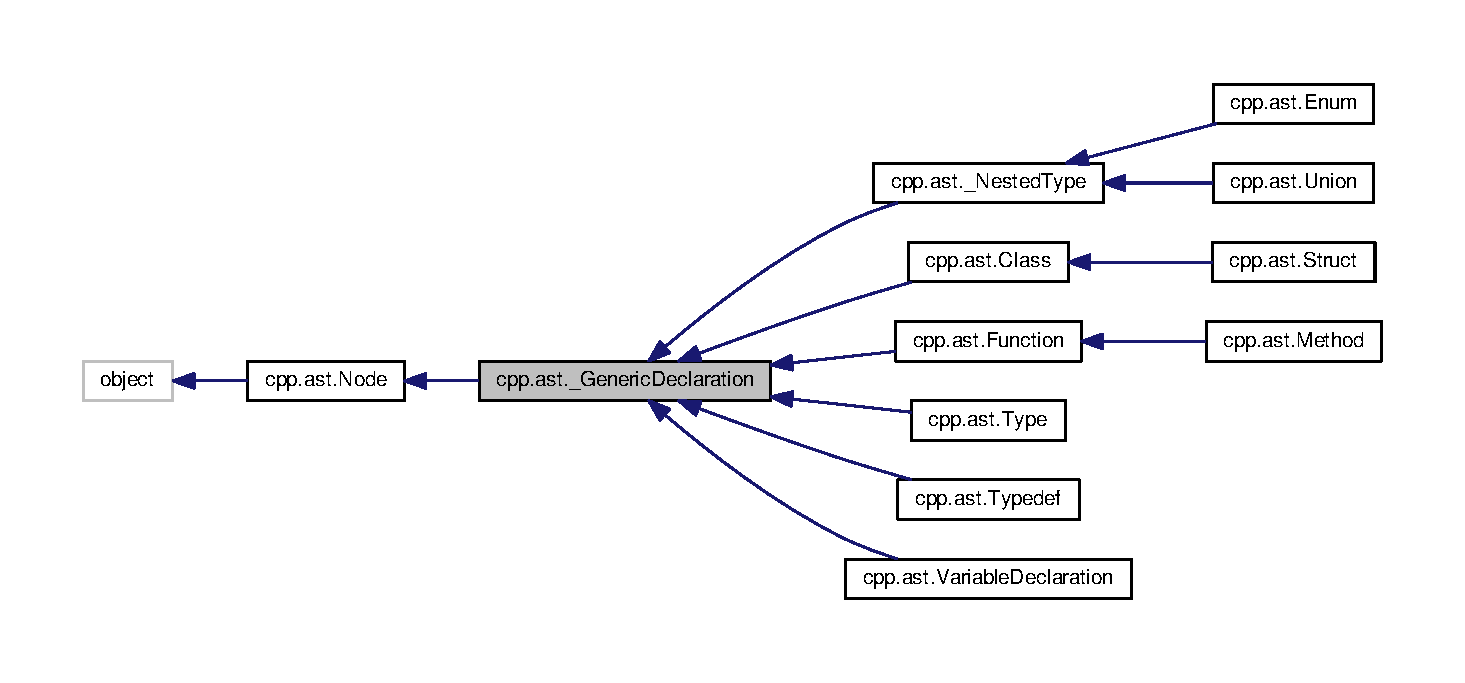
\includegraphics[width=350pt]{classcpp_1_1ast_1_1__GenericDeclaration__inherit__graph}
\end{center}
\end{figure}


Collaboration diagram for cpp.\+ast.\+\_\+\+Generic\+Declaration\+:
\nopagebreak
\begin{figure}[H]
\begin{center}
\leavevmode
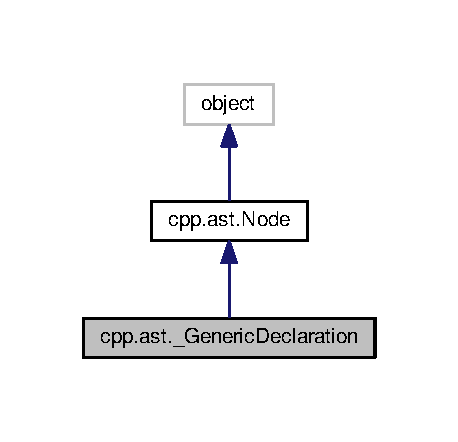
\includegraphics[width=220pt]{classcpp_1_1ast_1_1__GenericDeclaration__coll__graph}
\end{center}
\end{figure}
\subsection*{Public Member Functions}
\begin{DoxyCompactItemize}
\item 
def \hyperlink{classcpp_1_1ast_1_1__GenericDeclaration_afde72751e20708a7802eb7707d23bc3c}{\+\_\+\+\_\+init\+\_\+\+\_\+} (self, \hyperlink{classcpp_1_1ast_1_1Node_a7b2aa97e6a049bb1a93aea48c48f1f44}{start}, \hyperlink{classcpp_1_1ast_1_1Node_a3c5e5246ccf619df28eca02e29d69647}{end}, \hyperlink{classcpp_1_1ast_1_1__GenericDeclaration_af774f4729dfd78d0538a6782fe8514c1}{name}, \hyperlink{classcpp_1_1ast_1_1__GenericDeclaration_a8aee3f11b37449d54b42a78e0a689f46}{namespace})
\item 
def \hyperlink{classcpp_1_1ast_1_1__GenericDeclaration_a1437d31271ea8cda62da22e2ce427a85}{Full\+Name} (self)
\end{DoxyCompactItemize}
\subsection*{Public Attributes}
\begin{DoxyCompactItemize}
\item 
\hyperlink{classcpp_1_1ast_1_1__GenericDeclaration_af774f4729dfd78d0538a6782fe8514c1}{name}
\item 
\hyperlink{classcpp_1_1ast_1_1__GenericDeclaration_a8aee3f11b37449d54b42a78e0a689f46}{namespace}
\end{DoxyCompactItemize}


\subsection{Constructor \& Destructor Documentation}
\index{cpp\+::ast\+::\+\_\+\+Generic\+Declaration@{cpp\+::ast\+::\+\_\+\+Generic\+Declaration}!\+\_\+\+\_\+init\+\_\+\+\_\+@{\+\_\+\+\_\+init\+\_\+\+\_\+}}
\index{\+\_\+\+\_\+init\+\_\+\+\_\+@{\+\_\+\+\_\+init\+\_\+\+\_\+}!cpp\+::ast\+::\+\_\+\+Generic\+Declaration@{cpp\+::ast\+::\+\_\+\+Generic\+Declaration}}
\subsubsection[{\texorpdfstring{\+\_\+\+\_\+init\+\_\+\+\_\+(self, start, end, name, namespace)}{__init__(self, start, end, name, namespace)}}]{\setlength{\rightskip}{0pt plus 5cm}def cpp.\+ast.\+\_\+\+Generic\+Declaration.\+\_\+\+\_\+init\+\_\+\+\_\+ (
\begin{DoxyParamCaption}
\item[{}]{self, }
\item[{}]{start, }
\item[{}]{end, }
\item[{}]{name, }
\item[{}]{namespace}
\end{DoxyParamCaption}
)}\hypertarget{classcpp_1_1ast_1_1__GenericDeclaration_afde72751e20708a7802eb7707d23bc3c}{}\label{classcpp_1_1ast_1_1__GenericDeclaration_afde72751e20708a7802eb7707d23bc3c}

\begin{DoxyCode}
233     \textcolor{keyword}{def }\_\_init\_\_(self, start, end, name, namespace):
234         Node.\_\_init\_\_(self, start, end)
235         self.name = name
236         self.namespace = namespace[:]
237 
\end{DoxyCode}


\subsection{Member Function Documentation}
\index{cpp\+::ast\+::\+\_\+\+Generic\+Declaration@{cpp\+::ast\+::\+\_\+\+Generic\+Declaration}!Full\+Name@{Full\+Name}}
\index{Full\+Name@{Full\+Name}!cpp\+::ast\+::\+\_\+\+Generic\+Declaration@{cpp\+::ast\+::\+\_\+\+Generic\+Declaration}}
\subsubsection[{\texorpdfstring{Full\+Name(self)}{FullName(self)}}]{\setlength{\rightskip}{0pt plus 5cm}def cpp.\+ast.\+\_\+\+Generic\+Declaration.\+Full\+Name (
\begin{DoxyParamCaption}
\item[{}]{self}
\end{DoxyParamCaption}
)}\hypertarget{classcpp_1_1ast_1_1__GenericDeclaration_a1437d31271ea8cda62da22e2ce427a85}{}\label{classcpp_1_1ast_1_1__GenericDeclaration_a1437d31271ea8cda62da22e2ce427a85}

\begin{DoxyCode}
238     \textcolor{keyword}{def }FullName(self):
239         prefix = \textcolor{stringliteral}{''}
240         \textcolor{keywordflow}{if} self.namespace \textcolor{keywordflow}{and} self.namespace[-1]:
241             prefix = \textcolor{stringliteral}{'::'}.join(self.namespace) + \textcolor{stringliteral}{'::'}
242         \textcolor{keywordflow}{return} prefix + self.name
243 
\end{DoxyCode}


\subsection{Member Data Documentation}
\index{cpp\+::ast\+::\+\_\+\+Generic\+Declaration@{cpp\+::ast\+::\+\_\+\+Generic\+Declaration}!name@{name}}
\index{name@{name}!cpp\+::ast\+::\+\_\+\+Generic\+Declaration@{cpp\+::ast\+::\+\_\+\+Generic\+Declaration}}
\subsubsection[{\texorpdfstring{name}{name}}]{\setlength{\rightskip}{0pt plus 5cm}cpp.\+ast.\+\_\+\+Generic\+Declaration.\+name}\hypertarget{classcpp_1_1ast_1_1__GenericDeclaration_af774f4729dfd78d0538a6782fe8514c1}{}\label{classcpp_1_1ast_1_1__GenericDeclaration_af774f4729dfd78d0538a6782fe8514c1}
\index{cpp\+::ast\+::\+\_\+\+Generic\+Declaration@{cpp\+::ast\+::\+\_\+\+Generic\+Declaration}!namespace@{namespace}}
\index{namespace@{namespace}!cpp\+::ast\+::\+\_\+\+Generic\+Declaration@{cpp\+::ast\+::\+\_\+\+Generic\+Declaration}}
\subsubsection[{\texorpdfstring{namespace}{namespace}}]{\setlength{\rightskip}{0pt plus 5cm}cpp.\+ast.\+\_\+\+Generic\+Declaration.\+namespace}\hypertarget{classcpp_1_1ast_1_1__GenericDeclaration_a8aee3f11b37449d54b42a78e0a689f46}{}\label{classcpp_1_1ast_1_1__GenericDeclaration_a8aee3f11b37449d54b42a78e0a689f46}


The documentation for this class was generated from the following file\+:\begin{DoxyCompactItemize}
\item 
vendor/googletest/googlemock/scripts/generator/cpp/\hyperlink{ast_8py}{ast.\+py}\end{DoxyCompactItemize}

\hypertarget{classcpp_1_1ast_1_1__NestedType}{}\section{cpp.\+ast.\+\_\+\+Nested\+Type Class Reference}
\label{classcpp_1_1ast_1_1__NestedType}\index{cpp.\+ast.\+\_\+\+Nested\+Type@{cpp.\+ast.\+\_\+\+Nested\+Type}}


Inheritance diagram for cpp.\+ast.\+\_\+\+Nested\+Type\+:
\nopagebreak
\begin{figure}[H]
\begin{center}
\leavevmode
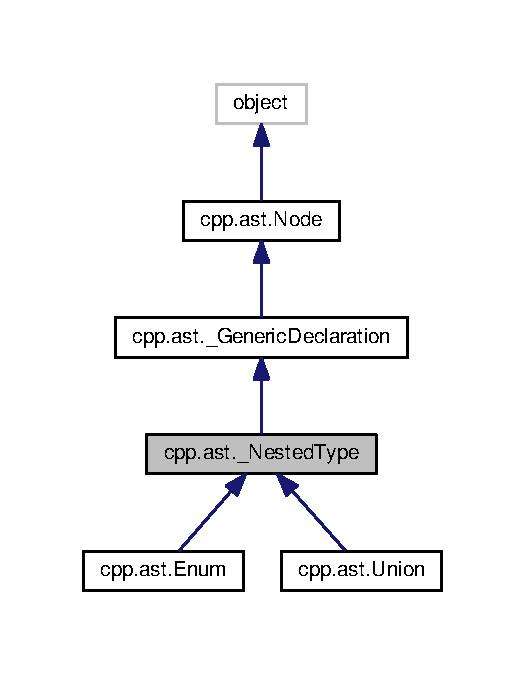
\includegraphics[width=252pt]{classcpp_1_1ast_1_1__NestedType__inherit__graph}
\end{center}
\end{figure}


Collaboration diagram for cpp.\+ast.\+\_\+\+Nested\+Type\+:
\nopagebreak
\begin{figure}[H]
\begin{center}
\leavevmode
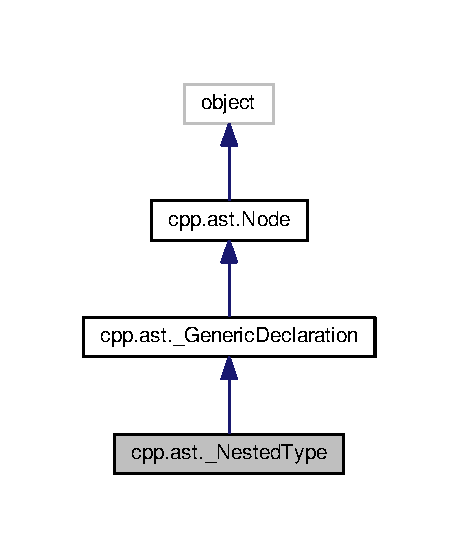
\includegraphics[width=220pt]{classcpp_1_1ast_1_1__NestedType__coll__graph}
\end{center}
\end{figure}
\subsection*{Public Member Functions}
\begin{DoxyCompactItemize}
\item 
def \hyperlink{classcpp_1_1ast_1_1__NestedType_a63acff60f38885be6cc11231fffc3f4e}{\+\_\+\+\_\+init\+\_\+\+\_\+} (self, \hyperlink{classcpp_1_1ast_1_1Node_a7b2aa97e6a049bb1a93aea48c48f1f44}{start}, \hyperlink{classcpp_1_1ast_1_1Node_a3c5e5246ccf619df28eca02e29d69647}{end}, \hyperlink{classcpp_1_1ast_1_1__GenericDeclaration_af774f4729dfd78d0538a6782fe8514c1}{name}, \hyperlink{classcpp_1_1ast_1_1__NestedType_aed69c37a409b4d26e6cfde2de3185d86}{fields}, \hyperlink{classcpp_1_1ast_1_1__GenericDeclaration_a8aee3f11b37449d54b42a78e0a689f46}{namespace})
\item 
def \hyperlink{classcpp_1_1ast_1_1__NestedType_a9f160999863f39c9032f60b014e213d5}{Is\+Definition} (self)
\item 
def \hyperlink{classcpp_1_1ast_1_1__NestedType_a689f8b0dc20e6070938825eee483dd2f}{Is\+Exportable} (self)
\item 
def \hyperlink{classcpp_1_1ast_1_1__NestedType_a18901ec6acba88c526d703444bf4d52c}{\+\_\+\+\_\+str\+\_\+\+\_\+} (self)
\end{DoxyCompactItemize}
\subsection*{Public Attributes}
\begin{DoxyCompactItemize}
\item 
\hyperlink{classcpp_1_1ast_1_1__NestedType_aed69c37a409b4d26e6cfde2de3185d86}{fields}
\end{DoxyCompactItemize}


\subsection{Constructor \& Destructor Documentation}
\index{cpp\+::ast\+::\+\_\+\+Nested\+Type@{cpp\+::ast\+::\+\_\+\+Nested\+Type}!\+\_\+\+\_\+init\+\_\+\+\_\+@{\+\_\+\+\_\+init\+\_\+\+\_\+}}
\index{\+\_\+\+\_\+init\+\_\+\+\_\+@{\+\_\+\+\_\+init\+\_\+\+\_\+}!cpp\+::ast\+::\+\_\+\+Nested\+Type@{cpp\+::ast\+::\+\_\+\+Nested\+Type}}
\subsubsection[{\texorpdfstring{\+\_\+\+\_\+init\+\_\+\+\_\+(self, start, end, name, fields, namespace)}{__init__(self, start, end, name, fields, namespace)}}]{\setlength{\rightskip}{0pt plus 5cm}def cpp.\+ast.\+\_\+\+Nested\+Type.\+\_\+\+\_\+init\+\_\+\+\_\+ (
\begin{DoxyParamCaption}
\item[{}]{self, }
\item[{}]{start, }
\item[{}]{end, }
\item[{}]{name, }
\item[{}]{fields, }
\item[{}]{namespace}
\end{DoxyParamCaption}
)}\hypertarget{classcpp_1_1ast_1_1__NestedType_a63acff60f38885be6cc11231fffc3f4e}{}\label{classcpp_1_1ast_1_1__NestedType_a63acff60f38885be6cc11231fffc3f4e}

\begin{DoxyCode}
298     \textcolor{keyword}{def }\_\_init\_\_(self, start, end, name, fields, namespace):
299         \_GenericDeclaration.\_\_init\_\_(self, start, end, name, namespace)
300         self.fields = fields
301 
\end{DoxyCode}


\subsection{Member Function Documentation}
\index{cpp\+::ast\+::\+\_\+\+Nested\+Type@{cpp\+::ast\+::\+\_\+\+Nested\+Type}!\+\_\+\+\_\+str\+\_\+\+\_\+@{\+\_\+\+\_\+str\+\_\+\+\_\+}}
\index{\+\_\+\+\_\+str\+\_\+\+\_\+@{\+\_\+\+\_\+str\+\_\+\+\_\+}!cpp\+::ast\+::\+\_\+\+Nested\+Type@{cpp\+::ast\+::\+\_\+\+Nested\+Type}}
\subsubsection[{\texorpdfstring{\+\_\+\+\_\+str\+\_\+\+\_\+(self)}{__str__(self)}}]{\setlength{\rightskip}{0pt plus 5cm}def cpp.\+ast.\+\_\+\+Nested\+Type.\+\_\+\+\_\+str\+\_\+\+\_\+ (
\begin{DoxyParamCaption}
\item[{}]{self}
\end{DoxyParamCaption}
)}\hypertarget{classcpp_1_1ast_1_1__NestedType_a18901ec6acba88c526d703444bf4d52c}{}\label{classcpp_1_1ast_1_1__NestedType_a18901ec6acba88c526d703444bf4d52c}

\begin{DoxyCode}
308     \textcolor{keyword}{def }\_\_str\_\_(self):
309         suffix = \textcolor{stringliteral}{'%s, \{%s\}'} % (self.name, self.fields)
310         \textcolor{keywordflow}{return} self.\_TypeStringHelper(suffix)
311 
312 
\end{DoxyCode}
\index{cpp\+::ast\+::\+\_\+\+Nested\+Type@{cpp\+::ast\+::\+\_\+\+Nested\+Type}!Is\+Definition@{Is\+Definition}}
\index{Is\+Definition@{Is\+Definition}!cpp\+::ast\+::\+\_\+\+Nested\+Type@{cpp\+::ast\+::\+\_\+\+Nested\+Type}}
\subsubsection[{\texorpdfstring{Is\+Definition(self)}{IsDefinition(self)}}]{\setlength{\rightskip}{0pt plus 5cm}def cpp.\+ast.\+\_\+\+Nested\+Type.\+Is\+Definition (
\begin{DoxyParamCaption}
\item[{}]{self}
\end{DoxyParamCaption}
)}\hypertarget{classcpp_1_1ast_1_1__NestedType_a9f160999863f39c9032f60b014e213d5}{}\label{classcpp_1_1ast_1_1__NestedType_a9f160999863f39c9032f60b014e213d5}

\begin{DoxyCode}
302     \textcolor{keyword}{def }IsDefinition(self):
303         \textcolor{keywordflow}{return} \textcolor{keyword}{True}
304 
\end{DoxyCode}
\index{cpp\+::ast\+::\+\_\+\+Nested\+Type@{cpp\+::ast\+::\+\_\+\+Nested\+Type}!Is\+Exportable@{Is\+Exportable}}
\index{Is\+Exportable@{Is\+Exportable}!cpp\+::ast\+::\+\_\+\+Nested\+Type@{cpp\+::ast\+::\+\_\+\+Nested\+Type}}
\subsubsection[{\texorpdfstring{Is\+Exportable(self)}{IsExportable(self)}}]{\setlength{\rightskip}{0pt plus 5cm}def cpp.\+ast.\+\_\+\+Nested\+Type.\+Is\+Exportable (
\begin{DoxyParamCaption}
\item[{}]{self}
\end{DoxyParamCaption}
)}\hypertarget{classcpp_1_1ast_1_1__NestedType_a689f8b0dc20e6070938825eee483dd2f}{}\label{classcpp_1_1ast_1_1__NestedType_a689f8b0dc20e6070938825eee483dd2f}

\begin{DoxyCode}
305     \textcolor{keyword}{def }IsExportable(self):
306         \textcolor{keywordflow}{return} \textcolor{keyword}{True}
307 
\end{DoxyCode}


\subsection{Member Data Documentation}
\index{cpp\+::ast\+::\+\_\+\+Nested\+Type@{cpp\+::ast\+::\+\_\+\+Nested\+Type}!fields@{fields}}
\index{fields@{fields}!cpp\+::ast\+::\+\_\+\+Nested\+Type@{cpp\+::ast\+::\+\_\+\+Nested\+Type}}
\subsubsection[{\texorpdfstring{fields}{fields}}]{\setlength{\rightskip}{0pt plus 5cm}cpp.\+ast.\+\_\+\+Nested\+Type.\+fields}\hypertarget{classcpp_1_1ast_1_1__NestedType_aed69c37a409b4d26e6cfde2de3185d86}{}\label{classcpp_1_1ast_1_1__NestedType_aed69c37a409b4d26e6cfde2de3185d86}


The documentation for this class was generated from the following file\+:\begin{DoxyCompactItemize}
\item 
vendor/googletest/googlemock/scripts/generator/cpp/\hyperlink{ast_8py}{ast.\+py}\end{DoxyCompactItemize}

\hypertarget{classcpp_1_1ast_1_1__NullDict}{}\section{cpp.\+ast.\+\_\+\+Null\+Dict Class Reference}
\label{classcpp_1_1ast_1_1__NullDict}\index{cpp.\+ast.\+\_\+\+Null\+Dict@{cpp.\+ast.\+\_\+\+Null\+Dict}}


Inheritance diagram for cpp.\+ast.\+\_\+\+Null\+Dict\+:
\nopagebreak
\begin{figure}[H]
\begin{center}
\leavevmode
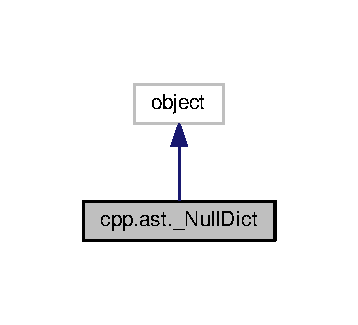
\includegraphics[width=172pt]{classcpp_1_1ast_1_1__NullDict__inherit__graph}
\end{center}
\end{figure}


Collaboration diagram for cpp.\+ast.\+\_\+\+Null\+Dict\+:
\nopagebreak
\begin{figure}[H]
\begin{center}
\leavevmode
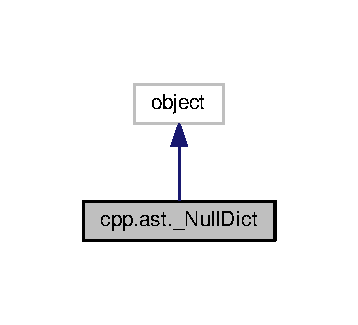
\includegraphics[width=172pt]{classcpp_1_1ast_1_1__NullDict__coll__graph}
\end{center}
\end{figure}
\subsection*{Static Public Attributes}
\begin{DoxyCompactItemize}
\item 
\hyperlink{classcpp_1_1ast_1_1__NullDict_abb0b7884aa59bede0a8503dffcd1733f}{keys} = lambdaself\+:()
\end{DoxyCompactItemize}


\subsection{Member Data Documentation}
\index{cpp\+::ast\+::\+\_\+\+Null\+Dict@{cpp\+::ast\+::\+\_\+\+Null\+Dict}!keys@{keys}}
\index{keys@{keys}!cpp\+::ast\+::\+\_\+\+Null\+Dict@{cpp\+::ast\+::\+\_\+\+Null\+Dict}}
\subsubsection[{\texorpdfstring{keys}{keys}}]{\setlength{\rightskip}{0pt plus 5cm}cpp.\+ast.\+\_\+\+Null\+Dict.\+keys = lambdaself\+:()\hspace{0.3cm}{\ttfamily [static]}}\hypertarget{classcpp_1_1ast_1_1__NullDict_abb0b7884aa59bede0a8503dffcd1733f}{}\label{classcpp_1_1ast_1_1__NullDict_abb0b7884aa59bede0a8503dffcd1733f}


The documentation for this class was generated from the following file\+:\begin{DoxyCompactItemize}
\item 
vendor/googletest/googlemock/scripts/generator/cpp/\hyperlink{ast_8py}{ast.\+py}\end{DoxyCompactItemize}

\hypertarget{classupload_1_1AbstractRpcServer}{}\section{upload.\+Abstract\+Rpc\+Server Class Reference}
\label{classupload_1_1AbstractRpcServer}\index{upload.\+Abstract\+Rpc\+Server@{upload.\+Abstract\+Rpc\+Server}}


Inheritance diagram for upload.\+Abstract\+Rpc\+Server\+:
\nopagebreak
\begin{figure}[H]
\begin{center}
\leavevmode
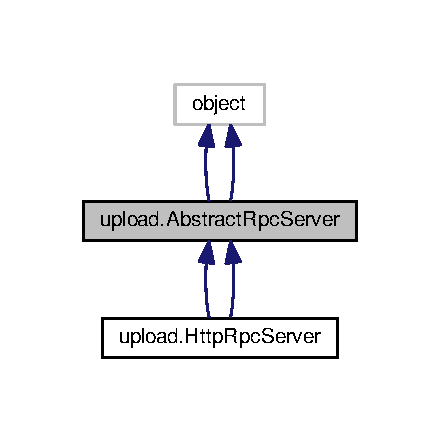
\includegraphics[width=211pt]{classupload_1_1AbstractRpcServer__inherit__graph}
\end{center}
\end{figure}


Collaboration diagram for upload.\+Abstract\+Rpc\+Server\+:
\nopagebreak
\begin{figure}[H]
\begin{center}
\leavevmode
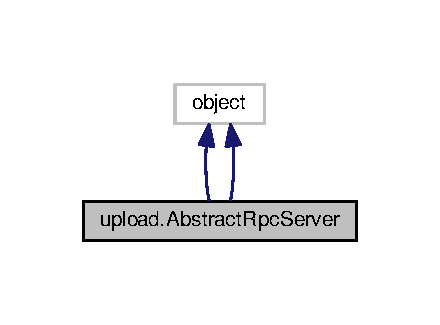
\includegraphics[width=211pt]{classupload_1_1AbstractRpcServer__coll__graph}
\end{center}
\end{figure}
\subsection*{Public Member Functions}
\begin{DoxyCompactItemize}
\item 
def \hyperlink{classupload_1_1AbstractRpcServer_a3f6bc1bd16b52bd5a5c33a1fedeef2d0}{\+\_\+\+\_\+init\+\_\+\+\_\+} (self, \hyperlink{classupload_1_1AbstractRpcServer_ab7188d827e2faddcf970f524f5856192}{host}, \hyperlink{classupload_1_1AbstractRpcServer_aee0090a3bcf07b913a7dd596a5dabb8f}{auth\+\_\+function}, \hyperlink{classupload_1_1AbstractRpcServer_a783a4a7e4ffb776a57a3f267300a213b}{host\+\_\+override}=None, \hyperlink{classupload_1_1AbstractRpcServer_adbbf0109afc13d58d7815fa143cb779f}{extra\+\_\+headers}=\{\}, \hyperlink{classupload_1_1AbstractRpcServer_affe342205c4647d41b127f5a5634858b}{save\+\_\+cookies}=False)
\item 
def \hyperlink{classupload_1_1AbstractRpcServer_ac1b913f8bd00da4741c47ab49ea94cb5}{Send} (self, request\+\_\+path, payload=None, content\+\_\+type=\char`\"{}application/octet-\/stream\char`\"{}, timeout=None, kwargs)
\item 
def \hyperlink{classupload_1_1AbstractRpcServer_a3f6bc1bd16b52bd5a5c33a1fedeef2d0}{\+\_\+\+\_\+init\+\_\+\+\_\+} (self, \hyperlink{classupload_1_1AbstractRpcServer_ab7188d827e2faddcf970f524f5856192}{host}, \hyperlink{classupload_1_1AbstractRpcServer_aee0090a3bcf07b913a7dd596a5dabb8f}{auth\+\_\+function}, \hyperlink{classupload_1_1AbstractRpcServer_a783a4a7e4ffb776a57a3f267300a213b}{host\+\_\+override}=None, \hyperlink{classupload_1_1AbstractRpcServer_adbbf0109afc13d58d7815fa143cb779f}{extra\+\_\+headers}=\{\}, \hyperlink{classupload_1_1AbstractRpcServer_affe342205c4647d41b127f5a5634858b}{save\+\_\+cookies}=False)
\item 
def \hyperlink{classupload_1_1AbstractRpcServer_ac1b913f8bd00da4741c47ab49ea94cb5}{Send} (self, request\+\_\+path, payload=None, content\+\_\+type=\char`\"{}application/octet-\/stream\char`\"{}, timeout=None, kwargs)
\end{DoxyCompactItemize}
\subsection*{Public Attributes}
\begin{DoxyCompactItemize}
\item 
\hyperlink{classupload_1_1AbstractRpcServer_ab7188d827e2faddcf970f524f5856192}{host}
\item 
\hyperlink{classupload_1_1AbstractRpcServer_a783a4a7e4ffb776a57a3f267300a213b}{host\+\_\+override}
\item 
\hyperlink{classupload_1_1AbstractRpcServer_aee0090a3bcf07b913a7dd596a5dabb8f}{auth\+\_\+function}
\item 
\hyperlink{classupload_1_1AbstractRpcServer_a692955750c802e461c6336d3000cd365}{authenticated}
\item 
\hyperlink{classupload_1_1AbstractRpcServer_adbbf0109afc13d58d7815fa143cb779f}{extra\+\_\+headers}
\item 
\hyperlink{classupload_1_1AbstractRpcServer_affe342205c4647d41b127f5a5634858b}{save\+\_\+cookies}
\item 
\hyperlink{classupload_1_1AbstractRpcServer_aa931446476e0e86f3ade7fef0a0aea5a}{opener}
\end{DoxyCompactItemize}


\subsection{Detailed Description}
\begin{DoxyVerb}Provides a common interface for a simple RPC server.\end{DoxyVerb}
 

\subsection{Constructor \& Destructor Documentation}
\index{upload\+::\+Abstract\+Rpc\+Server@{upload\+::\+Abstract\+Rpc\+Server}!\+\_\+\+\_\+init\+\_\+\+\_\+@{\+\_\+\+\_\+init\+\_\+\+\_\+}}
\index{\+\_\+\+\_\+init\+\_\+\+\_\+@{\+\_\+\+\_\+init\+\_\+\+\_\+}!upload\+::\+Abstract\+Rpc\+Server@{upload\+::\+Abstract\+Rpc\+Server}}
\subsubsection[{\texorpdfstring{\+\_\+\+\_\+init\+\_\+\+\_\+(self, host, auth\+\_\+function, host\+\_\+override=\+None, extra\+\_\+headers=\lcurly{}\rcurly{}, save\+\_\+cookies=\+False)}{__init__(self, host, auth_function, host_override=None, extra_headers=\{\}, save_cookies=False)}}]{\setlength{\rightskip}{0pt plus 5cm}def upload.\+Abstract\+Rpc\+Server.\+\_\+\+\_\+init\+\_\+\+\_\+ (
\begin{DoxyParamCaption}
\item[{}]{self, }
\item[{}]{host, }
\item[{}]{auth\+\_\+function, }
\item[{}]{host\+\_\+override = {\ttfamily None}, }
\item[{}]{extra\+\_\+headers = {\ttfamily \{\}}, }
\item[{}]{save\+\_\+cookies = {\ttfamily False}}
\end{DoxyParamCaption}
)}\hypertarget{classupload_1_1AbstractRpcServer_a3f6bc1bd16b52bd5a5c33a1fedeef2d0}{}\label{classupload_1_1AbstractRpcServer_a3f6bc1bd16b52bd5a5c33a1fedeef2d0}
\begin{DoxyVerb}Creates a new HttpRpcServer.

Args:
  host: The host to send requests to.
  auth_function: A function that takes no arguments and returns an
(email, password) tuple when called. Will be called if authentication
is required.
  host_override: The host header to send to the server (defaults to host).
  extra_headers: A dict of extra headers to append to every request.
  save_cookies: If True, save the authentication cookies to local disk.
If False, use an in-memory cookiejar instead.  Subclasses must
implement this functionality.  Defaults to False.
\end{DoxyVerb}
 
\begin{DoxyCode}
128                save\_cookies=\textcolor{keyword}{False}):
129     \textcolor{stringliteral}{"""Creates a new HttpRpcServer.}
130 \textcolor{stringliteral}{}
131 \textcolor{stringliteral}{    Args:}
132 \textcolor{stringliteral}{      host: The host to send requests to.}
133 \textcolor{stringliteral}{      auth\_function: A function that takes no arguments and returns an}
134 \textcolor{stringliteral}{        (email, password) tuple when called. Will be called if authentication}
135 \textcolor{stringliteral}{        is required.}
136 \textcolor{stringliteral}{      host\_override: The host header to send to the server (defaults to host).}
137 \textcolor{stringliteral}{      extra\_headers: A dict of extra headers to append to every request.}
138 \textcolor{stringliteral}{      save\_cookies: If True, save the authentication cookies to local disk.}
139 \textcolor{stringliteral}{        If False, use an in-memory cookiejar instead.  Subclasses must}
140 \textcolor{stringliteral}{        implement this functionality.  Defaults to False.}
141 \textcolor{stringliteral}{    """}
142     self.host = host
143     self.host\_override = host\_override
144     self.auth\_function = auth\_function
145     self.authenticated = \textcolor{keyword}{False}
146     self.extra\_headers = extra\_headers
147     self.save\_cookies = save\_cookies
148     self.opener = self.\_GetOpener()
149     \textcolor{keywordflow}{if} self.host\_override:
150       logging.info(\textcolor{stringliteral}{"Server: %s; Host: %s"}, self.host, self.host\_override)
151     \textcolor{keywordflow}{else}:
152       logging.info(\textcolor{stringliteral}{"Server: %s"}, self.host)
153 
\end{DoxyCode}
\index{upload\+::\+Abstract\+Rpc\+Server@{upload\+::\+Abstract\+Rpc\+Server}!\+\_\+\+\_\+init\+\_\+\+\_\+@{\+\_\+\+\_\+init\+\_\+\+\_\+}}
\index{\+\_\+\+\_\+init\+\_\+\+\_\+@{\+\_\+\+\_\+init\+\_\+\+\_\+}!upload\+::\+Abstract\+Rpc\+Server@{upload\+::\+Abstract\+Rpc\+Server}}
\subsubsection[{\texorpdfstring{\+\_\+\+\_\+init\+\_\+\+\_\+(self, host, auth\+\_\+function, host\+\_\+override=\+None, extra\+\_\+headers=\lcurly{}\rcurly{}, save\+\_\+cookies=\+False)}{__init__(self, host, auth_function, host_override=None, extra_headers=\{\}, save_cookies=False)}}]{\setlength{\rightskip}{0pt plus 5cm}def upload.\+Abstract\+Rpc\+Server.\+\_\+\+\_\+init\+\_\+\+\_\+ (
\begin{DoxyParamCaption}
\item[{}]{self, }
\item[{}]{host, }
\item[{}]{auth\+\_\+function, }
\item[{}]{host\+\_\+override = {\ttfamily None}, }
\item[{}]{extra\+\_\+headers = {\ttfamily \{\}}, }
\item[{}]{save\+\_\+cookies = {\ttfamily False}}
\end{DoxyParamCaption}
)}\hypertarget{classupload_1_1AbstractRpcServer_a3f6bc1bd16b52bd5a5c33a1fedeef2d0}{}\label{classupload_1_1AbstractRpcServer_a3f6bc1bd16b52bd5a5c33a1fedeef2d0}
\begin{DoxyVerb}Creates a new HttpRpcServer.

Args:
  host: The host to send requests to.
  auth_function: A function that takes no arguments and returns an
(email, password) tuple when called. Will be called if authentication
is required.
  host_override: The host header to send to the server (defaults to host).
  extra_headers: A dict of extra headers to append to every request.
  save_cookies: If True, save the authentication cookies to local disk.
If False, use an in-memory cookiejar instead.  Subclasses must
implement this functionality.  Defaults to False.
\end{DoxyVerb}
 
\begin{DoxyCode}
128                save\_cookies=\textcolor{keyword}{False}):
129     \textcolor{stringliteral}{"""Creates a new HttpRpcServer.}
130 \textcolor{stringliteral}{}
131 \textcolor{stringliteral}{    Args:}
132 \textcolor{stringliteral}{      host: The host to send requests to.}
133 \textcolor{stringliteral}{      auth\_function: A function that takes no arguments and returns an}
134 \textcolor{stringliteral}{        (email, password) tuple when called. Will be called if authentication}
135 \textcolor{stringliteral}{        is required.}
136 \textcolor{stringliteral}{      host\_override: The host header to send to the server (defaults to host).}
137 \textcolor{stringliteral}{      extra\_headers: A dict of extra headers to append to every request.}
138 \textcolor{stringliteral}{      save\_cookies: If True, save the authentication cookies to local disk.}
139 \textcolor{stringliteral}{        If False, use an in-memory cookiejar instead.  Subclasses must}
140 \textcolor{stringliteral}{        implement this functionality.  Defaults to False.}
141 \textcolor{stringliteral}{    """}
142     self.host = host
143     self.host\_override = host\_override
144     self.auth\_function = auth\_function
145     self.authenticated = \textcolor{keyword}{False}
146     self.extra\_headers = extra\_headers
147     self.save\_cookies = save\_cookies
148     self.opener = self.\_GetOpener()
149     \textcolor{keywordflow}{if} self.host\_override:
150       logging.info(\textcolor{stringliteral}{"Server: %s; Host: %s"}, self.host, self.host\_override)
151     \textcolor{keywordflow}{else}:
152       logging.info(\textcolor{stringliteral}{"Server: %s"}, self.host)
153 
\end{DoxyCode}


\subsection{Member Function Documentation}
\index{upload\+::\+Abstract\+Rpc\+Server@{upload\+::\+Abstract\+Rpc\+Server}!Send@{Send}}
\index{Send@{Send}!upload\+::\+Abstract\+Rpc\+Server@{upload\+::\+Abstract\+Rpc\+Server}}
\subsubsection[{\texorpdfstring{Send(self, request\+\_\+path, payload=\+None, content\+\_\+type=""application/octet-\/stream"", timeout=\+None, kwargs)}{Send(self, request_path, payload=None, content_type="application/octet-stream", timeout=None, kwargs)}}]{\setlength{\rightskip}{0pt plus 5cm}def upload.\+Abstract\+Rpc\+Server.\+Send (
\begin{DoxyParamCaption}
\item[{}]{self, }
\item[{}]{request\+\_\+path, }
\item[{}]{payload = {\ttfamily None}, }
\item[{}]{content\+\_\+type = {\ttfamily \char`\"{}application/octet-\/stream\char`\"{}}, }
\item[{}]{timeout = {\ttfamily None}, }
\item[{}]{kwargs}
\end{DoxyParamCaption}
)}\hypertarget{classupload_1_1AbstractRpcServer_ac1b913f8bd00da4741c47ab49ea94cb5}{}\label{classupload_1_1AbstractRpcServer_ac1b913f8bd00da4741c47ab49ea94cb5}
\begin{DoxyVerb}Sends an RPC and returns the response.

Args:
  request_path: The path to send the request to, eg /api/appversion/create.
  payload: The body of the request, or None to send an empty request.
  content_type: The Content-Type header to use.
  timeout: timeout in seconds; default None i.e. no timeout.
(Note: for large requests on OS X, the timeout doesn't work right.)
  kwargs: Any keyword arguments are converted into query string parameters.

Returns:
  The response body, as a string.
\end{DoxyVerb}
 
\begin{DoxyCode}
294            **kwargs):
295     \textcolor{stringliteral}{"""Sends an RPC and returns the response.}
296 \textcolor{stringliteral}{}
297 \textcolor{stringliteral}{    Args:}
298 \textcolor{stringliteral}{      request\_path: The path to send the request to, eg /api/appversion/create.}
299 \textcolor{stringliteral}{      payload: The body of the request, or None to send an empty request.}
300 \textcolor{stringliteral}{      content\_type: The Content-Type header to use.}
301 \textcolor{stringliteral}{      timeout: timeout in seconds; default None i.e. no timeout.}
302 \textcolor{stringliteral}{        (Note: for large requests on OS X, the timeout doesn't work right.)}
303 \textcolor{stringliteral}{      kwargs: Any keyword arguments are converted into query string parameters.}
304 \textcolor{stringliteral}{}
305 \textcolor{stringliteral}{    Returns:}
306 \textcolor{stringliteral}{      The response body, as a string.}
307 \textcolor{stringliteral}{    """}
308     \textcolor{comment}{# TODO: Don't require authentication.  Let the server say}
309     \textcolor{comment}{# whether it is necessary.}
310     \textcolor{keywordflow}{if} \textcolor{keywordflow}{not} self.authenticated:
311       self.\_Authenticate()
312 
313     old\_timeout = socket.getdefaulttimeout()
314     socket.setdefaulttimeout(timeout)
315     \textcolor{keywordflow}{try}:
316       tries = 0
317       \textcolor{keywordflow}{while} \textcolor{keyword}{True}:
318         tries += 1
319         args = dict(kwargs)
320         url = \textcolor{stringliteral}{"http://%s%s"} % (self.host, request\_path)
321         \textcolor{keywordflow}{if} args:
322           url += \textcolor{stringliteral}{"?"} + urllib.urlencode(args)
323         req = self.\_CreateRequest(url=url, data=payload)
324         req.add\_header(\textcolor{stringliteral}{"Content-Type"}, content\_type)
325         \textcolor{keywordflow}{try}:
326           f = self.opener.open(req)
327           response = f.read()
328           f.close()
329           \textcolor{keywordflow}{return} response
330         \textcolor{keywordflow}{except} urllib2.HTTPError, e:
331           \textcolor{keywordflow}{if} tries > 3:
332             \textcolor{keywordflow}{raise}
333           \textcolor{keywordflow}{elif} e.code == 401:
334             self.\_Authenticate()
\end{DoxyCode}
\index{upload\+::\+Abstract\+Rpc\+Server@{upload\+::\+Abstract\+Rpc\+Server}!Send@{Send}}
\index{Send@{Send}!upload\+::\+Abstract\+Rpc\+Server@{upload\+::\+Abstract\+Rpc\+Server}}
\subsubsection[{\texorpdfstring{Send(self, request\+\_\+path, payload=\+None, content\+\_\+type=""application/octet-\/stream"", timeout=\+None, kwargs)}{Send(self, request_path, payload=None, content_type="application/octet-stream", timeout=None, kwargs)}}]{\setlength{\rightskip}{0pt plus 5cm}def upload.\+Abstract\+Rpc\+Server.\+Send (
\begin{DoxyParamCaption}
\item[{}]{self, }
\item[{}]{request\+\_\+path, }
\item[{}]{payload = {\ttfamily None}, }
\item[{}]{content\+\_\+type = {\ttfamily \char`\"{}application/octet-\/stream\char`\"{}}, }
\item[{}]{timeout = {\ttfamily None}, }
\item[{}]{kwargs}
\end{DoxyParamCaption}
)}\hypertarget{classupload_1_1AbstractRpcServer_ac1b913f8bd00da4741c47ab49ea94cb5}{}\label{classupload_1_1AbstractRpcServer_ac1b913f8bd00da4741c47ab49ea94cb5}
\begin{DoxyVerb}Sends an RPC and returns the response.

Args:
  request_path: The path to send the request to, eg /api/appversion/create.
  payload: The body of the request, or None to send an empty request.
  content_type: The Content-Type header to use.
  timeout: timeout in seconds; default None i.e. no timeout.
(Note: for large requests on OS X, the timeout doesn't work right.)
  kwargs: Any keyword arguments are converted into query string parameters.

Returns:
  The response body, as a string.
\end{DoxyVerb}
 
\begin{DoxyCode}
294            **kwargs):
295     \textcolor{stringliteral}{"""Sends an RPC and returns the response.}
296 \textcolor{stringliteral}{}
297 \textcolor{stringliteral}{    Args:}
298 \textcolor{stringliteral}{      request\_path: The path to send the request to, eg /api/appversion/create.}
299 \textcolor{stringliteral}{      payload: The body of the request, or None to send an empty request.}
300 \textcolor{stringliteral}{      content\_type: The Content-Type header to use.}
301 \textcolor{stringliteral}{      timeout: timeout in seconds; default None i.e. no timeout.}
302 \textcolor{stringliteral}{        (Note: for large requests on OS X, the timeout doesn't work right.)}
303 \textcolor{stringliteral}{      kwargs: Any keyword arguments are converted into query string parameters.}
304 \textcolor{stringliteral}{}
305 \textcolor{stringliteral}{    Returns:}
306 \textcolor{stringliteral}{      The response body, as a string.}
307 \textcolor{stringliteral}{    """}
308     \textcolor{comment}{# TODO: Don't require authentication.  Let the server say}
309     \textcolor{comment}{# whether it is necessary.}
310     \textcolor{keywordflow}{if} \textcolor{keywordflow}{not} self.authenticated:
311       self.\_Authenticate()
312 
313     old\_timeout = socket.getdefaulttimeout()
314     socket.setdefaulttimeout(timeout)
315     \textcolor{keywordflow}{try}:
316       tries = 0
317       \textcolor{keywordflow}{while} \textcolor{keyword}{True}:
318         tries += 1
319         args = dict(kwargs)
320         url = \textcolor{stringliteral}{"http://%s%s"} % (self.host, request\_path)
321         \textcolor{keywordflow}{if} args:
322           url += \textcolor{stringliteral}{"?"} + urllib.urlencode(args)
323         req = self.\_CreateRequest(url=url, data=payload)
324         req.add\_header(\textcolor{stringliteral}{"Content-Type"}, content\_type)
325         \textcolor{keywordflow}{try}:
326           f = self.opener.open(req)
327           response = f.read()
328           f.close()
329           \textcolor{keywordflow}{return} response
330         \textcolor{keywordflow}{except} urllib2.HTTPError, e:
331           \textcolor{keywordflow}{if} tries > 3:
332             \textcolor{keywordflow}{raise}
333           \textcolor{keywordflow}{elif} e.code == 401:
334             self.\_Authenticate()
\end{DoxyCode}


\subsection{Member Data Documentation}
\index{upload\+::\+Abstract\+Rpc\+Server@{upload\+::\+Abstract\+Rpc\+Server}!auth\+\_\+function@{auth\+\_\+function}}
\index{auth\+\_\+function@{auth\+\_\+function}!upload\+::\+Abstract\+Rpc\+Server@{upload\+::\+Abstract\+Rpc\+Server}}
\subsubsection[{\texorpdfstring{auth\+\_\+function}{auth_function}}]{\setlength{\rightskip}{0pt plus 5cm}upload.\+Abstract\+Rpc\+Server.\+auth\+\_\+function}\hypertarget{classupload_1_1AbstractRpcServer_aee0090a3bcf07b913a7dd596a5dabb8f}{}\label{classupload_1_1AbstractRpcServer_aee0090a3bcf07b913a7dd596a5dabb8f}
\index{upload\+::\+Abstract\+Rpc\+Server@{upload\+::\+Abstract\+Rpc\+Server}!authenticated@{authenticated}}
\index{authenticated@{authenticated}!upload\+::\+Abstract\+Rpc\+Server@{upload\+::\+Abstract\+Rpc\+Server}}
\subsubsection[{\texorpdfstring{authenticated}{authenticated}}]{\setlength{\rightskip}{0pt plus 5cm}upload.\+Abstract\+Rpc\+Server.\+authenticated}\hypertarget{classupload_1_1AbstractRpcServer_a692955750c802e461c6336d3000cd365}{}\label{classupload_1_1AbstractRpcServer_a692955750c802e461c6336d3000cd365}
\index{upload\+::\+Abstract\+Rpc\+Server@{upload\+::\+Abstract\+Rpc\+Server}!extra\+\_\+headers@{extra\+\_\+headers}}
\index{extra\+\_\+headers@{extra\+\_\+headers}!upload\+::\+Abstract\+Rpc\+Server@{upload\+::\+Abstract\+Rpc\+Server}}
\subsubsection[{\texorpdfstring{extra\+\_\+headers}{extra_headers}}]{\setlength{\rightskip}{0pt plus 5cm}upload.\+Abstract\+Rpc\+Server.\+extra\+\_\+headers}\hypertarget{classupload_1_1AbstractRpcServer_adbbf0109afc13d58d7815fa143cb779f}{}\label{classupload_1_1AbstractRpcServer_adbbf0109afc13d58d7815fa143cb779f}
\index{upload\+::\+Abstract\+Rpc\+Server@{upload\+::\+Abstract\+Rpc\+Server}!host@{host}}
\index{host@{host}!upload\+::\+Abstract\+Rpc\+Server@{upload\+::\+Abstract\+Rpc\+Server}}
\subsubsection[{\texorpdfstring{host}{host}}]{\setlength{\rightskip}{0pt plus 5cm}upload.\+Abstract\+Rpc\+Server.\+host}\hypertarget{classupload_1_1AbstractRpcServer_ab7188d827e2faddcf970f524f5856192}{}\label{classupload_1_1AbstractRpcServer_ab7188d827e2faddcf970f524f5856192}
\index{upload\+::\+Abstract\+Rpc\+Server@{upload\+::\+Abstract\+Rpc\+Server}!host\+\_\+override@{host\+\_\+override}}
\index{host\+\_\+override@{host\+\_\+override}!upload\+::\+Abstract\+Rpc\+Server@{upload\+::\+Abstract\+Rpc\+Server}}
\subsubsection[{\texorpdfstring{host\+\_\+override}{host_override}}]{\setlength{\rightskip}{0pt plus 5cm}upload.\+Abstract\+Rpc\+Server.\+host\+\_\+override}\hypertarget{classupload_1_1AbstractRpcServer_a783a4a7e4ffb776a57a3f267300a213b}{}\label{classupload_1_1AbstractRpcServer_a783a4a7e4ffb776a57a3f267300a213b}
\index{upload\+::\+Abstract\+Rpc\+Server@{upload\+::\+Abstract\+Rpc\+Server}!opener@{opener}}
\index{opener@{opener}!upload\+::\+Abstract\+Rpc\+Server@{upload\+::\+Abstract\+Rpc\+Server}}
\subsubsection[{\texorpdfstring{opener}{opener}}]{\setlength{\rightskip}{0pt plus 5cm}upload.\+Abstract\+Rpc\+Server.\+opener}\hypertarget{classupload_1_1AbstractRpcServer_aa931446476e0e86f3ade7fef0a0aea5a}{}\label{classupload_1_1AbstractRpcServer_aa931446476e0e86f3ade7fef0a0aea5a}
\index{upload\+::\+Abstract\+Rpc\+Server@{upload\+::\+Abstract\+Rpc\+Server}!save\+\_\+cookies@{save\+\_\+cookies}}
\index{save\+\_\+cookies@{save\+\_\+cookies}!upload\+::\+Abstract\+Rpc\+Server@{upload\+::\+Abstract\+Rpc\+Server}}
\subsubsection[{\texorpdfstring{save\+\_\+cookies}{save_cookies}}]{\setlength{\rightskip}{0pt plus 5cm}upload.\+Abstract\+Rpc\+Server.\+save\+\_\+cookies}\hypertarget{classupload_1_1AbstractRpcServer_affe342205c4647d41b127f5a5634858b}{}\label{classupload_1_1AbstractRpcServer_affe342205c4647d41b127f5a5634858b}


The documentation for this class was generated from the following file\+:\begin{DoxyCompactItemize}
\item 
vendor/googletest/googlemock/scripts/\hyperlink{googlemock_2scripts_2upload_8py}{upload.\+py}\end{DoxyCompactItemize}

\hypertarget{classtesting_1_1gmock__matchers__test_1_1AClass}{}\section{testing\+:\+:gmock\+\_\+matchers\+\_\+test\+:\+:A\+Class Class Reference}
\label{classtesting_1_1gmock__matchers__test_1_1AClass}\index{testing\+::gmock\+\_\+matchers\+\_\+test\+::\+A\+Class@{testing\+::gmock\+\_\+matchers\+\_\+test\+::\+A\+Class}}


Inheritance diagram for testing\+:\+:gmock\+\_\+matchers\+\_\+test\+:\+:A\+Class\+:
\nopagebreak
\begin{figure}[H]
\begin{center}
\leavevmode
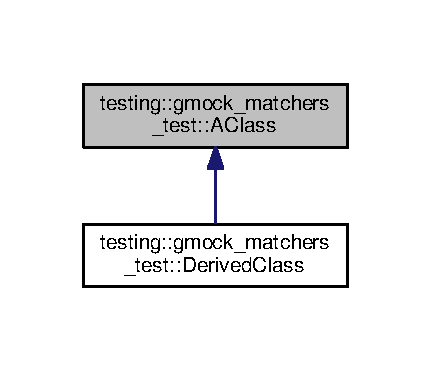
\includegraphics[width=207pt]{classtesting_1_1gmock__matchers__test_1_1AClass__inherit__graph}
\end{center}
\end{figure}
\subsection*{Public Member Functions}
\begin{DoxyCompactItemize}
\item 
\hyperlink{classtesting_1_1gmock__matchers__test_1_1AClass_ac43d717a80bb6fad8c77dc36f963ca88}{A\+Class} ()
\item 
int \hyperlink{classtesting_1_1gmock__matchers__test_1_1AClass_a6fb09c7c4d2314a2f9af9d07b31d02c1}{n} () const 
\item 
void \hyperlink{classtesting_1_1gmock__matchers__test_1_1AClass_a3181466cec6faa5ab3c6bc5c4dbf67b2}{set\+\_\+n} (int new\+\_\+n)
\item 
const string \& \hyperlink{classtesting_1_1gmock__matchers__test_1_1AClass_a4cbf37b13f0f9a2497ef8effc938d0f8}{s} () const 
\item 
void \hyperlink{classtesting_1_1gmock__matchers__test_1_1AClass_a131c5d2da4b5984f5af3fd84898eaf09}{set\+\_\+s} (const string \&new\+\_\+s)
\item 
double \& \hyperlink{classtesting_1_1gmock__matchers__test_1_1AClass_a4480f51cb8e304fc5551712a6507a1c9}{x} () const 
\end{DoxyCompactItemize}


\subsection{Constructor \& Destructor Documentation}
\index{testing\+::gmock\+\_\+matchers\+\_\+test\+::\+A\+Class@{testing\+::gmock\+\_\+matchers\+\_\+test\+::\+A\+Class}!A\+Class@{A\+Class}}
\index{A\+Class@{A\+Class}!testing\+::gmock\+\_\+matchers\+\_\+test\+::\+A\+Class@{testing\+::gmock\+\_\+matchers\+\_\+test\+::\+A\+Class}}
\subsubsection[{\texorpdfstring{A\+Class()}{AClass()}}]{\setlength{\rightskip}{0pt plus 5cm}testing\+::gmock\+\_\+matchers\+\_\+test\+::\+A\+Class\+::\+A\+Class (
\begin{DoxyParamCaption}
{}
\end{DoxyParamCaption}
)\hspace{0.3cm}{\ttfamily [inline]}}\hypertarget{classtesting_1_1gmock__matchers__test_1_1AClass_ac43d717a80bb6fad8c77dc36f963ca88}{}\label{classtesting_1_1gmock__matchers__test_1_1AClass_ac43d717a80bb6fad8c77dc36f963ca88}

\begin{DoxyCode}
3580 : n\_(0) \{\}
\end{DoxyCode}


\subsection{Member Function Documentation}
\index{testing\+::gmock\+\_\+matchers\+\_\+test\+::\+A\+Class@{testing\+::gmock\+\_\+matchers\+\_\+test\+::\+A\+Class}!n@{n}}
\index{n@{n}!testing\+::gmock\+\_\+matchers\+\_\+test\+::\+A\+Class@{testing\+::gmock\+\_\+matchers\+\_\+test\+::\+A\+Class}}
\subsubsection[{\texorpdfstring{n() const }{n() const }}]{\setlength{\rightskip}{0pt plus 5cm}int testing\+::gmock\+\_\+matchers\+\_\+test\+::\+A\+Class\+::n (
\begin{DoxyParamCaption}
{}
\end{DoxyParamCaption}
) const\hspace{0.3cm}{\ttfamily [inline]}}\hypertarget{classtesting_1_1gmock__matchers__test_1_1AClass_a6fb09c7c4d2314a2f9af9d07b31d02c1}{}\label{classtesting_1_1gmock__matchers__test_1_1AClass_a6fb09c7c4d2314a2f9af9d07b31d02c1}

\begin{DoxyCode}
3583 \{ \textcolor{keywordflow}{return} n\_; \}
\end{DoxyCode}
\index{testing\+::gmock\+\_\+matchers\+\_\+test\+::\+A\+Class@{testing\+::gmock\+\_\+matchers\+\_\+test\+::\+A\+Class}!s@{s}}
\index{s@{s}!testing\+::gmock\+\_\+matchers\+\_\+test\+::\+A\+Class@{testing\+::gmock\+\_\+matchers\+\_\+test\+::\+A\+Class}}
\subsubsection[{\texorpdfstring{s() const }{s() const }}]{\setlength{\rightskip}{0pt plus 5cm}const string\& testing\+::gmock\+\_\+matchers\+\_\+test\+::\+A\+Class\+::s (
\begin{DoxyParamCaption}
{}
\end{DoxyParamCaption}
) const\hspace{0.3cm}{\ttfamily [inline]}}\hypertarget{classtesting_1_1gmock__matchers__test_1_1AClass_a4cbf37b13f0f9a2497ef8effc938d0f8}{}\label{classtesting_1_1gmock__matchers__test_1_1AClass_a4cbf37b13f0f9a2497ef8effc938d0f8}

\begin{DoxyCode}
3588 \{ \textcolor{keywordflow}{return} s\_; \}
\end{DoxyCode}
\index{testing\+::gmock\+\_\+matchers\+\_\+test\+::\+A\+Class@{testing\+::gmock\+\_\+matchers\+\_\+test\+::\+A\+Class}!set\+\_\+n@{set\+\_\+n}}
\index{set\+\_\+n@{set\+\_\+n}!testing\+::gmock\+\_\+matchers\+\_\+test\+::\+A\+Class@{testing\+::gmock\+\_\+matchers\+\_\+test\+::\+A\+Class}}
\subsubsection[{\texorpdfstring{set\+\_\+n(int new\+\_\+n)}{set_n(int new_n)}}]{\setlength{\rightskip}{0pt plus 5cm}void testing\+::gmock\+\_\+matchers\+\_\+test\+::\+A\+Class\+::set\+\_\+n (
\begin{DoxyParamCaption}
\item[{int}]{new\+\_\+n}
\end{DoxyParamCaption}
)\hspace{0.3cm}{\ttfamily [inline]}}\hypertarget{classtesting_1_1gmock__matchers__test_1_1AClass_a3181466cec6faa5ab3c6bc5c4dbf67b2}{}\label{classtesting_1_1gmock__matchers__test_1_1AClass_a3181466cec6faa5ab3c6bc5c4dbf67b2}

\begin{DoxyCode}
3585 \{ n\_ = new\_n; \}
\end{DoxyCode}
\index{testing\+::gmock\+\_\+matchers\+\_\+test\+::\+A\+Class@{testing\+::gmock\+\_\+matchers\+\_\+test\+::\+A\+Class}!set\+\_\+s@{set\+\_\+s}}
\index{set\+\_\+s@{set\+\_\+s}!testing\+::gmock\+\_\+matchers\+\_\+test\+::\+A\+Class@{testing\+::gmock\+\_\+matchers\+\_\+test\+::\+A\+Class}}
\subsubsection[{\texorpdfstring{set\+\_\+s(const string \&new\+\_\+s)}{set_s(const string &new_s)}}]{\setlength{\rightskip}{0pt plus 5cm}void testing\+::gmock\+\_\+matchers\+\_\+test\+::\+A\+Class\+::set\+\_\+s (
\begin{DoxyParamCaption}
\item[{const string \&}]{new\+\_\+s}
\end{DoxyParamCaption}
)\hspace{0.3cm}{\ttfamily [inline]}}\hypertarget{classtesting_1_1gmock__matchers__test_1_1AClass_a131c5d2da4b5984f5af3fd84898eaf09}{}\label{classtesting_1_1gmock__matchers__test_1_1AClass_a131c5d2da4b5984f5af3fd84898eaf09}

\begin{DoxyCode}
3590 \{ s\_ = new\_s; \}
\end{DoxyCode}
\index{testing\+::gmock\+\_\+matchers\+\_\+test\+::\+A\+Class@{testing\+::gmock\+\_\+matchers\+\_\+test\+::\+A\+Class}!x@{x}}
\index{x@{x}!testing\+::gmock\+\_\+matchers\+\_\+test\+::\+A\+Class@{testing\+::gmock\+\_\+matchers\+\_\+test\+::\+A\+Class}}
\subsubsection[{\texorpdfstring{x() const }{x() const }}]{\setlength{\rightskip}{0pt plus 5cm}double\& testing\+::gmock\+\_\+matchers\+\_\+test\+::\+A\+Class\+::x (
\begin{DoxyParamCaption}
{}
\end{DoxyParamCaption}
) const\hspace{0.3cm}{\ttfamily [inline]}}\hypertarget{classtesting_1_1gmock__matchers__test_1_1AClass_a4480f51cb8e304fc5551712a6507a1c9}{}\label{classtesting_1_1gmock__matchers__test_1_1AClass_a4480f51cb8e304fc5551712a6507a1c9}

\begin{DoxyCode}
3593 \{ \textcolor{keywordflow}{return} x\_; \}
\end{DoxyCode}


The documentation for this class was generated from the following file\+:\begin{DoxyCompactItemize}
\item 
vendor/googletest/googlemock/test/\hyperlink{gmock-matchers__test_8cc}{gmock-\/matchers\+\_\+test.\+cc}\end{DoxyCompactItemize}

\hypertarget{classtesting_1_1Action}{}\section{testing\+:\+:Action$<$ F $>$ Class Template Reference}
\label{classtesting_1_1Action}\index{testing\+::\+Action$<$ F $>$@{testing\+::\+Action$<$ F $>$}}


{\ttfamily \#include $<$gmock-\/actions.\+h$>$}

\subsection*{Public Types}
\begin{DoxyCompactItemize}
\item 
typedef \hyperlink{structtesting_1_1internal_1_1Function}{internal\+::\+Function}$<$ F $>$\+::\hyperlink{classtesting_1_1Action_a9af08a21ad329331fde856cba9b6dea2}{Result} \hyperlink{classtesting_1_1Action_a9af08a21ad329331fde856cba9b6dea2}{Result}
\item 
typedef \hyperlink{structtesting_1_1internal_1_1Function}{internal\+::\+Function}$<$ F $>$\+::\hyperlink{classtesting_1_1Action_ae27fda510696a9294f991de5b1abfaf2}{Argument\+Tuple} \hyperlink{classtesting_1_1Action_ae27fda510696a9294f991de5b1abfaf2}{Argument\+Tuple}
\end{DoxyCompactItemize}
\subsection*{Public Member Functions}
\begin{DoxyCompactItemize}
\item 
\hyperlink{classtesting_1_1Action_a967772922a39dd7098bee429d749f277}{Action} ()
\item 
\hyperlink{classtesting_1_1Action_a5ce44c673e3f91378777b954d88917cd}{Action} (\hyperlink{classtesting_1_1ActionInterface}{Action\+Interface}$<$ F $>$ $\ast$impl)
\item 
\hyperlink{classtesting_1_1Action_a7027316ea3a6972ce7847496eb360ccd}{Action} (const \hyperlink{classtesting_1_1Action}{Action} \&action)
\item 
{\footnotesize template$<$typename Func $>$ }\\\hyperlink{classtesting_1_1Action_a806bacddaa1f1daf61f89674564bdf0f}{Action} (const \hyperlink{classtesting_1_1Action}{Action}$<$ Func $>$ \&action)
\item 
bool \hyperlink{classtesting_1_1Action_ae9c02b07e99272733c871a270d1db320}{Is\+Do\+Default} () const 
\item 
\hyperlink{classtesting_1_1Action_a9af08a21ad329331fde856cba9b6dea2}{Result} \hyperlink{classtesting_1_1Action_a304209ac946a1966164e3d109bc16189}{Perform} (const \hyperlink{classtesting_1_1Action_ae27fda510696a9294f991de5b1abfaf2}{Argument\+Tuple} \&args) const 
\item 
{\footnotesize template$<$typename From $>$ }\\\hyperlink{classtesting_1_1Action_af23eef2fff5a92d8ff2ed7ac7a542005}{Action} (const \hyperlink{classtesting_1_1Action}{Action}$<$ From $>$ \&from)
\end{DoxyCompactItemize}
\subsection*{Friends}
\begin{DoxyCompactItemize}
\item 
{\footnotesize template$<$typename F1 , typename F2 $>$ }\\class \hyperlink{classtesting_1_1Action_a66fe4f9c9b9d020273151aa6054b491e}{internal\+::\+Action\+Adaptor}
\end{DoxyCompactItemize}


\subsection{Member Typedef Documentation}
\index{testing\+::\+Action@{testing\+::\+Action}!Argument\+Tuple@{Argument\+Tuple}}
\index{Argument\+Tuple@{Argument\+Tuple}!testing\+::\+Action@{testing\+::\+Action}}
\subsubsection[{\texorpdfstring{Argument\+Tuple}{ArgumentTuple}}]{\setlength{\rightskip}{0pt plus 5cm}template$<$typename F$>$ typedef {\bf internal\+::\+Function}$<$F$>$\+::{\bf Argument\+Tuple} {\bf testing\+::\+Action}$<$ F $>$\+::{\bf Argument\+Tuple}}\hypertarget{classtesting_1_1Action_ae27fda510696a9294f991de5b1abfaf2}{}\label{classtesting_1_1Action_ae27fda510696a9294f991de5b1abfaf2}
\index{testing\+::\+Action@{testing\+::\+Action}!Result@{Result}}
\index{Result@{Result}!testing\+::\+Action@{testing\+::\+Action}}
\subsubsection[{\texorpdfstring{Result}{Result}}]{\setlength{\rightskip}{0pt plus 5cm}template$<$typename F$>$ typedef {\bf internal\+::\+Function}$<$F$>$\+::{\bf Result} {\bf testing\+::\+Action}$<$ F $>$\+::{\bf Result}}\hypertarget{classtesting_1_1Action_a9af08a21ad329331fde856cba9b6dea2}{}\label{classtesting_1_1Action_a9af08a21ad329331fde856cba9b6dea2}


\subsection{Constructor \& Destructor Documentation}
\index{testing\+::\+Action@{testing\+::\+Action}!Action@{Action}}
\index{Action@{Action}!testing\+::\+Action@{testing\+::\+Action}}
\subsubsection[{\texorpdfstring{Action()}{Action()}}]{\setlength{\rightskip}{0pt plus 5cm}template$<$typename F$>$ {\bf testing\+::\+Action}$<$ F $>$\+::{\bf Action} (
\begin{DoxyParamCaption}
{}
\end{DoxyParamCaption}
)\hspace{0.3cm}{\ttfamily [inline]}}\hypertarget{classtesting_1_1Action_a967772922a39dd7098bee429d749f277}{}\label{classtesting_1_1Action_a967772922a39dd7098bee429d749f277}

\begin{DoxyCode}
362 : impl\_(NULL) \{\}
\end{DoxyCode}
\index{testing\+::\+Action@{testing\+::\+Action}!Action@{Action}}
\index{Action@{Action}!testing\+::\+Action@{testing\+::\+Action}}
\subsubsection[{\texorpdfstring{Action(\+Action\+Interface$<$ F $>$ $\ast$impl)}{Action(ActionInterface< F > *impl)}}]{\setlength{\rightskip}{0pt plus 5cm}template$<$typename F$>$ {\bf testing\+::\+Action}$<$ F $>$\+::{\bf Action} (
\begin{DoxyParamCaption}
\item[{{\bf Action\+Interface}$<$ F $>$ $\ast$}]{impl}
\end{DoxyParamCaption}
)\hspace{0.3cm}{\ttfamily [inline]}, {\ttfamily [explicit]}}\hypertarget{classtesting_1_1Action_a5ce44c673e3f91378777b954d88917cd}{}\label{classtesting_1_1Action_a5ce44c673e3f91378777b954d88917cd}

\begin{DoxyCode}
366 : impl\_(impl) \{\}
\end{DoxyCode}
\index{testing\+::\+Action@{testing\+::\+Action}!Action@{Action}}
\index{Action@{Action}!testing\+::\+Action@{testing\+::\+Action}}
\subsubsection[{\texorpdfstring{Action(const Action \&action)}{Action(const Action &action)}}]{\setlength{\rightskip}{0pt plus 5cm}template$<$typename F$>$ {\bf testing\+::\+Action}$<$ F $>$\+::{\bf Action} (
\begin{DoxyParamCaption}
\item[{const {\bf Action}$<$ F $>$ \&}]{action}
\end{DoxyParamCaption}
)\hspace{0.3cm}{\ttfamily [inline]}}\hypertarget{classtesting_1_1Action_a7027316ea3a6972ce7847496eb360ccd}{}\label{classtesting_1_1Action_a7027316ea3a6972ce7847496eb360ccd}

\begin{DoxyCode}
369 : impl\_(\hyperlink{namespaceupload_a675d13c979f1c720866d22ed1736f580}{action}.impl\_) \{\}
\end{DoxyCode}
\index{testing\+::\+Action@{testing\+::\+Action}!Action@{Action}}
\index{Action@{Action}!testing\+::\+Action@{testing\+::\+Action}}
\subsubsection[{\texorpdfstring{Action(const Action$<$ Func $>$ \&action)}{Action(const Action< Func > &action)}}]{\setlength{\rightskip}{0pt plus 5cm}template$<$typename F$>$ template$<$typename Func $>$ {\bf testing\+::\+Action}$<$ F $>$\+::{\bf Action} (
\begin{DoxyParamCaption}
\item[{const {\bf Action}$<$ Func $>$ \&}]{action}
\end{DoxyParamCaption}
)\hspace{0.3cm}{\ttfamily [explicit]}}\hypertarget{classtesting_1_1Action_a806bacddaa1f1daf61f89674564bdf0f}{}\label{classtesting_1_1Action_a806bacddaa1f1daf61f89674564bdf0f}
\index{testing\+::\+Action@{testing\+::\+Action}!Action@{Action}}
\index{Action@{Action}!testing\+::\+Action@{testing\+::\+Action}}
\subsubsection[{\texorpdfstring{Action(const Action$<$ From $>$ \&from)}{Action(const Action< From > &from)}}]{\setlength{\rightskip}{0pt plus 5cm}template$<$typename F$>$ template$<$typename From $>$ {\bf testing\+::\+Action}$<$ F $>$\+::{\bf Action} (
\begin{DoxyParamCaption}
\item[{const {\bf Action}$<$ From $>$ \&}]{from}
\end{DoxyParamCaption}
)}\hypertarget{classtesting_1_1Action_af23eef2fff5a92d8ff2ed7ac7a542005}{}\label{classtesting_1_1Action_af23eef2fff5a92d8ff2ed7ac7a542005}

\begin{DoxyCode}
1055     : impl\_(\textcolor{keyword}{new} internal::ActionAdaptor<To, From>(from)) \{\}
\end{DoxyCode}


\subsection{Member Function Documentation}
\index{testing\+::\+Action@{testing\+::\+Action}!Is\+Do\+Default@{Is\+Do\+Default}}
\index{Is\+Do\+Default@{Is\+Do\+Default}!testing\+::\+Action@{testing\+::\+Action}}
\subsubsection[{\texorpdfstring{Is\+Do\+Default() const }{IsDoDefault() const }}]{\setlength{\rightskip}{0pt plus 5cm}template$<$typename F$>$ bool {\bf testing\+::\+Action}$<$ F $>$\+::Is\+Do\+Default (
\begin{DoxyParamCaption}
{}
\end{DoxyParamCaption}
) const\hspace{0.3cm}{\ttfamily [inline]}}\hypertarget{classtesting_1_1Action_ae9c02b07e99272733c871a270d1db320}{}\label{classtesting_1_1Action_ae9c02b07e99272733c871a270d1db320}

\begin{DoxyCode}
379 \{ \textcolor{keywordflow}{return} impl\_.get() == NULL; \}
\end{DoxyCode}
\index{testing\+::\+Action@{testing\+::\+Action}!Perform@{Perform}}
\index{Perform@{Perform}!testing\+::\+Action@{testing\+::\+Action}}
\subsubsection[{\texorpdfstring{Perform(const Argument\+Tuple \&args) const }{Perform(const ArgumentTuple &args) const }}]{\setlength{\rightskip}{0pt plus 5cm}template$<$typename F$>$ {\bf Result} {\bf testing\+::\+Action}$<$ F $>$\+::Perform (
\begin{DoxyParamCaption}
\item[{const {\bf Argument\+Tuple} \&}]{args}
\end{DoxyParamCaption}
) const\hspace{0.3cm}{\ttfamily [inline]}}\hypertarget{classtesting_1_1Action_a304209ac946a1966164e3d109bc16189}{}\label{classtesting_1_1Action_a304209ac946a1966164e3d109bc16189}

\begin{DoxyCode}
387                                                   \{
388     \hyperlink{namespacetesting_1_1internal_a7a259643b7f2d23ce2b757728df42c99}{internal::Assert}(
389         !\hyperlink{classtesting_1_1Action_ae9c02b07e99272733c871a270d1db320}{IsDoDefault}(), \_\_FILE\_\_, \_\_LINE\_\_,
390         \textcolor{stringliteral}{"You are using DoDefault() inside a composite action like "}
391         \textcolor{stringliteral}{"DoAll() or WithArgs().  This is not supported for technical "}
392         \textcolor{stringliteral}{"reasons.  Please instead spell out the default action, or "}
393         \textcolor{stringliteral}{"assign the default action to an Action variable and use "}
394         \textcolor{stringliteral}{"the variable in various places."});
395     \textcolor{keywordflow}{return} impl\_->Perform(args);
396   \}
\end{DoxyCode}


\subsection{Friends And Related Function Documentation}
\index{testing\+::\+Action@{testing\+::\+Action}!internal\+::\+Action\+Adaptor@{internal\+::\+Action\+Adaptor}}
\index{internal\+::\+Action\+Adaptor@{internal\+::\+Action\+Adaptor}!testing\+::\+Action@{testing\+::\+Action}}
\subsubsection[{\texorpdfstring{internal\+::\+Action\+Adaptor}{internal::ActionAdaptor}}]{\setlength{\rightskip}{0pt plus 5cm}template$<$typename F$>$ template$<$typename F1 , typename F2 $>$ friend class {\bf internal\+::\+Action\+Adaptor}\hspace{0.3cm}{\ttfamily [friend]}}\hypertarget{classtesting_1_1Action_a66fe4f9c9b9d020273151aa6054b491e}{}\label{classtesting_1_1Action_a66fe4f9c9b9d020273151aa6054b491e}


The documentation for this class was generated from the following file\+:\begin{DoxyCompactItemize}
\item 
vendor/googletest/googlemock/include/gmock/\hyperlink{gmock-actions_8h}{gmock-\/actions.\+h}\end{DoxyCompactItemize}

\hypertarget{classtesting_1_1internal_1_1ActionAdaptor}{}\section{testing\+:\+:internal\+:\+:Action\+Adaptor$<$ F1, F2 $>$ Class Template Reference}
\label{classtesting_1_1internal_1_1ActionAdaptor}\index{testing\+::internal\+::\+Action\+Adaptor$<$ F1, F2 $>$@{testing\+::internal\+::\+Action\+Adaptor$<$ F1, F2 $>$}}


{\ttfamily \#include $<$gmock-\/actions.\+h$>$}



Inheritance diagram for testing\+:\+:internal\+:\+:Action\+Adaptor$<$ F1, F2 $>$\+:\nopagebreak
\begin{figure}[H]
\begin{center}
\leavevmode
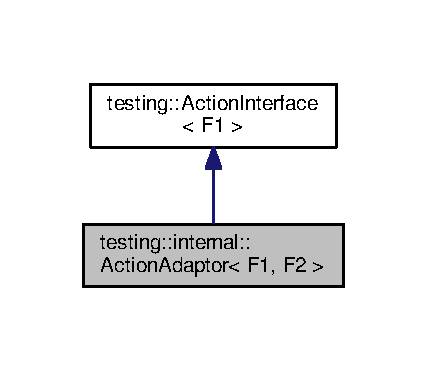
\includegraphics[width=205pt]{classtesting_1_1internal_1_1ActionAdaptor__inherit__graph}
\end{center}
\end{figure}


Collaboration diagram for testing\+:\+:internal\+:\+:Action\+Adaptor$<$ F1, F2 $>$\+:\nopagebreak
\begin{figure}[H]
\begin{center}
\leavevmode
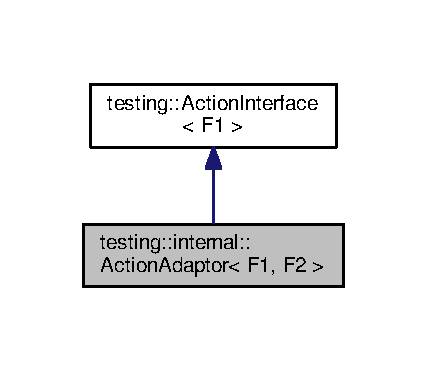
\includegraphics[width=205pt]{classtesting_1_1internal_1_1ActionAdaptor__coll__graph}
\end{center}
\end{figure}
\subsection*{Public Types}
\begin{DoxyCompactItemize}
\item 
typedef \hyperlink{structtesting_1_1internal_1_1Function}{internal\+::\+Function}$<$ F1 $>$\+::\hyperlink{classtesting_1_1internal_1_1ActionAdaptor_afa8f7872b6db3d8f1545fd98b45b0b95}{Result} \hyperlink{classtesting_1_1internal_1_1ActionAdaptor_afa8f7872b6db3d8f1545fd98b45b0b95}{Result}
\item 
typedef \hyperlink{structtesting_1_1internal_1_1Function}{internal\+::\+Function}$<$ F1 $>$\+::\hyperlink{classtesting_1_1internal_1_1ActionAdaptor_a4f78fb73f97b72fea8a93b78a8ab5704}{Argument\+Tuple} \hyperlink{classtesting_1_1internal_1_1ActionAdaptor_a4f78fb73f97b72fea8a93b78a8ab5704}{Argument\+Tuple}
\end{DoxyCompactItemize}
\subsection*{Public Member Functions}
\begin{DoxyCompactItemize}
\item 
\hyperlink{classtesting_1_1internal_1_1ActionAdaptor_a24ba3330ef3cc365b956c50ec73e4177}{Action\+Adaptor} (const \hyperlink{classtesting_1_1Action}{Action}$<$ F2 $>$ \&from)
\item 
virtual \hyperlink{classtesting_1_1internal_1_1ActionAdaptor_afa8f7872b6db3d8f1545fd98b45b0b95}{Result} \hyperlink{classtesting_1_1internal_1_1ActionAdaptor_a8d8a47a31f068cf6e0c95b91605d5540}{Perform} (const \hyperlink{classtesting_1_1internal_1_1ActionAdaptor_a4f78fb73f97b72fea8a93b78a8ab5704}{Argument\+Tuple} \&args)
\end{DoxyCompactItemize}


\subsection{Member Typedef Documentation}
\index{testing\+::internal\+::\+Action\+Adaptor@{testing\+::internal\+::\+Action\+Adaptor}!Argument\+Tuple@{Argument\+Tuple}}
\index{Argument\+Tuple@{Argument\+Tuple}!testing\+::internal\+::\+Action\+Adaptor@{testing\+::internal\+::\+Action\+Adaptor}}
\subsubsection[{\texorpdfstring{Argument\+Tuple}{ArgumentTuple}}]{\setlength{\rightskip}{0pt plus 5cm}template$<$typename F1 , typename F2 $>$ typedef {\bf internal\+::\+Function}$<$F1$>$\+::{\bf Argument\+Tuple} {\bf testing\+::internal\+::\+Action\+Adaptor}$<$ F1, F2 $>$\+::{\bf Argument\+Tuple}}\hypertarget{classtesting_1_1internal_1_1ActionAdaptor_a4f78fb73f97b72fea8a93b78a8ab5704}{}\label{classtesting_1_1internal_1_1ActionAdaptor_a4f78fb73f97b72fea8a93b78a8ab5704}
\index{testing\+::internal\+::\+Action\+Adaptor@{testing\+::internal\+::\+Action\+Adaptor}!Result@{Result}}
\index{Result@{Result}!testing\+::internal\+::\+Action\+Adaptor@{testing\+::internal\+::\+Action\+Adaptor}}
\subsubsection[{\texorpdfstring{Result}{Result}}]{\setlength{\rightskip}{0pt plus 5cm}template$<$typename F1 , typename F2 $>$ typedef {\bf internal\+::\+Function}$<$F1$>$\+::{\bf Result} {\bf testing\+::internal\+::\+Action\+Adaptor}$<$ F1, F2 $>$\+::{\bf Result}}\hypertarget{classtesting_1_1internal_1_1ActionAdaptor_afa8f7872b6db3d8f1545fd98b45b0b95}{}\label{classtesting_1_1internal_1_1ActionAdaptor_afa8f7872b6db3d8f1545fd98b45b0b95}


\subsection{Constructor \& Destructor Documentation}
\index{testing\+::internal\+::\+Action\+Adaptor@{testing\+::internal\+::\+Action\+Adaptor}!Action\+Adaptor@{Action\+Adaptor}}
\index{Action\+Adaptor@{Action\+Adaptor}!testing\+::internal\+::\+Action\+Adaptor@{testing\+::internal\+::\+Action\+Adaptor}}
\subsubsection[{\texorpdfstring{Action\+Adaptor(const Action$<$ F2 $>$ \&from)}{ActionAdaptor(const Action< F2 > &from)}}]{\setlength{\rightskip}{0pt plus 5cm}template$<$typename F1 , typename F2 $>$ {\bf testing\+::internal\+::\+Action\+Adaptor}$<$ F1, F2 $>$\+::{\bf Action\+Adaptor} (
\begin{DoxyParamCaption}
\item[{const {\bf Action}$<$ F2 $>$ \&}]{from}
\end{DoxyParamCaption}
)\hspace{0.3cm}{\ttfamily [inline]}, {\ttfamily [explicit]}}\hypertarget{classtesting_1_1internal_1_1ActionAdaptor_a24ba3330ef3cc365b956c50ec73e4177}{}\label{classtesting_1_1internal_1_1ActionAdaptor_a24ba3330ef3cc365b956c50ec73e4177}

\begin{DoxyCode}
489 : impl\_(from.impl\_) \{\}
\end{DoxyCode}


\subsection{Member Function Documentation}
\index{testing\+::internal\+::\+Action\+Adaptor@{testing\+::internal\+::\+Action\+Adaptor}!Perform@{Perform}}
\index{Perform@{Perform}!testing\+::internal\+::\+Action\+Adaptor@{testing\+::internal\+::\+Action\+Adaptor}}
\subsubsection[{\texorpdfstring{Perform(const Argument\+Tuple \&args)}{Perform(const ArgumentTuple &args)}}]{\setlength{\rightskip}{0pt plus 5cm}template$<$typename F1 , typename F2 $>$ virtual {\bf Result} {\bf testing\+::internal\+::\+Action\+Adaptor}$<$ F1, F2 $>$\+::Perform (
\begin{DoxyParamCaption}
\item[{const {\bf Argument\+Tuple} \&}]{args}
\end{DoxyParamCaption}
)\hspace{0.3cm}{\ttfamily [inline]}, {\ttfamily [virtual]}}\hypertarget{classtesting_1_1internal_1_1ActionAdaptor_a8d8a47a31f068cf6e0c95b91605d5540}{}\label{classtesting_1_1internal_1_1ActionAdaptor_a8d8a47a31f068cf6e0c95b91605d5540}


Implements \hyperlink{classtesting_1_1ActionInterface_a20f8624fcea1786f2992b358760422a0}{testing\+::\+Action\+Interface$<$ F1 $>$}.


\begin{DoxyCode}
491                                                     \{
492     \textcolor{keywordflow}{return} impl\_->Perform(args);
493   \}
\end{DoxyCode}


The documentation for this class was generated from the following file\+:\begin{DoxyCompactItemize}
\item 
vendor/googletest/googlemock/include/gmock/\hyperlink{gmock-actions_8h}{gmock-\/actions.\+h}\end{DoxyCompactItemize}

\hypertarget{classtesting_1_1internal_1_1ActionHelper}{}\section{testing\+:\+:internal\+:\+:Action\+Helper$<$ Result, Impl $>$ Class Template Reference}
\label{classtesting_1_1internal_1_1ActionHelper}\index{testing\+::internal\+::\+Action\+Helper$<$ Result, Impl $>$@{testing\+::internal\+::\+Action\+Helper$<$ Result, Impl $>$}}


{\ttfamily \#include $<$gmock-\/generated-\/actions.\+h$>$}

\subsection*{Static Public Member Functions}
\begin{DoxyCompactItemize}
\item 
static Result \hyperlink{classtesting_1_1internal_1_1ActionHelper_a25176836b0a381d883d61c3a2dc60662}{Perform} (Impl $\ast$impl, const \+::testing\+::tuple$<$$>$ \&args)
\item 
{\footnotesize template$<$typename A0 $>$ }\\static Result \hyperlink{classtesting_1_1internal_1_1ActionHelper_a08d2e199b0a3a1f9e05982cae07db3ec}{Perform} (Impl $\ast$impl, const \+::testing\+::tuple$<$ A0 $>$ \&args)
\item 
{\footnotesize template$<$typename A0 , typename A1 $>$ }\\static Result \hyperlink{classtesting_1_1internal_1_1ActionHelper_a96d8d8399ff3322e77ba1de51c166f4e}{Perform} (Impl $\ast$impl, const \+::testing\+::tuple$<$ A0, A1 $>$ \&args)
\item 
{\footnotesize template$<$typename A0 , typename A1 , typename A2 $>$ }\\static Result \hyperlink{classtesting_1_1internal_1_1ActionHelper_ad450478d185cbcac0e1383f7517f5c36}{Perform} (Impl $\ast$impl, const \+::testing\+::tuple$<$ A0, A1, A2 $>$ \&args)
\item 
{\footnotesize template$<$typename A0 , typename A1 , typename A2 , typename A3 $>$ }\\static Result \hyperlink{classtesting_1_1internal_1_1ActionHelper_a2ceda08aeb7b9fd1ad6ccb0821a3ea39}{Perform} (Impl $\ast$impl, const \+::testing\+::tuple$<$ A0, A1, A2, A3 $>$ \&args)
\item 
{\footnotesize template$<$typename A0 , typename A1 , typename A2 , typename A3 , typename A4 $>$ }\\static Result \hyperlink{classtesting_1_1internal_1_1ActionHelper_afd2d1dcea480db63416fc3b8604dec56}{Perform} (Impl $\ast$impl, const \+::testing\+::tuple$<$ A0, A1, A2, A3, A4 $>$ \&args)
\item 
{\footnotesize template$<$typename A0 , typename A1 , typename A2 , typename A3 , typename A4 , typename A5 $>$ }\\static Result \hyperlink{classtesting_1_1internal_1_1ActionHelper_a58e3b1699dd3a4404ed2cd652327d8ca}{Perform} (Impl $\ast$impl, const \+::testing\+::tuple$<$ A0, A1, A2, A3, A4, A5 $>$ \&args)
\item 
{\footnotesize template$<$typename A0 , typename A1 , typename A2 , typename A3 , typename A4 , typename A5 , typename A6 $>$ }\\static Result \hyperlink{classtesting_1_1internal_1_1ActionHelper_a457f1505b200c5125c3bb370fb7e7bb4}{Perform} (Impl $\ast$impl, const \+::testing\+::tuple$<$ A0, A1, A2, A3, A4, A5, A6 $>$ \&args)
\item 
{\footnotesize template$<$typename A0 , typename A1 , typename A2 , typename A3 , typename A4 , typename A5 , typename A6 , typename A7 $>$ }\\static Result \hyperlink{classtesting_1_1internal_1_1ActionHelper_a1f851f76793206daf2dd8a2f9621f43c}{Perform} (Impl $\ast$impl, const \+::testing\+::tuple$<$ A0, A1, A2, A3, A4, A5, A6, A7 $>$ \&args)
\item 
{\footnotesize template$<$typename A0 , typename A1 , typename A2 , typename A3 , typename A4 , typename A5 , typename A6 , typename A7 , typename A8 $>$ }\\static Result \hyperlink{classtesting_1_1internal_1_1ActionHelper_afcc265631df5d3a0f8955e9aa35c57f7}{Perform} (Impl $\ast$impl, const \+::testing\+::tuple$<$ A0, A1, A2, A3, A4, A5, A6, A7, A8 $>$ \&args)
\item 
{\footnotesize template$<$typename A0 , typename A1 , typename A2 , typename A3 , typename A4 , typename A5 , typename A6 , typename A7 , typename A8 , typename A9 $>$ }\\static Result \hyperlink{classtesting_1_1internal_1_1ActionHelper_adfe6c86332cc09b352ec5ccbad1d3988}{Perform} (Impl $\ast$impl, const \+::testing\+::tuple$<$ A0, A1, A2, A3, A4, A5, A6, A7, A8, A9 $>$ \&args)
\end{DoxyCompactItemize}


\subsection{Member Function Documentation}
\index{testing\+::internal\+::\+Action\+Helper@{testing\+::internal\+::\+Action\+Helper}!Perform@{Perform}}
\index{Perform@{Perform}!testing\+::internal\+::\+Action\+Helper@{testing\+::internal\+::\+Action\+Helper}}
\subsubsection[{\texorpdfstring{Perform(\+Impl $\ast$impl, const \+::testing\+::tuple$<$$>$ \&args)}{Perform(Impl *impl, const ::testing::tuple<> &args)}}]{\setlength{\rightskip}{0pt plus 5cm}template$<$typename Result , class Impl $>$ static Result {\bf testing\+::internal\+::\+Action\+Helper}$<$ Result, Impl $>$\+::Perform (
\begin{DoxyParamCaption}
\item[{Impl $\ast$}]{impl, }
\item[{const \+::testing\+::tuple$<$$>$ \&}]{args}
\end{DoxyParamCaption}
)\hspace{0.3cm}{\ttfamily [inline]}, {\ttfamily [static]}}\hypertarget{classtesting_1_1internal_1_1ActionHelper_a25176836b0a381d883d61c3a2dc60662}{}\label{classtesting_1_1internal_1_1ActionHelper_a25176836b0a381d883d61c3a2dc60662}

\begin{DoxyCode}
514                                                                 \{
515     \textcolor{keywordflow}{return} impl->template gmock\_PerformImpl<>(args, ExcessiveArg(),
516         ExcessiveArg(), ExcessiveArg(), ExcessiveArg(), ExcessiveArg(),
517         ExcessiveArg(), ExcessiveArg(), ExcessiveArg(), ExcessiveArg(),
518         ExcessiveArg());
519   \}
\end{DoxyCode}
\index{testing\+::internal\+::\+Action\+Helper@{testing\+::internal\+::\+Action\+Helper}!Perform@{Perform}}
\index{Perform@{Perform}!testing\+::internal\+::\+Action\+Helper@{testing\+::internal\+::\+Action\+Helper}}
\subsubsection[{\texorpdfstring{Perform(\+Impl $\ast$impl, const \+::testing\+::tuple$<$ A0 $>$ \&args)}{Perform(Impl *impl, const ::testing::tuple< A0 > &args)}}]{\setlength{\rightskip}{0pt plus 5cm}template$<$typename Result , class Impl $>$ template$<$typename A0 $>$ static Result {\bf testing\+::internal\+::\+Action\+Helper}$<$ Result, Impl $>$\+::Perform (
\begin{DoxyParamCaption}
\item[{Impl $\ast$}]{impl, }
\item[{const \+::testing\+::tuple$<$ A0 $>$ \&}]{args}
\end{DoxyParamCaption}
)\hspace{0.3cm}{\ttfamily [inline]}, {\ttfamily [static]}}\hypertarget{classtesting_1_1internal_1_1ActionHelper_a08d2e199b0a3a1f9e05982cae07db3ec}{}\label{classtesting_1_1internal_1_1ActionHelper_a08d2e199b0a3a1f9e05982cae07db3ec}

\begin{DoxyCode}
522                                                                   \{
523     \textcolor{keywordflow}{return} impl->template gmock\_PerformImpl<A0>(args, get<0>(args),
524         ExcessiveArg(), ExcessiveArg(), ExcessiveArg(), ExcessiveArg(),
525         ExcessiveArg(), ExcessiveArg(), ExcessiveArg(), ExcessiveArg(),
526         ExcessiveArg());
527   \}
\end{DoxyCode}
\index{testing\+::internal\+::\+Action\+Helper@{testing\+::internal\+::\+Action\+Helper}!Perform@{Perform}}
\index{Perform@{Perform}!testing\+::internal\+::\+Action\+Helper@{testing\+::internal\+::\+Action\+Helper}}
\subsubsection[{\texorpdfstring{Perform(\+Impl $\ast$impl, const \+::testing\+::tuple$<$ A0, A1 $>$ \&args)}{Perform(Impl *impl, const ::testing::tuple< A0, A1 > &args)}}]{\setlength{\rightskip}{0pt plus 5cm}template$<$typename Result , class Impl $>$ template$<$typename A0 , typename A1 $>$ static Result {\bf testing\+::internal\+::\+Action\+Helper}$<$ Result, Impl $>$\+::Perform (
\begin{DoxyParamCaption}
\item[{Impl $\ast$}]{impl, }
\item[{const \+::testing\+::tuple$<$ A0, A1 $>$ \&}]{args}
\end{DoxyParamCaption}
)\hspace{0.3cm}{\ttfamily [inline]}, {\ttfamily [static]}}\hypertarget{classtesting_1_1internal_1_1ActionHelper_a96d8d8399ff3322e77ba1de51c166f4e}{}\label{classtesting_1_1internal_1_1ActionHelper_a96d8d8399ff3322e77ba1de51c166f4e}

\begin{DoxyCode}
530                                                                       \{
531     \textcolor{keywordflow}{return} impl->template gmock\_PerformImpl<A0, A1>(args, get<0>(args),
532         get<1>(args), ExcessiveArg(), ExcessiveArg(), ExcessiveArg(),
533         ExcessiveArg(), ExcessiveArg(), ExcessiveArg(), ExcessiveArg(),
534         ExcessiveArg());
535   \}
\end{DoxyCode}
\index{testing\+::internal\+::\+Action\+Helper@{testing\+::internal\+::\+Action\+Helper}!Perform@{Perform}}
\index{Perform@{Perform}!testing\+::internal\+::\+Action\+Helper@{testing\+::internal\+::\+Action\+Helper}}
\subsubsection[{\texorpdfstring{Perform(\+Impl $\ast$impl, const \+::testing\+::tuple$<$ A0, A1, A2 $>$ \&args)}{Perform(Impl *impl, const ::testing::tuple< A0, A1, A2 > &args)}}]{\setlength{\rightskip}{0pt plus 5cm}template$<$typename Result , class Impl $>$ template$<$typename A0 , typename A1 , typename A2 $>$ static Result {\bf testing\+::internal\+::\+Action\+Helper}$<$ Result, Impl $>$\+::Perform (
\begin{DoxyParamCaption}
\item[{Impl $\ast$}]{impl, }
\item[{const \+::testing\+::tuple$<$ A0, A1, A2 $>$ \&}]{args}
\end{DoxyParamCaption}
)\hspace{0.3cm}{\ttfamily [inline]}, {\ttfamily [static]}}\hypertarget{classtesting_1_1internal_1_1ActionHelper_ad450478d185cbcac0e1383f7517f5c36}{}\label{classtesting_1_1internal_1_1ActionHelper_ad450478d185cbcac0e1383f7517f5c36}

\begin{DoxyCode}
538                                                                           \{
539     \textcolor{keywordflow}{return} impl->template gmock\_PerformImpl<A0, A1, A2>(args, get<0>(args),
540         get<1>(args), get<2>(args), ExcessiveArg(), ExcessiveArg(),
541         ExcessiveArg(), ExcessiveArg(), ExcessiveArg(), ExcessiveArg(),
542         ExcessiveArg());
543   \}
\end{DoxyCode}
\index{testing\+::internal\+::\+Action\+Helper@{testing\+::internal\+::\+Action\+Helper}!Perform@{Perform}}
\index{Perform@{Perform}!testing\+::internal\+::\+Action\+Helper@{testing\+::internal\+::\+Action\+Helper}}
\subsubsection[{\texorpdfstring{Perform(\+Impl $\ast$impl, const \+::testing\+::tuple$<$ A0, A1, A2, A3 $>$ \&args)}{Perform(Impl *impl, const ::testing::tuple< A0, A1, A2, A3 > &args)}}]{\setlength{\rightskip}{0pt plus 5cm}template$<$typename Result , class Impl $>$ template$<$typename A0 , typename A1 , typename A2 , typename A3 $>$ static Result {\bf testing\+::internal\+::\+Action\+Helper}$<$ Result, Impl $>$\+::Perform (
\begin{DoxyParamCaption}
\item[{Impl $\ast$}]{impl, }
\item[{const \+::testing\+::tuple$<$ A0, A1, A2, A3 $>$ \&}]{args}
\end{DoxyParamCaption}
)\hspace{0.3cm}{\ttfamily [inline]}, {\ttfamily [static]}}\hypertarget{classtesting_1_1internal_1_1ActionHelper_a2ceda08aeb7b9fd1ad6ccb0821a3ea39}{}\label{classtesting_1_1internal_1_1ActionHelper_a2ceda08aeb7b9fd1ad6ccb0821a3ea39}

\begin{DoxyCode}
547                  \{
548     \textcolor{keywordflow}{return} impl->template gmock\_PerformImpl<A0, A1, A2, A3>(args, get<0>(args),
549         get<1>(args), get<2>(args), get<3>(args), ExcessiveArg(),
550         ExcessiveArg(), ExcessiveArg(), ExcessiveArg(), ExcessiveArg(),
551         ExcessiveArg());
552   \}
\end{DoxyCode}
\index{testing\+::internal\+::\+Action\+Helper@{testing\+::internal\+::\+Action\+Helper}!Perform@{Perform}}
\index{Perform@{Perform}!testing\+::internal\+::\+Action\+Helper@{testing\+::internal\+::\+Action\+Helper}}
\subsubsection[{\texorpdfstring{Perform(\+Impl $\ast$impl, const \+::testing\+::tuple$<$ A0, A1, A2, A3, A4 $>$ \&args)}{Perform(Impl *impl, const ::testing::tuple< A0, A1, A2, A3, A4 > &args)}}]{\setlength{\rightskip}{0pt plus 5cm}template$<$typename Result , class Impl $>$ template$<$typename A0 , typename A1 , typename A2 , typename A3 , typename A4 $>$ static Result {\bf testing\+::internal\+::\+Action\+Helper}$<$ Result, Impl $>$\+::Perform (
\begin{DoxyParamCaption}
\item[{Impl $\ast$}]{impl, }
\item[{const \+::testing\+::tuple$<$ A0, A1, A2, A3, A4 $>$ \&}]{args}
\end{DoxyParamCaption}
)\hspace{0.3cm}{\ttfamily [inline]}, {\ttfamily [static]}}\hypertarget{classtesting_1_1internal_1_1ActionHelper_afd2d1dcea480db63416fc3b8604dec56}{}\label{classtesting_1_1internal_1_1ActionHelper_afd2d1dcea480db63416fc3b8604dec56}

\begin{DoxyCode}
556                  \{
557     \textcolor{keywordflow}{return} impl->template gmock\_PerformImpl<A0, A1, A2, A3, A4>(args,
558         get<0>(args), get<1>(args), get<2>(args), get<3>(args), get<4>(args),
559         ExcessiveArg(), ExcessiveArg(), ExcessiveArg(), ExcessiveArg(),
560         ExcessiveArg());
561   \}
\end{DoxyCode}
\index{testing\+::internal\+::\+Action\+Helper@{testing\+::internal\+::\+Action\+Helper}!Perform@{Perform}}
\index{Perform@{Perform}!testing\+::internal\+::\+Action\+Helper@{testing\+::internal\+::\+Action\+Helper}}
\subsubsection[{\texorpdfstring{Perform(\+Impl $\ast$impl, const \+::testing\+::tuple$<$ A0, A1, A2, A3, A4, A5 $>$ \&args)}{Perform(Impl *impl, const ::testing::tuple< A0, A1, A2, A3, A4, A5 > &args)}}]{\setlength{\rightskip}{0pt plus 5cm}template$<$typename Result , class Impl $>$ template$<$typename A0 , typename A1 , typename A2 , typename A3 , typename A4 , typename A5 $>$ static Result {\bf testing\+::internal\+::\+Action\+Helper}$<$ Result, Impl $>$\+::Perform (
\begin{DoxyParamCaption}
\item[{Impl $\ast$}]{impl, }
\item[{const \+::testing\+::tuple$<$ A0, A1, A2, A3, A4, A5 $>$ \&}]{args}
\end{DoxyParamCaption}
)\hspace{0.3cm}{\ttfamily [inline]}, {\ttfamily [static]}}\hypertarget{classtesting_1_1internal_1_1ActionHelper_a58e3b1699dd3a4404ed2cd652327d8ca}{}\label{classtesting_1_1internal_1_1ActionHelper_a58e3b1699dd3a4404ed2cd652327d8ca}

\begin{DoxyCode}
566                  \{
567     \textcolor{keywordflow}{return} impl->template gmock\_PerformImpl<A0, A1, A2, A3, A4, A5>(args,
568         get<0>(args), get<1>(args), get<2>(args), get<3>(args), get<4>(args),
569         get<5>(args), ExcessiveArg(), ExcessiveArg(), ExcessiveArg(),
570         ExcessiveArg());
571   \}
\end{DoxyCode}
\index{testing\+::internal\+::\+Action\+Helper@{testing\+::internal\+::\+Action\+Helper}!Perform@{Perform}}
\index{Perform@{Perform}!testing\+::internal\+::\+Action\+Helper@{testing\+::internal\+::\+Action\+Helper}}
\subsubsection[{\texorpdfstring{Perform(\+Impl $\ast$impl, const \+::testing\+::tuple$<$ A0, A1, A2, A3, A4, A5, A6 $>$ \&args)}{Perform(Impl *impl, const ::testing::tuple< A0, A1, A2, A3, A4, A5, A6 > &args)}}]{\setlength{\rightskip}{0pt plus 5cm}template$<$typename Result , class Impl $>$ template$<$typename A0 , typename A1 , typename A2 , typename A3 , typename A4 , typename A5 , typename A6 $>$ static Result {\bf testing\+::internal\+::\+Action\+Helper}$<$ Result, Impl $>$\+::Perform (
\begin{DoxyParamCaption}
\item[{Impl $\ast$}]{impl, }
\item[{const \+::testing\+::tuple$<$ A0, A1, A2, A3, A4, A5, A6 $>$ \&}]{args}
\end{DoxyParamCaption}
)\hspace{0.3cm}{\ttfamily [inline]}, {\ttfamily [static]}}\hypertarget{classtesting_1_1internal_1_1ActionHelper_a457f1505b200c5125c3bb370fb7e7bb4}{}\label{classtesting_1_1internal_1_1ActionHelper_a457f1505b200c5125c3bb370fb7e7bb4}

\begin{DoxyCode}
576                      \{
577     \textcolor{keywordflow}{return} impl->template gmock\_PerformImpl<A0, A1, A2, A3, A4, A5, A6>(args,
578         get<0>(args), get<1>(args), get<2>(args), get<3>(args), get<4>(args),
579         get<5>(args), get<6>(args), ExcessiveArg(), ExcessiveArg(),
580         ExcessiveArg());
581   \}
\end{DoxyCode}
\index{testing\+::internal\+::\+Action\+Helper@{testing\+::internal\+::\+Action\+Helper}!Perform@{Perform}}
\index{Perform@{Perform}!testing\+::internal\+::\+Action\+Helper@{testing\+::internal\+::\+Action\+Helper}}
\subsubsection[{\texorpdfstring{Perform(\+Impl $\ast$impl, const \+::testing\+::tuple$<$ A0, A1, A2, A3, A4, A5, A6, A7 $>$ \&args)}{Perform(Impl *impl, const ::testing::tuple< A0, A1, A2, A3, A4, A5, A6, A7 > &args)}}]{\setlength{\rightskip}{0pt plus 5cm}template$<$typename Result , class Impl $>$ template$<$typename A0 , typename A1 , typename A2 , typename A3 , typename A4 , typename A5 , typename A6 , typename A7 $>$ static Result {\bf testing\+::internal\+::\+Action\+Helper}$<$ Result, Impl $>$\+::Perform (
\begin{DoxyParamCaption}
\item[{Impl $\ast$}]{impl, }
\item[{const \+::testing\+::tuple$<$ A0, A1, A2, A3, A4, A5, A6, A7 $>$ \&}]{args}
\end{DoxyParamCaption}
)\hspace{0.3cm}{\ttfamily [inline]}, {\ttfamily [static]}}\hypertarget{classtesting_1_1internal_1_1ActionHelper_a1f851f76793206daf2dd8a2f9621f43c}{}\label{classtesting_1_1internal_1_1ActionHelper_a1f851f76793206daf2dd8a2f9621f43c}

\begin{DoxyCode}
586                          \{
587     \textcolor{keywordflow}{return} impl->template gmock\_PerformImpl<A0, A1, A2, A3, A4, A5, A6,
588         A7>(args, get<0>(args), get<1>(args), get<2>(args), get<3>(args),
589         get<4>(args), get<5>(args), get<6>(args), get<7>(args), ExcessiveArg(),
590         ExcessiveArg());
591   \}
\end{DoxyCode}
\index{testing\+::internal\+::\+Action\+Helper@{testing\+::internal\+::\+Action\+Helper}!Perform@{Perform}}
\index{Perform@{Perform}!testing\+::internal\+::\+Action\+Helper@{testing\+::internal\+::\+Action\+Helper}}
\subsubsection[{\texorpdfstring{Perform(\+Impl $\ast$impl, const \+::testing\+::tuple$<$ A0, A1, A2, A3, A4, A5, A6, A7, A8 $>$ \&args)}{Perform(Impl *impl, const ::testing::tuple< A0, A1, A2, A3, A4, A5, A6, A7, A8 > &args)}}]{\setlength{\rightskip}{0pt plus 5cm}template$<$typename Result , class Impl $>$ template$<$typename A0 , typename A1 , typename A2 , typename A3 , typename A4 , typename A5 , typename A6 , typename A7 , typename A8 $>$ static Result {\bf testing\+::internal\+::\+Action\+Helper}$<$ Result, Impl $>$\+::Perform (
\begin{DoxyParamCaption}
\item[{Impl $\ast$}]{impl, }
\item[{const \+::testing\+::tuple$<$ A0, A1, A2, A3, A4, A5, A6, A7, A8 $>$ \&}]{args}
\end{DoxyParamCaption}
)\hspace{0.3cm}{\ttfamily [inline]}, {\ttfamily [static]}}\hypertarget{classtesting_1_1internal_1_1ActionHelper_afcc265631df5d3a0f8955e9aa35c57f7}{}\label{classtesting_1_1internal_1_1ActionHelper_afcc265631df5d3a0f8955e9aa35c57f7}

\begin{DoxyCode}
596                              \{
597     \textcolor{keywordflow}{return} impl->template gmock\_PerformImpl<A0, A1, A2, A3, A4, A5, A6, A7,
598         A8>(args, get<0>(args), get<1>(args), get<2>(args), get<3>(args),
599         get<4>(args), get<5>(args), get<6>(args), get<7>(args), get<8>(args),
600         ExcessiveArg());
601   \}
\end{DoxyCode}
\index{testing\+::internal\+::\+Action\+Helper@{testing\+::internal\+::\+Action\+Helper}!Perform@{Perform}}
\index{Perform@{Perform}!testing\+::internal\+::\+Action\+Helper@{testing\+::internal\+::\+Action\+Helper}}
\subsubsection[{\texorpdfstring{Perform(\+Impl $\ast$impl, const \+::testing\+::tuple$<$ A0, A1, A2, A3, A4, A5, A6, A7, A8, A9 $>$ \&args)}{Perform(Impl *impl, const ::testing::tuple< A0, A1, A2, A3, A4, A5, A6, A7, A8, A9 > &args)}}]{\setlength{\rightskip}{0pt plus 5cm}template$<$typename Result , class Impl $>$ template$<$typename A0 , typename A1 , typename A2 , typename A3 , typename A4 , typename A5 , typename A6 , typename A7 , typename A8 , typename A9 $>$ static Result {\bf testing\+::internal\+::\+Action\+Helper}$<$ Result, Impl $>$\+::Perform (
\begin{DoxyParamCaption}
\item[{Impl $\ast$}]{impl, }
\item[{const \+::testing\+::tuple$<$ A0, A1, A2, A3, A4, A5, A6, A7, A8, A9 $>$ \&}]{args}
\end{DoxyParamCaption}
)\hspace{0.3cm}{\ttfamily [inline]}, {\ttfamily [static]}}\hypertarget{classtesting_1_1internal_1_1ActionHelper_adfe6c86332cc09b352ec5ccbad1d3988}{}\label{classtesting_1_1internal_1_1ActionHelper_adfe6c86332cc09b352ec5ccbad1d3988}

\begin{DoxyCode}
606                                  \{
607     \textcolor{keywordflow}{return} impl->template gmock\_PerformImpl<A0, A1, A2, A3, A4, A5, A6, A7, A8,
608         A9>(args, get<0>(args), get<1>(args), get<2>(args), get<3>(args),
609         get<4>(args), get<5>(args), get<6>(args), get<7>(args), get<8>(args),
610         get<9>(args));
611   \}
\end{DoxyCode}


The documentation for this class was generated from the following file\+:\begin{DoxyCompactItemize}
\item 
vendor/googletest/googlemock/include/gmock/\hyperlink{gmock-generated-actions_8h}{gmock-\/generated-\/actions.\+h}\end{DoxyCompactItemize}

\hypertarget{classtesting_1_1ActionInterface}{}\section{testing\+:\+:Action\+Interface$<$ F $>$ Class Template Reference}
\label{classtesting_1_1ActionInterface}\index{testing\+::\+Action\+Interface$<$ F $>$@{testing\+::\+Action\+Interface$<$ F $>$}}


{\ttfamily \#include $<$gmock-\/actions.\+h$>$}



Inheritance diagram for testing\+:\+:Action\+Interface$<$ F $>$\+:
\nopagebreak
\begin{figure}[H]
\begin{center}
\leavevmode
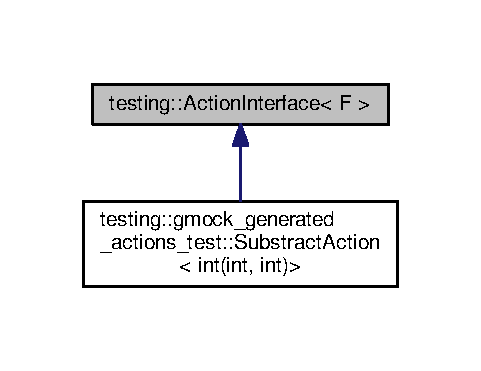
\includegraphics[width=231pt]{classtesting_1_1ActionInterface__inherit__graph}
\end{center}
\end{figure}
\subsection*{Public Types}
\begin{DoxyCompactItemize}
\item 
typedef \hyperlink{structtesting_1_1internal_1_1Function}{internal\+::\+Function}$<$ F $>$\+::\hyperlink{classtesting_1_1ActionInterface_a7477de2fe3e4e01c59db698203acaee7}{Result} \hyperlink{classtesting_1_1ActionInterface_a7477de2fe3e4e01c59db698203acaee7}{Result}
\item 
typedef \hyperlink{structtesting_1_1internal_1_1Function}{internal\+::\+Function}$<$ F $>$\+::\hyperlink{classtesting_1_1ActionInterface_af72720d864da4d606629e83edc003511}{Argument\+Tuple} \hyperlink{classtesting_1_1ActionInterface_af72720d864da4d606629e83edc003511}{Argument\+Tuple}
\end{DoxyCompactItemize}
\subsection*{Public Member Functions}
\begin{DoxyCompactItemize}
\item 
\hyperlink{classtesting_1_1ActionInterface_a0f1d44e4c669a9cae5ee5b28419a6f52}{Action\+Interface} ()
\item 
virtual \hyperlink{classtesting_1_1ActionInterface_a7dd0a5fc93d86ae3c9d04963b9f3a93f}{$\sim$\+Action\+Interface} ()
\item 
virtual \hyperlink{classtesting_1_1ActionInterface_a7477de2fe3e4e01c59db698203acaee7}{Result} \hyperlink{classtesting_1_1ActionInterface_a20f8624fcea1786f2992b358760422a0}{Perform} (const \hyperlink{classtesting_1_1ActionInterface_af72720d864da4d606629e83edc003511}{Argument\+Tuple} \&args)=0
\end{DoxyCompactItemize}


\subsection{Member Typedef Documentation}
\index{testing\+::\+Action\+Interface@{testing\+::\+Action\+Interface}!Argument\+Tuple@{Argument\+Tuple}}
\index{Argument\+Tuple@{Argument\+Tuple}!testing\+::\+Action\+Interface@{testing\+::\+Action\+Interface}}
\subsubsection[{\texorpdfstring{Argument\+Tuple}{ArgumentTuple}}]{\setlength{\rightskip}{0pt plus 5cm}template$<$typename F$>$ typedef {\bf internal\+::\+Function}$<$F$>$\+::{\bf Argument\+Tuple} {\bf testing\+::\+Action\+Interface}$<$ F $>$\+::{\bf Argument\+Tuple}}\hypertarget{classtesting_1_1ActionInterface_af72720d864da4d606629e83edc003511}{}\label{classtesting_1_1ActionInterface_af72720d864da4d606629e83edc003511}
\index{testing\+::\+Action\+Interface@{testing\+::\+Action\+Interface}!Result@{Result}}
\index{Result@{Result}!testing\+::\+Action\+Interface@{testing\+::\+Action\+Interface}}
\subsubsection[{\texorpdfstring{Result}{Result}}]{\setlength{\rightskip}{0pt plus 5cm}template$<$typename F$>$ typedef {\bf internal\+::\+Function}$<$F$>$\+::{\bf Result} {\bf testing\+::\+Action\+Interface}$<$ F $>$\+::{\bf Result}}\hypertarget{classtesting_1_1ActionInterface_a7477de2fe3e4e01c59db698203acaee7}{}\label{classtesting_1_1ActionInterface_a7477de2fe3e4e01c59db698203acaee7}


\subsection{Constructor \& Destructor Documentation}
\index{testing\+::\+Action\+Interface@{testing\+::\+Action\+Interface}!Action\+Interface@{Action\+Interface}}
\index{Action\+Interface@{Action\+Interface}!testing\+::\+Action\+Interface@{testing\+::\+Action\+Interface}}
\subsubsection[{\texorpdfstring{Action\+Interface()}{ActionInterface()}}]{\setlength{\rightskip}{0pt plus 5cm}template$<$typename F$>$ {\bf testing\+::\+Action\+Interface}$<$ F $>$\+::{\bf Action\+Interface} (
\begin{DoxyParamCaption}
{}
\end{DoxyParamCaption}
)\hspace{0.3cm}{\ttfamily [inline]}}\hypertarget{classtesting_1_1ActionInterface_a0f1d44e4c669a9cae5ee5b28419a6f52}{}\label{classtesting_1_1ActionInterface_a0f1d44e4c669a9cae5ee5b28419a6f52}

\begin{DoxyCode}
332 \{\}
\end{DoxyCode}
\index{testing\+::\+Action\+Interface@{testing\+::\+Action\+Interface}!````~Action\+Interface@{$\sim$\+Action\+Interface}}
\index{````~Action\+Interface@{$\sim$\+Action\+Interface}!testing\+::\+Action\+Interface@{testing\+::\+Action\+Interface}}
\subsubsection[{\texorpdfstring{$\sim$\+Action\+Interface()}{~ActionInterface()}}]{\setlength{\rightskip}{0pt plus 5cm}template$<$typename F$>$ virtual {\bf testing\+::\+Action\+Interface}$<$ F $>$\+::$\sim${\bf Action\+Interface} (
\begin{DoxyParamCaption}
{}
\end{DoxyParamCaption}
)\hspace{0.3cm}{\ttfamily [inline]}, {\ttfamily [virtual]}}\hypertarget{classtesting_1_1ActionInterface_a7dd0a5fc93d86ae3c9d04963b9f3a93f}{}\label{classtesting_1_1ActionInterface_a7dd0a5fc93d86ae3c9d04963b9f3a93f}

\begin{DoxyCode}
333 \{\}
\end{DoxyCode}


\subsection{Member Function Documentation}
\index{testing\+::\+Action\+Interface@{testing\+::\+Action\+Interface}!Perform@{Perform}}
\index{Perform@{Perform}!testing\+::\+Action\+Interface@{testing\+::\+Action\+Interface}}
\subsubsection[{\texorpdfstring{Perform(const Argument\+Tuple \&args)=0}{Perform(const ArgumentTuple &args)=0}}]{\setlength{\rightskip}{0pt plus 5cm}template$<$typename F$>$ virtual {\bf Result} {\bf testing\+::\+Action\+Interface}$<$ F $>$\+::Perform (
\begin{DoxyParamCaption}
\item[{const {\bf Argument\+Tuple} \&}]{args}
\end{DoxyParamCaption}
)\hspace{0.3cm}{\ttfamily [pure virtual]}}\hypertarget{classtesting_1_1ActionInterface_a20f8624fcea1786f2992b358760422a0}{}\label{classtesting_1_1ActionInterface_a20f8624fcea1786f2992b358760422a0}


Implemented in \hyperlink{classtesting_1_1internal_1_1ActionAdaptor_a8d8a47a31f068cf6e0c95b91605d5540}{testing\+::internal\+::\+Action\+Adaptor$<$ F1, F2 $>$}.



The documentation for this class was generated from the following file\+:\begin{DoxyCompactItemize}
\item 
vendor/googletest/googlemock/include/gmock/\hyperlink{gmock-actions_8h}{gmock-\/actions.\+h}\end{DoxyCompactItemize}

\hypertarget{classtesting_1_1internal_1_1ActionResultHolder}{}\section{testing\+:\+:internal\+:\+:Action\+Result\+Holder$<$ T $>$ Class Template Reference}
\label{classtesting_1_1internal_1_1ActionResultHolder}\index{testing\+::internal\+::\+Action\+Result\+Holder$<$ T $>$@{testing\+::internal\+::\+Action\+Result\+Holder$<$ T $>$}}


{\ttfamily \#include $<$gmock-\/spec-\/builders.\+h$>$}



Inheritance diagram for testing\+:\+:internal\+:\+:Action\+Result\+Holder$<$ T $>$\+:
\nopagebreak
\begin{figure}[H]
\begin{center}
\leavevmode
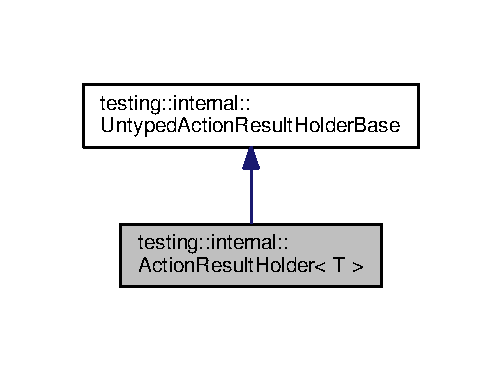
\includegraphics[width=241pt]{classtesting_1_1internal_1_1ActionResultHolder__inherit__graph}
\end{center}
\end{figure}


Collaboration diagram for testing\+:\+:internal\+:\+:Action\+Result\+Holder$<$ T $>$\+:
\nopagebreak
\begin{figure}[H]
\begin{center}
\leavevmode
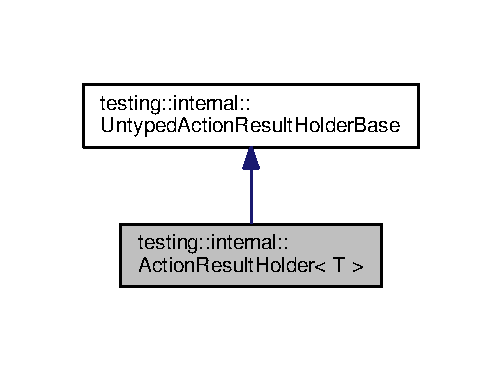
\includegraphics[width=241pt]{classtesting_1_1internal_1_1ActionResultHolder__coll__graph}
\end{center}
\end{figure}
\subsection*{Public Member Functions}
\begin{DoxyCompactItemize}
\item 
T \hyperlink{classtesting_1_1internal_1_1ActionResultHolder_a057df6cceeeab9ea06e679bcf6b78960}{Unwrap} ()
\item 
virtual void \hyperlink{classtesting_1_1internal_1_1ActionResultHolder_a70989192d3ed669c059a7e29c4a7b9fc}{Print\+As\+Action\+Result} (\+::std\+::ostream $\ast$os) const 
\end{DoxyCompactItemize}
\subsection*{Static Public Member Functions}
\begin{DoxyCompactItemize}
\item 
{\footnotesize template$<$typename F $>$ }\\static \hyperlink{classtesting_1_1internal_1_1ActionResultHolder}{Action\+Result\+Holder} $\ast$ \hyperlink{classtesting_1_1internal_1_1ActionResultHolder_a9609dcb5fb16271f83d777b087075272}{Perform\+Default\+Action} (const \hyperlink{classtesting_1_1internal_1_1FunctionMockerBase}{Function\+Mocker\+Base}$<$ F $>$ $\ast$func\+\_\+mocker, const typename \hyperlink{structtesting_1_1internal_1_1Function}{Function}$<$ F $>$\+::Argument\+Tuple \&args, const \hyperlink{namespacetesting_1_1internal_a8e8ff5b11e64078831112677156cb111}{string} \&call\+\_\+description)
\item 
{\footnotesize template$<$typename F $>$ }\\static \hyperlink{classtesting_1_1internal_1_1ActionResultHolder}{Action\+Result\+Holder} $\ast$ \hyperlink{classtesting_1_1internal_1_1ActionResultHolder_a9e10aff754b5caf69b14964f3c9c79ec}{Perform\+Action} (const \hyperlink{classtesting_1_1Action}{Action}$<$ F $>$ \&action, const typename \hyperlink{structtesting_1_1internal_1_1Function}{Function}$<$ F $>$\+::Argument\+Tuple \&args)
\end{DoxyCompactItemize}


\subsection{Member Function Documentation}
\index{testing\+::internal\+::\+Action\+Result\+Holder@{testing\+::internal\+::\+Action\+Result\+Holder}!Perform\+Action@{Perform\+Action}}
\index{Perform\+Action@{Perform\+Action}!testing\+::internal\+::\+Action\+Result\+Holder@{testing\+::internal\+::\+Action\+Result\+Holder}}
\subsubsection[{\texorpdfstring{Perform\+Action(const Action$<$ F $>$ \&action, const typename Function$<$ F $>$\+::\+Argument\+Tuple \&args)}{PerformAction(const Action< F > &action, const typename Function< F >::ArgumentTuple &args)}}]{\setlength{\rightskip}{0pt plus 5cm}template$<$typename T $>$ template$<$typename F $>$ static {\bf Action\+Result\+Holder}$\ast$ {\bf testing\+::internal\+::\+Action\+Result\+Holder}$<$ T $>$\+::Perform\+Action (
\begin{DoxyParamCaption}
\item[{const {\bf Action}$<$ F $>$ \&}]{action, }
\item[{const typename {\bf Function}$<$ F $>$\+::Argument\+Tuple \&}]{args}
\end{DoxyParamCaption}
)\hspace{0.3cm}{\ttfamily [inline]}, {\ttfamily [static]}}\hypertarget{classtesting_1_1internal_1_1ActionResultHolder_a9e10aff754b5caf69b14964f3c9c79ec}{}\label{classtesting_1_1internal_1_1ActionResultHolder_a9e10aff754b5caf69b14964f3c9c79ec}

\begin{DoxyCode}
1402                                                                \{
1403     \textcolor{keywordflow}{return} \textcolor{keyword}{new} ActionResultHolder(Wrapper(\hyperlink{namespaceupload_a675d13c979f1c720866d22ed1736f580}{action}.Perform(args)));
1404   \}
\end{DoxyCode}
\index{testing\+::internal\+::\+Action\+Result\+Holder@{testing\+::internal\+::\+Action\+Result\+Holder}!Perform\+Default\+Action@{Perform\+Default\+Action}}
\index{Perform\+Default\+Action@{Perform\+Default\+Action}!testing\+::internal\+::\+Action\+Result\+Holder@{testing\+::internal\+::\+Action\+Result\+Holder}}
\subsubsection[{\texorpdfstring{Perform\+Default\+Action(const Function\+Mocker\+Base$<$ F $>$ $\ast$func\+\_\+mocker, const typename Function$<$ F $>$\+::\+Argument\+Tuple \&args, const string \&call\+\_\+description)}{PerformDefaultAction(const FunctionMockerBase< F > *func_mocker, const typename Function< F >::ArgumentTuple &args, const string &call_description)}}]{\setlength{\rightskip}{0pt plus 5cm}template$<$typename T $>$ template$<$typename F $>$ static {\bf Action\+Result\+Holder}$\ast$ {\bf testing\+::internal\+::\+Action\+Result\+Holder}$<$ T $>$\+::Perform\+Default\+Action (
\begin{DoxyParamCaption}
\item[{const {\bf Function\+Mocker\+Base}$<$ F $>$ $\ast$}]{func\+\_\+mocker, }
\item[{const typename {\bf Function}$<$ F $>$\+::Argument\+Tuple \&}]{args, }
\item[{const {\bf string} \&}]{call\+\_\+description}
\end{DoxyParamCaption}
)\hspace{0.3cm}{\ttfamily [inline]}, {\ttfamily [static]}}\hypertarget{classtesting_1_1internal_1_1ActionResultHolder_a9609dcb5fb16271f83d777b087075272}{}\label{classtesting_1_1internal_1_1ActionResultHolder_a9609dcb5fb16271f83d777b087075272}

\begin{DoxyCode}
1392                                       \{
1393     \textcolor{keywordflow}{return} \textcolor{keyword}{new} ActionResultHolder(Wrapper(
1394         func\_mocker->PerformDefaultAction(args, call\_description)));
1395   \}
\end{DoxyCode}
\index{testing\+::internal\+::\+Action\+Result\+Holder@{testing\+::internal\+::\+Action\+Result\+Holder}!Print\+As\+Action\+Result@{Print\+As\+Action\+Result}}
\index{Print\+As\+Action\+Result@{Print\+As\+Action\+Result}!testing\+::internal\+::\+Action\+Result\+Holder@{testing\+::internal\+::\+Action\+Result\+Holder}}
\subsubsection[{\texorpdfstring{Print\+As\+Action\+Result(\+::std\+::ostream $\ast$os) const }{PrintAsActionResult(::std::ostream *os) const }}]{\setlength{\rightskip}{0pt plus 5cm}template$<$typename T $>$ virtual void {\bf testing\+::internal\+::\+Action\+Result\+Holder}$<$ T $>$\+::Print\+As\+Action\+Result (
\begin{DoxyParamCaption}
\item[{\+::std\+::ostream $\ast$}]{os}
\end{DoxyParamCaption}
) const\hspace{0.3cm}{\ttfamily [inline]}, {\ttfamily [virtual]}}\hypertarget{classtesting_1_1internal_1_1ActionResultHolder_a70989192d3ed669c059a7e29c4a7b9fc}{}\label{classtesting_1_1internal_1_1ActionResultHolder_a70989192d3ed669c059a7e29c4a7b9fc}


Implements \hyperlink{classtesting_1_1internal_1_1UntypedActionResultHolderBase_a4b4a558fcb1d3b02c0fec34f186d3b90}{testing\+::internal\+::\+Untyped\+Action\+Result\+Holder\+Base}.


\begin{DoxyCode}
1380                                                          \{
1381     *os << \textcolor{stringliteral}{"\(\backslash\)n          Returns: "};
1382     \textcolor{comment}{// T may be a reference type, so we don't use UniversalPrint().}
1383     \hyperlink{classtesting_1_1internal_1_1UniversalPrinter_a6a7d29444412467c14931bc55a046138}{UniversalPrinter<T>::Print}(result\_.\hyperlink{classtesting_1_1internal_1_1ReferenceOrValueWrapper_a495d038e3d92ff12ac9d8d30ef9c590c}{Peek}(), os);
1384   \}
\end{DoxyCode}
\index{testing\+::internal\+::\+Action\+Result\+Holder@{testing\+::internal\+::\+Action\+Result\+Holder}!Unwrap@{Unwrap}}
\index{Unwrap@{Unwrap}!testing\+::internal\+::\+Action\+Result\+Holder@{testing\+::internal\+::\+Action\+Result\+Holder}}
\subsubsection[{\texorpdfstring{Unwrap()}{Unwrap()}}]{\setlength{\rightskip}{0pt plus 5cm}template$<$typename T $>$ T {\bf testing\+::internal\+::\+Action\+Result\+Holder}$<$ T $>$\+::Unwrap (
\begin{DoxyParamCaption}
{}
\end{DoxyParamCaption}
)\hspace{0.3cm}{\ttfamily [inline]}}\hypertarget{classtesting_1_1internal_1_1ActionResultHolder_a057df6cceeeab9ea06e679bcf6b78960}{}\label{classtesting_1_1internal_1_1ActionResultHolder_a057df6cceeeab9ea06e679bcf6b78960}

\begin{DoxyCode}
1375              \{
1376     \textcolor{keywordflow}{return} result\_.\hyperlink{classtesting_1_1internal_1_1ReferenceOrValueWrapper_a5a6505b809ba770725e7b8091927a5ba}{Unwrap}();
1377   \}
\end{DoxyCode}


The documentation for this class was generated from the following file\+:\begin{DoxyCompactItemize}
\item 
vendor/googletest/googlemock/include/gmock/\hyperlink{gmock-spec-builders_8h}{gmock-\/spec-\/builders.\+h}\end{DoxyCompactItemize}

\hypertarget{classtesting_1_1internal_1_1ActionResultHolder_3_01void_01_4}{}\section{testing\+:\+:internal\+:\+:Action\+Result\+Holder$<$ void $>$ Class Template Reference}
\label{classtesting_1_1internal_1_1ActionResultHolder_3_01void_01_4}\index{testing\+::internal\+::\+Action\+Result\+Holder$<$ void $>$@{testing\+::internal\+::\+Action\+Result\+Holder$<$ void $>$}}


{\ttfamily \#include $<$gmock-\/spec-\/builders.\+h$>$}



Inheritance diagram for testing\+:\+:internal\+:\+:Action\+Result\+Holder$<$ void $>$\+:\nopagebreak
\begin{figure}[H]
\begin{center}
\leavevmode
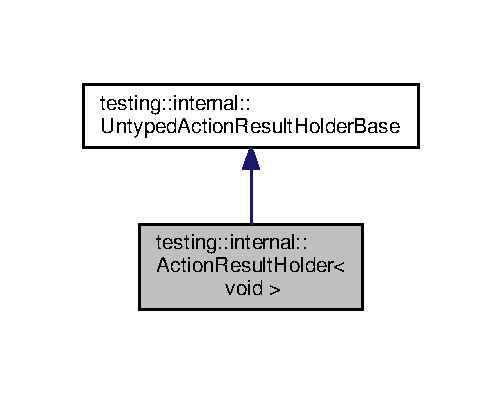
\includegraphics[width=241pt]{classtesting_1_1internal_1_1ActionResultHolder_3_01void_01_4__inherit__graph}
\end{center}
\end{figure}


Collaboration diagram for testing\+:\+:internal\+:\+:Action\+Result\+Holder$<$ void $>$\+:\nopagebreak
\begin{figure}[H]
\begin{center}
\leavevmode
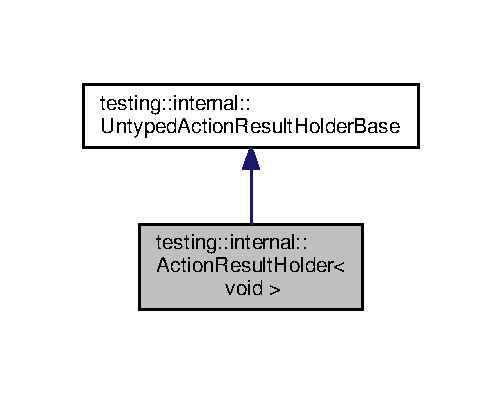
\includegraphics[width=241pt]{classtesting_1_1internal_1_1ActionResultHolder_3_01void_01_4__coll__graph}
\end{center}
\end{figure}
\subsection*{Public Member Functions}
\begin{DoxyCompactItemize}
\item 
void \hyperlink{classtesting_1_1internal_1_1ActionResultHolder_3_01void_01_4_aa57f371e1559b236e6424b2f50dcd6a2}{Unwrap} ()
\item 
virtual void \hyperlink{classtesting_1_1internal_1_1ActionResultHolder_3_01void_01_4_a6729c4fe6c33485ece4fbcfea8806e49}{Print\+As\+Action\+Result} (\+::std\+::ostream $\ast$) const 
\end{DoxyCompactItemize}
\subsection*{Static Public Member Functions}
\begin{DoxyCompactItemize}
\item 
{\footnotesize template$<$typename F $>$ }\\static \hyperlink{classtesting_1_1internal_1_1ActionResultHolder}{Action\+Result\+Holder} $\ast$ \hyperlink{classtesting_1_1internal_1_1ActionResultHolder_3_01void_01_4_a140b6ab6a756e60db62e76b01b09a26f}{Perform\+Default\+Action} (const \hyperlink{classtesting_1_1internal_1_1FunctionMockerBase}{Function\+Mocker\+Base}$<$ F $>$ $\ast$func\+\_\+mocker, const typename \hyperlink{structtesting_1_1internal_1_1Function}{Function}$<$ F $>$\+::Argument\+Tuple \&args, const \hyperlink{namespacetesting_1_1internal_a8e8ff5b11e64078831112677156cb111}{string} \&call\+\_\+description)
\item 
{\footnotesize template$<$typename F $>$ }\\static \hyperlink{classtesting_1_1internal_1_1ActionResultHolder}{Action\+Result\+Holder} $\ast$ \hyperlink{classtesting_1_1internal_1_1ActionResultHolder_3_01void_01_4_abb1d387e21341393e0c237ae7b02ee68}{Perform\+Action} (const \hyperlink{classtesting_1_1Action}{Action}$<$ F $>$ \&action, const typename \hyperlink{structtesting_1_1internal_1_1Function}{Function}$<$ F $>$\+::Argument\+Tuple \&args)
\end{DoxyCompactItemize}


\subsection{Member Function Documentation}
\index{testing\+::internal\+::\+Action\+Result\+Holder$<$ void $>$@{testing\+::internal\+::\+Action\+Result\+Holder$<$ void $>$}!Perform\+Action@{Perform\+Action}}
\index{Perform\+Action@{Perform\+Action}!testing\+::internal\+::\+Action\+Result\+Holder$<$ void $>$@{testing\+::internal\+::\+Action\+Result\+Holder$<$ void $>$}}
\subsubsection[{\texorpdfstring{Perform\+Action(const Action$<$ F $>$ \&action, const typename Function$<$ F $>$\+::\+Argument\+Tuple \&args)}{PerformAction(const Action< F > &action, const typename Function< F >::ArgumentTuple &args)}}]{\setlength{\rightskip}{0pt plus 5cm}template$<$typename F $>$ static {\bf Action\+Result\+Holder}$\ast$ {\bf testing\+::internal\+::\+Action\+Result\+Holder}$<$ void $>$\+::Perform\+Action (
\begin{DoxyParamCaption}
\item[{const {\bf Action}$<$ F $>$ \&}]{action, }
\item[{const typename {\bf Function}$<$ F $>$\+::Argument\+Tuple \&}]{args}
\end{DoxyParamCaption}
)\hspace{0.3cm}{\ttfamily [inline]}, {\ttfamily [static]}}\hypertarget{classtesting_1_1internal_1_1ActionResultHolder_3_01void_01_4_abb1d387e21341393e0c237ae7b02ee68}{}\label{classtesting_1_1internal_1_1ActionResultHolder_3_01void_01_4_abb1d387e21341393e0c237ae7b02ee68}

\begin{DoxyCode}
1442                                                      \{
1443     \hyperlink{namespaceupload_a675d13c979f1c720866d22ed1736f580}{action}.Perform(args);
1444     \textcolor{keywordflow}{return} \textcolor{keyword}{new} ActionResultHolder;
1445   \}
\end{DoxyCode}
\index{testing\+::internal\+::\+Action\+Result\+Holder$<$ void $>$@{testing\+::internal\+::\+Action\+Result\+Holder$<$ void $>$}!Perform\+Default\+Action@{Perform\+Default\+Action}}
\index{Perform\+Default\+Action@{Perform\+Default\+Action}!testing\+::internal\+::\+Action\+Result\+Holder$<$ void $>$@{testing\+::internal\+::\+Action\+Result\+Holder$<$ void $>$}}
\subsubsection[{\texorpdfstring{Perform\+Default\+Action(const Function\+Mocker\+Base$<$ F $>$ $\ast$func\+\_\+mocker, const typename Function$<$ F $>$\+::\+Argument\+Tuple \&args, const string \&call\+\_\+description)}{PerformDefaultAction(const FunctionMockerBase< F > *func_mocker, const typename Function< F >::ArgumentTuple &args, const string &call_description)}}]{\setlength{\rightskip}{0pt plus 5cm}template$<$typename F $>$ static {\bf Action\+Result\+Holder}$\ast$ {\bf testing\+::internal\+::\+Action\+Result\+Holder}$<$ void $>$\+::Perform\+Default\+Action (
\begin{DoxyParamCaption}
\item[{const {\bf Function\+Mocker\+Base}$<$ F $>$ $\ast$}]{func\+\_\+mocker, }
\item[{const typename {\bf Function}$<$ F $>$\+::Argument\+Tuple \&}]{args, }
\item[{const {\bf string} \&}]{call\+\_\+description}
\end{DoxyParamCaption}
)\hspace{0.3cm}{\ttfamily [inline]}, {\ttfamily [static]}}\hypertarget{classtesting_1_1internal_1_1ActionResultHolder_3_01void_01_4_a140b6ab6a756e60db62e76b01b09a26f}{}\label{classtesting_1_1internal_1_1ActionResultHolder_3_01void_01_4_a140b6ab6a756e60db62e76b01b09a26f}

\begin{DoxyCode}
1432                                       \{
1433     func\_mocker->PerformDefaultAction(args, call\_description);
1434     \textcolor{keywordflow}{return} \textcolor{keyword}{new} ActionResultHolder;
1435   \}
\end{DoxyCode}
\index{testing\+::internal\+::\+Action\+Result\+Holder$<$ void $>$@{testing\+::internal\+::\+Action\+Result\+Holder$<$ void $>$}!Print\+As\+Action\+Result@{Print\+As\+Action\+Result}}
\index{Print\+As\+Action\+Result@{Print\+As\+Action\+Result}!testing\+::internal\+::\+Action\+Result\+Holder$<$ void $>$@{testing\+::internal\+::\+Action\+Result\+Holder$<$ void $>$}}
\subsubsection[{\texorpdfstring{Print\+As\+Action\+Result(\+::std\+::ostream $\ast$) const }{PrintAsActionResult(::std::ostream *) const }}]{\setlength{\rightskip}{0pt plus 5cm}virtual void {\bf testing\+::internal\+::\+Action\+Result\+Holder}$<$ void $>$\+::Print\+As\+Action\+Result (
\begin{DoxyParamCaption}
\item[{\+::std\+::ostream $\ast$}]{}
\end{DoxyParamCaption}
) const\hspace{0.3cm}{\ttfamily [inline]}, {\ttfamily [virtual]}}\hypertarget{classtesting_1_1internal_1_1ActionResultHolder_3_01void_01_4_a6729c4fe6c33485ece4fbcfea8806e49}{}\label{classtesting_1_1internal_1_1ActionResultHolder_3_01void_01_4_a6729c4fe6c33485ece4fbcfea8806e49}


Implements \hyperlink{classtesting_1_1internal_1_1UntypedActionResultHolderBase_a4b4a558fcb1d3b02c0fec34f186d3b90}{testing\+::internal\+::\+Untyped\+Action\+Result\+Holder\+Base}.


\begin{DoxyCode}
1424 \{\}
\end{DoxyCode}
\index{testing\+::internal\+::\+Action\+Result\+Holder$<$ void $>$@{testing\+::internal\+::\+Action\+Result\+Holder$<$ void $>$}!Unwrap@{Unwrap}}
\index{Unwrap@{Unwrap}!testing\+::internal\+::\+Action\+Result\+Holder$<$ void $>$@{testing\+::internal\+::\+Action\+Result\+Holder$<$ void $>$}}
\subsubsection[{\texorpdfstring{Unwrap()}{Unwrap()}}]{\setlength{\rightskip}{0pt plus 5cm}void {\bf testing\+::internal\+::\+Action\+Result\+Holder}$<$ void $>$\+::Unwrap (
\begin{DoxyParamCaption}
{}
\end{DoxyParamCaption}
)\hspace{0.3cm}{\ttfamily [inline]}}\hypertarget{classtesting_1_1internal_1_1ActionResultHolder_3_01void_01_4_aa57f371e1559b236e6424b2f50dcd6a2}{}\label{classtesting_1_1internal_1_1ActionResultHolder_3_01void_01_4_aa57f371e1559b236e6424b2f50dcd6a2}

\begin{DoxyCode}
1422 \{ \}
\end{DoxyCode}


The documentation for this class was generated from the following file\+:\begin{DoxyCompactItemize}
\item 
vendor/googletest/googlemock/include/gmock/\hyperlink{gmock-spec-builders_8h}{gmock-\/spec-\/builders.\+h}\end{DoxyCompactItemize}

\hypertarget{structstd_1_1tr1_1_1gtest__internal_1_1AddRef}{}\section{std\+:\+:tr1\+:\+:gtest\+\_\+internal\+:\+:Add\+Ref$<$ T $>$ Struct Template Reference}
\label{structstd_1_1tr1_1_1gtest__internal_1_1AddRef}\index{std\+::tr1\+::gtest\+\_\+internal\+::\+Add\+Ref$<$ T $>$@{std\+::tr1\+::gtest\+\_\+internal\+::\+Add\+Ref$<$ T $>$}}


{\ttfamily \#include $<$gtest-\/tuple.\+h$>$}

\subsection*{Public Types}
\begin{DoxyCompactItemize}
\item 
typedef T \& \hyperlink{structstd_1_1tr1_1_1gtest__internal_1_1AddRef_a1e5616e414125574c1653e3a1fc68491}{type}
\end{DoxyCompactItemize}


\subsection{Member Typedef Documentation}
\index{std\+::tr1\+::gtest\+\_\+internal\+::\+Add\+Ref@{std\+::tr1\+::gtest\+\_\+internal\+::\+Add\+Ref}!type@{type}}
\index{type@{type}!std\+::tr1\+::gtest\+\_\+internal\+::\+Add\+Ref@{std\+::tr1\+::gtest\+\_\+internal\+::\+Add\+Ref}}
\subsubsection[{\texorpdfstring{type}{type}}]{\setlength{\rightskip}{0pt plus 5cm}template$<$typename T $>$ typedef T\& {\bf std\+::tr1\+::gtest\+\_\+internal\+::\+Add\+Ref}$<$ T $>$\+::{\bf type}}\hypertarget{structstd_1_1tr1_1_1gtest__internal_1_1AddRef_a1e5616e414125574c1653e3a1fc68491}{}\label{structstd_1_1tr1_1_1gtest__internal_1_1AddRef_a1e5616e414125574c1653e3a1fc68491}


The documentation for this struct was generated from the following file\+:\begin{DoxyCompactItemize}
\item 
vendor/googletest/googletest/include/gtest/internal/\hyperlink{gtest-tuple_8h}{gtest-\/tuple.\+h}\end{DoxyCompactItemize}

\hypertarget{structstd_1_1tr1_1_1gtest__internal_1_1AddRef_3_01T_01_6_01_4}{}\section{std\+:\+:tr1\+:\+:gtest\+\_\+internal\+:\+:Add\+Ref$<$ T \& $>$ Struct Template Reference}
\label{structstd_1_1tr1_1_1gtest__internal_1_1AddRef_3_01T_01_6_01_4}\index{std\+::tr1\+::gtest\+\_\+internal\+::\+Add\+Ref$<$ T \& $>$@{std\+::tr1\+::gtest\+\_\+internal\+::\+Add\+Ref$<$ T \& $>$}}


{\ttfamily \#include $<$gtest-\/tuple.\+h$>$}

\subsection*{Public Types}
\begin{DoxyCompactItemize}
\item 
typedef T \& \hyperlink{structstd_1_1tr1_1_1gtest__internal_1_1AddRef_3_01T_01_6_01_4_a9cb3b0992c2a9e7df42d01fb64c2dc88}{type}
\end{DoxyCompactItemize}


\subsection{Member Typedef Documentation}
\index{std\+::tr1\+::gtest\+\_\+internal\+::\+Add\+Ref$<$ T \& $>$@{std\+::tr1\+::gtest\+\_\+internal\+::\+Add\+Ref$<$ T \& $>$}!type@{type}}
\index{type@{type}!std\+::tr1\+::gtest\+\_\+internal\+::\+Add\+Ref$<$ T \& $>$@{std\+::tr1\+::gtest\+\_\+internal\+::\+Add\+Ref$<$ T \& $>$}}
\subsubsection[{\texorpdfstring{type}{type}}]{\setlength{\rightskip}{0pt plus 5cm}template$<$typename T $>$ typedef T\& {\bf std\+::tr1\+::gtest\+\_\+internal\+::\+Add\+Ref}$<$ T \& $>$\+::{\bf type}}\hypertarget{structstd_1_1tr1_1_1gtest__internal_1_1AddRef_3_01T_01_6_01_4_a9cb3b0992c2a9e7df42d01fb64c2dc88}{}\label{structstd_1_1tr1_1_1gtest__internal_1_1AddRef_3_01T_01_6_01_4_a9cb3b0992c2a9e7df42d01fb64c2dc88}


The documentation for this struct was generated from the following file\+:\begin{DoxyCompactItemize}
\item 
vendor/googletest/googletest/include/gtest/internal/\hyperlink{gtest-tuple_8h}{gtest-\/tuple.\+h}\end{DoxyCompactItemize}

\hypertarget{structtesting_1_1internal_1_1AddReference}{}\section{testing\+:\+:internal\+:\+:Add\+Reference$<$ T $>$ Struct Template Reference}
\label{structtesting_1_1internal_1_1AddReference}\index{testing\+::internal\+::\+Add\+Reference$<$ T $>$@{testing\+::internal\+::\+Add\+Reference$<$ T $>$}}


{\ttfamily \#include $<$gtest-\/internal.\+h$>$}

\subsection*{Public Types}
\begin{DoxyCompactItemize}
\item 
typedef T \& \hyperlink{structtesting_1_1internal_1_1AddReference_a2df8dd7c4e41f6390e6e66b1a9a67bb4}{type}
\end{DoxyCompactItemize}


\subsection{Member Typedef Documentation}
\index{testing\+::internal\+::\+Add\+Reference@{testing\+::internal\+::\+Add\+Reference}!type@{type}}
\index{type@{type}!testing\+::internal\+::\+Add\+Reference@{testing\+::internal\+::\+Add\+Reference}}
\subsubsection[{\texorpdfstring{type}{type}}]{\setlength{\rightskip}{0pt plus 5cm}template$<$typename T$>$ typedef T\& {\bf testing\+::internal\+::\+Add\+Reference}$<$ T $>$\+::{\bf type}}\hypertarget{structtesting_1_1internal_1_1AddReference_a2df8dd7c4e41f6390e6e66b1a9a67bb4}{}\label{structtesting_1_1internal_1_1AddReference_a2df8dd7c4e41f6390e6e66b1a9a67bb4}


The documentation for this struct was generated from the following file\+:\begin{DoxyCompactItemize}
\item 
vendor/googletest/googletest/include/gtest/internal/\hyperlink{gtest-internal_8h}{gtest-\/internal.\+h}\end{DoxyCompactItemize}

\hypertarget{structtesting_1_1internal_1_1AddReference_3_01T_01_6_01_4}{}\section{testing\+:\+:internal\+:\+:Add\+Reference$<$ T \& $>$ Struct Template Reference}
\label{structtesting_1_1internal_1_1AddReference_3_01T_01_6_01_4}\index{testing\+::internal\+::\+Add\+Reference$<$ T \& $>$@{testing\+::internal\+::\+Add\+Reference$<$ T \& $>$}}


{\ttfamily \#include $<$gtest-\/internal.\+h$>$}

\subsection*{Public Types}
\begin{DoxyCompactItemize}
\item 
typedef T \& \hyperlink{structtesting_1_1internal_1_1AddReference_3_01T_01_6_01_4_a93c064cdcdaced0abd167258425e57af}{type}
\end{DoxyCompactItemize}


\subsection{Member Typedef Documentation}
\index{testing\+::internal\+::\+Add\+Reference$<$ T \& $>$@{testing\+::internal\+::\+Add\+Reference$<$ T \& $>$}!type@{type}}
\index{type@{type}!testing\+::internal\+::\+Add\+Reference$<$ T \& $>$@{testing\+::internal\+::\+Add\+Reference$<$ T \& $>$}}
\subsubsection[{\texorpdfstring{type}{type}}]{\setlength{\rightskip}{0pt plus 5cm}template$<$typename T $>$ typedef T\& {\bf testing\+::internal\+::\+Add\+Reference}$<$ T \& $>$\+::{\bf type}}\hypertarget{structtesting_1_1internal_1_1AddReference_3_01T_01_6_01_4_a93c064cdcdaced0abd167258425e57af}{}\label{structtesting_1_1internal_1_1AddReference_3_01T_01_6_01_4_a93c064cdcdaced0abd167258425e57af}


The documentation for this struct was generated from the following file\+:\begin{DoxyCompactItemize}
\item 
vendor/googletest/googletest/include/gtest/internal/\hyperlink{gtest-internal_8h}{gtest-\/internal.\+h}\end{DoxyCompactItemize}

\hypertarget{structtesting_1_1internal_1_1invoke__argument_1_1AdlTag}{}\section{testing\+:\+:internal\+:\+:invoke\+\_\+argument\+:\+:Adl\+Tag Struct Reference}
\label{structtesting_1_1internal_1_1invoke__argument_1_1AdlTag}\index{testing\+::internal\+::invoke\+\_\+argument\+::\+Adl\+Tag@{testing\+::internal\+::invoke\+\_\+argument\+::\+Adl\+Tag}}


{\ttfamily \#include $<$gmock-\/generated-\/actions.\+h$>$}



The documentation for this struct was generated from the following file\+:\begin{DoxyCompactItemize}
\item 
vendor/googletest/googlemock/include/gmock/\hyperlink{gmock-generated-actions_8h}{gmock-\/generated-\/actions.\+h}\end{DoxyCompactItemize}

\hypertarget{classtesting_1_1gmock__matchers__test_1_1AllArgsHelper}{}\section{testing\+:\+:gmock\+\_\+matchers\+\_\+test\+:\+:All\+Args\+Helper Class Reference}
\label{classtesting_1_1gmock__matchers__test_1_1AllArgsHelper}\index{testing\+::gmock\+\_\+matchers\+\_\+test\+::\+All\+Args\+Helper@{testing\+::gmock\+\_\+matchers\+\_\+test\+::\+All\+Args\+Helper}}
\subsection*{Public Member Functions}
\begin{DoxyCompactItemize}
\item 
\hyperlink{classtesting_1_1gmock__matchers__test_1_1AllArgsHelper_afffee92e50b5545e5b4be8c989ff63ab}{All\+Args\+Helper} ()
\item 
\hyperlink{classtesting_1_1gmock__matchers__test_1_1AllArgsHelper_a571b9c1e5ab4e891085060e73c94be32}{M\+O\+C\+K\+\_\+\+M\+E\+T\+H\+O\+D2} (Helper, int(char x, int y))
\end{DoxyCompactItemize}


\subsection{Constructor \& Destructor Documentation}
\index{testing\+::gmock\+\_\+matchers\+\_\+test\+::\+All\+Args\+Helper@{testing\+::gmock\+\_\+matchers\+\_\+test\+::\+All\+Args\+Helper}!All\+Args\+Helper@{All\+Args\+Helper}}
\index{All\+Args\+Helper@{All\+Args\+Helper}!testing\+::gmock\+\_\+matchers\+\_\+test\+::\+All\+Args\+Helper@{testing\+::gmock\+\_\+matchers\+\_\+test\+::\+All\+Args\+Helper}}
\subsubsection[{\texorpdfstring{All\+Args\+Helper()}{AllArgsHelper()}}]{\setlength{\rightskip}{0pt plus 5cm}testing\+::gmock\+\_\+matchers\+\_\+test\+::\+All\+Args\+Helper\+::\+All\+Args\+Helper (
\begin{DoxyParamCaption}
{}
\end{DoxyParamCaption}
)\hspace{0.3cm}{\ttfamily [inline]}}\hypertarget{classtesting_1_1gmock__matchers__test_1_1AllArgsHelper_afffee92e50b5545e5b4be8c989ff63ab}{}\label{classtesting_1_1gmock__matchers__test_1_1AllArgsHelper_afffee92e50b5545e5b4be8c989ff63ab}

\begin{DoxyCode}
2598 \{\}
\end{DoxyCode}


\subsection{Member Function Documentation}
\index{testing\+::gmock\+\_\+matchers\+\_\+test\+::\+All\+Args\+Helper@{testing\+::gmock\+\_\+matchers\+\_\+test\+::\+All\+Args\+Helper}!M\+O\+C\+K\+\_\+\+M\+E\+T\+H\+O\+D2@{M\+O\+C\+K\+\_\+\+M\+E\+T\+H\+O\+D2}}
\index{M\+O\+C\+K\+\_\+\+M\+E\+T\+H\+O\+D2@{M\+O\+C\+K\+\_\+\+M\+E\+T\+H\+O\+D2}!testing\+::gmock\+\_\+matchers\+\_\+test\+::\+All\+Args\+Helper@{testing\+::gmock\+\_\+matchers\+\_\+test\+::\+All\+Args\+Helper}}
\subsubsection[{\texorpdfstring{M\+O\+C\+K\+\_\+\+M\+E\+T\+H\+O\+D2(\+Helper, int(char x, int y))}{MOCK_METHOD2(Helper, int(char x, int y))}}]{\setlength{\rightskip}{0pt plus 5cm}testing\+::gmock\+\_\+matchers\+\_\+test\+::\+All\+Args\+Helper\+::\+M\+O\+C\+K\+\_\+\+M\+E\+T\+H\+O\+D2 (
\begin{DoxyParamCaption}
\item[{Helper}]{, }
\item[{int(char x, int y)}]{}
\end{DoxyParamCaption}
)}\hypertarget{classtesting_1_1gmock__matchers__test_1_1AllArgsHelper_a571b9c1e5ab4e891085060e73c94be32}{}\label{classtesting_1_1gmock__matchers__test_1_1AllArgsHelper_a571b9c1e5ab4e891085060e73c94be32}


The documentation for this class was generated from the following file\+:\begin{DoxyCompactItemize}
\item 
vendor/googletest/googlemock/test/\hyperlink{gmock-matchers__test_8cc}{gmock-\/matchers\+\_\+test.\+cc}\end{DoxyCompactItemize}

\hypertarget{structtesting_1_1internal_1_1AllOfResult1}{}\section{testing\+:\+:internal\+:\+:All\+Of\+Result1$<$ M1 $>$ Struct Template Reference}
\label{structtesting_1_1internal_1_1AllOfResult1}\index{testing\+::internal\+::\+All\+Of\+Result1$<$ M1 $>$@{testing\+::internal\+::\+All\+Of\+Result1$<$ M1 $>$}}


{\ttfamily \#include $<$gmock-\/generated-\/matchers.\+h$>$}

\subsection*{Public Types}
\begin{DoxyCompactItemize}
\item 
typedef M1 \hyperlink{structtesting_1_1internal_1_1AllOfResult1_a19b95d4ddf7f4044a78665d9e253db10}{type}
\end{DoxyCompactItemize}


\subsection{Member Typedef Documentation}
\index{testing\+::internal\+::\+All\+Of\+Result1@{testing\+::internal\+::\+All\+Of\+Result1}!type@{type}}
\index{type@{type}!testing\+::internal\+::\+All\+Of\+Result1@{testing\+::internal\+::\+All\+Of\+Result1}}
\subsubsection[{\texorpdfstring{type}{type}}]{\setlength{\rightskip}{0pt plus 5cm}template$<$typename M1$>$ typedef M1 {\bf testing\+::internal\+::\+All\+Of\+Result1}$<$ M1 $>$\+::{\bf type}}\hypertarget{structtesting_1_1internal_1_1AllOfResult1_a19b95d4ddf7f4044a78665d9e253db10}{}\label{structtesting_1_1internal_1_1AllOfResult1_a19b95d4ddf7f4044a78665d9e253db10}


The documentation for this struct was generated from the following file\+:\begin{DoxyCompactItemize}
\item 
vendor/googletest/googlemock/include/gmock/\hyperlink{gmock-generated-matchers_8h}{gmock-\/generated-\/matchers.\+h}\end{DoxyCompactItemize}

\hypertarget{structtesting_1_1internal_1_1AllOfResult10}{}\section{testing\+:\+:internal\+:\+:All\+Of\+Result10$<$ M1, M2, M3, M4, M5, M6, M7, M8, M9, M10 $>$ Struct Template Reference}
\label{structtesting_1_1internal_1_1AllOfResult10}\index{testing\+::internal\+::\+All\+Of\+Result10$<$ M1, M2, M3, M4, M5, M6, M7, M8, M9, M10 $>$@{testing\+::internal\+::\+All\+Of\+Result10$<$ M1, M2, M3, M4, M5, M6, M7, M8, M9, M10 $>$}}


{\ttfamily \#include $<$gmock-\/generated-\/matchers.\+h$>$}

\subsection*{Public Types}
\begin{DoxyCompactItemize}
\item 
typedef \hyperlink{classtesting_1_1internal_1_1BothOfMatcher}{Both\+Of\+Matcher}$<$ typename \hyperlink{structtesting_1_1internal_1_1AllOfResult5}{All\+Of\+Result5}$<$ M1, M2, M3, M4, M5 $>$\+::\hyperlink{structtesting_1_1internal_1_1AllOfResult10_a48d6c6de6d0d5445b212119e1f536af5}{type}, typename \hyperlink{structtesting_1_1internal_1_1AllOfResult5}{All\+Of\+Result5}$<$ M6, M7, M8, M9, M10 $>$\+::\hyperlink{structtesting_1_1internal_1_1AllOfResult10_a48d6c6de6d0d5445b212119e1f536af5}{type} $>$ \hyperlink{structtesting_1_1internal_1_1AllOfResult10_a48d6c6de6d0d5445b212119e1f536af5}{type}
\end{DoxyCompactItemize}


\subsection{Member Typedef Documentation}
\index{testing\+::internal\+::\+All\+Of\+Result10@{testing\+::internal\+::\+All\+Of\+Result10}!type@{type}}
\index{type@{type}!testing\+::internal\+::\+All\+Of\+Result10@{testing\+::internal\+::\+All\+Of\+Result10}}
\subsubsection[{\texorpdfstring{type}{type}}]{\setlength{\rightskip}{0pt plus 5cm}template$<$typename M1 , typename M2 , typename M3 , typename M4 , typename M5 , typename M6 , typename M7 , typename M8 , typename M9 , typename M10 $>$ typedef {\bf Both\+Of\+Matcher}$<$ typename {\bf All\+Of\+Result5}$<$M1, M2, M3, M4, M5$>$\+::{\bf type}, typename {\bf All\+Of\+Result5}$<$M6, M7, M8, M9, M10$>$\+::{\bf type} $>$ {\bf testing\+::internal\+::\+All\+Of\+Result10}$<$ M1, M2, M3, M4, M5, M6, M7, M8, M9, M10 $>$\+::{\bf type}}\hypertarget{structtesting_1_1internal_1_1AllOfResult10_a48d6c6de6d0d5445b212119e1f536af5}{}\label{structtesting_1_1internal_1_1AllOfResult10_a48d6c6de6d0d5445b212119e1f536af5}


The documentation for this struct was generated from the following file\+:\begin{DoxyCompactItemize}
\item 
vendor/googletest/googlemock/include/gmock/\hyperlink{gmock-generated-matchers_8h}{gmock-\/generated-\/matchers.\+h}\end{DoxyCompactItemize}

\hypertarget{structtesting_1_1internal_1_1AllOfResult2}{}\section{testing\+:\+:internal\+:\+:All\+Of\+Result2$<$ M1, M2 $>$ Struct Template Reference}
\label{structtesting_1_1internal_1_1AllOfResult2}\index{testing\+::internal\+::\+All\+Of\+Result2$<$ M1, M2 $>$@{testing\+::internal\+::\+All\+Of\+Result2$<$ M1, M2 $>$}}


{\ttfamily \#include $<$gmock-\/generated-\/matchers.\+h$>$}

\subsection*{Public Types}
\begin{DoxyCompactItemize}
\item 
typedef \hyperlink{classtesting_1_1internal_1_1BothOfMatcher}{Both\+Of\+Matcher}$<$ typename \hyperlink{structtesting_1_1internal_1_1AllOfResult1}{All\+Of\+Result1}$<$ M1 $>$\+::\hyperlink{structtesting_1_1internal_1_1AllOfResult2_adec0b0ce2fdd07d398e1fdd2cdb88392}{type}, typename \hyperlink{structtesting_1_1internal_1_1AllOfResult1}{All\+Of\+Result1}$<$ M2 $>$\+::\hyperlink{structtesting_1_1internal_1_1AllOfResult2_adec0b0ce2fdd07d398e1fdd2cdb88392}{type} $>$ \hyperlink{structtesting_1_1internal_1_1AllOfResult2_adec0b0ce2fdd07d398e1fdd2cdb88392}{type}
\end{DoxyCompactItemize}


\subsection{Member Typedef Documentation}
\index{testing\+::internal\+::\+All\+Of\+Result2@{testing\+::internal\+::\+All\+Of\+Result2}!type@{type}}
\index{type@{type}!testing\+::internal\+::\+All\+Of\+Result2@{testing\+::internal\+::\+All\+Of\+Result2}}
\subsubsection[{\texorpdfstring{type}{type}}]{\setlength{\rightskip}{0pt plus 5cm}template$<$typename M1, typename M2$>$ typedef {\bf Both\+Of\+Matcher}$<$ typename {\bf All\+Of\+Result1}$<$M1$>$\+::{\bf type}, typename {\bf All\+Of\+Result1}$<$M2$>$\+::{\bf type} $>$ {\bf testing\+::internal\+::\+All\+Of\+Result2}$<$ M1, M2 $>$\+::{\bf type}}\hypertarget{structtesting_1_1internal_1_1AllOfResult2_adec0b0ce2fdd07d398e1fdd2cdb88392}{}\label{structtesting_1_1internal_1_1AllOfResult2_adec0b0ce2fdd07d398e1fdd2cdb88392}


The documentation for this struct was generated from the following file\+:\begin{DoxyCompactItemize}
\item 
vendor/googletest/googlemock/include/gmock/\hyperlink{gmock-generated-matchers_8h}{gmock-\/generated-\/matchers.\+h}\end{DoxyCompactItemize}

\hypertarget{structtesting_1_1internal_1_1AllOfResult3}{}\section{testing\+:\+:internal\+:\+:All\+Of\+Result3$<$ M1, M2, M3 $>$ Struct Template Reference}
\label{structtesting_1_1internal_1_1AllOfResult3}\index{testing\+::internal\+::\+All\+Of\+Result3$<$ M1, M2, M3 $>$@{testing\+::internal\+::\+All\+Of\+Result3$<$ M1, M2, M3 $>$}}


{\ttfamily \#include $<$gmock-\/generated-\/matchers.\+h$>$}

\subsection*{Public Types}
\begin{DoxyCompactItemize}
\item 
typedef \hyperlink{classtesting_1_1internal_1_1BothOfMatcher}{Both\+Of\+Matcher}$<$ typename \hyperlink{structtesting_1_1internal_1_1AllOfResult1}{All\+Of\+Result1}$<$ M1 $>$\+::\hyperlink{structtesting_1_1internal_1_1AllOfResult3_a18073a23acd542bccf3a6c5d7f72f957}{type}, typename \hyperlink{structtesting_1_1internal_1_1AllOfResult2}{All\+Of\+Result2}$<$ M2, M3 $>$\+::\hyperlink{structtesting_1_1internal_1_1AllOfResult3_a18073a23acd542bccf3a6c5d7f72f957}{type} $>$ \hyperlink{structtesting_1_1internal_1_1AllOfResult3_a18073a23acd542bccf3a6c5d7f72f957}{type}
\end{DoxyCompactItemize}


\subsection{Member Typedef Documentation}
\index{testing\+::internal\+::\+All\+Of\+Result3@{testing\+::internal\+::\+All\+Of\+Result3}!type@{type}}
\index{type@{type}!testing\+::internal\+::\+All\+Of\+Result3@{testing\+::internal\+::\+All\+Of\+Result3}}
\subsubsection[{\texorpdfstring{type}{type}}]{\setlength{\rightskip}{0pt plus 5cm}template$<$typename M1, typename M2, typename M3$>$ typedef {\bf Both\+Of\+Matcher}$<$ typename {\bf All\+Of\+Result1}$<$M1$>$\+::{\bf type}, typename {\bf All\+Of\+Result2}$<$M2, M3$>$\+::{\bf type} $>$ {\bf testing\+::internal\+::\+All\+Of\+Result3}$<$ M1, M2, M3 $>$\+::{\bf type}}\hypertarget{structtesting_1_1internal_1_1AllOfResult3_a18073a23acd542bccf3a6c5d7f72f957}{}\label{structtesting_1_1internal_1_1AllOfResult3_a18073a23acd542bccf3a6c5d7f72f957}


The documentation for this struct was generated from the following file\+:\begin{DoxyCompactItemize}
\item 
vendor/googletest/googlemock/include/gmock/\hyperlink{gmock-generated-matchers_8h}{gmock-\/generated-\/matchers.\+h}\end{DoxyCompactItemize}

\hypertarget{structtesting_1_1internal_1_1AllOfResult4}{}\section{testing\+:\+:internal\+:\+:All\+Of\+Result4$<$ M1, M2, M3, M4 $>$ Struct Template Reference}
\label{structtesting_1_1internal_1_1AllOfResult4}\index{testing\+::internal\+::\+All\+Of\+Result4$<$ M1, M2, M3, M4 $>$@{testing\+::internal\+::\+All\+Of\+Result4$<$ M1, M2, M3, M4 $>$}}


{\ttfamily \#include $<$gmock-\/generated-\/matchers.\+h$>$}

\subsection*{Public Types}
\begin{DoxyCompactItemize}
\item 
typedef \hyperlink{classtesting_1_1internal_1_1BothOfMatcher}{Both\+Of\+Matcher}$<$ typename \hyperlink{structtesting_1_1internal_1_1AllOfResult2}{All\+Of\+Result2}$<$ M1, M2 $>$\+::\hyperlink{structtesting_1_1internal_1_1AllOfResult4_ab277e20178bac632d4e5a39a1a407bbf}{type}, typename \hyperlink{structtesting_1_1internal_1_1AllOfResult2}{All\+Of\+Result2}$<$ M3, M4 $>$\+::\hyperlink{structtesting_1_1internal_1_1AllOfResult4_ab277e20178bac632d4e5a39a1a407bbf}{type} $>$ \hyperlink{structtesting_1_1internal_1_1AllOfResult4_ab277e20178bac632d4e5a39a1a407bbf}{type}
\end{DoxyCompactItemize}


\subsection{Member Typedef Documentation}
\index{testing\+::internal\+::\+All\+Of\+Result4@{testing\+::internal\+::\+All\+Of\+Result4}!type@{type}}
\index{type@{type}!testing\+::internal\+::\+All\+Of\+Result4@{testing\+::internal\+::\+All\+Of\+Result4}}
\subsubsection[{\texorpdfstring{type}{type}}]{\setlength{\rightskip}{0pt plus 5cm}template$<$typename M1, typename M2, typename M3, typename M4$>$ typedef {\bf Both\+Of\+Matcher}$<$ typename {\bf All\+Of\+Result2}$<$M1, M2$>$\+::{\bf type}, typename {\bf All\+Of\+Result2}$<$M3, M4$>$\+::{\bf type} $>$ {\bf testing\+::internal\+::\+All\+Of\+Result4}$<$ M1, M2, M3, M4 $>$\+::{\bf type}}\hypertarget{structtesting_1_1internal_1_1AllOfResult4_ab277e20178bac632d4e5a39a1a407bbf}{}\label{structtesting_1_1internal_1_1AllOfResult4_ab277e20178bac632d4e5a39a1a407bbf}


The documentation for this struct was generated from the following file\+:\begin{DoxyCompactItemize}
\item 
vendor/googletest/googlemock/include/gmock/\hyperlink{gmock-generated-matchers_8h}{gmock-\/generated-\/matchers.\+h}\end{DoxyCompactItemize}

\hypertarget{structtesting_1_1internal_1_1AllOfResult5}{}\section{testing\+:\+:internal\+:\+:All\+Of\+Result5$<$ M1, M2, M3, M4, M5 $>$ Struct Template Reference}
\label{structtesting_1_1internal_1_1AllOfResult5}\index{testing\+::internal\+::\+All\+Of\+Result5$<$ M1, M2, M3, M4, M5 $>$@{testing\+::internal\+::\+All\+Of\+Result5$<$ M1, M2, M3, M4, M5 $>$}}


{\ttfamily \#include $<$gmock-\/generated-\/matchers.\+h$>$}

\subsection*{Public Types}
\begin{DoxyCompactItemize}
\item 
typedef \hyperlink{classtesting_1_1internal_1_1BothOfMatcher}{Both\+Of\+Matcher}$<$ typename \hyperlink{structtesting_1_1internal_1_1AllOfResult2}{All\+Of\+Result2}$<$ M1, M2 $>$\+::\hyperlink{structtesting_1_1internal_1_1AllOfResult5_aee2e1fb803f428741d147347b692d108}{type}, typename \hyperlink{structtesting_1_1internal_1_1AllOfResult3}{All\+Of\+Result3}$<$ M3, M4, M5 $>$\+::\hyperlink{structtesting_1_1internal_1_1AllOfResult5_aee2e1fb803f428741d147347b692d108}{type} $>$ \hyperlink{structtesting_1_1internal_1_1AllOfResult5_aee2e1fb803f428741d147347b692d108}{type}
\end{DoxyCompactItemize}


\subsection{Member Typedef Documentation}
\index{testing\+::internal\+::\+All\+Of\+Result5@{testing\+::internal\+::\+All\+Of\+Result5}!type@{type}}
\index{type@{type}!testing\+::internal\+::\+All\+Of\+Result5@{testing\+::internal\+::\+All\+Of\+Result5}}
\subsubsection[{\texorpdfstring{type}{type}}]{\setlength{\rightskip}{0pt plus 5cm}template$<$typename M1, typename M2, typename M3, typename M4, typename M5$>$ typedef {\bf Both\+Of\+Matcher}$<$ typename {\bf All\+Of\+Result2}$<$M1, M2$>$\+::{\bf type}, typename {\bf All\+Of\+Result3}$<$M3, M4, M5$>$\+::{\bf type} $>$ {\bf testing\+::internal\+::\+All\+Of\+Result5}$<$ M1, M2, M3, M4, M5 $>$\+::{\bf type}}\hypertarget{structtesting_1_1internal_1_1AllOfResult5_aee2e1fb803f428741d147347b692d108}{}\label{structtesting_1_1internal_1_1AllOfResult5_aee2e1fb803f428741d147347b692d108}


The documentation for this struct was generated from the following file\+:\begin{DoxyCompactItemize}
\item 
vendor/googletest/googlemock/include/gmock/\hyperlink{gmock-generated-matchers_8h}{gmock-\/generated-\/matchers.\+h}\end{DoxyCompactItemize}

\hypertarget{structtesting_1_1internal_1_1AllOfResult6}{}\section{testing\+:\+:internal\+:\+:All\+Of\+Result6$<$ M1, M2, M3, M4, M5, M6 $>$ Struct Template Reference}
\label{structtesting_1_1internal_1_1AllOfResult6}\index{testing\+::internal\+::\+All\+Of\+Result6$<$ M1, M2, M3, M4, M5, M6 $>$@{testing\+::internal\+::\+All\+Of\+Result6$<$ M1, M2, M3, M4, M5, M6 $>$}}


{\ttfamily \#include $<$gmock-\/generated-\/matchers.\+h$>$}

\subsection*{Public Types}
\begin{DoxyCompactItemize}
\item 
typedef \hyperlink{classtesting_1_1internal_1_1BothOfMatcher}{Both\+Of\+Matcher}$<$ typename \hyperlink{structtesting_1_1internal_1_1AllOfResult3}{All\+Of\+Result3}$<$ M1, M2, M3 $>$\+::\hyperlink{structtesting_1_1internal_1_1AllOfResult6_a5385655911ce2c1d3fccd802c1754139}{type}, typename \hyperlink{structtesting_1_1internal_1_1AllOfResult3}{All\+Of\+Result3}$<$ M4, M5, M6 $>$\+::\hyperlink{structtesting_1_1internal_1_1AllOfResult6_a5385655911ce2c1d3fccd802c1754139}{type} $>$ \hyperlink{structtesting_1_1internal_1_1AllOfResult6_a5385655911ce2c1d3fccd802c1754139}{type}
\end{DoxyCompactItemize}


\subsection{Member Typedef Documentation}
\index{testing\+::internal\+::\+All\+Of\+Result6@{testing\+::internal\+::\+All\+Of\+Result6}!type@{type}}
\index{type@{type}!testing\+::internal\+::\+All\+Of\+Result6@{testing\+::internal\+::\+All\+Of\+Result6}}
\subsubsection[{\texorpdfstring{type}{type}}]{\setlength{\rightskip}{0pt plus 5cm}template$<$typename M1, typename M2, typename M3, typename M4, typename M5, typename M6$>$ typedef {\bf Both\+Of\+Matcher}$<$ typename {\bf All\+Of\+Result3}$<$M1, M2, M3$>$\+::{\bf type}, typename {\bf All\+Of\+Result3}$<$M4, M5, M6$>$\+::{\bf type} $>$ {\bf testing\+::internal\+::\+All\+Of\+Result6}$<$ M1, M2, M3, M4, M5, M6 $>$\+::{\bf type}}\hypertarget{structtesting_1_1internal_1_1AllOfResult6_a5385655911ce2c1d3fccd802c1754139}{}\label{structtesting_1_1internal_1_1AllOfResult6_a5385655911ce2c1d3fccd802c1754139}


The documentation for this struct was generated from the following file\+:\begin{DoxyCompactItemize}
\item 
vendor/googletest/googlemock/include/gmock/\hyperlink{gmock-generated-matchers_8h}{gmock-\/generated-\/matchers.\+h}\end{DoxyCompactItemize}

\hypertarget{structtesting_1_1internal_1_1AllOfResult7}{}\section{testing\+:\+:internal\+:\+:All\+Of\+Result7$<$ M1, M2, M3, M4, M5, M6, M7 $>$ Struct Template Reference}
\label{structtesting_1_1internal_1_1AllOfResult7}\index{testing\+::internal\+::\+All\+Of\+Result7$<$ M1, M2, M3, M4, M5, M6, M7 $>$@{testing\+::internal\+::\+All\+Of\+Result7$<$ M1, M2, M3, M4, M5, M6, M7 $>$}}


{\ttfamily \#include $<$gmock-\/generated-\/matchers.\+h$>$}

\subsection*{Public Types}
\begin{DoxyCompactItemize}
\item 
typedef \hyperlink{classtesting_1_1internal_1_1BothOfMatcher}{Both\+Of\+Matcher}$<$ typename \hyperlink{structtesting_1_1internal_1_1AllOfResult3}{All\+Of\+Result3}$<$ M1, M2, M3 $>$\+::\hyperlink{structtesting_1_1internal_1_1AllOfResult7_a47ab0d670258434b0e65530591948e8c}{type}, typename \hyperlink{structtesting_1_1internal_1_1AllOfResult4}{All\+Of\+Result4}$<$ M4, M5, M6, M7 $>$\+::\hyperlink{structtesting_1_1internal_1_1AllOfResult7_a47ab0d670258434b0e65530591948e8c}{type} $>$ \hyperlink{structtesting_1_1internal_1_1AllOfResult7_a47ab0d670258434b0e65530591948e8c}{type}
\end{DoxyCompactItemize}


\subsection{Member Typedef Documentation}
\index{testing\+::internal\+::\+All\+Of\+Result7@{testing\+::internal\+::\+All\+Of\+Result7}!type@{type}}
\index{type@{type}!testing\+::internal\+::\+All\+Of\+Result7@{testing\+::internal\+::\+All\+Of\+Result7}}
\subsubsection[{\texorpdfstring{type}{type}}]{\setlength{\rightskip}{0pt plus 5cm}template$<$typename M1, typename M2, typename M3, typename M4, typename M5, typename M6, typename M7$>$ typedef {\bf Both\+Of\+Matcher}$<$ typename {\bf All\+Of\+Result3}$<$M1, M2, M3$>$\+::{\bf type}, typename {\bf All\+Of\+Result4}$<$M4, M5, M6, M7$>$\+::{\bf type} $>$ {\bf testing\+::internal\+::\+All\+Of\+Result7}$<$ M1, M2, M3, M4, M5, M6, M7 $>$\+::{\bf type}}\hypertarget{structtesting_1_1internal_1_1AllOfResult7_a47ab0d670258434b0e65530591948e8c}{}\label{structtesting_1_1internal_1_1AllOfResult7_a47ab0d670258434b0e65530591948e8c}


The documentation for this struct was generated from the following file\+:\begin{DoxyCompactItemize}
\item 
vendor/googletest/googlemock/include/gmock/\hyperlink{gmock-generated-matchers_8h}{gmock-\/generated-\/matchers.\+h}\end{DoxyCompactItemize}

\hypertarget{structtesting_1_1internal_1_1AllOfResult8}{}\section{testing\+:\+:internal\+:\+:All\+Of\+Result8$<$ M1, M2, M3, M4, M5, M6, M7, M8 $>$ Struct Template Reference}
\label{structtesting_1_1internal_1_1AllOfResult8}\index{testing\+::internal\+::\+All\+Of\+Result8$<$ M1, M2, M3, M4, M5, M6, M7, M8 $>$@{testing\+::internal\+::\+All\+Of\+Result8$<$ M1, M2, M3, M4, M5, M6, M7, M8 $>$}}


{\ttfamily \#include $<$gmock-\/generated-\/matchers.\+h$>$}

\subsection*{Public Types}
\begin{DoxyCompactItemize}
\item 
typedef \hyperlink{classtesting_1_1internal_1_1BothOfMatcher}{Both\+Of\+Matcher}$<$ typename \hyperlink{structtesting_1_1internal_1_1AllOfResult4}{All\+Of\+Result4}$<$ M1, M2, M3, M4 $>$\+::\hyperlink{structtesting_1_1internal_1_1AllOfResult8_a7103892a28c35221b9e62e871c577727}{type}, typename \hyperlink{structtesting_1_1internal_1_1AllOfResult4}{All\+Of\+Result4}$<$ M5, M6, M7, M8 $>$\+::\hyperlink{structtesting_1_1internal_1_1AllOfResult8_a7103892a28c35221b9e62e871c577727}{type} $>$ \hyperlink{structtesting_1_1internal_1_1AllOfResult8_a7103892a28c35221b9e62e871c577727}{type}
\end{DoxyCompactItemize}


\subsection{Member Typedef Documentation}
\index{testing\+::internal\+::\+All\+Of\+Result8@{testing\+::internal\+::\+All\+Of\+Result8}!type@{type}}
\index{type@{type}!testing\+::internal\+::\+All\+Of\+Result8@{testing\+::internal\+::\+All\+Of\+Result8}}
\subsubsection[{\texorpdfstring{type}{type}}]{\setlength{\rightskip}{0pt plus 5cm}template$<$typename M1, typename M2, typename M3, typename M4, typename M5, typename M6, typename M7, typename M8$>$ typedef {\bf Both\+Of\+Matcher}$<$ typename {\bf All\+Of\+Result4}$<$M1, M2, M3, M4$>$\+::{\bf type}, typename {\bf All\+Of\+Result4}$<$M5, M6, M7, M8$>$\+::{\bf type} $>$ {\bf testing\+::internal\+::\+All\+Of\+Result8}$<$ M1, M2, M3, M4, M5, M6, M7, M8 $>$\+::{\bf type}}\hypertarget{structtesting_1_1internal_1_1AllOfResult8_a7103892a28c35221b9e62e871c577727}{}\label{structtesting_1_1internal_1_1AllOfResult8_a7103892a28c35221b9e62e871c577727}


The documentation for this struct was generated from the following file\+:\begin{DoxyCompactItemize}
\item 
vendor/googletest/googlemock/include/gmock/\hyperlink{gmock-generated-matchers_8h}{gmock-\/generated-\/matchers.\+h}\end{DoxyCompactItemize}

\hypertarget{structtesting_1_1internal_1_1AllOfResult9}{}\section{testing\+:\+:internal\+:\+:All\+Of\+Result9$<$ M1, M2, M3, M4, M5, M6, M7, M8, M9 $>$ Struct Template Reference}
\label{structtesting_1_1internal_1_1AllOfResult9}\index{testing\+::internal\+::\+All\+Of\+Result9$<$ M1, M2, M3, M4, M5, M6, M7, M8, M9 $>$@{testing\+::internal\+::\+All\+Of\+Result9$<$ M1, M2, M3, M4, M5, M6, M7, M8, M9 $>$}}


{\ttfamily \#include $<$gmock-\/generated-\/matchers.\+h$>$}

\subsection*{Public Types}
\begin{DoxyCompactItemize}
\item 
typedef \hyperlink{classtesting_1_1internal_1_1BothOfMatcher}{Both\+Of\+Matcher}$<$ typename \hyperlink{structtesting_1_1internal_1_1AllOfResult4}{All\+Of\+Result4}$<$ M1, M2, M3, M4 $>$\+::\hyperlink{structtesting_1_1internal_1_1AllOfResult9_ade56e18d2e0b745968b87fc394710edc}{type}, typename \hyperlink{structtesting_1_1internal_1_1AllOfResult5}{All\+Of\+Result5}$<$ M5, M6, M7, M8, M9 $>$\+::\hyperlink{structtesting_1_1internal_1_1AllOfResult9_ade56e18d2e0b745968b87fc394710edc}{type} $>$ \hyperlink{structtesting_1_1internal_1_1AllOfResult9_ade56e18d2e0b745968b87fc394710edc}{type}
\end{DoxyCompactItemize}


\subsection{Member Typedef Documentation}
\index{testing\+::internal\+::\+All\+Of\+Result9@{testing\+::internal\+::\+All\+Of\+Result9}!type@{type}}
\index{type@{type}!testing\+::internal\+::\+All\+Of\+Result9@{testing\+::internal\+::\+All\+Of\+Result9}}
\subsubsection[{\texorpdfstring{type}{type}}]{\setlength{\rightskip}{0pt plus 5cm}template$<$typename M1, typename M2, typename M3, typename M4, typename M5, typename M6, typename M7, typename M8, typename M9$>$ typedef {\bf Both\+Of\+Matcher}$<$ typename {\bf All\+Of\+Result4}$<$M1, M2, M3, M4$>$\+::{\bf type}, typename {\bf All\+Of\+Result5}$<$M5, M6, M7, M8, M9$>$\+::{\bf type} $>$ {\bf testing\+::internal\+::\+All\+Of\+Result9}$<$ M1, M2, M3, M4, M5, M6, M7, M8, M9 $>$\+::{\bf type}}\hypertarget{structtesting_1_1internal_1_1AllOfResult9_ade56e18d2e0b745968b87fc394710edc}{}\label{structtesting_1_1internal_1_1AllOfResult9_ade56e18d2e0b745968b87fc394710edc}


The documentation for this struct was generated from the following file\+:\begin{DoxyCompactItemize}
\item 
vendor/googletest/googlemock/include/gmock/\hyperlink{gmock-generated-matchers_8h}{gmock-\/generated-\/matchers.\+h}\end{DoxyCompactItemize}

\hypertarget{classtesting_1_1gtest__printers__test_1_1AllowsGenericStreaming}{}\section{testing\+:\+:gtest\+\_\+printers\+\_\+test\+:\+:Allows\+Generic\+Streaming Class Reference}
\label{classtesting_1_1gtest__printers__test_1_1AllowsGenericStreaming}\index{testing\+::gtest\+\_\+printers\+\_\+test\+::\+Allows\+Generic\+Streaming@{testing\+::gtest\+\_\+printers\+\_\+test\+::\+Allows\+Generic\+Streaming}}


The documentation for this class was generated from the following file\+:\begin{DoxyCompactItemize}
\item 
vendor/googletest/googletest/test/\hyperlink{gtest-printers__test_8cc}{gtest-\/printers\+\_\+test.\+cc}\end{DoxyCompactItemize}

\hypertarget{classtesting_1_1gtest__printers__test_1_1AllowsGenericStreamingAndImplicitConversionTemplate}{}\section{testing\+:\+:gtest\+\_\+printers\+\_\+test\+:\+:Allows\+Generic\+Streaming\+And\+Implicit\+Conversion\+Template$<$ T $>$ Class Template Reference}
\label{classtesting_1_1gtest__printers__test_1_1AllowsGenericStreamingAndImplicitConversionTemplate}\index{testing\+::gtest\+\_\+printers\+\_\+test\+::\+Allows\+Generic\+Streaming\+And\+Implicit\+Conversion\+Template$<$ T $>$@{testing\+::gtest\+\_\+printers\+\_\+test\+::\+Allows\+Generic\+Streaming\+And\+Implicit\+Conversion\+Template$<$ T $>$}}
\subsection*{Public Member Functions}
\begin{DoxyCompactItemize}
\item 
\hyperlink{classtesting_1_1gtest__printers__test_1_1AllowsGenericStreamingAndImplicitConversionTemplate_a149a95a572a5ef546d852ba012c6226c}{operator bool} () const 
\end{DoxyCompactItemize}


\subsection{Member Function Documentation}
\index{testing\+::gtest\+\_\+printers\+\_\+test\+::\+Allows\+Generic\+Streaming\+And\+Implicit\+Conversion\+Template@{testing\+::gtest\+\_\+printers\+\_\+test\+::\+Allows\+Generic\+Streaming\+And\+Implicit\+Conversion\+Template}!operator bool@{operator bool}}
\index{operator bool@{operator bool}!testing\+::gtest\+\_\+printers\+\_\+test\+::\+Allows\+Generic\+Streaming\+And\+Implicit\+Conversion\+Template@{testing\+::gtest\+\_\+printers\+\_\+test\+::\+Allows\+Generic\+Streaming\+And\+Implicit\+Conversion\+Template}}
\subsubsection[{\texorpdfstring{operator bool() const }{operator bool() const }}]{\setlength{\rightskip}{0pt plus 5cm}template$<$typename T $>$ {\bf testing\+::gtest\+\_\+printers\+\_\+test\+::\+Allows\+Generic\+Streaming\+And\+Implicit\+Conversion\+Template}$<$ T $>$\+::operator bool (
\begin{DoxyParamCaption}
{}
\end{DoxyParamCaption}
) const\hspace{0.3cm}{\ttfamily [inline]}}\hypertarget{classtesting_1_1gtest__printers__test_1_1AllowsGenericStreamingAndImplicitConversionTemplate_a149a95a572a5ef546d852ba012c6226c}{}\label{classtesting_1_1gtest__printers__test_1_1AllowsGenericStreamingAndImplicitConversionTemplate_a149a95a572a5ef546d852ba012c6226c}

\begin{DoxyCode}
770 \{ \textcolor{keywordflow}{return} \textcolor{keyword}{false}; \}
\end{DoxyCode}


The documentation for this class was generated from the following file\+:\begin{DoxyCompactItemize}
\item 
vendor/googletest/googletest/test/\hyperlink{gtest-printers__test_8cc}{gtest-\/printers\+\_\+test.\+cc}\end{DoxyCompactItemize}

\hypertarget{classtesting_1_1gtest__printers__test_1_1AllowsGenericStreamingTemplate}{}\section{testing\+:\+:gtest\+\_\+printers\+\_\+test\+:\+:Allows\+Generic\+Streaming\+Template$<$ T $>$ Class Template Reference}
\label{classtesting_1_1gtest__printers__test_1_1AllowsGenericStreamingTemplate}\index{testing\+::gtest\+\_\+printers\+\_\+test\+::\+Allows\+Generic\+Streaming\+Template$<$ T $>$@{testing\+::gtest\+\_\+printers\+\_\+test\+::\+Allows\+Generic\+Streaming\+Template$<$ T $>$}}


The documentation for this class was generated from the following file\+:\begin{DoxyCompactItemize}
\item 
vendor/googletest/googletest/test/\hyperlink{gtest-printers__test_8cc}{gtest-\/printers\+\_\+test.\+cc}\end{DoxyCompactItemize}

\hypertarget{structtesting_1_1internal_1_1AnyEq}{}\section{testing\+:\+:internal\+:\+:Any\+Eq Struct Reference}
\label{structtesting_1_1internal_1_1AnyEq}\index{testing\+::internal\+::\+Any\+Eq@{testing\+::internal\+::\+Any\+Eq}}


{\ttfamily \#include $<$gmock-\/matchers.\+h$>$}

\subsection*{Public Member Functions}
\begin{DoxyCompactItemize}
\item 
{\footnotesize template$<$typename A , typename B $>$ }\\bool \hyperlink{structtesting_1_1internal_1_1AnyEq_ac5ead0b65a46a4cde9cf7767d1c8a8c6}{operator()} (const \hyperlink{namespacetesting_a5e9134d655d2fc9323902348083282e7}{A} \&a, const B \&b) const 
\end{DoxyCompactItemize}


\subsection{Member Function Documentation}
\index{testing\+::internal\+::\+Any\+Eq@{testing\+::internal\+::\+Any\+Eq}!operator()@{operator()}}
\index{operator()@{operator()}!testing\+::internal\+::\+Any\+Eq@{testing\+::internal\+::\+Any\+Eq}}
\subsubsection[{\texorpdfstring{operator()(const A \&a, const B \&b) const }{operator()(const A &a, const B &b) const }}]{\setlength{\rightskip}{0pt plus 5cm}template$<$typename A , typename B $>$ bool testing\+::internal\+::\+Any\+Eq\+::operator() (
\begin{DoxyParamCaption}
\item[{const {\bf A} \&}]{a, }
\item[{const B \&}]{b}
\end{DoxyParamCaption}
) const\hspace{0.3cm}{\ttfamily [inline]}}\hypertarget{structtesting_1_1internal_1_1AnyEq_ac5ead0b65a46a4cde9cf7767d1c8a8c6}{}\label{structtesting_1_1internal_1_1AnyEq_ac5ead0b65a46a4cde9cf7767d1c8a8c6}

\begin{DoxyCode}
204 \{ \textcolor{keywordflow}{return} a == b; \}
\end{DoxyCode}


The documentation for this struct was generated from the following file\+:\begin{DoxyCompactItemize}
\item 
vendor/googletest/googlemock/include/gmock/\hyperlink{gmock-matchers_8h}{gmock-\/matchers.\+h}\end{DoxyCompactItemize}

\hypertarget{structtesting_1_1internal_1_1AnyGe}{}\section{testing\+:\+:internal\+:\+:Any\+Ge Struct Reference}
\label{structtesting_1_1internal_1_1AnyGe}\index{testing\+::internal\+::\+Any\+Ge@{testing\+::internal\+::\+Any\+Ge}}


{\ttfamily \#include $<$gmock-\/matchers.\+h$>$}

\subsection*{Public Member Functions}
\begin{DoxyCompactItemize}
\item 
{\footnotesize template$<$typename A , typename B $>$ }\\bool \hyperlink{structtesting_1_1internal_1_1AnyGe_a03bd089e156ed1913842938d7058d5ff}{operator()} (const \hyperlink{namespacetesting_a5e9134d655d2fc9323902348083282e7}{A} \&a, const B \&b) const 
\end{DoxyCompactItemize}


\subsection{Member Function Documentation}
\index{testing\+::internal\+::\+Any\+Ge@{testing\+::internal\+::\+Any\+Ge}!operator()@{operator()}}
\index{operator()@{operator()}!testing\+::internal\+::\+Any\+Ge@{testing\+::internal\+::\+Any\+Ge}}
\subsubsection[{\texorpdfstring{operator()(const A \&a, const B \&b) const }{operator()(const A &a, const B &b) const }}]{\setlength{\rightskip}{0pt plus 5cm}template$<$typename A , typename B $>$ bool testing\+::internal\+::\+Any\+Ge\+::operator() (
\begin{DoxyParamCaption}
\item[{const {\bf A} \&}]{a, }
\item[{const B \&}]{b}
\end{DoxyParamCaption}
) const\hspace{0.3cm}{\ttfamily [inline]}}\hypertarget{structtesting_1_1internal_1_1AnyGe_a03bd089e156ed1913842938d7058d5ff}{}\label{structtesting_1_1internal_1_1AnyGe_a03bd089e156ed1913842938d7058d5ff}

\begin{DoxyCode}
224 \{ \textcolor{keywordflow}{return} a >= b; \}
\end{DoxyCode}


The documentation for this struct was generated from the following file\+:\begin{DoxyCompactItemize}
\item 
vendor/googletest/googlemock/include/gmock/\hyperlink{gmock-matchers_8h}{gmock-\/matchers.\+h}\end{DoxyCompactItemize}

\hypertarget{structtesting_1_1internal_1_1AnyGt}{}\section{testing\+:\+:internal\+:\+:Any\+Gt Struct Reference}
\label{structtesting_1_1internal_1_1AnyGt}\index{testing\+::internal\+::\+Any\+Gt@{testing\+::internal\+::\+Any\+Gt}}


{\ttfamily \#include $<$gmock-\/matchers.\+h$>$}

\subsection*{Public Member Functions}
\begin{DoxyCompactItemize}
\item 
{\footnotesize template$<$typename A , typename B $>$ }\\bool \hyperlink{structtesting_1_1internal_1_1AnyGt_a5b4630e761b2975c97701fc51c018d07}{operator()} (const \hyperlink{namespacetesting_a5e9134d655d2fc9323902348083282e7}{A} \&a, const B \&b) const 
\end{DoxyCompactItemize}


\subsection{Member Function Documentation}
\index{testing\+::internal\+::\+Any\+Gt@{testing\+::internal\+::\+Any\+Gt}!operator()@{operator()}}
\index{operator()@{operator()}!testing\+::internal\+::\+Any\+Gt@{testing\+::internal\+::\+Any\+Gt}}
\subsubsection[{\texorpdfstring{operator()(const A \&a, const B \&b) const }{operator()(const A &a, const B &b) const }}]{\setlength{\rightskip}{0pt plus 5cm}template$<$typename A , typename B $>$ bool testing\+::internal\+::\+Any\+Gt\+::operator() (
\begin{DoxyParamCaption}
\item[{const {\bf A} \&}]{a, }
\item[{const B \&}]{b}
\end{DoxyParamCaption}
) const\hspace{0.3cm}{\ttfamily [inline]}}\hypertarget{structtesting_1_1internal_1_1AnyGt_a5b4630e761b2975c97701fc51c018d07}{}\label{structtesting_1_1internal_1_1AnyGt_a5b4630e761b2975c97701fc51c018d07}

\begin{DoxyCode}
216 \{ \textcolor{keywordflow}{return} a > b; \}
\end{DoxyCode}


The documentation for this struct was generated from the following file\+:\begin{DoxyCompactItemize}
\item 
vendor/googletest/googlemock/include/gmock/\hyperlink{gmock-matchers_8h}{gmock-\/matchers.\+h}\end{DoxyCompactItemize}

\hypertarget{structtesting_1_1internal_1_1AnyLe}{}\section{testing\+:\+:internal\+:\+:Any\+Le Struct Reference}
\label{structtesting_1_1internal_1_1AnyLe}\index{testing\+::internal\+::\+Any\+Le@{testing\+::internal\+::\+Any\+Le}}


{\ttfamily \#include $<$gmock-\/matchers.\+h$>$}

\subsection*{Public Member Functions}
\begin{DoxyCompactItemize}
\item 
{\footnotesize template$<$typename A , typename B $>$ }\\bool \hyperlink{structtesting_1_1internal_1_1AnyLe_a9062e84179ff986d92913cab697d5a66}{operator()} (const \hyperlink{namespacetesting_a5e9134d655d2fc9323902348083282e7}{A} \&a, const B \&b) const 
\end{DoxyCompactItemize}


\subsection{Member Function Documentation}
\index{testing\+::internal\+::\+Any\+Le@{testing\+::internal\+::\+Any\+Le}!operator()@{operator()}}
\index{operator()@{operator()}!testing\+::internal\+::\+Any\+Le@{testing\+::internal\+::\+Any\+Le}}
\subsubsection[{\texorpdfstring{operator()(const A \&a, const B \&b) const }{operator()(const A &a, const B &b) const }}]{\setlength{\rightskip}{0pt plus 5cm}template$<$typename A , typename B $>$ bool testing\+::internal\+::\+Any\+Le\+::operator() (
\begin{DoxyParamCaption}
\item[{const {\bf A} \&}]{a, }
\item[{const B \&}]{b}
\end{DoxyParamCaption}
) const\hspace{0.3cm}{\ttfamily [inline]}}\hypertarget{structtesting_1_1internal_1_1AnyLe_a9062e84179ff986d92913cab697d5a66}{}\label{structtesting_1_1internal_1_1AnyLe_a9062e84179ff986d92913cab697d5a66}

\begin{DoxyCode}
220 \{ \textcolor{keywordflow}{return} a <= b; \}
\end{DoxyCode}


The documentation for this struct was generated from the following file\+:\begin{DoxyCompactItemize}
\item 
vendor/googletest/googlemock/include/gmock/\hyperlink{gmock-matchers_8h}{gmock-\/matchers.\+h}\end{DoxyCompactItemize}

\hypertarget{structtesting_1_1internal_1_1AnyLt}{}\section{testing\+:\+:internal\+:\+:Any\+Lt Struct Reference}
\label{structtesting_1_1internal_1_1AnyLt}\index{testing\+::internal\+::\+Any\+Lt@{testing\+::internal\+::\+Any\+Lt}}


{\ttfamily \#include $<$gmock-\/matchers.\+h$>$}

\subsection*{Public Member Functions}
\begin{DoxyCompactItemize}
\item 
{\footnotesize template$<$typename A , typename B $>$ }\\bool \hyperlink{structtesting_1_1internal_1_1AnyLt_acaffdd6801085f79487cd3704444077e}{operator()} (const \hyperlink{namespacetesting_a5e9134d655d2fc9323902348083282e7}{A} \&a, const B \&b) const 
\end{DoxyCompactItemize}


\subsection{Member Function Documentation}
\index{testing\+::internal\+::\+Any\+Lt@{testing\+::internal\+::\+Any\+Lt}!operator()@{operator()}}
\index{operator()@{operator()}!testing\+::internal\+::\+Any\+Lt@{testing\+::internal\+::\+Any\+Lt}}
\subsubsection[{\texorpdfstring{operator()(const A \&a, const B \&b) const }{operator()(const A &a, const B &b) const }}]{\setlength{\rightskip}{0pt plus 5cm}template$<$typename A , typename B $>$ bool testing\+::internal\+::\+Any\+Lt\+::operator() (
\begin{DoxyParamCaption}
\item[{const {\bf A} \&}]{a, }
\item[{const B \&}]{b}
\end{DoxyParamCaption}
) const\hspace{0.3cm}{\ttfamily [inline]}}\hypertarget{structtesting_1_1internal_1_1AnyLt_acaffdd6801085f79487cd3704444077e}{}\label{structtesting_1_1internal_1_1AnyLt_acaffdd6801085f79487cd3704444077e}

\begin{DoxyCode}
212 \{ \textcolor{keywordflow}{return} a < b; \}
\end{DoxyCode}


The documentation for this struct was generated from the following file\+:\begin{DoxyCompactItemize}
\item 
vendor/googletest/googlemock/include/gmock/\hyperlink{gmock-matchers_8h}{gmock-\/matchers.\+h}\end{DoxyCompactItemize}

\hypertarget{classtesting_1_1internal_1_1AnyMatcherImpl}{}\section{testing\+:\+:internal\+:\+:Any\+Matcher\+Impl$<$ T $>$ Class Template Reference}
\label{classtesting_1_1internal_1_1AnyMatcherImpl}\index{testing\+::internal\+::\+Any\+Matcher\+Impl$<$ T $>$@{testing\+::internal\+::\+Any\+Matcher\+Impl$<$ T $>$}}


{\ttfamily \#include $<$gmock-\/matchers.\+h$>$}



Inheritance diagram for testing\+:\+:internal\+:\+:Any\+Matcher\+Impl$<$ T $>$\+:\nopagebreak
\begin{figure}[H]
\begin{center}
\leavevmode
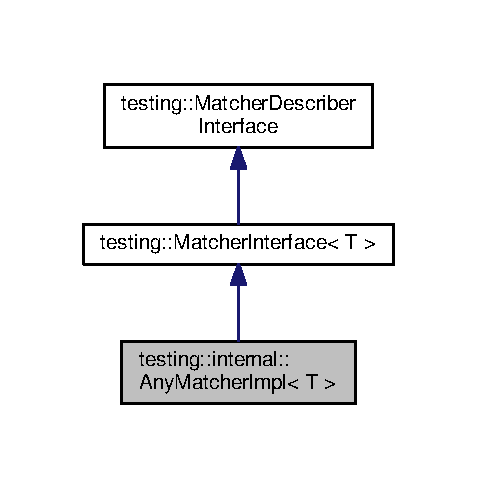
\includegraphics[width=229pt]{classtesting_1_1internal_1_1AnyMatcherImpl__inherit__graph}
\end{center}
\end{figure}


Collaboration diagram for testing\+:\+:internal\+:\+:Any\+Matcher\+Impl$<$ T $>$\+:\nopagebreak
\begin{figure}[H]
\begin{center}
\leavevmode
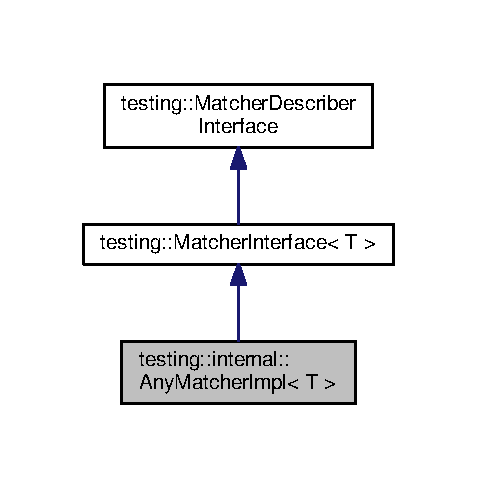
\includegraphics[width=229pt]{classtesting_1_1internal_1_1AnyMatcherImpl__coll__graph}
\end{center}
\end{figure}
\subsection*{Public Member Functions}
\begin{DoxyCompactItemize}
\item 
virtual bool \hyperlink{classtesting_1_1internal_1_1AnyMatcherImpl_a03fe8956cfe9827b0ceacbd130fb88c1}{Match\+And\+Explain} (T, \hyperlink{classtesting_1_1MatchResultListener}{Match\+Result\+Listener} $\ast$) const 
\item 
virtual void \hyperlink{classtesting_1_1internal_1_1AnyMatcherImpl_ae68a082e0c85a0b6f3502698e60333a8}{Describe\+To} (\+::std\+::ostream $\ast$os) const 
\item 
virtual void \hyperlink{classtesting_1_1internal_1_1AnyMatcherImpl_ae403b0e2cf75db076e3465c579a2175b}{Describe\+Negation\+To} (\+::std\+::ostream $\ast$os) const 
\end{DoxyCompactItemize}


\subsection{Member Function Documentation}
\index{testing\+::internal\+::\+Any\+Matcher\+Impl@{testing\+::internal\+::\+Any\+Matcher\+Impl}!Describe\+Negation\+To@{Describe\+Negation\+To}}
\index{Describe\+Negation\+To@{Describe\+Negation\+To}!testing\+::internal\+::\+Any\+Matcher\+Impl@{testing\+::internal\+::\+Any\+Matcher\+Impl}}
\subsubsection[{\texorpdfstring{Describe\+Negation\+To(\+::std\+::ostream $\ast$os) const }{DescribeNegationTo(::std::ostream *os) const }}]{\setlength{\rightskip}{0pt plus 5cm}template$<$typename T $>$ virtual void {\bf testing\+::internal\+::\+Any\+Matcher\+Impl}$<$ T $>$\+::Describe\+Negation\+To (
\begin{DoxyParamCaption}
\item[{\+::std\+::ostream $\ast$}]{os}
\end{DoxyParamCaption}
) const\hspace{0.3cm}{\ttfamily [inline]}, {\ttfamily [virtual]}}\hypertarget{classtesting_1_1internal_1_1AnyMatcherImpl_ae403b0e2cf75db076e3465c579a2175b}{}\label{classtesting_1_1internal_1_1AnyMatcherImpl_ae403b0e2cf75db076e3465c579a2175b}


Reimplemented from \hyperlink{classtesting_1_1MatcherDescriberInterface_a35b9dc2f3e25ca4b903f282feaaf9f8c}{testing\+::\+Matcher\+Describer\+Interface}.


\begin{DoxyCode}
864                                                         \{
865     \textcolor{comment}{// This is mostly for completeness' safe, as it's not very useful}
866     \textcolor{comment}{// to write Not(A<bool>()).  However we cannot completely rule out}
867     \textcolor{comment}{// such a possibility, and it doesn't hurt to be prepared.}
868     *os << \textcolor{stringliteral}{"never matches"};
869   \}
\end{DoxyCode}
\index{testing\+::internal\+::\+Any\+Matcher\+Impl@{testing\+::internal\+::\+Any\+Matcher\+Impl}!Describe\+To@{Describe\+To}}
\index{Describe\+To@{Describe\+To}!testing\+::internal\+::\+Any\+Matcher\+Impl@{testing\+::internal\+::\+Any\+Matcher\+Impl}}
\subsubsection[{\texorpdfstring{Describe\+To(\+::std\+::ostream $\ast$os) const }{DescribeTo(::std::ostream *os) const }}]{\setlength{\rightskip}{0pt plus 5cm}template$<$typename T $>$ virtual void {\bf testing\+::internal\+::\+Any\+Matcher\+Impl}$<$ T $>$\+::Describe\+To (
\begin{DoxyParamCaption}
\item[{\+::std\+::ostream $\ast$}]{os}
\end{DoxyParamCaption}
) const\hspace{0.3cm}{\ttfamily [inline]}, {\ttfamily [virtual]}}\hypertarget{classtesting_1_1internal_1_1AnyMatcherImpl_ae68a082e0c85a0b6f3502698e60333a8}{}\label{classtesting_1_1internal_1_1AnyMatcherImpl_ae68a082e0c85a0b6f3502698e60333a8}


Implements \hyperlink{classtesting_1_1MatcherDescriberInterface_ad9f861588bd969b6e3e717f13bb94e7b}{testing\+::\+Matcher\+Describer\+Interface}.


\begin{DoxyCode}
863 \{ *os << \textcolor{stringliteral}{"is anything"}; \}
\end{DoxyCode}
\index{testing\+::internal\+::\+Any\+Matcher\+Impl@{testing\+::internal\+::\+Any\+Matcher\+Impl}!Match\+And\+Explain@{Match\+And\+Explain}}
\index{Match\+And\+Explain@{Match\+And\+Explain}!testing\+::internal\+::\+Any\+Matcher\+Impl@{testing\+::internal\+::\+Any\+Matcher\+Impl}}
\subsubsection[{\texorpdfstring{Match\+And\+Explain(\+T, Match\+Result\+Listener $\ast$) const }{MatchAndExplain(T, MatchResultListener *) const }}]{\setlength{\rightskip}{0pt plus 5cm}template$<$typename T $>$ virtual bool {\bf testing\+::internal\+::\+Any\+Matcher\+Impl}$<$ T $>$\+::Match\+And\+Explain (
\begin{DoxyParamCaption}
\item[{T}]{, }
\item[{{\bf Match\+Result\+Listener} $\ast$}]{}
\end{DoxyParamCaption}
) const\hspace{0.3cm}{\ttfamily [inline]}, {\ttfamily [virtual]}}\hypertarget{classtesting_1_1internal_1_1AnyMatcherImpl_a03fe8956cfe9827b0ceacbd130fb88c1}{}\label{classtesting_1_1internal_1_1AnyMatcherImpl_a03fe8956cfe9827b0ceacbd130fb88c1}


Implements \hyperlink{classtesting_1_1MatcherInterface_a296b43607cd99d60365f0e6a762777cf}{testing\+::\+Matcher\+Interface$<$ T $>$}.


\begin{DoxyCode}
862                                          \{ \textcolor{keywordflow}{return} \textcolor{keyword}{true}; \}
\end{DoxyCode}


The documentation for this class was generated from the following file\+:\begin{DoxyCompactItemize}
\item 
vendor/googletest/googlemock/include/gmock/\hyperlink{gmock-matchers_8h}{gmock-\/matchers.\+h}\end{DoxyCompactItemize}

\hypertarget{structtesting_1_1internal_1_1AnyNe}{}\section{testing\+:\+:internal\+:\+:Any\+Ne Struct Reference}
\label{structtesting_1_1internal_1_1AnyNe}\index{testing\+::internal\+::\+Any\+Ne@{testing\+::internal\+::\+Any\+Ne}}


{\ttfamily \#include $<$gmock-\/matchers.\+h$>$}

\subsection*{Public Member Functions}
\begin{DoxyCompactItemize}
\item 
{\footnotesize template$<$typename A , typename B $>$ }\\bool \hyperlink{structtesting_1_1internal_1_1AnyNe_a697a34da8469690f1017da5a76d025fa}{operator()} (const \hyperlink{namespacetesting_a5e9134d655d2fc9323902348083282e7}{A} \&a, const B \&b) const 
\end{DoxyCompactItemize}


\subsection{Member Function Documentation}
\index{testing\+::internal\+::\+Any\+Ne@{testing\+::internal\+::\+Any\+Ne}!operator()@{operator()}}
\index{operator()@{operator()}!testing\+::internal\+::\+Any\+Ne@{testing\+::internal\+::\+Any\+Ne}}
\subsubsection[{\texorpdfstring{operator()(const A \&a, const B \&b) const }{operator()(const A &a, const B &b) const }}]{\setlength{\rightskip}{0pt plus 5cm}template$<$typename A , typename B $>$ bool testing\+::internal\+::\+Any\+Ne\+::operator() (
\begin{DoxyParamCaption}
\item[{const {\bf A} \&}]{a, }
\item[{const B \&}]{b}
\end{DoxyParamCaption}
) const\hspace{0.3cm}{\ttfamily [inline]}}\hypertarget{structtesting_1_1internal_1_1AnyNe_a697a34da8469690f1017da5a76d025fa}{}\label{structtesting_1_1internal_1_1AnyNe_a697a34da8469690f1017da5a76d025fa}

\begin{DoxyCode}
208 \{ \textcolor{keywordflow}{return} a != b; \}
\end{DoxyCode}


The documentation for this struct was generated from the following file\+:\begin{DoxyCompactItemize}
\item 
vendor/googletest/googlemock/include/gmock/\hyperlink{gmock-matchers_8h}{gmock-\/matchers.\+h}\end{DoxyCompactItemize}

\hypertarget{structtesting_1_1internal_1_1AnyOfResult1}{}\section{testing\+:\+:internal\+:\+:Any\+Of\+Result1$<$ M1 $>$ Struct Template Reference}
\label{structtesting_1_1internal_1_1AnyOfResult1}\index{testing\+::internal\+::\+Any\+Of\+Result1$<$ M1 $>$@{testing\+::internal\+::\+Any\+Of\+Result1$<$ M1 $>$}}


{\ttfamily \#include $<$gmock-\/generated-\/matchers.\+h$>$}

\subsection*{Public Types}
\begin{DoxyCompactItemize}
\item 
typedef M1 \hyperlink{structtesting_1_1internal_1_1AnyOfResult1_a4c55b5cf196c93e2a822bc99625f6797}{type}
\end{DoxyCompactItemize}


\subsection{Member Typedef Documentation}
\index{testing\+::internal\+::\+Any\+Of\+Result1@{testing\+::internal\+::\+Any\+Of\+Result1}!type@{type}}
\index{type@{type}!testing\+::internal\+::\+Any\+Of\+Result1@{testing\+::internal\+::\+Any\+Of\+Result1}}
\subsubsection[{\texorpdfstring{type}{type}}]{\setlength{\rightskip}{0pt plus 5cm}template$<$typename M1$>$ typedef M1 {\bf testing\+::internal\+::\+Any\+Of\+Result1}$<$ M1 $>$\+::{\bf type}}\hypertarget{structtesting_1_1internal_1_1AnyOfResult1_a4c55b5cf196c93e2a822bc99625f6797}{}\label{structtesting_1_1internal_1_1AnyOfResult1_a4c55b5cf196c93e2a822bc99625f6797}


The documentation for this struct was generated from the following file\+:\begin{DoxyCompactItemize}
\item 
vendor/googletest/googlemock/include/gmock/\hyperlink{gmock-generated-matchers_8h}{gmock-\/generated-\/matchers.\+h}\end{DoxyCompactItemize}

\hypertarget{structtesting_1_1internal_1_1AnyOfResult10}{}\section{testing\+:\+:internal\+:\+:Any\+Of\+Result10$<$ M1, M2, M3, M4, M5, M6, M7, M8, M9, M10 $>$ Struct Template Reference}
\label{structtesting_1_1internal_1_1AnyOfResult10}\index{testing\+::internal\+::\+Any\+Of\+Result10$<$ M1, M2, M3, M4, M5, M6, M7, M8, M9, M10 $>$@{testing\+::internal\+::\+Any\+Of\+Result10$<$ M1, M2, M3, M4, M5, M6, M7, M8, M9, M10 $>$}}


{\ttfamily \#include $<$gmock-\/generated-\/matchers.\+h$>$}

\subsection*{Public Types}
\begin{DoxyCompactItemize}
\item 
typedef \hyperlink{classtesting_1_1internal_1_1EitherOfMatcher}{Either\+Of\+Matcher}$<$ typename \hyperlink{structtesting_1_1internal_1_1AnyOfResult5}{Any\+Of\+Result5}$<$ M1, M2, M3, M4, M5 $>$\+::\hyperlink{structtesting_1_1internal_1_1AnyOfResult10_aa1cb3d733f29716f2015db8a2b6c1c94}{type}, typename \hyperlink{structtesting_1_1internal_1_1AnyOfResult5}{Any\+Of\+Result5}$<$ M6, M7, M8, M9, M10 $>$\+::\hyperlink{structtesting_1_1internal_1_1AnyOfResult10_aa1cb3d733f29716f2015db8a2b6c1c94}{type} $>$ \hyperlink{structtesting_1_1internal_1_1AnyOfResult10_aa1cb3d733f29716f2015db8a2b6c1c94}{type}
\end{DoxyCompactItemize}


\subsection{Member Typedef Documentation}
\index{testing\+::internal\+::\+Any\+Of\+Result10@{testing\+::internal\+::\+Any\+Of\+Result10}!type@{type}}
\index{type@{type}!testing\+::internal\+::\+Any\+Of\+Result10@{testing\+::internal\+::\+Any\+Of\+Result10}}
\subsubsection[{\texorpdfstring{type}{type}}]{\setlength{\rightskip}{0pt plus 5cm}template$<$typename M1 , typename M2 , typename M3 , typename M4 , typename M5 , typename M6 , typename M7 , typename M8 , typename M9 , typename M10 $>$ typedef {\bf Either\+Of\+Matcher}$<$ typename {\bf Any\+Of\+Result5}$<$M1, M2, M3, M4, M5$>$\+::{\bf type}, typename {\bf Any\+Of\+Result5}$<$M6, M7, M8, M9, M10$>$\+::{\bf type} $>$ {\bf testing\+::internal\+::\+Any\+Of\+Result10}$<$ M1, M2, M3, M4, M5, M6, M7, M8, M9, M10 $>$\+::{\bf type}}\hypertarget{structtesting_1_1internal_1_1AnyOfResult10_aa1cb3d733f29716f2015db8a2b6c1c94}{}\label{structtesting_1_1internal_1_1AnyOfResult10_aa1cb3d733f29716f2015db8a2b6c1c94}


The documentation for this struct was generated from the following file\+:\begin{DoxyCompactItemize}
\item 
vendor/googletest/googlemock/include/gmock/\hyperlink{gmock-generated-matchers_8h}{gmock-\/generated-\/matchers.\+h}\end{DoxyCompactItemize}

\hypertarget{structtesting_1_1internal_1_1AnyOfResult2}{}\section{testing\+:\+:internal\+:\+:Any\+Of\+Result2$<$ M1, M2 $>$ Struct Template Reference}
\label{structtesting_1_1internal_1_1AnyOfResult2}\index{testing\+::internal\+::\+Any\+Of\+Result2$<$ M1, M2 $>$@{testing\+::internal\+::\+Any\+Of\+Result2$<$ M1, M2 $>$}}


{\ttfamily \#include $<$gmock-\/generated-\/matchers.\+h$>$}

\subsection*{Public Types}
\begin{DoxyCompactItemize}
\item 
typedef \hyperlink{classtesting_1_1internal_1_1EitherOfMatcher}{Either\+Of\+Matcher}$<$ typename \hyperlink{structtesting_1_1internal_1_1AnyOfResult1}{Any\+Of\+Result1}$<$ M1 $>$\+::\hyperlink{structtesting_1_1internal_1_1AnyOfResult2_a6d9eba508021f8e652c7c154a649073f}{type}, typename \hyperlink{structtesting_1_1internal_1_1AnyOfResult1}{Any\+Of\+Result1}$<$ M2 $>$\+::\hyperlink{structtesting_1_1internal_1_1AnyOfResult2_a6d9eba508021f8e652c7c154a649073f}{type} $>$ \hyperlink{structtesting_1_1internal_1_1AnyOfResult2_a6d9eba508021f8e652c7c154a649073f}{type}
\end{DoxyCompactItemize}


\subsection{Member Typedef Documentation}
\index{testing\+::internal\+::\+Any\+Of\+Result2@{testing\+::internal\+::\+Any\+Of\+Result2}!type@{type}}
\index{type@{type}!testing\+::internal\+::\+Any\+Of\+Result2@{testing\+::internal\+::\+Any\+Of\+Result2}}
\subsubsection[{\texorpdfstring{type}{type}}]{\setlength{\rightskip}{0pt plus 5cm}template$<$typename M1, typename M2$>$ typedef {\bf Either\+Of\+Matcher}$<$ typename {\bf Any\+Of\+Result1}$<$M1$>$\+::{\bf type}, typename {\bf Any\+Of\+Result1}$<$M2$>$\+::{\bf type} $>$ {\bf testing\+::internal\+::\+Any\+Of\+Result2}$<$ M1, M2 $>$\+::{\bf type}}\hypertarget{structtesting_1_1internal_1_1AnyOfResult2_a6d9eba508021f8e652c7c154a649073f}{}\label{structtesting_1_1internal_1_1AnyOfResult2_a6d9eba508021f8e652c7c154a649073f}


The documentation for this struct was generated from the following file\+:\begin{DoxyCompactItemize}
\item 
vendor/googletest/googlemock/include/gmock/\hyperlink{gmock-generated-matchers_8h}{gmock-\/generated-\/matchers.\+h}\end{DoxyCompactItemize}

\hypertarget{structtesting_1_1internal_1_1AnyOfResult3}{}\section{testing\+:\+:internal\+:\+:Any\+Of\+Result3$<$ M1, M2, M3 $>$ Struct Template Reference}
\label{structtesting_1_1internal_1_1AnyOfResult3}\index{testing\+::internal\+::\+Any\+Of\+Result3$<$ M1, M2, M3 $>$@{testing\+::internal\+::\+Any\+Of\+Result3$<$ M1, M2, M3 $>$}}


{\ttfamily \#include $<$gmock-\/generated-\/matchers.\+h$>$}

\subsection*{Public Types}
\begin{DoxyCompactItemize}
\item 
typedef \hyperlink{classtesting_1_1internal_1_1EitherOfMatcher}{Either\+Of\+Matcher}$<$ typename \hyperlink{structtesting_1_1internal_1_1AnyOfResult1}{Any\+Of\+Result1}$<$ M1 $>$\+::\hyperlink{structtesting_1_1internal_1_1AnyOfResult3_a232b20553cc0a33a6741e85e19ef4b0c}{type}, typename \hyperlink{structtesting_1_1internal_1_1AnyOfResult2}{Any\+Of\+Result2}$<$ M2, M3 $>$\+::\hyperlink{structtesting_1_1internal_1_1AnyOfResult3_a232b20553cc0a33a6741e85e19ef4b0c}{type} $>$ \hyperlink{structtesting_1_1internal_1_1AnyOfResult3_a232b20553cc0a33a6741e85e19ef4b0c}{type}
\end{DoxyCompactItemize}


\subsection{Member Typedef Documentation}
\index{testing\+::internal\+::\+Any\+Of\+Result3@{testing\+::internal\+::\+Any\+Of\+Result3}!type@{type}}
\index{type@{type}!testing\+::internal\+::\+Any\+Of\+Result3@{testing\+::internal\+::\+Any\+Of\+Result3}}
\subsubsection[{\texorpdfstring{type}{type}}]{\setlength{\rightskip}{0pt plus 5cm}template$<$typename M1, typename M2, typename M3$>$ typedef {\bf Either\+Of\+Matcher}$<$ typename {\bf Any\+Of\+Result1}$<$M1$>$\+::{\bf type}, typename {\bf Any\+Of\+Result2}$<$M2, M3$>$\+::{\bf type} $>$ {\bf testing\+::internal\+::\+Any\+Of\+Result3}$<$ M1, M2, M3 $>$\+::{\bf type}}\hypertarget{structtesting_1_1internal_1_1AnyOfResult3_a232b20553cc0a33a6741e85e19ef4b0c}{}\label{structtesting_1_1internal_1_1AnyOfResult3_a232b20553cc0a33a6741e85e19ef4b0c}


The documentation for this struct was generated from the following file\+:\begin{DoxyCompactItemize}
\item 
vendor/googletest/googlemock/include/gmock/\hyperlink{gmock-generated-matchers_8h}{gmock-\/generated-\/matchers.\+h}\end{DoxyCompactItemize}

\hypertarget{structtesting_1_1internal_1_1AnyOfResult4}{}\section{testing\+:\+:internal\+:\+:Any\+Of\+Result4$<$ M1, M2, M3, M4 $>$ Struct Template Reference}
\label{structtesting_1_1internal_1_1AnyOfResult4}\index{testing\+::internal\+::\+Any\+Of\+Result4$<$ M1, M2, M3, M4 $>$@{testing\+::internal\+::\+Any\+Of\+Result4$<$ M1, M2, M3, M4 $>$}}


{\ttfamily \#include $<$gmock-\/generated-\/matchers.\+h$>$}

\subsection*{Public Types}
\begin{DoxyCompactItemize}
\item 
typedef \hyperlink{classtesting_1_1internal_1_1EitherOfMatcher}{Either\+Of\+Matcher}$<$ typename \hyperlink{structtesting_1_1internal_1_1AnyOfResult2}{Any\+Of\+Result2}$<$ M1, M2 $>$\+::\hyperlink{structtesting_1_1internal_1_1AnyOfResult4_a4f3c9aebb4f7fc24287b59a0bdf1a4a6}{type}, typename \hyperlink{structtesting_1_1internal_1_1AnyOfResult2}{Any\+Of\+Result2}$<$ M3, M4 $>$\+::\hyperlink{structtesting_1_1internal_1_1AnyOfResult4_a4f3c9aebb4f7fc24287b59a0bdf1a4a6}{type} $>$ \hyperlink{structtesting_1_1internal_1_1AnyOfResult4_a4f3c9aebb4f7fc24287b59a0bdf1a4a6}{type}
\end{DoxyCompactItemize}


\subsection{Member Typedef Documentation}
\index{testing\+::internal\+::\+Any\+Of\+Result4@{testing\+::internal\+::\+Any\+Of\+Result4}!type@{type}}
\index{type@{type}!testing\+::internal\+::\+Any\+Of\+Result4@{testing\+::internal\+::\+Any\+Of\+Result4}}
\subsubsection[{\texorpdfstring{type}{type}}]{\setlength{\rightskip}{0pt plus 5cm}template$<$typename M1, typename M2, typename M3, typename M4$>$ typedef {\bf Either\+Of\+Matcher}$<$ typename {\bf Any\+Of\+Result2}$<$M1, M2$>$\+::{\bf type}, typename {\bf Any\+Of\+Result2}$<$M3, M4$>$\+::{\bf type} $>$ {\bf testing\+::internal\+::\+Any\+Of\+Result4}$<$ M1, M2, M3, M4 $>$\+::{\bf type}}\hypertarget{structtesting_1_1internal_1_1AnyOfResult4_a4f3c9aebb4f7fc24287b59a0bdf1a4a6}{}\label{structtesting_1_1internal_1_1AnyOfResult4_a4f3c9aebb4f7fc24287b59a0bdf1a4a6}


The documentation for this struct was generated from the following file\+:\begin{DoxyCompactItemize}
\item 
vendor/googletest/googlemock/include/gmock/\hyperlink{gmock-generated-matchers_8h}{gmock-\/generated-\/matchers.\+h}\end{DoxyCompactItemize}

\hypertarget{structtesting_1_1internal_1_1AnyOfResult5}{}\section{testing\+:\+:internal\+:\+:Any\+Of\+Result5$<$ M1, M2, M3, M4, M5 $>$ Struct Template Reference}
\label{structtesting_1_1internal_1_1AnyOfResult5}\index{testing\+::internal\+::\+Any\+Of\+Result5$<$ M1, M2, M3, M4, M5 $>$@{testing\+::internal\+::\+Any\+Of\+Result5$<$ M1, M2, M3, M4, M5 $>$}}


{\ttfamily \#include $<$gmock-\/generated-\/matchers.\+h$>$}

\subsection*{Public Types}
\begin{DoxyCompactItemize}
\item 
typedef \hyperlink{classtesting_1_1internal_1_1EitherOfMatcher}{Either\+Of\+Matcher}$<$ typename \hyperlink{structtesting_1_1internal_1_1AnyOfResult2}{Any\+Of\+Result2}$<$ M1, M2 $>$\+::\hyperlink{structtesting_1_1internal_1_1AnyOfResult5_a459a06dc5791313dce942668714f0c99}{type}, typename \hyperlink{structtesting_1_1internal_1_1AnyOfResult3}{Any\+Of\+Result3}$<$ M3, M4, M5 $>$\+::\hyperlink{structtesting_1_1internal_1_1AnyOfResult5_a459a06dc5791313dce942668714f0c99}{type} $>$ \hyperlink{structtesting_1_1internal_1_1AnyOfResult5_a459a06dc5791313dce942668714f0c99}{type}
\end{DoxyCompactItemize}


\subsection{Member Typedef Documentation}
\index{testing\+::internal\+::\+Any\+Of\+Result5@{testing\+::internal\+::\+Any\+Of\+Result5}!type@{type}}
\index{type@{type}!testing\+::internal\+::\+Any\+Of\+Result5@{testing\+::internal\+::\+Any\+Of\+Result5}}
\subsubsection[{\texorpdfstring{type}{type}}]{\setlength{\rightskip}{0pt plus 5cm}template$<$typename M1, typename M2, typename M3, typename M4, typename M5$>$ typedef {\bf Either\+Of\+Matcher}$<$ typename {\bf Any\+Of\+Result2}$<$M1, M2$>$\+::{\bf type}, typename {\bf Any\+Of\+Result3}$<$M3, M4, M5$>$\+::{\bf type} $>$ {\bf testing\+::internal\+::\+Any\+Of\+Result5}$<$ M1, M2, M3, M4, M5 $>$\+::{\bf type}}\hypertarget{structtesting_1_1internal_1_1AnyOfResult5_a459a06dc5791313dce942668714f0c99}{}\label{structtesting_1_1internal_1_1AnyOfResult5_a459a06dc5791313dce942668714f0c99}


The documentation for this struct was generated from the following file\+:\begin{DoxyCompactItemize}
\item 
vendor/googletest/googlemock/include/gmock/\hyperlink{gmock-generated-matchers_8h}{gmock-\/generated-\/matchers.\+h}\end{DoxyCompactItemize}

\hypertarget{structtesting_1_1internal_1_1AnyOfResult6}{}\section{testing\+:\+:internal\+:\+:Any\+Of\+Result6$<$ M1, M2, M3, M4, M5, M6 $>$ Struct Template Reference}
\label{structtesting_1_1internal_1_1AnyOfResult6}\index{testing\+::internal\+::\+Any\+Of\+Result6$<$ M1, M2, M3, M4, M5, M6 $>$@{testing\+::internal\+::\+Any\+Of\+Result6$<$ M1, M2, M3, M4, M5, M6 $>$}}


{\ttfamily \#include $<$gmock-\/generated-\/matchers.\+h$>$}

\subsection*{Public Types}
\begin{DoxyCompactItemize}
\item 
typedef \hyperlink{classtesting_1_1internal_1_1EitherOfMatcher}{Either\+Of\+Matcher}$<$ typename \hyperlink{structtesting_1_1internal_1_1AnyOfResult3}{Any\+Of\+Result3}$<$ M1, M2, M3 $>$\+::\hyperlink{structtesting_1_1internal_1_1AnyOfResult6_a15837eb05d9ac5a76c20d344a4988dd1}{type}, typename \hyperlink{structtesting_1_1internal_1_1AnyOfResult3}{Any\+Of\+Result3}$<$ M4, M5, M6 $>$\+::\hyperlink{structtesting_1_1internal_1_1AnyOfResult6_a15837eb05d9ac5a76c20d344a4988dd1}{type} $>$ \hyperlink{structtesting_1_1internal_1_1AnyOfResult6_a15837eb05d9ac5a76c20d344a4988dd1}{type}
\end{DoxyCompactItemize}


\subsection{Member Typedef Documentation}
\index{testing\+::internal\+::\+Any\+Of\+Result6@{testing\+::internal\+::\+Any\+Of\+Result6}!type@{type}}
\index{type@{type}!testing\+::internal\+::\+Any\+Of\+Result6@{testing\+::internal\+::\+Any\+Of\+Result6}}
\subsubsection[{\texorpdfstring{type}{type}}]{\setlength{\rightskip}{0pt plus 5cm}template$<$typename M1, typename M2, typename M3, typename M4, typename M5, typename M6$>$ typedef {\bf Either\+Of\+Matcher}$<$ typename {\bf Any\+Of\+Result3}$<$M1, M2, M3$>$\+::{\bf type}, typename {\bf Any\+Of\+Result3}$<$M4, M5, M6$>$\+::{\bf type} $>$ {\bf testing\+::internal\+::\+Any\+Of\+Result6}$<$ M1, M2, M3, M4, M5, M6 $>$\+::{\bf type}}\hypertarget{structtesting_1_1internal_1_1AnyOfResult6_a15837eb05d9ac5a76c20d344a4988dd1}{}\label{structtesting_1_1internal_1_1AnyOfResult6_a15837eb05d9ac5a76c20d344a4988dd1}


The documentation for this struct was generated from the following file\+:\begin{DoxyCompactItemize}
\item 
vendor/googletest/googlemock/include/gmock/\hyperlink{gmock-generated-matchers_8h}{gmock-\/generated-\/matchers.\+h}\end{DoxyCompactItemize}

\hypertarget{structtesting_1_1internal_1_1AnyOfResult7}{}\section{testing\+:\+:internal\+:\+:Any\+Of\+Result7$<$ M1, M2, M3, M4, M5, M6, M7 $>$ Struct Template Reference}
\label{structtesting_1_1internal_1_1AnyOfResult7}\index{testing\+::internal\+::\+Any\+Of\+Result7$<$ M1, M2, M3, M4, M5, M6, M7 $>$@{testing\+::internal\+::\+Any\+Of\+Result7$<$ M1, M2, M3, M4, M5, M6, M7 $>$}}


{\ttfamily \#include $<$gmock-\/generated-\/matchers.\+h$>$}

\subsection*{Public Types}
\begin{DoxyCompactItemize}
\item 
typedef \hyperlink{classtesting_1_1internal_1_1EitherOfMatcher}{Either\+Of\+Matcher}$<$ typename \hyperlink{structtesting_1_1internal_1_1AnyOfResult3}{Any\+Of\+Result3}$<$ M1, M2, M3 $>$\+::\hyperlink{structtesting_1_1internal_1_1AnyOfResult7_a976873478921520833464a86f840abe8}{type}, typename \hyperlink{structtesting_1_1internal_1_1AnyOfResult4}{Any\+Of\+Result4}$<$ M4, M5, M6, M7 $>$\+::\hyperlink{structtesting_1_1internal_1_1AnyOfResult7_a976873478921520833464a86f840abe8}{type} $>$ \hyperlink{structtesting_1_1internal_1_1AnyOfResult7_a976873478921520833464a86f840abe8}{type}
\end{DoxyCompactItemize}


\subsection{Member Typedef Documentation}
\index{testing\+::internal\+::\+Any\+Of\+Result7@{testing\+::internal\+::\+Any\+Of\+Result7}!type@{type}}
\index{type@{type}!testing\+::internal\+::\+Any\+Of\+Result7@{testing\+::internal\+::\+Any\+Of\+Result7}}
\subsubsection[{\texorpdfstring{type}{type}}]{\setlength{\rightskip}{0pt plus 5cm}template$<$typename M1, typename M2, typename M3, typename M4, typename M5, typename M6, typename M7$>$ typedef {\bf Either\+Of\+Matcher}$<$ typename {\bf Any\+Of\+Result3}$<$M1, M2, M3$>$\+::{\bf type}, typename {\bf Any\+Of\+Result4}$<$M4, M5, M6, M7$>$\+::{\bf type} $>$ {\bf testing\+::internal\+::\+Any\+Of\+Result7}$<$ M1, M2, M3, M4, M5, M6, M7 $>$\+::{\bf type}}\hypertarget{structtesting_1_1internal_1_1AnyOfResult7_a976873478921520833464a86f840abe8}{}\label{structtesting_1_1internal_1_1AnyOfResult7_a976873478921520833464a86f840abe8}


The documentation for this struct was generated from the following file\+:\begin{DoxyCompactItemize}
\item 
vendor/googletest/googlemock/include/gmock/\hyperlink{gmock-generated-matchers_8h}{gmock-\/generated-\/matchers.\+h}\end{DoxyCompactItemize}

\hypertarget{structtesting_1_1internal_1_1AnyOfResult8}{}\section{testing\+:\+:internal\+:\+:Any\+Of\+Result8$<$ M1, M2, M3, M4, M5, M6, M7, M8 $>$ Struct Template Reference}
\label{structtesting_1_1internal_1_1AnyOfResult8}\index{testing\+::internal\+::\+Any\+Of\+Result8$<$ M1, M2, M3, M4, M5, M6, M7, M8 $>$@{testing\+::internal\+::\+Any\+Of\+Result8$<$ M1, M2, M3, M4, M5, M6, M7, M8 $>$}}


{\ttfamily \#include $<$gmock-\/generated-\/matchers.\+h$>$}

\subsection*{Public Types}
\begin{DoxyCompactItemize}
\item 
typedef \hyperlink{classtesting_1_1internal_1_1EitherOfMatcher}{Either\+Of\+Matcher}$<$ typename \hyperlink{structtesting_1_1internal_1_1AnyOfResult4}{Any\+Of\+Result4}$<$ M1, M2, M3, M4 $>$\+::\hyperlink{structtesting_1_1internal_1_1AnyOfResult8_a8f8a1e78a019965c24bd22c78885747d}{type}, typename \hyperlink{structtesting_1_1internal_1_1AnyOfResult4}{Any\+Of\+Result4}$<$ M5, M6, M7, M8 $>$\+::\hyperlink{structtesting_1_1internal_1_1AnyOfResult8_a8f8a1e78a019965c24bd22c78885747d}{type} $>$ \hyperlink{structtesting_1_1internal_1_1AnyOfResult8_a8f8a1e78a019965c24bd22c78885747d}{type}
\end{DoxyCompactItemize}


\subsection{Member Typedef Documentation}
\index{testing\+::internal\+::\+Any\+Of\+Result8@{testing\+::internal\+::\+Any\+Of\+Result8}!type@{type}}
\index{type@{type}!testing\+::internal\+::\+Any\+Of\+Result8@{testing\+::internal\+::\+Any\+Of\+Result8}}
\subsubsection[{\texorpdfstring{type}{type}}]{\setlength{\rightskip}{0pt plus 5cm}template$<$typename M1, typename M2, typename M3, typename M4, typename M5, typename M6, typename M7, typename M8$>$ typedef {\bf Either\+Of\+Matcher}$<$ typename {\bf Any\+Of\+Result4}$<$M1, M2, M3, M4$>$\+::{\bf type}, typename {\bf Any\+Of\+Result4}$<$M5, M6, M7, M8$>$\+::{\bf type} $>$ {\bf testing\+::internal\+::\+Any\+Of\+Result8}$<$ M1, M2, M3, M4, M5, M6, M7, M8 $>$\+::{\bf type}}\hypertarget{structtesting_1_1internal_1_1AnyOfResult8_a8f8a1e78a019965c24bd22c78885747d}{}\label{structtesting_1_1internal_1_1AnyOfResult8_a8f8a1e78a019965c24bd22c78885747d}


The documentation for this struct was generated from the following file\+:\begin{DoxyCompactItemize}
\item 
vendor/googletest/googlemock/include/gmock/\hyperlink{gmock-generated-matchers_8h}{gmock-\/generated-\/matchers.\+h}\end{DoxyCompactItemize}

\hypertarget{structtesting_1_1internal_1_1AnyOfResult9}{}\section{testing\+:\+:internal\+:\+:Any\+Of\+Result9$<$ M1, M2, M3, M4, M5, M6, M7, M8, M9 $>$ Struct Template Reference}
\label{structtesting_1_1internal_1_1AnyOfResult9}\index{testing\+::internal\+::\+Any\+Of\+Result9$<$ M1, M2, M3, M4, M5, M6, M7, M8, M9 $>$@{testing\+::internal\+::\+Any\+Of\+Result9$<$ M1, M2, M3, M4, M5, M6, M7, M8, M9 $>$}}


{\ttfamily \#include $<$gmock-\/generated-\/matchers.\+h$>$}

\subsection*{Public Types}
\begin{DoxyCompactItemize}
\item 
typedef \hyperlink{classtesting_1_1internal_1_1EitherOfMatcher}{Either\+Of\+Matcher}$<$ typename \hyperlink{structtesting_1_1internal_1_1AnyOfResult4}{Any\+Of\+Result4}$<$ M1, M2, M3, M4 $>$\+::\hyperlink{structtesting_1_1internal_1_1AnyOfResult9_a308935fb02c62f502044dcc7b0a2b464}{type}, typename \hyperlink{structtesting_1_1internal_1_1AnyOfResult5}{Any\+Of\+Result5}$<$ M5, M6, M7, M8, M9 $>$\+::\hyperlink{structtesting_1_1internal_1_1AnyOfResult9_a308935fb02c62f502044dcc7b0a2b464}{type} $>$ \hyperlink{structtesting_1_1internal_1_1AnyOfResult9_a308935fb02c62f502044dcc7b0a2b464}{type}
\end{DoxyCompactItemize}


\subsection{Member Typedef Documentation}
\index{testing\+::internal\+::\+Any\+Of\+Result9@{testing\+::internal\+::\+Any\+Of\+Result9}!type@{type}}
\index{type@{type}!testing\+::internal\+::\+Any\+Of\+Result9@{testing\+::internal\+::\+Any\+Of\+Result9}}
\subsubsection[{\texorpdfstring{type}{type}}]{\setlength{\rightskip}{0pt plus 5cm}template$<$typename M1, typename M2, typename M3, typename M4, typename M5, typename M6, typename M7, typename M8, typename M9$>$ typedef {\bf Either\+Of\+Matcher}$<$ typename {\bf Any\+Of\+Result4}$<$M1, M2, M3, M4$>$\+::{\bf type}, typename {\bf Any\+Of\+Result5}$<$M5, M6, M7, M8, M9$>$\+::{\bf type} $>$ {\bf testing\+::internal\+::\+Any\+Of\+Result9}$<$ M1, M2, M3, M4, M5, M6, M7, M8, M9 $>$\+::{\bf type}}\hypertarget{structtesting_1_1internal_1_1AnyOfResult9_a308935fb02c62f502044dcc7b0a2b464}{}\label{structtesting_1_1internal_1_1AnyOfResult9_a308935fb02c62f502044dcc7b0a2b464}


The documentation for this struct was generated from the following file\+:\begin{DoxyCompactItemize}
\item 
vendor/googletest/googlemock/include/gmock/\hyperlink{gmock-generated-matchers_8h}{gmock-\/generated-\/matchers.\+h}\end{DoxyCompactItemize}

\hypertarget{classtesting_1_1internal_1_1AnythingMatcher}{}\section{testing\+:\+:internal\+:\+:Anything\+Matcher Class Reference}
\label{classtesting_1_1internal_1_1AnythingMatcher}\index{testing\+::internal\+::\+Anything\+Matcher@{testing\+::internal\+::\+Anything\+Matcher}}


{\ttfamily \#include $<$gmock-\/matchers.\+h$>$}

\subsection*{Public Member Functions}
\begin{DoxyCompactItemize}
\item 
{\footnotesize template$<$typename T $>$ }\\\hyperlink{classtesting_1_1internal_1_1AnythingMatcher_ae70d544c1edeb84ef27e845cf1c4e755}{operator Matcher$<$ T $>$} () const 
\end{DoxyCompactItemize}


\subsection{Member Function Documentation}
\index{testing\+::internal\+::\+Anything\+Matcher@{testing\+::internal\+::\+Anything\+Matcher}!operator Matcher$<$ T $>$@{operator Matcher$<$ T $>$}}
\index{operator Matcher$<$ T $>$@{operator Matcher$<$ T $>$}!testing\+::internal\+::\+Anything\+Matcher@{testing\+::internal\+::\+Anything\+Matcher}}
\subsubsection[{\texorpdfstring{operator Matcher$<$ T $>$() const }{operator Matcher< T >() const }}]{\setlength{\rightskip}{0pt plus 5cm}template$<$typename T $>$ testing\+::internal\+::\+Anything\+Matcher\+::operator {\bf Matcher}$<$ T $>$ (
\begin{DoxyParamCaption}
{}
\end{DoxyParamCaption}
) const\hspace{0.3cm}{\ttfamily [inline]}}\hypertarget{classtesting_1_1internal_1_1AnythingMatcher_ae70d544c1edeb84ef27e845cf1c4e755}{}\label{classtesting_1_1internal_1_1AnythingMatcher_ae70d544c1edeb84ef27e845cf1c4e755}

\begin{DoxyCode}
879 \{ \textcolor{keywordflow}{return} A<T>(); \}
\end{DoxyCode}


The documentation for this class was generated from the following file\+:\begin{DoxyCompactItemize}
\item 
vendor/googletest/googlemock/include/gmock/\hyperlink{gmock-matchers_8h}{gmock-\/matchers.\+h}\end{DoxyCompactItemize}

\hypertarget{classtesting_1_1internal_1_1ArgsMatcher}{}\section{testing\+:\+:internal\+:\+:Args\+Matcher$<$ Inner\+Matcher, k0, k1, k2, k3, k4, k5, k6, k7, k8, k9 $>$ Class Template Reference}
\label{classtesting_1_1internal_1_1ArgsMatcher}\index{testing\+::internal\+::\+Args\+Matcher$<$ Inner\+Matcher, k0, k1, k2, k3, k4, k5, k6, k7, k8, k9 $>$@{testing\+::internal\+::\+Args\+Matcher$<$ Inner\+Matcher, k0, k1, k2, k3, k4, k5, k6, k7, k8, k9 $>$}}


{\ttfamily \#include $<$gmock-\/generated-\/matchers.\+h$>$}

\subsection*{Public Member Functions}
\begin{DoxyCompactItemize}
\item 
\hyperlink{classtesting_1_1internal_1_1ArgsMatcher_a2879d7455f2da2a5a2f2b6759dbc0561}{Args\+Matcher} (const Inner\+Matcher \&inner\+\_\+matcher)
\item 
{\footnotesize template$<$typename Args\+Tuple $>$ }\\\hyperlink{classtesting_1_1internal_1_1ArgsMatcher_ae94d3e9b43d0102875a1494ca56e6d26}{operator Matcher$<$ Args\+Tuple $>$} () const 
\end{DoxyCompactItemize}


\subsection{Constructor \& Destructor Documentation}
\index{testing\+::internal\+::\+Args\+Matcher@{testing\+::internal\+::\+Args\+Matcher}!Args\+Matcher@{Args\+Matcher}}
\index{Args\+Matcher@{Args\+Matcher}!testing\+::internal\+::\+Args\+Matcher@{testing\+::internal\+::\+Args\+Matcher}}
\subsubsection[{\texorpdfstring{Args\+Matcher(const Inner\+Matcher \&inner\+\_\+matcher)}{ArgsMatcher(const InnerMatcher &inner_matcher)}}]{\setlength{\rightskip}{0pt plus 5cm}template$<$class Inner\+Matcher, int k0 = -\/1, int k1 = -\/1, int k2 = -\/1, int k3 = -\/1, int k4 = -\/1, int k5 = -\/1, int k6 = -\/1, int k7 = -\/1, int k8 = -\/1, int k9 = -\/1$>$ {\bf testing\+::internal\+::\+Args\+Matcher}$<$ Inner\+Matcher, k0, k1, k2, k3, k4, k5, k6, k7, k8, k9 $>$\+::{\bf Args\+Matcher} (
\begin{DoxyParamCaption}
\item[{const Inner\+Matcher \&}]{inner\+\_\+matcher}
\end{DoxyParamCaption}
)\hspace{0.3cm}{\ttfamily [inline]}, {\ttfamily [explicit]}}\hypertarget{classtesting_1_1internal_1_1ArgsMatcher_a2879d7455f2da2a5a2f2b6759dbc0561}{}\label{classtesting_1_1internal_1_1ArgsMatcher_a2879d7455f2da2a5a2f2b6759dbc0561}

\begin{DoxyCode}
284       : inner\_matcher\_(inner\_matcher) \{\}
\end{DoxyCode}


\subsection{Member Function Documentation}
\index{testing\+::internal\+::\+Args\+Matcher@{testing\+::internal\+::\+Args\+Matcher}!operator Matcher$<$ Args\+Tuple $>$@{operator Matcher$<$ Args\+Tuple $>$}}
\index{operator Matcher$<$ Args\+Tuple $>$@{operator Matcher$<$ Args\+Tuple $>$}!testing\+::internal\+::\+Args\+Matcher@{testing\+::internal\+::\+Args\+Matcher}}
\subsubsection[{\texorpdfstring{operator Matcher$<$ Args\+Tuple $>$() const }{operator Matcher< ArgsTuple >() const }}]{\setlength{\rightskip}{0pt plus 5cm}template$<$class Inner\+Matcher, int k0 = -\/1, int k1 = -\/1, int k2 = -\/1, int k3 = -\/1, int k4 = -\/1, int k5 = -\/1, int k6 = -\/1, int k7 = -\/1, int k8 = -\/1, int k9 = -\/1$>$ template$<$typename Args\+Tuple $>$ {\bf testing\+::internal\+::\+Args\+Matcher}$<$ Inner\+Matcher, k0, k1, k2, k3, k4, k5, k6, k7, k8, k9 $>$\+::operator {\bf Matcher}$<$ Args\+Tuple $>$ (
\begin{DoxyParamCaption}
{}
\end{DoxyParamCaption}
) const\hspace{0.3cm}{\ttfamily [inline]}}\hypertarget{classtesting_1_1internal_1_1ArgsMatcher_ae94d3e9b43d0102875a1494ca56e6d26}{}\label{classtesting_1_1internal_1_1ArgsMatcher_ae94d3e9b43d0102875a1494ca56e6d26}

\begin{DoxyCode}
287                                       \{
288     \textcolor{keywordflow}{return} \hyperlink{namespacetesting_a37fd8029ac00e60952440a3d9cca8166}{MakeMatcher}(\textcolor{keyword}{new} ArgsMatcherImpl<ArgsTuple, k0, k1, k2, k3, k4, k5,
289         k6, k7, k8, k9>(inner\_matcher\_));
290   \}
\end{DoxyCode}


The documentation for this class was generated from the following file\+:\begin{DoxyCompactItemize}
\item 
vendor/googletest/googlemock/include/gmock/\hyperlink{gmock-generated-matchers_8h}{gmock-\/generated-\/matchers.\+h}\end{DoxyCompactItemize}

\hypertarget{classtesting_1_1internal_1_1ArgsMatcherImpl}{}\section{testing\+:\+:internal\+:\+:Args\+Matcher\+Impl$<$ Args\+Tuple, k0, k1, k2, k3, k4, k5, k6, k7, k8, k9 $>$ Class Template Reference}
\label{classtesting_1_1internal_1_1ArgsMatcherImpl}\index{testing\+::internal\+::\+Args\+Matcher\+Impl$<$ Args\+Tuple, k0, k1, k2, k3, k4, k5, k6, k7, k8, k9 $>$@{testing\+::internal\+::\+Args\+Matcher\+Impl$<$ Args\+Tuple, k0, k1, k2, k3, k4, k5, k6, k7, k8, k9 $>$}}


{\ttfamily \#include $<$gmock-\/generated-\/matchers.\+h$>$}



Inheritance diagram for testing\+:\+:internal\+:\+:Args\+Matcher\+Impl$<$ Args\+Tuple, k0, k1, k2, k3, k4, k5, k6, k7, k8, k9 $>$\+:
\nopagebreak
\begin{figure}[H]
\begin{center}
\leavevmode
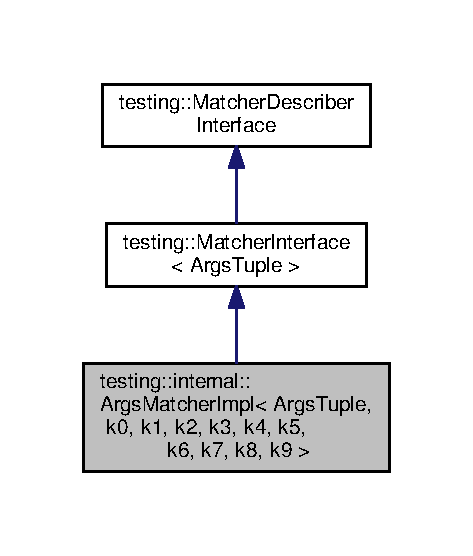
\includegraphics[width=227pt]{classtesting_1_1internal_1_1ArgsMatcherImpl__inherit__graph}
\end{center}
\end{figure}


Collaboration diagram for testing\+:\+:internal\+:\+:Args\+Matcher\+Impl$<$ Args\+Tuple, k0, k1, k2, k3, k4, k5, k6, k7, k8, k9 $>$\+:
\nopagebreak
\begin{figure}[H]
\begin{center}
\leavevmode
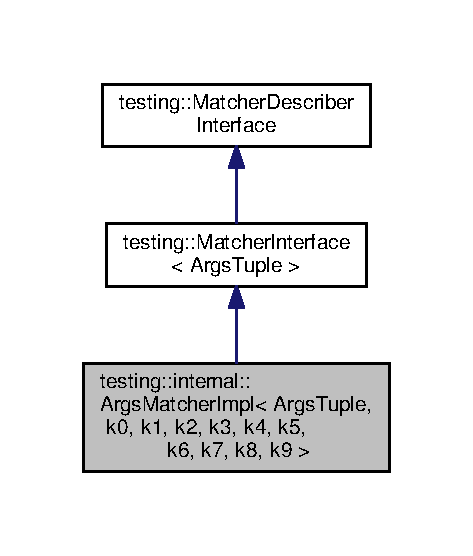
\includegraphics[width=227pt]{classtesting_1_1internal_1_1ArgsMatcherImpl__coll__graph}
\end{center}
\end{figure}
\subsection*{Public Types}
\begin{DoxyCompactItemize}
\item 
typedef \hyperlink{classtesting_1_1internal_1_1TupleFields}{internal\+::\+Tuple\+Fields}$<$ Raw\+Args\+Tuple, k0, k1, k2, k3, k4, k5, k6, k7, k8, k9 $>$\+::type \hyperlink{classtesting_1_1internal_1_1ArgsMatcherImpl_ab061679f6251e56ccbedaf0c316d00ff}{Selected\+Args}
\item 
typedef \hyperlink{classtesting_1_1Matcher}{Matcher}$<$ const \hyperlink{classtesting_1_1internal_1_1ArgsMatcherImpl_ab061679f6251e56ccbedaf0c316d00ff}{Selected\+Args} \& $>$ \hyperlink{classtesting_1_1internal_1_1ArgsMatcherImpl_ab90d2c074b2072d6c39bf26209fb941f}{Monomorphic\+Inner\+Matcher}
\end{DoxyCompactItemize}
\subsection*{Public Member Functions}
\begin{DoxyCompactItemize}
\item 
typedef \hyperlink{classtesting_1_1internal_1_1ArgsMatcherImpl_a7b0cadc369c0c20cd254cc2052782301}{G\+T\+E\+S\+T\+\_\+\+R\+E\+M\+O\+V\+E\+\_\+\+R\+E\+F\+E\+R\+E\+N\+C\+E\+\_\+\+A\+N\+D\+\_\+\+C\+O\+N\+S\+T\+\_\+} (Args\+Tuple) Raw\+Args\+Tuple
\item 
{\footnotesize template$<$typename Inner\+Matcher $>$ }\\\hyperlink{classtesting_1_1internal_1_1ArgsMatcherImpl_a7f7a9a826d130d11fe30633d79f59a06}{Args\+Matcher\+Impl} (const Inner\+Matcher \&inner\+\_\+matcher)
\item 
virtual bool \hyperlink{classtesting_1_1internal_1_1ArgsMatcherImpl_a9c9760b144a5e207082fe040c869ad39}{Match\+And\+Explain} (Args\+Tuple args, \hyperlink{classtesting_1_1MatchResultListener}{Match\+Result\+Listener} $\ast$listener) const 
\item 
virtual void \hyperlink{classtesting_1_1internal_1_1ArgsMatcherImpl_a7e2acf3bee2d8038da0f87673bc82eb2}{Describe\+To} (\+::std\+::ostream $\ast$os) const 
\item 
virtual void \hyperlink{classtesting_1_1internal_1_1ArgsMatcherImpl_af22ab8bcd4baee6d1c79751d46240289}{Describe\+Negation\+To} (\+::std\+::ostream $\ast$os) const 
\end{DoxyCompactItemize}


\subsection{Member Typedef Documentation}
\index{testing\+::internal\+::\+Args\+Matcher\+Impl@{testing\+::internal\+::\+Args\+Matcher\+Impl}!Monomorphic\+Inner\+Matcher@{Monomorphic\+Inner\+Matcher}}
\index{Monomorphic\+Inner\+Matcher@{Monomorphic\+Inner\+Matcher}!testing\+::internal\+::\+Args\+Matcher\+Impl@{testing\+::internal\+::\+Args\+Matcher\+Impl}}
\subsubsection[{\texorpdfstring{Monomorphic\+Inner\+Matcher}{MonomorphicInnerMatcher}}]{\setlength{\rightskip}{0pt plus 5cm}template$<$class Args\+Tuple , int k0 = -\/1, int k1 = -\/1, int k2 = -\/1, int k3 = -\/1, int k4 = -\/1, int k5 = -\/1, int k6 = -\/1, int k7 = -\/1, int k8 = -\/1, int k9 = -\/1$>$ typedef {\bf Matcher}$<$const {\bf Selected\+Args}\&$>$ {\bf testing\+::internal\+::\+Args\+Matcher\+Impl}$<$ Args\+Tuple, k0, k1, k2, k3, k4, k5, k6, k7, k8, k9 $>$\+::{\bf Monomorphic\+Inner\+Matcher}}\hypertarget{classtesting_1_1internal_1_1ArgsMatcherImpl_ab90d2c074b2072d6c39bf26209fb941f}{}\label{classtesting_1_1internal_1_1ArgsMatcherImpl_ab90d2c074b2072d6c39bf26209fb941f}
\index{testing\+::internal\+::\+Args\+Matcher\+Impl@{testing\+::internal\+::\+Args\+Matcher\+Impl}!Selected\+Args@{Selected\+Args}}
\index{Selected\+Args@{Selected\+Args}!testing\+::internal\+::\+Args\+Matcher\+Impl@{testing\+::internal\+::\+Args\+Matcher\+Impl}}
\subsubsection[{\texorpdfstring{Selected\+Args}{SelectedArgs}}]{\setlength{\rightskip}{0pt plus 5cm}template$<$class Args\+Tuple , int k0 = -\/1, int k1 = -\/1, int k2 = -\/1, int k3 = -\/1, int k4 = -\/1, int k5 = -\/1, int k6 = -\/1, int k7 = -\/1, int k8 = -\/1, int k9 = -\/1$>$ typedef {\bf internal\+::\+Tuple\+Fields}$<$Raw\+Args\+Tuple, k0, k1, k2, k3, k4, k5, k6, k7, k8, k9$>$\+::type {\bf testing\+::internal\+::\+Args\+Matcher\+Impl}$<$ Args\+Tuple, k0, k1, k2, k3, k4, k5, k6, k7, k8, k9 $>$\+::{\bf Selected\+Args}}\hypertarget{classtesting_1_1internal_1_1ArgsMatcherImpl_ab061679f6251e56ccbedaf0c316d00ff}{}\label{classtesting_1_1internal_1_1ArgsMatcherImpl_ab061679f6251e56ccbedaf0c316d00ff}


\subsection{Constructor \& Destructor Documentation}
\index{testing\+::internal\+::\+Args\+Matcher\+Impl@{testing\+::internal\+::\+Args\+Matcher\+Impl}!Args\+Matcher\+Impl@{Args\+Matcher\+Impl}}
\index{Args\+Matcher\+Impl@{Args\+Matcher\+Impl}!testing\+::internal\+::\+Args\+Matcher\+Impl@{testing\+::internal\+::\+Args\+Matcher\+Impl}}
\subsubsection[{\texorpdfstring{Args\+Matcher\+Impl(const Inner\+Matcher \&inner\+\_\+matcher)}{ArgsMatcherImpl(const InnerMatcher &inner_matcher)}}]{\setlength{\rightskip}{0pt plus 5cm}template$<$class Args\+Tuple , int k0 = -\/1, int k1 = -\/1, int k2 = -\/1, int k3 = -\/1, int k4 = -\/1, int k5 = -\/1, int k6 = -\/1, int k7 = -\/1, int k8 = -\/1, int k9 = -\/1$>$ template$<$typename Inner\+Matcher $>$ {\bf testing\+::internal\+::\+Args\+Matcher\+Impl}$<$ Args\+Tuple, k0, k1, k2, k3, k4, k5, k6, k7, k8, k9 $>$\+::{\bf Args\+Matcher\+Impl} (
\begin{DoxyParamCaption}
\item[{const Inner\+Matcher \&}]{inner\+\_\+matcher}
\end{DoxyParamCaption}
)\hspace{0.3cm}{\ttfamily [inline]}, {\ttfamily [explicit]}}\hypertarget{classtesting_1_1internal_1_1ArgsMatcherImpl_a7f7a9a826d130d11fe30633d79f59a06}{}\label{classtesting_1_1internal_1_1ArgsMatcherImpl_a7f7a9a826d130d11fe30633d79f59a06}

\begin{DoxyCode}
221       : inner\_matcher\_(SafeMatcherCast<const SelectedArgs&>(inner\_matcher)) \{\}
\end{DoxyCode}


\subsection{Member Function Documentation}
\index{testing\+::internal\+::\+Args\+Matcher\+Impl@{testing\+::internal\+::\+Args\+Matcher\+Impl}!Describe\+Negation\+To@{Describe\+Negation\+To}}
\index{Describe\+Negation\+To@{Describe\+Negation\+To}!testing\+::internal\+::\+Args\+Matcher\+Impl@{testing\+::internal\+::\+Args\+Matcher\+Impl}}
\subsubsection[{\texorpdfstring{Describe\+Negation\+To(\+::std\+::ostream $\ast$os) const }{DescribeNegationTo(::std::ostream *os) const }}]{\setlength{\rightskip}{0pt plus 5cm}template$<$class Args\+Tuple , int k0 = -\/1, int k1 = -\/1, int k2 = -\/1, int k3 = -\/1, int k4 = -\/1, int k5 = -\/1, int k6 = -\/1, int k7 = -\/1, int k8 = -\/1, int k9 = -\/1$>$ virtual void {\bf testing\+::internal\+::\+Args\+Matcher\+Impl}$<$ Args\+Tuple, k0, k1, k2, k3, k4, k5, k6, k7, k8, k9 $>$\+::Describe\+Negation\+To (
\begin{DoxyParamCaption}
\item[{\+::std\+::ostream $\ast$}]{os}
\end{DoxyParamCaption}
) const\hspace{0.3cm}{\ttfamily [inline]}, {\ttfamily [virtual]}}\hypertarget{classtesting_1_1internal_1_1ArgsMatcherImpl_af22ab8bcd4baee6d1c79751d46240289}{}\label{classtesting_1_1internal_1_1ArgsMatcherImpl_af22ab8bcd4baee6d1c79751d46240289}


Reimplemented from \hyperlink{classtesting_1_1MatcherDescriberInterface_a35b9dc2f3e25ca4b903f282feaaf9f8c}{testing\+::\+Matcher\+Describer\+Interface}.


\begin{DoxyCode}
245                                                         \{
246     *os << \textcolor{stringliteral}{"are a tuple "};
247     PrintIndices(os);
248     inner\_matcher\_.\hyperlink{classtesting_1_1internal_1_1MatcherBase_a47cc840bc783fc0ceafbfb68d0ea5758}{DescribeNegationTo}(os);
249   \}
\end{DoxyCode}
\index{testing\+::internal\+::\+Args\+Matcher\+Impl@{testing\+::internal\+::\+Args\+Matcher\+Impl}!Describe\+To@{Describe\+To}}
\index{Describe\+To@{Describe\+To}!testing\+::internal\+::\+Args\+Matcher\+Impl@{testing\+::internal\+::\+Args\+Matcher\+Impl}}
\subsubsection[{\texorpdfstring{Describe\+To(\+::std\+::ostream $\ast$os) const }{DescribeTo(::std::ostream *os) const }}]{\setlength{\rightskip}{0pt plus 5cm}template$<$class Args\+Tuple , int k0 = -\/1, int k1 = -\/1, int k2 = -\/1, int k3 = -\/1, int k4 = -\/1, int k5 = -\/1, int k6 = -\/1, int k7 = -\/1, int k8 = -\/1, int k9 = -\/1$>$ virtual void {\bf testing\+::internal\+::\+Args\+Matcher\+Impl}$<$ Args\+Tuple, k0, k1, k2, k3, k4, k5, k6, k7, k8, k9 $>$\+::Describe\+To (
\begin{DoxyParamCaption}
\item[{\+::std\+::ostream $\ast$}]{os}
\end{DoxyParamCaption}
) const\hspace{0.3cm}{\ttfamily [inline]}, {\ttfamily [virtual]}}\hypertarget{classtesting_1_1internal_1_1ArgsMatcherImpl_a7e2acf3bee2d8038da0f87673bc82eb2}{}\label{classtesting_1_1internal_1_1ArgsMatcherImpl_a7e2acf3bee2d8038da0f87673bc82eb2}


Implements \hyperlink{classtesting_1_1MatcherDescriberInterface_ad9f861588bd969b6e3e717f13bb94e7b}{testing\+::\+Matcher\+Describer\+Interface}.


\begin{DoxyCode}
239                                                 \{
240     *os << \textcolor{stringliteral}{"are a tuple "};
241     PrintIndices(os);
242     inner\_matcher\_.\hyperlink{classtesting_1_1internal_1_1MatcherBase_afcb24e7d1ff27e147e0e607d2a122467}{DescribeTo}(os);
243   \}
\end{DoxyCode}
\index{testing\+::internal\+::\+Args\+Matcher\+Impl@{testing\+::internal\+::\+Args\+Matcher\+Impl}!G\+T\+E\+S\+T\+\_\+\+R\+E\+M\+O\+V\+E\+\_\+\+R\+E\+F\+E\+R\+E\+N\+C\+E\+\_\+\+A\+N\+D\+\_\+\+C\+O\+N\+S\+T\+\_\+@{G\+T\+E\+S\+T\+\_\+\+R\+E\+M\+O\+V\+E\+\_\+\+R\+E\+F\+E\+R\+E\+N\+C\+E\+\_\+\+A\+N\+D\+\_\+\+C\+O\+N\+S\+T\+\_\+}}
\index{G\+T\+E\+S\+T\+\_\+\+R\+E\+M\+O\+V\+E\+\_\+\+R\+E\+F\+E\+R\+E\+N\+C\+E\+\_\+\+A\+N\+D\+\_\+\+C\+O\+N\+S\+T\+\_\+@{G\+T\+E\+S\+T\+\_\+\+R\+E\+M\+O\+V\+E\+\_\+\+R\+E\+F\+E\+R\+E\+N\+C\+E\+\_\+\+A\+N\+D\+\_\+\+C\+O\+N\+S\+T\+\_\+}!testing\+::internal\+::\+Args\+Matcher\+Impl@{testing\+::internal\+::\+Args\+Matcher\+Impl}}
\subsubsection[{\texorpdfstring{G\+T\+E\+S\+T\+\_\+\+R\+E\+M\+O\+V\+E\+\_\+\+R\+E\+F\+E\+R\+E\+N\+C\+E\+\_\+\+A\+N\+D\+\_\+\+C\+O\+N\+S\+T\+\_\+(\+Args\+Tuple) Raw\+Args\+Tuple}{GTEST_REMOVE_REFERENCE_AND_CONST_(ArgsTuple) RawArgsTuple}}]{\setlength{\rightskip}{0pt plus 5cm}template$<$class Args\+Tuple , int k0 = -\/1, int k1 = -\/1, int k2 = -\/1, int k3 = -\/1, int k4 = -\/1, int k5 = -\/1, int k6 = -\/1, int k7 = -\/1, int k8 = -\/1, int k9 = -\/1$>$ typedef {\bf testing\+::internal\+::\+Args\+Matcher\+Impl}$<$ Args\+Tuple, k0, k1, k2, k3, k4, k5, k6, k7, k8, k9 $>$\+::G\+T\+E\+S\+T\+\_\+\+R\+E\+M\+O\+V\+E\+\_\+\+R\+E\+F\+E\+R\+E\+N\+C\+E\+\_\+\+A\+N\+D\+\_\+\+C\+O\+N\+S\+T\+\_\+ (
\begin{DoxyParamCaption}
\item[{Args\+Tuple}]{}
\end{DoxyParamCaption}
)}\hypertarget{classtesting_1_1internal_1_1ArgsMatcherImpl_a7b0cadc369c0c20cd254cc2052782301}{}\label{classtesting_1_1internal_1_1ArgsMatcherImpl_a7b0cadc369c0c20cd254cc2052782301}
\index{testing\+::internal\+::\+Args\+Matcher\+Impl@{testing\+::internal\+::\+Args\+Matcher\+Impl}!Match\+And\+Explain@{Match\+And\+Explain}}
\index{Match\+And\+Explain@{Match\+And\+Explain}!testing\+::internal\+::\+Args\+Matcher\+Impl@{testing\+::internal\+::\+Args\+Matcher\+Impl}}
\subsubsection[{\texorpdfstring{Match\+And\+Explain(\+Args\+Tuple args, Match\+Result\+Listener $\ast$listener) const }{MatchAndExplain(ArgsTuple args, MatchResultListener *listener) const }}]{\setlength{\rightskip}{0pt plus 5cm}template$<$class Args\+Tuple , int k0 = -\/1, int k1 = -\/1, int k2 = -\/1, int k3 = -\/1, int k4 = -\/1, int k5 = -\/1, int k6 = -\/1, int k7 = -\/1, int k8 = -\/1, int k9 = -\/1$>$ virtual bool {\bf testing\+::internal\+::\+Args\+Matcher\+Impl}$<$ Args\+Tuple, k0, k1, k2, k3, k4, k5, k6, k7, k8, k9 $>$\+::Match\+And\+Explain (
\begin{DoxyParamCaption}
\item[{Args\+Tuple}]{args, }
\item[{{\bf Match\+Result\+Listener} $\ast$}]{listener}
\end{DoxyParamCaption}
) const\hspace{0.3cm}{\ttfamily [inline]}, {\ttfamily [virtual]}}\hypertarget{classtesting_1_1internal_1_1ArgsMatcherImpl_a9c9760b144a5e207082fe040c869ad39}{}\label{classtesting_1_1internal_1_1ArgsMatcherImpl_a9c9760b144a5e207082fe040c869ad39}


Implements \hyperlink{classtesting_1_1MatcherInterface_a296b43607cd99d60365f0e6a762777cf}{testing\+::\+Matcher\+Interface$<$ Args\+Tuple $>$}.


\begin{DoxyCode}
224                                                                     \{
225     \textcolor{keyword}{const} \hyperlink{classtesting_1_1internal_1_1ArgsMatcherImpl_ab061679f6251e56ccbedaf0c316d00ff}{SelectedArgs}& selected\_args = GetSelectedArgs(args);
226     \textcolor{keywordflow}{if} (!listener->IsInterested())
227       \textcolor{keywordflow}{return} inner\_matcher\_.\hyperlink{classtesting_1_1internal_1_1MatcherBase_a105a9dae7afecee8898db8ad1887b0db}{Matches}(selected\_args);
228 
229     PrintIndices(listener->stream());
230     *listener << \textcolor{stringliteral}{"are "} << \hyperlink{namespacetesting_aa5717bb1144edd1d262d310ba70c82ed}{PrintToString}(selected\_args);
231 
232     StringMatchResultListener inner\_listener;
233     \textcolor{keyword}{const} \textcolor{keywordtype}{bool} match = inner\_matcher\_.\hyperlink{classtesting_1_1internal_1_1MatcherBase_ae3f5f3150a95cafb1c2ab7c864a42e65}{MatchAndExplain}(selected\_args,
234                                                       &inner\_listener);
235     \hyperlink{namespacetesting_1_1internal_a77c9e2b66d2b2414db4763971180d53c}{PrintIfNotEmpty}(inner\_listener.str(), listener->stream());
236     \textcolor{keywordflow}{return} match;
237   \}
\end{DoxyCode}


The documentation for this class was generated from the following file\+:\begin{DoxyCompactItemize}
\item 
vendor/googletest/googlemock/include/gmock/\hyperlink{gmock-generated-matchers_8h}{gmock-\/generated-\/matchers.\+h}\end{DoxyCompactItemize}

\hypertarget{classtesting_1_1internal_1_1AssertHelper}{}\section{testing\+:\+:internal\+:\+:Assert\+Helper Class Reference}
\label{classtesting_1_1internal_1_1AssertHelper}\index{testing\+::internal\+::\+Assert\+Helper@{testing\+::internal\+::\+Assert\+Helper}}


{\ttfamily \#include $<$gtest.\+h$>$}

\subsection*{Public Member Functions}
\begin{DoxyCompactItemize}
\item 
\hyperlink{classtesting_1_1internal_1_1AssertHelper_ac2c9334518fd4087189b4505567a3c90}{Assert\+Helper} (\hyperlink{classtesting_1_1TestPartResult_a65ae656b33fdfdfffaf34858778a52d5}{Test\+Part\+Result\+::\+Type} type, const char $\ast$file, int line, const char $\ast$message)
\item 
\hyperlink{classtesting_1_1internal_1_1AssertHelper_a51c640785d4ed4a0155cc9aa857d8931}{$\sim$\+Assert\+Helper} ()
\item 
void \hyperlink{classtesting_1_1internal_1_1AssertHelper_ab721be11cb9aca8a361ca1f014ca5f80}{operator=} (const \hyperlink{classtesting_1_1Message}{Message} \&message) const 
\end{DoxyCompactItemize}


\subsection{Constructor \& Destructor Documentation}
\index{testing\+::internal\+::\+Assert\+Helper@{testing\+::internal\+::\+Assert\+Helper}!Assert\+Helper@{Assert\+Helper}}
\index{Assert\+Helper@{Assert\+Helper}!testing\+::internal\+::\+Assert\+Helper@{testing\+::internal\+::\+Assert\+Helper}}
\subsubsection[{\texorpdfstring{Assert\+Helper(\+Test\+Part\+Result\+::\+Type type, const char $\ast$file, int line, const char $\ast$message)}{AssertHelper(TestPartResult::Type type, const char *file, int line, const char *message)}}]{\setlength{\rightskip}{0pt plus 5cm}testing\+::internal\+::\+Assert\+Helper\+::\+Assert\+Helper (
\begin{DoxyParamCaption}
\item[{{\bf Test\+Part\+Result\+::\+Type}}]{type, }
\item[{const char $\ast$}]{file, }
\item[{int}]{line, }
\item[{const char $\ast$}]{message}
\end{DoxyParamCaption}
)}\hypertarget{classtesting_1_1internal_1_1AssertHelper_ac2c9334518fd4087189b4505567a3c90}{}\label{classtesting_1_1internal_1_1AssertHelper_ac2c9334518fd4087189b4505567a3c90}

\begin{DoxyCode}
365     : data\_(\textcolor{keyword}{new} AssertHelperData(\hyperlink{namespaceupload_a4fc56f0dd6613be15c3c4dc3af3619ce}{type}, file, line, \hyperlink{namespacegtest__output__test_ac696d0798ad7d08cb2e61070824750e2}{message})) \{
366 \}
\end{DoxyCode}
\index{testing\+::internal\+::\+Assert\+Helper@{testing\+::internal\+::\+Assert\+Helper}!````~Assert\+Helper@{$\sim$\+Assert\+Helper}}
\index{````~Assert\+Helper@{$\sim$\+Assert\+Helper}!testing\+::internal\+::\+Assert\+Helper@{testing\+::internal\+::\+Assert\+Helper}}
\subsubsection[{\texorpdfstring{$\sim$\+Assert\+Helper()}{~AssertHelper()}}]{\setlength{\rightskip}{0pt plus 5cm}testing\+::internal\+::\+Assert\+Helper\+::$\sim$\+Assert\+Helper (
\begin{DoxyParamCaption}
{}
\end{DoxyParamCaption}
)}\hypertarget{classtesting_1_1internal_1_1AssertHelper_a51c640785d4ed4a0155cc9aa857d8931}{}\label{classtesting_1_1internal_1_1AssertHelper_a51c640785d4ed4a0155cc9aa857d8931}

\begin{DoxyCode}
368                             \{
369   \textcolor{keyword}{delete} data\_;
370 \}
\end{DoxyCode}


\subsection{Member Function Documentation}
\index{testing\+::internal\+::\+Assert\+Helper@{testing\+::internal\+::\+Assert\+Helper}!operator=@{operator=}}
\index{operator=@{operator=}!testing\+::internal\+::\+Assert\+Helper@{testing\+::internal\+::\+Assert\+Helper}}
\subsubsection[{\texorpdfstring{operator=(const Message \&message) const }{operator=(const Message &message) const }}]{\setlength{\rightskip}{0pt plus 5cm}void testing\+::internal\+::\+Assert\+Helper\+::operator= (
\begin{DoxyParamCaption}
\item[{const {\bf Message} \&}]{message}
\end{DoxyParamCaption}
) const}\hypertarget{classtesting_1_1internal_1_1AssertHelper_ab721be11cb9aca8a361ca1f014ca5f80}{}\label{classtesting_1_1internal_1_1AssertHelper_ab721be11cb9aca8a361ca1f014ca5f80}

\begin{DoxyCode}
373                                                          \{
374   \hyperlink{classtesting_1_1UnitTest_a24192400b70b3b946746954e9574fb8e}{UnitTest::GetInstance}()->
375     AddTestPartResult(data\_->type, data\_->file, data\_->line,
376                       \hyperlink{namespacetesting_1_1internal_ae475a090bca903bb222dd389eb189166}{AppendUserMessage}(data\_->message, \hyperlink{namespacegtest__output__test_ac696d0798ad7d08cb2e61070824750e2}{message}),
377                       \hyperlink{classtesting_1_1UnitTest_a24192400b70b3b946746954e9574fb8e}{UnitTest::GetInstance}()->impl()
378                       ->\hyperlink{classtesting_1_1internal_1_1UnitTestImpl_a61c0a51ac4e57d9f884f646ca6dd2210}{CurrentOsStackTraceExceptTop}(1)
379                       \textcolor{comment}{// Skips the stack frame for this function itself.}
380                       );  \textcolor{comment}{// NOLINT}
381 \}
\end{DoxyCode}


The documentation for this class was generated from the following files\+:\begin{DoxyCompactItemize}
\item 
vendor/googletest/googletest/include/gtest/\hyperlink{gtest_8h}{gtest.\+h}\item 
vendor/googletest/googletest/src/\hyperlink{gtest_8cc}{gtest.\+cc}\end{DoxyCompactItemize}

\hypertarget{classmy__namespace_1_1testing_1_1AssertionResult}{}\section{my\+\_\+namespace\+:\+:testing\+:\+:Assertion\+Result Class Reference}
\label{classmy__namespace_1_1testing_1_1AssertionResult}\index{my\+\_\+namespace\+::testing\+::\+Assertion\+Result@{my\+\_\+namespace\+::testing\+::\+Assertion\+Result}}


The documentation for this class was generated from the following file\+:\begin{DoxyCompactItemize}
\item 
vendor/googletest/googletest/test/\hyperlink{gtest__unittest_8cc}{gtest\+\_\+unittest.\+cc}\end{DoxyCompactItemize}

\hypertarget{classtesting_1_1AssertionResult}{}\section{testing\+:\+:Assertion\+Result Class Reference}
\label{classtesting_1_1AssertionResult}\index{testing\+::\+Assertion\+Result@{testing\+::\+Assertion\+Result}}


{\ttfamily \#include $<$gtest.\+h$>$}

\subsection*{Public Member Functions}
\begin{DoxyCompactItemize}
\item 
\hyperlink{classtesting_1_1AssertionResult_a27788116f03f90aec4daf592fd809ead}{Assertion\+Result} (const \hyperlink{classtesting_1_1AssertionResult}{Assertion\+Result} \&other)
\item 
{\footnotesize template$<$typename T $>$ }\\\hyperlink{classtesting_1_1AssertionResult_a9b8d1d6d0a979d0769ed4ff97d06c4e3}{Assertion\+Result} (const T \&success, typename \hyperlink{structtesting_1_1internal_1_1EnableIf}{internal\+::\+Enable\+If}$<$ !\hyperlink{classtesting_1_1internal_1_1ImplicitlyConvertible}{internal\+::\+Implicitly\+Convertible}$<$ T, \hyperlink{classtesting_1_1AssertionResult}{Assertion\+Result} $>$\+::value $>$\+::type $\ast$=N\+U\+LL)
\item 
\hyperlink{classtesting_1_1AssertionResult}{Assertion\+Result} \& \hyperlink{classtesting_1_1AssertionResult_aad9274c7b69eda67eb9306963a790839}{operator=} (\hyperlink{classtesting_1_1AssertionResult}{Assertion\+Result} other)
\item 
\hyperlink{classtesting_1_1AssertionResult_af85b7852e6399467cd74df539810abcd}{operator bool} () const 
\item 
\hyperlink{classtesting_1_1AssertionResult}{Assertion\+Result} \hyperlink{classtesting_1_1AssertionResult_a85301ba52aa1efe89b79d1e3b59160cd}{operator!} () const 
\item 
const char $\ast$ \hyperlink{classtesting_1_1AssertionResult_ab20c91eba13e20f1b4ad89e3d15f69a8}{message} () const 
\item 
const char $\ast$ \hyperlink{classtesting_1_1AssertionResult_ae54fa82506c507a9dbc0f85d2cec652a}{failure\+\_\+message} () const 
\item 
{\footnotesize template$<$typename T $>$ }\\\hyperlink{classtesting_1_1AssertionResult}{Assertion\+Result} \& \hyperlink{classtesting_1_1AssertionResult_a3230efa81aafe7c61f5fb878cfa39e91}{operator$<$$<$} (const T \&value)
\item 
\hyperlink{classtesting_1_1AssertionResult}{Assertion\+Result} \& \hyperlink{classtesting_1_1AssertionResult_a43ae8a260843ce2ff3dc9af262672b8b}{operator$<$$<$} (\+::std\+::ostream \&($\ast$basic\+\_\+manipulator)(\+::std\+::ostream \&stream))
\end{DoxyCompactItemize}


\subsection{Constructor \& Destructor Documentation}
\index{testing\+::\+Assertion\+Result@{testing\+::\+Assertion\+Result}!Assertion\+Result@{Assertion\+Result}}
\index{Assertion\+Result@{Assertion\+Result}!testing\+::\+Assertion\+Result@{testing\+::\+Assertion\+Result}}
\subsubsection[{\texorpdfstring{Assertion\+Result(const Assertion\+Result \&other)}{AssertionResult(const AssertionResult &other)}}]{\setlength{\rightskip}{0pt plus 5cm}testing\+::\+Assertion\+Result\+::\+Assertion\+Result (
\begin{DoxyParamCaption}
\item[{const {\bf Assertion\+Result} \&}]{other}
\end{DoxyParamCaption}
)}\hypertarget{classtesting_1_1AssertionResult_a27788116f03f90aec4daf592fd809ead}{}\label{classtesting_1_1AssertionResult_a27788116f03f90aec4daf592fd809ead}

\begin{DoxyCode}
988     : success\_(other.success\_),
989       message\_(other.message\_.get() != NULL ?
990                \hyperlink{namespacetesting_1_1internal_a8e8ff5b11e64078831112677156cb111}{new ::std::string}(*other.message\_) :
991                static\_cast< ::\hyperlink{namespacestd}{std}::\hyperlink{namespacetesting_1_1internal_a8e8ff5b11e64078831112677156cb111}{string}*>(NULL)) \{
992 \}
\end{DoxyCode}
\index{testing\+::\+Assertion\+Result@{testing\+::\+Assertion\+Result}!Assertion\+Result@{Assertion\+Result}}
\index{Assertion\+Result@{Assertion\+Result}!testing\+::\+Assertion\+Result@{testing\+::\+Assertion\+Result}}
\subsubsection[{\texorpdfstring{Assertion\+Result(const T \&success, typename internal\+::\+Enable\+If$<$ "!internal\+::\+Implicitly\+Convertible$<$ T, Assertion\+Result $>$\+::value $>$\+::type $\ast$=\+N\+U\+L\+L)}{AssertionResult(const T &success, typename internal::EnableIf< !internal::ImplicitlyConvertible< T, AssertionResult >::value >::type *=NULL)}}]{\setlength{\rightskip}{0pt plus 5cm}template$<$typename T $>$ testing\+::\+Assertion\+Result\+::\+Assertion\+Result (
\begin{DoxyParamCaption}
\item[{const T \&}]{success, }
\item[{typename {\bf internal\+::\+Enable\+If}$<$ !{\bf internal\+::\+Implicitly\+Convertible}$<$ T, {\bf Assertion\+Result} $>$\+::value $>$\+::type $\ast$}]{ = {\ttfamily NULL}}
\end{DoxyParamCaption}
)\hspace{0.3cm}{\ttfamily [inline]}, {\ttfamily [explicit]}}\hypertarget{classtesting_1_1AssertionResult_a9b8d1d6d0a979d0769ed4ff97d06c4e3}{}\label{classtesting_1_1AssertionResult_a9b8d1d6d0a979d0769ed4ff97d06c4e3}

\begin{DoxyCode}
277       : success\_(success) \{\}
\end{DoxyCode}


\subsection{Member Function Documentation}
\index{testing\+::\+Assertion\+Result@{testing\+::\+Assertion\+Result}!failure\+\_\+message@{failure\+\_\+message}}
\index{failure\+\_\+message@{failure\+\_\+message}!testing\+::\+Assertion\+Result@{testing\+::\+Assertion\+Result}}
\subsubsection[{\texorpdfstring{failure\+\_\+message() const }{failure_message() const }}]{\setlength{\rightskip}{0pt plus 5cm}const char$\ast$ testing\+::\+Assertion\+Result\+::failure\+\_\+message (
\begin{DoxyParamCaption}
{}
\end{DoxyParamCaption}
) const\hspace{0.3cm}{\ttfamily [inline]}}\hypertarget{classtesting_1_1AssertionResult_ae54fa82506c507a9dbc0f85d2cec652a}{}\label{classtesting_1_1AssertionResult_ae54fa82506c507a9dbc0f85d2cec652a}

\begin{DoxyCode}
302 \{ \textcolor{keywordflow}{return} \hyperlink{classtesting_1_1AssertionResult_ab20c91eba13e20f1b4ad89e3d15f69a8}{message}(); \}
\end{DoxyCode}
\index{testing\+::\+Assertion\+Result@{testing\+::\+Assertion\+Result}!message@{message}}
\index{message@{message}!testing\+::\+Assertion\+Result@{testing\+::\+Assertion\+Result}}
\subsubsection[{\texorpdfstring{message() const }{message() const }}]{\setlength{\rightskip}{0pt plus 5cm}const char$\ast$ testing\+::\+Assertion\+Result\+::message (
\begin{DoxyParamCaption}
{}
\end{DoxyParamCaption}
) const\hspace{0.3cm}{\ttfamily [inline]}}\hypertarget{classtesting_1_1AssertionResult_ab20c91eba13e20f1b4ad89e3d15f69a8}{}\label{classtesting_1_1AssertionResult_ab20c91eba13e20f1b4ad89e3d15f69a8}

\begin{DoxyCode}
297                               \{
298     \textcolor{keywordflow}{return} message\_.\hyperlink{classtesting_1_1internal_1_1scoped__ptr_adc8f8fcb63ce69f80f011456e6d2f08d}{get}() != NULL ?  message\_->c\_str() : \textcolor{stringliteral}{""};
299   \}
\end{DoxyCode}
\index{testing\+::\+Assertion\+Result@{testing\+::\+Assertion\+Result}!operator bool@{operator bool}}
\index{operator bool@{operator bool}!testing\+::\+Assertion\+Result@{testing\+::\+Assertion\+Result}}
\subsubsection[{\texorpdfstring{operator bool() const }{operator bool() const }}]{\setlength{\rightskip}{0pt plus 5cm}testing\+::\+Assertion\+Result\+::operator bool (
\begin{DoxyParamCaption}
{}
\end{DoxyParamCaption}
) const\hspace{0.3cm}{\ttfamily [inline]}}\hypertarget{classtesting_1_1AssertionResult_af85b7852e6399467cd74df539810abcd}{}\label{classtesting_1_1AssertionResult_af85b7852e6399467cd74df539810abcd}

\begin{DoxyCode}
288 \{ \textcolor{keywordflow}{return} success\_; \}  \textcolor{comment}{// NOLINT}
\end{DoxyCode}
\index{testing\+::\+Assertion\+Result@{testing\+::\+Assertion\+Result}!operator"!@{operator"!}}
\index{operator"!@{operator"!}!testing\+::\+Assertion\+Result@{testing\+::\+Assertion\+Result}}
\subsubsection[{\texorpdfstring{operator"!() const }{operator!() const }}]{\setlength{\rightskip}{0pt plus 5cm}{\bf Assertion\+Result} testing\+::\+Assertion\+Result\+::operator! (
\begin{DoxyParamCaption}
{}
\end{DoxyParamCaption}
) const}\hypertarget{classtesting_1_1AssertionResult_a85301ba52aa1efe89b79d1e3b59160cd}{}\label{classtesting_1_1AssertionResult_a85301ba52aa1efe89b79d1e3b59160cd}

\begin{DoxyCode}
1002                                                  \{
1003   \hyperlink{classtesting_1_1AssertionResult_a27788116f03f90aec4daf592fd809ead}{AssertionResult} negation(!success\_);
1004   \textcolor{keywordflow}{if} (message\_.\hyperlink{classtesting_1_1internal_1_1scoped__ptr_adc8f8fcb63ce69f80f011456e6d2f08d}{get}() != NULL)
1005     negation << *message\_;
1006   \textcolor{keywordflow}{return} negation;
1007 \}
\end{DoxyCode}
\index{testing\+::\+Assertion\+Result@{testing\+::\+Assertion\+Result}!operator$<$$<$@{operator$<$$<$}}
\index{operator$<$$<$@{operator$<$$<$}!testing\+::\+Assertion\+Result@{testing\+::\+Assertion\+Result}}
\subsubsection[{\texorpdfstring{operator$<$$<$(const T \&value)}{operator<<(const T &value)}}]{\setlength{\rightskip}{0pt plus 5cm}template$<$typename T $>$ {\bf Assertion\+Result}\& testing\+::\+Assertion\+Result\+::operator$<$$<$ (
\begin{DoxyParamCaption}
\item[{const T \&}]{value}
\end{DoxyParamCaption}
)\hspace{0.3cm}{\ttfamily [inline]}}\hypertarget{classtesting_1_1AssertionResult_a3230efa81aafe7c61f5fb878cfa39e91}{}\label{classtesting_1_1AssertionResult_a3230efa81aafe7c61f5fb878cfa39e91}

\begin{DoxyCode}
305                                                                     \{
306     AppendMessage(Message() << value);
307     \textcolor{keywordflow}{return} *\textcolor{keyword}{this};
308   \}
\end{DoxyCode}
\index{testing\+::\+Assertion\+Result@{testing\+::\+Assertion\+Result}!operator$<$$<$@{operator$<$$<$}}
\index{operator$<$$<$@{operator$<$$<$}!testing\+::\+Assertion\+Result@{testing\+::\+Assertion\+Result}}
\subsubsection[{\texorpdfstring{operator$<$$<$(\+::std\+::ostream \&($\ast$basic\+\_\+manipulator)(\+::std\+::ostream \&stream))}{operator<<(::std::ostream &(*basic_manipulator)(::std::ostream &stream))}}]{\setlength{\rightskip}{0pt plus 5cm}{\bf Assertion\+Result}\& testing\+::\+Assertion\+Result\+::operator$<$$<$ (
\begin{DoxyParamCaption}
\item[{\+::std\+::ostream \&($\ast$)(\+::std\+::ostream \&stream)}]{basic\+\_\+manipulator}
\end{DoxyParamCaption}
)\hspace{0.3cm}{\ttfamily [inline]}}\hypertarget{classtesting_1_1AssertionResult_a43ae8a260843ce2ff3dc9af262672b8b}{}\label{classtesting_1_1AssertionResult_a43ae8a260843ce2ff3dc9af262672b8b}

\begin{DoxyCode}
313                                                             \{
314     AppendMessage(Message() << basic\_manipulator);
315     \textcolor{keywordflow}{return} *\textcolor{keyword}{this};
316   \}
\end{DoxyCode}
\index{testing\+::\+Assertion\+Result@{testing\+::\+Assertion\+Result}!operator=@{operator=}}
\index{operator=@{operator=}!testing\+::\+Assertion\+Result@{testing\+::\+Assertion\+Result}}
\subsubsection[{\texorpdfstring{operator=(\+Assertion\+Result other)}{operator=(AssertionResult other)}}]{\setlength{\rightskip}{0pt plus 5cm}{\bf Assertion\+Result}\& testing\+::\+Assertion\+Result\+::operator= (
\begin{DoxyParamCaption}
\item[{{\bf Assertion\+Result}}]{other}
\end{DoxyParamCaption}
)\hspace{0.3cm}{\ttfamily [inline]}}\hypertarget{classtesting_1_1AssertionResult_aad9274c7b69eda67eb9306963a790839}{}\label{classtesting_1_1AssertionResult_aad9274c7b69eda67eb9306963a790839}

\begin{DoxyCode}
282                                                     \{
283     swap(other);
284     \textcolor{keywordflow}{return} *\textcolor{keyword}{this};
285   \}
\end{DoxyCode}


The documentation for this class was generated from the following files\+:\begin{DoxyCompactItemize}
\item 
vendor/googletest/googletest/include/gtest/\hyperlink{gtest_8h}{gtest.\+h}\item 
vendor/googletest/googletest/src/\hyperlink{gtest_8cc}{gtest.\+cc}\end{DoxyCompactItemize}

\hypertarget{classtesting_1_1internal_1_1AssignAction}{}\section{testing\+:\+:internal\+:\+:Assign\+Action$<$ T1, T2 $>$ Class Template Reference}
\label{classtesting_1_1internal_1_1AssignAction}\index{testing\+::internal\+::\+Assign\+Action$<$ T1, T2 $>$@{testing\+::internal\+::\+Assign\+Action$<$ T1, T2 $>$}}


{\ttfamily \#include $<$gmock-\/actions.\+h$>$}

\subsection*{Public Member Functions}
\begin{DoxyCompactItemize}
\item 
\hyperlink{classtesting_1_1internal_1_1AssignAction_ae5a8fe8954ff3f8b26a08b57c3afdf9a}{Assign\+Action} (T1 $\ast$ptr, T2 value)
\item 
{\footnotesize template$<$typename Result , typename Argument\+Tuple $>$ }\\void \hyperlink{classtesting_1_1internal_1_1AssignAction_affbedc9143889ce5ce2cc099a8d69226}{Perform} (const Argument\+Tuple \&) const 
\end{DoxyCompactItemize}


\subsection{Constructor \& Destructor Documentation}
\index{testing\+::internal\+::\+Assign\+Action@{testing\+::internal\+::\+Assign\+Action}!Assign\+Action@{Assign\+Action}}
\index{Assign\+Action@{Assign\+Action}!testing\+::internal\+::\+Assign\+Action@{testing\+::internal\+::\+Assign\+Action}}
\subsubsection[{\texorpdfstring{Assign\+Action(\+T1 $\ast$ptr, T2 value)}{AssignAction(T1 *ptr, T2 value)}}]{\setlength{\rightskip}{0pt plus 5cm}template$<$typename T1 , typename T2 $>$ {\bf testing\+::internal\+::\+Assign\+Action}$<$ T1, T2 $>$\+::{\bf Assign\+Action} (
\begin{DoxyParamCaption}
\item[{T1 $\ast$}]{ptr, }
\item[{T2}]{value}
\end{DoxyParamCaption}
)\hspace{0.3cm}{\ttfamily [inline]}}\hypertarget{classtesting_1_1internal_1_1AssignAction_ae5a8fe8954ff3f8b26a08b57c3afdf9a}{}\label{classtesting_1_1internal_1_1AssignAction_ae5a8fe8954ff3f8b26a08b57c3afdf9a}

\begin{DoxyCode}
760 : ptr\_(ptr), value\_(value) \{\}
\end{DoxyCode}


\subsection{Member Function Documentation}
\index{testing\+::internal\+::\+Assign\+Action@{testing\+::internal\+::\+Assign\+Action}!Perform@{Perform}}
\index{Perform@{Perform}!testing\+::internal\+::\+Assign\+Action@{testing\+::internal\+::\+Assign\+Action}}
\subsubsection[{\texorpdfstring{Perform(const Argument\+Tuple \&) const }{Perform(const ArgumentTuple &) const }}]{\setlength{\rightskip}{0pt plus 5cm}template$<$typename T1 , typename T2 $>$ template$<$typename Result , typename Argument\+Tuple $>$ void {\bf testing\+::internal\+::\+Assign\+Action}$<$ T1, T2 $>$\+::Perform (
\begin{DoxyParamCaption}
\item[{const Argument\+Tuple \&}]{}
\end{DoxyParamCaption}
) const\hspace{0.3cm}{\ttfamily [inline]}}\hypertarget{classtesting_1_1internal_1_1AssignAction_affbedc9143889ce5ce2cc099a8d69226}{}\label{classtesting_1_1internal_1_1AssignAction_affbedc9143889ce5ce2cc099a8d69226}

\begin{DoxyCode}
763                                              \{
764     *ptr\_ = value\_;
765   \}
\end{DoxyCode}


The documentation for this class was generated from the following file\+:\begin{DoxyCompactItemize}
\item 
vendor/googletest/googlemock/include/gmock/\hyperlink{gmock-actions_8h}{gmock-\/actions.\+h}\end{DoxyCompactItemize}

\hypertarget{classAStarPathFinder}{}\section{A\+Star\+Path\+Finder Class Reference}
\label{classAStarPathFinder}\index{A\+Star\+Path\+Finder@{A\+Star\+Path\+Finder}}


\hyperlink{classAStarPathFinder}{A\+Star\+Path\+Finder}.  




{\ttfamily \#include $<$A\+Star\+Path\+Finder.\+h$>$}

\subsection*{Public Member Functions}
\begin{DoxyCompactItemize}
\item 
\hyperlink{classAStarPathFinder_adfae926e32955b2c3e43909ad7961a9a}{A\+Star\+Path\+Finder} ()
\item 
virtual \hyperlink{classAStarPathFinder_a3b92e1a0571086969027599fc2a488e5}{$\sim$\+A\+Star\+Path\+Finder} ()
\item 
std\+::vector$<$ std\+::shared\+\_\+ptr$<$ \hyperlink{classNode}{Node} $>$ $>$ \hyperlink{classAStarPathFinder_a7f2f09b49b4dbfed90cf4f2e4f5783d8}{find\+Path} (int startX, int startY, int goalX, int goalY, const std\+::vector$<$ std\+::vector$<$ int $>$$>$ \&Map)
\item 
std\+::vector$<$ std\+::shared\+\_\+ptr$<$ \hyperlink{classNode}{Node} $>$ $>$ \hyperlink{classAStarPathFinder_a153563a6eb940562512a4e2aca0e958d}{get\+Neighbor\+Nodes} (std\+::shared\+\_\+ptr$<$ \hyperlink{classNode}{Node} $>$ cur)
\item 
bool \hyperlink{classAStarPathFinder_a43bdab730bb812a70c0da813f1302859}{is\+Valid} (std\+::shared\+\_\+ptr$<$ \hyperlink{classNode}{Node} $>$ node, const std\+::vector$<$ std\+::vector$<$ int $>$$>$ \&map)
\item 
std\+::vector$<$ std\+::shared\+\_\+ptr$<$ \hyperlink{classNode}{Node} $>$ $>$ \hyperlink{classAStarPathFinder_adc4361b6085d2436a03388c7e0489d22}{construct\+Path} (std\+::shared\+\_\+ptr$<$ \hyperlink{classNode}{Node} $>$ start, std\+::shared\+\_\+ptr$<$ \hyperlink{classNode}{Node} $>$ goal)
\item 
double \hyperlink{classAStarPathFinder_a5510513176fae8044e6f4be5ed7faa43}{cal\+Heuristic\+Cost} (std\+::shared\+\_\+ptr$<$ \hyperlink{classNode}{Node} $>$ neighbor, int goalX, int goalY)
\end{DoxyCompactItemize}


\subsection{Detailed Description}
\hyperlink{classAStarPathFinder}{A\+Star\+Path\+Finder}. 


\begin{DoxyParams}{Parameters}
{\em start,goal,neighbor} & for the point positions \\
\hline
{\em map} & is the given surroundings \\
\hline
\end{DoxyParams}


\subsection{Constructor \& Destructor Documentation}
\index{A\+Star\+Path\+Finder@{A\+Star\+Path\+Finder}!A\+Star\+Path\+Finder@{A\+Star\+Path\+Finder}}
\index{A\+Star\+Path\+Finder@{A\+Star\+Path\+Finder}!A\+Star\+Path\+Finder@{A\+Star\+Path\+Finder}}
\subsubsection[{\texorpdfstring{A\+Star\+Path\+Finder()}{AStarPathFinder()}}]{\setlength{\rightskip}{0pt plus 5cm}A\+Star\+Path\+Finder\+::\+A\+Star\+Path\+Finder (
\begin{DoxyParamCaption}
{}
\end{DoxyParamCaption}
)}\hypertarget{classAStarPathFinder_adfae926e32955b2c3e43909ad7961a9a}{}\label{classAStarPathFinder_adfae926e32955b2c3e43909ad7961a9a}

\begin{DoxyCode}
19                                  \{
20 \}
\end{DoxyCode}
\index{A\+Star\+Path\+Finder@{A\+Star\+Path\+Finder}!````~A\+Star\+Path\+Finder@{$\sim$\+A\+Star\+Path\+Finder}}
\index{````~A\+Star\+Path\+Finder@{$\sim$\+A\+Star\+Path\+Finder}!A\+Star\+Path\+Finder@{A\+Star\+Path\+Finder}}
\subsubsection[{\texorpdfstring{$\sim$\+A\+Star\+Path\+Finder()}{~AStarPathFinder()}}]{\setlength{\rightskip}{0pt plus 5cm}A\+Star\+Path\+Finder\+::$\sim$\+A\+Star\+Path\+Finder (
\begin{DoxyParamCaption}
{}
\end{DoxyParamCaption}
)\hspace{0.3cm}{\ttfamily [virtual]}}\hypertarget{classAStarPathFinder_a3b92e1a0571086969027599fc2a488e5}{}\label{classAStarPathFinder_a3b92e1a0571086969027599fc2a488e5}

\begin{DoxyCode}
22                                   \{
23 \}
\end{DoxyCode}


\subsection{Member Function Documentation}
\index{A\+Star\+Path\+Finder@{A\+Star\+Path\+Finder}!cal\+Heuristic\+Cost@{cal\+Heuristic\+Cost}}
\index{cal\+Heuristic\+Cost@{cal\+Heuristic\+Cost}!A\+Star\+Path\+Finder@{A\+Star\+Path\+Finder}}
\subsubsection[{\texorpdfstring{cal\+Heuristic\+Cost(std\+::shared\+\_\+ptr$<$ Node $>$ neighbor, int goal\+X, int goal\+Y)}{calHeuristicCost(std::shared_ptr< Node > neighbor, int goalX, int goalY)}}]{\setlength{\rightskip}{0pt plus 5cm}double A\+Star\+Path\+Finder\+::cal\+Heuristic\+Cost (
\begin{DoxyParamCaption}
\item[{std\+::shared\+\_\+ptr$<$ {\bf Node} $>$}]{neighbor, }
\item[{int}]{goalX, }
\item[{int}]{goalY}
\end{DoxyParamCaption}
)}\hypertarget{classAStarPathFinder_a5510513176fae8044e6f4be5ed7faa43}{}\label{classAStarPathFinder_a5510513176fae8044e6f4be5ed7faa43}

\begin{DoxyCode}
134                                                                \{
135   \textcolor{keywordtype}{int} x = neighbor->getX();
136   \textcolor{keywordtype}{int} y = neighbor->getY();
137 
138   \textcolor{keywordflow}{return} \textcolor{keyword}{static\_cast<}\textcolor{keywordtype}{double}\textcolor{keyword}{>}(sqrt(
139       (x - goalX) * (x - goalX) + (y - goalY) * (y - goalY)));
140 \}
\end{DoxyCode}
\index{A\+Star\+Path\+Finder@{A\+Star\+Path\+Finder}!construct\+Path@{construct\+Path}}
\index{construct\+Path@{construct\+Path}!A\+Star\+Path\+Finder@{A\+Star\+Path\+Finder}}
\subsubsection[{\texorpdfstring{construct\+Path(std\+::shared\+\_\+ptr$<$ Node $>$ start, std\+::shared\+\_\+ptr$<$ Node $>$ goal)}{constructPath(std::shared_ptr< Node > start, std::shared_ptr< Node > goal)}}]{\setlength{\rightskip}{0pt plus 5cm}std\+::vector$<$ std\+::shared\+\_\+ptr$<$ {\bf Node} $>$ $>$ A\+Star\+Path\+Finder\+::construct\+Path (
\begin{DoxyParamCaption}
\item[{std\+::shared\+\_\+ptr$<$ {\bf Node} $>$}]{start, }
\item[{std\+::shared\+\_\+ptr$<$ {\bf Node} $>$}]{goal}
\end{DoxyParamCaption}
)}\hypertarget{classAStarPathFinder_adc4361b6085d2436a03388c7e0489d22}{}\label{classAStarPathFinder_adc4361b6085d2436a03388c7e0489d22}

\begin{DoxyCode}
122                                                          \{
123   std::vector<std::shared\_ptr<Node>> path;
124   std::shared\_ptr<Node> cur = goal;
125   \textcolor{keywordflow}{while} (cur != start) \{
126     path.insert(path.begin(), cur);
127     cur = cur->getParent();
128   \}
129   path.insert(path.begin(), start);
130   \textcolor{keywordflow}{return} path;
131 \}
\end{DoxyCode}
\index{A\+Star\+Path\+Finder@{A\+Star\+Path\+Finder}!find\+Path@{find\+Path}}
\index{find\+Path@{find\+Path}!A\+Star\+Path\+Finder@{A\+Star\+Path\+Finder}}
\subsubsection[{\texorpdfstring{find\+Path(int start\+X, int start\+Y, int goal\+X, int goal\+Y, const std\+::vector$<$ std\+::vector$<$ int $>$$>$ \&\+Map)}{findPath(int startX, int startY, int goalX, int goalY, const std::vector< std::vector< int >> &Map)}}]{\setlength{\rightskip}{0pt plus 5cm}std\+::vector$<$ std\+::shared\+\_\+ptr$<$ {\bf Node} $>$ $>$ A\+Star\+Path\+Finder\+::find\+Path (
\begin{DoxyParamCaption}
\item[{int}]{startX, }
\item[{int}]{startY, }
\item[{int}]{goalX, }
\item[{int}]{goalY, }
\item[{const std\+::vector$<$ std\+::vector$<$ int $>$$>$ \&}]{Map}
\end{DoxyParamCaption}
)}\hypertarget{classAStarPathFinder_a7f2f09b49b4dbfed90cf4f2e4f5783d8}{}\label{classAStarPathFinder_a7f2f09b49b4dbfed90cf4f2e4f5783d8}

\begin{DoxyCode}
27                                           \{
28   std::shared\_ptr<Node> start = std::make\_shared<Node>(startX, startY);
29 
30   \textcolor{keyword}{const} \textcolor{keywordtype}{int} rowLength = map.size();
31   \textcolor{keyword}{const} \textcolor{keywordtype}{int} colLength = map[0].size();
32   \textcolor{keywordtype}{int} closedMap[rowLength - 1][colLength - 1] = \{ \{ 0 \} \};
33   \textcolor{keywordtype}{int} openMap[rowLength - 1][rowLength - 1] = \{ \{ 0 \} \};
34 
35   \textcolor{comment}{//  an priority queue}
36   std::priority\_queue<std::shared\_ptr<Node>> openSet;
37   openSet.push(start);
38   openMap[start->getX()][start->getY()] = 1;
39 
40   \textcolor{keywordflow}{while} (!openSet.empty()) \{
41     std::shared\_ptr<Node> cur = openSet.top();
42     openSet.pop();
43 
44     \textcolor{keywordflow}{if} (cur->getX() == goalX && cur->getY() == goalY) \{
45       \textcolor{keywordflow}{return} \hyperlink{classAStarPathFinder_adc4361b6085d2436a03388c7e0489d22}{constructPath}(start, cur);
46     \}
47 
48     closedMap[cur->getX()][cur->getY()] = 1;
49     std::vector<std::shared\_ptr<Node>> neighbors = \hyperlink{classAStarPathFinder_a153563a6eb940562512a4e2aca0e958d}{getNeighborNodes}(cur);
50 
51     \textcolor{keywordflow}{for} (\textcolor{keyword}{auto}& neighbor : neighbors) \{
52       \textcolor{keyword}{const} \textcolor{keywordtype}{bool} alreadyVisited = closedMap[neighbor->getX()][neighbor->getY()]
53           == 1;
54       \textcolor{keyword}{const} \textcolor{keywordtype}{bool} alreadyOpen = openMap[neighbor->getX()][neighbor->getY()] == 1;
55       \textcolor{keyword}{const} \textcolor{keywordtype}{bool} validNode = \hyperlink{classAStarPathFinder_a43bdab730bb812a70c0da813f1302859}{isValid}(neighbor, map);
56 
57       \textcolor{keywordflow}{if} (alreadyVisited || !validNode)
58         \textcolor{keywordflow}{continue};
59 
60       \textcolor{keywordtype}{double} gScore = cur->getgScore() + 1.0;
61       \textcolor{keywordtype}{double} hScore = \hyperlink{classAStarPathFinder_a5510513176fae8044e6f4be5ed7faa43}{calHeuristicCost}(neighbor, goalX, goalY);
62       \textcolor{keywordtype}{double} fScore = gScore + hScore;
63 
64       \textcolor{keywordflow}{if} (!alreadyOpen) \{
65         neighbor->setParent(cur);
66         neighbor->setgScore(gScore);
67         neighbor->setfScore(fScore);
68         openSet.push(neighbor);
69         openMap[neighbor->getX()][neighbor->getY()] = 1;
70       \}
71 
72       \textcolor{keywordflow}{if} (fScore < neighbor->getfScore()) \{
73         neighbor->setParent(cur);
74         neighbor->setgScore(gScore);
75         neighbor->setfScore(fScore);
76       \}
77     \}
78   \}
79 
80   std::vector<std::shared\_ptr<Node>> path;
81   \textcolor{keywordflow}{return} path;
82 \}
\end{DoxyCode}
\index{A\+Star\+Path\+Finder@{A\+Star\+Path\+Finder}!get\+Neighbor\+Nodes@{get\+Neighbor\+Nodes}}
\index{get\+Neighbor\+Nodes@{get\+Neighbor\+Nodes}!A\+Star\+Path\+Finder@{A\+Star\+Path\+Finder}}
\subsubsection[{\texorpdfstring{get\+Neighbor\+Nodes(std\+::shared\+\_\+ptr$<$ Node $>$ cur)}{getNeighborNodes(std::shared_ptr< Node > cur)}}]{\setlength{\rightskip}{0pt plus 5cm}std\+::vector$<$ std\+::shared\+\_\+ptr$<$ {\bf Node} $>$ $>$ A\+Star\+Path\+Finder\+::get\+Neighbor\+Nodes (
\begin{DoxyParamCaption}
\item[{std\+::shared\+\_\+ptr$<$ {\bf Node} $>$}]{cur}
\end{DoxyParamCaption}
)}\hypertarget{classAStarPathFinder_a153563a6eb940562512a4e2aca0e958d}{}\label{classAStarPathFinder_a153563a6eb940562512a4e2aca0e958d}

\begin{DoxyCode}
85                              \{
86   std::vector<std::shared\_ptr<Node>> neighbors;
87   \textcolor{keywordtype}{int} x = cur->getX();
88   \textcolor{keywordtype}{int} y = cur->getY();
89   std::shared\_ptr<Node> neighbor1 = std::make\_shared<Node>(x - 1, y - 1);
90   std::shared\_ptr<Node> neighbor2 = std::make\_shared<Node>(x, y - 1);
91   std::shared\_ptr<Node> neighbor3 = std::make\_shared<Node>(x + 1, y - 1);
92   std::shared\_ptr<Node> neighbor4 = std::make\_shared<Node>(x - 1, y);
93   std::shared\_ptr<Node> neighbor5 = std::make\_shared<Node>(x + 1, y);
94   std::shared\_ptr<Node> neighbor6 = std::make\_shared<Node>(x - 1, y + 1);
95   std::shared\_ptr<Node> neighbor7 = std::make\_shared<Node>(x, y + 1);
96   std::shared\_ptr<Node> neighbor8 = std::make\_shared<Node>(x + 1, y + 1);
97   neighbors.push\_back(neighbor1);
98   neighbors.push\_back(neighbor2);
99   neighbors.push\_back(neighbor3);
100   neighbors.push\_back(neighbor4);
101   neighbors.push\_back(neighbor5);
102   neighbors.push\_back(neighbor6);
103   neighbors.push\_back(neighbor7);
104   neighbors.push\_back(neighbor8);
105 
106   \textcolor{keywordflow}{return} neighbors;
107 \}
\end{DoxyCode}
\index{A\+Star\+Path\+Finder@{A\+Star\+Path\+Finder}!is\+Valid@{is\+Valid}}
\index{is\+Valid@{is\+Valid}!A\+Star\+Path\+Finder@{A\+Star\+Path\+Finder}}
\subsubsection[{\texorpdfstring{is\+Valid(std\+::shared\+\_\+ptr$<$ Node $>$ node, const std\+::vector$<$ std\+::vector$<$ int $>$$>$ \&map)}{isValid(std::shared_ptr< Node > node, const std::vector< std::vector< int >> &map)}}]{\setlength{\rightskip}{0pt plus 5cm}bool A\+Star\+Path\+Finder\+::is\+Valid (
\begin{DoxyParamCaption}
\item[{std\+::shared\+\_\+ptr$<$ {\bf Node} $>$}]{node, }
\item[{const std\+::vector$<$ std\+::vector$<$ int $>$$>$ \&}]{map}
\end{DoxyParamCaption}
)}\hypertarget{classAStarPathFinder_a43bdab730bb812a70c0da813f1302859}{}\label{classAStarPathFinder_a43bdab730bb812a70c0da813f1302859}

\begin{DoxyCode}
110                                                                     \{
111   \textcolor{keywordtype}{int} rowLength = map.size();
112   \textcolor{keywordtype}{int} colLength = map[0].size();
113   \textcolor{keywordtype}{int} x = node->getX();
114   \textcolor{keywordtype}{int} y = node->getY();
115 
116   \textcolor{keywordflow}{if} (x >= 0 && x < rowLength && y >= 0 && y < colLength && map[x][y] == 0)
117     \textcolor{keywordflow}{return} \textcolor{keyword}{true};
118   \textcolor{keywordflow}{return} \textcolor{keyword}{false};
119 \}
\end{DoxyCode}


The documentation for this class was generated from the following files\+:\begin{DoxyCompactItemize}
\item 
include/\hyperlink{AStarPathFinder_8h}{A\+Star\+Path\+Finder.\+h}\item 
app/\hyperlink{AStarPathFinder_8cpp}{A\+Star\+Path\+Finder.\+cpp}\end{DoxyCompactItemize}

\hypertarget{classcpp_1_1ast_1_1AstBuilder}{}\section{cpp.\+ast.\+Ast\+Builder Class Reference}
\label{classcpp_1_1ast_1_1AstBuilder}\index{cpp.\+ast.\+Ast\+Builder@{cpp.\+ast.\+Ast\+Builder}}


Inheritance diagram for cpp.\+ast.\+Ast\+Builder\+:
\nopagebreak
\begin{figure}[H]
\begin{center}
\leavevmode
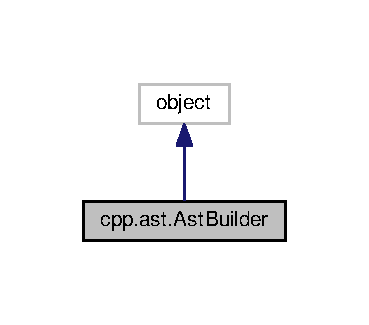
\includegraphics[width=177pt]{classcpp_1_1ast_1_1AstBuilder__inherit__graph}
\end{center}
\end{figure}


Collaboration diagram for cpp.\+ast.\+Ast\+Builder\+:
\nopagebreak
\begin{figure}[H]
\begin{center}
\leavevmode
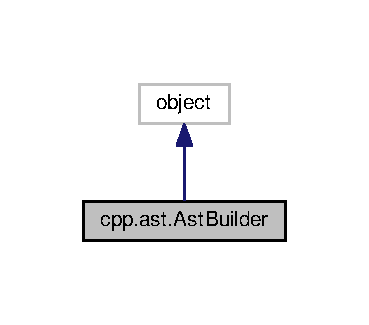
\includegraphics[width=177pt]{classcpp_1_1ast_1_1AstBuilder__coll__graph}
\end{center}
\end{figure}
\subsection*{Public Member Functions}
\begin{DoxyCompactItemize}
\item 
def \hyperlink{classcpp_1_1ast_1_1AstBuilder_aaf35e2f9d395c99a38e6bb6f9b5dd047}{\+\_\+\+\_\+init\+\_\+\+\_\+} (self, token\+\_\+stream, \hyperlink{classcpp_1_1ast_1_1AstBuilder_ad8b8f5788de55d6c7151e82af8b21115}{filename}, \hyperlink{classcpp_1_1ast_1_1AstBuilder_a9edc1e10a3f005b463fd9316d83dd15d}{in\+\_\+class}=\textquotesingle{}\textquotesingle{}, \hyperlink{classcpp_1_1ast_1_1AstBuilder_a2f16b19846c405101235432d2666b614}{visibility}=None, \hyperlink{classcpp_1_1ast_1_1AstBuilder_ab183aa48e4b6e116379f95eb3d11039c}{namespace\+\_\+stack}=\mbox{[}$\,$\mbox{]})
\item 
def \hyperlink{classcpp_1_1ast_1_1AstBuilder_a3e610662018d674f6c57ef19254cc470}{Handle\+Error} (self, msg, token)
\item 
def \hyperlink{classcpp_1_1ast_1_1AstBuilder_aebd0392eee56def849468af5b93b720a}{Generate} (self)
\item 
def \hyperlink{classcpp_1_1ast_1_1AstBuilder_add6826421ce64546a7dbb9b2e699a4d4}{Get\+Scope} (self)
\item 
def \hyperlink{classcpp_1_1ast_1_1AstBuilder_a327957c4228325fc5f64821b047bdc6f}{Get\+Name} (self, seq=None)
\item 
def \hyperlink{classcpp_1_1ast_1_1AstBuilder_af22fb880867876144d20818391ad267a}{Get\+Method} (self, modifiers, templated\+\_\+types)
\item 
def \hyperlink{classcpp_1_1ast_1_1AstBuilder_ac5a5e19e5be6501d351891cc0ead5f53}{handle\+\_\+bool} (self)
\item 
def \hyperlink{classcpp_1_1ast_1_1AstBuilder_adfbb93646d0d32b39a19f3c70cc031f8}{handle\+\_\+char} (self)
\item 
def \hyperlink{classcpp_1_1ast_1_1AstBuilder_a6f824335dd53e12a76d6f91ab69c627c}{handle\+\_\+int} (self)
\item 
def \hyperlink{classcpp_1_1ast_1_1AstBuilder_a08f56b25e6bed18aa955f8cad462d2f9}{handle\+\_\+long} (self)
\item 
def \hyperlink{classcpp_1_1ast_1_1AstBuilder_adf11f377386bdb44fe1094ff8adf9142}{handle\+\_\+short} (self)
\item 
def \hyperlink{classcpp_1_1ast_1_1AstBuilder_ad1bd68af800dafcafdfa56e474f9d642}{handle\+\_\+double} (self)
\item 
def \hyperlink{classcpp_1_1ast_1_1AstBuilder_aabe3f6d67124181a8cd2665a4562d4f6}{handle\+\_\+float} (self)
\item 
def \hyperlink{classcpp_1_1ast_1_1AstBuilder_a7a8f94909d4080bad2bc5dabd934057b}{handle\+\_\+void} (self)
\item 
def \hyperlink{classcpp_1_1ast_1_1AstBuilder_a4ec65909aea14f45709733d631aed57b}{handle\+\_\+wchar\+\_\+t} (self)
\item 
def \hyperlink{classcpp_1_1ast_1_1AstBuilder_a793123ea878db159de1662c10bdae897}{handle\+\_\+unsigned} (self)
\item 
def \hyperlink{classcpp_1_1ast_1_1AstBuilder_a61c1e82b2b4fdc337cf360e485851390}{handle\+\_\+signed} (self)
\item 
def \hyperlink{classcpp_1_1ast_1_1AstBuilder_aadfad5b8d50962c04504e806dc0f5b6c}{handle\+\_\+struct} (self)
\item 
def \hyperlink{classcpp_1_1ast_1_1AstBuilder_a9b3fbfb21c6e23f04fd596d590f93eee}{handle\+\_\+union} (self)
\item 
def \hyperlink{classcpp_1_1ast_1_1AstBuilder_a341a6ffabadd444a345c8c98a611774c}{handle\+\_\+enum} (self)
\item 
def \hyperlink{classcpp_1_1ast_1_1AstBuilder_a0cb490894f17a6c34fbe6bb8f7a2e626}{handle\+\_\+auto} (self)
\item 
def \hyperlink{classcpp_1_1ast_1_1AstBuilder_a890e7764fc5fd8ad2da3a62e436278a0}{handle\+\_\+register} (self)
\item 
def \hyperlink{classcpp_1_1ast_1_1AstBuilder_a9d24135000a6fb4a3daabb5ab8883648}{handle\+\_\+const} (self)
\item 
def \hyperlink{classcpp_1_1ast_1_1AstBuilder_ab2eb0c18c07584ef246a46865a17ec40}{handle\+\_\+inline} (self)
\item 
def \hyperlink{classcpp_1_1ast_1_1AstBuilder_a49039750d971240a270606f0608c1ff0}{handle\+\_\+extern} (self)
\item 
def \hyperlink{classcpp_1_1ast_1_1AstBuilder_ad98bc262537d2882adc2017023cef6aa}{handle\+\_\+static} (self)
\item 
def \hyperlink{classcpp_1_1ast_1_1AstBuilder_a44710dc0b8e5bdbecaa56f7c4b59c046}{handle\+\_\+virtual} (self)
\item 
def \hyperlink{classcpp_1_1ast_1_1AstBuilder_a2dfb23ddeb05e1017b3d1ce85a40cacb}{handle\+\_\+volatile} (self)
\item 
def \hyperlink{classcpp_1_1ast_1_1AstBuilder_a6a642353cfe2cddd1a60cbb1011df787}{handle\+\_\+mutable} (self)
\item 
def \hyperlink{classcpp_1_1ast_1_1AstBuilder_a1e69925578e0ee0a2b7aeb219eda449b}{handle\+\_\+public} (self)
\item 
def \hyperlink{classcpp_1_1ast_1_1AstBuilder_aa4ff62142927f8f245a2030b444676ee}{handle\+\_\+protected} (self)
\item 
def \hyperlink{classcpp_1_1ast_1_1AstBuilder_a8bc5f9563f5ead3abba5a71187162867}{handle\+\_\+private} (self)
\item 
def \hyperlink{classcpp_1_1ast_1_1AstBuilder_ab9f7d81019317c6ccfd492bd2c0c9579}{handle\+\_\+friend} (self)
\item 
def \hyperlink{classcpp_1_1ast_1_1AstBuilder_ab7577b3a2bd22c1bccb656493de379f3}{handle\+\_\+static\+\_\+cast} (self)
\item 
def \hyperlink{classcpp_1_1ast_1_1AstBuilder_a4dae74f1d036f63fc1080962ab0208fc}{handle\+\_\+const\+\_\+cast} (self)
\item 
def \hyperlink{classcpp_1_1ast_1_1AstBuilder_a659b5ad02ffebe26c1496a319128fbd1}{handle\+\_\+dynamic\+\_\+cast} (self)
\item 
def \hyperlink{classcpp_1_1ast_1_1AstBuilder_a06d75904ba7487c7966d073aaa3d74e9}{handle\+\_\+reinterpret\+\_\+cast} (self)
\item 
def \hyperlink{classcpp_1_1ast_1_1AstBuilder_a86f5769e0460524691ae0d135d30f101}{handle\+\_\+new} (self)
\item 
def \hyperlink{classcpp_1_1ast_1_1AstBuilder_aa5b7a781afe524bebdf42bdeb4766507}{handle\+\_\+delete} (self)
\item 
def \hyperlink{classcpp_1_1ast_1_1AstBuilder_a808eb3d955ca2e3a957abb35dc577c66}{handle\+\_\+typedef} (self)
\item 
def \hyperlink{classcpp_1_1ast_1_1AstBuilder_ac30cfc1a3a455310a9ccac885d2d0d7c}{handle\+\_\+typeid} (self)
\item 
def \hyperlink{classcpp_1_1ast_1_1AstBuilder_a4b7b3bb4f47f67052b04e5da173d1c6b}{handle\+\_\+typename} (self)
\item 
def \hyperlink{classcpp_1_1ast_1_1AstBuilder_a0f4d74520697ec05eb6b549daada5a5d}{handle\+\_\+template} (self)
\item 
def \hyperlink{classcpp_1_1ast_1_1AstBuilder_ad480255644817388b81b05acc4aa9c9a}{handle\+\_\+true} (self)
\item 
def \hyperlink{classcpp_1_1ast_1_1AstBuilder_afe125e384026baf74b55593b254fc10c}{handle\+\_\+false} (self)
\item 
def \hyperlink{classcpp_1_1ast_1_1AstBuilder_acf6ec42d567cd85a9bad77772c381a4e}{handle\+\_\+asm} (self)
\item 
def \hyperlink{classcpp_1_1ast_1_1AstBuilder_a93bd39632593bec36972355b7e1893e0}{handle\+\_\+class} (self)
\item 
def \hyperlink{classcpp_1_1ast_1_1AstBuilder_ae6dde01c5f9ac7ba3b14dff01cac66e4}{handle\+\_\+namespace} (self)
\item 
def \hyperlink{classcpp_1_1ast_1_1AstBuilder_a785563f31bc3ed9559d9ce2854a83f1b}{handle\+\_\+using} (self)
\item 
def \hyperlink{classcpp_1_1ast_1_1AstBuilder_a568860050542b53d3df9cf479f2a5e1c}{handle\+\_\+explicit} (self)
\item 
def \hyperlink{classcpp_1_1ast_1_1AstBuilder_ad96a39776b5439fa9a5c2989f8da20cd}{handle\+\_\+this} (self)
\item 
def \hyperlink{classcpp_1_1ast_1_1AstBuilder_a7ca1318675b9eff41cb4a838d63eb6e6}{handle\+\_\+operator} (self)
\item 
def \hyperlink{classcpp_1_1ast_1_1AstBuilder_acfd733ff9115e3292bea10e160bb6184}{handle\+\_\+sizeof} (self)
\item 
def \hyperlink{classcpp_1_1ast_1_1AstBuilder_ac4f02e1ba7df670086e4c9dabdb21458}{handle\+\_\+case} (self)
\item 
def \hyperlink{classcpp_1_1ast_1_1AstBuilder_a1dffcdf7154158461a652c5b885bfa19}{handle\+\_\+switch} (self)
\item 
def \hyperlink{classcpp_1_1ast_1_1AstBuilder_a6bf895d948d231ffcd058df7af05d0be}{handle\+\_\+default} (self)
\item 
def \hyperlink{classcpp_1_1ast_1_1AstBuilder_a39f2561dfcf36485b2050dff258ece2b}{handle\+\_\+if} (self)
\item 
def \hyperlink{classcpp_1_1ast_1_1AstBuilder_aeb676b03467a93454be018ac243f89a2}{handle\+\_\+else} (self)
\item 
def \hyperlink{classcpp_1_1ast_1_1AstBuilder_a8330d1f34d40b0e82495ec794575289d}{handle\+\_\+return} (self)
\item 
def \hyperlink{classcpp_1_1ast_1_1AstBuilder_a8504d788bb1541ee581918d52d1f4132}{handle\+\_\+goto} (self)
\item 
def \hyperlink{classcpp_1_1ast_1_1AstBuilder_a6c7998f3fdcd046718ff809dbe257645}{handle\+\_\+try} (self)
\item 
def \hyperlink{classcpp_1_1ast_1_1AstBuilder_aa38687383d0f54d26416054cf2141837}{handle\+\_\+catch} (self)
\item 
def \hyperlink{classcpp_1_1ast_1_1AstBuilder_ad4a308ded4a1f87e686b9e11fec31be9}{handle\+\_\+throw} (self)
\item 
def \hyperlink{classcpp_1_1ast_1_1AstBuilder_aac812e812ba2e5fbd80dde93be01a414}{handle\+\_\+while} (self)
\item 
def \hyperlink{classcpp_1_1ast_1_1AstBuilder_a540226b483513b423d4ec2c4f10b18f5}{handle\+\_\+do} (self)
\item 
def \hyperlink{classcpp_1_1ast_1_1AstBuilder_a0025c4d8ca779d69552e0947665eb1c4}{handle\+\_\+for} (self)
\item 
def \hyperlink{classcpp_1_1ast_1_1AstBuilder_a2b663a3e15e70b9d85bf17afb2bcf07a}{handle\+\_\+break} (self)
\item 
def \hyperlink{classcpp_1_1ast_1_1AstBuilder_a511eb003ed301a713a687e5293584077}{handle\+\_\+continue} (self)
\end{DoxyCompactItemize}
\subsection*{Public Attributes}
\begin{DoxyCompactItemize}
\item 
\hyperlink{classcpp_1_1ast_1_1AstBuilder_a1b21f8bef712e91862ccb6b1147cab0d}{tokens}
\item 
\hyperlink{classcpp_1_1ast_1_1AstBuilder_ad8b8f5788de55d6c7151e82af8b21115}{filename}
\item 
\hyperlink{classcpp_1_1ast_1_1AstBuilder_ae167f12797e7c02c1b60c11c83cdb22f}{token\+\_\+queue}
\item 
\hyperlink{classcpp_1_1ast_1_1AstBuilder_ab183aa48e4b6e116379f95eb3d11039c}{namespace\+\_\+stack}
\item 
\hyperlink{classcpp_1_1ast_1_1AstBuilder_a9edc1e10a3f005b463fd9316d83dd15d}{in\+\_\+class}
\item 
\hyperlink{classcpp_1_1ast_1_1AstBuilder_a376583354ab9afa308b7f34105bf3f4a}{in\+\_\+class\+\_\+name\+\_\+only}
\item 
\hyperlink{classcpp_1_1ast_1_1AstBuilder_a2f16b19846c405101235432d2666b614}{visibility}
\item 
\hyperlink{classcpp_1_1ast_1_1AstBuilder_ad5ac0612dfff44241033864832dbdfe3}{in\+\_\+function}
\item 
\hyperlink{classcpp_1_1ast_1_1AstBuilder_a38579523ccc1ae9d202ac722baea45fc}{current\+\_\+token}
\item 
\hyperlink{classcpp_1_1ast_1_1AstBuilder_ae8551cf0405bc6e367636b1f3b37d083}{converter}
\end{DoxyCompactItemize}


\subsection{Constructor \& Destructor Documentation}
\index{cpp\+::ast\+::\+Ast\+Builder@{cpp\+::ast\+::\+Ast\+Builder}!\+\_\+\+\_\+init\+\_\+\+\_\+@{\+\_\+\+\_\+init\+\_\+\+\_\+}}
\index{\+\_\+\+\_\+init\+\_\+\+\_\+@{\+\_\+\+\_\+init\+\_\+\+\_\+}!cpp\+::ast\+::\+Ast\+Builder@{cpp\+::ast\+::\+Ast\+Builder}}
\subsubsection[{\texorpdfstring{\+\_\+\+\_\+init\+\_\+\+\_\+(self, token\+\_\+stream, filename, in\+\_\+class=\textquotesingle{}\textquotesingle{}, visibility=\+None, namespace\+\_\+stack=[])}{__init__(self, token_stream, filename, in_class='', visibility=None, namespace_stack=[])}}]{\setlength{\rightskip}{0pt plus 5cm}def cpp.\+ast.\+Ast\+Builder.\+\_\+\+\_\+init\+\_\+\+\_\+ (
\begin{DoxyParamCaption}
\item[{}]{self, }
\item[{}]{token\+\_\+stream, }
\item[{}]{filename, }
\item[{}]{in\+\_\+class = {\ttfamily \textquotesingle{}\textquotesingle{}}, }
\item[{}]{visibility = {\ttfamily None}, }
\item[{}]{namespace\+\_\+stack = {\ttfamily \mbox{[}\mbox{]}}}
\end{DoxyParamCaption}
)}\hypertarget{classcpp_1_1ast_1_1AstBuilder_aaf35e2f9d395c99a38e6bb6f9b5dd047}{}\label{classcpp_1_1ast_1_1AstBuilder_aaf35e2f9d395c99a38e6bb6f9b5dd047}

\begin{DoxyCode}
678                  namespace\_stack=[]):
679         self.tokens = token\_stream
680         self.filename = filename
681         \textcolor{comment}{# TODO(nnorwitz): use a better data structure (deque) for the queue.}
682         \textcolor{comment}{# Switching directions of the "queue" improved perf by about 25%.}
683         \textcolor{comment}{# Using a deque should be even better since we access from both sides.}
684         self.token\_queue = []
685         self.namespace\_stack = namespace\_stack[:]
686         self.in\_class = in\_class
687         \textcolor{keywordflow}{if} in\_class \textcolor{keywordflow}{is} \textcolor{keywordtype}{None}:
688             self.in\_class\_name\_only = \textcolor{keywordtype}{None}
689         \textcolor{keywordflow}{else}:
690             self.in\_class\_name\_only = in\_class.split(\textcolor{stringliteral}{'::'})[-1]
691         self.visibility = visibility
692         self.in\_function = \textcolor{keyword}{False}
693         self.current\_token = \textcolor{keywordtype}{None}
694         \textcolor{comment}{# Keep the state whether we are currently handling a typedef or not.}
695         self.\_handling\_typedef = \textcolor{keyword}{False}
696 
697         self.converter = TypeConverter(self.namespace\_stack)
698 
\end{DoxyCode}


\subsection{Member Function Documentation}
\index{cpp\+::ast\+::\+Ast\+Builder@{cpp\+::ast\+::\+Ast\+Builder}!Generate@{Generate}}
\index{Generate@{Generate}!cpp\+::ast\+::\+Ast\+Builder@{cpp\+::ast\+::\+Ast\+Builder}}
\subsubsection[{\texorpdfstring{Generate(self)}{Generate(self)}}]{\setlength{\rightskip}{0pt plus 5cm}def cpp.\+ast.\+Ast\+Builder.\+Generate (
\begin{DoxyParamCaption}
\item[{}]{self}
\end{DoxyParamCaption}
)}\hypertarget{classcpp_1_1ast_1_1AstBuilder_aebd0392eee56def849468af5b93b720a}{}\label{classcpp_1_1ast_1_1AstBuilder_aebd0392eee56def849468af5b93b720a}

\begin{DoxyCode}
704     \textcolor{keyword}{def }Generate(self):
705         \textcolor{keywordflow}{while} 1:
706             token = self.\_GetNextToken()
707             \textcolor{keywordflow}{if} \textcolor{keywordflow}{not} token:
708                 \textcolor{keywordflow}{break}
709 
710             \textcolor{comment}{# Get the next token.}
711             self.current\_token = token
712 
713             \textcolor{comment}{# Dispatch on the next token type.}
714             \textcolor{keywordflow}{if} token.token\_type == \_INTERNAL\_TOKEN:
715                 \textcolor{keywordflow}{if} token.name == \_NAMESPACE\_POP:
716                     self.namespace\_stack.pop()
717                 \textcolor{keywordflow}{continue}
718 
719             \textcolor{keywordflow}{try}:
720                 result = self.\_GenerateOne(token)
721                 \textcolor{keywordflow}{if} result \textcolor{keywordflow}{is} \textcolor{keywordflow}{not} \textcolor{keywordtype}{None}:
722                     \textcolor{keywordflow}{yield} result
723             \textcolor{keywordflow}{except}:
724                 self.HandleError(\textcolor{stringliteral}{'exception'}, token)
725                 \textcolor{keywordflow}{raise}
726 
\end{DoxyCode}
\index{cpp\+::ast\+::\+Ast\+Builder@{cpp\+::ast\+::\+Ast\+Builder}!Get\+Method@{Get\+Method}}
\index{Get\+Method@{Get\+Method}!cpp\+::ast\+::\+Ast\+Builder@{cpp\+::ast\+::\+Ast\+Builder}}
\subsubsection[{\texorpdfstring{Get\+Method(self, modifiers, templated\+\_\+types)}{GetMethod(self, modifiers, templated_types)}}]{\setlength{\rightskip}{0pt plus 5cm}def cpp.\+ast.\+Ast\+Builder.\+Get\+Method (
\begin{DoxyParamCaption}
\item[{}]{self, }
\item[{}]{modifiers, }
\item[{}]{templated\+\_\+types}
\end{DoxyParamCaption}
)}\hypertarget{classcpp_1_1ast_1_1AstBuilder_af22fb880867876144d20818391ad267a}{}\label{classcpp_1_1ast_1_1AstBuilder_af22fb880867876144d20818391ad267a}

\begin{DoxyCode}
953     \textcolor{keyword}{def }GetMethod(self, modifiers, templated\_types):
954         return\_type\_and\_name = self.\_GetTokensUpTo(tokenize.SYNTAX, \textcolor{stringliteral}{'('})
955         \textcolor{keyword}{assert} len(return\_type\_and\_name) >= 1
956         \textcolor{keywordflow}{return} self.\_GetMethod(return\_type\_and\_name, modifiers, templated\_types,
957                                \textcolor{keyword}{False})
958 
\end{DoxyCode}
\index{cpp\+::ast\+::\+Ast\+Builder@{cpp\+::ast\+::\+Ast\+Builder}!Get\+Name@{Get\+Name}}
\index{Get\+Name@{Get\+Name}!cpp\+::ast\+::\+Ast\+Builder@{cpp\+::ast\+::\+Ast\+Builder}}
\subsubsection[{\texorpdfstring{Get\+Name(self, seq=\+None)}{GetName(self, seq=None)}}]{\setlength{\rightskip}{0pt plus 5cm}def cpp.\+ast.\+Ast\+Builder.\+Get\+Name (
\begin{DoxyParamCaption}
\item[{}]{self, }
\item[{}]{seq = {\ttfamily None}}
\end{DoxyParamCaption}
)}\hypertarget{classcpp_1_1ast_1_1AstBuilder_a327957c4228325fc5f64821b047bdc6f}{}\label{classcpp_1_1ast_1_1AstBuilder_a327957c4228325fc5f64821b047bdc6f}
\begin{DoxyVerb}Returns ([tokens], next_token_info).\end{DoxyVerb}
 
\begin{DoxyCode}
928     \textcolor{keyword}{def }GetName(self, seq=None):
929         \textcolor{stringliteral}{"""Returns ([tokens], next\_token\_info)."""}
930         GetNextToken = self.\_GetNextToken
931         \textcolor{keywordflow}{if} seq \textcolor{keywordflow}{is} \textcolor{keywordflow}{not} \textcolor{keywordtype}{None}:
932             it = iter(seq)
933             GetNextToken = \textcolor{keyword}{lambda}: \hyperlink{namespacecpp_1_1ast_a39ad8261fef5e0a7c1c17c510541b66f}{next}(it)
934         next\_token = GetNextToken()
935         tokens = []
936         last\_token\_was\_name = \textcolor{keyword}{False}
937         \textcolor{keywordflow}{while} (next\_token.token\_type == tokenize.NAME \textcolor{keywordflow}{or}
938                (next\_token.token\_type == tokenize.SYNTAX \textcolor{keywordflow}{and}
939                 next\_token.name \textcolor{keywordflow}{in} (\textcolor{stringliteral}{'::'}, \textcolor{stringliteral}{'<'}))):
940             \textcolor{comment}{# Two NAMEs in a row means the identifier should terminate.}
941             \textcolor{comment}{# It's probably some sort of variable declaration.}
942             \textcolor{keywordflow}{if} last\_token\_was\_name \textcolor{keywordflow}{and} next\_token.token\_type == tokenize.NAME:
943                 \textcolor{keywordflow}{break}
944             last\_token\_was\_name = next\_token.token\_type == tokenize.NAME
945             tokens.append(next\_token)
946             \textcolor{comment}{# Handle templated names.}
947             \textcolor{keywordflow}{if} next\_token.name == \textcolor{stringliteral}{'<'}:
948                 tokens.extend(self.\_GetMatchingChar(\textcolor{stringliteral}{'<'}, \textcolor{stringliteral}{'>'}, GetNextToken))
949                 last\_token\_was\_name = \textcolor{keyword}{True}
950             next\_token = GetNextToken()
951         \textcolor{keywordflow}{return} tokens, next\_token
952 
\end{DoxyCode}
\index{cpp\+::ast\+::\+Ast\+Builder@{cpp\+::ast\+::\+Ast\+Builder}!Get\+Scope@{Get\+Scope}}
\index{Get\+Scope@{Get\+Scope}!cpp\+::ast\+::\+Ast\+Builder@{cpp\+::ast\+::\+Ast\+Builder}}
\subsubsection[{\texorpdfstring{Get\+Scope(self)}{GetScope(self)}}]{\setlength{\rightskip}{0pt plus 5cm}def cpp.\+ast.\+Ast\+Builder.\+Get\+Scope (
\begin{DoxyParamCaption}
\item[{}]{self}
\end{DoxyParamCaption}
)}\hypertarget{classcpp_1_1ast_1_1AstBuilder_add6826421ce64546a7dbb9b2e699a4d4}{}\label{classcpp_1_1ast_1_1AstBuilder_add6826421ce64546a7dbb9b2e699a4d4}

\begin{DoxyCode}
902     \textcolor{keyword}{def }GetScope(self):
903         \textcolor{keywordflow}{return} self.\_GetMatchingChar(\textcolor{stringliteral}{'\{'}, \textcolor{stringliteral}{'\}'})
904 
\end{DoxyCode}
\index{cpp\+::ast\+::\+Ast\+Builder@{cpp\+::ast\+::\+Ast\+Builder}!handle\+\_\+asm@{handle\+\_\+asm}}
\index{handle\+\_\+asm@{handle\+\_\+asm}!cpp\+::ast\+::\+Ast\+Builder@{cpp\+::ast\+::\+Ast\+Builder}}
\subsubsection[{\texorpdfstring{handle\+\_\+asm(self)}{handle_asm(self)}}]{\setlength{\rightskip}{0pt plus 5cm}def cpp.\+ast.\+Ast\+Builder.\+handle\+\_\+asm (
\begin{DoxyParamCaption}
\item[{}]{self}
\end{DoxyParamCaption}
)}\hypertarget{classcpp_1_1ast_1_1AstBuilder_acf6ec42d567cd85a9bad77772c381a4e}{}\label{classcpp_1_1ast_1_1AstBuilder_acf6ec42d567cd85a9bad77772c381a4e}

\begin{DoxyCode}
1451     \textcolor{keyword}{def }handle\_asm(self):
1452         \textcolor{keywordflow}{pass}  \textcolor{comment}{# Not needed yet.}
1453 
\end{DoxyCode}
\index{cpp\+::ast\+::\+Ast\+Builder@{cpp\+::ast\+::\+Ast\+Builder}!handle\+\_\+auto@{handle\+\_\+auto}}
\index{handle\+\_\+auto@{handle\+\_\+auto}!cpp\+::ast\+::\+Ast\+Builder@{cpp\+::ast\+::\+Ast\+Builder}}
\subsubsection[{\texorpdfstring{handle\+\_\+auto(self)}{handle_auto(self)}}]{\setlength{\rightskip}{0pt plus 5cm}def cpp.\+ast.\+Ast\+Builder.\+handle\+\_\+auto (
\begin{DoxyParamCaption}
\item[{}]{self}
\end{DoxyParamCaption}
)}\hypertarget{classcpp_1_1ast_1_1AstBuilder_a0cb490894f17a6c34fbe6bb8f7a2e626}{}\label{classcpp_1_1ast_1_1AstBuilder_a0cb490894f17a6c34fbe6bb8f7a2e626}

\begin{DoxyCode}
1269     \textcolor{keyword}{def }handle\_auto(self):
1270         \textcolor{comment}{# TODO(nnorwitz): warn about using auto?  Probably not since it}
1271         \textcolor{comment}{# will be reclaimed and useful for C++0x.}
1272         \textcolor{keywordflow}{pass}
1273 
\end{DoxyCode}
\index{cpp\+::ast\+::\+Ast\+Builder@{cpp\+::ast\+::\+Ast\+Builder}!handle\+\_\+bool@{handle\+\_\+bool}}
\index{handle\+\_\+bool@{handle\+\_\+bool}!cpp\+::ast\+::\+Ast\+Builder@{cpp\+::ast\+::\+Ast\+Builder}}
\subsubsection[{\texorpdfstring{handle\+\_\+bool(self)}{handle_bool(self)}}]{\setlength{\rightskip}{0pt plus 5cm}def cpp.\+ast.\+Ast\+Builder.\+handle\+\_\+bool (
\begin{DoxyParamCaption}
\item[{}]{self}
\end{DoxyParamCaption}
)}\hypertarget{classcpp_1_1ast_1_1AstBuilder_ac5a5e19e5be6501d351891cc0ead5f53}{}\label{classcpp_1_1ast_1_1AstBuilder_ac5a5e19e5be6501d351891cc0ead5f53}

\begin{DoxyCode}
1160     \textcolor{keyword}{def }handle\_bool(self):
1161         \textcolor{keywordflow}{pass}
1162 
\end{DoxyCode}
\index{cpp\+::ast\+::\+Ast\+Builder@{cpp\+::ast\+::\+Ast\+Builder}!handle\+\_\+break@{handle\+\_\+break}}
\index{handle\+\_\+break@{handle\+\_\+break}!cpp\+::ast\+::\+Ast\+Builder@{cpp\+::ast\+::\+Ast\+Builder}}
\subsubsection[{\texorpdfstring{handle\+\_\+break(self)}{handle_break(self)}}]{\setlength{\rightskip}{0pt plus 5cm}def cpp.\+ast.\+Ast\+Builder.\+handle\+\_\+break (
\begin{DoxyParamCaption}
\item[{}]{self}
\end{DoxyParamCaption}
)}\hypertarget{classcpp_1_1ast_1_1AstBuilder_a2b663a3e15e70b9d85bf17afb2bcf07a}{}\label{classcpp_1_1ast_1_1AstBuilder_a2b663a3e15e70b9d85bf17afb2bcf07a}

\begin{DoxyCode}
1656     \textcolor{keyword}{def }handle\_break(self):
1657         self.\_IgnoreUpTo(tokenize.SYNTAX, \textcolor{stringliteral}{';'})
1658 
\end{DoxyCode}
\index{cpp\+::ast\+::\+Ast\+Builder@{cpp\+::ast\+::\+Ast\+Builder}!handle\+\_\+case@{handle\+\_\+case}}
\index{handle\+\_\+case@{handle\+\_\+case}!cpp\+::ast\+::\+Ast\+Builder@{cpp\+::ast\+::\+Ast\+Builder}}
\subsubsection[{\texorpdfstring{handle\+\_\+case(self)}{handle_case(self)}}]{\setlength{\rightskip}{0pt plus 5cm}def cpp.\+ast.\+Ast\+Builder.\+handle\+\_\+case (
\begin{DoxyParamCaption}
\item[{}]{self}
\end{DoxyParamCaption}
)}\hypertarget{classcpp_1_1ast_1_1AstBuilder_ac4f02e1ba7df670086e4c9dabdb21458}{}\label{classcpp_1_1ast_1_1AstBuilder_ac4f02e1ba7df670086e4c9dabdb21458}

\begin{DoxyCode}
1610     \textcolor{keyword}{def }handle\_case(self):
1611         \textcolor{keywordflow}{pass}
1612 
\end{DoxyCode}
\index{cpp\+::ast\+::\+Ast\+Builder@{cpp\+::ast\+::\+Ast\+Builder}!handle\+\_\+catch@{handle\+\_\+catch}}
\index{handle\+\_\+catch@{handle\+\_\+catch}!cpp\+::ast\+::\+Ast\+Builder@{cpp\+::ast\+::\+Ast\+Builder}}
\subsubsection[{\texorpdfstring{handle\+\_\+catch(self)}{handle_catch(self)}}]{\setlength{\rightskip}{0pt plus 5cm}def cpp.\+ast.\+Ast\+Builder.\+handle\+\_\+catch (
\begin{DoxyParamCaption}
\item[{}]{self}
\end{DoxyParamCaption}
)}\hypertarget{classcpp_1_1ast_1_1AstBuilder_aa38687383d0f54d26416054cf2141837}{}\label{classcpp_1_1ast_1_1AstBuilder_aa38687383d0f54d26416054cf2141837}

\begin{DoxyCode}
1641     \textcolor{keyword}{def }handle\_catch(self):
1642         \textcolor{keywordflow}{pass}  \textcolor{comment}{# Not needed yet.}
1643 
\end{DoxyCode}
\index{cpp\+::ast\+::\+Ast\+Builder@{cpp\+::ast\+::\+Ast\+Builder}!handle\+\_\+char@{handle\+\_\+char}}
\index{handle\+\_\+char@{handle\+\_\+char}!cpp\+::ast\+::\+Ast\+Builder@{cpp\+::ast\+::\+Ast\+Builder}}
\subsubsection[{\texorpdfstring{handle\+\_\+char(self)}{handle_char(self)}}]{\setlength{\rightskip}{0pt plus 5cm}def cpp.\+ast.\+Ast\+Builder.\+handle\+\_\+char (
\begin{DoxyParamCaption}
\item[{}]{self}
\end{DoxyParamCaption}
)}\hypertarget{classcpp_1_1ast_1_1AstBuilder_adfbb93646d0d32b39a19f3c70cc031f8}{}\label{classcpp_1_1ast_1_1AstBuilder_adfbb93646d0d32b39a19f3c70cc031f8}

\begin{DoxyCode}
1163     \textcolor{keyword}{def }handle\_char(self):
1164         \textcolor{keywordflow}{pass}
1165 
\end{DoxyCode}
\index{cpp\+::ast\+::\+Ast\+Builder@{cpp\+::ast\+::\+Ast\+Builder}!handle\+\_\+class@{handle\+\_\+class}}
\index{handle\+\_\+class@{handle\+\_\+class}!cpp\+::ast\+::\+Ast\+Builder@{cpp\+::ast\+::\+Ast\+Builder}}
\subsubsection[{\texorpdfstring{handle\+\_\+class(self)}{handle_class(self)}}]{\setlength{\rightskip}{0pt plus 5cm}def cpp.\+ast.\+Ast\+Builder.\+handle\+\_\+class (
\begin{DoxyParamCaption}
\item[{}]{self}
\end{DoxyParamCaption}
)}\hypertarget{classcpp_1_1ast_1_1AstBuilder_a93bd39632593bec36972355b7e1893e0}{}\label{classcpp_1_1ast_1_1AstBuilder_a93bd39632593bec36972355b7e1893e0}

\begin{DoxyCode}
1454     \textcolor{keyword}{def }handle\_class(self):
1455         \textcolor{keywordflow}{return} self.\_GetClass(Class, VISIBILITY\_PRIVATE, \textcolor{keywordtype}{None})
1456 
\end{DoxyCode}
\index{cpp\+::ast\+::\+Ast\+Builder@{cpp\+::ast\+::\+Ast\+Builder}!handle\+\_\+const@{handle\+\_\+const}}
\index{handle\+\_\+const@{handle\+\_\+const}!cpp\+::ast\+::\+Ast\+Builder@{cpp\+::ast\+::\+Ast\+Builder}}
\subsubsection[{\texorpdfstring{handle\+\_\+const(self)}{handle_const(self)}}]{\setlength{\rightskip}{0pt plus 5cm}def cpp.\+ast.\+Ast\+Builder.\+handle\+\_\+const (
\begin{DoxyParamCaption}
\item[{}]{self}
\end{DoxyParamCaption}
)}\hypertarget{classcpp_1_1ast_1_1AstBuilder_a9d24135000a6fb4a3daabb5ab8883648}{}\label{classcpp_1_1ast_1_1AstBuilder_a9d24135000a6fb4a3daabb5ab8883648}

\begin{DoxyCode}
1277     \textcolor{keyword}{def }handle\_const(self):
1278         \textcolor{keywordflow}{pass}
1279 
\end{DoxyCode}
\index{cpp\+::ast\+::\+Ast\+Builder@{cpp\+::ast\+::\+Ast\+Builder}!handle\+\_\+const\+\_\+cast@{handle\+\_\+const\+\_\+cast}}
\index{handle\+\_\+const\+\_\+cast@{handle\+\_\+const\+\_\+cast}!cpp\+::ast\+::\+Ast\+Builder@{cpp\+::ast\+::\+Ast\+Builder}}
\subsubsection[{\texorpdfstring{handle\+\_\+const\+\_\+cast(self)}{handle_const_cast(self)}}]{\setlength{\rightskip}{0pt plus 5cm}def cpp.\+ast.\+Ast\+Builder.\+handle\+\_\+const\+\_\+cast (
\begin{DoxyParamCaption}
\item[{}]{self}
\end{DoxyParamCaption}
)}\hypertarget{classcpp_1_1ast_1_1AstBuilder_a4dae74f1d036f63fc1080962ab0208fc}{}\label{classcpp_1_1ast_1_1AstBuilder_a4dae74f1d036f63fc1080962ab0208fc}

\begin{DoxyCode}
1332     \textcolor{keyword}{def }handle\_const\_cast(self):
1333         \textcolor{keywordflow}{pass}
1334 
\end{DoxyCode}
\index{cpp\+::ast\+::\+Ast\+Builder@{cpp\+::ast\+::\+Ast\+Builder}!handle\+\_\+continue@{handle\+\_\+continue}}
\index{handle\+\_\+continue@{handle\+\_\+continue}!cpp\+::ast\+::\+Ast\+Builder@{cpp\+::ast\+::\+Ast\+Builder}}
\subsubsection[{\texorpdfstring{handle\+\_\+continue(self)}{handle_continue(self)}}]{\setlength{\rightskip}{0pt plus 5cm}def cpp.\+ast.\+Ast\+Builder.\+handle\+\_\+continue (
\begin{DoxyParamCaption}
\item[{}]{self}
\end{DoxyParamCaption}
)}\hypertarget{classcpp_1_1ast_1_1AstBuilder_a511eb003ed301a713a687e5293584077}{}\label{classcpp_1_1ast_1_1AstBuilder_a511eb003ed301a713a687e5293584077}

\begin{DoxyCode}
1659     \textcolor{keyword}{def }handle\_continue(self):
1660         self.\_IgnoreUpTo(tokenize.SYNTAX, \textcolor{stringliteral}{';'})
1661 
1662 
\end{DoxyCode}
\index{cpp\+::ast\+::\+Ast\+Builder@{cpp\+::ast\+::\+Ast\+Builder}!handle\+\_\+default@{handle\+\_\+default}}
\index{handle\+\_\+default@{handle\+\_\+default}!cpp\+::ast\+::\+Ast\+Builder@{cpp\+::ast\+::\+Ast\+Builder}}
\subsubsection[{\texorpdfstring{handle\+\_\+default(self)}{handle_default(self)}}]{\setlength{\rightskip}{0pt plus 5cm}def cpp.\+ast.\+Ast\+Builder.\+handle\+\_\+default (
\begin{DoxyParamCaption}
\item[{}]{self}
\end{DoxyParamCaption}
)}\hypertarget{classcpp_1_1ast_1_1AstBuilder_a6bf895d948d231ffcd058df7af05d0be}{}\label{classcpp_1_1ast_1_1AstBuilder_a6bf895d948d231ffcd058df7af05d0be}

\begin{DoxyCode}
1616     \textcolor{keyword}{def }handle\_default(self):
1617         token = self.\_GetNextToken()
1618         \textcolor{keyword}{assert} token.token\_type == tokenize.SYNTAX
1619         \textcolor{keyword}{assert} token.name == \textcolor{stringliteral}{':'}
1620 
\end{DoxyCode}
\index{cpp\+::ast\+::\+Ast\+Builder@{cpp\+::ast\+::\+Ast\+Builder}!handle\+\_\+delete@{handle\+\_\+delete}}
\index{handle\+\_\+delete@{handle\+\_\+delete}!cpp\+::ast\+::\+Ast\+Builder@{cpp\+::ast\+::\+Ast\+Builder}}
\subsubsection[{\texorpdfstring{handle\+\_\+delete(self)}{handle_delete(self)}}]{\setlength{\rightskip}{0pt plus 5cm}def cpp.\+ast.\+Ast\+Builder.\+handle\+\_\+delete (
\begin{DoxyParamCaption}
\item[{}]{self}
\end{DoxyParamCaption}
)}\hypertarget{classcpp_1_1ast_1_1AstBuilder_aa5b7a781afe524bebdf42bdeb4766507}{}\label{classcpp_1_1ast_1_1AstBuilder_aa5b7a781afe524bebdf42bdeb4766507}

\begin{DoxyCode}
1344     \textcolor{keyword}{def }handle\_delete(self):
1345         tokens = self.\_GetTokensUpTo(tokenize.SYNTAX, \textcolor{stringliteral}{';'})
1346         \textcolor{keyword}{assert} tokens
1347         \textcolor{keywordflow}{return} \hyperlink{namespacetesting_1_1internal_a1e7045e09392aece10aea4517458b7ed}{Delete}(tokens[0].start, tokens[0].end, tokens)
1348 
\end{DoxyCode}
\index{cpp\+::ast\+::\+Ast\+Builder@{cpp\+::ast\+::\+Ast\+Builder}!handle\+\_\+do@{handle\+\_\+do}}
\index{handle\+\_\+do@{handle\+\_\+do}!cpp\+::ast\+::\+Ast\+Builder@{cpp\+::ast\+::\+Ast\+Builder}}
\subsubsection[{\texorpdfstring{handle\+\_\+do(self)}{handle_do(self)}}]{\setlength{\rightskip}{0pt plus 5cm}def cpp.\+ast.\+Ast\+Builder.\+handle\+\_\+do (
\begin{DoxyParamCaption}
\item[{}]{self}
\end{DoxyParamCaption}
)}\hypertarget{classcpp_1_1ast_1_1AstBuilder_a540226b483513b423d4ec2c4f10b18f5}{}\label{classcpp_1_1ast_1_1AstBuilder_a540226b483513b423d4ec2c4f10b18f5}

\begin{DoxyCode}
1650     \textcolor{keyword}{def }handle\_do(self):
1651         \textcolor{keywordflow}{pass}
1652 
\end{DoxyCode}
\index{cpp\+::ast\+::\+Ast\+Builder@{cpp\+::ast\+::\+Ast\+Builder}!handle\+\_\+double@{handle\+\_\+double}}
\index{handle\+\_\+double@{handle\+\_\+double}!cpp\+::ast\+::\+Ast\+Builder@{cpp\+::ast\+::\+Ast\+Builder}}
\subsubsection[{\texorpdfstring{handle\+\_\+double(self)}{handle_double(self)}}]{\setlength{\rightskip}{0pt plus 5cm}def cpp.\+ast.\+Ast\+Builder.\+handle\+\_\+double (
\begin{DoxyParamCaption}
\item[{}]{self}
\end{DoxyParamCaption}
)}\hypertarget{classcpp_1_1ast_1_1AstBuilder_ad1bd68af800dafcafdfa56e474f9d642}{}\label{classcpp_1_1ast_1_1AstBuilder_ad1bd68af800dafcafdfa56e474f9d642}

\begin{DoxyCode}
1175     \textcolor{keyword}{def }handle\_double(self):
1176         \textcolor{keywordflow}{pass}
1177 
\end{DoxyCode}
\index{cpp\+::ast\+::\+Ast\+Builder@{cpp\+::ast\+::\+Ast\+Builder}!handle\+\_\+dynamic\+\_\+cast@{handle\+\_\+dynamic\+\_\+cast}}
\index{handle\+\_\+dynamic\+\_\+cast@{handle\+\_\+dynamic\+\_\+cast}!cpp\+::ast\+::\+Ast\+Builder@{cpp\+::ast\+::\+Ast\+Builder}}
\subsubsection[{\texorpdfstring{handle\+\_\+dynamic\+\_\+cast(self)}{handle_dynamic_cast(self)}}]{\setlength{\rightskip}{0pt plus 5cm}def cpp.\+ast.\+Ast\+Builder.\+handle\+\_\+dynamic\+\_\+cast (
\begin{DoxyParamCaption}
\item[{}]{self}
\end{DoxyParamCaption}
)}\hypertarget{classcpp_1_1ast_1_1AstBuilder_a659b5ad02ffebe26c1496a319128fbd1}{}\label{classcpp_1_1ast_1_1AstBuilder_a659b5ad02ffebe26c1496a319128fbd1}

\begin{DoxyCode}
1335     \textcolor{keyword}{def }handle\_dynamic\_cast(self):
1336         \textcolor{keywordflow}{pass}
1337 
\end{DoxyCode}
\index{cpp\+::ast\+::\+Ast\+Builder@{cpp\+::ast\+::\+Ast\+Builder}!handle\+\_\+else@{handle\+\_\+else}}
\index{handle\+\_\+else@{handle\+\_\+else}!cpp\+::ast\+::\+Ast\+Builder@{cpp\+::ast\+::\+Ast\+Builder}}
\subsubsection[{\texorpdfstring{handle\+\_\+else(self)}{handle_else(self)}}]{\setlength{\rightskip}{0pt plus 5cm}def cpp.\+ast.\+Ast\+Builder.\+handle\+\_\+else (
\begin{DoxyParamCaption}
\item[{}]{self}
\end{DoxyParamCaption}
)}\hypertarget{classcpp_1_1ast_1_1AstBuilder_aeb676b03467a93454be018ac243f89a2}{}\label{classcpp_1_1ast_1_1AstBuilder_aeb676b03467a93454be018ac243f89a2}

\begin{DoxyCode}
1624     \textcolor{keyword}{def }handle\_else(self):
1625         \textcolor{keywordflow}{pass}
1626 
\end{DoxyCode}
\index{cpp\+::ast\+::\+Ast\+Builder@{cpp\+::ast\+::\+Ast\+Builder}!handle\+\_\+enum@{handle\+\_\+enum}}
\index{handle\+\_\+enum@{handle\+\_\+enum}!cpp\+::ast\+::\+Ast\+Builder@{cpp\+::ast\+::\+Ast\+Builder}}
\subsubsection[{\texorpdfstring{handle\+\_\+enum(self)}{handle_enum(self)}}]{\setlength{\rightskip}{0pt plus 5cm}def cpp.\+ast.\+Ast\+Builder.\+handle\+\_\+enum (
\begin{DoxyParamCaption}
\item[{}]{self}
\end{DoxyParamCaption}
)}\hypertarget{classcpp_1_1ast_1_1AstBuilder_a341a6ffabadd444a345c8c98a611774c}{}\label{classcpp_1_1ast_1_1AstBuilder_a341a6ffabadd444a345c8c98a611774c}

\begin{DoxyCode}
1266     \textcolor{keyword}{def }handle\_enum(self):
1267         \textcolor{keywordflow}{return} self.\_GetNestedType(Enum)
1268 
\end{DoxyCode}
\index{cpp\+::ast\+::\+Ast\+Builder@{cpp\+::ast\+::\+Ast\+Builder}!handle\+\_\+explicit@{handle\+\_\+explicit}}
\index{handle\+\_\+explicit@{handle\+\_\+explicit}!cpp\+::ast\+::\+Ast\+Builder@{cpp\+::ast\+::\+Ast\+Builder}}
\subsubsection[{\texorpdfstring{handle\+\_\+explicit(self)}{handle_explicit(self)}}]{\setlength{\rightskip}{0pt plus 5cm}def cpp.\+ast.\+Ast\+Builder.\+handle\+\_\+explicit (
\begin{DoxyParamCaption}
\item[{}]{self}
\end{DoxyParamCaption}
)}\hypertarget{classcpp_1_1ast_1_1AstBuilder_a568860050542b53d3df9cf479f2a5e1c}{}\label{classcpp_1_1ast_1_1AstBuilder_a568860050542b53d3df9cf479f2a5e1c}

\begin{DoxyCode}
1593     \textcolor{keyword}{def }handle\_explicit(self):
1594         \textcolor{keyword}{assert} self.in\_class
1595         \textcolor{comment}{# Nothing much to do.}
1596         \textcolor{comment}{# TODO(nnorwitz): maybe verify the method name == class name.}
1597         \textcolor{comment}{# This must be a ctor.}
1598         \textcolor{keywordflow}{return} self.GetMethod(FUNCTION\_CTOR, \textcolor{keywordtype}{None})
1599 
\end{DoxyCode}
\index{cpp\+::ast\+::\+Ast\+Builder@{cpp\+::ast\+::\+Ast\+Builder}!handle\+\_\+extern@{handle\+\_\+extern}}
\index{handle\+\_\+extern@{handle\+\_\+extern}!cpp\+::ast\+::\+Ast\+Builder@{cpp\+::ast\+::\+Ast\+Builder}}
\subsubsection[{\texorpdfstring{handle\+\_\+extern(self)}{handle_extern(self)}}]{\setlength{\rightskip}{0pt plus 5cm}def cpp.\+ast.\+Ast\+Builder.\+handle\+\_\+extern (
\begin{DoxyParamCaption}
\item[{}]{self}
\end{DoxyParamCaption}
)}\hypertarget{classcpp_1_1ast_1_1AstBuilder_a49039750d971240a270606f0608c1ff0}{}\label{classcpp_1_1ast_1_1AstBuilder_a49039750d971240a270606f0608c1ff0}

\begin{DoxyCode}
1283     \textcolor{keyword}{def }handle\_extern(self):
1284         \textcolor{keywordflow}{pass}
1285 
\end{DoxyCode}
\index{cpp\+::ast\+::\+Ast\+Builder@{cpp\+::ast\+::\+Ast\+Builder}!handle\+\_\+false@{handle\+\_\+false}}
\index{handle\+\_\+false@{handle\+\_\+false}!cpp\+::ast\+::\+Ast\+Builder@{cpp\+::ast\+::\+Ast\+Builder}}
\subsubsection[{\texorpdfstring{handle\+\_\+false(self)}{handle_false(self)}}]{\setlength{\rightskip}{0pt plus 5cm}def cpp.\+ast.\+Ast\+Builder.\+handle\+\_\+false (
\begin{DoxyParamCaption}
\item[{}]{self}
\end{DoxyParamCaption}
)}\hypertarget{classcpp_1_1ast_1_1AstBuilder_afe125e384026baf74b55593b254fc10c}{}\label{classcpp_1_1ast_1_1AstBuilder_afe125e384026baf74b55593b254fc10c}

\begin{DoxyCode}
1448     \textcolor{keyword}{def }handle\_false(self):
1449         \textcolor{keywordflow}{pass}  \textcolor{comment}{# Nothing to do.}
1450 
\end{DoxyCode}
\index{cpp\+::ast\+::\+Ast\+Builder@{cpp\+::ast\+::\+Ast\+Builder}!handle\+\_\+float@{handle\+\_\+float}}
\index{handle\+\_\+float@{handle\+\_\+float}!cpp\+::ast\+::\+Ast\+Builder@{cpp\+::ast\+::\+Ast\+Builder}}
\subsubsection[{\texorpdfstring{handle\+\_\+float(self)}{handle_float(self)}}]{\setlength{\rightskip}{0pt plus 5cm}def cpp.\+ast.\+Ast\+Builder.\+handle\+\_\+float (
\begin{DoxyParamCaption}
\item[{}]{self}
\end{DoxyParamCaption}
)}\hypertarget{classcpp_1_1ast_1_1AstBuilder_aabe3f6d67124181a8cd2665a4562d4f6}{}\label{classcpp_1_1ast_1_1AstBuilder_aabe3f6d67124181a8cd2665a4562d4f6}

\begin{DoxyCode}
1178     \textcolor{keyword}{def }handle\_float(self):
1179         \textcolor{keywordflow}{pass}
1180 
\end{DoxyCode}
\index{cpp\+::ast\+::\+Ast\+Builder@{cpp\+::ast\+::\+Ast\+Builder}!handle\+\_\+for@{handle\+\_\+for}}
\index{handle\+\_\+for@{handle\+\_\+for}!cpp\+::ast\+::\+Ast\+Builder@{cpp\+::ast\+::\+Ast\+Builder}}
\subsubsection[{\texorpdfstring{handle\+\_\+for(self)}{handle_for(self)}}]{\setlength{\rightskip}{0pt plus 5cm}def cpp.\+ast.\+Ast\+Builder.\+handle\+\_\+for (
\begin{DoxyParamCaption}
\item[{}]{self}
\end{DoxyParamCaption}
)}\hypertarget{classcpp_1_1ast_1_1AstBuilder_a0025c4d8ca779d69552e0947665eb1c4}{}\label{classcpp_1_1ast_1_1AstBuilder_a0025c4d8ca779d69552e0947665eb1c4}

\begin{DoxyCode}
1653     \textcolor{keyword}{def }handle\_for(self):
1654         \textcolor{keywordflow}{pass}
1655 
\end{DoxyCode}
\index{cpp\+::ast\+::\+Ast\+Builder@{cpp\+::ast\+::\+Ast\+Builder}!handle\+\_\+friend@{handle\+\_\+friend}}
\index{handle\+\_\+friend@{handle\+\_\+friend}!cpp\+::ast\+::\+Ast\+Builder@{cpp\+::ast\+::\+Ast\+Builder}}
\subsubsection[{\texorpdfstring{handle\+\_\+friend(self)}{handle_friend(self)}}]{\setlength{\rightskip}{0pt plus 5cm}def cpp.\+ast.\+Ast\+Builder.\+handle\+\_\+friend (
\begin{DoxyParamCaption}
\item[{}]{self}
\end{DoxyParamCaption}
)}\hypertarget{classcpp_1_1ast_1_1AstBuilder_ab9f7d81019317c6ccfd492bd2c0c9579}{}\label{classcpp_1_1ast_1_1AstBuilder_ab9f7d81019317c6ccfd492bd2c0c9579}

\begin{DoxyCode}
1323     \textcolor{keyword}{def }handle\_friend(self):
1324         tokens = self.\_GetTokensUpTo(tokenize.SYNTAX, \textcolor{stringliteral}{';'})
1325         \textcolor{keyword}{assert} tokens
1326         t0 = tokens[0]
1327         \textcolor{keywordflow}{return} Friend(t0.start, t0.end, tokens, self.namespace\_stack)
1328 
\end{DoxyCode}
\index{cpp\+::ast\+::\+Ast\+Builder@{cpp\+::ast\+::\+Ast\+Builder}!handle\+\_\+goto@{handle\+\_\+goto}}
\index{handle\+\_\+goto@{handle\+\_\+goto}!cpp\+::ast\+::\+Ast\+Builder@{cpp\+::ast\+::\+Ast\+Builder}}
\subsubsection[{\texorpdfstring{handle\+\_\+goto(self)}{handle_goto(self)}}]{\setlength{\rightskip}{0pt plus 5cm}def cpp.\+ast.\+Ast\+Builder.\+handle\+\_\+goto (
\begin{DoxyParamCaption}
\item[{}]{self}
\end{DoxyParamCaption}
)}\hypertarget{classcpp_1_1ast_1_1AstBuilder_a8504d788bb1541ee581918d52d1f4132}{}\label{classcpp_1_1ast_1_1AstBuilder_a8504d788bb1541ee581918d52d1f4132}

\begin{DoxyCode}
1633     \textcolor{keyword}{def }handle\_goto(self):
1634         tokens = self.\_GetTokensUpTo(tokenize.SYNTAX, \textcolor{stringliteral}{';'})
1635         \textcolor{keyword}{assert} len(tokens) == 1, str(tokens)
1636         \textcolor{keywordflow}{return} Goto(tokens[0].start, tokens[0].end, tokens[0].name)
1637 
\end{DoxyCode}
\index{cpp\+::ast\+::\+Ast\+Builder@{cpp\+::ast\+::\+Ast\+Builder}!handle\+\_\+if@{handle\+\_\+if}}
\index{handle\+\_\+if@{handle\+\_\+if}!cpp\+::ast\+::\+Ast\+Builder@{cpp\+::ast\+::\+Ast\+Builder}}
\subsubsection[{\texorpdfstring{handle\+\_\+if(self)}{handle_if(self)}}]{\setlength{\rightskip}{0pt plus 5cm}def cpp.\+ast.\+Ast\+Builder.\+handle\+\_\+if (
\begin{DoxyParamCaption}
\item[{}]{self}
\end{DoxyParamCaption}
)}\hypertarget{classcpp_1_1ast_1_1AstBuilder_a39f2561dfcf36485b2050dff258ece2b}{}\label{classcpp_1_1ast_1_1AstBuilder_a39f2561dfcf36485b2050dff258ece2b}

\begin{DoxyCode}
1621     \textcolor{keyword}{def }handle\_if(self):
1622         \textcolor{keywordflow}{pass}
1623 
\end{DoxyCode}
\index{cpp\+::ast\+::\+Ast\+Builder@{cpp\+::ast\+::\+Ast\+Builder}!handle\+\_\+inline@{handle\+\_\+inline}}
\index{handle\+\_\+inline@{handle\+\_\+inline}!cpp\+::ast\+::\+Ast\+Builder@{cpp\+::ast\+::\+Ast\+Builder}}
\subsubsection[{\texorpdfstring{handle\+\_\+inline(self)}{handle_inline(self)}}]{\setlength{\rightskip}{0pt plus 5cm}def cpp.\+ast.\+Ast\+Builder.\+handle\+\_\+inline (
\begin{DoxyParamCaption}
\item[{}]{self}
\end{DoxyParamCaption}
)}\hypertarget{classcpp_1_1ast_1_1AstBuilder_ab2eb0c18c07584ef246a46865a17ec40}{}\label{classcpp_1_1ast_1_1AstBuilder_ab2eb0c18c07584ef246a46865a17ec40}

\begin{DoxyCode}
1280     \textcolor{keyword}{def }handle\_inline(self):
1281         \textcolor{keywordflow}{pass}
1282 
\end{DoxyCode}
\index{cpp\+::ast\+::\+Ast\+Builder@{cpp\+::ast\+::\+Ast\+Builder}!handle\+\_\+int@{handle\+\_\+int}}
\index{handle\+\_\+int@{handle\+\_\+int}!cpp\+::ast\+::\+Ast\+Builder@{cpp\+::ast\+::\+Ast\+Builder}}
\subsubsection[{\texorpdfstring{handle\+\_\+int(self)}{handle_int(self)}}]{\setlength{\rightskip}{0pt plus 5cm}def cpp.\+ast.\+Ast\+Builder.\+handle\+\_\+int (
\begin{DoxyParamCaption}
\item[{}]{self}
\end{DoxyParamCaption}
)}\hypertarget{classcpp_1_1ast_1_1AstBuilder_a6f824335dd53e12a76d6f91ab69c627c}{}\label{classcpp_1_1ast_1_1AstBuilder_a6f824335dd53e12a76d6f91ab69c627c}

\begin{DoxyCode}
1166     \textcolor{keyword}{def }handle\_int(self):
1167         \textcolor{keywordflow}{pass}
1168 
\end{DoxyCode}
\index{cpp\+::ast\+::\+Ast\+Builder@{cpp\+::ast\+::\+Ast\+Builder}!handle\+\_\+long@{handle\+\_\+long}}
\index{handle\+\_\+long@{handle\+\_\+long}!cpp\+::ast\+::\+Ast\+Builder@{cpp\+::ast\+::\+Ast\+Builder}}
\subsubsection[{\texorpdfstring{handle\+\_\+long(self)}{handle_long(self)}}]{\setlength{\rightskip}{0pt plus 5cm}def cpp.\+ast.\+Ast\+Builder.\+handle\+\_\+long (
\begin{DoxyParamCaption}
\item[{}]{self}
\end{DoxyParamCaption}
)}\hypertarget{classcpp_1_1ast_1_1AstBuilder_a08f56b25e6bed18aa955f8cad462d2f9}{}\label{classcpp_1_1ast_1_1AstBuilder_a08f56b25e6bed18aa955f8cad462d2f9}

\begin{DoxyCode}
1169     \textcolor{keyword}{def }handle\_long(self):
1170         \textcolor{keywordflow}{pass}
1171 
\end{DoxyCode}
\index{cpp\+::ast\+::\+Ast\+Builder@{cpp\+::ast\+::\+Ast\+Builder}!handle\+\_\+mutable@{handle\+\_\+mutable}}
\index{handle\+\_\+mutable@{handle\+\_\+mutable}!cpp\+::ast\+::\+Ast\+Builder@{cpp\+::ast\+::\+Ast\+Builder}}
\subsubsection[{\texorpdfstring{handle\+\_\+mutable(self)}{handle_mutable(self)}}]{\setlength{\rightskip}{0pt plus 5cm}def cpp.\+ast.\+Ast\+Builder.\+handle\+\_\+mutable (
\begin{DoxyParamCaption}
\item[{}]{self}
\end{DoxyParamCaption}
)}\hypertarget{classcpp_1_1ast_1_1AstBuilder_a6a642353cfe2cddd1a60cbb1011df787}{}\label{classcpp_1_1ast_1_1AstBuilder_a6a642353cfe2cddd1a60cbb1011df787}

\begin{DoxyCode}
1308     \textcolor{keyword}{def }handle\_mutable(self):
1309         \textcolor{keywordflow}{pass}
1310 
\end{DoxyCode}
\index{cpp\+::ast\+::\+Ast\+Builder@{cpp\+::ast\+::\+Ast\+Builder}!handle\+\_\+namespace@{handle\+\_\+namespace}}
\index{handle\+\_\+namespace@{handle\+\_\+namespace}!cpp\+::ast\+::\+Ast\+Builder@{cpp\+::ast\+::\+Ast\+Builder}}
\subsubsection[{\texorpdfstring{handle\+\_\+namespace(self)}{handle_namespace(self)}}]{\setlength{\rightskip}{0pt plus 5cm}def cpp.\+ast.\+Ast\+Builder.\+handle\+\_\+namespace (
\begin{DoxyParamCaption}
\item[{}]{self}
\end{DoxyParamCaption}
)}\hypertarget{classcpp_1_1ast_1_1AstBuilder_ae6dde01c5f9ac7ba3b14dff01cac66e4}{}\label{classcpp_1_1ast_1_1AstBuilder_ae6dde01c5f9ac7ba3b14dff01cac66e4}

\begin{DoxyCode}
1561     \textcolor{keyword}{def }handle\_namespace(self):
1562         token = self.\_GetNextToken()
1563         \textcolor{comment}{# Support anonymous namespaces.}
1564         name = \textcolor{keywordtype}{None}
1565         \textcolor{keywordflow}{if} token.token\_type == tokenize.NAME:
1566             name = token.name
1567             token = self.\_GetNextToken()
1568         self.namespace\_stack.append(name)
1569         \textcolor{keyword}{assert} token.token\_type == tokenize.SYNTAX, token
1570         \textcolor{comment}{# Create an internal token that denotes when the namespace is complete.}
1571         internal\_token = tokenize.Token(\_INTERNAL\_TOKEN, \_NAMESPACE\_POP,
1572                                         \textcolor{keywordtype}{None}, \textcolor{keywordtype}{None})
1573         internal\_token.whence = token.whence
1574         \textcolor{keywordflow}{if} token.name == \textcolor{stringliteral}{'='}:
1575             \textcolor{comment}{# TODO(nnorwitz): handle aliasing namespaces.}
1576             name, next\_token = self.GetName()
1577             \textcolor{keyword}{assert} next\_token.name == \textcolor{stringliteral}{';'}, next\_token
1578             self.\_AddBackToken(internal\_token)
1579         \textcolor{keywordflow}{else}:
1580             \textcolor{keyword}{assert} token.name == \textcolor{stringliteral}{'\{'}, token
1581             tokens = list(self.GetScope())
1582             \textcolor{comment}{# Replace the trailing \} with the internal namespace pop token.}
1583             tokens[-1] = internal\_token
1584             \textcolor{comment}{# Handle namespace with nothing in it.}
1585             self.\_AddBackTokens(tokens)
1586         \textcolor{keywordflow}{return} \textcolor{keywordtype}{None}
1587 
\end{DoxyCode}
\index{cpp\+::ast\+::\+Ast\+Builder@{cpp\+::ast\+::\+Ast\+Builder}!handle\+\_\+new@{handle\+\_\+new}}
\index{handle\+\_\+new@{handle\+\_\+new}!cpp\+::ast\+::\+Ast\+Builder@{cpp\+::ast\+::\+Ast\+Builder}}
\subsubsection[{\texorpdfstring{handle\+\_\+new(self)}{handle_new(self)}}]{\setlength{\rightskip}{0pt plus 5cm}def cpp.\+ast.\+Ast\+Builder.\+handle\+\_\+new (
\begin{DoxyParamCaption}
\item[{}]{self}
\end{DoxyParamCaption}
)}\hypertarget{classcpp_1_1ast_1_1AstBuilder_a86f5769e0460524691ae0d135d30f101}{}\label{classcpp_1_1ast_1_1AstBuilder_a86f5769e0460524691ae0d135d30f101}

\begin{DoxyCode}
1341     \textcolor{keyword}{def }handle\_new(self):
1342         \textcolor{keywordflow}{pass}
1343 
\end{DoxyCode}
\index{cpp\+::ast\+::\+Ast\+Builder@{cpp\+::ast\+::\+Ast\+Builder}!handle\+\_\+operator@{handle\+\_\+operator}}
\index{handle\+\_\+operator@{handle\+\_\+operator}!cpp\+::ast\+::\+Ast\+Builder@{cpp\+::ast\+::\+Ast\+Builder}}
\subsubsection[{\texorpdfstring{handle\+\_\+operator(self)}{handle_operator(self)}}]{\setlength{\rightskip}{0pt plus 5cm}def cpp.\+ast.\+Ast\+Builder.\+handle\+\_\+operator (
\begin{DoxyParamCaption}
\item[{}]{self}
\end{DoxyParamCaption}
)}\hypertarget{classcpp_1_1ast_1_1AstBuilder_a7ca1318675b9eff41cb4a838d63eb6e6}{}\label{classcpp_1_1ast_1_1AstBuilder_a7ca1318675b9eff41cb4a838d63eb6e6}

\begin{DoxyCode}
1603     \textcolor{keyword}{def }handle\_operator(self):
1604         \textcolor{comment}{# Pull off the next token(s?) and make that part of the method name.}
1605         \textcolor{keywordflow}{pass}
1606 
\end{DoxyCode}
\index{cpp\+::ast\+::\+Ast\+Builder@{cpp\+::ast\+::\+Ast\+Builder}!handle\+\_\+private@{handle\+\_\+private}}
\index{handle\+\_\+private@{handle\+\_\+private}!cpp\+::ast\+::\+Ast\+Builder@{cpp\+::ast\+::\+Ast\+Builder}}
\subsubsection[{\texorpdfstring{handle\+\_\+private(self)}{handle_private(self)}}]{\setlength{\rightskip}{0pt plus 5cm}def cpp.\+ast.\+Ast\+Builder.\+handle\+\_\+private (
\begin{DoxyParamCaption}
\item[{}]{self}
\end{DoxyParamCaption}
)}\hypertarget{classcpp_1_1ast_1_1AstBuilder_a8bc5f9563f5ead3abba5a71187162867}{}\label{classcpp_1_1ast_1_1AstBuilder_a8bc5f9563f5ead3abba5a71187162867}

\begin{DoxyCode}
1319     \textcolor{keyword}{def }handle\_private(self):
1320         \textcolor{keyword}{assert} self.in\_class
1321         self.visibility = VISIBILITY\_PRIVATE
1322 
\end{DoxyCode}
\index{cpp\+::ast\+::\+Ast\+Builder@{cpp\+::ast\+::\+Ast\+Builder}!handle\+\_\+protected@{handle\+\_\+protected}}
\index{handle\+\_\+protected@{handle\+\_\+protected}!cpp\+::ast\+::\+Ast\+Builder@{cpp\+::ast\+::\+Ast\+Builder}}
\subsubsection[{\texorpdfstring{handle\+\_\+protected(self)}{handle_protected(self)}}]{\setlength{\rightskip}{0pt plus 5cm}def cpp.\+ast.\+Ast\+Builder.\+handle\+\_\+protected (
\begin{DoxyParamCaption}
\item[{}]{self}
\end{DoxyParamCaption}
)}\hypertarget{classcpp_1_1ast_1_1AstBuilder_aa4ff62142927f8f245a2030b444676ee}{}\label{classcpp_1_1ast_1_1AstBuilder_aa4ff62142927f8f245a2030b444676ee}

\begin{DoxyCode}
1315     \textcolor{keyword}{def }handle\_protected(self):
1316         \textcolor{keyword}{assert} self.in\_class
1317         self.visibility = VISIBILITY\_PROTECTED
1318 
\end{DoxyCode}
\index{cpp\+::ast\+::\+Ast\+Builder@{cpp\+::ast\+::\+Ast\+Builder}!handle\+\_\+public@{handle\+\_\+public}}
\index{handle\+\_\+public@{handle\+\_\+public}!cpp\+::ast\+::\+Ast\+Builder@{cpp\+::ast\+::\+Ast\+Builder}}
\subsubsection[{\texorpdfstring{handle\+\_\+public(self)}{handle_public(self)}}]{\setlength{\rightskip}{0pt plus 5cm}def cpp.\+ast.\+Ast\+Builder.\+handle\+\_\+public (
\begin{DoxyParamCaption}
\item[{}]{self}
\end{DoxyParamCaption}
)}\hypertarget{classcpp_1_1ast_1_1AstBuilder_a1e69925578e0ee0a2b7aeb219eda449b}{}\label{classcpp_1_1ast_1_1AstBuilder_a1e69925578e0ee0a2b7aeb219eda449b}

\begin{DoxyCode}
1311     \textcolor{keyword}{def }handle\_public(self):
1312         \textcolor{keyword}{assert} self.in\_class
1313         self.visibility = VISIBILITY\_PUBLIC
1314 
\end{DoxyCode}
\index{cpp\+::ast\+::\+Ast\+Builder@{cpp\+::ast\+::\+Ast\+Builder}!handle\+\_\+register@{handle\+\_\+register}}
\index{handle\+\_\+register@{handle\+\_\+register}!cpp\+::ast\+::\+Ast\+Builder@{cpp\+::ast\+::\+Ast\+Builder}}
\subsubsection[{\texorpdfstring{handle\+\_\+register(self)}{handle_register(self)}}]{\setlength{\rightskip}{0pt plus 5cm}def cpp.\+ast.\+Ast\+Builder.\+handle\+\_\+register (
\begin{DoxyParamCaption}
\item[{}]{self}
\end{DoxyParamCaption}
)}\hypertarget{classcpp_1_1ast_1_1AstBuilder_a890e7764fc5fd8ad2da3a62e436278a0}{}\label{classcpp_1_1ast_1_1AstBuilder_a890e7764fc5fd8ad2da3a62e436278a0}

\begin{DoxyCode}
1274     \textcolor{keyword}{def }handle\_register(self):
1275         \textcolor{keywordflow}{pass}
1276 
\end{DoxyCode}
\index{cpp\+::ast\+::\+Ast\+Builder@{cpp\+::ast\+::\+Ast\+Builder}!handle\+\_\+reinterpret\+\_\+cast@{handle\+\_\+reinterpret\+\_\+cast}}
\index{handle\+\_\+reinterpret\+\_\+cast@{handle\+\_\+reinterpret\+\_\+cast}!cpp\+::ast\+::\+Ast\+Builder@{cpp\+::ast\+::\+Ast\+Builder}}
\subsubsection[{\texorpdfstring{handle\+\_\+reinterpret\+\_\+cast(self)}{handle_reinterpret_cast(self)}}]{\setlength{\rightskip}{0pt plus 5cm}def cpp.\+ast.\+Ast\+Builder.\+handle\+\_\+reinterpret\+\_\+cast (
\begin{DoxyParamCaption}
\item[{}]{self}
\end{DoxyParamCaption}
)}\hypertarget{classcpp_1_1ast_1_1AstBuilder_a06d75904ba7487c7966d073aaa3d74e9}{}\label{classcpp_1_1ast_1_1AstBuilder_a06d75904ba7487c7966d073aaa3d74e9}

\begin{DoxyCode}
1338     \textcolor{keyword}{def }handle\_reinterpret\_cast(self):
1339         \textcolor{keywordflow}{pass}
1340 
\end{DoxyCode}
\index{cpp\+::ast\+::\+Ast\+Builder@{cpp\+::ast\+::\+Ast\+Builder}!handle\+\_\+return@{handle\+\_\+return}}
\index{handle\+\_\+return@{handle\+\_\+return}!cpp\+::ast\+::\+Ast\+Builder@{cpp\+::ast\+::\+Ast\+Builder}}
\subsubsection[{\texorpdfstring{handle\+\_\+return(self)}{handle_return(self)}}]{\setlength{\rightskip}{0pt plus 5cm}def cpp.\+ast.\+Ast\+Builder.\+handle\+\_\+return (
\begin{DoxyParamCaption}
\item[{}]{self}
\end{DoxyParamCaption}
)}\hypertarget{classcpp_1_1ast_1_1AstBuilder_a8330d1f34d40b0e82495ec794575289d}{}\label{classcpp_1_1ast_1_1AstBuilder_a8330d1f34d40b0e82495ec794575289d}

\begin{DoxyCode}
1627     \textcolor{keyword}{def }handle\_return(self):
1628         tokens = self.\_GetTokensUpTo(tokenize.SYNTAX, \textcolor{stringliteral}{';'})
1629         \textcolor{keywordflow}{if} \textcolor{keywordflow}{not} tokens:
1630             \textcolor{keywordflow}{return} \hyperlink{namespacetesting_af6d1c13e9376c77671e37545cd84359c}{Return}(self.current\_token.start, self.current\_token.end, \textcolor{keywordtype}{None})
1631         \textcolor{keywordflow}{return} \hyperlink{namespacetesting_af6d1c13e9376c77671e37545cd84359c}{Return}(tokens[0].start, tokens[0].end, tokens)
1632 
\end{DoxyCode}
\index{cpp\+::ast\+::\+Ast\+Builder@{cpp\+::ast\+::\+Ast\+Builder}!handle\+\_\+short@{handle\+\_\+short}}
\index{handle\+\_\+short@{handle\+\_\+short}!cpp\+::ast\+::\+Ast\+Builder@{cpp\+::ast\+::\+Ast\+Builder}}
\subsubsection[{\texorpdfstring{handle\+\_\+short(self)}{handle_short(self)}}]{\setlength{\rightskip}{0pt plus 5cm}def cpp.\+ast.\+Ast\+Builder.\+handle\+\_\+short (
\begin{DoxyParamCaption}
\item[{}]{self}
\end{DoxyParamCaption}
)}\hypertarget{classcpp_1_1ast_1_1AstBuilder_adf11f377386bdb44fe1094ff8adf9142}{}\label{classcpp_1_1ast_1_1AstBuilder_adf11f377386bdb44fe1094ff8adf9142}

\begin{DoxyCode}
1172     \textcolor{keyword}{def }handle\_short(self):
1173         \textcolor{keywordflow}{pass}
1174 
\end{DoxyCode}
\index{cpp\+::ast\+::\+Ast\+Builder@{cpp\+::ast\+::\+Ast\+Builder}!handle\+\_\+signed@{handle\+\_\+signed}}
\index{handle\+\_\+signed@{handle\+\_\+signed}!cpp\+::ast\+::\+Ast\+Builder@{cpp\+::ast\+::\+Ast\+Builder}}
\subsubsection[{\texorpdfstring{handle\+\_\+signed(self)}{handle_signed(self)}}]{\setlength{\rightskip}{0pt plus 5cm}def cpp.\+ast.\+Ast\+Builder.\+handle\+\_\+signed (
\begin{DoxyParamCaption}
\item[{}]{self}
\end{DoxyParamCaption}
)}\hypertarget{classcpp_1_1ast_1_1AstBuilder_a61c1e82b2b4fdc337cf360e485851390}{}\label{classcpp_1_1ast_1_1AstBuilder_a61c1e82b2b4fdc337cf360e485851390}

\begin{DoxyCode}
1190     \textcolor{keyword}{def }handle\_signed(self):
1191         \textcolor{keywordflow}{pass}
1192 
\end{DoxyCode}
\index{cpp\+::ast\+::\+Ast\+Builder@{cpp\+::ast\+::\+Ast\+Builder}!handle\+\_\+sizeof@{handle\+\_\+sizeof}}
\index{handle\+\_\+sizeof@{handle\+\_\+sizeof}!cpp\+::ast\+::\+Ast\+Builder@{cpp\+::ast\+::\+Ast\+Builder}}
\subsubsection[{\texorpdfstring{handle\+\_\+sizeof(self)}{handle_sizeof(self)}}]{\setlength{\rightskip}{0pt plus 5cm}def cpp.\+ast.\+Ast\+Builder.\+handle\+\_\+sizeof (
\begin{DoxyParamCaption}
\item[{}]{self}
\end{DoxyParamCaption}
)}\hypertarget{classcpp_1_1ast_1_1AstBuilder_acfd733ff9115e3292bea10e160bb6184}{}\label{classcpp_1_1ast_1_1AstBuilder_acfd733ff9115e3292bea10e160bb6184}

\begin{DoxyCode}
1607     \textcolor{keyword}{def }handle\_sizeof(self):
1608         \textcolor{keywordflow}{pass}
1609 
\end{DoxyCode}
\index{cpp\+::ast\+::\+Ast\+Builder@{cpp\+::ast\+::\+Ast\+Builder}!handle\+\_\+static@{handle\+\_\+static}}
\index{handle\+\_\+static@{handle\+\_\+static}!cpp\+::ast\+::\+Ast\+Builder@{cpp\+::ast\+::\+Ast\+Builder}}
\subsubsection[{\texorpdfstring{handle\+\_\+static(self)}{handle_static(self)}}]{\setlength{\rightskip}{0pt plus 5cm}def cpp.\+ast.\+Ast\+Builder.\+handle\+\_\+static (
\begin{DoxyParamCaption}
\item[{}]{self}
\end{DoxyParamCaption}
)}\hypertarget{classcpp_1_1ast_1_1AstBuilder_ad98bc262537d2882adc2017023cef6aa}{}\label{classcpp_1_1ast_1_1AstBuilder_ad98bc262537d2882adc2017023cef6aa}

\begin{DoxyCode}
1286     \textcolor{keyword}{def }handle\_static(self):
1287         \textcolor{keywordflow}{pass}
1288 
\end{DoxyCode}
\index{cpp\+::ast\+::\+Ast\+Builder@{cpp\+::ast\+::\+Ast\+Builder}!handle\+\_\+static\+\_\+cast@{handle\+\_\+static\+\_\+cast}}
\index{handle\+\_\+static\+\_\+cast@{handle\+\_\+static\+\_\+cast}!cpp\+::ast\+::\+Ast\+Builder@{cpp\+::ast\+::\+Ast\+Builder}}
\subsubsection[{\texorpdfstring{handle\+\_\+static\+\_\+cast(self)}{handle_static_cast(self)}}]{\setlength{\rightskip}{0pt plus 5cm}def cpp.\+ast.\+Ast\+Builder.\+handle\+\_\+static\+\_\+cast (
\begin{DoxyParamCaption}
\item[{}]{self}
\end{DoxyParamCaption}
)}\hypertarget{classcpp_1_1ast_1_1AstBuilder_ab7577b3a2bd22c1bccb656493de379f3}{}\label{classcpp_1_1ast_1_1AstBuilder_ab7577b3a2bd22c1bccb656493de379f3}

\begin{DoxyCode}
1329     \textcolor{keyword}{def }handle\_static\_cast(self):
1330         \textcolor{keywordflow}{pass}
1331 
\end{DoxyCode}
\index{cpp\+::ast\+::\+Ast\+Builder@{cpp\+::ast\+::\+Ast\+Builder}!handle\+\_\+struct@{handle\+\_\+struct}}
\index{handle\+\_\+struct@{handle\+\_\+struct}!cpp\+::ast\+::\+Ast\+Builder@{cpp\+::ast\+::\+Ast\+Builder}}
\subsubsection[{\texorpdfstring{handle\+\_\+struct(self)}{handle_struct(self)}}]{\setlength{\rightskip}{0pt plus 5cm}def cpp.\+ast.\+Ast\+Builder.\+handle\+\_\+struct (
\begin{DoxyParamCaption}
\item[{}]{self}
\end{DoxyParamCaption}
)}\hypertarget{classcpp_1_1ast_1_1AstBuilder_aadfad5b8d50962c04504e806dc0f5b6c}{}\label{classcpp_1_1ast_1_1AstBuilder_aadfad5b8d50962c04504e806dc0f5b6c}

\begin{DoxyCode}
1227     \textcolor{keyword}{def }handle\_struct(self):
1228         \textcolor{comment}{# Special case the handling typedef/aliasing of structs here.}
1229         \textcolor{comment}{# It would be a pain to handle in the class code.}
1230         name\_tokens, var\_token = self.GetName()
1231         \textcolor{keywordflow}{if} name\_tokens:
1232             next\_token = self.\_GetNextToken()
1233             is\_syntax = (var\_token.token\_type == tokenize.SYNTAX \textcolor{keywordflow}{and}
1234                          var\_token.name[0] \textcolor{keywordflow}{in} \textcolor{stringliteral}{'*&'})
1235             is\_variable = (var\_token.token\_type == tokenize.NAME \textcolor{keywordflow}{and}
1236                            next\_token.name == \textcolor{stringliteral}{';'})
1237             variable = var\_token
1238             \textcolor{keywordflow}{if} is\_syntax \textcolor{keywordflow}{and} \textcolor{keywordflow}{not} is\_variable:
1239                 variable = next\_token
1240                 temp = self.\_GetNextToken()
1241                 \textcolor{keywordflow}{if} temp.token\_type == tokenize.SYNTAX \textcolor{keywordflow}{and} temp.name == \textcolor{stringliteral}{'('}:
1242                     \textcolor{comment}{# Handle methods declared to return a struct.}
1243                     t0 = name\_tokens[0]
1244                     struct = tokenize.Token(tokenize.NAME, \textcolor{stringliteral}{'struct'},
1245                                             t0.start-7, t0.start-2)
1246                     type\_and\_name = [struct]
1247                     type\_and\_name.extend(name\_tokens)
1248                     type\_and\_name.extend((var\_token, next\_token))
1249                     \textcolor{keywordflow}{return} self.\_GetMethod(type\_and\_name, 0, \textcolor{keywordtype}{None}, \textcolor{keyword}{False})
1250                 \textcolor{keyword}{assert} temp.name == \textcolor{stringliteral}{';'}, (temp, name\_tokens, var\_token)
1251             \textcolor{keywordflow}{if} is\_syntax \textcolor{keywordflow}{or} (is\_variable \textcolor{keywordflow}{and} \textcolor{keywordflow}{not} self.\_handling\_typedef):
1252                 modifiers = [\textcolor{stringliteral}{'struct'}]
1253                 type\_name = \textcolor{stringliteral}{''}.join([t.name \textcolor{keywordflow}{for} t \textcolor{keywordflow}{in} name\_tokens])
1254                 position = name\_tokens[0]
1255                 \textcolor{keywordflow}{return} self.\_CreateVariable(position, variable.name, type\_name,
1256                                             modifiers, var\_token.name, \textcolor{keywordtype}{None})
1257             name\_tokens.extend((var\_token, next\_token))
1258             self.\_AddBackTokens(name\_tokens)
1259         \textcolor{keywordflow}{else}:
1260             self.\_AddBackToken(var\_token)
1261         \textcolor{keywordflow}{return} self.\_GetClass(Struct, VISIBILITY\_PUBLIC, \textcolor{keywordtype}{None})
1262 
\end{DoxyCode}
\index{cpp\+::ast\+::\+Ast\+Builder@{cpp\+::ast\+::\+Ast\+Builder}!handle\+\_\+switch@{handle\+\_\+switch}}
\index{handle\+\_\+switch@{handle\+\_\+switch}!cpp\+::ast\+::\+Ast\+Builder@{cpp\+::ast\+::\+Ast\+Builder}}
\subsubsection[{\texorpdfstring{handle\+\_\+switch(self)}{handle_switch(self)}}]{\setlength{\rightskip}{0pt plus 5cm}def cpp.\+ast.\+Ast\+Builder.\+handle\+\_\+switch (
\begin{DoxyParamCaption}
\item[{}]{self}
\end{DoxyParamCaption}
)}\hypertarget{classcpp_1_1ast_1_1AstBuilder_a1dffcdf7154158461a652c5b885bfa19}{}\label{classcpp_1_1ast_1_1AstBuilder_a1dffcdf7154158461a652c5b885bfa19}

\begin{DoxyCode}
1613     \textcolor{keyword}{def }handle\_switch(self):
1614         \textcolor{keywordflow}{pass}
1615 
\end{DoxyCode}
\index{cpp\+::ast\+::\+Ast\+Builder@{cpp\+::ast\+::\+Ast\+Builder}!handle\+\_\+template@{handle\+\_\+template}}
\index{handle\+\_\+template@{handle\+\_\+template}!cpp\+::ast\+::\+Ast\+Builder@{cpp\+::ast\+::\+Ast\+Builder}}
\subsubsection[{\texorpdfstring{handle\+\_\+template(self)}{handle_template(self)}}]{\setlength{\rightskip}{0pt plus 5cm}def cpp.\+ast.\+Ast\+Builder.\+handle\+\_\+template (
\begin{DoxyParamCaption}
\item[{}]{self}
\end{DoxyParamCaption}
)}\hypertarget{classcpp_1_1ast_1_1AstBuilder_a0f4d74520697ec05eb6b549daada5a5d}{}\label{classcpp_1_1ast_1_1AstBuilder_a0f4d74520697ec05eb6b549daada5a5d}

\begin{DoxyCode}
1422     \textcolor{keyword}{def }handle\_template(self):
1423         token = self.\_GetNextToken()
1424         \textcolor{keyword}{assert} token.token\_type == tokenize.SYNTAX, token
1425         \textcolor{keyword}{assert} token.name == \textcolor{stringliteral}{'<'}, token
1426         templated\_types = self.\_GetTemplatedTypes()
1427         \textcolor{comment}{# TODO(nnorwitz): for now, just ignore the template params.}
1428         token = self.\_GetNextToken()
1429         \textcolor{keywordflow}{if} token.token\_type == tokenize.NAME:
1430             \textcolor{keywordflow}{if} token.name == \textcolor{stringliteral}{'class'}:
1431                 \textcolor{keywordflow}{return} self.\_GetClass(Class, VISIBILITY\_PRIVATE, templated\_types)
1432             \textcolor{keywordflow}{elif} token.name == \textcolor{stringliteral}{'struct'}:
1433                 \textcolor{keywordflow}{return} self.\_GetClass(Struct, VISIBILITY\_PUBLIC, templated\_types)
1434             \textcolor{keywordflow}{elif} token.name == \textcolor{stringliteral}{'friend'}:
1435                 \textcolor{keywordflow}{return} self.handle\_friend()
1436         self.\_AddBackToken(token)
1437         tokens, last = self.\_GetVarTokensUpTo(tokenize.SYNTAX, \textcolor{stringliteral}{'('}, \textcolor{stringliteral}{';'})
1438         tokens.append(last)
1439         self.\_AddBackTokens(tokens)
1440         \textcolor{keywordflow}{if} last.name == \textcolor{stringliteral}{'('}:
1441             \textcolor{keywordflow}{return} self.GetMethod(FUNCTION\_NONE, templated\_types)
1442         \textcolor{comment}{# Must be a variable definition.}
1443         \textcolor{keywordflow}{return} \textcolor{keywordtype}{None}
1444 
\end{DoxyCode}
\index{cpp\+::ast\+::\+Ast\+Builder@{cpp\+::ast\+::\+Ast\+Builder}!handle\+\_\+this@{handle\+\_\+this}}
\index{handle\+\_\+this@{handle\+\_\+this}!cpp\+::ast\+::\+Ast\+Builder@{cpp\+::ast\+::\+Ast\+Builder}}
\subsubsection[{\texorpdfstring{handle\+\_\+this(self)}{handle_this(self)}}]{\setlength{\rightskip}{0pt plus 5cm}def cpp.\+ast.\+Ast\+Builder.\+handle\+\_\+this (
\begin{DoxyParamCaption}
\item[{}]{self}
\end{DoxyParamCaption}
)}\hypertarget{classcpp_1_1ast_1_1AstBuilder_ad96a39776b5439fa9a5c2989f8da20cd}{}\label{classcpp_1_1ast_1_1AstBuilder_ad96a39776b5439fa9a5c2989f8da20cd}

\begin{DoxyCode}
1600     \textcolor{keyword}{def }handle\_this(self):
1601         \textcolor{keywordflow}{pass}  \textcolor{comment}{# Nothing to do.}
1602 
\end{DoxyCode}
\index{cpp\+::ast\+::\+Ast\+Builder@{cpp\+::ast\+::\+Ast\+Builder}!handle\+\_\+throw@{handle\+\_\+throw}}
\index{handle\+\_\+throw@{handle\+\_\+throw}!cpp\+::ast\+::\+Ast\+Builder@{cpp\+::ast\+::\+Ast\+Builder}}
\subsubsection[{\texorpdfstring{handle\+\_\+throw(self)}{handle_throw(self)}}]{\setlength{\rightskip}{0pt plus 5cm}def cpp.\+ast.\+Ast\+Builder.\+handle\+\_\+throw (
\begin{DoxyParamCaption}
\item[{}]{self}
\end{DoxyParamCaption}
)}\hypertarget{classcpp_1_1ast_1_1AstBuilder_ad4a308ded4a1f87e686b9e11fec31be9}{}\label{classcpp_1_1ast_1_1AstBuilder_ad4a308ded4a1f87e686b9e11fec31be9}

\begin{DoxyCode}
1644     \textcolor{keyword}{def }handle\_throw(self):
1645         \textcolor{keywordflow}{pass}  \textcolor{comment}{# Not needed yet.}
1646 
\end{DoxyCode}
\index{cpp\+::ast\+::\+Ast\+Builder@{cpp\+::ast\+::\+Ast\+Builder}!handle\+\_\+true@{handle\+\_\+true}}
\index{handle\+\_\+true@{handle\+\_\+true}!cpp\+::ast\+::\+Ast\+Builder@{cpp\+::ast\+::\+Ast\+Builder}}
\subsubsection[{\texorpdfstring{handle\+\_\+true(self)}{handle_true(self)}}]{\setlength{\rightskip}{0pt plus 5cm}def cpp.\+ast.\+Ast\+Builder.\+handle\+\_\+true (
\begin{DoxyParamCaption}
\item[{}]{self}
\end{DoxyParamCaption}
)}\hypertarget{classcpp_1_1ast_1_1AstBuilder_ad480255644817388b81b05acc4aa9c9a}{}\label{classcpp_1_1ast_1_1AstBuilder_ad480255644817388b81b05acc4aa9c9a}

\begin{DoxyCode}
1445     \textcolor{keyword}{def }handle\_true(self):
1446         \textcolor{keywordflow}{pass}  \textcolor{comment}{# Nothing to do.}
1447 
\end{DoxyCode}
\index{cpp\+::ast\+::\+Ast\+Builder@{cpp\+::ast\+::\+Ast\+Builder}!handle\+\_\+try@{handle\+\_\+try}}
\index{handle\+\_\+try@{handle\+\_\+try}!cpp\+::ast\+::\+Ast\+Builder@{cpp\+::ast\+::\+Ast\+Builder}}
\subsubsection[{\texorpdfstring{handle\+\_\+try(self)}{handle_try(self)}}]{\setlength{\rightskip}{0pt plus 5cm}def cpp.\+ast.\+Ast\+Builder.\+handle\+\_\+try (
\begin{DoxyParamCaption}
\item[{}]{self}
\end{DoxyParamCaption}
)}\hypertarget{classcpp_1_1ast_1_1AstBuilder_a6c7998f3fdcd046718ff809dbe257645}{}\label{classcpp_1_1ast_1_1AstBuilder_a6c7998f3fdcd046718ff809dbe257645}

\begin{DoxyCode}
1638     \textcolor{keyword}{def }handle\_try(self):
1639         \textcolor{keywordflow}{pass}  \textcolor{comment}{# Not needed yet.}
1640 
\end{DoxyCode}
\index{cpp\+::ast\+::\+Ast\+Builder@{cpp\+::ast\+::\+Ast\+Builder}!handle\+\_\+typedef@{handle\+\_\+typedef}}
\index{handle\+\_\+typedef@{handle\+\_\+typedef}!cpp\+::ast\+::\+Ast\+Builder@{cpp\+::ast\+::\+Ast\+Builder}}
\subsubsection[{\texorpdfstring{handle\+\_\+typedef(self)}{handle_typedef(self)}}]{\setlength{\rightskip}{0pt plus 5cm}def cpp.\+ast.\+Ast\+Builder.\+handle\+\_\+typedef (
\begin{DoxyParamCaption}
\item[{}]{self}
\end{DoxyParamCaption}
)}\hypertarget{classcpp_1_1ast_1_1AstBuilder_a808eb3d955ca2e3a957abb35dc577c66}{}\label{classcpp_1_1ast_1_1AstBuilder_a808eb3d955ca2e3a957abb35dc577c66}

\begin{DoxyCode}
1349     \textcolor{keyword}{def }handle\_typedef(self):
1350         token = self.\_GetNextToken()
1351         \textcolor{keywordflow}{if} (token.token\_type == tokenize.NAME \textcolor{keywordflow}{and}
1352             keywords.IsKeyword(token.name)):
1353             \textcolor{comment}{# Token must be struct/enum/union/class.}
1354             method = getattr(self, \textcolor{stringliteral}{'handle\_'} + token.name)
1355             self.\_handling\_typedef = \textcolor{keyword}{True}
1356             tokens = [method()]
1357             self.\_handling\_typedef = \textcolor{keyword}{False}
1358         \textcolor{keywordflow}{else}:
1359             tokens = [token]
1360 
1361         \textcolor{comment}{# Get the remainder of the typedef up to the semi-colon.}
1362         tokens.extend(self.\_GetTokensUpTo(tokenize.SYNTAX, \textcolor{stringliteral}{';'}))
1363 
1364         \textcolor{comment}{# TODO(nnorwitz): clean all this up.}
1365         \textcolor{keyword}{assert} tokens
1366         name = tokens.pop()
1367         indices = name
1368         \textcolor{keywordflow}{if} tokens:
1369             indices = tokens[0]
1370         \textcolor{keywordflow}{if} \textcolor{keywordflow}{not} indices:
1371             indices = token
1372         \textcolor{keywordflow}{if} name.name == \textcolor{stringliteral}{')'}:
1373             \textcolor{comment}{# HACK(nnorwitz): Handle pointers to functions "properly".}
1374             \textcolor{keywordflow}{if} (len(tokens) >= 4 \textcolor{keywordflow}{and}
1375                 tokens[1].name == \textcolor{stringliteral}{'('} \textcolor{keywordflow}{and} tokens[2].name == \textcolor{stringliteral}{'*'}):
1376                 tokens.append(name)
1377                 name = tokens[3]
1378         \textcolor{keywordflow}{elif} name.name == \textcolor{stringliteral}{']'}:
1379             \textcolor{comment}{# HACK(nnorwitz): Handle arrays properly.}
1380             \textcolor{keywordflow}{if} len(tokens) >= 2:
1381                 tokens.append(name)
1382                 name = tokens[1]
1383         new\_type = tokens
1384         \textcolor{keywordflow}{if} tokens \textcolor{keywordflow}{and} isinstance(tokens[0], tokenize.Token):
1385             new\_type = self.converter.ToType(tokens)[0]
1386         \textcolor{keywordflow}{return} Typedef(indices.start, indices.end, name.name,
1387                        new\_type, self.namespace\_stack)
1388 
\end{DoxyCode}
\index{cpp\+::ast\+::\+Ast\+Builder@{cpp\+::ast\+::\+Ast\+Builder}!handle\+\_\+typeid@{handle\+\_\+typeid}}
\index{handle\+\_\+typeid@{handle\+\_\+typeid}!cpp\+::ast\+::\+Ast\+Builder@{cpp\+::ast\+::\+Ast\+Builder}}
\subsubsection[{\texorpdfstring{handle\+\_\+typeid(self)}{handle_typeid(self)}}]{\setlength{\rightskip}{0pt plus 5cm}def cpp.\+ast.\+Ast\+Builder.\+handle\+\_\+typeid (
\begin{DoxyParamCaption}
\item[{}]{self}
\end{DoxyParamCaption}
)}\hypertarget{classcpp_1_1ast_1_1AstBuilder_ac30cfc1a3a455310a9ccac885d2d0d7c}{}\label{classcpp_1_1ast_1_1AstBuilder_ac30cfc1a3a455310a9ccac885d2d0d7c}

\begin{DoxyCode}
1389     \textcolor{keyword}{def }handle\_typeid(self):
1390         \textcolor{keywordflow}{pass}  \textcolor{comment}{# Not needed yet.}
1391 
\end{DoxyCode}
\index{cpp\+::ast\+::\+Ast\+Builder@{cpp\+::ast\+::\+Ast\+Builder}!handle\+\_\+typename@{handle\+\_\+typename}}
\index{handle\+\_\+typename@{handle\+\_\+typename}!cpp\+::ast\+::\+Ast\+Builder@{cpp\+::ast\+::\+Ast\+Builder}}
\subsubsection[{\texorpdfstring{handle\+\_\+typename(self)}{handle_typename(self)}}]{\setlength{\rightskip}{0pt plus 5cm}def cpp.\+ast.\+Ast\+Builder.\+handle\+\_\+typename (
\begin{DoxyParamCaption}
\item[{}]{self}
\end{DoxyParamCaption}
)}\hypertarget{classcpp_1_1ast_1_1AstBuilder_a4b7b3bb4f47f67052b04e5da173d1c6b}{}\label{classcpp_1_1ast_1_1AstBuilder_a4b7b3bb4f47f67052b04e5da173d1c6b}

\begin{DoxyCode}
1392     \textcolor{keyword}{def }handle\_typename(self):
1393         \textcolor{keywordflow}{pass}  \textcolor{comment}{# Not needed yet.}
1394 
\end{DoxyCode}
\index{cpp\+::ast\+::\+Ast\+Builder@{cpp\+::ast\+::\+Ast\+Builder}!handle\+\_\+union@{handle\+\_\+union}}
\index{handle\+\_\+union@{handle\+\_\+union}!cpp\+::ast\+::\+Ast\+Builder@{cpp\+::ast\+::\+Ast\+Builder}}
\subsubsection[{\texorpdfstring{handle\+\_\+union(self)}{handle_union(self)}}]{\setlength{\rightskip}{0pt plus 5cm}def cpp.\+ast.\+Ast\+Builder.\+handle\+\_\+union (
\begin{DoxyParamCaption}
\item[{}]{self}
\end{DoxyParamCaption}
)}\hypertarget{classcpp_1_1ast_1_1AstBuilder_a9b3fbfb21c6e23f04fd596d590f93eee}{}\label{classcpp_1_1ast_1_1AstBuilder_a9b3fbfb21c6e23f04fd596d590f93eee}

\begin{DoxyCode}
1263     \textcolor{keyword}{def }handle\_union(self):
1264         \textcolor{keywordflow}{return} self.\_GetNestedType(Union)
1265 
\end{DoxyCode}
\index{cpp\+::ast\+::\+Ast\+Builder@{cpp\+::ast\+::\+Ast\+Builder}!handle\+\_\+unsigned@{handle\+\_\+unsigned}}
\index{handle\+\_\+unsigned@{handle\+\_\+unsigned}!cpp\+::ast\+::\+Ast\+Builder@{cpp\+::ast\+::\+Ast\+Builder}}
\subsubsection[{\texorpdfstring{handle\+\_\+unsigned(self)}{handle_unsigned(self)}}]{\setlength{\rightskip}{0pt plus 5cm}def cpp.\+ast.\+Ast\+Builder.\+handle\+\_\+unsigned (
\begin{DoxyParamCaption}
\item[{}]{self}
\end{DoxyParamCaption}
)}\hypertarget{classcpp_1_1ast_1_1AstBuilder_a793123ea878db159de1662c10bdae897}{}\label{classcpp_1_1ast_1_1AstBuilder_a793123ea878db159de1662c10bdae897}

\begin{DoxyCode}
1187     \textcolor{keyword}{def }handle\_unsigned(self):
1188         \textcolor{keywordflow}{pass}
1189 
\end{DoxyCode}
\index{cpp\+::ast\+::\+Ast\+Builder@{cpp\+::ast\+::\+Ast\+Builder}!handle\+\_\+using@{handle\+\_\+using}}
\index{handle\+\_\+using@{handle\+\_\+using}!cpp\+::ast\+::\+Ast\+Builder@{cpp\+::ast\+::\+Ast\+Builder}}
\subsubsection[{\texorpdfstring{handle\+\_\+using(self)}{handle_using(self)}}]{\setlength{\rightskip}{0pt plus 5cm}def cpp.\+ast.\+Ast\+Builder.\+handle\+\_\+using (
\begin{DoxyParamCaption}
\item[{}]{self}
\end{DoxyParamCaption}
)}\hypertarget{classcpp_1_1ast_1_1AstBuilder_a785563f31bc3ed9559d9ce2854a83f1b}{}\label{classcpp_1_1ast_1_1AstBuilder_a785563f31bc3ed9559d9ce2854a83f1b}

\begin{DoxyCode}
1588     \textcolor{keyword}{def }handle\_using(self):
1589         tokens = self.\_GetTokensUpTo(tokenize.SYNTAX, \textcolor{stringliteral}{';'})
1590         \textcolor{keyword}{assert} tokens
1591         \textcolor{keywordflow}{return} Using(tokens[0].start, tokens[0].end, tokens)
1592 
\end{DoxyCode}
\index{cpp\+::ast\+::\+Ast\+Builder@{cpp\+::ast\+::\+Ast\+Builder}!handle\+\_\+virtual@{handle\+\_\+virtual}}
\index{handle\+\_\+virtual@{handle\+\_\+virtual}!cpp\+::ast\+::\+Ast\+Builder@{cpp\+::ast\+::\+Ast\+Builder}}
\subsubsection[{\texorpdfstring{handle\+\_\+virtual(self)}{handle_virtual(self)}}]{\setlength{\rightskip}{0pt plus 5cm}def cpp.\+ast.\+Ast\+Builder.\+handle\+\_\+virtual (
\begin{DoxyParamCaption}
\item[{}]{self}
\end{DoxyParamCaption}
)}\hypertarget{classcpp_1_1ast_1_1AstBuilder_a44710dc0b8e5bdbecaa56f7c4b59c046}{}\label{classcpp_1_1ast_1_1AstBuilder_a44710dc0b8e5bdbecaa56f7c4b59c046}

\begin{DoxyCode}
1289     \textcolor{keyword}{def }handle\_virtual(self):
1290         \textcolor{comment}{# What follows must be a method.}
1291         token = token2 = self.\_GetNextToken()
1292         \textcolor{keywordflow}{if} token.name == \textcolor{stringliteral}{'inline'}:
1293             \textcolor{comment}{# HACK(nnorwitz): handle inline dtors by ignoring 'inline'.}
1294             token2 = self.\_GetNextToken()
1295         \textcolor{keywordflow}{if} token2.token\_type == tokenize.SYNTAX \textcolor{keywordflow}{and} token2.name == \textcolor{stringliteral}{'~'}:
1296             \textcolor{keywordflow}{return} self.GetMethod(FUNCTION\_VIRTUAL + FUNCTION\_DTOR, \textcolor{keywordtype}{None})
1297         \textcolor{keyword}{assert} token.token\_type == tokenize.NAME \textcolor{keywordflow}{or} token.name == \textcolor{stringliteral}{'::'}, token
1298         return\_type\_and\_name = self.\_GetTokensUpTo(tokenize.SYNTAX, \textcolor{stringliteral}{'('})  \textcolor{comment}{# )}
1299         return\_type\_and\_name.insert(0, token)
1300         \textcolor{keywordflow}{if} token2 \textcolor{keywordflow}{is} \textcolor{keywordflow}{not} token:
1301             return\_type\_and\_name.insert(1, token2)
1302         \textcolor{keywordflow}{return} self.\_GetMethod(return\_type\_and\_name, FUNCTION\_VIRTUAL,
1303                                \textcolor{keywordtype}{None}, \textcolor{keyword}{False})
1304 
\end{DoxyCode}
\index{cpp\+::ast\+::\+Ast\+Builder@{cpp\+::ast\+::\+Ast\+Builder}!handle\+\_\+void@{handle\+\_\+void}}
\index{handle\+\_\+void@{handle\+\_\+void}!cpp\+::ast\+::\+Ast\+Builder@{cpp\+::ast\+::\+Ast\+Builder}}
\subsubsection[{\texorpdfstring{handle\+\_\+void(self)}{handle_void(self)}}]{\setlength{\rightskip}{0pt plus 5cm}def cpp.\+ast.\+Ast\+Builder.\+handle\+\_\+void (
\begin{DoxyParamCaption}
\item[{}]{self}
\end{DoxyParamCaption}
)}\hypertarget{classcpp_1_1ast_1_1AstBuilder_a7a8f94909d4080bad2bc5dabd934057b}{}\label{classcpp_1_1ast_1_1AstBuilder_a7a8f94909d4080bad2bc5dabd934057b}

\begin{DoxyCode}
1181     \textcolor{keyword}{def }handle\_void(self):
1182         \textcolor{keywordflow}{pass}
1183 
\end{DoxyCode}
\index{cpp\+::ast\+::\+Ast\+Builder@{cpp\+::ast\+::\+Ast\+Builder}!handle\+\_\+volatile@{handle\+\_\+volatile}}
\index{handle\+\_\+volatile@{handle\+\_\+volatile}!cpp\+::ast\+::\+Ast\+Builder@{cpp\+::ast\+::\+Ast\+Builder}}
\subsubsection[{\texorpdfstring{handle\+\_\+volatile(self)}{handle_volatile(self)}}]{\setlength{\rightskip}{0pt plus 5cm}def cpp.\+ast.\+Ast\+Builder.\+handle\+\_\+volatile (
\begin{DoxyParamCaption}
\item[{}]{self}
\end{DoxyParamCaption}
)}\hypertarget{classcpp_1_1ast_1_1AstBuilder_a2dfb23ddeb05e1017b3d1ce85a40cacb}{}\label{classcpp_1_1ast_1_1AstBuilder_a2dfb23ddeb05e1017b3d1ce85a40cacb}

\begin{DoxyCode}
1305     \textcolor{keyword}{def }handle\_volatile(self):
1306         \textcolor{keywordflow}{pass}
1307 
\end{DoxyCode}
\index{cpp\+::ast\+::\+Ast\+Builder@{cpp\+::ast\+::\+Ast\+Builder}!handle\+\_\+wchar\+\_\+t@{handle\+\_\+wchar\+\_\+t}}
\index{handle\+\_\+wchar\+\_\+t@{handle\+\_\+wchar\+\_\+t}!cpp\+::ast\+::\+Ast\+Builder@{cpp\+::ast\+::\+Ast\+Builder}}
\subsubsection[{\texorpdfstring{handle\+\_\+wchar\+\_\+t(self)}{handle_wchar_t(self)}}]{\setlength{\rightskip}{0pt plus 5cm}def cpp.\+ast.\+Ast\+Builder.\+handle\+\_\+wchar\+\_\+t (
\begin{DoxyParamCaption}
\item[{}]{self}
\end{DoxyParamCaption}
)}\hypertarget{classcpp_1_1ast_1_1AstBuilder_a4ec65909aea14f45709733d631aed57b}{}\label{classcpp_1_1ast_1_1AstBuilder_a4ec65909aea14f45709733d631aed57b}

\begin{DoxyCode}
1184     \textcolor{keyword}{def }handle\_wchar\_t(self):
1185         \textcolor{keywordflow}{pass}
1186 
\end{DoxyCode}
\index{cpp\+::ast\+::\+Ast\+Builder@{cpp\+::ast\+::\+Ast\+Builder}!handle\+\_\+while@{handle\+\_\+while}}
\index{handle\+\_\+while@{handle\+\_\+while}!cpp\+::ast\+::\+Ast\+Builder@{cpp\+::ast\+::\+Ast\+Builder}}
\subsubsection[{\texorpdfstring{handle\+\_\+while(self)}{handle_while(self)}}]{\setlength{\rightskip}{0pt plus 5cm}def cpp.\+ast.\+Ast\+Builder.\+handle\+\_\+while (
\begin{DoxyParamCaption}
\item[{}]{self}
\end{DoxyParamCaption}
)}\hypertarget{classcpp_1_1ast_1_1AstBuilder_aac812e812ba2e5fbd80dde93be01a414}{}\label{classcpp_1_1ast_1_1AstBuilder_aac812e812ba2e5fbd80dde93be01a414}

\begin{DoxyCode}
1647     \textcolor{keyword}{def }handle\_while(self):
1648         \textcolor{keywordflow}{pass}
1649 
\end{DoxyCode}
\index{cpp\+::ast\+::\+Ast\+Builder@{cpp\+::ast\+::\+Ast\+Builder}!Handle\+Error@{Handle\+Error}}
\index{Handle\+Error@{Handle\+Error}!cpp\+::ast\+::\+Ast\+Builder@{cpp\+::ast\+::\+Ast\+Builder}}
\subsubsection[{\texorpdfstring{Handle\+Error(self, msg, token)}{HandleError(self, msg, token)}}]{\setlength{\rightskip}{0pt plus 5cm}def cpp.\+ast.\+Ast\+Builder.\+Handle\+Error (
\begin{DoxyParamCaption}
\item[{}]{self, }
\item[{}]{msg, }
\item[{}]{token}
\end{DoxyParamCaption}
)}\hypertarget{classcpp_1_1ast_1_1AstBuilder_a3e610662018d674f6c57ef19254cc470}{}\label{classcpp_1_1ast_1_1AstBuilder_a3e610662018d674f6c57ef19254cc470}

\begin{DoxyCode}
699     \textcolor{keyword}{def }HandleError(self, msg, token):
700         printable\_queue = list(\hyperlink{namespacecpp_1_1ast_a0b1c00fd4aaa476b10de6b3a2550f39f}{reversed}(self.token\_queue[-20:]))
701         sys.stderr.write(\textcolor{stringliteral}{'Got %s in %s @ %s %s\(\backslash\)n'} %
702                          (msg, self.filename, token, printable\_queue))
703 
\end{DoxyCode}


\subsection{Member Data Documentation}
\index{cpp\+::ast\+::\+Ast\+Builder@{cpp\+::ast\+::\+Ast\+Builder}!converter@{converter}}
\index{converter@{converter}!cpp\+::ast\+::\+Ast\+Builder@{cpp\+::ast\+::\+Ast\+Builder}}
\subsubsection[{\texorpdfstring{converter}{converter}}]{\setlength{\rightskip}{0pt plus 5cm}cpp.\+ast.\+Ast\+Builder.\+converter}\hypertarget{classcpp_1_1ast_1_1AstBuilder_ae8551cf0405bc6e367636b1f3b37d083}{}\label{classcpp_1_1ast_1_1AstBuilder_ae8551cf0405bc6e367636b1f3b37d083}
\index{cpp\+::ast\+::\+Ast\+Builder@{cpp\+::ast\+::\+Ast\+Builder}!current\+\_\+token@{current\+\_\+token}}
\index{current\+\_\+token@{current\+\_\+token}!cpp\+::ast\+::\+Ast\+Builder@{cpp\+::ast\+::\+Ast\+Builder}}
\subsubsection[{\texorpdfstring{current\+\_\+token}{current_token}}]{\setlength{\rightskip}{0pt plus 5cm}cpp.\+ast.\+Ast\+Builder.\+current\+\_\+token}\hypertarget{classcpp_1_1ast_1_1AstBuilder_a38579523ccc1ae9d202ac722baea45fc}{}\label{classcpp_1_1ast_1_1AstBuilder_a38579523ccc1ae9d202ac722baea45fc}
\index{cpp\+::ast\+::\+Ast\+Builder@{cpp\+::ast\+::\+Ast\+Builder}!filename@{filename}}
\index{filename@{filename}!cpp\+::ast\+::\+Ast\+Builder@{cpp\+::ast\+::\+Ast\+Builder}}
\subsubsection[{\texorpdfstring{filename}{filename}}]{\setlength{\rightskip}{0pt plus 5cm}cpp.\+ast.\+Ast\+Builder.\+filename}\hypertarget{classcpp_1_1ast_1_1AstBuilder_ad8b8f5788de55d6c7151e82af8b21115}{}\label{classcpp_1_1ast_1_1AstBuilder_ad8b8f5788de55d6c7151e82af8b21115}
\index{cpp\+::ast\+::\+Ast\+Builder@{cpp\+::ast\+::\+Ast\+Builder}!in\+\_\+class@{in\+\_\+class}}
\index{in\+\_\+class@{in\+\_\+class}!cpp\+::ast\+::\+Ast\+Builder@{cpp\+::ast\+::\+Ast\+Builder}}
\subsubsection[{\texorpdfstring{in\+\_\+class}{in_class}}]{\setlength{\rightskip}{0pt plus 5cm}cpp.\+ast.\+Ast\+Builder.\+in\+\_\+class}\hypertarget{classcpp_1_1ast_1_1AstBuilder_a9edc1e10a3f005b463fd9316d83dd15d}{}\label{classcpp_1_1ast_1_1AstBuilder_a9edc1e10a3f005b463fd9316d83dd15d}
\index{cpp\+::ast\+::\+Ast\+Builder@{cpp\+::ast\+::\+Ast\+Builder}!in\+\_\+class\+\_\+name\+\_\+only@{in\+\_\+class\+\_\+name\+\_\+only}}
\index{in\+\_\+class\+\_\+name\+\_\+only@{in\+\_\+class\+\_\+name\+\_\+only}!cpp\+::ast\+::\+Ast\+Builder@{cpp\+::ast\+::\+Ast\+Builder}}
\subsubsection[{\texorpdfstring{in\+\_\+class\+\_\+name\+\_\+only}{in_class_name_only}}]{\setlength{\rightskip}{0pt plus 5cm}cpp.\+ast.\+Ast\+Builder.\+in\+\_\+class\+\_\+name\+\_\+only}\hypertarget{classcpp_1_1ast_1_1AstBuilder_a376583354ab9afa308b7f34105bf3f4a}{}\label{classcpp_1_1ast_1_1AstBuilder_a376583354ab9afa308b7f34105bf3f4a}
\index{cpp\+::ast\+::\+Ast\+Builder@{cpp\+::ast\+::\+Ast\+Builder}!in\+\_\+function@{in\+\_\+function}}
\index{in\+\_\+function@{in\+\_\+function}!cpp\+::ast\+::\+Ast\+Builder@{cpp\+::ast\+::\+Ast\+Builder}}
\subsubsection[{\texorpdfstring{in\+\_\+function}{in_function}}]{\setlength{\rightskip}{0pt plus 5cm}cpp.\+ast.\+Ast\+Builder.\+in\+\_\+function}\hypertarget{classcpp_1_1ast_1_1AstBuilder_ad5ac0612dfff44241033864832dbdfe3}{}\label{classcpp_1_1ast_1_1AstBuilder_ad5ac0612dfff44241033864832dbdfe3}
\index{cpp\+::ast\+::\+Ast\+Builder@{cpp\+::ast\+::\+Ast\+Builder}!namespace\+\_\+stack@{namespace\+\_\+stack}}
\index{namespace\+\_\+stack@{namespace\+\_\+stack}!cpp\+::ast\+::\+Ast\+Builder@{cpp\+::ast\+::\+Ast\+Builder}}
\subsubsection[{\texorpdfstring{namespace\+\_\+stack}{namespace_stack}}]{\setlength{\rightskip}{0pt plus 5cm}cpp.\+ast.\+Ast\+Builder.\+namespace\+\_\+stack}\hypertarget{classcpp_1_1ast_1_1AstBuilder_ab183aa48e4b6e116379f95eb3d11039c}{}\label{classcpp_1_1ast_1_1AstBuilder_ab183aa48e4b6e116379f95eb3d11039c}
\index{cpp\+::ast\+::\+Ast\+Builder@{cpp\+::ast\+::\+Ast\+Builder}!token\+\_\+queue@{token\+\_\+queue}}
\index{token\+\_\+queue@{token\+\_\+queue}!cpp\+::ast\+::\+Ast\+Builder@{cpp\+::ast\+::\+Ast\+Builder}}
\subsubsection[{\texorpdfstring{token\+\_\+queue}{token_queue}}]{\setlength{\rightskip}{0pt plus 5cm}cpp.\+ast.\+Ast\+Builder.\+token\+\_\+queue}\hypertarget{classcpp_1_1ast_1_1AstBuilder_ae167f12797e7c02c1b60c11c83cdb22f}{}\label{classcpp_1_1ast_1_1AstBuilder_ae167f12797e7c02c1b60c11c83cdb22f}
\index{cpp\+::ast\+::\+Ast\+Builder@{cpp\+::ast\+::\+Ast\+Builder}!tokens@{tokens}}
\index{tokens@{tokens}!cpp\+::ast\+::\+Ast\+Builder@{cpp\+::ast\+::\+Ast\+Builder}}
\subsubsection[{\texorpdfstring{tokens}{tokens}}]{\setlength{\rightskip}{0pt plus 5cm}cpp.\+ast.\+Ast\+Builder.\+tokens}\hypertarget{classcpp_1_1ast_1_1AstBuilder_a1b21f8bef712e91862ccb6b1147cab0d}{}\label{classcpp_1_1ast_1_1AstBuilder_a1b21f8bef712e91862ccb6b1147cab0d}
\index{cpp\+::ast\+::\+Ast\+Builder@{cpp\+::ast\+::\+Ast\+Builder}!visibility@{visibility}}
\index{visibility@{visibility}!cpp\+::ast\+::\+Ast\+Builder@{cpp\+::ast\+::\+Ast\+Builder}}
\subsubsection[{\texorpdfstring{visibility}{visibility}}]{\setlength{\rightskip}{0pt plus 5cm}cpp.\+ast.\+Ast\+Builder.\+visibility}\hypertarget{classcpp_1_1ast_1_1AstBuilder_a2f16b19846c405101235432d2666b614}{}\label{classcpp_1_1ast_1_1AstBuilder_a2f16b19846c405101235432d2666b614}


The documentation for this class was generated from the following file\+:\begin{DoxyCompactItemize}
\item 
vendor/googletest/googlemock/scripts/generator/cpp/\hyperlink{ast_8py}{ast.\+py}\end{DoxyCompactItemize}

\hypertarget{structtesting_1_1gmock__matchers__test_1_1AStruct}{}\section{testing\+:\+:gmock\+\_\+matchers\+\_\+test\+:\+:A\+Struct Struct Reference}
\label{structtesting_1_1gmock__matchers__test_1_1AStruct}\index{testing\+::gmock\+\_\+matchers\+\_\+test\+::\+A\+Struct@{testing\+::gmock\+\_\+matchers\+\_\+test\+::\+A\+Struct}}


Inheritance diagram for testing\+:\+:gmock\+\_\+matchers\+\_\+test\+:\+:A\+Struct\+:\nopagebreak
\begin{figure}[H]
\begin{center}
\leavevmode
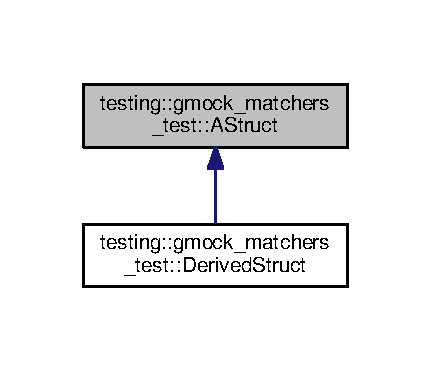
\includegraphics[width=207pt]{structtesting_1_1gmock__matchers__test_1_1AStruct__inherit__graph}
\end{center}
\end{figure}


Collaboration diagram for testing\+:\+:gmock\+\_\+matchers\+\_\+test\+:\+:A\+Struct\+:\nopagebreak
\begin{figure}[H]
\begin{center}
\leavevmode
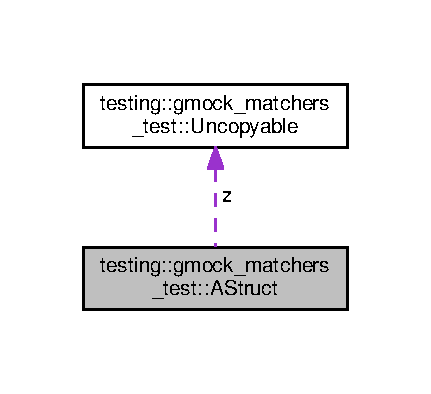
\includegraphics[width=207pt]{structtesting_1_1gmock__matchers__test_1_1AStruct__coll__graph}
\end{center}
\end{figure}
\subsection*{Public Member Functions}
\begin{DoxyCompactItemize}
\item 
\hyperlink{structtesting_1_1gmock__matchers__test_1_1AStruct_a6774561607c8ca64809e9ebde4b62b0e}{A\+Struct} ()
\item 
\hyperlink{structtesting_1_1gmock__matchers__test_1_1AStruct_ac5b9c0054e929e8883e13123aef50ff3}{A\+Struct} (const \hyperlink{structtesting_1_1gmock__matchers__test_1_1AStruct}{A\+Struct} \&rhs)
\end{DoxyCompactItemize}
\subsection*{Public Attributes}
\begin{DoxyCompactItemize}
\item 
int \hyperlink{structtesting_1_1gmock__matchers__test_1_1AStruct_a539eea02599ad34ff2bf90cc2c1adf26}{x}
\item 
const double \hyperlink{structtesting_1_1gmock__matchers__test_1_1AStruct_a08b8592764aa4775c3d5a3542470f8bb}{y}
\item 
\hyperlink{classtesting_1_1gmock__matchers__test_1_1Uncopyable}{Uncopyable} \hyperlink{structtesting_1_1gmock__matchers__test_1_1AStruct_a45b1006e4a7b21037610a385dcae6d8c}{z}
\item 
const char $\ast$ \hyperlink{structtesting_1_1gmock__matchers__test_1_1AStruct_a65755db7d763d53c13483bb520f1efcd}{p}
\end{DoxyCompactItemize}


\subsection{Constructor \& Destructor Documentation}
\index{testing\+::gmock\+\_\+matchers\+\_\+test\+::\+A\+Struct@{testing\+::gmock\+\_\+matchers\+\_\+test\+::\+A\+Struct}!A\+Struct@{A\+Struct}}
\index{A\+Struct@{A\+Struct}!testing\+::gmock\+\_\+matchers\+\_\+test\+::\+A\+Struct@{testing\+::gmock\+\_\+matchers\+\_\+test\+::\+A\+Struct}}
\subsubsection[{\texorpdfstring{A\+Struct()}{AStruct()}}]{\setlength{\rightskip}{0pt plus 5cm}testing\+::gmock\+\_\+matchers\+\_\+test\+::\+A\+Struct\+::\+A\+Struct (
\begin{DoxyParamCaption}
{}
\end{DoxyParamCaption}
)\hspace{0.3cm}{\ttfamily [inline]}}\hypertarget{structtesting_1_1gmock__matchers__test_1_1AStruct_a6774561607c8ca64809e9ebde4b62b0e}{}\label{structtesting_1_1gmock__matchers__test_1_1AStruct_a6774561607c8ca64809e9ebde4b62b0e}

\begin{DoxyCode}
3379 : \hyperlink{structtesting_1_1gmock__matchers__test_1_1AStruct_a539eea02599ad34ff2bf90cc2c1adf26}{x}(0), \hyperlink{structtesting_1_1gmock__matchers__test_1_1AStruct_a08b8592764aa4775c3d5a3542470f8bb}{y}(1.0), \hyperlink{structtesting_1_1gmock__matchers__test_1_1AStruct_a45b1006e4a7b21037610a385dcae6d8c}{z}(5), \hyperlink{structtesting_1_1gmock__matchers__test_1_1AStruct_a65755db7d763d53c13483bb520f1efcd}{p}(NULL) \{\}
\end{DoxyCode}
\index{testing\+::gmock\+\_\+matchers\+\_\+test\+::\+A\+Struct@{testing\+::gmock\+\_\+matchers\+\_\+test\+::\+A\+Struct}!A\+Struct@{A\+Struct}}
\index{A\+Struct@{A\+Struct}!testing\+::gmock\+\_\+matchers\+\_\+test\+::\+A\+Struct@{testing\+::gmock\+\_\+matchers\+\_\+test\+::\+A\+Struct}}
\subsubsection[{\texorpdfstring{A\+Struct(const A\+Struct \&rhs)}{AStruct(const AStruct &rhs)}}]{\setlength{\rightskip}{0pt plus 5cm}testing\+::gmock\+\_\+matchers\+\_\+test\+::\+A\+Struct\+::\+A\+Struct (
\begin{DoxyParamCaption}
\item[{const {\bf A\+Struct} \&}]{rhs}
\end{DoxyParamCaption}
)\hspace{0.3cm}{\ttfamily [inline]}}\hypertarget{structtesting_1_1gmock__matchers__test_1_1AStruct_ac5b9c0054e929e8883e13123aef50ff3}{}\label{structtesting_1_1gmock__matchers__test_1_1AStruct_ac5b9c0054e929e8883e13123aef50ff3}

\begin{DoxyCode}
3381       : \hyperlink{structtesting_1_1gmock__matchers__test_1_1AStruct_a539eea02599ad34ff2bf90cc2c1adf26}{x}(rhs.x), \hyperlink{structtesting_1_1gmock__matchers__test_1_1AStruct_a08b8592764aa4775c3d5a3542470f8bb}{y}(rhs.y), \hyperlink{structtesting_1_1gmock__matchers__test_1_1AStruct_a45b1006e4a7b21037610a385dcae6d8c}{z}(rhs.z.value()), \hyperlink{structtesting_1_1gmock__matchers__test_1_1AStruct_a65755db7d763d53c13483bb520f1efcd}{p}(rhs.p) \{\}
\end{DoxyCode}


\subsection{Member Data Documentation}
\index{testing\+::gmock\+\_\+matchers\+\_\+test\+::\+A\+Struct@{testing\+::gmock\+\_\+matchers\+\_\+test\+::\+A\+Struct}!p@{p}}
\index{p@{p}!testing\+::gmock\+\_\+matchers\+\_\+test\+::\+A\+Struct@{testing\+::gmock\+\_\+matchers\+\_\+test\+::\+A\+Struct}}
\subsubsection[{\texorpdfstring{p}{p}}]{\setlength{\rightskip}{0pt plus 5cm}const char$\ast$ testing\+::gmock\+\_\+matchers\+\_\+test\+::\+A\+Struct\+::p}\hypertarget{structtesting_1_1gmock__matchers__test_1_1AStruct_a65755db7d763d53c13483bb520f1efcd}{}\label{structtesting_1_1gmock__matchers__test_1_1AStruct_a65755db7d763d53c13483bb520f1efcd}
\index{testing\+::gmock\+\_\+matchers\+\_\+test\+::\+A\+Struct@{testing\+::gmock\+\_\+matchers\+\_\+test\+::\+A\+Struct}!x@{x}}
\index{x@{x}!testing\+::gmock\+\_\+matchers\+\_\+test\+::\+A\+Struct@{testing\+::gmock\+\_\+matchers\+\_\+test\+::\+A\+Struct}}
\subsubsection[{\texorpdfstring{x}{x}}]{\setlength{\rightskip}{0pt plus 5cm}int testing\+::gmock\+\_\+matchers\+\_\+test\+::\+A\+Struct\+::x}\hypertarget{structtesting_1_1gmock__matchers__test_1_1AStruct_a539eea02599ad34ff2bf90cc2c1adf26}{}\label{structtesting_1_1gmock__matchers__test_1_1AStruct_a539eea02599ad34ff2bf90cc2c1adf26}
\index{testing\+::gmock\+\_\+matchers\+\_\+test\+::\+A\+Struct@{testing\+::gmock\+\_\+matchers\+\_\+test\+::\+A\+Struct}!y@{y}}
\index{y@{y}!testing\+::gmock\+\_\+matchers\+\_\+test\+::\+A\+Struct@{testing\+::gmock\+\_\+matchers\+\_\+test\+::\+A\+Struct}}
\subsubsection[{\texorpdfstring{y}{y}}]{\setlength{\rightskip}{0pt plus 5cm}const double testing\+::gmock\+\_\+matchers\+\_\+test\+::\+A\+Struct\+::y}\hypertarget{structtesting_1_1gmock__matchers__test_1_1AStruct_a08b8592764aa4775c3d5a3542470f8bb}{}\label{structtesting_1_1gmock__matchers__test_1_1AStruct_a08b8592764aa4775c3d5a3542470f8bb}
\index{testing\+::gmock\+\_\+matchers\+\_\+test\+::\+A\+Struct@{testing\+::gmock\+\_\+matchers\+\_\+test\+::\+A\+Struct}!z@{z}}
\index{z@{z}!testing\+::gmock\+\_\+matchers\+\_\+test\+::\+A\+Struct@{testing\+::gmock\+\_\+matchers\+\_\+test\+::\+A\+Struct}}
\subsubsection[{\texorpdfstring{z}{z}}]{\setlength{\rightskip}{0pt plus 5cm}{\bf Uncopyable} testing\+::gmock\+\_\+matchers\+\_\+test\+::\+A\+Struct\+::z}\hypertarget{structtesting_1_1gmock__matchers__test_1_1AStruct_a45b1006e4a7b21037610a385dcae6d8c}{}\label{structtesting_1_1gmock__matchers__test_1_1AStruct_a45b1006e4a7b21037610a385dcae6d8c}


The documentation for this struct was generated from the following file\+:\begin{DoxyCompactItemize}
\item 
vendor/googletest/googlemock/test/\hyperlink{gmock-matchers__test_8cc}{gmock-\/matchers\+\_\+test.\+cc}\end{DoxyCompactItemize}

\hypertarget{classtesting_1_1gmock__matchers__test_1_1BacktrackingBPMTest}{}\section{testing\+:\+:gmock\+\_\+matchers\+\_\+test\+:\+:Backtracking\+B\+P\+M\+Test Class Reference}
\label{classtesting_1_1gmock__matchers__test_1_1BacktrackingBPMTest}\index{testing\+::gmock\+\_\+matchers\+\_\+test\+::\+Backtracking\+B\+P\+M\+Test@{testing\+::gmock\+\_\+matchers\+\_\+test\+::\+Backtracking\+B\+P\+M\+Test}}


Inheritance diagram for testing\+:\+:gmock\+\_\+matchers\+\_\+test\+:\+:Backtracking\+B\+P\+M\+Test\+:
\nopagebreak
\begin{figure}[H]
\begin{center}
\leavevmode
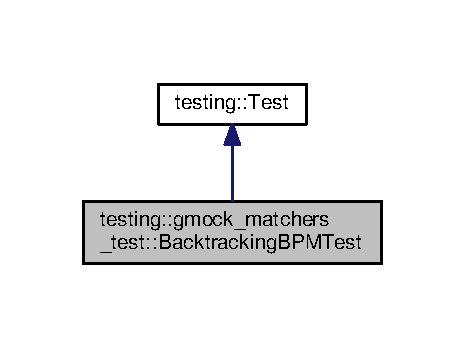
\includegraphics[width=223pt]{classtesting_1_1gmock__matchers__test_1_1BacktrackingBPMTest__inherit__graph}
\end{center}
\end{figure}


Collaboration diagram for testing\+:\+:gmock\+\_\+matchers\+\_\+test\+:\+:Backtracking\+B\+P\+M\+Test\+:
\nopagebreak
\begin{figure}[H]
\begin{center}
\leavevmode
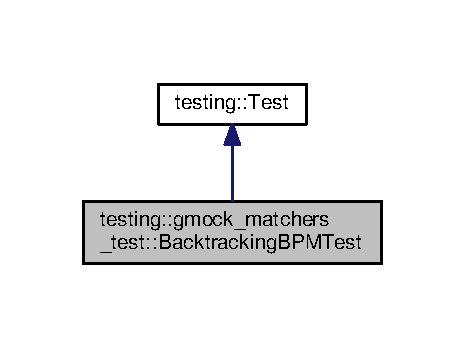
\includegraphics[width=223pt]{classtesting_1_1gmock__matchers__test_1_1BacktrackingBPMTest__coll__graph}
\end{center}
\end{figure}
\subsection*{Additional Inherited Members}


The documentation for this class was generated from the following file\+:\begin{DoxyCompactItemize}
\item 
vendor/googletest/googlemock/test/\hyperlink{gmock-matchers__test_8cc}{gmock-\/matchers\+\_\+test.\+cc}\end{DoxyCompactItemize}

\hypertarget{classBarEnvironment}{}\section{Bar\+Environment Class Reference}
\label{classBarEnvironment}\index{Bar\+Environment@{Bar\+Environment}}


Inheritance diagram for Bar\+Environment\+:
\nopagebreak
\begin{figure}[H]
\begin{center}
\leavevmode
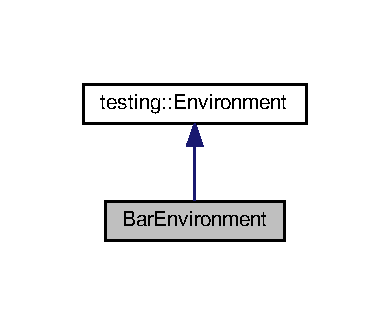
\includegraphics[width=187pt]{classBarEnvironment__inherit__graph}
\end{center}
\end{figure}


Collaboration diagram for Bar\+Environment\+:
\nopagebreak
\begin{figure}[H]
\begin{center}
\leavevmode
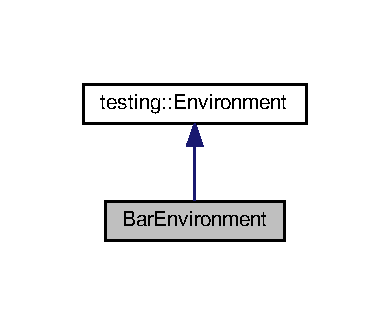
\includegraphics[width=187pt]{classBarEnvironment__coll__graph}
\end{center}
\end{figure}
\subsection*{Public Member Functions}
\begin{DoxyCompactItemize}
\item 
virtual void \hyperlink{classBarEnvironment_a88e17c5dd1dcea7a4538f2f3c6bf7bdd}{Set\+Up} ()
\item 
virtual void \hyperlink{classBarEnvironment_a384f951da72a2a18bb0c2b3506376b09}{Tear\+Down} ()
\end{DoxyCompactItemize}


\subsection{Member Function Documentation}
\index{Bar\+Environment@{Bar\+Environment}!Set\+Up@{Set\+Up}}
\index{Set\+Up@{Set\+Up}!Bar\+Environment@{Bar\+Environment}}
\subsubsection[{\texorpdfstring{Set\+Up()}{SetUp()}}]{\setlength{\rightskip}{0pt plus 5cm}virtual void Bar\+Environment\+::\+Set\+Up (
\begin{DoxyParamCaption}
{}
\end{DoxyParamCaption}
)\hspace{0.3cm}{\ttfamily [inline]}, {\ttfamily [virtual]}}\hypertarget{classBarEnvironment_a88e17c5dd1dcea7a4538f2f3c6bf7bdd}{}\label{classBarEnvironment_a88e17c5dd1dcea7a4538f2f3c6bf7bdd}


Reimplemented from \hyperlink{classtesting_1_1Environment_a1bf8cafaa9d4eba9feb98655ee434eb3}{testing\+::\+Environment}.


\begin{DoxyCode}
1009                        \{
1010     printf(\textcolor{stringliteral}{"%s"}, \textcolor{stringliteral}{"BarEnvironment::SetUp() called.\(\backslash\)n"});
1011   \}
\end{DoxyCode}
\index{Bar\+Environment@{Bar\+Environment}!Tear\+Down@{Tear\+Down}}
\index{Tear\+Down@{Tear\+Down}!Bar\+Environment@{Bar\+Environment}}
\subsubsection[{\texorpdfstring{Tear\+Down()}{TearDown()}}]{\setlength{\rightskip}{0pt plus 5cm}virtual void Bar\+Environment\+::\+Tear\+Down (
\begin{DoxyParamCaption}
{}
\end{DoxyParamCaption}
)\hspace{0.3cm}{\ttfamily [inline]}, {\ttfamily [virtual]}}\hypertarget{classBarEnvironment_a384f951da72a2a18bb0c2b3506376b09}{}\label{classBarEnvironment_a384f951da72a2a18bb0c2b3506376b09}


Reimplemented from \hyperlink{classtesting_1_1Environment_a039bdaa705c46b9b88234cf4d3bb6254}{testing\+::\+Environment}.


\begin{DoxyCode}
1013                           \{
1014     printf(\textcolor{stringliteral}{"%s"}, \textcolor{stringliteral}{"BarEnvironment::TearDown() called.\(\backslash\)n"});
1015     \hyperlink{gtest_8h_adc16b5b0a740c39084ea5c9e960e3063}{ADD\_FAILURE}() << \textcolor{stringliteral}{"Expected non-fatal failure."};
1016   \}
\end{DoxyCode}


The documentation for this class was generated from the following file\+:\begin{DoxyCompactItemize}
\item 
vendor/googletest/googletest/test/\hyperlink{gtest__output__test___8cc}{gtest\+\_\+output\+\_\+test\+\_\+.\+cc}\end{DoxyCompactItemize}

\hypertarget{classtesting_1_1internal_1_1Base}{}\section{testing\+:\+:internal\+:\+:Base Class Reference}
\label{classtesting_1_1internal_1_1Base}\index{testing\+::internal\+::\+Base@{testing\+::internal\+::\+Base}}
\subsection*{Public Member Functions}
\begin{DoxyCompactItemize}
\item 
\hyperlink{classtesting_1_1internal_1_1Base_a6b29f1a7192b126e6fa0aae31200b5ca}{Base} ()
\item 
\hyperlink{classtesting_1_1internal_1_1Base_a255d105410a1eeb5f4690c9c8cd8e104}{Base} (int n)
\item 
virtual \hyperlink{classtesting_1_1internal_1_1Base_afb29c9032fb50cc6520014aad9d68328}{$\sim$\+Base} ()
\item 
int \hyperlink{classtesting_1_1internal_1_1Base_a7ddba6221b56613be545544b7ef6214c}{member} ()
\end{DoxyCompactItemize}


\subsection{Constructor \& Destructor Documentation}
\index{testing\+::internal\+::\+Base@{testing\+::internal\+::\+Base}!Base@{Base}}
\index{Base@{Base}!testing\+::internal\+::\+Base@{testing\+::internal\+::\+Base}}
\subsubsection[{\texorpdfstring{Base()}{Base()}}]{\setlength{\rightskip}{0pt plus 5cm}testing\+::internal\+::\+Base\+::\+Base (
\begin{DoxyParamCaption}
{}
\end{DoxyParamCaption}
)\hspace{0.3cm}{\ttfamily [inline]}}\hypertarget{classtesting_1_1internal_1_1Base_a6b29f1a7192b126e6fa0aae31200b5ca}{}\label{classtesting_1_1internal_1_1Base_a6b29f1a7192b126e6fa0aae31200b5ca}

\begin{DoxyCode}
105 : member\_(0) \{\}
\end{DoxyCode}
\index{testing\+::internal\+::\+Base@{testing\+::internal\+::\+Base}!Base@{Base}}
\index{Base@{Base}!testing\+::internal\+::\+Base@{testing\+::internal\+::\+Base}}
\subsubsection[{\texorpdfstring{Base(int n)}{Base(int n)}}]{\setlength{\rightskip}{0pt plus 5cm}testing\+::internal\+::\+Base\+::\+Base (
\begin{DoxyParamCaption}
\item[{int}]{n}
\end{DoxyParamCaption}
)\hspace{0.3cm}{\ttfamily [inline]}, {\ttfamily [explicit]}}\hypertarget{classtesting_1_1internal_1_1Base_a255d105410a1eeb5f4690c9c8cd8e104}{}\label{classtesting_1_1internal_1_1Base_a255d105410a1eeb5f4690c9c8cd8e104}

\begin{DoxyCode}
106 : member\_(n) \{\}
\end{DoxyCode}
\index{testing\+::internal\+::\+Base@{testing\+::internal\+::\+Base}!````~Base@{$\sim$\+Base}}
\index{````~Base@{$\sim$\+Base}!testing\+::internal\+::\+Base@{testing\+::internal\+::\+Base}}
\subsubsection[{\texorpdfstring{$\sim$\+Base()}{~Base()}}]{\setlength{\rightskip}{0pt plus 5cm}virtual testing\+::internal\+::\+Base\+::$\sim$\+Base (
\begin{DoxyParamCaption}
{}
\end{DoxyParamCaption}
)\hspace{0.3cm}{\ttfamily [inline]}, {\ttfamily [virtual]}}\hypertarget{classtesting_1_1internal_1_1Base_afb29c9032fb50cc6520014aad9d68328}{}\label{classtesting_1_1internal_1_1Base_afb29c9032fb50cc6520014aad9d68328}

\begin{DoxyCode}
107 \{\}
\end{DoxyCode}


\subsection{Member Function Documentation}
\index{testing\+::internal\+::\+Base@{testing\+::internal\+::\+Base}!member@{member}}
\index{member@{member}!testing\+::internal\+::\+Base@{testing\+::internal\+::\+Base}}
\subsubsection[{\texorpdfstring{member()}{member()}}]{\setlength{\rightskip}{0pt plus 5cm}int testing\+::internal\+::\+Base\+::member (
\begin{DoxyParamCaption}
{}
\end{DoxyParamCaption}
)\hspace{0.3cm}{\ttfamily [inline]}}\hypertarget{classtesting_1_1internal_1_1Base_a7ddba6221b56613be545544b7ef6214c}{}\label{classtesting_1_1internal_1_1Base_a7ddba6221b56613be545544b7ef6214c}

\begin{DoxyCode}
108 \{ \textcolor{keywordflow}{return} member\_; \}
\end{DoxyCode}


The documentation for this class was generated from the following file\+:\begin{DoxyCompactItemize}
\item 
vendor/googletest/googletest/test/\hyperlink{gtest-port__test_8cc}{gtest-\/port\+\_\+test.\+cc}\end{DoxyCompactItemize}

\hypertarget{classBase}{}\section{Base Class Reference}
\label{classBase}\index{Base@{Base}}
\subsection*{Public Member Functions}
\begin{DoxyCompactItemize}
\item 
\hyperlink{classBase_a1d5f3fb92f8cbc687705785bdc6abd18}{Base} (int an\+\_\+x)
\item 
int \hyperlink{classBase_a963687d3b65f99407cc6f90172806fae}{x} () const 
\end{DoxyCompactItemize}


\subsection{Constructor \& Destructor Documentation}
\index{Base@{Base}!Base@{Base}}
\index{Base@{Base}!Base@{Base}}
\subsubsection[{\texorpdfstring{Base(int an\+\_\+x)}{Base(int an_x)}}]{\setlength{\rightskip}{0pt plus 5cm}Base\+::\+Base (
\begin{DoxyParamCaption}
\item[{int}]{an\+\_\+x}
\end{DoxyParamCaption}
)\hspace{0.3cm}{\ttfamily [inline]}, {\ttfamily [explicit]}}\hypertarget{classBase_a1d5f3fb92f8cbc687705785bdc6abd18}{}\label{classBase_a1d5f3fb92f8cbc687705785bdc6abd18}

\begin{DoxyCode}
5157 : x\_(an\_x) \{\}
\end{DoxyCode}


\subsection{Member Function Documentation}
\index{Base@{Base}!x@{x}}
\index{x@{x}!Base@{Base}}
\subsubsection[{\texorpdfstring{x() const }{x() const }}]{\setlength{\rightskip}{0pt plus 5cm}int Base\+::x (
\begin{DoxyParamCaption}
{}
\end{DoxyParamCaption}
) const\hspace{0.3cm}{\ttfamily [inline]}}\hypertarget{classBase_a963687d3b65f99407cc6f90172806fae}{}\label{classBase_a963687d3b65f99407cc6f90172806fae}

\begin{DoxyCode}
5158 \{ \textcolor{keywordflow}{return} x\_; \}
\end{DoxyCode}


The documentation for this class was generated from the following file\+:\begin{DoxyCompactItemize}
\item 
vendor/googletest/googletest/test/\hyperlink{gtest__unittest_8cc}{gtest\+\_\+unittest.\+cc}\end{DoxyCompactItemize}

\hypertarget{classtesting_1_1gmock__matchers__test_1_1Base}{}\section{testing\+:\+:gmock\+\_\+matchers\+\_\+test\+:\+:Base Class Reference}
\label{classtesting_1_1gmock__matchers__test_1_1Base}\index{testing\+::gmock\+\_\+matchers\+\_\+test\+::\+Base@{testing\+::gmock\+\_\+matchers\+\_\+test\+::\+Base}}


Inheritance diagram for testing\+:\+:gmock\+\_\+matchers\+\_\+test\+:\+:Base\+:\nopagebreak
\begin{figure}[H]
\begin{center}
\leavevmode
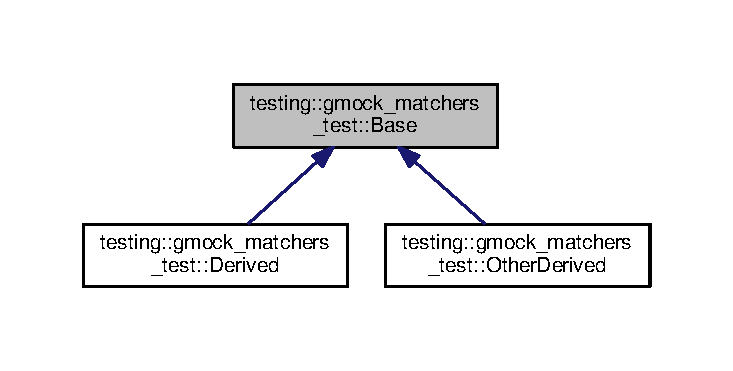
\includegraphics[width=350pt]{classtesting_1_1gmock__matchers__test_1_1Base__inherit__graph}
\end{center}
\end{figure}
\subsection*{Public Member Functions}
\begin{DoxyCompactItemize}
\item 
virtual \hyperlink{classtesting_1_1gmock__matchers__test_1_1Base_ab02c73411d19b28ccb847c65bc782bb6}{$\sim$\+Base} ()
\item 
\hyperlink{classtesting_1_1gmock__matchers__test_1_1Base_ab3b2127992b81455804462897de44516}{Base} ()
\end{DoxyCompactItemize}


\subsection{Constructor \& Destructor Documentation}
\index{testing\+::gmock\+\_\+matchers\+\_\+test\+::\+Base@{testing\+::gmock\+\_\+matchers\+\_\+test\+::\+Base}!````~Base@{$\sim$\+Base}}
\index{````~Base@{$\sim$\+Base}!testing\+::gmock\+\_\+matchers\+\_\+test\+::\+Base@{testing\+::gmock\+\_\+matchers\+\_\+test\+::\+Base}}
\subsubsection[{\texorpdfstring{$\sim$\+Base()}{~Base()}}]{\setlength{\rightskip}{0pt plus 5cm}virtual testing\+::gmock\+\_\+matchers\+\_\+test\+::\+Base\+::$\sim$\+Base (
\begin{DoxyParamCaption}
{}
\end{DoxyParamCaption}
)\hspace{0.3cm}{\ttfamily [inline]}, {\ttfamily [virtual]}}\hypertarget{classtesting_1_1gmock__matchers__test_1_1Base_ab02c73411d19b28ccb847c65bc782bb6}{}\label{classtesting_1_1gmock__matchers__test_1_1Base_ab02c73411d19b28ccb847c65bc782bb6}

\begin{DoxyCode}
661 \{\}
\end{DoxyCode}
\index{testing\+::gmock\+\_\+matchers\+\_\+test\+::\+Base@{testing\+::gmock\+\_\+matchers\+\_\+test\+::\+Base}!Base@{Base}}
\index{Base@{Base}!testing\+::gmock\+\_\+matchers\+\_\+test\+::\+Base@{testing\+::gmock\+\_\+matchers\+\_\+test\+::\+Base}}
\subsubsection[{\texorpdfstring{Base()}{Base()}}]{\setlength{\rightskip}{0pt plus 5cm}testing\+::gmock\+\_\+matchers\+\_\+test\+::\+Base\+::\+Base (
\begin{DoxyParamCaption}
{}
\end{DoxyParamCaption}
)\hspace{0.3cm}{\ttfamily [inline]}}\hypertarget{classtesting_1_1gmock__matchers__test_1_1Base_ab3b2127992b81455804462897de44516}{}\label{classtesting_1_1gmock__matchers__test_1_1Base_ab3b2127992b81455804462897de44516}

\begin{DoxyCode}
662 \{\}
\end{DoxyCode}


The documentation for this class was generated from the following file\+:\begin{DoxyCompactItemize}
\item 
vendor/googletest/googlemock/test/\hyperlink{gmock-matchers__test_8cc}{gmock-\/matchers\+\_\+test.\+cc}\end{DoxyCompactItemize}

\hypertarget{classtesting_1_1internal_1_1BeginEndDistanceIsMatcher}{}\section{testing\+:\+:internal\+:\+:Begin\+End\+Distance\+Is\+Matcher$<$ Distance\+Matcher $>$ Class Template Reference}
\label{classtesting_1_1internal_1_1BeginEndDistanceIsMatcher}\index{testing\+::internal\+::\+Begin\+End\+Distance\+Is\+Matcher$<$ Distance\+Matcher $>$@{testing\+::internal\+::\+Begin\+End\+Distance\+Is\+Matcher$<$ Distance\+Matcher $>$}}


{\ttfamily \#include $<$gmock-\/matchers.\+h$>$}

\subsection*{Classes}
\begin{DoxyCompactItemize}
\item 
class \hyperlink{classtesting_1_1internal_1_1BeginEndDistanceIsMatcher_1_1Impl}{Impl}
\end{DoxyCompactItemize}
\subsection*{Public Member Functions}
\begin{DoxyCompactItemize}
\item 
\hyperlink{classtesting_1_1internal_1_1BeginEndDistanceIsMatcher_aaf0d34d922d89820346e80a21cbf8d24}{Begin\+End\+Distance\+Is\+Matcher} (const Distance\+Matcher \&distance\+\_\+matcher)
\item 
{\footnotesize template$<$typename Container $>$ }\\\hyperlink{classtesting_1_1internal_1_1BeginEndDistanceIsMatcher_aef8f6ec8dfce159fb79eec6a1ea011bb}{operator Matcher$<$ Container $>$} () const 
\end{DoxyCompactItemize}


\subsection{Constructor \& Destructor Documentation}
\index{testing\+::internal\+::\+Begin\+End\+Distance\+Is\+Matcher@{testing\+::internal\+::\+Begin\+End\+Distance\+Is\+Matcher}!Begin\+End\+Distance\+Is\+Matcher@{Begin\+End\+Distance\+Is\+Matcher}}
\index{Begin\+End\+Distance\+Is\+Matcher@{Begin\+End\+Distance\+Is\+Matcher}!testing\+::internal\+::\+Begin\+End\+Distance\+Is\+Matcher@{testing\+::internal\+::\+Begin\+End\+Distance\+Is\+Matcher}}
\subsubsection[{\texorpdfstring{Begin\+End\+Distance\+Is\+Matcher(const Distance\+Matcher \&distance\+\_\+matcher)}{BeginEndDistanceIsMatcher(const DistanceMatcher &distance_matcher)}}]{\setlength{\rightskip}{0pt plus 5cm}template$<$typename Distance\+Matcher $>$ {\bf testing\+::internal\+::\+Begin\+End\+Distance\+Is\+Matcher}$<$ Distance\+Matcher $>$\+::{\bf Begin\+End\+Distance\+Is\+Matcher} (
\begin{DoxyParamCaption}
\item[{const Distance\+Matcher \&}]{distance\+\_\+matcher}
\end{DoxyParamCaption}
)\hspace{0.3cm}{\ttfamily [inline]}, {\ttfamily [explicit]}}\hypertarget{classtesting_1_1internal_1_1BeginEndDistanceIsMatcher_aaf0d34d922d89820346e80a21cbf8d24}{}\label{classtesting_1_1internal_1_1BeginEndDistanceIsMatcher_aaf0d34d922d89820346e80a21cbf8d24}

\begin{DoxyCode}
2455       : distance\_matcher\_(distance\_matcher) \{\}
\end{DoxyCode}


\subsection{Member Function Documentation}
\index{testing\+::internal\+::\+Begin\+End\+Distance\+Is\+Matcher@{testing\+::internal\+::\+Begin\+End\+Distance\+Is\+Matcher}!operator Matcher$<$ Container $>$@{operator Matcher$<$ Container $>$}}
\index{operator Matcher$<$ Container $>$@{operator Matcher$<$ Container $>$}!testing\+::internal\+::\+Begin\+End\+Distance\+Is\+Matcher@{testing\+::internal\+::\+Begin\+End\+Distance\+Is\+Matcher}}
\subsubsection[{\texorpdfstring{operator Matcher$<$ Container $>$() const }{operator Matcher< Container >() const }}]{\setlength{\rightskip}{0pt plus 5cm}template$<$typename Distance\+Matcher $>$ template$<$typename Container $>$ {\bf testing\+::internal\+::\+Begin\+End\+Distance\+Is\+Matcher}$<$ Distance\+Matcher $>$\+::operator {\bf Matcher}$<$ Container $>$ (
\begin{DoxyParamCaption}
{}
\end{DoxyParamCaption}
) const\hspace{0.3cm}{\ttfamily [inline]}}\hypertarget{classtesting_1_1internal_1_1BeginEndDistanceIsMatcher_aef8f6ec8dfce159fb79eec6a1ea011bb}{}\label{classtesting_1_1internal_1_1BeginEndDistanceIsMatcher_aef8f6ec8dfce159fb79eec6a1ea011bb}

\begin{DoxyCode}
2458                                       \{
2459     \textcolor{keywordflow}{return} \hyperlink{namespacetesting_a37fd8029ac00e60952440a3d9cca8166}{MakeMatcher}(\textcolor{keyword}{new} Impl<Container>(distance\_matcher\_));
2460   \}
\end{DoxyCode}


The documentation for this class was generated from the following file\+:\begin{DoxyCompactItemize}
\item 
vendor/googletest/googlemock/include/gmock/\hyperlink{gmock-matchers_8h}{gmock-\/matchers.\+h}\end{DoxyCompactItemize}

\hypertarget{structtesting_1_1gtest__printers__test_1_1Big}{}\section{testing\+:\+:gtest\+\_\+printers\+\_\+test\+:\+:Big Struct Reference}
\label{structtesting_1_1gtest__printers__test_1_1Big}\index{testing\+::gtest\+\_\+printers\+\_\+test\+::\+Big@{testing\+::gtest\+\_\+printers\+\_\+test\+::\+Big}}
\subsection*{Public Member Functions}
\begin{DoxyCompactItemize}
\item 
\hyperlink{structtesting_1_1gtest__printers__test_1_1Big_adb57fb0e14adb81177e3bfd7ed39966c}{Big} ()
\end{DoxyCompactItemize}
\subsection*{Public Attributes}
\begin{DoxyCompactItemize}
\item 
char \hyperlink{structtesting_1_1gtest__printers__test_1_1Big_a863911a8ec5c3bbe79c44d399f1de61f}{array} \mbox{[}257\mbox{]}
\end{DoxyCompactItemize}


\subsection{Constructor \& Destructor Documentation}
\index{testing\+::gtest\+\_\+printers\+\_\+test\+::\+Big@{testing\+::gtest\+\_\+printers\+\_\+test\+::\+Big}!Big@{Big}}
\index{Big@{Big}!testing\+::gtest\+\_\+printers\+\_\+test\+::\+Big@{testing\+::gtest\+\_\+printers\+\_\+test\+::\+Big}}
\subsubsection[{\texorpdfstring{Big()}{Big()}}]{\setlength{\rightskip}{0pt plus 5cm}testing\+::gtest\+\_\+printers\+\_\+test\+::\+Big\+::\+Big (
\begin{DoxyParamCaption}
{}
\end{DoxyParamCaption}
)\hspace{0.3cm}{\ttfamily [inline]}}\hypertarget{structtesting_1_1gtest__printers__test_1_1Big_adb57fb0e14adb81177e3bfd7ed39966c}{}\label{structtesting_1_1gtest__printers__test_1_1Big_adb57fb0e14adb81177e3bfd7ed39966c}

\begin{DoxyCode}
1131 \{ memset(\hyperlink{structtesting_1_1gtest__printers__test_1_1Big_a863911a8ec5c3bbe79c44d399f1de61f}{array}, 0, \textcolor{keyword}{sizeof}(\hyperlink{structtesting_1_1gtest__printers__test_1_1Big_a863911a8ec5c3bbe79c44d399f1de61f}{array})); \}
\end{DoxyCode}


\subsection{Member Data Documentation}
\index{testing\+::gtest\+\_\+printers\+\_\+test\+::\+Big@{testing\+::gtest\+\_\+printers\+\_\+test\+::\+Big}!array@{array}}
\index{array@{array}!testing\+::gtest\+\_\+printers\+\_\+test\+::\+Big@{testing\+::gtest\+\_\+printers\+\_\+test\+::\+Big}}
\subsubsection[{\texorpdfstring{array}{array}}]{\setlength{\rightskip}{0pt plus 5cm}char testing\+::gtest\+\_\+printers\+\_\+test\+::\+Big\+::array\mbox{[}257\mbox{]}}\hypertarget{structtesting_1_1gtest__printers__test_1_1Big_a863911a8ec5c3bbe79c44d399f1de61f}{}\label{structtesting_1_1gtest__printers__test_1_1Big_a863911a8ec5c3bbe79c44d399f1de61f}


The documentation for this struct was generated from the following file\+:\begin{DoxyCompactItemize}
\item 
vendor/googletest/googletest/test/\hyperlink{gtest-printers__test_8cc}{gtest-\/printers\+\_\+test.\+cc}\end{DoxyCompactItemize}

\hypertarget{classBiggestIntConvertible}{}\section{Biggest\+Int\+Convertible Class Reference}
\label{classBiggestIntConvertible}\index{Biggest\+Int\+Convertible@{Biggest\+Int\+Convertible}}
\subsection*{Public Member Functions}
\begin{DoxyCompactItemize}
\item 
\hyperlink{classBiggestIntConvertible_ab8e66c4adee8172528c4070f19d47058}{operator\+::testing\+::internal\+::\+Biggest\+Int} () const 
\end{DoxyCompactItemize}


\subsection{Member Function Documentation}
\index{Biggest\+Int\+Convertible@{Biggest\+Int\+Convertible}!operator\+::testing\+::internal\+::\+Biggest\+Int@{operator\+::testing\+::internal\+::\+Biggest\+Int}}
\index{operator\+::testing\+::internal\+::\+Biggest\+Int@{operator\+::testing\+::internal\+::\+Biggest\+Int}!Biggest\+Int\+Convertible@{Biggest\+Int\+Convertible}}
\subsubsection[{\texorpdfstring{operator\+::testing\+::internal\+::\+Biggest\+Int() const }{operator::testing::internal::BiggestInt() const }}]{\setlength{\rightskip}{0pt plus 5cm}Biggest\+Int\+Convertible\+::operator\+::testing\+::internal\+::\+Biggest\+Int (
\begin{DoxyParamCaption}
{}
\end{DoxyParamCaption}
) const\hspace{0.3cm}{\ttfamily [inline]}}\hypertarget{classBiggestIntConvertible_ab8e66c4adee8172528c4070f19d47058}{}\label{classBiggestIntConvertible_ab8e66c4adee8172528c4070f19d47058}

\begin{DoxyCode}
100 \{ \textcolor{keywordflow}{return} 42; \}
\end{DoxyCode}


The documentation for this class was generated from the following file\+:\begin{DoxyCompactItemize}
\item 
vendor/googletest/googletest/test/\hyperlink{gtest-printers__test_8cc}{gtest-\/printers\+\_\+test.\+cc}\end{DoxyCompactItemize}

\hypertarget{classtesting_1_1gmock__matchers__test_1_1BipartiteNonSquareTest}{}\section{testing\+:\+:gmock\+\_\+matchers\+\_\+test\+:\+:Bipartite\+Non\+Square\+Test Class Reference}
\label{classtesting_1_1gmock__matchers__test_1_1BipartiteNonSquareTest}\index{testing\+::gmock\+\_\+matchers\+\_\+test\+::\+Bipartite\+Non\+Square\+Test@{testing\+::gmock\+\_\+matchers\+\_\+test\+::\+Bipartite\+Non\+Square\+Test}}


Inheritance diagram for testing\+:\+:gmock\+\_\+matchers\+\_\+test\+:\+:Bipartite\+Non\+Square\+Test\+:\nopagebreak
\begin{figure}[H]
\begin{center}
\leavevmode
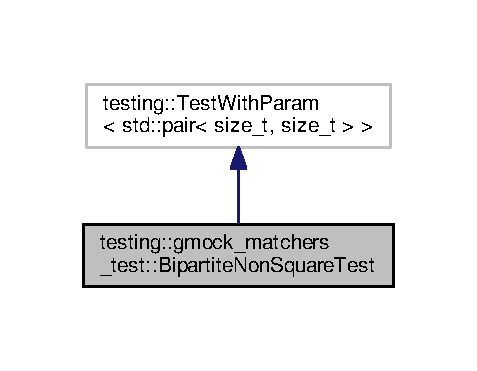
\includegraphics[width=229pt]{classtesting_1_1gmock__matchers__test_1_1BipartiteNonSquareTest__inherit__graph}
\end{center}
\end{figure}


Collaboration diagram for testing\+:\+:gmock\+\_\+matchers\+\_\+test\+:\+:Bipartite\+Non\+Square\+Test\+:\nopagebreak
\begin{figure}[H]
\begin{center}
\leavevmode
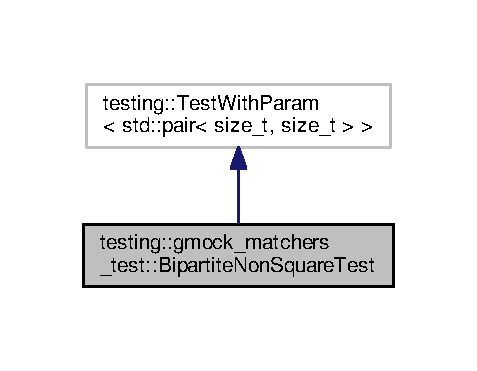
\includegraphics[width=229pt]{classtesting_1_1gmock__matchers__test_1_1BipartiteNonSquareTest__coll__graph}
\end{center}
\end{figure}


The documentation for this class was generated from the following file\+:\begin{DoxyCompactItemize}
\item 
vendor/googletest/googlemock/test/\hyperlink{gmock-matchers__test_8cc}{gmock-\/matchers\+\_\+test.\+cc}\end{DoxyCompactItemize}

\hypertarget{classtesting_1_1gmock__matchers__test_1_1BipartiteRandomTest}{}\section{testing\+:\+:gmock\+\_\+matchers\+\_\+test\+:\+:Bipartite\+Random\+Test Class Reference}
\label{classtesting_1_1gmock__matchers__test_1_1BipartiteRandomTest}\index{testing\+::gmock\+\_\+matchers\+\_\+test\+::\+Bipartite\+Random\+Test@{testing\+::gmock\+\_\+matchers\+\_\+test\+::\+Bipartite\+Random\+Test}}


Inheritance diagram for testing\+:\+:gmock\+\_\+matchers\+\_\+test\+:\+:Bipartite\+Random\+Test\+:\nopagebreak
\begin{figure}[H]
\begin{center}
\leavevmode
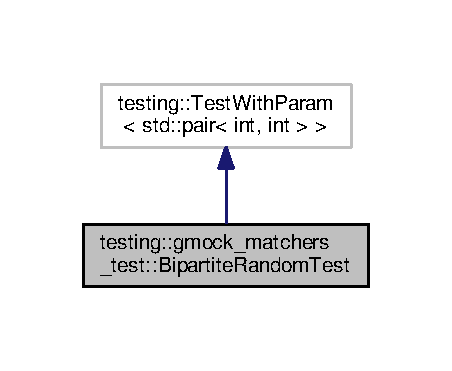
\includegraphics[width=217pt]{classtesting_1_1gmock__matchers__test_1_1BipartiteRandomTest__inherit__graph}
\end{center}
\end{figure}


Collaboration diagram for testing\+:\+:gmock\+\_\+matchers\+\_\+test\+:\+:Bipartite\+Random\+Test\+:\nopagebreak
\begin{figure}[H]
\begin{center}
\leavevmode
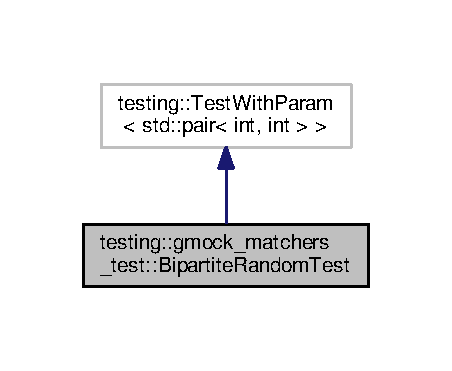
\includegraphics[width=217pt]{classtesting_1_1gmock__matchers__test_1_1BipartiteRandomTest__coll__graph}
\end{center}
\end{figure}


The documentation for this class was generated from the following file\+:\begin{DoxyCompactItemize}
\item 
vendor/googletest/googlemock/test/\hyperlink{gmock-matchers__test_8cc}{gmock-\/matchers\+\_\+test.\+cc}\end{DoxyCompactItemize}

\hypertarget{classtesting_1_1gmock__matchers__test_1_1BipartiteTest}{}\section{testing\+:\+:gmock\+\_\+matchers\+\_\+test\+:\+:Bipartite\+Test Class Reference}
\label{classtesting_1_1gmock__matchers__test_1_1BipartiteTest}\index{testing\+::gmock\+\_\+matchers\+\_\+test\+::\+Bipartite\+Test@{testing\+::gmock\+\_\+matchers\+\_\+test\+::\+Bipartite\+Test}}


Inheritance diagram for testing\+:\+:gmock\+\_\+matchers\+\_\+test\+:\+:Bipartite\+Test\+:
\nopagebreak
\begin{figure}[H]
\begin{center}
\leavevmode
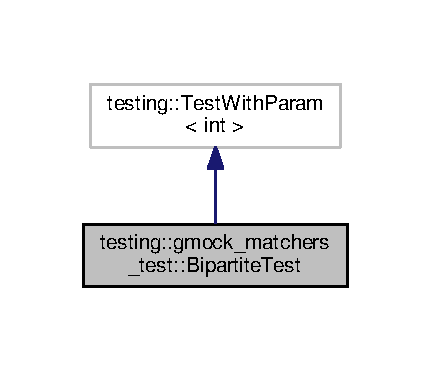
\includegraphics[width=207pt]{classtesting_1_1gmock__matchers__test_1_1BipartiteTest__inherit__graph}
\end{center}
\end{figure}


Collaboration diagram for testing\+:\+:gmock\+\_\+matchers\+\_\+test\+:\+:Bipartite\+Test\+:
\nopagebreak
\begin{figure}[H]
\begin{center}
\leavevmode
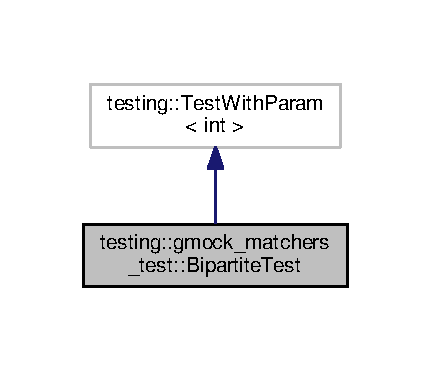
\includegraphics[width=207pt]{classtesting_1_1gmock__matchers__test_1_1BipartiteTest__coll__graph}
\end{center}
\end{figure}


The documentation for this class was generated from the following file\+:\begin{DoxyCompactItemize}
\item 
vendor/googletest/googlemock/test/\hyperlink{gmock-matchers__test_8cc}{gmock-\/matchers\+\_\+test.\+cc}\end{DoxyCompactItemize}

\hypertarget{structBool}{}\section{Bool Struct Reference}
\label{structBool}\index{Bool@{Bool}}
\subsection*{Public Member Functions}
\begin{DoxyCompactItemize}
\item 
\hyperlink{structBool_a03dfd4851b13abb29414887fcada7fca}{Bool} (int val)
\item 
bool \hyperlink{structBool_a812f0599da778aa0399cffa1a2687f6e}{operator$>$} (int \hyperlink{app_2main_8cpp_acfc02ec89670db29251fda6a66602ce2}{n}) const 
\item 
\hyperlink{structBool}{Bool} \hyperlink{structBool_a5d6f8c4a1def861f9b1c24e46b1228ca}{operator+} (const \hyperlink{structBool}{Bool} \&rhs) const 
\item 
bool \hyperlink{structBool_a1e885f75c224ea1fba1cbce11c888716}{operator==} (const \hyperlink{structBool}{Bool} \&rhs) const 
\end{DoxyCompactItemize}
\subsection*{Public Attributes}
\begin{DoxyCompactItemize}
\item 
bool \hyperlink{structBool_a16be863c269f988cdcbe59f9d846a141}{value}
\end{DoxyCompactItemize}


\subsection{Constructor \& Destructor Documentation}
\index{Bool@{Bool}!Bool@{Bool}}
\index{Bool@{Bool}!Bool@{Bool}}
\subsubsection[{\texorpdfstring{Bool(int val)}{Bool(int val)}}]{\setlength{\rightskip}{0pt plus 5cm}Bool\+::\+Bool (
\begin{DoxyParamCaption}
\item[{int}]{val}
\end{DoxyParamCaption}
)\hspace{0.3cm}{\ttfamily [inline]}, {\ttfamily [explicit]}}\hypertarget{structBool_a03dfd4851b13abb29414887fcada7fca}{}\label{structBool_a03dfd4851b13abb29414887fcada7fca}

\begin{DoxyCode}
57 : \hyperlink{structBool_a16be863c269f988cdcbe59f9d846a141}{value}(val != 0) \{\}
\end{DoxyCode}


\subsection{Member Function Documentation}
\index{Bool@{Bool}!operator+@{operator+}}
\index{operator+@{operator+}!Bool@{Bool}}
\subsubsection[{\texorpdfstring{operator+(const Bool \&rhs) const }{operator+(const Bool &rhs) const }}]{\setlength{\rightskip}{0pt plus 5cm}{\bf Bool} Bool\+::operator+ (
\begin{DoxyParamCaption}
\item[{const {\bf Bool} \&}]{rhs}
\end{DoxyParamCaption}
) const\hspace{0.3cm}{\ttfamily [inline]}}\hypertarget{structBool_a5d6f8c4a1def861f9b1c24e46b1228ca}{}\label{structBool_a5d6f8c4a1def861f9b1c24e46b1228ca}

\begin{DoxyCode}
61 \{ \textcolor{keywordflow}{return} \hyperlink{structBool_a03dfd4851b13abb29414887fcada7fca}{Bool}(\hyperlink{structBool_a16be863c269f988cdcbe59f9d846a141}{value} + rhs.\hyperlink{structBool_a16be863c269f988cdcbe59f9d846a141}{value}); \}
\end{DoxyCode}
\index{Bool@{Bool}!operator==@{operator==}}
\index{operator==@{operator==}!Bool@{Bool}}
\subsubsection[{\texorpdfstring{operator==(const Bool \&rhs) const }{operator==(const Bool &rhs) const }}]{\setlength{\rightskip}{0pt plus 5cm}bool Bool\+::operator== (
\begin{DoxyParamCaption}
\item[{const {\bf Bool} \&}]{rhs}
\end{DoxyParamCaption}
) const\hspace{0.3cm}{\ttfamily [inline]}}\hypertarget{structBool_a1e885f75c224ea1fba1cbce11c888716}{}\label{structBool_a1e885f75c224ea1fba1cbce11c888716}

\begin{DoxyCode}
63 \{ \textcolor{keywordflow}{return} \hyperlink{structBool_a16be863c269f988cdcbe59f9d846a141}{value} == rhs.\hyperlink{structBool_a16be863c269f988cdcbe59f9d846a141}{value}; \}
\end{DoxyCode}
\index{Bool@{Bool}!operator$>$@{operator$>$}}
\index{operator$>$@{operator$>$}!Bool@{Bool}}
\subsubsection[{\texorpdfstring{operator$>$(int n) const }{operator>(int n) const }}]{\setlength{\rightskip}{0pt plus 5cm}bool Bool\+::operator$>$ (
\begin{DoxyParamCaption}
\item[{int}]{n}
\end{DoxyParamCaption}
) const\hspace{0.3cm}{\ttfamily [inline]}}\hypertarget{structBool_a812f0599da778aa0399cffa1a2687f6e}{}\label{structBool_a812f0599da778aa0399cffa1a2687f6e}

\begin{DoxyCode}
59 \{ \textcolor{keywordflow}{return} \hyperlink{structBool_a16be863c269f988cdcbe59f9d846a141}{value} > \hyperlink{structBool_a03dfd4851b13abb29414887fcada7fca}{Bool}(\hyperlink{app_2main_8cpp_acfc02ec89670db29251fda6a66602ce2}{n}).value; \}
\end{DoxyCode}


\subsection{Member Data Documentation}
\index{Bool@{Bool}!value@{value}}
\index{value@{value}!Bool@{Bool}}
\subsubsection[{\texorpdfstring{value}{value}}]{\setlength{\rightskip}{0pt plus 5cm}bool Bool\+::value}\hypertarget{structBool_a16be863c269f988cdcbe59f9d846a141}{}\label{structBool_a16be863c269f988cdcbe59f9d846a141}


The documentation for this struct was generated from the following file\+:\begin{DoxyCompactItemize}
\item 
vendor/googletest/googletest/test/\hyperlink{gtest__pred__impl__unittest_8cc}{gtest\+\_\+pred\+\_\+impl\+\_\+unittest.\+cc}\end{DoxyCompactItemize}

\hypertarget{structtesting_1_1internal_1_1bool__constant}{}\section{testing\+:\+:internal\+:\+:bool\+\_\+constant$<$ bool\+\_\+value $>$ Struct Template Reference}
\label{structtesting_1_1internal_1_1bool__constant}\index{testing\+::internal\+::bool\+\_\+constant$<$ bool\+\_\+value $>$@{testing\+::internal\+::bool\+\_\+constant$<$ bool\+\_\+value $>$}}


{\ttfamily \#include $<$gtest-\/port.\+h$>$}



Inheritance diagram for testing\+:\+:internal\+:\+:bool\+\_\+constant$<$ bool\+\_\+value $>$\+:\nopagebreak
\begin{figure}[H]
\begin{center}
\leavevmode
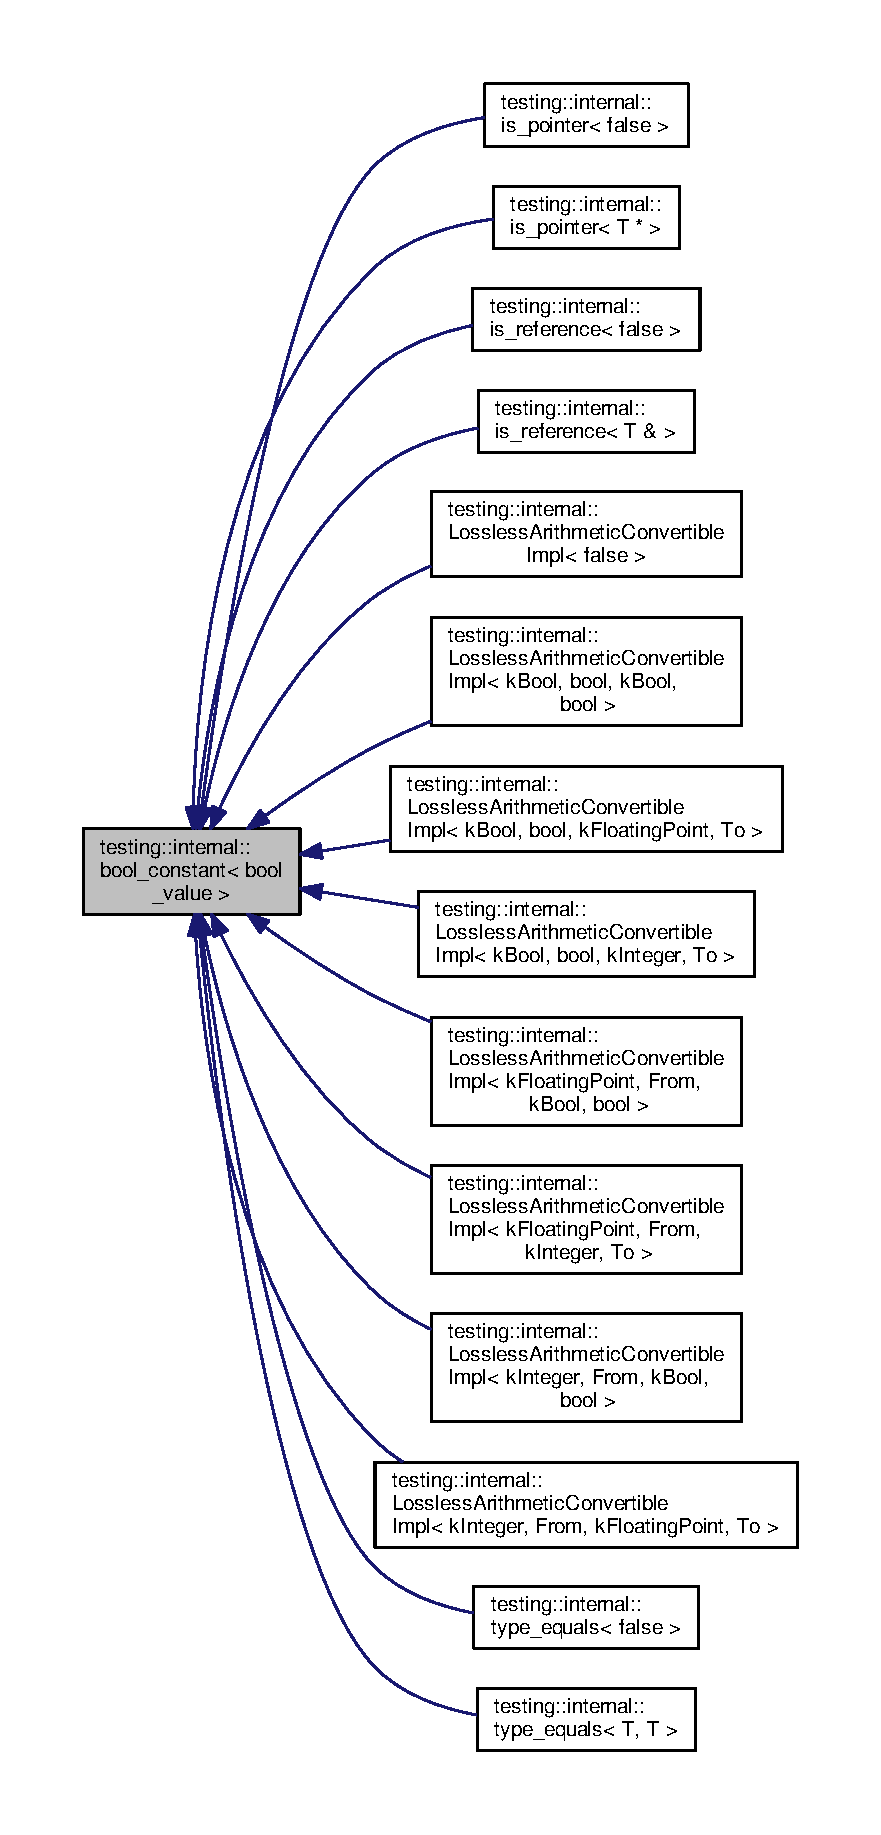
\includegraphics[height=550pt]{structtesting_1_1internal_1_1bool__constant__inherit__graph}
\end{center}
\end{figure}
\subsection*{Public Types}
\begin{DoxyCompactItemize}
\item 
typedef \hyperlink{structtesting_1_1internal_1_1bool__constant}{bool\+\_\+constant}$<$ bool\+\_\+value $>$ \hyperlink{structtesting_1_1internal_1_1bool__constant_aba6d09ecf7eecea6c93480f0d627a167}{type}
\end{DoxyCompactItemize}
\subsection*{Static Public Attributes}
\begin{DoxyCompactItemize}
\item 
static const bool \hyperlink{structtesting_1_1internal_1_1bool__constant_a499fba6576296b04d99690a486424b32}{value} = bool\+\_\+value
\end{DoxyCompactItemize}


\subsection{Member Typedef Documentation}
\index{testing\+::internal\+::bool\+\_\+constant@{testing\+::internal\+::bool\+\_\+constant}!type@{type}}
\index{type@{type}!testing\+::internal\+::bool\+\_\+constant@{testing\+::internal\+::bool\+\_\+constant}}
\subsubsection[{\texorpdfstring{type}{type}}]{\setlength{\rightskip}{0pt plus 5cm}template$<$bool bool\+\_\+value$>$ typedef {\bf bool\+\_\+constant}$<$bool\+\_\+value$>$ {\bf testing\+::internal\+::bool\+\_\+constant}$<$ bool\+\_\+value $>$\+::{\bf type}}\hypertarget{structtesting_1_1internal_1_1bool__constant_aba6d09ecf7eecea6c93480f0d627a167}{}\label{structtesting_1_1internal_1_1bool__constant_aba6d09ecf7eecea6c93480f0d627a167}


\subsection{Member Data Documentation}
\index{testing\+::internal\+::bool\+\_\+constant@{testing\+::internal\+::bool\+\_\+constant}!value@{value}}
\index{value@{value}!testing\+::internal\+::bool\+\_\+constant@{testing\+::internal\+::bool\+\_\+constant}}
\subsubsection[{\texorpdfstring{value}{value}}]{\setlength{\rightskip}{0pt plus 5cm}template$<$bool bool\+\_\+value$>$ const bool {\bf testing\+::internal\+::bool\+\_\+constant}$<$ bool\+\_\+value $>$\+::value = bool\+\_\+value\hspace{0.3cm}{\ttfamily [static]}}\hypertarget{structtesting_1_1internal_1_1bool__constant_a499fba6576296b04d99690a486424b32}{}\label{structtesting_1_1internal_1_1bool__constant_a499fba6576296b04d99690a486424b32}


The documentation for this struct was generated from the following file\+:\begin{DoxyCompactItemize}
\item 
vendor/googletest/googletest/include/gtest/internal/\hyperlink{gtest-port_8h}{gtest-\/port.\+h}\end{DoxyCompactItemize}

\hypertarget{structtesting_1_1internal_1_1BooleanConstant}{}\section{testing\+:\+:internal\+:\+:Boolean\+Constant$<$ k\+Value $>$ Struct Template Reference}
\label{structtesting_1_1internal_1_1BooleanConstant}\index{testing\+::internal\+::\+Boolean\+Constant$<$ k\+Value $>$@{testing\+::internal\+::\+Boolean\+Constant$<$ k\+Value $>$}}


{\ttfamily \#include $<$gmock-\/internal-\/utils.\+h$>$}



The documentation for this struct was generated from the following file\+:\begin{DoxyCompactItemize}
\item 
vendor/googletest/googlemock/include/gmock/internal/\hyperlink{gmock-internal-utils_8h}{gmock-\/internal-\/utils.\+h}\end{DoxyCompactItemize}

\hypertarget{classtesting_1_1gmock__generated__actions__test_1_1BoolResetter}{}\section{testing\+:\+:gmock\+\_\+generated\+\_\+actions\+\_\+test\+:\+:Bool\+Resetter Class Reference}
\label{classtesting_1_1gmock__generated__actions__test_1_1BoolResetter}\index{testing\+::gmock\+\_\+generated\+\_\+actions\+\_\+test\+::\+Bool\+Resetter@{testing\+::gmock\+\_\+generated\+\_\+actions\+\_\+test\+::\+Bool\+Resetter}}
\subsection*{Public Member Functions}
\begin{DoxyCompactItemize}
\item 
\hyperlink{classtesting_1_1gmock__generated__actions__test_1_1BoolResetter_a55776cb9ef3b358e48898bb0257646ea}{Bool\+Resetter} (bool $\ast$value)
\item 
\hyperlink{classtesting_1_1gmock__generated__actions__test_1_1BoolResetter_a814afb883394b0fe7d7c8c1aa22d9cb6}{$\sim$\+Bool\+Resetter} ()
\end{DoxyCompactItemize}


\subsection{Constructor \& Destructor Documentation}
\index{testing\+::gmock\+\_\+generated\+\_\+actions\+\_\+test\+::\+Bool\+Resetter@{testing\+::gmock\+\_\+generated\+\_\+actions\+\_\+test\+::\+Bool\+Resetter}!Bool\+Resetter@{Bool\+Resetter}}
\index{Bool\+Resetter@{Bool\+Resetter}!testing\+::gmock\+\_\+generated\+\_\+actions\+\_\+test\+::\+Bool\+Resetter@{testing\+::gmock\+\_\+generated\+\_\+actions\+\_\+test\+::\+Bool\+Resetter}}
\subsubsection[{\texorpdfstring{Bool\+Resetter(bool $\ast$value)}{BoolResetter(bool *value)}}]{\setlength{\rightskip}{0pt plus 5cm}testing\+::gmock\+\_\+generated\+\_\+actions\+\_\+test\+::\+Bool\+Resetter\+::\+Bool\+Resetter (
\begin{DoxyParamCaption}
\item[{bool $\ast$}]{value}
\end{DoxyParamCaption}
)\hspace{0.3cm}{\ttfamily [inline]}, {\ttfamily [explicit]}}\hypertarget{classtesting_1_1gmock__generated__actions__test_1_1BoolResetter_a55776cb9ef3b358e48898bb0257646ea}{}\label{classtesting_1_1gmock__generated__actions__test_1_1BoolResetter_a55776cb9ef3b358e48898bb0257646ea}

\begin{DoxyCode}
1108 : value\_(value) \{\}
\end{DoxyCode}
\index{testing\+::gmock\+\_\+generated\+\_\+actions\+\_\+test\+::\+Bool\+Resetter@{testing\+::gmock\+\_\+generated\+\_\+actions\+\_\+test\+::\+Bool\+Resetter}!````~Bool\+Resetter@{$\sim$\+Bool\+Resetter}}
\index{````~Bool\+Resetter@{$\sim$\+Bool\+Resetter}!testing\+::gmock\+\_\+generated\+\_\+actions\+\_\+test\+::\+Bool\+Resetter@{testing\+::gmock\+\_\+generated\+\_\+actions\+\_\+test\+::\+Bool\+Resetter}}
\subsubsection[{\texorpdfstring{$\sim$\+Bool\+Resetter()}{~BoolResetter()}}]{\setlength{\rightskip}{0pt plus 5cm}testing\+::gmock\+\_\+generated\+\_\+actions\+\_\+test\+::\+Bool\+Resetter\+::$\sim$\+Bool\+Resetter (
\begin{DoxyParamCaption}
{}
\end{DoxyParamCaption}
)\hspace{0.3cm}{\ttfamily [inline]}}\hypertarget{classtesting_1_1gmock__generated__actions__test_1_1BoolResetter_a814afb883394b0fe7d7c8c1aa22d9cb6}{}\label{classtesting_1_1gmock__generated__actions__test_1_1BoolResetter_a814afb883394b0fe7d7c8c1aa22d9cb6}

\begin{DoxyCode}
1109 \{ *value\_ = \textcolor{keyword}{false}; \}
\end{DoxyCode}


The documentation for this class was generated from the following file\+:\begin{DoxyCompactItemize}
\item 
vendor/googletest/googlemock/test/\hyperlink{gmock-generated-actions__test_8cc}{gmock-\/generated-\/actions\+\_\+test.\+cc}\end{DoxyCompactItemize}

\hypertarget{classtesting_1_1internal_1_1BothOfMatcher}{}\section{testing\+:\+:internal\+:\+:Both\+Of\+Matcher$<$ Matcher1, Matcher2 $>$ Class Template Reference}
\label{classtesting_1_1internal_1_1BothOfMatcher}\index{testing\+::internal\+::\+Both\+Of\+Matcher$<$ Matcher1, Matcher2 $>$@{testing\+::internal\+::\+Both\+Of\+Matcher$<$ Matcher1, Matcher2 $>$}}


{\ttfamily \#include $<$gmock-\/matchers.\+h$>$}

\subsection*{Public Member Functions}
\begin{DoxyCompactItemize}
\item 
\hyperlink{classtesting_1_1internal_1_1BothOfMatcher_ab7941deda1965521f72d58b0dd429d6a}{Both\+Of\+Matcher} (Matcher1 matcher1, Matcher2 matcher2)
\item 
{\footnotesize template$<$typename T $>$ }\\\hyperlink{classtesting_1_1internal_1_1BothOfMatcher_aac6e941d3c89462183f24b974d4d7ca8}{operator Matcher$<$ T $>$} () const 
\end{DoxyCompactItemize}


\subsection{Constructor \& Destructor Documentation}
\index{testing\+::internal\+::\+Both\+Of\+Matcher@{testing\+::internal\+::\+Both\+Of\+Matcher}!Both\+Of\+Matcher@{Both\+Of\+Matcher}}
\index{Both\+Of\+Matcher@{Both\+Of\+Matcher}!testing\+::internal\+::\+Both\+Of\+Matcher@{testing\+::internal\+::\+Both\+Of\+Matcher}}
\subsubsection[{\texorpdfstring{Both\+Of\+Matcher(\+Matcher1 matcher1, Matcher2 matcher2)}{BothOfMatcher(Matcher1 matcher1, Matcher2 matcher2)}}]{\setlength{\rightskip}{0pt plus 5cm}template$<$typename Matcher1 , typename Matcher2 $>$ {\bf testing\+::internal\+::\+Both\+Of\+Matcher}$<$ Matcher1, Matcher2 $>$\+::{\bf Both\+Of\+Matcher} (
\begin{DoxyParamCaption}
\item[{Matcher1}]{matcher1, }
\item[{Matcher2}]{matcher2}
\end{DoxyParamCaption}
)\hspace{0.3cm}{\ttfamily [inline]}}\hypertarget{classtesting_1_1internal_1_1BothOfMatcher_ab7941deda1965521f72d58b0dd429d6a}{}\label{classtesting_1_1internal_1_1BothOfMatcher_ab7941deda1965521f72d58b0dd429d6a}

\begin{DoxyCode}
1641       : matcher1\_(matcher1), matcher2\_(matcher2) \{\}
\end{DoxyCode}


\subsection{Member Function Documentation}
\index{testing\+::internal\+::\+Both\+Of\+Matcher@{testing\+::internal\+::\+Both\+Of\+Matcher}!operator Matcher$<$ T $>$@{operator Matcher$<$ T $>$}}
\index{operator Matcher$<$ T $>$@{operator Matcher$<$ T $>$}!testing\+::internal\+::\+Both\+Of\+Matcher@{testing\+::internal\+::\+Both\+Of\+Matcher}}
\subsubsection[{\texorpdfstring{operator Matcher$<$ T $>$() const }{operator Matcher< T >() const }}]{\setlength{\rightskip}{0pt plus 5cm}template$<$typename Matcher1 , typename Matcher2 $>$ template$<$typename T $>$ {\bf testing\+::internal\+::\+Both\+Of\+Matcher}$<$ Matcher1, Matcher2 $>$\+::operator {\bf Matcher}$<$ T $>$ (
\begin{DoxyParamCaption}
{}
\end{DoxyParamCaption}
) const\hspace{0.3cm}{\ttfamily [inline]}}\hypertarget{classtesting_1_1internal_1_1BothOfMatcher_aac6e941d3c89462183f24b974d4d7ca8}{}\label{classtesting_1_1internal_1_1BothOfMatcher_aac6e941d3c89462183f24b974d4d7ca8}

\begin{DoxyCode}
1647                               \{
1648     \textcolor{keywordflow}{return} Matcher<T>(\textcolor{keyword}{new} BothOfMatcherImpl<T>(SafeMatcherCast<T>(matcher1\_),
1649                                                SafeMatcherCast<T>(matcher2\_)));
1650   \}
\end{DoxyCode}


The documentation for this class was generated from the following file\+:\begin{DoxyCompactItemize}
\item 
vendor/googletest/googlemock/include/gmock/\hyperlink{gmock-matchers_8h}{gmock-\/matchers.\+h}\end{DoxyCompactItemize}

\hypertarget{classtesting_1_1internal_1_1BothOfMatcherImpl}{}\section{testing\+:\+:internal\+:\+:Both\+Of\+Matcher\+Impl$<$ T $>$ Class Template Reference}
\label{classtesting_1_1internal_1_1BothOfMatcherImpl}\index{testing\+::internal\+::\+Both\+Of\+Matcher\+Impl$<$ T $>$@{testing\+::internal\+::\+Both\+Of\+Matcher\+Impl$<$ T $>$}}


{\ttfamily \#include $<$gmock-\/matchers.\+h$>$}



Inheritance diagram for testing\+:\+:internal\+:\+:Both\+Of\+Matcher\+Impl$<$ T $>$\+:
\nopagebreak
\begin{figure}[H]
\begin{center}
\leavevmode
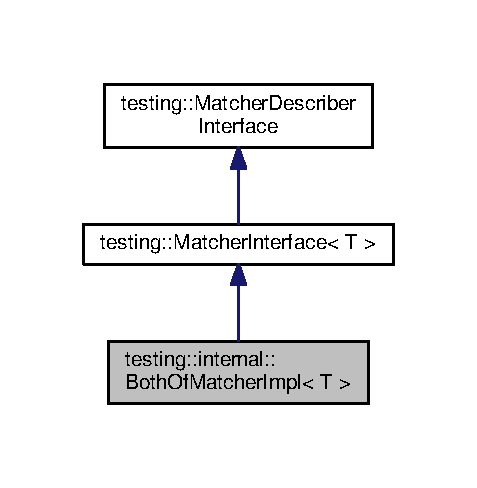
\includegraphics[width=229pt]{classtesting_1_1internal_1_1BothOfMatcherImpl__inherit__graph}
\end{center}
\end{figure}


Collaboration diagram for testing\+:\+:internal\+:\+:Both\+Of\+Matcher\+Impl$<$ T $>$\+:
\nopagebreak
\begin{figure}[H]
\begin{center}
\leavevmode
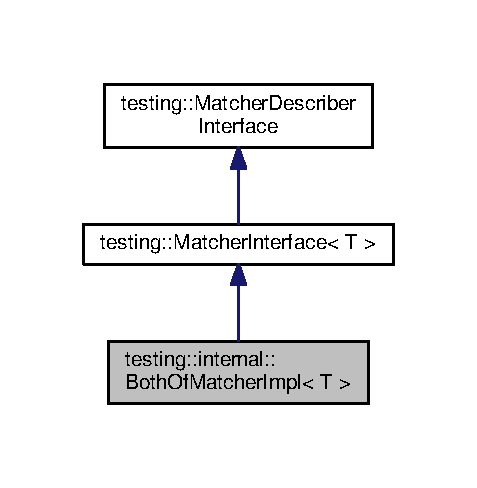
\includegraphics[width=229pt]{classtesting_1_1internal_1_1BothOfMatcherImpl__coll__graph}
\end{center}
\end{figure}
\subsection*{Public Member Functions}
\begin{DoxyCompactItemize}
\item 
\hyperlink{classtesting_1_1internal_1_1BothOfMatcherImpl_a41760fcb35ba18ac2a0eb580ac61ea9a}{Both\+Of\+Matcher\+Impl} (const \hyperlink{classtesting_1_1Matcher}{Matcher}$<$ T $>$ \&matcher1, const \hyperlink{classtesting_1_1Matcher}{Matcher}$<$ T $>$ \&matcher2)
\item 
virtual void \hyperlink{classtesting_1_1internal_1_1BothOfMatcherImpl_a7b808e95bfee6ea6035e8820896d5d32}{Describe\+To} (\+::std\+::ostream $\ast$os) const 
\item 
virtual void \hyperlink{classtesting_1_1internal_1_1BothOfMatcherImpl_a4db4b4119cc2b742e5139922d56e514c}{Describe\+Negation\+To} (\+::std\+::ostream $\ast$os) const 
\item 
virtual bool \hyperlink{classtesting_1_1internal_1_1BothOfMatcherImpl_ad0311a21d4c8231a824a396b9f4d09a1}{Match\+And\+Explain} (T x, \hyperlink{classtesting_1_1MatchResultListener}{Match\+Result\+Listener} $\ast$listener) const 
\end{DoxyCompactItemize}


\subsection{Constructor \& Destructor Documentation}
\index{testing\+::internal\+::\+Both\+Of\+Matcher\+Impl@{testing\+::internal\+::\+Both\+Of\+Matcher\+Impl}!Both\+Of\+Matcher\+Impl@{Both\+Of\+Matcher\+Impl}}
\index{Both\+Of\+Matcher\+Impl@{Both\+Of\+Matcher\+Impl}!testing\+::internal\+::\+Both\+Of\+Matcher\+Impl@{testing\+::internal\+::\+Both\+Of\+Matcher\+Impl}}
\subsubsection[{\texorpdfstring{Both\+Of\+Matcher\+Impl(const Matcher$<$ T $>$ \&matcher1, const Matcher$<$ T $>$ \&matcher2)}{BothOfMatcherImpl(const Matcher< T > &matcher1, const Matcher< T > &matcher2)}}]{\setlength{\rightskip}{0pt plus 5cm}template$<$typename T $>$ {\bf testing\+::internal\+::\+Both\+Of\+Matcher\+Impl}$<$ T $>$\+::{\bf Both\+Of\+Matcher\+Impl} (
\begin{DoxyParamCaption}
\item[{const {\bf Matcher}$<$ T $>$ \&}]{matcher1, }
\item[{const {\bf Matcher}$<$ T $>$ \&}]{matcher2}
\end{DoxyParamCaption}
)\hspace{0.3cm}{\ttfamily [inline]}}\hypertarget{classtesting_1_1internal_1_1BothOfMatcherImpl_a41760fcb35ba18ac2a0eb580ac61ea9a}{}\label{classtesting_1_1internal_1_1BothOfMatcherImpl_a41760fcb35ba18ac2a0eb580ac61ea9a}

\begin{DoxyCode}
1495       : matcher1\_(matcher1), matcher2\_(matcher2) \{\}
\end{DoxyCode}


\subsection{Member Function Documentation}
\index{testing\+::internal\+::\+Both\+Of\+Matcher\+Impl@{testing\+::internal\+::\+Both\+Of\+Matcher\+Impl}!Describe\+Negation\+To@{Describe\+Negation\+To}}
\index{Describe\+Negation\+To@{Describe\+Negation\+To}!testing\+::internal\+::\+Both\+Of\+Matcher\+Impl@{testing\+::internal\+::\+Both\+Of\+Matcher\+Impl}}
\subsubsection[{\texorpdfstring{Describe\+Negation\+To(\+::std\+::ostream $\ast$os) const }{DescribeNegationTo(::std::ostream *os) const }}]{\setlength{\rightskip}{0pt plus 5cm}template$<$typename T $>$ virtual void {\bf testing\+::internal\+::\+Both\+Of\+Matcher\+Impl}$<$ T $>$\+::Describe\+Negation\+To (
\begin{DoxyParamCaption}
\item[{\+::std\+::ostream $\ast$}]{os}
\end{DoxyParamCaption}
) const\hspace{0.3cm}{\ttfamily [inline]}, {\ttfamily [virtual]}}\hypertarget{classtesting_1_1internal_1_1BothOfMatcherImpl_a4db4b4119cc2b742e5139922d56e514c}{}\label{classtesting_1_1internal_1_1BothOfMatcherImpl_a4db4b4119cc2b742e5139922d56e514c}


Reimplemented from \hyperlink{classtesting_1_1MatcherDescriberInterface_a35b9dc2f3e25ca4b903f282feaaf9f8c}{testing\+::\+Matcher\+Describer\+Interface}.


\begin{DoxyCode}
1505                                                         \{
1506     *os << \textcolor{stringliteral}{"("};
1507     matcher1\_.DescribeNegationTo(os);
1508     *os << \textcolor{stringliteral}{") or ("};
1509     matcher2\_.DescribeNegationTo(os);
1510     *os << \textcolor{stringliteral}{")"};
1511   \}
\end{DoxyCode}
\index{testing\+::internal\+::\+Both\+Of\+Matcher\+Impl@{testing\+::internal\+::\+Both\+Of\+Matcher\+Impl}!Describe\+To@{Describe\+To}}
\index{Describe\+To@{Describe\+To}!testing\+::internal\+::\+Both\+Of\+Matcher\+Impl@{testing\+::internal\+::\+Both\+Of\+Matcher\+Impl}}
\subsubsection[{\texorpdfstring{Describe\+To(\+::std\+::ostream $\ast$os) const }{DescribeTo(::std::ostream *os) const }}]{\setlength{\rightskip}{0pt plus 5cm}template$<$typename T $>$ virtual void {\bf testing\+::internal\+::\+Both\+Of\+Matcher\+Impl}$<$ T $>$\+::Describe\+To (
\begin{DoxyParamCaption}
\item[{\+::std\+::ostream $\ast$}]{os}
\end{DoxyParamCaption}
) const\hspace{0.3cm}{\ttfamily [inline]}, {\ttfamily [virtual]}}\hypertarget{classtesting_1_1internal_1_1BothOfMatcherImpl_a7b808e95bfee6ea6035e8820896d5d32}{}\label{classtesting_1_1internal_1_1BothOfMatcherImpl_a7b808e95bfee6ea6035e8820896d5d32}


Implements \hyperlink{classtesting_1_1MatcherDescriberInterface_ad9f861588bd969b6e3e717f13bb94e7b}{testing\+::\+Matcher\+Describer\+Interface}.


\begin{DoxyCode}
1497                                                 \{
1498     *os << \textcolor{stringliteral}{"("};
1499     matcher1\_.DescribeTo(os);
1500     *os << \textcolor{stringliteral}{") and ("};
1501     matcher2\_.DescribeTo(os);
1502     *os << \textcolor{stringliteral}{")"};
1503   \}
\end{DoxyCode}
\index{testing\+::internal\+::\+Both\+Of\+Matcher\+Impl@{testing\+::internal\+::\+Both\+Of\+Matcher\+Impl}!Match\+And\+Explain@{Match\+And\+Explain}}
\index{Match\+And\+Explain@{Match\+And\+Explain}!testing\+::internal\+::\+Both\+Of\+Matcher\+Impl@{testing\+::internal\+::\+Both\+Of\+Matcher\+Impl}}
\subsubsection[{\texorpdfstring{Match\+And\+Explain(\+T x, Match\+Result\+Listener $\ast$listener) const }{MatchAndExplain(T x, MatchResultListener *listener) const }}]{\setlength{\rightskip}{0pt plus 5cm}template$<$typename T $>$ virtual bool {\bf testing\+::internal\+::\+Both\+Of\+Matcher\+Impl}$<$ T $>$\+::Match\+And\+Explain (
\begin{DoxyParamCaption}
\item[{T}]{x, }
\item[{{\bf Match\+Result\+Listener} $\ast$}]{listener}
\end{DoxyParamCaption}
) const\hspace{0.3cm}{\ttfamily [inline]}, {\ttfamily [virtual]}}\hypertarget{classtesting_1_1internal_1_1BothOfMatcherImpl_ad0311a21d4c8231a824a396b9f4d09a1}{}\label{classtesting_1_1internal_1_1BothOfMatcherImpl_ad0311a21d4c8231a824a396b9f4d09a1}


Implements \hyperlink{classtesting_1_1MatcherInterface_a296b43607cd99d60365f0e6a762777cf}{testing\+::\+Matcher\+Interface$<$ T $>$}.


\begin{DoxyCode}
1513                                                                          \{
1514     \textcolor{comment}{// If either matcher1\_ or matcher2\_ doesn't match x, we only need}
1515     \textcolor{comment}{// to explain why one of them fails.}
1516     StringMatchResultListener listener1;
1517     \textcolor{keywordflow}{if} (!matcher1\_.MatchAndExplain(x, &listener1)) \{
1518       *listener << listener1.str();
1519       \textcolor{keywordflow}{return} \textcolor{keyword}{false};
1520     \}
1521 
1522     StringMatchResultListener listener2;
1523     \textcolor{keywordflow}{if} (!matcher2\_.MatchAndExplain(x, &listener2)) \{
1524       *listener << listener2.str();
1525       \textcolor{keywordflow}{return} \textcolor{keyword}{false};
1526     \}
1527 
1528     \textcolor{comment}{// Otherwise we need to explain why *both* of them match.}
1529     \textcolor{keyword}{const} \hyperlink{namespacetesting_1_1internal_a8e8ff5b11e64078831112677156cb111}{internal::string} s1 = listener1.str();
1530     \textcolor{keyword}{const} \hyperlink{namespacetesting_1_1internal_a8e8ff5b11e64078831112677156cb111}{internal::string} s2 = listener2.str();
1531 
1532     \textcolor{keywordflow}{if} (s1 == \textcolor{stringliteral}{""}) \{
1533       *listener << s2;
1534     \} \textcolor{keywordflow}{else} \{
1535       *listener << s1;
1536       \textcolor{keywordflow}{if} (s2 != \textcolor{stringliteral}{""}) \{
1537         *listener << \textcolor{stringliteral}{", and "} << s2;
1538       \}
1539     \}
1540     \textcolor{keywordflow}{return} \textcolor{keyword}{true};
1541   \}
\end{DoxyCode}


The documentation for this class was generated from the following file\+:\begin{DoxyCompactItemize}
\item 
vendor/googletest/googlemock/include/gmock/\hyperlink{gmock-matchers_8h}{gmock-\/matchers.\+h}\end{DoxyCompactItemize}

\hypertarget{classtesting_1_1internal_1_1BoundSecondMatcher}{}\section{testing\+:\+:internal\+:\+:Bound\+Second\+Matcher$<$ Tuple2\+Matcher, Second $>$ Class Template Reference}
\label{classtesting_1_1internal_1_1BoundSecondMatcher}\index{testing\+::internal\+::\+Bound\+Second\+Matcher$<$ Tuple2\+Matcher, Second $>$@{testing\+::internal\+::\+Bound\+Second\+Matcher$<$ Tuple2\+Matcher, Second $>$}}


{\ttfamily \#include $<$gmock-\/matchers.\+h$>$}

\subsection*{Public Member Functions}
\begin{DoxyCompactItemize}
\item 
\hyperlink{classtesting_1_1internal_1_1BoundSecondMatcher_af9d0d4b50a3b9883ff26312922b9f639}{Bound\+Second\+Matcher} (const Tuple2\+Matcher \&tm, const Second \&second)
\item 
{\footnotesize template$<$typename T $>$ }\\\hyperlink{classtesting_1_1internal_1_1BoundSecondMatcher_aebcba80b915b34be2c8d46e12b0b669a}{operator Matcher$<$ T $>$} () const 
\item 
void \hyperlink{classtesting_1_1internal_1_1BoundSecondMatcher_a62f714cb2c7388cb582aaae0110bfe49}{operator=} (const \hyperlink{classtesting_1_1internal_1_1BoundSecondMatcher}{Bound\+Second\+Matcher} \&)
\end{DoxyCompactItemize}


\subsection{Constructor \& Destructor Documentation}
\index{testing\+::internal\+::\+Bound\+Second\+Matcher@{testing\+::internal\+::\+Bound\+Second\+Matcher}!Bound\+Second\+Matcher@{Bound\+Second\+Matcher}}
\index{Bound\+Second\+Matcher@{Bound\+Second\+Matcher}!testing\+::internal\+::\+Bound\+Second\+Matcher@{testing\+::internal\+::\+Bound\+Second\+Matcher}}
\subsubsection[{\texorpdfstring{Bound\+Second\+Matcher(const Tuple2\+Matcher \&tm, const Second \&second)}{BoundSecondMatcher(const Tuple2Matcher &tm, const Second &second)}}]{\setlength{\rightskip}{0pt plus 5cm}template$<$typename Tuple2\+Matcher, typename Second$>$ {\bf testing\+::internal\+::\+Bound\+Second\+Matcher}$<$ Tuple2\+Matcher, Second $>$\+::{\bf Bound\+Second\+Matcher} (
\begin{DoxyParamCaption}
\item[{const Tuple2\+Matcher \&}]{tm, }
\item[{const Second \&}]{second}
\end{DoxyParamCaption}
)\hspace{0.3cm}{\ttfamily [inline]}}\hypertarget{classtesting_1_1internal_1_1BoundSecondMatcher_af9d0d4b50a3b9883ff26312922b9f639}{}\label{classtesting_1_1internal_1_1BoundSecondMatcher_af9d0d4b50a3b9883ff26312922b9f639}

\begin{DoxyCode}
3555       : tuple2\_matcher\_(tm), second\_value\_(second) \{\}
\end{DoxyCode}


\subsection{Member Function Documentation}
\index{testing\+::internal\+::\+Bound\+Second\+Matcher@{testing\+::internal\+::\+Bound\+Second\+Matcher}!operator Matcher$<$ T $>$@{operator Matcher$<$ T $>$}}
\index{operator Matcher$<$ T $>$@{operator Matcher$<$ T $>$}!testing\+::internal\+::\+Bound\+Second\+Matcher@{testing\+::internal\+::\+Bound\+Second\+Matcher}}
\subsubsection[{\texorpdfstring{operator Matcher$<$ T $>$() const }{operator Matcher< T >() const }}]{\setlength{\rightskip}{0pt plus 5cm}template$<$typename Tuple2\+Matcher, typename Second$>$ template$<$typename T $>$ {\bf testing\+::internal\+::\+Bound\+Second\+Matcher}$<$ Tuple2\+Matcher, Second $>$\+::operator {\bf Matcher}$<$ T $>$ (
\begin{DoxyParamCaption}
{}
\end{DoxyParamCaption}
) const\hspace{0.3cm}{\ttfamily [inline]}}\hypertarget{classtesting_1_1internal_1_1BoundSecondMatcher_aebcba80b915b34be2c8d46e12b0b669a}{}\label{classtesting_1_1internal_1_1BoundSecondMatcher_aebcba80b915b34be2c8d46e12b0b669a}

\begin{DoxyCode}
3558                               \{
3559     \textcolor{keywordflow}{return} \hyperlink{namespacetesting_a37fd8029ac00e60952440a3d9cca8166}{MakeMatcher}(\textcolor{keyword}{new} Impl<T>(tuple2\_matcher\_, second\_value\_));
3560   \}
\end{DoxyCode}
\index{testing\+::internal\+::\+Bound\+Second\+Matcher@{testing\+::internal\+::\+Bound\+Second\+Matcher}!operator=@{operator=}}
\index{operator=@{operator=}!testing\+::internal\+::\+Bound\+Second\+Matcher@{testing\+::internal\+::\+Bound\+Second\+Matcher}}
\subsubsection[{\texorpdfstring{operator=(const Bound\+Second\+Matcher \&)}{operator=(const BoundSecondMatcher &)}}]{\setlength{\rightskip}{0pt plus 5cm}template$<$typename Tuple2\+Matcher, typename Second$>$ void {\bf testing\+::internal\+::\+Bound\+Second\+Matcher}$<$ Tuple2\+Matcher, Second $>$\+::operator= (
\begin{DoxyParamCaption}
\item[{const {\bf Bound\+Second\+Matcher}$<$ Tuple2\+Matcher, Second $>$ \&}]{}
\end{DoxyParamCaption}
)\hspace{0.3cm}{\ttfamily [inline]}}\hypertarget{classtesting_1_1internal_1_1BoundSecondMatcher_a62f714cb2c7388cb582aaae0110bfe49}{}\label{classtesting_1_1internal_1_1BoundSecondMatcher_a62f714cb2c7388cb582aaae0110bfe49}

\begin{DoxyCode}
3570                                               \{
3571     \hyperlink{gtest-port_8h_a8ef4cb4c465db8c15464aecc6d9510ef}{GTEST\_LOG\_}(FATAL) << \textcolor{stringliteral}{"BoundSecondMatcher should never be assigned."};
3572   \}
\end{DoxyCode}


The documentation for this class was generated from the following file\+:\begin{DoxyCompactItemize}
\item 
vendor/googletest/googlemock/include/gmock/\hyperlink{gmock-matchers_8h}{gmock-\/matchers.\+h}\end{DoxyCompactItemize}

\hypertarget{classtesting_1_1internal_1_1BuiltInDefaultValue}{}\section{testing\+:\+:internal\+:\+:Built\+In\+Default\+Value$<$ T $>$ Class Template Reference}
\label{classtesting_1_1internal_1_1BuiltInDefaultValue}\index{testing\+::internal\+::\+Built\+In\+Default\+Value$<$ T $>$@{testing\+::internal\+::\+Built\+In\+Default\+Value$<$ T $>$}}


{\ttfamily \#include $<$gmock-\/actions.\+h$>$}

\subsection*{Static Public Member Functions}
\begin{DoxyCompactItemize}
\item 
static bool \hyperlink{classtesting_1_1internal_1_1BuiltInDefaultValue_a35207bc20a493b0efb3980eb9a08dd2f}{Exists} ()
\item 
static T \hyperlink{classtesting_1_1internal_1_1BuiltInDefaultValue_a7e26c1df14a887c8f393b29d6ea162e6}{Get} ()
\end{DoxyCompactItemize}


\subsection{Member Function Documentation}
\index{testing\+::internal\+::\+Built\+In\+Default\+Value@{testing\+::internal\+::\+Built\+In\+Default\+Value}!Exists@{Exists}}
\index{Exists@{Exists}!testing\+::internal\+::\+Built\+In\+Default\+Value@{testing\+::internal\+::\+Built\+In\+Default\+Value}}
\subsubsection[{\texorpdfstring{Exists()}{Exists()}}]{\setlength{\rightskip}{0pt plus 5cm}template$<$typename T $>$ static bool {\bf testing\+::internal\+::\+Built\+In\+Default\+Value}$<$ T $>$\+::Exists (
\begin{DoxyParamCaption}
{}
\end{DoxyParamCaption}
)\hspace{0.3cm}{\ttfamily [inline]}, {\ttfamily [static]}}\hypertarget{classtesting_1_1internal_1_1BuiltInDefaultValue_a35207bc20a493b0efb3980eb9a08dd2f}{}\label{classtesting_1_1internal_1_1BuiltInDefaultValue_a35207bc20a493b0efb3980eb9a08dd2f}

\begin{DoxyCode}
112                        \{
113     \textcolor{keywordflow}{return} \textcolor{keyword}{false};
114   \}
\end{DoxyCode}
\index{testing\+::internal\+::\+Built\+In\+Default\+Value@{testing\+::internal\+::\+Built\+In\+Default\+Value}!Get@{Get}}
\index{Get@{Get}!testing\+::internal\+::\+Built\+In\+Default\+Value@{testing\+::internal\+::\+Built\+In\+Default\+Value}}
\subsubsection[{\texorpdfstring{Get()}{Get()}}]{\setlength{\rightskip}{0pt plus 5cm}template$<$typename T $>$ static T {\bf testing\+::internal\+::\+Built\+In\+Default\+Value}$<$ T $>$\+::Get (
\begin{DoxyParamCaption}
{}
\end{DoxyParamCaption}
)\hspace{0.3cm}{\ttfamily [inline]}, {\ttfamily [static]}}\hypertarget{classtesting_1_1internal_1_1BuiltInDefaultValue_a7e26c1df14a887c8f393b29d6ea162e6}{}\label{classtesting_1_1internal_1_1BuiltInDefaultValue_a7e26c1df14a887c8f393b29d6ea162e6}

\begin{DoxyCode}
116                  \{
117     \textcolor{keywordflow}{return} \hyperlink{structtesting_1_1internal_1_1BuiltInDefaultValueGetter_a61c47c50cdb6ab488dabe2cec3b97fc8}{BuiltInDefaultValueGetter<T, false>::Get}();
118   \}
\end{DoxyCode}


The documentation for this class was generated from the following file\+:\begin{DoxyCompactItemize}
\item 
vendor/googletest/googlemock/include/gmock/\hyperlink{gmock-actions_8h}{gmock-\/actions.\+h}\end{DoxyCompactItemize}

\hypertarget{classtesting_1_1internal_1_1BuiltInDefaultValue_3_01const_01T_01_4}{}\section{testing\+:\+:internal\+:\+:Built\+In\+Default\+Value$<$ const T $>$ Class Template Reference}
\label{classtesting_1_1internal_1_1BuiltInDefaultValue_3_01const_01T_01_4}\index{testing\+::internal\+::\+Built\+In\+Default\+Value$<$ const T $>$@{testing\+::internal\+::\+Built\+In\+Default\+Value$<$ const T $>$}}


{\ttfamily \#include $<$gmock-\/actions.\+h$>$}

\subsection*{Static Public Member Functions}
\begin{DoxyCompactItemize}
\item 
static bool \hyperlink{classtesting_1_1internal_1_1BuiltInDefaultValue_3_01const_01T_01_4_a1814803ec5dcc660ee1f1092a96b79fa}{Exists} ()
\item 
static T \hyperlink{classtesting_1_1internal_1_1BuiltInDefaultValue_3_01const_01T_01_4_a5996754952ecbcc5da77a2cebd4722de}{Get} ()
\end{DoxyCompactItemize}


\subsection{Member Function Documentation}
\index{testing\+::internal\+::\+Built\+In\+Default\+Value$<$ const T $>$@{testing\+::internal\+::\+Built\+In\+Default\+Value$<$ const T $>$}!Exists@{Exists}}
\index{Exists@{Exists}!testing\+::internal\+::\+Built\+In\+Default\+Value$<$ const T $>$@{testing\+::internal\+::\+Built\+In\+Default\+Value$<$ const T $>$}}
\subsubsection[{\texorpdfstring{Exists()}{Exists()}}]{\setlength{\rightskip}{0pt plus 5cm}template$<$typename T $>$ static bool {\bf testing\+::internal\+::\+Built\+In\+Default\+Value}$<$ const T $>$\+::Exists (
\begin{DoxyParamCaption}
{}
\end{DoxyParamCaption}
)\hspace{0.3cm}{\ttfamily [inline]}, {\ttfamily [static]}}\hypertarget{classtesting_1_1internal_1_1BuiltInDefaultValue_3_01const_01T_01_4_a1814803ec5dcc660ee1f1092a96b79fa}{}\label{classtesting_1_1internal_1_1BuiltInDefaultValue_3_01const_01T_01_4_a1814803ec5dcc660ee1f1092a96b79fa}

\begin{DoxyCode}
128 \{ \textcolor{keywordflow}{return} \hyperlink{classtesting_1_1internal_1_1BuiltInDefaultValue_a35207bc20a493b0efb3980eb9a08dd2f}{BuiltInDefaultValue<T>::Exists}(); \}
\end{DoxyCode}
\index{testing\+::internal\+::\+Built\+In\+Default\+Value$<$ const T $>$@{testing\+::internal\+::\+Built\+In\+Default\+Value$<$ const T $>$}!Get@{Get}}
\index{Get@{Get}!testing\+::internal\+::\+Built\+In\+Default\+Value$<$ const T $>$@{testing\+::internal\+::\+Built\+In\+Default\+Value$<$ const T $>$}}
\subsubsection[{\texorpdfstring{Get()}{Get()}}]{\setlength{\rightskip}{0pt plus 5cm}template$<$typename T $>$ static T {\bf testing\+::internal\+::\+Built\+In\+Default\+Value}$<$ const T $>$\+::Get (
\begin{DoxyParamCaption}
{}
\end{DoxyParamCaption}
)\hspace{0.3cm}{\ttfamily [inline]}, {\ttfamily [static]}}\hypertarget{classtesting_1_1internal_1_1BuiltInDefaultValue_3_01const_01T_01_4_a5996754952ecbcc5da77a2cebd4722de}{}\label{classtesting_1_1internal_1_1BuiltInDefaultValue_3_01const_01T_01_4_a5996754952ecbcc5da77a2cebd4722de}

\begin{DoxyCode}
129 \{ \textcolor{keywordflow}{return} \hyperlink{classtesting_1_1internal_1_1BuiltInDefaultValue_a7e26c1df14a887c8f393b29d6ea162e6}{BuiltInDefaultValue<T>::Get}(); \}
\end{DoxyCode}


The documentation for this class was generated from the following file\+:\begin{DoxyCompactItemize}
\item 
vendor/googletest/googlemock/include/gmock/\hyperlink{gmock-actions_8h}{gmock-\/actions.\+h}\end{DoxyCompactItemize}

\hypertarget{classtesting_1_1internal_1_1BuiltInDefaultValue_3_01T_01_5_01_4}{}\section{testing\+:\+:internal\+:\+:Built\+In\+Default\+Value$<$ T $\ast$ $>$ Class Template Reference}
\label{classtesting_1_1internal_1_1BuiltInDefaultValue_3_01T_01_5_01_4}\index{testing\+::internal\+::\+Built\+In\+Default\+Value$<$ T $\ast$ $>$@{testing\+::internal\+::\+Built\+In\+Default\+Value$<$ T $\ast$ $>$}}


{\ttfamily \#include $<$gmock-\/actions.\+h$>$}

\subsection*{Static Public Member Functions}
\begin{DoxyCompactItemize}
\item 
static bool \hyperlink{classtesting_1_1internal_1_1BuiltInDefaultValue_3_01T_01_5_01_4_aafa7172f63d068305fb37d5db40bb543}{Exists} ()
\item 
static T $\ast$ \hyperlink{classtesting_1_1internal_1_1BuiltInDefaultValue_3_01T_01_5_01_4_adc2fa2bdae767589d171ae3a117e3a9f}{Get} ()
\end{DoxyCompactItemize}


\subsection{Member Function Documentation}
\index{testing\+::internal\+::\+Built\+In\+Default\+Value$<$ T $\ast$ $>$@{testing\+::internal\+::\+Built\+In\+Default\+Value$<$ T $\ast$ $>$}!Exists@{Exists}}
\index{Exists@{Exists}!testing\+::internal\+::\+Built\+In\+Default\+Value$<$ T $\ast$ $>$@{testing\+::internal\+::\+Built\+In\+Default\+Value$<$ T $\ast$ $>$}}
\subsubsection[{\texorpdfstring{Exists()}{Exists()}}]{\setlength{\rightskip}{0pt plus 5cm}template$<$typename T $>$ static bool {\bf testing\+::internal\+::\+Built\+In\+Default\+Value}$<$ T $\ast$ $>$\+::Exists (
\begin{DoxyParamCaption}
{}
\end{DoxyParamCaption}
)\hspace{0.3cm}{\ttfamily [inline]}, {\ttfamily [static]}}\hypertarget{classtesting_1_1internal_1_1BuiltInDefaultValue_3_01T_01_5_01_4_aafa7172f63d068305fb37d5db40bb543}{}\label{classtesting_1_1internal_1_1BuiltInDefaultValue_3_01T_01_5_01_4_aafa7172f63d068305fb37d5db40bb543}

\begin{DoxyCode}
137 \{ \textcolor{keywordflow}{return} \textcolor{keyword}{true}; \}
\end{DoxyCode}
\index{testing\+::internal\+::\+Built\+In\+Default\+Value$<$ T $\ast$ $>$@{testing\+::internal\+::\+Built\+In\+Default\+Value$<$ T $\ast$ $>$}!Get@{Get}}
\index{Get@{Get}!testing\+::internal\+::\+Built\+In\+Default\+Value$<$ T $\ast$ $>$@{testing\+::internal\+::\+Built\+In\+Default\+Value$<$ T $\ast$ $>$}}
\subsubsection[{\texorpdfstring{Get()}{Get()}}]{\setlength{\rightskip}{0pt plus 5cm}template$<$typename T $>$ static T$\ast$ {\bf testing\+::internal\+::\+Built\+In\+Default\+Value}$<$ T $\ast$ $>$\+::Get (
\begin{DoxyParamCaption}
{}
\end{DoxyParamCaption}
)\hspace{0.3cm}{\ttfamily [inline]}, {\ttfamily [static]}}\hypertarget{classtesting_1_1internal_1_1BuiltInDefaultValue_3_01T_01_5_01_4_adc2fa2bdae767589d171ae3a117e3a9f}{}\label{classtesting_1_1internal_1_1BuiltInDefaultValue_3_01T_01_5_01_4_adc2fa2bdae767589d171ae3a117e3a9f}

\begin{DoxyCode}
138 \{ \textcolor{keywordflow}{return} NULL; \}
\end{DoxyCode}


The documentation for this class was generated from the following file\+:\begin{DoxyCompactItemize}
\item 
vendor/googletest/googlemock/include/gmock/\hyperlink{gmock-actions_8h}{gmock-\/actions.\+h}\end{DoxyCompactItemize}

\hypertarget{structtesting_1_1internal_1_1BuiltInDefaultValueGetter}{}\section{testing\+:\+:internal\+:\+:Built\+In\+Default\+Value\+Getter$<$ T, k\+Default\+Constructible $>$ Struct Template Reference}
\label{structtesting_1_1internal_1_1BuiltInDefaultValueGetter}\index{testing\+::internal\+::\+Built\+In\+Default\+Value\+Getter$<$ T, k\+Default\+Constructible $>$@{testing\+::internal\+::\+Built\+In\+Default\+Value\+Getter$<$ T, k\+Default\+Constructible $>$}}


{\ttfamily \#include $<$gmock-\/actions.\+h$>$}

\subsection*{Static Public Member Functions}
\begin{DoxyCompactItemize}
\item 
static T \hyperlink{structtesting_1_1internal_1_1BuiltInDefaultValueGetter_a61c47c50cdb6ab488dabe2cec3b97fc8}{Get} ()
\end{DoxyCompactItemize}


\subsection{Member Function Documentation}
\index{testing\+::internal\+::\+Built\+In\+Default\+Value\+Getter@{testing\+::internal\+::\+Built\+In\+Default\+Value\+Getter}!Get@{Get}}
\index{Get@{Get}!testing\+::internal\+::\+Built\+In\+Default\+Value\+Getter@{testing\+::internal\+::\+Built\+In\+Default\+Value\+Getter}}
\subsubsection[{\texorpdfstring{Get()}{Get()}}]{\setlength{\rightskip}{0pt plus 5cm}template$<$typename T , bool k\+Default\+Constructible$>$ static T {\bf testing\+::internal\+::\+Built\+In\+Default\+Value\+Getter}$<$ T, k\+Default\+Constructible $>$\+::Get (
\begin{DoxyParamCaption}
{}
\end{DoxyParamCaption}
)\hspace{0.3cm}{\ttfamily [inline]}, {\ttfamily [static]}}\hypertarget{structtesting_1_1internal_1_1BuiltInDefaultValueGetter_a61c47c50cdb6ab488dabe2cec3b97fc8}{}\label{structtesting_1_1internal_1_1BuiltInDefaultValueGetter_a61c47c50cdb6ab488dabe2cec3b97fc8}

\begin{DoxyCode}
76 \{ \textcolor{keywordflow}{return} T(); \}
\end{DoxyCode}


The documentation for this struct was generated from the following file\+:\begin{DoxyCompactItemize}
\item 
vendor/googletest/googlemock/include/gmock/\hyperlink{gmock-actions_8h}{gmock-\/actions.\+h}\end{DoxyCompactItemize}

\hypertarget{structtesting_1_1internal_1_1BuiltInDefaultValueGetter_3_01T_00_01false_01_4}{}\section{testing\+:\+:internal\+:\+:Built\+In\+Default\+Value\+Getter$<$ T, false $>$ Struct Template Reference}
\label{structtesting_1_1internal_1_1BuiltInDefaultValueGetter_3_01T_00_01false_01_4}\index{testing\+::internal\+::\+Built\+In\+Default\+Value\+Getter$<$ T, false $>$@{testing\+::internal\+::\+Built\+In\+Default\+Value\+Getter$<$ T, false $>$}}


{\ttfamily \#include $<$gmock-\/actions.\+h$>$}

\subsection*{Static Public Member Functions}
\begin{DoxyCompactItemize}
\item 
static T \hyperlink{structtesting_1_1internal_1_1BuiltInDefaultValueGetter_3_01T_00_01false_01_4_a8c8e929666f61272961eea21a60de4ad}{Get} ()
\end{DoxyCompactItemize}


\subsection{Member Function Documentation}
\index{testing\+::internal\+::\+Built\+In\+Default\+Value\+Getter$<$ T, false $>$@{testing\+::internal\+::\+Built\+In\+Default\+Value\+Getter$<$ T, false $>$}!Get@{Get}}
\index{Get@{Get}!testing\+::internal\+::\+Built\+In\+Default\+Value\+Getter$<$ T, false $>$@{testing\+::internal\+::\+Built\+In\+Default\+Value\+Getter$<$ T, false $>$}}
\subsubsection[{\texorpdfstring{Get()}{Get()}}]{\setlength{\rightskip}{0pt plus 5cm}template$<$typename T $>$ static T {\bf testing\+::internal\+::\+Built\+In\+Default\+Value\+Getter}$<$ T, false $>$\+::Get (
\begin{DoxyParamCaption}
{}
\end{DoxyParamCaption}
)\hspace{0.3cm}{\ttfamily [inline]}, {\ttfamily [static]}}\hypertarget{structtesting_1_1internal_1_1BuiltInDefaultValueGetter_3_01T_00_01false_01_4_a8c8e929666f61272961eea21a60de4ad}{}\label{structtesting_1_1internal_1_1BuiltInDefaultValueGetter_3_01T_00_01false_01_4_a8c8e929666f61272961eea21a60de4ad}

\begin{DoxyCode}
80                  \{
81     \hyperlink{namespacetesting_1_1internal_a7a259643b7f2d23ce2b757728df42c99}{Assert}(\textcolor{keyword}{false}, \_\_FILE\_\_, \_\_LINE\_\_,
82            \textcolor{stringliteral}{"Default action undefined for the function return type."});
83     \textcolor{keywordflow}{return} internal::Invalid<T>();
84     \textcolor{comment}{// The above statement will never be reached, but is required in}
85     \textcolor{comment}{// order for this function to compile.}
86   \}
\end{DoxyCode}


The documentation for this struct was generated from the following file\+:\begin{DoxyCompactItemize}
\item 
vendor/googletest/googlemock/include/gmock/\hyperlink{gmock-actions_8h}{gmock-\/actions.\+h}\end{DoxyCompactItemize}

\hypertarget{structtesting_1_1internal_1_1ByMoveWrapper}{}\section{testing\+:\+:internal\+:\+:By\+Move\+Wrapper$<$ T $>$ Struct Template Reference}
\label{structtesting_1_1internal_1_1ByMoveWrapper}\index{testing\+::internal\+::\+By\+Move\+Wrapper$<$ T $>$@{testing\+::internal\+::\+By\+Move\+Wrapper$<$ T $>$}}


{\ttfamily \#include $<$gmock-\/actions.\+h$>$}

\subsection*{Public Member Functions}
\begin{DoxyCompactItemize}
\item 
\hyperlink{structtesting_1_1internal_1_1ByMoveWrapper_a60df33395785e0bfc5f72fba32376349}{By\+Move\+Wrapper} (T value)
\end{DoxyCompactItemize}
\subsection*{Public Attributes}
\begin{DoxyCompactItemize}
\item 
T \hyperlink{structtesting_1_1internal_1_1ByMoveWrapper_ae8407b1ae99db3f00797d68b9ee9e870}{payload}
\end{DoxyCompactItemize}


\subsection{Constructor \& Destructor Documentation}
\index{testing\+::internal\+::\+By\+Move\+Wrapper@{testing\+::internal\+::\+By\+Move\+Wrapper}!By\+Move\+Wrapper@{By\+Move\+Wrapper}}
\index{By\+Move\+Wrapper@{By\+Move\+Wrapper}!testing\+::internal\+::\+By\+Move\+Wrapper@{testing\+::internal\+::\+By\+Move\+Wrapper}}
\subsubsection[{\texorpdfstring{By\+Move\+Wrapper(\+T value)}{ByMoveWrapper(T value)}}]{\setlength{\rightskip}{0pt plus 5cm}template$<$typename T $>$ {\bf testing\+::internal\+::\+By\+Move\+Wrapper}$<$ T $>$\+::{\bf By\+Move\+Wrapper} (
\begin{DoxyParamCaption}
\item[{T}]{value}
\end{DoxyParamCaption}
)\hspace{0.3cm}{\ttfamily [inline]}, {\ttfamily [explicit]}}\hypertarget{structtesting_1_1internal_1_1ByMoveWrapper_a60df33395785e0bfc5f72fba32376349}{}\label{structtesting_1_1internal_1_1ByMoveWrapper_a60df33395785e0bfc5f72fba32376349}

\begin{DoxyCode}
505 : \hyperlink{structtesting_1_1internal_1_1ByMoveWrapper_ae8407b1ae99db3f00797d68b9ee9e870}{payload}(\hyperlink{namespacetesting_1_1internal_a0f6d06bf8c3093b9c22bb08723db201e}{internal::move}(value)) \{\}
\end{DoxyCode}


\subsection{Member Data Documentation}
\index{testing\+::internal\+::\+By\+Move\+Wrapper@{testing\+::internal\+::\+By\+Move\+Wrapper}!payload@{payload}}
\index{payload@{payload}!testing\+::internal\+::\+By\+Move\+Wrapper@{testing\+::internal\+::\+By\+Move\+Wrapper}}
\subsubsection[{\texorpdfstring{payload}{payload}}]{\setlength{\rightskip}{0pt plus 5cm}template$<$typename T $>$ T {\bf testing\+::internal\+::\+By\+Move\+Wrapper}$<$ T $>$\+::payload}\hypertarget{structtesting_1_1internal_1_1ByMoveWrapper_ae8407b1ae99db3f00797d68b9ee9e870}{}\label{structtesting_1_1internal_1_1ByMoveWrapper_ae8407b1ae99db3f00797d68b9ee9e870}


The documentation for this struct was generated from the following file\+:\begin{DoxyCompactItemize}
\item 
vendor/googletest/googlemock/include/gmock/\hyperlink{gmock-actions_8h}{gmock-\/actions.\+h}\end{DoxyCompactItemize}

\hypertarget{structstd_1_1tr1_1_1gtest__internal_1_1ByRef}{}\section{std\+:\+:tr1\+:\+:gtest\+\_\+internal\+:\+:By\+Ref$<$ T $>$ Struct Template Reference}
\label{structstd_1_1tr1_1_1gtest__internal_1_1ByRef}\index{std\+::tr1\+::gtest\+\_\+internal\+::\+By\+Ref$<$ T $>$@{std\+::tr1\+::gtest\+\_\+internal\+::\+By\+Ref$<$ T $>$}}


{\ttfamily \#include $<$gtest-\/tuple.\+h$>$}

\subsection*{Public Types}
\begin{DoxyCompactItemize}
\item 
typedef const T \& \hyperlink{structstd_1_1tr1_1_1gtest__internal_1_1ByRef_ac42ad942ee1cfa86b2abcce9b88ac10e}{type}
\end{DoxyCompactItemize}


\subsection{Member Typedef Documentation}
\index{std\+::tr1\+::gtest\+\_\+internal\+::\+By\+Ref@{std\+::tr1\+::gtest\+\_\+internal\+::\+By\+Ref}!type@{type}}
\index{type@{type}!std\+::tr1\+::gtest\+\_\+internal\+::\+By\+Ref@{std\+::tr1\+::gtest\+\_\+internal\+::\+By\+Ref}}
\subsubsection[{\texorpdfstring{type}{type}}]{\setlength{\rightskip}{0pt plus 5cm}template$<$typename T $>$ typedef const T\& {\bf std\+::tr1\+::gtest\+\_\+internal\+::\+By\+Ref}$<$ T $>$\+::{\bf type}}\hypertarget{structstd_1_1tr1_1_1gtest__internal_1_1ByRef_ac42ad942ee1cfa86b2abcce9b88ac10e}{}\label{structstd_1_1tr1_1_1gtest__internal_1_1ByRef_ac42ad942ee1cfa86b2abcce9b88ac10e}


The documentation for this struct was generated from the following file\+:\begin{DoxyCompactItemize}
\item 
vendor/googletest/googletest/include/gtest/internal/\hyperlink{gtest-tuple_8h}{gtest-\/tuple.\+h}\end{DoxyCompactItemize}

\hypertarget{structstd_1_1tr1_1_1gtest__internal_1_1ByRef_3_01T_01_6_01_4}{}\section{std\+:\+:tr1\+:\+:gtest\+\_\+internal\+:\+:By\+Ref$<$ T \& $>$ Struct Template Reference}
\label{structstd_1_1tr1_1_1gtest__internal_1_1ByRef_3_01T_01_6_01_4}\index{std\+::tr1\+::gtest\+\_\+internal\+::\+By\+Ref$<$ T \& $>$@{std\+::tr1\+::gtest\+\_\+internal\+::\+By\+Ref$<$ T \& $>$}}


{\ttfamily \#include $<$gtest-\/tuple.\+h$>$}

\subsection*{Public Types}
\begin{DoxyCompactItemize}
\item 
typedef T \& \hyperlink{structstd_1_1tr1_1_1gtest__internal_1_1ByRef_3_01T_01_6_01_4_a512382574dbdd736320d68e313801122}{type}
\end{DoxyCompactItemize}


\subsection{Member Typedef Documentation}
\index{std\+::tr1\+::gtest\+\_\+internal\+::\+By\+Ref$<$ T \& $>$@{std\+::tr1\+::gtest\+\_\+internal\+::\+By\+Ref$<$ T \& $>$}!type@{type}}
\index{type@{type}!std\+::tr1\+::gtest\+\_\+internal\+::\+By\+Ref$<$ T \& $>$@{std\+::tr1\+::gtest\+\_\+internal\+::\+By\+Ref$<$ T \& $>$}}
\subsubsection[{\texorpdfstring{type}{type}}]{\setlength{\rightskip}{0pt plus 5cm}template$<$typename T $>$ typedef T\& {\bf std\+::tr1\+::gtest\+\_\+internal\+::\+By\+Ref}$<$ T \& $>$\+::{\bf type}}\hypertarget{structstd_1_1tr1_1_1gtest__internal_1_1ByRef_3_01T_01_6_01_4_a512382574dbdd736320d68e313801122}{}\label{structstd_1_1tr1_1_1gtest__internal_1_1ByRef_3_01T_01_6_01_4_a512382574dbdd736320d68e313801122}


The documentation for this struct was generated from the following file\+:\begin{DoxyCompactItemize}
\item 
vendor/googletest/googletest/include/gtest/internal/\hyperlink{gtest-tuple_8h}{gtest-\/tuple.\+h}\end{DoxyCompactItemize}

\hypertarget{structtesting_1_1internal_1_1CallableTraits}{}\section{testing\+:\+:internal\+:\+:Callable\+Traits$<$ Functor $>$ Struct Template Reference}
\label{structtesting_1_1internal_1_1CallableTraits}\index{testing\+::internal\+::\+Callable\+Traits$<$ Functor $>$@{testing\+::internal\+::\+Callable\+Traits$<$ Functor $>$}}


{\ttfamily \#include $<$gmock-\/matchers.\+h$>$}

\subsection*{Public Types}
\begin{DoxyCompactItemize}
\item 
typedef Functor\+::result\+\_\+type \hyperlink{structtesting_1_1internal_1_1CallableTraits_a242d198dd1c56a153ba931d7166ec7f3}{Result\+Type}
\item 
typedef Functor \hyperlink{structtesting_1_1internal_1_1CallableTraits_a23cc0c86a3bd18b2f8dd159dd44e1168}{Storage\+Type}
\end{DoxyCompactItemize}
\subsection*{Static Public Member Functions}
\begin{DoxyCompactItemize}
\item 
static void \hyperlink{structtesting_1_1internal_1_1CallableTraits_ab09a6487235947ec9c5d933d07ac605b}{Check\+Is\+Valid} (Functor)
\item 
{\footnotesize template$<$typename T $>$ }\\static \hyperlink{structtesting_1_1internal_1_1CallableTraits_a242d198dd1c56a153ba931d7166ec7f3}{Result\+Type} \hyperlink{structtesting_1_1internal_1_1CallableTraits_ad54471cad61aefbe15de330867ff5936}{Invoke} (Functor f, T arg)
\end{DoxyCompactItemize}


\subsection{Member Typedef Documentation}
\index{testing\+::internal\+::\+Callable\+Traits@{testing\+::internal\+::\+Callable\+Traits}!Result\+Type@{Result\+Type}}
\index{Result\+Type@{Result\+Type}!testing\+::internal\+::\+Callable\+Traits@{testing\+::internal\+::\+Callable\+Traits}}
\subsubsection[{\texorpdfstring{Result\+Type}{ResultType}}]{\setlength{\rightskip}{0pt plus 5cm}template$<$typename Functor$>$ typedef Functor\+::result\+\_\+type {\bf testing\+::internal\+::\+Callable\+Traits}$<$ Functor $>$\+::{\bf Result\+Type}}\hypertarget{structtesting_1_1internal_1_1CallableTraits_a242d198dd1c56a153ba931d7166ec7f3}{}\label{structtesting_1_1internal_1_1CallableTraits_a242d198dd1c56a153ba931d7166ec7f3}
\index{testing\+::internal\+::\+Callable\+Traits@{testing\+::internal\+::\+Callable\+Traits}!Storage\+Type@{Storage\+Type}}
\index{Storage\+Type@{Storage\+Type}!testing\+::internal\+::\+Callable\+Traits@{testing\+::internal\+::\+Callable\+Traits}}
\subsubsection[{\texorpdfstring{Storage\+Type}{StorageType}}]{\setlength{\rightskip}{0pt plus 5cm}template$<$typename Functor$>$ typedef Functor {\bf testing\+::internal\+::\+Callable\+Traits}$<$ Functor $>$\+::{\bf Storage\+Type}}\hypertarget{structtesting_1_1internal_1_1CallableTraits_a23cc0c86a3bd18b2f8dd159dd44e1168}{}\label{structtesting_1_1internal_1_1CallableTraits_a23cc0c86a3bd18b2f8dd159dd44e1168}


\subsection{Member Function Documentation}
\index{testing\+::internal\+::\+Callable\+Traits@{testing\+::internal\+::\+Callable\+Traits}!Check\+Is\+Valid@{Check\+Is\+Valid}}
\index{Check\+Is\+Valid@{Check\+Is\+Valid}!testing\+::internal\+::\+Callable\+Traits@{testing\+::internal\+::\+Callable\+Traits}}
\subsubsection[{\texorpdfstring{Check\+Is\+Valid(\+Functor)}{CheckIsValid(Functor)}}]{\setlength{\rightskip}{0pt plus 5cm}template$<$typename Functor$>$ static void {\bf testing\+::internal\+::\+Callable\+Traits}$<$ Functor $>$\+::Check\+Is\+Valid (
\begin{DoxyParamCaption}
\item[{Functor}]{}
\end{DoxyParamCaption}
)\hspace{0.3cm}{\ttfamily [inline]}, {\ttfamily [static]}}\hypertarget{structtesting_1_1internal_1_1CallableTraits_ab09a6487235947ec9c5d933d07ac605b}{}\label{structtesting_1_1internal_1_1CallableTraits_ab09a6487235947ec9c5d933d07ac605b}

\begin{DoxyCode}
2313 \{\}
\end{DoxyCode}
\index{testing\+::internal\+::\+Callable\+Traits@{testing\+::internal\+::\+Callable\+Traits}!Invoke@{Invoke}}
\index{Invoke@{Invoke}!testing\+::internal\+::\+Callable\+Traits@{testing\+::internal\+::\+Callable\+Traits}}
\subsubsection[{\texorpdfstring{Invoke(\+Functor f, T arg)}{Invoke(Functor f, T arg)}}]{\setlength{\rightskip}{0pt plus 5cm}template$<$typename Functor$>$ template$<$typename T $>$ static {\bf Result\+Type} {\bf testing\+::internal\+::\+Callable\+Traits}$<$ Functor $>$\+::Invoke (
\begin{DoxyParamCaption}
\item[{Functor}]{f, }
\item[{T}]{arg}
\end{DoxyParamCaption}
)\hspace{0.3cm}{\ttfamily [inline]}, {\ttfamily [static]}}\hypertarget{structtesting_1_1internal_1_1CallableTraits_ad54471cad61aefbe15de330867ff5936}{}\label{structtesting_1_1internal_1_1CallableTraits_ad54471cad61aefbe15de330867ff5936}

\begin{DoxyCode}
2315 \{ \textcolor{keywordflow}{return} f(arg); \}
\end{DoxyCode}


The documentation for this struct was generated from the following file\+:\begin{DoxyCompactItemize}
\item 
vendor/googletest/googlemock/include/gmock/\hyperlink{gmock-matchers_8h}{gmock-\/matchers.\+h}\end{DoxyCompactItemize}

\hypertarget{structtesting_1_1internal_1_1CallableTraits_3_01ResType_07_5_08_07ArgType_08_4}{}\section{testing\+:\+:internal\+:\+:Callable\+Traits$<$ Res\+Type($\ast$)(Arg\+Type)$>$ Struct Template Reference}
\label{structtesting_1_1internal_1_1CallableTraits_3_01ResType_07_5_08_07ArgType_08_4}\index{testing\+::internal\+::\+Callable\+Traits$<$ Res\+Type($\ast$)(\+Arg\+Type)$>$@{testing\+::internal\+::\+Callable\+Traits$<$ Res\+Type($\ast$)(\+Arg\+Type)$>$}}


{\ttfamily \#include $<$gmock-\/matchers.\+h$>$}

\subsection*{Public Types}
\begin{DoxyCompactItemize}
\item 
typedef Res\+Type \hyperlink{structtesting_1_1internal_1_1CallableTraits_3_01ResType_07_5_08_07ArgType_08_4_a1959235d286e9c9bb57c1c1139a0cbd8}{Result\+Type}
\item 
typedef Res\+Type($\ast$ \hyperlink{structtesting_1_1internal_1_1CallableTraits_3_01ResType_07_5_08_07ArgType_08_4_a0ee48af3b40e5c5bcb48a78cdacf6d9c}{Storage\+Type}) (Arg\+Type)
\end{DoxyCompactItemize}
\subsection*{Static Public Member Functions}
\begin{DoxyCompactItemize}
\item 
static void \hyperlink{structtesting_1_1internal_1_1CallableTraits_3_01ResType_07_5_08_07ArgType_08_4_a184f502a16b227a2ec16e49bd23b2ded}{Check\+Is\+Valid} (Res\+Type($\ast$f)(Arg\+Type))
\item 
{\footnotesize template$<$typename T $>$ }\\static Res\+Type \hyperlink{structtesting_1_1internal_1_1CallableTraits_3_01ResType_07_5_08_07ArgType_08_4_a8a61fc15cde62a0f06b2ee5a0a805c6c}{Invoke} (Res\+Type($\ast$f)(Arg\+Type), T arg)
\end{DoxyCompactItemize}


\subsection{Member Typedef Documentation}
\index{testing\+::internal\+::\+Callable\+Traits$<$ Res\+Type($\ast$)(\+Arg\+Type)$>$@{testing\+::internal\+::\+Callable\+Traits$<$ Res\+Type($\ast$)(\+Arg\+Type)$>$}!Result\+Type@{Result\+Type}}
\index{Result\+Type@{Result\+Type}!testing\+::internal\+::\+Callable\+Traits$<$ Res\+Type($\ast$)(\+Arg\+Type)$>$@{testing\+::internal\+::\+Callable\+Traits$<$ Res\+Type($\ast$)(\+Arg\+Type)$>$}}
\subsubsection[{\texorpdfstring{Result\+Type}{ResultType}}]{\setlength{\rightskip}{0pt plus 5cm}template$<$typename Arg\+Type , typename Res\+Type $>$ typedef Res\+Type {\bf testing\+::internal\+::\+Callable\+Traits}$<$ Res\+Type($\ast$)(Arg\+Type)$>$\+::{\bf Result\+Type}}\hypertarget{structtesting_1_1internal_1_1CallableTraits_3_01ResType_07_5_08_07ArgType_08_4_a1959235d286e9c9bb57c1c1139a0cbd8}{}\label{structtesting_1_1internal_1_1CallableTraits_3_01ResType_07_5_08_07ArgType_08_4_a1959235d286e9c9bb57c1c1139a0cbd8}
\index{testing\+::internal\+::\+Callable\+Traits$<$ Res\+Type($\ast$)(\+Arg\+Type)$>$@{testing\+::internal\+::\+Callable\+Traits$<$ Res\+Type($\ast$)(\+Arg\+Type)$>$}!Storage\+Type@{Storage\+Type}}
\index{Storage\+Type@{Storage\+Type}!testing\+::internal\+::\+Callable\+Traits$<$ Res\+Type($\ast$)(\+Arg\+Type)$>$@{testing\+::internal\+::\+Callable\+Traits$<$ Res\+Type($\ast$)(\+Arg\+Type)$>$}}
\subsubsection[{\texorpdfstring{Storage\+Type}{StorageType}}]{\setlength{\rightskip}{0pt plus 5cm}template$<$typename Arg\+Type , typename Res\+Type $>$ typedef Res\+Type($\ast$ {\bf testing\+::internal\+::\+Callable\+Traits}$<$ Res\+Type($\ast$)(Arg\+Type)$>$\+::Storage\+Type) (Arg\+Type)}\hypertarget{structtesting_1_1internal_1_1CallableTraits_3_01ResType_07_5_08_07ArgType_08_4_a0ee48af3b40e5c5bcb48a78cdacf6d9c}{}\label{structtesting_1_1internal_1_1CallableTraits_3_01ResType_07_5_08_07ArgType_08_4_a0ee48af3b40e5c5bcb48a78cdacf6d9c}


\subsection{Member Function Documentation}
\index{testing\+::internal\+::\+Callable\+Traits$<$ Res\+Type($\ast$)(\+Arg\+Type)$>$@{testing\+::internal\+::\+Callable\+Traits$<$ Res\+Type($\ast$)(\+Arg\+Type)$>$}!Check\+Is\+Valid@{Check\+Is\+Valid}}
\index{Check\+Is\+Valid@{Check\+Is\+Valid}!testing\+::internal\+::\+Callable\+Traits$<$ Res\+Type($\ast$)(\+Arg\+Type)$>$@{testing\+::internal\+::\+Callable\+Traits$<$ Res\+Type($\ast$)(\+Arg\+Type)$>$}}
\subsubsection[{\texorpdfstring{Check\+Is\+Valid(\+Res\+Type($\ast$f)(\+Arg\+Type))}{CheckIsValid(ResType(*f)(ArgType))}}]{\setlength{\rightskip}{0pt plus 5cm}template$<$typename Arg\+Type , typename Res\+Type $>$ static void {\bf testing\+::internal\+::\+Callable\+Traits}$<$ Res\+Type($\ast$)(Arg\+Type)$>$\+::Check\+Is\+Valid (
\begin{DoxyParamCaption}
\item[{Res\+Type($\ast$)(Arg\+Type)}]{f}
\end{DoxyParamCaption}
)\hspace{0.3cm}{\ttfamily [inline]}, {\ttfamily [static]}}\hypertarget{structtesting_1_1internal_1_1CallableTraits_3_01ResType_07_5_08_07ArgType_08_4_a184f502a16b227a2ec16e49bd23b2ded}{}\label{structtesting_1_1internal_1_1CallableTraits_3_01ResType_07_5_08_07ArgType_08_4_a184f502a16b227a2ec16e49bd23b2ded}

\begin{DoxyCode}
2324                                                  \{
2325     \hyperlink{gtest-port_8h_ab54343f0a36dc4cb0ce8a478dd7847b8}{GTEST\_CHECK\_}(f != NULL)
2326         << \textcolor{stringliteral}{"NULL function pointer is passed into ResultOf()."};
2327   \}
\end{DoxyCode}
\index{testing\+::internal\+::\+Callable\+Traits$<$ Res\+Type($\ast$)(\+Arg\+Type)$>$@{testing\+::internal\+::\+Callable\+Traits$<$ Res\+Type($\ast$)(\+Arg\+Type)$>$}!Invoke@{Invoke}}
\index{Invoke@{Invoke}!testing\+::internal\+::\+Callable\+Traits$<$ Res\+Type($\ast$)(\+Arg\+Type)$>$@{testing\+::internal\+::\+Callable\+Traits$<$ Res\+Type($\ast$)(\+Arg\+Type)$>$}}
\subsubsection[{\texorpdfstring{Invoke(\+Res\+Type($\ast$f)(\+Arg\+Type), T arg)}{Invoke(ResType(*f)(ArgType), T arg)}}]{\setlength{\rightskip}{0pt plus 5cm}template$<$typename Arg\+Type , typename Res\+Type $>$ template$<$typename T $>$ static Res\+Type {\bf testing\+::internal\+::\+Callable\+Traits}$<$ Res\+Type($\ast$)(Arg\+Type)$>$\+::Invoke (
\begin{DoxyParamCaption}
\item[{Res\+Type($\ast$)(Arg\+Type)}]{f, }
\item[{T}]{arg}
\end{DoxyParamCaption}
)\hspace{0.3cm}{\ttfamily [inline]}, {\ttfamily [static]}}\hypertarget{structtesting_1_1internal_1_1CallableTraits_3_01ResType_07_5_08_07ArgType_08_4_a8a61fc15cde62a0f06b2ee5a0a805c6c}{}\label{structtesting_1_1internal_1_1CallableTraits_3_01ResType_07_5_08_07ArgType_08_4_a8a61fc15cde62a0f06b2ee5a0a805c6c}

\begin{DoxyCode}
2329                                                      \{
2330     \textcolor{keywordflow}{return} (*f)(arg);
2331   \}
\end{DoxyCode}


The documentation for this struct was generated from the following file\+:\begin{DoxyCompactItemize}
\item 
vendor/googletest/googlemock/include/gmock/\hyperlink{gmock-matchers_8h}{gmock-\/matchers.\+h}\end{DoxyCompactItemize}

\hypertarget{classtesting_1_1Cardinality}{}\section{testing\+:\+:Cardinality Class Reference}
\label{classtesting_1_1Cardinality}\index{testing\+::\+Cardinality@{testing\+::\+Cardinality}}


{\ttfamily \#include $<$gmock-\/cardinalities.\+h$>$}

\subsection*{Public Member Functions}
\begin{DoxyCompactItemize}
\item 
\hyperlink{classtesting_1_1Cardinality_ab4b4066d7f5e9e3c7f851e49ab892cd9}{Cardinality} ()
\item 
\hyperlink{classtesting_1_1Cardinality_a10aed768b8a22d27110587444733771f}{Cardinality} (const \hyperlink{classtesting_1_1CardinalityInterface}{Cardinality\+Interface} $\ast$impl)
\item 
int \hyperlink{classtesting_1_1Cardinality_a7888bbbd2890b79671aecff37e94ef1d}{Conservative\+Lower\+Bound} () const 
\item 
int \hyperlink{classtesting_1_1Cardinality_a45a6f7b06ddaa645b9eb9b11ed84d732}{Conservative\+Upper\+Bound} () const 
\item 
bool \hyperlink{classtesting_1_1Cardinality_a8e43e216d44f98df7bc8dbce0a6057eb}{Is\+Satisfied\+By\+Call\+Count} (int call\+\_\+count) const 
\item 
bool \hyperlink{classtesting_1_1Cardinality_a3bafb8d0eea9b5884f685aa3fb24b33e}{Is\+Saturated\+By\+Call\+Count} (int call\+\_\+count) const 
\item 
bool \hyperlink{classtesting_1_1Cardinality_aba165c12fb9c48d03a18d4181d6d31f5}{Is\+Over\+Saturated\+By\+Call\+Count} (int call\+\_\+count) const 
\item 
void \hyperlink{classtesting_1_1Cardinality_aa111bb7e1eeb04849ede2166c5017893}{Describe\+To} (\+::std\+::ostream $\ast$os) const 
\end{DoxyCompactItemize}
\subsection*{Static Public Member Functions}
\begin{DoxyCompactItemize}
\item 
static void \hyperlink{classtesting_1_1Cardinality_aff07a924fe727a0ba82c5993c7d0883c}{Describe\+Actual\+Call\+Count\+To} (int actual\+\_\+call\+\_\+count,\+::std\+::ostream $\ast$os)
\end{DoxyCompactItemize}


\subsection{Constructor \& Destructor Documentation}
\index{testing\+::\+Cardinality@{testing\+::\+Cardinality}!Cardinality@{Cardinality}}
\index{Cardinality@{Cardinality}!testing\+::\+Cardinality@{testing\+::\+Cardinality}}
\subsubsection[{\texorpdfstring{Cardinality()}{Cardinality()}}]{\setlength{\rightskip}{0pt plus 5cm}testing\+::\+Cardinality\+::\+Cardinality (
\begin{DoxyParamCaption}
{}
\end{DoxyParamCaption}
)\hspace{0.3cm}{\ttfamily [inline]}}\hypertarget{classtesting_1_1Cardinality_ab4b4066d7f5e9e3c7f851e49ab892cd9}{}\label{classtesting_1_1Cardinality_ab4b4066d7f5e9e3c7f851e49ab892cd9}

\begin{DoxyCode}
87 \{\}
\end{DoxyCode}
\index{testing\+::\+Cardinality@{testing\+::\+Cardinality}!Cardinality@{Cardinality}}
\index{Cardinality@{Cardinality}!testing\+::\+Cardinality@{testing\+::\+Cardinality}}
\subsubsection[{\texorpdfstring{Cardinality(const Cardinality\+Interface $\ast$impl)}{Cardinality(const CardinalityInterface *impl)}}]{\setlength{\rightskip}{0pt plus 5cm}testing\+::\+Cardinality\+::\+Cardinality (
\begin{DoxyParamCaption}
\item[{const {\bf Cardinality\+Interface} $\ast$}]{impl}
\end{DoxyParamCaption}
)\hspace{0.3cm}{\ttfamily [inline]}, {\ttfamily [explicit]}}\hypertarget{classtesting_1_1Cardinality_a10aed768b8a22d27110587444733771f}{}\label{classtesting_1_1Cardinality_a10aed768b8a22d27110587444733771f}

\begin{DoxyCode}
90 : impl\_(impl) \{\}
\end{DoxyCode}


\subsection{Member Function Documentation}
\index{testing\+::\+Cardinality@{testing\+::\+Cardinality}!Conservative\+Lower\+Bound@{Conservative\+Lower\+Bound}}
\index{Conservative\+Lower\+Bound@{Conservative\+Lower\+Bound}!testing\+::\+Cardinality@{testing\+::\+Cardinality}}
\subsubsection[{\texorpdfstring{Conservative\+Lower\+Bound() const }{ConservativeLowerBound() const }}]{\setlength{\rightskip}{0pt plus 5cm}int testing\+::\+Cardinality\+::\+Conservative\+Lower\+Bound (
\begin{DoxyParamCaption}
{}
\end{DoxyParamCaption}
) const\hspace{0.3cm}{\ttfamily [inline]}}\hypertarget{classtesting_1_1Cardinality_a7888bbbd2890b79671aecff37e94ef1d}{}\label{classtesting_1_1Cardinality_a7888bbbd2890b79671aecff37e94ef1d}

\begin{DoxyCode}
94 \{ \textcolor{keywordflow}{return} impl\_->ConservativeLowerBound(); \}
\end{DoxyCode}
\index{testing\+::\+Cardinality@{testing\+::\+Cardinality}!Conservative\+Upper\+Bound@{Conservative\+Upper\+Bound}}
\index{Conservative\+Upper\+Bound@{Conservative\+Upper\+Bound}!testing\+::\+Cardinality@{testing\+::\+Cardinality}}
\subsubsection[{\texorpdfstring{Conservative\+Upper\+Bound() const }{ConservativeUpperBound() const }}]{\setlength{\rightskip}{0pt plus 5cm}int testing\+::\+Cardinality\+::\+Conservative\+Upper\+Bound (
\begin{DoxyParamCaption}
{}
\end{DoxyParamCaption}
) const\hspace{0.3cm}{\ttfamily [inline]}}\hypertarget{classtesting_1_1Cardinality_a45a6f7b06ddaa645b9eb9b11ed84d732}{}\label{classtesting_1_1Cardinality_a45a6f7b06ddaa645b9eb9b11ed84d732}

\begin{DoxyCode}
95 \{ \textcolor{keywordflow}{return} impl\_->ConservativeUpperBound(); \}
\end{DoxyCode}
\index{testing\+::\+Cardinality@{testing\+::\+Cardinality}!Describe\+Actual\+Call\+Count\+To@{Describe\+Actual\+Call\+Count\+To}}
\index{Describe\+Actual\+Call\+Count\+To@{Describe\+Actual\+Call\+Count\+To}!testing\+::\+Cardinality@{testing\+::\+Cardinality}}
\subsubsection[{\texorpdfstring{Describe\+Actual\+Call\+Count\+To(int actual\+\_\+call\+\_\+count,\+::std\+::ostream $\ast$os)}{DescribeActualCallCountTo(int actual_call_count,::std::ostream *os)}}]{\setlength{\rightskip}{0pt plus 5cm}void testing\+::\+Cardinality\+::\+Describe\+Actual\+Call\+Count\+To (
\begin{DoxyParamCaption}
\item[{int}]{actual\+\_\+call\+\_\+count, }
\item[{\+::std\+::ostream $\ast$}]{os}
\end{DoxyParamCaption}
)\hspace{0.3cm}{\ttfamily [static]}}\hypertarget{classtesting_1_1Cardinality_aff07a924fe727a0ba82c5993c7d0883c}{}\label{classtesting_1_1Cardinality_aff07a924fe727a0ba82c5993c7d0883c}

\begin{DoxyCode}
131                                                             \{
132   \textcolor{keywordflow}{if} (actual\_call\_count > 0) \{
133     *os << \textcolor{stringliteral}{"called "} << FormatTimes(actual\_call\_count);
134   \} \textcolor{keywordflow}{else} \{
135     *os << \textcolor{stringliteral}{"never called"};
136   \}
137 \}
\end{DoxyCode}
\index{testing\+::\+Cardinality@{testing\+::\+Cardinality}!Describe\+To@{Describe\+To}}
\index{Describe\+To@{Describe\+To}!testing\+::\+Cardinality@{testing\+::\+Cardinality}}
\subsubsection[{\texorpdfstring{Describe\+To(\+::std\+::ostream $\ast$os) const }{DescribeTo(::std::ostream *os) const }}]{\setlength{\rightskip}{0pt plus 5cm}void testing\+::\+Cardinality\+::\+Describe\+To (
\begin{DoxyParamCaption}
\item[{\+::std\+::ostream $\ast$}]{os}
\end{DoxyParamCaption}
) const\hspace{0.3cm}{\ttfamily [inline]}}\hypertarget{classtesting_1_1Cardinality_aa111bb7e1eeb04849ede2166c5017893}{}\label{classtesting_1_1Cardinality_aa111bb7e1eeb04849ede2166c5017893}

\begin{DoxyCode}
115 \{ impl\_->DescribeTo(os); \}
\end{DoxyCode}
\index{testing\+::\+Cardinality@{testing\+::\+Cardinality}!Is\+Over\+Saturated\+By\+Call\+Count@{Is\+Over\+Saturated\+By\+Call\+Count}}
\index{Is\+Over\+Saturated\+By\+Call\+Count@{Is\+Over\+Saturated\+By\+Call\+Count}!testing\+::\+Cardinality@{testing\+::\+Cardinality}}
\subsubsection[{\texorpdfstring{Is\+Over\+Saturated\+By\+Call\+Count(int call\+\_\+count) const }{IsOverSaturatedByCallCount(int call_count) const }}]{\setlength{\rightskip}{0pt plus 5cm}bool testing\+::\+Cardinality\+::\+Is\+Over\+Saturated\+By\+Call\+Count (
\begin{DoxyParamCaption}
\item[{int}]{call\+\_\+count}
\end{DoxyParamCaption}
) const\hspace{0.3cm}{\ttfamily [inline]}}\hypertarget{classtesting_1_1Cardinality_aba165c12fb9c48d03a18d4181d6d31f5}{}\label{classtesting_1_1Cardinality_aba165c12fb9c48d03a18d4181d6d31f5}

\begin{DoxyCode}
109                                                         \{
110     \textcolor{keywordflow}{return} impl\_->IsSaturatedByCallCount(call\_count) &&
111         !impl\_->IsSatisfiedByCallCount(call\_count);
112   \}
\end{DoxyCode}
\index{testing\+::\+Cardinality@{testing\+::\+Cardinality}!Is\+Satisfied\+By\+Call\+Count@{Is\+Satisfied\+By\+Call\+Count}}
\index{Is\+Satisfied\+By\+Call\+Count@{Is\+Satisfied\+By\+Call\+Count}!testing\+::\+Cardinality@{testing\+::\+Cardinality}}
\subsubsection[{\texorpdfstring{Is\+Satisfied\+By\+Call\+Count(int call\+\_\+count) const }{IsSatisfiedByCallCount(int call_count) const }}]{\setlength{\rightskip}{0pt plus 5cm}bool testing\+::\+Cardinality\+::\+Is\+Satisfied\+By\+Call\+Count (
\begin{DoxyParamCaption}
\item[{int}]{call\+\_\+count}
\end{DoxyParamCaption}
) const\hspace{0.3cm}{\ttfamily [inline]}}\hypertarget{classtesting_1_1Cardinality_a8e43e216d44f98df7bc8dbce0a6057eb}{}\label{classtesting_1_1Cardinality_a8e43e216d44f98df7bc8dbce0a6057eb}

\begin{DoxyCode}
98                                                     \{
99     \textcolor{keywordflow}{return} impl\_->IsSatisfiedByCallCount(call\_count);
100   \}
\end{DoxyCode}
\index{testing\+::\+Cardinality@{testing\+::\+Cardinality}!Is\+Saturated\+By\+Call\+Count@{Is\+Saturated\+By\+Call\+Count}}
\index{Is\+Saturated\+By\+Call\+Count@{Is\+Saturated\+By\+Call\+Count}!testing\+::\+Cardinality@{testing\+::\+Cardinality}}
\subsubsection[{\texorpdfstring{Is\+Saturated\+By\+Call\+Count(int call\+\_\+count) const }{IsSaturatedByCallCount(int call_count) const }}]{\setlength{\rightskip}{0pt plus 5cm}bool testing\+::\+Cardinality\+::\+Is\+Saturated\+By\+Call\+Count (
\begin{DoxyParamCaption}
\item[{int}]{call\+\_\+count}
\end{DoxyParamCaption}
) const\hspace{0.3cm}{\ttfamily [inline]}}\hypertarget{classtesting_1_1Cardinality_a3bafb8d0eea9b5884f685aa3fb24b33e}{}\label{classtesting_1_1Cardinality_a3bafb8d0eea9b5884f685aa3fb24b33e}

\begin{DoxyCode}
103                                                     \{
104     \textcolor{keywordflow}{return} impl\_->IsSaturatedByCallCount(call\_count);
105   \}
\end{DoxyCode}


The documentation for this class was generated from the following files\+:\begin{DoxyCompactItemize}
\item 
vendor/googletest/googlemock/include/gmock/\hyperlink{gmock-cardinalities_8h}{gmock-\/cardinalities.\+h}\item 
vendor/googletest/googlemock/src/\hyperlink{gmock-cardinalities_8cc}{gmock-\/cardinalities.\+cc}\end{DoxyCompactItemize}

\hypertarget{classtesting_1_1CardinalityInterface}{}\section{testing\+:\+:Cardinality\+Interface Class Reference}
\label{classtesting_1_1CardinalityInterface}\index{testing\+::\+Cardinality\+Interface@{testing\+::\+Cardinality\+Interface}}


{\ttfamily \#include $<$gmock-\/cardinalities.\+h$>$}

\subsection*{Public Member Functions}
\begin{DoxyCompactItemize}
\item 
virtual \hyperlink{classtesting_1_1CardinalityInterface_a8d9f9fcf50e5517a7c28a97c1d0737d8}{$\sim$\+Cardinality\+Interface} ()
\item 
virtual int \hyperlink{classtesting_1_1CardinalityInterface_a15a7d3ba690ae8773ccd7f527fb3ce2d}{Conservative\+Lower\+Bound} () const 
\item 
virtual int \hyperlink{classtesting_1_1CardinalityInterface_ab17c434dc9de1925ed2ae4444594032f}{Conservative\+Upper\+Bound} () const 
\item 
virtual bool \hyperlink{classtesting_1_1CardinalityInterface_af89684f4ea6d9de331abf7958754d8f1}{Is\+Satisfied\+By\+Call\+Count} (int call\+\_\+count) const =0
\item 
virtual bool \hyperlink{classtesting_1_1CardinalityInterface_a42508cff9627de2e6f9c1ec33a7d8bf2}{Is\+Saturated\+By\+Call\+Count} (int call\+\_\+count) const =0
\item 
virtual void \hyperlink{classtesting_1_1CardinalityInterface_a8a93e3bbf24d14fe21186802ecef0929}{Describe\+To} (\+::std\+::ostream $\ast$os) const =0
\end{DoxyCompactItemize}


\subsection{Constructor \& Destructor Documentation}
\index{testing\+::\+Cardinality\+Interface@{testing\+::\+Cardinality\+Interface}!````~Cardinality\+Interface@{$\sim$\+Cardinality\+Interface}}
\index{````~Cardinality\+Interface@{$\sim$\+Cardinality\+Interface}!testing\+::\+Cardinality\+Interface@{testing\+::\+Cardinality\+Interface}}
\subsubsection[{\texorpdfstring{$\sim$\+Cardinality\+Interface()}{~CardinalityInterface()}}]{\setlength{\rightskip}{0pt plus 5cm}virtual testing\+::\+Cardinality\+Interface\+::$\sim$\+Cardinality\+Interface (
\begin{DoxyParamCaption}
{}
\end{DoxyParamCaption}
)\hspace{0.3cm}{\ttfamily [inline]}, {\ttfamily [virtual]}}\hypertarget{classtesting_1_1CardinalityInterface_a8d9f9fcf50e5517a7c28a97c1d0737d8}{}\label{classtesting_1_1CardinalityInterface_a8d9f9fcf50e5517a7c28a97c1d0737d8}

\begin{DoxyCode}
61 \{\}
\end{DoxyCode}


\subsection{Member Function Documentation}
\index{testing\+::\+Cardinality\+Interface@{testing\+::\+Cardinality\+Interface}!Conservative\+Lower\+Bound@{Conservative\+Lower\+Bound}}
\index{Conservative\+Lower\+Bound@{Conservative\+Lower\+Bound}!testing\+::\+Cardinality\+Interface@{testing\+::\+Cardinality\+Interface}}
\subsubsection[{\texorpdfstring{Conservative\+Lower\+Bound() const }{ConservativeLowerBound() const }}]{\setlength{\rightskip}{0pt plus 5cm}virtual int testing\+::\+Cardinality\+Interface\+::\+Conservative\+Lower\+Bound (
\begin{DoxyParamCaption}
{}
\end{DoxyParamCaption}
) const\hspace{0.3cm}{\ttfamily [inline]}, {\ttfamily [virtual]}}\hypertarget{classtesting_1_1CardinalityInterface_a15a7d3ba690ae8773ccd7f527fb3ce2d}{}\label{classtesting_1_1CardinalityInterface_a15a7d3ba690ae8773ccd7f527fb3ce2d}

\begin{DoxyCode}
65 \{ \textcolor{keywordflow}{return} 0; \}
\end{DoxyCode}
\index{testing\+::\+Cardinality\+Interface@{testing\+::\+Cardinality\+Interface}!Conservative\+Upper\+Bound@{Conservative\+Upper\+Bound}}
\index{Conservative\+Upper\+Bound@{Conservative\+Upper\+Bound}!testing\+::\+Cardinality\+Interface@{testing\+::\+Cardinality\+Interface}}
\subsubsection[{\texorpdfstring{Conservative\+Upper\+Bound() const }{ConservativeUpperBound() const }}]{\setlength{\rightskip}{0pt plus 5cm}virtual int testing\+::\+Cardinality\+Interface\+::\+Conservative\+Upper\+Bound (
\begin{DoxyParamCaption}
{}
\end{DoxyParamCaption}
) const\hspace{0.3cm}{\ttfamily [inline]}, {\ttfamily [virtual]}}\hypertarget{classtesting_1_1CardinalityInterface_ab17c434dc9de1925ed2ae4444594032f}{}\label{classtesting_1_1CardinalityInterface_ab17c434dc9de1925ed2ae4444594032f}

\begin{DoxyCode}
66 \{ \textcolor{keywordflow}{return} INT\_MAX; \}
\end{DoxyCode}
\index{testing\+::\+Cardinality\+Interface@{testing\+::\+Cardinality\+Interface}!Describe\+To@{Describe\+To}}
\index{Describe\+To@{Describe\+To}!testing\+::\+Cardinality\+Interface@{testing\+::\+Cardinality\+Interface}}
\subsubsection[{\texorpdfstring{Describe\+To(\+::std\+::ostream $\ast$os) const =0}{DescribeTo(::std::ostream *os) const =0}}]{\setlength{\rightskip}{0pt plus 5cm}virtual void testing\+::\+Cardinality\+Interface\+::\+Describe\+To (
\begin{DoxyParamCaption}
\item[{\+::std\+::ostream $\ast$}]{os}
\end{DoxyParamCaption}
) const\hspace{0.3cm}{\ttfamily [pure virtual]}}\hypertarget{classtesting_1_1CardinalityInterface_a8a93e3bbf24d14fe21186802ecef0929}{}\label{classtesting_1_1CardinalityInterface_a8a93e3bbf24d14fe21186802ecef0929}
\index{testing\+::\+Cardinality\+Interface@{testing\+::\+Cardinality\+Interface}!Is\+Satisfied\+By\+Call\+Count@{Is\+Satisfied\+By\+Call\+Count}}
\index{Is\+Satisfied\+By\+Call\+Count@{Is\+Satisfied\+By\+Call\+Count}!testing\+::\+Cardinality\+Interface@{testing\+::\+Cardinality\+Interface}}
\subsubsection[{\texorpdfstring{Is\+Satisfied\+By\+Call\+Count(int call\+\_\+count) const =0}{IsSatisfiedByCallCount(int call_count) const =0}}]{\setlength{\rightskip}{0pt plus 5cm}virtual bool testing\+::\+Cardinality\+Interface\+::\+Is\+Satisfied\+By\+Call\+Count (
\begin{DoxyParamCaption}
\item[{int}]{call\+\_\+count}
\end{DoxyParamCaption}
) const\hspace{0.3cm}{\ttfamily [pure virtual]}}\hypertarget{classtesting_1_1CardinalityInterface_af89684f4ea6d9de331abf7958754d8f1}{}\label{classtesting_1_1CardinalityInterface_af89684f4ea6d9de331abf7958754d8f1}
\index{testing\+::\+Cardinality\+Interface@{testing\+::\+Cardinality\+Interface}!Is\+Saturated\+By\+Call\+Count@{Is\+Saturated\+By\+Call\+Count}}
\index{Is\+Saturated\+By\+Call\+Count@{Is\+Saturated\+By\+Call\+Count}!testing\+::\+Cardinality\+Interface@{testing\+::\+Cardinality\+Interface}}
\subsubsection[{\texorpdfstring{Is\+Saturated\+By\+Call\+Count(int call\+\_\+count) const =0}{IsSaturatedByCallCount(int call_count) const =0}}]{\setlength{\rightskip}{0pt plus 5cm}virtual bool testing\+::\+Cardinality\+Interface\+::\+Is\+Saturated\+By\+Call\+Count (
\begin{DoxyParamCaption}
\item[{int}]{call\+\_\+count}
\end{DoxyParamCaption}
) const\hspace{0.3cm}{\ttfamily [pure virtual]}}\hypertarget{classtesting_1_1CardinalityInterface_a42508cff9627de2e6f9c1ec33a7d8bf2}{}\label{classtesting_1_1CardinalityInterface_a42508cff9627de2e6f9c1ec33a7d8bf2}


The documentation for this class was generated from the following file\+:\begin{DoxyCompactItemize}
\item 
vendor/googletest/googlemock/include/gmock/\hyperlink{gmock-cardinalities_8h}{gmock-\/cardinalities.\+h}\end{DoxyCompactItemize}

\hypertarget{classtesting_1_1internal_1_1Castable}{}\section{testing\+:\+:internal\+:\+:Castable Class Reference}
\label{classtesting_1_1internal_1_1Castable}\index{testing\+::internal\+::\+Castable@{testing\+::internal\+::\+Castable}}
\subsection*{Public Member Functions}
\begin{DoxyCompactItemize}
\item 
\hyperlink{classtesting_1_1internal_1_1Castable_a705d519a227d38ff5c174905316f62c4}{Castable} (bool $\ast$converted)
\item 
\hyperlink{classtesting_1_1internal_1_1Castable_ac60b2e7885f3b09defb829eddaa0afd9}{operator Base} ()
\end{DoxyCompactItemize}


\subsection{Constructor \& Destructor Documentation}
\index{testing\+::internal\+::\+Castable@{testing\+::internal\+::\+Castable}!Castable@{Castable}}
\index{Castable@{Castable}!testing\+::internal\+::\+Castable@{testing\+::internal\+::\+Castable}}
\subsubsection[{\texorpdfstring{Castable(bool $\ast$converted)}{Castable(bool *converted)}}]{\setlength{\rightskip}{0pt plus 5cm}testing\+::internal\+::\+Castable\+::\+Castable (
\begin{DoxyParamCaption}
\item[{bool $\ast$}]{converted}
\end{DoxyParamCaption}
)\hspace{0.3cm}{\ttfamily [inline]}, {\ttfamily [explicit]}}\hypertarget{classtesting_1_1internal_1_1Castable_a705d519a227d38ff5c174905316f62c4}{}\label{classtesting_1_1internal_1_1Castable_a705d519a227d38ff5c174905316f62c4}

\begin{DoxyCode}
132 : converted\_(converted) \{\}
\end{DoxyCode}


\subsection{Member Function Documentation}
\index{testing\+::internal\+::\+Castable@{testing\+::internal\+::\+Castable}!operator Base@{operator Base}}
\index{operator Base@{operator Base}!testing\+::internal\+::\+Castable@{testing\+::internal\+::\+Castable}}
\subsubsection[{\texorpdfstring{operator Base()}{operator Base()}}]{\setlength{\rightskip}{0pt plus 5cm}testing\+::internal\+::\+Castable\+::operator {\bf Base} (
\begin{DoxyParamCaption}
{}
\end{DoxyParamCaption}
)\hspace{0.3cm}{\ttfamily [inline]}}\hypertarget{classtesting_1_1internal_1_1Castable_ac60b2e7885f3b09defb829eddaa0afd9}{}\label{classtesting_1_1internal_1_1Castable_ac60b2e7885f3b09defb829eddaa0afd9}

\begin{DoxyCode}
133                   \{
134     *converted\_ = \textcolor{keyword}{true};
135     \textcolor{keywordflow}{return} Base();
136   \}
\end{DoxyCode}


The documentation for this class was generated from the following file\+:\begin{DoxyCompactItemize}
\item 
vendor/googletest/googletest/test/\hyperlink{gtest-port__test_8cc}{gtest-\/port\+\_\+test.\+cc}\end{DoxyCompactItemize}

\hypertarget{structtesting_1_1internal_1_1CastAndAppendTransform}{}\section{testing\+:\+:internal\+:\+:Cast\+And\+Append\+Transform$<$ Target $>$ Struct Template Reference}
\label{structtesting_1_1internal_1_1CastAndAppendTransform}\index{testing\+::internal\+::\+Cast\+And\+Append\+Transform$<$ Target $>$@{testing\+::internal\+::\+Cast\+And\+Append\+Transform$<$ Target $>$}}


{\ttfamily \#include $<$gmock-\/matchers.\+h$>$}

\subsection*{Public Member Functions}
\begin{DoxyCompactItemize}
\item 
{\footnotesize template$<$typename Arg $>$ }\\\hyperlink{classtesting_1_1Matcher}{Matcher}$<$ Target $>$ \hyperlink{structtesting_1_1internal_1_1CastAndAppendTransform_a09f165d9b2c0c6ac199a2ba9674b0c12}{operator()} (const Arg \&a) const 
\end{DoxyCompactItemize}


\subsection{Member Function Documentation}
\index{testing\+::internal\+::\+Cast\+And\+Append\+Transform@{testing\+::internal\+::\+Cast\+And\+Append\+Transform}!operator()@{operator()}}
\index{operator()@{operator()}!testing\+::internal\+::\+Cast\+And\+Append\+Transform@{testing\+::internal\+::\+Cast\+And\+Append\+Transform}}
\subsubsection[{\texorpdfstring{operator()(const Arg \&a) const }{operator()(const Arg &a) const }}]{\setlength{\rightskip}{0pt plus 5cm}template$<$typename Target $>$ template$<$typename Arg $>$ {\bf Matcher}$<$Target$>$ {\bf testing\+::internal\+::\+Cast\+And\+Append\+Transform}$<$ Target $>$\+::operator() (
\begin{DoxyParamCaption}
\item[{const Arg \&}]{a}
\end{DoxyParamCaption}
) const\hspace{0.3cm}{\ttfamily [inline]}}\hypertarget{structtesting_1_1internal_1_1CastAndAppendTransform_a09f165d9b2c0c6ac199a2ba9674b0c12}{}\label{structtesting_1_1internal_1_1CastAndAppendTransform_a09f165d9b2c0c6ac199a2ba9674b0c12}

\begin{DoxyCode}
3444                                                  \{
3445     \textcolor{keywordflow}{return} MatcherCast<Target>(a);
3446   \}
\end{DoxyCode}


The documentation for this struct was generated from the following file\+:\begin{DoxyCompactItemize}
\item 
vendor/googletest/googlemock/include/gmock/\hyperlink{gmock-matchers_8h}{gmock-\/matchers.\+h}\end{DoxyCompactItemize}

\hypertarget{classgtest__catch__exceptions__test_1_1CatchCxxExceptionsTest}{}\section{gtest\+\_\+catch\+\_\+exceptions\+\_\+test.\+Catch\+Cxx\+Exceptions\+Test Class Reference}
\label{classgtest__catch__exceptions__test_1_1CatchCxxExceptionsTest}\index{gtest\+\_\+catch\+\_\+exceptions\+\_\+test.\+Catch\+Cxx\+Exceptions\+Test@{gtest\+\_\+catch\+\_\+exceptions\+\_\+test.\+Catch\+Cxx\+Exceptions\+Test}}


Inheritance diagram for gtest\+\_\+catch\+\_\+exceptions\+\_\+test.\+Catch\+Cxx\+Exceptions\+Test\+:
\nopagebreak
\begin{figure}[H]
\begin{center}
\leavevmode
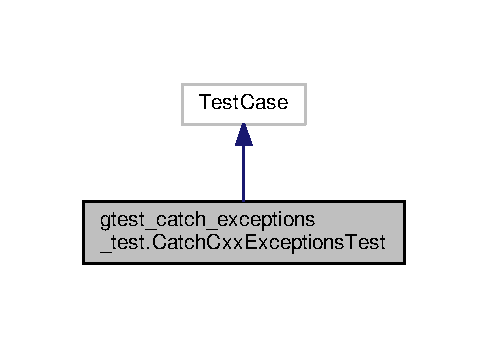
\includegraphics[width=234pt]{classgtest__catch__exceptions__test_1_1CatchCxxExceptionsTest__inherit__graph}
\end{center}
\end{figure}


Collaboration diagram for gtest\+\_\+catch\+\_\+exceptions\+\_\+test.\+Catch\+Cxx\+Exceptions\+Test\+:
\nopagebreak
\begin{figure}[H]
\begin{center}
\leavevmode
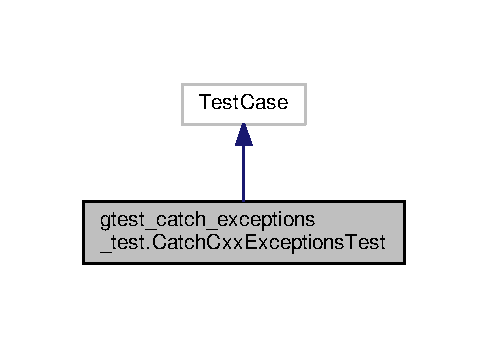
\includegraphics[width=234pt]{classgtest__catch__exceptions__test_1_1CatchCxxExceptionsTest__coll__graph}
\end{center}
\end{figure}
\subsection*{Public Member Functions}
\begin{DoxyCompactItemize}
\item 
def \hyperlink{classgtest__catch__exceptions__test_1_1CatchCxxExceptionsTest_a7d02a890df0e3990aa107288c21f7dc7}{test\+Catches\+Cxx\+Exceptions\+In\+Fixture\+Constructor} (self)
\item 
def \hyperlink{classgtest__catch__exceptions__test_1_1CatchCxxExceptionsTest_a3fe17da71b72c1693fa358f71c6b31be}{test\+Catches\+Cxx\+Exceptions\+In\+Fixture\+Destructor} (self)
\item 
def \hyperlink{classgtest__catch__exceptions__test_1_1CatchCxxExceptionsTest_a8e791760b553d92490005deea0812f44}{test\+Catches\+Cxx\+Exceptions\+In\+Set\+Up\+Test\+Case} (self)
\item 
def \hyperlink{classgtest__catch__exceptions__test_1_1CatchCxxExceptionsTest_a56c906c34e689ee016ab1bf14fe5220c}{test\+Catches\+Cxx\+Exceptions\+In\+Tear\+Down\+Test\+Case} (self)
\item 
def \hyperlink{classgtest__catch__exceptions__test_1_1CatchCxxExceptionsTest_a6451307941e063bcc3927992c1f2df54}{test\+Catches\+Cxx\+Exceptions\+In\+Set\+Up} (self)
\item 
def \hyperlink{classgtest__catch__exceptions__test_1_1CatchCxxExceptionsTest_a40ba50bf018753b7b21ed93ed60e4e1c}{test\+Catches\+Cxx\+Exceptions\+In\+Tear\+Down} (self)
\item 
def \hyperlink{classgtest__catch__exceptions__test_1_1CatchCxxExceptionsTest_ac73b336590a3d1c242124e9ea5464a42}{test\+Catches\+Cxx\+Exceptions\+In\+Test\+Body} (self)
\item 
def \hyperlink{classgtest__catch__exceptions__test_1_1CatchCxxExceptionsTest_a922cb0b598034924c19e6695cc9f7513}{test\+Catches\+Non\+Std\+Cxx\+Exceptions} (self)
\item 
def \hyperlink{classgtest__catch__exceptions__test_1_1CatchCxxExceptionsTest_af3a794d5af0b3d72789293531468050a}{test\+Unhandled\+Cxx\+Exceptions\+Abort\+The\+Program} (self)
\end{DoxyCompactItemize}


\subsection{Detailed Description}
\begin{DoxyVerb}Tests C++ exception-catching behavior.

   Tests in this test case verify that:
   * C++ exceptions are caught and logged as C++ (not SEH) exceptions
   * Exception thrown affect the remainder of the test work flow in the
     expected manner.
\end{DoxyVerb}
 

\subsection{Member Function Documentation}
\index{gtest\+\_\+catch\+\_\+exceptions\+\_\+test\+::\+Catch\+Cxx\+Exceptions\+Test@{gtest\+\_\+catch\+\_\+exceptions\+\_\+test\+::\+Catch\+Cxx\+Exceptions\+Test}!test\+Catches\+Cxx\+Exceptions\+In\+Fixture\+Constructor@{test\+Catches\+Cxx\+Exceptions\+In\+Fixture\+Constructor}}
\index{test\+Catches\+Cxx\+Exceptions\+In\+Fixture\+Constructor@{test\+Catches\+Cxx\+Exceptions\+In\+Fixture\+Constructor}!gtest\+\_\+catch\+\_\+exceptions\+\_\+test\+::\+Catch\+Cxx\+Exceptions\+Test@{gtest\+\_\+catch\+\_\+exceptions\+\_\+test\+::\+Catch\+Cxx\+Exceptions\+Test}}
\subsubsection[{\texorpdfstring{test\+Catches\+Cxx\+Exceptions\+In\+Fixture\+Constructor(self)}{testCatchesCxxExceptionsInFixtureConstructor(self)}}]{\setlength{\rightskip}{0pt plus 5cm}def gtest\+\_\+catch\+\_\+exceptions\+\_\+test.\+Catch\+Cxx\+Exceptions\+Test.\+test\+Catches\+Cxx\+Exceptions\+In\+Fixture\+Constructor (
\begin{DoxyParamCaption}
\item[{}]{self}
\end{DoxyParamCaption}
)}\hypertarget{classgtest__catch__exceptions__test_1_1CatchCxxExceptionsTest_a7d02a890df0e3990aa107288c21f7dc7}{}\label{classgtest__catch__exceptions__test_1_1CatchCxxExceptionsTest_a7d02a890df0e3990aa107288c21f7dc7}

\begin{DoxyCode}
123   \textcolor{keyword}{def }testCatchesCxxExceptionsInFixtureConstructor(self):
124     self.assert\_(\textcolor{stringliteral}{'C++ exception with description '}
125                  \textcolor{stringliteral}{'"Standard C++ exception" thrown '}
126                  \textcolor{stringliteral}{'in the test fixture\(\backslash\)'s constructor'}
127                  \textcolor{keywordflow}{in} EX\_BINARY\_OUTPUT)
128     self.assert\_(\textcolor{stringliteral}{'unexpected'} \textcolor{keywordflow}{not} \textcolor{keywordflow}{in} EX\_BINARY\_OUTPUT,
129                  \textcolor{stringliteral}{'This failure belongs in this test only if '}
130                  \textcolor{stringliteral}{'"CxxExceptionInConstructorTest" (no quotes) '}
131                  \textcolor{stringliteral}{'appears on the same line as words "called unexpectedly"'})
132 
\end{DoxyCode}
\index{gtest\+\_\+catch\+\_\+exceptions\+\_\+test\+::\+Catch\+Cxx\+Exceptions\+Test@{gtest\+\_\+catch\+\_\+exceptions\+\_\+test\+::\+Catch\+Cxx\+Exceptions\+Test}!test\+Catches\+Cxx\+Exceptions\+In\+Fixture\+Destructor@{test\+Catches\+Cxx\+Exceptions\+In\+Fixture\+Destructor}}
\index{test\+Catches\+Cxx\+Exceptions\+In\+Fixture\+Destructor@{test\+Catches\+Cxx\+Exceptions\+In\+Fixture\+Destructor}!gtest\+\_\+catch\+\_\+exceptions\+\_\+test\+::\+Catch\+Cxx\+Exceptions\+Test@{gtest\+\_\+catch\+\_\+exceptions\+\_\+test\+::\+Catch\+Cxx\+Exceptions\+Test}}
\subsubsection[{\texorpdfstring{test\+Catches\+Cxx\+Exceptions\+In\+Fixture\+Destructor(self)}{testCatchesCxxExceptionsInFixtureDestructor(self)}}]{\setlength{\rightskip}{0pt plus 5cm}def gtest\+\_\+catch\+\_\+exceptions\+\_\+test.\+Catch\+Cxx\+Exceptions\+Test.\+test\+Catches\+Cxx\+Exceptions\+In\+Fixture\+Destructor (
\begin{DoxyParamCaption}
\item[{}]{self}
\end{DoxyParamCaption}
)}\hypertarget{classgtest__catch__exceptions__test_1_1CatchCxxExceptionsTest_a3fe17da71b72c1693fa358f71c6b31be}{}\label{classgtest__catch__exceptions__test_1_1CatchCxxExceptionsTest_a3fe17da71b72c1693fa358f71c6b31be}

\begin{DoxyCode}
136     \textcolor{keyword}{def }testCatchesCxxExceptionsInFixtureDestructor(self):
137       self.assert\_(\textcolor{stringliteral}{'C++ exception with description '}
138                    \textcolor{stringliteral}{'"Standard C++ exception" thrown '}
139                    \textcolor{stringliteral}{'in the test fixture\(\backslash\)'s destructor'}
140                    \textcolor{keywordflow}{in} EX\_BINARY\_OUTPUT)
141       self.assert\_(\textcolor{stringliteral}{'CxxExceptionInDestructorTest::TearDownTestCase() '}
142                    \textcolor{stringliteral}{'called as expected.'}
143                    \textcolor{keywordflow}{in} EX\_BINARY\_OUTPUT)
144 
\end{DoxyCode}
\index{gtest\+\_\+catch\+\_\+exceptions\+\_\+test\+::\+Catch\+Cxx\+Exceptions\+Test@{gtest\+\_\+catch\+\_\+exceptions\+\_\+test\+::\+Catch\+Cxx\+Exceptions\+Test}!test\+Catches\+Cxx\+Exceptions\+In\+Set\+Up@{test\+Catches\+Cxx\+Exceptions\+In\+Set\+Up}}
\index{test\+Catches\+Cxx\+Exceptions\+In\+Set\+Up@{test\+Catches\+Cxx\+Exceptions\+In\+Set\+Up}!gtest\+\_\+catch\+\_\+exceptions\+\_\+test\+::\+Catch\+Cxx\+Exceptions\+Test@{gtest\+\_\+catch\+\_\+exceptions\+\_\+test\+::\+Catch\+Cxx\+Exceptions\+Test}}
\subsubsection[{\texorpdfstring{test\+Catches\+Cxx\+Exceptions\+In\+Set\+Up(self)}{testCatchesCxxExceptionsInSetUp(self)}}]{\setlength{\rightskip}{0pt plus 5cm}def gtest\+\_\+catch\+\_\+exceptions\+\_\+test.\+Catch\+Cxx\+Exceptions\+Test.\+test\+Catches\+Cxx\+Exceptions\+In\+Set\+Up (
\begin{DoxyParamCaption}
\item[{}]{self}
\end{DoxyParamCaption}
)}\hypertarget{classgtest__catch__exceptions__test_1_1CatchCxxExceptionsTest_a6451307941e063bcc3927992c1f2df54}{}\label{classgtest__catch__exceptions__test_1_1CatchCxxExceptionsTest_a6451307941e063bcc3927992c1f2df54}

\begin{DoxyCode}
173   \textcolor{keyword}{def }testCatchesCxxExceptionsInSetUp(self):
174     self.assert\_(\textcolor{stringliteral}{'C++ exception with description "Standard C++ exception"'}
175                  \textcolor{stringliteral}{' thrown in SetUp()'}
176                  \textcolor{keywordflow}{in} EX\_BINARY\_OUTPUT)
177     self.assert\_(\textcolor{stringliteral}{'CxxExceptionInSetUpTest::TearDownTestCase() '}
178                  \textcolor{stringliteral}{'called as expected.'}
179                  \textcolor{keywordflow}{in} EX\_BINARY\_OUTPUT)
180     self.assert\_(\textcolor{stringliteral}{'CxxExceptionInSetUpTest destructor '}
181                  \textcolor{stringliteral}{'called as expected.'}
182                  \textcolor{keywordflow}{in} EX\_BINARY\_OUTPUT)
183     self.assert\_(\textcolor{stringliteral}{'CxxExceptionInSetUpTest::TearDown() '}
184                  \textcolor{stringliteral}{'called as expected.'}
185                  \textcolor{keywordflow}{in} EX\_BINARY\_OUTPUT)
186     self.assert\_(\textcolor{stringliteral}{'unexpected'} \textcolor{keywordflow}{not} \textcolor{keywordflow}{in} EX\_BINARY\_OUTPUT,
187                  \textcolor{stringliteral}{'This failure belongs in this test only if '}
188                  \textcolor{stringliteral}{'"CxxExceptionInSetUpTest" (no quotes) '}
189                  \textcolor{stringliteral}{'appears on the same line as words "called unexpectedly"'})
190 
\end{DoxyCode}
\index{gtest\+\_\+catch\+\_\+exceptions\+\_\+test\+::\+Catch\+Cxx\+Exceptions\+Test@{gtest\+\_\+catch\+\_\+exceptions\+\_\+test\+::\+Catch\+Cxx\+Exceptions\+Test}!test\+Catches\+Cxx\+Exceptions\+In\+Set\+Up\+Test\+Case@{test\+Catches\+Cxx\+Exceptions\+In\+Set\+Up\+Test\+Case}}
\index{test\+Catches\+Cxx\+Exceptions\+In\+Set\+Up\+Test\+Case@{test\+Catches\+Cxx\+Exceptions\+In\+Set\+Up\+Test\+Case}!gtest\+\_\+catch\+\_\+exceptions\+\_\+test\+::\+Catch\+Cxx\+Exceptions\+Test@{gtest\+\_\+catch\+\_\+exceptions\+\_\+test\+::\+Catch\+Cxx\+Exceptions\+Test}}
\subsubsection[{\texorpdfstring{test\+Catches\+Cxx\+Exceptions\+In\+Set\+Up\+Test\+Case(self)}{testCatchesCxxExceptionsInSetUpTestCase(self)}}]{\setlength{\rightskip}{0pt plus 5cm}def gtest\+\_\+catch\+\_\+exceptions\+\_\+test.\+Catch\+Cxx\+Exceptions\+Test.\+test\+Catches\+Cxx\+Exceptions\+In\+Set\+Up\+Test\+Case (
\begin{DoxyParamCaption}
\item[{}]{self}
\end{DoxyParamCaption}
)}\hypertarget{classgtest__catch__exceptions__test_1_1CatchCxxExceptionsTest_a8e791760b553d92490005deea0812f44}{}\label{classgtest__catch__exceptions__test_1_1CatchCxxExceptionsTest_a8e791760b553d92490005deea0812f44}

\begin{DoxyCode}
145   \textcolor{keyword}{def }testCatchesCxxExceptionsInSetUpTestCase(self):
146     self.assert\_(\textcolor{stringliteral}{'C++ exception with description "Standard C++ exception"'}
147                  \textcolor{stringliteral}{' thrown in SetUpTestCase()'}
148                  \textcolor{keywordflow}{in} EX\_BINARY\_OUTPUT)
149     self.assert\_(\textcolor{stringliteral}{'CxxExceptionInConstructorTest::TearDownTestCase() '}
150                  \textcolor{stringliteral}{'called as expected.'}
151                  \textcolor{keywordflow}{in} EX\_BINARY\_OUTPUT)
152     self.assert\_(\textcolor{stringliteral}{'CxxExceptionInSetUpTestCaseTest constructor '}
153                  \textcolor{stringliteral}{'called as expected.'}
154                  \textcolor{keywordflow}{in} EX\_BINARY\_OUTPUT)
155     self.assert\_(\textcolor{stringliteral}{'CxxExceptionInSetUpTestCaseTest destructor '}
156                  \textcolor{stringliteral}{'called as expected.'}
157                  \textcolor{keywordflow}{in} EX\_BINARY\_OUTPUT)
158     self.assert\_(\textcolor{stringliteral}{'CxxExceptionInSetUpTestCaseTest::SetUp() '}
159                  \textcolor{stringliteral}{'called as expected.'}
160                  \textcolor{keywordflow}{in} EX\_BINARY\_OUTPUT)
161     self.assert\_(\textcolor{stringliteral}{'CxxExceptionInSetUpTestCaseTest::TearDown() '}
162                  \textcolor{stringliteral}{'called as expected.'}
163                  \textcolor{keywordflow}{in} EX\_BINARY\_OUTPUT)
164     self.assert\_(\textcolor{stringliteral}{'CxxExceptionInSetUpTestCaseTest test body '}
165                  \textcolor{stringliteral}{'called as expected.'}
166                  \textcolor{keywordflow}{in} EX\_BINARY\_OUTPUT)
167 
\end{DoxyCode}
\index{gtest\+\_\+catch\+\_\+exceptions\+\_\+test\+::\+Catch\+Cxx\+Exceptions\+Test@{gtest\+\_\+catch\+\_\+exceptions\+\_\+test\+::\+Catch\+Cxx\+Exceptions\+Test}!test\+Catches\+Cxx\+Exceptions\+In\+Tear\+Down@{test\+Catches\+Cxx\+Exceptions\+In\+Tear\+Down}}
\index{test\+Catches\+Cxx\+Exceptions\+In\+Tear\+Down@{test\+Catches\+Cxx\+Exceptions\+In\+Tear\+Down}!gtest\+\_\+catch\+\_\+exceptions\+\_\+test\+::\+Catch\+Cxx\+Exceptions\+Test@{gtest\+\_\+catch\+\_\+exceptions\+\_\+test\+::\+Catch\+Cxx\+Exceptions\+Test}}
\subsubsection[{\texorpdfstring{test\+Catches\+Cxx\+Exceptions\+In\+Tear\+Down(self)}{testCatchesCxxExceptionsInTearDown(self)}}]{\setlength{\rightskip}{0pt plus 5cm}def gtest\+\_\+catch\+\_\+exceptions\+\_\+test.\+Catch\+Cxx\+Exceptions\+Test.\+test\+Catches\+Cxx\+Exceptions\+In\+Tear\+Down (
\begin{DoxyParamCaption}
\item[{}]{self}
\end{DoxyParamCaption}
)}\hypertarget{classgtest__catch__exceptions__test_1_1CatchCxxExceptionsTest_a40ba50bf018753b7b21ed93ed60e4e1c}{}\label{classgtest__catch__exceptions__test_1_1CatchCxxExceptionsTest_a40ba50bf018753b7b21ed93ed60e4e1c}

\begin{DoxyCode}
191   \textcolor{keyword}{def }testCatchesCxxExceptionsInTearDown(self):
192     self.assert\_(\textcolor{stringliteral}{'C++ exception with description "Standard C++ exception"'}
193                  \textcolor{stringliteral}{' thrown in TearDown()'}
194                  \textcolor{keywordflow}{in} EX\_BINARY\_OUTPUT)
195     self.assert\_(\textcolor{stringliteral}{'CxxExceptionInTearDownTest::TearDownTestCase() '}
196                  \textcolor{stringliteral}{'called as expected.'}
197                  \textcolor{keywordflow}{in} EX\_BINARY\_OUTPUT)
198     self.assert\_(\textcolor{stringliteral}{'CxxExceptionInTearDownTest destructor '}
199                  \textcolor{stringliteral}{'called as expected.'}
200                  \textcolor{keywordflow}{in} EX\_BINARY\_OUTPUT)
201 
\end{DoxyCode}
\index{gtest\+\_\+catch\+\_\+exceptions\+\_\+test\+::\+Catch\+Cxx\+Exceptions\+Test@{gtest\+\_\+catch\+\_\+exceptions\+\_\+test\+::\+Catch\+Cxx\+Exceptions\+Test}!test\+Catches\+Cxx\+Exceptions\+In\+Tear\+Down\+Test\+Case@{test\+Catches\+Cxx\+Exceptions\+In\+Tear\+Down\+Test\+Case}}
\index{test\+Catches\+Cxx\+Exceptions\+In\+Tear\+Down\+Test\+Case@{test\+Catches\+Cxx\+Exceptions\+In\+Tear\+Down\+Test\+Case}!gtest\+\_\+catch\+\_\+exceptions\+\_\+test\+::\+Catch\+Cxx\+Exceptions\+Test@{gtest\+\_\+catch\+\_\+exceptions\+\_\+test\+::\+Catch\+Cxx\+Exceptions\+Test}}
\subsubsection[{\texorpdfstring{test\+Catches\+Cxx\+Exceptions\+In\+Tear\+Down\+Test\+Case(self)}{testCatchesCxxExceptionsInTearDownTestCase(self)}}]{\setlength{\rightskip}{0pt plus 5cm}def gtest\+\_\+catch\+\_\+exceptions\+\_\+test.\+Catch\+Cxx\+Exceptions\+Test.\+test\+Catches\+Cxx\+Exceptions\+In\+Tear\+Down\+Test\+Case (
\begin{DoxyParamCaption}
\item[{}]{self}
\end{DoxyParamCaption}
)}\hypertarget{classgtest__catch__exceptions__test_1_1CatchCxxExceptionsTest_a56c906c34e689ee016ab1bf14fe5220c}{}\label{classgtest__catch__exceptions__test_1_1CatchCxxExceptionsTest_a56c906c34e689ee016ab1bf14fe5220c}

\begin{DoxyCode}
168   \textcolor{keyword}{def }testCatchesCxxExceptionsInTearDownTestCase(self):
169     self.assert\_(\textcolor{stringliteral}{'C++ exception with description "Standard C++ exception"'}
170                  \textcolor{stringliteral}{' thrown in TearDownTestCase()'}
171                  \textcolor{keywordflow}{in} EX\_BINARY\_OUTPUT)
172 
\end{DoxyCode}
\index{gtest\+\_\+catch\+\_\+exceptions\+\_\+test\+::\+Catch\+Cxx\+Exceptions\+Test@{gtest\+\_\+catch\+\_\+exceptions\+\_\+test\+::\+Catch\+Cxx\+Exceptions\+Test}!test\+Catches\+Cxx\+Exceptions\+In\+Test\+Body@{test\+Catches\+Cxx\+Exceptions\+In\+Test\+Body}}
\index{test\+Catches\+Cxx\+Exceptions\+In\+Test\+Body@{test\+Catches\+Cxx\+Exceptions\+In\+Test\+Body}!gtest\+\_\+catch\+\_\+exceptions\+\_\+test\+::\+Catch\+Cxx\+Exceptions\+Test@{gtest\+\_\+catch\+\_\+exceptions\+\_\+test\+::\+Catch\+Cxx\+Exceptions\+Test}}
\subsubsection[{\texorpdfstring{test\+Catches\+Cxx\+Exceptions\+In\+Test\+Body(self)}{testCatchesCxxExceptionsInTestBody(self)}}]{\setlength{\rightskip}{0pt plus 5cm}def gtest\+\_\+catch\+\_\+exceptions\+\_\+test.\+Catch\+Cxx\+Exceptions\+Test.\+test\+Catches\+Cxx\+Exceptions\+In\+Test\+Body (
\begin{DoxyParamCaption}
\item[{}]{self}
\end{DoxyParamCaption}
)}\hypertarget{classgtest__catch__exceptions__test_1_1CatchCxxExceptionsTest_ac73b336590a3d1c242124e9ea5464a42}{}\label{classgtest__catch__exceptions__test_1_1CatchCxxExceptionsTest_ac73b336590a3d1c242124e9ea5464a42}

\begin{DoxyCode}
202   \textcolor{keyword}{def }testCatchesCxxExceptionsInTestBody(self):
203     self.assert\_(\textcolor{stringliteral}{'C++ exception with description "Standard C++ exception"'}
204                  \textcolor{stringliteral}{' thrown in the test body'}
205                  \textcolor{keywordflow}{in} EX\_BINARY\_OUTPUT)
206     self.assert\_(\textcolor{stringliteral}{'CxxExceptionInTestBodyTest::TearDownTestCase() '}
207                  \textcolor{stringliteral}{'called as expected.'}
208                  \textcolor{keywordflow}{in} EX\_BINARY\_OUTPUT)
209     self.assert\_(\textcolor{stringliteral}{'CxxExceptionInTestBodyTest destructor '}
210                  \textcolor{stringliteral}{'called as expected.'}
211                  \textcolor{keywordflow}{in} EX\_BINARY\_OUTPUT)
212     self.assert\_(\textcolor{stringliteral}{'CxxExceptionInTestBodyTest::TearDown() '}
213                  \textcolor{stringliteral}{'called as expected.'}
214                  \textcolor{keywordflow}{in} EX\_BINARY\_OUTPUT)
215 
\end{DoxyCode}
\index{gtest\+\_\+catch\+\_\+exceptions\+\_\+test\+::\+Catch\+Cxx\+Exceptions\+Test@{gtest\+\_\+catch\+\_\+exceptions\+\_\+test\+::\+Catch\+Cxx\+Exceptions\+Test}!test\+Catches\+Non\+Std\+Cxx\+Exceptions@{test\+Catches\+Non\+Std\+Cxx\+Exceptions}}
\index{test\+Catches\+Non\+Std\+Cxx\+Exceptions@{test\+Catches\+Non\+Std\+Cxx\+Exceptions}!gtest\+\_\+catch\+\_\+exceptions\+\_\+test\+::\+Catch\+Cxx\+Exceptions\+Test@{gtest\+\_\+catch\+\_\+exceptions\+\_\+test\+::\+Catch\+Cxx\+Exceptions\+Test}}
\subsubsection[{\texorpdfstring{test\+Catches\+Non\+Std\+Cxx\+Exceptions(self)}{testCatchesNonStdCxxExceptions(self)}}]{\setlength{\rightskip}{0pt plus 5cm}def gtest\+\_\+catch\+\_\+exceptions\+\_\+test.\+Catch\+Cxx\+Exceptions\+Test.\+test\+Catches\+Non\+Std\+Cxx\+Exceptions (
\begin{DoxyParamCaption}
\item[{}]{self}
\end{DoxyParamCaption}
)}\hypertarget{classgtest__catch__exceptions__test_1_1CatchCxxExceptionsTest_a922cb0b598034924c19e6695cc9f7513}{}\label{classgtest__catch__exceptions__test_1_1CatchCxxExceptionsTest_a922cb0b598034924c19e6695cc9f7513}

\begin{DoxyCode}
216   \textcolor{keyword}{def }testCatchesNonStdCxxExceptions(self):
217     self.assert\_(\textcolor{stringliteral}{'Unknown C++ exception thrown in the test body'}
218                  \textcolor{keywordflow}{in} EX\_BINARY\_OUTPUT)
219 
\end{DoxyCode}
\index{gtest\+\_\+catch\+\_\+exceptions\+\_\+test\+::\+Catch\+Cxx\+Exceptions\+Test@{gtest\+\_\+catch\+\_\+exceptions\+\_\+test\+::\+Catch\+Cxx\+Exceptions\+Test}!test\+Unhandled\+Cxx\+Exceptions\+Abort\+The\+Program@{test\+Unhandled\+Cxx\+Exceptions\+Abort\+The\+Program}}
\index{test\+Unhandled\+Cxx\+Exceptions\+Abort\+The\+Program@{test\+Unhandled\+Cxx\+Exceptions\+Abort\+The\+Program}!gtest\+\_\+catch\+\_\+exceptions\+\_\+test\+::\+Catch\+Cxx\+Exceptions\+Test@{gtest\+\_\+catch\+\_\+exceptions\+\_\+test\+::\+Catch\+Cxx\+Exceptions\+Test}}
\subsubsection[{\texorpdfstring{test\+Unhandled\+Cxx\+Exceptions\+Abort\+The\+Program(self)}{testUnhandledCxxExceptionsAbortTheProgram(self)}}]{\setlength{\rightskip}{0pt plus 5cm}def gtest\+\_\+catch\+\_\+exceptions\+\_\+test.\+Catch\+Cxx\+Exceptions\+Test.\+test\+Unhandled\+Cxx\+Exceptions\+Abort\+The\+Program (
\begin{DoxyParamCaption}
\item[{}]{self}
\end{DoxyParamCaption}
)}\hypertarget{classgtest__catch__exceptions__test_1_1CatchCxxExceptionsTest_af3a794d5af0b3d72789293531468050a}{}\label{classgtest__catch__exceptions__test_1_1CatchCxxExceptionsTest_af3a794d5af0b3d72789293531468050a}

\begin{DoxyCode}
220   \textcolor{keyword}{def }testUnhandledCxxExceptionsAbortTheProgram(self):
221     \textcolor{comment}{# Filters out SEH exception tests on Windows. Unhandled SEH exceptions}
222     \textcolor{comment}{# cause tests to show pop-up windows there.}
223     FITLER\_OUT\_SEH\_TESTS\_FLAG = FILTER\_FLAG + \textcolor{stringliteral}{'=-*Seh*'}
224     \textcolor{comment}{# By default, Google Test doesn't catch the exceptions.}
225     uncaught\_exceptions\_ex\_binary\_output = \hyperlink{classgtest__test__utils_1_1Subprocess}{gtest\_test\_utils.Subprocess}(
226         [EX\_EXE\_PATH,
227          NO\_CATCH\_EXCEPTIONS\_FLAG,
228          FITLER\_OUT\_SEH\_TESTS\_FLAG],
229         env=environ).output
230 
231     self.assert\_(\textcolor{stringliteral}{'Unhandled C++ exception terminating the program'}
232                  \textcolor{keywordflow}{in} uncaught\_exceptions\_ex\_binary\_output)
233     self.assert\_(\textcolor{stringliteral}{'unexpected'} \textcolor{keywordflow}{not} \textcolor{keywordflow}{in} uncaught\_exceptions\_ex\_binary\_output)
234 
235 
\end{DoxyCode}


The documentation for this class was generated from the following file\+:\begin{DoxyCompactItemize}
\item 
vendor/googletest/googletest/test/\hyperlink{gtest__catch__exceptions__test_8py}{gtest\+\_\+catch\+\_\+exceptions\+\_\+test.\+py}\end{DoxyCompactItemize}

\hypertarget{classgtest__catch__exceptions__test_1_1CatchSehExceptionsTest}{}\section{gtest\+\_\+catch\+\_\+exceptions\+\_\+test.\+Catch\+Seh\+Exceptions\+Test Class Reference}
\label{classgtest__catch__exceptions__test_1_1CatchSehExceptionsTest}\index{gtest\+\_\+catch\+\_\+exceptions\+\_\+test.\+Catch\+Seh\+Exceptions\+Test@{gtest\+\_\+catch\+\_\+exceptions\+\_\+test.\+Catch\+Seh\+Exceptions\+Test}}


Inheritance diagram for gtest\+\_\+catch\+\_\+exceptions\+\_\+test.\+Catch\+Seh\+Exceptions\+Test\+:
\nopagebreak
\begin{figure}[H]
\begin{center}
\leavevmode
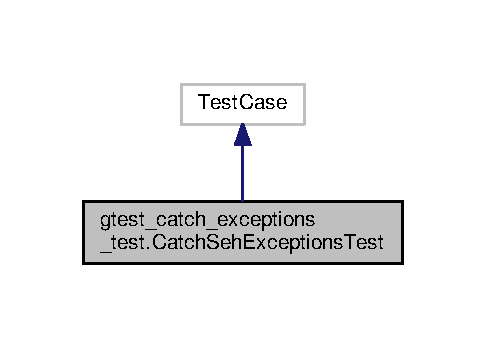
\includegraphics[width=233pt]{classgtest__catch__exceptions__test_1_1CatchSehExceptionsTest__inherit__graph}
\end{center}
\end{figure}


Collaboration diagram for gtest\+\_\+catch\+\_\+exceptions\+\_\+test.\+Catch\+Seh\+Exceptions\+Test\+:
\nopagebreak
\begin{figure}[H]
\begin{center}
\leavevmode
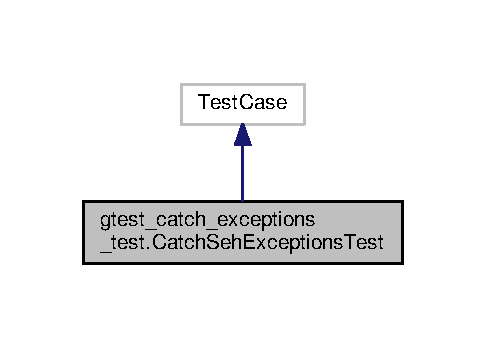
\includegraphics[width=233pt]{classgtest__catch__exceptions__test_1_1CatchSehExceptionsTest__coll__graph}
\end{center}
\end{figure}
\subsection*{Public Member Functions}
\begin{DoxyCompactItemize}
\item 
def \hyperlink{classgtest__catch__exceptions__test_1_1CatchSehExceptionsTest_a737bbcc64405854aa8e0aea87ca5850b}{Test\+Seh\+Exceptions} (self, test\+\_\+output)
\item 
def \hyperlink{classgtest__catch__exceptions__test_1_1CatchSehExceptionsTest_a02d06790fb52416a9da6a28b624e9cd9}{test\+Catches\+Seh\+Exceptions\+With\+Cxx\+Exceptions\+Enabled} (self)
\item 
def \hyperlink{classgtest__catch__exceptions__test_1_1CatchSehExceptionsTest_a4a181de9de2b147eff55ed7a1d7d40c4}{test\+Catches\+Seh\+Exceptions\+With\+Cxx\+Exceptions\+Disabled} (self)
\end{DoxyCompactItemize}


\subsection{Detailed Description}
\begin{DoxyVerb}Tests exception-catching behavior.\end{DoxyVerb}
 

\subsection{Member Function Documentation}
\index{gtest\+\_\+catch\+\_\+exceptions\+\_\+test\+::\+Catch\+Seh\+Exceptions\+Test@{gtest\+\_\+catch\+\_\+exceptions\+\_\+test\+::\+Catch\+Seh\+Exceptions\+Test}!test\+Catches\+Seh\+Exceptions\+With\+Cxx\+Exceptions\+Disabled@{test\+Catches\+Seh\+Exceptions\+With\+Cxx\+Exceptions\+Disabled}}
\index{test\+Catches\+Seh\+Exceptions\+With\+Cxx\+Exceptions\+Disabled@{test\+Catches\+Seh\+Exceptions\+With\+Cxx\+Exceptions\+Disabled}!gtest\+\_\+catch\+\_\+exceptions\+\_\+test\+::\+Catch\+Seh\+Exceptions\+Test@{gtest\+\_\+catch\+\_\+exceptions\+\_\+test\+::\+Catch\+Seh\+Exceptions\+Test}}
\subsubsection[{\texorpdfstring{test\+Catches\+Seh\+Exceptions\+With\+Cxx\+Exceptions\+Disabled(self)}{testCatchesSehExceptionsWithCxxExceptionsDisabled(self)}}]{\setlength{\rightskip}{0pt plus 5cm}def gtest\+\_\+catch\+\_\+exceptions\+\_\+test.\+Catch\+Seh\+Exceptions\+Test.\+test\+Catches\+Seh\+Exceptions\+With\+Cxx\+Exceptions\+Disabled (
\begin{DoxyParamCaption}
\item[{}]{self}
\end{DoxyParamCaption}
)}\hypertarget{classgtest__catch__exceptions__test_1_1CatchSehExceptionsTest_a4a181de9de2b147eff55ed7a1d7d40c4}{}\label{classgtest__catch__exceptions__test_1_1CatchSehExceptionsTest_a4a181de9de2b147eff55ed7a1d7d40c4}

\begin{DoxyCode}
110     \textcolor{keyword}{def }testCatchesSehExceptionsWithCxxExceptionsDisabled(self):
111       self.TestSehExceptions(BINARY\_OUTPUT)
112 
113 
\end{DoxyCode}
\index{gtest\+\_\+catch\+\_\+exceptions\+\_\+test\+::\+Catch\+Seh\+Exceptions\+Test@{gtest\+\_\+catch\+\_\+exceptions\+\_\+test\+::\+Catch\+Seh\+Exceptions\+Test}!test\+Catches\+Seh\+Exceptions\+With\+Cxx\+Exceptions\+Enabled@{test\+Catches\+Seh\+Exceptions\+With\+Cxx\+Exceptions\+Enabled}}
\index{test\+Catches\+Seh\+Exceptions\+With\+Cxx\+Exceptions\+Enabled@{test\+Catches\+Seh\+Exceptions\+With\+Cxx\+Exceptions\+Enabled}!gtest\+\_\+catch\+\_\+exceptions\+\_\+test\+::\+Catch\+Seh\+Exceptions\+Test@{gtest\+\_\+catch\+\_\+exceptions\+\_\+test\+::\+Catch\+Seh\+Exceptions\+Test}}
\subsubsection[{\texorpdfstring{test\+Catches\+Seh\+Exceptions\+With\+Cxx\+Exceptions\+Enabled(self)}{testCatchesSehExceptionsWithCxxExceptionsEnabled(self)}}]{\setlength{\rightskip}{0pt plus 5cm}def gtest\+\_\+catch\+\_\+exceptions\+\_\+test.\+Catch\+Seh\+Exceptions\+Test.\+test\+Catches\+Seh\+Exceptions\+With\+Cxx\+Exceptions\+Enabled (
\begin{DoxyParamCaption}
\item[{}]{self}
\end{DoxyParamCaption}
)}\hypertarget{classgtest__catch__exceptions__test_1_1CatchSehExceptionsTest_a02d06790fb52416a9da6a28b624e9cd9}{}\label{classgtest__catch__exceptions__test_1_1CatchSehExceptionsTest_a02d06790fb52416a9da6a28b624e9cd9}

\begin{DoxyCode}
107     \textcolor{keyword}{def }testCatchesSehExceptionsWithCxxExceptionsEnabled(self):
108       self.TestSehExceptions(EX\_BINARY\_OUTPUT)
109 
\end{DoxyCode}
\index{gtest\+\_\+catch\+\_\+exceptions\+\_\+test\+::\+Catch\+Seh\+Exceptions\+Test@{gtest\+\_\+catch\+\_\+exceptions\+\_\+test\+::\+Catch\+Seh\+Exceptions\+Test}!Test\+Seh\+Exceptions@{Test\+Seh\+Exceptions}}
\index{Test\+Seh\+Exceptions@{Test\+Seh\+Exceptions}!gtest\+\_\+catch\+\_\+exceptions\+\_\+test\+::\+Catch\+Seh\+Exceptions\+Test@{gtest\+\_\+catch\+\_\+exceptions\+\_\+test\+::\+Catch\+Seh\+Exceptions\+Test}}
\subsubsection[{\texorpdfstring{Test\+Seh\+Exceptions(self, test\+\_\+output)}{TestSehExceptions(self, test_output)}}]{\setlength{\rightskip}{0pt plus 5cm}def gtest\+\_\+catch\+\_\+exceptions\+\_\+test.\+Catch\+Seh\+Exceptions\+Test.\+Test\+Seh\+Exceptions (
\begin{DoxyParamCaption}
\item[{}]{self, }
\item[{}]{test\+\_\+output}
\end{DoxyParamCaption}
)}\hypertarget{classgtest__catch__exceptions__test_1_1CatchSehExceptionsTest_a737bbcc64405854aa8e0aea87ca5850b}{}\label{classgtest__catch__exceptions__test_1_1CatchSehExceptionsTest_a737bbcc64405854aa8e0aea87ca5850b}

\begin{DoxyCode}
89     \textcolor{keyword}{def }TestSehExceptions(self, test\_output):
90       self.assert\_(\textcolor{stringliteral}{'SEH exception with code 0x2a thrown '}
91                    \textcolor{stringliteral}{'in the test fixture\(\backslash\)'s constructor'}
92                    \textcolor{keywordflow}{in} test\_output)
93       self.assert\_(\textcolor{stringliteral}{'SEH exception with code 0x2a thrown '}
94                    \textcolor{stringliteral}{'in the test fixture\(\backslash\)'s destructor'}
95                    \textcolor{keywordflow}{in} test\_output)
96       self.assert\_(\textcolor{stringliteral}{'SEH exception with code 0x2a thrown in SetUpTestCase()'}
97                    \textcolor{keywordflow}{in} test\_output)
98       self.assert\_(\textcolor{stringliteral}{'SEH exception with code 0x2a thrown in TearDownTestCase()'}
99                    \textcolor{keywordflow}{in} test\_output)
100       self.assert\_(\textcolor{stringliteral}{'SEH exception with code 0x2a thrown in SetUp()'}
101                    \textcolor{keywordflow}{in} test\_output)
102       self.assert\_(\textcolor{stringliteral}{'SEH exception with code 0x2a thrown in TearDown()'}
103                    \textcolor{keywordflow}{in} test\_output)
104       self.assert\_(\textcolor{stringliteral}{'SEH exception with code 0x2a thrown in the test body'}
105                    \textcolor{keywordflow}{in} test\_output)
106 
\end{DoxyCode}


The documentation for this class was generated from the following file\+:\begin{DoxyCompactItemize}
\item 
vendor/googletest/googletest/test/\hyperlink{gtest__catch__exceptions__test_8py}{gtest\+\_\+catch\+\_\+exceptions\+\_\+test.\+py}\end{DoxyCompactItemize}

\hypertarget{classcpp_1_1ast_1_1Class}{}\section{cpp.\+ast.\+Class Class Reference}
\label{classcpp_1_1ast_1_1Class}\index{cpp.\+ast.\+Class@{cpp.\+ast.\+Class}}


Inheritance diagram for cpp.\+ast.\+Class\+:\nopagebreak
\begin{figure}[H]
\begin{center}
\leavevmode
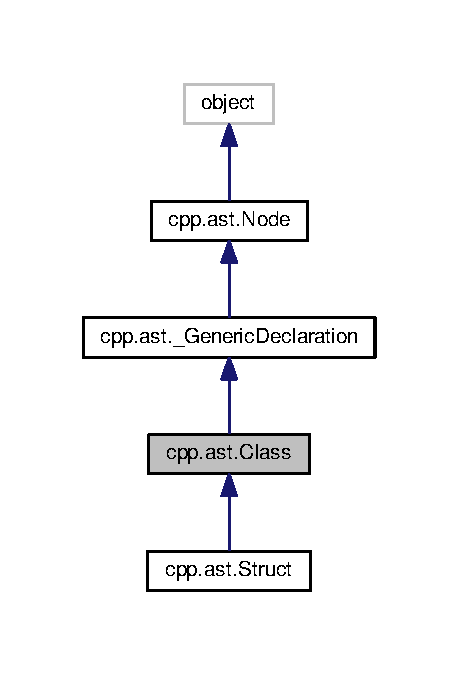
\includegraphics[width=220pt]{classcpp_1_1ast_1_1Class__inherit__graph}
\end{center}
\end{figure}


Collaboration diagram for cpp.\+ast.\+Class\+:\nopagebreak
\begin{figure}[H]
\begin{center}
\leavevmode
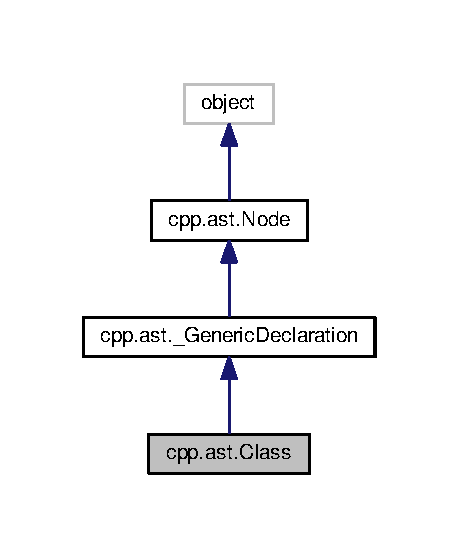
\includegraphics[width=220pt]{classcpp_1_1ast_1_1Class__coll__graph}
\end{center}
\end{figure}
\subsection*{Public Member Functions}
\begin{DoxyCompactItemize}
\item 
def \hyperlink{classcpp_1_1ast_1_1Class_acc17c34512d5cc54d5125734ce79f219}{\+\_\+\+\_\+init\+\_\+\+\_\+} (self, \hyperlink{classcpp_1_1ast_1_1Node_a7b2aa97e6a049bb1a93aea48c48f1f44}{start}, \hyperlink{classcpp_1_1ast_1_1Node_a3c5e5246ccf619df28eca02e29d69647}{end}, \hyperlink{classcpp_1_1ast_1_1__GenericDeclaration_af774f4729dfd78d0538a6782fe8514c1}{name}, \hyperlink{classcpp_1_1ast_1_1Class_a5665eb67314a075d4e0ff91accbde5d1}{bases}, \hyperlink{classcpp_1_1ast_1_1Class_a48ed0d3115656554d9134bc1787390fa}{templated\+\_\+types}, \hyperlink{classcpp_1_1ast_1_1Class_add39f61fdcf6dae42d79cac3dcbb7782}{body}, \hyperlink{classcpp_1_1ast_1_1__GenericDeclaration_a8aee3f11b37449d54b42a78e0a689f46}{namespace})
\item 
def \hyperlink{classcpp_1_1ast_1_1Class_a4758bfb7c00410575932974e1ed8b7da}{Is\+Declaration} (self)
\item 
def \hyperlink{classcpp_1_1ast_1_1Class_ae6d2356f835d06d5109d9e4609d86780}{Is\+Definition} (self)
\item 
def \hyperlink{classcpp_1_1ast_1_1Class_a1ab749f8cfddb0903c6484791f70f42e}{Is\+Exportable} (self)
\item 
def \hyperlink{classcpp_1_1ast_1_1Class_a347673e0a2a7b840b7d2d1cae13977f7}{Requires} (self, node)
\item 
def \hyperlink{classcpp_1_1ast_1_1Class_a0a63f6fab75d61ffac6fb9f1c29ae84d}{\+\_\+\+\_\+str\+\_\+\+\_\+} (self)
\end{DoxyCompactItemize}
\subsection*{Public Attributes}
\begin{DoxyCompactItemize}
\item 
\hyperlink{classcpp_1_1ast_1_1Class_a5665eb67314a075d4e0ff91accbde5d1}{bases}
\item 
\hyperlink{classcpp_1_1ast_1_1Class_add39f61fdcf6dae42d79cac3dcbb7782}{body}
\item 
\hyperlink{classcpp_1_1ast_1_1Class_a48ed0d3115656554d9134bc1787390fa}{templated\+\_\+types}
\end{DoxyCompactItemize}


\subsection{Constructor \& Destructor Documentation}
\index{cpp\+::ast\+::\+Class@{cpp\+::ast\+::\+Class}!\+\_\+\+\_\+init\+\_\+\+\_\+@{\+\_\+\+\_\+init\+\_\+\+\_\+}}
\index{\+\_\+\+\_\+init\+\_\+\+\_\+@{\+\_\+\+\_\+init\+\_\+\+\_\+}!cpp\+::ast\+::\+Class@{cpp\+::ast\+::\+Class}}
\subsubsection[{\texorpdfstring{\+\_\+\+\_\+init\+\_\+\+\_\+(self, start, end, name, bases, templated\+\_\+types, body, namespace)}{__init__(self, start, end, name, bases, templated_types, body, namespace)}}]{\setlength{\rightskip}{0pt plus 5cm}def cpp.\+ast.\+Class.\+\_\+\+\_\+init\+\_\+\+\_\+ (
\begin{DoxyParamCaption}
\item[{}]{self, }
\item[{}]{start, }
\item[{}]{end, }
\item[{}]{name, }
\item[{}]{bases, }
\item[{}]{templated\+\_\+types, }
\item[{}]{body, }
\item[{}]{namespace}
\end{DoxyParamCaption}
)}\hypertarget{classcpp_1_1ast_1_1Class_acc17c34512d5cc54d5125734ce79f219}{}\label{classcpp_1_1ast_1_1Class_acc17c34512d5cc54d5125734ce79f219}

\begin{DoxyCode}
322     \textcolor{keyword}{def }\_\_init\_\_(self, start, end, name, bases, templated\_types, body, namespace):
323         \_GenericDeclaration.\_\_init\_\_(self, start, end, name, namespace)
324         self.bases = bases
325         self.body = body
326         self.templated\_types = templated\_types
327 
\end{DoxyCode}


\subsection{Member Function Documentation}
\index{cpp\+::ast\+::\+Class@{cpp\+::ast\+::\+Class}!\+\_\+\+\_\+str\+\_\+\+\_\+@{\+\_\+\+\_\+str\+\_\+\+\_\+}}
\index{\+\_\+\+\_\+str\+\_\+\+\_\+@{\+\_\+\+\_\+str\+\_\+\+\_\+}!cpp\+::ast\+::\+Class@{cpp\+::ast\+::\+Class}}
\subsubsection[{\texorpdfstring{\+\_\+\+\_\+str\+\_\+\+\_\+(self)}{__str__(self)}}]{\setlength{\rightskip}{0pt plus 5cm}def cpp.\+ast.\+Class.\+\_\+\+\_\+str\+\_\+\+\_\+ (
\begin{DoxyParamCaption}
\item[{}]{self}
\end{DoxyParamCaption}
)}\hypertarget{classcpp_1_1ast_1_1Class_a0a63f6fab75d61ffac6fb9f1c29ae84d}{}\label{classcpp_1_1ast_1_1Class_a0a63f6fab75d61ffac6fb9f1c29ae84d}

\begin{DoxyCode}
348     \textcolor{keyword}{def }\_\_str\_\_(self):
349         name = self.name
350         \textcolor{keywordflow}{if} self.templated\_types:
351             name += \textcolor{stringliteral}{'<%s>'} % self.templated\_types
352         suffix = \textcolor{stringliteral}{'%s, %s, %s'} % (name, self.bases, self.body)
353         \textcolor{keywordflow}{return} self.\_TypeStringHelper(suffix)
354 
355 
\end{DoxyCode}
\index{cpp\+::ast\+::\+Class@{cpp\+::ast\+::\+Class}!Is\+Declaration@{Is\+Declaration}}
\index{Is\+Declaration@{Is\+Declaration}!cpp\+::ast\+::\+Class@{cpp\+::ast\+::\+Class}}
\subsubsection[{\texorpdfstring{Is\+Declaration(self)}{IsDeclaration(self)}}]{\setlength{\rightskip}{0pt plus 5cm}def cpp.\+ast.\+Class.\+Is\+Declaration (
\begin{DoxyParamCaption}
\item[{}]{self}
\end{DoxyParamCaption}
)}\hypertarget{classcpp_1_1ast_1_1Class_a4758bfb7c00410575932974e1ed8b7da}{}\label{classcpp_1_1ast_1_1Class_a4758bfb7c00410575932974e1ed8b7da}

\begin{DoxyCode}
328     \textcolor{keyword}{def }IsDeclaration(self):
329         \textcolor{keywordflow}{return} self.bases \textcolor{keywordflow}{is} \textcolor{keywordtype}{None} \textcolor{keywordflow}{and} self.body \textcolor{keywordflow}{is} \textcolor{keywordtype}{None}
330 
\end{DoxyCode}
\index{cpp\+::ast\+::\+Class@{cpp\+::ast\+::\+Class}!Is\+Definition@{Is\+Definition}}
\index{Is\+Definition@{Is\+Definition}!cpp\+::ast\+::\+Class@{cpp\+::ast\+::\+Class}}
\subsubsection[{\texorpdfstring{Is\+Definition(self)}{IsDefinition(self)}}]{\setlength{\rightskip}{0pt plus 5cm}def cpp.\+ast.\+Class.\+Is\+Definition (
\begin{DoxyParamCaption}
\item[{}]{self}
\end{DoxyParamCaption}
)}\hypertarget{classcpp_1_1ast_1_1Class_ae6d2356f835d06d5109d9e4609d86780}{}\label{classcpp_1_1ast_1_1Class_ae6d2356f835d06d5109d9e4609d86780}

\begin{DoxyCode}
331     \textcolor{keyword}{def }IsDefinition(self):
332         \textcolor{keywordflow}{return} \textcolor{keywordflow}{not} self.IsDeclaration()
333 
\end{DoxyCode}
\index{cpp\+::ast\+::\+Class@{cpp\+::ast\+::\+Class}!Is\+Exportable@{Is\+Exportable}}
\index{Is\+Exportable@{Is\+Exportable}!cpp\+::ast\+::\+Class@{cpp\+::ast\+::\+Class}}
\subsubsection[{\texorpdfstring{Is\+Exportable(self)}{IsExportable(self)}}]{\setlength{\rightskip}{0pt plus 5cm}def cpp.\+ast.\+Class.\+Is\+Exportable (
\begin{DoxyParamCaption}
\item[{}]{self}
\end{DoxyParamCaption}
)}\hypertarget{classcpp_1_1ast_1_1Class_a1ab749f8cfddb0903c6484791f70f42e}{}\label{classcpp_1_1ast_1_1Class_a1ab749f8cfddb0903c6484791f70f42e}

\begin{DoxyCode}
334     \textcolor{keyword}{def }IsExportable(self):
335         \textcolor{keywordflow}{return} \textcolor{keywordflow}{not} self.IsDeclaration()
336 
\end{DoxyCode}
\index{cpp\+::ast\+::\+Class@{cpp\+::ast\+::\+Class}!Requires@{Requires}}
\index{Requires@{Requires}!cpp\+::ast\+::\+Class@{cpp\+::ast\+::\+Class}}
\subsubsection[{\texorpdfstring{Requires(self, node)}{Requires(self, node)}}]{\setlength{\rightskip}{0pt plus 5cm}def cpp.\+ast.\+Class.\+Requires (
\begin{DoxyParamCaption}
\item[{}]{self, }
\item[{}]{node}
\end{DoxyParamCaption}
)}\hypertarget{classcpp_1_1ast_1_1Class_a347673e0a2a7b840b7d2d1cae13977f7}{}\label{classcpp_1_1ast_1_1Class_a347673e0a2a7b840b7d2d1cae13977f7}

\begin{DoxyCode}
337     \textcolor{keyword}{def }Requires(self, node):
338         \textcolor{comment}{# TODO(nnorwitz): handle namespaces, etc.}
339         \textcolor{keywordflow}{if} self.bases:
340             \textcolor{keywordflow}{for} token\_list \textcolor{keywordflow}{in} self.bases:
341                 \textcolor{comment}{# TODO(nnorwitz): bases are tokens, do name comparision.}
342                 \textcolor{keywordflow}{for} token \textcolor{keywordflow}{in} token\_list:
343                     \textcolor{keywordflow}{if} token.name == node.name:
344                         \textcolor{keywordflow}{return} \textcolor{keyword}{True}
345         \textcolor{comment}{# TODO(nnorwitz): search in body too.}
346         \textcolor{keywordflow}{return} \textcolor{keyword}{False}
347 
\end{DoxyCode}


\subsection{Member Data Documentation}
\index{cpp\+::ast\+::\+Class@{cpp\+::ast\+::\+Class}!bases@{bases}}
\index{bases@{bases}!cpp\+::ast\+::\+Class@{cpp\+::ast\+::\+Class}}
\subsubsection[{\texorpdfstring{bases}{bases}}]{\setlength{\rightskip}{0pt plus 5cm}cpp.\+ast.\+Class.\+bases}\hypertarget{classcpp_1_1ast_1_1Class_a5665eb67314a075d4e0ff91accbde5d1}{}\label{classcpp_1_1ast_1_1Class_a5665eb67314a075d4e0ff91accbde5d1}
\index{cpp\+::ast\+::\+Class@{cpp\+::ast\+::\+Class}!body@{body}}
\index{body@{body}!cpp\+::ast\+::\+Class@{cpp\+::ast\+::\+Class}}
\subsubsection[{\texorpdfstring{body}{body}}]{\setlength{\rightskip}{0pt plus 5cm}cpp.\+ast.\+Class.\+body}\hypertarget{classcpp_1_1ast_1_1Class_add39f61fdcf6dae42d79cac3dcbb7782}{}\label{classcpp_1_1ast_1_1Class_add39f61fdcf6dae42d79cac3dcbb7782}
\index{cpp\+::ast\+::\+Class@{cpp\+::ast\+::\+Class}!templated\+\_\+types@{templated\+\_\+types}}
\index{templated\+\_\+types@{templated\+\_\+types}!cpp\+::ast\+::\+Class@{cpp\+::ast\+::\+Class}}
\subsubsection[{\texorpdfstring{templated\+\_\+types}{templated_types}}]{\setlength{\rightskip}{0pt plus 5cm}cpp.\+ast.\+Class.\+templated\+\_\+types}\hypertarget{classcpp_1_1ast_1_1Class_a48ed0d3115656554d9134bc1787390fa}{}\label{classcpp_1_1ast_1_1Class_a48ed0d3115656554d9134bc1787390fa}


The documentation for this class was generated from the following file\+:\begin{DoxyCompactItemize}
\item 
vendor/googletest/googlemock/scripts/generator/cpp/\hyperlink{ast_8py}{ast.\+py}\end{DoxyCompactItemize}

\hypertarget{classupload_1_1ClientLoginError}{}\section{upload.\+Client\+Login\+Error Class Reference}
\label{classupload_1_1ClientLoginError}\index{upload.\+Client\+Login\+Error@{upload.\+Client\+Login\+Error}}


Inheritance diagram for upload.\+Client\+Login\+Error\+:
\nopagebreak
\begin{figure}[H]
\begin{center}
\leavevmode
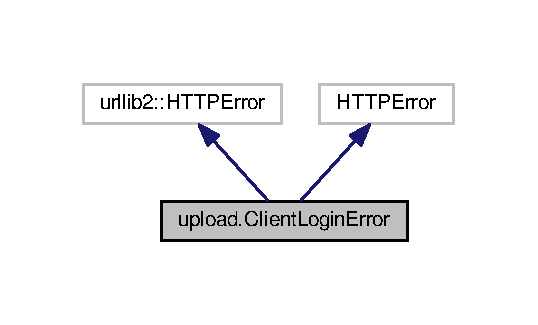
\includegraphics[width=258pt]{classupload_1_1ClientLoginError__inherit__graph}
\end{center}
\end{figure}


Collaboration diagram for upload.\+Client\+Login\+Error\+:
\nopagebreak
\begin{figure}[H]
\begin{center}
\leavevmode
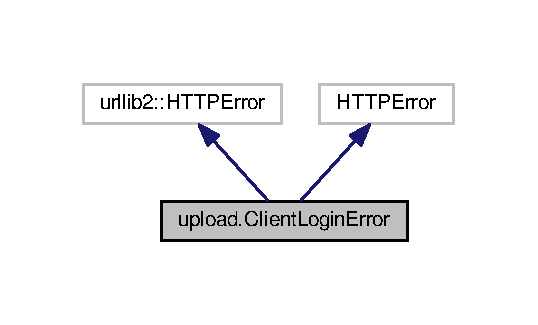
\includegraphics[width=258pt]{classupload_1_1ClientLoginError__coll__graph}
\end{center}
\end{figure}
\subsection*{Public Member Functions}
\begin{DoxyCompactItemize}
\item 
def \hyperlink{classupload_1_1ClientLoginError_a1e590616c2976d881e155958cedbbe47}{\+\_\+\+\_\+init\+\_\+\+\_\+} (self, url, code, msg, headers, \hyperlink{classupload_1_1ClientLoginError_ac300a0b034b2bc64cedc51e09fb6d663}{args})
\item 
def \hyperlink{classupload_1_1ClientLoginError_a1e590616c2976d881e155958cedbbe47}{\+\_\+\+\_\+init\+\_\+\+\_\+} (self, url, code, msg, headers, \hyperlink{classupload_1_1ClientLoginError_ac300a0b034b2bc64cedc51e09fb6d663}{args})
\end{DoxyCompactItemize}
\subsection*{Public Attributes}
\begin{DoxyCompactItemize}
\item 
\hyperlink{classupload_1_1ClientLoginError_ac300a0b034b2bc64cedc51e09fb6d663}{args}
\item 
\hyperlink{classupload_1_1ClientLoginError_ae0555feb182d89d1e4d7944afbfe14e5}{reason}
\end{DoxyCompactItemize}


\subsection{Detailed Description}
\begin{DoxyVerb}Raised to indicate there was an error authenticating with ClientLogin.\end{DoxyVerb}
 

\subsection{Constructor \& Destructor Documentation}
\index{upload\+::\+Client\+Login\+Error@{upload\+::\+Client\+Login\+Error}!\+\_\+\+\_\+init\+\_\+\+\_\+@{\+\_\+\+\_\+init\+\_\+\+\_\+}}
\index{\+\_\+\+\_\+init\+\_\+\+\_\+@{\+\_\+\+\_\+init\+\_\+\+\_\+}!upload\+::\+Client\+Login\+Error@{upload\+::\+Client\+Login\+Error}}
\subsubsection[{\texorpdfstring{\+\_\+\+\_\+init\+\_\+\+\_\+(self, url, code, msg, headers, args)}{__init__(self, url, code, msg, headers, args)}}]{\setlength{\rightskip}{0pt plus 5cm}def upload.\+Client\+Login\+Error.\+\_\+\+\_\+init\+\_\+\+\_\+ (
\begin{DoxyParamCaption}
\item[{}]{self, }
\item[{}]{url, }
\item[{}]{code, }
\item[{}]{msg, }
\item[{}]{headers, }
\item[{}]{args}
\end{DoxyParamCaption}
)}\hypertarget{classupload_1_1ClientLoginError_a1e590616c2976d881e155958cedbbe47}{}\label{classupload_1_1ClientLoginError_a1e590616c2976d881e155958cedbbe47}

\begin{DoxyCode}
118   \textcolor{keyword}{def }\_\_init\_\_(self, url, code, msg, headers, args):
119     urllib2.HTTPError.\_\_init\_\_(self, url, code, msg, headers, \textcolor{keywordtype}{None})
120     self.args = args
121     self.reason = args[\textcolor{stringliteral}{"Error"}]
122 
123 
\end{DoxyCode}
\index{upload\+::\+Client\+Login\+Error@{upload\+::\+Client\+Login\+Error}!\+\_\+\+\_\+init\+\_\+\+\_\+@{\+\_\+\+\_\+init\+\_\+\+\_\+}}
\index{\+\_\+\+\_\+init\+\_\+\+\_\+@{\+\_\+\+\_\+init\+\_\+\+\_\+}!upload\+::\+Client\+Login\+Error@{upload\+::\+Client\+Login\+Error}}
\subsubsection[{\texorpdfstring{\+\_\+\+\_\+init\+\_\+\+\_\+(self, url, code, msg, headers, args)}{__init__(self, url, code, msg, headers, args)}}]{\setlength{\rightskip}{0pt plus 5cm}def upload.\+Client\+Login\+Error.\+\_\+\+\_\+init\+\_\+\+\_\+ (
\begin{DoxyParamCaption}
\item[{}]{self, }
\item[{}]{url, }
\item[{}]{code, }
\item[{}]{msg, }
\item[{}]{headers, }
\item[{}]{args}
\end{DoxyParamCaption}
)}\hypertarget{classupload_1_1ClientLoginError_a1e590616c2976d881e155958cedbbe47}{}\label{classupload_1_1ClientLoginError_a1e590616c2976d881e155958cedbbe47}

\begin{DoxyCode}
118   \textcolor{keyword}{def }\_\_init\_\_(self, url, code, msg, headers, args):
119     urllib2.HTTPError.\_\_init\_\_(self, url, code, msg, headers, \textcolor{keywordtype}{None})
120     self.args = args
121     self.reason = args[\textcolor{stringliteral}{"Error"}]
122 
123 
\end{DoxyCode}


\subsection{Member Data Documentation}
\index{upload\+::\+Client\+Login\+Error@{upload\+::\+Client\+Login\+Error}!args@{args}}
\index{args@{args}!upload\+::\+Client\+Login\+Error@{upload\+::\+Client\+Login\+Error}}
\subsubsection[{\texorpdfstring{args}{args}}]{\setlength{\rightskip}{0pt plus 5cm}upload.\+Client\+Login\+Error.\+args}\hypertarget{classupload_1_1ClientLoginError_ac300a0b034b2bc64cedc51e09fb6d663}{}\label{classupload_1_1ClientLoginError_ac300a0b034b2bc64cedc51e09fb6d663}
\index{upload\+::\+Client\+Login\+Error@{upload\+::\+Client\+Login\+Error}!reason@{reason}}
\index{reason@{reason}!upload\+::\+Client\+Login\+Error@{upload\+::\+Client\+Login\+Error}}
\subsubsection[{\texorpdfstring{reason}{reason}}]{\setlength{\rightskip}{0pt plus 5cm}upload.\+Client\+Login\+Error.\+reason}\hypertarget{classupload_1_1ClientLoginError_ae0555feb182d89d1e4d7944afbfe14e5}{}\label{classupload_1_1ClientLoginError_ae0555feb182d89d1e4d7944afbfe14e5}


The documentation for this class was generated from the following file\+:\begin{DoxyCompactItemize}
\item 
vendor/googletest/googlemock/scripts/\hyperlink{googlemock_2scripts_2upload_8py}{upload.\+py}\end{DoxyCompactItemize}

\hypertarget{structtesting_1_1internal_1_1CodeLocation}{}\section{testing\+:\+:internal\+:\+:Code\+Location Struct Reference}
\label{structtesting_1_1internal_1_1CodeLocation}\index{testing\+::internal\+::\+Code\+Location@{testing\+::internal\+::\+Code\+Location}}


{\ttfamily \#include $<$gtest-\/internal.\+h$>$}

\subsection*{Public Member Functions}
\begin{DoxyCompactItemize}
\item 
\hyperlink{structtesting_1_1internal_1_1CodeLocation_ade3ecb2a54905619cd40a6856b48cd5a}{Code\+Location} (const \hyperlink{namespacetesting_1_1internal_a8e8ff5b11e64078831112677156cb111}{string} \&a\+\_\+file, int a\+\_\+line)
\end{DoxyCompactItemize}
\subsection*{Public Attributes}
\begin{DoxyCompactItemize}
\item 
\hyperlink{namespacetesting_1_1internal_a8e8ff5b11e64078831112677156cb111}{string} \hyperlink{structtesting_1_1internal_1_1CodeLocation_ab8a24d5e63295e411d37578dbb9427c0}{file}
\item 
int \hyperlink{structtesting_1_1internal_1_1CodeLocation_a01c977c7e8834a05a6d6c40b0c416045}{line}
\end{DoxyCompactItemize}


\subsection{Constructor \& Destructor Documentation}
\index{testing\+::internal\+::\+Code\+Location@{testing\+::internal\+::\+Code\+Location}!Code\+Location@{Code\+Location}}
\index{Code\+Location@{Code\+Location}!testing\+::internal\+::\+Code\+Location@{testing\+::internal\+::\+Code\+Location}}
\subsubsection[{\texorpdfstring{Code\+Location(const string \&a\+\_\+file, int a\+\_\+line)}{CodeLocation(const string &a_file, int a_line)}}]{\setlength{\rightskip}{0pt plus 5cm}testing\+::internal\+::\+Code\+Location\+::\+Code\+Location (
\begin{DoxyParamCaption}
\item[{const {\bf string} \&}]{a\+\_\+file, }
\item[{int}]{a\+\_\+line}
\end{DoxyParamCaption}
)\hspace{0.3cm}{\ttfamily [inline]}}\hypertarget{structtesting_1_1internal_1_1CodeLocation_ade3ecb2a54905619cd40a6856b48cd5a}{}\label{structtesting_1_1internal_1_1CodeLocation_ade3ecb2a54905619cd40a6856b48cd5a}

\begin{DoxyCode}
505 : \hyperlink{structtesting_1_1internal_1_1CodeLocation_ab8a24d5e63295e411d37578dbb9427c0}{file}(a\_file), \hyperlink{structtesting_1_1internal_1_1CodeLocation_a01c977c7e8834a05a6d6c40b0c416045}{line}(a\_line) \{\}
\end{DoxyCode}


\subsection{Member Data Documentation}
\index{testing\+::internal\+::\+Code\+Location@{testing\+::internal\+::\+Code\+Location}!file@{file}}
\index{file@{file}!testing\+::internal\+::\+Code\+Location@{testing\+::internal\+::\+Code\+Location}}
\subsubsection[{\texorpdfstring{file}{file}}]{\setlength{\rightskip}{0pt plus 5cm}{\bf string} testing\+::internal\+::\+Code\+Location\+::file}\hypertarget{structtesting_1_1internal_1_1CodeLocation_ab8a24d5e63295e411d37578dbb9427c0}{}\label{structtesting_1_1internal_1_1CodeLocation_ab8a24d5e63295e411d37578dbb9427c0}
\index{testing\+::internal\+::\+Code\+Location@{testing\+::internal\+::\+Code\+Location}!line@{line}}
\index{line@{line}!testing\+::internal\+::\+Code\+Location@{testing\+::internal\+::\+Code\+Location}}
\subsubsection[{\texorpdfstring{line}{line}}]{\setlength{\rightskip}{0pt plus 5cm}int testing\+::internal\+::\+Code\+Location\+::line}\hypertarget{structtesting_1_1internal_1_1CodeLocation_a01c977c7e8834a05a6d6c40b0c416045}{}\label{structtesting_1_1internal_1_1CodeLocation_a01c977c7e8834a05a6d6c40b0c416045}


The documentation for this struct was generated from the following file\+:\begin{DoxyCompactItemize}
\item 
vendor/googletest/googletest/include/gtest/internal/\hyperlink{gtest-internal_8h}{gtest-\/internal.\+h}\end{DoxyCompactItemize}

\hypertarget{classtesting_1_1CodeLocationForTESTF}{}\section{testing\+:\+:Code\+Location\+For\+T\+E\+S\+TF Class Reference}
\label{classtesting_1_1CodeLocationForTESTF}\index{testing\+::\+Code\+Location\+For\+T\+E\+S\+TF@{testing\+::\+Code\+Location\+For\+T\+E\+S\+TF}}


Inheritance diagram for testing\+:\+:Code\+Location\+For\+T\+E\+S\+TF\+:
\nopagebreak
\begin{figure}[H]
\begin{center}
\leavevmode
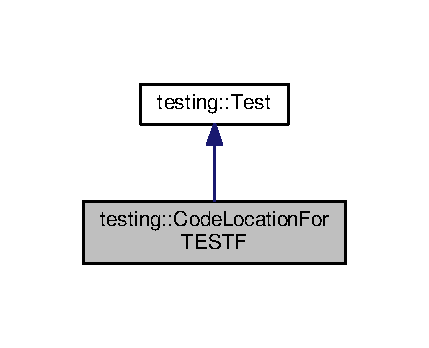
\includegraphics[width=206pt]{classtesting_1_1CodeLocationForTESTF__inherit__graph}
\end{center}
\end{figure}


Collaboration diagram for testing\+:\+:Code\+Location\+For\+T\+E\+S\+TF\+:
\nopagebreak
\begin{figure}[H]
\begin{center}
\leavevmode
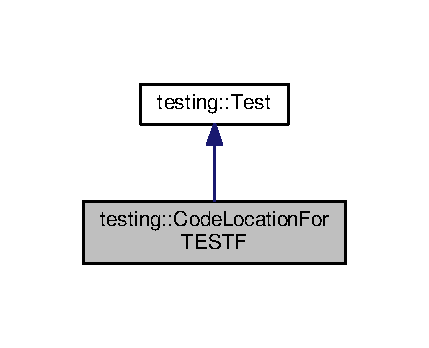
\includegraphics[width=206pt]{classtesting_1_1CodeLocationForTESTF__coll__graph}
\end{center}
\end{figure}
\subsection*{Additional Inherited Members}


The documentation for this class was generated from the following file\+:\begin{DoxyCompactItemize}
\item 
vendor/googletest/googletest/test/\hyperlink{gtest__unittest_8cc}{gtest\+\_\+unittest.\+cc}\end{DoxyCompactItemize}

\hypertarget{classtesting_1_1CodeLocationForTESTP}{}\section{testing\+:\+:Code\+Location\+For\+T\+E\+S\+TP Class Reference}
\label{classtesting_1_1CodeLocationForTESTP}\index{testing\+::\+Code\+Location\+For\+T\+E\+S\+TP@{testing\+::\+Code\+Location\+For\+T\+E\+S\+TP}}


Inheritance diagram for testing\+:\+:Code\+Location\+For\+T\+E\+S\+TP\+:\nopagebreak
\begin{figure}[H]
\begin{center}
\leavevmode
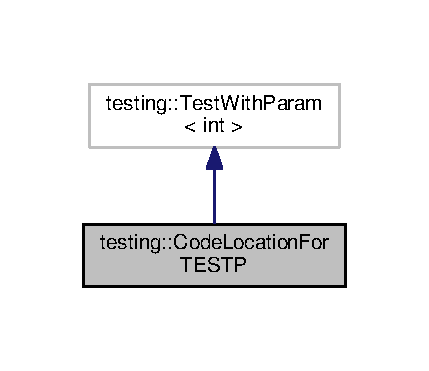
\includegraphics[width=206pt]{classtesting_1_1CodeLocationForTESTP__inherit__graph}
\end{center}
\end{figure}


Collaboration diagram for testing\+:\+:Code\+Location\+For\+T\+E\+S\+TP\+:\nopagebreak
\begin{figure}[H]
\begin{center}
\leavevmode
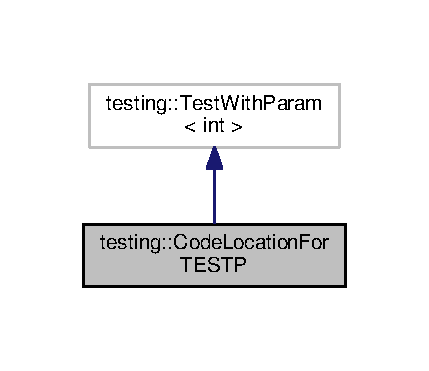
\includegraphics[width=206pt]{classtesting_1_1CodeLocationForTESTP__coll__graph}
\end{center}
\end{figure}


The documentation for this class was generated from the following file\+:\begin{DoxyCompactItemize}
\item 
vendor/googletest/googletest/test/\hyperlink{gtest__unittest_8cc}{gtest\+\_\+unittest.\+cc}\end{DoxyCompactItemize}

\hypertarget{classtesting_1_1CodeLocationForTYPEDTEST}{}\section{testing\+:\+:Code\+Location\+For\+T\+Y\+P\+E\+D\+T\+E\+ST$<$ T $>$ Class Template Reference}
\label{classtesting_1_1CodeLocationForTYPEDTEST}\index{testing\+::\+Code\+Location\+For\+T\+Y\+P\+E\+D\+T\+E\+S\+T$<$ T $>$@{testing\+::\+Code\+Location\+For\+T\+Y\+P\+E\+D\+T\+E\+S\+T$<$ T $>$}}


Inheritance diagram for testing\+:\+:Code\+Location\+For\+T\+Y\+P\+E\+D\+T\+E\+ST$<$ T $>$\+:
\nopagebreak
\begin{figure}[H]
\begin{center}
\leavevmode
\includegraphics[width=206pt]{classtesting_1_1CodeLocationForTYPEDTEST__inherit__graph}
\end{center}
\end{figure}


Collaboration diagram for testing\+:\+:Code\+Location\+For\+T\+Y\+P\+E\+D\+T\+E\+ST$<$ T $>$\+:
\nopagebreak
\begin{figure}[H]
\begin{center}
\leavevmode
\includegraphics[width=206pt]{classtesting_1_1CodeLocationForTYPEDTEST__coll__graph}
\end{center}
\end{figure}
\subsection*{Additional Inherited Members}


The documentation for this class was generated from the following file\+:\begin{DoxyCompactItemize}
\item 
vendor/googletest/googletest/test/\hyperlink{gtest__unittest_8cc}{gtest\+\_\+unittest.\+cc}\end{DoxyCompactItemize}

\hypertarget{classtesting_1_1CodeLocationForTYPEDTESTP}{}\section{testing\+:\+:Code\+Location\+For\+T\+Y\+P\+E\+D\+T\+E\+S\+TP$<$ T $>$ Class Template Reference}
\label{classtesting_1_1CodeLocationForTYPEDTESTP}\index{testing\+::\+Code\+Location\+For\+T\+Y\+P\+E\+D\+T\+E\+S\+T\+P$<$ T $>$@{testing\+::\+Code\+Location\+For\+T\+Y\+P\+E\+D\+T\+E\+S\+T\+P$<$ T $>$}}


Inheritance diagram for testing\+:\+:Code\+Location\+For\+T\+Y\+P\+E\+D\+T\+E\+S\+TP$<$ T $>$\+:
\nopagebreak
\begin{figure}[H]
\begin{center}
\leavevmode
\includegraphics[width=206pt]{classtesting_1_1CodeLocationForTYPEDTESTP__inherit__graph}
\end{center}
\end{figure}


Collaboration diagram for testing\+:\+:Code\+Location\+For\+T\+Y\+P\+E\+D\+T\+E\+S\+TP$<$ T $>$\+:
\nopagebreak
\begin{figure}[H]
\begin{center}
\leavevmode
\includegraphics[width=206pt]{classtesting_1_1CodeLocationForTYPEDTESTP__coll__graph}
\end{center}
\end{figure}
\subsection*{Additional Inherited Members}


The documentation for this class was generated from the following file\+:\begin{DoxyCompactItemize}
\item 
vendor/googletest/googletest/test/\hyperlink{gtest__unittest_8cc}{gtest\+\_\+unittest.\+cc}\end{DoxyCompactItemize}

\hypertarget{classpump_1_1CodeNode}{}\section{pump.\+Code\+Node Class Reference}
\label{classpump_1_1CodeNode}\index{pump.\+Code\+Node@{pump.\+Code\+Node}}
\subsection*{Public Member Functions}
\begin{DoxyCompactItemize}
\item 
def \hyperlink{classpump_1_1CodeNode_a2ca8a75324a64e48004812d6c0bc1cbd}{\+\_\+\+\_\+init\+\_\+\+\_\+} (self, atomic\+\_\+code\+\_\+list=None)
\end{DoxyCompactItemize}
\subsection*{Public Attributes}
\begin{DoxyCompactItemize}
\item 
\hyperlink{classpump_1_1CodeNode_ac7251110cc987c709e0e17d95521993e}{atomic\+\_\+code}
\end{DoxyCompactItemize}


\subsection{Constructor \& Destructor Documentation}
\index{pump\+::\+Code\+Node@{pump\+::\+Code\+Node}!\+\_\+\+\_\+init\+\_\+\+\_\+@{\+\_\+\+\_\+init\+\_\+\+\_\+}}
\index{\+\_\+\+\_\+init\+\_\+\+\_\+@{\+\_\+\+\_\+init\+\_\+\+\_\+}!pump\+::\+Code\+Node@{pump\+::\+Code\+Node}}
\subsubsection[{\texorpdfstring{\+\_\+\+\_\+init\+\_\+\+\_\+(self, atomic\+\_\+code\+\_\+list=\+None)}{__init__(self, atomic_code_list=None)}}]{\setlength{\rightskip}{0pt plus 5cm}def pump.\+Code\+Node.\+\_\+\+\_\+init\+\_\+\+\_\+ (
\begin{DoxyParamCaption}
\item[{}]{self, }
\item[{}]{atomic\+\_\+code\+\_\+list = {\ttfamily None}}
\end{DoxyParamCaption}
)}\hypertarget{classpump_1_1CodeNode_a2ca8a75324a64e48004812d6c0bc1cbd}{}\label{classpump_1_1CodeNode_a2ca8a75324a64e48004812d6c0bc1cbd}

\begin{DoxyCode}
391   \textcolor{keyword}{def }\_\_init\_\_(self, atomic\_code\_list=None):
392     self.atomic\_code = atomic\_code\_list
393 
394 
\end{DoxyCode}


\subsection{Member Data Documentation}
\index{pump\+::\+Code\+Node@{pump\+::\+Code\+Node}!atomic\+\_\+code@{atomic\+\_\+code}}
\index{atomic\+\_\+code@{atomic\+\_\+code}!pump\+::\+Code\+Node@{pump\+::\+Code\+Node}}
\subsubsection[{\texorpdfstring{atomic\+\_\+code}{atomic_code}}]{\setlength{\rightskip}{0pt plus 5cm}pump.\+Code\+Node.\+atomic\+\_\+code}\hypertarget{classpump_1_1CodeNode_ac7251110cc987c709e0e17d95521993e}{}\label{classpump_1_1CodeNode_ac7251110cc987c709e0e17d95521993e}


The documentation for this class was generated from the following file\+:\begin{DoxyCompactItemize}
\item 
vendor/googletest/googletest/scripts/\hyperlink{pump_8py}{pump.\+py}\end{DoxyCompactItemize}

\hypertarget{classCommonTest}{}\section{Common\+Test$<$ T $>$ Class Template Reference}
\label{classCommonTest}\index{Common\+Test$<$ T $>$@{Common\+Test$<$ T $>$}}


Inheritance diagram for Common\+Test$<$ T $>$\+:
\nopagebreak
\begin{figure}[H]
\begin{center}
\leavevmode
\includegraphics[width=180pt]{classCommonTest__inherit__graph}
\end{center}
\end{figure}


Collaboration diagram for Common\+Test$<$ T $>$\+:
\nopagebreak
\begin{figure}[H]
\begin{center}
\leavevmode
\includegraphics[width=180pt]{classCommonTest__coll__graph}
\end{center}
\end{figure}
\subsection*{Static Public Member Functions}
\begin{DoxyCompactItemize}
\item 
static void \hyperlink{classCommonTest_a6edd90f32f45cc49e4a423b22bd770ce}{Set\+Up\+Test\+Case} ()
\item 
static void \hyperlink{classCommonTest_a68d2bf5108cf28478331588fbdff4838}{Tear\+Down\+Test\+Case} ()
\end{DoxyCompactItemize}
\subsection*{Protected Types}
\begin{DoxyCompactItemize}
\item 
typedef std\+::vector$<$ T $>$ \hyperlink{classCommonTest_a6dfdcede6964887b9f4254a0e0478e37}{Vector}
\item 
typedef \hyperlink{vendor_2googletest_2googlemock_2CMakeLists_8txt_aa99cc432a5064db15e7653de9d85d2d2}{std\+::set}$<$ int $>$ \hyperlink{classCommonTest_a62827e9d3064cddf4a8698747f1bd434}{Int\+Set}
\end{DoxyCompactItemize}
\subsection*{Protected Member Functions}
\begin{DoxyCompactItemize}
\item 
\hyperlink{classCommonTest_abd5ec205d90f4b81efab2a6f972f3db0}{Common\+Test} ()
\item 
virtual \hyperlink{classCommonTest_a675a632fcf7b1fd961fefc619d6a458d}{$\sim$\+Common\+Test} ()
\item 
virtual void \hyperlink{classCommonTest_a4c7bf7889ce48a9d06530bc4a437f3f5}{Set\+Up} ()
\item 
virtual void \hyperlink{classCommonTest_aeae195c2cefa956c6ae5be1226e6ecd8}{Tear\+Down} ()
\end{DoxyCompactItemize}
\subsection*{Protected Attributes}
\begin{DoxyCompactItemize}
\item 
T \hyperlink{classCommonTest_ae59c4abcb833625a7baeb2048531ebec}{value\+\_\+}
\end{DoxyCompactItemize}
\subsection*{Static Protected Attributes}
\begin{DoxyCompactItemize}
\item 
static T $\ast$ \hyperlink{classCommonTest_a52368ce1e65a865db9bdccbcc2cedaac}{shared\+\_\+} = N\+U\+LL
\end{DoxyCompactItemize}
\subsection*{Additional Inherited Members}


\subsection{Member Typedef Documentation}
\index{Common\+Test@{Common\+Test}!Int\+Set@{Int\+Set}}
\index{Int\+Set@{Int\+Set}!Common\+Test@{Common\+Test}}
\subsubsection[{\texorpdfstring{Int\+Set}{IntSet}}]{\setlength{\rightskip}{0pt plus 5cm}template$<$typename T $>$ typedef {\bf std\+::set}$<$int$>$ {\bf Common\+Test}$<$ T $>$\+::{\bf Int\+Set}\hspace{0.3cm}{\ttfamily [protected]}}\hypertarget{classCommonTest_a62827e9d3064cddf4a8698747f1bd434}{}\label{classCommonTest_a62827e9d3064cddf4a8698747f1bd434}
\index{Common\+Test@{Common\+Test}!Vector@{Vector}}
\index{Vector@{Vector}!Common\+Test@{Common\+Test}}
\subsubsection[{\texorpdfstring{Vector}{Vector}}]{\setlength{\rightskip}{0pt plus 5cm}template$<$typename T $>$ typedef std\+::vector$<$T$>$ {\bf Common\+Test}$<$ T $>$\+::{\bf Vector}\hspace{0.3cm}{\ttfamily [protected]}}\hypertarget{classCommonTest_a6dfdcede6964887b9f4254a0e0478e37}{}\label{classCommonTest_a6dfdcede6964887b9f4254a0e0478e37}


\subsection{Constructor \& Destructor Documentation}
\index{Common\+Test@{Common\+Test}!Common\+Test@{Common\+Test}}
\index{Common\+Test@{Common\+Test}!Common\+Test@{Common\+Test}}
\subsubsection[{\texorpdfstring{Common\+Test()}{CommonTest()}}]{\setlength{\rightskip}{0pt plus 5cm}template$<$typename T $>$ {\bf Common\+Test}$<$ T $>$\+::{\bf Common\+Test} (
\begin{DoxyParamCaption}
{}
\end{DoxyParamCaption}
)\hspace{0.3cm}{\ttfamily [inline]}, {\ttfamily [protected]}}\hypertarget{classCommonTest_abd5ec205d90f4b81efab2a6f972f3db0}{}\label{classCommonTest_abd5ec205d90f4b81efab2a6f972f3db0}

\begin{DoxyCode}
66 : \hyperlink{classCommonTest_ae59c4abcb833625a7baeb2048531ebec}{value\_}(1) \{\}
\end{DoxyCode}
\index{Common\+Test@{Common\+Test}!````~Common\+Test@{$\sim$\+Common\+Test}}
\index{````~Common\+Test@{$\sim$\+Common\+Test}!Common\+Test@{Common\+Test}}
\subsubsection[{\texorpdfstring{$\sim$\+Common\+Test()}{~CommonTest()}}]{\setlength{\rightskip}{0pt plus 5cm}template$<$typename T $>$ virtual {\bf Common\+Test}$<$ T $>$\+::$\sim${\bf Common\+Test} (
\begin{DoxyParamCaption}
{}
\end{DoxyParamCaption}
)\hspace{0.3cm}{\ttfamily [inline]}, {\ttfamily [protected]}, {\ttfamily [virtual]}}\hypertarget{classCommonTest_a675a632fcf7b1fd961fefc619d6a458d}{}\label{classCommonTest_a675a632fcf7b1fd961fefc619d6a458d}

\begin{DoxyCode}
68 \{ \hyperlink{gtest_8h_a4159019abda84f5366acdb7604ff220a}{EXPECT\_EQ}(3, \hyperlink{classCommonTest_ae59c4abcb833625a7baeb2048531ebec}{value\_}); \}
\end{DoxyCode}


\subsection{Member Function Documentation}
\index{Common\+Test@{Common\+Test}!Set\+Up@{Set\+Up}}
\index{Set\+Up@{Set\+Up}!Common\+Test@{Common\+Test}}
\subsubsection[{\texorpdfstring{Set\+Up()}{SetUp()}}]{\setlength{\rightskip}{0pt plus 5cm}template$<$typename T $>$ virtual void {\bf Common\+Test}$<$ T $>$\+::Set\+Up (
\begin{DoxyParamCaption}
{}
\end{DoxyParamCaption}
)\hspace{0.3cm}{\ttfamily [inline]}, {\ttfamily [protected]}, {\ttfamily [virtual]}}\hypertarget{classCommonTest_a4c7bf7889ce48a9d06530bc4a437f3f5}{}\label{classCommonTest_a4c7bf7889ce48a9d06530bc4a437f3f5}


Reimplemented from \hyperlink{classtesting_1_1Test_a190315150c303ddf801313fd1a777733}{testing\+::\+Test}.


\begin{DoxyCode}
70                        \{
71     \hyperlink{gtest_8h_a4159019abda84f5366acdb7604ff220a}{EXPECT\_EQ}(1, \hyperlink{classCommonTest_ae59c4abcb833625a7baeb2048531ebec}{value\_});
72     \hyperlink{classCommonTest_ae59c4abcb833625a7baeb2048531ebec}{value\_}++;
73   \}
\end{DoxyCode}
\index{Common\+Test@{Common\+Test}!Set\+Up\+Test\+Case@{Set\+Up\+Test\+Case}}
\index{Set\+Up\+Test\+Case@{Set\+Up\+Test\+Case}!Common\+Test@{Common\+Test}}
\subsubsection[{\texorpdfstring{Set\+Up\+Test\+Case()}{SetUpTestCase()}}]{\setlength{\rightskip}{0pt plus 5cm}template$<$typename T $>$ static void {\bf Common\+Test}$<$ T $>$\+::Set\+Up\+Test\+Case (
\begin{DoxyParamCaption}
{}
\end{DoxyParamCaption}
)\hspace{0.3cm}{\ttfamily [inline]}, {\ttfamily [static]}}\hypertarget{classCommonTest_a6edd90f32f45cc49e4a423b22bd770ce}{}\label{classCommonTest_a6edd90f32f45cc49e4a423b22bd770ce}

\begin{DoxyCode}
49                               \{
50     \hyperlink{classCommonTest_a52368ce1e65a865db9bdccbcc2cedaac}{shared\_} = \textcolor{keyword}{new} T(5);
51   \}
\end{DoxyCode}
\index{Common\+Test@{Common\+Test}!Tear\+Down@{Tear\+Down}}
\index{Tear\+Down@{Tear\+Down}!Common\+Test@{Common\+Test}}
\subsubsection[{\texorpdfstring{Tear\+Down()}{TearDown()}}]{\setlength{\rightskip}{0pt plus 5cm}template$<$typename T $>$ virtual void {\bf Common\+Test}$<$ T $>$\+::Tear\+Down (
\begin{DoxyParamCaption}
{}
\end{DoxyParamCaption}
)\hspace{0.3cm}{\ttfamily [inline]}, {\ttfamily [protected]}, {\ttfamily [virtual]}}\hypertarget{classCommonTest_aeae195c2cefa956c6ae5be1226e6ecd8}{}\label{classCommonTest_aeae195c2cefa956c6ae5be1226e6ecd8}


Reimplemented from \hyperlink{classtesting_1_1Test_a5f0ab439802cbe0ef7552f1a9f791923}{testing\+::\+Test}.


\begin{DoxyCode}
75                           \{
76     \hyperlink{gtest_8h_a4159019abda84f5366acdb7604ff220a}{EXPECT\_EQ}(2, \hyperlink{classCommonTest_ae59c4abcb833625a7baeb2048531ebec}{value\_});
77     \hyperlink{classCommonTest_ae59c4abcb833625a7baeb2048531ebec}{value\_}++;
78   \}
\end{DoxyCode}
\index{Common\+Test@{Common\+Test}!Tear\+Down\+Test\+Case@{Tear\+Down\+Test\+Case}}
\index{Tear\+Down\+Test\+Case@{Tear\+Down\+Test\+Case}!Common\+Test@{Common\+Test}}
\subsubsection[{\texorpdfstring{Tear\+Down\+Test\+Case()}{TearDownTestCase()}}]{\setlength{\rightskip}{0pt plus 5cm}template$<$typename T $>$ static void {\bf Common\+Test}$<$ T $>$\+::Tear\+Down\+Test\+Case (
\begin{DoxyParamCaption}
{}
\end{DoxyParamCaption}
)\hspace{0.3cm}{\ttfamily [inline]}, {\ttfamily [static]}}\hypertarget{classCommonTest_a68d2bf5108cf28478331588fbdff4838}{}\label{classCommonTest_a68d2bf5108cf28478331588fbdff4838}

\begin{DoxyCode}
53                                  \{
54     \textcolor{keyword}{delete} \hyperlink{classCommonTest_a52368ce1e65a865db9bdccbcc2cedaac}{shared\_};
55     \hyperlink{classCommonTest_a52368ce1e65a865db9bdccbcc2cedaac}{shared\_} = NULL;
56   \}
\end{DoxyCode}


\subsection{Member Data Documentation}
\index{Common\+Test@{Common\+Test}!shared\+\_\+@{shared\+\_\+}}
\index{shared\+\_\+@{shared\+\_\+}!Common\+Test@{Common\+Test}}
\subsubsection[{\texorpdfstring{shared\+\_\+}{shared_}}]{\setlength{\rightskip}{0pt plus 5cm}template$<$typename T $>$ T $\ast$ {\bf Common\+Test}$<$ T $>$\+::shared\+\_\+ = N\+U\+LL\hspace{0.3cm}{\ttfamily [static]}, {\ttfamily [protected]}}\hypertarget{classCommonTest_a52368ce1e65a865db9bdccbcc2cedaac}{}\label{classCommonTest_a52368ce1e65a865db9bdccbcc2cedaac}
\index{Common\+Test@{Common\+Test}!value\+\_\+@{value\+\_\+}}
\index{value\+\_\+@{value\+\_\+}!Common\+Test@{Common\+Test}}
\subsubsection[{\texorpdfstring{value\+\_\+}{value_}}]{\setlength{\rightskip}{0pt plus 5cm}template$<$typename T $>$ T {\bf Common\+Test}$<$ T $>$\+::value\+\_\+\hspace{0.3cm}{\ttfamily [protected]}}\hypertarget{classCommonTest_ae59c4abcb833625a7baeb2048531ebec}{}\label{classCommonTest_ae59c4abcb833625a7baeb2048531ebec}


The documentation for this class was generated from the following file\+:\begin{DoxyCompactItemize}
\item 
vendor/googletest/googletest/test/\hyperlink{gtest-typed-test__test_8cc}{gtest-\/typed-\/test\+\_\+test.\+cc}\end{DoxyCompactItemize}

\hypertarget{classtesting_1_1internal_1_1ComparisonBase}{}\section{testing\+:\+:internal\+:\+:Comparison\+Base$<$ D, Rhs, Op $>$ Class Template Reference}
\label{classtesting_1_1internal_1_1ComparisonBase}\index{testing\+::internal\+::\+Comparison\+Base$<$ D, Rhs, Op $>$@{testing\+::internal\+::\+Comparison\+Base$<$ D, Rhs, Op $>$}}


{\ttfamily \#include $<$gmock-\/matchers.\+h$>$}

\subsection*{Public Member Functions}
\begin{DoxyCompactItemize}
\item 
\hyperlink{classtesting_1_1internal_1_1ComparisonBase_a365f20e35a604195c869ec0c0bc4c3a3}{Comparison\+Base} (const Rhs \&rhs)
\item 
{\footnotesize template$<$typename Lhs $>$ }\\\hyperlink{classtesting_1_1internal_1_1ComparisonBase_a7d329851ff6ecffebe8c1e332504bad3}{operator Matcher$<$ Lhs $>$} () const 
\end{DoxyCompactItemize}


\subsection{Constructor \& Destructor Documentation}
\index{testing\+::internal\+::\+Comparison\+Base@{testing\+::internal\+::\+Comparison\+Base}!Comparison\+Base@{Comparison\+Base}}
\index{Comparison\+Base@{Comparison\+Base}!testing\+::internal\+::\+Comparison\+Base@{testing\+::internal\+::\+Comparison\+Base}}
\subsubsection[{\texorpdfstring{Comparison\+Base(const Rhs \&rhs)}{ComparisonBase(const Rhs &rhs)}}]{\setlength{\rightskip}{0pt plus 5cm}template$<$typename D, typename Rhs, typename Op$>$ {\bf testing\+::internal\+::\+Comparison\+Base}$<$ D, Rhs, Op $>$\+::{\bf Comparison\+Base} (
\begin{DoxyParamCaption}
\item[{const Rhs \&}]{rhs}
\end{DoxyParamCaption}
)\hspace{0.3cm}{\ttfamily [inline]}, {\ttfamily [explicit]}}\hypertarget{classtesting_1_1internal_1_1ComparisonBase_a365f20e35a604195c869ec0c0bc4c3a3}{}\label{classtesting_1_1internal_1_1ComparisonBase_a365f20e35a604195c869ec0c0bc4c3a3}

\begin{DoxyCode}
895 : rhs\_(rhs) \{\}
\end{DoxyCode}


\subsection{Member Function Documentation}
\index{testing\+::internal\+::\+Comparison\+Base@{testing\+::internal\+::\+Comparison\+Base}!operator Matcher$<$ Lhs $>$@{operator Matcher$<$ Lhs $>$}}
\index{operator Matcher$<$ Lhs $>$@{operator Matcher$<$ Lhs $>$}!testing\+::internal\+::\+Comparison\+Base@{testing\+::internal\+::\+Comparison\+Base}}
\subsubsection[{\texorpdfstring{operator Matcher$<$ Lhs $>$() const }{operator Matcher< Lhs >() const }}]{\setlength{\rightskip}{0pt plus 5cm}template$<$typename D, typename Rhs, typename Op$>$ template$<$typename Lhs $>$ {\bf testing\+::internal\+::\+Comparison\+Base}$<$ D, Rhs, Op $>$\+::operator {\bf Matcher}$<$ Lhs $>$ (
\begin{DoxyParamCaption}
{}
\end{DoxyParamCaption}
) const\hspace{0.3cm}{\ttfamily [inline]}}\hypertarget{classtesting_1_1internal_1_1ComparisonBase_a7d329851ff6ecffebe8c1e332504bad3}{}\label{classtesting_1_1internal_1_1ComparisonBase_a7d329851ff6ecffebe8c1e332504bad3}

\begin{DoxyCode}
897                                 \{
898     \textcolor{keywordflow}{return} \hyperlink{namespacetesting_a37fd8029ac00e60952440a3d9cca8166}{MakeMatcher}(\textcolor{keyword}{new} Impl<Lhs>(rhs\_));
899   \}
\end{DoxyCode}


The documentation for this class was generated from the following file\+:\begin{DoxyCompactItemize}
\item 
vendor/googletest/googlemock/include/gmock/\hyperlink{gmock-matchers_8h}{gmock-\/matchers.\+h}\end{DoxyCompactItemize}

\hypertarget{structtesting_1_1internal_1_1CompileAssert}{}\section{testing\+:\+:internal\+:\+:Compile\+Assert$<$ bool $>$ Struct Template Reference}
\label{structtesting_1_1internal_1_1CompileAssert}\index{testing\+::internal\+::\+Compile\+Assert$<$ bool $>$@{testing\+::internal\+::\+Compile\+Assert$<$ bool $>$}}


{\ttfamily \#include $<$gtest-\/port.\+h$>$}



The documentation for this struct was generated from the following file\+:\begin{DoxyCompactItemize}
\item 
vendor/googletest/googletest/include/gtest/internal/\hyperlink{gtest-port_8h}{gtest-\/port.\+h}\end{DoxyCompactItemize}

\hypertarget{structtesting_1_1internal_1_1CompileAssertTypesEqual}{}\section{testing\+:\+:internal\+:\+:Compile\+Assert\+Types\+Equal$<$ T1, T2 $>$ Struct Template Reference}
\label{structtesting_1_1internal_1_1CompileAssertTypesEqual}\index{testing\+::internal\+::\+Compile\+Assert\+Types\+Equal$<$ T1, T2 $>$@{testing\+::internal\+::\+Compile\+Assert\+Types\+Equal$<$ T1, T2 $>$}}


{\ttfamily \#include $<$gtest-\/internal.\+h$>$}



The documentation for this struct was generated from the following file\+:\begin{DoxyCompactItemize}
\item 
vendor/googletest/googletest/include/gtest/internal/\hyperlink{gtest-internal_8h}{gtest-\/internal.\+h}\end{DoxyCompactItemize}

\hypertarget{structtesting_1_1internal_1_1CompileAssertTypesEqual_3_01T_00_01T_01_4}{}\section{testing\+:\+:internal\+:\+:Compile\+Assert\+Types\+Equal$<$ T, T $>$ Struct Template Reference}
\label{structtesting_1_1internal_1_1CompileAssertTypesEqual_3_01T_00_01T_01_4}\index{testing\+::internal\+::\+Compile\+Assert\+Types\+Equal$<$ T, T $>$@{testing\+::internal\+::\+Compile\+Assert\+Types\+Equal$<$ T, T $>$}}


{\ttfamily \#include $<$gtest-\/internal.\+h$>$}



The documentation for this struct was generated from the following file\+:\begin{DoxyCompactItemize}
\item 
vendor/googletest/googletest/include/gtest/internal/\hyperlink{gtest-internal_8h}{gtest-\/internal.\+h}\end{DoxyCompactItemize}

\hypertarget{structtesting_1_1gtest__printers__test_1_1const__iterator}{}\section{testing\+:\+:gtest\+\_\+printers\+\_\+test\+:\+:const\+\_\+iterator Struct Reference}
\label{structtesting_1_1gtest__printers__test_1_1const__iterator}\index{testing\+::gtest\+\_\+printers\+\_\+test\+::const\+\_\+iterator@{testing\+::gtest\+\_\+printers\+\_\+test\+::const\+\_\+iterator}}
\subsection*{Public Attributes}
\begin{DoxyCompactItemize}
\item 
char \hyperlink{structtesting_1_1gtest__printers__test_1_1const__iterator_a4412dbc1c37c2bc5211971f0c8176d6b}{x}
\end{DoxyCompactItemize}


\subsection{Member Data Documentation}
\index{testing\+::gtest\+\_\+printers\+\_\+test\+::const\+\_\+iterator@{testing\+::gtest\+\_\+printers\+\_\+test\+::const\+\_\+iterator}!x@{x}}
\index{x@{x}!testing\+::gtest\+\_\+printers\+\_\+test\+::const\+\_\+iterator@{testing\+::gtest\+\_\+printers\+\_\+test\+::const\+\_\+iterator}}
\subsubsection[{\texorpdfstring{x}{x}}]{\setlength{\rightskip}{0pt plus 5cm}char testing\+::gtest\+\_\+printers\+\_\+test\+::const\+\_\+iterator\+::x}\hypertarget{structtesting_1_1gtest__printers__test_1_1const__iterator_a4412dbc1c37c2bc5211971f0c8176d6b}{}\label{structtesting_1_1gtest__printers__test_1_1const__iterator_a4412dbc1c37c2bc5211971f0c8176d6b}


The documentation for this struct was generated from the following file\+:\begin{DoxyCompactItemize}
\item 
vendor/googletest/googletest/test/\hyperlink{gtest-printers__test_8cc}{gtest-\/printers\+\_\+test.\+cc}\end{DoxyCompactItemize}

\hypertarget{classtesting_1_1internal_1_1ConstAndNonConstCastable}{}\section{testing\+:\+:internal\+:\+:Const\+And\+Non\+Const\+Castable Class Reference}
\label{classtesting_1_1internal_1_1ConstAndNonConstCastable}\index{testing\+::internal\+::\+Const\+And\+Non\+Const\+Castable@{testing\+::internal\+::\+Const\+And\+Non\+Const\+Castable}}
\subsection*{Public Member Functions}
\begin{DoxyCompactItemize}
\item 
\hyperlink{classtesting_1_1internal_1_1ConstAndNonConstCastable_aebe0ef6897b7f805e227bb969d4ee034}{Const\+And\+Non\+Const\+Castable} (bool $\ast$converted, bool $\ast$const\+\_\+converted)
\item 
\hyperlink{classtesting_1_1internal_1_1ConstAndNonConstCastable_aff0c372d429d76d002bb29f83f2429fa}{operator Base} ()
\item 
\hyperlink{classtesting_1_1internal_1_1ConstAndNonConstCastable_accd7e89982de250ed6c1b3ad1a5813df}{operator Base} () const 
\end{DoxyCompactItemize}


\subsection{Constructor \& Destructor Documentation}
\index{testing\+::internal\+::\+Const\+And\+Non\+Const\+Castable@{testing\+::internal\+::\+Const\+And\+Non\+Const\+Castable}!Const\+And\+Non\+Const\+Castable@{Const\+And\+Non\+Const\+Castable}}
\index{Const\+And\+Non\+Const\+Castable@{Const\+And\+Non\+Const\+Castable}!testing\+::internal\+::\+Const\+And\+Non\+Const\+Castable@{testing\+::internal\+::\+Const\+And\+Non\+Const\+Castable}}
\subsubsection[{\texorpdfstring{Const\+And\+Non\+Const\+Castable(bool $\ast$converted, bool $\ast$const\+\_\+converted)}{ConstAndNonConstCastable(bool *converted, bool *const_converted)}}]{\setlength{\rightskip}{0pt plus 5cm}testing\+::internal\+::\+Const\+And\+Non\+Const\+Castable\+::\+Const\+And\+Non\+Const\+Castable (
\begin{DoxyParamCaption}
\item[{bool $\ast$}]{converted, }
\item[{bool $\ast$}]{const\+\_\+converted}
\end{DoxyParamCaption}
)\hspace{0.3cm}{\ttfamily [inline]}}\hypertarget{classtesting_1_1internal_1_1ConstAndNonConstCastable_aebe0ef6897b7f805e227bb969d4ee034}{}\label{classtesting_1_1internal_1_1ConstAndNonConstCastable_aebe0ef6897b7f805e227bb969d4ee034}

\begin{DoxyCode}
171       : converted\_(converted), const\_converted\_(const\_converted) \{\}
\end{DoxyCode}


\subsection{Member Function Documentation}
\index{testing\+::internal\+::\+Const\+And\+Non\+Const\+Castable@{testing\+::internal\+::\+Const\+And\+Non\+Const\+Castable}!operator Base@{operator Base}}
\index{operator Base@{operator Base}!testing\+::internal\+::\+Const\+And\+Non\+Const\+Castable@{testing\+::internal\+::\+Const\+And\+Non\+Const\+Castable}}
\subsubsection[{\texorpdfstring{operator Base()}{operator Base()}}]{\setlength{\rightskip}{0pt plus 5cm}testing\+::internal\+::\+Const\+And\+Non\+Const\+Castable\+::operator {\bf Base} (
\begin{DoxyParamCaption}
{}
\end{DoxyParamCaption}
)\hspace{0.3cm}{\ttfamily [inline]}}\hypertarget{classtesting_1_1internal_1_1ConstAndNonConstCastable_aff0c372d429d76d002bb29f83f2429fa}{}\label{classtesting_1_1internal_1_1ConstAndNonConstCastable_aff0c372d429d76d002bb29f83f2429fa}

\begin{DoxyCode}
172                   \{
173     *converted\_ = \textcolor{keyword}{true};
174     \textcolor{keywordflow}{return} Base();
175   \}
\end{DoxyCode}
\index{testing\+::internal\+::\+Const\+And\+Non\+Const\+Castable@{testing\+::internal\+::\+Const\+And\+Non\+Const\+Castable}!operator Base@{operator Base}}
\index{operator Base@{operator Base}!testing\+::internal\+::\+Const\+And\+Non\+Const\+Castable@{testing\+::internal\+::\+Const\+And\+Non\+Const\+Castable}}
\subsubsection[{\texorpdfstring{operator Base() const }{operator Base() const }}]{\setlength{\rightskip}{0pt plus 5cm}testing\+::internal\+::\+Const\+And\+Non\+Const\+Castable\+::operator {\bf Base} (
\begin{DoxyParamCaption}
{}
\end{DoxyParamCaption}
) const\hspace{0.3cm}{\ttfamily [inline]}}\hypertarget{classtesting_1_1internal_1_1ConstAndNonConstCastable_accd7e89982de250ed6c1b3ad1a5813df}{}\label{classtesting_1_1internal_1_1ConstAndNonConstCastable_accd7e89982de250ed6c1b3ad1a5813df}

\begin{DoxyCode}
176                         \{
177     *const\_converted\_ = \textcolor{keyword}{true};
178     \textcolor{keywordflow}{return} Base();
179   \}
\end{DoxyCode}


The documentation for this class was generated from the following file\+:\begin{DoxyCompactItemize}
\item 
vendor/googletest/googletest/test/\hyperlink{gtest-port__test_8cc}{gtest-\/port\+\_\+test.\+cc}\end{DoxyCompactItemize}

\hypertarget{classtesting_1_1internal_1_1ConstCastable}{}\section{testing\+:\+:internal\+:\+:Const\+Castable Class Reference}
\label{classtesting_1_1internal_1_1ConstCastable}\index{testing\+::internal\+::\+Const\+Castable@{testing\+::internal\+::\+Const\+Castable}}
\subsection*{Public Member Functions}
\begin{DoxyCompactItemize}
\item 
\hyperlink{classtesting_1_1internal_1_1ConstCastable_a78eba470cc71528237a33a10a92fba7e}{Const\+Castable} (bool $\ast$converted)
\item 
\hyperlink{classtesting_1_1internal_1_1ConstCastable_ad25d1fcc7288a3cf9160620949e37712}{operator Base} () const 
\end{DoxyCompactItemize}


\subsection{Constructor \& Destructor Documentation}
\index{testing\+::internal\+::\+Const\+Castable@{testing\+::internal\+::\+Const\+Castable}!Const\+Castable@{Const\+Castable}}
\index{Const\+Castable@{Const\+Castable}!testing\+::internal\+::\+Const\+Castable@{testing\+::internal\+::\+Const\+Castable}}
\subsubsection[{\texorpdfstring{Const\+Castable(bool $\ast$converted)}{ConstCastable(bool *converted)}}]{\setlength{\rightskip}{0pt plus 5cm}testing\+::internal\+::\+Const\+Castable\+::\+Const\+Castable (
\begin{DoxyParamCaption}
\item[{bool $\ast$}]{converted}
\end{DoxyParamCaption}
)\hspace{0.3cm}{\ttfamily [inline]}, {\ttfamily [explicit]}}\hypertarget{classtesting_1_1internal_1_1ConstCastable_a78eba470cc71528237a33a10a92fba7e}{}\label{classtesting_1_1internal_1_1ConstCastable_a78eba470cc71528237a33a10a92fba7e}

\begin{DoxyCode}
151 : converted\_(converted) \{\}
\end{DoxyCode}


\subsection{Member Function Documentation}
\index{testing\+::internal\+::\+Const\+Castable@{testing\+::internal\+::\+Const\+Castable}!operator Base@{operator Base}}
\index{operator Base@{operator Base}!testing\+::internal\+::\+Const\+Castable@{testing\+::internal\+::\+Const\+Castable}}
\subsubsection[{\texorpdfstring{operator Base() const }{operator Base() const }}]{\setlength{\rightskip}{0pt plus 5cm}testing\+::internal\+::\+Const\+Castable\+::operator {\bf Base} (
\begin{DoxyParamCaption}
{}
\end{DoxyParamCaption}
) const\hspace{0.3cm}{\ttfamily [inline]}}\hypertarget{classtesting_1_1internal_1_1ConstCastable_ad25d1fcc7288a3cf9160620949e37712}{}\label{classtesting_1_1internal_1_1ConstCastable_ad25d1fcc7288a3cf9160620949e37712}

\begin{DoxyCode}
152                         \{
153     *converted\_ = \textcolor{keyword}{true};
154     \textcolor{keywordflow}{return} Base();
155   \}
\end{DoxyCode}


The documentation for this class was generated from the following file\+:\begin{DoxyCompactItemize}
\item 
vendor/googletest/googletest/test/\hyperlink{gtest-port__test_8cc}{gtest-\/port\+\_\+test.\+cc}\end{DoxyCompactItemize}

\hypertarget{structtesting_1_1internal_1_1ConstCharPtr}{}\section{testing\+:\+:internal\+:\+:Const\+Char\+Ptr Struct Reference}
\label{structtesting_1_1internal_1_1ConstCharPtr}\index{testing\+::internal\+::\+Const\+Char\+Ptr@{testing\+::internal\+::\+Const\+Char\+Ptr}}


{\ttfamily \#include $<$gtest-\/internal.\+h$>$}

\subsection*{Public Member Functions}
\begin{DoxyCompactItemize}
\item 
\hyperlink{structtesting_1_1internal_1_1ConstCharPtr_ae94f6453fa679d815994eccc63062907}{Const\+Char\+Ptr} (const char $\ast$str)
\item 
\hyperlink{structtesting_1_1internal_1_1ConstCharPtr_a891bc286350b81d1a147101c0bae5b1d}{operator bool} () const 
\end{DoxyCompactItemize}
\subsection*{Public Attributes}
\begin{DoxyCompactItemize}
\item 
const char $\ast$ \hyperlink{structtesting_1_1internal_1_1ConstCharPtr_adba40d23d5986904b605946f643cf26e}{value}
\end{DoxyCompactItemize}


\subsection{Constructor \& Destructor Documentation}
\index{testing\+::internal\+::\+Const\+Char\+Ptr@{testing\+::internal\+::\+Const\+Char\+Ptr}!Const\+Char\+Ptr@{Const\+Char\+Ptr}}
\index{Const\+Char\+Ptr@{Const\+Char\+Ptr}!testing\+::internal\+::\+Const\+Char\+Ptr@{testing\+::internal\+::\+Const\+Char\+Ptr}}
\subsubsection[{\texorpdfstring{Const\+Char\+Ptr(const char $\ast$str)}{ConstCharPtr(const char *str)}}]{\setlength{\rightskip}{0pt plus 5cm}testing\+::internal\+::\+Const\+Char\+Ptr\+::\+Const\+Char\+Ptr (
\begin{DoxyParamCaption}
\item[{const char $\ast$}]{str}
\end{DoxyParamCaption}
)\hspace{0.3cm}{\ttfamily [inline]}}\hypertarget{structtesting_1_1internal_1_1ConstCharPtr_ae94f6453fa679d815994eccc63062907}{}\label{structtesting_1_1internal_1_1ConstCharPtr_ae94f6453fa679d815994eccc63062907}

\begin{DoxyCode}
742 : \hyperlink{structtesting_1_1internal_1_1ConstCharPtr_adba40d23d5986904b605946f643cf26e}{value}(str) \{\}
\end{DoxyCode}


\subsection{Member Function Documentation}
\index{testing\+::internal\+::\+Const\+Char\+Ptr@{testing\+::internal\+::\+Const\+Char\+Ptr}!operator bool@{operator bool}}
\index{operator bool@{operator bool}!testing\+::internal\+::\+Const\+Char\+Ptr@{testing\+::internal\+::\+Const\+Char\+Ptr}}
\subsubsection[{\texorpdfstring{operator bool() const }{operator bool() const }}]{\setlength{\rightskip}{0pt plus 5cm}testing\+::internal\+::\+Const\+Char\+Ptr\+::operator bool (
\begin{DoxyParamCaption}
{}
\end{DoxyParamCaption}
) const\hspace{0.3cm}{\ttfamily [inline]}}\hypertarget{structtesting_1_1internal_1_1ConstCharPtr_a891bc286350b81d1a147101c0bae5b1d}{}\label{structtesting_1_1internal_1_1ConstCharPtr_a891bc286350b81d1a147101c0bae5b1d}

\begin{DoxyCode}
743 \{ \textcolor{keywordflow}{return} \textcolor{keyword}{true}; \}
\end{DoxyCode}


\subsection{Member Data Documentation}
\index{testing\+::internal\+::\+Const\+Char\+Ptr@{testing\+::internal\+::\+Const\+Char\+Ptr}!value@{value}}
\index{value@{value}!testing\+::internal\+::\+Const\+Char\+Ptr@{testing\+::internal\+::\+Const\+Char\+Ptr}}
\subsubsection[{\texorpdfstring{value}{value}}]{\setlength{\rightskip}{0pt plus 5cm}const char$\ast$ testing\+::internal\+::\+Const\+Char\+Ptr\+::value}\hypertarget{structtesting_1_1internal_1_1ConstCharPtr_adba40d23d5986904b605946f643cf26e}{}\label{structtesting_1_1internal_1_1ConstCharPtr_adba40d23d5986904b605946f643cf26e}


The documentation for this struct was generated from the following file\+:\begin{DoxyCompactItemize}
\item 
vendor/googletest/googletest/include/gtest/internal/\hyperlink{gtest-internal_8h}{gtest-\/internal.\+h}\end{DoxyCompactItemize}

\hypertarget{classtesting_1_1gmock__matchers__test_1_1ConstPropagatingPtr}{}\section{testing\+:\+:gmock\+\_\+matchers\+\_\+test\+:\+:Const\+Propagating\+Ptr$<$ T $>$ Class Template Reference}
\label{classtesting_1_1gmock__matchers__test_1_1ConstPropagatingPtr}\index{testing\+::gmock\+\_\+matchers\+\_\+test\+::\+Const\+Propagating\+Ptr$<$ T $>$@{testing\+::gmock\+\_\+matchers\+\_\+test\+::\+Const\+Propagating\+Ptr$<$ T $>$}}
\subsection*{Public Types}
\begin{DoxyCompactItemize}
\item 
typedef T \hyperlink{classtesting_1_1gmock__matchers__test_1_1ConstPropagatingPtr_a2ad1f3127185fadd33eed42627ed5644}{element\+\_\+type}
\end{DoxyCompactItemize}
\subsection*{Public Member Functions}
\begin{DoxyCompactItemize}
\item 
\hyperlink{classtesting_1_1gmock__matchers__test_1_1ConstPropagatingPtr_abdda67deda67ed234da2231fd86f05ed}{Const\+Propagating\+Ptr} ()
\item 
\hyperlink{classtesting_1_1gmock__matchers__test_1_1ConstPropagatingPtr_a06da70663daa274fb8ca3352f039d609}{Const\+Propagating\+Ptr} (T $\ast$t)
\item 
\hyperlink{classtesting_1_1gmock__matchers__test_1_1ConstPropagatingPtr_ae7620c62ba340603968896d5d5400ed1}{Const\+Propagating\+Ptr} (const \hyperlink{classtesting_1_1gmock__matchers__test_1_1ConstPropagatingPtr}{Const\+Propagating\+Ptr} \&other)
\item 
T $\ast$ \hyperlink{classtesting_1_1gmock__matchers__test_1_1ConstPropagatingPtr_a39a09d46453380ec1b8be8ce40adc453}{get} ()
\item 
T \& \hyperlink{classtesting_1_1gmock__matchers__test_1_1ConstPropagatingPtr_ad77bbeaa18f84cbd6f3dc7021904f1e3}{operator$\ast$} ()
\item 
const T $\ast$ \hyperlink{classtesting_1_1gmock__matchers__test_1_1ConstPropagatingPtr_ade099bee4b0eaa5ad099e517028b2e7a}{get} () const 
\item 
const T \& \hyperlink{classtesting_1_1gmock__matchers__test_1_1ConstPropagatingPtr_a20a9b4f384b63bf52cf8caa138852f8e}{operator$\ast$} () const 
\end{DoxyCompactItemize}


\subsection{Member Typedef Documentation}
\index{testing\+::gmock\+\_\+matchers\+\_\+test\+::\+Const\+Propagating\+Ptr@{testing\+::gmock\+\_\+matchers\+\_\+test\+::\+Const\+Propagating\+Ptr}!element\+\_\+type@{element\+\_\+type}}
\index{element\+\_\+type@{element\+\_\+type}!testing\+::gmock\+\_\+matchers\+\_\+test\+::\+Const\+Propagating\+Ptr@{testing\+::gmock\+\_\+matchers\+\_\+test\+::\+Const\+Propagating\+Ptr}}
\subsubsection[{\texorpdfstring{element\+\_\+type}{element_type}}]{\setlength{\rightskip}{0pt plus 5cm}template$<$typename T $>$ typedef T {\bf testing\+::gmock\+\_\+matchers\+\_\+test\+::\+Const\+Propagating\+Ptr}$<$ T $>$\+::{\bf element\+\_\+type}}\hypertarget{classtesting_1_1gmock__matchers__test_1_1ConstPropagatingPtr_a2ad1f3127185fadd33eed42627ed5644}{}\label{classtesting_1_1gmock__matchers__test_1_1ConstPropagatingPtr_a2ad1f3127185fadd33eed42627ed5644}


\subsection{Constructor \& Destructor Documentation}
\index{testing\+::gmock\+\_\+matchers\+\_\+test\+::\+Const\+Propagating\+Ptr@{testing\+::gmock\+\_\+matchers\+\_\+test\+::\+Const\+Propagating\+Ptr}!Const\+Propagating\+Ptr@{Const\+Propagating\+Ptr}}
\index{Const\+Propagating\+Ptr@{Const\+Propagating\+Ptr}!testing\+::gmock\+\_\+matchers\+\_\+test\+::\+Const\+Propagating\+Ptr@{testing\+::gmock\+\_\+matchers\+\_\+test\+::\+Const\+Propagating\+Ptr}}
\subsubsection[{\texorpdfstring{Const\+Propagating\+Ptr()}{ConstPropagatingPtr()}}]{\setlength{\rightskip}{0pt plus 5cm}template$<$typename T $>$ {\bf testing\+::gmock\+\_\+matchers\+\_\+test\+::\+Const\+Propagating\+Ptr}$<$ T $>$\+::{\bf Const\+Propagating\+Ptr} (
\begin{DoxyParamCaption}
{}
\end{DoxyParamCaption}
)\hspace{0.3cm}{\ttfamily [inline]}}\hypertarget{classtesting_1_1gmock__matchers__test_1_1ConstPropagatingPtr_abdda67deda67ed234da2231fd86f05ed}{}\label{classtesting_1_1gmock__matchers__test_1_1ConstPropagatingPtr_abdda67deda67ed234da2231fd86f05ed}

\begin{DoxyCode}
3290 : val\_() \{\}
\end{DoxyCode}
\index{testing\+::gmock\+\_\+matchers\+\_\+test\+::\+Const\+Propagating\+Ptr@{testing\+::gmock\+\_\+matchers\+\_\+test\+::\+Const\+Propagating\+Ptr}!Const\+Propagating\+Ptr@{Const\+Propagating\+Ptr}}
\index{Const\+Propagating\+Ptr@{Const\+Propagating\+Ptr}!testing\+::gmock\+\_\+matchers\+\_\+test\+::\+Const\+Propagating\+Ptr@{testing\+::gmock\+\_\+matchers\+\_\+test\+::\+Const\+Propagating\+Ptr}}
\subsubsection[{\texorpdfstring{Const\+Propagating\+Ptr(\+T $\ast$t)}{ConstPropagatingPtr(T *t)}}]{\setlength{\rightskip}{0pt plus 5cm}template$<$typename T $>$ {\bf testing\+::gmock\+\_\+matchers\+\_\+test\+::\+Const\+Propagating\+Ptr}$<$ T $>$\+::{\bf Const\+Propagating\+Ptr} (
\begin{DoxyParamCaption}
\item[{T $\ast$}]{t}
\end{DoxyParamCaption}
)\hspace{0.3cm}{\ttfamily [inline]}, {\ttfamily [explicit]}}\hypertarget{classtesting_1_1gmock__matchers__test_1_1ConstPropagatingPtr_a06da70663daa274fb8ca3352f039d609}{}\label{classtesting_1_1gmock__matchers__test_1_1ConstPropagatingPtr_a06da70663daa274fb8ca3352f039d609}

\begin{DoxyCode}
3291 : val\_(t) \{\}
\end{DoxyCode}
\index{testing\+::gmock\+\_\+matchers\+\_\+test\+::\+Const\+Propagating\+Ptr@{testing\+::gmock\+\_\+matchers\+\_\+test\+::\+Const\+Propagating\+Ptr}!Const\+Propagating\+Ptr@{Const\+Propagating\+Ptr}}
\index{Const\+Propagating\+Ptr@{Const\+Propagating\+Ptr}!testing\+::gmock\+\_\+matchers\+\_\+test\+::\+Const\+Propagating\+Ptr@{testing\+::gmock\+\_\+matchers\+\_\+test\+::\+Const\+Propagating\+Ptr}}
\subsubsection[{\texorpdfstring{Const\+Propagating\+Ptr(const Const\+Propagating\+Ptr \&other)}{ConstPropagatingPtr(const ConstPropagatingPtr &other)}}]{\setlength{\rightskip}{0pt plus 5cm}template$<$typename T $>$ {\bf testing\+::gmock\+\_\+matchers\+\_\+test\+::\+Const\+Propagating\+Ptr}$<$ T $>$\+::{\bf Const\+Propagating\+Ptr} (
\begin{DoxyParamCaption}
\item[{const {\bf Const\+Propagating\+Ptr}$<$ T $>$ \&}]{other}
\end{DoxyParamCaption}
)\hspace{0.3cm}{\ttfamily [inline]}}\hypertarget{classtesting_1_1gmock__matchers__test_1_1ConstPropagatingPtr_ae7620c62ba340603968896d5d5400ed1}{}\label{classtesting_1_1gmock__matchers__test_1_1ConstPropagatingPtr_ae7620c62ba340603968896d5d5400ed1}

\begin{DoxyCode}
3292 : val\_(other.val\_) \{\}
\end{DoxyCode}


\subsection{Member Function Documentation}
\index{testing\+::gmock\+\_\+matchers\+\_\+test\+::\+Const\+Propagating\+Ptr@{testing\+::gmock\+\_\+matchers\+\_\+test\+::\+Const\+Propagating\+Ptr}!get@{get}}
\index{get@{get}!testing\+::gmock\+\_\+matchers\+\_\+test\+::\+Const\+Propagating\+Ptr@{testing\+::gmock\+\_\+matchers\+\_\+test\+::\+Const\+Propagating\+Ptr}}
\subsubsection[{\texorpdfstring{get()}{get()}}]{\setlength{\rightskip}{0pt plus 5cm}template$<$typename T $>$ T$\ast$ {\bf testing\+::gmock\+\_\+matchers\+\_\+test\+::\+Const\+Propagating\+Ptr}$<$ T $>$\+::get (
\begin{DoxyParamCaption}
{}
\end{DoxyParamCaption}
)\hspace{0.3cm}{\ttfamily [inline]}}\hypertarget{classtesting_1_1gmock__matchers__test_1_1ConstPropagatingPtr_a39a09d46453380ec1b8be8ce40adc453}{}\label{classtesting_1_1gmock__matchers__test_1_1ConstPropagatingPtr_a39a09d46453380ec1b8be8ce40adc453}

\begin{DoxyCode}
3294 \{ \textcolor{keywordflow}{return} val\_; \}
\end{DoxyCode}
\index{testing\+::gmock\+\_\+matchers\+\_\+test\+::\+Const\+Propagating\+Ptr@{testing\+::gmock\+\_\+matchers\+\_\+test\+::\+Const\+Propagating\+Ptr}!get@{get}}
\index{get@{get}!testing\+::gmock\+\_\+matchers\+\_\+test\+::\+Const\+Propagating\+Ptr@{testing\+::gmock\+\_\+matchers\+\_\+test\+::\+Const\+Propagating\+Ptr}}
\subsubsection[{\texorpdfstring{get() const }{get() const }}]{\setlength{\rightskip}{0pt plus 5cm}template$<$typename T $>$ const T$\ast$ {\bf testing\+::gmock\+\_\+matchers\+\_\+test\+::\+Const\+Propagating\+Ptr}$<$ T $>$\+::get (
\begin{DoxyParamCaption}
{}
\end{DoxyParamCaption}
) const\hspace{0.3cm}{\ttfamily [inline]}}\hypertarget{classtesting_1_1gmock__matchers__test_1_1ConstPropagatingPtr_ade099bee4b0eaa5ad099e517028b2e7a}{}\label{classtesting_1_1gmock__matchers__test_1_1ConstPropagatingPtr_ade099bee4b0eaa5ad099e517028b2e7a}

\begin{DoxyCode}
3297 \{ \textcolor{keywordflow}{return} val\_; \}
\end{DoxyCode}
\index{testing\+::gmock\+\_\+matchers\+\_\+test\+::\+Const\+Propagating\+Ptr@{testing\+::gmock\+\_\+matchers\+\_\+test\+::\+Const\+Propagating\+Ptr}!operator$\ast$@{operator$\ast$}}
\index{operator$\ast$@{operator$\ast$}!testing\+::gmock\+\_\+matchers\+\_\+test\+::\+Const\+Propagating\+Ptr@{testing\+::gmock\+\_\+matchers\+\_\+test\+::\+Const\+Propagating\+Ptr}}
\subsubsection[{\texorpdfstring{operator$\ast$()}{operator*()}}]{\setlength{\rightskip}{0pt plus 5cm}template$<$typename T $>$ T\& {\bf testing\+::gmock\+\_\+matchers\+\_\+test\+::\+Const\+Propagating\+Ptr}$<$ T $>$\+::operator$\ast$ (
\begin{DoxyParamCaption}
{}
\end{DoxyParamCaption}
)\hspace{0.3cm}{\ttfamily [inline]}}\hypertarget{classtesting_1_1gmock__matchers__test_1_1ConstPropagatingPtr_ad77bbeaa18f84cbd6f3dc7021904f1e3}{}\label{classtesting_1_1gmock__matchers__test_1_1ConstPropagatingPtr_ad77bbeaa18f84cbd6f3dc7021904f1e3}

\begin{DoxyCode}
3295 \{ \textcolor{keywordflow}{return} *val\_; \}
\end{DoxyCode}
\index{testing\+::gmock\+\_\+matchers\+\_\+test\+::\+Const\+Propagating\+Ptr@{testing\+::gmock\+\_\+matchers\+\_\+test\+::\+Const\+Propagating\+Ptr}!operator$\ast$@{operator$\ast$}}
\index{operator$\ast$@{operator$\ast$}!testing\+::gmock\+\_\+matchers\+\_\+test\+::\+Const\+Propagating\+Ptr@{testing\+::gmock\+\_\+matchers\+\_\+test\+::\+Const\+Propagating\+Ptr}}
\subsubsection[{\texorpdfstring{operator$\ast$() const }{operator*() const }}]{\setlength{\rightskip}{0pt plus 5cm}template$<$typename T $>$ const T\& {\bf testing\+::gmock\+\_\+matchers\+\_\+test\+::\+Const\+Propagating\+Ptr}$<$ T $>$\+::operator$\ast$ (
\begin{DoxyParamCaption}
{}
\end{DoxyParamCaption}
) const\hspace{0.3cm}{\ttfamily [inline]}}\hypertarget{classtesting_1_1gmock__matchers__test_1_1ConstPropagatingPtr_a20a9b4f384b63bf52cf8caa138852f8e}{}\label{classtesting_1_1gmock__matchers__test_1_1ConstPropagatingPtr_a20a9b4f384b63bf52cf8caa138852f8e}

\begin{DoxyCode}
3298 \{ \textcolor{keywordflow}{return} *val\_; \}
\end{DoxyCode}


The documentation for this class was generated from the following file\+:\begin{DoxyCompactItemize}
\item 
vendor/googletest/googlemock/test/\hyperlink{gmock-matchers__test_8cc}{gmock-\/matchers\+\_\+test.\+cc}\end{DoxyCompactItemize}

\hypertarget{classtesting_1_1internal_1_1ContainerEqMatcher}{}\section{testing\+:\+:internal\+:\+:Container\+Eq\+Matcher$<$ Container $>$ Class Template Reference}
\label{classtesting_1_1internal_1_1ContainerEqMatcher}\index{testing\+::internal\+::\+Container\+Eq\+Matcher$<$ Container $>$@{testing\+::internal\+::\+Container\+Eq\+Matcher$<$ Container $>$}}


{\ttfamily \#include $<$gmock-\/matchers.\+h$>$}

\subsection*{Public Types}
\begin{DoxyCompactItemize}
\item 
typedef \hyperlink{classtesting_1_1internal_1_1StlContainerView}{internal\+::\+Stl\+Container\+View}$<$ Container $>$ \hyperlink{classtesting_1_1internal_1_1ContainerEqMatcher_a1565779cdc3d617fcdc8293f9b53c2a6}{View}
\item 
typedef \hyperlink{classtesting_1_1internal_1_1StlContainerView_a2b2c63a6dcdbfe63fb0ee121ebf463ba}{View\+::type} \hyperlink{classtesting_1_1internal_1_1ContainerEqMatcher_a8352d0190c372578d9a9a8457e0810db}{Stl\+Container}
\item 
typedef \hyperlink{classtesting_1_1internal_1_1StlContainerView_a9cd4f6ed689b3938cdb7b3c4cbf1b36b}{View\+::const\+\_\+reference} \hyperlink{classtesting_1_1internal_1_1ContainerEqMatcher_aaaeaacf0c557fe701a83e108d47edb23}{Stl\+Container\+Reference}
\end{DoxyCompactItemize}
\subsection*{Public Member Functions}
\begin{DoxyCompactItemize}
\item 
\hyperlink{classtesting_1_1internal_1_1ContainerEqMatcher_ad9a4c224c92176d57a865191f419802f}{Container\+Eq\+Matcher} (const Container \&expected)
\item 
void \hyperlink{classtesting_1_1internal_1_1ContainerEqMatcher_ad50d5ef5b99db5e1eec0204d4d2e6eee}{Describe\+To} (\+::std\+::ostream $\ast$os) const 
\item 
void \hyperlink{classtesting_1_1internal_1_1ContainerEqMatcher_a0e8cf781d664b012c66b579e7bd74eda}{Describe\+Negation\+To} (\+::std\+::ostream $\ast$os) const 
\item 
{\footnotesize template$<$typename Lhs\+Container $>$ }\\bool \hyperlink{classtesting_1_1internal_1_1ContainerEqMatcher_a6c2230b45801d6b7d8c891d9c274b92f}{Match\+And\+Explain} (const Lhs\+Container \&lhs, \hyperlink{classtesting_1_1MatchResultListener}{Match\+Result\+Listener} $\ast$listener) const 
\end{DoxyCompactItemize}


\subsection{Member Typedef Documentation}
\index{testing\+::internal\+::\+Container\+Eq\+Matcher@{testing\+::internal\+::\+Container\+Eq\+Matcher}!Stl\+Container@{Stl\+Container}}
\index{Stl\+Container@{Stl\+Container}!testing\+::internal\+::\+Container\+Eq\+Matcher@{testing\+::internal\+::\+Container\+Eq\+Matcher}}
\subsubsection[{\texorpdfstring{Stl\+Container}{StlContainer}}]{\setlength{\rightskip}{0pt plus 5cm}template$<$typename Container $>$ typedef {\bf View\+::type} {\bf testing\+::internal\+::\+Container\+Eq\+Matcher}$<$ Container $>$\+::{\bf Stl\+Container}}\hypertarget{classtesting_1_1internal_1_1ContainerEqMatcher_a8352d0190c372578d9a9a8457e0810db}{}\label{classtesting_1_1internal_1_1ContainerEqMatcher_a8352d0190c372578d9a9a8457e0810db}
\index{testing\+::internal\+::\+Container\+Eq\+Matcher@{testing\+::internal\+::\+Container\+Eq\+Matcher}!Stl\+Container\+Reference@{Stl\+Container\+Reference}}
\index{Stl\+Container\+Reference@{Stl\+Container\+Reference}!testing\+::internal\+::\+Container\+Eq\+Matcher@{testing\+::internal\+::\+Container\+Eq\+Matcher}}
\subsubsection[{\texorpdfstring{Stl\+Container\+Reference}{StlContainerReference}}]{\setlength{\rightskip}{0pt plus 5cm}template$<$typename Container $>$ typedef {\bf View\+::const\+\_\+reference} {\bf testing\+::internal\+::\+Container\+Eq\+Matcher}$<$ Container $>$\+::{\bf Stl\+Container\+Reference}}\hypertarget{classtesting_1_1internal_1_1ContainerEqMatcher_aaaeaacf0c557fe701a83e108d47edb23}{}\label{classtesting_1_1internal_1_1ContainerEqMatcher_aaaeaacf0c557fe701a83e108d47edb23}
\index{testing\+::internal\+::\+Container\+Eq\+Matcher@{testing\+::internal\+::\+Container\+Eq\+Matcher}!View@{View}}
\index{View@{View}!testing\+::internal\+::\+Container\+Eq\+Matcher@{testing\+::internal\+::\+Container\+Eq\+Matcher}}
\subsubsection[{\texorpdfstring{View}{View}}]{\setlength{\rightskip}{0pt plus 5cm}template$<$typename Container $>$ typedef {\bf internal\+::\+Stl\+Container\+View}$<$Container$>$ {\bf testing\+::internal\+::\+Container\+Eq\+Matcher}$<$ Container $>$\+::{\bf View}}\hypertarget{classtesting_1_1internal_1_1ContainerEqMatcher_a1565779cdc3d617fcdc8293f9b53c2a6}{}\label{classtesting_1_1internal_1_1ContainerEqMatcher_a1565779cdc3d617fcdc8293f9b53c2a6}


\subsection{Constructor \& Destructor Documentation}
\index{testing\+::internal\+::\+Container\+Eq\+Matcher@{testing\+::internal\+::\+Container\+Eq\+Matcher}!Container\+Eq\+Matcher@{Container\+Eq\+Matcher}}
\index{Container\+Eq\+Matcher@{Container\+Eq\+Matcher}!testing\+::internal\+::\+Container\+Eq\+Matcher@{testing\+::internal\+::\+Container\+Eq\+Matcher}}
\subsubsection[{\texorpdfstring{Container\+Eq\+Matcher(const Container \&expected)}{ContainerEqMatcher(const Container &expected)}}]{\setlength{\rightskip}{0pt plus 5cm}template$<$typename Container $>$ {\bf testing\+::internal\+::\+Container\+Eq\+Matcher}$<$ Container $>$\+::{\bf Container\+Eq\+Matcher} (
\begin{DoxyParamCaption}
\item[{const Container \&}]{expected}
\end{DoxyParamCaption}
)\hspace{0.3cm}{\ttfamily [inline]}, {\ttfamily [explicit]}}\hypertarget{classtesting_1_1internal_1_1ContainerEqMatcher_ad9a4c224c92176d57a865191f419802f}{}\label{classtesting_1_1internal_1_1ContainerEqMatcher_ad9a4c224c92176d57a865191f419802f}

\begin{DoxyCode}
2530       : expected\_(\hyperlink{classtesting_1_1internal_1_1StlContainerView_a441123838221f1284873f66ed968f279}{View::Copy}(expected)) \{
2531     \textcolor{comment}{// Makes sure the user doesn't instantiate this class template}
2532     \textcolor{comment}{// with a const or reference type.}
2533     (void)\hyperlink{namespacetesting_a661e70fc6afeb5c085eed3716aa45059}{testing::StaticAssertTypeEq}<Container,
2534         \hyperlink{gtest-internal_8h_a874567b176266188fabfffb8393267ce}{GTEST\_REMOVE\_REFERENCE\_AND\_CONST\_}(Container)>();
2535   \}
\end{DoxyCode}


\subsection{Member Function Documentation}
\index{testing\+::internal\+::\+Container\+Eq\+Matcher@{testing\+::internal\+::\+Container\+Eq\+Matcher}!Describe\+Negation\+To@{Describe\+Negation\+To}}
\index{Describe\+Negation\+To@{Describe\+Negation\+To}!testing\+::internal\+::\+Container\+Eq\+Matcher@{testing\+::internal\+::\+Container\+Eq\+Matcher}}
\subsubsection[{\texorpdfstring{Describe\+Negation\+To(\+::std\+::ostream $\ast$os) const }{DescribeNegationTo(::std::ostream *os) const }}]{\setlength{\rightskip}{0pt plus 5cm}template$<$typename Container $>$ void {\bf testing\+::internal\+::\+Container\+Eq\+Matcher}$<$ Container $>$\+::Describe\+Negation\+To (
\begin{DoxyParamCaption}
\item[{\+::std\+::ostream $\ast$}]{os}
\end{DoxyParamCaption}
) const\hspace{0.3cm}{\ttfamily [inline]}}\hypertarget{classtesting_1_1internal_1_1ContainerEqMatcher_a0e8cf781d664b012c66b579e7bd74eda}{}\label{classtesting_1_1internal_1_1ContainerEqMatcher_a0e8cf781d664b012c66b579e7bd74eda}

\begin{DoxyCode}
2541                                                 \{
2542     *os << \textcolor{stringliteral}{"does not equal "};
2543     \hyperlink{namespacetesting_1_1internal_ad121a890bddf866e59605d1a0198dada}{UniversalPrint}(expected\_, os);
2544   \}
\end{DoxyCode}
\index{testing\+::internal\+::\+Container\+Eq\+Matcher@{testing\+::internal\+::\+Container\+Eq\+Matcher}!Describe\+To@{Describe\+To}}
\index{Describe\+To@{Describe\+To}!testing\+::internal\+::\+Container\+Eq\+Matcher@{testing\+::internal\+::\+Container\+Eq\+Matcher}}
\subsubsection[{\texorpdfstring{Describe\+To(\+::std\+::ostream $\ast$os) const }{DescribeTo(::std::ostream *os) const }}]{\setlength{\rightskip}{0pt plus 5cm}template$<$typename Container $>$ void {\bf testing\+::internal\+::\+Container\+Eq\+Matcher}$<$ Container $>$\+::Describe\+To (
\begin{DoxyParamCaption}
\item[{\+::std\+::ostream $\ast$}]{os}
\end{DoxyParamCaption}
) const\hspace{0.3cm}{\ttfamily [inline]}}\hypertarget{classtesting_1_1internal_1_1ContainerEqMatcher_ad50d5ef5b99db5e1eec0204d4d2e6eee}{}\label{classtesting_1_1internal_1_1ContainerEqMatcher_ad50d5ef5b99db5e1eec0204d4d2e6eee}

\begin{DoxyCode}
2537                                         \{
2538     *os << \textcolor{stringliteral}{"equals "};
2539     \hyperlink{namespacetesting_1_1internal_ad121a890bddf866e59605d1a0198dada}{UniversalPrint}(expected\_, os);
2540   \}
\end{DoxyCode}
\index{testing\+::internal\+::\+Container\+Eq\+Matcher@{testing\+::internal\+::\+Container\+Eq\+Matcher}!Match\+And\+Explain@{Match\+And\+Explain}}
\index{Match\+And\+Explain@{Match\+And\+Explain}!testing\+::internal\+::\+Container\+Eq\+Matcher@{testing\+::internal\+::\+Container\+Eq\+Matcher}}
\subsubsection[{\texorpdfstring{Match\+And\+Explain(const Lhs\+Container \&lhs, Match\+Result\+Listener $\ast$listener) const }{MatchAndExplain(const LhsContainer &lhs, MatchResultListener *listener) const }}]{\setlength{\rightskip}{0pt plus 5cm}template$<$typename Container $>$ template$<$typename Lhs\+Container $>$ bool {\bf testing\+::internal\+::\+Container\+Eq\+Matcher}$<$ Container $>$\+::Match\+And\+Explain (
\begin{DoxyParamCaption}
\item[{const Lhs\+Container \&}]{lhs, }
\item[{{\bf Match\+Result\+Listener} $\ast$}]{listener}
\end{DoxyParamCaption}
) const\hspace{0.3cm}{\ttfamily [inline]}}\hypertarget{classtesting_1_1internal_1_1ContainerEqMatcher_a6c2230b45801d6b7d8c891d9c274b92f}{}\label{classtesting_1_1internal_1_1ContainerEqMatcher_a6c2230b45801d6b7d8c891d9c274b92f}

\begin{DoxyCode}
2548                                                             \{
2549     \textcolor{comment}{// GTEST\_REMOVE\_CONST\_() is needed to work around an MSVC 8.0 bug}
2550     \textcolor{comment}{// that causes LhsContainer to be a const type sometimes.}
2551     \textcolor{keyword}{typedef} internal::StlContainerView<GTEST\_REMOVE\_CONST\_(LhsContainer)>
2552         LhsView;
2553     \textcolor{keyword}{typedef} \textcolor{keyword}{typename} \hyperlink{namespaceupload_a4fc56f0dd6613be15c3c4dc3af3619ce}{LhsView::type} LhsStlContainer;
2554     \hyperlink{classtesting_1_1internal_1_1ContainerEqMatcher_aaaeaacf0c557fe701a83e108d47edb23}{StlContainerReference} lhs\_stl\_container = LhsView::ConstReference(lhs);
2555     \textcolor{keywordflow}{if} (lhs\_stl\_container == expected\_)
2556       \textcolor{keywordflow}{return} \textcolor{keyword}{true};
2557 
2558     ::std::ostream* \textcolor{keyword}{const} os = listener->stream();
2559     \textcolor{keywordflow}{if} (os != NULL) \{
2560       \textcolor{comment}{// Something is different. Check for extra values first.}
2561       \textcolor{keywordtype}{bool} printed\_header = \textcolor{keyword}{false};
2562       \textcolor{keywordflow}{for} (\textcolor{keyword}{typename} LhsStlContainer::const\_iterator it =
2563                lhs\_stl\_container.begin();
2564            it != lhs\_stl\_container.end(); ++it) \{
2565         \textcolor{keywordflow}{if} (\hyperlink{namespacetesting_1_1internal_a94a857fe6ff32cf4fdc4769a4071f239}{internal::ArrayAwareFind}(expected\_.begin(), expected\_.end(), *it) ==
2566             expected\_.end()) \{
2567           \textcolor{keywordflow}{if} (printed\_header) \{
2568             *os << \textcolor{stringliteral}{", "};
2569           \} \textcolor{keywordflow}{else} \{
2570             *os << \textcolor{stringliteral}{"which has these unexpected elements: "};
2571             printed\_header = \textcolor{keyword}{true};
2572           \}
2573           \hyperlink{namespacetesting_1_1internal_ad121a890bddf866e59605d1a0198dada}{UniversalPrint}(*it, os);
2574         \}
2575       \}
2576 
2577       \textcolor{comment}{// Now check for missing values.}
2578       \textcolor{keywordtype}{bool} printed\_header2 = \textcolor{keyword}{false};
2579       \textcolor{keywordflow}{for} (\textcolor{keyword}{typename} StlContainer::const\_iterator it = expected\_.begin();
2580            it != expected\_.end(); ++it) \{
2581         \textcolor{keywordflow}{if} (\hyperlink{namespacetesting_1_1internal_a94a857fe6ff32cf4fdc4769a4071f239}{internal::ArrayAwareFind}(
2582                 lhs\_stl\_container.begin(), lhs\_stl\_container.end(), *it) ==
2583             lhs\_stl\_container.end()) \{
2584           \textcolor{keywordflow}{if} (printed\_header2) \{
2585             *os << \textcolor{stringliteral}{", "};
2586           \} \textcolor{keywordflow}{else} \{
2587             *os << (printed\_header ? \textcolor{stringliteral}{",\(\backslash\)nand"} : \textcolor{stringliteral}{"which"})
2588                 << \textcolor{stringliteral}{" doesn't have these expected elements: "};
2589             printed\_header2 = \textcolor{keyword}{true};
2590           \}
2591           \hyperlink{namespacetesting_1_1internal_ad121a890bddf866e59605d1a0198dada}{UniversalPrint}(*it, os);
2592         \}
2593       \}
2594     \}
2595 
2596     \textcolor{keywordflow}{return} \textcolor{keyword}{false};
2597   \}
\end{DoxyCode}


The documentation for this class was generated from the following file\+:\begin{DoxyCompactItemize}
\item 
vendor/googletest/googlemock/include/gmock/\hyperlink{gmock-matchers_8h}{gmock-\/matchers.\+h}\end{DoxyCompactItemize}

\hypertarget{classtesting_1_1internal_1_1ContainsMatcher}{}\section{testing\+:\+:internal\+:\+:Contains\+Matcher$<$ M $>$ Class Template Reference}
\label{classtesting_1_1internal_1_1ContainsMatcher}\index{testing\+::internal\+::\+Contains\+Matcher$<$ M $>$@{testing\+::internal\+::\+Contains\+Matcher$<$ M $>$}}


{\ttfamily \#include $<$gmock-\/matchers.\+h$>$}

\subsection*{Public Member Functions}
\begin{DoxyCompactItemize}
\item 
\hyperlink{classtesting_1_1internal_1_1ContainsMatcher_a063d429bb4e59087ecdd51a037b8128a}{Contains\+Matcher} (M m)
\item 
{\footnotesize template$<$typename Container $>$ }\\\hyperlink{classtesting_1_1internal_1_1ContainsMatcher_a0a2b7d05dfc47e86e0a16d6915b9fac5}{operator Matcher$<$ Container $>$} () const 
\end{DoxyCompactItemize}


\subsection{Constructor \& Destructor Documentation}
\index{testing\+::internal\+::\+Contains\+Matcher@{testing\+::internal\+::\+Contains\+Matcher}!Contains\+Matcher@{Contains\+Matcher}}
\index{Contains\+Matcher@{Contains\+Matcher}!testing\+::internal\+::\+Contains\+Matcher@{testing\+::internal\+::\+Contains\+Matcher}}
\subsubsection[{\texorpdfstring{Contains\+Matcher(\+M m)}{ContainsMatcher(M m)}}]{\setlength{\rightskip}{0pt plus 5cm}template$<$typename M $>$ {\bf testing\+::internal\+::\+Contains\+Matcher}$<$ M $>$\+::{\bf Contains\+Matcher} (
\begin{DoxyParamCaption}
\item[{M}]{m}
\end{DoxyParamCaption}
)\hspace{0.3cm}{\ttfamily [inline]}, {\ttfamily [explicit]}}\hypertarget{classtesting_1_1internal_1_1ContainsMatcher_a063d429bb4e59087ecdd51a037b8128a}{}\label{classtesting_1_1internal_1_1ContainsMatcher_a063d429bb4e59087ecdd51a037b8128a}

\begin{DoxyCode}
2904 : inner\_matcher\_(m) \{\}
\end{DoxyCode}


\subsection{Member Function Documentation}
\index{testing\+::internal\+::\+Contains\+Matcher@{testing\+::internal\+::\+Contains\+Matcher}!operator Matcher$<$ Container $>$@{operator Matcher$<$ Container $>$}}
\index{operator Matcher$<$ Container $>$@{operator Matcher$<$ Container $>$}!testing\+::internal\+::\+Contains\+Matcher@{testing\+::internal\+::\+Contains\+Matcher}}
\subsubsection[{\texorpdfstring{operator Matcher$<$ Container $>$() const }{operator Matcher< Container >() const }}]{\setlength{\rightskip}{0pt plus 5cm}template$<$typename M $>$ template$<$typename Container $>$ {\bf testing\+::internal\+::\+Contains\+Matcher}$<$ M $>$\+::operator {\bf Matcher}$<$ Container $>$ (
\begin{DoxyParamCaption}
{}
\end{DoxyParamCaption}
) const\hspace{0.3cm}{\ttfamily [inline]}}\hypertarget{classtesting_1_1internal_1_1ContainsMatcher_a0a2b7d05dfc47e86e0a16d6915b9fac5}{}\label{classtesting_1_1internal_1_1ContainsMatcher_a0a2b7d05dfc47e86e0a16d6915b9fac5}

\begin{DoxyCode}
2907                                       \{
2908     \textcolor{keywordflow}{return} \hyperlink{namespacetesting_a37fd8029ac00e60952440a3d9cca8166}{MakeMatcher}(\textcolor{keyword}{new} ContainsMatcherImpl<Container>(inner\_matcher\_));
2909   \}
\end{DoxyCode}


The documentation for this class was generated from the following file\+:\begin{DoxyCompactItemize}
\item 
vendor/googletest/googlemock/include/gmock/\hyperlink{gmock-matchers_8h}{gmock-\/matchers.\+h}\end{DoxyCompactItemize}

\hypertarget{classtesting_1_1internal_1_1ContainsMatcherImpl}{}\section{testing\+:\+:internal\+:\+:Contains\+Matcher\+Impl$<$ Container $>$ Class Template Reference}
\label{classtesting_1_1internal_1_1ContainsMatcherImpl}\index{testing\+::internal\+::\+Contains\+Matcher\+Impl$<$ Container $>$@{testing\+::internal\+::\+Contains\+Matcher\+Impl$<$ Container $>$}}


{\ttfamily \#include $<$gmock-\/matchers.\+h$>$}



Inheritance diagram for testing\+:\+:internal\+:\+:Contains\+Matcher\+Impl$<$ Container $>$\+:\nopagebreak
\begin{figure}[H]
\begin{center}
\leavevmode
\includegraphics[width=209pt]{classtesting_1_1internal_1_1ContainsMatcherImpl__inherit__graph}
\end{center}
\end{figure}


Collaboration diagram for testing\+:\+:internal\+:\+:Contains\+Matcher\+Impl$<$ Container $>$\+:\nopagebreak
\begin{figure}[H]
\begin{center}
\leavevmode
\includegraphics[width=350pt]{classtesting_1_1internal_1_1ContainsMatcherImpl__coll__graph}
\end{center}
\end{figure}
\subsection*{Public Member Functions}
\begin{DoxyCompactItemize}
\item 
{\footnotesize template$<$typename Inner\+Matcher $>$ }\\\hyperlink{classtesting_1_1internal_1_1ContainsMatcherImpl_a3fd56f21081068101a76ebe05fc1d7f4}{Contains\+Matcher\+Impl} (Inner\+Matcher inner\+\_\+matcher)
\item 
virtual void \hyperlink{classtesting_1_1internal_1_1ContainsMatcherImpl_a8fa3ebe5a6ba6ccc21c6f9aa6c6bbdb9}{Describe\+To} (\+::std\+::ostream $\ast$os) const 
\item 
virtual void \hyperlink{classtesting_1_1internal_1_1ContainsMatcherImpl_aa8448326064567a1c61ef027a241459c}{Describe\+Negation\+To} (\+::std\+::ostream $\ast$os) const 
\item 
virtual bool \hyperlink{classtesting_1_1internal_1_1ContainsMatcherImpl_aa70ab361eb1d4f2aa01d2cee3ef4cb25}{Match\+And\+Explain} (Container container, \hyperlink{classtesting_1_1MatchResultListener}{Match\+Result\+Listener} $\ast$listener) const 
\end{DoxyCompactItemize}
\subsection*{Additional Inherited Members}


\subsection{Constructor \& Destructor Documentation}
\index{testing\+::internal\+::\+Contains\+Matcher\+Impl@{testing\+::internal\+::\+Contains\+Matcher\+Impl}!Contains\+Matcher\+Impl@{Contains\+Matcher\+Impl}}
\index{Contains\+Matcher\+Impl@{Contains\+Matcher\+Impl}!testing\+::internal\+::\+Contains\+Matcher\+Impl@{testing\+::internal\+::\+Contains\+Matcher\+Impl}}
\subsubsection[{\texorpdfstring{Contains\+Matcher\+Impl(\+Inner\+Matcher inner\+\_\+matcher)}{ContainsMatcherImpl(InnerMatcher inner_matcher)}}]{\setlength{\rightskip}{0pt plus 5cm}template$<$typename Container $>$ template$<$typename Inner\+Matcher $>$ {\bf testing\+::internal\+::\+Contains\+Matcher\+Impl}$<$ Container $>$\+::{\bf Contains\+Matcher\+Impl} (
\begin{DoxyParamCaption}
\item[{Inner\+Matcher}]{inner\+\_\+matcher}
\end{DoxyParamCaption}
)\hspace{0.3cm}{\ttfamily [inline]}, {\ttfamily [explicit]}}\hypertarget{classtesting_1_1internal_1_1ContainsMatcherImpl_a3fd56f21081068101a76ebe05fc1d7f4}{}\label{classtesting_1_1internal_1_1ContainsMatcherImpl_a3fd56f21081068101a76ebe05fc1d7f4}

\begin{DoxyCode}
2849       : QuantifierMatcherImpl<Container>(inner\_matcher) \{\}
\end{DoxyCode}


\subsection{Member Function Documentation}
\index{testing\+::internal\+::\+Contains\+Matcher\+Impl@{testing\+::internal\+::\+Contains\+Matcher\+Impl}!Describe\+Negation\+To@{Describe\+Negation\+To}}
\index{Describe\+Negation\+To@{Describe\+Negation\+To}!testing\+::internal\+::\+Contains\+Matcher\+Impl@{testing\+::internal\+::\+Contains\+Matcher\+Impl}}
\subsubsection[{\texorpdfstring{Describe\+Negation\+To(\+::std\+::ostream $\ast$os) const }{DescribeNegationTo(::std::ostream *os) const }}]{\setlength{\rightskip}{0pt plus 5cm}template$<$typename Container $>$ virtual void {\bf testing\+::internal\+::\+Contains\+Matcher\+Impl}$<$ Container $>$\+::Describe\+Negation\+To (
\begin{DoxyParamCaption}
\item[{\+::std\+::ostream $\ast$}]{os}
\end{DoxyParamCaption}
) const\hspace{0.3cm}{\ttfamily [inline]}, {\ttfamily [virtual]}}\hypertarget{classtesting_1_1internal_1_1ContainsMatcherImpl_aa8448326064567a1c61ef027a241459c}{}\label{classtesting_1_1internal_1_1ContainsMatcherImpl_aa8448326064567a1c61ef027a241459c}


Reimplemented from \hyperlink{classtesting_1_1MatcherDescriberInterface_a35b9dc2f3e25ca4b903f282feaaf9f8c}{testing\+::\+Matcher\+Describer\+Interface}.


\begin{DoxyCode}
2857                                                         \{
2858     *os << \textcolor{stringliteral}{"doesn't contain any element that "};
2859     this->\hyperlink{classtesting_1_1internal_1_1QuantifierMatcherImpl_af0ee2a4697f5cb8e937fd29dd75e2a30}{inner\_matcher\_}.\hyperlink{classtesting_1_1internal_1_1MatcherBase_afcb24e7d1ff27e147e0e607d2a122467}{DescribeTo}(os);
2860   \}
\end{DoxyCode}
\index{testing\+::internal\+::\+Contains\+Matcher\+Impl@{testing\+::internal\+::\+Contains\+Matcher\+Impl}!Describe\+To@{Describe\+To}}
\index{Describe\+To@{Describe\+To}!testing\+::internal\+::\+Contains\+Matcher\+Impl@{testing\+::internal\+::\+Contains\+Matcher\+Impl}}
\subsubsection[{\texorpdfstring{Describe\+To(\+::std\+::ostream $\ast$os) const }{DescribeTo(::std::ostream *os) const }}]{\setlength{\rightskip}{0pt plus 5cm}template$<$typename Container $>$ virtual void {\bf testing\+::internal\+::\+Contains\+Matcher\+Impl}$<$ Container $>$\+::Describe\+To (
\begin{DoxyParamCaption}
\item[{\+::std\+::ostream $\ast$}]{os}
\end{DoxyParamCaption}
) const\hspace{0.3cm}{\ttfamily [inline]}, {\ttfamily [virtual]}}\hypertarget{classtesting_1_1internal_1_1ContainsMatcherImpl_a8fa3ebe5a6ba6ccc21c6f9aa6c6bbdb9}{}\label{classtesting_1_1internal_1_1ContainsMatcherImpl_a8fa3ebe5a6ba6ccc21c6f9aa6c6bbdb9}


Implements \hyperlink{classtesting_1_1MatcherDescriberInterface_ad9f861588bd969b6e3e717f13bb94e7b}{testing\+::\+Matcher\+Describer\+Interface}.


\begin{DoxyCode}
2852                                                 \{
2853     *os << \textcolor{stringliteral}{"contains at least one element that "};
2854     this->\hyperlink{classtesting_1_1internal_1_1QuantifierMatcherImpl_af0ee2a4697f5cb8e937fd29dd75e2a30}{inner\_matcher\_}.\hyperlink{classtesting_1_1internal_1_1MatcherBase_afcb24e7d1ff27e147e0e607d2a122467}{DescribeTo}(os);
2855   \}
\end{DoxyCode}
\index{testing\+::internal\+::\+Contains\+Matcher\+Impl@{testing\+::internal\+::\+Contains\+Matcher\+Impl}!Match\+And\+Explain@{Match\+And\+Explain}}
\index{Match\+And\+Explain@{Match\+And\+Explain}!testing\+::internal\+::\+Contains\+Matcher\+Impl@{testing\+::internal\+::\+Contains\+Matcher\+Impl}}
\subsubsection[{\texorpdfstring{Match\+And\+Explain(\+Container container, Match\+Result\+Listener $\ast$listener) const }{MatchAndExplain(Container container, MatchResultListener *listener) const }}]{\setlength{\rightskip}{0pt plus 5cm}template$<$typename Container $>$ virtual bool {\bf testing\+::internal\+::\+Contains\+Matcher\+Impl}$<$ Container $>$\+::Match\+And\+Explain (
\begin{DoxyParamCaption}
\item[{Container}]{container, }
\item[{{\bf Match\+Result\+Listener} $\ast$}]{listener}
\end{DoxyParamCaption}
) const\hspace{0.3cm}{\ttfamily [inline]}, {\ttfamily [virtual]}}\hypertarget{classtesting_1_1internal_1_1ContainsMatcherImpl_aa70ab361eb1d4f2aa01d2cee3ef4cb25}{}\label{classtesting_1_1internal_1_1ContainsMatcherImpl_aa70ab361eb1d4f2aa01d2cee3ef4cb25}


Implements \hyperlink{classtesting_1_1MatcherInterface_a296b43607cd99d60365f0e6a762777cf}{testing\+::\+Matcher\+Interface$<$ Container $>$}.


\begin{DoxyCode}
2863                                                                     \{
2864     \textcolor{keywordflow}{return} this->\hyperlink{classtesting_1_1internal_1_1QuantifierMatcherImpl_a01384d42781094ddc5d9208b63f23b3d}{MatchAndExplainImpl}(\textcolor{keyword}{false}, container, listener);
2865   \}
\end{DoxyCode}


The documentation for this class was generated from the following file\+:\begin{DoxyCompactItemize}
\item 
vendor/googletest/googlemock/include/gmock/\hyperlink{gmock-matchers_8h}{gmock-\/matchers.\+h}\end{DoxyCompactItemize}

\hypertarget{classConversionHelperBase}{}\section{Conversion\+Helper\+Base Class Reference}
\label{classConversionHelperBase}\index{Conversion\+Helper\+Base@{Conversion\+Helper\+Base}}


Inheritance diagram for Conversion\+Helper\+Base\+:
\nopagebreak
\begin{figure}[H]
\begin{center}
\leavevmode
\includegraphics[width=208pt]{classConversionHelperBase__inherit__graph}
\end{center}
\end{figure}


The documentation for this class was generated from the following file\+:\begin{DoxyCompactItemize}
\item 
vendor/googletest/googletest/test/\hyperlink{gtest__unittest_8cc}{gtest\+\_\+unittest.\+cc}\end{DoxyCompactItemize}

\hypertarget{classConversionHelperDerived}{}\section{Conversion\+Helper\+Derived Class Reference}
\label{classConversionHelperDerived}\index{Conversion\+Helper\+Derived@{Conversion\+Helper\+Derived}}


Inheritance diagram for Conversion\+Helper\+Derived\+:\nopagebreak
\begin{figure}[H]
\begin{center}
\leavevmode
\includegraphics[width=208pt]{classConversionHelperDerived__inherit__graph}
\end{center}
\end{figure}


Collaboration diagram for Conversion\+Helper\+Derived\+:\nopagebreak
\begin{figure}[H]
\begin{center}
\leavevmode
\includegraphics[width=208pt]{classConversionHelperDerived__coll__graph}
\end{center}
\end{figure}


The documentation for this class was generated from the following file\+:\begin{DoxyCompactItemize}
\item 
vendor/googletest/googletest/test/\hyperlink{gtest__unittest_8cc}{gtest\+\_\+unittest.\+cc}\end{DoxyCompactItemize}

\hypertarget{structtesting_1_1gmock__matchers__test_1_1ConvertibleFromAny}{}\section{testing\+:\+:gmock\+\_\+matchers\+\_\+test\+:\+:Convertible\+From\+Any Struct Reference}
\label{structtesting_1_1gmock__matchers__test_1_1ConvertibleFromAny}\index{testing\+::gmock\+\_\+matchers\+\_\+test\+::\+Convertible\+From\+Any@{testing\+::gmock\+\_\+matchers\+\_\+test\+::\+Convertible\+From\+Any}}
\subsection*{Public Member Functions}
\begin{DoxyCompactItemize}
\item 
\hyperlink{structtesting_1_1gmock__matchers__test_1_1ConvertibleFromAny_abca53d1044492f06ca3022af48881642}{Convertible\+From\+Any} (int a\+\_\+value)
\item 
{\footnotesize template$<$typename T $>$ }\\\hyperlink{structtesting_1_1gmock__matchers__test_1_1ConvertibleFromAny_a0963e24be9e1787fd8b9a3a7b7240fc7}{Convertible\+From\+Any} (const T \&)
\end{DoxyCompactItemize}
\subsection*{Public Attributes}
\begin{DoxyCompactItemize}
\item 
int \hyperlink{structtesting_1_1gmock__matchers__test_1_1ConvertibleFromAny_a7d18bc7eb4d6eaae32d581e7c204f917}{value}
\end{DoxyCompactItemize}


\subsection{Constructor \& Destructor Documentation}
\index{testing\+::gmock\+\_\+matchers\+\_\+test\+::\+Convertible\+From\+Any@{testing\+::gmock\+\_\+matchers\+\_\+test\+::\+Convertible\+From\+Any}!Convertible\+From\+Any@{Convertible\+From\+Any}}
\index{Convertible\+From\+Any@{Convertible\+From\+Any}!testing\+::gmock\+\_\+matchers\+\_\+test\+::\+Convertible\+From\+Any@{testing\+::gmock\+\_\+matchers\+\_\+test\+::\+Convertible\+From\+Any}}
\subsubsection[{\texorpdfstring{Convertible\+From\+Any(int a\+\_\+value)}{ConvertibleFromAny(int a_value)}}]{\setlength{\rightskip}{0pt plus 5cm}testing\+::gmock\+\_\+matchers\+\_\+test\+::\+Convertible\+From\+Any\+::\+Convertible\+From\+Any (
\begin{DoxyParamCaption}
\item[{int}]{a\+\_\+value}
\end{DoxyParamCaption}
)\hspace{0.3cm}{\ttfamily [inline]}}\hypertarget{structtesting_1_1gmock__matchers__test_1_1ConvertibleFromAny_abca53d1044492f06ca3022af48881642}{}\label{structtesting_1_1gmock__matchers__test_1_1ConvertibleFromAny_abca53d1044492f06ca3022af48881642}

\begin{DoxyCode}
614 : \hyperlink{structtesting_1_1gmock__matchers__test_1_1ConvertibleFromAny_a7d18bc7eb4d6eaae32d581e7c204f917}{value}(a\_value) \{\}
\end{DoxyCode}
\index{testing\+::gmock\+\_\+matchers\+\_\+test\+::\+Convertible\+From\+Any@{testing\+::gmock\+\_\+matchers\+\_\+test\+::\+Convertible\+From\+Any}!Convertible\+From\+Any@{Convertible\+From\+Any}}
\index{Convertible\+From\+Any@{Convertible\+From\+Any}!testing\+::gmock\+\_\+matchers\+\_\+test\+::\+Convertible\+From\+Any@{testing\+::gmock\+\_\+matchers\+\_\+test\+::\+Convertible\+From\+Any}}
\subsubsection[{\texorpdfstring{Convertible\+From\+Any(const T \&)}{ConvertibleFromAny(const T &)}}]{\setlength{\rightskip}{0pt plus 5cm}template$<$typename T $>$ testing\+::gmock\+\_\+matchers\+\_\+test\+::\+Convertible\+From\+Any\+::\+Convertible\+From\+Any (
\begin{DoxyParamCaption}
\item[{const T \&}]{}
\end{DoxyParamCaption}
)\hspace{0.3cm}{\ttfamily [inline]}, {\ttfamily [explicit]}}\hypertarget{structtesting_1_1gmock__matchers__test_1_1ConvertibleFromAny_a0963e24be9e1787fd8b9a3a7b7240fc7}{}\label{structtesting_1_1gmock__matchers__test_1_1ConvertibleFromAny_a0963e24be9e1787fd8b9a3a7b7240fc7}

\begin{DoxyCode}
616                                           : \hyperlink{structtesting_1_1gmock__matchers__test_1_1ConvertibleFromAny_a7d18bc7eb4d6eaae32d581e7c204f917}{value}(-1) \{
617     \hyperlink{gtest_8h_adc16b5b0a740c39084ea5c9e960e3063}{ADD\_FAILURE}() << \textcolor{stringliteral}{"Conversion constructor called"};
618   \}
\end{DoxyCode}


\subsection{Member Data Documentation}
\index{testing\+::gmock\+\_\+matchers\+\_\+test\+::\+Convertible\+From\+Any@{testing\+::gmock\+\_\+matchers\+\_\+test\+::\+Convertible\+From\+Any}!value@{value}}
\index{value@{value}!testing\+::gmock\+\_\+matchers\+\_\+test\+::\+Convertible\+From\+Any@{testing\+::gmock\+\_\+matchers\+\_\+test\+::\+Convertible\+From\+Any}}
\subsubsection[{\texorpdfstring{value}{value}}]{\setlength{\rightskip}{0pt plus 5cm}int testing\+::gmock\+\_\+matchers\+\_\+test\+::\+Convertible\+From\+Any\+::value}\hypertarget{structtesting_1_1gmock__matchers__test_1_1ConvertibleFromAny_a7d18bc7eb4d6eaae32d581e7c204f917}{}\label{structtesting_1_1gmock__matchers__test_1_1ConvertibleFromAny_a7d18bc7eb4d6eaae32d581e7c204f917}


The documentation for this struct was generated from the following file\+:\begin{DoxyCompactItemize}
\item 
vendor/googletest/googlemock/test/\hyperlink{gmock-matchers__test_8cc}{gmock-\/matchers\+\_\+test.\+cc}\end{DoxyCompactItemize}

\hypertarget{structConvertibleToAssertionResult}{}\section{Convertible\+To\+Assertion\+Result Struct Reference}
\label{structConvertibleToAssertionResult}\index{Convertible\+To\+Assertion\+Result@{Convertible\+To\+Assertion\+Result}}
\subsection*{Public Member Functions}
\begin{DoxyCompactItemize}
\item 
\hyperlink{structConvertibleToAssertionResult_a96b0ac660fdf2cdcc6819769d0b4d881}{operator Assertion\+Result} () const 
\end{DoxyCompactItemize}


\subsection{Member Function Documentation}
\index{Convertible\+To\+Assertion\+Result@{Convertible\+To\+Assertion\+Result}!operator Assertion\+Result@{operator Assertion\+Result}}
\index{operator Assertion\+Result@{operator Assertion\+Result}!Convertible\+To\+Assertion\+Result@{Convertible\+To\+Assertion\+Result}}
\subsubsection[{\texorpdfstring{operator Assertion\+Result() const }{operator AssertionResult() const }}]{\setlength{\rightskip}{0pt plus 5cm}Convertible\+To\+Assertion\+Result\+::operator {\bf Assertion\+Result} (
\begin{DoxyParamCaption}
{}
\end{DoxyParamCaption}
) const\hspace{0.3cm}{\ttfamily [inline]}}\hypertarget{structConvertibleToAssertionResult_a96b0ac660fdf2cdcc6819769d0b4d881}{}\label{structConvertibleToAssertionResult_a96b0ac660fdf2cdcc6819769d0b4d881}

\begin{DoxyCode}
5145 \{ \textcolor{keywordflow}{return} \hyperlink{classtesting_1_1AssertionResult}{AssertionResult}(\textcolor{keyword}{true}); \}
\end{DoxyCode}


The documentation for this struct was generated from the following file\+:\begin{DoxyCompactItemize}
\item 
vendor/googletest/googletest/test/\hyperlink{gtest__unittest_8cc}{gtest\+\_\+unittest.\+cc}\end{DoxyCompactItemize}

\hypertarget{classtesting_1_1gmock__matchers__test_1_1ConvertibleToBool}{}\section{testing\+:\+:gmock\+\_\+matchers\+\_\+test\+:\+:Convertible\+To\+Bool Class Reference}
\label{classtesting_1_1gmock__matchers__test_1_1ConvertibleToBool}\index{testing\+::gmock\+\_\+matchers\+\_\+test\+::\+Convertible\+To\+Bool@{testing\+::gmock\+\_\+matchers\+\_\+test\+::\+Convertible\+To\+Bool}}
\subsection*{Public Member Functions}
\begin{DoxyCompactItemize}
\item 
\hyperlink{classtesting_1_1gmock__matchers__test_1_1ConvertibleToBool_a4e01a99e144a393bc11a40fb43e8a6f1}{Convertible\+To\+Bool} (int number)
\item 
\hyperlink{classtesting_1_1gmock__matchers__test_1_1ConvertibleToBool_a156a3d42ed91a90ed1ccd7419af67b90}{operator bool} () const 
\end{DoxyCompactItemize}


\subsection{Constructor \& Destructor Documentation}
\index{testing\+::gmock\+\_\+matchers\+\_\+test\+::\+Convertible\+To\+Bool@{testing\+::gmock\+\_\+matchers\+\_\+test\+::\+Convertible\+To\+Bool}!Convertible\+To\+Bool@{Convertible\+To\+Bool}}
\index{Convertible\+To\+Bool@{Convertible\+To\+Bool}!testing\+::gmock\+\_\+matchers\+\_\+test\+::\+Convertible\+To\+Bool@{testing\+::gmock\+\_\+matchers\+\_\+test\+::\+Convertible\+To\+Bool}}
\subsubsection[{\texorpdfstring{Convertible\+To\+Bool(int number)}{ConvertibleToBool(int number)}}]{\setlength{\rightskip}{0pt plus 5cm}testing\+::gmock\+\_\+matchers\+\_\+test\+::\+Convertible\+To\+Bool\+::\+Convertible\+To\+Bool (
\begin{DoxyParamCaption}
\item[{int}]{number}
\end{DoxyParamCaption}
)\hspace{0.3cm}{\ttfamily [inline]}, {\ttfamily [explicit]}}\hypertarget{classtesting_1_1gmock__matchers__test_1_1ConvertibleToBool_a4e01a99e144a393bc11a40fb43e8a6f1}{}\label{classtesting_1_1gmock__matchers__test_1_1ConvertibleToBool_a4e01a99e144a393bc11a40fb43e8a6f1}

\begin{DoxyCode}
2478 : number\_(number) \{\}
\end{DoxyCode}


\subsection{Member Function Documentation}
\index{testing\+::gmock\+\_\+matchers\+\_\+test\+::\+Convertible\+To\+Bool@{testing\+::gmock\+\_\+matchers\+\_\+test\+::\+Convertible\+To\+Bool}!operator bool@{operator bool}}
\index{operator bool@{operator bool}!testing\+::gmock\+\_\+matchers\+\_\+test\+::\+Convertible\+To\+Bool@{testing\+::gmock\+\_\+matchers\+\_\+test\+::\+Convertible\+To\+Bool}}
\subsubsection[{\texorpdfstring{operator bool() const }{operator bool() const }}]{\setlength{\rightskip}{0pt plus 5cm}testing\+::gmock\+\_\+matchers\+\_\+test\+::\+Convertible\+To\+Bool\+::operator bool (
\begin{DoxyParamCaption}
{}
\end{DoxyParamCaption}
) const\hspace{0.3cm}{\ttfamily [inline]}}\hypertarget{classtesting_1_1gmock__matchers__test_1_1ConvertibleToBool_a156a3d42ed91a90ed1ccd7419af67b90}{}\label{classtesting_1_1gmock__matchers__test_1_1ConvertibleToBool_a156a3d42ed91a90ed1ccd7419af67b90}

\begin{DoxyCode}
2479 \{ \textcolor{keywordflow}{return} number\_ != 0; \}
\end{DoxyCode}


The documentation for this class was generated from the following file\+:\begin{DoxyCompactItemize}
\item 
vendor/googletest/googlemock/test/\hyperlink{gmock-matchers__test_8cc}{gmock-\/matchers\+\_\+test.\+cc}\end{DoxyCompactItemize}

\hypertarget{classCounter}{}\section{Counter Class Reference}
\label{classCounter}\index{Counter@{Counter}}


{\ttfamily \#include $<$sample4.\+h$>$}

\subsection*{Public Member Functions}
\begin{DoxyCompactItemize}
\item 
\hyperlink{classCounter_a1e05f69b5240fbab3e7ab351672167f0}{Counter} ()
\item 
int \hyperlink{classCounter_a0a0ca9fdb580a2aec9a5a62ebed2b5ab}{Increment} ()
\item 
void \hyperlink{classCounter_a435e7bc009682cea425e71acd490f3c4}{Print} () const 
\end{DoxyCompactItemize}


\subsection{Constructor \& Destructor Documentation}
\index{Counter@{Counter}!Counter@{Counter}}
\index{Counter@{Counter}!Counter@{Counter}}
\subsubsection[{\texorpdfstring{Counter()}{Counter()}}]{\setlength{\rightskip}{0pt plus 5cm}Counter\+::\+Counter (
\begin{DoxyParamCaption}
{}
\end{DoxyParamCaption}
)\hspace{0.3cm}{\ttfamily [inline]}}\hypertarget{classCounter_a1e05f69b5240fbab3e7ab351672167f0}{}\label{classCounter_a1e05f69b5240fbab3e7ab351672167f0}

\begin{DoxyCode}
44 : counter\_(0) \{\}
\end{DoxyCode}


\subsection{Member Function Documentation}
\index{Counter@{Counter}!Increment@{Increment}}
\index{Increment@{Increment}!Counter@{Counter}}
\subsubsection[{\texorpdfstring{Increment()}{Increment()}}]{\setlength{\rightskip}{0pt plus 5cm}int Counter\+::\+Increment (
\begin{DoxyParamCaption}
{}
\end{DoxyParamCaption}
)}\hypertarget{classCounter_a0a0ca9fdb580a2aec9a5a62ebed2b5ab}{}\label{classCounter_a0a0ca9fdb580a2aec9a5a62ebed2b5ab}

\begin{DoxyCode}
39                        \{
40   \textcolor{keywordflow}{return} counter\_++;
41 \}
\end{DoxyCode}
\index{Counter@{Counter}!Print@{Print}}
\index{Print@{Print}!Counter@{Counter}}
\subsubsection[{\texorpdfstring{Print() const }{Print() const }}]{\setlength{\rightskip}{0pt plus 5cm}void Counter\+::\+Print (
\begin{DoxyParamCaption}
{}
\end{DoxyParamCaption}
) const}\hypertarget{classCounter_a435e7bc009682cea425e71acd490f3c4}{}\label{classCounter_a435e7bc009682cea425e71acd490f3c4}

\begin{DoxyCode}
44                           \{
45   printf(\textcolor{stringliteral}{"%d"}, counter\_);
46 \}
\end{DoxyCode}


The documentation for this class was generated from the following files\+:\begin{DoxyCompactItemize}
\item 
vendor/googletest/googletest/samples/\hyperlink{sample4_8h}{sample4.\+h}\item 
vendor/googletest/googletest/samples/\hyperlink{sample4_8cc}{sample4.\+cc}\end{DoxyCompactItemize}

\hypertarget{classtesting_1_1CurrentTestInfoTest}{}\section{testing\+:\+:Current\+Test\+Info\+Test Class Reference}
\label{classtesting_1_1CurrentTestInfoTest}\index{testing\+::\+Current\+Test\+Info\+Test@{testing\+::\+Current\+Test\+Info\+Test}}


Inheritance diagram for testing\+:\+:Current\+Test\+Info\+Test\+:
\nopagebreak
\begin{figure}[H]
\begin{center}
\leavevmode
\includegraphics[width=220pt]{classtesting_1_1CurrentTestInfoTest__inherit__graph}
\end{center}
\end{figure}


Collaboration diagram for testing\+:\+:Current\+Test\+Info\+Test\+:
\nopagebreak
\begin{figure}[H]
\begin{center}
\leavevmode
\includegraphics[width=220pt]{classtesting_1_1CurrentTestInfoTest__coll__graph}
\end{center}
\end{figure}
\subsection*{Static Protected Member Functions}
\begin{DoxyCompactItemize}
\item 
static void \hyperlink{classtesting_1_1CurrentTestInfoTest_a61bad7ce29923afd464daf9684b6269e}{Set\+Up\+Test\+Case} ()
\item 
static void \hyperlink{classtesting_1_1CurrentTestInfoTest_a9a80a5a3e6e70c619870c2ae9df892a6}{Tear\+Down\+Test\+Case} ()
\end{DoxyCompactItemize}
\subsection*{Additional Inherited Members}


\subsection{Member Function Documentation}
\index{testing\+::\+Current\+Test\+Info\+Test@{testing\+::\+Current\+Test\+Info\+Test}!Set\+Up\+Test\+Case@{Set\+Up\+Test\+Case}}
\index{Set\+Up\+Test\+Case@{Set\+Up\+Test\+Case}!testing\+::\+Current\+Test\+Info\+Test@{testing\+::\+Current\+Test\+Info\+Test}}
\subsubsection[{\texorpdfstring{Set\+Up\+Test\+Case()}{SetUpTestCase()}}]{\setlength{\rightskip}{0pt plus 5cm}static void testing\+::\+Current\+Test\+Info\+Test\+::\+Set\+Up\+Test\+Case (
\begin{DoxyParamCaption}
{}
\end{DoxyParamCaption}
)\hspace{0.3cm}{\ttfamily [inline]}, {\ttfamily [static]}, {\ttfamily [protected]}}\hypertarget{classtesting_1_1CurrentTestInfoTest_a61bad7ce29923afd464daf9684b6269e}{}\label{classtesting_1_1CurrentTestInfoTest_a61bad7ce29923afd464daf9684b6269e}

\begin{DoxyCode}
6513                               \{
6514     \textcolor{comment}{// There should be no tests running at this point.}
6515     \textcolor{keyword}{const} \hyperlink{classtesting_1_1TestInfo}{TestInfo}* test\_info =
6516       \hyperlink{classtesting_1_1UnitTest_a24192400b70b3b946746954e9574fb8e}{UnitTest::GetInstance}()->\hyperlink{classtesting_1_1UnitTest_a088eaf814a33085ace3d881d22e6bdea}{current\_test\_info}();
6517     \hyperlink{gtest_8h_ac33e7cdfb5d44a7a0f0ab552eb5c3c6a}{EXPECT\_TRUE}(test\_info == NULL)
6518         << \textcolor{stringliteral}{"There should be no tests running at this point."};
6519   \}
\end{DoxyCode}
\index{testing\+::\+Current\+Test\+Info\+Test@{testing\+::\+Current\+Test\+Info\+Test}!Tear\+Down\+Test\+Case@{Tear\+Down\+Test\+Case}}
\index{Tear\+Down\+Test\+Case@{Tear\+Down\+Test\+Case}!testing\+::\+Current\+Test\+Info\+Test@{testing\+::\+Current\+Test\+Info\+Test}}
\subsubsection[{\texorpdfstring{Tear\+Down\+Test\+Case()}{TearDownTestCase()}}]{\setlength{\rightskip}{0pt plus 5cm}static void testing\+::\+Current\+Test\+Info\+Test\+::\+Tear\+Down\+Test\+Case (
\begin{DoxyParamCaption}
{}
\end{DoxyParamCaption}
)\hspace{0.3cm}{\ttfamily [inline]}, {\ttfamily [static]}, {\ttfamily [protected]}}\hypertarget{classtesting_1_1CurrentTestInfoTest_a9a80a5a3e6e70c619870c2ae9df892a6}{}\label{classtesting_1_1CurrentTestInfoTest_a9a80a5a3e6e70c619870c2ae9df892a6}

\begin{DoxyCode}
6523                                  \{
6524     \textcolor{keyword}{const} \hyperlink{classtesting_1_1TestInfo}{TestInfo}* test\_info =
6525       \hyperlink{classtesting_1_1UnitTest_a24192400b70b3b946746954e9574fb8e}{UnitTest::GetInstance}()->\hyperlink{classtesting_1_1UnitTest_a088eaf814a33085ace3d881d22e6bdea}{current\_test\_info}();
6526     \hyperlink{gtest_8h_ac33e7cdfb5d44a7a0f0ab552eb5c3c6a}{EXPECT\_TRUE}(test\_info == NULL)
6527         << \textcolor{stringliteral}{"There should be no tests running at this point."};
6528   \}
\end{DoxyCode}


The documentation for this class was generated from the following file\+:\begin{DoxyCompactItemize}
\item 
vendor/googletest/googletest/test/\hyperlink{gtest__unittest_8cc}{gtest\+\_\+unittest.\+cc}\end{DoxyCompactItemize}

\hypertarget{classpump_1_1Cursor}{}\section{pump.\+Cursor Class Reference}
\label{classpump_1_1Cursor}\index{pump.\+Cursor@{pump.\+Cursor}}
\subsection*{Public Member Functions}
\begin{DoxyCompactItemize}
\item 
def \hyperlink{classpump_1_1Cursor_a17126ae70ca573c43e4d38b1ccd03015}{\+\_\+\+\_\+init\+\_\+\+\_\+} (self, \hyperlink{classpump_1_1Cursor_aee8d8b67360da7fc4e635540cb41d48c}{line}=-\/1, \hyperlink{classpump_1_1Cursor_ae73db76c3a845a82afb334633864254e}{column}=-\/1)
\item 
def \hyperlink{classpump_1_1Cursor_ab430cfd4cfd2fa2b57ea31b128e56f22}{\+\_\+\+\_\+eq\+\_\+\+\_\+} (self, rhs)
\item 
def \hyperlink{classpump_1_1Cursor_a7bcfe24fa4e5df6ed12f627b8d3b3ba3}{\+\_\+\+\_\+ne\+\_\+\+\_\+} (self, rhs)
\item 
def \hyperlink{classpump_1_1Cursor_a4f846e3cf80aa45853b1fb7a03863745}{\+\_\+\+\_\+lt\+\_\+\+\_\+} (self, rhs)
\item 
def \hyperlink{classpump_1_1Cursor_a7652488b46ecf1dfa4d0a83bff9411ab}{\+\_\+\+\_\+le\+\_\+\+\_\+} (self, rhs)
\item 
def \hyperlink{classpump_1_1Cursor_aa6109b9e7048e6260c2018a6d8878739}{\+\_\+\+\_\+gt\+\_\+\+\_\+} (self, rhs)
\item 
def \hyperlink{classpump_1_1Cursor_aeadc1924f4435a1a67fada88b0bce40a}{\+\_\+\+\_\+ge\+\_\+\+\_\+} (self, rhs)
\item 
def \hyperlink{classpump_1_1Cursor_ada8d922763be27a0b1745e94748de2c3}{\+\_\+\+\_\+str\+\_\+\+\_\+} (self)
\item 
def \hyperlink{classpump_1_1Cursor_a75b9a3cf0d49413437c8d4fc0d1d5ff3}{\+\_\+\+\_\+add\+\_\+\+\_\+} (self, offset)
\item 
def \hyperlink{classpump_1_1Cursor_a297cc8271af2aade66acb5fa5973a748}{\+\_\+\+\_\+sub\+\_\+\+\_\+} (self, offset)
\item 
def \hyperlink{classpump_1_1Cursor_af68c9be83b0af87db441b21bc6ce8114}{Clone} (self)
\end{DoxyCompactItemize}
\subsection*{Public Attributes}
\begin{DoxyCompactItemize}
\item 
\hyperlink{classpump_1_1Cursor_aee8d8b67360da7fc4e635540cb41d48c}{line}
\item 
\hyperlink{classpump_1_1Cursor_ae73db76c3a845a82afb334633864254e}{column}
\end{DoxyCompactItemize}


\subsection{Detailed Description}
\begin{DoxyVerb}Represents a position (line and column) in a text file.\end{DoxyVerb}
 

\subsection{Constructor \& Destructor Documentation}
\index{pump\+::\+Cursor@{pump\+::\+Cursor}!\+\_\+\+\_\+init\+\_\+\+\_\+@{\+\_\+\+\_\+init\+\_\+\+\_\+}}
\index{\+\_\+\+\_\+init\+\_\+\+\_\+@{\+\_\+\+\_\+init\+\_\+\+\_\+}!pump\+::\+Cursor@{pump\+::\+Cursor}}
\subsubsection[{\texorpdfstring{\+\_\+\+\_\+init\+\_\+\+\_\+(self, line=-\/1, column=-\/1)}{__init__(self, line=-1, column=-1)}}]{\setlength{\rightskip}{0pt plus 5cm}def pump.\+Cursor.\+\_\+\+\_\+init\+\_\+\+\_\+ (
\begin{DoxyParamCaption}
\item[{}]{self, }
\item[{}]{line = {\ttfamily -\/1}, }
\item[{}]{column = {\ttfamily -\/1}}
\end{DoxyParamCaption}
)}\hypertarget{classpump_1_1Cursor_a17126ae70ca573c43e4d38b1ccd03015}{}\label{classpump_1_1Cursor_a17126ae70ca573c43e4d38b1ccd03015}

\begin{DoxyCode}
90   \textcolor{keyword}{def }\_\_init\_\_(self, line=-1, column=-1):
91     self.line = line
92     self.column = column
93 
\end{DoxyCode}


\subsection{Member Function Documentation}
\index{pump\+::\+Cursor@{pump\+::\+Cursor}!\+\_\+\+\_\+add\+\_\+\+\_\+@{\+\_\+\+\_\+add\+\_\+\+\_\+}}
\index{\+\_\+\+\_\+add\+\_\+\+\_\+@{\+\_\+\+\_\+add\+\_\+\+\_\+}!pump\+::\+Cursor@{pump\+::\+Cursor}}
\subsubsection[{\texorpdfstring{\+\_\+\+\_\+add\+\_\+\+\_\+(self, offset)}{__add__(self, offset)}}]{\setlength{\rightskip}{0pt plus 5cm}def pump.\+Cursor.\+\_\+\+\_\+add\+\_\+\+\_\+ (
\begin{DoxyParamCaption}
\item[{}]{self, }
\item[{}]{offset}
\end{DoxyParamCaption}
)}\hypertarget{classpump_1_1Cursor_a75b9a3cf0d49413437c8d4fc0d1d5ff3}{}\label{classpump_1_1Cursor_a75b9a3cf0d49413437c8d4fc0d1d5ff3}

\begin{DoxyCode}
119   \textcolor{keyword}{def }\_\_add\_\_(self, offset):
120     \textcolor{keywordflow}{return} Cursor(self.line, self.column + offset)
121 
\end{DoxyCode}
\index{pump\+::\+Cursor@{pump\+::\+Cursor}!\+\_\+\+\_\+eq\+\_\+\+\_\+@{\+\_\+\+\_\+eq\+\_\+\+\_\+}}
\index{\+\_\+\+\_\+eq\+\_\+\+\_\+@{\+\_\+\+\_\+eq\+\_\+\+\_\+}!pump\+::\+Cursor@{pump\+::\+Cursor}}
\subsubsection[{\texorpdfstring{\+\_\+\+\_\+eq\+\_\+\+\_\+(self, rhs)}{__eq__(self, rhs)}}]{\setlength{\rightskip}{0pt plus 5cm}def pump.\+Cursor.\+\_\+\+\_\+eq\+\_\+\+\_\+ (
\begin{DoxyParamCaption}
\item[{}]{self, }
\item[{}]{rhs}
\end{DoxyParamCaption}
)}\hypertarget{classpump_1_1Cursor_ab430cfd4cfd2fa2b57ea31b128e56f22}{}\label{classpump_1_1Cursor_ab430cfd4cfd2fa2b57ea31b128e56f22}

\begin{DoxyCode}
94   \textcolor{keyword}{def }\_\_eq\_\_(self, rhs):
95     \textcolor{keywordflow}{return} self.line == rhs.line \textcolor{keywordflow}{and} self.column == rhs.column
96 
\end{DoxyCode}
\index{pump\+::\+Cursor@{pump\+::\+Cursor}!\+\_\+\+\_\+ge\+\_\+\+\_\+@{\+\_\+\+\_\+ge\+\_\+\+\_\+}}
\index{\+\_\+\+\_\+ge\+\_\+\+\_\+@{\+\_\+\+\_\+ge\+\_\+\+\_\+}!pump\+::\+Cursor@{pump\+::\+Cursor}}
\subsubsection[{\texorpdfstring{\+\_\+\+\_\+ge\+\_\+\+\_\+(self, rhs)}{__ge__(self, rhs)}}]{\setlength{\rightskip}{0pt plus 5cm}def pump.\+Cursor.\+\_\+\+\_\+ge\+\_\+\+\_\+ (
\begin{DoxyParamCaption}
\item[{}]{self, }
\item[{}]{rhs}
\end{DoxyParamCaption}
)}\hypertarget{classpump_1_1Cursor_aeadc1924f4435a1a67fada88b0bce40a}{}\label{classpump_1_1Cursor_aeadc1924f4435a1a67fada88b0bce40a}

\begin{DoxyCode}
110   \textcolor{keyword}{def }\_\_ge\_\_(self, rhs):
111     \textcolor{keywordflow}{return} rhs <= self
112 
\end{DoxyCode}
\index{pump\+::\+Cursor@{pump\+::\+Cursor}!\+\_\+\+\_\+gt\+\_\+\+\_\+@{\+\_\+\+\_\+gt\+\_\+\+\_\+}}
\index{\+\_\+\+\_\+gt\+\_\+\+\_\+@{\+\_\+\+\_\+gt\+\_\+\+\_\+}!pump\+::\+Cursor@{pump\+::\+Cursor}}
\subsubsection[{\texorpdfstring{\+\_\+\+\_\+gt\+\_\+\+\_\+(self, rhs)}{__gt__(self, rhs)}}]{\setlength{\rightskip}{0pt plus 5cm}def pump.\+Cursor.\+\_\+\+\_\+gt\+\_\+\+\_\+ (
\begin{DoxyParamCaption}
\item[{}]{self, }
\item[{}]{rhs}
\end{DoxyParamCaption}
)}\hypertarget{classpump_1_1Cursor_aa6109b9e7048e6260c2018a6d8878739}{}\label{classpump_1_1Cursor_aa6109b9e7048e6260c2018a6d8878739}

\begin{DoxyCode}
107   \textcolor{keyword}{def }\_\_gt\_\_(self, rhs):
108     \textcolor{keywordflow}{return} rhs < self
109 
\end{DoxyCode}
\index{pump\+::\+Cursor@{pump\+::\+Cursor}!\+\_\+\+\_\+le\+\_\+\+\_\+@{\+\_\+\+\_\+le\+\_\+\+\_\+}}
\index{\+\_\+\+\_\+le\+\_\+\+\_\+@{\+\_\+\+\_\+le\+\_\+\+\_\+}!pump\+::\+Cursor@{pump\+::\+Cursor}}
\subsubsection[{\texorpdfstring{\+\_\+\+\_\+le\+\_\+\+\_\+(self, rhs)}{__le__(self, rhs)}}]{\setlength{\rightskip}{0pt plus 5cm}def pump.\+Cursor.\+\_\+\+\_\+le\+\_\+\+\_\+ (
\begin{DoxyParamCaption}
\item[{}]{self, }
\item[{}]{rhs}
\end{DoxyParamCaption}
)}\hypertarget{classpump_1_1Cursor_a7652488b46ecf1dfa4d0a83bff9411ab}{}\label{classpump_1_1Cursor_a7652488b46ecf1dfa4d0a83bff9411ab}

\begin{DoxyCode}
104   \textcolor{keyword}{def }\_\_le\_\_(self, rhs):
105     \textcolor{keywordflow}{return} self < rhs \textcolor{keywordflow}{or} self == rhs
106 
\end{DoxyCode}
\index{pump\+::\+Cursor@{pump\+::\+Cursor}!\+\_\+\+\_\+lt\+\_\+\+\_\+@{\+\_\+\+\_\+lt\+\_\+\+\_\+}}
\index{\+\_\+\+\_\+lt\+\_\+\+\_\+@{\+\_\+\+\_\+lt\+\_\+\+\_\+}!pump\+::\+Cursor@{pump\+::\+Cursor}}
\subsubsection[{\texorpdfstring{\+\_\+\+\_\+lt\+\_\+\+\_\+(self, rhs)}{__lt__(self, rhs)}}]{\setlength{\rightskip}{0pt plus 5cm}def pump.\+Cursor.\+\_\+\+\_\+lt\+\_\+\+\_\+ (
\begin{DoxyParamCaption}
\item[{}]{self, }
\item[{}]{rhs}
\end{DoxyParamCaption}
)}\hypertarget{classpump_1_1Cursor_a4f846e3cf80aa45853b1fb7a03863745}{}\label{classpump_1_1Cursor_a4f846e3cf80aa45853b1fb7a03863745}

\begin{DoxyCode}
100   \textcolor{keyword}{def }\_\_lt\_\_(self, rhs):
101     \textcolor{keywordflow}{return} self.line < rhs.line \textcolor{keywordflow}{or} (
102         self.line == rhs.line \textcolor{keywordflow}{and} self.column < rhs.column)
103 
\end{DoxyCode}
\index{pump\+::\+Cursor@{pump\+::\+Cursor}!\+\_\+\+\_\+ne\+\_\+\+\_\+@{\+\_\+\+\_\+ne\+\_\+\+\_\+}}
\index{\+\_\+\+\_\+ne\+\_\+\+\_\+@{\+\_\+\+\_\+ne\+\_\+\+\_\+}!pump\+::\+Cursor@{pump\+::\+Cursor}}
\subsubsection[{\texorpdfstring{\+\_\+\+\_\+ne\+\_\+\+\_\+(self, rhs)}{__ne__(self, rhs)}}]{\setlength{\rightskip}{0pt plus 5cm}def pump.\+Cursor.\+\_\+\+\_\+ne\+\_\+\+\_\+ (
\begin{DoxyParamCaption}
\item[{}]{self, }
\item[{}]{rhs}
\end{DoxyParamCaption}
)}\hypertarget{classpump_1_1Cursor_a7bcfe24fa4e5df6ed12f627b8d3b3ba3}{}\label{classpump_1_1Cursor_a7bcfe24fa4e5df6ed12f627b8d3b3ba3}

\begin{DoxyCode}
97   \textcolor{keyword}{def }\_\_ne\_\_(self, rhs):
98     \textcolor{keywordflow}{return} \textcolor{keywordflow}{not} self == rhs
99 
\end{DoxyCode}
\index{pump\+::\+Cursor@{pump\+::\+Cursor}!\+\_\+\+\_\+str\+\_\+\+\_\+@{\+\_\+\+\_\+str\+\_\+\+\_\+}}
\index{\+\_\+\+\_\+str\+\_\+\+\_\+@{\+\_\+\+\_\+str\+\_\+\+\_\+}!pump\+::\+Cursor@{pump\+::\+Cursor}}
\subsubsection[{\texorpdfstring{\+\_\+\+\_\+str\+\_\+\+\_\+(self)}{__str__(self)}}]{\setlength{\rightskip}{0pt plus 5cm}def pump.\+Cursor.\+\_\+\+\_\+str\+\_\+\+\_\+ (
\begin{DoxyParamCaption}
\item[{}]{self}
\end{DoxyParamCaption}
)}\hypertarget{classpump_1_1Cursor_ada8d922763be27a0b1745e94748de2c3}{}\label{classpump_1_1Cursor_ada8d922763be27a0b1745e94748de2c3}

\begin{DoxyCode}
113   \textcolor{keyword}{def }\_\_str\_\_(self):
114     \textcolor{keywordflow}{if} self == \hyperlink{namespacepump_a38844b22bd5a51c098b07c2c36c5c5b3}{Eof}():
115       \textcolor{keywordflow}{return} \textcolor{stringliteral}{'EOF'}
116     \textcolor{keywordflow}{else}:
117       \textcolor{keywordflow}{return} \textcolor{stringliteral}{'%s(%s)'} % (self.line + 1, self.column)
118 
\end{DoxyCode}
\index{pump\+::\+Cursor@{pump\+::\+Cursor}!\+\_\+\+\_\+sub\+\_\+\+\_\+@{\+\_\+\+\_\+sub\+\_\+\+\_\+}}
\index{\+\_\+\+\_\+sub\+\_\+\+\_\+@{\+\_\+\+\_\+sub\+\_\+\+\_\+}!pump\+::\+Cursor@{pump\+::\+Cursor}}
\subsubsection[{\texorpdfstring{\+\_\+\+\_\+sub\+\_\+\+\_\+(self, offset)}{__sub__(self, offset)}}]{\setlength{\rightskip}{0pt plus 5cm}def pump.\+Cursor.\+\_\+\+\_\+sub\+\_\+\+\_\+ (
\begin{DoxyParamCaption}
\item[{}]{self, }
\item[{}]{offset}
\end{DoxyParamCaption}
)}\hypertarget{classpump_1_1Cursor_a297cc8271af2aade66acb5fa5973a748}{}\label{classpump_1_1Cursor_a297cc8271af2aade66acb5fa5973a748}

\begin{DoxyCode}
122   \textcolor{keyword}{def }\_\_sub\_\_(self, offset):
123     \textcolor{keywordflow}{return} Cursor(self.line, self.column - offset)
124 
\end{DoxyCode}
\index{pump\+::\+Cursor@{pump\+::\+Cursor}!Clone@{Clone}}
\index{Clone@{Clone}!pump\+::\+Cursor@{pump\+::\+Cursor}}
\subsubsection[{\texorpdfstring{Clone(self)}{Clone(self)}}]{\setlength{\rightskip}{0pt plus 5cm}def pump.\+Cursor.\+Clone (
\begin{DoxyParamCaption}
\item[{}]{self}
\end{DoxyParamCaption}
)}\hypertarget{classpump_1_1Cursor_af68c9be83b0af87db441b21bc6ce8114}{}\label{classpump_1_1Cursor_af68c9be83b0af87db441b21bc6ce8114}
\begin{DoxyVerb}Returns a copy of self.\end{DoxyVerb}
 
\begin{DoxyCode}
125   \textcolor{keyword}{def }Clone(self):
126     \textcolor{stringliteral}{"""Returns a copy of self."""}
127 
128     \textcolor{keywordflow}{return} Cursor(self.line, self.column)
129 
130 
131 \textcolor{comment}{# Special cursor to indicate the end-of-file.}
\end{DoxyCode}


\subsection{Member Data Documentation}
\index{pump\+::\+Cursor@{pump\+::\+Cursor}!column@{column}}
\index{column@{column}!pump\+::\+Cursor@{pump\+::\+Cursor}}
\subsubsection[{\texorpdfstring{column}{column}}]{\setlength{\rightskip}{0pt plus 5cm}pump.\+Cursor.\+column}\hypertarget{classpump_1_1Cursor_ae73db76c3a845a82afb334633864254e}{}\label{classpump_1_1Cursor_ae73db76c3a845a82afb334633864254e}
\index{pump\+::\+Cursor@{pump\+::\+Cursor}!line@{line}}
\index{line@{line}!pump\+::\+Cursor@{pump\+::\+Cursor}}
\subsubsection[{\texorpdfstring{line}{line}}]{\setlength{\rightskip}{0pt plus 5cm}pump.\+Cursor.\+line}\hypertarget{classpump_1_1Cursor_aee8d8b67360da7fc4e635540cb41d48c}{}\label{classpump_1_1Cursor_aee8d8b67360da7fc4e635540cb41d48c}


The documentation for this class was generated from the following file\+:\begin{DoxyCompactItemize}
\item 
vendor/googletest/googletest/scripts/\hyperlink{pump_8py}{pump.\+py}\end{DoxyCompactItemize}

\hypertarget{structtesting_1_1internal_1_1DecayArray}{}\section{testing\+:\+:internal\+:\+:Decay\+Array$<$ T $>$ Struct Template Reference}
\label{structtesting_1_1internal_1_1DecayArray}\index{testing\+::internal\+::\+Decay\+Array$<$ T $>$@{testing\+::internal\+::\+Decay\+Array$<$ T $>$}}


{\ttfamily \#include $<$gmock-\/internal-\/utils.\+h$>$}

\subsection*{Public Types}
\begin{DoxyCompactItemize}
\item 
typedef T \hyperlink{structtesting_1_1internal_1_1DecayArray_a39803f9bafd56bc4531f86eb34fe9c0f}{type}
\end{DoxyCompactItemize}


\subsection{Member Typedef Documentation}
\index{testing\+::internal\+::\+Decay\+Array@{testing\+::internal\+::\+Decay\+Array}!type@{type}}
\index{type@{type}!testing\+::internal\+::\+Decay\+Array@{testing\+::internal\+::\+Decay\+Array}}
\subsubsection[{\texorpdfstring{type}{type}}]{\setlength{\rightskip}{0pt plus 5cm}template$<$typename T$>$ typedef T {\bf testing\+::internal\+::\+Decay\+Array}$<$ T $>$\+::{\bf type}}\hypertarget{structtesting_1_1internal_1_1DecayArray_a39803f9bafd56bc4531f86eb34fe9c0f}{}\label{structtesting_1_1internal_1_1DecayArray_a39803f9bafd56bc4531f86eb34fe9c0f}


The documentation for this struct was generated from the following file\+:\begin{DoxyCompactItemize}
\item 
vendor/googletest/googlemock/include/gmock/internal/\hyperlink{gmock-internal-utils_8h}{gmock-\/internal-\/utils.\+h}\end{DoxyCompactItemize}

\hypertarget{structtesting_1_1internal_1_1DecayArray_3_01T[]_4}{}\section{testing\+:\+:internal\+:\+:Decay\+Array$<$ T\mbox{[}\mbox{]}$>$ Struct Template Reference}
\label{structtesting_1_1internal_1_1DecayArray_3_01T[]_4}\index{testing\+::internal\+::\+Decay\+Array$<$ T\mbox{[}$\,$\mbox{]}$>$@{testing\+::internal\+::\+Decay\+Array$<$ T[]$>$}}


{\ttfamily \#include $<$gmock-\/internal-\/utils.\+h$>$}

\subsection*{Public Types}
\begin{DoxyCompactItemize}
\item 
typedef const T $\ast$ \hyperlink{structtesting_1_1internal_1_1DecayArray_3_01T[]_4_a1820b673d104b3a985faaef8db5d77d2}{type}
\end{DoxyCompactItemize}


\subsection{Member Typedef Documentation}
\index{testing\+::internal\+::\+Decay\+Array$<$ T\mbox{[}$\,$\mbox{]}$>$@{testing\+::internal\+::\+Decay\+Array$<$ T[]$>$}!type@{type}}
\index{type@{type}!testing\+::internal\+::\+Decay\+Array$<$ T\mbox{[}$\,$\mbox{]}$>$@{testing\+::internal\+::\+Decay\+Array$<$ T[]$>$}}
\subsubsection[{\texorpdfstring{type}{type}}]{\setlength{\rightskip}{0pt plus 5cm}template$<$typename T $>$ typedef const T$\ast$ {\bf testing\+::internal\+::\+Decay\+Array}$<$ T\mbox{[}$\,$\mbox{]}$>$\+::{\bf type}}\hypertarget{structtesting_1_1internal_1_1DecayArray_3_01T[]_4_a1820b673d104b3a985faaef8db5d77d2}{}\label{structtesting_1_1internal_1_1DecayArray_3_01T[]_4_a1820b673d104b3a985faaef8db5d77d2}


The documentation for this struct was generated from the following file\+:\begin{DoxyCompactItemize}
\item 
vendor/googletest/googlemock/include/gmock/internal/\hyperlink{gmock-internal-utils_8h}{gmock-\/internal-\/utils.\+h}\end{DoxyCompactItemize}

\hypertarget{structtesting_1_1internal_1_1DecayArray_3_01T[N]_4}{}\section{testing\+:\+:internal\+:\+:Decay\+Array$<$ T\mbox{[}N\mbox{]}$>$ Struct Template Reference}
\label{structtesting_1_1internal_1_1DecayArray_3_01T[N]_4}\index{testing\+::internal\+::\+Decay\+Array$<$ T\mbox{[}\+N\mbox{]}$>$@{testing\+::internal\+::\+Decay\+Array$<$ T[N]$>$}}


{\ttfamily \#include $<$gmock-\/internal-\/utils.\+h$>$}

\subsection*{Public Types}
\begin{DoxyCompactItemize}
\item 
typedef const T $\ast$ \hyperlink{structtesting_1_1internal_1_1DecayArray_3_01T[N]_4_afc22a88da484b94639501c07fb90bfd3}{type}
\end{DoxyCompactItemize}


\subsection{Member Typedef Documentation}
\index{testing\+::internal\+::\+Decay\+Array$<$ T\mbox{[}\+N\mbox{]}$>$@{testing\+::internal\+::\+Decay\+Array$<$ T[N]$>$}!type@{type}}
\index{type@{type}!testing\+::internal\+::\+Decay\+Array$<$ T\mbox{[}\+N\mbox{]}$>$@{testing\+::internal\+::\+Decay\+Array$<$ T[N]$>$}}
\subsubsection[{\texorpdfstring{type}{type}}]{\setlength{\rightskip}{0pt plus 5cm}template$<$typename T , size\+\_\+t N$>$ typedef const T$\ast$ {\bf testing\+::internal\+::\+Decay\+Array}$<$ T\mbox{[}N\mbox{]}$>$\+::{\bf type}}\hypertarget{structtesting_1_1internal_1_1DecayArray_3_01T[N]_4_afc22a88da484b94639501c07fb90bfd3}{}\label{structtesting_1_1internal_1_1DecayArray_3_01T[N]_4_afc22a88da484b94639501c07fb90bfd3}


The documentation for this struct was generated from the following file\+:\begin{DoxyCompactItemize}
\item 
vendor/googletest/googlemock/include/gmock/internal/\hyperlink{gmock-internal-utils_8h}{gmock-\/internal-\/utils.\+h}\end{DoxyCompactItemize}

\hypertarget{classtesting_1_1internal_1_1DefaultGlobalTestPartResultReporter}{}\section{testing\+:\+:internal\+:\+:Default\+Global\+Test\+Part\+Result\+Reporter Class Reference}
\label{classtesting_1_1internal_1_1DefaultGlobalTestPartResultReporter}\index{testing\+::internal\+::\+Default\+Global\+Test\+Part\+Result\+Reporter@{testing\+::internal\+::\+Default\+Global\+Test\+Part\+Result\+Reporter}}


{\ttfamily \#include $<$gtest-\/internal-\/inl.\+h$>$}



Inheritance diagram for testing\+:\+:internal\+:\+:Default\+Global\+Test\+Part\+Result\+Reporter\+:\nopagebreak
\begin{figure}[H]
\begin{center}
\leavevmode
\includegraphics[width=235pt]{classtesting_1_1internal_1_1DefaultGlobalTestPartResultReporter__inherit__graph}
\end{center}
\end{figure}


Collaboration diagram for testing\+:\+:internal\+:\+:Default\+Global\+Test\+Part\+Result\+Reporter\+:\nopagebreak
\begin{figure}[H]
\begin{center}
\leavevmode
\includegraphics[width=235pt]{classtesting_1_1internal_1_1DefaultGlobalTestPartResultReporter__coll__graph}
\end{center}
\end{figure}
\subsection*{Public Member Functions}
\begin{DoxyCompactItemize}
\item 
\hyperlink{classtesting_1_1internal_1_1DefaultGlobalTestPartResultReporter_a3900ea7f34b34afd48c7d1d0312a1488}{Default\+Global\+Test\+Part\+Result\+Reporter} (\hyperlink{classtesting_1_1internal_1_1UnitTestImpl}{Unit\+Test\+Impl} $\ast$unit\+\_\+test)
\item 
virtual void \hyperlink{classtesting_1_1internal_1_1DefaultGlobalTestPartResultReporter_a6081576a23b964cfecab1e424d8044fc}{Report\+Test\+Part\+Result} (const \hyperlink{classtesting_1_1TestPartResult}{Test\+Part\+Result} \&result)
\end{DoxyCompactItemize}


\subsection{Constructor \& Destructor Documentation}
\index{testing\+::internal\+::\+Default\+Global\+Test\+Part\+Result\+Reporter@{testing\+::internal\+::\+Default\+Global\+Test\+Part\+Result\+Reporter}!Default\+Global\+Test\+Part\+Result\+Reporter@{Default\+Global\+Test\+Part\+Result\+Reporter}}
\index{Default\+Global\+Test\+Part\+Result\+Reporter@{Default\+Global\+Test\+Part\+Result\+Reporter}!testing\+::internal\+::\+Default\+Global\+Test\+Part\+Result\+Reporter@{testing\+::internal\+::\+Default\+Global\+Test\+Part\+Result\+Reporter}}
\subsubsection[{\texorpdfstring{Default\+Global\+Test\+Part\+Result\+Reporter(\+Unit\+Test\+Impl $\ast$unit\+\_\+test)}{DefaultGlobalTestPartResultReporter(UnitTestImpl *unit_test)}}]{\setlength{\rightskip}{0pt plus 5cm}testing\+::internal\+::\+Default\+Global\+Test\+Part\+Result\+Reporter\+::\+Default\+Global\+Test\+Part\+Result\+Reporter (
\begin{DoxyParamCaption}
\item[{{\bf Unit\+Test\+Impl} $\ast$}]{unit\+\_\+test}
\end{DoxyParamCaption}
)\hspace{0.3cm}{\ttfamily [explicit]}}\hypertarget{classtesting_1_1internal_1_1DefaultGlobalTestPartResultReporter_a3900ea7f34b34afd48c7d1d0312a1488}{}\label{classtesting_1_1internal_1_1DefaultGlobalTestPartResultReporter_a3900ea7f34b34afd48c7d1d0312a1488}

\begin{DoxyCode}
687                              : unit\_test\_(unit\_test) \{\}
\end{DoxyCode}


\subsection{Member Function Documentation}
\index{testing\+::internal\+::\+Default\+Global\+Test\+Part\+Result\+Reporter@{testing\+::internal\+::\+Default\+Global\+Test\+Part\+Result\+Reporter}!Report\+Test\+Part\+Result@{Report\+Test\+Part\+Result}}
\index{Report\+Test\+Part\+Result@{Report\+Test\+Part\+Result}!testing\+::internal\+::\+Default\+Global\+Test\+Part\+Result\+Reporter@{testing\+::internal\+::\+Default\+Global\+Test\+Part\+Result\+Reporter}}
\subsubsection[{\texorpdfstring{Report\+Test\+Part\+Result(const Test\+Part\+Result \&result)}{ReportTestPartResult(const TestPartResult &result)}}]{\setlength{\rightskip}{0pt plus 5cm}void testing\+::internal\+::\+Default\+Global\+Test\+Part\+Result\+Reporter\+::\+Report\+Test\+Part\+Result (
\begin{DoxyParamCaption}
\item[{const {\bf Test\+Part\+Result} \&}]{result}
\end{DoxyParamCaption}
)\hspace{0.3cm}{\ttfamily [virtual]}}\hypertarget{classtesting_1_1internal_1_1DefaultGlobalTestPartResultReporter_a6081576a23b964cfecab1e424d8044fc}{}\label{classtesting_1_1internal_1_1DefaultGlobalTestPartResultReporter_a6081576a23b964cfecab1e424d8044fc}


Implements \hyperlink{classtesting_1_1TestPartResultReporterInterface_aa2f920e7a5a0a6d0faf19e3727928c22}{testing\+::\+Test\+Part\+Result\+Reporter\+Interface}.


\begin{DoxyCode}
690                                   \{
691   unit\_test\_->\hyperlink{classtesting_1_1internal_1_1UnitTestImpl_aba3caef4ad23ce98be80250aeb0cc787}{current\_test\_result}()->AddTestPartResult(result);
692   unit\_test\_->\hyperlink{classtesting_1_1internal_1_1UnitTestImpl_a67211f8475936f88d0e4d30f841c0da4}{listeners}()->repeater()->\hyperlink{classtesting_1_1TestEventListener_a054f8705c883fa120b91473aff38f2ee}{OnTestPartResult}(result);
693 \}
\end{DoxyCode}


The documentation for this class was generated from the following files\+:\begin{DoxyCompactItemize}
\item 
vendor/googletest/googletest/src/\hyperlink{gtest-internal-inl_8h}{gtest-\/internal-\/inl.\+h}\item 
vendor/googletest/googletest/src/\hyperlink{gtest_8cc}{gtest.\+cc}\end{DoxyCompactItemize}

\hypertarget{classtesting_1_1internal_1_1DefaultPerThreadTestPartResultReporter}{}\section{testing\+:\+:internal\+:\+:Default\+Per\+Thread\+Test\+Part\+Result\+Reporter Class Reference}
\label{classtesting_1_1internal_1_1DefaultPerThreadTestPartResultReporter}\index{testing\+::internal\+::\+Default\+Per\+Thread\+Test\+Part\+Result\+Reporter@{testing\+::internal\+::\+Default\+Per\+Thread\+Test\+Part\+Result\+Reporter}}


{\ttfamily \#include $<$gtest-\/internal-\/inl.\+h$>$}



Inheritance diagram for testing\+:\+:internal\+:\+:Default\+Per\+Thread\+Test\+Part\+Result\+Reporter\+:\nopagebreak
\begin{figure}[H]
\begin{center}
\leavevmode
\includegraphics[width=239pt]{classtesting_1_1internal_1_1DefaultPerThreadTestPartResultReporter__inherit__graph}
\end{center}
\end{figure}


Collaboration diagram for testing\+:\+:internal\+:\+:Default\+Per\+Thread\+Test\+Part\+Result\+Reporter\+:\nopagebreak
\begin{figure}[H]
\begin{center}
\leavevmode
\includegraphics[width=239pt]{classtesting_1_1internal_1_1DefaultPerThreadTestPartResultReporter__coll__graph}
\end{center}
\end{figure}
\subsection*{Public Member Functions}
\begin{DoxyCompactItemize}
\item 
\hyperlink{classtesting_1_1internal_1_1DefaultPerThreadTestPartResultReporter_a968a846e5a90d2ffea8b2ce2746099bd}{Default\+Per\+Thread\+Test\+Part\+Result\+Reporter} (\hyperlink{classtesting_1_1internal_1_1UnitTestImpl}{Unit\+Test\+Impl} $\ast$unit\+\_\+test)
\item 
virtual void \hyperlink{classtesting_1_1internal_1_1DefaultPerThreadTestPartResultReporter_ac6dc08eadc4e5a2a64a91d0b6c6b3aad}{Report\+Test\+Part\+Result} (const \hyperlink{classtesting_1_1TestPartResult}{Test\+Part\+Result} \&result)
\end{DoxyCompactItemize}


\subsection{Constructor \& Destructor Documentation}
\index{testing\+::internal\+::\+Default\+Per\+Thread\+Test\+Part\+Result\+Reporter@{testing\+::internal\+::\+Default\+Per\+Thread\+Test\+Part\+Result\+Reporter}!Default\+Per\+Thread\+Test\+Part\+Result\+Reporter@{Default\+Per\+Thread\+Test\+Part\+Result\+Reporter}}
\index{Default\+Per\+Thread\+Test\+Part\+Result\+Reporter@{Default\+Per\+Thread\+Test\+Part\+Result\+Reporter}!testing\+::internal\+::\+Default\+Per\+Thread\+Test\+Part\+Result\+Reporter@{testing\+::internal\+::\+Default\+Per\+Thread\+Test\+Part\+Result\+Reporter}}
\subsubsection[{\texorpdfstring{Default\+Per\+Thread\+Test\+Part\+Result\+Reporter(\+Unit\+Test\+Impl $\ast$unit\+\_\+test)}{DefaultPerThreadTestPartResultReporter(UnitTestImpl *unit_test)}}]{\setlength{\rightskip}{0pt plus 5cm}testing\+::internal\+::\+Default\+Per\+Thread\+Test\+Part\+Result\+Reporter\+::\+Default\+Per\+Thread\+Test\+Part\+Result\+Reporter (
\begin{DoxyParamCaption}
\item[{{\bf Unit\+Test\+Impl} $\ast$}]{unit\+\_\+test}
\end{DoxyParamCaption}
)\hspace{0.3cm}{\ttfamily [explicit]}}\hypertarget{classtesting_1_1internal_1_1DefaultPerThreadTestPartResultReporter_a968a846e5a90d2ffea8b2ce2746099bd}{}\label{classtesting_1_1internal_1_1DefaultPerThreadTestPartResultReporter_a968a846e5a90d2ffea8b2ce2746099bd}

\begin{DoxyCode}
696                              : unit\_test\_(unit\_test) \{\}
\end{DoxyCode}


\subsection{Member Function Documentation}
\index{testing\+::internal\+::\+Default\+Per\+Thread\+Test\+Part\+Result\+Reporter@{testing\+::internal\+::\+Default\+Per\+Thread\+Test\+Part\+Result\+Reporter}!Report\+Test\+Part\+Result@{Report\+Test\+Part\+Result}}
\index{Report\+Test\+Part\+Result@{Report\+Test\+Part\+Result}!testing\+::internal\+::\+Default\+Per\+Thread\+Test\+Part\+Result\+Reporter@{testing\+::internal\+::\+Default\+Per\+Thread\+Test\+Part\+Result\+Reporter}}
\subsubsection[{\texorpdfstring{Report\+Test\+Part\+Result(const Test\+Part\+Result \&result)}{ReportTestPartResult(const TestPartResult &result)}}]{\setlength{\rightskip}{0pt plus 5cm}void testing\+::internal\+::\+Default\+Per\+Thread\+Test\+Part\+Result\+Reporter\+::\+Report\+Test\+Part\+Result (
\begin{DoxyParamCaption}
\item[{const {\bf Test\+Part\+Result} \&}]{result}
\end{DoxyParamCaption}
)\hspace{0.3cm}{\ttfamily [virtual]}}\hypertarget{classtesting_1_1internal_1_1DefaultPerThreadTestPartResultReporter_ac6dc08eadc4e5a2a64a91d0b6c6b3aad}{}\label{classtesting_1_1internal_1_1DefaultPerThreadTestPartResultReporter_ac6dc08eadc4e5a2a64a91d0b6c6b3aad}


Implements \hyperlink{classtesting_1_1TestPartResultReporterInterface_aa2f920e7a5a0a6d0faf19e3727928c22}{testing\+::\+Test\+Part\+Result\+Reporter\+Interface}.


\begin{DoxyCode}
699                                   \{
700   unit\_test\_->\hyperlink{classtesting_1_1internal_1_1UnitTestImpl_a1cd291fd6751654924362164735d4b49}{GetGlobalTestPartResultReporter}()->
      \hyperlink{classtesting_1_1TestPartResultReporterInterface_aa2f920e7a5a0a6d0faf19e3727928c22}{ReportTestPartResult}(result);
701 \}
\end{DoxyCode}


The documentation for this class was generated from the following files\+:\begin{DoxyCompactItemize}
\item 
vendor/googletest/googletest/src/\hyperlink{gtest-internal-inl_8h}{gtest-\/internal-\/inl.\+h}\item 
vendor/googletest/googletest/src/\hyperlink{gtest_8cc}{gtest.\+cc}\end{DoxyCompactItemize}

\hypertarget{classtesting_1_1DefaultValue}{}\section{testing\+:\+:Default\+Value$<$ T $>$ Class Template Reference}
\label{classtesting_1_1DefaultValue}\index{testing\+::\+Default\+Value$<$ T $>$@{testing\+::\+Default\+Value$<$ T $>$}}


{\ttfamily \#include $<$gmock-\/actions.\+h$>$}

\subsection*{Public Types}
\begin{DoxyCompactItemize}
\item 
typedef T($\ast$ \hyperlink{classtesting_1_1DefaultValue_a5763a68d75e0a4c97fcaff708e2df803}{Factory\+Function}) ()
\end{DoxyCompactItemize}
\subsection*{Static Public Member Functions}
\begin{DoxyCompactItemize}
\item 
static void \hyperlink{classtesting_1_1DefaultValue_a5698814be364b9ac26e72ad37d6ff14e}{Set} (T x)
\item 
static void \hyperlink{classtesting_1_1DefaultValue_af012445ff5b194940c1427529707cb91}{Set\+Factory} (\hyperlink{classtesting_1_1DefaultValue_a5763a68d75e0a4c97fcaff708e2df803}{Factory\+Function} factory)
\item 
static void \hyperlink{classtesting_1_1DefaultValue_a8163037b60311177cb211f070c512ee3}{Clear} ()
\item 
static bool \hyperlink{classtesting_1_1DefaultValue_ad49febe2c944cbbd06451ba7d0366ca1}{Is\+Set} ()
\item 
static bool \hyperlink{classtesting_1_1DefaultValue_aec1ff9b510af7dbb86c837fd2409fd70}{Exists} ()
\item 
static T \hyperlink{classtesting_1_1DefaultValue_a4dc6dfee4cbc9cdb36f5c9cde5cf2b83}{Get} ()
\end{DoxyCompactItemize}


\subsection{Member Typedef Documentation}
\index{testing\+::\+Default\+Value@{testing\+::\+Default\+Value}!Factory\+Function@{Factory\+Function}}
\index{Factory\+Function@{Factory\+Function}!testing\+::\+Default\+Value@{testing\+::\+Default\+Value}}
\subsubsection[{\texorpdfstring{Factory\+Function}{FactoryFunction}}]{\setlength{\rightskip}{0pt plus 5cm}template$<$typename T$>$ typedef T($\ast$ {\bf testing\+::\+Default\+Value}$<$ T $>$\+::Factory\+Function) ()}\hypertarget{classtesting_1_1DefaultValue_a5763a68d75e0a4c97fcaff708e2df803}{}\label{classtesting_1_1DefaultValue_a5763a68d75e0a4c97fcaff708e2df803}


\subsection{Member Function Documentation}
\index{testing\+::\+Default\+Value@{testing\+::\+Default\+Value}!Clear@{Clear}}
\index{Clear@{Clear}!testing\+::\+Default\+Value@{testing\+::\+Default\+Value}}
\subsubsection[{\texorpdfstring{Clear()}{Clear()}}]{\setlength{\rightskip}{0pt plus 5cm}template$<$typename T$>$ static void {\bf testing\+::\+Default\+Value}$<$ T $>$\+::Clear (
\begin{DoxyParamCaption}
{}
\end{DoxyParamCaption}
)\hspace{0.3cm}{\ttfamily [inline]}, {\ttfamily [static]}}\hypertarget{classtesting_1_1DefaultValue_a8163037b60311177cb211f070c512ee3}{}\label{classtesting_1_1DefaultValue_a8163037b60311177cb211f070c512ee3}

\begin{DoxyCode}
219                       \{
220     \textcolor{keyword}{delete} producer\_;
221     producer\_ = NULL;
222   \}
\end{DoxyCode}
\index{testing\+::\+Default\+Value@{testing\+::\+Default\+Value}!Exists@{Exists}}
\index{Exists@{Exists}!testing\+::\+Default\+Value@{testing\+::\+Default\+Value}}
\subsubsection[{\texorpdfstring{Exists()}{Exists()}}]{\setlength{\rightskip}{0pt plus 5cm}template$<$typename T$>$ static bool {\bf testing\+::\+Default\+Value}$<$ T $>$\+::Exists (
\begin{DoxyParamCaption}
{}
\end{DoxyParamCaption}
)\hspace{0.3cm}{\ttfamily [inline]}, {\ttfamily [static]}}\hypertarget{classtesting_1_1DefaultValue_aec1ff9b510af7dbb86c837fd2409fd70}{}\label{classtesting_1_1DefaultValue_aec1ff9b510af7dbb86c837fd2409fd70}

\begin{DoxyCode}
229                        \{
230     \textcolor{keywordflow}{return} \hyperlink{classtesting_1_1DefaultValue_ad49febe2c944cbbd06451ba7d0366ca1}{IsSet}() || \hyperlink{classtesting_1_1internal_1_1BuiltInDefaultValue_a35207bc20a493b0efb3980eb9a08dd2f}{internal::BuiltInDefaultValue<T>::Exists}
      ();
231   \}
\end{DoxyCode}
\index{testing\+::\+Default\+Value@{testing\+::\+Default\+Value}!Get@{Get}}
\index{Get@{Get}!testing\+::\+Default\+Value@{testing\+::\+Default\+Value}}
\subsubsection[{\texorpdfstring{Get()}{Get()}}]{\setlength{\rightskip}{0pt plus 5cm}template$<$typename T$>$ static T {\bf testing\+::\+Default\+Value}$<$ T $>$\+::Get (
\begin{DoxyParamCaption}
{}
\end{DoxyParamCaption}
)\hspace{0.3cm}{\ttfamily [inline]}, {\ttfamily [static]}}\hypertarget{classtesting_1_1DefaultValue_a4dc6dfee4cbc9cdb36f5c9cde5cf2b83}{}\label{classtesting_1_1DefaultValue_a4dc6dfee4cbc9cdb36f5c9cde5cf2b83}

\begin{DoxyCode}
236                  \{
237     \textcolor{keywordflow}{return} producer\_ == NULL ?
238         \hyperlink{classtesting_1_1internal_1_1BuiltInDefaultValue_a7e26c1df14a887c8f393b29d6ea162e6}{internal::BuiltInDefaultValue<T>::Get}() : producer\_->Produce()
      ;
239   \}
\end{DoxyCode}
\index{testing\+::\+Default\+Value@{testing\+::\+Default\+Value}!Is\+Set@{Is\+Set}}
\index{Is\+Set@{Is\+Set}!testing\+::\+Default\+Value@{testing\+::\+Default\+Value}}
\subsubsection[{\texorpdfstring{Is\+Set()}{IsSet()}}]{\setlength{\rightskip}{0pt plus 5cm}template$<$typename T$>$ static bool {\bf testing\+::\+Default\+Value}$<$ T $>$\+::Is\+Set (
\begin{DoxyParamCaption}
{}
\end{DoxyParamCaption}
)\hspace{0.3cm}{\ttfamily [inline]}, {\ttfamily [static]}}\hypertarget{classtesting_1_1DefaultValue_ad49febe2c944cbbd06451ba7d0366ca1}{}\label{classtesting_1_1DefaultValue_ad49febe2c944cbbd06451ba7d0366ca1}

\begin{DoxyCode}
225 \{ \textcolor{keywordflow}{return} producer\_ != NULL; \}
\end{DoxyCode}
\index{testing\+::\+Default\+Value@{testing\+::\+Default\+Value}!Set@{Set}}
\index{Set@{Set}!testing\+::\+Default\+Value@{testing\+::\+Default\+Value}}
\subsubsection[{\texorpdfstring{Set(\+T x)}{Set(T x)}}]{\setlength{\rightskip}{0pt plus 5cm}template$<$typename T$>$ static void {\bf testing\+::\+Default\+Value}$<$ T $>$\+::Set (
\begin{DoxyParamCaption}
\item[{T}]{x}
\end{DoxyParamCaption}
)\hspace{0.3cm}{\ttfamily [inline]}, {\ttfamily [static]}}\hypertarget{classtesting_1_1DefaultValue_a5698814be364b9ac26e72ad37d6ff14e}{}\label{classtesting_1_1DefaultValue_a5698814be364b9ac26e72ad37d6ff14e}

\begin{DoxyCode}
204                        \{
205     \textcolor{keyword}{delete} producer\_;
206     producer\_ = \textcolor{keyword}{new} FixedValueProducer(x);
207   \}
\end{DoxyCode}
\index{testing\+::\+Default\+Value@{testing\+::\+Default\+Value}!Set\+Factory@{Set\+Factory}}
\index{Set\+Factory@{Set\+Factory}!testing\+::\+Default\+Value@{testing\+::\+Default\+Value}}
\subsubsection[{\texorpdfstring{Set\+Factory(\+Factory\+Function factory)}{SetFactory(FactoryFunction factory)}}]{\setlength{\rightskip}{0pt plus 5cm}template$<$typename T$>$ static void {\bf testing\+::\+Default\+Value}$<$ T $>$\+::Set\+Factory (
\begin{DoxyParamCaption}
\item[{{\bf Factory\+Function}}]{factory}
\end{DoxyParamCaption}
)\hspace{0.3cm}{\ttfamily [inline]}, {\ttfamily [static]}}\hypertarget{classtesting_1_1DefaultValue_af012445ff5b194940c1427529707cb91}{}\label{classtesting_1_1DefaultValue_af012445ff5b194940c1427529707cb91}

\begin{DoxyCode}
213                                                   \{
214     \textcolor{keyword}{delete} producer\_;
215     producer\_ = \textcolor{keyword}{new} FactoryValueProducer(factory);
216   \}
\end{DoxyCode}


The documentation for this class was generated from the following file\+:\begin{DoxyCompactItemize}
\item 
vendor/googletest/googlemock/include/gmock/\hyperlink{gmock-actions_8h}{gmock-\/actions.\+h}\end{DoxyCompactItemize}

\hypertarget{classtesting_1_1DefaultValue_3_01T_01_6_01_4}{}\section{testing\+:\+:Default\+Value$<$ T \& $>$ Class Template Reference}
\label{classtesting_1_1DefaultValue_3_01T_01_6_01_4}\index{testing\+::\+Default\+Value$<$ T \& $>$@{testing\+::\+Default\+Value$<$ T \& $>$}}


{\ttfamily \#include $<$gmock-\/actions.\+h$>$}

\subsection*{Static Public Member Functions}
\begin{DoxyCompactItemize}
\item 
static void \hyperlink{classtesting_1_1DefaultValue_3_01T_01_6_01_4_a9863abf3d311ce5007d7e57dfce2f252}{Set} (T \&x)
\item 
static void \hyperlink{classtesting_1_1DefaultValue_3_01T_01_6_01_4_a3c8f9f81e591370f9b33798f58ca1a10}{Clear} ()
\item 
static bool \hyperlink{classtesting_1_1DefaultValue_3_01T_01_6_01_4_a3e61547c2f0141cc8004385f3a9c817d}{Is\+Set} ()
\item 
static bool \hyperlink{classtesting_1_1DefaultValue_3_01T_01_6_01_4_a38420499e17d2fb4146ae6c4265f0d55}{Exists} ()
\item 
static T \& \hyperlink{classtesting_1_1DefaultValue_3_01T_01_6_01_4_a1310448dd8c171aecfcbf7c8df5de7bd}{Get} ()
\end{DoxyCompactItemize}


\subsection{Member Function Documentation}
\index{testing\+::\+Default\+Value$<$ T \& $>$@{testing\+::\+Default\+Value$<$ T \& $>$}!Clear@{Clear}}
\index{Clear@{Clear}!testing\+::\+Default\+Value$<$ T \& $>$@{testing\+::\+Default\+Value$<$ T \& $>$}}
\subsubsection[{\texorpdfstring{Clear()}{Clear()}}]{\setlength{\rightskip}{0pt plus 5cm}template$<$typename T $>$ static void {\bf testing\+::\+Default\+Value}$<$ T \& $>$\+::Clear (
\begin{DoxyParamCaption}
{}
\end{DoxyParamCaption}
)\hspace{0.3cm}{\ttfamily [inline]}, {\ttfamily [static]}}\hypertarget{classtesting_1_1DefaultValue_3_01T_01_6_01_4_a3c8f9f81e591370f9b33798f58ca1a10}{}\label{classtesting_1_1DefaultValue_3_01T_01_6_01_4_a3c8f9f81e591370f9b33798f58ca1a10}

\begin{DoxyCode}
283                       \{
284     address\_ = NULL;
285   \}
\end{DoxyCode}
\index{testing\+::\+Default\+Value$<$ T \& $>$@{testing\+::\+Default\+Value$<$ T \& $>$}!Exists@{Exists}}
\index{Exists@{Exists}!testing\+::\+Default\+Value$<$ T \& $>$@{testing\+::\+Default\+Value$<$ T \& $>$}}
\subsubsection[{\texorpdfstring{Exists()}{Exists()}}]{\setlength{\rightskip}{0pt plus 5cm}template$<$typename T $>$ static bool {\bf testing\+::\+Default\+Value}$<$ T \& $>$\+::Exists (
\begin{DoxyParamCaption}
{}
\end{DoxyParamCaption}
)\hspace{0.3cm}{\ttfamily [inline]}, {\ttfamily [static]}}\hypertarget{classtesting_1_1DefaultValue_3_01T_01_6_01_4_a38420499e17d2fb4146ae6c4265f0d55}{}\label{classtesting_1_1DefaultValue_3_01T_01_6_01_4_a38420499e17d2fb4146ae6c4265f0d55}

\begin{DoxyCode}
292                        \{
293     \textcolor{keywordflow}{return} \hyperlink{classtesting_1_1DefaultValue_3_01T_01_6_01_4_a3e61547c2f0141cc8004385f3a9c817d}{IsSet}() || \hyperlink{classtesting_1_1internal_1_1BuiltInDefaultValue_a35207bc20a493b0efb3980eb9a08dd2f}{internal::BuiltInDefaultValue<T&>::Exists}
      ();
294   \}
\end{DoxyCode}
\index{testing\+::\+Default\+Value$<$ T \& $>$@{testing\+::\+Default\+Value$<$ T \& $>$}!Get@{Get}}
\index{Get@{Get}!testing\+::\+Default\+Value$<$ T \& $>$@{testing\+::\+Default\+Value$<$ T \& $>$}}
\subsubsection[{\texorpdfstring{Get()}{Get()}}]{\setlength{\rightskip}{0pt plus 5cm}template$<$typename T $>$ static T\& {\bf testing\+::\+Default\+Value}$<$ T \& $>$\+::Get (
\begin{DoxyParamCaption}
{}
\end{DoxyParamCaption}
)\hspace{0.3cm}{\ttfamily [inline]}, {\ttfamily [static]}}\hypertarget{classtesting_1_1DefaultValue_3_01T_01_6_01_4_a1310448dd8c171aecfcbf7c8df5de7bd}{}\label{classtesting_1_1DefaultValue_3_01T_01_6_01_4_a1310448dd8c171aecfcbf7c8df5de7bd}

\begin{DoxyCode}
299                   \{
300     \textcolor{keywordflow}{return} address\_ == NULL ?
301         \hyperlink{classtesting_1_1internal_1_1BuiltInDefaultValue_a7e26c1df14a887c8f393b29d6ea162e6}{internal::BuiltInDefaultValue<T&>::Get}() : *address\_;
302   \}
\end{DoxyCode}
\index{testing\+::\+Default\+Value$<$ T \& $>$@{testing\+::\+Default\+Value$<$ T \& $>$}!Is\+Set@{Is\+Set}}
\index{Is\+Set@{Is\+Set}!testing\+::\+Default\+Value$<$ T \& $>$@{testing\+::\+Default\+Value$<$ T \& $>$}}
\subsubsection[{\texorpdfstring{Is\+Set()}{IsSet()}}]{\setlength{\rightskip}{0pt plus 5cm}template$<$typename T $>$ static bool {\bf testing\+::\+Default\+Value}$<$ T \& $>$\+::Is\+Set (
\begin{DoxyParamCaption}
{}
\end{DoxyParamCaption}
)\hspace{0.3cm}{\ttfamily [inline]}, {\ttfamily [static]}}\hypertarget{classtesting_1_1DefaultValue_3_01T_01_6_01_4_a3e61547c2f0141cc8004385f3a9c817d}{}\label{classtesting_1_1DefaultValue_3_01T_01_6_01_4_a3e61547c2f0141cc8004385f3a9c817d}

\begin{DoxyCode}
288 \{ \textcolor{keywordflow}{return} address\_ != NULL; \}
\end{DoxyCode}
\index{testing\+::\+Default\+Value$<$ T \& $>$@{testing\+::\+Default\+Value$<$ T \& $>$}!Set@{Set}}
\index{Set@{Set}!testing\+::\+Default\+Value$<$ T \& $>$@{testing\+::\+Default\+Value$<$ T \& $>$}}
\subsubsection[{\texorpdfstring{Set(\+T \&x)}{Set(T &x)}}]{\setlength{\rightskip}{0pt plus 5cm}template$<$typename T $>$ static void {\bf testing\+::\+Default\+Value}$<$ T \& $>$\+::Set (
\begin{DoxyParamCaption}
\item[{T \&}]{x}
\end{DoxyParamCaption}
)\hspace{0.3cm}{\ttfamily [inline]}, {\ttfamily [static]}}\hypertarget{classtesting_1_1DefaultValue_3_01T_01_6_01_4_a9863abf3d311ce5007d7e57dfce2f252}{}\label{classtesting_1_1DefaultValue_3_01T_01_6_01_4_a9863abf3d311ce5007d7e57dfce2f252}

\begin{DoxyCode}
278                         \{  \textcolor{comment}{// NOLINT}
279     address\_ = &x;
280   \}
\end{DoxyCode}


The documentation for this class was generated from the following file\+:\begin{DoxyCompactItemize}
\item 
vendor/googletest/googlemock/include/gmock/\hyperlink{gmock-actions_8h}{gmock-\/actions.\+h}\end{DoxyCompactItemize}

\hypertarget{classtesting_1_1DefaultValue_3_01void_01_4}{}\section{testing\+:\+:Default\+Value$<$ void $>$ Class Template Reference}
\label{classtesting_1_1DefaultValue_3_01void_01_4}\index{testing\+::\+Default\+Value$<$ void $>$@{testing\+::\+Default\+Value$<$ void $>$}}


{\ttfamily \#include $<$gmock-\/actions.\+h$>$}

\subsection*{Static Public Member Functions}
\begin{DoxyCompactItemize}
\item 
static bool \hyperlink{classtesting_1_1DefaultValue_3_01void_01_4_ae18ea46cbf928b820c91f15fa7aa317b}{Exists} ()
\item 
static void \hyperlink{classtesting_1_1DefaultValue_3_01void_01_4_acda4c367a5b0c0cfb28bc2289f385eed}{Get} ()
\end{DoxyCompactItemize}


\subsection{Member Function Documentation}
\index{testing\+::\+Default\+Value$<$ void $>$@{testing\+::\+Default\+Value$<$ void $>$}!Exists@{Exists}}
\index{Exists@{Exists}!testing\+::\+Default\+Value$<$ void $>$@{testing\+::\+Default\+Value$<$ void $>$}}
\subsubsection[{\texorpdfstring{Exists()}{Exists()}}]{\setlength{\rightskip}{0pt plus 5cm}static bool {\bf testing\+::\+Default\+Value}$<$ void $>$\+::Exists (
\begin{DoxyParamCaption}
{}
\end{DoxyParamCaption}
)\hspace{0.3cm}{\ttfamily [inline]}, {\ttfamily [static]}}\hypertarget{classtesting_1_1DefaultValue_3_01void_01_4_ae18ea46cbf928b820c91f15fa7aa317b}{}\label{classtesting_1_1DefaultValue_3_01void_01_4_ae18ea46cbf928b820c91f15fa7aa317b}

\begin{DoxyCode}
313 \{ \textcolor{keywordflow}{return} \textcolor{keyword}{true}; \}
\end{DoxyCode}
\index{testing\+::\+Default\+Value$<$ void $>$@{testing\+::\+Default\+Value$<$ void $>$}!Get@{Get}}
\index{Get@{Get}!testing\+::\+Default\+Value$<$ void $>$@{testing\+::\+Default\+Value$<$ void $>$}}
\subsubsection[{\texorpdfstring{Get()}{Get()}}]{\setlength{\rightskip}{0pt plus 5cm}static void {\bf testing\+::\+Default\+Value}$<$ void $>$\+::Get (
\begin{DoxyParamCaption}
{}
\end{DoxyParamCaption}
)\hspace{0.3cm}{\ttfamily [inline]}, {\ttfamily [static]}}\hypertarget{classtesting_1_1DefaultValue_3_01void_01_4_acda4c367a5b0c0cfb28bc2289f385eed}{}\label{classtesting_1_1DefaultValue_3_01void_01_4_acda4c367a5b0c0cfb28bc2289f385eed}

\begin{DoxyCode}
314 \{\}
\end{DoxyCode}


The documentation for this class was generated from the following file\+:\begin{DoxyCompactItemize}
\item 
vendor/googletest/googlemock/include/gmock/\hyperlink{gmock-actions_8h}{gmock-\/actions.\+h}\end{DoxyCompactItemize}

\hypertarget{classcpp_1_1ast_1_1Define}{}\section{cpp.\+ast.\+Define Class Reference}
\label{classcpp_1_1ast_1_1Define}\index{cpp.\+ast.\+Define@{cpp.\+ast.\+Define}}


Inheritance diagram for cpp.\+ast.\+Define\+:
\nopagebreak
\begin{figure}[H]
\begin{center}
\leavevmode
\includegraphics[width=160pt]{classcpp_1_1ast_1_1Define__inherit__graph}
\end{center}
\end{figure}


Collaboration diagram for cpp.\+ast.\+Define\+:
\nopagebreak
\begin{figure}[H]
\begin{center}
\leavevmode
\includegraphics[width=160pt]{classcpp_1_1ast_1_1Define__coll__graph}
\end{center}
\end{figure}
\subsection*{Public Member Functions}
\begin{DoxyCompactItemize}
\item 
def \hyperlink{classcpp_1_1ast_1_1Define_ae9af61866e010a863ba9f8818ec8924c}{\+\_\+\+\_\+init\+\_\+\+\_\+} (self, \hyperlink{classcpp_1_1ast_1_1Node_a7b2aa97e6a049bb1a93aea48c48f1f44}{start}, \hyperlink{classcpp_1_1ast_1_1Node_a3c5e5246ccf619df28eca02e29d69647}{end}, \hyperlink{classcpp_1_1ast_1_1Define_a8879216f09e88f79d7baa49bcfa10ebd}{name}, \hyperlink{classcpp_1_1ast_1_1Define_a0c636652dfeb2f15e62793afea1153c9}{definition})
\item 
def \hyperlink{classcpp_1_1ast_1_1Define_aa89732914b19901c8d291e11f34bb627}{\+\_\+\+\_\+str\+\_\+\+\_\+} (self)
\end{DoxyCompactItemize}
\subsection*{Public Attributes}
\begin{DoxyCompactItemize}
\item 
\hyperlink{classcpp_1_1ast_1_1Define_a8879216f09e88f79d7baa49bcfa10ebd}{name}
\item 
\hyperlink{classcpp_1_1ast_1_1Define_a0c636652dfeb2f15e62793afea1153c9}{definition}
\end{DoxyCompactItemize}


\subsection{Constructor \& Destructor Documentation}
\index{cpp\+::ast\+::\+Define@{cpp\+::ast\+::\+Define}!\+\_\+\+\_\+init\+\_\+\+\_\+@{\+\_\+\+\_\+init\+\_\+\+\_\+}}
\index{\+\_\+\+\_\+init\+\_\+\+\_\+@{\+\_\+\+\_\+init\+\_\+\+\_\+}!cpp\+::ast\+::\+Define@{cpp\+::ast\+::\+Define}}
\subsubsection[{\texorpdfstring{\+\_\+\+\_\+init\+\_\+\+\_\+(self, start, end, name, definition)}{__init__(self, start, end, name, definition)}}]{\setlength{\rightskip}{0pt plus 5cm}def cpp.\+ast.\+Define.\+\_\+\+\_\+init\+\_\+\+\_\+ (
\begin{DoxyParamCaption}
\item[{}]{self, }
\item[{}]{start, }
\item[{}]{end, }
\item[{}]{name, }
\item[{}]{definition}
\end{DoxyParamCaption}
)}\hypertarget{classcpp_1_1ast_1_1Define_ae9af61866e010a863ba9f8818ec8924c}{}\label{classcpp_1_1ast_1_1Define_ae9af61866e010a863ba9f8818ec8924c}

\begin{DoxyCode}
145     \textcolor{keyword}{def }\_\_init\_\_(self, start, end, name, definition):
146         Node.\_\_init\_\_(self, start, end)
147         self.name = name
148         self.definition = definition
149 
\end{DoxyCode}


\subsection{Member Function Documentation}
\index{cpp\+::ast\+::\+Define@{cpp\+::ast\+::\+Define}!\+\_\+\+\_\+str\+\_\+\+\_\+@{\+\_\+\+\_\+str\+\_\+\+\_\+}}
\index{\+\_\+\+\_\+str\+\_\+\+\_\+@{\+\_\+\+\_\+str\+\_\+\+\_\+}!cpp\+::ast\+::\+Define@{cpp\+::ast\+::\+Define}}
\subsubsection[{\texorpdfstring{\+\_\+\+\_\+str\+\_\+\+\_\+(self)}{__str__(self)}}]{\setlength{\rightskip}{0pt plus 5cm}def cpp.\+ast.\+Define.\+\_\+\+\_\+str\+\_\+\+\_\+ (
\begin{DoxyParamCaption}
\item[{}]{self}
\end{DoxyParamCaption}
)}\hypertarget{classcpp_1_1ast_1_1Define_aa89732914b19901c8d291e11f34bb627}{}\label{classcpp_1_1ast_1_1Define_aa89732914b19901c8d291e11f34bb627}

\begin{DoxyCode}
150     \textcolor{keyword}{def }\_\_str\_\_(self):
151         value = \textcolor{stringliteral}{'%s %s'} % (self.name, self.definition)
152         \textcolor{keywordflow}{return} self.\_StringHelper(self.\_\_class\_\_.\_\_name\_\_, value)
153 
154 
\end{DoxyCode}


\subsection{Member Data Documentation}
\index{cpp\+::ast\+::\+Define@{cpp\+::ast\+::\+Define}!definition@{definition}}
\index{definition@{definition}!cpp\+::ast\+::\+Define@{cpp\+::ast\+::\+Define}}
\subsubsection[{\texorpdfstring{definition}{definition}}]{\setlength{\rightskip}{0pt plus 5cm}cpp.\+ast.\+Define.\+definition}\hypertarget{classcpp_1_1ast_1_1Define_a0c636652dfeb2f15e62793afea1153c9}{}\label{classcpp_1_1ast_1_1Define_a0c636652dfeb2f15e62793afea1153c9}
\index{cpp\+::ast\+::\+Define@{cpp\+::ast\+::\+Define}!name@{name}}
\index{name@{name}!cpp\+::ast\+::\+Define@{cpp\+::ast\+::\+Define}}
\subsubsection[{\texorpdfstring{name}{name}}]{\setlength{\rightskip}{0pt plus 5cm}cpp.\+ast.\+Define.\+name}\hypertarget{classcpp_1_1ast_1_1Define_a8879216f09e88f79d7baa49bcfa10ebd}{}\label{classcpp_1_1ast_1_1Define_a8879216f09e88f79d7baa49bcfa10ebd}


The documentation for this class was generated from the following file\+:\begin{DoxyCompactItemize}
\item 
vendor/googletest/googlemock/scripts/generator/cpp/\hyperlink{ast_8py}{ast.\+py}\end{DoxyCompactItemize}

\hypertarget{classcpp_1_1ast_1_1Delete}{}\section{cpp.\+ast.\+Delete Class Reference}
\label{classcpp_1_1ast_1_1Delete}\index{cpp.\+ast.\+Delete@{cpp.\+ast.\+Delete}}


Inheritance diagram for cpp.\+ast.\+Delete\+:\nopagebreak
\begin{figure}[H]
\begin{center}
\leavevmode
\includegraphics[width=160pt]{classcpp_1_1ast_1_1Delete__inherit__graph}
\end{center}
\end{figure}


Collaboration diagram for cpp.\+ast.\+Delete\+:\nopagebreak
\begin{figure}[H]
\begin{center}
\leavevmode
\includegraphics[width=160pt]{classcpp_1_1ast_1_1Delete__coll__graph}
\end{center}
\end{figure}
\subsection*{Additional Inherited Members}


The documentation for this class was generated from the following file\+:\begin{DoxyCompactItemize}
\item 
vendor/googletest/googlemock/scripts/generator/cpp/\hyperlink{ast_8py}{ast.\+py}\end{DoxyCompactItemize}

\hypertarget{classtesting_1_1gmock__more__actions__test_1_1DeletionTester}{}\section{testing\+:\+:gmock\+\_\+more\+\_\+actions\+\_\+test\+:\+:Deletion\+Tester Class Reference}
\label{classtesting_1_1gmock__more__actions__test_1_1DeletionTester}\index{testing\+::gmock\+\_\+more\+\_\+actions\+\_\+test\+::\+Deletion\+Tester@{testing\+::gmock\+\_\+more\+\_\+actions\+\_\+test\+::\+Deletion\+Tester}}
\subsection*{Public Member Functions}
\begin{DoxyCompactItemize}
\item 
\hyperlink{classtesting_1_1gmock__more__actions__test_1_1DeletionTester_a3b9670fc6d29cb9d120fb0fdd2ba68d8}{Deletion\+Tester} (bool $\ast$is\+\_\+deleted)
\item 
\hyperlink{classtesting_1_1gmock__more__actions__test_1_1DeletionTester_ac79602dcb18df1747b086d7118e7e5f7}{$\sim$\+Deletion\+Tester} ()
\end{DoxyCompactItemize}


\subsection{Constructor \& Destructor Documentation}
\index{testing\+::gmock\+\_\+more\+\_\+actions\+\_\+test\+::\+Deletion\+Tester@{testing\+::gmock\+\_\+more\+\_\+actions\+\_\+test\+::\+Deletion\+Tester}!Deletion\+Tester@{Deletion\+Tester}}
\index{Deletion\+Tester@{Deletion\+Tester}!testing\+::gmock\+\_\+more\+\_\+actions\+\_\+test\+::\+Deletion\+Tester@{testing\+::gmock\+\_\+more\+\_\+actions\+\_\+test\+::\+Deletion\+Tester}}
\subsubsection[{\texorpdfstring{Deletion\+Tester(bool $\ast$is\+\_\+deleted)}{DeletionTester(bool *is_deleted)}}]{\setlength{\rightskip}{0pt plus 5cm}testing\+::gmock\+\_\+more\+\_\+actions\+\_\+test\+::\+Deletion\+Tester\+::\+Deletion\+Tester (
\begin{DoxyParamCaption}
\item[{bool $\ast$}]{is\+\_\+deleted}
\end{DoxyParamCaption}
)\hspace{0.3cm}{\ttfamily [inline]}, {\ttfamily [explicit]}}\hypertarget{classtesting_1_1gmock__more__actions__test_1_1DeletionTester_a3b9670fc6d29cb9d120fb0fdd2ba68d8}{}\label{classtesting_1_1gmock__more__actions__test_1_1DeletionTester_a3b9670fc6d29cb9d120fb0fdd2ba68d8}

\begin{DoxyCode}
566     : is\_deleted\_(is\_deleted) \{
567     \textcolor{comment}{// Make sure the bit is set to false.}
568     *is\_deleted\_ = \textcolor{keyword}{false};
569   \}
\end{DoxyCode}
\index{testing\+::gmock\+\_\+more\+\_\+actions\+\_\+test\+::\+Deletion\+Tester@{testing\+::gmock\+\_\+more\+\_\+actions\+\_\+test\+::\+Deletion\+Tester}!````~Deletion\+Tester@{$\sim$\+Deletion\+Tester}}
\index{````~Deletion\+Tester@{$\sim$\+Deletion\+Tester}!testing\+::gmock\+\_\+more\+\_\+actions\+\_\+test\+::\+Deletion\+Tester@{testing\+::gmock\+\_\+more\+\_\+actions\+\_\+test\+::\+Deletion\+Tester}}
\subsubsection[{\texorpdfstring{$\sim$\+Deletion\+Tester()}{~DeletionTester()}}]{\setlength{\rightskip}{0pt plus 5cm}testing\+::gmock\+\_\+more\+\_\+actions\+\_\+test\+::\+Deletion\+Tester\+::$\sim$\+Deletion\+Tester (
\begin{DoxyParamCaption}
{}
\end{DoxyParamCaption}
)\hspace{0.3cm}{\ttfamily [inline]}}\hypertarget{classtesting_1_1gmock__more__actions__test_1_1DeletionTester_ac79602dcb18df1747b086d7118e7e5f7}{}\label{classtesting_1_1gmock__more__actions__test_1_1DeletionTester_ac79602dcb18df1747b086d7118e7e5f7}

\begin{DoxyCode}
571                     \{
572     *is\_deleted\_ = \textcolor{keyword}{true};
573   \}
\end{DoxyCode}


The documentation for this class was generated from the following file\+:\begin{DoxyCompactItemize}
\item 
vendor/googletest/googlemock/test/\hyperlink{gmock-more-actions__test_8cc}{gmock-\/more-\/actions\+\_\+test.\+cc}\end{DoxyCompactItemize}

\hypertarget{classtesting_1_1internal_1_1Derived}{}\section{testing\+:\+:internal\+:\+:Derived Class Reference}
\label{classtesting_1_1internal_1_1Derived}\index{testing\+::internal\+::\+Derived@{testing\+::internal\+::\+Derived}}


Inheritance diagram for testing\+:\+:internal\+:\+:Derived\+:\nopagebreak
\begin{figure}[H]
\begin{center}
\leavevmode
\includegraphics[width=169pt]{classtesting_1_1internal_1_1Derived__inherit__graph}
\end{center}
\end{figure}


Collaboration diagram for testing\+:\+:internal\+:\+:Derived\+:\nopagebreak
\begin{figure}[H]
\begin{center}
\leavevmode
\includegraphics[width=169pt]{classtesting_1_1internal_1_1Derived__coll__graph}
\end{center}
\end{figure}
\subsection*{Public Member Functions}
\begin{DoxyCompactItemize}
\item 
\hyperlink{classtesting_1_1internal_1_1Derived_a05a8e8354c7c09a9f3728a96c96f1edd}{Derived} (int n)
\end{DoxyCompactItemize}


\subsection{Constructor \& Destructor Documentation}
\index{testing\+::internal\+::\+Derived@{testing\+::internal\+::\+Derived}!Derived@{Derived}}
\index{Derived@{Derived}!testing\+::internal\+::\+Derived@{testing\+::internal\+::\+Derived}}
\subsubsection[{\texorpdfstring{Derived(int n)}{Derived(int n)}}]{\setlength{\rightskip}{0pt plus 5cm}testing\+::internal\+::\+Derived\+::\+Derived (
\begin{DoxyParamCaption}
\item[{int}]{n}
\end{DoxyParamCaption}
)\hspace{0.3cm}{\ttfamily [inline]}, {\ttfamily [explicit]}}\hypertarget{classtesting_1_1internal_1_1Derived_a05a8e8354c7c09a9f3728a96c96f1edd}{}\label{classtesting_1_1internal_1_1Derived_a05a8e8354c7c09a9f3728a96c96f1edd}

\begin{DoxyCode}
116 : Base(n) \{\}
\end{DoxyCode}


The documentation for this class was generated from the following file\+:\begin{DoxyCompactItemize}
\item 
vendor/googletest/googletest/test/\hyperlink{gtest-port__test_8cc}{gtest-\/port\+\_\+test.\+cc}\end{DoxyCompactItemize}

\hypertarget{classtesting_1_1gmock__matchers__test_1_1Derived}{}\section{testing\+:\+:gmock\+\_\+matchers\+\_\+test\+:\+:Derived Class Reference}
\label{classtesting_1_1gmock__matchers__test_1_1Derived}\index{testing\+::gmock\+\_\+matchers\+\_\+test\+::\+Derived@{testing\+::gmock\+\_\+matchers\+\_\+test\+::\+Derived}}


Inheritance diagram for testing\+:\+:gmock\+\_\+matchers\+\_\+test\+:\+:Derived\+:
\nopagebreak
\begin{figure}[H]
\begin{center}
\leavevmode
\includegraphics[width=207pt]{classtesting_1_1gmock__matchers__test_1_1Derived__inherit__graph}
\end{center}
\end{figure}


Collaboration diagram for testing\+:\+:gmock\+\_\+matchers\+\_\+test\+:\+:Derived\+:
\nopagebreak
\begin{figure}[H]
\begin{center}
\leavevmode
\includegraphics[width=207pt]{classtesting_1_1gmock__matchers__test_1_1Derived__coll__graph}
\end{center}
\end{figure}
\subsection*{Public Member Functions}
\begin{DoxyCompactItemize}
\item 
\hyperlink{classtesting_1_1gmock__matchers__test_1_1Derived_a3de17d9e4bfb19dcafb88d3cccbbeaf2}{Derived} ()
\end{DoxyCompactItemize}
\subsection*{Public Attributes}
\begin{DoxyCompactItemize}
\item 
int \hyperlink{classtesting_1_1gmock__matchers__test_1_1Derived_a357d6747c44d7af7159fb5898a782f1b}{i}
\end{DoxyCompactItemize}


\subsection{Constructor \& Destructor Documentation}
\index{testing\+::gmock\+\_\+matchers\+\_\+test\+::\+Derived@{testing\+::gmock\+\_\+matchers\+\_\+test\+::\+Derived}!Derived@{Derived}}
\index{Derived@{Derived}!testing\+::gmock\+\_\+matchers\+\_\+test\+::\+Derived@{testing\+::gmock\+\_\+matchers\+\_\+test\+::\+Derived}}
\subsubsection[{\texorpdfstring{Derived()}{Derived()}}]{\setlength{\rightskip}{0pt plus 5cm}testing\+::gmock\+\_\+matchers\+\_\+test\+::\+Derived\+::\+Derived (
\begin{DoxyParamCaption}
{}
\end{DoxyParamCaption}
)\hspace{0.3cm}{\ttfamily [inline]}}\hypertarget{classtesting_1_1gmock__matchers__test_1_1Derived_a3de17d9e4bfb19dcafb88d3cccbbeaf2}{}\label{classtesting_1_1gmock__matchers__test_1_1Derived_a3de17d9e4bfb19dcafb88d3cccbbeaf2}

\begin{DoxyCode}
669 : \hyperlink{classtesting_1_1gmock__matchers__test_1_1Base_ab3b2127992b81455804462897de44516}{Base}() \{\}
\end{DoxyCode}


\subsection{Member Data Documentation}
\index{testing\+::gmock\+\_\+matchers\+\_\+test\+::\+Derived@{testing\+::gmock\+\_\+matchers\+\_\+test\+::\+Derived}!i@{i}}
\index{i@{i}!testing\+::gmock\+\_\+matchers\+\_\+test\+::\+Derived@{testing\+::gmock\+\_\+matchers\+\_\+test\+::\+Derived}}
\subsubsection[{\texorpdfstring{i}{i}}]{\setlength{\rightskip}{0pt plus 5cm}int testing\+::gmock\+\_\+matchers\+\_\+test\+::\+Derived\+::i}\hypertarget{classtesting_1_1gmock__matchers__test_1_1Derived_a357d6747c44d7af7159fb5898a782f1b}{}\label{classtesting_1_1gmock__matchers__test_1_1Derived_a357d6747c44d7af7159fb5898a782f1b}


The documentation for this class was generated from the following file\+:\begin{DoxyCompactItemize}
\item 
vendor/googletest/googlemock/test/\hyperlink{gmock-matchers__test_8cc}{gmock-\/matchers\+\_\+test.\+cc}\end{DoxyCompactItemize}

\hypertarget{classtesting_1_1gmock__matchers__test_1_1DerivedClass}{}\section{testing\+:\+:gmock\+\_\+matchers\+\_\+test\+:\+:Derived\+Class Class Reference}
\label{classtesting_1_1gmock__matchers__test_1_1DerivedClass}\index{testing\+::gmock\+\_\+matchers\+\_\+test\+::\+Derived\+Class@{testing\+::gmock\+\_\+matchers\+\_\+test\+::\+Derived\+Class}}


Inheritance diagram for testing\+:\+:gmock\+\_\+matchers\+\_\+test\+:\+:Derived\+Class\+:\nopagebreak
\begin{figure}[H]
\begin{center}
\leavevmode
\includegraphics[width=207pt]{classtesting_1_1gmock__matchers__test_1_1DerivedClass__inherit__graph}
\end{center}
\end{figure}


Collaboration diagram for testing\+:\+:gmock\+\_\+matchers\+\_\+test\+:\+:Derived\+Class\+:\nopagebreak
\begin{figure}[H]
\begin{center}
\leavevmode
\includegraphics[width=207pt]{classtesting_1_1gmock__matchers__test_1_1DerivedClass__coll__graph}
\end{center}
\end{figure}
\subsection*{Public Member Functions}
\begin{DoxyCompactItemize}
\item 
int \hyperlink{classtesting_1_1gmock__matchers__test_1_1DerivedClass_a5a333063b870d72766f0497c8bb184b5}{k} () const 
\end{DoxyCompactItemize}


\subsection{Member Function Documentation}
\index{testing\+::gmock\+\_\+matchers\+\_\+test\+::\+Derived\+Class@{testing\+::gmock\+\_\+matchers\+\_\+test\+::\+Derived\+Class}!k@{k}}
\index{k@{k}!testing\+::gmock\+\_\+matchers\+\_\+test\+::\+Derived\+Class@{testing\+::gmock\+\_\+matchers\+\_\+test\+::\+Derived\+Class}}
\subsubsection[{\texorpdfstring{k() const }{k() const }}]{\setlength{\rightskip}{0pt plus 5cm}int testing\+::gmock\+\_\+matchers\+\_\+test\+::\+Derived\+Class\+::k (
\begin{DoxyParamCaption}
{}
\end{DoxyParamCaption}
) const\hspace{0.3cm}{\ttfamily [inline]}}\hypertarget{classtesting_1_1gmock__matchers__test_1_1DerivedClass_a5a333063b870d72766f0497c8bb184b5}{}\label{classtesting_1_1gmock__matchers__test_1_1DerivedClass_a5a333063b870d72766f0497c8bb184b5}

\begin{DoxyCode}
3606 \{ \textcolor{keywordflow}{return} k\_; \}
\end{DoxyCode}


The documentation for this class was generated from the following file\+:\begin{DoxyCompactItemize}
\item 
vendor/googletest/googlemock/test/\hyperlink{gmock-matchers__test_8cc}{gmock-\/matchers\+\_\+test.\+cc}\end{DoxyCompactItemize}

\hypertarget{structtesting_1_1gmock__matchers__test_1_1DerivedStruct}{}\section{testing\+:\+:gmock\+\_\+matchers\+\_\+test\+:\+:Derived\+Struct Struct Reference}
\label{structtesting_1_1gmock__matchers__test_1_1DerivedStruct}\index{testing\+::gmock\+\_\+matchers\+\_\+test\+::\+Derived\+Struct@{testing\+::gmock\+\_\+matchers\+\_\+test\+::\+Derived\+Struct}}


Inheritance diagram for testing\+:\+:gmock\+\_\+matchers\+\_\+test\+:\+:Derived\+Struct\+:\nopagebreak
\begin{figure}[H]
\begin{center}
\leavevmode
\includegraphics[width=207pt]{structtesting_1_1gmock__matchers__test_1_1DerivedStruct__inherit__graph}
\end{center}
\end{figure}


Collaboration diagram for testing\+:\+:gmock\+\_\+matchers\+\_\+test\+:\+:Derived\+Struct\+:\nopagebreak
\begin{figure}[H]
\begin{center}
\leavevmode
\includegraphics[width=207pt]{structtesting_1_1gmock__matchers__test_1_1DerivedStruct__coll__graph}
\end{center}
\end{figure}
\subsection*{Public Attributes}
\begin{DoxyCompactItemize}
\item 
char \hyperlink{structtesting_1_1gmock__matchers__test_1_1DerivedStruct_abd7de960817b2c889f109ae6f2869f4c}{ch}
\end{DoxyCompactItemize}
\subsection*{Additional Inherited Members}


\subsection{Member Data Documentation}
\index{testing\+::gmock\+\_\+matchers\+\_\+test\+::\+Derived\+Struct@{testing\+::gmock\+\_\+matchers\+\_\+test\+::\+Derived\+Struct}!ch@{ch}}
\index{ch@{ch}!testing\+::gmock\+\_\+matchers\+\_\+test\+::\+Derived\+Struct@{testing\+::gmock\+\_\+matchers\+\_\+test\+::\+Derived\+Struct}}
\subsubsection[{\texorpdfstring{ch}{ch}}]{\setlength{\rightskip}{0pt plus 5cm}char testing\+::gmock\+\_\+matchers\+\_\+test\+::\+Derived\+Struct\+::ch}\hypertarget{structtesting_1_1gmock__matchers__test_1_1DerivedStruct_abd7de960817b2c889f109ae6f2869f4c}{}\label{structtesting_1_1gmock__matchers__test_1_1DerivedStruct_abd7de960817b2c889f109ae6f2869f4c}


The documentation for this struct was generated from the following file\+:\begin{DoxyCompactItemize}
\item 
vendor/googletest/googlemock/test/\hyperlink{gmock-matchers__test_8cc}{gmock-\/matchers\+\_\+test.\+cc}\end{DoxyCompactItemize}

\hypertarget{classDisabledTest}{}\section{Disabled\+Test Class Reference}
\label{classDisabledTest}\index{Disabled\+Test@{Disabled\+Test}}


Inheritance diagram for Disabled\+Test\+:
\nopagebreak
\begin{figure}[H]
\begin{center}
\leavevmode
\includegraphics[width=154pt]{classDisabledTest__inherit__graph}
\end{center}
\end{figure}


Collaboration diagram for Disabled\+Test\+:
\nopagebreak
\begin{figure}[H]
\begin{center}
\leavevmode
\includegraphics[width=154pt]{classDisabledTest__coll__graph}
\end{center}
\end{figure}


The documentation for this class was generated from the following file\+:\begin{DoxyCompactItemize}
\item 
vendor/googletest/googletest/test/\hyperlink{gtest__xml__output__unittest___8cc}{gtest\+\_\+xml\+\_\+output\+\_\+unittest\+\_\+.\+cc}\end{DoxyCompactItemize}

\hypertarget{classtesting_1_1gmock__matchers__test_1_1DivisibleByImpl}{}\section{testing\+:\+:gmock\+\_\+matchers\+\_\+test\+:\+:Divisible\+By\+Impl Class Reference}
\label{classtesting_1_1gmock__matchers__test_1_1DivisibleByImpl}\index{testing\+::gmock\+\_\+matchers\+\_\+test\+::\+Divisible\+By\+Impl@{testing\+::gmock\+\_\+matchers\+\_\+test\+::\+Divisible\+By\+Impl}}
\subsection*{Public Member Functions}
\begin{DoxyCompactItemize}
\item 
\hyperlink{classtesting_1_1gmock__matchers__test_1_1DivisibleByImpl_aab5d8d383a8cbf112fe087c4f0f3f699}{Divisible\+By\+Impl} (int a\+\_\+divider)
\item 
{\footnotesize template$<$typename T $>$ }\\bool \hyperlink{classtesting_1_1gmock__matchers__test_1_1DivisibleByImpl_a7f2368362416d0e527f6ac0790003d69}{Match\+And\+Explain} (const T \&n, \hyperlink{classtesting_1_1MatchResultListener}{Match\+Result\+Listener} $\ast$listener) const 
\item 
void \hyperlink{classtesting_1_1gmock__matchers__test_1_1DivisibleByImpl_a6dd6430816067c5f787eb2e722c59181}{Describe\+To} (ostream $\ast$os) const 
\item 
void \hyperlink{classtesting_1_1gmock__matchers__test_1_1DivisibleByImpl_a92e618b858b39fa72b1e4a3766956884}{Describe\+Negation\+To} (ostream $\ast$os) const 
\item 
void \hyperlink{classtesting_1_1gmock__matchers__test_1_1DivisibleByImpl_a86c8787ab835bc84a9ad7e3931d644cc}{set\+\_\+divider} (int a\+\_\+divider)
\item 
int \hyperlink{classtesting_1_1gmock__matchers__test_1_1DivisibleByImpl_ac1ecf78ff1aacb98ced9eb90185e2f75}{divider} () const 
\end{DoxyCompactItemize}


\subsection{Constructor \& Destructor Documentation}
\index{testing\+::gmock\+\_\+matchers\+\_\+test\+::\+Divisible\+By\+Impl@{testing\+::gmock\+\_\+matchers\+\_\+test\+::\+Divisible\+By\+Impl}!Divisible\+By\+Impl@{Divisible\+By\+Impl}}
\index{Divisible\+By\+Impl@{Divisible\+By\+Impl}!testing\+::gmock\+\_\+matchers\+\_\+test\+::\+Divisible\+By\+Impl@{testing\+::gmock\+\_\+matchers\+\_\+test\+::\+Divisible\+By\+Impl}}
\subsubsection[{\texorpdfstring{Divisible\+By\+Impl(int a\+\_\+divider)}{DivisibleByImpl(int a_divider)}}]{\setlength{\rightskip}{0pt plus 5cm}testing\+::gmock\+\_\+matchers\+\_\+test\+::\+Divisible\+By\+Impl\+::\+Divisible\+By\+Impl (
\begin{DoxyParamCaption}
\item[{int}]{a\+\_\+divider}
\end{DoxyParamCaption}
)\hspace{0.3cm}{\ttfamily [inline]}, {\ttfamily [explicit]}}\hypertarget{classtesting_1_1gmock__matchers__test_1_1DivisibleByImpl_aab5d8d383a8cbf112fe087c4f0f3f699}{}\label{classtesting_1_1gmock__matchers__test_1_1DivisibleByImpl_aab5d8d383a8cbf112fe087c4f0f3f699}

\begin{DoxyCode}
3965 : divider\_(a\_divider) \{\}
\end{DoxyCode}


\subsection{Member Function Documentation}
\index{testing\+::gmock\+\_\+matchers\+\_\+test\+::\+Divisible\+By\+Impl@{testing\+::gmock\+\_\+matchers\+\_\+test\+::\+Divisible\+By\+Impl}!Describe\+Negation\+To@{Describe\+Negation\+To}}
\index{Describe\+Negation\+To@{Describe\+Negation\+To}!testing\+::gmock\+\_\+matchers\+\_\+test\+::\+Divisible\+By\+Impl@{testing\+::gmock\+\_\+matchers\+\_\+test\+::\+Divisible\+By\+Impl}}
\subsubsection[{\texorpdfstring{Describe\+Negation\+To(ostream $\ast$os) const }{DescribeNegationTo(ostream *os) const }}]{\setlength{\rightskip}{0pt plus 5cm}void testing\+::gmock\+\_\+matchers\+\_\+test\+::\+Divisible\+By\+Impl\+::\+Describe\+Negation\+To (
\begin{DoxyParamCaption}
\item[{ostream $\ast$}]{os}
\end{DoxyParamCaption}
) const\hspace{0.3cm}{\ttfamily [inline]}}\hypertarget{classtesting_1_1gmock__matchers__test_1_1DivisibleByImpl_a92e618b858b39fa72b1e4a3766956884}{}\label{classtesting_1_1gmock__matchers__test_1_1DivisibleByImpl_a92e618b858b39fa72b1e4a3766956884}

\begin{DoxyCode}
3979                                              \{
3980     *os << \textcolor{stringliteral}{"is not divisible by "} << divider\_;
3981   \}
\end{DoxyCode}
\index{testing\+::gmock\+\_\+matchers\+\_\+test\+::\+Divisible\+By\+Impl@{testing\+::gmock\+\_\+matchers\+\_\+test\+::\+Divisible\+By\+Impl}!Describe\+To@{Describe\+To}}
\index{Describe\+To@{Describe\+To}!testing\+::gmock\+\_\+matchers\+\_\+test\+::\+Divisible\+By\+Impl@{testing\+::gmock\+\_\+matchers\+\_\+test\+::\+Divisible\+By\+Impl}}
\subsubsection[{\texorpdfstring{Describe\+To(ostream $\ast$os) const }{DescribeTo(ostream *os) const }}]{\setlength{\rightskip}{0pt plus 5cm}void testing\+::gmock\+\_\+matchers\+\_\+test\+::\+Divisible\+By\+Impl\+::\+Describe\+To (
\begin{DoxyParamCaption}
\item[{ostream $\ast$}]{os}
\end{DoxyParamCaption}
) const\hspace{0.3cm}{\ttfamily [inline]}}\hypertarget{classtesting_1_1gmock__matchers__test_1_1DivisibleByImpl_a6dd6430816067c5f787eb2e722c59181}{}\label{classtesting_1_1gmock__matchers__test_1_1DivisibleByImpl_a6dd6430816067c5f787eb2e722c59181}

\begin{DoxyCode}
3975                                      \{
3976     *os << \textcolor{stringliteral}{"is divisible by "} << divider\_;
3977   \}
\end{DoxyCode}
\index{testing\+::gmock\+\_\+matchers\+\_\+test\+::\+Divisible\+By\+Impl@{testing\+::gmock\+\_\+matchers\+\_\+test\+::\+Divisible\+By\+Impl}!divider@{divider}}
\index{divider@{divider}!testing\+::gmock\+\_\+matchers\+\_\+test\+::\+Divisible\+By\+Impl@{testing\+::gmock\+\_\+matchers\+\_\+test\+::\+Divisible\+By\+Impl}}
\subsubsection[{\texorpdfstring{divider() const }{divider() const }}]{\setlength{\rightskip}{0pt plus 5cm}int testing\+::gmock\+\_\+matchers\+\_\+test\+::\+Divisible\+By\+Impl\+::divider (
\begin{DoxyParamCaption}
{}
\end{DoxyParamCaption}
) const\hspace{0.3cm}{\ttfamily [inline]}}\hypertarget{classtesting_1_1gmock__matchers__test_1_1DivisibleByImpl_ac1ecf78ff1aacb98ced9eb90185e2f75}{}\label{classtesting_1_1gmock__matchers__test_1_1DivisibleByImpl_ac1ecf78ff1aacb98ced9eb90185e2f75}

\begin{DoxyCode}
3984 \{ \textcolor{keywordflow}{return} divider\_; \}
\end{DoxyCode}
\index{testing\+::gmock\+\_\+matchers\+\_\+test\+::\+Divisible\+By\+Impl@{testing\+::gmock\+\_\+matchers\+\_\+test\+::\+Divisible\+By\+Impl}!Match\+And\+Explain@{Match\+And\+Explain}}
\index{Match\+And\+Explain@{Match\+And\+Explain}!testing\+::gmock\+\_\+matchers\+\_\+test\+::\+Divisible\+By\+Impl@{testing\+::gmock\+\_\+matchers\+\_\+test\+::\+Divisible\+By\+Impl}}
\subsubsection[{\texorpdfstring{Match\+And\+Explain(const T \&n, Match\+Result\+Listener $\ast$listener) const }{MatchAndExplain(const T &n, MatchResultListener *listener) const }}]{\setlength{\rightskip}{0pt plus 5cm}template$<$typename T $>$ bool testing\+::gmock\+\_\+matchers\+\_\+test\+::\+Divisible\+By\+Impl\+::\+Match\+And\+Explain (
\begin{DoxyParamCaption}
\item[{const T \&}]{n, }
\item[{{\bf Match\+Result\+Listener} $\ast$}]{listener}
\end{DoxyParamCaption}
) const\hspace{0.3cm}{\ttfamily [inline]}}\hypertarget{classtesting_1_1gmock__matchers__test_1_1DivisibleByImpl_a7f2368362416d0e527f6ac0790003d69}{}\label{classtesting_1_1gmock__matchers__test_1_1DivisibleByImpl_a7f2368362416d0e527f6ac0790003d69}

\begin{DoxyCode}
3969                                                                         \{
3970     *listener << \textcolor{stringliteral}{"which is "} << (n % divider\_) << \textcolor{stringliteral}{" modulo "}
3971               << divider\_;
3972     \textcolor{keywordflow}{return} (n % divider\_) == 0;
3973   \}
\end{DoxyCode}
\index{testing\+::gmock\+\_\+matchers\+\_\+test\+::\+Divisible\+By\+Impl@{testing\+::gmock\+\_\+matchers\+\_\+test\+::\+Divisible\+By\+Impl}!set\+\_\+divider@{set\+\_\+divider}}
\index{set\+\_\+divider@{set\+\_\+divider}!testing\+::gmock\+\_\+matchers\+\_\+test\+::\+Divisible\+By\+Impl@{testing\+::gmock\+\_\+matchers\+\_\+test\+::\+Divisible\+By\+Impl}}
\subsubsection[{\texorpdfstring{set\+\_\+divider(int a\+\_\+divider)}{set_divider(int a_divider)}}]{\setlength{\rightskip}{0pt plus 5cm}void testing\+::gmock\+\_\+matchers\+\_\+test\+::\+Divisible\+By\+Impl\+::set\+\_\+divider (
\begin{DoxyParamCaption}
\item[{int}]{a\+\_\+divider}
\end{DoxyParamCaption}
)\hspace{0.3cm}{\ttfamily [inline]}}\hypertarget{classtesting_1_1gmock__matchers__test_1_1DivisibleByImpl_a86c8787ab835bc84a9ad7e3931d644cc}{}\label{classtesting_1_1gmock__matchers__test_1_1DivisibleByImpl_a86c8787ab835bc84a9ad7e3931d644cc}

\begin{DoxyCode}
3983 \{ divider\_ = a\_divider; \}
\end{DoxyCode}


The documentation for this class was generated from the following file\+:\begin{DoxyCompactItemize}
\item 
vendor/googletest/googlemock/test/\hyperlink{gmock-matchers__test_8cc}{gmock-\/matchers\+\_\+test.\+cc}\end{DoxyCompactItemize}

\hypertarget{classtesting_1_1internal_1_1DoBothAction}{}\section{testing\+:\+:internal\+:\+:Do\+Both\+Action$<$ Action1, Action2 $>$ Class Template Reference}
\label{classtesting_1_1internal_1_1DoBothAction}\index{testing\+::internal\+::\+Do\+Both\+Action$<$ Action1, Action2 $>$@{testing\+::internal\+::\+Do\+Both\+Action$<$ Action1, Action2 $>$}}


{\ttfamily \#include $<$gmock-\/actions.\+h$>$}

\subsection*{Public Member Functions}
\begin{DoxyCompactItemize}
\item 
\hyperlink{classtesting_1_1internal_1_1DoBothAction_a55727c4dbdc1816ba6f1fe124e96088b}{Do\+Both\+Action} (Action1 action1, Action2 action2)
\item 
{\footnotesize template$<$typename F $>$ }\\\hyperlink{classtesting_1_1internal_1_1DoBothAction_a5e416375c3d61b268d27cf594c135344}{operator Action$<$ F $>$} () const 
\end{DoxyCompactItemize}


\subsection{Constructor \& Destructor Documentation}
\index{testing\+::internal\+::\+Do\+Both\+Action@{testing\+::internal\+::\+Do\+Both\+Action}!Do\+Both\+Action@{Do\+Both\+Action}}
\index{Do\+Both\+Action@{Do\+Both\+Action}!testing\+::internal\+::\+Do\+Both\+Action@{testing\+::internal\+::\+Do\+Both\+Action}}
\subsubsection[{\texorpdfstring{Do\+Both\+Action(\+Action1 action1, Action2 action2)}{DoBothAction(Action1 action1, Action2 action2)}}]{\setlength{\rightskip}{0pt plus 5cm}template$<$typename Action1, typename Action2$>$ {\bf testing\+::internal\+::\+Do\+Both\+Action}$<$ Action1, Action2 $>$\+::{\bf Do\+Both\+Action} (
\begin{DoxyParamCaption}
\item[{Action1}]{action1, }
\item[{Action2}]{action2}
\end{DoxyParamCaption}
)\hspace{0.3cm}{\ttfamily [inline]}}\hypertarget{classtesting_1_1internal_1_1DoBothAction_a55727c4dbdc1816ba6f1fe124e96088b}{}\label{classtesting_1_1internal_1_1DoBothAction_a55727c4dbdc1816ba6f1fe124e96088b}

\begin{DoxyCode}
975       : action1\_(action1), action2\_(action2) \{\}
\end{DoxyCode}


\subsection{Member Function Documentation}
\index{testing\+::internal\+::\+Do\+Both\+Action@{testing\+::internal\+::\+Do\+Both\+Action}!operator Action$<$ F $>$@{operator Action$<$ F $>$}}
\index{operator Action$<$ F $>$@{operator Action$<$ F $>$}!testing\+::internal\+::\+Do\+Both\+Action@{testing\+::internal\+::\+Do\+Both\+Action}}
\subsubsection[{\texorpdfstring{operator Action$<$ F $>$() const }{operator Action< F >() const }}]{\setlength{\rightskip}{0pt plus 5cm}template$<$typename Action1, typename Action2$>$ template$<$typename F $>$ {\bf testing\+::internal\+::\+Do\+Both\+Action}$<$ Action1, Action2 $>$\+::operator {\bf Action}$<$ F $>$ (
\begin{DoxyParamCaption}
{}
\end{DoxyParamCaption}
) const\hspace{0.3cm}{\ttfamily [inline]}}\hypertarget{classtesting_1_1internal_1_1DoBothAction_a5e416375c3d61b268d27cf594c135344}{}\label{classtesting_1_1internal_1_1DoBothAction_a5e416375c3d61b268d27cf594c135344}

\begin{DoxyCode}
980                              \{
981     \textcolor{keywordflow}{return} Action<F>(\textcolor{keyword}{new} Impl<F>(action1\_, action2\_));
982   \}
\end{DoxyCode}


The documentation for this class was generated from the following file\+:\begin{DoxyCompactItemize}
\item 
vendor/googletest/googlemock/include/gmock/\hyperlink{gmock-actions_8h}{gmock-\/actions.\+h}\end{DoxyCompactItemize}

\hypertarget{classtesting_1_1internal_1_1DoDefaultAction}{}\section{testing\+:\+:internal\+:\+:Do\+Default\+Action Class Reference}
\label{classtesting_1_1internal_1_1DoDefaultAction}\index{testing\+::internal\+::\+Do\+Default\+Action@{testing\+::internal\+::\+Do\+Default\+Action}}


{\ttfamily \#include $<$gmock-\/actions.\+h$>$}

\subsection*{Public Member Functions}
\begin{DoxyCompactItemize}
\item 
{\footnotesize template$<$typename F $>$ }\\\hyperlink{classtesting_1_1internal_1_1DoDefaultAction_a3f49c529814b98a1a7037793115fbb49}{operator Action$<$ F $>$} () const 
\end{DoxyCompactItemize}


\subsection{Member Function Documentation}
\index{testing\+::internal\+::\+Do\+Default\+Action@{testing\+::internal\+::\+Do\+Default\+Action}!operator Action$<$ F $>$@{operator Action$<$ F $>$}}
\index{operator Action$<$ F $>$@{operator Action$<$ F $>$}!testing\+::internal\+::\+Do\+Default\+Action@{testing\+::internal\+::\+Do\+Default\+Action}}
\subsubsection[{\texorpdfstring{operator Action$<$ F $>$() const }{operator Action< F >() const }}]{\setlength{\rightskip}{0pt plus 5cm}template$<$typename F $>$ testing\+::internal\+::\+Do\+Default\+Action\+::operator {\bf Action}$<$ F $>$ (
\begin{DoxyParamCaption}
{}
\end{DoxyParamCaption}
) const\hspace{0.3cm}{\ttfamily [inline]}}\hypertarget{classtesting_1_1internal_1_1DoDefaultAction_a3f49c529814b98a1a7037793115fbb49}{}\label{classtesting_1_1internal_1_1DoDefaultAction_a3f49c529814b98a1a7037793115fbb49}

\begin{DoxyCode}
752 \{ \textcolor{keywordflow}{return} Action<F>(NULL); \}
\end{DoxyCode}


The documentation for this class was generated from the following file\+:\begin{DoxyCompactItemize}
\item 
vendor/googletest/googlemock/include/gmock/\hyperlink{gmock-actions_8h}{gmock-\/actions.\+h}\end{DoxyCompactItemize}

\hypertarget{classtesting_1_1internal_1_1DummyMatchResultListener}{}\section{testing\+:\+:internal\+:\+:Dummy\+Match\+Result\+Listener Class Reference}
\label{classtesting_1_1internal_1_1DummyMatchResultListener}\index{testing\+::internal\+::\+Dummy\+Match\+Result\+Listener@{testing\+::internal\+::\+Dummy\+Match\+Result\+Listener}}


{\ttfamily \#include $<$gmock-\/matchers.\+h$>$}



Inheritance diagram for testing\+:\+:internal\+:\+:Dummy\+Match\+Result\+Listener\+:
\nopagebreak
\begin{figure}[H]
\begin{center}
\leavevmode
\includegraphics[width=222pt]{classtesting_1_1internal_1_1DummyMatchResultListener__inherit__graph}
\end{center}
\end{figure}


Collaboration diagram for testing\+:\+:internal\+:\+:Dummy\+Match\+Result\+Listener\+:
\nopagebreak
\begin{figure}[H]
\begin{center}
\leavevmode
\includegraphics[width=222pt]{classtesting_1_1internal_1_1DummyMatchResultListener__coll__graph}
\end{center}
\end{figure}
\subsection*{Public Member Functions}
\begin{DoxyCompactItemize}
\item 
\hyperlink{classtesting_1_1internal_1_1DummyMatchResultListener_a3284ab25167628be9a92e4ee5d2042fe}{Dummy\+Match\+Result\+Listener} ()
\end{DoxyCompactItemize}


\subsection{Constructor \& Destructor Documentation}
\index{testing\+::internal\+::\+Dummy\+Match\+Result\+Listener@{testing\+::internal\+::\+Dummy\+Match\+Result\+Listener}!Dummy\+Match\+Result\+Listener@{Dummy\+Match\+Result\+Listener}}
\index{Dummy\+Match\+Result\+Listener@{Dummy\+Match\+Result\+Listener}!testing\+::internal\+::\+Dummy\+Match\+Result\+Listener@{testing\+::internal\+::\+Dummy\+Match\+Result\+Listener}}
\subsubsection[{\texorpdfstring{Dummy\+Match\+Result\+Listener()}{DummyMatchResultListener()}}]{\setlength{\rightskip}{0pt plus 5cm}testing\+::internal\+::\+Dummy\+Match\+Result\+Listener\+::\+Dummy\+Match\+Result\+Listener (
\begin{DoxyParamCaption}
{}
\end{DoxyParamCaption}
)\hspace{0.3cm}{\ttfamily [inline]}}\hypertarget{classtesting_1_1internal_1_1DummyMatchResultListener_a3284ab25167628be9a92e4ee5d2042fe}{}\label{classtesting_1_1internal_1_1DummyMatchResultListener_a3284ab25167628be9a92e4ee5d2042fe}

\begin{DoxyCode}
230 : \hyperlink{classtesting_1_1MatchResultListener_a245c360286cd0496d22a4d2fde80eb0b}{MatchResultListener}(NULL) \{\}
\end{DoxyCode}


The documentation for this class was generated from the following file\+:\begin{DoxyCompactItemize}
\item 
vendor/googletest/googlemock/include/gmock/\hyperlink{gmock-matchers_8h}{gmock-\/matchers.\+h}\end{DoxyCompactItemize}

\hypertarget{classtesting_1_1internal_1_1EachMatcher}{}\section{testing\+:\+:internal\+:\+:Each\+Matcher$<$ M $>$ Class Template Reference}
\label{classtesting_1_1internal_1_1EachMatcher}\index{testing\+::internal\+::\+Each\+Matcher$<$ M $>$@{testing\+::internal\+::\+Each\+Matcher$<$ M $>$}}


{\ttfamily \#include $<$gmock-\/matchers.\+h$>$}

\subsection*{Public Member Functions}
\begin{DoxyCompactItemize}
\item 
\hyperlink{classtesting_1_1internal_1_1EachMatcher_a597f567d454f85733c66f7527f9aadb7}{Each\+Matcher} (M \hyperlink{app_2main_8cpp_a0d2d8836216fc94b61aa0824eb239db2}{m})
\item 
{\footnotesize template$<$typename Container $>$ }\\\hyperlink{classtesting_1_1internal_1_1EachMatcher_ad00ab5ef26ae8c41d7d36a5ef4ed713e}{operator Matcher$<$ Container $>$} () const 
\end{DoxyCompactItemize}


\subsection{Constructor \& Destructor Documentation}
\index{testing\+::internal\+::\+Each\+Matcher@{testing\+::internal\+::\+Each\+Matcher}!Each\+Matcher@{Each\+Matcher}}
\index{Each\+Matcher@{Each\+Matcher}!testing\+::internal\+::\+Each\+Matcher@{testing\+::internal\+::\+Each\+Matcher}}
\subsubsection[{\texorpdfstring{Each\+Matcher(\+M m)}{EachMatcher(M m)}}]{\setlength{\rightskip}{0pt plus 5cm}template$<$typename M $>$ {\bf testing\+::internal\+::\+Each\+Matcher}$<$ M $>$\+::{\bf Each\+Matcher} (
\begin{DoxyParamCaption}
\item[{M}]{m}
\end{DoxyParamCaption}
)\hspace{0.3cm}{\ttfamily [inline]}, {\ttfamily [explicit]}}\hypertarget{classtesting_1_1internal_1_1EachMatcher_a597f567d454f85733c66f7527f9aadb7}{}\label{classtesting_1_1internal_1_1EachMatcher_a597f567d454f85733c66f7527f9aadb7}

\begin{DoxyCode}
2921 : inner\_matcher\_(\hyperlink{app_2main_8cpp_a0d2d8836216fc94b61aa0824eb239db2}{m}) \{\}
\end{DoxyCode}


\subsection{Member Function Documentation}
\index{testing\+::internal\+::\+Each\+Matcher@{testing\+::internal\+::\+Each\+Matcher}!operator Matcher$<$ Container $>$@{operator Matcher$<$ Container $>$}}
\index{operator Matcher$<$ Container $>$@{operator Matcher$<$ Container $>$}!testing\+::internal\+::\+Each\+Matcher@{testing\+::internal\+::\+Each\+Matcher}}
\subsubsection[{\texorpdfstring{operator Matcher$<$ Container $>$() const }{operator Matcher< Container >() const }}]{\setlength{\rightskip}{0pt plus 5cm}template$<$typename M $>$ template$<$typename Container $>$ {\bf testing\+::internal\+::\+Each\+Matcher}$<$ M $>$\+::operator {\bf Matcher}$<$ Container $>$ (
\begin{DoxyParamCaption}
{}
\end{DoxyParamCaption}
) const\hspace{0.3cm}{\ttfamily [inline]}}\hypertarget{classtesting_1_1internal_1_1EachMatcher_ad00ab5ef26ae8c41d7d36a5ef4ed713e}{}\label{classtesting_1_1internal_1_1EachMatcher_ad00ab5ef26ae8c41d7d36a5ef4ed713e}

\begin{DoxyCode}
2924                                       \{
2925     \textcolor{keywordflow}{return} \hyperlink{namespacetesting_a37fd8029ac00e60952440a3d9cca8166}{MakeMatcher}(\textcolor{keyword}{new} EachMatcherImpl<Container>(inner\_matcher\_));
2926   \}
\end{DoxyCode}


The documentation for this class was generated from the following file\+:\begin{DoxyCompactItemize}
\item 
vendor/googletest/googlemock/include/gmock/\hyperlink{gmock-matchers_8h}{gmock-\/matchers.\+h}\end{DoxyCompactItemize}

\hypertarget{classtesting_1_1internal_1_1EachMatcherImpl}{}\section{testing\+:\+:internal\+:\+:Each\+Matcher\+Impl$<$ Container $>$ Class Template Reference}
\label{classtesting_1_1internal_1_1EachMatcherImpl}\index{testing\+::internal\+::\+Each\+Matcher\+Impl$<$ Container $>$@{testing\+::internal\+::\+Each\+Matcher\+Impl$<$ Container $>$}}


{\ttfamily \#include $<$gmock-\/matchers.\+h$>$}



Inheritance diagram for testing\+:\+:internal\+:\+:Each\+Matcher\+Impl$<$ Container $>$\+:\nopagebreak
\begin{figure}[H]
\begin{center}
\leavevmode
\includegraphics[width=233pt]{classtesting_1_1internal_1_1EachMatcherImpl__inherit__graph}
\end{center}
\end{figure}


Collaboration diagram for testing\+:\+:internal\+:\+:Each\+Matcher\+Impl$<$ Container $>$\+:\nopagebreak
\begin{figure}[H]
\begin{center}
\leavevmode
\includegraphics[width=350pt]{classtesting_1_1internal_1_1EachMatcherImpl__coll__graph}
\end{center}
\end{figure}
\subsection*{Public Member Functions}
\begin{DoxyCompactItemize}
\item 
{\footnotesize template$<$typename Inner\+Matcher $>$ }\\\hyperlink{classtesting_1_1internal_1_1EachMatcherImpl_afe41214bf055abcdd60e475f207c7a0f}{Each\+Matcher\+Impl} (Inner\+Matcher inner\+\_\+matcher)
\item 
virtual void \hyperlink{classtesting_1_1internal_1_1EachMatcherImpl_a6a54a94c14435378e22e8b31670be0b8}{Describe\+To} (\+::std\+::ostream $\ast$os) const 
\item 
virtual void \hyperlink{classtesting_1_1internal_1_1EachMatcherImpl_a52941ed863914b8fd2dba5c229b57f30}{Describe\+Negation\+To} (\+::std\+::ostream $\ast$os) const 
\item 
virtual bool \hyperlink{classtesting_1_1internal_1_1EachMatcherImpl_a1c84c5cf88a78eed95c7bebf008f567c}{Match\+And\+Explain} (Container container, \hyperlink{classtesting_1_1MatchResultListener}{Match\+Result\+Listener} $\ast$listener) const 
\end{DoxyCompactItemize}
\subsection*{Additional Inherited Members}


\subsection{Constructor \& Destructor Documentation}
\index{testing\+::internal\+::\+Each\+Matcher\+Impl@{testing\+::internal\+::\+Each\+Matcher\+Impl}!Each\+Matcher\+Impl@{Each\+Matcher\+Impl}}
\index{Each\+Matcher\+Impl@{Each\+Matcher\+Impl}!testing\+::internal\+::\+Each\+Matcher\+Impl@{testing\+::internal\+::\+Each\+Matcher\+Impl}}
\subsubsection[{\texorpdfstring{Each\+Matcher\+Impl(\+Inner\+Matcher inner\+\_\+matcher)}{EachMatcherImpl(InnerMatcher inner_matcher)}}]{\setlength{\rightskip}{0pt plus 5cm}template$<$typename Container $>$ template$<$typename Inner\+Matcher $>$ {\bf testing\+::internal\+::\+Each\+Matcher\+Impl}$<$ Container $>$\+::{\bf Each\+Matcher\+Impl} (
\begin{DoxyParamCaption}
\item[{Inner\+Matcher}]{inner\+\_\+matcher}
\end{DoxyParamCaption}
)\hspace{0.3cm}{\ttfamily [inline]}, {\ttfamily [explicit]}}\hypertarget{classtesting_1_1internal_1_1EachMatcherImpl_afe41214bf055abcdd60e475f207c7a0f}{}\label{classtesting_1_1internal_1_1EachMatcherImpl_afe41214bf055abcdd60e475f207c7a0f}

\begin{DoxyCode}
2878       : QuantifierMatcherImpl<Container>(inner\_matcher) \{\}
\end{DoxyCode}


\subsection{Member Function Documentation}
\index{testing\+::internal\+::\+Each\+Matcher\+Impl@{testing\+::internal\+::\+Each\+Matcher\+Impl}!Describe\+Negation\+To@{Describe\+Negation\+To}}
\index{Describe\+Negation\+To@{Describe\+Negation\+To}!testing\+::internal\+::\+Each\+Matcher\+Impl@{testing\+::internal\+::\+Each\+Matcher\+Impl}}
\subsubsection[{\texorpdfstring{Describe\+Negation\+To(\+::std\+::ostream $\ast$os) const }{DescribeNegationTo(::std::ostream *os) const }}]{\setlength{\rightskip}{0pt plus 5cm}template$<$typename Container $>$ virtual void {\bf testing\+::internal\+::\+Each\+Matcher\+Impl}$<$ Container $>$\+::Describe\+Negation\+To (
\begin{DoxyParamCaption}
\item[{\+::std\+::ostream $\ast$}]{os}
\end{DoxyParamCaption}
) const\hspace{0.3cm}{\ttfamily [inline]}, {\ttfamily [virtual]}}\hypertarget{classtesting_1_1internal_1_1EachMatcherImpl_a52941ed863914b8fd2dba5c229b57f30}{}\label{classtesting_1_1internal_1_1EachMatcherImpl_a52941ed863914b8fd2dba5c229b57f30}


Reimplemented from \hyperlink{classtesting_1_1MatcherDescriberInterface_a35b9dc2f3e25ca4b903f282feaaf9f8c}{testing\+::\+Matcher\+Describer\+Interface}.


\begin{DoxyCode}
2886                                                         \{
2887     *os << \textcolor{stringliteral}{"contains some element that "};
2888     this->\hyperlink{classtesting_1_1internal_1_1QuantifierMatcherImpl_af0ee2a4697f5cb8e937fd29dd75e2a30}{inner\_matcher\_}.\hyperlink{classtesting_1_1internal_1_1MatcherBase_a47cc840bc783fc0ceafbfb68d0ea5758}{DescribeNegationTo}(os);
2889   \}
\end{DoxyCode}
\index{testing\+::internal\+::\+Each\+Matcher\+Impl@{testing\+::internal\+::\+Each\+Matcher\+Impl}!Describe\+To@{Describe\+To}}
\index{Describe\+To@{Describe\+To}!testing\+::internal\+::\+Each\+Matcher\+Impl@{testing\+::internal\+::\+Each\+Matcher\+Impl}}
\subsubsection[{\texorpdfstring{Describe\+To(\+::std\+::ostream $\ast$os) const }{DescribeTo(::std::ostream *os) const }}]{\setlength{\rightskip}{0pt plus 5cm}template$<$typename Container $>$ virtual void {\bf testing\+::internal\+::\+Each\+Matcher\+Impl}$<$ Container $>$\+::Describe\+To (
\begin{DoxyParamCaption}
\item[{\+::std\+::ostream $\ast$}]{os}
\end{DoxyParamCaption}
) const\hspace{0.3cm}{\ttfamily [inline]}, {\ttfamily [virtual]}}\hypertarget{classtesting_1_1internal_1_1EachMatcherImpl_a6a54a94c14435378e22e8b31670be0b8}{}\label{classtesting_1_1internal_1_1EachMatcherImpl_a6a54a94c14435378e22e8b31670be0b8}


Implements \hyperlink{classtesting_1_1MatcherDescriberInterface_ad9f861588bd969b6e3e717f13bb94e7b}{testing\+::\+Matcher\+Describer\+Interface}.


\begin{DoxyCode}
2881                                                 \{
2882     *os << \textcolor{stringliteral}{"only contains elements that "};
2883     this->\hyperlink{classtesting_1_1internal_1_1QuantifierMatcherImpl_af0ee2a4697f5cb8e937fd29dd75e2a30}{inner\_matcher\_}.\hyperlink{classtesting_1_1internal_1_1MatcherBase_afcb24e7d1ff27e147e0e607d2a122467}{DescribeTo}(os);
2884   \}
\end{DoxyCode}
\index{testing\+::internal\+::\+Each\+Matcher\+Impl@{testing\+::internal\+::\+Each\+Matcher\+Impl}!Match\+And\+Explain@{Match\+And\+Explain}}
\index{Match\+And\+Explain@{Match\+And\+Explain}!testing\+::internal\+::\+Each\+Matcher\+Impl@{testing\+::internal\+::\+Each\+Matcher\+Impl}}
\subsubsection[{\texorpdfstring{Match\+And\+Explain(\+Container container, Match\+Result\+Listener $\ast$listener) const }{MatchAndExplain(Container container, MatchResultListener *listener) const }}]{\setlength{\rightskip}{0pt plus 5cm}template$<$typename Container $>$ virtual bool {\bf testing\+::internal\+::\+Each\+Matcher\+Impl}$<$ Container $>$\+::Match\+And\+Explain (
\begin{DoxyParamCaption}
\item[{Container}]{container, }
\item[{{\bf Match\+Result\+Listener} $\ast$}]{listener}
\end{DoxyParamCaption}
) const\hspace{0.3cm}{\ttfamily [inline]}, {\ttfamily [virtual]}}\hypertarget{classtesting_1_1internal_1_1EachMatcherImpl_a1c84c5cf88a78eed95c7bebf008f567c}{}\label{classtesting_1_1internal_1_1EachMatcherImpl_a1c84c5cf88a78eed95c7bebf008f567c}


Implements \hyperlink{classtesting_1_1MatcherInterface_a296b43607cd99d60365f0e6a762777cf}{testing\+::\+Matcher\+Interface$<$ Container $>$}.


\begin{DoxyCode}
2892                                                                     \{
2893     \textcolor{keywordflow}{return} this->\hyperlink{classtesting_1_1internal_1_1QuantifierMatcherImpl_a01384d42781094ddc5d9208b63f23b3d}{MatchAndExplainImpl}(\textcolor{keyword}{true}, container, listener);
2894   \}
\end{DoxyCode}


The documentation for this class was generated from the following file\+:\begin{DoxyCompactItemize}
\item 
vendor/googletest/googlemock/include/gmock/\hyperlink{gmock-matchers_8h}{gmock-\/matchers.\+h}\end{DoxyCompactItemize}

\hypertarget{classtesting_1_1internal_1_1EitherOfMatcher}{}\section{testing\+:\+:internal\+:\+:Either\+Of\+Matcher$<$ Matcher1, Matcher2 $>$ Class Template Reference}
\label{classtesting_1_1internal_1_1EitherOfMatcher}\index{testing\+::internal\+::\+Either\+Of\+Matcher$<$ Matcher1, Matcher2 $>$@{testing\+::internal\+::\+Either\+Of\+Matcher$<$ Matcher1, Matcher2 $>$}}


{\ttfamily \#include $<$gmock-\/matchers.\+h$>$}

\subsection*{Public Member Functions}
\begin{DoxyCompactItemize}
\item 
\hyperlink{classtesting_1_1internal_1_1EitherOfMatcher_a5ae2361f20a0460870b72b83fcc0c643}{Either\+Of\+Matcher} (Matcher1 matcher1, Matcher2 matcher2)
\item 
{\footnotesize template$<$typename T $>$ }\\\hyperlink{classtesting_1_1internal_1_1EitherOfMatcher_acadc386ae63637fa408ee4d7154e9723}{operator Matcher$<$ T $>$} () const 
\end{DoxyCompactItemize}


\subsection{Constructor \& Destructor Documentation}
\index{testing\+::internal\+::\+Either\+Of\+Matcher@{testing\+::internal\+::\+Either\+Of\+Matcher}!Either\+Of\+Matcher@{Either\+Of\+Matcher}}
\index{Either\+Of\+Matcher@{Either\+Of\+Matcher}!testing\+::internal\+::\+Either\+Of\+Matcher@{testing\+::internal\+::\+Either\+Of\+Matcher}}
\subsubsection[{\texorpdfstring{Either\+Of\+Matcher(\+Matcher1 matcher1, Matcher2 matcher2)}{EitherOfMatcher(Matcher1 matcher1, Matcher2 matcher2)}}]{\setlength{\rightskip}{0pt plus 5cm}template$<$typename Matcher1 , typename Matcher2 $>$ {\bf testing\+::internal\+::\+Either\+Of\+Matcher}$<$ Matcher1, Matcher2 $>$\+::{\bf Either\+Of\+Matcher} (
\begin{DoxyParamCaption}
\item[{Matcher1}]{matcher1, }
\item[{Matcher2}]{matcher2}
\end{DoxyParamCaption}
)\hspace{0.3cm}{\ttfamily [inline]}}\hypertarget{classtesting_1_1internal_1_1EitherOfMatcher_a5ae2361f20a0460870b72b83fcc0c643}{}\label{classtesting_1_1internal_1_1EitherOfMatcher_a5ae2361f20a0460870b72b83fcc0c643}

\begin{DoxyCode}
1736       : matcher1\_(matcher1), matcher2\_(matcher2) \{\}
\end{DoxyCode}


\subsection{Member Function Documentation}
\index{testing\+::internal\+::\+Either\+Of\+Matcher@{testing\+::internal\+::\+Either\+Of\+Matcher}!operator Matcher$<$ T $>$@{operator Matcher$<$ T $>$}}
\index{operator Matcher$<$ T $>$@{operator Matcher$<$ T $>$}!testing\+::internal\+::\+Either\+Of\+Matcher@{testing\+::internal\+::\+Either\+Of\+Matcher}}
\subsubsection[{\texorpdfstring{operator Matcher$<$ T $>$() const }{operator Matcher< T >() const }}]{\setlength{\rightskip}{0pt plus 5cm}template$<$typename Matcher1 , typename Matcher2 $>$ template$<$typename T $>$ {\bf testing\+::internal\+::\+Either\+Of\+Matcher}$<$ Matcher1, Matcher2 $>$\+::operator {\bf Matcher}$<$ T $>$ (
\begin{DoxyParamCaption}
{}
\end{DoxyParamCaption}
) const\hspace{0.3cm}{\ttfamily [inline]}}\hypertarget{classtesting_1_1internal_1_1EitherOfMatcher_acadc386ae63637fa408ee4d7154e9723}{}\label{classtesting_1_1internal_1_1EitherOfMatcher_acadc386ae63637fa408ee4d7154e9723}

\begin{DoxyCode}
1742                               \{
1743     \textcolor{keywordflow}{return} Matcher<T>(\textcolor{keyword}{new} EitherOfMatcherImpl<T>(
1744         SafeMatcherCast<T>(matcher1\_), SafeMatcherCast<T>(matcher2\_)));
1745   \}
\end{DoxyCode}


The documentation for this class was generated from the following file\+:\begin{DoxyCompactItemize}
\item 
vendor/googletest/googlemock/include/gmock/\hyperlink{gmock-matchers_8h}{gmock-\/matchers.\+h}\end{DoxyCompactItemize}

\hypertarget{classtesting_1_1internal_1_1EitherOfMatcherImpl}{}\section{testing\+:\+:internal\+:\+:Either\+Of\+Matcher\+Impl$<$ T $>$ Class Template Reference}
\label{classtesting_1_1internal_1_1EitherOfMatcherImpl}\index{testing\+::internal\+::\+Either\+Of\+Matcher\+Impl$<$ T $>$@{testing\+::internal\+::\+Either\+Of\+Matcher\+Impl$<$ T $>$}}


{\ttfamily \#include $<$gmock-\/matchers.\+h$>$}



Inheritance diagram for testing\+:\+:internal\+:\+:Either\+Of\+Matcher\+Impl$<$ T $>$\+:
\nopagebreak
\begin{figure}[H]
\begin{center}
\leavevmode
\includegraphics[width=229pt]{classtesting_1_1internal_1_1EitherOfMatcherImpl__inherit__graph}
\end{center}
\end{figure}


Collaboration diagram for testing\+:\+:internal\+:\+:Either\+Of\+Matcher\+Impl$<$ T $>$\+:
\nopagebreak
\begin{figure}[H]
\begin{center}
\leavevmode
\includegraphics[width=229pt]{classtesting_1_1internal_1_1EitherOfMatcherImpl__coll__graph}
\end{center}
\end{figure}
\subsection*{Public Member Functions}
\begin{DoxyCompactItemize}
\item 
\hyperlink{classtesting_1_1internal_1_1EitherOfMatcherImpl_af7008f5d8f2950fbe75e6ff9b78af584}{Either\+Of\+Matcher\+Impl} (const \hyperlink{classtesting_1_1Matcher}{Matcher}$<$ T $>$ \&matcher1, const \hyperlink{classtesting_1_1Matcher}{Matcher}$<$ T $>$ \&matcher2)
\item 
virtual void \hyperlink{classtesting_1_1internal_1_1EitherOfMatcherImpl_a0048ea61b3b093603ecdf51006b4d404}{Describe\+To} (\+::std\+::ostream $\ast$os) const 
\item 
virtual void \hyperlink{classtesting_1_1internal_1_1EitherOfMatcherImpl_aba8090d2131a07bb7dcb91e7e2602366}{Describe\+Negation\+To} (\+::std\+::ostream $\ast$os) const 
\item 
virtual bool \hyperlink{classtesting_1_1internal_1_1EitherOfMatcherImpl_af662eda6c0499fa92a00caa6de019090}{Match\+And\+Explain} (T x, \hyperlink{classtesting_1_1MatchResultListener}{Match\+Result\+Listener} $\ast$listener) const 
\end{DoxyCompactItemize}


\subsection{Constructor \& Destructor Documentation}
\index{testing\+::internal\+::\+Either\+Of\+Matcher\+Impl@{testing\+::internal\+::\+Either\+Of\+Matcher\+Impl}!Either\+Of\+Matcher\+Impl@{Either\+Of\+Matcher\+Impl}}
\index{Either\+Of\+Matcher\+Impl@{Either\+Of\+Matcher\+Impl}!testing\+::internal\+::\+Either\+Of\+Matcher\+Impl@{testing\+::internal\+::\+Either\+Of\+Matcher\+Impl}}
\subsubsection[{\texorpdfstring{Either\+Of\+Matcher\+Impl(const Matcher$<$ T $>$ \&matcher1, const Matcher$<$ T $>$ \&matcher2)}{EitherOfMatcherImpl(const Matcher< T > &matcher1, const Matcher< T > &matcher2)}}]{\setlength{\rightskip}{0pt plus 5cm}template$<$typename T $>$ {\bf testing\+::internal\+::\+Either\+Of\+Matcher\+Impl}$<$ T $>$\+::{\bf Either\+Of\+Matcher\+Impl} (
\begin{DoxyParamCaption}
\item[{const {\bf Matcher}$<$ T $>$ \&}]{matcher1, }
\item[{const {\bf Matcher}$<$ T $>$ \&}]{matcher2}
\end{DoxyParamCaption}
)\hspace{0.3cm}{\ttfamily [inline]}}\hypertarget{classtesting_1_1internal_1_1EitherOfMatcherImpl_af7008f5d8f2950fbe75e6ff9b78af584}{}\label{classtesting_1_1internal_1_1EitherOfMatcherImpl_af7008f5d8f2950fbe75e6ff9b78af584}

\begin{DoxyCode}
1667       : matcher1\_(matcher1), matcher2\_(matcher2) \{\}
\end{DoxyCode}


\subsection{Member Function Documentation}
\index{testing\+::internal\+::\+Either\+Of\+Matcher\+Impl@{testing\+::internal\+::\+Either\+Of\+Matcher\+Impl}!Describe\+Negation\+To@{Describe\+Negation\+To}}
\index{Describe\+Negation\+To@{Describe\+Negation\+To}!testing\+::internal\+::\+Either\+Of\+Matcher\+Impl@{testing\+::internal\+::\+Either\+Of\+Matcher\+Impl}}
\subsubsection[{\texorpdfstring{Describe\+Negation\+To(\+::std\+::ostream $\ast$os) const }{DescribeNegationTo(::std::ostream *os) const }}]{\setlength{\rightskip}{0pt plus 5cm}template$<$typename T $>$ virtual void {\bf testing\+::internal\+::\+Either\+Of\+Matcher\+Impl}$<$ T $>$\+::Describe\+Negation\+To (
\begin{DoxyParamCaption}
\item[{\+::std\+::ostream $\ast$}]{os}
\end{DoxyParamCaption}
) const\hspace{0.3cm}{\ttfamily [inline]}, {\ttfamily [virtual]}}\hypertarget{classtesting_1_1internal_1_1EitherOfMatcherImpl_aba8090d2131a07bb7dcb91e7e2602366}{}\label{classtesting_1_1internal_1_1EitherOfMatcherImpl_aba8090d2131a07bb7dcb91e7e2602366}


Reimplemented from \hyperlink{classtesting_1_1MatcherDescriberInterface_a35b9dc2f3e25ca4b903f282feaaf9f8c}{testing\+::\+Matcher\+Describer\+Interface}.


\begin{DoxyCode}
1677                                                         \{
1678     *os << \textcolor{stringliteral}{"("};
1679     matcher1\_.DescribeNegationTo(os);
1680     *os << \textcolor{stringliteral}{") and ("};
1681     matcher2\_.DescribeNegationTo(os);
1682     *os << \textcolor{stringliteral}{")"};
1683   \}
\end{DoxyCode}
\index{testing\+::internal\+::\+Either\+Of\+Matcher\+Impl@{testing\+::internal\+::\+Either\+Of\+Matcher\+Impl}!Describe\+To@{Describe\+To}}
\index{Describe\+To@{Describe\+To}!testing\+::internal\+::\+Either\+Of\+Matcher\+Impl@{testing\+::internal\+::\+Either\+Of\+Matcher\+Impl}}
\subsubsection[{\texorpdfstring{Describe\+To(\+::std\+::ostream $\ast$os) const }{DescribeTo(::std::ostream *os) const }}]{\setlength{\rightskip}{0pt plus 5cm}template$<$typename T $>$ virtual void {\bf testing\+::internal\+::\+Either\+Of\+Matcher\+Impl}$<$ T $>$\+::Describe\+To (
\begin{DoxyParamCaption}
\item[{\+::std\+::ostream $\ast$}]{os}
\end{DoxyParamCaption}
) const\hspace{0.3cm}{\ttfamily [inline]}, {\ttfamily [virtual]}}\hypertarget{classtesting_1_1internal_1_1EitherOfMatcherImpl_a0048ea61b3b093603ecdf51006b4d404}{}\label{classtesting_1_1internal_1_1EitherOfMatcherImpl_a0048ea61b3b093603ecdf51006b4d404}


Implements \hyperlink{classtesting_1_1MatcherDescriberInterface_ad9f861588bd969b6e3e717f13bb94e7b}{testing\+::\+Matcher\+Describer\+Interface}.


\begin{DoxyCode}
1669                                                 \{
1670     *os << \textcolor{stringliteral}{"("};
1671     matcher1\_.DescribeTo(os);
1672     *os << \textcolor{stringliteral}{") or ("};
1673     matcher2\_.DescribeTo(os);
1674     *os << \textcolor{stringliteral}{")"};
1675   \}
\end{DoxyCode}
\index{testing\+::internal\+::\+Either\+Of\+Matcher\+Impl@{testing\+::internal\+::\+Either\+Of\+Matcher\+Impl}!Match\+And\+Explain@{Match\+And\+Explain}}
\index{Match\+And\+Explain@{Match\+And\+Explain}!testing\+::internal\+::\+Either\+Of\+Matcher\+Impl@{testing\+::internal\+::\+Either\+Of\+Matcher\+Impl}}
\subsubsection[{\texorpdfstring{Match\+And\+Explain(\+T x, Match\+Result\+Listener $\ast$listener) const }{MatchAndExplain(T x, MatchResultListener *listener) const }}]{\setlength{\rightskip}{0pt plus 5cm}template$<$typename T $>$ virtual bool {\bf testing\+::internal\+::\+Either\+Of\+Matcher\+Impl}$<$ T $>$\+::Match\+And\+Explain (
\begin{DoxyParamCaption}
\item[{T}]{x, }
\item[{{\bf Match\+Result\+Listener} $\ast$}]{listener}
\end{DoxyParamCaption}
) const\hspace{0.3cm}{\ttfamily [inline]}, {\ttfamily [virtual]}}\hypertarget{classtesting_1_1internal_1_1EitherOfMatcherImpl_af662eda6c0499fa92a00caa6de019090}{}\label{classtesting_1_1internal_1_1EitherOfMatcherImpl_af662eda6c0499fa92a00caa6de019090}


Implements \hyperlink{classtesting_1_1MatcherInterface_a296b43607cd99d60365f0e6a762777cf}{testing\+::\+Matcher\+Interface$<$ T $>$}.


\begin{DoxyCode}
1685                                                                          \{
1686     \textcolor{comment}{// If either matcher1\_ or matcher2\_ matches x, we just need to}
1687     \textcolor{comment}{// explain why *one* of them matches.}
1688     StringMatchResultListener listener1;
1689     \textcolor{keywordflow}{if} (matcher1\_.MatchAndExplain(x, &listener1)) \{
1690       *listener << listener1.str();
1691       \textcolor{keywordflow}{return} \textcolor{keyword}{true};
1692     \}
1693 
1694     StringMatchResultListener listener2;
1695     \textcolor{keywordflow}{if} (matcher2\_.MatchAndExplain(x, &listener2)) \{
1696       *listener << listener2.str();
1697       \textcolor{keywordflow}{return} \textcolor{keyword}{true};
1698     \}
1699 
1700     \textcolor{comment}{// Otherwise we need to explain why *both* of them fail.}
1701     \textcolor{keyword}{const} \hyperlink{namespacetesting_1_1internal_a8e8ff5b11e64078831112677156cb111}{internal::string} s1 = listener1.str();
1702     \textcolor{keyword}{const} \hyperlink{namespacetesting_1_1internal_a8e8ff5b11e64078831112677156cb111}{internal::string} s2 = listener2.str();
1703 
1704     \textcolor{keywordflow}{if} (s1 == \textcolor{stringliteral}{""}) \{
1705       *listener << s2;
1706     \} \textcolor{keywordflow}{else} \{
1707       *listener << s1;
1708       \textcolor{keywordflow}{if} (s2 != \textcolor{stringliteral}{""}) \{
1709         *listener << \textcolor{stringliteral}{", and "} << s2;
1710       \}
1711     \}
1712     \textcolor{keywordflow}{return} \textcolor{keyword}{false};
1713   \}
\end{DoxyCode}


The documentation for this class was generated from the following file\+:\begin{DoxyCompactItemize}
\item 
vendor/googletest/googlemock/include/gmock/\hyperlink{gmock-matchers_8h}{gmock-\/matchers.\+h}\end{DoxyCompactItemize}

\hypertarget{classtesting_1_1internal_1_1ElementsAreArrayMatcher}{}\section{testing\+:\+:internal\+:\+:Elements\+Are\+Array\+Matcher$<$ T $>$ Class Template Reference}
\label{classtesting_1_1internal_1_1ElementsAreArrayMatcher}\index{testing\+::internal\+::\+Elements\+Are\+Array\+Matcher$<$ T $>$@{testing\+::internal\+::\+Elements\+Are\+Array\+Matcher$<$ T $>$}}


{\ttfamily \#include $<$gmock-\/matchers.\+h$>$}

\subsection*{Public Member Functions}
\begin{DoxyCompactItemize}
\item 
{\footnotesize template$<$typename Iter $>$ }\\\hyperlink{classtesting_1_1internal_1_1ElementsAreArrayMatcher_aa076a0583c29dc7da6107775bba73be8}{Elements\+Are\+Array\+Matcher} (Iter first, Iter last)
\item 
{\footnotesize template$<$typename Container $>$ }\\\hyperlink{classtesting_1_1internal_1_1ElementsAreArrayMatcher_a2d1e4ae0b795824282a07aff40e1d480}{operator Matcher$<$ Container $>$} () const 
\end{DoxyCompactItemize}


\subsection{Constructor \& Destructor Documentation}
\index{testing\+::internal\+::\+Elements\+Are\+Array\+Matcher@{testing\+::internal\+::\+Elements\+Are\+Array\+Matcher}!Elements\+Are\+Array\+Matcher@{Elements\+Are\+Array\+Matcher}}
\index{Elements\+Are\+Array\+Matcher@{Elements\+Are\+Array\+Matcher}!testing\+::internal\+::\+Elements\+Are\+Array\+Matcher@{testing\+::internal\+::\+Elements\+Are\+Array\+Matcher}}
\subsubsection[{\texorpdfstring{Elements\+Are\+Array\+Matcher(\+Iter first, Iter last)}{ElementsAreArrayMatcher(Iter first, Iter last)}}]{\setlength{\rightskip}{0pt plus 5cm}template$<$typename T$>$ template$<$typename Iter $>$ {\bf testing\+::internal\+::\+Elements\+Are\+Array\+Matcher}$<$ T $>$\+::{\bf Elements\+Are\+Array\+Matcher} (
\begin{DoxyParamCaption}
\item[{Iter}]{first, }
\item[{Iter}]{last}
\end{DoxyParamCaption}
)\hspace{0.3cm}{\ttfamily [inline]}}\hypertarget{classtesting_1_1internal_1_1ElementsAreArrayMatcher_aa076a0583c29dc7da6107775bba73be8}{}\label{classtesting_1_1internal_1_1ElementsAreArrayMatcher_aa076a0583c29dc7da6107775bba73be8}

\begin{DoxyCode}
3528 : matchers\_(first, last) \{\}
\end{DoxyCode}


\subsection{Member Function Documentation}
\index{testing\+::internal\+::\+Elements\+Are\+Array\+Matcher@{testing\+::internal\+::\+Elements\+Are\+Array\+Matcher}!operator Matcher$<$ Container $>$@{operator Matcher$<$ Container $>$}}
\index{operator Matcher$<$ Container $>$@{operator Matcher$<$ Container $>$}!testing\+::internal\+::\+Elements\+Are\+Array\+Matcher@{testing\+::internal\+::\+Elements\+Are\+Array\+Matcher}}
\subsubsection[{\texorpdfstring{operator Matcher$<$ Container $>$() const }{operator Matcher< Container >() const }}]{\setlength{\rightskip}{0pt plus 5cm}template$<$typename T$>$ template$<$typename Container $>$ {\bf testing\+::internal\+::\+Elements\+Are\+Array\+Matcher}$<$ T $>$\+::operator {\bf Matcher}$<$ Container $>$ (
\begin{DoxyParamCaption}
{}
\end{DoxyParamCaption}
) const\hspace{0.3cm}{\ttfamily [inline]}}\hypertarget{classtesting_1_1internal_1_1ElementsAreArrayMatcher_a2d1e4ae0b795824282a07aff40e1d480}{}\label{classtesting_1_1internal_1_1ElementsAreArrayMatcher_a2d1e4ae0b795824282a07aff40e1d480}

\begin{DoxyCode}
3531                                       \{
3532     \textcolor{keywordflow}{return} \hyperlink{namespacetesting_a37fd8029ac00e60952440a3d9cca8166}{MakeMatcher}(\textcolor{keyword}{new} ElementsAreMatcherImpl<Container>(
3533         matchers\_.begin(), matchers\_.end()));
3534   \}
\end{DoxyCode}


The documentation for this class was generated from the following file\+:\begin{DoxyCompactItemize}
\item 
vendor/googletest/googlemock/include/gmock/\hyperlink{gmock-matchers_8h}{gmock-\/matchers.\+h}\end{DoxyCompactItemize}

\hypertarget{classtesting_1_1internal_1_1ElementsAreMatcher}{}\section{testing\+:\+:internal\+:\+:Elements\+Are\+Matcher$<$ Matcher\+Tuple $>$ Class Template Reference}
\label{classtesting_1_1internal_1_1ElementsAreMatcher}\index{testing\+::internal\+::\+Elements\+Are\+Matcher$<$ Matcher\+Tuple $>$@{testing\+::internal\+::\+Elements\+Are\+Matcher$<$ Matcher\+Tuple $>$}}


{\ttfamily \#include $<$gmock-\/matchers.\+h$>$}

\subsection*{Public Member Functions}
\begin{DoxyCompactItemize}
\item 
\hyperlink{classtesting_1_1internal_1_1ElementsAreMatcher_a563d71088c4909ab46987e3cd28f2ad6}{Elements\+Are\+Matcher} (const \hyperlink{structtesting_1_1internal_1_1MatcherTuple}{Matcher\+Tuple} \&args)
\item 
{\footnotesize template$<$typename Container $>$ }\\\hyperlink{classtesting_1_1internal_1_1ElementsAreMatcher_ab1a065a1e66605a35035cdfc84220889}{operator Matcher$<$ Container $>$} () const 
\end{DoxyCompactItemize}


\subsection{Constructor \& Destructor Documentation}
\index{testing\+::internal\+::\+Elements\+Are\+Matcher@{testing\+::internal\+::\+Elements\+Are\+Matcher}!Elements\+Are\+Matcher@{Elements\+Are\+Matcher}}
\index{Elements\+Are\+Matcher@{Elements\+Are\+Matcher}!testing\+::internal\+::\+Elements\+Are\+Matcher@{testing\+::internal\+::\+Elements\+Are\+Matcher}}
\subsubsection[{\texorpdfstring{Elements\+Are\+Matcher(const Matcher\+Tuple \&args)}{ElementsAreMatcher(const MatcherTuple &args)}}]{\setlength{\rightskip}{0pt plus 5cm}template$<$typename Matcher\+Tuple$>$ {\bf testing\+::internal\+::\+Elements\+Are\+Matcher}$<$ {\bf Matcher\+Tuple} $>$\+::{\bf Elements\+Are\+Matcher} (
\begin{DoxyParamCaption}
\item[{const {\bf Matcher\+Tuple} \&}]{args}
\end{DoxyParamCaption}
)\hspace{0.3cm}{\ttfamily [inline]}, {\ttfamily [explicit]}}\hypertarget{classtesting_1_1internal_1_1ElementsAreMatcher_a563d71088c4909ab46987e3cd28f2ad6}{}\label{classtesting_1_1internal_1_1ElementsAreMatcher_a563d71088c4909ab46987e3cd28f2ad6}

\begin{DoxyCode}
3479 : matchers\_(args) \{\}
\end{DoxyCode}


\subsection{Member Function Documentation}
\index{testing\+::internal\+::\+Elements\+Are\+Matcher@{testing\+::internal\+::\+Elements\+Are\+Matcher}!operator Matcher$<$ Container $>$@{operator Matcher$<$ Container $>$}}
\index{operator Matcher$<$ Container $>$@{operator Matcher$<$ Container $>$}!testing\+::internal\+::\+Elements\+Are\+Matcher@{testing\+::internal\+::\+Elements\+Are\+Matcher}}
\subsubsection[{\texorpdfstring{operator Matcher$<$ Container $>$() const }{operator Matcher< Container >() const }}]{\setlength{\rightskip}{0pt plus 5cm}template$<$typename Matcher\+Tuple$>$ template$<$typename Container $>$ {\bf testing\+::internal\+::\+Elements\+Are\+Matcher}$<$ {\bf Matcher\+Tuple} $>$\+::operator {\bf Matcher}$<$ Container $>$ (
\begin{DoxyParamCaption}
{}
\end{DoxyParamCaption}
) const\hspace{0.3cm}{\ttfamily [inline]}}\hypertarget{classtesting_1_1internal_1_1ElementsAreMatcher_ab1a065a1e66605a35035cdfc84220889}{}\label{classtesting_1_1internal_1_1ElementsAreMatcher_ab1a065a1e66605a35035cdfc84220889}

\begin{DoxyCode}
3482                                       \{
3483     \textcolor{keyword}{typedef} \hyperlink{gtest-internal_8h_a874567b176266188fabfffb8393267ce}{GTEST\_REMOVE\_REFERENCE\_AND\_CONST\_}(Container) RawContainer;
3484     typedef typename internal::StlContainerView<RawContainer>::\hyperlink{namespaceupload_a4fc56f0dd6613be15c3c4dc3af3619ce}{type} View;
3485     typedef typename View::value\_type Element;
3486     typedef ::\hyperlink{namespacestd}{std}::vector<Matcher<\hyperlink{namespaceupload_a985aa9a71de3eb507344df65700c696d}{const} Element&> > MatcherVec;
3487     MatcherVec matchers;
3488     matchers.reserve(::\hyperlink{namespacetesting}{testing}::tuple\_size<MatcherTuple>::value);
3489     \hyperlink{namespacetesting_1_1internal_a07ba091a64aa2ba95e41accc55dc8855}{TransformTupleValues}(CastAndAppendTransform<\hyperlink{namespaceupload_a985aa9a71de3eb507344df65700c696d}{const} Element&>(), matchers\_,
3490                          ::\hyperlink{namespacestd}{std}::back\_inserter(matchers));
3491     return \hyperlink{namespacetesting_a37fd8029ac00e60952440a3d9cca8166}{MakeMatcher}(new ElementsAreMatcherImpl<Container>(
3492                            matchers.begin(), matchers.end()));
3493   \}
\end{DoxyCode}


The documentation for this class was generated from the following file\+:\begin{DoxyCompactItemize}
\item 
vendor/googletest/googlemock/include/gmock/\hyperlink{gmock-matchers_8h}{gmock-\/matchers.\+h}\end{DoxyCompactItemize}

\hypertarget{classtesting_1_1internal_1_1ElementsAreMatcherImpl}{}\section{testing\+:\+:internal\+:\+:Elements\+Are\+Matcher\+Impl$<$ Container $>$ Class Template Reference}
\label{classtesting_1_1internal_1_1ElementsAreMatcherImpl}\index{testing\+::internal\+::\+Elements\+Are\+Matcher\+Impl$<$ Container $>$@{testing\+::internal\+::\+Elements\+Are\+Matcher\+Impl$<$ Container $>$}}


{\ttfamily \#include $<$gmock-\/matchers.\+h$>$}



Inheritance diagram for testing\+:\+:internal\+:\+:Elements\+Are\+Matcher\+Impl$<$ Container $>$\+:
\nopagebreak
\begin{figure}[H]
\begin{center}
\leavevmode
\includegraphics[width=209pt]{classtesting_1_1internal_1_1ElementsAreMatcherImpl__inherit__graph}
\end{center}
\end{figure}


Collaboration diagram for testing\+:\+:internal\+:\+:Elements\+Are\+Matcher\+Impl$<$ Container $>$\+:
\nopagebreak
\begin{figure}[H]
\begin{center}
\leavevmode
\includegraphics[width=209pt]{classtesting_1_1internal_1_1ElementsAreMatcherImpl__coll__graph}
\end{center}
\end{figure}
\subsection*{Public Types}
\begin{DoxyCompactItemize}
\item 
typedef \hyperlink{classtesting_1_1internal_1_1StlContainerView}{internal\+::\+Stl\+Container\+View}$<$ Raw\+Container $>$ \hyperlink{classtesting_1_1internal_1_1ElementsAreMatcherImpl_a68c37c6cc56c047323543044445a5022}{View}
\item 
typedef \hyperlink{classtesting_1_1internal_1_1StlContainerView_a2b2c63a6dcdbfe63fb0ee121ebf463ba}{View\+::type} \hyperlink{classtesting_1_1internal_1_1ElementsAreMatcherImpl_a5897abb9a1dcf88afe04e14986ebe46f}{Stl\+Container}
\item 
typedef \hyperlink{classtesting_1_1internal_1_1StlContainerView_a9cd4f6ed689b3938cdb7b3c4cbf1b36b}{View\+::const\+\_\+reference} \hyperlink{classtesting_1_1internal_1_1ElementsAreMatcherImpl_ad5d20c1aa6e8c06c82fe3ac4d68c2278}{Stl\+Container\+Reference}
\item 
typedef Stl\+Container\+::value\+\_\+type \hyperlink{classtesting_1_1internal_1_1ElementsAreMatcherImpl_ab2ae88256ac950b69cd2af67b9820c87}{Element}
\end{DoxyCompactItemize}
\subsection*{Public Member Functions}
\begin{DoxyCompactItemize}
\item 
typedef \hyperlink{classtesting_1_1internal_1_1ElementsAreMatcherImpl_a9492f6be7fe09e26eb7c5c00ff18062b}{G\+T\+E\+S\+T\+\_\+\+R\+E\+M\+O\+V\+E\+\_\+\+R\+E\+F\+E\+R\+E\+N\+C\+E\+\_\+\+A\+N\+D\+\_\+\+C\+O\+N\+S\+T\+\_\+} (Container) Raw\+Container
\item 
{\footnotesize template$<$typename Input\+Iter $>$ }\\\hyperlink{classtesting_1_1internal_1_1ElementsAreMatcherImpl_abfe21bd90e0c085d4a171e22f1e2cc09}{Elements\+Are\+Matcher\+Impl} (Input\+Iter first, Input\+Iter last)
\item 
virtual void \hyperlink{classtesting_1_1internal_1_1ElementsAreMatcherImpl_a1c5086b897fb07cf3f2a922048faef28}{Describe\+To} (\+::std\+::ostream $\ast$os) const 
\item 
virtual void \hyperlink{classtesting_1_1internal_1_1ElementsAreMatcherImpl_a444dc46c3c78f6c4c9e45544c6dee95d}{Describe\+Negation\+To} (\+::std\+::ostream $\ast$os) const 
\item 
virtual bool \hyperlink{classtesting_1_1internal_1_1ElementsAreMatcherImpl_a1d6060dd6c8e9ce40ebb9b1825902292}{Match\+And\+Explain} (Container container, \hyperlink{classtesting_1_1MatchResultListener}{Match\+Result\+Listener} $\ast$listener) const 
\end{DoxyCompactItemize}


\subsection{Member Typedef Documentation}
\index{testing\+::internal\+::\+Elements\+Are\+Matcher\+Impl@{testing\+::internal\+::\+Elements\+Are\+Matcher\+Impl}!Element@{Element}}
\index{Element@{Element}!testing\+::internal\+::\+Elements\+Are\+Matcher\+Impl@{testing\+::internal\+::\+Elements\+Are\+Matcher\+Impl}}
\subsubsection[{\texorpdfstring{Element}{Element}}]{\setlength{\rightskip}{0pt plus 5cm}template$<$typename Container $>$ typedef Stl\+Container\+::value\+\_\+type {\bf testing\+::internal\+::\+Elements\+Are\+Matcher\+Impl}$<$ Container $>$\+::{\bf Element}}\hypertarget{classtesting_1_1internal_1_1ElementsAreMatcherImpl_ab2ae88256ac950b69cd2af67b9820c87}{}\label{classtesting_1_1internal_1_1ElementsAreMatcherImpl_ab2ae88256ac950b69cd2af67b9820c87}
\index{testing\+::internal\+::\+Elements\+Are\+Matcher\+Impl@{testing\+::internal\+::\+Elements\+Are\+Matcher\+Impl}!Stl\+Container@{Stl\+Container}}
\index{Stl\+Container@{Stl\+Container}!testing\+::internal\+::\+Elements\+Are\+Matcher\+Impl@{testing\+::internal\+::\+Elements\+Are\+Matcher\+Impl}}
\subsubsection[{\texorpdfstring{Stl\+Container}{StlContainer}}]{\setlength{\rightskip}{0pt plus 5cm}template$<$typename Container $>$ typedef {\bf View\+::type} {\bf testing\+::internal\+::\+Elements\+Are\+Matcher\+Impl}$<$ Container $>$\+::{\bf Stl\+Container}}\hypertarget{classtesting_1_1internal_1_1ElementsAreMatcherImpl_a5897abb9a1dcf88afe04e14986ebe46f}{}\label{classtesting_1_1internal_1_1ElementsAreMatcherImpl_a5897abb9a1dcf88afe04e14986ebe46f}
\index{testing\+::internal\+::\+Elements\+Are\+Matcher\+Impl@{testing\+::internal\+::\+Elements\+Are\+Matcher\+Impl}!Stl\+Container\+Reference@{Stl\+Container\+Reference}}
\index{Stl\+Container\+Reference@{Stl\+Container\+Reference}!testing\+::internal\+::\+Elements\+Are\+Matcher\+Impl@{testing\+::internal\+::\+Elements\+Are\+Matcher\+Impl}}
\subsubsection[{\texorpdfstring{Stl\+Container\+Reference}{StlContainerReference}}]{\setlength{\rightskip}{0pt plus 5cm}template$<$typename Container $>$ typedef {\bf View\+::const\+\_\+reference} {\bf testing\+::internal\+::\+Elements\+Are\+Matcher\+Impl}$<$ Container $>$\+::{\bf Stl\+Container\+Reference}}\hypertarget{classtesting_1_1internal_1_1ElementsAreMatcherImpl_ad5d20c1aa6e8c06c82fe3ac4d68c2278}{}\label{classtesting_1_1internal_1_1ElementsAreMatcherImpl_ad5d20c1aa6e8c06c82fe3ac4d68c2278}
\index{testing\+::internal\+::\+Elements\+Are\+Matcher\+Impl@{testing\+::internal\+::\+Elements\+Are\+Matcher\+Impl}!View@{View}}
\index{View@{View}!testing\+::internal\+::\+Elements\+Are\+Matcher\+Impl@{testing\+::internal\+::\+Elements\+Are\+Matcher\+Impl}}
\subsubsection[{\texorpdfstring{View}{View}}]{\setlength{\rightskip}{0pt plus 5cm}template$<$typename Container $>$ typedef {\bf internal\+::\+Stl\+Container\+View}$<$Raw\+Container$>$ {\bf testing\+::internal\+::\+Elements\+Are\+Matcher\+Impl}$<$ Container $>$\+::{\bf View}}\hypertarget{classtesting_1_1internal_1_1ElementsAreMatcherImpl_a68c37c6cc56c047323543044445a5022}{}\label{classtesting_1_1internal_1_1ElementsAreMatcherImpl_a68c37c6cc56c047323543044445a5022}


\subsection{Constructor \& Destructor Documentation}
\index{testing\+::internal\+::\+Elements\+Are\+Matcher\+Impl@{testing\+::internal\+::\+Elements\+Are\+Matcher\+Impl}!Elements\+Are\+Matcher\+Impl@{Elements\+Are\+Matcher\+Impl}}
\index{Elements\+Are\+Matcher\+Impl@{Elements\+Are\+Matcher\+Impl}!testing\+::internal\+::\+Elements\+Are\+Matcher\+Impl@{testing\+::internal\+::\+Elements\+Are\+Matcher\+Impl}}
\subsubsection[{\texorpdfstring{Elements\+Are\+Matcher\+Impl(\+Input\+Iter first, Input\+Iter last)}{ElementsAreMatcherImpl(InputIter first, InputIter last)}}]{\setlength{\rightskip}{0pt plus 5cm}template$<$typename Container $>$ template$<$typename Input\+Iter $>$ {\bf testing\+::internal\+::\+Elements\+Are\+Matcher\+Impl}$<$ Container $>$\+::{\bf Elements\+Are\+Matcher\+Impl} (
\begin{DoxyParamCaption}
\item[{Input\+Iter}]{first, }
\item[{Input\+Iter}]{last}
\end{DoxyParamCaption}
)\hspace{0.3cm}{\ttfamily [inline]}}\hypertarget{classtesting_1_1internal_1_1ElementsAreMatcherImpl_abfe21bd90e0c085d4a171e22f1e2cc09}{}\label{classtesting_1_1internal_1_1ElementsAreMatcherImpl_abfe21bd90e0c085d4a171e22f1e2cc09}

\begin{DoxyCode}
3119                                                           \{
3120     \textcolor{keywordflow}{while} (first != last) \{
3121       matchers\_.push\_back(MatcherCast<const Element&>(*first++));
3122     \}
3123   \}
\end{DoxyCode}


\subsection{Member Function Documentation}
\index{testing\+::internal\+::\+Elements\+Are\+Matcher\+Impl@{testing\+::internal\+::\+Elements\+Are\+Matcher\+Impl}!Describe\+Negation\+To@{Describe\+Negation\+To}}
\index{Describe\+Negation\+To@{Describe\+Negation\+To}!testing\+::internal\+::\+Elements\+Are\+Matcher\+Impl@{testing\+::internal\+::\+Elements\+Are\+Matcher\+Impl}}
\subsubsection[{\texorpdfstring{Describe\+Negation\+To(\+::std\+::ostream $\ast$os) const }{DescribeNegationTo(::std::ostream *os) const }}]{\setlength{\rightskip}{0pt plus 5cm}template$<$typename Container $>$ virtual void {\bf testing\+::internal\+::\+Elements\+Are\+Matcher\+Impl}$<$ Container $>$\+::Describe\+Negation\+To (
\begin{DoxyParamCaption}
\item[{\+::std\+::ostream $\ast$}]{os}
\end{DoxyParamCaption}
) const\hspace{0.3cm}{\ttfamily [inline]}, {\ttfamily [virtual]}}\hypertarget{classtesting_1_1internal_1_1ElementsAreMatcherImpl_a444dc46c3c78f6c4c9e45544c6dee95d}{}\label{classtesting_1_1internal_1_1ElementsAreMatcherImpl_a444dc46c3c78f6c4c9e45544c6dee95d}


Reimplemented from \hyperlink{classtesting_1_1MatcherDescriberInterface_a35b9dc2f3e25ca4b903f282feaaf9f8c}{testing\+::\+Matcher\+Describer\+Interface}.


\begin{DoxyCode}
3145                                                         \{
3146     \textcolor{keywordflow}{if} (\hyperlink{gmock__stress__test_8cc_afd9db40e3361ae09188795e8cbe19752}{count}() == 0) \{
3147       *os << \textcolor{stringliteral}{"isn't empty"};
3148       \textcolor{keywordflow}{return};
3149     \}
3150 
3151     *os << \textcolor{stringliteral}{"doesn't have "} << Elements(\hyperlink{gmock__stress__test_8cc_afd9db40e3361ae09188795e8cbe19752}{count}()) << \textcolor{stringliteral}{", or\(\backslash\)n"};
3152     \textcolor{keywordflow}{for} (\textcolor{keywordtype}{size\_t} \hyperlink{gtest__output__test__golden__lin_8txt_a7e98b8a17c0aad30ba64d47b74e2a6c1}{i} = 0; \hyperlink{gtest__output__test__golden__lin_8txt_a7e98b8a17c0aad30ba64d47b74e2a6c1}{i} != \hyperlink{gmock__stress__test_8cc_afd9db40e3361ae09188795e8cbe19752}{count}(); ++\hyperlink{gtest__output__test__golden__lin_8txt_a7e98b8a17c0aad30ba64d47b74e2a6c1}{i}) \{
3153       *os << \textcolor{stringliteral}{"element #"} << \hyperlink{gtest__output__test__golden__lin_8txt_a7e98b8a17c0aad30ba64d47b74e2a6c1}{i} << \textcolor{stringliteral}{" "};
3154       matchers\_[\hyperlink{gtest__output__test__golden__lin_8txt_a7e98b8a17c0aad30ba64d47b74e2a6c1}{i}].DescribeNegationTo(os);
3155       \textcolor{keywordflow}{if} (i + 1 < \hyperlink{gmock__stress__test_8cc_afd9db40e3361ae09188795e8cbe19752}{count}()) \{
3156         *os << \textcolor{stringliteral}{", or\(\backslash\)n"};
3157       \}
3158     \}
3159   \}
\end{DoxyCode}
\index{testing\+::internal\+::\+Elements\+Are\+Matcher\+Impl@{testing\+::internal\+::\+Elements\+Are\+Matcher\+Impl}!Describe\+To@{Describe\+To}}
\index{Describe\+To@{Describe\+To}!testing\+::internal\+::\+Elements\+Are\+Matcher\+Impl@{testing\+::internal\+::\+Elements\+Are\+Matcher\+Impl}}
\subsubsection[{\texorpdfstring{Describe\+To(\+::std\+::ostream $\ast$os) const }{DescribeTo(::std::ostream *os) const }}]{\setlength{\rightskip}{0pt plus 5cm}template$<$typename Container $>$ virtual void {\bf testing\+::internal\+::\+Elements\+Are\+Matcher\+Impl}$<$ Container $>$\+::Describe\+To (
\begin{DoxyParamCaption}
\item[{\+::std\+::ostream $\ast$}]{os}
\end{DoxyParamCaption}
) const\hspace{0.3cm}{\ttfamily [inline]}, {\ttfamily [virtual]}}\hypertarget{classtesting_1_1internal_1_1ElementsAreMatcherImpl_a1c5086b897fb07cf3f2a922048faef28}{}\label{classtesting_1_1internal_1_1ElementsAreMatcherImpl_a1c5086b897fb07cf3f2a922048faef28}


Implements \hyperlink{classtesting_1_1MatcherDescriberInterface_ad9f861588bd969b6e3e717f13bb94e7b}{testing\+::\+Matcher\+Describer\+Interface}.


\begin{DoxyCode}
3126                                                 \{
3127     \textcolor{keywordflow}{if} (\hyperlink{gmock__stress__test_8cc_afd9db40e3361ae09188795e8cbe19752}{count}() == 0) \{
3128       *os << \textcolor{stringliteral}{"is empty"};
3129     \} \textcolor{keywordflow}{else} \textcolor{keywordflow}{if} (\hyperlink{gmock__stress__test_8cc_afd9db40e3361ae09188795e8cbe19752}{count}() == 1) \{
3130       *os << \textcolor{stringliteral}{"has 1 element that "};
3131       matchers\_[0].DescribeTo(os);
3132     \} \textcolor{keywordflow}{else} \{
3133       *os << \textcolor{stringliteral}{"has "} << Elements(\hyperlink{gmock__stress__test_8cc_afd9db40e3361ae09188795e8cbe19752}{count}()) << \textcolor{stringliteral}{" where\(\backslash\)n"};
3134       \textcolor{keywordflow}{for} (\textcolor{keywordtype}{size\_t} \hyperlink{gtest__output__test__golden__lin_8txt_a7e98b8a17c0aad30ba64d47b74e2a6c1}{i} = 0; \hyperlink{gtest__output__test__golden__lin_8txt_a7e98b8a17c0aad30ba64d47b74e2a6c1}{i} != \hyperlink{gmock__stress__test_8cc_afd9db40e3361ae09188795e8cbe19752}{count}(); ++\hyperlink{gtest__output__test__golden__lin_8txt_a7e98b8a17c0aad30ba64d47b74e2a6c1}{i}) \{
3135         *os << \textcolor{stringliteral}{"element #"} << \hyperlink{gtest__output__test__golden__lin_8txt_a7e98b8a17c0aad30ba64d47b74e2a6c1}{i} << \textcolor{stringliteral}{" "};
3136         matchers\_[\hyperlink{gtest__output__test__golden__lin_8txt_a7e98b8a17c0aad30ba64d47b74e2a6c1}{i}].DescribeTo(os);
3137         \textcolor{keywordflow}{if} (i + 1 < \hyperlink{gmock__stress__test_8cc_afd9db40e3361ae09188795e8cbe19752}{count}()) \{
3138           *os << \textcolor{stringliteral}{",\(\backslash\)n"};
3139         \}
3140       \}
3141     \}
3142   \}
\end{DoxyCode}
\index{testing\+::internal\+::\+Elements\+Are\+Matcher\+Impl@{testing\+::internal\+::\+Elements\+Are\+Matcher\+Impl}!G\+T\+E\+S\+T\+\_\+\+R\+E\+M\+O\+V\+E\+\_\+\+R\+E\+F\+E\+R\+E\+N\+C\+E\+\_\+\+A\+N\+D\+\_\+\+C\+O\+N\+S\+T\+\_\+@{G\+T\+E\+S\+T\+\_\+\+R\+E\+M\+O\+V\+E\+\_\+\+R\+E\+F\+E\+R\+E\+N\+C\+E\+\_\+\+A\+N\+D\+\_\+\+C\+O\+N\+S\+T\+\_\+}}
\index{G\+T\+E\+S\+T\+\_\+\+R\+E\+M\+O\+V\+E\+\_\+\+R\+E\+F\+E\+R\+E\+N\+C\+E\+\_\+\+A\+N\+D\+\_\+\+C\+O\+N\+S\+T\+\_\+@{G\+T\+E\+S\+T\+\_\+\+R\+E\+M\+O\+V\+E\+\_\+\+R\+E\+F\+E\+R\+E\+N\+C\+E\+\_\+\+A\+N\+D\+\_\+\+C\+O\+N\+S\+T\+\_\+}!testing\+::internal\+::\+Elements\+Are\+Matcher\+Impl@{testing\+::internal\+::\+Elements\+Are\+Matcher\+Impl}}
\subsubsection[{\texorpdfstring{G\+T\+E\+S\+T\+\_\+\+R\+E\+M\+O\+V\+E\+\_\+\+R\+E\+F\+E\+R\+E\+N\+C\+E\+\_\+\+A\+N\+D\+\_\+\+C\+O\+N\+S\+T\+\_\+(\+Container) Raw\+Container}{GTEST_REMOVE_REFERENCE_AND_CONST_(Container) RawContainer}}]{\setlength{\rightskip}{0pt plus 5cm}template$<$typename Container $>$ typedef {\bf testing\+::internal\+::\+Elements\+Are\+Matcher\+Impl}$<$ Container $>$\+::G\+T\+E\+S\+T\+\_\+\+R\+E\+M\+O\+V\+E\+\_\+\+R\+E\+F\+E\+R\+E\+N\+C\+E\+\_\+\+A\+N\+D\+\_\+\+C\+O\+N\+S\+T\+\_\+ (
\begin{DoxyParamCaption}
\item[{Container}]{}
\end{DoxyParamCaption}
)}\hypertarget{classtesting_1_1internal_1_1ElementsAreMatcherImpl_a9492f6be7fe09e26eb7c5c00ff18062b}{}\label{classtesting_1_1internal_1_1ElementsAreMatcherImpl_a9492f6be7fe09e26eb7c5c00ff18062b}
\index{testing\+::internal\+::\+Elements\+Are\+Matcher\+Impl@{testing\+::internal\+::\+Elements\+Are\+Matcher\+Impl}!Match\+And\+Explain@{Match\+And\+Explain}}
\index{Match\+And\+Explain@{Match\+And\+Explain}!testing\+::internal\+::\+Elements\+Are\+Matcher\+Impl@{testing\+::internal\+::\+Elements\+Are\+Matcher\+Impl}}
\subsubsection[{\texorpdfstring{Match\+And\+Explain(\+Container container, Match\+Result\+Listener $\ast$listener) const }{MatchAndExplain(Container container, MatchResultListener *listener) const }}]{\setlength{\rightskip}{0pt plus 5cm}template$<$typename Container $>$ virtual bool {\bf testing\+::internal\+::\+Elements\+Are\+Matcher\+Impl}$<$ Container $>$\+::Match\+And\+Explain (
\begin{DoxyParamCaption}
\item[{Container}]{container, }
\item[{{\bf Match\+Result\+Listener} $\ast$}]{listener}
\end{DoxyParamCaption}
) const\hspace{0.3cm}{\ttfamily [inline]}, {\ttfamily [virtual]}}\hypertarget{classtesting_1_1internal_1_1ElementsAreMatcherImpl_a1d6060dd6c8e9ce40ebb9b1825902292}{}\label{classtesting_1_1internal_1_1ElementsAreMatcherImpl_a1d6060dd6c8e9ce40ebb9b1825902292}


Implements \hyperlink{classtesting_1_1MatcherInterface_a296b43607cd99d60365f0e6a762777cf}{testing\+::\+Matcher\+Interface$<$ Container $>$}.


\begin{DoxyCode}
3162                                                                     \{
3163     \textcolor{comment}{// To work with stream-like "containers", we must only walk}
3164     \textcolor{comment}{// through the elements in one pass.}
3165 
3166     \textcolor{keyword}{const} \textcolor{keywordtype}{bool} listener\_interested = listener->IsInterested();
3167 
3168     \textcolor{comment}{// explanations[i] is the explanation of the element at index i.}
3169     ::std::vector<internal::string> explanations(\hyperlink{gmock__stress__test_8cc_afd9db40e3361ae09188795e8cbe19752}{count}());
3170     \hyperlink{classtesting_1_1internal_1_1ElementsAreMatcherImpl_ad5d20c1aa6e8c06c82fe3ac4d68c2278}{StlContainerReference} stl\_container = 
      \hyperlink{classtesting_1_1internal_1_1StlContainerView_a36eccf53329730f6e55c12002128bf25}{View::ConstReference}(container);
3171     \textcolor{keyword}{typename} StlContainer::const\_iterator it = stl\_container.begin();
3172     \textcolor{keywordtype}{size\_t} exam\_pos = 0;
3173     \textcolor{keywordtype}{bool} mismatch\_found = \textcolor{keyword}{false};  \textcolor{comment}{// Have we found a mismatched element yet?}
3174 
3175     \textcolor{comment}{// Go through the elements and matchers in pairs, until we reach}
3176     \textcolor{comment}{// the end of either the elements or the matchers, or until we find a}
3177     \textcolor{comment}{// mismatch.}
3178     \textcolor{keywordflow}{for} (; it != stl\_container.end() && exam\_pos != \hyperlink{gmock__stress__test_8cc_afd9db40e3361ae09188795e8cbe19752}{count}(); ++it, ++exam\_pos) \{
3179       \textcolor{keywordtype}{bool} match;  \textcolor{comment}{// Does the current element match the current matcher?}
3180       \textcolor{keywordflow}{if} (listener\_interested) \{
3181         StringMatchResultListener s;
3182         match = matchers\_[exam\_pos].MatchAndExplain(*it, &s);
3183         explanations[exam\_pos] = s.str();
3184       \} \textcolor{keywordflow}{else} \{
3185         match = matchers\_[exam\_pos].Matches(*it);
3186       \}
3187 
3188       \textcolor{keywordflow}{if} (!match) \{
3189         mismatch\_found = \textcolor{keyword}{true};
3190         \textcolor{keywordflow}{break};
3191       \}
3192     \}
3193     \textcolor{comment}{// If mismatch\_found is true, 'exam\_pos' is the index of the mismatch.}
3194 
3195     \textcolor{comment}{// Find how many elements the actual container has.  We avoid}
3196     \textcolor{comment}{// calling size() s.t. this code works for stream-like "containers"}
3197     \textcolor{comment}{// that don't define size().}
3198     \textcolor{keywordtype}{size\_t} actual\_count = exam\_pos;
3199     \textcolor{keywordflow}{for} (; it != stl\_container.end(); ++it) \{
3200       ++actual\_count;
3201     \}
3202 
3203     \textcolor{keywordflow}{if} (actual\_count != \hyperlink{gmock__stress__test_8cc_afd9db40e3361ae09188795e8cbe19752}{count}()) \{
3204       \textcolor{comment}{// The element count doesn't match.  If the container is empty,}
3205       \textcolor{comment}{// there's no need to explain anything as Google Mock already}
3206       \textcolor{comment}{// prints the empty container.  Otherwise we just need to show}
3207       \textcolor{comment}{// how many elements there actually are.}
3208       \textcolor{keywordflow}{if} (listener\_interested && (actual\_count != 0)) \{
3209         *listener << \textcolor{stringliteral}{"which has "} << Elements(actual\_count);
3210       \}
3211       \textcolor{keywordflow}{return} \textcolor{keyword}{false};
3212     \}
3213 
3214     \textcolor{keywordflow}{if} (mismatch\_found) \{
3215       \textcolor{comment}{// The element count matches, but the exam\_pos-th element doesn't match.}
3216       \textcolor{keywordflow}{if} (listener\_interested) \{
3217         *listener << \textcolor{stringliteral}{"whose element #"} << exam\_pos << \textcolor{stringliteral}{" doesn't match"};
3218         \hyperlink{namespacetesting_1_1internal_a77c9e2b66d2b2414db4763971180d53c}{PrintIfNotEmpty}(explanations[exam\_pos], listener->stream());
3219       \}
3220       \textcolor{keywordflow}{return} \textcolor{keyword}{false};
3221     \}
3222 
3223     \textcolor{comment}{// Every element matches its expectation.  We need to explain why}
3224     \textcolor{comment}{// (the obvious ones can be skipped).}
3225     \textcolor{keywordflow}{if} (listener\_interested) \{
3226       \textcolor{keywordtype}{bool} reason\_printed = \textcolor{keyword}{false};
3227       \textcolor{keywordflow}{for} (\textcolor{keywordtype}{size\_t} \hyperlink{gtest__output__test__golden__lin_8txt_a7e98b8a17c0aad30ba64d47b74e2a6c1}{i} = 0; \hyperlink{gtest__output__test__golden__lin_8txt_a7e98b8a17c0aad30ba64d47b74e2a6c1}{i} != \hyperlink{gmock__stress__test_8cc_afd9db40e3361ae09188795e8cbe19752}{count}(); ++\hyperlink{gtest__output__test__golden__lin_8txt_a7e98b8a17c0aad30ba64d47b74e2a6c1}{i}) \{
3228         \textcolor{keyword}{const} \hyperlink{namespacetesting_1_1internal_a8e8ff5b11e64078831112677156cb111}{internal::string}& s = explanations[\hyperlink{gtest__output__test__golden__lin_8txt_a7e98b8a17c0aad30ba64d47b74e2a6c1}{i}];
3229         \textcolor{keywordflow}{if} (!s.empty()) \{
3230           \textcolor{keywordflow}{if} (reason\_printed) \{
3231             *listener << \textcolor{stringliteral}{",\(\backslash\)nand "};
3232           \}
3233           *listener << \textcolor{stringliteral}{"whose element #"} << \hyperlink{gtest__output__test__golden__lin_8txt_a7e98b8a17c0aad30ba64d47b74e2a6c1}{i} << \textcolor{stringliteral}{" matches, "} << s;
3234           reason\_printed = \textcolor{keyword}{true};
3235         \}
3236       \}
3237     \}
3238     \textcolor{keywordflow}{return} \textcolor{keyword}{true};
3239   \}
\end{DoxyCode}


The documentation for this class was generated from the following file\+:\begin{DoxyCompactItemize}
\item 
vendor/googletest/googlemock/include/gmock/\hyperlink{gmock-matchers_8h}{gmock-\/matchers.\+h}\end{DoxyCompactItemize}

\hypertarget{classpump_1_1ElseNode}{}\section{pump.\+Else\+Node Class Reference}
\label{classpump_1_1ElseNode}\index{pump.\+Else\+Node@{pump.\+Else\+Node}}
\subsection*{Public Member Functions}
\begin{DoxyCompactItemize}
\item 
def \hyperlink{classpump_1_1ElseNode_a7489ff8c6c7ddfe6bd6593b8ecccd819}{\+\_\+\+\_\+init\+\_\+\+\_\+} (self, \hyperlink{classpump_1_1ElseNode_ac838a0fe9f5d713c7f56939eed5e128d}{else\+\_\+branch}=None)
\end{DoxyCompactItemize}
\subsection*{Public Attributes}
\begin{DoxyCompactItemize}
\item 
\hyperlink{classpump_1_1ElseNode_ac838a0fe9f5d713c7f56939eed5e128d}{else\+\_\+branch}
\end{DoxyCompactItemize}


\subsection{Constructor \& Destructor Documentation}
\index{pump\+::\+Else\+Node@{pump\+::\+Else\+Node}!\+\_\+\+\_\+init\+\_\+\+\_\+@{\+\_\+\+\_\+init\+\_\+\+\_\+}}
\index{\+\_\+\+\_\+init\+\_\+\+\_\+@{\+\_\+\+\_\+init\+\_\+\+\_\+}!pump\+::\+Else\+Node@{pump\+::\+Else\+Node}}
\subsubsection[{\texorpdfstring{\+\_\+\+\_\+init\+\_\+\+\_\+(self, else\+\_\+branch=\+None)}{__init__(self, else_branch=None)}}]{\setlength{\rightskip}{0pt plus 5cm}def pump.\+Else\+Node.\+\_\+\+\_\+init\+\_\+\+\_\+ (
\begin{DoxyParamCaption}
\item[{}]{self, }
\item[{}]{else\+\_\+branch = {\ttfamily None}}
\end{DoxyParamCaption}
)}\hypertarget{classpump_1_1ElseNode_a7489ff8c6c7ddfe6bd6593b8ecccd819}{}\label{classpump_1_1ElseNode_a7489ff8c6c7ddfe6bd6593b8ecccd819}

\begin{DoxyCode}
416   \textcolor{keyword}{def }\_\_init\_\_(self, else\_branch=None):
417     self.else\_branch = else\_branch
418 
419 
\end{DoxyCode}


\subsection{Member Data Documentation}
\index{pump\+::\+Else\+Node@{pump\+::\+Else\+Node}!else\+\_\+branch@{else\+\_\+branch}}
\index{else\+\_\+branch@{else\+\_\+branch}!pump\+::\+Else\+Node@{pump\+::\+Else\+Node}}
\subsubsection[{\texorpdfstring{else\+\_\+branch}{else_branch}}]{\setlength{\rightskip}{0pt plus 5cm}pump.\+Else\+Node.\+else\+\_\+branch}\hypertarget{classpump_1_1ElseNode_ac838a0fe9f5d713c7f56939eed5e128d}{}\label{classpump_1_1ElseNode_ac838a0fe9f5d713c7f56939eed5e128d}


The documentation for this class was generated from the following file\+:\begin{DoxyCompactItemize}
\item 
vendor/googletest/googletest/scripts/\hyperlink{pump_8py}{pump.\+py}\end{DoxyCompactItemize}

\hypertarget{classtesting_1_1EmptyTestEventListener}{}\section{testing\+:\+:Empty\+Test\+Event\+Listener Class Reference}
\label{classtesting_1_1EmptyTestEventListener}\index{testing\+::\+Empty\+Test\+Event\+Listener@{testing\+::\+Empty\+Test\+Event\+Listener}}


{\ttfamily \#include $<$gtest.\+h$>$}



Inheritance diagram for testing\+:\+:Empty\+Test\+Event\+Listener\+:
\nopagebreak
\begin{figure}[H]
\begin{center}
\leavevmode
\includegraphics[width=350pt]{classtesting_1_1EmptyTestEventListener__inherit__graph}
\end{center}
\end{figure}


Collaboration diagram for testing\+:\+:Empty\+Test\+Event\+Listener\+:
\nopagebreak
\begin{figure}[H]
\begin{center}
\leavevmode
\includegraphics[width=240pt]{classtesting_1_1EmptyTestEventListener__coll__graph}
\end{center}
\end{figure}
\subsection*{Public Member Functions}
\begin{DoxyCompactItemize}
\item 
virtual void \hyperlink{classtesting_1_1EmptyTestEventListener_aa3847c8a3c22d8d69a6006dfdd6589fc}{On\+Test\+Program\+Start} (const \hyperlink{classtesting_1_1UnitTest}{Unit\+Test} \&)
\item 
virtual void \hyperlink{classtesting_1_1EmptyTestEventListener_a836f05829855dc60d13ba99ad712c0dd}{On\+Test\+Iteration\+Start} (const \hyperlink{classtesting_1_1UnitTest}{Unit\+Test} \&, int)
\item 
virtual void \hyperlink{classtesting_1_1EmptyTestEventListener_a156d1965248fbdced6aabacadfa2d63f}{On\+Environments\+Set\+Up\+Start} (const \hyperlink{classtesting_1_1UnitTest}{Unit\+Test} \&)
\item 
virtual void \hyperlink{classtesting_1_1EmptyTestEventListener_abc481c6648d15d4242245195a06f5aa0}{On\+Environments\+Set\+Up\+End} (const \hyperlink{classtesting_1_1UnitTest}{Unit\+Test} \&)
\item 
virtual void \hyperlink{classtesting_1_1EmptyTestEventListener_ae4707ed9cc7ace5241bc8ccc4051209b}{On\+Test\+Case\+Start} (const \hyperlink{classtesting_1_1TestCase}{Test\+Case} \&)
\item 
virtual void \hyperlink{classtesting_1_1EmptyTestEventListener_a84fa74cc9ba742f9f847ea405ca84e5e}{On\+Test\+Start} (const \hyperlink{classtesting_1_1TestInfo}{Test\+Info} \&)
\item 
virtual void \hyperlink{classtesting_1_1EmptyTestEventListener_a59e7f7d9f2e2d089a6e8c1e2577f4718}{On\+Test\+Part\+Result} (const \hyperlink{classtesting_1_1TestPartResult}{Test\+Part\+Result} \&)
\item 
virtual void \hyperlink{classtesting_1_1EmptyTestEventListener_afd58d21005f0d0d0399fb114627545d3}{On\+Test\+End} (const \hyperlink{classtesting_1_1TestInfo}{Test\+Info} \&)
\item 
virtual void \hyperlink{classtesting_1_1EmptyTestEventListener_a6bec703158283104c4298f7d8a528515}{On\+Test\+Case\+End} (const \hyperlink{classtesting_1_1TestCase}{Test\+Case} \&)
\item 
virtual void \hyperlink{classtesting_1_1EmptyTestEventListener_a00fa1a4ea5831e20746188414268e7c6}{On\+Environments\+Tear\+Down\+Start} (const \hyperlink{classtesting_1_1UnitTest}{Unit\+Test} \&)
\item 
virtual void \hyperlink{classtesting_1_1EmptyTestEventListener_aea64c83c415b33a4c0b0239bafd1438d}{On\+Environments\+Tear\+Down\+End} (const \hyperlink{classtesting_1_1UnitTest}{Unit\+Test} \&)
\item 
virtual void \hyperlink{classtesting_1_1EmptyTestEventListener_a2253e5a18b3cf7bccd349567a252209d}{On\+Test\+Iteration\+End} (const \hyperlink{classtesting_1_1UnitTest}{Unit\+Test} \&, int)
\item 
virtual void \hyperlink{classtesting_1_1EmptyTestEventListener_a0abcc02bd2331a2e29ad6f4d9daf2a32}{On\+Test\+Program\+End} (const \hyperlink{classtesting_1_1UnitTest}{Unit\+Test} \&)
\end{DoxyCompactItemize}


\subsection{Member Function Documentation}
\index{testing\+::\+Empty\+Test\+Event\+Listener@{testing\+::\+Empty\+Test\+Event\+Listener}!On\+Environments\+Set\+Up\+End@{On\+Environments\+Set\+Up\+End}}
\index{On\+Environments\+Set\+Up\+End@{On\+Environments\+Set\+Up\+End}!testing\+::\+Empty\+Test\+Event\+Listener@{testing\+::\+Empty\+Test\+Event\+Listener}}
\subsubsection[{\texorpdfstring{On\+Environments\+Set\+Up\+End(const Unit\+Test \&)}{OnEnvironmentsSetUpEnd(const UnitTest &)}}]{\setlength{\rightskip}{0pt plus 5cm}virtual void testing\+::\+Empty\+Test\+Event\+Listener\+::\+On\+Environments\+Set\+Up\+End (
\begin{DoxyParamCaption}
\item[{const {\bf Unit\+Test} \&}]{}
\end{DoxyParamCaption}
)\hspace{0.3cm}{\ttfamily [inline]}, {\ttfamily [virtual]}}\hypertarget{classtesting_1_1EmptyTestEventListener_abc481c6648d15d4242245195a06f5aa0}{}\label{classtesting_1_1EmptyTestEventListener_abc481c6648d15d4242245195a06f5aa0}


Implements \hyperlink{classtesting_1_1TestEventListener_aaa1021d75f5dbf3f05c829c1cc520341}{testing\+::\+Test\+Event\+Listener}.


\begin{DoxyCode}
1050 \{\}
\end{DoxyCode}
\index{testing\+::\+Empty\+Test\+Event\+Listener@{testing\+::\+Empty\+Test\+Event\+Listener}!On\+Environments\+Set\+Up\+Start@{On\+Environments\+Set\+Up\+Start}}
\index{On\+Environments\+Set\+Up\+Start@{On\+Environments\+Set\+Up\+Start}!testing\+::\+Empty\+Test\+Event\+Listener@{testing\+::\+Empty\+Test\+Event\+Listener}}
\subsubsection[{\texorpdfstring{On\+Environments\+Set\+Up\+Start(const Unit\+Test \&)}{OnEnvironmentsSetUpStart(const UnitTest &)}}]{\setlength{\rightskip}{0pt plus 5cm}virtual void testing\+::\+Empty\+Test\+Event\+Listener\+::\+On\+Environments\+Set\+Up\+Start (
\begin{DoxyParamCaption}
\item[{const {\bf Unit\+Test} \&}]{}
\end{DoxyParamCaption}
)\hspace{0.3cm}{\ttfamily [inline]}, {\ttfamily [virtual]}}\hypertarget{classtesting_1_1EmptyTestEventListener_a156d1965248fbdced6aabacadfa2d63f}{}\label{classtesting_1_1EmptyTestEventListener_a156d1965248fbdced6aabacadfa2d63f}


Implements \hyperlink{classtesting_1_1TestEventListener_aa6502e534919605be45f26a6daf9a40c}{testing\+::\+Test\+Event\+Listener}.


\begin{DoxyCode}
1049 \{\}
\end{DoxyCode}
\index{testing\+::\+Empty\+Test\+Event\+Listener@{testing\+::\+Empty\+Test\+Event\+Listener}!On\+Environments\+Tear\+Down\+End@{On\+Environments\+Tear\+Down\+End}}
\index{On\+Environments\+Tear\+Down\+End@{On\+Environments\+Tear\+Down\+End}!testing\+::\+Empty\+Test\+Event\+Listener@{testing\+::\+Empty\+Test\+Event\+Listener}}
\subsubsection[{\texorpdfstring{On\+Environments\+Tear\+Down\+End(const Unit\+Test \&)}{OnEnvironmentsTearDownEnd(const UnitTest &)}}]{\setlength{\rightskip}{0pt plus 5cm}virtual void testing\+::\+Empty\+Test\+Event\+Listener\+::\+On\+Environments\+Tear\+Down\+End (
\begin{DoxyParamCaption}
\item[{const {\bf Unit\+Test} \&}]{}
\end{DoxyParamCaption}
)\hspace{0.3cm}{\ttfamily [inline]}, {\ttfamily [virtual]}}\hypertarget{classtesting_1_1EmptyTestEventListener_aea64c83c415b33a4c0b0239bafd1438d}{}\label{classtesting_1_1EmptyTestEventListener_aea64c83c415b33a4c0b0239bafd1438d}


Implements \hyperlink{classtesting_1_1TestEventListener_a9ea04fa7f447865ba76df35e12ba2092}{testing\+::\+Test\+Event\+Listener}.


\begin{DoxyCode}
1057 \{\}
\end{DoxyCode}
\index{testing\+::\+Empty\+Test\+Event\+Listener@{testing\+::\+Empty\+Test\+Event\+Listener}!On\+Environments\+Tear\+Down\+Start@{On\+Environments\+Tear\+Down\+Start}}
\index{On\+Environments\+Tear\+Down\+Start@{On\+Environments\+Tear\+Down\+Start}!testing\+::\+Empty\+Test\+Event\+Listener@{testing\+::\+Empty\+Test\+Event\+Listener}}
\subsubsection[{\texorpdfstring{On\+Environments\+Tear\+Down\+Start(const Unit\+Test \&)}{OnEnvironmentsTearDownStart(const UnitTest &)}}]{\setlength{\rightskip}{0pt plus 5cm}virtual void testing\+::\+Empty\+Test\+Event\+Listener\+::\+On\+Environments\+Tear\+Down\+Start (
\begin{DoxyParamCaption}
\item[{const {\bf Unit\+Test} \&}]{}
\end{DoxyParamCaption}
)\hspace{0.3cm}{\ttfamily [inline]}, {\ttfamily [virtual]}}\hypertarget{classtesting_1_1EmptyTestEventListener_a00fa1a4ea5831e20746188414268e7c6}{}\label{classtesting_1_1EmptyTestEventListener_a00fa1a4ea5831e20746188414268e7c6}


Implements \hyperlink{classtesting_1_1TestEventListener_a468b5e6701bcb86cb2c956caadbba5e4}{testing\+::\+Test\+Event\+Listener}.


\begin{DoxyCode}
1056 \{\}
\end{DoxyCode}
\index{testing\+::\+Empty\+Test\+Event\+Listener@{testing\+::\+Empty\+Test\+Event\+Listener}!On\+Test\+Case\+End@{On\+Test\+Case\+End}}
\index{On\+Test\+Case\+End@{On\+Test\+Case\+End}!testing\+::\+Empty\+Test\+Event\+Listener@{testing\+::\+Empty\+Test\+Event\+Listener}}
\subsubsection[{\texorpdfstring{On\+Test\+Case\+End(const Test\+Case \&)}{OnTestCaseEnd(const TestCase &)}}]{\setlength{\rightskip}{0pt plus 5cm}virtual void testing\+::\+Empty\+Test\+Event\+Listener\+::\+On\+Test\+Case\+End (
\begin{DoxyParamCaption}
\item[{const {\bf Test\+Case} \&}]{}
\end{DoxyParamCaption}
)\hspace{0.3cm}{\ttfamily [inline]}, {\ttfamily [virtual]}}\hypertarget{classtesting_1_1EmptyTestEventListener_a6bec703158283104c4298f7d8a528515}{}\label{classtesting_1_1EmptyTestEventListener_a6bec703158283104c4298f7d8a528515}


Implements \hyperlink{classtesting_1_1TestEventListener_ae61985e2ef76ac78379b077be57a9c36}{testing\+::\+Test\+Event\+Listener}.


\begin{DoxyCode}
1055 \{\}
\end{DoxyCode}
\index{testing\+::\+Empty\+Test\+Event\+Listener@{testing\+::\+Empty\+Test\+Event\+Listener}!On\+Test\+Case\+Start@{On\+Test\+Case\+Start}}
\index{On\+Test\+Case\+Start@{On\+Test\+Case\+Start}!testing\+::\+Empty\+Test\+Event\+Listener@{testing\+::\+Empty\+Test\+Event\+Listener}}
\subsubsection[{\texorpdfstring{On\+Test\+Case\+Start(const Test\+Case \&)}{OnTestCaseStart(const TestCase &)}}]{\setlength{\rightskip}{0pt plus 5cm}virtual void testing\+::\+Empty\+Test\+Event\+Listener\+::\+On\+Test\+Case\+Start (
\begin{DoxyParamCaption}
\item[{const {\bf Test\+Case} \&}]{}
\end{DoxyParamCaption}
)\hspace{0.3cm}{\ttfamily [inline]}, {\ttfamily [virtual]}}\hypertarget{classtesting_1_1EmptyTestEventListener_ae4707ed9cc7ace5241bc8ccc4051209b}{}\label{classtesting_1_1EmptyTestEventListener_ae4707ed9cc7ace5241bc8ccc4051209b}


Implements \hyperlink{classtesting_1_1TestEventListener_ab4ed885d63f5bbff8076c1329b3dfe36}{testing\+::\+Test\+Event\+Listener}.


\begin{DoxyCode}
1051 \{\}
\end{DoxyCode}
\index{testing\+::\+Empty\+Test\+Event\+Listener@{testing\+::\+Empty\+Test\+Event\+Listener}!On\+Test\+End@{On\+Test\+End}}
\index{On\+Test\+End@{On\+Test\+End}!testing\+::\+Empty\+Test\+Event\+Listener@{testing\+::\+Empty\+Test\+Event\+Listener}}
\subsubsection[{\texorpdfstring{On\+Test\+End(const Test\+Info \&)}{OnTestEnd(const TestInfo &)}}]{\setlength{\rightskip}{0pt plus 5cm}virtual void testing\+::\+Empty\+Test\+Event\+Listener\+::\+On\+Test\+End (
\begin{DoxyParamCaption}
\item[{const {\bf Test\+Info} \&}]{}
\end{DoxyParamCaption}
)\hspace{0.3cm}{\ttfamily [inline]}, {\ttfamily [virtual]}}\hypertarget{classtesting_1_1EmptyTestEventListener_afd58d21005f0d0d0399fb114627545d3}{}\label{classtesting_1_1EmptyTestEventListener_afd58d21005f0d0d0399fb114627545d3}


Implements \hyperlink{classtesting_1_1TestEventListener_abb1c44525ef038500608b5dc2f17099b}{testing\+::\+Test\+Event\+Listener}.


\begin{DoxyCode}
1054 \{\}
\end{DoxyCode}
\index{testing\+::\+Empty\+Test\+Event\+Listener@{testing\+::\+Empty\+Test\+Event\+Listener}!On\+Test\+Iteration\+End@{On\+Test\+Iteration\+End}}
\index{On\+Test\+Iteration\+End@{On\+Test\+Iteration\+End}!testing\+::\+Empty\+Test\+Event\+Listener@{testing\+::\+Empty\+Test\+Event\+Listener}}
\subsubsection[{\texorpdfstring{On\+Test\+Iteration\+End(const Unit\+Test \&, int)}{OnTestIterationEnd(const UnitTest &, int)}}]{\setlength{\rightskip}{0pt plus 5cm}virtual void testing\+::\+Empty\+Test\+Event\+Listener\+::\+On\+Test\+Iteration\+End (
\begin{DoxyParamCaption}
\item[{const {\bf Unit\+Test} \&}]{, }
\item[{int}]{}
\end{DoxyParamCaption}
)\hspace{0.3cm}{\ttfamily [inline]}, {\ttfamily [virtual]}}\hypertarget{classtesting_1_1EmptyTestEventListener_a2253e5a18b3cf7bccd349567a252209d}{}\label{classtesting_1_1EmptyTestEventListener_a2253e5a18b3cf7bccd349567a252209d}


Implements \hyperlink{classtesting_1_1TestEventListener_a550fdb3e55726e4cefa09f5697941425}{testing\+::\+Test\+Event\+Listener}.



Reimplemented in \hyperlink{classSequenceTestingListener_a783bc01e2a95f5bf73bbde4d96832e0f}{Sequence\+Testing\+Listener}, and \hyperlink{classtesting_1_1internal_1_1XmlUnitTestResultPrinter_a2ae986dd2f4f2aed31cc6f3bc8c56898}{testing\+::internal\+::\+Xml\+Unit\+Test\+Result\+Printer}.


\begin{DoxyCode}
1059                                          \{\}
\end{DoxyCode}
\index{testing\+::\+Empty\+Test\+Event\+Listener@{testing\+::\+Empty\+Test\+Event\+Listener}!On\+Test\+Iteration\+Start@{On\+Test\+Iteration\+Start}}
\index{On\+Test\+Iteration\+Start@{On\+Test\+Iteration\+Start}!testing\+::\+Empty\+Test\+Event\+Listener@{testing\+::\+Empty\+Test\+Event\+Listener}}
\subsubsection[{\texorpdfstring{On\+Test\+Iteration\+Start(const Unit\+Test \&, int)}{OnTestIterationStart(const UnitTest &, int)}}]{\setlength{\rightskip}{0pt plus 5cm}virtual void testing\+::\+Empty\+Test\+Event\+Listener\+::\+On\+Test\+Iteration\+Start (
\begin{DoxyParamCaption}
\item[{const {\bf Unit\+Test} \&}]{, }
\item[{int}]{}
\end{DoxyParamCaption}
)\hspace{0.3cm}{\ttfamily [inline]}, {\ttfamily [virtual]}}\hypertarget{classtesting_1_1EmptyTestEventListener_a836f05829855dc60d13ba99ad712c0dd}{}\label{classtesting_1_1EmptyTestEventListener_a836f05829855dc60d13ba99ad712c0dd}


Implements \hyperlink{classtesting_1_1TestEventListener_a60cc09b7907cb329d152eb5e7133bdeb}{testing\+::\+Test\+Event\+Listener}.



Reimplemented in \hyperlink{classSequenceTestingListener_a345641262fa10cc4b251ac54116db74b}{Sequence\+Testing\+Listener}.


\begin{DoxyCode}
1048                                            \{\}
\end{DoxyCode}
\index{testing\+::\+Empty\+Test\+Event\+Listener@{testing\+::\+Empty\+Test\+Event\+Listener}!On\+Test\+Part\+Result@{On\+Test\+Part\+Result}}
\index{On\+Test\+Part\+Result@{On\+Test\+Part\+Result}!testing\+::\+Empty\+Test\+Event\+Listener@{testing\+::\+Empty\+Test\+Event\+Listener}}
\subsubsection[{\texorpdfstring{On\+Test\+Part\+Result(const Test\+Part\+Result \&)}{OnTestPartResult(const TestPartResult &)}}]{\setlength{\rightskip}{0pt plus 5cm}virtual void testing\+::\+Empty\+Test\+Event\+Listener\+::\+On\+Test\+Part\+Result (
\begin{DoxyParamCaption}
\item[{const {\bf Test\+Part\+Result} \&}]{}
\end{DoxyParamCaption}
)\hspace{0.3cm}{\ttfamily [inline]}, {\ttfamily [virtual]}}\hypertarget{classtesting_1_1EmptyTestEventListener_a59e7f7d9f2e2d089a6e8c1e2577f4718}{}\label{classtesting_1_1EmptyTestEventListener_a59e7f7d9f2e2d089a6e8c1e2577f4718}


Implements \hyperlink{classtesting_1_1TestEventListener_a054f8705c883fa120b91473aff38f2ee}{testing\+::\+Test\+Event\+Listener}.


\begin{DoxyCode}
1053 \{\}
\end{DoxyCode}
\index{testing\+::\+Empty\+Test\+Event\+Listener@{testing\+::\+Empty\+Test\+Event\+Listener}!On\+Test\+Program\+End@{On\+Test\+Program\+End}}
\index{On\+Test\+Program\+End@{On\+Test\+Program\+End}!testing\+::\+Empty\+Test\+Event\+Listener@{testing\+::\+Empty\+Test\+Event\+Listener}}
\subsubsection[{\texorpdfstring{On\+Test\+Program\+End(const Unit\+Test \&)}{OnTestProgramEnd(const UnitTest &)}}]{\setlength{\rightskip}{0pt plus 5cm}virtual void testing\+::\+Empty\+Test\+Event\+Listener\+::\+On\+Test\+Program\+End (
\begin{DoxyParamCaption}
\item[{const {\bf Unit\+Test} \&}]{}
\end{DoxyParamCaption}
)\hspace{0.3cm}{\ttfamily [inline]}, {\ttfamily [virtual]}}\hypertarget{classtesting_1_1EmptyTestEventListener_a0abcc02bd2331a2e29ad6f4d9daf2a32}{}\label{classtesting_1_1EmptyTestEventListener_a0abcc02bd2331a2e29ad6f4d9daf2a32}


Implements \hyperlink{classtesting_1_1TestEventListener_ad15b6246d94c268e233487a86463ef3d}{testing\+::\+Test\+Event\+Listener}.



Reimplemented in \hyperlink{classSequenceTestingListener_aacac5e15bac089460841ff63a5c31f57}{Sequence\+Testing\+Listener}.


\begin{DoxyCode}
1060 \{\}
\end{DoxyCode}
\index{testing\+::\+Empty\+Test\+Event\+Listener@{testing\+::\+Empty\+Test\+Event\+Listener}!On\+Test\+Program\+Start@{On\+Test\+Program\+Start}}
\index{On\+Test\+Program\+Start@{On\+Test\+Program\+Start}!testing\+::\+Empty\+Test\+Event\+Listener@{testing\+::\+Empty\+Test\+Event\+Listener}}
\subsubsection[{\texorpdfstring{On\+Test\+Program\+Start(const Unit\+Test \&)}{OnTestProgramStart(const UnitTest &)}}]{\setlength{\rightskip}{0pt plus 5cm}virtual void testing\+::\+Empty\+Test\+Event\+Listener\+::\+On\+Test\+Program\+Start (
\begin{DoxyParamCaption}
\item[{const {\bf Unit\+Test} \&}]{}
\end{DoxyParamCaption}
)\hspace{0.3cm}{\ttfamily [inline]}, {\ttfamily [virtual]}}\hypertarget{classtesting_1_1EmptyTestEventListener_aa3847c8a3c22d8d69a6006dfdd6589fc}{}\label{classtesting_1_1EmptyTestEventListener_aa3847c8a3c22d8d69a6006dfdd6589fc}


Implements \hyperlink{classtesting_1_1TestEventListener_a5f6c84f39851e8a603a2d2e10063816b}{testing\+::\+Test\+Event\+Listener}.



Reimplemented in \hyperlink{classSequenceTestingListener_a25b96acdbaa6f582e583e6b56bd39b42}{Sequence\+Testing\+Listener}, and \hyperlink{classTestListener_a6218f522f5b6b37050ff0ea630ac5fd3}{Test\+Listener}.


\begin{DoxyCode}
1046 \{\}
\end{DoxyCode}
\index{testing\+::\+Empty\+Test\+Event\+Listener@{testing\+::\+Empty\+Test\+Event\+Listener}!On\+Test\+Start@{On\+Test\+Start}}
\index{On\+Test\+Start@{On\+Test\+Start}!testing\+::\+Empty\+Test\+Event\+Listener@{testing\+::\+Empty\+Test\+Event\+Listener}}
\subsubsection[{\texorpdfstring{On\+Test\+Start(const Test\+Info \&)}{OnTestStart(const TestInfo &)}}]{\setlength{\rightskip}{0pt plus 5cm}virtual void testing\+::\+Empty\+Test\+Event\+Listener\+::\+On\+Test\+Start (
\begin{DoxyParamCaption}
\item[{const {\bf Test\+Info} \&}]{}
\end{DoxyParamCaption}
)\hspace{0.3cm}{\ttfamily [inline]}, {\ttfamily [virtual]}}\hypertarget{classtesting_1_1EmptyTestEventListener_a84fa74cc9ba742f9f847ea405ca84e5e}{}\label{classtesting_1_1EmptyTestEventListener_a84fa74cc9ba742f9f847ea405ca84e5e}


Implements \hyperlink{classtesting_1_1TestEventListener_ab4f6a0ca16ae75daf385b3b5914e1048}{testing\+::\+Test\+Event\+Listener}.


\begin{DoxyCode}
1052 \{\}
\end{DoxyCode}


The documentation for this class was generated from the following file\+:\begin{DoxyCompactItemize}
\item 
vendor/googletest/googletest/include/gtest/\hyperlink{gtest_8h}{gtest.\+h}\end{DoxyCompactItemize}

\hypertarget{structtesting_1_1internal_1_1EnableIf}{}\section{testing\+:\+:internal\+:\+:Enable\+If$<$ bool $>$ Struct Template Reference}
\label{structtesting_1_1internal_1_1EnableIf}\index{testing\+::internal\+::\+Enable\+If$<$ bool $>$@{testing\+::internal\+::\+Enable\+If$<$ bool $>$}}


{\ttfamily \#include $<$gtest-\/internal.\+h$>$}



The documentation for this struct was generated from the following file\+:\begin{DoxyCompactItemize}
\item 
vendor/googletest/googletest/include/gtest/internal/\hyperlink{gtest-internal_8h}{gtest-\/internal.\+h}\end{DoxyCompactItemize}

\hypertarget{structtesting_1_1internal_1_1EnableIf_3_01true_01_4}{}\section{testing\+:\+:internal\+:\+:Enable\+If$<$ true $>$ Struct Template Reference}
\label{structtesting_1_1internal_1_1EnableIf_3_01true_01_4}\index{testing\+::internal\+::\+Enable\+If$<$ true $>$@{testing\+::internal\+::\+Enable\+If$<$ true $>$}}


{\ttfamily \#include $<$gtest-\/internal.\+h$>$}

\subsection*{Public Types}
\begin{DoxyCompactItemize}
\item 
typedef void \hyperlink{structtesting_1_1internal_1_1EnableIf_3_01true_01_4_a9398d803f1fdd99ff41823746f6299ff}{type}
\end{DoxyCompactItemize}


\subsection{Member Typedef Documentation}
\index{testing\+::internal\+::\+Enable\+If$<$ true $>$@{testing\+::internal\+::\+Enable\+If$<$ true $>$}!type@{type}}
\index{type@{type}!testing\+::internal\+::\+Enable\+If$<$ true $>$@{testing\+::internal\+::\+Enable\+If$<$ true $>$}}
\subsubsection[{\texorpdfstring{type}{type}}]{\setlength{\rightskip}{0pt plus 5cm}typedef void {\bf testing\+::internal\+::\+Enable\+If}$<$ true $>$\+::{\bf type}}\hypertarget{structtesting_1_1internal_1_1EnableIf_3_01true_01_4_a9398d803f1fdd99ff41823746f6299ff}{}\label{structtesting_1_1internal_1_1EnableIf_3_01true_01_4_a9398d803f1fdd99ff41823746f6299ff}


The documentation for this struct was generated from the following file\+:\begin{DoxyCompactItemize}
\item 
vendor/googletest/googletest/include/gtest/internal/\hyperlink{gtest-internal_8h}{gtest-\/internal.\+h}\end{DoxyCompactItemize}

\hypertarget{classtesting_1_1internal_1_1EndsWithMatcher}{}\section{testing\+:\+:internal\+:\+:Ends\+With\+Matcher$<$ String\+Type $>$ Class Template Reference}
\label{classtesting_1_1internal_1_1EndsWithMatcher}\index{testing\+::internal\+::\+Ends\+With\+Matcher$<$ String\+Type $>$@{testing\+::internal\+::\+Ends\+With\+Matcher$<$ String\+Type $>$}}


{\ttfamily \#include $<$gmock-\/matchers.\+h$>$}

\subsection*{Public Member Functions}
\begin{DoxyCompactItemize}
\item 
\hyperlink{classtesting_1_1internal_1_1EndsWithMatcher_a38726091c8767c2d8a15abf2a8c2018a}{Ends\+With\+Matcher} (const String\+Type \&suffix)
\item 
{\footnotesize template$<$typename Char\+Type $>$ }\\bool \hyperlink{classtesting_1_1internal_1_1EndsWithMatcher_a281af996c884f3a3f169568bbaea92bf}{Match\+And\+Explain} (Char\+Type $\ast$s, \hyperlink{classtesting_1_1MatchResultListener}{Match\+Result\+Listener} $\ast$listener) const 
\item 
{\footnotesize template$<$typename Matchee\+String\+Type $>$ }\\bool \hyperlink{classtesting_1_1internal_1_1EndsWithMatcher_a45b235e2d4cc281ff37e3fa35fe4aa29}{Match\+And\+Explain} (const Matchee\+String\+Type \&s, \hyperlink{classtesting_1_1MatchResultListener}{Match\+Result\+Listener} $\ast$) const 
\item 
void \hyperlink{classtesting_1_1internal_1_1EndsWithMatcher_a5095517ef55ab080a37ea0fe1f379255}{Describe\+To} (\+::std\+::ostream $\ast$os) const 
\item 
void \hyperlink{classtesting_1_1internal_1_1EndsWithMatcher_a6ba5fb035a50fb6c0aad4f1421d3fb20}{Describe\+Negation\+To} (\+::std\+::ostream $\ast$os) const 
\end{DoxyCompactItemize}


\subsection{Constructor \& Destructor Documentation}
\index{testing\+::internal\+::\+Ends\+With\+Matcher@{testing\+::internal\+::\+Ends\+With\+Matcher}!Ends\+With\+Matcher@{Ends\+With\+Matcher}}
\index{Ends\+With\+Matcher@{Ends\+With\+Matcher}!testing\+::internal\+::\+Ends\+With\+Matcher@{testing\+::internal\+::\+Ends\+With\+Matcher}}
\subsubsection[{\texorpdfstring{Ends\+With\+Matcher(const String\+Type \&suffix)}{EndsWithMatcher(const StringType &suffix)}}]{\setlength{\rightskip}{0pt plus 5cm}template$<$typename String\+Type $>$ {\bf testing\+::internal\+::\+Ends\+With\+Matcher}$<$ String\+Type $>$\+::{\bf Ends\+With\+Matcher} (
\begin{DoxyParamCaption}
\item[{const String\+Type \&}]{suffix}
\end{DoxyParamCaption}
)\hspace{0.3cm}{\ttfamily [inline]}, {\ttfamily [explicit]}}\hypertarget{classtesting_1_1internal_1_1EndsWithMatcher_a38726091c8767c2d8a15abf2a8c2018a}{}\label{classtesting_1_1internal_1_1EndsWithMatcher_a38726091c8767c2d8a15abf2a8c2018a}

\begin{DoxyCode}
1283 : suffix\_(suffix) \{\}
\end{DoxyCode}


\subsection{Member Function Documentation}
\index{testing\+::internal\+::\+Ends\+With\+Matcher@{testing\+::internal\+::\+Ends\+With\+Matcher}!Describe\+Negation\+To@{Describe\+Negation\+To}}
\index{Describe\+Negation\+To@{Describe\+Negation\+To}!testing\+::internal\+::\+Ends\+With\+Matcher@{testing\+::internal\+::\+Ends\+With\+Matcher}}
\subsubsection[{\texorpdfstring{Describe\+Negation\+To(\+::std\+::ostream $\ast$os) const }{DescribeNegationTo(::std::ostream *os) const }}]{\setlength{\rightskip}{0pt plus 5cm}template$<$typename String\+Type $>$ void {\bf testing\+::internal\+::\+Ends\+With\+Matcher}$<$ String\+Type $>$\+::Describe\+Negation\+To (
\begin{DoxyParamCaption}
\item[{\+::std\+::ostream $\ast$}]{os}
\end{DoxyParamCaption}
) const\hspace{0.3cm}{\ttfamily [inline]}}\hypertarget{classtesting_1_1internal_1_1EndsWithMatcher_a6ba5fb035a50fb6c0aad4f1421d3fb20}{}\label{classtesting_1_1internal_1_1EndsWithMatcher_a6ba5fb035a50fb6c0aad4f1421d3fb20}

\begin{DoxyCode}
1312                                                 \{
1313     *os << \textcolor{stringliteral}{"doesn't end with "};
1314     \hyperlink{namespacetesting_1_1internal_ad121a890bddf866e59605d1a0198dada}{UniversalPrint}(suffix\_, os);
1315   \}
\end{DoxyCode}
\index{testing\+::internal\+::\+Ends\+With\+Matcher@{testing\+::internal\+::\+Ends\+With\+Matcher}!Describe\+To@{Describe\+To}}
\index{Describe\+To@{Describe\+To}!testing\+::internal\+::\+Ends\+With\+Matcher@{testing\+::internal\+::\+Ends\+With\+Matcher}}
\subsubsection[{\texorpdfstring{Describe\+To(\+::std\+::ostream $\ast$os) const }{DescribeTo(::std::ostream *os) const }}]{\setlength{\rightskip}{0pt plus 5cm}template$<$typename String\+Type $>$ void {\bf testing\+::internal\+::\+Ends\+With\+Matcher}$<$ String\+Type $>$\+::Describe\+To (
\begin{DoxyParamCaption}
\item[{\+::std\+::ostream $\ast$}]{os}
\end{DoxyParamCaption}
) const\hspace{0.3cm}{\ttfamily [inline]}}\hypertarget{classtesting_1_1internal_1_1EndsWithMatcher_a5095517ef55ab080a37ea0fe1f379255}{}\label{classtesting_1_1internal_1_1EndsWithMatcher_a5095517ef55ab080a37ea0fe1f379255}

\begin{DoxyCode}
1307                                         \{
1308     *os << \textcolor{stringliteral}{"ends with "};
1309     \hyperlink{namespacetesting_1_1internal_ad121a890bddf866e59605d1a0198dada}{UniversalPrint}(suffix\_, os);
1310   \}
\end{DoxyCode}
\index{testing\+::internal\+::\+Ends\+With\+Matcher@{testing\+::internal\+::\+Ends\+With\+Matcher}!Match\+And\+Explain@{Match\+And\+Explain}}
\index{Match\+And\+Explain@{Match\+And\+Explain}!testing\+::internal\+::\+Ends\+With\+Matcher@{testing\+::internal\+::\+Ends\+With\+Matcher}}
\subsubsection[{\texorpdfstring{Match\+And\+Explain(\+Char\+Type $\ast$s, Match\+Result\+Listener $\ast$listener) const }{MatchAndExplain(CharType *s, MatchResultListener *listener) const }}]{\setlength{\rightskip}{0pt plus 5cm}template$<$typename String\+Type $>$ template$<$typename Char\+Type $>$ bool {\bf testing\+::internal\+::\+Ends\+With\+Matcher}$<$ String\+Type $>$\+::Match\+And\+Explain (
\begin{DoxyParamCaption}
\item[{Char\+Type $\ast$}]{s, }
\item[{{\bf Match\+Result\+Listener} $\ast$}]{listener}
\end{DoxyParamCaption}
) const\hspace{0.3cm}{\ttfamily [inline]}}\hypertarget{classtesting_1_1internal_1_1EndsWithMatcher_a281af996c884f3a3f169568bbaea92bf}{}\label{classtesting_1_1internal_1_1EndsWithMatcher_a281af996c884f3a3f169568bbaea92bf}

\begin{DoxyCode}
1291                                                                          \{
1292     \textcolor{keywordflow}{return} s != NULL && \hyperlink{classtesting_1_1internal_1_1EndsWithMatcher_a281af996c884f3a3f169568bbaea92bf}{MatchAndExplain}(StringType(s), listener);
1293   \}
\end{DoxyCode}
\index{testing\+::internal\+::\+Ends\+With\+Matcher@{testing\+::internal\+::\+Ends\+With\+Matcher}!Match\+And\+Explain@{Match\+And\+Explain}}
\index{Match\+And\+Explain@{Match\+And\+Explain}!testing\+::internal\+::\+Ends\+With\+Matcher@{testing\+::internal\+::\+Ends\+With\+Matcher}}
\subsubsection[{\texorpdfstring{Match\+And\+Explain(const Matchee\+String\+Type \&s, Match\+Result\+Listener $\ast$) const }{MatchAndExplain(const MatcheeStringType &s, MatchResultListener *) const }}]{\setlength{\rightskip}{0pt plus 5cm}template$<$typename String\+Type $>$ template$<$typename Matchee\+String\+Type $>$ bool {\bf testing\+::internal\+::\+Ends\+With\+Matcher}$<$ String\+Type $>$\+::Match\+And\+Explain (
\begin{DoxyParamCaption}
\item[{const Matchee\+String\+Type \&}]{s, }
\item[{{\bf Match\+Result\+Listener} $\ast$}]{}
\end{DoxyParamCaption}
) const\hspace{0.3cm}{\ttfamily [inline]}}\hypertarget{classtesting_1_1internal_1_1EndsWithMatcher_a45b235e2d4cc281ff37e3fa35fe4aa29}{}\label{classtesting_1_1internal_1_1EndsWithMatcher_a45b235e2d4cc281ff37e3fa35fe4aa29}

\begin{DoxyCode}
1301                                                      \{
1302     \textcolor{keyword}{const} StringType& s2(s);
1303     \textcolor{keywordflow}{return} s2.length() >= suffix\_.length() &&
1304         s2.substr(s2.length() - suffix\_.length()) == suffix\_;
1305   \}
\end{DoxyCode}


The documentation for this class was generated from the following file\+:\begin{DoxyCompactItemize}
\item 
vendor/googletest/googlemock/include/gmock/\hyperlink{gmock-matchers_8h}{gmock-\/matchers.\+h}\end{DoxyCompactItemize}

\hypertarget{classcpp_1_1ast_1_1Enum}{}\section{cpp.\+ast.\+Enum Class Reference}
\label{classcpp_1_1ast_1_1Enum}\index{cpp.\+ast.\+Enum@{cpp.\+ast.\+Enum}}


Inheritance diagram for cpp.\+ast.\+Enum\+:
\nopagebreak
\begin{figure}[H]
\begin{center}
\leavevmode
\includegraphics[width=220pt]{classcpp_1_1ast_1_1Enum__inherit__graph}
\end{center}
\end{figure}


Collaboration diagram for cpp.\+ast.\+Enum\+:
\nopagebreak
\begin{figure}[H]
\begin{center}
\leavevmode
\includegraphics[width=220pt]{classcpp_1_1ast_1_1Enum__coll__graph}
\end{center}
\end{figure}
\subsection*{Additional Inherited Members}


The documentation for this class was generated from the following file\+:\begin{DoxyCompactItemize}
\item 
vendor/googletest/googlemock/scripts/generator/cpp/\hyperlink{ast_8py}{ast.\+py}\end{DoxyCompactItemize}

\hypertarget{classpump_1_1Env}{}\section{pump.\+Env Class Reference}
\label{classpump_1_1Env}\index{pump.\+Env@{pump.\+Env}}
\subsection*{Public Member Functions}
\begin{DoxyCompactItemize}
\item 
def \hyperlink{classpump_1_1Env_a803732618a49ab4a2edf098b78081611}{\+\_\+\+\_\+init\+\_\+\+\_\+} (self)
\item 
def \hyperlink{classpump_1_1Env_a4c1b156cfa4aec708746bbe07dae5f1a}{Clone} (self)
\item 
def \hyperlink{classpump_1_1Env_ae0abc25733c61a8cc010cc5d76dd0dd8}{Push\+Variable} (self, var, value)
\item 
def \hyperlink{classpump_1_1Env_abf35f8b971acedb275bb92bb29fcd587}{Pop\+Variable} (self)
\item 
def \hyperlink{classpump_1_1Env_a600c34cac1e4ba75406efeadb2d7dd95}{Push\+Range} (self, var, lower, upper)
\item 
def \hyperlink{classpump_1_1Env_a45474355fc03b69e7449199cc8012ba9}{Pop\+Range} (self)
\item 
def \hyperlink{classpump_1_1Env_a43c3609179d5e458266731199e35313b}{Get\+Value} (self, identifier)
\item 
def \hyperlink{classpump_1_1Env_a29fa1ceb1f7c22e8e982133f4808317f}{Eval\+Exp} (self, exp)
\item 
def \hyperlink{classpump_1_1Env_a1df05a550bdcfe4bb8c5b1608484a6dc}{Get\+Range} (self, identifier)
\end{DoxyCompactItemize}
\subsection*{Public Attributes}
\begin{DoxyCompactItemize}
\item 
\hyperlink{classpump_1_1Env_aba6456f3d0d23ac92bc9508c1b966bcd}{variables}
\item 
\hyperlink{classpump_1_1Env_a8d5fec087c1a9108de9b105922b34309}{ranges}
\end{DoxyCompactItemize}


\subsection{Constructor \& Destructor Documentation}
\index{pump\+::\+Env@{pump\+::\+Env}!\+\_\+\+\_\+init\+\_\+\+\_\+@{\+\_\+\+\_\+init\+\_\+\+\_\+}}
\index{\+\_\+\+\_\+init\+\_\+\+\_\+@{\+\_\+\+\_\+init\+\_\+\+\_\+}!pump\+::\+Env@{pump\+::\+Env}}
\subsubsection[{\texorpdfstring{\+\_\+\+\_\+init\+\_\+\+\_\+(self)}{__init__(self)}}]{\setlength{\rightskip}{0pt plus 5cm}def pump.\+Env.\+\_\+\+\_\+init\+\_\+\+\_\+ (
\begin{DoxyParamCaption}
\item[{}]{self}
\end{DoxyParamCaption}
)}\hypertarget{classpump_1_1Env_a803732618a49ab4a2edf098b78081611}{}\label{classpump_1_1Env_a803732618a49ab4a2edf098b78081611}

\begin{DoxyCode}
585   \textcolor{keyword}{def }\_\_init\_\_(self):
586     self.variables = []
587     self.ranges = []
588 
\end{DoxyCode}


\subsection{Member Function Documentation}
\index{pump\+::\+Env@{pump\+::\+Env}!Clone@{Clone}}
\index{Clone@{Clone}!pump\+::\+Env@{pump\+::\+Env}}
\subsubsection[{\texorpdfstring{Clone(self)}{Clone(self)}}]{\setlength{\rightskip}{0pt plus 5cm}def pump.\+Env.\+Clone (
\begin{DoxyParamCaption}
\item[{}]{self}
\end{DoxyParamCaption}
)}\hypertarget{classpump_1_1Env_a4c1b156cfa4aec708746bbe07dae5f1a}{}\label{classpump_1_1Env_a4c1b156cfa4aec708746bbe07dae5f1a}

\begin{DoxyCode}
589   \textcolor{keyword}{def }Clone(self):
590     clone = Env()
591     clone.variables = self.variables[:]
592     clone.ranges = self.ranges[:]
593     \textcolor{keywordflow}{return} clone
594 
\end{DoxyCode}
\index{pump\+::\+Env@{pump\+::\+Env}!Eval\+Exp@{Eval\+Exp}}
\index{Eval\+Exp@{Eval\+Exp}!pump\+::\+Env@{pump\+::\+Env}}
\subsubsection[{\texorpdfstring{Eval\+Exp(self, exp)}{EvalExp(self, exp)}}]{\setlength{\rightskip}{0pt plus 5cm}def pump.\+Env.\+Eval\+Exp (
\begin{DoxyParamCaption}
\item[{}]{self, }
\item[{}]{exp}
\end{DoxyParamCaption}
)}\hypertarget{classpump_1_1Env_a29fa1ceb1f7c22e8e982133f4808317f}{}\label{classpump_1_1Env_a29fa1ceb1f7c22e8e982133f4808317f}

\begin{DoxyCode}
622   \textcolor{keyword}{def }EvalExp(self, exp):
623     \textcolor{keywordflow}{try}:
624       result = eval(exp.python\_exp)
625     \textcolor{keywordflow}{except} Exception, e:
626       \textcolor{keywordflow}{print} \textcolor{stringliteral}{'ERROR: caught exception %s: %s'} % (e.\_\_class\_\_.\_\_name\_\_, e)
627       \textcolor{keywordflow}{print} (\textcolor{stringliteral}{'ERROR: failed to evaluate meta expression %s at %s'} %
628              (exp.python\_exp, exp.token.start))
629       sys.exit(1)
630     \textcolor{keywordflow}{return} result
631 
\end{DoxyCode}
\index{pump\+::\+Env@{pump\+::\+Env}!Get\+Range@{Get\+Range}}
\index{Get\+Range@{Get\+Range}!pump\+::\+Env@{pump\+::\+Env}}
\subsubsection[{\texorpdfstring{Get\+Range(self, identifier)}{GetRange(self, identifier)}}]{\setlength{\rightskip}{0pt plus 5cm}def pump.\+Env.\+Get\+Range (
\begin{DoxyParamCaption}
\item[{}]{self, }
\item[{}]{identifier}
\end{DoxyParamCaption}
)}\hypertarget{classpump_1_1Env_a1df05a550bdcfe4bb8c5b1608484a6dc}{}\label{classpump_1_1Env_a1df05a550bdcfe4bb8c5b1608484a6dc}

\begin{DoxyCode}
632   \textcolor{keyword}{def }GetRange(self, identifier):
633     \textcolor{keywordflow}{for} (var, lower, upper) \textcolor{keywordflow}{in} self.ranges:
634       \textcolor{keywordflow}{if} identifier == var:
635         \textcolor{keywordflow}{return} (lower, upper)
636 
637     \textcolor{keywordflow}{print} \textcolor{stringliteral}{'ERROR: range %s is undefined.'} % (identifier,)
638     sys.exit(1)
639 
640 
\end{DoxyCode}
\index{pump\+::\+Env@{pump\+::\+Env}!Get\+Value@{Get\+Value}}
\index{Get\+Value@{Get\+Value}!pump\+::\+Env@{pump\+::\+Env}}
\subsubsection[{\texorpdfstring{Get\+Value(self, identifier)}{GetValue(self, identifier)}}]{\setlength{\rightskip}{0pt plus 5cm}def pump.\+Env.\+Get\+Value (
\begin{DoxyParamCaption}
\item[{}]{self, }
\item[{}]{identifier}
\end{DoxyParamCaption}
)}\hypertarget{classpump_1_1Env_a43c3609179d5e458266731199e35313b}{}\label{classpump_1_1Env_a43c3609179d5e458266731199e35313b}

\begin{DoxyCode}
614   \textcolor{keyword}{def }GetValue(self, identifier):
615     \textcolor{keywordflow}{for} (var, value) \textcolor{keywordflow}{in} self.variables:
616       \textcolor{keywordflow}{if} identifier == var:
617         \textcolor{keywordflow}{return} value
618 
619     \textcolor{keywordflow}{print} \textcolor{stringliteral}{'ERROR: meta variable %s is undefined.'} % (identifier,)
620     sys.exit(1)
621 
\end{DoxyCode}
\index{pump\+::\+Env@{pump\+::\+Env}!Pop\+Range@{Pop\+Range}}
\index{Pop\+Range@{Pop\+Range}!pump\+::\+Env@{pump\+::\+Env}}
\subsubsection[{\texorpdfstring{Pop\+Range(self)}{PopRange(self)}}]{\setlength{\rightskip}{0pt plus 5cm}def pump.\+Env.\+Pop\+Range (
\begin{DoxyParamCaption}
\item[{}]{self}
\end{DoxyParamCaption}
)}\hypertarget{classpump_1_1Env_a45474355fc03b69e7449199cc8012ba9}{}\label{classpump_1_1Env_a45474355fc03b69e7449199cc8012ba9}

\begin{DoxyCode}
611   \textcolor{keyword}{def }PopRange(self):
612     self.ranges[:1] = []
613 
\end{DoxyCode}
\index{pump\+::\+Env@{pump\+::\+Env}!Pop\+Variable@{Pop\+Variable}}
\index{Pop\+Variable@{Pop\+Variable}!pump\+::\+Env@{pump\+::\+Env}}
\subsubsection[{\texorpdfstring{Pop\+Variable(self)}{PopVariable(self)}}]{\setlength{\rightskip}{0pt plus 5cm}def pump.\+Env.\+Pop\+Variable (
\begin{DoxyParamCaption}
\item[{}]{self}
\end{DoxyParamCaption}
)}\hypertarget{classpump_1_1Env_abf35f8b971acedb275bb92bb29fcd587}{}\label{classpump_1_1Env_abf35f8b971acedb275bb92bb29fcd587}

\begin{DoxyCode}
605   \textcolor{keyword}{def }PopVariable(self):
606     self.variables[:1] = []
607 
\end{DoxyCode}
\index{pump\+::\+Env@{pump\+::\+Env}!Push\+Range@{Push\+Range}}
\index{Push\+Range@{Push\+Range}!pump\+::\+Env@{pump\+::\+Env}}
\subsubsection[{\texorpdfstring{Push\+Range(self, var, lower, upper)}{PushRange(self, var, lower, upper)}}]{\setlength{\rightskip}{0pt plus 5cm}def pump.\+Env.\+Push\+Range (
\begin{DoxyParamCaption}
\item[{}]{self, }
\item[{}]{var, }
\item[{}]{lower, }
\item[{}]{upper}
\end{DoxyParamCaption}
)}\hypertarget{classpump_1_1Env_a600c34cac1e4ba75406efeadb2d7dd95}{}\label{classpump_1_1Env_a600c34cac1e4ba75406efeadb2d7dd95}

\begin{DoxyCode}
608   \textcolor{keyword}{def }PushRange(self, var, lower, upper):
609     self.ranges[:0] = [(var, lower, upper)]
610 
\end{DoxyCode}
\index{pump\+::\+Env@{pump\+::\+Env}!Push\+Variable@{Push\+Variable}}
\index{Push\+Variable@{Push\+Variable}!pump\+::\+Env@{pump\+::\+Env}}
\subsubsection[{\texorpdfstring{Push\+Variable(self, var, value)}{PushVariable(self, var, value)}}]{\setlength{\rightskip}{0pt plus 5cm}def pump.\+Env.\+Push\+Variable (
\begin{DoxyParamCaption}
\item[{}]{self, }
\item[{}]{var, }
\item[{}]{value}
\end{DoxyParamCaption}
)}\hypertarget{classpump_1_1Env_ae0abc25733c61a8cc010cc5d76dd0dd8}{}\label{classpump_1_1Env_ae0abc25733c61a8cc010cc5d76dd0dd8}

\begin{DoxyCode}
595   \textcolor{keyword}{def }PushVariable(self, var, value):
596     \textcolor{comment}{# If value looks like an int, store it as an int.}
597     \textcolor{keywordflow}{try}:
598       int\_value = int(value)
599       \textcolor{keywordflow}{if} (\textcolor{stringliteral}{'%s'} % int\_value) == value:
600         value = int\_value
601     \textcolor{keywordflow}{except} Exception:
602       \textcolor{keywordflow}{pass}
603     self.variables[:0] = [(var, value)]
604 
\end{DoxyCode}


\subsection{Member Data Documentation}
\index{pump\+::\+Env@{pump\+::\+Env}!ranges@{ranges}}
\index{ranges@{ranges}!pump\+::\+Env@{pump\+::\+Env}}
\subsubsection[{\texorpdfstring{ranges}{ranges}}]{\setlength{\rightskip}{0pt plus 5cm}pump.\+Env.\+ranges}\hypertarget{classpump_1_1Env_a8d5fec087c1a9108de9b105922b34309}{}\label{classpump_1_1Env_a8d5fec087c1a9108de9b105922b34309}
\index{pump\+::\+Env@{pump\+::\+Env}!variables@{variables}}
\index{variables@{variables}!pump\+::\+Env@{pump\+::\+Env}}
\subsubsection[{\texorpdfstring{variables}{variables}}]{\setlength{\rightskip}{0pt plus 5cm}pump.\+Env.\+variables}\hypertarget{classpump_1_1Env_aba6456f3d0d23ac92bc9508c1b966bcd}{}\label{classpump_1_1Env_aba6456f3d0d23ac92bc9508c1b966bcd}


The documentation for this class was generated from the following file\+:\begin{DoxyCompactItemize}
\item 
vendor/googletest/googletest/scripts/\hyperlink{pump_8py}{pump.\+py}\end{DoxyCompactItemize}

\hypertarget{classtesting_1_1Environment}{}\section{testing\+:\+:Environment Class Reference}
\label{classtesting_1_1Environment}\index{testing\+::\+Environment@{testing\+::\+Environment}}


{\ttfamily \#include $<$gtest.\+h$>$}



Inheritance diagram for testing\+:\+:Environment\+:\nopagebreak
\begin{figure}[H]
\begin{center}
\leavevmode
\includegraphics[width=350pt]{classtesting_1_1Environment__inherit__graph}
\end{center}
\end{figure}
\subsection*{Public Member Functions}
\begin{DoxyCompactItemize}
\item 
virtual \hyperlink{classtesting_1_1Environment_a0e41c320362576d752cd1f44cabd57d4}{$\sim$\+Environment} ()
\item 
virtual void \hyperlink{classtesting_1_1Environment_a1bf8cafaa9d4eba9feb98655ee434eb3}{Set\+Up} ()
\item 
virtual void \hyperlink{classtesting_1_1Environment_a039bdaa705c46b9b88234cf4d3bb6254}{Tear\+Down} ()
\end{DoxyCompactItemize}


\subsection{Constructor \& Destructor Documentation}
\index{testing\+::\+Environment@{testing\+::\+Environment}!````~Environment@{$\sim$\+Environment}}
\index{````~Environment@{$\sim$\+Environment}!testing\+::\+Environment@{testing\+::\+Environment}}
\subsubsection[{\texorpdfstring{$\sim$\+Environment()}{~Environment()}}]{\setlength{\rightskip}{0pt plus 5cm}virtual testing\+::\+Environment\+::$\sim$\+Environment (
\begin{DoxyParamCaption}
{}
\end{DoxyParamCaption}
)\hspace{0.3cm}{\ttfamily [inline]}, {\ttfamily [virtual]}}\hypertarget{classtesting_1_1Environment_a0e41c320362576d752cd1f44cabd57d4}{}\label{classtesting_1_1Environment_a0e41c320362576d752cd1f44cabd57d4}

\begin{DoxyCode}
975 \{\}
\end{DoxyCode}


\subsection{Member Function Documentation}
\index{testing\+::\+Environment@{testing\+::\+Environment}!Set\+Up@{Set\+Up}}
\index{Set\+Up@{Set\+Up}!testing\+::\+Environment@{testing\+::\+Environment}}
\subsubsection[{\texorpdfstring{Set\+Up()}{SetUp()}}]{\setlength{\rightskip}{0pt plus 5cm}virtual void testing\+::\+Environment\+::\+Set\+Up (
\begin{DoxyParamCaption}
{}
\end{DoxyParamCaption}
)\hspace{0.3cm}{\ttfamily [inline]}, {\ttfamily [virtual]}}\hypertarget{classtesting_1_1Environment_a1bf8cafaa9d4eba9feb98655ee434eb3}{}\label{classtesting_1_1Environment_a1bf8cafaa9d4eba9feb98655ee434eb3}


Reimplemented in \hyperlink{classBarEnvironment_a88e17c5dd1dcea7a4538f2f3c6bf7bdd}{Bar\+Environment}, \hyperlink{classFooEnvironment_a7db8d8b312805aff437ae8534132a56d}{Foo\+Environment}, and \hyperlink{classtesting_1_1internal_1_1EnvironmentInvocationCatcher_a325365b0ecfa71a4a767d7a1817c9663}{testing\+::internal\+::\+Environment\+Invocation\+Catcher}.


\begin{DoxyCode}
978 \{\}
\end{DoxyCode}
\index{testing\+::\+Environment@{testing\+::\+Environment}!Tear\+Down@{Tear\+Down}}
\index{Tear\+Down@{Tear\+Down}!testing\+::\+Environment@{testing\+::\+Environment}}
\subsubsection[{\texorpdfstring{Tear\+Down()}{TearDown()}}]{\setlength{\rightskip}{0pt plus 5cm}virtual void testing\+::\+Environment\+::\+Tear\+Down (
\begin{DoxyParamCaption}
{}
\end{DoxyParamCaption}
)\hspace{0.3cm}{\ttfamily [inline]}, {\ttfamily [virtual]}}\hypertarget{classtesting_1_1Environment_a039bdaa705c46b9b88234cf4d3bb6254}{}\label{classtesting_1_1Environment_a039bdaa705c46b9b88234cf4d3bb6254}


Reimplemented in \hyperlink{classBarEnvironment_a384f951da72a2a18bb0c2b3506376b09}{Bar\+Environment}, \hyperlink{classFooEnvironment_a99a2c9df52106cce9e7a4bdda53df802}{Foo\+Environment}, \hyperlink{classtesting_1_1internal_1_1FinalSuccessChecker_a8f39d12a1f2bfe8c6c04b5c6749382c9}{testing\+::internal\+::\+Final\+Success\+Checker}, and \hyperlink{classtesting_1_1internal_1_1EnvironmentInvocationCatcher_afc89ee0a8e32e6746a89fcc1682f62e9}{testing\+::internal\+::\+Environment\+Invocation\+Catcher}.


\begin{DoxyCode}
981 \{\}
\end{DoxyCode}


The documentation for this class was generated from the following file\+:\begin{DoxyCompactItemize}
\item 
vendor/googletest/googletest/include/gtest/\hyperlink{gtest_8h}{gtest.\+h}\end{DoxyCompactItemize}

\hypertarget{classtesting_1_1internal_1_1EnvironmentInvocationCatcher}{}\section{testing\+:\+:internal\+:\+:Environment\+Invocation\+Catcher Class Reference}
\label{classtesting_1_1internal_1_1EnvironmentInvocationCatcher}\index{testing\+::internal\+::\+Environment\+Invocation\+Catcher@{testing\+::internal\+::\+Environment\+Invocation\+Catcher}}


Inheritance diagram for testing\+:\+:internal\+:\+:Environment\+Invocation\+Catcher\+:\nopagebreak
\begin{figure}[H]
\begin{center}
\leavevmode
\includegraphics[width=231pt]{classtesting_1_1internal_1_1EnvironmentInvocationCatcher__inherit__graph}
\end{center}
\end{figure}


Collaboration diagram for testing\+:\+:internal\+:\+:Environment\+Invocation\+Catcher\+:\nopagebreak
\begin{figure}[H]
\begin{center}
\leavevmode
\includegraphics[width=231pt]{classtesting_1_1internal_1_1EnvironmentInvocationCatcher__coll__graph}
\end{center}
\end{figure}
\subsection*{Protected Member Functions}
\begin{DoxyCompactItemize}
\item 
virtual void \hyperlink{classtesting_1_1internal_1_1EnvironmentInvocationCatcher_a325365b0ecfa71a4a767d7a1817c9663}{Set\+Up} ()
\item 
virtual void \hyperlink{classtesting_1_1internal_1_1EnvironmentInvocationCatcher_afc89ee0a8e32e6746a89fcc1682f62e9}{Tear\+Down} ()
\end{DoxyCompactItemize}
\subsection*{Additional Inherited Members}


\subsection{Member Function Documentation}
\index{testing\+::internal\+::\+Environment\+Invocation\+Catcher@{testing\+::internal\+::\+Environment\+Invocation\+Catcher}!Set\+Up@{Set\+Up}}
\index{Set\+Up@{Set\+Up}!testing\+::internal\+::\+Environment\+Invocation\+Catcher@{testing\+::internal\+::\+Environment\+Invocation\+Catcher}}
\subsubsection[{\texorpdfstring{Set\+Up()}{SetUp()}}]{\setlength{\rightskip}{0pt plus 5cm}virtual void testing\+::internal\+::\+Environment\+Invocation\+Catcher\+::\+Set\+Up (
\begin{DoxyParamCaption}
{}
\end{DoxyParamCaption}
)\hspace{0.3cm}{\ttfamily [inline]}, {\ttfamily [protected]}, {\ttfamily [virtual]}}\hypertarget{classtesting_1_1internal_1_1EnvironmentInvocationCatcher_a325365b0ecfa71a4a767d7a1817c9663}{}\label{classtesting_1_1internal_1_1EnvironmentInvocationCatcher_a325365b0ecfa71a4a767d7a1817c9663}


Reimplemented from \hyperlink{classtesting_1_1Environment_a1bf8cafaa9d4eba9feb98655ee434eb3}{testing\+::\+Environment}.


\begin{DoxyCode}
130                        \{
131     \hyperlink{gtest-listener__test_8cc_a32a264046f3603db11e6fcdaea5fb094}{g\_events}->push\_back(\textcolor{stringliteral}{"Environment::SetUp"});
132   \}
\end{DoxyCode}
\index{testing\+::internal\+::\+Environment\+Invocation\+Catcher@{testing\+::internal\+::\+Environment\+Invocation\+Catcher}!Tear\+Down@{Tear\+Down}}
\index{Tear\+Down@{Tear\+Down}!testing\+::internal\+::\+Environment\+Invocation\+Catcher@{testing\+::internal\+::\+Environment\+Invocation\+Catcher}}
\subsubsection[{\texorpdfstring{Tear\+Down()}{TearDown()}}]{\setlength{\rightskip}{0pt plus 5cm}virtual void testing\+::internal\+::\+Environment\+Invocation\+Catcher\+::\+Tear\+Down (
\begin{DoxyParamCaption}
{}
\end{DoxyParamCaption}
)\hspace{0.3cm}{\ttfamily [inline]}, {\ttfamily [protected]}, {\ttfamily [virtual]}}\hypertarget{classtesting_1_1internal_1_1EnvironmentInvocationCatcher_afc89ee0a8e32e6746a89fcc1682f62e9}{}\label{classtesting_1_1internal_1_1EnvironmentInvocationCatcher_afc89ee0a8e32e6746a89fcc1682f62e9}


Reimplemented from \hyperlink{classtesting_1_1Environment_a039bdaa705c46b9b88234cf4d3bb6254}{testing\+::\+Environment}.


\begin{DoxyCode}
134                           \{
135     \hyperlink{gtest-listener__test_8cc_a32a264046f3603db11e6fcdaea5fb094}{g\_events}->push\_back(\textcolor{stringliteral}{"Environment::TearDown"});
136   \}
\end{DoxyCode}


The documentation for this class was generated from the following file\+:\begin{DoxyCompactItemize}
\item 
vendor/googletest/googletest/test/\hyperlink{gtest-listener__test_8cc}{gtest-\/listener\+\_\+test.\+cc}\end{DoxyCompactItemize}

\hypertarget{classtesting_1_1internal_1_1Eq2Matcher}{}\section{testing\+:\+:internal\+:\+:Eq2\+Matcher Class Reference}
\label{classtesting_1_1internal_1_1Eq2Matcher}\index{testing\+::internal\+::\+Eq2\+Matcher@{testing\+::internal\+::\+Eq2\+Matcher}}


{\ttfamily \#include $<$gmock-\/matchers.\+h$>$}



Inheritance diagram for testing\+:\+:internal\+:\+:Eq2\+Matcher\+:\nopagebreak
\begin{figure}[H]
\begin{center}
\leavevmode
\includegraphics[width=228pt]{classtesting_1_1internal_1_1Eq2Matcher__inherit__graph}
\end{center}
\end{figure}


Collaboration diagram for testing\+:\+:internal\+:\+:Eq2\+Matcher\+:\nopagebreak
\begin{figure}[H]
\begin{center}
\leavevmode
\includegraphics[width=228pt]{classtesting_1_1internal_1_1Eq2Matcher__coll__graph}
\end{center}
\end{figure}
\subsection*{Static Public Member Functions}
\begin{DoxyCompactItemize}
\item 
static const char $\ast$ \hyperlink{classtesting_1_1internal_1_1Eq2Matcher_a87c049778ac3d124641b21e47ef558dc}{Desc} ()
\end{DoxyCompactItemize}
\subsection*{Additional Inherited Members}


\subsection{Member Function Documentation}
\index{testing\+::internal\+::\+Eq2\+Matcher@{testing\+::internal\+::\+Eq2\+Matcher}!Desc@{Desc}}
\index{Desc@{Desc}!testing\+::internal\+::\+Eq2\+Matcher@{testing\+::internal\+::\+Eq2\+Matcher}}
\subsubsection[{\texorpdfstring{Desc()}{Desc()}}]{\setlength{\rightskip}{0pt plus 5cm}static const char$\ast$ testing\+::internal\+::\+Eq2\+Matcher\+::\+Desc (
\begin{DoxyParamCaption}
{}
\end{DoxyParamCaption}
)\hspace{0.3cm}{\ttfamily [inline]}, {\ttfamily [static]}}\hypertarget{classtesting_1_1internal_1_1Eq2Matcher_a87c049778ac3d124641b21e47ef558dc}{}\label{classtesting_1_1internal_1_1Eq2Matcher_a87c049778ac3d124641b21e47ef558dc}

\begin{DoxyCode}
1416 \{ \textcolor{keywordflow}{return} \textcolor{stringliteral}{"an equal pair"}; \}
\end{DoxyCode}


The documentation for this class was generated from the following file\+:\begin{DoxyCompactItemize}
\item 
vendor/googletest/googlemock/include/gmock/\hyperlink{gmock-matchers_8h}{gmock-\/matchers.\+h}\end{DoxyCompactItemize}

\hypertarget{classtesting_1_1internal_1_1EqHelper}{}\section{testing\+:\+:internal\+:\+:Eq\+Helper$<$ lhs\+\_\+is\+\_\+null\+\_\+literal $>$ Class Template Reference}
\label{classtesting_1_1internal_1_1EqHelper}\index{testing\+::internal\+::\+Eq\+Helper$<$ lhs\+\_\+is\+\_\+null\+\_\+literal $>$@{testing\+::internal\+::\+Eq\+Helper$<$ lhs\+\_\+is\+\_\+null\+\_\+literal $>$}}


{\ttfamily \#include $<$gtest.\+h$>$}

\subsection*{Static Public Member Functions}
\begin{DoxyCompactItemize}
\item 
{\footnotesize template$<$typename T1 , typename T2 $>$ }\\static \hyperlink{classtesting_1_1AssertionResult}{Assertion\+Result} \hyperlink{classtesting_1_1internal_1_1EqHelper_ae3572c7374534a916b9117efaa89f33f}{Compare} (const char $\ast$lhs\+\_\+expression, const char $\ast$rhs\+\_\+expression, const T1 \&lhs, const T2 \&rhs)
\item 
static \hyperlink{classtesting_1_1AssertionResult}{Assertion\+Result} \hyperlink{classtesting_1_1internal_1_1EqHelper_aaa42c0059bb3dcc43d556243febb5f1c}{Compare} (const char $\ast$lhs\+\_\+expression, const char $\ast$rhs\+\_\+expression, \hyperlink{namespacetesting_1_1internal_a05c6bd9ede5ccdf25191a590d610dcc6}{Biggest\+Int} lhs, \hyperlink{namespacetesting_1_1internal_a05c6bd9ede5ccdf25191a590d610dcc6}{Biggest\+Int} rhs)
\end{DoxyCompactItemize}


\subsection{Member Function Documentation}
\index{testing\+::internal\+::\+Eq\+Helper@{testing\+::internal\+::\+Eq\+Helper}!Compare@{Compare}}
\index{Compare@{Compare}!testing\+::internal\+::\+Eq\+Helper@{testing\+::internal\+::\+Eq\+Helper}}
\subsubsection[{\texorpdfstring{Compare(const char $\ast$lhs\+\_\+expression, const char $\ast$rhs\+\_\+expression, const T1 \&lhs, const T2 \&rhs)}{Compare(const char *lhs_expression, const char *rhs_expression, const T1 &lhs, const T2 &rhs)}}]{\setlength{\rightskip}{0pt plus 5cm}template$<$bool lhs\+\_\+is\+\_\+null\+\_\+literal$>$ template$<$typename T1 , typename T2 $>$ static {\bf Assertion\+Result} {\bf testing\+::internal\+::\+Eq\+Helper}$<$ lhs\+\_\+is\+\_\+null\+\_\+literal $>$\+::Compare (
\begin{DoxyParamCaption}
\item[{const char $\ast$}]{lhs\+\_\+expression, }
\item[{const char $\ast$}]{rhs\+\_\+expression, }
\item[{const T1 \&}]{lhs, }
\item[{const T2 \&}]{rhs}
\end{DoxyParamCaption}
)\hspace{0.3cm}{\ttfamily [inline]}, {\ttfamily [static]}}\hypertarget{classtesting_1_1internal_1_1EqHelper_ae3572c7374534a916b9117efaa89f33f}{}\label{classtesting_1_1internal_1_1EqHelper_ae3572c7374534a916b9117efaa89f33f}

\begin{DoxyCode}
1420                                                 \{
1421     \textcolor{keywordflow}{return} \hyperlink{namespacetesting_1_1internal_a4638c74d9b32e971f9b321af6fafc2f1}{CmpHelperEQ}(lhs\_expression, rhs\_expression, lhs, rhs);
1422   \}
\end{DoxyCode}
\index{testing\+::internal\+::\+Eq\+Helper@{testing\+::internal\+::\+Eq\+Helper}!Compare@{Compare}}
\index{Compare@{Compare}!testing\+::internal\+::\+Eq\+Helper@{testing\+::internal\+::\+Eq\+Helper}}
\subsubsection[{\texorpdfstring{Compare(const char $\ast$lhs\+\_\+expression, const char $\ast$rhs\+\_\+expression, Biggest\+Int lhs, Biggest\+Int rhs)}{Compare(const char *lhs_expression, const char *rhs_expression, BiggestInt lhs, BiggestInt rhs)}}]{\setlength{\rightskip}{0pt plus 5cm}template$<$bool lhs\+\_\+is\+\_\+null\+\_\+literal$>$ static {\bf Assertion\+Result} {\bf testing\+::internal\+::\+Eq\+Helper}$<$ lhs\+\_\+is\+\_\+null\+\_\+literal $>$\+::Compare (
\begin{DoxyParamCaption}
\item[{const char $\ast$}]{lhs\+\_\+expression, }
\item[{const char $\ast$}]{rhs\+\_\+expression, }
\item[{{\bf Biggest\+Int}}]{lhs, }
\item[{{\bf Biggest\+Int}}]{rhs}
\end{DoxyParamCaption}
)\hspace{0.3cm}{\ttfamily [inline]}, {\ttfamily [static]}}\hypertarget{classtesting_1_1internal_1_1EqHelper_aaa42c0059bb3dcc43d556243febb5f1c}{}\label{classtesting_1_1internal_1_1EqHelper_aaa42c0059bb3dcc43d556243febb5f1c}

\begin{DoxyCode}
1433                                                  \{
1434     \textcolor{keywordflow}{return} \hyperlink{namespacetesting_1_1internal_a4638c74d9b32e971f9b321af6fafc2f1}{CmpHelperEQ}(lhs\_expression, rhs\_expression, lhs, rhs);
1435   \}
\end{DoxyCode}


The documentation for this class was generated from the following file\+:\begin{DoxyCompactItemize}
\item 
vendor/googletest/googletest/include/gtest/\hyperlink{gtest_8h}{gtest.\+h}\end{DoxyCompactItemize}

\hypertarget{classtesting_1_1internal_1_1EqHelper_3_01true_01_4}{}\section{testing\+:\+:internal\+:\+:Eq\+Helper$<$ true $>$ Class Template Reference}
\label{classtesting_1_1internal_1_1EqHelper_3_01true_01_4}\index{testing\+::internal\+::\+Eq\+Helper$<$ true $>$@{testing\+::internal\+::\+Eq\+Helper$<$ true $>$}}


{\ttfamily \#include $<$gtest.\+h$>$}

\subsection*{Static Public Member Functions}
\begin{DoxyCompactItemize}
\item 
{\footnotesize template$<$typename T1 , typename T2 $>$ }\\static \hyperlink{classtesting_1_1AssertionResult}{Assertion\+Result} \hyperlink{classtesting_1_1internal_1_1EqHelper_3_01true_01_4_a12c7194b2a210b61f06c912eef484ca6}{Compare} (const char $\ast$lhs\+\_\+expression, const char $\ast$rhs\+\_\+expression, const T1 \&lhs, const T2 \&rhs, typename \hyperlink{structtesting_1_1internal_1_1EnableIf}{Enable\+If}$<$!\hyperlink{structtesting_1_1internal_1_1is__pointer}{is\+\_\+pointer}$<$ T2 $>$\+::value $>$\+::type $\ast$=0)
\item 
{\footnotesize template$<$typename T $>$ }\\static \hyperlink{classtesting_1_1AssertionResult}{Assertion\+Result} \hyperlink{classtesting_1_1internal_1_1EqHelper_3_01true_01_4_a6f292601a68c8f0d49e6d48bd309b900}{Compare} (const char $\ast$lhs\+\_\+expression, const char $\ast$rhs\+\_\+expression, Secret $\ast$, T $\ast$rhs)
\end{DoxyCompactItemize}


\subsection{Member Function Documentation}
\index{testing\+::internal\+::\+Eq\+Helper$<$ true $>$@{testing\+::internal\+::\+Eq\+Helper$<$ true $>$}!Compare@{Compare}}
\index{Compare@{Compare}!testing\+::internal\+::\+Eq\+Helper$<$ true $>$@{testing\+::internal\+::\+Eq\+Helper$<$ true $>$}}
\subsubsection[{\texorpdfstring{Compare(const char $\ast$lhs\+\_\+expression, const char $\ast$rhs\+\_\+expression, const T1 \&lhs, const T2 \&rhs, typename Enable\+If$<$"!is\+\_\+pointer$<$ T2 $>$\+::value $>$\+::type $\ast$=0)}{Compare(const char *lhs_expression, const char *rhs_expression, const T1 &lhs, const T2 &rhs, typename EnableIf<!is_pointer< T2 >::value >::type *=0)}}]{\setlength{\rightskip}{0pt plus 5cm}template$<$typename T1 , typename T2 $>$ static {\bf Assertion\+Result} {\bf testing\+::internal\+::\+Eq\+Helper}$<$ true $>$\+::Compare (
\begin{DoxyParamCaption}
\item[{const char $\ast$}]{lhs\+\_\+expression, }
\item[{const char $\ast$}]{rhs\+\_\+expression, }
\item[{const T1 \&}]{lhs, }
\item[{const T2 \&}]{rhs, }
\item[{typename {\bf Enable\+If}$<$!{\bf is\+\_\+pointer}$<$ T2 $>$\+::value $>$\+::type $\ast$}]{ = {\ttfamily 0}}
\end{DoxyParamCaption}
)\hspace{0.3cm}{\ttfamily [inline]}, {\ttfamily [static]}}\hypertarget{classtesting_1_1internal_1_1EqHelper_3_01true_01_4_a12c7194b2a210b61f06c912eef484ca6}{}\label{classtesting_1_1internal_1_1EqHelper_3_01true_01_4_a12c7194b2a210b61f06c912eef484ca6}

\begin{DoxyCode}
1458                                                         \{
1459     \textcolor{keywordflow}{return} \hyperlink{namespacetesting_1_1internal_a4638c74d9b32e971f9b321af6fafc2f1}{CmpHelperEQ}(lhs\_expression, rhs\_expression, lhs, rhs);
1460   \}
\end{DoxyCode}
\index{testing\+::internal\+::\+Eq\+Helper$<$ true $>$@{testing\+::internal\+::\+Eq\+Helper$<$ true $>$}!Compare@{Compare}}
\index{Compare@{Compare}!testing\+::internal\+::\+Eq\+Helper$<$ true $>$@{testing\+::internal\+::\+Eq\+Helper$<$ true $>$}}
\subsubsection[{\texorpdfstring{Compare(const char $\ast$lhs\+\_\+expression, const char $\ast$rhs\+\_\+expression, Secret $\ast$, T $\ast$rhs)}{Compare(const char *lhs_expression, const char *rhs_expression, Secret *, T *rhs)}}]{\setlength{\rightskip}{0pt plus 5cm}template$<$typename T $>$ static {\bf Assertion\+Result} {\bf testing\+::internal\+::\+Eq\+Helper}$<$ true $>$\+::Compare (
\begin{DoxyParamCaption}
\item[{const char $\ast$}]{lhs\+\_\+expression, }
\item[{const char $\ast$}]{rhs\+\_\+expression, }
\item[{Secret $\ast$}]{, }
\item[{T $\ast$}]{rhs}
\end{DoxyParamCaption}
)\hspace{0.3cm}{\ttfamily [inline]}, {\ttfamily [static]}}\hypertarget{classtesting_1_1internal_1_1EqHelper_3_01true_01_4_a6f292601a68c8f0d49e6d48bd309b900}{}\label{classtesting_1_1internal_1_1EqHelper_3_01true_01_4_a6f292601a68c8f0d49e6d48bd309b900}

\begin{DoxyCode}
1475               \{
1476     \textcolor{comment}{// We already know that 'lhs' is a null pointer.}
1477     \textcolor{keywordflow}{return} \hyperlink{namespacetesting_1_1internal_a4638c74d9b32e971f9b321af6fafc2f1}{CmpHelperEQ}(lhs\_expression, rhs\_expression,
1478                        static\_cast<T*>(NULL), rhs);
1479   \}
\end{DoxyCode}


The documentation for this class was generated from the following file\+:\begin{DoxyCompactItemize}
\item 
vendor/googletest/googletest/include/gtest/\hyperlink{gtest_8h}{gtest.\+h}\end{DoxyCompactItemize}

\hypertarget{classtesting_1_1internal_1_1EqMatcher}{}\section{testing\+:\+:internal\+:\+:Eq\+Matcher$<$ Rhs $>$ Class Template Reference}
\label{classtesting_1_1internal_1_1EqMatcher}\index{testing\+::internal\+::\+Eq\+Matcher$<$ Rhs $>$@{testing\+::internal\+::\+Eq\+Matcher$<$ Rhs $>$}}


{\ttfamily \#include $<$gmock-\/matchers.\+h$>$}



Inheritance diagram for testing\+:\+:internal\+:\+:Eq\+Matcher$<$ Rhs $>$\+:
\nopagebreak
\begin{figure}[H]
\begin{center}
\leavevmode
\includegraphics[width=228pt]{classtesting_1_1internal_1_1EqMatcher__inherit__graph}
\end{center}
\end{figure}


Collaboration diagram for testing\+:\+:internal\+:\+:Eq\+Matcher$<$ Rhs $>$\+:
\nopagebreak
\begin{figure}[H]
\begin{center}
\leavevmode
\includegraphics[width=228pt]{classtesting_1_1internal_1_1EqMatcher__coll__graph}
\end{center}
\end{figure}
\subsection*{Public Member Functions}
\begin{DoxyCompactItemize}
\item 
\hyperlink{classtesting_1_1internal_1_1EqMatcher_a9051e33bc31f413a3c958d04cc090b46}{Eq\+Matcher} (const Rhs \&rhs)
\end{DoxyCompactItemize}
\subsection*{Static Public Member Functions}
\begin{DoxyCompactItemize}
\item 
static const char $\ast$ \hyperlink{classtesting_1_1internal_1_1EqMatcher_a3ddc72ceade061ad56debfa0a4dc2749}{Desc} ()
\item 
static const char $\ast$ \hyperlink{classtesting_1_1internal_1_1EqMatcher_ae99a542c124694d5b91793a2df9202dc}{Negated\+Desc} ()
\end{DoxyCompactItemize}


\subsection{Constructor \& Destructor Documentation}
\index{testing\+::internal\+::\+Eq\+Matcher@{testing\+::internal\+::\+Eq\+Matcher}!Eq\+Matcher@{Eq\+Matcher}}
\index{Eq\+Matcher@{Eq\+Matcher}!testing\+::internal\+::\+Eq\+Matcher@{testing\+::internal\+::\+Eq\+Matcher}}
\subsubsection[{\texorpdfstring{Eq\+Matcher(const Rhs \&rhs)}{EqMatcher(const Rhs &rhs)}}]{\setlength{\rightskip}{0pt plus 5cm}template$<$typename Rhs $>$ {\bf testing\+::internal\+::\+Eq\+Matcher}$<$ Rhs $>$\+::{\bf Eq\+Matcher} (
\begin{DoxyParamCaption}
\item[{const Rhs \&}]{rhs}
\end{DoxyParamCaption}
)\hspace{0.3cm}{\ttfamily [inline]}, {\ttfamily [explicit]}}\hypertarget{classtesting_1_1internal_1_1EqMatcher_a9051e33bc31f413a3c958d04cc090b46}{}\label{classtesting_1_1internal_1_1EqMatcher_a9051e33bc31f413a3c958d04cc090b46}

\begin{DoxyCode}
930       : ComparisonBase<EqMatcher<Rhs>, Rhs, AnyEq>(rhs) \{ \}
\end{DoxyCode}


\subsection{Member Function Documentation}
\index{testing\+::internal\+::\+Eq\+Matcher@{testing\+::internal\+::\+Eq\+Matcher}!Desc@{Desc}}
\index{Desc@{Desc}!testing\+::internal\+::\+Eq\+Matcher@{testing\+::internal\+::\+Eq\+Matcher}}
\subsubsection[{\texorpdfstring{Desc()}{Desc()}}]{\setlength{\rightskip}{0pt plus 5cm}template$<$typename Rhs $>$ static const char$\ast$ {\bf testing\+::internal\+::\+Eq\+Matcher}$<$ Rhs $>$\+::Desc (
\begin{DoxyParamCaption}
{}
\end{DoxyParamCaption}
)\hspace{0.3cm}{\ttfamily [inline]}, {\ttfamily [static]}}\hypertarget{classtesting_1_1internal_1_1EqMatcher_a3ddc72ceade061ad56debfa0a4dc2749}{}\label{classtesting_1_1internal_1_1EqMatcher_a3ddc72ceade061ad56debfa0a4dc2749}

\begin{DoxyCode}
931 \{ \textcolor{keywordflow}{return} \textcolor{stringliteral}{"is equal to"}; \}
\end{DoxyCode}
\index{testing\+::internal\+::\+Eq\+Matcher@{testing\+::internal\+::\+Eq\+Matcher}!Negated\+Desc@{Negated\+Desc}}
\index{Negated\+Desc@{Negated\+Desc}!testing\+::internal\+::\+Eq\+Matcher@{testing\+::internal\+::\+Eq\+Matcher}}
\subsubsection[{\texorpdfstring{Negated\+Desc()}{NegatedDesc()}}]{\setlength{\rightskip}{0pt plus 5cm}template$<$typename Rhs $>$ static const char$\ast$ {\bf testing\+::internal\+::\+Eq\+Matcher}$<$ Rhs $>$\+::Negated\+Desc (
\begin{DoxyParamCaption}
{}
\end{DoxyParamCaption}
)\hspace{0.3cm}{\ttfamily [inline]}, {\ttfamily [static]}}\hypertarget{classtesting_1_1internal_1_1EqMatcher_ae99a542c124694d5b91793a2df9202dc}{}\label{classtesting_1_1internal_1_1EqMatcher_ae99a542c124694d5b91793a2df9202dc}

\begin{DoxyCode}
932 \{ \textcolor{keywordflow}{return} \textcolor{stringliteral}{"isn't equal to"}; \}
\end{DoxyCode}


The documentation for this class was generated from the following file\+:\begin{DoxyCompactItemize}
\item 
vendor/googletest/googlemock/include/gmock/\hyperlink{gmock-matchers_8h}{gmock-\/matchers.\+h}\end{DoxyCompactItemize}

\hypertarget{classtesting_1_1gmock__matchers__test_1_1EvenMatcherImpl}{}\section{testing\+:\+:gmock\+\_\+matchers\+\_\+test\+:\+:Even\+Matcher\+Impl Class Reference}
\label{classtesting_1_1gmock__matchers__test_1_1EvenMatcherImpl}\index{testing\+::gmock\+\_\+matchers\+\_\+test\+::\+Even\+Matcher\+Impl@{testing\+::gmock\+\_\+matchers\+\_\+test\+::\+Even\+Matcher\+Impl}}


Inheritance diagram for testing\+:\+:gmock\+\_\+matchers\+\_\+test\+:\+:Even\+Matcher\+Impl\+:\nopagebreak
\begin{figure}[H]
\begin{center}
\leavevmode
\includegraphics[width=209pt]{classtesting_1_1gmock__matchers__test_1_1EvenMatcherImpl__inherit__graph}
\end{center}
\end{figure}


Collaboration diagram for testing\+:\+:gmock\+\_\+matchers\+\_\+test\+:\+:Even\+Matcher\+Impl\+:\nopagebreak
\begin{figure}[H]
\begin{center}
\leavevmode
\includegraphics[width=209pt]{classtesting_1_1gmock__matchers__test_1_1EvenMatcherImpl__coll__graph}
\end{center}
\end{figure}
\subsection*{Public Member Functions}
\begin{DoxyCompactItemize}
\item 
virtual bool \hyperlink{classtesting_1_1gmock__matchers__test_1_1EvenMatcherImpl_a91bd69693562946f5a11157ae1cc0e5c}{Match\+And\+Explain} (int x, \hyperlink{classtesting_1_1MatchResultListener}{Match\+Result\+Listener} $\ast$) const 
\item 
virtual void \hyperlink{classtesting_1_1gmock__matchers__test_1_1EvenMatcherImpl_aa29ca9bfd5c704cba3bde3a1997d74f8}{Describe\+To} (ostream $\ast$os) const 
\end{DoxyCompactItemize}


\subsection{Member Function Documentation}
\index{testing\+::gmock\+\_\+matchers\+\_\+test\+::\+Even\+Matcher\+Impl@{testing\+::gmock\+\_\+matchers\+\_\+test\+::\+Even\+Matcher\+Impl}!Describe\+To@{Describe\+To}}
\index{Describe\+To@{Describe\+To}!testing\+::gmock\+\_\+matchers\+\_\+test\+::\+Even\+Matcher\+Impl@{testing\+::gmock\+\_\+matchers\+\_\+test\+::\+Even\+Matcher\+Impl}}
\subsubsection[{\texorpdfstring{Describe\+To(ostream $\ast$os) const }{DescribeTo(ostream *os) const }}]{\setlength{\rightskip}{0pt plus 5cm}virtual void testing\+::gmock\+\_\+matchers\+\_\+test\+::\+Even\+Matcher\+Impl\+::\+Describe\+To (
\begin{DoxyParamCaption}
\item[{ostream $\ast$}]{os}
\end{DoxyParamCaption}
) const\hspace{0.3cm}{\ttfamily [inline]}, {\ttfamily [virtual]}}\hypertarget{classtesting_1_1gmock__matchers__test_1_1EvenMatcherImpl_aa29ca9bfd5c704cba3bde3a1997d74f8}{}\label{classtesting_1_1gmock__matchers__test_1_1EvenMatcherImpl_aa29ca9bfd5c704cba3bde3a1997d74f8}

\begin{DoxyCode}
264                                              \{
265     *os << \textcolor{stringliteral}{"is an even number"};
266   \}
\end{DoxyCode}
\index{testing\+::gmock\+\_\+matchers\+\_\+test\+::\+Even\+Matcher\+Impl@{testing\+::gmock\+\_\+matchers\+\_\+test\+::\+Even\+Matcher\+Impl}!Match\+And\+Explain@{Match\+And\+Explain}}
\index{Match\+And\+Explain@{Match\+And\+Explain}!testing\+::gmock\+\_\+matchers\+\_\+test\+::\+Even\+Matcher\+Impl@{testing\+::gmock\+\_\+matchers\+\_\+test\+::\+Even\+Matcher\+Impl}}
\subsubsection[{\texorpdfstring{Match\+And\+Explain(int x, Match\+Result\+Listener $\ast$) const }{MatchAndExplain(int x, MatchResultListener *) const }}]{\setlength{\rightskip}{0pt plus 5cm}virtual bool testing\+::gmock\+\_\+matchers\+\_\+test\+::\+Even\+Matcher\+Impl\+::\+Match\+And\+Explain (
\begin{DoxyParamCaption}
\item[{int}]{x, }
\item[{{\bf Match\+Result\+Listener} $\ast$}]{}
\end{DoxyParamCaption}
) const\hspace{0.3cm}{\ttfamily [inline]}, {\ttfamily [virtual]}}\hypertarget{classtesting_1_1gmock__matchers__test_1_1EvenMatcherImpl_a91bd69693562946f5a11157ae1cc0e5c}{}\label{classtesting_1_1gmock__matchers__test_1_1EvenMatcherImpl_a91bd69693562946f5a11157ae1cc0e5c}

\begin{DoxyCode}
260                                                              \{
261     \textcolor{keywordflow}{return} x % 2 == 0;
262   \}
\end{DoxyCode}


The documentation for this class was generated from the following file\+:\begin{DoxyCompactItemize}
\item 
vendor/googletest/googlemock/test/\hyperlink{gmock-matchers__test_8cc}{gmock-\/matchers\+\_\+test.\+cc}\end{DoxyCompactItemize}

\hypertarget{classtesting_1_1internal_1_1EventRecordingListener}{}\section{testing\+:\+:internal\+:\+:Event\+Recording\+Listener Class Reference}
\label{classtesting_1_1internal_1_1EventRecordingListener}\index{testing\+::internal\+::\+Event\+Recording\+Listener@{testing\+::internal\+::\+Event\+Recording\+Listener}}


Inheritance diagram for testing\+:\+:internal\+:\+:Event\+Recording\+Listener\+:\nopagebreak
\begin{figure}[H]
\begin{center}
\leavevmode
\includegraphics[width=211pt]{classtesting_1_1internal_1_1EventRecordingListener__inherit__graph}
\end{center}
\end{figure}


Collaboration diagram for testing\+:\+:internal\+:\+:Event\+Recording\+Listener\+:\nopagebreak
\begin{figure}[H]
\begin{center}
\leavevmode
\includegraphics[width=211pt]{classtesting_1_1internal_1_1EventRecordingListener__coll__graph}
\end{center}
\end{figure}
\subsection*{Public Member Functions}
\begin{DoxyCompactItemize}
\item 
\hyperlink{classtesting_1_1internal_1_1EventRecordingListener_a7b0254c15d6b8468e1441ee572fee707}{Event\+Recording\+Listener} (const char $\ast$name)
\end{DoxyCompactItemize}
\subsection*{Protected Member Functions}
\begin{DoxyCompactItemize}
\item 
virtual void \hyperlink{classtesting_1_1internal_1_1EventRecordingListener_aff89fdd3ae889a54a2ba2f3d4c98d3f6}{On\+Test\+Program\+Start} (const \hyperlink{classtesting_1_1UnitTest}{Unit\+Test} \&)
\item 
virtual void \hyperlink{classtesting_1_1internal_1_1EventRecordingListener_a0bfa276def9594b2a119c2c370f59281}{On\+Test\+Iteration\+Start} (const \hyperlink{classtesting_1_1UnitTest}{Unit\+Test} \&, int iteration)
\item 
virtual void \hyperlink{classtesting_1_1internal_1_1EventRecordingListener_add61e6e7ebffb8afc90ccabcdc9f9982}{On\+Environments\+Set\+Up\+Start} (const \hyperlink{classtesting_1_1UnitTest}{Unit\+Test} \&)
\item 
virtual void \hyperlink{classtesting_1_1internal_1_1EventRecordingListener_a40b4c5e05abd1aa11a030f999f6adb8f}{On\+Environments\+Set\+Up\+End} (const \hyperlink{classtesting_1_1UnitTest}{Unit\+Test} \&)
\item 
virtual void \hyperlink{classtesting_1_1internal_1_1EventRecordingListener_a18c28e1d1c3a1e74e225966456786f8e}{On\+Test\+Case\+Start} (const \hyperlink{classtesting_1_1TestCase}{Test\+Case} \&)
\item 
virtual void \hyperlink{classtesting_1_1internal_1_1EventRecordingListener_aebd488b780fc172d6058ca07ca8f7145}{On\+Test\+Start} (const \hyperlink{classtesting_1_1TestInfo}{Test\+Info} \&)
\item 
virtual void \hyperlink{classtesting_1_1internal_1_1EventRecordingListener_a4a6685d894923f1691ad9c6a4311470e}{On\+Test\+Part\+Result} (const \hyperlink{classtesting_1_1TestPartResult}{Test\+Part\+Result} \&)
\item 
virtual void \hyperlink{classtesting_1_1internal_1_1EventRecordingListener_adb076f145cc20d9b27441b9c75da4b81}{On\+Test\+End} (const \hyperlink{classtesting_1_1TestInfo}{Test\+Info} \&)
\item 
virtual void \hyperlink{classtesting_1_1internal_1_1EventRecordingListener_a4d0cb8a389c7339bce0aa6128291529f}{On\+Test\+Case\+End} (const \hyperlink{classtesting_1_1TestCase}{Test\+Case} \&)
\item 
virtual void \hyperlink{classtesting_1_1internal_1_1EventRecordingListener_a17eebd7bb5cc6bab53b20794919ca5ae}{On\+Environments\+Tear\+Down\+Start} (const \hyperlink{classtesting_1_1UnitTest}{Unit\+Test} \&)
\item 
virtual void \hyperlink{classtesting_1_1internal_1_1EventRecordingListener_acd5a3dc070265166a7da68222031fd61}{On\+Environments\+Tear\+Down\+End} (const \hyperlink{classtesting_1_1UnitTest}{Unit\+Test} \&)
\item 
virtual void \hyperlink{classtesting_1_1internal_1_1EventRecordingListener_ab0cc007bcfaf06cd383d574c88f62aea}{On\+Test\+Iteration\+End} (const \hyperlink{classtesting_1_1UnitTest}{Unit\+Test} \&, int iteration)
\item 
virtual void \hyperlink{classtesting_1_1internal_1_1EventRecordingListener_a21fe9c3c519c4599a48b16ddfb734aa3}{On\+Test\+Program\+End} (const \hyperlink{classtesting_1_1UnitTest}{Unit\+Test} \&)
\end{DoxyCompactItemize}


\subsection{Constructor \& Destructor Documentation}
\index{testing\+::internal\+::\+Event\+Recording\+Listener@{testing\+::internal\+::\+Event\+Recording\+Listener}!Event\+Recording\+Listener@{Event\+Recording\+Listener}}
\index{Event\+Recording\+Listener@{Event\+Recording\+Listener}!testing\+::internal\+::\+Event\+Recording\+Listener@{testing\+::internal\+::\+Event\+Recording\+Listener}}
\subsubsection[{\texorpdfstring{Event\+Recording\+Listener(const char $\ast$name)}{EventRecordingListener(const char *name)}}]{\setlength{\rightskip}{0pt plus 5cm}testing\+::internal\+::\+Event\+Recording\+Listener\+::\+Event\+Recording\+Listener (
\begin{DoxyParamCaption}
\item[{const char $\ast$}]{name}
\end{DoxyParamCaption}
)\hspace{0.3cm}{\ttfamily [inline]}, {\ttfamily [explicit]}}\hypertarget{classtesting_1_1internal_1_1EventRecordingListener_a7b0254c15d6b8468e1441ee572fee707}{}\label{classtesting_1_1internal_1_1EventRecordingListener_a7b0254c15d6b8468e1441ee572fee707}

\begin{DoxyCode}
57 : name\_(name) \{\}
\end{DoxyCode}


\subsection{Member Function Documentation}
\index{testing\+::internal\+::\+Event\+Recording\+Listener@{testing\+::internal\+::\+Event\+Recording\+Listener}!On\+Environments\+Set\+Up\+End@{On\+Environments\+Set\+Up\+End}}
\index{On\+Environments\+Set\+Up\+End@{On\+Environments\+Set\+Up\+End}!testing\+::internal\+::\+Event\+Recording\+Listener@{testing\+::internal\+::\+Event\+Recording\+Listener}}
\subsubsection[{\texorpdfstring{On\+Environments\+Set\+Up\+End(const Unit\+Test \&)}{OnEnvironmentsSetUpEnd(const UnitTest &)}}]{\setlength{\rightskip}{0pt plus 5cm}virtual void testing\+::internal\+::\+Event\+Recording\+Listener\+::\+On\+Environments\+Set\+Up\+End (
\begin{DoxyParamCaption}
\item[{const {\bf Unit\+Test} \&}]{}
\end{DoxyParamCaption}
)\hspace{0.3cm}{\ttfamily [inline]}, {\ttfamily [protected]}, {\ttfamily [virtual]}}\hypertarget{classtesting_1_1internal_1_1EventRecordingListener_a40b4c5e05abd1aa11a030f999f6adb8f}{}\label{classtesting_1_1internal_1_1EventRecordingListener_a40b4c5e05abd1aa11a030f999f6adb8f}


Implements \hyperlink{classtesting_1_1TestEventListener_aaa1021d75f5dbf3f05c829c1cc520341}{testing\+::\+Test\+Event\+Listener}.


\begin{DoxyCode}
76                                                          \{
77     \hyperlink{gtest-listener__test_8cc_a32a264046f3603db11e6fcdaea5fb094}{g\_events}->push\_back(GetFullMethodName(\textcolor{stringliteral}{"OnEnvironmentsSetUpEnd"}));
78   \}
\end{DoxyCode}
\index{testing\+::internal\+::\+Event\+Recording\+Listener@{testing\+::internal\+::\+Event\+Recording\+Listener}!On\+Environments\+Set\+Up\+Start@{On\+Environments\+Set\+Up\+Start}}
\index{On\+Environments\+Set\+Up\+Start@{On\+Environments\+Set\+Up\+Start}!testing\+::internal\+::\+Event\+Recording\+Listener@{testing\+::internal\+::\+Event\+Recording\+Listener}}
\subsubsection[{\texorpdfstring{On\+Environments\+Set\+Up\+Start(const Unit\+Test \&)}{OnEnvironmentsSetUpStart(const UnitTest &)}}]{\setlength{\rightskip}{0pt plus 5cm}virtual void testing\+::internal\+::\+Event\+Recording\+Listener\+::\+On\+Environments\+Set\+Up\+Start (
\begin{DoxyParamCaption}
\item[{const {\bf Unit\+Test} \&}]{}
\end{DoxyParamCaption}
)\hspace{0.3cm}{\ttfamily [inline]}, {\ttfamily [protected]}, {\ttfamily [virtual]}}\hypertarget{classtesting_1_1internal_1_1EventRecordingListener_add61e6e7ebffb8afc90ccabcdc9f9982}{}\label{classtesting_1_1internal_1_1EventRecordingListener_add61e6e7ebffb8afc90ccabcdc9f9982}


Implements \hyperlink{classtesting_1_1TestEventListener_aa6502e534919605be45f26a6daf9a40c}{testing\+::\+Test\+Event\+Listener}.


\begin{DoxyCode}
72                                                            \{
73     \hyperlink{gtest-listener__test_8cc_a32a264046f3603db11e6fcdaea5fb094}{g\_events}->push\_back(GetFullMethodName(\textcolor{stringliteral}{"OnEnvironmentsSetUpStart"}));
74   \}
\end{DoxyCode}
\index{testing\+::internal\+::\+Event\+Recording\+Listener@{testing\+::internal\+::\+Event\+Recording\+Listener}!On\+Environments\+Tear\+Down\+End@{On\+Environments\+Tear\+Down\+End}}
\index{On\+Environments\+Tear\+Down\+End@{On\+Environments\+Tear\+Down\+End}!testing\+::internal\+::\+Event\+Recording\+Listener@{testing\+::internal\+::\+Event\+Recording\+Listener}}
\subsubsection[{\texorpdfstring{On\+Environments\+Tear\+Down\+End(const Unit\+Test \&)}{OnEnvironmentsTearDownEnd(const UnitTest &)}}]{\setlength{\rightskip}{0pt plus 5cm}virtual void testing\+::internal\+::\+Event\+Recording\+Listener\+::\+On\+Environments\+Tear\+Down\+End (
\begin{DoxyParamCaption}
\item[{const {\bf Unit\+Test} \&}]{}
\end{DoxyParamCaption}
)\hspace{0.3cm}{\ttfamily [inline]}, {\ttfamily [protected]}, {\ttfamily [virtual]}}\hypertarget{classtesting_1_1internal_1_1EventRecordingListener_acd5a3dc070265166a7da68222031fd61}{}\label{classtesting_1_1internal_1_1EventRecordingListener_acd5a3dc070265166a7da68222031fd61}


Implements \hyperlink{classtesting_1_1TestEventListener_a9ea04fa7f447865ba76df35e12ba2092}{testing\+::\+Test\+Event\+Listener}.


\begin{DoxyCode}
104                                                             \{
105     \hyperlink{gtest-listener__test_8cc_a32a264046f3603db11e6fcdaea5fb094}{g\_events}->push\_back(GetFullMethodName(\textcolor{stringliteral}{"OnEnvironmentsTearDownEnd"}));
106   \}
\end{DoxyCode}
\index{testing\+::internal\+::\+Event\+Recording\+Listener@{testing\+::internal\+::\+Event\+Recording\+Listener}!On\+Environments\+Tear\+Down\+Start@{On\+Environments\+Tear\+Down\+Start}}
\index{On\+Environments\+Tear\+Down\+Start@{On\+Environments\+Tear\+Down\+Start}!testing\+::internal\+::\+Event\+Recording\+Listener@{testing\+::internal\+::\+Event\+Recording\+Listener}}
\subsubsection[{\texorpdfstring{On\+Environments\+Tear\+Down\+Start(const Unit\+Test \&)}{OnEnvironmentsTearDownStart(const UnitTest &)}}]{\setlength{\rightskip}{0pt plus 5cm}virtual void testing\+::internal\+::\+Event\+Recording\+Listener\+::\+On\+Environments\+Tear\+Down\+Start (
\begin{DoxyParamCaption}
\item[{const {\bf Unit\+Test} \&}]{}
\end{DoxyParamCaption}
)\hspace{0.3cm}{\ttfamily [inline]}, {\ttfamily [protected]}, {\ttfamily [virtual]}}\hypertarget{classtesting_1_1internal_1_1EventRecordingListener_a17eebd7bb5cc6bab53b20794919ca5ae}{}\label{classtesting_1_1internal_1_1EventRecordingListener_a17eebd7bb5cc6bab53b20794919ca5ae}


Implements \hyperlink{classtesting_1_1TestEventListener_a468b5e6701bcb86cb2c956caadbba5e4}{testing\+::\+Test\+Event\+Listener}.


\begin{DoxyCode}
100                                                               \{
101     \hyperlink{gtest-listener__test_8cc_a32a264046f3603db11e6fcdaea5fb094}{g\_events}->push\_back(GetFullMethodName(\textcolor{stringliteral}{"OnEnvironmentsTearDownStart"}));
102   \}
\end{DoxyCode}
\index{testing\+::internal\+::\+Event\+Recording\+Listener@{testing\+::internal\+::\+Event\+Recording\+Listener}!On\+Test\+Case\+End@{On\+Test\+Case\+End}}
\index{On\+Test\+Case\+End@{On\+Test\+Case\+End}!testing\+::internal\+::\+Event\+Recording\+Listener@{testing\+::internal\+::\+Event\+Recording\+Listener}}
\subsubsection[{\texorpdfstring{On\+Test\+Case\+End(const Test\+Case \&)}{OnTestCaseEnd(const TestCase &)}}]{\setlength{\rightskip}{0pt plus 5cm}virtual void testing\+::internal\+::\+Event\+Recording\+Listener\+::\+On\+Test\+Case\+End (
\begin{DoxyParamCaption}
\item[{const {\bf Test\+Case} \&}]{}
\end{DoxyParamCaption}
)\hspace{0.3cm}{\ttfamily [inline]}, {\ttfamily [protected]}, {\ttfamily [virtual]}}\hypertarget{classtesting_1_1internal_1_1EventRecordingListener_a4d0cb8a389c7339bce0aa6128291529f}{}\label{classtesting_1_1internal_1_1EventRecordingListener_a4d0cb8a389c7339bce0aa6128291529f}


Implements \hyperlink{classtesting_1_1TestEventListener_ae61985e2ef76ac78379b077be57a9c36}{testing\+::\+Test\+Event\+Listener}.


\begin{DoxyCode}
96                                                 \{
97     \hyperlink{gtest-listener__test_8cc_a32a264046f3603db11e6fcdaea5fb094}{g\_events}->push\_back(GetFullMethodName(\textcolor{stringliteral}{"OnTestCaseEnd"}));
98   \}
\end{DoxyCode}
\index{testing\+::internal\+::\+Event\+Recording\+Listener@{testing\+::internal\+::\+Event\+Recording\+Listener}!On\+Test\+Case\+Start@{On\+Test\+Case\+Start}}
\index{On\+Test\+Case\+Start@{On\+Test\+Case\+Start}!testing\+::internal\+::\+Event\+Recording\+Listener@{testing\+::internal\+::\+Event\+Recording\+Listener}}
\subsubsection[{\texorpdfstring{On\+Test\+Case\+Start(const Test\+Case \&)}{OnTestCaseStart(const TestCase &)}}]{\setlength{\rightskip}{0pt plus 5cm}virtual void testing\+::internal\+::\+Event\+Recording\+Listener\+::\+On\+Test\+Case\+Start (
\begin{DoxyParamCaption}
\item[{const {\bf Test\+Case} \&}]{}
\end{DoxyParamCaption}
)\hspace{0.3cm}{\ttfamily [inline]}, {\ttfamily [protected]}, {\ttfamily [virtual]}}\hypertarget{classtesting_1_1internal_1_1EventRecordingListener_a18c28e1d1c3a1e74e225966456786f8e}{}\label{classtesting_1_1internal_1_1EventRecordingListener_a18c28e1d1c3a1e74e225966456786f8e}


Implements \hyperlink{classtesting_1_1TestEventListener_ab4ed885d63f5bbff8076c1329b3dfe36}{testing\+::\+Test\+Event\+Listener}.


\begin{DoxyCode}
80                                                   \{
81     \hyperlink{gtest-listener__test_8cc_a32a264046f3603db11e6fcdaea5fb094}{g\_events}->push\_back(GetFullMethodName(\textcolor{stringliteral}{"OnTestCaseStart"}));
82   \}
\end{DoxyCode}
\index{testing\+::internal\+::\+Event\+Recording\+Listener@{testing\+::internal\+::\+Event\+Recording\+Listener}!On\+Test\+End@{On\+Test\+End}}
\index{On\+Test\+End@{On\+Test\+End}!testing\+::internal\+::\+Event\+Recording\+Listener@{testing\+::internal\+::\+Event\+Recording\+Listener}}
\subsubsection[{\texorpdfstring{On\+Test\+End(const Test\+Info \&)}{OnTestEnd(const TestInfo &)}}]{\setlength{\rightskip}{0pt plus 5cm}virtual void testing\+::internal\+::\+Event\+Recording\+Listener\+::\+On\+Test\+End (
\begin{DoxyParamCaption}
\item[{const {\bf Test\+Info} \&}]{}
\end{DoxyParamCaption}
)\hspace{0.3cm}{\ttfamily [inline]}, {\ttfamily [protected]}, {\ttfamily [virtual]}}\hypertarget{classtesting_1_1internal_1_1EventRecordingListener_adb076f145cc20d9b27441b9c75da4b81}{}\label{classtesting_1_1internal_1_1EventRecordingListener_adb076f145cc20d9b27441b9c75da4b81}


Implements \hyperlink{classtesting_1_1TestEventListener_abb1c44525ef038500608b5dc2f17099b}{testing\+::\+Test\+Event\+Listener}.


\begin{DoxyCode}
92                                             \{
93     \hyperlink{gtest-listener__test_8cc_a32a264046f3603db11e6fcdaea5fb094}{g\_events}->push\_back(GetFullMethodName(\textcolor{stringliteral}{"OnTestEnd"}));
94   \}
\end{DoxyCode}
\index{testing\+::internal\+::\+Event\+Recording\+Listener@{testing\+::internal\+::\+Event\+Recording\+Listener}!On\+Test\+Iteration\+End@{On\+Test\+Iteration\+End}}
\index{On\+Test\+Iteration\+End@{On\+Test\+Iteration\+End}!testing\+::internal\+::\+Event\+Recording\+Listener@{testing\+::internal\+::\+Event\+Recording\+Listener}}
\subsubsection[{\texorpdfstring{On\+Test\+Iteration\+End(const Unit\+Test \&, int iteration)}{OnTestIterationEnd(const UnitTest &, int iteration)}}]{\setlength{\rightskip}{0pt plus 5cm}virtual void testing\+::internal\+::\+Event\+Recording\+Listener\+::\+On\+Test\+Iteration\+End (
\begin{DoxyParamCaption}
\item[{const {\bf Unit\+Test} \&}]{, }
\item[{int}]{iteration}
\end{DoxyParamCaption}
)\hspace{0.3cm}{\ttfamily [inline]}, {\ttfamily [protected]}, {\ttfamily [virtual]}}\hypertarget{classtesting_1_1internal_1_1EventRecordingListener_ab0cc007bcfaf06cd383d574c88f62aea}{}\label{classtesting_1_1internal_1_1EventRecordingListener_ab0cc007bcfaf06cd383d574c88f62aea}


Implements \hyperlink{classtesting_1_1TestEventListener_a550fdb3e55726e4cefa09f5697941425}{testing\+::\+Test\+Event\+Listener}.


\begin{DoxyCode}
109                                                  \{
110     Message \hyperlink{namespacegtest__output__test_ac696d0798ad7d08cb2e61070824750e2}{message};
111     message << GetFullMethodName(\textcolor{stringliteral}{"OnTestIterationEnd"})
112             << \textcolor{stringliteral}{"("}  << iteration << \textcolor{stringliteral}{")"};
113     \hyperlink{gtest-listener__test_8cc_a32a264046f3603db11e6fcdaea5fb094}{g\_events}->push\_back(message.GetString());
114   \}
\end{DoxyCode}
\index{testing\+::internal\+::\+Event\+Recording\+Listener@{testing\+::internal\+::\+Event\+Recording\+Listener}!On\+Test\+Iteration\+Start@{On\+Test\+Iteration\+Start}}
\index{On\+Test\+Iteration\+Start@{On\+Test\+Iteration\+Start}!testing\+::internal\+::\+Event\+Recording\+Listener@{testing\+::internal\+::\+Event\+Recording\+Listener}}
\subsubsection[{\texorpdfstring{On\+Test\+Iteration\+Start(const Unit\+Test \&, int iteration)}{OnTestIterationStart(const UnitTest &, int iteration)}}]{\setlength{\rightskip}{0pt plus 5cm}virtual void testing\+::internal\+::\+Event\+Recording\+Listener\+::\+On\+Test\+Iteration\+Start (
\begin{DoxyParamCaption}
\item[{const {\bf Unit\+Test} \&}]{, }
\item[{int}]{iteration}
\end{DoxyParamCaption}
)\hspace{0.3cm}{\ttfamily [inline]}, {\ttfamily [protected]}, {\ttfamily [virtual]}}\hypertarget{classtesting_1_1internal_1_1EventRecordingListener_a0bfa276def9594b2a119c2c370f59281}{}\label{classtesting_1_1internal_1_1EventRecordingListener_a0bfa276def9594b2a119c2c370f59281}


Implements \hyperlink{classtesting_1_1TestEventListener_a60cc09b7907cb329d152eb5e7133bdeb}{testing\+::\+Test\+Event\+Listener}.


\begin{DoxyCode}
65                                                    \{
66     Message \hyperlink{namespacegtest__output__test_ac696d0798ad7d08cb2e61070824750e2}{message};
67     message << GetFullMethodName(\textcolor{stringliteral}{"OnTestIterationStart"})
68             << \textcolor{stringliteral}{"("} << iteration << \textcolor{stringliteral}{")"};
69     \hyperlink{gtest-listener__test_8cc_a32a264046f3603db11e6fcdaea5fb094}{g\_events}->push\_back(message.GetString());
70   \}
\end{DoxyCode}
\index{testing\+::internal\+::\+Event\+Recording\+Listener@{testing\+::internal\+::\+Event\+Recording\+Listener}!On\+Test\+Part\+Result@{On\+Test\+Part\+Result}}
\index{On\+Test\+Part\+Result@{On\+Test\+Part\+Result}!testing\+::internal\+::\+Event\+Recording\+Listener@{testing\+::internal\+::\+Event\+Recording\+Listener}}
\subsubsection[{\texorpdfstring{On\+Test\+Part\+Result(const Test\+Part\+Result \&)}{OnTestPartResult(const TestPartResult &)}}]{\setlength{\rightskip}{0pt plus 5cm}virtual void testing\+::internal\+::\+Event\+Recording\+Listener\+::\+On\+Test\+Part\+Result (
\begin{DoxyParamCaption}
\item[{const {\bf Test\+Part\+Result} \&}]{}
\end{DoxyParamCaption}
)\hspace{0.3cm}{\ttfamily [inline]}, {\ttfamily [protected]}, {\ttfamily [virtual]}}\hypertarget{classtesting_1_1internal_1_1EventRecordingListener_a4a6685d894923f1691ad9c6a4311470e}{}\label{classtesting_1_1internal_1_1EventRecordingListener_a4a6685d894923f1691ad9c6a4311470e}


Implements \hyperlink{classtesting_1_1TestEventListener_a054f8705c883fa120b91473aff38f2ee}{testing\+::\+Test\+Event\+Listener}.


\begin{DoxyCode}
88                                                          \{
89     \hyperlink{gtest-listener__test_8cc_a32a264046f3603db11e6fcdaea5fb094}{g\_events}->push\_back(GetFullMethodName(\textcolor{stringliteral}{"OnTestPartResult"}));
90   \}
\end{DoxyCode}
\index{testing\+::internal\+::\+Event\+Recording\+Listener@{testing\+::internal\+::\+Event\+Recording\+Listener}!On\+Test\+Program\+End@{On\+Test\+Program\+End}}
\index{On\+Test\+Program\+End@{On\+Test\+Program\+End}!testing\+::internal\+::\+Event\+Recording\+Listener@{testing\+::internal\+::\+Event\+Recording\+Listener}}
\subsubsection[{\texorpdfstring{On\+Test\+Program\+End(const Unit\+Test \&)}{OnTestProgramEnd(const UnitTest &)}}]{\setlength{\rightskip}{0pt plus 5cm}virtual void testing\+::internal\+::\+Event\+Recording\+Listener\+::\+On\+Test\+Program\+End (
\begin{DoxyParamCaption}
\item[{const {\bf Unit\+Test} \&}]{}
\end{DoxyParamCaption}
)\hspace{0.3cm}{\ttfamily [inline]}, {\ttfamily [protected]}, {\ttfamily [virtual]}}\hypertarget{classtesting_1_1internal_1_1EventRecordingListener_a21fe9c3c519c4599a48b16ddfb734aa3}{}\label{classtesting_1_1internal_1_1EventRecordingListener_a21fe9c3c519c4599a48b16ddfb734aa3}


Implements \hyperlink{classtesting_1_1TestEventListener_ad15b6246d94c268e233487a86463ef3d}{testing\+::\+Test\+Event\+Listener}.


\begin{DoxyCode}
116                                                    \{
117     \hyperlink{gtest-listener__test_8cc_a32a264046f3603db11e6fcdaea5fb094}{g\_events}->push\_back(GetFullMethodName(\textcolor{stringliteral}{"OnTestProgramEnd"}));
118   \}
\end{DoxyCode}
\index{testing\+::internal\+::\+Event\+Recording\+Listener@{testing\+::internal\+::\+Event\+Recording\+Listener}!On\+Test\+Program\+Start@{On\+Test\+Program\+Start}}
\index{On\+Test\+Program\+Start@{On\+Test\+Program\+Start}!testing\+::internal\+::\+Event\+Recording\+Listener@{testing\+::internal\+::\+Event\+Recording\+Listener}}
\subsubsection[{\texorpdfstring{On\+Test\+Program\+Start(const Unit\+Test \&)}{OnTestProgramStart(const UnitTest &)}}]{\setlength{\rightskip}{0pt plus 5cm}virtual void testing\+::internal\+::\+Event\+Recording\+Listener\+::\+On\+Test\+Program\+Start (
\begin{DoxyParamCaption}
\item[{const {\bf Unit\+Test} \&}]{}
\end{DoxyParamCaption}
)\hspace{0.3cm}{\ttfamily [inline]}, {\ttfamily [protected]}, {\ttfamily [virtual]}}\hypertarget{classtesting_1_1internal_1_1EventRecordingListener_aff89fdd3ae889a54a2ba2f3d4c98d3f6}{}\label{classtesting_1_1internal_1_1EventRecordingListener_aff89fdd3ae889a54a2ba2f3d4c98d3f6}


Implements \hyperlink{classtesting_1_1TestEventListener_a5f6c84f39851e8a603a2d2e10063816b}{testing\+::\+Test\+Event\+Listener}.


\begin{DoxyCode}
60                                                      \{
61     \hyperlink{gtest-listener__test_8cc_a32a264046f3603db11e6fcdaea5fb094}{g\_events}->push\_back(GetFullMethodName(\textcolor{stringliteral}{"OnTestProgramStart"}));
62   \}
\end{DoxyCode}
\index{testing\+::internal\+::\+Event\+Recording\+Listener@{testing\+::internal\+::\+Event\+Recording\+Listener}!On\+Test\+Start@{On\+Test\+Start}}
\index{On\+Test\+Start@{On\+Test\+Start}!testing\+::internal\+::\+Event\+Recording\+Listener@{testing\+::internal\+::\+Event\+Recording\+Listener}}
\subsubsection[{\texorpdfstring{On\+Test\+Start(const Test\+Info \&)}{OnTestStart(const TestInfo &)}}]{\setlength{\rightskip}{0pt plus 5cm}virtual void testing\+::internal\+::\+Event\+Recording\+Listener\+::\+On\+Test\+Start (
\begin{DoxyParamCaption}
\item[{const {\bf Test\+Info} \&}]{}
\end{DoxyParamCaption}
)\hspace{0.3cm}{\ttfamily [inline]}, {\ttfamily [protected]}, {\ttfamily [virtual]}}\hypertarget{classtesting_1_1internal_1_1EventRecordingListener_aebd488b780fc172d6058ca07ca8f7145}{}\label{classtesting_1_1internal_1_1EventRecordingListener_aebd488b780fc172d6058ca07ca8f7145}


Implements \hyperlink{classtesting_1_1TestEventListener_ab4f6a0ca16ae75daf385b3b5914e1048}{testing\+::\+Test\+Event\+Listener}.


\begin{DoxyCode}
84                                               \{
85     \hyperlink{gtest-listener__test_8cc_a32a264046f3603db11e6fcdaea5fb094}{g\_events}->push\_back(GetFullMethodName(\textcolor{stringliteral}{"OnTestStart"}));
86   \}
\end{DoxyCode}


The documentation for this class was generated from the following file\+:\begin{DoxyCompactItemize}
\item 
vendor/googletest/googletest/test/\hyperlink{gtest-listener__test_8cc}{gtest-\/listener\+\_\+test.\+cc}\end{DoxyCompactItemize}

\hypertarget{structtesting_1_1internal_1_1ExcessiveArg}{}\section{testing\+:\+:internal\+:\+:Excessive\+Arg Struct Reference}
\label{structtesting_1_1internal_1_1ExcessiveArg}\index{testing\+::internal\+::\+Excessive\+Arg@{testing\+::internal\+::\+Excessive\+Arg}}


{\ttfamily \#include $<$gmock-\/generated-\/actions.\+h$>$}



The documentation for this struct was generated from the following file\+:\begin{DoxyCompactItemize}
\item 
vendor/googletest/googlemock/include/gmock/\hyperlink{gmock-generated-actions_8h}{gmock-\/generated-\/actions.\+h}\end{DoxyCompactItemize}

\hypertarget{classtesting_1_1Expectation}{}\section{testing\+:\+:Expectation Class Reference}
\label{classtesting_1_1Expectation}\index{testing\+::\+Expectation@{testing\+::\+Expectation}}


{\ttfamily \#include $<$gmock-\/spec-\/builders.\+h$>$}

\subsection*{Public Member Functions}
\begin{DoxyCompactItemize}
\item 
\hyperlink{classtesting_1_1Expectation_a10b4bb1252356ec9224ca93124827184}{Expectation} ()
\item 
\hyperlink{classtesting_1_1Expectation_a7a5c0a19222bb2f1eaff1906f853eed4}{$\sim$\+Expectation} ()
\item 
\hyperlink{classtesting_1_1Expectation_a58e0c78b0f47365ac058be117fea655c}{Expectation} (\hyperlink{classtesting_1_1internal_1_1ExpectationBase}{internal\+::\+Expectation\+Base} \&exp)
\item 
bool \hyperlink{classtesting_1_1Expectation_a2e7f42b3ba2d593e6a2ab5e8ba2c9760}{operator==} (const \hyperlink{classtesting_1_1Expectation}{Expectation} \&rhs) const 
\item 
bool \hyperlink{classtesting_1_1Expectation_a0645380ce97e3a7aad247e5a4430cf49}{operator!=} (const \hyperlink{classtesting_1_1Expectation}{Expectation} \&rhs) const 
\end{DoxyCompactItemize}
\subsection*{Friends}
\begin{DoxyCompactItemize}
\item 
class \hyperlink{classtesting_1_1Expectation_acf5c2877a449d4ad1889ee5833ebb193}{Expectation\+Set}
\item 
class \hyperlink{classtesting_1_1Expectation_a26271d5afaff6e6d3f00c055c63d0b24}{Sequence}
\item 
class \hyperlink{classtesting_1_1Expectation_a9a45d4d807ed262ab76ab842b8d33761}{\+::testing\+::internal\+::\+Expectation\+Base}
\item 
class \hyperlink{classtesting_1_1Expectation_a709c2d6bee1223cfbcadc58e884cdb4b}{\+::testing\+::internal\+::\+Untyped\+Function\+Mocker\+Base}
\item 
{\footnotesize template$<$typename F $>$ }\\class \hyperlink{classtesting_1_1Expectation_a92066c162835b0d3d2317c9643a87e7e}{\+::testing\+::internal\+::\+Function\+Mocker\+Base}
\item 
{\footnotesize template$<$typename F $>$ }\\class \hyperlink{classtesting_1_1Expectation_a86c4872d3edbede5e8ac148525bc8893}{\+::testing\+::internal\+::\+Typed\+Expectation}
\end{DoxyCompactItemize}


\subsection{Constructor \& Destructor Documentation}
\index{testing\+::\+Expectation@{testing\+::\+Expectation}!Expectation@{Expectation}}
\index{Expectation@{Expectation}!testing\+::\+Expectation@{testing\+::\+Expectation}}
\subsubsection[{\texorpdfstring{Expectation()}{Expectation()}}]{\setlength{\rightskip}{0pt plus 5cm}testing\+::\+Expectation\+::\+Expectation (
\begin{DoxyParamCaption}
{}
\end{DoxyParamCaption}
)}\hypertarget{classtesting_1_1Expectation_a10b4bb1252356ec9224ca93124827184}{}\label{classtesting_1_1Expectation_a10b4bb1252356ec9224ca93124827184}

\begin{DoxyCode}
785 \{\}
\end{DoxyCode}
\index{testing\+::\+Expectation@{testing\+::\+Expectation}!````~Expectation@{$\sim$\+Expectation}}
\index{````~Expectation@{$\sim$\+Expectation}!testing\+::\+Expectation@{testing\+::\+Expectation}}
\subsubsection[{\texorpdfstring{$\sim$\+Expectation()}{~Expectation()}}]{\setlength{\rightskip}{0pt plus 5cm}testing\+::\+Expectation\+::$\sim$\+Expectation (
\begin{DoxyParamCaption}
{}
\end{DoxyParamCaption}
)}\hypertarget{classtesting_1_1Expectation_a7a5c0a19222bb2f1eaff1906f853eed4}{}\label{classtesting_1_1Expectation_a7a5c0a19222bb2f1eaff1906f853eed4}

\begin{DoxyCode}
791 \{\}
\end{DoxyCode}
\index{testing\+::\+Expectation@{testing\+::\+Expectation}!Expectation@{Expectation}}
\index{Expectation@{Expectation}!testing\+::\+Expectation@{testing\+::\+Expectation}}
\subsubsection[{\texorpdfstring{Expectation(internal\+::\+Expectation\+Base \&exp)}{Expectation(internal::ExpectationBase &exp)}}]{\setlength{\rightskip}{0pt plus 5cm}testing\+::\+Expectation\+::\+Expectation (
\begin{DoxyParamCaption}
\item[{{\bf internal\+::\+Expectation\+Base} \&}]{exp}
\end{DoxyParamCaption}
)\hspace{0.3cm}{\ttfamily [inline]}}\hypertarget{classtesting_1_1Expectation_a58e0c78b0f47365ac058be117fea655c}{}\label{classtesting_1_1Expectation_a58e0c78b0f47365ac058be117fea655c}

\begin{DoxyCode}
1830     : expectation\_base\_(exp.GetHandle().expectation\_base()) \{\}
\end{DoxyCode}


\subsection{Member Function Documentation}
\index{testing\+::\+Expectation@{testing\+::\+Expectation}!operator"!=@{operator"!=}}
\index{operator"!=@{operator"!=}!testing\+::\+Expectation@{testing\+::\+Expectation}}
\subsubsection[{\texorpdfstring{operator"!=(const Expectation \&rhs) const }{operator!=(const Expectation &rhs) const }}]{\setlength{\rightskip}{0pt plus 5cm}bool testing\+::\+Expectation\+::operator!= (
\begin{DoxyParamCaption}
\item[{const {\bf Expectation} \&}]{rhs}
\end{DoxyParamCaption}
) const\hspace{0.3cm}{\ttfamily [inline]}}\hypertarget{classtesting_1_1Expectation_a0645380ce97e3a7aad247e5a4430cf49}{}\label{classtesting_1_1Expectation_a0645380ce97e3a7aad247e5a4430cf49}

\begin{DoxyCode}
513 \{ \textcolor{keywordflow}{return} !(*\textcolor{keyword}{this} == rhs); \}
\end{DoxyCode}
\index{testing\+::\+Expectation@{testing\+::\+Expectation}!operator==@{operator==}}
\index{operator==@{operator==}!testing\+::\+Expectation@{testing\+::\+Expectation}}
\subsubsection[{\texorpdfstring{operator==(const Expectation \&rhs) const }{operator==(const Expectation &rhs) const }}]{\setlength{\rightskip}{0pt plus 5cm}bool testing\+::\+Expectation\+::operator== (
\begin{DoxyParamCaption}
\item[{const {\bf Expectation} \&}]{rhs}
\end{DoxyParamCaption}
) const\hspace{0.3cm}{\ttfamily [inline]}}\hypertarget{classtesting_1_1Expectation_a2e7f42b3ba2d593e6a2ab5e8ba2c9760}{}\label{classtesting_1_1Expectation_a2e7f42b3ba2d593e6a2ab5e8ba2c9760}

\begin{DoxyCode}
509                                                 \{
510     \textcolor{keywordflow}{return} expectation\_base\_ == rhs.expectation\_base\_;
511   \}
\end{DoxyCode}


\subsection{Friends And Related Function Documentation}
\index{testing\+::\+Expectation@{testing\+::\+Expectation}!\+::testing\+::internal\+::\+Expectation\+Base@{\+::testing\+::internal\+::\+Expectation\+Base}}
\index{\+::testing\+::internal\+::\+Expectation\+Base@{\+::testing\+::internal\+::\+Expectation\+Base}!testing\+::\+Expectation@{testing\+::\+Expectation}}
\subsubsection[{\texorpdfstring{\+::testing\+::internal\+::\+Expectation\+Base}{::testing::internal::ExpectationBase}}]{\setlength{\rightskip}{0pt plus 5cm}friend class \+::{\bf testing\+::internal\+::\+Expectation\+Base}\hspace{0.3cm}{\ttfamily [friend]}}\hypertarget{classtesting_1_1Expectation_a9a45d4d807ed262ab76ab842b8d33761}{}\label{classtesting_1_1Expectation_a9a45d4d807ed262ab76ab842b8d33761}
\index{testing\+::\+Expectation@{testing\+::\+Expectation}!\+::testing\+::internal\+::\+Function\+Mocker\+Base@{\+::testing\+::internal\+::\+Function\+Mocker\+Base}}
\index{\+::testing\+::internal\+::\+Function\+Mocker\+Base@{\+::testing\+::internal\+::\+Function\+Mocker\+Base}!testing\+::\+Expectation@{testing\+::\+Expectation}}
\subsubsection[{\texorpdfstring{\+::testing\+::internal\+::\+Function\+Mocker\+Base}{::testing::internal::FunctionMockerBase}}]{\setlength{\rightskip}{0pt plus 5cm}template$<$typename F $>$ friend class \+::{\bf testing\+::internal\+::\+Function\+Mocker\+Base}\hspace{0.3cm}{\ttfamily [friend]}}\hypertarget{classtesting_1_1Expectation_a92066c162835b0d3d2317c9643a87e7e}{}\label{classtesting_1_1Expectation_a92066c162835b0d3d2317c9643a87e7e}
\index{testing\+::\+Expectation@{testing\+::\+Expectation}!\+::testing\+::internal\+::\+Typed\+Expectation@{\+::testing\+::internal\+::\+Typed\+Expectation}}
\index{\+::testing\+::internal\+::\+Typed\+Expectation@{\+::testing\+::internal\+::\+Typed\+Expectation}!testing\+::\+Expectation@{testing\+::\+Expectation}}
\subsubsection[{\texorpdfstring{\+::testing\+::internal\+::\+Typed\+Expectation}{::testing::internal::TypedExpectation}}]{\setlength{\rightskip}{0pt plus 5cm}template$<$typename F $>$ friend class \+::{\bf testing\+::internal\+::\+Typed\+Expectation}\hspace{0.3cm}{\ttfamily [friend]}}\hypertarget{classtesting_1_1Expectation_a86c4872d3edbede5e8ac148525bc8893}{}\label{classtesting_1_1Expectation_a86c4872d3edbede5e8ac148525bc8893}
\index{testing\+::\+Expectation@{testing\+::\+Expectation}!\+::testing\+::internal\+::\+Untyped\+Function\+Mocker\+Base@{\+::testing\+::internal\+::\+Untyped\+Function\+Mocker\+Base}}
\index{\+::testing\+::internal\+::\+Untyped\+Function\+Mocker\+Base@{\+::testing\+::internal\+::\+Untyped\+Function\+Mocker\+Base}!testing\+::\+Expectation@{testing\+::\+Expectation}}
\subsubsection[{\texorpdfstring{\+::testing\+::internal\+::\+Untyped\+Function\+Mocker\+Base}{::testing::internal::UntypedFunctionMockerBase}}]{\setlength{\rightskip}{0pt plus 5cm}friend class \+::{\bf testing\+::internal\+::\+Untyped\+Function\+Mocker\+Base}\hspace{0.3cm}{\ttfamily [friend]}}\hypertarget{classtesting_1_1Expectation_a709c2d6bee1223cfbcadc58e884cdb4b}{}\label{classtesting_1_1Expectation_a709c2d6bee1223cfbcadc58e884cdb4b}
\index{testing\+::\+Expectation@{testing\+::\+Expectation}!Expectation\+Set@{Expectation\+Set}}
\index{Expectation\+Set@{Expectation\+Set}!testing\+::\+Expectation@{testing\+::\+Expectation}}
\subsubsection[{\texorpdfstring{Expectation\+Set}{ExpectationSet}}]{\setlength{\rightskip}{0pt plus 5cm}friend class {\bf Expectation\+Set}\hspace{0.3cm}{\ttfamily [friend]}}\hypertarget{classtesting_1_1Expectation_acf5c2877a449d4ad1889ee5833ebb193}{}\label{classtesting_1_1Expectation_acf5c2877a449d4ad1889ee5833ebb193}
\index{testing\+::\+Expectation@{testing\+::\+Expectation}!Sequence@{Sequence}}
\index{Sequence@{Sequence}!testing\+::\+Expectation@{testing\+::\+Expectation}}
\subsubsection[{\texorpdfstring{Sequence}{Sequence}}]{\setlength{\rightskip}{0pt plus 5cm}friend class {\bf Sequence}\hspace{0.3cm}{\ttfamily [friend]}}\hypertarget{classtesting_1_1Expectation_a26271d5afaff6e6d3f00c055c63d0b24}{}\label{classtesting_1_1Expectation_a26271d5afaff6e6d3f00c055c63d0b24}


The documentation for this class was generated from the following files\+:\begin{DoxyCompactItemize}
\item 
vendor/googletest/googlemock/include/gmock/\hyperlink{gmock-spec-builders_8h}{gmock-\/spec-\/builders.\+h}\item 
vendor/googletest/googlemock/src/\hyperlink{gmock-spec-builders_8cc}{gmock-\/spec-\/builders.\+cc}\end{DoxyCompactItemize}

\hypertarget{classtesting_1_1internal_1_1ExpectationBase}{}\section{testing\+:\+:internal\+:\+:Expectation\+Base Class Reference}
\label{classtesting_1_1internal_1_1ExpectationBase}\index{testing\+::internal\+::\+Expectation\+Base@{testing\+::internal\+::\+Expectation\+Base}}


{\ttfamily \#include $<$gmock-\/spec-\/builders.\+h$>$}



Inheritance diagram for testing\+:\+:internal\+:\+:Expectation\+Base\+:
\nopagebreak
\begin{figure}[H]
\begin{center}
\leavevmode
\includegraphics[width=199pt]{classtesting_1_1internal_1_1ExpectationBase__inherit__graph}
\end{center}
\end{figure}


Collaboration diagram for testing\+:\+:internal\+:\+:Expectation\+Base\+:
\nopagebreak
\begin{figure}[H]
\begin{center}
\leavevmode
\includegraphics[width=350pt]{classtesting_1_1internal_1_1ExpectationBase__coll__graph}
\end{center}
\end{figure}
\subsection*{Public Member Functions}
\begin{DoxyCompactItemize}
\item 
\hyperlink{classtesting_1_1internal_1_1ExpectationBase_a8c82a7ecad5831a3ce5ce8cc56ae172d}{Expectation\+Base} (const char $\ast$\hyperlink{classtesting_1_1internal_1_1ExpectationBase_a52497eb28bbeba3b7872ebb0a14d1332}{file}, int \hyperlink{classtesting_1_1internal_1_1ExpectationBase_a3aa9a71fded4470da4729fd80d3336cd}{line}, const \hyperlink{namespacetesting_1_1internal_a8e8ff5b11e64078831112677156cb111}{string} \&\hyperlink{classtesting_1_1internal_1_1ExpectationBase_a11549dfb30eb7fd13e5be1e4e99d7f20}{source\+\_\+text})
\item 
virtual \hyperlink{classtesting_1_1internal_1_1ExpectationBase_aff36dabbd1bd194d93a3b2d3c9d3ebbf}{$\sim$\+Expectation\+Base} ()
\item 
const char $\ast$ \hyperlink{classtesting_1_1internal_1_1ExpectationBase_a52497eb28bbeba3b7872ebb0a14d1332}{file} () const 
\item 
int \hyperlink{classtesting_1_1internal_1_1ExpectationBase_a3aa9a71fded4470da4729fd80d3336cd}{line} () const 
\item 
const char $\ast$ \hyperlink{classtesting_1_1internal_1_1ExpectationBase_a11549dfb30eb7fd13e5be1e4e99d7f20}{source\+\_\+text} () const 
\item 
const \hyperlink{classtesting_1_1Cardinality}{Cardinality} \& \hyperlink{classtesting_1_1internal_1_1ExpectationBase_a0396ade19a85bc2c43c77d9ef3d5ef1d}{cardinality} () const 
\item 
void \hyperlink{classtesting_1_1internal_1_1ExpectationBase_a398914a79c53f90f5fd9fcfac577ddf6}{Describe\+Location\+To} (\+::std\+::ostream $\ast$os) const 
\item 
void \hyperlink{classtesting_1_1internal_1_1ExpectationBase_a2beebed3ade29077bcf294b449bb8b9d}{Describe\+Call\+Count\+To} (\+::std\+::ostream $\ast$os) const \hyperlink{gtest-port_8h_a149f693bd59fa1bc937af54c0cdcb32f}{G\+T\+E\+S\+T\+\_\+\+E\+X\+C\+L\+U\+S\+I\+V\+E\+\_\+\+L\+O\+C\+K\+\_\+\+R\+E\+Q\+U\+I\+R\+E\+D\+\_\+}(g\+\_\+gmock\+\_\+mutex)
\item 
virtual void \hyperlink{classtesting_1_1internal_1_1ExpectationBase_a5ce4f648c7b112d27b798711d1e3ff5b}{Maybe\+Describe\+Extra\+Matcher\+To} (\+::std\+::ostream $\ast$os)=0
\end{DoxyCompactItemize}
\subsection*{Protected Types}
\begin{DoxyCompactItemize}
\item 
enum \hyperlink{classtesting_1_1internal_1_1ExpectationBase_a450f34b979ec5814c91d4eab6b78cfc2}{Clause} \{ \\*
\hyperlink{classtesting_1_1internal_1_1ExpectationBase_a450f34b979ec5814c91d4eab6b78cfc2ae25b940c0878d057628e3509830d84e9}{k\+None}, 
\hyperlink{classtesting_1_1internal_1_1ExpectationBase_a450f34b979ec5814c91d4eab6b78cfc2a2a83fca10989c55ad16aafd2851ca139}{k\+With}, 
\hyperlink{classtesting_1_1internal_1_1ExpectationBase_a450f34b979ec5814c91d4eab6b78cfc2a8080d1291dd355e3ad9478f8c8b79689}{k\+Times}, 
\hyperlink{classtesting_1_1internal_1_1ExpectationBase_a450f34b979ec5814c91d4eab6b78cfc2ac9e8abdc7de4697d2174c560e7a0a595}{k\+In\+Sequence}, 
\\*
\hyperlink{classtesting_1_1internal_1_1ExpectationBase_a450f34b979ec5814c91d4eab6b78cfc2a7988a8564321947266de0e74148ae4ec}{k\+After}, 
\hyperlink{classtesting_1_1internal_1_1ExpectationBase_a450f34b979ec5814c91d4eab6b78cfc2a571cc6a896cd99aa3532f6ab51a51b7a}{k\+Will\+Once}, 
\hyperlink{classtesting_1_1internal_1_1ExpectationBase_a450f34b979ec5814c91d4eab6b78cfc2a4b568d2f88f5141c4c61bc53757791d1}{k\+Will\+Repeatedly}, 
\hyperlink{classtesting_1_1internal_1_1ExpectationBase_a450f34b979ec5814c91d4eab6b78cfc2a816336e701d7be1ca9e07998d41ba5af}{k\+Retires\+On\+Saturation}
 \}
\item 
typedef std\+::vector$<$ const void $\ast$ $>$ \hyperlink{classtesting_1_1internal_1_1ExpectationBase_a9b21e82059961b9f1198d3f5d518254f}{Untyped\+Actions}
\end{DoxyCompactItemize}
\subsection*{Protected Member Functions}
\begin{DoxyCompactItemize}
\item 
virtual \hyperlink{classtesting_1_1Expectation}{Expectation} \hyperlink{classtesting_1_1internal_1_1ExpectationBase_a678f6fc24742ab0236ebc9a8128e7bfe}{Get\+Handle} ()=0
\item 
void \hyperlink{classtesting_1_1internal_1_1ExpectationBase_a40fa0b426fa4689376546708ea046bba}{Assert\+Spec\+Property} (bool property, const \hyperlink{namespacetesting_1_1internal_a8e8ff5b11e64078831112677156cb111}{string} \&failure\+\_\+message) const 
\item 
void \hyperlink{classtesting_1_1internal_1_1ExpectationBase_a9cce9d71e73c4faaa930a9d4cc7f0985}{Expect\+Spec\+Property} (bool property, const \hyperlink{namespacetesting_1_1internal_a8e8ff5b11e64078831112677156cb111}{string} \&failure\+\_\+message) const 
\item 
void \hyperlink{classtesting_1_1internal_1_1ExpectationBase_a3d1d08542b32239d9b5738e3e32e2217}{Specify\+Cardinality} (const \hyperlink{classtesting_1_1Cardinality}{Cardinality} \&\hyperlink{classtesting_1_1internal_1_1ExpectationBase_a0396ade19a85bc2c43c77d9ef3d5ef1d}{cardinality})
\item 
bool \hyperlink{classtesting_1_1internal_1_1ExpectationBase_af8e4212721859a88a5403ef2437bcb07}{cardinality\+\_\+specified} () const 
\item 
void \hyperlink{classtesting_1_1internal_1_1ExpectationBase_a6d416ffd4546ae84de79afb67ad05ada}{set\+\_\+cardinality} (const \hyperlink{classtesting_1_1Cardinality}{Cardinality} \&a\+\_\+cardinality)
\item 
void \hyperlink{classtesting_1_1internal_1_1ExpectationBase_afb623801e8de31fcd7b352e200649f7d}{Retire\+All\+Pre\+Requisites} () \hyperlink{gtest-port_8h_a149f693bd59fa1bc937af54c0cdcb32f}{G\+T\+E\+S\+T\+\_\+\+E\+X\+C\+L\+U\+S\+I\+V\+E\+\_\+\+L\+O\+C\+K\+\_\+\+R\+E\+Q\+U\+I\+R\+E\+D\+\_\+}(g\+\_\+gmock\+\_\+mutex)
\item 
bool \hyperlink{classtesting_1_1internal_1_1ExpectationBase_afe539dbc5b29d9635403767a4708c476}{is\+\_\+retired} () const \hyperlink{gtest-port_8h_a149f693bd59fa1bc937af54c0cdcb32f}{G\+T\+E\+S\+T\+\_\+\+E\+X\+C\+L\+U\+S\+I\+V\+E\+\_\+\+L\+O\+C\+K\+\_\+\+R\+E\+Q\+U\+I\+R\+E\+D\+\_\+}(g\+\_\+gmock\+\_\+mutex)
\item 
void \hyperlink{classtesting_1_1internal_1_1ExpectationBase_a0aeeb4c1e66c2f2aa0853c267ad3e781}{Retire} () \hyperlink{gtest-port_8h_a149f693bd59fa1bc937af54c0cdcb32f}{G\+T\+E\+S\+T\+\_\+\+E\+X\+C\+L\+U\+S\+I\+V\+E\+\_\+\+L\+O\+C\+K\+\_\+\+R\+E\+Q\+U\+I\+R\+E\+D\+\_\+}(g\+\_\+gmock\+\_\+mutex)
\item 
bool \hyperlink{classtesting_1_1internal_1_1ExpectationBase_ae629adc2dd9aee0ac62e50314f1a6449}{Is\+Satisfied} () const \hyperlink{gtest-port_8h_a149f693bd59fa1bc937af54c0cdcb32f}{G\+T\+E\+S\+T\+\_\+\+E\+X\+C\+L\+U\+S\+I\+V\+E\+\_\+\+L\+O\+C\+K\+\_\+\+R\+E\+Q\+U\+I\+R\+E\+D\+\_\+}(g\+\_\+gmock\+\_\+mutex)
\item 
bool \hyperlink{classtesting_1_1internal_1_1ExpectationBase_ad3e4340cedefdc24fce1478a8d6cab93}{Is\+Saturated} () const \hyperlink{gtest-port_8h_a149f693bd59fa1bc937af54c0cdcb32f}{G\+T\+E\+S\+T\+\_\+\+E\+X\+C\+L\+U\+S\+I\+V\+E\+\_\+\+L\+O\+C\+K\+\_\+\+R\+E\+Q\+U\+I\+R\+E\+D\+\_\+}(g\+\_\+gmock\+\_\+mutex)
\item 
bool \hyperlink{classtesting_1_1internal_1_1ExpectationBase_a080dab35ecc6c57096f50758a0e8123d}{Is\+Over\+Saturated} () const \hyperlink{gtest-port_8h_a149f693bd59fa1bc937af54c0cdcb32f}{G\+T\+E\+S\+T\+\_\+\+E\+X\+C\+L\+U\+S\+I\+V\+E\+\_\+\+L\+O\+C\+K\+\_\+\+R\+E\+Q\+U\+I\+R\+E\+D\+\_\+}(g\+\_\+gmock\+\_\+mutex)
\item 
bool \hyperlink{classtesting_1_1internal_1_1ExpectationBase_a82ba68cdd71a8b5aff5a5be24c23a637}{All\+Prerequisites\+Are\+Satisfied} () const \hyperlink{gtest-port_8h_a149f693bd59fa1bc937af54c0cdcb32f}{G\+T\+E\+S\+T\+\_\+\+E\+X\+C\+L\+U\+S\+I\+V\+E\+\_\+\+L\+O\+C\+K\+\_\+\+R\+E\+Q\+U\+I\+R\+E\+D\+\_\+}(g\+\_\+gmock\+\_\+mutex)
\item 
void \hyperlink{classtesting_1_1internal_1_1ExpectationBase_a9eb518c079f950a59c67e8012d3371c0}{Find\+Unsatisfied\+Prerequisites} (\hyperlink{classtesting_1_1ExpectationSet}{Expectation\+Set} $\ast$result) const \hyperlink{gtest-port_8h_a149f693bd59fa1bc937af54c0cdcb32f}{G\+T\+E\+S\+T\+\_\+\+E\+X\+C\+L\+U\+S\+I\+V\+E\+\_\+\+L\+O\+C\+K\+\_\+\+R\+E\+Q\+U\+I\+R\+E\+D\+\_\+}(g\+\_\+gmock\+\_\+mutex)
\item 
int \hyperlink{classtesting_1_1internal_1_1ExpectationBase_aacc0399271907194ac1627439f65047a}{call\+\_\+count} () const \hyperlink{gtest-port_8h_a149f693bd59fa1bc937af54c0cdcb32f}{G\+T\+E\+S\+T\+\_\+\+E\+X\+C\+L\+U\+S\+I\+V\+E\+\_\+\+L\+O\+C\+K\+\_\+\+R\+E\+Q\+U\+I\+R\+E\+D\+\_\+}(g\+\_\+gmock\+\_\+mutex)
\item 
void \hyperlink{classtesting_1_1internal_1_1ExpectationBase_aef1766c39ad6478f9041e0f5c5000532}{Increment\+Call\+Count} () \hyperlink{gtest-port_8h_a149f693bd59fa1bc937af54c0cdcb32f}{G\+T\+E\+S\+T\+\_\+\+E\+X\+C\+L\+U\+S\+I\+V\+E\+\_\+\+L\+O\+C\+K\+\_\+\+R\+E\+Q\+U\+I\+R\+E\+D\+\_\+}(g\+\_\+gmock\+\_\+mutex)
\item 
void \hyperlink{classtesting_1_1internal_1_1ExpectationBase_aaeb143b6f8676e9a6fb9b17678344f03}{Check\+Action\+Count\+If\+Not\+Done} () const \hyperlink{gtest-port_8h_a69abff5a4efdd07bd5faebe3dd318d06}{G\+T\+E\+S\+T\+\_\+\+L\+O\+C\+K\+\_\+\+E\+X\+C\+L\+U\+D\+E\+D\+\_\+}(\hyperlink{classtesting_1_1internal_1_1ExpectationBase_a364f5473591d08d0ac03595c9050c13e}{mutex\+\_\+})
\item 
void \hyperlink{classtesting_1_1internal_1_1ExpectationBase_a05bbd7fea6ea3c740ea095ea7462bc07}{Untyped\+Times} (const \hyperlink{classtesting_1_1Cardinality}{Cardinality} \&a\+\_\+cardinality)
\item 
\hyperlink{classtesting_1_1internal_1_1ExpectationBase_a9a28e2f508571a0d68d9f964f3634022}{G\+T\+E\+S\+T\+\_\+\+D\+I\+S\+A\+L\+L\+O\+W\+\_\+\+A\+S\+S\+I\+G\+N\+\_\+} (\hyperlink{classtesting_1_1internal_1_1ExpectationBase}{Expectation\+Base})
\end{DoxyCompactItemize}
\subsection*{Protected Attributes}
\begin{DoxyCompactItemize}
\item 
const char $\ast$ \hyperlink{classtesting_1_1internal_1_1ExpectationBase_afabf690537298bbb84e9b443f62d7e97}{file\+\_\+}
\item 
int \hyperlink{classtesting_1_1internal_1_1ExpectationBase_ab8143119e4b686ff1bb6c985924da57a}{line\+\_\+}
\item 
const \hyperlink{namespacetesting_1_1internal_a8e8ff5b11e64078831112677156cb111}{string} \hyperlink{classtesting_1_1internal_1_1ExpectationBase_a8803b5fa8354205a6b57e21a704acbef}{source\+\_\+text\+\_\+}
\item 
bool \hyperlink{classtesting_1_1internal_1_1ExpectationBase_ad2ca7220ed1a395bd850ff06c500a402}{cardinality\+\_\+specified\+\_\+}
\item 
\hyperlink{classtesting_1_1Cardinality}{Cardinality} \hyperlink{classtesting_1_1internal_1_1ExpectationBase_ad0aedcc01c0c9a998952a2b2f486595c}{cardinality\+\_\+}
\item 
\hyperlink{classtesting_1_1ExpectationSet}{Expectation\+Set} \hyperlink{classtesting_1_1internal_1_1ExpectationBase_a186eff0fdcacc8c1e1a2becdec11d3cd}{immediate\+\_\+prerequisites\+\_\+}
\item 
int \hyperlink{classtesting_1_1internal_1_1ExpectationBase_aea95d46f7583566e3f7a081b0668ad4c}{call\+\_\+count\+\_\+}
\item 
bool \hyperlink{classtesting_1_1internal_1_1ExpectationBase_a0afd852f5d7863effc3d304dac6a44cf}{retired\+\_\+}
\item 
\hyperlink{classtesting_1_1internal_1_1ExpectationBase_a9b21e82059961b9f1198d3f5d518254f}{Untyped\+Actions} \hyperlink{classtesting_1_1internal_1_1ExpectationBase_a9558ff6b8b1b7e3a99fac1f93d1826da}{untyped\+\_\+actions\+\_\+}
\item 
bool \hyperlink{classtesting_1_1internal_1_1ExpectationBase_a34f599ac7ae4f1fb7567e0d4c9fadcba}{extra\+\_\+matcher\+\_\+specified\+\_\+}
\item 
bool \hyperlink{classtesting_1_1internal_1_1ExpectationBase_abecd382b79252ffc0779d51e058b681c}{repeated\+\_\+action\+\_\+specified\+\_\+}
\item 
bool \hyperlink{classtesting_1_1internal_1_1ExpectationBase_a74802f3bedf4ab023b30ee6bb275a4d8}{retires\+\_\+on\+\_\+saturation\+\_\+}
\item 
\hyperlink{classtesting_1_1internal_1_1ExpectationBase_a450f34b979ec5814c91d4eab6b78cfc2}{Clause} \hyperlink{classtesting_1_1internal_1_1ExpectationBase_a584f296e53b4cc002ddf5e65e44d72d9}{last\+\_\+clause\+\_\+}
\item 
bool \hyperlink{classtesting_1_1internal_1_1ExpectationBase_a19933e346f6493005437bdd6812c7a29}{action\+\_\+count\+\_\+checked\+\_\+}
\item 
\hyperlink{classtesting_1_1internal_1_1Mutex}{Mutex} \hyperlink{classtesting_1_1internal_1_1ExpectationBase_a364f5473591d08d0ac03595c9050c13e}{mutex\+\_\+}
\end{DoxyCompactItemize}
\subsection*{Friends}
\begin{DoxyCompactItemize}
\item 
class \hyperlink{classtesting_1_1internal_1_1ExpectationBase_a86fa3dccdc465d897ee321b74e4ce915}{\+::testing\+::\+Expectation}
\item 
class \hyperlink{classtesting_1_1internal_1_1ExpectationBase_a3e5598b244ec7673d0a494477d71e559}{Untyped\+Function\+Mocker\+Base}
\item 
class \hyperlink{classtesting_1_1internal_1_1ExpectationBase_aeaf43a487a21c0ac1135b094a1561056}{\+::testing\+::\+Sequence}
\item 
class \hyperlink{classtesting_1_1internal_1_1ExpectationBase_a83859ffda7f75bb8b447063eb53cb8b8}{\+::testing\+::internal\+::\+Expectation\+Tester}
\item 
{\footnotesize template$<$typename Function $>$ }\\class \hyperlink{classtesting_1_1internal_1_1ExpectationBase_a4f17de55396a8ef740d5ad2b1380a851}{Typed\+Expectation}
\end{DoxyCompactItemize}


\subsection{Member Typedef Documentation}
\index{testing\+::internal\+::\+Expectation\+Base@{testing\+::internal\+::\+Expectation\+Base}!Untyped\+Actions@{Untyped\+Actions}}
\index{Untyped\+Actions@{Untyped\+Actions}!testing\+::internal\+::\+Expectation\+Base@{testing\+::internal\+::\+Expectation\+Base}}
\subsubsection[{\texorpdfstring{Untyped\+Actions}{UntypedActions}}]{\setlength{\rightskip}{0pt plus 5cm}typedef std\+::vector$<$const void$\ast$$>$ {\bf testing\+::internal\+::\+Expectation\+Base\+::\+Untyped\+Actions}\hspace{0.3cm}{\ttfamily [protected]}}\hypertarget{classtesting_1_1internal_1_1ExpectationBase_a9b21e82059961b9f1198d3f5d518254f}{}\label{classtesting_1_1internal_1_1ExpectationBase_a9b21e82059961b9f1198d3f5d518254f}


\subsection{Member Enumeration Documentation}
\index{testing\+::internal\+::\+Expectation\+Base@{testing\+::internal\+::\+Expectation\+Base}!Clause@{Clause}}
\index{Clause@{Clause}!testing\+::internal\+::\+Expectation\+Base@{testing\+::internal\+::\+Expectation\+Base}}
\subsubsection[{\texorpdfstring{Clause}{Clause}}]{\setlength{\rightskip}{0pt plus 5cm}enum {\bf testing\+::internal\+::\+Expectation\+Base\+::\+Clause}\hspace{0.3cm}{\ttfamily [protected]}}\hypertarget{classtesting_1_1internal_1_1ExpectationBase_a450f34b979ec5814c91d4eab6b78cfc2}{}\label{classtesting_1_1internal_1_1ExpectationBase_a450f34b979ec5814c91d4eab6b78cfc2}
\begin{Desc}
\item[Enumerator]\par
\begin{description}
\index{k\+None@{k\+None}!testing\+::internal\+::\+Expectation\+Base@{testing\+::internal\+::\+Expectation\+Base}}\index{testing\+::internal\+::\+Expectation\+Base@{testing\+::internal\+::\+Expectation\+Base}!k\+None@{k\+None}}\item[{\em 
k\+None\hypertarget{classtesting_1_1internal_1_1ExpectationBase_a450f34b979ec5814c91d4eab6b78cfc2ae25b940c0878d057628e3509830d84e9}{}\label{classtesting_1_1internal_1_1ExpectationBase_a450f34b979ec5814c91d4eab6b78cfc2ae25b940c0878d057628e3509830d84e9}
}]\index{k\+With@{k\+With}!testing\+::internal\+::\+Expectation\+Base@{testing\+::internal\+::\+Expectation\+Base}}\index{testing\+::internal\+::\+Expectation\+Base@{testing\+::internal\+::\+Expectation\+Base}!k\+With@{k\+With}}\item[{\em 
k\+With\hypertarget{classtesting_1_1internal_1_1ExpectationBase_a450f34b979ec5814c91d4eab6b78cfc2a2a83fca10989c55ad16aafd2851ca139}{}\label{classtesting_1_1internal_1_1ExpectationBase_a450f34b979ec5814c91d4eab6b78cfc2a2a83fca10989c55ad16aafd2851ca139}
}]\index{k\+Times@{k\+Times}!testing\+::internal\+::\+Expectation\+Base@{testing\+::internal\+::\+Expectation\+Base}}\index{testing\+::internal\+::\+Expectation\+Base@{testing\+::internal\+::\+Expectation\+Base}!k\+Times@{k\+Times}}\item[{\em 
k\+Times\hypertarget{classtesting_1_1internal_1_1ExpectationBase_a450f34b979ec5814c91d4eab6b78cfc2a8080d1291dd355e3ad9478f8c8b79689}{}\label{classtesting_1_1internal_1_1ExpectationBase_a450f34b979ec5814c91d4eab6b78cfc2a8080d1291dd355e3ad9478f8c8b79689}
}]\index{k\+In\+Sequence@{k\+In\+Sequence}!testing\+::internal\+::\+Expectation\+Base@{testing\+::internal\+::\+Expectation\+Base}}\index{testing\+::internal\+::\+Expectation\+Base@{testing\+::internal\+::\+Expectation\+Base}!k\+In\+Sequence@{k\+In\+Sequence}}\item[{\em 
k\+In\+Sequence\hypertarget{classtesting_1_1internal_1_1ExpectationBase_a450f34b979ec5814c91d4eab6b78cfc2ac9e8abdc7de4697d2174c560e7a0a595}{}\label{classtesting_1_1internal_1_1ExpectationBase_a450f34b979ec5814c91d4eab6b78cfc2ac9e8abdc7de4697d2174c560e7a0a595}
}]\index{k\+After@{k\+After}!testing\+::internal\+::\+Expectation\+Base@{testing\+::internal\+::\+Expectation\+Base}}\index{testing\+::internal\+::\+Expectation\+Base@{testing\+::internal\+::\+Expectation\+Base}!k\+After@{k\+After}}\item[{\em 
k\+After\hypertarget{classtesting_1_1internal_1_1ExpectationBase_a450f34b979ec5814c91d4eab6b78cfc2a7988a8564321947266de0e74148ae4ec}{}\label{classtesting_1_1internal_1_1ExpectationBase_a450f34b979ec5814c91d4eab6b78cfc2a7988a8564321947266de0e74148ae4ec}
}]\index{k\+Will\+Once@{k\+Will\+Once}!testing\+::internal\+::\+Expectation\+Base@{testing\+::internal\+::\+Expectation\+Base}}\index{testing\+::internal\+::\+Expectation\+Base@{testing\+::internal\+::\+Expectation\+Base}!k\+Will\+Once@{k\+Will\+Once}}\item[{\em 
k\+Will\+Once\hypertarget{classtesting_1_1internal_1_1ExpectationBase_a450f34b979ec5814c91d4eab6b78cfc2a571cc6a896cd99aa3532f6ab51a51b7a}{}\label{classtesting_1_1internal_1_1ExpectationBase_a450f34b979ec5814c91d4eab6b78cfc2a571cc6a896cd99aa3532f6ab51a51b7a}
}]\index{k\+Will\+Repeatedly@{k\+Will\+Repeatedly}!testing\+::internal\+::\+Expectation\+Base@{testing\+::internal\+::\+Expectation\+Base}}\index{testing\+::internal\+::\+Expectation\+Base@{testing\+::internal\+::\+Expectation\+Base}!k\+Will\+Repeatedly@{k\+Will\+Repeatedly}}\item[{\em 
k\+Will\+Repeatedly\hypertarget{classtesting_1_1internal_1_1ExpectationBase_a450f34b979ec5814c91d4eab6b78cfc2a4b568d2f88f5141c4c61bc53757791d1}{}\label{classtesting_1_1internal_1_1ExpectationBase_a450f34b979ec5814c91d4eab6b78cfc2a4b568d2f88f5141c4c61bc53757791d1}
}]\index{k\+Retires\+On\+Saturation@{k\+Retires\+On\+Saturation}!testing\+::internal\+::\+Expectation\+Base@{testing\+::internal\+::\+Expectation\+Base}}\index{testing\+::internal\+::\+Expectation\+Base@{testing\+::internal\+::\+Expectation\+Base}!k\+Retires\+On\+Saturation@{k\+Retires\+On\+Saturation}}\item[{\em 
k\+Retires\+On\+Saturation\hypertarget{classtesting_1_1internal_1_1ExpectationBase_a450f34b979ec5814c91d4eab6b78cfc2a816336e701d7be1ca9e07998d41ba5af}{}\label{classtesting_1_1internal_1_1ExpectationBase_a450f34b979ec5814c91d4eab6b78cfc2a816336e701d7be1ca9e07998d41ba5af}
}]\end{description}
\end{Desc}

\begin{DoxyCode}
722               \{
723     \textcolor{comment}{// Don't change the order of the enum members!}
724     \hyperlink{classtesting_1_1internal_1_1ExpectationBase_a450f34b979ec5814c91d4eab6b78cfc2ae25b940c0878d057628e3509830d84e9}{kNone},
725     \hyperlink{classtesting_1_1internal_1_1ExpectationBase_a450f34b979ec5814c91d4eab6b78cfc2a2a83fca10989c55ad16aafd2851ca139}{kWith},
726     \hyperlink{classtesting_1_1internal_1_1ExpectationBase_a450f34b979ec5814c91d4eab6b78cfc2a8080d1291dd355e3ad9478f8c8b79689}{kTimes},
727     \hyperlink{classtesting_1_1internal_1_1ExpectationBase_a450f34b979ec5814c91d4eab6b78cfc2ac9e8abdc7de4697d2174c560e7a0a595}{kInSequence},
728     \hyperlink{classtesting_1_1internal_1_1ExpectationBase_a450f34b979ec5814c91d4eab6b78cfc2a7988a8564321947266de0e74148ae4ec}{kAfter},
729     \hyperlink{classtesting_1_1internal_1_1ExpectationBase_a450f34b979ec5814c91d4eab6b78cfc2a571cc6a896cd99aa3532f6ab51a51b7a}{kWillOnce},
730     \hyperlink{classtesting_1_1internal_1_1ExpectationBase_a450f34b979ec5814c91d4eab6b78cfc2a4b568d2f88f5141c4c61bc53757791d1}{kWillRepeatedly},
731     \hyperlink{classtesting_1_1internal_1_1ExpectationBase_a450f34b979ec5814c91d4eab6b78cfc2a816336e701d7be1ca9e07998d41ba5af}{kRetiresOnSaturation}
732   \};
\end{DoxyCode}


\subsection{Constructor \& Destructor Documentation}
\index{testing\+::internal\+::\+Expectation\+Base@{testing\+::internal\+::\+Expectation\+Base}!Expectation\+Base@{Expectation\+Base}}
\index{Expectation\+Base@{Expectation\+Base}!testing\+::internal\+::\+Expectation\+Base@{testing\+::internal\+::\+Expectation\+Base}}
\subsubsection[{\texorpdfstring{Expectation\+Base(const char $\ast$file, int line, const string \&source\+\_\+text)}{ExpectationBase(const char *file, int line, const string &source_text)}}]{\setlength{\rightskip}{0pt plus 5cm}testing\+::internal\+::\+Expectation\+Base\+::\+Expectation\+Base (
\begin{DoxyParamCaption}
\item[{const char $\ast$}]{file, }
\item[{int}]{line, }
\item[{const {\bf string} \&}]{source\+\_\+text}
\end{DoxyParamCaption}
)}\hypertarget{classtesting_1_1internal_1_1ExpectationBase_a8c82a7ecad5831a3ce5ce8cc56ae172d}{}\label{classtesting_1_1internal_1_1ExpectationBase_a8c82a7ecad5831a3ce5ce8cc56ae172d}

\begin{DoxyCode}
71     : \hyperlink{classtesting_1_1internal_1_1ExpectationBase_afabf690537298bbb84e9b443f62d7e97}{file\_}(a\_file),
72       \hyperlink{classtesting_1_1internal_1_1ExpectationBase_ab8143119e4b686ff1bb6c985924da57a}{line\_}(a\_line),
73       \hyperlink{classtesting_1_1internal_1_1ExpectationBase_a8803b5fa8354205a6b57e21a704acbef}{source\_text\_}(a\_source\_text),
74       \hyperlink{classtesting_1_1internal_1_1ExpectationBase_ad2ca7220ed1a395bd850ff06c500a402}{cardinality\_specified\_}(\textcolor{keyword}{false}),
75       \hyperlink{classtesting_1_1internal_1_1ExpectationBase_ad0aedcc01c0c9a998952a2b2f486595c}{cardinality\_}(\hyperlink{namespacetesting_aa9b1b32ba9e8d3db8ac0af0fc8785c8d}{Exactly}(1)),
76       \hyperlink{classtesting_1_1internal_1_1ExpectationBase_aea95d46f7583566e3f7a081b0668ad4c}{call\_count\_}(0),
77       \hyperlink{classtesting_1_1internal_1_1ExpectationBase_a0afd852f5d7863effc3d304dac6a44cf}{retired\_}(\textcolor{keyword}{false}),
78       \hyperlink{classtesting_1_1internal_1_1ExpectationBase_a34f599ac7ae4f1fb7567e0d4c9fadcba}{extra\_matcher\_specified\_}(\textcolor{keyword}{false}),
79       \hyperlink{classtesting_1_1internal_1_1ExpectationBase_abecd382b79252ffc0779d51e058b681c}{repeated\_action\_specified\_}(\textcolor{keyword}{false}),
80       \hyperlink{classtesting_1_1internal_1_1ExpectationBase_a74802f3bedf4ab023b30ee6bb275a4d8}{retires\_on\_saturation\_}(\textcolor{keyword}{false}),
81       \hyperlink{classtesting_1_1internal_1_1ExpectationBase_a584f296e53b4cc002ddf5e65e44d72d9}{last\_clause\_}(\hyperlink{classtesting_1_1internal_1_1ExpectationBase_a450f34b979ec5814c91d4eab6b78cfc2ae25b940c0878d057628e3509830d84e9}{kNone}),
82       \hyperlink{classtesting_1_1internal_1_1ExpectationBase_a19933e346f6493005437bdd6812c7a29}{action\_count\_checked\_}(\textcolor{keyword}{false}) \{\}
\end{DoxyCode}
\index{testing\+::internal\+::\+Expectation\+Base@{testing\+::internal\+::\+Expectation\+Base}!````~Expectation\+Base@{$\sim$\+Expectation\+Base}}
\index{````~Expectation\+Base@{$\sim$\+Expectation\+Base}!testing\+::internal\+::\+Expectation\+Base@{testing\+::internal\+::\+Expectation\+Base}}
\subsubsection[{\texorpdfstring{$\sim$\+Expectation\+Base()}{~ExpectationBase()}}]{\setlength{\rightskip}{0pt plus 5cm}testing\+::internal\+::\+Expectation\+Base\+::$\sim$\+Expectation\+Base (
\begin{DoxyParamCaption}
{}
\end{DoxyParamCaption}
)\hspace{0.3cm}{\ttfamily [virtual]}}\hypertarget{classtesting_1_1internal_1_1ExpectationBase_aff36dabbd1bd194d93a3b2d3c9d3ebbf}{}\label{classtesting_1_1internal_1_1ExpectationBase_aff36dabbd1bd194d93a3b2d3c9d3ebbf}

\begin{DoxyCode}
85 \{\}
\end{DoxyCode}


\subsection{Member Function Documentation}
\index{testing\+::internal\+::\+Expectation\+Base@{testing\+::internal\+::\+Expectation\+Base}!All\+Prerequisites\+Are\+Satisfied@{All\+Prerequisites\+Are\+Satisfied}}
\index{All\+Prerequisites\+Are\+Satisfied@{All\+Prerequisites\+Are\+Satisfied}!testing\+::internal\+::\+Expectation\+Base@{testing\+::internal\+::\+Expectation\+Base}}
\subsubsection[{\texorpdfstring{All\+Prerequisites\+Are\+Satisfied() const G\+T\+E\+S\+T\+\_\+\+E\+X\+C\+L\+U\+S\+I\+V\+E\+\_\+\+L\+O\+C\+K\+\_\+\+R\+E\+Q\+U\+I\+R\+E\+D\+\_\+(g\+\_\+gmock\+\_\+mutex)}{AllPrerequisitesAreSatisfied() const GTEST_EXCLUSIVE_LOCK_REQUIRED_(g_gmock_mutex)}}]{\setlength{\rightskip}{0pt plus 5cm}bool testing\+::internal\+::\+Expectation\+Base\+::\+All\+Prerequisites\+Are\+Satisfied (
\begin{DoxyParamCaption}
{}
\end{DoxyParamCaption}
) const\hspace{0.3cm}{\ttfamily [protected]}}\hypertarget{classtesting_1_1internal_1_1ExpectationBase_a82ba68cdd71a8b5aff5a5be24c23a637}{}\label{classtesting_1_1internal_1_1ExpectationBase_a82ba68cdd71a8b5aff5a5be24c23a637}

\begin{DoxyCode}
116                                                   \{
117   g\_gmock\_mutex.AssertHeld();
118   \textcolor{keywordflow}{for} (\hyperlink{classtesting_1_1ExpectationSet_ab269a45f80d8c4f747b29de454a084bb}{ExpectationSet::const\_iterator} it = 
      \hyperlink{classtesting_1_1internal_1_1ExpectationBase_a186eff0fdcacc8c1e1a2becdec11d3cd}{immediate\_prerequisites\_}.\hyperlink{classtesting_1_1ExpectationSet_ae036e3a494d00edcc5cd90e23ed11dd1}{begin}();
119        it != \hyperlink{classtesting_1_1internal_1_1ExpectationBase_a186eff0fdcacc8c1e1a2becdec11d3cd}{immediate\_prerequisites\_}.\hyperlink{classtesting_1_1ExpectationSet_a2b3fdd99a542b28cf8387e07fa32a152}{end}(); ++it) \{
120     \textcolor{keywordflow}{if} (!(it->expectation\_base()->IsSatisfied()) ||
121         !(it->expectation\_base()->AllPrerequisitesAreSatisfied()))
122       \textcolor{keywordflow}{return} \textcolor{keyword}{false};
123   \}
124   \textcolor{keywordflow}{return} \textcolor{keyword}{true};
125 \}
\end{DoxyCode}
\index{testing\+::internal\+::\+Expectation\+Base@{testing\+::internal\+::\+Expectation\+Base}!Assert\+Spec\+Property@{Assert\+Spec\+Property}}
\index{Assert\+Spec\+Property@{Assert\+Spec\+Property}!testing\+::internal\+::\+Expectation\+Base@{testing\+::internal\+::\+Expectation\+Base}}
\subsubsection[{\texorpdfstring{Assert\+Spec\+Property(bool property, const string \&failure\+\_\+message) const }{AssertSpecProperty(bool property, const string &failure_message) const }}]{\setlength{\rightskip}{0pt plus 5cm}void testing\+::internal\+::\+Expectation\+Base\+::\+Assert\+Spec\+Property (
\begin{DoxyParamCaption}
\item[{bool}]{property, }
\item[{const {\bf string} \&}]{failure\+\_\+message}
\end{DoxyParamCaption}
) const\hspace{0.3cm}{\ttfamily [inline]}, {\ttfamily [protected]}}\hypertarget{classtesting_1_1internal_1_1ExpectationBase_a40fa0b426fa4689376546708ea046bba}{}\label{classtesting_1_1internal_1_1ExpectationBase_a40fa0b426fa4689376546708ea046bba}

\begin{DoxyCode}
741                                                                               \{
742     \hyperlink{namespacetesting_1_1internal_a7a259643b7f2d23ce2b757728df42c99}{Assert}(property, \hyperlink{classtesting_1_1internal_1_1ExpectationBase_afabf690537298bbb84e9b443f62d7e97}{file\_}, \hyperlink{classtesting_1_1internal_1_1ExpectationBase_ab8143119e4b686ff1bb6c985924da57a}{line\_}, failure\_message);
743   \}
\end{DoxyCode}
\index{testing\+::internal\+::\+Expectation\+Base@{testing\+::internal\+::\+Expectation\+Base}!call\+\_\+count@{call\+\_\+count}}
\index{call\+\_\+count@{call\+\_\+count}!testing\+::internal\+::\+Expectation\+Base@{testing\+::internal\+::\+Expectation\+Base}}
\subsubsection[{\texorpdfstring{call\+\_\+count() const G\+T\+E\+S\+T\+\_\+\+E\+X\+C\+L\+U\+S\+I\+V\+E\+\_\+\+L\+O\+C\+K\+\_\+\+R\+E\+Q\+U\+I\+R\+E\+D\+\_\+(g\+\_\+gmock\+\_\+mutex)}{call_count() const GTEST_EXCLUSIVE_LOCK_REQUIRED_(g_gmock_mutex)}}]{\setlength{\rightskip}{0pt plus 5cm}int testing\+::internal\+::\+Expectation\+Base\+::call\+\_\+count (
\begin{DoxyParamCaption}
{}
\end{DoxyParamCaption}
) const\hspace{0.3cm}{\ttfamily [inline]}, {\ttfamily [protected]}}\hypertarget{classtesting_1_1internal_1_1ExpectationBase_aacc0399271907194ac1627439f65047a}{}\label{classtesting_1_1internal_1_1ExpectationBase_aacc0399271907194ac1627439f65047a}

\begin{DoxyCode}
816                                                     \{
817     g\_gmock\_mutex.AssertHeld();
818     \textcolor{keywordflow}{return} \hyperlink{classtesting_1_1internal_1_1ExpectationBase_aea95d46f7583566e3f7a081b0668ad4c}{call\_count\_};
819   \}
\end{DoxyCode}
\index{testing\+::internal\+::\+Expectation\+Base@{testing\+::internal\+::\+Expectation\+Base}!cardinality@{cardinality}}
\index{cardinality@{cardinality}!testing\+::internal\+::\+Expectation\+Base@{testing\+::internal\+::\+Expectation\+Base}}
\subsubsection[{\texorpdfstring{cardinality() const }{cardinality() const }}]{\setlength{\rightskip}{0pt plus 5cm}const {\bf Cardinality}\& testing\+::internal\+::\+Expectation\+Base\+::cardinality (
\begin{DoxyParamCaption}
{}
\end{DoxyParamCaption}
) const\hspace{0.3cm}{\ttfamily [inline]}}\hypertarget{classtesting_1_1internal_1_1ExpectationBase_a0396ade19a85bc2c43c77d9ef3d5ef1d}{}\label{classtesting_1_1internal_1_1ExpectationBase_a0396ade19a85bc2c43c77d9ef3d5ef1d}

\begin{DoxyCode}
702 \{ \textcolor{keywordflow}{return} \hyperlink{classtesting_1_1internal_1_1ExpectationBase_ad0aedcc01c0c9a998952a2b2f486595c}{cardinality\_}; \}
\end{DoxyCode}
\index{testing\+::internal\+::\+Expectation\+Base@{testing\+::internal\+::\+Expectation\+Base}!cardinality\+\_\+specified@{cardinality\+\_\+specified}}
\index{cardinality\+\_\+specified@{cardinality\+\_\+specified}!testing\+::internal\+::\+Expectation\+Base@{testing\+::internal\+::\+Expectation\+Base}}
\subsubsection[{\texorpdfstring{cardinality\+\_\+specified() const }{cardinality_specified() const }}]{\setlength{\rightskip}{0pt plus 5cm}bool testing\+::internal\+::\+Expectation\+Base\+::cardinality\+\_\+specified (
\begin{DoxyParamCaption}
{}
\end{DoxyParamCaption}
) const\hspace{0.3cm}{\ttfamily [inline]}, {\ttfamily [protected]}}\hypertarget{classtesting_1_1internal_1_1ExpectationBase_af8e4212721859a88a5403ef2437bcb07}{}\label{classtesting_1_1internal_1_1ExpectationBase_af8e4212721859a88a5403ef2437bcb07}

\begin{DoxyCode}
756 \{ \textcolor{keywordflow}{return} \hyperlink{classtesting_1_1internal_1_1ExpectationBase_ad2ca7220ed1a395bd850ff06c500a402}{cardinality\_specified\_}; \}
\end{DoxyCode}
\index{testing\+::internal\+::\+Expectation\+Base@{testing\+::internal\+::\+Expectation\+Base}!Check\+Action\+Count\+If\+Not\+Done@{Check\+Action\+Count\+If\+Not\+Done}}
\index{Check\+Action\+Count\+If\+Not\+Done@{Check\+Action\+Count\+If\+Not\+Done}!testing\+::internal\+::\+Expectation\+Base@{testing\+::internal\+::\+Expectation\+Base}}
\subsubsection[{\texorpdfstring{Check\+Action\+Count\+If\+Not\+Done() const G\+T\+E\+S\+T\+\_\+\+L\+O\+C\+K\+\_\+\+E\+X\+C\+L\+U\+D\+E\+D\+\_\+(mutex\+\_\+)}{CheckActionCountIfNotDone() const GTEST_LOCK_EXCLUDED_(mutex_)}}]{\setlength{\rightskip}{0pt plus 5cm}void testing\+::internal\+::\+Expectation\+Base\+::\+Check\+Action\+Count\+If\+Not\+Done (
\begin{DoxyParamCaption}
{}
\end{DoxyParamCaption}
) const\hspace{0.3cm}{\ttfamily [protected]}}\hypertarget{classtesting_1_1internal_1_1ExpectationBase_aaeb143b6f8676e9a6fb9b17678344f03}{}\label{classtesting_1_1internal_1_1ExpectationBase_aaeb143b6f8676e9a6fb9b17678344f03}

\begin{DoxyCode}
174                                  \{
175   \textcolor{keywordtype}{bool} should\_check = \textcolor{keyword}{false};
176   \{
177     \hyperlink{namespacetesting_1_1internal_a08b187c6cc4e28400aadf9a32fccc8de}{MutexLock} l(&\hyperlink{classtesting_1_1internal_1_1ExpectationBase_a364f5473591d08d0ac03595c9050c13e}{mutex\_});
178     \textcolor{keywordflow}{if} (!\hyperlink{classtesting_1_1internal_1_1ExpectationBase_a19933e346f6493005437bdd6812c7a29}{action\_count\_checked\_}) \{
179       \hyperlink{classtesting_1_1internal_1_1ExpectationBase_a19933e346f6493005437bdd6812c7a29}{action\_count\_checked\_} = \textcolor{keyword}{true};
180       should\_check = \textcolor{keyword}{true};
181     \}
182   \}
183 
184   \textcolor{keywordflow}{if} (should\_check) \{
185     \textcolor{keywordflow}{if} (!\hyperlink{classtesting_1_1internal_1_1ExpectationBase_ad2ca7220ed1a395bd850ff06c500a402}{cardinality\_specified\_}) \{
186       \textcolor{comment}{// The cardinality was inferred - no need to check the action}
187       \textcolor{comment}{// count against it.}
188       \textcolor{keywordflow}{return};
189     \}
190 
191     \textcolor{comment}{// The cardinality was explicitly specified.}
192     \textcolor{keyword}{const} \textcolor{keywordtype}{int} action\_count = \textcolor{keyword}{static\_cast<}\textcolor{keywordtype}{int}\textcolor{keyword}{>}(\hyperlink{classtesting_1_1internal_1_1ExpectationBase_a9558ff6b8b1b7e3a99fac1f93d1826da}{untyped\_actions\_}.size());
193     \textcolor{keyword}{const} \textcolor{keywordtype}{int} upper\_bound = \hyperlink{classtesting_1_1internal_1_1ExpectationBase_a0396ade19a85bc2c43c77d9ef3d5ef1d}{cardinality}().\hyperlink{classtesting_1_1Cardinality_a45a6f7b06ddaa645b9eb9b11ed84d732}{ConservativeUpperBound}();
194     \textcolor{keyword}{const} \textcolor{keywordtype}{int} lower\_bound = \hyperlink{classtesting_1_1internal_1_1ExpectationBase_a0396ade19a85bc2c43c77d9ef3d5ef1d}{cardinality}().\hyperlink{classtesting_1_1Cardinality_a7888bbbd2890b79671aecff37e94ef1d}{ConservativeLowerBound}();
195     \textcolor{keywordtype}{bool} too\_many;  \textcolor{comment}{// True if there are too many actions, or false}
196     \textcolor{comment}{// if there are too few.}
197     \textcolor{keywordflow}{if} (action\_count > upper\_bound ||
198         (action\_count == upper\_bound && \hyperlink{classtesting_1_1internal_1_1ExpectationBase_abecd382b79252ffc0779d51e058b681c}{repeated\_action\_specified\_})) \{
199       too\_many = \textcolor{keyword}{true};
200     \} \textcolor{keywordflow}{else} \textcolor{keywordflow}{if} (0 < action\_count && action\_count < lower\_bound &&
201                !\hyperlink{classtesting_1_1internal_1_1ExpectationBase_abecd382b79252ffc0779d51e058b681c}{repeated\_action\_specified\_}) \{
202       too\_many = \textcolor{keyword}{false};
203     \} \textcolor{keywordflow}{else} \{
204       \textcolor{keywordflow}{return};
205     \}
206 
207     ::std::stringstream ss;
208     \hyperlink{classtesting_1_1internal_1_1ExpectationBase_a398914a79c53f90f5fd9fcfac577ddf6}{DescribeLocationTo}(&ss);
209     ss << \textcolor{stringliteral}{"Too "} << (too\_many ? \textcolor{stringliteral}{"many"} : \textcolor{stringliteral}{"few"})
210        << \textcolor{stringliteral}{" actions specified in "} << \hyperlink{classtesting_1_1internal_1_1ExpectationBase_a11549dfb30eb7fd13e5be1e4e99d7f20}{source\_text}() << \textcolor{stringliteral}{"...\(\backslash\)n"}
211        << \textcolor{stringliteral}{"Expected to be "};
212     \hyperlink{classtesting_1_1internal_1_1ExpectationBase_a0396ade19a85bc2c43c77d9ef3d5ef1d}{cardinality}().\hyperlink{classtesting_1_1Cardinality_aa111bb7e1eeb04849ede2166c5017893}{DescribeTo}(&ss);
213     ss << \textcolor{stringliteral}{", but has "} << (too\_many ? \textcolor{stringliteral}{""} : \textcolor{stringliteral}{"only "})
214        << action\_count << \textcolor{stringliteral}{" WillOnce()"}
215        << (action\_count == 1 ? \textcolor{stringliteral}{""} : \textcolor{stringliteral}{"s"});
216     \textcolor{keywordflow}{if} (\hyperlink{classtesting_1_1internal_1_1ExpectationBase_abecd382b79252ffc0779d51e058b681c}{repeated\_action\_specified\_}) \{
217       ss << \textcolor{stringliteral}{" and a WillRepeatedly()"};
218     \}
219     ss << \textcolor{stringliteral}{"."};
220     \hyperlink{namespacetesting_1_1internal_ac0bc151763a8187d74387c4b2ba685c9}{Log}(\hyperlink{namespacetesting_1_1internal_a203d1a8a2147a53d12bbdae40d443914a5beeeab1b0a3caabd0afb43356c1a271}{kWarning}, ss.str(), -1);  \textcolor{comment}{// -1 means "don't print stack trace".}
221   \}
222 \}
\end{DoxyCode}
\index{testing\+::internal\+::\+Expectation\+Base@{testing\+::internal\+::\+Expectation\+Base}!Describe\+Call\+Count\+To@{Describe\+Call\+Count\+To}}
\index{Describe\+Call\+Count\+To@{Describe\+Call\+Count\+To}!testing\+::internal\+::\+Expectation\+Base@{testing\+::internal\+::\+Expectation\+Base}}
\subsubsection[{\texorpdfstring{Describe\+Call\+Count\+To(\+::std\+::ostream $\ast$os) const G\+T\+E\+S\+T\+\_\+\+E\+X\+C\+L\+U\+S\+I\+V\+E\+\_\+\+L\+O\+C\+K\+\_\+\+R\+E\+Q\+U\+I\+R\+E\+D\+\_\+(g\+\_\+gmock\+\_\+mutex)}{DescribeCallCountTo(::std::ostream *os) const GTEST_EXCLUSIVE_LOCK_REQUIRED_(g_gmock_mutex)}}]{\setlength{\rightskip}{0pt plus 5cm}void testing\+::internal\+::\+Expectation\+Base\+::\+Describe\+Call\+Count\+To (
\begin{DoxyParamCaption}
\item[{\+::std\+::ostream $\ast$}]{os}
\end{DoxyParamCaption}
) const}\hypertarget{classtesting_1_1internal_1_1ExpectationBase_a2beebed3ade29077bcf294b449bb8b9d}{}\label{classtesting_1_1internal_1_1ExpectationBase_a2beebed3ade29077bcf294b449bb8b9d}

\begin{DoxyCode}
151                                                   \{
152   g\_gmock\_mutex.AssertHeld();
153 
154   \textcolor{comment}{// Describes how many times the function is expected to be called.}
155   *os << \textcolor{stringliteral}{"         Expected: to be "};
156   \hyperlink{classtesting_1_1internal_1_1ExpectationBase_a0396ade19a85bc2c43c77d9ef3d5ef1d}{cardinality}().\hyperlink{classtesting_1_1Cardinality_aa111bb7e1eeb04849ede2166c5017893}{DescribeTo}(os);
157   *os << \textcolor{stringliteral}{"\(\backslash\)n           Actual: "};
158   \hyperlink{classtesting_1_1Cardinality_aff07a924fe727a0ba82c5993c7d0883c}{Cardinality::DescribeActualCallCountTo}(
      \hyperlink{classtesting_1_1internal_1_1ExpectationBase_aacc0399271907194ac1627439f65047a}{call\_count}(), os);
159 
160   \textcolor{comment}{// Describes the state of the expectation (e.g. is it satisfied?}
161   \textcolor{comment}{// is it active?).}
162   *os << \textcolor{stringliteral}{" - "} << (\hyperlink{classtesting_1_1internal_1_1ExpectationBase_a080dab35ecc6c57096f50758a0e8123d}{IsOverSaturated}() ? \textcolor{stringliteral}{"over-saturated"} :
163                    \hyperlink{classtesting_1_1internal_1_1ExpectationBase_ad3e4340cedefdc24fce1478a8d6cab93}{IsSaturated}() ? \textcolor{stringliteral}{"saturated"} :
164                    \hyperlink{classtesting_1_1internal_1_1ExpectationBase_ae629adc2dd9aee0ac62e50314f1a6449}{IsSatisfied}() ? \textcolor{stringliteral}{"satisfied"} : \textcolor{stringliteral}{"unsatisfied"})
165       << \textcolor{stringliteral}{" and "}
166       << (\hyperlink{classtesting_1_1internal_1_1ExpectationBase_afe539dbc5b29d9635403767a4708c476}{is\_retired}() ? \textcolor{stringliteral}{"retired"} : \textcolor{stringliteral}{"active"});
167 \}
\end{DoxyCode}
\index{testing\+::internal\+::\+Expectation\+Base@{testing\+::internal\+::\+Expectation\+Base}!Describe\+Location\+To@{Describe\+Location\+To}}
\index{Describe\+Location\+To@{Describe\+Location\+To}!testing\+::internal\+::\+Expectation\+Base@{testing\+::internal\+::\+Expectation\+Base}}
\subsubsection[{\texorpdfstring{Describe\+Location\+To(\+::std\+::ostream $\ast$os) const }{DescribeLocationTo(::std::ostream *os) const }}]{\setlength{\rightskip}{0pt plus 5cm}void testing\+::internal\+::\+Expectation\+Base\+::\+Describe\+Location\+To (
\begin{DoxyParamCaption}
\item[{\+::std\+::ostream $\ast$}]{os}
\end{DoxyParamCaption}
) const\hspace{0.3cm}{\ttfamily [inline]}}\hypertarget{classtesting_1_1internal_1_1ExpectationBase_a398914a79c53f90f5fd9fcfac577ddf6}{}\label{classtesting_1_1internal_1_1ExpectationBase_a398914a79c53f90f5fd9fcfac577ddf6}

\begin{DoxyCode}
705                                                 \{
706     *os << \hyperlink{namespacetesting_1_1internal_a31b7c3abed4a7c395f42c61e993989f4}{FormatFileLocation}(\hyperlink{classtesting_1_1internal_1_1ExpectationBase_a52497eb28bbeba3b7872ebb0a14d1332}{file}(), \hyperlink{classtesting_1_1internal_1_1ExpectationBase_a3aa9a71fded4470da4729fd80d3336cd}{line}()) << \textcolor{stringliteral}{" "};
707   \}
\end{DoxyCode}
\index{testing\+::internal\+::\+Expectation\+Base@{testing\+::internal\+::\+Expectation\+Base}!Expect\+Spec\+Property@{Expect\+Spec\+Property}}
\index{Expect\+Spec\+Property@{Expect\+Spec\+Property}!testing\+::internal\+::\+Expectation\+Base@{testing\+::internal\+::\+Expectation\+Base}}
\subsubsection[{\texorpdfstring{Expect\+Spec\+Property(bool property, const string \&failure\+\_\+message) const }{ExpectSpecProperty(bool property, const string &failure_message) const }}]{\setlength{\rightskip}{0pt plus 5cm}void testing\+::internal\+::\+Expectation\+Base\+::\+Expect\+Spec\+Property (
\begin{DoxyParamCaption}
\item[{bool}]{property, }
\item[{const {\bf string} \&}]{failure\+\_\+message}
\end{DoxyParamCaption}
) const\hspace{0.3cm}{\ttfamily [inline]}, {\ttfamily [protected]}}\hypertarget{classtesting_1_1internal_1_1ExpectationBase_a9cce9d71e73c4faaa930a9d4cc7f0985}{}\label{classtesting_1_1internal_1_1ExpectationBase_a9cce9d71e73c4faaa930a9d4cc7f0985}

\begin{DoxyCode}
746                                                                               \{
747     \hyperlink{namespacetesting_1_1internal_ab3000fc56be000e4fa6ed7cdcfee3106}{Expect}(property, \hyperlink{classtesting_1_1internal_1_1ExpectationBase_afabf690537298bbb84e9b443f62d7e97}{file\_}, \hyperlink{classtesting_1_1internal_1_1ExpectationBase_ab8143119e4b686ff1bb6c985924da57a}{line\_}, failure\_message);
748   \}
\end{DoxyCode}
\index{testing\+::internal\+::\+Expectation\+Base@{testing\+::internal\+::\+Expectation\+Base}!file@{file}}
\index{file@{file}!testing\+::internal\+::\+Expectation\+Base@{testing\+::internal\+::\+Expectation\+Base}}
\subsubsection[{\texorpdfstring{file() const }{file() const }}]{\setlength{\rightskip}{0pt plus 5cm}const char$\ast$ testing\+::internal\+::\+Expectation\+Base\+::file (
\begin{DoxyParamCaption}
{}
\end{DoxyParamCaption}
) const\hspace{0.3cm}{\ttfamily [inline]}}\hypertarget{classtesting_1_1internal_1_1ExpectationBase_a52497eb28bbeba3b7872ebb0a14d1332}{}\label{classtesting_1_1internal_1_1ExpectationBase_a52497eb28bbeba3b7872ebb0a14d1332}

\begin{DoxyCode}
698 \{ \textcolor{keywordflow}{return} \hyperlink{classtesting_1_1internal_1_1ExpectationBase_afabf690537298bbb84e9b443f62d7e97}{file\_}; \}
\end{DoxyCode}
\index{testing\+::internal\+::\+Expectation\+Base@{testing\+::internal\+::\+Expectation\+Base}!Find\+Unsatisfied\+Prerequisites@{Find\+Unsatisfied\+Prerequisites}}
\index{Find\+Unsatisfied\+Prerequisites@{Find\+Unsatisfied\+Prerequisites}!testing\+::internal\+::\+Expectation\+Base@{testing\+::internal\+::\+Expectation\+Base}}
\subsubsection[{\texorpdfstring{Find\+Unsatisfied\+Prerequisites(\+Expectation\+Set $\ast$result) const G\+T\+E\+S\+T\+\_\+\+E\+X\+C\+L\+U\+S\+I\+V\+E\+\_\+\+L\+O\+C\+K\+\_\+\+R\+E\+Q\+U\+I\+R\+E\+D\+\_\+(g\+\_\+gmock\+\_\+mutex)}{FindUnsatisfiedPrerequisites(ExpectationSet *result) const GTEST_EXCLUSIVE_LOCK_REQUIRED_(g_gmock_mutex)}}]{\setlength{\rightskip}{0pt plus 5cm}void testing\+::internal\+::\+Expectation\+Base\+::\+Find\+Unsatisfied\+Prerequisites (
\begin{DoxyParamCaption}
\item[{{\bf Expectation\+Set} $\ast$}]{result}
\end{DoxyParamCaption}
) const\hspace{0.3cm}{\ttfamily [protected]}}\hypertarget{classtesting_1_1internal_1_1ExpectationBase_a9eb518c079f950a59c67e8012d3371c0}{}\label{classtesting_1_1internal_1_1ExpectationBase_a9eb518c079f950a59c67e8012d3371c0}

\begin{DoxyCode}
129                                                   \{
130   g\_gmock\_mutex.AssertHeld();
131   \textcolor{keywordflow}{for} (\hyperlink{classtesting_1_1ExpectationSet_ab269a45f80d8c4f747b29de454a084bb}{ExpectationSet::const\_iterator} it = 
      \hyperlink{classtesting_1_1internal_1_1ExpectationBase_a186eff0fdcacc8c1e1a2becdec11d3cd}{immediate\_prerequisites\_}.\hyperlink{classtesting_1_1ExpectationSet_ae036e3a494d00edcc5cd90e23ed11dd1}{begin}();
132        it != \hyperlink{classtesting_1_1internal_1_1ExpectationBase_a186eff0fdcacc8c1e1a2becdec11d3cd}{immediate\_prerequisites\_}.\hyperlink{classtesting_1_1ExpectationSet_a2b3fdd99a542b28cf8387e07fa32a152}{end}(); ++it) \{
133     \textcolor{keywordflow}{if} (it->expectation\_base()->IsSatisfied()) \{
134       \textcolor{comment}{// If *it is satisfied and has a call count of 0, some of its}
135       \textcolor{comment}{// pre-requisites may not be satisfied yet.}
136       \textcolor{keywordflow}{if} (it->expectation\_base()->call\_count\_ == 0) \{
137         it->expectation\_base()->FindUnsatisfiedPrerequisites(result);
138       \}
139     \} \textcolor{keywordflow}{else} \{
140       \textcolor{comment}{// Now that we know *it is unsatisfied, we are not so interested}
141       \textcolor{comment}{// in whether its pre-requisites are satisfied.  Therefore we}
142       \textcolor{comment}{// don't recursively call FindUnsatisfiedPrerequisites() here.}
143       *result += *it;
144     \}
145   \}
146 \}
\end{DoxyCode}
\index{testing\+::internal\+::\+Expectation\+Base@{testing\+::internal\+::\+Expectation\+Base}!Get\+Handle@{Get\+Handle}}
\index{Get\+Handle@{Get\+Handle}!testing\+::internal\+::\+Expectation\+Base@{testing\+::internal\+::\+Expectation\+Base}}
\subsubsection[{\texorpdfstring{Get\+Handle()=0}{GetHandle()=0}}]{\setlength{\rightskip}{0pt plus 5cm}virtual {\bf Expectation} testing\+::internal\+::\+Expectation\+Base\+::\+Get\+Handle (
\begin{DoxyParamCaption}
{}
\end{DoxyParamCaption}
)\hspace{0.3cm}{\ttfamily [protected]}, {\ttfamily [pure virtual]}}\hypertarget{classtesting_1_1internal_1_1ExpectationBase_a678f6fc24742ab0236ebc9a8128e7bfe}{}\label{classtesting_1_1internal_1_1ExpectationBase_a678f6fc24742ab0236ebc9a8128e7bfe}
\index{testing\+::internal\+::\+Expectation\+Base@{testing\+::internal\+::\+Expectation\+Base}!G\+T\+E\+S\+T\+\_\+\+D\+I\+S\+A\+L\+L\+O\+W\+\_\+\+A\+S\+S\+I\+G\+N\+\_\+@{G\+T\+E\+S\+T\+\_\+\+D\+I\+S\+A\+L\+L\+O\+W\+\_\+\+A\+S\+S\+I\+G\+N\+\_\+}}
\index{G\+T\+E\+S\+T\+\_\+\+D\+I\+S\+A\+L\+L\+O\+W\+\_\+\+A\+S\+S\+I\+G\+N\+\_\+@{G\+T\+E\+S\+T\+\_\+\+D\+I\+S\+A\+L\+L\+O\+W\+\_\+\+A\+S\+S\+I\+G\+N\+\_\+}!testing\+::internal\+::\+Expectation\+Base@{testing\+::internal\+::\+Expectation\+Base}}
\subsubsection[{\texorpdfstring{G\+T\+E\+S\+T\+\_\+\+D\+I\+S\+A\+L\+L\+O\+W\+\_\+\+A\+S\+S\+I\+G\+N\+\_\+(\+Expectation\+Base)}{GTEST_DISALLOW_ASSIGN_(ExpectationBase)}}]{\setlength{\rightskip}{0pt plus 5cm}testing\+::internal\+::\+Expectation\+Base\+::\+G\+T\+E\+S\+T\+\_\+\+D\+I\+S\+A\+L\+L\+O\+W\+\_\+\+A\+S\+S\+I\+G\+N\+\_\+ (
\begin{DoxyParamCaption}
\item[{{\bf Expectation\+Base}}]{}
\end{DoxyParamCaption}
)\hspace{0.3cm}{\ttfamily [protected]}}\hypertarget{classtesting_1_1internal_1_1ExpectationBase_a9a28e2f508571a0d68d9f964f3634022}{}\label{classtesting_1_1internal_1_1ExpectationBase_a9a28e2f508571a0d68d9f964f3634022}
\index{testing\+::internal\+::\+Expectation\+Base@{testing\+::internal\+::\+Expectation\+Base}!Increment\+Call\+Count@{Increment\+Call\+Count}}
\index{Increment\+Call\+Count@{Increment\+Call\+Count}!testing\+::internal\+::\+Expectation\+Base@{testing\+::internal\+::\+Expectation\+Base}}
\subsubsection[{\texorpdfstring{Increment\+Call\+Count() G\+T\+E\+S\+T\+\_\+\+E\+X\+C\+L\+U\+S\+I\+V\+E\+\_\+\+L\+O\+C\+K\+\_\+\+R\+E\+Q\+U\+I\+R\+E\+D\+\_\+(g\+\_\+gmock\+\_\+mutex)}{IncrementCallCount() GTEST_EXCLUSIVE_LOCK_REQUIRED_(g_gmock_mutex)}}]{\setlength{\rightskip}{0pt plus 5cm}void testing\+::internal\+::\+Expectation\+Base\+::\+Increment\+Call\+Count (
\begin{DoxyParamCaption}
{}
\end{DoxyParamCaption}
)\hspace{0.3cm}{\ttfamily [inline]}, {\ttfamily [protected]}}\hypertarget{classtesting_1_1internal_1_1ExpectationBase_aef1766c39ad6478f9041e0f5c5000532}{}\label{classtesting_1_1internal_1_1ExpectationBase_aef1766c39ad6478f9041e0f5c5000532}

\begin{DoxyCode}
823                                                     \{
824     g\_gmock\_mutex.AssertHeld();
825     \hyperlink{classtesting_1_1internal_1_1ExpectationBase_aea95d46f7583566e3f7a081b0668ad4c}{call\_count\_}++;
826   \}
\end{DoxyCode}
\index{testing\+::internal\+::\+Expectation\+Base@{testing\+::internal\+::\+Expectation\+Base}!is\+\_\+retired@{is\+\_\+retired}}
\index{is\+\_\+retired@{is\+\_\+retired}!testing\+::internal\+::\+Expectation\+Base@{testing\+::internal\+::\+Expectation\+Base}}
\subsubsection[{\texorpdfstring{is\+\_\+retired() const G\+T\+E\+S\+T\+\_\+\+E\+X\+C\+L\+U\+S\+I\+V\+E\+\_\+\+L\+O\+C\+K\+\_\+\+R\+E\+Q\+U\+I\+R\+E\+D\+\_\+(g\+\_\+gmock\+\_\+mutex)}{is_retired() const GTEST_EXCLUSIVE_LOCK_REQUIRED_(g_gmock_mutex)}}]{\setlength{\rightskip}{0pt plus 5cm}bool testing\+::internal\+::\+Expectation\+Base\+::is\+\_\+retired (
\begin{DoxyParamCaption}
{}
\end{DoxyParamCaption}
) const\hspace{0.3cm}{\ttfamily [inline]}, {\ttfamily [protected]}}\hypertarget{classtesting_1_1internal_1_1ExpectationBase_afe539dbc5b29d9635403767a4708c476}{}\label{classtesting_1_1internal_1_1ExpectationBase_afe539dbc5b29d9635403767a4708c476}

\begin{DoxyCode}
773                                                     \{
774     g\_gmock\_mutex.AssertHeld();
775     \textcolor{keywordflow}{return} \hyperlink{classtesting_1_1internal_1_1ExpectationBase_a0afd852f5d7863effc3d304dac6a44cf}{retired\_};
776   \}
\end{DoxyCode}
\index{testing\+::internal\+::\+Expectation\+Base@{testing\+::internal\+::\+Expectation\+Base}!Is\+Over\+Saturated@{Is\+Over\+Saturated}}
\index{Is\+Over\+Saturated@{Is\+Over\+Saturated}!testing\+::internal\+::\+Expectation\+Base@{testing\+::internal\+::\+Expectation\+Base}}
\subsubsection[{\texorpdfstring{Is\+Over\+Saturated() const G\+T\+E\+S\+T\+\_\+\+E\+X\+C\+L\+U\+S\+I\+V\+E\+\_\+\+L\+O\+C\+K\+\_\+\+R\+E\+Q\+U\+I\+R\+E\+D\+\_\+(g\+\_\+gmock\+\_\+mutex)}{IsOverSaturated() const GTEST_EXCLUSIVE_LOCK_REQUIRED_(g_gmock_mutex)}}]{\setlength{\rightskip}{0pt plus 5cm}bool testing\+::internal\+::\+Expectation\+Base\+::\+Is\+Over\+Saturated (
\begin{DoxyParamCaption}
{}
\end{DoxyParamCaption}
) const\hspace{0.3cm}{\ttfamily [inline]}, {\ttfamily [protected]}}\hypertarget{classtesting_1_1internal_1_1ExpectationBase_a080dab35ecc6c57096f50758a0e8123d}{}\label{classtesting_1_1internal_1_1ExpectationBase_a080dab35ecc6c57096f50758a0e8123d}

\begin{DoxyCode}
801                                                     \{
802     g\_gmock\_mutex.AssertHeld();
803     \textcolor{keywordflow}{return} \hyperlink{classtesting_1_1internal_1_1ExpectationBase_a0396ade19a85bc2c43c77d9ef3d5ef1d}{cardinality}().\hyperlink{classtesting_1_1Cardinality_aba165c12fb9c48d03a18d4181d6d31f5}{IsOverSaturatedByCallCount}(
      \hyperlink{classtesting_1_1internal_1_1ExpectationBase_aea95d46f7583566e3f7a081b0668ad4c}{call\_count\_});
804   \}
\end{DoxyCode}
\index{testing\+::internal\+::\+Expectation\+Base@{testing\+::internal\+::\+Expectation\+Base}!Is\+Satisfied@{Is\+Satisfied}}
\index{Is\+Satisfied@{Is\+Satisfied}!testing\+::internal\+::\+Expectation\+Base@{testing\+::internal\+::\+Expectation\+Base}}
\subsubsection[{\texorpdfstring{Is\+Satisfied() const G\+T\+E\+S\+T\+\_\+\+E\+X\+C\+L\+U\+S\+I\+V\+E\+\_\+\+L\+O\+C\+K\+\_\+\+R\+E\+Q\+U\+I\+R\+E\+D\+\_\+(g\+\_\+gmock\+\_\+mutex)}{IsSatisfied() const GTEST_EXCLUSIVE_LOCK_REQUIRED_(g_gmock_mutex)}}]{\setlength{\rightskip}{0pt plus 5cm}bool testing\+::internal\+::\+Expectation\+Base\+::\+Is\+Satisfied (
\begin{DoxyParamCaption}
{}
\end{DoxyParamCaption}
) const\hspace{0.3cm}{\ttfamily [inline]}, {\ttfamily [protected]}}\hypertarget{classtesting_1_1internal_1_1ExpectationBase_ae629adc2dd9aee0ac62e50314f1a6449}{}\label{classtesting_1_1internal_1_1ExpectationBase_ae629adc2dd9aee0ac62e50314f1a6449}

\begin{DoxyCode}
787                                                     \{
788     g\_gmock\_mutex.AssertHeld();
789     \textcolor{keywordflow}{return} \hyperlink{classtesting_1_1internal_1_1ExpectationBase_a0396ade19a85bc2c43c77d9ef3d5ef1d}{cardinality}().\hyperlink{classtesting_1_1Cardinality_a8e43e216d44f98df7bc8dbce0a6057eb}{IsSatisfiedByCallCount}(
      \hyperlink{classtesting_1_1internal_1_1ExpectationBase_aea95d46f7583566e3f7a081b0668ad4c}{call\_count\_});
790   \}
\end{DoxyCode}
\index{testing\+::internal\+::\+Expectation\+Base@{testing\+::internal\+::\+Expectation\+Base}!Is\+Saturated@{Is\+Saturated}}
\index{Is\+Saturated@{Is\+Saturated}!testing\+::internal\+::\+Expectation\+Base@{testing\+::internal\+::\+Expectation\+Base}}
\subsubsection[{\texorpdfstring{Is\+Saturated() const G\+T\+E\+S\+T\+\_\+\+E\+X\+C\+L\+U\+S\+I\+V\+E\+\_\+\+L\+O\+C\+K\+\_\+\+R\+E\+Q\+U\+I\+R\+E\+D\+\_\+(g\+\_\+gmock\+\_\+mutex)}{IsSaturated() const GTEST_EXCLUSIVE_LOCK_REQUIRED_(g_gmock_mutex)}}]{\setlength{\rightskip}{0pt plus 5cm}bool testing\+::internal\+::\+Expectation\+Base\+::\+Is\+Saturated (
\begin{DoxyParamCaption}
{}
\end{DoxyParamCaption}
) const\hspace{0.3cm}{\ttfamily [inline]}, {\ttfamily [protected]}}\hypertarget{classtesting_1_1internal_1_1ExpectationBase_ad3e4340cedefdc24fce1478a8d6cab93}{}\label{classtesting_1_1internal_1_1ExpectationBase_ad3e4340cedefdc24fce1478a8d6cab93}

\begin{DoxyCode}
794                                                     \{
795     g\_gmock\_mutex.AssertHeld();
796     \textcolor{keywordflow}{return} \hyperlink{classtesting_1_1internal_1_1ExpectationBase_a0396ade19a85bc2c43c77d9ef3d5ef1d}{cardinality}().\hyperlink{classtesting_1_1Cardinality_a3bafb8d0eea9b5884f685aa3fb24b33e}{IsSaturatedByCallCount}(
      \hyperlink{classtesting_1_1internal_1_1ExpectationBase_aea95d46f7583566e3f7a081b0668ad4c}{call\_count\_});
797   \}
\end{DoxyCode}
\index{testing\+::internal\+::\+Expectation\+Base@{testing\+::internal\+::\+Expectation\+Base}!line@{line}}
\index{line@{line}!testing\+::internal\+::\+Expectation\+Base@{testing\+::internal\+::\+Expectation\+Base}}
\subsubsection[{\texorpdfstring{line() const }{line() const }}]{\setlength{\rightskip}{0pt plus 5cm}int testing\+::internal\+::\+Expectation\+Base\+::line (
\begin{DoxyParamCaption}
{}
\end{DoxyParamCaption}
) const\hspace{0.3cm}{\ttfamily [inline]}}\hypertarget{classtesting_1_1internal_1_1ExpectationBase_a3aa9a71fded4470da4729fd80d3336cd}{}\label{classtesting_1_1internal_1_1ExpectationBase_a3aa9a71fded4470da4729fd80d3336cd}

\begin{DoxyCode}
699 \{ \textcolor{keywordflow}{return} \hyperlink{classtesting_1_1internal_1_1ExpectationBase_ab8143119e4b686ff1bb6c985924da57a}{line\_}; \}
\end{DoxyCode}
\index{testing\+::internal\+::\+Expectation\+Base@{testing\+::internal\+::\+Expectation\+Base}!Maybe\+Describe\+Extra\+Matcher\+To@{Maybe\+Describe\+Extra\+Matcher\+To}}
\index{Maybe\+Describe\+Extra\+Matcher\+To@{Maybe\+Describe\+Extra\+Matcher\+To}!testing\+::internal\+::\+Expectation\+Base@{testing\+::internal\+::\+Expectation\+Base}}
\subsubsection[{\texorpdfstring{Maybe\+Describe\+Extra\+Matcher\+To(\+::std\+::ostream $\ast$os)=0}{MaybeDescribeExtraMatcherTo(::std::ostream *os)=0}}]{\setlength{\rightskip}{0pt plus 5cm}virtual void testing\+::internal\+::\+Expectation\+Base\+::\+Maybe\+Describe\+Extra\+Matcher\+To (
\begin{DoxyParamCaption}
\item[{\+::std\+::ostream $\ast$}]{os}
\end{DoxyParamCaption}
)\hspace{0.3cm}{\ttfamily [pure virtual]}}\hypertarget{classtesting_1_1internal_1_1ExpectationBase_a5ce4f648c7b112d27b798711d1e3ff5b}{}\label{classtesting_1_1internal_1_1ExpectationBase_a5ce4f648c7b112d27b798711d1e3ff5b}


Implemented in \hyperlink{classtesting_1_1internal_1_1TypedExpectation_ab019251041a408dc5a5d8ae216be53f4}{testing\+::internal\+::\+Typed\+Expectation$<$ F $>$}.

\index{testing\+::internal\+::\+Expectation\+Base@{testing\+::internal\+::\+Expectation\+Base}!Retire@{Retire}}
\index{Retire@{Retire}!testing\+::internal\+::\+Expectation\+Base@{testing\+::internal\+::\+Expectation\+Base}}
\subsubsection[{\texorpdfstring{Retire() G\+T\+E\+S\+T\+\_\+\+E\+X\+C\+L\+U\+S\+I\+V\+E\+\_\+\+L\+O\+C\+K\+\_\+\+R\+E\+Q\+U\+I\+R\+E\+D\+\_\+(g\+\_\+gmock\+\_\+mutex)}{Retire() GTEST_EXCLUSIVE_LOCK_REQUIRED_(g_gmock_mutex)}}]{\setlength{\rightskip}{0pt plus 5cm}void testing\+::internal\+::\+Expectation\+Base\+::\+Retire (
\begin{DoxyParamCaption}
{}
\end{DoxyParamCaption}
)\hspace{0.3cm}{\ttfamily [inline]}, {\ttfamily [protected]}}\hypertarget{classtesting_1_1internal_1_1ExpectationBase_a0aeeb4c1e66c2f2aa0853c267ad3e781}{}\label{classtesting_1_1internal_1_1ExpectationBase_a0aeeb4c1e66c2f2aa0853c267ad3e781}

\begin{DoxyCode}
780                                                     \{
781     g\_gmock\_mutex.AssertHeld();
782     \hyperlink{classtesting_1_1internal_1_1ExpectationBase_a0afd852f5d7863effc3d304dac6a44cf}{retired\_} = \textcolor{keyword}{true};
783   \}
\end{DoxyCode}
\index{testing\+::internal\+::\+Expectation\+Base@{testing\+::internal\+::\+Expectation\+Base}!Retire\+All\+Pre\+Requisites@{Retire\+All\+Pre\+Requisites}}
\index{Retire\+All\+Pre\+Requisites@{Retire\+All\+Pre\+Requisites}!testing\+::internal\+::\+Expectation\+Base@{testing\+::internal\+::\+Expectation\+Base}}
\subsubsection[{\texorpdfstring{Retire\+All\+Pre\+Requisites() G\+T\+E\+S\+T\+\_\+\+E\+X\+C\+L\+U\+S\+I\+V\+E\+\_\+\+L\+O\+C\+K\+\_\+\+R\+E\+Q\+U\+I\+R\+E\+D\+\_\+(g\+\_\+gmock\+\_\+mutex)}{RetireAllPreRequisites() GTEST_EXCLUSIVE_LOCK_REQUIRED_(g_gmock_mutex)}}]{\setlength{\rightskip}{0pt plus 5cm}void testing\+::internal\+::\+Expectation\+Base\+::\+Retire\+All\+Pre\+Requisites (
\begin{DoxyParamCaption}
{}
\end{DoxyParamCaption}
)\hspace{0.3cm}{\ttfamily [protected]}}\hypertarget{classtesting_1_1internal_1_1ExpectationBase_afb623801e8de31fcd7b352e200649f7d}{}\label{classtesting_1_1internal_1_1ExpectationBase_afb623801e8de31fcd7b352e200649f7d}

\begin{DoxyCode}
96                                                   \{
97   \textcolor{keywordflow}{if} (\hyperlink{classtesting_1_1internal_1_1ExpectationBase_afe539dbc5b29d9635403767a4708c476}{is\_retired}()) \{
98     \textcolor{comment}{// We can take this short-cut as we never retire an expectation}
99     \textcolor{comment}{// until we have retired all its pre-requisites.}
100     \textcolor{keywordflow}{return};
101   \}
102 
103   \textcolor{keywordflow}{for} (\hyperlink{classtesting_1_1ExpectationSet_ab269a45f80d8c4f747b29de454a084bb}{ExpectationSet::const\_iterator} it = 
      \hyperlink{classtesting_1_1internal_1_1ExpectationBase_a186eff0fdcacc8c1e1a2becdec11d3cd}{immediate\_prerequisites\_}.\hyperlink{classtesting_1_1ExpectationSet_ae036e3a494d00edcc5cd90e23ed11dd1}{begin}();
104        it != \hyperlink{classtesting_1_1internal_1_1ExpectationBase_a186eff0fdcacc8c1e1a2becdec11d3cd}{immediate\_prerequisites\_}.\hyperlink{classtesting_1_1ExpectationSet_a2b3fdd99a542b28cf8387e07fa32a152}{end}(); ++it) \{
105     \hyperlink{classtesting_1_1internal_1_1ExpectationBase_a8c82a7ecad5831a3ce5ce8cc56ae172d}{ExpectationBase}* \textcolor{keyword}{const} prerequisite = it->expectation\_base().get();
106     \textcolor{keywordflow}{if} (!prerequisite->is\_retired()) \{
107       prerequisite->RetireAllPreRequisites();
108       prerequisite->Retire();
109     \}
110   \}
111 \}
\end{DoxyCode}
\index{testing\+::internal\+::\+Expectation\+Base@{testing\+::internal\+::\+Expectation\+Base}!set\+\_\+cardinality@{set\+\_\+cardinality}}
\index{set\+\_\+cardinality@{set\+\_\+cardinality}!testing\+::internal\+::\+Expectation\+Base@{testing\+::internal\+::\+Expectation\+Base}}
\subsubsection[{\texorpdfstring{set\+\_\+cardinality(const Cardinality \&a\+\_\+cardinality)}{set_cardinality(const Cardinality &a_cardinality)}}]{\setlength{\rightskip}{0pt plus 5cm}void testing\+::internal\+::\+Expectation\+Base\+::set\+\_\+cardinality (
\begin{DoxyParamCaption}
\item[{const {\bf Cardinality} \&}]{a\+\_\+cardinality}
\end{DoxyParamCaption}
)\hspace{0.3cm}{\ttfamily [inline]}, {\ttfamily [protected]}}\hypertarget{classtesting_1_1internal_1_1ExpectationBase_a6d416ffd4546ae84de79afb67ad05ada}{}\label{classtesting_1_1internal_1_1ExpectationBase_a6d416ffd4546ae84de79afb67ad05ada}

\begin{DoxyCode}
759                                                          \{
760     \hyperlink{classtesting_1_1internal_1_1ExpectationBase_ad0aedcc01c0c9a998952a2b2f486595c}{cardinality\_} = a\_cardinality;
761   \}
\end{DoxyCode}
\index{testing\+::internal\+::\+Expectation\+Base@{testing\+::internal\+::\+Expectation\+Base}!source\+\_\+text@{source\+\_\+text}}
\index{source\+\_\+text@{source\+\_\+text}!testing\+::internal\+::\+Expectation\+Base@{testing\+::internal\+::\+Expectation\+Base}}
\subsubsection[{\texorpdfstring{source\+\_\+text() const }{source_text() const }}]{\setlength{\rightskip}{0pt plus 5cm}const char$\ast$ testing\+::internal\+::\+Expectation\+Base\+::source\+\_\+text (
\begin{DoxyParamCaption}
{}
\end{DoxyParamCaption}
) const\hspace{0.3cm}{\ttfamily [inline]}}\hypertarget{classtesting_1_1internal_1_1ExpectationBase_a11549dfb30eb7fd13e5be1e4e99d7f20}{}\label{classtesting_1_1internal_1_1ExpectationBase_a11549dfb30eb7fd13e5be1e4e99d7f20}

\begin{DoxyCode}
700 \{ \textcolor{keywordflow}{return} \hyperlink{classtesting_1_1internal_1_1ExpectationBase_a8803b5fa8354205a6b57e21a704acbef}{source\_text\_}.c\_str(); \}
\end{DoxyCode}
\index{testing\+::internal\+::\+Expectation\+Base@{testing\+::internal\+::\+Expectation\+Base}!Specify\+Cardinality@{Specify\+Cardinality}}
\index{Specify\+Cardinality@{Specify\+Cardinality}!testing\+::internal\+::\+Expectation\+Base@{testing\+::internal\+::\+Expectation\+Base}}
\subsubsection[{\texorpdfstring{Specify\+Cardinality(const Cardinality \&cardinality)}{SpecifyCardinality(const Cardinality &cardinality)}}]{\setlength{\rightskip}{0pt plus 5cm}void testing\+::internal\+::\+Expectation\+Base\+::\+Specify\+Cardinality (
\begin{DoxyParamCaption}
\item[{const {\bf Cardinality} \&}]{cardinality}
\end{DoxyParamCaption}
)\hspace{0.3cm}{\ttfamily [protected]}}\hypertarget{classtesting_1_1internal_1_1ExpectationBase_a3d1d08542b32239d9b5738e3e32e2217}{}\label{classtesting_1_1internal_1_1ExpectationBase_a3d1d08542b32239d9b5738e3e32e2217}

\begin{DoxyCode}
89                                                                          \{
90   \hyperlink{classtesting_1_1internal_1_1ExpectationBase_ad2ca7220ed1a395bd850ff06c500a402}{cardinality\_specified\_} = \textcolor{keyword}{true};
91   \hyperlink{classtesting_1_1internal_1_1ExpectationBase_ad0aedcc01c0c9a998952a2b2f486595c}{cardinality\_} = a\_cardinality;
92 \}
\end{DoxyCode}
\index{testing\+::internal\+::\+Expectation\+Base@{testing\+::internal\+::\+Expectation\+Base}!Untyped\+Times@{Untyped\+Times}}
\index{Untyped\+Times@{Untyped\+Times}!testing\+::internal\+::\+Expectation\+Base@{testing\+::internal\+::\+Expectation\+Base}}
\subsubsection[{\texorpdfstring{Untyped\+Times(const Cardinality \&a\+\_\+cardinality)}{UntypedTimes(const Cardinality &a_cardinality)}}]{\setlength{\rightskip}{0pt plus 5cm}void testing\+::internal\+::\+Expectation\+Base\+::\+Untyped\+Times (
\begin{DoxyParamCaption}
\item[{const {\bf Cardinality} \&}]{a\+\_\+cardinality}
\end{DoxyParamCaption}
)\hspace{0.3cm}{\ttfamily [protected]}}\hypertarget{classtesting_1_1internal_1_1ExpectationBase_a05bbd7fea6ea3c740ea095ea7462bc07}{}\label{classtesting_1_1internal_1_1ExpectationBase_a05bbd7fea6ea3c740ea095ea7462bc07}

\begin{DoxyCode}
225                                                                    \{
226   \textcolor{keywordflow}{if} (\hyperlink{classtesting_1_1internal_1_1ExpectationBase_a584f296e53b4cc002ddf5e65e44d72d9}{last\_clause\_} == \hyperlink{classtesting_1_1internal_1_1ExpectationBase_a450f34b979ec5814c91d4eab6b78cfc2a8080d1291dd355e3ad9478f8c8b79689}{kTimes}) \{
227     \hyperlink{classtesting_1_1internal_1_1ExpectationBase_a9cce9d71e73c4faaa930a9d4cc7f0985}{ExpectSpecProperty}(\textcolor{keyword}{false},
228                        \textcolor{stringliteral}{".Times() cannot appear "}
229                        \textcolor{stringliteral}{"more than once in an EXPECT\_CALL()."});
230   \} \textcolor{keywordflow}{else} \{
231     \hyperlink{classtesting_1_1internal_1_1ExpectationBase_a9cce9d71e73c4faaa930a9d4cc7f0985}{ExpectSpecProperty}(\hyperlink{classtesting_1_1internal_1_1ExpectationBase_a584f296e53b4cc002ddf5e65e44d72d9}{last\_clause\_} < \hyperlink{classtesting_1_1internal_1_1ExpectationBase_a450f34b979ec5814c91d4eab6b78cfc2a8080d1291dd355e3ad9478f8c8b79689}{kTimes},
232                        \textcolor{stringliteral}{".Times() cannot appear after "}
233                        \textcolor{stringliteral}{".InSequence(), .WillOnce(), .WillRepeatedly(), "}
234                        \textcolor{stringliteral}{"or .RetiresOnSaturation()."});
235   \}
236   \hyperlink{classtesting_1_1internal_1_1ExpectationBase_a584f296e53b4cc002ddf5e65e44d72d9}{last\_clause\_} = \hyperlink{classtesting_1_1internal_1_1ExpectationBase_a450f34b979ec5814c91d4eab6b78cfc2a8080d1291dd355e3ad9478f8c8b79689}{kTimes};
237 
238   \hyperlink{classtesting_1_1internal_1_1ExpectationBase_a3d1d08542b32239d9b5738e3e32e2217}{SpecifyCardinality}(a\_cardinality);
239 \}
\end{DoxyCode}


\subsection{Friends And Related Function Documentation}
\index{testing\+::internal\+::\+Expectation\+Base@{testing\+::internal\+::\+Expectation\+Base}!\+::testing\+::\+Expectation@{\+::testing\+::\+Expectation}}
\index{\+::testing\+::\+Expectation@{\+::testing\+::\+Expectation}!testing\+::internal\+::\+Expectation\+Base@{testing\+::internal\+::\+Expectation\+Base}}
\subsubsection[{\texorpdfstring{\+::testing\+::\+Expectation}{::testing::Expectation}}]{\setlength{\rightskip}{0pt plus 5cm}friend class \+::{\bf testing\+::\+Expectation}\hspace{0.3cm}{\ttfamily [friend]}}\hypertarget{classtesting_1_1internal_1_1ExpectationBase_a86fa3dccdc465d897ee321b74e4ce915}{}\label{classtesting_1_1internal_1_1ExpectationBase_a86fa3dccdc465d897ee321b74e4ce915}
\index{testing\+::internal\+::\+Expectation\+Base@{testing\+::internal\+::\+Expectation\+Base}!\+::testing\+::internal\+::\+Expectation\+Tester@{\+::testing\+::internal\+::\+Expectation\+Tester}}
\index{\+::testing\+::internal\+::\+Expectation\+Tester@{\+::testing\+::internal\+::\+Expectation\+Tester}!testing\+::internal\+::\+Expectation\+Base@{testing\+::internal\+::\+Expectation\+Base}}
\subsubsection[{\texorpdfstring{\+::testing\+::internal\+::\+Expectation\+Tester}{::testing::internal::ExpectationTester}}]{\setlength{\rightskip}{0pt plus 5cm}friend class \+::{\bf testing\+::internal\+::\+Expectation\+Tester}\hspace{0.3cm}{\ttfamily [friend]}}\hypertarget{classtesting_1_1internal_1_1ExpectationBase_a83859ffda7f75bb8b447063eb53cb8b8}{}\label{classtesting_1_1internal_1_1ExpectationBase_a83859ffda7f75bb8b447063eb53cb8b8}
\index{testing\+::internal\+::\+Expectation\+Base@{testing\+::internal\+::\+Expectation\+Base}!\+::testing\+::\+Sequence@{\+::testing\+::\+Sequence}}
\index{\+::testing\+::\+Sequence@{\+::testing\+::\+Sequence}!testing\+::internal\+::\+Expectation\+Base@{testing\+::internal\+::\+Expectation\+Base}}
\subsubsection[{\texorpdfstring{\+::testing\+::\+Sequence}{::testing::Sequence}}]{\setlength{\rightskip}{0pt plus 5cm}friend class \+::{\bf testing\+::\+Sequence}\hspace{0.3cm}{\ttfamily [friend]}}\hypertarget{classtesting_1_1internal_1_1ExpectationBase_aeaf43a487a21c0ac1135b094a1561056}{}\label{classtesting_1_1internal_1_1ExpectationBase_aeaf43a487a21c0ac1135b094a1561056}
\index{testing\+::internal\+::\+Expectation\+Base@{testing\+::internal\+::\+Expectation\+Base}!Typed\+Expectation@{Typed\+Expectation}}
\index{Typed\+Expectation@{Typed\+Expectation}!testing\+::internal\+::\+Expectation\+Base@{testing\+::internal\+::\+Expectation\+Base}}
\subsubsection[{\texorpdfstring{Typed\+Expectation}{TypedExpectation}}]{\setlength{\rightskip}{0pt plus 5cm}template$<$typename Function $>$ friend class {\bf Typed\+Expectation}\hspace{0.3cm}{\ttfamily [friend]}}\hypertarget{classtesting_1_1internal_1_1ExpectationBase_a4f17de55396a8ef740d5ad2b1380a851}{}\label{classtesting_1_1internal_1_1ExpectationBase_a4f17de55396a8ef740d5ad2b1380a851}
\index{testing\+::internal\+::\+Expectation\+Base@{testing\+::internal\+::\+Expectation\+Base}!Untyped\+Function\+Mocker\+Base@{Untyped\+Function\+Mocker\+Base}}
\index{Untyped\+Function\+Mocker\+Base@{Untyped\+Function\+Mocker\+Base}!testing\+::internal\+::\+Expectation\+Base@{testing\+::internal\+::\+Expectation\+Base}}
\subsubsection[{\texorpdfstring{Untyped\+Function\+Mocker\+Base}{UntypedFunctionMockerBase}}]{\setlength{\rightskip}{0pt plus 5cm}friend class {\bf Untyped\+Function\+Mocker\+Base}\hspace{0.3cm}{\ttfamily [friend]}}\hypertarget{classtesting_1_1internal_1_1ExpectationBase_a3e5598b244ec7673d0a494477d71e559}{}\label{classtesting_1_1internal_1_1ExpectationBase_a3e5598b244ec7673d0a494477d71e559}


\subsection{Member Data Documentation}
\index{testing\+::internal\+::\+Expectation\+Base@{testing\+::internal\+::\+Expectation\+Base}!action\+\_\+count\+\_\+checked\+\_\+@{action\+\_\+count\+\_\+checked\+\_\+}}
\index{action\+\_\+count\+\_\+checked\+\_\+@{action\+\_\+count\+\_\+checked\+\_\+}!testing\+::internal\+::\+Expectation\+Base@{testing\+::internal\+::\+Expectation\+Base}}
\subsubsection[{\texorpdfstring{action\+\_\+count\+\_\+checked\+\_\+}{action_count_checked_}}]{\setlength{\rightskip}{0pt plus 5cm}bool testing\+::internal\+::\+Expectation\+Base\+::action\+\_\+count\+\_\+checked\+\_\+\hspace{0.3cm}{\ttfamily [mutable]}, {\ttfamily [protected]}}\hypertarget{classtesting_1_1internal_1_1ExpectationBase_a19933e346f6493005437bdd6812c7a29}{}\label{classtesting_1_1internal_1_1ExpectationBase_a19933e346f6493005437bdd6812c7a29}
\index{testing\+::internal\+::\+Expectation\+Base@{testing\+::internal\+::\+Expectation\+Base}!call\+\_\+count\+\_\+@{call\+\_\+count\+\_\+}}
\index{call\+\_\+count\+\_\+@{call\+\_\+count\+\_\+}!testing\+::internal\+::\+Expectation\+Base@{testing\+::internal\+::\+Expectation\+Base}}
\subsubsection[{\texorpdfstring{call\+\_\+count\+\_\+}{call_count_}}]{\setlength{\rightskip}{0pt plus 5cm}int testing\+::internal\+::\+Expectation\+Base\+::call\+\_\+count\+\_\+\hspace{0.3cm}{\ttfamily [protected]}}\hypertarget{classtesting_1_1internal_1_1ExpectationBase_aea95d46f7583566e3f7a081b0668ad4c}{}\label{classtesting_1_1internal_1_1ExpectationBase_aea95d46f7583566e3f7a081b0668ad4c}
\index{testing\+::internal\+::\+Expectation\+Base@{testing\+::internal\+::\+Expectation\+Base}!cardinality\+\_\+@{cardinality\+\_\+}}
\index{cardinality\+\_\+@{cardinality\+\_\+}!testing\+::internal\+::\+Expectation\+Base@{testing\+::internal\+::\+Expectation\+Base}}
\subsubsection[{\texorpdfstring{cardinality\+\_\+}{cardinality_}}]{\setlength{\rightskip}{0pt plus 5cm}{\bf Cardinality} testing\+::internal\+::\+Expectation\+Base\+::cardinality\+\_\+\hspace{0.3cm}{\ttfamily [protected]}}\hypertarget{classtesting_1_1internal_1_1ExpectationBase_ad0aedcc01c0c9a998952a2b2f486595c}{}\label{classtesting_1_1internal_1_1ExpectationBase_ad0aedcc01c0c9a998952a2b2f486595c}
\index{testing\+::internal\+::\+Expectation\+Base@{testing\+::internal\+::\+Expectation\+Base}!cardinality\+\_\+specified\+\_\+@{cardinality\+\_\+specified\+\_\+}}
\index{cardinality\+\_\+specified\+\_\+@{cardinality\+\_\+specified\+\_\+}!testing\+::internal\+::\+Expectation\+Base@{testing\+::internal\+::\+Expectation\+Base}}
\subsubsection[{\texorpdfstring{cardinality\+\_\+specified\+\_\+}{cardinality_specified_}}]{\setlength{\rightskip}{0pt plus 5cm}bool testing\+::internal\+::\+Expectation\+Base\+::cardinality\+\_\+specified\+\_\+\hspace{0.3cm}{\ttfamily [protected]}}\hypertarget{classtesting_1_1internal_1_1ExpectationBase_ad2ca7220ed1a395bd850ff06c500a402}{}\label{classtesting_1_1internal_1_1ExpectationBase_ad2ca7220ed1a395bd850ff06c500a402}
\index{testing\+::internal\+::\+Expectation\+Base@{testing\+::internal\+::\+Expectation\+Base}!extra\+\_\+matcher\+\_\+specified\+\_\+@{extra\+\_\+matcher\+\_\+specified\+\_\+}}
\index{extra\+\_\+matcher\+\_\+specified\+\_\+@{extra\+\_\+matcher\+\_\+specified\+\_\+}!testing\+::internal\+::\+Expectation\+Base@{testing\+::internal\+::\+Expectation\+Base}}
\subsubsection[{\texorpdfstring{extra\+\_\+matcher\+\_\+specified\+\_\+}{extra_matcher_specified_}}]{\setlength{\rightskip}{0pt plus 5cm}bool testing\+::internal\+::\+Expectation\+Base\+::extra\+\_\+matcher\+\_\+specified\+\_\+\hspace{0.3cm}{\ttfamily [protected]}}\hypertarget{classtesting_1_1internal_1_1ExpectationBase_a34f599ac7ae4f1fb7567e0d4c9fadcba}{}\label{classtesting_1_1internal_1_1ExpectationBase_a34f599ac7ae4f1fb7567e0d4c9fadcba}
\index{testing\+::internal\+::\+Expectation\+Base@{testing\+::internal\+::\+Expectation\+Base}!file\+\_\+@{file\+\_\+}}
\index{file\+\_\+@{file\+\_\+}!testing\+::internal\+::\+Expectation\+Base@{testing\+::internal\+::\+Expectation\+Base}}
\subsubsection[{\texorpdfstring{file\+\_\+}{file_}}]{\setlength{\rightskip}{0pt plus 5cm}const char$\ast$ testing\+::internal\+::\+Expectation\+Base\+::file\+\_\+\hspace{0.3cm}{\ttfamily [protected]}}\hypertarget{classtesting_1_1internal_1_1ExpectationBase_afabf690537298bbb84e9b443f62d7e97}{}\label{classtesting_1_1internal_1_1ExpectationBase_afabf690537298bbb84e9b443f62d7e97}
\index{testing\+::internal\+::\+Expectation\+Base@{testing\+::internal\+::\+Expectation\+Base}!immediate\+\_\+prerequisites\+\_\+@{immediate\+\_\+prerequisites\+\_\+}}
\index{immediate\+\_\+prerequisites\+\_\+@{immediate\+\_\+prerequisites\+\_\+}!testing\+::internal\+::\+Expectation\+Base@{testing\+::internal\+::\+Expectation\+Base}}
\subsubsection[{\texorpdfstring{immediate\+\_\+prerequisites\+\_\+}{immediate_prerequisites_}}]{\setlength{\rightskip}{0pt plus 5cm}{\bf Expectation\+Set} testing\+::internal\+::\+Expectation\+Base\+::immediate\+\_\+prerequisites\+\_\+\hspace{0.3cm}{\ttfamily [protected]}}\hypertarget{classtesting_1_1internal_1_1ExpectationBase_a186eff0fdcacc8c1e1a2becdec11d3cd}{}\label{classtesting_1_1internal_1_1ExpectationBase_a186eff0fdcacc8c1e1a2becdec11d3cd}
\index{testing\+::internal\+::\+Expectation\+Base@{testing\+::internal\+::\+Expectation\+Base}!last\+\_\+clause\+\_\+@{last\+\_\+clause\+\_\+}}
\index{last\+\_\+clause\+\_\+@{last\+\_\+clause\+\_\+}!testing\+::internal\+::\+Expectation\+Base@{testing\+::internal\+::\+Expectation\+Base}}
\subsubsection[{\texorpdfstring{last\+\_\+clause\+\_\+}{last_clause_}}]{\setlength{\rightskip}{0pt plus 5cm}{\bf Clause} testing\+::internal\+::\+Expectation\+Base\+::last\+\_\+clause\+\_\+\hspace{0.3cm}{\ttfamily [protected]}}\hypertarget{classtesting_1_1internal_1_1ExpectationBase_a584f296e53b4cc002ddf5e65e44d72d9}{}\label{classtesting_1_1internal_1_1ExpectationBase_a584f296e53b4cc002ddf5e65e44d72d9}
\index{testing\+::internal\+::\+Expectation\+Base@{testing\+::internal\+::\+Expectation\+Base}!line\+\_\+@{line\+\_\+}}
\index{line\+\_\+@{line\+\_\+}!testing\+::internal\+::\+Expectation\+Base@{testing\+::internal\+::\+Expectation\+Base}}
\subsubsection[{\texorpdfstring{line\+\_\+}{line_}}]{\setlength{\rightskip}{0pt plus 5cm}int testing\+::internal\+::\+Expectation\+Base\+::line\+\_\+\hspace{0.3cm}{\ttfamily [protected]}}\hypertarget{classtesting_1_1internal_1_1ExpectationBase_ab8143119e4b686ff1bb6c985924da57a}{}\label{classtesting_1_1internal_1_1ExpectationBase_ab8143119e4b686ff1bb6c985924da57a}
\index{testing\+::internal\+::\+Expectation\+Base@{testing\+::internal\+::\+Expectation\+Base}!mutex\+\_\+@{mutex\+\_\+}}
\index{mutex\+\_\+@{mutex\+\_\+}!testing\+::internal\+::\+Expectation\+Base@{testing\+::internal\+::\+Expectation\+Base}}
\subsubsection[{\texorpdfstring{mutex\+\_\+}{mutex_}}]{\setlength{\rightskip}{0pt plus 5cm}{\bf Mutex} testing\+::internal\+::\+Expectation\+Base\+::mutex\+\_\+\hspace{0.3cm}{\ttfamily [mutable]}, {\ttfamily [protected]}}\hypertarget{classtesting_1_1internal_1_1ExpectationBase_a364f5473591d08d0ac03595c9050c13e}{}\label{classtesting_1_1internal_1_1ExpectationBase_a364f5473591d08d0ac03595c9050c13e}
\index{testing\+::internal\+::\+Expectation\+Base@{testing\+::internal\+::\+Expectation\+Base}!repeated\+\_\+action\+\_\+specified\+\_\+@{repeated\+\_\+action\+\_\+specified\+\_\+}}
\index{repeated\+\_\+action\+\_\+specified\+\_\+@{repeated\+\_\+action\+\_\+specified\+\_\+}!testing\+::internal\+::\+Expectation\+Base@{testing\+::internal\+::\+Expectation\+Base}}
\subsubsection[{\texorpdfstring{repeated\+\_\+action\+\_\+specified\+\_\+}{repeated_action_specified_}}]{\setlength{\rightskip}{0pt plus 5cm}bool testing\+::internal\+::\+Expectation\+Base\+::repeated\+\_\+action\+\_\+specified\+\_\+\hspace{0.3cm}{\ttfamily [protected]}}\hypertarget{classtesting_1_1internal_1_1ExpectationBase_abecd382b79252ffc0779d51e058b681c}{}\label{classtesting_1_1internal_1_1ExpectationBase_abecd382b79252ffc0779d51e058b681c}
\index{testing\+::internal\+::\+Expectation\+Base@{testing\+::internal\+::\+Expectation\+Base}!retired\+\_\+@{retired\+\_\+}}
\index{retired\+\_\+@{retired\+\_\+}!testing\+::internal\+::\+Expectation\+Base@{testing\+::internal\+::\+Expectation\+Base}}
\subsubsection[{\texorpdfstring{retired\+\_\+}{retired_}}]{\setlength{\rightskip}{0pt plus 5cm}bool testing\+::internal\+::\+Expectation\+Base\+::retired\+\_\+\hspace{0.3cm}{\ttfamily [protected]}}\hypertarget{classtesting_1_1internal_1_1ExpectationBase_a0afd852f5d7863effc3d304dac6a44cf}{}\label{classtesting_1_1internal_1_1ExpectationBase_a0afd852f5d7863effc3d304dac6a44cf}
\index{testing\+::internal\+::\+Expectation\+Base@{testing\+::internal\+::\+Expectation\+Base}!retires\+\_\+on\+\_\+saturation\+\_\+@{retires\+\_\+on\+\_\+saturation\+\_\+}}
\index{retires\+\_\+on\+\_\+saturation\+\_\+@{retires\+\_\+on\+\_\+saturation\+\_\+}!testing\+::internal\+::\+Expectation\+Base@{testing\+::internal\+::\+Expectation\+Base}}
\subsubsection[{\texorpdfstring{retires\+\_\+on\+\_\+saturation\+\_\+}{retires_on_saturation_}}]{\setlength{\rightskip}{0pt plus 5cm}bool testing\+::internal\+::\+Expectation\+Base\+::retires\+\_\+on\+\_\+saturation\+\_\+\hspace{0.3cm}{\ttfamily [protected]}}\hypertarget{classtesting_1_1internal_1_1ExpectationBase_a74802f3bedf4ab023b30ee6bb275a4d8}{}\label{classtesting_1_1internal_1_1ExpectationBase_a74802f3bedf4ab023b30ee6bb275a4d8}
\index{testing\+::internal\+::\+Expectation\+Base@{testing\+::internal\+::\+Expectation\+Base}!source\+\_\+text\+\_\+@{source\+\_\+text\+\_\+}}
\index{source\+\_\+text\+\_\+@{source\+\_\+text\+\_\+}!testing\+::internal\+::\+Expectation\+Base@{testing\+::internal\+::\+Expectation\+Base}}
\subsubsection[{\texorpdfstring{source\+\_\+text\+\_\+}{source_text_}}]{\setlength{\rightskip}{0pt plus 5cm}const {\bf string} testing\+::internal\+::\+Expectation\+Base\+::source\+\_\+text\+\_\+\hspace{0.3cm}{\ttfamily [protected]}}\hypertarget{classtesting_1_1internal_1_1ExpectationBase_a8803b5fa8354205a6b57e21a704acbef}{}\label{classtesting_1_1internal_1_1ExpectationBase_a8803b5fa8354205a6b57e21a704acbef}
\index{testing\+::internal\+::\+Expectation\+Base@{testing\+::internal\+::\+Expectation\+Base}!untyped\+\_\+actions\+\_\+@{untyped\+\_\+actions\+\_\+}}
\index{untyped\+\_\+actions\+\_\+@{untyped\+\_\+actions\+\_\+}!testing\+::internal\+::\+Expectation\+Base@{testing\+::internal\+::\+Expectation\+Base}}
\subsubsection[{\texorpdfstring{untyped\+\_\+actions\+\_\+}{untyped_actions_}}]{\setlength{\rightskip}{0pt plus 5cm}{\bf Untyped\+Actions} testing\+::internal\+::\+Expectation\+Base\+::untyped\+\_\+actions\+\_\+\hspace{0.3cm}{\ttfamily [protected]}}\hypertarget{classtesting_1_1internal_1_1ExpectationBase_a9558ff6b8b1b7e3a99fac1f93d1826da}{}\label{classtesting_1_1internal_1_1ExpectationBase_a9558ff6b8b1b7e3a99fac1f93d1826da}


The documentation for this class was generated from the following files\+:\begin{DoxyCompactItemize}
\item 
vendor/googletest/googlemock/include/gmock/\hyperlink{gmock-spec-builders_8h}{gmock-\/spec-\/builders.\+h}\item 
vendor/googletest/googlemock/src/\hyperlink{gmock-spec-builders_8cc}{gmock-\/spec-\/builders.\+cc}\end{DoxyCompactItemize}

\hypertarget{classtesting_1_1ExpectationSet}{}\section{testing\+:\+:Expectation\+Set Class Reference}
\label{classtesting_1_1ExpectationSet}\index{testing\+::\+Expectation\+Set@{testing\+::\+Expectation\+Set}}


{\ttfamily \#include $<$gmock-\/spec-\/builders.\+h$>$}

\subsection*{Public Types}
\begin{DoxyCompactItemize}
\item 
typedef Expectation\+::\+Set\+::const\+\_\+iterator \hyperlink{classtesting_1_1ExpectationSet_ab269a45f80d8c4f747b29de454a084bb}{const\+\_\+iterator}
\item 
typedef Expectation\+::\+Set\+::value\+\_\+type \hyperlink{classtesting_1_1ExpectationSet_aab6d2d4800cec231bcedae33deaca7f6}{value\+\_\+type}
\end{DoxyCompactItemize}
\subsection*{Public Member Functions}
\begin{DoxyCompactItemize}
\item 
\hyperlink{classtesting_1_1ExpectationSet_a78cda231077b84b5c94d25a845a74374}{Expectation\+Set} ()
\item 
\hyperlink{classtesting_1_1ExpectationSet_a2448d9668e5b1a5372c97f59f1039db6}{Expectation\+Set} (\hyperlink{classtesting_1_1internal_1_1ExpectationBase}{internal\+::\+Expectation\+Base} \&exp)
\item 
\hyperlink{classtesting_1_1ExpectationSet_a2ab7f20951509d1358782093f3b7a25b}{Expectation\+Set} (const \hyperlink{classtesting_1_1Expectation}{Expectation} \&e)
\item 
bool \hyperlink{classtesting_1_1ExpectationSet_a84f7bc8d35dc47d42d26fafca1086cfd}{operator==} (const \hyperlink{classtesting_1_1ExpectationSet}{Expectation\+Set} \&rhs) const 
\item 
bool \hyperlink{classtesting_1_1ExpectationSet_ab6379a0f99fcd3c19479ffcfb952b828}{operator!=} (const \hyperlink{classtesting_1_1ExpectationSet}{Expectation\+Set} \&rhs) const 
\item 
\hyperlink{classtesting_1_1ExpectationSet}{Expectation\+Set} \& \hyperlink{classtesting_1_1ExpectationSet_a14d9f204ad4b55d56e257fc961caf756}{operator+=} (const \hyperlink{classtesting_1_1Expectation}{Expectation} \&e)
\item 
int \hyperlink{classtesting_1_1ExpectationSet_a35216a46d989fbdb0827c8aab03afe87}{size} () const 
\item 
\hyperlink{classtesting_1_1ExpectationSet_ab269a45f80d8c4f747b29de454a084bb}{const\+\_\+iterator} \hyperlink{classtesting_1_1ExpectationSet_ae036e3a494d00edcc5cd90e23ed11dd1}{begin} () const 
\item 
\hyperlink{classtesting_1_1ExpectationSet_ab269a45f80d8c4f747b29de454a084bb}{const\+\_\+iterator} \hyperlink{classtesting_1_1ExpectationSet_a2b3fdd99a542b28cf8387e07fa32a152}{end} () const 
\end{DoxyCompactItemize}


\subsection{Member Typedef Documentation}
\index{testing\+::\+Expectation\+Set@{testing\+::\+Expectation\+Set}!const\+\_\+iterator@{const\+\_\+iterator}}
\index{const\+\_\+iterator@{const\+\_\+iterator}!testing\+::\+Expectation\+Set@{testing\+::\+Expectation\+Set}}
\subsubsection[{\texorpdfstring{const\+\_\+iterator}{const_iterator}}]{\setlength{\rightskip}{0pt plus 5cm}typedef Expectation\+::\+Set\+::const\+\_\+iterator {\bf testing\+::\+Expectation\+Set\+::const\+\_\+iterator}}\hypertarget{classtesting_1_1ExpectationSet_ab269a45f80d8c4f747b29de454a084bb}{}\label{classtesting_1_1ExpectationSet_ab269a45f80d8c4f747b29de454a084bb}
\index{testing\+::\+Expectation\+Set@{testing\+::\+Expectation\+Set}!value\+\_\+type@{value\+\_\+type}}
\index{value\+\_\+type@{value\+\_\+type}!testing\+::\+Expectation\+Set@{testing\+::\+Expectation\+Set}}
\subsubsection[{\texorpdfstring{value\+\_\+type}{value_type}}]{\setlength{\rightskip}{0pt plus 5cm}typedef Expectation\+::\+Set\+::value\+\_\+type {\bf testing\+::\+Expectation\+Set\+::value\+\_\+type}}\hypertarget{classtesting_1_1ExpectationSet_aab6d2d4800cec231bcedae33deaca7f6}{}\label{classtesting_1_1ExpectationSet_aab6d2d4800cec231bcedae33deaca7f6}


\subsection{Constructor \& Destructor Documentation}
\index{testing\+::\+Expectation\+Set@{testing\+::\+Expectation\+Set}!Expectation\+Set@{Expectation\+Set}}
\index{Expectation\+Set@{Expectation\+Set}!testing\+::\+Expectation\+Set@{testing\+::\+Expectation\+Set}}
\subsubsection[{\texorpdfstring{Expectation\+Set()}{ExpectationSet()}}]{\setlength{\rightskip}{0pt plus 5cm}testing\+::\+Expectation\+Set\+::\+Expectation\+Set (
\begin{DoxyParamCaption}
{}
\end{DoxyParamCaption}
)\hspace{0.3cm}{\ttfamily [inline]}}\hypertarget{classtesting_1_1ExpectationSet_a78cda231077b84b5c94d25a845a74374}{}\label{classtesting_1_1ExpectationSet_a78cda231077b84b5c94d25a845a74374}

\begin{DoxyCode}
572 \{\}
\end{DoxyCode}
\index{testing\+::\+Expectation\+Set@{testing\+::\+Expectation\+Set}!Expectation\+Set@{Expectation\+Set}}
\index{Expectation\+Set@{Expectation\+Set}!testing\+::\+Expectation\+Set@{testing\+::\+Expectation\+Set}}
\subsubsection[{\texorpdfstring{Expectation\+Set(internal\+::\+Expectation\+Base \&exp)}{ExpectationSet(internal::ExpectationBase &exp)}}]{\setlength{\rightskip}{0pt plus 5cm}testing\+::\+Expectation\+Set\+::\+Expectation\+Set (
\begin{DoxyParamCaption}
\item[{{\bf internal\+::\+Expectation\+Base} \&}]{exp}
\end{DoxyParamCaption}
)\hspace{0.3cm}{\ttfamily [inline]}}\hypertarget{classtesting_1_1ExpectationSet_a2448d9668e5b1a5372c97f59f1039db6}{}\label{classtesting_1_1ExpectationSet_a2448d9668e5b1a5372c97f59f1039db6}

\begin{DoxyCode}
577                                                \{  \textcolor{comment}{// NOLINT}
578     *\textcolor{keyword}{this} += Expectation(exp);
579   \}
\end{DoxyCode}
\index{testing\+::\+Expectation\+Set@{testing\+::\+Expectation\+Set}!Expectation\+Set@{Expectation\+Set}}
\index{Expectation\+Set@{Expectation\+Set}!testing\+::\+Expectation\+Set@{testing\+::\+Expectation\+Set}}
\subsubsection[{\texorpdfstring{Expectation\+Set(const Expectation \&e)}{ExpectationSet(const Expectation &e)}}]{\setlength{\rightskip}{0pt plus 5cm}testing\+::\+Expectation\+Set\+::\+Expectation\+Set (
\begin{DoxyParamCaption}
\item[{const {\bf Expectation} \&}]{e}
\end{DoxyParamCaption}
)\hspace{0.3cm}{\ttfamily [inline]}}\hypertarget{classtesting_1_1ExpectationSet_a2ab7f20951509d1358782093f3b7a25b}{}\label{classtesting_1_1ExpectationSet_a2ab7f20951509d1358782093f3b7a25b}

\begin{DoxyCode}
584                                        \{  \textcolor{comment}{// NOLINT}
585     *\textcolor{keyword}{this} += e;
586   \}
\end{DoxyCode}


\subsection{Member Function Documentation}
\index{testing\+::\+Expectation\+Set@{testing\+::\+Expectation\+Set}!begin@{begin}}
\index{begin@{begin}!testing\+::\+Expectation\+Set@{testing\+::\+Expectation\+Set}}
\subsubsection[{\texorpdfstring{begin() const }{begin() const }}]{\setlength{\rightskip}{0pt plus 5cm}{\bf const\+\_\+iterator} testing\+::\+Expectation\+Set\+::begin (
\begin{DoxyParamCaption}
{}
\end{DoxyParamCaption}
) const\hspace{0.3cm}{\ttfamily [inline]}}\hypertarget{classtesting_1_1ExpectationSet_ae036e3a494d00edcc5cd90e23ed11dd1}{}\label{classtesting_1_1ExpectationSet_ae036e3a494d00edcc5cd90e23ed11dd1}

\begin{DoxyCode}
608 \{ \textcolor{keywordflow}{return} expectations\_.begin(); \}
\end{DoxyCode}
\index{testing\+::\+Expectation\+Set@{testing\+::\+Expectation\+Set}!end@{end}}
\index{end@{end}!testing\+::\+Expectation\+Set@{testing\+::\+Expectation\+Set}}
\subsubsection[{\texorpdfstring{end() const }{end() const }}]{\setlength{\rightskip}{0pt plus 5cm}{\bf const\+\_\+iterator} testing\+::\+Expectation\+Set\+::end (
\begin{DoxyParamCaption}
{}
\end{DoxyParamCaption}
) const\hspace{0.3cm}{\ttfamily [inline]}}\hypertarget{classtesting_1_1ExpectationSet_a2b3fdd99a542b28cf8387e07fa32a152}{}\label{classtesting_1_1ExpectationSet_a2b3fdd99a542b28cf8387e07fa32a152}

\begin{DoxyCode}
609 \{ \textcolor{keywordflow}{return} expectations\_.end(); \}
\end{DoxyCode}
\index{testing\+::\+Expectation\+Set@{testing\+::\+Expectation\+Set}!operator"!=@{operator"!=}}
\index{operator"!=@{operator"!=}!testing\+::\+Expectation\+Set@{testing\+::\+Expectation\+Set}}
\subsubsection[{\texorpdfstring{operator"!=(const Expectation\+Set \&rhs) const }{operator!=(const ExpectationSet &rhs) const }}]{\setlength{\rightskip}{0pt plus 5cm}bool testing\+::\+Expectation\+Set\+::operator!= (
\begin{DoxyParamCaption}
\item[{const {\bf Expectation\+Set} \&}]{rhs}
\end{DoxyParamCaption}
) const\hspace{0.3cm}{\ttfamily [inline]}}\hypertarget{classtesting_1_1ExpectationSet_ab6379a0f99fcd3c19479ffcfb952b828}{}\label{classtesting_1_1ExpectationSet_ab6379a0f99fcd3c19479ffcfb952b828}

\begin{DoxyCode}
597 \{ \textcolor{keywordflow}{return} !(*\textcolor{keyword}{this} == rhs); \}
\end{DoxyCode}
\index{testing\+::\+Expectation\+Set@{testing\+::\+Expectation\+Set}!operator+=@{operator+=}}
\index{operator+=@{operator+=}!testing\+::\+Expectation\+Set@{testing\+::\+Expectation\+Set}}
\subsubsection[{\texorpdfstring{operator+=(const Expectation \&e)}{operator+=(const Expectation &e)}}]{\setlength{\rightskip}{0pt plus 5cm}{\bf Expectation\+Set}\& testing\+::\+Expectation\+Set\+::operator+= (
\begin{DoxyParamCaption}
\item[{const {\bf Expectation} \&}]{e}
\end{DoxyParamCaption}
)\hspace{0.3cm}{\ttfamily [inline]}}\hypertarget{classtesting_1_1ExpectationSet_a14d9f204ad4b55d56e257fc961caf756}{}\label{classtesting_1_1ExpectationSet_a14d9f204ad4b55d56e257fc961caf756}

\begin{DoxyCode}
601                                                    \{
602     expectations\_.insert(e);
603     \textcolor{keywordflow}{return} *\textcolor{keyword}{this};
604   \}
\end{DoxyCode}
\index{testing\+::\+Expectation\+Set@{testing\+::\+Expectation\+Set}!operator==@{operator==}}
\index{operator==@{operator==}!testing\+::\+Expectation\+Set@{testing\+::\+Expectation\+Set}}
\subsubsection[{\texorpdfstring{operator==(const Expectation\+Set \&rhs) const }{operator==(const ExpectationSet &rhs) const }}]{\setlength{\rightskip}{0pt plus 5cm}bool testing\+::\+Expectation\+Set\+::operator== (
\begin{DoxyParamCaption}
\item[{const {\bf Expectation\+Set} \&}]{rhs}
\end{DoxyParamCaption}
) const\hspace{0.3cm}{\ttfamily [inline]}}\hypertarget{classtesting_1_1ExpectationSet_a84f7bc8d35dc47d42d26fafca1086cfd}{}\label{classtesting_1_1ExpectationSet_a84f7bc8d35dc47d42d26fafca1086cfd}

\begin{DoxyCode}
593                                                    \{
594     \textcolor{keywordflow}{return} expectations\_ == rhs.expectations\_;
595   \}
\end{DoxyCode}
\index{testing\+::\+Expectation\+Set@{testing\+::\+Expectation\+Set}!size@{size}}
\index{size@{size}!testing\+::\+Expectation\+Set@{testing\+::\+Expectation\+Set}}
\subsubsection[{\texorpdfstring{size() const }{size() const }}]{\setlength{\rightskip}{0pt plus 5cm}int testing\+::\+Expectation\+Set\+::size (
\begin{DoxyParamCaption}
{}
\end{DoxyParamCaption}
) const\hspace{0.3cm}{\ttfamily [inline]}}\hypertarget{classtesting_1_1ExpectationSet_a35216a46d989fbdb0827c8aab03afe87}{}\label{classtesting_1_1ExpectationSet_a35216a46d989fbdb0827c8aab03afe87}

\begin{DoxyCode}
606 \{ \textcolor{keywordflow}{return} \textcolor{keyword}{static\_cast<}\textcolor{keywordtype}{int}\textcolor{keyword}{>}(expectations\_.size()); \}
\end{DoxyCode}


The documentation for this class was generated from the following file\+:\begin{DoxyCompactItemize}
\item 
vendor/googletest/googlemock/include/gmock/\hyperlink{gmock-spec-builders_8h}{gmock-\/spec-\/builders.\+h}\end{DoxyCompactItemize}

\hypertarget{classtesting_1_1internal_1_1ExpectationTester}{}\section{testing\+:\+:internal\+:\+:Expectation\+Tester Class Reference}
\label{classtesting_1_1internal_1_1ExpectationTester}\index{testing\+::internal\+::\+Expectation\+Tester@{testing\+::internal\+::\+Expectation\+Tester}}
\subsection*{Public Member Functions}
\begin{DoxyCompactItemize}
\item 
void \hyperlink{classtesting_1_1internal_1_1ExpectationTester_af5d762355ef83f414c4b0fc14c8fc943}{Set\+Call\+Count} (int \hyperlink{app_2main_8cpp_acfc02ec89670db29251fda6a66602ce2}{n}, \hyperlink{classtesting_1_1internal_1_1ExpectationBase}{Expectation\+Base} $\ast$exp)
\end{DoxyCompactItemize}


\subsection{Member Function Documentation}
\index{testing\+::internal\+::\+Expectation\+Tester@{testing\+::internal\+::\+Expectation\+Tester}!Set\+Call\+Count@{Set\+Call\+Count}}
\index{Set\+Call\+Count@{Set\+Call\+Count}!testing\+::internal\+::\+Expectation\+Tester@{testing\+::internal\+::\+Expectation\+Tester}}
\subsubsection[{\texorpdfstring{Set\+Call\+Count(int n, Expectation\+Base $\ast$exp)}{SetCallCount(int n, ExpectationBase *exp)}}]{\setlength{\rightskip}{0pt plus 5cm}void testing\+::internal\+::\+Expectation\+Tester\+::\+Set\+Call\+Count (
\begin{DoxyParamCaption}
\item[{int}]{n, }
\item[{{\bf Expectation\+Base} $\ast$}]{exp}
\end{DoxyParamCaption}
)\hspace{0.3cm}{\ttfamily [inline]}}\hypertarget{classtesting_1_1internal_1_1ExpectationTester_af5d762355ef83f414c4b0fc14c8fc943}{}\label{classtesting_1_1internal_1_1ExpectationTester_af5d762355ef83f414c4b0fc14c8fc943}

\begin{DoxyCode}
55                                                  \{
56     exp->call\_count\_ = \hyperlink{app_2main_8cpp_acfc02ec89670db29251fda6a66602ce2}{n};
57   \}
\end{DoxyCode}


The documentation for this class was generated from the following file\+:\begin{DoxyCompactItemize}
\item 
vendor/googletest/googlemock/test/\hyperlink{gmock-spec-builders__test_8cc}{gmock-\/spec-\/builders\+\_\+test.\+cc}\end{DoxyCompactItemize}

\hypertarget{classExpectFailureTest}{}\section{Expect\+Failure\+Test Class Reference}
\label{classExpectFailureTest}\index{Expect\+Failure\+Test@{Expect\+Failure\+Test}}


Inheritance diagram for Expect\+Failure\+Test\+:\nopagebreak
\begin{figure}[H]
\begin{center}
\leavevmode
\includegraphics[width=176pt]{classExpectFailureTest__inherit__graph}
\end{center}
\end{figure}


Collaboration diagram for Expect\+Failure\+Test\+:\nopagebreak
\begin{figure}[H]
\begin{center}
\leavevmode
\includegraphics[width=176pt]{classExpectFailureTest__coll__graph}
\end{center}
\end{figure}
\subsection*{Public Types}
\begin{DoxyCompactItemize}
\item 
enum \hyperlink{classExpectFailureTest_aad05da10bb15d21a434eba3b37011406}{Failure\+Mode} \{ \hyperlink{classExpectFailureTest_aad05da10bb15d21a434eba3b37011406a3d618496b7e2a2c256e02186bddee4ec}{F\+A\+T\+A\+L\+\_\+\+F\+A\+I\+L\+U\+RE}, 
\hyperlink{classExpectFailureTest_aad05da10bb15d21a434eba3b37011406aeabdbecc0c4550d4f46cd44ac62fb92b}{N\+O\+N\+F\+A\+T\+A\+L\+\_\+\+F\+A\+I\+L\+U\+RE}
 \}
\end{DoxyCompactItemize}
\subsection*{Static Public Member Functions}
\begin{DoxyCompactItemize}
\item 
static void \hyperlink{classExpectFailureTest_ab9aeb7820ff7953fc2975ecc5abd046b}{Add\+Failure} (\hyperlink{classExpectFailureTest_aad05da10bb15d21a434eba3b37011406}{Failure\+Mode} failure)
\end{DoxyCompactItemize}
\subsection*{Additional Inherited Members}


\subsection{Member Enumeration Documentation}
\index{Expect\+Failure\+Test@{Expect\+Failure\+Test}!Failure\+Mode@{Failure\+Mode}}
\index{Failure\+Mode@{Failure\+Mode}!Expect\+Failure\+Test@{Expect\+Failure\+Test}}
\subsubsection[{\texorpdfstring{Failure\+Mode}{FailureMode}}]{\setlength{\rightskip}{0pt plus 5cm}enum {\bf Expect\+Failure\+Test\+::\+Failure\+Mode}}\hypertarget{classExpectFailureTest_aad05da10bb15d21a434eba3b37011406}{}\label{classExpectFailureTest_aad05da10bb15d21a434eba3b37011406}
\begin{Desc}
\item[Enumerator]\par
\begin{description}
\index{F\+A\+T\+A\+L\+\_\+\+F\+A\+I\+L\+U\+RE@{F\+A\+T\+A\+L\+\_\+\+F\+A\+I\+L\+U\+RE}!Expect\+Failure\+Test@{Expect\+Failure\+Test}}\index{Expect\+Failure\+Test@{Expect\+Failure\+Test}!F\+A\+T\+A\+L\+\_\+\+F\+A\+I\+L\+U\+RE@{F\+A\+T\+A\+L\+\_\+\+F\+A\+I\+L\+U\+RE}}\item[{\em 
F\+A\+T\+A\+L\+\_\+\+F\+A\+I\+L\+U\+RE\hypertarget{classExpectFailureTest_aad05da10bb15d21a434eba3b37011406a3d618496b7e2a2c256e02186bddee4ec}{}\label{classExpectFailureTest_aad05da10bb15d21a434eba3b37011406a3d618496b7e2a2c256e02186bddee4ec}
}]\index{N\+O\+N\+F\+A\+T\+A\+L\+\_\+\+F\+A\+I\+L\+U\+RE@{N\+O\+N\+F\+A\+T\+A\+L\+\_\+\+F\+A\+I\+L\+U\+RE}!Expect\+Failure\+Test@{Expect\+Failure\+Test}}\index{Expect\+Failure\+Test@{Expect\+Failure\+Test}!N\+O\+N\+F\+A\+T\+A\+L\+\_\+\+F\+A\+I\+L\+U\+RE@{N\+O\+N\+F\+A\+T\+A\+L\+\_\+\+F\+A\+I\+L\+U\+RE}}\item[{\em 
N\+O\+N\+F\+A\+T\+A\+L\+\_\+\+F\+A\+I\+L\+U\+RE\hypertarget{classExpectFailureTest_aad05da10bb15d21a434eba3b37011406aeabdbecc0c4550d4f46cd44ac62fb92b}{}\label{classExpectFailureTest_aad05da10bb15d21a434eba3b37011406aeabdbecc0c4550d4f46cd44ac62fb92b}
}]\end{description}
\end{Desc}

\begin{DoxyCode}
879                    \{
880     \hyperlink{classExpectFailureTest_aad05da10bb15d21a434eba3b37011406a3d618496b7e2a2c256e02186bddee4ec}{FATAL\_FAILURE},
881     \hyperlink{classExpectFailureTest_aad05da10bb15d21a434eba3b37011406aeabdbecc0c4550d4f46cd44ac62fb92b}{NONFATAL\_FAILURE}
882   \};
\end{DoxyCode}


\subsection{Member Function Documentation}
\index{Expect\+Failure\+Test@{Expect\+Failure\+Test}!Add\+Failure@{Add\+Failure}}
\index{Add\+Failure@{Add\+Failure}!Expect\+Failure\+Test@{Expect\+Failure\+Test}}
\subsubsection[{\texorpdfstring{Add\+Failure(\+Failure\+Mode failure)}{AddFailure(FailureMode failure)}}]{\setlength{\rightskip}{0pt plus 5cm}static void Expect\+Failure\+Test\+::\+Add\+Failure (
\begin{DoxyParamCaption}
\item[{{\bf Failure\+Mode}}]{failure}
\end{DoxyParamCaption}
)\hspace{0.3cm}{\ttfamily [inline]}, {\ttfamily [static]}}\hypertarget{classExpectFailureTest_ab9aeb7820ff7953fc2975ecc5abd046b}{}\label{classExpectFailureTest_ab9aeb7820ff7953fc2975ecc5abd046b}

\begin{DoxyCode}
883                                               \{
884     \textcolor{keywordflow}{if} (failure == \hyperlink{classExpectFailureTest_aad05da10bb15d21a434eba3b37011406a3d618496b7e2a2c256e02186bddee4ec}{FATAL\_FAILURE}) \{
885       \hyperlink{gtest_8h_a3e26a8d27caa386ed0ea7ce9d5b7c4ed}{FAIL}() << \textcolor{stringliteral}{"Expected fatal failure."};
886     \} \textcolor{keywordflow}{else} \{
887       \hyperlink{gtest_8h_adc16b5b0a740c39084ea5c9e960e3063}{ADD\_FAILURE}() << \textcolor{stringliteral}{"Expected non-fatal failure."};
888     \}
889   \}
\end{DoxyCode}


The documentation for this class was generated from the following file\+:\begin{DoxyCompactItemize}
\item 
vendor/googletest/googletest/test/\hyperlink{gtest__output__test___8cc}{gtest\+\_\+output\+\_\+test\+\_\+.\+cc}\end{DoxyCompactItemize}

\hypertarget{classpump_1_1ExpNode}{}\section{pump.\+Exp\+Node Class Reference}
\label{classpump_1_1ExpNode}\index{pump.\+Exp\+Node@{pump.\+Exp\+Node}}
\subsection*{Public Member Functions}
\begin{DoxyCompactItemize}
\item 
def \hyperlink{classpump_1_1ExpNode_a0808c394c4d3c8ac875005caa1b3e1b3}{\+\_\+\+\_\+init\+\_\+\+\_\+} (self, \hyperlink{classpump_1_1ExpNode_ade05a5a32535d717dc5c194569aaf356}{token}, \hyperlink{classpump_1_1ExpNode_adccfe4778c2e34f6b2c88118c0f1587f}{python\+\_\+exp})
\end{DoxyCompactItemize}
\subsection*{Public Attributes}
\begin{DoxyCompactItemize}
\item 
\hyperlink{classpump_1_1ExpNode_ade05a5a32535d717dc5c194569aaf356}{token}
\item 
\hyperlink{classpump_1_1ExpNode_adccfe4778c2e34f6b2c88118c0f1587f}{python\+\_\+exp}
\end{DoxyCompactItemize}


\subsection{Constructor \& Destructor Documentation}
\index{pump\+::\+Exp\+Node@{pump\+::\+Exp\+Node}!\+\_\+\+\_\+init\+\_\+\+\_\+@{\+\_\+\+\_\+init\+\_\+\+\_\+}}
\index{\+\_\+\+\_\+init\+\_\+\+\_\+@{\+\_\+\+\_\+init\+\_\+\+\_\+}!pump\+::\+Exp\+Node@{pump\+::\+Exp\+Node}}
\subsubsection[{\texorpdfstring{\+\_\+\+\_\+init\+\_\+\+\_\+(self, token, python\+\_\+exp)}{__init__(self, token, python_exp)}}]{\setlength{\rightskip}{0pt plus 5cm}def pump.\+Exp\+Node.\+\_\+\+\_\+init\+\_\+\+\_\+ (
\begin{DoxyParamCaption}
\item[{}]{self, }
\item[{}]{token, }
\item[{}]{python\+\_\+exp}
\end{DoxyParamCaption}
)}\hypertarget{classpump_1_1ExpNode_a0808c394c4d3c8ac875005caa1b3e1b3}{}\label{classpump_1_1ExpNode_a0808c394c4d3c8ac875005caa1b3e1b3}

\begin{DoxyCode}
438   \textcolor{keyword}{def }\_\_init\_\_(self, token, python\_exp):
439     self.token = token
440     self.python\_exp = python\_exp
441 
442 
\end{DoxyCode}


\subsection{Member Data Documentation}
\index{pump\+::\+Exp\+Node@{pump\+::\+Exp\+Node}!python\+\_\+exp@{python\+\_\+exp}}
\index{python\+\_\+exp@{python\+\_\+exp}!pump\+::\+Exp\+Node@{pump\+::\+Exp\+Node}}
\subsubsection[{\texorpdfstring{python\+\_\+exp}{python_exp}}]{\setlength{\rightskip}{0pt plus 5cm}pump.\+Exp\+Node.\+python\+\_\+exp}\hypertarget{classpump_1_1ExpNode_adccfe4778c2e34f6b2c88118c0f1587f}{}\label{classpump_1_1ExpNode_adccfe4778c2e34f6b2c88118c0f1587f}
\index{pump\+::\+Exp\+Node@{pump\+::\+Exp\+Node}!token@{token}}
\index{token@{token}!pump\+::\+Exp\+Node@{pump\+::\+Exp\+Node}}
\subsubsection[{\texorpdfstring{token}{token}}]{\setlength{\rightskip}{0pt plus 5cm}pump.\+Exp\+Node.\+token}\hypertarget{classpump_1_1ExpNode_ade05a5a32535d717dc5c194569aaf356}{}\label{classpump_1_1ExpNode_ade05a5a32535d717dc5c194569aaf356}


The documentation for this class was generated from the following file\+:\begin{DoxyCompactItemize}
\item 
vendor/googletest/googletest/scripts/\hyperlink{pump_8py}{pump.\+py}\end{DoxyCompactItemize}

\hypertarget{classcpp_1_1ast_1_1Expr}{}\section{cpp.\+ast.\+Expr Class Reference}
\label{classcpp_1_1ast_1_1Expr}\index{cpp.\+ast.\+Expr@{cpp.\+ast.\+Expr}}


Inheritance diagram for cpp.\+ast.\+Expr\+:\nopagebreak
\begin{figure}[H]
\begin{center}
\leavevmode
\includegraphics[width=350pt]{classcpp_1_1ast_1_1Expr__inherit__graph}
\end{center}
\end{figure}


Collaboration diagram for cpp.\+ast.\+Expr\+:\nopagebreak
\begin{figure}[H]
\begin{center}
\leavevmode
\includegraphics[width=155pt]{classcpp_1_1ast_1_1Expr__coll__graph}
\end{center}
\end{figure}
\subsection*{Public Member Functions}
\begin{DoxyCompactItemize}
\item 
def \hyperlink{classcpp_1_1ast_1_1Expr_adc83f4b17d6e28a39781678692eb25aa}{\+\_\+\+\_\+init\+\_\+\+\_\+} (self, \hyperlink{classcpp_1_1ast_1_1Node_a7b2aa97e6a049bb1a93aea48c48f1f44}{start}, \hyperlink{classcpp_1_1ast_1_1Node_a3c5e5246ccf619df28eca02e29d69647}{end}, \hyperlink{classcpp_1_1ast_1_1Expr_a2f4e13fb0176f2616f8703103c806462}{expr})
\item 
def \hyperlink{classcpp_1_1ast_1_1Expr_a9c92416eb1285068f190dcda8fd33682}{Requires} (self, node)
\item 
def \hyperlink{classcpp_1_1ast_1_1Expr_a7ee1896fbfa7819adbd0b2f89d11ecec}{\+\_\+\+\_\+str\+\_\+\+\_\+} (self)
\end{DoxyCompactItemize}
\subsection*{Public Attributes}
\begin{DoxyCompactItemize}
\item 
\hyperlink{classcpp_1_1ast_1_1Expr_a2f4e13fb0176f2616f8703103c806462}{expr}
\end{DoxyCompactItemize}


\subsection{Constructor \& Destructor Documentation}
\index{cpp\+::ast\+::\+Expr@{cpp\+::ast\+::\+Expr}!\+\_\+\+\_\+init\+\_\+\+\_\+@{\+\_\+\+\_\+init\+\_\+\+\_\+}}
\index{\+\_\+\+\_\+init\+\_\+\+\_\+@{\+\_\+\+\_\+init\+\_\+\+\_\+}!cpp\+::ast\+::\+Expr@{cpp\+::ast\+::\+Expr}}
\subsubsection[{\texorpdfstring{\+\_\+\+\_\+init\+\_\+\+\_\+(self, start, end, expr)}{__init__(self, start, end, expr)}}]{\setlength{\rightskip}{0pt plus 5cm}def cpp.\+ast.\+Expr.\+\_\+\+\_\+init\+\_\+\+\_\+ (
\begin{DoxyParamCaption}
\item[{}]{self, }
\item[{}]{start, }
\item[{}]{end, }
\item[{}]{expr}
\end{DoxyParamCaption}
)}\hypertarget{classcpp_1_1ast_1_1Expr_adc83f4b17d6e28a39781678692eb25aa}{}\label{classcpp_1_1ast_1_1Expr_adc83f4b17d6e28a39781678692eb25aa}

\begin{DoxyCode}
178     \textcolor{keyword}{def }\_\_init\_\_(self, start, end, expr):
179         Node.\_\_init\_\_(self, start, end)
180         self.expr = expr
181 
\end{DoxyCode}


\subsection{Member Function Documentation}
\index{cpp\+::ast\+::\+Expr@{cpp\+::ast\+::\+Expr}!\+\_\+\+\_\+str\+\_\+\+\_\+@{\+\_\+\+\_\+str\+\_\+\+\_\+}}
\index{\+\_\+\+\_\+str\+\_\+\+\_\+@{\+\_\+\+\_\+str\+\_\+\+\_\+}!cpp\+::ast\+::\+Expr@{cpp\+::ast\+::\+Expr}}
\subsubsection[{\texorpdfstring{\+\_\+\+\_\+str\+\_\+\+\_\+(self)}{__str__(self)}}]{\setlength{\rightskip}{0pt plus 5cm}def cpp.\+ast.\+Expr.\+\_\+\+\_\+str\+\_\+\+\_\+ (
\begin{DoxyParamCaption}
\item[{}]{self}
\end{DoxyParamCaption}
)}\hypertarget{classcpp_1_1ast_1_1Expr_a7ee1896fbfa7819adbd0b2f89d11ecec}{}\label{classcpp_1_1ast_1_1Expr_a7ee1896fbfa7819adbd0b2f89d11ecec}

\begin{DoxyCode}
186     \textcolor{keyword}{def }\_\_str\_\_(self):
187         \textcolor{keywordflow}{return} self.\_StringHelper(self.\_\_class\_\_.\_\_name\_\_, str(self.expr))
188 
189 
\end{DoxyCode}
\index{cpp\+::ast\+::\+Expr@{cpp\+::ast\+::\+Expr}!Requires@{Requires}}
\index{Requires@{Requires}!cpp\+::ast\+::\+Expr@{cpp\+::ast\+::\+Expr}}
\subsubsection[{\texorpdfstring{Requires(self, node)}{Requires(self, node)}}]{\setlength{\rightskip}{0pt plus 5cm}def cpp.\+ast.\+Expr.\+Requires (
\begin{DoxyParamCaption}
\item[{}]{self, }
\item[{}]{node}
\end{DoxyParamCaption}
)}\hypertarget{classcpp_1_1ast_1_1Expr_a9c92416eb1285068f190dcda8fd33682}{}\label{classcpp_1_1ast_1_1Expr_a9c92416eb1285068f190dcda8fd33682}

\begin{DoxyCode}
182     \textcolor{keyword}{def }Requires(self, node):
183         \textcolor{comment}{# TODO(nnorwitz): impl.}
184         \textcolor{keywordflow}{return} \textcolor{keyword}{False}
185 
\end{DoxyCode}


\subsection{Member Data Documentation}
\index{cpp\+::ast\+::\+Expr@{cpp\+::ast\+::\+Expr}!expr@{expr}}
\index{expr@{expr}!cpp\+::ast\+::\+Expr@{cpp\+::ast\+::\+Expr}}
\subsubsection[{\texorpdfstring{expr}{expr}}]{\setlength{\rightskip}{0pt plus 5cm}cpp.\+ast.\+Expr.\+expr}\hypertarget{classcpp_1_1ast_1_1Expr_a2f4e13fb0176f2616f8703103c806462}{}\label{classcpp_1_1ast_1_1Expr_a2f4e13fb0176f2616f8703103c806462}


The documentation for this class was generated from the following file\+:\begin{DoxyCompactItemize}
\item 
vendor/googletest/googlemock/scripts/generator/cpp/\hyperlink{ast_8py}{ast.\+py}\end{DoxyCompactItemize}

\hypertarget{classFailedTest}{}\section{Failed\+Test Class Reference}
\label{classFailedTest}\index{Failed\+Test@{Failed\+Test}}


Inheritance diagram for Failed\+Test\+:
\nopagebreak
\begin{figure}[H]
\begin{center}
\leavevmode
\includegraphics[width=142pt]{classFailedTest__inherit__graph}
\end{center}
\end{figure}


Collaboration diagram for Failed\+Test\+:
\nopagebreak
\begin{figure}[H]
\begin{center}
\leavevmode
\includegraphics[width=142pt]{classFailedTest__coll__graph}
\end{center}
\end{figure}


The documentation for this class was generated from the following file\+:\begin{DoxyCompactItemize}
\item 
vendor/googletest/googletest/test/\hyperlink{gtest__xml__output__unittest___8cc}{gtest\+\_\+xml\+\_\+output\+\_\+unittest\+\_\+.\+cc}\end{DoxyCompactItemize}

\hypertarget{classFailingParamTest}{}\section{Failing\+Param\+Test Class Reference}
\label{classFailingParamTest}\index{Failing\+Param\+Test@{Failing\+Param\+Test}}


Inheritance diagram for Failing\+Param\+Test\+:
\nopagebreak
\begin{figure}[H]
\begin{center}
\leavevmode
\includegraphics[width=200pt]{classFailingParamTest__inherit__graph}
\end{center}
\end{figure}


Collaboration diagram for Failing\+Param\+Test\+:
\nopagebreak
\begin{figure}[H]
\begin{center}
\leavevmode
\includegraphics[width=200pt]{classFailingParamTest__coll__graph}
\end{center}
\end{figure}


The documentation for this class was generated from the following file\+:\begin{DoxyCompactItemize}
\item 
vendor/googletest/googletest/test/\hyperlink{gtest__output__test___8cc}{gtest\+\_\+output\+\_\+test\+\_\+.\+cc}\end{DoxyCompactItemize}

\hypertarget{classFatalFailureInFixtureConstructorTest}{}\section{Fatal\+Failure\+In\+Fixture\+Constructor\+Test Class Reference}
\label{classFatalFailureInFixtureConstructorTest}\index{Fatal\+Failure\+In\+Fixture\+Constructor\+Test@{Fatal\+Failure\+In\+Fixture\+Constructor\+Test}}


Inheritance diagram for Fatal\+Failure\+In\+Fixture\+Constructor\+Test\+:
\nopagebreak
\begin{figure}[H]
\begin{center}
\leavevmode
\includegraphics[width=256pt]{classFatalFailureInFixtureConstructorTest__inherit__graph}
\end{center}
\end{figure}


Collaboration diagram for Fatal\+Failure\+In\+Fixture\+Constructor\+Test\+:
\nopagebreak
\begin{figure}[H]
\begin{center}
\leavevmode
\includegraphics[width=256pt]{classFatalFailureInFixtureConstructorTest__coll__graph}
\end{center}
\end{figure}
\subsection*{Protected Member Functions}
\begin{DoxyCompactItemize}
\item 
\hyperlink{classFatalFailureInFixtureConstructorTest_a1dc9a5fcf0e1f22d614990a0fe2cb504}{Fatal\+Failure\+In\+Fixture\+Constructor\+Test} ()
\item 
\hyperlink{classFatalFailureInFixtureConstructorTest_a514709af7159172a12193a7508683c46}{$\sim$\+Fatal\+Failure\+In\+Fixture\+Constructor\+Test} ()
\item 
virtual void \hyperlink{classFatalFailureInFixtureConstructorTest_a006d3ac0e7a4ad3c469c3b41dc7c42c3}{Set\+Up} ()
\item 
virtual void \hyperlink{classFatalFailureInFixtureConstructorTest_a2763026a557e1fce4e59bd16c4eced57}{Tear\+Down} ()
\end{DoxyCompactItemize}
\subsection*{Additional Inherited Members}


\subsection{Constructor \& Destructor Documentation}
\index{Fatal\+Failure\+In\+Fixture\+Constructor\+Test@{Fatal\+Failure\+In\+Fixture\+Constructor\+Test}!Fatal\+Failure\+In\+Fixture\+Constructor\+Test@{Fatal\+Failure\+In\+Fixture\+Constructor\+Test}}
\index{Fatal\+Failure\+In\+Fixture\+Constructor\+Test@{Fatal\+Failure\+In\+Fixture\+Constructor\+Test}!Fatal\+Failure\+In\+Fixture\+Constructor\+Test@{Fatal\+Failure\+In\+Fixture\+Constructor\+Test}}
\subsubsection[{\texorpdfstring{Fatal\+Failure\+In\+Fixture\+Constructor\+Test()}{FatalFailureInFixtureConstructorTest()}}]{\setlength{\rightskip}{0pt plus 5cm}Fatal\+Failure\+In\+Fixture\+Constructor\+Test\+::\+Fatal\+Failure\+In\+Fixture\+Constructor\+Test (
\begin{DoxyParamCaption}
{}
\end{DoxyParamCaption}
)\hspace{0.3cm}{\ttfamily [inline]}, {\ttfamily [protected]}}\hypertarget{classFatalFailureInFixtureConstructorTest_a1dc9a5fcf0e1f22d614990a0fe2cb504}{}\label{classFatalFailureInFixtureConstructorTest_a1dc9a5fcf0e1f22d614990a0fe2cb504}

\begin{DoxyCode}
377                                          \{
378     printf(\textcolor{stringliteral}{"(expecting 2 failures)\(\backslash\)n"});
379     Init();
380   \}
\end{DoxyCode}
\index{Fatal\+Failure\+In\+Fixture\+Constructor\+Test@{Fatal\+Failure\+In\+Fixture\+Constructor\+Test}!````~Fatal\+Failure\+In\+Fixture\+Constructor\+Test@{$\sim$\+Fatal\+Failure\+In\+Fixture\+Constructor\+Test}}
\index{````~Fatal\+Failure\+In\+Fixture\+Constructor\+Test@{$\sim$\+Fatal\+Failure\+In\+Fixture\+Constructor\+Test}!Fatal\+Failure\+In\+Fixture\+Constructor\+Test@{Fatal\+Failure\+In\+Fixture\+Constructor\+Test}}
\subsubsection[{\texorpdfstring{$\sim$\+Fatal\+Failure\+In\+Fixture\+Constructor\+Test()}{~FatalFailureInFixtureConstructorTest()}}]{\setlength{\rightskip}{0pt plus 5cm}Fatal\+Failure\+In\+Fixture\+Constructor\+Test\+::$\sim$\+Fatal\+Failure\+In\+Fixture\+Constructor\+Test (
\begin{DoxyParamCaption}
{}
\end{DoxyParamCaption}
)\hspace{0.3cm}{\ttfamily [inline]}, {\ttfamily [protected]}}\hypertarget{classFatalFailureInFixtureConstructorTest_a514709af7159172a12193a7508683c46}{}\label{classFatalFailureInFixtureConstructorTest_a514709af7159172a12193a7508683c46}

\begin{DoxyCode}
382                                           \{
383     \hyperlink{gtest_8h_adc16b5b0a740c39084ea5c9e960e3063}{ADD\_FAILURE}() << \textcolor{stringliteral}{"Expected failure #2, in the test fixture d'tor."};
384   \}
\end{DoxyCode}


\subsection{Member Function Documentation}
\index{Fatal\+Failure\+In\+Fixture\+Constructor\+Test@{Fatal\+Failure\+In\+Fixture\+Constructor\+Test}!Set\+Up@{Set\+Up}}
\index{Set\+Up@{Set\+Up}!Fatal\+Failure\+In\+Fixture\+Constructor\+Test@{Fatal\+Failure\+In\+Fixture\+Constructor\+Test}}
\subsubsection[{\texorpdfstring{Set\+Up()}{SetUp()}}]{\setlength{\rightskip}{0pt plus 5cm}virtual void Fatal\+Failure\+In\+Fixture\+Constructor\+Test\+::\+Set\+Up (
\begin{DoxyParamCaption}
{}
\end{DoxyParamCaption}
)\hspace{0.3cm}{\ttfamily [inline]}, {\ttfamily [protected]}, {\ttfamily [virtual]}}\hypertarget{classFatalFailureInFixtureConstructorTest_a006d3ac0e7a4ad3c469c3b41dc7c42c3}{}\label{classFatalFailureInFixtureConstructorTest_a006d3ac0e7a4ad3c469c3b41dc7c42c3}


Reimplemented from \hyperlink{classtesting_1_1Test_a190315150c303ddf801313fd1a777733}{testing\+::\+Test}.


\begin{DoxyCode}
386                        \{
387     \hyperlink{gtest_8h_adc16b5b0a740c39084ea5c9e960e3063}{ADD\_FAILURE}() << \textcolor{stringliteral}{"UNEXPECTED failure in SetUp().  "}
388                   << \textcolor{stringliteral}{"We should never get here, as the test fixture c'tor "}
389                   << \textcolor{stringliteral}{"had a fatal failure."};
390   \}
\end{DoxyCode}
\index{Fatal\+Failure\+In\+Fixture\+Constructor\+Test@{Fatal\+Failure\+In\+Fixture\+Constructor\+Test}!Tear\+Down@{Tear\+Down}}
\index{Tear\+Down@{Tear\+Down}!Fatal\+Failure\+In\+Fixture\+Constructor\+Test@{Fatal\+Failure\+In\+Fixture\+Constructor\+Test}}
\subsubsection[{\texorpdfstring{Tear\+Down()}{TearDown()}}]{\setlength{\rightskip}{0pt plus 5cm}virtual void Fatal\+Failure\+In\+Fixture\+Constructor\+Test\+::\+Tear\+Down (
\begin{DoxyParamCaption}
{}
\end{DoxyParamCaption}
)\hspace{0.3cm}{\ttfamily [inline]}, {\ttfamily [protected]}, {\ttfamily [virtual]}}\hypertarget{classFatalFailureInFixtureConstructorTest_a2763026a557e1fce4e59bd16c4eced57}{}\label{classFatalFailureInFixtureConstructorTest_a2763026a557e1fce4e59bd16c4eced57}


Reimplemented from \hyperlink{classtesting_1_1Test_a5f0ab439802cbe0ef7552f1a9f791923}{testing\+::\+Test}.


\begin{DoxyCode}
392                           \{
393     \hyperlink{gtest_8h_adc16b5b0a740c39084ea5c9e960e3063}{ADD\_FAILURE}() << \textcolor{stringliteral}{"UNEXPECTED failure in TearDown().  "}
394                   << \textcolor{stringliteral}{"We should never get here, as the test fixture c'tor "}
395                   << \textcolor{stringliteral}{"had a fatal failure."};
396   \}
\end{DoxyCode}


The documentation for this class was generated from the following file\+:\begin{DoxyCompactItemize}
\item 
vendor/googletest/googletest/test/\hyperlink{gtest__output__test___8cc}{gtest\+\_\+output\+\_\+test\+\_\+.\+cc}\end{DoxyCompactItemize}

\hypertarget{classFatalFailureInSetUpTest}{}\section{Fatal\+Failure\+In\+Set\+Up\+Test Class Reference}
\label{classFatalFailureInSetUpTest}\index{Fatal\+Failure\+In\+Set\+Up\+Test@{Fatal\+Failure\+In\+Set\+Up\+Test}}


Inheritance diagram for Fatal\+Failure\+In\+Set\+Up\+Test\+:\nopagebreak
\begin{figure}[H]
\begin{center}
\leavevmode
\includegraphics[width=203pt]{classFatalFailureInSetUpTest__inherit__graph}
\end{center}
\end{figure}


Collaboration diagram for Fatal\+Failure\+In\+Set\+Up\+Test\+:\nopagebreak
\begin{figure}[H]
\begin{center}
\leavevmode
\includegraphics[width=203pt]{classFatalFailureInSetUpTest__coll__graph}
\end{center}
\end{figure}
\subsection*{Protected Member Functions}
\begin{DoxyCompactItemize}
\item 
virtual \hyperlink{classFatalFailureInSetUpTest_a915ca362b046259c3586c1ab72bb0a93}{$\sim$\+Fatal\+Failure\+In\+Set\+Up\+Test} ()
\item 
virtual void \hyperlink{classFatalFailureInSetUpTest_a455696f86fb5f5393624221ccb79b373}{Set\+Up} ()
\item 
virtual void \hyperlink{classFatalFailureInSetUpTest_a457707161063e08f7b6600ec5db449e4}{Tear\+Down} ()
\end{DoxyCompactItemize}
\subsection*{Additional Inherited Members}


\subsection{Constructor \& Destructor Documentation}
\index{Fatal\+Failure\+In\+Set\+Up\+Test@{Fatal\+Failure\+In\+Set\+Up\+Test}!````~Fatal\+Failure\+In\+Set\+Up\+Test@{$\sim$\+Fatal\+Failure\+In\+Set\+Up\+Test}}
\index{````~Fatal\+Failure\+In\+Set\+Up\+Test@{$\sim$\+Fatal\+Failure\+In\+Set\+Up\+Test}!Fatal\+Failure\+In\+Set\+Up\+Test@{Fatal\+Failure\+In\+Set\+Up\+Test}}
\subsubsection[{\texorpdfstring{$\sim$\+Fatal\+Failure\+In\+Set\+Up\+Test()}{~FatalFailureInSetUpTest()}}]{\setlength{\rightskip}{0pt plus 5cm}virtual Fatal\+Failure\+In\+Set\+Up\+Test\+::$\sim$\+Fatal\+Failure\+In\+Set\+Up\+Test (
\begin{DoxyParamCaption}
{}
\end{DoxyParamCaption}
)\hspace{0.3cm}{\ttfamily [inline]}, {\ttfamily [protected]}, {\ttfamily [virtual]}}\hypertarget{classFatalFailureInSetUpTest_a915ca362b046259c3586c1ab72bb0a93}{}\label{classFatalFailureInSetUpTest_a915ca362b046259c3586c1ab72bb0a93}

\begin{DoxyCode}
438                                      \{
439     Deinit();
440   \}
\end{DoxyCode}


\subsection{Member Function Documentation}
\index{Fatal\+Failure\+In\+Set\+Up\+Test@{Fatal\+Failure\+In\+Set\+Up\+Test}!Set\+Up@{Set\+Up}}
\index{Set\+Up@{Set\+Up}!Fatal\+Failure\+In\+Set\+Up\+Test@{Fatal\+Failure\+In\+Set\+Up\+Test}}
\subsubsection[{\texorpdfstring{Set\+Up()}{SetUp()}}]{\setlength{\rightskip}{0pt plus 5cm}virtual void Fatal\+Failure\+In\+Set\+Up\+Test\+::\+Set\+Up (
\begin{DoxyParamCaption}
{}
\end{DoxyParamCaption}
)\hspace{0.3cm}{\ttfamily [inline]}, {\ttfamily [protected]}, {\ttfamily [virtual]}}\hypertarget{classFatalFailureInSetUpTest_a455696f86fb5f5393624221ccb79b373}{}\label{classFatalFailureInSetUpTest_a455696f86fb5f5393624221ccb79b373}


Reimplemented from \hyperlink{classtesting_1_1Test_a190315150c303ddf801313fd1a777733}{testing\+::\+Test}.


\begin{DoxyCode}
442                        \{
443     printf(\textcolor{stringliteral}{"(expecting 3 failures)\(\backslash\)n"});
444     \hyperlink{gtest_8h_a3e26a8d27caa386ed0ea7ce9d5b7c4ed}{FAIL}() << \textcolor{stringliteral}{"Expected failure #1, in SetUp()."};
445   \}
\end{DoxyCode}
\index{Fatal\+Failure\+In\+Set\+Up\+Test@{Fatal\+Failure\+In\+Set\+Up\+Test}!Tear\+Down@{Tear\+Down}}
\index{Tear\+Down@{Tear\+Down}!Fatal\+Failure\+In\+Set\+Up\+Test@{Fatal\+Failure\+In\+Set\+Up\+Test}}
\subsubsection[{\texorpdfstring{Tear\+Down()}{TearDown()}}]{\setlength{\rightskip}{0pt plus 5cm}virtual void Fatal\+Failure\+In\+Set\+Up\+Test\+::\+Tear\+Down (
\begin{DoxyParamCaption}
{}
\end{DoxyParamCaption}
)\hspace{0.3cm}{\ttfamily [inline]}, {\ttfamily [protected]}, {\ttfamily [virtual]}}\hypertarget{classFatalFailureInSetUpTest_a457707161063e08f7b6600ec5db449e4}{}\label{classFatalFailureInSetUpTest_a457707161063e08f7b6600ec5db449e4}


Reimplemented from \hyperlink{classtesting_1_1Test_a5f0ab439802cbe0ef7552f1a9f791923}{testing\+::\+Test}.


\begin{DoxyCode}
447                           \{
448     \hyperlink{gtest_8h_a3e26a8d27caa386ed0ea7ce9d5b7c4ed}{FAIL}() << \textcolor{stringliteral}{"Expected failure #2, in TearDown()."};
449   \}
\end{DoxyCode}


The documentation for this class was generated from the following file\+:\begin{DoxyCompactItemize}
\item 
vendor/googletest/googletest/test/\hyperlink{gtest__output__test___8cc}{gtest\+\_\+output\+\_\+test\+\_\+.\+cc}\end{DoxyCompactItemize}

\hypertarget{classFieldHelper}{}\section{Field\+Helper Class Reference}
\label{classFieldHelper}\index{Field\+Helper@{Field\+Helper}}


{\ttfamily \#include $<$gmock\+\_\+link\+\_\+test.\+h$>$}

\subsection*{Public Member Functions}
\begin{DoxyCompactItemize}
\item 
\hyperlink{classFieldHelper_a06729cbd5da2993e8007cb62f1d00b3a}{Field\+Helper} (int a\+\_\+field)
\item 
int \hyperlink{classFieldHelper_a69f50394c04733e6dc854f5186b10fd5}{field} () const 
\end{DoxyCompactItemize}
\subsection*{Public Attributes}
\begin{DoxyCompactItemize}
\item 
int \hyperlink{classFieldHelper_a50a7ec9efc60377363d5ce8bea1708ac}{field\+\_\+}
\end{DoxyCompactItemize}


\subsection{Constructor \& Destructor Documentation}
\index{Field\+Helper@{Field\+Helper}!Field\+Helper@{Field\+Helper}}
\index{Field\+Helper@{Field\+Helper}!Field\+Helper@{Field\+Helper}}
\subsubsection[{\texorpdfstring{Field\+Helper(int a\+\_\+field)}{FieldHelper(int a_field)}}]{\setlength{\rightskip}{0pt plus 5cm}Field\+Helper\+::\+Field\+Helper (
\begin{DoxyParamCaption}
\item[{int}]{a\+\_\+field}
\end{DoxyParamCaption}
)\hspace{0.3cm}{\ttfamily [inline]}, {\ttfamily [explicit]}}\hypertarget{classFieldHelper_a06729cbd5da2993e8007cb62f1d00b3a}{}\label{classFieldHelper_a06729cbd5da2993e8007cb62f1d00b3a}

\begin{DoxyCode}
235 : \hyperlink{classFieldHelper_a50a7ec9efc60377363d5ce8bea1708ac}{field\_}(a\_field) \{\}
\end{DoxyCode}


\subsection{Member Function Documentation}
\index{Field\+Helper@{Field\+Helper}!field@{field}}
\index{field@{field}!Field\+Helper@{Field\+Helper}}
\subsubsection[{\texorpdfstring{field() const }{field() const }}]{\setlength{\rightskip}{0pt plus 5cm}int Field\+Helper\+::field (
\begin{DoxyParamCaption}
{}
\end{DoxyParamCaption}
) const\hspace{0.3cm}{\ttfamily [inline]}}\hypertarget{classFieldHelper_a69f50394c04733e6dc854f5186b10fd5}{}\label{classFieldHelper_a69f50394c04733e6dc854f5186b10fd5}

\begin{DoxyCode}
236 \{ \textcolor{keywordflow}{return} \hyperlink{classFieldHelper_a50a7ec9efc60377363d5ce8bea1708ac}{field\_}; \}
\end{DoxyCode}


\subsection{Member Data Documentation}
\index{Field\+Helper@{Field\+Helper}!field\+\_\+@{field\+\_\+}}
\index{field\+\_\+@{field\+\_\+}!Field\+Helper@{Field\+Helper}}
\subsubsection[{\texorpdfstring{field\+\_\+}{field_}}]{\setlength{\rightskip}{0pt plus 5cm}int Field\+Helper\+::field\+\_\+}\hypertarget{classFieldHelper_a50a7ec9efc60377363d5ce8bea1708ac}{}\label{classFieldHelper_a50a7ec9efc60377363d5ce8bea1708ac}


The documentation for this class was generated from the following file\+:\begin{DoxyCompactItemize}
\item 
vendor/googletest/googlemock/test/\hyperlink{gmock__link__test_8h}{gmock\+\_\+link\+\_\+test.\+h}\end{DoxyCompactItemize}

\hypertarget{classtesting_1_1internal_1_1FieldMatcher}{}\section{testing\+:\+:internal\+:\+:Field\+Matcher$<$ Class, Field\+Type $>$ Class Template Reference}
\label{classtesting_1_1internal_1_1FieldMatcher}\index{testing\+::internal\+::\+Field\+Matcher$<$ Class, Field\+Type $>$@{testing\+::internal\+::\+Field\+Matcher$<$ Class, Field\+Type $>$}}


{\ttfamily \#include $<$gmock-\/matchers.\+h$>$}

\subsection*{Public Member Functions}
\begin{DoxyCompactItemize}
\item 
\hyperlink{classtesting_1_1internal_1_1FieldMatcher_adf3435dcc9592b75e474cc90b1424952}{Field\+Matcher} (Field\+Type Class\+::$\ast$field, const \hyperlink{classtesting_1_1Matcher}{Matcher}$<$ const Field\+Type \& $>$ \&matcher)
\item 
void \hyperlink{classtesting_1_1internal_1_1FieldMatcher_ac3b02441e2254652579c6e98a25c9b5b}{Describe\+To} (\+::std\+::ostream $\ast$os) const 
\item 
void \hyperlink{classtesting_1_1internal_1_1FieldMatcher_aae4069f3686609c9612798e73f28ca05}{Describe\+Negation\+To} (\+::std\+::ostream $\ast$os) const 
\item 
{\footnotesize template$<$typename T $>$ }\\bool \hyperlink{classtesting_1_1internal_1_1FieldMatcher_a68fd542e3933c11da824e5e93d3f9858}{Match\+And\+Explain} (const T \&value, \hyperlink{classtesting_1_1MatchResultListener}{Match\+Result\+Listener} $\ast$listener) const 
\end{DoxyCompactItemize}


\subsection{Constructor \& Destructor Documentation}
\index{testing\+::internal\+::\+Field\+Matcher@{testing\+::internal\+::\+Field\+Matcher}!Field\+Matcher@{Field\+Matcher}}
\index{Field\+Matcher@{Field\+Matcher}!testing\+::internal\+::\+Field\+Matcher@{testing\+::internal\+::\+Field\+Matcher}}
\subsubsection[{\texorpdfstring{Field\+Matcher(\+Field\+Type Class\+::$\ast$field, const Matcher$<$ const Field\+Type \& $>$ \&matcher)}{FieldMatcher(FieldType Class::*field, const Matcher< const FieldType & > &matcher)}}]{\setlength{\rightskip}{0pt plus 5cm}template$<$typename Class , typename Field\+Type $>$ {\bf testing\+::internal\+::\+Field\+Matcher}$<$ Class, Field\+Type $>$\+::{\bf Field\+Matcher} (
\begin{DoxyParamCaption}
\item[{Field\+Type Class\+::$\ast$}]{field, }
\item[{const {\bf Matcher}$<$ const Field\+Type \& $>$ \&}]{matcher}
\end{DoxyParamCaption}
)\hspace{0.3cm}{\ttfamily [inline]}}\hypertarget{classtesting_1_1internal_1_1FieldMatcher_adf3435dcc9592b75e474cc90b1424952}{}\label{classtesting_1_1internal_1_1FieldMatcher_adf3435dcc9592b75e474cc90b1424952}

\begin{DoxyCode}
2185       : field\_(field), matcher\_(matcher) \{\}
\end{DoxyCode}


\subsection{Member Function Documentation}
\index{testing\+::internal\+::\+Field\+Matcher@{testing\+::internal\+::\+Field\+Matcher}!Describe\+Negation\+To@{Describe\+Negation\+To}}
\index{Describe\+Negation\+To@{Describe\+Negation\+To}!testing\+::internal\+::\+Field\+Matcher@{testing\+::internal\+::\+Field\+Matcher}}
\subsubsection[{\texorpdfstring{Describe\+Negation\+To(\+::std\+::ostream $\ast$os) const }{DescribeNegationTo(::std::ostream *os) const }}]{\setlength{\rightskip}{0pt plus 5cm}template$<$typename Class , typename Field\+Type $>$ void {\bf testing\+::internal\+::\+Field\+Matcher}$<$ Class, Field\+Type $>$\+::Describe\+Negation\+To (
\begin{DoxyParamCaption}
\item[{\+::std\+::ostream $\ast$}]{os}
\end{DoxyParamCaption}
) const\hspace{0.3cm}{\ttfamily [inline]}}\hypertarget{classtesting_1_1internal_1_1FieldMatcher_aae4069f3686609c9612798e73f28ca05}{}\label{classtesting_1_1internal_1_1FieldMatcher_aae4069f3686609c9612798e73f28ca05}

\begin{DoxyCode}
2192                                                 \{
2193     *os << \textcolor{stringliteral}{"is an object whose given field "};
2194     matcher\_.\hyperlink{classtesting_1_1internal_1_1MatcherBase_a47cc840bc783fc0ceafbfb68d0ea5758}{DescribeNegationTo}(os);
2195   \}
\end{DoxyCode}
\index{testing\+::internal\+::\+Field\+Matcher@{testing\+::internal\+::\+Field\+Matcher}!Describe\+To@{Describe\+To}}
\index{Describe\+To@{Describe\+To}!testing\+::internal\+::\+Field\+Matcher@{testing\+::internal\+::\+Field\+Matcher}}
\subsubsection[{\texorpdfstring{Describe\+To(\+::std\+::ostream $\ast$os) const }{DescribeTo(::std::ostream *os) const }}]{\setlength{\rightskip}{0pt plus 5cm}template$<$typename Class , typename Field\+Type $>$ void {\bf testing\+::internal\+::\+Field\+Matcher}$<$ Class, Field\+Type $>$\+::Describe\+To (
\begin{DoxyParamCaption}
\item[{\+::std\+::ostream $\ast$}]{os}
\end{DoxyParamCaption}
) const\hspace{0.3cm}{\ttfamily [inline]}}\hypertarget{classtesting_1_1internal_1_1FieldMatcher_ac3b02441e2254652579c6e98a25c9b5b}{}\label{classtesting_1_1internal_1_1FieldMatcher_ac3b02441e2254652579c6e98a25c9b5b}

\begin{DoxyCode}
2187                                         \{
2188     *os << \textcolor{stringliteral}{"is an object whose given field "};
2189     matcher\_.\hyperlink{classtesting_1_1internal_1_1MatcherBase_afcb24e7d1ff27e147e0e607d2a122467}{DescribeTo}(os);
2190   \}
\end{DoxyCode}
\index{testing\+::internal\+::\+Field\+Matcher@{testing\+::internal\+::\+Field\+Matcher}!Match\+And\+Explain@{Match\+And\+Explain}}
\index{Match\+And\+Explain@{Match\+And\+Explain}!testing\+::internal\+::\+Field\+Matcher@{testing\+::internal\+::\+Field\+Matcher}}
\subsubsection[{\texorpdfstring{Match\+And\+Explain(const T \&value, Match\+Result\+Listener $\ast$listener) const }{MatchAndExplain(const T &value, MatchResultListener *listener) const }}]{\setlength{\rightskip}{0pt plus 5cm}template$<$typename Class , typename Field\+Type $>$ template$<$typename T $>$ bool {\bf testing\+::internal\+::\+Field\+Matcher}$<$ Class, Field\+Type $>$\+::Match\+And\+Explain (
\begin{DoxyParamCaption}
\item[{const T \&}]{value, }
\item[{{\bf Match\+Result\+Listener} $\ast$}]{listener}
\end{DoxyParamCaption}
) const\hspace{0.3cm}{\ttfamily [inline]}}\hypertarget{classtesting_1_1internal_1_1FieldMatcher_a68fd542e3933c11da824e5e93d3f9858}{}\label{classtesting_1_1internal_1_1FieldMatcher_a68fd542e3933c11da824e5e93d3f9858}

\begin{DoxyCode}
2198                                                                             \{
2199     \textcolor{keywordflow}{return} MatchAndExplainImpl(
2200         typename ::testing::internal::
2201             is\_pointer<\hyperlink{gtest-internal_8h_a2ffec8c60510eb130af387f5ce9a756a}{GTEST\_REMOVE\_CONST\_}(T)>::\hyperlink{namespaceupload_a4fc56f0dd6613be15c3c4dc3af3619ce}{type}(),
2202         value, listener);
2203   \}
\end{DoxyCode}


The documentation for this class was generated from the following file\+:\begin{DoxyCompactItemize}
\item 
vendor/googletest/googlemock/include/gmock/\hyperlink{gmock-matchers_8h}{gmock-\/matchers.\+h}\end{DoxyCompactItemize}

\hypertarget{classtesting_1_1internal_1_1FilePath}{}\section{testing\+:\+:internal\+:\+:File\+Path Class Reference}
\label{classtesting_1_1internal_1_1FilePath}\index{testing\+::internal\+::\+File\+Path@{testing\+::internal\+::\+File\+Path}}


{\ttfamily \#include $<$gtest-\/filepath.\+h$>$}

\subsection*{Public Member Functions}
\begin{DoxyCompactItemize}
\item 
\hyperlink{classtesting_1_1internal_1_1FilePath_a3504a51accbca78a52fe586133ea5499}{File\+Path} ()
\item 
\hyperlink{classtesting_1_1internal_1_1FilePath_ae9efd0fee56c6e3e2d659b464250b112}{File\+Path} (const \hyperlink{classtesting_1_1internal_1_1FilePath}{File\+Path} \&rhs)
\item 
\hyperlink{classtesting_1_1internal_1_1FilePath_a9fc072b140aa0652a7022fb809fe3abe}{File\+Path} (const std\+::string \&pathname)
\item 
\hyperlink{classtesting_1_1internal_1_1FilePath}{File\+Path} \& \hyperlink{classtesting_1_1internal_1_1FilePath_a8d9c1bafb90f10bcd5611a54d8f326ef}{operator=} (const \hyperlink{classtesting_1_1internal_1_1FilePath}{File\+Path} \&rhs)
\item 
void \hyperlink{classtesting_1_1internal_1_1FilePath_a15a42de7518e89254e0640dd9317d5f7}{Set} (const \hyperlink{classtesting_1_1internal_1_1FilePath}{File\+Path} \&rhs)
\item 
const std\+::string \& \hyperlink{classtesting_1_1internal_1_1FilePath_a7c544a30af67e2da5ce7e625f8402818}{string} () const 
\item 
const char $\ast$ \hyperlink{classtesting_1_1internal_1_1FilePath_a85297234dac0acd936632dff8634c2b9}{c\+\_\+str} () const 
\item 
bool \hyperlink{classtesting_1_1internal_1_1FilePath_a44543ff34ae757038ab20925659b447a}{Is\+Empty} () const 
\item 
\hyperlink{classtesting_1_1internal_1_1FilePath}{File\+Path} \hyperlink{classtesting_1_1internal_1_1FilePath_a952e1b2a9909cdeaf25de5fcdf069b3a}{Remove\+Trailing\+Path\+Separator} () const 
\item 
\hyperlink{classtesting_1_1internal_1_1FilePath}{File\+Path} \hyperlink{classtesting_1_1internal_1_1FilePath_a2852e5a759ff2e2620c7317b8121d757}{Remove\+Directory\+Name} () const 
\item 
\hyperlink{classtesting_1_1internal_1_1FilePath}{File\+Path} \hyperlink{classtesting_1_1internal_1_1FilePath_aed3abcd0b8a7f6ed1ff0e7743ef8bf1e}{Remove\+File\+Name} () const 
\item 
\hyperlink{classtesting_1_1internal_1_1FilePath}{File\+Path} \hyperlink{classtesting_1_1internal_1_1FilePath_ab2a25cc916c111597b94d006aa973c3d}{Remove\+Extension} (const char $\ast$extension) const 
\item 
bool \hyperlink{classtesting_1_1internal_1_1FilePath_afccf35a45e209c22e68c6f8e86036c12}{Create\+Directories\+Recursively} () const 
\item 
bool \hyperlink{classtesting_1_1internal_1_1FilePath_a303cdda61bee6e8a0b0303e8fc857e36}{Create\+Folder} () const 
\item 
bool \hyperlink{classtesting_1_1internal_1_1FilePath_a3548d3ead0e94701669afc64d765ece7}{File\+Or\+Directory\+Exists} () const 
\item 
bool \hyperlink{classtesting_1_1internal_1_1FilePath_a3546b3f926935fefddb9a808e7e2be47}{Directory\+Exists} () const 
\item 
bool \hyperlink{classtesting_1_1internal_1_1FilePath_a918336f16efa8e07d4b94192d6a89f44}{Is\+Directory} () const 
\item 
bool \hyperlink{classtesting_1_1internal_1_1FilePath_a7d31c82f3f979c54e5a985382b52feb1}{Is\+Root\+Directory} () const 
\item 
bool \hyperlink{classtesting_1_1internal_1_1FilePath_a720a5f0fd00f3e98d6f3518f4dadfff5}{Is\+Absolute\+Path} () const 
\end{DoxyCompactItemize}
\subsection*{Static Public Member Functions}
\begin{DoxyCompactItemize}
\item 
static \hyperlink{classtesting_1_1internal_1_1FilePath}{File\+Path} \hyperlink{classtesting_1_1internal_1_1FilePath_aaff39ccd7bfb7a1c09c0220a64326387}{Get\+Current\+Dir} ()
\item 
static \hyperlink{classtesting_1_1internal_1_1FilePath}{File\+Path} \hyperlink{classtesting_1_1internal_1_1FilePath_aa8c102da670261eb4fa8e2f2481df139}{Make\+File\+Name} (const \hyperlink{classtesting_1_1internal_1_1FilePath}{File\+Path} \&directory, const \hyperlink{classtesting_1_1internal_1_1FilePath}{File\+Path} \&base\+\_\+name, int number, const char $\ast$extension)
\item 
static \hyperlink{classtesting_1_1internal_1_1FilePath}{File\+Path} \hyperlink{classtesting_1_1internal_1_1FilePath_ac9d57987f60ac43f0c57b89e333e531e}{Concat\+Paths} (const \hyperlink{classtesting_1_1internal_1_1FilePath}{File\+Path} \&directory, const \hyperlink{classtesting_1_1internal_1_1FilePath}{File\+Path} \&relative\+\_\+path)
\item 
static \hyperlink{classtesting_1_1internal_1_1FilePath}{File\+Path} \hyperlink{classtesting_1_1internal_1_1FilePath_a2280a77adb394cf80bb5f73fc292e8c8}{Generate\+Unique\+File\+Name} (const \hyperlink{classtesting_1_1internal_1_1FilePath}{File\+Path} \&directory, const \hyperlink{classtesting_1_1internal_1_1FilePath}{File\+Path} \&base\+\_\+name, const char $\ast$extension)
\end{DoxyCompactItemize}


\subsection{Constructor \& Destructor Documentation}
\index{testing\+::internal\+::\+File\+Path@{testing\+::internal\+::\+File\+Path}!File\+Path@{File\+Path}}
\index{File\+Path@{File\+Path}!testing\+::internal\+::\+File\+Path@{testing\+::internal\+::\+File\+Path}}
\subsubsection[{\texorpdfstring{File\+Path()}{FilePath()}}]{\setlength{\rightskip}{0pt plus 5cm}testing\+::internal\+::\+File\+Path\+::\+File\+Path (
\begin{DoxyParamCaption}
{}
\end{DoxyParamCaption}
)\hspace{0.3cm}{\ttfamily [inline]}}\hypertarget{classtesting_1_1internal_1_1FilePath_a3504a51accbca78a52fe586133ea5499}{}\label{classtesting_1_1internal_1_1FilePath_a3504a51accbca78a52fe586133ea5499}

\begin{DoxyCode}
61 : pathname\_(\textcolor{stringliteral}{""}) \{ \}
\end{DoxyCode}
\index{testing\+::internal\+::\+File\+Path@{testing\+::internal\+::\+File\+Path}!File\+Path@{File\+Path}}
\index{File\+Path@{File\+Path}!testing\+::internal\+::\+File\+Path@{testing\+::internal\+::\+File\+Path}}
\subsubsection[{\texorpdfstring{File\+Path(const File\+Path \&rhs)}{FilePath(const FilePath &rhs)}}]{\setlength{\rightskip}{0pt plus 5cm}testing\+::internal\+::\+File\+Path\+::\+File\+Path (
\begin{DoxyParamCaption}
\item[{const {\bf File\+Path} \&}]{rhs}
\end{DoxyParamCaption}
)\hspace{0.3cm}{\ttfamily [inline]}}\hypertarget{classtesting_1_1internal_1_1FilePath_ae9efd0fee56c6e3e2d659b464250b112}{}\label{classtesting_1_1internal_1_1FilePath_ae9efd0fee56c6e3e2d659b464250b112}

\begin{DoxyCode}
62 : pathname\_(rhs.pathname\_) \{ \}
\end{DoxyCode}
\index{testing\+::internal\+::\+File\+Path@{testing\+::internal\+::\+File\+Path}!File\+Path@{File\+Path}}
\index{File\+Path@{File\+Path}!testing\+::internal\+::\+File\+Path@{testing\+::internal\+::\+File\+Path}}
\subsubsection[{\texorpdfstring{File\+Path(const std\+::string \&pathname)}{FilePath(const std::string &pathname)}}]{\setlength{\rightskip}{0pt plus 5cm}testing\+::internal\+::\+File\+Path\+::\+File\+Path (
\begin{DoxyParamCaption}
\item[{const std\+::string \&}]{pathname}
\end{DoxyParamCaption}
)\hspace{0.3cm}{\ttfamily [inline]}, {\ttfamily [explicit]}}\hypertarget{classtesting_1_1internal_1_1FilePath_a9fc072b140aa0652a7022fb809fe3abe}{}\label{classtesting_1_1internal_1_1FilePath_a9fc072b140aa0652a7022fb809fe3abe}

\begin{DoxyCode}
64                                                : pathname\_(pathname) \{
65     Normalize();
66   \}
\end{DoxyCode}


\subsection{Member Function Documentation}
\index{testing\+::internal\+::\+File\+Path@{testing\+::internal\+::\+File\+Path}!c\+\_\+str@{c\+\_\+str}}
\index{c\+\_\+str@{c\+\_\+str}!testing\+::internal\+::\+File\+Path@{testing\+::internal\+::\+File\+Path}}
\subsubsection[{\texorpdfstring{c\+\_\+str() const }{c_str() const }}]{\setlength{\rightskip}{0pt plus 5cm}const char$\ast$ testing\+::internal\+::\+File\+Path\+::c\+\_\+str (
\begin{DoxyParamCaption}
{}
\end{DoxyParamCaption}
) const\hspace{0.3cm}{\ttfamily [inline]}}\hypertarget{classtesting_1_1internal_1_1FilePath_a85297234dac0acd936632dff8634c2b9}{}\label{classtesting_1_1internal_1_1FilePath_a85297234dac0acd936632dff8634c2b9}

\begin{DoxyCode}
78 \{ \textcolor{keywordflow}{return} pathname\_.c\_str(); \}
\end{DoxyCode}
\index{testing\+::internal\+::\+File\+Path@{testing\+::internal\+::\+File\+Path}!Concat\+Paths@{Concat\+Paths}}
\index{Concat\+Paths@{Concat\+Paths}!testing\+::internal\+::\+File\+Path@{testing\+::internal\+::\+File\+Path}}
\subsubsection[{\texorpdfstring{Concat\+Paths(const File\+Path \&directory, const File\+Path \&relative\+\_\+path)}{ConcatPaths(const FilePath &directory, const FilePath &relative_path)}}]{\setlength{\rightskip}{0pt plus 5cm}{\bf File\+Path} testing\+::internal\+::\+File\+Path\+::\+Concat\+Paths (
\begin{DoxyParamCaption}
\item[{const {\bf File\+Path} \&}]{directory, }
\item[{const {\bf File\+Path} \&}]{relative\+\_\+path}
\end{DoxyParamCaption}
)\hspace{0.3cm}{\ttfamily [static]}}\hypertarget{classtesting_1_1internal_1_1FilePath_ac9d57987f60ac43f0c57b89e333e531e}{}\label{classtesting_1_1internal_1_1FilePath_ac9d57987f60ac43f0c57b89e333e531e}

\begin{DoxyCode}
200                                                               \{
201   \textcolor{keywordflow}{if} (directory.IsEmpty())
202     \textcolor{keywordflow}{return} relative\_path;
203   \textcolor{keyword}{const} \hyperlink{classtesting_1_1internal_1_1FilePath_a3504a51accbca78a52fe586133ea5499}{FilePath} \hyperlink{app_2main_8cpp_a1029bef95cd6f5393d98c23a33550e15}{dir}(directory.RemoveTrailingPathSeparator());
204   \textcolor{keywordflow}{return} \hyperlink{classtesting_1_1internal_1_1FilePath_a3504a51accbca78a52fe586133ea5499}{FilePath}(\hyperlink{app_2main_8cpp_a1029bef95cd6f5393d98c23a33550e15}{dir}.string() + \hyperlink{namespacetesting_1_1internal_afcd71adaa9d1e6df7b282a17fc48125c}{kPathSeparator} + relative\_path.string());
205 \}
\end{DoxyCode}
\index{testing\+::internal\+::\+File\+Path@{testing\+::internal\+::\+File\+Path}!Create\+Directories\+Recursively@{Create\+Directories\+Recursively}}
\index{Create\+Directories\+Recursively@{Create\+Directories\+Recursively}!testing\+::internal\+::\+File\+Path@{testing\+::internal\+::\+File\+Path}}
\subsubsection[{\texorpdfstring{Create\+Directories\+Recursively() const }{CreateDirectoriesRecursively() const }}]{\setlength{\rightskip}{0pt plus 5cm}bool testing\+::internal\+::\+File\+Path\+::\+Create\+Directories\+Recursively (
\begin{DoxyParamCaption}
{}
\end{DoxyParamCaption}
) const}\hypertarget{classtesting_1_1internal_1_1FilePath_afccf35a45e209c22e68c6f8e86036c12}{}\label{classtesting_1_1internal_1_1FilePath_afccf35a45e209c22e68c6f8e86036c12}

\begin{DoxyCode}
308                                                   \{
309   \textcolor{keywordflow}{if} (!this->\hyperlink{classtesting_1_1internal_1_1FilePath_a918336f16efa8e07d4b94192d6a89f44}{IsDirectory}()) \{
310     \textcolor{keywordflow}{return} \textcolor{keyword}{false};
311   \}
312 
313   \textcolor{keywordflow}{if} (pathname\_.length() == 0 || this->\hyperlink{classtesting_1_1internal_1_1FilePath_a3546b3f926935fefddb9a808e7e2be47}{DirectoryExists}()) \{
314     \textcolor{keywordflow}{return} \textcolor{keyword}{true};
315   \}
316 
317   \textcolor{keyword}{const} \hyperlink{classtesting_1_1internal_1_1FilePath_a3504a51accbca78a52fe586133ea5499}{FilePath} parent(this->\hyperlink{classtesting_1_1internal_1_1FilePath_a952e1b2a9909cdeaf25de5fcdf069b3a}{RemoveTrailingPathSeparator}().
      \hyperlink{classtesting_1_1internal_1_1FilePath_aed3abcd0b8a7f6ed1ff0e7743ef8bf1e}{RemoveFileName}());
318   \textcolor{keywordflow}{return} parent.CreateDirectoriesRecursively() && this->\hyperlink{classtesting_1_1internal_1_1FilePath_a303cdda61bee6e8a0b0303e8fc857e36}{CreateFolder}();
319 \}
\end{DoxyCode}
\index{testing\+::internal\+::\+File\+Path@{testing\+::internal\+::\+File\+Path}!Create\+Folder@{Create\+Folder}}
\index{Create\+Folder@{Create\+Folder}!testing\+::internal\+::\+File\+Path@{testing\+::internal\+::\+File\+Path}}
\subsubsection[{\texorpdfstring{Create\+Folder() const }{CreateFolder() const }}]{\setlength{\rightskip}{0pt plus 5cm}bool testing\+::internal\+::\+File\+Path\+::\+Create\+Folder (
\begin{DoxyParamCaption}
{}
\end{DoxyParamCaption}
) const}\hypertarget{classtesting_1_1internal_1_1FilePath_a303cdda61bee6e8a0b0303e8fc857e36}{}\label{classtesting_1_1internal_1_1FilePath_a303cdda61bee6e8a0b0303e8fc857e36}

\begin{DoxyCode}
325                                   \{
326 \textcolor{preprocessor}{#if GTEST\_OS\_WINDOWS\_MOBILE}
327   \hyperlink{classtesting_1_1internal_1_1FilePath_a3504a51accbca78a52fe586133ea5499}{FilePath} removed\_sep(this->\hyperlink{classtesting_1_1internal_1_1FilePath_a952e1b2a9909cdeaf25de5fcdf069b3a}{RemoveTrailingPathSeparator}());
328   LPCWSTR unicode = String::AnsiToUtf16(removed\_sep.c\_str());
329   \textcolor{keywordtype}{int} result = CreateDirectory(unicode, NULL) ? 0 : -1;
330   \textcolor{keyword}{delete} [] unicode;
331 \textcolor{preprocessor}{#elif GTEST\_OS\_WINDOWS}
332   \textcolor{keywordtype}{int} result = \_mkdir(pathname\_.c\_str());
333 \textcolor{preprocessor}{#else}
334   \textcolor{keywordtype}{int} result = mkdir(pathname\_.c\_str(), 0777);
335 \textcolor{preprocessor}{#endif  // GTEST\_OS\_WINDOWS\_MOBILE}
336 
337   \textcolor{keywordflow}{if} (result == -1) \{
338     \textcolor{keywordflow}{return} this->\hyperlink{classtesting_1_1internal_1_1FilePath_a3546b3f926935fefddb9a808e7e2be47}{DirectoryExists}();  \textcolor{comment}{// An error is OK if the directory exists.}
339   \}
340   \textcolor{keywordflow}{return} \textcolor{keyword}{true};  \textcolor{comment}{// No error.}
341 \}
\end{DoxyCode}
\index{testing\+::internal\+::\+File\+Path@{testing\+::internal\+::\+File\+Path}!Directory\+Exists@{Directory\+Exists}}
\index{Directory\+Exists@{Directory\+Exists}!testing\+::internal\+::\+File\+Path@{testing\+::internal\+::\+File\+Path}}
\subsubsection[{\texorpdfstring{Directory\+Exists() const }{DirectoryExists() const }}]{\setlength{\rightskip}{0pt plus 5cm}bool testing\+::internal\+::\+File\+Path\+::\+Directory\+Exists (
\begin{DoxyParamCaption}
{}
\end{DoxyParamCaption}
) const}\hypertarget{classtesting_1_1internal_1_1FilePath_a3546b3f926935fefddb9a808e7e2be47}{}\label{classtesting_1_1internal_1_1FilePath_a3546b3f926935fefddb9a808e7e2be47}

\begin{DoxyCode}
223                                      \{
224   \textcolor{keywordtype}{bool} result = \textcolor{keyword}{false};
225 \textcolor{preprocessor}{#if GTEST\_OS\_WINDOWS}
226   \textcolor{comment}{// Don't strip off trailing separator if path is a root directory on}
227   \textcolor{comment}{// Windows (like "C:\(\backslash\)\(\backslash\)").}
228   \textcolor{keyword}{const} \hyperlink{classtesting_1_1internal_1_1FilePath_a3504a51accbca78a52fe586133ea5499}{FilePath}& path(\hyperlink{classtesting_1_1internal_1_1FilePath_a7d31c82f3f979c54e5a985382b52feb1}{IsRootDirectory}() ? *\textcolor{keyword}{this} :
229                                            \hyperlink{classtesting_1_1internal_1_1FilePath_a952e1b2a9909cdeaf25de5fcdf069b3a}{RemoveTrailingPathSeparator}());
230 \textcolor{preprocessor}{#else}
231   \textcolor{keyword}{const} \hyperlink{classtesting_1_1internal_1_1FilePath_a3504a51accbca78a52fe586133ea5499}{FilePath}& path(*\textcolor{keyword}{this});
232 \textcolor{preprocessor}{#endif}
233 
234 \textcolor{preprocessor}{#if GTEST\_OS\_WINDOWS\_MOBILE}
235   LPCWSTR unicode = String::AnsiToUtf16(path.c\_str());
236   \textcolor{keyword}{const} DWORD attributes = GetFileAttributes(unicode);
237   \textcolor{keyword}{delete} [] unicode;
238   \textcolor{keywordflow}{if} ((attributes != kInvalidFileAttributes) &&
239       (attributes & FILE\_ATTRIBUTE\_DIRECTORY)) \{
240     result = \textcolor{keyword}{true};
241   \}
242 \textcolor{preprocessor}{#else}
243   \hyperlink{namespacetesting_1_1internal_1_1posix_a8eb9f08d3af29941c2d2a964cfff3ecb}{posix::StatStruct} file\_stat;
244   result = \hyperlink{namespacetesting_1_1internal_1_1posix_a2b87b7ff647a128614daf50667eb9304}{posix::Stat}(path.c\_str(), &file\_stat) == 0 &&
245       \hyperlink{namespacetesting_1_1internal_1_1posix_af0d04ed5baeed28353fa38742748a421}{posix::IsDir}(file\_stat);
246 \textcolor{preprocessor}{#endif  // GTEST\_OS\_WINDOWS\_MOBILE}
247 
248   \textcolor{keywordflow}{return} result;
249 \}
\end{DoxyCode}
\index{testing\+::internal\+::\+File\+Path@{testing\+::internal\+::\+File\+Path}!File\+Or\+Directory\+Exists@{File\+Or\+Directory\+Exists}}
\index{File\+Or\+Directory\+Exists@{File\+Or\+Directory\+Exists}!testing\+::internal\+::\+File\+Path@{testing\+::internal\+::\+File\+Path}}
\subsubsection[{\texorpdfstring{File\+Or\+Directory\+Exists() const }{FileOrDirectoryExists() const }}]{\setlength{\rightskip}{0pt plus 5cm}bool testing\+::internal\+::\+File\+Path\+::\+File\+Or\+Directory\+Exists (
\begin{DoxyParamCaption}
{}
\end{DoxyParamCaption}
) const}\hypertarget{classtesting_1_1internal_1_1FilePath_a3548d3ead0e94701669afc64d765ece7}{}\label{classtesting_1_1internal_1_1FilePath_a3548d3ead0e94701669afc64d765ece7}

\begin{DoxyCode}
209                                            \{
210 \textcolor{preprocessor}{#if GTEST\_OS\_WINDOWS\_MOBILE}
211   LPCWSTR unicode = String::AnsiToUtf16(pathname\_.c\_str());
212   \textcolor{keyword}{const} DWORD attributes = GetFileAttributes(unicode);
213   \textcolor{keyword}{delete} [] unicode;
214   \textcolor{keywordflow}{return} attributes != kInvalidFileAttributes;
215 \textcolor{preprocessor}{#else}
216   \hyperlink{namespacetesting_1_1internal_1_1posix_a8eb9f08d3af29941c2d2a964cfff3ecb}{posix::StatStruct} file\_stat;
217   \textcolor{keywordflow}{return} \hyperlink{namespacetesting_1_1internal_1_1posix_a2b87b7ff647a128614daf50667eb9304}{posix::Stat}(pathname\_.c\_str(), &file\_stat) == 0;
218 \textcolor{preprocessor}{#endif  // GTEST\_OS\_WINDOWS\_MOBILE}
219 \}
\end{DoxyCode}
\index{testing\+::internal\+::\+File\+Path@{testing\+::internal\+::\+File\+Path}!Generate\+Unique\+File\+Name@{Generate\+Unique\+File\+Name}}
\index{Generate\+Unique\+File\+Name@{Generate\+Unique\+File\+Name}!testing\+::internal\+::\+File\+Path@{testing\+::internal\+::\+File\+Path}}
\subsubsection[{\texorpdfstring{Generate\+Unique\+File\+Name(const File\+Path \&directory, const File\+Path \&base\+\_\+name, const char $\ast$extension)}{GenerateUniqueFileName(const FilePath &directory, const FilePath &base_name, const char *extension)}}]{\setlength{\rightskip}{0pt plus 5cm}{\bf File\+Path} testing\+::internal\+::\+File\+Path\+::\+Generate\+Unique\+File\+Name (
\begin{DoxyParamCaption}
\item[{const {\bf File\+Path} \&}]{directory, }
\item[{const {\bf File\+Path} \&}]{base\+\_\+name, }
\item[{const char $\ast$}]{extension}
\end{DoxyParamCaption}
)\hspace{0.3cm}{\ttfamily [static]}}\hypertarget{classtesting_1_1internal_1_1FilePath_a2280a77adb394cf80bb5f73fc292e8c8}{}\label{classtesting_1_1internal_1_1FilePath_a2280a77adb394cf80bb5f73fc292e8c8}

\begin{DoxyCode}
288                                                                  \{
289   \hyperlink{classtesting_1_1internal_1_1FilePath_a3504a51accbca78a52fe586133ea5499}{FilePath} full\_pathname;
290   \textcolor{keywordtype}{int} number = 0;
291   \textcolor{keywordflow}{do} \{
292     full\_pathname.Set(\hyperlink{classtesting_1_1internal_1_1FilePath_aa8c102da670261eb4fa8e2f2481df139}{MakeFileName}(directory, base\_name, number++, extension));
293   \} \textcolor{keywordflow}{while} (full\_pathname.FileOrDirectoryExists());
294   \textcolor{keywordflow}{return} full\_pathname;
295 \}
\end{DoxyCode}
\index{testing\+::internal\+::\+File\+Path@{testing\+::internal\+::\+File\+Path}!Get\+Current\+Dir@{Get\+Current\+Dir}}
\index{Get\+Current\+Dir@{Get\+Current\+Dir}!testing\+::internal\+::\+File\+Path@{testing\+::internal\+::\+File\+Path}}
\subsubsection[{\texorpdfstring{Get\+Current\+Dir()}{GetCurrentDir()}}]{\setlength{\rightskip}{0pt plus 5cm}{\bf File\+Path} testing\+::internal\+::\+File\+Path\+::\+Get\+Current\+Dir (
\begin{DoxyParamCaption}
{}
\end{DoxyParamCaption}
)\hspace{0.3cm}{\ttfamily [static]}}\hypertarget{classtesting_1_1internal_1_1FilePath_aaff39ccd7bfb7a1c09c0220a64326387}{}\label{classtesting_1_1internal_1_1FilePath_aaff39ccd7bfb7a1c09c0220a64326387}

\begin{DoxyCode}
99                                  \{
100 \textcolor{preprocessor}{#if GTEST\_OS\_WINDOWS\_MOBILE || GTEST\_OS\_WINDOWS\_PHONE || GTEST\_OS\_WINDOWS\_RT}
101   \textcolor{comment}{// Windows CE doesn't have a current directory, so we just return}
102   \textcolor{comment}{// something reasonable.}
103   \textcolor{keywordflow}{return} \hyperlink{classtesting_1_1internal_1_1FilePath_a3504a51accbca78a52fe586133ea5499}{FilePath}(\hyperlink{namespacetesting_1_1internal_a23a8e9527d0e544e7df2d64ad549ce3e}{kCurrentDirectoryString});
104 \textcolor{preprocessor}{#elif GTEST\_OS\_WINDOWS}
105   \textcolor{keywordtype}{char} cwd[\hyperlink{gtest-filepath_8cc_ad9d445747785a9271a57cf1d392b89ad}{GTEST\_PATH\_MAX\_} + 1] = \{ \textcolor{charliteral}{'\(\backslash\)0'} \};
106   \textcolor{keywordflow}{return} \hyperlink{classtesting_1_1internal_1_1FilePath_a3504a51accbca78a52fe586133ea5499}{FilePath}(\_getcwd(cwd, \textcolor{keyword}{sizeof}(cwd)) == NULL ? \textcolor{stringliteral}{""} : cwd);
107 \textcolor{preprocessor}{#else}
108   \textcolor{keywordtype}{char} cwd[\hyperlink{gtest-filepath_8cc_ad9d445747785a9271a57cf1d392b89ad}{GTEST\_PATH\_MAX\_} + 1] = \{ \textcolor{charliteral}{'\(\backslash\)0'} \};
109   \textcolor{keywordtype}{char}* result = getcwd(cwd, \textcolor{keyword}{sizeof}(cwd));
110 \textcolor{preprocessor}{# if GTEST\_OS\_NACL}
111   \textcolor{comment}{// getcwd will likely fail in NaCl due to the sandbox, so return something}
112   \textcolor{comment}{// reasonable. The user may have provided a shim implementation for getcwd,}
113   \textcolor{comment}{// however, so fallback only when failure is detected.}
114   \textcolor{keywordflow}{return} \hyperlink{classtesting_1_1internal_1_1FilePath_a3504a51accbca78a52fe586133ea5499}{FilePath}(result == NULL ? \hyperlink{namespacetesting_1_1internal_a23a8e9527d0e544e7df2d64ad549ce3e}{kCurrentDirectoryString} : cwd);
115 \textcolor{preprocessor}{# endif  // GTEST\_OS\_NACL}
116   \textcolor{keywordflow}{return} \hyperlink{classtesting_1_1internal_1_1FilePath_a3504a51accbca78a52fe586133ea5499}{FilePath}(result == NULL ? \textcolor{stringliteral}{""} : cwd);
117 \textcolor{preprocessor}{#endif  // GTEST\_OS\_WINDOWS\_MOBILE}
118 \}
\end{DoxyCode}
\index{testing\+::internal\+::\+File\+Path@{testing\+::internal\+::\+File\+Path}!Is\+Absolute\+Path@{Is\+Absolute\+Path}}
\index{Is\+Absolute\+Path@{Is\+Absolute\+Path}!testing\+::internal\+::\+File\+Path@{testing\+::internal\+::\+File\+Path}}
\subsubsection[{\texorpdfstring{Is\+Absolute\+Path() const }{IsAbsolutePath() const }}]{\setlength{\rightskip}{0pt plus 5cm}bool testing\+::internal\+::\+File\+Path\+::\+Is\+Absolute\+Path (
\begin{DoxyParamCaption}
{}
\end{DoxyParamCaption}
) const}\hypertarget{classtesting_1_1internal_1_1FilePath_a720a5f0fd00f3e98d6f3518f4dadfff5}{}\label{classtesting_1_1internal_1_1FilePath_a720a5f0fd00f3e98d6f3518f4dadfff5}

\begin{DoxyCode}
265                                     \{
266   \textcolor{keyword}{const} \textcolor{keywordtype}{char}* \textcolor{keyword}{const} name = pathname\_.c\_str();
267 \textcolor{preprocessor}{#if GTEST\_OS\_WINDOWS}
268   \textcolor{keywordflow}{return} pathname\_.length() >= 3 &&
269      ((name[0] >= \textcolor{charliteral}{'a'} && name[0] <= \textcolor{charliteral}{'z'}) ||
270       (name[0] >= \textcolor{charliteral}{'A'} && name[0] <= \textcolor{charliteral}{'Z'})) &&
271      name[1] == \textcolor{charliteral}{':'} &&
272      \hyperlink{namespacetesting_1_1internal_a6b8d22cee9edbbfe56077420a6fa1cb1}{IsPathSeparator}(name[2]);
273 \textcolor{preprocessor}{#else}
274   \textcolor{keywordflow}{return} \hyperlink{namespacetesting_1_1internal_a6b8d22cee9edbbfe56077420a6fa1cb1}{IsPathSeparator}(name[0]);
275 \textcolor{preprocessor}{#endif}
276 \}
\end{DoxyCode}
\index{testing\+::internal\+::\+File\+Path@{testing\+::internal\+::\+File\+Path}!Is\+Directory@{Is\+Directory}}
\index{Is\+Directory@{Is\+Directory}!testing\+::internal\+::\+File\+Path@{testing\+::internal\+::\+File\+Path}}
\subsubsection[{\texorpdfstring{Is\+Directory() const }{IsDirectory() const }}]{\setlength{\rightskip}{0pt plus 5cm}bool testing\+::internal\+::\+File\+Path\+::\+Is\+Directory (
\begin{DoxyParamCaption}
{}
\end{DoxyParamCaption}
) const}\hypertarget{classtesting_1_1internal_1_1FilePath_a918336f16efa8e07d4b94192d6a89f44}{}\label{classtesting_1_1internal_1_1FilePath_a918336f16efa8e07d4b94192d6a89f44}

\begin{DoxyCode}
300                                  \{
301   \textcolor{keywordflow}{return} !pathname\_.empty() &&
302          \hyperlink{namespacetesting_1_1internal_a6b8d22cee9edbbfe56077420a6fa1cb1}{IsPathSeparator}(pathname\_.c\_str()[pathname\_.length() - 1]);
303 \}
\end{DoxyCode}
\index{testing\+::internal\+::\+File\+Path@{testing\+::internal\+::\+File\+Path}!Is\+Empty@{Is\+Empty}}
\index{Is\+Empty@{Is\+Empty}!testing\+::internal\+::\+File\+Path@{testing\+::internal\+::\+File\+Path}}
\subsubsection[{\texorpdfstring{Is\+Empty() const }{IsEmpty() const }}]{\setlength{\rightskip}{0pt plus 5cm}bool testing\+::internal\+::\+File\+Path\+::\+Is\+Empty (
\begin{DoxyParamCaption}
{}
\end{DoxyParamCaption}
) const\hspace{0.3cm}{\ttfamily [inline]}}\hypertarget{classtesting_1_1internal_1_1FilePath_a44543ff34ae757038ab20925659b447a}{}\label{classtesting_1_1internal_1_1FilePath_a44543ff34ae757038ab20925659b447a}

\begin{DoxyCode}
111 \{ \textcolor{keywordflow}{return} pathname\_.empty(); \}
\end{DoxyCode}
\index{testing\+::internal\+::\+File\+Path@{testing\+::internal\+::\+File\+Path}!Is\+Root\+Directory@{Is\+Root\+Directory}}
\index{Is\+Root\+Directory@{Is\+Root\+Directory}!testing\+::internal\+::\+File\+Path@{testing\+::internal\+::\+File\+Path}}
\subsubsection[{\texorpdfstring{Is\+Root\+Directory() const }{IsRootDirectory() const }}]{\setlength{\rightskip}{0pt plus 5cm}bool testing\+::internal\+::\+File\+Path\+::\+Is\+Root\+Directory (
\begin{DoxyParamCaption}
{}
\end{DoxyParamCaption}
) const}\hypertarget{classtesting_1_1internal_1_1FilePath_a7d31c82f3f979c54e5a985382b52feb1}{}\label{classtesting_1_1internal_1_1FilePath_a7d31c82f3f979c54e5a985382b52feb1}

\begin{DoxyCode}
253                                      \{
254 \textcolor{preprocessor}{#if GTEST\_OS\_WINDOWS}
255   \textcolor{comment}{// TODO(wan@google.com): on Windows a network share like}
256   \textcolor{comment}{// \(\backslash\)\(\backslash\)server\(\backslash\)share can be a root directory, although it cannot be the}
257   \textcolor{comment}{// current directory.  Handle this properly.}
258   \textcolor{keywordflow}{return} pathname\_.length() == 3 && \hyperlink{classtesting_1_1internal_1_1FilePath_a720a5f0fd00f3e98d6f3518f4dadfff5}{IsAbsolutePath}();
259 \textcolor{preprocessor}{#else}
260   \textcolor{keywordflow}{return} pathname\_.length() == 1 && \hyperlink{namespacetesting_1_1internal_a6b8d22cee9edbbfe56077420a6fa1cb1}{IsPathSeparator}(pathname\_.c\_str()[0]);
261 \textcolor{preprocessor}{#endif}
262 \}
\end{DoxyCode}
\index{testing\+::internal\+::\+File\+Path@{testing\+::internal\+::\+File\+Path}!Make\+File\+Name@{Make\+File\+Name}}
\index{Make\+File\+Name@{Make\+File\+Name}!testing\+::internal\+::\+File\+Path@{testing\+::internal\+::\+File\+Path}}
\subsubsection[{\texorpdfstring{Make\+File\+Name(const File\+Path \&directory, const File\+Path \&base\+\_\+name, int number, const char $\ast$extension)}{MakeFileName(const FilePath &directory, const FilePath &base_name, int number, const char *extension)}}]{\setlength{\rightskip}{0pt plus 5cm}{\bf File\+Path} testing\+::internal\+::\+File\+Path\+::\+Make\+File\+Name (
\begin{DoxyParamCaption}
\item[{const {\bf File\+Path} \&}]{directory, }
\item[{const {\bf File\+Path} \&}]{base\+\_\+name, }
\item[{int}]{number, }
\item[{const char $\ast$}]{extension}
\end{DoxyParamCaption}
)\hspace{0.3cm}{\ttfamily [static]}}\hypertarget{classtesting_1_1internal_1_1FilePath_aa8c102da670261eb4fa8e2f2481df139}{}\label{classtesting_1_1internal_1_1FilePath_aa8c102da670261eb4fa8e2f2481df139}

\begin{DoxyCode}
186                                                        \{
187   \hyperlink{namespacetesting_1_1internal_a8e8ff5b11e64078831112677156cb111}{std::string} file;
188   \textcolor{keywordflow}{if} (number == 0) \{
189     file = base\_name.string() + \textcolor{stringliteral}{"."} + extension;
190   \} \textcolor{keywordflow}{else} \{
191     file = base\_name.string() + \textcolor{stringliteral}{"\_"} + \hyperlink{namespacetesting_1_1internal_aad4beed95d0846e6ffc5da0978ef3bb9}{StreamableToString}(number)
192         + \textcolor{stringliteral}{"."} + extension;
193   \}
194   \textcolor{keywordflow}{return} \hyperlink{classtesting_1_1internal_1_1FilePath_ac9d57987f60ac43f0c57b89e333e531e}{ConcatPaths}(directory, \hyperlink{classtesting_1_1internal_1_1FilePath_a3504a51accbca78a52fe586133ea5499}{FilePath}(file));
195 \}
\end{DoxyCode}
\index{testing\+::internal\+::\+File\+Path@{testing\+::internal\+::\+File\+Path}!operator=@{operator=}}
\index{operator=@{operator=}!testing\+::internal\+::\+File\+Path@{testing\+::internal\+::\+File\+Path}}
\subsubsection[{\texorpdfstring{operator=(const File\+Path \&rhs)}{operator=(const FilePath &rhs)}}]{\setlength{\rightskip}{0pt plus 5cm}{\bf File\+Path}\& testing\+::internal\+::\+File\+Path\+::operator= (
\begin{DoxyParamCaption}
\item[{const {\bf File\+Path} \&}]{rhs}
\end{DoxyParamCaption}
)\hspace{0.3cm}{\ttfamily [inline]}}\hypertarget{classtesting_1_1internal_1_1FilePath_a8d9c1bafb90f10bcd5611a54d8f326ef}{}\label{classtesting_1_1internal_1_1FilePath_a8d9c1bafb90f10bcd5611a54d8f326ef}

\begin{DoxyCode}
68                                            \{
69     \hyperlink{classtesting_1_1internal_1_1FilePath_a15a42de7518e89254e0640dd9317d5f7}{Set}(rhs);
70     \textcolor{keywordflow}{return} *\textcolor{keyword}{this};
71   \}
\end{DoxyCode}
\index{testing\+::internal\+::\+File\+Path@{testing\+::internal\+::\+File\+Path}!Remove\+Directory\+Name@{Remove\+Directory\+Name}}
\index{Remove\+Directory\+Name@{Remove\+Directory\+Name}!testing\+::internal\+::\+File\+Path@{testing\+::internal\+::\+File\+Path}}
\subsubsection[{\texorpdfstring{Remove\+Directory\+Name() const }{RemoveDirectoryName() const }}]{\setlength{\rightskip}{0pt plus 5cm}{\bf File\+Path} testing\+::internal\+::\+File\+Path\+::\+Remove\+Directory\+Name (
\begin{DoxyParamCaption}
{}
\end{DoxyParamCaption}
) const}\hypertarget{classtesting_1_1internal_1_1FilePath_a2852e5a759ff2e2620c7317b8121d757}{}\label{classtesting_1_1internal_1_1FilePath_a2852e5a759ff2e2620c7317b8121d757}

\begin{DoxyCode}
155                                              \{
156   \textcolor{keyword}{const} \textcolor{keywordtype}{char}* \textcolor{keyword}{const} last\_sep = FindLastPathSeparator();
157   \textcolor{keywordflow}{return} last\_sep ? \hyperlink{classtesting_1_1internal_1_1FilePath_a3504a51accbca78a52fe586133ea5499}{FilePath}(last\_sep + 1) : *this;
158 \}
\end{DoxyCode}
\index{testing\+::internal\+::\+File\+Path@{testing\+::internal\+::\+File\+Path}!Remove\+Extension@{Remove\+Extension}}
\index{Remove\+Extension@{Remove\+Extension}!testing\+::internal\+::\+File\+Path@{testing\+::internal\+::\+File\+Path}}
\subsubsection[{\texorpdfstring{Remove\+Extension(const char $\ast$extension) const }{RemoveExtension(const char *extension) const }}]{\setlength{\rightskip}{0pt plus 5cm}{\bf File\+Path} testing\+::internal\+::\+File\+Path\+::\+Remove\+Extension (
\begin{DoxyParamCaption}
\item[{const char $\ast$}]{extension}
\end{DoxyParamCaption}
) const}\hypertarget{classtesting_1_1internal_1_1FilePath_ab2a25cc916c111597b94d006aa973c3d}{}\label{classtesting_1_1internal_1_1FilePath_ab2a25cc916c111597b94d006aa973c3d}

\begin{DoxyCode}
124                                                               \{
125   \textcolor{keyword}{const} \hyperlink{namespacetesting_1_1internal_a8e8ff5b11e64078831112677156cb111}{std::string} dot\_extension = \hyperlink{namespacetesting_1_1internal_a8e8ff5b11e64078831112677156cb111}{std::string}(\textcolor{stringliteral}{"."}) + extension;
126   \textcolor{keywordflow}{if} (\hyperlink{classtesting_1_1internal_1_1String_a968f242b709f8c7c0ed5ecf246553321}{String::EndsWithCaseInsensitive}(pathname\_, dot\_extension)) \{
127     \textcolor{keywordflow}{return} \hyperlink{classtesting_1_1internal_1_1FilePath_a3504a51accbca78a52fe586133ea5499}{FilePath}(pathname\_.substr(
128         0, pathname\_.length() - dot\_extension.length()));
129   \}
130   \textcolor{keywordflow}{return} *\textcolor{keyword}{this};
131 \}
\end{DoxyCode}
\index{testing\+::internal\+::\+File\+Path@{testing\+::internal\+::\+File\+Path}!Remove\+File\+Name@{Remove\+File\+Name}}
\index{Remove\+File\+Name@{Remove\+File\+Name}!testing\+::internal\+::\+File\+Path@{testing\+::internal\+::\+File\+Path}}
\subsubsection[{\texorpdfstring{Remove\+File\+Name() const }{RemoveFileName() const }}]{\setlength{\rightskip}{0pt plus 5cm}{\bf File\+Path} testing\+::internal\+::\+File\+Path\+::\+Remove\+File\+Name (
\begin{DoxyParamCaption}
{}
\end{DoxyParamCaption}
) const}\hypertarget{classtesting_1_1internal_1_1FilePath_aed3abcd0b8a7f6ed1ff0e7743ef8bf1e}{}\label{classtesting_1_1internal_1_1FilePath_aed3abcd0b8a7f6ed1ff0e7743ef8bf1e}

\begin{DoxyCode}
166                                         \{
167   \textcolor{keyword}{const} \textcolor{keywordtype}{char}* \textcolor{keyword}{const} last\_sep = FindLastPathSeparator();
168   \hyperlink{namespacetesting_1_1internal_a8e8ff5b11e64078831112677156cb111}{std::string} \hyperlink{app_2main_8cpp_a1029bef95cd6f5393d98c23a33550e15}{dir};
169   \textcolor{keywordflow}{if} (last\_sep) \{
170     dir = \hyperlink{namespacetesting_1_1internal_a8e8ff5b11e64078831112677156cb111}{std::string}(\hyperlink{classtesting_1_1internal_1_1FilePath_a85297234dac0acd936632dff8634c2b9}{c\_str}(), last\_sep + 1 - \hyperlink{classtesting_1_1internal_1_1FilePath_a85297234dac0acd936632dff8634c2b9}{c\_str}());
171   \} \textcolor{keywordflow}{else} \{
172     dir = \hyperlink{namespacetesting_1_1internal_a23a8e9527d0e544e7df2d64ad549ce3e}{kCurrentDirectoryString};
173   \}
174   \textcolor{keywordflow}{return} \hyperlink{classtesting_1_1internal_1_1FilePath_a3504a51accbca78a52fe586133ea5499}{FilePath}(dir);
175 \}
\end{DoxyCode}
\index{testing\+::internal\+::\+File\+Path@{testing\+::internal\+::\+File\+Path}!Remove\+Trailing\+Path\+Separator@{Remove\+Trailing\+Path\+Separator}}
\index{Remove\+Trailing\+Path\+Separator@{Remove\+Trailing\+Path\+Separator}!testing\+::internal\+::\+File\+Path@{testing\+::internal\+::\+File\+Path}}
\subsubsection[{\texorpdfstring{Remove\+Trailing\+Path\+Separator() const }{RemoveTrailingPathSeparator() const }}]{\setlength{\rightskip}{0pt plus 5cm}{\bf File\+Path} testing\+::internal\+::\+File\+Path\+::\+Remove\+Trailing\+Path\+Separator (
\begin{DoxyParamCaption}
{}
\end{DoxyParamCaption}
) const}\hypertarget{classtesting_1_1internal_1_1FilePath_a952e1b2a9909cdeaf25de5fcdf069b3a}{}\label{classtesting_1_1internal_1_1FilePath_a952e1b2a9909cdeaf25de5fcdf069b3a}

\begin{DoxyCode}
346                                                      \{
347   \textcolor{keywordflow}{return} \hyperlink{classtesting_1_1internal_1_1FilePath_a918336f16efa8e07d4b94192d6a89f44}{IsDirectory}()
348       ? \hyperlink{classtesting_1_1internal_1_1FilePath_a3504a51accbca78a52fe586133ea5499}{FilePath}(pathname\_.substr(0, pathname\_.length() - 1))
349       : *this;
350 \}
\end{DoxyCode}
\index{testing\+::internal\+::\+File\+Path@{testing\+::internal\+::\+File\+Path}!Set@{Set}}
\index{Set@{Set}!testing\+::internal\+::\+File\+Path@{testing\+::internal\+::\+File\+Path}}
\subsubsection[{\texorpdfstring{Set(const File\+Path \&rhs)}{Set(const FilePath &rhs)}}]{\setlength{\rightskip}{0pt plus 5cm}void testing\+::internal\+::\+File\+Path\+::\+Set (
\begin{DoxyParamCaption}
\item[{const {\bf File\+Path} \&}]{rhs}
\end{DoxyParamCaption}
)\hspace{0.3cm}{\ttfamily [inline]}}\hypertarget{classtesting_1_1internal_1_1FilePath_a15a42de7518e89254e0640dd9317d5f7}{}\label{classtesting_1_1internal_1_1FilePath_a15a42de7518e89254e0640dd9317d5f7}

\begin{DoxyCode}
73                                 \{
74     pathname\_ = rhs.pathname\_;
75   \}
\end{DoxyCode}
\index{testing\+::internal\+::\+File\+Path@{testing\+::internal\+::\+File\+Path}!string@{string}}
\index{string@{string}!testing\+::internal\+::\+File\+Path@{testing\+::internal\+::\+File\+Path}}
\subsubsection[{\texorpdfstring{string() const }{string() const }}]{\setlength{\rightskip}{0pt plus 5cm}const std\+::string\& testing\+::internal\+::\+File\+Path\+::string (
\begin{DoxyParamCaption}
{}
\end{DoxyParamCaption}
) const\hspace{0.3cm}{\ttfamily [inline]}}\hypertarget{classtesting_1_1internal_1_1FilePath_a7c544a30af67e2da5ce7e625f8402818}{}\label{classtesting_1_1internal_1_1FilePath_a7c544a30af67e2da5ce7e625f8402818}

\begin{DoxyCode}
77 \{ \textcolor{keywordflow}{return} pathname\_; \}
\end{DoxyCode}


The documentation for this class was generated from the following files\+:\begin{DoxyCompactItemize}
\item 
vendor/googletest/googletest/include/gtest/internal/\hyperlink{gtest-filepath_8h}{gtest-\/filepath.\+h}\item 
vendor/googletest/googletest/src/\hyperlink{gtest-filepath_8cc}{gtest-\/filepath.\+cc}\end{DoxyCompactItemize}

\hypertarget{classtesting_1_1internal_1_1FinalSuccessChecker}{}\section{testing\+:\+:internal\+:\+:Final\+Success\+Checker Class Reference}
\label{classtesting_1_1internal_1_1FinalSuccessChecker}\index{testing\+::internal\+::\+Final\+Success\+Checker@{testing\+::internal\+::\+Final\+Success\+Checker}}


Inheritance diagram for testing\+:\+:internal\+:\+:Final\+Success\+Checker\+:
\nopagebreak
\begin{figure}[H]
\begin{center}
\leavevmode
\includegraphics[width=193pt]{classtesting_1_1internal_1_1FinalSuccessChecker__inherit__graph}
\end{center}
\end{figure}


Collaboration diagram for testing\+:\+:internal\+:\+:Final\+Success\+Checker\+:
\nopagebreak
\begin{figure}[H]
\begin{center}
\leavevmode
\includegraphics[width=193pt]{classtesting_1_1internal_1_1FinalSuccessChecker__coll__graph}
\end{center}
\end{figure}
\subsection*{Protected Member Functions}
\begin{DoxyCompactItemize}
\item 
virtual void \hyperlink{classtesting_1_1internal_1_1FinalSuccessChecker_a8f39d12a1f2bfe8c6c04b5c6749382c9}{Tear\+Down} ()
\end{DoxyCompactItemize}
\subsection*{Additional Inherited Members}


\subsection{Member Function Documentation}
\index{testing\+::internal\+::\+Final\+Success\+Checker@{testing\+::internal\+::\+Final\+Success\+Checker}!Tear\+Down@{Tear\+Down}}
\index{Tear\+Down@{Tear\+Down}!testing\+::internal\+::\+Final\+Success\+Checker@{testing\+::internal\+::\+Final\+Success\+Checker}}
\subsubsection[{\texorpdfstring{Tear\+Down()}{TearDown()}}]{\setlength{\rightskip}{0pt plus 5cm}virtual void testing\+::internal\+::\+Final\+Success\+Checker\+::\+Tear\+Down (
\begin{DoxyParamCaption}
{}
\end{DoxyParamCaption}
)\hspace{0.3cm}{\ttfamily [inline]}, {\ttfamily [protected]}, {\ttfamily [virtual]}}\hypertarget{classtesting_1_1internal_1_1FinalSuccessChecker_a8f39d12a1f2bfe8c6c04b5c6749382c9}{}\label{classtesting_1_1internal_1_1FinalSuccessChecker_a8f39d12a1f2bfe8c6c04b5c6749382c9}


Reimplemented from \hyperlink{classtesting_1_1Environment_a039bdaa705c46b9b88234cf4d3bb6254}{testing\+::\+Environment}.


\begin{DoxyCode}
236                           \{
237     UnitTest* unit\_test = \hyperlink{classtesting_1_1UnitTest_a24192400b70b3b946746954e9574fb8e}{UnitTest::GetInstance}();
238 
239     \hyperlink{gtest_8h_a4159019abda84f5366acdb7604ff220a}{EXPECT\_EQ}(1 + \hyperlink{namespacetesting_1_1internal_a685ea5332074ae63b0ded2b184ac2271}{kTypedTestCases}, unit\_test->successful\_test\_case\_count());
240     \hyperlink{gtest_8h_a4159019abda84f5366acdb7604ff220a}{EXPECT\_EQ}(3 + \hyperlink{namespacetesting_1_1internal_a53ee2d113744f9ba1d89469db4d7388b}{kTypedTests}, unit\_test->successful\_test\_count());
241     \hyperlink{gtest_8h_a4159019abda84f5366acdb7604ff220a}{EXPECT\_EQ}(0, unit\_test->failed\_test\_case\_count());
242     \hyperlink{gtest_8h_a4159019abda84f5366acdb7604ff220a}{EXPECT\_EQ}(0, unit\_test->failed\_test\_count());
243     \hyperlink{gtest_8h_ac33e7cdfb5d44a7a0f0ab552eb5c3c6a}{EXPECT\_TRUE}(unit\_test->Passed());
244     \hyperlink{gtest_8h_aeb6c7ae89f440c90c1a1815951c836da}{EXPECT\_FALSE}(unit\_test->Failed());
245     \hyperlink{gtest_8h_a1a6db8b1338ee7040329322b77779086}{ASSERT\_EQ}(2 + \hyperlink{namespacetesting_1_1internal_a685ea5332074ae63b0ded2b184ac2271}{kTypedTestCases}, unit\_test->total\_test\_case\_count());
246 
247     \textcolor{keyword}{const} \hyperlink{namespacegmock__test__utils_a959c5af591e4d49b6d35745205b64509}{TestCase}** \textcolor{keyword}{const} test\_cases = 
      \hyperlink{classtesting_1_1internal_1_1UnitTestHelper_a9a549307062083d10358638af272cc98}{UnitTestHelper::GetSortedTestCases}();
248 
249     \hyperlink{gtest_8h_ad20f7b94ac5081e16f0005b94e95f0c6}{EXPECT\_STREQ}(\textcolor{stringliteral}{"ApiTest"}, test\_cases[0]->name());
250     \hyperlink{gtest_8h_ac33e7cdfb5d44a7a0f0ab552eb5c3c6a}{EXPECT\_TRUE}(\hyperlink{namespacetesting_1_1internal_adcfd37a66bc4cb0e8291cf46e1a6c72b}{IsNull}(test\_cases[0]->type\_param()));
251     \hyperlink{gtest_8h_ac33e7cdfb5d44a7a0f0ab552eb5c3c6a}{EXPECT\_TRUE}(test\_cases[0]->should\_run());
252     \hyperlink{gtest_8h_a4159019abda84f5366acdb7604ff220a}{EXPECT\_EQ}(1, test\_cases[0]->disabled\_test\_count());
253     \hyperlink{gtest_8h_a1a6db8b1338ee7040329322b77779086}{ASSERT\_EQ}(4, test\_cases[0]->total\_test\_count());
254     \hyperlink{gtest_8h_a4159019abda84f5366acdb7604ff220a}{EXPECT\_EQ}(3, test\_cases[0]->successful\_test\_count());
255     \hyperlink{gtest_8h_a4159019abda84f5366acdb7604ff220a}{EXPECT\_EQ}(0, test\_cases[0]->failed\_test\_count());
256     \hyperlink{gtest_8h_ac33e7cdfb5d44a7a0f0ab552eb5c3c6a}{EXPECT\_TRUE}(test\_cases[0]->Passed());
257     \hyperlink{gtest_8h_aeb6c7ae89f440c90c1a1815951c836da}{EXPECT\_FALSE}(test\_cases[0]->Failed());
258 
259     \hyperlink{gtest_8h_ad20f7b94ac5081e16f0005b94e95f0c6}{EXPECT\_STREQ}(\textcolor{stringliteral}{"DISABLED\_Test"}, test\_cases[1]->name());
260     \hyperlink{gtest_8h_ac33e7cdfb5d44a7a0f0ab552eb5c3c6a}{EXPECT\_TRUE}(\hyperlink{namespacetesting_1_1internal_adcfd37a66bc4cb0e8291cf46e1a6c72b}{IsNull}(test\_cases[1]->type\_param()));
261     \hyperlink{gtest_8h_aeb6c7ae89f440c90c1a1815951c836da}{EXPECT\_FALSE}(test\_cases[1]->should\_run());
262     \hyperlink{gtest_8h_a4159019abda84f5366acdb7604ff220a}{EXPECT\_EQ}(1, test\_cases[1]->disabled\_test\_count());
263     \hyperlink{gtest_8h_a1a6db8b1338ee7040329322b77779086}{ASSERT\_EQ}(1, test\_cases[1]->total\_test\_count());
264     \hyperlink{gtest_8h_a4159019abda84f5366acdb7604ff220a}{EXPECT\_EQ}(0, test\_cases[1]->successful\_test\_count());
265     \hyperlink{gtest_8h_a4159019abda84f5366acdb7604ff220a}{EXPECT\_EQ}(0, test\_cases[1]->failed\_test\_count());
266 
267 \textcolor{preprocessor}{#if GTEST\_HAS\_TYPED\_TEST}
268     \hyperlink{gtest_8h_ad20f7b94ac5081e16f0005b94e95f0c6}{EXPECT\_STREQ}(\textcolor{stringliteral}{"TestCaseWithCommentTest/0"}, test\_cases[2]->name());
269     \hyperlink{gtest_8h_ad20f7b94ac5081e16f0005b94e95f0c6}{EXPECT\_STREQ}(GetTypeName<int>().c\_str(), test\_cases[2]->type\_param());
270     \hyperlink{gtest_8h_ac33e7cdfb5d44a7a0f0ab552eb5c3c6a}{EXPECT\_TRUE}(test\_cases[2]->should\_run());
271     \hyperlink{gtest_8h_a4159019abda84f5366acdb7604ff220a}{EXPECT\_EQ}(0, test\_cases[2]->disabled\_test\_count());
272     \hyperlink{gtest_8h_a1a6db8b1338ee7040329322b77779086}{ASSERT\_EQ}(1, test\_cases[2]->total\_test\_count());
273     \hyperlink{gtest_8h_a4159019abda84f5366acdb7604ff220a}{EXPECT\_EQ}(1, test\_cases[2]->successful\_test\_count());
274     \hyperlink{gtest_8h_a4159019abda84f5366acdb7604ff220a}{EXPECT\_EQ}(0, test\_cases[2]->failed\_test\_count());
275     \hyperlink{gtest_8h_ac33e7cdfb5d44a7a0f0ab552eb5c3c6a}{EXPECT\_TRUE}(test\_cases[2]->Passed());
276     \hyperlink{gtest_8h_aeb6c7ae89f440c90c1a1815951c836da}{EXPECT\_FALSE}(test\_cases[2]->Failed());
277 \textcolor{preprocessor}{#endif  // GTEST\_HAS\_TYPED\_TEST}
278 
279     \textcolor{keyword}{const} \hyperlink{namespacegmock__test__utils_a959c5af591e4d49b6d35745205b64509}{TestCase}* test\_case = \hyperlink{classtesting_1_1internal_1_1UnitTestHelper_a46303cbb7a6abb456f7b1350542113ac}{UnitTestHelper::FindTestCase}(\textcolor{stringliteral}{"ApiTest"})
      ;
280     \textcolor{keyword}{const} TestInfo** tests = \hyperlink{classtesting_1_1internal_1_1UnitTestHelper_a02602d22fb74566dad78c0c9d4f24e78}{UnitTestHelper::GetSortedTests}(test\_case);
281     \hyperlink{gtest_8h_ad20f7b94ac5081e16f0005b94e95f0c6}{EXPECT\_STREQ}(\textcolor{stringliteral}{"DISABLED\_Dummy1"}, tests[0]->name());
282     \hyperlink{gtest_8h_ad20f7b94ac5081e16f0005b94e95f0c6}{EXPECT\_STREQ}(\textcolor{stringliteral}{"ApiTest"}, tests[0]->test\_case\_name());
283     \hyperlink{gtest_8h_aeb6c7ae89f440c90c1a1815951c836da}{EXPECT\_FALSE}(tests[0]->should\_run());
284 
285     \hyperlink{gtest_8h_ad20f7b94ac5081e16f0005b94e95f0c6}{EXPECT\_STREQ}(\textcolor{stringliteral}{"TestCaseDisabledAccessorsWork"}, tests[1]->name());
286     \hyperlink{gtest_8h_ad20f7b94ac5081e16f0005b94e95f0c6}{EXPECT\_STREQ}(\textcolor{stringliteral}{"ApiTest"}, tests[1]->test\_case\_name());
287     \hyperlink{gtest_8h_ac33e7cdfb5d44a7a0f0ab552eb5c3c6a}{EXPECT\_TRUE}(\hyperlink{namespacetesting_1_1internal_adcfd37a66bc4cb0e8291cf46e1a6c72b}{IsNull}(tests[1]->value\_param()));
288     \hyperlink{gtest_8h_ac33e7cdfb5d44a7a0f0ab552eb5c3c6a}{EXPECT\_TRUE}(\hyperlink{namespacetesting_1_1internal_adcfd37a66bc4cb0e8291cf46e1a6c72b}{IsNull}(tests[1]->type\_param()));
289     \hyperlink{gtest_8h_ac33e7cdfb5d44a7a0f0ab552eb5c3c6a}{EXPECT\_TRUE}(tests[1]->should\_run());
290     \hyperlink{gtest_8h_ac33e7cdfb5d44a7a0f0ab552eb5c3c6a}{EXPECT\_TRUE}(tests[1]->result()->Passed());
291     \hyperlink{gtest_8h_a4159019abda84f5366acdb7604ff220a}{EXPECT\_EQ}(0, tests[1]->result()->test\_property\_count());
292 
293     \hyperlink{gtest_8h_ad20f7b94ac5081e16f0005b94e95f0c6}{EXPECT\_STREQ}(\textcolor{stringliteral}{"TestCaseImmutableAccessorsWork"}, tests[2]->name());
294     \hyperlink{gtest_8h_ad20f7b94ac5081e16f0005b94e95f0c6}{EXPECT\_STREQ}(\textcolor{stringliteral}{"ApiTest"}, tests[2]->test\_case\_name());
295     \hyperlink{gtest_8h_ac33e7cdfb5d44a7a0f0ab552eb5c3c6a}{EXPECT\_TRUE}(\hyperlink{namespacetesting_1_1internal_adcfd37a66bc4cb0e8291cf46e1a6c72b}{IsNull}(tests[2]->value\_param()));
296     \hyperlink{gtest_8h_ac33e7cdfb5d44a7a0f0ab552eb5c3c6a}{EXPECT\_TRUE}(\hyperlink{namespacetesting_1_1internal_adcfd37a66bc4cb0e8291cf46e1a6c72b}{IsNull}(tests[2]->type\_param()));
297     \hyperlink{gtest_8h_ac33e7cdfb5d44a7a0f0ab552eb5c3c6a}{EXPECT\_TRUE}(tests[2]->should\_run());
298     \hyperlink{gtest_8h_ac33e7cdfb5d44a7a0f0ab552eb5c3c6a}{EXPECT\_TRUE}(tests[2]->result()->Passed());
299     \hyperlink{gtest_8h_a4159019abda84f5366acdb7604ff220a}{EXPECT\_EQ}(0, tests[2]->result()->test\_property\_count());
300 
301     \hyperlink{gtest_8h_ad20f7b94ac5081e16f0005b94e95f0c6}{EXPECT\_STREQ}(\textcolor{stringliteral}{"UnitTestImmutableAccessorsWork"}, tests[3]->name());
302     \hyperlink{gtest_8h_ad20f7b94ac5081e16f0005b94e95f0c6}{EXPECT\_STREQ}(\textcolor{stringliteral}{"ApiTest"}, tests[3]->test\_case\_name());
303     \hyperlink{gtest_8h_ac33e7cdfb5d44a7a0f0ab552eb5c3c6a}{EXPECT\_TRUE}(\hyperlink{namespacetesting_1_1internal_adcfd37a66bc4cb0e8291cf46e1a6c72b}{IsNull}(tests[3]->value\_param()));
304     \hyperlink{gtest_8h_ac33e7cdfb5d44a7a0f0ab552eb5c3c6a}{EXPECT\_TRUE}(\hyperlink{namespacetesting_1_1internal_adcfd37a66bc4cb0e8291cf46e1a6c72b}{IsNull}(tests[3]->type\_param()));
305     \hyperlink{gtest_8h_ac33e7cdfb5d44a7a0f0ab552eb5c3c6a}{EXPECT\_TRUE}(tests[3]->should\_run());
306     \hyperlink{gtest_8h_ac33e7cdfb5d44a7a0f0ab552eb5c3c6a}{EXPECT\_TRUE}(tests[3]->result()->Passed());
307     \hyperlink{gtest_8h_a4159019abda84f5366acdb7604ff220a}{EXPECT\_EQ}(1, tests[3]->result()->test\_property\_count());
308     \textcolor{keyword}{const} TestProperty& \textcolor{keyword}{property} = tests[3]->result()->GetTestProperty(0);
309     \hyperlink{gtest_8h_ad20f7b94ac5081e16f0005b94e95f0c6}{EXPECT\_STREQ}(\textcolor{stringliteral}{"key"}, property.key());
310     \hyperlink{gtest_8h_ad20f7b94ac5081e16f0005b94e95f0c6}{EXPECT\_STREQ}(\textcolor{stringliteral}{"value"}, property.value());
311 
312     \textcolor{keyword}{delete}[] tests;
313 
314 \textcolor{preprocessor}{#if GTEST\_HAS\_TYPED\_TEST}
315     test\_case = \hyperlink{classtesting_1_1internal_1_1UnitTestHelper_a46303cbb7a6abb456f7b1350542113ac}{UnitTestHelper::FindTestCase}(\textcolor{stringliteral}{"TestCaseWithCommentTest/0"});
316     tests = \hyperlink{classtesting_1_1internal_1_1UnitTestHelper_a02602d22fb74566dad78c0c9d4f24e78}{UnitTestHelper::GetSortedTests}(test\_case);
317 
318     \hyperlink{gtest_8h_ad20f7b94ac5081e16f0005b94e95f0c6}{EXPECT\_STREQ}(\textcolor{stringliteral}{"Dummy"}, tests[0]->name());
319     \hyperlink{gtest_8h_ad20f7b94ac5081e16f0005b94e95f0c6}{EXPECT\_STREQ}(\textcolor{stringliteral}{"TestCaseWithCommentTest/0"}, tests[0]->test\_case\_name());
320     \hyperlink{gtest_8h_ac33e7cdfb5d44a7a0f0ab552eb5c3c6a}{EXPECT\_TRUE}(\hyperlink{namespacetesting_1_1internal_adcfd37a66bc4cb0e8291cf46e1a6c72b}{IsNull}(tests[0]->value\_param()));
321     \hyperlink{gtest_8h_ad20f7b94ac5081e16f0005b94e95f0c6}{EXPECT\_STREQ}(GetTypeName<int>().c\_str(), tests[0]->type\_param());
322     \hyperlink{gtest_8h_ac33e7cdfb5d44a7a0f0ab552eb5c3c6a}{EXPECT\_TRUE}(tests[0]->should\_run());
323     \hyperlink{gtest_8h_ac33e7cdfb5d44a7a0f0ab552eb5c3c6a}{EXPECT\_TRUE}(tests[0]->result()->Passed());
324     \hyperlink{gtest_8h_a4159019abda84f5366acdb7604ff220a}{EXPECT\_EQ}(0, tests[0]->result()->test\_property\_count());
325 
326     \textcolor{keyword}{delete}[] tests;
327 \textcolor{preprocessor}{#endif  // GTEST\_HAS\_TYPED\_TEST}
328     \textcolor{keyword}{delete}[] test\_cases;
329   \}
\end{DoxyCode}


The documentation for this class was generated from the following file\+:\begin{DoxyCompactItemize}
\item 
vendor/googletest/googletest/test/\hyperlink{gtest-unittest-api__test_8cc}{gtest-\/unittest-\/api\+\_\+test.\+cc}\end{DoxyCompactItemize}

\hypertarget{structtesting_1_1Flags}{}\section{testing\+:\+:Flags Struct Reference}
\label{structtesting_1_1Flags}\index{testing\+::\+Flags@{testing\+::\+Flags}}


Collaboration diagram for testing\+:\+:Flags\+:\nopagebreak
\begin{figure}[H]
\begin{center}
\leavevmode
\includegraphics[width=202pt]{structtesting_1_1Flags__coll__graph}
\end{center}
\end{figure}
\subsection*{Public Member Functions}
\begin{DoxyCompactItemize}
\item 
\hyperlink{structtesting_1_1Flags_a41dc8942bec08ebc7f74dee545e6ad7e}{Flags} ()
\end{DoxyCompactItemize}
\subsection*{Static Public Member Functions}
\begin{DoxyCompactItemize}
\item 
static \hyperlink{structtesting_1_1Flags}{Flags} \hyperlink{structtesting_1_1Flags_a8bee2b5f94d8248b6791d6b005db146f}{Also\+Run\+Disabled\+Tests} (bool \hyperlink{structtesting_1_1Flags_a8ebf8c68f918b9039926b569c880f910}{also\+\_\+run\+\_\+disabled\+\_\+tests})
\item 
static \hyperlink{structtesting_1_1Flags}{Flags} \hyperlink{structtesting_1_1Flags_a62660e44922321f7640bc951a04c2296}{Break\+On\+Failure} (bool \hyperlink{structtesting_1_1Flags_acccce2a9673bb61751269d2ef9c21c89}{break\+\_\+on\+\_\+failure})
\item 
static \hyperlink{structtesting_1_1Flags}{Flags} \hyperlink{structtesting_1_1Flags_a2c7d89f62f4328ae0ced66154ef96b44}{Catch\+Exceptions} (bool \hyperlink{structtesting_1_1Flags_a06984d0553f09716e1bd9f159e7cc644}{catch\+\_\+exceptions})
\item 
static \hyperlink{structtesting_1_1Flags}{Flags} \hyperlink{structtesting_1_1Flags_a4468e5625833043596c44be174349d8c}{Death\+Test\+Use\+Fork} (bool \hyperlink{structtesting_1_1Flags_a7cdef4e6e102771fc15940931dd07e5c}{death\+\_\+test\+\_\+use\+\_\+fork})
\item 
static \hyperlink{structtesting_1_1Flags}{Flags} \hyperlink{structtesting_1_1Flags_afc7350b7c1ac4c0e0efe2d9a94729eb7}{Filter} (const char $\ast$\hyperlink{structtesting_1_1Flags_aa52c1048a7e3cbe726ed4160f2e05d14}{filter})
\item 
static \hyperlink{structtesting_1_1Flags}{Flags} \hyperlink{structtesting_1_1Flags_a825a5d763a31fe6c28f543990bd336df}{List\+Tests} (bool \hyperlink{structtesting_1_1Flags_a3c73f29131074146224018066379fb2f}{list\+\_\+tests})
\item 
static \hyperlink{structtesting_1_1Flags}{Flags} \hyperlink{structtesting_1_1Flags_a507916734a6d7ff2dd02891d7849f2d3}{Output} (const char $\ast$\hyperlink{structtesting_1_1Flags_a8c8289b3af9310744bc25280e3980e4b}{output})
\item 
static \hyperlink{structtesting_1_1Flags}{Flags} \hyperlink{structtesting_1_1Flags_af4dc8454995fb3691399a049e95de179}{Print\+Time} (bool \hyperlink{structtesting_1_1Flags_a8758d574ce5513402679df258f788733}{print\+\_\+time})
\item 
static \hyperlink{structtesting_1_1Flags}{Flags} \hyperlink{structtesting_1_1Flags_a695cd8b8ab44df5eaa371bacded78c05}{Random\+Seed} (Int32 \hyperlink{structtesting_1_1Flags_a4728bce63433f711205fd7b427e57f1b}{random\+\_\+seed})
\item 
static \hyperlink{structtesting_1_1Flags}{Flags} \hyperlink{structtesting_1_1Flags_a19d47e87d77a18ef4fa8a85b74e25956}{Repeat} (Int32 \hyperlink{structtesting_1_1Flags_a61614dd07f97f6e04d27c004ff15195e}{repeat})
\item 
static \hyperlink{structtesting_1_1Flags}{Flags} \hyperlink{structtesting_1_1Flags_a19ddbbaed61bda44a1940333b7c5a469}{Shuffle} (bool \hyperlink{structtesting_1_1Flags_a51c689e47e0f55c16116ac2a1d3b05d6}{shuffle})
\item 
static \hyperlink{structtesting_1_1Flags}{Flags} \hyperlink{structtesting_1_1Flags_a16b01d8bcceaa9fa8211fd24faa75b5a}{Stack\+Trace\+Depth} (Int32 \hyperlink{structtesting_1_1Flags_a20c6592453909c1adace64bf6a2bc2de}{stack\+\_\+trace\+\_\+depth})
\item 
static \hyperlink{structtesting_1_1Flags}{Flags} \hyperlink{structtesting_1_1Flags_a9cf0f64310b28eadbbfbb35584ebfc71}{Stream\+Result\+To} (const char $\ast$\hyperlink{structtesting_1_1Flags_ab09849fd3e095d5628dec65ec4dce9e1}{stream\+\_\+result\+\_\+to})
\item 
static \hyperlink{structtesting_1_1Flags}{Flags} \hyperlink{structtesting_1_1Flags_ad856df862414ed0dadf80b5e03829cc7}{Throw\+On\+Failure} (bool \hyperlink{structtesting_1_1Flags_ab8e7d21e31e641efe47b8050759e001a}{throw\+\_\+on\+\_\+failure})
\end{DoxyCompactItemize}
\subsection*{Public Attributes}
\begin{DoxyCompactItemize}
\item 
bool \hyperlink{structtesting_1_1Flags_a8ebf8c68f918b9039926b569c880f910}{also\+\_\+run\+\_\+disabled\+\_\+tests}
\item 
bool \hyperlink{structtesting_1_1Flags_acccce2a9673bb61751269d2ef9c21c89}{break\+\_\+on\+\_\+failure}
\item 
bool \hyperlink{structtesting_1_1Flags_a06984d0553f09716e1bd9f159e7cc644}{catch\+\_\+exceptions}
\item 
bool \hyperlink{structtesting_1_1Flags_a7cdef4e6e102771fc15940931dd07e5c}{death\+\_\+test\+\_\+use\+\_\+fork}
\item 
const char $\ast$ \hyperlink{structtesting_1_1Flags_aa52c1048a7e3cbe726ed4160f2e05d14}{filter}
\item 
bool \hyperlink{structtesting_1_1Flags_a3c73f29131074146224018066379fb2f}{list\+\_\+tests}
\item 
const char $\ast$ \hyperlink{structtesting_1_1Flags_a8c8289b3af9310744bc25280e3980e4b}{output}
\item 
bool \hyperlink{structtesting_1_1Flags_a8758d574ce5513402679df258f788733}{print\+\_\+time}
\item 
Int32 \hyperlink{structtesting_1_1Flags_a4728bce63433f711205fd7b427e57f1b}{random\+\_\+seed}
\item 
Int32 \hyperlink{structtesting_1_1Flags_a61614dd07f97f6e04d27c004ff15195e}{repeat}
\item 
bool \hyperlink{structtesting_1_1Flags_a51c689e47e0f55c16116ac2a1d3b05d6}{shuffle}
\item 
Int32 \hyperlink{structtesting_1_1Flags_a20c6592453909c1adace64bf6a2bc2de}{stack\+\_\+trace\+\_\+depth}
\item 
const char $\ast$ \hyperlink{structtesting_1_1Flags_ab09849fd3e095d5628dec65ec4dce9e1}{stream\+\_\+result\+\_\+to}
\item 
bool \hyperlink{structtesting_1_1Flags_ab8e7d21e31e641efe47b8050759e001a}{throw\+\_\+on\+\_\+failure}
\end{DoxyCompactItemize}


\subsection{Constructor \& Destructor Documentation}
\index{testing\+::\+Flags@{testing\+::\+Flags}!Flags@{Flags}}
\index{Flags@{Flags}!testing\+::\+Flags@{testing\+::\+Flags}}
\subsubsection[{\texorpdfstring{Flags()}{Flags()}}]{\setlength{\rightskip}{0pt plus 5cm}testing\+::\+Flags\+::\+Flags (
\begin{DoxyParamCaption}
{}
\end{DoxyParamCaption}
)\hspace{0.3cm}{\ttfamily [inline]}}\hypertarget{structtesting_1_1Flags_a41dc8942bec08ebc7f74dee545e6ad7e}{}\label{structtesting_1_1Flags_a41dc8942bec08ebc7f74dee545e6ad7e}

\begin{DoxyCode}
5458           : \hyperlink{structtesting_1_1Flags_a8ebf8c68f918b9039926b569c880f910}{also\_run\_disabled\_tests}(\textcolor{keyword}{false}),
5459             \hyperlink{structtesting_1_1Flags_acccce2a9673bb61751269d2ef9c21c89}{break\_on\_failure}(\textcolor{keyword}{false}),
5460             \hyperlink{structtesting_1_1Flags_a06984d0553f09716e1bd9f159e7cc644}{catch\_exceptions}(\textcolor{keyword}{false}),
5461             \hyperlink{structtesting_1_1Flags_a7cdef4e6e102771fc15940931dd07e5c}{death\_test\_use\_fork}(\textcolor{keyword}{false}),
5462             \hyperlink{structtesting_1_1Flags_aa52c1048a7e3cbe726ed4160f2e05d14}{filter}(\textcolor{stringliteral}{""}),
5463             \hyperlink{structtesting_1_1Flags_a3c73f29131074146224018066379fb2f}{list\_tests}(\textcolor{keyword}{false}),
5464             \hyperlink{structtesting_1_1Flags_a8c8289b3af9310744bc25280e3980e4b}{output}(\textcolor{stringliteral}{""}),
5465             \hyperlink{structtesting_1_1Flags_a8758d574ce5513402679df258f788733}{print\_time}(\textcolor{keyword}{true}),
5466             \hyperlink{structtesting_1_1Flags_a4728bce63433f711205fd7b427e57f1b}{random\_seed}(0),
5467             \hyperlink{structtesting_1_1Flags_a61614dd07f97f6e04d27c004ff15195e}{repeat}(1),
5468             \hyperlink{structtesting_1_1Flags_a51c689e47e0f55c16116ac2a1d3b05d6}{shuffle}(\textcolor{keyword}{false}),
5469             \hyperlink{structtesting_1_1Flags_a20c6592453909c1adace64bf6a2bc2de}{stack\_trace\_depth}(\hyperlink{namespacetesting_ae605f2ccac04616bb7812ca72e517082}{kMaxStackTraceDepth}),
5470             \hyperlink{structtesting_1_1Flags_ab09849fd3e095d5628dec65ec4dce9e1}{stream\_result\_to}(\textcolor{stringliteral}{""}),
5471             \hyperlink{structtesting_1_1Flags_ab8e7d21e31e641efe47b8050759e001a}{throw\_on\_failure}(\textcolor{keyword}{false}) \{\}
\end{DoxyCode}


\subsection{Member Function Documentation}
\index{testing\+::\+Flags@{testing\+::\+Flags}!Also\+Run\+Disabled\+Tests@{Also\+Run\+Disabled\+Tests}}
\index{Also\+Run\+Disabled\+Tests@{Also\+Run\+Disabled\+Tests}!testing\+::\+Flags@{testing\+::\+Flags}}
\subsubsection[{\texorpdfstring{Also\+Run\+Disabled\+Tests(bool also\+\_\+run\+\_\+disabled\+\_\+tests)}{AlsoRunDisabledTests(bool also_run_disabled_tests)}}]{\setlength{\rightskip}{0pt plus 5cm}static {\bf Flags} testing\+::\+Flags\+::\+Also\+Run\+Disabled\+Tests (
\begin{DoxyParamCaption}
\item[{bool}]{also\+\_\+run\+\_\+disabled\+\_\+tests}
\end{DoxyParamCaption}
)\hspace{0.3cm}{\ttfamily [inline]}, {\ttfamily [static]}}\hypertarget{structtesting_1_1Flags_a8bee2b5f94d8248b6791d6b005db146f}{}\label{structtesting_1_1Flags_a8bee2b5f94d8248b6791d6b005db146f}

\begin{DoxyCode}
5477                                                                   \{
5478     \hyperlink{structtesting_1_1Flags_a41dc8942bec08ebc7f74dee545e6ad7e}{Flags} \hyperlink{_8ycm__extra__conf_8py_abd73d8e4551f1a637280b3876d1ae2e3}{flags};
5479     flags.also\_run\_disabled\_tests = \hyperlink{structtesting_1_1Flags_a8ebf8c68f918b9039926b569c880f910}{also\_run\_disabled\_tests};
5480     \textcolor{keywordflow}{return} \hyperlink{_8ycm__extra__conf_8py_abd73d8e4551f1a637280b3876d1ae2e3}{flags};
5481   \}
\end{DoxyCode}
\index{testing\+::\+Flags@{testing\+::\+Flags}!Break\+On\+Failure@{Break\+On\+Failure}}
\index{Break\+On\+Failure@{Break\+On\+Failure}!testing\+::\+Flags@{testing\+::\+Flags}}
\subsubsection[{\texorpdfstring{Break\+On\+Failure(bool break\+\_\+on\+\_\+failure)}{BreakOnFailure(bool break_on_failure)}}]{\setlength{\rightskip}{0pt plus 5cm}static {\bf Flags} testing\+::\+Flags\+::\+Break\+On\+Failure (
\begin{DoxyParamCaption}
\item[{bool}]{break\+\_\+on\+\_\+failure}
\end{DoxyParamCaption}
)\hspace{0.3cm}{\ttfamily [inline]}, {\ttfamily [static]}}\hypertarget{structtesting_1_1Flags_a62660e44922321f7640bc951a04c2296}{}\label{structtesting_1_1Flags_a62660e44922321f7640bc951a04c2296}

\begin{DoxyCode}
5485                                                      \{
5486     \hyperlink{structtesting_1_1Flags_a41dc8942bec08ebc7f74dee545e6ad7e}{Flags} \hyperlink{_8ycm__extra__conf_8py_abd73d8e4551f1a637280b3876d1ae2e3}{flags};
5487     flags.break\_on\_failure = \hyperlink{structtesting_1_1Flags_acccce2a9673bb61751269d2ef9c21c89}{break\_on\_failure};
5488     \textcolor{keywordflow}{return} \hyperlink{_8ycm__extra__conf_8py_abd73d8e4551f1a637280b3876d1ae2e3}{flags};
5489   \}
\end{DoxyCode}
\index{testing\+::\+Flags@{testing\+::\+Flags}!Catch\+Exceptions@{Catch\+Exceptions}}
\index{Catch\+Exceptions@{Catch\+Exceptions}!testing\+::\+Flags@{testing\+::\+Flags}}
\subsubsection[{\texorpdfstring{Catch\+Exceptions(bool catch\+\_\+exceptions)}{CatchExceptions(bool catch_exceptions)}}]{\setlength{\rightskip}{0pt plus 5cm}static {\bf Flags} testing\+::\+Flags\+::\+Catch\+Exceptions (
\begin{DoxyParamCaption}
\item[{bool}]{catch\+\_\+exceptions}
\end{DoxyParamCaption}
)\hspace{0.3cm}{\ttfamily [inline]}, {\ttfamily [static]}}\hypertarget{structtesting_1_1Flags_a2c7d89f62f4328ae0ced66154ef96b44}{}\label{structtesting_1_1Flags_a2c7d89f62f4328ae0ced66154ef96b44}

\begin{DoxyCode}
5493                                                       \{
5494     \hyperlink{structtesting_1_1Flags_a41dc8942bec08ebc7f74dee545e6ad7e}{Flags} \hyperlink{_8ycm__extra__conf_8py_abd73d8e4551f1a637280b3876d1ae2e3}{flags};
5495     flags.catch\_exceptions = \hyperlink{structtesting_1_1Flags_a06984d0553f09716e1bd9f159e7cc644}{catch\_exceptions};
5496     \textcolor{keywordflow}{return} \hyperlink{_8ycm__extra__conf_8py_abd73d8e4551f1a637280b3876d1ae2e3}{flags};
5497   \}
\end{DoxyCode}
\index{testing\+::\+Flags@{testing\+::\+Flags}!Death\+Test\+Use\+Fork@{Death\+Test\+Use\+Fork}}
\index{Death\+Test\+Use\+Fork@{Death\+Test\+Use\+Fork}!testing\+::\+Flags@{testing\+::\+Flags}}
\subsubsection[{\texorpdfstring{Death\+Test\+Use\+Fork(bool death\+\_\+test\+\_\+use\+\_\+fork)}{DeathTestUseFork(bool death_test_use_fork)}}]{\setlength{\rightskip}{0pt plus 5cm}static {\bf Flags} testing\+::\+Flags\+::\+Death\+Test\+Use\+Fork (
\begin{DoxyParamCaption}
\item[{bool}]{death\+\_\+test\+\_\+use\+\_\+fork}
\end{DoxyParamCaption}
)\hspace{0.3cm}{\ttfamily [inline]}, {\ttfamily [static]}}\hypertarget{structtesting_1_1Flags_a4468e5625833043596c44be174349d8c}{}\label{structtesting_1_1Flags_a4468e5625833043596c44be174349d8c}

\begin{DoxyCode}
5501                                                           \{
5502     \hyperlink{structtesting_1_1Flags_a41dc8942bec08ebc7f74dee545e6ad7e}{Flags} \hyperlink{_8ycm__extra__conf_8py_abd73d8e4551f1a637280b3876d1ae2e3}{flags};
5503     flags.death\_test\_use\_fork = \hyperlink{structtesting_1_1Flags_a7cdef4e6e102771fc15940931dd07e5c}{death\_test\_use\_fork};
5504     \textcolor{keywordflow}{return} \hyperlink{_8ycm__extra__conf_8py_abd73d8e4551f1a637280b3876d1ae2e3}{flags};
5505   \}
\end{DoxyCode}
\index{testing\+::\+Flags@{testing\+::\+Flags}!Filter@{Filter}}
\index{Filter@{Filter}!testing\+::\+Flags@{testing\+::\+Flags}}
\subsubsection[{\texorpdfstring{Filter(const char $\ast$filter)}{Filter(const char *filter)}}]{\setlength{\rightskip}{0pt plus 5cm}static {\bf Flags} testing\+::\+Flags\+::\+Filter (
\begin{DoxyParamCaption}
\item[{const char $\ast$}]{filter}
\end{DoxyParamCaption}
)\hspace{0.3cm}{\ttfamily [inline]}, {\ttfamily [static]}}\hypertarget{structtesting_1_1Flags_afc7350b7c1ac4c0e0efe2d9a94729eb7}{}\label{structtesting_1_1Flags_afc7350b7c1ac4c0e0efe2d9a94729eb7}

\begin{DoxyCode}
5509                                           \{
5510     \hyperlink{structtesting_1_1Flags_a41dc8942bec08ebc7f74dee545e6ad7e}{Flags} \hyperlink{_8ycm__extra__conf_8py_abd73d8e4551f1a637280b3876d1ae2e3}{flags};
5511     flags.filter = \hyperlink{structtesting_1_1Flags_aa52c1048a7e3cbe726ed4160f2e05d14}{filter};
5512     \textcolor{keywordflow}{return} \hyperlink{_8ycm__extra__conf_8py_abd73d8e4551f1a637280b3876d1ae2e3}{flags};
5513   \}
\end{DoxyCode}
\index{testing\+::\+Flags@{testing\+::\+Flags}!List\+Tests@{List\+Tests}}
\index{List\+Tests@{List\+Tests}!testing\+::\+Flags@{testing\+::\+Flags}}
\subsubsection[{\texorpdfstring{List\+Tests(bool list\+\_\+tests)}{ListTests(bool list_tests)}}]{\setlength{\rightskip}{0pt plus 5cm}static {\bf Flags} testing\+::\+Flags\+::\+List\+Tests (
\begin{DoxyParamCaption}
\item[{bool}]{list\+\_\+tests}
\end{DoxyParamCaption}
)\hspace{0.3cm}{\ttfamily [inline]}, {\ttfamily [static]}}\hypertarget{structtesting_1_1Flags_a825a5d763a31fe6c28f543990bd336df}{}\label{structtesting_1_1Flags_a825a5d763a31fe6c28f543990bd336df}

\begin{DoxyCode}
5517                                           \{
5518     \hyperlink{structtesting_1_1Flags_a41dc8942bec08ebc7f74dee545e6ad7e}{Flags} \hyperlink{_8ycm__extra__conf_8py_abd73d8e4551f1a637280b3876d1ae2e3}{flags};
5519     flags.list\_tests = \hyperlink{structtesting_1_1Flags_a3c73f29131074146224018066379fb2f}{list\_tests};
5520     \textcolor{keywordflow}{return} \hyperlink{_8ycm__extra__conf_8py_abd73d8e4551f1a637280b3876d1ae2e3}{flags};
5521   \}
\end{DoxyCode}
\index{testing\+::\+Flags@{testing\+::\+Flags}!Output@{Output}}
\index{Output@{Output}!testing\+::\+Flags@{testing\+::\+Flags}}
\subsubsection[{\texorpdfstring{Output(const char $\ast$output)}{Output(const char *output)}}]{\setlength{\rightskip}{0pt plus 5cm}static {\bf Flags} testing\+::\+Flags\+::\+Output (
\begin{DoxyParamCaption}
\item[{const char $\ast$}]{output}
\end{DoxyParamCaption}
)\hspace{0.3cm}{\ttfamily [inline]}, {\ttfamily [static]}}\hypertarget{structtesting_1_1Flags_a507916734a6d7ff2dd02891d7849f2d3}{}\label{structtesting_1_1Flags_a507916734a6d7ff2dd02891d7849f2d3}

\begin{DoxyCode}
5525                                           \{
5526     \hyperlink{structtesting_1_1Flags_a41dc8942bec08ebc7f74dee545e6ad7e}{Flags} \hyperlink{_8ycm__extra__conf_8py_abd73d8e4551f1a637280b3876d1ae2e3}{flags};
5527     flags.output = \hyperlink{structtesting_1_1Flags_a8c8289b3af9310744bc25280e3980e4b}{output};
5528     \textcolor{keywordflow}{return} \hyperlink{_8ycm__extra__conf_8py_abd73d8e4551f1a637280b3876d1ae2e3}{flags};
5529   \}
\end{DoxyCode}
\index{testing\+::\+Flags@{testing\+::\+Flags}!Print\+Time@{Print\+Time}}
\index{Print\+Time@{Print\+Time}!testing\+::\+Flags@{testing\+::\+Flags}}
\subsubsection[{\texorpdfstring{Print\+Time(bool print\+\_\+time)}{PrintTime(bool print_time)}}]{\setlength{\rightskip}{0pt plus 5cm}static {\bf Flags} testing\+::\+Flags\+::\+Print\+Time (
\begin{DoxyParamCaption}
\item[{bool}]{print\+\_\+time}
\end{DoxyParamCaption}
)\hspace{0.3cm}{\ttfamily [inline]}, {\ttfamily [static]}}\hypertarget{structtesting_1_1Flags_af4dc8454995fb3691399a049e95de179}{}\label{structtesting_1_1Flags_af4dc8454995fb3691399a049e95de179}

\begin{DoxyCode}
5533                                           \{
5534     \hyperlink{structtesting_1_1Flags_a41dc8942bec08ebc7f74dee545e6ad7e}{Flags} \hyperlink{_8ycm__extra__conf_8py_abd73d8e4551f1a637280b3876d1ae2e3}{flags};
5535     flags.print\_time = \hyperlink{structtesting_1_1Flags_a8758d574ce5513402679df258f788733}{print\_time};
5536     \textcolor{keywordflow}{return} \hyperlink{_8ycm__extra__conf_8py_abd73d8e4551f1a637280b3876d1ae2e3}{flags};
5537   \}
\end{DoxyCode}
\index{testing\+::\+Flags@{testing\+::\+Flags}!Random\+Seed@{Random\+Seed}}
\index{Random\+Seed@{Random\+Seed}!testing\+::\+Flags@{testing\+::\+Flags}}
\subsubsection[{\texorpdfstring{Random\+Seed(\+Int32 random\+\_\+seed)}{RandomSeed(Int32 random_seed)}}]{\setlength{\rightskip}{0pt plus 5cm}static {\bf Flags} testing\+::\+Flags\+::\+Random\+Seed (
\begin{DoxyParamCaption}
\item[{Int32}]{random\+\_\+seed}
\end{DoxyParamCaption}
)\hspace{0.3cm}{\ttfamily [inline]}, {\ttfamily [static]}}\hypertarget{structtesting_1_1Flags_a695cd8b8ab44df5eaa371bacded78c05}{}\label{structtesting_1_1Flags_a695cd8b8ab44df5eaa371bacded78c05}

\begin{DoxyCode}
5541                                              \{
5542     \hyperlink{structtesting_1_1Flags_a41dc8942bec08ebc7f74dee545e6ad7e}{Flags} \hyperlink{_8ycm__extra__conf_8py_abd73d8e4551f1a637280b3876d1ae2e3}{flags};
5543     flags.random\_seed = \hyperlink{structtesting_1_1Flags_a4728bce63433f711205fd7b427e57f1b}{random\_seed};
5544     \textcolor{keywordflow}{return} \hyperlink{_8ycm__extra__conf_8py_abd73d8e4551f1a637280b3876d1ae2e3}{flags};
5545   \}
\end{DoxyCode}
\index{testing\+::\+Flags@{testing\+::\+Flags}!Repeat@{Repeat}}
\index{Repeat@{Repeat}!testing\+::\+Flags@{testing\+::\+Flags}}
\subsubsection[{\texorpdfstring{Repeat(\+Int32 repeat)}{Repeat(Int32 repeat)}}]{\setlength{\rightskip}{0pt plus 5cm}static {\bf Flags} testing\+::\+Flags\+::\+Repeat (
\begin{DoxyParamCaption}
\item[{Int32}]{repeat}
\end{DoxyParamCaption}
)\hspace{0.3cm}{\ttfamily [inline]}, {\ttfamily [static]}}\hypertarget{structtesting_1_1Flags_a19d47e87d77a18ef4fa8a85b74e25956}{}\label{structtesting_1_1Flags_a19d47e87d77a18ef4fa8a85b74e25956}

\begin{DoxyCode}
5549                                     \{
5550     \hyperlink{structtesting_1_1Flags_a41dc8942bec08ebc7f74dee545e6ad7e}{Flags} \hyperlink{_8ycm__extra__conf_8py_abd73d8e4551f1a637280b3876d1ae2e3}{flags};
5551     flags.repeat = \hyperlink{structtesting_1_1Flags_a61614dd07f97f6e04d27c004ff15195e}{repeat};
5552     \textcolor{keywordflow}{return} \hyperlink{_8ycm__extra__conf_8py_abd73d8e4551f1a637280b3876d1ae2e3}{flags};
5553   \}
\end{DoxyCode}
\index{testing\+::\+Flags@{testing\+::\+Flags}!Shuffle@{Shuffle}}
\index{Shuffle@{Shuffle}!testing\+::\+Flags@{testing\+::\+Flags}}
\subsubsection[{\texorpdfstring{Shuffle(bool shuffle)}{Shuffle(bool shuffle)}}]{\setlength{\rightskip}{0pt plus 5cm}static {\bf Flags} testing\+::\+Flags\+::\+Shuffle (
\begin{DoxyParamCaption}
\item[{bool}]{shuffle}
\end{DoxyParamCaption}
)\hspace{0.3cm}{\ttfamily [inline]}, {\ttfamily [static]}}\hypertarget{structtesting_1_1Flags_a19ddbbaed61bda44a1940333b7c5a469}{}\label{structtesting_1_1Flags_a19ddbbaed61bda44a1940333b7c5a469}

\begin{DoxyCode}
5557                                      \{
5558     \hyperlink{structtesting_1_1Flags_a41dc8942bec08ebc7f74dee545e6ad7e}{Flags} \hyperlink{_8ycm__extra__conf_8py_abd73d8e4551f1a637280b3876d1ae2e3}{flags};
5559     flags.shuffle = \hyperlink{structtesting_1_1Flags_a51c689e47e0f55c16116ac2a1d3b05d6}{shuffle};
5560     \textcolor{keywordflow}{return} \hyperlink{_8ycm__extra__conf_8py_abd73d8e4551f1a637280b3876d1ae2e3}{flags};
5561   \}
\end{DoxyCode}
\index{testing\+::\+Flags@{testing\+::\+Flags}!Stack\+Trace\+Depth@{Stack\+Trace\+Depth}}
\index{Stack\+Trace\+Depth@{Stack\+Trace\+Depth}!testing\+::\+Flags@{testing\+::\+Flags}}
\subsubsection[{\texorpdfstring{Stack\+Trace\+Depth(\+Int32 stack\+\_\+trace\+\_\+depth)}{StackTraceDepth(Int32 stack_trace_depth)}}]{\setlength{\rightskip}{0pt plus 5cm}static {\bf Flags} testing\+::\+Flags\+::\+Stack\+Trace\+Depth (
\begin{DoxyParamCaption}
\item[{Int32}]{stack\+\_\+trace\+\_\+depth}
\end{DoxyParamCaption}
)\hspace{0.3cm}{\ttfamily [inline]}, {\ttfamily [static]}}\hypertarget{structtesting_1_1Flags_a16b01d8bcceaa9fa8211fd24faa75b5a}{}\label{structtesting_1_1Flags_a16b01d8bcceaa9fa8211fd24faa75b5a}

\begin{DoxyCode}
5565                                                         \{
5566     \hyperlink{structtesting_1_1Flags_a41dc8942bec08ebc7f74dee545e6ad7e}{Flags} \hyperlink{_8ycm__extra__conf_8py_abd73d8e4551f1a637280b3876d1ae2e3}{flags};
5567     flags.stack\_trace\_depth = \hyperlink{structtesting_1_1Flags_a20c6592453909c1adace64bf6a2bc2de}{stack\_trace\_depth};
5568     \textcolor{keywordflow}{return} \hyperlink{_8ycm__extra__conf_8py_abd73d8e4551f1a637280b3876d1ae2e3}{flags};
5569   \}
\end{DoxyCode}
\index{testing\+::\+Flags@{testing\+::\+Flags}!Stream\+Result\+To@{Stream\+Result\+To}}
\index{Stream\+Result\+To@{Stream\+Result\+To}!testing\+::\+Flags@{testing\+::\+Flags}}
\subsubsection[{\texorpdfstring{Stream\+Result\+To(const char $\ast$stream\+\_\+result\+\_\+to)}{StreamResultTo(const char *stream_result_to)}}]{\setlength{\rightskip}{0pt plus 5cm}static {\bf Flags} testing\+::\+Flags\+::\+Stream\+Result\+To (
\begin{DoxyParamCaption}
\item[{const char $\ast$}]{stream\+\_\+result\+\_\+to}
\end{DoxyParamCaption}
)\hspace{0.3cm}{\ttfamily [inline]}, {\ttfamily [static]}}\hypertarget{structtesting_1_1Flags_a9cf0f64310b28eadbbfbb35584ebfc71}{}\label{structtesting_1_1Flags_a9cf0f64310b28eadbbfbb35584ebfc71}

\begin{DoxyCode}
5573                                                             \{
5574     \hyperlink{structtesting_1_1Flags_a41dc8942bec08ebc7f74dee545e6ad7e}{Flags} \hyperlink{_8ycm__extra__conf_8py_abd73d8e4551f1a637280b3876d1ae2e3}{flags};
5575     flags.stream\_result\_to = \hyperlink{structtesting_1_1Flags_ab09849fd3e095d5628dec65ec4dce9e1}{stream\_result\_to};
5576     \textcolor{keywordflow}{return} \hyperlink{_8ycm__extra__conf_8py_abd73d8e4551f1a637280b3876d1ae2e3}{flags};
5577   \}
\end{DoxyCode}
\index{testing\+::\+Flags@{testing\+::\+Flags}!Throw\+On\+Failure@{Throw\+On\+Failure}}
\index{Throw\+On\+Failure@{Throw\+On\+Failure}!testing\+::\+Flags@{testing\+::\+Flags}}
\subsubsection[{\texorpdfstring{Throw\+On\+Failure(bool throw\+\_\+on\+\_\+failure)}{ThrowOnFailure(bool throw_on_failure)}}]{\setlength{\rightskip}{0pt plus 5cm}static {\bf Flags} testing\+::\+Flags\+::\+Throw\+On\+Failure (
\begin{DoxyParamCaption}
\item[{bool}]{throw\+\_\+on\+\_\+failure}
\end{DoxyParamCaption}
)\hspace{0.3cm}{\ttfamily [inline]}, {\ttfamily [static]}}\hypertarget{structtesting_1_1Flags_ad856df862414ed0dadf80b5e03829cc7}{}\label{structtesting_1_1Flags_ad856df862414ed0dadf80b5e03829cc7}

\begin{DoxyCode}
5581                                                      \{
5582     \hyperlink{structtesting_1_1Flags_a41dc8942bec08ebc7f74dee545e6ad7e}{Flags} \hyperlink{_8ycm__extra__conf_8py_abd73d8e4551f1a637280b3876d1ae2e3}{flags};
5583     flags.throw\_on\_failure = \hyperlink{structtesting_1_1Flags_ab8e7d21e31e641efe47b8050759e001a}{throw\_on\_failure};
5584     \textcolor{keywordflow}{return} \hyperlink{_8ycm__extra__conf_8py_abd73d8e4551f1a637280b3876d1ae2e3}{flags};
5585   \}
\end{DoxyCode}


\subsection{Member Data Documentation}
\index{testing\+::\+Flags@{testing\+::\+Flags}!also\+\_\+run\+\_\+disabled\+\_\+tests@{also\+\_\+run\+\_\+disabled\+\_\+tests}}
\index{also\+\_\+run\+\_\+disabled\+\_\+tests@{also\+\_\+run\+\_\+disabled\+\_\+tests}!testing\+::\+Flags@{testing\+::\+Flags}}
\subsubsection[{\texorpdfstring{also\+\_\+run\+\_\+disabled\+\_\+tests}{also_run_disabled_tests}}]{\setlength{\rightskip}{0pt plus 5cm}bool testing\+::\+Flags\+::also\+\_\+run\+\_\+disabled\+\_\+tests}\hypertarget{structtesting_1_1Flags_a8ebf8c68f918b9039926b569c880f910}{}\label{structtesting_1_1Flags_a8ebf8c68f918b9039926b569c880f910}
\index{testing\+::\+Flags@{testing\+::\+Flags}!break\+\_\+on\+\_\+failure@{break\+\_\+on\+\_\+failure}}
\index{break\+\_\+on\+\_\+failure@{break\+\_\+on\+\_\+failure}!testing\+::\+Flags@{testing\+::\+Flags}}
\subsubsection[{\texorpdfstring{break\+\_\+on\+\_\+failure}{break_on_failure}}]{\setlength{\rightskip}{0pt plus 5cm}bool testing\+::\+Flags\+::break\+\_\+on\+\_\+failure}\hypertarget{structtesting_1_1Flags_acccce2a9673bb61751269d2ef9c21c89}{}\label{structtesting_1_1Flags_acccce2a9673bb61751269d2ef9c21c89}
\index{testing\+::\+Flags@{testing\+::\+Flags}!catch\+\_\+exceptions@{catch\+\_\+exceptions}}
\index{catch\+\_\+exceptions@{catch\+\_\+exceptions}!testing\+::\+Flags@{testing\+::\+Flags}}
\subsubsection[{\texorpdfstring{catch\+\_\+exceptions}{catch_exceptions}}]{\setlength{\rightskip}{0pt plus 5cm}bool testing\+::\+Flags\+::catch\+\_\+exceptions}\hypertarget{structtesting_1_1Flags_a06984d0553f09716e1bd9f159e7cc644}{}\label{structtesting_1_1Flags_a06984d0553f09716e1bd9f159e7cc644}
\index{testing\+::\+Flags@{testing\+::\+Flags}!death\+\_\+test\+\_\+use\+\_\+fork@{death\+\_\+test\+\_\+use\+\_\+fork}}
\index{death\+\_\+test\+\_\+use\+\_\+fork@{death\+\_\+test\+\_\+use\+\_\+fork}!testing\+::\+Flags@{testing\+::\+Flags}}
\subsubsection[{\texorpdfstring{death\+\_\+test\+\_\+use\+\_\+fork}{death_test_use_fork}}]{\setlength{\rightskip}{0pt plus 5cm}bool testing\+::\+Flags\+::death\+\_\+test\+\_\+use\+\_\+fork}\hypertarget{structtesting_1_1Flags_a7cdef4e6e102771fc15940931dd07e5c}{}\label{structtesting_1_1Flags_a7cdef4e6e102771fc15940931dd07e5c}
\index{testing\+::\+Flags@{testing\+::\+Flags}!filter@{filter}}
\index{filter@{filter}!testing\+::\+Flags@{testing\+::\+Flags}}
\subsubsection[{\texorpdfstring{filter}{filter}}]{\setlength{\rightskip}{0pt plus 5cm}const char$\ast$ testing\+::\+Flags\+::filter}\hypertarget{structtesting_1_1Flags_aa52c1048a7e3cbe726ed4160f2e05d14}{}\label{structtesting_1_1Flags_aa52c1048a7e3cbe726ed4160f2e05d14}
\index{testing\+::\+Flags@{testing\+::\+Flags}!list\+\_\+tests@{list\+\_\+tests}}
\index{list\+\_\+tests@{list\+\_\+tests}!testing\+::\+Flags@{testing\+::\+Flags}}
\subsubsection[{\texorpdfstring{list\+\_\+tests}{list_tests}}]{\setlength{\rightskip}{0pt plus 5cm}bool testing\+::\+Flags\+::list\+\_\+tests}\hypertarget{structtesting_1_1Flags_a3c73f29131074146224018066379fb2f}{}\label{structtesting_1_1Flags_a3c73f29131074146224018066379fb2f}
\index{testing\+::\+Flags@{testing\+::\+Flags}!output@{output}}
\index{output@{output}!testing\+::\+Flags@{testing\+::\+Flags}}
\subsubsection[{\texorpdfstring{output}{output}}]{\setlength{\rightskip}{0pt plus 5cm}const char$\ast$ testing\+::\+Flags\+::output}\hypertarget{structtesting_1_1Flags_a8c8289b3af9310744bc25280e3980e4b}{}\label{structtesting_1_1Flags_a8c8289b3af9310744bc25280e3980e4b}
\index{testing\+::\+Flags@{testing\+::\+Flags}!print\+\_\+time@{print\+\_\+time}}
\index{print\+\_\+time@{print\+\_\+time}!testing\+::\+Flags@{testing\+::\+Flags}}
\subsubsection[{\texorpdfstring{print\+\_\+time}{print_time}}]{\setlength{\rightskip}{0pt plus 5cm}bool testing\+::\+Flags\+::print\+\_\+time}\hypertarget{structtesting_1_1Flags_a8758d574ce5513402679df258f788733}{}\label{structtesting_1_1Flags_a8758d574ce5513402679df258f788733}
\index{testing\+::\+Flags@{testing\+::\+Flags}!random\+\_\+seed@{random\+\_\+seed}}
\index{random\+\_\+seed@{random\+\_\+seed}!testing\+::\+Flags@{testing\+::\+Flags}}
\subsubsection[{\texorpdfstring{random\+\_\+seed}{random_seed}}]{\setlength{\rightskip}{0pt plus 5cm}Int32 testing\+::\+Flags\+::random\+\_\+seed}\hypertarget{structtesting_1_1Flags_a4728bce63433f711205fd7b427e57f1b}{}\label{structtesting_1_1Flags_a4728bce63433f711205fd7b427e57f1b}
\index{testing\+::\+Flags@{testing\+::\+Flags}!repeat@{repeat}}
\index{repeat@{repeat}!testing\+::\+Flags@{testing\+::\+Flags}}
\subsubsection[{\texorpdfstring{repeat}{repeat}}]{\setlength{\rightskip}{0pt plus 5cm}Int32 testing\+::\+Flags\+::repeat}\hypertarget{structtesting_1_1Flags_a61614dd07f97f6e04d27c004ff15195e}{}\label{structtesting_1_1Flags_a61614dd07f97f6e04d27c004ff15195e}
\index{testing\+::\+Flags@{testing\+::\+Flags}!shuffle@{shuffle}}
\index{shuffle@{shuffle}!testing\+::\+Flags@{testing\+::\+Flags}}
\subsubsection[{\texorpdfstring{shuffle}{shuffle}}]{\setlength{\rightskip}{0pt plus 5cm}bool testing\+::\+Flags\+::shuffle}\hypertarget{structtesting_1_1Flags_a51c689e47e0f55c16116ac2a1d3b05d6}{}\label{structtesting_1_1Flags_a51c689e47e0f55c16116ac2a1d3b05d6}
\index{testing\+::\+Flags@{testing\+::\+Flags}!stack\+\_\+trace\+\_\+depth@{stack\+\_\+trace\+\_\+depth}}
\index{stack\+\_\+trace\+\_\+depth@{stack\+\_\+trace\+\_\+depth}!testing\+::\+Flags@{testing\+::\+Flags}}
\subsubsection[{\texorpdfstring{stack\+\_\+trace\+\_\+depth}{stack_trace_depth}}]{\setlength{\rightskip}{0pt plus 5cm}Int32 testing\+::\+Flags\+::stack\+\_\+trace\+\_\+depth}\hypertarget{structtesting_1_1Flags_a20c6592453909c1adace64bf6a2bc2de}{}\label{structtesting_1_1Flags_a20c6592453909c1adace64bf6a2bc2de}
\index{testing\+::\+Flags@{testing\+::\+Flags}!stream\+\_\+result\+\_\+to@{stream\+\_\+result\+\_\+to}}
\index{stream\+\_\+result\+\_\+to@{stream\+\_\+result\+\_\+to}!testing\+::\+Flags@{testing\+::\+Flags}}
\subsubsection[{\texorpdfstring{stream\+\_\+result\+\_\+to}{stream_result_to}}]{\setlength{\rightskip}{0pt plus 5cm}const char$\ast$ testing\+::\+Flags\+::stream\+\_\+result\+\_\+to}\hypertarget{structtesting_1_1Flags_ab09849fd3e095d5628dec65ec4dce9e1}{}\label{structtesting_1_1Flags_ab09849fd3e095d5628dec65ec4dce9e1}
\index{testing\+::\+Flags@{testing\+::\+Flags}!throw\+\_\+on\+\_\+failure@{throw\+\_\+on\+\_\+failure}}
\index{throw\+\_\+on\+\_\+failure@{throw\+\_\+on\+\_\+failure}!testing\+::\+Flags@{testing\+::\+Flags}}
\subsubsection[{\texorpdfstring{throw\+\_\+on\+\_\+failure}{throw_on_failure}}]{\setlength{\rightskip}{0pt plus 5cm}bool testing\+::\+Flags\+::throw\+\_\+on\+\_\+failure}\hypertarget{structtesting_1_1Flags_ab8e7d21e31e641efe47b8050759e001a}{}\label{structtesting_1_1Flags_ab8e7d21e31e641efe47b8050759e001a}


The documentation for this struct was generated from the following file\+:\begin{DoxyCompactItemize}
\item 
vendor/googletest/googletest/test/\hyperlink{gtest__unittest_8cc}{gtest\+\_\+unittest.\+cc}\end{DoxyCompactItemize}

\hypertarget{classtesting_1_1internal_1_1FloatingEqMatcher}{}\section{testing\+:\+:internal\+:\+:Floating\+Eq\+Matcher$<$ Float\+Type $>$ Class Template Reference}
\label{classtesting_1_1internal_1_1FloatingEqMatcher}\index{testing\+::internal\+::\+Floating\+Eq\+Matcher$<$ Float\+Type $>$@{testing\+::internal\+::\+Floating\+Eq\+Matcher$<$ Float\+Type $>$}}


{\ttfamily \#include $<$gmock-\/matchers.\+h$>$}

\subsection*{Classes}
\begin{DoxyCompactItemize}
\item 
class \hyperlink{classtesting_1_1internal_1_1FloatingEqMatcher_1_1Impl}{Impl}
\end{DoxyCompactItemize}
\subsection*{Public Member Functions}
\begin{DoxyCompactItemize}
\item 
\hyperlink{classtesting_1_1internal_1_1FloatingEqMatcher_a92b08d1635c900fa8571ff4eff30b4bb}{Floating\+Eq\+Matcher} (Float\+Type expected, bool nan\+\_\+eq\+\_\+nan)
\item 
\hyperlink{classtesting_1_1internal_1_1FloatingEqMatcher_a07674c4b017965493a3c20a218f9a74f}{Floating\+Eq\+Matcher} (Float\+Type expected, bool nan\+\_\+eq\+\_\+nan, Float\+Type max\+\_\+abs\+\_\+error)
\item 
\hyperlink{classtesting_1_1internal_1_1FloatingEqMatcher_a47f1fa99b7084305a12b1020a44bc29a}{operator Matcher$<$ Float\+Type $>$} () const 
\item 
\hyperlink{classtesting_1_1internal_1_1FloatingEqMatcher_a9eed31cc28d3fae708bfbc8ec563bfa1}{operator Matcher$<$ const Float\+Type \& $>$} () const 
\item 
\hyperlink{classtesting_1_1internal_1_1FloatingEqMatcher_ae2b1077d781adb0543b35562897d5fed}{operator Matcher$<$ Float\+Type \& $>$} () const 
\end{DoxyCompactItemize}


\subsection{Constructor \& Destructor Documentation}
\index{testing\+::internal\+::\+Floating\+Eq\+Matcher@{testing\+::internal\+::\+Floating\+Eq\+Matcher}!Floating\+Eq\+Matcher@{Floating\+Eq\+Matcher}}
\index{Floating\+Eq\+Matcher@{Floating\+Eq\+Matcher}!testing\+::internal\+::\+Floating\+Eq\+Matcher@{testing\+::internal\+::\+Floating\+Eq\+Matcher}}
\subsubsection[{\texorpdfstring{Floating\+Eq\+Matcher(\+Float\+Type expected, bool nan\+\_\+eq\+\_\+nan)}{FloatingEqMatcher(FloatType expected, bool nan_eq_nan)}}]{\setlength{\rightskip}{0pt plus 5cm}template$<$typename Float\+Type$>$ {\bf testing\+::internal\+::\+Floating\+Eq\+Matcher}$<$ Float\+Type $>$\+::{\bf Floating\+Eq\+Matcher} (
\begin{DoxyParamCaption}
\item[{Float\+Type}]{expected, }
\item[{bool}]{nan\+\_\+eq\+\_\+nan}
\end{DoxyParamCaption}
)\hspace{0.3cm}{\ttfamily [inline]}}\hypertarget{classtesting_1_1internal_1_1FloatingEqMatcher_a92b08d1635c900fa8571ff4eff30b4bb}{}\label{classtesting_1_1internal_1_1FloatingEqMatcher_a92b08d1635c900fa8571ff4eff30b4bb}

\begin{DoxyCode}
1896                                                          :
1897     expected\_(expected), nan\_eq\_nan\_(nan\_eq\_nan), max\_abs\_error\_(-1) \{
1898   \}
\end{DoxyCode}
\index{testing\+::internal\+::\+Floating\+Eq\+Matcher@{testing\+::internal\+::\+Floating\+Eq\+Matcher}!Floating\+Eq\+Matcher@{Floating\+Eq\+Matcher}}
\index{Floating\+Eq\+Matcher@{Floating\+Eq\+Matcher}!testing\+::internal\+::\+Floating\+Eq\+Matcher@{testing\+::internal\+::\+Floating\+Eq\+Matcher}}
\subsubsection[{\texorpdfstring{Floating\+Eq\+Matcher(\+Float\+Type expected, bool nan\+\_\+eq\+\_\+nan, Float\+Type max\+\_\+abs\+\_\+error)}{FloatingEqMatcher(FloatType expected, bool nan_eq_nan, FloatType max_abs_error)}}]{\setlength{\rightskip}{0pt plus 5cm}template$<$typename Float\+Type$>$ {\bf testing\+::internal\+::\+Floating\+Eq\+Matcher}$<$ Float\+Type $>$\+::{\bf Floating\+Eq\+Matcher} (
\begin{DoxyParamCaption}
\item[{Float\+Type}]{expected, }
\item[{bool}]{nan\+\_\+eq\+\_\+nan, }
\item[{Float\+Type}]{max\+\_\+abs\+\_\+error}
\end{DoxyParamCaption}
)\hspace{0.3cm}{\ttfamily [inline]}}\hypertarget{classtesting_1_1internal_1_1FloatingEqMatcher_a07674c4b017965493a3c20a218f9a74f}{}\label{classtesting_1_1internal_1_1FloatingEqMatcher_a07674c4b017965493a3c20a218f9a74f}

\begin{DoxyCode}
1905       : expected\_(expected),
1906         nan\_eq\_nan\_(nan\_eq\_nan),
1907         max\_abs\_error\_(max\_abs\_error) \{
1908     \hyperlink{gtest-port_8h_ab54343f0a36dc4cb0ce8a478dd7847b8}{GTEST\_CHECK\_}(max\_abs\_error >= 0)
1909         << \textcolor{stringliteral}{", where max\_abs\_error is"} << max\_abs\_error;
1910   \}
\end{DoxyCode}


\subsection{Member Function Documentation}
\index{testing\+::internal\+::\+Floating\+Eq\+Matcher@{testing\+::internal\+::\+Floating\+Eq\+Matcher}!operator Matcher$<$ const Float\+Type \& $>$@{operator Matcher$<$ const Float\+Type \& $>$}}
\index{operator Matcher$<$ const Float\+Type \& $>$@{operator Matcher$<$ const Float\+Type \& $>$}!testing\+::internal\+::\+Floating\+Eq\+Matcher@{testing\+::internal\+::\+Floating\+Eq\+Matcher}}
\subsubsection[{\texorpdfstring{operator Matcher$<$ const Float\+Type \& $>$() const }{operator Matcher< const FloatType & >() const }}]{\setlength{\rightskip}{0pt plus 5cm}template$<$typename Float\+Type$>$ {\bf testing\+::internal\+::\+Floating\+Eq\+Matcher}$<$ Float\+Type $>$\+::operator {\bf Matcher}$<$ const Float\+Type \& $>$ (
\begin{DoxyParamCaption}
{}
\end{DoxyParamCaption}
) const\hspace{0.3cm}{\ttfamily [inline]}}\hypertarget{classtesting_1_1internal_1_1FloatingEqMatcher_a9eed31cc28d3fae708bfbc8ec563bfa1}{}\label{classtesting_1_1internal_1_1FloatingEqMatcher_a9eed31cc28d3fae708bfbc8ec563bfa1}

\begin{DoxyCode}
2021                                              \{
2022     \textcolor{keywordflow}{return} \hyperlink{namespacetesting_a37fd8029ac00e60952440a3d9cca8166}{MakeMatcher}(
2023         \textcolor{keyword}{new} Impl<const FloatType&>(expected\_, nan\_eq\_nan\_, max\_abs\_error\_));
2024   \}
\end{DoxyCode}
\index{testing\+::internal\+::\+Floating\+Eq\+Matcher@{testing\+::internal\+::\+Floating\+Eq\+Matcher}!operator Matcher$<$ Float\+Type \& $>$@{operator Matcher$<$ Float\+Type \& $>$}}
\index{operator Matcher$<$ Float\+Type \& $>$@{operator Matcher$<$ Float\+Type \& $>$}!testing\+::internal\+::\+Floating\+Eq\+Matcher@{testing\+::internal\+::\+Floating\+Eq\+Matcher}}
\subsubsection[{\texorpdfstring{operator Matcher$<$ Float\+Type \& $>$() const }{operator Matcher< FloatType & >() const }}]{\setlength{\rightskip}{0pt plus 5cm}template$<$typename Float\+Type$>$ {\bf testing\+::internal\+::\+Floating\+Eq\+Matcher}$<$ Float\+Type $>$\+::operator {\bf Matcher}$<$ Float\+Type \& $>$ (
\begin{DoxyParamCaption}
{}
\end{DoxyParamCaption}
) const\hspace{0.3cm}{\ttfamily [inline]}}\hypertarget{classtesting_1_1internal_1_1FloatingEqMatcher_ae2b1077d781adb0543b35562897d5fed}{}\label{classtesting_1_1internal_1_1FloatingEqMatcher_ae2b1077d781adb0543b35562897d5fed}

\begin{DoxyCode}
2026                                        \{
2027     \textcolor{keywordflow}{return} \hyperlink{namespacetesting_a37fd8029ac00e60952440a3d9cca8166}{MakeMatcher}(
2028         \textcolor{keyword}{new} Impl<FloatType&>(expected\_, nan\_eq\_nan\_, max\_abs\_error\_));
2029   \}
\end{DoxyCode}
\index{testing\+::internal\+::\+Floating\+Eq\+Matcher@{testing\+::internal\+::\+Floating\+Eq\+Matcher}!operator Matcher$<$ Float\+Type $>$@{operator Matcher$<$ Float\+Type $>$}}
\index{operator Matcher$<$ Float\+Type $>$@{operator Matcher$<$ Float\+Type $>$}!testing\+::internal\+::\+Floating\+Eq\+Matcher@{testing\+::internal\+::\+Floating\+Eq\+Matcher}}
\subsubsection[{\texorpdfstring{operator Matcher$<$ Float\+Type $>$() const }{operator Matcher< FloatType >() const }}]{\setlength{\rightskip}{0pt plus 5cm}template$<$typename Float\+Type$>$ {\bf testing\+::internal\+::\+Floating\+Eq\+Matcher}$<$ Float\+Type $>$\+::operator {\bf Matcher}$<$ Float\+Type $>$ (
\begin{DoxyParamCaption}
{}
\end{DoxyParamCaption}
) const\hspace{0.3cm}{\ttfamily [inline]}}\hypertarget{classtesting_1_1internal_1_1FloatingEqMatcher_a47f1fa99b7084305a12b1020a44bc29a}{}\label{classtesting_1_1internal_1_1FloatingEqMatcher_a47f1fa99b7084305a12b1020a44bc29a}

\begin{DoxyCode}
2016                                       \{
2017     \textcolor{keywordflow}{return} \hyperlink{namespacetesting_a37fd8029ac00e60952440a3d9cca8166}{MakeMatcher}(
2018         \textcolor{keyword}{new} Impl<FloatType>(expected\_, nan\_eq\_nan\_, max\_abs\_error\_));
2019   \}
\end{DoxyCode}


The documentation for this class was generated from the following file\+:\begin{DoxyCompactItemize}
\item 
vendor/googletest/googlemock/include/gmock/\hyperlink{gmock-matchers_8h}{gmock-\/matchers.\+h}\end{DoxyCompactItemize}

\hypertarget{classtesting_1_1internal_1_1FloatingPoint}{}\section{testing\+:\+:internal\+:\+:Floating\+Point$<$ Raw\+Type $>$ Class Template Reference}
\label{classtesting_1_1internal_1_1FloatingPoint}\index{testing\+::internal\+::\+Floating\+Point$<$ Raw\+Type $>$@{testing\+::internal\+::\+Floating\+Point$<$ Raw\+Type $>$}}


{\ttfamily \#include $<$gtest-\/internal.\+h$>$}

\subsection*{Public Types}
\begin{DoxyCompactItemize}
\item 
typedef \hyperlink{classtesting_1_1internal_1_1TypeWithSize}{Type\+With\+Size}$<$ sizeof(Raw\+Type)$>$\+::U\+Int \hyperlink{classtesting_1_1internal_1_1FloatingPoint_abf228bf6cd48f12c8b44c85b4971a731}{Bits}
\end{DoxyCompactItemize}
\subsection*{Public Member Functions}
\begin{DoxyCompactItemize}
\item 
\hyperlink{classtesting_1_1internal_1_1FloatingPoint_a0dabf840863e0df84046f171c891fe71}{Floating\+Point} (const Raw\+Type \&x)
\item 
const \hyperlink{classtesting_1_1internal_1_1FloatingPoint_abf228bf6cd48f12c8b44c85b4971a731}{Bits} \& \hyperlink{classtesting_1_1internal_1_1FloatingPoint_abead51f16ec6ea84360a976da1cd1387}{bits} () const 
\item 
\hyperlink{classtesting_1_1internal_1_1FloatingPoint_abf228bf6cd48f12c8b44c85b4971a731}{Bits} \hyperlink{classtesting_1_1internal_1_1FloatingPoint_af53c50b85408c582540d6244c026ce2b}{exponent\+\_\+bits} () const 
\item 
\hyperlink{classtesting_1_1internal_1_1FloatingPoint_abf228bf6cd48f12c8b44c85b4971a731}{Bits} \hyperlink{classtesting_1_1internal_1_1FloatingPoint_aa0167b7b10a934b743ba3c1f47421e63}{fraction\+\_\+bits} () const 
\item 
\hyperlink{classtesting_1_1internal_1_1FloatingPoint_abf228bf6cd48f12c8b44c85b4971a731}{Bits} \hyperlink{classtesting_1_1internal_1_1FloatingPoint_a6176cc4d443724477f2799bcbd9f020a}{sign\+\_\+bit} () const 
\item 
bool \hyperlink{classtesting_1_1internal_1_1FloatingPoint_aaef2fd2cd8cdf791206a5e9fed8ef90d}{is\+\_\+nan} () const 
\item 
bool \hyperlink{classtesting_1_1internal_1_1FloatingPoint_adb0fe9ab1d9e5288f8e5550234211166}{Almost\+Equals} (const \hyperlink{classtesting_1_1internal_1_1FloatingPoint}{Floating\+Point} \&rhs) const 
\item 
{\footnotesize template$<$$>$ }\\float \hyperlink{classtesting_1_1internal_1_1FloatingPoint_af2eda9331e679229a1baa3404b57b51d}{Max} ()
\item 
{\footnotesize template$<$$>$ }\\double \hyperlink{classtesting_1_1internal_1_1FloatingPoint_afc2e85c0e886cb13b2300e961c9a9648}{Max} ()
\end{DoxyCompactItemize}
\subsection*{Static Public Member Functions}
\begin{DoxyCompactItemize}
\item 
static Raw\+Type \hyperlink{classtesting_1_1internal_1_1FloatingPoint_ac551f793522e54fbd8a25acb79eac5b1}{Reinterpret\+Bits} (const \hyperlink{classtesting_1_1internal_1_1FloatingPoint_abf228bf6cd48f12c8b44c85b4971a731}{Bits} \hyperlink{classtesting_1_1internal_1_1FloatingPoint_abead51f16ec6ea84360a976da1cd1387}{bits})
\item 
static Raw\+Type \hyperlink{classtesting_1_1internal_1_1FloatingPoint_a460027cc19cf01ae8e09cc3796b2b575}{Infinity} ()
\item 
static Raw\+Type \hyperlink{classtesting_1_1internal_1_1FloatingPoint_aae5954d8a57d3ff0987c6930cb68e114}{Max} ()
\end{DoxyCompactItemize}
\subsection*{Static Public Attributes}
\begin{DoxyCompactItemize}
\item 
static const size\+\_\+t \hyperlink{classtesting_1_1internal_1_1FloatingPoint_ab819d2e8f93e9e482373999f0f8d71b9}{k\+Bit\+Count} = 8$\ast$sizeof(Raw\+Type)
\item 
static const size\+\_\+t \hyperlink{classtesting_1_1internal_1_1FloatingPoint_a0b756a6d2a4f5f5b41ca79651c06c043}{k\+Fraction\+Bit\+Count}
\item 
static const size\+\_\+t \hyperlink{classtesting_1_1internal_1_1FloatingPoint_a1973d843c00781053d3073daa8a40119}{k\+Exponent\+Bit\+Count} = \hyperlink{classtesting_1_1internal_1_1FloatingPoint_ab819d2e8f93e9e482373999f0f8d71b9}{k\+Bit\+Count} -\/ 1 -\/ \hyperlink{classtesting_1_1internal_1_1FloatingPoint_a0b756a6d2a4f5f5b41ca79651c06c043}{k\+Fraction\+Bit\+Count}
\item 
static const \hyperlink{classtesting_1_1internal_1_1FloatingPoint_abf228bf6cd48f12c8b44c85b4971a731}{Bits} \hyperlink{classtesting_1_1internal_1_1FloatingPoint_aca98b5ea6f2222a66a82e52421682efa}{k\+Sign\+Bit\+Mask} = static\+\_\+cast$<$\hyperlink{classtesting_1_1internal_1_1FloatingPoint_abf228bf6cd48f12c8b44c85b4971a731}{Bits}$>$(1) $<$$<$ (\hyperlink{classtesting_1_1internal_1_1FloatingPoint_ab819d2e8f93e9e482373999f0f8d71b9}{k\+Bit\+Count} -\/ 1)
\item 
static const \hyperlink{classtesting_1_1internal_1_1FloatingPoint_abf228bf6cd48f12c8b44c85b4971a731}{Bits} \hyperlink{classtesting_1_1internal_1_1FloatingPoint_a0ac75d4ffd24f14bca452abe8a718da1}{k\+Fraction\+Bit\+Mask}
\item 
static const \hyperlink{classtesting_1_1internal_1_1FloatingPoint_abf228bf6cd48f12c8b44c85b4971a731}{Bits} \hyperlink{classtesting_1_1internal_1_1FloatingPoint_a66065dfc4d5f41100f686159637af23b}{k\+Exponent\+Bit\+Mask} = $\sim$(\hyperlink{classtesting_1_1internal_1_1FloatingPoint_aca98b5ea6f2222a66a82e52421682efa}{k\+Sign\+Bit\+Mask} $\vert$ \hyperlink{classtesting_1_1internal_1_1FloatingPoint_a0ac75d4ffd24f14bca452abe8a718da1}{k\+Fraction\+Bit\+Mask})
\item 
static const size\+\_\+t \hyperlink{classtesting_1_1internal_1_1FloatingPoint_aac498b3714d93f8e88cdc30e4c5935f6}{k\+Max\+Ulps} = 4
\end{DoxyCompactItemize}


\subsection{Member Typedef Documentation}
\index{testing\+::internal\+::\+Floating\+Point@{testing\+::internal\+::\+Floating\+Point}!Bits@{Bits}}
\index{Bits@{Bits}!testing\+::internal\+::\+Floating\+Point@{testing\+::internal\+::\+Floating\+Point}}
\subsubsection[{\texorpdfstring{Bits}{Bits}}]{\setlength{\rightskip}{0pt plus 5cm}template$<$typename Raw\+Type$>$ typedef {\bf Type\+With\+Size}$<$sizeof(Raw\+Type)$>$\+::U\+Int {\bf testing\+::internal\+::\+Floating\+Point}$<$ Raw\+Type $>$\+::{\bf Bits}}\hypertarget{classtesting_1_1internal_1_1FloatingPoint_abf228bf6cd48f12c8b44c85b4971a731}{}\label{classtesting_1_1internal_1_1FloatingPoint_abf228bf6cd48f12c8b44c85b4971a731}


\subsection{Constructor \& Destructor Documentation}
\index{testing\+::internal\+::\+Floating\+Point@{testing\+::internal\+::\+Floating\+Point}!Floating\+Point@{Floating\+Point}}
\index{Floating\+Point@{Floating\+Point}!testing\+::internal\+::\+Floating\+Point@{testing\+::internal\+::\+Floating\+Point}}
\subsubsection[{\texorpdfstring{Floating\+Point(const Raw\+Type \&x)}{FloatingPoint(const RawType &x)}}]{\setlength{\rightskip}{0pt plus 5cm}template$<$typename Raw\+Type$>$ {\bf testing\+::internal\+::\+Floating\+Point}$<$ Raw\+Type $>$\+::{\bf Floating\+Point} (
\begin{DoxyParamCaption}
\item[{const Raw\+Type \&}]{x}
\end{DoxyParamCaption}
)\hspace{0.3cm}{\ttfamily [inline]}, {\ttfamily [explicit]}}\hypertarget{classtesting_1_1internal_1_1FloatingPoint_a0dabf840863e0df84046f171c891fe71}{}\label{classtesting_1_1internal_1_1FloatingPoint_a0dabf840863e0df84046f171c891fe71}

\begin{DoxyCode}
310 \{ u\_.value\_ = x; \}
\end{DoxyCode}


\subsection{Member Function Documentation}
\index{testing\+::internal\+::\+Floating\+Point@{testing\+::internal\+::\+Floating\+Point}!Almost\+Equals@{Almost\+Equals}}
\index{Almost\+Equals@{Almost\+Equals}!testing\+::internal\+::\+Floating\+Point@{testing\+::internal\+::\+Floating\+Point}}
\subsubsection[{\texorpdfstring{Almost\+Equals(const Floating\+Point \&rhs) const }{AlmostEquals(const FloatingPoint &rhs) const }}]{\setlength{\rightskip}{0pt plus 5cm}template$<$typename Raw\+Type$>$ bool {\bf testing\+::internal\+::\+Floating\+Point}$<$ Raw\+Type $>$\+::Almost\+Equals (
\begin{DoxyParamCaption}
\item[{const {\bf Floating\+Point}$<$ Raw\+Type $>$ \&}]{rhs}
\end{DoxyParamCaption}
) const\hspace{0.3cm}{\ttfamily [inline]}}\hypertarget{classtesting_1_1internal_1_1FloatingPoint_adb0fe9ab1d9e5288f8e5550234211166}{}\label{classtesting_1_1internal_1_1FloatingPoint_adb0fe9ab1d9e5288f8e5550234211166}

\begin{DoxyCode}
358                                                     \{
359     \textcolor{comment}{// The IEEE standard says that any comparison operation involving}
360     \textcolor{comment}{// a NAN must return false.}
361     \textcolor{keywordflow}{if} (\hyperlink{classtesting_1_1internal_1_1FloatingPoint_aaef2fd2cd8cdf791206a5e9fed8ef90d}{is\_nan}() || rhs.is\_nan()) \textcolor{keywordflow}{return} \textcolor{keyword}{false};
362 
363     \textcolor{keywordflow}{return} DistanceBetweenSignAndMagnitudeNumbers(u\_.bits\_, rhs.u\_.bits\_)
364         <= \hyperlink{classtesting_1_1internal_1_1FloatingPoint_aac498b3714d93f8e88cdc30e4c5935f6}{kMaxUlps};
365   \}
\end{DoxyCode}
\index{testing\+::internal\+::\+Floating\+Point@{testing\+::internal\+::\+Floating\+Point}!bits@{bits}}
\index{bits@{bits}!testing\+::internal\+::\+Floating\+Point@{testing\+::internal\+::\+Floating\+Point}}
\subsubsection[{\texorpdfstring{bits() const }{bits() const }}]{\setlength{\rightskip}{0pt plus 5cm}template$<$typename Raw\+Type$>$ const {\bf Bits}\& {\bf testing\+::internal\+::\+Floating\+Point}$<$ Raw\+Type $>$\+::bits (
\begin{DoxyParamCaption}
{}
\end{DoxyParamCaption}
) const\hspace{0.3cm}{\ttfamily [inline]}}\hypertarget{classtesting_1_1internal_1_1FloatingPoint_abead51f16ec6ea84360a976da1cd1387}{}\label{classtesting_1_1internal_1_1FloatingPoint_abead51f16ec6ea84360a976da1cd1387}

\begin{DoxyCode}
334 \{ \textcolor{keywordflow}{return} u\_.bits\_; \}
\end{DoxyCode}
\index{testing\+::internal\+::\+Floating\+Point@{testing\+::internal\+::\+Floating\+Point}!exponent\+\_\+bits@{exponent\+\_\+bits}}
\index{exponent\+\_\+bits@{exponent\+\_\+bits}!testing\+::internal\+::\+Floating\+Point@{testing\+::internal\+::\+Floating\+Point}}
\subsubsection[{\texorpdfstring{exponent\+\_\+bits() const }{exponent_bits() const }}]{\setlength{\rightskip}{0pt plus 5cm}template$<$typename Raw\+Type$>$ {\bf Bits} {\bf testing\+::internal\+::\+Floating\+Point}$<$ Raw\+Type $>$\+::exponent\+\_\+bits (
\begin{DoxyParamCaption}
{}
\end{DoxyParamCaption}
) const\hspace{0.3cm}{\ttfamily [inline]}}\hypertarget{classtesting_1_1internal_1_1FloatingPoint_af53c50b85408c582540d6244c026ce2b}{}\label{classtesting_1_1internal_1_1FloatingPoint_af53c50b85408c582540d6244c026ce2b}

\begin{DoxyCode}
337 \{ \textcolor{keywordflow}{return} \hyperlink{classtesting_1_1internal_1_1FloatingPoint_a66065dfc4d5f41100f686159637af23b}{kExponentBitMask} & u\_.bits\_; \}
\end{DoxyCode}
\index{testing\+::internal\+::\+Floating\+Point@{testing\+::internal\+::\+Floating\+Point}!fraction\+\_\+bits@{fraction\+\_\+bits}}
\index{fraction\+\_\+bits@{fraction\+\_\+bits}!testing\+::internal\+::\+Floating\+Point@{testing\+::internal\+::\+Floating\+Point}}
\subsubsection[{\texorpdfstring{fraction\+\_\+bits() const }{fraction_bits() const }}]{\setlength{\rightskip}{0pt plus 5cm}template$<$typename Raw\+Type$>$ {\bf Bits} {\bf testing\+::internal\+::\+Floating\+Point}$<$ Raw\+Type $>$\+::fraction\+\_\+bits (
\begin{DoxyParamCaption}
{}
\end{DoxyParamCaption}
) const\hspace{0.3cm}{\ttfamily [inline]}}\hypertarget{classtesting_1_1internal_1_1FloatingPoint_aa0167b7b10a934b743ba3c1f47421e63}{}\label{classtesting_1_1internal_1_1FloatingPoint_aa0167b7b10a934b743ba3c1f47421e63}

\begin{DoxyCode}
340 \{ \textcolor{keywordflow}{return} \hyperlink{classtesting_1_1internal_1_1FloatingPoint_a0ac75d4ffd24f14bca452abe8a718da1}{kFractionBitMask} & u\_.bits\_; \}
\end{DoxyCode}
\index{testing\+::internal\+::\+Floating\+Point@{testing\+::internal\+::\+Floating\+Point}!Infinity@{Infinity}}
\index{Infinity@{Infinity}!testing\+::internal\+::\+Floating\+Point@{testing\+::internal\+::\+Floating\+Point}}
\subsubsection[{\texorpdfstring{Infinity()}{Infinity()}}]{\setlength{\rightskip}{0pt plus 5cm}template$<$typename Raw\+Type$>$ static Raw\+Type {\bf testing\+::internal\+::\+Floating\+Point}$<$ Raw\+Type $>$\+::Infinity (
\begin{DoxyParamCaption}
{}
\end{DoxyParamCaption}
)\hspace{0.3cm}{\ttfamily [inline]}, {\ttfamily [static]}}\hypertarget{classtesting_1_1internal_1_1FloatingPoint_a460027cc19cf01ae8e09cc3796b2b575}{}\label{classtesting_1_1internal_1_1FloatingPoint_a460027cc19cf01ae8e09cc3796b2b575}

\begin{DoxyCode}
324                             \{
325     \textcolor{keywordflow}{return} \hyperlink{classtesting_1_1internal_1_1FloatingPoint_ac551f793522e54fbd8a25acb79eac5b1}{ReinterpretBits}(\hyperlink{classtesting_1_1internal_1_1FloatingPoint_a66065dfc4d5f41100f686159637af23b}{kExponentBitMask});
326   \}
\end{DoxyCode}
\index{testing\+::internal\+::\+Floating\+Point@{testing\+::internal\+::\+Floating\+Point}!is\+\_\+nan@{is\+\_\+nan}}
\index{is\+\_\+nan@{is\+\_\+nan}!testing\+::internal\+::\+Floating\+Point@{testing\+::internal\+::\+Floating\+Point}}
\subsubsection[{\texorpdfstring{is\+\_\+nan() const }{is_nan() const }}]{\setlength{\rightskip}{0pt plus 5cm}template$<$typename Raw\+Type$>$ bool {\bf testing\+::internal\+::\+Floating\+Point}$<$ Raw\+Type $>$\+::is\+\_\+nan (
\begin{DoxyParamCaption}
{}
\end{DoxyParamCaption}
) const\hspace{0.3cm}{\ttfamily [inline]}}\hypertarget{classtesting_1_1internal_1_1FloatingPoint_aaef2fd2cd8cdf791206a5e9fed8ef90d}{}\label{classtesting_1_1internal_1_1FloatingPoint_aaef2fd2cd8cdf791206a5e9fed8ef90d}

\begin{DoxyCode}
346                       \{
347     \textcolor{comment}{// It's a NAN if the exponent bits are all ones and the fraction}
348     \textcolor{comment}{// bits are not entirely zeros.}
349     \textcolor{keywordflow}{return} (\hyperlink{classtesting_1_1internal_1_1FloatingPoint_af53c50b85408c582540d6244c026ce2b}{exponent\_bits}() == \hyperlink{classtesting_1_1internal_1_1FloatingPoint_a66065dfc4d5f41100f686159637af23b}{kExponentBitMask}) && (
      \hyperlink{classtesting_1_1internal_1_1FloatingPoint_aa0167b7b10a934b743ba3c1f47421e63}{fraction\_bits}() != 0);
350   \}
\end{DoxyCode}
\index{testing\+::internal\+::\+Floating\+Point@{testing\+::internal\+::\+Floating\+Point}!Max@{Max}}
\index{Max@{Max}!testing\+::internal\+::\+Floating\+Point@{testing\+::internal\+::\+Floating\+Point}}
\subsubsection[{\texorpdfstring{Max()}{Max()}}]{\setlength{\rightskip}{0pt plus 5cm}template$<$typename Raw\+Type$>$ static Raw\+Type {\bf testing\+::internal\+::\+Floating\+Point}$<$ Raw\+Type $>$\+::Max (
\begin{DoxyParamCaption}
{}
\end{DoxyParamCaption}
)\hspace{0.3cm}{\ttfamily [static]}}\hypertarget{classtesting_1_1internal_1_1FloatingPoint_aae5954d8a57d3ff0987c6930cb68e114}{}\label{classtesting_1_1internal_1_1FloatingPoint_aae5954d8a57d3ff0987c6930cb68e114}
\index{testing\+::internal\+::\+Floating\+Point@{testing\+::internal\+::\+Floating\+Point}!Max@{Max}}
\index{Max@{Max}!testing\+::internal\+::\+Floating\+Point@{testing\+::internal\+::\+Floating\+Point}}
\subsubsection[{\texorpdfstring{Max()}{Max()}}]{\setlength{\rightskip}{0pt plus 5cm}template$<$$>$ float {\bf testing\+::internal\+::\+Floating\+Point}$<$ float $>$\+::Max (
\begin{DoxyParamCaption}
{}
\end{DoxyParamCaption}
)\hspace{0.3cm}{\ttfamily [inline]}}\hypertarget{classtesting_1_1internal_1_1FloatingPoint_af2eda9331e679229a1baa3404b57b51d}{}\label{classtesting_1_1internal_1_1FloatingPoint_af2eda9331e679229a1baa3404b57b51d}

\begin{DoxyCode}
414 \{ \textcolor{keywordflow}{return} FLT\_MAX; \}
\end{DoxyCode}
\index{testing\+::internal\+::\+Floating\+Point@{testing\+::internal\+::\+Floating\+Point}!Max@{Max}}
\index{Max@{Max}!testing\+::internal\+::\+Floating\+Point@{testing\+::internal\+::\+Floating\+Point}}
\subsubsection[{\texorpdfstring{Max()}{Max()}}]{\setlength{\rightskip}{0pt plus 5cm}template$<$$>$ double {\bf testing\+::internal\+::\+Floating\+Point}$<$ double $>$\+::Max (
\begin{DoxyParamCaption}
{}
\end{DoxyParamCaption}
)\hspace{0.3cm}{\ttfamily [inline]}}\hypertarget{classtesting_1_1internal_1_1FloatingPoint_afc2e85c0e886cb13b2300e961c9a9648}{}\label{classtesting_1_1internal_1_1FloatingPoint_afc2e85c0e886cb13b2300e961c9a9648}

\begin{DoxyCode}
416 \{ \textcolor{keywordflow}{return} DBL\_MAX; \}
\end{DoxyCode}
\index{testing\+::internal\+::\+Floating\+Point@{testing\+::internal\+::\+Floating\+Point}!Reinterpret\+Bits@{Reinterpret\+Bits}}
\index{Reinterpret\+Bits@{Reinterpret\+Bits}!testing\+::internal\+::\+Floating\+Point@{testing\+::internal\+::\+Floating\+Point}}
\subsubsection[{\texorpdfstring{Reinterpret\+Bits(const Bits bits)}{ReinterpretBits(const Bits bits)}}]{\setlength{\rightskip}{0pt plus 5cm}template$<$typename Raw\+Type$>$ static Raw\+Type {\bf testing\+::internal\+::\+Floating\+Point}$<$ Raw\+Type $>$\+::Reinterpret\+Bits (
\begin{DoxyParamCaption}
\item[{const {\bf Bits}}]{bits}
\end{DoxyParamCaption}
)\hspace{0.3cm}{\ttfamily [inline]}, {\ttfamily [static]}}\hypertarget{classtesting_1_1internal_1_1FloatingPoint_ac551f793522e54fbd8a25acb79eac5b1}{}\label{classtesting_1_1internal_1_1FloatingPoint_ac551f793522e54fbd8a25acb79eac5b1}

\begin{DoxyCode}
317                                                   \{
318     \hyperlink{classtesting_1_1internal_1_1FloatingPoint_a0dabf840863e0df84046f171c891fe71}{FloatingPoint} fp(0);
319     fp.u\_.bits\_ = \hyperlink{classtesting_1_1internal_1_1FloatingPoint_abead51f16ec6ea84360a976da1cd1387}{bits};
320     \textcolor{keywordflow}{return} fp.u\_.value\_;
321   \}
\end{DoxyCode}
\index{testing\+::internal\+::\+Floating\+Point@{testing\+::internal\+::\+Floating\+Point}!sign\+\_\+bit@{sign\+\_\+bit}}
\index{sign\+\_\+bit@{sign\+\_\+bit}!testing\+::internal\+::\+Floating\+Point@{testing\+::internal\+::\+Floating\+Point}}
\subsubsection[{\texorpdfstring{sign\+\_\+bit() const }{sign_bit() const }}]{\setlength{\rightskip}{0pt plus 5cm}template$<$typename Raw\+Type$>$ {\bf Bits} {\bf testing\+::internal\+::\+Floating\+Point}$<$ Raw\+Type $>$\+::sign\+\_\+bit (
\begin{DoxyParamCaption}
{}
\end{DoxyParamCaption}
) const\hspace{0.3cm}{\ttfamily [inline]}}\hypertarget{classtesting_1_1internal_1_1FloatingPoint_a6176cc4d443724477f2799bcbd9f020a}{}\label{classtesting_1_1internal_1_1FloatingPoint_a6176cc4d443724477f2799bcbd9f020a}

\begin{DoxyCode}
343 \{ \textcolor{keywordflow}{return} \hyperlink{classtesting_1_1internal_1_1FloatingPoint_aca98b5ea6f2222a66a82e52421682efa}{kSignBitMask} & u\_.bits\_; \}
\end{DoxyCode}


\subsection{Member Data Documentation}
\index{testing\+::internal\+::\+Floating\+Point@{testing\+::internal\+::\+Floating\+Point}!k\+Bit\+Count@{k\+Bit\+Count}}
\index{k\+Bit\+Count@{k\+Bit\+Count}!testing\+::internal\+::\+Floating\+Point@{testing\+::internal\+::\+Floating\+Point}}
\subsubsection[{\texorpdfstring{k\+Bit\+Count}{kBitCount}}]{\setlength{\rightskip}{0pt plus 5cm}template$<$typename Raw\+Type$>$ const size\+\_\+t {\bf testing\+::internal\+::\+Floating\+Point}$<$ Raw\+Type $>$\+::k\+Bit\+Count = 8$\ast$sizeof(Raw\+Type)\hspace{0.3cm}{\ttfamily [static]}}\hypertarget{classtesting_1_1internal_1_1FloatingPoint_ab819d2e8f93e9e482373999f0f8d71b9}{}\label{classtesting_1_1internal_1_1FloatingPoint_ab819d2e8f93e9e482373999f0f8d71b9}
\index{testing\+::internal\+::\+Floating\+Point@{testing\+::internal\+::\+Floating\+Point}!k\+Exponent\+Bit\+Count@{k\+Exponent\+Bit\+Count}}
\index{k\+Exponent\+Bit\+Count@{k\+Exponent\+Bit\+Count}!testing\+::internal\+::\+Floating\+Point@{testing\+::internal\+::\+Floating\+Point}}
\subsubsection[{\texorpdfstring{k\+Exponent\+Bit\+Count}{kExponentBitCount}}]{\setlength{\rightskip}{0pt plus 5cm}template$<$typename Raw\+Type$>$ const size\+\_\+t {\bf testing\+::internal\+::\+Floating\+Point}$<$ Raw\+Type $>$\+::k\+Exponent\+Bit\+Count = {\bf k\+Bit\+Count} -\/ 1 -\/ {\bf k\+Fraction\+Bit\+Count}\hspace{0.3cm}{\ttfamily [static]}}\hypertarget{classtesting_1_1internal_1_1FloatingPoint_a1973d843c00781053d3073daa8a40119}{}\label{classtesting_1_1internal_1_1FloatingPoint_a1973d843c00781053d3073daa8a40119}
\index{testing\+::internal\+::\+Floating\+Point@{testing\+::internal\+::\+Floating\+Point}!k\+Exponent\+Bit\+Mask@{k\+Exponent\+Bit\+Mask}}
\index{k\+Exponent\+Bit\+Mask@{k\+Exponent\+Bit\+Mask}!testing\+::internal\+::\+Floating\+Point@{testing\+::internal\+::\+Floating\+Point}}
\subsubsection[{\texorpdfstring{k\+Exponent\+Bit\+Mask}{kExponentBitMask}}]{\setlength{\rightskip}{0pt plus 5cm}template$<$typename Raw\+Type$>$ const {\bf Bits} {\bf testing\+::internal\+::\+Floating\+Point}$<$ Raw\+Type $>$\+::k\+Exponent\+Bit\+Mask = $\sim$({\bf k\+Sign\+Bit\+Mask} $\vert$ {\bf k\+Fraction\+Bit\+Mask})\hspace{0.3cm}{\ttfamily [static]}}\hypertarget{classtesting_1_1internal_1_1FloatingPoint_a66065dfc4d5f41100f686159637af23b}{}\label{classtesting_1_1internal_1_1FloatingPoint_a66065dfc4d5f41100f686159637af23b}
\index{testing\+::internal\+::\+Floating\+Point@{testing\+::internal\+::\+Floating\+Point}!k\+Fraction\+Bit\+Count@{k\+Fraction\+Bit\+Count}}
\index{k\+Fraction\+Bit\+Count@{k\+Fraction\+Bit\+Count}!testing\+::internal\+::\+Floating\+Point@{testing\+::internal\+::\+Floating\+Point}}
\subsubsection[{\texorpdfstring{k\+Fraction\+Bit\+Count}{kFractionBitCount}}]{\setlength{\rightskip}{0pt plus 5cm}template$<$typename Raw\+Type$>$ const size\+\_\+t {\bf testing\+::internal\+::\+Floating\+Point}$<$ Raw\+Type $>$\+::k\+Fraction\+Bit\+Count\hspace{0.3cm}{\ttfamily [static]}}\hypertarget{classtesting_1_1internal_1_1FloatingPoint_a0b756a6d2a4f5f5b41ca79651c06c043}{}\label{classtesting_1_1internal_1_1FloatingPoint_a0b756a6d2a4f5f5b41ca79651c06c043}
{\bfseries Initial value\+:}
\begin{DoxyCode}
=
    std::numeric\_limits<RawType>::digits - 1
\end{DoxyCode}
\index{testing\+::internal\+::\+Floating\+Point@{testing\+::internal\+::\+Floating\+Point}!k\+Fraction\+Bit\+Mask@{k\+Fraction\+Bit\+Mask}}
\index{k\+Fraction\+Bit\+Mask@{k\+Fraction\+Bit\+Mask}!testing\+::internal\+::\+Floating\+Point@{testing\+::internal\+::\+Floating\+Point}}
\subsubsection[{\texorpdfstring{k\+Fraction\+Bit\+Mask}{kFractionBitMask}}]{\setlength{\rightskip}{0pt plus 5cm}template$<$typename Raw\+Type$>$ const {\bf Bits} {\bf testing\+::internal\+::\+Floating\+Point}$<$ Raw\+Type $>$\+::k\+Fraction\+Bit\+Mask\hspace{0.3cm}{\ttfamily [static]}}\hypertarget{classtesting_1_1internal_1_1FloatingPoint_a0ac75d4ffd24f14bca452abe8a718da1}{}\label{classtesting_1_1internal_1_1FloatingPoint_a0ac75d4ffd24f14bca452abe8a718da1}
{\bfseries Initial value\+:}
\begin{DoxyCode}
=
    ~static\_cast<\hyperlink{classtesting_1_1internal_1_1FloatingPoint_abf228bf6cd48f12c8b44c85b4971a731}{Bits}>(0) >> (\hyperlink{classtesting_1_1internal_1_1FloatingPoint_a1973d843c00781053d3073daa8a40119}{kExponentBitCount} + 1)
\end{DoxyCode}
\index{testing\+::internal\+::\+Floating\+Point@{testing\+::internal\+::\+Floating\+Point}!k\+Max\+Ulps@{k\+Max\+Ulps}}
\index{k\+Max\+Ulps@{k\+Max\+Ulps}!testing\+::internal\+::\+Floating\+Point@{testing\+::internal\+::\+Floating\+Point}}
\subsubsection[{\texorpdfstring{k\+Max\+Ulps}{kMaxUlps}}]{\setlength{\rightskip}{0pt plus 5cm}template$<$typename Raw\+Type$>$ const size\+\_\+t {\bf testing\+::internal\+::\+Floating\+Point}$<$ Raw\+Type $>$\+::k\+Max\+Ulps = 4\hspace{0.3cm}{\ttfamily [static]}}\hypertarget{classtesting_1_1internal_1_1FloatingPoint_aac498b3714d93f8e88cdc30e4c5935f6}{}\label{classtesting_1_1internal_1_1FloatingPoint_aac498b3714d93f8e88cdc30e4c5935f6}
\index{testing\+::internal\+::\+Floating\+Point@{testing\+::internal\+::\+Floating\+Point}!k\+Sign\+Bit\+Mask@{k\+Sign\+Bit\+Mask}}
\index{k\+Sign\+Bit\+Mask@{k\+Sign\+Bit\+Mask}!testing\+::internal\+::\+Floating\+Point@{testing\+::internal\+::\+Floating\+Point}}
\subsubsection[{\texorpdfstring{k\+Sign\+Bit\+Mask}{kSignBitMask}}]{\setlength{\rightskip}{0pt plus 5cm}template$<$typename Raw\+Type$>$ const {\bf Bits} {\bf testing\+::internal\+::\+Floating\+Point}$<$ Raw\+Type $>$\+::k\+Sign\+Bit\+Mask = static\+\_\+cast$<${\bf Bits}$>$(1) $<$$<$ ({\bf k\+Bit\+Count} -\/ 1)\hspace{0.3cm}{\ttfamily [static]}}\hypertarget{classtesting_1_1internal_1_1FloatingPoint_aca98b5ea6f2222a66a82e52421682efa}{}\label{classtesting_1_1internal_1_1FloatingPoint_aca98b5ea6f2222a66a82e52421682efa}


The documentation for this class was generated from the following file\+:\begin{DoxyCompactItemize}
\item 
vendor/googletest/googletest/include/gtest/internal/\hyperlink{gtest-internal_8h}{gtest-\/internal.\+h}\end{DoxyCompactItemize}

\hypertarget{classtesting_1_1gmock__matchers__test_1_1FloatingPointNearTest}{}\section{testing\+:\+:gmock\+\_\+matchers\+\_\+test\+:\+:Floating\+Point\+Near\+Test$<$ Raw\+Type $>$ Class Template Reference}
\label{classtesting_1_1gmock__matchers__test_1_1FloatingPointNearTest}\index{testing\+::gmock\+\_\+matchers\+\_\+test\+::\+Floating\+Point\+Near\+Test$<$ Raw\+Type $>$@{testing\+::gmock\+\_\+matchers\+\_\+test\+::\+Floating\+Point\+Near\+Test$<$ Raw\+Type $>$}}


Inheritance diagram for testing\+:\+:gmock\+\_\+matchers\+\_\+test\+:\+:Floating\+Point\+Near\+Test$<$ Raw\+Type $>$\+:\nopagebreak
\begin{figure}[H]
\begin{center}
\leavevmode
\includegraphics[width=222pt]{classtesting_1_1gmock__matchers__test_1_1FloatingPointNearTest__inherit__graph}
\end{center}
\end{figure}


Collaboration diagram for testing\+:\+:gmock\+\_\+matchers\+\_\+test\+:\+:Floating\+Point\+Near\+Test$<$ Raw\+Type $>$\+:\nopagebreak
\begin{figure}[H]
\begin{center}
\leavevmode
\includegraphics[width=222pt]{classtesting_1_1gmock__matchers__test_1_1FloatingPointNearTest__coll__graph}
\end{center}
\end{figure}
\subsection*{Protected Types}
\begin{DoxyCompactItemize}
\item 
typedef \hyperlink{classtesting_1_1gmock__matchers__test_1_1FloatingPointTest}{Floating\+Point\+Test}$<$ Raw\+Type $>$ \hyperlink{classtesting_1_1gmock__matchers__test_1_1FloatingPointNearTest_ac767d2bf3e518d1e7cf9dfafc76cc53a}{Parent\+Type}
\end{DoxyCompactItemize}
\subsection*{Protected Member Functions}
\begin{DoxyCompactItemize}
\item 
void \hyperlink{classtesting_1_1gmock__matchers__test_1_1FloatingPointNearTest_a712b564197ab76f58d345c5e3e73955d}{Test\+Near\+Matches} (\hyperlink{classtesting_1_1internal_1_1FloatingEqMatcher}{testing\+::internal\+::\+Floating\+Eq\+Matcher}$<$ Raw\+Type $>$($\ast$matcher\+\_\+maker)(Raw\+Type, Raw\+Type))
\end{DoxyCompactItemize}
\subsection*{Additional Inherited Members}


\subsection{Member Typedef Documentation}
\index{testing\+::gmock\+\_\+matchers\+\_\+test\+::\+Floating\+Point\+Near\+Test@{testing\+::gmock\+\_\+matchers\+\_\+test\+::\+Floating\+Point\+Near\+Test}!Parent\+Type@{Parent\+Type}}
\index{Parent\+Type@{Parent\+Type}!testing\+::gmock\+\_\+matchers\+\_\+test\+::\+Floating\+Point\+Near\+Test@{testing\+::gmock\+\_\+matchers\+\_\+test\+::\+Floating\+Point\+Near\+Test}}
\subsubsection[{\texorpdfstring{Parent\+Type}{ParentType}}]{\setlength{\rightskip}{0pt plus 5cm}template$<$typename Raw\+Type $>$ typedef {\bf Floating\+Point\+Test}$<$Raw\+Type$>$ {\bf testing\+::gmock\+\_\+matchers\+\_\+test\+::\+Floating\+Point\+Near\+Test}$<$ Raw\+Type $>$\+::{\bf Parent\+Type}\hspace{0.3cm}{\ttfamily [protected]}}\hypertarget{classtesting_1_1gmock__matchers__test_1_1FloatingPointNearTest_ac767d2bf3e518d1e7cf9dfafc76cc53a}{}\label{classtesting_1_1gmock__matchers__test_1_1FloatingPointNearTest_ac767d2bf3e518d1e7cf9dfafc76cc53a}


\subsection{Member Function Documentation}
\index{testing\+::gmock\+\_\+matchers\+\_\+test\+::\+Floating\+Point\+Near\+Test@{testing\+::gmock\+\_\+matchers\+\_\+test\+::\+Floating\+Point\+Near\+Test}!Test\+Near\+Matches@{Test\+Near\+Matches}}
\index{Test\+Near\+Matches@{Test\+Near\+Matches}!testing\+::gmock\+\_\+matchers\+\_\+test\+::\+Floating\+Point\+Near\+Test@{testing\+::gmock\+\_\+matchers\+\_\+test\+::\+Floating\+Point\+Near\+Test}}
\subsubsection[{\texorpdfstring{Test\+Near\+Matches(testing\+::internal\+::\+Floating\+Eq\+Matcher$<$ Raw\+Type $>$($\ast$matcher\+\_\+maker)(\+Raw\+Type, Raw\+Type))}{TestNearMatches(testing::internal::FloatingEqMatcher< RawType >(*matcher_maker)(RawType, RawType))}}]{\setlength{\rightskip}{0pt plus 5cm}template$<$typename Raw\+Type $>$ void {\bf testing\+::gmock\+\_\+matchers\+\_\+test\+::\+Floating\+Point\+Near\+Test}$<$ Raw\+Type $>$\+::Test\+Near\+Matches (
\begin{DoxyParamCaption}
\item[{{\bf testing\+::internal\+::\+Floating\+Eq\+Matcher}$<$ Raw\+Type $>$($\ast$)(Raw\+Type, Raw\+Type)}]{matcher\+\_\+maker}
\end{DoxyParamCaption}
)\hspace{0.3cm}{\ttfamily [inline]}, {\ttfamily [protected]}}\hypertarget{classtesting_1_1gmock__matchers__test_1_1FloatingPointNearTest_a712b564197ab76f58d345c5e3e73955d}{}\label{classtesting_1_1gmock__matchers__test_1_1FloatingPointNearTest_a712b564197ab76f58d345c5e3e73955d}

\begin{DoxyCode}
2825                                               \{
2826     Matcher<RawType> m1 = matcher\_maker(0.0, 0.0);
2827     \hyperlink{gtest_8h_ac33e7cdfb5d44a7a0f0ab552eb5c3c6a}{EXPECT\_TRUE}(m1.Matches(0.0));
2828     \hyperlink{gtest_8h_ac33e7cdfb5d44a7a0f0ab552eb5c3c6a}{EXPECT\_TRUE}(m1.Matches(-0.0));
2829     \hyperlink{gtest_8h_aeb6c7ae89f440c90c1a1815951c836da}{EXPECT\_FALSE}(m1.Matches(\hyperlink{classtesting_1_1gmock__matchers__test_1_1FloatingPointTest_a750555206ab9d5959d6dc84f8a760c57}{ParentType::close\_to\_positive\_zero\_}
      ));
2830     \hyperlink{gtest_8h_aeb6c7ae89f440c90c1a1815951c836da}{EXPECT\_FALSE}(m1.Matches(\hyperlink{classtesting_1_1gmock__matchers__test_1_1FloatingPointTest_a641f5e223c25b6d6fb108b322acaa39d}{ParentType::close\_to\_negative\_zero\_}
      ));
2831     \hyperlink{gtest_8h_aeb6c7ae89f440c90c1a1815951c836da}{EXPECT\_FALSE}(m1.Matches(1.0));
2832 
2833     Matcher<RawType> m2 = matcher\_maker(0.0, 1.0);
2834     \hyperlink{gtest_8h_ac33e7cdfb5d44a7a0f0ab552eb5c3c6a}{EXPECT\_TRUE}(m2.Matches(0.0));
2835     \hyperlink{gtest_8h_ac33e7cdfb5d44a7a0f0ab552eb5c3c6a}{EXPECT\_TRUE}(m2.Matches(-0.0));
2836     \hyperlink{gtest_8h_ac33e7cdfb5d44a7a0f0ab552eb5c3c6a}{EXPECT\_TRUE}(m2.Matches(1.0));
2837     \hyperlink{gtest_8h_ac33e7cdfb5d44a7a0f0ab552eb5c3c6a}{EXPECT\_TRUE}(m2.Matches(-1.0));
2838     \hyperlink{gtest_8h_aeb6c7ae89f440c90c1a1815951c836da}{EXPECT\_FALSE}(m2.Matches(\hyperlink{classtesting_1_1gmock__matchers__test_1_1FloatingPointTest_a34c97dc5dc07ea62764de87fdd8b7764}{ParentType::close\_to\_one\_}));
2839     \hyperlink{gtest_8h_aeb6c7ae89f440c90c1a1815951c836da}{EXPECT\_FALSE}(m2.Matches(-\hyperlink{classtesting_1_1gmock__matchers__test_1_1FloatingPointTest_a34c97dc5dc07ea62764de87fdd8b7764}{ParentType::close\_to\_one\_}));
2840 
2841     \textcolor{comment}{// Check that inf matches inf, regardless of the of the specified max}
2842     \textcolor{comment}{// absolute error.}
2843     Matcher<RawType> m3 = matcher\_maker(\hyperlink{classtesting_1_1gmock__matchers__test_1_1FloatingPointTest_a21d8a019a6365ddff80e301a6163f43f}{ParentType::infinity\_}, 0.0);
2844     \hyperlink{gtest_8h_ac33e7cdfb5d44a7a0f0ab552eb5c3c6a}{EXPECT\_TRUE}(m3.Matches(\hyperlink{classtesting_1_1gmock__matchers__test_1_1FloatingPointTest_a21d8a019a6365ddff80e301a6163f43f}{ParentType::infinity\_}));
2845     \hyperlink{gtest_8h_aeb6c7ae89f440c90c1a1815951c836da}{EXPECT\_FALSE}(m3.Matches(\hyperlink{classtesting_1_1gmock__matchers__test_1_1FloatingPointTest_a6fc8ac2030f4883e1c84da3a21bbb7c3}{ParentType::close\_to\_infinity\_}));
2846     \hyperlink{gtest_8h_aeb6c7ae89f440c90c1a1815951c836da}{EXPECT\_FALSE}(m3.Matches(-\hyperlink{classtesting_1_1gmock__matchers__test_1_1FloatingPointTest_a21d8a019a6365ddff80e301a6163f43f}{ParentType::infinity\_}));
2847 
2848     Matcher<RawType> m4 = matcher\_maker(-\hyperlink{classtesting_1_1gmock__matchers__test_1_1FloatingPointTest_a21d8a019a6365ddff80e301a6163f43f}{ParentType::infinity\_}, 0.0);
2849     \hyperlink{gtest_8h_ac33e7cdfb5d44a7a0f0ab552eb5c3c6a}{EXPECT\_TRUE}(m4.Matches(-\hyperlink{classtesting_1_1gmock__matchers__test_1_1FloatingPointTest_a21d8a019a6365ddff80e301a6163f43f}{ParentType::infinity\_}));
2850     \hyperlink{gtest_8h_aeb6c7ae89f440c90c1a1815951c836da}{EXPECT\_FALSE}(m4.Matches(-\hyperlink{classtesting_1_1gmock__matchers__test_1_1FloatingPointTest_a6fc8ac2030f4883e1c84da3a21bbb7c3}{ParentType::close\_to\_infinity\_}));
2851     \hyperlink{gtest_8h_aeb6c7ae89f440c90c1a1815951c836da}{EXPECT\_FALSE}(m4.Matches(\hyperlink{classtesting_1_1gmock__matchers__test_1_1FloatingPointTest_a21d8a019a6365ddff80e301a6163f43f}{ParentType::infinity\_}));
2852 
2853     \textcolor{comment}{// Test various overflow scenarios.}
2854     Matcher<RawType> m5 = matcher\_maker(\hyperlink{classtesting_1_1gmock__matchers__test_1_1FloatingPointTest_a17b9dd56136b64fa7210bfe024d88c30}{ParentType::max\_}, 
      \hyperlink{classtesting_1_1gmock__matchers__test_1_1FloatingPointTest_a17b9dd56136b64fa7210bfe024d88c30}{ParentType::max\_});
2855     \hyperlink{gtest_8h_ac33e7cdfb5d44a7a0f0ab552eb5c3c6a}{EXPECT\_TRUE}(m5.Matches(\hyperlink{classtesting_1_1gmock__matchers__test_1_1FloatingPointTest_a17b9dd56136b64fa7210bfe024d88c30}{ParentType::max\_}));
2856     \hyperlink{gtest_8h_aeb6c7ae89f440c90c1a1815951c836da}{EXPECT\_FALSE}(m5.Matches(-\hyperlink{classtesting_1_1gmock__matchers__test_1_1FloatingPointTest_a17b9dd56136b64fa7210bfe024d88c30}{ParentType::max\_}));
2857 
2858     Matcher<RawType> m6 = matcher\_maker(-\hyperlink{classtesting_1_1gmock__matchers__test_1_1FloatingPointTest_a17b9dd56136b64fa7210bfe024d88c30}{ParentType::max\_}, 
      \hyperlink{classtesting_1_1gmock__matchers__test_1_1FloatingPointTest_a17b9dd56136b64fa7210bfe024d88c30}{ParentType::max\_});
2859     \hyperlink{gtest_8h_aeb6c7ae89f440c90c1a1815951c836da}{EXPECT\_FALSE}(m6.Matches(\hyperlink{classtesting_1_1gmock__matchers__test_1_1FloatingPointTest_a17b9dd56136b64fa7210bfe024d88c30}{ParentType::max\_}));
2860     \hyperlink{gtest_8h_ac33e7cdfb5d44a7a0f0ab552eb5c3c6a}{EXPECT\_TRUE}(m6.Matches(-\hyperlink{classtesting_1_1gmock__matchers__test_1_1FloatingPointTest_a17b9dd56136b64fa7210bfe024d88c30}{ParentType::max\_}));
2861 
2862     Matcher<RawType> m7 = matcher\_maker(\hyperlink{classtesting_1_1gmock__matchers__test_1_1FloatingPointTest_a17b9dd56136b64fa7210bfe024d88c30}{ParentType::max\_}, 0);
2863     \hyperlink{gtest_8h_ac33e7cdfb5d44a7a0f0ab552eb5c3c6a}{EXPECT\_TRUE}(m7.Matches(\hyperlink{classtesting_1_1gmock__matchers__test_1_1FloatingPointTest_a17b9dd56136b64fa7210bfe024d88c30}{ParentType::max\_}));
2864     \hyperlink{gtest_8h_aeb6c7ae89f440c90c1a1815951c836da}{EXPECT\_FALSE}(m7.Matches(-\hyperlink{classtesting_1_1gmock__matchers__test_1_1FloatingPointTest_a17b9dd56136b64fa7210bfe024d88c30}{ParentType::max\_}));
2865 
2866     Matcher<RawType> m8 = matcher\_maker(-\hyperlink{classtesting_1_1gmock__matchers__test_1_1FloatingPointTest_a17b9dd56136b64fa7210bfe024d88c30}{ParentType::max\_}, 0);
2867     \hyperlink{gtest_8h_aeb6c7ae89f440c90c1a1815951c836da}{EXPECT\_FALSE}(m8.Matches(\hyperlink{classtesting_1_1gmock__matchers__test_1_1FloatingPointTest_a17b9dd56136b64fa7210bfe024d88c30}{ParentType::max\_}));
2868     \hyperlink{gtest_8h_ac33e7cdfb5d44a7a0f0ab552eb5c3c6a}{EXPECT\_TRUE}(m8.Matches(-\hyperlink{classtesting_1_1gmock__matchers__test_1_1FloatingPointTest_a17b9dd56136b64fa7210bfe024d88c30}{ParentType::max\_}));
2869 
2870     \textcolor{comment}{// The difference between max() and -max() normally overflows to infinity,}
2871     \textcolor{comment}{// but it should still match if the max\_abs\_error is also infinity.}
2872     Matcher<RawType> m9 = matcher\_maker(
2873         \hyperlink{classtesting_1_1gmock__matchers__test_1_1FloatingPointTest_a17b9dd56136b64fa7210bfe024d88c30}{ParentType::max\_}, \hyperlink{classtesting_1_1gmock__matchers__test_1_1FloatingPointTest_a21d8a019a6365ddff80e301a6163f43f}{ParentType::infinity\_});
2874     \hyperlink{gtest_8h_ac33e7cdfb5d44a7a0f0ab552eb5c3c6a}{EXPECT\_TRUE}(m8.Matches(-\hyperlink{classtesting_1_1gmock__matchers__test_1_1FloatingPointTest_a17b9dd56136b64fa7210bfe024d88c30}{ParentType::max\_}));
2875 
2876     \textcolor{comment}{// matcher\_maker can produce a Matcher<const RawType&>, which is needed in}
2877     \textcolor{comment}{// some cases.}
2878     Matcher<const RawType&> m10 = matcher\_maker(0.0, 1.0);
2879     \hyperlink{gtest_8h_ac33e7cdfb5d44a7a0f0ab552eb5c3c6a}{EXPECT\_TRUE}(m10.Matches(-0.0));
2880     \hyperlink{gtest_8h_ac33e7cdfb5d44a7a0f0ab552eb5c3c6a}{EXPECT\_TRUE}(m10.Matches(\hyperlink{classtesting_1_1gmock__matchers__test_1_1FloatingPointTest_a750555206ab9d5959d6dc84f8a760c57}{ParentType::close\_to\_positive\_zero\_}
      ));
2881     \hyperlink{gtest_8h_aeb6c7ae89f440c90c1a1815951c836da}{EXPECT\_FALSE}(m10.Matches(\hyperlink{classtesting_1_1gmock__matchers__test_1_1FloatingPointTest_a34c97dc5dc07ea62764de87fdd8b7764}{ParentType::close\_to\_one\_}));
2882 
2883     \textcolor{comment}{// matcher\_maker can produce a Matcher<RawType&>, which is needed in some}
2884     \textcolor{comment}{// cases.}
2885     Matcher<RawType&> m11 = matcher\_maker(0.0, 1.0);
2886     RawType x = 0.0;
2887     \hyperlink{gtest_8h_ac33e7cdfb5d44a7a0f0ab552eb5c3c6a}{EXPECT\_TRUE}(m11.Matches(x));
2888     x = 1.0f;
2889     \hyperlink{gtest_8h_ac33e7cdfb5d44a7a0f0ab552eb5c3c6a}{EXPECT\_TRUE}(m11.Matches(x));
2890     x = -1.0f;
2891     \hyperlink{gtest_8h_ac33e7cdfb5d44a7a0f0ab552eb5c3c6a}{EXPECT\_TRUE}(m11.Matches(x));
2892     x = 1.1f;
2893     \hyperlink{gtest_8h_aeb6c7ae89f440c90c1a1815951c836da}{EXPECT\_FALSE}(m11.Matches(x));
2894     x = -1.1f;
2895     \hyperlink{gtest_8h_aeb6c7ae89f440c90c1a1815951c836da}{EXPECT\_FALSE}(m11.Matches(x));
2896   \}
\end{DoxyCode}


The documentation for this class was generated from the following file\+:\begin{DoxyCompactItemize}
\item 
vendor/googletest/googlemock/test/\hyperlink{gmock-matchers__test_8cc}{gmock-\/matchers\+\_\+test.\+cc}\end{DoxyCompactItemize}

\hypertarget{classtesting_1_1gmock__matchers__test_1_1FloatingPointTest}{}\section{testing\+:\+:gmock\+\_\+matchers\+\_\+test\+:\+:Floating\+Point\+Test$<$ Raw\+Type $>$ Class Template Reference}
\label{classtesting_1_1gmock__matchers__test_1_1FloatingPointTest}\index{testing\+::gmock\+\_\+matchers\+\_\+test\+::\+Floating\+Point\+Test$<$ Raw\+Type $>$@{testing\+::gmock\+\_\+matchers\+\_\+test\+::\+Floating\+Point\+Test$<$ Raw\+Type $>$}}


Inheritance diagram for testing\+:\+:gmock\+\_\+matchers\+\_\+test\+:\+:Floating\+Point\+Test$<$ Raw\+Type $>$\+:\nopagebreak
\begin{figure}[H]
\begin{center}
\leavevmode
\includegraphics[width=222pt]{classtesting_1_1gmock__matchers__test_1_1FloatingPointTest__inherit__graph}
\end{center}
\end{figure}


Collaboration diagram for testing\+:\+:gmock\+\_\+matchers\+\_\+test\+:\+:Floating\+Point\+Test$<$ Raw\+Type $>$\+:\nopagebreak
\begin{figure}[H]
\begin{center}
\leavevmode
\includegraphics[width=207pt]{classtesting_1_1gmock__matchers__test_1_1FloatingPointTest__coll__graph}
\end{center}
\end{figure}
\subsection*{Protected Types}
\begin{DoxyCompactItemize}
\item 
typedef \hyperlink{classtesting_1_1internal_1_1FloatingPoint}{testing\+::internal\+::\+Floating\+Point}$<$ Raw\+Type $>$ \hyperlink{classtesting_1_1gmock__matchers__test_1_1FloatingPointTest_ae1459f93e1b18426625daf4fa98e80c6}{Floating}
\item 
typedef \hyperlink{classtesting_1_1internal_1_1FloatingPoint_abf228bf6cd48f12c8b44c85b4971a731}{Floating\+::\+Bits} \hyperlink{classtesting_1_1gmock__matchers__test_1_1FloatingPointTest_addf899bd832ae51103198d201d2f2ea2}{Bits}
\end{DoxyCompactItemize}
\subsection*{Protected Member Functions}
\begin{DoxyCompactItemize}
\item 
\hyperlink{classtesting_1_1gmock__matchers__test_1_1FloatingPointTest_af2fb52db3abf63903d78541c4c3a17d3}{Floating\+Point\+Test} ()
\item 
void \hyperlink{classtesting_1_1gmock__matchers__test_1_1FloatingPointTest_ad6f8f0f5c939b7447a5717620b728018}{Test\+Size} ()
\item 
void \hyperlink{classtesting_1_1gmock__matchers__test_1_1FloatingPointTest_a69d14d66bbd82f6b8bbe985046b59538}{Test\+Matches} (\hyperlink{classtesting_1_1internal_1_1FloatingEqMatcher}{testing\+::internal\+::\+Floating\+Eq\+Matcher}$<$ Raw\+Type $>$($\ast$matcher\+\_\+maker)(Raw\+Type))
\end{DoxyCompactItemize}
\subsection*{Protected Attributes}
\begin{DoxyCompactItemize}
\item 
const size\+\_\+t \hyperlink{classtesting_1_1gmock__matchers__test_1_1FloatingPointTest_a253abb77b6555a98a100c253224bb860}{max\+\_\+ulps\+\_\+}
\item 
const \hyperlink{classtesting_1_1gmock__matchers__test_1_1FloatingPointTest_addf899bd832ae51103198d201d2f2ea2}{Bits} \hyperlink{classtesting_1_1gmock__matchers__test_1_1FloatingPointTest_afb9b6beb1f152693155cf7db4e1fc4d2}{zero\+\_\+bits\+\_\+}
\item 
const \hyperlink{classtesting_1_1gmock__matchers__test_1_1FloatingPointTest_addf899bd832ae51103198d201d2f2ea2}{Bits} \hyperlink{classtesting_1_1gmock__matchers__test_1_1FloatingPointTest_ae26de8492d307d2b4c30f6b952d9a412}{one\+\_\+bits\+\_\+}
\item 
const \hyperlink{classtesting_1_1gmock__matchers__test_1_1FloatingPointTest_addf899bd832ae51103198d201d2f2ea2}{Bits} \hyperlink{classtesting_1_1gmock__matchers__test_1_1FloatingPointTest_a3c25f403d51e6c8ed3fe7856cab1330b}{infinity\+\_\+bits\+\_\+}
\item 
const Raw\+Type \hyperlink{classtesting_1_1gmock__matchers__test_1_1FloatingPointTest_a750555206ab9d5959d6dc84f8a760c57}{close\+\_\+to\+\_\+positive\+\_\+zero\+\_\+}
\item 
const Raw\+Type \hyperlink{classtesting_1_1gmock__matchers__test_1_1FloatingPointTest_a641f5e223c25b6d6fb108b322acaa39d}{close\+\_\+to\+\_\+negative\+\_\+zero\+\_\+}
\item 
const Raw\+Type \hyperlink{classtesting_1_1gmock__matchers__test_1_1FloatingPointTest_acc020c4d830d9e9d910b92bb466d540f}{further\+\_\+from\+\_\+negative\+\_\+zero\+\_\+}
\item 
const Raw\+Type \hyperlink{classtesting_1_1gmock__matchers__test_1_1FloatingPointTest_a34c97dc5dc07ea62764de87fdd8b7764}{close\+\_\+to\+\_\+one\+\_\+}
\item 
const Raw\+Type \hyperlink{classtesting_1_1gmock__matchers__test_1_1FloatingPointTest_a049ba2d5d371e8aea6ada1ab5312b1bb}{further\+\_\+from\+\_\+one\+\_\+}
\item 
const Raw\+Type \hyperlink{classtesting_1_1gmock__matchers__test_1_1FloatingPointTest_a21d8a019a6365ddff80e301a6163f43f}{infinity\+\_\+}
\item 
const Raw\+Type \hyperlink{classtesting_1_1gmock__matchers__test_1_1FloatingPointTest_a6fc8ac2030f4883e1c84da3a21bbb7c3}{close\+\_\+to\+\_\+infinity\+\_\+}
\item 
const Raw\+Type \hyperlink{classtesting_1_1gmock__matchers__test_1_1FloatingPointTest_a603ab51280ecb1c4147c2660a7a90728}{further\+\_\+from\+\_\+infinity\+\_\+}
\item 
const Raw\+Type \hyperlink{classtesting_1_1gmock__matchers__test_1_1FloatingPointTest_a17b9dd56136b64fa7210bfe024d88c30}{max\+\_\+}
\item 
const Raw\+Type \hyperlink{classtesting_1_1gmock__matchers__test_1_1FloatingPointTest_a0d2544956414eac21d4519fe600e4603}{nan1\+\_\+}
\item 
const Raw\+Type \hyperlink{classtesting_1_1gmock__matchers__test_1_1FloatingPointTest_a4af3b3e53a06d271479ff30f5d5ee155}{nan2\+\_\+}
\end{DoxyCompactItemize}
\subsection*{Additional Inherited Members}


\subsection{Member Typedef Documentation}
\index{testing\+::gmock\+\_\+matchers\+\_\+test\+::\+Floating\+Point\+Test@{testing\+::gmock\+\_\+matchers\+\_\+test\+::\+Floating\+Point\+Test}!Bits@{Bits}}
\index{Bits@{Bits}!testing\+::gmock\+\_\+matchers\+\_\+test\+::\+Floating\+Point\+Test@{testing\+::gmock\+\_\+matchers\+\_\+test\+::\+Floating\+Point\+Test}}
\subsubsection[{\texorpdfstring{Bits}{Bits}}]{\setlength{\rightskip}{0pt plus 5cm}template$<$typename Raw\+Type $>$ typedef {\bf Floating\+::\+Bits} {\bf testing\+::gmock\+\_\+matchers\+\_\+test\+::\+Floating\+Point\+Test}$<$ Raw\+Type $>$\+::{\bf Bits}\hspace{0.3cm}{\ttfamily [protected]}}\hypertarget{classtesting_1_1gmock__matchers__test_1_1FloatingPointTest_addf899bd832ae51103198d201d2f2ea2}{}\label{classtesting_1_1gmock__matchers__test_1_1FloatingPointTest_addf899bd832ae51103198d201d2f2ea2}
\index{testing\+::gmock\+\_\+matchers\+\_\+test\+::\+Floating\+Point\+Test@{testing\+::gmock\+\_\+matchers\+\_\+test\+::\+Floating\+Point\+Test}!Floating@{Floating}}
\index{Floating@{Floating}!testing\+::gmock\+\_\+matchers\+\_\+test\+::\+Floating\+Point\+Test@{testing\+::gmock\+\_\+matchers\+\_\+test\+::\+Floating\+Point\+Test}}
\subsubsection[{\texorpdfstring{Floating}{Floating}}]{\setlength{\rightskip}{0pt plus 5cm}template$<$typename Raw\+Type $>$ typedef {\bf testing\+::internal\+::\+Floating\+Point}$<$Raw\+Type$>$ {\bf testing\+::gmock\+\_\+matchers\+\_\+test\+::\+Floating\+Point\+Test}$<$ Raw\+Type $>$\+::{\bf Floating}\hspace{0.3cm}{\ttfamily [protected]}}\hypertarget{classtesting_1_1gmock__matchers__test_1_1FloatingPointTest_ae1459f93e1b18426625daf4fa98e80c6}{}\label{classtesting_1_1gmock__matchers__test_1_1FloatingPointTest_ae1459f93e1b18426625daf4fa98e80c6}


\subsection{Constructor \& Destructor Documentation}
\index{testing\+::gmock\+\_\+matchers\+\_\+test\+::\+Floating\+Point\+Test@{testing\+::gmock\+\_\+matchers\+\_\+test\+::\+Floating\+Point\+Test}!Floating\+Point\+Test@{Floating\+Point\+Test}}
\index{Floating\+Point\+Test@{Floating\+Point\+Test}!testing\+::gmock\+\_\+matchers\+\_\+test\+::\+Floating\+Point\+Test@{testing\+::gmock\+\_\+matchers\+\_\+test\+::\+Floating\+Point\+Test}}
\subsubsection[{\texorpdfstring{Floating\+Point\+Test()}{FloatingPointTest()}}]{\setlength{\rightskip}{0pt plus 5cm}template$<$typename Raw\+Type $>$ {\bf testing\+::gmock\+\_\+matchers\+\_\+test\+::\+Floating\+Point\+Test}$<$ Raw\+Type $>$\+::{\bf Floating\+Point\+Test} (
\begin{DoxyParamCaption}
{}
\end{DoxyParamCaption}
)\hspace{0.3cm}{\ttfamily [inline]}, {\ttfamily [protected]}}\hypertarget{classtesting_1_1gmock__matchers__test_1_1FloatingPointTest_af2fb52db3abf63903d78541c4c3a17d3}{}\label{classtesting_1_1gmock__matchers__test_1_1FloatingPointTest_af2fb52db3abf63903d78541c4c3a17d3}

\begin{DoxyCode}
2711       : \hyperlink{classtesting_1_1gmock__matchers__test_1_1FloatingPointTest_a253abb77b6555a98a100c253224bb860}{max\_ulps\_}(\hyperlink{classtesting_1_1internal_1_1FloatingPoint_aac498b3714d93f8e88cdc30e4c5935f6}{Floating::kMaxUlps}),
2712         \hyperlink{classtesting_1_1gmock__matchers__test_1_1FloatingPointTest_afb9b6beb1f152693155cf7db4e1fc4d2}{zero\_bits\_}(\hyperlink{classtesting_1_1gmock__matchers__test_1_1FloatingPointTest_ae1459f93e1b18426625daf4fa98e80c6}{Floating}(0).bits()),
2713         \hyperlink{classtesting_1_1gmock__matchers__test_1_1FloatingPointTest_ae26de8492d307d2b4c30f6b952d9a412}{one\_bits\_}(\hyperlink{classtesting_1_1gmock__matchers__test_1_1FloatingPointTest_ae1459f93e1b18426625daf4fa98e80c6}{Floating}(1).bits()),
2714         \hyperlink{classtesting_1_1gmock__matchers__test_1_1FloatingPointTest_a3c25f403d51e6c8ed3fe7856cab1330b}{infinity\_bits\_}(\hyperlink{classtesting_1_1gmock__matchers__test_1_1FloatingPointTest_ae1459f93e1b18426625daf4fa98e80c6}{Floating}(\hyperlink{classtesting_1_1internal_1_1FloatingPoint_a460027cc19cf01ae8e09cc3796b2b575}{Floating::Infinity}()).bits()),
2715         \hyperlink{classtesting_1_1gmock__matchers__test_1_1FloatingPointTest_a750555206ab9d5959d6dc84f8a760c57}{close\_to\_positive\_zero\_}(AsBits(\hyperlink{classtesting_1_1gmock__matchers__test_1_1FloatingPointTest_afb9b6beb1f152693155cf7db4e1fc4d2}{zero\_bits\_} + 
      \hyperlink{classtesting_1_1gmock__matchers__test_1_1FloatingPointTest_a253abb77b6555a98a100c253224bb860}{max\_ulps\_}/2)),
2716         \hyperlink{classtesting_1_1gmock__matchers__test_1_1FloatingPointTest_a641f5e223c25b6d6fb108b322acaa39d}{close\_to\_negative\_zero\_}(AsBits(\hyperlink{classtesting_1_1gmock__matchers__test_1_1FloatingPointTest_afb9b6beb1f152693155cf7db4e1fc4d2}{zero\_bits\_} + 
      \hyperlink{classtesting_1_1gmock__matchers__test_1_1FloatingPointTest_a253abb77b6555a98a100c253224bb860}{max\_ulps\_} - \hyperlink{classtesting_1_1gmock__matchers__test_1_1FloatingPointTest_a253abb77b6555a98a100c253224bb860}{max\_ulps\_}/2)),
2717         \hyperlink{classtesting_1_1gmock__matchers__test_1_1FloatingPointTest_acc020c4d830d9e9d910b92bb466d540f}{further\_from\_negative\_zero\_}(-AsBits(
2718             \hyperlink{classtesting_1_1gmock__matchers__test_1_1FloatingPointTest_afb9b6beb1f152693155cf7db4e1fc4d2}{zero\_bits\_} + \hyperlink{classtesting_1_1gmock__matchers__test_1_1FloatingPointTest_a253abb77b6555a98a100c253224bb860}{max\_ulps\_} + 1 - \hyperlink{classtesting_1_1gmock__matchers__test_1_1FloatingPointTest_a253abb77b6555a98a100c253224bb860}{max\_ulps\_}/2)),
2719         \hyperlink{classtesting_1_1gmock__matchers__test_1_1FloatingPointTest_a34c97dc5dc07ea62764de87fdd8b7764}{close\_to\_one\_}(AsBits(\hyperlink{classtesting_1_1gmock__matchers__test_1_1FloatingPointTest_ae26de8492d307d2b4c30f6b952d9a412}{one\_bits\_} + \hyperlink{classtesting_1_1gmock__matchers__test_1_1FloatingPointTest_a253abb77b6555a98a100c253224bb860}{max\_ulps\_})),
2720         \hyperlink{classtesting_1_1gmock__matchers__test_1_1FloatingPointTest_a049ba2d5d371e8aea6ada1ab5312b1bb}{further\_from\_one\_}(AsBits(\hyperlink{classtesting_1_1gmock__matchers__test_1_1FloatingPointTest_ae26de8492d307d2b4c30f6b952d9a412}{one\_bits\_} + \hyperlink{classtesting_1_1gmock__matchers__test_1_1FloatingPointTest_a253abb77b6555a98a100c253224bb860}{max\_ulps\_} + 1)),
2721         \hyperlink{classtesting_1_1gmock__matchers__test_1_1FloatingPointTest_a21d8a019a6365ddff80e301a6163f43f}{infinity\_}(\hyperlink{classtesting_1_1internal_1_1FloatingPoint_a460027cc19cf01ae8e09cc3796b2b575}{Floating::Infinity}()),
2722         \hyperlink{classtesting_1_1gmock__matchers__test_1_1FloatingPointTest_a6fc8ac2030f4883e1c84da3a21bbb7c3}{close\_to\_infinity\_}(AsBits(\hyperlink{classtesting_1_1gmock__matchers__test_1_1FloatingPointTest_a3c25f403d51e6c8ed3fe7856cab1330b}{infinity\_bits\_} - 
      \hyperlink{classtesting_1_1gmock__matchers__test_1_1FloatingPointTest_a253abb77b6555a98a100c253224bb860}{max\_ulps\_})),
2723         \hyperlink{classtesting_1_1gmock__matchers__test_1_1FloatingPointTest_a603ab51280ecb1c4147c2660a7a90728}{further\_from\_infinity\_}(AsBits(\hyperlink{classtesting_1_1gmock__matchers__test_1_1FloatingPointTest_a3c25f403d51e6c8ed3fe7856cab1330b}{infinity\_bits\_} - 
      \hyperlink{classtesting_1_1gmock__matchers__test_1_1FloatingPointTest_a253abb77b6555a98a100c253224bb860}{max\_ulps\_} - 1)),
2724         \hyperlink{classtesting_1_1gmock__matchers__test_1_1FloatingPointTest_a17b9dd56136b64fa7210bfe024d88c30}{max\_}(\hyperlink{classtesting_1_1internal_1_1FloatingPoint_aae5954d8a57d3ff0987c6930cb68e114}{Floating::Max}()),
2725         \hyperlink{classtesting_1_1gmock__matchers__test_1_1FloatingPointTest_a0d2544956414eac21d4519fe600e4603}{nan1\_}(AsBits(\hyperlink{classtesting_1_1internal_1_1FloatingPoint_a66065dfc4d5f41100f686159637af23b}{Floating::kExponentBitMask} | 1)),
2726         \hyperlink{classtesting_1_1gmock__matchers__test_1_1FloatingPointTest_a4af3b3e53a06d271479ff30f5d5ee155}{nan2\_}(AsBits(\hyperlink{classtesting_1_1internal_1_1FloatingPoint_a66065dfc4d5f41100f686159637af23b}{Floating::kExponentBitMask} | 200)) \{
2727   \}
\end{DoxyCode}


\subsection{Member Function Documentation}
\index{testing\+::gmock\+\_\+matchers\+\_\+test\+::\+Floating\+Point\+Test@{testing\+::gmock\+\_\+matchers\+\_\+test\+::\+Floating\+Point\+Test}!Test\+Matches@{Test\+Matches}}
\index{Test\+Matches@{Test\+Matches}!testing\+::gmock\+\_\+matchers\+\_\+test\+::\+Floating\+Point\+Test@{testing\+::gmock\+\_\+matchers\+\_\+test\+::\+Floating\+Point\+Test}}
\subsubsection[{\texorpdfstring{Test\+Matches(testing\+::internal\+::\+Floating\+Eq\+Matcher$<$ Raw\+Type $>$($\ast$matcher\+\_\+maker)(\+Raw\+Type))}{TestMatches(testing::internal::FloatingEqMatcher< RawType >(*matcher_maker)(RawType))}}]{\setlength{\rightskip}{0pt plus 5cm}template$<$typename Raw\+Type $>$ void {\bf testing\+::gmock\+\_\+matchers\+\_\+test\+::\+Floating\+Point\+Test}$<$ Raw\+Type $>$\+::Test\+Matches (
\begin{DoxyParamCaption}
\item[{{\bf testing\+::internal\+::\+Floating\+Eq\+Matcher}$<$ Raw\+Type $>$($\ast$)(Raw\+Type)}]{matcher\+\_\+maker}
\end{DoxyParamCaption}
)\hspace{0.3cm}{\ttfamily [inline]}, {\ttfamily [protected]}}\hypertarget{classtesting_1_1gmock__matchers__test_1_1FloatingPointTest_a69d14d66bbd82f6b8bbe985046b59538}{}\label{classtesting_1_1gmock__matchers__test_1_1FloatingPointTest_a69d14d66bbd82f6b8bbe985046b59538}

\begin{DoxyCode}
2736                                                                            \{
2737     Matcher<RawType> m1 = matcher\_maker(0.0);
2738     \hyperlink{gtest_8h_ac33e7cdfb5d44a7a0f0ab552eb5c3c6a}{EXPECT\_TRUE}(m1.Matches(-0.0));
2739     \hyperlink{gtest_8h_ac33e7cdfb5d44a7a0f0ab552eb5c3c6a}{EXPECT\_TRUE}(m1.Matches(\hyperlink{classtesting_1_1gmock__matchers__test_1_1FloatingPointTest_a750555206ab9d5959d6dc84f8a760c57}{close\_to\_positive\_zero\_}));
2740     \hyperlink{gtest_8h_ac33e7cdfb5d44a7a0f0ab552eb5c3c6a}{EXPECT\_TRUE}(m1.Matches(\hyperlink{classtesting_1_1gmock__matchers__test_1_1FloatingPointTest_a641f5e223c25b6d6fb108b322acaa39d}{close\_to\_negative\_zero\_}));
2741     \hyperlink{gtest_8h_aeb6c7ae89f440c90c1a1815951c836da}{EXPECT\_FALSE}(m1.Matches(1.0));
2742 
2743     Matcher<RawType> m2 = matcher\_maker(\hyperlink{classtesting_1_1gmock__matchers__test_1_1FloatingPointTest_a750555206ab9d5959d6dc84f8a760c57}{close\_to\_positive\_zero\_});
2744     \hyperlink{gtest_8h_aeb6c7ae89f440c90c1a1815951c836da}{EXPECT\_FALSE}(m2.Matches(\hyperlink{classtesting_1_1gmock__matchers__test_1_1FloatingPointTest_acc020c4d830d9e9d910b92bb466d540f}{further\_from\_negative\_zero\_}));
2745 
2746     Matcher<RawType> m3 = matcher\_maker(1.0);
2747     \hyperlink{gtest_8h_ac33e7cdfb5d44a7a0f0ab552eb5c3c6a}{EXPECT\_TRUE}(m3.Matches(\hyperlink{classtesting_1_1gmock__matchers__test_1_1FloatingPointTest_a34c97dc5dc07ea62764de87fdd8b7764}{close\_to\_one\_}));
2748     \hyperlink{gtest_8h_aeb6c7ae89f440c90c1a1815951c836da}{EXPECT\_FALSE}(m3.Matches(\hyperlink{classtesting_1_1gmock__matchers__test_1_1FloatingPointTest_a049ba2d5d371e8aea6ada1ab5312b1bb}{further\_from\_one\_}));
2749 
2750     \textcolor{comment}{// Test commutativity: matcher\_maker(0.0).Matches(1.0) was tested above.}
2751     \hyperlink{gtest_8h_aeb6c7ae89f440c90c1a1815951c836da}{EXPECT\_FALSE}(m3.Matches(0.0));
2752 
2753     Matcher<RawType> m4 = matcher\_maker(-\hyperlink{classtesting_1_1gmock__matchers__test_1_1FloatingPointTest_a21d8a019a6365ddff80e301a6163f43f}{infinity\_});
2754     \hyperlink{gtest_8h_ac33e7cdfb5d44a7a0f0ab552eb5c3c6a}{EXPECT\_TRUE}(m4.Matches(-\hyperlink{classtesting_1_1gmock__matchers__test_1_1FloatingPointTest_a6fc8ac2030f4883e1c84da3a21bbb7c3}{close\_to\_infinity\_}));
2755 
2756     Matcher<RawType> m5 = matcher\_maker(\hyperlink{classtesting_1_1gmock__matchers__test_1_1FloatingPointTest_a21d8a019a6365ddff80e301a6163f43f}{infinity\_});
2757     \hyperlink{gtest_8h_ac33e7cdfb5d44a7a0f0ab552eb5c3c6a}{EXPECT\_TRUE}(m5.Matches(\hyperlink{classtesting_1_1gmock__matchers__test_1_1FloatingPointTest_a6fc8ac2030f4883e1c84da3a21bbb7c3}{close\_to\_infinity\_}));
2758 
2759     \textcolor{comment}{// This is interesting as the representations of infinity\_ and nan1\_}
2760     \textcolor{comment}{// are only 1 DLP apart.}
2761     \hyperlink{gtest_8h_aeb6c7ae89f440c90c1a1815951c836da}{EXPECT\_FALSE}(m5.Matches(\hyperlink{classtesting_1_1gmock__matchers__test_1_1FloatingPointTest_a0d2544956414eac21d4519fe600e4603}{nan1\_}));
2762 
2763     \textcolor{comment}{// matcher\_maker can produce a Matcher<const RawType&>, which is needed in}
2764     \textcolor{comment}{// some cases.}
2765     Matcher<const RawType&> m6 = matcher\_maker(0.0);
2766     \hyperlink{gtest_8h_ac33e7cdfb5d44a7a0f0ab552eb5c3c6a}{EXPECT\_TRUE}(m6.Matches(-0.0));
2767     \hyperlink{gtest_8h_ac33e7cdfb5d44a7a0f0ab552eb5c3c6a}{EXPECT\_TRUE}(m6.Matches(\hyperlink{classtesting_1_1gmock__matchers__test_1_1FloatingPointTest_a750555206ab9d5959d6dc84f8a760c57}{close\_to\_positive\_zero\_}));
2768     \hyperlink{gtest_8h_aeb6c7ae89f440c90c1a1815951c836da}{EXPECT\_FALSE}(m6.Matches(1.0));
2769 
2770     \textcolor{comment}{// matcher\_maker can produce a Matcher<RawType&>, which is needed in some}
2771     \textcolor{comment}{// cases.}
2772     Matcher<RawType&> m7 = matcher\_maker(0.0);
2773     RawType x = 0.0;
2774     \hyperlink{gtest_8h_ac33e7cdfb5d44a7a0f0ab552eb5c3c6a}{EXPECT\_TRUE}(m7.Matches(x));
2775     x = 0.01f;
2776     \hyperlink{gtest_8h_aeb6c7ae89f440c90c1a1815951c836da}{EXPECT\_FALSE}(m7.Matches(x));
2777   \}
\end{DoxyCode}
\index{testing\+::gmock\+\_\+matchers\+\_\+test\+::\+Floating\+Point\+Test@{testing\+::gmock\+\_\+matchers\+\_\+test\+::\+Floating\+Point\+Test}!Test\+Size@{Test\+Size}}
\index{Test\+Size@{Test\+Size}!testing\+::gmock\+\_\+matchers\+\_\+test\+::\+Floating\+Point\+Test@{testing\+::gmock\+\_\+matchers\+\_\+test\+::\+Floating\+Point\+Test}}
\subsubsection[{\texorpdfstring{Test\+Size()}{TestSize()}}]{\setlength{\rightskip}{0pt plus 5cm}template$<$typename Raw\+Type $>$ void {\bf testing\+::gmock\+\_\+matchers\+\_\+test\+::\+Floating\+Point\+Test}$<$ Raw\+Type $>$\+::Test\+Size (
\begin{DoxyParamCaption}
{}
\end{DoxyParamCaption}
)\hspace{0.3cm}{\ttfamily [inline]}, {\ttfamily [protected]}}\hypertarget{classtesting_1_1gmock__matchers__test_1_1FloatingPointTest_ad6f8f0f5c939b7447a5717620b728018}{}\label{classtesting_1_1gmock__matchers__test_1_1FloatingPointTest_ad6f8f0f5c939b7447a5717620b728018}

\begin{DoxyCode}
2729                   \{
2730     \hyperlink{gtest_8h_a4159019abda84f5366acdb7604ff220a}{EXPECT\_EQ}(\textcolor{keyword}{sizeof}(RawType), \textcolor{keyword}{sizeof}(\hyperlink{classtesting_1_1gmock__matchers__test_1_1FloatingPointTest_addf899bd832ae51103198d201d2f2ea2}{Bits}));
2731   \}
\end{DoxyCode}


\subsection{Member Data Documentation}
\index{testing\+::gmock\+\_\+matchers\+\_\+test\+::\+Floating\+Point\+Test@{testing\+::gmock\+\_\+matchers\+\_\+test\+::\+Floating\+Point\+Test}!close\+\_\+to\+\_\+infinity\+\_\+@{close\+\_\+to\+\_\+infinity\+\_\+}}
\index{close\+\_\+to\+\_\+infinity\+\_\+@{close\+\_\+to\+\_\+infinity\+\_\+}!testing\+::gmock\+\_\+matchers\+\_\+test\+::\+Floating\+Point\+Test@{testing\+::gmock\+\_\+matchers\+\_\+test\+::\+Floating\+Point\+Test}}
\subsubsection[{\texorpdfstring{close\+\_\+to\+\_\+infinity\+\_\+}{close_to_infinity_}}]{\setlength{\rightskip}{0pt plus 5cm}template$<$typename Raw\+Type $>$ const Raw\+Type {\bf testing\+::gmock\+\_\+matchers\+\_\+test\+::\+Floating\+Point\+Test}$<$ Raw\+Type $>$\+::close\+\_\+to\+\_\+infinity\+\_\+\hspace{0.3cm}{\ttfamily [protected]}}\hypertarget{classtesting_1_1gmock__matchers__test_1_1FloatingPointTest_a6fc8ac2030f4883e1c84da3a21bbb7c3}{}\label{classtesting_1_1gmock__matchers__test_1_1FloatingPointTest_a6fc8ac2030f4883e1c84da3a21bbb7c3}
\index{testing\+::gmock\+\_\+matchers\+\_\+test\+::\+Floating\+Point\+Test@{testing\+::gmock\+\_\+matchers\+\_\+test\+::\+Floating\+Point\+Test}!close\+\_\+to\+\_\+negative\+\_\+zero\+\_\+@{close\+\_\+to\+\_\+negative\+\_\+zero\+\_\+}}
\index{close\+\_\+to\+\_\+negative\+\_\+zero\+\_\+@{close\+\_\+to\+\_\+negative\+\_\+zero\+\_\+}!testing\+::gmock\+\_\+matchers\+\_\+test\+::\+Floating\+Point\+Test@{testing\+::gmock\+\_\+matchers\+\_\+test\+::\+Floating\+Point\+Test}}
\subsubsection[{\texorpdfstring{close\+\_\+to\+\_\+negative\+\_\+zero\+\_\+}{close_to_negative_zero_}}]{\setlength{\rightskip}{0pt plus 5cm}template$<$typename Raw\+Type $>$ const Raw\+Type {\bf testing\+::gmock\+\_\+matchers\+\_\+test\+::\+Floating\+Point\+Test}$<$ Raw\+Type $>$\+::close\+\_\+to\+\_\+negative\+\_\+zero\+\_\+\hspace{0.3cm}{\ttfamily [protected]}}\hypertarget{classtesting_1_1gmock__matchers__test_1_1FloatingPointTest_a641f5e223c25b6d6fb108b322acaa39d}{}\label{classtesting_1_1gmock__matchers__test_1_1FloatingPointTest_a641f5e223c25b6d6fb108b322acaa39d}
\index{testing\+::gmock\+\_\+matchers\+\_\+test\+::\+Floating\+Point\+Test@{testing\+::gmock\+\_\+matchers\+\_\+test\+::\+Floating\+Point\+Test}!close\+\_\+to\+\_\+one\+\_\+@{close\+\_\+to\+\_\+one\+\_\+}}
\index{close\+\_\+to\+\_\+one\+\_\+@{close\+\_\+to\+\_\+one\+\_\+}!testing\+::gmock\+\_\+matchers\+\_\+test\+::\+Floating\+Point\+Test@{testing\+::gmock\+\_\+matchers\+\_\+test\+::\+Floating\+Point\+Test}}
\subsubsection[{\texorpdfstring{close\+\_\+to\+\_\+one\+\_\+}{close_to_one_}}]{\setlength{\rightskip}{0pt plus 5cm}template$<$typename Raw\+Type $>$ const Raw\+Type {\bf testing\+::gmock\+\_\+matchers\+\_\+test\+::\+Floating\+Point\+Test}$<$ Raw\+Type $>$\+::close\+\_\+to\+\_\+one\+\_\+\hspace{0.3cm}{\ttfamily [protected]}}\hypertarget{classtesting_1_1gmock__matchers__test_1_1FloatingPointTest_a34c97dc5dc07ea62764de87fdd8b7764}{}\label{classtesting_1_1gmock__matchers__test_1_1FloatingPointTest_a34c97dc5dc07ea62764de87fdd8b7764}
\index{testing\+::gmock\+\_\+matchers\+\_\+test\+::\+Floating\+Point\+Test@{testing\+::gmock\+\_\+matchers\+\_\+test\+::\+Floating\+Point\+Test}!close\+\_\+to\+\_\+positive\+\_\+zero\+\_\+@{close\+\_\+to\+\_\+positive\+\_\+zero\+\_\+}}
\index{close\+\_\+to\+\_\+positive\+\_\+zero\+\_\+@{close\+\_\+to\+\_\+positive\+\_\+zero\+\_\+}!testing\+::gmock\+\_\+matchers\+\_\+test\+::\+Floating\+Point\+Test@{testing\+::gmock\+\_\+matchers\+\_\+test\+::\+Floating\+Point\+Test}}
\subsubsection[{\texorpdfstring{close\+\_\+to\+\_\+positive\+\_\+zero\+\_\+}{close_to_positive_zero_}}]{\setlength{\rightskip}{0pt plus 5cm}template$<$typename Raw\+Type $>$ const Raw\+Type {\bf testing\+::gmock\+\_\+matchers\+\_\+test\+::\+Floating\+Point\+Test}$<$ Raw\+Type $>$\+::close\+\_\+to\+\_\+positive\+\_\+zero\+\_\+\hspace{0.3cm}{\ttfamily [protected]}}\hypertarget{classtesting_1_1gmock__matchers__test_1_1FloatingPointTest_a750555206ab9d5959d6dc84f8a760c57}{}\label{classtesting_1_1gmock__matchers__test_1_1FloatingPointTest_a750555206ab9d5959d6dc84f8a760c57}
\index{testing\+::gmock\+\_\+matchers\+\_\+test\+::\+Floating\+Point\+Test@{testing\+::gmock\+\_\+matchers\+\_\+test\+::\+Floating\+Point\+Test}!further\+\_\+from\+\_\+infinity\+\_\+@{further\+\_\+from\+\_\+infinity\+\_\+}}
\index{further\+\_\+from\+\_\+infinity\+\_\+@{further\+\_\+from\+\_\+infinity\+\_\+}!testing\+::gmock\+\_\+matchers\+\_\+test\+::\+Floating\+Point\+Test@{testing\+::gmock\+\_\+matchers\+\_\+test\+::\+Floating\+Point\+Test}}
\subsubsection[{\texorpdfstring{further\+\_\+from\+\_\+infinity\+\_\+}{further_from_infinity_}}]{\setlength{\rightskip}{0pt plus 5cm}template$<$typename Raw\+Type $>$ const Raw\+Type {\bf testing\+::gmock\+\_\+matchers\+\_\+test\+::\+Floating\+Point\+Test}$<$ Raw\+Type $>$\+::further\+\_\+from\+\_\+infinity\+\_\+\hspace{0.3cm}{\ttfamily [protected]}}\hypertarget{classtesting_1_1gmock__matchers__test_1_1FloatingPointTest_a603ab51280ecb1c4147c2660a7a90728}{}\label{classtesting_1_1gmock__matchers__test_1_1FloatingPointTest_a603ab51280ecb1c4147c2660a7a90728}
\index{testing\+::gmock\+\_\+matchers\+\_\+test\+::\+Floating\+Point\+Test@{testing\+::gmock\+\_\+matchers\+\_\+test\+::\+Floating\+Point\+Test}!further\+\_\+from\+\_\+negative\+\_\+zero\+\_\+@{further\+\_\+from\+\_\+negative\+\_\+zero\+\_\+}}
\index{further\+\_\+from\+\_\+negative\+\_\+zero\+\_\+@{further\+\_\+from\+\_\+negative\+\_\+zero\+\_\+}!testing\+::gmock\+\_\+matchers\+\_\+test\+::\+Floating\+Point\+Test@{testing\+::gmock\+\_\+matchers\+\_\+test\+::\+Floating\+Point\+Test}}
\subsubsection[{\texorpdfstring{further\+\_\+from\+\_\+negative\+\_\+zero\+\_\+}{further_from_negative_zero_}}]{\setlength{\rightskip}{0pt plus 5cm}template$<$typename Raw\+Type $>$ const Raw\+Type {\bf testing\+::gmock\+\_\+matchers\+\_\+test\+::\+Floating\+Point\+Test}$<$ Raw\+Type $>$\+::further\+\_\+from\+\_\+negative\+\_\+zero\+\_\+\hspace{0.3cm}{\ttfamily [protected]}}\hypertarget{classtesting_1_1gmock__matchers__test_1_1FloatingPointTest_acc020c4d830d9e9d910b92bb466d540f}{}\label{classtesting_1_1gmock__matchers__test_1_1FloatingPointTest_acc020c4d830d9e9d910b92bb466d540f}
\index{testing\+::gmock\+\_\+matchers\+\_\+test\+::\+Floating\+Point\+Test@{testing\+::gmock\+\_\+matchers\+\_\+test\+::\+Floating\+Point\+Test}!further\+\_\+from\+\_\+one\+\_\+@{further\+\_\+from\+\_\+one\+\_\+}}
\index{further\+\_\+from\+\_\+one\+\_\+@{further\+\_\+from\+\_\+one\+\_\+}!testing\+::gmock\+\_\+matchers\+\_\+test\+::\+Floating\+Point\+Test@{testing\+::gmock\+\_\+matchers\+\_\+test\+::\+Floating\+Point\+Test}}
\subsubsection[{\texorpdfstring{further\+\_\+from\+\_\+one\+\_\+}{further_from_one_}}]{\setlength{\rightskip}{0pt plus 5cm}template$<$typename Raw\+Type $>$ const Raw\+Type {\bf testing\+::gmock\+\_\+matchers\+\_\+test\+::\+Floating\+Point\+Test}$<$ Raw\+Type $>$\+::further\+\_\+from\+\_\+one\+\_\+\hspace{0.3cm}{\ttfamily [protected]}}\hypertarget{classtesting_1_1gmock__matchers__test_1_1FloatingPointTest_a049ba2d5d371e8aea6ada1ab5312b1bb}{}\label{classtesting_1_1gmock__matchers__test_1_1FloatingPointTest_a049ba2d5d371e8aea6ada1ab5312b1bb}
\index{testing\+::gmock\+\_\+matchers\+\_\+test\+::\+Floating\+Point\+Test@{testing\+::gmock\+\_\+matchers\+\_\+test\+::\+Floating\+Point\+Test}!infinity\+\_\+@{infinity\+\_\+}}
\index{infinity\+\_\+@{infinity\+\_\+}!testing\+::gmock\+\_\+matchers\+\_\+test\+::\+Floating\+Point\+Test@{testing\+::gmock\+\_\+matchers\+\_\+test\+::\+Floating\+Point\+Test}}
\subsubsection[{\texorpdfstring{infinity\+\_\+}{infinity_}}]{\setlength{\rightskip}{0pt plus 5cm}template$<$typename Raw\+Type $>$ const Raw\+Type {\bf testing\+::gmock\+\_\+matchers\+\_\+test\+::\+Floating\+Point\+Test}$<$ Raw\+Type $>$\+::infinity\+\_\+\hspace{0.3cm}{\ttfamily [protected]}}\hypertarget{classtesting_1_1gmock__matchers__test_1_1FloatingPointTest_a21d8a019a6365ddff80e301a6163f43f}{}\label{classtesting_1_1gmock__matchers__test_1_1FloatingPointTest_a21d8a019a6365ddff80e301a6163f43f}
\index{testing\+::gmock\+\_\+matchers\+\_\+test\+::\+Floating\+Point\+Test@{testing\+::gmock\+\_\+matchers\+\_\+test\+::\+Floating\+Point\+Test}!infinity\+\_\+bits\+\_\+@{infinity\+\_\+bits\+\_\+}}
\index{infinity\+\_\+bits\+\_\+@{infinity\+\_\+bits\+\_\+}!testing\+::gmock\+\_\+matchers\+\_\+test\+::\+Floating\+Point\+Test@{testing\+::gmock\+\_\+matchers\+\_\+test\+::\+Floating\+Point\+Test}}
\subsubsection[{\texorpdfstring{infinity\+\_\+bits\+\_\+}{infinity_bits_}}]{\setlength{\rightskip}{0pt plus 5cm}template$<$typename Raw\+Type $>$ const {\bf Bits} {\bf testing\+::gmock\+\_\+matchers\+\_\+test\+::\+Floating\+Point\+Test}$<$ Raw\+Type $>$\+::infinity\+\_\+bits\+\_\+\hspace{0.3cm}{\ttfamily [protected]}}\hypertarget{classtesting_1_1gmock__matchers__test_1_1FloatingPointTest_a3c25f403d51e6c8ed3fe7856cab1330b}{}\label{classtesting_1_1gmock__matchers__test_1_1FloatingPointTest_a3c25f403d51e6c8ed3fe7856cab1330b}
\index{testing\+::gmock\+\_\+matchers\+\_\+test\+::\+Floating\+Point\+Test@{testing\+::gmock\+\_\+matchers\+\_\+test\+::\+Floating\+Point\+Test}!max\+\_\+@{max\+\_\+}}
\index{max\+\_\+@{max\+\_\+}!testing\+::gmock\+\_\+matchers\+\_\+test\+::\+Floating\+Point\+Test@{testing\+::gmock\+\_\+matchers\+\_\+test\+::\+Floating\+Point\+Test}}
\subsubsection[{\texorpdfstring{max\+\_\+}{max_}}]{\setlength{\rightskip}{0pt plus 5cm}template$<$typename Raw\+Type $>$ const Raw\+Type {\bf testing\+::gmock\+\_\+matchers\+\_\+test\+::\+Floating\+Point\+Test}$<$ Raw\+Type $>$\+::max\+\_\+\hspace{0.3cm}{\ttfamily [protected]}}\hypertarget{classtesting_1_1gmock__matchers__test_1_1FloatingPointTest_a17b9dd56136b64fa7210bfe024d88c30}{}\label{classtesting_1_1gmock__matchers__test_1_1FloatingPointTest_a17b9dd56136b64fa7210bfe024d88c30}
\index{testing\+::gmock\+\_\+matchers\+\_\+test\+::\+Floating\+Point\+Test@{testing\+::gmock\+\_\+matchers\+\_\+test\+::\+Floating\+Point\+Test}!max\+\_\+ulps\+\_\+@{max\+\_\+ulps\+\_\+}}
\index{max\+\_\+ulps\+\_\+@{max\+\_\+ulps\+\_\+}!testing\+::gmock\+\_\+matchers\+\_\+test\+::\+Floating\+Point\+Test@{testing\+::gmock\+\_\+matchers\+\_\+test\+::\+Floating\+Point\+Test}}
\subsubsection[{\texorpdfstring{max\+\_\+ulps\+\_\+}{max_ulps_}}]{\setlength{\rightskip}{0pt plus 5cm}template$<$typename Raw\+Type $>$ const size\+\_\+t {\bf testing\+::gmock\+\_\+matchers\+\_\+test\+::\+Floating\+Point\+Test}$<$ Raw\+Type $>$\+::max\+\_\+ulps\+\_\+\hspace{0.3cm}{\ttfamily [protected]}}\hypertarget{classtesting_1_1gmock__matchers__test_1_1FloatingPointTest_a253abb77b6555a98a100c253224bb860}{}\label{classtesting_1_1gmock__matchers__test_1_1FloatingPointTest_a253abb77b6555a98a100c253224bb860}
\index{testing\+::gmock\+\_\+matchers\+\_\+test\+::\+Floating\+Point\+Test@{testing\+::gmock\+\_\+matchers\+\_\+test\+::\+Floating\+Point\+Test}!nan1\+\_\+@{nan1\+\_\+}}
\index{nan1\+\_\+@{nan1\+\_\+}!testing\+::gmock\+\_\+matchers\+\_\+test\+::\+Floating\+Point\+Test@{testing\+::gmock\+\_\+matchers\+\_\+test\+::\+Floating\+Point\+Test}}
\subsubsection[{\texorpdfstring{nan1\+\_\+}{nan1_}}]{\setlength{\rightskip}{0pt plus 5cm}template$<$typename Raw\+Type $>$ const Raw\+Type {\bf testing\+::gmock\+\_\+matchers\+\_\+test\+::\+Floating\+Point\+Test}$<$ Raw\+Type $>$\+::nan1\+\_\+\hspace{0.3cm}{\ttfamily [protected]}}\hypertarget{classtesting_1_1gmock__matchers__test_1_1FloatingPointTest_a0d2544956414eac21d4519fe600e4603}{}\label{classtesting_1_1gmock__matchers__test_1_1FloatingPointTest_a0d2544956414eac21d4519fe600e4603}
\index{testing\+::gmock\+\_\+matchers\+\_\+test\+::\+Floating\+Point\+Test@{testing\+::gmock\+\_\+matchers\+\_\+test\+::\+Floating\+Point\+Test}!nan2\+\_\+@{nan2\+\_\+}}
\index{nan2\+\_\+@{nan2\+\_\+}!testing\+::gmock\+\_\+matchers\+\_\+test\+::\+Floating\+Point\+Test@{testing\+::gmock\+\_\+matchers\+\_\+test\+::\+Floating\+Point\+Test}}
\subsubsection[{\texorpdfstring{nan2\+\_\+}{nan2_}}]{\setlength{\rightskip}{0pt plus 5cm}template$<$typename Raw\+Type $>$ const Raw\+Type {\bf testing\+::gmock\+\_\+matchers\+\_\+test\+::\+Floating\+Point\+Test}$<$ Raw\+Type $>$\+::nan2\+\_\+\hspace{0.3cm}{\ttfamily [protected]}}\hypertarget{classtesting_1_1gmock__matchers__test_1_1FloatingPointTest_a4af3b3e53a06d271479ff30f5d5ee155}{}\label{classtesting_1_1gmock__matchers__test_1_1FloatingPointTest_a4af3b3e53a06d271479ff30f5d5ee155}
\index{testing\+::gmock\+\_\+matchers\+\_\+test\+::\+Floating\+Point\+Test@{testing\+::gmock\+\_\+matchers\+\_\+test\+::\+Floating\+Point\+Test}!one\+\_\+bits\+\_\+@{one\+\_\+bits\+\_\+}}
\index{one\+\_\+bits\+\_\+@{one\+\_\+bits\+\_\+}!testing\+::gmock\+\_\+matchers\+\_\+test\+::\+Floating\+Point\+Test@{testing\+::gmock\+\_\+matchers\+\_\+test\+::\+Floating\+Point\+Test}}
\subsubsection[{\texorpdfstring{one\+\_\+bits\+\_\+}{one_bits_}}]{\setlength{\rightskip}{0pt plus 5cm}template$<$typename Raw\+Type $>$ const {\bf Bits} {\bf testing\+::gmock\+\_\+matchers\+\_\+test\+::\+Floating\+Point\+Test}$<$ Raw\+Type $>$\+::one\+\_\+bits\+\_\+\hspace{0.3cm}{\ttfamily [protected]}}\hypertarget{classtesting_1_1gmock__matchers__test_1_1FloatingPointTest_ae26de8492d307d2b4c30f6b952d9a412}{}\label{classtesting_1_1gmock__matchers__test_1_1FloatingPointTest_ae26de8492d307d2b4c30f6b952d9a412}
\index{testing\+::gmock\+\_\+matchers\+\_\+test\+::\+Floating\+Point\+Test@{testing\+::gmock\+\_\+matchers\+\_\+test\+::\+Floating\+Point\+Test}!zero\+\_\+bits\+\_\+@{zero\+\_\+bits\+\_\+}}
\index{zero\+\_\+bits\+\_\+@{zero\+\_\+bits\+\_\+}!testing\+::gmock\+\_\+matchers\+\_\+test\+::\+Floating\+Point\+Test@{testing\+::gmock\+\_\+matchers\+\_\+test\+::\+Floating\+Point\+Test}}
\subsubsection[{\texorpdfstring{zero\+\_\+bits\+\_\+}{zero_bits_}}]{\setlength{\rightskip}{0pt plus 5cm}template$<$typename Raw\+Type $>$ const {\bf Bits} {\bf testing\+::gmock\+\_\+matchers\+\_\+test\+::\+Floating\+Point\+Test}$<$ Raw\+Type $>$\+::zero\+\_\+bits\+\_\+\hspace{0.3cm}{\ttfamily [protected]}}\hypertarget{classtesting_1_1gmock__matchers__test_1_1FloatingPointTest_afb9b6beb1f152693155cf7db4e1fc4d2}{}\label{classtesting_1_1gmock__matchers__test_1_1FloatingPointTest_afb9b6beb1f152693155cf7db4e1fc4d2}


The documentation for this class was generated from the following file\+:\begin{DoxyCompactItemize}
\item 
vendor/googletest/googlemock/test/\hyperlink{gmock-matchers__test_8cc}{gmock-\/matchers\+\_\+test.\+cc}\end{DoxyCompactItemize}

\hypertarget{structtesting_1_1gtest__printers__test_1_1Foo}{}\section{testing\+:\+:gtest\+\_\+printers\+\_\+test\+:\+:Foo Struct Reference}
\label{structtesting_1_1gtest__printers__test_1_1Foo}\index{testing\+::gtest\+\_\+printers\+\_\+test\+::\+Foo@{testing\+::gtest\+\_\+printers\+\_\+test\+::\+Foo}}
\subsection*{Public Member Functions}
\begin{DoxyCompactItemize}
\item 
virtual \hyperlink{structtesting_1_1gtest__printers__test_1_1Foo_a3797cc88591e06b40208ea7535cf33f6}{$\sim$\+Foo} ()
\item 
int \hyperlink{structtesting_1_1gtest__printers__test_1_1Foo_a703c1159114f3a640b16d470a9613672}{My\+Method} (char x)
\item 
virtual char \hyperlink{structtesting_1_1gtest__printers__test_1_1Foo_a368dc5150b27c2aaca6034830334e1cd}{My\+Virtual\+Method} (int)
\end{DoxyCompactItemize}
\subsection*{Public Attributes}
\begin{DoxyCompactItemize}
\item 
int \hyperlink{structtesting_1_1gtest__printers__test_1_1Foo_a8171a69191d34071ea4448d2dda501ec}{value}
\end{DoxyCompactItemize}


\subsection{Constructor \& Destructor Documentation}
\index{testing\+::gtest\+\_\+printers\+\_\+test\+::\+Foo@{testing\+::gtest\+\_\+printers\+\_\+test\+::\+Foo}!````~Foo@{$\sim$\+Foo}}
\index{````~Foo@{$\sim$\+Foo}!testing\+::gtest\+\_\+printers\+\_\+test\+::\+Foo@{testing\+::gtest\+\_\+printers\+\_\+test\+::\+Foo}}
\subsubsection[{\texorpdfstring{$\sim$\+Foo()}{~Foo()}}]{\setlength{\rightskip}{0pt plus 5cm}virtual testing\+::gtest\+\_\+printers\+\_\+test\+::\+Foo\+::$\sim$\+Foo (
\begin{DoxyParamCaption}
{}
\end{DoxyParamCaption}
)\hspace{0.3cm}{\ttfamily [inline]}, {\ttfamily [virtual]}}\hypertarget{structtesting_1_1gtest__printers__test_1_1Foo_a3797cc88591e06b40208ea7535cf33f6}{}\label{structtesting_1_1gtest__printers__test_1_1Foo_a3797cc88591e06b40208ea7535cf33f6}

\begin{DoxyCode}
560 \{\}
\end{DoxyCode}


\subsection{Member Function Documentation}
\index{testing\+::gtest\+\_\+printers\+\_\+test\+::\+Foo@{testing\+::gtest\+\_\+printers\+\_\+test\+::\+Foo}!My\+Method@{My\+Method}}
\index{My\+Method@{My\+Method}!testing\+::gtest\+\_\+printers\+\_\+test\+::\+Foo@{testing\+::gtest\+\_\+printers\+\_\+test\+::\+Foo}}
\subsubsection[{\texorpdfstring{My\+Method(char x)}{MyMethod(char x)}}]{\setlength{\rightskip}{0pt plus 5cm}int testing\+::gtest\+\_\+printers\+\_\+test\+::\+Foo\+::\+My\+Method (
\begin{DoxyParamCaption}
\item[{char}]{x}
\end{DoxyParamCaption}
)\hspace{0.3cm}{\ttfamily [inline]}}\hypertarget{structtesting_1_1gtest__printers__test_1_1Foo_a703c1159114f3a640b16d470a9613672}{}\label{structtesting_1_1gtest__printers__test_1_1Foo_a703c1159114f3a640b16d470a9613672}

\begin{DoxyCode}
561 \{ \textcolor{keywordflow}{return} x + 1; \}
\end{DoxyCode}
\index{testing\+::gtest\+\_\+printers\+\_\+test\+::\+Foo@{testing\+::gtest\+\_\+printers\+\_\+test\+::\+Foo}!My\+Virtual\+Method@{My\+Virtual\+Method}}
\index{My\+Virtual\+Method@{My\+Virtual\+Method}!testing\+::gtest\+\_\+printers\+\_\+test\+::\+Foo@{testing\+::gtest\+\_\+printers\+\_\+test\+::\+Foo}}
\subsubsection[{\texorpdfstring{My\+Virtual\+Method(int)}{MyVirtualMethod(int)}}]{\setlength{\rightskip}{0pt plus 5cm}virtual char testing\+::gtest\+\_\+printers\+\_\+test\+::\+Foo\+::\+My\+Virtual\+Method (
\begin{DoxyParamCaption}
\item[{int}]{}
\end{DoxyParamCaption}
)\hspace{0.3cm}{\ttfamily [inline]}, {\ttfamily [virtual]}}\hypertarget{structtesting_1_1gtest__printers__test_1_1Foo_a368dc5150b27c2aaca6034830334e1cd}{}\label{structtesting_1_1gtest__printers__test_1_1Foo_a368dc5150b27c2aaca6034830334e1cd}

\begin{DoxyCode}
562 \{ \textcolor{keywordflow}{return} \textcolor{charliteral}{'a'}; \}
\end{DoxyCode}


\subsection{Member Data Documentation}
\index{testing\+::gtest\+\_\+printers\+\_\+test\+::\+Foo@{testing\+::gtest\+\_\+printers\+\_\+test\+::\+Foo}!value@{value}}
\index{value@{value}!testing\+::gtest\+\_\+printers\+\_\+test\+::\+Foo@{testing\+::gtest\+\_\+printers\+\_\+test\+::\+Foo}}
\subsubsection[{\texorpdfstring{value}{value}}]{\setlength{\rightskip}{0pt plus 5cm}int testing\+::gtest\+\_\+printers\+\_\+test\+::\+Foo\+::value}\hypertarget{structtesting_1_1gtest__printers__test_1_1Foo_a8171a69191d34071ea4448d2dda501ec}{}\label{structtesting_1_1gtest__printers__test_1_1Foo_a8171a69191d34071ea4448d2dda501ec}


The documentation for this struct was generated from the following file\+:\begin{DoxyCompactItemize}
\item 
vendor/googletest/googletest/test/\hyperlink{gtest-printers__test_8cc}{gtest-\/printers\+\_\+test.\+cc}\end{DoxyCompactItemize}

\hypertarget{classtesting_1_1gmock__more__actions__test_1_1Foo}{}\section{testing\+:\+:gmock\+\_\+more\+\_\+actions\+\_\+test\+:\+:Foo Class Reference}
\label{classtesting_1_1gmock__more__actions__test_1_1Foo}\index{testing\+::gmock\+\_\+more\+\_\+actions\+\_\+test\+::\+Foo@{testing\+::gmock\+\_\+more\+\_\+actions\+\_\+test\+::\+Foo}}
\subsection*{Public Member Functions}
\begin{DoxyCompactItemize}
\item 
\hyperlink{classtesting_1_1gmock__more__actions__test_1_1Foo_ad2603a65b94e019c75f4227787b9177e}{Foo} ()
\item 
int \hyperlink{classtesting_1_1gmock__more__actions__test_1_1Foo_ab96640ab521acae74bd620ca8ff5a809}{Nullary} () const 
\item 
short \hyperlink{classtesting_1_1gmock__more__actions__test_1_1Foo_a68d2b46d6cc7d51979b0254940af6090}{Unary} (long x)
\item 
string \hyperlink{classtesting_1_1gmock__more__actions__test_1_1Foo_acb4ce6889ca41321d6f598d0a0111905}{Binary} (const string \&str, char c) const 
\item 
int \hyperlink{classtesting_1_1gmock__more__actions__test_1_1Foo_afc5b86988210ad598fa3a2a9822297e4}{Ternary} (int x, bool y, char z)
\item 
int \hyperlink{classtesting_1_1gmock__more__actions__test_1_1Foo_aedb314b0f2baa25817b98c1b3826ff00}{Sum\+Of4} (int a, int b, int c, int d) const 
\item 
int \hyperlink{classtesting_1_1gmock__more__actions__test_1_1Foo_a1024d41fae87bf011a7a8e1b4cd5f4d3}{Sum\+Of\+Last2} (\hyperlink{namespacetesting_a603e329ec0263ebfcf16f712810bd511}{Unused}, \hyperlink{namespacetesting_a603e329ec0263ebfcf16f712810bd511}{Unused}, int a, int b) const 
\item 
int \hyperlink{classtesting_1_1gmock__more__actions__test_1_1Foo_a55fb0cdc224c450f401e0fea4f979512}{Sum\+Of5} (int a, int b, int c, int d, int e)
\item 
int \hyperlink{classtesting_1_1gmock__more__actions__test_1_1Foo_a34b5ae7cd4620331af92c637e3534bc4}{Sum\+Of6} (int a, int b, int c, int d, int e, int f)
\item 
string \hyperlink{classtesting_1_1gmock__more__actions__test_1_1Foo_a267eab73377069cdd153f351e577ec01}{Concat7} (const char $\ast$s1, const char $\ast$s2, const char $\ast$s3, const char $\ast$s4, const char $\ast$s5, const char $\ast$s6, const char $\ast$s7)
\item 
string \hyperlink{classtesting_1_1gmock__more__actions__test_1_1Foo_a8457ede63aec737d6e7c42b3c11b993a}{Concat8} (const char $\ast$s1, const char $\ast$s2, const char $\ast$s3, const char $\ast$s4, const char $\ast$s5, const char $\ast$s6, const char $\ast$s7, const char $\ast$s8)
\item 
string \hyperlink{classtesting_1_1gmock__more__actions__test_1_1Foo_a96946ff77b6fa4f1d333592bc18e37e4}{Concat9} (const char $\ast$s1, const char $\ast$s2, const char $\ast$s3, const char $\ast$s4, const char $\ast$s5, const char $\ast$s6, const char $\ast$s7, const char $\ast$s8, const char $\ast$s9)
\item 
string \hyperlink{classtesting_1_1gmock__more__actions__test_1_1Foo_ac9c9711d423f0125fb46f468a04862fd}{Concat10} (const char $\ast$s1, const char $\ast$s2, const char $\ast$s3, const char $\ast$s4, const char $\ast$s5, const char $\ast$s6, const char $\ast$s7, const char $\ast$s8, const char $\ast$s9, const char $\ast$s10)
\end{DoxyCompactItemize}


\subsection{Constructor \& Destructor Documentation}
\index{testing\+::gmock\+\_\+more\+\_\+actions\+\_\+test\+::\+Foo@{testing\+::gmock\+\_\+more\+\_\+actions\+\_\+test\+::\+Foo}!Foo@{Foo}}
\index{Foo@{Foo}!testing\+::gmock\+\_\+more\+\_\+actions\+\_\+test\+::\+Foo@{testing\+::gmock\+\_\+more\+\_\+actions\+\_\+test\+::\+Foo}}
\subsubsection[{\texorpdfstring{Foo()}{Foo()}}]{\setlength{\rightskip}{0pt plus 5cm}testing\+::gmock\+\_\+more\+\_\+actions\+\_\+test\+::\+Foo\+::\+Foo (
\begin{DoxyParamCaption}
{}
\end{DoxyParamCaption}
)\hspace{0.3cm}{\ttfamily [inline]}}\hypertarget{classtesting_1_1gmock__more__actions__test_1_1Foo_ad2603a65b94e019c75f4227787b9177e}{}\label{classtesting_1_1gmock__more__actions__test_1_1Foo_ad2603a65b94e019c75f4227787b9177e}

\begin{DoxyCode}
182 : value\_(123) \{\}
\end{DoxyCode}


\subsection{Member Function Documentation}
\index{testing\+::gmock\+\_\+more\+\_\+actions\+\_\+test\+::\+Foo@{testing\+::gmock\+\_\+more\+\_\+actions\+\_\+test\+::\+Foo}!Binary@{Binary}}
\index{Binary@{Binary}!testing\+::gmock\+\_\+more\+\_\+actions\+\_\+test\+::\+Foo@{testing\+::gmock\+\_\+more\+\_\+actions\+\_\+test\+::\+Foo}}
\subsubsection[{\texorpdfstring{Binary(const string \&str, char c) const }{Binary(const string &str, char c) const }}]{\setlength{\rightskip}{0pt plus 5cm}string testing\+::gmock\+\_\+more\+\_\+actions\+\_\+test\+::\+Foo\+::\+Binary (
\begin{DoxyParamCaption}
\item[{const string \&}]{str, }
\item[{char}]{c}
\end{DoxyParamCaption}
) const\hspace{0.3cm}{\ttfamily [inline]}}\hypertarget{classtesting_1_1gmock__more__actions__test_1_1Foo_acb4ce6889ca41321d6f598d0a0111905}{}\label{classtesting_1_1gmock__more__actions__test_1_1Foo_acb4ce6889ca41321d6f598d0a0111905}

\begin{DoxyCode}
188 \{ \textcolor{keywordflow}{return} str + c; \}
\end{DoxyCode}
\index{testing\+::gmock\+\_\+more\+\_\+actions\+\_\+test\+::\+Foo@{testing\+::gmock\+\_\+more\+\_\+actions\+\_\+test\+::\+Foo}!Concat10@{Concat10}}
\index{Concat10@{Concat10}!testing\+::gmock\+\_\+more\+\_\+actions\+\_\+test\+::\+Foo@{testing\+::gmock\+\_\+more\+\_\+actions\+\_\+test\+::\+Foo}}
\subsubsection[{\texorpdfstring{Concat10(const char $\ast$s1, const char $\ast$s2, const char $\ast$s3, const char $\ast$s4, const char $\ast$s5, const char $\ast$s6, const char $\ast$s7, const char $\ast$s8, const char $\ast$s9, const char $\ast$s10)}{Concat10(const char *s1, const char *s2, const char *s3, const char *s4, const char *s5, const char *s6, const char *s7, const char *s8, const char *s9, const char *s10)}}]{\setlength{\rightskip}{0pt plus 5cm}string testing\+::gmock\+\_\+more\+\_\+actions\+\_\+test\+::\+Foo\+::\+Concat10 (
\begin{DoxyParamCaption}
\item[{const char $\ast$}]{s1, }
\item[{const char $\ast$}]{s2, }
\item[{const char $\ast$}]{s3, }
\item[{const char $\ast$}]{s4, }
\item[{const char $\ast$}]{s5, }
\item[{const char $\ast$}]{s6, }
\item[{const char $\ast$}]{s7, }
\item[{const char $\ast$}]{s8, }
\item[{const char $\ast$}]{s9, }
\item[{const char $\ast$}]{s10}
\end{DoxyParamCaption}
)\hspace{0.3cm}{\ttfamily [inline]}}\hypertarget{classtesting_1_1gmock__more__actions__test_1_1Foo_ac9c9711d423f0125fb46f468a04862fd}{}\label{classtesting_1_1gmock__more__actions__test_1_1Foo_ac9c9711d423f0125fb46f468a04862fd}

\begin{DoxyCode}
225                                    \{
226     \textcolor{keywordflow}{return} \hyperlink{namespacetesting_1_1internal_a8e8ff5b11e64078831112677156cb111}{string}(s1) + s2 + s3 + s4 + s5 + s6 + s7 + s8 + s9 + s10;
227   \}
\end{DoxyCode}
\index{testing\+::gmock\+\_\+more\+\_\+actions\+\_\+test\+::\+Foo@{testing\+::gmock\+\_\+more\+\_\+actions\+\_\+test\+::\+Foo}!Concat7@{Concat7}}
\index{Concat7@{Concat7}!testing\+::gmock\+\_\+more\+\_\+actions\+\_\+test\+::\+Foo@{testing\+::gmock\+\_\+more\+\_\+actions\+\_\+test\+::\+Foo}}
\subsubsection[{\texorpdfstring{Concat7(const char $\ast$s1, const char $\ast$s2, const char $\ast$s3, const char $\ast$s4, const char $\ast$s5, const char $\ast$s6, const char $\ast$s7)}{Concat7(const char *s1, const char *s2, const char *s3, const char *s4, const char *s5, const char *s6, const char *s7)}}]{\setlength{\rightskip}{0pt plus 5cm}string testing\+::gmock\+\_\+more\+\_\+actions\+\_\+test\+::\+Foo\+::\+Concat7 (
\begin{DoxyParamCaption}
\item[{const char $\ast$}]{s1, }
\item[{const char $\ast$}]{s2, }
\item[{const char $\ast$}]{s3, }
\item[{const char $\ast$}]{s4, }
\item[{const char $\ast$}]{s5, }
\item[{const char $\ast$}]{s6, }
\item[{const char $\ast$}]{s7}
\end{DoxyParamCaption}
)\hspace{0.3cm}{\ttfamily [inline]}}\hypertarget{classtesting_1_1gmock__more__actions__test_1_1Foo_a267eab73377069cdd153f351e577ec01}{}\label{classtesting_1_1gmock__more__actions__test_1_1Foo_a267eab73377069cdd153f351e577ec01}

\begin{DoxyCode}
206                                  \{
207     \textcolor{keywordflow}{return} \hyperlink{namespacetesting_1_1internal_a8e8ff5b11e64078831112677156cb111}{string}(s1) + s2 + s3 + s4 + s5 + s6 + s7;
208   \}
\end{DoxyCode}
\index{testing\+::gmock\+\_\+more\+\_\+actions\+\_\+test\+::\+Foo@{testing\+::gmock\+\_\+more\+\_\+actions\+\_\+test\+::\+Foo}!Concat8@{Concat8}}
\index{Concat8@{Concat8}!testing\+::gmock\+\_\+more\+\_\+actions\+\_\+test\+::\+Foo@{testing\+::gmock\+\_\+more\+\_\+actions\+\_\+test\+::\+Foo}}
\subsubsection[{\texorpdfstring{Concat8(const char $\ast$s1, const char $\ast$s2, const char $\ast$s3, const char $\ast$s4, const char $\ast$s5, const char $\ast$s6, const char $\ast$s7, const char $\ast$s8)}{Concat8(const char *s1, const char *s2, const char *s3, const char *s4, const char *s5, const char *s6, const char *s7, const char *s8)}}]{\setlength{\rightskip}{0pt plus 5cm}string testing\+::gmock\+\_\+more\+\_\+actions\+\_\+test\+::\+Foo\+::\+Concat8 (
\begin{DoxyParamCaption}
\item[{const char $\ast$}]{s1, }
\item[{const char $\ast$}]{s2, }
\item[{const char $\ast$}]{s3, }
\item[{const char $\ast$}]{s4, }
\item[{const char $\ast$}]{s5, }
\item[{const char $\ast$}]{s6, }
\item[{const char $\ast$}]{s7, }
\item[{const char $\ast$}]{s8}
\end{DoxyParamCaption}
)\hspace{0.3cm}{\ttfamily [inline]}}\hypertarget{classtesting_1_1gmock__more__actions__test_1_1Foo_a8457ede63aec737d6e7c42b3c11b993a}{}\label{classtesting_1_1gmock__more__actions__test_1_1Foo_a8457ede63aec737d6e7c42b3c11b993a}

\begin{DoxyCode}
212                                                  \{
213     \textcolor{keywordflow}{return} \hyperlink{namespacetesting_1_1internal_a8e8ff5b11e64078831112677156cb111}{string}(s1) + s2 + s3 + s4 + s5 + s6 + s7 + s8;
214   \}
\end{DoxyCode}
\index{testing\+::gmock\+\_\+more\+\_\+actions\+\_\+test\+::\+Foo@{testing\+::gmock\+\_\+more\+\_\+actions\+\_\+test\+::\+Foo}!Concat9@{Concat9}}
\index{Concat9@{Concat9}!testing\+::gmock\+\_\+more\+\_\+actions\+\_\+test\+::\+Foo@{testing\+::gmock\+\_\+more\+\_\+actions\+\_\+test\+::\+Foo}}
\subsubsection[{\texorpdfstring{Concat9(const char $\ast$s1, const char $\ast$s2, const char $\ast$s3, const char $\ast$s4, const char $\ast$s5, const char $\ast$s6, const char $\ast$s7, const char $\ast$s8, const char $\ast$s9)}{Concat9(const char *s1, const char *s2, const char *s3, const char *s4, const char *s5, const char *s6, const char *s7, const char *s8, const char *s9)}}]{\setlength{\rightskip}{0pt plus 5cm}string testing\+::gmock\+\_\+more\+\_\+actions\+\_\+test\+::\+Foo\+::\+Concat9 (
\begin{DoxyParamCaption}
\item[{const char $\ast$}]{s1, }
\item[{const char $\ast$}]{s2, }
\item[{const char $\ast$}]{s3, }
\item[{const char $\ast$}]{s4, }
\item[{const char $\ast$}]{s5, }
\item[{const char $\ast$}]{s6, }
\item[{const char $\ast$}]{s7, }
\item[{const char $\ast$}]{s8, }
\item[{const char $\ast$}]{s9}
\end{DoxyParamCaption}
)\hspace{0.3cm}{\ttfamily [inline]}}\hypertarget{classtesting_1_1gmock__more__actions__test_1_1Foo_a96946ff77b6fa4f1d333592bc18e37e4}{}\label{classtesting_1_1gmock__more__actions__test_1_1Foo_a96946ff77b6fa4f1d333592bc18e37e4}

\begin{DoxyCode}
218                                                                  \{
219     \textcolor{keywordflow}{return} \hyperlink{namespacetesting_1_1internal_a8e8ff5b11e64078831112677156cb111}{string}(s1) + s2 + s3 + s4 + s5 + s6 + s7 + s8 + s9;
220   \}
\end{DoxyCode}
\index{testing\+::gmock\+\_\+more\+\_\+actions\+\_\+test\+::\+Foo@{testing\+::gmock\+\_\+more\+\_\+actions\+\_\+test\+::\+Foo}!Nullary@{Nullary}}
\index{Nullary@{Nullary}!testing\+::gmock\+\_\+more\+\_\+actions\+\_\+test\+::\+Foo@{testing\+::gmock\+\_\+more\+\_\+actions\+\_\+test\+::\+Foo}}
\subsubsection[{\texorpdfstring{Nullary() const }{Nullary() const }}]{\setlength{\rightskip}{0pt plus 5cm}int testing\+::gmock\+\_\+more\+\_\+actions\+\_\+test\+::\+Foo\+::\+Nullary (
\begin{DoxyParamCaption}
{}
\end{DoxyParamCaption}
) const\hspace{0.3cm}{\ttfamily [inline]}}\hypertarget{classtesting_1_1gmock__more__actions__test_1_1Foo_ab96640ab521acae74bd620ca8ff5a809}{}\label{classtesting_1_1gmock__more__actions__test_1_1Foo_ab96640ab521acae74bd620ca8ff5a809}

\begin{DoxyCode}
184 \{ \textcolor{keywordflow}{return} value\_; \}
\end{DoxyCode}
\index{testing\+::gmock\+\_\+more\+\_\+actions\+\_\+test\+::\+Foo@{testing\+::gmock\+\_\+more\+\_\+actions\+\_\+test\+::\+Foo}!Sum\+Of4@{Sum\+Of4}}
\index{Sum\+Of4@{Sum\+Of4}!testing\+::gmock\+\_\+more\+\_\+actions\+\_\+test\+::\+Foo@{testing\+::gmock\+\_\+more\+\_\+actions\+\_\+test\+::\+Foo}}
\subsubsection[{\texorpdfstring{Sum\+Of4(int a, int b, int c, int d) const }{SumOf4(int a, int b, int c, int d) const }}]{\setlength{\rightskip}{0pt plus 5cm}int testing\+::gmock\+\_\+more\+\_\+actions\+\_\+test\+::\+Foo\+::\+Sum\+Of4 (
\begin{DoxyParamCaption}
\item[{int}]{a, }
\item[{int}]{b, }
\item[{int}]{c, }
\item[{int}]{d}
\end{DoxyParamCaption}
) const\hspace{0.3cm}{\ttfamily [inline]}}\hypertarget{classtesting_1_1gmock__more__actions__test_1_1Foo_aedb314b0f2baa25817b98c1b3826ff00}{}\label{classtesting_1_1gmock__more__actions__test_1_1Foo_aedb314b0f2baa25817b98c1b3826ff00}

\begin{DoxyCode}
192                                                \{
193     \textcolor{keywordflow}{return} a + b + c + d + value\_;
194   \}
\end{DoxyCode}
\index{testing\+::gmock\+\_\+more\+\_\+actions\+\_\+test\+::\+Foo@{testing\+::gmock\+\_\+more\+\_\+actions\+\_\+test\+::\+Foo}!Sum\+Of5@{Sum\+Of5}}
\index{Sum\+Of5@{Sum\+Of5}!testing\+::gmock\+\_\+more\+\_\+actions\+\_\+test\+::\+Foo@{testing\+::gmock\+\_\+more\+\_\+actions\+\_\+test\+::\+Foo}}
\subsubsection[{\texorpdfstring{Sum\+Of5(int a, int b, int c, int d, int e)}{SumOf5(int a, int b, int c, int d, int e)}}]{\setlength{\rightskip}{0pt plus 5cm}int testing\+::gmock\+\_\+more\+\_\+actions\+\_\+test\+::\+Foo\+::\+Sum\+Of5 (
\begin{DoxyParamCaption}
\item[{int}]{a, }
\item[{int}]{b, }
\item[{int}]{c, }
\item[{int}]{d, }
\item[{int}]{e}
\end{DoxyParamCaption}
)\hspace{0.3cm}{\ttfamily [inline]}}\hypertarget{classtesting_1_1gmock__more__actions__test_1_1Foo_a55fb0cdc224c450f401e0fea4f979512}{}\label{classtesting_1_1gmock__more__actions__test_1_1Foo_a55fb0cdc224c450f401e0fea4f979512}

\begin{DoxyCode}
198 \{ \textcolor{keywordflow}{return} a + b + c + d + e; \}
\end{DoxyCode}
\index{testing\+::gmock\+\_\+more\+\_\+actions\+\_\+test\+::\+Foo@{testing\+::gmock\+\_\+more\+\_\+actions\+\_\+test\+::\+Foo}!Sum\+Of6@{Sum\+Of6}}
\index{Sum\+Of6@{Sum\+Of6}!testing\+::gmock\+\_\+more\+\_\+actions\+\_\+test\+::\+Foo@{testing\+::gmock\+\_\+more\+\_\+actions\+\_\+test\+::\+Foo}}
\subsubsection[{\texorpdfstring{Sum\+Of6(int a, int b, int c, int d, int e, int f)}{SumOf6(int a, int b, int c, int d, int e, int f)}}]{\setlength{\rightskip}{0pt plus 5cm}int testing\+::gmock\+\_\+more\+\_\+actions\+\_\+test\+::\+Foo\+::\+Sum\+Of6 (
\begin{DoxyParamCaption}
\item[{int}]{a, }
\item[{int}]{b, }
\item[{int}]{c, }
\item[{int}]{d, }
\item[{int}]{e, }
\item[{int}]{f}
\end{DoxyParamCaption}
)\hspace{0.3cm}{\ttfamily [inline]}}\hypertarget{classtesting_1_1gmock__more__actions__test_1_1Foo_a34b5ae7cd4620331af92c637e3534bc4}{}\label{classtesting_1_1gmock__more__actions__test_1_1Foo_a34b5ae7cd4620331af92c637e3534bc4}

\begin{DoxyCode}
200                                                        \{
201     \textcolor{keywordflow}{return} a + b + c + d + e + f;
202   \}
\end{DoxyCode}
\index{testing\+::gmock\+\_\+more\+\_\+actions\+\_\+test\+::\+Foo@{testing\+::gmock\+\_\+more\+\_\+actions\+\_\+test\+::\+Foo}!Sum\+Of\+Last2@{Sum\+Of\+Last2}}
\index{Sum\+Of\+Last2@{Sum\+Of\+Last2}!testing\+::gmock\+\_\+more\+\_\+actions\+\_\+test\+::\+Foo@{testing\+::gmock\+\_\+more\+\_\+actions\+\_\+test\+::\+Foo}}
\subsubsection[{\texorpdfstring{Sum\+Of\+Last2(\+Unused, Unused, int a, int b) const }{SumOfLast2(Unused, Unused, int a, int b) const }}]{\setlength{\rightskip}{0pt plus 5cm}int testing\+::gmock\+\_\+more\+\_\+actions\+\_\+test\+::\+Foo\+::\+Sum\+Of\+Last2 (
\begin{DoxyParamCaption}
\item[{{\bf Unused}}]{, }
\item[{{\bf Unused}}]{, }
\item[{int}]{a, }
\item[{int}]{b}
\end{DoxyParamCaption}
) const\hspace{0.3cm}{\ttfamily [inline]}}\hypertarget{classtesting_1_1gmock__more__actions__test_1_1Foo_a1024d41fae87bf011a7a8e1b4cd5f4d3}{}\label{classtesting_1_1gmock__more__actions__test_1_1Foo_a1024d41fae87bf011a7a8e1b4cd5f4d3}

\begin{DoxyCode}
196 \{ \textcolor{keywordflow}{return} a + b; \}
\end{DoxyCode}
\index{testing\+::gmock\+\_\+more\+\_\+actions\+\_\+test\+::\+Foo@{testing\+::gmock\+\_\+more\+\_\+actions\+\_\+test\+::\+Foo}!Ternary@{Ternary}}
\index{Ternary@{Ternary}!testing\+::gmock\+\_\+more\+\_\+actions\+\_\+test\+::\+Foo@{testing\+::gmock\+\_\+more\+\_\+actions\+\_\+test\+::\+Foo}}
\subsubsection[{\texorpdfstring{Ternary(int x, bool y, char z)}{Ternary(int x, bool y, char z)}}]{\setlength{\rightskip}{0pt plus 5cm}int testing\+::gmock\+\_\+more\+\_\+actions\+\_\+test\+::\+Foo\+::\+Ternary (
\begin{DoxyParamCaption}
\item[{int}]{x, }
\item[{bool}]{y, }
\item[{char}]{z}
\end{DoxyParamCaption}
)\hspace{0.3cm}{\ttfamily [inline]}}\hypertarget{classtesting_1_1gmock__more__actions__test_1_1Foo_afc5b86988210ad598fa3a2a9822297e4}{}\label{classtesting_1_1gmock__more__actions__test_1_1Foo_afc5b86988210ad598fa3a2a9822297e4}

\begin{DoxyCode}
190 \{ \textcolor{keywordflow}{return} value\_ + x + y*z; \}
\end{DoxyCode}
\index{testing\+::gmock\+\_\+more\+\_\+actions\+\_\+test\+::\+Foo@{testing\+::gmock\+\_\+more\+\_\+actions\+\_\+test\+::\+Foo}!Unary@{Unary}}
\index{Unary@{Unary}!testing\+::gmock\+\_\+more\+\_\+actions\+\_\+test\+::\+Foo@{testing\+::gmock\+\_\+more\+\_\+actions\+\_\+test\+::\+Foo}}
\subsubsection[{\texorpdfstring{Unary(long x)}{Unary(long x)}}]{\setlength{\rightskip}{0pt plus 5cm}short testing\+::gmock\+\_\+more\+\_\+actions\+\_\+test\+::\+Foo\+::\+Unary (
\begin{DoxyParamCaption}
\item[{long}]{x}
\end{DoxyParamCaption}
)\hspace{0.3cm}{\ttfamily [inline]}}\hypertarget{classtesting_1_1gmock__more__actions__test_1_1Foo_a68d2b46d6cc7d51979b0254940af6090}{}\label{classtesting_1_1gmock__more__actions__test_1_1Foo_a68d2b46d6cc7d51979b0254940af6090}

\begin{DoxyCode}
186 \{ \textcolor{keywordflow}{return} \textcolor{keyword}{static\_cast<}\textcolor{keywordtype}{short}\textcolor{keyword}{>}(value\_ + x); \}  \textcolor{comment}{// NOLINT}
\end{DoxyCode}


The documentation for this class was generated from the following file\+:\begin{DoxyCompactItemize}
\item 
vendor/googletest/googlemock/test/\hyperlink{gmock-more-actions__test_8cc}{gmock-\/more-\/actions\+\_\+test.\+cc}\end{DoxyCompactItemize}

\hypertarget{classtesting_1_1gmock__nice__strict__test_1_1Foo}{}\section{testing\+:\+:gmock\+\_\+nice\+\_\+strict\+\_\+test\+:\+:Foo Class Reference}
\label{classtesting_1_1gmock__nice__strict__test_1_1Foo}\index{testing\+::gmock\+\_\+nice\+\_\+strict\+\_\+test\+::\+Foo@{testing\+::gmock\+\_\+nice\+\_\+strict\+\_\+test\+::\+Foo}}


Inheritance diagram for testing\+:\+:gmock\+\_\+nice\+\_\+strict\+\_\+test\+:\+:Foo\+:\nopagebreak
\begin{figure}[H]
\begin{center}
\leavevmode
\includegraphics[width=192pt]{classtesting_1_1gmock__nice__strict__test_1_1Foo__inherit__graph}
\end{center}
\end{figure}
\subsection*{Public Member Functions}
\begin{DoxyCompactItemize}
\item 
virtual \hyperlink{classtesting_1_1gmock__nice__strict__test_1_1Foo_a7170ef9752ff35a749e63940461fb7ec}{$\sim$\+Foo} ()
\item 
virtual void \hyperlink{classtesting_1_1gmock__nice__strict__test_1_1Foo_a79a3cdbd8d9d9f6bc87580563b0d7cec}{Do\+This} ()=0
\item 
virtual int \hyperlink{classtesting_1_1gmock__nice__strict__test_1_1Foo_a8527a459b03f333a809a3376311a9f8b}{Do\+That} (bool flag)=0
\end{DoxyCompactItemize}


\subsection{Constructor \& Destructor Documentation}
\index{testing\+::gmock\+\_\+nice\+\_\+strict\+\_\+test\+::\+Foo@{testing\+::gmock\+\_\+nice\+\_\+strict\+\_\+test\+::\+Foo}!````~Foo@{$\sim$\+Foo}}
\index{````~Foo@{$\sim$\+Foo}!testing\+::gmock\+\_\+nice\+\_\+strict\+\_\+test\+::\+Foo@{testing\+::gmock\+\_\+nice\+\_\+strict\+\_\+test\+::\+Foo}}
\subsubsection[{\texorpdfstring{$\sim$\+Foo()}{~Foo()}}]{\setlength{\rightskip}{0pt plus 5cm}virtual testing\+::gmock\+\_\+nice\+\_\+strict\+\_\+test\+::\+Foo\+::$\sim$\+Foo (
\begin{DoxyParamCaption}
{}
\end{DoxyParamCaption}
)\hspace{0.3cm}{\ttfamily [inline]}, {\ttfamily [virtual]}}\hypertarget{classtesting_1_1gmock__nice__strict__test_1_1Foo_a7170ef9752ff35a749e63940461fb7ec}{}\label{classtesting_1_1gmock__nice__strict__test_1_1Foo_a7170ef9752ff35a749e63940461fb7ec}

\begin{DoxyCode}
70 \{\}
\end{DoxyCode}


\subsection{Member Function Documentation}
\index{testing\+::gmock\+\_\+nice\+\_\+strict\+\_\+test\+::\+Foo@{testing\+::gmock\+\_\+nice\+\_\+strict\+\_\+test\+::\+Foo}!Do\+That@{Do\+That}}
\index{Do\+That@{Do\+That}!testing\+::gmock\+\_\+nice\+\_\+strict\+\_\+test\+::\+Foo@{testing\+::gmock\+\_\+nice\+\_\+strict\+\_\+test\+::\+Foo}}
\subsubsection[{\texorpdfstring{Do\+That(bool flag)=0}{DoThat(bool flag)=0}}]{\setlength{\rightskip}{0pt plus 5cm}virtual int testing\+::gmock\+\_\+nice\+\_\+strict\+\_\+test\+::\+Foo\+::\+Do\+That (
\begin{DoxyParamCaption}
\item[{bool}]{flag}
\end{DoxyParamCaption}
)\hspace{0.3cm}{\ttfamily [pure virtual]}}\hypertarget{classtesting_1_1gmock__nice__strict__test_1_1Foo_a8527a459b03f333a809a3376311a9f8b}{}\label{classtesting_1_1gmock__nice__strict__test_1_1Foo_a8527a459b03f333a809a3376311a9f8b}
\index{testing\+::gmock\+\_\+nice\+\_\+strict\+\_\+test\+::\+Foo@{testing\+::gmock\+\_\+nice\+\_\+strict\+\_\+test\+::\+Foo}!Do\+This@{Do\+This}}
\index{Do\+This@{Do\+This}!testing\+::gmock\+\_\+nice\+\_\+strict\+\_\+test\+::\+Foo@{testing\+::gmock\+\_\+nice\+\_\+strict\+\_\+test\+::\+Foo}}
\subsubsection[{\texorpdfstring{Do\+This()=0}{DoThis()=0}}]{\setlength{\rightskip}{0pt plus 5cm}virtual void testing\+::gmock\+\_\+nice\+\_\+strict\+\_\+test\+::\+Foo\+::\+Do\+This (
\begin{DoxyParamCaption}
{}
\end{DoxyParamCaption}
)\hspace{0.3cm}{\ttfamily [pure virtual]}}\hypertarget{classtesting_1_1gmock__nice__strict__test_1_1Foo_a79a3cdbd8d9d9f6bc87580563b0d7cec}{}\label{classtesting_1_1gmock__nice__strict__test_1_1Foo_a79a3cdbd8d9d9f6bc87580563b0d7cec}


The documentation for this class was generated from the following file\+:\begin{DoxyCompactItemize}
\item 
vendor/googletest/googlemock/test/\hyperlink{gmock-nice-strict__test_8cc}{gmock-\/nice-\/strict\+\_\+test.\+cc}\end{DoxyCompactItemize}

\hypertarget{classFooEnvironment}{}\section{Foo\+Environment Class Reference}
\label{classFooEnvironment}\index{Foo\+Environment@{Foo\+Environment}}


Inheritance diagram for Foo\+Environment\+:\nopagebreak
\begin{figure}[H]
\begin{center}
\leavevmode
\includegraphics[width=187pt]{classFooEnvironment__inherit__graph}
\end{center}
\end{figure}


Collaboration diagram for Foo\+Environment\+:\nopagebreak
\begin{figure}[H]
\begin{center}
\leavevmode
\includegraphics[width=187pt]{classFooEnvironment__coll__graph}
\end{center}
\end{figure}
\subsection*{Public Member Functions}
\begin{DoxyCompactItemize}
\item 
virtual void \hyperlink{classFooEnvironment_a7db8d8b312805aff437ae8534132a56d}{Set\+Up} ()
\item 
virtual void \hyperlink{classFooEnvironment_a99a2c9df52106cce9e7a4bdda53df802}{Tear\+Down} ()
\end{DoxyCompactItemize}


\subsection{Member Function Documentation}
\index{Foo\+Environment@{Foo\+Environment}!Set\+Up@{Set\+Up}}
\index{Set\+Up@{Set\+Up}!Foo\+Environment@{Foo\+Environment}}
\subsubsection[{\texorpdfstring{Set\+Up()}{SetUp()}}]{\setlength{\rightskip}{0pt plus 5cm}virtual void Foo\+Environment\+::\+Set\+Up (
\begin{DoxyParamCaption}
{}
\end{DoxyParamCaption}
)\hspace{0.3cm}{\ttfamily [inline]}, {\ttfamily [virtual]}}\hypertarget{classFooEnvironment_a7db8d8b312805aff437ae8534132a56d}{}\label{classFooEnvironment_a7db8d8b312805aff437ae8534132a56d}


Reimplemented from \hyperlink{classtesting_1_1Environment_a1bf8cafaa9d4eba9feb98655ee434eb3}{testing\+::\+Environment}.


\begin{DoxyCode}
997                        \{
998     printf(\textcolor{stringliteral}{"%s"}, \textcolor{stringliteral}{"FooEnvironment::SetUp() called.\(\backslash\)n"});
999   \}
\end{DoxyCode}
\index{Foo\+Environment@{Foo\+Environment}!Tear\+Down@{Tear\+Down}}
\index{Tear\+Down@{Tear\+Down}!Foo\+Environment@{Foo\+Environment}}
\subsubsection[{\texorpdfstring{Tear\+Down()}{TearDown()}}]{\setlength{\rightskip}{0pt plus 5cm}virtual void Foo\+Environment\+::\+Tear\+Down (
\begin{DoxyParamCaption}
{}
\end{DoxyParamCaption}
)\hspace{0.3cm}{\ttfamily [inline]}, {\ttfamily [virtual]}}\hypertarget{classFooEnvironment_a99a2c9df52106cce9e7a4bdda53df802}{}\label{classFooEnvironment_a99a2c9df52106cce9e7a4bdda53df802}


Reimplemented from \hyperlink{classtesting_1_1Environment_a039bdaa705c46b9b88234cf4d3bb6254}{testing\+::\+Environment}.


\begin{DoxyCode}
1001                           \{
1002     printf(\textcolor{stringliteral}{"%s"}, \textcolor{stringliteral}{"FooEnvironment::TearDown() called.\(\backslash\)n"});
1003     \hyperlink{gtest_8h_a3e26a8d27caa386ed0ea7ce9d5b7c4ed}{FAIL}() << \textcolor{stringliteral}{"Expected fatal failure."};
1004   \}
\end{DoxyCode}


The documentation for this class was generated from the following file\+:\begin{DoxyCompactItemize}
\item 
vendor/googletest/googletest/test/\hyperlink{gtest__output__test___8cc}{gtest\+\_\+output\+\_\+test\+\_\+.\+cc}\end{DoxyCompactItemize}

\hypertarget{classtesting_1_1gmock__generated__function__mockers__test_1_1FooInterface}{}\section{testing\+:\+:gmock\+\_\+generated\+\_\+function\+\_\+mockers\+\_\+test\+:\+:Foo\+Interface Class Reference}
\label{classtesting_1_1gmock__generated__function__mockers__test_1_1FooInterface}\index{testing\+::gmock\+\_\+generated\+\_\+function\+\_\+mockers\+\_\+test\+::\+Foo\+Interface@{testing\+::gmock\+\_\+generated\+\_\+function\+\_\+mockers\+\_\+test\+::\+Foo\+Interface}}


Inheritance diagram for testing\+:\+:gmock\+\_\+generated\+\_\+function\+\_\+mockers\+\_\+test\+:\+:Foo\+Interface\+:\nopagebreak
\begin{figure}[H]
\begin{center}
\leavevmode
\includegraphics[width=209pt]{classtesting_1_1gmock__generated__function__mockers__test_1_1FooInterface__inherit__graph}
\end{center}
\end{figure}
\subsection*{Public Member Functions}
\begin{DoxyCompactItemize}
\item 
virtual \hyperlink{classtesting_1_1gmock__generated__function__mockers__test_1_1FooInterface_ad4eb4709c9ae9b1cdaded8d05567cdbb}{$\sim$\+Foo\+Interface} ()
\item 
virtual void \hyperlink{classtesting_1_1gmock__generated__function__mockers__test_1_1FooInterface_adf968115cf1260004d8abe372dc71c85}{Void\+Returning} (int x)=0
\item 
virtual int \hyperlink{classtesting_1_1gmock__generated__function__mockers__test_1_1FooInterface_a633e753eafa7f82dde22ecf9492f341c}{Nullary} ()=0
\item 
virtual bool \hyperlink{classtesting_1_1gmock__generated__function__mockers__test_1_1FooInterface_ae0885ac29bc4a3f180f6573d8b1a341e}{Unary} (int x)=0
\item 
virtual long \hyperlink{classtesting_1_1gmock__generated__function__mockers__test_1_1FooInterface_a59ea28b711ece054ce9d57c2dc574ba0}{Binary} (short x, int y)=0
\item 
virtual int \hyperlink{classtesting_1_1gmock__generated__function__mockers__test_1_1FooInterface_a5c5886880581d8dd420c9a187ff884b2}{Decimal} (bool b, char c, short d, int e, long f, float g, double h, unsigned \hyperlink{gtest__output__test__golden__lin_8txt_a7e98b8a17c0aad30ba64d47b74e2a6c1}{i}, char $\ast$j, const string \&k)=0
\item 
virtual bool \hyperlink{classtesting_1_1gmock__generated__function__mockers__test_1_1FooInterface_a694354adfffcee58093298bc12182ff5}{Takes\+Non\+Const\+Reference} (int \&n)=0
\item 
virtual string \hyperlink{classtesting_1_1gmock__generated__function__mockers__test_1_1FooInterface_a3db03c9698ecddfc62f2a1ed2f3c32c2}{Takes\+Const\+Reference} (const int \&n)=0
\item 
virtual bool \hyperlink{classtesting_1_1gmock__generated__function__mockers__test_1_1FooInterface_a8c53e87edf0b9da878e5259f02b7f5dc}{Takes\+Const} (const int x)=0
\item 
virtual int \hyperlink{classtesting_1_1gmock__generated__function__mockers__test_1_1FooInterface_ae9e86ac64fa9acedfb1fa747174c7f43}{Overloaded\+On\+Argument\+Number} ()=0
\item 
virtual int \hyperlink{classtesting_1_1gmock__generated__function__mockers__test_1_1FooInterface_a1b5ff8cc745af475e0abba5d2858e1c9}{Overloaded\+On\+Argument\+Number} (int n)=0
\item 
virtual int \hyperlink{classtesting_1_1gmock__generated__function__mockers__test_1_1FooInterface_ad9cc9a11570403fb8378ed6620892ec6}{Overloaded\+On\+Argument\+Type} (int n)=0
\item 
virtual char \hyperlink{classtesting_1_1gmock__generated__function__mockers__test_1_1FooInterface_a8cb6caa44216ba29fc228b016523abe9}{Overloaded\+On\+Argument\+Type} (char c)=0
\item 
virtual int \hyperlink{classtesting_1_1gmock__generated__function__mockers__test_1_1FooInterface_afbbe6ec72ae237de05e109dea5b03f4f}{Overloaded\+On\+Constness} ()=0
\item 
virtual char \hyperlink{classtesting_1_1gmock__generated__function__mockers__test_1_1FooInterface_ab40007385078cdb675616a21ef254df4}{Overloaded\+On\+Constness} () const =0
\item 
virtual int \hyperlink{classtesting_1_1gmock__generated__function__mockers__test_1_1FooInterface_a9e92ef227dc68806f85ebff9c8a6102a}{Type\+With\+Hole} (int($\ast$func)())=0
\item 
virtual int \hyperlink{classtesting_1_1gmock__generated__function__mockers__test_1_1FooInterface_a654ade1e68b5adb922149898bfe4ccda}{Type\+With\+Comma} (const std\+::map$<$ int, string $>$ \&a\+\_\+map)=0
\end{DoxyCompactItemize}


\subsection{Constructor \& Destructor Documentation}
\index{testing\+::gmock\+\_\+generated\+\_\+function\+\_\+mockers\+\_\+test\+::\+Foo\+Interface@{testing\+::gmock\+\_\+generated\+\_\+function\+\_\+mockers\+\_\+test\+::\+Foo\+Interface}!````~Foo\+Interface@{$\sim$\+Foo\+Interface}}
\index{````~Foo\+Interface@{$\sim$\+Foo\+Interface}!testing\+::gmock\+\_\+generated\+\_\+function\+\_\+mockers\+\_\+test\+::\+Foo\+Interface@{testing\+::gmock\+\_\+generated\+\_\+function\+\_\+mockers\+\_\+test\+::\+Foo\+Interface}}
\subsubsection[{\texorpdfstring{$\sim$\+Foo\+Interface()}{~FooInterface()}}]{\setlength{\rightskip}{0pt plus 5cm}virtual testing\+::gmock\+\_\+generated\+\_\+function\+\_\+mockers\+\_\+test\+::\+Foo\+Interface\+::$\sim$\+Foo\+Interface (
\begin{DoxyParamCaption}
{}
\end{DoxyParamCaption}
)\hspace{0.3cm}{\ttfamily [inline]}, {\ttfamily [virtual]}}\hypertarget{classtesting_1_1gmock__generated__function__mockers__test_1_1FooInterface_ad4eb4709c9ae9b1cdaded8d05567cdbb}{}\label{classtesting_1_1gmock__generated__function__mockers__test_1_1FooInterface_ad4eb4709c9ae9b1cdaded8d05567cdbb}

\begin{DoxyCode}
77 \{\}
\end{DoxyCode}


\subsection{Member Function Documentation}
\index{testing\+::gmock\+\_\+generated\+\_\+function\+\_\+mockers\+\_\+test\+::\+Foo\+Interface@{testing\+::gmock\+\_\+generated\+\_\+function\+\_\+mockers\+\_\+test\+::\+Foo\+Interface}!Binary@{Binary}}
\index{Binary@{Binary}!testing\+::gmock\+\_\+generated\+\_\+function\+\_\+mockers\+\_\+test\+::\+Foo\+Interface@{testing\+::gmock\+\_\+generated\+\_\+function\+\_\+mockers\+\_\+test\+::\+Foo\+Interface}}
\subsubsection[{\texorpdfstring{Binary(short x, int y)=0}{Binary(short x, int y)=0}}]{\setlength{\rightskip}{0pt plus 5cm}virtual long testing\+::gmock\+\_\+generated\+\_\+function\+\_\+mockers\+\_\+test\+::\+Foo\+Interface\+::\+Binary (
\begin{DoxyParamCaption}
\item[{short}]{x, }
\item[{int}]{y}
\end{DoxyParamCaption}
)\hspace{0.3cm}{\ttfamily [pure virtual]}}\hypertarget{classtesting_1_1gmock__generated__function__mockers__test_1_1FooInterface_a59ea28b711ece054ce9d57c2dc574ba0}{}\label{classtesting_1_1gmock__generated__function__mockers__test_1_1FooInterface_a59ea28b711ece054ce9d57c2dc574ba0}
\index{testing\+::gmock\+\_\+generated\+\_\+function\+\_\+mockers\+\_\+test\+::\+Foo\+Interface@{testing\+::gmock\+\_\+generated\+\_\+function\+\_\+mockers\+\_\+test\+::\+Foo\+Interface}!Decimal@{Decimal}}
\index{Decimal@{Decimal}!testing\+::gmock\+\_\+generated\+\_\+function\+\_\+mockers\+\_\+test\+::\+Foo\+Interface@{testing\+::gmock\+\_\+generated\+\_\+function\+\_\+mockers\+\_\+test\+::\+Foo\+Interface}}
\subsubsection[{\texorpdfstring{Decimal(bool b, char c, short d, int e, long f, float g, double h, unsigned i, char $\ast$j, const string \&k)=0}{Decimal(bool b, char c, short d, int e, long f, float g, double h, unsigned i, char *j, const string &k)=0}}]{\setlength{\rightskip}{0pt plus 5cm}virtual int testing\+::gmock\+\_\+generated\+\_\+function\+\_\+mockers\+\_\+test\+::\+Foo\+Interface\+::\+Decimal (
\begin{DoxyParamCaption}
\item[{bool}]{b, }
\item[{char}]{c, }
\item[{short}]{d, }
\item[{int}]{e, }
\item[{long}]{f, }
\item[{float}]{g, }
\item[{double}]{h, }
\item[{unsigned}]{i, }
\item[{char $\ast$}]{j, }
\item[{const string \&}]{k}
\end{DoxyParamCaption}
)\hspace{0.3cm}{\ttfamily [pure virtual]}}\hypertarget{classtesting_1_1gmock__generated__function__mockers__test_1_1FooInterface_a5c5886880581d8dd420c9a187ff884b2}{}\label{classtesting_1_1gmock__generated__function__mockers__test_1_1FooInterface_a5c5886880581d8dd420c9a187ff884b2}
\index{testing\+::gmock\+\_\+generated\+\_\+function\+\_\+mockers\+\_\+test\+::\+Foo\+Interface@{testing\+::gmock\+\_\+generated\+\_\+function\+\_\+mockers\+\_\+test\+::\+Foo\+Interface}!Nullary@{Nullary}}
\index{Nullary@{Nullary}!testing\+::gmock\+\_\+generated\+\_\+function\+\_\+mockers\+\_\+test\+::\+Foo\+Interface@{testing\+::gmock\+\_\+generated\+\_\+function\+\_\+mockers\+\_\+test\+::\+Foo\+Interface}}
\subsubsection[{\texorpdfstring{Nullary()=0}{Nullary()=0}}]{\setlength{\rightskip}{0pt plus 5cm}virtual int testing\+::gmock\+\_\+generated\+\_\+function\+\_\+mockers\+\_\+test\+::\+Foo\+Interface\+::\+Nullary (
\begin{DoxyParamCaption}
{}
\end{DoxyParamCaption}
)\hspace{0.3cm}{\ttfamily [pure virtual]}}\hypertarget{classtesting_1_1gmock__generated__function__mockers__test_1_1FooInterface_a633e753eafa7f82dde22ecf9492f341c}{}\label{classtesting_1_1gmock__generated__function__mockers__test_1_1FooInterface_a633e753eafa7f82dde22ecf9492f341c}
\index{testing\+::gmock\+\_\+generated\+\_\+function\+\_\+mockers\+\_\+test\+::\+Foo\+Interface@{testing\+::gmock\+\_\+generated\+\_\+function\+\_\+mockers\+\_\+test\+::\+Foo\+Interface}!Overloaded\+On\+Argument\+Number@{Overloaded\+On\+Argument\+Number}}
\index{Overloaded\+On\+Argument\+Number@{Overloaded\+On\+Argument\+Number}!testing\+::gmock\+\_\+generated\+\_\+function\+\_\+mockers\+\_\+test\+::\+Foo\+Interface@{testing\+::gmock\+\_\+generated\+\_\+function\+\_\+mockers\+\_\+test\+::\+Foo\+Interface}}
\subsubsection[{\texorpdfstring{Overloaded\+On\+Argument\+Number()=0}{OverloadedOnArgumentNumber()=0}}]{\setlength{\rightskip}{0pt plus 5cm}virtual int testing\+::gmock\+\_\+generated\+\_\+function\+\_\+mockers\+\_\+test\+::\+Foo\+Interface\+::\+Overloaded\+On\+Argument\+Number (
\begin{DoxyParamCaption}
{}
\end{DoxyParamCaption}
)\hspace{0.3cm}{\ttfamily [pure virtual]}}\hypertarget{classtesting_1_1gmock__generated__function__mockers__test_1_1FooInterface_ae9e86ac64fa9acedfb1fa747174c7f43}{}\label{classtesting_1_1gmock__generated__function__mockers__test_1_1FooInterface_ae9e86ac64fa9acedfb1fa747174c7f43}
\index{testing\+::gmock\+\_\+generated\+\_\+function\+\_\+mockers\+\_\+test\+::\+Foo\+Interface@{testing\+::gmock\+\_\+generated\+\_\+function\+\_\+mockers\+\_\+test\+::\+Foo\+Interface}!Overloaded\+On\+Argument\+Number@{Overloaded\+On\+Argument\+Number}}
\index{Overloaded\+On\+Argument\+Number@{Overloaded\+On\+Argument\+Number}!testing\+::gmock\+\_\+generated\+\_\+function\+\_\+mockers\+\_\+test\+::\+Foo\+Interface@{testing\+::gmock\+\_\+generated\+\_\+function\+\_\+mockers\+\_\+test\+::\+Foo\+Interface}}
\subsubsection[{\texorpdfstring{Overloaded\+On\+Argument\+Number(int n)=0}{OverloadedOnArgumentNumber(int n)=0}}]{\setlength{\rightskip}{0pt plus 5cm}virtual int testing\+::gmock\+\_\+generated\+\_\+function\+\_\+mockers\+\_\+test\+::\+Foo\+Interface\+::\+Overloaded\+On\+Argument\+Number (
\begin{DoxyParamCaption}
\item[{int}]{n}
\end{DoxyParamCaption}
)\hspace{0.3cm}{\ttfamily [pure virtual]}}\hypertarget{classtesting_1_1gmock__generated__function__mockers__test_1_1FooInterface_a1b5ff8cc745af475e0abba5d2858e1c9}{}\label{classtesting_1_1gmock__generated__function__mockers__test_1_1FooInterface_a1b5ff8cc745af475e0abba5d2858e1c9}
\index{testing\+::gmock\+\_\+generated\+\_\+function\+\_\+mockers\+\_\+test\+::\+Foo\+Interface@{testing\+::gmock\+\_\+generated\+\_\+function\+\_\+mockers\+\_\+test\+::\+Foo\+Interface}!Overloaded\+On\+Argument\+Type@{Overloaded\+On\+Argument\+Type}}
\index{Overloaded\+On\+Argument\+Type@{Overloaded\+On\+Argument\+Type}!testing\+::gmock\+\_\+generated\+\_\+function\+\_\+mockers\+\_\+test\+::\+Foo\+Interface@{testing\+::gmock\+\_\+generated\+\_\+function\+\_\+mockers\+\_\+test\+::\+Foo\+Interface}}
\subsubsection[{\texorpdfstring{Overloaded\+On\+Argument\+Type(int n)=0}{OverloadedOnArgumentType(int n)=0}}]{\setlength{\rightskip}{0pt plus 5cm}virtual int testing\+::gmock\+\_\+generated\+\_\+function\+\_\+mockers\+\_\+test\+::\+Foo\+Interface\+::\+Overloaded\+On\+Argument\+Type (
\begin{DoxyParamCaption}
\item[{int}]{n}
\end{DoxyParamCaption}
)\hspace{0.3cm}{\ttfamily [pure virtual]}}\hypertarget{classtesting_1_1gmock__generated__function__mockers__test_1_1FooInterface_ad9cc9a11570403fb8378ed6620892ec6}{}\label{classtesting_1_1gmock__generated__function__mockers__test_1_1FooInterface_ad9cc9a11570403fb8378ed6620892ec6}
\index{testing\+::gmock\+\_\+generated\+\_\+function\+\_\+mockers\+\_\+test\+::\+Foo\+Interface@{testing\+::gmock\+\_\+generated\+\_\+function\+\_\+mockers\+\_\+test\+::\+Foo\+Interface}!Overloaded\+On\+Argument\+Type@{Overloaded\+On\+Argument\+Type}}
\index{Overloaded\+On\+Argument\+Type@{Overloaded\+On\+Argument\+Type}!testing\+::gmock\+\_\+generated\+\_\+function\+\_\+mockers\+\_\+test\+::\+Foo\+Interface@{testing\+::gmock\+\_\+generated\+\_\+function\+\_\+mockers\+\_\+test\+::\+Foo\+Interface}}
\subsubsection[{\texorpdfstring{Overloaded\+On\+Argument\+Type(char c)=0}{OverloadedOnArgumentType(char c)=0}}]{\setlength{\rightskip}{0pt plus 5cm}virtual char testing\+::gmock\+\_\+generated\+\_\+function\+\_\+mockers\+\_\+test\+::\+Foo\+Interface\+::\+Overloaded\+On\+Argument\+Type (
\begin{DoxyParamCaption}
\item[{char}]{c}
\end{DoxyParamCaption}
)\hspace{0.3cm}{\ttfamily [pure virtual]}}\hypertarget{classtesting_1_1gmock__generated__function__mockers__test_1_1FooInterface_a8cb6caa44216ba29fc228b016523abe9}{}\label{classtesting_1_1gmock__generated__function__mockers__test_1_1FooInterface_a8cb6caa44216ba29fc228b016523abe9}
\index{testing\+::gmock\+\_\+generated\+\_\+function\+\_\+mockers\+\_\+test\+::\+Foo\+Interface@{testing\+::gmock\+\_\+generated\+\_\+function\+\_\+mockers\+\_\+test\+::\+Foo\+Interface}!Overloaded\+On\+Constness@{Overloaded\+On\+Constness}}
\index{Overloaded\+On\+Constness@{Overloaded\+On\+Constness}!testing\+::gmock\+\_\+generated\+\_\+function\+\_\+mockers\+\_\+test\+::\+Foo\+Interface@{testing\+::gmock\+\_\+generated\+\_\+function\+\_\+mockers\+\_\+test\+::\+Foo\+Interface}}
\subsubsection[{\texorpdfstring{Overloaded\+On\+Constness()=0}{OverloadedOnConstness()=0}}]{\setlength{\rightskip}{0pt plus 5cm}virtual int testing\+::gmock\+\_\+generated\+\_\+function\+\_\+mockers\+\_\+test\+::\+Foo\+Interface\+::\+Overloaded\+On\+Constness (
\begin{DoxyParamCaption}
{}
\end{DoxyParamCaption}
)\hspace{0.3cm}{\ttfamily [pure virtual]}}\hypertarget{classtesting_1_1gmock__generated__function__mockers__test_1_1FooInterface_afbbe6ec72ae237de05e109dea5b03f4f}{}\label{classtesting_1_1gmock__generated__function__mockers__test_1_1FooInterface_afbbe6ec72ae237de05e109dea5b03f4f}
\index{testing\+::gmock\+\_\+generated\+\_\+function\+\_\+mockers\+\_\+test\+::\+Foo\+Interface@{testing\+::gmock\+\_\+generated\+\_\+function\+\_\+mockers\+\_\+test\+::\+Foo\+Interface}!Overloaded\+On\+Constness@{Overloaded\+On\+Constness}}
\index{Overloaded\+On\+Constness@{Overloaded\+On\+Constness}!testing\+::gmock\+\_\+generated\+\_\+function\+\_\+mockers\+\_\+test\+::\+Foo\+Interface@{testing\+::gmock\+\_\+generated\+\_\+function\+\_\+mockers\+\_\+test\+::\+Foo\+Interface}}
\subsubsection[{\texorpdfstring{Overloaded\+On\+Constness() const =0}{OverloadedOnConstness() const =0}}]{\setlength{\rightskip}{0pt plus 5cm}virtual char testing\+::gmock\+\_\+generated\+\_\+function\+\_\+mockers\+\_\+test\+::\+Foo\+Interface\+::\+Overloaded\+On\+Constness (
\begin{DoxyParamCaption}
{}
\end{DoxyParamCaption}
) const\hspace{0.3cm}{\ttfamily [pure virtual]}}\hypertarget{classtesting_1_1gmock__generated__function__mockers__test_1_1FooInterface_ab40007385078cdb675616a21ef254df4}{}\label{classtesting_1_1gmock__generated__function__mockers__test_1_1FooInterface_ab40007385078cdb675616a21ef254df4}
\index{testing\+::gmock\+\_\+generated\+\_\+function\+\_\+mockers\+\_\+test\+::\+Foo\+Interface@{testing\+::gmock\+\_\+generated\+\_\+function\+\_\+mockers\+\_\+test\+::\+Foo\+Interface}!Takes\+Const@{Takes\+Const}}
\index{Takes\+Const@{Takes\+Const}!testing\+::gmock\+\_\+generated\+\_\+function\+\_\+mockers\+\_\+test\+::\+Foo\+Interface@{testing\+::gmock\+\_\+generated\+\_\+function\+\_\+mockers\+\_\+test\+::\+Foo\+Interface}}
\subsubsection[{\texorpdfstring{Takes\+Const(const int x)=0}{TakesConst(const int x)=0}}]{\setlength{\rightskip}{0pt plus 5cm}virtual bool testing\+::gmock\+\_\+generated\+\_\+function\+\_\+mockers\+\_\+test\+::\+Foo\+Interface\+::\+Takes\+Const (
\begin{DoxyParamCaption}
\item[{const int}]{x}
\end{DoxyParamCaption}
)\hspace{0.3cm}{\ttfamily [pure virtual]}}\hypertarget{classtesting_1_1gmock__generated__function__mockers__test_1_1FooInterface_a8c53e87edf0b9da878e5259f02b7f5dc}{}\label{classtesting_1_1gmock__generated__function__mockers__test_1_1FooInterface_a8c53e87edf0b9da878e5259f02b7f5dc}
\index{testing\+::gmock\+\_\+generated\+\_\+function\+\_\+mockers\+\_\+test\+::\+Foo\+Interface@{testing\+::gmock\+\_\+generated\+\_\+function\+\_\+mockers\+\_\+test\+::\+Foo\+Interface}!Takes\+Const\+Reference@{Takes\+Const\+Reference}}
\index{Takes\+Const\+Reference@{Takes\+Const\+Reference}!testing\+::gmock\+\_\+generated\+\_\+function\+\_\+mockers\+\_\+test\+::\+Foo\+Interface@{testing\+::gmock\+\_\+generated\+\_\+function\+\_\+mockers\+\_\+test\+::\+Foo\+Interface}}
\subsubsection[{\texorpdfstring{Takes\+Const\+Reference(const int \&n)=0}{TakesConstReference(const int &n)=0}}]{\setlength{\rightskip}{0pt plus 5cm}virtual string testing\+::gmock\+\_\+generated\+\_\+function\+\_\+mockers\+\_\+test\+::\+Foo\+Interface\+::\+Takes\+Const\+Reference (
\begin{DoxyParamCaption}
\item[{const int \&}]{n}
\end{DoxyParamCaption}
)\hspace{0.3cm}{\ttfamily [pure virtual]}}\hypertarget{classtesting_1_1gmock__generated__function__mockers__test_1_1FooInterface_a3db03c9698ecddfc62f2a1ed2f3c32c2}{}\label{classtesting_1_1gmock__generated__function__mockers__test_1_1FooInterface_a3db03c9698ecddfc62f2a1ed2f3c32c2}
\index{testing\+::gmock\+\_\+generated\+\_\+function\+\_\+mockers\+\_\+test\+::\+Foo\+Interface@{testing\+::gmock\+\_\+generated\+\_\+function\+\_\+mockers\+\_\+test\+::\+Foo\+Interface}!Takes\+Non\+Const\+Reference@{Takes\+Non\+Const\+Reference}}
\index{Takes\+Non\+Const\+Reference@{Takes\+Non\+Const\+Reference}!testing\+::gmock\+\_\+generated\+\_\+function\+\_\+mockers\+\_\+test\+::\+Foo\+Interface@{testing\+::gmock\+\_\+generated\+\_\+function\+\_\+mockers\+\_\+test\+::\+Foo\+Interface}}
\subsubsection[{\texorpdfstring{Takes\+Non\+Const\+Reference(int \&n)=0}{TakesNonConstReference(int &n)=0}}]{\setlength{\rightskip}{0pt plus 5cm}virtual bool testing\+::gmock\+\_\+generated\+\_\+function\+\_\+mockers\+\_\+test\+::\+Foo\+Interface\+::\+Takes\+Non\+Const\+Reference (
\begin{DoxyParamCaption}
\item[{int \&}]{n}
\end{DoxyParamCaption}
)\hspace{0.3cm}{\ttfamily [pure virtual]}}\hypertarget{classtesting_1_1gmock__generated__function__mockers__test_1_1FooInterface_a694354adfffcee58093298bc12182ff5}{}\label{classtesting_1_1gmock__generated__function__mockers__test_1_1FooInterface_a694354adfffcee58093298bc12182ff5}
\index{testing\+::gmock\+\_\+generated\+\_\+function\+\_\+mockers\+\_\+test\+::\+Foo\+Interface@{testing\+::gmock\+\_\+generated\+\_\+function\+\_\+mockers\+\_\+test\+::\+Foo\+Interface}!Type\+With\+Comma@{Type\+With\+Comma}}
\index{Type\+With\+Comma@{Type\+With\+Comma}!testing\+::gmock\+\_\+generated\+\_\+function\+\_\+mockers\+\_\+test\+::\+Foo\+Interface@{testing\+::gmock\+\_\+generated\+\_\+function\+\_\+mockers\+\_\+test\+::\+Foo\+Interface}}
\subsubsection[{\texorpdfstring{Type\+With\+Comma(const std\+::map$<$ int, string $>$ \&a\+\_\+map)=0}{TypeWithComma(const std::map< int, string > &a_map)=0}}]{\setlength{\rightskip}{0pt plus 5cm}virtual int testing\+::gmock\+\_\+generated\+\_\+function\+\_\+mockers\+\_\+test\+::\+Foo\+Interface\+::\+Type\+With\+Comma (
\begin{DoxyParamCaption}
\item[{const std\+::map$<$ int, string $>$ \&}]{a\+\_\+map}
\end{DoxyParamCaption}
)\hspace{0.3cm}{\ttfamily [pure virtual]}}\hypertarget{classtesting_1_1gmock__generated__function__mockers__test_1_1FooInterface_a654ade1e68b5adb922149898bfe4ccda}{}\label{classtesting_1_1gmock__generated__function__mockers__test_1_1FooInterface_a654ade1e68b5adb922149898bfe4ccda}
\index{testing\+::gmock\+\_\+generated\+\_\+function\+\_\+mockers\+\_\+test\+::\+Foo\+Interface@{testing\+::gmock\+\_\+generated\+\_\+function\+\_\+mockers\+\_\+test\+::\+Foo\+Interface}!Type\+With\+Hole@{Type\+With\+Hole}}
\index{Type\+With\+Hole@{Type\+With\+Hole}!testing\+::gmock\+\_\+generated\+\_\+function\+\_\+mockers\+\_\+test\+::\+Foo\+Interface@{testing\+::gmock\+\_\+generated\+\_\+function\+\_\+mockers\+\_\+test\+::\+Foo\+Interface}}
\subsubsection[{\texorpdfstring{Type\+With\+Hole(int($\ast$func)())=0}{TypeWithHole(int(*func)())=0}}]{\setlength{\rightskip}{0pt plus 5cm}virtual int testing\+::gmock\+\_\+generated\+\_\+function\+\_\+mockers\+\_\+test\+::\+Foo\+Interface\+::\+Type\+With\+Hole (
\begin{DoxyParamCaption}
\item[{int($\ast$)()}]{func}
\end{DoxyParamCaption}
)\hspace{0.3cm}{\ttfamily [pure virtual]}}\hypertarget{classtesting_1_1gmock__generated__function__mockers__test_1_1FooInterface_a9e92ef227dc68806f85ebff9c8a6102a}{}\label{classtesting_1_1gmock__generated__function__mockers__test_1_1FooInterface_a9e92ef227dc68806f85ebff9c8a6102a}
\index{testing\+::gmock\+\_\+generated\+\_\+function\+\_\+mockers\+\_\+test\+::\+Foo\+Interface@{testing\+::gmock\+\_\+generated\+\_\+function\+\_\+mockers\+\_\+test\+::\+Foo\+Interface}!Unary@{Unary}}
\index{Unary@{Unary}!testing\+::gmock\+\_\+generated\+\_\+function\+\_\+mockers\+\_\+test\+::\+Foo\+Interface@{testing\+::gmock\+\_\+generated\+\_\+function\+\_\+mockers\+\_\+test\+::\+Foo\+Interface}}
\subsubsection[{\texorpdfstring{Unary(int x)=0}{Unary(int x)=0}}]{\setlength{\rightskip}{0pt plus 5cm}virtual bool testing\+::gmock\+\_\+generated\+\_\+function\+\_\+mockers\+\_\+test\+::\+Foo\+Interface\+::\+Unary (
\begin{DoxyParamCaption}
\item[{int}]{x}
\end{DoxyParamCaption}
)\hspace{0.3cm}{\ttfamily [pure virtual]}}\hypertarget{classtesting_1_1gmock__generated__function__mockers__test_1_1FooInterface_ae0885ac29bc4a3f180f6573d8b1a341e}{}\label{classtesting_1_1gmock__generated__function__mockers__test_1_1FooInterface_ae0885ac29bc4a3f180f6573d8b1a341e}
\index{testing\+::gmock\+\_\+generated\+\_\+function\+\_\+mockers\+\_\+test\+::\+Foo\+Interface@{testing\+::gmock\+\_\+generated\+\_\+function\+\_\+mockers\+\_\+test\+::\+Foo\+Interface}!Void\+Returning@{Void\+Returning}}
\index{Void\+Returning@{Void\+Returning}!testing\+::gmock\+\_\+generated\+\_\+function\+\_\+mockers\+\_\+test\+::\+Foo\+Interface@{testing\+::gmock\+\_\+generated\+\_\+function\+\_\+mockers\+\_\+test\+::\+Foo\+Interface}}
\subsubsection[{\texorpdfstring{Void\+Returning(int x)=0}{VoidReturning(int x)=0}}]{\setlength{\rightskip}{0pt plus 5cm}virtual void testing\+::gmock\+\_\+generated\+\_\+function\+\_\+mockers\+\_\+test\+::\+Foo\+Interface\+::\+Void\+Returning (
\begin{DoxyParamCaption}
\item[{int}]{x}
\end{DoxyParamCaption}
)\hspace{0.3cm}{\ttfamily [pure virtual]}}\hypertarget{classtesting_1_1gmock__generated__function__mockers__test_1_1FooInterface_adf968115cf1260004d8abe372dc71c85}{}\label{classtesting_1_1gmock__generated__function__mockers__test_1_1FooInterface_adf968115cf1260004d8abe372dc71c85}


The documentation for this class was generated from the following file\+:\begin{DoxyCompactItemize}
\item 
vendor/googletest/googlemock/test/\hyperlink{gmock-generated-function-mockers__test_8cc}{gmock-\/generated-\/function-\/mockers\+\_\+test.\+cc}\end{DoxyCompactItemize}

\hypertarget{classFooTest}{}\section{Foo\+Test Class Reference}
\label{classFooTest}\index{Foo\+Test@{Foo\+Test}}


Inheritance diagram for Foo\+Test\+:\nopagebreak
\begin{figure}[H]
\begin{center}
\leavevmode
\includegraphics[width=151pt]{classFooTest__inherit__graph}
\end{center}
\end{figure}


Collaboration diagram for Foo\+Test\+:\nopagebreak
\begin{figure}[H]
\begin{center}
\leavevmode
\includegraphics[width=151pt]{classFooTest__coll__graph}
\end{center}
\end{figure}
\subsection*{Additional Inherited Members}


The documentation for this class was generated from the following file\+:\begin{DoxyCompactItemize}
\item 
vendor/googletest/googletest/test/\hyperlink{gtest__list__tests__unittest___8cc}{gtest\+\_\+list\+\_\+tests\+\_\+unittest\+\_\+.\+cc}\end{DoxyCompactItemize}

\hypertarget{classtesting_1_1internal_1_1FormatForComparison}{}\section{testing\+:\+:internal\+:\+:Format\+For\+Comparison$<$ To\+Print, Other\+Operand $>$ Class Template Reference}
\label{classtesting_1_1internal_1_1FormatForComparison}\index{testing\+::internal\+::\+Format\+For\+Comparison$<$ To\+Print, Other\+Operand $>$@{testing\+::internal\+::\+Format\+For\+Comparison$<$ To\+Print, Other\+Operand $>$}}


{\ttfamily \#include $<$gtest-\/printers.\+h$>$}

\subsection*{Static Public Member Functions}
\begin{DoxyCompactItemize}
\item 
\+::std\+::string \hyperlink{classtesting_1_1internal_1_1FormatForComparison_a2aeb688fc55b57abd3021d82eccad896}{Format} (const To\+Print \&value)
\end{DoxyCompactItemize}


\subsection{Member Function Documentation}
\index{testing\+::internal\+::\+Format\+For\+Comparison@{testing\+::internal\+::\+Format\+For\+Comparison}!Format@{Format}}
\index{Format@{Format}!testing\+::internal\+::\+Format\+For\+Comparison@{testing\+::internal\+::\+Format\+For\+Comparison}}
\subsubsection[{\texorpdfstring{Format(const To\+Print \&value)}{Format(const ToPrint &value)}}]{\setlength{\rightskip}{0pt plus 5cm}template$<$typename To\+Print , typename Other\+Operand $>$ \+::std\+::string {\bf testing\+::internal\+::\+Format\+For\+Comparison}$<$ To\+Print, Other\+Operand $>$\+::Format (
\begin{DoxyParamCaption}
\item[{const To\+Print \&}]{value}
\end{DoxyParamCaption}
)\hspace{0.3cm}{\ttfamily [inline]}, {\ttfamily [static]}}\hypertarget{classtesting_1_1internal_1_1FormatForComparison_a2aeb688fc55b57abd3021d82eccad896}{}\label{classtesting_1_1internal_1_1FormatForComparison_a2aeb688fc55b57abd3021d82eccad896}

\begin{DoxyCode}
275                                                 \{
276     \hyperlink{namespacetesting_aa5717bb1144edd1d262d310ba70c82ed}{return ::testing::PrintToString}(value);
277   \}
\end{DoxyCode}


The documentation for this class was generated from the following file\+:\begin{DoxyCompactItemize}
\item 
vendor/googletest/googletest/include/gtest/\hyperlink{gtest-printers_8h}{gtest-\/printers.\+h}\end{DoxyCompactItemize}

\hypertarget{classtesting_1_1internal_1_1FormatForComparison_3_01ToPrint[N]_00_01OtherOperand_01_4}{}\section{testing\+:\+:internal\+:\+:Format\+For\+Comparison$<$ To\+Print\mbox{[}N\mbox{]}, Other\+Operand $>$ Class Template Reference}
\label{classtesting_1_1internal_1_1FormatForComparison_3_01ToPrint[N]_00_01OtherOperand_01_4}\index{testing\+::internal\+::\+Format\+For\+Comparison$<$ To\+Print\mbox{[}\+N\mbox{]}, Other\+Operand $>$@{testing\+::internal\+::\+Format\+For\+Comparison$<$ To\+Print[N], Other\+Operand $>$}}


{\ttfamily \#include $<$gtest-\/printers.\+h$>$}

\subsection*{Static Public Member Functions}
\begin{DoxyCompactItemize}
\item 
\+::std\+::string \hyperlink{classtesting_1_1internal_1_1FormatForComparison_3_01ToPrint[N]_00_01OtherOperand_01_4_a76c526461c8fa7df75f7b32ab889b9e0}{Format} (const To\+Print $\ast$value)
\end{DoxyCompactItemize}


\subsection{Member Function Documentation}
\index{testing\+::internal\+::\+Format\+For\+Comparison$<$ To\+Print\mbox{[}\+N\mbox{]}, Other\+Operand $>$@{testing\+::internal\+::\+Format\+For\+Comparison$<$ To\+Print[N], Other\+Operand $>$}!Format@{Format}}
\index{Format@{Format}!testing\+::internal\+::\+Format\+For\+Comparison$<$ To\+Print\mbox{[}\+N\mbox{]}, Other\+Operand $>$@{testing\+::internal\+::\+Format\+For\+Comparison$<$ To\+Print[N], Other\+Operand $>$}}
\subsubsection[{\texorpdfstring{Format(const To\+Print $\ast$value)}{Format(const ToPrint *value)}}]{\setlength{\rightskip}{0pt plus 5cm}template$<$typename To\+Print , size\+\_\+t N, typename Other\+Operand $>$ \+::std\+::string {\bf testing\+::internal\+::\+Format\+For\+Comparison}$<$ To\+Print\mbox{[}N\mbox{]}, Other\+Operand $>$\+::Format (
\begin{DoxyParamCaption}
\item[{const To\+Print $\ast$}]{value}
\end{DoxyParamCaption}
)\hspace{0.3cm}{\ttfamily [inline]}, {\ttfamily [static]}}\hypertarget{classtesting_1_1internal_1_1FormatForComparison_3_01ToPrint[N]_00_01OtherOperand_01_4_a76c526461c8fa7df75f7b32ab889b9e0}{}\label{classtesting_1_1internal_1_1FormatForComparison_3_01ToPrint[N]_00_01OtherOperand_01_4_a76c526461c8fa7df75f7b32ab889b9e0}

\begin{DoxyCode}
284                                                 \{
285     \textcolor{keywordflow}{return} \hyperlink{classtesting_1_1internal_1_1FormatForComparison_a2aeb688fc55b57abd3021d82eccad896}{FormatForComparison<const ToPrint*, OtherOperand>::Format}
      (value);
286   \}
\end{DoxyCode}


The documentation for this class was generated from the following file\+:\begin{DoxyCompactItemize}
\item 
vendor/googletest/googletest/include/gtest/\hyperlink{gtest-printers_8h}{gtest-\/printers.\+h}\end{DoxyCompactItemize}

\hypertarget{classpump_1_1ForNode}{}\section{pump.\+For\+Node Class Reference}
\label{classpump_1_1ForNode}\index{pump.\+For\+Node@{pump.\+For\+Node}}
\subsection*{Public Member Functions}
\begin{DoxyCompactItemize}
\item 
def \hyperlink{classpump_1_1ForNode_a9cf60468cacdb06acce35074ab2a2b55}{\+\_\+\+\_\+init\+\_\+\+\_\+} (self, \hyperlink{classpump_1_1ForNode_a2444199e135e43696b3a006bd0d38982}{identifier}=None, \hyperlink{classpump_1_1ForNode_a06b493278b3c1ad53363a2bcc3b8efb3}{sep}=None, \hyperlink{classpump_1_1ForNode_afdb5f4f2a3bc772bbc6ea777dfde898e}{code}=None)
\end{DoxyCompactItemize}
\subsection*{Public Attributes}
\begin{DoxyCompactItemize}
\item 
\hyperlink{classpump_1_1ForNode_a2444199e135e43696b3a006bd0d38982}{identifier}
\item 
\hyperlink{classpump_1_1ForNode_a06b493278b3c1ad53363a2bcc3b8efb3}{sep}
\item 
\hyperlink{classpump_1_1ForNode_afdb5f4f2a3bc772bbc6ea777dfde898e}{code}
\end{DoxyCompactItemize}


\subsection{Constructor \& Destructor Documentation}
\index{pump\+::\+For\+Node@{pump\+::\+For\+Node}!\+\_\+\+\_\+init\+\_\+\+\_\+@{\+\_\+\+\_\+init\+\_\+\+\_\+}}
\index{\+\_\+\+\_\+init\+\_\+\+\_\+@{\+\_\+\+\_\+init\+\_\+\+\_\+}!pump\+::\+For\+Node@{pump\+::\+For\+Node}}
\subsubsection[{\texorpdfstring{\+\_\+\+\_\+init\+\_\+\+\_\+(self, identifier=\+None, sep=\+None, code=\+None)}{__init__(self, identifier=None, sep=None, code=None)}}]{\setlength{\rightskip}{0pt plus 5cm}def pump.\+For\+Node.\+\_\+\+\_\+init\+\_\+\+\_\+ (
\begin{DoxyParamCaption}
\item[{}]{self, }
\item[{}]{identifier = {\ttfamily None}, }
\item[{}]{sep = {\ttfamily None}, }
\item[{}]{code = {\ttfamily None}}
\end{DoxyParamCaption}
)}\hypertarget{classpump_1_1ForNode_a9cf60468cacdb06acce35074ab2a2b55}{}\label{classpump_1_1ForNode_a9cf60468cacdb06acce35074ab2a2b55}

\begin{DoxyCode}
409   \textcolor{keyword}{def }\_\_init\_\_(self, identifier=None, sep=None, code=None):
410     self.identifier = identifier
411     self.sep = sep
412     self.code = code
413 
414 
\end{DoxyCode}


\subsection{Member Data Documentation}
\index{pump\+::\+For\+Node@{pump\+::\+For\+Node}!code@{code}}
\index{code@{code}!pump\+::\+For\+Node@{pump\+::\+For\+Node}}
\subsubsection[{\texorpdfstring{code}{code}}]{\setlength{\rightskip}{0pt plus 5cm}pump.\+For\+Node.\+code}\hypertarget{classpump_1_1ForNode_afdb5f4f2a3bc772bbc6ea777dfde898e}{}\label{classpump_1_1ForNode_afdb5f4f2a3bc772bbc6ea777dfde898e}
\index{pump\+::\+For\+Node@{pump\+::\+For\+Node}!identifier@{identifier}}
\index{identifier@{identifier}!pump\+::\+For\+Node@{pump\+::\+For\+Node}}
\subsubsection[{\texorpdfstring{identifier}{identifier}}]{\setlength{\rightskip}{0pt plus 5cm}pump.\+For\+Node.\+identifier}\hypertarget{classpump_1_1ForNode_a2444199e135e43696b3a006bd0d38982}{}\label{classpump_1_1ForNode_a2444199e135e43696b3a006bd0d38982}
\index{pump\+::\+For\+Node@{pump\+::\+For\+Node}!sep@{sep}}
\index{sep@{sep}!pump\+::\+For\+Node@{pump\+::\+For\+Node}}
\subsubsection[{\texorpdfstring{sep}{sep}}]{\setlength{\rightskip}{0pt plus 5cm}pump.\+For\+Node.\+sep}\hypertarget{classpump_1_1ForNode_a06b493278b3c1ad53363a2bcc3b8efb3}{}\label{classpump_1_1ForNode_a06b493278b3c1ad53363a2bcc3b8efb3}


The documentation for this class was generated from the following file\+:\begin{DoxyCompactItemize}
\item 
vendor/googletest/googletest/scripts/\hyperlink{pump_8py}{pump.\+py}\end{DoxyCompactItemize}

\hypertarget{classcpp_1_1ast_1_1Friend}{}\section{cpp.\+ast.\+Friend Class Reference}
\label{classcpp_1_1ast_1_1Friend}\index{cpp.\+ast.\+Friend@{cpp.\+ast.\+Friend}}


Inheritance diagram for cpp.\+ast.\+Friend\+:\nopagebreak
\begin{figure}[H]
\begin{center}
\leavevmode
\includegraphics[width=159pt]{classcpp_1_1ast_1_1Friend__inherit__graph}
\end{center}
\end{figure}


Collaboration diagram for cpp.\+ast.\+Friend\+:\nopagebreak
\begin{figure}[H]
\begin{center}
\leavevmode
\includegraphics[width=159pt]{classcpp_1_1ast_1_1Friend__coll__graph}
\end{center}
\end{figure}
\subsection*{Public Member Functions}
\begin{DoxyCompactItemize}
\item 
def \hyperlink{classcpp_1_1ast_1_1Friend_a9fe245d0f14eaab85435e942a56de7e6}{\+\_\+\+\_\+init\+\_\+\+\_\+} (self, \hyperlink{classcpp_1_1ast_1_1Node_a7b2aa97e6a049bb1a93aea48c48f1f44}{start}, \hyperlink{classcpp_1_1ast_1_1Node_a3c5e5246ccf619df28eca02e29d69647}{end}, \hyperlink{classcpp_1_1ast_1_1Expr_a2f4e13fb0176f2616f8703103c806462}{expr}, \hyperlink{classcpp_1_1ast_1_1Friend_a076c68dddae9bd1e24d224d005538014}{namespace})
\end{DoxyCompactItemize}
\subsection*{Public Attributes}
\begin{DoxyCompactItemize}
\item 
\hyperlink{classcpp_1_1ast_1_1Friend_a076c68dddae9bd1e24d224d005538014}{namespace}
\end{DoxyCompactItemize}


\subsection{Constructor \& Destructor Documentation}
\index{cpp\+::ast\+::\+Friend@{cpp\+::ast\+::\+Friend}!\+\_\+\+\_\+init\+\_\+\+\_\+@{\+\_\+\+\_\+init\+\_\+\+\_\+}}
\index{\+\_\+\+\_\+init\+\_\+\+\_\+@{\+\_\+\+\_\+init\+\_\+\+\_\+}!cpp\+::ast\+::\+Friend@{cpp\+::ast\+::\+Friend}}
\subsubsection[{\texorpdfstring{\+\_\+\+\_\+init\+\_\+\+\_\+(self, start, end, expr, namespace)}{__init__(self, start, end, expr, namespace)}}]{\setlength{\rightskip}{0pt plus 5cm}def cpp.\+ast.\+Friend.\+\_\+\+\_\+init\+\_\+\+\_\+ (
\begin{DoxyParamCaption}
\item[{}]{self, }
\item[{}]{start, }
\item[{}]{end, }
\item[{}]{expr, }
\item[{}]{namespace}
\end{DoxyParamCaption}
)}\hypertarget{classcpp_1_1ast_1_1Friend_a9fe245d0f14eaab85435e942a56de7e6}{}\label{classcpp_1_1ast_1_1Friend_a9fe245d0f14eaab85435e942a56de7e6}

\begin{DoxyCode}
199     \textcolor{keyword}{def }\_\_init\_\_(self, start, end, expr, namespace):
200         Expr.\_\_init\_\_(self, start, end, expr)
201         self.namespace = namespace[:]
202 
203 
\end{DoxyCode}


\subsection{Member Data Documentation}
\index{cpp\+::ast\+::\+Friend@{cpp\+::ast\+::\+Friend}!namespace@{namespace}}
\index{namespace@{namespace}!cpp\+::ast\+::\+Friend@{cpp\+::ast\+::\+Friend}}
\subsubsection[{\texorpdfstring{namespace}{namespace}}]{\setlength{\rightskip}{0pt plus 5cm}cpp.\+ast.\+Friend.\+namespace}\hypertarget{classcpp_1_1ast_1_1Friend_a076c68dddae9bd1e24d224d005538014}{}\label{classcpp_1_1ast_1_1Friend_a076c68dddae9bd1e24d224d005538014}


The documentation for this class was generated from the following file\+:\begin{DoxyCompactItemize}
\item 
vendor/googletest/googlemock/scripts/generator/cpp/\hyperlink{ast_8py}{ast.\+py}\end{DoxyCompactItemize}

\hypertarget{structtesting_1_1internal_1_1Function}{}\section{testing\+:\+:internal\+:\+:Function$<$ F $>$ Struct Template Reference}
\label{structtesting_1_1internal_1_1Function}\index{testing\+::internal\+::\+Function$<$ F $>$@{testing\+::internal\+::\+Function$<$ F $>$}}


{\ttfamily \#include $<$gmock-\/generated-\/internal-\/utils.\+h$>$}



The documentation for this struct was generated from the following file\+:\begin{DoxyCompactItemize}
\item 
vendor/googletest/googlemock/include/gmock/internal/\hyperlink{gmock-generated-internal-utils_8h}{gmock-\/generated-\/internal-\/utils.\+h}\end{DoxyCompactItemize}

\hypertarget{classcpp_1_1ast_1_1Function}{}\section{cpp.\+ast.\+Function Class Reference}
\label{classcpp_1_1ast_1_1Function}\index{cpp.\+ast.\+Function@{cpp.\+ast.\+Function}}


Inheritance diagram for cpp.\+ast.\+Function\+:
\nopagebreak
\begin{figure}[H]
\begin{center}
\leavevmode
\includegraphics[width=220pt]{classcpp_1_1ast_1_1Function__inherit__graph}
\end{center}
\end{figure}


Collaboration diagram for cpp.\+ast.\+Function\+:
\nopagebreak
\begin{figure}[H]
\begin{center}
\leavevmode
\includegraphics[width=220pt]{classcpp_1_1ast_1_1Function__coll__graph}
\end{center}
\end{figure}
\subsection*{Public Member Functions}
\begin{DoxyCompactItemize}
\item 
def \hyperlink{classcpp_1_1ast_1_1Function_ab5270f5d353ec5e9dcd136e4cc6c7f6c}{\+\_\+\+\_\+init\+\_\+\+\_\+} (self, \hyperlink{classcpp_1_1ast_1_1Node_a7b2aa97e6a049bb1a93aea48c48f1f44}{start}, \hyperlink{classcpp_1_1ast_1_1Node_a3c5e5246ccf619df28eca02e29d69647}{end}, \hyperlink{classcpp_1_1ast_1_1__GenericDeclaration_af774f4729dfd78d0538a6782fe8514c1}{name}, \hyperlink{classcpp_1_1ast_1_1Function_af750fd788d7ab33163ee066534780212}{return\+\_\+type}, \hyperlink{classcpp_1_1ast_1_1Function_a0e61ef47af9cf2fd4402dbd8cab631ef}{parameters}, \hyperlink{classcpp_1_1ast_1_1Function_ad30eed435f1ff9ff34ade9cc0d7be121}{modifiers}, \hyperlink{classcpp_1_1ast_1_1Function_a57bb03218bade3240137a0d91c467cb6}{templated\+\_\+types}, \hyperlink{classcpp_1_1ast_1_1Function_a8e25e5016b23b38e32acf2df529c0650}{body}, \hyperlink{classcpp_1_1ast_1_1__GenericDeclaration_a8aee3f11b37449d54b42a78e0a689f46}{namespace})
\item 
def \hyperlink{classcpp_1_1ast_1_1Function_ab9120d9a774eb5860d220b3bcdcaa87e}{Is\+Declaration} (self)
\item 
def \hyperlink{classcpp_1_1ast_1_1Function_ad5d96144bd8418ac72332bffb21ea86f}{Is\+Definition} (self)
\item 
def \hyperlink{classcpp_1_1ast_1_1Function_a85a073cd69116bc6191f379d69d10d72}{Is\+Exportable} (self)
\item 
def \hyperlink{classcpp_1_1ast_1_1Function_a999e7b5e43517cd4d68b1aeea8a7d6e1}{Requires} (self, \hyperlink{classnode}{node})
\item 
def \hyperlink{classcpp_1_1ast_1_1Function_aaef91d6a3b1eb2703eebb32d39c45978}{\+\_\+\+\_\+str\+\_\+\+\_\+} (self)
\end{DoxyCompactItemize}
\subsection*{Public Attributes}
\begin{DoxyCompactItemize}
\item 
\hyperlink{classcpp_1_1ast_1_1Function_af750fd788d7ab33163ee066534780212}{return\+\_\+type}
\item 
\hyperlink{classcpp_1_1ast_1_1Function_a0e61ef47af9cf2fd4402dbd8cab631ef}{parameters}
\item 
\hyperlink{classcpp_1_1ast_1_1Function_ad30eed435f1ff9ff34ade9cc0d7be121}{modifiers}
\item 
\hyperlink{classcpp_1_1ast_1_1Function_a8e25e5016b23b38e32acf2df529c0650}{body}
\item 
\hyperlink{classcpp_1_1ast_1_1Function_a57bb03218bade3240137a0d91c467cb6}{templated\+\_\+types}
\end{DoxyCompactItemize}


\subsection{Constructor \& Destructor Documentation}
\index{cpp\+::ast\+::\+Function@{cpp\+::ast\+::\+Function}!\+\_\+\+\_\+init\+\_\+\+\_\+@{\+\_\+\+\_\+init\+\_\+\+\_\+}}
\index{\+\_\+\+\_\+init\+\_\+\+\_\+@{\+\_\+\+\_\+init\+\_\+\+\_\+}!cpp\+::ast\+::\+Function@{cpp\+::ast\+::\+Function}}
\subsubsection[{\texorpdfstring{\+\_\+\+\_\+init\+\_\+\+\_\+(self, start, end, name, return\+\_\+type, parameters, modifiers, templated\+\_\+types, body, namespace)}{__init__(self, start, end, name, return_type, parameters, modifiers, templated_types, body, namespace)}}]{\setlength{\rightskip}{0pt plus 5cm}def cpp.\+ast.\+Function.\+\_\+\+\_\+init\+\_\+\+\_\+ (
\begin{DoxyParamCaption}
\item[{}]{self, }
\item[{}]{start, }
\item[{}]{end, }
\item[{}]{name, }
\item[{}]{return\+\_\+type, }
\item[{}]{parameters, }
\item[{}]{modifiers, }
\item[{}]{templated\+\_\+types, }
\item[{}]{body, }
\item[{}]{namespace}
\end{DoxyParamCaption}
)}\hypertarget{classcpp_1_1ast_1_1Function_ab5270f5d353ec5e9dcd136e4cc6c7f6c}{}\label{classcpp_1_1ast_1_1Function_ab5270f5d353ec5e9dcd136e4cc6c7f6c}

\begin{DoxyCode}
362                  modifiers, templated\_types, body, namespace):
363         \_GenericDeclaration.\_\_init\_\_(self, start, end, name, namespace)
364         converter = TypeConverter(namespace)
365         self.return\_type = converter.CreateReturnType(return\_type)
366         self.parameters = converter.ToParameters(parameters)
367         self.modifiers = modifiers
368         self.body = body
369         self.templated\_types = templated\_types
370 
\end{DoxyCode}


\subsection{Member Function Documentation}
\index{cpp\+::ast\+::\+Function@{cpp\+::ast\+::\+Function}!\+\_\+\+\_\+str\+\_\+\+\_\+@{\+\_\+\+\_\+str\+\_\+\+\_\+}}
\index{\+\_\+\+\_\+str\+\_\+\+\_\+@{\+\_\+\+\_\+str\+\_\+\+\_\+}!cpp\+::ast\+::\+Function@{cpp\+::ast\+::\+Function}}
\subsubsection[{\texorpdfstring{\+\_\+\+\_\+str\+\_\+\+\_\+(self)}{__str__(self)}}]{\setlength{\rightskip}{0pt plus 5cm}def cpp.\+ast.\+Function.\+\_\+\+\_\+str\+\_\+\+\_\+ (
\begin{DoxyParamCaption}
\item[{}]{self}
\end{DoxyParamCaption}
)}\hypertarget{classcpp_1_1ast_1_1Function_aaef91d6a3b1eb2703eebb32d39c45978}{}\label{classcpp_1_1ast_1_1Function_aaef91d6a3b1eb2703eebb32d39c45978}

\begin{DoxyCode}
391     \textcolor{keyword}{def }\_\_str\_\_(self):
392         \textcolor{comment}{# TODO(nnorwitz): add templated\_types.}
393         suffix = (\textcolor{stringliteral}{'%s %s(%s), 0x%02x, %s'} %
394                   (self.return\_type, self.name, self.parameters,
395                    self.modifiers, self.body))
396         \textcolor{keywordflow}{return} self.\_TypeStringHelper(suffix)
397 
398 
\end{DoxyCode}
\index{cpp\+::ast\+::\+Function@{cpp\+::ast\+::\+Function}!Is\+Declaration@{Is\+Declaration}}
\index{Is\+Declaration@{Is\+Declaration}!cpp\+::ast\+::\+Function@{cpp\+::ast\+::\+Function}}
\subsubsection[{\texorpdfstring{Is\+Declaration(self)}{IsDeclaration(self)}}]{\setlength{\rightskip}{0pt plus 5cm}def cpp.\+ast.\+Function.\+Is\+Declaration (
\begin{DoxyParamCaption}
\item[{}]{self}
\end{DoxyParamCaption}
)}\hypertarget{classcpp_1_1ast_1_1Function_ab9120d9a774eb5860d220b3bcdcaa87e}{}\label{classcpp_1_1ast_1_1Function_ab9120d9a774eb5860d220b3bcdcaa87e}

\begin{DoxyCode}
371     \textcolor{keyword}{def }IsDeclaration(self):
372         \textcolor{keywordflow}{return} self.body \textcolor{keywordflow}{is} \textcolor{keywordtype}{None}
373 
\end{DoxyCode}
\index{cpp\+::ast\+::\+Function@{cpp\+::ast\+::\+Function}!Is\+Definition@{Is\+Definition}}
\index{Is\+Definition@{Is\+Definition}!cpp\+::ast\+::\+Function@{cpp\+::ast\+::\+Function}}
\subsubsection[{\texorpdfstring{Is\+Definition(self)}{IsDefinition(self)}}]{\setlength{\rightskip}{0pt plus 5cm}def cpp.\+ast.\+Function.\+Is\+Definition (
\begin{DoxyParamCaption}
\item[{}]{self}
\end{DoxyParamCaption}
)}\hypertarget{classcpp_1_1ast_1_1Function_ad5d96144bd8418ac72332bffb21ea86f}{}\label{classcpp_1_1ast_1_1Function_ad5d96144bd8418ac72332bffb21ea86f}

\begin{DoxyCode}
374     \textcolor{keyword}{def }IsDefinition(self):
375         \textcolor{keywordflow}{return} self.body \textcolor{keywordflow}{is} \textcolor{keywordflow}{not} \textcolor{keywordtype}{None}
376 
\end{DoxyCode}
\index{cpp\+::ast\+::\+Function@{cpp\+::ast\+::\+Function}!Is\+Exportable@{Is\+Exportable}}
\index{Is\+Exportable@{Is\+Exportable}!cpp\+::ast\+::\+Function@{cpp\+::ast\+::\+Function}}
\subsubsection[{\texorpdfstring{Is\+Exportable(self)}{IsExportable(self)}}]{\setlength{\rightskip}{0pt plus 5cm}def cpp.\+ast.\+Function.\+Is\+Exportable (
\begin{DoxyParamCaption}
\item[{}]{self}
\end{DoxyParamCaption}
)}\hypertarget{classcpp_1_1ast_1_1Function_a85a073cd69116bc6191f379d69d10d72}{}\label{classcpp_1_1ast_1_1Function_a85a073cd69116bc6191f379d69d10d72}

\begin{DoxyCode}
377     \textcolor{keyword}{def }IsExportable(self):
378         \textcolor{keywordflow}{if} self.return\_type \textcolor{keywordflow}{and} \textcolor{stringliteral}{'static'} \textcolor{keywordflow}{in} self.return\_type.modifiers:
379             \textcolor{keywordflow}{return} \textcolor{keyword}{False}
380         \textcolor{keywordflow}{return} \textcolor{keywordtype}{None} \textcolor{keywordflow}{not} \textcolor{keywordflow}{in} self.namespace
381 
\end{DoxyCode}
\index{cpp\+::ast\+::\+Function@{cpp\+::ast\+::\+Function}!Requires@{Requires}}
\index{Requires@{Requires}!cpp\+::ast\+::\+Function@{cpp\+::ast\+::\+Function}}
\subsubsection[{\texorpdfstring{Requires(self, node)}{Requires(self, node)}}]{\setlength{\rightskip}{0pt plus 5cm}def cpp.\+ast.\+Function.\+Requires (
\begin{DoxyParamCaption}
\item[{}]{self, }
\item[{}]{node}
\end{DoxyParamCaption}
)}\hypertarget{classcpp_1_1ast_1_1Function_a999e7b5e43517cd4d68b1aeea8a7d6e1}{}\label{classcpp_1_1ast_1_1Function_a999e7b5e43517cd4d68b1aeea8a7d6e1}

\begin{DoxyCode}
382     \textcolor{keyword}{def }Requires(self, node):
383         \textcolor{keywordflow}{if} self.parameters:
384             \textcolor{comment}{# TODO(nnorwitz): parameters are tokens, do name comparision.}
385             \textcolor{keywordflow}{for} p \textcolor{keywordflow}{in} self.parameters:
386                 \textcolor{keywordflow}{if} p.name == node.name:
387                     \textcolor{keywordflow}{return} \textcolor{keyword}{True}
388         \textcolor{comment}{# TODO(nnorwitz): search in body too.}
389         \textcolor{keywordflow}{return} \textcolor{keyword}{False}
390 
\end{DoxyCode}


\subsection{Member Data Documentation}
\index{cpp\+::ast\+::\+Function@{cpp\+::ast\+::\+Function}!body@{body}}
\index{body@{body}!cpp\+::ast\+::\+Function@{cpp\+::ast\+::\+Function}}
\subsubsection[{\texorpdfstring{body}{body}}]{\setlength{\rightskip}{0pt plus 5cm}cpp.\+ast.\+Function.\+body}\hypertarget{classcpp_1_1ast_1_1Function_a8e25e5016b23b38e32acf2df529c0650}{}\label{classcpp_1_1ast_1_1Function_a8e25e5016b23b38e32acf2df529c0650}
\index{cpp\+::ast\+::\+Function@{cpp\+::ast\+::\+Function}!modifiers@{modifiers}}
\index{modifiers@{modifiers}!cpp\+::ast\+::\+Function@{cpp\+::ast\+::\+Function}}
\subsubsection[{\texorpdfstring{modifiers}{modifiers}}]{\setlength{\rightskip}{0pt plus 5cm}cpp.\+ast.\+Function.\+modifiers}\hypertarget{classcpp_1_1ast_1_1Function_ad30eed435f1ff9ff34ade9cc0d7be121}{}\label{classcpp_1_1ast_1_1Function_ad30eed435f1ff9ff34ade9cc0d7be121}
\index{cpp\+::ast\+::\+Function@{cpp\+::ast\+::\+Function}!parameters@{parameters}}
\index{parameters@{parameters}!cpp\+::ast\+::\+Function@{cpp\+::ast\+::\+Function}}
\subsubsection[{\texorpdfstring{parameters}{parameters}}]{\setlength{\rightskip}{0pt plus 5cm}cpp.\+ast.\+Function.\+parameters}\hypertarget{classcpp_1_1ast_1_1Function_a0e61ef47af9cf2fd4402dbd8cab631ef}{}\label{classcpp_1_1ast_1_1Function_a0e61ef47af9cf2fd4402dbd8cab631ef}
\index{cpp\+::ast\+::\+Function@{cpp\+::ast\+::\+Function}!return\+\_\+type@{return\+\_\+type}}
\index{return\+\_\+type@{return\+\_\+type}!cpp\+::ast\+::\+Function@{cpp\+::ast\+::\+Function}}
\subsubsection[{\texorpdfstring{return\+\_\+type}{return_type}}]{\setlength{\rightskip}{0pt plus 5cm}cpp.\+ast.\+Function.\+return\+\_\+type}\hypertarget{classcpp_1_1ast_1_1Function_af750fd788d7ab33163ee066534780212}{}\label{classcpp_1_1ast_1_1Function_af750fd788d7ab33163ee066534780212}
\index{cpp\+::ast\+::\+Function@{cpp\+::ast\+::\+Function}!templated\+\_\+types@{templated\+\_\+types}}
\index{templated\+\_\+types@{templated\+\_\+types}!cpp\+::ast\+::\+Function@{cpp\+::ast\+::\+Function}}
\subsubsection[{\texorpdfstring{templated\+\_\+types}{templated_types}}]{\setlength{\rightskip}{0pt plus 5cm}cpp.\+ast.\+Function.\+templated\+\_\+types}\hypertarget{classcpp_1_1ast_1_1Function_a57bb03218bade3240137a0d91c467cb6}{}\label{classcpp_1_1ast_1_1Function_a57bb03218bade3240137a0d91c467cb6}


The documentation for this class was generated from the following file\+:\begin{DoxyCompactItemize}
\item 
vendor/googletest/googlemock/scripts/generator/cpp/\hyperlink{ast_8py}{ast.\+py}\end{DoxyCompactItemize}

\hypertarget{structtesting_1_1internal_1_1Function_3_01R_07_08_4}{}\section{testing\+:\+:internal\+:\+:Function$<$ R()$>$ Struct Template Reference}
\label{structtesting_1_1internal_1_1Function_3_01R_07_08_4}\index{testing\+::internal\+::\+Function$<$ R()$>$@{testing\+::internal\+::\+Function$<$ R()$>$}}


{\ttfamily \#include $<$gmock-\/generated-\/internal-\/utils.\+h$>$}



Inheritance diagram for testing\+:\+:internal\+:\+:Function$<$ R()$>$\+:\nopagebreak
\begin{figure}[H]
\begin{center}
\leavevmode
\includegraphics[height=550pt]{structtesting_1_1internal_1_1Function_3_01R_07_08_4__inherit__graph}
\end{center}
\end{figure}
\subsection*{Public Types}
\begin{DoxyCompactItemize}
\item 
typedef R \hyperlink{structtesting_1_1internal_1_1Function_3_01R_07_08_4_a5c228a886ef598ac10988f8de5e32ca1}{Result}
\item 
typedef \+::testing\+::tuple \hyperlink{structtesting_1_1internal_1_1Function_3_01R_07_08_4_ad483c3128c470d8cdb55c3ac1c575c11}{Argument\+Tuple}
\item 
typedef \hyperlink{structtesting_1_1internal_1_1MatcherTuple}{Matcher\+Tuple}$<$ \hyperlink{structtesting_1_1internal_1_1Function_3_01R_07_08_4_ad483c3128c470d8cdb55c3ac1c575c11}{Argument\+Tuple} $>$\+::type \hyperlink{structtesting_1_1internal_1_1Function_3_01R_07_08_4_a9bec5cf8937e8af99dedab2f40129fab}{Argument\+Matcher\+Tuple}
\item 
typedef void \hyperlink{structtesting_1_1internal_1_1Function_3_01R_07_08_4_a666b5ad3bf155529d3a0f9fe6d5c897b}{Make\+Result\+Void}()
\item 
typedef \hyperlink{classtesting_1_1internal_1_1IgnoredValue}{Ignored\+Value} \hyperlink{structtesting_1_1internal_1_1Function_3_01R_07_08_4_aa459093a5b52ef54e2544b5a6c054383}{Make\+Result\+Ignored\+Value}()
\end{DoxyCompactItemize}


\subsection{Member Typedef Documentation}
\index{testing\+::internal\+::\+Function$<$ R()$>$@{testing\+::internal\+::\+Function$<$ R()$>$}!Argument\+Matcher\+Tuple@{Argument\+Matcher\+Tuple}}
\index{Argument\+Matcher\+Tuple@{Argument\+Matcher\+Tuple}!testing\+::internal\+::\+Function$<$ R()$>$@{testing\+::internal\+::\+Function$<$ R()$>$}}
\subsubsection[{\texorpdfstring{Argument\+Matcher\+Tuple}{ArgumentMatcherTuple}}]{\setlength{\rightskip}{0pt plus 5cm}template$<$typename R $>$ typedef {\bf Matcher\+Tuple}$<${\bf Argument\+Tuple}$>$\+::type {\bf testing\+::internal\+::\+Function}$<$ R()$>$\+::{\bf Argument\+Matcher\+Tuple}}\hypertarget{structtesting_1_1internal_1_1Function_3_01R_07_08_4_a9bec5cf8937e8af99dedab2f40129fab}{}\label{structtesting_1_1internal_1_1Function_3_01R_07_08_4_a9bec5cf8937e8af99dedab2f40129fab}
\index{testing\+::internal\+::\+Function$<$ R()$>$@{testing\+::internal\+::\+Function$<$ R()$>$}!Argument\+Tuple@{Argument\+Tuple}}
\index{Argument\+Tuple@{Argument\+Tuple}!testing\+::internal\+::\+Function$<$ R()$>$@{testing\+::internal\+::\+Function$<$ R()$>$}}
\subsubsection[{\texorpdfstring{Argument\+Tuple}{ArgumentTuple}}]{\setlength{\rightskip}{0pt plus 5cm}template$<$typename R $>$ typedef \+::testing\+::tuple {\bf testing\+::internal\+::\+Function}$<$ R()$>$\+::{\bf Argument\+Tuple}}\hypertarget{structtesting_1_1internal_1_1Function_3_01R_07_08_4_ad483c3128c470d8cdb55c3ac1c575c11}{}\label{structtesting_1_1internal_1_1Function_3_01R_07_08_4_ad483c3128c470d8cdb55c3ac1c575c11}
\index{testing\+::internal\+::\+Function$<$ R()$>$@{testing\+::internal\+::\+Function$<$ R()$>$}!Make\+Result\+Ignored\+Value@{Make\+Result\+Ignored\+Value}}
\index{Make\+Result\+Ignored\+Value@{Make\+Result\+Ignored\+Value}!testing\+::internal\+::\+Function$<$ R()$>$@{testing\+::internal\+::\+Function$<$ R()$>$}}
\subsubsection[{\texorpdfstring{Make\+Result\+Ignored\+Value}{MakeResultIgnoredValue}}]{\setlength{\rightskip}{0pt plus 5cm}template$<$typename R $>$ typedef {\bf Ignored\+Value} {\bf testing\+::internal\+::\+Function}$<$ R()$>$\+::Make\+Result\+Ignored\+Value()}\hypertarget{structtesting_1_1internal_1_1Function_3_01R_07_08_4_aa459093a5b52ef54e2544b5a6c054383}{}\label{structtesting_1_1internal_1_1Function_3_01R_07_08_4_aa459093a5b52ef54e2544b5a6c054383}
\index{testing\+::internal\+::\+Function$<$ R()$>$@{testing\+::internal\+::\+Function$<$ R()$>$}!Make\+Result\+Void@{Make\+Result\+Void}}
\index{Make\+Result\+Void@{Make\+Result\+Void}!testing\+::internal\+::\+Function$<$ R()$>$@{testing\+::internal\+::\+Function$<$ R()$>$}}
\subsubsection[{\texorpdfstring{Make\+Result\+Void}{MakeResultVoid}}]{\setlength{\rightskip}{0pt plus 5cm}template$<$typename R $>$ typedef void {\bf testing\+::internal\+::\+Function}$<$ R()$>$\+::Make\+Result\+Void()}\hypertarget{structtesting_1_1internal_1_1Function_3_01R_07_08_4_a666b5ad3bf155529d3a0f9fe6d5c897b}{}\label{structtesting_1_1internal_1_1Function_3_01R_07_08_4_a666b5ad3bf155529d3a0f9fe6d5c897b}
\index{testing\+::internal\+::\+Function$<$ R()$>$@{testing\+::internal\+::\+Function$<$ R()$>$}!Result@{Result}}
\index{Result@{Result}!testing\+::internal\+::\+Function$<$ R()$>$@{testing\+::internal\+::\+Function$<$ R()$>$}}
\subsubsection[{\texorpdfstring{Result}{Result}}]{\setlength{\rightskip}{0pt plus 5cm}template$<$typename R $>$ typedef R {\bf testing\+::internal\+::\+Function}$<$ R()$>$\+::{\bf Result}}\hypertarget{structtesting_1_1internal_1_1Function_3_01R_07_08_4_a5c228a886ef598ac10988f8de5e32ca1}{}\label{structtesting_1_1internal_1_1Function_3_01R_07_08_4_a5c228a886ef598ac10988f8de5e32ca1}


The documentation for this struct was generated from the following file\+:\begin{DoxyCompactItemize}
\item 
vendor/googletest/googlemock/include/gmock/internal/\hyperlink{gmock-generated-internal-utils_8h}{gmock-\/generated-\/internal-\/utils.\+h}\end{DoxyCompactItemize}

\hypertarget{structtesting_1_1internal_1_1Function_3_01R_07A1_08_4}{}\section{testing\+:\+:internal\+:\+:Function$<$ R(A1)$>$ Struct Template Reference}
\label{structtesting_1_1internal_1_1Function_3_01R_07A1_08_4}\index{testing\+::internal\+::\+Function$<$ R(\+A1)$>$@{testing\+::internal\+::\+Function$<$ R(\+A1)$>$}}


{\ttfamily \#include $<$gmock-\/generated-\/internal-\/utils.\+h$>$}



Inheritance diagram for testing\+:\+:internal\+:\+:Function$<$ R(A1)$>$\+:\nopagebreak
\begin{figure}[H]
\begin{center}
\leavevmode
\includegraphics[height=550pt]{structtesting_1_1internal_1_1Function_3_01R_07A1_08_4__inherit__graph}
\end{center}
\end{figure}


Collaboration diagram for testing\+:\+:internal\+:\+:Function$<$ R(A1)$>$\+:\nopagebreak
\begin{figure}[H]
\begin{center}
\leavevmode
\includegraphics[width=175pt]{structtesting_1_1internal_1_1Function_3_01R_07A1_08_4__coll__graph}
\end{center}
\end{figure}
\subsection*{Public Types}
\begin{DoxyCompactItemize}
\item 
typedef A1 \hyperlink{structtesting_1_1internal_1_1Function_3_01R_07A1_08_4_aca36c8586218fd015cc4736dc8d4c14f}{Argument1}
\item 
typedef \+::testing\+::tuple$<$ A1 $>$ \hyperlink{structtesting_1_1internal_1_1Function_3_01R_07A1_08_4_afd48881a58d72658e547a170fb0f2087}{Argument\+Tuple}
\item 
typedef \hyperlink{structtesting_1_1internal_1_1MatcherTuple}{Matcher\+Tuple}$<$ \hyperlink{structtesting_1_1internal_1_1Function_3_01R_07_08_4_ad483c3128c470d8cdb55c3ac1c575c11}{Argument\+Tuple} $>$\+::type \hyperlink{structtesting_1_1internal_1_1Function_3_01R_07A1_08_4_a0e35671ae43c3d3310893e1d6d895d06}{Argument\+Matcher\+Tuple}
\item 
typedef void \hyperlink{structtesting_1_1internal_1_1Function_3_01R_07A1_08_4_aab10495172953eb51fc3940c4c1e890a}{Make\+Result\+Void}(A1)
\item 
typedef \hyperlink{classtesting_1_1internal_1_1IgnoredValue}{Ignored\+Value} \hyperlink{structtesting_1_1internal_1_1Function_3_01R_07A1_08_4_a8fa56b9e05cb029ec7c8415ee352f865}{Make\+Result\+Ignored\+Value}(A1)
\end{DoxyCompactItemize}


\subsection{Member Typedef Documentation}
\index{testing\+::internal\+::\+Function$<$ R(\+A1)$>$@{testing\+::internal\+::\+Function$<$ R(\+A1)$>$}!Argument1@{Argument1}}
\index{Argument1@{Argument1}!testing\+::internal\+::\+Function$<$ R(\+A1)$>$@{testing\+::internal\+::\+Function$<$ R(\+A1)$>$}}
\subsubsection[{\texorpdfstring{Argument1}{Argument1}}]{\setlength{\rightskip}{0pt plus 5cm}template$<$typename R , typename A1 $>$ typedef A1 {\bf testing\+::internal\+::\+Function}$<$ R(A1)$>$\+::{\bf Argument1}}\hypertarget{structtesting_1_1internal_1_1Function_3_01R_07A1_08_4_aca36c8586218fd015cc4736dc8d4c14f}{}\label{structtesting_1_1internal_1_1Function_3_01R_07A1_08_4_aca36c8586218fd015cc4736dc8d4c14f}
\index{testing\+::internal\+::\+Function$<$ R(\+A1)$>$@{testing\+::internal\+::\+Function$<$ R(\+A1)$>$}!Argument\+Matcher\+Tuple@{Argument\+Matcher\+Tuple}}
\index{Argument\+Matcher\+Tuple@{Argument\+Matcher\+Tuple}!testing\+::internal\+::\+Function$<$ R(\+A1)$>$@{testing\+::internal\+::\+Function$<$ R(\+A1)$>$}}
\subsubsection[{\texorpdfstring{Argument\+Matcher\+Tuple}{ArgumentMatcherTuple}}]{\setlength{\rightskip}{0pt plus 5cm}template$<$typename R , typename A1 $>$ typedef {\bf Matcher\+Tuple}$<${\bf Argument\+Tuple}$>$\+::type {\bf testing\+::internal\+::\+Function}$<$ R(A1)$>$\+::{\bf Argument\+Matcher\+Tuple}}\hypertarget{structtesting_1_1internal_1_1Function_3_01R_07A1_08_4_a0e35671ae43c3d3310893e1d6d895d06}{}\label{structtesting_1_1internal_1_1Function_3_01R_07A1_08_4_a0e35671ae43c3d3310893e1d6d895d06}
\index{testing\+::internal\+::\+Function$<$ R(\+A1)$>$@{testing\+::internal\+::\+Function$<$ R(\+A1)$>$}!Argument\+Tuple@{Argument\+Tuple}}
\index{Argument\+Tuple@{Argument\+Tuple}!testing\+::internal\+::\+Function$<$ R(\+A1)$>$@{testing\+::internal\+::\+Function$<$ R(\+A1)$>$}}
\subsubsection[{\texorpdfstring{Argument\+Tuple}{ArgumentTuple}}]{\setlength{\rightskip}{0pt plus 5cm}template$<$typename R , typename A1 $>$ typedef \+::testing\+::tuple$<$A1$>$ {\bf testing\+::internal\+::\+Function}$<$ R(A1)$>$\+::{\bf Argument\+Tuple}}\hypertarget{structtesting_1_1internal_1_1Function_3_01R_07A1_08_4_afd48881a58d72658e547a170fb0f2087}{}\label{structtesting_1_1internal_1_1Function_3_01R_07A1_08_4_afd48881a58d72658e547a170fb0f2087}
\index{testing\+::internal\+::\+Function$<$ R(\+A1)$>$@{testing\+::internal\+::\+Function$<$ R(\+A1)$>$}!Make\+Result\+Ignored\+Value@{Make\+Result\+Ignored\+Value}}
\index{Make\+Result\+Ignored\+Value@{Make\+Result\+Ignored\+Value}!testing\+::internal\+::\+Function$<$ R(\+A1)$>$@{testing\+::internal\+::\+Function$<$ R(\+A1)$>$}}
\subsubsection[{\texorpdfstring{Make\+Result\+Ignored\+Value}{MakeResultIgnoredValue}}]{\setlength{\rightskip}{0pt plus 5cm}template$<$typename R , typename A1 $>$ typedef {\bf Ignored\+Value} {\bf testing\+::internal\+::\+Function}$<$ R(A1)$>$\+::Make\+Result\+Ignored\+Value(A1)}\hypertarget{structtesting_1_1internal_1_1Function_3_01R_07A1_08_4_a8fa56b9e05cb029ec7c8415ee352f865}{}\label{structtesting_1_1internal_1_1Function_3_01R_07A1_08_4_a8fa56b9e05cb029ec7c8415ee352f865}
\index{testing\+::internal\+::\+Function$<$ R(\+A1)$>$@{testing\+::internal\+::\+Function$<$ R(\+A1)$>$}!Make\+Result\+Void@{Make\+Result\+Void}}
\index{Make\+Result\+Void@{Make\+Result\+Void}!testing\+::internal\+::\+Function$<$ R(\+A1)$>$@{testing\+::internal\+::\+Function$<$ R(\+A1)$>$}}
\subsubsection[{\texorpdfstring{Make\+Result\+Void}{MakeResultVoid}}]{\setlength{\rightskip}{0pt plus 5cm}template$<$typename R , typename A1 $>$ typedef void {\bf testing\+::internal\+::\+Function}$<$ R(A1)$>$\+::Make\+Result\+Void(A1)}\hypertarget{structtesting_1_1internal_1_1Function_3_01R_07A1_08_4_aab10495172953eb51fc3940c4c1e890a}{}\label{structtesting_1_1internal_1_1Function_3_01R_07A1_08_4_aab10495172953eb51fc3940c4c1e890a}


The documentation for this struct was generated from the following file\+:\begin{DoxyCompactItemize}
\item 
vendor/googletest/googlemock/include/gmock/internal/\hyperlink{gmock-generated-internal-utils_8h}{gmock-\/generated-\/internal-\/utils.\+h}\end{DoxyCompactItemize}

\hypertarget{structtesting_1_1internal_1_1Function_3_01R_07A1_00_01A2_08_4}{}\section{testing\+:\+:internal\+:\+:Function$<$ R(A1, A2)$>$ Struct Template Reference}
\label{structtesting_1_1internal_1_1Function_3_01R_07A1_00_01A2_08_4}\index{testing\+::internal\+::\+Function$<$ R(\+A1, A2)$>$@{testing\+::internal\+::\+Function$<$ R(\+A1, A2)$>$}}


{\ttfamily \#include $<$gmock-\/generated-\/internal-\/utils.\+h$>$}



Inheritance diagram for testing\+:\+:internal\+:\+:Function$<$ R(A1, A2)$>$\+:
\nopagebreak
\begin{figure}[H]
\begin{center}
\leavevmode
\includegraphics[height=550pt]{structtesting_1_1internal_1_1Function_3_01R_07A1_00_01A2_08_4__inherit__graph}
\end{center}
\end{figure}


Collaboration diagram for testing\+:\+:internal\+:\+:Function$<$ R(A1, A2)$>$\+:
\nopagebreak
\begin{figure}[H]
\begin{center}
\leavevmode
\includegraphics[width=193pt]{structtesting_1_1internal_1_1Function_3_01R_07A1_00_01A2_08_4__coll__graph}
\end{center}
\end{figure}
\subsection*{Public Types}
\begin{DoxyCompactItemize}
\item 
typedef A2 \hyperlink{structtesting_1_1internal_1_1Function_3_01R_07A1_00_01A2_08_4_a025f5192252366d73aa19718bb0ea89d}{Argument2}
\item 
typedef \+::testing\+::tuple$<$ A1, A2 $>$ \hyperlink{structtesting_1_1internal_1_1Function_3_01R_07A1_00_01A2_08_4_a2de00437877c29ec6cb78396928b8e3e}{Argument\+Tuple}
\item 
typedef \hyperlink{structtesting_1_1internal_1_1MatcherTuple}{Matcher\+Tuple}$<$ \hyperlink{structtesting_1_1internal_1_1Function_3_01R_07_08_4_ad483c3128c470d8cdb55c3ac1c575c11}{Argument\+Tuple} $>$\+::type \hyperlink{structtesting_1_1internal_1_1Function_3_01R_07A1_00_01A2_08_4_ad07042129ff6370f55a279ad12f5e80f}{Argument\+Matcher\+Tuple}
\item 
typedef void \hyperlink{structtesting_1_1internal_1_1Function_3_01R_07A1_00_01A2_08_4_ada1ad22fa21c84ec3faea47ed20c1b46}{Make\+Result\+Void}(A1, A2)
\item 
typedef \hyperlink{classtesting_1_1internal_1_1IgnoredValue}{Ignored\+Value} \hyperlink{structtesting_1_1internal_1_1Function_3_01R_07A1_00_01A2_08_4_a89033ea870fe831b13899ce36666e102}{Make\+Result\+Ignored\+Value}(A1, A2)
\end{DoxyCompactItemize}


\subsection{Member Typedef Documentation}
\index{testing\+::internal\+::\+Function$<$ R(\+A1, A2)$>$@{testing\+::internal\+::\+Function$<$ R(\+A1, A2)$>$}!Argument2@{Argument2}}
\index{Argument2@{Argument2}!testing\+::internal\+::\+Function$<$ R(\+A1, A2)$>$@{testing\+::internal\+::\+Function$<$ R(\+A1, A2)$>$}}
\subsubsection[{\texorpdfstring{Argument2}{Argument2}}]{\setlength{\rightskip}{0pt plus 5cm}template$<$typename R , typename A1 , typename A2 $>$ typedef A2 {\bf testing\+::internal\+::\+Function}$<$ R(A1, A2)$>$\+::{\bf Argument2}}\hypertarget{structtesting_1_1internal_1_1Function_3_01R_07A1_00_01A2_08_4_a025f5192252366d73aa19718bb0ea89d}{}\label{structtesting_1_1internal_1_1Function_3_01R_07A1_00_01A2_08_4_a025f5192252366d73aa19718bb0ea89d}
\index{testing\+::internal\+::\+Function$<$ R(\+A1, A2)$>$@{testing\+::internal\+::\+Function$<$ R(\+A1, A2)$>$}!Argument\+Matcher\+Tuple@{Argument\+Matcher\+Tuple}}
\index{Argument\+Matcher\+Tuple@{Argument\+Matcher\+Tuple}!testing\+::internal\+::\+Function$<$ R(\+A1, A2)$>$@{testing\+::internal\+::\+Function$<$ R(\+A1, A2)$>$}}
\subsubsection[{\texorpdfstring{Argument\+Matcher\+Tuple}{ArgumentMatcherTuple}}]{\setlength{\rightskip}{0pt plus 5cm}template$<$typename R , typename A1 , typename A2 $>$ typedef {\bf Matcher\+Tuple}$<${\bf Argument\+Tuple}$>$\+::type {\bf testing\+::internal\+::\+Function}$<$ R(A1, A2)$>$\+::{\bf Argument\+Matcher\+Tuple}}\hypertarget{structtesting_1_1internal_1_1Function_3_01R_07A1_00_01A2_08_4_ad07042129ff6370f55a279ad12f5e80f}{}\label{structtesting_1_1internal_1_1Function_3_01R_07A1_00_01A2_08_4_ad07042129ff6370f55a279ad12f5e80f}
\index{testing\+::internal\+::\+Function$<$ R(\+A1, A2)$>$@{testing\+::internal\+::\+Function$<$ R(\+A1, A2)$>$}!Argument\+Tuple@{Argument\+Tuple}}
\index{Argument\+Tuple@{Argument\+Tuple}!testing\+::internal\+::\+Function$<$ R(\+A1, A2)$>$@{testing\+::internal\+::\+Function$<$ R(\+A1, A2)$>$}}
\subsubsection[{\texorpdfstring{Argument\+Tuple}{ArgumentTuple}}]{\setlength{\rightskip}{0pt plus 5cm}template$<$typename R , typename A1 , typename A2 $>$ typedef \+::testing\+::tuple$<$A1, A2$>$ {\bf testing\+::internal\+::\+Function}$<$ R(A1, A2)$>$\+::{\bf Argument\+Tuple}}\hypertarget{structtesting_1_1internal_1_1Function_3_01R_07A1_00_01A2_08_4_a2de00437877c29ec6cb78396928b8e3e}{}\label{structtesting_1_1internal_1_1Function_3_01R_07A1_00_01A2_08_4_a2de00437877c29ec6cb78396928b8e3e}
\index{testing\+::internal\+::\+Function$<$ R(\+A1, A2)$>$@{testing\+::internal\+::\+Function$<$ R(\+A1, A2)$>$}!Make\+Result\+Ignored\+Value@{Make\+Result\+Ignored\+Value}}
\index{Make\+Result\+Ignored\+Value@{Make\+Result\+Ignored\+Value}!testing\+::internal\+::\+Function$<$ R(\+A1, A2)$>$@{testing\+::internal\+::\+Function$<$ R(\+A1, A2)$>$}}
\subsubsection[{\texorpdfstring{Make\+Result\+Ignored\+Value}{MakeResultIgnoredValue}}]{\setlength{\rightskip}{0pt plus 5cm}template$<$typename R , typename A1 , typename A2 $>$ typedef {\bf Ignored\+Value} {\bf testing\+::internal\+::\+Function}$<$ R(A1, A2)$>$\+::Make\+Result\+Ignored\+Value(A1, A2)}\hypertarget{structtesting_1_1internal_1_1Function_3_01R_07A1_00_01A2_08_4_a89033ea870fe831b13899ce36666e102}{}\label{structtesting_1_1internal_1_1Function_3_01R_07A1_00_01A2_08_4_a89033ea870fe831b13899ce36666e102}
\index{testing\+::internal\+::\+Function$<$ R(\+A1, A2)$>$@{testing\+::internal\+::\+Function$<$ R(\+A1, A2)$>$}!Make\+Result\+Void@{Make\+Result\+Void}}
\index{Make\+Result\+Void@{Make\+Result\+Void}!testing\+::internal\+::\+Function$<$ R(\+A1, A2)$>$@{testing\+::internal\+::\+Function$<$ R(\+A1, A2)$>$}}
\subsubsection[{\texorpdfstring{Make\+Result\+Void}{MakeResultVoid}}]{\setlength{\rightskip}{0pt plus 5cm}template$<$typename R , typename A1 , typename A2 $>$ typedef void {\bf testing\+::internal\+::\+Function}$<$ R(A1, A2)$>$\+::Make\+Result\+Void(A1, A2)}\hypertarget{structtesting_1_1internal_1_1Function_3_01R_07A1_00_01A2_08_4_ada1ad22fa21c84ec3faea47ed20c1b46}{}\label{structtesting_1_1internal_1_1Function_3_01R_07A1_00_01A2_08_4_ada1ad22fa21c84ec3faea47ed20c1b46}


The documentation for this struct was generated from the following file\+:\begin{DoxyCompactItemize}
\item 
vendor/googletest/googlemock/include/gmock/internal/\hyperlink{gmock-generated-internal-utils_8h}{gmock-\/generated-\/internal-\/utils.\+h}\end{DoxyCompactItemize}

\hypertarget{structtesting_1_1internal_1_1Function_3_01R_07A1_00_01A2_00_01A3_08_4}{}\section{testing\+:\+:internal\+:\+:Function$<$ R(A1, A2, A3)$>$ Struct Template Reference}
\label{structtesting_1_1internal_1_1Function_3_01R_07A1_00_01A2_00_01A3_08_4}\index{testing\+::internal\+::\+Function$<$ R(\+A1, A2, A3)$>$@{testing\+::internal\+::\+Function$<$ R(\+A1, A2, A3)$>$}}


{\ttfamily \#include $<$gmock-\/generated-\/internal-\/utils.\+h$>$}



Inheritance diagram for testing\+:\+:internal\+:\+:Function$<$ R(A1, A2, A3)$>$\+:\nopagebreak
\begin{figure}[H]
\begin{center}
\leavevmode
\includegraphics[height=550pt]{structtesting_1_1internal_1_1Function_3_01R_07A1_00_01A2_00_01A3_08_4__inherit__graph}
\end{center}
\end{figure}


Collaboration diagram for testing\+:\+:internal\+:\+:Function$<$ R(A1, A2, A3)$>$\+:\nopagebreak
\begin{figure}[H]
\begin{center}
\leavevmode
\includegraphics[width=211pt]{structtesting_1_1internal_1_1Function_3_01R_07A1_00_01A2_00_01A3_08_4__coll__graph}
\end{center}
\end{figure}
\subsection*{Public Types}
\begin{DoxyCompactItemize}
\item 
typedef A3 \hyperlink{structtesting_1_1internal_1_1Function_3_01R_07A1_00_01A2_00_01A3_08_4_a2ac6eefb33feafe85c1c6742bdab509f}{Argument3}
\item 
typedef \+::testing\+::tuple$<$ A1, A2, A3 $>$ \hyperlink{structtesting_1_1internal_1_1Function_3_01R_07A1_00_01A2_00_01A3_08_4_a6f1e1097947a9e13a4e29099a61de804}{Argument\+Tuple}
\item 
typedef \hyperlink{structtesting_1_1internal_1_1MatcherTuple}{Matcher\+Tuple}$<$ \hyperlink{structtesting_1_1internal_1_1Function_3_01R_07_08_4_ad483c3128c470d8cdb55c3ac1c575c11}{Argument\+Tuple} $>$\+::type \hyperlink{structtesting_1_1internal_1_1Function_3_01R_07A1_00_01A2_00_01A3_08_4_acb08fa0fffe1213ce88f53343bb3b564}{Argument\+Matcher\+Tuple}
\item 
typedef void \hyperlink{structtesting_1_1internal_1_1Function_3_01R_07A1_00_01A2_00_01A3_08_4_a6b9f583a9ef6755cc92ce2b7fa255b84}{Make\+Result\+Void}(A1, A2, A3)
\item 
typedef \hyperlink{classtesting_1_1internal_1_1IgnoredValue}{Ignored\+Value} \hyperlink{structtesting_1_1internal_1_1Function_3_01R_07A1_00_01A2_00_01A3_08_4_abff7468ae8231766e7b396c8a407cb5a}{Make\+Result\+Ignored\+Value}(A1, A2, A3)
\end{DoxyCompactItemize}


\subsection{Member Typedef Documentation}
\index{testing\+::internal\+::\+Function$<$ R(\+A1, A2, A3)$>$@{testing\+::internal\+::\+Function$<$ R(\+A1, A2, A3)$>$}!Argument3@{Argument3}}
\index{Argument3@{Argument3}!testing\+::internal\+::\+Function$<$ R(\+A1, A2, A3)$>$@{testing\+::internal\+::\+Function$<$ R(\+A1, A2, A3)$>$}}
\subsubsection[{\texorpdfstring{Argument3}{Argument3}}]{\setlength{\rightskip}{0pt plus 5cm}template$<$typename R , typename A1 , typename A2 , typename A3 $>$ typedef A3 {\bf testing\+::internal\+::\+Function}$<$ R(A1, A2, A3)$>$\+::{\bf Argument3}}\hypertarget{structtesting_1_1internal_1_1Function_3_01R_07A1_00_01A2_00_01A3_08_4_a2ac6eefb33feafe85c1c6742bdab509f}{}\label{structtesting_1_1internal_1_1Function_3_01R_07A1_00_01A2_00_01A3_08_4_a2ac6eefb33feafe85c1c6742bdab509f}
\index{testing\+::internal\+::\+Function$<$ R(\+A1, A2, A3)$>$@{testing\+::internal\+::\+Function$<$ R(\+A1, A2, A3)$>$}!Argument\+Matcher\+Tuple@{Argument\+Matcher\+Tuple}}
\index{Argument\+Matcher\+Tuple@{Argument\+Matcher\+Tuple}!testing\+::internal\+::\+Function$<$ R(\+A1, A2, A3)$>$@{testing\+::internal\+::\+Function$<$ R(\+A1, A2, A3)$>$}}
\subsubsection[{\texorpdfstring{Argument\+Matcher\+Tuple}{ArgumentMatcherTuple}}]{\setlength{\rightskip}{0pt plus 5cm}template$<$typename R , typename A1 , typename A2 , typename A3 $>$ typedef {\bf Matcher\+Tuple}$<${\bf Argument\+Tuple}$>$\+::type {\bf testing\+::internal\+::\+Function}$<$ R(A1, A2, A3)$>$\+::{\bf Argument\+Matcher\+Tuple}}\hypertarget{structtesting_1_1internal_1_1Function_3_01R_07A1_00_01A2_00_01A3_08_4_acb08fa0fffe1213ce88f53343bb3b564}{}\label{structtesting_1_1internal_1_1Function_3_01R_07A1_00_01A2_00_01A3_08_4_acb08fa0fffe1213ce88f53343bb3b564}
\index{testing\+::internal\+::\+Function$<$ R(\+A1, A2, A3)$>$@{testing\+::internal\+::\+Function$<$ R(\+A1, A2, A3)$>$}!Argument\+Tuple@{Argument\+Tuple}}
\index{Argument\+Tuple@{Argument\+Tuple}!testing\+::internal\+::\+Function$<$ R(\+A1, A2, A3)$>$@{testing\+::internal\+::\+Function$<$ R(\+A1, A2, A3)$>$}}
\subsubsection[{\texorpdfstring{Argument\+Tuple}{ArgumentTuple}}]{\setlength{\rightskip}{0pt plus 5cm}template$<$typename R , typename A1 , typename A2 , typename A3 $>$ typedef \+::testing\+::tuple$<$A1, A2, A3$>$ {\bf testing\+::internal\+::\+Function}$<$ R(A1, A2, A3)$>$\+::{\bf Argument\+Tuple}}\hypertarget{structtesting_1_1internal_1_1Function_3_01R_07A1_00_01A2_00_01A3_08_4_a6f1e1097947a9e13a4e29099a61de804}{}\label{structtesting_1_1internal_1_1Function_3_01R_07A1_00_01A2_00_01A3_08_4_a6f1e1097947a9e13a4e29099a61de804}
\index{testing\+::internal\+::\+Function$<$ R(\+A1, A2, A3)$>$@{testing\+::internal\+::\+Function$<$ R(\+A1, A2, A3)$>$}!Make\+Result\+Ignored\+Value@{Make\+Result\+Ignored\+Value}}
\index{Make\+Result\+Ignored\+Value@{Make\+Result\+Ignored\+Value}!testing\+::internal\+::\+Function$<$ R(\+A1, A2, A3)$>$@{testing\+::internal\+::\+Function$<$ R(\+A1, A2, A3)$>$}}
\subsubsection[{\texorpdfstring{Make\+Result\+Ignored\+Value}{MakeResultIgnoredValue}}]{\setlength{\rightskip}{0pt plus 5cm}template$<$typename R , typename A1 , typename A2 , typename A3 $>$ typedef {\bf Ignored\+Value} {\bf testing\+::internal\+::\+Function}$<$ R(A1, A2, A3)$>$\+::Make\+Result\+Ignored\+Value(A1, A2, A3)}\hypertarget{structtesting_1_1internal_1_1Function_3_01R_07A1_00_01A2_00_01A3_08_4_abff7468ae8231766e7b396c8a407cb5a}{}\label{structtesting_1_1internal_1_1Function_3_01R_07A1_00_01A2_00_01A3_08_4_abff7468ae8231766e7b396c8a407cb5a}
\index{testing\+::internal\+::\+Function$<$ R(\+A1, A2, A3)$>$@{testing\+::internal\+::\+Function$<$ R(\+A1, A2, A3)$>$}!Make\+Result\+Void@{Make\+Result\+Void}}
\index{Make\+Result\+Void@{Make\+Result\+Void}!testing\+::internal\+::\+Function$<$ R(\+A1, A2, A3)$>$@{testing\+::internal\+::\+Function$<$ R(\+A1, A2, A3)$>$}}
\subsubsection[{\texorpdfstring{Make\+Result\+Void}{MakeResultVoid}}]{\setlength{\rightskip}{0pt plus 5cm}template$<$typename R , typename A1 , typename A2 , typename A3 $>$ typedef void {\bf testing\+::internal\+::\+Function}$<$ R(A1, A2, A3)$>$\+::Make\+Result\+Void(A1, A2, A3)}\hypertarget{structtesting_1_1internal_1_1Function_3_01R_07A1_00_01A2_00_01A3_08_4_a6b9f583a9ef6755cc92ce2b7fa255b84}{}\label{structtesting_1_1internal_1_1Function_3_01R_07A1_00_01A2_00_01A3_08_4_a6b9f583a9ef6755cc92ce2b7fa255b84}


The documentation for this struct was generated from the following file\+:\begin{DoxyCompactItemize}
\item 
vendor/googletest/googlemock/include/gmock/internal/\hyperlink{gmock-generated-internal-utils_8h}{gmock-\/generated-\/internal-\/utils.\+h}\end{DoxyCompactItemize}

\hypertarget{structtesting_1_1internal_1_1Function_3_01R_07A1_00_01A2_00_01A3_00_01A4_08_4}{}\section{testing\+:\+:internal\+:\+:Function$<$ R(A1, A2, A3, A4)$>$ Struct Template Reference}
\label{structtesting_1_1internal_1_1Function_3_01R_07A1_00_01A2_00_01A3_00_01A4_08_4}\index{testing\+::internal\+::\+Function$<$ R(\+A1, A2, A3, A4)$>$@{testing\+::internal\+::\+Function$<$ R(\+A1, A2, A3, A4)$>$}}


{\ttfamily \#include $<$gmock-\/generated-\/internal-\/utils.\+h$>$}



Inheritance diagram for testing\+:\+:internal\+:\+:Function$<$ R(A1, A2, A3, A4)$>$\+:\nopagebreak
\begin{figure}[H]
\begin{center}
\leavevmode
\includegraphics[height=550pt]{structtesting_1_1internal_1_1Function_3_01R_07A1_00_01A2_00_01A3_00_01A4_08_4__inherit__graph}
\end{center}
\end{figure}


Collaboration diagram for testing\+:\+:internal\+:\+:Function$<$ R(A1, A2, A3, A4)$>$\+:\nopagebreak
\begin{figure}[H]
\begin{center}
\leavevmode
\includegraphics[width=211pt]{structtesting_1_1internal_1_1Function_3_01R_07A1_00_01A2_00_01A3_00_01A4_08_4__coll__graph}
\end{center}
\end{figure}
\subsection*{Public Types}
\begin{DoxyCompactItemize}
\item 
typedef A4 \hyperlink{structtesting_1_1internal_1_1Function_3_01R_07A1_00_01A2_00_01A3_00_01A4_08_4_ae5039423598ab0fecd4f594acbf34d85}{Argument4}
\item 
typedef \+::testing\+::tuple$<$ A1, A2, A3, A4 $>$ \hyperlink{structtesting_1_1internal_1_1Function_3_01R_07A1_00_01A2_00_01A3_00_01A4_08_4_a8ad9e0ae57a766f80a9816ad45626812}{Argument\+Tuple}
\item 
typedef \hyperlink{structtesting_1_1internal_1_1MatcherTuple}{Matcher\+Tuple}$<$ \hyperlink{structtesting_1_1internal_1_1Function_3_01R_07_08_4_ad483c3128c470d8cdb55c3ac1c575c11}{Argument\+Tuple} $>$\+::type \hyperlink{structtesting_1_1internal_1_1Function_3_01R_07A1_00_01A2_00_01A3_00_01A4_08_4_a9524b18868ab632a90d4cb6917057a14}{Argument\+Matcher\+Tuple}
\item 
typedef void \hyperlink{structtesting_1_1internal_1_1Function_3_01R_07A1_00_01A2_00_01A3_00_01A4_08_4_af7462da27e87a9d580e7f9748ebc5754}{Make\+Result\+Void}(A1, A2, A3, A4)
\item 
typedef \hyperlink{classtesting_1_1internal_1_1IgnoredValue}{Ignored\+Value} \hyperlink{structtesting_1_1internal_1_1Function_3_01R_07A1_00_01A2_00_01A3_00_01A4_08_4_a6736086d1c8ba25788add1e5180207f9}{Make\+Result\+Ignored\+Value}(A1, A2, A3, A4)
\end{DoxyCompactItemize}


\subsection{Member Typedef Documentation}
\index{testing\+::internal\+::\+Function$<$ R(\+A1, A2, A3, A4)$>$@{testing\+::internal\+::\+Function$<$ R(\+A1, A2, A3, A4)$>$}!Argument4@{Argument4}}
\index{Argument4@{Argument4}!testing\+::internal\+::\+Function$<$ R(\+A1, A2, A3, A4)$>$@{testing\+::internal\+::\+Function$<$ R(\+A1, A2, A3, A4)$>$}}
\subsubsection[{\texorpdfstring{Argument4}{Argument4}}]{\setlength{\rightskip}{0pt plus 5cm}template$<$typename R , typename A1 , typename A2 , typename A3 , typename A4 $>$ typedef A4 {\bf testing\+::internal\+::\+Function}$<$ R(A1, A2, A3, A4)$>$\+::{\bf Argument4}}\hypertarget{structtesting_1_1internal_1_1Function_3_01R_07A1_00_01A2_00_01A3_00_01A4_08_4_ae5039423598ab0fecd4f594acbf34d85}{}\label{structtesting_1_1internal_1_1Function_3_01R_07A1_00_01A2_00_01A3_00_01A4_08_4_ae5039423598ab0fecd4f594acbf34d85}
\index{testing\+::internal\+::\+Function$<$ R(\+A1, A2, A3, A4)$>$@{testing\+::internal\+::\+Function$<$ R(\+A1, A2, A3, A4)$>$}!Argument\+Matcher\+Tuple@{Argument\+Matcher\+Tuple}}
\index{Argument\+Matcher\+Tuple@{Argument\+Matcher\+Tuple}!testing\+::internal\+::\+Function$<$ R(\+A1, A2, A3, A4)$>$@{testing\+::internal\+::\+Function$<$ R(\+A1, A2, A3, A4)$>$}}
\subsubsection[{\texorpdfstring{Argument\+Matcher\+Tuple}{ArgumentMatcherTuple}}]{\setlength{\rightskip}{0pt plus 5cm}template$<$typename R , typename A1 , typename A2 , typename A3 , typename A4 $>$ typedef {\bf Matcher\+Tuple}$<${\bf Argument\+Tuple}$>$\+::type {\bf testing\+::internal\+::\+Function}$<$ R(A1, A2, A3, A4)$>$\+::{\bf Argument\+Matcher\+Tuple}}\hypertarget{structtesting_1_1internal_1_1Function_3_01R_07A1_00_01A2_00_01A3_00_01A4_08_4_a9524b18868ab632a90d4cb6917057a14}{}\label{structtesting_1_1internal_1_1Function_3_01R_07A1_00_01A2_00_01A3_00_01A4_08_4_a9524b18868ab632a90d4cb6917057a14}
\index{testing\+::internal\+::\+Function$<$ R(\+A1, A2, A3, A4)$>$@{testing\+::internal\+::\+Function$<$ R(\+A1, A2, A3, A4)$>$}!Argument\+Tuple@{Argument\+Tuple}}
\index{Argument\+Tuple@{Argument\+Tuple}!testing\+::internal\+::\+Function$<$ R(\+A1, A2, A3, A4)$>$@{testing\+::internal\+::\+Function$<$ R(\+A1, A2, A3, A4)$>$}}
\subsubsection[{\texorpdfstring{Argument\+Tuple}{ArgumentTuple}}]{\setlength{\rightskip}{0pt plus 5cm}template$<$typename R , typename A1 , typename A2 , typename A3 , typename A4 $>$ typedef \+::testing\+::tuple$<$A1, A2, A3, A4$>$ {\bf testing\+::internal\+::\+Function}$<$ R(A1, A2, A3, A4)$>$\+::{\bf Argument\+Tuple}}\hypertarget{structtesting_1_1internal_1_1Function_3_01R_07A1_00_01A2_00_01A3_00_01A4_08_4_a8ad9e0ae57a766f80a9816ad45626812}{}\label{structtesting_1_1internal_1_1Function_3_01R_07A1_00_01A2_00_01A3_00_01A4_08_4_a8ad9e0ae57a766f80a9816ad45626812}
\index{testing\+::internal\+::\+Function$<$ R(\+A1, A2, A3, A4)$>$@{testing\+::internal\+::\+Function$<$ R(\+A1, A2, A3, A4)$>$}!Make\+Result\+Ignored\+Value@{Make\+Result\+Ignored\+Value}}
\index{Make\+Result\+Ignored\+Value@{Make\+Result\+Ignored\+Value}!testing\+::internal\+::\+Function$<$ R(\+A1, A2, A3, A4)$>$@{testing\+::internal\+::\+Function$<$ R(\+A1, A2, A3, A4)$>$}}
\subsubsection[{\texorpdfstring{Make\+Result\+Ignored\+Value}{MakeResultIgnoredValue}}]{\setlength{\rightskip}{0pt plus 5cm}template$<$typename R , typename A1 , typename A2 , typename A3 , typename A4 $>$ typedef {\bf Ignored\+Value} {\bf testing\+::internal\+::\+Function}$<$ R(A1, A2, A3, A4)$>$\+::Make\+Result\+Ignored\+Value(A1, A2, A3, A4)}\hypertarget{structtesting_1_1internal_1_1Function_3_01R_07A1_00_01A2_00_01A3_00_01A4_08_4_a6736086d1c8ba25788add1e5180207f9}{}\label{structtesting_1_1internal_1_1Function_3_01R_07A1_00_01A2_00_01A3_00_01A4_08_4_a6736086d1c8ba25788add1e5180207f9}
\index{testing\+::internal\+::\+Function$<$ R(\+A1, A2, A3, A4)$>$@{testing\+::internal\+::\+Function$<$ R(\+A1, A2, A3, A4)$>$}!Make\+Result\+Void@{Make\+Result\+Void}}
\index{Make\+Result\+Void@{Make\+Result\+Void}!testing\+::internal\+::\+Function$<$ R(\+A1, A2, A3, A4)$>$@{testing\+::internal\+::\+Function$<$ R(\+A1, A2, A3, A4)$>$}}
\subsubsection[{\texorpdfstring{Make\+Result\+Void}{MakeResultVoid}}]{\setlength{\rightskip}{0pt plus 5cm}template$<$typename R , typename A1 , typename A2 , typename A3 , typename A4 $>$ typedef void {\bf testing\+::internal\+::\+Function}$<$ R(A1, A2, A3, A4)$>$\+::Make\+Result\+Void(A1, A2, A3, A4)}\hypertarget{structtesting_1_1internal_1_1Function_3_01R_07A1_00_01A2_00_01A3_00_01A4_08_4_af7462da27e87a9d580e7f9748ebc5754}{}\label{structtesting_1_1internal_1_1Function_3_01R_07A1_00_01A2_00_01A3_00_01A4_08_4_af7462da27e87a9d580e7f9748ebc5754}


The documentation for this struct was generated from the following file\+:\begin{DoxyCompactItemize}
\item 
vendor/googletest/googlemock/include/gmock/internal/\hyperlink{gmock-generated-internal-utils_8h}{gmock-\/generated-\/internal-\/utils.\+h}\end{DoxyCompactItemize}

\hypertarget{structtesting_1_1internal_1_1Function_3_01R_07A1_00_01A2_00_01A3_00_01A4_00_01A5_08_4}{}\section{testing\+:\+:internal\+:\+:Function$<$ R(A1, A2, A3, A4, A5)$>$ Struct Template Reference}
\label{structtesting_1_1internal_1_1Function_3_01R_07A1_00_01A2_00_01A3_00_01A4_00_01A5_08_4}\index{testing\+::internal\+::\+Function$<$ R(\+A1, A2, A3, A4, A5)$>$@{testing\+::internal\+::\+Function$<$ R(\+A1, A2, A3, A4, A5)$>$}}


{\ttfamily \#include $<$gmock-\/generated-\/internal-\/utils.\+h$>$}



Inheritance diagram for testing\+:\+:internal\+:\+:Function$<$ R(A1, A2, A3, A4, A5)$>$\+:\nopagebreak
\begin{figure}[H]
\begin{center}
\leavevmode
\includegraphics[height=550pt]{structtesting_1_1internal_1_1Function_3_01R_07A1_00_01A2_00_01A3_00_01A4_00_01A5_08_4__inherit__graph}
\end{center}
\end{figure}


Collaboration diagram for testing\+:\+:internal\+:\+:Function$<$ R(A1, A2, A3, A4, A5)$>$\+:\nopagebreak
\begin{figure}[H]
\begin{center}
\leavevmode
\includegraphics[width=211pt]{structtesting_1_1internal_1_1Function_3_01R_07A1_00_01A2_00_01A3_00_01A4_00_01A5_08_4__coll__graph}
\end{center}
\end{figure}
\subsection*{Public Types}
\begin{DoxyCompactItemize}
\item 
typedef A5 \hyperlink{structtesting_1_1internal_1_1Function_3_01R_07A1_00_01A2_00_01A3_00_01A4_00_01A5_08_4_a5bc0279c43aa98c409219dee1b815c71}{Argument5}
\item 
typedef \+::testing\+::tuple$<$ A1, A2, A3, A4, A5 $>$ \hyperlink{structtesting_1_1internal_1_1Function_3_01R_07A1_00_01A2_00_01A3_00_01A4_00_01A5_08_4_af5a1487829347eae2a48b2f66f216f52}{Argument\+Tuple}
\item 
typedef \hyperlink{structtesting_1_1internal_1_1MatcherTuple}{Matcher\+Tuple}$<$ \hyperlink{structtesting_1_1internal_1_1Function_3_01R_07_08_4_ad483c3128c470d8cdb55c3ac1c575c11}{Argument\+Tuple} $>$\+::type \hyperlink{structtesting_1_1internal_1_1Function_3_01R_07A1_00_01A2_00_01A3_00_01A4_00_01A5_08_4_a03c18380538e53141227afe6d0f20cc8}{Argument\+Matcher\+Tuple}
\item 
typedef void \hyperlink{structtesting_1_1internal_1_1Function_3_01R_07A1_00_01A2_00_01A3_00_01A4_00_01A5_08_4_a2903acde18de33d756eef4d43d843c04}{Make\+Result\+Void}(A1, A2, A3, A4, A5)
\item 
typedef \hyperlink{classtesting_1_1internal_1_1IgnoredValue}{Ignored\+Value} \hyperlink{structtesting_1_1internal_1_1Function_3_01R_07A1_00_01A2_00_01A3_00_01A4_00_01A5_08_4_a552ce4ec27e2d09fa1c133c66f72d7b3}{Make\+Result\+Ignored\+Value}(A1, A2, A3, A4, A5)
\end{DoxyCompactItemize}


\subsection{Member Typedef Documentation}
\index{testing\+::internal\+::\+Function$<$ R(\+A1, A2, A3, A4, A5)$>$@{testing\+::internal\+::\+Function$<$ R(\+A1, A2, A3, A4, A5)$>$}!Argument5@{Argument5}}
\index{Argument5@{Argument5}!testing\+::internal\+::\+Function$<$ R(\+A1, A2, A3, A4, A5)$>$@{testing\+::internal\+::\+Function$<$ R(\+A1, A2, A3, A4, A5)$>$}}
\subsubsection[{\texorpdfstring{Argument5}{Argument5}}]{\setlength{\rightskip}{0pt plus 5cm}template$<$typename R , typename A1 , typename A2 , typename A3 , typename A4 , typename A5 $>$ typedef A5 {\bf testing\+::internal\+::\+Function}$<$ R(A1, A2, A3, A4, A5)$>$\+::{\bf Argument5}}\hypertarget{structtesting_1_1internal_1_1Function_3_01R_07A1_00_01A2_00_01A3_00_01A4_00_01A5_08_4_a5bc0279c43aa98c409219dee1b815c71}{}\label{structtesting_1_1internal_1_1Function_3_01R_07A1_00_01A2_00_01A3_00_01A4_00_01A5_08_4_a5bc0279c43aa98c409219dee1b815c71}
\index{testing\+::internal\+::\+Function$<$ R(\+A1, A2, A3, A4, A5)$>$@{testing\+::internal\+::\+Function$<$ R(\+A1, A2, A3, A4, A5)$>$}!Argument\+Matcher\+Tuple@{Argument\+Matcher\+Tuple}}
\index{Argument\+Matcher\+Tuple@{Argument\+Matcher\+Tuple}!testing\+::internal\+::\+Function$<$ R(\+A1, A2, A3, A4, A5)$>$@{testing\+::internal\+::\+Function$<$ R(\+A1, A2, A3, A4, A5)$>$}}
\subsubsection[{\texorpdfstring{Argument\+Matcher\+Tuple}{ArgumentMatcherTuple}}]{\setlength{\rightskip}{0pt plus 5cm}template$<$typename R , typename A1 , typename A2 , typename A3 , typename A4 , typename A5 $>$ typedef {\bf Matcher\+Tuple}$<${\bf Argument\+Tuple}$>$\+::type {\bf testing\+::internal\+::\+Function}$<$ R(A1, A2, A3, A4, A5)$>$\+::{\bf Argument\+Matcher\+Tuple}}\hypertarget{structtesting_1_1internal_1_1Function_3_01R_07A1_00_01A2_00_01A3_00_01A4_00_01A5_08_4_a03c18380538e53141227afe6d0f20cc8}{}\label{structtesting_1_1internal_1_1Function_3_01R_07A1_00_01A2_00_01A3_00_01A4_00_01A5_08_4_a03c18380538e53141227afe6d0f20cc8}
\index{testing\+::internal\+::\+Function$<$ R(\+A1, A2, A3, A4, A5)$>$@{testing\+::internal\+::\+Function$<$ R(\+A1, A2, A3, A4, A5)$>$}!Argument\+Tuple@{Argument\+Tuple}}
\index{Argument\+Tuple@{Argument\+Tuple}!testing\+::internal\+::\+Function$<$ R(\+A1, A2, A3, A4, A5)$>$@{testing\+::internal\+::\+Function$<$ R(\+A1, A2, A3, A4, A5)$>$}}
\subsubsection[{\texorpdfstring{Argument\+Tuple}{ArgumentTuple}}]{\setlength{\rightskip}{0pt plus 5cm}template$<$typename R , typename A1 , typename A2 , typename A3 , typename A4 , typename A5 $>$ typedef \+::testing\+::tuple$<$A1, A2, A3, A4, A5$>$ {\bf testing\+::internal\+::\+Function}$<$ R(A1, A2, A3, A4, A5)$>$\+::{\bf Argument\+Tuple}}\hypertarget{structtesting_1_1internal_1_1Function_3_01R_07A1_00_01A2_00_01A3_00_01A4_00_01A5_08_4_af5a1487829347eae2a48b2f66f216f52}{}\label{structtesting_1_1internal_1_1Function_3_01R_07A1_00_01A2_00_01A3_00_01A4_00_01A5_08_4_af5a1487829347eae2a48b2f66f216f52}
\index{testing\+::internal\+::\+Function$<$ R(\+A1, A2, A3, A4, A5)$>$@{testing\+::internal\+::\+Function$<$ R(\+A1, A2, A3, A4, A5)$>$}!Make\+Result\+Ignored\+Value@{Make\+Result\+Ignored\+Value}}
\index{Make\+Result\+Ignored\+Value@{Make\+Result\+Ignored\+Value}!testing\+::internal\+::\+Function$<$ R(\+A1, A2, A3, A4, A5)$>$@{testing\+::internal\+::\+Function$<$ R(\+A1, A2, A3, A4, A5)$>$}}
\subsubsection[{\texorpdfstring{Make\+Result\+Ignored\+Value}{MakeResultIgnoredValue}}]{\setlength{\rightskip}{0pt plus 5cm}template$<$typename R , typename A1 , typename A2 , typename A3 , typename A4 , typename A5 $>$ typedef {\bf Ignored\+Value} {\bf testing\+::internal\+::\+Function}$<$ R(A1, A2, A3, A4, A5)$>$\+::Make\+Result\+Ignored\+Value(A1, A2, A3, A4, A5)}\hypertarget{structtesting_1_1internal_1_1Function_3_01R_07A1_00_01A2_00_01A3_00_01A4_00_01A5_08_4_a552ce4ec27e2d09fa1c133c66f72d7b3}{}\label{structtesting_1_1internal_1_1Function_3_01R_07A1_00_01A2_00_01A3_00_01A4_00_01A5_08_4_a552ce4ec27e2d09fa1c133c66f72d7b3}
\index{testing\+::internal\+::\+Function$<$ R(\+A1, A2, A3, A4, A5)$>$@{testing\+::internal\+::\+Function$<$ R(\+A1, A2, A3, A4, A5)$>$}!Make\+Result\+Void@{Make\+Result\+Void}}
\index{Make\+Result\+Void@{Make\+Result\+Void}!testing\+::internal\+::\+Function$<$ R(\+A1, A2, A3, A4, A5)$>$@{testing\+::internal\+::\+Function$<$ R(\+A1, A2, A3, A4, A5)$>$}}
\subsubsection[{\texorpdfstring{Make\+Result\+Void}{MakeResultVoid}}]{\setlength{\rightskip}{0pt plus 5cm}template$<$typename R , typename A1 , typename A2 , typename A3 , typename A4 , typename A5 $>$ typedef void {\bf testing\+::internal\+::\+Function}$<$ R(A1, A2, A3, A4, A5)$>$\+::Make\+Result\+Void(A1, A2, A3, A4, A5)}\hypertarget{structtesting_1_1internal_1_1Function_3_01R_07A1_00_01A2_00_01A3_00_01A4_00_01A5_08_4_a2903acde18de33d756eef4d43d843c04}{}\label{structtesting_1_1internal_1_1Function_3_01R_07A1_00_01A2_00_01A3_00_01A4_00_01A5_08_4_a2903acde18de33d756eef4d43d843c04}


The documentation for this struct was generated from the following file\+:\begin{DoxyCompactItemize}
\item 
vendor/googletest/googlemock/include/gmock/internal/\hyperlink{gmock-generated-internal-utils_8h}{gmock-\/generated-\/internal-\/utils.\+h}\end{DoxyCompactItemize}

\hypertarget{structtesting_1_1internal_1_1Function_3_01R_07A1_00_01A2_00_01A3_00_01A4_00_01A5_00_01A6_08_4}{}\section{testing\+:\+:internal\+:\+:Function$<$ R(A1, A2, A3, A4, A5, A6)$>$ Struct Template Reference}
\label{structtesting_1_1internal_1_1Function_3_01R_07A1_00_01A2_00_01A3_00_01A4_00_01A5_00_01A6_08_4}\index{testing\+::internal\+::\+Function$<$ R(\+A1, A2, A3, A4, A5, A6)$>$@{testing\+::internal\+::\+Function$<$ R(\+A1, A2, A3, A4, A5, A6)$>$}}


{\ttfamily \#include $<$gmock-\/generated-\/internal-\/utils.\+h$>$}



Inheritance diagram for testing\+:\+:internal\+:\+:Function$<$ R(A1, A2, A3, A4, A5, A6)$>$\+:\nopagebreak
\begin{figure}[H]
\begin{center}
\leavevmode
\includegraphics[height=550pt]{structtesting_1_1internal_1_1Function_3_01R_07A1_00_01A2_00_01A3_00_01A4_00_01A5_00_01A6_08_4__inherit__graph}
\end{center}
\end{figure}


Collaboration diagram for testing\+:\+:internal\+:\+:Function$<$ R(A1, A2, A3, A4, A5, A6)$>$\+:\nopagebreak
\begin{figure}[H]
\begin{center}
\leavevmode
\includegraphics[width=211pt]{structtesting_1_1internal_1_1Function_3_01R_07A1_00_01A2_00_01A3_00_01A4_00_01A5_00_01A6_08_4__coll__graph}
\end{center}
\end{figure}
\subsection*{Public Types}
\begin{DoxyCompactItemize}
\item 
typedef A6 \hyperlink{structtesting_1_1internal_1_1Function_3_01R_07A1_00_01A2_00_01A3_00_01A4_00_01A5_00_01A6_08_4_ab69a06609b76f3b0ef780b9ecf0a940c}{Argument6}
\item 
typedef \+::testing\+::tuple$<$ A1, A2, A3, A4, A5, A6 $>$ \hyperlink{structtesting_1_1internal_1_1Function_3_01R_07A1_00_01A2_00_01A3_00_01A4_00_01A5_00_01A6_08_4_a3120b03652156e1475ce5892e1b5dd7a}{Argument\+Tuple}
\item 
typedef \hyperlink{structtesting_1_1internal_1_1MatcherTuple}{Matcher\+Tuple}$<$ \hyperlink{structtesting_1_1internal_1_1Function_3_01R_07_08_4_ad483c3128c470d8cdb55c3ac1c575c11}{Argument\+Tuple} $>$\+::type \hyperlink{structtesting_1_1internal_1_1Function_3_01R_07A1_00_01A2_00_01A3_00_01A4_00_01A5_00_01A6_08_4_a8555cb8e68c1e64b91b6c50a7b5951bd}{Argument\+Matcher\+Tuple}
\item 
typedef void \hyperlink{structtesting_1_1internal_1_1Function_3_01R_07A1_00_01A2_00_01A3_00_01A4_00_01A5_00_01A6_08_4_aa60c44ec945ca78297aaf7a3c785bce5}{Make\+Result\+Void}(A1, A2, A3, A4, A5, A6)
\item 
typedef \hyperlink{classtesting_1_1internal_1_1IgnoredValue}{Ignored\+Value} \hyperlink{structtesting_1_1internal_1_1Function_3_01R_07A1_00_01A2_00_01A3_00_01A4_00_01A5_00_01A6_08_4_a20c49ac827433a288921ca0caa0d319b}{Make\+Result\+Ignored\+Value}(A1, A2, A3, A4, A5, A6)
\end{DoxyCompactItemize}


\subsection{Member Typedef Documentation}
\index{testing\+::internal\+::\+Function$<$ R(\+A1, A2, A3, A4, A5, A6)$>$@{testing\+::internal\+::\+Function$<$ R(\+A1, A2, A3, A4, A5, A6)$>$}!Argument6@{Argument6}}
\index{Argument6@{Argument6}!testing\+::internal\+::\+Function$<$ R(\+A1, A2, A3, A4, A5, A6)$>$@{testing\+::internal\+::\+Function$<$ R(\+A1, A2, A3, A4, A5, A6)$>$}}
\subsubsection[{\texorpdfstring{Argument6}{Argument6}}]{\setlength{\rightskip}{0pt plus 5cm}template$<$typename R , typename A1 , typename A2 , typename A3 , typename A4 , typename A5 , typename A6 $>$ typedef A6 {\bf testing\+::internal\+::\+Function}$<$ R(A1, A2, A3, A4, A5, A6)$>$\+::{\bf Argument6}}\hypertarget{structtesting_1_1internal_1_1Function_3_01R_07A1_00_01A2_00_01A3_00_01A4_00_01A5_00_01A6_08_4_ab69a06609b76f3b0ef780b9ecf0a940c}{}\label{structtesting_1_1internal_1_1Function_3_01R_07A1_00_01A2_00_01A3_00_01A4_00_01A5_00_01A6_08_4_ab69a06609b76f3b0ef780b9ecf0a940c}
\index{testing\+::internal\+::\+Function$<$ R(\+A1, A2, A3, A4, A5, A6)$>$@{testing\+::internal\+::\+Function$<$ R(\+A1, A2, A3, A4, A5, A6)$>$}!Argument\+Matcher\+Tuple@{Argument\+Matcher\+Tuple}}
\index{Argument\+Matcher\+Tuple@{Argument\+Matcher\+Tuple}!testing\+::internal\+::\+Function$<$ R(\+A1, A2, A3, A4, A5, A6)$>$@{testing\+::internal\+::\+Function$<$ R(\+A1, A2, A3, A4, A5, A6)$>$}}
\subsubsection[{\texorpdfstring{Argument\+Matcher\+Tuple}{ArgumentMatcherTuple}}]{\setlength{\rightskip}{0pt plus 5cm}template$<$typename R , typename A1 , typename A2 , typename A3 , typename A4 , typename A5 , typename A6 $>$ typedef {\bf Matcher\+Tuple}$<${\bf Argument\+Tuple}$>$\+::type {\bf testing\+::internal\+::\+Function}$<$ R(A1, A2, A3, A4, A5, A6)$>$\+::{\bf Argument\+Matcher\+Tuple}}\hypertarget{structtesting_1_1internal_1_1Function_3_01R_07A1_00_01A2_00_01A3_00_01A4_00_01A5_00_01A6_08_4_a8555cb8e68c1e64b91b6c50a7b5951bd}{}\label{structtesting_1_1internal_1_1Function_3_01R_07A1_00_01A2_00_01A3_00_01A4_00_01A5_00_01A6_08_4_a8555cb8e68c1e64b91b6c50a7b5951bd}
\index{testing\+::internal\+::\+Function$<$ R(\+A1, A2, A3, A4, A5, A6)$>$@{testing\+::internal\+::\+Function$<$ R(\+A1, A2, A3, A4, A5, A6)$>$}!Argument\+Tuple@{Argument\+Tuple}}
\index{Argument\+Tuple@{Argument\+Tuple}!testing\+::internal\+::\+Function$<$ R(\+A1, A2, A3, A4, A5, A6)$>$@{testing\+::internal\+::\+Function$<$ R(\+A1, A2, A3, A4, A5, A6)$>$}}
\subsubsection[{\texorpdfstring{Argument\+Tuple}{ArgumentTuple}}]{\setlength{\rightskip}{0pt plus 5cm}template$<$typename R , typename A1 , typename A2 , typename A3 , typename A4 , typename A5 , typename A6 $>$ typedef \+::testing\+::tuple$<$A1, A2, A3, A4, A5, A6$>$ {\bf testing\+::internal\+::\+Function}$<$ R(A1, A2, A3, A4, A5, A6)$>$\+::{\bf Argument\+Tuple}}\hypertarget{structtesting_1_1internal_1_1Function_3_01R_07A1_00_01A2_00_01A3_00_01A4_00_01A5_00_01A6_08_4_a3120b03652156e1475ce5892e1b5dd7a}{}\label{structtesting_1_1internal_1_1Function_3_01R_07A1_00_01A2_00_01A3_00_01A4_00_01A5_00_01A6_08_4_a3120b03652156e1475ce5892e1b5dd7a}
\index{testing\+::internal\+::\+Function$<$ R(\+A1, A2, A3, A4, A5, A6)$>$@{testing\+::internal\+::\+Function$<$ R(\+A1, A2, A3, A4, A5, A6)$>$}!Make\+Result\+Ignored\+Value@{Make\+Result\+Ignored\+Value}}
\index{Make\+Result\+Ignored\+Value@{Make\+Result\+Ignored\+Value}!testing\+::internal\+::\+Function$<$ R(\+A1, A2, A3, A4, A5, A6)$>$@{testing\+::internal\+::\+Function$<$ R(\+A1, A2, A3, A4, A5, A6)$>$}}
\subsubsection[{\texorpdfstring{Make\+Result\+Ignored\+Value}{MakeResultIgnoredValue}}]{\setlength{\rightskip}{0pt plus 5cm}template$<$typename R , typename A1 , typename A2 , typename A3 , typename A4 , typename A5 , typename A6 $>$ typedef {\bf Ignored\+Value} {\bf testing\+::internal\+::\+Function}$<$ R(A1, A2, A3, A4, A5, A6)$>$\+::Make\+Result\+Ignored\+Value(A1, A2, A3, A4, A5, A6)}\hypertarget{structtesting_1_1internal_1_1Function_3_01R_07A1_00_01A2_00_01A3_00_01A4_00_01A5_00_01A6_08_4_a20c49ac827433a288921ca0caa0d319b}{}\label{structtesting_1_1internal_1_1Function_3_01R_07A1_00_01A2_00_01A3_00_01A4_00_01A5_00_01A6_08_4_a20c49ac827433a288921ca0caa0d319b}
\index{testing\+::internal\+::\+Function$<$ R(\+A1, A2, A3, A4, A5, A6)$>$@{testing\+::internal\+::\+Function$<$ R(\+A1, A2, A3, A4, A5, A6)$>$}!Make\+Result\+Void@{Make\+Result\+Void}}
\index{Make\+Result\+Void@{Make\+Result\+Void}!testing\+::internal\+::\+Function$<$ R(\+A1, A2, A3, A4, A5, A6)$>$@{testing\+::internal\+::\+Function$<$ R(\+A1, A2, A3, A4, A5, A6)$>$}}
\subsubsection[{\texorpdfstring{Make\+Result\+Void}{MakeResultVoid}}]{\setlength{\rightskip}{0pt plus 5cm}template$<$typename R , typename A1 , typename A2 , typename A3 , typename A4 , typename A5 , typename A6 $>$ typedef void {\bf testing\+::internal\+::\+Function}$<$ R(A1, A2, A3, A4, A5, A6)$>$\+::Make\+Result\+Void(A1, A2, A3, A4, A5, A6)}\hypertarget{structtesting_1_1internal_1_1Function_3_01R_07A1_00_01A2_00_01A3_00_01A4_00_01A5_00_01A6_08_4_aa60c44ec945ca78297aaf7a3c785bce5}{}\label{structtesting_1_1internal_1_1Function_3_01R_07A1_00_01A2_00_01A3_00_01A4_00_01A5_00_01A6_08_4_aa60c44ec945ca78297aaf7a3c785bce5}


The documentation for this struct was generated from the following file\+:\begin{DoxyCompactItemize}
\item 
vendor/googletest/googlemock/include/gmock/internal/\hyperlink{gmock-generated-internal-utils_8h}{gmock-\/generated-\/internal-\/utils.\+h}\end{DoxyCompactItemize}

\hypertarget{structtesting_1_1internal_1_1Function_3_01R_07A1_00_01A2_00_01A3_00_01A4_00_01A5_00_01A6_00_01A7_08_4}{}\section{testing\+:\+:internal\+:\+:Function$<$ R(A1, A2, A3, A4, A5, A6, A7)$>$ Struct Template Reference}
\label{structtesting_1_1internal_1_1Function_3_01R_07A1_00_01A2_00_01A3_00_01A4_00_01A5_00_01A6_00_01A7_08_4}\index{testing\+::internal\+::\+Function$<$ R(\+A1, A2, A3, A4, A5, A6, A7)$>$@{testing\+::internal\+::\+Function$<$ R(\+A1, A2, A3, A4, A5, A6, A7)$>$}}


{\ttfamily \#include $<$gmock-\/generated-\/internal-\/utils.\+h$>$}



Inheritance diagram for testing\+:\+:internal\+:\+:Function$<$ R(A1, A2, A3, A4, A5, A6, A7)$>$\+:
\nopagebreak
\begin{figure}[H]
\begin{center}
\leavevmode
\includegraphics[height=550pt]{structtesting_1_1internal_1_1Function_3_01R_07A1_00_01A2_00_01A3_00_01A4_00_01A5_00_01A6_00_01A7_08_4__inherit__graph}
\end{center}
\end{figure}


Collaboration diagram for testing\+:\+:internal\+:\+:Function$<$ R(A1, A2, A3, A4, A5, A6, A7)$>$\+:
\nopagebreak
\begin{figure}[H]
\begin{center}
\leavevmode
\includegraphics[height=550pt]{structtesting_1_1internal_1_1Function_3_01R_07A1_00_01A2_00_01A3_00_01A4_00_01A5_00_01A6_00_01A7_08_4__coll__graph}
\end{center}
\end{figure}
\subsection*{Public Types}
\begin{DoxyCompactItemize}
\item 
typedef A7 \hyperlink{structtesting_1_1internal_1_1Function_3_01R_07A1_00_01A2_00_01A3_00_01A4_00_01A5_00_01A6_00_01A7_08_4_a55fa91035fc3c9da4c6ab94060ca6f6f}{Argument7}
\item 
typedef \+::testing\+::tuple$<$ A1, A2, A3, A4, A5, A6, A7 $>$ \hyperlink{structtesting_1_1internal_1_1Function_3_01R_07A1_00_01A2_00_01A3_00_01A4_00_01A5_00_01A6_00_01A7_08_4_a6bbc1f28c56e599aca98ab8ae7caf9ab}{Argument\+Tuple}
\item 
typedef \hyperlink{structtesting_1_1internal_1_1MatcherTuple}{Matcher\+Tuple}$<$ \hyperlink{structtesting_1_1internal_1_1Function_3_01R_07_08_4_ad483c3128c470d8cdb55c3ac1c575c11}{Argument\+Tuple} $>$\+::type \hyperlink{structtesting_1_1internal_1_1Function_3_01R_07A1_00_01A2_00_01A3_00_01A4_00_01A5_00_01A6_00_01A7_08_4_a76b4296ad8b88922e997170875e9198d}{Argument\+Matcher\+Tuple}
\item 
typedef void \hyperlink{structtesting_1_1internal_1_1Function_3_01R_07A1_00_01A2_00_01A3_00_01A4_00_01A5_00_01A6_00_01A7_08_4_a9e3d04c8472e00161b080690f62f9eb4}{Make\+Result\+Void}(A1, A2, A3, A4, A5, A6, A7)
\item 
typedef \hyperlink{classtesting_1_1internal_1_1IgnoredValue}{Ignored\+Value} \hyperlink{structtesting_1_1internal_1_1Function_3_01R_07A1_00_01A2_00_01A3_00_01A4_00_01A5_00_01A6_00_01A7_08_4_a12b0ade73c76ea564afa7dd2b5c219b6}{Make\+Result\+Ignored\+Value}(A1, A2, A3, A4, A5, A6, A7)
\end{DoxyCompactItemize}


\subsection{Member Typedef Documentation}
\index{testing\+::internal\+::\+Function$<$ R(\+A1, A2, A3, A4, A5, A6, A7)$>$@{testing\+::internal\+::\+Function$<$ R(\+A1, A2, A3, A4, A5, A6, A7)$>$}!Argument7@{Argument7}}
\index{Argument7@{Argument7}!testing\+::internal\+::\+Function$<$ R(\+A1, A2, A3, A4, A5, A6, A7)$>$@{testing\+::internal\+::\+Function$<$ R(\+A1, A2, A3, A4, A5, A6, A7)$>$}}
\subsubsection[{\texorpdfstring{Argument7}{Argument7}}]{\setlength{\rightskip}{0pt plus 5cm}template$<$typename R , typename A1 , typename A2 , typename A3 , typename A4 , typename A5 , typename A6 , typename A7 $>$ typedef A7 {\bf testing\+::internal\+::\+Function}$<$ R(A1, A2, A3, A4, A5, A6, A7)$>$\+::{\bf Argument7}}\hypertarget{structtesting_1_1internal_1_1Function_3_01R_07A1_00_01A2_00_01A3_00_01A4_00_01A5_00_01A6_00_01A7_08_4_a55fa91035fc3c9da4c6ab94060ca6f6f}{}\label{structtesting_1_1internal_1_1Function_3_01R_07A1_00_01A2_00_01A3_00_01A4_00_01A5_00_01A6_00_01A7_08_4_a55fa91035fc3c9da4c6ab94060ca6f6f}
\index{testing\+::internal\+::\+Function$<$ R(\+A1, A2, A3, A4, A5, A6, A7)$>$@{testing\+::internal\+::\+Function$<$ R(\+A1, A2, A3, A4, A5, A6, A7)$>$}!Argument\+Matcher\+Tuple@{Argument\+Matcher\+Tuple}}
\index{Argument\+Matcher\+Tuple@{Argument\+Matcher\+Tuple}!testing\+::internal\+::\+Function$<$ R(\+A1, A2, A3, A4, A5, A6, A7)$>$@{testing\+::internal\+::\+Function$<$ R(\+A1, A2, A3, A4, A5, A6, A7)$>$}}
\subsubsection[{\texorpdfstring{Argument\+Matcher\+Tuple}{ArgumentMatcherTuple}}]{\setlength{\rightskip}{0pt plus 5cm}template$<$typename R , typename A1 , typename A2 , typename A3 , typename A4 , typename A5 , typename A6 , typename A7 $>$ typedef {\bf Matcher\+Tuple}$<${\bf Argument\+Tuple}$>$\+::type {\bf testing\+::internal\+::\+Function}$<$ R(A1, A2, A3, A4, A5, A6, A7)$>$\+::{\bf Argument\+Matcher\+Tuple}}\hypertarget{structtesting_1_1internal_1_1Function_3_01R_07A1_00_01A2_00_01A3_00_01A4_00_01A5_00_01A6_00_01A7_08_4_a76b4296ad8b88922e997170875e9198d}{}\label{structtesting_1_1internal_1_1Function_3_01R_07A1_00_01A2_00_01A3_00_01A4_00_01A5_00_01A6_00_01A7_08_4_a76b4296ad8b88922e997170875e9198d}
\index{testing\+::internal\+::\+Function$<$ R(\+A1, A2, A3, A4, A5, A6, A7)$>$@{testing\+::internal\+::\+Function$<$ R(\+A1, A2, A3, A4, A5, A6, A7)$>$}!Argument\+Tuple@{Argument\+Tuple}}
\index{Argument\+Tuple@{Argument\+Tuple}!testing\+::internal\+::\+Function$<$ R(\+A1, A2, A3, A4, A5, A6, A7)$>$@{testing\+::internal\+::\+Function$<$ R(\+A1, A2, A3, A4, A5, A6, A7)$>$}}
\subsubsection[{\texorpdfstring{Argument\+Tuple}{ArgumentTuple}}]{\setlength{\rightskip}{0pt plus 5cm}template$<$typename R , typename A1 , typename A2 , typename A3 , typename A4 , typename A5 , typename A6 , typename A7 $>$ typedef \+::testing\+::tuple$<$A1, A2, A3, A4, A5, A6, A7$>$ {\bf testing\+::internal\+::\+Function}$<$ R(A1, A2, A3, A4, A5, A6, A7)$>$\+::{\bf Argument\+Tuple}}\hypertarget{structtesting_1_1internal_1_1Function_3_01R_07A1_00_01A2_00_01A3_00_01A4_00_01A5_00_01A6_00_01A7_08_4_a6bbc1f28c56e599aca98ab8ae7caf9ab}{}\label{structtesting_1_1internal_1_1Function_3_01R_07A1_00_01A2_00_01A3_00_01A4_00_01A5_00_01A6_00_01A7_08_4_a6bbc1f28c56e599aca98ab8ae7caf9ab}
\index{testing\+::internal\+::\+Function$<$ R(\+A1, A2, A3, A4, A5, A6, A7)$>$@{testing\+::internal\+::\+Function$<$ R(\+A1, A2, A3, A4, A5, A6, A7)$>$}!Make\+Result\+Ignored\+Value@{Make\+Result\+Ignored\+Value}}
\index{Make\+Result\+Ignored\+Value@{Make\+Result\+Ignored\+Value}!testing\+::internal\+::\+Function$<$ R(\+A1, A2, A3, A4, A5, A6, A7)$>$@{testing\+::internal\+::\+Function$<$ R(\+A1, A2, A3, A4, A5, A6, A7)$>$}}
\subsubsection[{\texorpdfstring{Make\+Result\+Ignored\+Value}{MakeResultIgnoredValue}}]{\setlength{\rightskip}{0pt plus 5cm}template$<$typename R , typename A1 , typename A2 , typename A3 , typename A4 , typename A5 , typename A6 , typename A7 $>$ typedef {\bf Ignored\+Value} {\bf testing\+::internal\+::\+Function}$<$ R(A1, A2, A3, A4, A5, A6, A7)$>$\+::Make\+Result\+Ignored\+Value(A1, A2, A3, A4, A5, A6, A7)}\hypertarget{structtesting_1_1internal_1_1Function_3_01R_07A1_00_01A2_00_01A3_00_01A4_00_01A5_00_01A6_00_01A7_08_4_a12b0ade73c76ea564afa7dd2b5c219b6}{}\label{structtesting_1_1internal_1_1Function_3_01R_07A1_00_01A2_00_01A3_00_01A4_00_01A5_00_01A6_00_01A7_08_4_a12b0ade73c76ea564afa7dd2b5c219b6}
\index{testing\+::internal\+::\+Function$<$ R(\+A1, A2, A3, A4, A5, A6, A7)$>$@{testing\+::internal\+::\+Function$<$ R(\+A1, A2, A3, A4, A5, A6, A7)$>$}!Make\+Result\+Void@{Make\+Result\+Void}}
\index{Make\+Result\+Void@{Make\+Result\+Void}!testing\+::internal\+::\+Function$<$ R(\+A1, A2, A3, A4, A5, A6, A7)$>$@{testing\+::internal\+::\+Function$<$ R(\+A1, A2, A3, A4, A5, A6, A7)$>$}}
\subsubsection[{\texorpdfstring{Make\+Result\+Void}{MakeResultVoid}}]{\setlength{\rightskip}{0pt plus 5cm}template$<$typename R , typename A1 , typename A2 , typename A3 , typename A4 , typename A5 , typename A6 , typename A7 $>$ typedef void {\bf testing\+::internal\+::\+Function}$<$ R(A1, A2, A3, A4, A5, A6, A7)$>$\+::Make\+Result\+Void(A1, A2, A3, A4, A5, A6, A7)}\hypertarget{structtesting_1_1internal_1_1Function_3_01R_07A1_00_01A2_00_01A3_00_01A4_00_01A5_00_01A6_00_01A7_08_4_a9e3d04c8472e00161b080690f62f9eb4}{}\label{structtesting_1_1internal_1_1Function_3_01R_07A1_00_01A2_00_01A3_00_01A4_00_01A5_00_01A6_00_01A7_08_4_a9e3d04c8472e00161b080690f62f9eb4}


The documentation for this struct was generated from the following file\+:\begin{DoxyCompactItemize}
\item 
vendor/googletest/googlemock/include/gmock/internal/\hyperlink{gmock-generated-internal-utils_8h}{gmock-\/generated-\/internal-\/utils.\+h}\end{DoxyCompactItemize}

\hypertarget{structtesting_1_1internal_1_1Function_3_01R_07A1_00_01A2_00_01A3_00_01A4_00_01A5_00_01A6_00_01A7_00_01A8_08_4}{}\section{testing\+:\+:internal\+:\+:Function$<$ R(A1, A2, A3, A4, A5, A6, A7, A8)$>$ Struct Template Reference}
\label{structtesting_1_1internal_1_1Function_3_01R_07A1_00_01A2_00_01A3_00_01A4_00_01A5_00_01A6_00_01A7_00_01A8_08_4}\index{testing\+::internal\+::\+Function$<$ R(\+A1, A2, A3, A4, A5, A6, A7, A8)$>$@{testing\+::internal\+::\+Function$<$ R(\+A1, A2, A3, A4, A5, A6, A7, A8)$>$}}


{\ttfamily \#include $<$gmock-\/generated-\/internal-\/utils.\+h$>$}



Inheritance diagram for testing\+:\+:internal\+:\+:Function$<$ R(A1, A2, A3, A4, A5, A6, A7, A8)$>$\+:\nopagebreak
\begin{figure}[H]
\begin{center}
\leavevmode
\includegraphics[height=550pt]{structtesting_1_1internal_1_1Function_3_01R_07A1_00_01A2_00_01A3_00_01A4_00_01A5_00_01A6_00_01A7_00_01A8_08_4__inherit__graph}
\end{center}
\end{figure}


Collaboration diagram for testing\+:\+:internal\+:\+:Function$<$ R(A1, A2, A3, A4, A5, A6, A7, A8)$>$\+:\nopagebreak
\begin{figure}[H]
\begin{center}
\leavevmode
\includegraphics[height=550pt]{structtesting_1_1internal_1_1Function_3_01R_07A1_00_01A2_00_01A3_00_01A4_00_01A5_00_01A6_00_01A7_00_01A8_08_4__coll__graph}
\end{center}
\end{figure}
\subsection*{Public Types}
\begin{DoxyCompactItemize}
\item 
typedef A8 \hyperlink{structtesting_1_1internal_1_1Function_3_01R_07A1_00_01A2_00_01A3_00_01A4_00_01A5_00_01A6_00_01A7_00_01A8_08_4_a040234496283b1d0f5f508ac770107f6}{Argument8}
\item 
typedef \+::testing\+::tuple$<$ A1, A2, A3, A4, A5, A6, A7, A8 $>$ \hyperlink{structtesting_1_1internal_1_1Function_3_01R_07A1_00_01A2_00_01A3_00_01A4_00_01A5_00_01A6_00_01A7_00_01A8_08_4_a51df8fdb5ce9de7de4d5f86ba5708a9e}{Argument\+Tuple}
\item 
typedef \hyperlink{structtesting_1_1internal_1_1MatcherTuple}{Matcher\+Tuple}$<$ \hyperlink{structtesting_1_1internal_1_1Function_3_01R_07_08_4_ad483c3128c470d8cdb55c3ac1c575c11}{Argument\+Tuple} $>$\+::type \hyperlink{structtesting_1_1internal_1_1Function_3_01R_07A1_00_01A2_00_01A3_00_01A4_00_01A5_00_01A6_00_01A7_00_01A8_08_4_a17a23c6751d1493e1069d535e28bcab2}{Argument\+Matcher\+Tuple}
\item 
typedef void \hyperlink{structtesting_1_1internal_1_1Function_3_01R_07A1_00_01A2_00_01A3_00_01A4_00_01A5_00_01A6_00_01A7_00_01A8_08_4_a421404d7553350ee8a1890a21d9fbc55}{Make\+Result\+Void}(A1, A2, A3, A4, A5, A6, A7, A8)
\item 
typedef \hyperlink{classtesting_1_1internal_1_1IgnoredValue}{Ignored\+Value} \hyperlink{structtesting_1_1internal_1_1Function_3_01R_07A1_00_01A2_00_01A3_00_01A4_00_01A5_00_01A6_00_01A7_00_01A8_08_4_a845b40c19850bfb84cdd778e2fb51b3d}{Make\+Result\+Ignored\+Value}(A1, A2, A3, A4, A5, A6, A7, A8)
\end{DoxyCompactItemize}


\subsection{Member Typedef Documentation}
\index{testing\+::internal\+::\+Function$<$ R(\+A1, A2, A3, A4, A5, A6, A7, A8)$>$@{testing\+::internal\+::\+Function$<$ R(\+A1, A2, A3, A4, A5, A6, A7, A8)$>$}!Argument8@{Argument8}}
\index{Argument8@{Argument8}!testing\+::internal\+::\+Function$<$ R(\+A1, A2, A3, A4, A5, A6, A7, A8)$>$@{testing\+::internal\+::\+Function$<$ R(\+A1, A2, A3, A4, A5, A6, A7, A8)$>$}}
\subsubsection[{\texorpdfstring{Argument8}{Argument8}}]{\setlength{\rightskip}{0pt plus 5cm}template$<$typename R , typename A1 , typename A2 , typename A3 , typename A4 , typename A5 , typename A6 , typename A7 , typename A8 $>$ typedef A8 {\bf testing\+::internal\+::\+Function}$<$ R(A1, A2, A3, A4, A5, A6, A7, A8)$>$\+::{\bf Argument8}}\hypertarget{structtesting_1_1internal_1_1Function_3_01R_07A1_00_01A2_00_01A3_00_01A4_00_01A5_00_01A6_00_01A7_00_01A8_08_4_a040234496283b1d0f5f508ac770107f6}{}\label{structtesting_1_1internal_1_1Function_3_01R_07A1_00_01A2_00_01A3_00_01A4_00_01A5_00_01A6_00_01A7_00_01A8_08_4_a040234496283b1d0f5f508ac770107f6}
\index{testing\+::internal\+::\+Function$<$ R(\+A1, A2, A3, A4, A5, A6, A7, A8)$>$@{testing\+::internal\+::\+Function$<$ R(\+A1, A2, A3, A4, A5, A6, A7, A8)$>$}!Argument\+Matcher\+Tuple@{Argument\+Matcher\+Tuple}}
\index{Argument\+Matcher\+Tuple@{Argument\+Matcher\+Tuple}!testing\+::internal\+::\+Function$<$ R(\+A1, A2, A3, A4, A5, A6, A7, A8)$>$@{testing\+::internal\+::\+Function$<$ R(\+A1, A2, A3, A4, A5, A6, A7, A8)$>$}}
\subsubsection[{\texorpdfstring{Argument\+Matcher\+Tuple}{ArgumentMatcherTuple}}]{\setlength{\rightskip}{0pt plus 5cm}template$<$typename R , typename A1 , typename A2 , typename A3 , typename A4 , typename A5 , typename A6 , typename A7 , typename A8 $>$ typedef {\bf Matcher\+Tuple}$<${\bf Argument\+Tuple}$>$\+::type {\bf testing\+::internal\+::\+Function}$<$ R(A1, A2, A3, A4, A5, A6, A7, A8)$>$\+::{\bf Argument\+Matcher\+Tuple}}\hypertarget{structtesting_1_1internal_1_1Function_3_01R_07A1_00_01A2_00_01A3_00_01A4_00_01A5_00_01A6_00_01A7_00_01A8_08_4_a17a23c6751d1493e1069d535e28bcab2}{}\label{structtesting_1_1internal_1_1Function_3_01R_07A1_00_01A2_00_01A3_00_01A4_00_01A5_00_01A6_00_01A7_00_01A8_08_4_a17a23c6751d1493e1069d535e28bcab2}
\index{testing\+::internal\+::\+Function$<$ R(\+A1, A2, A3, A4, A5, A6, A7, A8)$>$@{testing\+::internal\+::\+Function$<$ R(\+A1, A2, A3, A4, A5, A6, A7, A8)$>$}!Argument\+Tuple@{Argument\+Tuple}}
\index{Argument\+Tuple@{Argument\+Tuple}!testing\+::internal\+::\+Function$<$ R(\+A1, A2, A3, A4, A5, A6, A7, A8)$>$@{testing\+::internal\+::\+Function$<$ R(\+A1, A2, A3, A4, A5, A6, A7, A8)$>$}}
\subsubsection[{\texorpdfstring{Argument\+Tuple}{ArgumentTuple}}]{\setlength{\rightskip}{0pt plus 5cm}template$<$typename R , typename A1 , typename A2 , typename A3 , typename A4 , typename A5 , typename A6 , typename A7 , typename A8 $>$ typedef \+::testing\+::tuple$<$A1, A2, A3, A4, A5, A6, A7, A8$>$ {\bf testing\+::internal\+::\+Function}$<$ R(A1, A2, A3, A4, A5, A6, A7, A8)$>$\+::{\bf Argument\+Tuple}}\hypertarget{structtesting_1_1internal_1_1Function_3_01R_07A1_00_01A2_00_01A3_00_01A4_00_01A5_00_01A6_00_01A7_00_01A8_08_4_a51df8fdb5ce9de7de4d5f86ba5708a9e}{}\label{structtesting_1_1internal_1_1Function_3_01R_07A1_00_01A2_00_01A3_00_01A4_00_01A5_00_01A6_00_01A7_00_01A8_08_4_a51df8fdb5ce9de7de4d5f86ba5708a9e}
\index{testing\+::internal\+::\+Function$<$ R(\+A1, A2, A3, A4, A5, A6, A7, A8)$>$@{testing\+::internal\+::\+Function$<$ R(\+A1, A2, A3, A4, A5, A6, A7, A8)$>$}!Make\+Result\+Ignored\+Value@{Make\+Result\+Ignored\+Value}}
\index{Make\+Result\+Ignored\+Value@{Make\+Result\+Ignored\+Value}!testing\+::internal\+::\+Function$<$ R(\+A1, A2, A3, A4, A5, A6, A7, A8)$>$@{testing\+::internal\+::\+Function$<$ R(\+A1, A2, A3, A4, A5, A6, A7, A8)$>$}}
\subsubsection[{\texorpdfstring{Make\+Result\+Ignored\+Value}{MakeResultIgnoredValue}}]{\setlength{\rightskip}{0pt plus 5cm}template$<$typename R , typename A1 , typename A2 , typename A3 , typename A4 , typename A5 , typename A6 , typename A7 , typename A8 $>$ typedef {\bf Ignored\+Value} {\bf testing\+::internal\+::\+Function}$<$ R(A1, A2, A3, A4, A5, A6, A7, A8)$>$\+::Make\+Result\+Ignored\+Value(A1, A2, A3, A4, A5, A6, A7, A8)}\hypertarget{structtesting_1_1internal_1_1Function_3_01R_07A1_00_01A2_00_01A3_00_01A4_00_01A5_00_01A6_00_01A7_00_01A8_08_4_a845b40c19850bfb84cdd778e2fb51b3d}{}\label{structtesting_1_1internal_1_1Function_3_01R_07A1_00_01A2_00_01A3_00_01A4_00_01A5_00_01A6_00_01A7_00_01A8_08_4_a845b40c19850bfb84cdd778e2fb51b3d}
\index{testing\+::internal\+::\+Function$<$ R(\+A1, A2, A3, A4, A5, A6, A7, A8)$>$@{testing\+::internal\+::\+Function$<$ R(\+A1, A2, A3, A4, A5, A6, A7, A8)$>$}!Make\+Result\+Void@{Make\+Result\+Void}}
\index{Make\+Result\+Void@{Make\+Result\+Void}!testing\+::internal\+::\+Function$<$ R(\+A1, A2, A3, A4, A5, A6, A7, A8)$>$@{testing\+::internal\+::\+Function$<$ R(\+A1, A2, A3, A4, A5, A6, A7, A8)$>$}}
\subsubsection[{\texorpdfstring{Make\+Result\+Void}{MakeResultVoid}}]{\setlength{\rightskip}{0pt plus 5cm}template$<$typename R , typename A1 , typename A2 , typename A3 , typename A4 , typename A5 , typename A6 , typename A7 , typename A8 $>$ typedef void {\bf testing\+::internal\+::\+Function}$<$ R(A1, A2, A3, A4, A5, A6, A7, A8)$>$\+::Make\+Result\+Void(A1, A2, A3, A4, A5, A6, A7, A8)}\hypertarget{structtesting_1_1internal_1_1Function_3_01R_07A1_00_01A2_00_01A3_00_01A4_00_01A5_00_01A6_00_01A7_00_01A8_08_4_a421404d7553350ee8a1890a21d9fbc55}{}\label{structtesting_1_1internal_1_1Function_3_01R_07A1_00_01A2_00_01A3_00_01A4_00_01A5_00_01A6_00_01A7_00_01A8_08_4_a421404d7553350ee8a1890a21d9fbc55}


The documentation for this struct was generated from the following file\+:\begin{DoxyCompactItemize}
\item 
vendor/googletest/googlemock/include/gmock/internal/\hyperlink{gmock-generated-internal-utils_8h}{gmock-\/generated-\/internal-\/utils.\+h}\end{DoxyCompactItemize}

\hypertarget{structtesting_1_1internal_1_1Function_3_01R_07A1_00_01A2_00_01A3_00_01A4_00_01A5_00_01A6_00_01A7_00_01A8_00_01A9_08_4}{}\section{testing\+:\+:internal\+:\+:Function$<$ R(A1, A2, A3, A4, A5, A6, A7, A8, A9)$>$ Struct Template Reference}
\label{structtesting_1_1internal_1_1Function_3_01R_07A1_00_01A2_00_01A3_00_01A4_00_01A5_00_01A6_00_01A7_00_01A8_00_01A9_08_4}\index{testing\+::internal\+::\+Function$<$ R(\+A1, A2, A3, A4, A5, A6, A7, A8, A9)$>$@{testing\+::internal\+::\+Function$<$ R(\+A1, A2, A3, A4, A5, A6, A7, A8, A9)$>$}}


{\ttfamily \#include $<$gmock-\/generated-\/internal-\/utils.\+h$>$}



Inheritance diagram for testing\+:\+:internal\+:\+:Function$<$ R(A1, A2, A3, A4, A5, A6, A7, A8, A9)$>$\+:
\nopagebreak
\begin{figure}[H]
\begin{center}
\leavevmode
\includegraphics[height=550pt]{structtesting_1_1internal_1_1Function_3_01R_07A1_00_01A2_00_01A3_00_01A4_00_01A5_00_01A6_00_01A7bc56e382ed7f7eaa01646d3110b08326}
\end{center}
\end{figure}


Collaboration diagram for testing\+:\+:internal\+:\+:Function$<$ R(A1, A2, A3, A4, A5, A6, A7, A8, A9)$>$\+:
\nopagebreak
\begin{figure}[H]
\begin{center}
\leavevmode
\includegraphics[height=550pt]{structtesting_1_1internal_1_1Function_3_01R_07A1_00_01A2_00_01A3_00_01A4_00_01A5_00_01A6_00_01A739b3184731e8c57b52efeab3a6ba2ce7}
\end{center}
\end{figure}
\subsection*{Public Types}
\begin{DoxyCompactItemize}
\item 
typedef A9 \hyperlink{structtesting_1_1internal_1_1Function_3_01R_07A1_00_01A2_00_01A3_00_01A4_00_01A5_00_01A6_00_01A7_00_01A8_00_01A9_08_4_a38763fd0186335e863f105ef07c24e7e}{Argument9}
\item 
typedef \+::testing\+::tuple$<$ A1, A2, A3, A4, A5, A6, A7, A8, A9 $>$ \hyperlink{structtesting_1_1internal_1_1Function_3_01R_07A1_00_01A2_00_01A3_00_01A4_00_01A5_00_01A6_00_01A7_00_01A8_00_01A9_08_4_a184a525db51d0008a93b6c9ccf0d84e9}{Argument\+Tuple}
\item 
typedef \hyperlink{structtesting_1_1internal_1_1MatcherTuple}{Matcher\+Tuple}$<$ \hyperlink{structtesting_1_1internal_1_1Function_3_01R_07_08_4_ad483c3128c470d8cdb55c3ac1c575c11}{Argument\+Tuple} $>$\+::type \hyperlink{structtesting_1_1internal_1_1Function_3_01R_07A1_00_01A2_00_01A3_00_01A4_00_01A5_00_01A6_00_01A7_00_01A8_00_01A9_08_4_a8db40584fce5a62969219c25e40ff307}{Argument\+Matcher\+Tuple}
\item 
typedef void \hyperlink{structtesting_1_1internal_1_1Function_3_01R_07A1_00_01A2_00_01A3_00_01A4_00_01A5_00_01A6_00_01A7_00_01A8_00_01A9_08_4_a22fab485f015d9ddd119279fb6d253cc}{Make\+Result\+Void}(A1, A2, A3, A4, A5, A6, A7, A8, A9)
\item 
typedef \hyperlink{classtesting_1_1internal_1_1IgnoredValue}{Ignored\+Value} \hyperlink{structtesting_1_1internal_1_1Function_3_01R_07A1_00_01A2_00_01A3_00_01A4_00_01A5_00_01A6_00_01A7_00_01A8_00_01A9_08_4_a32f168fe643707462ca621fc8c5dff2a}{Make\+Result\+Ignored\+Value}(A1, A2, A3, A4, A5, A6, A7, A8, A9)
\end{DoxyCompactItemize}


\subsection{Member Typedef Documentation}
\index{testing\+::internal\+::\+Function$<$ R(\+A1, A2, A3, A4, A5, A6, A7, A8, A9)$>$@{testing\+::internal\+::\+Function$<$ R(\+A1, A2, A3, A4, A5, A6, A7, A8, A9)$>$}!Argument9@{Argument9}}
\index{Argument9@{Argument9}!testing\+::internal\+::\+Function$<$ R(\+A1, A2, A3, A4, A5, A6, A7, A8, A9)$>$@{testing\+::internal\+::\+Function$<$ R(\+A1, A2, A3, A4, A5, A6, A7, A8, A9)$>$}}
\subsubsection[{\texorpdfstring{Argument9}{Argument9}}]{\setlength{\rightskip}{0pt plus 5cm}template$<$typename R , typename A1 , typename A2 , typename A3 , typename A4 , typename A5 , typename A6 , typename A7 , typename A8 , typename A9 $>$ typedef A9 {\bf testing\+::internal\+::\+Function}$<$ R(A1, A2, A3, A4, A5, A6, A7, A8, A9)$>$\+::{\bf Argument9}}\hypertarget{structtesting_1_1internal_1_1Function_3_01R_07A1_00_01A2_00_01A3_00_01A4_00_01A5_00_01A6_00_01A7_00_01A8_00_01A9_08_4_a38763fd0186335e863f105ef07c24e7e}{}\label{structtesting_1_1internal_1_1Function_3_01R_07A1_00_01A2_00_01A3_00_01A4_00_01A5_00_01A6_00_01A7_00_01A8_00_01A9_08_4_a38763fd0186335e863f105ef07c24e7e}
\index{testing\+::internal\+::\+Function$<$ R(\+A1, A2, A3, A4, A5, A6, A7, A8, A9)$>$@{testing\+::internal\+::\+Function$<$ R(\+A1, A2, A3, A4, A5, A6, A7, A8, A9)$>$}!Argument\+Matcher\+Tuple@{Argument\+Matcher\+Tuple}}
\index{Argument\+Matcher\+Tuple@{Argument\+Matcher\+Tuple}!testing\+::internal\+::\+Function$<$ R(\+A1, A2, A3, A4, A5, A6, A7, A8, A9)$>$@{testing\+::internal\+::\+Function$<$ R(\+A1, A2, A3, A4, A5, A6, A7, A8, A9)$>$}}
\subsubsection[{\texorpdfstring{Argument\+Matcher\+Tuple}{ArgumentMatcherTuple}}]{\setlength{\rightskip}{0pt plus 5cm}template$<$typename R , typename A1 , typename A2 , typename A3 , typename A4 , typename A5 , typename A6 , typename A7 , typename A8 , typename A9 $>$ typedef {\bf Matcher\+Tuple}$<${\bf Argument\+Tuple}$>$\+::type {\bf testing\+::internal\+::\+Function}$<$ R(A1, A2, A3, A4, A5, A6, A7, A8, A9)$>$\+::{\bf Argument\+Matcher\+Tuple}}\hypertarget{structtesting_1_1internal_1_1Function_3_01R_07A1_00_01A2_00_01A3_00_01A4_00_01A5_00_01A6_00_01A7_00_01A8_00_01A9_08_4_a8db40584fce5a62969219c25e40ff307}{}\label{structtesting_1_1internal_1_1Function_3_01R_07A1_00_01A2_00_01A3_00_01A4_00_01A5_00_01A6_00_01A7_00_01A8_00_01A9_08_4_a8db40584fce5a62969219c25e40ff307}
\index{testing\+::internal\+::\+Function$<$ R(\+A1, A2, A3, A4, A5, A6, A7, A8, A9)$>$@{testing\+::internal\+::\+Function$<$ R(\+A1, A2, A3, A4, A5, A6, A7, A8, A9)$>$}!Argument\+Tuple@{Argument\+Tuple}}
\index{Argument\+Tuple@{Argument\+Tuple}!testing\+::internal\+::\+Function$<$ R(\+A1, A2, A3, A4, A5, A6, A7, A8, A9)$>$@{testing\+::internal\+::\+Function$<$ R(\+A1, A2, A3, A4, A5, A6, A7, A8, A9)$>$}}
\subsubsection[{\texorpdfstring{Argument\+Tuple}{ArgumentTuple}}]{\setlength{\rightskip}{0pt plus 5cm}template$<$typename R , typename A1 , typename A2 , typename A3 , typename A4 , typename A5 , typename A6 , typename A7 , typename A8 , typename A9 $>$ typedef \+::testing\+::tuple$<$A1, A2, A3, A4, A5, A6, A7, A8, A9$>$ {\bf testing\+::internal\+::\+Function}$<$ R(A1, A2, A3, A4, A5, A6, A7, A8, A9)$>$\+::{\bf Argument\+Tuple}}\hypertarget{structtesting_1_1internal_1_1Function_3_01R_07A1_00_01A2_00_01A3_00_01A4_00_01A5_00_01A6_00_01A7_00_01A8_00_01A9_08_4_a184a525db51d0008a93b6c9ccf0d84e9}{}\label{structtesting_1_1internal_1_1Function_3_01R_07A1_00_01A2_00_01A3_00_01A4_00_01A5_00_01A6_00_01A7_00_01A8_00_01A9_08_4_a184a525db51d0008a93b6c9ccf0d84e9}
\index{testing\+::internal\+::\+Function$<$ R(\+A1, A2, A3, A4, A5, A6, A7, A8, A9)$>$@{testing\+::internal\+::\+Function$<$ R(\+A1, A2, A3, A4, A5, A6, A7, A8, A9)$>$}!Make\+Result\+Ignored\+Value@{Make\+Result\+Ignored\+Value}}
\index{Make\+Result\+Ignored\+Value@{Make\+Result\+Ignored\+Value}!testing\+::internal\+::\+Function$<$ R(\+A1, A2, A3, A4, A5, A6, A7, A8, A9)$>$@{testing\+::internal\+::\+Function$<$ R(\+A1, A2, A3, A4, A5, A6, A7, A8, A9)$>$}}
\subsubsection[{\texorpdfstring{Make\+Result\+Ignored\+Value}{MakeResultIgnoredValue}}]{\setlength{\rightskip}{0pt plus 5cm}template$<$typename R , typename A1 , typename A2 , typename A3 , typename A4 , typename A5 , typename A6 , typename A7 , typename A8 , typename A9 $>$ typedef {\bf Ignored\+Value} {\bf testing\+::internal\+::\+Function}$<$ R(A1, A2, A3, A4, A5, A6, A7, A8, A9)$>$\+::Make\+Result\+Ignored\+Value(A1, A2, A3, A4, A5, A6, A7, A8, A9)}\hypertarget{structtesting_1_1internal_1_1Function_3_01R_07A1_00_01A2_00_01A3_00_01A4_00_01A5_00_01A6_00_01A7_00_01A8_00_01A9_08_4_a32f168fe643707462ca621fc8c5dff2a}{}\label{structtesting_1_1internal_1_1Function_3_01R_07A1_00_01A2_00_01A3_00_01A4_00_01A5_00_01A6_00_01A7_00_01A8_00_01A9_08_4_a32f168fe643707462ca621fc8c5dff2a}
\index{testing\+::internal\+::\+Function$<$ R(\+A1, A2, A3, A4, A5, A6, A7, A8, A9)$>$@{testing\+::internal\+::\+Function$<$ R(\+A1, A2, A3, A4, A5, A6, A7, A8, A9)$>$}!Make\+Result\+Void@{Make\+Result\+Void}}
\index{Make\+Result\+Void@{Make\+Result\+Void}!testing\+::internal\+::\+Function$<$ R(\+A1, A2, A3, A4, A5, A6, A7, A8, A9)$>$@{testing\+::internal\+::\+Function$<$ R(\+A1, A2, A3, A4, A5, A6, A7, A8, A9)$>$}}
\subsubsection[{\texorpdfstring{Make\+Result\+Void}{MakeResultVoid}}]{\setlength{\rightskip}{0pt plus 5cm}template$<$typename R , typename A1 , typename A2 , typename A3 , typename A4 , typename A5 , typename A6 , typename A7 , typename A8 , typename A9 $>$ typedef void {\bf testing\+::internal\+::\+Function}$<$ R(A1, A2, A3, A4, A5, A6, A7, A8, A9)$>$\+::Make\+Result\+Void(A1, A2, A3, A4, A5, A6, A7, A8, A9)}\hypertarget{structtesting_1_1internal_1_1Function_3_01R_07A1_00_01A2_00_01A3_00_01A4_00_01A5_00_01A6_00_01A7_00_01A8_00_01A9_08_4_a22fab485f015d9ddd119279fb6d253cc}{}\label{structtesting_1_1internal_1_1Function_3_01R_07A1_00_01A2_00_01A3_00_01A4_00_01A5_00_01A6_00_01A7_00_01A8_00_01A9_08_4_a22fab485f015d9ddd119279fb6d253cc}


The documentation for this struct was generated from the following file\+:\begin{DoxyCompactItemize}
\item 
vendor/googletest/googlemock/include/gmock/internal/\hyperlink{gmock-generated-internal-utils_8h}{gmock-\/generated-\/internal-\/utils.\+h}\end{DoxyCompactItemize}

\hypertarget{structtesting_1_1internal_1_1Function_3_01R_07A1_00_01A2_00_01A3_00_01A4_00_01A5_00_01A6_00_01A7_00_01A8_00_01A9_00_01A10_08_4}{}\section{testing\+:\+:internal\+:\+:Function$<$ R(A1, A2, A3, A4, A5, A6, A7, A8, A9, A10)$>$ Struct Template Reference}
\label{structtesting_1_1internal_1_1Function_3_01R_07A1_00_01A2_00_01A3_00_01A4_00_01A5_00_01A6_00_01A7_00_01A8_00_01A9_00_01A10_08_4}\index{testing\+::internal\+::\+Function$<$ R(\+A1, A2, A3, A4, A5, A6, A7, A8, A9, A10)$>$@{testing\+::internal\+::\+Function$<$ R(\+A1, A2, A3, A4, A5, A6, A7, A8, A9, A10)$>$}}


{\ttfamily \#include $<$gmock-\/generated-\/internal-\/utils.\+h$>$}



Inheritance diagram for testing\+:\+:internal\+:\+:Function$<$ R(A1, A2, A3, A4, A5, A6, A7, A8, A9, A10)$>$\+:
\nopagebreak
\begin{figure}[H]
\begin{center}
\leavevmode
\includegraphics[height=550pt]{structtesting_1_1internal_1_1Function_3_01R_07A1_00_01A2_00_01A3_00_01A4_00_01A5_00_01A6_00_01A7333dffd8655aeaa7fc93734af687b961}
\end{center}
\end{figure}


Collaboration diagram for testing\+:\+:internal\+:\+:Function$<$ R(A1, A2, A3, A4, A5, A6, A7, A8, A9, A10)$>$\+:
\nopagebreak
\begin{figure}[H]
\begin{center}
\leavevmode
\includegraphics[height=550pt]{structtesting_1_1internal_1_1Function_3_01R_07A1_00_01A2_00_01A3_00_01A4_00_01A5_00_01A6_00_01A7a9a4e25769efa231a9b545949cf200d4}
\end{center}
\end{figure}
\subsection*{Public Types}
\begin{DoxyCompactItemize}
\item 
typedef A10 \hyperlink{structtesting_1_1internal_1_1Function_3_01R_07A1_00_01A2_00_01A3_00_01A4_00_01A5_00_01A6_00_01A7_00_01A8_00_01A9_00_01A10_08_4_a74022db8f1642276a1a9033da16cc2f5}{Argument10}
\item 
typedef \+::testing\+::tuple$<$ A1, A2, A3, A4, A5, A6, A7, A8, A9, A10 $>$ \hyperlink{structtesting_1_1internal_1_1Function_3_01R_07A1_00_01A2_00_01A3_00_01A4_00_01A5_00_01A6_00_01A7_00_01A8_00_01A9_00_01A10_08_4_a38b8a4911806458eacc69740d4638d87}{Argument\+Tuple}
\item 
typedef \hyperlink{structtesting_1_1internal_1_1MatcherTuple}{Matcher\+Tuple}$<$ \hyperlink{structtesting_1_1internal_1_1Function_3_01R_07_08_4_ad483c3128c470d8cdb55c3ac1c575c11}{Argument\+Tuple} $>$\+::type \hyperlink{structtesting_1_1internal_1_1Function_3_01R_07A1_00_01A2_00_01A3_00_01A4_00_01A5_00_01A6_00_01A7_00_01A8_00_01A9_00_01A10_08_4_ad2418eacffea2e3cc5466c93b1fd7002}{Argument\+Matcher\+Tuple}
\item 
typedef void \hyperlink{structtesting_1_1internal_1_1Function_3_01R_07A1_00_01A2_00_01A3_00_01A4_00_01A5_00_01A6_00_01A7_00_01A8_00_01A9_00_01A10_08_4_aa0f1fef89e59875917d08ba584b05186}{Make\+Result\+Void}(A1, A2, A3, A4, A5, A6, A7, A8, A9, A10)
\item 
typedef \hyperlink{classtesting_1_1internal_1_1IgnoredValue}{Ignored\+Value} \hyperlink{structtesting_1_1internal_1_1Function_3_01R_07A1_00_01A2_00_01A3_00_01A4_00_01A5_00_01A6_00_01A7_00_01A8_00_01A9_00_01A10_08_4_a4e905802374219aa3e556ccc65191098}{Make\+Result\+Ignored\+Value}(A1, A2, A3, A4, A5, A6, A7, A8, A9, A10)
\end{DoxyCompactItemize}


\subsection{Member Typedef Documentation}
\index{testing\+::internal\+::\+Function$<$ R(\+A1, A2, A3, A4, A5, A6, A7, A8, A9, A10)$>$@{testing\+::internal\+::\+Function$<$ R(\+A1, A2, A3, A4, A5, A6, A7, A8, A9, A10)$>$}!Argument10@{Argument10}}
\index{Argument10@{Argument10}!testing\+::internal\+::\+Function$<$ R(\+A1, A2, A3, A4, A5, A6, A7, A8, A9, A10)$>$@{testing\+::internal\+::\+Function$<$ R(\+A1, A2, A3, A4, A5, A6, A7, A8, A9, A10)$>$}}
\subsubsection[{\texorpdfstring{Argument10}{Argument10}}]{\setlength{\rightskip}{0pt plus 5cm}template$<$typename R , typename A1 , typename A2 , typename A3 , typename A4 , typename A5 , typename A6 , typename A7 , typename A8 , typename A9 , typename A10 $>$ typedef A10 {\bf testing\+::internal\+::\+Function}$<$ R(A1, A2, A3, A4, A5, A6, A7, A8, A9, A10)$>$\+::{\bf Argument10}}\hypertarget{structtesting_1_1internal_1_1Function_3_01R_07A1_00_01A2_00_01A3_00_01A4_00_01A5_00_01A6_00_01A7_00_01A8_00_01A9_00_01A10_08_4_a74022db8f1642276a1a9033da16cc2f5}{}\label{structtesting_1_1internal_1_1Function_3_01R_07A1_00_01A2_00_01A3_00_01A4_00_01A5_00_01A6_00_01A7_00_01A8_00_01A9_00_01A10_08_4_a74022db8f1642276a1a9033da16cc2f5}
\index{testing\+::internal\+::\+Function$<$ R(\+A1, A2, A3, A4, A5, A6, A7, A8, A9, A10)$>$@{testing\+::internal\+::\+Function$<$ R(\+A1, A2, A3, A4, A5, A6, A7, A8, A9, A10)$>$}!Argument\+Matcher\+Tuple@{Argument\+Matcher\+Tuple}}
\index{Argument\+Matcher\+Tuple@{Argument\+Matcher\+Tuple}!testing\+::internal\+::\+Function$<$ R(\+A1, A2, A3, A4, A5, A6, A7, A8, A9, A10)$>$@{testing\+::internal\+::\+Function$<$ R(\+A1, A2, A3, A4, A5, A6, A7, A8, A9, A10)$>$}}
\subsubsection[{\texorpdfstring{Argument\+Matcher\+Tuple}{ArgumentMatcherTuple}}]{\setlength{\rightskip}{0pt plus 5cm}template$<$typename R , typename A1 , typename A2 , typename A3 , typename A4 , typename A5 , typename A6 , typename A7 , typename A8 , typename A9 , typename A10 $>$ typedef {\bf Matcher\+Tuple}$<${\bf Argument\+Tuple}$>$\+::type {\bf testing\+::internal\+::\+Function}$<$ R(A1, A2, A3, A4, A5, A6, A7, A8, A9, A10)$>$\+::{\bf Argument\+Matcher\+Tuple}}\hypertarget{structtesting_1_1internal_1_1Function_3_01R_07A1_00_01A2_00_01A3_00_01A4_00_01A5_00_01A6_00_01A7_00_01A8_00_01A9_00_01A10_08_4_ad2418eacffea2e3cc5466c93b1fd7002}{}\label{structtesting_1_1internal_1_1Function_3_01R_07A1_00_01A2_00_01A3_00_01A4_00_01A5_00_01A6_00_01A7_00_01A8_00_01A9_00_01A10_08_4_ad2418eacffea2e3cc5466c93b1fd7002}
\index{testing\+::internal\+::\+Function$<$ R(\+A1, A2, A3, A4, A5, A6, A7, A8, A9, A10)$>$@{testing\+::internal\+::\+Function$<$ R(\+A1, A2, A3, A4, A5, A6, A7, A8, A9, A10)$>$}!Argument\+Tuple@{Argument\+Tuple}}
\index{Argument\+Tuple@{Argument\+Tuple}!testing\+::internal\+::\+Function$<$ R(\+A1, A2, A3, A4, A5, A6, A7, A8, A9, A10)$>$@{testing\+::internal\+::\+Function$<$ R(\+A1, A2, A3, A4, A5, A6, A7, A8, A9, A10)$>$}}
\subsubsection[{\texorpdfstring{Argument\+Tuple}{ArgumentTuple}}]{\setlength{\rightskip}{0pt plus 5cm}template$<$typename R , typename A1 , typename A2 , typename A3 , typename A4 , typename A5 , typename A6 , typename A7 , typename A8 , typename A9 , typename A10 $>$ typedef \+::testing\+::tuple$<$A1, A2, A3, A4, A5, A6, A7, A8, A9, A10$>$ {\bf testing\+::internal\+::\+Function}$<$ R(A1, A2, A3, A4, A5, A6, A7, A8, A9, A10)$>$\+::{\bf Argument\+Tuple}}\hypertarget{structtesting_1_1internal_1_1Function_3_01R_07A1_00_01A2_00_01A3_00_01A4_00_01A5_00_01A6_00_01A7_00_01A8_00_01A9_00_01A10_08_4_a38b8a4911806458eacc69740d4638d87}{}\label{structtesting_1_1internal_1_1Function_3_01R_07A1_00_01A2_00_01A3_00_01A4_00_01A5_00_01A6_00_01A7_00_01A8_00_01A9_00_01A10_08_4_a38b8a4911806458eacc69740d4638d87}
\index{testing\+::internal\+::\+Function$<$ R(\+A1, A2, A3, A4, A5, A6, A7, A8, A9, A10)$>$@{testing\+::internal\+::\+Function$<$ R(\+A1, A2, A3, A4, A5, A6, A7, A8, A9, A10)$>$}!Make\+Result\+Ignored\+Value@{Make\+Result\+Ignored\+Value}}
\index{Make\+Result\+Ignored\+Value@{Make\+Result\+Ignored\+Value}!testing\+::internal\+::\+Function$<$ R(\+A1, A2, A3, A4, A5, A6, A7, A8, A9, A10)$>$@{testing\+::internal\+::\+Function$<$ R(\+A1, A2, A3, A4, A5, A6, A7, A8, A9, A10)$>$}}
\subsubsection[{\texorpdfstring{Make\+Result\+Ignored\+Value}{MakeResultIgnoredValue}}]{\setlength{\rightskip}{0pt plus 5cm}template$<$typename R , typename A1 , typename A2 , typename A3 , typename A4 , typename A5 , typename A6 , typename A7 , typename A8 , typename A9 , typename A10 $>$ typedef {\bf Ignored\+Value} {\bf testing\+::internal\+::\+Function}$<$ R(A1, A2, A3, A4, A5, A6, A7, A8, A9, A10)$>$\+::Make\+Result\+Ignored\+Value(A1, A2, A3, A4, A5, A6, A7, A8, A9, A10)}\hypertarget{structtesting_1_1internal_1_1Function_3_01R_07A1_00_01A2_00_01A3_00_01A4_00_01A5_00_01A6_00_01A7_00_01A8_00_01A9_00_01A10_08_4_a4e905802374219aa3e556ccc65191098}{}\label{structtesting_1_1internal_1_1Function_3_01R_07A1_00_01A2_00_01A3_00_01A4_00_01A5_00_01A6_00_01A7_00_01A8_00_01A9_00_01A10_08_4_a4e905802374219aa3e556ccc65191098}
\index{testing\+::internal\+::\+Function$<$ R(\+A1, A2, A3, A4, A5, A6, A7, A8, A9, A10)$>$@{testing\+::internal\+::\+Function$<$ R(\+A1, A2, A3, A4, A5, A6, A7, A8, A9, A10)$>$}!Make\+Result\+Void@{Make\+Result\+Void}}
\index{Make\+Result\+Void@{Make\+Result\+Void}!testing\+::internal\+::\+Function$<$ R(\+A1, A2, A3, A4, A5, A6, A7, A8, A9, A10)$>$@{testing\+::internal\+::\+Function$<$ R(\+A1, A2, A3, A4, A5, A6, A7, A8, A9, A10)$>$}}
\subsubsection[{\texorpdfstring{Make\+Result\+Void}{MakeResultVoid}}]{\setlength{\rightskip}{0pt plus 5cm}template$<$typename R , typename A1 , typename A2 , typename A3 , typename A4 , typename A5 , typename A6 , typename A7 , typename A8 , typename A9 , typename A10 $>$ typedef void {\bf testing\+::internal\+::\+Function}$<$ R(A1, A2, A3, A4, A5, A6, A7, A8, A9, A10)$>$\+::Make\+Result\+Void(A1, A2, A3, A4, A5, A6, A7, A8, A9, A10)}\hypertarget{structtesting_1_1internal_1_1Function_3_01R_07A1_00_01A2_00_01A3_00_01A4_00_01A5_00_01A6_00_01A7_00_01A8_00_01A9_00_01A10_08_4_aa0f1fef89e59875917d08ba584b05186}{}\label{structtesting_1_1internal_1_1Function_3_01R_07A1_00_01A2_00_01A3_00_01A4_00_01A5_00_01A6_00_01A7_00_01A8_00_01A9_00_01A10_08_4_aa0f1fef89e59875917d08ba584b05186}


The documentation for this struct was generated from the following file\+:\begin{DoxyCompactItemize}
\item 
vendor/googletest/googlemock/include/gmock/internal/\hyperlink{gmock-generated-internal-utils_8h}{gmock-\/generated-\/internal-\/utils.\+h}\end{DoxyCompactItemize}

\hypertarget{classtesting_1_1internal_1_1FunctionMocker}{}\section{testing\+:\+:internal\+:\+:Function\+Mocker$<$ F $>$ Class Template Reference}
\label{classtesting_1_1internal_1_1FunctionMocker}\index{testing\+::internal\+::\+Function\+Mocker$<$ F $>$@{testing\+::internal\+::\+Function\+Mocker$<$ F $>$}}


{\ttfamily \#include $<$gmock-\/generated-\/function-\/mockers.\+h$>$}



The documentation for this class was generated from the following file\+:\begin{DoxyCompactItemize}
\item 
vendor/googletest/googlemock/include/gmock/\hyperlink{gmock-generated-function-mockers_8h}{gmock-\/generated-\/function-\/mockers.\+h}\end{DoxyCompactItemize}

\hypertarget{classtesting_1_1internal_1_1FunctionMocker_3_01R_07_08_4}{}\section{testing\+:\+:internal\+:\+:Function\+Mocker$<$ R()$>$ Class Template Reference}
\label{classtesting_1_1internal_1_1FunctionMocker_3_01R_07_08_4}\index{testing\+::internal\+::\+Function\+Mocker$<$ R()$>$@{testing\+::internal\+::\+Function\+Mocker$<$ R()$>$}}


{\ttfamily \#include $<$gmock-\/generated-\/function-\/mockers.\+h$>$}



Inheritance diagram for testing\+:\+:internal\+:\+:Function\+Mocker$<$ R()$>$\+:
\nopagebreak
\begin{figure}[H]
\begin{center}
\leavevmode
\includegraphics[width=226pt]{classtesting_1_1internal_1_1FunctionMocker_3_01R_07_08_4__inherit__graph}
\end{center}
\end{figure}


Collaboration diagram for testing\+:\+:internal\+:\+:Function\+Mocker$<$ R()$>$\+:
\nopagebreak
\begin{figure}[H]
\begin{center}
\leavevmode
\includegraphics[width=226pt]{classtesting_1_1internal_1_1FunctionMocker_3_01R_07_08_4__coll__graph}
\end{center}
\end{figure}
\subsection*{Public Types}
\begin{DoxyCompactItemize}
\item 
typedef R \hyperlink{classtesting_1_1internal_1_1FunctionMocker_3_01R_07_08_4_a2c1d7da413176d87405227df90a95521}{F}()
\item 
typedef \hyperlink{structtesting_1_1internal_1_1Function}{internal\+::\+Function}$<$ \hyperlink{classtesting_1_1internal_1_1FunctionMocker_3_01R_07_08_4_a2c1d7da413176d87405227df90a95521}{F} $>$\+::\hyperlink{classtesting_1_1internal_1_1FunctionMocker_3_01R_07_08_4_a5a279e0d8414bf0809405c06a0725b66}{Argument\+Tuple} \hyperlink{classtesting_1_1internal_1_1FunctionMocker_3_01R_07_08_4_a5a279e0d8414bf0809405c06a0725b66}{Argument\+Tuple}
\end{DoxyCompactItemize}
\subsection*{Public Member Functions}
\begin{DoxyCompactItemize}
\item 
\hyperlink{classtesting_1_1internal_1_1MockSpec}{Mock\+Spec}$<$ \hyperlink{classtesting_1_1internal_1_1FunctionMocker_3_01R_07_08_4_a2c1d7da413176d87405227df90a95521}{F} $>$ \& \hyperlink{classtesting_1_1internal_1_1FunctionMocker_3_01R_07_08_4_af5151d1ae246fab13ac6e890fa2599be}{With} ()
\item 
R \hyperlink{classtesting_1_1internal_1_1FunctionMocker_3_01R_07_08_4_a8096a10aea2ffc6a78d0437855d2ef10}{Invoke} ()
\end{DoxyCompactItemize}
\subsection*{Additional Inherited Members}


\subsection{Member Typedef Documentation}
\index{testing\+::internal\+::\+Function\+Mocker$<$ R()$>$@{testing\+::internal\+::\+Function\+Mocker$<$ R()$>$}!Argument\+Tuple@{Argument\+Tuple}}
\index{Argument\+Tuple@{Argument\+Tuple}!testing\+::internal\+::\+Function\+Mocker$<$ R()$>$@{testing\+::internal\+::\+Function\+Mocker$<$ R()$>$}}
\subsubsection[{\texorpdfstring{Argument\+Tuple}{ArgumentTuple}}]{\setlength{\rightskip}{0pt plus 5cm}template$<$typename R $>$ typedef {\bf internal\+::\+Function}$<${\bf F}$>$\+::{\bf Argument\+Tuple} {\bf testing\+::internal\+::\+Function\+Mocker}$<$ R()$>$\+::{\bf Argument\+Tuple}}\hypertarget{classtesting_1_1internal_1_1FunctionMocker_3_01R_07_08_4_a5a279e0d8414bf0809405c06a0725b66}{}\label{classtesting_1_1internal_1_1FunctionMocker_3_01R_07_08_4_a5a279e0d8414bf0809405c06a0725b66}
\index{testing\+::internal\+::\+Function\+Mocker$<$ R()$>$@{testing\+::internal\+::\+Function\+Mocker$<$ R()$>$}!F@{F}}
\index{F@{F}!testing\+::internal\+::\+Function\+Mocker$<$ R()$>$@{testing\+::internal\+::\+Function\+Mocker$<$ R()$>$}}
\subsubsection[{\texorpdfstring{F}{F}}]{\setlength{\rightskip}{0pt plus 5cm}template$<$typename R $>$ typedef R {\bf testing\+::internal\+::\+Function\+Mocker}$<$ R()$>$\+::F()}\hypertarget{classtesting_1_1internal_1_1FunctionMocker_3_01R_07_08_4_a2c1d7da413176d87405227df90a95521}{}\label{classtesting_1_1internal_1_1FunctionMocker_3_01R_07_08_4_a2c1d7da413176d87405227df90a95521}


\subsection{Member Function Documentation}
\index{testing\+::internal\+::\+Function\+Mocker$<$ R()$>$@{testing\+::internal\+::\+Function\+Mocker$<$ R()$>$}!Invoke@{Invoke}}
\index{Invoke@{Invoke}!testing\+::internal\+::\+Function\+Mocker$<$ R()$>$@{testing\+::internal\+::\+Function\+Mocker$<$ R()$>$}}
\subsubsection[{\texorpdfstring{Invoke()}{Invoke()}}]{\setlength{\rightskip}{0pt plus 5cm}template$<$typename R $>$ R {\bf testing\+::internal\+::\+Function\+Mocker}$<$ R()$>$\+::Invoke (
\begin{DoxyParamCaption}
{}
\end{DoxyParamCaption}
)\hspace{0.3cm}{\ttfamily [inline]}}\hypertarget{classtesting_1_1internal_1_1FunctionMocker_3_01R_07_08_4_a8096a10aea2ffc6a78d0437855d2ef10}{}\label{classtesting_1_1internal_1_1FunctionMocker_3_01R_07_08_4_a8096a10aea2ffc6a78d0437855d2ef10}

\begin{DoxyCode}
75              \{
76     \textcolor{comment}{// Even though gcc and MSVC don't enforce it, 'this->' is required}
77     \textcolor{comment}{// by the C++ standard [14.6.4] here, as the base class type is}
78     \textcolor{comment}{// dependent on the template argument (and thus shouldn't be}
79     \textcolor{comment}{// looked into when resolving InvokeWith).}
80     \textcolor{keywordflow}{return} this->\hyperlink{classtesting_1_1internal_1_1FunctionMockerBase_a869ec713f000b4e7829c660efc25e8cd}{InvokeWith}(\hyperlink{classtesting_1_1internal_1_1FunctionMocker_3_01R_07_08_4_a5a279e0d8414bf0809405c06a0725b66}{ArgumentTuple}());
81   \}
\end{DoxyCode}
\index{testing\+::internal\+::\+Function\+Mocker$<$ R()$>$@{testing\+::internal\+::\+Function\+Mocker$<$ R()$>$}!With@{With}}
\index{With@{With}!testing\+::internal\+::\+Function\+Mocker$<$ R()$>$@{testing\+::internal\+::\+Function\+Mocker$<$ R()$>$}}
\subsubsection[{\texorpdfstring{With()}{With()}}]{\setlength{\rightskip}{0pt plus 5cm}template$<$typename R $>$ {\bf Mock\+Spec}$<${\bf F}$>$\& {\bf testing\+::internal\+::\+Function\+Mocker}$<$ R()$>$\+::With (
\begin{DoxyParamCaption}
{}
\end{DoxyParamCaption}
)\hspace{0.3cm}{\ttfamily [inline]}}\hypertarget{classtesting_1_1internal_1_1FunctionMocker_3_01R_07_08_4_af5151d1ae246fab13ac6e890fa2599be}{}\label{classtesting_1_1internal_1_1FunctionMocker_3_01R_07_08_4_af5151d1ae246fab13ac6e890fa2599be}

\begin{DoxyCode}
71                       \{
72     \textcolor{keywordflow}{return} this->\hyperlink{classtesting_1_1internal_1_1FunctionMockerBase_a744318106e20b346f4f1efbf5a601644}{current\_spec}();
73   \}
\end{DoxyCode}


The documentation for this class was generated from the following file\+:\begin{DoxyCompactItemize}
\item 
vendor/googletest/googlemock/include/gmock/\hyperlink{gmock-generated-function-mockers_8h}{gmock-\/generated-\/function-\/mockers.\+h}\end{DoxyCompactItemize}

\hypertarget{classtesting_1_1internal_1_1FunctionMocker_3_01R_07A1_08_4}{}\section{testing\+:\+:internal\+:\+:Function\+Mocker$<$ R(A1)$>$ Class Template Reference}
\label{classtesting_1_1internal_1_1FunctionMocker_3_01R_07A1_08_4}\index{testing\+::internal\+::\+Function\+Mocker$<$ R(\+A1)$>$@{testing\+::internal\+::\+Function\+Mocker$<$ R(\+A1)$>$}}


{\ttfamily \#include $<$gmock-\/generated-\/function-\/mockers.\+h$>$}



Inheritance diagram for testing\+:\+:internal\+:\+:Function\+Mocker$<$ R(A1)$>$\+:
\nopagebreak
\begin{figure}[H]
\begin{center}
\leavevmode
\includegraphics[width=226pt]{classtesting_1_1internal_1_1FunctionMocker_3_01R_07A1_08_4__inherit__graph}
\end{center}
\end{figure}


Collaboration diagram for testing\+:\+:internal\+:\+:Function\+Mocker$<$ R(A1)$>$\+:
\nopagebreak
\begin{figure}[H]
\begin{center}
\leavevmode
\includegraphics[width=226pt]{classtesting_1_1internal_1_1FunctionMocker_3_01R_07A1_08_4__coll__graph}
\end{center}
\end{figure}
\subsection*{Public Types}
\begin{DoxyCompactItemize}
\item 
typedef R \hyperlink{classtesting_1_1internal_1_1FunctionMocker_3_01R_07A1_08_4_ada54286442ab14a18c2308cef748848f}{F}(A1)
\item 
typedef \hyperlink{structtesting_1_1internal_1_1Function}{internal\+::\+Function}$<$ \hyperlink{classtesting_1_1internal_1_1FunctionMocker_3_01R_07A1_08_4_ada54286442ab14a18c2308cef748848f}{F} $>$\+::\hyperlink{classtesting_1_1internal_1_1FunctionMocker_3_01R_07A1_08_4_aacec6412ac4343c071d7dfe965558b0b}{Argument\+Tuple} \hyperlink{classtesting_1_1internal_1_1FunctionMocker_3_01R_07A1_08_4_aacec6412ac4343c071d7dfe965558b0b}{Argument\+Tuple}
\end{DoxyCompactItemize}
\subsection*{Public Member Functions}
\begin{DoxyCompactItemize}
\item 
\hyperlink{classtesting_1_1internal_1_1MockSpec}{Mock\+Spec}$<$ \hyperlink{classtesting_1_1internal_1_1FunctionMocker_3_01R_07A1_08_4_ada54286442ab14a18c2308cef748848f}{F} $>$ \& \hyperlink{classtesting_1_1internal_1_1FunctionMocker_3_01R_07A1_08_4_aa61b5c24c52b8c49713774c49a01b26e}{With} (const \hyperlink{classtesting_1_1Matcher}{Matcher}$<$ A1 $>$ \&m1)
\item 
R \hyperlink{classtesting_1_1internal_1_1FunctionMocker_3_01R_07A1_08_4_a4a58d37902572c8136d999c5008dce1a}{Invoke} (A1 a1)
\end{DoxyCompactItemize}
\subsection*{Additional Inherited Members}


\subsection{Member Typedef Documentation}
\index{testing\+::internal\+::\+Function\+Mocker$<$ R(\+A1)$>$@{testing\+::internal\+::\+Function\+Mocker$<$ R(\+A1)$>$}!Argument\+Tuple@{Argument\+Tuple}}
\index{Argument\+Tuple@{Argument\+Tuple}!testing\+::internal\+::\+Function\+Mocker$<$ R(\+A1)$>$@{testing\+::internal\+::\+Function\+Mocker$<$ R(\+A1)$>$}}
\subsubsection[{\texorpdfstring{Argument\+Tuple}{ArgumentTuple}}]{\setlength{\rightskip}{0pt plus 5cm}template$<$typename R , typename A1 $>$ typedef {\bf internal\+::\+Function}$<${\bf F}$>$\+::{\bf Argument\+Tuple} {\bf testing\+::internal\+::\+Function\+Mocker}$<$ R(A1)$>$\+::{\bf Argument\+Tuple}}\hypertarget{classtesting_1_1internal_1_1FunctionMocker_3_01R_07A1_08_4_aacec6412ac4343c071d7dfe965558b0b}{}\label{classtesting_1_1internal_1_1FunctionMocker_3_01R_07A1_08_4_aacec6412ac4343c071d7dfe965558b0b}
\index{testing\+::internal\+::\+Function\+Mocker$<$ R(\+A1)$>$@{testing\+::internal\+::\+Function\+Mocker$<$ R(\+A1)$>$}!F@{F}}
\index{F@{F}!testing\+::internal\+::\+Function\+Mocker$<$ R(\+A1)$>$@{testing\+::internal\+::\+Function\+Mocker$<$ R(\+A1)$>$}}
\subsubsection[{\texorpdfstring{F}{F}}]{\setlength{\rightskip}{0pt plus 5cm}template$<$typename R , typename A1 $>$ typedef R {\bf testing\+::internal\+::\+Function\+Mocker}$<$ R(A1)$>$\+::F(A1)}\hypertarget{classtesting_1_1internal_1_1FunctionMocker_3_01R_07A1_08_4_ada54286442ab14a18c2308cef748848f}{}\label{classtesting_1_1internal_1_1FunctionMocker_3_01R_07A1_08_4_ada54286442ab14a18c2308cef748848f}


\subsection{Member Function Documentation}
\index{testing\+::internal\+::\+Function\+Mocker$<$ R(\+A1)$>$@{testing\+::internal\+::\+Function\+Mocker$<$ R(\+A1)$>$}!Invoke@{Invoke}}
\index{Invoke@{Invoke}!testing\+::internal\+::\+Function\+Mocker$<$ R(\+A1)$>$@{testing\+::internal\+::\+Function\+Mocker$<$ R(\+A1)$>$}}
\subsubsection[{\texorpdfstring{Invoke(\+A1 a1)}{Invoke(A1 a1)}}]{\setlength{\rightskip}{0pt plus 5cm}template$<$typename R , typename A1 $>$ R {\bf testing\+::internal\+::\+Function\+Mocker}$<$ R(A1)$>$\+::Invoke (
\begin{DoxyParamCaption}
\item[{A1}]{a1}
\end{DoxyParamCaption}
)\hspace{0.3cm}{\ttfamily [inline]}}\hypertarget{classtesting_1_1internal_1_1FunctionMocker_3_01R_07A1_08_4_a4a58d37902572c8136d999c5008dce1a}{}\label{classtesting_1_1internal_1_1FunctionMocker_3_01R_07A1_08_4_a4a58d37902572c8136d999c5008dce1a}

\begin{DoxyCode}
96                   \{
97     \textcolor{comment}{// Even though gcc and MSVC don't enforce it, 'this->' is required}
98     \textcolor{comment}{// by the C++ standard [14.6.4] here, as the base class type is}
99     \textcolor{comment}{// dependent on the template argument (and thus shouldn't be}
100     \textcolor{comment}{// looked into when resolving InvokeWith).}
101     \textcolor{keywordflow}{return} this->\hyperlink{classtesting_1_1internal_1_1FunctionMockerBase_a869ec713f000b4e7829c660efc25e8cd}{InvokeWith}(\hyperlink{classtesting_1_1internal_1_1FunctionMocker_3_01R_07A1_08_4_aacec6412ac4343c071d7dfe965558b0b}{ArgumentTuple}(a1));
102   \}
\end{DoxyCode}
\index{testing\+::internal\+::\+Function\+Mocker$<$ R(\+A1)$>$@{testing\+::internal\+::\+Function\+Mocker$<$ R(\+A1)$>$}!With@{With}}
\index{With@{With}!testing\+::internal\+::\+Function\+Mocker$<$ R(\+A1)$>$@{testing\+::internal\+::\+Function\+Mocker$<$ R(\+A1)$>$}}
\subsubsection[{\texorpdfstring{With(const Matcher$<$ A1 $>$ \&m1)}{With(const Matcher< A1 > &m1)}}]{\setlength{\rightskip}{0pt plus 5cm}template$<$typename R , typename A1 $>$ {\bf Mock\+Spec}$<${\bf F}$>$\& {\bf testing\+::internal\+::\+Function\+Mocker}$<$ R(A1)$>$\+::With (
\begin{DoxyParamCaption}
\item[{const {\bf Matcher}$<$ A1 $>$ \&}]{m1}
\end{DoxyParamCaption}
)\hspace{0.3cm}{\ttfamily [inline]}}\hypertarget{classtesting_1_1internal_1_1FunctionMocker_3_01R_07A1_08_4_aa61b5c24c52b8c49713774c49a01b26e}{}\label{classtesting_1_1internal_1_1FunctionMocker_3_01R_07A1_08_4_aa61b5c24c52b8c49713774c49a01b26e}

\begin{DoxyCode}
91                                            \{
92     this->\hyperlink{classtesting_1_1internal_1_1FunctionMockerBase_a744318106e20b346f4f1efbf5a601644}{current\_spec}().SetMatchers(::\hyperlink{namespacestd_1_1tr1_af7e12a0f5b5791b5b7c49a5a17b85359}{testing::make\_tuple}(m1));
93     \textcolor{keywordflow}{return} this->\hyperlink{classtesting_1_1internal_1_1FunctionMockerBase_a744318106e20b346f4f1efbf5a601644}{current\_spec}();
94   \}
\end{DoxyCode}


The documentation for this class was generated from the following file\+:\begin{DoxyCompactItemize}
\item 
vendor/googletest/googlemock/include/gmock/\hyperlink{gmock-generated-function-mockers_8h}{gmock-\/generated-\/function-\/mockers.\+h}\end{DoxyCompactItemize}

\hypertarget{classtesting_1_1internal_1_1FunctionMocker_3_01R_07A1_00_01A2_08_4}{}\section{testing\+:\+:internal\+:\+:Function\+Mocker$<$ R(A1, A2)$>$ Class Template Reference}
\label{classtesting_1_1internal_1_1FunctionMocker_3_01R_07A1_00_01A2_08_4}\index{testing\+::internal\+::\+Function\+Mocker$<$ R(\+A1, A2)$>$@{testing\+::internal\+::\+Function\+Mocker$<$ R(\+A1, A2)$>$}}


{\ttfamily \#include $<$gmock-\/generated-\/function-\/mockers.\+h$>$}



Inheritance diagram for testing\+:\+:internal\+:\+:Function\+Mocker$<$ R(A1, A2)$>$\+:\nopagebreak
\begin{figure}[H]
\begin{center}
\leavevmode
\includegraphics[width=226pt]{classtesting_1_1internal_1_1FunctionMocker_3_01R_07A1_00_01A2_08_4__inherit__graph}
\end{center}
\end{figure}


Collaboration diagram for testing\+:\+:internal\+:\+:Function\+Mocker$<$ R(A1, A2)$>$\+:\nopagebreak
\begin{figure}[H]
\begin{center}
\leavevmode
\includegraphics[width=226pt]{classtesting_1_1internal_1_1FunctionMocker_3_01R_07A1_00_01A2_08_4__coll__graph}
\end{center}
\end{figure}
\subsection*{Public Types}
\begin{DoxyCompactItemize}
\item 
typedef R \hyperlink{classtesting_1_1internal_1_1FunctionMocker_3_01R_07A1_00_01A2_08_4_a61302610bfc9b30588ea345e468310b2}{F}(A1, A2)
\item 
typedef \hyperlink{structtesting_1_1internal_1_1Function}{internal\+::\+Function}$<$ \hyperlink{classtesting_1_1internal_1_1FunctionMocker_3_01R_07A1_00_01A2_08_4_a61302610bfc9b30588ea345e468310b2}{F} $>$\+::\hyperlink{classtesting_1_1internal_1_1FunctionMocker_3_01R_07A1_00_01A2_08_4_ae75e3ba40a99224f7363681914212c19}{Argument\+Tuple} \hyperlink{classtesting_1_1internal_1_1FunctionMocker_3_01R_07A1_00_01A2_08_4_ae75e3ba40a99224f7363681914212c19}{Argument\+Tuple}
\end{DoxyCompactItemize}
\subsection*{Public Member Functions}
\begin{DoxyCompactItemize}
\item 
\hyperlink{classtesting_1_1internal_1_1MockSpec}{Mock\+Spec}$<$ \hyperlink{classtesting_1_1internal_1_1FunctionMocker_3_01R_07A1_00_01A2_08_4_a61302610bfc9b30588ea345e468310b2}{F} $>$ \& \hyperlink{classtesting_1_1internal_1_1FunctionMocker_3_01R_07A1_00_01A2_08_4_a7e17361fadc89120c1254826baa3200e}{With} (const \hyperlink{classtesting_1_1Matcher}{Matcher}$<$ A1 $>$ \&m1, const \hyperlink{classtesting_1_1Matcher}{Matcher}$<$ A2 $>$ \&m2)
\item 
R \hyperlink{classtesting_1_1internal_1_1FunctionMocker_3_01R_07A1_00_01A2_08_4_a518f5ac78887c64580343554aaae8f44}{Invoke} (A1 a1, A2 a2)
\end{DoxyCompactItemize}
\subsection*{Additional Inherited Members}


\subsection{Member Typedef Documentation}
\index{testing\+::internal\+::\+Function\+Mocker$<$ R(\+A1, A2)$>$@{testing\+::internal\+::\+Function\+Mocker$<$ R(\+A1, A2)$>$}!Argument\+Tuple@{Argument\+Tuple}}
\index{Argument\+Tuple@{Argument\+Tuple}!testing\+::internal\+::\+Function\+Mocker$<$ R(\+A1, A2)$>$@{testing\+::internal\+::\+Function\+Mocker$<$ R(\+A1, A2)$>$}}
\subsubsection[{\texorpdfstring{Argument\+Tuple}{ArgumentTuple}}]{\setlength{\rightskip}{0pt plus 5cm}template$<$typename R , typename A1 , typename A2 $>$ typedef {\bf internal\+::\+Function}$<${\bf F}$>$\+::{\bf Argument\+Tuple} {\bf testing\+::internal\+::\+Function\+Mocker}$<$ R(A1, A2)$>$\+::{\bf Argument\+Tuple}}\hypertarget{classtesting_1_1internal_1_1FunctionMocker_3_01R_07A1_00_01A2_08_4_ae75e3ba40a99224f7363681914212c19}{}\label{classtesting_1_1internal_1_1FunctionMocker_3_01R_07A1_00_01A2_08_4_ae75e3ba40a99224f7363681914212c19}
\index{testing\+::internal\+::\+Function\+Mocker$<$ R(\+A1, A2)$>$@{testing\+::internal\+::\+Function\+Mocker$<$ R(\+A1, A2)$>$}!F@{F}}
\index{F@{F}!testing\+::internal\+::\+Function\+Mocker$<$ R(\+A1, A2)$>$@{testing\+::internal\+::\+Function\+Mocker$<$ R(\+A1, A2)$>$}}
\subsubsection[{\texorpdfstring{F}{F}}]{\setlength{\rightskip}{0pt plus 5cm}template$<$typename R , typename A1 , typename A2 $>$ typedef R {\bf testing\+::internal\+::\+Function\+Mocker}$<$ R(A1, A2)$>$\+::F(A1, A2)}\hypertarget{classtesting_1_1internal_1_1FunctionMocker_3_01R_07A1_00_01A2_08_4_a61302610bfc9b30588ea345e468310b2}{}\label{classtesting_1_1internal_1_1FunctionMocker_3_01R_07A1_00_01A2_08_4_a61302610bfc9b30588ea345e468310b2}


\subsection{Member Function Documentation}
\index{testing\+::internal\+::\+Function\+Mocker$<$ R(\+A1, A2)$>$@{testing\+::internal\+::\+Function\+Mocker$<$ R(\+A1, A2)$>$}!Invoke@{Invoke}}
\index{Invoke@{Invoke}!testing\+::internal\+::\+Function\+Mocker$<$ R(\+A1, A2)$>$@{testing\+::internal\+::\+Function\+Mocker$<$ R(\+A1, A2)$>$}}
\subsubsection[{\texorpdfstring{Invoke(\+A1 a1, A2 a2)}{Invoke(A1 a1, A2 a2)}}]{\setlength{\rightskip}{0pt plus 5cm}template$<$typename R , typename A1 , typename A2 $>$ R {\bf testing\+::internal\+::\+Function\+Mocker}$<$ R(A1, A2)$>$\+::Invoke (
\begin{DoxyParamCaption}
\item[{A1}]{a1, }
\item[{A2}]{a2}
\end{DoxyParamCaption}
)\hspace{0.3cm}{\ttfamily [inline]}}\hypertarget{classtesting_1_1internal_1_1FunctionMocker_3_01R_07A1_00_01A2_08_4_a518f5ac78887c64580343554aaae8f44}{}\label{classtesting_1_1internal_1_1FunctionMocker_3_01R_07A1_00_01A2_08_4_a518f5ac78887c64580343554aaae8f44}

\begin{DoxyCode}
117                          \{
118     \textcolor{comment}{// Even though gcc and MSVC don't enforce it, 'this->' is required}
119     \textcolor{comment}{// by the C++ standard [14.6.4] here, as the base class type is}
120     \textcolor{comment}{// dependent on the template argument (and thus shouldn't be}
121     \textcolor{comment}{// looked into when resolving InvokeWith).}
122     \textcolor{keywordflow}{return} this->\hyperlink{classtesting_1_1internal_1_1FunctionMockerBase_a869ec713f000b4e7829c660efc25e8cd}{InvokeWith}(\hyperlink{classtesting_1_1internal_1_1FunctionMocker_3_01R_07A1_00_01A2_08_4_ae75e3ba40a99224f7363681914212c19}{ArgumentTuple}(a1, a2));
123   \}
\end{DoxyCode}
\index{testing\+::internal\+::\+Function\+Mocker$<$ R(\+A1, A2)$>$@{testing\+::internal\+::\+Function\+Mocker$<$ R(\+A1, A2)$>$}!With@{With}}
\index{With@{With}!testing\+::internal\+::\+Function\+Mocker$<$ R(\+A1, A2)$>$@{testing\+::internal\+::\+Function\+Mocker$<$ R(\+A1, A2)$>$}}
\subsubsection[{\texorpdfstring{With(const Matcher$<$ A1 $>$ \&m1, const Matcher$<$ A2 $>$ \&m2)}{With(const Matcher< A1 > &m1, const Matcher< A2 > &m2)}}]{\setlength{\rightskip}{0pt plus 5cm}template$<$typename R , typename A1 , typename A2 $>$ {\bf Mock\+Spec}$<${\bf F}$>$\& {\bf testing\+::internal\+::\+Function\+Mocker}$<$ R(A1, A2)$>$\+::With (
\begin{DoxyParamCaption}
\item[{const {\bf Matcher}$<$ A1 $>$ \&}]{m1, }
\item[{const {\bf Matcher}$<$ A2 $>$ \&}]{m2}
\end{DoxyParamCaption}
)\hspace{0.3cm}{\ttfamily [inline]}}\hypertarget{classtesting_1_1internal_1_1FunctionMocker_3_01R_07A1_00_01A2_08_4_a7e17361fadc89120c1254826baa3200e}{}\label{classtesting_1_1internal_1_1FunctionMocker_3_01R_07A1_00_01A2_08_4_a7e17361fadc89120c1254826baa3200e}

\begin{DoxyCode}
112                                                                   \{
113     this->\hyperlink{classtesting_1_1internal_1_1FunctionMockerBase_a744318106e20b346f4f1efbf5a601644}{current\_spec}().SetMatchers(::\hyperlink{namespacestd_1_1tr1_af7e12a0f5b5791b5b7c49a5a17b85359}{testing::make\_tuple}(m1, m2));
114     \textcolor{keywordflow}{return} this->\hyperlink{classtesting_1_1internal_1_1FunctionMockerBase_a744318106e20b346f4f1efbf5a601644}{current\_spec}();
115   \}
\end{DoxyCode}


The documentation for this class was generated from the following file\+:\begin{DoxyCompactItemize}
\item 
vendor/googletest/googlemock/include/gmock/\hyperlink{gmock-generated-function-mockers_8h}{gmock-\/generated-\/function-\/mockers.\+h}\end{DoxyCompactItemize}

\hypertarget{classtesting_1_1internal_1_1FunctionMocker_3_01R_07A1_00_01A2_00_01A3_08_4}{}\section{testing\+:\+:internal\+:\+:Function\+Mocker$<$ R(A1, A2, A3)$>$ Class Template Reference}
\label{classtesting_1_1internal_1_1FunctionMocker_3_01R_07A1_00_01A2_00_01A3_08_4}\index{testing\+::internal\+::\+Function\+Mocker$<$ R(\+A1, A2, A3)$>$@{testing\+::internal\+::\+Function\+Mocker$<$ R(\+A1, A2, A3)$>$}}


{\ttfamily \#include $<$gmock-\/generated-\/function-\/mockers.\+h$>$}



Inheritance diagram for testing\+:\+:internal\+:\+:Function\+Mocker$<$ R(A1, A2, A3)$>$\+:\nopagebreak
\begin{figure}[H]
\begin{center}
\leavevmode
\includegraphics[width=226pt]{classtesting_1_1internal_1_1FunctionMocker_3_01R_07A1_00_01A2_00_01A3_08_4__inherit__graph}
\end{center}
\end{figure}


Collaboration diagram for testing\+:\+:internal\+:\+:Function\+Mocker$<$ R(A1, A2, A3)$>$\+:\nopagebreak
\begin{figure}[H]
\begin{center}
\leavevmode
\includegraphics[width=226pt]{classtesting_1_1internal_1_1FunctionMocker_3_01R_07A1_00_01A2_00_01A3_08_4__coll__graph}
\end{center}
\end{figure}
\subsection*{Public Types}
\begin{DoxyCompactItemize}
\item 
typedef R \hyperlink{classtesting_1_1internal_1_1FunctionMocker_3_01R_07A1_00_01A2_00_01A3_08_4_a8c471830f963b8012785eb3eeca2cc9c}{F}(A1, A2, A3)
\item 
typedef \hyperlink{structtesting_1_1internal_1_1Function}{internal\+::\+Function}$<$ \hyperlink{classtesting_1_1internal_1_1FunctionMocker_3_01R_07A1_00_01A2_00_01A3_08_4_a8c471830f963b8012785eb3eeca2cc9c}{F} $>$\+::\hyperlink{classtesting_1_1internal_1_1FunctionMocker_3_01R_07A1_00_01A2_00_01A3_08_4_a347dcf4c054a5f1fbd0e2f0ad1c5e2f3}{Argument\+Tuple} \hyperlink{classtesting_1_1internal_1_1FunctionMocker_3_01R_07A1_00_01A2_00_01A3_08_4_a347dcf4c054a5f1fbd0e2f0ad1c5e2f3}{Argument\+Tuple}
\end{DoxyCompactItemize}
\subsection*{Public Member Functions}
\begin{DoxyCompactItemize}
\item 
\hyperlink{classtesting_1_1internal_1_1MockSpec}{Mock\+Spec}$<$ \hyperlink{classtesting_1_1internal_1_1FunctionMocker_3_01R_07A1_00_01A2_00_01A3_08_4_a8c471830f963b8012785eb3eeca2cc9c}{F} $>$ \& \hyperlink{classtesting_1_1internal_1_1FunctionMocker_3_01R_07A1_00_01A2_00_01A3_08_4_a349af66650c6d0401dd1c0081773c25a}{With} (const \hyperlink{classtesting_1_1Matcher}{Matcher}$<$ A1 $>$ \&m1, const \hyperlink{classtesting_1_1Matcher}{Matcher}$<$ A2 $>$ \&m2, const \hyperlink{classtesting_1_1Matcher}{Matcher}$<$ A3 $>$ \&m3)
\item 
R \hyperlink{classtesting_1_1internal_1_1FunctionMocker_3_01R_07A1_00_01A2_00_01A3_08_4_a2afad9e39ca64acc6b178fa415907c5b}{Invoke} (A1 a1, A2 a2, A3 a3)
\end{DoxyCompactItemize}
\subsection*{Additional Inherited Members}


\subsection{Member Typedef Documentation}
\index{testing\+::internal\+::\+Function\+Mocker$<$ R(\+A1, A2, A3)$>$@{testing\+::internal\+::\+Function\+Mocker$<$ R(\+A1, A2, A3)$>$}!Argument\+Tuple@{Argument\+Tuple}}
\index{Argument\+Tuple@{Argument\+Tuple}!testing\+::internal\+::\+Function\+Mocker$<$ R(\+A1, A2, A3)$>$@{testing\+::internal\+::\+Function\+Mocker$<$ R(\+A1, A2, A3)$>$}}
\subsubsection[{\texorpdfstring{Argument\+Tuple}{ArgumentTuple}}]{\setlength{\rightskip}{0pt plus 5cm}template$<$typename R , typename A1 , typename A2 , typename A3 $>$ typedef {\bf internal\+::\+Function}$<${\bf F}$>$\+::{\bf Argument\+Tuple} {\bf testing\+::internal\+::\+Function\+Mocker}$<$ R(A1, A2, A3)$>$\+::{\bf Argument\+Tuple}}\hypertarget{classtesting_1_1internal_1_1FunctionMocker_3_01R_07A1_00_01A2_00_01A3_08_4_a347dcf4c054a5f1fbd0e2f0ad1c5e2f3}{}\label{classtesting_1_1internal_1_1FunctionMocker_3_01R_07A1_00_01A2_00_01A3_08_4_a347dcf4c054a5f1fbd0e2f0ad1c5e2f3}
\index{testing\+::internal\+::\+Function\+Mocker$<$ R(\+A1, A2, A3)$>$@{testing\+::internal\+::\+Function\+Mocker$<$ R(\+A1, A2, A3)$>$}!F@{F}}
\index{F@{F}!testing\+::internal\+::\+Function\+Mocker$<$ R(\+A1, A2, A3)$>$@{testing\+::internal\+::\+Function\+Mocker$<$ R(\+A1, A2, A3)$>$}}
\subsubsection[{\texorpdfstring{F}{F}}]{\setlength{\rightskip}{0pt plus 5cm}template$<$typename R , typename A1 , typename A2 , typename A3 $>$ typedef R {\bf testing\+::internal\+::\+Function\+Mocker}$<$ R(A1, A2, A3)$>$\+::F(A1, A2, A3)}\hypertarget{classtesting_1_1internal_1_1FunctionMocker_3_01R_07A1_00_01A2_00_01A3_08_4_a8c471830f963b8012785eb3eeca2cc9c}{}\label{classtesting_1_1internal_1_1FunctionMocker_3_01R_07A1_00_01A2_00_01A3_08_4_a8c471830f963b8012785eb3eeca2cc9c}


\subsection{Member Function Documentation}
\index{testing\+::internal\+::\+Function\+Mocker$<$ R(\+A1, A2, A3)$>$@{testing\+::internal\+::\+Function\+Mocker$<$ R(\+A1, A2, A3)$>$}!Invoke@{Invoke}}
\index{Invoke@{Invoke}!testing\+::internal\+::\+Function\+Mocker$<$ R(\+A1, A2, A3)$>$@{testing\+::internal\+::\+Function\+Mocker$<$ R(\+A1, A2, A3)$>$}}
\subsubsection[{\texorpdfstring{Invoke(\+A1 a1, A2 a2, A3 a3)}{Invoke(A1 a1, A2 a2, A3 a3)}}]{\setlength{\rightskip}{0pt plus 5cm}template$<$typename R , typename A1 , typename A2 , typename A3 $>$ R {\bf testing\+::internal\+::\+Function\+Mocker}$<$ R(A1, A2, A3)$>$\+::Invoke (
\begin{DoxyParamCaption}
\item[{A1}]{a1, }
\item[{A2}]{a2, }
\item[{A3}]{a3}
\end{DoxyParamCaption}
)\hspace{0.3cm}{\ttfamily [inline]}}\hypertarget{classtesting_1_1internal_1_1FunctionMocker_3_01R_07A1_00_01A2_00_01A3_08_4_a2afad9e39ca64acc6b178fa415907c5b}{}\label{classtesting_1_1internal_1_1FunctionMocker_3_01R_07A1_00_01A2_00_01A3_08_4_a2afad9e39ca64acc6b178fa415907c5b}

\begin{DoxyCode}
139                                 \{
140     \textcolor{comment}{// Even though gcc and MSVC don't enforce it, 'this->' is required}
141     \textcolor{comment}{// by the C++ standard [14.6.4] here, as the base class type is}
142     \textcolor{comment}{// dependent on the template argument (and thus shouldn't be}
143     \textcolor{comment}{// looked into when resolving InvokeWith).}
144     \textcolor{keywordflow}{return} this->\hyperlink{classtesting_1_1internal_1_1FunctionMockerBase_a869ec713f000b4e7829c660efc25e8cd}{InvokeWith}(\hyperlink{classtesting_1_1internal_1_1FunctionMocker_3_01R_07A1_00_01A2_00_01A3_08_4_a347dcf4c054a5f1fbd0e2f0ad1c5e2f3}{ArgumentTuple}(a1, a2, a3));
145   \}
\end{DoxyCode}
\index{testing\+::internal\+::\+Function\+Mocker$<$ R(\+A1, A2, A3)$>$@{testing\+::internal\+::\+Function\+Mocker$<$ R(\+A1, A2, A3)$>$}!With@{With}}
\index{With@{With}!testing\+::internal\+::\+Function\+Mocker$<$ R(\+A1, A2, A3)$>$@{testing\+::internal\+::\+Function\+Mocker$<$ R(\+A1, A2, A3)$>$}}
\subsubsection[{\texorpdfstring{With(const Matcher$<$ A1 $>$ \&m1, const Matcher$<$ A2 $>$ \&m2, const Matcher$<$ A3 $>$ \&m3)}{With(const Matcher< A1 > &m1, const Matcher< A2 > &m2, const Matcher< A3 > &m3)}}]{\setlength{\rightskip}{0pt plus 5cm}template$<$typename R , typename A1 , typename A2 , typename A3 $>$ {\bf Mock\+Spec}$<${\bf F}$>$\& {\bf testing\+::internal\+::\+Function\+Mocker}$<$ R(A1, A2, A3)$>$\+::With (
\begin{DoxyParamCaption}
\item[{const {\bf Matcher}$<$ A1 $>$ \&}]{m1, }
\item[{const {\bf Matcher}$<$ A2 $>$ \&}]{m2, }
\item[{const {\bf Matcher}$<$ A3 $>$ \&}]{m3}
\end{DoxyParamCaption}
)\hspace{0.3cm}{\ttfamily [inline]}}\hypertarget{classtesting_1_1internal_1_1FunctionMocker_3_01R_07A1_00_01A2_00_01A3_08_4_a349af66650c6d0401dd1c0081773c25a}{}\label{classtesting_1_1internal_1_1FunctionMocker_3_01R_07A1_00_01A2_00_01A3_08_4_a349af66650c6d0401dd1c0081773c25a}

\begin{DoxyCode}
134                              \{
135     this->\hyperlink{classtesting_1_1internal_1_1FunctionMockerBase_a744318106e20b346f4f1efbf5a601644}{current\_spec}().SetMatchers(::\hyperlink{namespacestd_1_1tr1_af7e12a0f5b5791b5b7c49a5a17b85359}{testing::make\_tuple}(m1, m2, m3));
136     \textcolor{keywordflow}{return} this->\hyperlink{classtesting_1_1internal_1_1FunctionMockerBase_a744318106e20b346f4f1efbf5a601644}{current\_spec}();
137   \}
\end{DoxyCode}


The documentation for this class was generated from the following file\+:\begin{DoxyCompactItemize}
\item 
vendor/googletest/googlemock/include/gmock/\hyperlink{gmock-generated-function-mockers_8h}{gmock-\/generated-\/function-\/mockers.\+h}\end{DoxyCompactItemize}

\hypertarget{classtesting_1_1internal_1_1FunctionMocker_3_01R_07A1_00_01A2_00_01A3_00_01A4_08_4}{}\section{testing\+:\+:internal\+:\+:Function\+Mocker$<$ R(A1, A2, A3, A4)$>$ Class Template Reference}
\label{classtesting_1_1internal_1_1FunctionMocker_3_01R_07A1_00_01A2_00_01A3_00_01A4_08_4}\index{testing\+::internal\+::\+Function\+Mocker$<$ R(\+A1, A2, A3, A4)$>$@{testing\+::internal\+::\+Function\+Mocker$<$ R(\+A1, A2, A3, A4)$>$}}


{\ttfamily \#include $<$gmock-\/generated-\/function-\/mockers.\+h$>$}



Inheritance diagram for testing\+:\+:internal\+:\+:Function\+Mocker$<$ R(A1, A2, A3, A4)$>$\+:
\nopagebreak
\begin{figure}[H]
\begin{center}
\leavevmode
\includegraphics[width=226pt]{classtesting_1_1internal_1_1FunctionMocker_3_01R_07A1_00_01A2_00_01A3_00_01A4_08_4__inherit__graph}
\end{center}
\end{figure}


Collaboration diagram for testing\+:\+:internal\+:\+:Function\+Mocker$<$ R(A1, A2, A3, A4)$>$\+:
\nopagebreak
\begin{figure}[H]
\begin{center}
\leavevmode
\includegraphics[width=226pt]{classtesting_1_1internal_1_1FunctionMocker_3_01R_07A1_00_01A2_00_01A3_00_01A4_08_4__coll__graph}
\end{center}
\end{figure}
\subsection*{Public Types}
\begin{DoxyCompactItemize}
\item 
typedef R \hyperlink{classtesting_1_1internal_1_1FunctionMocker_3_01R_07A1_00_01A2_00_01A3_00_01A4_08_4_a9be04bb962edb1458c857ca8e9db9318}{F}(A1, A2, A3, A4)
\item 
typedef \hyperlink{structtesting_1_1internal_1_1Function}{internal\+::\+Function}$<$ \hyperlink{classtesting_1_1internal_1_1FunctionMocker_3_01R_07A1_00_01A2_00_01A3_00_01A4_08_4_a9be04bb962edb1458c857ca8e9db9318}{F} $>$\+::\hyperlink{classtesting_1_1internal_1_1FunctionMocker_3_01R_07A1_00_01A2_00_01A3_00_01A4_08_4_a97576d71dfe85cbb0fc51fcaad6d4cc1}{Argument\+Tuple} \hyperlink{classtesting_1_1internal_1_1FunctionMocker_3_01R_07A1_00_01A2_00_01A3_00_01A4_08_4_a97576d71dfe85cbb0fc51fcaad6d4cc1}{Argument\+Tuple}
\end{DoxyCompactItemize}
\subsection*{Public Member Functions}
\begin{DoxyCompactItemize}
\item 
\hyperlink{classtesting_1_1internal_1_1MockSpec}{Mock\+Spec}$<$ \hyperlink{classtesting_1_1internal_1_1FunctionMocker_3_01R_07A1_00_01A2_00_01A3_00_01A4_08_4_a9be04bb962edb1458c857ca8e9db9318}{F} $>$ \& \hyperlink{classtesting_1_1internal_1_1FunctionMocker_3_01R_07A1_00_01A2_00_01A3_00_01A4_08_4_ac29a206739844575e1b92de03be8ad29}{With} (const \hyperlink{classtesting_1_1Matcher}{Matcher}$<$ A1 $>$ \&m1, const \hyperlink{classtesting_1_1Matcher}{Matcher}$<$ A2 $>$ \&m2, const \hyperlink{classtesting_1_1Matcher}{Matcher}$<$ A3 $>$ \&m3, const \hyperlink{classtesting_1_1Matcher}{Matcher}$<$ A4 $>$ \&m4)
\item 
R \hyperlink{classtesting_1_1internal_1_1FunctionMocker_3_01R_07A1_00_01A2_00_01A3_00_01A4_08_4_ac20228ed7a21f43775a08fb3b1661721}{Invoke} (A1 a1, A2 a2, A3 a3, A4 a4)
\end{DoxyCompactItemize}
\subsection*{Additional Inherited Members}


\subsection{Member Typedef Documentation}
\index{testing\+::internal\+::\+Function\+Mocker$<$ R(\+A1, A2, A3, A4)$>$@{testing\+::internal\+::\+Function\+Mocker$<$ R(\+A1, A2, A3, A4)$>$}!Argument\+Tuple@{Argument\+Tuple}}
\index{Argument\+Tuple@{Argument\+Tuple}!testing\+::internal\+::\+Function\+Mocker$<$ R(\+A1, A2, A3, A4)$>$@{testing\+::internal\+::\+Function\+Mocker$<$ R(\+A1, A2, A3, A4)$>$}}
\subsubsection[{\texorpdfstring{Argument\+Tuple}{ArgumentTuple}}]{\setlength{\rightskip}{0pt plus 5cm}template$<$typename R , typename A1 , typename A2 , typename A3 , typename A4 $>$ typedef {\bf internal\+::\+Function}$<${\bf F}$>$\+::{\bf Argument\+Tuple} {\bf testing\+::internal\+::\+Function\+Mocker}$<$ R(A1, A2, A3, A4)$>$\+::{\bf Argument\+Tuple}}\hypertarget{classtesting_1_1internal_1_1FunctionMocker_3_01R_07A1_00_01A2_00_01A3_00_01A4_08_4_a97576d71dfe85cbb0fc51fcaad6d4cc1}{}\label{classtesting_1_1internal_1_1FunctionMocker_3_01R_07A1_00_01A2_00_01A3_00_01A4_08_4_a97576d71dfe85cbb0fc51fcaad6d4cc1}
\index{testing\+::internal\+::\+Function\+Mocker$<$ R(\+A1, A2, A3, A4)$>$@{testing\+::internal\+::\+Function\+Mocker$<$ R(\+A1, A2, A3, A4)$>$}!F@{F}}
\index{F@{F}!testing\+::internal\+::\+Function\+Mocker$<$ R(\+A1, A2, A3, A4)$>$@{testing\+::internal\+::\+Function\+Mocker$<$ R(\+A1, A2, A3, A4)$>$}}
\subsubsection[{\texorpdfstring{F}{F}}]{\setlength{\rightskip}{0pt plus 5cm}template$<$typename R , typename A1 , typename A2 , typename A3 , typename A4 $>$ typedef R {\bf testing\+::internal\+::\+Function\+Mocker}$<$ R(A1, A2, A3, A4)$>$\+::F(A1, A2, A3, A4)}\hypertarget{classtesting_1_1internal_1_1FunctionMocker_3_01R_07A1_00_01A2_00_01A3_00_01A4_08_4_a9be04bb962edb1458c857ca8e9db9318}{}\label{classtesting_1_1internal_1_1FunctionMocker_3_01R_07A1_00_01A2_00_01A3_00_01A4_08_4_a9be04bb962edb1458c857ca8e9db9318}


\subsection{Member Function Documentation}
\index{testing\+::internal\+::\+Function\+Mocker$<$ R(\+A1, A2, A3, A4)$>$@{testing\+::internal\+::\+Function\+Mocker$<$ R(\+A1, A2, A3, A4)$>$}!Invoke@{Invoke}}
\index{Invoke@{Invoke}!testing\+::internal\+::\+Function\+Mocker$<$ R(\+A1, A2, A3, A4)$>$@{testing\+::internal\+::\+Function\+Mocker$<$ R(\+A1, A2, A3, A4)$>$}}
\subsubsection[{\texorpdfstring{Invoke(\+A1 a1, A2 a2, A3 a3, A4 a4)}{Invoke(A1 a1, A2 a2, A3 a3, A4 a4)}}]{\setlength{\rightskip}{0pt plus 5cm}template$<$typename R , typename A1 , typename A2 , typename A3 , typename A4 $>$ R {\bf testing\+::internal\+::\+Function\+Mocker}$<$ R(A1, A2, A3, A4)$>$\+::Invoke (
\begin{DoxyParamCaption}
\item[{A1}]{a1, }
\item[{A2}]{a2, }
\item[{A3}]{a3, }
\item[{A4}]{a4}
\end{DoxyParamCaption}
)\hspace{0.3cm}{\ttfamily [inline]}}\hypertarget{classtesting_1_1internal_1_1FunctionMocker_3_01R_07A1_00_01A2_00_01A3_00_01A4_08_4_ac20228ed7a21f43775a08fb3b1661721}{}\label{classtesting_1_1internal_1_1FunctionMocker_3_01R_07A1_00_01A2_00_01A3_00_01A4_08_4_ac20228ed7a21f43775a08fb3b1661721}

\begin{DoxyCode}
161                                        \{
162     \textcolor{comment}{// Even though gcc and MSVC don't enforce it, 'this->' is required}
163     \textcolor{comment}{// by the C++ standard [14.6.4] here, as the base class type is}
164     \textcolor{comment}{// dependent on the template argument (and thus shouldn't be}
165     \textcolor{comment}{// looked into when resolving InvokeWith).}
166     \textcolor{keywordflow}{return} this->\hyperlink{classtesting_1_1internal_1_1FunctionMockerBase_a869ec713f000b4e7829c660efc25e8cd}{InvokeWith}(\hyperlink{classtesting_1_1internal_1_1FunctionMocker_3_01R_07A1_00_01A2_00_01A3_00_01A4_08_4_a97576d71dfe85cbb0fc51fcaad6d4cc1}{ArgumentTuple}(a1, a2, a3, a4));
167   \}
\end{DoxyCode}
\index{testing\+::internal\+::\+Function\+Mocker$<$ R(\+A1, A2, A3, A4)$>$@{testing\+::internal\+::\+Function\+Mocker$<$ R(\+A1, A2, A3, A4)$>$}!With@{With}}
\index{With@{With}!testing\+::internal\+::\+Function\+Mocker$<$ R(\+A1, A2, A3, A4)$>$@{testing\+::internal\+::\+Function\+Mocker$<$ R(\+A1, A2, A3, A4)$>$}}
\subsubsection[{\texorpdfstring{With(const Matcher$<$ A1 $>$ \&m1, const Matcher$<$ A2 $>$ \&m2, const Matcher$<$ A3 $>$ \&m3, const Matcher$<$ A4 $>$ \&m4)}{With(const Matcher< A1 > &m1, const Matcher< A2 > &m2, const Matcher< A3 > &m3, const Matcher< A4 > &m4)}}]{\setlength{\rightskip}{0pt plus 5cm}template$<$typename R , typename A1 , typename A2 , typename A3 , typename A4 $>$ {\bf Mock\+Spec}$<${\bf F}$>$\& {\bf testing\+::internal\+::\+Function\+Mocker}$<$ R(A1, A2, A3, A4)$>$\+::With (
\begin{DoxyParamCaption}
\item[{const {\bf Matcher}$<$ A1 $>$ \&}]{m1, }
\item[{const {\bf Matcher}$<$ A2 $>$ \&}]{m2, }
\item[{const {\bf Matcher}$<$ A3 $>$ \&}]{m3, }
\item[{const {\bf Matcher}$<$ A4 $>$ \&}]{m4}
\end{DoxyParamCaption}
)\hspace{0.3cm}{\ttfamily [inline]}}\hypertarget{classtesting_1_1internal_1_1FunctionMocker_3_01R_07A1_00_01A2_00_01A3_00_01A4_08_4_ac29a206739844575e1b92de03be8ad29}{}\label{classtesting_1_1internal_1_1FunctionMocker_3_01R_07A1_00_01A2_00_01A3_00_01A4_08_4_ac29a206739844575e1b92de03be8ad29}

\begin{DoxyCode}
156                                                     \{
157     this->\hyperlink{classtesting_1_1internal_1_1FunctionMockerBase_a744318106e20b346f4f1efbf5a601644}{current\_spec}().SetMatchers(::\hyperlink{namespacestd_1_1tr1_af7e12a0f5b5791b5b7c49a5a17b85359}{testing::make\_tuple}(m1, m2, m3, m4));
158     \textcolor{keywordflow}{return} this->\hyperlink{classtesting_1_1internal_1_1FunctionMockerBase_a744318106e20b346f4f1efbf5a601644}{current\_spec}();
159   \}
\end{DoxyCode}


The documentation for this class was generated from the following file\+:\begin{DoxyCompactItemize}
\item 
vendor/googletest/googlemock/include/gmock/\hyperlink{gmock-generated-function-mockers_8h}{gmock-\/generated-\/function-\/mockers.\+h}\end{DoxyCompactItemize}

\hypertarget{classtesting_1_1internal_1_1FunctionMocker_3_01R_07A1_00_01A2_00_01A3_00_01A4_00_01A5_08_4}{}\section{testing\+:\+:internal\+:\+:Function\+Mocker$<$ R(A1, A2, A3, A4, A5)$>$ Class Template Reference}
\label{classtesting_1_1internal_1_1FunctionMocker_3_01R_07A1_00_01A2_00_01A3_00_01A4_00_01A5_08_4}\index{testing\+::internal\+::\+Function\+Mocker$<$ R(\+A1, A2, A3, A4, A5)$>$@{testing\+::internal\+::\+Function\+Mocker$<$ R(\+A1, A2, A3, A4, A5)$>$}}


{\ttfamily \#include $<$gmock-\/generated-\/function-\/mockers.\+h$>$}



Inheritance diagram for testing\+:\+:internal\+:\+:Function\+Mocker$<$ R(A1, A2, A3, A4, A5)$>$\+:
\nopagebreak
\begin{figure}[H]
\begin{center}
\leavevmode
\includegraphics[width=226pt]{classtesting_1_1internal_1_1FunctionMocker_3_01R_07A1_00_01A2_00_01A3_00_01A4_00_01A5_08_4__inherit__graph}
\end{center}
\end{figure}


Collaboration diagram for testing\+:\+:internal\+:\+:Function\+Mocker$<$ R(A1, A2, A3, A4, A5)$>$\+:
\nopagebreak
\begin{figure}[H]
\begin{center}
\leavevmode
\includegraphics[width=226pt]{classtesting_1_1internal_1_1FunctionMocker_3_01R_07A1_00_01A2_00_01A3_00_01A4_00_01A5_08_4__coll__graph}
\end{center}
\end{figure}
\subsection*{Public Types}
\begin{DoxyCompactItemize}
\item 
typedef R \hyperlink{classtesting_1_1internal_1_1FunctionMocker_3_01R_07A1_00_01A2_00_01A3_00_01A4_00_01A5_08_4_a26144c33c64b0af26a1d0c43806a0370}{F}(A1, A2, A3, A4, A5)
\item 
typedef \hyperlink{structtesting_1_1internal_1_1Function}{internal\+::\+Function}$<$ \hyperlink{classtesting_1_1internal_1_1FunctionMocker_3_01R_07A1_00_01A2_00_01A3_00_01A4_00_01A5_08_4_a26144c33c64b0af26a1d0c43806a0370}{F} $>$\+::\hyperlink{classtesting_1_1internal_1_1FunctionMocker_3_01R_07A1_00_01A2_00_01A3_00_01A4_00_01A5_08_4_ac82403b3f3e4e65797bb633ade91a43e}{Argument\+Tuple} \hyperlink{classtesting_1_1internal_1_1FunctionMocker_3_01R_07A1_00_01A2_00_01A3_00_01A4_00_01A5_08_4_ac82403b3f3e4e65797bb633ade91a43e}{Argument\+Tuple}
\end{DoxyCompactItemize}
\subsection*{Public Member Functions}
\begin{DoxyCompactItemize}
\item 
\hyperlink{classtesting_1_1internal_1_1MockSpec}{Mock\+Spec}$<$ \hyperlink{classtesting_1_1internal_1_1FunctionMocker_3_01R_07A1_00_01A2_00_01A3_00_01A4_00_01A5_08_4_a26144c33c64b0af26a1d0c43806a0370}{F} $>$ \& \hyperlink{classtesting_1_1internal_1_1FunctionMocker_3_01R_07A1_00_01A2_00_01A3_00_01A4_00_01A5_08_4_a719a0f9a249c92c3b990f5ea380899ff}{With} (const \hyperlink{classtesting_1_1Matcher}{Matcher}$<$ A1 $>$ \&m1, const \hyperlink{classtesting_1_1Matcher}{Matcher}$<$ A2 $>$ \&m2, const \hyperlink{classtesting_1_1Matcher}{Matcher}$<$ A3 $>$ \&m3, const \hyperlink{classtesting_1_1Matcher}{Matcher}$<$ A4 $>$ \&m4, const \hyperlink{classtesting_1_1Matcher}{Matcher}$<$ A5 $>$ \&m5)
\item 
R \hyperlink{classtesting_1_1internal_1_1FunctionMocker_3_01R_07A1_00_01A2_00_01A3_00_01A4_00_01A5_08_4_a481d6a28daaba552a9d36a9d67e4a3db}{Invoke} (A1 a1, A2 a2, A3 a3, A4 a4, A5 a5)
\end{DoxyCompactItemize}
\subsection*{Additional Inherited Members}


\subsection{Member Typedef Documentation}
\index{testing\+::internal\+::\+Function\+Mocker$<$ R(\+A1, A2, A3, A4, A5)$>$@{testing\+::internal\+::\+Function\+Mocker$<$ R(\+A1, A2, A3, A4, A5)$>$}!Argument\+Tuple@{Argument\+Tuple}}
\index{Argument\+Tuple@{Argument\+Tuple}!testing\+::internal\+::\+Function\+Mocker$<$ R(\+A1, A2, A3, A4, A5)$>$@{testing\+::internal\+::\+Function\+Mocker$<$ R(\+A1, A2, A3, A4, A5)$>$}}
\subsubsection[{\texorpdfstring{Argument\+Tuple}{ArgumentTuple}}]{\setlength{\rightskip}{0pt plus 5cm}template$<$typename R , typename A1 , typename A2 , typename A3 , typename A4 , typename A5 $>$ typedef {\bf internal\+::\+Function}$<${\bf F}$>$\+::{\bf Argument\+Tuple} {\bf testing\+::internal\+::\+Function\+Mocker}$<$ R(A1, A2, A3, A4, A5)$>$\+::{\bf Argument\+Tuple}}\hypertarget{classtesting_1_1internal_1_1FunctionMocker_3_01R_07A1_00_01A2_00_01A3_00_01A4_00_01A5_08_4_ac82403b3f3e4e65797bb633ade91a43e}{}\label{classtesting_1_1internal_1_1FunctionMocker_3_01R_07A1_00_01A2_00_01A3_00_01A4_00_01A5_08_4_ac82403b3f3e4e65797bb633ade91a43e}
\index{testing\+::internal\+::\+Function\+Mocker$<$ R(\+A1, A2, A3, A4, A5)$>$@{testing\+::internal\+::\+Function\+Mocker$<$ R(\+A1, A2, A3, A4, A5)$>$}!F@{F}}
\index{F@{F}!testing\+::internal\+::\+Function\+Mocker$<$ R(\+A1, A2, A3, A4, A5)$>$@{testing\+::internal\+::\+Function\+Mocker$<$ R(\+A1, A2, A3, A4, A5)$>$}}
\subsubsection[{\texorpdfstring{F}{F}}]{\setlength{\rightskip}{0pt plus 5cm}template$<$typename R , typename A1 , typename A2 , typename A3 , typename A4 , typename A5 $>$ typedef R {\bf testing\+::internal\+::\+Function\+Mocker}$<$ R(A1, A2, A3, A4, A5)$>$\+::F(A1, A2, A3, A4, A5)}\hypertarget{classtesting_1_1internal_1_1FunctionMocker_3_01R_07A1_00_01A2_00_01A3_00_01A4_00_01A5_08_4_a26144c33c64b0af26a1d0c43806a0370}{}\label{classtesting_1_1internal_1_1FunctionMocker_3_01R_07A1_00_01A2_00_01A3_00_01A4_00_01A5_08_4_a26144c33c64b0af26a1d0c43806a0370}


\subsection{Member Function Documentation}
\index{testing\+::internal\+::\+Function\+Mocker$<$ R(\+A1, A2, A3, A4, A5)$>$@{testing\+::internal\+::\+Function\+Mocker$<$ R(\+A1, A2, A3, A4, A5)$>$}!Invoke@{Invoke}}
\index{Invoke@{Invoke}!testing\+::internal\+::\+Function\+Mocker$<$ R(\+A1, A2, A3, A4, A5)$>$@{testing\+::internal\+::\+Function\+Mocker$<$ R(\+A1, A2, A3, A4, A5)$>$}}
\subsubsection[{\texorpdfstring{Invoke(\+A1 a1, A2 a2, A3 a3, A4 a4, A5 a5)}{Invoke(A1 a1, A2 a2, A3 a3, A4 a4, A5 a5)}}]{\setlength{\rightskip}{0pt plus 5cm}template$<$typename R , typename A1 , typename A2 , typename A3 , typename A4 , typename A5 $>$ R {\bf testing\+::internal\+::\+Function\+Mocker}$<$ R(A1, A2, A3, A4, A5)$>$\+::Invoke (
\begin{DoxyParamCaption}
\item[{A1}]{a1, }
\item[{A2}]{a2, }
\item[{A3}]{a3, }
\item[{A4}]{a4, }
\item[{A5}]{a5}
\end{DoxyParamCaption}
)\hspace{0.3cm}{\ttfamily [inline]}}\hypertarget{classtesting_1_1internal_1_1FunctionMocker_3_01R_07A1_00_01A2_00_01A3_00_01A4_00_01A5_08_4_a481d6a28daaba552a9d36a9d67e4a3db}{}\label{classtesting_1_1internal_1_1FunctionMocker_3_01R_07A1_00_01A2_00_01A3_00_01A4_00_01A5_08_4_a481d6a28daaba552a9d36a9d67e4a3db}

\begin{DoxyCode}
184                                               \{
185     \textcolor{comment}{// Even though gcc and MSVC don't enforce it, 'this->' is required}
186     \textcolor{comment}{// by the C++ standard [14.6.4] here, as the base class type is}
187     \textcolor{comment}{// dependent on the template argument (and thus shouldn't be}
188     \textcolor{comment}{// looked into when resolving InvokeWith).}
189     \textcolor{keywordflow}{return} this->\hyperlink{classtesting_1_1internal_1_1FunctionMockerBase_a869ec713f000b4e7829c660efc25e8cd}{InvokeWith}(\hyperlink{classtesting_1_1internal_1_1FunctionMocker_3_01R_07A1_00_01A2_00_01A3_00_01A4_00_01A5_08_4_ac82403b3f3e4e65797bb633ade91a43e}{ArgumentTuple}(a1, a2, a3, a4, a5));
190   \}
\end{DoxyCode}
\index{testing\+::internal\+::\+Function\+Mocker$<$ R(\+A1, A2, A3, A4, A5)$>$@{testing\+::internal\+::\+Function\+Mocker$<$ R(\+A1, A2, A3, A4, A5)$>$}!With@{With}}
\index{With@{With}!testing\+::internal\+::\+Function\+Mocker$<$ R(\+A1, A2, A3, A4, A5)$>$@{testing\+::internal\+::\+Function\+Mocker$<$ R(\+A1, A2, A3, A4, A5)$>$}}
\subsubsection[{\texorpdfstring{With(const Matcher$<$ A1 $>$ \&m1, const Matcher$<$ A2 $>$ \&m2, const Matcher$<$ A3 $>$ \&m3, const Matcher$<$ A4 $>$ \&m4, const Matcher$<$ A5 $>$ \&m5)}{With(const Matcher< A1 > &m1, const Matcher< A2 > &m2, const Matcher< A3 > &m3, const Matcher< A4 > &m4, const Matcher< A5 > &m5)}}]{\setlength{\rightskip}{0pt plus 5cm}template$<$typename R , typename A1 , typename A2 , typename A3 , typename A4 , typename A5 $>$ {\bf Mock\+Spec}$<${\bf F}$>$\& {\bf testing\+::internal\+::\+Function\+Mocker}$<$ R(A1, A2, A3, A4, A5)$>$\+::With (
\begin{DoxyParamCaption}
\item[{const {\bf Matcher}$<$ A1 $>$ \&}]{m1, }
\item[{const {\bf Matcher}$<$ A2 $>$ \&}]{m2, }
\item[{const {\bf Matcher}$<$ A3 $>$ \&}]{m3, }
\item[{const {\bf Matcher}$<$ A4 $>$ \&}]{m4, }
\item[{const {\bf Matcher}$<$ A5 $>$ \&}]{m5}
\end{DoxyParamCaption}
)\hspace{0.3cm}{\ttfamily [inline]}}\hypertarget{classtesting_1_1internal_1_1FunctionMocker_3_01R_07A1_00_01A2_00_01A3_00_01A4_00_01A5_08_4_a719a0f9a249c92c3b990f5ea380899ff}{}\label{classtesting_1_1internal_1_1FunctionMocker_3_01R_07A1_00_01A2_00_01A3_00_01A4_00_01A5_08_4_a719a0f9a249c92c3b990f5ea380899ff}

\begin{DoxyCode}
179                                                                            \{
180     this->\hyperlink{classtesting_1_1internal_1_1FunctionMockerBase_a744318106e20b346f4f1efbf5a601644}{current\_spec}().SetMatchers(::\hyperlink{namespacestd_1_1tr1_af7e12a0f5b5791b5b7c49a5a17b85359}{testing::make\_tuple}(m1, m2, m3, m4, 
      m5));
181     \textcolor{keywordflow}{return} this->\hyperlink{classtesting_1_1internal_1_1FunctionMockerBase_a744318106e20b346f4f1efbf5a601644}{current\_spec}();
182   \}
\end{DoxyCode}


The documentation for this class was generated from the following file\+:\begin{DoxyCompactItemize}
\item 
vendor/googletest/googlemock/include/gmock/\hyperlink{gmock-generated-function-mockers_8h}{gmock-\/generated-\/function-\/mockers.\+h}\end{DoxyCompactItemize}

\hypertarget{classtesting_1_1internal_1_1FunctionMocker_3_01R_07A1_00_01A2_00_01A3_00_01A4_00_01A5_00_01A6_08_4}{}\section{testing\+:\+:internal\+:\+:Function\+Mocker$<$ R(A1, A2, A3, A4, A5, A6)$>$ Class Template Reference}
\label{classtesting_1_1internal_1_1FunctionMocker_3_01R_07A1_00_01A2_00_01A3_00_01A4_00_01A5_00_01A6_08_4}\index{testing\+::internal\+::\+Function\+Mocker$<$ R(\+A1, A2, A3, A4, A5, A6)$>$@{testing\+::internal\+::\+Function\+Mocker$<$ R(\+A1, A2, A3, A4, A5, A6)$>$}}


{\ttfamily \#include $<$gmock-\/generated-\/function-\/mockers.\+h$>$}



Inheritance diagram for testing\+:\+:internal\+:\+:Function\+Mocker$<$ R(A1, A2, A3, A4, A5, A6)$>$\+:
\nopagebreak
\begin{figure}[H]
\begin{center}
\leavevmode
\includegraphics[width=226pt]{classtesting_1_1internal_1_1FunctionMocker_3_01R_07A1_00_01A2_00_01A3_00_01A4_00_01A5_00_01A6_08_4__inherit__graph}
\end{center}
\end{figure}


Collaboration diagram for testing\+:\+:internal\+:\+:Function\+Mocker$<$ R(A1, A2, A3, A4, A5, A6)$>$\+:
\nopagebreak
\begin{figure}[H]
\begin{center}
\leavevmode
\includegraphics[width=226pt]{classtesting_1_1internal_1_1FunctionMocker_3_01R_07A1_00_01A2_00_01A3_00_01A4_00_01A5_00_01A6_08_4__coll__graph}
\end{center}
\end{figure}
\subsection*{Public Types}
\begin{DoxyCompactItemize}
\item 
typedef R \hyperlink{classtesting_1_1internal_1_1FunctionMocker_3_01R_07A1_00_01A2_00_01A3_00_01A4_00_01A5_00_01A6_08_4_a5373cd66051f0a54e83b0497004df058}{F}(A1, A2, A3, A4, A5, A6)
\item 
typedef \hyperlink{structtesting_1_1internal_1_1Function}{internal\+::\+Function}$<$ \hyperlink{classtesting_1_1internal_1_1FunctionMocker_3_01R_07A1_00_01A2_00_01A3_00_01A4_00_01A5_00_01A6_08_4_a5373cd66051f0a54e83b0497004df058}{F} $>$\+::\hyperlink{classtesting_1_1internal_1_1FunctionMocker_3_01R_07A1_00_01A2_00_01A3_00_01A4_00_01A5_00_01A6_08_4_a0c8bc671adc8e67e8a49a01432407139}{Argument\+Tuple} \hyperlink{classtesting_1_1internal_1_1FunctionMocker_3_01R_07A1_00_01A2_00_01A3_00_01A4_00_01A5_00_01A6_08_4_a0c8bc671adc8e67e8a49a01432407139}{Argument\+Tuple}
\end{DoxyCompactItemize}
\subsection*{Public Member Functions}
\begin{DoxyCompactItemize}
\item 
\hyperlink{classtesting_1_1internal_1_1MockSpec}{Mock\+Spec}$<$ \hyperlink{classtesting_1_1internal_1_1FunctionMocker_3_01R_07A1_00_01A2_00_01A3_00_01A4_00_01A5_00_01A6_08_4_a5373cd66051f0a54e83b0497004df058}{F} $>$ \& \hyperlink{classtesting_1_1internal_1_1FunctionMocker_3_01R_07A1_00_01A2_00_01A3_00_01A4_00_01A5_00_01A6_08_4_ab34f4d748a5a2fb68d6d27d963572c03}{With} (const \hyperlink{classtesting_1_1Matcher}{Matcher}$<$ A1 $>$ \&m1, const \hyperlink{classtesting_1_1Matcher}{Matcher}$<$ A2 $>$ \&m2, const \hyperlink{classtesting_1_1Matcher}{Matcher}$<$ A3 $>$ \&m3, const \hyperlink{classtesting_1_1Matcher}{Matcher}$<$ A4 $>$ \&m4, const \hyperlink{classtesting_1_1Matcher}{Matcher}$<$ A5 $>$ \&m5, const \hyperlink{classtesting_1_1Matcher}{Matcher}$<$ A6 $>$ \&m6)
\item 
R \hyperlink{classtesting_1_1internal_1_1FunctionMocker_3_01R_07A1_00_01A2_00_01A3_00_01A4_00_01A5_00_01A6_08_4_a8499277f15101fefacbb0c9d93b8153b}{Invoke} (A1 a1, A2 a2, A3 a3, A4 a4, A5 a5, A6 a6)
\end{DoxyCompactItemize}
\subsection*{Additional Inherited Members}


\subsection{Member Typedef Documentation}
\index{testing\+::internal\+::\+Function\+Mocker$<$ R(\+A1, A2, A3, A4, A5, A6)$>$@{testing\+::internal\+::\+Function\+Mocker$<$ R(\+A1, A2, A3, A4, A5, A6)$>$}!Argument\+Tuple@{Argument\+Tuple}}
\index{Argument\+Tuple@{Argument\+Tuple}!testing\+::internal\+::\+Function\+Mocker$<$ R(\+A1, A2, A3, A4, A5, A6)$>$@{testing\+::internal\+::\+Function\+Mocker$<$ R(\+A1, A2, A3, A4, A5, A6)$>$}}
\subsubsection[{\texorpdfstring{Argument\+Tuple}{ArgumentTuple}}]{\setlength{\rightskip}{0pt plus 5cm}template$<$typename R , typename A1 , typename A2 , typename A3 , typename A4 , typename A5 , typename A6 $>$ typedef {\bf internal\+::\+Function}$<${\bf F}$>$\+::{\bf Argument\+Tuple} {\bf testing\+::internal\+::\+Function\+Mocker}$<$ R(A1, A2, A3, A4, A5, A6)$>$\+::{\bf Argument\+Tuple}}\hypertarget{classtesting_1_1internal_1_1FunctionMocker_3_01R_07A1_00_01A2_00_01A3_00_01A4_00_01A5_00_01A6_08_4_a0c8bc671adc8e67e8a49a01432407139}{}\label{classtesting_1_1internal_1_1FunctionMocker_3_01R_07A1_00_01A2_00_01A3_00_01A4_00_01A5_00_01A6_08_4_a0c8bc671adc8e67e8a49a01432407139}
\index{testing\+::internal\+::\+Function\+Mocker$<$ R(\+A1, A2, A3, A4, A5, A6)$>$@{testing\+::internal\+::\+Function\+Mocker$<$ R(\+A1, A2, A3, A4, A5, A6)$>$}!F@{F}}
\index{F@{F}!testing\+::internal\+::\+Function\+Mocker$<$ R(\+A1, A2, A3, A4, A5, A6)$>$@{testing\+::internal\+::\+Function\+Mocker$<$ R(\+A1, A2, A3, A4, A5, A6)$>$}}
\subsubsection[{\texorpdfstring{F}{F}}]{\setlength{\rightskip}{0pt plus 5cm}template$<$typename R , typename A1 , typename A2 , typename A3 , typename A4 , typename A5 , typename A6 $>$ typedef R {\bf testing\+::internal\+::\+Function\+Mocker}$<$ R(A1, A2, A3, A4, A5, A6)$>$\+::F(A1, A2, A3, A4, A5, A6)}\hypertarget{classtesting_1_1internal_1_1FunctionMocker_3_01R_07A1_00_01A2_00_01A3_00_01A4_00_01A5_00_01A6_08_4_a5373cd66051f0a54e83b0497004df058}{}\label{classtesting_1_1internal_1_1FunctionMocker_3_01R_07A1_00_01A2_00_01A3_00_01A4_00_01A5_00_01A6_08_4_a5373cd66051f0a54e83b0497004df058}


\subsection{Member Function Documentation}
\index{testing\+::internal\+::\+Function\+Mocker$<$ R(\+A1, A2, A3, A4, A5, A6)$>$@{testing\+::internal\+::\+Function\+Mocker$<$ R(\+A1, A2, A3, A4, A5, A6)$>$}!Invoke@{Invoke}}
\index{Invoke@{Invoke}!testing\+::internal\+::\+Function\+Mocker$<$ R(\+A1, A2, A3, A4, A5, A6)$>$@{testing\+::internal\+::\+Function\+Mocker$<$ R(\+A1, A2, A3, A4, A5, A6)$>$}}
\subsubsection[{\texorpdfstring{Invoke(\+A1 a1, A2 a2, A3 a3, A4 a4, A5 a5, A6 a6)}{Invoke(A1 a1, A2 a2, A3 a3, A4 a4, A5 a5, A6 a6)}}]{\setlength{\rightskip}{0pt plus 5cm}template$<$typename R , typename A1 , typename A2 , typename A3 , typename A4 , typename A5 , typename A6 $>$ R {\bf testing\+::internal\+::\+Function\+Mocker}$<$ R(A1, A2, A3, A4, A5, A6)$>$\+::Invoke (
\begin{DoxyParamCaption}
\item[{A1}]{a1, }
\item[{A2}]{a2, }
\item[{A3}]{a3, }
\item[{A4}]{a4, }
\item[{A5}]{a5, }
\item[{A6}]{a6}
\end{DoxyParamCaption}
)\hspace{0.3cm}{\ttfamily [inline]}}\hypertarget{classtesting_1_1internal_1_1FunctionMocker_3_01R_07A1_00_01A2_00_01A3_00_01A4_00_01A5_00_01A6_08_4_a8499277f15101fefacbb0c9d93b8153b}{}\label{classtesting_1_1internal_1_1FunctionMocker_3_01R_07A1_00_01A2_00_01A3_00_01A4_00_01A5_00_01A6_08_4_a8499277f15101fefacbb0c9d93b8153b}

\begin{DoxyCode}
209                                                      \{
210     \textcolor{comment}{// Even though gcc and MSVC don't enforce it, 'this->' is required}
211     \textcolor{comment}{// by the C++ standard [14.6.4] here, as the base class type is}
212     \textcolor{comment}{// dependent on the template argument (and thus shouldn't be}
213     \textcolor{comment}{// looked into when resolving InvokeWith).}
214     \textcolor{keywordflow}{return} this->\hyperlink{classtesting_1_1internal_1_1FunctionMockerBase_a869ec713f000b4e7829c660efc25e8cd}{InvokeWith}(\hyperlink{classtesting_1_1internal_1_1FunctionMocker_3_01R_07A1_00_01A2_00_01A3_00_01A4_00_01A5_00_01A6_08_4_a0c8bc671adc8e67e8a49a01432407139}{ArgumentTuple}(a1, a2, a3, a4, a5, a6));
215   \}
\end{DoxyCode}
\index{testing\+::internal\+::\+Function\+Mocker$<$ R(\+A1, A2, A3, A4, A5, A6)$>$@{testing\+::internal\+::\+Function\+Mocker$<$ R(\+A1, A2, A3, A4, A5, A6)$>$}!With@{With}}
\index{With@{With}!testing\+::internal\+::\+Function\+Mocker$<$ R(\+A1, A2, A3, A4, A5, A6)$>$@{testing\+::internal\+::\+Function\+Mocker$<$ R(\+A1, A2, A3, A4, A5, A6)$>$}}
\subsubsection[{\texorpdfstring{With(const Matcher$<$ A1 $>$ \&m1, const Matcher$<$ A2 $>$ \&m2, const Matcher$<$ A3 $>$ \&m3, const Matcher$<$ A4 $>$ \&m4, const Matcher$<$ A5 $>$ \&m5, const Matcher$<$ A6 $>$ \&m6)}{With(const Matcher< A1 > &m1, const Matcher< A2 > &m2, const Matcher< A3 > &m3, const Matcher< A4 > &m4, const Matcher< A5 > &m5, const Matcher< A6 > &m6)}}]{\setlength{\rightskip}{0pt plus 5cm}template$<$typename R , typename A1 , typename A2 , typename A3 , typename A4 , typename A5 , typename A6 $>$ {\bf Mock\+Spec}$<${\bf F}$>$\& {\bf testing\+::internal\+::\+Function\+Mocker}$<$ R(A1, A2, A3, A4, A5, A6)$>$\+::With (
\begin{DoxyParamCaption}
\item[{const {\bf Matcher}$<$ A1 $>$ \&}]{m1, }
\item[{const {\bf Matcher}$<$ A2 $>$ \&}]{m2, }
\item[{const {\bf Matcher}$<$ A3 $>$ \&}]{m3, }
\item[{const {\bf Matcher}$<$ A4 $>$ \&}]{m4, }
\item[{const {\bf Matcher}$<$ A5 $>$ \&}]{m5, }
\item[{const {\bf Matcher}$<$ A6 $>$ \&}]{m6}
\end{DoxyParamCaption}
)\hspace{0.3cm}{\ttfamily [inline]}}\hypertarget{classtesting_1_1internal_1_1FunctionMocker_3_01R_07A1_00_01A2_00_01A3_00_01A4_00_01A5_00_01A6_08_4_ab34f4d748a5a2fb68d6d27d963572c03}{}\label{classtesting_1_1internal_1_1FunctionMocker_3_01R_07A1_00_01A2_00_01A3_00_01A4_00_01A5_00_01A6_08_4_ab34f4d748a5a2fb68d6d27d963572c03}

\begin{DoxyCode}
203                              \{
204     this->\hyperlink{classtesting_1_1internal_1_1FunctionMockerBase_a744318106e20b346f4f1efbf5a601644}{current\_spec}().SetMatchers(::\hyperlink{namespacestd_1_1tr1_af7e12a0f5b5791b5b7c49a5a17b85359}{testing::make\_tuple}(m1, m2, m3, m4, 
      m5,
205         m6));
206     \textcolor{keywordflow}{return} this->\hyperlink{classtesting_1_1internal_1_1FunctionMockerBase_a744318106e20b346f4f1efbf5a601644}{current\_spec}();
207   \}
\end{DoxyCode}


The documentation for this class was generated from the following file\+:\begin{DoxyCompactItemize}
\item 
vendor/googletest/googlemock/include/gmock/\hyperlink{gmock-generated-function-mockers_8h}{gmock-\/generated-\/function-\/mockers.\+h}\end{DoxyCompactItemize}

\hypertarget{classtesting_1_1internal_1_1FunctionMocker_3_01R_07A1_00_01A2_00_01A3_00_01A4_00_01A5_00_01A6_00_01A7_08_4}{}\section{testing\+:\+:internal\+:\+:Function\+Mocker$<$ R(A1, A2, A3, A4, A5, A6, A7)$>$ Class Template Reference}
\label{classtesting_1_1internal_1_1FunctionMocker_3_01R_07A1_00_01A2_00_01A3_00_01A4_00_01A5_00_01A6_00_01A7_08_4}\index{testing\+::internal\+::\+Function\+Mocker$<$ R(\+A1, A2, A3, A4, A5, A6, A7)$>$@{testing\+::internal\+::\+Function\+Mocker$<$ R(\+A1, A2, A3, A4, A5, A6, A7)$>$}}


{\ttfamily \#include $<$gmock-\/generated-\/function-\/mockers.\+h$>$}



Inheritance diagram for testing\+:\+:internal\+:\+:Function\+Mocker$<$ R(A1, A2, A3, A4, A5, A6, A7)$>$\+:\nopagebreak
\begin{figure}[H]
\begin{center}
\leavevmode
\includegraphics[width=226pt]{classtesting_1_1internal_1_1FunctionMocker_3_01R_07A1_00_01A2_00_01A3_00_01A4_00_01A5_00_01A6_00_01A7_08_4__inherit__graph}
\end{center}
\end{figure}


Collaboration diagram for testing\+:\+:internal\+:\+:Function\+Mocker$<$ R(A1, A2, A3, A4, A5, A6, A7)$>$\+:\nopagebreak
\begin{figure}[H]
\begin{center}
\leavevmode
\includegraphics[width=226pt]{classtesting_1_1internal_1_1FunctionMocker_3_01R_07A1_00_01A2_00_01A3_00_01A4_00_01A5_00_01A6_00_01A7_08_4__coll__graph}
\end{center}
\end{figure}
\subsection*{Public Types}
\begin{DoxyCompactItemize}
\item 
typedef R \hyperlink{classtesting_1_1internal_1_1FunctionMocker_3_01R_07A1_00_01A2_00_01A3_00_01A4_00_01A5_00_01A6_00_01A7_08_4_a2ea0e33d9cc0d1f57d58b4aee98c117c}{F}(A1, A2, A3, A4, A5, A6, A7)
\item 
typedef \hyperlink{structtesting_1_1internal_1_1Function}{internal\+::\+Function}$<$ \hyperlink{classtesting_1_1internal_1_1FunctionMocker_3_01R_07A1_00_01A2_00_01A3_00_01A4_00_01A5_00_01A6_00_01A7_08_4_a2ea0e33d9cc0d1f57d58b4aee98c117c}{F} $>$\+::\hyperlink{classtesting_1_1internal_1_1FunctionMocker_3_01R_07A1_00_01A2_00_01A3_00_01A4_00_01A5_00_01A6_00_01A7_08_4_a313911b9c80b57c8c25f0ad5ef2d0bdc}{Argument\+Tuple} \hyperlink{classtesting_1_1internal_1_1FunctionMocker_3_01R_07A1_00_01A2_00_01A3_00_01A4_00_01A5_00_01A6_00_01A7_08_4_a313911b9c80b57c8c25f0ad5ef2d0bdc}{Argument\+Tuple}
\end{DoxyCompactItemize}
\subsection*{Public Member Functions}
\begin{DoxyCompactItemize}
\item 
\hyperlink{classtesting_1_1internal_1_1MockSpec}{Mock\+Spec}$<$ \hyperlink{classtesting_1_1internal_1_1FunctionMocker_3_01R_07A1_00_01A2_00_01A3_00_01A4_00_01A5_00_01A6_00_01A7_08_4_a2ea0e33d9cc0d1f57d58b4aee98c117c}{F} $>$ \& \hyperlink{classtesting_1_1internal_1_1FunctionMocker_3_01R_07A1_00_01A2_00_01A3_00_01A4_00_01A5_00_01A6_00_01A7_08_4_abaa600e7ae355a1579d1c02a4ea726fb}{With} (const \hyperlink{classtesting_1_1Matcher}{Matcher}$<$ A1 $>$ \&m1, const \hyperlink{classtesting_1_1Matcher}{Matcher}$<$ A2 $>$ \&m2, const \hyperlink{classtesting_1_1Matcher}{Matcher}$<$ A3 $>$ \&m3, const \hyperlink{classtesting_1_1Matcher}{Matcher}$<$ A4 $>$ \&m4, const \hyperlink{classtesting_1_1Matcher}{Matcher}$<$ A5 $>$ \&m5, const \hyperlink{classtesting_1_1Matcher}{Matcher}$<$ A6 $>$ \&m6, const \hyperlink{classtesting_1_1Matcher}{Matcher}$<$ A7 $>$ \&m7)
\item 
R \hyperlink{classtesting_1_1internal_1_1FunctionMocker_3_01R_07A1_00_01A2_00_01A3_00_01A4_00_01A5_00_01A6_00_01A7_08_4_a9088342f6d93448dba290e565c006979}{Invoke} (A1 a1, A2 a2, A3 a3, A4 a4, A5 a5, A6 a6, A7 a7)
\end{DoxyCompactItemize}
\subsection*{Additional Inherited Members}


\subsection{Member Typedef Documentation}
\index{testing\+::internal\+::\+Function\+Mocker$<$ R(\+A1, A2, A3, A4, A5, A6, A7)$>$@{testing\+::internal\+::\+Function\+Mocker$<$ R(\+A1, A2, A3, A4, A5, A6, A7)$>$}!Argument\+Tuple@{Argument\+Tuple}}
\index{Argument\+Tuple@{Argument\+Tuple}!testing\+::internal\+::\+Function\+Mocker$<$ R(\+A1, A2, A3, A4, A5, A6, A7)$>$@{testing\+::internal\+::\+Function\+Mocker$<$ R(\+A1, A2, A3, A4, A5, A6, A7)$>$}}
\subsubsection[{\texorpdfstring{Argument\+Tuple}{ArgumentTuple}}]{\setlength{\rightskip}{0pt plus 5cm}template$<$typename R , typename A1 , typename A2 , typename A3 , typename A4 , typename A5 , typename A6 , typename A7 $>$ typedef {\bf internal\+::\+Function}$<${\bf F}$>$\+::{\bf Argument\+Tuple} {\bf testing\+::internal\+::\+Function\+Mocker}$<$ R(A1, A2, A3, A4, A5, A6, A7)$>$\+::{\bf Argument\+Tuple}}\hypertarget{classtesting_1_1internal_1_1FunctionMocker_3_01R_07A1_00_01A2_00_01A3_00_01A4_00_01A5_00_01A6_00_01A7_08_4_a313911b9c80b57c8c25f0ad5ef2d0bdc}{}\label{classtesting_1_1internal_1_1FunctionMocker_3_01R_07A1_00_01A2_00_01A3_00_01A4_00_01A5_00_01A6_00_01A7_08_4_a313911b9c80b57c8c25f0ad5ef2d0bdc}
\index{testing\+::internal\+::\+Function\+Mocker$<$ R(\+A1, A2, A3, A4, A5, A6, A7)$>$@{testing\+::internal\+::\+Function\+Mocker$<$ R(\+A1, A2, A3, A4, A5, A6, A7)$>$}!F@{F}}
\index{F@{F}!testing\+::internal\+::\+Function\+Mocker$<$ R(\+A1, A2, A3, A4, A5, A6, A7)$>$@{testing\+::internal\+::\+Function\+Mocker$<$ R(\+A1, A2, A3, A4, A5, A6, A7)$>$}}
\subsubsection[{\texorpdfstring{F}{F}}]{\setlength{\rightskip}{0pt plus 5cm}template$<$typename R , typename A1 , typename A2 , typename A3 , typename A4 , typename A5 , typename A6 , typename A7 $>$ typedef R {\bf testing\+::internal\+::\+Function\+Mocker}$<$ R(A1, A2, A3, A4, A5, A6, A7)$>$\+::F(A1, A2, A3, A4, A5, A6, A7)}\hypertarget{classtesting_1_1internal_1_1FunctionMocker_3_01R_07A1_00_01A2_00_01A3_00_01A4_00_01A5_00_01A6_00_01A7_08_4_a2ea0e33d9cc0d1f57d58b4aee98c117c}{}\label{classtesting_1_1internal_1_1FunctionMocker_3_01R_07A1_00_01A2_00_01A3_00_01A4_00_01A5_00_01A6_00_01A7_08_4_a2ea0e33d9cc0d1f57d58b4aee98c117c}


\subsection{Member Function Documentation}
\index{testing\+::internal\+::\+Function\+Mocker$<$ R(\+A1, A2, A3, A4, A5, A6, A7)$>$@{testing\+::internal\+::\+Function\+Mocker$<$ R(\+A1, A2, A3, A4, A5, A6, A7)$>$}!Invoke@{Invoke}}
\index{Invoke@{Invoke}!testing\+::internal\+::\+Function\+Mocker$<$ R(\+A1, A2, A3, A4, A5, A6, A7)$>$@{testing\+::internal\+::\+Function\+Mocker$<$ R(\+A1, A2, A3, A4, A5, A6, A7)$>$}}
\subsubsection[{\texorpdfstring{Invoke(\+A1 a1, A2 a2, A3 a3, A4 a4, A5 a5, A6 a6, A7 a7)}{Invoke(A1 a1, A2 a2, A3 a3, A4 a4, A5 a5, A6 a6, A7 a7)}}]{\setlength{\rightskip}{0pt plus 5cm}template$<$typename R , typename A1 , typename A2 , typename A3 , typename A4 , typename A5 , typename A6 , typename A7 $>$ R {\bf testing\+::internal\+::\+Function\+Mocker}$<$ R(A1, A2, A3, A4, A5, A6, A7)$>$\+::Invoke (
\begin{DoxyParamCaption}
\item[{A1}]{a1, }
\item[{A2}]{a2, }
\item[{A3}]{a3, }
\item[{A4}]{a4, }
\item[{A5}]{a5, }
\item[{A6}]{a6, }
\item[{A7}]{a7}
\end{DoxyParamCaption}
)\hspace{0.3cm}{\ttfamily [inline]}}\hypertarget{classtesting_1_1internal_1_1FunctionMocker_3_01R_07A1_00_01A2_00_01A3_00_01A4_00_01A5_00_01A6_00_01A7_08_4_a9088342f6d93448dba290e565c006979}{}\label{classtesting_1_1internal_1_1FunctionMocker_3_01R_07A1_00_01A2_00_01A3_00_01A4_00_01A5_00_01A6_00_01A7_08_4_a9088342f6d93448dba290e565c006979}

\begin{DoxyCode}
234                                                             \{
235     \textcolor{comment}{// Even though gcc and MSVC don't enforce it, 'this->' is required}
236     \textcolor{comment}{// by the C++ standard [14.6.4] here, as the base class type is}
237     \textcolor{comment}{// dependent on the template argument (and thus shouldn't be}
238     \textcolor{comment}{// looked into when resolving InvokeWith).}
239     \textcolor{keywordflow}{return} this->\hyperlink{classtesting_1_1internal_1_1FunctionMockerBase_a869ec713f000b4e7829c660efc25e8cd}{InvokeWith}(\hyperlink{classtesting_1_1internal_1_1FunctionMocker_3_01R_07A1_00_01A2_00_01A3_00_01A4_00_01A5_00_01A6_00_01A7_08_4_a313911b9c80b57c8c25f0ad5ef2d0bdc}{ArgumentTuple}(a1, a2, a3, a4, a5, a6, a7));
240   \}
\end{DoxyCode}
\index{testing\+::internal\+::\+Function\+Mocker$<$ R(\+A1, A2, A3, A4, A5, A6, A7)$>$@{testing\+::internal\+::\+Function\+Mocker$<$ R(\+A1, A2, A3, A4, A5, A6, A7)$>$}!With@{With}}
\index{With@{With}!testing\+::internal\+::\+Function\+Mocker$<$ R(\+A1, A2, A3, A4, A5, A6, A7)$>$@{testing\+::internal\+::\+Function\+Mocker$<$ R(\+A1, A2, A3, A4, A5, A6, A7)$>$}}
\subsubsection[{\texorpdfstring{With(const Matcher$<$ A1 $>$ \&m1, const Matcher$<$ A2 $>$ \&m2, const Matcher$<$ A3 $>$ \&m3, const Matcher$<$ A4 $>$ \&m4, const Matcher$<$ A5 $>$ \&m5, const Matcher$<$ A6 $>$ \&m6, const Matcher$<$ A7 $>$ \&m7)}{With(const Matcher< A1 > &m1, const Matcher< A2 > &m2, const Matcher< A3 > &m3, const Matcher< A4 > &m4, const Matcher< A5 > &m5, const Matcher< A6 > &m6, const Matcher< A7 > &m7)}}]{\setlength{\rightskip}{0pt plus 5cm}template$<$typename R , typename A1 , typename A2 , typename A3 , typename A4 , typename A5 , typename A6 , typename A7 $>$ {\bf Mock\+Spec}$<${\bf F}$>$\& {\bf testing\+::internal\+::\+Function\+Mocker}$<$ R(A1, A2, A3, A4, A5, A6, A7)$>$\+::With (
\begin{DoxyParamCaption}
\item[{const {\bf Matcher}$<$ A1 $>$ \&}]{m1, }
\item[{const {\bf Matcher}$<$ A2 $>$ \&}]{m2, }
\item[{const {\bf Matcher}$<$ A3 $>$ \&}]{m3, }
\item[{const {\bf Matcher}$<$ A4 $>$ \&}]{m4, }
\item[{const {\bf Matcher}$<$ A5 $>$ \&}]{m5, }
\item[{const {\bf Matcher}$<$ A6 $>$ \&}]{m6, }
\item[{const {\bf Matcher}$<$ A7 $>$ \&}]{m7}
\end{DoxyParamCaption}
)\hspace{0.3cm}{\ttfamily [inline]}}\hypertarget{classtesting_1_1internal_1_1FunctionMocker_3_01R_07A1_00_01A2_00_01A3_00_01A4_00_01A5_00_01A6_00_01A7_08_4_abaa600e7ae355a1579d1c02a4ea726fb}{}\label{classtesting_1_1internal_1_1FunctionMocker_3_01R_07A1_00_01A2_00_01A3_00_01A4_00_01A5_00_01A6_00_01A7_08_4_abaa600e7ae355a1579d1c02a4ea726fb}

\begin{DoxyCode}
228                                                     \{
229     this->\hyperlink{classtesting_1_1internal_1_1FunctionMockerBase_a744318106e20b346f4f1efbf5a601644}{current\_spec}().SetMatchers(::\hyperlink{namespacestd_1_1tr1_af7e12a0f5b5791b5b7c49a5a17b85359}{testing::make\_tuple}(m1, m2, m3, m4, 
      m5,
230         m6, m7));
231     \textcolor{keywordflow}{return} this->\hyperlink{classtesting_1_1internal_1_1FunctionMockerBase_a744318106e20b346f4f1efbf5a601644}{current\_spec}();
232   \}
\end{DoxyCode}


The documentation for this class was generated from the following file\+:\begin{DoxyCompactItemize}
\item 
vendor/googletest/googlemock/include/gmock/\hyperlink{gmock-generated-function-mockers_8h}{gmock-\/generated-\/function-\/mockers.\+h}\end{DoxyCompactItemize}

\hypertarget{classtesting_1_1internal_1_1FunctionMocker_3_01R_07A1_00_01A2_00_01A3_00_01A4_00_01A5_00_01A6_00_01A7_00_01A8_08_4}{}\section{testing\+:\+:internal\+:\+:Function\+Mocker$<$ R(A1, A2, A3, A4, A5, A6, A7, A8)$>$ Class Template Reference}
\label{classtesting_1_1internal_1_1FunctionMocker_3_01R_07A1_00_01A2_00_01A3_00_01A4_00_01A5_00_01A6_00_01A7_00_01A8_08_4}\index{testing\+::internal\+::\+Function\+Mocker$<$ R(\+A1, A2, A3, A4, A5, A6, A7, A8)$>$@{testing\+::internal\+::\+Function\+Mocker$<$ R(\+A1, A2, A3, A4, A5, A6, A7, A8)$>$}}


{\ttfamily \#include $<$gmock-\/generated-\/function-\/mockers.\+h$>$}



Inheritance diagram for testing\+:\+:internal\+:\+:Function\+Mocker$<$ R(A1, A2, A3, A4, A5, A6, A7, A8)$>$\+:
\nopagebreak
\begin{figure}[H]
\begin{center}
\leavevmode
\includegraphics[width=226pt]{classtesting_1_1internal_1_1FunctionMocker_3_01R_07A1_00_01A2_00_01A3_00_01A4_00_01A5_00_01A6_00dca28d29bc6b07fca9ae7971737b6bdc}
\end{center}
\end{figure}


Collaboration diagram for testing\+:\+:internal\+:\+:Function\+Mocker$<$ R(A1, A2, A3, A4, A5, A6, A7, A8)$>$\+:
\nopagebreak
\begin{figure}[H]
\begin{center}
\leavevmode
\includegraphics[width=226pt]{classtesting_1_1internal_1_1FunctionMocker_3_01R_07A1_00_01A2_00_01A3_00_01A4_00_01A5_00_01A6_00_01A7_00_01A8_08_4__coll__graph}
\end{center}
\end{figure}
\subsection*{Public Types}
\begin{DoxyCompactItemize}
\item 
typedef R \hyperlink{classtesting_1_1internal_1_1FunctionMocker_3_01R_07A1_00_01A2_00_01A3_00_01A4_00_01A5_00_01A6_00_01A7_00_01A8_08_4_ad9749c93b0a17540778c5fa162a5fe6c}{F}(A1, A2, A3, A4, A5, A6, A7, A8)
\item 
typedef \hyperlink{structtesting_1_1internal_1_1Function}{internal\+::\+Function}$<$ \hyperlink{classtesting_1_1internal_1_1FunctionMocker_3_01R_07A1_00_01A2_00_01A3_00_01A4_00_01A5_00_01A6_00_01A7_00_01A8_08_4_ad9749c93b0a17540778c5fa162a5fe6c}{F} $>$\+::\hyperlink{classtesting_1_1internal_1_1FunctionMocker_3_01R_07A1_00_01A2_00_01A3_00_01A4_00_01A5_00_01A6_00_01A7_00_01A8_08_4_a57bc2be00815deac8964e2d2ae62fdd2}{Argument\+Tuple} \hyperlink{classtesting_1_1internal_1_1FunctionMocker_3_01R_07A1_00_01A2_00_01A3_00_01A4_00_01A5_00_01A6_00_01A7_00_01A8_08_4_a57bc2be00815deac8964e2d2ae62fdd2}{Argument\+Tuple}
\end{DoxyCompactItemize}
\subsection*{Public Member Functions}
\begin{DoxyCompactItemize}
\item 
\hyperlink{classtesting_1_1internal_1_1MockSpec}{Mock\+Spec}$<$ \hyperlink{classtesting_1_1internal_1_1FunctionMocker_3_01R_07A1_00_01A2_00_01A3_00_01A4_00_01A5_00_01A6_00_01A7_00_01A8_08_4_ad9749c93b0a17540778c5fa162a5fe6c}{F} $>$ \& \hyperlink{classtesting_1_1internal_1_1FunctionMocker_3_01R_07A1_00_01A2_00_01A3_00_01A4_00_01A5_00_01A6_00_01A7_00_01A8_08_4_ab2da711e67ed57fbd473cfc511935927}{With} (const \hyperlink{classtesting_1_1Matcher}{Matcher}$<$ A1 $>$ \&m1, const \hyperlink{classtesting_1_1Matcher}{Matcher}$<$ A2 $>$ \&m2, const \hyperlink{classtesting_1_1Matcher}{Matcher}$<$ A3 $>$ \&m3, const \hyperlink{classtesting_1_1Matcher}{Matcher}$<$ A4 $>$ \&m4, const \hyperlink{classtesting_1_1Matcher}{Matcher}$<$ A5 $>$ \&m5, const \hyperlink{classtesting_1_1Matcher}{Matcher}$<$ A6 $>$ \&m6, const \hyperlink{classtesting_1_1Matcher}{Matcher}$<$ A7 $>$ \&m7, const \hyperlink{classtesting_1_1Matcher}{Matcher}$<$ A8 $>$ \&m8)
\item 
R \hyperlink{classtesting_1_1internal_1_1FunctionMocker_3_01R_07A1_00_01A2_00_01A3_00_01A4_00_01A5_00_01A6_00_01A7_00_01A8_08_4_aff60c590ad791fa2a34751fe5a1e51c2}{Invoke} (A1 a1, A2 a2, A3 a3, A4 a4, A5 a5, A6 a6, A7 a7, A8 a8)
\end{DoxyCompactItemize}
\subsection*{Additional Inherited Members}


\subsection{Member Typedef Documentation}
\index{testing\+::internal\+::\+Function\+Mocker$<$ R(\+A1, A2, A3, A4, A5, A6, A7, A8)$>$@{testing\+::internal\+::\+Function\+Mocker$<$ R(\+A1, A2, A3, A4, A5, A6, A7, A8)$>$}!Argument\+Tuple@{Argument\+Tuple}}
\index{Argument\+Tuple@{Argument\+Tuple}!testing\+::internal\+::\+Function\+Mocker$<$ R(\+A1, A2, A3, A4, A5, A6, A7, A8)$>$@{testing\+::internal\+::\+Function\+Mocker$<$ R(\+A1, A2, A3, A4, A5, A6, A7, A8)$>$}}
\subsubsection[{\texorpdfstring{Argument\+Tuple}{ArgumentTuple}}]{\setlength{\rightskip}{0pt plus 5cm}template$<$typename R , typename A1 , typename A2 , typename A3 , typename A4 , typename A5 , typename A6 , typename A7 , typename A8 $>$ typedef {\bf internal\+::\+Function}$<${\bf F}$>$\+::{\bf Argument\+Tuple} {\bf testing\+::internal\+::\+Function\+Mocker}$<$ R(A1, A2, A3, A4, A5, A6, A7, A8)$>$\+::{\bf Argument\+Tuple}}\hypertarget{classtesting_1_1internal_1_1FunctionMocker_3_01R_07A1_00_01A2_00_01A3_00_01A4_00_01A5_00_01A6_00_01A7_00_01A8_08_4_a57bc2be00815deac8964e2d2ae62fdd2}{}\label{classtesting_1_1internal_1_1FunctionMocker_3_01R_07A1_00_01A2_00_01A3_00_01A4_00_01A5_00_01A6_00_01A7_00_01A8_08_4_a57bc2be00815deac8964e2d2ae62fdd2}
\index{testing\+::internal\+::\+Function\+Mocker$<$ R(\+A1, A2, A3, A4, A5, A6, A7, A8)$>$@{testing\+::internal\+::\+Function\+Mocker$<$ R(\+A1, A2, A3, A4, A5, A6, A7, A8)$>$}!F@{F}}
\index{F@{F}!testing\+::internal\+::\+Function\+Mocker$<$ R(\+A1, A2, A3, A4, A5, A6, A7, A8)$>$@{testing\+::internal\+::\+Function\+Mocker$<$ R(\+A1, A2, A3, A4, A5, A6, A7, A8)$>$}}
\subsubsection[{\texorpdfstring{F}{F}}]{\setlength{\rightskip}{0pt plus 5cm}template$<$typename R , typename A1 , typename A2 , typename A3 , typename A4 , typename A5 , typename A6 , typename A7 , typename A8 $>$ typedef R {\bf testing\+::internal\+::\+Function\+Mocker}$<$ R(A1, A2, A3, A4, A5, A6, A7, A8)$>$\+::F(A1, A2, A3, A4, A5, A6, A7, A8)}\hypertarget{classtesting_1_1internal_1_1FunctionMocker_3_01R_07A1_00_01A2_00_01A3_00_01A4_00_01A5_00_01A6_00_01A7_00_01A8_08_4_ad9749c93b0a17540778c5fa162a5fe6c}{}\label{classtesting_1_1internal_1_1FunctionMocker_3_01R_07A1_00_01A2_00_01A3_00_01A4_00_01A5_00_01A6_00_01A7_00_01A8_08_4_ad9749c93b0a17540778c5fa162a5fe6c}


\subsection{Member Function Documentation}
\index{testing\+::internal\+::\+Function\+Mocker$<$ R(\+A1, A2, A3, A4, A5, A6, A7, A8)$>$@{testing\+::internal\+::\+Function\+Mocker$<$ R(\+A1, A2, A3, A4, A5, A6, A7, A8)$>$}!Invoke@{Invoke}}
\index{Invoke@{Invoke}!testing\+::internal\+::\+Function\+Mocker$<$ R(\+A1, A2, A3, A4, A5, A6, A7, A8)$>$@{testing\+::internal\+::\+Function\+Mocker$<$ R(\+A1, A2, A3, A4, A5, A6, A7, A8)$>$}}
\subsubsection[{\texorpdfstring{Invoke(\+A1 a1, A2 a2, A3 a3, A4 a4, A5 a5, A6 a6, A7 a7, A8 a8)}{Invoke(A1 a1, A2 a2, A3 a3, A4 a4, A5 a5, A6 a6, A7 a7, A8 a8)}}]{\setlength{\rightskip}{0pt plus 5cm}template$<$typename R , typename A1 , typename A2 , typename A3 , typename A4 , typename A5 , typename A6 , typename A7 , typename A8 $>$ R {\bf testing\+::internal\+::\+Function\+Mocker}$<$ R(A1, A2, A3, A4, A5, A6, A7, A8)$>$\+::Invoke (
\begin{DoxyParamCaption}
\item[{A1}]{a1, }
\item[{A2}]{a2, }
\item[{A3}]{a3, }
\item[{A4}]{a4, }
\item[{A5}]{a5, }
\item[{A6}]{a6, }
\item[{A7}]{a7, }
\item[{A8}]{a8}
\end{DoxyParamCaption}
)\hspace{0.3cm}{\ttfamily [inline]}}\hypertarget{classtesting_1_1internal_1_1FunctionMocker_3_01R_07A1_00_01A2_00_01A3_00_01A4_00_01A5_00_01A6_00_01A7_00_01A8_08_4_aff60c590ad791fa2a34751fe5a1e51c2}{}\label{classtesting_1_1internal_1_1FunctionMocker_3_01R_07A1_00_01A2_00_01A3_00_01A4_00_01A5_00_01A6_00_01A7_00_01A8_08_4_aff60c590ad791fa2a34751fe5a1e51c2}

\begin{DoxyCode}
259                                                                    \{
260     \textcolor{comment}{// Even though gcc and MSVC don't enforce it, 'this->' is required}
261     \textcolor{comment}{// by the C++ standard [14.6.4] here, as the base class type is}
262     \textcolor{comment}{// dependent on the template argument (and thus shouldn't be}
263     \textcolor{comment}{// looked into when resolving InvokeWith).}
264     \textcolor{keywordflow}{return} this->\hyperlink{classtesting_1_1internal_1_1FunctionMockerBase_a869ec713f000b4e7829c660efc25e8cd}{InvokeWith}(\hyperlink{classtesting_1_1internal_1_1FunctionMocker_3_01R_07A1_00_01A2_00_01A3_00_01A4_00_01A5_00_01A6_00_01A7_00_01A8_08_4_a57bc2be00815deac8964e2d2ae62fdd2}{ArgumentTuple}(a1, a2, a3, a4, a5, a6, a7, a8));
265   \}
\end{DoxyCode}
\index{testing\+::internal\+::\+Function\+Mocker$<$ R(\+A1, A2, A3, A4, A5, A6, A7, A8)$>$@{testing\+::internal\+::\+Function\+Mocker$<$ R(\+A1, A2, A3, A4, A5, A6, A7, A8)$>$}!With@{With}}
\index{With@{With}!testing\+::internal\+::\+Function\+Mocker$<$ R(\+A1, A2, A3, A4, A5, A6, A7, A8)$>$@{testing\+::internal\+::\+Function\+Mocker$<$ R(\+A1, A2, A3, A4, A5, A6, A7, A8)$>$}}
\subsubsection[{\texorpdfstring{With(const Matcher$<$ A1 $>$ \&m1, const Matcher$<$ A2 $>$ \&m2, const Matcher$<$ A3 $>$ \&m3, const Matcher$<$ A4 $>$ \&m4, const Matcher$<$ A5 $>$ \&m5, const Matcher$<$ A6 $>$ \&m6, const Matcher$<$ A7 $>$ \&m7, const Matcher$<$ A8 $>$ \&m8)}{With(const Matcher< A1 > &m1, const Matcher< A2 > &m2, const Matcher< A3 > &m3, const Matcher< A4 > &m4, const Matcher< A5 > &m5, const Matcher< A6 > &m6, const Matcher< A7 > &m7, const Matcher< A8 > &m8)}}]{\setlength{\rightskip}{0pt plus 5cm}template$<$typename R , typename A1 , typename A2 , typename A3 , typename A4 , typename A5 , typename A6 , typename A7 , typename A8 $>$ {\bf Mock\+Spec}$<${\bf F}$>$\& {\bf testing\+::internal\+::\+Function\+Mocker}$<$ R(A1, A2, A3, A4, A5, A6, A7, A8)$>$\+::With (
\begin{DoxyParamCaption}
\item[{const {\bf Matcher}$<$ A1 $>$ \&}]{m1, }
\item[{const {\bf Matcher}$<$ A2 $>$ \&}]{m2, }
\item[{const {\bf Matcher}$<$ A3 $>$ \&}]{m3, }
\item[{const {\bf Matcher}$<$ A4 $>$ \&}]{m4, }
\item[{const {\bf Matcher}$<$ A5 $>$ \&}]{m5, }
\item[{const {\bf Matcher}$<$ A6 $>$ \&}]{m6, }
\item[{const {\bf Matcher}$<$ A7 $>$ \&}]{m7, }
\item[{const {\bf Matcher}$<$ A8 $>$ \&}]{m8}
\end{DoxyParamCaption}
)\hspace{0.3cm}{\ttfamily [inline]}}\hypertarget{classtesting_1_1internal_1_1FunctionMocker_3_01R_07A1_00_01A2_00_01A3_00_01A4_00_01A5_00_01A6_00_01A7_00_01A8_08_4_ab2da711e67ed57fbd473cfc511935927}{}\label{classtesting_1_1internal_1_1FunctionMocker_3_01R_07A1_00_01A2_00_01A3_00_01A4_00_01A5_00_01A6_00_01A7_00_01A8_08_4_ab2da711e67ed57fbd473cfc511935927}

\begin{DoxyCode}
253                                                                            \{
254     this->\hyperlink{classtesting_1_1internal_1_1FunctionMockerBase_a744318106e20b346f4f1efbf5a601644}{current\_spec}().SetMatchers(::\hyperlink{namespacestd_1_1tr1_af7e12a0f5b5791b5b7c49a5a17b85359}{testing::make\_tuple}(m1, m2, m3, m4, 
      m5,
255         m6, m7, m8));
256     \textcolor{keywordflow}{return} this->\hyperlink{classtesting_1_1internal_1_1FunctionMockerBase_a744318106e20b346f4f1efbf5a601644}{current\_spec}();
257   \}
\end{DoxyCode}


The documentation for this class was generated from the following file\+:\begin{DoxyCompactItemize}
\item 
vendor/googletest/googlemock/include/gmock/\hyperlink{gmock-generated-function-mockers_8h}{gmock-\/generated-\/function-\/mockers.\+h}\end{DoxyCompactItemize}

\hypertarget{classtesting_1_1internal_1_1FunctionMocker_3_01R_07A1_00_01A2_00_01A3_00_01A4_00_01A5_00_01A6_00_01A7_00_01A8_00_01A9_08_4}{}\section{testing\+:\+:internal\+:\+:Function\+Mocker$<$ R(A1, A2, A3, A4, A5, A6, A7, A8, A9)$>$ Class Template Reference}
\label{classtesting_1_1internal_1_1FunctionMocker_3_01R_07A1_00_01A2_00_01A3_00_01A4_00_01A5_00_01A6_00_01A7_00_01A8_00_01A9_08_4}\index{testing\+::internal\+::\+Function\+Mocker$<$ R(\+A1, A2, A3, A4, A5, A6, A7, A8, A9)$>$@{testing\+::internal\+::\+Function\+Mocker$<$ R(\+A1, A2, A3, A4, A5, A6, A7, A8, A9)$>$}}


{\ttfamily \#include $<$gmock-\/generated-\/function-\/mockers.\+h$>$}



Inheritance diagram for testing\+:\+:internal\+:\+:Function\+Mocker$<$ R(A1, A2, A3, A4, A5, A6, A7, A8, A9)$>$\+:
\nopagebreak
\begin{figure}[H]
\begin{center}
\leavevmode
\includegraphics[width=226pt]{classtesting_1_1internal_1_1FunctionMocker_3_01R_07A1_00_01A2_00_01A3_00_01A4_00_01A5_00_01A6_005bd46adfba173c68688094481f4d05d7}
\end{center}
\end{figure}


Collaboration diagram for testing\+:\+:internal\+:\+:Function\+Mocker$<$ R(A1, A2, A3, A4, A5, A6, A7, A8, A9)$>$\+:
\nopagebreak
\begin{figure}[H]
\begin{center}
\leavevmode
\includegraphics[width=226pt]{classtesting_1_1internal_1_1FunctionMocker_3_01R_07A1_00_01A2_00_01A3_00_01A4_00_01A5_00_01A6_00c790a8403db89437fe385ec5706dddb7}
\end{center}
\end{figure}
\subsection*{Public Types}
\begin{DoxyCompactItemize}
\item 
typedef R \hyperlink{classtesting_1_1internal_1_1FunctionMocker_3_01R_07A1_00_01A2_00_01A3_00_01A4_00_01A5_00_01A6_00_01A7_00_01A8_00_01A9_08_4_a8de64ec5559bd4e4410a4374e9c93e4e}{F}(A1, A2, A3, A4, A5, A6, A7, A8, A9)
\item 
typedef \hyperlink{structtesting_1_1internal_1_1Function}{internal\+::\+Function}$<$ \hyperlink{classtesting_1_1internal_1_1FunctionMocker_3_01R_07A1_00_01A2_00_01A3_00_01A4_00_01A5_00_01A6_00_01A7_00_01A8_00_01A9_08_4_a8de64ec5559bd4e4410a4374e9c93e4e}{F} $>$\+::\hyperlink{classtesting_1_1internal_1_1FunctionMocker_3_01R_07A1_00_01A2_00_01A3_00_01A4_00_01A5_00_01A6_00_01A7_00_01A8_00_01A9_08_4_afcb802dfc6e26a318bd0599846bff218}{Argument\+Tuple} \hyperlink{classtesting_1_1internal_1_1FunctionMocker_3_01R_07A1_00_01A2_00_01A3_00_01A4_00_01A5_00_01A6_00_01A7_00_01A8_00_01A9_08_4_afcb802dfc6e26a318bd0599846bff218}{Argument\+Tuple}
\end{DoxyCompactItemize}
\subsection*{Public Member Functions}
\begin{DoxyCompactItemize}
\item 
\hyperlink{classtesting_1_1internal_1_1MockSpec}{Mock\+Spec}$<$ \hyperlink{classtesting_1_1internal_1_1FunctionMocker_3_01R_07A1_00_01A2_00_01A3_00_01A4_00_01A5_00_01A6_00_01A7_00_01A8_00_01A9_08_4_a8de64ec5559bd4e4410a4374e9c93e4e}{F} $>$ \& \hyperlink{classtesting_1_1internal_1_1FunctionMocker_3_01R_07A1_00_01A2_00_01A3_00_01A4_00_01A5_00_01A6_00_01A7_00_01A8_00_01A9_08_4_a3e0109c07bbf25b3731e12a8df77230e}{With} (const \hyperlink{classtesting_1_1Matcher}{Matcher}$<$ A1 $>$ \&m1, const \hyperlink{classtesting_1_1Matcher}{Matcher}$<$ A2 $>$ \&m2, const \hyperlink{classtesting_1_1Matcher}{Matcher}$<$ A3 $>$ \&m3, const \hyperlink{classtesting_1_1Matcher}{Matcher}$<$ A4 $>$ \&m4, const \hyperlink{classtesting_1_1Matcher}{Matcher}$<$ A5 $>$ \&m5, const \hyperlink{classtesting_1_1Matcher}{Matcher}$<$ A6 $>$ \&m6, const \hyperlink{classtesting_1_1Matcher}{Matcher}$<$ A7 $>$ \&m7, const \hyperlink{classtesting_1_1Matcher}{Matcher}$<$ A8 $>$ \&m8, const \hyperlink{classtesting_1_1Matcher}{Matcher}$<$ A9 $>$ \&m9)
\item 
R \hyperlink{classtesting_1_1internal_1_1FunctionMocker_3_01R_07A1_00_01A2_00_01A3_00_01A4_00_01A5_00_01A6_00_01A7_00_01A8_00_01A9_08_4_a41568c246919848be0f760c61afb3382}{Invoke} (A1 a1, A2 a2, A3 a3, A4 a4, A5 a5, A6 a6, A7 a7, A8 a8, A9 a9)
\end{DoxyCompactItemize}
\subsection*{Additional Inherited Members}


\subsection{Member Typedef Documentation}
\index{testing\+::internal\+::\+Function\+Mocker$<$ R(\+A1, A2, A3, A4, A5, A6, A7, A8, A9)$>$@{testing\+::internal\+::\+Function\+Mocker$<$ R(\+A1, A2, A3, A4, A5, A6, A7, A8, A9)$>$}!Argument\+Tuple@{Argument\+Tuple}}
\index{Argument\+Tuple@{Argument\+Tuple}!testing\+::internal\+::\+Function\+Mocker$<$ R(\+A1, A2, A3, A4, A5, A6, A7, A8, A9)$>$@{testing\+::internal\+::\+Function\+Mocker$<$ R(\+A1, A2, A3, A4, A5, A6, A7, A8, A9)$>$}}
\subsubsection[{\texorpdfstring{Argument\+Tuple}{ArgumentTuple}}]{\setlength{\rightskip}{0pt plus 5cm}template$<$typename R , typename A1 , typename A2 , typename A3 , typename A4 , typename A5 , typename A6 , typename A7 , typename A8 , typename A9 $>$ typedef {\bf internal\+::\+Function}$<${\bf F}$>$\+::{\bf Argument\+Tuple} {\bf testing\+::internal\+::\+Function\+Mocker}$<$ R(A1, A2, A3, A4, A5, A6, A7, A8, A9)$>$\+::{\bf Argument\+Tuple}}\hypertarget{classtesting_1_1internal_1_1FunctionMocker_3_01R_07A1_00_01A2_00_01A3_00_01A4_00_01A5_00_01A6_00_01A7_00_01A8_00_01A9_08_4_afcb802dfc6e26a318bd0599846bff218}{}\label{classtesting_1_1internal_1_1FunctionMocker_3_01R_07A1_00_01A2_00_01A3_00_01A4_00_01A5_00_01A6_00_01A7_00_01A8_00_01A9_08_4_afcb802dfc6e26a318bd0599846bff218}
\index{testing\+::internal\+::\+Function\+Mocker$<$ R(\+A1, A2, A3, A4, A5, A6, A7, A8, A9)$>$@{testing\+::internal\+::\+Function\+Mocker$<$ R(\+A1, A2, A3, A4, A5, A6, A7, A8, A9)$>$}!F@{F}}
\index{F@{F}!testing\+::internal\+::\+Function\+Mocker$<$ R(\+A1, A2, A3, A4, A5, A6, A7, A8, A9)$>$@{testing\+::internal\+::\+Function\+Mocker$<$ R(\+A1, A2, A3, A4, A5, A6, A7, A8, A9)$>$}}
\subsubsection[{\texorpdfstring{F}{F}}]{\setlength{\rightskip}{0pt plus 5cm}template$<$typename R , typename A1 , typename A2 , typename A3 , typename A4 , typename A5 , typename A6 , typename A7 , typename A8 , typename A9 $>$ typedef R {\bf testing\+::internal\+::\+Function\+Mocker}$<$ R(A1, A2, A3, A4, A5, A6, A7, A8, A9)$>$\+::F(A1, A2, A3, A4, A5, A6, A7, A8, A9)}\hypertarget{classtesting_1_1internal_1_1FunctionMocker_3_01R_07A1_00_01A2_00_01A3_00_01A4_00_01A5_00_01A6_00_01A7_00_01A8_00_01A9_08_4_a8de64ec5559bd4e4410a4374e9c93e4e}{}\label{classtesting_1_1internal_1_1FunctionMocker_3_01R_07A1_00_01A2_00_01A3_00_01A4_00_01A5_00_01A6_00_01A7_00_01A8_00_01A9_08_4_a8de64ec5559bd4e4410a4374e9c93e4e}


\subsection{Member Function Documentation}
\index{testing\+::internal\+::\+Function\+Mocker$<$ R(\+A1, A2, A3, A4, A5, A6, A7, A8, A9)$>$@{testing\+::internal\+::\+Function\+Mocker$<$ R(\+A1, A2, A3, A4, A5, A6, A7, A8, A9)$>$}!Invoke@{Invoke}}
\index{Invoke@{Invoke}!testing\+::internal\+::\+Function\+Mocker$<$ R(\+A1, A2, A3, A4, A5, A6, A7, A8, A9)$>$@{testing\+::internal\+::\+Function\+Mocker$<$ R(\+A1, A2, A3, A4, A5, A6, A7, A8, A9)$>$}}
\subsubsection[{\texorpdfstring{Invoke(\+A1 a1, A2 a2, A3 a3, A4 a4, A5 a5, A6 a6, A7 a7, A8 a8, A9 a9)}{Invoke(A1 a1, A2 a2, A3 a3, A4 a4, A5 a5, A6 a6, A7 a7, A8 a8, A9 a9)}}]{\setlength{\rightskip}{0pt plus 5cm}template$<$typename R , typename A1 , typename A2 , typename A3 , typename A4 , typename A5 , typename A6 , typename A7 , typename A8 , typename A9 $>$ R {\bf testing\+::internal\+::\+Function\+Mocker}$<$ R(A1, A2, A3, A4, A5, A6, A7, A8, A9)$>$\+::Invoke (
\begin{DoxyParamCaption}
\item[{A1}]{a1, }
\item[{A2}]{a2, }
\item[{A3}]{a3, }
\item[{A4}]{a4, }
\item[{A5}]{a5, }
\item[{A6}]{a6, }
\item[{A7}]{a7, }
\item[{A8}]{a8, }
\item[{A9}]{a9}
\end{DoxyParamCaption}
)\hspace{0.3cm}{\ttfamily [inline]}}\hypertarget{classtesting_1_1internal_1_1FunctionMocker_3_01R_07A1_00_01A2_00_01A3_00_01A4_00_01A5_00_01A6_00_01A7_00_01A8_00_01A9_08_4_a41568c246919848be0f760c61afb3382}{}\label{classtesting_1_1internal_1_1FunctionMocker_3_01R_07A1_00_01A2_00_01A3_00_01A4_00_01A5_00_01A6_00_01A7_00_01A8_00_01A9_08_4_a41568c246919848be0f760c61afb3382}

\begin{DoxyCode}
285                                                                           \{
286     \textcolor{comment}{// Even though gcc and MSVC don't enforce it, 'this->' is required}
287     \textcolor{comment}{// by the C++ standard [14.6.4] here, as the base class type is}
288     \textcolor{comment}{// dependent on the template argument (and thus shouldn't be}
289     \textcolor{comment}{// looked into when resolving InvokeWith).}
290     \textcolor{keywordflow}{return} this->\hyperlink{classtesting_1_1internal_1_1FunctionMockerBase_a869ec713f000b4e7829c660efc25e8cd}{InvokeWith}(\hyperlink{classtesting_1_1internal_1_1FunctionMocker_3_01R_07A1_00_01A2_00_01A3_00_01A4_00_01A5_00_01A6_00_01A7_00_01A8_00_01A9_08_4_afcb802dfc6e26a318bd0599846bff218}{ArgumentTuple}(a1, a2, a3, a4, a5, a6, a7, a8, a9));
291   \}
\end{DoxyCode}
\index{testing\+::internal\+::\+Function\+Mocker$<$ R(\+A1, A2, A3, A4, A5, A6, A7, A8, A9)$>$@{testing\+::internal\+::\+Function\+Mocker$<$ R(\+A1, A2, A3, A4, A5, A6, A7, A8, A9)$>$}!With@{With}}
\index{With@{With}!testing\+::internal\+::\+Function\+Mocker$<$ R(\+A1, A2, A3, A4, A5, A6, A7, A8, A9)$>$@{testing\+::internal\+::\+Function\+Mocker$<$ R(\+A1, A2, A3, A4, A5, A6, A7, A8, A9)$>$}}
\subsubsection[{\texorpdfstring{With(const Matcher$<$ A1 $>$ \&m1, const Matcher$<$ A2 $>$ \&m2, const Matcher$<$ A3 $>$ \&m3, const Matcher$<$ A4 $>$ \&m4, const Matcher$<$ A5 $>$ \&m5, const Matcher$<$ A6 $>$ \&m6, const Matcher$<$ A7 $>$ \&m7, const Matcher$<$ A8 $>$ \&m8, const Matcher$<$ A9 $>$ \&m9)}{With(const Matcher< A1 > &m1, const Matcher< A2 > &m2, const Matcher< A3 > &m3, const Matcher< A4 > &m4, const Matcher< A5 > &m5, const Matcher< A6 > &m6, const Matcher< A7 > &m7, const Matcher< A8 > &m8, const Matcher< A9 > &m9)}}]{\setlength{\rightskip}{0pt plus 5cm}template$<$typename R , typename A1 , typename A2 , typename A3 , typename A4 , typename A5 , typename A6 , typename A7 , typename A8 , typename A9 $>$ {\bf Mock\+Spec}$<${\bf F}$>$\& {\bf testing\+::internal\+::\+Function\+Mocker}$<$ R(A1, A2, A3, A4, A5, A6, A7, A8, A9)$>$\+::With (
\begin{DoxyParamCaption}
\item[{const {\bf Matcher}$<$ A1 $>$ \&}]{m1, }
\item[{const {\bf Matcher}$<$ A2 $>$ \&}]{m2, }
\item[{const {\bf Matcher}$<$ A3 $>$ \&}]{m3, }
\item[{const {\bf Matcher}$<$ A4 $>$ \&}]{m4, }
\item[{const {\bf Matcher}$<$ A5 $>$ \&}]{m5, }
\item[{const {\bf Matcher}$<$ A6 $>$ \&}]{m6, }
\item[{const {\bf Matcher}$<$ A7 $>$ \&}]{m7, }
\item[{const {\bf Matcher}$<$ A8 $>$ \&}]{m8, }
\item[{const {\bf Matcher}$<$ A9 $>$ \&}]{m9}
\end{DoxyParamCaption}
)\hspace{0.3cm}{\ttfamily [inline]}}\hypertarget{classtesting_1_1internal_1_1FunctionMocker_3_01R_07A1_00_01A2_00_01A3_00_01A4_00_01A5_00_01A6_00_01A7_00_01A8_00_01A9_08_4_a3e0109c07bbf25b3731e12a8df77230e}{}\label{classtesting_1_1internal_1_1FunctionMocker_3_01R_07A1_00_01A2_00_01A3_00_01A4_00_01A5_00_01A6_00_01A7_00_01A8_00_01A9_08_4_a3e0109c07bbf25b3731e12a8df77230e}

\begin{DoxyCode}
279                              \{
280     this->\hyperlink{classtesting_1_1internal_1_1FunctionMockerBase_a744318106e20b346f4f1efbf5a601644}{current\_spec}().SetMatchers(::\hyperlink{namespacestd_1_1tr1_af7e12a0f5b5791b5b7c49a5a17b85359}{testing::make\_tuple}(m1, m2, m3, m4, 
      m5,
281         m6, m7, m8, m9));
282     \textcolor{keywordflow}{return} this->\hyperlink{classtesting_1_1internal_1_1FunctionMockerBase_a744318106e20b346f4f1efbf5a601644}{current\_spec}();
283   \}
\end{DoxyCode}


The documentation for this class was generated from the following file\+:\begin{DoxyCompactItemize}
\item 
vendor/googletest/googlemock/include/gmock/\hyperlink{gmock-generated-function-mockers_8h}{gmock-\/generated-\/function-\/mockers.\+h}\end{DoxyCompactItemize}

\hypertarget{classtesting_1_1internal_1_1FunctionMocker_3_01R_07A1_00_01A2_00_01A3_00_01A4_00_01A5_00_01A6_0079295c90ba14a714e84d5a856a5b50dd}{}\section{testing\+:\+:internal\+:\+:Function\+Mocker$<$ R(A1, A2, A3, A4, A5, A6, A7, A8, A9, A10)$>$ Class Template Reference}
\label{classtesting_1_1internal_1_1FunctionMocker_3_01R_07A1_00_01A2_00_01A3_00_01A4_00_01A5_00_01A6_0079295c90ba14a714e84d5a856a5b50dd}\index{testing\+::internal\+::\+Function\+Mocker$<$ R(\+A1, A2, A3, A4, A5, A6, A7, A8, A9, A10)$>$@{testing\+::internal\+::\+Function\+Mocker$<$ R(\+A1, A2, A3, A4, A5, A6, A7, A8, A9, A10)$>$}}


{\ttfamily \#include $<$gmock-\/generated-\/function-\/mockers.\+h$>$}



Inheritance diagram for testing\+:\+:internal\+:\+:Function\+Mocker$<$ R(A1, A2, A3, A4, A5, A6, A7, A8, A9, A10)$>$\+:
\nopagebreak
\begin{figure}[H]
\begin{center}
\leavevmode
\includegraphics[width=350pt]{classtesting_1_1internal_1_1FunctionMocker_3_01R_07A1_00_01A2_00_01A3_00_01A4_00_01A5_00_01A6_007afc3ae8e923b3ee809060b6741a03ef}
\end{center}
\end{figure}


Collaboration diagram for testing\+:\+:internal\+:\+:Function\+Mocker$<$ R(A1, A2, A3, A4, A5, A6, A7, A8, A9, A10)$>$\+:
\nopagebreak
\begin{figure}[H]
\begin{center}
\leavevmode
\includegraphics[width=350pt]{classtesting_1_1internal_1_1FunctionMocker_3_01R_07A1_00_01A2_00_01A3_00_01A4_00_01A5_00_01A6_008f8b249ed8a403a1830a3f61f13ab625}
\end{center}
\end{figure}
\subsection*{Public Types}
\begin{DoxyCompactItemize}
\item 
typedef R \hyperlink{classtesting_1_1internal_1_1FunctionMocker_3_01R_07A1_00_01A2_00_01A3_00_01A4_00_01A5_00_01A6_0079295c90ba14a714e84d5a856a5b50dd_a2d90d01f106c17651d836bc1c00789f6}{F}(A1, A2, A3, A4, A5, A6, A7, A8, A9, A10)
\item 
typedef \hyperlink{structtesting_1_1internal_1_1Function}{internal\+::\+Function}$<$ \hyperlink{classtesting_1_1internal_1_1FunctionMocker_3_01R_07A1_00_01A2_00_01A3_00_01A4_00_01A5_00_01A6_0079295c90ba14a714e84d5a856a5b50dd_a2d90d01f106c17651d836bc1c00789f6}{F} $>$\+::\hyperlink{classtesting_1_1internal_1_1FunctionMocker_3_01R_07A1_00_01A2_00_01A3_00_01A4_00_01A5_00_01A6_0079295c90ba14a714e84d5a856a5b50dd_ac485428e5208eda1dbc15df996f9f81d}{Argument\+Tuple} \hyperlink{classtesting_1_1internal_1_1FunctionMocker_3_01R_07A1_00_01A2_00_01A3_00_01A4_00_01A5_00_01A6_0079295c90ba14a714e84d5a856a5b50dd_ac485428e5208eda1dbc15df996f9f81d}{Argument\+Tuple}
\end{DoxyCompactItemize}
\subsection*{Public Member Functions}
\begin{DoxyCompactItemize}
\item 
\hyperlink{classtesting_1_1internal_1_1MockSpec}{Mock\+Spec}$<$ \hyperlink{classtesting_1_1internal_1_1FunctionMocker_3_01R_07A1_00_01A2_00_01A3_00_01A4_00_01A5_00_01A6_0079295c90ba14a714e84d5a856a5b50dd_a2d90d01f106c17651d836bc1c00789f6}{F} $>$ \& \hyperlink{classtesting_1_1internal_1_1FunctionMocker_3_01R_07A1_00_01A2_00_01A3_00_01A4_00_01A5_00_01A6_0079295c90ba14a714e84d5a856a5b50dd_a30238afadc5c348acff39f601fadc786}{With} (const \hyperlink{classtesting_1_1Matcher}{Matcher}$<$ A1 $>$ \&m1, const \hyperlink{classtesting_1_1Matcher}{Matcher}$<$ A2 $>$ \&m2, const \hyperlink{classtesting_1_1Matcher}{Matcher}$<$ A3 $>$ \&m3, const \hyperlink{classtesting_1_1Matcher}{Matcher}$<$ A4 $>$ \&m4, const \hyperlink{classtesting_1_1Matcher}{Matcher}$<$ A5 $>$ \&m5, const \hyperlink{classtesting_1_1Matcher}{Matcher}$<$ A6 $>$ \&m6, const \hyperlink{classtesting_1_1Matcher}{Matcher}$<$ A7 $>$ \&m7, const \hyperlink{classtesting_1_1Matcher}{Matcher}$<$ A8 $>$ \&m8, const \hyperlink{classtesting_1_1Matcher}{Matcher}$<$ A9 $>$ \&m9, const \hyperlink{classtesting_1_1Matcher}{Matcher}$<$ A10 $>$ \&m10)
\item 
R \hyperlink{classtesting_1_1internal_1_1FunctionMocker_3_01R_07A1_00_01A2_00_01A3_00_01A4_00_01A5_00_01A6_0079295c90ba14a714e84d5a856a5b50dd_a5ddc0163e96a8c644059f562dfa2cd4b}{Invoke} (A1 a1, A2 a2, A3 a3, A4 a4, A5 a5, A6 a6, A7 a7, A8 a8, A9 a9, A10 a10)
\end{DoxyCompactItemize}
\subsection*{Additional Inherited Members}


\subsection{Member Typedef Documentation}
\index{testing\+::internal\+::\+Function\+Mocker$<$ R(\+A1, A2, A3, A4, A5, A6, A7, A8, A9, A10)$>$@{testing\+::internal\+::\+Function\+Mocker$<$ R(\+A1, A2, A3, A4, A5, A6, A7, A8, A9, A10)$>$}!Argument\+Tuple@{Argument\+Tuple}}
\index{Argument\+Tuple@{Argument\+Tuple}!testing\+::internal\+::\+Function\+Mocker$<$ R(\+A1, A2, A3, A4, A5, A6, A7, A8, A9, A10)$>$@{testing\+::internal\+::\+Function\+Mocker$<$ R(\+A1, A2, A3, A4, A5, A6, A7, A8, A9, A10)$>$}}
\subsubsection[{\texorpdfstring{Argument\+Tuple}{ArgumentTuple}}]{\setlength{\rightskip}{0pt plus 5cm}template$<$typename R , typename A1 , typename A2 , typename A3 , typename A4 , typename A5 , typename A6 , typename A7 , typename A8 , typename A9 , typename A10 $>$ typedef {\bf internal\+::\+Function}$<${\bf F}$>$\+::{\bf Argument\+Tuple} {\bf testing\+::internal\+::\+Function\+Mocker}$<$ R(A1, A2, A3, A4, A5, A6, A7, A8, A9, A10)$>$\+::{\bf Argument\+Tuple}}\hypertarget{classtesting_1_1internal_1_1FunctionMocker_3_01R_07A1_00_01A2_00_01A3_00_01A4_00_01A5_00_01A6_0079295c90ba14a714e84d5a856a5b50dd_ac485428e5208eda1dbc15df996f9f81d}{}\label{classtesting_1_1internal_1_1FunctionMocker_3_01R_07A1_00_01A2_00_01A3_00_01A4_00_01A5_00_01A6_0079295c90ba14a714e84d5a856a5b50dd_ac485428e5208eda1dbc15df996f9f81d}
\index{testing\+::internal\+::\+Function\+Mocker$<$ R(\+A1, A2, A3, A4, A5, A6, A7, A8, A9, A10)$>$@{testing\+::internal\+::\+Function\+Mocker$<$ R(\+A1, A2, A3, A4, A5, A6, A7, A8, A9, A10)$>$}!F@{F}}
\index{F@{F}!testing\+::internal\+::\+Function\+Mocker$<$ R(\+A1, A2, A3, A4, A5, A6, A7, A8, A9, A10)$>$@{testing\+::internal\+::\+Function\+Mocker$<$ R(\+A1, A2, A3, A4, A5, A6, A7, A8, A9, A10)$>$}}
\subsubsection[{\texorpdfstring{F}{F}}]{\setlength{\rightskip}{0pt plus 5cm}template$<$typename R , typename A1 , typename A2 , typename A3 , typename A4 , typename A5 , typename A6 , typename A7 , typename A8 , typename A9 , typename A10 $>$ typedef R {\bf testing\+::internal\+::\+Function\+Mocker}$<$ R(A1, A2, A3, A4, A5, A6, A7, A8, A9, A10)$>$\+::F(A1, A2, A3, A4, A5, A6, A7, A8, A9, A10)}\hypertarget{classtesting_1_1internal_1_1FunctionMocker_3_01R_07A1_00_01A2_00_01A3_00_01A4_00_01A5_00_01A6_0079295c90ba14a714e84d5a856a5b50dd_a2d90d01f106c17651d836bc1c00789f6}{}\label{classtesting_1_1internal_1_1FunctionMocker_3_01R_07A1_00_01A2_00_01A3_00_01A4_00_01A5_00_01A6_0079295c90ba14a714e84d5a856a5b50dd_a2d90d01f106c17651d836bc1c00789f6}


\subsection{Member Function Documentation}
\index{testing\+::internal\+::\+Function\+Mocker$<$ R(\+A1, A2, A3, A4, A5, A6, A7, A8, A9, A10)$>$@{testing\+::internal\+::\+Function\+Mocker$<$ R(\+A1, A2, A3, A4, A5, A6, A7, A8, A9, A10)$>$}!Invoke@{Invoke}}
\index{Invoke@{Invoke}!testing\+::internal\+::\+Function\+Mocker$<$ R(\+A1, A2, A3, A4, A5, A6, A7, A8, A9, A10)$>$@{testing\+::internal\+::\+Function\+Mocker$<$ R(\+A1, A2, A3, A4, A5, A6, A7, A8, A9, A10)$>$}}
\subsubsection[{\texorpdfstring{Invoke(\+A1 a1, A2 a2, A3 a3, A4 a4, A5 a5, A6 a6, A7 a7, A8 a8, A9 a9, A10 a10)}{Invoke(A1 a1, A2 a2, A3 a3, A4 a4, A5 a5, A6 a6, A7 a7, A8 a8, A9 a9, A10 a10)}}]{\setlength{\rightskip}{0pt plus 5cm}template$<$typename R , typename A1 , typename A2 , typename A3 , typename A4 , typename A5 , typename A6 , typename A7 , typename A8 , typename A9 , typename A10 $>$ R {\bf testing\+::internal\+::\+Function\+Mocker}$<$ R(A1, A2, A3, A4, A5, A6, A7, A8, A9, A10)$>$\+::Invoke (
\begin{DoxyParamCaption}
\item[{A1}]{a1, }
\item[{A2}]{a2, }
\item[{A3}]{a3, }
\item[{A4}]{a4, }
\item[{A5}]{a5, }
\item[{A6}]{a6, }
\item[{A7}]{a7, }
\item[{A8}]{a8, }
\item[{A9}]{a9, }
\item[{A10}]{a10}
\end{DoxyParamCaption}
)\hspace{0.3cm}{\ttfamily [inline]}}\hypertarget{classtesting_1_1internal_1_1FunctionMocker_3_01R_07A1_00_01A2_00_01A3_00_01A4_00_01A5_00_01A6_0079295c90ba14a714e84d5a856a5b50dd_a5ddc0163e96a8c644059f562dfa2cd4b}{}\label{classtesting_1_1internal_1_1FunctionMocker_3_01R_07A1_00_01A2_00_01A3_00_01A4_00_01A5_00_01A6_0079295c90ba14a714e84d5a856a5b50dd_a5ddc0163e96a8c644059f562dfa2cd4b}

\begin{DoxyCode}
313                \{
314     \textcolor{comment}{// Even though gcc and MSVC don't enforce it, 'this->' is required}
315     \textcolor{comment}{// by the C++ standard [14.6.4] here, as the base class type is}
316     \textcolor{comment}{// dependent on the template argument (and thus shouldn't be}
317     \textcolor{comment}{// looked into when resolving InvokeWith).}
318     \textcolor{keywordflow}{return} this->\hyperlink{classtesting_1_1internal_1_1FunctionMockerBase_a869ec713f000b4e7829c660efc25e8cd}{InvokeWith}(\hyperlink{classtesting_1_1internal_1_1FunctionMocker_3_01R_07A1_00_01A2_00_01A3_00_01A4_00_01A5_00_01A6_0079295c90ba14a714e84d5a856a5b50dd_ac485428e5208eda1dbc15df996f9f81d}{ArgumentTuple}(a1, a2, a3, a4, a5, a6, a7, a8, a9,
319         a10));
320   \}
\end{DoxyCode}
\index{testing\+::internal\+::\+Function\+Mocker$<$ R(\+A1, A2, A3, A4, A5, A6, A7, A8, A9, A10)$>$@{testing\+::internal\+::\+Function\+Mocker$<$ R(\+A1, A2, A3, A4, A5, A6, A7, A8, A9, A10)$>$}!With@{With}}
\index{With@{With}!testing\+::internal\+::\+Function\+Mocker$<$ R(\+A1, A2, A3, A4, A5, A6, A7, A8, A9, A10)$>$@{testing\+::internal\+::\+Function\+Mocker$<$ R(\+A1, A2, A3, A4, A5, A6, A7, A8, A9, A10)$>$}}
\subsubsection[{\texorpdfstring{With(const Matcher$<$ A1 $>$ \&m1, const Matcher$<$ A2 $>$ \&m2, const Matcher$<$ A3 $>$ \&m3, const Matcher$<$ A4 $>$ \&m4, const Matcher$<$ A5 $>$ \&m5, const Matcher$<$ A6 $>$ \&m6, const Matcher$<$ A7 $>$ \&m7, const Matcher$<$ A8 $>$ \&m8, const Matcher$<$ A9 $>$ \&m9, const Matcher$<$ A10 $>$ \&m10)}{With(const Matcher< A1 > &m1, const Matcher< A2 > &m2, const Matcher< A3 > &m3, const Matcher< A4 > &m4, const Matcher< A5 > &m5, const Matcher< A6 > &m6, const Matcher< A7 > &m7, const Matcher< A8 > &m8, const Matcher< A9 > &m9, const Matcher< A10 > &m10)}}]{\setlength{\rightskip}{0pt plus 5cm}template$<$typename R , typename A1 , typename A2 , typename A3 , typename A4 , typename A5 , typename A6 , typename A7 , typename A8 , typename A9 , typename A10 $>$ {\bf Mock\+Spec}$<${\bf F}$>$\& {\bf testing\+::internal\+::\+Function\+Mocker}$<$ R(A1, A2, A3, A4, A5, A6, A7, A8, A9, A10)$>$\+::With (
\begin{DoxyParamCaption}
\item[{const {\bf Matcher}$<$ A1 $>$ \&}]{m1, }
\item[{const {\bf Matcher}$<$ A2 $>$ \&}]{m2, }
\item[{const {\bf Matcher}$<$ A3 $>$ \&}]{m3, }
\item[{const {\bf Matcher}$<$ A4 $>$ \&}]{m4, }
\item[{const {\bf Matcher}$<$ A5 $>$ \&}]{m5, }
\item[{const {\bf Matcher}$<$ A6 $>$ \&}]{m6, }
\item[{const {\bf Matcher}$<$ A7 $>$ \&}]{m7, }
\item[{const {\bf Matcher}$<$ A8 $>$ \&}]{m8, }
\item[{const {\bf Matcher}$<$ A9 $>$ \&}]{m9, }
\item[{const {\bf Matcher}$<$ A10 $>$ \&}]{m10}
\end{DoxyParamCaption}
)\hspace{0.3cm}{\ttfamily [inline]}}\hypertarget{classtesting_1_1internal_1_1FunctionMocker_3_01R_07A1_00_01A2_00_01A3_00_01A4_00_01A5_00_01A6_0079295c90ba14a714e84d5a856a5b50dd_a30238afadc5c348acff39f601fadc786}{}\label{classtesting_1_1internal_1_1FunctionMocker_3_01R_07A1_00_01A2_00_01A3_00_01A4_00_01A5_00_01A6_0079295c90ba14a714e84d5a856a5b50dd_a30238afadc5c348acff39f601fadc786}

\begin{DoxyCode}
306                                                       \{
307     this->\hyperlink{classtesting_1_1internal_1_1FunctionMockerBase_a744318106e20b346f4f1efbf5a601644}{current\_spec}().SetMatchers(::\hyperlink{namespacestd_1_1tr1_af7e12a0f5b5791b5b7c49a5a17b85359}{testing::make\_tuple}(m1, m2, m3, m4, 
      m5,
308         m6, m7, m8, m9, m10));
309     \textcolor{keywordflow}{return} this->\hyperlink{classtesting_1_1internal_1_1FunctionMockerBase_a744318106e20b346f4f1efbf5a601644}{current\_spec}();
310   \}
\end{DoxyCode}


The documentation for this class was generated from the following file\+:\begin{DoxyCompactItemize}
\item 
vendor/googletest/googlemock/include/gmock/\hyperlink{gmock-generated-function-mockers_8h}{gmock-\/generated-\/function-\/mockers.\+h}\end{DoxyCompactItemize}

\hypertarget{classtesting_1_1internal_1_1FunctionMockerBase}{}\section{testing\+:\+:internal\+:\+:Function\+Mocker\+Base$<$ F $>$ Class Template Reference}
\label{classtesting_1_1internal_1_1FunctionMockerBase}\index{testing\+::internal\+::\+Function\+Mocker\+Base$<$ F $>$@{testing\+::internal\+::\+Function\+Mocker\+Base$<$ F $>$}}


{\ttfamily \#include $<$gmock-\/generated-\/function-\/mockers.\+h$>$}



Inheritance diagram for testing\+:\+:internal\+:\+:Function\+Mocker\+Base$<$ F $>$\+:\nopagebreak
\begin{figure}[H]
\begin{center}
\leavevmode
\includegraphics[width=226pt]{classtesting_1_1internal_1_1FunctionMockerBase__inherit__graph}
\end{center}
\end{figure}


Collaboration diagram for testing\+:\+:internal\+:\+:Function\+Mocker\+Base$<$ F $>$\+:\nopagebreak
\begin{figure}[H]
\begin{center}
\leavevmode
\includegraphics[width=226pt]{classtesting_1_1internal_1_1FunctionMockerBase__coll__graph}
\end{center}
\end{figure}
\subsection*{Public Types}
\begin{DoxyCompactItemize}
\item 
typedef \hyperlink{structtesting_1_1internal_1_1Function}{Function}$<$ F $>$\+::\hyperlink{classtesting_1_1internal_1_1FunctionMockerBase_aa50abc4055b4d3a14ad64c317bccec8d}{Result} \hyperlink{classtesting_1_1internal_1_1FunctionMockerBase_aa50abc4055b4d3a14ad64c317bccec8d}{Result}
\item 
typedef \hyperlink{structtesting_1_1internal_1_1Function}{Function}$<$ F $>$\+::\hyperlink{classtesting_1_1internal_1_1FunctionMockerBase_a336432a07e544af4ffb8103603471ca3}{Argument\+Tuple} \hyperlink{classtesting_1_1internal_1_1FunctionMockerBase_a336432a07e544af4ffb8103603471ca3}{Argument\+Tuple}
\item 
typedef \hyperlink{structtesting_1_1internal_1_1Function}{Function}$<$ F $>$\+::\hyperlink{classtesting_1_1internal_1_1FunctionMockerBase_ab790bcb1dcf57fa6659365386723ae5a}{Argument\+Matcher\+Tuple} \hyperlink{classtesting_1_1internal_1_1FunctionMockerBase_ab790bcb1dcf57fa6659365386723ae5a}{Argument\+Matcher\+Tuple}
\end{DoxyCompactItemize}
\subsection*{Public Member Functions}
\begin{DoxyCompactItemize}
\item 
\hyperlink{classtesting_1_1internal_1_1FunctionMockerBase_a2206d80aad533ba6bf1f5e09c909aee0}{Function\+Mocker\+Base} ()
\item 
virtual \hyperlink{classtesting_1_1internal_1_1FunctionMockerBase_a3c33e7b4aa0e28e5bd46eb072f511068}{$\sim$\+Function\+Mocker\+Base} () \hyperlink{gtest-port_8h_a69abff5a4efdd07bd5faebe3dd318d06}{G\+T\+E\+S\+T\+\_\+\+L\+O\+C\+K\+\_\+\+E\+X\+C\+L\+U\+D\+E\+D\+\_\+}(g\+\_\+gmock\+\_\+mutex)
\item 
const \hyperlink{classtesting_1_1internal_1_1OnCallSpec}{On\+Call\+Spec}$<$ F $>$ $\ast$ \hyperlink{classtesting_1_1internal_1_1FunctionMockerBase_ad6bb28c611196d8ee904c3534a4219b4}{Find\+On\+Call\+Spec} (const \hyperlink{classtesting_1_1internal_1_1FunctionMockerBase_a336432a07e544af4ffb8103603471ca3}{Argument\+Tuple} \&args) const 
\item 
\hyperlink{classtesting_1_1internal_1_1FunctionMockerBase_aa50abc4055b4d3a14ad64c317bccec8d}{Result} \hyperlink{classtesting_1_1internal_1_1FunctionMockerBase_a09ebd4fe971ed91af84c5e4dda89e3c0}{Perform\+Default\+Action} (const \hyperlink{classtesting_1_1internal_1_1FunctionMockerBase_a336432a07e544af4ffb8103603471ca3}{Argument\+Tuple} \&args, const \hyperlink{namespacetesting_1_1internal_a8e8ff5b11e64078831112677156cb111}{string} \&call\+\_\+description) const 
\item 
virtual \hyperlink{classtesting_1_1internal_1_1UntypedActionResultHolderBase}{Untyped\+Action\+Result\+Holder\+Base} $\ast$ \hyperlink{classtesting_1_1internal_1_1FunctionMockerBase_a044acb691ab73466a31a0a9d9e2f05b9}{Untyped\+Perform\+Default\+Action} (const void $\ast$untyped\+\_\+args, const \hyperlink{namespacetesting_1_1internal_a8e8ff5b11e64078831112677156cb111}{string} \&call\+\_\+description) const 
\item 
virtual \hyperlink{classtesting_1_1internal_1_1UntypedActionResultHolderBase}{Untyped\+Action\+Result\+Holder\+Base} $\ast$ \hyperlink{classtesting_1_1internal_1_1FunctionMockerBase_ab769eb5da0003b3a8a51f77829036bc0}{Untyped\+Perform\+Action} (const void $\ast$untyped\+\_\+action, const void $\ast$untyped\+\_\+args) const 
\item 
virtual void \hyperlink{classtesting_1_1internal_1_1FunctionMockerBase_ada818fcb2b892f21bb939def386599e7}{Clear\+Default\+Actions\+Locked} () \hyperlink{gtest-port_8h_a149f693bd59fa1bc937af54c0cdcb32f}{G\+T\+E\+S\+T\+\_\+\+E\+X\+C\+L\+U\+S\+I\+V\+E\+\_\+\+L\+O\+C\+K\+\_\+\+R\+E\+Q\+U\+I\+R\+E\+D\+\_\+}(g\+\_\+gmock\+\_\+mutex)
\end{DoxyCompactItemize}
\subsection*{Protected Types}
\begin{DoxyCompactItemize}
\item 
typedef \hyperlink{classtesting_1_1internal_1_1ActionResultHolder}{Action\+Result\+Holder}$<$ \hyperlink{classtesting_1_1internal_1_1FunctionMockerBase_aa50abc4055b4d3a14ad64c317bccec8d}{Result} $>$ \hyperlink{classtesting_1_1internal_1_1FunctionMockerBase_aa4e1b2ee217676c9e70c3006b19a8074}{Result\+Holder}
\end{DoxyCompactItemize}
\subsection*{Protected Member Functions}
\begin{DoxyCompactItemize}
\item 
\hyperlink{classtesting_1_1internal_1_1FunctionMockerBase_aa50abc4055b4d3a14ad64c317bccec8d}{Result} \hyperlink{classtesting_1_1internal_1_1FunctionMockerBase_a869ec713f000b4e7829c660efc25e8cd}{Invoke\+With} (const \hyperlink{classtesting_1_1internal_1_1FunctionMockerBase_a336432a07e544af4ffb8103603471ca3}{Argument\+Tuple} \&args) \hyperlink{gtest-port_8h_a69abff5a4efdd07bd5faebe3dd318d06}{G\+T\+E\+S\+T\+\_\+\+L\+O\+C\+K\+\_\+\+E\+X\+C\+L\+U\+D\+E\+D\+\_\+}(g\+\_\+gmock\+\_\+mutex)
\item 
\hyperlink{classtesting_1_1internal_1_1OnCallSpec}{On\+Call\+Spec}$<$ F $>$ \& \hyperlink{classtesting_1_1internal_1_1FunctionMockerBase_a22ece3b6e8d24f11d8f4ba9c17b737c4}{Add\+New\+On\+Call\+Spec} (const char $\ast$file, int line, const \hyperlink{classtesting_1_1internal_1_1FunctionMockerBase_ab790bcb1dcf57fa6659365386723ae5a}{Argument\+Matcher\+Tuple} \&m) \hyperlink{gtest-port_8h_a69abff5a4efdd07bd5faebe3dd318d06}{G\+T\+E\+S\+T\+\_\+\+L\+O\+C\+K\+\_\+\+E\+X\+C\+L\+U\+D\+E\+D\+\_\+}(g\+\_\+gmock\+\_\+mutex)
\item 
\hyperlink{classtesting_1_1internal_1_1TypedExpectation}{Typed\+Expectation}$<$ F $>$ \& \hyperlink{classtesting_1_1internal_1_1FunctionMockerBase_aa2c35c565f08d3649436af443ece468f}{Add\+New\+Expectation} (const char $\ast$file, int line, const \hyperlink{namespacetesting_1_1internal_a8e8ff5b11e64078831112677156cb111}{string} \&source\+\_\+text, const \hyperlink{classtesting_1_1internal_1_1FunctionMockerBase_ab790bcb1dcf57fa6659365386723ae5a}{Argument\+Matcher\+Tuple} \&m) \hyperlink{gtest-port_8h_a69abff5a4efdd07bd5faebe3dd318d06}{G\+T\+E\+S\+T\+\_\+\+L\+O\+C\+K\+\_\+\+E\+X\+C\+L\+U\+D\+E\+D\+\_\+}(g\+\_\+gmock\+\_\+mutex)
\item 
\hyperlink{classtesting_1_1internal_1_1MockSpec}{Mock\+Spec}$<$ F $>$ \& \hyperlink{classtesting_1_1internal_1_1FunctionMockerBase_a744318106e20b346f4f1efbf5a601644}{current\+\_\+spec} ()
\end{DoxyCompactItemize}
\subsection*{Friends}
\begin{DoxyCompactItemize}
\item 
{\footnotesize template$<$typename Function $>$ }\\class \hyperlink{classtesting_1_1internal_1_1FunctionMockerBase_ae72aeee91c93e8ae5e1ed7f726a766b2}{Mock\+Spec}
\item 
{\footnotesize template$<$typename Func $>$ }\\class \hyperlink{classtesting_1_1internal_1_1FunctionMockerBase_a4f17de55396a8ef740d5ad2b1380a851}{Typed\+Expectation}
\end{DoxyCompactItemize}
\subsection*{Additional Inherited Members}


\subsection{Member Typedef Documentation}
\index{testing\+::internal\+::\+Function\+Mocker\+Base@{testing\+::internal\+::\+Function\+Mocker\+Base}!Argument\+Matcher\+Tuple@{Argument\+Matcher\+Tuple}}
\index{Argument\+Matcher\+Tuple@{Argument\+Matcher\+Tuple}!testing\+::internal\+::\+Function\+Mocker\+Base@{testing\+::internal\+::\+Function\+Mocker\+Base}}
\subsubsection[{\texorpdfstring{Argument\+Matcher\+Tuple}{ArgumentMatcherTuple}}]{\setlength{\rightskip}{0pt plus 5cm}template$<$typename F$>$ typedef {\bf Function}$<$F$>$\+::{\bf Argument\+Matcher\+Tuple} {\bf testing\+::internal\+::\+Function\+Mocker\+Base}$<$ F $>$\+::{\bf Argument\+Matcher\+Tuple}}\hypertarget{classtesting_1_1internal_1_1FunctionMockerBase_ab790bcb1dcf57fa6659365386723ae5a}{}\label{classtesting_1_1internal_1_1FunctionMockerBase_ab790bcb1dcf57fa6659365386723ae5a}
\index{testing\+::internal\+::\+Function\+Mocker\+Base@{testing\+::internal\+::\+Function\+Mocker\+Base}!Argument\+Tuple@{Argument\+Tuple}}
\index{Argument\+Tuple@{Argument\+Tuple}!testing\+::internal\+::\+Function\+Mocker\+Base@{testing\+::internal\+::\+Function\+Mocker\+Base}}
\subsubsection[{\texorpdfstring{Argument\+Tuple}{ArgumentTuple}}]{\setlength{\rightskip}{0pt plus 5cm}template$<$typename F$>$ typedef {\bf Function}$<$F$>$\+::{\bf Argument\+Tuple} {\bf testing\+::internal\+::\+Function\+Mocker\+Base}$<$ F $>$\+::{\bf Argument\+Tuple}}\hypertarget{classtesting_1_1internal_1_1FunctionMockerBase_a336432a07e544af4ffb8103603471ca3}{}\label{classtesting_1_1internal_1_1FunctionMockerBase_a336432a07e544af4ffb8103603471ca3}
\index{testing\+::internal\+::\+Function\+Mocker\+Base@{testing\+::internal\+::\+Function\+Mocker\+Base}!Result@{Result}}
\index{Result@{Result}!testing\+::internal\+::\+Function\+Mocker\+Base@{testing\+::internal\+::\+Function\+Mocker\+Base}}
\subsubsection[{\texorpdfstring{Result}{Result}}]{\setlength{\rightskip}{0pt plus 5cm}template$<$typename F$>$ typedef {\bf Function}$<$F$>$\+::{\bf Result} {\bf testing\+::internal\+::\+Function\+Mocker\+Base}$<$ F $>$\+::{\bf Result}}\hypertarget{classtesting_1_1internal_1_1FunctionMockerBase_aa50abc4055b4d3a14ad64c317bccec8d}{}\label{classtesting_1_1internal_1_1FunctionMockerBase_aa50abc4055b4d3a14ad64c317bccec8d}
\index{testing\+::internal\+::\+Function\+Mocker\+Base@{testing\+::internal\+::\+Function\+Mocker\+Base}!Result\+Holder@{Result\+Holder}}
\index{Result\+Holder@{Result\+Holder}!testing\+::internal\+::\+Function\+Mocker\+Base@{testing\+::internal\+::\+Function\+Mocker\+Base}}
\subsubsection[{\texorpdfstring{Result\+Holder}{ResultHolder}}]{\setlength{\rightskip}{0pt plus 5cm}template$<$typename F$>$ typedef {\bf Action\+Result\+Holder}$<${\bf Result}$>$ {\bf testing\+::internal\+::\+Function\+Mocker\+Base}$<$ F $>$\+::{\bf Result\+Holder}\hspace{0.3cm}{\ttfamily [protected]}}\hypertarget{classtesting_1_1internal_1_1FunctionMockerBase_aa4e1b2ee217676c9e70c3006b19a8074}{}\label{classtesting_1_1internal_1_1FunctionMockerBase_aa4e1b2ee217676c9e70c3006b19a8074}


\subsection{Constructor \& Destructor Documentation}
\index{testing\+::internal\+::\+Function\+Mocker\+Base@{testing\+::internal\+::\+Function\+Mocker\+Base}!Function\+Mocker\+Base@{Function\+Mocker\+Base}}
\index{Function\+Mocker\+Base@{Function\+Mocker\+Base}!testing\+::internal\+::\+Function\+Mocker\+Base@{testing\+::internal\+::\+Function\+Mocker\+Base}}
\subsubsection[{\texorpdfstring{Function\+Mocker\+Base()}{FunctionMockerBase()}}]{\setlength{\rightskip}{0pt plus 5cm}template$<$typename F$>$ {\bf testing\+::internal\+::\+Function\+Mocker\+Base}$<$ F $>$\+::{\bf Function\+Mocker\+Base} (
\begin{DoxyParamCaption}
{}
\end{DoxyParamCaption}
)\hspace{0.3cm}{\ttfamily [inline]}}\hypertarget{classtesting_1_1internal_1_1FunctionMockerBase_a2206d80aad533ba6bf1f5e09c909aee0}{}\label{classtesting_1_1internal_1_1FunctionMockerBase_a2206d80aad533ba6bf1f5e09c909aee0}

\begin{DoxyCode}
1462 : current\_spec\_(\textcolor{keyword}{this}) \{\}
\end{DoxyCode}
\index{testing\+::internal\+::\+Function\+Mocker\+Base@{testing\+::internal\+::\+Function\+Mocker\+Base}!````~Function\+Mocker\+Base@{$\sim$\+Function\+Mocker\+Base}}
\index{````~Function\+Mocker\+Base@{$\sim$\+Function\+Mocker\+Base}!testing\+::internal\+::\+Function\+Mocker\+Base@{testing\+::internal\+::\+Function\+Mocker\+Base}}
\subsubsection[{\texorpdfstring{$\sim$\+Function\+Mocker\+Base() G\+T\+E\+S\+T\+\_\+\+L\+O\+C\+K\+\_\+\+E\+X\+C\+L\+U\+D\+E\+D\+\_\+(g\+\_\+gmock\+\_\+mutex)}{~FunctionMockerBase() GTEST_LOCK_EXCLUDED_(g_gmock_mutex)}}]{\setlength{\rightskip}{0pt plus 5cm}template$<$typename F$>$ virtual {\bf testing\+::internal\+::\+Function\+Mocker\+Base}$<$ F $>$\+::$\sim${\bf Function\+Mocker\+Base} (
\begin{DoxyParamCaption}
{}
\end{DoxyParamCaption}
)\hspace{0.3cm}{\ttfamily [inline]}, {\ttfamily [virtual]}}\hypertarget{classtesting_1_1internal_1_1FunctionMockerBase_a3c33e7b4aa0e28e5bd46eb072f511068}{}\label{classtesting_1_1internal_1_1FunctionMockerBase_a3c33e7b4aa0e28e5bd46eb072f511068}

\begin{DoxyCode}
1468                                             \{
1469     \hyperlink{namespacetesting_1_1internal_a08b187c6cc4e28400aadf9a32fccc8de}{MutexLock} l(&g\_gmock\_mutex);
1470     \hyperlink{classtesting_1_1internal_1_1UntypedFunctionMockerBase_a3f1d62a1662a3daa2895b3af963be269}{VerifyAndClearExpectationsLocked}();
1471     Mock::UnregisterLocked(\textcolor{keyword}{this});
1472     \hyperlink{classtesting_1_1internal_1_1FunctionMockerBase_ada818fcb2b892f21bb939def386599e7}{ClearDefaultActionsLocked}();
1473   \}
\end{DoxyCode}


\subsection{Member Function Documentation}
\index{testing\+::internal\+::\+Function\+Mocker\+Base@{testing\+::internal\+::\+Function\+Mocker\+Base}!Add\+New\+Expectation@{Add\+New\+Expectation}}
\index{Add\+New\+Expectation@{Add\+New\+Expectation}!testing\+::internal\+::\+Function\+Mocker\+Base@{testing\+::internal\+::\+Function\+Mocker\+Base}}
\subsubsection[{\texorpdfstring{Add\+New\+Expectation(const char $\ast$file, int line, const string \&source\+\_\+text, const Argument\+Matcher\+Tuple \&m) G\+T\+E\+S\+T\+\_\+\+L\+O\+C\+K\+\_\+\+E\+X\+C\+L\+U\+D\+E\+D\+\_\+(g\+\_\+gmock\+\_\+mutex)}{AddNewExpectation(const char *file, int line, const string &source_text, const ArgumentMatcherTuple &m) GTEST_LOCK_EXCLUDED_(g_gmock_mutex)}}]{\setlength{\rightskip}{0pt plus 5cm}template$<$typename F$>$ {\bf Typed\+Expectation}$<$F$>$\& {\bf testing\+::internal\+::\+Function\+Mocker\+Base}$<$ F $>$\+::Add\+New\+Expectation (
\begin{DoxyParamCaption}
\item[{const char $\ast$}]{file, }
\item[{int}]{line, }
\item[{const {\bf string} \&}]{source\+\_\+text, }
\item[{const {\bf Argument\+Matcher\+Tuple} \&}]{m}
\end{DoxyParamCaption}
)\hspace{0.3cm}{\ttfamily [inline]}, {\ttfamily [protected]}}\hypertarget{classtesting_1_1internal_1_1FunctionMockerBase_aa2c35c565f08d3649436af443ece468f}{}\label{classtesting_1_1internal_1_1FunctionMockerBase_aa2c35c565f08d3649436af443ece468f}

\begin{DoxyCode}
1606                                               \{
1607     Mock::RegisterUseByOnCallOrExpectCall(\hyperlink{classtesting_1_1internal_1_1UntypedFunctionMockerBase_a71863dd67193a7082078d5b366d5ce51}{MockObject}(), file, line);
1608     TypedExpectation<F>* \textcolor{keyword}{const} expectation =
1609         \textcolor{keyword}{new} TypedExpectation<F>(\textcolor{keyword}{this}, file, line, source\_text, m);
1610     \textcolor{keyword}{const} linked\_ptr<ExpectationBase> untyped\_expectation(expectation);
1611     \hyperlink{classtesting_1_1internal_1_1UntypedFunctionMockerBase_aae4a42a4bace1fcb0cd4bdf1ddd40277}{untyped\_expectations\_}.push\_back(untyped\_expectation);
1612 
1613     \textcolor{comment}{// Adds this expectation into the implicit sequence if there is one.}
1614     Sequence* \textcolor{keyword}{const} implicit\_sequence = \hyperlink{namespacetesting_1_1internal_af4407fe8aeb1e43b2f58940736a20590}{g\_gmock\_implicit\_sequence}.get();
1615     \textcolor{keywordflow}{if} (implicit\_sequence != NULL) \{
1616       implicit\_sequence->AddExpectation(Expectation(untyped\_expectation));
1617     \}
1618 
1619     \textcolor{keywordflow}{return} *expectation;
1620   \}
\end{DoxyCode}
\index{testing\+::internal\+::\+Function\+Mocker\+Base@{testing\+::internal\+::\+Function\+Mocker\+Base}!Add\+New\+On\+Call\+Spec@{Add\+New\+On\+Call\+Spec}}
\index{Add\+New\+On\+Call\+Spec@{Add\+New\+On\+Call\+Spec}!testing\+::internal\+::\+Function\+Mocker\+Base@{testing\+::internal\+::\+Function\+Mocker\+Base}}
\subsubsection[{\texorpdfstring{Add\+New\+On\+Call\+Spec(const char $\ast$file, int line, const Argument\+Matcher\+Tuple \&m) G\+T\+E\+S\+T\+\_\+\+L\+O\+C\+K\+\_\+\+E\+X\+C\+L\+U\+D\+E\+D\+\_\+(g\+\_\+gmock\+\_\+mutex)}{AddNewOnCallSpec(const char *file, int line, const ArgumentMatcherTuple &m) GTEST_LOCK_EXCLUDED_(g_gmock_mutex)}}]{\setlength{\rightskip}{0pt plus 5cm}template$<$typename F$>$ {\bf On\+Call\+Spec}$<$F$>$\& {\bf testing\+::internal\+::\+Function\+Mocker\+Base}$<$ F $>$\+::Add\+New\+On\+Call\+Spec (
\begin{DoxyParamCaption}
\item[{const char $\ast$}]{file, }
\item[{int}]{line, }
\item[{const {\bf Argument\+Matcher\+Tuple} \&}]{m}
\end{DoxyParamCaption}
)\hspace{0.3cm}{\ttfamily [inline]}, {\ttfamily [protected]}}\hypertarget{classtesting_1_1internal_1_1FunctionMockerBase_a22ece3b6e8d24f11d8f4ba9c17b737c4}{}\label{classtesting_1_1internal_1_1FunctionMockerBase_a22ece3b6e8d24f11d8f4ba9c17b737c4}

\begin{DoxyCode}
1593                                               \{
1594     Mock::RegisterUseByOnCallOrExpectCall(\hyperlink{classtesting_1_1internal_1_1UntypedFunctionMockerBase_a71863dd67193a7082078d5b366d5ce51}{MockObject}(), file, line);
1595     OnCallSpec<F>* \textcolor{keyword}{const} on\_call\_spec = \textcolor{keyword}{new} OnCallSpec<F>(file, line, m);
1596     \hyperlink{classtesting_1_1internal_1_1UntypedFunctionMockerBase_aed2a1913f6c03fd47c8900039556be34}{untyped\_on\_call\_specs\_}.push\_back(on\_call\_spec);
1597     \textcolor{keywordflow}{return} *on\_call\_spec;
1598   \}
\end{DoxyCode}
\index{testing\+::internal\+::\+Function\+Mocker\+Base@{testing\+::internal\+::\+Function\+Mocker\+Base}!Clear\+Default\+Actions\+Locked@{Clear\+Default\+Actions\+Locked}}
\index{Clear\+Default\+Actions\+Locked@{Clear\+Default\+Actions\+Locked}!testing\+::internal\+::\+Function\+Mocker\+Base@{testing\+::internal\+::\+Function\+Mocker\+Base}}
\subsubsection[{\texorpdfstring{Clear\+Default\+Actions\+Locked() G\+T\+E\+S\+T\+\_\+\+E\+X\+C\+L\+U\+S\+I\+V\+E\+\_\+\+L\+O\+C\+K\+\_\+\+R\+E\+Q\+U\+I\+R\+E\+D\+\_\+(g\+\_\+gmock\+\_\+mutex)}{ClearDefaultActionsLocked() GTEST_EXCLUSIVE_LOCK_REQUIRED_(g_gmock_mutex)}}]{\setlength{\rightskip}{0pt plus 5cm}template$<$typename F$>$ virtual void {\bf testing\+::internal\+::\+Function\+Mocker\+Base}$<$ F $>$\+::Clear\+Default\+Actions\+Locked (
\begin{DoxyParamCaption}
{}
\end{DoxyParamCaption}
)\hspace{0.3cm}{\ttfamily [inline]}, {\ttfamily [virtual]}}\hypertarget{classtesting_1_1internal_1_1FunctionMockerBase_ada818fcb2b892f21bb939def386599e7}{}\label{classtesting_1_1internal_1_1FunctionMockerBase_ada818fcb2b892f21bb939def386599e7}


Implements \hyperlink{classtesting_1_1internal_1_1UntypedFunctionMockerBase_a40ddd95736946a7951033aa89a7b617f}{testing\+::internal\+::\+Untyped\+Function\+Mocker\+Base}.


\begin{DoxyCode}
1548                                                     \{
1549     g\_gmock\_mutex.AssertHeld();
1550 
1551     \textcolor{comment}{// Deleting our default actions may trigger other mock objects to be}
1552     \textcolor{comment}{// deleted, for example if an action contains a reference counted smart}
1553     \textcolor{comment}{// pointer to that mock object, and that is the last reference. So if we}
1554     \textcolor{comment}{// delete our actions within the context of the global mutex we may deadlock}
1555     \textcolor{comment}{// when this method is called again. Instead, make a copy of the set of}
1556     \textcolor{comment}{// actions to delete, clear our set within the mutex, and then delete the}
1557     \textcolor{comment}{// actions outside of the mutex.}
1558     \hyperlink{classtesting_1_1internal_1_1UntypedFunctionMockerBase_a29cc87ed60ad0218432aa777abba7dbb}{UntypedOnCallSpecs} specs\_to\_delete;
1559     \hyperlink{classtesting_1_1internal_1_1UntypedFunctionMockerBase_aed2a1913f6c03fd47c8900039556be34}{untyped\_on\_call\_specs\_}.swap(specs\_to\_delete);
1560 
1561     g\_gmock\_mutex.Unlock();
1562     \textcolor{keywordflow}{for} (UntypedOnCallSpecs::const\_iterator it =
1563              specs\_to\_delete.begin();
1564          it != specs\_to\_delete.end(); ++it) \{
1565       \textcolor{keyword}{delete} \textcolor{keyword}{static\_cast<}\textcolor{keyword}{const }OnCallSpec<F>*\textcolor{keyword}{>}(*it);
1566     \}
1567 
1568     \textcolor{comment}{// Lock the mutex again, since the caller expects it to be locked when we}
1569     \textcolor{comment}{// return.}
1570     g\_gmock\_mutex.Lock();
1571   \}
\end{DoxyCode}
\index{testing\+::internal\+::\+Function\+Mocker\+Base@{testing\+::internal\+::\+Function\+Mocker\+Base}!current\+\_\+spec@{current\+\_\+spec}}
\index{current\+\_\+spec@{current\+\_\+spec}!testing\+::internal\+::\+Function\+Mocker\+Base@{testing\+::internal\+::\+Function\+Mocker\+Base}}
\subsubsection[{\texorpdfstring{current\+\_\+spec()}{current_spec()}}]{\setlength{\rightskip}{0pt plus 5cm}template$<$typename F$>$ {\bf Mock\+Spec}$<$F$>$\& {\bf testing\+::internal\+::\+Function\+Mocker\+Base}$<$ F $>$\+::current\+\_\+spec (
\begin{DoxyParamCaption}
{}
\end{DoxyParamCaption}
)\hspace{0.3cm}{\ttfamily [inline]}, {\ttfamily [protected]}}\hypertarget{classtesting_1_1internal_1_1FunctionMockerBase_a744318106e20b346f4f1efbf5a601644}{}\label{classtesting_1_1internal_1_1FunctionMockerBase_a744318106e20b346f4f1efbf5a601644}

\begin{DoxyCode}
1624 \{ \textcolor{keywordflow}{return} current\_spec\_; \}
\end{DoxyCode}
\index{testing\+::internal\+::\+Function\+Mocker\+Base@{testing\+::internal\+::\+Function\+Mocker\+Base}!Find\+On\+Call\+Spec@{Find\+On\+Call\+Spec}}
\index{Find\+On\+Call\+Spec@{Find\+On\+Call\+Spec}!testing\+::internal\+::\+Function\+Mocker\+Base@{testing\+::internal\+::\+Function\+Mocker\+Base}}
\subsubsection[{\texorpdfstring{Find\+On\+Call\+Spec(const Argument\+Tuple \&args) const }{FindOnCallSpec(const ArgumentTuple &args) const }}]{\setlength{\rightskip}{0pt plus 5cm}template$<$typename F$>$ const {\bf On\+Call\+Spec}$<$F$>$$\ast$ {\bf testing\+::internal\+::\+Function\+Mocker\+Base}$<$ F $>$\+::Find\+On\+Call\+Spec (
\begin{DoxyParamCaption}
\item[{const {\bf Argument\+Tuple} \&}]{args}
\end{DoxyParamCaption}
) const\hspace{0.3cm}{\ttfamily [inline]}}\hypertarget{classtesting_1_1internal_1_1FunctionMockerBase_ad6bb28c611196d8ee904c3534a4219b4}{}\label{classtesting_1_1internal_1_1FunctionMockerBase_ad6bb28c611196d8ee904c3534a4219b4}

\begin{DoxyCode}
1479                                        \{
1480     \textcolor{keywordflow}{for} (UntypedOnCallSpecs::const\_reverse\_iterator it
1481              = \hyperlink{classtesting_1_1internal_1_1UntypedFunctionMockerBase_aed2a1913f6c03fd47c8900039556be34}{untyped\_on\_call\_specs\_}.rbegin();
1482          it != \hyperlink{classtesting_1_1internal_1_1UntypedFunctionMockerBase_aed2a1913f6c03fd47c8900039556be34}{untyped\_on\_call\_specs\_}.rend(); ++it) \{
1483       \textcolor{keyword}{const} OnCallSpec<F>* spec = \textcolor{keyword}{static\_cast<}\textcolor{keyword}{const }OnCallSpec<F>*\textcolor{keyword}{>}(*it);
1484       \textcolor{keywordflow}{if} (spec->Matches(args))
1485         \textcolor{keywordflow}{return} spec;
1486     \}
1487 
1488     \textcolor{keywordflow}{return} NULL;
1489   \}
\end{DoxyCode}
\index{testing\+::internal\+::\+Function\+Mocker\+Base@{testing\+::internal\+::\+Function\+Mocker\+Base}!Invoke\+With@{Invoke\+With}}
\index{Invoke\+With@{Invoke\+With}!testing\+::internal\+::\+Function\+Mocker\+Base@{testing\+::internal\+::\+Function\+Mocker\+Base}}
\subsubsection[{\texorpdfstring{Invoke\+With(const Argument\+Tuple \&args) G\+T\+E\+S\+T\+\_\+\+L\+O\+C\+K\+\_\+\+E\+X\+C\+L\+U\+D\+E\+D\+\_\+(g\+\_\+gmock\+\_\+mutex)}{InvokeWith(const ArgumentTuple &args) GTEST_LOCK_EXCLUDED_(g_gmock_mutex)}}]{\setlength{\rightskip}{0pt plus 5cm}template$<$typename F$>$ {\bf Result} {\bf testing\+::internal\+::\+Function\+Mocker\+Base}$<$ F $>$\+::Invoke\+With (
\begin{DoxyParamCaption}
\item[{const {\bf Argument\+Tuple} \&}]{args}
\end{DoxyParamCaption}
)\hspace{0.3cm}{\ttfamily [inline]}, {\ttfamily [protected]}}\hypertarget{classtesting_1_1internal_1_1FunctionMockerBase_a869ec713f000b4e7829c660efc25e8cd}{}\label{classtesting_1_1internal_1_1FunctionMockerBase_a869ec713f000b4e7829c660efc25e8cd}

\begin{DoxyCode}
1583                                             \{
1584     scoped\_ptr<ResultHolder> holder(
1585         DownCast\_<ResultHolder*>(this->\hyperlink{classtesting_1_1internal_1_1UntypedFunctionMockerBase_adaec41c0ba8a07c2415f6c8efa0ca54f}{UntypedInvokeWith}(&args)));
1586     \textcolor{keywordflow}{return} holder->Unwrap();
1587   \}
\end{DoxyCode}
\index{testing\+::internal\+::\+Function\+Mocker\+Base@{testing\+::internal\+::\+Function\+Mocker\+Base}!Perform\+Default\+Action@{Perform\+Default\+Action}}
\index{Perform\+Default\+Action@{Perform\+Default\+Action}!testing\+::internal\+::\+Function\+Mocker\+Base@{testing\+::internal\+::\+Function\+Mocker\+Base}}
\subsubsection[{\texorpdfstring{Perform\+Default\+Action(const Argument\+Tuple \&args, const string \&call\+\_\+description) const }{PerformDefaultAction(const ArgumentTuple &args, const string &call_description) const }}]{\setlength{\rightskip}{0pt plus 5cm}template$<$typename F$>$ {\bf Result} {\bf testing\+::internal\+::\+Function\+Mocker\+Base}$<$ F $>$\+::Perform\+Default\+Action (
\begin{DoxyParamCaption}
\item[{const {\bf Argument\+Tuple} \&}]{args, }
\item[{const {\bf string} \&}]{call\+\_\+description}
\end{DoxyParamCaption}
) const\hspace{0.3cm}{\ttfamily [inline]}}\hypertarget{classtesting_1_1internal_1_1FunctionMockerBase_a09ebd4fe971ed91af84c5e4dda89e3c0}{}\label{classtesting_1_1internal_1_1FunctionMockerBase_a09ebd4fe971ed91af84c5e4dda89e3c0}

\begin{DoxyCode}
1499                                                                     \{
1500     \textcolor{keyword}{const} OnCallSpec<F>* \textcolor{keyword}{const} spec =
1501         this->\hyperlink{classtesting_1_1internal_1_1FunctionMockerBase_ad6bb28c611196d8ee904c3534a4219b4}{FindOnCallSpec}(args);
1502     \textcolor{keywordflow}{if} (spec != NULL) \{
1503       \textcolor{keywordflow}{return} spec->GetAction().Perform(args);
1504     \}
1505     \textcolor{keyword}{const} \textcolor{keywordtype}{string} \hyperlink{namespacegtest__output__test_ac696d0798ad7d08cb2e61070824750e2}{message} = call\_description +
1506         \textcolor{stringliteral}{"\(\backslash\)n    The mock function has no default action "}
1507         \textcolor{stringliteral}{"set, and its return type has no default value set."};
1508 \textcolor{preprocessor}{#if GTEST\_HAS\_EXCEPTIONS}
1509     \textcolor{keywordflow}{if} (!\hyperlink{classtesting_1_1DefaultValue_aec1ff9b510af7dbb86c837fd2409fd70}{DefaultValue<Result>::Exists}()) \{
1510       \textcolor{keywordflow}{throw} std::runtime\_error(message);
1511     \}
1512 \textcolor{preprocessor}{#else}
1513     \hyperlink{namespacetesting_1_1internal_a7a259643b7f2d23ce2b757728df42c99}{Assert}(\hyperlink{classtesting_1_1DefaultValue_aec1ff9b510af7dbb86c837fd2409fd70}{DefaultValue<Result>::Exists}(), \textcolor{stringliteral}{""}, -1, message);
1514 \textcolor{preprocessor}{#endif}
1515     \textcolor{keywordflow}{return} \hyperlink{classtesting_1_1DefaultValue_a4dc6dfee4cbc9cdb36f5c9cde5cf2b83}{DefaultValue<Result>::Get}();
1516   \}
\end{DoxyCode}
\index{testing\+::internal\+::\+Function\+Mocker\+Base@{testing\+::internal\+::\+Function\+Mocker\+Base}!Untyped\+Perform\+Action@{Untyped\+Perform\+Action}}
\index{Untyped\+Perform\+Action@{Untyped\+Perform\+Action}!testing\+::internal\+::\+Function\+Mocker\+Base@{testing\+::internal\+::\+Function\+Mocker\+Base}}
\subsubsection[{\texorpdfstring{Untyped\+Perform\+Action(const void $\ast$untyped\+\_\+action, const void $\ast$untyped\+\_\+args) const }{UntypedPerformAction(const void *untyped_action, const void *untyped_args) const }}]{\setlength{\rightskip}{0pt plus 5cm}template$<$typename F$>$ virtual {\bf Untyped\+Action\+Result\+Holder\+Base}$\ast$ {\bf testing\+::internal\+::\+Function\+Mocker\+Base}$<$ F $>$\+::Untyped\+Perform\+Action (
\begin{DoxyParamCaption}
\item[{const void $\ast$}]{untyped\+\_\+action, }
\item[{const void $\ast$}]{untyped\+\_\+args}
\end{DoxyParamCaption}
) const\hspace{0.3cm}{\ttfamily [inline]}, {\ttfamily [virtual]}}\hypertarget{classtesting_1_1internal_1_1FunctionMockerBase_ab769eb5da0003b3a8a51f77829036bc0}{}\label{classtesting_1_1internal_1_1FunctionMockerBase_ab769eb5da0003b3a8a51f77829036bc0}


Implements \hyperlink{classtesting_1_1internal_1_1UntypedFunctionMockerBase_ada5a72303863d0aa655b66338b8efea5}{testing\+::internal\+::\+Untyped\+Function\+Mocker\+Base}.


\begin{DoxyCode}
1536                                                                   \{
1537     \textcolor{comment}{// Make a copy of the action before performing it, in case the}
1538     \textcolor{comment}{// action deletes the mock object (and thus deletes itself).}
1539     \textcolor{keyword}{const} Action<F> \hyperlink{namespaceupload_a675d13c979f1c720866d22ed1736f580}{action} = *\textcolor{keyword}{static\_cast<}\textcolor{keyword}{const }Action<F>*\textcolor{keyword}{>}(untyped\_action);
1540     \textcolor{keyword}{const} \hyperlink{classtesting_1_1internal_1_1FunctionMockerBase_a336432a07e544af4ffb8103603471ca3}{ArgumentTuple}& args =
1541         *\textcolor{keyword}{static\_cast<}\textcolor{keyword}{const }\hyperlink{classtesting_1_1internal_1_1FunctionMockerBase_a336432a07e544af4ffb8103603471ca3}{ArgumentTuple}*\textcolor{keyword}{>}(untyped\_args);
1542     \textcolor{keywordflow}{return} \hyperlink{classtesting_1_1internal_1_1ActionResultHolder_a9e10aff754b5caf69b14964f3c9c79ec}{ResultHolder::PerformAction}(action, args);
1543   \}
\end{DoxyCode}
\index{testing\+::internal\+::\+Function\+Mocker\+Base@{testing\+::internal\+::\+Function\+Mocker\+Base}!Untyped\+Perform\+Default\+Action@{Untyped\+Perform\+Default\+Action}}
\index{Untyped\+Perform\+Default\+Action@{Untyped\+Perform\+Default\+Action}!testing\+::internal\+::\+Function\+Mocker\+Base@{testing\+::internal\+::\+Function\+Mocker\+Base}}
\subsubsection[{\texorpdfstring{Untyped\+Perform\+Default\+Action(const void $\ast$untyped\+\_\+args, const string \&call\+\_\+description) const }{UntypedPerformDefaultAction(const void *untyped_args, const string &call_description) const }}]{\setlength{\rightskip}{0pt plus 5cm}template$<$typename F$>$ virtual {\bf Untyped\+Action\+Result\+Holder\+Base}$\ast$ {\bf testing\+::internal\+::\+Function\+Mocker\+Base}$<$ F $>$\+::Untyped\+Perform\+Default\+Action (
\begin{DoxyParamCaption}
\item[{const void $\ast$}]{untyped\+\_\+args, }
\item[{const {\bf string} \&}]{call\+\_\+description}
\end{DoxyParamCaption}
) const\hspace{0.3cm}{\ttfamily [inline]}, {\ttfamily [virtual]}}\hypertarget{classtesting_1_1internal_1_1FunctionMockerBase_a044acb691ab73466a31a0a9d9e2f05b9}{}\label{classtesting_1_1internal_1_1FunctionMockerBase_a044acb691ab73466a31a0a9d9e2f05b9}


Implements \hyperlink{classtesting_1_1internal_1_1UntypedFunctionMockerBase_a2cb149456cd559d5b0615f2310b235e3}{testing\+::internal\+::\+Untyped\+Function\+Mocker\+Base}.


\begin{DoxyCode}
1525                                             \{
1526     \textcolor{keyword}{const} \hyperlink{classtesting_1_1internal_1_1FunctionMockerBase_a336432a07e544af4ffb8103603471ca3}{ArgumentTuple}& args =
1527         *\textcolor{keyword}{static\_cast<}\textcolor{keyword}{const }\hyperlink{classtesting_1_1internal_1_1FunctionMockerBase_a336432a07e544af4ffb8103603471ca3}{ArgumentTuple}*\textcolor{keyword}{>}(untyped\_args);
1528     \textcolor{keywordflow}{return} \hyperlink{classtesting_1_1internal_1_1ActionResultHolder_a9609dcb5fb16271f83d777b087075272}{ResultHolder::PerformDefaultAction}(\textcolor{keyword}{this}, args, 
      call\_description);
1529   \}
\end{DoxyCode}


\subsection{Friends And Related Function Documentation}
\index{testing\+::internal\+::\+Function\+Mocker\+Base@{testing\+::internal\+::\+Function\+Mocker\+Base}!Mock\+Spec@{Mock\+Spec}}
\index{Mock\+Spec@{Mock\+Spec}!testing\+::internal\+::\+Function\+Mocker\+Base@{testing\+::internal\+::\+Function\+Mocker\+Base}}
\subsubsection[{\texorpdfstring{Mock\+Spec}{MockSpec}}]{\setlength{\rightskip}{0pt plus 5cm}template$<$typename F$>$ template$<$typename Function $>$ friend class {\bf Mock\+Spec}\hspace{0.3cm}{\ttfamily [friend]}}\hypertarget{classtesting_1_1internal_1_1FunctionMockerBase_ae72aeee91c93e8ae5e1ed7f726a766b2}{}\label{classtesting_1_1internal_1_1FunctionMockerBase_ae72aeee91c93e8ae5e1ed7f726a766b2}
\index{testing\+::internal\+::\+Function\+Mocker\+Base@{testing\+::internal\+::\+Function\+Mocker\+Base}!Typed\+Expectation@{Typed\+Expectation}}
\index{Typed\+Expectation@{Typed\+Expectation}!testing\+::internal\+::\+Function\+Mocker\+Base@{testing\+::internal\+::\+Function\+Mocker\+Base}}
\subsubsection[{\texorpdfstring{Typed\+Expectation}{TypedExpectation}}]{\setlength{\rightskip}{0pt plus 5cm}template$<$typename F$>$ template$<$typename Func $>$ friend class {\bf Typed\+Expectation}\hspace{0.3cm}{\ttfamily [friend]}}\hypertarget{classtesting_1_1internal_1_1FunctionMockerBase_a4f17de55396a8ef740d5ad2b1380a851}{}\label{classtesting_1_1internal_1_1FunctionMockerBase_a4f17de55396a8ef740d5ad2b1380a851}


The documentation for this class was generated from the following files\+:\begin{DoxyCompactItemize}
\item 
vendor/googletest/googlemock/include/gmock/\hyperlink{gmock-generated-function-mockers_8h}{gmock-\/generated-\/function-\/mockers.\+h}\item 
vendor/googletest/googlemock/include/gmock/\hyperlink{gmock-spec-builders_8h}{gmock-\/spec-\/builders.\+h}\end{DoxyCompactItemize}

\hypertarget{classtesting_1_1gmock__generated__function__mockers__test_1_1FunctionMockerTest}{}\section{testing\+:\+:gmock\+\_\+generated\+\_\+function\+\_\+mockers\+\_\+test\+:\+:Function\+Mocker\+Test Class Reference}
\label{classtesting_1_1gmock__generated__function__mockers__test_1_1FunctionMockerTest}\index{testing\+::gmock\+\_\+generated\+\_\+function\+\_\+mockers\+\_\+test\+::\+Function\+Mocker\+Test@{testing\+::gmock\+\_\+generated\+\_\+function\+\_\+mockers\+\_\+test\+::\+Function\+Mocker\+Test}}


Inheritance diagram for testing\+:\+:gmock\+\_\+generated\+\_\+function\+\_\+mockers\+\_\+test\+:\+:Function\+Mocker\+Test\+:\nopagebreak
\begin{figure}[H]
\begin{center}
\leavevmode
\includegraphics[width=209pt]{classtesting_1_1gmock__generated__function__mockers__test_1_1FunctionMockerTest__inherit__graph}
\end{center}
\end{figure}


Collaboration diagram for testing\+:\+:gmock\+\_\+generated\+\_\+function\+\_\+mockers\+\_\+test\+:\+:Function\+Mocker\+Test\+:\nopagebreak
\begin{figure}[H]
\begin{center}
\leavevmode
\includegraphics[width=350pt]{classtesting_1_1gmock__generated__function__mockers__test_1_1FunctionMockerTest__coll__graph}
\end{center}
\end{figure}
\subsection*{Protected Member Functions}
\begin{DoxyCompactItemize}
\item 
\hyperlink{classtesting_1_1gmock__generated__function__mockers__test_1_1FunctionMockerTest_a22216ac0755e96e21c0f76068ff64f03}{Function\+Mocker\+Test} ()
\end{DoxyCompactItemize}
\subsection*{Protected Attributes}
\begin{DoxyCompactItemize}
\item 
\hyperlink{classtesting_1_1gmock__generated__function__mockers__test_1_1FooInterface}{Foo\+Interface} $\ast$const \hyperlink{classtesting_1_1gmock__generated__function__mockers__test_1_1FunctionMockerTest_ae2b8b577c4808f2dff9797168468f65f}{foo\+\_\+}
\item 
\hyperlink{classtesting_1_1gmock__generated__function__mockers__test_1_1MockFoo}{Mock\+Foo} \hyperlink{classtesting_1_1gmock__generated__function__mockers__test_1_1FunctionMockerTest_a265659f07a0e75152ab295add4769585}{mock\+\_\+foo\+\_\+}
\end{DoxyCompactItemize}
\subsection*{Additional Inherited Members}


\subsection{Constructor \& Destructor Documentation}
\index{testing\+::gmock\+\_\+generated\+\_\+function\+\_\+mockers\+\_\+test\+::\+Function\+Mocker\+Test@{testing\+::gmock\+\_\+generated\+\_\+function\+\_\+mockers\+\_\+test\+::\+Function\+Mocker\+Test}!Function\+Mocker\+Test@{Function\+Mocker\+Test}}
\index{Function\+Mocker\+Test@{Function\+Mocker\+Test}!testing\+::gmock\+\_\+generated\+\_\+function\+\_\+mockers\+\_\+test\+::\+Function\+Mocker\+Test@{testing\+::gmock\+\_\+generated\+\_\+function\+\_\+mockers\+\_\+test\+::\+Function\+Mocker\+Test}}
\subsubsection[{\texorpdfstring{Function\+Mocker\+Test()}{FunctionMockerTest()}}]{\setlength{\rightskip}{0pt plus 5cm}testing\+::gmock\+\_\+generated\+\_\+function\+\_\+mockers\+\_\+test\+::\+Function\+Mocker\+Test\+::\+Function\+Mocker\+Test (
\begin{DoxyParamCaption}
{}
\end{DoxyParamCaption}
)\hspace{0.3cm}{\ttfamily [inline]}, {\ttfamily [protected]}}\hypertarget{classtesting_1_1gmock__generated__function__mockers__test_1_1FunctionMockerTest_a22216ac0755e96e21c0f76068ff64f03}{}\label{classtesting_1_1gmock__generated__function__mockers__test_1_1FunctionMockerTest_a22216ac0755e96e21c0f76068ff64f03}

\begin{DoxyCode}
184 : \hyperlink{classtesting_1_1gmock__generated__function__mockers__test_1_1FunctionMockerTest_ae2b8b577c4808f2dff9797168468f65f}{foo\_}(&\hyperlink{classtesting_1_1gmock__generated__function__mockers__test_1_1FunctionMockerTest_a265659f07a0e75152ab295add4769585}{mock\_foo\_}) \{\}
\end{DoxyCode}


\subsection{Member Data Documentation}
\index{testing\+::gmock\+\_\+generated\+\_\+function\+\_\+mockers\+\_\+test\+::\+Function\+Mocker\+Test@{testing\+::gmock\+\_\+generated\+\_\+function\+\_\+mockers\+\_\+test\+::\+Function\+Mocker\+Test}!foo\+\_\+@{foo\+\_\+}}
\index{foo\+\_\+@{foo\+\_\+}!testing\+::gmock\+\_\+generated\+\_\+function\+\_\+mockers\+\_\+test\+::\+Function\+Mocker\+Test@{testing\+::gmock\+\_\+generated\+\_\+function\+\_\+mockers\+\_\+test\+::\+Function\+Mocker\+Test}}
\subsubsection[{\texorpdfstring{foo\+\_\+}{foo_}}]{\setlength{\rightskip}{0pt plus 5cm}{\bf Foo\+Interface}$\ast$ const testing\+::gmock\+\_\+generated\+\_\+function\+\_\+mockers\+\_\+test\+::\+Function\+Mocker\+Test\+::foo\+\_\+\hspace{0.3cm}{\ttfamily [protected]}}\hypertarget{classtesting_1_1gmock__generated__function__mockers__test_1_1FunctionMockerTest_ae2b8b577c4808f2dff9797168468f65f}{}\label{classtesting_1_1gmock__generated__function__mockers__test_1_1FunctionMockerTest_ae2b8b577c4808f2dff9797168468f65f}
\index{testing\+::gmock\+\_\+generated\+\_\+function\+\_\+mockers\+\_\+test\+::\+Function\+Mocker\+Test@{testing\+::gmock\+\_\+generated\+\_\+function\+\_\+mockers\+\_\+test\+::\+Function\+Mocker\+Test}!mock\+\_\+foo\+\_\+@{mock\+\_\+foo\+\_\+}}
\index{mock\+\_\+foo\+\_\+@{mock\+\_\+foo\+\_\+}!testing\+::gmock\+\_\+generated\+\_\+function\+\_\+mockers\+\_\+test\+::\+Function\+Mocker\+Test@{testing\+::gmock\+\_\+generated\+\_\+function\+\_\+mockers\+\_\+test\+::\+Function\+Mocker\+Test}}
\subsubsection[{\texorpdfstring{mock\+\_\+foo\+\_\+}{mock_foo_}}]{\setlength{\rightskip}{0pt plus 5cm}{\bf Mock\+Foo} testing\+::gmock\+\_\+generated\+\_\+function\+\_\+mockers\+\_\+test\+::\+Function\+Mocker\+Test\+::mock\+\_\+foo\+\_\+\hspace{0.3cm}{\ttfamily [protected]}}\hypertarget{classtesting_1_1gmock__generated__function__mockers__test_1_1FunctionMockerTest_a265659f07a0e75152ab295add4769585}{}\label{classtesting_1_1gmock__generated__function__mockers__test_1_1FunctionMockerTest_a265659f07a0e75152ab295add4769585}


The documentation for this class was generated from the following file\+:\begin{DoxyCompactItemize}
\item 
vendor/googletest/googlemock/test/\hyperlink{gmock-generated-function-mockers__test_8cc}{gmock-\/generated-\/function-\/mockers\+\_\+test.\+cc}\end{DoxyCompactItemize}

\hypertarget{structtesting_1_1gmock__matchers__test_1_1Functor}{}\section{testing\+:\+:gmock\+\_\+matchers\+\_\+test\+:\+:Functor Struct Reference}
\label{structtesting_1_1gmock__matchers__test_1_1Functor}\index{testing\+::gmock\+\_\+matchers\+\_\+test\+::\+Functor@{testing\+::gmock\+\_\+matchers\+\_\+test\+::\+Functor}}


Inheritance diagram for testing\+:\+:gmock\+\_\+matchers\+\_\+test\+:\+:Functor\+:
\nopagebreak
\begin{figure}[H]
\begin{center}
\leavevmode
\includegraphics[width=207pt]{structtesting_1_1gmock__matchers__test_1_1Functor__inherit__graph}
\end{center}
\end{figure}


Collaboration diagram for testing\+:\+:gmock\+\_\+matchers\+\_\+test\+:\+:Functor\+:
\nopagebreak
\begin{figure}[H]
\begin{center}
\leavevmode
\includegraphics[width=207pt]{structtesting_1_1gmock__matchers__test_1_1Functor__coll__graph}
\end{center}
\end{figure}
\subsection*{Public Member Functions}
\begin{DoxyCompactItemize}
\item 
result\+\_\+type \hyperlink{structtesting_1_1gmock__matchers__test_1_1Functor_abbcfb13bd30c93bdd08e2ad3f8c5024f}{operator()} (argument\+\_\+type input) const 
\end{DoxyCompactItemize}


\subsection{Member Function Documentation}
\index{testing\+::gmock\+\_\+matchers\+\_\+test\+::\+Functor@{testing\+::gmock\+\_\+matchers\+\_\+test\+::\+Functor}!operator()@{operator()}}
\index{operator()@{operator()}!testing\+::gmock\+\_\+matchers\+\_\+test\+::\+Functor@{testing\+::gmock\+\_\+matchers\+\_\+test\+::\+Functor}}
\subsubsection[{\texorpdfstring{operator()(argument\+\_\+type input) const }{operator()(argument_type input) const }}]{\setlength{\rightskip}{0pt plus 5cm}result\+\_\+type testing\+::gmock\+\_\+matchers\+\_\+test\+::\+Functor\+::operator() (
\begin{DoxyParamCaption}
\item[{argument\+\_\+type}]{input}
\end{DoxyParamCaption}
) const\hspace{0.3cm}{\ttfamily [inline]}}\hypertarget{structtesting_1_1gmock__matchers__test_1_1Functor_abbcfb13bd30c93bdd08e2ad3f8c5024f}{}\label{structtesting_1_1gmock__matchers__test_1_1Functor_abbcfb13bd30c93bdd08e2ad3f8c5024f}

\begin{DoxyCode}
3911                                                     \{
3912     \textcolor{keywordflow}{return} \hyperlink{namespacetesting_1_1gmock__matchers__test_a2399c4fae49f898c02f57a42047d80f2}{IntToStringFunction}(input);
3913   \}
\end{DoxyCode}


The documentation for this struct was generated from the following file\+:\begin{DoxyCompactItemize}
\item 
vendor/googletest/googlemock/test/\hyperlink{gmock-matchers__test_8cc}{gmock-\/matchers\+\_\+test.\+cc}\end{DoxyCompactItemize}

\hypertarget{classtesting_1_1internal_1_1Ge2Matcher}{}\section{testing\+:\+:internal\+:\+:Ge2\+Matcher Class Reference}
\label{classtesting_1_1internal_1_1Ge2Matcher}\index{testing\+::internal\+::\+Ge2\+Matcher@{testing\+::internal\+::\+Ge2\+Matcher}}


{\ttfamily \#include $<$gmock-\/matchers.\+h$>$}



Inheritance diagram for testing\+:\+:internal\+:\+:Ge2\+Matcher\+:\nopagebreak
\begin{figure}[H]
\begin{center}
\leavevmode
\includegraphics[width=229pt]{classtesting_1_1internal_1_1Ge2Matcher__inherit__graph}
\end{center}
\end{figure}


Collaboration diagram for testing\+:\+:internal\+:\+:Ge2\+Matcher\+:\nopagebreak
\begin{figure}[H]
\begin{center}
\leavevmode
\includegraphics[width=229pt]{classtesting_1_1internal_1_1Ge2Matcher__coll__graph}
\end{center}
\end{figure}
\subsection*{Static Public Member Functions}
\begin{DoxyCompactItemize}
\item 
static const char $\ast$ \hyperlink{classtesting_1_1internal_1_1Ge2Matcher_a29fa53bdfa6778b709eaef017aeea855}{Desc} ()
\end{DoxyCompactItemize}
\subsection*{Additional Inherited Members}


\subsection{Member Function Documentation}
\index{testing\+::internal\+::\+Ge2\+Matcher@{testing\+::internal\+::\+Ge2\+Matcher}!Desc@{Desc}}
\index{Desc@{Desc}!testing\+::internal\+::\+Ge2\+Matcher@{testing\+::internal\+::\+Ge2\+Matcher}}
\subsubsection[{\texorpdfstring{Desc()}{Desc()}}]{\setlength{\rightskip}{0pt plus 5cm}static const char$\ast$ testing\+::internal\+::\+Ge2\+Matcher\+::\+Desc (
\begin{DoxyParamCaption}
{}
\end{DoxyParamCaption}
)\hspace{0.3cm}{\ttfamily [inline]}, {\ttfamily [static]}}\hypertarget{classtesting_1_1internal_1_1Ge2Matcher_a29fa53bdfa6778b709eaef017aeea855}{}\label{classtesting_1_1internal_1_1Ge2Matcher_a29fa53bdfa6778b709eaef017aeea855}

\begin{DoxyCode}
1436 \{ \textcolor{keywordflow}{return} \textcolor{stringliteral}{"a pair where the first >= the second"}; \}
\end{DoxyCode}


The documentation for this class was generated from the following file\+:\begin{DoxyCompactItemize}
\item 
vendor/googletest/googlemock/include/gmock/\hyperlink{gmock-matchers_8h}{gmock-\/matchers.\+h}\end{DoxyCompactItemize}

\hypertarget{classtesting_1_1internal_1_1GeMatcher}{}\section{testing\+:\+:internal\+:\+:Ge\+Matcher$<$ Rhs $>$ Class Template Reference}
\label{classtesting_1_1internal_1_1GeMatcher}\index{testing\+::internal\+::\+Ge\+Matcher$<$ Rhs $>$@{testing\+::internal\+::\+Ge\+Matcher$<$ Rhs $>$}}


{\ttfamily \#include $<$gmock-\/matchers.\+h$>$}



Inheritance diagram for testing\+:\+:internal\+:\+:Ge\+Matcher$<$ Rhs $>$\+:
\nopagebreak
\begin{figure}[H]
\begin{center}
\leavevmode
\includegraphics[width=229pt]{classtesting_1_1internal_1_1GeMatcher__inherit__graph}
\end{center}
\end{figure}


Collaboration diagram for testing\+:\+:internal\+:\+:Ge\+Matcher$<$ Rhs $>$\+:
\nopagebreak
\begin{figure}[H]
\begin{center}
\leavevmode
\includegraphics[width=229pt]{classtesting_1_1internal_1_1GeMatcher__coll__graph}
\end{center}
\end{figure}
\subsection*{Public Member Functions}
\begin{DoxyCompactItemize}
\item 
\hyperlink{classtesting_1_1internal_1_1GeMatcher_aba23cbb4040d08be1a9db09b73906182}{Ge\+Matcher} (const Rhs \&rhs)
\end{DoxyCompactItemize}
\subsection*{Static Public Member Functions}
\begin{DoxyCompactItemize}
\item 
static const char $\ast$ \hyperlink{classtesting_1_1internal_1_1GeMatcher_a5676836bfa354f4398dd083621a05877}{Desc} ()
\item 
static const char $\ast$ \hyperlink{classtesting_1_1internal_1_1GeMatcher_a028847a76dbf02b8da3d56ce448ef053}{Negated\+Desc} ()
\end{DoxyCompactItemize}


\subsection{Constructor \& Destructor Documentation}
\index{testing\+::internal\+::\+Ge\+Matcher@{testing\+::internal\+::\+Ge\+Matcher}!Ge\+Matcher@{Ge\+Matcher}}
\index{Ge\+Matcher@{Ge\+Matcher}!testing\+::internal\+::\+Ge\+Matcher@{testing\+::internal\+::\+Ge\+Matcher}}
\subsubsection[{\texorpdfstring{Ge\+Matcher(const Rhs \&rhs)}{GeMatcher(const Rhs &rhs)}}]{\setlength{\rightskip}{0pt plus 5cm}template$<$typename Rhs $>$ {\bf testing\+::internal\+::\+Ge\+Matcher}$<$ Rhs $>$\+::{\bf Ge\+Matcher} (
\begin{DoxyParamCaption}
\item[{const Rhs \&}]{rhs}
\end{DoxyParamCaption}
)\hspace{0.3cm}{\ttfamily [inline]}, {\ttfamily [explicit]}}\hypertarget{classtesting_1_1internal_1_1GeMatcher_aba23cbb4040d08be1a9db09b73906182}{}\label{classtesting_1_1internal_1_1GeMatcher_aba23cbb4040d08be1a9db09b73906182}

\begin{DoxyCode}
970       : ComparisonBase<GeMatcher<Rhs>, Rhs, AnyGe>(rhs) \{ \}
\end{DoxyCode}


\subsection{Member Function Documentation}
\index{testing\+::internal\+::\+Ge\+Matcher@{testing\+::internal\+::\+Ge\+Matcher}!Desc@{Desc}}
\index{Desc@{Desc}!testing\+::internal\+::\+Ge\+Matcher@{testing\+::internal\+::\+Ge\+Matcher}}
\subsubsection[{\texorpdfstring{Desc()}{Desc()}}]{\setlength{\rightskip}{0pt plus 5cm}template$<$typename Rhs $>$ static const char$\ast$ {\bf testing\+::internal\+::\+Ge\+Matcher}$<$ Rhs $>$\+::Desc (
\begin{DoxyParamCaption}
{}
\end{DoxyParamCaption}
)\hspace{0.3cm}{\ttfamily [inline]}, {\ttfamily [static]}}\hypertarget{classtesting_1_1internal_1_1GeMatcher_a5676836bfa354f4398dd083621a05877}{}\label{classtesting_1_1internal_1_1GeMatcher_a5676836bfa354f4398dd083621a05877}

\begin{DoxyCode}
971 \{ \textcolor{keywordflow}{return} \textcolor{stringliteral}{"is >="}; \}
\end{DoxyCode}
\index{testing\+::internal\+::\+Ge\+Matcher@{testing\+::internal\+::\+Ge\+Matcher}!Negated\+Desc@{Negated\+Desc}}
\index{Negated\+Desc@{Negated\+Desc}!testing\+::internal\+::\+Ge\+Matcher@{testing\+::internal\+::\+Ge\+Matcher}}
\subsubsection[{\texorpdfstring{Negated\+Desc()}{NegatedDesc()}}]{\setlength{\rightskip}{0pt plus 5cm}template$<$typename Rhs $>$ static const char$\ast$ {\bf testing\+::internal\+::\+Ge\+Matcher}$<$ Rhs $>$\+::Negated\+Desc (
\begin{DoxyParamCaption}
{}
\end{DoxyParamCaption}
)\hspace{0.3cm}{\ttfamily [inline]}, {\ttfamily [static]}}\hypertarget{classtesting_1_1internal_1_1GeMatcher_a028847a76dbf02b8da3d56ce448ef053}{}\label{classtesting_1_1internal_1_1GeMatcher_a028847a76dbf02b8da3d56ce448ef053}

\begin{DoxyCode}
972 \{ \textcolor{keywordflow}{return} \textcolor{stringliteral}{"isn't >="}; \}
\end{DoxyCode}


The documentation for this class was generated from the following file\+:\begin{DoxyCompactItemize}
\item 
vendor/googletest/googlemock/include/gmock/\hyperlink{gmock-matchers_8h}{gmock-\/matchers.\+h}\end{DoxyCompactItemize}

\hypertarget{classcpp_1_1gmock__class__test_1_1GenerateMethodsTest}{}\section{cpp.\+gmock\+\_\+class\+\_\+test.\+Generate\+Methods\+Test Class Reference}
\label{classcpp_1_1gmock__class__test_1_1GenerateMethodsTest}\index{cpp.\+gmock\+\_\+class\+\_\+test.\+Generate\+Methods\+Test@{cpp.\+gmock\+\_\+class\+\_\+test.\+Generate\+Methods\+Test}}


Inheritance diagram for cpp.\+gmock\+\_\+class\+\_\+test.\+Generate\+Methods\+Test\+:\nopagebreak
\begin{figure}[H]
\begin{center}
\leavevmode
\includegraphics[width=241pt]{classcpp_1_1gmock__class__test_1_1GenerateMethodsTest__inherit__graph}
\end{center}
\end{figure}


Collaboration diagram for cpp.\+gmock\+\_\+class\+\_\+test.\+Generate\+Methods\+Test\+:\nopagebreak
\begin{figure}[H]
\begin{center}
\leavevmode
\includegraphics[width=241pt]{classcpp_1_1gmock__class__test_1_1GenerateMethodsTest__coll__graph}
\end{center}
\end{figure}
\subsection*{Public Member Functions}
\begin{DoxyCompactItemize}
\item 
def \hyperlink{classcpp_1_1gmock__class__test_1_1GenerateMethodsTest_af96a6c9fd394f7e27cf24f86814549c9}{Generate\+Method\+Source} (self, cpp\+\_\+source)
\item 
def \hyperlink{classcpp_1_1gmock__class__test_1_1GenerateMethodsTest_a3ece43a88823e3fe1b4731819505bd61}{test\+Simple\+Method} (self)
\item 
def \hyperlink{classcpp_1_1gmock__class__test_1_1GenerateMethodsTest_abb0adf9fa7afd25d63964a9075af1414}{test\+Simple\+Constructors\+And\+Destructor} (self)
\item 
def \hyperlink{classcpp_1_1gmock__class__test_1_1GenerateMethodsTest_a3095f7046a089b3c8a13e7e8161a2ab2}{test\+Virtual\+Destructor} (self)
\item 
def \hyperlink{classcpp_1_1gmock__class__test_1_1GenerateMethodsTest_a0a2a15e9eb43aff0fec7e89a81c30987}{test\+Explicitly\+Defaulted\+Constructors\+And\+Destructor} (self)
\item 
def \hyperlink{classcpp_1_1gmock__class__test_1_1GenerateMethodsTest_a4e6c2d2de1e21e63672ebbb75676c45c}{test\+Explicitly\+Deleted\+Constructors\+And\+Destructor} (self)
\item 
def \hyperlink{classcpp_1_1gmock__class__test_1_1GenerateMethodsTest_a2b1501cf9517acbeb48d11e9d8992a9b}{test\+Simple\+Override\+Method} (self)
\item 
def \hyperlink{classcpp_1_1gmock__class__test_1_1GenerateMethodsTest_ad8cb9c2f99fa65c7d3fee054dde0e30d}{test\+Simple\+Const\+Method} (self)
\item 
def \hyperlink{classcpp_1_1gmock__class__test_1_1GenerateMethodsTest_a4db373bb8953d0523425b5a3f392e761}{test\+Explicit\+Void} (self)
\item 
def \hyperlink{classcpp_1_1gmock__class__test_1_1GenerateMethodsTest_a184995b077a46f3408fa203cb0626614}{test\+Strange\+Newline\+In\+Parameter} (self)
\item 
def \hyperlink{classcpp_1_1gmock__class__test_1_1GenerateMethodsTest_a61abb614ad02a1fef3ece3813695c22a}{test\+Default\+Parameters} (self)
\item 
def \hyperlink{classcpp_1_1gmock__class__test_1_1GenerateMethodsTest_a41b91cc39a55385b8c4b97d804e80345}{test\+Multiple\+Default\+Parameters} (self)
\item 
def \hyperlink{classcpp_1_1gmock__class__test_1_1GenerateMethodsTest_add445941c6503198f0c3a25e00d20b9f}{test\+Removes\+Comments\+When\+Defaults\+Are\+Present} (self)
\item 
def \hyperlink{classcpp_1_1gmock__class__test_1_1GenerateMethodsTest_abb9fce46de4ac1d2943b85e84ce14c83}{test\+Double\+Slash\+Comments\+In\+Parameter\+List\+Are\+Removed} (self)
\item 
def \hyperlink{classcpp_1_1gmock__class__test_1_1GenerateMethodsTest_afa44c6ac675ce7454ff0f51164bde59e}{test\+C\+Style\+Comments\+In\+Parameter\+List\+Are\+Not\+Removed} (self)
\item 
def \hyperlink{classcpp_1_1gmock__class__test_1_1GenerateMethodsTest_ade05313ccffe74f9eaa42fb66c14f702}{test\+Args\+Of\+Template\+Types} (self)
\item 
def \hyperlink{classcpp_1_1gmock__class__test_1_1GenerateMethodsTest_a747b7b1b9da071eb8e1e2b84c7ee3614}{test\+Return\+Type\+With\+One\+Template\+Arg} (self)
\item 
def \hyperlink{classcpp_1_1gmock__class__test_1_1GenerateMethodsTest_affdc748928d26be259345ed6a8753988}{test\+Return\+Type\+With\+Many\+Template\+Args} (self)
\item 
def \hyperlink{classcpp_1_1gmock__class__test_1_1GenerateMethodsTest_a964a1b55f2096edf7a6165734b1f0619}{test\+Simple\+Method\+In\+Templated\+Class} (self)
\item 
def \hyperlink{classcpp_1_1gmock__class__test_1_1GenerateMethodsTest_a6a2118fde4c59d2f8f402652e7aa8896}{test\+Pointer\+Arg\+Without\+Names} (self)
\item 
def \hyperlink{classcpp_1_1gmock__class__test_1_1GenerateMethodsTest_af82b50cc3f5daee5f6650fff1323e30c}{test\+Reference\+Arg\+Without\+Names} (self)
\item 
def \hyperlink{classcpp_1_1gmock__class__test_1_1GenerateMethodsTest_a544cd40e30b5dc3fbcf42385f0a54ad1}{test\+Array\+Arg\+Without\+Names} (self)
\end{DoxyCompactItemize}


\subsection{Member Function Documentation}
\index{cpp\+::gmock\+\_\+class\+\_\+test\+::\+Generate\+Methods\+Test@{cpp\+::gmock\+\_\+class\+\_\+test\+::\+Generate\+Methods\+Test}!Generate\+Method\+Source@{Generate\+Method\+Source}}
\index{Generate\+Method\+Source@{Generate\+Method\+Source}!cpp\+::gmock\+\_\+class\+\_\+test\+::\+Generate\+Methods\+Test@{cpp\+::gmock\+\_\+class\+\_\+test\+::\+Generate\+Methods\+Test}}
\subsubsection[{\texorpdfstring{Generate\+Method\+Source(self, cpp\+\_\+source)}{GenerateMethodSource(self, cpp_source)}}]{\setlength{\rightskip}{0pt plus 5cm}def cpp.\+gmock\+\_\+class\+\_\+test.\+Generate\+Methods\+Test.\+Generate\+Method\+Source (
\begin{DoxyParamCaption}
\item[{}]{self, }
\item[{}]{cpp\+\_\+source}
\end{DoxyParamCaption}
)}\hypertarget{classcpp_1_1gmock__class__test_1_1GenerateMethodsTest_af96a6c9fd394f7e27cf24f86814549c9}{}\label{classcpp_1_1gmock__class__test_1_1GenerateMethodsTest_af96a6c9fd394f7e27cf24f86814549c9}
\begin{DoxyVerb}Convert C++ source to Google Mock output source lines.\end{DoxyVerb}
 
\begin{DoxyCode}
48   \textcolor{keyword}{def }GenerateMethodSource(self, cpp\_source):
49     \textcolor{stringliteral}{"""Convert C++ source to Google Mock output source lines."""}
50     method\_source\_lines = []
51     \textcolor{comment}{# <test> is a pseudo-filename, it is not read or written.}
52     builder = ast.BuilderFromSource(cpp\_source, \textcolor{stringliteral}{'<test>'})
53     ast\_list = list(builder.Generate())
54     gmock\_class.\_GenerateMethods(method\_source\_lines, cpp\_source, ast\_list[0])
55     \textcolor{keywordflow}{return} \textcolor{stringliteral}{'\(\backslash\)n'}.join(method\_source\_lines)
56 
\end{DoxyCode}
\index{cpp\+::gmock\+\_\+class\+\_\+test\+::\+Generate\+Methods\+Test@{cpp\+::gmock\+\_\+class\+\_\+test\+::\+Generate\+Methods\+Test}!test\+Args\+Of\+Template\+Types@{test\+Args\+Of\+Template\+Types}}
\index{test\+Args\+Of\+Template\+Types@{test\+Args\+Of\+Template\+Types}!cpp\+::gmock\+\_\+class\+\_\+test\+::\+Generate\+Methods\+Test@{cpp\+::gmock\+\_\+class\+\_\+test\+::\+Generate\+Methods\+Test}}
\subsubsection[{\texorpdfstring{test\+Args\+Of\+Template\+Types(self)}{testArgsOfTemplateTypes(self)}}]{\setlength{\rightskip}{0pt plus 5cm}def cpp.\+gmock\+\_\+class\+\_\+test.\+Generate\+Methods\+Test.\+test\+Args\+Of\+Template\+Types (
\begin{DoxyParamCaption}
\item[{}]{self}
\end{DoxyParamCaption}
)}\hypertarget{classcpp_1_1gmock__class__test_1_1GenerateMethodsTest_ade05313ccffe74f9eaa42fb66c14f702}{}\label{classcpp_1_1gmock__class__test_1_1GenerateMethodsTest_ade05313ccffe74f9eaa42fb66c14f702}

\begin{DoxyCode}
236   \textcolor{keyword}{def }testArgsOfTemplateTypes(self):
237     source = \textcolor{stringliteral}{"""}
238 \textcolor{stringliteral}{class Foo \{}
239 \textcolor{stringliteral}{ public:}
240 \textcolor{stringliteral}{  virtual int Bar(const vector<int>& v, map<int, string>* output);}
241 \textcolor{stringliteral}{\};"""}
242     self.assertEqualIgnoreLeadingWhitespace(
243         \textcolor{stringliteral}{'MOCK\_METHOD2(Bar,\(\backslash\)n'}
244         \textcolor{stringliteral}{'int(const vector<int>& v, map<int, string>* output));'},
245         self.GenerateMethodSource(source))
246 
\end{DoxyCode}
\index{cpp\+::gmock\+\_\+class\+\_\+test\+::\+Generate\+Methods\+Test@{cpp\+::gmock\+\_\+class\+\_\+test\+::\+Generate\+Methods\+Test}!test\+Array\+Arg\+Without\+Names@{test\+Array\+Arg\+Without\+Names}}
\index{test\+Array\+Arg\+Without\+Names@{test\+Array\+Arg\+Without\+Names}!cpp\+::gmock\+\_\+class\+\_\+test\+::\+Generate\+Methods\+Test@{cpp\+::gmock\+\_\+class\+\_\+test\+::\+Generate\+Methods\+Test}}
\subsubsection[{\texorpdfstring{test\+Array\+Arg\+Without\+Names(self)}{testArrayArgWithoutNames(self)}}]{\setlength{\rightskip}{0pt plus 5cm}def cpp.\+gmock\+\_\+class\+\_\+test.\+Generate\+Methods\+Test.\+test\+Array\+Arg\+Without\+Names (
\begin{DoxyParamCaption}
\item[{}]{self}
\end{DoxyParamCaption}
)}\hypertarget{classcpp_1_1gmock__class__test_1_1GenerateMethodsTest_a544cd40e30b5dc3fbcf42385f0a54ad1}{}\label{classcpp_1_1gmock__class__test_1_1GenerateMethodsTest_a544cd40e30b5dc3fbcf42385f0a54ad1}

\begin{DoxyCode}
304   \textcolor{keyword}{def }testArrayArgWithoutNames(self):
305     source = \textcolor{stringliteral}{"""}
306 \textcolor{stringliteral}{class Foo \{}
307 \textcolor{stringliteral}{  virtual int Bar(C[]);}
308 \textcolor{stringliteral}{\};}
309 \textcolor{stringliteral}{"""}
310     self.assertEqualIgnoreLeadingWhitespace(
311         \textcolor{stringliteral}{'MOCK\_METHOD1(Bar,\(\backslash\)nint(C[]));'},
312         self.GenerateMethodSource(source))
313 
314 
\end{DoxyCode}
\index{cpp\+::gmock\+\_\+class\+\_\+test\+::\+Generate\+Methods\+Test@{cpp\+::gmock\+\_\+class\+\_\+test\+::\+Generate\+Methods\+Test}!test\+C\+Style\+Comments\+In\+Parameter\+List\+Are\+Not\+Removed@{test\+C\+Style\+Comments\+In\+Parameter\+List\+Are\+Not\+Removed}}
\index{test\+C\+Style\+Comments\+In\+Parameter\+List\+Are\+Not\+Removed@{test\+C\+Style\+Comments\+In\+Parameter\+List\+Are\+Not\+Removed}!cpp\+::gmock\+\_\+class\+\_\+test\+::\+Generate\+Methods\+Test@{cpp\+::gmock\+\_\+class\+\_\+test\+::\+Generate\+Methods\+Test}}
\subsubsection[{\texorpdfstring{test\+C\+Style\+Comments\+In\+Parameter\+List\+Are\+Not\+Removed(self)}{testCStyleCommentsInParameterListAreNotRemoved(self)}}]{\setlength{\rightskip}{0pt plus 5cm}def cpp.\+gmock\+\_\+class\+\_\+test.\+Generate\+Methods\+Test.\+test\+C\+Style\+Comments\+In\+Parameter\+List\+Are\+Not\+Removed (
\begin{DoxyParamCaption}
\item[{}]{self}
\end{DoxyParamCaption}
)}\hypertarget{classcpp_1_1gmock__class__test_1_1GenerateMethodsTest_afa44c6ac675ce7454ff0f51164bde59e}{}\label{classcpp_1_1gmock__class__test_1_1GenerateMethodsTest_afa44c6ac675ce7454ff0f51164bde59e}

\begin{DoxyCode}
222   \textcolor{keyword}{def }testCStyleCommentsInParameterListAreNotRemoved(self):
223     \textcolor{comment}{# NOTE(nnorwitz): I'm not sure if it's the best behavior to keep these}
224     \textcolor{comment}{# comments.  Also note that C style comments after the last parameter}
225     \textcolor{comment}{# are still elided.}
226     source = \textcolor{stringliteral}{"""}
227 \textcolor{stringliteral}{class Foo \{}
228 \textcolor{stringliteral}{ public:}
229 \textcolor{stringliteral}{  virtual const string& Bar(int /* keeper */, int b);}
230 \textcolor{stringliteral}{\};}
231 \textcolor{stringliteral}{"""}
232     self.assertEqualIgnoreLeadingWhitespace(
233         \textcolor{stringliteral}{'MOCK\_METHOD2(Bar,\(\backslash\)nconst string&(int /* keeper */, int b));'},
234         self.GenerateMethodSource(source))
235 
\end{DoxyCode}
\index{cpp\+::gmock\+\_\+class\+\_\+test\+::\+Generate\+Methods\+Test@{cpp\+::gmock\+\_\+class\+\_\+test\+::\+Generate\+Methods\+Test}!test\+Default\+Parameters@{test\+Default\+Parameters}}
\index{test\+Default\+Parameters@{test\+Default\+Parameters}!cpp\+::gmock\+\_\+class\+\_\+test\+::\+Generate\+Methods\+Test@{cpp\+::gmock\+\_\+class\+\_\+test\+::\+Generate\+Methods\+Test}}
\subsubsection[{\texorpdfstring{test\+Default\+Parameters(self)}{testDefaultParameters(self)}}]{\setlength{\rightskip}{0pt plus 5cm}def cpp.\+gmock\+\_\+class\+\_\+test.\+Generate\+Methods\+Test.\+test\+Default\+Parameters (
\begin{DoxyParamCaption}
\item[{}]{self}
\end{DoxyParamCaption}
)}\hypertarget{classcpp_1_1gmock__class__test_1_1GenerateMethodsTest_a61abb614ad02a1fef3ece3813695c22a}{}\label{classcpp_1_1gmock__class__test_1_1GenerateMethodsTest_a61abb614ad02a1fef3ece3813695c22a}

\begin{DoxyCode}
175   \textcolor{keyword}{def }testDefaultParameters(self):
176     source = \textcolor{stringliteral}{"""}
177 \textcolor{stringliteral}{class Foo \{}
178 \textcolor{stringliteral}{ public:}
179 \textcolor{stringliteral}{  virtual void Bar(int a, char c = 'x') = 0;}
180 \textcolor{stringliteral}{\};}
181 \textcolor{stringliteral}{"""}
182     self.assertEqualIgnoreLeadingWhitespace(
183         \textcolor{stringliteral}{'MOCK\_METHOD2(Bar,\(\backslash\)nvoid(int, char));'},
184         self.GenerateMethodSource(source))
185 
\end{DoxyCode}
\index{cpp\+::gmock\+\_\+class\+\_\+test\+::\+Generate\+Methods\+Test@{cpp\+::gmock\+\_\+class\+\_\+test\+::\+Generate\+Methods\+Test}!test\+Double\+Slash\+Comments\+In\+Parameter\+List\+Are\+Removed@{test\+Double\+Slash\+Comments\+In\+Parameter\+List\+Are\+Removed}}
\index{test\+Double\+Slash\+Comments\+In\+Parameter\+List\+Are\+Removed@{test\+Double\+Slash\+Comments\+In\+Parameter\+List\+Are\+Removed}!cpp\+::gmock\+\_\+class\+\_\+test\+::\+Generate\+Methods\+Test@{cpp\+::gmock\+\_\+class\+\_\+test\+::\+Generate\+Methods\+Test}}
\subsubsection[{\texorpdfstring{test\+Double\+Slash\+Comments\+In\+Parameter\+List\+Are\+Removed(self)}{testDoubleSlashCommentsInParameterListAreRemoved(self)}}]{\setlength{\rightskip}{0pt plus 5cm}def cpp.\+gmock\+\_\+class\+\_\+test.\+Generate\+Methods\+Test.\+test\+Double\+Slash\+Comments\+In\+Parameter\+List\+Are\+Removed (
\begin{DoxyParamCaption}
\item[{}]{self}
\end{DoxyParamCaption}
)}\hypertarget{classcpp_1_1gmock__class__test_1_1GenerateMethodsTest_abb9fce46de4ac1d2943b85e84ce14c83}{}\label{classcpp_1_1gmock__class__test_1_1GenerateMethodsTest_abb9fce46de4ac1d2943b85e84ce14c83}

\begin{DoxyCode}
209   \textcolor{keyword}{def }testDoubleSlashCommentsInParameterListAreRemoved(self):
210     source = \textcolor{stringliteral}{"""}
211 \textcolor{stringliteral}{class Foo \{}
212 \textcolor{stringliteral}{ public:}
213 \textcolor{stringliteral}{  virtual void Bar(int a,  // inline comments should be elided.}
214 \textcolor{stringliteral}{                   int b   // inline comments should be elided.}
215 \textcolor{stringliteral}{                   ) const = 0;}
216 \textcolor{stringliteral}{\};}
217 \textcolor{stringliteral}{"""}
218     self.assertEqualIgnoreLeadingWhitespace(
219         \textcolor{stringliteral}{'MOCK\_CONST\_METHOD2(Bar,\(\backslash\)nvoid(int a, int b));'},
220         self.GenerateMethodSource(source))
221 
\end{DoxyCode}
\index{cpp\+::gmock\+\_\+class\+\_\+test\+::\+Generate\+Methods\+Test@{cpp\+::gmock\+\_\+class\+\_\+test\+::\+Generate\+Methods\+Test}!test\+Explicitly\+Defaulted\+Constructors\+And\+Destructor@{test\+Explicitly\+Defaulted\+Constructors\+And\+Destructor}}
\index{test\+Explicitly\+Defaulted\+Constructors\+And\+Destructor@{test\+Explicitly\+Defaulted\+Constructors\+And\+Destructor}!cpp\+::gmock\+\_\+class\+\_\+test\+::\+Generate\+Methods\+Test@{cpp\+::gmock\+\_\+class\+\_\+test\+::\+Generate\+Methods\+Test}}
\subsubsection[{\texorpdfstring{test\+Explicitly\+Defaulted\+Constructors\+And\+Destructor(self)}{testExplicitlyDefaultedConstructorsAndDestructor(self)}}]{\setlength{\rightskip}{0pt plus 5cm}def cpp.\+gmock\+\_\+class\+\_\+test.\+Generate\+Methods\+Test.\+test\+Explicitly\+Defaulted\+Constructors\+And\+Destructor (
\begin{DoxyParamCaption}
\item[{}]{self}
\end{DoxyParamCaption}
)}\hypertarget{classcpp_1_1gmock__class__test_1_1GenerateMethodsTest_a0a2a15e9eb43aff0fec7e89a81c30987}{}\label{classcpp_1_1gmock__class__test_1_1GenerateMethodsTest_a0a2a15e9eb43aff0fec7e89a81c30987}

\begin{DoxyCode}
98   \textcolor{keyword}{def }testExplicitlyDefaultedConstructorsAndDestructor(self):
99     source = \textcolor{stringliteral}{"""}
100 \textcolor{stringliteral}{class Foo \{}
101 \textcolor{stringliteral}{ public:}
102 \textcolor{stringliteral}{  Foo() = default;}
103 \textcolor{stringliteral}{  Foo(const Foo& f) = default;}
104 \textcolor{stringliteral}{  Foo(Foo&& f) = default;}
105 \textcolor{stringliteral}{  ~Foo() = default;}
106 \textcolor{stringliteral}{  virtual int Bar() = 0;}
107 \textcolor{stringliteral}{\};}
108 \textcolor{stringliteral}{"""}
109     \textcolor{comment}{# The constructors and destructor should be ignored.}
110     self.assertEqualIgnoreLeadingWhitespace(
111         \textcolor{stringliteral}{'MOCK\_METHOD0(Bar,\(\backslash\)nint());'},
112         self.GenerateMethodSource(source))
113 
\end{DoxyCode}
\index{cpp\+::gmock\+\_\+class\+\_\+test\+::\+Generate\+Methods\+Test@{cpp\+::gmock\+\_\+class\+\_\+test\+::\+Generate\+Methods\+Test}!test\+Explicitly\+Deleted\+Constructors\+And\+Destructor@{test\+Explicitly\+Deleted\+Constructors\+And\+Destructor}}
\index{test\+Explicitly\+Deleted\+Constructors\+And\+Destructor@{test\+Explicitly\+Deleted\+Constructors\+And\+Destructor}!cpp\+::gmock\+\_\+class\+\_\+test\+::\+Generate\+Methods\+Test@{cpp\+::gmock\+\_\+class\+\_\+test\+::\+Generate\+Methods\+Test}}
\subsubsection[{\texorpdfstring{test\+Explicitly\+Deleted\+Constructors\+And\+Destructor(self)}{testExplicitlyDeletedConstructorsAndDestructor(self)}}]{\setlength{\rightskip}{0pt plus 5cm}def cpp.\+gmock\+\_\+class\+\_\+test.\+Generate\+Methods\+Test.\+test\+Explicitly\+Deleted\+Constructors\+And\+Destructor (
\begin{DoxyParamCaption}
\item[{}]{self}
\end{DoxyParamCaption}
)}\hypertarget{classcpp_1_1gmock__class__test_1_1GenerateMethodsTest_a4e6c2d2de1e21e63672ebbb75676c45c}{}\label{classcpp_1_1gmock__class__test_1_1GenerateMethodsTest_a4e6c2d2de1e21e63672ebbb75676c45c}

\begin{DoxyCode}
114   \textcolor{keyword}{def }testExplicitlyDeletedConstructorsAndDestructor(self):
115     source = \textcolor{stringliteral}{"""}
116 \textcolor{stringliteral}{class Foo \{}
117 \textcolor{stringliteral}{ public:}
118 \textcolor{stringliteral}{  Foo() = delete;}
119 \textcolor{stringliteral}{  Foo(const Foo& f) = delete;}
120 \textcolor{stringliteral}{  Foo(Foo&& f) = delete;}
121 \textcolor{stringliteral}{  ~Foo() = delete;}
122 \textcolor{stringliteral}{  virtual int Bar() = 0;}
123 \textcolor{stringliteral}{\};}
124 \textcolor{stringliteral}{"""}
125     \textcolor{comment}{# The constructors and destructor should be ignored.}
126     self.assertEqualIgnoreLeadingWhitespace(
127         \textcolor{stringliteral}{'MOCK\_METHOD0(Bar,\(\backslash\)nint());'},
128         self.GenerateMethodSource(source))
129 
\end{DoxyCode}
\index{cpp\+::gmock\+\_\+class\+\_\+test\+::\+Generate\+Methods\+Test@{cpp\+::gmock\+\_\+class\+\_\+test\+::\+Generate\+Methods\+Test}!test\+Explicit\+Void@{test\+Explicit\+Void}}
\index{test\+Explicit\+Void@{test\+Explicit\+Void}!cpp\+::gmock\+\_\+class\+\_\+test\+::\+Generate\+Methods\+Test@{cpp\+::gmock\+\_\+class\+\_\+test\+::\+Generate\+Methods\+Test}}
\subsubsection[{\texorpdfstring{test\+Explicit\+Void(self)}{testExplicitVoid(self)}}]{\setlength{\rightskip}{0pt plus 5cm}def cpp.\+gmock\+\_\+class\+\_\+test.\+Generate\+Methods\+Test.\+test\+Explicit\+Void (
\begin{DoxyParamCaption}
\item[{}]{self}
\end{DoxyParamCaption}
)}\hypertarget{classcpp_1_1gmock__class__test_1_1GenerateMethodsTest_a4db373bb8953d0523425b5a3f392e761}{}\label{classcpp_1_1gmock__class__test_1_1GenerateMethodsTest_a4db373bb8953d0523425b5a3f392e761}

\begin{DoxyCode}
152   \textcolor{keyword}{def }testExplicitVoid(self):
153     source = \textcolor{stringliteral}{"""}
154 \textcolor{stringliteral}{class Foo \{}
155 \textcolor{stringliteral}{ public:}
156 \textcolor{stringliteral}{  virtual int Bar(void);}
157 \textcolor{stringliteral}{\};}
158 \textcolor{stringliteral}{"""}
159     self.assertEqualIgnoreLeadingWhitespace(
160         \textcolor{stringliteral}{'MOCK\_METHOD0(Bar,\(\backslash\)nint(void));'},
161         self.GenerateMethodSource(source))
162 
\end{DoxyCode}
\index{cpp\+::gmock\+\_\+class\+\_\+test\+::\+Generate\+Methods\+Test@{cpp\+::gmock\+\_\+class\+\_\+test\+::\+Generate\+Methods\+Test}!test\+Multiple\+Default\+Parameters@{test\+Multiple\+Default\+Parameters}}
\index{test\+Multiple\+Default\+Parameters@{test\+Multiple\+Default\+Parameters}!cpp\+::gmock\+\_\+class\+\_\+test\+::\+Generate\+Methods\+Test@{cpp\+::gmock\+\_\+class\+\_\+test\+::\+Generate\+Methods\+Test}}
\subsubsection[{\texorpdfstring{test\+Multiple\+Default\+Parameters(self)}{testMultipleDefaultParameters(self)}}]{\setlength{\rightskip}{0pt plus 5cm}def cpp.\+gmock\+\_\+class\+\_\+test.\+Generate\+Methods\+Test.\+test\+Multiple\+Default\+Parameters (
\begin{DoxyParamCaption}
\item[{}]{self}
\end{DoxyParamCaption}
)}\hypertarget{classcpp_1_1gmock__class__test_1_1GenerateMethodsTest_a41b91cc39a55385b8c4b97d804e80345}{}\label{classcpp_1_1gmock__class__test_1_1GenerateMethodsTest_a41b91cc39a55385b8c4b97d804e80345}

\begin{DoxyCode}
186   \textcolor{keyword}{def }testMultipleDefaultParameters(self):
187     source = \textcolor{stringliteral}{"""}
188 \textcolor{stringliteral}{class Foo \{}
189 \textcolor{stringliteral}{ public:}
190 \textcolor{stringliteral}{  virtual void Bar(int a = 42, char c = 'x') = 0;}
191 \textcolor{stringliteral}{\};}
192 \textcolor{stringliteral}{"""}
193     self.assertEqualIgnoreLeadingWhitespace(
194         \textcolor{stringliteral}{'MOCK\_METHOD2(Bar,\(\backslash\)nvoid(int, char));'},
195         self.GenerateMethodSource(source))
196 
\end{DoxyCode}
\index{cpp\+::gmock\+\_\+class\+\_\+test\+::\+Generate\+Methods\+Test@{cpp\+::gmock\+\_\+class\+\_\+test\+::\+Generate\+Methods\+Test}!test\+Pointer\+Arg\+Without\+Names@{test\+Pointer\+Arg\+Without\+Names}}
\index{test\+Pointer\+Arg\+Without\+Names@{test\+Pointer\+Arg\+Without\+Names}!cpp\+::gmock\+\_\+class\+\_\+test\+::\+Generate\+Methods\+Test@{cpp\+::gmock\+\_\+class\+\_\+test\+::\+Generate\+Methods\+Test}}
\subsubsection[{\texorpdfstring{test\+Pointer\+Arg\+Without\+Names(self)}{testPointerArgWithoutNames(self)}}]{\setlength{\rightskip}{0pt plus 5cm}def cpp.\+gmock\+\_\+class\+\_\+test.\+Generate\+Methods\+Test.\+test\+Pointer\+Arg\+Without\+Names (
\begin{DoxyParamCaption}
\item[{}]{self}
\end{DoxyParamCaption}
)}\hypertarget{classcpp_1_1gmock__class__test_1_1GenerateMethodsTest_a6a2118fde4c59d2f8f402652e7aa8896}{}\label{classcpp_1_1gmock__class__test_1_1GenerateMethodsTest_a6a2118fde4c59d2f8f402652e7aa8896}

\begin{DoxyCode}
284   \textcolor{keyword}{def }testPointerArgWithoutNames(self):
285     source = \textcolor{stringliteral}{"""}
286 \textcolor{stringliteral}{class Foo \{}
287 \textcolor{stringliteral}{  virtual int Bar(C*);}
288 \textcolor{stringliteral}{\};}
289 \textcolor{stringliteral}{"""}
290     self.assertEqualIgnoreLeadingWhitespace(
291         \textcolor{stringliteral}{'MOCK\_METHOD1(Bar,\(\backslash\)nint(C*));'},
292         self.GenerateMethodSource(source))
293 
\end{DoxyCode}
\index{cpp\+::gmock\+\_\+class\+\_\+test\+::\+Generate\+Methods\+Test@{cpp\+::gmock\+\_\+class\+\_\+test\+::\+Generate\+Methods\+Test}!test\+Reference\+Arg\+Without\+Names@{test\+Reference\+Arg\+Without\+Names}}
\index{test\+Reference\+Arg\+Without\+Names@{test\+Reference\+Arg\+Without\+Names}!cpp\+::gmock\+\_\+class\+\_\+test\+::\+Generate\+Methods\+Test@{cpp\+::gmock\+\_\+class\+\_\+test\+::\+Generate\+Methods\+Test}}
\subsubsection[{\texorpdfstring{test\+Reference\+Arg\+Without\+Names(self)}{testReferenceArgWithoutNames(self)}}]{\setlength{\rightskip}{0pt plus 5cm}def cpp.\+gmock\+\_\+class\+\_\+test.\+Generate\+Methods\+Test.\+test\+Reference\+Arg\+Without\+Names (
\begin{DoxyParamCaption}
\item[{}]{self}
\end{DoxyParamCaption}
)}\hypertarget{classcpp_1_1gmock__class__test_1_1GenerateMethodsTest_af82b50cc3f5daee5f6650fff1323e30c}{}\label{classcpp_1_1gmock__class__test_1_1GenerateMethodsTest_af82b50cc3f5daee5f6650fff1323e30c}

\begin{DoxyCode}
294   \textcolor{keyword}{def }testReferenceArgWithoutNames(self):
295     source = \textcolor{stringliteral}{"""}
296 \textcolor{stringliteral}{class Foo \{}
297 \textcolor{stringliteral}{  virtual int Bar(C&);}
298 \textcolor{stringliteral}{\};}
299 \textcolor{stringliteral}{"""}
300     self.assertEqualIgnoreLeadingWhitespace(
301         \textcolor{stringliteral}{'MOCK\_METHOD1(Bar,\(\backslash\)nint(C&));'},
302         self.GenerateMethodSource(source))
303 
\end{DoxyCode}
\index{cpp\+::gmock\+\_\+class\+\_\+test\+::\+Generate\+Methods\+Test@{cpp\+::gmock\+\_\+class\+\_\+test\+::\+Generate\+Methods\+Test}!test\+Removes\+Comments\+When\+Defaults\+Are\+Present@{test\+Removes\+Comments\+When\+Defaults\+Are\+Present}}
\index{test\+Removes\+Comments\+When\+Defaults\+Are\+Present@{test\+Removes\+Comments\+When\+Defaults\+Are\+Present}!cpp\+::gmock\+\_\+class\+\_\+test\+::\+Generate\+Methods\+Test@{cpp\+::gmock\+\_\+class\+\_\+test\+::\+Generate\+Methods\+Test}}
\subsubsection[{\texorpdfstring{test\+Removes\+Comments\+When\+Defaults\+Are\+Present(self)}{testRemovesCommentsWhenDefaultsArePresent(self)}}]{\setlength{\rightskip}{0pt plus 5cm}def cpp.\+gmock\+\_\+class\+\_\+test.\+Generate\+Methods\+Test.\+test\+Removes\+Comments\+When\+Defaults\+Are\+Present (
\begin{DoxyParamCaption}
\item[{}]{self}
\end{DoxyParamCaption}
)}\hypertarget{classcpp_1_1gmock__class__test_1_1GenerateMethodsTest_add445941c6503198f0c3a25e00d20b9f}{}\label{classcpp_1_1gmock__class__test_1_1GenerateMethodsTest_add445941c6503198f0c3a25e00d20b9f}

\begin{DoxyCode}
197   \textcolor{keyword}{def }testRemovesCommentsWhenDefaultsArePresent(self):
198     source = \textcolor{stringliteral}{"""}
199 \textcolor{stringliteral}{class Foo \{}
200 \textcolor{stringliteral}{ public:}
201 \textcolor{stringliteral}{  virtual void Bar(int a = 42 /* a comment */,}
202 \textcolor{stringliteral}{                   char /* other comment */ c= 'x') = 0;}
203 \textcolor{stringliteral}{\};}
204 \textcolor{stringliteral}{"""}
205     self.assertEqualIgnoreLeadingWhitespace(
206         \textcolor{stringliteral}{'MOCK\_METHOD2(Bar,\(\backslash\)nvoid(int, char));'},
207         self.GenerateMethodSource(source))
208 
\end{DoxyCode}
\index{cpp\+::gmock\+\_\+class\+\_\+test\+::\+Generate\+Methods\+Test@{cpp\+::gmock\+\_\+class\+\_\+test\+::\+Generate\+Methods\+Test}!test\+Return\+Type\+With\+Many\+Template\+Args@{test\+Return\+Type\+With\+Many\+Template\+Args}}
\index{test\+Return\+Type\+With\+Many\+Template\+Args@{test\+Return\+Type\+With\+Many\+Template\+Args}!cpp\+::gmock\+\_\+class\+\_\+test\+::\+Generate\+Methods\+Test@{cpp\+::gmock\+\_\+class\+\_\+test\+::\+Generate\+Methods\+Test}}
\subsubsection[{\texorpdfstring{test\+Return\+Type\+With\+Many\+Template\+Args(self)}{testReturnTypeWithManyTemplateArgs(self)}}]{\setlength{\rightskip}{0pt plus 5cm}def cpp.\+gmock\+\_\+class\+\_\+test.\+Generate\+Methods\+Test.\+test\+Return\+Type\+With\+Many\+Template\+Args (
\begin{DoxyParamCaption}
\item[{}]{self}
\end{DoxyParamCaption}
)}\hypertarget{classcpp_1_1gmock__class__test_1_1GenerateMethodsTest_affdc748928d26be259345ed6a8753988}{}\label{classcpp_1_1gmock__class__test_1_1GenerateMethodsTest_affdc748928d26be259345ed6a8753988}

\begin{DoxyCode}
257   \textcolor{keyword}{def }testReturnTypeWithManyTemplateArgs(self):
258     source = \textcolor{stringliteral}{"""}
259 \textcolor{stringliteral}{class Foo \{}
260 \textcolor{stringliteral}{ public:}
261 \textcolor{stringliteral}{  virtual map<int, string> Bar();}
262 \textcolor{stringliteral}{\};"""}
263     \textcolor{comment}{# Comparing the comment text is brittle - we'll think of something}
264     \textcolor{comment}{# better in case this gets annoying, but for now let's keep it simple.}
265     self.assertEqualIgnoreLeadingWhitespace(
266         \textcolor{stringliteral}{'// The following line won\(\backslash\)'t really compile, as the return\(\backslash\)n'}
267         \textcolor{stringliteral}{'// type has multiple template arguments.  To fix it, use a\(\backslash\)n'}
268         \textcolor{stringliteral}{'// typedef for the return type.\(\backslash\)n'}
269         \textcolor{stringliteral}{'MOCK\_METHOD0(Bar,\(\backslash\)nmap<int, string>());'},
270         self.GenerateMethodSource(source))
271 
\end{DoxyCode}
\index{cpp\+::gmock\+\_\+class\+\_\+test\+::\+Generate\+Methods\+Test@{cpp\+::gmock\+\_\+class\+\_\+test\+::\+Generate\+Methods\+Test}!test\+Return\+Type\+With\+One\+Template\+Arg@{test\+Return\+Type\+With\+One\+Template\+Arg}}
\index{test\+Return\+Type\+With\+One\+Template\+Arg@{test\+Return\+Type\+With\+One\+Template\+Arg}!cpp\+::gmock\+\_\+class\+\_\+test\+::\+Generate\+Methods\+Test@{cpp\+::gmock\+\_\+class\+\_\+test\+::\+Generate\+Methods\+Test}}
\subsubsection[{\texorpdfstring{test\+Return\+Type\+With\+One\+Template\+Arg(self)}{testReturnTypeWithOneTemplateArg(self)}}]{\setlength{\rightskip}{0pt plus 5cm}def cpp.\+gmock\+\_\+class\+\_\+test.\+Generate\+Methods\+Test.\+test\+Return\+Type\+With\+One\+Template\+Arg (
\begin{DoxyParamCaption}
\item[{}]{self}
\end{DoxyParamCaption}
)}\hypertarget{classcpp_1_1gmock__class__test_1_1GenerateMethodsTest_a747b7b1b9da071eb8e1e2b84c7ee3614}{}\label{classcpp_1_1gmock__class__test_1_1GenerateMethodsTest_a747b7b1b9da071eb8e1e2b84c7ee3614}

\begin{DoxyCode}
247   \textcolor{keyword}{def }testReturnTypeWithOneTemplateArg(self):
248     source = \textcolor{stringliteral}{"""}
249 \textcolor{stringliteral}{class Foo \{}
250 \textcolor{stringliteral}{ public:}
251 \textcolor{stringliteral}{  virtual vector<int>* Bar(int n);}
252 \textcolor{stringliteral}{\};"""}
253     self.assertEqualIgnoreLeadingWhitespace(
254         \textcolor{stringliteral}{'MOCK\_METHOD1(Bar,\(\backslash\)nvector<int>*(int n));'},
255         self.GenerateMethodSource(source))
256 
\end{DoxyCode}
\index{cpp\+::gmock\+\_\+class\+\_\+test\+::\+Generate\+Methods\+Test@{cpp\+::gmock\+\_\+class\+\_\+test\+::\+Generate\+Methods\+Test}!test\+Simple\+Const\+Method@{test\+Simple\+Const\+Method}}
\index{test\+Simple\+Const\+Method@{test\+Simple\+Const\+Method}!cpp\+::gmock\+\_\+class\+\_\+test\+::\+Generate\+Methods\+Test@{cpp\+::gmock\+\_\+class\+\_\+test\+::\+Generate\+Methods\+Test}}
\subsubsection[{\texorpdfstring{test\+Simple\+Const\+Method(self)}{testSimpleConstMethod(self)}}]{\setlength{\rightskip}{0pt plus 5cm}def cpp.\+gmock\+\_\+class\+\_\+test.\+Generate\+Methods\+Test.\+test\+Simple\+Const\+Method (
\begin{DoxyParamCaption}
\item[{}]{self}
\end{DoxyParamCaption}
)}\hypertarget{classcpp_1_1gmock__class__test_1_1GenerateMethodsTest_ad8cb9c2f99fa65c7d3fee054dde0e30d}{}\label{classcpp_1_1gmock__class__test_1_1GenerateMethodsTest_ad8cb9c2f99fa65c7d3fee054dde0e30d}

\begin{DoxyCode}
141   \textcolor{keyword}{def }testSimpleConstMethod(self):
142     source = \textcolor{stringliteral}{"""}
143 \textcolor{stringliteral}{class Foo \{}
144 \textcolor{stringliteral}{ public:}
145 \textcolor{stringliteral}{  virtual void Bar(bool flag) const;}
146 \textcolor{stringliteral}{\};}
147 \textcolor{stringliteral}{"""}
148     self.assertEqualIgnoreLeadingWhitespace(
149         \textcolor{stringliteral}{'MOCK\_CONST\_METHOD1(Bar,\(\backslash\)nvoid(bool flag));'},
150         self.GenerateMethodSource(source))
151 
\end{DoxyCode}
\index{cpp\+::gmock\+\_\+class\+\_\+test\+::\+Generate\+Methods\+Test@{cpp\+::gmock\+\_\+class\+\_\+test\+::\+Generate\+Methods\+Test}!test\+Simple\+Constructors\+And\+Destructor@{test\+Simple\+Constructors\+And\+Destructor}}
\index{test\+Simple\+Constructors\+And\+Destructor@{test\+Simple\+Constructors\+And\+Destructor}!cpp\+::gmock\+\_\+class\+\_\+test\+::\+Generate\+Methods\+Test@{cpp\+::gmock\+\_\+class\+\_\+test\+::\+Generate\+Methods\+Test}}
\subsubsection[{\texorpdfstring{test\+Simple\+Constructors\+And\+Destructor(self)}{testSimpleConstructorsAndDestructor(self)}}]{\setlength{\rightskip}{0pt plus 5cm}def cpp.\+gmock\+\_\+class\+\_\+test.\+Generate\+Methods\+Test.\+test\+Simple\+Constructors\+And\+Destructor (
\begin{DoxyParamCaption}
\item[{}]{self}
\end{DoxyParamCaption}
)}\hypertarget{classcpp_1_1gmock__class__test_1_1GenerateMethodsTest_abb0adf9fa7afd25d63964a9075af1414}{}\label{classcpp_1_1gmock__class__test_1_1GenerateMethodsTest_abb0adf9fa7afd25d63964a9075af1414}

\begin{DoxyCode}
68   \textcolor{keyword}{def }testSimpleConstructorsAndDestructor(self):
69     source = \textcolor{stringliteral}{"""}
70 \textcolor{stringliteral}{class Foo \{}
71 \textcolor{stringliteral}{ public:}
72 \textcolor{stringliteral}{  Foo();}
73 \textcolor{stringliteral}{  Foo(int x);}
74 \textcolor{stringliteral}{  Foo(const Foo& f);}
75 \textcolor{stringliteral}{  Foo(Foo&& f);}
76 \textcolor{stringliteral}{  ~Foo();}
77 \textcolor{stringliteral}{  virtual int Bar() = 0;}
78 \textcolor{stringliteral}{\};}
79 \textcolor{stringliteral}{"""}
80     \textcolor{comment}{# The constructors and destructor should be ignored.}
81     self.assertEqualIgnoreLeadingWhitespace(
82         \textcolor{stringliteral}{'MOCK\_METHOD0(Bar,\(\backslash\)nint());'},
83         self.GenerateMethodSource(source))
84 
\end{DoxyCode}
\index{cpp\+::gmock\+\_\+class\+\_\+test\+::\+Generate\+Methods\+Test@{cpp\+::gmock\+\_\+class\+\_\+test\+::\+Generate\+Methods\+Test}!test\+Simple\+Method@{test\+Simple\+Method}}
\index{test\+Simple\+Method@{test\+Simple\+Method}!cpp\+::gmock\+\_\+class\+\_\+test\+::\+Generate\+Methods\+Test@{cpp\+::gmock\+\_\+class\+\_\+test\+::\+Generate\+Methods\+Test}}
\subsubsection[{\texorpdfstring{test\+Simple\+Method(self)}{testSimpleMethod(self)}}]{\setlength{\rightskip}{0pt plus 5cm}def cpp.\+gmock\+\_\+class\+\_\+test.\+Generate\+Methods\+Test.\+test\+Simple\+Method (
\begin{DoxyParamCaption}
\item[{}]{self}
\end{DoxyParamCaption}
)}\hypertarget{classcpp_1_1gmock__class__test_1_1GenerateMethodsTest_a3ece43a88823e3fe1b4731819505bd61}{}\label{classcpp_1_1gmock__class__test_1_1GenerateMethodsTest_a3ece43a88823e3fe1b4731819505bd61}

\begin{DoxyCode}
57   \textcolor{keyword}{def }testSimpleMethod(self):
58     source = \textcolor{stringliteral}{"""}
59 \textcolor{stringliteral}{class Foo \{}
60 \textcolor{stringliteral}{ public:}
61 \textcolor{stringliteral}{  virtual int Bar();}
62 \textcolor{stringliteral}{\};}
63 \textcolor{stringliteral}{"""}
64     self.assertEqualIgnoreLeadingWhitespace(
65         \textcolor{stringliteral}{'MOCK\_METHOD0(Bar,\(\backslash\)nint());'},
66         self.GenerateMethodSource(source))
67 
\end{DoxyCode}
\index{cpp\+::gmock\+\_\+class\+\_\+test\+::\+Generate\+Methods\+Test@{cpp\+::gmock\+\_\+class\+\_\+test\+::\+Generate\+Methods\+Test}!test\+Simple\+Method\+In\+Templated\+Class@{test\+Simple\+Method\+In\+Templated\+Class}}
\index{test\+Simple\+Method\+In\+Templated\+Class@{test\+Simple\+Method\+In\+Templated\+Class}!cpp\+::gmock\+\_\+class\+\_\+test\+::\+Generate\+Methods\+Test@{cpp\+::gmock\+\_\+class\+\_\+test\+::\+Generate\+Methods\+Test}}
\subsubsection[{\texorpdfstring{test\+Simple\+Method\+In\+Templated\+Class(self)}{testSimpleMethodInTemplatedClass(self)}}]{\setlength{\rightskip}{0pt plus 5cm}def cpp.\+gmock\+\_\+class\+\_\+test.\+Generate\+Methods\+Test.\+test\+Simple\+Method\+In\+Templated\+Class (
\begin{DoxyParamCaption}
\item[{}]{self}
\end{DoxyParamCaption}
)}\hypertarget{classcpp_1_1gmock__class__test_1_1GenerateMethodsTest_a964a1b55f2096edf7a6165734b1f0619}{}\label{classcpp_1_1gmock__class__test_1_1GenerateMethodsTest_a964a1b55f2096edf7a6165734b1f0619}

\begin{DoxyCode}
272   \textcolor{keyword}{def }testSimpleMethodInTemplatedClass(self):
273     source = \textcolor{stringliteral}{"""}
274 \textcolor{stringliteral}{template<class T>}
275 \textcolor{stringliteral}{class Foo \{}
276 \textcolor{stringliteral}{ public:}
277 \textcolor{stringliteral}{  virtual int Bar();}
278 \textcolor{stringliteral}{\};}
279 \textcolor{stringliteral}{"""}
280     self.assertEqualIgnoreLeadingWhitespace(
281         \textcolor{stringliteral}{'MOCK\_METHOD0\_T(Bar,\(\backslash\)nint());'},
282         self.GenerateMethodSource(source))
283 
\end{DoxyCode}
\index{cpp\+::gmock\+\_\+class\+\_\+test\+::\+Generate\+Methods\+Test@{cpp\+::gmock\+\_\+class\+\_\+test\+::\+Generate\+Methods\+Test}!test\+Simple\+Override\+Method@{test\+Simple\+Override\+Method}}
\index{test\+Simple\+Override\+Method@{test\+Simple\+Override\+Method}!cpp\+::gmock\+\_\+class\+\_\+test\+::\+Generate\+Methods\+Test@{cpp\+::gmock\+\_\+class\+\_\+test\+::\+Generate\+Methods\+Test}}
\subsubsection[{\texorpdfstring{test\+Simple\+Override\+Method(self)}{testSimpleOverrideMethod(self)}}]{\setlength{\rightskip}{0pt plus 5cm}def cpp.\+gmock\+\_\+class\+\_\+test.\+Generate\+Methods\+Test.\+test\+Simple\+Override\+Method (
\begin{DoxyParamCaption}
\item[{}]{self}
\end{DoxyParamCaption}
)}\hypertarget{classcpp_1_1gmock__class__test_1_1GenerateMethodsTest_a2b1501cf9517acbeb48d11e9d8992a9b}{}\label{classcpp_1_1gmock__class__test_1_1GenerateMethodsTest_a2b1501cf9517acbeb48d11e9d8992a9b}

\begin{DoxyCode}
130   \textcolor{keyword}{def }testSimpleOverrideMethod(self):
131     source = \textcolor{stringliteral}{"""}
132 \textcolor{stringliteral}{class Foo \{}
133 \textcolor{stringliteral}{ public:}
134 \textcolor{stringliteral}{  int Bar() override;}
135 \textcolor{stringliteral}{\};}
136 \textcolor{stringliteral}{"""}
137     self.assertEqualIgnoreLeadingWhitespace(
138         \textcolor{stringliteral}{'MOCK\_METHOD0(Bar,\(\backslash\)nint());'},
139         self.GenerateMethodSource(source))
140 
\end{DoxyCode}
\index{cpp\+::gmock\+\_\+class\+\_\+test\+::\+Generate\+Methods\+Test@{cpp\+::gmock\+\_\+class\+\_\+test\+::\+Generate\+Methods\+Test}!test\+Strange\+Newline\+In\+Parameter@{test\+Strange\+Newline\+In\+Parameter}}
\index{test\+Strange\+Newline\+In\+Parameter@{test\+Strange\+Newline\+In\+Parameter}!cpp\+::gmock\+\_\+class\+\_\+test\+::\+Generate\+Methods\+Test@{cpp\+::gmock\+\_\+class\+\_\+test\+::\+Generate\+Methods\+Test}}
\subsubsection[{\texorpdfstring{test\+Strange\+Newline\+In\+Parameter(self)}{testStrangeNewlineInParameter(self)}}]{\setlength{\rightskip}{0pt plus 5cm}def cpp.\+gmock\+\_\+class\+\_\+test.\+Generate\+Methods\+Test.\+test\+Strange\+Newline\+In\+Parameter (
\begin{DoxyParamCaption}
\item[{}]{self}
\end{DoxyParamCaption}
)}\hypertarget{classcpp_1_1gmock__class__test_1_1GenerateMethodsTest_a184995b077a46f3408fa203cb0626614}{}\label{classcpp_1_1gmock__class__test_1_1GenerateMethodsTest_a184995b077a46f3408fa203cb0626614}

\begin{DoxyCode}
163   \textcolor{keyword}{def }testStrangeNewlineInParameter(self):
164     source = \textcolor{stringliteral}{"""}
165 \textcolor{stringliteral}{class Foo \{}
166 \textcolor{stringliteral}{ public:}
167 \textcolor{stringliteral}{  virtual void Bar(int}
168 \textcolor{stringliteral}{a) = 0;}
169 \textcolor{stringliteral}{\};}
170 \textcolor{stringliteral}{"""}
171     self.assertEqualIgnoreLeadingWhitespace(
172         \textcolor{stringliteral}{'MOCK\_METHOD1(Bar,\(\backslash\)nvoid(int a));'},
173         self.GenerateMethodSource(source))
174 
\end{DoxyCode}
\index{cpp\+::gmock\+\_\+class\+\_\+test\+::\+Generate\+Methods\+Test@{cpp\+::gmock\+\_\+class\+\_\+test\+::\+Generate\+Methods\+Test}!test\+Virtual\+Destructor@{test\+Virtual\+Destructor}}
\index{test\+Virtual\+Destructor@{test\+Virtual\+Destructor}!cpp\+::gmock\+\_\+class\+\_\+test\+::\+Generate\+Methods\+Test@{cpp\+::gmock\+\_\+class\+\_\+test\+::\+Generate\+Methods\+Test}}
\subsubsection[{\texorpdfstring{test\+Virtual\+Destructor(self)}{testVirtualDestructor(self)}}]{\setlength{\rightskip}{0pt plus 5cm}def cpp.\+gmock\+\_\+class\+\_\+test.\+Generate\+Methods\+Test.\+test\+Virtual\+Destructor (
\begin{DoxyParamCaption}
\item[{}]{self}
\end{DoxyParamCaption}
)}\hypertarget{classcpp_1_1gmock__class__test_1_1GenerateMethodsTest_a3095f7046a089b3c8a13e7e8161a2ab2}{}\label{classcpp_1_1gmock__class__test_1_1GenerateMethodsTest_a3095f7046a089b3c8a13e7e8161a2ab2}

\begin{DoxyCode}
85   \textcolor{keyword}{def }testVirtualDestructor(self):
86     source = \textcolor{stringliteral}{"""}
87 \textcolor{stringliteral}{class Foo \{}
88 \textcolor{stringliteral}{ public:}
89 \textcolor{stringliteral}{  virtual ~Foo();}
90 \textcolor{stringliteral}{  virtual int Bar() = 0;}
91 \textcolor{stringliteral}{\};}
92 \textcolor{stringliteral}{"""}
93     \textcolor{comment}{# The destructor should be ignored.}
94     self.assertEqualIgnoreLeadingWhitespace(
95         \textcolor{stringliteral}{'MOCK\_METHOD0(Bar,\(\backslash\)nint());'},
96         self.GenerateMethodSource(source))
97 
\end{DoxyCode}


The documentation for this class was generated from the following file\+:\begin{DoxyCompactItemize}
\item 
vendor/googletest/googlemock/scripts/generator/cpp/\hyperlink{gmock__class__test_8py}{gmock\+\_\+class\+\_\+test.\+py}\end{DoxyCompactItemize}

\hypertarget{classcpp_1_1gmock__class__test_1_1GenerateMocksTest}{}\section{cpp.\+gmock\+\_\+class\+\_\+test.\+Generate\+Mocks\+Test Class Reference}
\label{classcpp_1_1gmock__class__test_1_1GenerateMocksTest}\index{cpp.\+gmock\+\_\+class\+\_\+test.\+Generate\+Mocks\+Test@{cpp.\+gmock\+\_\+class\+\_\+test.\+Generate\+Mocks\+Test}}


Inheritance diagram for cpp.\+gmock\+\_\+class\+\_\+test.\+Generate\+Mocks\+Test\+:\nopagebreak
\begin{figure}[H]
\begin{center}
\leavevmode
\includegraphics[width=241pt]{classcpp_1_1gmock__class__test_1_1GenerateMocksTest__inherit__graph}
\end{center}
\end{figure}


Collaboration diagram for cpp.\+gmock\+\_\+class\+\_\+test.\+Generate\+Mocks\+Test\+:\nopagebreak
\begin{figure}[H]
\begin{center}
\leavevmode
\includegraphics[width=241pt]{classcpp_1_1gmock__class__test_1_1GenerateMocksTest__coll__graph}
\end{center}
\end{figure}
\subsection*{Public Member Functions}
\begin{DoxyCompactItemize}
\item 
def \hyperlink{classcpp_1_1gmock__class__test_1_1GenerateMocksTest_afdce6749dca14c1aa90762d389d92c87}{Generate\+Mocks} (self, cpp\+\_\+source)
\item 
def \hyperlink{classcpp_1_1gmock__class__test_1_1GenerateMocksTest_a706812da9e8f79a689c707b4032db2d2}{test\+Namespaces} (self)
\item 
def \hyperlink{classcpp_1_1gmock__class__test_1_1GenerateMocksTest_aba1ab8ae8a897ea9c22a47bcd1524254}{test\+Class\+With\+Storage\+Specifier\+Macro} (self)
\item 
def \hyperlink{classcpp_1_1gmock__class__test_1_1GenerateMocksTest_a18cb0f03ecd4e54d0f787694c1513731}{test\+Templated\+Forward\+Declaration} (self)
\item 
def \hyperlink{classcpp_1_1gmock__class__test_1_1GenerateMocksTest_a4098c99b66f0cbea7be9e66352a20f4d}{test\+Templated\+Class} (self)
\item 
def \hyperlink{classcpp_1_1gmock__class__test_1_1GenerateMocksTest_a32a2840352d970c631d7be1b6d1970e6}{test\+Template\+In\+A\+Template\+Typedef} (self)
\item 
def \hyperlink{classcpp_1_1gmock__class__test_1_1GenerateMocksTest_a67d1336b8782257fcfcdbda8c8d4f794}{test\+Template\+In\+A\+Template\+Typedef\+With\+Comma} (self)
\end{DoxyCompactItemize}


\subsection{Member Function Documentation}
\index{cpp\+::gmock\+\_\+class\+\_\+test\+::\+Generate\+Mocks\+Test@{cpp\+::gmock\+\_\+class\+\_\+test\+::\+Generate\+Mocks\+Test}!Generate\+Mocks@{Generate\+Mocks}}
\index{Generate\+Mocks@{Generate\+Mocks}!cpp\+::gmock\+\_\+class\+\_\+test\+::\+Generate\+Mocks\+Test@{cpp\+::gmock\+\_\+class\+\_\+test\+::\+Generate\+Mocks\+Test}}
\subsubsection[{\texorpdfstring{Generate\+Mocks(self, cpp\+\_\+source)}{GenerateMocks(self, cpp_source)}}]{\setlength{\rightskip}{0pt plus 5cm}def cpp.\+gmock\+\_\+class\+\_\+test.\+Generate\+Mocks\+Test.\+Generate\+Mocks (
\begin{DoxyParamCaption}
\item[{}]{self, }
\item[{}]{cpp\+\_\+source}
\end{DoxyParamCaption}
)}\hypertarget{classcpp_1_1gmock__class__test_1_1GenerateMocksTest_afdce6749dca14c1aa90762d389d92c87}{}\label{classcpp_1_1gmock__class__test_1_1GenerateMocksTest_afdce6749dca14c1aa90762d389d92c87}
\begin{DoxyVerb}Convert C++ source to complete Google Mock output source.\end{DoxyVerb}
 
\begin{DoxyCode}
317   \textcolor{keyword}{def }GenerateMocks(self, cpp\_source):
318     \textcolor{stringliteral}{"""Convert C++ source to complete Google Mock output source."""}
319     \textcolor{comment}{# <test> is a pseudo-filename, it is not read or written.}
320     filename = \textcolor{stringliteral}{'<test>'}
321     builder = ast.BuilderFromSource(cpp\_source, filename)
322     ast\_list = list(builder.Generate())
323     lines = gmock\_class.\_GenerateMocks(filename, cpp\_source, ast\_list, \textcolor{keywordtype}{None})
324     \textcolor{keywordflow}{return} \textcolor{stringliteral}{'\(\backslash\)n'}.join(lines)
325 
\end{DoxyCode}
\index{cpp\+::gmock\+\_\+class\+\_\+test\+::\+Generate\+Mocks\+Test@{cpp\+::gmock\+\_\+class\+\_\+test\+::\+Generate\+Mocks\+Test}!test\+Class\+With\+Storage\+Specifier\+Macro@{test\+Class\+With\+Storage\+Specifier\+Macro}}
\index{test\+Class\+With\+Storage\+Specifier\+Macro@{test\+Class\+With\+Storage\+Specifier\+Macro}!cpp\+::gmock\+\_\+class\+\_\+test\+::\+Generate\+Mocks\+Test@{cpp\+::gmock\+\_\+class\+\_\+test\+::\+Generate\+Mocks\+Test}}
\subsubsection[{\texorpdfstring{test\+Class\+With\+Storage\+Specifier\+Macro(self)}{testClassWithStorageSpecifierMacro(self)}}]{\setlength{\rightskip}{0pt plus 5cm}def cpp.\+gmock\+\_\+class\+\_\+test.\+Generate\+Mocks\+Test.\+test\+Class\+With\+Storage\+Specifier\+Macro (
\begin{DoxyParamCaption}
\item[{}]{self}
\end{DoxyParamCaption}
)}\hypertarget{classcpp_1_1gmock__class__test_1_1GenerateMocksTest_aba1ab8ae8a897ea9c22a47bcd1524254}{}\label{classcpp_1_1gmock__class__test_1_1GenerateMocksTest_aba1ab8ae8a897ea9c22a47bcd1524254}

\begin{DoxyCode}
356   \textcolor{keyword}{def }testClassWithStorageSpecifierMacro(self):
357     source = \textcolor{stringliteral}{"""}
358 \textcolor{stringliteral}{class STORAGE\_SPECIFIER Test \{}
359 \textcolor{stringliteral}{ public:}
360 \textcolor{stringliteral}{  virtual void Foo();}
361 \textcolor{stringliteral}{\};}
362 \textcolor{stringliteral}{"""}
363     expected = \textcolor{stringliteral}{"""\(\backslash\)}
364 \textcolor{stringliteral}{class MockTest : public Test \{}
365 \textcolor{stringliteral}{public:}
366 \textcolor{stringliteral}{MOCK\_METHOD0(Foo,}
367 \textcolor{stringliteral}{void());}
368 \textcolor{stringliteral}{\};}
369 \textcolor{stringliteral}{"""}
370     self.assertEqualIgnoreLeadingWhitespace(
371         expected, self.GenerateMocks(source))
372 
\end{DoxyCode}
\index{cpp\+::gmock\+\_\+class\+\_\+test\+::\+Generate\+Mocks\+Test@{cpp\+::gmock\+\_\+class\+\_\+test\+::\+Generate\+Mocks\+Test}!test\+Namespaces@{test\+Namespaces}}
\index{test\+Namespaces@{test\+Namespaces}!cpp\+::gmock\+\_\+class\+\_\+test\+::\+Generate\+Mocks\+Test@{cpp\+::gmock\+\_\+class\+\_\+test\+::\+Generate\+Mocks\+Test}}
\subsubsection[{\texorpdfstring{test\+Namespaces(self)}{testNamespaces(self)}}]{\setlength{\rightskip}{0pt plus 5cm}def cpp.\+gmock\+\_\+class\+\_\+test.\+Generate\+Mocks\+Test.\+test\+Namespaces (
\begin{DoxyParamCaption}
\item[{}]{self}
\end{DoxyParamCaption}
)}\hypertarget{classcpp_1_1gmock__class__test_1_1GenerateMocksTest_a706812da9e8f79a689c707b4032db2d2}{}\label{classcpp_1_1gmock__class__test_1_1GenerateMocksTest_a706812da9e8f79a689c707b4032db2d2}

\begin{DoxyCode}
326   \textcolor{keyword}{def }testNamespaces(self):
327     source = \textcolor{stringliteral}{"""}
328 \textcolor{stringliteral}{namespace Foo \{}
329 \textcolor{stringliteral}{namespace Bar \{ class Forward; \}}
330 \textcolor{stringliteral}{namespace Baz \{}
331 \textcolor{stringliteral}{}
332 \textcolor{stringliteral}{class Test \{}
333 \textcolor{stringliteral}{ public:}
334 \textcolor{stringliteral}{  virtual void Foo();}
335 \textcolor{stringliteral}{\};}
336 \textcolor{stringliteral}{}
337 \textcolor{stringliteral}{\}  // namespace Baz}
338 \textcolor{stringliteral}{\}  // namespace Foo}
339 \textcolor{stringliteral}{"""}
340     expected = \textcolor{stringliteral}{"""\(\backslash\)}
341 \textcolor{stringliteral}{namespace Foo \{}
342 \textcolor{stringliteral}{namespace Baz \{}
343 \textcolor{stringliteral}{}
344 \textcolor{stringliteral}{class MockTest : public Test \{}
345 \textcolor{stringliteral}{public:}
346 \textcolor{stringliteral}{MOCK\_METHOD0(Foo,}
347 \textcolor{stringliteral}{void());}
348 \textcolor{stringliteral}{\};}
349 \textcolor{stringliteral}{}
350 \textcolor{stringliteral}{\}  // namespace Baz}
351 \textcolor{stringliteral}{\}  // namespace Foo}
352 \textcolor{stringliteral}{"""}
353     self.assertEqualIgnoreLeadingWhitespace(
354         expected, self.GenerateMocks(source))
355 
\end{DoxyCode}
\index{cpp\+::gmock\+\_\+class\+\_\+test\+::\+Generate\+Mocks\+Test@{cpp\+::gmock\+\_\+class\+\_\+test\+::\+Generate\+Mocks\+Test}!test\+Templated\+Class@{test\+Templated\+Class}}
\index{test\+Templated\+Class@{test\+Templated\+Class}!cpp\+::gmock\+\_\+class\+\_\+test\+::\+Generate\+Mocks\+Test@{cpp\+::gmock\+\_\+class\+\_\+test\+::\+Generate\+Mocks\+Test}}
\subsubsection[{\texorpdfstring{test\+Templated\+Class(self)}{testTemplatedClass(self)}}]{\setlength{\rightskip}{0pt plus 5cm}def cpp.\+gmock\+\_\+class\+\_\+test.\+Generate\+Mocks\+Test.\+test\+Templated\+Class (
\begin{DoxyParamCaption}
\item[{}]{self}
\end{DoxyParamCaption}
)}\hypertarget{classcpp_1_1gmock__class__test_1_1GenerateMocksTest_a4098c99b66f0cbea7be9e66352a20f4d}{}\label{classcpp_1_1gmock__class__test_1_1GenerateMocksTest_a4098c99b66f0cbea7be9e66352a20f4d}

\begin{DoxyCode}
391   \textcolor{keyword}{def }testTemplatedClass(self):
392     source = \textcolor{stringliteral}{"""}
393 \textcolor{stringliteral}{template <typename S, typename T>}
394 \textcolor{stringliteral}{class Test \{}
395 \textcolor{stringliteral}{ public:}
396 \textcolor{stringliteral}{  virtual void Foo();}
397 \textcolor{stringliteral}{\};}
398 \textcolor{stringliteral}{"""}
399     expected = \textcolor{stringliteral}{"""\(\backslash\)}
400 \textcolor{stringliteral}{template <typename T0, typename T1>}
401 \textcolor{stringliteral}{class MockTest : public Test<T0, T1> \{}
402 \textcolor{stringliteral}{public:}
403 \textcolor{stringliteral}{MOCK\_METHOD0\_T(Foo,}
404 \textcolor{stringliteral}{void());}
405 \textcolor{stringliteral}{\};}
406 \textcolor{stringliteral}{"""}
407     self.assertEqualIgnoreLeadingWhitespace(
408         expected, self.GenerateMocks(source))
409 
\end{DoxyCode}
\index{cpp\+::gmock\+\_\+class\+\_\+test\+::\+Generate\+Mocks\+Test@{cpp\+::gmock\+\_\+class\+\_\+test\+::\+Generate\+Mocks\+Test}!test\+Templated\+Forward\+Declaration@{test\+Templated\+Forward\+Declaration}}
\index{test\+Templated\+Forward\+Declaration@{test\+Templated\+Forward\+Declaration}!cpp\+::gmock\+\_\+class\+\_\+test\+::\+Generate\+Mocks\+Test@{cpp\+::gmock\+\_\+class\+\_\+test\+::\+Generate\+Mocks\+Test}}
\subsubsection[{\texorpdfstring{test\+Templated\+Forward\+Declaration(self)}{testTemplatedForwardDeclaration(self)}}]{\setlength{\rightskip}{0pt plus 5cm}def cpp.\+gmock\+\_\+class\+\_\+test.\+Generate\+Mocks\+Test.\+test\+Templated\+Forward\+Declaration (
\begin{DoxyParamCaption}
\item[{}]{self}
\end{DoxyParamCaption}
)}\hypertarget{classcpp_1_1gmock__class__test_1_1GenerateMocksTest_a18cb0f03ecd4e54d0f787694c1513731}{}\label{classcpp_1_1gmock__class__test_1_1GenerateMocksTest_a18cb0f03ecd4e54d0f787694c1513731}

\begin{DoxyCode}
373   \textcolor{keyword}{def }testTemplatedForwardDeclaration(self):
374     source = \textcolor{stringliteral}{"""}
375 \textcolor{stringliteral}{template <class T> class Forward;  // Forward declaration should be ignored.}
376 \textcolor{stringliteral}{class Test \{}
377 \textcolor{stringliteral}{ public:}
378 \textcolor{stringliteral}{  virtual void Foo();}
379 \textcolor{stringliteral}{\};}
380 \textcolor{stringliteral}{"""}
381     expected = \textcolor{stringliteral}{"""\(\backslash\)}
382 \textcolor{stringliteral}{class MockTest : public Test \{}
383 \textcolor{stringliteral}{public:}
384 \textcolor{stringliteral}{MOCK\_METHOD0(Foo,}
385 \textcolor{stringliteral}{void());}
386 \textcolor{stringliteral}{\};}
387 \textcolor{stringliteral}{"""}
388     self.assertEqualIgnoreLeadingWhitespace(
389         expected, self.GenerateMocks(source))
390 
\end{DoxyCode}
\index{cpp\+::gmock\+\_\+class\+\_\+test\+::\+Generate\+Mocks\+Test@{cpp\+::gmock\+\_\+class\+\_\+test\+::\+Generate\+Mocks\+Test}!test\+Template\+In\+A\+Template\+Typedef@{test\+Template\+In\+A\+Template\+Typedef}}
\index{test\+Template\+In\+A\+Template\+Typedef@{test\+Template\+In\+A\+Template\+Typedef}!cpp\+::gmock\+\_\+class\+\_\+test\+::\+Generate\+Mocks\+Test@{cpp\+::gmock\+\_\+class\+\_\+test\+::\+Generate\+Mocks\+Test}}
\subsubsection[{\texorpdfstring{test\+Template\+In\+A\+Template\+Typedef(self)}{testTemplateInATemplateTypedef(self)}}]{\setlength{\rightskip}{0pt plus 5cm}def cpp.\+gmock\+\_\+class\+\_\+test.\+Generate\+Mocks\+Test.\+test\+Template\+In\+A\+Template\+Typedef (
\begin{DoxyParamCaption}
\item[{}]{self}
\end{DoxyParamCaption}
)}\hypertarget{classcpp_1_1gmock__class__test_1_1GenerateMocksTest_a32a2840352d970c631d7be1b6d1970e6}{}\label{classcpp_1_1gmock__class__test_1_1GenerateMocksTest_a32a2840352d970c631d7be1b6d1970e6}

\begin{DoxyCode}
410   \textcolor{keyword}{def }testTemplateInATemplateTypedef(self):
411     source = \textcolor{stringliteral}{"""}
412 \textcolor{stringliteral}{class Test \{}
413 \textcolor{stringliteral}{ public:}
414 \textcolor{stringliteral}{  typedef std::vector<std::list<int>> FooType;}
415 \textcolor{stringliteral}{  virtual void Bar(const FooType& test\_arg);}
416 \textcolor{stringliteral}{\};}
417 \textcolor{stringliteral}{"""}
418     expected = \textcolor{stringliteral}{"""\(\backslash\)}
419 \textcolor{stringliteral}{class MockTest : public Test \{}
420 \textcolor{stringliteral}{public:}
421 \textcolor{stringliteral}{MOCK\_METHOD1(Bar,}
422 \textcolor{stringliteral}{void(const FooType& test\_arg));}
423 \textcolor{stringliteral}{\};}
424 \textcolor{stringliteral}{"""}
425     self.assertEqualIgnoreLeadingWhitespace(
426         expected, self.GenerateMocks(source))
427 
\end{DoxyCode}
\index{cpp\+::gmock\+\_\+class\+\_\+test\+::\+Generate\+Mocks\+Test@{cpp\+::gmock\+\_\+class\+\_\+test\+::\+Generate\+Mocks\+Test}!test\+Template\+In\+A\+Template\+Typedef\+With\+Comma@{test\+Template\+In\+A\+Template\+Typedef\+With\+Comma}}
\index{test\+Template\+In\+A\+Template\+Typedef\+With\+Comma@{test\+Template\+In\+A\+Template\+Typedef\+With\+Comma}!cpp\+::gmock\+\_\+class\+\_\+test\+::\+Generate\+Mocks\+Test@{cpp\+::gmock\+\_\+class\+\_\+test\+::\+Generate\+Mocks\+Test}}
\subsubsection[{\texorpdfstring{test\+Template\+In\+A\+Template\+Typedef\+With\+Comma(self)}{testTemplateInATemplateTypedefWithComma(self)}}]{\setlength{\rightskip}{0pt plus 5cm}def cpp.\+gmock\+\_\+class\+\_\+test.\+Generate\+Mocks\+Test.\+test\+Template\+In\+A\+Template\+Typedef\+With\+Comma (
\begin{DoxyParamCaption}
\item[{}]{self}
\end{DoxyParamCaption}
)}\hypertarget{classcpp_1_1gmock__class__test_1_1GenerateMocksTest_a67d1336b8782257fcfcdbda8c8d4f794}{}\label{classcpp_1_1gmock__class__test_1_1GenerateMocksTest_a67d1336b8782257fcfcdbda8c8d4f794}

\begin{DoxyCode}
428   \textcolor{keyword}{def }testTemplateInATemplateTypedefWithComma(self):
429     source = \textcolor{stringliteral}{"""}
430 \textcolor{stringliteral}{class Test \{}
431 \textcolor{stringliteral}{ public:}
432 \textcolor{stringliteral}{  typedef std::function<void(}
433 \textcolor{stringliteral}{      const vector<std::list<int>>&, int> FooType;}
434 \textcolor{stringliteral}{  virtual void Bar(const FooType& test\_arg);}
435 \textcolor{stringliteral}{\};}
436 \textcolor{stringliteral}{"""}
437     expected = \textcolor{stringliteral}{"""\(\backslash\)}
438 \textcolor{stringliteral}{class MockTest : public Test \{}
439 \textcolor{stringliteral}{public:}
440 \textcolor{stringliteral}{MOCK\_METHOD1(Bar,}
441 \textcolor{stringliteral}{void(const FooType& test\_arg));}
442 \textcolor{stringliteral}{\};}
443 \textcolor{stringliteral}{"""}
444     self.assertEqualIgnoreLeadingWhitespace(
445         expected, self.GenerateMocks(source))
446 
\end{DoxyCode}


The documentation for this class was generated from the following file\+:\begin{DoxyCompactItemize}
\item 
vendor/googletest/googlemock/scripts/generator/cpp/\hyperlink{gmock__class__test_8py}{gmock\+\_\+class\+\_\+test.\+py}\end{DoxyCompactItemize}

\hypertarget{classstd_1_1tr1_1_1gtest__internal_1_1Get}{}\section{std\+:\+:tr1\+:\+:gtest\+\_\+internal\+:\+:Get$<$ k $>$ Class Template Reference}
\label{classstd_1_1tr1_1_1gtest__internal_1_1Get}\index{std\+::tr1\+::gtest\+\_\+internal\+::\+Get$<$ k $>$@{std\+::tr1\+::gtest\+\_\+internal\+::\+Get$<$ k $>$}}


{\ttfamily \#include $<$gtest-\/tuple.\+h$>$}



The documentation for this class was generated from the following file\+:\begin{DoxyCompactItemize}
\item 
vendor/googletest/googletest/include/gtest/internal/\hyperlink{gtest-tuple_8h}{gtest-\/tuple.\+h}\end{DoxyCompactItemize}

\hypertarget{classstd_1_1tr1_1_1gtest__internal_1_1Get_3_010_01_4}{}\section{std\+:\+:tr1\+:\+:gtest\+\_\+internal\+:\+:Get$<$ 0 $>$ Class Template Reference}
\label{classstd_1_1tr1_1_1gtest__internal_1_1Get_3_010_01_4}\index{std\+::tr1\+::gtest\+\_\+internal\+::\+Get$<$ 0 $>$@{std\+::tr1\+::gtest\+\_\+internal\+::\+Get$<$ 0 $>$}}


{\ttfamily \#include $<$gtest-\/tuple.\+h$>$}

\subsection*{Static Public Member Functions}
\begin{DoxyCompactItemize}
\item 
{\footnotesize template$<$class Tuple $>$ }\\static \hyperlink{classstd_1_1tr1_1_1gtest__internal_1_1Get_3_010_01_4_a74beca3869fddfe42ee608b7f4cacb96}{G\+T\+E\+S\+T\+\_\+\+A\+D\+D\+\_\+\+R\+E\+F\+\_\+} (\hyperlink{gtest-tuple_8h_a1b7f133d8aa02e0b7afed7b66781eeb7}{G\+T\+E\+S\+T\+\_\+\+T\+U\+P\+L\+E\+\_\+\+E\+L\+E\+M\+E\+N\+T\+\_\+}(0, Tuple)) Field(Tuple \&t)
\item 
{\footnotesize template$<$class Tuple $>$ }\\static \hyperlink{classstd_1_1tr1_1_1gtest__internal_1_1Get_3_010_01_4_a195b3853de45077f9a324c455f22d7e2}{G\+T\+E\+S\+T\+\_\+\+B\+Y\+\_\+\+R\+E\+F\+\_\+} (\hyperlink{gtest-tuple_8h_a1b7f133d8aa02e0b7afed7b66781eeb7}{G\+T\+E\+S\+T\+\_\+\+T\+U\+P\+L\+E\+\_\+\+E\+L\+E\+M\+E\+N\+T\+\_\+}(0, Tuple)) Const\+Field(const Tuple \&t)
\end{DoxyCompactItemize}


\subsection{Member Function Documentation}
\index{std\+::tr1\+::gtest\+\_\+internal\+::\+Get$<$ 0 $>$@{std\+::tr1\+::gtest\+\_\+internal\+::\+Get$<$ 0 $>$}!G\+T\+E\+S\+T\+\_\+\+A\+D\+D\+\_\+\+R\+E\+F\+\_\+@{G\+T\+E\+S\+T\+\_\+\+A\+D\+D\+\_\+\+R\+E\+F\+\_\+}}
\index{G\+T\+E\+S\+T\+\_\+\+A\+D\+D\+\_\+\+R\+E\+F\+\_\+@{G\+T\+E\+S\+T\+\_\+\+A\+D\+D\+\_\+\+R\+E\+F\+\_\+}!std\+::tr1\+::gtest\+\_\+internal\+::\+Get$<$ 0 $>$@{std\+::tr1\+::gtest\+\_\+internal\+::\+Get$<$ 0 $>$}}
\subsubsection[{\texorpdfstring{G\+T\+E\+S\+T\+\_\+\+A\+D\+D\+\_\+\+R\+E\+F\+\_\+(\+G\+T\+E\+S\+T\+\_\+\+T\+U\+P\+L\+E\+\_\+\+E\+L\+E\+M\+E\+N\+T\+\_\+(0, Tuple)) Field(\+Tuple \&t)}{GTEST_ADD_REF_(GTEST_TUPLE_ELEMENT_(0, Tuple)) Field(Tuple &t)}}]{\setlength{\rightskip}{0pt plus 5cm}template$<$class Tuple $>$ static {\bf std\+::tr1\+::gtest\+\_\+internal\+::\+Get}$<$ 0 $>$\+::G\+T\+E\+S\+T\+\_\+\+A\+D\+D\+\_\+\+R\+E\+F\+\_\+ (
\begin{DoxyParamCaption}
\item[{{\bf G\+T\+E\+S\+T\+\_\+\+T\+U\+P\+L\+E\+\_\+\+E\+L\+E\+M\+E\+N\+T\+\_\+}(0, Tuple)}]{}
\end{DoxyParamCaption}
)\hspace{0.3cm}{\ttfamily [inline]}, {\ttfamily [static]}}\hypertarget{classstd_1_1tr1_1_1gtest__internal_1_1Get_3_010_01_4_a74beca3869fddfe42ee608b7f4cacb96}{}\label{classstd_1_1tr1_1_1gtest__internal_1_1Get_3_010_01_4_a74beca3869fddfe42ee608b7f4cacb96}

\begin{DoxyCode}
812                   \{ \textcolor{keywordflow}{return} t.f0\_; \}  \textcolor{comment}{// NOLINT}
\end{DoxyCode}
\index{std\+::tr1\+::gtest\+\_\+internal\+::\+Get$<$ 0 $>$@{std\+::tr1\+::gtest\+\_\+internal\+::\+Get$<$ 0 $>$}!G\+T\+E\+S\+T\+\_\+\+B\+Y\+\_\+\+R\+E\+F\+\_\+@{G\+T\+E\+S\+T\+\_\+\+B\+Y\+\_\+\+R\+E\+F\+\_\+}}
\index{G\+T\+E\+S\+T\+\_\+\+B\+Y\+\_\+\+R\+E\+F\+\_\+@{G\+T\+E\+S\+T\+\_\+\+B\+Y\+\_\+\+R\+E\+F\+\_\+}!std\+::tr1\+::gtest\+\_\+internal\+::\+Get$<$ 0 $>$@{std\+::tr1\+::gtest\+\_\+internal\+::\+Get$<$ 0 $>$}}
\subsubsection[{\texorpdfstring{G\+T\+E\+S\+T\+\_\+\+B\+Y\+\_\+\+R\+E\+F\+\_\+(\+G\+T\+E\+S\+T\+\_\+\+T\+U\+P\+L\+E\+\_\+\+E\+L\+E\+M\+E\+N\+T\+\_\+(0, Tuple)) Const\+Field(const Tuple \&t)}{GTEST_BY_REF_(GTEST_TUPLE_ELEMENT_(0, Tuple)) ConstField(const Tuple &t)}}]{\setlength{\rightskip}{0pt plus 5cm}template$<$class Tuple $>$ static {\bf std\+::tr1\+::gtest\+\_\+internal\+::\+Get}$<$ 0 $>$\+::G\+T\+E\+S\+T\+\_\+\+B\+Y\+\_\+\+R\+E\+F\+\_\+ (
\begin{DoxyParamCaption}
\item[{{\bf G\+T\+E\+S\+T\+\_\+\+T\+U\+P\+L\+E\+\_\+\+E\+L\+E\+M\+E\+N\+T\+\_\+}(0, Tuple)}]{}
\end{DoxyParamCaption}
) const\hspace{0.3cm}{\ttfamily [inline]}, {\ttfamily [static]}}\hypertarget{classstd_1_1tr1_1_1gtest__internal_1_1Get_3_010_01_4_a195b3853de45077f9a324c455f22d7e2}{}\label{classstd_1_1tr1_1_1gtest__internal_1_1Get_3_010_01_4_a195b3853de45077f9a324c455f22d7e2}

\begin{DoxyCode}
816                              \{ \textcolor{keywordflow}{return} t.f0\_; \}
\end{DoxyCode}


The documentation for this class was generated from the following file\+:\begin{DoxyCompactItemize}
\item 
vendor/googletest/googletest/include/gtest/internal/\hyperlink{gtest-tuple_8h}{gtest-\/tuple.\+h}\end{DoxyCompactItemize}

\hypertarget{classstd_1_1tr1_1_1gtest__internal_1_1Get_3_011_01_4}{}\section{std\+:\+:tr1\+:\+:gtest\+\_\+internal\+:\+:Get$<$ 1 $>$ Class Template Reference}
\label{classstd_1_1tr1_1_1gtest__internal_1_1Get_3_011_01_4}\index{std\+::tr1\+::gtest\+\_\+internal\+::\+Get$<$ 1 $>$@{std\+::tr1\+::gtest\+\_\+internal\+::\+Get$<$ 1 $>$}}


{\ttfamily \#include $<$gtest-\/tuple.\+h$>$}

\subsection*{Static Public Member Functions}
\begin{DoxyCompactItemize}
\item 
{\footnotesize template$<$class Tuple $>$ }\\static \hyperlink{classstd_1_1tr1_1_1gtest__internal_1_1Get_3_011_01_4_a52b2f5d2bc283d76a3e8dede84dba154}{G\+T\+E\+S\+T\+\_\+\+A\+D\+D\+\_\+\+R\+E\+F\+\_\+} (\hyperlink{gtest-tuple_8h_a1b7f133d8aa02e0b7afed7b66781eeb7}{G\+T\+E\+S\+T\+\_\+\+T\+U\+P\+L\+E\+\_\+\+E\+L\+E\+M\+E\+N\+T\+\_\+}(1, Tuple)) Field(Tuple \&t)
\item 
{\footnotesize template$<$class Tuple $>$ }\\static \hyperlink{classstd_1_1tr1_1_1gtest__internal_1_1Get_3_011_01_4_a481a2bf839c758408d46a1d0d41ff8f4}{G\+T\+E\+S\+T\+\_\+\+B\+Y\+\_\+\+R\+E\+F\+\_\+} (\hyperlink{gtest-tuple_8h_a1b7f133d8aa02e0b7afed7b66781eeb7}{G\+T\+E\+S\+T\+\_\+\+T\+U\+P\+L\+E\+\_\+\+E\+L\+E\+M\+E\+N\+T\+\_\+}(1, Tuple)) Const\+Field(const Tuple \&t)
\end{DoxyCompactItemize}


\subsection{Member Function Documentation}
\index{std\+::tr1\+::gtest\+\_\+internal\+::\+Get$<$ 1 $>$@{std\+::tr1\+::gtest\+\_\+internal\+::\+Get$<$ 1 $>$}!G\+T\+E\+S\+T\+\_\+\+A\+D\+D\+\_\+\+R\+E\+F\+\_\+@{G\+T\+E\+S\+T\+\_\+\+A\+D\+D\+\_\+\+R\+E\+F\+\_\+}}
\index{G\+T\+E\+S\+T\+\_\+\+A\+D\+D\+\_\+\+R\+E\+F\+\_\+@{G\+T\+E\+S\+T\+\_\+\+A\+D\+D\+\_\+\+R\+E\+F\+\_\+}!std\+::tr1\+::gtest\+\_\+internal\+::\+Get$<$ 1 $>$@{std\+::tr1\+::gtest\+\_\+internal\+::\+Get$<$ 1 $>$}}
\subsubsection[{\texorpdfstring{G\+T\+E\+S\+T\+\_\+\+A\+D\+D\+\_\+\+R\+E\+F\+\_\+(\+G\+T\+E\+S\+T\+\_\+\+T\+U\+P\+L\+E\+\_\+\+E\+L\+E\+M\+E\+N\+T\+\_\+(1, Tuple)) Field(\+Tuple \&t)}{GTEST_ADD_REF_(GTEST_TUPLE_ELEMENT_(1, Tuple)) Field(Tuple &t)}}]{\setlength{\rightskip}{0pt plus 5cm}template$<$class Tuple $>$ static {\bf std\+::tr1\+::gtest\+\_\+internal\+::\+Get}$<$ 1 $>$\+::G\+T\+E\+S\+T\+\_\+\+A\+D\+D\+\_\+\+R\+E\+F\+\_\+ (
\begin{DoxyParamCaption}
\item[{{\bf G\+T\+E\+S\+T\+\_\+\+T\+U\+P\+L\+E\+\_\+\+E\+L\+E\+M\+E\+N\+T\+\_\+}(1, Tuple)}]{}
\end{DoxyParamCaption}
)\hspace{0.3cm}{\ttfamily [inline]}, {\ttfamily [static]}}\hypertarget{classstd_1_1tr1_1_1gtest__internal_1_1Get_3_011_01_4_a52b2f5d2bc283d76a3e8dede84dba154}{}\label{classstd_1_1tr1_1_1gtest__internal_1_1Get_3_011_01_4_a52b2f5d2bc283d76a3e8dede84dba154}

\begin{DoxyCode}
824                   \{ \textcolor{keywordflow}{return} t.f1\_; \}  \textcolor{comment}{// NOLINT}
\end{DoxyCode}
\index{std\+::tr1\+::gtest\+\_\+internal\+::\+Get$<$ 1 $>$@{std\+::tr1\+::gtest\+\_\+internal\+::\+Get$<$ 1 $>$}!G\+T\+E\+S\+T\+\_\+\+B\+Y\+\_\+\+R\+E\+F\+\_\+@{G\+T\+E\+S\+T\+\_\+\+B\+Y\+\_\+\+R\+E\+F\+\_\+}}
\index{G\+T\+E\+S\+T\+\_\+\+B\+Y\+\_\+\+R\+E\+F\+\_\+@{G\+T\+E\+S\+T\+\_\+\+B\+Y\+\_\+\+R\+E\+F\+\_\+}!std\+::tr1\+::gtest\+\_\+internal\+::\+Get$<$ 1 $>$@{std\+::tr1\+::gtest\+\_\+internal\+::\+Get$<$ 1 $>$}}
\subsubsection[{\texorpdfstring{G\+T\+E\+S\+T\+\_\+\+B\+Y\+\_\+\+R\+E\+F\+\_\+(\+G\+T\+E\+S\+T\+\_\+\+T\+U\+P\+L\+E\+\_\+\+E\+L\+E\+M\+E\+N\+T\+\_\+(1, Tuple)) Const\+Field(const Tuple \&t)}{GTEST_BY_REF_(GTEST_TUPLE_ELEMENT_(1, Tuple)) ConstField(const Tuple &t)}}]{\setlength{\rightskip}{0pt plus 5cm}template$<$class Tuple $>$ static {\bf std\+::tr1\+::gtest\+\_\+internal\+::\+Get}$<$ 1 $>$\+::G\+T\+E\+S\+T\+\_\+\+B\+Y\+\_\+\+R\+E\+F\+\_\+ (
\begin{DoxyParamCaption}
\item[{{\bf G\+T\+E\+S\+T\+\_\+\+T\+U\+P\+L\+E\+\_\+\+E\+L\+E\+M\+E\+N\+T\+\_\+}(1, Tuple)}]{}
\end{DoxyParamCaption}
) const\hspace{0.3cm}{\ttfamily [inline]}, {\ttfamily [static]}}\hypertarget{classstd_1_1tr1_1_1gtest__internal_1_1Get_3_011_01_4_a481a2bf839c758408d46a1d0d41ff8f4}{}\label{classstd_1_1tr1_1_1gtest__internal_1_1Get_3_011_01_4_a481a2bf839c758408d46a1d0d41ff8f4}

\begin{DoxyCode}
828                              \{ \textcolor{keywordflow}{return} t.f1\_; \}
\end{DoxyCode}


The documentation for this class was generated from the following file\+:\begin{DoxyCompactItemize}
\item 
vendor/googletest/googletest/include/gtest/internal/\hyperlink{gtest-tuple_8h}{gtest-\/tuple.\+h}\end{DoxyCompactItemize}

\hypertarget{classstd_1_1tr1_1_1gtest__internal_1_1Get_3_012_01_4}{}\section{std\+:\+:tr1\+:\+:gtest\+\_\+internal\+:\+:Get$<$ 2 $>$ Class Template Reference}
\label{classstd_1_1tr1_1_1gtest__internal_1_1Get_3_012_01_4}\index{std\+::tr1\+::gtest\+\_\+internal\+::\+Get$<$ 2 $>$@{std\+::tr1\+::gtest\+\_\+internal\+::\+Get$<$ 2 $>$}}


{\ttfamily \#include $<$gtest-\/tuple.\+h$>$}

\subsection*{Static Public Member Functions}
\begin{DoxyCompactItemize}
\item 
{\footnotesize template$<$class Tuple $>$ }\\static \hyperlink{classstd_1_1tr1_1_1gtest__internal_1_1Get_3_012_01_4_a8dfe7b5c1c915f10181e3fb5952ba6d8}{G\+T\+E\+S\+T\+\_\+\+A\+D\+D\+\_\+\+R\+E\+F\+\_\+} (\hyperlink{gtest-tuple_8h_a1b7f133d8aa02e0b7afed7b66781eeb7}{G\+T\+E\+S\+T\+\_\+\+T\+U\+P\+L\+E\+\_\+\+E\+L\+E\+M\+E\+N\+T\+\_\+}(2, Tuple)) Field(Tuple \&t)
\item 
{\footnotesize template$<$class Tuple $>$ }\\static \hyperlink{classstd_1_1tr1_1_1gtest__internal_1_1Get_3_012_01_4_a76127c9c03c1f0caa61fb87d4d756b5b}{G\+T\+E\+S\+T\+\_\+\+B\+Y\+\_\+\+R\+E\+F\+\_\+} (\hyperlink{gtest-tuple_8h_a1b7f133d8aa02e0b7afed7b66781eeb7}{G\+T\+E\+S\+T\+\_\+\+T\+U\+P\+L\+E\+\_\+\+E\+L\+E\+M\+E\+N\+T\+\_\+}(2, Tuple)) Const\+Field(const Tuple \&t)
\end{DoxyCompactItemize}


\subsection{Member Function Documentation}
\index{std\+::tr1\+::gtest\+\_\+internal\+::\+Get$<$ 2 $>$@{std\+::tr1\+::gtest\+\_\+internal\+::\+Get$<$ 2 $>$}!G\+T\+E\+S\+T\+\_\+\+A\+D\+D\+\_\+\+R\+E\+F\+\_\+@{G\+T\+E\+S\+T\+\_\+\+A\+D\+D\+\_\+\+R\+E\+F\+\_\+}}
\index{G\+T\+E\+S\+T\+\_\+\+A\+D\+D\+\_\+\+R\+E\+F\+\_\+@{G\+T\+E\+S\+T\+\_\+\+A\+D\+D\+\_\+\+R\+E\+F\+\_\+}!std\+::tr1\+::gtest\+\_\+internal\+::\+Get$<$ 2 $>$@{std\+::tr1\+::gtest\+\_\+internal\+::\+Get$<$ 2 $>$}}
\subsubsection[{\texorpdfstring{G\+T\+E\+S\+T\+\_\+\+A\+D\+D\+\_\+\+R\+E\+F\+\_\+(\+G\+T\+E\+S\+T\+\_\+\+T\+U\+P\+L\+E\+\_\+\+E\+L\+E\+M\+E\+N\+T\+\_\+(2, Tuple)) Field(\+Tuple \&t)}{GTEST_ADD_REF_(GTEST_TUPLE_ELEMENT_(2, Tuple)) Field(Tuple &t)}}]{\setlength{\rightskip}{0pt plus 5cm}template$<$class Tuple $>$ static {\bf std\+::tr1\+::gtest\+\_\+internal\+::\+Get}$<$ 2 $>$\+::G\+T\+E\+S\+T\+\_\+\+A\+D\+D\+\_\+\+R\+E\+F\+\_\+ (
\begin{DoxyParamCaption}
\item[{{\bf G\+T\+E\+S\+T\+\_\+\+T\+U\+P\+L\+E\+\_\+\+E\+L\+E\+M\+E\+N\+T\+\_\+}(2, Tuple)}]{}
\end{DoxyParamCaption}
)\hspace{0.3cm}{\ttfamily [inline]}, {\ttfamily [static]}}\hypertarget{classstd_1_1tr1_1_1gtest__internal_1_1Get_3_012_01_4_a8dfe7b5c1c915f10181e3fb5952ba6d8}{}\label{classstd_1_1tr1_1_1gtest__internal_1_1Get_3_012_01_4_a8dfe7b5c1c915f10181e3fb5952ba6d8}

\begin{DoxyCode}
836                   \{ \textcolor{keywordflow}{return} t.f2\_; \}  \textcolor{comment}{// NOLINT}
\end{DoxyCode}
\index{std\+::tr1\+::gtest\+\_\+internal\+::\+Get$<$ 2 $>$@{std\+::tr1\+::gtest\+\_\+internal\+::\+Get$<$ 2 $>$}!G\+T\+E\+S\+T\+\_\+\+B\+Y\+\_\+\+R\+E\+F\+\_\+@{G\+T\+E\+S\+T\+\_\+\+B\+Y\+\_\+\+R\+E\+F\+\_\+}}
\index{G\+T\+E\+S\+T\+\_\+\+B\+Y\+\_\+\+R\+E\+F\+\_\+@{G\+T\+E\+S\+T\+\_\+\+B\+Y\+\_\+\+R\+E\+F\+\_\+}!std\+::tr1\+::gtest\+\_\+internal\+::\+Get$<$ 2 $>$@{std\+::tr1\+::gtest\+\_\+internal\+::\+Get$<$ 2 $>$}}
\subsubsection[{\texorpdfstring{G\+T\+E\+S\+T\+\_\+\+B\+Y\+\_\+\+R\+E\+F\+\_\+(\+G\+T\+E\+S\+T\+\_\+\+T\+U\+P\+L\+E\+\_\+\+E\+L\+E\+M\+E\+N\+T\+\_\+(2, Tuple)) Const\+Field(const Tuple \&t)}{GTEST_BY_REF_(GTEST_TUPLE_ELEMENT_(2, Tuple)) ConstField(const Tuple &t)}}]{\setlength{\rightskip}{0pt plus 5cm}template$<$class Tuple $>$ static {\bf std\+::tr1\+::gtest\+\_\+internal\+::\+Get}$<$ 2 $>$\+::G\+T\+E\+S\+T\+\_\+\+B\+Y\+\_\+\+R\+E\+F\+\_\+ (
\begin{DoxyParamCaption}
\item[{{\bf G\+T\+E\+S\+T\+\_\+\+T\+U\+P\+L\+E\+\_\+\+E\+L\+E\+M\+E\+N\+T\+\_\+}(2, Tuple)}]{}
\end{DoxyParamCaption}
) const\hspace{0.3cm}{\ttfamily [inline]}, {\ttfamily [static]}}\hypertarget{classstd_1_1tr1_1_1gtest__internal_1_1Get_3_012_01_4_a76127c9c03c1f0caa61fb87d4d756b5b}{}\label{classstd_1_1tr1_1_1gtest__internal_1_1Get_3_012_01_4_a76127c9c03c1f0caa61fb87d4d756b5b}

\begin{DoxyCode}
840                              \{ \textcolor{keywordflow}{return} t.f2\_; \}
\end{DoxyCode}


The documentation for this class was generated from the following file\+:\begin{DoxyCompactItemize}
\item 
vendor/googletest/googletest/include/gtest/internal/\hyperlink{gtest-tuple_8h}{gtest-\/tuple.\+h}\end{DoxyCompactItemize}

\hypertarget{classstd_1_1tr1_1_1gtest__internal_1_1Get_3_013_01_4}{}\section{std\+:\+:tr1\+:\+:gtest\+\_\+internal\+:\+:Get$<$ 3 $>$ Class Template Reference}
\label{classstd_1_1tr1_1_1gtest__internal_1_1Get_3_013_01_4}\index{std\+::tr1\+::gtest\+\_\+internal\+::\+Get$<$ 3 $>$@{std\+::tr1\+::gtest\+\_\+internal\+::\+Get$<$ 3 $>$}}


{\ttfamily \#include $<$gtest-\/tuple.\+h$>$}

\subsection*{Static Public Member Functions}
\begin{DoxyCompactItemize}
\item 
{\footnotesize template$<$class Tuple $>$ }\\static \hyperlink{classstd_1_1tr1_1_1gtest__internal_1_1Get_3_013_01_4_aa2ebd71eca812f06bad0773a7e2f6788}{G\+T\+E\+S\+T\+\_\+\+A\+D\+D\+\_\+\+R\+E\+F\+\_\+} (\hyperlink{gtest-tuple_8h_a1b7f133d8aa02e0b7afed7b66781eeb7}{G\+T\+E\+S\+T\+\_\+\+T\+U\+P\+L\+E\+\_\+\+E\+L\+E\+M\+E\+N\+T\+\_\+}(3, Tuple)) Field(Tuple \&t)
\item 
{\footnotesize template$<$class Tuple $>$ }\\static \hyperlink{classstd_1_1tr1_1_1gtest__internal_1_1Get_3_013_01_4_ab8c5283e6776308abc41aaad518a23c7}{G\+T\+E\+S\+T\+\_\+\+B\+Y\+\_\+\+R\+E\+F\+\_\+} (\hyperlink{gtest-tuple_8h_a1b7f133d8aa02e0b7afed7b66781eeb7}{G\+T\+E\+S\+T\+\_\+\+T\+U\+P\+L\+E\+\_\+\+E\+L\+E\+M\+E\+N\+T\+\_\+}(3, Tuple)) Const\+Field(const Tuple \&t)
\end{DoxyCompactItemize}


\subsection{Member Function Documentation}
\index{std\+::tr1\+::gtest\+\_\+internal\+::\+Get$<$ 3 $>$@{std\+::tr1\+::gtest\+\_\+internal\+::\+Get$<$ 3 $>$}!G\+T\+E\+S\+T\+\_\+\+A\+D\+D\+\_\+\+R\+E\+F\+\_\+@{G\+T\+E\+S\+T\+\_\+\+A\+D\+D\+\_\+\+R\+E\+F\+\_\+}}
\index{G\+T\+E\+S\+T\+\_\+\+A\+D\+D\+\_\+\+R\+E\+F\+\_\+@{G\+T\+E\+S\+T\+\_\+\+A\+D\+D\+\_\+\+R\+E\+F\+\_\+}!std\+::tr1\+::gtest\+\_\+internal\+::\+Get$<$ 3 $>$@{std\+::tr1\+::gtest\+\_\+internal\+::\+Get$<$ 3 $>$}}
\subsubsection[{\texorpdfstring{G\+T\+E\+S\+T\+\_\+\+A\+D\+D\+\_\+\+R\+E\+F\+\_\+(\+G\+T\+E\+S\+T\+\_\+\+T\+U\+P\+L\+E\+\_\+\+E\+L\+E\+M\+E\+N\+T\+\_\+(3, Tuple)) Field(\+Tuple \&t)}{GTEST_ADD_REF_(GTEST_TUPLE_ELEMENT_(3, Tuple)) Field(Tuple &t)}}]{\setlength{\rightskip}{0pt plus 5cm}template$<$class Tuple $>$ static {\bf std\+::tr1\+::gtest\+\_\+internal\+::\+Get}$<$ 3 $>$\+::G\+T\+E\+S\+T\+\_\+\+A\+D\+D\+\_\+\+R\+E\+F\+\_\+ (
\begin{DoxyParamCaption}
\item[{{\bf G\+T\+E\+S\+T\+\_\+\+T\+U\+P\+L\+E\+\_\+\+E\+L\+E\+M\+E\+N\+T\+\_\+}(3, Tuple)}]{}
\end{DoxyParamCaption}
)\hspace{0.3cm}{\ttfamily [inline]}, {\ttfamily [static]}}\hypertarget{classstd_1_1tr1_1_1gtest__internal_1_1Get_3_013_01_4_aa2ebd71eca812f06bad0773a7e2f6788}{}\label{classstd_1_1tr1_1_1gtest__internal_1_1Get_3_013_01_4_aa2ebd71eca812f06bad0773a7e2f6788}

\begin{DoxyCode}
848                   \{ \textcolor{keywordflow}{return} t.f3\_; \}  \textcolor{comment}{// NOLINT}
\end{DoxyCode}
\index{std\+::tr1\+::gtest\+\_\+internal\+::\+Get$<$ 3 $>$@{std\+::tr1\+::gtest\+\_\+internal\+::\+Get$<$ 3 $>$}!G\+T\+E\+S\+T\+\_\+\+B\+Y\+\_\+\+R\+E\+F\+\_\+@{G\+T\+E\+S\+T\+\_\+\+B\+Y\+\_\+\+R\+E\+F\+\_\+}}
\index{G\+T\+E\+S\+T\+\_\+\+B\+Y\+\_\+\+R\+E\+F\+\_\+@{G\+T\+E\+S\+T\+\_\+\+B\+Y\+\_\+\+R\+E\+F\+\_\+}!std\+::tr1\+::gtest\+\_\+internal\+::\+Get$<$ 3 $>$@{std\+::tr1\+::gtest\+\_\+internal\+::\+Get$<$ 3 $>$}}
\subsubsection[{\texorpdfstring{G\+T\+E\+S\+T\+\_\+\+B\+Y\+\_\+\+R\+E\+F\+\_\+(\+G\+T\+E\+S\+T\+\_\+\+T\+U\+P\+L\+E\+\_\+\+E\+L\+E\+M\+E\+N\+T\+\_\+(3, Tuple)) Const\+Field(const Tuple \&t)}{GTEST_BY_REF_(GTEST_TUPLE_ELEMENT_(3, Tuple)) ConstField(const Tuple &t)}}]{\setlength{\rightskip}{0pt plus 5cm}template$<$class Tuple $>$ static {\bf std\+::tr1\+::gtest\+\_\+internal\+::\+Get}$<$ 3 $>$\+::G\+T\+E\+S\+T\+\_\+\+B\+Y\+\_\+\+R\+E\+F\+\_\+ (
\begin{DoxyParamCaption}
\item[{{\bf G\+T\+E\+S\+T\+\_\+\+T\+U\+P\+L\+E\+\_\+\+E\+L\+E\+M\+E\+N\+T\+\_\+}(3, Tuple)}]{}
\end{DoxyParamCaption}
) const\hspace{0.3cm}{\ttfamily [inline]}, {\ttfamily [static]}}\hypertarget{classstd_1_1tr1_1_1gtest__internal_1_1Get_3_013_01_4_ab8c5283e6776308abc41aaad518a23c7}{}\label{classstd_1_1tr1_1_1gtest__internal_1_1Get_3_013_01_4_ab8c5283e6776308abc41aaad518a23c7}

\begin{DoxyCode}
852                              \{ \textcolor{keywordflow}{return} t.f3\_; \}
\end{DoxyCode}


The documentation for this class was generated from the following file\+:\begin{DoxyCompactItemize}
\item 
vendor/googletest/googletest/include/gtest/internal/\hyperlink{gtest-tuple_8h}{gtest-\/tuple.\+h}\end{DoxyCompactItemize}

\hypertarget{classstd_1_1tr1_1_1gtest__internal_1_1Get_3_014_01_4}{}\section{std\+:\+:tr1\+:\+:gtest\+\_\+internal\+:\+:Get$<$ 4 $>$ Class Template Reference}
\label{classstd_1_1tr1_1_1gtest__internal_1_1Get_3_014_01_4}\index{std\+::tr1\+::gtest\+\_\+internal\+::\+Get$<$ 4 $>$@{std\+::tr1\+::gtest\+\_\+internal\+::\+Get$<$ 4 $>$}}


{\ttfamily \#include $<$gtest-\/tuple.\+h$>$}

\subsection*{Static Public Member Functions}
\begin{DoxyCompactItemize}
\item 
{\footnotesize template$<$class Tuple $>$ }\\static \hyperlink{classstd_1_1tr1_1_1gtest__internal_1_1Get_3_014_01_4_a5c7a91c681118bb7253e305f8ff42be4}{G\+T\+E\+S\+T\+\_\+\+A\+D\+D\+\_\+\+R\+E\+F\+\_\+} (\hyperlink{gtest-tuple_8h_a1b7f133d8aa02e0b7afed7b66781eeb7}{G\+T\+E\+S\+T\+\_\+\+T\+U\+P\+L\+E\+\_\+\+E\+L\+E\+M\+E\+N\+T\+\_\+}(4, Tuple)) Field(Tuple \&t)
\item 
{\footnotesize template$<$class Tuple $>$ }\\static \hyperlink{classstd_1_1tr1_1_1gtest__internal_1_1Get_3_014_01_4_a04794c398bbe81e4de0915b79da2166a}{G\+T\+E\+S\+T\+\_\+\+B\+Y\+\_\+\+R\+E\+F\+\_\+} (\hyperlink{gtest-tuple_8h_a1b7f133d8aa02e0b7afed7b66781eeb7}{G\+T\+E\+S\+T\+\_\+\+T\+U\+P\+L\+E\+\_\+\+E\+L\+E\+M\+E\+N\+T\+\_\+}(4, Tuple)) Const\+Field(const Tuple \&t)
\end{DoxyCompactItemize}


\subsection{Member Function Documentation}
\index{std\+::tr1\+::gtest\+\_\+internal\+::\+Get$<$ 4 $>$@{std\+::tr1\+::gtest\+\_\+internal\+::\+Get$<$ 4 $>$}!G\+T\+E\+S\+T\+\_\+\+A\+D\+D\+\_\+\+R\+E\+F\+\_\+@{G\+T\+E\+S\+T\+\_\+\+A\+D\+D\+\_\+\+R\+E\+F\+\_\+}}
\index{G\+T\+E\+S\+T\+\_\+\+A\+D\+D\+\_\+\+R\+E\+F\+\_\+@{G\+T\+E\+S\+T\+\_\+\+A\+D\+D\+\_\+\+R\+E\+F\+\_\+}!std\+::tr1\+::gtest\+\_\+internal\+::\+Get$<$ 4 $>$@{std\+::tr1\+::gtest\+\_\+internal\+::\+Get$<$ 4 $>$}}
\subsubsection[{\texorpdfstring{G\+T\+E\+S\+T\+\_\+\+A\+D\+D\+\_\+\+R\+E\+F\+\_\+(\+G\+T\+E\+S\+T\+\_\+\+T\+U\+P\+L\+E\+\_\+\+E\+L\+E\+M\+E\+N\+T\+\_\+(4, Tuple)) Field(\+Tuple \&t)}{GTEST_ADD_REF_(GTEST_TUPLE_ELEMENT_(4, Tuple)) Field(Tuple &t)}}]{\setlength{\rightskip}{0pt plus 5cm}template$<$class Tuple $>$ static {\bf std\+::tr1\+::gtest\+\_\+internal\+::\+Get}$<$ 4 $>$\+::G\+T\+E\+S\+T\+\_\+\+A\+D\+D\+\_\+\+R\+E\+F\+\_\+ (
\begin{DoxyParamCaption}
\item[{{\bf G\+T\+E\+S\+T\+\_\+\+T\+U\+P\+L\+E\+\_\+\+E\+L\+E\+M\+E\+N\+T\+\_\+}(4, Tuple)}]{}
\end{DoxyParamCaption}
)\hspace{0.3cm}{\ttfamily [inline]}, {\ttfamily [static]}}\hypertarget{classstd_1_1tr1_1_1gtest__internal_1_1Get_3_014_01_4_a5c7a91c681118bb7253e305f8ff42be4}{}\label{classstd_1_1tr1_1_1gtest__internal_1_1Get_3_014_01_4_a5c7a91c681118bb7253e305f8ff42be4}

\begin{DoxyCode}
860                   \{ \textcolor{keywordflow}{return} t.f4\_; \}  \textcolor{comment}{// NOLINT}
\end{DoxyCode}
\index{std\+::tr1\+::gtest\+\_\+internal\+::\+Get$<$ 4 $>$@{std\+::tr1\+::gtest\+\_\+internal\+::\+Get$<$ 4 $>$}!G\+T\+E\+S\+T\+\_\+\+B\+Y\+\_\+\+R\+E\+F\+\_\+@{G\+T\+E\+S\+T\+\_\+\+B\+Y\+\_\+\+R\+E\+F\+\_\+}}
\index{G\+T\+E\+S\+T\+\_\+\+B\+Y\+\_\+\+R\+E\+F\+\_\+@{G\+T\+E\+S\+T\+\_\+\+B\+Y\+\_\+\+R\+E\+F\+\_\+}!std\+::tr1\+::gtest\+\_\+internal\+::\+Get$<$ 4 $>$@{std\+::tr1\+::gtest\+\_\+internal\+::\+Get$<$ 4 $>$}}
\subsubsection[{\texorpdfstring{G\+T\+E\+S\+T\+\_\+\+B\+Y\+\_\+\+R\+E\+F\+\_\+(\+G\+T\+E\+S\+T\+\_\+\+T\+U\+P\+L\+E\+\_\+\+E\+L\+E\+M\+E\+N\+T\+\_\+(4, Tuple)) Const\+Field(const Tuple \&t)}{GTEST_BY_REF_(GTEST_TUPLE_ELEMENT_(4, Tuple)) ConstField(const Tuple &t)}}]{\setlength{\rightskip}{0pt plus 5cm}template$<$class Tuple $>$ static {\bf std\+::tr1\+::gtest\+\_\+internal\+::\+Get}$<$ 4 $>$\+::G\+T\+E\+S\+T\+\_\+\+B\+Y\+\_\+\+R\+E\+F\+\_\+ (
\begin{DoxyParamCaption}
\item[{{\bf G\+T\+E\+S\+T\+\_\+\+T\+U\+P\+L\+E\+\_\+\+E\+L\+E\+M\+E\+N\+T\+\_\+}(4, Tuple)}]{}
\end{DoxyParamCaption}
) const\hspace{0.3cm}{\ttfamily [inline]}, {\ttfamily [static]}}\hypertarget{classstd_1_1tr1_1_1gtest__internal_1_1Get_3_014_01_4_a04794c398bbe81e4de0915b79da2166a}{}\label{classstd_1_1tr1_1_1gtest__internal_1_1Get_3_014_01_4_a04794c398bbe81e4de0915b79da2166a}

\begin{DoxyCode}
864                              \{ \textcolor{keywordflow}{return} t.f4\_; \}
\end{DoxyCode}


The documentation for this class was generated from the following file\+:\begin{DoxyCompactItemize}
\item 
vendor/googletest/googletest/include/gtest/internal/\hyperlink{gtest-tuple_8h}{gtest-\/tuple.\+h}\end{DoxyCompactItemize}

\hypertarget{classstd_1_1tr1_1_1gtest__internal_1_1Get_3_015_01_4}{}\section{std\+:\+:tr1\+:\+:gtest\+\_\+internal\+:\+:Get$<$ 5 $>$ Class Template Reference}
\label{classstd_1_1tr1_1_1gtest__internal_1_1Get_3_015_01_4}\index{std\+::tr1\+::gtest\+\_\+internal\+::\+Get$<$ 5 $>$@{std\+::tr1\+::gtest\+\_\+internal\+::\+Get$<$ 5 $>$}}


{\ttfamily \#include $<$gtest-\/tuple.\+h$>$}

\subsection*{Static Public Member Functions}
\begin{DoxyCompactItemize}
\item 
{\footnotesize template$<$class Tuple $>$ }\\static \hyperlink{classstd_1_1tr1_1_1gtest__internal_1_1Get_3_015_01_4_a0a337088bab3f824f67d1607229fdcc2}{G\+T\+E\+S\+T\+\_\+\+A\+D\+D\+\_\+\+R\+E\+F\+\_\+} (\hyperlink{gtest-tuple_8h_a1b7f133d8aa02e0b7afed7b66781eeb7}{G\+T\+E\+S\+T\+\_\+\+T\+U\+P\+L\+E\+\_\+\+E\+L\+E\+M\+E\+N\+T\+\_\+}(5, Tuple)) Field(Tuple \&t)
\item 
{\footnotesize template$<$class Tuple $>$ }\\static \hyperlink{classstd_1_1tr1_1_1gtest__internal_1_1Get_3_015_01_4_ae10fe16450db82d69b9a4d0b149ca75d}{G\+T\+E\+S\+T\+\_\+\+B\+Y\+\_\+\+R\+E\+F\+\_\+} (\hyperlink{gtest-tuple_8h_a1b7f133d8aa02e0b7afed7b66781eeb7}{G\+T\+E\+S\+T\+\_\+\+T\+U\+P\+L\+E\+\_\+\+E\+L\+E\+M\+E\+N\+T\+\_\+}(5, Tuple)) Const\+Field(const Tuple \&t)
\end{DoxyCompactItemize}


\subsection{Member Function Documentation}
\index{std\+::tr1\+::gtest\+\_\+internal\+::\+Get$<$ 5 $>$@{std\+::tr1\+::gtest\+\_\+internal\+::\+Get$<$ 5 $>$}!G\+T\+E\+S\+T\+\_\+\+A\+D\+D\+\_\+\+R\+E\+F\+\_\+@{G\+T\+E\+S\+T\+\_\+\+A\+D\+D\+\_\+\+R\+E\+F\+\_\+}}
\index{G\+T\+E\+S\+T\+\_\+\+A\+D\+D\+\_\+\+R\+E\+F\+\_\+@{G\+T\+E\+S\+T\+\_\+\+A\+D\+D\+\_\+\+R\+E\+F\+\_\+}!std\+::tr1\+::gtest\+\_\+internal\+::\+Get$<$ 5 $>$@{std\+::tr1\+::gtest\+\_\+internal\+::\+Get$<$ 5 $>$}}
\subsubsection[{\texorpdfstring{G\+T\+E\+S\+T\+\_\+\+A\+D\+D\+\_\+\+R\+E\+F\+\_\+(\+G\+T\+E\+S\+T\+\_\+\+T\+U\+P\+L\+E\+\_\+\+E\+L\+E\+M\+E\+N\+T\+\_\+(5, Tuple)) Field(\+Tuple \&t)}{GTEST_ADD_REF_(GTEST_TUPLE_ELEMENT_(5, Tuple)) Field(Tuple &t)}}]{\setlength{\rightskip}{0pt plus 5cm}template$<$class Tuple $>$ static {\bf std\+::tr1\+::gtest\+\_\+internal\+::\+Get}$<$ 5 $>$\+::G\+T\+E\+S\+T\+\_\+\+A\+D\+D\+\_\+\+R\+E\+F\+\_\+ (
\begin{DoxyParamCaption}
\item[{{\bf G\+T\+E\+S\+T\+\_\+\+T\+U\+P\+L\+E\+\_\+\+E\+L\+E\+M\+E\+N\+T\+\_\+}(5, Tuple)}]{}
\end{DoxyParamCaption}
)\hspace{0.3cm}{\ttfamily [inline]}, {\ttfamily [static]}}\hypertarget{classstd_1_1tr1_1_1gtest__internal_1_1Get_3_015_01_4_a0a337088bab3f824f67d1607229fdcc2}{}\label{classstd_1_1tr1_1_1gtest__internal_1_1Get_3_015_01_4_a0a337088bab3f824f67d1607229fdcc2}

\begin{DoxyCode}
872                   \{ \textcolor{keywordflow}{return} t.f5\_; \}  \textcolor{comment}{// NOLINT}
\end{DoxyCode}
\index{std\+::tr1\+::gtest\+\_\+internal\+::\+Get$<$ 5 $>$@{std\+::tr1\+::gtest\+\_\+internal\+::\+Get$<$ 5 $>$}!G\+T\+E\+S\+T\+\_\+\+B\+Y\+\_\+\+R\+E\+F\+\_\+@{G\+T\+E\+S\+T\+\_\+\+B\+Y\+\_\+\+R\+E\+F\+\_\+}}
\index{G\+T\+E\+S\+T\+\_\+\+B\+Y\+\_\+\+R\+E\+F\+\_\+@{G\+T\+E\+S\+T\+\_\+\+B\+Y\+\_\+\+R\+E\+F\+\_\+}!std\+::tr1\+::gtest\+\_\+internal\+::\+Get$<$ 5 $>$@{std\+::tr1\+::gtest\+\_\+internal\+::\+Get$<$ 5 $>$}}
\subsubsection[{\texorpdfstring{G\+T\+E\+S\+T\+\_\+\+B\+Y\+\_\+\+R\+E\+F\+\_\+(\+G\+T\+E\+S\+T\+\_\+\+T\+U\+P\+L\+E\+\_\+\+E\+L\+E\+M\+E\+N\+T\+\_\+(5, Tuple)) Const\+Field(const Tuple \&t)}{GTEST_BY_REF_(GTEST_TUPLE_ELEMENT_(5, Tuple)) ConstField(const Tuple &t)}}]{\setlength{\rightskip}{0pt plus 5cm}template$<$class Tuple $>$ static {\bf std\+::tr1\+::gtest\+\_\+internal\+::\+Get}$<$ 5 $>$\+::G\+T\+E\+S\+T\+\_\+\+B\+Y\+\_\+\+R\+E\+F\+\_\+ (
\begin{DoxyParamCaption}
\item[{{\bf G\+T\+E\+S\+T\+\_\+\+T\+U\+P\+L\+E\+\_\+\+E\+L\+E\+M\+E\+N\+T\+\_\+}(5, Tuple)}]{}
\end{DoxyParamCaption}
) const\hspace{0.3cm}{\ttfamily [inline]}, {\ttfamily [static]}}\hypertarget{classstd_1_1tr1_1_1gtest__internal_1_1Get_3_015_01_4_ae10fe16450db82d69b9a4d0b149ca75d}{}\label{classstd_1_1tr1_1_1gtest__internal_1_1Get_3_015_01_4_ae10fe16450db82d69b9a4d0b149ca75d}

\begin{DoxyCode}
876                              \{ \textcolor{keywordflow}{return} t.f5\_; \}
\end{DoxyCode}


The documentation for this class was generated from the following file\+:\begin{DoxyCompactItemize}
\item 
vendor/googletest/googletest/include/gtest/internal/\hyperlink{gtest-tuple_8h}{gtest-\/tuple.\+h}\end{DoxyCompactItemize}

\hypertarget{classstd_1_1tr1_1_1gtest__internal_1_1Get_3_016_01_4}{}\section{std\+:\+:tr1\+:\+:gtest\+\_\+internal\+:\+:Get$<$ 6 $>$ Class Template Reference}
\label{classstd_1_1tr1_1_1gtest__internal_1_1Get_3_016_01_4}\index{std\+::tr1\+::gtest\+\_\+internal\+::\+Get$<$ 6 $>$@{std\+::tr1\+::gtest\+\_\+internal\+::\+Get$<$ 6 $>$}}


{\ttfamily \#include $<$gtest-\/tuple.\+h$>$}

\subsection*{Static Public Member Functions}
\begin{DoxyCompactItemize}
\item 
{\footnotesize template$<$class Tuple $>$ }\\static \hyperlink{classstd_1_1tr1_1_1gtest__internal_1_1Get_3_016_01_4_a28034152d066c8644fa55e9fc0e3a12d}{G\+T\+E\+S\+T\+\_\+\+A\+D\+D\+\_\+\+R\+E\+F\+\_\+} (\hyperlink{gtest-tuple_8h_a1b7f133d8aa02e0b7afed7b66781eeb7}{G\+T\+E\+S\+T\+\_\+\+T\+U\+P\+L\+E\+\_\+\+E\+L\+E\+M\+E\+N\+T\+\_\+}(6, Tuple)) Field(Tuple \&t)
\item 
{\footnotesize template$<$class Tuple $>$ }\\static \hyperlink{classstd_1_1tr1_1_1gtest__internal_1_1Get_3_016_01_4_a6e396b998757e0ab9b75db0c68a7c360}{G\+T\+E\+S\+T\+\_\+\+B\+Y\+\_\+\+R\+E\+F\+\_\+} (\hyperlink{gtest-tuple_8h_a1b7f133d8aa02e0b7afed7b66781eeb7}{G\+T\+E\+S\+T\+\_\+\+T\+U\+P\+L\+E\+\_\+\+E\+L\+E\+M\+E\+N\+T\+\_\+}(6, Tuple)) Const\+Field(const Tuple \&t)
\end{DoxyCompactItemize}


\subsection{Member Function Documentation}
\index{std\+::tr1\+::gtest\+\_\+internal\+::\+Get$<$ 6 $>$@{std\+::tr1\+::gtest\+\_\+internal\+::\+Get$<$ 6 $>$}!G\+T\+E\+S\+T\+\_\+\+A\+D\+D\+\_\+\+R\+E\+F\+\_\+@{G\+T\+E\+S\+T\+\_\+\+A\+D\+D\+\_\+\+R\+E\+F\+\_\+}}
\index{G\+T\+E\+S\+T\+\_\+\+A\+D\+D\+\_\+\+R\+E\+F\+\_\+@{G\+T\+E\+S\+T\+\_\+\+A\+D\+D\+\_\+\+R\+E\+F\+\_\+}!std\+::tr1\+::gtest\+\_\+internal\+::\+Get$<$ 6 $>$@{std\+::tr1\+::gtest\+\_\+internal\+::\+Get$<$ 6 $>$}}
\subsubsection[{\texorpdfstring{G\+T\+E\+S\+T\+\_\+\+A\+D\+D\+\_\+\+R\+E\+F\+\_\+(\+G\+T\+E\+S\+T\+\_\+\+T\+U\+P\+L\+E\+\_\+\+E\+L\+E\+M\+E\+N\+T\+\_\+(6, Tuple)) Field(\+Tuple \&t)}{GTEST_ADD_REF_(GTEST_TUPLE_ELEMENT_(6, Tuple)) Field(Tuple &t)}}]{\setlength{\rightskip}{0pt plus 5cm}template$<$class Tuple $>$ static {\bf std\+::tr1\+::gtest\+\_\+internal\+::\+Get}$<$ 6 $>$\+::G\+T\+E\+S\+T\+\_\+\+A\+D\+D\+\_\+\+R\+E\+F\+\_\+ (
\begin{DoxyParamCaption}
\item[{{\bf G\+T\+E\+S\+T\+\_\+\+T\+U\+P\+L\+E\+\_\+\+E\+L\+E\+M\+E\+N\+T\+\_\+}(6, Tuple)}]{}
\end{DoxyParamCaption}
)\hspace{0.3cm}{\ttfamily [inline]}, {\ttfamily [static]}}\hypertarget{classstd_1_1tr1_1_1gtest__internal_1_1Get_3_016_01_4_a28034152d066c8644fa55e9fc0e3a12d}{}\label{classstd_1_1tr1_1_1gtest__internal_1_1Get_3_016_01_4_a28034152d066c8644fa55e9fc0e3a12d}

\begin{DoxyCode}
884                   \{ \textcolor{keywordflow}{return} t.f6\_; \}  \textcolor{comment}{// NOLINT}
\end{DoxyCode}
\index{std\+::tr1\+::gtest\+\_\+internal\+::\+Get$<$ 6 $>$@{std\+::tr1\+::gtest\+\_\+internal\+::\+Get$<$ 6 $>$}!G\+T\+E\+S\+T\+\_\+\+B\+Y\+\_\+\+R\+E\+F\+\_\+@{G\+T\+E\+S\+T\+\_\+\+B\+Y\+\_\+\+R\+E\+F\+\_\+}}
\index{G\+T\+E\+S\+T\+\_\+\+B\+Y\+\_\+\+R\+E\+F\+\_\+@{G\+T\+E\+S\+T\+\_\+\+B\+Y\+\_\+\+R\+E\+F\+\_\+}!std\+::tr1\+::gtest\+\_\+internal\+::\+Get$<$ 6 $>$@{std\+::tr1\+::gtest\+\_\+internal\+::\+Get$<$ 6 $>$}}
\subsubsection[{\texorpdfstring{G\+T\+E\+S\+T\+\_\+\+B\+Y\+\_\+\+R\+E\+F\+\_\+(\+G\+T\+E\+S\+T\+\_\+\+T\+U\+P\+L\+E\+\_\+\+E\+L\+E\+M\+E\+N\+T\+\_\+(6, Tuple)) Const\+Field(const Tuple \&t)}{GTEST_BY_REF_(GTEST_TUPLE_ELEMENT_(6, Tuple)) ConstField(const Tuple &t)}}]{\setlength{\rightskip}{0pt plus 5cm}template$<$class Tuple $>$ static {\bf std\+::tr1\+::gtest\+\_\+internal\+::\+Get}$<$ 6 $>$\+::G\+T\+E\+S\+T\+\_\+\+B\+Y\+\_\+\+R\+E\+F\+\_\+ (
\begin{DoxyParamCaption}
\item[{{\bf G\+T\+E\+S\+T\+\_\+\+T\+U\+P\+L\+E\+\_\+\+E\+L\+E\+M\+E\+N\+T\+\_\+}(6, Tuple)}]{}
\end{DoxyParamCaption}
) const\hspace{0.3cm}{\ttfamily [inline]}, {\ttfamily [static]}}\hypertarget{classstd_1_1tr1_1_1gtest__internal_1_1Get_3_016_01_4_a6e396b998757e0ab9b75db0c68a7c360}{}\label{classstd_1_1tr1_1_1gtest__internal_1_1Get_3_016_01_4_a6e396b998757e0ab9b75db0c68a7c360}

\begin{DoxyCode}
888                              \{ \textcolor{keywordflow}{return} t.f6\_; \}
\end{DoxyCode}


The documentation for this class was generated from the following file\+:\begin{DoxyCompactItemize}
\item 
vendor/googletest/googletest/include/gtest/internal/\hyperlink{gtest-tuple_8h}{gtest-\/tuple.\+h}\end{DoxyCompactItemize}

\hypertarget{classstd_1_1tr1_1_1gtest__internal_1_1Get_3_017_01_4}{}\section{std\+:\+:tr1\+:\+:gtest\+\_\+internal\+:\+:Get$<$ 7 $>$ Class Template Reference}
\label{classstd_1_1tr1_1_1gtest__internal_1_1Get_3_017_01_4}\index{std\+::tr1\+::gtest\+\_\+internal\+::\+Get$<$ 7 $>$@{std\+::tr1\+::gtest\+\_\+internal\+::\+Get$<$ 7 $>$}}


{\ttfamily \#include $<$gtest-\/tuple.\+h$>$}

\subsection*{Static Public Member Functions}
\begin{DoxyCompactItemize}
\item 
{\footnotesize template$<$class Tuple $>$ }\\static \hyperlink{classstd_1_1tr1_1_1gtest__internal_1_1Get_3_017_01_4_ae1245f00b2ad610a130681b5bc81051c}{G\+T\+E\+S\+T\+\_\+\+A\+D\+D\+\_\+\+R\+E\+F\+\_\+} (\hyperlink{gtest-tuple_8h_a1b7f133d8aa02e0b7afed7b66781eeb7}{G\+T\+E\+S\+T\+\_\+\+T\+U\+P\+L\+E\+\_\+\+E\+L\+E\+M\+E\+N\+T\+\_\+}(7, Tuple)) Field(Tuple \&t)
\item 
{\footnotesize template$<$class Tuple $>$ }\\static \hyperlink{classstd_1_1tr1_1_1gtest__internal_1_1Get_3_017_01_4_afb7bd56e0697304325cd157d11df4a7b}{G\+T\+E\+S\+T\+\_\+\+B\+Y\+\_\+\+R\+E\+F\+\_\+} (\hyperlink{gtest-tuple_8h_a1b7f133d8aa02e0b7afed7b66781eeb7}{G\+T\+E\+S\+T\+\_\+\+T\+U\+P\+L\+E\+\_\+\+E\+L\+E\+M\+E\+N\+T\+\_\+}(7, Tuple)) Const\+Field(const Tuple \&t)
\end{DoxyCompactItemize}


\subsection{Member Function Documentation}
\index{std\+::tr1\+::gtest\+\_\+internal\+::\+Get$<$ 7 $>$@{std\+::tr1\+::gtest\+\_\+internal\+::\+Get$<$ 7 $>$}!G\+T\+E\+S\+T\+\_\+\+A\+D\+D\+\_\+\+R\+E\+F\+\_\+@{G\+T\+E\+S\+T\+\_\+\+A\+D\+D\+\_\+\+R\+E\+F\+\_\+}}
\index{G\+T\+E\+S\+T\+\_\+\+A\+D\+D\+\_\+\+R\+E\+F\+\_\+@{G\+T\+E\+S\+T\+\_\+\+A\+D\+D\+\_\+\+R\+E\+F\+\_\+}!std\+::tr1\+::gtest\+\_\+internal\+::\+Get$<$ 7 $>$@{std\+::tr1\+::gtest\+\_\+internal\+::\+Get$<$ 7 $>$}}
\subsubsection[{\texorpdfstring{G\+T\+E\+S\+T\+\_\+\+A\+D\+D\+\_\+\+R\+E\+F\+\_\+(\+G\+T\+E\+S\+T\+\_\+\+T\+U\+P\+L\+E\+\_\+\+E\+L\+E\+M\+E\+N\+T\+\_\+(7, Tuple)) Field(\+Tuple \&t)}{GTEST_ADD_REF_(GTEST_TUPLE_ELEMENT_(7, Tuple)) Field(Tuple &t)}}]{\setlength{\rightskip}{0pt plus 5cm}template$<$class Tuple $>$ static {\bf std\+::tr1\+::gtest\+\_\+internal\+::\+Get}$<$ 7 $>$\+::G\+T\+E\+S\+T\+\_\+\+A\+D\+D\+\_\+\+R\+E\+F\+\_\+ (
\begin{DoxyParamCaption}
\item[{{\bf G\+T\+E\+S\+T\+\_\+\+T\+U\+P\+L\+E\+\_\+\+E\+L\+E\+M\+E\+N\+T\+\_\+}(7, Tuple)}]{}
\end{DoxyParamCaption}
)\hspace{0.3cm}{\ttfamily [inline]}, {\ttfamily [static]}}\hypertarget{classstd_1_1tr1_1_1gtest__internal_1_1Get_3_017_01_4_ae1245f00b2ad610a130681b5bc81051c}{}\label{classstd_1_1tr1_1_1gtest__internal_1_1Get_3_017_01_4_ae1245f00b2ad610a130681b5bc81051c}

\begin{DoxyCode}
896                   \{ \textcolor{keywordflow}{return} t.f7\_; \}  \textcolor{comment}{// NOLINT}
\end{DoxyCode}
\index{std\+::tr1\+::gtest\+\_\+internal\+::\+Get$<$ 7 $>$@{std\+::tr1\+::gtest\+\_\+internal\+::\+Get$<$ 7 $>$}!G\+T\+E\+S\+T\+\_\+\+B\+Y\+\_\+\+R\+E\+F\+\_\+@{G\+T\+E\+S\+T\+\_\+\+B\+Y\+\_\+\+R\+E\+F\+\_\+}}
\index{G\+T\+E\+S\+T\+\_\+\+B\+Y\+\_\+\+R\+E\+F\+\_\+@{G\+T\+E\+S\+T\+\_\+\+B\+Y\+\_\+\+R\+E\+F\+\_\+}!std\+::tr1\+::gtest\+\_\+internal\+::\+Get$<$ 7 $>$@{std\+::tr1\+::gtest\+\_\+internal\+::\+Get$<$ 7 $>$}}
\subsubsection[{\texorpdfstring{G\+T\+E\+S\+T\+\_\+\+B\+Y\+\_\+\+R\+E\+F\+\_\+(\+G\+T\+E\+S\+T\+\_\+\+T\+U\+P\+L\+E\+\_\+\+E\+L\+E\+M\+E\+N\+T\+\_\+(7, Tuple)) Const\+Field(const Tuple \&t)}{GTEST_BY_REF_(GTEST_TUPLE_ELEMENT_(7, Tuple)) ConstField(const Tuple &t)}}]{\setlength{\rightskip}{0pt plus 5cm}template$<$class Tuple $>$ static {\bf std\+::tr1\+::gtest\+\_\+internal\+::\+Get}$<$ 7 $>$\+::G\+T\+E\+S\+T\+\_\+\+B\+Y\+\_\+\+R\+E\+F\+\_\+ (
\begin{DoxyParamCaption}
\item[{{\bf G\+T\+E\+S\+T\+\_\+\+T\+U\+P\+L\+E\+\_\+\+E\+L\+E\+M\+E\+N\+T\+\_\+}(7, Tuple)}]{}
\end{DoxyParamCaption}
) const\hspace{0.3cm}{\ttfamily [inline]}, {\ttfamily [static]}}\hypertarget{classstd_1_1tr1_1_1gtest__internal_1_1Get_3_017_01_4_afb7bd56e0697304325cd157d11df4a7b}{}\label{classstd_1_1tr1_1_1gtest__internal_1_1Get_3_017_01_4_afb7bd56e0697304325cd157d11df4a7b}

\begin{DoxyCode}
900                              \{ \textcolor{keywordflow}{return} t.f7\_; \}
\end{DoxyCode}


The documentation for this class was generated from the following file\+:\begin{DoxyCompactItemize}
\item 
vendor/googletest/googletest/include/gtest/internal/\hyperlink{gtest-tuple_8h}{gtest-\/tuple.\+h}\end{DoxyCompactItemize}

\hypertarget{classstd_1_1tr1_1_1gtest__internal_1_1Get_3_018_01_4}{}\section{std\+:\+:tr1\+:\+:gtest\+\_\+internal\+:\+:Get$<$ 8 $>$ Class Template Reference}
\label{classstd_1_1tr1_1_1gtest__internal_1_1Get_3_018_01_4}\index{std\+::tr1\+::gtest\+\_\+internal\+::\+Get$<$ 8 $>$@{std\+::tr1\+::gtest\+\_\+internal\+::\+Get$<$ 8 $>$}}


{\ttfamily \#include $<$gtest-\/tuple.\+h$>$}

\subsection*{Static Public Member Functions}
\begin{DoxyCompactItemize}
\item 
{\footnotesize template$<$class Tuple $>$ }\\static \hyperlink{classstd_1_1tr1_1_1gtest__internal_1_1Get_3_018_01_4_adf667300b7efed278f4ee3bf4d2edb85}{G\+T\+E\+S\+T\+\_\+\+A\+D\+D\+\_\+\+R\+E\+F\+\_\+} (\hyperlink{gtest-tuple_8h_a1b7f133d8aa02e0b7afed7b66781eeb7}{G\+T\+E\+S\+T\+\_\+\+T\+U\+P\+L\+E\+\_\+\+E\+L\+E\+M\+E\+N\+T\+\_\+}(8, Tuple)) Field(Tuple \&t)
\item 
{\footnotesize template$<$class Tuple $>$ }\\static \hyperlink{classstd_1_1tr1_1_1gtest__internal_1_1Get_3_018_01_4_ab9645513ad2f983157f4062c89e910e7}{G\+T\+E\+S\+T\+\_\+\+B\+Y\+\_\+\+R\+E\+F\+\_\+} (\hyperlink{gtest-tuple_8h_a1b7f133d8aa02e0b7afed7b66781eeb7}{G\+T\+E\+S\+T\+\_\+\+T\+U\+P\+L\+E\+\_\+\+E\+L\+E\+M\+E\+N\+T\+\_\+}(8, Tuple)) Const\+Field(const Tuple \&t)
\end{DoxyCompactItemize}


\subsection{Member Function Documentation}
\index{std\+::tr1\+::gtest\+\_\+internal\+::\+Get$<$ 8 $>$@{std\+::tr1\+::gtest\+\_\+internal\+::\+Get$<$ 8 $>$}!G\+T\+E\+S\+T\+\_\+\+A\+D\+D\+\_\+\+R\+E\+F\+\_\+@{G\+T\+E\+S\+T\+\_\+\+A\+D\+D\+\_\+\+R\+E\+F\+\_\+}}
\index{G\+T\+E\+S\+T\+\_\+\+A\+D\+D\+\_\+\+R\+E\+F\+\_\+@{G\+T\+E\+S\+T\+\_\+\+A\+D\+D\+\_\+\+R\+E\+F\+\_\+}!std\+::tr1\+::gtest\+\_\+internal\+::\+Get$<$ 8 $>$@{std\+::tr1\+::gtest\+\_\+internal\+::\+Get$<$ 8 $>$}}
\subsubsection[{\texorpdfstring{G\+T\+E\+S\+T\+\_\+\+A\+D\+D\+\_\+\+R\+E\+F\+\_\+(\+G\+T\+E\+S\+T\+\_\+\+T\+U\+P\+L\+E\+\_\+\+E\+L\+E\+M\+E\+N\+T\+\_\+(8, Tuple)) Field(\+Tuple \&t)}{GTEST_ADD_REF_(GTEST_TUPLE_ELEMENT_(8, Tuple)) Field(Tuple &t)}}]{\setlength{\rightskip}{0pt plus 5cm}template$<$class Tuple $>$ static {\bf std\+::tr1\+::gtest\+\_\+internal\+::\+Get}$<$ 8 $>$\+::G\+T\+E\+S\+T\+\_\+\+A\+D\+D\+\_\+\+R\+E\+F\+\_\+ (
\begin{DoxyParamCaption}
\item[{{\bf G\+T\+E\+S\+T\+\_\+\+T\+U\+P\+L\+E\+\_\+\+E\+L\+E\+M\+E\+N\+T\+\_\+}(8, Tuple)}]{}
\end{DoxyParamCaption}
)\hspace{0.3cm}{\ttfamily [inline]}, {\ttfamily [static]}}\hypertarget{classstd_1_1tr1_1_1gtest__internal_1_1Get_3_018_01_4_adf667300b7efed278f4ee3bf4d2edb85}{}\label{classstd_1_1tr1_1_1gtest__internal_1_1Get_3_018_01_4_adf667300b7efed278f4ee3bf4d2edb85}

\begin{DoxyCode}
908                   \{ \textcolor{keywordflow}{return} t.f8\_; \}  \textcolor{comment}{// NOLINT}
\end{DoxyCode}
\index{std\+::tr1\+::gtest\+\_\+internal\+::\+Get$<$ 8 $>$@{std\+::tr1\+::gtest\+\_\+internal\+::\+Get$<$ 8 $>$}!G\+T\+E\+S\+T\+\_\+\+B\+Y\+\_\+\+R\+E\+F\+\_\+@{G\+T\+E\+S\+T\+\_\+\+B\+Y\+\_\+\+R\+E\+F\+\_\+}}
\index{G\+T\+E\+S\+T\+\_\+\+B\+Y\+\_\+\+R\+E\+F\+\_\+@{G\+T\+E\+S\+T\+\_\+\+B\+Y\+\_\+\+R\+E\+F\+\_\+}!std\+::tr1\+::gtest\+\_\+internal\+::\+Get$<$ 8 $>$@{std\+::tr1\+::gtest\+\_\+internal\+::\+Get$<$ 8 $>$}}
\subsubsection[{\texorpdfstring{G\+T\+E\+S\+T\+\_\+\+B\+Y\+\_\+\+R\+E\+F\+\_\+(\+G\+T\+E\+S\+T\+\_\+\+T\+U\+P\+L\+E\+\_\+\+E\+L\+E\+M\+E\+N\+T\+\_\+(8, Tuple)) Const\+Field(const Tuple \&t)}{GTEST_BY_REF_(GTEST_TUPLE_ELEMENT_(8, Tuple)) ConstField(const Tuple &t)}}]{\setlength{\rightskip}{0pt plus 5cm}template$<$class Tuple $>$ static {\bf std\+::tr1\+::gtest\+\_\+internal\+::\+Get}$<$ 8 $>$\+::G\+T\+E\+S\+T\+\_\+\+B\+Y\+\_\+\+R\+E\+F\+\_\+ (
\begin{DoxyParamCaption}
\item[{{\bf G\+T\+E\+S\+T\+\_\+\+T\+U\+P\+L\+E\+\_\+\+E\+L\+E\+M\+E\+N\+T\+\_\+}(8, Tuple)}]{}
\end{DoxyParamCaption}
) const\hspace{0.3cm}{\ttfamily [inline]}, {\ttfamily [static]}}\hypertarget{classstd_1_1tr1_1_1gtest__internal_1_1Get_3_018_01_4_ab9645513ad2f983157f4062c89e910e7}{}\label{classstd_1_1tr1_1_1gtest__internal_1_1Get_3_018_01_4_ab9645513ad2f983157f4062c89e910e7}

\begin{DoxyCode}
912                              \{ \textcolor{keywordflow}{return} t.f8\_; \}
\end{DoxyCode}


The documentation for this class was generated from the following file\+:\begin{DoxyCompactItemize}
\item 
vendor/googletest/googletest/include/gtest/internal/\hyperlink{gtest-tuple_8h}{gtest-\/tuple.\+h}\end{DoxyCompactItemize}

\hypertarget{classstd_1_1tr1_1_1gtest__internal_1_1Get_3_019_01_4}{}\section{std\+:\+:tr1\+:\+:gtest\+\_\+internal\+:\+:Get$<$ 9 $>$ Class Template Reference}
\label{classstd_1_1tr1_1_1gtest__internal_1_1Get_3_019_01_4}\index{std\+::tr1\+::gtest\+\_\+internal\+::\+Get$<$ 9 $>$@{std\+::tr1\+::gtest\+\_\+internal\+::\+Get$<$ 9 $>$}}


{\ttfamily \#include $<$gtest-\/tuple.\+h$>$}

\subsection*{Static Public Member Functions}
\begin{DoxyCompactItemize}
\item 
{\footnotesize template$<$class Tuple $>$ }\\static \hyperlink{classstd_1_1tr1_1_1gtest__internal_1_1Get_3_019_01_4_add31197dfdb381d265e221ed62129f45}{G\+T\+E\+S\+T\+\_\+\+A\+D\+D\+\_\+\+R\+E\+F\+\_\+} (\hyperlink{gtest-tuple_8h_a1b7f133d8aa02e0b7afed7b66781eeb7}{G\+T\+E\+S\+T\+\_\+\+T\+U\+P\+L\+E\+\_\+\+E\+L\+E\+M\+E\+N\+T\+\_\+}(9, Tuple)) Field(Tuple \&t)
\item 
{\footnotesize template$<$class Tuple $>$ }\\static \hyperlink{classstd_1_1tr1_1_1gtest__internal_1_1Get_3_019_01_4_a5205e8da729e2bee446f5be0c65390af}{G\+T\+E\+S\+T\+\_\+\+B\+Y\+\_\+\+R\+E\+F\+\_\+} (\hyperlink{gtest-tuple_8h_a1b7f133d8aa02e0b7afed7b66781eeb7}{G\+T\+E\+S\+T\+\_\+\+T\+U\+P\+L\+E\+\_\+\+E\+L\+E\+M\+E\+N\+T\+\_\+}(9, Tuple)) Const\+Field(const Tuple \&t)
\end{DoxyCompactItemize}


\subsection{Member Function Documentation}
\index{std\+::tr1\+::gtest\+\_\+internal\+::\+Get$<$ 9 $>$@{std\+::tr1\+::gtest\+\_\+internal\+::\+Get$<$ 9 $>$}!G\+T\+E\+S\+T\+\_\+\+A\+D\+D\+\_\+\+R\+E\+F\+\_\+@{G\+T\+E\+S\+T\+\_\+\+A\+D\+D\+\_\+\+R\+E\+F\+\_\+}}
\index{G\+T\+E\+S\+T\+\_\+\+A\+D\+D\+\_\+\+R\+E\+F\+\_\+@{G\+T\+E\+S\+T\+\_\+\+A\+D\+D\+\_\+\+R\+E\+F\+\_\+}!std\+::tr1\+::gtest\+\_\+internal\+::\+Get$<$ 9 $>$@{std\+::tr1\+::gtest\+\_\+internal\+::\+Get$<$ 9 $>$}}
\subsubsection[{\texorpdfstring{G\+T\+E\+S\+T\+\_\+\+A\+D\+D\+\_\+\+R\+E\+F\+\_\+(\+G\+T\+E\+S\+T\+\_\+\+T\+U\+P\+L\+E\+\_\+\+E\+L\+E\+M\+E\+N\+T\+\_\+(9, Tuple)) Field(\+Tuple \&t)}{GTEST_ADD_REF_(GTEST_TUPLE_ELEMENT_(9, Tuple)) Field(Tuple &t)}}]{\setlength{\rightskip}{0pt plus 5cm}template$<$class Tuple $>$ static {\bf std\+::tr1\+::gtest\+\_\+internal\+::\+Get}$<$ 9 $>$\+::G\+T\+E\+S\+T\+\_\+\+A\+D\+D\+\_\+\+R\+E\+F\+\_\+ (
\begin{DoxyParamCaption}
\item[{{\bf G\+T\+E\+S\+T\+\_\+\+T\+U\+P\+L\+E\+\_\+\+E\+L\+E\+M\+E\+N\+T\+\_\+}(9, Tuple)}]{}
\end{DoxyParamCaption}
)\hspace{0.3cm}{\ttfamily [inline]}, {\ttfamily [static]}}\hypertarget{classstd_1_1tr1_1_1gtest__internal_1_1Get_3_019_01_4_add31197dfdb381d265e221ed62129f45}{}\label{classstd_1_1tr1_1_1gtest__internal_1_1Get_3_019_01_4_add31197dfdb381d265e221ed62129f45}

\begin{DoxyCode}
920                   \{ \textcolor{keywordflow}{return} t.f9\_; \}  \textcolor{comment}{// NOLINT}
\end{DoxyCode}
\index{std\+::tr1\+::gtest\+\_\+internal\+::\+Get$<$ 9 $>$@{std\+::tr1\+::gtest\+\_\+internal\+::\+Get$<$ 9 $>$}!G\+T\+E\+S\+T\+\_\+\+B\+Y\+\_\+\+R\+E\+F\+\_\+@{G\+T\+E\+S\+T\+\_\+\+B\+Y\+\_\+\+R\+E\+F\+\_\+}}
\index{G\+T\+E\+S\+T\+\_\+\+B\+Y\+\_\+\+R\+E\+F\+\_\+@{G\+T\+E\+S\+T\+\_\+\+B\+Y\+\_\+\+R\+E\+F\+\_\+}!std\+::tr1\+::gtest\+\_\+internal\+::\+Get$<$ 9 $>$@{std\+::tr1\+::gtest\+\_\+internal\+::\+Get$<$ 9 $>$}}
\subsubsection[{\texorpdfstring{G\+T\+E\+S\+T\+\_\+\+B\+Y\+\_\+\+R\+E\+F\+\_\+(\+G\+T\+E\+S\+T\+\_\+\+T\+U\+P\+L\+E\+\_\+\+E\+L\+E\+M\+E\+N\+T\+\_\+(9, Tuple)) Const\+Field(const Tuple \&t)}{GTEST_BY_REF_(GTEST_TUPLE_ELEMENT_(9, Tuple)) ConstField(const Tuple &t)}}]{\setlength{\rightskip}{0pt plus 5cm}template$<$class Tuple $>$ static {\bf std\+::tr1\+::gtest\+\_\+internal\+::\+Get}$<$ 9 $>$\+::G\+T\+E\+S\+T\+\_\+\+B\+Y\+\_\+\+R\+E\+F\+\_\+ (
\begin{DoxyParamCaption}
\item[{{\bf G\+T\+E\+S\+T\+\_\+\+T\+U\+P\+L\+E\+\_\+\+E\+L\+E\+M\+E\+N\+T\+\_\+}(9, Tuple)}]{}
\end{DoxyParamCaption}
) const\hspace{0.3cm}{\ttfamily [inline]}, {\ttfamily [static]}}\hypertarget{classstd_1_1tr1_1_1gtest__internal_1_1Get_3_019_01_4_a5205e8da729e2bee446f5be0c65390af}{}\label{classstd_1_1tr1_1_1gtest__internal_1_1Get_3_019_01_4_a5205e8da729e2bee446f5be0c65390af}

\begin{DoxyCode}
924                              \{ \textcolor{keywordflow}{return} t.f9\_; \}
\end{DoxyCode}


The documentation for this class was generated from the following file\+:\begin{DoxyCompactItemize}
\item 
vendor/googletest/googletest/include/gtest/internal/\hyperlink{gtest-tuple_8h}{gtest-\/tuple.\+h}\end{DoxyCompactItemize}

\hypertarget{structtesting_1_1gmock__generated__actions__test_1_1GiantTemplate}{}\section{testing\+:\+:gmock\+\_\+generated\+\_\+actions\+\_\+test\+:\+:Giant\+Template$<$ T1, T2, T3, k4, k5, k6, T7, T8, T9 $>$ Struct Template Reference}
\label{structtesting_1_1gmock__generated__actions__test_1_1GiantTemplate}\index{testing\+::gmock\+\_\+generated\+\_\+actions\+\_\+test\+::\+Giant\+Template$<$ T1, T2, T3, k4, k5, k6, T7, T8, T9 $>$@{testing\+::gmock\+\_\+generated\+\_\+actions\+\_\+test\+::\+Giant\+Template$<$ T1, T2, T3, k4, k5, k6, T7, T8, T9 $>$}}
\subsection*{Public Member Functions}
\begin{DoxyCompactItemize}
\item 
\hyperlink{structtesting_1_1gmock__generated__actions__test_1_1GiantTemplate_aaa836b162de31fbd538ffcbed448f430}{Giant\+Template} (int a\+\_\+value)
\end{DoxyCompactItemize}
\subsection*{Public Attributes}
\begin{DoxyCompactItemize}
\item 
int \hyperlink{structtesting_1_1gmock__generated__actions__test_1_1GiantTemplate_afa0f7a8e5ac8c8b7c59d60ad66980856}{value}
\end{DoxyCompactItemize}


\subsection{Constructor \& Destructor Documentation}
\index{testing\+::gmock\+\_\+generated\+\_\+actions\+\_\+test\+::\+Giant\+Template@{testing\+::gmock\+\_\+generated\+\_\+actions\+\_\+test\+::\+Giant\+Template}!Giant\+Template@{Giant\+Template}}
\index{Giant\+Template@{Giant\+Template}!testing\+::gmock\+\_\+generated\+\_\+actions\+\_\+test\+::\+Giant\+Template@{testing\+::gmock\+\_\+generated\+\_\+actions\+\_\+test\+::\+Giant\+Template}}
\subsubsection[{\texorpdfstring{Giant\+Template(int a\+\_\+value)}{GiantTemplate(int a_value)}}]{\setlength{\rightskip}{0pt plus 5cm}template$<$typename T1 , typename T2 , typename T3 , int k4, bool k5, unsigned int k6, typename T7 , typename T8 , typename T9 $>$ {\bf testing\+::gmock\+\_\+generated\+\_\+actions\+\_\+test\+::\+Giant\+Template}$<$ T1, T2, T3, k4, k5, k6, T7, T8, T9 $>$\+::{\bf Giant\+Template} (
\begin{DoxyParamCaption}
\item[{int}]{a\+\_\+value}
\end{DoxyParamCaption}
)\hspace{0.3cm}{\ttfamily [inline]}, {\ttfamily [explicit]}}\hypertarget{structtesting_1_1gmock__generated__actions__test_1_1GiantTemplate_aaa836b162de31fbd538ffcbed448f430}{}\label{structtesting_1_1gmock__generated__actions__test_1_1GiantTemplate_aaa836b162de31fbd538ffcbed448f430}

\begin{DoxyCode}
1143 : \hyperlink{structtesting_1_1gmock__generated__actions__test_1_1GiantTemplate_afa0f7a8e5ac8c8b7c59d60ad66980856}{value}(a\_value) \{\}
\end{DoxyCode}


\subsection{Member Data Documentation}
\index{testing\+::gmock\+\_\+generated\+\_\+actions\+\_\+test\+::\+Giant\+Template@{testing\+::gmock\+\_\+generated\+\_\+actions\+\_\+test\+::\+Giant\+Template}!value@{value}}
\index{value@{value}!testing\+::gmock\+\_\+generated\+\_\+actions\+\_\+test\+::\+Giant\+Template@{testing\+::gmock\+\_\+generated\+\_\+actions\+\_\+test\+::\+Giant\+Template}}
\subsubsection[{\texorpdfstring{value}{value}}]{\setlength{\rightskip}{0pt plus 5cm}template$<$typename T1 , typename T2 , typename T3 , int k4, bool k5, unsigned int k6, typename T7 , typename T8 , typename T9 $>$ int {\bf testing\+::gmock\+\_\+generated\+\_\+actions\+\_\+test\+::\+Giant\+Template}$<$ T1, T2, T3, k4, k5, k6, T7, T8, T9 $>$\+::value}\hypertarget{structtesting_1_1gmock__generated__actions__test_1_1GiantTemplate_afa0f7a8e5ac8c8b7c59d60ad66980856}{}\label{structtesting_1_1gmock__generated__actions__test_1_1GiantTemplate_afa0f7a8e5ac8c8b7c59d60ad66980856}


The documentation for this struct was generated from the following file\+:\begin{DoxyCompactItemize}
\item 
vendor/googletest/googlemock/test/\hyperlink{gmock-generated-actions__test_8cc}{gmock-\/generated-\/actions\+\_\+test.\+cc}\end{DoxyCompactItemize}

\hypertarget{classupload_1_1GitVCS}{}\section{upload.\+Git\+V\+CS Class Reference}
\label{classupload_1_1GitVCS}\index{upload.\+Git\+V\+CS@{upload.\+Git\+V\+CS}}


Inheritance diagram for upload.\+Git\+V\+CS\+:
\nopagebreak
\begin{figure}[H]
\begin{center}
\leavevmode
\includegraphics[width=226pt]{classupload_1_1GitVCS__inherit__graph}
\end{center}
\end{figure}


Collaboration diagram for upload.\+Git\+V\+CS\+:
\nopagebreak
\begin{figure}[H]
\begin{center}
\leavevmode
\includegraphics[width=226pt]{classupload_1_1GitVCS__coll__graph}
\end{center}
\end{figure}
\subsection*{Public Member Functions}
\begin{DoxyCompactItemize}
\item 
def \hyperlink{classupload_1_1GitVCS_aba4e1dca1c4b3e5db7ba07f6bce3c839}{\+\_\+\+\_\+init\+\_\+\+\_\+} (self, \hyperlink{classupload_1_1VersionControlSystem_a4d57d043bc408887b94269fe4cea9556}{options})
\item 
def \hyperlink{classupload_1_1GitVCS_a3ebfc01cebc9b585706ad3f4389a8833}{Generate\+Diff} (self, extra\+\_\+args)
\item 
def \hyperlink{classupload_1_1GitVCS_ae4e8c0e9fa01619c6a5c76d1ab84b995}{Get\+Unknown\+Files} (self)
\item 
def \hyperlink{classupload_1_1GitVCS_a70ddb65a6b512b8cb8cc4affa37ff9b4}{Get\+Base\+File} (self, filename)
\item 
def \hyperlink{classupload_1_1GitVCS_aba4e1dca1c4b3e5db7ba07f6bce3c839}{\+\_\+\+\_\+init\+\_\+\+\_\+} (self, \hyperlink{classupload_1_1VersionControlSystem_a4d57d043bc408887b94269fe4cea9556}{options})
\item 
def \hyperlink{classupload_1_1GitVCS_a3ebfc01cebc9b585706ad3f4389a8833}{Generate\+Diff} (self, extra\+\_\+args)
\item 
def \hyperlink{classupload_1_1GitVCS_ae4e8c0e9fa01619c6a5c76d1ab84b995}{Get\+Unknown\+Files} (self)
\item 
def \hyperlink{classupload_1_1GitVCS_a70ddb65a6b512b8cb8cc4affa37ff9b4}{Get\+Base\+File} (self, filename)
\end{DoxyCompactItemize}
\subsection*{Public Attributes}
\begin{DoxyCompactItemize}
\item 
\hyperlink{classupload_1_1GitVCS_a07e9469050a157f34fe804cdf6ecddac}{base\+\_\+hashes}
\end{DoxyCompactItemize}


\subsection{Detailed Description}
\begin{DoxyVerb}Implementation of the VersionControlSystem interface for Git.\end{DoxyVerb}
 

\subsection{Constructor \& Destructor Documentation}
\index{upload\+::\+Git\+V\+CS@{upload\+::\+Git\+V\+CS}!\+\_\+\+\_\+init\+\_\+\+\_\+@{\+\_\+\+\_\+init\+\_\+\+\_\+}}
\index{\+\_\+\+\_\+init\+\_\+\+\_\+@{\+\_\+\+\_\+init\+\_\+\+\_\+}!upload\+::\+Git\+V\+CS@{upload\+::\+Git\+V\+CS}}
\subsubsection[{\texorpdfstring{\+\_\+\+\_\+init\+\_\+\+\_\+(self, options)}{__init__(self, options)}}]{\setlength{\rightskip}{0pt plus 5cm}def upload.\+Git\+V\+C\+S.\+\_\+\+\_\+init\+\_\+\+\_\+ (
\begin{DoxyParamCaption}
\item[{}]{self, }
\item[{}]{options}
\end{DoxyParamCaption}
)}\hypertarget{classupload_1_1GitVCS_aba4e1dca1c4b3e5db7ba07f6bce3c839}{}\label{classupload_1_1GitVCS_aba4e1dca1c4b3e5db7ba07f6bce3c839}

\begin{DoxyCode}
988   \textcolor{keyword}{def }\_\_init\_\_(self, options):
989     super(GitVCS, self).\_\_init\_\_(options)
990     \textcolor{comment}{# Map of filename -> hash of base file.}
991     self.base\_hashes = \{\}
992 
\end{DoxyCode}
\index{upload\+::\+Git\+V\+CS@{upload\+::\+Git\+V\+CS}!\+\_\+\+\_\+init\+\_\+\+\_\+@{\+\_\+\+\_\+init\+\_\+\+\_\+}}
\index{\+\_\+\+\_\+init\+\_\+\+\_\+@{\+\_\+\+\_\+init\+\_\+\+\_\+}!upload\+::\+Git\+V\+CS@{upload\+::\+Git\+V\+CS}}
\subsubsection[{\texorpdfstring{\+\_\+\+\_\+init\+\_\+\+\_\+(self, options)}{__init__(self, options)}}]{\setlength{\rightskip}{0pt plus 5cm}def upload.\+Git\+V\+C\+S.\+\_\+\+\_\+init\+\_\+\+\_\+ (
\begin{DoxyParamCaption}
\item[{}]{self, }
\item[{}]{options}
\end{DoxyParamCaption}
)}\hypertarget{classupload_1_1GitVCS_aba4e1dca1c4b3e5db7ba07f6bce3c839}{}\label{classupload_1_1GitVCS_aba4e1dca1c4b3e5db7ba07f6bce3c839}

\begin{DoxyCode}
988   \textcolor{keyword}{def }\_\_init\_\_(self, options):
989     super(GitVCS, self).\_\_init\_\_(options)
990     \textcolor{comment}{# Map of filename -> hash of base file.}
991     self.base\_hashes = \{\}
992 
\end{DoxyCode}


\subsection{Member Function Documentation}
\index{upload\+::\+Git\+V\+CS@{upload\+::\+Git\+V\+CS}!Generate\+Diff@{Generate\+Diff}}
\index{Generate\+Diff@{Generate\+Diff}!upload\+::\+Git\+V\+CS@{upload\+::\+Git\+V\+CS}}
\subsubsection[{\texorpdfstring{Generate\+Diff(self, extra\+\_\+args)}{GenerateDiff(self, extra_args)}}]{\setlength{\rightskip}{0pt plus 5cm}def upload.\+Git\+V\+C\+S.\+Generate\+Diff (
\begin{DoxyParamCaption}
\item[{}]{self, }
\item[{}]{extra\+\_\+args}
\end{DoxyParamCaption}
)}\hypertarget{classupload_1_1GitVCS_a3ebfc01cebc9b585706ad3f4389a8833}{}\label{classupload_1_1GitVCS_a3ebfc01cebc9b585706ad3f4389a8833}

\begin{DoxyCode}
993   \textcolor{keyword}{def }GenerateDiff(self, extra\_args):
994     \textcolor{comment}{# This is more complicated than svn's GenerateDiff because we must convert}
995     \textcolor{comment}{# the diff output to include an svn-style "Index:" line as well as record}
996     \textcolor{comment}{# the hashes of the base files, so we can upload them along with our diff.}
997     \textcolor{keywordflow}{if} self.options.revision:
998       extra\_args = [self.options.revision] + extra\_args
999     gitdiff = \hyperlink{namespaceupload_adddc423c49132e8879cbb25d6be2cf11}{RunShell}([\textcolor{stringliteral}{"git"}, \textcolor{stringliteral}{"diff"}, \textcolor{stringliteral}{"--full-index"}] + extra\_args)
1000     svndiff = []
1001     filecount = 0
1002     filename = \textcolor{keywordtype}{None}
1003     \textcolor{keywordflow}{for} line \textcolor{keywordflow}{in} gitdiff.splitlines():
1004       match = re.match(\textcolor{stringliteral}{r"diff --git a/(.*) b/.*$"}, line)
1005       \textcolor{keywordflow}{if} match:
1006         filecount += 1
1007         filename = match.group(1)
1008         svndiff.append(\textcolor{stringliteral}{"Index: %s\(\backslash\)n"} % filename)
1009       \textcolor{keywordflow}{else}:
1010         \textcolor{comment}{# The "index" line in a git diff looks like this (long hashes elided):}
1011         \textcolor{comment}{#   index 82c0d44..b2cee3f 100755}
1012         \textcolor{comment}{# We want to save the left hash, as that identifies the base file.}
1013         match = re.match(\textcolor{stringliteral}{r"index (\(\backslash\)w+)\(\backslash\).\(\backslash\)."}, line)
1014         \textcolor{keywordflow}{if} match:
1015           self.base\_hashes[filename] = match.group(1)
1016       svndiff.append(line + \textcolor{stringliteral}{"\(\backslash\)n"})
1017     \textcolor{keywordflow}{if} \textcolor{keywordflow}{not} filecount:
1018       \hyperlink{namespaceupload_adea53186a1d73e92cc839b7c35c2c044}{ErrorExit}(\textcolor{stringliteral}{"No valid patches found in output from git diff"})
1019     \textcolor{keywordflow}{return} \textcolor{stringliteral}{""}.join(svndiff)
1020 
\end{DoxyCode}
\index{upload\+::\+Git\+V\+CS@{upload\+::\+Git\+V\+CS}!Generate\+Diff@{Generate\+Diff}}
\index{Generate\+Diff@{Generate\+Diff}!upload\+::\+Git\+V\+CS@{upload\+::\+Git\+V\+CS}}
\subsubsection[{\texorpdfstring{Generate\+Diff(self, extra\+\_\+args)}{GenerateDiff(self, extra_args)}}]{\setlength{\rightskip}{0pt plus 5cm}def upload.\+Git\+V\+C\+S.\+Generate\+Diff (
\begin{DoxyParamCaption}
\item[{}]{self, }
\item[{}]{extra\+\_\+args}
\end{DoxyParamCaption}
)}\hypertarget{classupload_1_1GitVCS_a3ebfc01cebc9b585706ad3f4389a8833}{}\label{classupload_1_1GitVCS_a3ebfc01cebc9b585706ad3f4389a8833}

\begin{DoxyCode}
993   \textcolor{keyword}{def }GenerateDiff(self, extra\_args):
994     \textcolor{comment}{# This is more complicated than svn's GenerateDiff because we must convert}
995     \textcolor{comment}{# the diff output to include an svn-style "Index:" line as well as record}
996     \textcolor{comment}{# the hashes of the base files, so we can upload them along with our diff.}
997     \textcolor{keywordflow}{if} self.options.revision:
998       extra\_args = [self.options.revision] + extra\_args
999     gitdiff = \hyperlink{namespaceupload_adddc423c49132e8879cbb25d6be2cf11}{RunShell}([\textcolor{stringliteral}{"git"}, \textcolor{stringliteral}{"diff"}, \textcolor{stringliteral}{"--full-index"}] + extra\_args)
1000     svndiff = []
1001     filecount = 0
1002     filename = \textcolor{keywordtype}{None}
1003     \textcolor{keywordflow}{for} line \textcolor{keywordflow}{in} gitdiff.splitlines():
1004       match = re.match(\textcolor{stringliteral}{r"diff --git a/(.*) b/.*$"}, line)
1005       \textcolor{keywordflow}{if} match:
1006         filecount += 1
1007         filename = match.group(1)
1008         svndiff.append(\textcolor{stringliteral}{"Index: %s\(\backslash\)n"} % filename)
1009       \textcolor{keywordflow}{else}:
1010         \textcolor{comment}{# The "index" line in a git diff looks like this (long hashes elided):}
1011         \textcolor{comment}{#   index 82c0d44..b2cee3f 100755}
1012         \textcolor{comment}{# We want to save the left hash, as that identifies the base file.}
1013         match = re.match(\textcolor{stringliteral}{r"index (\(\backslash\)w+)\(\backslash\).\(\backslash\)."}, line)
1014         \textcolor{keywordflow}{if} match:
1015           self.base\_hashes[filename] = match.group(1)
1016       svndiff.append(line + \textcolor{stringliteral}{"\(\backslash\)n"})
1017     \textcolor{keywordflow}{if} \textcolor{keywordflow}{not} filecount:
1018       \hyperlink{namespaceupload_adea53186a1d73e92cc839b7c35c2c044}{ErrorExit}(\textcolor{stringliteral}{"No valid patches found in output from git diff"})
1019     \textcolor{keywordflow}{return} \textcolor{stringliteral}{""}.join(svndiff)
1020 
\end{DoxyCode}
\index{upload\+::\+Git\+V\+CS@{upload\+::\+Git\+V\+CS}!Get\+Base\+File@{Get\+Base\+File}}
\index{Get\+Base\+File@{Get\+Base\+File}!upload\+::\+Git\+V\+CS@{upload\+::\+Git\+V\+CS}}
\subsubsection[{\texorpdfstring{Get\+Base\+File(self, filename)}{GetBaseFile(self, filename)}}]{\setlength{\rightskip}{0pt plus 5cm}def upload.\+Git\+V\+C\+S.\+Get\+Base\+File (
\begin{DoxyParamCaption}
\item[{}]{self, }
\item[{}]{filename}
\end{DoxyParamCaption}
)}\hypertarget{classupload_1_1GitVCS_a70ddb65a6b512b8cb8cc4affa37ff9b4}{}\label{classupload_1_1GitVCS_a70ddb65a6b512b8cb8cc4affa37ff9b4}

\begin{DoxyCode}
1026   \textcolor{keyword}{def }GetBaseFile(self, filename):
1027     hash = self.base\_hashes[filename]
1028     base\_content = \textcolor{keywordtype}{None}
1029     new\_content = \textcolor{keywordtype}{None}
1030     is\_binary = \textcolor{keyword}{False}
1031     \textcolor{keywordflow}{if} hash == \textcolor{stringliteral}{"0"} * 40:  \textcolor{comment}{# All-zero hash indicates no base file.}
1032       status = \textcolor{stringliteral}{"A"}
1033       base\_content = \textcolor{stringliteral}{""}
1034     \textcolor{keywordflow}{else}:
1035       status = \textcolor{stringliteral}{"M"}
1036       base\_content, returncode = \hyperlink{namespaceupload_afa542d3a5a4f4fce174a1c23644a9204}{RunShellWithReturnCode}([\textcolor{stringliteral}{"git"}, \textcolor{stringliteral}{"show"}, hash])
1037       \textcolor{keywordflow}{if} returncode:
1038         \hyperlink{namespaceupload_adea53186a1d73e92cc839b7c35c2c044}{ErrorExit}(\textcolor{stringliteral}{"Got error status from 'git show %s'"} % hash)
1039     \textcolor{keywordflow}{return} (base\_content, new\_content, is\_binary, status)
1040 
1041 
\end{DoxyCode}
\index{upload\+::\+Git\+V\+CS@{upload\+::\+Git\+V\+CS}!Get\+Base\+File@{Get\+Base\+File}}
\index{Get\+Base\+File@{Get\+Base\+File}!upload\+::\+Git\+V\+CS@{upload\+::\+Git\+V\+CS}}
\subsubsection[{\texorpdfstring{Get\+Base\+File(self, filename)}{GetBaseFile(self, filename)}}]{\setlength{\rightskip}{0pt plus 5cm}def upload.\+Git\+V\+C\+S.\+Get\+Base\+File (
\begin{DoxyParamCaption}
\item[{}]{self, }
\item[{}]{filename}
\end{DoxyParamCaption}
)}\hypertarget{classupload_1_1GitVCS_a70ddb65a6b512b8cb8cc4affa37ff9b4}{}\label{classupload_1_1GitVCS_a70ddb65a6b512b8cb8cc4affa37ff9b4}

\begin{DoxyCode}
1026   \textcolor{keyword}{def }GetBaseFile(self, filename):
1027     hash = self.base\_hashes[filename]
1028     base\_content = \textcolor{keywordtype}{None}
1029     new\_content = \textcolor{keywordtype}{None}
1030     is\_binary = \textcolor{keyword}{False}
1031     \textcolor{keywordflow}{if} hash == \textcolor{stringliteral}{"0"} * 40:  \textcolor{comment}{# All-zero hash indicates no base file.}
1032       status = \textcolor{stringliteral}{"A"}
1033       base\_content = \textcolor{stringliteral}{""}
1034     \textcolor{keywordflow}{else}:
1035       status = \textcolor{stringliteral}{"M"}
1036       base\_content, returncode = \hyperlink{namespaceupload_afa542d3a5a4f4fce174a1c23644a9204}{RunShellWithReturnCode}([\textcolor{stringliteral}{"git"}, \textcolor{stringliteral}{"show"}, hash])
1037       \textcolor{keywordflow}{if} returncode:
1038         \hyperlink{namespaceupload_adea53186a1d73e92cc839b7c35c2c044}{ErrorExit}(\textcolor{stringliteral}{"Got error status from 'git show %s'"} % hash)
1039     \textcolor{keywordflow}{return} (base\_content, new\_content, is\_binary, status)
1040 
1041 
\end{DoxyCode}
\index{upload\+::\+Git\+V\+CS@{upload\+::\+Git\+V\+CS}!Get\+Unknown\+Files@{Get\+Unknown\+Files}}
\index{Get\+Unknown\+Files@{Get\+Unknown\+Files}!upload\+::\+Git\+V\+CS@{upload\+::\+Git\+V\+CS}}
\subsubsection[{\texorpdfstring{Get\+Unknown\+Files(self)}{GetUnknownFiles(self)}}]{\setlength{\rightskip}{0pt plus 5cm}def upload.\+Git\+V\+C\+S.\+Get\+Unknown\+Files (
\begin{DoxyParamCaption}
\item[{}]{self}
\end{DoxyParamCaption}
)}\hypertarget{classupload_1_1GitVCS_ae4e8c0e9fa01619c6a5c76d1ab84b995}{}\label{classupload_1_1GitVCS_ae4e8c0e9fa01619c6a5c76d1ab84b995}

\begin{DoxyCode}
1021   \textcolor{keyword}{def }GetUnknownFiles(self):
1022     status = \hyperlink{namespaceupload_adddc423c49132e8879cbb25d6be2cf11}{RunShell}([\textcolor{stringliteral}{"git"}, \textcolor{stringliteral}{"ls-files"}, \textcolor{stringliteral}{"--exclude-standard"}, \textcolor{stringliteral}{"--others"}],
1023                       silent\_ok=\textcolor{keyword}{True})
1024     \textcolor{keywordflow}{return} status.splitlines()
1025 
\end{DoxyCode}
\index{upload\+::\+Git\+V\+CS@{upload\+::\+Git\+V\+CS}!Get\+Unknown\+Files@{Get\+Unknown\+Files}}
\index{Get\+Unknown\+Files@{Get\+Unknown\+Files}!upload\+::\+Git\+V\+CS@{upload\+::\+Git\+V\+CS}}
\subsubsection[{\texorpdfstring{Get\+Unknown\+Files(self)}{GetUnknownFiles(self)}}]{\setlength{\rightskip}{0pt plus 5cm}def upload.\+Git\+V\+C\+S.\+Get\+Unknown\+Files (
\begin{DoxyParamCaption}
\item[{}]{self}
\end{DoxyParamCaption}
)}\hypertarget{classupload_1_1GitVCS_ae4e8c0e9fa01619c6a5c76d1ab84b995}{}\label{classupload_1_1GitVCS_ae4e8c0e9fa01619c6a5c76d1ab84b995}

\begin{DoxyCode}
1021   \textcolor{keyword}{def }GetUnknownFiles(self):
1022     status = \hyperlink{namespaceupload_adddc423c49132e8879cbb25d6be2cf11}{RunShell}([\textcolor{stringliteral}{"git"}, \textcolor{stringliteral}{"ls-files"}, \textcolor{stringliteral}{"--exclude-standard"}, \textcolor{stringliteral}{"--others"}],
1023                       silent\_ok=\textcolor{keyword}{True})
1024     \textcolor{keywordflow}{return} status.splitlines()
1025 
\end{DoxyCode}


\subsection{Member Data Documentation}
\index{upload\+::\+Git\+V\+CS@{upload\+::\+Git\+V\+CS}!base\+\_\+hashes@{base\+\_\+hashes}}
\index{base\+\_\+hashes@{base\+\_\+hashes}!upload\+::\+Git\+V\+CS@{upload\+::\+Git\+V\+CS}}
\subsubsection[{\texorpdfstring{base\+\_\+hashes}{base_hashes}}]{\setlength{\rightskip}{0pt plus 5cm}upload.\+Git\+V\+C\+S.\+base\+\_\+hashes}\hypertarget{classupload_1_1GitVCS_a07e9469050a157f34fe804cdf6ecddac}{}\label{classupload_1_1GitVCS_a07e9469050a157f34fe804cdf6ecddac}


The documentation for this class was generated from the following file\+:\begin{DoxyCompactItemize}
\item 
vendor/googletest/googlemock/scripts/\hyperlink{googlemock_2scripts_2upload_8py}{upload.\+py}\end{DoxyCompactItemize}

\hypertarget{classgmock__leak__test_1_1GMockLeakTest}{}\section{gmock\+\_\+leak\+\_\+test.\+G\+Mock\+Leak\+Test Class Reference}
\label{classgmock__leak__test_1_1GMockLeakTest}\index{gmock\+\_\+leak\+\_\+test.\+G\+Mock\+Leak\+Test@{gmock\+\_\+leak\+\_\+test.\+G\+Mock\+Leak\+Test}}


Inheritance diagram for gmock\+\_\+leak\+\_\+test.\+G\+Mock\+Leak\+Test\+:\nopagebreak
\begin{figure}[H]
\begin{center}
\leavevmode
\includegraphics[width=246pt]{classgmock__leak__test_1_1GMockLeakTest__inherit__graph}
\end{center}
\end{figure}


Collaboration diagram for gmock\+\_\+leak\+\_\+test.\+G\+Mock\+Leak\+Test\+:\nopagebreak
\begin{figure}[H]
\begin{center}
\leavevmode
\includegraphics[width=246pt]{classgmock__leak__test_1_1GMockLeakTest__coll__graph}
\end{center}
\end{figure}
\subsection*{Public Member Functions}
\begin{DoxyCompactItemize}
\item 
def \hyperlink{classgmock__leak__test_1_1GMockLeakTest_ad87d271de7b3f106e51272d6e9139c76}{test\+Catches\+Leaked\+Mock\+By\+Default} (self)
\item 
def \hyperlink{classgmock__leak__test_1_1GMockLeakTest_a3107bf5a603558ab2d97d88fb5589951}{test\+Does\+Not\+Catch\+Leaked\+Mock\+When\+Disabled} (self)
\item 
def \hyperlink{classgmock__leak__test_1_1GMockLeakTest_a78f4040a392d183597f71d92da8c1246}{test\+Catches\+Leaked\+Mock\+When\+Enabled} (self)
\item 
def \hyperlink{classgmock__leak__test_1_1GMockLeakTest_ab19cf302ea06e1b186bd6ab951d9161e}{test\+Catches\+Leaked\+Mock\+When\+Enabled\+With\+Explict\+Flag\+Value} (self)
\item 
def \hyperlink{classgmock__leak__test_1_1GMockLeakTest_a09465b2bfde98834e4bb9563c035f034}{test\+Catches\+Multiple\+Leaked\+Mocks} (self)
\end{DoxyCompactItemize}


\subsection{Member Function Documentation}
\index{gmock\+\_\+leak\+\_\+test\+::\+G\+Mock\+Leak\+Test@{gmock\+\_\+leak\+\_\+test\+::\+G\+Mock\+Leak\+Test}!test\+Catches\+Leaked\+Mock\+By\+Default@{test\+Catches\+Leaked\+Mock\+By\+Default}}
\index{test\+Catches\+Leaked\+Mock\+By\+Default@{test\+Catches\+Leaked\+Mock\+By\+Default}!gmock\+\_\+leak\+\_\+test\+::\+G\+Mock\+Leak\+Test@{gmock\+\_\+leak\+\_\+test\+::\+G\+Mock\+Leak\+Test}}
\subsubsection[{\texorpdfstring{test\+Catches\+Leaked\+Mock\+By\+Default(self)}{testCatchesLeakedMockByDefault(self)}}]{\setlength{\rightskip}{0pt plus 5cm}def gmock\+\_\+leak\+\_\+test.\+G\+Mock\+Leak\+Test.\+test\+Catches\+Leaked\+Mock\+By\+Default (
\begin{DoxyParamCaption}
\item[{}]{self}
\end{DoxyParamCaption}
)}\hypertarget{classgmock__leak__test_1_1GMockLeakTest_ad87d271de7b3f106e51272d6e9139c76}{}\label{classgmock__leak__test_1_1GMockLeakTest_ad87d271de7b3f106e51272d6e9139c76}

\begin{DoxyCode}
58   \textcolor{keyword}{def }testCatchesLeakedMockByDefault(self):
59     self.assertNotEqual(
60         0,
61         \hyperlink{namespacegmock__test__utils_a31a0e33565ec805d314cb0a4eb8317e6}{gmock\_test\_utils.Subprocess}(TEST\_WITH\_EXPECT\_CALL,
62                                     env=environ).exit\_code)
63     self.assertNotEqual(
64         0,
65         \hyperlink{namespacegmock__test__utils_a31a0e33565ec805d314cb0a4eb8317e6}{gmock\_test\_utils.Subprocess}(TEST\_WITH\_ON\_CALL,
66                                     env=environ).exit\_code)
67 
\end{DoxyCode}
\index{gmock\+\_\+leak\+\_\+test\+::\+G\+Mock\+Leak\+Test@{gmock\+\_\+leak\+\_\+test\+::\+G\+Mock\+Leak\+Test}!test\+Catches\+Leaked\+Mock\+When\+Enabled@{test\+Catches\+Leaked\+Mock\+When\+Enabled}}
\index{test\+Catches\+Leaked\+Mock\+When\+Enabled@{test\+Catches\+Leaked\+Mock\+When\+Enabled}!gmock\+\_\+leak\+\_\+test\+::\+G\+Mock\+Leak\+Test@{gmock\+\_\+leak\+\_\+test\+::\+G\+Mock\+Leak\+Test}}
\subsubsection[{\texorpdfstring{test\+Catches\+Leaked\+Mock\+When\+Enabled(self)}{testCatchesLeakedMockWhenEnabled(self)}}]{\setlength{\rightskip}{0pt plus 5cm}def gmock\+\_\+leak\+\_\+test.\+G\+Mock\+Leak\+Test.\+test\+Catches\+Leaked\+Mock\+When\+Enabled (
\begin{DoxyParamCaption}
\item[{}]{self}
\end{DoxyParamCaption}
)}\hypertarget{classgmock__leak__test_1_1GMockLeakTest_a78f4040a392d183597f71d92da8c1246}{}\label{classgmock__leak__test_1_1GMockLeakTest_a78f4040a392d183597f71d92da8c1246}

\begin{DoxyCode}
80   \textcolor{keyword}{def }testCatchesLeakedMockWhenEnabled(self):
81     self.assertNotEqual(
82         0,
83         \hyperlink{namespacegmock__test__utils_a31a0e33565ec805d314cb0a4eb8317e6}{gmock\_test\_utils.Subprocess}(TEST\_WITH\_EXPECT\_CALL +
84                                     [\textcolor{stringliteral}{'--gmock\_catch\_leaked\_mocks'}],
85                                     env=environ).exit\_code)
86     self.assertNotEqual(
87         0,
88         \hyperlink{namespacegmock__test__utils_a31a0e33565ec805d314cb0a4eb8317e6}{gmock\_test\_utils.Subprocess}(TEST\_WITH\_ON\_CALL +
89                                     [\textcolor{stringliteral}{'--gmock\_catch\_leaked\_mocks'}],
90                                     env=environ).exit\_code)
91 
\end{DoxyCode}
\index{gmock\+\_\+leak\+\_\+test\+::\+G\+Mock\+Leak\+Test@{gmock\+\_\+leak\+\_\+test\+::\+G\+Mock\+Leak\+Test}!test\+Catches\+Leaked\+Mock\+When\+Enabled\+With\+Explict\+Flag\+Value@{test\+Catches\+Leaked\+Mock\+When\+Enabled\+With\+Explict\+Flag\+Value}}
\index{test\+Catches\+Leaked\+Mock\+When\+Enabled\+With\+Explict\+Flag\+Value@{test\+Catches\+Leaked\+Mock\+When\+Enabled\+With\+Explict\+Flag\+Value}!gmock\+\_\+leak\+\_\+test\+::\+G\+Mock\+Leak\+Test@{gmock\+\_\+leak\+\_\+test\+::\+G\+Mock\+Leak\+Test}}
\subsubsection[{\texorpdfstring{test\+Catches\+Leaked\+Mock\+When\+Enabled\+With\+Explict\+Flag\+Value(self)}{testCatchesLeakedMockWhenEnabledWithExplictFlagValue(self)}}]{\setlength{\rightskip}{0pt plus 5cm}def gmock\+\_\+leak\+\_\+test.\+G\+Mock\+Leak\+Test.\+test\+Catches\+Leaked\+Mock\+When\+Enabled\+With\+Explict\+Flag\+Value (
\begin{DoxyParamCaption}
\item[{}]{self}
\end{DoxyParamCaption}
)}\hypertarget{classgmock__leak__test_1_1GMockLeakTest_ab19cf302ea06e1b186bd6ab951d9161e}{}\label{classgmock__leak__test_1_1GMockLeakTest_ab19cf302ea06e1b186bd6ab951d9161e}

\begin{DoxyCode}
92   \textcolor{keyword}{def }testCatchesLeakedMockWhenEnabledWithExplictFlagValue(self):
93     self.assertNotEqual(
94         0,
95         \hyperlink{namespacegmock__test__utils_a31a0e33565ec805d314cb0a4eb8317e6}{gmock\_test\_utils.Subprocess}(TEST\_WITH\_EXPECT\_CALL +
96                                     [\textcolor{stringliteral}{'--gmock\_catch\_leaked\_mocks=1'}],
97                                     env=environ).exit\_code)
98 
\end{DoxyCode}
\index{gmock\+\_\+leak\+\_\+test\+::\+G\+Mock\+Leak\+Test@{gmock\+\_\+leak\+\_\+test\+::\+G\+Mock\+Leak\+Test}!test\+Catches\+Multiple\+Leaked\+Mocks@{test\+Catches\+Multiple\+Leaked\+Mocks}}
\index{test\+Catches\+Multiple\+Leaked\+Mocks@{test\+Catches\+Multiple\+Leaked\+Mocks}!gmock\+\_\+leak\+\_\+test\+::\+G\+Mock\+Leak\+Test@{gmock\+\_\+leak\+\_\+test\+::\+G\+Mock\+Leak\+Test}}
\subsubsection[{\texorpdfstring{test\+Catches\+Multiple\+Leaked\+Mocks(self)}{testCatchesMultipleLeakedMocks(self)}}]{\setlength{\rightskip}{0pt plus 5cm}def gmock\+\_\+leak\+\_\+test.\+G\+Mock\+Leak\+Test.\+test\+Catches\+Multiple\+Leaked\+Mocks (
\begin{DoxyParamCaption}
\item[{}]{self}
\end{DoxyParamCaption}
)}\hypertarget{classgmock__leak__test_1_1GMockLeakTest_a09465b2bfde98834e4bb9563c035f034}{}\label{classgmock__leak__test_1_1GMockLeakTest_a09465b2bfde98834e4bb9563c035f034}

\begin{DoxyCode}
99   \textcolor{keyword}{def }testCatchesMultipleLeakedMocks(self):
100     self.assertNotEqual(
101         0,
102         \hyperlink{namespacegmock__test__utils_a31a0e33565ec805d314cb0a4eb8317e6}{gmock\_test\_utils.Subprocess}(TEST\_MULTIPLE\_LEAKS +
103                                     [\textcolor{stringliteral}{'--gmock\_catch\_leaked\_mocks'}],
104                                     env=environ).exit\_code)
105 
106 
\end{DoxyCode}
\index{gmock\+\_\+leak\+\_\+test\+::\+G\+Mock\+Leak\+Test@{gmock\+\_\+leak\+\_\+test\+::\+G\+Mock\+Leak\+Test}!test\+Does\+Not\+Catch\+Leaked\+Mock\+When\+Disabled@{test\+Does\+Not\+Catch\+Leaked\+Mock\+When\+Disabled}}
\index{test\+Does\+Not\+Catch\+Leaked\+Mock\+When\+Disabled@{test\+Does\+Not\+Catch\+Leaked\+Mock\+When\+Disabled}!gmock\+\_\+leak\+\_\+test\+::\+G\+Mock\+Leak\+Test@{gmock\+\_\+leak\+\_\+test\+::\+G\+Mock\+Leak\+Test}}
\subsubsection[{\texorpdfstring{test\+Does\+Not\+Catch\+Leaked\+Mock\+When\+Disabled(self)}{testDoesNotCatchLeakedMockWhenDisabled(self)}}]{\setlength{\rightskip}{0pt plus 5cm}def gmock\+\_\+leak\+\_\+test.\+G\+Mock\+Leak\+Test.\+test\+Does\+Not\+Catch\+Leaked\+Mock\+When\+Disabled (
\begin{DoxyParamCaption}
\item[{}]{self}
\end{DoxyParamCaption}
)}\hypertarget{classgmock__leak__test_1_1GMockLeakTest_a3107bf5a603558ab2d97d88fb5589951}{}\label{classgmock__leak__test_1_1GMockLeakTest_a3107bf5a603558ab2d97d88fb5589951}

\begin{DoxyCode}
68   \textcolor{keyword}{def }testDoesNotCatchLeakedMockWhenDisabled(self):
69     self.assertEquals(
70         0,
71         \hyperlink{namespacegmock__test__utils_a31a0e33565ec805d314cb0a4eb8317e6}{gmock\_test\_utils.Subprocess}(TEST\_WITH\_EXPECT\_CALL +
72                                     [\textcolor{stringliteral}{'--gmock\_catch\_leaked\_mocks=0'}],
73                                     env=environ).exit\_code)
74     self.assertEquals(
75         0,
76         \hyperlink{namespacegmock__test__utils_a31a0e33565ec805d314cb0a4eb8317e6}{gmock\_test\_utils.Subprocess}(TEST\_WITH\_ON\_CALL +
77                                     [\textcolor{stringliteral}{'--gmock\_catch\_leaked\_mocks=0'}],
78                                     env=environ).exit\_code)
79 
\end{DoxyCode}


The documentation for this class was generated from the following file\+:\begin{DoxyCompactItemize}
\item 
vendor/googletest/googlemock/test/\hyperlink{gmock__leak__test_8py}{gmock\+\_\+leak\+\_\+test.\+py}\end{DoxyCompactItemize}

\hypertarget{classgmock__output__test_1_1GMockOutputTest}{}\section{gmock\+\_\+output\+\_\+test.\+G\+Mock\+Output\+Test Class Reference}
\label{classgmock__output__test_1_1GMockOutputTest}\index{gmock\+\_\+output\+\_\+test.\+G\+Mock\+Output\+Test@{gmock\+\_\+output\+\_\+test.\+G\+Mock\+Output\+Test}}


Inheritance diagram for gmock\+\_\+output\+\_\+test.\+G\+Mock\+Output\+Test\+:\nopagebreak
\begin{figure}[H]
\begin{center}
\leavevmode
\includegraphics[width=263pt]{classgmock__output__test_1_1GMockOutputTest__inherit__graph}
\end{center}
\end{figure}


Collaboration diagram for gmock\+\_\+output\+\_\+test.\+G\+Mock\+Output\+Test\+:\nopagebreak
\begin{figure}[H]
\begin{center}
\leavevmode
\includegraphics[width=263pt]{classgmock__output__test_1_1GMockOutputTest__coll__graph}
\end{center}
\end{figure}
\subsection*{Public Member Functions}
\begin{DoxyCompactItemize}
\item 
def \hyperlink{classgmock__output__test_1_1GMockOutputTest_a661e7846690f48328fd9e0834fde9980}{test\+Output} (self)
\end{DoxyCompactItemize}


\subsection{Member Function Documentation}
\index{gmock\+\_\+output\+\_\+test\+::\+G\+Mock\+Output\+Test@{gmock\+\_\+output\+\_\+test\+::\+G\+Mock\+Output\+Test}!test\+Output@{test\+Output}}
\index{test\+Output@{test\+Output}!gmock\+\_\+output\+\_\+test\+::\+G\+Mock\+Output\+Test@{gmock\+\_\+output\+\_\+test\+::\+G\+Mock\+Output\+Test}}
\subsubsection[{\texorpdfstring{test\+Output(self)}{testOutput(self)}}]{\setlength{\rightskip}{0pt plus 5cm}def gmock\+\_\+output\+\_\+test.\+G\+Mock\+Output\+Test.\+test\+Output (
\begin{DoxyParamCaption}
\item[{}]{self}
\end{DoxyParamCaption}
)}\hypertarget{classgmock__output__test_1_1GMockOutputTest_a661e7846690f48328fd9e0834fde9980}{}\label{classgmock__output__test_1_1GMockOutputTest_a661e7846690f48328fd9e0834fde9980}

\begin{DoxyCode}
157   \textcolor{keyword}{def }testOutput(self):
158     (output, leaky\_tests) = \hyperlink{namespacegmock__output__test_a1796bc395fbfb8873992e3f84378e4bf}{GetNormalizedCommandOutputAndLeakyTests}(
      COMMAND)
159     golden\_file = open(GOLDEN\_PATH, \textcolor{stringliteral}{'rb'})
160     golden = golden\_file.read()
161     golden\_file.close()
162 
163     \textcolor{comment}{# The normalized output should match the golden file.}
164     self.assertEquals(golden, output)
165 
166     \textcolor{comment}{# The raw output should contain 2 leaked mock object errors for}
167     \textcolor{comment}{# test GMockOutputTest.CatchesLeakedMocks.}
168     self.assertEquals([\textcolor{stringliteral}{'GMockOutputTest.CatchesLeakedMocks'},
169                        \textcolor{stringliteral}{'GMockOutputTest.CatchesLeakedMocks'}],
170                       leaky\_tests)
171 
172 
\end{DoxyCode}


The documentation for this class was generated from the following file\+:\begin{DoxyCompactItemize}
\item 
vendor/googletest/googlemock/test/\hyperlink{gmock__output__test_8py}{gmock\+\_\+output\+\_\+test.\+py}\end{DoxyCompactItemize}

\hypertarget{classGMockOutputTest}{}\section{G\+Mock\+Output\+Test Class Reference}
\label{classGMockOutputTest}\index{G\+Mock\+Output\+Test@{G\+Mock\+Output\+Test}}


Inheritance diagram for G\+Mock\+Output\+Test\+:
\nopagebreak
\begin{figure}[H]
\begin{center}
\leavevmode
\includegraphics[width=177pt]{classGMockOutputTest__inherit__graph}
\end{center}
\end{figure}


Collaboration diagram for G\+Mock\+Output\+Test\+:
\nopagebreak
\begin{figure}[H]
\begin{center}
\leavevmode
\includegraphics[width=274pt]{classGMockOutputTest__coll__graph}
\end{center}
\end{figure}
\subsection*{Protected Attributes}
\begin{DoxyCompactItemize}
\item 
\hyperlink{classtesting_1_1NaggyMock}{Naggy\+Mock}$<$ \hyperlink{classMockFoo}{Mock\+Foo} $>$ \hyperlink{classGMockOutputTest_aed97d2ca515d69466968c60575cc18a2}{foo\+\_\+}
\end{DoxyCompactItemize}
\subsection*{Additional Inherited Members}


\subsection{Member Data Documentation}
\index{G\+Mock\+Output\+Test@{G\+Mock\+Output\+Test}!foo\+\_\+@{foo\+\_\+}}
\index{foo\+\_\+@{foo\+\_\+}!G\+Mock\+Output\+Test@{G\+Mock\+Output\+Test}}
\subsubsection[{\texorpdfstring{foo\+\_\+}{foo_}}]{\setlength{\rightskip}{0pt plus 5cm}{\bf Naggy\+Mock}$<${\bf Mock\+Foo}$>$ G\+Mock\+Output\+Test\+::foo\+\_\+\hspace{0.3cm}{\ttfamily [protected]}}\hypertarget{classGMockOutputTest_aed97d2ca515d69466968c60575cc18a2}{}\label{classGMockOutputTest_aed97d2ca515d69466968c60575cc18a2}


The documentation for this class was generated from the following file\+:\begin{DoxyCompactItemize}
\item 
vendor/googletest/googlemock/test/\hyperlink{gmock__output__test___8cc}{gmock\+\_\+output\+\_\+test\+\_\+.\+cc}\end{DoxyCompactItemize}

\hypertarget{classtesting_1_1internal_1_1GoogleTestFailureReporter}{}\section{testing\+:\+:internal\+:\+:Google\+Test\+Failure\+Reporter Class Reference}
\label{classtesting_1_1internal_1_1GoogleTestFailureReporter}\index{testing\+::internal\+::\+Google\+Test\+Failure\+Reporter@{testing\+::internal\+::\+Google\+Test\+Failure\+Reporter}}


Inheritance diagram for testing\+:\+:internal\+:\+:Google\+Test\+Failure\+Reporter\+:\nopagebreak
\begin{figure}[H]
\begin{center}
\leavevmode
\includegraphics[width=214pt]{classtesting_1_1internal_1_1GoogleTestFailureReporter__inherit__graph}
\end{center}
\end{figure}


Collaboration diagram for testing\+:\+:internal\+:\+:Google\+Test\+Failure\+Reporter\+:\nopagebreak
\begin{figure}[H]
\begin{center}
\leavevmode
\includegraphics[width=214pt]{classtesting_1_1internal_1_1GoogleTestFailureReporter__coll__graph}
\end{center}
\end{figure}
\subsection*{Public Member Functions}
\begin{DoxyCompactItemize}
\item 
virtual void \hyperlink{classtesting_1_1internal_1_1GoogleTestFailureReporter_a9b2f81e6c5b6e9f618fd75cc3e27e94c}{Report\+Failure} (\hyperlink{gtest__environment__test_8cc_aa43ad7e2c1c5c5150ba8d95607a96263}{Failure\+Type} type, const char $\ast$file, int line, const \hyperlink{namespacetesting_1_1internal_a8e8ff5b11e64078831112677156cb111}{string} \&message)
\end{DoxyCompactItemize}


\subsection{Member Function Documentation}
\index{testing\+::internal\+::\+Google\+Test\+Failure\+Reporter@{testing\+::internal\+::\+Google\+Test\+Failure\+Reporter}!Report\+Failure@{Report\+Failure}}
\index{Report\+Failure@{Report\+Failure}!testing\+::internal\+::\+Google\+Test\+Failure\+Reporter@{testing\+::internal\+::\+Google\+Test\+Failure\+Reporter}}
\subsubsection[{\texorpdfstring{Report\+Failure(\+Failure\+Type type, const char $\ast$file, int line, const string \&message)}{ReportFailure(FailureType type, const char *file, int line, const string &message)}}]{\setlength{\rightskip}{0pt plus 5cm}virtual void testing\+::internal\+::\+Google\+Test\+Failure\+Reporter\+::\+Report\+Failure (
\begin{DoxyParamCaption}
\item[{{\bf Failure\+Type}}]{type, }
\item[{const char $\ast$}]{file, }
\item[{int}]{line, }
\item[{const {\bf string} \&}]{message}
\end{DoxyParamCaption}
)\hspace{0.3cm}{\ttfamily [inline]}, {\ttfamily [virtual]}}\hypertarget{classtesting_1_1internal_1_1GoogleTestFailureReporter_a9b2f81e6c5b6e9f618fd75cc3e27e94c}{}\label{classtesting_1_1internal_1_1GoogleTestFailureReporter_a9b2f81e6c5b6e9f618fd75cc3e27e94c}

\begin{DoxyCode}
79                                                     \{
80     AssertHelper(\hyperlink{namespaceupload_a4fc56f0dd6613be15c3c4dc3af3619ce}{type} == kFatal ?
81                  \hyperlink{classtesting_1_1TestPartResult_a65ae656b33fdfdfffaf34858778a52d5ae1bf0b610b697a43fee97628cdab4ea1}{TestPartResult::kFatalFailure} :
82                  \hyperlink{classtesting_1_1TestPartResult_a65ae656b33fdfdfffaf34858778a52d5a00a755614f8ec3f78b2e951f8c91cd92}{TestPartResult::kNonFatalFailure},
83                  file,
84                  line,
85                  \hyperlink{namespacegtest__output__test_ac696d0798ad7d08cb2e61070824750e2}{message}.c\_str()) = Message();
86     \textcolor{keywordflow}{if} (\hyperlink{namespaceupload_a4fc56f0dd6613be15c3c4dc3af3619ce}{type} == kFatal) \{
87       \hyperlink{namespacetesting_1_1internal_1_1posix_a69b8278c59359dd6a6f941b4643db9fb}{posix::Abort}();
88     \}
89   \}
\end{DoxyCode}


The documentation for this class was generated from the following file\+:\begin{DoxyCompactItemize}
\item 
vendor/googletest/googlemock/src/\hyperlink{gmock-internal-utils_8cc}{gmock-\/internal-\/utils.\+cc}\end{DoxyCompactItemize}

\hypertarget{classcpp_1_1ast_1_1Goto}{}\section{cpp.\+ast.\+Goto Class Reference}
\label{classcpp_1_1ast_1_1Goto}\index{cpp.\+ast.\+Goto@{cpp.\+ast.\+Goto}}


Inheritance diagram for cpp.\+ast.\+Goto\+:\nopagebreak
\begin{figure}[H]
\begin{center}
\leavevmode
\includegraphics[width=155pt]{classcpp_1_1ast_1_1Goto__inherit__graph}
\end{center}
\end{figure}


Collaboration diagram for cpp.\+ast.\+Goto\+:\nopagebreak
\begin{figure}[H]
\begin{center}
\leavevmode
\includegraphics[width=155pt]{classcpp_1_1ast_1_1Goto__coll__graph}
\end{center}
\end{figure}
\subsection*{Public Member Functions}
\begin{DoxyCompactItemize}
\item 
def \hyperlink{classcpp_1_1ast_1_1Goto_a928e79374a90d01fc060985ea1e45260}{\+\_\+\+\_\+init\+\_\+\+\_\+} (self, \hyperlink{classcpp_1_1ast_1_1Node_a7b2aa97e6a049bb1a93aea48c48f1f44}{start}, \hyperlink{classcpp_1_1ast_1_1Node_a3c5e5246ccf619df28eca02e29d69647}{end}, \hyperlink{classcpp_1_1ast_1_1Goto_a685284ea5f3b21f39aff7f5db841c8f5}{label})
\item 
def \hyperlink{classcpp_1_1ast_1_1Goto_a508b6bc091cf06bfed73a33368c236c9}{\+\_\+\+\_\+str\+\_\+\+\_\+} (self)
\end{DoxyCompactItemize}
\subsection*{Public Attributes}
\begin{DoxyCompactItemize}
\item 
\hyperlink{classcpp_1_1ast_1_1Goto_a685284ea5f3b21f39aff7f5db841c8f5}{label}
\end{DoxyCompactItemize}


\subsection{Constructor \& Destructor Documentation}
\index{cpp\+::ast\+::\+Goto@{cpp\+::ast\+::\+Goto}!\+\_\+\+\_\+init\+\_\+\+\_\+@{\+\_\+\+\_\+init\+\_\+\+\_\+}}
\index{\+\_\+\+\_\+init\+\_\+\+\_\+@{\+\_\+\+\_\+init\+\_\+\+\_\+}!cpp\+::ast\+::\+Goto@{cpp\+::ast\+::\+Goto}}
\subsubsection[{\texorpdfstring{\+\_\+\+\_\+init\+\_\+\+\_\+(self, start, end, label)}{__init__(self, start, end, label)}}]{\setlength{\rightskip}{0pt plus 5cm}def cpp.\+ast.\+Goto.\+\_\+\+\_\+init\+\_\+\+\_\+ (
\begin{DoxyParamCaption}
\item[{}]{self, }
\item[{}]{start, }
\item[{}]{end, }
\item[{}]{label}
\end{DoxyParamCaption}
)}\hypertarget{classcpp_1_1ast_1_1Goto_a928e79374a90d01fc060985ea1e45260}{}\label{classcpp_1_1ast_1_1Goto_a928e79374a90d01fc060985ea1e45260}

\begin{DoxyCode}
169     \textcolor{keyword}{def }\_\_init\_\_(self, start, end, label):
170         Node.\_\_init\_\_(self, start, end)
171         self.label = label
172 
\end{DoxyCode}


\subsection{Member Function Documentation}
\index{cpp\+::ast\+::\+Goto@{cpp\+::ast\+::\+Goto}!\+\_\+\+\_\+str\+\_\+\+\_\+@{\+\_\+\+\_\+str\+\_\+\+\_\+}}
\index{\+\_\+\+\_\+str\+\_\+\+\_\+@{\+\_\+\+\_\+str\+\_\+\+\_\+}!cpp\+::ast\+::\+Goto@{cpp\+::ast\+::\+Goto}}
\subsubsection[{\texorpdfstring{\+\_\+\+\_\+str\+\_\+\+\_\+(self)}{__str__(self)}}]{\setlength{\rightskip}{0pt plus 5cm}def cpp.\+ast.\+Goto.\+\_\+\+\_\+str\+\_\+\+\_\+ (
\begin{DoxyParamCaption}
\item[{}]{self}
\end{DoxyParamCaption}
)}\hypertarget{classcpp_1_1ast_1_1Goto_a508b6bc091cf06bfed73a33368c236c9}{}\label{classcpp_1_1ast_1_1Goto_a508b6bc091cf06bfed73a33368c236c9}

\begin{DoxyCode}
173     \textcolor{keyword}{def }\_\_str\_\_(self):
174         \textcolor{keywordflow}{return} self.\_StringHelper(self.\_\_class\_\_.\_\_name\_\_, str(self.label))
175 
176 
\end{DoxyCode}


\subsection{Member Data Documentation}
\index{cpp\+::ast\+::\+Goto@{cpp\+::ast\+::\+Goto}!label@{label}}
\index{label@{label}!cpp\+::ast\+::\+Goto@{cpp\+::ast\+::\+Goto}}
\subsubsection[{\texorpdfstring{label}{label}}]{\setlength{\rightskip}{0pt plus 5cm}cpp.\+ast.\+Goto.\+label}\hypertarget{classcpp_1_1ast_1_1Goto_a685284ea5f3b21f39aff7f5db841c8f5}{}\label{classcpp_1_1ast_1_1Goto_a685284ea5f3b21f39aff7f5db841c8f5}


The documentation for this class was generated from the following file\+:\begin{DoxyCompactItemize}
\item 
vendor/googletest/googlemock/scripts/generator/cpp/\hyperlink{ast_8py}{ast.\+py}\end{DoxyCompactItemize}

\hypertarget{classtesting_1_1gmock__matchers__test_1_1GreaterThanMatcher}{}\section{testing\+:\+:gmock\+\_\+matchers\+\_\+test\+:\+:Greater\+Than\+Matcher Class Reference}
\label{classtesting_1_1gmock__matchers__test_1_1GreaterThanMatcher}\index{testing\+::gmock\+\_\+matchers\+\_\+test\+::\+Greater\+Than\+Matcher@{testing\+::gmock\+\_\+matchers\+\_\+test\+::\+Greater\+Than\+Matcher}}


Inheritance diagram for testing\+:\+:gmock\+\_\+matchers\+\_\+test\+:\+:Greater\+Than\+Matcher\+:\nopagebreak
\begin{figure}[H]
\begin{center}
\leavevmode
\includegraphics[width=214pt]{classtesting_1_1gmock__matchers__test_1_1GreaterThanMatcher__inherit__graph}
\end{center}
\end{figure}


Collaboration diagram for testing\+:\+:gmock\+\_\+matchers\+\_\+test\+:\+:Greater\+Than\+Matcher\+:\nopagebreak
\begin{figure}[H]
\begin{center}
\leavevmode
\includegraphics[width=214pt]{classtesting_1_1gmock__matchers__test_1_1GreaterThanMatcher__coll__graph}
\end{center}
\end{figure}
\subsection*{Public Member Functions}
\begin{DoxyCompactItemize}
\item 
\hyperlink{classtesting_1_1gmock__matchers__test_1_1GreaterThanMatcher_a605c50137599a1dba0701bbd735bf1e8}{Greater\+Than\+Matcher} (int rhs)
\item 
virtual void \hyperlink{classtesting_1_1gmock__matchers__test_1_1GreaterThanMatcher_a92cf6ff96d14a4c183961ae3ce848f37}{Describe\+To} (ostream $\ast$os) const 
\item 
virtual bool \hyperlink{classtesting_1_1gmock__matchers__test_1_1GreaterThanMatcher_a2e7f2d786f9e202f40ea3317f29261db}{Match\+And\+Explain} (int lhs, \hyperlink{classtesting_1_1MatchResultListener}{Match\+Result\+Listener} $\ast$listener) const 
\end{DoxyCompactItemize}


\subsection{Constructor \& Destructor Documentation}
\index{testing\+::gmock\+\_\+matchers\+\_\+test\+::\+Greater\+Than\+Matcher@{testing\+::gmock\+\_\+matchers\+\_\+test\+::\+Greater\+Than\+Matcher}!Greater\+Than\+Matcher@{Greater\+Than\+Matcher}}
\index{Greater\+Than\+Matcher@{Greater\+Than\+Matcher}!testing\+::gmock\+\_\+matchers\+\_\+test\+::\+Greater\+Than\+Matcher@{testing\+::gmock\+\_\+matchers\+\_\+test\+::\+Greater\+Than\+Matcher}}
\subsubsection[{\texorpdfstring{Greater\+Than\+Matcher(int rhs)}{GreaterThanMatcher(int rhs)}}]{\setlength{\rightskip}{0pt plus 5cm}testing\+::gmock\+\_\+matchers\+\_\+test\+::\+Greater\+Than\+Matcher\+::\+Greater\+Than\+Matcher (
\begin{DoxyParamCaption}
\item[{int}]{rhs}
\end{DoxyParamCaption}
)\hspace{0.3cm}{\ttfamily [inline]}, {\ttfamily [explicit]}}\hypertarget{classtesting_1_1gmock__matchers__test_1_1GreaterThanMatcher_a605c50137599a1dba0701bbd735bf1e8}{}\label{classtesting_1_1gmock__matchers__test_1_1GreaterThanMatcher_a605c50137599a1dba0701bbd735bf1e8}

\begin{DoxyCode}
164 : rhs\_(rhs) \{\}
\end{DoxyCode}


\subsection{Member Function Documentation}
\index{testing\+::gmock\+\_\+matchers\+\_\+test\+::\+Greater\+Than\+Matcher@{testing\+::gmock\+\_\+matchers\+\_\+test\+::\+Greater\+Than\+Matcher}!Describe\+To@{Describe\+To}}
\index{Describe\+To@{Describe\+To}!testing\+::gmock\+\_\+matchers\+\_\+test\+::\+Greater\+Than\+Matcher@{testing\+::gmock\+\_\+matchers\+\_\+test\+::\+Greater\+Than\+Matcher}}
\subsubsection[{\texorpdfstring{Describe\+To(ostream $\ast$os) const }{DescribeTo(ostream *os) const }}]{\setlength{\rightskip}{0pt plus 5cm}virtual void testing\+::gmock\+\_\+matchers\+\_\+test\+::\+Greater\+Than\+Matcher\+::\+Describe\+To (
\begin{DoxyParamCaption}
\item[{ostream $\ast$}]{os}
\end{DoxyParamCaption}
) const\hspace{0.3cm}{\ttfamily [inline]}, {\ttfamily [virtual]}}\hypertarget{classtesting_1_1gmock__matchers__test_1_1GreaterThanMatcher_a92cf6ff96d14a4c183961ae3ce848f37}{}\label{classtesting_1_1gmock__matchers__test_1_1GreaterThanMatcher_a92cf6ff96d14a4c183961ae3ce848f37}

\begin{DoxyCode}
166                                              \{
167     *os << \textcolor{stringliteral}{"is > "} << rhs\_;
168   \}
\end{DoxyCode}
\index{testing\+::gmock\+\_\+matchers\+\_\+test\+::\+Greater\+Than\+Matcher@{testing\+::gmock\+\_\+matchers\+\_\+test\+::\+Greater\+Than\+Matcher}!Match\+And\+Explain@{Match\+And\+Explain}}
\index{Match\+And\+Explain@{Match\+And\+Explain}!testing\+::gmock\+\_\+matchers\+\_\+test\+::\+Greater\+Than\+Matcher@{testing\+::gmock\+\_\+matchers\+\_\+test\+::\+Greater\+Than\+Matcher}}
\subsubsection[{\texorpdfstring{Match\+And\+Explain(int lhs, Match\+Result\+Listener $\ast$listener) const }{MatchAndExplain(int lhs, MatchResultListener *listener) const }}]{\setlength{\rightskip}{0pt plus 5cm}virtual bool testing\+::gmock\+\_\+matchers\+\_\+test\+::\+Greater\+Than\+Matcher\+::\+Match\+And\+Explain (
\begin{DoxyParamCaption}
\item[{int}]{lhs, }
\item[{{\bf Match\+Result\+Listener} $\ast$}]{listener}
\end{DoxyParamCaption}
) const\hspace{0.3cm}{\ttfamily [inline]}, {\ttfamily [virtual]}}\hypertarget{classtesting_1_1gmock__matchers__test_1_1GreaterThanMatcher_a2e7f2d786f9e202f40ea3317f29261db}{}\label{classtesting_1_1gmock__matchers__test_1_1GreaterThanMatcher_a2e7f2d786f9e202f40ea3317f29261db}

\begin{DoxyCode}
171                                                                     \{
172     \textcolor{keyword}{const} \textcolor{keywordtype}{int} diff = lhs - rhs\_;
173     \textcolor{keywordflow}{if} (diff > 0) \{
174       *listener << \textcolor{stringliteral}{"which is "} << diff << \textcolor{stringliteral}{" more than "} << rhs\_;
175     \} \textcolor{keywordflow}{else} \textcolor{keywordflow}{if} (diff == 0) \{
176       *listener << \textcolor{stringliteral}{"which is the same as "} << rhs\_;
177     \} \textcolor{keywordflow}{else} \{
178       *listener << \textcolor{stringliteral}{"which is "} << -diff << \textcolor{stringliteral}{" less than "} << rhs\_;
179     \}
180 
181     \textcolor{keywordflow}{return} lhs > rhs\_;
182   \}
\end{DoxyCode}


The documentation for this class was generated from the following file\+:\begin{DoxyCompactItemize}
\item 
vendor/googletest/googlemock/test/\hyperlink{gmock-matchers__test_8cc}{gmock-\/matchers\+\_\+test.\+cc}\end{DoxyCompactItemize}

\hypertarget{classtesting_1_1internal_1_1Gt2Matcher}{}\section{testing\+:\+:internal\+:\+:Gt2\+Matcher Class Reference}
\label{classtesting_1_1internal_1_1Gt2Matcher}\index{testing\+::internal\+::\+Gt2\+Matcher@{testing\+::internal\+::\+Gt2\+Matcher}}


{\ttfamily \#include $<$gmock-\/matchers.\+h$>$}



Inheritance diagram for testing\+:\+:internal\+:\+:Gt2\+Matcher\+:
\nopagebreak
\begin{figure}[H]
\begin{center}
\leavevmode
\includegraphics[width=226pt]{classtesting_1_1internal_1_1Gt2Matcher__inherit__graph}
\end{center}
\end{figure}


Collaboration diagram for testing\+:\+:internal\+:\+:Gt2\+Matcher\+:
\nopagebreak
\begin{figure}[H]
\begin{center}
\leavevmode
\includegraphics[width=226pt]{classtesting_1_1internal_1_1Gt2Matcher__coll__graph}
\end{center}
\end{figure}
\subsection*{Static Public Member Functions}
\begin{DoxyCompactItemize}
\item 
static const char $\ast$ \hyperlink{classtesting_1_1internal_1_1Gt2Matcher_a195be80a6c19ff32fc7b6c1e26aa60da}{Desc} ()
\end{DoxyCompactItemize}
\subsection*{Additional Inherited Members}


\subsection{Member Function Documentation}
\index{testing\+::internal\+::\+Gt2\+Matcher@{testing\+::internal\+::\+Gt2\+Matcher}!Desc@{Desc}}
\index{Desc@{Desc}!testing\+::internal\+::\+Gt2\+Matcher@{testing\+::internal\+::\+Gt2\+Matcher}}
\subsubsection[{\texorpdfstring{Desc()}{Desc()}}]{\setlength{\rightskip}{0pt plus 5cm}static const char$\ast$ testing\+::internal\+::\+Gt2\+Matcher\+::\+Desc (
\begin{DoxyParamCaption}
{}
\end{DoxyParamCaption}
)\hspace{0.3cm}{\ttfamily [inline]}, {\ttfamily [static]}}\hypertarget{classtesting_1_1internal_1_1Gt2Matcher_a195be80a6c19ff32fc7b6c1e26aa60da}{}\label{classtesting_1_1internal_1_1Gt2Matcher_a195be80a6c19ff32fc7b6c1e26aa60da}

\begin{DoxyCode}
1428 \{ \textcolor{keywordflow}{return} \textcolor{stringliteral}{"a pair where the first > the second"}; \}
\end{DoxyCode}


The documentation for this class was generated from the following file\+:\begin{DoxyCompactItemize}
\item 
vendor/googletest/googlemock/include/gmock/\hyperlink{gmock-matchers_8h}{gmock-\/matchers.\+h}\end{DoxyCompactItemize}

\hypertarget{classgtest__break__on__failure__unittest_1_1GTestBreakOnFailureUnitTest}{}\section{gtest\+\_\+break\+\_\+on\+\_\+failure\+\_\+unittest.\+G\+Test\+Break\+On\+Failure\+Unit\+Test Class Reference}
\label{classgtest__break__on__failure__unittest_1_1GTestBreakOnFailureUnitTest}\index{gtest\+\_\+break\+\_\+on\+\_\+failure\+\_\+unittest.\+G\+Test\+Break\+On\+Failure\+Unit\+Test@{gtest\+\_\+break\+\_\+on\+\_\+failure\+\_\+unittest.\+G\+Test\+Break\+On\+Failure\+Unit\+Test}}


Inheritance diagram for gtest\+\_\+break\+\_\+on\+\_\+failure\+\_\+unittest.\+G\+Test\+Break\+On\+Failure\+Unit\+Test\+:
\nopagebreak
\begin{figure}[H]
\begin{center}
\leavevmode
\includegraphics[width=232pt]{classgtest__break__on__failure__unittest_1_1GTestBreakOnFailureUnitTest__inherit__graph}
\end{center}
\end{figure}


Collaboration diagram for gtest\+\_\+break\+\_\+on\+\_\+failure\+\_\+unittest.\+G\+Test\+Break\+On\+Failure\+Unit\+Test\+:
\nopagebreak
\begin{figure}[H]
\begin{center}
\leavevmode
\includegraphics[width=232pt]{classgtest__break__on__failure__unittest_1_1GTestBreakOnFailureUnitTest__coll__graph}
\end{center}
\end{figure}
\subsection*{Public Member Functions}
\begin{DoxyCompactItemize}
\item 
def \hyperlink{classgtest__break__on__failure__unittest_1_1GTestBreakOnFailureUnitTest_a0a66475873f545d88655b8bb14368f2e}{Run\+And\+Verify} (self, env\+\_\+var\+\_\+value, flag\+\_\+value, expect\+\_\+seg\+\_\+fault)
\item 
def \hyperlink{classgtest__break__on__failure__unittest_1_1GTestBreakOnFailureUnitTest_a8c21b7ecccc27268cb6c3d30b933b812}{test\+Default\+Behavior} (self)
\item 
def \hyperlink{classgtest__break__on__failure__unittest_1_1GTestBreakOnFailureUnitTest_a2beae948940a4fd898c8183c3bb221da}{test\+Env\+Var} (self)
\item 
def \hyperlink{classgtest__break__on__failure__unittest_1_1GTestBreakOnFailureUnitTest_af6018e5253c1107c5afaba3e2cb573fe}{test\+Flag} (self)
\item 
def \hyperlink{classgtest__break__on__failure__unittest_1_1GTestBreakOnFailureUnitTest_a15836ddb27e51e9aaf2f8aad84f5cef7}{test\+Flag\+Overrides\+Env\+Var} (self)
\item 
def \hyperlink{classgtest__break__on__failure__unittest_1_1GTestBreakOnFailureUnitTest_a3c5855e045236a309a5bff73ee6b503e}{test\+Break\+On\+Failure\+Overrides\+Throw\+On\+Failure} (self)
\item 
def \hyperlink{classgtest__break__on__failure__unittest_1_1GTestBreakOnFailureUnitTest_a70cc7732ac68ffe587657a3a5309aa4a}{test\+Catch\+Exceptions\+Does\+Not\+Interfere} (self)
\end{DoxyCompactItemize}


\subsection{Detailed Description}
\begin{DoxyVerb}Tests using the GTEST_BREAK_ON_FAILURE environment variable or
the --gtest_break_on_failure flag to turn assertion failures into
segmentation faults.
\end{DoxyVerb}
 

\subsection{Member Function Documentation}
\index{gtest\+\_\+break\+\_\+on\+\_\+failure\+\_\+unittest\+::\+G\+Test\+Break\+On\+Failure\+Unit\+Test@{gtest\+\_\+break\+\_\+on\+\_\+failure\+\_\+unittest\+::\+G\+Test\+Break\+On\+Failure\+Unit\+Test}!Run\+And\+Verify@{Run\+And\+Verify}}
\index{Run\+And\+Verify@{Run\+And\+Verify}!gtest\+\_\+break\+\_\+on\+\_\+failure\+\_\+unittest\+::\+G\+Test\+Break\+On\+Failure\+Unit\+Test@{gtest\+\_\+break\+\_\+on\+\_\+failure\+\_\+unittest\+::\+G\+Test\+Break\+On\+Failure\+Unit\+Test}}
\subsubsection[{\texorpdfstring{Run\+And\+Verify(self, env\+\_\+var\+\_\+value, flag\+\_\+value, expect\+\_\+seg\+\_\+fault)}{RunAndVerify(self, env_var_value, flag_value, expect_seg_fault)}}]{\setlength{\rightskip}{0pt plus 5cm}def gtest\+\_\+break\+\_\+on\+\_\+failure\+\_\+unittest.\+G\+Test\+Break\+On\+Failure\+Unit\+Test.\+Run\+And\+Verify (
\begin{DoxyParamCaption}
\item[{}]{self, }
\item[{}]{env\+\_\+var\+\_\+value, }
\item[{}]{flag\+\_\+value, }
\item[{}]{expect\+\_\+seg\+\_\+fault}
\end{DoxyParamCaption}
)}\hypertarget{classgtest__break__on__failure__unittest_1_1GTestBreakOnFailureUnitTest_a0a66475873f545d88655b8bb14368f2e}{}\label{classgtest__break__on__failure__unittest_1_1GTestBreakOnFailureUnitTest_a0a66475873f545d88655b8bb14368f2e}
\begin{DoxyVerb}Runs gtest_break_on_failure_unittest_ and verifies that it does
(or does not) have a seg-fault.

Args:
  env_var_value:    value of the GTEST_BREAK_ON_FAILURE environment
                variable; None if the variable should be unset.
  flag_value:       value of the --gtest_break_on_failure flag;
                None if the flag should not be present.
  expect_seg_fault: 1 if the program is expected to generate a seg-fault;
                0 otherwise.
\end{DoxyVerb}
 
\begin{DoxyCode}
99   \textcolor{keyword}{def }RunAndVerify(self, env\_var\_value, flag\_value, expect\_seg\_fault):
100     \textcolor{stringliteral}{"""Runs gtest\_break\_on\_failure\_unittest\_ and verifies that it does}
101 \textcolor{stringliteral}{    (or does not) have a seg-fault.}
102 \textcolor{stringliteral}{}
103 \textcolor{stringliteral}{    Args:}
104 \textcolor{stringliteral}{      env\_var\_value:    value of the GTEST\_BREAK\_ON\_FAILURE environment}
105 \textcolor{stringliteral}{                        variable; None if the variable should be unset.}
106 \textcolor{stringliteral}{      flag\_value:       value of the --gtest\_break\_on\_failure flag;}
107 \textcolor{stringliteral}{                        None if the flag should not be present.}
108 \textcolor{stringliteral}{      expect\_seg\_fault: 1 if the program is expected to generate a seg-fault;}
109 \textcolor{stringliteral}{                        0 otherwise.}
110 \textcolor{stringliteral}{    """}
111 
112     \hyperlink{namespacegtest__break__on__failure__unittest_a6d10069714f75f3f755c1d2c9c0ddd15}{SetEnvVar}(BREAK\_ON\_FAILURE\_ENV\_VAR, env\_var\_value)
113 
114     \textcolor{keywordflow}{if} env\_var\_value \textcolor{keywordflow}{is} \textcolor{keywordtype}{None}:
115       env\_var\_value\_msg = \textcolor{stringliteral}{' is not set'}
116     \textcolor{keywordflow}{else}:
117       env\_var\_value\_msg = \textcolor{stringliteral}{'='} + env\_var\_value
118 
119     \textcolor{keywordflow}{if} flag\_value \textcolor{keywordflow}{is} \textcolor{keywordtype}{None}:
120       flag = \textcolor{stringliteral}{''}
121     \textcolor{keywordflow}{elif} flag\_value == \textcolor{stringliteral}{'0'}:
122       flag = \textcolor{stringliteral}{'--%s=0'} % BREAK\_ON\_FAILURE\_FLAG
123     \textcolor{keywordflow}{else}:
124       flag = \textcolor{stringliteral}{'--%s'} % BREAK\_ON\_FAILURE\_FLAG
125 
126     command = [EXE\_PATH]
127     \textcolor{keywordflow}{if} flag:
128       command.append(flag)
129 
130     \textcolor{keywordflow}{if} expect\_seg\_fault:
131       should\_or\_not = \textcolor{stringliteral}{'should'}
132     \textcolor{keywordflow}{else}:
133       should\_or\_not = \textcolor{stringliteral}{'should not'}
134 
135     has\_seg\_fault = \hyperlink{namespacegtest__break__on__failure__unittest_a0dd80fec2d9cbd9b6fa70130f7b228ec}{Run}(command)
136 
137     \hyperlink{namespacegtest__break__on__failure__unittest_a6d10069714f75f3f755c1d2c9c0ddd15}{SetEnvVar}(BREAK\_ON\_FAILURE\_ENV\_VAR, \textcolor{keywordtype}{None})
138 
139     msg = (\textcolor{stringliteral}{'when %s%s, an assertion failure in "%s" %s cause a seg-fault.'} %
140            (BREAK\_ON\_FAILURE\_ENV\_VAR, env\_var\_value\_msg, \textcolor{stringliteral}{' '}.join(command),
141             should\_or\_not))
142     self.assert\_(has\_seg\_fault == expect\_seg\_fault, msg)
143 
\end{DoxyCode}
\index{gtest\+\_\+break\+\_\+on\+\_\+failure\+\_\+unittest\+::\+G\+Test\+Break\+On\+Failure\+Unit\+Test@{gtest\+\_\+break\+\_\+on\+\_\+failure\+\_\+unittest\+::\+G\+Test\+Break\+On\+Failure\+Unit\+Test}!test\+Break\+On\+Failure\+Overrides\+Throw\+On\+Failure@{test\+Break\+On\+Failure\+Overrides\+Throw\+On\+Failure}}
\index{test\+Break\+On\+Failure\+Overrides\+Throw\+On\+Failure@{test\+Break\+On\+Failure\+Overrides\+Throw\+On\+Failure}!gtest\+\_\+break\+\_\+on\+\_\+failure\+\_\+unittest\+::\+G\+Test\+Break\+On\+Failure\+Unit\+Test@{gtest\+\_\+break\+\_\+on\+\_\+failure\+\_\+unittest\+::\+G\+Test\+Break\+On\+Failure\+Unit\+Test}}
\subsubsection[{\texorpdfstring{test\+Break\+On\+Failure\+Overrides\+Throw\+On\+Failure(self)}{testBreakOnFailureOverridesThrowOnFailure(self)}}]{\setlength{\rightskip}{0pt plus 5cm}def gtest\+\_\+break\+\_\+on\+\_\+failure\+\_\+unittest.\+G\+Test\+Break\+On\+Failure\+Unit\+Test.\+test\+Break\+On\+Failure\+Overrides\+Throw\+On\+Failure (
\begin{DoxyParamCaption}
\item[{}]{self}
\end{DoxyParamCaption}
)}\hypertarget{classgtest__break__on__failure__unittest_1_1GTestBreakOnFailureUnitTest_a3c5855e045236a309a5bff73ee6b503e}{}\label{classgtest__break__on__failure__unittest_1_1GTestBreakOnFailureUnitTest_a3c5855e045236a309a5bff73ee6b503e}
\begin{DoxyVerb}Tests that gtest_break_on_failure overrides gtest_throw_on_failure.\end{DoxyVerb}
 
\begin{DoxyCode}
187   \textcolor{keyword}{def }testBreakOnFailureOverridesThrowOnFailure(self):
188     \textcolor{stringliteral}{"""Tests that gtest\_break\_on\_failure overrides gtest\_throw\_on\_failure."""}
189 
190     \hyperlink{namespacegtest__break__on__failure__unittest_a6d10069714f75f3f755c1d2c9c0ddd15}{SetEnvVar}(THROW\_ON\_FAILURE\_ENV\_VAR, \textcolor{stringliteral}{'1'})
191     \textcolor{keywordflow}{try}:
192       self.RunAndVerify(env\_var\_value=\textcolor{keywordtype}{None},
193                         flag\_value=\textcolor{stringliteral}{'1'},
194                         expect\_seg\_fault=1)
195     \textcolor{keywordflow}{finally}:
196       \hyperlink{namespacegtest__break__on__failure__unittest_a6d10069714f75f3f755c1d2c9c0ddd15}{SetEnvVar}(THROW\_ON\_FAILURE\_ENV\_VAR, \textcolor{keywordtype}{None})
197 
\end{DoxyCode}
\index{gtest\+\_\+break\+\_\+on\+\_\+failure\+\_\+unittest\+::\+G\+Test\+Break\+On\+Failure\+Unit\+Test@{gtest\+\_\+break\+\_\+on\+\_\+failure\+\_\+unittest\+::\+G\+Test\+Break\+On\+Failure\+Unit\+Test}!test\+Catch\+Exceptions\+Does\+Not\+Interfere@{test\+Catch\+Exceptions\+Does\+Not\+Interfere}}
\index{test\+Catch\+Exceptions\+Does\+Not\+Interfere@{test\+Catch\+Exceptions\+Does\+Not\+Interfere}!gtest\+\_\+break\+\_\+on\+\_\+failure\+\_\+unittest\+::\+G\+Test\+Break\+On\+Failure\+Unit\+Test@{gtest\+\_\+break\+\_\+on\+\_\+failure\+\_\+unittest\+::\+G\+Test\+Break\+On\+Failure\+Unit\+Test}}
\subsubsection[{\texorpdfstring{test\+Catch\+Exceptions\+Does\+Not\+Interfere(self)}{testCatchExceptionsDoesNotInterfere(self)}}]{\setlength{\rightskip}{0pt plus 5cm}def gtest\+\_\+break\+\_\+on\+\_\+failure\+\_\+unittest.\+G\+Test\+Break\+On\+Failure\+Unit\+Test.\+test\+Catch\+Exceptions\+Does\+Not\+Interfere (
\begin{DoxyParamCaption}
\item[{}]{self}
\end{DoxyParamCaption}
)}\hypertarget{classgtest__break__on__failure__unittest_1_1GTestBreakOnFailureUnitTest_a70cc7732ac68ffe587657a3a5309aa4a}{}\label{classgtest__break__on__failure__unittest_1_1GTestBreakOnFailureUnitTest_a70cc7732ac68ffe587657a3a5309aa4a}
\begin{DoxyVerb}Tests that gtest_catch_exceptions doesn't interfere.\end{DoxyVerb}
 
\begin{DoxyCode}
199     \textcolor{keyword}{def }testCatchExceptionsDoesNotInterfere(self):
200       \textcolor{stringliteral}{"""Tests that gtest\_catch\_exceptions doesn't interfere."""}
201 
202       \hyperlink{namespacegtest__break__on__failure__unittest_a6d10069714f75f3f755c1d2c9c0ddd15}{SetEnvVar}(CATCH\_EXCEPTIONS\_ENV\_VAR, \textcolor{stringliteral}{'1'})
203       \textcolor{keywordflow}{try}:
204         self.RunAndVerify(env\_var\_value=\textcolor{stringliteral}{'1'},
205                           flag\_value=\textcolor{stringliteral}{'1'},
206                           expect\_seg\_fault=1)
207       \textcolor{keywordflow}{finally}:
208         \hyperlink{namespacegtest__break__on__failure__unittest_a6d10069714f75f3f755c1d2c9c0ddd15}{SetEnvVar}(CATCH\_EXCEPTIONS\_ENV\_VAR, \textcolor{keywordtype}{None})
209 
210 
\end{DoxyCode}
\index{gtest\+\_\+break\+\_\+on\+\_\+failure\+\_\+unittest\+::\+G\+Test\+Break\+On\+Failure\+Unit\+Test@{gtest\+\_\+break\+\_\+on\+\_\+failure\+\_\+unittest\+::\+G\+Test\+Break\+On\+Failure\+Unit\+Test}!test\+Default\+Behavior@{test\+Default\+Behavior}}
\index{test\+Default\+Behavior@{test\+Default\+Behavior}!gtest\+\_\+break\+\_\+on\+\_\+failure\+\_\+unittest\+::\+G\+Test\+Break\+On\+Failure\+Unit\+Test@{gtest\+\_\+break\+\_\+on\+\_\+failure\+\_\+unittest\+::\+G\+Test\+Break\+On\+Failure\+Unit\+Test}}
\subsubsection[{\texorpdfstring{test\+Default\+Behavior(self)}{testDefaultBehavior(self)}}]{\setlength{\rightskip}{0pt plus 5cm}def gtest\+\_\+break\+\_\+on\+\_\+failure\+\_\+unittest.\+G\+Test\+Break\+On\+Failure\+Unit\+Test.\+test\+Default\+Behavior (
\begin{DoxyParamCaption}
\item[{}]{self}
\end{DoxyParamCaption}
)}\hypertarget{classgtest__break__on__failure__unittest_1_1GTestBreakOnFailureUnitTest_a8c21b7ecccc27268cb6c3d30b933b812}{}\label{classgtest__break__on__failure__unittest_1_1GTestBreakOnFailureUnitTest_a8c21b7ecccc27268cb6c3d30b933b812}
\begin{DoxyVerb}Tests the behavior of the default mode.\end{DoxyVerb}
 
\begin{DoxyCode}
144   \textcolor{keyword}{def }testDefaultBehavior(self):
145     \textcolor{stringliteral}{"""Tests the behavior of the default mode."""}
146 
147     self.RunAndVerify(env\_var\_value=\textcolor{keywordtype}{None},
148                       flag\_value=\textcolor{keywordtype}{None},
149                       expect\_seg\_fault=0)
150 
\end{DoxyCode}
\index{gtest\+\_\+break\+\_\+on\+\_\+failure\+\_\+unittest\+::\+G\+Test\+Break\+On\+Failure\+Unit\+Test@{gtest\+\_\+break\+\_\+on\+\_\+failure\+\_\+unittest\+::\+G\+Test\+Break\+On\+Failure\+Unit\+Test}!test\+Env\+Var@{test\+Env\+Var}}
\index{test\+Env\+Var@{test\+Env\+Var}!gtest\+\_\+break\+\_\+on\+\_\+failure\+\_\+unittest\+::\+G\+Test\+Break\+On\+Failure\+Unit\+Test@{gtest\+\_\+break\+\_\+on\+\_\+failure\+\_\+unittest\+::\+G\+Test\+Break\+On\+Failure\+Unit\+Test}}
\subsubsection[{\texorpdfstring{test\+Env\+Var(self)}{testEnvVar(self)}}]{\setlength{\rightskip}{0pt plus 5cm}def gtest\+\_\+break\+\_\+on\+\_\+failure\+\_\+unittest.\+G\+Test\+Break\+On\+Failure\+Unit\+Test.\+test\+Env\+Var (
\begin{DoxyParamCaption}
\item[{}]{self}
\end{DoxyParamCaption}
)}\hypertarget{classgtest__break__on__failure__unittest_1_1GTestBreakOnFailureUnitTest_a2beae948940a4fd898c8183c3bb221da}{}\label{classgtest__break__on__failure__unittest_1_1GTestBreakOnFailureUnitTest_a2beae948940a4fd898c8183c3bb221da}
\begin{DoxyVerb}Tests using the GTEST_BREAK_ON_FAILURE environment variable.\end{DoxyVerb}
 
\begin{DoxyCode}
151   \textcolor{keyword}{def }testEnvVar(self):
152     \textcolor{stringliteral}{"""Tests using the GTEST\_BREAK\_ON\_FAILURE environment variable."""}
153 
154     self.RunAndVerify(env\_var\_value=\textcolor{stringliteral}{'0'},
155                       flag\_value=\textcolor{keywordtype}{None},
156                       expect\_seg\_fault=0)
157     self.RunAndVerify(env\_var\_value=\textcolor{stringliteral}{'1'},
158                       flag\_value=\textcolor{keywordtype}{None},
159                       expect\_seg\_fault=1)
160 
\end{DoxyCode}
\index{gtest\+\_\+break\+\_\+on\+\_\+failure\+\_\+unittest\+::\+G\+Test\+Break\+On\+Failure\+Unit\+Test@{gtest\+\_\+break\+\_\+on\+\_\+failure\+\_\+unittest\+::\+G\+Test\+Break\+On\+Failure\+Unit\+Test}!test\+Flag@{test\+Flag}}
\index{test\+Flag@{test\+Flag}!gtest\+\_\+break\+\_\+on\+\_\+failure\+\_\+unittest\+::\+G\+Test\+Break\+On\+Failure\+Unit\+Test@{gtest\+\_\+break\+\_\+on\+\_\+failure\+\_\+unittest\+::\+G\+Test\+Break\+On\+Failure\+Unit\+Test}}
\subsubsection[{\texorpdfstring{test\+Flag(self)}{testFlag(self)}}]{\setlength{\rightskip}{0pt plus 5cm}def gtest\+\_\+break\+\_\+on\+\_\+failure\+\_\+unittest.\+G\+Test\+Break\+On\+Failure\+Unit\+Test.\+test\+Flag (
\begin{DoxyParamCaption}
\item[{}]{self}
\end{DoxyParamCaption}
)}\hypertarget{classgtest__break__on__failure__unittest_1_1GTestBreakOnFailureUnitTest_af6018e5253c1107c5afaba3e2cb573fe}{}\label{classgtest__break__on__failure__unittest_1_1GTestBreakOnFailureUnitTest_af6018e5253c1107c5afaba3e2cb573fe}
\begin{DoxyVerb}Tests using the --gtest_break_on_failure flag.\end{DoxyVerb}
 
\begin{DoxyCode}
161   \textcolor{keyword}{def }testFlag(self):
162     \textcolor{stringliteral}{"""Tests using the --gtest\_break\_on\_failure flag."""}
163 
164     self.RunAndVerify(env\_var\_value=\textcolor{keywordtype}{None},
165                       flag\_value=\textcolor{stringliteral}{'0'},
166                       expect\_seg\_fault=0)
167     self.RunAndVerify(env\_var\_value=\textcolor{keywordtype}{None},
168                       flag\_value=\textcolor{stringliteral}{'1'},
169                       expect\_seg\_fault=1)
170 
\end{DoxyCode}
\index{gtest\+\_\+break\+\_\+on\+\_\+failure\+\_\+unittest\+::\+G\+Test\+Break\+On\+Failure\+Unit\+Test@{gtest\+\_\+break\+\_\+on\+\_\+failure\+\_\+unittest\+::\+G\+Test\+Break\+On\+Failure\+Unit\+Test}!test\+Flag\+Overrides\+Env\+Var@{test\+Flag\+Overrides\+Env\+Var}}
\index{test\+Flag\+Overrides\+Env\+Var@{test\+Flag\+Overrides\+Env\+Var}!gtest\+\_\+break\+\_\+on\+\_\+failure\+\_\+unittest\+::\+G\+Test\+Break\+On\+Failure\+Unit\+Test@{gtest\+\_\+break\+\_\+on\+\_\+failure\+\_\+unittest\+::\+G\+Test\+Break\+On\+Failure\+Unit\+Test}}
\subsubsection[{\texorpdfstring{test\+Flag\+Overrides\+Env\+Var(self)}{testFlagOverridesEnvVar(self)}}]{\setlength{\rightskip}{0pt plus 5cm}def gtest\+\_\+break\+\_\+on\+\_\+failure\+\_\+unittest.\+G\+Test\+Break\+On\+Failure\+Unit\+Test.\+test\+Flag\+Overrides\+Env\+Var (
\begin{DoxyParamCaption}
\item[{}]{self}
\end{DoxyParamCaption}
)}\hypertarget{classgtest__break__on__failure__unittest_1_1GTestBreakOnFailureUnitTest_a15836ddb27e51e9aaf2f8aad84f5cef7}{}\label{classgtest__break__on__failure__unittest_1_1GTestBreakOnFailureUnitTest_a15836ddb27e51e9aaf2f8aad84f5cef7}
\begin{DoxyVerb}Tests that the flag overrides the environment variable.\end{DoxyVerb}
 
\begin{DoxyCode}
171   \textcolor{keyword}{def }testFlagOverridesEnvVar(self):
172     \textcolor{stringliteral}{"""Tests that the flag overrides the environment variable."""}
173 
174     self.RunAndVerify(env\_var\_value=\textcolor{stringliteral}{'0'},
175                       flag\_value=\textcolor{stringliteral}{'0'},
176                       expect\_seg\_fault=0)
177     self.RunAndVerify(env\_var\_value=\textcolor{stringliteral}{'0'},
178                       flag\_value=\textcolor{stringliteral}{'1'},
179                       expect\_seg\_fault=1)
180     self.RunAndVerify(env\_var\_value=\textcolor{stringliteral}{'1'},
181                       flag\_value=\textcolor{stringliteral}{'0'},
182                       expect\_seg\_fault=0)
183     self.RunAndVerify(env\_var\_value=\textcolor{stringliteral}{'1'},
184                       flag\_value=\textcolor{stringliteral}{'1'},
185                       expect\_seg\_fault=1)
186 
\end{DoxyCode}


The documentation for this class was generated from the following file\+:\begin{DoxyCompactItemize}
\item 
vendor/googletest/googletest/test/\hyperlink{gtest__break__on__failure__unittest_8py}{gtest\+\_\+break\+\_\+on\+\_\+failure\+\_\+unittest.\+py}\end{DoxyCompactItemize}

\hypertarget{classgtest__color__test_1_1GTestColorTest}{}\section{gtest\+\_\+color\+\_\+test.\+G\+Test\+Color\+Test Class Reference}
\label{classgtest__color__test_1_1GTestColorTest}\index{gtest\+\_\+color\+\_\+test.\+G\+Test\+Color\+Test@{gtest\+\_\+color\+\_\+test.\+G\+Test\+Color\+Test}}


Inheritance diagram for gtest\+\_\+color\+\_\+test.\+G\+Test\+Color\+Test\+:\nopagebreak
\begin{figure}[H]
\begin{center}
\leavevmode
\includegraphics[width=239pt]{classgtest__color__test_1_1GTestColorTest__inherit__graph}
\end{center}
\end{figure}


Collaboration diagram for gtest\+\_\+color\+\_\+test.\+G\+Test\+Color\+Test\+:\nopagebreak
\begin{figure}[H]
\begin{center}
\leavevmode
\includegraphics[width=239pt]{classgtest__color__test_1_1GTestColorTest__coll__graph}
\end{center}
\end{figure}
\subsection*{Public Member Functions}
\begin{DoxyCompactItemize}
\item 
def \hyperlink{classgtest__color__test_1_1GTestColorTest_a22bf83ab416dc3ccd3c1b771ff74022c}{test\+No\+Env\+Var\+No\+Flag} (self)
\item 
def \hyperlink{classgtest__color__test_1_1GTestColorTest_abc4c056b8e703e83516f9e5aea8dd25d}{test\+Flag\+Only} (self)
\item 
def \hyperlink{classgtest__color__test_1_1GTestColorTest_aedb7bbaa0d6acff3628d91a471f4ceb5}{test\+Env\+Var\+Only} (self)
\item 
def \hyperlink{classgtest__color__test_1_1GTestColorTest_ae88e8ec526135ed1448e83fc4ec7cd15}{test\+Env\+Var\+And\+Flag} (self)
\item 
def \hyperlink{classgtest__color__test_1_1GTestColorTest_aaf2110e359494dc711e87d29d351dc47}{test\+Aliases\+Of\+Yes\+And\+No} (self)
\end{DoxyCompactItemize}


\subsection{Member Function Documentation}
\index{gtest\+\_\+color\+\_\+test\+::\+G\+Test\+Color\+Test@{gtest\+\_\+color\+\_\+test\+::\+G\+Test\+Color\+Test}!test\+Aliases\+Of\+Yes\+And\+No@{test\+Aliases\+Of\+Yes\+And\+No}}
\index{test\+Aliases\+Of\+Yes\+And\+No@{test\+Aliases\+Of\+Yes\+And\+No}!gtest\+\_\+color\+\_\+test\+::\+G\+Test\+Color\+Test@{gtest\+\_\+color\+\_\+test\+::\+G\+Test\+Color\+Test}}
\subsubsection[{\texorpdfstring{test\+Aliases\+Of\+Yes\+And\+No(self)}{testAliasesOfYesAndNo(self)}}]{\setlength{\rightskip}{0pt plus 5cm}def gtest\+\_\+color\+\_\+test.\+G\+Test\+Color\+Test.\+test\+Aliases\+Of\+Yes\+And\+No (
\begin{DoxyParamCaption}
\item[{}]{self}
\end{DoxyParamCaption}
)}\hypertarget{classgtest__color__test_1_1GTestColorTest_aaf2110e359494dc711e87d29d351dc47}{}\label{classgtest__color__test_1_1GTestColorTest_aaf2110e359494dc711e87d29d351dc47}
\begin{DoxyVerb}Tests using aliases in specifying --gtest_color.\end{DoxyVerb}
 
\begin{DoxyCode}
115   \textcolor{keyword}{def }testAliasesOfYesAndNo(self):
116     \textcolor{stringliteral}{"""Tests using aliases in specifying --gtest\_color."""}
117 
118     self.assert\_(\hyperlink{namespacegtest__color__test_a96a2e5fa77bff1cba4a791ad1e5bdafa}{UsesColor}(\textcolor{stringliteral}{'dumb'}, \textcolor{keywordtype}{None}, \textcolor{stringliteral}{'true'}))
119     self.assert\_(\hyperlink{namespacegtest__color__test_a96a2e5fa77bff1cba4a791ad1e5bdafa}{UsesColor}(\textcolor{stringliteral}{'dumb'}, \textcolor{keywordtype}{None}, \textcolor{stringliteral}{'YES'}))
120     self.assert\_(\hyperlink{namespacegtest__color__test_a96a2e5fa77bff1cba4a791ad1e5bdafa}{UsesColor}(\textcolor{stringliteral}{'dumb'}, \textcolor{keywordtype}{None}, \textcolor{stringliteral}{'T'}))
121     self.assert\_(\hyperlink{namespacegtest__color__test_a96a2e5fa77bff1cba4a791ad1e5bdafa}{UsesColor}(\textcolor{stringliteral}{'dumb'}, \textcolor{keywordtype}{None}, \textcolor{stringliteral}{'1'}))
122 
123     self.assert\_(\textcolor{keywordflow}{not} \hyperlink{namespacegtest__color__test_a96a2e5fa77bff1cba4a791ad1e5bdafa}{UsesColor}(\textcolor{stringliteral}{'xterm'}, \textcolor{keywordtype}{None}, \textcolor{stringliteral}{'f'}))
124     self.assert\_(\textcolor{keywordflow}{not} \hyperlink{namespacegtest__color__test_a96a2e5fa77bff1cba4a791ad1e5bdafa}{UsesColor}(\textcolor{stringliteral}{'xterm'}, \textcolor{keywordtype}{None}, \textcolor{stringliteral}{'false'}))
125     self.assert\_(\textcolor{keywordflow}{not} \hyperlink{namespacegtest__color__test_a96a2e5fa77bff1cba4a791ad1e5bdafa}{UsesColor}(\textcolor{stringliteral}{'xterm'}, \textcolor{keywordtype}{None}, \textcolor{stringliteral}{'0'}))
126     self.assert\_(\textcolor{keywordflow}{not} \hyperlink{namespacegtest__color__test_a96a2e5fa77bff1cba4a791ad1e5bdafa}{UsesColor}(\textcolor{stringliteral}{'xterm'}, \textcolor{keywordtype}{None}, \textcolor{stringliteral}{'unknown'}))
127 
128 
\end{DoxyCode}
\index{gtest\+\_\+color\+\_\+test\+::\+G\+Test\+Color\+Test@{gtest\+\_\+color\+\_\+test\+::\+G\+Test\+Color\+Test}!test\+Env\+Var\+And\+Flag@{test\+Env\+Var\+And\+Flag}}
\index{test\+Env\+Var\+And\+Flag@{test\+Env\+Var\+And\+Flag}!gtest\+\_\+color\+\_\+test\+::\+G\+Test\+Color\+Test@{gtest\+\_\+color\+\_\+test\+::\+G\+Test\+Color\+Test}}
\subsubsection[{\texorpdfstring{test\+Env\+Var\+And\+Flag(self)}{testEnvVarAndFlag(self)}}]{\setlength{\rightskip}{0pt plus 5cm}def gtest\+\_\+color\+\_\+test.\+G\+Test\+Color\+Test.\+test\+Env\+Var\+And\+Flag (
\begin{DoxyParamCaption}
\item[{}]{self}
\end{DoxyParamCaption}
)}\hypertarget{classgtest__color__test_1_1GTestColorTest_ae88e8ec526135ed1448e83fc4ec7cd15}{}\label{classgtest__color__test_1_1GTestColorTest_ae88e8ec526135ed1448e83fc4ec7cd15}
\begin{DoxyVerb}Tests the case when there are both GTEST_COLOR and --gtest_color.\end{DoxyVerb}
 
\begin{DoxyCode}
108   \textcolor{keyword}{def }testEnvVarAndFlag(self):
109     \textcolor{stringliteral}{"""Tests the case when there are both GTEST\_COLOR and --gtest\_color."""}
110 
111     self.assert\_(\textcolor{keywordflow}{not} \hyperlink{namespacegtest__color__test_a96a2e5fa77bff1cba4a791ad1e5bdafa}{UsesColor}(\textcolor{stringliteral}{'xterm-color'}, \textcolor{stringliteral}{'no'}, \textcolor{stringliteral}{'no'}))
112     self.assert\_(\hyperlink{namespacegtest__color__test_a96a2e5fa77bff1cba4a791ad1e5bdafa}{UsesColor}(\textcolor{stringliteral}{'dumb'}, \textcolor{stringliteral}{'no'}, \textcolor{stringliteral}{'yes'}))
113     self.assert\_(\hyperlink{namespacegtest__color__test_a96a2e5fa77bff1cba4a791ad1e5bdafa}{UsesColor}(\textcolor{stringliteral}{'xterm-color'}, \textcolor{stringliteral}{'no'}, \textcolor{stringliteral}{'auto'}))
114 
\end{DoxyCode}
\index{gtest\+\_\+color\+\_\+test\+::\+G\+Test\+Color\+Test@{gtest\+\_\+color\+\_\+test\+::\+G\+Test\+Color\+Test}!test\+Env\+Var\+Only@{test\+Env\+Var\+Only}}
\index{test\+Env\+Var\+Only@{test\+Env\+Var\+Only}!gtest\+\_\+color\+\_\+test\+::\+G\+Test\+Color\+Test@{gtest\+\_\+color\+\_\+test\+::\+G\+Test\+Color\+Test}}
\subsubsection[{\texorpdfstring{test\+Env\+Var\+Only(self)}{testEnvVarOnly(self)}}]{\setlength{\rightskip}{0pt plus 5cm}def gtest\+\_\+color\+\_\+test.\+G\+Test\+Color\+Test.\+test\+Env\+Var\+Only (
\begin{DoxyParamCaption}
\item[{}]{self}
\end{DoxyParamCaption}
)}\hypertarget{classgtest__color__test_1_1GTestColorTest_aedb7bbaa0d6acff3628d91a471f4ceb5}{}\label{classgtest__color__test_1_1GTestColorTest_aedb7bbaa0d6acff3628d91a471f4ceb5}
\begin{DoxyVerb}Tests the case when there's GTEST_COLOR but not --gtest_color.\end{DoxyVerb}
 
\begin{DoxyCode}
97   \textcolor{keyword}{def }testEnvVarOnly(self):
98     \textcolor{stringliteral}{"""Tests the case when there's GTEST\_COLOR but not --gtest\_color."""}
99 
100     self.assert\_(\textcolor{keywordflow}{not} \hyperlink{namespacegtest__color__test_a96a2e5fa77bff1cba4a791ad1e5bdafa}{UsesColor}(\textcolor{stringliteral}{'dumb'}, \textcolor{stringliteral}{'no'}, \textcolor{keywordtype}{None}))
101     self.assert\_(\textcolor{keywordflow}{not} \hyperlink{namespacegtest__color__test_a96a2e5fa77bff1cba4a791ad1e5bdafa}{UsesColor}(\textcolor{stringliteral}{'xterm-color'}, \textcolor{stringliteral}{'no'}, \textcolor{keywordtype}{None}))
102     \textcolor{keywordflow}{if} \textcolor{keywordflow}{not} IS\_WINDOWS:
103       self.assert\_(\textcolor{keywordflow}{not} \hyperlink{namespacegtest__color__test_a96a2e5fa77bff1cba4a791ad1e5bdafa}{UsesColor}(\textcolor{stringliteral}{'dumb'}, \textcolor{stringliteral}{'auto'}, \textcolor{keywordtype}{None}))
104     self.assert\_(\hyperlink{namespacegtest__color__test_a96a2e5fa77bff1cba4a791ad1e5bdafa}{UsesColor}(\textcolor{stringliteral}{'xterm-color'}, \textcolor{stringliteral}{'auto'}, \textcolor{keywordtype}{None}))
105     self.assert\_(\hyperlink{namespacegtest__color__test_a96a2e5fa77bff1cba4a791ad1e5bdafa}{UsesColor}(\textcolor{stringliteral}{'dumb'}, \textcolor{stringliteral}{'yes'}, \textcolor{keywordtype}{None}))
106     self.assert\_(\hyperlink{namespacegtest__color__test_a96a2e5fa77bff1cba4a791ad1e5bdafa}{UsesColor}(\textcolor{stringliteral}{'xterm-color'}, \textcolor{stringliteral}{'yes'}, \textcolor{keywordtype}{None}))
107 
\end{DoxyCode}
\index{gtest\+\_\+color\+\_\+test\+::\+G\+Test\+Color\+Test@{gtest\+\_\+color\+\_\+test\+::\+G\+Test\+Color\+Test}!test\+Flag\+Only@{test\+Flag\+Only}}
\index{test\+Flag\+Only@{test\+Flag\+Only}!gtest\+\_\+color\+\_\+test\+::\+G\+Test\+Color\+Test@{gtest\+\_\+color\+\_\+test\+::\+G\+Test\+Color\+Test}}
\subsubsection[{\texorpdfstring{test\+Flag\+Only(self)}{testFlagOnly(self)}}]{\setlength{\rightskip}{0pt plus 5cm}def gtest\+\_\+color\+\_\+test.\+G\+Test\+Color\+Test.\+test\+Flag\+Only (
\begin{DoxyParamCaption}
\item[{}]{self}
\end{DoxyParamCaption}
)}\hypertarget{classgtest__color__test_1_1GTestColorTest_abc4c056b8e703e83516f9e5aea8dd25d}{}\label{classgtest__color__test_1_1GTestColorTest_abc4c056b8e703e83516f9e5aea8dd25d}
\begin{DoxyVerb}Tests the case when there's --gtest_color but not GTEST_COLOR.\end{DoxyVerb}
 
\begin{DoxyCode}
86   \textcolor{keyword}{def }testFlagOnly(self):
87     \textcolor{stringliteral}{"""Tests the case when there's --gtest\_color but not GTEST\_COLOR."""}
88 
89     self.assert\_(\textcolor{keywordflow}{not} \hyperlink{namespacegtest__color__test_a96a2e5fa77bff1cba4a791ad1e5bdafa}{UsesColor}(\textcolor{stringliteral}{'dumb'}, \textcolor{keywordtype}{None}, \textcolor{stringliteral}{'no'}))
90     self.assert\_(\textcolor{keywordflow}{not} \hyperlink{namespacegtest__color__test_a96a2e5fa77bff1cba4a791ad1e5bdafa}{UsesColor}(\textcolor{stringliteral}{'xterm-color'}, \textcolor{keywordtype}{None}, \textcolor{stringliteral}{'no'}))
91     \textcolor{keywordflow}{if} \textcolor{keywordflow}{not} IS\_WINDOWS:
92       self.assert\_(\textcolor{keywordflow}{not} \hyperlink{namespacegtest__color__test_a96a2e5fa77bff1cba4a791ad1e5bdafa}{UsesColor}(\textcolor{stringliteral}{'emacs'}, \textcolor{keywordtype}{None}, \textcolor{stringliteral}{'auto'}))
93     self.assert\_(\hyperlink{namespacegtest__color__test_a96a2e5fa77bff1cba4a791ad1e5bdafa}{UsesColor}(\textcolor{stringliteral}{'xterm'}, \textcolor{keywordtype}{None}, \textcolor{stringliteral}{'auto'}))
94     self.assert\_(\hyperlink{namespacegtest__color__test_a96a2e5fa77bff1cba4a791ad1e5bdafa}{UsesColor}(\textcolor{stringliteral}{'dumb'}, \textcolor{keywordtype}{None}, \textcolor{stringliteral}{'yes'}))
95     self.assert\_(\hyperlink{namespacegtest__color__test_a96a2e5fa77bff1cba4a791ad1e5bdafa}{UsesColor}(\textcolor{stringliteral}{'xterm'}, \textcolor{keywordtype}{None}, \textcolor{stringliteral}{'yes'}))
96 
\end{DoxyCode}
\index{gtest\+\_\+color\+\_\+test\+::\+G\+Test\+Color\+Test@{gtest\+\_\+color\+\_\+test\+::\+G\+Test\+Color\+Test}!test\+No\+Env\+Var\+No\+Flag@{test\+No\+Env\+Var\+No\+Flag}}
\index{test\+No\+Env\+Var\+No\+Flag@{test\+No\+Env\+Var\+No\+Flag}!gtest\+\_\+color\+\_\+test\+::\+G\+Test\+Color\+Test@{gtest\+\_\+color\+\_\+test\+::\+G\+Test\+Color\+Test}}
\subsubsection[{\texorpdfstring{test\+No\+Env\+Var\+No\+Flag(self)}{testNoEnvVarNoFlag(self)}}]{\setlength{\rightskip}{0pt plus 5cm}def gtest\+\_\+color\+\_\+test.\+G\+Test\+Color\+Test.\+test\+No\+Env\+Var\+No\+Flag (
\begin{DoxyParamCaption}
\item[{}]{self}
\end{DoxyParamCaption}
)}\hypertarget{classgtest__color__test_1_1GTestColorTest_a22bf83ab416dc3ccd3c1b771ff74022c}{}\label{classgtest__color__test_1_1GTestColorTest_a22bf83ab416dc3ccd3c1b771ff74022c}
\begin{DoxyVerb}Tests the case when there's neither GTEST_COLOR nor --gtest_color.\end{DoxyVerb}
 
\begin{DoxyCode}
71   \textcolor{keyword}{def }testNoEnvVarNoFlag(self):
72     \textcolor{stringliteral}{"""Tests the case when there's neither GTEST\_COLOR nor --gtest\_color."""}
73 
74     \textcolor{keywordflow}{if} \textcolor{keywordflow}{not} IS\_WINDOWS:
75       self.assert\_(\textcolor{keywordflow}{not} \hyperlink{namespacegtest__color__test_a96a2e5fa77bff1cba4a791ad1e5bdafa}{UsesColor}(\textcolor{stringliteral}{'dumb'}, \textcolor{keywordtype}{None}, \textcolor{keywordtype}{None}))
76       self.assert\_(\textcolor{keywordflow}{not} \hyperlink{namespacegtest__color__test_a96a2e5fa77bff1cba4a791ad1e5bdafa}{UsesColor}(\textcolor{stringliteral}{'emacs'}, \textcolor{keywordtype}{None}, \textcolor{keywordtype}{None}))
77       self.assert\_(\textcolor{keywordflow}{not} \hyperlink{namespacegtest__color__test_a96a2e5fa77bff1cba4a791ad1e5bdafa}{UsesColor}(\textcolor{stringliteral}{'xterm-mono'}, \textcolor{keywordtype}{None}, \textcolor{keywordtype}{None}))
78       self.assert\_(\textcolor{keywordflow}{not} \hyperlink{namespacegtest__color__test_a96a2e5fa77bff1cba4a791ad1e5bdafa}{UsesColor}(\textcolor{stringliteral}{'unknown'}, \textcolor{keywordtype}{None}, \textcolor{keywordtype}{None}))
79       self.assert\_(\textcolor{keywordflow}{not} \hyperlink{namespacegtest__color__test_a96a2e5fa77bff1cba4a791ad1e5bdafa}{UsesColor}(\textcolor{keywordtype}{None}, \textcolor{keywordtype}{None}, \textcolor{keywordtype}{None}))
80     self.assert\_(\hyperlink{namespacegtest__color__test_a96a2e5fa77bff1cba4a791ad1e5bdafa}{UsesColor}(\textcolor{stringliteral}{'linux'}, \textcolor{keywordtype}{None}, \textcolor{keywordtype}{None}))
81     self.assert\_(\hyperlink{namespacegtest__color__test_a96a2e5fa77bff1cba4a791ad1e5bdafa}{UsesColor}(\textcolor{stringliteral}{'cygwin'}, \textcolor{keywordtype}{None}, \textcolor{keywordtype}{None}))
82     self.assert\_(\hyperlink{namespacegtest__color__test_a96a2e5fa77bff1cba4a791ad1e5bdafa}{UsesColor}(\textcolor{stringliteral}{'xterm'}, \textcolor{keywordtype}{None}, \textcolor{keywordtype}{None}))
83     self.assert\_(\hyperlink{namespacegtest__color__test_a96a2e5fa77bff1cba4a791ad1e5bdafa}{UsesColor}(\textcolor{stringliteral}{'xterm-color'}, \textcolor{keywordtype}{None}, \textcolor{keywordtype}{None}))
84     self.assert\_(\hyperlink{namespacegtest__color__test_a96a2e5fa77bff1cba4a791ad1e5bdafa}{UsesColor}(\textcolor{stringliteral}{'xterm-256color'}, \textcolor{keywordtype}{None}, \textcolor{keywordtype}{None}))
85 
\end{DoxyCode}


The documentation for this class was generated from the following file\+:\begin{DoxyCompactItemize}
\item 
vendor/googletest/googletest/test/\hyperlink{gtest__color__test_8py}{gtest\+\_\+color\+\_\+test.\+py}\end{DoxyCompactItemize}

\hypertarget{classgtest__env__var__test_1_1GTestEnvVarTest}{}\section{gtest\+\_\+env\+\_\+var\+\_\+test.\+G\+Test\+Env\+Var\+Test Class Reference}
\label{classgtest__env__var__test_1_1GTestEnvVarTest}\index{gtest\+\_\+env\+\_\+var\+\_\+test.\+G\+Test\+Env\+Var\+Test@{gtest\+\_\+env\+\_\+var\+\_\+test.\+G\+Test\+Env\+Var\+Test}}


Inheritance diagram for gtest\+\_\+env\+\_\+var\+\_\+test.\+G\+Test\+Env\+Var\+Test\+:
\nopagebreak
\begin{figure}[H]
\begin{center}
\leavevmode
\includegraphics[width=210pt]{classgtest__env__var__test_1_1GTestEnvVarTest__inherit__graph}
\end{center}
\end{figure}


Collaboration diagram for gtest\+\_\+env\+\_\+var\+\_\+test.\+G\+Test\+Env\+Var\+Test\+:
\nopagebreak
\begin{figure}[H]
\begin{center}
\leavevmode
\includegraphics[width=210pt]{classgtest__env__var__test_1_1GTestEnvVarTest__coll__graph}
\end{center}
\end{figure}
\subsection*{Public Member Functions}
\begin{DoxyCompactItemize}
\item 
def \hyperlink{classgtest__env__var__test_1_1GTestEnvVarTest_ad169061caa22a6cd510535d6da94b97e}{test\+Env\+Var\+Affects\+Flag} (self)
\item 
def \hyperlink{classgtest__env__var__test_1_1GTestEnvVarTest_ae2f623209c115e094965e606cd34eec4}{test\+Xml\+Output\+File} (self)
\item 
def \hyperlink{classgtest__env__var__test_1_1GTestEnvVarTest_ae41b9b9569eb327d5886cb811c2995a7}{test\+Xml\+Output\+File\+Override} (self)
\end{DoxyCompactItemize}


\subsection{Member Function Documentation}
\index{gtest\+\_\+env\+\_\+var\+\_\+test\+::\+G\+Test\+Env\+Var\+Test@{gtest\+\_\+env\+\_\+var\+\_\+test\+::\+G\+Test\+Env\+Var\+Test}!test\+Env\+Var\+Affects\+Flag@{test\+Env\+Var\+Affects\+Flag}}
\index{test\+Env\+Var\+Affects\+Flag@{test\+Env\+Var\+Affects\+Flag}!gtest\+\_\+env\+\_\+var\+\_\+test\+::\+G\+Test\+Env\+Var\+Test@{gtest\+\_\+env\+\_\+var\+\_\+test\+::\+G\+Test\+Env\+Var\+Test}}
\subsubsection[{\texorpdfstring{test\+Env\+Var\+Affects\+Flag(self)}{testEnvVarAffectsFlag(self)}}]{\setlength{\rightskip}{0pt plus 5cm}def gtest\+\_\+env\+\_\+var\+\_\+test.\+G\+Test\+Env\+Var\+Test.\+test\+Env\+Var\+Affects\+Flag (
\begin{DoxyParamCaption}
\item[{}]{self}
\end{DoxyParamCaption}
)}\hypertarget{classgtest__env__var__test_1_1GTestEnvVarTest_ad169061caa22a6cd510535d6da94b97e}{}\label{classgtest__env__var__test_1_1GTestEnvVarTest_ad169061caa22a6cd510535d6da94b97e}
\begin{DoxyVerb}Tests that environment variable should affect the corresponding flag.\end{DoxyVerb}
 
\begin{DoxyCode}
84   \textcolor{keyword}{def }testEnvVarAffectsFlag(self):
85     \textcolor{stringliteral}{"""Tests that environment variable should affect the corresponding flag."""}
86 
87     \hyperlink{namespacegtest__env__var__test_aa7bb6bbb50ba35349bbdae6d881faee8}{TestFlag}(\textcolor{stringliteral}{'break\_on\_failure'}, \textcolor{stringliteral}{'1'}, \textcolor{stringliteral}{'0'})
88     \hyperlink{namespacegtest__env__var__test_aa7bb6bbb50ba35349bbdae6d881faee8}{TestFlag}(\textcolor{stringliteral}{'color'}, \textcolor{stringliteral}{'yes'}, \textcolor{stringliteral}{'auto'})
89     \hyperlink{namespacegtest__env__var__test_aa7bb6bbb50ba35349bbdae6d881faee8}{TestFlag}(\textcolor{stringliteral}{'filter'}, \textcolor{stringliteral}{'FooTest.Bar'}, \textcolor{stringliteral}{'*'})
90     \hyperlink{namespacegtest__catch__exceptions__test_a60be14c2b88aafb689ba4d3d2578449e}{SetEnvVar}(\textcolor{stringliteral}{'XML\_OUTPUT\_FILE'}, \textcolor{keywordtype}{None}) \textcolor{comment}{# For 'output' test}
91     \hyperlink{namespacegtest__env__var__test_aa7bb6bbb50ba35349bbdae6d881faee8}{TestFlag}(\textcolor{stringliteral}{'output'}, \textcolor{stringliteral}{'xml:tmp/foo.xml'}, \textcolor{stringliteral}{''})
92     \hyperlink{namespacegtest__env__var__test_aa7bb6bbb50ba35349bbdae6d881faee8}{TestFlag}(\textcolor{stringliteral}{'print\_time'}, \textcolor{stringliteral}{'0'}, \textcolor{stringliteral}{'1'})
93     \hyperlink{namespacegtest__env__var__test_aa7bb6bbb50ba35349bbdae6d881faee8}{TestFlag}(\textcolor{stringliteral}{'repeat'}, \textcolor{stringliteral}{'999'}, \textcolor{stringliteral}{'1'})
94     \hyperlink{namespacegtest__env__var__test_aa7bb6bbb50ba35349bbdae6d881faee8}{TestFlag}(\textcolor{stringliteral}{'throw\_on\_failure'}, \textcolor{stringliteral}{'1'}, \textcolor{stringliteral}{'0'})
95     \hyperlink{namespacegtest__env__var__test_aa7bb6bbb50ba35349bbdae6d881faee8}{TestFlag}(\textcolor{stringliteral}{'death\_test\_style'}, \textcolor{stringliteral}{'threadsafe'}, \textcolor{stringliteral}{'fast'})
96     \hyperlink{namespacegtest__env__var__test_aa7bb6bbb50ba35349bbdae6d881faee8}{TestFlag}(\textcolor{stringliteral}{'catch\_exceptions'}, \textcolor{stringliteral}{'0'}, \textcolor{stringliteral}{'1'})
97 
98     \textcolor{keywordflow}{if} IS\_LINUX:
99       \hyperlink{namespacegtest__env__var__test_aa7bb6bbb50ba35349bbdae6d881faee8}{TestFlag}(\textcolor{stringliteral}{'death\_test\_use\_fork'}, \textcolor{stringliteral}{'1'}, \textcolor{stringliteral}{'0'})
100       \hyperlink{namespacegtest__env__var__test_aa7bb6bbb50ba35349bbdae6d881faee8}{TestFlag}(\textcolor{stringliteral}{'stack\_trace\_depth'}, \textcolor{stringliteral}{'0'}, \textcolor{stringliteral}{'100'})
101 
\end{DoxyCode}
\index{gtest\+\_\+env\+\_\+var\+\_\+test\+::\+G\+Test\+Env\+Var\+Test@{gtest\+\_\+env\+\_\+var\+\_\+test\+::\+G\+Test\+Env\+Var\+Test}!test\+Xml\+Output\+File@{test\+Xml\+Output\+File}}
\index{test\+Xml\+Output\+File@{test\+Xml\+Output\+File}!gtest\+\_\+env\+\_\+var\+\_\+test\+::\+G\+Test\+Env\+Var\+Test@{gtest\+\_\+env\+\_\+var\+\_\+test\+::\+G\+Test\+Env\+Var\+Test}}
\subsubsection[{\texorpdfstring{test\+Xml\+Output\+File(self)}{testXmlOutputFile(self)}}]{\setlength{\rightskip}{0pt plus 5cm}def gtest\+\_\+env\+\_\+var\+\_\+test.\+G\+Test\+Env\+Var\+Test.\+test\+Xml\+Output\+File (
\begin{DoxyParamCaption}
\item[{}]{self}
\end{DoxyParamCaption}
)}\hypertarget{classgtest__env__var__test_1_1GTestEnvVarTest_ae2f623209c115e094965e606cd34eec4}{}\label{classgtest__env__var__test_1_1GTestEnvVarTest_ae2f623209c115e094965e606cd34eec4}
\begin{DoxyVerb}Tests that $XML_OUTPUT_FILE affects the output flag.\end{DoxyVerb}
 
\begin{DoxyCode}
102   \textcolor{keyword}{def }testXmlOutputFile(self):
103     \textcolor{stringliteral}{"""Tests that $XML\_OUTPUT\_FILE affects the output flag."""}
104 
105     \hyperlink{namespacegtest__catch__exceptions__test_a60be14c2b88aafb689ba4d3d2578449e}{SetEnvVar}(\textcolor{stringliteral}{'GTEST\_OUTPUT'}, \textcolor{keywordtype}{None})
106     \hyperlink{namespacegtest__catch__exceptions__test_a60be14c2b88aafb689ba4d3d2578449e}{SetEnvVar}(\textcolor{stringliteral}{'XML\_OUTPUT\_FILE'}, \textcolor{stringliteral}{'tmp/bar.xml'})
107     \hyperlink{namespacegtest__env__var__test_a8c94a5abd1117cdd2b402c0059a49a3a}{AssertEq}(\textcolor{stringliteral}{'xml:tmp/bar.xml'}, \hyperlink{namespacegtest__env__var__test_a79d5f78f47c7dde37a0941d8604cf857}{GetFlag}(\textcolor{stringliteral}{'output'}))
108 
\end{DoxyCode}
\index{gtest\+\_\+env\+\_\+var\+\_\+test\+::\+G\+Test\+Env\+Var\+Test@{gtest\+\_\+env\+\_\+var\+\_\+test\+::\+G\+Test\+Env\+Var\+Test}!test\+Xml\+Output\+File\+Override@{test\+Xml\+Output\+File\+Override}}
\index{test\+Xml\+Output\+File\+Override@{test\+Xml\+Output\+File\+Override}!gtest\+\_\+env\+\_\+var\+\_\+test\+::\+G\+Test\+Env\+Var\+Test@{gtest\+\_\+env\+\_\+var\+\_\+test\+::\+G\+Test\+Env\+Var\+Test}}
\subsubsection[{\texorpdfstring{test\+Xml\+Output\+File\+Override(self)}{testXmlOutputFileOverride(self)}}]{\setlength{\rightskip}{0pt plus 5cm}def gtest\+\_\+env\+\_\+var\+\_\+test.\+G\+Test\+Env\+Var\+Test.\+test\+Xml\+Output\+File\+Override (
\begin{DoxyParamCaption}
\item[{}]{self}
\end{DoxyParamCaption}
)}\hypertarget{classgtest__env__var__test_1_1GTestEnvVarTest_ae41b9b9569eb327d5886cb811c2995a7}{}\label{classgtest__env__var__test_1_1GTestEnvVarTest_ae41b9b9569eb327d5886cb811c2995a7}
\begin{DoxyVerb}Tests that $XML_OUTPUT_FILE is overridden by $GTEST_OUTPUT\end{DoxyVerb}
 
\begin{DoxyCode}
109   \textcolor{keyword}{def }testXmlOutputFileOverride(self):
110     \textcolor{stringliteral}{"""Tests that $XML\_OUTPUT\_FILE is overridden by $GTEST\_OUTPUT"""}
111 
112     \hyperlink{namespacegtest__catch__exceptions__test_a60be14c2b88aafb689ba4d3d2578449e}{SetEnvVar}(\textcolor{stringliteral}{'GTEST\_OUTPUT'}, \textcolor{stringliteral}{'xml:tmp/foo.xml'})
113     \hyperlink{namespacegtest__catch__exceptions__test_a60be14c2b88aafb689ba4d3d2578449e}{SetEnvVar}(\textcolor{stringliteral}{'XML\_OUTPUT\_FILE'}, \textcolor{stringliteral}{'tmp/bar.xml'})
114     \hyperlink{namespacegtest__env__var__test_a8c94a5abd1117cdd2b402c0059a49a3a}{AssertEq}(\textcolor{stringliteral}{'xml:tmp/foo.xml'}, \hyperlink{namespacegtest__env__var__test_a79d5f78f47c7dde37a0941d8604cf857}{GetFlag}(\textcolor{stringliteral}{'output'}))
115 
\end{DoxyCode}


The documentation for this class was generated from the following file\+:\begin{DoxyCompactItemize}
\item 
vendor/googletest/googletest/test/\hyperlink{gtest__env__var__test_8py}{gtest\+\_\+env\+\_\+var\+\_\+test.\+py}\end{DoxyCompactItemize}

\hypertarget{classgtest__filter__unittest_1_1GTestFilterUnitTest}{}\section{gtest\+\_\+filter\+\_\+unittest.\+G\+Test\+Filter\+Unit\+Test Class Reference}
\label{classgtest__filter__unittest_1_1GTestFilterUnitTest}\index{gtest\+\_\+filter\+\_\+unittest.\+G\+Test\+Filter\+Unit\+Test@{gtest\+\_\+filter\+\_\+unittest.\+G\+Test\+Filter\+Unit\+Test}}


Inheritance diagram for gtest\+\_\+filter\+\_\+unittest.\+G\+Test\+Filter\+Unit\+Test\+:
\nopagebreak
\begin{figure}[H]
\begin{center}
\leavevmode
\includegraphics[width=210pt]{classgtest__filter__unittest_1_1GTestFilterUnitTest__inherit__graph}
\end{center}
\end{figure}


Collaboration diagram for gtest\+\_\+filter\+\_\+unittest.\+G\+Test\+Filter\+Unit\+Test\+:
\nopagebreak
\begin{figure}[H]
\begin{center}
\leavevmode
\includegraphics[width=210pt]{classgtest__filter__unittest_1_1GTestFilterUnitTest__coll__graph}
\end{center}
\end{figure}
\subsection*{Public Member Functions}
\begin{DoxyCompactItemize}
\item 
def \hyperlink{classgtest__filter__unittest_1_1GTestFilterUnitTest_aeebdbdcc59594ad0a69cf11eafe94997}{Assert\+Set\+Equal} (self, lhs, rhs)
\item 
def \hyperlink{classgtest__filter__unittest_1_1GTestFilterUnitTest_a87656eac0cf4136252eef43da0121381}{Assert\+Partition\+Is\+Valid} (self, set\+\_\+var, list\+\_\+of\+\_\+sets)
\item 
def \hyperlink{classgtest__filter__unittest_1_1GTestFilterUnitTest_a11c48bf404bca6806b14a1a71d169ace}{Adjust\+For\+Parameterized\+Tests} (self, tests\+\_\+to\+\_\+run)
\item 
def \hyperlink{classgtest__filter__unittest_1_1GTestFilterUnitTest_acf341ed9a265b346a050afa9a9a85c65}{Run\+And\+Verify} (self, gtest\+\_\+filter, tests\+\_\+to\+\_\+run)
\item 
def \hyperlink{classgtest__filter__unittest_1_1GTestFilterUnitTest_a2022ed99e18a6e5afd1023b9dd19d6e0}{Run\+And\+Verify\+With\+Sharding} (self, gtest\+\_\+filter, total\+\_\+shards, tests\+\_\+to\+\_\+run, args=None, check\+\_\+exit\+\_\+0=False)
\item 
def \hyperlink{classgtest__filter__unittest_1_1GTestFilterUnitTest_ae52bd70ef1dcb68c83c0379ddfb987a9}{Run\+And\+Verify\+Allowing\+Disabled} (self, gtest\+\_\+filter, tests\+\_\+to\+\_\+run)
\item 
def \hyperlink{classgtest__filter__unittest_1_1GTestFilterUnitTest_af20a71b1659314a5cc1093d77a673495}{set\+Up} (self)
\item 
def \hyperlink{classgtest__filter__unittest_1_1GTestFilterUnitTest_adef3a9b539c73bda785a631a5aac424f}{test\+Default\+Behavior} (self)
\item 
def \hyperlink{classgtest__filter__unittest_1_1GTestFilterUnitTest_a8d5ad564f41c052864a3957a71daa535}{test\+Default\+Behavior\+With\+Shards} (self)
\item 
def \hyperlink{classgtest__filter__unittest_1_1GTestFilterUnitTest_afce65847b463ec5bca4458e9348d9a9f}{test\+Empty\+Filter} (self)
\item 
def \hyperlink{classgtest__filter__unittest_1_1GTestFilterUnitTest_a2456062c177350a53244aea030aaf617}{test\+Bad\+Filter} (self)
\item 
def \hyperlink{classgtest__filter__unittest_1_1GTestFilterUnitTest_a336d9203e26493bae11fbb514af38a6b}{test\+Full\+Name} (self)
\item 
def \hyperlink{classgtest__filter__unittest_1_1GTestFilterUnitTest_ae9da48a79483e22e3f986e57de0dee37}{test\+Universal\+Filters} (self)
\item 
def \hyperlink{classgtest__filter__unittest_1_1GTestFilterUnitTest_ac59206c94324afdc09adbe5853856174}{test\+Filter\+By\+Test\+Case} (self)
\item 
def \hyperlink{classgtest__filter__unittest_1_1GTestFilterUnitTest_aaea691324a6c0765403b26a895702a63}{test\+Filter\+By\+Test} (self)
\item 
def \hyperlink{classgtest__filter__unittest_1_1GTestFilterUnitTest_a6d962adae2ee2697b3b92e84b60a795a}{test\+Filter\+Disabled\+Tests} (self)
\item 
def \hyperlink{classgtest__filter__unittest_1_1GTestFilterUnitTest_af855132606c1fa02fb765e8619108114}{test\+Wildcard\+In\+Test\+Case\+Name} (self)
\item 
def \hyperlink{classgtest__filter__unittest_1_1GTestFilterUnitTest_a9b1e6b35e158d7c6d11b8f4d2cb600cb}{test\+Wildcard\+In\+Test\+Name} (self)
\item 
def \hyperlink{classgtest__filter__unittest_1_1GTestFilterUnitTest_a874aea28690300d8c0dc0910304f7ab2}{test\+Filter\+Without\+Dot} (self)
\item 
def \hyperlink{classgtest__filter__unittest_1_1GTestFilterUnitTest_a2563885e647205586b135c5ead55e6ab}{test\+Two\+Patterns} (self)
\item 
def \hyperlink{classgtest__filter__unittest_1_1GTestFilterUnitTest_af4858e153245f0974632fd36dc1dd804}{test\+Three\+Patterns} (self)
\item 
def \hyperlink{classgtest__filter__unittest_1_1GTestFilterUnitTest_aff878809d524797f62e2fe38bbfcc8da}{test\+Negative\+Filters} (self)
\item 
def \hyperlink{classgtest__filter__unittest_1_1GTestFilterUnitTest_a81e4256da0e0ad8cb4b764ffd573cc6d}{test\+Flag\+Overrides\+Env\+Var} (self)
\item 
def \hyperlink{classgtest__filter__unittest_1_1GTestFilterUnitTest_a7a2c7b8d758abba0ae883bbb272f344b}{test\+Shard\+Status\+File\+Is\+Created} (self)
\item 
def \hyperlink{classgtest__filter__unittest_1_1GTestFilterUnitTest_a1dac68948f6170e39ae9ee7bca0bc1eb}{test\+Shard\+Status\+File\+Is\+Created\+With\+List\+Tests} (self)
\item 
def \hyperlink{classgtest__filter__unittest_1_1GTestFilterUnitTest_a4b4f7428d9219dff5960968477927626}{test\+Sharding\+Works\+With\+Death\+Tests} (self)
\end{DoxyCompactItemize}


\subsection{Detailed Description}
\begin{DoxyVerb}Tests the env variable or the command line flag to filter tests.\end{DoxyVerb}
 

\subsection{Member Function Documentation}
\index{gtest\+\_\+filter\+\_\+unittest\+::\+G\+Test\+Filter\+Unit\+Test@{gtest\+\_\+filter\+\_\+unittest\+::\+G\+Test\+Filter\+Unit\+Test}!Adjust\+For\+Parameterized\+Tests@{Adjust\+For\+Parameterized\+Tests}}
\index{Adjust\+For\+Parameterized\+Tests@{Adjust\+For\+Parameterized\+Tests}!gtest\+\_\+filter\+\_\+unittest\+::\+G\+Test\+Filter\+Unit\+Test@{gtest\+\_\+filter\+\_\+unittest\+::\+G\+Test\+Filter\+Unit\+Test}}
\subsubsection[{\texorpdfstring{Adjust\+For\+Parameterized\+Tests(self, tests\+\_\+to\+\_\+run)}{AdjustForParameterizedTests(self, tests_to_run)}}]{\setlength{\rightskip}{0pt plus 5cm}def gtest\+\_\+filter\+\_\+unittest.\+G\+Test\+Filter\+Unit\+Test.\+Adjust\+For\+Parameterized\+Tests (
\begin{DoxyParamCaption}
\item[{}]{self, }
\item[{}]{tests\+\_\+to\+\_\+run}
\end{DoxyParamCaption}
)}\hypertarget{classgtest__filter__unittest_1_1GTestFilterUnitTest_a11c48bf404bca6806b14a1a71d169ace}{}\label{classgtest__filter__unittest_1_1GTestFilterUnitTest_a11c48bf404bca6806b14a1a71d169ace}
\begin{DoxyVerb}Adjust tests_to_run in case value parameterized tests are disabled.\end{DoxyVerb}
 
\begin{DoxyCode}
251   \textcolor{keyword}{def }AdjustForParameterizedTests(self, tests\_to\_run):
252     \textcolor{stringliteral}{"""Adjust tests\_to\_run in case value parameterized tests are disabled."""}
253 
254     \textcolor{keyword}{global} param\_tests\_present
255     \textcolor{keywordflow}{if} \textcolor{keywordflow}{not} param\_tests\_present:
256       \textcolor{keywordflow}{return} list(\hyperlink{namespacecpp_1_1gmock__class_a2157e96eee0b4bf9ca6d195ab76f59c2}{set}(tests\_to\_run) - \hyperlink{namespacecpp_1_1gmock__class_a2157e96eee0b4bf9ca6d195ab76f59c2}{set}(PARAM\_TESTS))
257     \textcolor{keywordflow}{else}:
258       \textcolor{keywordflow}{return} tests\_to\_run
259 
\end{DoxyCode}
\index{gtest\+\_\+filter\+\_\+unittest\+::\+G\+Test\+Filter\+Unit\+Test@{gtest\+\_\+filter\+\_\+unittest\+::\+G\+Test\+Filter\+Unit\+Test}!Assert\+Partition\+Is\+Valid@{Assert\+Partition\+Is\+Valid}}
\index{Assert\+Partition\+Is\+Valid@{Assert\+Partition\+Is\+Valid}!gtest\+\_\+filter\+\_\+unittest\+::\+G\+Test\+Filter\+Unit\+Test@{gtest\+\_\+filter\+\_\+unittest\+::\+G\+Test\+Filter\+Unit\+Test}}
\subsubsection[{\texorpdfstring{Assert\+Partition\+Is\+Valid(self, set\+\_\+var, list\+\_\+of\+\_\+sets)}{AssertPartitionIsValid(self, set_var, list_of_sets)}}]{\setlength{\rightskip}{0pt plus 5cm}def gtest\+\_\+filter\+\_\+unittest.\+G\+Test\+Filter\+Unit\+Test.\+Assert\+Partition\+Is\+Valid (
\begin{DoxyParamCaption}
\item[{}]{self, }
\item[{}]{set\+\_\+var, }
\item[{}]{list\+\_\+of\+\_\+sets}
\end{DoxyParamCaption}
)}\hypertarget{classgtest__filter__unittest_1_1GTestFilterUnitTest_a87656eac0cf4136252eef43da0121381}{}\label{classgtest__filter__unittest_1_1GTestFilterUnitTest_a87656eac0cf4136252eef43da0121381}
\begin{DoxyVerb}Asserts that list_of_sets is a valid partition of set_var.\end{DoxyVerb}
 
\begin{DoxyCode}
242   \textcolor{keyword}{def }AssertPartitionIsValid(self, set\_var, list\_of\_sets):
243     \textcolor{stringliteral}{"""Asserts that list\_of\_sets is a valid partition of set\_var."""}
244 
245     full\_partition = []
246     \textcolor{keywordflow}{for} slice\_var \textcolor{keywordflow}{in} list\_of\_sets:
247       full\_partition.extend(slice\_var)
248     self.assertEqual(len(set\_var), len(full\_partition))
249     self.assertEqual(\hyperlink{namespacecpp_1_1gmock__class_a2157e96eee0b4bf9ca6d195ab76f59c2}{set}(set\_var), \hyperlink{namespacecpp_1_1gmock__class_a2157e96eee0b4bf9ca6d195ab76f59c2}{set}(full\_partition))
250 
\end{DoxyCode}
\index{gtest\+\_\+filter\+\_\+unittest\+::\+G\+Test\+Filter\+Unit\+Test@{gtest\+\_\+filter\+\_\+unittest\+::\+G\+Test\+Filter\+Unit\+Test}!Assert\+Set\+Equal@{Assert\+Set\+Equal}}
\index{Assert\+Set\+Equal@{Assert\+Set\+Equal}!gtest\+\_\+filter\+\_\+unittest\+::\+G\+Test\+Filter\+Unit\+Test@{gtest\+\_\+filter\+\_\+unittest\+::\+G\+Test\+Filter\+Unit\+Test}}
\subsubsection[{\texorpdfstring{Assert\+Set\+Equal(self, lhs, rhs)}{AssertSetEqual(self, lhs, rhs)}}]{\setlength{\rightskip}{0pt plus 5cm}def gtest\+\_\+filter\+\_\+unittest.\+G\+Test\+Filter\+Unit\+Test.\+Assert\+Set\+Equal (
\begin{DoxyParamCaption}
\item[{}]{self, }
\item[{}]{lhs, }
\item[{}]{rhs}
\end{DoxyParamCaption}
)}\hypertarget{classgtest__filter__unittest_1_1GTestFilterUnitTest_aeebdbdcc59594ad0a69cf11eafe94997}{}\label{classgtest__filter__unittest_1_1GTestFilterUnitTest_aeebdbdcc59594ad0a69cf11eafe94997}
\begin{DoxyVerb}Asserts that two sets are equal.\end{DoxyVerb}
 
\begin{DoxyCode}
233   \textcolor{keyword}{def }AssertSetEqual(self, lhs, rhs):
234     \textcolor{stringliteral}{"""Asserts that two sets are equal."""}
235 
236     \textcolor{keywordflow}{for} elem \textcolor{keywordflow}{in} lhs:
237       self.assert\_(elem \textcolor{keywordflow}{in} rhs, \textcolor{stringliteral}{'%s in %s'} % (elem, rhs))
238 
239     \textcolor{keywordflow}{for} elem \textcolor{keywordflow}{in} rhs:
240       self.assert\_(elem \textcolor{keywordflow}{in} lhs, \textcolor{stringliteral}{'%s in %s'} % (elem, lhs))
241 
\end{DoxyCode}
\index{gtest\+\_\+filter\+\_\+unittest\+::\+G\+Test\+Filter\+Unit\+Test@{gtest\+\_\+filter\+\_\+unittest\+::\+G\+Test\+Filter\+Unit\+Test}!Run\+And\+Verify@{Run\+And\+Verify}}
\index{Run\+And\+Verify@{Run\+And\+Verify}!gtest\+\_\+filter\+\_\+unittest\+::\+G\+Test\+Filter\+Unit\+Test@{gtest\+\_\+filter\+\_\+unittest\+::\+G\+Test\+Filter\+Unit\+Test}}
\subsubsection[{\texorpdfstring{Run\+And\+Verify(self, gtest\+\_\+filter, tests\+\_\+to\+\_\+run)}{RunAndVerify(self, gtest_filter, tests_to_run)}}]{\setlength{\rightskip}{0pt plus 5cm}def gtest\+\_\+filter\+\_\+unittest.\+G\+Test\+Filter\+Unit\+Test.\+Run\+And\+Verify (
\begin{DoxyParamCaption}
\item[{}]{self, }
\item[{}]{gtest\+\_\+filter, }
\item[{}]{tests\+\_\+to\+\_\+run}
\end{DoxyParamCaption}
)}\hypertarget{classgtest__filter__unittest_1_1GTestFilterUnitTest_acf341ed9a265b346a050afa9a9a85c65}{}\label{classgtest__filter__unittest_1_1GTestFilterUnitTest_acf341ed9a265b346a050afa9a9a85c65}
\begin{DoxyVerb}Checks that the binary runs correct set of tests for a given filter.\end{DoxyVerb}
 
\begin{DoxyCode}
260   \textcolor{keyword}{def }RunAndVerify(self, gtest\_filter, tests\_to\_run):
261     \textcolor{stringliteral}{"""Checks that the binary runs correct set of tests for a given filter."""}
262 
263     tests\_to\_run = self.AdjustForParameterizedTests(tests\_to\_run)
264 
265     \textcolor{comment}{# First, tests using the environment variable.}
266 
267     \textcolor{comment}{# Windows removes empty variables from the environment when passing it}
268     \textcolor{comment}{# to a new process.  This means it is impossible to pass an empty filter}
269     \textcolor{comment}{# into a process using the environment variable.  However, we can still}
270     \textcolor{comment}{# test the case when the variable is not supplied (i.e., gtest\_filter is}
271     \textcolor{comment}{# None).}
272     \textcolor{comment}{# pylint: disable-msg=C6403}
273     \textcolor{keywordflow}{if} CAN\_TEST\_EMPTY\_FILTER \textcolor{keywordflow}{or} gtest\_filter != \textcolor{stringliteral}{''}:
274       \hyperlink{namespacegtest__filter__unittest_a8ba027a73134bf97696651252457b492}{SetEnvVar}(FILTER\_ENV\_VAR, gtest\_filter)
275       tests\_run = \hyperlink{namespacegtest__filter__unittest_aaf6916ce9c936a238afeb79a4d326a12}{RunAndExtractTestList}()[0]
276       \hyperlink{namespacegtest__filter__unittest_a8ba027a73134bf97696651252457b492}{SetEnvVar}(FILTER\_ENV\_VAR, \textcolor{keywordtype}{None})
277       self.AssertSetEqual(tests\_run, tests\_to\_run)
278     \textcolor{comment}{# pylint: enable-msg=C6403}
279 
280     \textcolor{comment}{# Next, tests using the command line flag.}
281 
282     \textcolor{keywordflow}{if} gtest\_filter \textcolor{keywordflow}{is} \textcolor{keywordtype}{None}:
283       args = []
284     \textcolor{keywordflow}{else}:
285       args = [\textcolor{stringliteral}{'--%s=%s'} % (FILTER\_FLAG, gtest\_filter)]
286 
287     tests\_run = \hyperlink{namespacegtest__filter__unittest_aaf6916ce9c936a238afeb79a4d326a12}{RunAndExtractTestList}(args)[0]
288     self.AssertSetEqual(tests\_run, tests\_to\_run)
289 
\end{DoxyCode}
\index{gtest\+\_\+filter\+\_\+unittest\+::\+G\+Test\+Filter\+Unit\+Test@{gtest\+\_\+filter\+\_\+unittest\+::\+G\+Test\+Filter\+Unit\+Test}!Run\+And\+Verify\+Allowing\+Disabled@{Run\+And\+Verify\+Allowing\+Disabled}}
\index{Run\+And\+Verify\+Allowing\+Disabled@{Run\+And\+Verify\+Allowing\+Disabled}!gtest\+\_\+filter\+\_\+unittest\+::\+G\+Test\+Filter\+Unit\+Test@{gtest\+\_\+filter\+\_\+unittest\+::\+G\+Test\+Filter\+Unit\+Test}}
\subsubsection[{\texorpdfstring{Run\+And\+Verify\+Allowing\+Disabled(self, gtest\+\_\+filter, tests\+\_\+to\+\_\+run)}{RunAndVerifyAllowingDisabled(self, gtest_filter, tests_to_run)}}]{\setlength{\rightskip}{0pt plus 5cm}def gtest\+\_\+filter\+\_\+unittest.\+G\+Test\+Filter\+Unit\+Test.\+Run\+And\+Verify\+Allowing\+Disabled (
\begin{DoxyParamCaption}
\item[{}]{self, }
\item[{}]{gtest\+\_\+filter, }
\item[{}]{tests\+\_\+to\+\_\+run}
\end{DoxyParamCaption}
)}\hypertarget{classgtest__filter__unittest_1_1GTestFilterUnitTest_ae52bd70ef1dcb68c83c0379ddfb987a9}{}\label{classgtest__filter__unittest_1_1GTestFilterUnitTest_ae52bd70ef1dcb68c83c0379ddfb987a9}
\begin{DoxyVerb}Checks that the binary runs correct set of tests for the given filter.

Runs gtest_filter_unittest_ with the given filter, and enables
disabled tests. Verifies that the right set of tests were run.

Args:
  gtest_filter: A filter to apply to the tests.
  tests_to_run: A set of tests expected to run.
\end{DoxyVerb}
 
\begin{DoxyCode}
328   \textcolor{keyword}{def }RunAndVerifyAllowingDisabled(self, gtest\_filter, tests\_to\_run):
329     \textcolor{stringliteral}{"""Checks that the binary runs correct set of tests for the given filter.}
330 \textcolor{stringliteral}{}
331 \textcolor{stringliteral}{    Runs gtest\_filter\_unittest\_ with the given filter, and enables}
332 \textcolor{stringliteral}{    disabled tests. Verifies that the right set of tests were run.}
333 \textcolor{stringliteral}{}
334 \textcolor{stringliteral}{    Args:}
335 \textcolor{stringliteral}{      gtest\_filter: A filter to apply to the tests.}
336 \textcolor{stringliteral}{      tests\_to\_run: A set of tests expected to run.}
337 \textcolor{stringliteral}{    """}
338 
339     tests\_to\_run = self.AdjustForParameterizedTests(tests\_to\_run)
340 
341     \textcolor{comment}{# Construct the command line.}
342     args = [\textcolor{stringliteral}{'--%s'} % ALSO\_RUN\_DISABED\_TESTS\_FLAG]
343     \textcolor{keywordflow}{if} gtest\_filter \textcolor{keywordflow}{is} \textcolor{keywordflow}{not} \textcolor{keywordtype}{None}:
344       args.append(\textcolor{stringliteral}{'--%s=%s'} % (FILTER\_FLAG, gtest\_filter))
345 
346     tests\_run = \hyperlink{namespacegtest__filter__unittest_aaf6916ce9c936a238afeb79a4d326a12}{RunAndExtractTestList}(args)[0]
347     self.AssertSetEqual(tests\_run, tests\_to\_run)
348 
\end{DoxyCode}
\index{gtest\+\_\+filter\+\_\+unittest\+::\+G\+Test\+Filter\+Unit\+Test@{gtest\+\_\+filter\+\_\+unittest\+::\+G\+Test\+Filter\+Unit\+Test}!Run\+And\+Verify\+With\+Sharding@{Run\+And\+Verify\+With\+Sharding}}
\index{Run\+And\+Verify\+With\+Sharding@{Run\+And\+Verify\+With\+Sharding}!gtest\+\_\+filter\+\_\+unittest\+::\+G\+Test\+Filter\+Unit\+Test@{gtest\+\_\+filter\+\_\+unittest\+::\+G\+Test\+Filter\+Unit\+Test}}
\subsubsection[{\texorpdfstring{Run\+And\+Verify\+With\+Sharding(self, gtest\+\_\+filter, total\+\_\+shards, tests\+\_\+to\+\_\+run, args=\+None, check\+\_\+exit\+\_\+0=\+False)}{RunAndVerifyWithSharding(self, gtest_filter, total_shards, tests_to_run, args=None, check_exit_0=False)}}]{\setlength{\rightskip}{0pt plus 5cm}def gtest\+\_\+filter\+\_\+unittest.\+G\+Test\+Filter\+Unit\+Test.\+Run\+And\+Verify\+With\+Sharding (
\begin{DoxyParamCaption}
\item[{}]{self, }
\item[{}]{gtest\+\_\+filter, }
\item[{}]{total\+\_\+shards, }
\item[{}]{tests\+\_\+to\+\_\+run, }
\item[{}]{args = {\ttfamily None}, }
\item[{}]{check\+\_\+exit\+\_\+0 = {\ttfamily False}}
\end{DoxyParamCaption}
)}\hypertarget{classgtest__filter__unittest_1_1GTestFilterUnitTest_a2022ed99e18a6e5afd1023b9dd19d6e0}{}\label{classgtest__filter__unittest_1_1GTestFilterUnitTest_a2022ed99e18a6e5afd1023b9dd19d6e0}
\begin{DoxyVerb}Checks that binary runs correct tests for the given filter and shard.

Runs all shards of gtest_filter_unittest_ with the given filter, and
verifies that the right set of tests were run. The union of tests run
on each shard should be identical to tests_to_run, without duplicates.

Args:
  gtest_filter: A filter to apply to the tests.
  total_shards: A total number of shards to split test run into.
  tests_to_run: A set of tests expected to run.
  args   :      Arguments to pass to the to the test binary.
  check_exit_0: When set to a true value, make sure that all shards
            return 0.
\end{DoxyVerb}
 
\begin{DoxyCode}
291                                args=\textcolor{keywordtype}{None}, check\_exit\_0=\textcolor{keyword}{False}):
292     \textcolor{stringliteral}{"""Checks that binary runs correct tests for the given filter and shard.}
293 \textcolor{stringliteral}{}
294 \textcolor{stringliteral}{    Runs all shards of gtest\_filter\_unittest\_ with the given filter, and}
295 \textcolor{stringliteral}{    verifies that the right set of tests were run. The union of tests run}
296 \textcolor{stringliteral}{    on each shard should be identical to tests\_to\_run, without duplicates.}
297 \textcolor{stringliteral}{}
298 \textcolor{stringliteral}{    Args:}
299 \textcolor{stringliteral}{      gtest\_filter: A filter to apply to the tests.}
300 \textcolor{stringliteral}{      total\_shards: A total number of shards to split test run into.}
301 \textcolor{stringliteral}{      tests\_to\_run: A set of tests expected to run.}
302 \textcolor{stringliteral}{      args   :      Arguments to pass to the to the test binary.}
303 \textcolor{stringliteral}{      check\_exit\_0: When set to a true value, make sure that all shards}
304 \textcolor{stringliteral}{                    return 0.}
305 \textcolor{stringliteral}{    """}
306 
307     tests\_to\_run = self.AdjustForParameterizedTests(tests\_to\_run)
308 
309     \textcolor{comment}{# Windows removes empty variables from the environment when passing it}
310     \textcolor{comment}{# to a new process.  This means it is impossible to pass an empty filter}
311     \textcolor{comment}{# into a process using the environment variable.  However, we can still}
312     \textcolor{comment}{# test the case when the variable is not supplied (i.e., gtest\_filter is}
313     \textcolor{comment}{# None).}
314     \textcolor{comment}{# pylint: disable-msg=C6403}
315     \textcolor{keywordflow}{if} CAN\_TEST\_EMPTY\_FILTER \textcolor{keywordflow}{or} gtest\_filter != \textcolor{stringliteral}{''}:
316       \hyperlink{namespacegtest__filter__unittest_a8ba027a73134bf97696651252457b492}{SetEnvVar}(FILTER\_ENV\_VAR, gtest\_filter)
317       partition = []
318       \textcolor{keywordflow}{for} i \textcolor{keywordflow}{in} range(0, total\_shards):
319         (tests\_run, exit\_code) = \hyperlink{namespacegtest__filter__unittest_a4d88cc7e4faf5305640a66dc487b33fb}{RunWithSharding}(total\_shards, i, args)
320         \textcolor{keywordflow}{if} check\_exit\_0:
321           self.assertEqual(0, exit\_code)
322         partition.append(tests\_run)
323 
324       self.AssertPartitionIsValid(tests\_to\_run, partition)
325       \hyperlink{namespacegtest__filter__unittest_a8ba027a73134bf97696651252457b492}{SetEnvVar}(FILTER\_ENV\_VAR, \textcolor{keywordtype}{None})
326     \textcolor{comment}{# pylint: enable-msg=C6403}
327 
\end{DoxyCode}
\index{gtest\+\_\+filter\+\_\+unittest\+::\+G\+Test\+Filter\+Unit\+Test@{gtest\+\_\+filter\+\_\+unittest\+::\+G\+Test\+Filter\+Unit\+Test}!set\+Up@{set\+Up}}
\index{set\+Up@{set\+Up}!gtest\+\_\+filter\+\_\+unittest\+::\+G\+Test\+Filter\+Unit\+Test@{gtest\+\_\+filter\+\_\+unittest\+::\+G\+Test\+Filter\+Unit\+Test}}
\subsubsection[{\texorpdfstring{set\+Up(self)}{setUp(self)}}]{\setlength{\rightskip}{0pt plus 5cm}def gtest\+\_\+filter\+\_\+unittest.\+G\+Test\+Filter\+Unit\+Test.\+set\+Up (
\begin{DoxyParamCaption}
\item[{}]{self}
\end{DoxyParamCaption}
)}\hypertarget{classgtest__filter__unittest_1_1GTestFilterUnitTest_af20a71b1659314a5cc1093d77a673495}{}\label{classgtest__filter__unittest_1_1GTestFilterUnitTest_af20a71b1659314a5cc1093d77a673495}
\begin{DoxyVerb}Sets up test case.

Determines whether value-parameterized tests are enabled in the binary and
sets the flags accordingly.
\end{DoxyVerb}
 
\begin{DoxyCode}
349   \textcolor{keyword}{def }setUp(self):
350     \textcolor{stringliteral}{"""Sets up test case.}
351 \textcolor{stringliteral}{}
352 \textcolor{stringliteral}{    Determines whether value-parameterized tests are enabled in the binary and}
353 \textcolor{stringliteral}{    sets the flags accordingly.}
354 \textcolor{stringliteral}{    """}
355 
356     \textcolor{keyword}{global} param\_tests\_present
357     \textcolor{keywordflow}{if} param\_tests\_present \textcolor{keywordflow}{is} \textcolor{keywordtype}{None}:
358       param\_tests\_present = PARAM\_TEST\_REGEX.search(
359           \hyperlink{namespacegtest__filter__unittest_abb83ed30067e0d13161fd89868ed476b}{RunAndReturnOutput}()) \textcolor{keywordflow}{is} \textcolor{keywordflow}{not} \textcolor{keywordtype}{None}
360 
\end{DoxyCode}
\index{gtest\+\_\+filter\+\_\+unittest\+::\+G\+Test\+Filter\+Unit\+Test@{gtest\+\_\+filter\+\_\+unittest\+::\+G\+Test\+Filter\+Unit\+Test}!test\+Bad\+Filter@{test\+Bad\+Filter}}
\index{test\+Bad\+Filter@{test\+Bad\+Filter}!gtest\+\_\+filter\+\_\+unittest\+::\+G\+Test\+Filter\+Unit\+Test@{gtest\+\_\+filter\+\_\+unittest\+::\+G\+Test\+Filter\+Unit\+Test}}
\subsubsection[{\texorpdfstring{test\+Bad\+Filter(self)}{testBadFilter(self)}}]{\setlength{\rightskip}{0pt plus 5cm}def gtest\+\_\+filter\+\_\+unittest.\+G\+Test\+Filter\+Unit\+Test.\+test\+Bad\+Filter (
\begin{DoxyParamCaption}
\item[{}]{self}
\end{DoxyParamCaption}
)}\hypertarget{classgtest__filter__unittest_1_1GTestFilterUnitTest_a2456062c177350a53244aea030aaf617}{}\label{classgtest__filter__unittest_1_1GTestFilterUnitTest_a2456062c177350a53244aea030aaf617}
\begin{DoxyVerb}Tests a filter that matches nothing.\end{DoxyVerb}
 
\begin{DoxyCode}
382   \textcolor{keyword}{def }testBadFilter(self):
383     \textcolor{stringliteral}{"""Tests a filter that matches nothing."""}
384 
385     self.RunAndVerify(\textcolor{stringliteral}{'BadFilter'}, [])
386     self.RunAndVerifyAllowingDisabled(\textcolor{stringliteral}{'BadFilter'}, [])
387 
\end{DoxyCode}
\index{gtest\+\_\+filter\+\_\+unittest\+::\+G\+Test\+Filter\+Unit\+Test@{gtest\+\_\+filter\+\_\+unittest\+::\+G\+Test\+Filter\+Unit\+Test}!test\+Default\+Behavior@{test\+Default\+Behavior}}
\index{test\+Default\+Behavior@{test\+Default\+Behavior}!gtest\+\_\+filter\+\_\+unittest\+::\+G\+Test\+Filter\+Unit\+Test@{gtest\+\_\+filter\+\_\+unittest\+::\+G\+Test\+Filter\+Unit\+Test}}
\subsubsection[{\texorpdfstring{test\+Default\+Behavior(self)}{testDefaultBehavior(self)}}]{\setlength{\rightskip}{0pt plus 5cm}def gtest\+\_\+filter\+\_\+unittest.\+G\+Test\+Filter\+Unit\+Test.\+test\+Default\+Behavior (
\begin{DoxyParamCaption}
\item[{}]{self}
\end{DoxyParamCaption}
)}\hypertarget{classgtest__filter__unittest_1_1GTestFilterUnitTest_adef3a9b539c73bda785a631a5aac424f}{}\label{classgtest__filter__unittest_1_1GTestFilterUnitTest_adef3a9b539c73bda785a631a5aac424f}
\begin{DoxyVerb}Tests the behavior of not specifying the filter.\end{DoxyVerb}
 
\begin{DoxyCode}
361   \textcolor{keyword}{def }testDefaultBehavior(self):
362     \textcolor{stringliteral}{"""Tests the behavior of not specifying the filter."""}
363 
364     self.RunAndVerify(\textcolor{keywordtype}{None}, ACTIVE\_TESTS)
365 
\end{DoxyCode}
\index{gtest\+\_\+filter\+\_\+unittest\+::\+G\+Test\+Filter\+Unit\+Test@{gtest\+\_\+filter\+\_\+unittest\+::\+G\+Test\+Filter\+Unit\+Test}!test\+Default\+Behavior\+With\+Shards@{test\+Default\+Behavior\+With\+Shards}}
\index{test\+Default\+Behavior\+With\+Shards@{test\+Default\+Behavior\+With\+Shards}!gtest\+\_\+filter\+\_\+unittest\+::\+G\+Test\+Filter\+Unit\+Test@{gtest\+\_\+filter\+\_\+unittest\+::\+G\+Test\+Filter\+Unit\+Test}}
\subsubsection[{\texorpdfstring{test\+Default\+Behavior\+With\+Shards(self)}{testDefaultBehaviorWithShards(self)}}]{\setlength{\rightskip}{0pt plus 5cm}def gtest\+\_\+filter\+\_\+unittest.\+G\+Test\+Filter\+Unit\+Test.\+test\+Default\+Behavior\+With\+Shards (
\begin{DoxyParamCaption}
\item[{}]{self}
\end{DoxyParamCaption}
)}\hypertarget{classgtest__filter__unittest_1_1GTestFilterUnitTest_a8d5ad564f41c052864a3957a71daa535}{}\label{classgtest__filter__unittest_1_1GTestFilterUnitTest_a8d5ad564f41c052864a3957a71daa535}
\begin{DoxyVerb}Tests the behavior without the filter, with sharding enabled.\end{DoxyVerb}
 
\begin{DoxyCode}
366   \textcolor{keyword}{def }testDefaultBehaviorWithShards(self):
367     \textcolor{stringliteral}{"""Tests the behavior without the filter, with sharding enabled."""}
368 
369     self.RunAndVerifyWithSharding(\textcolor{keywordtype}{None}, 1, ACTIVE\_TESTS)
370     self.RunAndVerifyWithSharding(\textcolor{keywordtype}{None}, 2, ACTIVE\_TESTS)
371     self.RunAndVerifyWithSharding(\textcolor{keywordtype}{None}, len(ACTIVE\_TESTS) - 1, ACTIVE\_TESTS)
372     self.RunAndVerifyWithSharding(\textcolor{keywordtype}{None}, len(ACTIVE\_TESTS), ACTIVE\_TESTS)
373     self.RunAndVerifyWithSharding(\textcolor{keywordtype}{None}, len(ACTIVE\_TESTS) + 1, ACTIVE\_TESTS)
374 
\end{DoxyCode}
\index{gtest\+\_\+filter\+\_\+unittest\+::\+G\+Test\+Filter\+Unit\+Test@{gtest\+\_\+filter\+\_\+unittest\+::\+G\+Test\+Filter\+Unit\+Test}!test\+Empty\+Filter@{test\+Empty\+Filter}}
\index{test\+Empty\+Filter@{test\+Empty\+Filter}!gtest\+\_\+filter\+\_\+unittest\+::\+G\+Test\+Filter\+Unit\+Test@{gtest\+\_\+filter\+\_\+unittest\+::\+G\+Test\+Filter\+Unit\+Test}}
\subsubsection[{\texorpdfstring{test\+Empty\+Filter(self)}{testEmptyFilter(self)}}]{\setlength{\rightskip}{0pt plus 5cm}def gtest\+\_\+filter\+\_\+unittest.\+G\+Test\+Filter\+Unit\+Test.\+test\+Empty\+Filter (
\begin{DoxyParamCaption}
\item[{}]{self}
\end{DoxyParamCaption}
)}\hypertarget{classgtest__filter__unittest_1_1GTestFilterUnitTest_afce65847b463ec5bca4458e9348d9a9f}{}\label{classgtest__filter__unittest_1_1GTestFilterUnitTest_afce65847b463ec5bca4458e9348d9a9f}
\begin{DoxyVerb}Tests an empty filter.\end{DoxyVerb}
 
\begin{DoxyCode}
375   \textcolor{keyword}{def }testEmptyFilter(self):
376     \textcolor{stringliteral}{"""Tests an empty filter."""}
377 
378     self.RunAndVerify(\textcolor{stringliteral}{''}, [])
379     self.RunAndVerifyWithSharding(\textcolor{stringliteral}{''}, 1, [])
380     self.RunAndVerifyWithSharding(\textcolor{stringliteral}{''}, 2, [])
381 
\end{DoxyCode}
\index{gtest\+\_\+filter\+\_\+unittest\+::\+G\+Test\+Filter\+Unit\+Test@{gtest\+\_\+filter\+\_\+unittest\+::\+G\+Test\+Filter\+Unit\+Test}!test\+Filter\+By\+Test@{test\+Filter\+By\+Test}}
\index{test\+Filter\+By\+Test@{test\+Filter\+By\+Test}!gtest\+\_\+filter\+\_\+unittest\+::\+G\+Test\+Filter\+Unit\+Test@{gtest\+\_\+filter\+\_\+unittest\+::\+G\+Test\+Filter\+Unit\+Test}}
\subsubsection[{\texorpdfstring{test\+Filter\+By\+Test(self)}{testFilterByTest(self)}}]{\setlength{\rightskip}{0pt plus 5cm}def gtest\+\_\+filter\+\_\+unittest.\+G\+Test\+Filter\+Unit\+Test.\+test\+Filter\+By\+Test (
\begin{DoxyParamCaption}
\item[{}]{self}
\end{DoxyParamCaption}
)}\hypertarget{classgtest__filter__unittest_1_1GTestFilterUnitTest_aaea691324a6c0765403b26a895702a63}{}\label{classgtest__filter__unittest_1_1GTestFilterUnitTest_aaea691324a6c0765403b26a895702a63}
\begin{DoxyVerb}Tests filtering by test name.\end{DoxyVerb}
 
\begin{DoxyCode}
414   \textcolor{keyword}{def }testFilterByTest(self):
415     \textcolor{stringliteral}{"""Tests filtering by test name."""}
416 
417     self.RunAndVerify(\textcolor{stringliteral}{'*.TestOne'}, [\textcolor{stringliteral}{'BarTest.TestOne'}, \textcolor{stringliteral}{'BazTest.TestOne'}])
418 
\end{DoxyCode}
\index{gtest\+\_\+filter\+\_\+unittest\+::\+G\+Test\+Filter\+Unit\+Test@{gtest\+\_\+filter\+\_\+unittest\+::\+G\+Test\+Filter\+Unit\+Test}!test\+Filter\+By\+Test\+Case@{test\+Filter\+By\+Test\+Case}}
\index{test\+Filter\+By\+Test\+Case@{test\+Filter\+By\+Test\+Case}!gtest\+\_\+filter\+\_\+unittest\+::\+G\+Test\+Filter\+Unit\+Test@{gtest\+\_\+filter\+\_\+unittest\+::\+G\+Test\+Filter\+Unit\+Test}}
\subsubsection[{\texorpdfstring{test\+Filter\+By\+Test\+Case(self)}{testFilterByTestCase(self)}}]{\setlength{\rightskip}{0pt plus 5cm}def gtest\+\_\+filter\+\_\+unittest.\+G\+Test\+Filter\+Unit\+Test.\+test\+Filter\+By\+Test\+Case (
\begin{DoxyParamCaption}
\item[{}]{self}
\end{DoxyParamCaption}
)}\hypertarget{classgtest__filter__unittest_1_1GTestFilterUnitTest_ac59206c94324afdc09adbe5853856174}{}\label{classgtest__filter__unittest_1_1GTestFilterUnitTest_ac59206c94324afdc09adbe5853856174}
\begin{DoxyVerb}Tests filtering by test case name.\end{DoxyVerb}
 
\begin{DoxyCode}
404   \textcolor{keyword}{def }testFilterByTestCase(self):
405     \textcolor{stringliteral}{"""Tests filtering by test case name."""}
406 
407     self.RunAndVerify(\textcolor{stringliteral}{'FooTest.*'}, [\textcolor{stringliteral}{'FooTest.Abc'}, \textcolor{stringliteral}{'FooTest.Xyz'}])
408 
409     BAZ\_TESTS = [\textcolor{stringliteral}{'BazTest.TestOne'}, \textcolor{stringliteral}{'BazTest.TestA'}, \textcolor{stringliteral}{'BazTest.TestB'}]
410     self.RunAndVerify(\textcolor{stringliteral}{'BazTest.*'}, BAZ\_TESTS)
411     self.RunAndVerifyAllowingDisabled(\textcolor{stringliteral}{'BazTest.*'},
412                                       BAZ\_TESTS + [\textcolor{stringliteral}{'BazTest.DISABLED\_TestC'}])
413 
\end{DoxyCode}
\index{gtest\+\_\+filter\+\_\+unittest\+::\+G\+Test\+Filter\+Unit\+Test@{gtest\+\_\+filter\+\_\+unittest\+::\+G\+Test\+Filter\+Unit\+Test}!test\+Filter\+Disabled\+Tests@{test\+Filter\+Disabled\+Tests}}
\index{test\+Filter\+Disabled\+Tests@{test\+Filter\+Disabled\+Tests}!gtest\+\_\+filter\+\_\+unittest\+::\+G\+Test\+Filter\+Unit\+Test@{gtest\+\_\+filter\+\_\+unittest\+::\+G\+Test\+Filter\+Unit\+Test}}
\subsubsection[{\texorpdfstring{test\+Filter\+Disabled\+Tests(self)}{testFilterDisabledTests(self)}}]{\setlength{\rightskip}{0pt plus 5cm}def gtest\+\_\+filter\+\_\+unittest.\+G\+Test\+Filter\+Unit\+Test.\+test\+Filter\+Disabled\+Tests (
\begin{DoxyParamCaption}
\item[{}]{self}
\end{DoxyParamCaption}
)}\hypertarget{classgtest__filter__unittest_1_1GTestFilterUnitTest_a6d962adae2ee2697b3b92e84b60a795a}{}\label{classgtest__filter__unittest_1_1GTestFilterUnitTest_a6d962adae2ee2697b3b92e84b60a795a}
\begin{DoxyVerb}Select only the disabled tests to run.\end{DoxyVerb}
 
\begin{DoxyCode}
419   \textcolor{keyword}{def }testFilterDisabledTests(self):
420     \textcolor{stringliteral}{"""Select only the disabled tests to run."""}
421 
422     self.RunAndVerify(\textcolor{stringliteral}{'DISABLED\_FoobarTest.Test1'}, [])
423     self.RunAndVerifyAllowingDisabled(\textcolor{stringliteral}{'DISABLED\_FoobarTest.Test1'},
424                                       [\textcolor{stringliteral}{'DISABLED\_FoobarTest.Test1'}])
425 
426     self.RunAndVerify(\textcolor{stringliteral}{'*DISABLED\_*'}, [])
427     self.RunAndVerifyAllowingDisabled(\textcolor{stringliteral}{'*DISABLED\_*'}, DISABLED\_TESTS)
428 
429     self.RunAndVerify(\textcolor{stringliteral}{'*.DISABLED\_*'}, [])
430     self.RunAndVerifyAllowingDisabled(\textcolor{stringliteral}{'*.DISABLED\_*'}, [
431         \textcolor{stringliteral}{'BarTest.DISABLED\_TestFour'},
432         \textcolor{stringliteral}{'BarTest.DISABLED\_TestFive'},
433         \textcolor{stringliteral}{'BazTest.DISABLED\_TestC'},
434         \textcolor{stringliteral}{'DISABLED\_FoobarTest.DISABLED\_Test2'},
435         ])
436 
437     self.RunAndVerify(\textcolor{stringliteral}{'DISABLED\_*'}, [])
438     self.RunAndVerifyAllowingDisabled(\textcolor{stringliteral}{'DISABLED\_*'}, [
439         \textcolor{stringliteral}{'DISABLED\_FoobarTest.Test1'},
440         \textcolor{stringliteral}{'DISABLED\_FoobarTest.DISABLED\_Test2'},
441         \textcolor{stringliteral}{'DISABLED\_FoobarbazTest.TestA'},
442         ])
443 
\end{DoxyCode}
\index{gtest\+\_\+filter\+\_\+unittest\+::\+G\+Test\+Filter\+Unit\+Test@{gtest\+\_\+filter\+\_\+unittest\+::\+G\+Test\+Filter\+Unit\+Test}!test\+Filter\+Without\+Dot@{test\+Filter\+Without\+Dot}}
\index{test\+Filter\+Without\+Dot@{test\+Filter\+Without\+Dot}!gtest\+\_\+filter\+\_\+unittest\+::\+G\+Test\+Filter\+Unit\+Test@{gtest\+\_\+filter\+\_\+unittest\+::\+G\+Test\+Filter\+Unit\+Test}}
\subsubsection[{\texorpdfstring{test\+Filter\+Without\+Dot(self)}{testFilterWithoutDot(self)}}]{\setlength{\rightskip}{0pt plus 5cm}def gtest\+\_\+filter\+\_\+unittest.\+G\+Test\+Filter\+Unit\+Test.\+test\+Filter\+Without\+Dot (
\begin{DoxyParamCaption}
\item[{}]{self}
\end{DoxyParamCaption}
)}\hypertarget{classgtest__filter__unittest_1_1GTestFilterUnitTest_a874aea28690300d8c0dc0910304f7ab2}{}\label{classgtest__filter__unittest_1_1GTestFilterUnitTest_a874aea28690300d8c0dc0910304f7ab2}
\begin{DoxyVerb}Tests a filter that has no '.' in it.\end{DoxyVerb}
 
\begin{DoxyCode}
461   \textcolor{keyword}{def }testFilterWithoutDot(self):
462     \textcolor{stringliteral}{"""Tests a filter that has no '.' in it."""}
463 
464     self.RunAndVerify(\textcolor{stringliteral}{'*z*'}, [
465         \textcolor{stringliteral}{'FooTest.Xyz'},
466 
467         \textcolor{stringliteral}{'BazTest.TestOne'},
468         \textcolor{stringliteral}{'BazTest.TestA'},
469         \textcolor{stringliteral}{'BazTest.TestB'},
470         ])
471 
\end{DoxyCode}
\index{gtest\+\_\+filter\+\_\+unittest\+::\+G\+Test\+Filter\+Unit\+Test@{gtest\+\_\+filter\+\_\+unittest\+::\+G\+Test\+Filter\+Unit\+Test}!test\+Flag\+Overrides\+Env\+Var@{test\+Flag\+Overrides\+Env\+Var}}
\index{test\+Flag\+Overrides\+Env\+Var@{test\+Flag\+Overrides\+Env\+Var}!gtest\+\_\+filter\+\_\+unittest\+::\+G\+Test\+Filter\+Unit\+Test@{gtest\+\_\+filter\+\_\+unittest\+::\+G\+Test\+Filter\+Unit\+Test}}
\subsubsection[{\texorpdfstring{test\+Flag\+Overrides\+Env\+Var(self)}{testFlagOverridesEnvVar(self)}}]{\setlength{\rightskip}{0pt plus 5cm}def gtest\+\_\+filter\+\_\+unittest.\+G\+Test\+Filter\+Unit\+Test.\+test\+Flag\+Overrides\+Env\+Var (
\begin{DoxyParamCaption}
\item[{}]{self}
\end{DoxyParamCaption}
)}\hypertarget{classgtest__filter__unittest_1_1GTestFilterUnitTest_a81e4256da0e0ad8cb4b764ffd573cc6d}{}\label{classgtest__filter__unittest_1_1GTestFilterUnitTest_a81e4256da0e0ad8cb4b764ffd573cc6d}
\begin{DoxyVerb}Tests that the filter flag overrides the filtering env. variable.\end{DoxyVerb}
 
\begin{DoxyCode}
566   \textcolor{keyword}{def }testFlagOverridesEnvVar(self):
567     \textcolor{stringliteral}{"""Tests that the filter flag overrides the filtering env. variable."""}
568 
569     \hyperlink{namespacegtest__filter__unittest_a8ba027a73134bf97696651252457b492}{SetEnvVar}(FILTER\_ENV\_VAR, \textcolor{stringliteral}{'Foo*'})
570     args = [\textcolor{stringliteral}{'--%s=%s'} % (FILTER\_FLAG, \textcolor{stringliteral}{'*One'})]
571     tests\_run = \hyperlink{namespacegtest__filter__unittest_aaf6916ce9c936a238afeb79a4d326a12}{RunAndExtractTestList}(args)[0]
572     \hyperlink{namespacegtest__filter__unittest_a8ba027a73134bf97696651252457b492}{SetEnvVar}(FILTER\_ENV\_VAR, \textcolor{keywordtype}{None})
573 
574     self.AssertSetEqual(tests\_run, [\textcolor{stringliteral}{'BarTest.TestOne'}, \textcolor{stringliteral}{'BazTest.TestOne'}])
575 
\end{DoxyCode}
\index{gtest\+\_\+filter\+\_\+unittest\+::\+G\+Test\+Filter\+Unit\+Test@{gtest\+\_\+filter\+\_\+unittest\+::\+G\+Test\+Filter\+Unit\+Test}!test\+Full\+Name@{test\+Full\+Name}}
\index{test\+Full\+Name@{test\+Full\+Name}!gtest\+\_\+filter\+\_\+unittest\+::\+G\+Test\+Filter\+Unit\+Test@{gtest\+\_\+filter\+\_\+unittest\+::\+G\+Test\+Filter\+Unit\+Test}}
\subsubsection[{\texorpdfstring{test\+Full\+Name(self)}{testFullName(self)}}]{\setlength{\rightskip}{0pt plus 5cm}def gtest\+\_\+filter\+\_\+unittest.\+G\+Test\+Filter\+Unit\+Test.\+test\+Full\+Name (
\begin{DoxyParamCaption}
\item[{}]{self}
\end{DoxyParamCaption}
)}\hypertarget{classgtest__filter__unittest_1_1GTestFilterUnitTest_a336d9203e26493bae11fbb514af38a6b}{}\label{classgtest__filter__unittest_1_1GTestFilterUnitTest_a336d9203e26493bae11fbb514af38a6b}
\begin{DoxyVerb}Tests filtering by full name.\end{DoxyVerb}
 
\begin{DoxyCode}
388   \textcolor{keyword}{def }testFullName(self):
389     \textcolor{stringliteral}{"""Tests filtering by full name."""}
390 
391     self.RunAndVerify(\textcolor{stringliteral}{'FooTest.Xyz'}, [\textcolor{stringliteral}{'FooTest.Xyz'}])
392     self.RunAndVerifyAllowingDisabled(\textcolor{stringliteral}{'FooTest.Xyz'}, [\textcolor{stringliteral}{'FooTest.Xyz'}])
393     self.RunAndVerifyWithSharding(\textcolor{stringliteral}{'FooTest.Xyz'}, 5, [\textcolor{stringliteral}{'FooTest.Xyz'}])
394 
\end{DoxyCode}
\index{gtest\+\_\+filter\+\_\+unittest\+::\+G\+Test\+Filter\+Unit\+Test@{gtest\+\_\+filter\+\_\+unittest\+::\+G\+Test\+Filter\+Unit\+Test}!test\+Negative\+Filters@{test\+Negative\+Filters}}
\index{test\+Negative\+Filters@{test\+Negative\+Filters}!gtest\+\_\+filter\+\_\+unittest\+::\+G\+Test\+Filter\+Unit\+Test@{gtest\+\_\+filter\+\_\+unittest\+::\+G\+Test\+Filter\+Unit\+Test}}
\subsubsection[{\texorpdfstring{test\+Negative\+Filters(self)}{testNegativeFilters(self)}}]{\setlength{\rightskip}{0pt plus 5cm}def gtest\+\_\+filter\+\_\+unittest.\+G\+Test\+Filter\+Unit\+Test.\+test\+Negative\+Filters (
\begin{DoxyParamCaption}
\item[{}]{self}
\end{DoxyParamCaption}
)}\hypertarget{classgtest__filter__unittest_1_1GTestFilterUnitTest_aff878809d524797f62e2fe38bbfcc8da}{}\label{classgtest__filter__unittest_1_1GTestFilterUnitTest_aff878809d524797f62e2fe38bbfcc8da}

\begin{DoxyCode}
514   \textcolor{keyword}{def }testNegativeFilters(self):
515     self.RunAndVerify(\textcolor{stringliteral}{'*-BazTest.TestOne'}, [
516         \textcolor{stringliteral}{'FooTest.Abc'},
517         \textcolor{stringliteral}{'FooTest.Xyz'},
518 
519         \textcolor{stringliteral}{'BarTest.TestOne'},
520         \textcolor{stringliteral}{'BarTest.TestTwo'},
521         \textcolor{stringliteral}{'BarTest.TestThree'},
522 
523         \textcolor{stringliteral}{'BazTest.TestA'},
524         \textcolor{stringliteral}{'BazTest.TestB'},
525         ] + DEATH\_TESTS + PARAM\_TESTS)
526 
527     self.RunAndVerify(\textcolor{stringliteral}{'*-FooTest.Abc:BazTest.*'}, [
528         \textcolor{stringliteral}{'FooTest.Xyz'},
529 
530         \textcolor{stringliteral}{'BarTest.TestOne'},
531         \textcolor{stringliteral}{'BarTest.TestTwo'},
532         \textcolor{stringliteral}{'BarTest.TestThree'},
533         ] + DEATH\_TESTS + PARAM\_TESTS)
534 
535     self.RunAndVerify(\textcolor{stringliteral}{'BarTest.*-BarTest.TestOne'}, [
536         \textcolor{stringliteral}{'BarTest.TestTwo'},
537         \textcolor{stringliteral}{'BarTest.TestThree'},
538         ])
539 
540     \textcolor{comment}{# Tests without leading '*'.}
541     self.RunAndVerify(\textcolor{stringliteral}{'-FooTest.Abc:FooTest.Xyz:BazTest.*'}, [
542         \textcolor{stringliteral}{'BarTest.TestOne'},
543         \textcolor{stringliteral}{'BarTest.TestTwo'},
544         \textcolor{stringliteral}{'BarTest.TestThree'},
545         ] + DEATH\_TESTS + PARAM\_TESTS)
546 
547     \textcolor{comment}{# Value parameterized tests.}
548     self.RunAndVerify(\textcolor{stringliteral}{'*/*'}, PARAM\_TESTS)
549 
550     \textcolor{comment}{# Value parameterized tests filtering by the sequence name.}
551     self.RunAndVerify(\textcolor{stringliteral}{'SeqP/*'}, [
552         \textcolor{stringliteral}{'SeqP/ParamTest.TestX/0'},
553         \textcolor{stringliteral}{'SeqP/ParamTest.TestX/1'},
554         \textcolor{stringliteral}{'SeqP/ParamTest.TestY/0'},
555         \textcolor{stringliteral}{'SeqP/ParamTest.TestY/1'},
556         ])
557 
558     \textcolor{comment}{# Value parameterized tests filtering by the test name.}
559     self.RunAndVerify(\textcolor{stringliteral}{'*/0'}, [
560         \textcolor{stringliteral}{'SeqP/ParamTest.TestX/0'},
561         \textcolor{stringliteral}{'SeqP/ParamTest.TestY/0'},
562         \textcolor{stringliteral}{'SeqQ/ParamTest.TestX/0'},
563         \textcolor{stringliteral}{'SeqQ/ParamTest.TestY/0'},
564         ])
565 
\end{DoxyCode}
\index{gtest\+\_\+filter\+\_\+unittest\+::\+G\+Test\+Filter\+Unit\+Test@{gtest\+\_\+filter\+\_\+unittest\+::\+G\+Test\+Filter\+Unit\+Test}!test\+Sharding\+Works\+With\+Death\+Tests@{test\+Sharding\+Works\+With\+Death\+Tests}}
\index{test\+Sharding\+Works\+With\+Death\+Tests@{test\+Sharding\+Works\+With\+Death\+Tests}!gtest\+\_\+filter\+\_\+unittest\+::\+G\+Test\+Filter\+Unit\+Test@{gtest\+\_\+filter\+\_\+unittest\+::\+G\+Test\+Filter\+Unit\+Test}}
\subsubsection[{\texorpdfstring{test\+Sharding\+Works\+With\+Death\+Tests(self)}{testShardingWorksWithDeathTests(self)}}]{\setlength{\rightskip}{0pt plus 5cm}def gtest\+\_\+filter\+\_\+unittest.\+G\+Test\+Filter\+Unit\+Test.\+test\+Sharding\+Works\+With\+Death\+Tests (
\begin{DoxyParamCaption}
\item[{}]{self}
\end{DoxyParamCaption}
)}\hypertarget{classgtest__filter__unittest_1_1GTestFilterUnitTest_a4b4f7428d9219dff5960968477927626}{}\label{classgtest__filter__unittest_1_1GTestFilterUnitTest_a4b4f7428d9219dff5960968477927626}
\begin{DoxyVerb}Tests integration with death tests and sharding.\end{DoxyVerb}
 
\begin{DoxyCode}
614     \textcolor{keyword}{def }testShardingWorksWithDeathTests(self):
615       \textcolor{stringliteral}{"""Tests integration with death tests and sharding."""}
616 
617       gtest\_filter = \textcolor{stringliteral}{'HasDeathTest.*:SeqP/*'}
618       expected\_tests = [
619           \textcolor{stringliteral}{'HasDeathTest.Test1'},
620           \textcolor{stringliteral}{'HasDeathTest.Test2'},
621 
622           \textcolor{stringliteral}{'SeqP/ParamTest.TestX/0'},
623           \textcolor{stringliteral}{'SeqP/ParamTest.TestX/1'},
624           \textcolor{stringliteral}{'SeqP/ParamTest.TestY/0'},
625           \textcolor{stringliteral}{'SeqP/ParamTest.TestY/1'},
626           ]
627 
628       \textcolor{keywordflow}{for} flag \textcolor{keywordflow}{in} [\textcolor{stringliteral}{'--gtest\_death\_test\_style=threadsafe'},
629                    \textcolor{stringliteral}{'--gtest\_death\_test\_style=fast'}]:
630         self.RunAndVerifyWithSharding(gtest\_filter, 3, expected\_tests,
631                                       check\_exit\_0=\textcolor{keyword}{True}, args=[flag])
632         self.RunAndVerifyWithSharding(gtest\_filter, 5, expected\_tests,
633                                       check\_exit\_0=\textcolor{keyword}{True}, args=[flag])
634 
\end{DoxyCode}
\index{gtest\+\_\+filter\+\_\+unittest\+::\+G\+Test\+Filter\+Unit\+Test@{gtest\+\_\+filter\+\_\+unittest\+::\+G\+Test\+Filter\+Unit\+Test}!test\+Shard\+Status\+File\+Is\+Created@{test\+Shard\+Status\+File\+Is\+Created}}
\index{test\+Shard\+Status\+File\+Is\+Created@{test\+Shard\+Status\+File\+Is\+Created}!gtest\+\_\+filter\+\_\+unittest\+::\+G\+Test\+Filter\+Unit\+Test@{gtest\+\_\+filter\+\_\+unittest\+::\+G\+Test\+Filter\+Unit\+Test}}
\subsubsection[{\texorpdfstring{test\+Shard\+Status\+File\+Is\+Created(self)}{testShardStatusFileIsCreated(self)}}]{\setlength{\rightskip}{0pt plus 5cm}def gtest\+\_\+filter\+\_\+unittest.\+G\+Test\+Filter\+Unit\+Test.\+test\+Shard\+Status\+File\+Is\+Created (
\begin{DoxyParamCaption}
\item[{}]{self}
\end{DoxyParamCaption}
)}\hypertarget{classgtest__filter__unittest_1_1GTestFilterUnitTest_a7a2c7b8d758abba0ae883bbb272f344b}{}\label{classgtest__filter__unittest_1_1GTestFilterUnitTest_a7a2c7b8d758abba0ae883bbb272f344b}
\begin{DoxyVerb}Tests that the shard file is created if specified in the environment.\end{DoxyVerb}
 
\begin{DoxyCode}
576   \textcolor{keyword}{def }testShardStatusFileIsCreated(self):
577     \textcolor{stringliteral}{"""Tests that the shard file is created if specified in the environment."""}
578 
579     shard\_status\_file = os.path.join(\hyperlink{namespacegtest__test__utils_a25987e1cd76e93068b2afe6bac909d12}{gtest\_test\_utils.GetTempDir}(),
580                                      \textcolor{stringliteral}{'shard\_status\_file'})
581     self.assert\_(\textcolor{keywordflow}{not} os.path.exists(shard\_status\_file))
582 
583     extra\_env = \{SHARD\_STATUS\_FILE\_ENV\_VAR: shard\_status\_file\}
584     \textcolor{keywordflow}{try}:
585       \hyperlink{namespacegtest__filter__unittest_a2bfd6ae10e7002148bc25e505bd61534}{InvokeWithModifiedEnv}(extra\_env, RunAndReturnOutput)
586     \textcolor{keywordflow}{finally}:
587       self.assert\_(os.path.exists(shard\_status\_file))
588       os.remove(shard\_status\_file)
589 
\end{DoxyCode}
\index{gtest\+\_\+filter\+\_\+unittest\+::\+G\+Test\+Filter\+Unit\+Test@{gtest\+\_\+filter\+\_\+unittest\+::\+G\+Test\+Filter\+Unit\+Test}!test\+Shard\+Status\+File\+Is\+Created\+With\+List\+Tests@{test\+Shard\+Status\+File\+Is\+Created\+With\+List\+Tests}}
\index{test\+Shard\+Status\+File\+Is\+Created\+With\+List\+Tests@{test\+Shard\+Status\+File\+Is\+Created\+With\+List\+Tests}!gtest\+\_\+filter\+\_\+unittest\+::\+G\+Test\+Filter\+Unit\+Test@{gtest\+\_\+filter\+\_\+unittest\+::\+G\+Test\+Filter\+Unit\+Test}}
\subsubsection[{\texorpdfstring{test\+Shard\+Status\+File\+Is\+Created\+With\+List\+Tests(self)}{testShardStatusFileIsCreatedWithListTests(self)}}]{\setlength{\rightskip}{0pt plus 5cm}def gtest\+\_\+filter\+\_\+unittest.\+G\+Test\+Filter\+Unit\+Test.\+test\+Shard\+Status\+File\+Is\+Created\+With\+List\+Tests (
\begin{DoxyParamCaption}
\item[{}]{self}
\end{DoxyParamCaption}
)}\hypertarget{classgtest__filter__unittest_1_1GTestFilterUnitTest_a1dac68948f6170e39ae9ee7bca0bc1eb}{}\label{classgtest__filter__unittest_1_1GTestFilterUnitTest_a1dac68948f6170e39ae9ee7bca0bc1eb}
\begin{DoxyVerb}Tests that the shard file is created with the "list_tests" flag.\end{DoxyVerb}
 
\begin{DoxyCode}
590   \textcolor{keyword}{def }testShardStatusFileIsCreatedWithListTests(self):
591     \textcolor{stringliteral}{"""Tests that the shard file is created with the "list\_tests" flag."""}
592 
593     shard\_status\_file = os.path.join(\hyperlink{namespacegtest__test__utils_a25987e1cd76e93068b2afe6bac909d12}{gtest\_test\_utils.GetTempDir}(),
594                                      \textcolor{stringliteral}{'shard\_status\_file2'})
595     self.assert\_(\textcolor{keywordflow}{not} os.path.exists(shard\_status\_file))
596 
597     extra\_env = \{SHARD\_STATUS\_FILE\_ENV\_VAR: shard\_status\_file\}
598     \textcolor{keywordflow}{try}:
599       output = \hyperlink{namespacegtest__filter__unittest_a2bfd6ae10e7002148bc25e505bd61534}{InvokeWithModifiedEnv}(extra\_env,
600                                      RunAndReturnOutput,
601                                      [LIST\_TESTS\_FLAG])
602     \textcolor{keywordflow}{finally}:
603       \textcolor{comment}{# This assertion ensures that Google Test enumerated the tests as}
604       \textcolor{comment}{# opposed to running them.}
605       self.assert\_(\textcolor{stringliteral}{'[==========]'} \textcolor{keywordflow}{not} \textcolor{keywordflow}{in} output,
606                    \textcolor{stringliteral}{'Unexpected output during test enumeration.\(\backslash\)n'}
607                    \textcolor{stringliteral}{'Please ensure that LIST\_TESTS\_FLAG is assigned the\(\backslash\)n'}
608                    \textcolor{stringliteral}{'correct flag value for listing Google Test tests.'})
609 
610       self.assert\_(os.path.exists(shard\_status\_file))
611       os.remove(shard\_status\_file)
612 
\end{DoxyCode}
\index{gtest\+\_\+filter\+\_\+unittest\+::\+G\+Test\+Filter\+Unit\+Test@{gtest\+\_\+filter\+\_\+unittest\+::\+G\+Test\+Filter\+Unit\+Test}!test\+Three\+Patterns@{test\+Three\+Patterns}}
\index{test\+Three\+Patterns@{test\+Three\+Patterns}!gtest\+\_\+filter\+\_\+unittest\+::\+G\+Test\+Filter\+Unit\+Test@{gtest\+\_\+filter\+\_\+unittest\+::\+G\+Test\+Filter\+Unit\+Test}}
\subsubsection[{\texorpdfstring{test\+Three\+Patterns(self)}{testThreePatterns(self)}}]{\setlength{\rightskip}{0pt plus 5cm}def gtest\+\_\+filter\+\_\+unittest.\+G\+Test\+Filter\+Unit\+Test.\+test\+Three\+Patterns (
\begin{DoxyParamCaption}
\item[{}]{self}
\end{DoxyParamCaption}
)}\hypertarget{classgtest__filter__unittest_1_1GTestFilterUnitTest_af4858e153245f0974632fd36dc1dd804}{}\label{classgtest__filter__unittest_1_1GTestFilterUnitTest_af4858e153245f0974632fd36dc1dd804}
\begin{DoxyVerb}Tests filters that consist of three patterns.\end{DoxyVerb}
 
\begin{DoxyCode}
485   \textcolor{keyword}{def }testThreePatterns(self):
486     \textcolor{stringliteral}{"""Tests filters that consist of three patterns."""}
487 
488     self.RunAndVerify(\textcolor{stringliteral}{'*oo*:*A*:*One'}, [
489         \textcolor{stringliteral}{'FooTest.Abc'},
490         \textcolor{stringliteral}{'FooTest.Xyz'},
491 
492         \textcolor{stringliteral}{'BarTest.TestOne'},
493 
494         \textcolor{stringliteral}{'BazTest.TestOne'},
495         \textcolor{stringliteral}{'BazTest.TestA'},
496         ])
497 
498     \textcolor{comment}{# The 2nd pattern is empty.}
499     self.RunAndVerify(\textcolor{stringliteral}{'*oo*::*One'}, [
500         \textcolor{stringliteral}{'FooTest.Abc'},
501         \textcolor{stringliteral}{'FooTest.Xyz'},
502 
503         \textcolor{stringliteral}{'BarTest.TestOne'},
504 
505         \textcolor{stringliteral}{'BazTest.TestOne'},
506         ])
507 
508     \textcolor{comment}{# The last 2 patterns are empty.}
509     self.RunAndVerify(\textcolor{stringliteral}{'*oo*::'}, [
510         \textcolor{stringliteral}{'FooTest.Abc'},
511         \textcolor{stringliteral}{'FooTest.Xyz'},
512         ])
513 
\end{DoxyCode}
\index{gtest\+\_\+filter\+\_\+unittest\+::\+G\+Test\+Filter\+Unit\+Test@{gtest\+\_\+filter\+\_\+unittest\+::\+G\+Test\+Filter\+Unit\+Test}!test\+Two\+Patterns@{test\+Two\+Patterns}}
\index{test\+Two\+Patterns@{test\+Two\+Patterns}!gtest\+\_\+filter\+\_\+unittest\+::\+G\+Test\+Filter\+Unit\+Test@{gtest\+\_\+filter\+\_\+unittest\+::\+G\+Test\+Filter\+Unit\+Test}}
\subsubsection[{\texorpdfstring{test\+Two\+Patterns(self)}{testTwoPatterns(self)}}]{\setlength{\rightskip}{0pt plus 5cm}def gtest\+\_\+filter\+\_\+unittest.\+G\+Test\+Filter\+Unit\+Test.\+test\+Two\+Patterns (
\begin{DoxyParamCaption}
\item[{}]{self}
\end{DoxyParamCaption}
)}\hypertarget{classgtest__filter__unittest_1_1GTestFilterUnitTest_a2563885e647205586b135c5ead55e6ab}{}\label{classgtest__filter__unittest_1_1GTestFilterUnitTest_a2563885e647205586b135c5ead55e6ab}
\begin{DoxyVerb}Tests filters that consist of two patterns.\end{DoxyVerb}
 
\begin{DoxyCode}
472   \textcolor{keyword}{def }testTwoPatterns(self):
473     \textcolor{stringliteral}{"""Tests filters that consist of two patterns."""}
474 
475     self.RunAndVerify(\textcolor{stringliteral}{'Foo*.*:*A*'}, [
476         \textcolor{stringliteral}{'FooTest.Abc'},
477         \textcolor{stringliteral}{'FooTest.Xyz'},
478 
479         \textcolor{stringliteral}{'BazTest.TestA'},
480         ])
481 
482     \textcolor{comment}{# An empty pattern + a non-empty one}
483     self.RunAndVerify(\textcolor{stringliteral}{':*A*'}, [\textcolor{stringliteral}{'FooTest.Abc'}, \textcolor{stringliteral}{'BazTest.TestA'}])
484 
\end{DoxyCode}
\index{gtest\+\_\+filter\+\_\+unittest\+::\+G\+Test\+Filter\+Unit\+Test@{gtest\+\_\+filter\+\_\+unittest\+::\+G\+Test\+Filter\+Unit\+Test}!test\+Universal\+Filters@{test\+Universal\+Filters}}
\index{test\+Universal\+Filters@{test\+Universal\+Filters}!gtest\+\_\+filter\+\_\+unittest\+::\+G\+Test\+Filter\+Unit\+Test@{gtest\+\_\+filter\+\_\+unittest\+::\+G\+Test\+Filter\+Unit\+Test}}
\subsubsection[{\texorpdfstring{test\+Universal\+Filters(self)}{testUniversalFilters(self)}}]{\setlength{\rightskip}{0pt plus 5cm}def gtest\+\_\+filter\+\_\+unittest.\+G\+Test\+Filter\+Unit\+Test.\+test\+Universal\+Filters (
\begin{DoxyParamCaption}
\item[{}]{self}
\end{DoxyParamCaption}
)}\hypertarget{classgtest__filter__unittest_1_1GTestFilterUnitTest_ae9da48a79483e22e3f986e57de0dee37}{}\label{classgtest__filter__unittest_1_1GTestFilterUnitTest_ae9da48a79483e22e3f986e57de0dee37}
\begin{DoxyVerb}Tests filters that match everything.\end{DoxyVerb}
 
\begin{DoxyCode}
395   \textcolor{keyword}{def }testUniversalFilters(self):
396     \textcolor{stringliteral}{"""Tests filters that match everything."""}
397 
398     self.RunAndVerify(\textcolor{stringliteral}{'*'}, ACTIVE\_TESTS)
399     self.RunAndVerify(\textcolor{stringliteral}{'*.*'}, ACTIVE\_TESTS)
400     self.RunAndVerifyWithSharding(\textcolor{stringliteral}{'*.*'}, len(ACTIVE\_TESTS) - 3, ACTIVE\_TESTS)
401     self.RunAndVerifyAllowingDisabled(\textcolor{stringliteral}{'*'}, ACTIVE\_TESTS + DISABLED\_TESTS)
402     self.RunAndVerifyAllowingDisabled(\textcolor{stringliteral}{'*.*'}, ACTIVE\_TESTS + DISABLED\_TESTS)
403 
\end{DoxyCode}
\index{gtest\+\_\+filter\+\_\+unittest\+::\+G\+Test\+Filter\+Unit\+Test@{gtest\+\_\+filter\+\_\+unittest\+::\+G\+Test\+Filter\+Unit\+Test}!test\+Wildcard\+In\+Test\+Case\+Name@{test\+Wildcard\+In\+Test\+Case\+Name}}
\index{test\+Wildcard\+In\+Test\+Case\+Name@{test\+Wildcard\+In\+Test\+Case\+Name}!gtest\+\_\+filter\+\_\+unittest\+::\+G\+Test\+Filter\+Unit\+Test@{gtest\+\_\+filter\+\_\+unittest\+::\+G\+Test\+Filter\+Unit\+Test}}
\subsubsection[{\texorpdfstring{test\+Wildcard\+In\+Test\+Case\+Name(self)}{testWildcardInTestCaseName(self)}}]{\setlength{\rightskip}{0pt plus 5cm}def gtest\+\_\+filter\+\_\+unittest.\+G\+Test\+Filter\+Unit\+Test.\+test\+Wildcard\+In\+Test\+Case\+Name (
\begin{DoxyParamCaption}
\item[{}]{self}
\end{DoxyParamCaption}
)}\hypertarget{classgtest__filter__unittest_1_1GTestFilterUnitTest_af855132606c1fa02fb765e8619108114}{}\label{classgtest__filter__unittest_1_1GTestFilterUnitTest_af855132606c1fa02fb765e8619108114}
\begin{DoxyVerb}Tests using wildcard in the test case name.\end{DoxyVerb}
 
\begin{DoxyCode}
444   \textcolor{keyword}{def }testWildcardInTestCaseName(self):
445     \textcolor{stringliteral}{"""Tests using wildcard in the test case name."""}
446 
447     self.RunAndVerify(\textcolor{stringliteral}{'*a*.*'}, [
448         \textcolor{stringliteral}{'BarTest.TestOne'},
449         \textcolor{stringliteral}{'BarTest.TestTwo'},
450         \textcolor{stringliteral}{'BarTest.TestThree'},
451 
452         \textcolor{stringliteral}{'BazTest.TestOne'},
453         \textcolor{stringliteral}{'BazTest.TestA'},
454         \textcolor{stringliteral}{'BazTest.TestB'}, ] + DEATH\_TESTS + PARAM\_TESTS)
455 
\end{DoxyCode}
\index{gtest\+\_\+filter\+\_\+unittest\+::\+G\+Test\+Filter\+Unit\+Test@{gtest\+\_\+filter\+\_\+unittest\+::\+G\+Test\+Filter\+Unit\+Test}!test\+Wildcard\+In\+Test\+Name@{test\+Wildcard\+In\+Test\+Name}}
\index{test\+Wildcard\+In\+Test\+Name@{test\+Wildcard\+In\+Test\+Name}!gtest\+\_\+filter\+\_\+unittest\+::\+G\+Test\+Filter\+Unit\+Test@{gtest\+\_\+filter\+\_\+unittest\+::\+G\+Test\+Filter\+Unit\+Test}}
\subsubsection[{\texorpdfstring{test\+Wildcard\+In\+Test\+Name(self)}{testWildcardInTestName(self)}}]{\setlength{\rightskip}{0pt plus 5cm}def gtest\+\_\+filter\+\_\+unittest.\+G\+Test\+Filter\+Unit\+Test.\+test\+Wildcard\+In\+Test\+Name (
\begin{DoxyParamCaption}
\item[{}]{self}
\end{DoxyParamCaption}
)}\hypertarget{classgtest__filter__unittest_1_1GTestFilterUnitTest_a9b1e6b35e158d7c6d11b8f4d2cb600cb}{}\label{classgtest__filter__unittest_1_1GTestFilterUnitTest_a9b1e6b35e158d7c6d11b8f4d2cb600cb}
\begin{DoxyVerb}Tests using wildcard in the test name.\end{DoxyVerb}
 
\begin{DoxyCode}
456   \textcolor{keyword}{def }testWildcardInTestName(self):
457     \textcolor{stringliteral}{"""Tests using wildcard in the test name."""}
458 
459     self.RunAndVerify(\textcolor{stringliteral}{'*.*A*'}, [\textcolor{stringliteral}{'FooTest.Abc'}, \textcolor{stringliteral}{'BazTest.TestA'}])
460 
\end{DoxyCode}


The documentation for this class was generated from the following file\+:\begin{DoxyCompactItemize}
\item 
vendor/googletest/googletest/test/\hyperlink{gtest__filter__unittest_8py}{gtest\+\_\+filter\+\_\+unittest.\+py}\end{DoxyCompactItemize}

\hypertarget{classtesting_1_1internal_1_1GTestFlagSaver}{}\section{testing\+:\+:internal\+:\+:G\+Test\+Flag\+Saver Class Reference}
\label{classtesting_1_1internal_1_1GTestFlagSaver}\index{testing\+::internal\+::\+G\+Test\+Flag\+Saver@{testing\+::internal\+::\+G\+Test\+Flag\+Saver}}


{\ttfamily \#include $<$gtest-\/internal-\/inl.\+h$>$}

\subsection*{Public Member Functions}
\begin{DoxyCompactItemize}
\item 
\hyperlink{classtesting_1_1internal_1_1GTestFlagSaver_ad94262f7765927bbe9a08e25f9c67530}{G\+Test\+Flag\+Saver} ()
\item 
\hyperlink{classtesting_1_1internal_1_1GTestFlagSaver_a5f00786b5c9045fd5dd7c42fd7dd1476}{$\sim$\+G\+Test\+Flag\+Saver} ()
\end{DoxyCompactItemize}


\subsection{Constructor \& Destructor Documentation}
\index{testing\+::internal\+::\+G\+Test\+Flag\+Saver@{testing\+::internal\+::\+G\+Test\+Flag\+Saver}!G\+Test\+Flag\+Saver@{G\+Test\+Flag\+Saver}}
\index{G\+Test\+Flag\+Saver@{G\+Test\+Flag\+Saver}!testing\+::internal\+::\+G\+Test\+Flag\+Saver@{testing\+::internal\+::\+G\+Test\+Flag\+Saver}}
\subsubsection[{\texorpdfstring{G\+Test\+Flag\+Saver()}{GTestFlagSaver()}}]{\setlength{\rightskip}{0pt plus 5cm}testing\+::internal\+::\+G\+Test\+Flag\+Saver\+::\+G\+Test\+Flag\+Saver (
\begin{DoxyParamCaption}
{}
\end{DoxyParamCaption}
)\hspace{0.3cm}{\ttfamily [inline]}}\hypertarget{classtesting_1_1internal_1_1GTestFlagSaver_ad94262f7765927bbe9a08e25f9c67530}{}\label{classtesting_1_1internal_1_1GTestFlagSaver_ad94262f7765927bbe9a08e25f9c67530}

\begin{DoxyCode}
165                    \{
166     also\_run\_disabled\_tests\_ = \hyperlink{gtest-port_8h_a828f4e34a1c4b510da50ec1563e3562a}{GTEST\_FLAG}(also\_run\_disabled\_tests);
167     break\_on\_failure\_ = \hyperlink{gtest-port_8h_a828f4e34a1c4b510da50ec1563e3562a}{GTEST\_FLAG}(break\_on\_failure);
168     catch\_exceptions\_ = \hyperlink{gtest-port_8h_a828f4e34a1c4b510da50ec1563e3562a}{GTEST\_FLAG}(catch\_exceptions);
169     color\_ = \hyperlink{gtest-port_8h_a828f4e34a1c4b510da50ec1563e3562a}{GTEST\_FLAG}(color);
170     death\_test\_style\_ = \hyperlink{gtest-port_8h_a828f4e34a1c4b510da50ec1563e3562a}{GTEST\_FLAG}(death\_test\_style);
171     death\_test\_use\_fork\_ = \hyperlink{gtest-port_8h_a828f4e34a1c4b510da50ec1563e3562a}{GTEST\_FLAG}(death\_test\_use\_fork);
172     filter\_ = \hyperlink{gtest-port_8h_a828f4e34a1c4b510da50ec1563e3562a}{GTEST\_FLAG}(filter);
173     internal\_run\_death\_test\_ = \hyperlink{gtest-port_8h_a828f4e34a1c4b510da50ec1563e3562a}{GTEST\_FLAG}(internal\_run\_death\_test);
174     list\_tests\_ = \hyperlink{gtest-port_8h_a828f4e34a1c4b510da50ec1563e3562a}{GTEST\_FLAG}(list\_tests);
175     output\_ = \hyperlink{gtest-port_8h_a828f4e34a1c4b510da50ec1563e3562a}{GTEST\_FLAG}(\hyperlink{namespacegmock__output__test_a4277f8598ba3835393fe82e82d09375d}{output});
176     print\_time\_ = \hyperlink{gtest-port_8h_a828f4e34a1c4b510da50ec1563e3562a}{GTEST\_FLAG}(print\_time);
177     random\_seed\_ = \hyperlink{gtest-port_8h_a828f4e34a1c4b510da50ec1563e3562a}{GTEST\_FLAG}(random\_seed);
178     repeat\_ = \hyperlink{gtest-port_8h_a828f4e34a1c4b510da50ec1563e3562a}{GTEST\_FLAG}(repeat);
179     shuffle\_ = \hyperlink{gtest-port_8h_a828f4e34a1c4b510da50ec1563e3562a}{GTEST\_FLAG}(shuffle);
180     stack\_trace\_depth\_ = \hyperlink{gtest-port_8h_a828f4e34a1c4b510da50ec1563e3562a}{GTEST\_FLAG}(stack\_trace\_depth);
181     stream\_result\_to\_ = \hyperlink{gtest-port_8h_a828f4e34a1c4b510da50ec1563e3562a}{GTEST\_FLAG}(stream\_result\_to);
182     throw\_on\_failure\_ = \hyperlink{gtest-port_8h_a828f4e34a1c4b510da50ec1563e3562a}{GTEST\_FLAG}(throw\_on\_failure);
183   \}
\end{DoxyCode}
\index{testing\+::internal\+::\+G\+Test\+Flag\+Saver@{testing\+::internal\+::\+G\+Test\+Flag\+Saver}!````~G\+Test\+Flag\+Saver@{$\sim$\+G\+Test\+Flag\+Saver}}
\index{````~G\+Test\+Flag\+Saver@{$\sim$\+G\+Test\+Flag\+Saver}!testing\+::internal\+::\+G\+Test\+Flag\+Saver@{testing\+::internal\+::\+G\+Test\+Flag\+Saver}}
\subsubsection[{\texorpdfstring{$\sim$\+G\+Test\+Flag\+Saver()}{~GTestFlagSaver()}}]{\setlength{\rightskip}{0pt plus 5cm}testing\+::internal\+::\+G\+Test\+Flag\+Saver\+::$\sim$\+G\+Test\+Flag\+Saver (
\begin{DoxyParamCaption}
{}
\end{DoxyParamCaption}
)\hspace{0.3cm}{\ttfamily [inline]}}\hypertarget{classtesting_1_1internal_1_1GTestFlagSaver_a5f00786b5c9045fd5dd7c42fd7dd1476}{}\label{classtesting_1_1internal_1_1GTestFlagSaver_a5f00786b5c9045fd5dd7c42fd7dd1476}

\begin{DoxyCode}
186                     \{
187     \hyperlink{gtest-port_8h_a828f4e34a1c4b510da50ec1563e3562a}{GTEST\_FLAG}(also\_run\_disabled\_tests) = also\_run\_disabled\_tests\_;
188     \hyperlink{gtest-port_8h_a828f4e34a1c4b510da50ec1563e3562a}{GTEST\_FLAG}(break\_on\_failure) = break\_on\_failure\_;
189     \hyperlink{gtest-port_8h_a828f4e34a1c4b510da50ec1563e3562a}{GTEST\_FLAG}(catch\_exceptions) = catch\_exceptions\_;
190     \hyperlink{gtest-port_8h_a828f4e34a1c4b510da50ec1563e3562a}{GTEST\_FLAG}(color) = color\_;
191     \hyperlink{gtest-port_8h_a828f4e34a1c4b510da50ec1563e3562a}{GTEST\_FLAG}(death\_test\_style) = death\_test\_style\_;
192     \hyperlink{gtest-port_8h_a828f4e34a1c4b510da50ec1563e3562a}{GTEST\_FLAG}(death\_test\_use\_fork) = death\_test\_use\_fork\_;
193     \hyperlink{gtest-port_8h_a828f4e34a1c4b510da50ec1563e3562a}{GTEST\_FLAG}(filter) = filter\_;
194     \hyperlink{gtest-port_8h_a828f4e34a1c4b510da50ec1563e3562a}{GTEST\_FLAG}(internal\_run\_death\_test) = internal\_run\_death\_test\_;
195     \hyperlink{gtest-port_8h_a828f4e34a1c4b510da50ec1563e3562a}{GTEST\_FLAG}(list\_tests) = list\_tests\_;
196     \hyperlink{gtest-port_8h_a828f4e34a1c4b510da50ec1563e3562a}{GTEST\_FLAG}(\hyperlink{namespacegmock__output__test_a4277f8598ba3835393fe82e82d09375d}{output}) = output\_;
197     \hyperlink{gtest-port_8h_a828f4e34a1c4b510da50ec1563e3562a}{GTEST\_FLAG}(print\_time) = print\_time\_;
198     \hyperlink{gtest-port_8h_a828f4e34a1c4b510da50ec1563e3562a}{GTEST\_FLAG}(random\_seed) = random\_seed\_;
199     \hyperlink{gtest-port_8h_a828f4e34a1c4b510da50ec1563e3562a}{GTEST\_FLAG}(repeat) = repeat\_;
200     \hyperlink{gtest-port_8h_a828f4e34a1c4b510da50ec1563e3562a}{GTEST\_FLAG}(shuffle) = shuffle\_;
201     \hyperlink{gtest-port_8h_a828f4e34a1c4b510da50ec1563e3562a}{GTEST\_FLAG}(stack\_trace\_depth) = stack\_trace\_depth\_;
202     \hyperlink{gtest-port_8h_a828f4e34a1c4b510da50ec1563e3562a}{GTEST\_FLAG}(stream\_result\_to) = stream\_result\_to\_;
203     \hyperlink{gtest-port_8h_a828f4e34a1c4b510da50ec1563e3562a}{GTEST\_FLAG}(throw\_on\_failure) = throw\_on\_failure\_;
204   \}
\end{DoxyCode}


The documentation for this class was generated from the following file\+:\begin{DoxyCompactItemize}
\item 
vendor/googletest/googletest/src/\hyperlink{gtest-internal-inl_8h}{gtest-\/internal-\/inl.\+h}\end{DoxyCompactItemize}

\hypertarget{classgtest__help__test_1_1GTestHelpTest}{}\section{gtest\+\_\+help\+\_\+test.\+G\+Test\+Help\+Test Class Reference}
\label{classgtest__help__test_1_1GTestHelpTest}\index{gtest\+\_\+help\+\_\+test.\+G\+Test\+Help\+Test@{gtest\+\_\+help\+\_\+test.\+G\+Test\+Help\+Test}}


Inheritance diagram for gtest\+\_\+help\+\_\+test.\+G\+Test\+Help\+Test\+:\nopagebreak
\begin{figure}[H]
\begin{center}
\leavevmode
\includegraphics[width=233pt]{classgtest__help__test_1_1GTestHelpTest__inherit__graph}
\end{center}
\end{figure}


Collaboration diagram for gtest\+\_\+help\+\_\+test.\+G\+Test\+Help\+Test\+:\nopagebreak
\begin{figure}[H]
\begin{center}
\leavevmode
\includegraphics[width=233pt]{classgtest__help__test_1_1GTestHelpTest__coll__graph}
\end{center}
\end{figure}
\subsection*{Public Member Functions}
\begin{DoxyCompactItemize}
\item 
def \hyperlink{classgtest__help__test_1_1GTestHelpTest_a26cc1a64bd67278252ebfcd0ac0dca0c}{Test\+Help\+Flag} (self, flag)
\item 
def \hyperlink{classgtest__help__test_1_1GTestHelpTest_a03ffa91ecf6193ed2ed80b53933112ab}{Test\+Non\+Help\+Flag} (self, flag)
\item 
def \hyperlink{classgtest__help__test_1_1GTestHelpTest_ad91b46ad4506ff52b337b63f6b6c2ad1}{test\+Prints\+Help\+With\+Full\+Flag} (self)
\item 
def \hyperlink{classgtest__help__test_1_1GTestHelpTest_a3dd96058d093a89350769b4e2cc36563}{test\+Prints\+Help\+With\+Short\+Flag} (self)
\item 
def \hyperlink{classgtest__help__test_1_1GTestHelpTest_aafd4d1857c2538c8b1f7cc5a5d1e38b4}{test\+Prints\+Help\+With\+Question\+Flag} (self)
\item 
def \hyperlink{classgtest__help__test_1_1GTestHelpTest_a7be99cd30193e2eecf79f9d65f561afc}{test\+Prints\+Help\+With\+Windows\+Style\+Question\+Flag} (self)
\item 
def \hyperlink{classgtest__help__test_1_1GTestHelpTest_a701abb8f34df726b9129d7654cb32066}{test\+Prints\+Help\+With\+Unrecognized\+Google\+Test\+Flag} (self)
\item 
def \hyperlink{classgtest__help__test_1_1GTestHelpTest_ab8d379bbb0da7403ced599f4ee498728}{test\+Prints\+Help\+With\+Incorrect\+Flag\+Style} (self)
\item 
def \hyperlink{classgtest__help__test_1_1GTestHelpTest_ae7831f92e8e3763c07afb908915b3d20}{test\+Runs\+Tests\+Without\+Help\+Flag} (self)
\item 
def \hyperlink{classgtest__help__test_1_1GTestHelpTest_a0ebec2e3154d22a63e362d2196f9c638}{test\+Runs\+Tests\+With\+Gtest\+Internal\+Flag} (self)
\end{DoxyCompactItemize}


\subsection{Detailed Description}
\begin{DoxyVerb}Tests the --help flag and its equivalent forms.\end{DoxyVerb}
 

\subsection{Member Function Documentation}
\index{gtest\+\_\+help\+\_\+test\+::\+G\+Test\+Help\+Test@{gtest\+\_\+help\+\_\+test\+::\+G\+Test\+Help\+Test}!Test\+Help\+Flag@{Test\+Help\+Flag}}
\index{Test\+Help\+Flag@{Test\+Help\+Flag}!gtest\+\_\+help\+\_\+test\+::\+G\+Test\+Help\+Test@{gtest\+\_\+help\+\_\+test\+::\+G\+Test\+Help\+Test}}
\subsubsection[{\texorpdfstring{Test\+Help\+Flag(self, flag)}{TestHelpFlag(self, flag)}}]{\setlength{\rightskip}{0pt plus 5cm}def gtest\+\_\+help\+\_\+test.\+G\+Test\+Help\+Test.\+Test\+Help\+Flag (
\begin{DoxyParamCaption}
\item[{}]{self, }
\item[{}]{flag}
\end{DoxyParamCaption}
)}\hypertarget{classgtest__help__test_1_1GTestHelpTest_a26cc1a64bd67278252ebfcd0ac0dca0c}{}\label{classgtest__help__test_1_1GTestHelpTest_a26cc1a64bd67278252ebfcd0ac0dca0c}
\begin{DoxyVerb}Verifies correct behavior when help flag is specified.

The right message must be printed and the tests must
skipped when the given flag is specified.

Args:
  flag:  A flag to pass to the binary or None.
\end{DoxyVerb}
 
\begin{DoxyCode}
101   \textcolor{keyword}{def }TestHelpFlag(self, flag):
102     \textcolor{stringliteral}{"""Verifies correct behavior when help flag is specified.}
103 \textcolor{stringliteral}{}
104 \textcolor{stringliteral}{    The right message must be printed and the tests must}
105 \textcolor{stringliteral}{    skipped when the given flag is specified.}
106 \textcolor{stringliteral}{}
107 \textcolor{stringliteral}{    Args:}
108 \textcolor{stringliteral}{      flag:  A flag to pass to the binary or None.}
109 \textcolor{stringliteral}{    """}
110 
111     exit\_code, output = \hyperlink{namespacegtest__help__test_a3d369750dac11a6dca523139fe1e6c86}{RunWithFlag}(flag)
112     self.assertEquals(0, exit\_code)
113     self.assert\_(HELP\_REGEX.search(output), output)
114 
115     \textcolor{keywordflow}{if} IS\_LINUX:
116       self.assert\_(STREAM\_RESULT\_TO\_FLAG \textcolor{keywordflow}{in} output, output)
117     \textcolor{keywordflow}{else}:
118       self.assert\_(STREAM\_RESULT\_TO\_FLAG \textcolor{keywordflow}{not} \textcolor{keywordflow}{in} output, output)
119 
120     \textcolor{keywordflow}{if} SUPPORTS\_DEATH\_TESTS \textcolor{keywordflow}{and} \textcolor{keywordflow}{not} IS\_WINDOWS:
121       self.assert\_(DEATH\_TEST\_STYLE\_FLAG \textcolor{keywordflow}{in} output, output)
122     \textcolor{keywordflow}{else}:
123       self.assert\_(DEATH\_TEST\_STYLE\_FLAG \textcolor{keywordflow}{not} \textcolor{keywordflow}{in} output, output)
124 
\end{DoxyCode}
\index{gtest\+\_\+help\+\_\+test\+::\+G\+Test\+Help\+Test@{gtest\+\_\+help\+\_\+test\+::\+G\+Test\+Help\+Test}!Test\+Non\+Help\+Flag@{Test\+Non\+Help\+Flag}}
\index{Test\+Non\+Help\+Flag@{Test\+Non\+Help\+Flag}!gtest\+\_\+help\+\_\+test\+::\+G\+Test\+Help\+Test@{gtest\+\_\+help\+\_\+test\+::\+G\+Test\+Help\+Test}}
\subsubsection[{\texorpdfstring{Test\+Non\+Help\+Flag(self, flag)}{TestNonHelpFlag(self, flag)}}]{\setlength{\rightskip}{0pt plus 5cm}def gtest\+\_\+help\+\_\+test.\+G\+Test\+Help\+Test.\+Test\+Non\+Help\+Flag (
\begin{DoxyParamCaption}
\item[{}]{self, }
\item[{}]{flag}
\end{DoxyParamCaption}
)}\hypertarget{classgtest__help__test_1_1GTestHelpTest_a03ffa91ecf6193ed2ed80b53933112ab}{}\label{classgtest__help__test_1_1GTestHelpTest_a03ffa91ecf6193ed2ed80b53933112ab}
\begin{DoxyVerb}Verifies correct behavior when no help flag is specified.

Verifies that when no help flag is specified, the tests are run
and the help message is not printed.

Args:
  flag:  A flag to pass to the binary or None.
\end{DoxyVerb}
 
\begin{DoxyCode}
125   \textcolor{keyword}{def }TestNonHelpFlag(self, flag):
126     \textcolor{stringliteral}{"""Verifies correct behavior when no help flag is specified.}
127 \textcolor{stringliteral}{}
128 \textcolor{stringliteral}{    Verifies that when no help flag is specified, the tests are run}
129 \textcolor{stringliteral}{    and the help message is not printed.}
130 \textcolor{stringliteral}{}
131 \textcolor{stringliteral}{    Args:}
132 \textcolor{stringliteral}{      flag:  A flag to pass to the binary or None.}
133 \textcolor{stringliteral}{    """}
134 
135     exit\_code, output = \hyperlink{namespacegtest__help__test_a3d369750dac11a6dca523139fe1e6c86}{RunWithFlag}(flag)
136     self.assert\_(exit\_code != 0)
137     self.assert\_(\textcolor{keywordflow}{not} HELP\_REGEX.search(output), output)
138 
\end{DoxyCode}
\index{gtest\+\_\+help\+\_\+test\+::\+G\+Test\+Help\+Test@{gtest\+\_\+help\+\_\+test\+::\+G\+Test\+Help\+Test}!test\+Prints\+Help\+With\+Full\+Flag@{test\+Prints\+Help\+With\+Full\+Flag}}
\index{test\+Prints\+Help\+With\+Full\+Flag@{test\+Prints\+Help\+With\+Full\+Flag}!gtest\+\_\+help\+\_\+test\+::\+G\+Test\+Help\+Test@{gtest\+\_\+help\+\_\+test\+::\+G\+Test\+Help\+Test}}
\subsubsection[{\texorpdfstring{test\+Prints\+Help\+With\+Full\+Flag(self)}{testPrintsHelpWithFullFlag(self)}}]{\setlength{\rightskip}{0pt plus 5cm}def gtest\+\_\+help\+\_\+test.\+G\+Test\+Help\+Test.\+test\+Prints\+Help\+With\+Full\+Flag (
\begin{DoxyParamCaption}
\item[{}]{self}
\end{DoxyParamCaption}
)}\hypertarget{classgtest__help__test_1_1GTestHelpTest_ad91b46ad4506ff52b337b63f6b6c2ad1}{}\label{classgtest__help__test_1_1GTestHelpTest_ad91b46ad4506ff52b337b63f6b6c2ad1}

\begin{DoxyCode}
139   \textcolor{keyword}{def }testPrintsHelpWithFullFlag(self):
140     self.TestHelpFlag(\textcolor{stringliteral}{'--help'})
141 
\end{DoxyCode}
\index{gtest\+\_\+help\+\_\+test\+::\+G\+Test\+Help\+Test@{gtest\+\_\+help\+\_\+test\+::\+G\+Test\+Help\+Test}!test\+Prints\+Help\+With\+Incorrect\+Flag\+Style@{test\+Prints\+Help\+With\+Incorrect\+Flag\+Style}}
\index{test\+Prints\+Help\+With\+Incorrect\+Flag\+Style@{test\+Prints\+Help\+With\+Incorrect\+Flag\+Style}!gtest\+\_\+help\+\_\+test\+::\+G\+Test\+Help\+Test@{gtest\+\_\+help\+\_\+test\+::\+G\+Test\+Help\+Test}}
\subsubsection[{\texorpdfstring{test\+Prints\+Help\+With\+Incorrect\+Flag\+Style(self)}{testPrintsHelpWithIncorrectFlagStyle(self)}}]{\setlength{\rightskip}{0pt plus 5cm}def gtest\+\_\+help\+\_\+test.\+G\+Test\+Help\+Test.\+test\+Prints\+Help\+With\+Incorrect\+Flag\+Style (
\begin{DoxyParamCaption}
\item[{}]{self}
\end{DoxyParamCaption}
)}\hypertarget{classgtest__help__test_1_1GTestHelpTest_ab8d379bbb0da7403ced599f4ee498728}{}\label{classgtest__help__test_1_1GTestHelpTest_ab8d379bbb0da7403ced599f4ee498728}

\begin{DoxyCode}
154   \textcolor{keyword}{def }testPrintsHelpWithIncorrectFlagStyle(self):
155     \textcolor{keywordflow}{for} incorrect\_flag \textcolor{keywordflow}{in} INCORRECT\_FLAG\_VARIANTS:
156       self.TestHelpFlag(incorrect\_flag)
157 
\end{DoxyCode}
\index{gtest\+\_\+help\+\_\+test\+::\+G\+Test\+Help\+Test@{gtest\+\_\+help\+\_\+test\+::\+G\+Test\+Help\+Test}!test\+Prints\+Help\+With\+Question\+Flag@{test\+Prints\+Help\+With\+Question\+Flag}}
\index{test\+Prints\+Help\+With\+Question\+Flag@{test\+Prints\+Help\+With\+Question\+Flag}!gtest\+\_\+help\+\_\+test\+::\+G\+Test\+Help\+Test@{gtest\+\_\+help\+\_\+test\+::\+G\+Test\+Help\+Test}}
\subsubsection[{\texorpdfstring{test\+Prints\+Help\+With\+Question\+Flag(self)}{testPrintsHelpWithQuestionFlag(self)}}]{\setlength{\rightskip}{0pt plus 5cm}def gtest\+\_\+help\+\_\+test.\+G\+Test\+Help\+Test.\+test\+Prints\+Help\+With\+Question\+Flag (
\begin{DoxyParamCaption}
\item[{}]{self}
\end{DoxyParamCaption}
)}\hypertarget{classgtest__help__test_1_1GTestHelpTest_aafd4d1857c2538c8b1f7cc5a5d1e38b4}{}\label{classgtest__help__test_1_1GTestHelpTest_aafd4d1857c2538c8b1f7cc5a5d1e38b4}

\begin{DoxyCode}
145   \textcolor{keyword}{def }testPrintsHelpWithQuestionFlag(self):
146     self.TestHelpFlag(\textcolor{stringliteral}{'-?'})
147 
\end{DoxyCode}
\index{gtest\+\_\+help\+\_\+test\+::\+G\+Test\+Help\+Test@{gtest\+\_\+help\+\_\+test\+::\+G\+Test\+Help\+Test}!test\+Prints\+Help\+With\+Short\+Flag@{test\+Prints\+Help\+With\+Short\+Flag}}
\index{test\+Prints\+Help\+With\+Short\+Flag@{test\+Prints\+Help\+With\+Short\+Flag}!gtest\+\_\+help\+\_\+test\+::\+G\+Test\+Help\+Test@{gtest\+\_\+help\+\_\+test\+::\+G\+Test\+Help\+Test}}
\subsubsection[{\texorpdfstring{test\+Prints\+Help\+With\+Short\+Flag(self)}{testPrintsHelpWithShortFlag(self)}}]{\setlength{\rightskip}{0pt plus 5cm}def gtest\+\_\+help\+\_\+test.\+G\+Test\+Help\+Test.\+test\+Prints\+Help\+With\+Short\+Flag (
\begin{DoxyParamCaption}
\item[{}]{self}
\end{DoxyParamCaption}
)}\hypertarget{classgtest__help__test_1_1GTestHelpTest_a3dd96058d093a89350769b4e2cc36563}{}\label{classgtest__help__test_1_1GTestHelpTest_a3dd96058d093a89350769b4e2cc36563}

\begin{DoxyCode}
142   \textcolor{keyword}{def }testPrintsHelpWithShortFlag(self):
143     self.TestHelpFlag(\textcolor{stringliteral}{'-h'})
144 
\end{DoxyCode}
\index{gtest\+\_\+help\+\_\+test\+::\+G\+Test\+Help\+Test@{gtest\+\_\+help\+\_\+test\+::\+G\+Test\+Help\+Test}!test\+Prints\+Help\+With\+Unrecognized\+Google\+Test\+Flag@{test\+Prints\+Help\+With\+Unrecognized\+Google\+Test\+Flag}}
\index{test\+Prints\+Help\+With\+Unrecognized\+Google\+Test\+Flag@{test\+Prints\+Help\+With\+Unrecognized\+Google\+Test\+Flag}!gtest\+\_\+help\+\_\+test\+::\+G\+Test\+Help\+Test@{gtest\+\_\+help\+\_\+test\+::\+G\+Test\+Help\+Test}}
\subsubsection[{\texorpdfstring{test\+Prints\+Help\+With\+Unrecognized\+Google\+Test\+Flag(self)}{testPrintsHelpWithUnrecognizedGoogleTestFlag(self)}}]{\setlength{\rightskip}{0pt plus 5cm}def gtest\+\_\+help\+\_\+test.\+G\+Test\+Help\+Test.\+test\+Prints\+Help\+With\+Unrecognized\+Google\+Test\+Flag (
\begin{DoxyParamCaption}
\item[{}]{self}
\end{DoxyParamCaption}
)}\hypertarget{classgtest__help__test_1_1GTestHelpTest_a701abb8f34df726b9129d7654cb32066}{}\label{classgtest__help__test_1_1GTestHelpTest_a701abb8f34df726b9129d7654cb32066}

\begin{DoxyCode}
151   \textcolor{keyword}{def }testPrintsHelpWithUnrecognizedGoogleTestFlag(self):
152     self.TestHelpFlag(UNKNOWN\_FLAG)
153 
\end{DoxyCode}
\index{gtest\+\_\+help\+\_\+test\+::\+G\+Test\+Help\+Test@{gtest\+\_\+help\+\_\+test\+::\+G\+Test\+Help\+Test}!test\+Prints\+Help\+With\+Windows\+Style\+Question\+Flag@{test\+Prints\+Help\+With\+Windows\+Style\+Question\+Flag}}
\index{test\+Prints\+Help\+With\+Windows\+Style\+Question\+Flag@{test\+Prints\+Help\+With\+Windows\+Style\+Question\+Flag}!gtest\+\_\+help\+\_\+test\+::\+G\+Test\+Help\+Test@{gtest\+\_\+help\+\_\+test\+::\+G\+Test\+Help\+Test}}
\subsubsection[{\texorpdfstring{test\+Prints\+Help\+With\+Windows\+Style\+Question\+Flag(self)}{testPrintsHelpWithWindowsStyleQuestionFlag(self)}}]{\setlength{\rightskip}{0pt plus 5cm}def gtest\+\_\+help\+\_\+test.\+G\+Test\+Help\+Test.\+test\+Prints\+Help\+With\+Windows\+Style\+Question\+Flag (
\begin{DoxyParamCaption}
\item[{}]{self}
\end{DoxyParamCaption}
)}\hypertarget{classgtest__help__test_1_1GTestHelpTest_a7be99cd30193e2eecf79f9d65f561afc}{}\label{classgtest__help__test_1_1GTestHelpTest_a7be99cd30193e2eecf79f9d65f561afc}

\begin{DoxyCode}
148   \textcolor{keyword}{def }testPrintsHelpWithWindowsStyleQuestionFlag(self):
149     self.TestHelpFlag(\textcolor{stringliteral}{'/?'})
150 
\end{DoxyCode}
\index{gtest\+\_\+help\+\_\+test\+::\+G\+Test\+Help\+Test@{gtest\+\_\+help\+\_\+test\+::\+G\+Test\+Help\+Test}!test\+Runs\+Tests\+With\+Gtest\+Internal\+Flag@{test\+Runs\+Tests\+With\+Gtest\+Internal\+Flag}}
\index{test\+Runs\+Tests\+With\+Gtest\+Internal\+Flag@{test\+Runs\+Tests\+With\+Gtest\+Internal\+Flag}!gtest\+\_\+help\+\_\+test\+::\+G\+Test\+Help\+Test@{gtest\+\_\+help\+\_\+test\+::\+G\+Test\+Help\+Test}}
\subsubsection[{\texorpdfstring{test\+Runs\+Tests\+With\+Gtest\+Internal\+Flag(self)}{testRunsTestsWithGtestInternalFlag(self)}}]{\setlength{\rightskip}{0pt plus 5cm}def gtest\+\_\+help\+\_\+test.\+G\+Test\+Help\+Test.\+test\+Runs\+Tests\+With\+Gtest\+Internal\+Flag (
\begin{DoxyParamCaption}
\item[{}]{self}
\end{DoxyParamCaption}
)}\hypertarget{classgtest__help__test_1_1GTestHelpTest_a0ebec2e3154d22a63e362d2196f9c638}{}\label{classgtest__help__test_1_1GTestHelpTest_a0ebec2e3154d22a63e362d2196f9c638}
\begin{DoxyVerb}Verifies that the tests are run and no help message is printed when
a flag starting with Google Test prefix and 'internal_' is supplied.\end{DoxyVerb}
 
\begin{DoxyCode}
164   \textcolor{keyword}{def }testRunsTestsWithGtestInternalFlag(self):
165     \textcolor{stringliteral}{"""Verifies that the tests are run and no help message is printed when}
166 \textcolor{stringliteral}{    a flag starting with Google Test prefix and 'internal\_' is supplied."""}
167 
168     self.TestNonHelpFlag(INTERNAL\_FLAG\_FOR\_TESTING)
169 
170 
\end{DoxyCode}
\index{gtest\+\_\+help\+\_\+test\+::\+G\+Test\+Help\+Test@{gtest\+\_\+help\+\_\+test\+::\+G\+Test\+Help\+Test}!test\+Runs\+Tests\+Without\+Help\+Flag@{test\+Runs\+Tests\+Without\+Help\+Flag}}
\index{test\+Runs\+Tests\+Without\+Help\+Flag@{test\+Runs\+Tests\+Without\+Help\+Flag}!gtest\+\_\+help\+\_\+test\+::\+G\+Test\+Help\+Test@{gtest\+\_\+help\+\_\+test\+::\+G\+Test\+Help\+Test}}
\subsubsection[{\texorpdfstring{test\+Runs\+Tests\+Without\+Help\+Flag(self)}{testRunsTestsWithoutHelpFlag(self)}}]{\setlength{\rightskip}{0pt plus 5cm}def gtest\+\_\+help\+\_\+test.\+G\+Test\+Help\+Test.\+test\+Runs\+Tests\+Without\+Help\+Flag (
\begin{DoxyParamCaption}
\item[{}]{self}
\end{DoxyParamCaption}
)}\hypertarget{classgtest__help__test_1_1GTestHelpTest_ae7831f92e8e3763c07afb908915b3d20}{}\label{classgtest__help__test_1_1GTestHelpTest_ae7831f92e8e3763c07afb908915b3d20}
\begin{DoxyVerb}Verifies that when no help flag is specified, the tests are run
and the help message is not printed.\end{DoxyVerb}
 
\begin{DoxyCode}
158   \textcolor{keyword}{def }testRunsTestsWithoutHelpFlag(self):
159     \textcolor{stringliteral}{"""Verifies that when no help flag is specified, the tests are run}
160 \textcolor{stringliteral}{    and the help message is not printed."""}
161 
162     self.TestNonHelpFlag(\textcolor{keywordtype}{None})
163 
\end{DoxyCode}


The documentation for this class was generated from the following file\+:\begin{DoxyCompactItemize}
\item 
vendor/googletest/googletest/test/\hyperlink{gtest__help__test_8py}{gtest\+\_\+help\+\_\+test.\+py}\end{DoxyCompactItemize}

\hypertarget{classgtest__list__tests__unittest_1_1GTestListTestsUnitTest}{}\section{gtest\+\_\+list\+\_\+tests\+\_\+unittest.\+G\+Test\+List\+Tests\+Unit\+Test Class Reference}
\label{classgtest__list__tests__unittest_1_1GTestListTestsUnitTest}\index{gtest\+\_\+list\+\_\+tests\+\_\+unittest.\+G\+Test\+List\+Tests\+Unit\+Test@{gtest\+\_\+list\+\_\+tests\+\_\+unittest.\+G\+Test\+List\+Tests\+Unit\+Test}}


Inheritance diagram for gtest\+\_\+list\+\_\+tests\+\_\+unittest.\+G\+Test\+List\+Tests\+Unit\+Test\+:
\nopagebreak
\begin{figure}[H]
\begin{center}
\leavevmode
\includegraphics[width=204pt]{classgtest__list__tests__unittest_1_1GTestListTestsUnitTest__inherit__graph}
\end{center}
\end{figure}


Collaboration diagram for gtest\+\_\+list\+\_\+tests\+\_\+unittest.\+G\+Test\+List\+Tests\+Unit\+Test\+:
\nopagebreak
\begin{figure}[H]
\begin{center}
\leavevmode
\includegraphics[width=204pt]{classgtest__list__tests__unittest_1_1GTestListTestsUnitTest__coll__graph}
\end{center}
\end{figure}
\subsection*{Public Member Functions}
\begin{DoxyCompactItemize}
\item 
def \hyperlink{classgtest__list__tests__unittest_1_1GTestListTestsUnitTest_a965601cd1882fdeca94d2461bd033c40}{Run\+And\+Verify} (self, flag\+\_\+value, expected\+\_\+output\+\_\+re, other\+\_\+flag)
\item 
def \hyperlink{classgtest__list__tests__unittest_1_1GTestListTestsUnitTest_a4168d086b7ec31f86ab548b6fd79b27e}{test\+Default\+Behavior} (self)
\item 
def \hyperlink{classgtest__list__tests__unittest_1_1GTestListTestsUnitTest_a6d3e8738bd4b7494867cac464d342944}{test\+Flag} (self)
\item 
def \hyperlink{classgtest__list__tests__unittest_1_1GTestListTestsUnitTest_ae1ccba3f21c8e25968834607f7db2b10}{test\+Override\+Non\+Filter\+Flags} (self)
\item 
def \hyperlink{classgtest__list__tests__unittest_1_1GTestListTestsUnitTest_ac5bef6c9fb78b8eef84427de811fd70f}{test\+With\+Filter\+Flags} (self)
\end{DoxyCompactItemize}


\subsection{Detailed Description}
\begin{DoxyVerb}Tests using the --gtest_list_tests flag to list all tests.\end{DoxyVerb}
 

\subsection{Member Function Documentation}
\index{gtest\+\_\+list\+\_\+tests\+\_\+unittest\+::\+G\+Test\+List\+Tests\+Unit\+Test@{gtest\+\_\+list\+\_\+tests\+\_\+unittest\+::\+G\+Test\+List\+Tests\+Unit\+Test}!Run\+And\+Verify@{Run\+And\+Verify}}
\index{Run\+And\+Verify@{Run\+And\+Verify}!gtest\+\_\+list\+\_\+tests\+\_\+unittest\+::\+G\+Test\+List\+Tests\+Unit\+Test@{gtest\+\_\+list\+\_\+tests\+\_\+unittest\+::\+G\+Test\+List\+Tests\+Unit\+Test}}
\subsubsection[{\texorpdfstring{Run\+And\+Verify(self, flag\+\_\+value, expected\+\_\+output\+\_\+re, other\+\_\+flag)}{RunAndVerify(self, flag_value, expected_output_re, other_flag)}}]{\setlength{\rightskip}{0pt plus 5cm}def gtest\+\_\+list\+\_\+tests\+\_\+unittest.\+G\+Test\+List\+Tests\+Unit\+Test.\+Run\+And\+Verify (
\begin{DoxyParamCaption}
\item[{}]{self, }
\item[{}]{flag\+\_\+value, }
\item[{}]{expected\+\_\+output\+\_\+re, }
\item[{}]{other\+\_\+flag}
\end{DoxyParamCaption}
)}\hypertarget{classgtest__list__tests__unittest_1_1GTestListTestsUnitTest_a965601cd1882fdeca94d2461bd033c40}{}\label{classgtest__list__tests__unittest_1_1GTestListTestsUnitTest_a965601cd1882fdeca94d2461bd033c40}
\begin{DoxyVerb}Runs gtest_list_tests_unittest_ and verifies that it prints
the correct tests.

Args:
  flag_value:         value of the --gtest_list_tests flag;
                  None if the flag should not be present.
  expected_output_re: regular expression that matches the expected
                  output after running command;
  other_flag:         a different flag to be passed to command
                  along with gtest_list_tests;
                  None if the flag should not be present.
\end{DoxyVerb}
 
\begin{DoxyCode}
129   \textcolor{keyword}{def }RunAndVerify(self, flag\_value, expected\_output\_re, other\_flag):
130     \textcolor{stringliteral}{"""Runs gtest\_list\_tests\_unittest\_ and verifies that it prints}
131 \textcolor{stringliteral}{    the correct tests.}
132 \textcolor{stringliteral}{}
133 \textcolor{stringliteral}{    Args:}
134 \textcolor{stringliteral}{      flag\_value:         value of the --gtest\_list\_tests flag;}
135 \textcolor{stringliteral}{                          None if the flag should not be present.}
136 \textcolor{stringliteral}{      expected\_output\_re: regular expression that matches the expected}
137 \textcolor{stringliteral}{                          output after running command;}
138 \textcolor{stringliteral}{      other\_flag:         a different flag to be passed to command}
139 \textcolor{stringliteral}{                          along with gtest\_list\_tests;}
140 \textcolor{stringliteral}{                          None if the flag should not be present.}
141 \textcolor{stringliteral}{    """}
142 
143     \textcolor{keywordflow}{if} flag\_value \textcolor{keywordflow}{is} \textcolor{keywordtype}{None}:
144       flag = \textcolor{stringliteral}{''}
145       flag\_expression = \textcolor{stringliteral}{'not set'}
146     \textcolor{keywordflow}{elif} flag\_value == \textcolor{stringliteral}{'0'}:
147       flag = \textcolor{stringliteral}{'--%s=0'} % LIST\_TESTS\_FLAG
148       flag\_expression = \textcolor{stringliteral}{'0'}
149     \textcolor{keywordflow}{else}:
150       flag = \textcolor{stringliteral}{'--%s'} % LIST\_TESTS\_FLAG
151       flag\_expression = \textcolor{stringliteral}{'1'}
152 
153     args = [flag]
154 
155     \textcolor{keywordflow}{if} other\_flag \textcolor{keywordflow}{is} \textcolor{keywordflow}{not} \textcolor{keywordtype}{None}:
156       args += [other\_flag]
157 
158     output = \hyperlink{namespacegtest__list__tests__unittest_ae820a362ba09ad61331e3f0c2a9f9cb6}{Run}(args)
159 
160     \textcolor{keywordflow}{if} expected\_output\_re:
161       self.assert\_(
162           expected\_output\_re.match(output),
163           (\textcolor{stringliteral}{'when %s is %s, the output of "%s" is "%s",\(\backslash\)n'}
164            \textcolor{stringliteral}{'which does not match regex "%s"'} %
165            (LIST\_TESTS\_FLAG, flag\_expression, \textcolor{stringliteral}{' '}.join(args), output,
166             expected\_output\_re.pattern)))
167     \textcolor{keywordflow}{else}:
168       self.assert\_(
169           \textcolor{keywordflow}{not} EXPECTED\_OUTPUT\_NO\_FILTER\_RE.match(output),
170           (\textcolor{stringliteral}{'when %s is %s, the output of "%s" is "%s"'}%
171            (LIST\_TESTS\_FLAG, flag\_expression, \textcolor{stringliteral}{' '}.join(args), output)))
172 
\end{DoxyCode}
\index{gtest\+\_\+list\+\_\+tests\+\_\+unittest\+::\+G\+Test\+List\+Tests\+Unit\+Test@{gtest\+\_\+list\+\_\+tests\+\_\+unittest\+::\+G\+Test\+List\+Tests\+Unit\+Test}!test\+Default\+Behavior@{test\+Default\+Behavior}}
\index{test\+Default\+Behavior@{test\+Default\+Behavior}!gtest\+\_\+list\+\_\+tests\+\_\+unittest\+::\+G\+Test\+List\+Tests\+Unit\+Test@{gtest\+\_\+list\+\_\+tests\+\_\+unittest\+::\+G\+Test\+List\+Tests\+Unit\+Test}}
\subsubsection[{\texorpdfstring{test\+Default\+Behavior(self)}{testDefaultBehavior(self)}}]{\setlength{\rightskip}{0pt plus 5cm}def gtest\+\_\+list\+\_\+tests\+\_\+unittest.\+G\+Test\+List\+Tests\+Unit\+Test.\+test\+Default\+Behavior (
\begin{DoxyParamCaption}
\item[{}]{self}
\end{DoxyParamCaption}
)}\hypertarget{classgtest__list__tests__unittest_1_1GTestListTestsUnitTest_a4168d086b7ec31f86ab548b6fd79b27e}{}\label{classgtest__list__tests__unittest_1_1GTestListTestsUnitTest_a4168d086b7ec31f86ab548b6fd79b27e}
\begin{DoxyVerb}Tests the behavior of the default mode.\end{DoxyVerb}
 
\begin{DoxyCode}
173   \textcolor{keyword}{def }testDefaultBehavior(self):
174     \textcolor{stringliteral}{"""Tests the behavior of the default mode."""}
175 
176     self.RunAndVerify(flag\_value=\textcolor{keywordtype}{None},
177                       expected\_output\_re=\textcolor{keywordtype}{None},
178                       other\_flag=\textcolor{keywordtype}{None})
179 
\end{DoxyCode}
\index{gtest\+\_\+list\+\_\+tests\+\_\+unittest\+::\+G\+Test\+List\+Tests\+Unit\+Test@{gtest\+\_\+list\+\_\+tests\+\_\+unittest\+::\+G\+Test\+List\+Tests\+Unit\+Test}!test\+Flag@{test\+Flag}}
\index{test\+Flag@{test\+Flag}!gtest\+\_\+list\+\_\+tests\+\_\+unittest\+::\+G\+Test\+List\+Tests\+Unit\+Test@{gtest\+\_\+list\+\_\+tests\+\_\+unittest\+::\+G\+Test\+List\+Tests\+Unit\+Test}}
\subsubsection[{\texorpdfstring{test\+Flag(self)}{testFlag(self)}}]{\setlength{\rightskip}{0pt plus 5cm}def gtest\+\_\+list\+\_\+tests\+\_\+unittest.\+G\+Test\+List\+Tests\+Unit\+Test.\+test\+Flag (
\begin{DoxyParamCaption}
\item[{}]{self}
\end{DoxyParamCaption}
)}\hypertarget{classgtest__list__tests__unittest_1_1GTestListTestsUnitTest_a6d3e8738bd4b7494867cac464d342944}{}\label{classgtest__list__tests__unittest_1_1GTestListTestsUnitTest_a6d3e8738bd4b7494867cac464d342944}
\begin{DoxyVerb}Tests using the --gtest_list_tests flag.\end{DoxyVerb}
 
\begin{DoxyCode}
180   \textcolor{keyword}{def }testFlag(self):
181     \textcolor{stringliteral}{"""Tests using the --gtest\_list\_tests flag."""}
182 
183     self.RunAndVerify(flag\_value=\textcolor{stringliteral}{'0'},
184                       expected\_output\_re=\textcolor{keywordtype}{None},
185                       other\_flag=\textcolor{keywordtype}{None})
186     self.RunAndVerify(flag\_value=\textcolor{stringliteral}{'1'},
187                       expected\_output\_re=EXPECTED\_OUTPUT\_NO\_FILTER\_RE,
188                       other\_flag=\textcolor{keywordtype}{None})
189 
\end{DoxyCode}
\index{gtest\+\_\+list\+\_\+tests\+\_\+unittest\+::\+G\+Test\+List\+Tests\+Unit\+Test@{gtest\+\_\+list\+\_\+tests\+\_\+unittest\+::\+G\+Test\+List\+Tests\+Unit\+Test}!test\+Override\+Non\+Filter\+Flags@{test\+Override\+Non\+Filter\+Flags}}
\index{test\+Override\+Non\+Filter\+Flags@{test\+Override\+Non\+Filter\+Flags}!gtest\+\_\+list\+\_\+tests\+\_\+unittest\+::\+G\+Test\+List\+Tests\+Unit\+Test@{gtest\+\_\+list\+\_\+tests\+\_\+unittest\+::\+G\+Test\+List\+Tests\+Unit\+Test}}
\subsubsection[{\texorpdfstring{test\+Override\+Non\+Filter\+Flags(self)}{testOverrideNonFilterFlags(self)}}]{\setlength{\rightskip}{0pt plus 5cm}def gtest\+\_\+list\+\_\+tests\+\_\+unittest.\+G\+Test\+List\+Tests\+Unit\+Test.\+test\+Override\+Non\+Filter\+Flags (
\begin{DoxyParamCaption}
\item[{}]{self}
\end{DoxyParamCaption}
)}\hypertarget{classgtest__list__tests__unittest_1_1GTestListTestsUnitTest_ae1ccba3f21c8e25968834607f7db2b10}{}\label{classgtest__list__tests__unittest_1_1GTestListTestsUnitTest_ae1ccba3f21c8e25968834607f7db2b10}
\begin{DoxyVerb}Tests that --gtest_list_tests overrides the non-filter flags.\end{DoxyVerb}
 
\begin{DoxyCode}
190   \textcolor{keyword}{def }testOverrideNonFilterFlags(self):
191     \textcolor{stringliteral}{"""Tests that --gtest\_list\_tests overrides the non-filter flags."""}
192 
193     self.RunAndVerify(flag\_value=\textcolor{stringliteral}{'1'},
194                       expected\_output\_re=EXPECTED\_OUTPUT\_NO\_FILTER\_RE,
195                       other\_flag=\textcolor{stringliteral}{'--gtest\_break\_on\_failure'})
196 
\end{DoxyCode}
\index{gtest\+\_\+list\+\_\+tests\+\_\+unittest\+::\+G\+Test\+List\+Tests\+Unit\+Test@{gtest\+\_\+list\+\_\+tests\+\_\+unittest\+::\+G\+Test\+List\+Tests\+Unit\+Test}!test\+With\+Filter\+Flags@{test\+With\+Filter\+Flags}}
\index{test\+With\+Filter\+Flags@{test\+With\+Filter\+Flags}!gtest\+\_\+list\+\_\+tests\+\_\+unittest\+::\+G\+Test\+List\+Tests\+Unit\+Test@{gtest\+\_\+list\+\_\+tests\+\_\+unittest\+::\+G\+Test\+List\+Tests\+Unit\+Test}}
\subsubsection[{\texorpdfstring{test\+With\+Filter\+Flags(self)}{testWithFilterFlags(self)}}]{\setlength{\rightskip}{0pt plus 5cm}def gtest\+\_\+list\+\_\+tests\+\_\+unittest.\+G\+Test\+List\+Tests\+Unit\+Test.\+test\+With\+Filter\+Flags (
\begin{DoxyParamCaption}
\item[{}]{self}
\end{DoxyParamCaption}
)}\hypertarget{classgtest__list__tests__unittest_1_1GTestListTestsUnitTest_ac5bef6c9fb78b8eef84427de811fd70f}{}\label{classgtest__list__tests__unittest_1_1GTestListTestsUnitTest_ac5bef6c9fb78b8eef84427de811fd70f}
\begin{DoxyVerb}Tests that --gtest_list_tests takes into account the
--gtest_filter flag.\end{DoxyVerb}
 
\begin{DoxyCode}
197   \textcolor{keyword}{def }testWithFilterFlags(self):
198     \textcolor{stringliteral}{"""Tests that --gtest\_list\_tests takes into account the}
199 \textcolor{stringliteral}{    --gtest\_filter flag."""}
200 
201     self.RunAndVerify(flag\_value=\textcolor{stringliteral}{'1'},
202                       expected\_output\_re=EXPECTED\_OUTPUT\_FILTER\_FOO\_RE,
203                       other\_flag=\textcolor{stringliteral}{'--gtest\_filter=Foo*'})
204 
205 
\end{DoxyCode}


The documentation for this class was generated from the following file\+:\begin{DoxyCompactItemize}
\item 
vendor/googletest/googletest/test/\hyperlink{gtest__list__tests__unittest_8py}{gtest\+\_\+list\+\_\+tests\+\_\+unittest.\+py}\end{DoxyCompactItemize}

\hypertarget{classtesting_1_1internal_1_1GTestLog}{}\section{testing\+:\+:internal\+:\+:G\+Test\+Log Class Reference}
\label{classtesting_1_1internal_1_1GTestLog}\index{testing\+::internal\+::\+G\+Test\+Log@{testing\+::internal\+::\+G\+Test\+Log}}


{\ttfamily \#include $<$gtest-\/port.\+h$>$}

\subsection*{Public Member Functions}
\begin{DoxyCompactItemize}
\item 
\hyperlink{classtesting_1_1internal_1_1GTestLog_a364691bf972983a59cfa2891062a64af}{G\+Test\+Log} (\hyperlink{namespacetesting_1_1internal_aa6255ef3b023c5b4e1a2198d887fb977}{G\+Test\+Log\+Severity} severity, const char $\ast$file, int line)
\item 
\hyperlink{classtesting_1_1internal_1_1GTestLog_a978a099703bbaa0f380216e8d7ee03d3}{$\sim$\+G\+Test\+Log} ()
\item 
\+::std\+::ostream \& \hyperlink{classtesting_1_1internal_1_1GTestLog_aebb92e67d98eca69f0347d5121dab27a}{Get\+Stream} ()
\end{DoxyCompactItemize}


\subsection{Constructor \& Destructor Documentation}
\index{testing\+::internal\+::\+G\+Test\+Log@{testing\+::internal\+::\+G\+Test\+Log}!G\+Test\+Log@{G\+Test\+Log}}
\index{G\+Test\+Log@{G\+Test\+Log}!testing\+::internal\+::\+G\+Test\+Log@{testing\+::internal\+::\+G\+Test\+Log}}
\subsubsection[{\texorpdfstring{G\+Test\+Log(\+G\+Test\+Log\+Severity severity, const char $\ast$file, int line)}{GTestLog(GTestLogSeverity severity, const char *file, int line)}}]{\setlength{\rightskip}{0pt plus 5cm}testing\+::internal\+::\+G\+Test\+Log\+::\+G\+Test\+Log (
\begin{DoxyParamCaption}
\item[{{\bf G\+Test\+Log\+Severity}}]{severity, }
\item[{const char $\ast$}]{file, }
\item[{int}]{line}
\end{DoxyParamCaption}
)}\hypertarget{classtesting_1_1internal_1_1GTestLog_a364691bf972983a59cfa2891062a64af}{}\label{classtesting_1_1internal_1_1GTestLog_a364691bf972983a59cfa2891062a64af}

\begin{DoxyCode}
909     : severity\_(severity) \{
910   \textcolor{keyword}{const} \textcolor{keywordtype}{char}* \textcolor{keyword}{const} marker =
911       severity == \hyperlink{namespacetesting_1_1internal_aa6255ef3b023c5b4e1a2198d887fb977aff315e0913fcda86fe4de882bf5e33e9}{GTEST\_INFO} ?    \textcolor{stringliteral}{"[  INFO ]"} :
912       severity == \hyperlink{namespacetesting_1_1internal_aa6255ef3b023c5b4e1a2198d887fb977a7a051bc2794f15a4bf0eab40562a304c}{GTEST\_WARNING} ? \textcolor{stringliteral}{"[WARNING]"} :
913       severity == \hyperlink{namespacetesting_1_1internal_aa6255ef3b023c5b4e1a2198d887fb977a651e9cd2a904e0c8210536271b875f75}{GTEST\_ERROR} ?   \textcolor{stringliteral}{"[ ERROR ]"} : \textcolor{stringliteral}{"[ FATAL ]"};
914   \hyperlink{classtesting_1_1internal_1_1GTestLog_aebb92e67d98eca69f0347d5121dab27a}{GetStream}() << ::std::endl << marker << \textcolor{stringliteral}{" "}
915               << \hyperlink{namespacetesting_1_1internal_a31b7c3abed4a7c395f42c61e993989f4}{FormatFileLocation}(file, line).c\_str() << \textcolor{stringliteral}{": "};
916 \}
\end{DoxyCode}
\index{testing\+::internal\+::\+G\+Test\+Log@{testing\+::internal\+::\+G\+Test\+Log}!````~G\+Test\+Log@{$\sim$\+G\+Test\+Log}}
\index{````~G\+Test\+Log@{$\sim$\+G\+Test\+Log}!testing\+::internal\+::\+G\+Test\+Log@{testing\+::internal\+::\+G\+Test\+Log}}
\subsubsection[{\texorpdfstring{$\sim$\+G\+Test\+Log()}{~GTestLog()}}]{\setlength{\rightskip}{0pt plus 5cm}testing\+::internal\+::\+G\+Test\+Log\+::$\sim$\+G\+Test\+Log (
\begin{DoxyParamCaption}
{}
\end{DoxyParamCaption}
)}\hypertarget{classtesting_1_1internal_1_1GTestLog_a978a099703bbaa0f380216e8d7ee03d3}{}\label{classtesting_1_1internal_1_1GTestLog_a978a099703bbaa0f380216e8d7ee03d3}

\begin{DoxyCode}
919                     \{
920   \hyperlink{classtesting_1_1internal_1_1GTestLog_aebb92e67d98eca69f0347d5121dab27a}{GetStream}() << ::std::endl;
921   \textcolor{keywordflow}{if} (severity\_ == \hyperlink{namespacetesting_1_1internal_aa6255ef3b023c5b4e1a2198d887fb977a75063567740f6bf7da419b1b9197b12e}{GTEST\_FATAL}) \{
922     fflush(stderr);
923     \hyperlink{namespacetesting_1_1internal_1_1posix_a69b8278c59359dd6a6f941b4643db9fb}{posix::Abort}();
924   \}
925 \}
\end{DoxyCode}


\subsection{Member Function Documentation}
\index{testing\+::internal\+::\+G\+Test\+Log@{testing\+::internal\+::\+G\+Test\+Log}!Get\+Stream@{Get\+Stream}}
\index{Get\+Stream@{Get\+Stream}!testing\+::internal\+::\+G\+Test\+Log@{testing\+::internal\+::\+G\+Test\+Log}}
\subsubsection[{\texorpdfstring{Get\+Stream()}{GetStream()}}]{\setlength{\rightskip}{0pt plus 5cm}\+::std\+::ostream\& testing\+::internal\+::\+G\+Test\+Log\+::\+Get\+Stream (
\begin{DoxyParamCaption}
{}
\end{DoxyParamCaption}
)\hspace{0.3cm}{\ttfamily [inline]}}\hypertarget{classtesting_1_1internal_1_1GTestLog_aebb92e67d98eca69f0347d5121dab27a}{}\label{classtesting_1_1internal_1_1GTestLog_aebb92e67d98eca69f0347d5121dab27a}

\begin{DoxyCode}
1267 \{ return ::std::cerr; \}
\end{DoxyCode}


The documentation for this class was generated from the following files\+:\begin{DoxyCompactItemize}
\item 
vendor/googletest/googletest/include/gtest/internal/\hyperlink{gtest-port_8h}{gtest-\/port.\+h}\item 
vendor/googletest/googletest/src/\hyperlink{gtest-port_8cc}{gtest-\/port.\+cc}\end{DoxyCompactItemize}

\hypertarget{classtesting_1_1internal_1_1GTestMutexLock}{}\section{testing\+:\+:internal\+:\+:G\+Test\+Mutex\+Lock Class Reference}
\label{classtesting_1_1internal_1_1GTestMutexLock}\index{testing\+::internal\+::\+G\+Test\+Mutex\+Lock@{testing\+::internal\+::\+G\+Test\+Mutex\+Lock}}


{\ttfamily \#include $<$gtest-\/port.\+h$>$}

\subsection*{Public Member Functions}
\begin{DoxyCompactItemize}
\item 
\hyperlink{classtesting_1_1internal_1_1GTestMutexLock_a77e3cba326d5356b4a1dea3790559c26}{G\+Test\+Mutex\+Lock} (\hyperlink{classtesting_1_1internal_1_1Mutex}{Mutex} $\ast$)
\end{DoxyCompactItemize}


\subsection{Constructor \& Destructor Documentation}
\index{testing\+::internal\+::\+G\+Test\+Mutex\+Lock@{testing\+::internal\+::\+G\+Test\+Mutex\+Lock}!G\+Test\+Mutex\+Lock@{G\+Test\+Mutex\+Lock}}
\index{G\+Test\+Mutex\+Lock@{G\+Test\+Mutex\+Lock}!testing\+::internal\+::\+G\+Test\+Mutex\+Lock@{testing\+::internal\+::\+G\+Test\+Mutex\+Lock}}
\subsubsection[{\texorpdfstring{G\+Test\+Mutex\+Lock(\+Mutex $\ast$)}{GTestMutexLock(Mutex *)}}]{\setlength{\rightskip}{0pt plus 5cm}testing\+::internal\+::\+G\+Test\+Mutex\+Lock\+::\+G\+Test\+Mutex\+Lock (
\begin{DoxyParamCaption}
\item[{{\bf Mutex} $\ast$}]{}
\end{DoxyParamCaption}
)\hspace{0.3cm}{\ttfamily [inline]}, {\ttfamily [explicit]}}\hypertarget{classtesting_1_1internal_1_1GTestMutexLock_a77e3cba326d5356b4a1dea3790559c26}{}\label{classtesting_1_1internal_1_1GTestMutexLock_a77e3cba326d5356b4a1dea3790559c26}

\begin{DoxyCode}
2162 \{\}  \textcolor{comment}{// NOLINT}
\end{DoxyCode}


The documentation for this class was generated from the following file\+:\begin{DoxyCompactItemize}
\item 
vendor/googletest/googletest/include/gtest/internal/\hyperlink{gtest-port_8h}{gtest-\/port.\+h}\end{DoxyCompactItemize}

\hypertarget{classgtest__output__test_1_1GTestOutputTest}{}\section{gtest\+\_\+output\+\_\+test.\+G\+Test\+Output\+Test Class Reference}
\label{classgtest__output__test_1_1GTestOutputTest}\index{gtest\+\_\+output\+\_\+test.\+G\+Test\+Output\+Test@{gtest\+\_\+output\+\_\+test.\+G\+Test\+Output\+Test}}


Inheritance diagram for gtest\+\_\+output\+\_\+test.\+G\+Test\+Output\+Test\+:\nopagebreak
\begin{figure}[H]
\begin{center}
\leavevmode
\includegraphics[width=251pt]{classgtest__output__test_1_1GTestOutputTest__inherit__graph}
\end{center}
\end{figure}


Collaboration diagram for gtest\+\_\+output\+\_\+test.\+G\+Test\+Output\+Test\+:\nopagebreak
\begin{figure}[H]
\begin{center}
\leavevmode
\includegraphics[width=251pt]{classgtest__output__test_1_1GTestOutputTest__coll__graph}
\end{center}
\end{figure}
\subsection*{Public Member Functions}
\begin{DoxyCompactItemize}
\item 
def \hyperlink{classgtest__output__test_1_1GTestOutputTest_a63f62268f795adfc5ca91514dbec2873}{Remove\+Unsupported\+Tests} (self, test\+\_\+output)
\item 
def \hyperlink{classgtest__output__test_1_1GTestOutputTest_a1e6b96f68c5bcb8271de3208fa7f9f64}{test\+Output} (self)
\end{DoxyCompactItemize}


\subsection{Member Function Documentation}
\index{gtest\+\_\+output\+\_\+test\+::\+G\+Test\+Output\+Test@{gtest\+\_\+output\+\_\+test\+::\+G\+Test\+Output\+Test}!Remove\+Unsupported\+Tests@{Remove\+Unsupported\+Tests}}
\index{Remove\+Unsupported\+Tests@{Remove\+Unsupported\+Tests}!gtest\+\_\+output\+\_\+test\+::\+G\+Test\+Output\+Test@{gtest\+\_\+output\+\_\+test\+::\+G\+Test\+Output\+Test}}
\subsubsection[{\texorpdfstring{Remove\+Unsupported\+Tests(self, test\+\_\+output)}{RemoveUnsupportedTests(self, test_output)}}]{\setlength{\rightskip}{0pt plus 5cm}def gtest\+\_\+output\+\_\+test.\+G\+Test\+Output\+Test.\+Remove\+Unsupported\+Tests (
\begin{DoxyParamCaption}
\item[{}]{self, }
\item[{}]{test\+\_\+output}
\end{DoxyParamCaption}
)}\hypertarget{classgtest__output__test_1_1GTestOutputTest_a63f62268f795adfc5ca91514dbec2873}{}\label{classgtest__output__test_1_1GTestOutputTest_a63f62268f795adfc5ca91514dbec2873}

\begin{DoxyCode}
260   \textcolor{keyword}{def }RemoveUnsupportedTests(self, test\_output):
261     \textcolor{keywordflow}{if} \textcolor{keywordflow}{not} SUPPORTS\_DEATH\_TESTS:
262       test\_output = \hyperlink{namespacegtest__output__test_ad1c5969bc410dc44be069ab453ce8840}{RemoveMatchingTests}(test\_output, \textcolor{stringliteral}{'DeathTest'})
263     \textcolor{keywordflow}{if} \textcolor{keywordflow}{not} SUPPORTS\_TYPED\_TESTS:
264       test\_output = \hyperlink{namespacegtest__output__test_ad1c5969bc410dc44be069ab453ce8840}{RemoveMatchingTests}(test\_output, \textcolor{stringliteral}{'TypedTest'})
265       test\_output = \hyperlink{namespacegtest__output__test_ad1c5969bc410dc44be069ab453ce8840}{RemoveMatchingTests}(test\_output, \textcolor{stringliteral}{'TypedDeathTest'})
266       test\_output = \hyperlink{namespacegtest__output__test_ad1c5969bc410dc44be069ab453ce8840}{RemoveMatchingTests}(test\_output, \textcolor{stringliteral}{'TypeParamDeathTest'})
267     \textcolor{keywordflow}{if} \textcolor{keywordflow}{not} SUPPORTS\_THREADS:
268       test\_output = \hyperlink{namespacegtest__output__test_ad1c5969bc410dc44be069ab453ce8840}{RemoveMatchingTests}(test\_output,
269                                         \textcolor{stringliteral}{'ExpectFailureWithThreadsTest'})
270       test\_output = \hyperlink{namespacegtest__output__test_ad1c5969bc410dc44be069ab453ce8840}{RemoveMatchingTests}(test\_output,
271                                         \textcolor{stringliteral}{'ScopedFakeTestPartResultReporterTest'})
272       test\_output = \hyperlink{namespacegtest__output__test_ad1c5969bc410dc44be069ab453ce8840}{RemoveMatchingTests}(test\_output,
273                                         \textcolor{stringliteral}{'WorksConcurrently'})
274     \textcolor{keywordflow}{if} \textcolor{keywordflow}{not} SUPPORTS\_STACK\_TRACES:
275       test\_output = \hyperlink{namespacegtest__output__test_a5fa2201583a11780279aa720dea5dd4e}{RemoveStackTraces}(test\_output)
276 
277     \textcolor{keywordflow}{return} test\_output
278 
\end{DoxyCode}
\index{gtest\+\_\+output\+\_\+test\+::\+G\+Test\+Output\+Test@{gtest\+\_\+output\+\_\+test\+::\+G\+Test\+Output\+Test}!test\+Output@{test\+Output}}
\index{test\+Output@{test\+Output}!gtest\+\_\+output\+\_\+test\+::\+G\+Test\+Output\+Test@{gtest\+\_\+output\+\_\+test\+::\+G\+Test\+Output\+Test}}
\subsubsection[{\texorpdfstring{test\+Output(self)}{testOutput(self)}}]{\setlength{\rightskip}{0pt plus 5cm}def gtest\+\_\+output\+\_\+test.\+G\+Test\+Output\+Test.\+test\+Output (
\begin{DoxyParamCaption}
\item[{}]{self}
\end{DoxyParamCaption}
)}\hypertarget{classgtest__output__test_1_1GTestOutputTest_a1e6b96f68c5bcb8271de3208fa7f9f64}{}\label{classgtest__output__test_1_1GTestOutputTest_a1e6b96f68c5bcb8271de3208fa7f9f64}

\begin{DoxyCode}
279   \textcolor{keyword}{def }testOutput(self):
280     output = \hyperlink{namespacegtest__output__test_a9d88a4a9a91b97a369abac2170a23ebe}{GetOutputOfAllCommands}()
281 
282     golden\_file = open(GOLDEN\_PATH, \textcolor{stringliteral}{'r')}
283 \textcolor{stringliteral}{    }\textcolor{comment}{# A mis-configured source control system can cause \(\backslash\)r appear in EOL}
284     \textcolor{comment}{# sequences when we read the golden file irrespective of an operating}
285     \textcolor{comment}{# system used. Therefore, we need to strip those \(\backslash\)r's from newlines}
286     \textcolor{comment}{# unconditionally.}
287     golden = \hyperlink{namespacegtest__output__test_aa9ee981e855b986a7fc513a4ab68dd3e}{ToUnixLineEnding}(golden\_file.read())
288     golden\_file.close()
289 
290     \textcolor{comment}{# We want the test to pass regardless of certain features being}
291     \textcolor{comment}{# supported or not.}
292 
293     \textcolor{comment}{# We still have to remove type name specifics in all cases.}
294     normalized\_actual = \hyperlink{namespacegtest__output__test_addbdacea2fbdaacb3a0328425b3218c9}{RemoveTypeInfoDetails}(output)
295     normalized\_golden = \hyperlink{namespacegtest__output__test_addbdacea2fbdaacb3a0328425b3218c9}{RemoveTypeInfoDetails}(golden)
296 
297     \textcolor{keywordflow}{if} CAN\_GENERATE\_GOLDEN\_FILE:
298       self.assertEqual(normalized\_golden, normalized\_actual,
299                        \textcolor{stringliteral}{'\(\backslash\)n'}.join(difflib.unified\_diff(
300                            normalized\_golden.split(\textcolor{stringliteral}{'\(\backslash\)n'}),
301                            normalized\_actual.split(\textcolor{stringliteral}{'\(\backslash\)n'}),
302                            \textcolor{stringliteral}{'golden'}, \textcolor{stringliteral}{'actual'})))
303     \textcolor{keywordflow}{else}:
304       normalized\_actual = \hyperlink{namespacegtest__output__test_a597325056856f8805a518c2952a3233e}{NormalizeToCurrentPlatform}(
305           \hyperlink{namespacegtest__output__test_a74ae74aaa09cc2651aabbec468a878d9}{RemoveTestCounts}(normalized\_actual))
306       normalized\_golden = \hyperlink{namespacegtest__output__test_a597325056856f8805a518c2952a3233e}{NormalizeToCurrentPlatform}(
307           \hyperlink{namespacegtest__output__test_a74ae74aaa09cc2651aabbec468a878d9}{RemoveTestCounts}(self.RemoveUnsupportedTests(normalized\_golden)))
308 
309       \textcolor{comment}{# This code is very handy when debugging golden file differences:}
310       \textcolor{keywordflow}{if} os.getenv(\textcolor{stringliteral}{'DEBUG\_GTEST\_OUTPUT\_TEST'}):
311         open(os.path.join(
312             \hyperlink{namespacegtest__test__utils_aaff66cb0980804d8bd57dc719d4b5518}{gtest\_test\_utils.GetSourceDir}(),
313             \textcolor{stringliteral}{'\_gtest\_output\_test\_normalized\_actual.txt'}), \textcolor{stringliteral}{'wb'}).write(
314                 normalized\_actual)
315         open(os.path.join(
316             \hyperlink{namespacegtest__test__utils_aaff66cb0980804d8bd57dc719d4b5518}{gtest\_test\_utils.GetSourceDir}(),
317             \textcolor{stringliteral}{'\_gtest\_output\_test\_normalized\_golden.txt'}), \textcolor{stringliteral}{'wb'}).write(
318                 normalized\_golden)
319 
320       self.assertEqual(normalized\_golden, normalized\_actual)
321 
322 
\end{DoxyCode}


The documentation for this class was generated from the following file\+:\begin{DoxyCompactItemize}
\item 
vendor/googletest/googletest/test/\hyperlink{gtest__output__test_8py}{gtest\+\_\+output\+\_\+test.\+py}\end{DoxyCompactItemize}

\hypertarget{classgtest__shuffle__test_1_1GTestShuffleUnitTest}{}\section{gtest\+\_\+shuffle\+\_\+test.\+G\+Test\+Shuffle\+Unit\+Test Class Reference}
\label{classgtest__shuffle__test_1_1GTestShuffleUnitTest}\index{gtest\+\_\+shuffle\+\_\+test.\+G\+Test\+Shuffle\+Unit\+Test@{gtest\+\_\+shuffle\+\_\+test.\+G\+Test\+Shuffle\+Unit\+Test}}


Inheritance diagram for gtest\+\_\+shuffle\+\_\+test.\+G\+Test\+Shuffle\+Unit\+Test\+:
\nopagebreak
\begin{figure}[H]
\begin{center}
\leavevmode
\includegraphics[width=205pt]{classgtest__shuffle__test_1_1GTestShuffleUnitTest__inherit__graph}
\end{center}
\end{figure}


Collaboration diagram for gtest\+\_\+shuffle\+\_\+test.\+G\+Test\+Shuffle\+Unit\+Test\+:
\nopagebreak
\begin{figure}[H]
\begin{center}
\leavevmode
\includegraphics[width=205pt]{classgtest__shuffle__test_1_1GTestShuffleUnitTest__coll__graph}
\end{center}
\end{figure}
\subsection*{Public Member Functions}
\begin{DoxyCompactItemize}
\item 
def \hyperlink{classgtest__shuffle__test_1_1GTestShuffleUnitTest_adf9841ae9c86eaafc3c3f7c9690c7bd8}{set\+Up} (self)
\item 
def \hyperlink{classgtest__shuffle__test_1_1GTestShuffleUnitTest_aafc33d6129c37043ef5c95dbe766a8db}{test\+Shuffle\+Preserves\+Number\+Of\+Tests} (self)
\item 
def \hyperlink{classgtest__shuffle__test_1_1GTestShuffleUnitTest_a0ba25ee553b62281e16b6a28873abc01}{test\+Shuffle\+Changes\+Test\+Order} (self)
\item 
def \hyperlink{classgtest__shuffle__test_1_1GTestShuffleUnitTest_a8a82320ea310d1e3660bef2efb665bd2}{test\+Shuffle\+Changes\+Test\+Case\+Order} (self)
\item 
def \hyperlink{classgtest__shuffle__test_1_1GTestShuffleUnitTest_a7537baa50e9e14b430fb80eaf4ea18f6}{test\+Shuffle\+Does\+Not\+Repeat\+Test} (self)
\item 
def \hyperlink{classgtest__shuffle__test_1_1GTestShuffleUnitTest_aeea745f7ce2ab19a067c5cde6e083ba7}{test\+Shuffle\+Does\+Not\+Create\+New\+Test} (self)
\item 
def \hyperlink{classgtest__shuffle__test_1_1GTestShuffleUnitTest_ab9e25e62817f7cdbd32833f9b2be5794}{test\+Shuffle\+Includes\+All\+Tests} (self)
\item 
def \hyperlink{classgtest__shuffle__test_1_1GTestShuffleUnitTest_a6fa91b262595e35bd3e9b52e188dc634}{test\+Shuffle\+Leaves\+Death\+Tests\+At\+Front} (self)
\item 
def \hyperlink{classgtest__shuffle__test_1_1GTestShuffleUnitTest_a34bfc9696191f4c2782327e1e35ae902}{test\+Shuffle\+Does\+Not\+Interleave\+Test\+Cases} (self)
\item 
def \hyperlink{classgtest__shuffle__test_1_1GTestShuffleUnitTest_a77b83a9870ad8d68524e1177f5320fb0}{test\+Shuffle\+Restores\+Order\+After\+Each\+Iteration} (self)
\item 
def \hyperlink{classgtest__shuffle__test_1_1GTestShuffleUnitTest_ada78bae27e0d82d07bd663d53a36552b}{test\+Shuffle\+Generates\+New\+Order\+In\+Each\+Iteration} (self)
\item 
def \hyperlink{classgtest__shuffle__test_1_1GTestShuffleUnitTest_abd33c5ef01ce6d1d025ebcc816d47c19}{test\+Shuffle\+Sharded\+Tests\+Preserves\+Partition} (self)
\end{DoxyCompactItemize}


\subsection{Detailed Description}
\begin{DoxyVerb}Tests test shuffling.\end{DoxyVerb}
 

\subsection{Member Function Documentation}
\index{gtest\+\_\+shuffle\+\_\+test\+::\+G\+Test\+Shuffle\+Unit\+Test@{gtest\+\_\+shuffle\+\_\+test\+::\+G\+Test\+Shuffle\+Unit\+Test}!set\+Up@{set\+Up}}
\index{set\+Up@{set\+Up}!gtest\+\_\+shuffle\+\_\+test\+::\+G\+Test\+Shuffle\+Unit\+Test@{gtest\+\_\+shuffle\+\_\+test\+::\+G\+Test\+Shuffle\+Unit\+Test}}
\subsubsection[{\texorpdfstring{set\+Up(self)}{setUp(self)}}]{\setlength{\rightskip}{0pt plus 5cm}def gtest\+\_\+shuffle\+\_\+test.\+G\+Test\+Shuffle\+Unit\+Test.\+set\+Up (
\begin{DoxyParamCaption}
\item[{}]{self}
\end{DoxyParamCaption}
)}\hypertarget{classgtest__shuffle__test_1_1GTestShuffleUnitTest_adf9841ae9c86eaafc3c3f7c9690c7bd8}{}\label{classgtest__shuffle__test_1_1GTestShuffleUnitTest_adf9841ae9c86eaafc3c3f7c9690c7bd8}

\begin{DoxyCode}
172   \textcolor{keyword}{def }setUp(self):
173     \hyperlink{namespacegtest__shuffle__test_a51dcc55df3ebd76c676298ef9b4fea19}{CalculateTestLists}()
174 
\end{DoxyCode}
\index{gtest\+\_\+shuffle\+\_\+test\+::\+G\+Test\+Shuffle\+Unit\+Test@{gtest\+\_\+shuffle\+\_\+test\+::\+G\+Test\+Shuffle\+Unit\+Test}!test\+Shuffle\+Changes\+Test\+Case\+Order@{test\+Shuffle\+Changes\+Test\+Case\+Order}}
\index{test\+Shuffle\+Changes\+Test\+Case\+Order@{test\+Shuffle\+Changes\+Test\+Case\+Order}!gtest\+\_\+shuffle\+\_\+test\+::\+G\+Test\+Shuffle\+Unit\+Test@{gtest\+\_\+shuffle\+\_\+test\+::\+G\+Test\+Shuffle\+Unit\+Test}}
\subsubsection[{\texorpdfstring{test\+Shuffle\+Changes\+Test\+Case\+Order(self)}{testShuffleChangesTestCaseOrder(self)}}]{\setlength{\rightskip}{0pt plus 5cm}def gtest\+\_\+shuffle\+\_\+test.\+G\+Test\+Shuffle\+Unit\+Test.\+test\+Shuffle\+Changes\+Test\+Case\+Order (
\begin{DoxyParamCaption}
\item[{}]{self}
\end{DoxyParamCaption}
)}\hypertarget{classgtest__shuffle__test_1_1GTestShuffleUnitTest_a8a82320ea310d1e3660bef2efb665bd2}{}\label{classgtest__shuffle__test_1_1GTestShuffleUnitTest_a8a82320ea310d1e3660bef2efb665bd2}

\begin{DoxyCode}
189   \textcolor{keyword}{def }testShuffleChangesTestCaseOrder(self):
190     self.assert\_(\hyperlink{namespacegtest__shuffle__test_af5328e9cbee0e357d6abf16255df13f7}{GetTestCases}(SHUFFLED\_ALL\_TESTS) != \hyperlink{namespacegtest__shuffle__test_af5328e9cbee0e357d6abf16255df13f7}{GetTestCases}(ALL\_TESTS),
191                  \hyperlink{namespacegtest__shuffle__test_af5328e9cbee0e357d6abf16255df13f7}{GetTestCases}(SHUFFLED\_ALL\_TESTS))
192     self.assert\_(
193         \hyperlink{namespacegtest__shuffle__test_af5328e9cbee0e357d6abf16255df13f7}{GetTestCases}(SHUFFLED\_ACTIVE\_TESTS) != \hyperlink{namespacegtest__shuffle__test_af5328e9cbee0e357d6abf16255df13f7}{GetTestCases}(ACTIVE\_TESTS),
194         \hyperlink{namespacegtest__shuffle__test_af5328e9cbee0e357d6abf16255df13f7}{GetTestCases}(SHUFFLED\_ACTIVE\_TESTS))
195     self.assert\_(
196         \hyperlink{namespacegtest__shuffle__test_af5328e9cbee0e357d6abf16255df13f7}{GetTestCases}(SHUFFLED\_FILTERED\_TESTS) != \hyperlink{namespacegtest__shuffle__test_af5328e9cbee0e357d6abf16255df13f7}{GetTestCases}(FILTERED\_TESTS),
197         \hyperlink{namespacegtest__shuffle__test_af5328e9cbee0e357d6abf16255df13f7}{GetTestCases}(SHUFFLED\_FILTERED\_TESTS))
198     self.assert\_(
199         \hyperlink{namespacegtest__shuffle__test_af5328e9cbee0e357d6abf16255df13f7}{GetTestCases}(SHUFFLED\_SHARDED\_TESTS) != \hyperlink{namespacegtest__shuffle__test_af5328e9cbee0e357d6abf16255df13f7}{GetTestCases}(SHARDED\_TESTS),
200         \hyperlink{namespacegtest__shuffle__test_af5328e9cbee0e357d6abf16255df13f7}{GetTestCases}(SHUFFLED\_SHARDED\_TESTS))
201 
\end{DoxyCode}
\index{gtest\+\_\+shuffle\+\_\+test\+::\+G\+Test\+Shuffle\+Unit\+Test@{gtest\+\_\+shuffle\+\_\+test\+::\+G\+Test\+Shuffle\+Unit\+Test}!test\+Shuffle\+Changes\+Test\+Order@{test\+Shuffle\+Changes\+Test\+Order}}
\index{test\+Shuffle\+Changes\+Test\+Order@{test\+Shuffle\+Changes\+Test\+Order}!gtest\+\_\+shuffle\+\_\+test\+::\+G\+Test\+Shuffle\+Unit\+Test@{gtest\+\_\+shuffle\+\_\+test\+::\+G\+Test\+Shuffle\+Unit\+Test}}
\subsubsection[{\texorpdfstring{test\+Shuffle\+Changes\+Test\+Order(self)}{testShuffleChangesTestOrder(self)}}]{\setlength{\rightskip}{0pt plus 5cm}def gtest\+\_\+shuffle\+\_\+test.\+G\+Test\+Shuffle\+Unit\+Test.\+test\+Shuffle\+Changes\+Test\+Order (
\begin{DoxyParamCaption}
\item[{}]{self}
\end{DoxyParamCaption}
)}\hypertarget{classgtest__shuffle__test_1_1GTestShuffleUnitTest_a0ba25ee553b62281e16b6a28873abc01}{}\label{classgtest__shuffle__test_1_1GTestShuffleUnitTest_a0ba25ee553b62281e16b6a28873abc01}

\begin{DoxyCode}
181   \textcolor{keyword}{def }testShuffleChangesTestOrder(self):
182     self.assert\_(SHUFFLED\_ALL\_TESTS != ALL\_TESTS, SHUFFLED\_ALL\_TESTS)
183     self.assert\_(SHUFFLED\_ACTIVE\_TESTS != ACTIVE\_TESTS, SHUFFLED\_ACTIVE\_TESTS)
184     self.assert\_(SHUFFLED\_FILTERED\_TESTS != FILTERED\_TESTS,
185                  SHUFFLED\_FILTERED\_TESTS)
186     self.assert\_(SHUFFLED\_SHARDED\_TESTS != SHARDED\_TESTS,
187                  SHUFFLED\_SHARDED\_TESTS)
188 
\end{DoxyCode}
\index{gtest\+\_\+shuffle\+\_\+test\+::\+G\+Test\+Shuffle\+Unit\+Test@{gtest\+\_\+shuffle\+\_\+test\+::\+G\+Test\+Shuffle\+Unit\+Test}!test\+Shuffle\+Does\+Not\+Create\+New\+Test@{test\+Shuffle\+Does\+Not\+Create\+New\+Test}}
\index{test\+Shuffle\+Does\+Not\+Create\+New\+Test@{test\+Shuffle\+Does\+Not\+Create\+New\+Test}!gtest\+\_\+shuffle\+\_\+test\+::\+G\+Test\+Shuffle\+Unit\+Test@{gtest\+\_\+shuffle\+\_\+test\+::\+G\+Test\+Shuffle\+Unit\+Test}}
\subsubsection[{\texorpdfstring{test\+Shuffle\+Does\+Not\+Create\+New\+Test(self)}{testShuffleDoesNotCreateNewTest(self)}}]{\setlength{\rightskip}{0pt plus 5cm}def gtest\+\_\+shuffle\+\_\+test.\+G\+Test\+Shuffle\+Unit\+Test.\+test\+Shuffle\+Does\+Not\+Create\+New\+Test (
\begin{DoxyParamCaption}
\item[{}]{self}
\end{DoxyParamCaption}
)}\hypertarget{classgtest__shuffle__test_1_1GTestShuffleUnitTest_aeea745f7ce2ab19a067c5cde6e083ba7}{}\label{classgtest__shuffle__test_1_1GTestShuffleUnitTest_aeea745f7ce2ab19a067c5cde6e083ba7}

\begin{DoxyCode}
216   \textcolor{keyword}{def }testShuffleDoesNotCreateNewTest(self):
217     \textcolor{keywordflow}{for} test \textcolor{keywordflow}{in} SHUFFLED\_ALL\_TESTS:
218       self.assert\_(test \textcolor{keywordflow}{in} ALL\_TESTS, \textcolor{stringliteral}{'%s is an invalid test'} % (test,))
219     \textcolor{keywordflow}{for} test \textcolor{keywordflow}{in} SHUFFLED\_ACTIVE\_TESTS:
220       self.assert\_(test \textcolor{keywordflow}{in} ACTIVE\_TESTS, \textcolor{stringliteral}{'%s is an invalid test'} % (test,))
221     \textcolor{keywordflow}{for} test \textcolor{keywordflow}{in} SHUFFLED\_FILTERED\_TESTS:
222       self.assert\_(test \textcolor{keywordflow}{in} FILTERED\_TESTS, \textcolor{stringliteral}{'%s is an invalid test'} % (test,))
223     \textcolor{keywordflow}{for} test \textcolor{keywordflow}{in} SHUFFLED\_SHARDED\_TESTS:
224       self.assert\_(test \textcolor{keywordflow}{in} SHARDED\_TESTS, \textcolor{stringliteral}{'%s is an invalid test'} % (test,))
225 
\end{DoxyCode}
\index{gtest\+\_\+shuffle\+\_\+test\+::\+G\+Test\+Shuffle\+Unit\+Test@{gtest\+\_\+shuffle\+\_\+test\+::\+G\+Test\+Shuffle\+Unit\+Test}!test\+Shuffle\+Does\+Not\+Interleave\+Test\+Cases@{test\+Shuffle\+Does\+Not\+Interleave\+Test\+Cases}}
\index{test\+Shuffle\+Does\+Not\+Interleave\+Test\+Cases@{test\+Shuffle\+Does\+Not\+Interleave\+Test\+Cases}!gtest\+\_\+shuffle\+\_\+test\+::\+G\+Test\+Shuffle\+Unit\+Test@{gtest\+\_\+shuffle\+\_\+test\+::\+G\+Test\+Shuffle\+Unit\+Test}}
\subsubsection[{\texorpdfstring{test\+Shuffle\+Does\+Not\+Interleave\+Test\+Cases(self)}{testShuffleDoesNotInterleaveTestCases(self)}}]{\setlength{\rightskip}{0pt plus 5cm}def gtest\+\_\+shuffle\+\_\+test.\+G\+Test\+Shuffle\+Unit\+Test.\+test\+Shuffle\+Does\+Not\+Interleave\+Test\+Cases (
\begin{DoxyParamCaption}
\item[{}]{self}
\end{DoxyParamCaption}
)}\hypertarget{classgtest__shuffle__test_1_1GTestShuffleUnitTest_a34bfc9696191f4c2782327e1e35ae902}{}\label{classgtest__shuffle__test_1_1GTestShuffleUnitTest_a34bfc9696191f4c2782327e1e35ae902}

\begin{DoxyCode}
255   \textcolor{keyword}{def }testShuffleDoesNotInterleaveTestCases(self):
256     self.\_VerifyTestCasesDoNotInterleave(SHUFFLED\_ALL\_TESTS)
257     self.\_VerifyTestCasesDoNotInterleave(SHUFFLED\_ACTIVE\_TESTS)
258     self.\_VerifyTestCasesDoNotInterleave(SHUFFLED\_FILTERED\_TESTS)
259     self.\_VerifyTestCasesDoNotInterleave(SHUFFLED\_SHARDED\_TESTS)
260 
\end{DoxyCode}
\index{gtest\+\_\+shuffle\+\_\+test\+::\+G\+Test\+Shuffle\+Unit\+Test@{gtest\+\_\+shuffle\+\_\+test\+::\+G\+Test\+Shuffle\+Unit\+Test}!test\+Shuffle\+Does\+Not\+Repeat\+Test@{test\+Shuffle\+Does\+Not\+Repeat\+Test}}
\index{test\+Shuffle\+Does\+Not\+Repeat\+Test@{test\+Shuffle\+Does\+Not\+Repeat\+Test}!gtest\+\_\+shuffle\+\_\+test\+::\+G\+Test\+Shuffle\+Unit\+Test@{gtest\+\_\+shuffle\+\_\+test\+::\+G\+Test\+Shuffle\+Unit\+Test}}
\subsubsection[{\texorpdfstring{test\+Shuffle\+Does\+Not\+Repeat\+Test(self)}{testShuffleDoesNotRepeatTest(self)}}]{\setlength{\rightskip}{0pt plus 5cm}def gtest\+\_\+shuffle\+\_\+test.\+G\+Test\+Shuffle\+Unit\+Test.\+test\+Shuffle\+Does\+Not\+Repeat\+Test (
\begin{DoxyParamCaption}
\item[{}]{self}
\end{DoxyParamCaption}
)}\hypertarget{classgtest__shuffle__test_1_1GTestShuffleUnitTest_a7537baa50e9e14b430fb80eaf4ea18f6}{}\label{classgtest__shuffle__test_1_1GTestShuffleUnitTest_a7537baa50e9e14b430fb80eaf4ea18f6}

\begin{DoxyCode}
202   \textcolor{keyword}{def }testShuffleDoesNotRepeatTest(self):
203     \textcolor{keywordflow}{for} test \textcolor{keywordflow}{in} SHUFFLED\_ALL\_TESTS:
204       self.assertEqual(1, SHUFFLED\_ALL\_TESTS.count(test),
205                        \textcolor{stringliteral}{'%s appears more than once'} % (test,))
206     \textcolor{keywordflow}{for} test \textcolor{keywordflow}{in} SHUFFLED\_ACTIVE\_TESTS:
207       self.assertEqual(1, SHUFFLED\_ACTIVE\_TESTS.count(test),
208                        \textcolor{stringliteral}{'%s appears more than once'} % (test,))
209     \textcolor{keywordflow}{for} test \textcolor{keywordflow}{in} SHUFFLED\_FILTERED\_TESTS:
210       self.assertEqual(1, SHUFFLED\_FILTERED\_TESTS.count(test),
211                        \textcolor{stringliteral}{'%s appears more than once'} % (test,))
212     \textcolor{keywordflow}{for} test \textcolor{keywordflow}{in} SHUFFLED\_SHARDED\_TESTS:
213       self.assertEqual(1, SHUFFLED\_SHARDED\_TESTS.count(test),
214                        \textcolor{stringliteral}{'%s appears more than once'} % (test,))
215 
\end{DoxyCode}
\index{gtest\+\_\+shuffle\+\_\+test\+::\+G\+Test\+Shuffle\+Unit\+Test@{gtest\+\_\+shuffle\+\_\+test\+::\+G\+Test\+Shuffle\+Unit\+Test}!test\+Shuffle\+Generates\+New\+Order\+In\+Each\+Iteration@{test\+Shuffle\+Generates\+New\+Order\+In\+Each\+Iteration}}
\index{test\+Shuffle\+Generates\+New\+Order\+In\+Each\+Iteration@{test\+Shuffle\+Generates\+New\+Order\+In\+Each\+Iteration}!gtest\+\_\+shuffle\+\_\+test\+::\+G\+Test\+Shuffle\+Unit\+Test@{gtest\+\_\+shuffle\+\_\+test\+::\+G\+Test\+Shuffle\+Unit\+Test}}
\subsubsection[{\texorpdfstring{test\+Shuffle\+Generates\+New\+Order\+In\+Each\+Iteration(self)}{testShuffleGeneratesNewOrderInEachIteration(self)}}]{\setlength{\rightskip}{0pt plus 5cm}def gtest\+\_\+shuffle\+\_\+test.\+G\+Test\+Shuffle\+Unit\+Test.\+test\+Shuffle\+Generates\+New\+Order\+In\+Each\+Iteration (
\begin{DoxyParamCaption}
\item[{}]{self}
\end{DoxyParamCaption}
)}\hypertarget{classgtest__shuffle__test_1_1GTestShuffleUnitTest_ada78bae27e0d82d07bd663d53a36552b}{}\label{classgtest__shuffle__test_1_1GTestShuffleUnitTest_ada78bae27e0d82d07bd663d53a36552b}

\begin{DoxyCode}
293   \textcolor{keyword}{def }testShuffleGeneratesNewOrderInEachIteration(self):
294     [tests\_in\_iteration1, tests\_in\_iteration2, tests\_in\_iteration3] = (
295         \hyperlink{namespacegtest__shuffle__test_a18c7606bf0d41acb73a4a6a2994d36fc}{GetTestsForAllIterations}(
296             \{\}, [\hyperlink{namespacegtest__shuffle__test_ab593e060bf2a9b2f0cb0dc8e18eb2088}{ShuffleFlag}(), \hyperlink{namespacegtest__shuffle__test_aaf2a94c748f266c4267ac7e7bb3451fd}{RandomSeedFlag}(1), 
      \hyperlink{namespacegtest__shuffle__test_a193f6cd2eeb35e7925dca6d8f72f75d3}{RepeatFlag}(3)]))
297 
298     self.assert\_(tests\_in\_iteration1 != tests\_in\_iteration2,
299                  tests\_in\_iteration1)
300     self.assert\_(tests\_in\_iteration1 != tests\_in\_iteration3,
301                  tests\_in\_iteration1)
302     self.assert\_(tests\_in\_iteration2 != tests\_in\_iteration3,
303                  tests\_in\_iteration2)
304 
\end{DoxyCode}
\index{gtest\+\_\+shuffle\+\_\+test\+::\+G\+Test\+Shuffle\+Unit\+Test@{gtest\+\_\+shuffle\+\_\+test\+::\+G\+Test\+Shuffle\+Unit\+Test}!test\+Shuffle\+Includes\+All\+Tests@{test\+Shuffle\+Includes\+All\+Tests}}
\index{test\+Shuffle\+Includes\+All\+Tests@{test\+Shuffle\+Includes\+All\+Tests}!gtest\+\_\+shuffle\+\_\+test\+::\+G\+Test\+Shuffle\+Unit\+Test@{gtest\+\_\+shuffle\+\_\+test\+::\+G\+Test\+Shuffle\+Unit\+Test}}
\subsubsection[{\texorpdfstring{test\+Shuffle\+Includes\+All\+Tests(self)}{testShuffleIncludesAllTests(self)}}]{\setlength{\rightskip}{0pt plus 5cm}def gtest\+\_\+shuffle\+\_\+test.\+G\+Test\+Shuffle\+Unit\+Test.\+test\+Shuffle\+Includes\+All\+Tests (
\begin{DoxyParamCaption}
\item[{}]{self}
\end{DoxyParamCaption}
)}\hypertarget{classgtest__shuffle__test_1_1GTestShuffleUnitTest_ab9e25e62817f7cdbd32833f9b2be5794}{}\label{classgtest__shuffle__test_1_1GTestShuffleUnitTest_ab9e25e62817f7cdbd32833f9b2be5794}

\begin{DoxyCode}
226   \textcolor{keyword}{def }testShuffleIncludesAllTests(self):
227     \textcolor{keywordflow}{for} test \textcolor{keywordflow}{in} ALL\_TESTS:
228       self.assert\_(test \textcolor{keywordflow}{in} SHUFFLED\_ALL\_TESTS, \textcolor{stringliteral}{'%s is missing'} % (test,))
229     \textcolor{keywordflow}{for} test \textcolor{keywordflow}{in} ACTIVE\_TESTS:
230       self.assert\_(test \textcolor{keywordflow}{in} SHUFFLED\_ACTIVE\_TESTS, \textcolor{stringliteral}{'%s is missing'} % (test,))
231     \textcolor{keywordflow}{for} test \textcolor{keywordflow}{in} FILTERED\_TESTS:
232       self.assert\_(test \textcolor{keywordflow}{in} SHUFFLED\_FILTERED\_TESTS, \textcolor{stringliteral}{'%s is missing'} % (test,))
233     \textcolor{keywordflow}{for} test \textcolor{keywordflow}{in} SHARDED\_TESTS:
234       self.assert\_(test \textcolor{keywordflow}{in} SHUFFLED\_SHARDED\_TESTS, \textcolor{stringliteral}{'%s is missing'} % (test,))
235 
\end{DoxyCode}
\index{gtest\+\_\+shuffle\+\_\+test\+::\+G\+Test\+Shuffle\+Unit\+Test@{gtest\+\_\+shuffle\+\_\+test\+::\+G\+Test\+Shuffle\+Unit\+Test}!test\+Shuffle\+Leaves\+Death\+Tests\+At\+Front@{test\+Shuffle\+Leaves\+Death\+Tests\+At\+Front}}
\index{test\+Shuffle\+Leaves\+Death\+Tests\+At\+Front@{test\+Shuffle\+Leaves\+Death\+Tests\+At\+Front}!gtest\+\_\+shuffle\+\_\+test\+::\+G\+Test\+Shuffle\+Unit\+Test@{gtest\+\_\+shuffle\+\_\+test\+::\+G\+Test\+Shuffle\+Unit\+Test}}
\subsubsection[{\texorpdfstring{test\+Shuffle\+Leaves\+Death\+Tests\+At\+Front(self)}{testShuffleLeavesDeathTestsAtFront(self)}}]{\setlength{\rightskip}{0pt plus 5cm}def gtest\+\_\+shuffle\+\_\+test.\+G\+Test\+Shuffle\+Unit\+Test.\+test\+Shuffle\+Leaves\+Death\+Tests\+At\+Front (
\begin{DoxyParamCaption}
\item[{}]{self}
\end{DoxyParamCaption}
)}\hypertarget{classgtest__shuffle__test_1_1GTestShuffleUnitTest_a6fa91b262595e35bd3e9b52e188dc634}{}\label{classgtest__shuffle__test_1_1GTestShuffleUnitTest_a6fa91b262595e35bd3e9b52e188dc634}

\begin{DoxyCode}
236   \textcolor{keyword}{def }testShuffleLeavesDeathTestsAtFront(self):
237     non\_death\_test\_found = \textcolor{keyword}{False}
238     \textcolor{keywordflow}{for} test \textcolor{keywordflow}{in} SHUFFLED\_ACTIVE\_TESTS:
239       \textcolor{keywordflow}{if} \textcolor{stringliteral}{'DeathTest.'} \textcolor{keywordflow}{in} test:
240         self.assert\_(\textcolor{keywordflow}{not} non\_death\_test\_found,
241                      \textcolor{stringliteral}{'%s appears after a non-death test'} % (test,))
242       \textcolor{keywordflow}{else}:
243         non\_death\_test\_found = \textcolor{keyword}{True}
244 
\end{DoxyCode}
\index{gtest\+\_\+shuffle\+\_\+test\+::\+G\+Test\+Shuffle\+Unit\+Test@{gtest\+\_\+shuffle\+\_\+test\+::\+G\+Test\+Shuffle\+Unit\+Test}!test\+Shuffle\+Preserves\+Number\+Of\+Tests@{test\+Shuffle\+Preserves\+Number\+Of\+Tests}}
\index{test\+Shuffle\+Preserves\+Number\+Of\+Tests@{test\+Shuffle\+Preserves\+Number\+Of\+Tests}!gtest\+\_\+shuffle\+\_\+test\+::\+G\+Test\+Shuffle\+Unit\+Test@{gtest\+\_\+shuffle\+\_\+test\+::\+G\+Test\+Shuffle\+Unit\+Test}}
\subsubsection[{\texorpdfstring{test\+Shuffle\+Preserves\+Number\+Of\+Tests(self)}{testShufflePreservesNumberOfTests(self)}}]{\setlength{\rightskip}{0pt plus 5cm}def gtest\+\_\+shuffle\+\_\+test.\+G\+Test\+Shuffle\+Unit\+Test.\+test\+Shuffle\+Preserves\+Number\+Of\+Tests (
\begin{DoxyParamCaption}
\item[{}]{self}
\end{DoxyParamCaption}
)}\hypertarget{classgtest__shuffle__test_1_1GTestShuffleUnitTest_aafc33d6129c37043ef5c95dbe766a8db}{}\label{classgtest__shuffle__test_1_1GTestShuffleUnitTest_aafc33d6129c37043ef5c95dbe766a8db}

\begin{DoxyCode}
175   \textcolor{keyword}{def }testShufflePreservesNumberOfTests(self):
176     self.assertEqual(len(ALL\_TESTS), len(SHUFFLED\_ALL\_TESTS))
177     self.assertEqual(len(ACTIVE\_TESTS), len(SHUFFLED\_ACTIVE\_TESTS))
178     self.assertEqual(len(FILTERED\_TESTS), len(SHUFFLED\_FILTERED\_TESTS))
179     self.assertEqual(len(SHARDED\_TESTS), len(SHUFFLED\_SHARDED\_TESTS))
180 
\end{DoxyCode}
\index{gtest\+\_\+shuffle\+\_\+test\+::\+G\+Test\+Shuffle\+Unit\+Test@{gtest\+\_\+shuffle\+\_\+test\+::\+G\+Test\+Shuffle\+Unit\+Test}!test\+Shuffle\+Restores\+Order\+After\+Each\+Iteration@{test\+Shuffle\+Restores\+Order\+After\+Each\+Iteration}}
\index{test\+Shuffle\+Restores\+Order\+After\+Each\+Iteration@{test\+Shuffle\+Restores\+Order\+After\+Each\+Iteration}!gtest\+\_\+shuffle\+\_\+test\+::\+G\+Test\+Shuffle\+Unit\+Test@{gtest\+\_\+shuffle\+\_\+test\+::\+G\+Test\+Shuffle\+Unit\+Test}}
\subsubsection[{\texorpdfstring{test\+Shuffle\+Restores\+Order\+After\+Each\+Iteration(self)}{testShuffleRestoresOrderAfterEachIteration(self)}}]{\setlength{\rightskip}{0pt plus 5cm}def gtest\+\_\+shuffle\+\_\+test.\+G\+Test\+Shuffle\+Unit\+Test.\+test\+Shuffle\+Restores\+Order\+After\+Each\+Iteration (
\begin{DoxyParamCaption}
\item[{}]{self}
\end{DoxyParamCaption}
)}\hypertarget{classgtest__shuffle__test_1_1GTestShuffleUnitTest_a77b83a9870ad8d68524e1177f5320fb0}{}\label{classgtest__shuffle__test_1_1GTestShuffleUnitTest_a77b83a9870ad8d68524e1177f5320fb0}

\begin{DoxyCode}
261   \textcolor{keyword}{def }testShuffleRestoresOrderAfterEachIteration(self):
262     \textcolor{comment}{# Get the test lists in all 3 iterations, using random seed 1, 2,}
263     \textcolor{comment}{# and 3 respectively.  Google Test picks a different seed in each}
264     \textcolor{comment}{# iteration, and this test depends on the current implementation}
265     \textcolor{comment}{# picking successive numbers.  This dependency is not ideal, but}
266     \textcolor{comment}{# makes the test much easier to write.}
267     [tests\_in\_iteration1, tests\_in\_iteration2, tests\_in\_iteration3] = (
268         \hyperlink{namespacegtest__shuffle__test_a18c7606bf0d41acb73a4a6a2994d36fc}{GetTestsForAllIterations}(
269             \{\}, [\hyperlink{namespacegtest__shuffle__test_ab593e060bf2a9b2f0cb0dc8e18eb2088}{ShuffleFlag}(), \hyperlink{namespacegtest__shuffle__test_aaf2a94c748f266c4267ac7e7bb3451fd}{RandomSeedFlag}(1), 
      \hyperlink{namespacegtest__shuffle__test_a193f6cd2eeb35e7925dca6d8f72f75d3}{RepeatFlag}(3)]))
270 
271     \textcolor{comment}{# Make sure running the tests with random seed 1 gets the same}
272     \textcolor{comment}{# order as in iteration 1 above.}
273     [tests\_with\_seed1] = \hyperlink{namespacegtest__shuffle__test_a18c7606bf0d41acb73a4a6a2994d36fc}{GetTestsForAllIterations}(
274         \{\}, [\hyperlink{namespacegtest__shuffle__test_ab593e060bf2a9b2f0cb0dc8e18eb2088}{ShuffleFlag}(), \hyperlink{namespacegtest__shuffle__test_aaf2a94c748f266c4267ac7e7bb3451fd}{RandomSeedFlag}(1)])
275     self.assertEqual(tests\_in\_iteration1, tests\_with\_seed1)
276 
277     \textcolor{comment}{# Make sure running the tests with random seed 2 gets the same}
278     \textcolor{comment}{# order as in iteration 2 above.  Success means that Google Test}
279     \textcolor{comment}{# correctly restores the test order before re-shuffling at the}
280     \textcolor{comment}{# beginning of iteration 2.}
281     [tests\_with\_seed2] = \hyperlink{namespacegtest__shuffle__test_a18c7606bf0d41acb73a4a6a2994d36fc}{GetTestsForAllIterations}(
282         \{\}, [\hyperlink{namespacegtest__shuffle__test_ab593e060bf2a9b2f0cb0dc8e18eb2088}{ShuffleFlag}(), \hyperlink{namespacegtest__shuffle__test_aaf2a94c748f266c4267ac7e7bb3451fd}{RandomSeedFlag}(2)])
283     self.assertEqual(tests\_in\_iteration2, tests\_with\_seed2)
284 
285     \textcolor{comment}{# Make sure running the tests with random seed 3 gets the same}
286     \textcolor{comment}{# order as in iteration 3 above.  Success means that Google Test}
287     \textcolor{comment}{# correctly restores the test order before re-shuffling at the}
288     \textcolor{comment}{# beginning of iteration 3.}
289     [tests\_with\_seed3] = \hyperlink{namespacegtest__shuffle__test_a18c7606bf0d41acb73a4a6a2994d36fc}{GetTestsForAllIterations}(
290         \{\}, [\hyperlink{namespacegtest__shuffle__test_ab593e060bf2a9b2f0cb0dc8e18eb2088}{ShuffleFlag}(), \hyperlink{namespacegtest__shuffle__test_aaf2a94c748f266c4267ac7e7bb3451fd}{RandomSeedFlag}(3)])
291     self.assertEqual(tests\_in\_iteration3, tests\_with\_seed3)
292 
\end{DoxyCode}
\index{gtest\+\_\+shuffle\+\_\+test\+::\+G\+Test\+Shuffle\+Unit\+Test@{gtest\+\_\+shuffle\+\_\+test\+::\+G\+Test\+Shuffle\+Unit\+Test}!test\+Shuffle\+Sharded\+Tests\+Preserves\+Partition@{test\+Shuffle\+Sharded\+Tests\+Preserves\+Partition}}
\index{test\+Shuffle\+Sharded\+Tests\+Preserves\+Partition@{test\+Shuffle\+Sharded\+Tests\+Preserves\+Partition}!gtest\+\_\+shuffle\+\_\+test\+::\+G\+Test\+Shuffle\+Unit\+Test@{gtest\+\_\+shuffle\+\_\+test\+::\+G\+Test\+Shuffle\+Unit\+Test}}
\subsubsection[{\texorpdfstring{test\+Shuffle\+Sharded\+Tests\+Preserves\+Partition(self)}{testShuffleShardedTestsPreservesPartition(self)}}]{\setlength{\rightskip}{0pt plus 5cm}def gtest\+\_\+shuffle\+\_\+test.\+G\+Test\+Shuffle\+Unit\+Test.\+test\+Shuffle\+Sharded\+Tests\+Preserves\+Partition (
\begin{DoxyParamCaption}
\item[{}]{self}
\end{DoxyParamCaption}
)}\hypertarget{classgtest__shuffle__test_1_1GTestShuffleUnitTest_abd33c5ef01ce6d1d025ebcc816d47c19}{}\label{classgtest__shuffle__test_1_1GTestShuffleUnitTest_abd33c5ef01ce6d1d025ebcc816d47c19}

\begin{DoxyCode}
305   \textcolor{keyword}{def }testShuffleShardedTestsPreservesPartition(self):
306     \textcolor{comment}{# If we run M tests on N shards, the same M tests should be run in}
307     \textcolor{comment}{# total, regardless of the random seeds used by the shards.}
308     [tests1] = \hyperlink{namespacegtest__shuffle__test_a18c7606bf0d41acb73a4a6a2994d36fc}{GetTestsForAllIterations}(\{TOTAL\_SHARDS\_ENV\_VAR: \textcolor{stringliteral}{'3'},
309                                          SHARD\_INDEX\_ENV\_VAR: \textcolor{stringliteral}{'0'}\},
310                                         [\hyperlink{namespacegtest__shuffle__test_ab593e060bf2a9b2f0cb0dc8e18eb2088}{ShuffleFlag}(), 
      \hyperlink{namespacegtest__shuffle__test_aaf2a94c748f266c4267ac7e7bb3451fd}{RandomSeedFlag}(1)])
311     [tests2] = \hyperlink{namespacegtest__shuffle__test_a18c7606bf0d41acb73a4a6a2994d36fc}{GetTestsForAllIterations}(\{TOTAL\_SHARDS\_ENV\_VAR: \textcolor{stringliteral}{'3'},
312                                          SHARD\_INDEX\_ENV\_VAR: \textcolor{stringliteral}{'1'}\},
313                                         [\hyperlink{namespacegtest__shuffle__test_ab593e060bf2a9b2f0cb0dc8e18eb2088}{ShuffleFlag}(), 
      \hyperlink{namespacegtest__shuffle__test_aaf2a94c748f266c4267ac7e7bb3451fd}{RandomSeedFlag}(20)])
314     [tests3] = \hyperlink{namespacegtest__shuffle__test_a18c7606bf0d41acb73a4a6a2994d36fc}{GetTestsForAllIterations}(\{TOTAL\_SHARDS\_ENV\_VAR: \textcolor{stringliteral}{'3'},
315                                          SHARD\_INDEX\_ENV\_VAR: \textcolor{stringliteral}{'2'}\},
316                                         [\hyperlink{namespacegtest__shuffle__test_ab593e060bf2a9b2f0cb0dc8e18eb2088}{ShuffleFlag}(), 
      \hyperlink{namespacegtest__shuffle__test_aaf2a94c748f266c4267ac7e7bb3451fd}{RandomSeedFlag}(25)])
317     sorted\_sharded\_tests = tests1 + tests2 + tests3
318     sorted\_sharded\_tests.sort()
319     sorted\_active\_tests = []
320     sorted\_active\_tests.extend(ACTIVE\_TESTS)
321     sorted\_active\_tests.sort()
322     self.assertEqual(sorted\_active\_tests, sorted\_sharded\_tests)
323 
\end{DoxyCode}


The documentation for this class was generated from the following file\+:\begin{DoxyCompactItemize}
\item 
vendor/googletest/googletest/test/\hyperlink{gtest__shuffle__test_8py}{gtest\+\_\+shuffle\+\_\+test.\+py}\end{DoxyCompactItemize}

\hypertarget{classgtest__uninitialized__test_1_1GTestUninitializedTest}{}\section{gtest\+\_\+uninitialized\+\_\+test.\+G\+Test\+Uninitialized\+Test Class Reference}
\label{classgtest__uninitialized__test_1_1GTestUninitializedTest}\index{gtest\+\_\+uninitialized\+\_\+test.\+G\+Test\+Uninitialized\+Test@{gtest\+\_\+uninitialized\+\_\+test.\+G\+Test\+Uninitialized\+Test}}


Inheritance diagram for gtest\+\_\+uninitialized\+\_\+test.\+G\+Test\+Uninitialized\+Test\+:\nopagebreak
\begin{figure}[H]
\begin{center}
\leavevmode
\includegraphics[width=221pt]{classgtest__uninitialized__test_1_1GTestUninitializedTest__inherit__graph}
\end{center}
\end{figure}


Collaboration diagram for gtest\+\_\+uninitialized\+\_\+test.\+G\+Test\+Uninitialized\+Test\+:\nopagebreak
\begin{figure}[H]
\begin{center}
\leavevmode
\includegraphics[width=221pt]{classgtest__uninitialized__test_1_1GTestUninitializedTest__coll__graph}
\end{center}
\end{figure}
\subsection*{Public Member Functions}
\begin{DoxyCompactItemize}
\item 
def \hyperlink{classgtest__uninitialized__test_1_1GTestUninitializedTest_ace4bbad0abec476b03a91bb453e6451c}{test\+Exit\+Code\+And\+Output} (self)
\end{DoxyCompactItemize}


\subsection{Member Function Documentation}
\index{gtest\+\_\+uninitialized\+\_\+test\+::\+G\+Test\+Uninitialized\+Test@{gtest\+\_\+uninitialized\+\_\+test\+::\+G\+Test\+Uninitialized\+Test}!test\+Exit\+Code\+And\+Output@{test\+Exit\+Code\+And\+Output}}
\index{test\+Exit\+Code\+And\+Output@{test\+Exit\+Code\+And\+Output}!gtest\+\_\+uninitialized\+\_\+test\+::\+G\+Test\+Uninitialized\+Test@{gtest\+\_\+uninitialized\+\_\+test\+::\+G\+Test\+Uninitialized\+Test}}
\subsubsection[{\texorpdfstring{test\+Exit\+Code\+And\+Output(self)}{testExitCodeAndOutput(self)}}]{\setlength{\rightskip}{0pt plus 5cm}def gtest\+\_\+uninitialized\+\_\+test.\+G\+Test\+Uninitialized\+Test.\+test\+Exit\+Code\+And\+Output (
\begin{DoxyParamCaption}
\item[{}]{self}
\end{DoxyParamCaption}
)}\hypertarget{classgtest__uninitialized__test_1_1GTestUninitializedTest_ace4bbad0abec476b03a91bb453e6451c}{}\label{classgtest__uninitialized__test_1_1GTestUninitializedTest_ace4bbad0abec476b03a91bb453e6451c}

\begin{DoxyCode}
65   \textcolor{keyword}{def }testExitCodeAndOutput(self):
66     \hyperlink{namespacegtest__uninitialized__test_acb743a321be1696fc72ffbdcac897613}{TestExitCodeAndOutput}(COMMAND)
67 
68 
\end{DoxyCode}


The documentation for this class was generated from the following file\+:\begin{DoxyCompactItemize}
\item 
vendor/googletest/googletest/test/\hyperlink{gtest__uninitialized__test_8py}{gtest\+\_\+uninitialized\+\_\+test.\+py}\end{DoxyCompactItemize}

\hypertarget{classgtest__xml__outfiles__test_1_1GTestXMLOutFilesTest}{}\section{gtest\+\_\+xml\+\_\+outfiles\+\_\+test.\+G\+Test\+X\+M\+L\+Out\+Files\+Test Class Reference}
\label{classgtest__xml__outfiles__test_1_1GTestXMLOutFilesTest}\index{gtest\+\_\+xml\+\_\+outfiles\+\_\+test.\+G\+Test\+X\+M\+L\+Out\+Files\+Test@{gtest\+\_\+xml\+\_\+outfiles\+\_\+test.\+G\+Test\+X\+M\+L\+Out\+Files\+Test}}


Inheritance diagram for gtest\+\_\+xml\+\_\+outfiles\+\_\+test.\+G\+Test\+X\+M\+L\+Out\+Files\+Test\+:\nopagebreak
\begin{figure}[H]
\begin{center}
\leavevmode
\includegraphics[width=225pt]{classgtest__xml__outfiles__test_1_1GTestXMLOutFilesTest__inherit__graph}
\end{center}
\end{figure}


Collaboration diagram for gtest\+\_\+xml\+\_\+outfiles\+\_\+test.\+G\+Test\+X\+M\+L\+Out\+Files\+Test\+:\nopagebreak
\begin{figure}[H]
\begin{center}
\leavevmode
\includegraphics[width=225pt]{classgtest__xml__outfiles__test_1_1GTestXMLOutFilesTest__coll__graph}
\end{center}
\end{figure}
\subsection*{Public Member Functions}
\begin{DoxyCompactItemize}
\item 
def \hyperlink{classgtest__xml__outfiles__test_1_1GTestXMLOutFilesTest_a56550f293277d18c36e868a637fe1153}{set\+Up} (self)
\item 
def \hyperlink{classgtest__xml__outfiles__test_1_1GTestXMLOutFilesTest_a49d1d410370ba8a3cfcc281eaadb5706}{tear\+Down} (self)
\item 
def \hyperlink{classgtest__xml__outfiles__test_1_1GTestXMLOutFilesTest_a503d2fbc9cd782ae57ac4307d2db43e1}{Delete\+Files\+And\+Dir} (self)
\item 
def \hyperlink{classgtest__xml__outfiles__test_1_1GTestXMLOutFilesTest_a034738bbc00ac46d00f183402c561228}{test\+Outfile1} (self)
\item 
def \hyperlink{classgtest__xml__outfiles__test_1_1GTestXMLOutFilesTest_a3c02687f092a482d0d0260c7ed94c618}{test\+Outfile2} (self)
\end{DoxyCompactItemize}
\subsection*{Public Attributes}
\begin{DoxyCompactItemize}
\item 
\hyperlink{classgtest__xml__outfiles__test_1_1GTestXMLOutFilesTest_aa5c31cd97047bc1d3060f4d27bc956a4}{output\+\_\+dir\+\_\+}
\end{DoxyCompactItemize}
\subsection*{Additional Inherited Members}


\subsection{Detailed Description}
\begin{DoxyVerb}Unit test for Google Test's XML output functionality.\end{DoxyVerb}
 

\subsection{Member Function Documentation}
\index{gtest\+\_\+xml\+\_\+outfiles\+\_\+test\+::\+G\+Test\+X\+M\+L\+Out\+Files\+Test@{gtest\+\_\+xml\+\_\+outfiles\+\_\+test\+::\+G\+Test\+X\+M\+L\+Out\+Files\+Test}!Delete\+Files\+And\+Dir@{Delete\+Files\+And\+Dir}}
\index{Delete\+Files\+And\+Dir@{Delete\+Files\+And\+Dir}!gtest\+\_\+xml\+\_\+outfiles\+\_\+test\+::\+G\+Test\+X\+M\+L\+Out\+Files\+Test@{gtest\+\_\+xml\+\_\+outfiles\+\_\+test\+::\+G\+Test\+X\+M\+L\+Out\+Files\+Test}}
\subsubsection[{\texorpdfstring{Delete\+Files\+And\+Dir(self)}{DeleteFilesAndDir(self)}}]{\setlength{\rightskip}{0pt plus 5cm}def gtest\+\_\+xml\+\_\+outfiles\+\_\+test.\+G\+Test\+X\+M\+L\+Out\+Files\+Test.\+Delete\+Files\+And\+Dir (
\begin{DoxyParamCaption}
\item[{}]{self}
\end{DoxyParamCaption}
)}\hypertarget{classgtest__xml__outfiles__test_1_1GTestXMLOutFilesTest_a503d2fbc9cd782ae57ac4307d2db43e1}{}\label{classgtest__xml__outfiles__test_1_1GTestXMLOutFilesTest_a503d2fbc9cd782ae57ac4307d2db43e1}

\begin{DoxyCode}
78   \textcolor{keyword}{def }DeleteFilesAndDir(self):
79     \textcolor{keywordflow}{try}:
80       os.remove(os.path.join(self.output\_dir\_, GTEST\_OUTPUT\_1\_TEST + \textcolor{stringliteral}{".xml"}))
81     \textcolor{keywordflow}{except} os.error:
82       \textcolor{keywordflow}{pass}
83     \textcolor{keywordflow}{try}:
84       os.remove(os.path.join(self.output\_dir\_, GTEST\_OUTPUT\_2\_TEST + \textcolor{stringliteral}{".xml"}))
85     \textcolor{keywordflow}{except} os.error:
86       \textcolor{keywordflow}{pass}
87     \textcolor{keywordflow}{try}:
88       os.rmdir(self.output\_dir\_)
89     \textcolor{keywordflow}{except} os.error:
90       \textcolor{keywordflow}{pass}
91 
\end{DoxyCode}
\index{gtest\+\_\+xml\+\_\+outfiles\+\_\+test\+::\+G\+Test\+X\+M\+L\+Out\+Files\+Test@{gtest\+\_\+xml\+\_\+outfiles\+\_\+test\+::\+G\+Test\+X\+M\+L\+Out\+Files\+Test}!set\+Up@{set\+Up}}
\index{set\+Up@{set\+Up}!gtest\+\_\+xml\+\_\+outfiles\+\_\+test\+::\+G\+Test\+X\+M\+L\+Out\+Files\+Test@{gtest\+\_\+xml\+\_\+outfiles\+\_\+test\+::\+G\+Test\+X\+M\+L\+Out\+Files\+Test}}
\subsubsection[{\texorpdfstring{set\+Up(self)}{setUp(self)}}]{\setlength{\rightskip}{0pt plus 5cm}def gtest\+\_\+xml\+\_\+outfiles\+\_\+test.\+G\+Test\+X\+M\+L\+Out\+Files\+Test.\+set\+Up (
\begin{DoxyParamCaption}
\item[{}]{self}
\end{DoxyParamCaption}
)}\hypertarget{classgtest__xml__outfiles__test_1_1GTestXMLOutFilesTest_a56550f293277d18c36e868a637fe1153}{}\label{classgtest__xml__outfiles__test_1_1GTestXMLOutFilesTest_a56550f293277d18c36e868a637fe1153}

\begin{DoxyCode}
67   \textcolor{keyword}{def }setUp(self):
68     \textcolor{comment}{# We want the trailing '/' that the last "" provides in os.path.join, for}
69     \textcolor{comment}{# telling Google Test to create an output directory instead of a single file}
70     \textcolor{comment}{# for xml output.}
71     self.output\_dir\_ = os.path.join(\hyperlink{namespacegtest__test__utils_a25987e1cd76e93068b2afe6bac909d12}{gtest\_test\_utils.GetTempDir}(),
72                                     GTEST\_OUTPUT\_SUBDIR, \textcolor{stringliteral}{""})
73     self.DeleteFilesAndDir()
74 
\end{DoxyCode}
\index{gtest\+\_\+xml\+\_\+outfiles\+\_\+test\+::\+G\+Test\+X\+M\+L\+Out\+Files\+Test@{gtest\+\_\+xml\+\_\+outfiles\+\_\+test\+::\+G\+Test\+X\+M\+L\+Out\+Files\+Test}!tear\+Down@{tear\+Down}}
\index{tear\+Down@{tear\+Down}!gtest\+\_\+xml\+\_\+outfiles\+\_\+test\+::\+G\+Test\+X\+M\+L\+Out\+Files\+Test@{gtest\+\_\+xml\+\_\+outfiles\+\_\+test\+::\+G\+Test\+X\+M\+L\+Out\+Files\+Test}}
\subsubsection[{\texorpdfstring{tear\+Down(self)}{tearDown(self)}}]{\setlength{\rightskip}{0pt plus 5cm}def gtest\+\_\+xml\+\_\+outfiles\+\_\+test.\+G\+Test\+X\+M\+L\+Out\+Files\+Test.\+tear\+Down (
\begin{DoxyParamCaption}
\item[{}]{self}
\end{DoxyParamCaption}
)}\hypertarget{classgtest__xml__outfiles__test_1_1GTestXMLOutFilesTest_a49d1d410370ba8a3cfcc281eaadb5706}{}\label{classgtest__xml__outfiles__test_1_1GTestXMLOutFilesTest_a49d1d410370ba8a3cfcc281eaadb5706}

\begin{DoxyCode}
75   \textcolor{keyword}{def }tearDown(self):
76     self.DeleteFilesAndDir()
77 
\end{DoxyCode}
\index{gtest\+\_\+xml\+\_\+outfiles\+\_\+test\+::\+G\+Test\+X\+M\+L\+Out\+Files\+Test@{gtest\+\_\+xml\+\_\+outfiles\+\_\+test\+::\+G\+Test\+X\+M\+L\+Out\+Files\+Test}!test\+Outfile1@{test\+Outfile1}}
\index{test\+Outfile1@{test\+Outfile1}!gtest\+\_\+xml\+\_\+outfiles\+\_\+test\+::\+G\+Test\+X\+M\+L\+Out\+Files\+Test@{gtest\+\_\+xml\+\_\+outfiles\+\_\+test\+::\+G\+Test\+X\+M\+L\+Out\+Files\+Test}}
\subsubsection[{\texorpdfstring{test\+Outfile1(self)}{testOutfile1(self)}}]{\setlength{\rightskip}{0pt plus 5cm}def gtest\+\_\+xml\+\_\+outfiles\+\_\+test.\+G\+Test\+X\+M\+L\+Out\+Files\+Test.\+test\+Outfile1 (
\begin{DoxyParamCaption}
\item[{}]{self}
\end{DoxyParamCaption}
)}\hypertarget{classgtest__xml__outfiles__test_1_1GTestXMLOutFilesTest_a034738bbc00ac46d00f183402c561228}{}\label{classgtest__xml__outfiles__test_1_1GTestXMLOutFilesTest_a034738bbc00ac46d00f183402c561228}

\begin{DoxyCode}
92   \textcolor{keyword}{def }testOutfile1(self):
93     self.\_TestOutFile(GTEST\_OUTPUT\_1\_TEST, EXPECTED\_XML\_1)
94 
\end{DoxyCode}
\index{gtest\+\_\+xml\+\_\+outfiles\+\_\+test\+::\+G\+Test\+X\+M\+L\+Out\+Files\+Test@{gtest\+\_\+xml\+\_\+outfiles\+\_\+test\+::\+G\+Test\+X\+M\+L\+Out\+Files\+Test}!test\+Outfile2@{test\+Outfile2}}
\index{test\+Outfile2@{test\+Outfile2}!gtest\+\_\+xml\+\_\+outfiles\+\_\+test\+::\+G\+Test\+X\+M\+L\+Out\+Files\+Test@{gtest\+\_\+xml\+\_\+outfiles\+\_\+test\+::\+G\+Test\+X\+M\+L\+Out\+Files\+Test}}
\subsubsection[{\texorpdfstring{test\+Outfile2(self)}{testOutfile2(self)}}]{\setlength{\rightskip}{0pt plus 5cm}def gtest\+\_\+xml\+\_\+outfiles\+\_\+test.\+G\+Test\+X\+M\+L\+Out\+Files\+Test.\+test\+Outfile2 (
\begin{DoxyParamCaption}
\item[{}]{self}
\end{DoxyParamCaption}
)}\hypertarget{classgtest__xml__outfiles__test_1_1GTestXMLOutFilesTest_a3c02687f092a482d0d0260c7ed94c618}{}\label{classgtest__xml__outfiles__test_1_1GTestXMLOutFilesTest_a3c02687f092a482d0d0260c7ed94c618}

\begin{DoxyCode}
95   \textcolor{keyword}{def }testOutfile2(self):
96     self.\_TestOutFile(GTEST\_OUTPUT\_2\_TEST, EXPECTED\_XML\_2)
97 
\end{DoxyCode}


\subsection{Member Data Documentation}
\index{gtest\+\_\+xml\+\_\+outfiles\+\_\+test\+::\+G\+Test\+X\+M\+L\+Out\+Files\+Test@{gtest\+\_\+xml\+\_\+outfiles\+\_\+test\+::\+G\+Test\+X\+M\+L\+Out\+Files\+Test}!output\+\_\+dir\+\_\+@{output\+\_\+dir\+\_\+}}
\index{output\+\_\+dir\+\_\+@{output\+\_\+dir\+\_\+}!gtest\+\_\+xml\+\_\+outfiles\+\_\+test\+::\+G\+Test\+X\+M\+L\+Out\+Files\+Test@{gtest\+\_\+xml\+\_\+outfiles\+\_\+test\+::\+G\+Test\+X\+M\+L\+Out\+Files\+Test}}
\subsubsection[{\texorpdfstring{output\+\_\+dir\+\_\+}{output_dir_}}]{\setlength{\rightskip}{0pt plus 5cm}gtest\+\_\+xml\+\_\+outfiles\+\_\+test.\+G\+Test\+X\+M\+L\+Out\+Files\+Test.\+output\+\_\+dir\+\_\+}\hypertarget{classgtest__xml__outfiles__test_1_1GTestXMLOutFilesTest_aa5c31cd97047bc1d3060f4d27bc956a4}{}\label{classgtest__xml__outfiles__test_1_1GTestXMLOutFilesTest_aa5c31cd97047bc1d3060f4d27bc956a4}


The documentation for this class was generated from the following file\+:\begin{DoxyCompactItemize}
\item 
vendor/googletest/googletest/test/\hyperlink{gtest__xml__outfiles__test_8py}{gtest\+\_\+xml\+\_\+outfiles\+\_\+test.\+py}\end{DoxyCompactItemize}

\hypertarget{classgtest__xml__output__unittest_1_1GTestXMLOutputUnitTest}{}\section{gtest\+\_\+xml\+\_\+output\+\_\+unittest.\+G\+Test\+X\+M\+L\+Output\+Unit\+Test Class Reference}
\label{classgtest__xml__output__unittest_1_1GTestXMLOutputUnitTest}\index{gtest\+\_\+xml\+\_\+output\+\_\+unittest.\+G\+Test\+X\+M\+L\+Output\+Unit\+Test@{gtest\+\_\+xml\+\_\+output\+\_\+unittest.\+G\+Test\+X\+M\+L\+Output\+Unit\+Test}}


Inheritance diagram for gtest\+\_\+xml\+\_\+output\+\_\+unittest.\+G\+Test\+X\+M\+L\+Output\+Unit\+Test\+:
\nopagebreak
\begin{figure}[H]
\begin{center}
\leavevmode
\includegraphics[width=214pt]{classgtest__xml__output__unittest_1_1GTestXMLOutputUnitTest__inherit__graph}
\end{center}
\end{figure}


Collaboration diagram for gtest\+\_\+xml\+\_\+output\+\_\+unittest.\+G\+Test\+X\+M\+L\+Output\+Unit\+Test\+:
\nopagebreak
\begin{figure}[H]
\begin{center}
\leavevmode
\includegraphics[width=214pt]{classgtest__xml__output__unittest_1_1GTestXMLOutputUnitTest__coll__graph}
\end{center}
\end{figure}
\subsection*{Public Member Functions}
\begin{DoxyCompactItemize}
\item 
def \hyperlink{classgtest__xml__output__unittest_1_1GTestXMLOutputUnitTest_a310c136c1eb2b421f57651a7d358b17a}{test\+Non\+Empty\+Xml\+Output} (self)
\item 
def \hyperlink{classgtest__xml__output__unittest_1_1GTestXMLOutputUnitTest_a9602f91fe2e9d1e09171a032e94a5619}{test\+Empty\+Xml\+Output} (self)
\item 
def \hyperlink{classgtest__xml__output__unittest_1_1GTestXMLOutputUnitTest_a828521a7ae57f650e1e9ca4beb34336a}{test\+Timestamp\+Value} (self)
\item 
def \hyperlink{classgtest__xml__output__unittest_1_1GTestXMLOutputUnitTest_a01ca66e14468028e5c4eb809987113cf}{test\+Default\+Output\+File} (self)
\item 
def \hyperlink{classgtest__xml__output__unittest_1_1GTestXMLOutputUnitTest_ac6df46d6831892e4c14dbdfae0049618}{test\+Suppressed\+Xml\+Output} (self)
\item 
def \hyperlink{classgtest__xml__output__unittest_1_1GTestXMLOutputUnitTest_a572b6d49e8f4d646ebdadcced3d260ef}{test\+Filtered\+Test\+Xml\+Output} (self)
\end{DoxyCompactItemize}
\subsection*{Additional Inherited Members}


\subsection{Detailed Description}
\begin{DoxyVerb}Unit test for Google Test's XML output functionality.
\end{DoxyVerb}
 

\subsection{Member Function Documentation}
\index{gtest\+\_\+xml\+\_\+output\+\_\+unittest\+::\+G\+Test\+X\+M\+L\+Output\+Unit\+Test@{gtest\+\_\+xml\+\_\+output\+\_\+unittest\+::\+G\+Test\+X\+M\+L\+Output\+Unit\+Test}!test\+Default\+Output\+File@{test\+Default\+Output\+File}}
\index{test\+Default\+Output\+File@{test\+Default\+Output\+File}!gtest\+\_\+xml\+\_\+output\+\_\+unittest\+::\+G\+Test\+X\+M\+L\+Output\+Unit\+Test@{gtest\+\_\+xml\+\_\+output\+\_\+unittest\+::\+G\+Test\+X\+M\+L\+Output\+Unit\+Test}}
\subsubsection[{\texorpdfstring{test\+Default\+Output\+File(self)}{testDefaultOutputFile(self)}}]{\setlength{\rightskip}{0pt plus 5cm}def gtest\+\_\+xml\+\_\+output\+\_\+unittest.\+G\+Test\+X\+M\+L\+Output\+Unit\+Test.\+test\+Default\+Output\+File (
\begin{DoxyParamCaption}
\item[{}]{self}
\end{DoxyParamCaption}
)}\hypertarget{classgtest__xml__output__unittest_1_1GTestXMLOutputUnitTest_a01ca66e14468028e5c4eb809987113cf}{}\label{classgtest__xml__output__unittest_1_1GTestXMLOutputUnitTest_a01ca66e14468028e5c4eb809987113cf}
\begin{DoxyVerb}Confirms that Google Test produces an XML output file with the expected
default name if no name is explicitly specified.
\end{DoxyVerb}
 
\begin{DoxyCode}
201   \textcolor{keyword}{def }testDefaultOutputFile(self):
202     \textcolor{stringliteral}{"""}
203 \textcolor{stringliteral}{    Confirms that Google Test produces an XML output file with the expected}
204 \textcolor{stringliteral}{    default name if no name is explicitly specified.}
205 \textcolor{stringliteral}{    """}
206     output\_file = os.path.join(\hyperlink{namespacegtest__test__utils_a25987e1cd76e93068b2afe6bac909d12}{gtest\_test\_utils.GetTempDir}(),
207                                GTEST\_DEFAULT\_OUTPUT\_FILE)
208     gtest\_prog\_path = \hyperlink{namespacegtest__test__utils_a89ed3717984a80ffbb7a9c92f71b86a2}{gtest\_test\_utils.GetTestExecutablePath}(
209         \textcolor{stringliteral}{'gtest\_no\_test\_unittest'})
210     \textcolor{keywordflow}{try}:
211       os.remove(output\_file)
212     \textcolor{keywordflow}{except} OSError:
213       e = sys.exc\_info()[1]
214       \textcolor{keywordflow}{if} e.errno != errno.ENOENT:
215         \textcolor{keywordflow}{raise}
216 
217     p = \hyperlink{classgtest__test__utils_1_1Subprocess}{gtest\_test\_utils.Subprocess}(
218         [gtest\_prog\_path, \textcolor{stringliteral}{'%s=xml'} % GTEST\_OUTPUT\_FLAG],
219         working\_dir=\hyperlink{namespacegtest__test__utils_a25987e1cd76e93068b2afe6bac909d12}{gtest\_test\_utils.GetTempDir}())
220     self.assert\_(p.exited)
221     self.assertEquals(0, p.exit\_code)
222     self.assert\_(os.path.isfile(output\_file))
223 
\end{DoxyCode}
\index{gtest\+\_\+xml\+\_\+output\+\_\+unittest\+::\+G\+Test\+X\+M\+L\+Output\+Unit\+Test@{gtest\+\_\+xml\+\_\+output\+\_\+unittest\+::\+G\+Test\+X\+M\+L\+Output\+Unit\+Test}!test\+Empty\+Xml\+Output@{test\+Empty\+Xml\+Output}}
\index{test\+Empty\+Xml\+Output@{test\+Empty\+Xml\+Output}!gtest\+\_\+xml\+\_\+output\+\_\+unittest\+::\+G\+Test\+X\+M\+L\+Output\+Unit\+Test@{gtest\+\_\+xml\+\_\+output\+\_\+unittest\+::\+G\+Test\+X\+M\+L\+Output\+Unit\+Test}}
\subsubsection[{\texorpdfstring{test\+Empty\+Xml\+Output(self)}{testEmptyXmlOutput(self)}}]{\setlength{\rightskip}{0pt plus 5cm}def gtest\+\_\+xml\+\_\+output\+\_\+unittest.\+G\+Test\+X\+M\+L\+Output\+Unit\+Test.\+test\+Empty\+Xml\+Output (
\begin{DoxyParamCaption}
\item[{}]{self}
\end{DoxyParamCaption}
)}\hypertarget{classgtest__xml__output__unittest_1_1GTestXMLOutputUnitTest_a9602f91fe2e9d1e09171a032e94a5619}{}\label{classgtest__xml__output__unittest_1_1GTestXMLOutputUnitTest_a9602f91fe2e9d1e09171a032e94a5619}
\begin{DoxyVerb}Verifies XML output for a Google Test binary without actual tests.

Runs a test program that generates an empty XML output, and
tests that the XML output is expected.
\end{DoxyVerb}
 
\begin{DoxyCode}
167   \textcolor{keyword}{def }testEmptyXmlOutput(self):
168     \textcolor{stringliteral}{"""Verifies XML output for a Google Test binary without actual tests.}
169 \textcolor{stringliteral}{}
170 \textcolor{stringliteral}{    Runs a test program that generates an empty XML output, and}
171 \textcolor{stringliteral}{    tests that the XML output is expected.}
172 \textcolor{stringliteral}{    """}
173 
174     self.\_TestXmlOutput(\textcolor{stringliteral}{'gtest\_no\_test\_unittest'}, EXPECTED\_EMPTY\_XML, 0)
175 
\end{DoxyCode}
\index{gtest\+\_\+xml\+\_\+output\+\_\+unittest\+::\+G\+Test\+X\+M\+L\+Output\+Unit\+Test@{gtest\+\_\+xml\+\_\+output\+\_\+unittest\+::\+G\+Test\+X\+M\+L\+Output\+Unit\+Test}!test\+Filtered\+Test\+Xml\+Output@{test\+Filtered\+Test\+Xml\+Output}}
\index{test\+Filtered\+Test\+Xml\+Output@{test\+Filtered\+Test\+Xml\+Output}!gtest\+\_\+xml\+\_\+output\+\_\+unittest\+::\+G\+Test\+X\+M\+L\+Output\+Unit\+Test@{gtest\+\_\+xml\+\_\+output\+\_\+unittest\+::\+G\+Test\+X\+M\+L\+Output\+Unit\+Test}}
\subsubsection[{\texorpdfstring{test\+Filtered\+Test\+Xml\+Output(self)}{testFilteredTestXmlOutput(self)}}]{\setlength{\rightskip}{0pt plus 5cm}def gtest\+\_\+xml\+\_\+output\+\_\+unittest.\+G\+Test\+X\+M\+L\+Output\+Unit\+Test.\+test\+Filtered\+Test\+Xml\+Output (
\begin{DoxyParamCaption}
\item[{}]{self}
\end{DoxyParamCaption}
)}\hypertarget{classgtest__xml__output__unittest_1_1GTestXMLOutputUnitTest_a572b6d49e8f4d646ebdadcced3d260ef}{}\label{classgtest__xml__output__unittest_1_1GTestXMLOutputUnitTest_a572b6d49e8f4d646ebdadcced3d260ef}
\begin{DoxyVerb}Verifies XML output when a filter is applied.

Runs a test program that executes only some tests and verifies that
non-selected tests do not show up in the XML output.
\end{DoxyVerb}
 
\begin{DoxyCode}
253   \textcolor{keyword}{def }testFilteredTestXmlOutput(self):
254     \textcolor{stringliteral}{"""Verifies XML output when a filter is applied.}
255 \textcolor{stringliteral}{}
256 \textcolor{stringliteral}{    Runs a test program that executes only some tests and verifies that}
257 \textcolor{stringliteral}{    non-selected tests do not show up in the XML output.}
258 \textcolor{stringliteral}{    """}
259 
260     self.\_TestXmlOutput(GTEST\_PROGRAM\_NAME, EXPECTED\_FILTERED\_TEST\_XML, 0,
261                         extra\_args=[\textcolor{stringliteral}{'%s=SuccessfulTest.*'} % GTEST\_FILTER\_FLAG])
262 
\end{DoxyCode}
\index{gtest\+\_\+xml\+\_\+output\+\_\+unittest\+::\+G\+Test\+X\+M\+L\+Output\+Unit\+Test@{gtest\+\_\+xml\+\_\+output\+\_\+unittest\+::\+G\+Test\+X\+M\+L\+Output\+Unit\+Test}!test\+Non\+Empty\+Xml\+Output@{test\+Non\+Empty\+Xml\+Output}}
\index{test\+Non\+Empty\+Xml\+Output@{test\+Non\+Empty\+Xml\+Output}!gtest\+\_\+xml\+\_\+output\+\_\+unittest\+::\+G\+Test\+X\+M\+L\+Output\+Unit\+Test@{gtest\+\_\+xml\+\_\+output\+\_\+unittest\+::\+G\+Test\+X\+M\+L\+Output\+Unit\+Test}}
\subsubsection[{\texorpdfstring{test\+Non\+Empty\+Xml\+Output(self)}{testNonEmptyXmlOutput(self)}}]{\setlength{\rightskip}{0pt plus 5cm}def gtest\+\_\+xml\+\_\+output\+\_\+unittest.\+G\+Test\+X\+M\+L\+Output\+Unit\+Test.\+test\+Non\+Empty\+Xml\+Output (
\begin{DoxyParamCaption}
\item[{}]{self}
\end{DoxyParamCaption}
)}\hypertarget{classgtest__xml__output__unittest_1_1GTestXMLOutputUnitTest_a310c136c1eb2b421f57651a7d358b17a}{}\label{classgtest__xml__output__unittest_1_1GTestXMLOutputUnitTest_a310c136c1eb2b421f57651a7d358b17a}
\begin{DoxyVerb}Runs a test program that generates a non-empty XML output, and
tests that the XML output is expected.
\end{DoxyVerb}
 
\begin{DoxyCode}
160     \textcolor{keyword}{def }testNonEmptyXmlOutput(self):
161       \textcolor{stringliteral}{"""}
162 \textcolor{stringliteral}{      Runs a test program that generates a non-empty XML output, and}
163 \textcolor{stringliteral}{      tests that the XML output is expected.}
164 \textcolor{stringliteral}{      """}
165       self.\_TestXmlOutput(GTEST\_PROGRAM\_NAME, EXPECTED\_NON\_EMPTY\_XML, 1)
166 
\end{DoxyCode}
\index{gtest\+\_\+xml\+\_\+output\+\_\+unittest\+::\+G\+Test\+X\+M\+L\+Output\+Unit\+Test@{gtest\+\_\+xml\+\_\+output\+\_\+unittest\+::\+G\+Test\+X\+M\+L\+Output\+Unit\+Test}!test\+Suppressed\+Xml\+Output@{test\+Suppressed\+Xml\+Output}}
\index{test\+Suppressed\+Xml\+Output@{test\+Suppressed\+Xml\+Output}!gtest\+\_\+xml\+\_\+output\+\_\+unittest\+::\+G\+Test\+X\+M\+L\+Output\+Unit\+Test@{gtest\+\_\+xml\+\_\+output\+\_\+unittest\+::\+G\+Test\+X\+M\+L\+Output\+Unit\+Test}}
\subsubsection[{\texorpdfstring{test\+Suppressed\+Xml\+Output(self)}{testSuppressedXmlOutput(self)}}]{\setlength{\rightskip}{0pt plus 5cm}def gtest\+\_\+xml\+\_\+output\+\_\+unittest.\+G\+Test\+X\+M\+L\+Output\+Unit\+Test.\+test\+Suppressed\+Xml\+Output (
\begin{DoxyParamCaption}
\item[{}]{self}
\end{DoxyParamCaption}
)}\hypertarget{classgtest__xml__output__unittest_1_1GTestXMLOutputUnitTest_ac6df46d6831892e4c14dbdfae0049618}{}\label{classgtest__xml__output__unittest_1_1GTestXMLOutputUnitTest_ac6df46d6831892e4c14dbdfae0049618}
\begin{DoxyVerb}Tests that no XML file is generated if the default XML listener is
shut down before RUN_ALL_TESTS is invoked.
\end{DoxyVerb}
 
\begin{DoxyCode}
224   \textcolor{keyword}{def }testSuppressedXmlOutput(self):
225     \textcolor{stringliteral}{"""}
226 \textcolor{stringliteral}{    Tests that no XML file is generated if the default XML listener is}
227 \textcolor{stringliteral}{    shut down before RUN\_ALL\_TESTS is invoked.}
228 \textcolor{stringliteral}{    """}
229 
230     xml\_path = os.path.join(\hyperlink{namespacegtest__test__utils_a25987e1cd76e93068b2afe6bac909d12}{gtest\_test\_utils.GetTempDir}(),
231                             GTEST\_PROGRAM\_NAME + \textcolor{stringliteral}{'out.xml'})
232     \textcolor{keywordflow}{if} os.path.isfile(xml\_path):
233       os.remove(xml\_path)
234 
235     command = [GTEST\_PROGRAM\_PATH,
236                \textcolor{stringliteral}{'%s=xml:%s'} % (GTEST\_OUTPUT\_FLAG, xml\_path),
237                \textcolor{stringliteral}{'--shut\_down\_xml'}]
238     p = \hyperlink{classgtest__test__utils_1_1Subprocess}{gtest\_test\_utils.Subprocess}(command)
239     \textcolor{keywordflow}{if} p.terminated\_by\_signal:
240       \textcolor{comment}{# p.signal is avalable only if p.terminated\_by\_signal is True.}
241       self.assertFalse(
242           p.terminated\_by\_signal,
243           \textcolor{stringliteral}{'%s was killed by signal %d'} % (GTEST\_PROGRAM\_NAME, p.signal))
244     \textcolor{keywordflow}{else}:
245       self.assert\_(p.exited)
246       self.assertEquals(1, p.exit\_code,
247                         \textcolor{stringliteral}{"'%s' exited with code %s, which doesn't match "}
248                         \textcolor{stringliteral}{'the expected exit code %s.'}
249                         % (command, p.exit\_code, 1))
250 
251     self.assert\_(\textcolor{keywordflow}{not} os.path.isfile(xml\_path))
252 
\end{DoxyCode}
\index{gtest\+\_\+xml\+\_\+output\+\_\+unittest\+::\+G\+Test\+X\+M\+L\+Output\+Unit\+Test@{gtest\+\_\+xml\+\_\+output\+\_\+unittest\+::\+G\+Test\+X\+M\+L\+Output\+Unit\+Test}!test\+Timestamp\+Value@{test\+Timestamp\+Value}}
\index{test\+Timestamp\+Value@{test\+Timestamp\+Value}!gtest\+\_\+xml\+\_\+output\+\_\+unittest\+::\+G\+Test\+X\+M\+L\+Output\+Unit\+Test@{gtest\+\_\+xml\+\_\+output\+\_\+unittest\+::\+G\+Test\+X\+M\+L\+Output\+Unit\+Test}}
\subsubsection[{\texorpdfstring{test\+Timestamp\+Value(self)}{testTimestampValue(self)}}]{\setlength{\rightskip}{0pt plus 5cm}def gtest\+\_\+xml\+\_\+output\+\_\+unittest.\+G\+Test\+X\+M\+L\+Output\+Unit\+Test.\+test\+Timestamp\+Value (
\begin{DoxyParamCaption}
\item[{}]{self}
\end{DoxyParamCaption}
)}\hypertarget{classgtest__xml__output__unittest_1_1GTestXMLOutputUnitTest_a828521a7ae57f650e1e9ca4beb34336a}{}\label{classgtest__xml__output__unittest_1_1GTestXMLOutputUnitTest_a828521a7ae57f650e1e9ca4beb34336a}
\begin{DoxyVerb}Checks whether the timestamp attribute in the XML output is valid.

Runs a test program that generates an empty XML output, and checks if
the timestamp attribute in the testsuites tag is valid.
\end{DoxyVerb}
 
\begin{DoxyCode}
176   \textcolor{keyword}{def }testTimestampValue(self):
177     \textcolor{stringliteral}{"""Checks whether the timestamp attribute in the XML output is valid.}
178 \textcolor{stringliteral}{}
179 \textcolor{stringliteral}{    Runs a test program that generates an empty XML output, and checks if}
180 \textcolor{stringliteral}{    the timestamp attribute in the testsuites tag is valid.}
181 \textcolor{stringliteral}{    """}
182     actual = self.\_GetXmlOutput(\textcolor{stringliteral}{'gtest\_no\_test\_unittest'}, [], 0)
183     date\_time\_str = actual.documentElement.getAttributeNode(\textcolor{stringliteral}{'timestamp'}).value
184     \textcolor{comment}{# datetime.strptime() is only available in Python 2.5+ so we have to}
185     \textcolor{comment}{# parse the expected datetime manually.}
186     match = re.match(\textcolor{stringliteral}{r'(\(\backslash\)d+)-(\(\backslash\)d\(\backslash\)d)-(\(\backslash\)d\(\backslash\)d)T(\(\backslash\)d\(\backslash\)d):(\(\backslash\)d\(\backslash\)d):(\(\backslash\)d\(\backslash\)d)'}, date\_time\_str)
187     self.assertTrue(
188         re.match,
189         \textcolor{stringliteral}{'XML datettime string %s has incorrect format'} % date\_time\_str)
190     date\_time\_from\_xml = datetime.datetime(
191         year=int(match.group(1)), month=int(match.group(2)),
192         day=int(match.group(3)), hour=int(match.group(4)),
193         minute=int(match.group(5)), second=int(match.group(6)))
194 
195     time\_delta = abs(datetime.datetime.now() - date\_time\_from\_xml)
196     \textcolor{comment}{# timestamp value should be near the current local time}
197     self.assertTrue(time\_delta < datetime.timedelta(seconds=600),
198                     \textcolor{stringliteral}{'time\_delta is %s'} % time\_delta)
199     actual.unlink()
200 
\end{DoxyCode}


The documentation for this class was generated from the following file\+:\begin{DoxyCompactItemize}
\item 
vendor/googletest/googletest/test/\hyperlink{gtest__xml__output__unittest_8py}{gtest\+\_\+xml\+\_\+output\+\_\+unittest.\+py}\end{DoxyCompactItemize}

\hypertarget{classgtest__xml__test__utils_1_1GTestXMLTestCase}{}\section{gtest\+\_\+xml\+\_\+test\+\_\+utils.\+G\+Test\+X\+M\+L\+Test\+Case Class Reference}
\label{classgtest__xml__test__utils_1_1GTestXMLTestCase}\index{gtest\+\_\+xml\+\_\+test\+\_\+utils.\+G\+Test\+X\+M\+L\+Test\+Case@{gtest\+\_\+xml\+\_\+test\+\_\+utils.\+G\+Test\+X\+M\+L\+Test\+Case}}


Inheritance diagram for gtest\+\_\+xml\+\_\+test\+\_\+utils.\+G\+Test\+X\+M\+L\+Test\+Case\+:
\nopagebreak
\begin{figure}[H]
\begin{center}
\leavevmode
\includegraphics[width=350pt]{classgtest__xml__test__utils_1_1GTestXMLTestCase__inherit__graph}
\end{center}
\end{figure}


Collaboration diagram for gtest\+\_\+xml\+\_\+test\+\_\+utils.\+G\+Test\+X\+M\+L\+Test\+Case\+:
\nopagebreak
\begin{figure}[H]
\begin{center}
\leavevmode
\includegraphics[width=214pt]{classgtest__xml__test__utils_1_1GTestXMLTestCase__coll__graph}
\end{center}
\end{figure}
\subsection*{Public Member Functions}
\begin{DoxyCompactItemize}
\item 
def \hyperlink{classgtest__xml__test__utils_1_1GTestXMLTestCase_a977273e8863f4f41d121bb5a64b08d32}{Assert\+Equivalent\+Nodes} (self, expected\+\_\+node, actual\+\_\+node)
\item 
def \hyperlink{classgtest__xml__test__utils_1_1GTestXMLTestCase_ac4823e96c3b5327b25a340a3605447d9}{Normalize\+Xml} (self, element)
\end{DoxyCompactItemize}
\subsection*{Static Public Attributes}
\begin{DoxyCompactItemize}
\item 
dictionary \hyperlink{classgtest__xml__test__utils_1_1GTestXMLTestCase_a0e3a4e84e18f29d2248dcd670a0a6ae6}{identifying\+\_\+attribute}
\end{DoxyCompactItemize}


\subsection{Detailed Description}
\begin{DoxyVerb}Base class for tests of Google Test's XML output functionality.
\end{DoxyVerb}
 

\subsection{Member Function Documentation}
\index{gtest\+\_\+xml\+\_\+test\+\_\+utils\+::\+G\+Test\+X\+M\+L\+Test\+Case@{gtest\+\_\+xml\+\_\+test\+\_\+utils\+::\+G\+Test\+X\+M\+L\+Test\+Case}!Assert\+Equivalent\+Nodes@{Assert\+Equivalent\+Nodes}}
\index{Assert\+Equivalent\+Nodes@{Assert\+Equivalent\+Nodes}!gtest\+\_\+xml\+\_\+test\+\_\+utils\+::\+G\+Test\+X\+M\+L\+Test\+Case@{gtest\+\_\+xml\+\_\+test\+\_\+utils\+::\+G\+Test\+X\+M\+L\+Test\+Case}}
\subsubsection[{\texorpdfstring{Assert\+Equivalent\+Nodes(self, expected\+\_\+node, actual\+\_\+node)}{AssertEquivalentNodes(self, expected_node, actual_node)}}]{\setlength{\rightskip}{0pt plus 5cm}def gtest\+\_\+xml\+\_\+test\+\_\+utils.\+G\+Test\+X\+M\+L\+Test\+Case.\+Assert\+Equivalent\+Nodes (
\begin{DoxyParamCaption}
\item[{}]{self, }
\item[{}]{expected\+\_\+node, }
\item[{}]{actual\+\_\+node}
\end{DoxyParamCaption}
)}\hypertarget{classgtest__xml__test__utils_1_1GTestXMLTestCase_a977273e8863f4f41d121bb5a64b08d32}{}\label{classgtest__xml__test__utils_1_1GTestXMLTestCase_a977273e8863f4f41d121bb5a64b08d32}
\begin{DoxyVerb}Asserts that actual_node (a DOM node object) is equivalent to
expected_node (another DOM node object), in that either both of
them are CDATA nodes and have the same value, or both are DOM
elements and actual_node meets all of the following conditions:

*  It has the same tag name as expected_node.
*  It has the same set of attributes as expected_node, each with
   the same value as the corresponding attribute of expected_node.
   Exceptions are any attribute named "time", which needs only be
   convertible to a floating-point number and any attribute named
   "type_param" which only has to be non-empty.
*  It has an equivalent set of child nodes (including elements and
   CDATA sections) as expected_node.  Note that we ignore the
   order of the children as they are not guaranteed to be in any
   particular order.
\end{DoxyVerb}
 
\begin{DoxyCode}
51   \textcolor{keyword}{def }AssertEquivalentNodes(self, expected\_node, actual\_node):
52     \textcolor{stringliteral}{"""}
53 \textcolor{stringliteral}{    Asserts that actual\_node (a DOM node object) is equivalent to}
54 \textcolor{stringliteral}{    expected\_node (another DOM node object), in that either both of}
55 \textcolor{stringliteral}{    them are CDATA nodes and have the same value, or both are DOM}
56 \textcolor{stringliteral}{    elements and actual\_node meets all of the following conditions:}
57 \textcolor{stringliteral}{}
58 \textcolor{stringliteral}{    *  It has the same tag name as expected\_node.}
59 \textcolor{stringliteral}{    *  It has the same set of attributes as expected\_node, each with}
60 \textcolor{stringliteral}{       the same value as the corresponding attribute of expected\_node.}
61 \textcolor{stringliteral}{       Exceptions are any attribute named "time", which needs only be}
62 \textcolor{stringliteral}{       convertible to a floating-point number and any attribute named}
63 \textcolor{stringliteral}{       "type\_param" which only has to be non-empty.}
64 \textcolor{stringliteral}{    *  It has an equivalent set of child nodes (including elements and}
65 \textcolor{stringliteral}{       CDATA sections) as expected\_node.  Note that we ignore the}
66 \textcolor{stringliteral}{       order of the children as they are not guaranteed to be in any}
67 \textcolor{stringliteral}{       particular order.}
68 \textcolor{stringliteral}{    """}
69 
70     \textcolor{keywordflow}{if} expected\_node.nodeType == Node.CDATA\_SECTION\_NODE:
71       self.assertEquals(Node.CDATA\_SECTION\_NODE, actual\_node.nodeType)
72       self.assertEquals(expected\_node.nodeValue, actual\_node.nodeValue)
73       \textcolor{keywordflow}{return}
74 
75     self.assertEquals(Node.ELEMENT\_NODE, actual\_node.nodeType)
76     self.assertEquals(Node.ELEMENT\_NODE, expected\_node.nodeType)
77     self.assertEquals(expected\_node.tagName, actual\_node.tagName)
78 
79     expected\_attributes = expected\_node.attributes
80     actual\_attributes   = actual\_node  .attributes
81     self.assertEquals(
82         expected\_attributes.length, actual\_attributes.length,
83         \textcolor{stringliteral}{'attribute numbers differ in element %s:\(\backslash\)nExpected: %r\(\backslash\)nActual: %r'} % (
84             actual\_node.tagName, expected\_attributes.keys(),
85             actual\_attributes.keys()))
86     \textcolor{keywordflow}{for} i \textcolor{keywordflow}{in} range(expected\_attributes.length):
87       expected\_attr = expected\_attributes.item(i)
88       actual\_attr   = actual\_attributes.get(expected\_attr.name)
89       self.assert\_(
90           actual\_attr \textcolor{keywordflow}{is} \textcolor{keywordflow}{not} \textcolor{keywordtype}{None},
91           \textcolor{stringliteral}{'expected attribute %s not found in element %s'} %
92           (expected\_attr.name, actual\_node.tagName))
93       self.assertEquals(
94           expected\_attr.value, actual\_attr.value,
95           \textcolor{stringliteral}{' values of attribute %s in element %s differ: %s vs %s'} %
96           (expected\_attr.name, actual\_node.tagName,
97            expected\_attr.value, actual\_attr.value))
98 
99     expected\_children = self.\_GetChildren(expected\_node)
100     actual\_children = self.\_GetChildren(actual\_node)
101     self.assertEquals(
102         len(expected\_children), len(actual\_children),
103         \textcolor{stringliteral}{'number of child elements differ in element '} + actual\_node.tagName)
104     \textcolor{keywordflow}{for} child\_id, child \textcolor{keywordflow}{in} expected\_children.items():
105       self.assert\_(child\_id \textcolor{keywordflow}{in} actual\_children,
106                    \textcolor{stringliteral}{'<%s> is not in <%s> (in element %s)'} %
107                    (child\_id, actual\_children, actual\_node.tagName))
108       self.AssertEquivalentNodes(child, actual\_children[child\_id])
109 
\end{DoxyCode}
\index{gtest\+\_\+xml\+\_\+test\+\_\+utils\+::\+G\+Test\+X\+M\+L\+Test\+Case@{gtest\+\_\+xml\+\_\+test\+\_\+utils\+::\+G\+Test\+X\+M\+L\+Test\+Case}!Normalize\+Xml@{Normalize\+Xml}}
\index{Normalize\+Xml@{Normalize\+Xml}!gtest\+\_\+xml\+\_\+test\+\_\+utils\+::\+G\+Test\+X\+M\+L\+Test\+Case@{gtest\+\_\+xml\+\_\+test\+\_\+utils\+::\+G\+Test\+X\+M\+L\+Test\+Case}}
\subsubsection[{\texorpdfstring{Normalize\+Xml(self, element)}{NormalizeXml(self, element)}}]{\setlength{\rightskip}{0pt plus 5cm}def gtest\+\_\+xml\+\_\+test\+\_\+utils.\+G\+Test\+X\+M\+L\+Test\+Case.\+Normalize\+Xml (
\begin{DoxyParamCaption}
\item[{}]{self, }
\item[{}]{element}
\end{DoxyParamCaption}
)}\hypertarget{classgtest__xml__test__utils_1_1GTestXMLTestCase_ac4823e96c3b5327b25a340a3605447d9}{}\label{classgtest__xml__test__utils_1_1GTestXMLTestCase_ac4823e96c3b5327b25a340a3605447d9}
\begin{DoxyVerb}Normalizes Google Test's XML output to eliminate references to transient
information that may change from run to run.

*  The "time" attribute of <testsuites>, <testsuite> and <testcase>
   elements is replaced with a single asterisk, if it contains
   only digit characters.
*  The "timestamp" attribute of <testsuites> elements is replaced with a
   single asterisk, if it contains a valid ISO8601 datetime value.
*  The "type_param" attribute of <testcase> elements is replaced with a
   single asterisk (if it sn non-empty) as it is the type name returned
   by the compiler and is platform dependent.
*  The line info reported in the first line of the "message"
   attribute and CDATA section of <failure> elements is replaced with the
   file's basename and a single asterisk for the line number.
*  The directory names in file paths are removed.
*  The stack traces are removed.
\end{DoxyVerb}
 
\begin{DoxyCode}
150   \textcolor{keyword}{def }NormalizeXml(self, element):
151     \textcolor{stringliteral}{"""}
152 \textcolor{stringliteral}{    Normalizes Google Test's XML output to eliminate references to transient}
153 \textcolor{stringliteral}{    information that may change from run to run.}
154 \textcolor{stringliteral}{}
155 \textcolor{stringliteral}{    *  The "time" attribute of <testsuites>, <testsuite> and <testcase>}
156 \textcolor{stringliteral}{       elements is replaced with a single asterisk, if it contains}
157 \textcolor{stringliteral}{       only digit characters.}
158 \textcolor{stringliteral}{    *  The "timestamp" attribute of <testsuites> elements is replaced with a}
159 \textcolor{stringliteral}{       single asterisk, if it contains a valid ISO8601 datetime value.}
160 \textcolor{stringliteral}{    *  The "type\_param" attribute of <testcase> elements is replaced with a}
161 \textcolor{stringliteral}{       single asterisk (if it sn non-empty) as it is the type name returned}
162 \textcolor{stringliteral}{       by the compiler and is platform dependent.}
163 \textcolor{stringliteral}{    *  The line info reported in the first line of the "message"}
164 \textcolor{stringliteral}{       attribute and CDATA section of <failure> elements is replaced with the}
165 \textcolor{stringliteral}{       file's basename and a single asterisk for the line number.}
166 \textcolor{stringliteral}{    *  The directory names in file paths are removed.}
167 \textcolor{stringliteral}{    *  The stack traces are removed.}
168 \textcolor{stringliteral}{    """}
169 
170     \textcolor{keywordflow}{if} element.tagName == \textcolor{stringliteral}{'testsuites'}:
171       timestamp = element.getAttributeNode(\textcolor{stringliteral}{'timestamp'})
172       timestamp.value = re.sub(\textcolor{stringliteral}{r'^\(\backslash\)d\{4\}-\(\backslash\)d\(\backslash\)d-\(\backslash\)d\(\backslash\)dT\(\backslash\)d\(\backslash\)d:\(\backslash\)d\(\backslash\)d:\(\backslash\)d\(\backslash\)d$'},
173                                \textcolor{stringliteral}{'*'}, timestamp.value)
174     \textcolor{keywordflow}{if} element.tagName \textcolor{keywordflow}{in} (\textcolor{stringliteral}{'testsuites'}, \textcolor{stringliteral}{'testsuite'}, \textcolor{stringliteral}{'testcase'}):
175       time = element.getAttributeNode(\textcolor{stringliteral}{'time'})
176       time.value = re.sub(\textcolor{stringliteral}{r'^\(\backslash\)d+(\(\backslash\).\(\backslash\)d+)?$'}, \textcolor{stringliteral}{'*'}, time.value)
177       type\_param = element.getAttributeNode(\textcolor{stringliteral}{'type\_param'})
178       \textcolor{keywordflow}{if} type\_param \textcolor{keywordflow}{and} type\_param.value:
179         type\_param.value = \textcolor{stringliteral}{'*'}
180     \textcolor{keywordflow}{elif} element.tagName == \textcolor{stringliteral}{'failure'}:
181       source\_line\_pat = \textcolor{stringliteral}{r'^.*[/\(\backslash\)\(\backslash\)](.*:)\(\backslash\)d+\(\backslash\)n'}
182       \textcolor{comment}{# Replaces the source line information with a normalized form.}
183       message = element.getAttributeNode(\textcolor{stringliteral}{'message'})
184       message.value = re.sub(source\_line\_pat, \textcolor{stringliteral}{'\(\backslash\)\(\backslash\)1*\(\backslash\)n'}, message.value)
185       \textcolor{keywordflow}{for} child \textcolor{keywordflow}{in} element.childNodes:
186         \textcolor{keywordflow}{if} child.nodeType == Node.CDATA\_SECTION\_NODE:
187           \textcolor{comment}{# Replaces the source line information with a normalized form.}
188           cdata = re.sub(source\_line\_pat, \textcolor{stringliteral}{'\(\backslash\)\(\backslash\)1*\(\backslash\)n'}, child.nodeValue)
189           \textcolor{comment}{# Removes the actual stack trace.}
190           child.nodeValue = re.sub(\textcolor{stringliteral}{r'\(\backslash\)nStack trace:\(\backslash\)n(.|\(\backslash\)n)*'},
191                                    \textcolor{stringliteral}{''}, cdata)
192     \textcolor{keywordflow}{for} child \textcolor{keywordflow}{in} element.childNodes:
193       \textcolor{keywordflow}{if} child.nodeType == Node.ELEMENT\_NODE:
194         self.NormalizeXml(child)
195 \end{DoxyCode}


\subsection{Member Data Documentation}
\index{gtest\+\_\+xml\+\_\+test\+\_\+utils\+::\+G\+Test\+X\+M\+L\+Test\+Case@{gtest\+\_\+xml\+\_\+test\+\_\+utils\+::\+G\+Test\+X\+M\+L\+Test\+Case}!identifying\+\_\+attribute@{identifying\+\_\+attribute}}
\index{identifying\+\_\+attribute@{identifying\+\_\+attribute}!gtest\+\_\+xml\+\_\+test\+\_\+utils\+::\+G\+Test\+X\+M\+L\+Test\+Case@{gtest\+\_\+xml\+\_\+test\+\_\+utils\+::\+G\+Test\+X\+M\+L\+Test\+Case}}
\subsubsection[{\texorpdfstring{identifying\+\_\+attribute}{identifying_attribute}}]{\setlength{\rightskip}{0pt plus 5cm}dictionary gtest\+\_\+xml\+\_\+test\+\_\+utils.\+G\+Test\+X\+M\+L\+Test\+Case.\+identifying\+\_\+attribute\hspace{0.3cm}{\ttfamily [static]}}\hypertarget{classgtest__xml__test__utils_1_1GTestXMLTestCase_a0e3a4e84e18f29d2248dcd670a0a6ae6}{}\label{classgtest__xml__test__utils_1_1GTestXMLTestCase_a0e3a4e84e18f29d2248dcd670a0a6ae6}
{\bfseries Initial value\+:}
\begin{DoxyCode}
1 = \{
2     \textcolor{stringliteral}{'testsuites'}: \textcolor{stringliteral}{'name'},
3     \textcolor{stringliteral}{'testsuite'}: \textcolor{stringliteral}{'name'},
4     \textcolor{stringliteral}{'testcase'}:  \textcolor{stringliteral}{'name'},
5     \textcolor{stringliteral}{'failure'}:   \textcolor{stringliteral}{'message'},
6     \}
\end{DoxyCode}


The documentation for this class was generated from the following file\+:\begin{DoxyCompactItemize}
\item 
vendor/googletest/googletest/test/\hyperlink{gtest__xml__test__utils_8py}{gtest\+\_\+xml\+\_\+test\+\_\+utils.\+py}\end{DoxyCompactItemize}

\hypertarget{classtesting_1_1internal_1_1GtMatcher}{}\section{testing\+:\+:internal\+:\+:Gt\+Matcher$<$ Rhs $>$ Class Template Reference}
\label{classtesting_1_1internal_1_1GtMatcher}\index{testing\+::internal\+::\+Gt\+Matcher$<$ Rhs $>$@{testing\+::internal\+::\+Gt\+Matcher$<$ Rhs $>$}}


{\ttfamily \#include $<$gmock-\/matchers.\+h$>$}



Inheritance diagram for testing\+:\+:internal\+:\+:Gt\+Matcher$<$ Rhs $>$\+:\nopagebreak
\begin{figure}[H]
\begin{center}
\leavevmode
\includegraphics[width=226pt]{classtesting_1_1internal_1_1GtMatcher__inherit__graph}
\end{center}
\end{figure}


Collaboration diagram for testing\+:\+:internal\+:\+:Gt\+Matcher$<$ Rhs $>$\+:\nopagebreak
\begin{figure}[H]
\begin{center}
\leavevmode
\includegraphics[width=226pt]{classtesting_1_1internal_1_1GtMatcher__coll__graph}
\end{center}
\end{figure}
\subsection*{Public Member Functions}
\begin{DoxyCompactItemize}
\item 
\hyperlink{classtesting_1_1internal_1_1GtMatcher_aeef0f6dd7c57a2ed0f379d8100de0215}{Gt\+Matcher} (const Rhs \&rhs)
\end{DoxyCompactItemize}
\subsection*{Static Public Member Functions}
\begin{DoxyCompactItemize}
\item 
static const char $\ast$ \hyperlink{classtesting_1_1internal_1_1GtMatcher_ac4e664e328e4400e1cecc9b804de6937}{Desc} ()
\item 
static const char $\ast$ \hyperlink{classtesting_1_1internal_1_1GtMatcher_ace1dc02e105fd93b638f23433bf682a4}{Negated\+Desc} ()
\end{DoxyCompactItemize}


\subsection{Constructor \& Destructor Documentation}
\index{testing\+::internal\+::\+Gt\+Matcher@{testing\+::internal\+::\+Gt\+Matcher}!Gt\+Matcher@{Gt\+Matcher}}
\index{Gt\+Matcher@{Gt\+Matcher}!testing\+::internal\+::\+Gt\+Matcher@{testing\+::internal\+::\+Gt\+Matcher}}
\subsubsection[{\texorpdfstring{Gt\+Matcher(const Rhs \&rhs)}{GtMatcher(const Rhs &rhs)}}]{\setlength{\rightskip}{0pt plus 5cm}template$<$typename Rhs $>$ {\bf testing\+::internal\+::\+Gt\+Matcher}$<$ Rhs $>$\+::{\bf Gt\+Matcher} (
\begin{DoxyParamCaption}
\item[{const Rhs \&}]{rhs}
\end{DoxyParamCaption}
)\hspace{0.3cm}{\ttfamily [inline]}, {\ttfamily [explicit]}}\hypertarget{classtesting_1_1internal_1_1GtMatcher_aeef0f6dd7c57a2ed0f379d8100de0215}{}\label{classtesting_1_1internal_1_1GtMatcher_aeef0f6dd7c57a2ed0f379d8100de0215}

\begin{DoxyCode}
954       : ComparisonBase<GtMatcher<Rhs>, Rhs, AnyGt>(rhs) \{ \}
\end{DoxyCode}


\subsection{Member Function Documentation}
\index{testing\+::internal\+::\+Gt\+Matcher@{testing\+::internal\+::\+Gt\+Matcher}!Desc@{Desc}}
\index{Desc@{Desc}!testing\+::internal\+::\+Gt\+Matcher@{testing\+::internal\+::\+Gt\+Matcher}}
\subsubsection[{\texorpdfstring{Desc()}{Desc()}}]{\setlength{\rightskip}{0pt plus 5cm}template$<$typename Rhs $>$ static const char$\ast$ {\bf testing\+::internal\+::\+Gt\+Matcher}$<$ Rhs $>$\+::Desc (
\begin{DoxyParamCaption}
{}
\end{DoxyParamCaption}
)\hspace{0.3cm}{\ttfamily [inline]}, {\ttfamily [static]}}\hypertarget{classtesting_1_1internal_1_1GtMatcher_ac4e664e328e4400e1cecc9b804de6937}{}\label{classtesting_1_1internal_1_1GtMatcher_ac4e664e328e4400e1cecc9b804de6937}

\begin{DoxyCode}
955 \{ \textcolor{keywordflow}{return} \textcolor{stringliteral}{"is >"}; \}
\end{DoxyCode}
\index{testing\+::internal\+::\+Gt\+Matcher@{testing\+::internal\+::\+Gt\+Matcher}!Negated\+Desc@{Negated\+Desc}}
\index{Negated\+Desc@{Negated\+Desc}!testing\+::internal\+::\+Gt\+Matcher@{testing\+::internal\+::\+Gt\+Matcher}}
\subsubsection[{\texorpdfstring{Negated\+Desc()}{NegatedDesc()}}]{\setlength{\rightskip}{0pt plus 5cm}template$<$typename Rhs $>$ static const char$\ast$ {\bf testing\+::internal\+::\+Gt\+Matcher}$<$ Rhs $>$\+::Negated\+Desc (
\begin{DoxyParamCaption}
{}
\end{DoxyParamCaption}
)\hspace{0.3cm}{\ttfamily [inline]}, {\ttfamily [static]}}\hypertarget{classtesting_1_1internal_1_1GtMatcher_ace1dc02e105fd93b638f23433bf682a4}{}\label{classtesting_1_1internal_1_1GtMatcher_ace1dc02e105fd93b638f23433bf682a4}

\begin{DoxyCode}
956 \{ \textcolor{keywordflow}{return} \textcolor{stringliteral}{"isn't >"}; \}
\end{DoxyCode}


The documentation for this class was generated from the following file\+:\begin{DoxyCompactItemize}
\item 
vendor/googletest/googlemock/include/gmock/\hyperlink{gmock-matchers_8h}{gmock-\/matchers.\+h}\end{DoxyCompactItemize}

\hypertarget{classtesting_1_1internal_1_1HasNewFatalFailureHelper}{}\section{testing\+:\+:internal\+:\+:Has\+New\+Fatal\+Failure\+Helper Class Reference}
\label{classtesting_1_1internal_1_1HasNewFatalFailureHelper}\index{testing\+::internal\+::\+Has\+New\+Fatal\+Failure\+Helper@{testing\+::internal\+::\+Has\+New\+Fatal\+Failure\+Helper}}


{\ttfamily \#include $<$gtest-\/test-\/part.\+h$>$}



Inheritance diagram for testing\+:\+:internal\+:\+:Has\+New\+Fatal\+Failure\+Helper\+:\nopagebreak
\begin{figure}[H]
\begin{center}
\leavevmode
\includegraphics[width=235pt]{classtesting_1_1internal_1_1HasNewFatalFailureHelper__inherit__graph}
\end{center}
\end{figure}


Collaboration diagram for testing\+:\+:internal\+:\+:Has\+New\+Fatal\+Failure\+Helper\+:\nopagebreak
\begin{figure}[H]
\begin{center}
\leavevmode
\includegraphics[width=235pt]{classtesting_1_1internal_1_1HasNewFatalFailureHelper__coll__graph}
\end{center}
\end{figure}
\subsection*{Public Member Functions}
\begin{DoxyCompactItemize}
\item 
\hyperlink{classtesting_1_1internal_1_1HasNewFatalFailureHelper_a59190a7188db558c00b4c6bf9251859a}{Has\+New\+Fatal\+Failure\+Helper} ()
\item 
virtual \hyperlink{classtesting_1_1internal_1_1HasNewFatalFailureHelper_a913b1bc7c372868c9b2dbb009044ee97}{$\sim$\+Has\+New\+Fatal\+Failure\+Helper} ()
\item 
virtual void \hyperlink{classtesting_1_1internal_1_1HasNewFatalFailureHelper_a2d2e1faa1f3669b82810df97ac678a27}{Report\+Test\+Part\+Result} (const \hyperlink{classtesting_1_1TestPartResult}{Test\+Part\+Result} \&result)
\item 
bool \hyperlink{classtesting_1_1internal_1_1HasNewFatalFailureHelper_ae137e639098071f11f531bbd72dde1c7}{has\+\_\+new\+\_\+fatal\+\_\+failure} () const 
\end{DoxyCompactItemize}


\subsection{Constructor \& Destructor Documentation}
\index{testing\+::internal\+::\+Has\+New\+Fatal\+Failure\+Helper@{testing\+::internal\+::\+Has\+New\+Fatal\+Failure\+Helper}!Has\+New\+Fatal\+Failure\+Helper@{Has\+New\+Fatal\+Failure\+Helper}}
\index{Has\+New\+Fatal\+Failure\+Helper@{Has\+New\+Fatal\+Failure\+Helper}!testing\+::internal\+::\+Has\+New\+Fatal\+Failure\+Helper@{testing\+::internal\+::\+Has\+New\+Fatal\+Failure\+Helper}}
\subsubsection[{\texorpdfstring{Has\+New\+Fatal\+Failure\+Helper()}{HasNewFatalFailureHelper()}}]{\setlength{\rightskip}{0pt plus 5cm}testing\+::internal\+::\+Has\+New\+Fatal\+Failure\+Helper\+::\+Has\+New\+Fatal\+Failure\+Helper (
\begin{DoxyParamCaption}
{}
\end{DoxyParamCaption}
)}\hypertarget{classtesting_1_1internal_1_1HasNewFatalFailureHelper_a59190a7188db558c00b4c6bf9251859a}{}\label{classtesting_1_1internal_1_1HasNewFatalFailureHelper_a59190a7188db558c00b4c6bf9251859a}

\begin{DoxyCode}
90     : has\_new\_fatal\_failure\_(\textcolor{keyword}{false}),
91       original\_reporter\_(\hyperlink{namespacetesting_1_1internal_a9bd0caf5d16512de38b39599c13ee634}{GetUnitTestImpl}()->
92                          GetTestPartResultReporterForCurrentThread()) \{
93   \hyperlink{namespacetesting_1_1internal_a9bd0caf5d16512de38b39599c13ee634}{GetUnitTestImpl}()->\hyperlink{classtesting_1_1internal_1_1UnitTestImpl_a1403fc10aebcc64479c5ee980c9b4eb4}{SetTestPartResultReporterForCurrentThread}
      (\textcolor{keyword}{this});
94 \}
\end{DoxyCode}
\index{testing\+::internal\+::\+Has\+New\+Fatal\+Failure\+Helper@{testing\+::internal\+::\+Has\+New\+Fatal\+Failure\+Helper}!````~Has\+New\+Fatal\+Failure\+Helper@{$\sim$\+Has\+New\+Fatal\+Failure\+Helper}}
\index{````~Has\+New\+Fatal\+Failure\+Helper@{$\sim$\+Has\+New\+Fatal\+Failure\+Helper}!testing\+::internal\+::\+Has\+New\+Fatal\+Failure\+Helper@{testing\+::internal\+::\+Has\+New\+Fatal\+Failure\+Helper}}
\subsubsection[{\texorpdfstring{$\sim$\+Has\+New\+Fatal\+Failure\+Helper()}{~HasNewFatalFailureHelper()}}]{\setlength{\rightskip}{0pt plus 5cm}testing\+::internal\+::\+Has\+New\+Fatal\+Failure\+Helper\+::$\sim$\+Has\+New\+Fatal\+Failure\+Helper (
\begin{DoxyParamCaption}
{}
\end{DoxyParamCaption}
)\hspace{0.3cm}{\ttfamily [virtual]}}\hypertarget{classtesting_1_1internal_1_1HasNewFatalFailureHelper_a913b1bc7c372868c9b2dbb009044ee97}{}\label{classtesting_1_1internal_1_1HasNewFatalFailureHelper_a913b1bc7c372868c9b2dbb009044ee97}

\begin{DoxyCode}
96                                                     \{
97   \hyperlink{namespacetesting_1_1internal_a9bd0caf5d16512de38b39599c13ee634}{GetUnitTestImpl}()->\hyperlink{classtesting_1_1internal_1_1UnitTestImpl_a1403fc10aebcc64479c5ee980c9b4eb4}{SetTestPartResultReporterForCurrentThread}
      (
98       original\_reporter\_);
99 \}
\end{DoxyCode}


\subsection{Member Function Documentation}
\index{testing\+::internal\+::\+Has\+New\+Fatal\+Failure\+Helper@{testing\+::internal\+::\+Has\+New\+Fatal\+Failure\+Helper}!has\+\_\+new\+\_\+fatal\+\_\+failure@{has\+\_\+new\+\_\+fatal\+\_\+failure}}
\index{has\+\_\+new\+\_\+fatal\+\_\+failure@{has\+\_\+new\+\_\+fatal\+\_\+failure}!testing\+::internal\+::\+Has\+New\+Fatal\+Failure\+Helper@{testing\+::internal\+::\+Has\+New\+Fatal\+Failure\+Helper}}
\subsubsection[{\texorpdfstring{has\+\_\+new\+\_\+fatal\+\_\+failure() const }{has_new_fatal_failure() const }}]{\setlength{\rightskip}{0pt plus 5cm}bool testing\+::internal\+::\+Has\+New\+Fatal\+Failure\+Helper\+::has\+\_\+new\+\_\+fatal\+\_\+failure (
\begin{DoxyParamCaption}
{}
\end{DoxyParamCaption}
) const\hspace{0.3cm}{\ttfamily [inline]}}\hypertarget{classtesting_1_1internal_1_1HasNewFatalFailureHelper_ae137e639098071f11f531bbd72dde1c7}{}\label{classtesting_1_1internal_1_1HasNewFatalFailureHelper_ae137e639098071f11f531bbd72dde1c7}

\begin{DoxyCode}
167 \{ \textcolor{keywordflow}{return} has\_new\_fatal\_failure\_; \}
\end{DoxyCode}
\index{testing\+::internal\+::\+Has\+New\+Fatal\+Failure\+Helper@{testing\+::internal\+::\+Has\+New\+Fatal\+Failure\+Helper}!Report\+Test\+Part\+Result@{Report\+Test\+Part\+Result}}
\index{Report\+Test\+Part\+Result@{Report\+Test\+Part\+Result}!testing\+::internal\+::\+Has\+New\+Fatal\+Failure\+Helper@{testing\+::internal\+::\+Has\+New\+Fatal\+Failure\+Helper}}
\subsubsection[{\texorpdfstring{Report\+Test\+Part\+Result(const Test\+Part\+Result \&result)}{ReportTestPartResult(const TestPartResult &result)}}]{\setlength{\rightskip}{0pt plus 5cm}void testing\+::internal\+::\+Has\+New\+Fatal\+Failure\+Helper\+::\+Report\+Test\+Part\+Result (
\begin{DoxyParamCaption}
\item[{const {\bf Test\+Part\+Result} \&}]{result}
\end{DoxyParamCaption}
)\hspace{0.3cm}{\ttfamily [virtual]}}\hypertarget{classtesting_1_1internal_1_1HasNewFatalFailureHelper_a2d2e1faa1f3669b82810df97ac678a27}{}\label{classtesting_1_1internal_1_1HasNewFatalFailureHelper_a2d2e1faa1f3669b82810df97ac678a27}


Implements \hyperlink{classtesting_1_1TestPartResultReporterInterface_aa2f920e7a5a0a6d0faf19e3727928c22}{testing\+::\+Test\+Part\+Result\+Reporter\+Interface}.


\begin{DoxyCode}
102                                   \{
103   \textcolor{keywordflow}{if} (result.fatally\_failed())
104     has\_new\_fatal\_failure\_ = \textcolor{keyword}{true};
105   original\_reporter\_->\hyperlink{classtesting_1_1TestPartResultReporterInterface_aa2f920e7a5a0a6d0faf19e3727928c22}{ReportTestPartResult}(result);
106 \}
\end{DoxyCode}


The documentation for this class was generated from the following files\+:\begin{DoxyCompactItemize}
\item 
vendor/googletest/googletest/include/gtest/\hyperlink{gtest-test-part_8h}{gtest-\/test-\/part.\+h}\item 
vendor/googletest/googletest/src/\hyperlink{gtest-test-part_8cc}{gtest-\/test-\/part.\+cc}\end{DoxyCompactItemize}

\hypertarget{classtesting_1_1internal_1_1HasSubstrMatcher}{}\section{testing\+:\+:internal\+:\+:Has\+Substr\+Matcher$<$ String\+Type $>$ Class Template Reference}
\label{classtesting_1_1internal_1_1HasSubstrMatcher}\index{testing\+::internal\+::\+Has\+Substr\+Matcher$<$ String\+Type $>$@{testing\+::internal\+::\+Has\+Substr\+Matcher$<$ String\+Type $>$}}


{\ttfamily \#include $<$gmock-\/matchers.\+h$>$}

\subsection*{Public Member Functions}
\begin{DoxyCompactItemize}
\item 
\hyperlink{classtesting_1_1internal_1_1HasSubstrMatcher_a395efacb13a89e5010b9ec4a00a16f00}{Has\+Substr\+Matcher} (const String\+Type \&substring)
\item 
{\footnotesize template$<$typename Char\+Type $>$ }\\bool \hyperlink{classtesting_1_1internal_1_1HasSubstrMatcher_ad90e57bd432f85cd87176af75f619033}{Match\+And\+Explain} (Char\+Type $\ast$s, \hyperlink{classtesting_1_1MatchResultListener}{Match\+Result\+Listener} $\ast$listener) const 
\item 
{\footnotesize template$<$typename Matchee\+String\+Type $>$ }\\bool \hyperlink{classtesting_1_1internal_1_1HasSubstrMatcher_a21dac1edd2a99fc2dfc4ca8aca2f97c0}{Match\+And\+Explain} (const Matchee\+String\+Type \&s, \hyperlink{classtesting_1_1MatchResultListener}{Match\+Result\+Listener} $\ast$) const 
\item 
void \hyperlink{classtesting_1_1internal_1_1HasSubstrMatcher_a146354dde4ae94f86a129493d178ec89}{Describe\+To} (\+::std\+::ostream $\ast$os) const 
\item 
void \hyperlink{classtesting_1_1internal_1_1HasSubstrMatcher_a4af9583dc41ae2a13ab3ff488d4dcbaf}{Describe\+Negation\+To} (\+::std\+::ostream $\ast$os) const 
\end{DoxyCompactItemize}


\subsection{Constructor \& Destructor Documentation}
\index{testing\+::internal\+::\+Has\+Substr\+Matcher@{testing\+::internal\+::\+Has\+Substr\+Matcher}!Has\+Substr\+Matcher@{Has\+Substr\+Matcher}}
\index{Has\+Substr\+Matcher@{Has\+Substr\+Matcher}!testing\+::internal\+::\+Has\+Substr\+Matcher@{testing\+::internal\+::\+Has\+Substr\+Matcher}}
\subsubsection[{\texorpdfstring{Has\+Substr\+Matcher(const String\+Type \&substring)}{HasSubstrMatcher(const StringType &substring)}}]{\setlength{\rightskip}{0pt plus 5cm}template$<$typename String\+Type $>$ {\bf testing\+::internal\+::\+Has\+Substr\+Matcher}$<$ String\+Type $>$\+::{\bf Has\+Substr\+Matcher} (
\begin{DoxyParamCaption}
\item[{const String\+Type \&}]{substring}
\end{DoxyParamCaption}
)\hspace{0.3cm}{\ttfamily [inline]}, {\ttfamily [explicit]}}\hypertarget{classtesting_1_1internal_1_1HasSubstrMatcher_a395efacb13a89e5010b9ec4a00a16f00}{}\label{classtesting_1_1internal_1_1HasSubstrMatcher_a395efacb13a89e5010b9ec4a00a16f00}

\begin{DoxyCode}
1190       : substring\_(substring) \{\}
\end{DoxyCode}


\subsection{Member Function Documentation}
\index{testing\+::internal\+::\+Has\+Substr\+Matcher@{testing\+::internal\+::\+Has\+Substr\+Matcher}!Describe\+Negation\+To@{Describe\+Negation\+To}}
\index{Describe\+Negation\+To@{Describe\+Negation\+To}!testing\+::internal\+::\+Has\+Substr\+Matcher@{testing\+::internal\+::\+Has\+Substr\+Matcher}}
\subsubsection[{\texorpdfstring{Describe\+Negation\+To(\+::std\+::ostream $\ast$os) const }{DescribeNegationTo(::std::ostream *os) const }}]{\setlength{\rightskip}{0pt plus 5cm}template$<$typename String\+Type $>$ void {\bf testing\+::internal\+::\+Has\+Substr\+Matcher}$<$ String\+Type $>$\+::Describe\+Negation\+To (
\begin{DoxyParamCaption}
\item[{\+::std\+::ostream $\ast$}]{os}
\end{DoxyParamCaption}
) const\hspace{0.3cm}{\ttfamily [inline]}}\hypertarget{classtesting_1_1internal_1_1HasSubstrMatcher_a4af9583dc41ae2a13ab3ff488d4dcbaf}{}\label{classtesting_1_1internal_1_1HasSubstrMatcher_a4af9583dc41ae2a13ab3ff488d4dcbaf}

\begin{DoxyCode}
1219                                                 \{
1220     *os << \textcolor{stringliteral}{"has no substring "};
1221     \hyperlink{namespacetesting_1_1internal_ad121a890bddf866e59605d1a0198dada}{UniversalPrint}(substring\_, os);
1222   \}
\end{DoxyCode}
\index{testing\+::internal\+::\+Has\+Substr\+Matcher@{testing\+::internal\+::\+Has\+Substr\+Matcher}!Describe\+To@{Describe\+To}}
\index{Describe\+To@{Describe\+To}!testing\+::internal\+::\+Has\+Substr\+Matcher@{testing\+::internal\+::\+Has\+Substr\+Matcher}}
\subsubsection[{\texorpdfstring{Describe\+To(\+::std\+::ostream $\ast$os) const }{DescribeTo(::std::ostream *os) const }}]{\setlength{\rightskip}{0pt plus 5cm}template$<$typename String\+Type $>$ void {\bf testing\+::internal\+::\+Has\+Substr\+Matcher}$<$ String\+Type $>$\+::Describe\+To (
\begin{DoxyParamCaption}
\item[{\+::std\+::ostream $\ast$}]{os}
\end{DoxyParamCaption}
) const\hspace{0.3cm}{\ttfamily [inline]}}\hypertarget{classtesting_1_1internal_1_1HasSubstrMatcher_a146354dde4ae94f86a129493d178ec89}{}\label{classtesting_1_1internal_1_1HasSubstrMatcher_a146354dde4ae94f86a129493d178ec89}

\begin{DoxyCode}
1214                                         \{
1215     *os << \textcolor{stringliteral}{"has substring "};
1216     \hyperlink{namespacetesting_1_1internal_ad121a890bddf866e59605d1a0198dada}{UniversalPrint}(substring\_, os);
1217   \}
\end{DoxyCode}
\index{testing\+::internal\+::\+Has\+Substr\+Matcher@{testing\+::internal\+::\+Has\+Substr\+Matcher}!Match\+And\+Explain@{Match\+And\+Explain}}
\index{Match\+And\+Explain@{Match\+And\+Explain}!testing\+::internal\+::\+Has\+Substr\+Matcher@{testing\+::internal\+::\+Has\+Substr\+Matcher}}
\subsubsection[{\texorpdfstring{Match\+And\+Explain(\+Char\+Type $\ast$s, Match\+Result\+Listener $\ast$listener) const }{MatchAndExplain(CharType *s, MatchResultListener *listener) const }}]{\setlength{\rightskip}{0pt plus 5cm}template$<$typename String\+Type $>$ template$<$typename Char\+Type $>$ bool {\bf testing\+::internal\+::\+Has\+Substr\+Matcher}$<$ String\+Type $>$\+::Match\+And\+Explain (
\begin{DoxyParamCaption}
\item[{Char\+Type $\ast$}]{s, }
\item[{{\bf Match\+Result\+Listener} $\ast$}]{listener}
\end{DoxyParamCaption}
) const\hspace{0.3cm}{\ttfamily [inline]}}\hypertarget{classtesting_1_1internal_1_1HasSubstrMatcher_ad90e57bd432f85cd87176af75f619033}{}\label{classtesting_1_1internal_1_1HasSubstrMatcher_ad90e57bd432f85cd87176af75f619033}

\begin{DoxyCode}
1198                                                                          \{
1199     \textcolor{keywordflow}{return} s != NULL && \hyperlink{classtesting_1_1internal_1_1HasSubstrMatcher_ad90e57bd432f85cd87176af75f619033}{MatchAndExplain}(StringType(s), listener);
1200   \}
\end{DoxyCode}
\index{testing\+::internal\+::\+Has\+Substr\+Matcher@{testing\+::internal\+::\+Has\+Substr\+Matcher}!Match\+And\+Explain@{Match\+And\+Explain}}
\index{Match\+And\+Explain@{Match\+And\+Explain}!testing\+::internal\+::\+Has\+Substr\+Matcher@{testing\+::internal\+::\+Has\+Substr\+Matcher}}
\subsubsection[{\texorpdfstring{Match\+And\+Explain(const Matchee\+String\+Type \&s, Match\+Result\+Listener $\ast$) const }{MatchAndExplain(const MatcheeStringType &s, MatchResultListener *) const }}]{\setlength{\rightskip}{0pt plus 5cm}template$<$typename String\+Type $>$ template$<$typename Matchee\+String\+Type $>$ bool {\bf testing\+::internal\+::\+Has\+Substr\+Matcher}$<$ String\+Type $>$\+::Match\+And\+Explain (
\begin{DoxyParamCaption}
\item[{const Matchee\+String\+Type \&}]{s, }
\item[{{\bf Match\+Result\+Listener} $\ast$}]{}
\end{DoxyParamCaption}
) const\hspace{0.3cm}{\ttfamily [inline]}}\hypertarget{classtesting_1_1internal_1_1HasSubstrMatcher_a21dac1edd2a99fc2dfc4ca8aca2f97c0}{}\label{classtesting_1_1internal_1_1HasSubstrMatcher_a21dac1edd2a99fc2dfc4ca8aca2f97c0}

\begin{DoxyCode}
1208                                                      \{
1209     \textcolor{keyword}{const} StringType& s2(s);
1210     \textcolor{keywordflow}{return} s2.find(substring\_) != StringType::npos;
1211   \}
\end{DoxyCode}


The documentation for this class was generated from the following file\+:\begin{DoxyCompactItemize}
\item 
vendor/googletest/googlemock/include/gmock/\hyperlink{gmock-matchers_8h}{gmock-\/matchers.\+h}\end{DoxyCompactItemize}

\hypertarget{classupload_1_1HttpRpcServer}{}\section{upload.\+Http\+Rpc\+Server Class Reference}
\label{classupload_1_1HttpRpcServer}\index{upload.\+Http\+Rpc\+Server@{upload.\+Http\+Rpc\+Server}}


elif e.\+code $>$= 500 and e.\+code $<$ 600\+: \subsection*{Server Error -\/ try again.} 




Inheritance diagram for upload.\+Http\+Rpc\+Server\+:\nopagebreak
\begin{figure}[H]
\begin{center}
\leavevmode
\includegraphics[width=211pt]{classupload_1_1HttpRpcServer__inherit__graph}
\end{center}
\end{figure}


Collaboration diagram for upload.\+Http\+Rpc\+Server\+:\nopagebreak
\begin{figure}[H]
\begin{center}
\leavevmode
\includegraphics[width=211pt]{classupload_1_1HttpRpcServer__coll__graph}
\end{center}
\end{figure}
\subsection*{Public Attributes}
\begin{DoxyCompactItemize}
\item 
\hyperlink{classupload_1_1HttpRpcServer_ad5c1a730c030f9d3b5f70c2e0d8b9a1d}{cookie\+\_\+file}
\item 
\hyperlink{classupload_1_1HttpRpcServer_a1b9c9af7f0a46afd84a9d524782323bf}{cookie\+\_\+jar}
\item 
\hyperlink{classupload_1_1HttpRpcServer_aaa356e2491537dd0d4bfc5b1bb0fec96}{authenticated}
\end{DoxyCompactItemize}
\subsection*{Additional Inherited Members}


\subsection{Detailed Description}
elif e.\+code $>$= 500 and e.\+code $<$ 600\+: \subsection*{Server Error -\/ try again.}

continue \begin{DoxyVerb}Provides a simplified RPC-style interface for HTTP requests.\end{DoxyVerb}
 

\subsection{Member Data Documentation}
\index{upload\+::\+Http\+Rpc\+Server@{upload\+::\+Http\+Rpc\+Server}!authenticated@{authenticated}}
\index{authenticated@{authenticated}!upload\+::\+Http\+Rpc\+Server@{upload\+::\+Http\+Rpc\+Server}}
\subsubsection[{\texorpdfstring{authenticated}{authenticated}}]{\setlength{\rightskip}{0pt plus 5cm}upload.\+Http\+Rpc\+Server.\+authenticated}\hypertarget{classupload_1_1HttpRpcServer_aaa356e2491537dd0d4bfc5b1bb0fec96}{}\label{classupload_1_1HttpRpcServer_aaa356e2491537dd0d4bfc5b1bb0fec96}
\index{upload\+::\+Http\+Rpc\+Server@{upload\+::\+Http\+Rpc\+Server}!cookie\+\_\+file@{cookie\+\_\+file}}
\index{cookie\+\_\+file@{cookie\+\_\+file}!upload\+::\+Http\+Rpc\+Server@{upload\+::\+Http\+Rpc\+Server}}
\subsubsection[{\texorpdfstring{cookie\+\_\+file}{cookie_file}}]{\setlength{\rightskip}{0pt plus 5cm}upload.\+Http\+Rpc\+Server.\+cookie\+\_\+file}\hypertarget{classupload_1_1HttpRpcServer_ad5c1a730c030f9d3b5f70c2e0d8b9a1d}{}\label{classupload_1_1HttpRpcServer_ad5c1a730c030f9d3b5f70c2e0d8b9a1d}
\index{upload\+::\+Http\+Rpc\+Server@{upload\+::\+Http\+Rpc\+Server}!cookie\+\_\+jar@{cookie\+\_\+jar}}
\index{cookie\+\_\+jar@{cookie\+\_\+jar}!upload\+::\+Http\+Rpc\+Server@{upload\+::\+Http\+Rpc\+Server}}
\subsubsection[{\texorpdfstring{cookie\+\_\+jar}{cookie_jar}}]{\setlength{\rightskip}{0pt plus 5cm}upload.\+Http\+Rpc\+Server.\+cookie\+\_\+jar}\hypertarget{classupload_1_1HttpRpcServer_a1b9c9af7f0a46afd84a9d524782323bf}{}\label{classupload_1_1HttpRpcServer_a1b9c9af7f0a46afd84a9d524782323bf}


The documentation for this class was generated from the following file\+:\begin{DoxyCompactItemize}
\item 
vendor/googletest/googlemock/scripts/\hyperlink{googlemock_2scripts_2upload_8py}{upload.\+py}\end{DoxyCompactItemize}

\hypertarget{classpump_1_1IfNode}{}\section{pump.\+If\+Node Class Reference}
\label{classpump_1_1IfNode}\index{pump.\+If\+Node@{pump.\+If\+Node}}
\subsection*{Public Member Functions}
\begin{DoxyCompactItemize}
\item 
def \hyperlink{classpump_1_1IfNode_ab8bff21c18d60b461f7b6fa9dfa59f7c}{\+\_\+\+\_\+init\+\_\+\+\_\+} (self, \hyperlink{classpump_1_1IfNode_a92042e4262196ffd7366350539f512d8}{exp}=None, \hyperlink{classpump_1_1IfNode_aa9e2e488564629f8dc0d64d165a19ffa}{then\+\_\+branch}=None, \hyperlink{classpump_1_1IfNode_a12e422b16ed4291f15cd95cd6e7f81eb}{else\+\_\+branch}=None)
\end{DoxyCompactItemize}
\subsection*{Public Attributes}
\begin{DoxyCompactItemize}
\item 
\hyperlink{classpump_1_1IfNode_a92042e4262196ffd7366350539f512d8}{exp}
\item 
\hyperlink{classpump_1_1IfNode_aa9e2e488564629f8dc0d64d165a19ffa}{then\+\_\+branch}
\item 
\hyperlink{classpump_1_1IfNode_a12e422b16ed4291f15cd95cd6e7f81eb}{else\+\_\+branch}
\end{DoxyCompactItemize}


\subsection{Constructor \& Destructor Documentation}
\index{pump\+::\+If\+Node@{pump\+::\+If\+Node}!\+\_\+\+\_\+init\+\_\+\+\_\+@{\+\_\+\+\_\+init\+\_\+\+\_\+}}
\index{\+\_\+\+\_\+init\+\_\+\+\_\+@{\+\_\+\+\_\+init\+\_\+\+\_\+}!pump\+::\+If\+Node@{pump\+::\+If\+Node}}
\subsubsection[{\texorpdfstring{\+\_\+\+\_\+init\+\_\+\+\_\+(self, exp=\+None, then\+\_\+branch=\+None, else\+\_\+branch=\+None)}{__init__(self, exp=None, then_branch=None, else_branch=None)}}]{\setlength{\rightskip}{0pt plus 5cm}def pump.\+If\+Node.\+\_\+\+\_\+init\+\_\+\+\_\+ (
\begin{DoxyParamCaption}
\item[{}]{self, }
\item[{}]{exp = {\ttfamily None}, }
\item[{}]{then\+\_\+branch = {\ttfamily None}, }
\item[{}]{else\+\_\+branch = {\ttfamily None}}
\end{DoxyParamCaption}
)}\hypertarget{classpump_1_1IfNode_ab8bff21c18d60b461f7b6fa9dfa59f7c}{}\label{classpump_1_1IfNode_ab8bff21c18d60b461f7b6fa9dfa59f7c}

\begin{DoxyCode}
421   \textcolor{keyword}{def }\_\_init\_\_(self, exp=None, then\_branch=None, else\_branch=None):
422     self.exp = exp
423     self.then\_branch = then\_branch
424     self.else\_branch = else\_branch
425 
426 
\end{DoxyCode}


\subsection{Member Data Documentation}
\index{pump\+::\+If\+Node@{pump\+::\+If\+Node}!else\+\_\+branch@{else\+\_\+branch}}
\index{else\+\_\+branch@{else\+\_\+branch}!pump\+::\+If\+Node@{pump\+::\+If\+Node}}
\subsubsection[{\texorpdfstring{else\+\_\+branch}{else_branch}}]{\setlength{\rightskip}{0pt plus 5cm}pump.\+If\+Node.\+else\+\_\+branch}\hypertarget{classpump_1_1IfNode_a12e422b16ed4291f15cd95cd6e7f81eb}{}\label{classpump_1_1IfNode_a12e422b16ed4291f15cd95cd6e7f81eb}
\index{pump\+::\+If\+Node@{pump\+::\+If\+Node}!exp@{exp}}
\index{exp@{exp}!pump\+::\+If\+Node@{pump\+::\+If\+Node}}
\subsubsection[{\texorpdfstring{exp}{exp}}]{\setlength{\rightskip}{0pt plus 5cm}pump.\+If\+Node.\+exp}\hypertarget{classpump_1_1IfNode_a92042e4262196ffd7366350539f512d8}{}\label{classpump_1_1IfNode_a92042e4262196ffd7366350539f512d8}
\index{pump\+::\+If\+Node@{pump\+::\+If\+Node}!then\+\_\+branch@{then\+\_\+branch}}
\index{then\+\_\+branch@{then\+\_\+branch}!pump\+::\+If\+Node@{pump\+::\+If\+Node}}
\subsubsection[{\texorpdfstring{then\+\_\+branch}{then_branch}}]{\setlength{\rightskip}{0pt plus 5cm}pump.\+If\+Node.\+then\+\_\+branch}\hypertarget{classpump_1_1IfNode_aa9e2e488564629f8dc0d64d165a19ffa}{}\label{classpump_1_1IfNode_aa9e2e488564629f8dc0d64d165a19ffa}


The documentation for this class was generated from the following file\+:\begin{DoxyCompactItemize}
\item 
vendor/googletest/googletest/scripts/\hyperlink{pump_8py}{pump.\+py}\end{DoxyCompactItemize}

\hypertarget{classtesting_1_1internal_1_1IgnoredValue}{}\section{testing\+:\+:internal\+:\+:Ignored\+Value Class Reference}
\label{classtesting_1_1internal_1_1IgnoredValue}\index{testing\+::internal\+::\+Ignored\+Value@{testing\+::internal\+::\+Ignored\+Value}}


{\ttfamily \#include $<$gmock-\/generated-\/internal-\/utils.\+h$>$}

\subsection*{Public Member Functions}
\begin{DoxyCompactItemize}
\item 
{\footnotesize template$<$typename T $>$ }\\\hyperlink{classtesting_1_1internal_1_1IgnoredValue_a6c72839c07a9da8d027efb253144bd91}{Ignored\+Value} (const T \&)
\end{DoxyCompactItemize}


\subsection{Constructor \& Destructor Documentation}
\index{testing\+::internal\+::\+Ignored\+Value@{testing\+::internal\+::\+Ignored\+Value}!Ignored\+Value@{Ignored\+Value}}
\index{Ignored\+Value@{Ignored\+Value}!testing\+::internal\+::\+Ignored\+Value@{testing\+::internal\+::\+Ignored\+Value}}
\subsubsection[{\texorpdfstring{Ignored\+Value(const T \&)}{IgnoredValue(const T &)}}]{\setlength{\rightskip}{0pt plus 5cm}template$<$typename T $>$ testing\+::internal\+::\+Ignored\+Value\+::\+Ignored\+Value (
\begin{DoxyParamCaption}
\item[{const T \&}]{}
\end{DoxyParamCaption}
)\hspace{0.3cm}{\ttfamily [inline]}}\hypertarget{classtesting_1_1internal_1_1IgnoredValue_a6c72839c07a9da8d027efb253144bd91}{}\label{classtesting_1_1internal_1_1IgnoredValue_a6c72839c07a9da8d027efb253144bd91}

\begin{DoxyCode}
63 \{\}  \textcolor{comment}{// NOLINT(runtime/explicit)}
\end{DoxyCode}


The documentation for this class was generated from the following file\+:\begin{DoxyCompactItemize}
\item 
vendor/googletest/googlemock/include/gmock/internal/\hyperlink{gmock-generated-internal-utils_8h}{gmock-\/generated-\/internal-\/utils.\+h}\end{DoxyCompactItemize}

\hypertarget{classtesting_1_1internal_1_1IgnoreResultAction}{}\section{testing\+:\+:internal\+:\+:Ignore\+Result\+Action$<$ A $>$ Class Template Reference}
\label{classtesting_1_1internal_1_1IgnoreResultAction}\index{testing\+::internal\+::\+Ignore\+Result\+Action$<$ A $>$@{testing\+::internal\+::\+Ignore\+Result\+Action$<$ A $>$}}


{\ttfamily \#include $<$gmock-\/actions.\+h$>$}

\subsection*{Public Member Functions}
\begin{DoxyCompactItemize}
\item 
\hyperlink{classtesting_1_1internal_1_1IgnoreResultAction_a9199f7b1b7771b2e2a5fd28caf624623}{Ignore\+Result\+Action} (const \hyperlink{namespacetesting_a5e9134d655d2fc9323902348083282e7}{A} \&action)
\item 
{\footnotesize template$<$typename F $>$ }\\\hyperlink{classtesting_1_1internal_1_1IgnoreResultAction_a95b6a067a3b2fa43ab229b695f5cb4d2}{operator Action$<$ F $>$} () const 
\end{DoxyCompactItemize}


\subsection{Constructor \& Destructor Documentation}
\index{testing\+::internal\+::\+Ignore\+Result\+Action@{testing\+::internal\+::\+Ignore\+Result\+Action}!Ignore\+Result\+Action@{Ignore\+Result\+Action}}
\index{Ignore\+Result\+Action@{Ignore\+Result\+Action}!testing\+::internal\+::\+Ignore\+Result\+Action@{testing\+::internal\+::\+Ignore\+Result\+Action}}
\subsubsection[{\texorpdfstring{Ignore\+Result\+Action(const A \&action)}{IgnoreResultAction(const A &action)}}]{\setlength{\rightskip}{0pt plus 5cm}template$<$typename A $>$ {\bf testing\+::internal\+::\+Ignore\+Result\+Action}$<$ {\bf A} $>$\+::{\bf Ignore\+Result\+Action} (
\begin{DoxyParamCaption}
\item[{const {\bf A} \&}]{action}
\end{DoxyParamCaption}
)\hspace{0.3cm}{\ttfamily [inline]}, {\ttfamily [explicit]}}\hypertarget{classtesting_1_1internal_1_1IgnoreResultAction_a9199f7b1b7771b2e2a5fd28caf624623}{}\label{classtesting_1_1internal_1_1IgnoreResultAction_a9199f7b1b7771b2e2a5fd28caf624623}

\begin{DoxyCode}
892 : action\_(\hyperlink{namespaceupload_a675d13c979f1c720866d22ed1736f580}{action}) \{\}
\end{DoxyCode}


\subsection{Member Function Documentation}
\index{testing\+::internal\+::\+Ignore\+Result\+Action@{testing\+::internal\+::\+Ignore\+Result\+Action}!operator Action$<$ F $>$@{operator Action$<$ F $>$}}
\index{operator Action$<$ F $>$@{operator Action$<$ F $>$}!testing\+::internal\+::\+Ignore\+Result\+Action@{testing\+::internal\+::\+Ignore\+Result\+Action}}
\subsubsection[{\texorpdfstring{operator Action$<$ F $>$() const }{operator Action< F >() const }}]{\setlength{\rightskip}{0pt plus 5cm}template$<$typename A $>$ template$<$typename F $>$ {\bf testing\+::internal\+::\+Ignore\+Result\+Action}$<$ {\bf A} $>$\+::operator {\bf Action}$<$ F $>$ (
\begin{DoxyParamCaption}
{}
\end{DoxyParamCaption}
) const\hspace{0.3cm}{\ttfamily [inline]}}\hypertarget{classtesting_1_1internal_1_1IgnoreResultAction_a95b6a067a3b2fa43ab229b695f5cb4d2}{}\label{classtesting_1_1internal_1_1IgnoreResultAction_a95b6a067a3b2fa43ab229b695f5cb4d2}

\begin{DoxyCode}
895                              \{
896     \textcolor{comment}{// Assert statement belongs here because this is the best place to verify}
897     \textcolor{comment}{// conditions on F. It produces the clearest error messages}
898     \textcolor{comment}{// in most compilers.}
899     \textcolor{comment}{// Impl really belongs in this scope as a local class but can't}
900     \textcolor{comment}{// because MSVC produces duplicate symbols in different translation units}
901     \textcolor{comment}{// in this case. Until MS fixes that bug we put Impl into the class scope}
902     \textcolor{comment}{// and put the typedef both here (for use in assert statement) and}
903     \textcolor{comment}{// in the Impl class. But both definitions must be the same.}
904     \textcolor{keyword}{typedef} \textcolor{keyword}{typename} internal::Function<F>::Result Result;
905 
906     \textcolor{comment}{// Asserts at compile time that F returns void.}
907     CompileAssertTypesEqual<void, Result>();
908 
909     \textcolor{keywordflow}{return} Action<F>(\textcolor{keyword}{new} Impl<F>(action\_));
910   \}
\end{DoxyCode}


The documentation for this class was generated from the following file\+:\begin{DoxyCompactItemize}
\item 
vendor/googletest/googlemock/include/gmock/\hyperlink{gmock-actions_8h}{gmock-\/actions.\+h}\end{DoxyCompactItemize}

\hypertarget{classtesting_1_1internal_1_1SizeIsMatcher_1_1Impl}{}\section{testing\+:\+:internal\+:\+:Size\+Is\+Matcher$<$ Size\+Matcher $>$\+:\+:Impl$<$ Container $>$ Class Template Reference}
\label{classtesting_1_1internal_1_1SizeIsMatcher_1_1Impl}\index{testing\+::internal\+::\+Size\+Is\+Matcher$<$ Size\+Matcher $>$\+::\+Impl$<$ Container $>$@{testing\+::internal\+::\+Size\+Is\+Matcher$<$ Size\+Matcher $>$\+::\+Impl$<$ Container $>$}}


{\ttfamily \#include $<$gmock-\/matchers.\+h$>$}



Inheritance diagram for testing\+:\+:internal\+:\+:Size\+Is\+Matcher$<$ Size\+Matcher $>$\+:\+:Impl$<$ Container $>$\+:
\nopagebreak
\begin{figure}[H]
\begin{center}
\leavevmode
\includegraphics[width=223pt]{classtesting_1_1internal_1_1SizeIsMatcher_1_1Impl__inherit__graph}
\end{center}
\end{figure}


Collaboration diagram for testing\+:\+:internal\+:\+:Size\+Is\+Matcher$<$ Size\+Matcher $>$\+:\+:Impl$<$ Container $>$\+:
\nopagebreak
\begin{figure}[H]
\begin{center}
\leavevmode
\includegraphics[width=223pt]{classtesting_1_1internal_1_1SizeIsMatcher_1_1Impl__coll__graph}
\end{center}
\end{figure}
\subsection*{Public Types}
\begin{DoxyCompactItemize}
\item 
typedef \hyperlink{classtesting_1_1internal_1_1StlContainerView}{internal\+::\+Stl\+Container\+View}$<$ \hyperlink{gtest-internal_8h_a874567b176266188fabfffb8393267ce}{G\+T\+E\+S\+T\+\_\+\+R\+E\+M\+O\+V\+E\+\_\+\+R\+E\+F\+E\+R\+E\+N\+C\+E\+\_\+\+A\+N\+D\+\_\+\+C\+O\+N\+S\+T\+\_\+}(Container)$>$ \hyperlink{classtesting_1_1internal_1_1SizeIsMatcher_1_1Impl_ae848755998eaaaa5e38366a2fc8b55e2}{Container\+View}
\item 
typedef Container\+View\+::type\+::size\+\_\+type \hyperlink{classtesting_1_1internal_1_1SizeIsMatcher_1_1Impl_a5548da0c4c2245ca2fb520f44f0a687a}{Size\+Type}
\end{DoxyCompactItemize}
\subsection*{Public Member Functions}
\begin{DoxyCompactItemize}
\item 
\hyperlink{classtesting_1_1internal_1_1SizeIsMatcher_1_1Impl_aa5279c8598ec8982546350fb442223f3}{Impl} (const Size\+Matcher \&size\+\_\+matcher)
\item 
virtual void \hyperlink{classtesting_1_1internal_1_1SizeIsMatcher_1_1Impl_a2d09318bced4fd9adf951009d81a97ff}{Describe\+To} (\+::std\+::ostream $\ast$os) const 
\item 
virtual void \hyperlink{classtesting_1_1internal_1_1SizeIsMatcher_1_1Impl_adb77690cb058ea5e2f56bb1ddcba0289}{Describe\+Negation\+To} (\+::std\+::ostream $\ast$os) const 
\item 
virtual bool \hyperlink{classtesting_1_1internal_1_1SizeIsMatcher_1_1Impl_ae68cb5cb21f7c2c0026b1afdf7e74ebf}{Match\+And\+Explain} (Container container, \hyperlink{classtesting_1_1MatchResultListener}{Match\+Result\+Listener} $\ast$listener) const 
\end{DoxyCompactItemize}


\subsection{Member Typedef Documentation}
\index{testing\+::internal\+::\+Size\+Is\+Matcher\+::\+Impl@{testing\+::internal\+::\+Size\+Is\+Matcher\+::\+Impl}!Container\+View@{Container\+View}}
\index{Container\+View@{Container\+View}!testing\+::internal\+::\+Size\+Is\+Matcher\+::\+Impl@{testing\+::internal\+::\+Size\+Is\+Matcher\+::\+Impl}}
\subsubsection[{\texorpdfstring{Container\+View}{ContainerView}}]{\setlength{\rightskip}{0pt plus 5cm}template$<$typename Size\+Matcher $>$ template$<$typename Container $>$ typedef {\bf internal\+::\+Stl\+Container\+View}$<$ {\bf G\+T\+E\+S\+T\+\_\+\+R\+E\+M\+O\+V\+E\+\_\+\+R\+E\+F\+E\+R\+E\+N\+C\+E\+\_\+\+A\+N\+D\+\_\+\+C\+O\+N\+S\+T\+\_\+}(Container)$>$ {\bf testing\+::internal\+::\+Size\+Is\+Matcher}$<$ Size\+Matcher $>$\+::{\bf Impl}$<$ Container $>$\+::{\bf Container\+View}}\hypertarget{classtesting_1_1internal_1_1SizeIsMatcher_1_1Impl_ae848755998eaaaa5e38366a2fc8b55e2}{}\label{classtesting_1_1internal_1_1SizeIsMatcher_1_1Impl_ae848755998eaaaa5e38366a2fc8b55e2}
\index{testing\+::internal\+::\+Size\+Is\+Matcher\+::\+Impl@{testing\+::internal\+::\+Size\+Is\+Matcher\+::\+Impl}!Size\+Type@{Size\+Type}}
\index{Size\+Type@{Size\+Type}!testing\+::internal\+::\+Size\+Is\+Matcher\+::\+Impl@{testing\+::internal\+::\+Size\+Is\+Matcher\+::\+Impl}}
\subsubsection[{\texorpdfstring{Size\+Type}{SizeType}}]{\setlength{\rightskip}{0pt plus 5cm}template$<$typename Size\+Matcher $>$ template$<$typename Container $>$ typedef Container\+View\+::type\+::size\+\_\+type {\bf testing\+::internal\+::\+Size\+Is\+Matcher}$<$ Size\+Matcher $>$\+::{\bf Impl}$<$ Container $>$\+::{\bf Size\+Type}}\hypertarget{classtesting_1_1internal_1_1SizeIsMatcher_1_1Impl_a5548da0c4c2245ca2fb520f44f0a687a}{}\label{classtesting_1_1internal_1_1SizeIsMatcher_1_1Impl_a5548da0c4c2245ca2fb520f44f0a687a}


\subsection{Constructor \& Destructor Documentation}
\index{testing\+::internal\+::\+Size\+Is\+Matcher\+::\+Impl@{testing\+::internal\+::\+Size\+Is\+Matcher\+::\+Impl}!Impl@{Impl}}
\index{Impl@{Impl}!testing\+::internal\+::\+Size\+Is\+Matcher\+::\+Impl@{testing\+::internal\+::\+Size\+Is\+Matcher\+::\+Impl}}
\subsubsection[{\texorpdfstring{Impl(const Size\+Matcher \&size\+\_\+matcher)}{Impl(const SizeMatcher &size_matcher)}}]{\setlength{\rightskip}{0pt plus 5cm}template$<$typename Size\+Matcher $>$ template$<$typename Container $>$ {\bf testing\+::internal\+::\+Size\+Is\+Matcher}$<$ Size\+Matcher $>$\+::{\bf Impl}$<$ Container $>$\+::{\bf Impl} (
\begin{DoxyParamCaption}
\item[{const Size\+Matcher \&}]{size\+\_\+matcher}
\end{DoxyParamCaption}
)\hspace{0.3cm}{\ttfamily [inline]}, {\ttfamily [explicit]}}\hypertarget{classtesting_1_1internal_1_1SizeIsMatcher_1_1Impl_aa5279c8598ec8982546350fb442223f3}{}\label{classtesting_1_1internal_1_1SizeIsMatcher_1_1Impl_aa5279c8598ec8982546350fb442223f3}

\begin{DoxyCode}
2417         : size\_matcher\_(MatcherCast<SizeType>(size\_matcher)) \{\}
\end{DoxyCode}


\subsection{Member Function Documentation}
\index{testing\+::internal\+::\+Size\+Is\+Matcher\+::\+Impl@{testing\+::internal\+::\+Size\+Is\+Matcher\+::\+Impl}!Describe\+Negation\+To@{Describe\+Negation\+To}}
\index{Describe\+Negation\+To@{Describe\+Negation\+To}!testing\+::internal\+::\+Size\+Is\+Matcher\+::\+Impl@{testing\+::internal\+::\+Size\+Is\+Matcher\+::\+Impl}}
\subsubsection[{\texorpdfstring{Describe\+Negation\+To(\+::std\+::ostream $\ast$os) const }{DescribeNegationTo(::std::ostream *os) const }}]{\setlength{\rightskip}{0pt plus 5cm}template$<$typename Size\+Matcher $>$ template$<$typename Container $>$ virtual void {\bf testing\+::internal\+::\+Size\+Is\+Matcher}$<$ Size\+Matcher $>$\+::{\bf Impl}$<$ Container $>$\+::Describe\+Negation\+To (
\begin{DoxyParamCaption}
\item[{\+::std\+::ostream $\ast$}]{os}
\end{DoxyParamCaption}
) const\hspace{0.3cm}{\ttfamily [inline]}, {\ttfamily [virtual]}}\hypertarget{classtesting_1_1internal_1_1SizeIsMatcher_1_1Impl_adb77690cb058ea5e2f56bb1ddcba0289}{}\label{classtesting_1_1internal_1_1SizeIsMatcher_1_1Impl_adb77690cb058ea5e2f56bb1ddcba0289}


Reimplemented from \hyperlink{classtesting_1_1MatcherDescriberInterface_a35b9dc2f3e25ca4b903f282feaaf9f8c}{testing\+::\+Matcher\+Describer\+Interface}.


\begin{DoxyCode}
2423                                                           \{
2424       *os << \textcolor{stringliteral}{"size "};
2425       size\_matcher\_.\hyperlink{classtesting_1_1internal_1_1MatcherBase_a47cc840bc783fc0ceafbfb68d0ea5758}{DescribeNegationTo}(os);
2426     \}
\end{DoxyCode}
\index{testing\+::internal\+::\+Size\+Is\+Matcher\+::\+Impl@{testing\+::internal\+::\+Size\+Is\+Matcher\+::\+Impl}!Describe\+To@{Describe\+To}}
\index{Describe\+To@{Describe\+To}!testing\+::internal\+::\+Size\+Is\+Matcher\+::\+Impl@{testing\+::internal\+::\+Size\+Is\+Matcher\+::\+Impl}}
\subsubsection[{\texorpdfstring{Describe\+To(\+::std\+::ostream $\ast$os) const }{DescribeTo(::std::ostream *os) const }}]{\setlength{\rightskip}{0pt plus 5cm}template$<$typename Size\+Matcher $>$ template$<$typename Container $>$ virtual void {\bf testing\+::internal\+::\+Size\+Is\+Matcher}$<$ Size\+Matcher $>$\+::{\bf Impl}$<$ Container $>$\+::Describe\+To (
\begin{DoxyParamCaption}
\item[{\+::std\+::ostream $\ast$}]{os}
\end{DoxyParamCaption}
) const\hspace{0.3cm}{\ttfamily [inline]}, {\ttfamily [virtual]}}\hypertarget{classtesting_1_1internal_1_1SizeIsMatcher_1_1Impl_a2d09318bced4fd9adf951009d81a97ff}{}\label{classtesting_1_1internal_1_1SizeIsMatcher_1_1Impl_a2d09318bced4fd9adf951009d81a97ff}


Implements \hyperlink{classtesting_1_1MatcherDescriberInterface_ad9f861588bd969b6e3e717f13bb94e7b}{testing\+::\+Matcher\+Describer\+Interface}.


\begin{DoxyCode}
2419                                                   \{
2420       *os << \textcolor{stringliteral}{"size "};
2421       size\_matcher\_.\hyperlink{classtesting_1_1internal_1_1MatcherBase_afcb24e7d1ff27e147e0e607d2a122467}{DescribeTo}(os);
2422     \}
\end{DoxyCode}
\index{testing\+::internal\+::\+Size\+Is\+Matcher\+::\+Impl@{testing\+::internal\+::\+Size\+Is\+Matcher\+::\+Impl}!Match\+And\+Explain@{Match\+And\+Explain}}
\index{Match\+And\+Explain@{Match\+And\+Explain}!testing\+::internal\+::\+Size\+Is\+Matcher\+::\+Impl@{testing\+::internal\+::\+Size\+Is\+Matcher\+::\+Impl}}
\subsubsection[{\texorpdfstring{Match\+And\+Explain(\+Container container, Match\+Result\+Listener $\ast$listener) const }{MatchAndExplain(Container container, MatchResultListener *listener) const }}]{\setlength{\rightskip}{0pt plus 5cm}template$<$typename Size\+Matcher $>$ template$<$typename Container $>$ virtual bool {\bf testing\+::internal\+::\+Size\+Is\+Matcher}$<$ Size\+Matcher $>$\+::{\bf Impl}$<$ Container $>$\+::Match\+And\+Explain (
\begin{DoxyParamCaption}
\item[{Container}]{container, }
\item[{{\bf Match\+Result\+Listener} $\ast$}]{listener}
\end{DoxyParamCaption}
) const\hspace{0.3cm}{\ttfamily [inline]}, {\ttfamily [virtual]}}\hypertarget{classtesting_1_1internal_1_1SizeIsMatcher_1_1Impl_ae68cb5cb21f7c2c0026b1afdf7e74ebf}{}\label{classtesting_1_1internal_1_1SizeIsMatcher_1_1Impl_ae68cb5cb21f7c2c0026b1afdf7e74ebf}


Implements \hyperlink{classtesting_1_1MatcherInterface_a296b43607cd99d60365f0e6a762777cf}{testing\+::\+Matcher\+Interface$<$ Container $>$}.


\begin{DoxyCode}
2429                                                                       \{
2430       \hyperlink{classtesting_1_1internal_1_1SizeIsMatcher_1_1Impl_a5548da0c4c2245ca2fb520f44f0a687a}{SizeType} size = container.size();
2431       StringMatchResultListener size\_listener;
2432       \textcolor{keyword}{const} \textcolor{keywordtype}{bool} result = size\_matcher\_.\hyperlink{classtesting_1_1internal_1_1MatcherBase_ae3f5f3150a95cafb1c2ab7c864a42e65}{MatchAndExplain}(size, &size\_listener);
2433       *listener
2434           << \textcolor{stringliteral}{"whose size "} << size << (result ? \textcolor{stringliteral}{" matches"} : \textcolor{stringliteral}{" doesn't match"});
2435       \hyperlink{namespacetesting_1_1internal_a77c9e2b66d2b2414db4763971180d53c}{PrintIfNotEmpty}(size\_listener.str(), listener->stream());
2436       \textcolor{keywordflow}{return} result;
2437     \}
\end{DoxyCode}


The documentation for this class was generated from the following file\+:\begin{DoxyCompactItemize}
\item 
vendor/googletest/googlemock/include/gmock/\hyperlink{gmock-matchers_8h}{gmock-\/matchers.\+h}\end{DoxyCompactItemize}

\hypertarget{classtesting_1_1internal_1_1FloatingEqMatcher_1_1Impl}{}\section{testing\+:\+:internal\+:\+:Floating\+Eq\+Matcher$<$ Float\+Type $>$\+:\+:Impl$<$ T $>$ Class Template Reference}
\label{classtesting_1_1internal_1_1FloatingEqMatcher_1_1Impl}\index{testing\+::internal\+::\+Floating\+Eq\+Matcher$<$ Float\+Type $>$\+::\+Impl$<$ T $>$@{testing\+::internal\+::\+Floating\+Eq\+Matcher$<$ Float\+Type $>$\+::\+Impl$<$ T $>$}}


{\ttfamily \#include $<$gmock-\/matchers.\+h$>$}



Inheritance diagram for testing\+:\+:internal\+:\+:Floating\+Eq\+Matcher$<$ Float\+Type $>$\+:\+:Impl$<$ T $>$\+:\nopagebreak
\begin{figure}[H]
\begin{center}
\leavevmode
\includegraphics[width=231pt]{classtesting_1_1internal_1_1FloatingEqMatcher_1_1Impl__inherit__graph}
\end{center}
\end{figure}


Collaboration diagram for testing\+:\+:internal\+:\+:Floating\+Eq\+Matcher$<$ Float\+Type $>$\+:\+:Impl$<$ T $>$\+:\nopagebreak
\begin{figure}[H]
\begin{center}
\leavevmode
\includegraphics[width=231pt]{classtesting_1_1internal_1_1FloatingEqMatcher_1_1Impl__coll__graph}
\end{center}
\end{figure}
\subsection*{Public Member Functions}
\begin{DoxyCompactItemize}
\item 
\hyperlink{classtesting_1_1internal_1_1FloatingEqMatcher_1_1Impl_a314057e171f872ad478b3e143121aecd}{Impl} (Float\+Type expected, bool nan\+\_\+eq\+\_\+nan, Float\+Type max\+\_\+abs\+\_\+error)
\item 
virtual bool \hyperlink{classtesting_1_1internal_1_1FloatingEqMatcher_1_1Impl_af44c07dae0a5ccf6d9d7cfef077ad678}{Match\+And\+Explain} (T value, \hyperlink{classtesting_1_1MatchResultListener}{Match\+Result\+Listener} $\ast$listener) const 
\item 
virtual void \hyperlink{classtesting_1_1internal_1_1FloatingEqMatcher_1_1Impl_a9cbacc70992f4776a9785716546f13a2}{Describe\+To} (\+::std\+::ostream $\ast$os) const 
\item 
virtual void \hyperlink{classtesting_1_1internal_1_1FloatingEqMatcher_1_1Impl_ab8799175394f311082142850717dabd0}{Describe\+Negation\+To} (\+::std\+::ostream $\ast$os) const 
\end{DoxyCompactItemize}


\subsection{Constructor \& Destructor Documentation}
\index{testing\+::internal\+::\+Floating\+Eq\+Matcher\+::\+Impl@{testing\+::internal\+::\+Floating\+Eq\+Matcher\+::\+Impl}!Impl@{Impl}}
\index{Impl@{Impl}!testing\+::internal\+::\+Floating\+Eq\+Matcher\+::\+Impl@{testing\+::internal\+::\+Floating\+Eq\+Matcher\+::\+Impl}}
\subsubsection[{\texorpdfstring{Impl(\+Float\+Type expected, bool nan\+\_\+eq\+\_\+nan, Float\+Type max\+\_\+abs\+\_\+error)}{Impl(FloatType expected, bool nan_eq_nan, FloatType max_abs_error)}}]{\setlength{\rightskip}{0pt plus 5cm}template$<$typename Float\+Type$>$ template$<$typename T $>$ {\bf testing\+::internal\+::\+Floating\+Eq\+Matcher}$<$ Float\+Type $>$\+::{\bf Impl}$<$ T $>$\+::{\bf Impl} (
\begin{DoxyParamCaption}
\item[{Float\+Type}]{expected, }
\item[{bool}]{nan\+\_\+eq\+\_\+nan, }
\item[{Float\+Type}]{max\+\_\+abs\+\_\+error}
\end{DoxyParamCaption}
)\hspace{0.3cm}{\ttfamily [inline]}}\hypertarget{classtesting_1_1internal_1_1FloatingEqMatcher_1_1Impl_a314057e171f872ad478b3e143121aecd}{}\label{classtesting_1_1internal_1_1FloatingEqMatcher_1_1Impl_a314057e171f872ad478b3e143121aecd}

\begin{DoxyCode}
1917         : expected\_(expected),
1918           nan\_eq\_nan\_(nan\_eq\_nan),
1919           max\_abs\_error\_(max\_abs\_error) \{\}
\end{DoxyCode}


\subsection{Member Function Documentation}
\index{testing\+::internal\+::\+Floating\+Eq\+Matcher\+::\+Impl@{testing\+::internal\+::\+Floating\+Eq\+Matcher\+::\+Impl}!Describe\+Negation\+To@{Describe\+Negation\+To}}
\index{Describe\+Negation\+To@{Describe\+Negation\+To}!testing\+::internal\+::\+Floating\+Eq\+Matcher\+::\+Impl@{testing\+::internal\+::\+Floating\+Eq\+Matcher\+::\+Impl}}
\subsubsection[{\texorpdfstring{Describe\+Negation\+To(\+::std\+::ostream $\ast$os) const }{DescribeNegationTo(::std::ostream *os) const }}]{\setlength{\rightskip}{0pt plus 5cm}template$<$typename Float\+Type$>$ template$<$typename T $>$ virtual void {\bf testing\+::internal\+::\+Floating\+Eq\+Matcher}$<$ Float\+Type $>$\+::{\bf Impl}$<$ T $>$\+::Describe\+Negation\+To (
\begin{DoxyParamCaption}
\item[{\+::std\+::ostream $\ast$}]{os}
\end{DoxyParamCaption}
) const\hspace{0.3cm}{\ttfamily [inline]}, {\ttfamily [virtual]}}\hypertarget{classtesting_1_1internal_1_1FloatingEqMatcher_1_1Impl_ab8799175394f311082142850717dabd0}{}\label{classtesting_1_1internal_1_1FloatingEqMatcher_1_1Impl_ab8799175394f311082142850717dabd0}


Reimplemented from \hyperlink{classtesting_1_1MatcherDescriberInterface_a35b9dc2f3e25ca4b903f282feaaf9f8c}{testing\+::\+Matcher\+Describer\+Interface}.


\begin{DoxyCode}
1977                                                           \{
1978       \textcolor{comment}{// As before, get original precision.}
1979       const ::std::streamsize old\_precision = os->precision(
1980           ::std::numeric\_limits<FloatType>::digits10 + 2);
1981       \textcolor{keywordflow}{if} (FloatingPoint<FloatType>(expected\_).is\_nan()) \{
1982         \textcolor{keywordflow}{if} (nan\_eq\_nan\_) \{
1983           *os << \textcolor{stringliteral}{"isn't NaN"};
1984         \} \textcolor{keywordflow}{else} \{
1985           *os << \textcolor{stringliteral}{"is anything"};
1986         \}
1987       \} \textcolor{keywordflow}{else} \{
1988         *os << \textcolor{stringliteral}{"isn't approximately "} << expected\_;
1989         \textcolor{keywordflow}{if} (HasMaxAbsError()) \{
1990           *os << \textcolor{stringliteral}{" (absolute error > "} << max\_abs\_error\_ << \textcolor{stringliteral}{")"};
1991         \}
1992       \}
1993       \textcolor{comment}{// Restore original precision.}
1994       os->precision(old\_precision);
1995     \}
\end{DoxyCode}
\index{testing\+::internal\+::\+Floating\+Eq\+Matcher\+::\+Impl@{testing\+::internal\+::\+Floating\+Eq\+Matcher\+::\+Impl}!Describe\+To@{Describe\+To}}
\index{Describe\+To@{Describe\+To}!testing\+::internal\+::\+Floating\+Eq\+Matcher\+::\+Impl@{testing\+::internal\+::\+Floating\+Eq\+Matcher\+::\+Impl}}
\subsubsection[{\texorpdfstring{Describe\+To(\+::std\+::ostream $\ast$os) const }{DescribeTo(::std::ostream *os) const }}]{\setlength{\rightskip}{0pt plus 5cm}template$<$typename Float\+Type$>$ template$<$typename T $>$ virtual void {\bf testing\+::internal\+::\+Floating\+Eq\+Matcher}$<$ Float\+Type $>$\+::{\bf Impl}$<$ T $>$\+::Describe\+To (
\begin{DoxyParamCaption}
\item[{\+::std\+::ostream $\ast$}]{os}
\end{DoxyParamCaption}
) const\hspace{0.3cm}{\ttfamily [inline]}, {\ttfamily [virtual]}}\hypertarget{classtesting_1_1internal_1_1FloatingEqMatcher_1_1Impl_a9cbacc70992f4776a9785716546f13a2}{}\label{classtesting_1_1internal_1_1FloatingEqMatcher_1_1Impl_a9cbacc70992f4776a9785716546f13a2}


Implements \hyperlink{classtesting_1_1MatcherDescriberInterface_ad9f861588bd969b6e3e717f13bb94e7b}{testing\+::\+Matcher\+Describer\+Interface}.


\begin{DoxyCode}
1956                                                   \{
1957       \textcolor{comment}{// os->precision() returns the previously set precision, which we}
1958       \textcolor{comment}{// store to restore the ostream to its original configuration}
1959       \textcolor{comment}{// after outputting.}
1960       const ::std::streamsize old\_precision = os->precision(
1961           ::std::numeric\_limits<FloatType>::digits10 + 2);
1962       \textcolor{keywordflow}{if} (FloatingPoint<FloatType>(expected\_).is\_nan()) \{
1963         \textcolor{keywordflow}{if} (nan\_eq\_nan\_) \{
1964           *os << \textcolor{stringliteral}{"is NaN"};
1965         \} \textcolor{keywordflow}{else} \{
1966           *os << \textcolor{stringliteral}{"never matches"};
1967         \}
1968       \} \textcolor{keywordflow}{else} \{
1969         *os << \textcolor{stringliteral}{"is approximately "} << expected\_;
1970         \textcolor{keywordflow}{if} (HasMaxAbsError()) \{
1971           *os << \textcolor{stringliteral}{" (absolute error <= "} << max\_abs\_error\_ << \textcolor{stringliteral}{")"};
1972         \}
1973       \}
1974       os->precision(old\_precision);
1975     \}
\end{DoxyCode}
\index{testing\+::internal\+::\+Floating\+Eq\+Matcher\+::\+Impl@{testing\+::internal\+::\+Floating\+Eq\+Matcher\+::\+Impl}!Match\+And\+Explain@{Match\+And\+Explain}}
\index{Match\+And\+Explain@{Match\+And\+Explain}!testing\+::internal\+::\+Floating\+Eq\+Matcher\+::\+Impl@{testing\+::internal\+::\+Floating\+Eq\+Matcher\+::\+Impl}}
\subsubsection[{\texorpdfstring{Match\+And\+Explain(\+T value, Match\+Result\+Listener $\ast$listener) const }{MatchAndExplain(T value, MatchResultListener *listener) const }}]{\setlength{\rightskip}{0pt plus 5cm}template$<$typename Float\+Type$>$ template$<$typename T $>$ virtual bool {\bf testing\+::internal\+::\+Floating\+Eq\+Matcher}$<$ Float\+Type $>$\+::{\bf Impl}$<$ T $>$\+::Match\+And\+Explain (
\begin{DoxyParamCaption}
\item[{T}]{value, }
\item[{{\bf Match\+Result\+Listener} $\ast$}]{listener}
\end{DoxyParamCaption}
) const\hspace{0.3cm}{\ttfamily [inline]}, {\ttfamily [virtual]}}\hypertarget{classtesting_1_1internal_1_1FloatingEqMatcher_1_1Impl_af44c07dae0a5ccf6d9d7cfef077ad678}{}\label{classtesting_1_1internal_1_1FloatingEqMatcher_1_1Impl_af44c07dae0a5ccf6d9d7cfef077ad678}


Implements \hyperlink{classtesting_1_1MatcherInterface_a296b43607cd99d60365f0e6a762777cf}{testing\+::\+Matcher\+Interface$<$ T $>$}.


\begin{DoxyCode}
1922                                                                       \{
1923       \textcolor{keyword}{const} FloatingPoint<FloatType> actual(value), expected(expected\_);
1924 
1925       \textcolor{comment}{// Compares NaNs first, if nan\_eq\_nan\_ is true.}
1926       \textcolor{keywordflow}{if} (actual.is\_nan() || expected.is\_nan()) \{
1927         \textcolor{keywordflow}{if} (actual.is\_nan() && expected.is\_nan()) \{
1928           \textcolor{keywordflow}{return} nan\_eq\_nan\_;
1929         \}
1930         \textcolor{comment}{// One is nan; the other is not nan.}
1931         \textcolor{keywordflow}{return} \textcolor{keyword}{false};
1932       \}
1933       \textcolor{keywordflow}{if} (HasMaxAbsError()) \{
1934         \textcolor{comment}{// We perform an equality check so that inf will match inf, regardless}
1935         \textcolor{comment}{// of error bounds.  If the result of value - expected\_ would result in}
1936         \textcolor{comment}{// overflow or if either value is inf, the default result is infinity,}
1937         \textcolor{comment}{// which should only match if max\_abs\_error\_ is also infinity.}
1938         \textcolor{keywordflow}{if} (value == expected\_) \{
1939           \textcolor{keywordflow}{return} \textcolor{keyword}{true};
1940         \}
1941 
1942         \textcolor{keyword}{const} FloatType diff = value - expected\_;
1943         \textcolor{keywordflow}{if} (fabs(diff) <= max\_abs\_error\_) \{
1944           \textcolor{keywordflow}{return} \textcolor{keyword}{true};
1945         \}
1946 
1947         \textcolor{keywordflow}{if} (listener->IsInterested()) \{
1948           *listener << \textcolor{stringliteral}{"which is "} << diff << \textcolor{stringliteral}{" from "} << expected\_;
1949         \}
1950         \textcolor{keywordflow}{return} \textcolor{keyword}{false};
1951       \} \textcolor{keywordflow}{else} \{
1952         \textcolor{keywordflow}{return} actual.AlmostEquals(expected);
1953       \}
1954     \}
\end{DoxyCode}


The documentation for this class was generated from the following file\+:\begin{DoxyCompactItemize}
\item 
vendor/googletest/googlemock/include/gmock/\hyperlink{gmock-matchers_8h}{gmock-\/matchers.\+h}\end{DoxyCompactItemize}

\hypertarget{classtesting_1_1internal_1_1BeginEndDistanceIsMatcher_1_1Impl}{}\section{testing\+:\+:internal\+:\+:Begin\+End\+Distance\+Is\+Matcher$<$ Distance\+Matcher $>$\+:\+:Impl$<$ Container $>$ Class Template Reference}
\label{classtesting_1_1internal_1_1BeginEndDistanceIsMatcher_1_1Impl}\index{testing\+::internal\+::\+Begin\+End\+Distance\+Is\+Matcher$<$ Distance\+Matcher $>$\+::\+Impl$<$ Container $>$@{testing\+::internal\+::\+Begin\+End\+Distance\+Is\+Matcher$<$ Distance\+Matcher $>$\+::\+Impl$<$ Container $>$}}


{\ttfamily \#include $<$gmock-\/matchers.\+h$>$}



Inheritance diagram for testing\+:\+:internal\+:\+:Begin\+End\+Distance\+Is\+Matcher$<$ Distance\+Matcher $>$\+:\+:Impl$<$ Container $>$\+:\nopagebreak
\begin{figure}[H]
\begin{center}
\leavevmode
\includegraphics[width=221pt]{classtesting_1_1internal_1_1BeginEndDistanceIsMatcher_1_1Impl__inherit__graph}
\end{center}
\end{figure}


Collaboration diagram for testing\+:\+:internal\+:\+:Begin\+End\+Distance\+Is\+Matcher$<$ Distance\+Matcher $>$\+:\+:Impl$<$ Container $>$\+:\nopagebreak
\begin{figure}[H]
\begin{center}
\leavevmode
\includegraphics[width=221pt]{classtesting_1_1internal_1_1BeginEndDistanceIsMatcher_1_1Impl__coll__graph}
\end{center}
\end{figure}
\subsection*{Public Types}
\begin{DoxyCompactItemize}
\item 
typedef \hyperlink{classtesting_1_1internal_1_1StlContainerView}{internal\+::\+Stl\+Container\+View}$<$ \hyperlink{gtest-internal_8h_a874567b176266188fabfffb8393267ce}{G\+T\+E\+S\+T\+\_\+\+R\+E\+M\+O\+V\+E\+\_\+\+R\+E\+F\+E\+R\+E\+N\+C\+E\+\_\+\+A\+N\+D\+\_\+\+C\+O\+N\+S\+T\+\_\+}(Container)$>$ \hyperlink{classtesting_1_1internal_1_1BeginEndDistanceIsMatcher_1_1Impl_a5c76ede38c6143430f56e02e9024f535}{Container\+View}
\item 
typedef std\+::iterator\+\_\+traits$<$ typename Container\+View\+::type\+::const\+\_\+iterator $>$\+::difference\+\_\+type \hyperlink{classtesting_1_1internal_1_1BeginEndDistanceIsMatcher_1_1Impl_a10d901c49e2793dae6bcce6fa1a4e9fe}{Distance\+Type}
\end{DoxyCompactItemize}
\subsection*{Public Member Functions}
\begin{DoxyCompactItemize}
\item 
\hyperlink{classtesting_1_1internal_1_1BeginEndDistanceIsMatcher_1_1Impl_a92f5afc23d317260d4a5bd091d2904a4}{Impl} (const Distance\+Matcher \&distance\+\_\+matcher)
\item 
virtual void \hyperlink{classtesting_1_1internal_1_1BeginEndDistanceIsMatcher_1_1Impl_a623f029822276ab759b312519774e993}{Describe\+To} (\+::std\+::ostream $\ast$os) const 
\item 
virtual void \hyperlink{classtesting_1_1internal_1_1BeginEndDistanceIsMatcher_1_1Impl_a7e2a6ddef3dd17a343b8dca9ec93adb7}{Describe\+Negation\+To} (\+::std\+::ostream $\ast$os) const 
\item 
virtual bool \hyperlink{classtesting_1_1internal_1_1BeginEndDistanceIsMatcher_1_1Impl_a78763d6532f99d794f7e952076eb8e02}{Match\+And\+Explain} (Container container, \hyperlink{classtesting_1_1MatchResultListener}{Match\+Result\+Listener} $\ast$listener) const 
\end{DoxyCompactItemize}


\subsection{Member Typedef Documentation}
\index{testing\+::internal\+::\+Begin\+End\+Distance\+Is\+Matcher\+::\+Impl@{testing\+::internal\+::\+Begin\+End\+Distance\+Is\+Matcher\+::\+Impl}!Container\+View@{Container\+View}}
\index{Container\+View@{Container\+View}!testing\+::internal\+::\+Begin\+End\+Distance\+Is\+Matcher\+::\+Impl@{testing\+::internal\+::\+Begin\+End\+Distance\+Is\+Matcher\+::\+Impl}}
\subsubsection[{\texorpdfstring{Container\+View}{ContainerView}}]{\setlength{\rightskip}{0pt plus 5cm}template$<$typename Distance\+Matcher $>$ template$<$typename Container $>$ typedef {\bf internal\+::\+Stl\+Container\+View}$<$ {\bf G\+T\+E\+S\+T\+\_\+\+R\+E\+M\+O\+V\+E\+\_\+\+R\+E\+F\+E\+R\+E\+N\+C\+E\+\_\+\+A\+N\+D\+\_\+\+C\+O\+N\+S\+T\+\_\+}(Container)$>$ {\bf testing\+::internal\+::\+Begin\+End\+Distance\+Is\+Matcher}$<$ Distance\+Matcher $>$\+::{\bf Impl}$<$ Container $>$\+::{\bf Container\+View}}\hypertarget{classtesting_1_1internal_1_1BeginEndDistanceIsMatcher_1_1Impl_a5c76ede38c6143430f56e02e9024f535}{}\label{classtesting_1_1internal_1_1BeginEndDistanceIsMatcher_1_1Impl_a5c76ede38c6143430f56e02e9024f535}
\index{testing\+::internal\+::\+Begin\+End\+Distance\+Is\+Matcher\+::\+Impl@{testing\+::internal\+::\+Begin\+End\+Distance\+Is\+Matcher\+::\+Impl}!Distance\+Type@{Distance\+Type}}
\index{Distance\+Type@{Distance\+Type}!testing\+::internal\+::\+Begin\+End\+Distance\+Is\+Matcher\+::\+Impl@{testing\+::internal\+::\+Begin\+End\+Distance\+Is\+Matcher\+::\+Impl}}
\subsubsection[{\texorpdfstring{Distance\+Type}{DistanceType}}]{\setlength{\rightskip}{0pt plus 5cm}template$<$typename Distance\+Matcher $>$ template$<$typename Container $>$ typedef std\+::iterator\+\_\+traits$<$ typename Container\+View\+::type\+::const\+\_\+iterator$>$\+::difference\+\_\+type {\bf testing\+::internal\+::\+Begin\+End\+Distance\+Is\+Matcher}$<$ Distance\+Matcher $>$\+::{\bf Impl}$<$ Container $>$\+::{\bf Distance\+Type}}\hypertarget{classtesting_1_1internal_1_1BeginEndDistanceIsMatcher_1_1Impl_a10d901c49e2793dae6bcce6fa1a4e9fe}{}\label{classtesting_1_1internal_1_1BeginEndDistanceIsMatcher_1_1Impl_a10d901c49e2793dae6bcce6fa1a4e9fe}


\subsection{Constructor \& Destructor Documentation}
\index{testing\+::internal\+::\+Begin\+End\+Distance\+Is\+Matcher\+::\+Impl@{testing\+::internal\+::\+Begin\+End\+Distance\+Is\+Matcher\+::\+Impl}!Impl@{Impl}}
\index{Impl@{Impl}!testing\+::internal\+::\+Begin\+End\+Distance\+Is\+Matcher\+::\+Impl@{testing\+::internal\+::\+Begin\+End\+Distance\+Is\+Matcher\+::\+Impl}}
\subsubsection[{\texorpdfstring{Impl(const Distance\+Matcher \&distance\+\_\+matcher)}{Impl(const DistanceMatcher &distance_matcher)}}]{\setlength{\rightskip}{0pt plus 5cm}template$<$typename Distance\+Matcher $>$ template$<$typename Container $>$ {\bf testing\+::internal\+::\+Begin\+End\+Distance\+Is\+Matcher}$<$ Distance\+Matcher $>$\+::{\bf Impl}$<$ Container $>$\+::{\bf Impl} (
\begin{DoxyParamCaption}
\item[{const Distance\+Matcher \&}]{distance\+\_\+matcher}
\end{DoxyParamCaption}
)\hspace{0.3cm}{\ttfamily [inline]}, {\ttfamily [explicit]}}\hypertarget{classtesting_1_1internal_1_1BeginEndDistanceIsMatcher_1_1Impl_a92f5afc23d317260d4a5bd091d2904a4}{}\label{classtesting_1_1internal_1_1BeginEndDistanceIsMatcher_1_1Impl_a92f5afc23d317260d4a5bd091d2904a4}

\begin{DoxyCode}
2471         : distance\_matcher\_(MatcherCast<DistanceType>(distance\_matcher)) \{\}
\end{DoxyCode}


\subsection{Member Function Documentation}
\index{testing\+::internal\+::\+Begin\+End\+Distance\+Is\+Matcher\+::\+Impl@{testing\+::internal\+::\+Begin\+End\+Distance\+Is\+Matcher\+::\+Impl}!Describe\+Negation\+To@{Describe\+Negation\+To}}
\index{Describe\+Negation\+To@{Describe\+Negation\+To}!testing\+::internal\+::\+Begin\+End\+Distance\+Is\+Matcher\+::\+Impl@{testing\+::internal\+::\+Begin\+End\+Distance\+Is\+Matcher\+::\+Impl}}
\subsubsection[{\texorpdfstring{Describe\+Negation\+To(\+::std\+::ostream $\ast$os) const }{DescribeNegationTo(::std::ostream *os) const }}]{\setlength{\rightskip}{0pt plus 5cm}template$<$typename Distance\+Matcher $>$ template$<$typename Container $>$ virtual void {\bf testing\+::internal\+::\+Begin\+End\+Distance\+Is\+Matcher}$<$ Distance\+Matcher $>$\+::{\bf Impl}$<$ Container $>$\+::Describe\+Negation\+To (
\begin{DoxyParamCaption}
\item[{\+::std\+::ostream $\ast$}]{os}
\end{DoxyParamCaption}
) const\hspace{0.3cm}{\ttfamily [inline]}, {\ttfamily [virtual]}}\hypertarget{classtesting_1_1internal_1_1BeginEndDistanceIsMatcher_1_1Impl_a7e2a6ddef3dd17a343b8dca9ec93adb7}{}\label{classtesting_1_1internal_1_1BeginEndDistanceIsMatcher_1_1Impl_a7e2a6ddef3dd17a343b8dca9ec93adb7}


Reimplemented from \hyperlink{classtesting_1_1MatcherDescriberInterface_a35b9dc2f3e25ca4b903f282feaaf9f8c}{testing\+::\+Matcher\+Describer\+Interface}.


\begin{DoxyCode}
2477                                                           \{
2478       *os << \textcolor{stringliteral}{"distance between begin() and end() "};
2479       distance\_matcher\_.\hyperlink{classtesting_1_1internal_1_1MatcherBase_a47cc840bc783fc0ceafbfb68d0ea5758}{DescribeNegationTo}(os);
2480     \}
\end{DoxyCode}
\index{testing\+::internal\+::\+Begin\+End\+Distance\+Is\+Matcher\+::\+Impl@{testing\+::internal\+::\+Begin\+End\+Distance\+Is\+Matcher\+::\+Impl}!Describe\+To@{Describe\+To}}
\index{Describe\+To@{Describe\+To}!testing\+::internal\+::\+Begin\+End\+Distance\+Is\+Matcher\+::\+Impl@{testing\+::internal\+::\+Begin\+End\+Distance\+Is\+Matcher\+::\+Impl}}
\subsubsection[{\texorpdfstring{Describe\+To(\+::std\+::ostream $\ast$os) const }{DescribeTo(::std::ostream *os) const }}]{\setlength{\rightskip}{0pt plus 5cm}template$<$typename Distance\+Matcher $>$ template$<$typename Container $>$ virtual void {\bf testing\+::internal\+::\+Begin\+End\+Distance\+Is\+Matcher}$<$ Distance\+Matcher $>$\+::{\bf Impl}$<$ Container $>$\+::Describe\+To (
\begin{DoxyParamCaption}
\item[{\+::std\+::ostream $\ast$}]{os}
\end{DoxyParamCaption}
) const\hspace{0.3cm}{\ttfamily [inline]}, {\ttfamily [virtual]}}\hypertarget{classtesting_1_1internal_1_1BeginEndDistanceIsMatcher_1_1Impl_a623f029822276ab759b312519774e993}{}\label{classtesting_1_1internal_1_1BeginEndDistanceIsMatcher_1_1Impl_a623f029822276ab759b312519774e993}


Implements \hyperlink{classtesting_1_1MatcherDescriberInterface_ad9f861588bd969b6e3e717f13bb94e7b}{testing\+::\+Matcher\+Describer\+Interface}.


\begin{DoxyCode}
2473                                                   \{
2474       *os << \textcolor{stringliteral}{"distance between begin() and end() "};
2475       distance\_matcher\_.\hyperlink{classtesting_1_1internal_1_1MatcherBase_afcb24e7d1ff27e147e0e607d2a122467}{DescribeTo}(os);
2476     \}
\end{DoxyCode}
\index{testing\+::internal\+::\+Begin\+End\+Distance\+Is\+Matcher\+::\+Impl@{testing\+::internal\+::\+Begin\+End\+Distance\+Is\+Matcher\+::\+Impl}!Match\+And\+Explain@{Match\+And\+Explain}}
\index{Match\+And\+Explain@{Match\+And\+Explain}!testing\+::internal\+::\+Begin\+End\+Distance\+Is\+Matcher\+::\+Impl@{testing\+::internal\+::\+Begin\+End\+Distance\+Is\+Matcher\+::\+Impl}}
\subsubsection[{\texorpdfstring{Match\+And\+Explain(\+Container container, Match\+Result\+Listener $\ast$listener) const }{MatchAndExplain(Container container, MatchResultListener *listener) const }}]{\setlength{\rightskip}{0pt plus 5cm}template$<$typename Distance\+Matcher $>$ template$<$typename Container $>$ virtual bool {\bf testing\+::internal\+::\+Begin\+End\+Distance\+Is\+Matcher}$<$ Distance\+Matcher $>$\+::{\bf Impl}$<$ Container $>$\+::Match\+And\+Explain (
\begin{DoxyParamCaption}
\item[{Container}]{container, }
\item[{{\bf Match\+Result\+Listener} $\ast$}]{listener}
\end{DoxyParamCaption}
) const\hspace{0.3cm}{\ttfamily [inline]}, {\ttfamily [virtual]}}\hypertarget{classtesting_1_1internal_1_1BeginEndDistanceIsMatcher_1_1Impl_a78763d6532f99d794f7e952076eb8e02}{}\label{classtesting_1_1internal_1_1BeginEndDistanceIsMatcher_1_1Impl_a78763d6532f99d794f7e952076eb8e02}


Implements \hyperlink{classtesting_1_1MatcherInterface_a296b43607cd99d60365f0e6a762777cf}{testing\+::\+Matcher\+Interface$<$ Container $>$}.


\begin{DoxyCode}
2483                                                                       \{
2484 \textcolor{preprocessor}{#if GTEST\_HAS\_STD\_BEGIN\_AND\_END\_}
2485       \textcolor{keyword}{using} std::begin;
2486       \textcolor{keyword}{using} std::end;
2487       \hyperlink{classtesting_1_1internal_1_1BeginEndDistanceIsMatcher_1_1Impl_a10d901c49e2793dae6bcce6fa1a4e9fe}{DistanceType} distance = std::distance(begin(container), end(container));
2488 \textcolor{preprocessor}{#else}
2489       \hyperlink{classtesting_1_1internal_1_1BeginEndDistanceIsMatcher_1_1Impl_a10d901c49e2793dae6bcce6fa1a4e9fe}{DistanceType} distance = std::distance(container.begin(), container.end());
2490 \textcolor{preprocessor}{#endif}
2491       StringMatchResultListener distance\_listener;
2492       \textcolor{keyword}{const} \textcolor{keywordtype}{bool} result =
2493           distance\_matcher\_.\hyperlink{classtesting_1_1internal_1_1MatcherBase_ae3f5f3150a95cafb1c2ab7c864a42e65}{MatchAndExplain}(distance, &distance\_listener);
2494       *listener << \textcolor{stringliteral}{"whose distance between begin() and end() "} << distance
2495                 << (result ? \textcolor{stringliteral}{" matches"} : \textcolor{stringliteral}{" doesn't match"});
2496       \hyperlink{namespacetesting_1_1internal_a77c9e2b66d2b2414db4763971180d53c}{PrintIfNotEmpty}(distance\_listener.str(), listener->stream());
2497       \textcolor{keywordflow}{return} result;
2498     \}
\end{DoxyCode}


The documentation for this class was generated from the following file\+:\begin{DoxyCompactItemize}
\item 
vendor/googletest/googlemock/include/gmock/\hyperlink{gmock-matchers_8h}{gmock-\/matchers.\+h}\end{DoxyCompactItemize}

\hypertarget{classtesting_1_1internal_1_1WhenSortedByMatcher_1_1Impl}{}\section{testing\+:\+:internal\+:\+:When\+Sorted\+By\+Matcher$<$ Comparator, Container\+Matcher $>$\+:\+:Impl$<$ Lhs\+Container $>$ Class Template Reference}
\label{classtesting_1_1internal_1_1WhenSortedByMatcher_1_1Impl}\index{testing\+::internal\+::\+When\+Sorted\+By\+Matcher$<$ Comparator, Container\+Matcher $>$\+::\+Impl$<$ Lhs\+Container $>$@{testing\+::internal\+::\+When\+Sorted\+By\+Matcher$<$ Comparator, Container\+Matcher $>$\+::\+Impl$<$ Lhs\+Container $>$}}


{\ttfamily \#include $<$gmock-\/matchers.\+h$>$}



Inheritance diagram for testing\+:\+:internal\+:\+:When\+Sorted\+By\+Matcher$<$ Comparator, Container\+Matcher $>$\+:\+:Impl$<$ Lhs\+Container $>$\+:
\nopagebreak
\begin{figure}[H]
\begin{center}
\leavevmode
\includegraphics[width=240pt]{classtesting_1_1internal_1_1WhenSortedByMatcher_1_1Impl__inherit__graph}
\end{center}
\end{figure}


Collaboration diagram for testing\+:\+:internal\+:\+:When\+Sorted\+By\+Matcher$<$ Comparator, Container\+Matcher $>$\+:\+:Impl$<$ Lhs\+Container $>$\+:
\nopagebreak
\begin{figure}[H]
\begin{center}
\leavevmode
\includegraphics[width=240pt]{classtesting_1_1internal_1_1WhenSortedByMatcher_1_1Impl__coll__graph}
\end{center}
\end{figure}
\subsection*{Public Types}
\begin{DoxyCompactItemize}
\item 
typedef \hyperlink{classtesting_1_1internal_1_1StlContainerView}{internal\+::\+Stl\+Container\+View}$<$ \hyperlink{gtest-internal_8h_a874567b176266188fabfffb8393267ce}{G\+T\+E\+S\+T\+\_\+\+R\+E\+M\+O\+V\+E\+\_\+\+R\+E\+F\+E\+R\+E\+N\+C\+E\+\_\+\+A\+N\+D\+\_\+\+C\+O\+N\+S\+T\+\_\+}(Lhs\+Container)$>$ \hyperlink{classtesting_1_1internal_1_1WhenSortedByMatcher_1_1Impl_a4c84fddfe1bf967a73e5dae1940db427}{Lhs\+View}
\item 
typedef \hyperlink{classtesting_1_1internal_1_1StlContainerView_a2b2c63a6dcdbfe63fb0ee121ebf463ba}{Lhs\+View\+::type} \hyperlink{classtesting_1_1internal_1_1WhenSortedByMatcher_1_1Impl_a2cb1a8d85ca2c376b6abdbcb00d84759}{Lhs\+Stl\+Container}
\item 
typedef \hyperlink{classtesting_1_1internal_1_1StlContainerView_a9cd4f6ed689b3938cdb7b3c4cbf1b36b}{Lhs\+View\+::const\+\_\+reference} \hyperlink{classtesting_1_1internal_1_1WhenSortedByMatcher_1_1Impl_ab5e53a762bb213ccf84299b31c825b58}{Lhs\+Stl\+Container\+Reference}
\item 
typedef \hyperlink{structtesting_1_1internal_1_1RemoveConstFromKey}{Remove\+Const\+From\+Key}$<$ typename Lhs\+Stl\+Container\+::value\+\_\+type $>$\+::type \hyperlink{classtesting_1_1internal_1_1WhenSortedByMatcher_1_1Impl_a93044f4ba53373fcfc424132b5e6c462}{Lhs\+Value}
\end{DoxyCompactItemize}
\subsection*{Public Member Functions}
\begin{DoxyCompactItemize}
\item 
\hyperlink{classtesting_1_1internal_1_1WhenSortedByMatcher_1_1Impl_a63235e98dec5478b7ff9d06f6babc716}{Impl} (const Comparator \&comparator, const Container\+Matcher \&matcher)
\item 
virtual void \hyperlink{classtesting_1_1internal_1_1WhenSortedByMatcher_1_1Impl_a1550eab3f77ff48b54d7a0d33a9d8f31}{Describe\+To} (\+::std\+::ostream $\ast$os) const 
\item 
virtual void \hyperlink{classtesting_1_1internal_1_1WhenSortedByMatcher_1_1Impl_af484d525e5dc6c3ba48c57f0c3696b54}{Describe\+Negation\+To} (\+::std\+::ostream $\ast$os) const 
\item 
virtual bool \hyperlink{classtesting_1_1internal_1_1WhenSortedByMatcher_1_1Impl_af63d23e035f9938be00fb3bb56977ee6}{Match\+And\+Explain} (Lhs\+Container lhs, \hyperlink{classtesting_1_1MatchResultListener}{Match\+Result\+Listener} $\ast$listener) const 
\end{DoxyCompactItemize}


\subsection{Member Typedef Documentation}
\index{testing\+::internal\+::\+When\+Sorted\+By\+Matcher\+::\+Impl@{testing\+::internal\+::\+When\+Sorted\+By\+Matcher\+::\+Impl}!Lhs\+Stl\+Container@{Lhs\+Stl\+Container}}
\index{Lhs\+Stl\+Container@{Lhs\+Stl\+Container}!testing\+::internal\+::\+When\+Sorted\+By\+Matcher\+::\+Impl@{testing\+::internal\+::\+When\+Sorted\+By\+Matcher\+::\+Impl}}
\subsubsection[{\texorpdfstring{Lhs\+Stl\+Container}{LhsStlContainer}}]{\setlength{\rightskip}{0pt plus 5cm}template$<$typename Comparator, typename Container\+Matcher$>$ template$<$typename Lhs\+Container $>$ typedef {\bf Lhs\+View\+::type} {\bf testing\+::internal\+::\+When\+Sorted\+By\+Matcher}$<$ Comparator, Container\+Matcher $>$\+::{\bf Impl}$<$ Lhs\+Container $>$\+::{\bf Lhs\+Stl\+Container}}\hypertarget{classtesting_1_1internal_1_1WhenSortedByMatcher_1_1Impl_a2cb1a8d85ca2c376b6abdbcb00d84759}{}\label{classtesting_1_1internal_1_1WhenSortedByMatcher_1_1Impl_a2cb1a8d85ca2c376b6abdbcb00d84759}
\index{testing\+::internal\+::\+When\+Sorted\+By\+Matcher\+::\+Impl@{testing\+::internal\+::\+When\+Sorted\+By\+Matcher\+::\+Impl}!Lhs\+Stl\+Container\+Reference@{Lhs\+Stl\+Container\+Reference}}
\index{Lhs\+Stl\+Container\+Reference@{Lhs\+Stl\+Container\+Reference}!testing\+::internal\+::\+When\+Sorted\+By\+Matcher\+::\+Impl@{testing\+::internal\+::\+When\+Sorted\+By\+Matcher\+::\+Impl}}
\subsubsection[{\texorpdfstring{Lhs\+Stl\+Container\+Reference}{LhsStlContainerReference}}]{\setlength{\rightskip}{0pt plus 5cm}template$<$typename Comparator, typename Container\+Matcher$>$ template$<$typename Lhs\+Container $>$ typedef {\bf Lhs\+View\+::const\+\_\+reference} {\bf testing\+::internal\+::\+When\+Sorted\+By\+Matcher}$<$ Comparator, Container\+Matcher $>$\+::{\bf Impl}$<$ Lhs\+Container $>$\+::{\bf Lhs\+Stl\+Container\+Reference}}\hypertarget{classtesting_1_1internal_1_1WhenSortedByMatcher_1_1Impl_ab5e53a762bb213ccf84299b31c825b58}{}\label{classtesting_1_1internal_1_1WhenSortedByMatcher_1_1Impl_ab5e53a762bb213ccf84299b31c825b58}
\index{testing\+::internal\+::\+When\+Sorted\+By\+Matcher\+::\+Impl@{testing\+::internal\+::\+When\+Sorted\+By\+Matcher\+::\+Impl}!Lhs\+Value@{Lhs\+Value}}
\index{Lhs\+Value@{Lhs\+Value}!testing\+::internal\+::\+When\+Sorted\+By\+Matcher\+::\+Impl@{testing\+::internal\+::\+When\+Sorted\+By\+Matcher\+::\+Impl}}
\subsubsection[{\texorpdfstring{Lhs\+Value}{LhsValue}}]{\setlength{\rightskip}{0pt plus 5cm}template$<$typename Comparator, typename Container\+Matcher$>$ template$<$typename Lhs\+Container $>$ typedef {\bf Remove\+Const\+From\+Key}$<$ typename Lhs\+Stl\+Container\+::value\+\_\+type$>$\+::type {\bf testing\+::internal\+::\+When\+Sorted\+By\+Matcher}$<$ Comparator, Container\+Matcher $>$\+::{\bf Impl}$<$ Lhs\+Container $>$\+::{\bf Lhs\+Value}}\hypertarget{classtesting_1_1internal_1_1WhenSortedByMatcher_1_1Impl_a93044f4ba53373fcfc424132b5e6c462}{}\label{classtesting_1_1internal_1_1WhenSortedByMatcher_1_1Impl_a93044f4ba53373fcfc424132b5e6c462}
\index{testing\+::internal\+::\+When\+Sorted\+By\+Matcher\+::\+Impl@{testing\+::internal\+::\+When\+Sorted\+By\+Matcher\+::\+Impl}!Lhs\+View@{Lhs\+View}}
\index{Lhs\+View@{Lhs\+View}!testing\+::internal\+::\+When\+Sorted\+By\+Matcher\+::\+Impl@{testing\+::internal\+::\+When\+Sorted\+By\+Matcher\+::\+Impl}}
\subsubsection[{\texorpdfstring{Lhs\+View}{LhsView}}]{\setlength{\rightskip}{0pt plus 5cm}template$<$typename Comparator, typename Container\+Matcher$>$ template$<$typename Lhs\+Container $>$ typedef {\bf internal\+::\+Stl\+Container\+View}$<$ {\bf G\+T\+E\+S\+T\+\_\+\+R\+E\+M\+O\+V\+E\+\_\+\+R\+E\+F\+E\+R\+E\+N\+C\+E\+\_\+\+A\+N\+D\+\_\+\+C\+O\+N\+S\+T\+\_\+}(Lhs\+Container)$>$ {\bf testing\+::internal\+::\+When\+Sorted\+By\+Matcher}$<$ Comparator, Container\+Matcher $>$\+::{\bf Impl}$<$ Lhs\+Container $>$\+::{\bf Lhs\+View}}\hypertarget{classtesting_1_1internal_1_1WhenSortedByMatcher_1_1Impl_a4c84fddfe1bf967a73e5dae1940db427}{}\label{classtesting_1_1internal_1_1WhenSortedByMatcher_1_1Impl_a4c84fddfe1bf967a73e5dae1940db427}


\subsection{Constructor \& Destructor Documentation}
\index{testing\+::internal\+::\+When\+Sorted\+By\+Matcher\+::\+Impl@{testing\+::internal\+::\+When\+Sorted\+By\+Matcher\+::\+Impl}!Impl@{Impl}}
\index{Impl@{Impl}!testing\+::internal\+::\+When\+Sorted\+By\+Matcher\+::\+Impl@{testing\+::internal\+::\+When\+Sorted\+By\+Matcher\+::\+Impl}}
\subsubsection[{\texorpdfstring{Impl(const Comparator \&comparator, const Container\+Matcher \&matcher)}{Impl(const Comparator &comparator, const ContainerMatcher &matcher)}}]{\setlength{\rightskip}{0pt plus 5cm}template$<$typename Comparator, typename Container\+Matcher$>$ template$<$typename Lhs\+Container $>$ {\bf testing\+::internal\+::\+When\+Sorted\+By\+Matcher}$<$ Comparator, Container\+Matcher $>$\+::{\bf Impl}$<$ Lhs\+Container $>$\+::{\bf Impl} (
\begin{DoxyParamCaption}
\item[{const Comparator \&}]{comparator, }
\item[{const Container\+Matcher \&}]{matcher}
\end{DoxyParamCaption}
)\hspace{0.3cm}{\ttfamily [inline]}}\hypertarget{classtesting_1_1internal_1_1WhenSortedByMatcher_1_1Impl_a63235e98dec5478b7ff9d06f6babc716}{}\label{classtesting_1_1internal_1_1WhenSortedByMatcher_1_1Impl_a63235e98dec5478b7ff9d06f6babc716}

\begin{DoxyCode}
2637         : comparator\_(comparator), matcher\_(matcher) \{\}
\end{DoxyCode}


\subsection{Member Function Documentation}
\index{testing\+::internal\+::\+When\+Sorted\+By\+Matcher\+::\+Impl@{testing\+::internal\+::\+When\+Sorted\+By\+Matcher\+::\+Impl}!Describe\+Negation\+To@{Describe\+Negation\+To}}
\index{Describe\+Negation\+To@{Describe\+Negation\+To}!testing\+::internal\+::\+When\+Sorted\+By\+Matcher\+::\+Impl@{testing\+::internal\+::\+When\+Sorted\+By\+Matcher\+::\+Impl}}
\subsubsection[{\texorpdfstring{Describe\+Negation\+To(\+::std\+::ostream $\ast$os) const }{DescribeNegationTo(::std::ostream *os) const }}]{\setlength{\rightskip}{0pt plus 5cm}template$<$typename Comparator, typename Container\+Matcher$>$ template$<$typename Lhs\+Container $>$ virtual void {\bf testing\+::internal\+::\+When\+Sorted\+By\+Matcher}$<$ Comparator, Container\+Matcher $>$\+::{\bf Impl}$<$ Lhs\+Container $>$\+::Describe\+Negation\+To (
\begin{DoxyParamCaption}
\item[{\+::std\+::ostream $\ast$}]{os}
\end{DoxyParamCaption}
) const\hspace{0.3cm}{\ttfamily [inline]}, {\ttfamily [virtual]}}\hypertarget{classtesting_1_1internal_1_1WhenSortedByMatcher_1_1Impl_af484d525e5dc6c3ba48c57f0c3696b54}{}\label{classtesting_1_1internal_1_1WhenSortedByMatcher_1_1Impl_af484d525e5dc6c3ba48c57f0c3696b54}


Reimplemented from \hyperlink{classtesting_1_1MatcherDescriberInterface_a35b9dc2f3e25ca4b903f282feaaf9f8c}{testing\+::\+Matcher\+Describer\+Interface}.


\begin{DoxyCode}
2644                                                           \{
2645       *os << \textcolor{stringliteral}{"(when sorted) "};
2646       matcher\_.\hyperlink{classtesting_1_1internal_1_1MatcherBase_a47cc840bc783fc0ceafbfb68d0ea5758}{DescribeNegationTo}(os);
2647     \}
\end{DoxyCode}
\index{testing\+::internal\+::\+When\+Sorted\+By\+Matcher\+::\+Impl@{testing\+::internal\+::\+When\+Sorted\+By\+Matcher\+::\+Impl}!Describe\+To@{Describe\+To}}
\index{Describe\+To@{Describe\+To}!testing\+::internal\+::\+When\+Sorted\+By\+Matcher\+::\+Impl@{testing\+::internal\+::\+When\+Sorted\+By\+Matcher\+::\+Impl}}
\subsubsection[{\texorpdfstring{Describe\+To(\+::std\+::ostream $\ast$os) const }{DescribeTo(::std::ostream *os) const }}]{\setlength{\rightskip}{0pt plus 5cm}template$<$typename Comparator, typename Container\+Matcher$>$ template$<$typename Lhs\+Container $>$ virtual void {\bf testing\+::internal\+::\+When\+Sorted\+By\+Matcher}$<$ Comparator, Container\+Matcher $>$\+::{\bf Impl}$<$ Lhs\+Container $>$\+::Describe\+To (
\begin{DoxyParamCaption}
\item[{\+::std\+::ostream $\ast$}]{os}
\end{DoxyParamCaption}
) const\hspace{0.3cm}{\ttfamily [inline]}, {\ttfamily [virtual]}}\hypertarget{classtesting_1_1internal_1_1WhenSortedByMatcher_1_1Impl_a1550eab3f77ff48b54d7a0d33a9d8f31}{}\label{classtesting_1_1internal_1_1WhenSortedByMatcher_1_1Impl_a1550eab3f77ff48b54d7a0d33a9d8f31}


Implements \hyperlink{classtesting_1_1MatcherDescriberInterface_ad9f861588bd969b6e3e717f13bb94e7b}{testing\+::\+Matcher\+Describer\+Interface}.


\begin{DoxyCode}
2639                                                   \{
2640       *os << \textcolor{stringliteral}{"(when sorted) "};
2641       matcher\_.\hyperlink{classtesting_1_1internal_1_1MatcherBase_afcb24e7d1ff27e147e0e607d2a122467}{DescribeTo}(os);
2642     \}
\end{DoxyCode}
\index{testing\+::internal\+::\+When\+Sorted\+By\+Matcher\+::\+Impl@{testing\+::internal\+::\+When\+Sorted\+By\+Matcher\+::\+Impl}!Match\+And\+Explain@{Match\+And\+Explain}}
\index{Match\+And\+Explain@{Match\+And\+Explain}!testing\+::internal\+::\+When\+Sorted\+By\+Matcher\+::\+Impl@{testing\+::internal\+::\+When\+Sorted\+By\+Matcher\+::\+Impl}}
\subsubsection[{\texorpdfstring{Match\+And\+Explain(\+Lhs\+Container lhs, Match\+Result\+Listener $\ast$listener) const }{MatchAndExplain(LhsContainer lhs, MatchResultListener *listener) const }}]{\setlength{\rightskip}{0pt plus 5cm}template$<$typename Comparator, typename Container\+Matcher$>$ template$<$typename Lhs\+Container $>$ virtual bool {\bf testing\+::internal\+::\+When\+Sorted\+By\+Matcher}$<$ Comparator, Container\+Matcher $>$\+::{\bf Impl}$<$ Lhs\+Container $>$\+::Match\+And\+Explain (
\begin{DoxyParamCaption}
\item[{Lhs\+Container}]{lhs, }
\item[{{\bf Match\+Result\+Listener} $\ast$}]{listener}
\end{DoxyParamCaption}
) const\hspace{0.3cm}{\ttfamily [inline]}, {\ttfamily [virtual]}}\hypertarget{classtesting_1_1internal_1_1WhenSortedByMatcher_1_1Impl_af63d23e035f9938be00fb3bb56977ee6}{}\label{classtesting_1_1internal_1_1WhenSortedByMatcher_1_1Impl_af63d23e035f9938be00fb3bb56977ee6}


Implements \hyperlink{classtesting_1_1MatcherInterface_a296b43607cd99d60365f0e6a762777cf}{testing\+::\+Matcher\+Interface$<$ Lhs\+Container $>$}.


\begin{DoxyCode}
2650                                                                       \{
2651       \hyperlink{classtesting_1_1internal_1_1WhenSortedByMatcher_1_1Impl_ab5e53a762bb213ccf84299b31c825b58}{LhsStlContainerReference} lhs\_stl\_container = 
      \hyperlink{classtesting_1_1internal_1_1StlContainerView_a36eccf53329730f6e55c12002128bf25}{LhsView::ConstReference}(lhs);
2652       ::std::vector<LhsValue> sorted\_container(lhs\_stl\_container.begin(),
2653                                                lhs\_stl\_container.end());
2654       ::std::sort(
2655            sorted\_container.begin(), sorted\_container.end(), comparator\_);
2656 
2657       \textcolor{keywordflow}{if} (!listener->IsInterested()) \{
2658         \textcolor{comment}{// If the listener is not interested, we do not need to}
2659         \textcolor{comment}{// construct the inner explanation.}
2660         \textcolor{keywordflow}{return} matcher\_.\hyperlink{classtesting_1_1internal_1_1MatcherBase_a105a9dae7afecee8898db8ad1887b0db}{Matches}(sorted\_container);
2661       \}
2662 
2663       *listener << \textcolor{stringliteral}{"which is "};
2664       \hyperlink{namespacetesting_1_1internal_ad121a890bddf866e59605d1a0198dada}{UniversalPrint}(sorted\_container, listener->stream());
2665       *listener << \textcolor{stringliteral}{" when sorted"};
2666 
2667       StringMatchResultListener inner\_listener;
2668       \textcolor{keyword}{const} \textcolor{keywordtype}{bool} match = matcher\_.\hyperlink{classtesting_1_1internal_1_1MatcherBase_ae3f5f3150a95cafb1c2ab7c864a42e65}{MatchAndExplain}(sorted\_container,
2669                                                   &inner\_listener);
2670       \hyperlink{namespacetesting_1_1internal_a77c9e2b66d2b2414db4763971180d53c}{PrintIfNotEmpty}(inner\_listener.str(), listener->stream());
2671       \textcolor{keywordflow}{return} match;
2672     \}
\end{DoxyCode}


The documentation for this class was generated from the following file\+:\begin{DoxyCompactItemize}
\item 
vendor/googletest/googlemock/include/gmock/\hyperlink{gmock-matchers_8h}{gmock-\/matchers.\+h}\end{DoxyCompactItemize}

\hypertarget{classtesting_1_1internal_1_1PointwiseMatcher_1_1Impl}{}\section{testing\+:\+:internal\+:\+:Pointwise\+Matcher$<$ Tuple\+Matcher, Rhs\+Container $>$\+:\+:Impl$<$ Lhs\+Container $>$ Class Template Reference}
\label{classtesting_1_1internal_1_1PointwiseMatcher_1_1Impl}\index{testing\+::internal\+::\+Pointwise\+Matcher$<$ Tuple\+Matcher, Rhs\+Container $>$\+::\+Impl$<$ Lhs\+Container $>$@{testing\+::internal\+::\+Pointwise\+Matcher$<$ Tuple\+Matcher, Rhs\+Container $>$\+::\+Impl$<$ Lhs\+Container $>$}}


{\ttfamily \#include $<$gmock-\/matchers.\+h$>$}



Inheritance diagram for testing\+:\+:internal\+:\+:Pointwise\+Matcher$<$ Tuple\+Matcher, Rhs\+Container $>$\+:\+:Impl$<$ Lhs\+Container $>$\+:\nopagebreak
\begin{figure}[H]
\begin{center}
\leavevmode
\includegraphics[width=269pt]{classtesting_1_1internal_1_1PointwiseMatcher_1_1Impl__inherit__graph}
\end{center}
\end{figure}


Collaboration diagram for testing\+:\+:internal\+:\+:Pointwise\+Matcher$<$ Tuple\+Matcher, Rhs\+Container $>$\+:\+:Impl$<$ Lhs\+Container $>$\+:\nopagebreak
\begin{figure}[H]
\begin{center}
\leavevmode
\includegraphics[width=269pt]{classtesting_1_1internal_1_1PointwiseMatcher_1_1Impl__coll__graph}
\end{center}
\end{figure}
\subsection*{Public Types}
\begin{DoxyCompactItemize}
\item 
typedef \hyperlink{classtesting_1_1internal_1_1StlContainerView}{internal\+::\+Stl\+Container\+View}$<$ \hyperlink{gtest-internal_8h_a874567b176266188fabfffb8393267ce}{G\+T\+E\+S\+T\+\_\+\+R\+E\+M\+O\+V\+E\+\_\+\+R\+E\+F\+E\+R\+E\+N\+C\+E\+\_\+\+A\+N\+D\+\_\+\+C\+O\+N\+S\+T\+\_\+}(Lhs\+Container)$>$ \hyperlink{classtesting_1_1internal_1_1PointwiseMatcher_1_1Impl_a5240abc710bb0a5bedfd180bf6701fae}{Lhs\+View}
\item 
typedef \hyperlink{classtesting_1_1internal_1_1StlContainerView_a2b2c63a6dcdbfe63fb0ee121ebf463ba}{Lhs\+View\+::type} \hyperlink{classtesting_1_1internal_1_1PointwiseMatcher_1_1Impl_a23420b57b4cd6d83cec8afda746c27f2}{Lhs\+Stl\+Container}
\item 
typedef \hyperlink{classtesting_1_1internal_1_1StlContainerView_a9cd4f6ed689b3938cdb7b3c4cbf1b36b}{Lhs\+View\+::const\+\_\+reference} \hyperlink{classtesting_1_1internal_1_1PointwiseMatcher_1_1Impl_a9df3eb0866f76d59dbdd35fafeb5590c}{Lhs\+Stl\+Container\+Reference}
\item 
typedef Lhs\+Stl\+Container\+::value\+\_\+type \hyperlink{classtesting_1_1internal_1_1PointwiseMatcher_1_1Impl_a453769e721f4212e399f76c980b4b65c}{Lhs\+Value}
\item 
typedef \+::testing\+::tuple$<$ const \hyperlink{classtesting_1_1internal_1_1PointwiseMatcher_1_1Impl_a453769e721f4212e399f76c980b4b65c}{Lhs\+Value} \&, const \hyperlink{classtesting_1_1internal_1_1PointwiseMatcher_a9f7f1abbfa795033e1e1c1df385b4617}{Rhs\+Value} \& $>$ \hyperlink{classtesting_1_1internal_1_1PointwiseMatcher_1_1Impl_aba9d983881cbfbb37724b8b40e863898}{Inner\+Matcher\+Arg}
\end{DoxyCompactItemize}
\subsection*{Public Member Functions}
\begin{DoxyCompactItemize}
\item 
\hyperlink{classtesting_1_1internal_1_1PointwiseMatcher_1_1Impl_aaf6841b254ef78395919dfc5705dd152}{Impl} (const Tuple\+Matcher \&tuple\+\_\+matcher, const \hyperlink{classtesting_1_1internal_1_1PointwiseMatcher_aadbaec8c93351f29b103816c2e397edd}{Rhs\+Stl\+Container} \&rhs)
\item 
virtual void \hyperlink{classtesting_1_1internal_1_1PointwiseMatcher_1_1Impl_a34f78176359346ba3fd46c7e4c7b08cf}{Describe\+To} (\+::std\+::ostream $\ast$os) const 
\item 
virtual void \hyperlink{classtesting_1_1internal_1_1PointwiseMatcher_1_1Impl_a2098bacac67c13d29709d357033e2d3a}{Describe\+Negation\+To} (\+::std\+::ostream $\ast$os) const 
\item 
virtual bool \hyperlink{classtesting_1_1internal_1_1PointwiseMatcher_1_1Impl_ad3cad1e0b3e5d3a204c5b0f5a95d178b}{Match\+And\+Explain} (Lhs\+Container lhs, \hyperlink{classtesting_1_1MatchResultListener}{Match\+Result\+Listener} $\ast$listener) const 
\end{DoxyCompactItemize}


\subsection{Member Typedef Documentation}
\index{testing\+::internal\+::\+Pointwise\+Matcher\+::\+Impl@{testing\+::internal\+::\+Pointwise\+Matcher\+::\+Impl}!Inner\+Matcher\+Arg@{Inner\+Matcher\+Arg}}
\index{Inner\+Matcher\+Arg@{Inner\+Matcher\+Arg}!testing\+::internal\+::\+Pointwise\+Matcher\+::\+Impl@{testing\+::internal\+::\+Pointwise\+Matcher\+::\+Impl}}
\subsubsection[{\texorpdfstring{Inner\+Matcher\+Arg}{InnerMatcherArg}}]{\setlength{\rightskip}{0pt plus 5cm}template$<$typename Tuple\+Matcher, typename Rhs\+Container$>$ template$<$typename Lhs\+Container $>$ typedef \+::testing\+::tuple$<$const {\bf Lhs\+Value}\&, const {\bf Rhs\+Value}\&$>$ {\bf testing\+::internal\+::\+Pointwise\+Matcher}$<$ Tuple\+Matcher, Rhs\+Container $>$\+::{\bf Impl}$<$ Lhs\+Container $>$\+::{\bf Inner\+Matcher\+Arg}}\hypertarget{classtesting_1_1internal_1_1PointwiseMatcher_1_1Impl_aba9d983881cbfbb37724b8b40e863898}{}\label{classtesting_1_1internal_1_1PointwiseMatcher_1_1Impl_aba9d983881cbfbb37724b8b40e863898}
\index{testing\+::internal\+::\+Pointwise\+Matcher\+::\+Impl@{testing\+::internal\+::\+Pointwise\+Matcher\+::\+Impl}!Lhs\+Stl\+Container@{Lhs\+Stl\+Container}}
\index{Lhs\+Stl\+Container@{Lhs\+Stl\+Container}!testing\+::internal\+::\+Pointwise\+Matcher\+::\+Impl@{testing\+::internal\+::\+Pointwise\+Matcher\+::\+Impl}}
\subsubsection[{\texorpdfstring{Lhs\+Stl\+Container}{LhsStlContainer}}]{\setlength{\rightskip}{0pt plus 5cm}template$<$typename Tuple\+Matcher, typename Rhs\+Container$>$ template$<$typename Lhs\+Container $>$ typedef {\bf Lhs\+View\+::type} {\bf testing\+::internal\+::\+Pointwise\+Matcher}$<$ Tuple\+Matcher, Rhs\+Container $>$\+::{\bf Impl}$<$ Lhs\+Container $>$\+::{\bf Lhs\+Stl\+Container}}\hypertarget{classtesting_1_1internal_1_1PointwiseMatcher_1_1Impl_a23420b57b4cd6d83cec8afda746c27f2}{}\label{classtesting_1_1internal_1_1PointwiseMatcher_1_1Impl_a23420b57b4cd6d83cec8afda746c27f2}
\index{testing\+::internal\+::\+Pointwise\+Matcher\+::\+Impl@{testing\+::internal\+::\+Pointwise\+Matcher\+::\+Impl}!Lhs\+Stl\+Container\+Reference@{Lhs\+Stl\+Container\+Reference}}
\index{Lhs\+Stl\+Container\+Reference@{Lhs\+Stl\+Container\+Reference}!testing\+::internal\+::\+Pointwise\+Matcher\+::\+Impl@{testing\+::internal\+::\+Pointwise\+Matcher\+::\+Impl}}
\subsubsection[{\texorpdfstring{Lhs\+Stl\+Container\+Reference}{LhsStlContainerReference}}]{\setlength{\rightskip}{0pt plus 5cm}template$<$typename Tuple\+Matcher, typename Rhs\+Container$>$ template$<$typename Lhs\+Container $>$ typedef {\bf Lhs\+View\+::const\+\_\+reference} {\bf testing\+::internal\+::\+Pointwise\+Matcher}$<$ Tuple\+Matcher, Rhs\+Container $>$\+::{\bf Impl}$<$ Lhs\+Container $>$\+::{\bf Lhs\+Stl\+Container\+Reference}}\hypertarget{classtesting_1_1internal_1_1PointwiseMatcher_1_1Impl_a9df3eb0866f76d59dbdd35fafeb5590c}{}\label{classtesting_1_1internal_1_1PointwiseMatcher_1_1Impl_a9df3eb0866f76d59dbdd35fafeb5590c}
\index{testing\+::internal\+::\+Pointwise\+Matcher\+::\+Impl@{testing\+::internal\+::\+Pointwise\+Matcher\+::\+Impl}!Lhs\+Value@{Lhs\+Value}}
\index{Lhs\+Value@{Lhs\+Value}!testing\+::internal\+::\+Pointwise\+Matcher\+::\+Impl@{testing\+::internal\+::\+Pointwise\+Matcher\+::\+Impl}}
\subsubsection[{\texorpdfstring{Lhs\+Value}{LhsValue}}]{\setlength{\rightskip}{0pt plus 5cm}template$<$typename Tuple\+Matcher, typename Rhs\+Container$>$ template$<$typename Lhs\+Container $>$ typedef Lhs\+Stl\+Container\+::value\+\_\+type {\bf testing\+::internal\+::\+Pointwise\+Matcher}$<$ Tuple\+Matcher, Rhs\+Container $>$\+::{\bf Impl}$<$ Lhs\+Container $>$\+::{\bf Lhs\+Value}}\hypertarget{classtesting_1_1internal_1_1PointwiseMatcher_1_1Impl_a453769e721f4212e399f76c980b4b65c}{}\label{classtesting_1_1internal_1_1PointwiseMatcher_1_1Impl_a453769e721f4212e399f76c980b4b65c}
\index{testing\+::internal\+::\+Pointwise\+Matcher\+::\+Impl@{testing\+::internal\+::\+Pointwise\+Matcher\+::\+Impl}!Lhs\+View@{Lhs\+View}}
\index{Lhs\+View@{Lhs\+View}!testing\+::internal\+::\+Pointwise\+Matcher\+::\+Impl@{testing\+::internal\+::\+Pointwise\+Matcher\+::\+Impl}}
\subsubsection[{\texorpdfstring{Lhs\+View}{LhsView}}]{\setlength{\rightskip}{0pt plus 5cm}template$<$typename Tuple\+Matcher, typename Rhs\+Container$>$ template$<$typename Lhs\+Container $>$ typedef {\bf internal\+::\+Stl\+Container\+View}$<$ {\bf G\+T\+E\+S\+T\+\_\+\+R\+E\+M\+O\+V\+E\+\_\+\+R\+E\+F\+E\+R\+E\+N\+C\+E\+\_\+\+A\+N\+D\+\_\+\+C\+O\+N\+S\+T\+\_\+}(Lhs\+Container)$>$ {\bf testing\+::internal\+::\+Pointwise\+Matcher}$<$ Tuple\+Matcher, Rhs\+Container $>$\+::{\bf Impl}$<$ Lhs\+Container $>$\+::{\bf Lhs\+View}}\hypertarget{classtesting_1_1internal_1_1PointwiseMatcher_1_1Impl_a5240abc710bb0a5bedfd180bf6701fae}{}\label{classtesting_1_1internal_1_1PointwiseMatcher_1_1Impl_a5240abc710bb0a5bedfd180bf6701fae}


\subsection{Constructor \& Destructor Documentation}
\index{testing\+::internal\+::\+Pointwise\+Matcher\+::\+Impl@{testing\+::internal\+::\+Pointwise\+Matcher\+::\+Impl}!Impl@{Impl}}
\index{Impl@{Impl}!testing\+::internal\+::\+Pointwise\+Matcher\+::\+Impl@{testing\+::internal\+::\+Pointwise\+Matcher\+::\+Impl}}
\subsubsection[{\texorpdfstring{Impl(const Tuple\+Matcher \&tuple\+\_\+matcher, const Rhs\+Stl\+Container \&rhs)}{Impl(const TupleMatcher &tuple_matcher, const RhsStlContainer &rhs)}}]{\setlength{\rightskip}{0pt plus 5cm}template$<$typename Tuple\+Matcher, typename Rhs\+Container$>$ template$<$typename Lhs\+Container $>$ {\bf testing\+::internal\+::\+Pointwise\+Matcher}$<$ Tuple\+Matcher, Rhs\+Container $>$\+::{\bf Impl}$<$ Lhs\+Container $>$\+::{\bf Impl} (
\begin{DoxyParamCaption}
\item[{const Tuple\+Matcher \&}]{tuple\+\_\+matcher, }
\item[{const {\bf Rhs\+Stl\+Container} \&}]{rhs}
\end{DoxyParamCaption}
)\hspace{0.3cm}{\ttfamily [inline]}}\hypertarget{classtesting_1_1internal_1_1PointwiseMatcher_1_1Impl_aaf6841b254ef78395919dfc5705dd152}{}\label{classtesting_1_1internal_1_1PointwiseMatcher_1_1Impl_aaf6841b254ef78395919dfc5705dd152}

\begin{DoxyCode}
2730         : mono\_tuple\_matcher\_(SafeMatcherCast<InnerMatcherArg>(tuple\_matcher)),
2731           rhs\_(rhs) \{\}
\end{DoxyCode}


\subsection{Member Function Documentation}
\index{testing\+::internal\+::\+Pointwise\+Matcher\+::\+Impl@{testing\+::internal\+::\+Pointwise\+Matcher\+::\+Impl}!Describe\+Negation\+To@{Describe\+Negation\+To}}
\index{Describe\+Negation\+To@{Describe\+Negation\+To}!testing\+::internal\+::\+Pointwise\+Matcher\+::\+Impl@{testing\+::internal\+::\+Pointwise\+Matcher\+::\+Impl}}
\subsubsection[{\texorpdfstring{Describe\+Negation\+To(\+::std\+::ostream $\ast$os) const }{DescribeNegationTo(::std::ostream *os) const }}]{\setlength{\rightskip}{0pt plus 5cm}template$<$typename Tuple\+Matcher, typename Rhs\+Container$>$ template$<$typename Lhs\+Container $>$ virtual void {\bf testing\+::internal\+::\+Pointwise\+Matcher}$<$ Tuple\+Matcher, Rhs\+Container $>$\+::{\bf Impl}$<$ Lhs\+Container $>$\+::Describe\+Negation\+To (
\begin{DoxyParamCaption}
\item[{\+::std\+::ostream $\ast$}]{os}
\end{DoxyParamCaption}
) const\hspace{0.3cm}{\ttfamily [inline]}, {\ttfamily [virtual]}}\hypertarget{classtesting_1_1internal_1_1PointwiseMatcher_1_1Impl_a2098bacac67c13d29709d357033e2d3a}{}\label{classtesting_1_1internal_1_1PointwiseMatcher_1_1Impl_a2098bacac67c13d29709d357033e2d3a}


Reimplemented from \hyperlink{classtesting_1_1MatcherDescriberInterface_a35b9dc2f3e25ca4b903f282feaaf9f8c}{testing\+::\+Matcher\+Describer\+Interface}.


\begin{DoxyCode}
2740                                                           \{
2741       *os << \textcolor{stringliteral}{"doesn't contain exactly "} << rhs\_.size()
2742           << \textcolor{stringliteral}{" values, or contains a value x at some index i"}
2743           << \textcolor{stringliteral}{" where x and the i-th value of "};
2744       \hyperlink{namespacetesting_1_1internal_ad121a890bddf866e59605d1a0198dada}{UniversalPrint}(rhs\_, os);
2745       *os << \textcolor{stringliteral}{" "};
2746       mono\_tuple\_matcher\_.\hyperlink{classtesting_1_1internal_1_1MatcherBase_a47cc840bc783fc0ceafbfb68d0ea5758}{DescribeNegationTo}(os);
2747     \}
\end{DoxyCode}
\index{testing\+::internal\+::\+Pointwise\+Matcher\+::\+Impl@{testing\+::internal\+::\+Pointwise\+Matcher\+::\+Impl}!Describe\+To@{Describe\+To}}
\index{Describe\+To@{Describe\+To}!testing\+::internal\+::\+Pointwise\+Matcher\+::\+Impl@{testing\+::internal\+::\+Pointwise\+Matcher\+::\+Impl}}
\subsubsection[{\texorpdfstring{Describe\+To(\+::std\+::ostream $\ast$os) const }{DescribeTo(::std::ostream *os) const }}]{\setlength{\rightskip}{0pt plus 5cm}template$<$typename Tuple\+Matcher, typename Rhs\+Container$>$ template$<$typename Lhs\+Container $>$ virtual void {\bf testing\+::internal\+::\+Pointwise\+Matcher}$<$ Tuple\+Matcher, Rhs\+Container $>$\+::{\bf Impl}$<$ Lhs\+Container $>$\+::Describe\+To (
\begin{DoxyParamCaption}
\item[{\+::std\+::ostream $\ast$}]{os}
\end{DoxyParamCaption}
) const\hspace{0.3cm}{\ttfamily [inline]}, {\ttfamily [virtual]}}\hypertarget{classtesting_1_1internal_1_1PointwiseMatcher_1_1Impl_a34f78176359346ba3fd46c7e4c7b08cf}{}\label{classtesting_1_1internal_1_1PointwiseMatcher_1_1Impl_a34f78176359346ba3fd46c7e4c7b08cf}


Implements \hyperlink{classtesting_1_1MatcherDescriberInterface_ad9f861588bd969b6e3e717f13bb94e7b}{testing\+::\+Matcher\+Describer\+Interface}.


\begin{DoxyCode}
2733                                                   \{
2734       *os << \textcolor{stringliteral}{"contains "} << rhs\_.size()
2735           << \textcolor{stringliteral}{" values, where each value and its corresponding value in "};
2736       \hyperlink{classtesting_1_1internal_1_1UniversalPrinter_a6a7d29444412467c14931bc55a046138}{UniversalPrinter<RhsStlContainer>::Print}(rhs\_, os);
2737       *os << \textcolor{stringliteral}{" "};
2738       mono\_tuple\_matcher\_.\hyperlink{classtesting_1_1internal_1_1MatcherBase_afcb24e7d1ff27e147e0e607d2a122467}{DescribeTo}(os);
2739     \}
\end{DoxyCode}
\index{testing\+::internal\+::\+Pointwise\+Matcher\+::\+Impl@{testing\+::internal\+::\+Pointwise\+Matcher\+::\+Impl}!Match\+And\+Explain@{Match\+And\+Explain}}
\index{Match\+And\+Explain@{Match\+And\+Explain}!testing\+::internal\+::\+Pointwise\+Matcher\+::\+Impl@{testing\+::internal\+::\+Pointwise\+Matcher\+::\+Impl}}
\subsubsection[{\texorpdfstring{Match\+And\+Explain(\+Lhs\+Container lhs, Match\+Result\+Listener $\ast$listener) const }{MatchAndExplain(LhsContainer lhs, MatchResultListener *listener) const }}]{\setlength{\rightskip}{0pt plus 5cm}template$<$typename Tuple\+Matcher, typename Rhs\+Container$>$ template$<$typename Lhs\+Container $>$ virtual bool {\bf testing\+::internal\+::\+Pointwise\+Matcher}$<$ Tuple\+Matcher, Rhs\+Container $>$\+::{\bf Impl}$<$ Lhs\+Container $>$\+::Match\+And\+Explain (
\begin{DoxyParamCaption}
\item[{Lhs\+Container}]{lhs, }
\item[{{\bf Match\+Result\+Listener} $\ast$}]{listener}
\end{DoxyParamCaption}
) const\hspace{0.3cm}{\ttfamily [inline]}, {\ttfamily [virtual]}}\hypertarget{classtesting_1_1internal_1_1PointwiseMatcher_1_1Impl_ad3cad1e0b3e5d3a204c5b0f5a95d178b}{}\label{classtesting_1_1internal_1_1PointwiseMatcher_1_1Impl_ad3cad1e0b3e5d3a204c5b0f5a95d178b}


Implements \hyperlink{classtesting_1_1MatcherInterface_a296b43607cd99d60365f0e6a762777cf}{testing\+::\+Matcher\+Interface$<$ Lhs\+Container $>$}.


\begin{DoxyCode}
2750                                                                       \{
2751       \hyperlink{classtesting_1_1internal_1_1PointwiseMatcher_1_1Impl_a9df3eb0866f76d59dbdd35fafeb5590c}{LhsStlContainerReference} lhs\_stl\_container = 
      \hyperlink{classtesting_1_1internal_1_1StlContainerView_a36eccf53329730f6e55c12002128bf25}{LhsView::ConstReference}(lhs);
2752       \textcolor{keyword}{const} \textcolor{keywordtype}{size\_t} actual\_size = lhs\_stl\_container.size();
2753       \textcolor{keywordflow}{if} (actual\_size != rhs\_.size()) \{
2754         *listener << \textcolor{stringliteral}{"which contains "} << actual\_size << \textcolor{stringliteral}{" values"};
2755         \textcolor{keywordflow}{return} \textcolor{keyword}{false};
2756       \}
2757 
2758       \textcolor{keyword}{typename} LhsStlContainer::const\_iterator left = lhs\_stl\_container.begin();
2759       \textcolor{keyword}{typename} RhsStlContainer::const\_iterator right = rhs\_.begin();
2760       \textcolor{keywordflow}{for} (\textcolor{keywordtype}{size\_t} \hyperlink{gtest__output__test__golden__lin_8txt_a7e98b8a17c0aad30ba64d47b74e2a6c1}{i} = 0; \hyperlink{gtest__output__test__golden__lin_8txt_a7e98b8a17c0aad30ba64d47b74e2a6c1}{i} != actual\_size; ++\hyperlink{gtest__output__test__golden__lin_8txt_a7e98b8a17c0aad30ba64d47b74e2a6c1}{i}, ++left, ++right) \{
2761         \textcolor{keyword}{const} \hyperlink{classtesting_1_1internal_1_1PointwiseMatcher_1_1Impl_aba9d983881cbfbb37724b8b40e863898}{InnerMatcherArg} value\_pair(*left, *right);
2762 
2763         \textcolor{keywordflow}{if} (listener->IsInterested()) \{
2764           StringMatchResultListener inner\_listener;
2765           \textcolor{keywordflow}{if} (!mono\_tuple\_matcher\_.\hyperlink{classtesting_1_1internal_1_1MatcherBase_ae3f5f3150a95cafb1c2ab7c864a42e65}{MatchAndExplain}(
2766                   value\_pair, &inner\_listener)) \{
2767             *listener << \textcolor{stringliteral}{"where the value pair ("};
2768             \hyperlink{namespacetesting_1_1internal_ad121a890bddf866e59605d1a0198dada}{UniversalPrint}(*left, listener->stream());
2769             *listener << \textcolor{stringliteral}{", "};
2770             \hyperlink{namespacetesting_1_1internal_ad121a890bddf866e59605d1a0198dada}{UniversalPrint}(*right, listener->stream());
2771             *listener << \textcolor{stringliteral}{") at index #"} << \hyperlink{gtest__output__test__golden__lin_8txt_a7e98b8a17c0aad30ba64d47b74e2a6c1}{i} << \textcolor{stringliteral}{" don't match"};
2772             \hyperlink{namespacetesting_1_1internal_a77c9e2b66d2b2414db4763971180d53c}{PrintIfNotEmpty}(inner\_listener.str(), listener->stream());
2773             \textcolor{keywordflow}{return} \textcolor{keyword}{false};
2774           \}
2775         \} \textcolor{keywordflow}{else} \{
2776           \textcolor{keywordflow}{if} (!mono\_tuple\_matcher\_.\hyperlink{classtesting_1_1internal_1_1MatcherBase_a105a9dae7afecee8898db8ad1887b0db}{Matches}(value\_pair))
2777             \textcolor{keywordflow}{return} \textcolor{keyword}{false};
2778         \}
2779       \}
2780 
2781       \textcolor{keywordflow}{return} \textcolor{keyword}{true};
2782     \}
\end{DoxyCode}


The documentation for this class was generated from the following file\+:\begin{DoxyCompactItemize}
\item 
vendor/googletest/googlemock/include/gmock/\hyperlink{gmock-matchers_8h}{gmock-\/matchers.\+h}\end{DoxyCompactItemize}

\hypertarget{classtesting_1_1internal_1_1ImplicitlyConvertible}{}\section{testing\+:\+:internal\+:\+:Implicitly\+Convertible$<$ From, To $>$ Class Template Reference}
\label{classtesting_1_1internal_1_1ImplicitlyConvertible}\index{testing\+::internal\+::\+Implicitly\+Convertible$<$ From, To $>$@{testing\+::internal\+::\+Implicitly\+Convertible$<$ From, To $>$}}


{\ttfamily \#include $<$gtest-\/internal.\+h$>$}

\subsection*{Static Public Attributes}
\begin{DoxyCompactItemize}
\item 
static const bool \hyperlink{classtesting_1_1internal_1_1ImplicitlyConvertible_aea51cecabca681fb75659e224771b7b7}{value}
\end{DoxyCompactItemize}


\subsection{Member Data Documentation}
\index{testing\+::internal\+::\+Implicitly\+Convertible@{testing\+::internal\+::\+Implicitly\+Convertible}!value@{value}}
\index{value@{value}!testing\+::internal\+::\+Implicitly\+Convertible@{testing\+::internal\+::\+Implicitly\+Convertible}}
\subsubsection[{\texorpdfstring{value}{value}}]{\setlength{\rightskip}{0pt plus 5cm}template$<$typename From , typename To $>$ const bool {\bf testing\+::internal\+::\+Implicitly\+Convertible}$<$ From, {\bf To} $>$\+::value\hspace{0.3cm}{\ttfamily [static]}}\hypertarget{classtesting_1_1internal_1_1ImplicitlyConvertible_aea51cecabca681fb75659e224771b7b7}{}\label{classtesting_1_1internal_1_1ImplicitlyConvertible_aea51cecabca681fb75659e224771b7b7}
{\bfseries Initial value\+:}
\begin{DoxyCode}
=
      \textcolor{keyword}{sizeof}(Helper(ImplicitlyConvertible::MakeFrom())) == 1
\end{DoxyCode}


The documentation for this class was generated from the following file\+:\begin{DoxyCompactItemize}
\item 
vendor/googletest/googletest/include/gtest/internal/\hyperlink{gtest-internal_8h}{gtest-\/internal.\+h}\end{DoxyCompactItemize}

\hypertarget{classcpp_1_1ast_1_1Include}{}\section{cpp.\+ast.\+Include Class Reference}
\label{classcpp_1_1ast_1_1Include}\index{cpp.\+ast.\+Include@{cpp.\+ast.\+Include}}


Inheritance diagram for cpp.\+ast.\+Include\+:
\nopagebreak
\begin{figure}[H]
\begin{center}
\leavevmode
\includegraphics[width=163pt]{classcpp_1_1ast_1_1Include__inherit__graph}
\end{center}
\end{figure}


Collaboration diagram for cpp.\+ast.\+Include\+:
\nopagebreak
\begin{figure}[H]
\begin{center}
\leavevmode
\includegraphics[width=163pt]{classcpp_1_1ast_1_1Include__coll__graph}
\end{center}
\end{figure}
\subsection*{Public Member Functions}
\begin{DoxyCompactItemize}
\item 
def \hyperlink{classcpp_1_1ast_1_1Include_a41b000a9f16a9a1840e56a761bb7045c}{\+\_\+\+\_\+init\+\_\+\+\_\+} (self, \hyperlink{classcpp_1_1ast_1_1Node_a7b2aa97e6a049bb1a93aea48c48f1f44}{start}, \hyperlink{classcpp_1_1ast_1_1Node_a3c5e5246ccf619df28eca02e29d69647}{end}, \hyperlink{classcpp_1_1ast_1_1Include_a9ecff64f127655d3c17e9abe4ebe3852}{filename}, \hyperlink{classcpp_1_1ast_1_1Include_a2e8e535b1af7d9b0ff94d0ae9f86e5c5}{system})
\item 
def \hyperlink{classcpp_1_1ast_1_1Include_ad7d9e5e8f46dcb1a91a282e609412a3e}{\+\_\+\+\_\+str\+\_\+\+\_\+} (self)
\end{DoxyCompactItemize}
\subsection*{Public Attributes}
\begin{DoxyCompactItemize}
\item 
\hyperlink{classcpp_1_1ast_1_1Include_a9ecff64f127655d3c17e9abe4ebe3852}{filename}
\item 
\hyperlink{classcpp_1_1ast_1_1Include_a2e8e535b1af7d9b0ff94d0ae9f86e5c5}{system}
\end{DoxyCompactItemize}


\subsection{Constructor \& Destructor Documentation}
\index{cpp\+::ast\+::\+Include@{cpp\+::ast\+::\+Include}!\+\_\+\+\_\+init\+\_\+\+\_\+@{\+\_\+\+\_\+init\+\_\+\+\_\+}}
\index{\+\_\+\+\_\+init\+\_\+\+\_\+@{\+\_\+\+\_\+init\+\_\+\+\_\+}!cpp\+::ast\+::\+Include@{cpp\+::ast\+::\+Include}}
\subsubsection[{\texorpdfstring{\+\_\+\+\_\+init\+\_\+\+\_\+(self, start, end, filename, system)}{__init__(self, start, end, filename, system)}}]{\setlength{\rightskip}{0pt plus 5cm}def cpp.\+ast.\+Include.\+\_\+\+\_\+init\+\_\+\+\_\+ (
\begin{DoxyParamCaption}
\item[{}]{self, }
\item[{}]{start, }
\item[{}]{end, }
\item[{}]{filename, }
\item[{}]{system}
\end{DoxyParamCaption}
)}\hypertarget{classcpp_1_1ast_1_1Include_a41b000a9f16a9a1840e56a761bb7045c}{}\label{classcpp_1_1ast_1_1Include_a41b000a9f16a9a1840e56a761bb7045c}

\begin{DoxyCode}
156     \textcolor{keyword}{def }\_\_init\_\_(self, start, end, filename, system):
157         Node.\_\_init\_\_(self, start, end)
158         self.filename = filename
159         self.system = system
160 
\end{DoxyCode}


\subsection{Member Function Documentation}
\index{cpp\+::ast\+::\+Include@{cpp\+::ast\+::\+Include}!\+\_\+\+\_\+str\+\_\+\+\_\+@{\+\_\+\+\_\+str\+\_\+\+\_\+}}
\index{\+\_\+\+\_\+str\+\_\+\+\_\+@{\+\_\+\+\_\+str\+\_\+\+\_\+}!cpp\+::ast\+::\+Include@{cpp\+::ast\+::\+Include}}
\subsubsection[{\texorpdfstring{\+\_\+\+\_\+str\+\_\+\+\_\+(self)}{__str__(self)}}]{\setlength{\rightskip}{0pt plus 5cm}def cpp.\+ast.\+Include.\+\_\+\+\_\+str\+\_\+\+\_\+ (
\begin{DoxyParamCaption}
\item[{}]{self}
\end{DoxyParamCaption}
)}\hypertarget{classcpp_1_1ast_1_1Include_ad7d9e5e8f46dcb1a91a282e609412a3e}{}\label{classcpp_1_1ast_1_1Include_ad7d9e5e8f46dcb1a91a282e609412a3e}

\begin{DoxyCode}
161     \textcolor{keyword}{def }\_\_str\_\_(self):
162         fmt = \textcolor{stringliteral}{'"%s"'}
163         \textcolor{keywordflow}{if} self.system:
164             fmt = \textcolor{stringliteral}{'<%s>'}
165         \textcolor{keywordflow}{return} self.\_StringHelper(self.\_\_class\_\_.\_\_name\_\_, fmt % self.filename)
166 
167 
\end{DoxyCode}


\subsection{Member Data Documentation}
\index{cpp\+::ast\+::\+Include@{cpp\+::ast\+::\+Include}!filename@{filename}}
\index{filename@{filename}!cpp\+::ast\+::\+Include@{cpp\+::ast\+::\+Include}}
\subsubsection[{\texorpdfstring{filename}{filename}}]{\setlength{\rightskip}{0pt plus 5cm}cpp.\+ast.\+Include.\+filename}\hypertarget{classcpp_1_1ast_1_1Include_a9ecff64f127655d3c17e9abe4ebe3852}{}\label{classcpp_1_1ast_1_1Include_a9ecff64f127655d3c17e9abe4ebe3852}
\index{cpp\+::ast\+::\+Include@{cpp\+::ast\+::\+Include}!system@{system}}
\index{system@{system}!cpp\+::ast\+::\+Include@{cpp\+::ast\+::\+Include}}
\subsubsection[{\texorpdfstring{system}{system}}]{\setlength{\rightskip}{0pt plus 5cm}cpp.\+ast.\+Include.\+system}\hypertarget{classcpp_1_1ast_1_1Include_a2e8e535b1af7d9b0ff94d0ae9f86e5c5}{}\label{classcpp_1_1ast_1_1Include_a2e8e535b1af7d9b0ff94d0ae9f86e5c5}


The documentation for this class was generated from the following file\+:\begin{DoxyCompactItemize}
\item 
vendor/googletest/googlemock/scripts/generator/cpp/\hyperlink{ast_8py}{ast.\+py}\end{DoxyCompactItemize}

\hypertarget{classtesting_1_1InitGoogleTestTest}{}\section{testing\+:\+:Init\+Google\+Test\+Test Class Reference}
\label{classtesting_1_1InitGoogleTestTest}\index{testing\+::\+Init\+Google\+Test\+Test@{testing\+::\+Init\+Google\+Test\+Test}}


Inheritance diagram for testing\+:\+:Init\+Google\+Test\+Test\+:\nopagebreak
\begin{figure}[H]
\begin{center}
\leavevmode
\includegraphics[width=215pt]{classtesting_1_1InitGoogleTestTest__inherit__graph}
\end{center}
\end{figure}


Collaboration diagram for testing\+:\+:Init\+Google\+Test\+Test\+:\nopagebreak
\begin{figure}[H]
\begin{center}
\leavevmode
\includegraphics[width=215pt]{classtesting_1_1InitGoogleTestTest__coll__graph}
\end{center}
\end{figure}
\subsection*{Protected Member Functions}
\begin{DoxyCompactItemize}
\item 
virtual void \hyperlink{classtesting_1_1InitGoogleTestTest_a49de9e552ea788c4b79924ec4135ca7a}{Set\+Up} ()
\end{DoxyCompactItemize}
\subsection*{Static Protected Member Functions}
\begin{DoxyCompactItemize}
\item 
{\footnotesize template$<$typename Char\+Type $>$ }\\static void \hyperlink{classtesting_1_1InitGoogleTestTest_af32acd91b1185c6868072009dce55a7b}{Assert\+String\+Array\+Eq} (size\+\_\+t size1, Char\+Type $\ast$$\ast$array1, size\+\_\+t size2, Char\+Type $\ast$$\ast$array2)
\item 
static void \hyperlink{classtesting_1_1InitGoogleTestTest_aac37d5d592202bf6614b02fe0b4da9d2}{Check\+Flags} (const \hyperlink{structtesting_1_1Flags}{Flags} \&expected)
\item 
{\footnotesize template$<$typename Char\+Type $>$ }\\static void \hyperlink{classtesting_1_1InitGoogleTestTest_add290338cf429308d0ab275ae4c46e69}{Test\+Parsing\+Flags} (int argc1, const Char\+Type $\ast$$\ast$argv1, int argc2, const Char\+Type $\ast$$\ast$argv2, const \hyperlink{structtesting_1_1Flags}{Flags} \&expected, bool should\+\_\+print\+\_\+help)
\end{DoxyCompactItemize}
\subsection*{Additional Inherited Members}


\subsection{Member Function Documentation}
\index{testing\+::\+Init\+Google\+Test\+Test@{testing\+::\+Init\+Google\+Test\+Test}!Assert\+String\+Array\+Eq@{Assert\+String\+Array\+Eq}}
\index{Assert\+String\+Array\+Eq@{Assert\+String\+Array\+Eq}!testing\+::\+Init\+Google\+Test\+Test@{testing\+::\+Init\+Google\+Test\+Test}}
\subsubsection[{\texorpdfstring{Assert\+String\+Array\+Eq(size\+\_\+t size1, Char\+Type $\ast$$\ast$array1, size\+\_\+t size2, Char\+Type $\ast$$\ast$array2)}{AssertStringArrayEq(size_t size1, CharType **array1, size_t size2, CharType **array2)}}]{\setlength{\rightskip}{0pt plus 5cm}template$<$typename Char\+Type $>$ static void testing\+::\+Init\+Google\+Test\+Test\+::\+Assert\+String\+Array\+Eq (
\begin{DoxyParamCaption}
\item[{size\+\_\+t}]{size1, }
\item[{Char\+Type $\ast$$\ast$}]{array1, }
\item[{size\+\_\+t}]{size2, }
\item[{Char\+Type $\ast$$\ast$}]{array2}
\end{DoxyParamCaption}
)\hspace{0.3cm}{\ttfamily [inline]}, {\ttfamily [static]}, {\ttfamily [protected]}}\hypertarget{classtesting_1_1InitGoogleTestTest_af32acd91b1185c6868072009dce55a7b}{}\label{classtesting_1_1InitGoogleTestTest_af32acd91b1185c6868072009dce55a7b}

\begin{DoxyCode}
5628                                                                    \{
5629     \hyperlink{gtest_8h_a1a6db8b1338ee7040329322b77779086}{ASSERT\_EQ}(size1, size2) << \textcolor{stringliteral}{" Array sizes different."};
5630 
5631     \textcolor{keywordflow}{for} (\textcolor{keywordtype}{size\_t} \hyperlink{gtest__output__test__golden__lin_8txt_a7e98b8a17c0aad30ba64d47b74e2a6c1}{i} = 0; \hyperlink{gtest__output__test__golden__lin_8txt_a7e98b8a17c0aad30ba64d47b74e2a6c1}{i} != size1; \hyperlink{gtest__output__test__golden__lin_8txt_a7e98b8a17c0aad30ba64d47b74e2a6c1}{i}++) \{
5632       \hyperlink{gtest_8h_a74f4189ea570bab9a65d47104659ef9c}{ASSERT\_STREQ}(array1[\hyperlink{gtest__output__test__golden__lin_8txt_a7e98b8a17c0aad30ba64d47b74e2a6c1}{i}], array2[i]) << \textcolor{stringliteral}{" where i == "} << \hyperlink{gtest__output__test__golden__lin_8txt_a7e98b8a17c0aad30ba64d47b74e2a6c1}{i};
5633     \}
5634   \}
\end{DoxyCode}
\index{testing\+::\+Init\+Google\+Test\+Test@{testing\+::\+Init\+Google\+Test\+Test}!Check\+Flags@{Check\+Flags}}
\index{Check\+Flags@{Check\+Flags}!testing\+::\+Init\+Google\+Test\+Test@{testing\+::\+Init\+Google\+Test\+Test}}
\subsubsection[{\texorpdfstring{Check\+Flags(const Flags \&expected)}{CheckFlags(const Flags &expected)}}]{\setlength{\rightskip}{0pt plus 5cm}static void testing\+::\+Init\+Google\+Test\+Test\+::\+Check\+Flags (
\begin{DoxyParamCaption}
\item[{const {\bf Flags} \&}]{expected}
\end{DoxyParamCaption}
)\hspace{0.3cm}{\ttfamily [inline]}, {\ttfamily [static]}, {\ttfamily [protected]}}\hypertarget{classtesting_1_1InitGoogleTestTest_aac37d5d592202bf6614b02fe0b4da9d2}{}\label{classtesting_1_1InitGoogleTestTest_aac37d5d592202bf6614b02fe0b4da9d2}

\begin{DoxyCode}
5637                                                 \{
5638     \hyperlink{gtest_8h_a4159019abda84f5366acdb7604ff220a}{EXPECT\_EQ}(expected.also\_run\_disabled\_tests,
5639               \hyperlink{gtest-port_8h_a828f4e34a1c4b510da50ec1563e3562a}{GTEST\_FLAG}(also\_run\_disabled\_tests));
5640     \hyperlink{gtest_8h_a4159019abda84f5366acdb7604ff220a}{EXPECT\_EQ}(expected.break\_on\_failure, \hyperlink{gtest-port_8h_a828f4e34a1c4b510da50ec1563e3562a}{GTEST\_FLAG}(break\_on\_failure));
5641     \hyperlink{gtest_8h_a4159019abda84f5366acdb7604ff220a}{EXPECT\_EQ}(expected.catch\_exceptions, \hyperlink{gtest-port_8h_a828f4e34a1c4b510da50ec1563e3562a}{GTEST\_FLAG}(catch\_exceptions));
5642     \hyperlink{gtest_8h_a4159019abda84f5366acdb7604ff220a}{EXPECT\_EQ}(expected.death\_test\_use\_fork, \hyperlink{gtest-port_8h_a828f4e34a1c4b510da50ec1563e3562a}{GTEST\_FLAG}(death\_test\_use\_fork));
5643     \hyperlink{gtest_8h_ad20f7b94ac5081e16f0005b94e95f0c6}{EXPECT\_STREQ}(expected.filter, \hyperlink{gtest-port_8h_a828f4e34a1c4b510da50ec1563e3562a}{GTEST\_FLAG}(filter).c\_str());
5644     \hyperlink{gtest_8h_a4159019abda84f5366acdb7604ff220a}{EXPECT\_EQ}(expected.list\_tests, \hyperlink{gtest-port_8h_a828f4e34a1c4b510da50ec1563e3562a}{GTEST\_FLAG}(list\_tests));
5645     \hyperlink{gtest_8h_ad20f7b94ac5081e16f0005b94e95f0c6}{EXPECT\_STREQ}(expected.output, \hyperlink{gtest-port_8h_a828f4e34a1c4b510da50ec1563e3562a}{GTEST\_FLAG}(\hyperlink{namespacegmock__output__test_a4277f8598ba3835393fe82e82d09375d}{output}).c\_str());
5646     \hyperlink{gtest_8h_a4159019abda84f5366acdb7604ff220a}{EXPECT\_EQ}(expected.print\_time, \hyperlink{gtest-port_8h_a828f4e34a1c4b510da50ec1563e3562a}{GTEST\_FLAG}(print\_time));
5647     \hyperlink{gtest_8h_a4159019abda84f5366acdb7604ff220a}{EXPECT\_EQ}(expected.random\_seed, \hyperlink{gtest-port_8h_a828f4e34a1c4b510da50ec1563e3562a}{GTEST\_FLAG}(random\_seed));
5648     \hyperlink{gtest_8h_a4159019abda84f5366acdb7604ff220a}{EXPECT\_EQ}(expected.repeat, \hyperlink{gtest-port_8h_a828f4e34a1c4b510da50ec1563e3562a}{GTEST\_FLAG}(repeat));
5649     \hyperlink{gtest_8h_a4159019abda84f5366acdb7604ff220a}{EXPECT\_EQ}(expected.shuffle, \hyperlink{gtest-port_8h_a828f4e34a1c4b510da50ec1563e3562a}{GTEST\_FLAG}(shuffle));
5650     \hyperlink{gtest_8h_a4159019abda84f5366acdb7604ff220a}{EXPECT\_EQ}(expected.stack\_trace\_depth, \hyperlink{gtest-port_8h_a828f4e34a1c4b510da50ec1563e3562a}{GTEST\_FLAG}(stack\_trace\_depth));
5651     \hyperlink{gtest_8h_ad20f7b94ac5081e16f0005b94e95f0c6}{EXPECT\_STREQ}(expected.stream\_result\_to,
5652                  \hyperlink{gtest-port_8h_a828f4e34a1c4b510da50ec1563e3562a}{GTEST\_FLAG}(stream\_result\_to).c\_str());
5653     \hyperlink{gtest_8h_a4159019abda84f5366acdb7604ff220a}{EXPECT\_EQ}(expected.throw\_on\_failure, \hyperlink{gtest-port_8h_a828f4e34a1c4b510da50ec1563e3562a}{GTEST\_FLAG}(throw\_on\_failure));
5654   \}
\end{DoxyCode}
\index{testing\+::\+Init\+Google\+Test\+Test@{testing\+::\+Init\+Google\+Test\+Test}!Set\+Up@{Set\+Up}}
\index{Set\+Up@{Set\+Up}!testing\+::\+Init\+Google\+Test\+Test@{testing\+::\+Init\+Google\+Test\+Test}}
\subsubsection[{\texorpdfstring{Set\+Up()}{SetUp()}}]{\setlength{\rightskip}{0pt plus 5cm}virtual void testing\+::\+Init\+Google\+Test\+Test\+::\+Set\+Up (
\begin{DoxyParamCaption}
{}
\end{DoxyParamCaption}
)\hspace{0.3cm}{\ttfamily [inline]}, {\ttfamily [protected]}, {\ttfamily [virtual]}}\hypertarget{classtesting_1_1InitGoogleTestTest_a49de9e552ea788c4b79924ec4135ca7a}{}\label{classtesting_1_1InitGoogleTestTest_a49de9e552ea788c4b79924ec4135ca7a}


Reimplemented from \hyperlink{classtesting_1_1Test_a190315150c303ddf801313fd1a777733}{testing\+::\+Test}.


\begin{DoxyCode}
5608                        \{
5609     \hyperlink{gtest-port_8h_a828f4e34a1c4b510da50ec1563e3562a}{GTEST\_FLAG}(also\_run\_disabled\_tests) = \textcolor{keyword}{false};
5610     \hyperlink{gtest-port_8h_a828f4e34a1c4b510da50ec1563e3562a}{GTEST\_FLAG}(break\_on\_failure) = \textcolor{keyword}{false};
5611     \hyperlink{gtest-port_8h_a828f4e34a1c4b510da50ec1563e3562a}{GTEST\_FLAG}(catch\_exceptions) = \textcolor{keyword}{false};
5612     \hyperlink{gtest-port_8h_a828f4e34a1c4b510da50ec1563e3562a}{GTEST\_FLAG}(death\_test\_use\_fork) = \textcolor{keyword}{false};
5613     \hyperlink{gtest-port_8h_a828f4e34a1c4b510da50ec1563e3562a}{GTEST\_FLAG}(filter) = \textcolor{stringliteral}{""};
5614     \hyperlink{gtest-port_8h_a828f4e34a1c4b510da50ec1563e3562a}{GTEST\_FLAG}(list\_tests) = \textcolor{keyword}{false};
5615     \hyperlink{gtest-port_8h_a828f4e34a1c4b510da50ec1563e3562a}{GTEST\_FLAG}(\hyperlink{namespacegmock__output__test_a4277f8598ba3835393fe82e82d09375d}{output}) = \textcolor{stringliteral}{""};
5616     \hyperlink{gtest-port_8h_a828f4e34a1c4b510da50ec1563e3562a}{GTEST\_FLAG}(print\_time) = \textcolor{keyword}{true};
5617     \hyperlink{gtest-port_8h_a828f4e34a1c4b510da50ec1563e3562a}{GTEST\_FLAG}(random\_seed) = 0;
5618     \hyperlink{gtest-port_8h_a828f4e34a1c4b510da50ec1563e3562a}{GTEST\_FLAG}(repeat) = 1;
5619     \hyperlink{gtest-port_8h_a828f4e34a1c4b510da50ec1563e3562a}{GTEST\_FLAG}(shuffle) = \textcolor{keyword}{false};
5620     \hyperlink{gtest-port_8h_a828f4e34a1c4b510da50ec1563e3562a}{GTEST\_FLAG}(stack\_trace\_depth) = \hyperlink{namespacetesting_ae605f2ccac04616bb7812ca72e517082}{kMaxStackTraceDepth};
5621     \hyperlink{gtest-port_8h_a828f4e34a1c4b510da50ec1563e3562a}{GTEST\_FLAG}(stream\_result\_to) = \textcolor{stringliteral}{""};
5622     \hyperlink{gtest-port_8h_a828f4e34a1c4b510da50ec1563e3562a}{GTEST\_FLAG}(throw\_on\_failure) = \textcolor{keyword}{false};
5623   \}
\end{DoxyCode}
\index{testing\+::\+Init\+Google\+Test\+Test@{testing\+::\+Init\+Google\+Test\+Test}!Test\+Parsing\+Flags@{Test\+Parsing\+Flags}}
\index{Test\+Parsing\+Flags@{Test\+Parsing\+Flags}!testing\+::\+Init\+Google\+Test\+Test@{testing\+::\+Init\+Google\+Test\+Test}}
\subsubsection[{\texorpdfstring{Test\+Parsing\+Flags(int argc1, const Char\+Type $\ast$$\ast$argv1, int argc2, const Char\+Type $\ast$$\ast$argv2, const Flags \&expected, bool should\+\_\+print\+\_\+help)}{TestParsingFlags(int argc1, const CharType **argv1, int argc2, const CharType **argv2, const Flags &expected, bool should_print_help)}}]{\setlength{\rightskip}{0pt plus 5cm}template$<$typename Char\+Type $>$ static void testing\+::\+Init\+Google\+Test\+Test\+::\+Test\+Parsing\+Flags (
\begin{DoxyParamCaption}
\item[{int}]{argc1, }
\item[{const Char\+Type $\ast$$\ast$}]{argv1, }
\item[{int}]{argc2, }
\item[{const Char\+Type $\ast$$\ast$}]{argv2, }
\item[{const {\bf Flags} \&}]{expected, }
\item[{bool}]{should\+\_\+print\+\_\+help}
\end{DoxyParamCaption}
)\hspace{0.3cm}{\ttfamily [inline]}, {\ttfamily [static]}, {\ttfamily [protected]}}\hypertarget{classtesting_1_1InitGoogleTestTest_add290338cf429308d0ab275ae4c46e69}{}\label{classtesting_1_1InitGoogleTestTest_add290338cf429308d0ab275ae4c46e69}

\begin{DoxyCode}
5662                                                                               \{
5663     \textcolor{keyword}{const} \textcolor{keywordtype}{bool} saved\_help\_flag = \hyperlink{namespacetesting_1_1internal_a93a772f5e51973b105d91cbb66a203f4}{::testing::internal::g\_help\_flag};
5664     \hyperlink{namespacetesting_1_1internal_a93a772f5e51973b105d91cbb66a203f4}{::testing::internal::g\_help\_flag} = \textcolor{keyword}{false};
5665 
5666 \textcolor{preprocessor}{#if GTEST\_HAS\_STREAM\_REDIRECTION}
5667     \hyperlink{namespacetesting_1_1internal_acba06d4f0343dec407738ba5544af990}{CaptureStdout}();
5668 \textcolor{preprocessor}{#endif}
5669 
5670     \textcolor{comment}{// Parses the command line.}
5671     \hyperlink{namespacetesting_1_1internal_a472880afbcc592a41e3d623e2dec8412}{internal::ParseGoogleTestFlagsOnly}(&argc1, const\_cast<CharType**>(
      argv1));
5672 
5673 \textcolor{preprocessor}{#if GTEST\_HAS\_STREAM\_REDIRECTION}
5674     \textcolor{keyword}{const} \hyperlink{namespacetesting_1_1internal_a8e8ff5b11e64078831112677156cb111}{std::string} captured\_stdout = \hyperlink{namespacetesting_1_1internal_aed657219a9856a8d249a3230de0c54ce}{GetCapturedStdout}();
5675 \textcolor{preprocessor}{#endif}
5676 
5677     \textcolor{comment}{// Verifies the flag values.}
5678     \hyperlink{classtesting_1_1InitGoogleTestTest_aac37d5d592202bf6614b02fe0b4da9d2}{CheckFlags}(expected);
5679 
5680     \textcolor{comment}{// Verifies that the recognized flags are removed from the command}
5681     \textcolor{comment}{// line.}
5682     \hyperlink{classtesting_1_1InitGoogleTestTest_af32acd91b1185c6868072009dce55a7b}{AssertStringArrayEq}(argc1 + 1, argv1, argc2 + 1, argv2);
5683 
5684     \textcolor{comment}{// ParseGoogleTestFlagsOnly should neither set g\_help\_flag nor print the}
5685     \textcolor{comment}{// help message for the flags it recognizes.}
5686     \hyperlink{gtest_8h_a4159019abda84f5366acdb7604ff220a}{EXPECT\_EQ}(should\_print\_help, ::\hyperlink{namespacetesting_1_1internal_a93a772f5e51973b105d91cbb66a203f4}{testing::internal::g\_help\_flag});
5687 
5688 \textcolor{preprocessor}{#if GTEST\_HAS\_STREAM\_REDIRECTION}
5689     \textcolor{keyword}{const} \textcolor{keywordtype}{char}* \textcolor{keyword}{const} expected\_help\_fragment =
5690         \textcolor{stringliteral}{"This program contains tests written using"};
5691     \textcolor{keywordflow}{if} (should\_print\_help) \{
5692       \hyperlink{gtest__pred__impl_8h_af0141918615a5e2d5247e9cda8324dae}{EXPECT\_PRED\_FORMAT2}(\hyperlink{namespacetesting_a390c4f66fe7e9098117eb77e5fffa4ad}{IsSubstring}, expected\_help\_fragment, 
      captured\_stdout);
5693     \} \textcolor{keywordflow}{else} \{
5694       \hyperlink{gtest__pred__impl_8h_af0141918615a5e2d5247e9cda8324dae}{EXPECT\_PRED\_FORMAT2}(\hyperlink{namespacetesting_a2288dcf4249f88af67dcd46544dc49a6}{IsNotSubstring},
5695                           expected\_help\_fragment, captured\_stdout);
5696     \}
5697 \textcolor{preprocessor}{#endif  // GTEST\_HAS\_STREAM\_REDIRECTION}
5698 
5699     \hyperlink{namespacetesting_1_1internal_a93a772f5e51973b105d91cbb66a203f4}{::testing::internal::g\_help\_flag} = saved\_help\_flag;
5700   \}
\end{DoxyCode}


The documentation for this class was generated from the following file\+:\begin{DoxyCompactItemize}
\item 
vendor/googletest/googletest/test/\hyperlink{gtest__unittest_8cc}{gtest\+\_\+unittest.\+cc}\end{DoxyCompactItemize}

\hypertarget{classtesting_1_1InSequence}{}\section{testing\+:\+:In\+Sequence Class Reference}
\label{classtesting_1_1InSequence}\index{testing\+::\+In\+Sequence@{testing\+::\+In\+Sequence}}


{\ttfamily \#include $<$gmock-\/spec-\/builders.\+h$>$}

\subsection*{Public Member Functions}
\begin{DoxyCompactItemize}
\item 
\hyperlink{classtesting_1_1InSequence_ac40a4ac3e4f26e088ebc09e543514b6b}{In\+Sequence} ()
\item 
\hyperlink{classtesting_1_1InSequence_afe11b11ccb5f55daea5f1e0a9a1af48f}{$\sim$\+In\+Sequence} ()
\end{DoxyCompactItemize}


\subsection{Constructor \& Destructor Documentation}
\index{testing\+::\+In\+Sequence@{testing\+::\+In\+Sequence}!In\+Sequence@{In\+Sequence}}
\index{In\+Sequence@{In\+Sequence}!testing\+::\+In\+Sequence@{testing\+::\+In\+Sequence}}
\subsubsection[{\texorpdfstring{In\+Sequence()}{InSequence()}}]{\setlength{\rightskip}{0pt plus 5cm}testing\+::\+In\+Sequence\+::\+In\+Sequence (
\begin{DoxyParamCaption}
{}
\end{DoxyParamCaption}
)}\hypertarget{classtesting_1_1InSequence_ac40a4ac3e4f26e088ebc09e543514b6b}{}\label{classtesting_1_1InSequence_ac40a4ac3e4f26e088ebc09e543514b6b}

\begin{DoxyCode}
805                        \{
806   \textcolor{keywordflow}{if} (\hyperlink{namespacetesting_1_1internal_af4407fe8aeb1e43b2f58940736a20590}{internal::g\_gmock\_implicit\_sequence}.\textcolor{keyword}{get}() == NULL) \{
807     \hyperlink{namespacetesting_1_1internal_af4407fe8aeb1e43b2f58940736a20590}{internal::g\_gmock\_implicit\_sequence}.set(\textcolor{keyword}{new} Sequence);
808     sequence\_created\_ = \textcolor{keyword}{true};
809   \} \textcolor{keywordflow}{else} \{
810     sequence\_created\_ = \textcolor{keyword}{false};
811   \}
812 \}
\end{DoxyCode}
\index{testing\+::\+In\+Sequence@{testing\+::\+In\+Sequence}!````~In\+Sequence@{$\sim$\+In\+Sequence}}
\index{````~In\+Sequence@{$\sim$\+In\+Sequence}!testing\+::\+In\+Sequence@{testing\+::\+In\+Sequence}}
\subsubsection[{\texorpdfstring{$\sim$\+In\+Sequence()}{~InSequence()}}]{\setlength{\rightskip}{0pt plus 5cm}testing\+::\+In\+Sequence\+::$\sim$\+In\+Sequence (
\begin{DoxyParamCaption}
{}
\end{DoxyParamCaption}
)}\hypertarget{classtesting_1_1InSequence_afe11b11ccb5f55daea5f1e0a9a1af48f}{}\label{classtesting_1_1InSequence_afe11b11ccb5f55daea5f1e0a9a1af48f}

\begin{DoxyCode}
816                         \{
817   \textcolor{keywordflow}{if} (sequence\_created\_) \{
818     \textcolor{keyword}{delete} \hyperlink{namespacetesting_1_1internal_af4407fe8aeb1e43b2f58940736a20590}{internal::g\_gmock\_implicit\_sequence}.get();
819     \hyperlink{namespacetesting_1_1internal_af4407fe8aeb1e43b2f58940736a20590}{internal::g\_gmock\_implicit\_sequence}.set(NULL);
820   \}
821 \}
\end{DoxyCode}


The documentation for this class was generated from the following files\+:\begin{DoxyCompactItemize}
\item 
vendor/googletest/googlemock/include/gmock/\hyperlink{gmock-spec-builders_8h}{gmock-\/spec-\/builders.\+h}\item 
vendor/googletest/googlemock/src/\hyperlink{gmock-spec-builders_8cc}{gmock-\/spec-\/builders.\+cc}\end{DoxyCompactItemize}

\hypertarget{classIntegerFunctionTest}{}\section{Integer\+Function\+Test Class Reference}
\label{classIntegerFunctionTest}\index{Integer\+Function\+Test@{Integer\+Function\+Test}}


Inheritance diagram for Integer\+Function\+Test\+:
\nopagebreak
\begin{figure}[H]
\begin{center}
\leavevmode
\includegraphics[width=184pt]{classIntegerFunctionTest__inherit__graph}
\end{center}
\end{figure}


Collaboration diagram for Integer\+Function\+Test\+:
\nopagebreak
\begin{figure}[H]
\begin{center}
\leavevmode
\includegraphics[width=184pt]{classIntegerFunctionTest__coll__graph}
\end{center}
\end{figure}
\subsection*{Additional Inherited Members}


The documentation for this class was generated from the following file\+:\begin{DoxyCompactItemize}
\item 
vendor/googletest/googletest/samples/\hyperlink{sample5__unittest_8cc}{sample5\+\_\+unittest.\+cc}\end{DoxyCompactItemize}

\hypertarget{classInterface}{}\section{Interface Class Reference}
\label{classInterface}\index{Interface@{Interface}}


{\ttfamily \#include $<$gmock\+\_\+link\+\_\+test.\+h$>$}



Inheritance diagram for Interface\+:
\nopagebreak
\begin{figure}[H]
\begin{center}
\leavevmode
\includegraphics[width=135pt]{classInterface__inherit__graph}
\end{center}
\end{figure}
\subsection*{Public Member Functions}
\begin{DoxyCompactItemize}
\item 
virtual \hyperlink{classInterface_a67eca71a4ef8d28dc959dd495e2b2b59}{$\sim$\+Interface} ()
\item 
virtual void \hyperlink{classInterface_a65d6ae604e7e9a513aec72c9c94e0b97}{Void\+From\+String} (char $\ast$str)=0
\item 
virtual char $\ast$ \hyperlink{classInterface_a756b1d22c12aa3f14a5083f90043fbf0}{String\+From\+String} (char $\ast$str)=0
\item 
virtual int \hyperlink{classInterface_ab34c8a5fd2236a6b009f86a4e5851b61}{Int\+From\+String} (char $\ast$str)=0
\item 
virtual int \& \hyperlink{classInterface_ab93276de67e60c44fd775d4c139aa8e1}{Int\+Ref\+From\+String} (char $\ast$str)=0
\item 
virtual void \hyperlink{classInterface_a7dab3c82b857a9a5f52b3ce6f7df547f}{Void\+From\+Func} (void($\ast$func)(char $\ast$str))=0
\item 
virtual void \hyperlink{classInterface_aa43fb56650a57b6b3e7743e54e50cb86}{Void\+From\+Int\+Ref} (int \&\hyperlink{app_2main_8cpp_acfc02ec89670db29251fda6a66602ce2}{n})=0
\item 
virtual void \hyperlink{classInterface_ae2b3e9411c893a45642d3af632752c66}{Void\+From\+Float} (float \hyperlink{app_2main_8cpp_acfc02ec89670db29251fda6a66602ce2}{n})=0
\item 
virtual void \hyperlink{classInterface_aa56524017aabdbe46510648c711ab8a8}{Void\+From\+Double} (double \hyperlink{app_2main_8cpp_acfc02ec89670db29251fda6a66602ce2}{n})=0
\item 
virtual void \hyperlink{classInterface_ae84fe7e53f881db2f823ad35d004927a}{Void\+From\+Vector} (const std\+::vector$<$ int $>$ \&v)=0
\end{DoxyCompactItemize}


\subsection{Constructor \& Destructor Documentation}
\index{Interface@{Interface}!````~Interface@{$\sim$\+Interface}}
\index{````~Interface@{$\sim$\+Interface}!Interface@{Interface}}
\subsubsection[{\texorpdfstring{$\sim$\+Interface()}{~Interface()}}]{\setlength{\rightskip}{0pt plus 5cm}virtual Interface\+::$\sim$\+Interface (
\begin{DoxyParamCaption}
{}
\end{DoxyParamCaption}
)\hspace{0.3cm}{\ttfamily [inline]}, {\ttfamily [virtual]}}\hypertarget{classInterface_a67eca71a4ef8d28dc959dd495e2b2b59}{}\label{classInterface_a67eca71a4ef8d28dc959dd495e2b2b59}

\begin{DoxyCode}
193 \{\}
\end{DoxyCode}


\subsection{Member Function Documentation}
\index{Interface@{Interface}!Int\+From\+String@{Int\+From\+String}}
\index{Int\+From\+String@{Int\+From\+String}!Interface@{Interface}}
\subsubsection[{\texorpdfstring{Int\+From\+String(char $\ast$str)=0}{IntFromString(char *str)=0}}]{\setlength{\rightskip}{0pt plus 5cm}virtual int Interface\+::\+Int\+From\+String (
\begin{DoxyParamCaption}
\item[{char $\ast$}]{str}
\end{DoxyParamCaption}
)\hspace{0.3cm}{\ttfamily [pure virtual]}}\hypertarget{classInterface_ab34c8a5fd2236a6b009f86a4e5851b61}{}\label{classInterface_ab34c8a5fd2236a6b009f86a4e5851b61}
\index{Interface@{Interface}!Int\+Ref\+From\+String@{Int\+Ref\+From\+String}}
\index{Int\+Ref\+From\+String@{Int\+Ref\+From\+String}!Interface@{Interface}}
\subsubsection[{\texorpdfstring{Int\+Ref\+From\+String(char $\ast$str)=0}{IntRefFromString(char *str)=0}}]{\setlength{\rightskip}{0pt plus 5cm}virtual int\& Interface\+::\+Int\+Ref\+From\+String (
\begin{DoxyParamCaption}
\item[{char $\ast$}]{str}
\end{DoxyParamCaption}
)\hspace{0.3cm}{\ttfamily [pure virtual]}}\hypertarget{classInterface_ab93276de67e60c44fd775d4c139aa8e1}{}\label{classInterface_ab93276de67e60c44fd775d4c139aa8e1}
\index{Interface@{Interface}!String\+From\+String@{String\+From\+String}}
\index{String\+From\+String@{String\+From\+String}!Interface@{Interface}}
\subsubsection[{\texorpdfstring{String\+From\+String(char $\ast$str)=0}{StringFromString(char *str)=0}}]{\setlength{\rightskip}{0pt plus 5cm}virtual char$\ast$ Interface\+::\+String\+From\+String (
\begin{DoxyParamCaption}
\item[{char $\ast$}]{str}
\end{DoxyParamCaption}
)\hspace{0.3cm}{\ttfamily [pure virtual]}}\hypertarget{classInterface_a756b1d22c12aa3f14a5083f90043fbf0}{}\label{classInterface_a756b1d22c12aa3f14a5083f90043fbf0}
\index{Interface@{Interface}!Void\+From\+Double@{Void\+From\+Double}}
\index{Void\+From\+Double@{Void\+From\+Double}!Interface@{Interface}}
\subsubsection[{\texorpdfstring{Void\+From\+Double(double n)=0}{VoidFromDouble(double n)=0}}]{\setlength{\rightskip}{0pt plus 5cm}virtual void Interface\+::\+Void\+From\+Double (
\begin{DoxyParamCaption}
\item[{double}]{n}
\end{DoxyParamCaption}
)\hspace{0.3cm}{\ttfamily [pure virtual]}}\hypertarget{classInterface_aa56524017aabdbe46510648c711ab8a8}{}\label{classInterface_aa56524017aabdbe46510648c711ab8a8}
\index{Interface@{Interface}!Void\+From\+Float@{Void\+From\+Float}}
\index{Void\+From\+Float@{Void\+From\+Float}!Interface@{Interface}}
\subsubsection[{\texorpdfstring{Void\+From\+Float(float n)=0}{VoidFromFloat(float n)=0}}]{\setlength{\rightskip}{0pt plus 5cm}virtual void Interface\+::\+Void\+From\+Float (
\begin{DoxyParamCaption}
\item[{float}]{n}
\end{DoxyParamCaption}
)\hspace{0.3cm}{\ttfamily [pure virtual]}}\hypertarget{classInterface_ae2b3e9411c893a45642d3af632752c66}{}\label{classInterface_ae2b3e9411c893a45642d3af632752c66}
\index{Interface@{Interface}!Void\+From\+Func@{Void\+From\+Func}}
\index{Void\+From\+Func@{Void\+From\+Func}!Interface@{Interface}}
\subsubsection[{\texorpdfstring{Void\+From\+Func(void($\ast$func)(char $\ast$str))=0}{VoidFromFunc(void(*func)(char *str))=0}}]{\setlength{\rightskip}{0pt plus 5cm}virtual void Interface\+::\+Void\+From\+Func (
\begin{DoxyParamCaption}
\item[{void($\ast$)(char $\ast$str)}]{func}
\end{DoxyParamCaption}
)\hspace{0.3cm}{\ttfamily [pure virtual]}}\hypertarget{classInterface_a7dab3c82b857a9a5f52b3ce6f7df547f}{}\label{classInterface_a7dab3c82b857a9a5f52b3ce6f7df547f}
\index{Interface@{Interface}!Void\+From\+Int\+Ref@{Void\+From\+Int\+Ref}}
\index{Void\+From\+Int\+Ref@{Void\+From\+Int\+Ref}!Interface@{Interface}}
\subsubsection[{\texorpdfstring{Void\+From\+Int\+Ref(int \&n)=0}{VoidFromIntRef(int &n)=0}}]{\setlength{\rightskip}{0pt plus 5cm}virtual void Interface\+::\+Void\+From\+Int\+Ref (
\begin{DoxyParamCaption}
\item[{int \&}]{n}
\end{DoxyParamCaption}
)\hspace{0.3cm}{\ttfamily [pure virtual]}}\hypertarget{classInterface_aa43fb56650a57b6b3e7743e54e50cb86}{}\label{classInterface_aa43fb56650a57b6b3e7743e54e50cb86}
\index{Interface@{Interface}!Void\+From\+String@{Void\+From\+String}}
\index{Void\+From\+String@{Void\+From\+String}!Interface@{Interface}}
\subsubsection[{\texorpdfstring{Void\+From\+String(char $\ast$str)=0}{VoidFromString(char *str)=0}}]{\setlength{\rightskip}{0pt plus 5cm}virtual void Interface\+::\+Void\+From\+String (
\begin{DoxyParamCaption}
\item[{char $\ast$}]{str}
\end{DoxyParamCaption}
)\hspace{0.3cm}{\ttfamily [pure virtual]}}\hypertarget{classInterface_a65d6ae604e7e9a513aec72c9c94e0b97}{}\label{classInterface_a65d6ae604e7e9a513aec72c9c94e0b97}
\index{Interface@{Interface}!Void\+From\+Vector@{Void\+From\+Vector}}
\index{Void\+From\+Vector@{Void\+From\+Vector}!Interface@{Interface}}
\subsubsection[{\texorpdfstring{Void\+From\+Vector(const std\+::vector$<$ int $>$ \&v)=0}{VoidFromVector(const std::vector< int > &v)=0}}]{\setlength{\rightskip}{0pt plus 5cm}virtual void Interface\+::\+Void\+From\+Vector (
\begin{DoxyParamCaption}
\item[{const std\+::vector$<$ int $>$ \&}]{v}
\end{DoxyParamCaption}
)\hspace{0.3cm}{\ttfamily [pure virtual]}}\hypertarget{classInterface_ae84fe7e53f881db2f823ad35d004927a}{}\label{classInterface_ae84fe7e53f881db2f823ad35d004927a}


The documentation for this class was generated from the following file\+:\begin{DoxyCompactItemize}
\item 
vendor/googletest/googlemock/test/\hyperlink{gmock__link__test_8h}{gmock\+\_\+link\+\_\+test.\+h}\end{DoxyCompactItemize}

\hypertarget{structtesting_1_1gmock__matchers__test_1_1IntReferenceWrapper}{}\section{testing\+:\+:gmock\+\_\+matchers\+\_\+test\+:\+:Int\+Reference\+Wrapper Struct Reference}
\label{structtesting_1_1gmock__matchers__test_1_1IntReferenceWrapper}\index{testing\+::gmock\+\_\+matchers\+\_\+test\+::\+Int\+Reference\+Wrapper@{testing\+::gmock\+\_\+matchers\+\_\+test\+::\+Int\+Reference\+Wrapper}}
\subsection*{Public Member Functions}
\begin{DoxyCompactItemize}
\item 
\hyperlink{structtesting_1_1gmock__matchers__test_1_1IntReferenceWrapper_a9094df655096520977e13d620fbf7be7}{Int\+Reference\+Wrapper} (const int \&a\+\_\+value)
\end{DoxyCompactItemize}
\subsection*{Public Attributes}
\begin{DoxyCompactItemize}
\item 
const int $\ast$ \hyperlink{structtesting_1_1gmock__matchers__test_1_1IntReferenceWrapper_ac8fcb05733aa1fdb6c5236731b236cf6}{value}
\end{DoxyCompactItemize}


\subsection{Constructor \& Destructor Documentation}
\index{testing\+::gmock\+\_\+matchers\+\_\+test\+::\+Int\+Reference\+Wrapper@{testing\+::gmock\+\_\+matchers\+\_\+test\+::\+Int\+Reference\+Wrapper}!Int\+Reference\+Wrapper@{Int\+Reference\+Wrapper}}
\index{Int\+Reference\+Wrapper@{Int\+Reference\+Wrapper}!testing\+::gmock\+\_\+matchers\+\_\+test\+::\+Int\+Reference\+Wrapper@{testing\+::gmock\+\_\+matchers\+\_\+test\+::\+Int\+Reference\+Wrapper}}
\subsubsection[{\texorpdfstring{Int\+Reference\+Wrapper(const int \&a\+\_\+value)}{IntReferenceWrapper(const int &a_value)}}]{\setlength{\rightskip}{0pt plus 5cm}testing\+::gmock\+\_\+matchers\+\_\+test\+::\+Int\+Reference\+Wrapper\+::\+Int\+Reference\+Wrapper (
\begin{DoxyParamCaption}
\item[{const int \&}]{a\+\_\+value}
\end{DoxyParamCaption}
)\hspace{0.3cm}{\ttfamily [inline]}}\hypertarget{structtesting_1_1gmock__matchers__test_1_1IntReferenceWrapper_a9094df655096520977e13d620fbf7be7}{}\label{structtesting_1_1gmock__matchers__test_1_1IntReferenceWrapper_a9094df655096520977e13d620fbf7be7}

\begin{DoxyCode}
644 : \hyperlink{structtesting_1_1gmock__matchers__test_1_1IntReferenceWrapper_ac8fcb05733aa1fdb6c5236731b236cf6}{value}(&a\_value) \{\}
\end{DoxyCode}


\subsection{Member Data Documentation}
\index{testing\+::gmock\+\_\+matchers\+\_\+test\+::\+Int\+Reference\+Wrapper@{testing\+::gmock\+\_\+matchers\+\_\+test\+::\+Int\+Reference\+Wrapper}!value@{value}}
\index{value@{value}!testing\+::gmock\+\_\+matchers\+\_\+test\+::\+Int\+Reference\+Wrapper@{testing\+::gmock\+\_\+matchers\+\_\+test\+::\+Int\+Reference\+Wrapper}}
\subsubsection[{\texorpdfstring{value}{value}}]{\setlength{\rightskip}{0pt plus 5cm}const int$\ast$ testing\+::gmock\+\_\+matchers\+\_\+test\+::\+Int\+Reference\+Wrapper\+::value}\hypertarget{structtesting_1_1gmock__matchers__test_1_1IntReferenceWrapper_ac8fcb05733aa1fdb6c5236731b236cf6}{}\label{structtesting_1_1gmock__matchers__test_1_1IntReferenceWrapper_ac8fcb05733aa1fdb6c5236731b236cf6}


The documentation for this struct was generated from the following file\+:\begin{DoxyCompactItemize}
\item 
vendor/googletest/googlemock/test/\hyperlink{gmock-matchers__test_8cc}{gmock-\/matchers\+\_\+test.\+cc}\end{DoxyCompactItemize}

\hypertarget{classtesting_1_1gmock__matchers__test_1_1IntValue}{}\section{testing\+:\+:gmock\+\_\+matchers\+\_\+test\+:\+:Int\+Value Class Reference}
\label{classtesting_1_1gmock__matchers__test_1_1IntValue}\index{testing\+::gmock\+\_\+matchers\+\_\+test\+::\+Int\+Value@{testing\+::gmock\+\_\+matchers\+\_\+test\+::\+Int\+Value}}
\subsection*{Public Member Functions}
\begin{DoxyCompactItemize}
\item 
\hyperlink{classtesting_1_1gmock__matchers__test_1_1IntValue_a2a294fcf7ad9f4d9888c4e6194fcd848}{Int\+Value} (int a\+\_\+value)
\item 
int \hyperlink{classtesting_1_1gmock__matchers__test_1_1IntValue_a73e0904689f868391be1fff9b08733d9}{value} () const 
\end{DoxyCompactItemize}


\subsection{Constructor \& Destructor Documentation}
\index{testing\+::gmock\+\_\+matchers\+\_\+test\+::\+Int\+Value@{testing\+::gmock\+\_\+matchers\+\_\+test\+::\+Int\+Value}!Int\+Value@{Int\+Value}}
\index{Int\+Value@{Int\+Value}!testing\+::gmock\+\_\+matchers\+\_\+test\+::\+Int\+Value@{testing\+::gmock\+\_\+matchers\+\_\+test\+::\+Int\+Value}}
\subsubsection[{\texorpdfstring{Int\+Value(int a\+\_\+value)}{IntValue(int a_value)}}]{\setlength{\rightskip}{0pt plus 5cm}testing\+::gmock\+\_\+matchers\+\_\+test\+::\+Int\+Value\+::\+Int\+Value (
\begin{DoxyParamCaption}
\item[{int}]{a\+\_\+value}
\end{DoxyParamCaption}
)\hspace{0.3cm}{\ttfamily [inline]}, {\ttfamily [explicit]}}\hypertarget{classtesting_1_1gmock__matchers__test_1_1IntValue_a2a294fcf7ad9f4d9888c4e6194fcd848}{}\label{classtesting_1_1gmock__matchers__test_1_1IntValue_a2a294fcf7ad9f4d9888c4e6194fcd848}

\begin{DoxyCode}
541 : value\_(a\_value) \{\}
\end{DoxyCode}


\subsection{Member Function Documentation}
\index{testing\+::gmock\+\_\+matchers\+\_\+test\+::\+Int\+Value@{testing\+::gmock\+\_\+matchers\+\_\+test\+::\+Int\+Value}!value@{value}}
\index{value@{value}!testing\+::gmock\+\_\+matchers\+\_\+test\+::\+Int\+Value@{testing\+::gmock\+\_\+matchers\+\_\+test\+::\+Int\+Value}}
\subsubsection[{\texorpdfstring{value() const }{value() const }}]{\setlength{\rightskip}{0pt plus 5cm}int testing\+::gmock\+\_\+matchers\+\_\+test\+::\+Int\+Value\+::value (
\begin{DoxyParamCaption}
{}
\end{DoxyParamCaption}
) const\hspace{0.3cm}{\ttfamily [inline]}}\hypertarget{classtesting_1_1gmock__matchers__test_1_1IntValue_a73e0904689f868391be1fff9b08733d9}{}\label{classtesting_1_1gmock__matchers__test_1_1IntValue_a73e0904689f868391be1fff9b08733d9}

\begin{DoxyCode}
543 \{ \textcolor{keywordflow}{return} value\_; \}
\end{DoxyCode}


The documentation for this class was generated from the following file\+:\begin{DoxyCompactItemize}
\item 
vendor/googletest/googlemock/test/\hyperlink{gmock-matchers__test_8cc}{gmock-\/matchers\+\_\+test.\+cc}\end{DoxyCompactItemize}

\hypertarget{classtesting_1_1internal_1_1InvokeAction}{}\section{testing\+:\+:internal\+:\+:Invoke\+Action$<$ Function\+Impl $>$ Class Template Reference}
\label{classtesting_1_1internal_1_1InvokeAction}\index{testing\+::internal\+::\+Invoke\+Action$<$ Function\+Impl $>$@{testing\+::internal\+::\+Invoke\+Action$<$ Function\+Impl $>$}}


{\ttfamily \#include $<$gmock-\/more-\/actions.\+h$>$}

\subsection*{Public Member Functions}
\begin{DoxyCompactItemize}
\item 
\hyperlink{classtesting_1_1internal_1_1InvokeAction_a786ce772624fc87a31891f465df7ce61}{Invoke\+Action} (Function\+Impl function\+\_\+impl)
\item 
{\footnotesize template$<$typename Result , typename Argument\+Tuple $>$ }\\Result \hyperlink{classtesting_1_1internal_1_1InvokeAction_af357ce691795b3520de1fda4ab8af8b2}{Perform} (const Argument\+Tuple \&args)
\end{DoxyCompactItemize}


\subsection{Constructor \& Destructor Documentation}
\index{testing\+::internal\+::\+Invoke\+Action@{testing\+::internal\+::\+Invoke\+Action}!Invoke\+Action@{Invoke\+Action}}
\index{Invoke\+Action@{Invoke\+Action}!testing\+::internal\+::\+Invoke\+Action@{testing\+::internal\+::\+Invoke\+Action}}
\subsubsection[{\texorpdfstring{Invoke\+Action(\+Function\+Impl function\+\_\+impl)}{InvokeAction(FunctionImpl function_impl)}}]{\setlength{\rightskip}{0pt plus 5cm}template$<$typename Function\+Impl $>$ {\bf testing\+::internal\+::\+Invoke\+Action}$<$ Function\+Impl $>$\+::{\bf Invoke\+Action} (
\begin{DoxyParamCaption}
\item[{Function\+Impl}]{function\+\_\+impl}
\end{DoxyParamCaption}
)\hspace{0.3cm}{\ttfamily [inline]}, {\ttfamily [explicit]}}\hypertarget{classtesting_1_1internal_1_1InvokeAction_a786ce772624fc87a31891f465df7ce61}{}\label{classtesting_1_1internal_1_1InvokeAction_a786ce772624fc87a31891f465df7ce61}

\begin{DoxyCode}
57       : function\_impl\_(function\_impl) \{\}
\end{DoxyCode}


\subsection{Member Function Documentation}
\index{testing\+::internal\+::\+Invoke\+Action@{testing\+::internal\+::\+Invoke\+Action}!Perform@{Perform}}
\index{Perform@{Perform}!testing\+::internal\+::\+Invoke\+Action@{testing\+::internal\+::\+Invoke\+Action}}
\subsubsection[{\texorpdfstring{Perform(const Argument\+Tuple \&args)}{Perform(const ArgumentTuple &args)}}]{\setlength{\rightskip}{0pt plus 5cm}template$<$typename Function\+Impl $>$ template$<$typename Result , typename Argument\+Tuple $>$ Result {\bf testing\+::internal\+::\+Invoke\+Action}$<$ Function\+Impl $>$\+::Perform (
\begin{DoxyParamCaption}
\item[{const Argument\+Tuple \&}]{args}
\end{DoxyParamCaption}
)\hspace{0.3cm}{\ttfamily [inline]}}\hypertarget{classtesting_1_1internal_1_1InvokeAction_af357ce691795b3520de1fda4ab8af8b2}{}\label{classtesting_1_1internal_1_1InvokeAction_af357ce691795b3520de1fda4ab8af8b2}

\begin{DoxyCode}
60                                             \{
61     \textcolor{keywordflow}{return} \hyperlink{namespacetesting_a80b82dc382445d240ff011f9c34aefc4}{InvokeHelper<Result, ArgumentTuple>::Invoke}(
      function\_impl\_, args);
62   \}
\end{DoxyCode}


The documentation for this class was generated from the following file\+:\begin{DoxyCompactItemize}
\item 
vendor/googletest/googlemock/include/gmock/\hyperlink{gmock-more-actions_8h}{gmock-\/more-\/actions.\+h}\end{DoxyCompactItemize}

\hypertarget{classInvokeHelper}{}\section{Invoke\+Helper Class Reference}
\label{classInvokeHelper}\index{Invoke\+Helper@{Invoke\+Helper}}


{\ttfamily \#include $<$gmock\+\_\+link\+\_\+test.\+h$>$}

\subsection*{Public Member Functions}
\begin{DoxyCompactItemize}
\item 
void \hyperlink{classInvokeHelper_a6371bcb64a8f01093f6fdef60776a031}{Void\+From\+Void} ()
\item 
void \hyperlink{classInvokeHelper_a89f02dc384e6b5a7d935b7ea0a81cc9e}{Void\+From\+String} (char $\ast$)
\end{DoxyCompactItemize}
\subsection*{Static Public Member Functions}
\begin{DoxyCompactItemize}
\item 
static void \hyperlink{classInvokeHelper_ae96b5bd7c4fa328d0a87bc986f135fe8}{Static\+Void\+From\+Void} ()
\item 
static void \hyperlink{classInvokeHelper_a5e95ce4214e89b180da9953d94396536}{Static\+Void\+From\+String} (char $\ast$)
\item 
static int \hyperlink{classInvokeHelper_a5cfb11cca70ec5a9f59e8b7a4d4c2f85}{Static\+Int\+From\+String} (char $\ast$)
\item 
static bool \hyperlink{classInvokeHelper_aef16e38107cd8ddc0a52d7d0ab153211}{Static\+Bool\+From\+String} (const char $\ast$)
\end{DoxyCompactItemize}


\subsection{Member Function Documentation}
\index{Invoke\+Helper@{Invoke\+Helper}!Static\+Bool\+From\+String@{Static\+Bool\+From\+String}}
\index{Static\+Bool\+From\+String@{Static\+Bool\+From\+String}!Invoke\+Helper@{Invoke\+Helper}}
\subsubsection[{\texorpdfstring{Static\+Bool\+From\+String(const char $\ast$)}{StaticBoolFromString(const char *)}}]{\setlength{\rightskip}{0pt plus 5cm}static bool Invoke\+Helper\+::\+Static\+Bool\+From\+String (
\begin{DoxyParamCaption}
\item[{const char $\ast$}]{}
\end{DoxyParamCaption}
)\hspace{0.3cm}{\ttfamily [inline]}, {\ttfamily [static]}}\hypertarget{classInvokeHelper_aef16e38107cd8ddc0a52d7d0ab153211}{}\label{classInvokeHelper_aef16e38107cd8ddc0a52d7d0ab153211}

\begin{DoxyCode}
230 \{ \textcolor{keywordflow}{return} \textcolor{keyword}{true}; \}
\end{DoxyCode}
\index{Invoke\+Helper@{Invoke\+Helper}!Static\+Int\+From\+String@{Static\+Int\+From\+String}}
\index{Static\+Int\+From\+String@{Static\+Int\+From\+String}!Invoke\+Helper@{Invoke\+Helper}}
\subsubsection[{\texorpdfstring{Static\+Int\+From\+String(char $\ast$)}{StaticIntFromString(char *)}}]{\setlength{\rightskip}{0pt plus 5cm}static int Invoke\+Helper\+::\+Static\+Int\+From\+String (
\begin{DoxyParamCaption}
\item[{char $\ast$}]{}
\end{DoxyParamCaption}
)\hspace{0.3cm}{\ttfamily [inline]}, {\ttfamily [static]}}\hypertarget{classInvokeHelper_a5cfb11cca70ec5a9f59e8b7a4d4c2f85}{}\label{classInvokeHelper_a5cfb11cca70ec5a9f59e8b7a4d4c2f85}

\begin{DoxyCode}
229 \{ \textcolor{keywordflow}{return} 1; \}
\end{DoxyCode}
\index{Invoke\+Helper@{Invoke\+Helper}!Static\+Void\+From\+String@{Static\+Void\+From\+String}}
\index{Static\+Void\+From\+String@{Static\+Void\+From\+String}!Invoke\+Helper@{Invoke\+Helper}}
\subsubsection[{\texorpdfstring{Static\+Void\+From\+String(char $\ast$)}{StaticVoidFromString(char *)}}]{\setlength{\rightskip}{0pt plus 5cm}static void Invoke\+Helper\+::\+Static\+Void\+From\+String (
\begin{DoxyParamCaption}
\item[{char $\ast$}]{}
\end{DoxyParamCaption}
)\hspace{0.3cm}{\ttfamily [inline]}, {\ttfamily [static]}}\hypertarget{classInvokeHelper_a5e95ce4214e89b180da9953d94396536}{}\label{classInvokeHelper_a5e95ce4214e89b180da9953d94396536}

\begin{DoxyCode}
227 \{\}
\end{DoxyCode}
\index{Invoke\+Helper@{Invoke\+Helper}!Static\+Void\+From\+Void@{Static\+Void\+From\+Void}}
\index{Static\+Void\+From\+Void@{Static\+Void\+From\+Void}!Invoke\+Helper@{Invoke\+Helper}}
\subsubsection[{\texorpdfstring{Static\+Void\+From\+Void()}{StaticVoidFromVoid()}}]{\setlength{\rightskip}{0pt plus 5cm}static void Invoke\+Helper\+::\+Static\+Void\+From\+Void (
\begin{DoxyParamCaption}
{}
\end{DoxyParamCaption}
)\hspace{0.3cm}{\ttfamily [inline]}, {\ttfamily [static]}}\hypertarget{classInvokeHelper_ae96b5bd7c4fa328d0a87bc986f135fe8}{}\label{classInvokeHelper_ae96b5bd7c4fa328d0a87bc986f135fe8}

\begin{DoxyCode}
225 \{\}
\end{DoxyCode}
\index{Invoke\+Helper@{Invoke\+Helper}!Void\+From\+String@{Void\+From\+String}}
\index{Void\+From\+String@{Void\+From\+String}!Invoke\+Helper@{Invoke\+Helper}}
\subsubsection[{\texorpdfstring{Void\+From\+String(char $\ast$)}{VoidFromString(char *)}}]{\setlength{\rightskip}{0pt plus 5cm}void Invoke\+Helper\+::\+Void\+From\+String (
\begin{DoxyParamCaption}
\item[{char $\ast$}]{}
\end{DoxyParamCaption}
)\hspace{0.3cm}{\ttfamily [inline]}}\hypertarget{classInvokeHelper_a89f02dc384e6b5a7d935b7ea0a81cc9e}{}\label{classInvokeHelper_a89f02dc384e6b5a7d935b7ea0a81cc9e}

\begin{DoxyCode}
228 \{\}
\end{DoxyCode}
\index{Invoke\+Helper@{Invoke\+Helper}!Void\+From\+Void@{Void\+From\+Void}}
\index{Void\+From\+Void@{Void\+From\+Void}!Invoke\+Helper@{Invoke\+Helper}}
\subsubsection[{\texorpdfstring{Void\+From\+Void()}{VoidFromVoid()}}]{\setlength{\rightskip}{0pt plus 5cm}void Invoke\+Helper\+::\+Void\+From\+Void (
\begin{DoxyParamCaption}
{}
\end{DoxyParamCaption}
)\hspace{0.3cm}{\ttfamily [inline]}}\hypertarget{classInvokeHelper_a6371bcb64a8f01093f6fdef60776a031}{}\label{classInvokeHelper_a6371bcb64a8f01093f6fdef60776a031}

\begin{DoxyCode}
226 \{\}
\end{DoxyCode}


The documentation for this class was generated from the following file\+:\begin{DoxyCompactItemize}
\item 
vendor/googletest/googlemock/test/\hyperlink{gmock__link__test_8h}{gmock\+\_\+link\+\_\+test.\+h}\end{DoxyCompactItemize}

\hypertarget{classtesting_1_1internal_1_1InvokeHelper}{}\section{testing\+:\+:internal\+:\+:Invoke\+Helper$<$ Result, Argument\+Tuple $>$ Class Template Reference}
\label{classtesting_1_1internal_1_1InvokeHelper}\index{testing\+::internal\+::\+Invoke\+Helper$<$ Result, Argument\+Tuple $>$@{testing\+::internal\+::\+Invoke\+Helper$<$ Result, Argument\+Tuple $>$}}


{\ttfamily \#include $<$gmock-\/generated-\/actions.\+h$>$}



The documentation for this class was generated from the following file\+:\begin{DoxyCompactItemize}
\item 
vendor/googletest/googlemock/include/gmock/\hyperlink{gmock-generated-actions_8h}{gmock-\/generated-\/actions.\+h}\end{DoxyCompactItemize}

\hypertarget{classtesting_1_1internal_1_1InvokeHelper_3_01R_00_1_1testing_1_1tuple_3_01A1_01_4_01_4}{}\section{testing\+:\+:internal\+:\+:Invoke\+Helper$<$ R,\+:\+:testing\+:\+:tuple$<$ A1 $>$ $>$ Class Template Reference}
\label{classtesting_1_1internal_1_1InvokeHelper_3_01R_00_1_1testing_1_1tuple_3_01A1_01_4_01_4}\index{testing\+::internal\+::\+Invoke\+Helper$<$ R,\+::testing\+::tuple$<$ A1 $>$ $>$@{testing\+::internal\+::\+Invoke\+Helper$<$ R,\+::testing\+::tuple$<$ A1 $>$ $>$}}


{\ttfamily \#include $<$gmock-\/generated-\/actions.\+h$>$}

\subsection*{Static Public Member Functions}
\begin{DoxyCompactItemize}
\item 
{\footnotesize template$<$typename Function $>$ }\\static R \hyperlink{classtesting_1_1internal_1_1InvokeHelper_3_01R_00_1_1testing_1_1tuple_3_01A1_01_4_01_4_a479bcf0c0dc4205acd354d3ec9646793}{Invoke} (\hyperlink{structtesting_1_1internal_1_1Function}{Function} function, const \+::testing\+::tuple$<$ A1 $>$ \&args)
\item 
{\footnotesize template$<$class Class , typename Method\+Ptr $>$ }\\static R \hyperlink{classtesting_1_1internal_1_1InvokeHelper_3_01R_00_1_1testing_1_1tuple_3_01A1_01_4_01_4_a17192a39bf197683056c490641a57de2}{Invoke\+Method} (Class $\ast$obj\+\_\+ptr, Method\+Ptr method\+\_\+ptr, const \+::testing\+::tuple$<$ A1 $>$ \&args)
\end{DoxyCompactItemize}


\subsection{Member Function Documentation}
\index{testing\+::internal\+::\+Invoke\+Helper$<$ R,\+::testing\+::tuple$<$ A1 $>$ $>$@{testing\+::internal\+::\+Invoke\+Helper$<$ R,\+::testing\+::tuple$<$ A1 $>$ $>$}!Invoke@{Invoke}}
\index{Invoke@{Invoke}!testing\+::internal\+::\+Invoke\+Helper$<$ R,\+::testing\+::tuple$<$ A1 $>$ $>$@{testing\+::internal\+::\+Invoke\+Helper$<$ R,\+::testing\+::tuple$<$ A1 $>$ $>$}}
\subsubsection[{\texorpdfstring{Invoke(\+Function function, const \+::testing\+::tuple$<$ A1 $>$ \&args)}{Invoke(Function function, const ::testing::tuple< A1 > &args)}}]{\setlength{\rightskip}{0pt plus 5cm}template$<$typename R , typename A1 $>$ template$<$typename Function $>$ static R {\bf testing\+::internal\+::\+Invoke\+Helper}$<$ R,\+::testing\+::tuple$<$ A1 $>$ $>$\+::Invoke (
\begin{DoxyParamCaption}
\item[{{\bf Function}}]{function, }
\item[{const \+::testing\+::tuple$<$ A1 $>$ \&}]{args}
\end{DoxyParamCaption}
)\hspace{0.3cm}{\ttfamily [inline]}, {\ttfamily [static]}}\hypertarget{classtesting_1_1internal_1_1InvokeHelper_3_01R_00_1_1testing_1_1tuple_3_01A1_01_4_01_4_a479bcf0c0dc4205acd354d3ec9646793}{}\label{classtesting_1_1internal_1_1InvokeHelper_3_01R_00_1_1testing_1_1tuple_3_01A1_01_4_01_4_a479bcf0c0dc4205acd354d3ec9646793}

\begin{DoxyCode}
73                                                                    \{
74            \textcolor{keywordflow}{return} \textcolor{keyword}{function}(get<0>(args));
75   \}
\end{DoxyCode}
\index{testing\+::internal\+::\+Invoke\+Helper$<$ R,\+::testing\+::tuple$<$ A1 $>$ $>$@{testing\+::internal\+::\+Invoke\+Helper$<$ R,\+::testing\+::tuple$<$ A1 $>$ $>$}!Invoke\+Method@{Invoke\+Method}}
\index{Invoke\+Method@{Invoke\+Method}!testing\+::internal\+::\+Invoke\+Helper$<$ R,\+::testing\+::tuple$<$ A1 $>$ $>$@{testing\+::internal\+::\+Invoke\+Helper$<$ R,\+::testing\+::tuple$<$ A1 $>$ $>$}}
\subsubsection[{\texorpdfstring{Invoke\+Method(\+Class $\ast$obj\+\_\+ptr, Method\+Ptr method\+\_\+ptr, const \+::testing\+::tuple$<$ A1 $>$ \&args)}{InvokeMethod(Class *obj_ptr, MethodPtr method_ptr, const ::testing::tuple< A1 > &args)}}]{\setlength{\rightskip}{0pt plus 5cm}template$<$typename R , typename A1 $>$ template$<$class Class , typename Method\+Ptr $>$ static R {\bf testing\+::internal\+::\+Invoke\+Helper}$<$ R,\+::testing\+::tuple$<$ A1 $>$ $>$\+::Invoke\+Method (
\begin{DoxyParamCaption}
\item[{Class $\ast$}]{obj\+\_\+ptr, }
\item[{Method\+Ptr}]{method\+\_\+ptr, }
\item[{const \+::testing\+::tuple$<$ A1 $>$ \&}]{args}
\end{DoxyParamCaption}
)\hspace{0.3cm}{\ttfamily [inline]}, {\ttfamily [static]}}\hypertarget{classtesting_1_1internal_1_1InvokeHelper_3_01R_00_1_1testing_1_1tuple_3_01A1_01_4_01_4_a17192a39bf197683056c490641a57de2}{}\label{classtesting_1_1internal_1_1InvokeHelper_3_01R_00_1_1testing_1_1tuple_3_01A1_01_4_01_4_a17192a39bf197683056c490641a57de2}

\begin{DoxyCode}
80                                                       \{
81            \textcolor{keywordflow}{return} (obj\_ptr->*method\_ptr)(get<0>(args));
82   \}
\end{DoxyCode}


The documentation for this class was generated from the following file\+:\begin{DoxyCompactItemize}
\item 
vendor/googletest/googlemock/include/gmock/\hyperlink{gmock-generated-actions_8h}{gmock-\/generated-\/actions.\+h}\end{DoxyCompactItemize}

\hypertarget{classtesting_1_1internal_1_1InvokeHelper_3_01R_00_1_1testing_1_1tuple_3_01A1_00_01A2_01_4_01_4}{}\section{testing\+:\+:internal\+:\+:Invoke\+Helper$<$ R,\+:\+:testing\+:\+:tuple$<$ A1, A2 $>$ $>$ Class Template Reference}
\label{classtesting_1_1internal_1_1InvokeHelper_3_01R_00_1_1testing_1_1tuple_3_01A1_00_01A2_01_4_01_4}\index{testing\+::internal\+::\+Invoke\+Helper$<$ R,\+::testing\+::tuple$<$ A1, A2 $>$ $>$@{testing\+::internal\+::\+Invoke\+Helper$<$ R,\+::testing\+::tuple$<$ A1, A2 $>$ $>$}}


{\ttfamily \#include $<$gmock-\/generated-\/actions.\+h$>$}

\subsection*{Static Public Member Functions}
\begin{DoxyCompactItemize}
\item 
{\footnotesize template$<$typename Function $>$ }\\static R \hyperlink{classtesting_1_1internal_1_1InvokeHelper_3_01R_00_1_1testing_1_1tuple_3_01A1_00_01A2_01_4_01_4_abb388db2d26daff9eebca8aa643ab978}{Invoke} (\hyperlink{structtesting_1_1internal_1_1Function}{Function} function, const \+::testing\+::tuple$<$ A1, A2 $>$ \&args)
\item 
{\footnotesize template$<$class Class , typename Method\+Ptr $>$ }\\static R \hyperlink{classtesting_1_1internal_1_1InvokeHelper_3_01R_00_1_1testing_1_1tuple_3_01A1_00_01A2_01_4_01_4_ab8b7fd635406845405c71711655df4c7}{Invoke\+Method} (Class $\ast$obj\+\_\+ptr, Method\+Ptr method\+\_\+ptr, const \+::testing\+::tuple$<$ A1, A2 $>$ \&args)
\end{DoxyCompactItemize}


\subsection{Member Function Documentation}
\index{testing\+::internal\+::\+Invoke\+Helper$<$ R,\+::testing\+::tuple$<$ A1, A2 $>$ $>$@{testing\+::internal\+::\+Invoke\+Helper$<$ R,\+::testing\+::tuple$<$ A1, A2 $>$ $>$}!Invoke@{Invoke}}
\index{Invoke@{Invoke}!testing\+::internal\+::\+Invoke\+Helper$<$ R,\+::testing\+::tuple$<$ A1, A2 $>$ $>$@{testing\+::internal\+::\+Invoke\+Helper$<$ R,\+::testing\+::tuple$<$ A1, A2 $>$ $>$}}
\subsubsection[{\texorpdfstring{Invoke(\+Function function, const \+::testing\+::tuple$<$ A1, A2 $>$ \&args)}{Invoke(Function function, const ::testing::tuple< A1, A2 > &args)}}]{\setlength{\rightskip}{0pt plus 5cm}template$<$typename R , typename A1 , typename A2 $>$ template$<$typename Function $>$ static R {\bf testing\+::internal\+::\+Invoke\+Helper}$<$ R,\+::testing\+::tuple$<$ A1, A2 $>$ $>$\+::Invoke (
\begin{DoxyParamCaption}
\item[{{\bf Function}}]{function, }
\item[{const \+::testing\+::tuple$<$ A1, A2 $>$ \&}]{args}
\end{DoxyParamCaption}
)\hspace{0.3cm}{\ttfamily [inline]}, {\ttfamily [static]}}\hypertarget{classtesting_1_1internal_1_1InvokeHelper_3_01R_00_1_1testing_1_1tuple_3_01A1_00_01A2_01_4_01_4_abb388db2d26daff9eebca8aa643ab978}{}\label{classtesting_1_1internal_1_1InvokeHelper_3_01R_00_1_1testing_1_1tuple_3_01A1_00_01A2_01_4_01_4_abb388db2d26daff9eebca8aa643ab978}

\begin{DoxyCode}
89                                                                        \{
90            \textcolor{keywordflow}{return} \textcolor{keyword}{function}(get<0>(args), get<1>(args));
91   \}
\end{DoxyCode}
\index{testing\+::internal\+::\+Invoke\+Helper$<$ R,\+::testing\+::tuple$<$ A1, A2 $>$ $>$@{testing\+::internal\+::\+Invoke\+Helper$<$ R,\+::testing\+::tuple$<$ A1, A2 $>$ $>$}!Invoke\+Method@{Invoke\+Method}}
\index{Invoke\+Method@{Invoke\+Method}!testing\+::internal\+::\+Invoke\+Helper$<$ R,\+::testing\+::tuple$<$ A1, A2 $>$ $>$@{testing\+::internal\+::\+Invoke\+Helper$<$ R,\+::testing\+::tuple$<$ A1, A2 $>$ $>$}}
\subsubsection[{\texorpdfstring{Invoke\+Method(\+Class $\ast$obj\+\_\+ptr, Method\+Ptr method\+\_\+ptr, const \+::testing\+::tuple$<$ A1, A2 $>$ \&args)}{InvokeMethod(Class *obj_ptr, MethodPtr method_ptr, const ::testing::tuple< A1, A2 > &args)}}]{\setlength{\rightskip}{0pt plus 5cm}template$<$typename R , typename A1 , typename A2 $>$ template$<$class Class , typename Method\+Ptr $>$ static R {\bf testing\+::internal\+::\+Invoke\+Helper}$<$ R,\+::testing\+::tuple$<$ A1, A2 $>$ $>$\+::Invoke\+Method (
\begin{DoxyParamCaption}
\item[{Class $\ast$}]{obj\+\_\+ptr, }
\item[{Method\+Ptr}]{method\+\_\+ptr, }
\item[{const \+::testing\+::tuple$<$ A1, A2 $>$ \&}]{args}
\end{DoxyParamCaption}
)\hspace{0.3cm}{\ttfamily [inline]}, {\ttfamily [static]}}\hypertarget{classtesting_1_1internal_1_1InvokeHelper_3_01R_00_1_1testing_1_1tuple_3_01A1_00_01A2_01_4_01_4_ab8b7fd635406845405c71711655df4c7}{}\label{classtesting_1_1internal_1_1InvokeHelper_3_01R_00_1_1testing_1_1tuple_3_01A1_00_01A2_01_4_01_4_ab8b7fd635406845405c71711655df4c7}

\begin{DoxyCode}
96                                                           \{
97            \textcolor{keywordflow}{return} (obj\_ptr->*method\_ptr)(get<0>(args), get<1>(args));
98   \}
\end{DoxyCode}


The documentation for this class was generated from the following file\+:\begin{DoxyCompactItemize}
\item 
vendor/googletest/googlemock/include/gmock/\hyperlink{gmock-generated-actions_8h}{gmock-\/generated-\/actions.\+h}\end{DoxyCompactItemize}

\hypertarget{classtesting_1_1internal_1_1InvokeHelper_3_01R_00_1_1testing_1_1tuple_3_01A1_00_01A2_00_01A3_01_4_01_4}{}\section{testing\+:\+:internal\+:\+:Invoke\+Helper$<$ R,\+:\+:testing\+:\+:tuple$<$ A1, A2, A3 $>$ $>$ Class Template Reference}
\label{classtesting_1_1internal_1_1InvokeHelper_3_01R_00_1_1testing_1_1tuple_3_01A1_00_01A2_00_01A3_01_4_01_4}\index{testing\+::internal\+::\+Invoke\+Helper$<$ R,\+::testing\+::tuple$<$ A1, A2, A3 $>$ $>$@{testing\+::internal\+::\+Invoke\+Helper$<$ R,\+::testing\+::tuple$<$ A1, A2, A3 $>$ $>$}}


{\ttfamily \#include $<$gmock-\/generated-\/actions.\+h$>$}

\subsection*{Static Public Member Functions}
\begin{DoxyCompactItemize}
\item 
{\footnotesize template$<$typename Function $>$ }\\static R \hyperlink{classtesting_1_1internal_1_1InvokeHelper_3_01R_00_1_1testing_1_1tuple_3_01A1_00_01A2_00_01A3_01_4_01_4_a0cb7e7c04bff8e283e9f1805e71390fe}{Invoke} (\hyperlink{structtesting_1_1internal_1_1Function}{Function} function, const \+::testing\+::tuple$<$ A1, A2, A3 $>$ \&args)
\item 
{\footnotesize template$<$class Class , typename Method\+Ptr $>$ }\\static R \hyperlink{classtesting_1_1internal_1_1InvokeHelper_3_01R_00_1_1testing_1_1tuple_3_01A1_00_01A2_00_01A3_01_4_01_4_a828f26ec4ab71a22f77d473c7de8589f}{Invoke\+Method} (Class $\ast$obj\+\_\+ptr, Method\+Ptr method\+\_\+ptr, const \+::testing\+::tuple$<$ A1, A2, A3 $>$ \&args)
\end{DoxyCompactItemize}


\subsection{Member Function Documentation}
\index{testing\+::internal\+::\+Invoke\+Helper$<$ R,\+::testing\+::tuple$<$ A1, A2, A3 $>$ $>$@{testing\+::internal\+::\+Invoke\+Helper$<$ R,\+::testing\+::tuple$<$ A1, A2, A3 $>$ $>$}!Invoke@{Invoke}}
\index{Invoke@{Invoke}!testing\+::internal\+::\+Invoke\+Helper$<$ R,\+::testing\+::tuple$<$ A1, A2, A3 $>$ $>$@{testing\+::internal\+::\+Invoke\+Helper$<$ R,\+::testing\+::tuple$<$ A1, A2, A3 $>$ $>$}}
\subsubsection[{\texorpdfstring{Invoke(\+Function function, const \+::testing\+::tuple$<$ A1, A2, A3 $>$ \&args)}{Invoke(Function function, const ::testing::tuple< A1, A2, A3 > &args)}}]{\setlength{\rightskip}{0pt plus 5cm}template$<$typename R , typename A1 , typename A2 , typename A3 $>$ template$<$typename Function $>$ static R {\bf testing\+::internal\+::\+Invoke\+Helper}$<$ R,\+::testing\+::tuple$<$ A1, A2, A3 $>$ $>$\+::Invoke (
\begin{DoxyParamCaption}
\item[{{\bf Function}}]{function, }
\item[{const \+::testing\+::tuple$<$ A1, A2, A3 $>$ \&}]{args}
\end{DoxyParamCaption}
)\hspace{0.3cm}{\ttfamily [inline]}, {\ttfamily [static]}}\hypertarget{classtesting_1_1internal_1_1InvokeHelper_3_01R_00_1_1testing_1_1tuple_3_01A1_00_01A2_00_01A3_01_4_01_4_a0cb7e7c04bff8e283e9f1805e71390fe}{}\label{classtesting_1_1internal_1_1InvokeHelper_3_01R_00_1_1testing_1_1tuple_3_01A1_00_01A2_00_01A3_01_4_01_4_a0cb7e7c04bff8e283e9f1805e71390fe}

\begin{DoxyCode}
105                                                                            \{
106            \textcolor{keywordflow}{return} \textcolor{keyword}{function}(get<0>(args), get<1>(args), get<2>(args));
107   \}
\end{DoxyCode}
\index{testing\+::internal\+::\+Invoke\+Helper$<$ R,\+::testing\+::tuple$<$ A1, A2, A3 $>$ $>$@{testing\+::internal\+::\+Invoke\+Helper$<$ R,\+::testing\+::tuple$<$ A1, A2, A3 $>$ $>$}!Invoke\+Method@{Invoke\+Method}}
\index{Invoke\+Method@{Invoke\+Method}!testing\+::internal\+::\+Invoke\+Helper$<$ R,\+::testing\+::tuple$<$ A1, A2, A3 $>$ $>$@{testing\+::internal\+::\+Invoke\+Helper$<$ R,\+::testing\+::tuple$<$ A1, A2, A3 $>$ $>$}}
\subsubsection[{\texorpdfstring{Invoke\+Method(\+Class $\ast$obj\+\_\+ptr, Method\+Ptr method\+\_\+ptr, const \+::testing\+::tuple$<$ A1, A2, A3 $>$ \&args)}{InvokeMethod(Class *obj_ptr, MethodPtr method_ptr, const ::testing::tuple< A1, A2, A3 > &args)}}]{\setlength{\rightskip}{0pt plus 5cm}template$<$typename R , typename A1 , typename A2 , typename A3 $>$ template$<$class Class , typename Method\+Ptr $>$ static R {\bf testing\+::internal\+::\+Invoke\+Helper}$<$ R,\+::testing\+::tuple$<$ A1, A2, A3 $>$ $>$\+::Invoke\+Method (
\begin{DoxyParamCaption}
\item[{Class $\ast$}]{obj\+\_\+ptr, }
\item[{Method\+Ptr}]{method\+\_\+ptr, }
\item[{const \+::testing\+::tuple$<$ A1, A2, A3 $>$ \&}]{args}
\end{DoxyParamCaption}
)\hspace{0.3cm}{\ttfamily [inline]}, {\ttfamily [static]}}\hypertarget{classtesting_1_1internal_1_1InvokeHelper_3_01R_00_1_1testing_1_1tuple_3_01A1_00_01A2_00_01A3_01_4_01_4_a828f26ec4ab71a22f77d473c7de8589f}{}\label{classtesting_1_1internal_1_1InvokeHelper_3_01R_00_1_1testing_1_1tuple_3_01A1_00_01A2_00_01A3_01_4_01_4_a828f26ec4ab71a22f77d473c7de8589f}

\begin{DoxyCode}
112                                                               \{
113            \textcolor{keywordflow}{return} (obj\_ptr->*method\_ptr)(get<0>(args), get<1>(args),
114                get<2>(args));
115   \}
\end{DoxyCode}


The documentation for this class was generated from the following file\+:\begin{DoxyCompactItemize}
\item 
vendor/googletest/googlemock/include/gmock/\hyperlink{gmock-generated-actions_8h}{gmock-\/generated-\/actions.\+h}\end{DoxyCompactItemize}

\hypertarget{classtesting_1_1internal_1_1InvokeHelper_3_01R_00_1_1testing_1_1tuple_3_01A1_00_01A2_00_01A3_00_01A4_01_4_01_4}{}\section{testing\+:\+:internal\+:\+:Invoke\+Helper$<$ R,\+:\+:testing\+:\+:tuple$<$ A1, A2, A3, A4 $>$ $>$ Class Template Reference}
\label{classtesting_1_1internal_1_1InvokeHelper_3_01R_00_1_1testing_1_1tuple_3_01A1_00_01A2_00_01A3_00_01A4_01_4_01_4}\index{testing\+::internal\+::\+Invoke\+Helper$<$ R,\+::testing\+::tuple$<$ A1, A2, A3, A4 $>$ $>$@{testing\+::internal\+::\+Invoke\+Helper$<$ R,\+::testing\+::tuple$<$ A1, A2, A3, A4 $>$ $>$}}


{\ttfamily \#include $<$gmock-\/generated-\/actions.\+h$>$}

\subsection*{Static Public Member Functions}
\begin{DoxyCompactItemize}
\item 
{\footnotesize template$<$typename Function $>$ }\\static R \hyperlink{classtesting_1_1internal_1_1InvokeHelper_3_01R_00_1_1testing_1_1tuple_3_01A1_00_01A2_00_01A3_00_01A4_01_4_01_4_a576544324920cff2582e6963c25dceb4}{Invoke} (\hyperlink{structtesting_1_1internal_1_1Function}{Function} function, const \+::testing\+::tuple$<$ A1, A2, A3, A4 $>$ \&args)
\item 
{\footnotesize template$<$class Class , typename Method\+Ptr $>$ }\\static R \hyperlink{classtesting_1_1internal_1_1InvokeHelper_3_01R_00_1_1testing_1_1tuple_3_01A1_00_01A2_00_01A3_00_01A4_01_4_01_4_a7ef8b4f873bb6f0275740149d998bfb0}{Invoke\+Method} (Class $\ast$obj\+\_\+ptr, Method\+Ptr method\+\_\+ptr, const \+::testing\+::tuple$<$ A1, A2, A3, A4 $>$ \&args)
\end{DoxyCompactItemize}


\subsection{Member Function Documentation}
\index{testing\+::internal\+::\+Invoke\+Helper$<$ R,\+::testing\+::tuple$<$ A1, A2, A3, A4 $>$ $>$@{testing\+::internal\+::\+Invoke\+Helper$<$ R,\+::testing\+::tuple$<$ A1, A2, A3, A4 $>$ $>$}!Invoke@{Invoke}}
\index{Invoke@{Invoke}!testing\+::internal\+::\+Invoke\+Helper$<$ R,\+::testing\+::tuple$<$ A1, A2, A3, A4 $>$ $>$@{testing\+::internal\+::\+Invoke\+Helper$<$ R,\+::testing\+::tuple$<$ A1, A2, A3, A4 $>$ $>$}}
\subsubsection[{\texorpdfstring{Invoke(\+Function function, const \+::testing\+::tuple$<$ A1, A2, A3, A4 $>$ \&args)}{Invoke(Function function, const ::testing::tuple< A1, A2, A3, A4 > &args)}}]{\setlength{\rightskip}{0pt plus 5cm}template$<$typename R , typename A1 , typename A2 , typename A3 , typename A4 $>$ template$<$typename Function $>$ static R {\bf testing\+::internal\+::\+Invoke\+Helper}$<$ R,\+::testing\+::tuple$<$ A1, A2, A3, A4 $>$ $>$\+::Invoke (
\begin{DoxyParamCaption}
\item[{{\bf Function}}]{function, }
\item[{const \+::testing\+::tuple$<$ A1, A2, A3, A4 $>$ \&}]{args}
\end{DoxyParamCaption}
)\hspace{0.3cm}{\ttfamily [inline]}, {\ttfamily [static]}}\hypertarget{classtesting_1_1internal_1_1InvokeHelper_3_01R_00_1_1testing_1_1tuple_3_01A1_00_01A2_00_01A3_00_01A4_01_4_01_4_a576544324920cff2582e6963c25dceb4}{}\label{classtesting_1_1internal_1_1InvokeHelper_3_01R_00_1_1testing_1_1tuple_3_01A1_00_01A2_00_01A3_00_01A4_01_4_01_4_a576544324920cff2582e6963c25dceb4}

\begin{DoxyCode}
123                  \{
124            \textcolor{keywordflow}{return} \textcolor{keyword}{function}(get<0>(args), get<1>(args), get<2>(args),
125                get<3>(args));
126   \}
\end{DoxyCode}
\index{testing\+::internal\+::\+Invoke\+Helper$<$ R,\+::testing\+::tuple$<$ A1, A2, A3, A4 $>$ $>$@{testing\+::internal\+::\+Invoke\+Helper$<$ R,\+::testing\+::tuple$<$ A1, A2, A3, A4 $>$ $>$}!Invoke\+Method@{Invoke\+Method}}
\index{Invoke\+Method@{Invoke\+Method}!testing\+::internal\+::\+Invoke\+Helper$<$ R,\+::testing\+::tuple$<$ A1, A2, A3, A4 $>$ $>$@{testing\+::internal\+::\+Invoke\+Helper$<$ R,\+::testing\+::tuple$<$ A1, A2, A3, A4 $>$ $>$}}
\subsubsection[{\texorpdfstring{Invoke\+Method(\+Class $\ast$obj\+\_\+ptr, Method\+Ptr method\+\_\+ptr, const \+::testing\+::tuple$<$ A1, A2, A3, A4 $>$ \&args)}{InvokeMethod(Class *obj_ptr, MethodPtr method_ptr, const ::testing::tuple< A1, A2, A3, A4 > &args)}}]{\setlength{\rightskip}{0pt plus 5cm}template$<$typename R , typename A1 , typename A2 , typename A3 , typename A4 $>$ template$<$class Class , typename Method\+Ptr $>$ static R {\bf testing\+::internal\+::\+Invoke\+Helper}$<$ R,\+::testing\+::tuple$<$ A1, A2, A3, A4 $>$ $>$\+::Invoke\+Method (
\begin{DoxyParamCaption}
\item[{Class $\ast$}]{obj\+\_\+ptr, }
\item[{Method\+Ptr}]{method\+\_\+ptr, }
\item[{const \+::testing\+::tuple$<$ A1, A2, A3, A4 $>$ \&}]{args}
\end{DoxyParamCaption}
)\hspace{0.3cm}{\ttfamily [inline]}, {\ttfamily [static]}}\hypertarget{classtesting_1_1internal_1_1InvokeHelper_3_01R_00_1_1testing_1_1tuple_3_01A1_00_01A2_00_01A3_00_01A4_01_4_01_4_a7ef8b4f873bb6f0275740149d998bfb0}{}\label{classtesting_1_1internal_1_1InvokeHelper_3_01R_00_1_1testing_1_1tuple_3_01A1_00_01A2_00_01A3_00_01A4_01_4_01_4_a7ef8b4f873bb6f0275740149d998bfb0}

\begin{DoxyCode}
131                                                                   \{
132            \textcolor{keywordflow}{return} (obj\_ptr->*method\_ptr)(get<0>(args), get<1>(args),
133                get<2>(args), get<3>(args));
134   \}
\end{DoxyCode}


The documentation for this class was generated from the following file\+:\begin{DoxyCompactItemize}
\item 
vendor/googletest/googlemock/include/gmock/\hyperlink{gmock-generated-actions_8h}{gmock-\/generated-\/actions.\+h}\end{DoxyCompactItemize}

\hypertarget{classtesting_1_1internal_1_1InvokeHelper_3_01R_00_1_1testing_1_1tuple_3_01A1_00_01A2_00_01A3_00_01A4_00_01A5_01_4_01_4}{}\section{testing\+:\+:internal\+:\+:Invoke\+Helper$<$ R,\+:\+:testing\+:\+:tuple$<$ A1, A2, A3, A4, A5 $>$ $>$ Class Template Reference}
\label{classtesting_1_1internal_1_1InvokeHelper_3_01R_00_1_1testing_1_1tuple_3_01A1_00_01A2_00_01A3_00_01A4_00_01A5_01_4_01_4}\index{testing\+::internal\+::\+Invoke\+Helper$<$ R,\+::testing\+::tuple$<$ A1, A2, A3, A4, A5 $>$ $>$@{testing\+::internal\+::\+Invoke\+Helper$<$ R,\+::testing\+::tuple$<$ A1, A2, A3, A4, A5 $>$ $>$}}


{\ttfamily \#include $<$gmock-\/generated-\/actions.\+h$>$}

\subsection*{Static Public Member Functions}
\begin{DoxyCompactItemize}
\item 
{\footnotesize template$<$typename Function $>$ }\\static R \hyperlink{classtesting_1_1internal_1_1InvokeHelper_3_01R_00_1_1testing_1_1tuple_3_01A1_00_01A2_00_01A3_00_01A4_00_01A5_01_4_01_4_a13c0601bf3ba0c61d24aac217d9bf4c3}{Invoke} (\hyperlink{structtesting_1_1internal_1_1Function}{Function} function, const \+::testing\+::tuple$<$ A1, A2, A3, A4, A5 $>$ \&args)
\item 
{\footnotesize template$<$class Class , typename Method\+Ptr $>$ }\\static R \hyperlink{classtesting_1_1internal_1_1InvokeHelper_3_01R_00_1_1testing_1_1tuple_3_01A1_00_01A2_00_01A3_00_01A4_00_01A5_01_4_01_4_afd2808ffa9b81ebf3f1b9a6ca1657a97}{Invoke\+Method} (Class $\ast$obj\+\_\+ptr, Method\+Ptr method\+\_\+ptr, const \+::testing\+::tuple$<$ A1, A2, A3, A4, A5 $>$ \&args)
\end{DoxyCompactItemize}


\subsection{Member Function Documentation}
\index{testing\+::internal\+::\+Invoke\+Helper$<$ R,\+::testing\+::tuple$<$ A1, A2, A3, A4, A5 $>$ $>$@{testing\+::internal\+::\+Invoke\+Helper$<$ R,\+::testing\+::tuple$<$ A1, A2, A3, A4, A5 $>$ $>$}!Invoke@{Invoke}}
\index{Invoke@{Invoke}!testing\+::internal\+::\+Invoke\+Helper$<$ R,\+::testing\+::tuple$<$ A1, A2, A3, A4, A5 $>$ $>$@{testing\+::internal\+::\+Invoke\+Helper$<$ R,\+::testing\+::tuple$<$ A1, A2, A3, A4, A5 $>$ $>$}}
\subsubsection[{\texorpdfstring{Invoke(\+Function function, const \+::testing\+::tuple$<$ A1, A2, A3, A4, A5 $>$ \&args)}{Invoke(Function function, const ::testing::tuple< A1, A2, A3, A4, A5 > &args)}}]{\setlength{\rightskip}{0pt plus 5cm}template$<$typename R , typename A1 , typename A2 , typename A3 , typename A4 , typename A5 $>$ template$<$typename Function $>$ static R {\bf testing\+::internal\+::\+Invoke\+Helper}$<$ R,\+::testing\+::tuple$<$ A1, A2, A3, A4, A5 $>$ $>$\+::Invoke (
\begin{DoxyParamCaption}
\item[{{\bf Function}}]{function, }
\item[{const \+::testing\+::tuple$<$ A1, A2, A3, A4, A5 $>$ \&}]{args}
\end{DoxyParamCaption}
)\hspace{0.3cm}{\ttfamily [inline]}, {\ttfamily [static]}}\hypertarget{classtesting_1_1internal_1_1InvokeHelper_3_01R_00_1_1testing_1_1tuple_3_01A1_00_01A2_00_01A3_00_01A4_00_01A5_01_4_01_4_a13c0601bf3ba0c61d24aac217d9bf4c3}{}\label{classtesting_1_1internal_1_1InvokeHelper_3_01R_00_1_1testing_1_1tuple_3_01A1_00_01A2_00_01A3_00_01A4_00_01A5_01_4_01_4_a13c0601bf3ba0c61d24aac217d9bf4c3}

\begin{DoxyCode}
143                  \{
144            \textcolor{keywordflow}{return} \textcolor{keyword}{function}(get<0>(args), get<1>(args), get<2>(args),
145                get<3>(args), get<4>(args));
146   \}
\end{DoxyCode}
\index{testing\+::internal\+::\+Invoke\+Helper$<$ R,\+::testing\+::tuple$<$ A1, A2, A3, A4, A5 $>$ $>$@{testing\+::internal\+::\+Invoke\+Helper$<$ R,\+::testing\+::tuple$<$ A1, A2, A3, A4, A5 $>$ $>$}!Invoke\+Method@{Invoke\+Method}}
\index{Invoke\+Method@{Invoke\+Method}!testing\+::internal\+::\+Invoke\+Helper$<$ R,\+::testing\+::tuple$<$ A1, A2, A3, A4, A5 $>$ $>$@{testing\+::internal\+::\+Invoke\+Helper$<$ R,\+::testing\+::tuple$<$ A1, A2, A3, A4, A5 $>$ $>$}}
\subsubsection[{\texorpdfstring{Invoke\+Method(\+Class $\ast$obj\+\_\+ptr, Method\+Ptr method\+\_\+ptr, const \+::testing\+::tuple$<$ A1, A2, A3, A4, A5 $>$ \&args)}{InvokeMethod(Class *obj_ptr, MethodPtr method_ptr, const ::testing::tuple< A1, A2, A3, A4, A5 > &args)}}]{\setlength{\rightskip}{0pt plus 5cm}template$<$typename R , typename A1 , typename A2 , typename A3 , typename A4 , typename A5 $>$ template$<$class Class , typename Method\+Ptr $>$ static R {\bf testing\+::internal\+::\+Invoke\+Helper}$<$ R,\+::testing\+::tuple$<$ A1, A2, A3, A4, A5 $>$ $>$\+::Invoke\+Method (
\begin{DoxyParamCaption}
\item[{Class $\ast$}]{obj\+\_\+ptr, }
\item[{Method\+Ptr}]{method\+\_\+ptr, }
\item[{const \+::testing\+::tuple$<$ A1, A2, A3, A4, A5 $>$ \&}]{args}
\end{DoxyParamCaption}
)\hspace{0.3cm}{\ttfamily [inline]}, {\ttfamily [static]}}\hypertarget{classtesting_1_1internal_1_1InvokeHelper_3_01R_00_1_1testing_1_1tuple_3_01A1_00_01A2_00_01A3_00_01A4_00_01A5_01_4_01_4_afd2808ffa9b81ebf3f1b9a6ca1657a97}{}\label{classtesting_1_1internal_1_1InvokeHelper_3_01R_00_1_1testing_1_1tuple_3_01A1_00_01A2_00_01A3_00_01A4_00_01A5_01_4_01_4_afd2808ffa9b81ebf3f1b9a6ca1657a97}

\begin{DoxyCode}
151                                                                       \{
152            \textcolor{keywordflow}{return} (obj\_ptr->*method\_ptr)(get<0>(args), get<1>(args),
153                get<2>(args), get<3>(args), get<4>(args));
154   \}
\end{DoxyCode}


The documentation for this class was generated from the following file\+:\begin{DoxyCompactItemize}
\item 
vendor/googletest/googlemock/include/gmock/\hyperlink{gmock-generated-actions_8h}{gmock-\/generated-\/actions.\+h}\end{DoxyCompactItemize}

\hypertarget{classtesting_1_1internal_1_1InvokeHelper_3_01R_00_1_1testing_1_1tuple_3_01A1_00_01A2_00_01A3_00_01A4_00_01A5_00_01A6_01_4_01_4}{}\section{testing\+:\+:internal\+:\+:Invoke\+Helper$<$ R,\+:\+:testing\+:\+:tuple$<$ A1, A2, A3, A4, A5, A6 $>$ $>$ Class Template Reference}
\label{classtesting_1_1internal_1_1InvokeHelper_3_01R_00_1_1testing_1_1tuple_3_01A1_00_01A2_00_01A3_00_01A4_00_01A5_00_01A6_01_4_01_4}\index{testing\+::internal\+::\+Invoke\+Helper$<$ R,\+::testing\+::tuple$<$ A1, A2, A3, A4, A5, A6 $>$ $>$@{testing\+::internal\+::\+Invoke\+Helper$<$ R,\+::testing\+::tuple$<$ A1, A2, A3, A4, A5, A6 $>$ $>$}}


{\ttfamily \#include $<$gmock-\/generated-\/actions.\+h$>$}

\subsection*{Static Public Member Functions}
\begin{DoxyCompactItemize}
\item 
{\footnotesize template$<$typename Function $>$ }\\static R \hyperlink{classtesting_1_1internal_1_1InvokeHelper_3_01R_00_1_1testing_1_1tuple_3_01A1_00_01A2_00_01A3_00_01A4_00_01A5_00_01A6_01_4_01_4_a8025603713729f09a113092f4f2bd0db}{Invoke} (\hyperlink{structtesting_1_1internal_1_1Function}{Function} function, const \+::testing\+::tuple$<$ A1, A2, A3, A4, A5, A6 $>$ \&args)
\item 
{\footnotesize template$<$class Class , typename Method\+Ptr $>$ }\\static R \hyperlink{classtesting_1_1internal_1_1InvokeHelper_3_01R_00_1_1testing_1_1tuple_3_01A1_00_01A2_00_01A3_00_01A4_00_01A5_00_01A6_01_4_01_4_a2adfff699bce3603b915b339e8e5e993}{Invoke\+Method} (Class $\ast$obj\+\_\+ptr, Method\+Ptr method\+\_\+ptr, const \+::testing\+::tuple$<$ A1, A2, A3, A4, A5, A6 $>$ \&args)
\end{DoxyCompactItemize}


\subsection{Member Function Documentation}
\index{testing\+::internal\+::\+Invoke\+Helper$<$ R,\+::testing\+::tuple$<$ A1, A2, A3, A4, A5, A6 $>$ $>$@{testing\+::internal\+::\+Invoke\+Helper$<$ R,\+::testing\+::tuple$<$ A1, A2, A3, A4, A5, A6 $>$ $>$}!Invoke@{Invoke}}
\index{Invoke@{Invoke}!testing\+::internal\+::\+Invoke\+Helper$<$ R,\+::testing\+::tuple$<$ A1, A2, A3, A4, A5, A6 $>$ $>$@{testing\+::internal\+::\+Invoke\+Helper$<$ R,\+::testing\+::tuple$<$ A1, A2, A3, A4, A5, A6 $>$ $>$}}
\subsubsection[{\texorpdfstring{Invoke(\+Function function, const \+::testing\+::tuple$<$ A1, A2, A3, A4, A5, A6 $>$ \&args)}{Invoke(Function function, const ::testing::tuple< A1, A2, A3, A4, A5, A6 > &args)}}]{\setlength{\rightskip}{0pt plus 5cm}template$<$typename R , typename A1 , typename A2 , typename A3 , typename A4 , typename A5 , typename A6 $>$ template$<$typename Function $>$ static R {\bf testing\+::internal\+::\+Invoke\+Helper}$<$ R,\+::testing\+::tuple$<$ A1, A2, A3, A4, A5, A6 $>$ $>$\+::Invoke (
\begin{DoxyParamCaption}
\item[{{\bf Function}}]{function, }
\item[{const \+::testing\+::tuple$<$ A1, A2, A3, A4, A5, A6 $>$ \&}]{args}
\end{DoxyParamCaption}
)\hspace{0.3cm}{\ttfamily [inline]}, {\ttfamily [static]}}\hypertarget{classtesting_1_1internal_1_1InvokeHelper_3_01R_00_1_1testing_1_1tuple_3_01A1_00_01A2_00_01A3_00_01A4_00_01A5_00_01A6_01_4_01_4_a8025603713729f09a113092f4f2bd0db}{}\label{classtesting_1_1internal_1_1InvokeHelper_3_01R_00_1_1testing_1_1tuple_3_01A1_00_01A2_00_01A3_00_01A4_00_01A5_00_01A6_01_4_01_4_a8025603713729f09a113092f4f2bd0db}

\begin{DoxyCode}
163                  \{
164            \textcolor{keywordflow}{return} \textcolor{keyword}{function}(get<0>(args), get<1>(args), get<2>(args),
165                get<3>(args), get<4>(args), get<5>(args));
166   \}
\end{DoxyCode}
\index{testing\+::internal\+::\+Invoke\+Helper$<$ R,\+::testing\+::tuple$<$ A1, A2, A3, A4, A5, A6 $>$ $>$@{testing\+::internal\+::\+Invoke\+Helper$<$ R,\+::testing\+::tuple$<$ A1, A2, A3, A4, A5, A6 $>$ $>$}!Invoke\+Method@{Invoke\+Method}}
\index{Invoke\+Method@{Invoke\+Method}!testing\+::internal\+::\+Invoke\+Helper$<$ R,\+::testing\+::tuple$<$ A1, A2, A3, A4, A5, A6 $>$ $>$@{testing\+::internal\+::\+Invoke\+Helper$<$ R,\+::testing\+::tuple$<$ A1, A2, A3, A4, A5, A6 $>$ $>$}}
\subsubsection[{\texorpdfstring{Invoke\+Method(\+Class $\ast$obj\+\_\+ptr, Method\+Ptr method\+\_\+ptr, const \+::testing\+::tuple$<$ A1, A2, A3, A4, A5, A6 $>$ \&args)}{InvokeMethod(Class *obj_ptr, MethodPtr method_ptr, const ::testing::tuple< A1, A2, A3, A4, A5, A6 > &args)}}]{\setlength{\rightskip}{0pt plus 5cm}template$<$typename R , typename A1 , typename A2 , typename A3 , typename A4 , typename A5 , typename A6 $>$ template$<$class Class , typename Method\+Ptr $>$ static R {\bf testing\+::internal\+::\+Invoke\+Helper}$<$ R,\+::testing\+::tuple$<$ A1, A2, A3, A4, A5, A6 $>$ $>$\+::Invoke\+Method (
\begin{DoxyParamCaption}
\item[{Class $\ast$}]{obj\+\_\+ptr, }
\item[{Method\+Ptr}]{method\+\_\+ptr, }
\item[{const \+::testing\+::tuple$<$ A1, A2, A3, A4, A5, A6 $>$ \&}]{args}
\end{DoxyParamCaption}
)\hspace{0.3cm}{\ttfamily [inline]}, {\ttfamily [static]}}\hypertarget{classtesting_1_1internal_1_1InvokeHelper_3_01R_00_1_1testing_1_1tuple_3_01A1_00_01A2_00_01A3_00_01A4_00_01A5_00_01A6_01_4_01_4_a2adfff699bce3603b915b339e8e5e993}{}\label{classtesting_1_1internal_1_1InvokeHelper_3_01R_00_1_1testing_1_1tuple_3_01A1_00_01A2_00_01A3_00_01A4_00_01A5_00_01A6_01_4_01_4_a2adfff699bce3603b915b339e8e5e993}

\begin{DoxyCode}
171                                                                           \{
172            \textcolor{keywordflow}{return} (obj\_ptr->*method\_ptr)(get<0>(args), get<1>(args),
173                get<2>(args), get<3>(args), get<4>(args), get<5>(args));
174   \}
\end{DoxyCode}


The documentation for this class was generated from the following file\+:\begin{DoxyCompactItemize}
\item 
vendor/googletest/googlemock/include/gmock/\hyperlink{gmock-generated-actions_8h}{gmock-\/generated-\/actions.\+h}\end{DoxyCompactItemize}

\hypertarget{classtesting_1_1internal_1_1InvokeHelper_3_01R_00_1_1testing_1_1tuple_3_01A1_00_01A2_00_01A3_00_b7816aa3474ddb9fa0fd012d718c7441}{}\section{testing\+:\+:internal\+:\+:Invoke\+Helper$<$ R,\+:\+:testing\+:\+:tuple$<$ A1, A2, A3, A4, A5, A6, A7 $>$ $>$ Class Template Reference}
\label{classtesting_1_1internal_1_1InvokeHelper_3_01R_00_1_1testing_1_1tuple_3_01A1_00_01A2_00_01A3_00_b7816aa3474ddb9fa0fd012d718c7441}\index{testing\+::internal\+::\+Invoke\+Helper$<$ R,\+::testing\+::tuple$<$ A1, A2, A3, A4, A5, A6, A7 $>$ $>$@{testing\+::internal\+::\+Invoke\+Helper$<$ R,\+::testing\+::tuple$<$ A1, A2, A3, A4, A5, A6, A7 $>$ $>$}}


{\ttfamily \#include $<$gmock-\/generated-\/actions.\+h$>$}

\subsection*{Static Public Member Functions}
\begin{DoxyCompactItemize}
\item 
{\footnotesize template$<$typename Function $>$ }\\static R \hyperlink{classtesting_1_1internal_1_1InvokeHelper_3_01R_00_1_1testing_1_1tuple_3_01A1_00_01A2_00_01A3_00_b7816aa3474ddb9fa0fd012d718c7441_accb74aec9b7c60fa12181d031d07f2c1}{Invoke} (\hyperlink{structtesting_1_1internal_1_1Function}{Function} function, const \+::testing\+::tuple$<$ A1, A2, A3, A4, A5, A6, A7 $>$ \&args)
\item 
{\footnotesize template$<$class Class , typename Method\+Ptr $>$ }\\static R \hyperlink{classtesting_1_1internal_1_1InvokeHelper_3_01R_00_1_1testing_1_1tuple_3_01A1_00_01A2_00_01A3_00_b7816aa3474ddb9fa0fd012d718c7441_a3e5707cf10af70da09223e610a7033b0}{Invoke\+Method} (Class $\ast$obj\+\_\+ptr, Method\+Ptr method\+\_\+ptr, const \+::testing\+::tuple$<$ A1, A2, A3, A4, A5, A6, A7 $>$ \&args)
\end{DoxyCompactItemize}


\subsection{Member Function Documentation}
\index{testing\+::internal\+::\+Invoke\+Helper$<$ R,\+::testing\+::tuple$<$ A1, A2, A3, A4, A5, A6, A7 $>$ $>$@{testing\+::internal\+::\+Invoke\+Helper$<$ R,\+::testing\+::tuple$<$ A1, A2, A3, A4, A5, A6, A7 $>$ $>$}!Invoke@{Invoke}}
\index{Invoke@{Invoke}!testing\+::internal\+::\+Invoke\+Helper$<$ R,\+::testing\+::tuple$<$ A1, A2, A3, A4, A5, A6, A7 $>$ $>$@{testing\+::internal\+::\+Invoke\+Helper$<$ R,\+::testing\+::tuple$<$ A1, A2, A3, A4, A5, A6, A7 $>$ $>$}}
\subsubsection[{\texorpdfstring{Invoke(\+Function function, const \+::testing\+::tuple$<$ A1, A2, A3, A4, A5, A6, A7 $>$ \&args)}{Invoke(Function function, const ::testing::tuple< A1, A2, A3, A4, A5, A6, A7 > &args)}}]{\setlength{\rightskip}{0pt plus 5cm}template$<$typename R , typename A1 , typename A2 , typename A3 , typename A4 , typename A5 , typename A6 , typename A7 $>$ template$<$typename Function $>$ static R {\bf testing\+::internal\+::\+Invoke\+Helper}$<$ R,\+::testing\+::tuple$<$ A1, A2, A3, A4, A5, A6, A7 $>$ $>$\+::Invoke (
\begin{DoxyParamCaption}
\item[{{\bf Function}}]{function, }
\item[{const \+::testing\+::tuple$<$ A1, A2, A3, A4, A5, A6, A7 $>$ \&}]{args}
\end{DoxyParamCaption}
)\hspace{0.3cm}{\ttfamily [inline]}, {\ttfamily [static]}}\hypertarget{classtesting_1_1internal_1_1InvokeHelper_3_01R_00_1_1testing_1_1tuple_3_01A1_00_01A2_00_01A3_00_b7816aa3474ddb9fa0fd012d718c7441_accb74aec9b7c60fa12181d031d07f2c1}{}\label{classtesting_1_1internal_1_1InvokeHelper_3_01R_00_1_1testing_1_1tuple_3_01A1_00_01A2_00_01A3_00_b7816aa3474ddb9fa0fd012d718c7441_accb74aec9b7c60fa12181d031d07f2c1}

\begin{DoxyCode}
183                      \{
184            \textcolor{keywordflow}{return} \textcolor{keyword}{function}(get<0>(args), get<1>(args), get<2>(args),
185                get<3>(args), get<4>(args), get<5>(args), get<6>(args));
186   \}
\end{DoxyCode}
\index{testing\+::internal\+::\+Invoke\+Helper$<$ R,\+::testing\+::tuple$<$ A1, A2, A3, A4, A5, A6, A7 $>$ $>$@{testing\+::internal\+::\+Invoke\+Helper$<$ R,\+::testing\+::tuple$<$ A1, A2, A3, A4, A5, A6, A7 $>$ $>$}!Invoke\+Method@{Invoke\+Method}}
\index{Invoke\+Method@{Invoke\+Method}!testing\+::internal\+::\+Invoke\+Helper$<$ R,\+::testing\+::tuple$<$ A1, A2, A3, A4, A5, A6, A7 $>$ $>$@{testing\+::internal\+::\+Invoke\+Helper$<$ R,\+::testing\+::tuple$<$ A1, A2, A3, A4, A5, A6, A7 $>$ $>$}}
\subsubsection[{\texorpdfstring{Invoke\+Method(\+Class $\ast$obj\+\_\+ptr, Method\+Ptr method\+\_\+ptr, const \+::testing\+::tuple$<$ A1, A2, A3, A4, A5, A6, A7 $>$ \&args)}{InvokeMethod(Class *obj_ptr, MethodPtr method_ptr, const ::testing::tuple< A1, A2, A3, A4, A5, A6, A7 > &args)}}]{\setlength{\rightskip}{0pt plus 5cm}template$<$typename R , typename A1 , typename A2 , typename A3 , typename A4 , typename A5 , typename A6 , typename A7 $>$ template$<$class Class , typename Method\+Ptr $>$ static R {\bf testing\+::internal\+::\+Invoke\+Helper}$<$ R,\+::testing\+::tuple$<$ A1, A2, A3, A4, A5, A6, A7 $>$ $>$\+::Invoke\+Method (
\begin{DoxyParamCaption}
\item[{Class $\ast$}]{obj\+\_\+ptr, }
\item[{Method\+Ptr}]{method\+\_\+ptr, }
\item[{const \+::testing\+::tuple$<$ A1, A2, A3, A4, A5, A6, A7 $>$ \&}]{args}
\end{DoxyParamCaption}
)\hspace{0.3cm}{\ttfamily [inline]}, {\ttfamily [static]}}\hypertarget{classtesting_1_1internal_1_1InvokeHelper_3_01R_00_1_1testing_1_1tuple_3_01A1_00_01A2_00_01A3_00_b7816aa3474ddb9fa0fd012d718c7441_a3e5707cf10af70da09223e610a7033b0}{}\label{classtesting_1_1internal_1_1InvokeHelper_3_01R_00_1_1testing_1_1tuple_3_01A1_00_01A2_00_01A3_00_b7816aa3474ddb9fa0fd012d718c7441_a3e5707cf10af70da09223e610a7033b0}

\begin{DoxyCode}
192                                        \{
193            \textcolor{keywordflow}{return} (obj\_ptr->*method\_ptr)(get<0>(args), get<1>(args),
194                get<2>(args), get<3>(args), get<4>(args), get<5>(args),
195                get<6>(args));
196   \}
\end{DoxyCode}


The documentation for this class was generated from the following file\+:\begin{DoxyCompactItemize}
\item 
vendor/googletest/googlemock/include/gmock/\hyperlink{gmock-generated-actions_8h}{gmock-\/generated-\/actions.\+h}\end{DoxyCompactItemize}

\hypertarget{classtesting_1_1internal_1_1InvokeHelper_3_01R_00_1_1testing_1_1tuple_3_01A1_00_01A2_00_01A3_00_c3256b948e767f440ca72203dbf5e97c}{}\section{testing\+:\+:internal\+:\+:Invoke\+Helper$<$ R,\+:\+:testing\+:\+:tuple$<$ A1, A2, A3, A4, A5, A6, A7, A8 $>$ $>$ Class Template Reference}
\label{classtesting_1_1internal_1_1InvokeHelper_3_01R_00_1_1testing_1_1tuple_3_01A1_00_01A2_00_01A3_00_c3256b948e767f440ca72203dbf5e97c}\index{testing\+::internal\+::\+Invoke\+Helper$<$ R,\+::testing\+::tuple$<$ A1, A2, A3, A4, A5, A6, A7, A8 $>$ $>$@{testing\+::internal\+::\+Invoke\+Helper$<$ R,\+::testing\+::tuple$<$ A1, A2, A3, A4, A5, A6, A7, A8 $>$ $>$}}


{\ttfamily \#include $<$gmock-\/generated-\/actions.\+h$>$}

\subsection*{Static Public Member Functions}
\begin{DoxyCompactItemize}
\item 
{\footnotesize template$<$typename Function $>$ }\\static R \hyperlink{classtesting_1_1internal_1_1InvokeHelper_3_01R_00_1_1testing_1_1tuple_3_01A1_00_01A2_00_01A3_00_c3256b948e767f440ca72203dbf5e97c_ab3e6e35a1321c77445f7b8a7ffc2296d}{Invoke} (\hyperlink{structtesting_1_1internal_1_1Function}{Function} function, const \+::testing\+::tuple$<$ A1, A2, A3, A4, A5, A6, A7, A8 $>$ \&args)
\item 
{\footnotesize template$<$class Class , typename Method\+Ptr $>$ }\\static R \hyperlink{classtesting_1_1internal_1_1InvokeHelper_3_01R_00_1_1testing_1_1tuple_3_01A1_00_01A2_00_01A3_00_c3256b948e767f440ca72203dbf5e97c_ac7b11abc03a2df1b3572a8852efc0fb9}{Invoke\+Method} (Class $\ast$obj\+\_\+ptr, Method\+Ptr method\+\_\+ptr, const \+::testing\+::tuple$<$ A1, A2, A3, A4, A5, A6, A7, A8 $>$ \&args)
\end{DoxyCompactItemize}


\subsection{Member Function Documentation}
\index{testing\+::internal\+::\+Invoke\+Helper$<$ R,\+::testing\+::tuple$<$ A1, A2, A3, A4, A5, A6, A7, A8 $>$ $>$@{testing\+::internal\+::\+Invoke\+Helper$<$ R,\+::testing\+::tuple$<$ A1, A2, A3, A4, A5, A6, A7, A8 $>$ $>$}!Invoke@{Invoke}}
\index{Invoke@{Invoke}!testing\+::internal\+::\+Invoke\+Helper$<$ R,\+::testing\+::tuple$<$ A1, A2, A3, A4, A5, A6, A7, A8 $>$ $>$@{testing\+::internal\+::\+Invoke\+Helper$<$ R,\+::testing\+::tuple$<$ A1, A2, A3, A4, A5, A6, A7, A8 $>$ $>$}}
\subsubsection[{\texorpdfstring{Invoke(\+Function function, const \+::testing\+::tuple$<$ A1, A2, A3, A4, A5, A6, A7, A8 $>$ \&args)}{Invoke(Function function, const ::testing::tuple< A1, A2, A3, A4, A5, A6, A7, A8 > &args)}}]{\setlength{\rightskip}{0pt plus 5cm}template$<$typename R , typename A1 , typename A2 , typename A3 , typename A4 , typename A5 , typename A6 , typename A7 , typename A8 $>$ template$<$typename Function $>$ static R {\bf testing\+::internal\+::\+Invoke\+Helper}$<$ R,\+::testing\+::tuple$<$ A1, A2, A3, A4, A5, A6, A7, A8 $>$ $>$\+::Invoke (
\begin{DoxyParamCaption}
\item[{{\bf Function}}]{function, }
\item[{const \+::testing\+::tuple$<$ A1, A2, A3, A4, A5, A6, A7, A8 $>$ \&}]{args}
\end{DoxyParamCaption}
)\hspace{0.3cm}{\ttfamily [inline]}, {\ttfamily [static]}}\hypertarget{classtesting_1_1internal_1_1InvokeHelper_3_01R_00_1_1testing_1_1tuple_3_01A1_00_01A2_00_01A3_00_c3256b948e767f440ca72203dbf5e97c_ab3e6e35a1321c77445f7b8a7ffc2296d}{}\label{classtesting_1_1internal_1_1InvokeHelper_3_01R_00_1_1testing_1_1tuple_3_01A1_00_01A2_00_01A3_00_c3256b948e767f440ca72203dbf5e97c_ab3e6e35a1321c77445f7b8a7ffc2296d}

\begin{DoxyCode}
205                          \{
206            \textcolor{keywordflow}{return} \textcolor{keyword}{function}(get<0>(args), get<1>(args), get<2>(args),
207                get<3>(args), get<4>(args), get<5>(args), get<6>(args),
208                get<7>(args));
209   \}
\end{DoxyCode}
\index{testing\+::internal\+::\+Invoke\+Helper$<$ R,\+::testing\+::tuple$<$ A1, A2, A3, A4, A5, A6, A7, A8 $>$ $>$@{testing\+::internal\+::\+Invoke\+Helper$<$ R,\+::testing\+::tuple$<$ A1, A2, A3, A4, A5, A6, A7, A8 $>$ $>$}!Invoke\+Method@{Invoke\+Method}}
\index{Invoke\+Method@{Invoke\+Method}!testing\+::internal\+::\+Invoke\+Helper$<$ R,\+::testing\+::tuple$<$ A1, A2, A3, A4, A5, A6, A7, A8 $>$ $>$@{testing\+::internal\+::\+Invoke\+Helper$<$ R,\+::testing\+::tuple$<$ A1, A2, A3, A4, A5, A6, A7, A8 $>$ $>$}}
\subsubsection[{\texorpdfstring{Invoke\+Method(\+Class $\ast$obj\+\_\+ptr, Method\+Ptr method\+\_\+ptr, const \+::testing\+::tuple$<$ A1, A2, A3, A4, A5, A6, A7, A8 $>$ \&args)}{InvokeMethod(Class *obj_ptr, MethodPtr method_ptr, const ::testing::tuple< A1, A2, A3, A4, A5, A6, A7, A8 > &args)}}]{\setlength{\rightskip}{0pt plus 5cm}template$<$typename R , typename A1 , typename A2 , typename A3 , typename A4 , typename A5 , typename A6 , typename A7 , typename A8 $>$ template$<$class Class , typename Method\+Ptr $>$ static R {\bf testing\+::internal\+::\+Invoke\+Helper}$<$ R,\+::testing\+::tuple$<$ A1, A2, A3, A4, A5, A6, A7, A8 $>$ $>$\+::Invoke\+Method (
\begin{DoxyParamCaption}
\item[{Class $\ast$}]{obj\+\_\+ptr, }
\item[{Method\+Ptr}]{method\+\_\+ptr, }
\item[{const \+::testing\+::tuple$<$ A1, A2, A3, A4, A5, A6, A7, A8 $>$ \&}]{args}
\end{DoxyParamCaption}
)\hspace{0.3cm}{\ttfamily [inline]}, {\ttfamily [static]}}\hypertarget{classtesting_1_1internal_1_1InvokeHelper_3_01R_00_1_1testing_1_1tuple_3_01A1_00_01A2_00_01A3_00_c3256b948e767f440ca72203dbf5e97c_ac7b11abc03a2df1b3572a8852efc0fb9}{}\label{classtesting_1_1internal_1_1InvokeHelper_3_01R_00_1_1testing_1_1tuple_3_01A1_00_01A2_00_01A3_00_c3256b948e767f440ca72203dbf5e97c_ac7b11abc03a2df1b3572a8852efc0fb9}

\begin{DoxyCode}
215                                        \{
216            \textcolor{keywordflow}{return} (obj\_ptr->*method\_ptr)(get<0>(args), get<1>(args),
217                get<2>(args), get<3>(args), get<4>(args), get<5>(args),
218                get<6>(args), get<7>(args));
219   \}
\end{DoxyCode}


The documentation for this class was generated from the following file\+:\begin{DoxyCompactItemize}
\item 
vendor/googletest/googlemock/include/gmock/\hyperlink{gmock-generated-actions_8h}{gmock-\/generated-\/actions.\+h}\end{DoxyCompactItemize}

\hypertarget{classtesting_1_1internal_1_1InvokeHelper_3_01R_00_1_1testing_1_1tuple_3_01A1_00_01A2_00_01A3_00_84580538a045b2e1759bc29528d8207c}{}\section{testing\+:\+:internal\+:\+:Invoke\+Helper$<$ R,\+:\+:testing\+:\+:tuple$<$ A1, A2, A3, A4, A5, A6, A7, A8, A9 $>$ $>$ Class Template Reference}
\label{classtesting_1_1internal_1_1InvokeHelper_3_01R_00_1_1testing_1_1tuple_3_01A1_00_01A2_00_01A3_00_84580538a045b2e1759bc29528d8207c}\index{testing\+::internal\+::\+Invoke\+Helper$<$ R,\+::testing\+::tuple$<$ A1, A2, A3, A4, A5, A6, A7, A8, A9 $>$ $>$@{testing\+::internal\+::\+Invoke\+Helper$<$ R,\+::testing\+::tuple$<$ A1, A2, A3, A4, A5, A6, A7, A8, A9 $>$ $>$}}


{\ttfamily \#include $<$gmock-\/generated-\/actions.\+h$>$}

\subsection*{Static Public Member Functions}
\begin{DoxyCompactItemize}
\item 
{\footnotesize template$<$typename Function $>$ }\\static R \hyperlink{classtesting_1_1internal_1_1InvokeHelper_3_01R_00_1_1testing_1_1tuple_3_01A1_00_01A2_00_01A3_00_84580538a045b2e1759bc29528d8207c_aac1ed3fbb361e6f7b81ef3574029ee29}{Invoke} (\hyperlink{structtesting_1_1internal_1_1Function}{Function} function, const \+::testing\+::tuple$<$ A1, A2, A3, A4, A5, A6, A7, A8, A9 $>$ \&args)
\item 
{\footnotesize template$<$class Class , typename Method\+Ptr $>$ }\\static R \hyperlink{classtesting_1_1internal_1_1InvokeHelper_3_01R_00_1_1testing_1_1tuple_3_01A1_00_01A2_00_01A3_00_84580538a045b2e1759bc29528d8207c_a3bf33211c6041b93a0bcc21458a1dee4}{Invoke\+Method} (Class $\ast$obj\+\_\+ptr, Method\+Ptr method\+\_\+ptr, const \+::testing\+::tuple$<$ A1, A2, A3, A4, A5, A6, A7, A8, A9 $>$ \&args)
\end{DoxyCompactItemize}


\subsection{Member Function Documentation}
\index{testing\+::internal\+::\+Invoke\+Helper$<$ R,\+::testing\+::tuple$<$ A1, A2, A3, A4, A5, A6, A7, A8, A9 $>$ $>$@{testing\+::internal\+::\+Invoke\+Helper$<$ R,\+::testing\+::tuple$<$ A1, A2, A3, A4, A5, A6, A7, A8, A9 $>$ $>$}!Invoke@{Invoke}}
\index{Invoke@{Invoke}!testing\+::internal\+::\+Invoke\+Helper$<$ R,\+::testing\+::tuple$<$ A1, A2, A3, A4, A5, A6, A7, A8, A9 $>$ $>$@{testing\+::internal\+::\+Invoke\+Helper$<$ R,\+::testing\+::tuple$<$ A1, A2, A3, A4, A5, A6, A7, A8, A9 $>$ $>$}}
\subsubsection[{\texorpdfstring{Invoke(\+Function function, const \+::testing\+::tuple$<$ A1, A2, A3, A4, A5, A6, A7, A8, A9 $>$ \&args)}{Invoke(Function function, const ::testing::tuple< A1, A2, A3, A4, A5, A6, A7, A8, A9 > &args)}}]{\setlength{\rightskip}{0pt plus 5cm}template$<$typename R , typename A1 , typename A2 , typename A3 , typename A4 , typename A5 , typename A6 , typename A7 , typename A8 , typename A9 $>$ template$<$typename Function $>$ static R {\bf testing\+::internal\+::\+Invoke\+Helper}$<$ R,\+::testing\+::tuple$<$ A1, A2, A3, A4, A5, A6, A7, A8, A9 $>$ $>$\+::Invoke (
\begin{DoxyParamCaption}
\item[{{\bf Function}}]{function, }
\item[{const \+::testing\+::tuple$<$ A1, A2, A3, A4, A5, A6, A7, A8, A9 $>$ \&}]{args}
\end{DoxyParamCaption}
)\hspace{0.3cm}{\ttfamily [inline]}, {\ttfamily [static]}}\hypertarget{classtesting_1_1internal_1_1InvokeHelper_3_01R_00_1_1testing_1_1tuple_3_01A1_00_01A2_00_01A3_00_84580538a045b2e1759bc29528d8207c_aac1ed3fbb361e6f7b81ef3574029ee29}{}\label{classtesting_1_1internal_1_1InvokeHelper_3_01R_00_1_1testing_1_1tuple_3_01A1_00_01A2_00_01A3_00_84580538a045b2e1759bc29528d8207c_aac1ed3fbb361e6f7b81ef3574029ee29}

\begin{DoxyCode}
228                              \{
229            \textcolor{keywordflow}{return} \textcolor{keyword}{function}(get<0>(args), get<1>(args), get<2>(args),
230                get<3>(args), get<4>(args), get<5>(args), get<6>(args),
231                get<7>(args), get<8>(args));
232   \}
\end{DoxyCode}
\index{testing\+::internal\+::\+Invoke\+Helper$<$ R,\+::testing\+::tuple$<$ A1, A2, A3, A4, A5, A6, A7, A8, A9 $>$ $>$@{testing\+::internal\+::\+Invoke\+Helper$<$ R,\+::testing\+::tuple$<$ A1, A2, A3, A4, A5, A6, A7, A8, A9 $>$ $>$}!Invoke\+Method@{Invoke\+Method}}
\index{Invoke\+Method@{Invoke\+Method}!testing\+::internal\+::\+Invoke\+Helper$<$ R,\+::testing\+::tuple$<$ A1, A2, A3, A4, A5, A6, A7, A8, A9 $>$ $>$@{testing\+::internal\+::\+Invoke\+Helper$<$ R,\+::testing\+::tuple$<$ A1, A2, A3, A4, A5, A6, A7, A8, A9 $>$ $>$}}
\subsubsection[{\texorpdfstring{Invoke\+Method(\+Class $\ast$obj\+\_\+ptr, Method\+Ptr method\+\_\+ptr, const \+::testing\+::tuple$<$ A1, A2, A3, A4, A5, A6, A7, A8, A9 $>$ \&args)}{InvokeMethod(Class *obj_ptr, MethodPtr method_ptr, const ::testing::tuple< A1, A2, A3, A4, A5, A6, A7, A8, A9 > &args)}}]{\setlength{\rightskip}{0pt plus 5cm}template$<$typename R , typename A1 , typename A2 , typename A3 , typename A4 , typename A5 , typename A6 , typename A7 , typename A8 , typename A9 $>$ template$<$class Class , typename Method\+Ptr $>$ static R {\bf testing\+::internal\+::\+Invoke\+Helper}$<$ R,\+::testing\+::tuple$<$ A1, A2, A3, A4, A5, A6, A7, A8, A9 $>$ $>$\+::Invoke\+Method (
\begin{DoxyParamCaption}
\item[{Class $\ast$}]{obj\+\_\+ptr, }
\item[{Method\+Ptr}]{method\+\_\+ptr, }
\item[{const \+::testing\+::tuple$<$ A1, A2, A3, A4, A5, A6, A7, A8, A9 $>$ \&}]{args}
\end{DoxyParamCaption}
)\hspace{0.3cm}{\ttfamily [inline]}, {\ttfamily [static]}}\hypertarget{classtesting_1_1internal_1_1InvokeHelper_3_01R_00_1_1testing_1_1tuple_3_01A1_00_01A2_00_01A3_00_84580538a045b2e1759bc29528d8207c_a3bf33211c6041b93a0bcc21458a1dee4}{}\label{classtesting_1_1internal_1_1InvokeHelper_3_01R_00_1_1testing_1_1tuple_3_01A1_00_01A2_00_01A3_00_84580538a045b2e1759bc29528d8207c_a3bf33211c6041b93a0bcc21458a1dee4}

\begin{DoxyCode}
238                                        \{
239            \textcolor{keywordflow}{return} (obj\_ptr->*method\_ptr)(get<0>(args), get<1>(args),
240                get<2>(args), get<3>(args), get<4>(args), get<5>(args),
241                get<6>(args), get<7>(args), get<8>(args));
242   \}
\end{DoxyCode}


The documentation for this class was generated from the following file\+:\begin{DoxyCompactItemize}
\item 
vendor/googletest/googlemock/include/gmock/\hyperlink{gmock-generated-actions_8h}{gmock-\/generated-\/actions.\+h}\end{DoxyCompactItemize}

\hypertarget{classtesting_1_1internal_1_1InvokeHelper_3_01R_00_1_1testing_1_1tuple_3_01A1_00_01A2_00_01A3_00_4b05aa1103fc4c073e11060d6839ad21}{}\section{testing\+:\+:internal\+:\+:Invoke\+Helper$<$ R,\+:\+:testing\+:\+:tuple$<$ A1, A2, A3, A4, A5, A6, A7, A8, A9, A10 $>$ $>$ Class Template Reference}
\label{classtesting_1_1internal_1_1InvokeHelper_3_01R_00_1_1testing_1_1tuple_3_01A1_00_01A2_00_01A3_00_4b05aa1103fc4c073e11060d6839ad21}\index{testing\+::internal\+::\+Invoke\+Helper$<$ R,\+::testing\+::tuple$<$ A1, A2, A3, A4, A5, A6, A7, A8, A9, A10 $>$ $>$@{testing\+::internal\+::\+Invoke\+Helper$<$ R,\+::testing\+::tuple$<$ A1, A2, A3, A4, A5, A6, A7, A8, A9, A10 $>$ $>$}}


{\ttfamily \#include $<$gmock-\/generated-\/actions.\+h$>$}

\subsection*{Static Public Member Functions}
\begin{DoxyCompactItemize}
\item 
{\footnotesize template$<$typename Function $>$ }\\static R \hyperlink{classtesting_1_1internal_1_1InvokeHelper_3_01R_00_1_1testing_1_1tuple_3_01A1_00_01A2_00_01A3_00_4b05aa1103fc4c073e11060d6839ad21_ad382cfb15a70e51b70b4b2f4373bd2e4}{Invoke} (\hyperlink{structtesting_1_1internal_1_1Function}{Function} function, const \+::testing\+::tuple$<$ A1, A2, A3, A4, A5, A6, A7, A8, A9, A10 $>$ \&args)
\item 
{\footnotesize template$<$class Class , typename Method\+Ptr $>$ }\\static R \hyperlink{classtesting_1_1internal_1_1InvokeHelper_3_01R_00_1_1testing_1_1tuple_3_01A1_00_01A2_00_01A3_00_4b05aa1103fc4c073e11060d6839ad21_aa6a42d600072f744209221428463706d}{Invoke\+Method} (Class $\ast$obj\+\_\+ptr, Method\+Ptr method\+\_\+ptr, const \+::testing\+::tuple$<$ A1, A2, A3, A4, A5, A6, A7, A8, A9, A10 $>$ \&args)
\end{DoxyCompactItemize}


\subsection{Member Function Documentation}
\index{testing\+::internal\+::\+Invoke\+Helper$<$ R,\+::testing\+::tuple$<$ A1, A2, A3, A4, A5, A6, A7, A8, A9, A10 $>$ $>$@{testing\+::internal\+::\+Invoke\+Helper$<$ R,\+::testing\+::tuple$<$ A1, A2, A3, A4, A5, A6, A7, A8, A9, A10 $>$ $>$}!Invoke@{Invoke}}
\index{Invoke@{Invoke}!testing\+::internal\+::\+Invoke\+Helper$<$ R,\+::testing\+::tuple$<$ A1, A2, A3, A4, A5, A6, A7, A8, A9, A10 $>$ $>$@{testing\+::internal\+::\+Invoke\+Helper$<$ R,\+::testing\+::tuple$<$ A1, A2, A3, A4, A5, A6, A7, A8, A9, A10 $>$ $>$}}
\subsubsection[{\texorpdfstring{Invoke(\+Function function, const \+::testing\+::tuple$<$ A1, A2, A3, A4, A5, A6, A7, A8, A9, A10 $>$ \&args)}{Invoke(Function function, const ::testing::tuple< A1, A2, A3, A4, A5, A6, A7, A8, A9, A10 > &args)}}]{\setlength{\rightskip}{0pt plus 5cm}template$<$typename R , typename A1 , typename A2 , typename A3 , typename A4 , typename A5 , typename A6 , typename A7 , typename A8 , typename A9 , typename A10 $>$ template$<$typename Function $>$ static R {\bf testing\+::internal\+::\+Invoke\+Helper}$<$ R,\+::testing\+::tuple$<$ A1, A2, A3, A4, A5, A6, A7, A8, A9, A10 $>$ $>$\+::Invoke (
\begin{DoxyParamCaption}
\item[{{\bf Function}}]{function, }
\item[{const \+::testing\+::tuple$<$ A1, A2, A3, A4, A5, A6, A7, A8, A9, A10 $>$ \&}]{args}
\end{DoxyParamCaption}
)\hspace{0.3cm}{\ttfamily [inline]}, {\ttfamily [static]}}\hypertarget{classtesting_1_1internal_1_1InvokeHelper_3_01R_00_1_1testing_1_1tuple_3_01A1_00_01A2_00_01A3_00_4b05aa1103fc4c073e11060d6839ad21_ad382cfb15a70e51b70b4b2f4373bd2e4}{}\label{classtesting_1_1internal_1_1InvokeHelper_3_01R_00_1_1testing_1_1tuple_3_01A1_00_01A2_00_01A3_00_4b05aa1103fc4c073e11060d6839ad21_ad382cfb15a70e51b70b4b2f4373bd2e4}

\begin{DoxyCode}
253                                   \{
254            \textcolor{keywordflow}{return} \textcolor{keyword}{function}(get<0>(args), get<1>(args), get<2>(args),
255                get<3>(args), get<4>(args), get<5>(args), get<6>(args),
256                get<7>(args), get<8>(args), get<9>(args));
257   \}
\end{DoxyCode}
\index{testing\+::internal\+::\+Invoke\+Helper$<$ R,\+::testing\+::tuple$<$ A1, A2, A3, A4, A5, A6, A7, A8, A9, A10 $>$ $>$@{testing\+::internal\+::\+Invoke\+Helper$<$ R,\+::testing\+::tuple$<$ A1, A2, A3, A4, A5, A6, A7, A8, A9, A10 $>$ $>$}!Invoke\+Method@{Invoke\+Method}}
\index{Invoke\+Method@{Invoke\+Method}!testing\+::internal\+::\+Invoke\+Helper$<$ R,\+::testing\+::tuple$<$ A1, A2, A3, A4, A5, A6, A7, A8, A9, A10 $>$ $>$@{testing\+::internal\+::\+Invoke\+Helper$<$ R,\+::testing\+::tuple$<$ A1, A2, A3, A4, A5, A6, A7, A8, A9, A10 $>$ $>$}}
\subsubsection[{\texorpdfstring{Invoke\+Method(\+Class $\ast$obj\+\_\+ptr, Method\+Ptr method\+\_\+ptr, const \+::testing\+::tuple$<$ A1, A2, A3, A4, A5, A6, A7, A8, A9, A10 $>$ \&args)}{InvokeMethod(Class *obj_ptr, MethodPtr method_ptr, const ::testing::tuple< A1, A2, A3, A4, A5, A6, A7, A8, A9, A10 > &args)}}]{\setlength{\rightskip}{0pt plus 5cm}template$<$typename R , typename A1 , typename A2 , typename A3 , typename A4 , typename A5 , typename A6 , typename A7 , typename A8 , typename A9 , typename A10 $>$ template$<$class Class , typename Method\+Ptr $>$ static R {\bf testing\+::internal\+::\+Invoke\+Helper}$<$ R,\+::testing\+::tuple$<$ A1, A2, A3, A4, A5, A6, A7, A8, A9, A10 $>$ $>$\+::Invoke\+Method (
\begin{DoxyParamCaption}
\item[{Class $\ast$}]{obj\+\_\+ptr, }
\item[{Method\+Ptr}]{method\+\_\+ptr, }
\item[{const \+::testing\+::tuple$<$ A1, A2, A3, A4, A5, A6, A7, A8, A9, A10 $>$ \&}]{args}
\end{DoxyParamCaption}
)\hspace{0.3cm}{\ttfamily [inline]}, {\ttfamily [static]}}\hypertarget{classtesting_1_1internal_1_1InvokeHelper_3_01R_00_1_1testing_1_1tuple_3_01A1_00_01A2_00_01A3_00_4b05aa1103fc4c073e11060d6839ad21_aa6a42d600072f744209221428463706d}{}\label{classtesting_1_1internal_1_1InvokeHelper_3_01R_00_1_1testing_1_1tuple_3_01A1_00_01A2_00_01A3_00_4b05aa1103fc4c073e11060d6839ad21_aa6a42d600072f744209221428463706d}

\begin{DoxyCode}
263                                             \{
264            \textcolor{keywordflow}{return} (obj\_ptr->*method\_ptr)(get<0>(args), get<1>(args),
265                get<2>(args), get<3>(args), get<4>(args), get<5>(args),
266                get<6>(args), get<7>(args), get<8>(args), get<9>(args));
267   \}
\end{DoxyCode}


The documentation for this class was generated from the following file\+:\begin{DoxyCompactItemize}
\item 
vendor/googletest/googlemock/include/gmock/\hyperlink{gmock-generated-actions_8h}{gmock-\/generated-\/actions.\+h}\end{DoxyCompactItemize}

\hypertarget{classtesting_1_1internal_1_1InvokeHelper_3_01R_00_1_1testing_1_1tuple_3_4_01_4}{}\section{testing\+:\+:internal\+:\+:Invoke\+Helper$<$ R,\+:\+:testing\+:\+:tuple$<$$>$ $>$ Class Template Reference}
\label{classtesting_1_1internal_1_1InvokeHelper_3_01R_00_1_1testing_1_1tuple_3_4_01_4}\index{testing\+::internal\+::\+Invoke\+Helper$<$ R,\+::testing\+::tuple$<$$>$ $>$@{testing\+::internal\+::\+Invoke\+Helper$<$ R,\+::testing\+::tuple$<$$>$ $>$}}


{\ttfamily \#include $<$gmock-\/generated-\/actions.\+h$>$}

\subsection*{Static Public Member Functions}
\begin{DoxyCompactItemize}
\item 
{\footnotesize template$<$typename Function $>$ }\\static R \hyperlink{classtesting_1_1internal_1_1InvokeHelper_3_01R_00_1_1testing_1_1tuple_3_4_01_4_aa695e527af9f3efc6c8098c2467e5e7c}{Invoke} (\hyperlink{structtesting_1_1internal_1_1Function}{Function} function, const \+::testing\+::tuple$<$$>$ \&)
\item 
{\footnotesize template$<$class Class , typename Method\+Ptr $>$ }\\static R \hyperlink{classtesting_1_1internal_1_1InvokeHelper_3_01R_00_1_1testing_1_1tuple_3_4_01_4_acd2b09ae48134b49f388be348b0d8c72}{Invoke\+Method} (Class $\ast$obj\+\_\+ptr, Method\+Ptr method\+\_\+ptr, const \+::testing\+::tuple$<$$>$ \&)
\end{DoxyCompactItemize}


\subsection{Member Function Documentation}
\index{testing\+::internal\+::\+Invoke\+Helper$<$ R,\+::testing\+::tuple$<$$>$ $>$@{testing\+::internal\+::\+Invoke\+Helper$<$ R,\+::testing\+::tuple$<$$>$ $>$}!Invoke@{Invoke}}
\index{Invoke@{Invoke}!testing\+::internal\+::\+Invoke\+Helper$<$ R,\+::testing\+::tuple$<$$>$ $>$@{testing\+::internal\+::\+Invoke\+Helper$<$ R,\+::testing\+::tuple$<$$>$ $>$}}
\subsubsection[{\texorpdfstring{Invoke(\+Function function, const \+::testing\+::tuple$<$$>$ \&)}{Invoke(Function function, const ::testing::tuple<> &)}}]{\setlength{\rightskip}{0pt plus 5cm}template$<$typename R $>$ template$<$typename Function $>$ static R {\bf testing\+::internal\+::\+Invoke\+Helper}$<$ R,\+::testing\+::tuple$<$$>$ $>$\+::Invoke (
\begin{DoxyParamCaption}
\item[{{\bf Function}}]{function, }
\item[{const \+::testing\+::tuple$<$$>$ \&}]{}
\end{DoxyParamCaption}
)\hspace{0.3cm}{\ttfamily [inline]}, {\ttfamily [static]}}\hypertarget{classtesting_1_1internal_1_1InvokeHelper_3_01R_00_1_1testing_1_1tuple_3_4_01_4_aa695e527af9f3efc6c8098c2467e5e7c}{}\label{classtesting_1_1internal_1_1InvokeHelper_3_01R_00_1_1testing_1_1tuple_3_4_01_4_aa695e527af9f3efc6c8098c2467e5e7c}

\begin{DoxyCode}
57                                                             \{
58            \textcolor{keywordflow}{return} \textcolor{keyword}{function}();
59   \}
\end{DoxyCode}
\index{testing\+::internal\+::\+Invoke\+Helper$<$ R,\+::testing\+::tuple$<$$>$ $>$@{testing\+::internal\+::\+Invoke\+Helper$<$ R,\+::testing\+::tuple$<$$>$ $>$}!Invoke\+Method@{Invoke\+Method}}
\index{Invoke\+Method@{Invoke\+Method}!testing\+::internal\+::\+Invoke\+Helper$<$ R,\+::testing\+::tuple$<$$>$ $>$@{testing\+::internal\+::\+Invoke\+Helper$<$ R,\+::testing\+::tuple$<$$>$ $>$}}
\subsubsection[{\texorpdfstring{Invoke\+Method(\+Class $\ast$obj\+\_\+ptr, Method\+Ptr method\+\_\+ptr, const \+::testing\+::tuple$<$$>$ \&)}{InvokeMethod(Class *obj_ptr, MethodPtr method_ptr, const ::testing::tuple<> &)}}]{\setlength{\rightskip}{0pt plus 5cm}template$<$typename R $>$ template$<$class Class , typename Method\+Ptr $>$ static R {\bf testing\+::internal\+::\+Invoke\+Helper}$<$ R,\+::testing\+::tuple$<$$>$ $>$\+::Invoke\+Method (
\begin{DoxyParamCaption}
\item[{Class $\ast$}]{obj\+\_\+ptr, }
\item[{Method\+Ptr}]{method\+\_\+ptr, }
\item[{const \+::testing\+::tuple$<$$>$ \&}]{}
\end{DoxyParamCaption}
)\hspace{0.3cm}{\ttfamily [inline]}, {\ttfamily [static]}}\hypertarget{classtesting_1_1internal_1_1InvokeHelper_3_01R_00_1_1testing_1_1tuple_3_4_01_4_acd2b09ae48134b49f388be348b0d8c72}{}\label{classtesting_1_1internal_1_1InvokeHelper_3_01R_00_1_1testing_1_1tuple_3_4_01_4_acd2b09ae48134b49f388be348b0d8c72}

\begin{DoxyCode}
64                                                \{
65            \textcolor{keywordflow}{return} (obj\_ptr->*method\_ptr)();
66   \}
\end{DoxyCode}


The documentation for this class was generated from the following file\+:\begin{DoxyCompactItemize}
\item 
vendor/googletest/googlemock/include/gmock/\hyperlink{gmock-generated-actions_8h}{gmock-\/generated-\/actions.\+h}\end{DoxyCompactItemize}

\hypertarget{classtesting_1_1internal_1_1InvokeMethodAction}{}\section{testing\+:\+:internal\+:\+:Invoke\+Method\+Action$<$ Class, Method\+Ptr $>$ Class Template Reference}
\label{classtesting_1_1internal_1_1InvokeMethodAction}\index{testing\+::internal\+::\+Invoke\+Method\+Action$<$ Class, Method\+Ptr $>$@{testing\+::internal\+::\+Invoke\+Method\+Action$<$ Class, Method\+Ptr $>$}}


{\ttfamily \#include $<$gmock-\/more-\/actions.\+h$>$}

\subsection*{Public Member Functions}
\begin{DoxyCompactItemize}
\item 
\hyperlink{classtesting_1_1internal_1_1InvokeMethodAction_a16e545f6166e2d54eeafdc2ab3adf06b}{Invoke\+Method\+Action} (Class $\ast$obj\+\_\+ptr, Method\+Ptr method\+\_\+ptr)
\item 
{\footnotesize template$<$typename Result , typename Argument\+Tuple $>$ }\\Result \hyperlink{classtesting_1_1internal_1_1InvokeMethodAction_ad38f42621339fd3589227019610c21a5}{Perform} (const Argument\+Tuple \&args) const 
\end{DoxyCompactItemize}


\subsection{Constructor \& Destructor Documentation}
\index{testing\+::internal\+::\+Invoke\+Method\+Action@{testing\+::internal\+::\+Invoke\+Method\+Action}!Invoke\+Method\+Action@{Invoke\+Method\+Action}}
\index{Invoke\+Method\+Action@{Invoke\+Method\+Action}!testing\+::internal\+::\+Invoke\+Method\+Action@{testing\+::internal\+::\+Invoke\+Method\+Action}}
\subsubsection[{\texorpdfstring{Invoke\+Method\+Action(\+Class $\ast$obj\+\_\+ptr, Method\+Ptr method\+\_\+ptr)}{InvokeMethodAction(Class *obj_ptr, MethodPtr method_ptr)}}]{\setlength{\rightskip}{0pt plus 5cm}template$<$class Class , typename Method\+Ptr $>$ {\bf testing\+::internal\+::\+Invoke\+Method\+Action}$<$ Class, Method\+Ptr $>$\+::{\bf Invoke\+Method\+Action} (
\begin{DoxyParamCaption}
\item[{Class $\ast$}]{obj\+\_\+ptr, }
\item[{Method\+Ptr}]{method\+\_\+ptr}
\end{DoxyParamCaption}
)\hspace{0.3cm}{\ttfamily [inline]}}\hypertarget{classtesting_1_1internal_1_1InvokeMethodAction_a16e545f6166e2d54eeafdc2ab3adf06b}{}\label{classtesting_1_1internal_1_1InvokeMethodAction_a16e545f6166e2d54eeafdc2ab3adf06b}

\begin{DoxyCode}
75       : method\_ptr\_(method\_ptr), obj\_ptr\_(obj\_ptr) \{\}
\end{DoxyCode}


\subsection{Member Function Documentation}
\index{testing\+::internal\+::\+Invoke\+Method\+Action@{testing\+::internal\+::\+Invoke\+Method\+Action}!Perform@{Perform}}
\index{Perform@{Perform}!testing\+::internal\+::\+Invoke\+Method\+Action@{testing\+::internal\+::\+Invoke\+Method\+Action}}
\subsubsection[{\texorpdfstring{Perform(const Argument\+Tuple \&args) const }{Perform(const ArgumentTuple &args) const }}]{\setlength{\rightskip}{0pt plus 5cm}template$<$class Class , typename Method\+Ptr $>$ template$<$typename Result , typename Argument\+Tuple $>$ Result {\bf testing\+::internal\+::\+Invoke\+Method\+Action}$<$ Class, Method\+Ptr $>$\+::Perform (
\begin{DoxyParamCaption}
\item[{const Argument\+Tuple \&}]{args}
\end{DoxyParamCaption}
) const\hspace{0.3cm}{\ttfamily [inline]}}\hypertarget{classtesting_1_1internal_1_1InvokeMethodAction_ad38f42621339fd3589227019610c21a5}{}\label{classtesting_1_1internal_1_1InvokeMethodAction_ad38f42621339fd3589227019610c21a5}

\begin{DoxyCode}
78                                                   \{
79     \textcolor{keywordflow}{return} \hyperlink{classInvokeHelper}{InvokeHelper<Result, ArgumentTuple>::InvokeMethod}
      (
80         obj\_ptr\_, method\_ptr\_, args);
81   \}
\end{DoxyCode}


The documentation for this class was generated from the following file\+:\begin{DoxyCompactItemize}
\item 
vendor/googletest/googlemock/include/gmock/\hyperlink{gmock-more-actions_8h}{gmock-\/more-\/actions.\+h}\end{DoxyCompactItemize}

\hypertarget{classtesting_1_1internal_1_1InvokeMethodWithoutArgsAction}{}\section{testing\+:\+:internal\+:\+:Invoke\+Method\+Without\+Args\+Action$<$ Class, Method\+Ptr $>$ Class Template Reference}
\label{classtesting_1_1internal_1_1InvokeMethodWithoutArgsAction}\index{testing\+::internal\+::\+Invoke\+Method\+Without\+Args\+Action$<$ Class, Method\+Ptr $>$@{testing\+::internal\+::\+Invoke\+Method\+Without\+Args\+Action$<$ Class, Method\+Ptr $>$}}


{\ttfamily \#include $<$gmock-\/actions.\+h$>$}

\subsection*{Public Member Functions}
\begin{DoxyCompactItemize}
\item 
\hyperlink{classtesting_1_1internal_1_1InvokeMethodWithoutArgsAction_ac4d655e386f47a96c7a6e1670b20e991}{Invoke\+Method\+Without\+Args\+Action} (Class $\ast$obj\+\_\+ptr, Method\+Ptr method\+\_\+ptr)
\item 
{\footnotesize template$<$typename Result , typename Argument\+Tuple $>$ }\\Result \hyperlink{classtesting_1_1internal_1_1InvokeMethodWithoutArgsAction_ad33ed69b4b6aade57c8b51ae41dfe276}{Perform} (const Argument\+Tuple \&) const 
\end{DoxyCompactItemize}


\subsection{Constructor \& Destructor Documentation}
\index{testing\+::internal\+::\+Invoke\+Method\+Without\+Args\+Action@{testing\+::internal\+::\+Invoke\+Method\+Without\+Args\+Action}!Invoke\+Method\+Without\+Args\+Action@{Invoke\+Method\+Without\+Args\+Action}}
\index{Invoke\+Method\+Without\+Args\+Action@{Invoke\+Method\+Without\+Args\+Action}!testing\+::internal\+::\+Invoke\+Method\+Without\+Args\+Action@{testing\+::internal\+::\+Invoke\+Method\+Without\+Args\+Action}}
\subsubsection[{\texorpdfstring{Invoke\+Method\+Without\+Args\+Action(\+Class $\ast$obj\+\_\+ptr, Method\+Ptr method\+\_\+ptr)}{InvokeMethodWithoutArgsAction(Class *obj_ptr, MethodPtr method_ptr)}}]{\setlength{\rightskip}{0pt plus 5cm}template$<$class Class , typename Method\+Ptr $>$ {\bf testing\+::internal\+::\+Invoke\+Method\+Without\+Args\+Action}$<$ Class, Method\+Ptr $>$\+::{\bf Invoke\+Method\+Without\+Args\+Action} (
\begin{DoxyParamCaption}
\item[{Class $\ast$}]{obj\+\_\+ptr, }
\item[{Method\+Ptr}]{method\+\_\+ptr}
\end{DoxyParamCaption}
)\hspace{0.3cm}{\ttfamily [inline]}}\hypertarget{classtesting_1_1internal_1_1InvokeMethodWithoutArgsAction_ac4d655e386f47a96c7a6e1670b20e991}{}\label{classtesting_1_1internal_1_1InvokeMethodWithoutArgsAction_ac4d655e386f47a96c7a6e1670b20e991}

\begin{DoxyCode}
874       : obj\_ptr\_(obj\_ptr), method\_ptr\_(method\_ptr) \{\}
\end{DoxyCode}


\subsection{Member Function Documentation}
\index{testing\+::internal\+::\+Invoke\+Method\+Without\+Args\+Action@{testing\+::internal\+::\+Invoke\+Method\+Without\+Args\+Action}!Perform@{Perform}}
\index{Perform@{Perform}!testing\+::internal\+::\+Invoke\+Method\+Without\+Args\+Action@{testing\+::internal\+::\+Invoke\+Method\+Without\+Args\+Action}}
\subsubsection[{\texorpdfstring{Perform(const Argument\+Tuple \&) const }{Perform(const ArgumentTuple &) const }}]{\setlength{\rightskip}{0pt plus 5cm}template$<$class Class , typename Method\+Ptr $>$ template$<$typename Result , typename Argument\+Tuple $>$ Result {\bf testing\+::internal\+::\+Invoke\+Method\+Without\+Args\+Action}$<$ Class, Method\+Ptr $>$\+::Perform (
\begin{DoxyParamCaption}
\item[{const Argument\+Tuple \&}]{}
\end{DoxyParamCaption}
) const\hspace{0.3cm}{\ttfamily [inline]}}\hypertarget{classtesting_1_1internal_1_1InvokeMethodWithoutArgsAction_ad33ed69b4b6aade57c8b51ae41dfe276}{}\label{classtesting_1_1internal_1_1InvokeMethodWithoutArgsAction_ad33ed69b4b6aade57c8b51ae41dfe276}

\begin{DoxyCode}
877                                              \{
878     \textcolor{keywordflow}{return} (obj\_ptr\_->*method\_ptr\_)();
879   \}
\end{DoxyCode}


The documentation for this class was generated from the following file\+:\begin{DoxyCompactItemize}
\item 
vendor/googletest/googlemock/include/gmock/\hyperlink{gmock-actions_8h}{gmock-\/actions.\+h}\end{DoxyCompactItemize}

\hypertarget{classtesting_1_1internal_1_1InvokeWithoutArgsAction}{}\section{testing\+:\+:internal\+:\+:Invoke\+Without\+Args\+Action$<$ Function\+Impl $>$ Class Template Reference}
\label{classtesting_1_1internal_1_1InvokeWithoutArgsAction}\index{testing\+::internal\+::\+Invoke\+Without\+Args\+Action$<$ Function\+Impl $>$@{testing\+::internal\+::\+Invoke\+Without\+Args\+Action$<$ Function\+Impl $>$}}


{\ttfamily \#include $<$gmock-\/actions.\+h$>$}

\subsection*{Public Member Functions}
\begin{DoxyCompactItemize}
\item 
\hyperlink{classtesting_1_1internal_1_1InvokeWithoutArgsAction_a05d4006d8ab70e78172bf678b1d15f18}{Invoke\+Without\+Args\+Action} (Function\+Impl function\+\_\+impl)
\item 
{\footnotesize template$<$typename Result , typename Argument\+Tuple $>$ }\\Result \hyperlink{classtesting_1_1internal_1_1InvokeWithoutArgsAction_abdad2b7d19ff1cbd1d07a4bd585e3f4c}{Perform} (const Argument\+Tuple \&)
\end{DoxyCompactItemize}


\subsection{Constructor \& Destructor Documentation}
\index{testing\+::internal\+::\+Invoke\+Without\+Args\+Action@{testing\+::internal\+::\+Invoke\+Without\+Args\+Action}!Invoke\+Without\+Args\+Action@{Invoke\+Without\+Args\+Action}}
\index{Invoke\+Without\+Args\+Action@{Invoke\+Without\+Args\+Action}!testing\+::internal\+::\+Invoke\+Without\+Args\+Action@{testing\+::internal\+::\+Invoke\+Without\+Args\+Action}}
\subsubsection[{\texorpdfstring{Invoke\+Without\+Args\+Action(\+Function\+Impl function\+\_\+impl)}{InvokeWithoutArgsAction(FunctionImpl function_impl)}}]{\setlength{\rightskip}{0pt plus 5cm}template$<$typename Function\+Impl $>$ {\bf testing\+::internal\+::\+Invoke\+Without\+Args\+Action}$<$ Function\+Impl $>$\+::{\bf Invoke\+Without\+Args\+Action} (
\begin{DoxyParamCaption}
\item[{Function\+Impl}]{function\+\_\+impl}
\end{DoxyParamCaption}
)\hspace{0.3cm}{\ttfamily [inline]}, {\ttfamily [explicit]}}\hypertarget{classtesting_1_1internal_1_1InvokeWithoutArgsAction_a05d4006d8ab70e78172bf678b1d15f18}{}\label{classtesting_1_1internal_1_1InvokeWithoutArgsAction_a05d4006d8ab70e78172bf678b1d15f18}

\begin{DoxyCode}
856       : function\_impl\_(function\_impl) \{\}
\end{DoxyCode}


\subsection{Member Function Documentation}
\index{testing\+::internal\+::\+Invoke\+Without\+Args\+Action@{testing\+::internal\+::\+Invoke\+Without\+Args\+Action}!Perform@{Perform}}
\index{Perform@{Perform}!testing\+::internal\+::\+Invoke\+Without\+Args\+Action@{testing\+::internal\+::\+Invoke\+Without\+Args\+Action}}
\subsubsection[{\texorpdfstring{Perform(const Argument\+Tuple \&)}{Perform(const ArgumentTuple &)}}]{\setlength{\rightskip}{0pt plus 5cm}template$<$typename Function\+Impl $>$ template$<$typename Result , typename Argument\+Tuple $>$ Result {\bf testing\+::internal\+::\+Invoke\+Without\+Args\+Action}$<$ Function\+Impl $>$\+::Perform (
\begin{DoxyParamCaption}
\item[{const Argument\+Tuple \&}]{}
\end{DoxyParamCaption}
)\hspace{0.3cm}{\ttfamily [inline]}}\hypertarget{classtesting_1_1internal_1_1InvokeWithoutArgsAction_abdad2b7d19ff1cbd1d07a4bd585e3f4c}{}\label{classtesting_1_1internal_1_1InvokeWithoutArgsAction_abdad2b7d19ff1cbd1d07a4bd585e3f4c}

\begin{DoxyCode}
861 \{ \textcolor{keywordflow}{return} function\_impl\_(); \}
\end{DoxyCode}


The documentation for this class was generated from the following file\+:\begin{DoxyCompactItemize}
\item 
vendor/googletest/googlemock/include/gmock/\hyperlink{gmock-actions_8h}{gmock-\/actions.\+h}\end{DoxyCompactItemize}

\hypertarget{structtesting_1_1internal_1_1is__pointer}{}\section{testing\+:\+:internal\+:\+:is\+\_\+pointer$<$ T $>$ Struct Template Reference}
\label{structtesting_1_1internal_1_1is__pointer}\index{testing\+::internal\+::is\+\_\+pointer$<$ T $>$@{testing\+::internal\+::is\+\_\+pointer$<$ T $>$}}


{\ttfamily \#include $<$gtest-\/port.\+h$>$}



Inheritance diagram for testing\+:\+:internal\+:\+:is\+\_\+pointer$<$ T $>$\+:\nopagebreak
\begin{figure}[H]
\begin{center}
\leavevmode
\includegraphics[width=169pt]{structtesting_1_1internal_1_1is__pointer__inherit__graph}
\end{center}
\end{figure}


Collaboration diagram for testing\+:\+:internal\+:\+:is\+\_\+pointer$<$ T $>$\+:\nopagebreak
\begin{figure}[H]
\begin{center}
\leavevmode
\includegraphics[width=169pt]{structtesting_1_1internal_1_1is__pointer__coll__graph}
\end{center}
\end{figure}
\subsection*{Additional Inherited Members}


The documentation for this struct was generated from the following file\+:\begin{DoxyCompactItemize}
\item 
vendor/googletest/googletest/include/gtest/internal/\hyperlink{gtest-port_8h}{gtest-\/port.\+h}\end{DoxyCompactItemize}

\hypertarget{structtesting_1_1internal_1_1is__pointer_3_01T_01_5_01_4}{}\section{testing\+:\+:internal\+:\+:is\+\_\+pointer$<$ T $\ast$ $>$ Struct Template Reference}
\label{structtesting_1_1internal_1_1is__pointer_3_01T_01_5_01_4}\index{testing\+::internal\+::is\+\_\+pointer$<$ T $\ast$ $>$@{testing\+::internal\+::is\+\_\+pointer$<$ T $\ast$ $>$}}


{\ttfamily \#include $<$gtest-\/port.\+h$>$}



Inheritance diagram for testing\+:\+:internal\+:\+:is\+\_\+pointer$<$ T $\ast$ $>$\+:\nopagebreak
\begin{figure}[H]
\begin{center}
\leavevmode
\includegraphics[width=169pt]{structtesting_1_1internal_1_1is__pointer_3_01T_01_5_01_4__inherit__graph}
\end{center}
\end{figure}


Collaboration diagram for testing\+:\+:internal\+:\+:is\+\_\+pointer$<$ T $\ast$ $>$\+:\nopagebreak
\begin{figure}[H]
\begin{center}
\leavevmode
\includegraphics[width=169pt]{structtesting_1_1internal_1_1is__pointer_3_01T_01_5_01_4__coll__graph}
\end{center}
\end{figure}
\subsection*{Additional Inherited Members}


The documentation for this struct was generated from the following file\+:\begin{DoxyCompactItemize}
\item 
vendor/googletest/googletest/include/gtest/internal/\hyperlink{gtest-port_8h}{gtest-\/port.\+h}\end{DoxyCompactItemize}

\hypertarget{structtesting_1_1internal_1_1is__reference}{}\section{testing\+:\+:internal\+:\+:is\+\_\+reference$<$ T $>$ Struct Template Reference}
\label{structtesting_1_1internal_1_1is__reference}\index{testing\+::internal\+::is\+\_\+reference$<$ T $>$@{testing\+::internal\+::is\+\_\+reference$<$ T $>$}}


{\ttfamily \#include $<$gmock-\/internal-\/utils.\+h$>$}



Inheritance diagram for testing\+:\+:internal\+:\+:is\+\_\+reference$<$ T $>$\+:\nopagebreak
\begin{figure}[H]
\begin{center}
\leavevmode
\includegraphics[width=174pt]{structtesting_1_1internal_1_1is__reference__inherit__graph}
\end{center}
\end{figure}


Collaboration diagram for testing\+:\+:internal\+:\+:is\+\_\+reference$<$ T $>$\+:\nopagebreak
\begin{figure}[H]
\begin{center}
\leavevmode
\includegraphics[width=174pt]{structtesting_1_1internal_1_1is__reference__coll__graph}
\end{center}
\end{figure}
\subsection*{Additional Inherited Members}


The documentation for this struct was generated from the following file\+:\begin{DoxyCompactItemize}
\item 
vendor/googletest/googlemock/include/gmock/internal/\hyperlink{gmock-internal-utils_8h}{gmock-\/internal-\/utils.\+h}\end{DoxyCompactItemize}

\hypertarget{structtesting_1_1internal_1_1is__reference_3_01T_01_6_01_4}{}\section{testing\+:\+:internal\+:\+:is\+\_\+reference$<$ T \& $>$ Struct Template Reference}
\label{structtesting_1_1internal_1_1is__reference_3_01T_01_6_01_4}\index{testing\+::internal\+::is\+\_\+reference$<$ T \& $>$@{testing\+::internal\+::is\+\_\+reference$<$ T \& $>$}}


{\ttfamily \#include $<$gmock-\/internal-\/utils.\+h$>$}



Inheritance diagram for testing\+:\+:internal\+:\+:is\+\_\+reference$<$ T \& $>$\+:\nopagebreak
\begin{figure}[H]
\begin{center}
\leavevmode
\includegraphics[width=184pt]{structtesting_1_1internal_1_1is__reference_3_01T_01_6_01_4__inherit__graph}
\end{center}
\end{figure}


Collaboration diagram for testing\+:\+:internal\+:\+:is\+\_\+reference$<$ T \& $>$\+:\nopagebreak
\begin{figure}[H]
\begin{center}
\leavevmode
\includegraphics[width=184pt]{structtesting_1_1internal_1_1is__reference_3_01T_01_6_01_4__coll__graph}
\end{center}
\end{figure}
\subsection*{Additional Inherited Members}


The documentation for this struct was generated from the following file\+:\begin{DoxyCompactItemize}
\item 
vendor/googletest/googlemock/include/gmock/internal/\hyperlink{gmock-internal-utils_8h}{gmock-\/internal-\/utils.\+h}\end{DoxyCompactItemize}

\hypertarget{structtesting_1_1internal_1_1IsAProtocolMessage}{}\section{testing\+:\+:internal\+:\+:Is\+A\+Protocol\+Message$<$ T $>$ Struct Template Reference}
\label{structtesting_1_1internal_1_1IsAProtocolMessage}\index{testing\+::internal\+::\+Is\+A\+Protocol\+Message$<$ T $>$@{testing\+::internal\+::\+Is\+A\+Protocol\+Message$<$ T $>$}}


{\ttfamily \#include $<$gtest-\/internal.\+h$>$}



Inheritance diagram for testing\+:\+:internal\+:\+:Is\+A\+Protocol\+Message$<$ T $>$\+:\nopagebreak
\begin{figure}[H]
\begin{center}
\leavevmode
\includegraphics[width=350pt]{structtesting_1_1internal_1_1IsAProtocolMessage__inherit__graph}
\end{center}
\end{figure}


Collaboration diagram for testing\+:\+:internal\+:\+:Is\+A\+Protocol\+Message$<$ T $>$\+:\nopagebreak
\begin{figure}[H]
\begin{center}
\leavevmode
\includegraphics[width=350pt]{structtesting_1_1internal_1_1IsAProtocolMessage__coll__graph}
\end{center}
\end{figure}
\subsection*{Additional Inherited Members}


The documentation for this struct was generated from the following file\+:\begin{DoxyCompactItemize}
\item 
vendor/googletest/googletest/include/gtest/internal/\hyperlink{gtest-internal_8h}{gtest-\/internal.\+h}\end{DoxyCompactItemize}

\hypertarget{classtesting_1_1gmock__matchers__test_1_1IsGreaterThan}{}\section{testing\+:\+:gmock\+\_\+matchers\+\_\+test\+:\+:Is\+Greater\+Than Class Reference}
\label{classtesting_1_1gmock__matchers__test_1_1IsGreaterThan}\index{testing\+::gmock\+\_\+matchers\+\_\+test\+::\+Is\+Greater\+Than@{testing\+::gmock\+\_\+matchers\+\_\+test\+::\+Is\+Greater\+Than}}
\subsection*{Public Member Functions}
\begin{DoxyCompactItemize}
\item 
\hyperlink{classtesting_1_1gmock__matchers__test_1_1IsGreaterThan_a6682979fb1ed5511995e575954d07aaf}{Is\+Greater\+Than} (int threshold)
\item 
bool \hyperlink{classtesting_1_1gmock__matchers__test_1_1IsGreaterThan_aed6b33492d20bf86480b983288def3b5}{operator()} (int \hyperlink{app_2main_8cpp_acfc02ec89670db29251fda6a66602ce2}{n}) const 
\end{DoxyCompactItemize}


\subsection{Constructor \& Destructor Documentation}
\index{testing\+::gmock\+\_\+matchers\+\_\+test\+::\+Is\+Greater\+Than@{testing\+::gmock\+\_\+matchers\+\_\+test\+::\+Is\+Greater\+Than}!Is\+Greater\+Than@{Is\+Greater\+Than}}
\index{Is\+Greater\+Than@{Is\+Greater\+Than}!testing\+::gmock\+\_\+matchers\+\_\+test\+::\+Is\+Greater\+Than@{testing\+::gmock\+\_\+matchers\+\_\+test\+::\+Is\+Greater\+Than}}
\subsubsection[{\texorpdfstring{Is\+Greater\+Than(int threshold)}{IsGreaterThan(int threshold)}}]{\setlength{\rightskip}{0pt plus 5cm}testing\+::gmock\+\_\+matchers\+\_\+test\+::\+Is\+Greater\+Than\+::\+Is\+Greater\+Than (
\begin{DoxyParamCaption}
\item[{int}]{threshold}
\end{DoxyParamCaption}
)\hspace{0.3cm}{\ttfamily [inline]}, {\ttfamily [explicit]}}\hypertarget{classtesting_1_1gmock__matchers__test_1_1IsGreaterThan_a6682979fb1ed5511995e575954d07aaf}{}\label{classtesting_1_1gmock__matchers__test_1_1IsGreaterThan_a6682979fb1ed5511995e575954d07aaf}

\begin{DoxyCode}
2443 : threshold\_(threshold) \{\}
\end{DoxyCode}


\subsection{Member Function Documentation}
\index{testing\+::gmock\+\_\+matchers\+\_\+test\+::\+Is\+Greater\+Than@{testing\+::gmock\+\_\+matchers\+\_\+test\+::\+Is\+Greater\+Than}!operator()@{operator()}}
\index{operator()@{operator()}!testing\+::gmock\+\_\+matchers\+\_\+test\+::\+Is\+Greater\+Than@{testing\+::gmock\+\_\+matchers\+\_\+test\+::\+Is\+Greater\+Than}}
\subsubsection[{\texorpdfstring{operator()(int n) const }{operator()(int n) const }}]{\setlength{\rightskip}{0pt plus 5cm}bool testing\+::gmock\+\_\+matchers\+\_\+test\+::\+Is\+Greater\+Than\+::operator() (
\begin{DoxyParamCaption}
\item[{int}]{n}
\end{DoxyParamCaption}
) const\hspace{0.3cm}{\ttfamily [inline]}}\hypertarget{classtesting_1_1gmock__matchers__test_1_1IsGreaterThan_aed6b33492d20bf86480b983288def3b5}{}\label{classtesting_1_1gmock__matchers__test_1_1IsGreaterThan_aed6b33492d20bf86480b983288def3b5}

\begin{DoxyCode}
2445 \{ \textcolor{keywordflow}{return} \hyperlink{app_2main_8cpp_acfc02ec89670db29251fda6a66602ce2}{n} > threshold\_; \}
\end{DoxyCode}


The documentation for this class was generated from the following file\+:\begin{DoxyCompactItemize}
\item 
vendor/googletest/googlemock/test/\hyperlink{gmock-matchers__test_8cc}{gmock-\/matchers\+\_\+test.\+cc}\end{DoxyCompactItemize}

\hypertarget{classtesting_1_1gmock__matchers__test_1_1IsHalfOfMatcher}{}\section{testing\+:\+:gmock\+\_\+matchers\+\_\+test\+:\+:Is\+Half\+Of\+Matcher Class Reference}
\label{classtesting_1_1gmock__matchers__test_1_1IsHalfOfMatcher}\index{testing\+::gmock\+\_\+matchers\+\_\+test\+::\+Is\+Half\+Of\+Matcher@{testing\+::gmock\+\_\+matchers\+\_\+test\+::\+Is\+Half\+Of\+Matcher}}
\subsection*{Public Member Functions}
\begin{DoxyCompactItemize}
\item 
{\footnotesize template$<$typename T1 , typename T2 $>$ }\\bool \hyperlink{classtesting_1_1gmock__matchers__test_1_1IsHalfOfMatcher_a41ccf5c44ea517c1c2aeeca852231c4d}{Match\+And\+Explain} (const tuple$<$ T1, T2 $>$ \&a\+\_\+pair, \hyperlink{classtesting_1_1MatchResultListener}{Match\+Result\+Listener} $\ast$listener) const 
\item 
void \hyperlink{classtesting_1_1gmock__matchers__test_1_1IsHalfOfMatcher_a408f336da6ee31c6b17ed230b684e22d}{Describe\+To} (ostream $\ast$os) const 
\item 
void \hyperlink{classtesting_1_1gmock__matchers__test_1_1IsHalfOfMatcher_ae4779c3d127d9ee348c8019020d073e8}{Describe\+Negation\+To} (ostream $\ast$os) const 
\end{DoxyCompactItemize}


\subsection{Member Function Documentation}
\index{testing\+::gmock\+\_\+matchers\+\_\+test\+::\+Is\+Half\+Of\+Matcher@{testing\+::gmock\+\_\+matchers\+\_\+test\+::\+Is\+Half\+Of\+Matcher}!Describe\+Negation\+To@{Describe\+Negation\+To}}
\index{Describe\+Negation\+To@{Describe\+Negation\+To}!testing\+::gmock\+\_\+matchers\+\_\+test\+::\+Is\+Half\+Of\+Matcher@{testing\+::gmock\+\_\+matchers\+\_\+test\+::\+Is\+Half\+Of\+Matcher}}
\subsubsection[{\texorpdfstring{Describe\+Negation\+To(ostream $\ast$os) const }{DescribeNegationTo(ostream *os) const }}]{\setlength{\rightskip}{0pt plus 5cm}void testing\+::gmock\+\_\+matchers\+\_\+test\+::\+Is\+Half\+Of\+Matcher\+::\+Describe\+Negation\+To (
\begin{DoxyParamCaption}
\item[{ostream $\ast$}]{os}
\end{DoxyParamCaption}
) const\hspace{0.3cm}{\ttfamily [inline]}}\hypertarget{classtesting_1_1gmock__matchers__test_1_1IsHalfOfMatcher_ae4779c3d127d9ee348c8019020d073e8}{}\label{classtesting_1_1gmock__matchers__test_1_1IsHalfOfMatcher_ae4779c3d127d9ee348c8019020d073e8}

\begin{DoxyCode}
5428                                              \{
5429     *os << \textcolor{stringliteral}{"are a pair where the first isn't half of the second"};
5430   \}
\end{DoxyCode}
\index{testing\+::gmock\+\_\+matchers\+\_\+test\+::\+Is\+Half\+Of\+Matcher@{testing\+::gmock\+\_\+matchers\+\_\+test\+::\+Is\+Half\+Of\+Matcher}!Describe\+To@{Describe\+To}}
\index{Describe\+To@{Describe\+To}!testing\+::gmock\+\_\+matchers\+\_\+test\+::\+Is\+Half\+Of\+Matcher@{testing\+::gmock\+\_\+matchers\+\_\+test\+::\+Is\+Half\+Of\+Matcher}}
\subsubsection[{\texorpdfstring{Describe\+To(ostream $\ast$os) const }{DescribeTo(ostream *os) const }}]{\setlength{\rightskip}{0pt plus 5cm}void testing\+::gmock\+\_\+matchers\+\_\+test\+::\+Is\+Half\+Of\+Matcher\+::\+Describe\+To (
\begin{DoxyParamCaption}
\item[{ostream $\ast$}]{os}
\end{DoxyParamCaption}
) const\hspace{0.3cm}{\ttfamily [inline]}}\hypertarget{classtesting_1_1gmock__matchers__test_1_1IsHalfOfMatcher_a408f336da6ee31c6b17ed230b684e22d}{}\label{classtesting_1_1gmock__matchers__test_1_1IsHalfOfMatcher_a408f336da6ee31c6b17ed230b684e22d}

\begin{DoxyCode}
5424                                      \{
5425     *os << \textcolor{stringliteral}{"are a pair where the first is half of the second"};
5426   \}
\end{DoxyCode}
\index{testing\+::gmock\+\_\+matchers\+\_\+test\+::\+Is\+Half\+Of\+Matcher@{testing\+::gmock\+\_\+matchers\+\_\+test\+::\+Is\+Half\+Of\+Matcher}!Match\+And\+Explain@{Match\+And\+Explain}}
\index{Match\+And\+Explain@{Match\+And\+Explain}!testing\+::gmock\+\_\+matchers\+\_\+test\+::\+Is\+Half\+Of\+Matcher@{testing\+::gmock\+\_\+matchers\+\_\+test\+::\+Is\+Half\+Of\+Matcher}}
\subsubsection[{\texorpdfstring{Match\+And\+Explain(const tuple$<$ T1, T2 $>$ \&a\+\_\+pair, Match\+Result\+Listener $\ast$listener) const }{MatchAndExplain(const tuple< T1, T2 > &a_pair, MatchResultListener *listener) const }}]{\setlength{\rightskip}{0pt plus 5cm}template$<$typename T1 , typename T2 $>$ bool testing\+::gmock\+\_\+matchers\+\_\+test\+::\+Is\+Half\+Of\+Matcher\+::\+Match\+And\+Explain (
\begin{DoxyParamCaption}
\item[{const tuple$<$ T1, T2 $>$ \&}]{a\+\_\+pair, }
\item[{{\bf Match\+Result\+Listener} $\ast$}]{listener}
\end{DoxyParamCaption}
) const\hspace{0.3cm}{\ttfamily [inline]}}\hypertarget{classtesting_1_1gmock__matchers__test_1_1IsHalfOfMatcher_a41ccf5c44ea517c1c2aeeca852231c4d}{}\label{classtesting_1_1gmock__matchers__test_1_1IsHalfOfMatcher_a41ccf5c44ea517c1c2aeeca852231c4d}

\begin{DoxyCode}
5414                                                             \{
5415     \textcolor{keywordflow}{if} (get<0>(a\_pair) == get<1>(a\_pair)/2) \{
5416       *listener << \textcolor{stringliteral}{"where the second is "} << get<1>(a\_pair);
5417       \textcolor{keywordflow}{return} \textcolor{keyword}{true};
5418     \} \textcolor{keywordflow}{else} \{
5419       *listener << \textcolor{stringliteral}{"where the second/2 is "} << get<1>(a\_pair)/2;
5420       \textcolor{keywordflow}{return} \textcolor{keyword}{false};
5421     \}
5422   \}
\end{DoxyCode}


The documentation for this class was generated from the following file\+:\begin{DoxyCompactItemize}
\item 
vendor/googletest/googlemock/test/\hyperlink{gmock-matchers__test_8cc}{gmock-\/matchers\+\_\+test.\+cc}\end{DoxyCompactItemize}

\hypertarget{classtesting_1_1internal_1_1IsNullMatcher}{}\section{testing\+:\+:internal\+:\+:Is\+Null\+Matcher Class Reference}
\label{classtesting_1_1internal_1_1IsNullMatcher}\index{testing\+::internal\+::\+Is\+Null\+Matcher@{testing\+::internal\+::\+Is\+Null\+Matcher}}


{\ttfamily \#include $<$gmock-\/matchers.\+h$>$}

\subsection*{Public Member Functions}
\begin{DoxyCompactItemize}
\item 
{\footnotesize template$<$typename Pointer $>$ }\\bool \hyperlink{classtesting_1_1internal_1_1IsNullMatcher_a9ae0c12b67059f42d1f222fcc9ddc017}{Match\+And\+Explain} (const Pointer \&p, \hyperlink{classtesting_1_1MatchResultListener}{Match\+Result\+Listener} $\ast$) const 
\item 
void \hyperlink{classtesting_1_1internal_1_1IsNullMatcher_ac7b23381e6aa4736147da929b91b8712}{Describe\+To} (\+::std\+::ostream $\ast$os) const 
\item 
void \hyperlink{classtesting_1_1internal_1_1IsNullMatcher_a3c48cf2ad1be61bd9c8b1f802990417f}{Describe\+Negation\+To} (\+::std\+::ostream $\ast$os) const 
\end{DoxyCompactItemize}


\subsection{Member Function Documentation}
\index{testing\+::internal\+::\+Is\+Null\+Matcher@{testing\+::internal\+::\+Is\+Null\+Matcher}!Describe\+Negation\+To@{Describe\+Negation\+To}}
\index{Describe\+Negation\+To@{Describe\+Negation\+To}!testing\+::internal\+::\+Is\+Null\+Matcher@{testing\+::internal\+::\+Is\+Null\+Matcher}}
\subsubsection[{\texorpdfstring{Describe\+Negation\+To(\+::std\+::ostream $\ast$os) const }{DescribeNegationTo(::std::ostream *os) const }}]{\setlength{\rightskip}{0pt plus 5cm}void testing\+::internal\+::\+Is\+Null\+Matcher\+::\+Describe\+Negation\+To (
\begin{DoxyParamCaption}
\item[{\+::std\+::ostream $\ast$}]{os}
\end{DoxyParamCaption}
) const\hspace{0.3cm}{\ttfamily [inline]}}\hypertarget{classtesting_1_1internal_1_1IsNullMatcher_a3c48cf2ad1be61bd9c8b1f802990417f}{}\label{classtesting_1_1internal_1_1IsNullMatcher_a3c48cf2ad1be61bd9c8b1f802990417f}

\begin{DoxyCode}
990                                                 \{
991     *os << \textcolor{stringliteral}{"isn't NULL"};
992   \}
\end{DoxyCode}
\index{testing\+::internal\+::\+Is\+Null\+Matcher@{testing\+::internal\+::\+Is\+Null\+Matcher}!Describe\+To@{Describe\+To}}
\index{Describe\+To@{Describe\+To}!testing\+::internal\+::\+Is\+Null\+Matcher@{testing\+::internal\+::\+Is\+Null\+Matcher}}
\subsubsection[{\texorpdfstring{Describe\+To(\+::std\+::ostream $\ast$os) const }{DescribeTo(::std::ostream *os) const }}]{\setlength{\rightskip}{0pt plus 5cm}void testing\+::internal\+::\+Is\+Null\+Matcher\+::\+Describe\+To (
\begin{DoxyParamCaption}
\item[{\+::std\+::ostream $\ast$}]{os}
\end{DoxyParamCaption}
) const\hspace{0.3cm}{\ttfamily [inline]}}\hypertarget{classtesting_1_1internal_1_1IsNullMatcher_ac7b23381e6aa4736147da929b91b8712}{}\label{classtesting_1_1internal_1_1IsNullMatcher_ac7b23381e6aa4736147da929b91b8712}

\begin{DoxyCode}
989 \{ *os << \textcolor{stringliteral}{"is NULL"}; \}
\end{DoxyCode}
\index{testing\+::internal\+::\+Is\+Null\+Matcher@{testing\+::internal\+::\+Is\+Null\+Matcher}!Match\+And\+Explain@{Match\+And\+Explain}}
\index{Match\+And\+Explain@{Match\+And\+Explain}!testing\+::internal\+::\+Is\+Null\+Matcher@{testing\+::internal\+::\+Is\+Null\+Matcher}}
\subsubsection[{\texorpdfstring{Match\+And\+Explain(const Pointer \&p, Match\+Result\+Listener $\ast$) const }{MatchAndExplain(const Pointer &p, MatchResultListener *) const }}]{\setlength{\rightskip}{0pt plus 5cm}template$<$typename Pointer $>$ bool testing\+::internal\+::\+Is\+Null\+Matcher\+::\+Match\+And\+Explain (
\begin{DoxyParamCaption}
\item[{const Pointer \&}]{p, }
\item[{{\bf Match\+Result\+Listener} $\ast$}]{}
\end{DoxyParamCaption}
) const\hspace{0.3cm}{\ttfamily [inline]}}\hypertarget{classtesting_1_1internal_1_1IsNullMatcher_a9ae0c12b67059f42d1f222fcc9ddc017}{}\label{classtesting_1_1internal_1_1IsNullMatcher_a9ae0c12b67059f42d1f222fcc9ddc017}

\begin{DoxyCode}
981                                                      \{
982 \textcolor{preprocessor}{#if GTEST\_LANG\_CXX11}
983     \textcolor{keywordflow}{return} p == \textcolor{keyword}{nullptr};
984 \textcolor{preprocessor}{#else  // GTEST\_LANG\_CXX11}
985     \textcolor{keywordflow}{return} \hyperlink{namespacetesting_1_1internal_ae88d1a6f95165c43c27a6c0e2d357e61}{GetRawPointer}(p) == NULL;
986 \textcolor{preprocessor}{#endif  // GTEST\_LANG\_CXX11}
987   \}
\end{DoxyCode}


The documentation for this class was generated from the following file\+:\begin{DoxyCompactItemize}
\item 
vendor/googletest/googlemock/include/gmock/\hyperlink{gmock-matchers_8h}{gmock-\/matchers.\+h}\end{DoxyCompactItemize}

\hypertarget{structtesting_1_1gtest__printers__test_1_1iterator}{}\section{testing\+:\+:gtest\+\_\+printers\+\_\+test\+:\+:iterator Struct Reference}
\label{structtesting_1_1gtest__printers__test_1_1iterator}\index{testing\+::gtest\+\_\+printers\+\_\+test\+::iterator@{testing\+::gtest\+\_\+printers\+\_\+test\+::iterator}}
\subsection*{Public Attributes}
\begin{DoxyCompactItemize}
\item 
char \hyperlink{structtesting_1_1gtest__printers__test_1_1iterator_a3d4d056077d3b3869259bdfd60a0778f}{x}
\end{DoxyCompactItemize}


\subsection{Member Data Documentation}
\index{testing\+::gtest\+\_\+printers\+\_\+test\+::iterator@{testing\+::gtest\+\_\+printers\+\_\+test\+::iterator}!x@{x}}
\index{x@{x}!testing\+::gtest\+\_\+printers\+\_\+test\+::iterator@{testing\+::gtest\+\_\+printers\+\_\+test\+::iterator}}
\subsubsection[{\texorpdfstring{x}{x}}]{\setlength{\rightskip}{0pt plus 5cm}char testing\+::gtest\+\_\+printers\+\_\+test\+::iterator\+::x}\hypertarget{structtesting_1_1gtest__printers__test_1_1iterator_a3d4d056077d3b3869259bdfd60a0778f}{}\label{structtesting_1_1gtest__printers__test_1_1iterator_a3d4d056077d3b3869259bdfd60a0778f}


The documentation for this struct was generated from the following file\+:\begin{DoxyCompactItemize}
\item 
vendor/googletest/googletest/test/\hyperlink{gtest-printers__test_8cc}{gtest-\/printers\+\_\+test.\+cc}\end{DoxyCompactItemize}

\hypertarget{structtesting_1_1internal_1_1IteratorTraits}{}\section{testing\+:\+:internal\+:\+:Iterator\+Traits$<$ Iterator $>$ Struct Template Reference}
\label{structtesting_1_1internal_1_1IteratorTraits}\index{testing\+::internal\+::\+Iterator\+Traits$<$ Iterator $>$@{testing\+::internal\+::\+Iterator\+Traits$<$ Iterator $>$}}


{\ttfamily \#include $<$gtest-\/port.\+h$>$}

\subsection*{Public Types}
\begin{DoxyCompactItemize}
\item 
typedef Iterator\+::value\+\_\+type \hyperlink{structtesting_1_1internal_1_1IteratorTraits_a29de4320a9c53ce438d3561b94e515bb}{value\+\_\+type}
\end{DoxyCompactItemize}


\subsection{Member Typedef Documentation}
\index{testing\+::internal\+::\+Iterator\+Traits@{testing\+::internal\+::\+Iterator\+Traits}!value\+\_\+type@{value\+\_\+type}}
\index{value\+\_\+type@{value\+\_\+type}!testing\+::internal\+::\+Iterator\+Traits@{testing\+::internal\+::\+Iterator\+Traits}}
\subsubsection[{\texorpdfstring{value\+\_\+type}{value_type}}]{\setlength{\rightskip}{0pt plus 5cm}template$<$typename Iterator $>$ typedef Iterator\+::value\+\_\+type {\bf testing\+::internal\+::\+Iterator\+Traits}$<$ Iterator $>$\+::{\bf value\+\_\+type}}\hypertarget{structtesting_1_1internal_1_1IteratorTraits_a29de4320a9c53ce438d3561b94e515bb}{}\label{structtesting_1_1internal_1_1IteratorTraits_a29de4320a9c53ce438d3561b94e515bb}


The documentation for this struct was generated from the following file\+:\begin{DoxyCompactItemize}
\item 
vendor/googletest/googletest/include/gtest/internal/\hyperlink{gtest-port_8h}{gtest-\/port.\+h}\end{DoxyCompactItemize}

\hypertarget{structtesting_1_1internal_1_1IteratorTraits_3_01const_01T_01_5_01_4}{}\section{testing\+:\+:internal\+:\+:Iterator\+Traits$<$ const T $\ast$ $>$ Struct Template Reference}
\label{structtesting_1_1internal_1_1IteratorTraits_3_01const_01T_01_5_01_4}\index{testing\+::internal\+::\+Iterator\+Traits$<$ const T $\ast$ $>$@{testing\+::internal\+::\+Iterator\+Traits$<$ const T $\ast$ $>$}}


{\ttfamily \#include $<$gtest-\/port.\+h$>$}

\subsection*{Public Types}
\begin{DoxyCompactItemize}
\item 
typedef T \hyperlink{structtesting_1_1internal_1_1IteratorTraits_3_01const_01T_01_5_01_4_ae7c8867223e106f374b56a7dc4a85547}{value\+\_\+type}
\end{DoxyCompactItemize}


\subsection{Member Typedef Documentation}
\index{testing\+::internal\+::\+Iterator\+Traits$<$ const T $\ast$ $>$@{testing\+::internal\+::\+Iterator\+Traits$<$ const T $\ast$ $>$}!value\+\_\+type@{value\+\_\+type}}
\index{value\+\_\+type@{value\+\_\+type}!testing\+::internal\+::\+Iterator\+Traits$<$ const T $\ast$ $>$@{testing\+::internal\+::\+Iterator\+Traits$<$ const T $\ast$ $>$}}
\subsubsection[{\texorpdfstring{value\+\_\+type}{value_type}}]{\setlength{\rightskip}{0pt plus 5cm}template$<$typename T $>$ typedef T {\bf testing\+::internal\+::\+Iterator\+Traits}$<$ const T $\ast$ $>$\+::{\bf value\+\_\+type}}\hypertarget{structtesting_1_1internal_1_1IteratorTraits_3_01const_01T_01_5_01_4_ae7c8867223e106f374b56a7dc4a85547}{}\label{structtesting_1_1internal_1_1IteratorTraits_3_01const_01T_01_5_01_4_ae7c8867223e106f374b56a7dc4a85547}


The documentation for this struct was generated from the following file\+:\begin{DoxyCompactItemize}
\item 
vendor/googletest/googletest/include/gtest/internal/\hyperlink{gtest-port_8h}{gtest-\/port.\+h}\end{DoxyCompactItemize}

\hypertarget{structtesting_1_1internal_1_1IteratorTraits_3_01T_01_5_01_4}{}\section{testing\+:\+:internal\+:\+:Iterator\+Traits$<$ T $\ast$ $>$ Struct Template Reference}
\label{structtesting_1_1internal_1_1IteratorTraits_3_01T_01_5_01_4}\index{testing\+::internal\+::\+Iterator\+Traits$<$ T $\ast$ $>$@{testing\+::internal\+::\+Iterator\+Traits$<$ T $\ast$ $>$}}


{\ttfamily \#include $<$gtest-\/port.\+h$>$}

\subsection*{Public Types}
\begin{DoxyCompactItemize}
\item 
typedef T \hyperlink{structtesting_1_1internal_1_1IteratorTraits_3_01T_01_5_01_4_a7e46869ed36cc5aea898e243d270a8be}{value\+\_\+type}
\end{DoxyCompactItemize}


\subsection{Member Typedef Documentation}
\index{testing\+::internal\+::\+Iterator\+Traits$<$ T $\ast$ $>$@{testing\+::internal\+::\+Iterator\+Traits$<$ T $\ast$ $>$}!value\+\_\+type@{value\+\_\+type}}
\index{value\+\_\+type@{value\+\_\+type}!testing\+::internal\+::\+Iterator\+Traits$<$ T $\ast$ $>$@{testing\+::internal\+::\+Iterator\+Traits$<$ T $\ast$ $>$}}
\subsubsection[{\texorpdfstring{value\+\_\+type}{value_type}}]{\setlength{\rightskip}{0pt plus 5cm}template$<$typename T $>$ typedef T {\bf testing\+::internal\+::\+Iterator\+Traits}$<$ T $\ast$ $>$\+::{\bf value\+\_\+type}}\hypertarget{structtesting_1_1internal_1_1IteratorTraits_3_01T_01_5_01_4_a7e46869ed36cc5aea898e243d270a8be}{}\label{structtesting_1_1internal_1_1IteratorTraits_3_01T_01_5_01_4_a7e46869ed36cc5aea898e243d270a8be}


The documentation for this struct was generated from the following file\+:\begin{DoxyCompactItemize}
\item 
vendor/googletest/googletest/include/gtest/internal/\hyperlink{gtest-port_8h}{gtest-\/port.\+h}\end{DoxyCompactItemize}

\hypertarget{classtesting_1_1internal_1_1KeyMatcher}{}\section{testing\+:\+:internal\+:\+:Key\+Matcher$<$ M $>$ Class Template Reference}
\label{classtesting_1_1internal_1_1KeyMatcher}\index{testing\+::internal\+::\+Key\+Matcher$<$ M $>$@{testing\+::internal\+::\+Key\+Matcher$<$ M $>$}}


{\ttfamily \#include $<$gmock-\/matchers.\+h$>$}

\subsection*{Public Member Functions}
\begin{DoxyCompactItemize}
\item 
\hyperlink{classtesting_1_1internal_1_1KeyMatcher_a08429692150bf9304b493192abcf16d4}{Key\+Matcher} (M \hyperlink{app_2main_8cpp_a0d2d8836216fc94b61aa0824eb239db2}{m})
\item 
{\footnotesize template$<$typename Pair\+Type $>$ }\\\hyperlink{classtesting_1_1internal_1_1KeyMatcher_ae8380c09682da0b2d50f167b298246d0}{operator Matcher$<$ Pair\+Type $>$} () const 
\end{DoxyCompactItemize}


\subsection{Constructor \& Destructor Documentation}
\index{testing\+::internal\+::\+Key\+Matcher@{testing\+::internal\+::\+Key\+Matcher}!Key\+Matcher@{Key\+Matcher}}
\index{Key\+Matcher@{Key\+Matcher}!testing\+::internal\+::\+Key\+Matcher@{testing\+::internal\+::\+Key\+Matcher}}
\subsubsection[{\texorpdfstring{Key\+Matcher(\+M m)}{KeyMatcher(M m)}}]{\setlength{\rightskip}{0pt plus 5cm}template$<$typename M $>$ {\bf testing\+::internal\+::\+Key\+Matcher}$<$ M $>$\+::{\bf Key\+Matcher} (
\begin{DoxyParamCaption}
\item[{M}]{m}
\end{DoxyParamCaption}
)\hspace{0.3cm}{\ttfamily [inline]}, {\ttfamily [explicit]}}\hypertarget{classtesting_1_1internal_1_1KeyMatcher_a08429692150bf9304b493192abcf16d4}{}\label{classtesting_1_1internal_1_1KeyMatcher_a08429692150bf9304b493192abcf16d4}

\begin{DoxyCode}
2985 : matcher\_for\_key\_(\hyperlink{app_2main_8cpp_a0d2d8836216fc94b61aa0824eb239db2}{m}) \{\}
\end{DoxyCode}


\subsection{Member Function Documentation}
\index{testing\+::internal\+::\+Key\+Matcher@{testing\+::internal\+::\+Key\+Matcher}!operator Matcher$<$ Pair\+Type $>$@{operator Matcher$<$ Pair\+Type $>$}}
\index{operator Matcher$<$ Pair\+Type $>$@{operator Matcher$<$ Pair\+Type $>$}!testing\+::internal\+::\+Key\+Matcher@{testing\+::internal\+::\+Key\+Matcher}}
\subsubsection[{\texorpdfstring{operator Matcher$<$ Pair\+Type $>$() const }{operator Matcher< PairType >() const }}]{\setlength{\rightskip}{0pt plus 5cm}template$<$typename M $>$ template$<$typename Pair\+Type $>$ {\bf testing\+::internal\+::\+Key\+Matcher}$<$ M $>$\+::operator {\bf Matcher}$<$ Pair\+Type $>$ (
\begin{DoxyParamCaption}
{}
\end{DoxyParamCaption}
) const\hspace{0.3cm}{\ttfamily [inline]}}\hypertarget{classtesting_1_1internal_1_1KeyMatcher_ae8380c09682da0b2d50f167b298246d0}{}\label{classtesting_1_1internal_1_1KeyMatcher_ae8380c09682da0b2d50f167b298246d0}

\begin{DoxyCode}
2988                                      \{
2989     \textcolor{keywordflow}{return} \hyperlink{namespacetesting_a37fd8029ac00e60952440a3d9cca8166}{MakeMatcher}(\textcolor{keyword}{new} KeyMatcherImpl<PairType>(matcher\_for\_key\_));
2990   \}
\end{DoxyCode}


The documentation for this class was generated from the following file\+:\begin{DoxyCompactItemize}
\item 
vendor/googletest/googlemock/include/gmock/\hyperlink{gmock-matchers_8h}{gmock-\/matchers.\+h}\end{DoxyCompactItemize}

\hypertarget{classtesting_1_1internal_1_1KeyMatcherImpl}{}\section{testing\+:\+:internal\+:\+:Key\+Matcher\+Impl$<$ Pair\+Type $>$ Class Template Reference}
\label{classtesting_1_1internal_1_1KeyMatcherImpl}\index{testing\+::internal\+::\+Key\+Matcher\+Impl$<$ Pair\+Type $>$@{testing\+::internal\+::\+Key\+Matcher\+Impl$<$ Pair\+Type $>$}}


{\ttfamily \#include $<$gmock-\/matchers.\+h$>$}



Inheritance diagram for testing\+:\+:internal\+:\+:Key\+Matcher\+Impl$<$ Pair\+Type $>$\+:
\nopagebreak
\begin{figure}[H]
\begin{center}
\leavevmode
\includegraphics[width=225pt]{classtesting_1_1internal_1_1KeyMatcherImpl__inherit__graph}
\end{center}
\end{figure}


Collaboration diagram for testing\+:\+:internal\+:\+:Key\+Matcher\+Impl$<$ Pair\+Type $>$\+:
\nopagebreak
\begin{figure}[H]
\begin{center}
\leavevmode
\includegraphics[width=225pt]{classtesting_1_1internal_1_1KeyMatcherImpl__coll__graph}
\end{center}
\end{figure}
\subsection*{Public Types}
\begin{DoxyCompactItemize}
\item 
typedef Raw\+Pair\+Type\+::first\+\_\+type \hyperlink{classtesting_1_1internal_1_1KeyMatcherImpl_a9bd63b699518bd9868ba24766547667a}{Key\+Type}
\end{DoxyCompactItemize}
\subsection*{Public Member Functions}
\begin{DoxyCompactItemize}
\item 
typedef \hyperlink{classtesting_1_1internal_1_1KeyMatcherImpl_a006551fc32e5aef0d319a304ddc5f383}{G\+T\+E\+S\+T\+\_\+\+R\+E\+M\+O\+V\+E\+\_\+\+R\+E\+F\+E\+R\+E\+N\+C\+E\+\_\+\+A\+N\+D\+\_\+\+C\+O\+N\+S\+T\+\_\+} (Pair\+Type) Raw\+Pair\+Type
\item 
{\footnotesize template$<$typename Inner\+Matcher $>$ }\\\hyperlink{classtesting_1_1internal_1_1KeyMatcherImpl_a9ad2a218b0366cae9fb09e82347bd8e7}{Key\+Matcher\+Impl} (Inner\+Matcher inner\+\_\+matcher)
\item 
virtual bool \hyperlink{classtesting_1_1internal_1_1KeyMatcherImpl_afdf81c23c20be5825fe7a01d5e10a5cb}{Match\+And\+Explain} (Pair\+Type key\+\_\+value, \hyperlink{classtesting_1_1MatchResultListener}{Match\+Result\+Listener} $\ast$listener) const 
\item 
virtual void \hyperlink{classtesting_1_1internal_1_1KeyMatcherImpl_a47683b123c983c7fa9299f1da43b8033}{Describe\+To} (\+::std\+::ostream $\ast$os) const 
\item 
virtual void \hyperlink{classtesting_1_1internal_1_1KeyMatcherImpl_a45429cc899ff43b268aad48aa3ed0b12}{Describe\+Negation\+To} (\+::std\+::ostream $\ast$os) const 
\end{DoxyCompactItemize}


\subsection{Member Typedef Documentation}
\index{testing\+::internal\+::\+Key\+Matcher\+Impl@{testing\+::internal\+::\+Key\+Matcher\+Impl}!Key\+Type@{Key\+Type}}
\index{Key\+Type@{Key\+Type}!testing\+::internal\+::\+Key\+Matcher\+Impl@{testing\+::internal\+::\+Key\+Matcher\+Impl}}
\subsubsection[{\texorpdfstring{Key\+Type}{KeyType}}]{\setlength{\rightskip}{0pt plus 5cm}template$<$typename Pair\+Type $>$ typedef Raw\+Pair\+Type\+::first\+\_\+type {\bf testing\+::internal\+::\+Key\+Matcher\+Impl}$<$ Pair\+Type $>$\+::{\bf Key\+Type}}\hypertarget{classtesting_1_1internal_1_1KeyMatcherImpl_a9bd63b699518bd9868ba24766547667a}{}\label{classtesting_1_1internal_1_1KeyMatcherImpl_a9bd63b699518bd9868ba24766547667a}


\subsection{Constructor \& Destructor Documentation}
\index{testing\+::internal\+::\+Key\+Matcher\+Impl@{testing\+::internal\+::\+Key\+Matcher\+Impl}!Key\+Matcher\+Impl@{Key\+Matcher\+Impl}}
\index{Key\+Matcher\+Impl@{Key\+Matcher\+Impl}!testing\+::internal\+::\+Key\+Matcher\+Impl@{testing\+::internal\+::\+Key\+Matcher\+Impl}}
\subsubsection[{\texorpdfstring{Key\+Matcher\+Impl(\+Inner\+Matcher inner\+\_\+matcher)}{KeyMatcherImpl(InnerMatcher inner_matcher)}}]{\setlength{\rightskip}{0pt plus 5cm}template$<$typename Pair\+Type $>$ template$<$typename Inner\+Matcher $>$ {\bf testing\+::internal\+::\+Key\+Matcher\+Impl}$<$ Pair\+Type $>$\+::{\bf Key\+Matcher\+Impl} (
\begin{DoxyParamCaption}
\item[{Inner\+Matcher}]{inner\+\_\+matcher}
\end{DoxyParamCaption}
)\hspace{0.3cm}{\ttfamily [inline]}, {\ttfamily [explicit]}}\hypertarget{classtesting_1_1internal_1_1KeyMatcherImpl_a9ad2a218b0366cae9fb09e82347bd8e7}{}\label{classtesting_1_1internal_1_1KeyMatcherImpl_a9ad2a218b0366cae9fb09e82347bd8e7}

\begin{DoxyCode}
2946       : inner\_matcher\_(
2947           testing::SafeMatcherCast<const KeyType&>(inner\_matcher)) \{
2948   \}
\end{DoxyCode}


\subsection{Member Function Documentation}
\index{testing\+::internal\+::\+Key\+Matcher\+Impl@{testing\+::internal\+::\+Key\+Matcher\+Impl}!Describe\+Negation\+To@{Describe\+Negation\+To}}
\index{Describe\+Negation\+To@{Describe\+Negation\+To}!testing\+::internal\+::\+Key\+Matcher\+Impl@{testing\+::internal\+::\+Key\+Matcher\+Impl}}
\subsubsection[{\texorpdfstring{Describe\+Negation\+To(\+::std\+::ostream $\ast$os) const }{DescribeNegationTo(::std::ostream *os) const }}]{\setlength{\rightskip}{0pt plus 5cm}template$<$typename Pair\+Type $>$ virtual void {\bf testing\+::internal\+::\+Key\+Matcher\+Impl}$<$ Pair\+Type $>$\+::Describe\+Negation\+To (
\begin{DoxyParamCaption}
\item[{\+::std\+::ostream $\ast$}]{os}
\end{DoxyParamCaption}
) const\hspace{0.3cm}{\ttfamily [inline]}, {\ttfamily [virtual]}}\hypertarget{classtesting_1_1internal_1_1KeyMatcherImpl_a45429cc899ff43b268aad48aa3ed0b12}{}\label{classtesting_1_1internal_1_1KeyMatcherImpl_a45429cc899ff43b268aad48aa3ed0b12}


Reimplemented from \hyperlink{classtesting_1_1MatcherDescriberInterface_a35b9dc2f3e25ca4b903f282feaaf9f8c}{testing\+::\+Matcher\+Describer\+Interface}.


\begin{DoxyCode}
2970                                                         \{
2971     *os << \textcolor{stringliteral}{"doesn't have a key that "};
2972     inner\_matcher\_.\hyperlink{classtesting_1_1internal_1_1MatcherBase_afcb24e7d1ff27e147e0e607d2a122467}{DescribeTo}(os);
2973   \}
\end{DoxyCode}
\index{testing\+::internal\+::\+Key\+Matcher\+Impl@{testing\+::internal\+::\+Key\+Matcher\+Impl}!Describe\+To@{Describe\+To}}
\index{Describe\+To@{Describe\+To}!testing\+::internal\+::\+Key\+Matcher\+Impl@{testing\+::internal\+::\+Key\+Matcher\+Impl}}
\subsubsection[{\texorpdfstring{Describe\+To(\+::std\+::ostream $\ast$os) const }{DescribeTo(::std::ostream *os) const }}]{\setlength{\rightskip}{0pt plus 5cm}template$<$typename Pair\+Type $>$ virtual void {\bf testing\+::internal\+::\+Key\+Matcher\+Impl}$<$ Pair\+Type $>$\+::Describe\+To (
\begin{DoxyParamCaption}
\item[{\+::std\+::ostream $\ast$}]{os}
\end{DoxyParamCaption}
) const\hspace{0.3cm}{\ttfamily [inline]}, {\ttfamily [virtual]}}\hypertarget{classtesting_1_1internal_1_1KeyMatcherImpl_a47683b123c983c7fa9299f1da43b8033}{}\label{classtesting_1_1internal_1_1KeyMatcherImpl_a47683b123c983c7fa9299f1da43b8033}


Implements \hyperlink{classtesting_1_1MatcherDescriberInterface_ad9f861588bd969b6e3e717f13bb94e7b}{testing\+::\+Matcher\+Describer\+Interface}.


\begin{DoxyCode}
2964                                                 \{
2965     *os << \textcolor{stringliteral}{"has a key that "};
2966     inner\_matcher\_.\hyperlink{classtesting_1_1internal_1_1MatcherBase_afcb24e7d1ff27e147e0e607d2a122467}{DescribeTo}(os);
2967   \}
\end{DoxyCode}
\index{testing\+::internal\+::\+Key\+Matcher\+Impl@{testing\+::internal\+::\+Key\+Matcher\+Impl}!G\+T\+E\+S\+T\+\_\+\+R\+E\+M\+O\+V\+E\+\_\+\+R\+E\+F\+E\+R\+E\+N\+C\+E\+\_\+\+A\+N\+D\+\_\+\+C\+O\+N\+S\+T\+\_\+@{G\+T\+E\+S\+T\+\_\+\+R\+E\+M\+O\+V\+E\+\_\+\+R\+E\+F\+E\+R\+E\+N\+C\+E\+\_\+\+A\+N\+D\+\_\+\+C\+O\+N\+S\+T\+\_\+}}
\index{G\+T\+E\+S\+T\+\_\+\+R\+E\+M\+O\+V\+E\+\_\+\+R\+E\+F\+E\+R\+E\+N\+C\+E\+\_\+\+A\+N\+D\+\_\+\+C\+O\+N\+S\+T\+\_\+@{G\+T\+E\+S\+T\+\_\+\+R\+E\+M\+O\+V\+E\+\_\+\+R\+E\+F\+E\+R\+E\+N\+C\+E\+\_\+\+A\+N\+D\+\_\+\+C\+O\+N\+S\+T\+\_\+}!testing\+::internal\+::\+Key\+Matcher\+Impl@{testing\+::internal\+::\+Key\+Matcher\+Impl}}
\subsubsection[{\texorpdfstring{G\+T\+E\+S\+T\+\_\+\+R\+E\+M\+O\+V\+E\+\_\+\+R\+E\+F\+E\+R\+E\+N\+C\+E\+\_\+\+A\+N\+D\+\_\+\+C\+O\+N\+S\+T\+\_\+(\+Pair\+Type) Raw\+Pair\+Type}{GTEST_REMOVE_REFERENCE_AND_CONST_(PairType) RawPairType}}]{\setlength{\rightskip}{0pt plus 5cm}template$<$typename Pair\+Type $>$ typedef {\bf testing\+::internal\+::\+Key\+Matcher\+Impl}$<$ Pair\+Type $>$\+::G\+T\+E\+S\+T\+\_\+\+R\+E\+M\+O\+V\+E\+\_\+\+R\+E\+F\+E\+R\+E\+N\+C\+E\+\_\+\+A\+N\+D\+\_\+\+C\+O\+N\+S\+T\+\_\+ (
\begin{DoxyParamCaption}
\item[{Pair\+Type}]{}
\end{DoxyParamCaption}
)}\hypertarget{classtesting_1_1internal_1_1KeyMatcherImpl_a006551fc32e5aef0d319a304ddc5f383}{}\label{classtesting_1_1internal_1_1KeyMatcherImpl_a006551fc32e5aef0d319a304ddc5f383}
\index{testing\+::internal\+::\+Key\+Matcher\+Impl@{testing\+::internal\+::\+Key\+Matcher\+Impl}!Match\+And\+Explain@{Match\+And\+Explain}}
\index{Match\+And\+Explain@{Match\+And\+Explain}!testing\+::internal\+::\+Key\+Matcher\+Impl@{testing\+::internal\+::\+Key\+Matcher\+Impl}}
\subsubsection[{\texorpdfstring{Match\+And\+Explain(\+Pair\+Type key\+\_\+value, Match\+Result\+Listener $\ast$listener) const }{MatchAndExplain(PairType key_value, MatchResultListener *listener) const }}]{\setlength{\rightskip}{0pt plus 5cm}template$<$typename Pair\+Type $>$ virtual bool {\bf testing\+::internal\+::\+Key\+Matcher\+Impl}$<$ Pair\+Type $>$\+::Match\+And\+Explain (
\begin{DoxyParamCaption}
\item[{Pair\+Type}]{key\+\_\+value, }
\item[{{\bf Match\+Result\+Listener} $\ast$}]{listener}
\end{DoxyParamCaption}
) const\hspace{0.3cm}{\ttfamily [inline]}, {\ttfamily [virtual]}}\hypertarget{classtesting_1_1internal_1_1KeyMatcherImpl_afdf81c23c20be5825fe7a01d5e10a5cb}{}\label{classtesting_1_1internal_1_1KeyMatcherImpl_afdf81c23c20be5825fe7a01d5e10a5cb}


Implements \hyperlink{classtesting_1_1MatcherInterface_a296b43607cd99d60365f0e6a762777cf}{testing\+::\+Matcher\+Interface$<$ Pair\+Type $>$}.


\begin{DoxyCode}
2952                                                                     \{
2953     StringMatchResultListener inner\_listener;
2954     \textcolor{keyword}{const} \textcolor{keywordtype}{bool} match = inner\_matcher\_.\hyperlink{classtesting_1_1internal_1_1MatcherBase_ae3f5f3150a95cafb1c2ab7c864a42e65}{MatchAndExplain}(key\_value.first,
2955                                                       &inner\_listener);
2956     \textcolor{keyword}{const} \hyperlink{namespacetesting_1_1internal_a8e8ff5b11e64078831112677156cb111}{internal::string} explanation = inner\_listener.str();
2957     \textcolor{keywordflow}{if} (explanation != \textcolor{stringliteral}{""}) \{
2958       *listener << \textcolor{stringliteral}{"whose first field is a value "} << explanation;
2959     \}
2960     \textcolor{keywordflow}{return} match;
2961   \}
\end{DoxyCode}


The documentation for this class was generated from the following file\+:\begin{DoxyCompactItemize}
\item 
vendor/googletest/googlemock/include/gmock/\hyperlink{gmock-matchers_8h}{gmock-\/matchers.\+h}\end{DoxyCompactItemize}

\hypertarget{structtesting_1_1internal_1_1KindOf}{}\section{testing\+:\+:internal\+:\+:Kind\+Of$<$ T $>$ Struct Template Reference}
\label{structtesting_1_1internal_1_1KindOf}\index{testing\+::internal\+::\+Kind\+Of$<$ T $>$@{testing\+::internal\+::\+Kind\+Of$<$ T $>$}}


{\ttfamily \#include $<$gmock-\/internal-\/utils.\+h$>$}

\subsection*{Public Types}
\begin{DoxyCompactItemize}
\item 
enum \{ \hyperlink{structtesting_1_1internal_1_1KindOf_a4866389a4bc8d5522b5f8ae61a42f520a30d28b30579739dfb2d410825ac3aaa8}{value} = k\+Other
 \}
\end{DoxyCompactItemize}


\subsection{Member Enumeration Documentation}
\subsubsection[{\texorpdfstring{anonymous enum}{anonymous enum}}]{\setlength{\rightskip}{0pt plus 5cm}template$<$typename T $>$ anonymous enum}\hypertarget{structtesting_1_1internal_1_1KindOf_a4866389a4bc8d5522b5f8ae61a42f520}{}\label{structtesting_1_1internal_1_1KindOf_a4866389a4bc8d5522b5f8ae61a42f520}
\begin{Desc}
\item[Enumerator]\par
\begin{description}
\index{value@{value}!testing\+::internal\+::\+Kind\+Of@{testing\+::internal\+::\+Kind\+Of}}\index{testing\+::internal\+::\+Kind\+Of@{testing\+::internal\+::\+Kind\+Of}!value@{value}}\item[{\em 
value\hypertarget{structtesting_1_1internal_1_1KindOf_a4866389a4bc8d5522b5f8ae61a42f520a30d28b30579739dfb2d410825ac3aaa8}{}\label{structtesting_1_1internal_1_1KindOf_a4866389a4bc8d5522b5f8ae61a42f520a30d28b30579739dfb2d410825ac3aaa8}
}]\end{description}
\end{Desc}

\begin{DoxyCode}
132 \{ \hyperlink{structtesting_1_1internal_1_1KindOf_a4866389a4bc8d5522b5f8ae61a42f520a30d28b30579739dfb2d410825ac3aaa8}{value} = \hyperlink{namespacetesting_1_1internal_aa8747bda20137c9aa7f846dee830e686ad47f29150ab7a9ec8ce2491f44537347}{kOther} \};  \textcolor{comment}{// The default kind.}
\end{DoxyCode}


The documentation for this struct was generated from the following file\+:\begin{DoxyCompactItemize}
\item 
vendor/googletest/googlemock/include/gmock/internal/\hyperlink{gmock-internal-utils_8h}{gmock-\/internal-\/utils.\+h}\end{DoxyCompactItemize}

\hypertarget{classtesting_1_1internal_1_1Le2Matcher}{}\section{testing\+:\+:internal\+:\+:Le2\+Matcher Class Reference}
\label{classtesting_1_1internal_1_1Le2Matcher}\index{testing\+::internal\+::\+Le2\+Matcher@{testing\+::internal\+::\+Le2\+Matcher}}


{\ttfamily \#include $<$gmock-\/matchers.\+h$>$}



Inheritance diagram for testing\+:\+:internal\+:\+:Le2\+Matcher\+:
\nopagebreak
\begin{figure}[H]
\begin{center}
\leavevmode
\includegraphics[width=226pt]{classtesting_1_1internal_1_1Le2Matcher__inherit__graph}
\end{center}
\end{figure}


Collaboration diagram for testing\+:\+:internal\+:\+:Le2\+Matcher\+:
\nopagebreak
\begin{figure}[H]
\begin{center}
\leavevmode
\includegraphics[width=226pt]{classtesting_1_1internal_1_1Le2Matcher__coll__graph}
\end{center}
\end{figure}
\subsection*{Static Public Member Functions}
\begin{DoxyCompactItemize}
\item 
static const char $\ast$ \hyperlink{classtesting_1_1internal_1_1Le2Matcher_a92e2aca3f09bb687895b10c272cb392f}{Desc} ()
\end{DoxyCompactItemize}
\subsection*{Additional Inherited Members}


\subsection{Member Function Documentation}
\index{testing\+::internal\+::\+Le2\+Matcher@{testing\+::internal\+::\+Le2\+Matcher}!Desc@{Desc}}
\index{Desc@{Desc}!testing\+::internal\+::\+Le2\+Matcher@{testing\+::internal\+::\+Le2\+Matcher}}
\subsubsection[{\texorpdfstring{Desc()}{Desc()}}]{\setlength{\rightskip}{0pt plus 5cm}static const char$\ast$ testing\+::internal\+::\+Le2\+Matcher\+::\+Desc (
\begin{DoxyParamCaption}
{}
\end{DoxyParamCaption}
)\hspace{0.3cm}{\ttfamily [inline]}, {\ttfamily [static]}}\hypertarget{classtesting_1_1internal_1_1Le2Matcher_a92e2aca3f09bb687895b10c272cb392f}{}\label{classtesting_1_1internal_1_1Le2Matcher_a92e2aca3f09bb687895b10c272cb392f}

\begin{DoxyCode}
1432 \{ \textcolor{keywordflow}{return} \textcolor{stringliteral}{"a pair where the first <= the second"}; \}
\end{DoxyCode}


The documentation for this class was generated from the following file\+:\begin{DoxyCompactItemize}
\item 
vendor/googletest/googlemock/include/gmock/\hyperlink{gmock-matchers_8h}{gmock-\/matchers.\+h}\end{DoxyCompactItemize}

\hypertarget{classtesting_1_1internal_1_1LeMatcher}{}\section{testing\+:\+:internal\+:\+:Le\+Matcher$<$ Rhs $>$ Class Template Reference}
\label{classtesting_1_1internal_1_1LeMatcher}\index{testing\+::internal\+::\+Le\+Matcher$<$ Rhs $>$@{testing\+::internal\+::\+Le\+Matcher$<$ Rhs $>$}}


{\ttfamily \#include $<$gmock-\/matchers.\+h$>$}



Inheritance diagram for testing\+:\+:internal\+:\+:Le\+Matcher$<$ Rhs $>$\+:
\nopagebreak
\begin{figure}[H]
\begin{center}
\leavevmode
\includegraphics[width=226pt]{classtesting_1_1internal_1_1LeMatcher__inherit__graph}
\end{center}
\end{figure}


Collaboration diagram for testing\+:\+:internal\+:\+:Le\+Matcher$<$ Rhs $>$\+:
\nopagebreak
\begin{figure}[H]
\begin{center}
\leavevmode
\includegraphics[width=226pt]{classtesting_1_1internal_1_1LeMatcher__coll__graph}
\end{center}
\end{figure}
\subsection*{Public Member Functions}
\begin{DoxyCompactItemize}
\item 
\hyperlink{classtesting_1_1internal_1_1LeMatcher_ae3dce3765263397fa5de202d45d0bdb5}{Le\+Matcher} (const Rhs \&rhs)
\end{DoxyCompactItemize}
\subsection*{Static Public Member Functions}
\begin{DoxyCompactItemize}
\item 
static const char $\ast$ \hyperlink{classtesting_1_1internal_1_1LeMatcher_adfef0084cb0f28503a40d7157699519b}{Desc} ()
\item 
static const char $\ast$ \hyperlink{classtesting_1_1internal_1_1LeMatcher_a01dada192b6f7139b66bbc198b3cb03b}{Negated\+Desc} ()
\end{DoxyCompactItemize}


\subsection{Constructor \& Destructor Documentation}
\index{testing\+::internal\+::\+Le\+Matcher@{testing\+::internal\+::\+Le\+Matcher}!Le\+Matcher@{Le\+Matcher}}
\index{Le\+Matcher@{Le\+Matcher}!testing\+::internal\+::\+Le\+Matcher@{testing\+::internal\+::\+Le\+Matcher}}
\subsubsection[{\texorpdfstring{Le\+Matcher(const Rhs \&rhs)}{LeMatcher(const Rhs &rhs)}}]{\setlength{\rightskip}{0pt plus 5cm}template$<$typename Rhs $>$ {\bf testing\+::internal\+::\+Le\+Matcher}$<$ Rhs $>$\+::{\bf Le\+Matcher} (
\begin{DoxyParamCaption}
\item[{const Rhs \&}]{rhs}
\end{DoxyParamCaption}
)\hspace{0.3cm}{\ttfamily [inline]}, {\ttfamily [explicit]}}\hypertarget{classtesting_1_1internal_1_1LeMatcher_ae3dce3765263397fa5de202d45d0bdb5}{}\label{classtesting_1_1internal_1_1LeMatcher_ae3dce3765263397fa5de202d45d0bdb5}

\begin{DoxyCode}
962       : ComparisonBase<LeMatcher<Rhs>, Rhs, AnyLe>(rhs) \{ \}
\end{DoxyCode}


\subsection{Member Function Documentation}
\index{testing\+::internal\+::\+Le\+Matcher@{testing\+::internal\+::\+Le\+Matcher}!Desc@{Desc}}
\index{Desc@{Desc}!testing\+::internal\+::\+Le\+Matcher@{testing\+::internal\+::\+Le\+Matcher}}
\subsubsection[{\texorpdfstring{Desc()}{Desc()}}]{\setlength{\rightskip}{0pt plus 5cm}template$<$typename Rhs $>$ static const char$\ast$ {\bf testing\+::internal\+::\+Le\+Matcher}$<$ Rhs $>$\+::Desc (
\begin{DoxyParamCaption}
{}
\end{DoxyParamCaption}
)\hspace{0.3cm}{\ttfamily [inline]}, {\ttfamily [static]}}\hypertarget{classtesting_1_1internal_1_1LeMatcher_adfef0084cb0f28503a40d7157699519b}{}\label{classtesting_1_1internal_1_1LeMatcher_adfef0084cb0f28503a40d7157699519b}

\begin{DoxyCode}
963 \{ \textcolor{keywordflow}{return} \textcolor{stringliteral}{"is <="}; \}
\end{DoxyCode}
\index{testing\+::internal\+::\+Le\+Matcher@{testing\+::internal\+::\+Le\+Matcher}!Negated\+Desc@{Negated\+Desc}}
\index{Negated\+Desc@{Negated\+Desc}!testing\+::internal\+::\+Le\+Matcher@{testing\+::internal\+::\+Le\+Matcher}}
\subsubsection[{\texorpdfstring{Negated\+Desc()}{NegatedDesc()}}]{\setlength{\rightskip}{0pt plus 5cm}template$<$typename Rhs $>$ static const char$\ast$ {\bf testing\+::internal\+::\+Le\+Matcher}$<$ Rhs $>$\+::Negated\+Desc (
\begin{DoxyParamCaption}
{}
\end{DoxyParamCaption}
)\hspace{0.3cm}{\ttfamily [inline]}, {\ttfamily [static]}}\hypertarget{classtesting_1_1internal_1_1LeMatcher_a01dada192b6f7139b66bbc198b3cb03b}{}\label{classtesting_1_1internal_1_1LeMatcher_a01dada192b6f7139b66bbc198b3cb03b}

\begin{DoxyCode}
964 \{ \textcolor{keywordflow}{return} \textcolor{stringliteral}{"isn't <="}; \}
\end{DoxyCode}


The documentation for this class was generated from the following file\+:\begin{DoxyCompactItemize}
\item 
vendor/googletest/googlemock/include/gmock/\hyperlink{gmock-matchers_8h}{gmock-\/matchers.\+h}\end{DoxyCompactItemize}

\hypertarget{structtesting_1_1internal_1_1LessByName}{}\section{testing\+:\+:internal\+:\+:Less\+By\+Name$<$ T $>$ Struct Template Reference}
\label{structtesting_1_1internal_1_1LessByName}\index{testing\+::internal\+::\+Less\+By\+Name$<$ T $>$@{testing\+::internal\+::\+Less\+By\+Name$<$ T $>$}}
\subsection*{Public Member Functions}
\begin{DoxyCompactItemize}
\item 
bool \hyperlink{structtesting_1_1internal_1_1LessByName_a62386ac7750bfc035536be55d90a52eb}{operator()} (const T $\ast$a, const T $\ast$b)
\end{DoxyCompactItemize}


\subsection{Member Function Documentation}
\index{testing\+::internal\+::\+Less\+By\+Name@{testing\+::internal\+::\+Less\+By\+Name}!operator()@{operator()}}
\index{operator()@{operator()}!testing\+::internal\+::\+Less\+By\+Name@{testing\+::internal\+::\+Less\+By\+Name}}
\subsubsection[{\texorpdfstring{operator()(const T $\ast$a, const T $\ast$b)}{operator()(const T *a, const T *b)}}]{\setlength{\rightskip}{0pt plus 5cm}template$<$typename T $>$ bool {\bf testing\+::internal\+::\+Less\+By\+Name}$<$ T $>$\+::operator() (
\begin{DoxyParamCaption}
\item[{const T $\ast$}]{a, }
\item[{const T $\ast$}]{b}
\end{DoxyParamCaption}
)\hspace{0.3cm}{\ttfamily [inline]}}\hypertarget{structtesting_1_1internal_1_1LessByName_a62386ac7750bfc035536be55d90a52eb}{}\label{structtesting_1_1internal_1_1LessByName_a62386ac7750bfc035536be55d90a52eb}

\begin{DoxyCode}
48                                           \{
49     \textcolor{keywordflow}{return} strcmp(a->name(), b->name()) < 0;
50   \}
\end{DoxyCode}


The documentation for this struct was generated from the following file\+:\begin{DoxyCompactItemize}
\item 
vendor/googletest/googletest/test/\hyperlink{gtest-unittest-api__test_8cc}{gtest-\/unittest-\/api\+\_\+test.\+cc}\end{DoxyCompactItemize}

\hypertarget{structtesting_1_1internal_1_1LessComparator}{}\section{testing\+:\+:internal\+:\+:Less\+Comparator Struct Reference}
\label{structtesting_1_1internal_1_1LessComparator}\index{testing\+::internal\+::\+Less\+Comparator@{testing\+::internal\+::\+Less\+Comparator}}


{\ttfamily \#include $<$gmock-\/matchers.\+h$>$}

\subsection*{Public Member Functions}
\begin{DoxyCompactItemize}
\item 
{\footnotesize template$<$typename T , typename U $>$ }\\bool \hyperlink{structtesting_1_1internal_1_1LessComparator_a74d518d2783406f4888d8a0162cf2c9d}{operator()} (const T \&lhs, const U \&rhs) const 
\end{DoxyCompactItemize}


\subsection{Member Function Documentation}
\index{testing\+::internal\+::\+Less\+Comparator@{testing\+::internal\+::\+Less\+Comparator}!operator()@{operator()}}
\index{operator()@{operator()}!testing\+::internal\+::\+Less\+Comparator@{testing\+::internal\+::\+Less\+Comparator}}
\subsubsection[{\texorpdfstring{operator()(const T \&lhs, const U \&rhs) const }{operator()(const T &lhs, const U &rhs) const }}]{\setlength{\rightskip}{0pt plus 5cm}template$<$typename T , typename U $>$ bool testing\+::internal\+::\+Less\+Comparator\+::operator() (
\begin{DoxyParamCaption}
\item[{const T \&}]{lhs, }
\item[{const U \&}]{rhs}
\end{DoxyParamCaption}
) const\hspace{0.3cm}{\ttfamily [inline]}}\hypertarget{structtesting_1_1internal_1_1LessComparator_a74d518d2783406f4888d8a0162cf2c9d}{}\label{structtesting_1_1internal_1_1LessComparator_a74d518d2783406f4888d8a0162cf2c9d}

\begin{DoxyCode}
2608 \{ \textcolor{keywordflow}{return} lhs < rhs; \}
\end{DoxyCode}


The documentation for this struct was generated from the following file\+:\begin{DoxyCompactItemize}
\item 
vendor/googletest/googlemock/include/gmock/\hyperlink{gmock-matchers_8h}{gmock-\/matchers.\+h}\end{DoxyCompactItemize}

\hypertarget{classtesting_1_1internal_1_1linked__ptr}{}\section{testing\+:\+:internal\+:\+:linked\+\_\+ptr$<$ T $>$ Class Template Reference}
\label{classtesting_1_1internal_1_1linked__ptr}\index{testing\+::internal\+::linked\+\_\+ptr$<$ T $>$@{testing\+::internal\+::linked\+\_\+ptr$<$ T $>$}}


{\ttfamily \#include $<$gtest-\/linked\+\_\+ptr.\+h$>$}

\subsection*{Public Types}
\begin{DoxyCompactItemize}
\item 
typedef T \hyperlink{classtesting_1_1internal_1_1linked__ptr_a295c7d1ee4100d916514c4e4385a0063}{element\+\_\+type}
\end{DoxyCompactItemize}
\subsection*{Public Member Functions}
\begin{DoxyCompactItemize}
\item 
\hyperlink{classtesting_1_1internal_1_1linked__ptr_ae805418b9f03f14ff49649e710475dba}{linked\+\_\+ptr} (T $\ast$ptr=N\+U\+LL)
\item 
\hyperlink{classtesting_1_1internal_1_1linked__ptr_af99460fd09ca0f83e061ea480ef1a45e}{$\sim$linked\+\_\+ptr} ()
\item 
{\footnotesize template$<$typename U $>$ }\\\hyperlink{classtesting_1_1internal_1_1linked__ptr_a7597ed91006edd0467c99bd1aaab07f5}{linked\+\_\+ptr} (\hyperlink{classtesting_1_1internal_1_1linked__ptr}{linked\+\_\+ptr}$<$ U $>$ const \&ptr)
\item 
\hyperlink{classtesting_1_1internal_1_1linked__ptr_abc076b5678cc7f64306d5ecfefc93aff}{linked\+\_\+ptr} (\hyperlink{classtesting_1_1internal_1_1linked__ptr}{linked\+\_\+ptr} const \&ptr)
\item 
{\footnotesize template$<$typename U $>$ }\\\hyperlink{classtesting_1_1internal_1_1linked__ptr}{linked\+\_\+ptr} \& \hyperlink{classtesting_1_1internal_1_1linked__ptr_a82608d98869b750d9ab729f1450a9a45}{operator=} (\hyperlink{classtesting_1_1internal_1_1linked__ptr}{linked\+\_\+ptr}$<$ U $>$ const \&ptr)
\item 
\hyperlink{classtesting_1_1internal_1_1linked__ptr}{linked\+\_\+ptr} \& \hyperlink{classtesting_1_1internal_1_1linked__ptr_a1f40b5e66e6cf7b661ea116c806f952e}{operator=} (\hyperlink{classtesting_1_1internal_1_1linked__ptr}{linked\+\_\+ptr} const \&ptr)
\item 
void \hyperlink{classtesting_1_1internal_1_1linked__ptr_a95ba3b7b66ed0193c779976c6e126ab6}{reset} (T $\ast$ptr=N\+U\+LL)
\item 
T $\ast$ \hyperlink{classtesting_1_1internal_1_1linked__ptr_a6ea8584d9bcad13c3266834f5ce5e771}{get} () const 
\item 
T $\ast$ \hyperlink{classtesting_1_1internal_1_1linked__ptr_aa878c3e874242fb3cd2aa14ec603aa25}{operator-\/$>$} () const 
\item 
T \& \hyperlink{classtesting_1_1internal_1_1linked__ptr_aec393cbd60f96defde36ef8a69d94254}{operator$\ast$} () const 
\item 
bool \hyperlink{classtesting_1_1internal_1_1linked__ptr_abe2154fd3ad3574dfe6f2320bc1debc4}{operator==} (T $\ast$p) const 
\item 
bool \hyperlink{classtesting_1_1internal_1_1linked__ptr_a3685f9661bbe410cfa58fea2f14396b7}{operator!=} (T $\ast$p) const 
\item 
{\footnotesize template$<$typename U $>$ }\\bool \hyperlink{classtesting_1_1internal_1_1linked__ptr_a3b46c9ecfd928673a524dcb3c70fd2ad}{operator==} (\hyperlink{classtesting_1_1internal_1_1linked__ptr}{linked\+\_\+ptr}$<$ U $>$ const \&ptr) const 
\item 
{\footnotesize template$<$typename U $>$ }\\bool \hyperlink{classtesting_1_1internal_1_1linked__ptr_a6449584b90a09a313300599fb3a23633}{operator!=} (\hyperlink{classtesting_1_1internal_1_1linked__ptr}{linked\+\_\+ptr}$<$ U $>$ const \&ptr) const 
\end{DoxyCompactItemize}
\subsection*{Friends}
\begin{DoxyCompactItemize}
\item 
{\footnotesize template$<$typename U $>$ }\\class \hyperlink{classtesting_1_1internal_1_1linked__ptr_a7763f286ca03a7f7363a033d996c8c1c}{linked\+\_\+ptr}
\end{DoxyCompactItemize}


\subsection{Member Typedef Documentation}
\index{testing\+::internal\+::linked\+\_\+ptr@{testing\+::internal\+::linked\+\_\+ptr}!element\+\_\+type@{element\+\_\+type}}
\index{element\+\_\+type@{element\+\_\+type}!testing\+::internal\+::linked\+\_\+ptr@{testing\+::internal\+::linked\+\_\+ptr}}
\subsubsection[{\texorpdfstring{element\+\_\+type}{element_type}}]{\setlength{\rightskip}{0pt plus 5cm}template$<$typename T$>$ typedef T {\bf testing\+::internal\+::linked\+\_\+ptr}$<$ T $>$\+::{\bf element\+\_\+type}}\hypertarget{classtesting_1_1internal_1_1linked__ptr_a295c7d1ee4100d916514c4e4385a0063}{}\label{classtesting_1_1internal_1_1linked__ptr_a295c7d1ee4100d916514c4e4385a0063}


\subsection{Constructor \& Destructor Documentation}
\index{testing\+::internal\+::linked\+\_\+ptr@{testing\+::internal\+::linked\+\_\+ptr}!linked\+\_\+ptr@{linked\+\_\+ptr}}
\index{linked\+\_\+ptr@{linked\+\_\+ptr}!testing\+::internal\+::linked\+\_\+ptr@{testing\+::internal\+::linked\+\_\+ptr}}
\subsubsection[{\texorpdfstring{linked\+\_\+ptr(\+T $\ast$ptr=\+N\+U\+L\+L)}{linked_ptr(T *ptr=NULL)}}]{\setlength{\rightskip}{0pt plus 5cm}template$<$typename T$>$ {\bf testing\+::internal\+::linked\+\_\+ptr}$<$ T $>$\+::{\bf linked\+\_\+ptr} (
\begin{DoxyParamCaption}
\item[{T $\ast$}]{ptr = {\ttfamily NULL}}
\end{DoxyParamCaption}
)\hspace{0.3cm}{\ttfamily [inline]}, {\ttfamily [explicit]}}\hypertarget{classtesting_1_1internal_1_1linked__ptr_ae805418b9f03f14ff49649e710475dba}{}\label{classtesting_1_1internal_1_1linked__ptr_ae805418b9f03f14ff49649e710475dba}

\begin{DoxyCode}
152 \{ capture(ptr); \}
\end{DoxyCode}
\index{testing\+::internal\+::linked\+\_\+ptr@{testing\+::internal\+::linked\+\_\+ptr}!````~linked\+\_\+ptr@{$\sim$linked\+\_\+ptr}}
\index{````~linked\+\_\+ptr@{$\sim$linked\+\_\+ptr}!testing\+::internal\+::linked\+\_\+ptr@{testing\+::internal\+::linked\+\_\+ptr}}
\subsubsection[{\texorpdfstring{$\sim$linked\+\_\+ptr()}{~linked_ptr()}}]{\setlength{\rightskip}{0pt plus 5cm}template$<$typename T$>$ {\bf testing\+::internal\+::linked\+\_\+ptr}$<$ T $>$\+::$\sim${\bf linked\+\_\+ptr} (
\begin{DoxyParamCaption}
{}
\end{DoxyParamCaption}
)\hspace{0.3cm}{\ttfamily [inline]}}\hypertarget{classtesting_1_1internal_1_1linked__ptr_af99460fd09ca0f83e061ea480ef1a45e}{}\label{classtesting_1_1internal_1_1linked__ptr_af99460fd09ca0f83e061ea480ef1a45e}

\begin{DoxyCode}
153 \{ depart(); \}
\end{DoxyCode}
\index{testing\+::internal\+::linked\+\_\+ptr@{testing\+::internal\+::linked\+\_\+ptr}!linked\+\_\+ptr@{linked\+\_\+ptr}}
\index{linked\+\_\+ptr@{linked\+\_\+ptr}!testing\+::internal\+::linked\+\_\+ptr@{testing\+::internal\+::linked\+\_\+ptr}}
\subsubsection[{\texorpdfstring{linked\+\_\+ptr(linked\+\_\+ptr$<$ U $>$ const \&ptr)}{linked_ptr(linked_ptr< U > const &ptr)}}]{\setlength{\rightskip}{0pt plus 5cm}template$<$typename T$>$ template$<$typename U $>$ {\bf testing\+::internal\+::linked\+\_\+ptr}$<$ T $>$\+::{\bf linked\+\_\+ptr} (
\begin{DoxyParamCaption}
\item[{{\bf linked\+\_\+ptr}$<$ U $>$ const \&}]{ptr}
\end{DoxyParamCaption}
)\hspace{0.3cm}{\ttfamily [inline]}}\hypertarget{classtesting_1_1internal_1_1linked__ptr_a7597ed91006edd0467c99bd1aaab07f5}{}\label{classtesting_1_1internal_1_1linked__ptr_a7597ed91006edd0467c99bd1aaab07f5}

\begin{DoxyCode}
156 \{ copy(&ptr); \}
\end{DoxyCode}
\index{testing\+::internal\+::linked\+\_\+ptr@{testing\+::internal\+::linked\+\_\+ptr}!linked\+\_\+ptr@{linked\+\_\+ptr}}
\index{linked\+\_\+ptr@{linked\+\_\+ptr}!testing\+::internal\+::linked\+\_\+ptr@{testing\+::internal\+::linked\+\_\+ptr}}
\subsubsection[{\texorpdfstring{linked\+\_\+ptr(linked\+\_\+ptr const \&ptr)}{linked_ptr(linked_ptr const &ptr)}}]{\setlength{\rightskip}{0pt plus 5cm}template$<$typename T$>$ {\bf testing\+::internal\+::linked\+\_\+ptr}$<$ T $>$\+::{\bf linked\+\_\+ptr} (
\begin{DoxyParamCaption}
\item[{{\bf linked\+\_\+ptr}$<$ T $>$ const \&}]{ptr}
\end{DoxyParamCaption}
)\hspace{0.3cm}{\ttfamily [inline]}}\hypertarget{classtesting_1_1internal_1_1linked__ptr_abc076b5678cc7f64306d5ecfefc93aff}{}\label{classtesting_1_1internal_1_1linked__ptr_abc076b5678cc7f64306d5ecfefc93aff}

\begin{DoxyCode}
157                                     \{  \textcolor{comment}{// NOLINT}
158     assert(&ptr != \textcolor{keyword}{this});
159     copy(&ptr);
160   \}
\end{DoxyCode}


\subsection{Member Function Documentation}
\index{testing\+::internal\+::linked\+\_\+ptr@{testing\+::internal\+::linked\+\_\+ptr}!get@{get}}
\index{get@{get}!testing\+::internal\+::linked\+\_\+ptr@{testing\+::internal\+::linked\+\_\+ptr}}
\subsubsection[{\texorpdfstring{get() const }{get() const }}]{\setlength{\rightskip}{0pt plus 5cm}template$<$typename T$>$ T$\ast$ {\bf testing\+::internal\+::linked\+\_\+ptr}$<$ T $>$\+::get (
\begin{DoxyParamCaption}
{}
\end{DoxyParamCaption}
) const\hspace{0.3cm}{\ttfamily [inline]}}\hypertarget{classtesting_1_1internal_1_1linked__ptr_a6ea8584d9bcad13c3266834f5ce5e771}{}\label{classtesting_1_1internal_1_1linked__ptr_a6ea8584d9bcad13c3266834f5ce5e771}

\begin{DoxyCode}
182 \{ \textcolor{keywordflow}{return} value\_; \}
\end{DoxyCode}
\index{testing\+::internal\+::linked\+\_\+ptr@{testing\+::internal\+::linked\+\_\+ptr}!operator"!=@{operator"!=}}
\index{operator"!=@{operator"!=}!testing\+::internal\+::linked\+\_\+ptr@{testing\+::internal\+::linked\+\_\+ptr}}
\subsubsection[{\texorpdfstring{operator"!=(\+T $\ast$p) const }{operator!=(T *p) const }}]{\setlength{\rightskip}{0pt plus 5cm}template$<$typename T$>$ bool {\bf testing\+::internal\+::linked\+\_\+ptr}$<$ T $>$\+::operator!= (
\begin{DoxyParamCaption}
\item[{T $\ast$}]{p}
\end{DoxyParamCaption}
) const\hspace{0.3cm}{\ttfamily [inline]}}\hypertarget{classtesting_1_1internal_1_1linked__ptr_a3685f9661bbe410cfa58fea2f14396b7}{}\label{classtesting_1_1internal_1_1linked__ptr_a3685f9661bbe410cfa58fea2f14396b7}

\begin{DoxyCode}
187 \{ \textcolor{keywordflow}{return} value\_ != p; \}
\end{DoxyCode}
\index{testing\+::internal\+::linked\+\_\+ptr@{testing\+::internal\+::linked\+\_\+ptr}!operator"!=@{operator"!=}}
\index{operator"!=@{operator"!=}!testing\+::internal\+::linked\+\_\+ptr@{testing\+::internal\+::linked\+\_\+ptr}}
\subsubsection[{\texorpdfstring{operator"!=(linked\+\_\+ptr$<$ U $>$ const \&ptr) const }{operator!=(linked_ptr< U > const &ptr) const }}]{\setlength{\rightskip}{0pt plus 5cm}template$<$typename T$>$ template$<$typename U $>$ bool {\bf testing\+::internal\+::linked\+\_\+ptr}$<$ T $>$\+::operator!= (
\begin{DoxyParamCaption}
\item[{{\bf linked\+\_\+ptr}$<$ U $>$ const \&}]{ptr}
\end{DoxyParamCaption}
) const\hspace{0.3cm}{\ttfamily [inline]}}\hypertarget{classtesting_1_1internal_1_1linked__ptr_a6449584b90a09a313300599fb3a23633}{}\label{classtesting_1_1internal_1_1linked__ptr_a6449584b90a09a313300599fb3a23633}

\begin{DoxyCode}
193                                                   \{
194     \textcolor{keywordflow}{return} value\_ != ptr.get();
195   \}
\end{DoxyCode}
\index{testing\+::internal\+::linked\+\_\+ptr@{testing\+::internal\+::linked\+\_\+ptr}!operator$\ast$@{operator$\ast$}}
\index{operator$\ast$@{operator$\ast$}!testing\+::internal\+::linked\+\_\+ptr@{testing\+::internal\+::linked\+\_\+ptr}}
\subsubsection[{\texorpdfstring{operator$\ast$() const }{operator*() const }}]{\setlength{\rightskip}{0pt plus 5cm}template$<$typename T$>$ T\& {\bf testing\+::internal\+::linked\+\_\+ptr}$<$ T $>$\+::operator$\ast$ (
\begin{DoxyParamCaption}
{}
\end{DoxyParamCaption}
) const\hspace{0.3cm}{\ttfamily [inline]}}\hypertarget{classtesting_1_1internal_1_1linked__ptr_aec393cbd60f96defde36ef8a69d94254}{}\label{classtesting_1_1internal_1_1linked__ptr_aec393cbd60f96defde36ef8a69d94254}

\begin{DoxyCode}
184 \{ \textcolor{keywordflow}{return} *value\_; \}
\end{DoxyCode}
\index{testing\+::internal\+::linked\+\_\+ptr@{testing\+::internal\+::linked\+\_\+ptr}!operator-\/$>$@{operator-\/$>$}}
\index{operator-\/$>$@{operator-\/$>$}!testing\+::internal\+::linked\+\_\+ptr@{testing\+::internal\+::linked\+\_\+ptr}}
\subsubsection[{\texorpdfstring{operator-\/$>$() const }{operator->() const }}]{\setlength{\rightskip}{0pt plus 5cm}template$<$typename T$>$ T$\ast$ {\bf testing\+::internal\+::linked\+\_\+ptr}$<$ T $>$\+::operator-\/$>$ (
\begin{DoxyParamCaption}
{}
\end{DoxyParamCaption}
) const\hspace{0.3cm}{\ttfamily [inline]}}\hypertarget{classtesting_1_1internal_1_1linked__ptr_aa878c3e874242fb3cd2aa14ec603aa25}{}\label{classtesting_1_1internal_1_1linked__ptr_aa878c3e874242fb3cd2aa14ec603aa25}

\begin{DoxyCode}
183 \{ \textcolor{keywordflow}{return} value\_; \}
\end{DoxyCode}
\index{testing\+::internal\+::linked\+\_\+ptr@{testing\+::internal\+::linked\+\_\+ptr}!operator=@{operator=}}
\index{operator=@{operator=}!testing\+::internal\+::linked\+\_\+ptr@{testing\+::internal\+::linked\+\_\+ptr}}
\subsubsection[{\texorpdfstring{operator=(linked\+\_\+ptr$<$ U $>$ const \&ptr)}{operator=(linked_ptr< U > const &ptr)}}]{\setlength{\rightskip}{0pt plus 5cm}template$<$typename T$>$ template$<$typename U $>$ {\bf linked\+\_\+ptr}\& {\bf testing\+::internal\+::linked\+\_\+ptr}$<$ T $>$\+::operator= (
\begin{DoxyParamCaption}
\item[{{\bf linked\+\_\+ptr}$<$ U $>$ const \&}]{ptr}
\end{DoxyParamCaption}
)\hspace{0.3cm}{\ttfamily [inline]}}\hypertarget{classtesting_1_1internal_1_1linked__ptr_a82608d98869b750d9ab729f1450a9a45}{}\label{classtesting_1_1internal_1_1linked__ptr_a82608d98869b750d9ab729f1450a9a45}

\begin{DoxyCode}
163                                                                         \{
164     depart();
165     copy(&ptr);
166     \textcolor{keywordflow}{return} *\textcolor{keyword}{this};
167   \}
\end{DoxyCode}
\index{testing\+::internal\+::linked\+\_\+ptr@{testing\+::internal\+::linked\+\_\+ptr}!operator=@{operator=}}
\index{operator=@{operator=}!testing\+::internal\+::linked\+\_\+ptr@{testing\+::internal\+::linked\+\_\+ptr}}
\subsubsection[{\texorpdfstring{operator=(linked\+\_\+ptr const \&ptr)}{operator=(linked_ptr const &ptr)}}]{\setlength{\rightskip}{0pt plus 5cm}template$<$typename T$>$ {\bf linked\+\_\+ptr}\& {\bf testing\+::internal\+::linked\+\_\+ptr}$<$ T $>$\+::operator= (
\begin{DoxyParamCaption}
\item[{{\bf linked\+\_\+ptr}$<$ T $>$ const \&}]{ptr}
\end{DoxyParamCaption}
)\hspace{0.3cm}{\ttfamily [inline]}}\hypertarget{classtesting_1_1internal_1_1linked__ptr_a1f40b5e66e6cf7b661ea116c806f952e}{}\label{classtesting_1_1internal_1_1linked__ptr_a1f40b5e66e6cf7b661ea116c806f952e}

\begin{DoxyCode}
169                                                \{
170     \textcolor{keywordflow}{if} (&ptr != \textcolor{keyword}{this}) \{
171       depart();
172       copy(&ptr);
173     \}
174     \textcolor{keywordflow}{return} *\textcolor{keyword}{this};
175   \}
\end{DoxyCode}
\index{testing\+::internal\+::linked\+\_\+ptr@{testing\+::internal\+::linked\+\_\+ptr}!operator==@{operator==}}
\index{operator==@{operator==}!testing\+::internal\+::linked\+\_\+ptr@{testing\+::internal\+::linked\+\_\+ptr}}
\subsubsection[{\texorpdfstring{operator==(\+T $\ast$p) const }{operator==(T *p) const }}]{\setlength{\rightskip}{0pt plus 5cm}template$<$typename T$>$ bool {\bf testing\+::internal\+::linked\+\_\+ptr}$<$ T $>$\+::operator== (
\begin{DoxyParamCaption}
\item[{T $\ast$}]{p}
\end{DoxyParamCaption}
) const\hspace{0.3cm}{\ttfamily [inline]}}\hypertarget{classtesting_1_1internal_1_1linked__ptr_abe2154fd3ad3574dfe6f2320bc1debc4}{}\label{classtesting_1_1internal_1_1linked__ptr_abe2154fd3ad3574dfe6f2320bc1debc4}

\begin{DoxyCode}
186 \{ \textcolor{keywordflow}{return} value\_ == p; \}
\end{DoxyCode}
\index{testing\+::internal\+::linked\+\_\+ptr@{testing\+::internal\+::linked\+\_\+ptr}!operator==@{operator==}}
\index{operator==@{operator==}!testing\+::internal\+::linked\+\_\+ptr@{testing\+::internal\+::linked\+\_\+ptr}}
\subsubsection[{\texorpdfstring{operator==(linked\+\_\+ptr$<$ U $>$ const \&ptr) const }{operator==(linked_ptr< U > const &ptr) const }}]{\setlength{\rightskip}{0pt plus 5cm}template$<$typename T$>$ template$<$typename U $>$ bool {\bf testing\+::internal\+::linked\+\_\+ptr}$<$ T $>$\+::operator== (
\begin{DoxyParamCaption}
\item[{{\bf linked\+\_\+ptr}$<$ U $>$ const \&}]{ptr}
\end{DoxyParamCaption}
) const\hspace{0.3cm}{\ttfamily [inline]}}\hypertarget{classtesting_1_1internal_1_1linked__ptr_a3b46c9ecfd928673a524dcb3c70fd2ad}{}\label{classtesting_1_1internal_1_1linked__ptr_a3b46c9ecfd928673a524dcb3c70fd2ad}

\begin{DoxyCode}
189                                                   \{
190     \textcolor{keywordflow}{return} value\_ == ptr.get();
191   \}
\end{DoxyCode}
\index{testing\+::internal\+::linked\+\_\+ptr@{testing\+::internal\+::linked\+\_\+ptr}!reset@{reset}}
\index{reset@{reset}!testing\+::internal\+::linked\+\_\+ptr@{testing\+::internal\+::linked\+\_\+ptr}}
\subsubsection[{\texorpdfstring{reset(\+T $\ast$ptr=\+N\+U\+L\+L)}{reset(T *ptr=NULL)}}]{\setlength{\rightskip}{0pt plus 5cm}template$<$typename T$>$ void {\bf testing\+::internal\+::linked\+\_\+ptr}$<$ T $>$\+::reset (
\begin{DoxyParamCaption}
\item[{T $\ast$}]{ptr = {\ttfamily NULL}}
\end{DoxyParamCaption}
)\hspace{0.3cm}{\ttfamily [inline]}}\hypertarget{classtesting_1_1internal_1_1linked__ptr_a95ba3b7b66ed0193c779976c6e126ab6}{}\label{classtesting_1_1internal_1_1linked__ptr_a95ba3b7b66ed0193c779976c6e126ab6}

\begin{DoxyCode}
178                             \{
179     depart();
180     capture(ptr);
181   \}
\end{DoxyCode}


\subsection{Friends And Related Function Documentation}
\index{testing\+::internal\+::linked\+\_\+ptr@{testing\+::internal\+::linked\+\_\+ptr}!linked\+\_\+ptr@{linked\+\_\+ptr}}
\index{linked\+\_\+ptr@{linked\+\_\+ptr}!testing\+::internal\+::linked\+\_\+ptr@{testing\+::internal\+::linked\+\_\+ptr}}
\subsubsection[{\texorpdfstring{linked\+\_\+ptr}{linked_ptr}}]{\setlength{\rightskip}{0pt plus 5cm}template$<$typename T$>$ template$<$typename U $>$ friend class {\bf linked\+\_\+ptr}\hspace{0.3cm}{\ttfamily [friend]}}\hypertarget{classtesting_1_1internal_1_1linked__ptr_a7763f286ca03a7f7363a033d996c8c1c}{}\label{classtesting_1_1internal_1_1linked__ptr_a7763f286ca03a7f7363a033d996c8c1c}


The documentation for this class was generated from the following file\+:\begin{DoxyCompactItemize}
\item 
vendor/googletest/googletest/include/gtest/internal/\hyperlink{gtest-linked__ptr_8h}{gtest-\/linked\+\_\+ptr.\+h}\end{DoxyCompactItemize}

\hypertarget{classtesting_1_1internal_1_1linked__ptr__internal}{}\section{testing\+:\+:internal\+:\+:linked\+\_\+ptr\+\_\+internal Class Reference}
\label{classtesting_1_1internal_1_1linked__ptr__internal}\index{testing\+::internal\+::linked\+\_\+ptr\+\_\+internal@{testing\+::internal\+::linked\+\_\+ptr\+\_\+internal}}


{\ttfamily \#include $<$gtest-\/linked\+\_\+ptr.\+h$>$}

\subsection*{Public Member Functions}
\begin{DoxyCompactItemize}
\item 
void \hyperlink{classtesting_1_1internal_1_1linked__ptr__internal_a742af1f65df2d5e2b7198a1b74264a83}{join\+\_\+new} ()
\item 
void \hyperlink{classtesting_1_1internal_1_1linked__ptr__internal_acd5a341459f7e81b10b4112d8c764e2a}{join} (\hyperlink{classtesting_1_1internal_1_1linked__ptr__internal}{linked\+\_\+ptr\+\_\+internal} const $\ast$ptr) \hyperlink{gtest-port_8h_a69abff5a4efdd07bd5faebe3dd318d06}{G\+T\+E\+S\+T\+\_\+\+L\+O\+C\+K\+\_\+\+E\+X\+C\+L\+U\+D\+E\+D\+\_\+}(g\+\_\+linked\+\_\+ptr\+\_\+mutex)
\item 
bool \hyperlink{classtesting_1_1internal_1_1linked__ptr__internal_a8699e539d9702d363ef0351012d1b3ca}{depart} () \hyperlink{gtest-port_8h_a69abff5a4efdd07bd5faebe3dd318d06}{G\+T\+E\+S\+T\+\_\+\+L\+O\+C\+K\+\_\+\+E\+X\+C\+L\+U\+D\+E\+D\+\_\+}(g\+\_\+linked\+\_\+ptr\+\_\+mutex)
\end{DoxyCompactItemize}


\subsection{Member Function Documentation}
\index{testing\+::internal\+::linked\+\_\+ptr\+\_\+internal@{testing\+::internal\+::linked\+\_\+ptr\+\_\+internal}!depart@{depart}}
\index{depart@{depart}!testing\+::internal\+::linked\+\_\+ptr\+\_\+internal@{testing\+::internal\+::linked\+\_\+ptr\+\_\+internal}}
\subsubsection[{\texorpdfstring{depart() G\+T\+E\+S\+T\+\_\+\+L\+O\+C\+K\+\_\+\+E\+X\+C\+L\+U\+D\+E\+D\+\_\+(g\+\_\+linked\+\_\+ptr\+\_\+mutex)}{depart() GTEST_LOCK_EXCLUDED_(g_linked_ptr_mutex)}}]{\setlength{\rightskip}{0pt plus 5cm}bool testing\+::internal\+::linked\+\_\+ptr\+\_\+internal\+::depart (
\begin{DoxyParamCaption}
{}
\end{DoxyParamCaption}
)\hspace{0.3cm}{\ttfamily [inline]}}\hypertarget{classtesting_1_1internal_1_1linked__ptr__internal_a8699e539d9702d363ef0351012d1b3ca}{}\label{classtesting_1_1internal_1_1linked__ptr__internal_a8699e539d9702d363ef0351012d1b3ca}

\begin{DoxyCode}
126                                                \{
127     \hyperlink{namespacetesting_1_1internal_a08b187c6cc4e28400aadf9a32fccc8de}{MutexLock} lock(&g\_linked\_ptr\_mutex);
128 
129     \textcolor{keywordflow}{if} (next\_ == \textcolor{keyword}{this}) \textcolor{keywordflow}{return} \textcolor{keyword}{true};
130     linked\_ptr\_internal \textcolor{keyword}{const}* p = next\_;
131     \textcolor{keywordflow}{while} (p->next\_ != \textcolor{keyword}{this}) \{
132       assert(p->next\_ != next\_ &&
133              \textcolor{stringliteral}{"Trying to depart() a linked ring we are not in. "}
134              \textcolor{stringliteral}{"Is GMock thread safety enabled?"});
135       p = p->next\_;
136     \}
137     p->next\_ = next\_;
138     \textcolor{keywordflow}{return} \textcolor{keyword}{false};
139   \}
\end{DoxyCode}
\index{testing\+::internal\+::linked\+\_\+ptr\+\_\+internal@{testing\+::internal\+::linked\+\_\+ptr\+\_\+internal}!join@{join}}
\index{join@{join}!testing\+::internal\+::linked\+\_\+ptr\+\_\+internal@{testing\+::internal\+::linked\+\_\+ptr\+\_\+internal}}
\subsubsection[{\texorpdfstring{join(linked\+\_\+ptr\+\_\+internal const $\ast$ptr) G\+T\+E\+S\+T\+\_\+\+L\+O\+C\+K\+\_\+\+E\+X\+C\+L\+U\+D\+E\+D\+\_\+(g\+\_\+linked\+\_\+ptr\+\_\+mutex)}{join(linked_ptr_internal const *ptr) GTEST_LOCK_EXCLUDED_(g_linked_ptr_mutex)}}]{\setlength{\rightskip}{0pt plus 5cm}void testing\+::internal\+::linked\+\_\+ptr\+\_\+internal\+::join (
\begin{DoxyParamCaption}
\item[{{\bf linked\+\_\+ptr\+\_\+internal} const $\ast$}]{ptr}
\end{DoxyParamCaption}
)\hspace{0.3cm}{\ttfamily [inline]}}\hypertarget{classtesting_1_1internal_1_1linked__ptr__internal_acd5a341459f7e81b10b4112d8c764e2a}{}\label{classtesting_1_1internal_1_1linked__ptr__internal_acd5a341459f7e81b10b4112d8c764e2a}

\begin{DoxyCode}
109                                                \{
110     \hyperlink{namespacetesting_1_1internal_a08b187c6cc4e28400aadf9a32fccc8de}{MutexLock} lock(&g\_linked\_ptr\_mutex);
111 
112     linked\_ptr\_internal \textcolor{keyword}{const}* p = ptr;
113     \textcolor{keywordflow}{while} (p->next\_ != ptr) \{
114       assert(p->next\_ != \textcolor{keyword}{this} &&
115              \textcolor{stringliteral}{"Trying to join() a linked ring we are already in. "}
116              \textcolor{stringliteral}{"Is GMock thread safety enabled?"});
117       p = p->next\_;
118     \}
119     p->next\_ = \textcolor{keyword}{this};
120     next\_ = ptr;
121   \}
\end{DoxyCode}
\index{testing\+::internal\+::linked\+\_\+ptr\+\_\+internal@{testing\+::internal\+::linked\+\_\+ptr\+\_\+internal}!join\+\_\+new@{join\+\_\+new}}
\index{join\+\_\+new@{join\+\_\+new}!testing\+::internal\+::linked\+\_\+ptr\+\_\+internal@{testing\+::internal\+::linked\+\_\+ptr\+\_\+internal}}
\subsubsection[{\texorpdfstring{join\+\_\+new()}{join_new()}}]{\setlength{\rightskip}{0pt plus 5cm}void testing\+::internal\+::linked\+\_\+ptr\+\_\+internal\+::join\+\_\+new (
\begin{DoxyParamCaption}
{}
\end{DoxyParamCaption}
)\hspace{0.3cm}{\ttfamily [inline]}}\hypertarget{classtesting_1_1internal_1_1linked__ptr__internal_a742af1f65df2d5e2b7198a1b74264a83}{}\label{classtesting_1_1internal_1_1linked__ptr__internal_a742af1f65df2d5e2b7198a1b74264a83}

\begin{DoxyCode}
92                   \{
93     next\_ = \textcolor{keyword}{this};
94   \}
\end{DoxyCode}


The documentation for this class was generated from the following file\+:\begin{DoxyCompactItemize}
\item 
vendor/googletest/googletest/include/gtest/internal/\hyperlink{gtest-linked__ptr_8h}{gtest-\/linked\+\_\+ptr.\+h}\end{DoxyCompactItemize}

\hypertarget{structtesting_1_1internal_1_1LinkedPtrLessThan}{}\section{testing\+:\+:internal\+:\+:Linked\+Ptr\+Less\+Than$<$ T $>$ Struct Template Reference}
\label{structtesting_1_1internal_1_1LinkedPtrLessThan}\index{testing\+::internal\+::\+Linked\+Ptr\+Less\+Than$<$ T $>$@{testing\+::internal\+::\+Linked\+Ptr\+Less\+Than$<$ T $>$}}


{\ttfamily \#include $<$gmock-\/internal-\/utils.\+h$>$}

\subsection*{Public Member Functions}
\begin{DoxyCompactItemize}
\item 
bool \hyperlink{structtesting_1_1internal_1_1LinkedPtrLessThan_a713e1946ab10eb409e215dbb36fcf5ae}{operator()} (const \+::\hyperlink{classtesting_1_1internal_1_1linked__ptr}{testing\+::internal\+::linked\+\_\+ptr}$<$ T $>$ \&lhs, const \+::\hyperlink{classtesting_1_1internal_1_1linked__ptr}{testing\+::internal\+::linked\+\_\+ptr}$<$ T $>$ \&rhs) const 
\end{DoxyCompactItemize}


\subsection{Member Function Documentation}
\index{testing\+::internal\+::\+Linked\+Ptr\+Less\+Than@{testing\+::internal\+::\+Linked\+Ptr\+Less\+Than}!operator()@{operator()}}
\index{operator()@{operator()}!testing\+::internal\+::\+Linked\+Ptr\+Less\+Than@{testing\+::internal\+::\+Linked\+Ptr\+Less\+Than}}
\subsubsection[{\texorpdfstring{operator()(const \+::testing\+::internal\+::linked\+\_\+ptr$<$ T $>$ \&lhs, const \+::testing\+::internal\+::linked\+\_\+ptr$<$ T $>$ \&rhs) const }{operator()(const ::testing::internal::linked_ptr< T > &lhs, const ::testing::internal::linked_ptr< T > &rhs) const }}]{\setlength{\rightskip}{0pt plus 5cm}template$<$typename T $>$ bool {\bf testing\+::internal\+::\+Linked\+Ptr\+Less\+Than}$<$ T $>$\+::operator() (
\begin{DoxyParamCaption}
\item[{const \+::{\bf testing\+::internal\+::linked\+\_\+ptr}$<$ T $>$ \&}]{lhs, }
\item[{const \+::{\bf testing\+::internal\+::linked\+\_\+ptr}$<$ T $>$ \&}]{rhs}
\end{DoxyParamCaption}
) const\hspace{0.3cm}{\ttfamily [inline]}}\hypertarget{structtesting_1_1internal_1_1LinkedPtrLessThan_a713e1946ab10eb409e215dbb36fcf5ae}{}\label{structtesting_1_1internal_1_1LinkedPtrLessThan_a713e1946ab10eb409e215dbb36fcf5ae}

\begin{DoxyCode}
87                                                                  \{
88     \textcolor{keywordflow}{return} lhs.\hyperlink{classtesting_1_1internal_1_1linked__ptr_a6ea8584d9bcad13c3266834f5ce5e771}{get}() < rhs.\hyperlink{classtesting_1_1internal_1_1linked__ptr_a6ea8584d9bcad13c3266834f5ce5e771}{get}();
89   \}
\end{DoxyCode}


The documentation for this struct was generated from the following file\+:\begin{DoxyCompactItemize}
\item 
vendor/googletest/googlemock/include/gmock/internal/\hyperlink{gmock-internal-utils_8h}{gmock-\/internal-\/utils.\+h}\end{DoxyCompactItemize}

\hypertarget{classtesting_1_1internal_1_1ListenerTest}{}\section{testing\+:\+:internal\+:\+:Listener\+Test Class Reference}
\label{classtesting_1_1internal_1_1ListenerTest}\index{testing\+::internal\+::\+Listener\+Test@{testing\+::internal\+::\+Listener\+Test}}


Inheritance diagram for testing\+:\+:internal\+:\+:Listener\+Test\+:
\nopagebreak
\begin{figure}[H]
\begin{center}
\leavevmode
\includegraphics[width=169pt]{classtesting_1_1internal_1_1ListenerTest__inherit__graph}
\end{center}
\end{figure}


Collaboration diagram for testing\+:\+:internal\+:\+:Listener\+Test\+:
\nopagebreak
\begin{figure}[H]
\begin{center}
\leavevmode
\includegraphics[width=169pt]{classtesting_1_1internal_1_1ListenerTest__coll__graph}
\end{center}
\end{figure}
\subsection*{Protected Member Functions}
\begin{DoxyCompactItemize}
\item 
virtual void \hyperlink{classtesting_1_1internal_1_1ListenerTest_ace3dbe36b705ddf320518e6cdd919bc8}{Set\+Up} ()
\item 
virtual void \hyperlink{classtesting_1_1internal_1_1ListenerTest_ad112535025d668e3ea14e71d8741c810}{Tear\+Down} ()
\end{DoxyCompactItemize}
\subsection*{Static Protected Member Functions}
\begin{DoxyCompactItemize}
\item 
static void \hyperlink{classtesting_1_1internal_1_1ListenerTest_a7cbc298576e584b4021d0375204b7391}{Set\+Up\+Test\+Case} ()
\item 
static void \hyperlink{classtesting_1_1internal_1_1ListenerTest_aa35b5f1c6235f0fe98aa2c7f35bb8fe1}{Tear\+Down\+Test\+Case} ()
\end{DoxyCompactItemize}
\subsection*{Additional Inherited Members}


\subsection{Member Function Documentation}
\index{testing\+::internal\+::\+Listener\+Test@{testing\+::internal\+::\+Listener\+Test}!Set\+Up@{Set\+Up}}
\index{Set\+Up@{Set\+Up}!testing\+::internal\+::\+Listener\+Test@{testing\+::internal\+::\+Listener\+Test}}
\subsubsection[{\texorpdfstring{Set\+Up()}{SetUp()}}]{\setlength{\rightskip}{0pt plus 5cm}virtual void testing\+::internal\+::\+Listener\+Test\+::\+Set\+Up (
\begin{DoxyParamCaption}
{}
\end{DoxyParamCaption}
)\hspace{0.3cm}{\ttfamily [inline]}, {\ttfamily [protected]}, {\ttfamily [virtual]}}\hypertarget{classtesting_1_1internal_1_1ListenerTest_ace3dbe36b705ddf320518e6cdd919bc8}{}\label{classtesting_1_1internal_1_1ListenerTest_ace3dbe36b705ddf320518e6cdd919bc8}


Reimplemented from \hyperlink{classtesting_1_1Test_a190315150c303ddf801313fd1a777733}{testing\+::\+Test}.


\begin{DoxyCode}
149                        \{
150     \hyperlink{gtest-listener__test_8cc_a32a264046f3603db11e6fcdaea5fb094}{g\_events}->push\_back(\textcolor{stringliteral}{"ListenerTest::SetUp"});
151   \}
\end{DoxyCode}
\index{testing\+::internal\+::\+Listener\+Test@{testing\+::internal\+::\+Listener\+Test}!Set\+Up\+Test\+Case@{Set\+Up\+Test\+Case}}
\index{Set\+Up\+Test\+Case@{Set\+Up\+Test\+Case}!testing\+::internal\+::\+Listener\+Test@{testing\+::internal\+::\+Listener\+Test}}
\subsubsection[{\texorpdfstring{Set\+Up\+Test\+Case()}{SetUpTestCase()}}]{\setlength{\rightskip}{0pt plus 5cm}static void testing\+::internal\+::\+Listener\+Test\+::\+Set\+Up\+Test\+Case (
\begin{DoxyParamCaption}
{}
\end{DoxyParamCaption}
)\hspace{0.3cm}{\ttfamily [inline]}, {\ttfamily [static]}, {\ttfamily [protected]}}\hypertarget{classtesting_1_1internal_1_1ListenerTest_a7cbc298576e584b4021d0375204b7391}{}\label{classtesting_1_1internal_1_1ListenerTest_a7cbc298576e584b4021d0375204b7391}

\begin{DoxyCode}
141                               \{
142     \hyperlink{gtest-listener__test_8cc_a32a264046f3603db11e6fcdaea5fb094}{g\_events}->push\_back(\textcolor{stringliteral}{"ListenerTest::SetUpTestCase"});
143   \}
\end{DoxyCode}
\index{testing\+::internal\+::\+Listener\+Test@{testing\+::internal\+::\+Listener\+Test}!Tear\+Down@{Tear\+Down}}
\index{Tear\+Down@{Tear\+Down}!testing\+::internal\+::\+Listener\+Test@{testing\+::internal\+::\+Listener\+Test}}
\subsubsection[{\texorpdfstring{Tear\+Down()}{TearDown()}}]{\setlength{\rightskip}{0pt plus 5cm}virtual void testing\+::internal\+::\+Listener\+Test\+::\+Tear\+Down (
\begin{DoxyParamCaption}
{}
\end{DoxyParamCaption}
)\hspace{0.3cm}{\ttfamily [inline]}, {\ttfamily [protected]}, {\ttfamily [virtual]}}\hypertarget{classtesting_1_1internal_1_1ListenerTest_ad112535025d668e3ea14e71d8741c810}{}\label{classtesting_1_1internal_1_1ListenerTest_ad112535025d668e3ea14e71d8741c810}


Reimplemented from \hyperlink{classtesting_1_1Test_a5f0ab439802cbe0ef7552f1a9f791923}{testing\+::\+Test}.


\begin{DoxyCode}
153                           \{
154     \hyperlink{gtest-listener__test_8cc_a32a264046f3603db11e6fcdaea5fb094}{g\_events}->push\_back(\textcolor{stringliteral}{"ListenerTest::TearDown"});
155   \}
\end{DoxyCode}
\index{testing\+::internal\+::\+Listener\+Test@{testing\+::internal\+::\+Listener\+Test}!Tear\+Down\+Test\+Case@{Tear\+Down\+Test\+Case}}
\index{Tear\+Down\+Test\+Case@{Tear\+Down\+Test\+Case}!testing\+::internal\+::\+Listener\+Test@{testing\+::internal\+::\+Listener\+Test}}
\subsubsection[{\texorpdfstring{Tear\+Down\+Test\+Case()}{TearDownTestCase()}}]{\setlength{\rightskip}{0pt plus 5cm}static void testing\+::internal\+::\+Listener\+Test\+::\+Tear\+Down\+Test\+Case (
\begin{DoxyParamCaption}
{}
\end{DoxyParamCaption}
)\hspace{0.3cm}{\ttfamily [inline]}, {\ttfamily [static]}, {\ttfamily [protected]}}\hypertarget{classtesting_1_1internal_1_1ListenerTest_aa35b5f1c6235f0fe98aa2c7f35bb8fe1}{}\label{classtesting_1_1internal_1_1ListenerTest_aa35b5f1c6235f0fe98aa2c7f35bb8fe1}

\begin{DoxyCode}
145                                  \{
146     \hyperlink{gtest-listener__test_8cc_a32a264046f3603db11e6fcdaea5fb094}{g\_events}->push\_back(\textcolor{stringliteral}{"ListenerTest::TearDownTestCase"});
147   \}
\end{DoxyCode}


The documentation for this class was generated from the following file\+:\begin{DoxyCompactItemize}
\item 
vendor/googletest/googletest/test/\hyperlink{gtest-listener__test_8cc}{gtest-\/listener\+\_\+test.\+cc}\end{DoxyCompactItemize}

\hypertarget{classpump_1_1LiteralDollarNode}{}\section{pump.\+Literal\+Dollar\+Node Class Reference}
\label{classpump_1_1LiteralDollarNode}\index{pump.\+Literal\+Dollar\+Node@{pump.\+Literal\+Dollar\+Node}}
\subsection*{Public Member Functions}
\begin{DoxyCompactItemize}
\item 
def \hyperlink{classpump_1_1LiteralDollarNode_a181cccad8a48f7dfdd0716e427897e0b}{\+\_\+\+\_\+init\+\_\+\+\_\+} (self, \hyperlink{classpump_1_1LiteralDollarNode_ab4c6e209635b8868bcdf0fe8053431c6}{token})
\end{DoxyCompactItemize}
\subsection*{Public Attributes}
\begin{DoxyCompactItemize}
\item 
\hyperlink{classpump_1_1LiteralDollarNode_ab4c6e209635b8868bcdf0fe8053431c6}{token}
\end{DoxyCompactItemize}


\subsection{Constructor \& Destructor Documentation}
\index{pump\+::\+Literal\+Dollar\+Node@{pump\+::\+Literal\+Dollar\+Node}!\+\_\+\+\_\+init\+\_\+\+\_\+@{\+\_\+\+\_\+init\+\_\+\+\_\+}}
\index{\+\_\+\+\_\+init\+\_\+\+\_\+@{\+\_\+\+\_\+init\+\_\+\+\_\+}!pump\+::\+Literal\+Dollar\+Node@{pump\+::\+Literal\+Dollar\+Node}}
\subsubsection[{\texorpdfstring{\+\_\+\+\_\+init\+\_\+\+\_\+(self, token)}{__init__(self, token)}}]{\setlength{\rightskip}{0pt plus 5cm}def pump.\+Literal\+Dollar\+Node.\+\_\+\+\_\+init\+\_\+\+\_\+ (
\begin{DoxyParamCaption}
\item[{}]{self, }
\item[{}]{token}
\end{DoxyParamCaption}
)}\hypertarget{classpump_1_1LiteralDollarNode_a181cccad8a48f7dfdd0716e427897e0b}{}\label{classpump_1_1LiteralDollarNode_a181cccad8a48f7dfdd0716e427897e0b}

\begin{DoxyCode}
433   \textcolor{keyword}{def }\_\_init\_\_(self, token):
434     self.token = token
435 
436 
\end{DoxyCode}


\subsection{Member Data Documentation}
\index{pump\+::\+Literal\+Dollar\+Node@{pump\+::\+Literal\+Dollar\+Node}!token@{token}}
\index{token@{token}!pump\+::\+Literal\+Dollar\+Node@{pump\+::\+Literal\+Dollar\+Node}}
\subsubsection[{\texorpdfstring{token}{token}}]{\setlength{\rightskip}{0pt plus 5cm}pump.\+Literal\+Dollar\+Node.\+token}\hypertarget{classpump_1_1LiteralDollarNode_ab4c6e209635b8868bcdf0fe8053431c6}{}\label{classpump_1_1LiteralDollarNode_ab4c6e209635b8868bcdf0fe8053431c6}


The documentation for this class was generated from the following file\+:\begin{DoxyCompactItemize}
\item 
vendor/googletest/googletest/scripts/\hyperlink{pump_8py}{pump.\+py}\end{DoxyCompactItemize}

\hypertarget{structtesting_1_1internal_1_1LosslessArithmeticConvertibleImpl}{}\section{testing\+:\+:internal\+:\+:Lossless\+Arithmetic\+Convertible\+Impl$<$ k\+From\+Kind, From, k\+To\+Kind, To $>$ Struct Template Reference}
\label{structtesting_1_1internal_1_1LosslessArithmeticConvertibleImpl}\index{testing\+::internal\+::\+Lossless\+Arithmetic\+Convertible\+Impl$<$ k\+From\+Kind, From, k\+To\+Kind, To $>$@{testing\+::internal\+::\+Lossless\+Arithmetic\+Convertible\+Impl$<$ k\+From\+Kind, From, k\+To\+Kind, To $>$}}


{\ttfamily \#include $<$gmock-\/internal-\/utils.\+h$>$}



Inheritance diagram for testing\+:\+:internal\+:\+:Lossless\+Arithmetic\+Convertible\+Impl$<$ k\+From\+Kind, From, k\+To\+Kind, To $>$\+:
\nopagebreak
\begin{figure}[H]
\begin{center}
\leavevmode
\includegraphics[width=268pt]{structtesting_1_1internal_1_1LosslessArithmeticConvertibleImpl__inherit__graph}
\end{center}
\end{figure}


Collaboration diagram for testing\+:\+:internal\+:\+:Lossless\+Arithmetic\+Convertible\+Impl$<$ k\+From\+Kind, From, k\+To\+Kind, To $>$\+:
\nopagebreak
\begin{figure}[H]
\begin{center}
\leavevmode
\includegraphics[width=268pt]{structtesting_1_1internal_1_1LosslessArithmeticConvertibleImpl__coll__graph}
\end{center}
\end{figure}
\subsection*{Additional Inherited Members}


The documentation for this struct was generated from the following file\+:\begin{DoxyCompactItemize}
\item 
vendor/googletest/googlemock/include/gmock/internal/\hyperlink{gmock-internal-utils_8h}{gmock-\/internal-\/utils.\+h}\end{DoxyCompactItemize}

\hypertarget{structtesting_1_1internal_1_1LosslessArithmeticConvertibleImpl_3_01kBool_00_01bool_00_01kBool_00_01bool_01_4}{}\section{testing\+:\+:internal\+:\+:Lossless\+Arithmetic\+Convertible\+Impl$<$ k\+Bool, bool, k\+Bool, bool $>$ Struct Template Reference}
\label{structtesting_1_1internal_1_1LosslessArithmeticConvertibleImpl_3_01kBool_00_01bool_00_01kBool_00_01bool_01_4}\index{testing\+::internal\+::\+Lossless\+Arithmetic\+Convertible\+Impl$<$ k\+Bool, bool, k\+Bool, bool $>$@{testing\+::internal\+::\+Lossless\+Arithmetic\+Convertible\+Impl$<$ k\+Bool, bool, k\+Bool, bool $>$}}


{\ttfamily \#include $<$gmock-\/internal-\/utils.\+h$>$}



Inheritance diagram for testing\+:\+:internal\+:\+:Lossless\+Arithmetic\+Convertible\+Impl$<$ k\+Bool, bool, k\+Bool, bool $>$\+:\nopagebreak
\begin{figure}[H]
\begin{center}
\leavevmode
\includegraphics[width=229pt]{structtesting_1_1internal_1_1LosslessArithmeticConvertibleImpl_3_01kBool_00_01bool_00_01kBool_00_01bool_01_4__inherit__graph}
\end{center}
\end{figure}


Collaboration diagram for testing\+:\+:internal\+:\+:Lossless\+Arithmetic\+Convertible\+Impl$<$ k\+Bool, bool, k\+Bool, bool $>$\+:\nopagebreak
\begin{figure}[H]
\begin{center}
\leavevmode
\includegraphics[width=229pt]{structtesting_1_1internal_1_1LosslessArithmeticConvertibleImpl_3_01kBool_00_01bool_00_01kBool_00_01bool_01_4__coll__graph}
\end{center}
\end{figure}
\subsection*{Additional Inherited Members}


The documentation for this struct was generated from the following file\+:\begin{DoxyCompactItemize}
\item 
vendor/googletest/googlemock/include/gmock/internal/\hyperlink{gmock-internal-utils_8h}{gmock-\/internal-\/utils.\+h}\end{DoxyCompactItemize}

\hypertarget{structtesting_1_1internal_1_1LosslessArithmeticConvertibleImpl_3_01kBool_00_01bool_00_01kFloatingPoint_00_01To_01_4}{}\section{testing\+:\+:internal\+:\+:Lossless\+Arithmetic\+Convertible\+Impl$<$ k\+Bool, bool, k\+Floating\+Point, To $>$ Struct Template Reference}
\label{structtesting_1_1internal_1_1LosslessArithmeticConvertibleImpl_3_01kBool_00_01bool_00_01kFloatingPoint_00_01To_01_4}\index{testing\+::internal\+::\+Lossless\+Arithmetic\+Convertible\+Impl$<$ k\+Bool, bool, k\+Floating\+Point, To $>$@{testing\+::internal\+::\+Lossless\+Arithmetic\+Convertible\+Impl$<$ k\+Bool, bool, k\+Floating\+Point, To $>$}}


{\ttfamily \#include $<$gmock-\/internal-\/utils.\+h$>$}



Inheritance diagram for testing\+:\+:internal\+:\+:Lossless\+Arithmetic\+Convertible\+Impl$<$ k\+Bool, bool, k\+Floating\+Point, To $>$\+:
\nopagebreak
\begin{figure}[H]
\begin{center}
\leavevmode
\includegraphics[width=268pt]{structtesting_1_1internal_1_1LosslessArithmeticConvertibleImpl_3_01kBool_00_01bool_00_01kFloatince672614b5e4e46715c5e62532c0176f}
\end{center}
\end{figure}


Collaboration diagram for testing\+:\+:internal\+:\+:Lossless\+Arithmetic\+Convertible\+Impl$<$ k\+Bool, bool, k\+Floating\+Point, To $>$\+:
\nopagebreak
\begin{figure}[H]
\begin{center}
\leavevmode
\includegraphics[width=268pt]{structtesting_1_1internal_1_1LosslessArithmeticConvertibleImpl_3_01kBool_00_01bool_00_01kFloatin65e9ed9ffc0392398afd333699bbfc13}
\end{center}
\end{figure}
\subsection*{Additional Inherited Members}


The documentation for this struct was generated from the following file\+:\begin{DoxyCompactItemize}
\item 
vendor/googletest/googlemock/include/gmock/internal/\hyperlink{gmock-internal-utils_8h}{gmock-\/internal-\/utils.\+h}\end{DoxyCompactItemize}

\hypertarget{structtesting_1_1internal_1_1LosslessArithmeticConvertibleImpl_3_01kBool_00_01bool_00_01kInteger_00_01To_01_4}{}\section{testing\+:\+:internal\+:\+:Lossless\+Arithmetic\+Convertible\+Impl$<$ k\+Bool, bool, k\+Integer, To $>$ Struct Template Reference}
\label{structtesting_1_1internal_1_1LosslessArithmeticConvertibleImpl_3_01kBool_00_01bool_00_01kInteger_00_01To_01_4}\index{testing\+::internal\+::\+Lossless\+Arithmetic\+Convertible\+Impl$<$ k\+Bool, bool, k\+Integer, To $>$@{testing\+::internal\+::\+Lossless\+Arithmetic\+Convertible\+Impl$<$ k\+Bool, bool, k\+Integer, To $>$}}


{\ttfamily \#include $<$gmock-\/internal-\/utils.\+h$>$}



Inheritance diagram for testing\+:\+:internal\+:\+:Lossless\+Arithmetic\+Convertible\+Impl$<$ k\+Bool, bool, k\+Integer, To $>$\+:
\nopagebreak
\begin{figure}[H]
\begin{center}
\leavevmode
\includegraphics[width=241pt]{structtesting_1_1internal_1_1LosslessArithmeticConvertibleImpl_3_01kBool_00_01bool_00_01kInteger_00_01To_01_4__inherit__graph}
\end{center}
\end{figure}


Collaboration diagram for testing\+:\+:internal\+:\+:Lossless\+Arithmetic\+Convertible\+Impl$<$ k\+Bool, bool, k\+Integer, To $>$\+:
\nopagebreak
\begin{figure}[H]
\begin{center}
\leavevmode
\includegraphics[width=241pt]{structtesting_1_1internal_1_1LosslessArithmeticConvertibleImpl_3_01kBool_00_01bool_00_01kInteger_00_01To_01_4__coll__graph}
\end{center}
\end{figure}
\subsection*{Additional Inherited Members}


The documentation for this struct was generated from the following file\+:\begin{DoxyCompactItemize}
\item 
vendor/googletest/googlemock/include/gmock/internal/\hyperlink{gmock-internal-utils_8h}{gmock-\/internal-\/utils.\+h}\end{DoxyCompactItemize}

\hypertarget{structtesting_1_1internal_1_1LosslessArithmeticConvertibleImpl_3_01kFloatingPoint_00_01From_00_01kBool_00_01bool_01_4}{}\section{testing\+:\+:internal\+:\+:Lossless\+Arithmetic\+Convertible\+Impl$<$ k\+Floating\+Point, From, k\+Bool, bool $>$ Struct Template Reference}
\label{structtesting_1_1internal_1_1LosslessArithmeticConvertibleImpl_3_01kFloatingPoint_00_01From_00_01kBool_00_01bool_01_4}\index{testing\+::internal\+::\+Lossless\+Arithmetic\+Convertible\+Impl$<$ k\+Floating\+Point, From, k\+Bool, bool $>$@{testing\+::internal\+::\+Lossless\+Arithmetic\+Convertible\+Impl$<$ k\+Floating\+Point, From, k\+Bool, bool $>$}}


{\ttfamily \#include $<$gmock-\/internal-\/utils.\+h$>$}



Inheritance diagram for testing\+:\+:internal\+:\+:Lossless\+Arithmetic\+Convertible\+Impl$<$ k\+Floating\+Point, From, k\+Bool, bool $>$\+:\nopagebreak
\begin{figure}[H]
\begin{center}
\leavevmode
\includegraphics[width=229pt]{structtesting_1_1internal_1_1LosslessArithmeticConvertibleImpl_3_01kFloatingPoint_00_01From_00_0a3e79c8a275f6dded4e5975142b81d34}
\end{center}
\end{figure}


Collaboration diagram for testing\+:\+:internal\+:\+:Lossless\+Arithmetic\+Convertible\+Impl$<$ k\+Floating\+Point, From, k\+Bool, bool $>$\+:\nopagebreak
\begin{figure}[H]
\begin{center}
\leavevmode
\includegraphics[width=229pt]{structtesting_1_1internal_1_1LosslessArithmeticConvertibleImpl_3_01kFloatingPoint_00_01From_00_05b3aa5fa4ae80b732d53037e1285f2e3}
\end{center}
\end{figure}
\subsection*{Additional Inherited Members}


The documentation for this struct was generated from the following file\+:\begin{DoxyCompactItemize}
\item 
vendor/googletest/googlemock/include/gmock/internal/\hyperlink{gmock-internal-utils_8h}{gmock-\/internal-\/utils.\+h}\end{DoxyCompactItemize}

\hypertarget{structtesting_1_1internal_1_1LosslessArithmeticConvertibleImpl_3_01kFloatingPoint_00_01From_00_01kInteger_00_01To_01_4}{}\section{testing\+:\+:internal\+:\+:Lossless\+Arithmetic\+Convertible\+Impl$<$ k\+Floating\+Point, From, k\+Integer, To $>$ Struct Template Reference}
\label{structtesting_1_1internal_1_1LosslessArithmeticConvertibleImpl_3_01kFloatingPoint_00_01From_00_01kInteger_00_01To_01_4}\index{testing\+::internal\+::\+Lossless\+Arithmetic\+Convertible\+Impl$<$ k\+Floating\+Point, From, k\+Integer, To $>$@{testing\+::internal\+::\+Lossless\+Arithmetic\+Convertible\+Impl$<$ k\+Floating\+Point, From, k\+Integer, To $>$}}


{\ttfamily \#include $<$gmock-\/internal-\/utils.\+h$>$}



Inheritance diagram for testing\+:\+:internal\+:\+:Lossless\+Arithmetic\+Convertible\+Impl$<$ k\+Floating\+Point, From, k\+Integer, To $>$\+:
\nopagebreak
\begin{figure}[H]
\begin{center}
\leavevmode
\includegraphics[width=229pt]{structtesting_1_1internal_1_1LosslessArithmeticConvertibleImpl_3_01kFloatingPoint_00_01From_00_0087463382fff097dbb36f2d5498cbe44}
\end{center}
\end{figure}


Collaboration diagram for testing\+:\+:internal\+:\+:Lossless\+Arithmetic\+Convertible\+Impl$<$ k\+Floating\+Point, From, k\+Integer, To $>$\+:
\nopagebreak
\begin{figure}[H]
\begin{center}
\leavevmode
\includegraphics[width=229pt]{structtesting_1_1internal_1_1LosslessArithmeticConvertibleImpl_3_01kFloatingPoint_00_01From_00_0efe90b7ed8a5814977dde04f281d5e84}
\end{center}
\end{figure}
\subsection*{Additional Inherited Members}


The documentation for this struct was generated from the following file\+:\begin{DoxyCompactItemize}
\item 
vendor/googletest/googlemock/include/gmock/internal/\hyperlink{gmock-internal-utils_8h}{gmock-\/internal-\/utils.\+h}\end{DoxyCompactItemize}

\hypertarget{structtesting_1_1internal_1_1LosslessArithmeticConvertibleImpl_3_01kInteger_00_01From_00_01kBool_00_01bool_01_4}{}\section{testing\+:\+:internal\+:\+:Lossless\+Arithmetic\+Convertible\+Impl$<$ k\+Integer, From, k\+Bool, bool $>$ Struct Template Reference}
\label{structtesting_1_1internal_1_1LosslessArithmeticConvertibleImpl_3_01kInteger_00_01From_00_01kBool_00_01bool_01_4}\index{testing\+::internal\+::\+Lossless\+Arithmetic\+Convertible\+Impl$<$ k\+Integer, From, k\+Bool, bool $>$@{testing\+::internal\+::\+Lossless\+Arithmetic\+Convertible\+Impl$<$ k\+Integer, From, k\+Bool, bool $>$}}


{\ttfamily \#include $<$gmock-\/internal-\/utils.\+h$>$}



Inheritance diagram for testing\+:\+:internal\+:\+:Lossless\+Arithmetic\+Convertible\+Impl$<$ k\+Integer, From, k\+Bool, bool $>$\+:\nopagebreak
\begin{figure}[H]
\begin{center}
\leavevmode
\includegraphics[width=229pt]{structtesting_1_1internal_1_1LosslessArithmeticConvertibleImpl_3_01kInteger_00_01From_00_01kBool_00_01bool_01_4__inherit__graph}
\end{center}
\end{figure}


Collaboration diagram for testing\+:\+:internal\+:\+:Lossless\+Arithmetic\+Convertible\+Impl$<$ k\+Integer, From, k\+Bool, bool $>$\+:\nopagebreak
\begin{figure}[H]
\begin{center}
\leavevmode
\includegraphics[width=229pt]{structtesting_1_1internal_1_1LosslessArithmeticConvertibleImpl_3_01kInteger_00_01From_00_01kBool_00_01bool_01_4__coll__graph}
\end{center}
\end{figure}
\subsection*{Additional Inherited Members}


The documentation for this struct was generated from the following file\+:\begin{DoxyCompactItemize}
\item 
vendor/googletest/googlemock/include/gmock/internal/\hyperlink{gmock-internal-utils_8h}{gmock-\/internal-\/utils.\+h}\end{DoxyCompactItemize}

\hypertarget{structtesting_1_1internal_1_1LosslessArithmeticConvertibleImpl_3_01kInteger_00_01From_00_01kFloatingPoint_00_01To_01_4}{}\section{testing\+:\+:internal\+:\+:Lossless\+Arithmetic\+Convertible\+Impl$<$ k\+Integer, From, k\+Floating\+Point, To $>$ Struct Template Reference}
\label{structtesting_1_1internal_1_1LosslessArithmeticConvertibleImpl_3_01kInteger_00_01From_00_01kFloatingPoint_00_01To_01_4}\index{testing\+::internal\+::\+Lossless\+Arithmetic\+Convertible\+Impl$<$ k\+Integer, From, k\+Floating\+Point, To $>$@{testing\+::internal\+::\+Lossless\+Arithmetic\+Convertible\+Impl$<$ k\+Integer, From, k\+Floating\+Point, To $>$}}


{\ttfamily \#include $<$gmock-\/internal-\/utils.\+h$>$}



Inheritance diagram for testing\+:\+:internal\+:\+:Lossless\+Arithmetic\+Convertible\+Impl$<$ k\+Integer, From, k\+Floating\+Point, To $>$\+:\nopagebreak
\begin{figure}[H]
\begin{center}
\leavevmode
\includegraphics[width=283pt]{structtesting_1_1internal_1_1LosslessArithmeticConvertibleImpl_3_01kInteger_00_01From_00_01kFloa97ddcd9ae12df44342db9501f8d5ac86}
\end{center}
\end{figure}


Collaboration diagram for testing\+:\+:internal\+:\+:Lossless\+Arithmetic\+Convertible\+Impl$<$ k\+Integer, From, k\+Floating\+Point, To $>$\+:\nopagebreak
\begin{figure}[H]
\begin{center}
\leavevmode
\includegraphics[width=283pt]{structtesting_1_1internal_1_1LosslessArithmeticConvertibleImpl_3_01kInteger_00_01From_00_01kFloab2f8977d4fb612cb1a7b9a19e9be6516}
\end{center}
\end{figure}
\subsection*{Additional Inherited Members}


The documentation for this struct was generated from the following file\+:\begin{DoxyCompactItemize}
\item 
vendor/googletest/googlemock/include/gmock/internal/\hyperlink{gmock-internal-utils_8h}{gmock-\/internal-\/utils.\+h}\end{DoxyCompactItemize}

\hypertarget{structtesting_1_1internal_1_1LosslessArithmeticConvertibleImpl_3_01kInteger_00_01From_00_01kInteger_00_01To_01_4}{}\section{testing\+:\+:internal\+:\+:Lossless\+Arithmetic\+Convertible\+Impl$<$ k\+Integer, From, k\+Integer, To $>$ Struct Template Reference}
\label{structtesting_1_1internal_1_1LosslessArithmeticConvertibleImpl_3_01kInteger_00_01From_00_01kInteger_00_01To_01_4}\index{testing\+::internal\+::\+Lossless\+Arithmetic\+Convertible\+Impl$<$ k\+Integer, From, k\+Integer, To $>$@{testing\+::internal\+::\+Lossless\+Arithmetic\+Convertible\+Impl$<$ k\+Integer, From, k\+Integer, To $>$}}


{\ttfamily \#include $<$gmock-\/internal-\/utils.\+h$>$}



Inheritance diagram for testing\+:\+:internal\+:\+:Lossless\+Arithmetic\+Convertible\+Impl$<$ k\+Integer, From, k\+Integer, To $>$\+:
\nopagebreak
\begin{figure}[H]
\begin{center}
\leavevmode
\includegraphics[width=350pt]{structtesting_1_1internal_1_1LosslessArithmeticConvertibleImpl_3_01kInteger_00_01From_00_01kInteedfb9e0d2309d16fae2503c192fdc7a4}
\end{center}
\end{figure}


Collaboration diagram for testing\+:\+:internal\+:\+:Lossless\+Arithmetic\+Convertible\+Impl$<$ k\+Integer, From, k\+Integer, To $>$\+:
\nopagebreak
\begin{figure}[H]
\begin{center}
\leavevmode
\includegraphics[width=350pt]{structtesting_1_1internal_1_1LosslessArithmeticConvertibleImpl_3_01kInteger_00_01From_00_01kInteger_00_01To_01_4__coll__graph}
\end{center}
\end{figure}
\subsection*{Additional Inherited Members}


The documentation for this struct was generated from the following file\+:\begin{DoxyCompactItemize}
\item 
vendor/googletest/googlemock/include/gmock/internal/\hyperlink{gmock-internal-utils_8h}{gmock-\/internal-\/utils.\+h}\end{DoxyCompactItemize}

\hypertarget{classtesting_1_1internal_1_1Lt2Matcher}{}\section{testing\+:\+:internal\+:\+:Lt2\+Matcher Class Reference}
\label{classtesting_1_1internal_1_1Lt2Matcher}\index{testing\+::internal\+::\+Lt2\+Matcher@{testing\+::internal\+::\+Lt2\+Matcher}}


{\ttfamily \#include $<$gmock-\/matchers.\+h$>$}



Inheritance diagram for testing\+:\+:internal\+:\+:Lt2\+Matcher\+:
\nopagebreak
\begin{figure}[H]
\begin{center}
\leavevmode
\includegraphics[width=224pt]{classtesting_1_1internal_1_1Lt2Matcher__inherit__graph}
\end{center}
\end{figure}


Collaboration diagram for testing\+:\+:internal\+:\+:Lt2\+Matcher\+:
\nopagebreak
\begin{figure}[H]
\begin{center}
\leavevmode
\includegraphics[width=224pt]{classtesting_1_1internal_1_1Lt2Matcher__coll__graph}
\end{center}
\end{figure}
\subsection*{Static Public Member Functions}
\begin{DoxyCompactItemize}
\item 
static const char $\ast$ \hyperlink{classtesting_1_1internal_1_1Lt2Matcher_ae5d3129050392105e21755f39b933b09}{Desc} ()
\end{DoxyCompactItemize}
\subsection*{Additional Inherited Members}


\subsection{Member Function Documentation}
\index{testing\+::internal\+::\+Lt2\+Matcher@{testing\+::internal\+::\+Lt2\+Matcher}!Desc@{Desc}}
\index{Desc@{Desc}!testing\+::internal\+::\+Lt2\+Matcher@{testing\+::internal\+::\+Lt2\+Matcher}}
\subsubsection[{\texorpdfstring{Desc()}{Desc()}}]{\setlength{\rightskip}{0pt plus 5cm}static const char$\ast$ testing\+::internal\+::\+Lt2\+Matcher\+::\+Desc (
\begin{DoxyParamCaption}
{}
\end{DoxyParamCaption}
)\hspace{0.3cm}{\ttfamily [inline]}, {\ttfamily [static]}}\hypertarget{classtesting_1_1internal_1_1Lt2Matcher_ae5d3129050392105e21755f39b933b09}{}\label{classtesting_1_1internal_1_1Lt2Matcher_ae5d3129050392105e21755f39b933b09}

\begin{DoxyCode}
1424 \{ \textcolor{keywordflow}{return} \textcolor{stringliteral}{"a pair where the first < the second"}; \}
\end{DoxyCode}


The documentation for this class was generated from the following file\+:\begin{DoxyCompactItemize}
\item 
vendor/googletest/googlemock/include/gmock/\hyperlink{gmock-matchers_8h}{gmock-\/matchers.\+h}\end{DoxyCompactItemize}

\hypertarget{classtesting_1_1internal_1_1LtMatcher}{}\section{testing\+:\+:internal\+:\+:Lt\+Matcher$<$ Rhs $>$ Class Template Reference}
\label{classtesting_1_1internal_1_1LtMatcher}\index{testing\+::internal\+::\+Lt\+Matcher$<$ Rhs $>$@{testing\+::internal\+::\+Lt\+Matcher$<$ Rhs $>$}}


{\ttfamily \#include $<$gmock-\/matchers.\+h$>$}



Inheritance diagram for testing\+:\+:internal\+:\+:Lt\+Matcher$<$ Rhs $>$\+:
\nopagebreak
\begin{figure}[H]
\begin{center}
\leavevmode
\includegraphics[width=224pt]{classtesting_1_1internal_1_1LtMatcher__inherit__graph}
\end{center}
\end{figure}


Collaboration diagram for testing\+:\+:internal\+:\+:Lt\+Matcher$<$ Rhs $>$\+:
\nopagebreak
\begin{figure}[H]
\begin{center}
\leavevmode
\includegraphics[width=224pt]{classtesting_1_1internal_1_1LtMatcher__coll__graph}
\end{center}
\end{figure}
\subsection*{Public Member Functions}
\begin{DoxyCompactItemize}
\item 
\hyperlink{classtesting_1_1internal_1_1LtMatcher_af5275d78fc5499e4757f1b3ecca67e15}{Lt\+Matcher} (const Rhs \&rhs)
\end{DoxyCompactItemize}
\subsection*{Static Public Member Functions}
\begin{DoxyCompactItemize}
\item 
static const char $\ast$ \hyperlink{classtesting_1_1internal_1_1LtMatcher_aeb101aafbf1c074ccbb3df1496487746}{Desc} ()
\item 
static const char $\ast$ \hyperlink{classtesting_1_1internal_1_1LtMatcher_ab62db503e9e0293b4a2d22a96c140b10}{Negated\+Desc} ()
\end{DoxyCompactItemize}


\subsection{Constructor \& Destructor Documentation}
\index{testing\+::internal\+::\+Lt\+Matcher@{testing\+::internal\+::\+Lt\+Matcher}!Lt\+Matcher@{Lt\+Matcher}}
\index{Lt\+Matcher@{Lt\+Matcher}!testing\+::internal\+::\+Lt\+Matcher@{testing\+::internal\+::\+Lt\+Matcher}}
\subsubsection[{\texorpdfstring{Lt\+Matcher(const Rhs \&rhs)}{LtMatcher(const Rhs &rhs)}}]{\setlength{\rightskip}{0pt plus 5cm}template$<$typename Rhs $>$ {\bf testing\+::internal\+::\+Lt\+Matcher}$<$ Rhs $>$\+::{\bf Lt\+Matcher} (
\begin{DoxyParamCaption}
\item[{const Rhs \&}]{rhs}
\end{DoxyParamCaption}
)\hspace{0.3cm}{\ttfamily [inline]}, {\ttfamily [explicit]}}\hypertarget{classtesting_1_1internal_1_1LtMatcher_af5275d78fc5499e4757f1b3ecca67e15}{}\label{classtesting_1_1internal_1_1LtMatcher_af5275d78fc5499e4757f1b3ecca67e15}

\begin{DoxyCode}
946       : ComparisonBase<LtMatcher<Rhs>, Rhs, AnyLt>(rhs) \{ \}
\end{DoxyCode}


\subsection{Member Function Documentation}
\index{testing\+::internal\+::\+Lt\+Matcher@{testing\+::internal\+::\+Lt\+Matcher}!Desc@{Desc}}
\index{Desc@{Desc}!testing\+::internal\+::\+Lt\+Matcher@{testing\+::internal\+::\+Lt\+Matcher}}
\subsubsection[{\texorpdfstring{Desc()}{Desc()}}]{\setlength{\rightskip}{0pt plus 5cm}template$<$typename Rhs $>$ static const char$\ast$ {\bf testing\+::internal\+::\+Lt\+Matcher}$<$ Rhs $>$\+::Desc (
\begin{DoxyParamCaption}
{}
\end{DoxyParamCaption}
)\hspace{0.3cm}{\ttfamily [inline]}, {\ttfamily [static]}}\hypertarget{classtesting_1_1internal_1_1LtMatcher_aeb101aafbf1c074ccbb3df1496487746}{}\label{classtesting_1_1internal_1_1LtMatcher_aeb101aafbf1c074ccbb3df1496487746}

\begin{DoxyCode}
947 \{ \textcolor{keywordflow}{return} \textcolor{stringliteral}{"is <"}; \}
\end{DoxyCode}
\index{testing\+::internal\+::\+Lt\+Matcher@{testing\+::internal\+::\+Lt\+Matcher}!Negated\+Desc@{Negated\+Desc}}
\index{Negated\+Desc@{Negated\+Desc}!testing\+::internal\+::\+Lt\+Matcher@{testing\+::internal\+::\+Lt\+Matcher}}
\subsubsection[{\texorpdfstring{Negated\+Desc()}{NegatedDesc()}}]{\setlength{\rightskip}{0pt plus 5cm}template$<$typename Rhs $>$ static const char$\ast$ {\bf testing\+::internal\+::\+Lt\+Matcher}$<$ Rhs $>$\+::Negated\+Desc (
\begin{DoxyParamCaption}
{}
\end{DoxyParamCaption}
)\hspace{0.3cm}{\ttfamily [inline]}, {\ttfamily [static]}}\hypertarget{classtesting_1_1internal_1_1LtMatcher_ab62db503e9e0293b4a2d22a96c140b10}{}\label{classtesting_1_1internal_1_1LtMatcher_ab62db503e9e0293b4a2d22a96c140b10}

\begin{DoxyCode}
948 \{ \textcolor{keywordflow}{return} \textcolor{stringliteral}{"isn't <"}; \}
\end{DoxyCode}


The documentation for this class was generated from the following file\+:\begin{DoxyCompactItemize}
\item 
vendor/googletest/googlemock/include/gmock/\hyperlink{gmock-matchers_8h}{gmock-\/matchers.\+h}\end{DoxyCompactItemize}

\hypertarget{classtesting_1_1Matcher}{}\section{testing\+:\+:Matcher$<$ T $>$ Class Template Reference}
\label{classtesting_1_1Matcher}\index{testing\+::\+Matcher$<$ T $>$@{testing\+::\+Matcher$<$ T $>$}}


{\ttfamily \#include $<$gmock-\/matchers.\+h$>$}



Inheritance diagram for testing\+:\+:Matcher$<$ T $>$\+:
\nopagebreak
\begin{figure}[H]
\begin{center}
\leavevmode
\includegraphics[width=191pt]{classtesting_1_1Matcher__inherit__graph}
\end{center}
\end{figure}


Collaboration diagram for testing\+:\+:Matcher$<$ T $>$\+:
\nopagebreak
\begin{figure}[H]
\begin{center}
\leavevmode
\includegraphics[width=191pt]{classtesting_1_1Matcher__coll__graph}
\end{center}
\end{figure}
\subsection*{Public Member Functions}
\begin{DoxyCompactItemize}
\item 
\hyperlink{classtesting_1_1Matcher_a57bfc9e62d7f6acfee5ad88d1077931c}{Matcher} ()
\item 
\hyperlink{classtesting_1_1Matcher_aea32eb3f86233853de91929fb2691bf3}{Matcher} (const \hyperlink{classtesting_1_1MatcherInterface}{Matcher\+Interface}$<$ T $>$ $\ast$impl)
\item 
\hyperlink{classtesting_1_1Matcher_adc75e0bd47ffc75ba8a5f760372d0493}{Matcher} (T value)
\end{DoxyCompactItemize}
\subsection*{Additional Inherited Members}


\subsection{Constructor \& Destructor Documentation}
\index{testing\+::\+Matcher@{testing\+::\+Matcher}!Matcher@{Matcher}}
\index{Matcher@{Matcher}!testing\+::\+Matcher@{testing\+::\+Matcher}}
\subsubsection[{\texorpdfstring{Matcher()}{Matcher()}}]{\setlength{\rightskip}{0pt plus 5cm}template$<$typename T$>$ {\bf testing\+::\+Matcher}$<$ T $>$\+::{\bf Matcher} (
\begin{DoxyParamCaption}
{}
\end{DoxyParamCaption}
)\hspace{0.3cm}{\ttfamily [inline]}, {\ttfamily [explicit]}}\hypertarget{classtesting_1_1Matcher_a57bfc9e62d7f6acfee5ad88d1077931c}{}\label{classtesting_1_1Matcher_a57bfc9e62d7f6acfee5ad88d1077931c}

\begin{DoxyCode}
324 \{\}  \textcolor{comment}{// NOLINT}
\end{DoxyCode}
\index{testing\+::\+Matcher@{testing\+::\+Matcher}!Matcher@{Matcher}}
\index{Matcher@{Matcher}!testing\+::\+Matcher@{testing\+::\+Matcher}}
\subsubsection[{\texorpdfstring{Matcher(const Matcher\+Interface$<$ T $>$ $\ast$impl)}{Matcher(const MatcherInterface< T > *impl)}}]{\setlength{\rightskip}{0pt plus 5cm}template$<$typename T$>$ {\bf testing\+::\+Matcher}$<$ T $>$\+::{\bf Matcher} (
\begin{DoxyParamCaption}
\item[{const {\bf Matcher\+Interface}$<$ T $>$ $\ast$}]{impl}
\end{DoxyParamCaption}
)\hspace{0.3cm}{\ttfamily [inline]}, {\ttfamily [explicit]}}\hypertarget{classtesting_1_1Matcher_aea32eb3f86233853de91929fb2691bf3}{}\label{classtesting_1_1Matcher_aea32eb3f86233853de91929fb2691bf3}

\begin{DoxyCode}
328       : internal::MatcherBase<T>(impl) \{\}
\end{DoxyCode}
\index{testing\+::\+Matcher@{testing\+::\+Matcher}!Matcher@{Matcher}}
\index{Matcher@{Matcher}!testing\+::\+Matcher@{testing\+::\+Matcher}}
\subsubsection[{\texorpdfstring{Matcher(\+T value)}{Matcher(T value)}}]{\setlength{\rightskip}{0pt plus 5cm}template$<$typename T$>$ {\bf testing\+::\+Matcher}$<$ T $>$\+::{\bf Matcher} (
\begin{DoxyParamCaption}
\item[{T}]{value}
\end{DoxyParamCaption}
)}\hypertarget{classtesting_1_1Matcher_adc75e0bd47ffc75ba8a5f760372d0493}{}\label{classtesting_1_1Matcher_adc75e0bd47ffc75ba8a5f760372d0493}

\begin{DoxyCode}
3747 \{ *\textcolor{keyword}{this} = \hyperlink{namespacetesting_a0cb8ba7eae844c871eccb29e7c81635f}{Eq}(value); \}
\end{DoxyCode}


The documentation for this class was generated from the following file\+:\begin{DoxyCompactItemize}
\item 
vendor/googletest/googlemock/include/gmock/\hyperlink{gmock-matchers_8h}{gmock-\/matchers.\+h}\end{DoxyCompactItemize}

\hypertarget{classtesting_1_1Matcher_3_01const_01internal_1_1string_01_6_01_4}{}\section{testing\+:\+:Matcher$<$ const internal\+:\+:string \& $>$ Class Template Reference}
\label{classtesting_1_1Matcher_3_01const_01internal_1_1string_01_6_01_4}\index{testing\+::\+Matcher$<$ const internal\+::string \& $>$@{testing\+::\+Matcher$<$ const internal\+::string \& $>$}}


{\ttfamily \#include $<$gmock-\/matchers.\+h$>$}



Inheritance diagram for testing\+:\+:Matcher$<$ const internal\+:\+:string \& $>$\+:\nopagebreak
\begin{figure}[H]
\begin{center}
\leavevmode
\includegraphics[width=222pt]{classtesting_1_1Matcher_3_01const_01internal_1_1string_01_6_01_4__inherit__graph}
\end{center}
\end{figure}


Collaboration diagram for testing\+:\+:Matcher$<$ const internal\+:\+:string \& $>$\+:\nopagebreak
\begin{figure}[H]
\begin{center}
\leavevmode
\includegraphics[width=222pt]{classtesting_1_1Matcher_3_01const_01internal_1_1string_01_6_01_4__coll__graph}
\end{center}
\end{figure}
\subsection*{Public Member Functions}
\begin{DoxyCompactItemize}
\item 
\hyperlink{classtesting_1_1Matcher_3_01const_01internal_1_1string_01_6_01_4_a0385eac840bb8fd52c93c51c2687dd6f}{Matcher} ()
\item 
\hyperlink{classtesting_1_1Matcher_3_01const_01internal_1_1string_01_6_01_4_a45670b268a87239be6520c1b0fbe015e}{Matcher} (const \hyperlink{classtesting_1_1MatcherInterface}{Matcher\+Interface}$<$ const \hyperlink{namespacetesting_1_1internal_a8e8ff5b11e64078831112677156cb111}{internal\+::string} \& $>$ $\ast$impl)
\item 
\hyperlink{classtesting_1_1Matcher_3_01const_01internal_1_1string_01_6_01_4_a3414bb154dfc4d19818a0c7878d662f4}{Matcher} (const \hyperlink{namespacetesting_1_1internal_a8e8ff5b11e64078831112677156cb111}{internal\+::string} \&s)
\item 
\hyperlink{classtesting_1_1Matcher_3_01const_01internal_1_1string_01_6_01_4_a7a98217eaa834207c4e51bb6d5283ed6}{Matcher} (const char $\ast$s)
\end{DoxyCompactItemize}
\subsection*{Additional Inherited Members}


\subsection{Constructor \& Destructor Documentation}
\index{testing\+::\+Matcher$<$ const internal\+::string \& $>$@{testing\+::\+Matcher$<$ const internal\+::string \& $>$}!Matcher@{Matcher}}
\index{Matcher@{Matcher}!testing\+::\+Matcher$<$ const internal\+::string \& $>$@{testing\+::\+Matcher$<$ const internal\+::string \& $>$}}
\subsubsection[{\texorpdfstring{Matcher()}{Matcher()}}]{\setlength{\rightskip}{0pt plus 5cm}{\bf testing\+::\+Matcher}$<$ const {\bf internal\+::string} \& $>$\+::{\bf Matcher} (
\begin{DoxyParamCaption}
{}
\end{DoxyParamCaption}
)\hspace{0.3cm}{\ttfamily [inline]}}\hypertarget{classtesting_1_1Matcher_3_01const_01internal_1_1string_01_6_01_4_a0385eac840bb8fd52c93c51c2687dd6f}{}\label{classtesting_1_1Matcher_3_01const_01internal_1_1string_01_6_01_4_a0385eac840bb8fd52c93c51c2687dd6f}

\begin{DoxyCode}
342 \{\}
\end{DoxyCode}
\index{testing\+::\+Matcher$<$ const internal\+::string \& $>$@{testing\+::\+Matcher$<$ const internal\+::string \& $>$}!Matcher@{Matcher}}
\index{Matcher@{Matcher}!testing\+::\+Matcher$<$ const internal\+::string \& $>$@{testing\+::\+Matcher$<$ const internal\+::string \& $>$}}
\subsubsection[{\texorpdfstring{Matcher(const Matcher\+Interface$<$ const internal\+::string \& $>$ $\ast$impl)}{Matcher(const MatcherInterface< const internal::string & > *impl)}}]{\setlength{\rightskip}{0pt plus 5cm}{\bf testing\+::\+Matcher}$<$ const {\bf internal\+::string} \& $>$\+::{\bf Matcher} (
\begin{DoxyParamCaption}
\item[{const {\bf Matcher\+Interface}$<$ const {\bf internal\+::string} \& $>$ $\ast$}]{impl}
\end{DoxyParamCaption}
)\hspace{0.3cm}{\ttfamily [inline]}, {\ttfamily [explicit]}}\hypertarget{classtesting_1_1Matcher_3_01const_01internal_1_1string_01_6_01_4_a45670b268a87239be6520c1b0fbe015e}{}\label{classtesting_1_1Matcher_3_01const_01internal_1_1string_01_6_01_4_a45670b268a87239be6520c1b0fbe015e}

\begin{DoxyCode}
345       : internal::MatcherBase<const internal::string&>(impl) \{\}
\end{DoxyCode}
\index{testing\+::\+Matcher$<$ const internal\+::string \& $>$@{testing\+::\+Matcher$<$ const internal\+::string \& $>$}!Matcher@{Matcher}}
\index{Matcher@{Matcher}!testing\+::\+Matcher$<$ const internal\+::string \& $>$@{testing\+::\+Matcher$<$ const internal\+::string \& $>$}}
\subsubsection[{\texorpdfstring{Matcher(const internal\+::string \&s)}{Matcher(const internal::string &s)}}]{\setlength{\rightskip}{0pt plus 5cm}{\bf testing\+::\+Matcher}$<$ const {\bf internal\+::string} \& $>$\+::{\bf Matcher} (
\begin{DoxyParamCaption}
\item[{const {\bf internal\+::string} \&}]{s}
\end{DoxyParamCaption}
)}\hypertarget{classtesting_1_1Matcher_3_01const_01internal_1_1string_01_6_01_4_a3414bb154dfc4d19818a0c7878d662f4}{}\label{classtesting_1_1Matcher_3_01const_01internal_1_1string_01_6_01_4_a3414bb154dfc4d19818a0c7878d662f4}

\begin{DoxyCode}
48                                                                \{
49   *\textcolor{keyword}{this} = \hyperlink{namespacetesting_a0cb8ba7eae844c871eccb29e7c81635f}{Eq}(s);
50 \}
\end{DoxyCode}
\index{testing\+::\+Matcher$<$ const internal\+::string \& $>$@{testing\+::\+Matcher$<$ const internal\+::string \& $>$}!Matcher@{Matcher}}
\index{Matcher@{Matcher}!testing\+::\+Matcher$<$ const internal\+::string \& $>$@{testing\+::\+Matcher$<$ const internal\+::string \& $>$}}
\subsubsection[{\texorpdfstring{Matcher(const char $\ast$s)}{Matcher(const char *s)}}]{\setlength{\rightskip}{0pt plus 5cm}{\bf testing\+::\+Matcher}$<$ const {\bf internal\+::string} \& $>$\+::{\bf Matcher} (
\begin{DoxyParamCaption}
\item[{const char $\ast$}]{s}
\end{DoxyParamCaption}
)}\hypertarget{classtesting_1_1Matcher_3_01const_01internal_1_1string_01_6_01_4_a7a98217eaa834207c4e51bb6d5283ed6}{}\label{classtesting_1_1Matcher_3_01const_01internal_1_1string_01_6_01_4_a7a98217eaa834207c4e51bb6d5283ed6}

\begin{DoxyCode}
54                                                      \{
55   *\textcolor{keyword}{this} = \hyperlink{namespacetesting_a0cb8ba7eae844c871eccb29e7c81635f}{Eq}(\hyperlink{namespacetesting_1_1internal_a8e8ff5b11e64078831112677156cb111}{internal::string}(s));
56 \}
\end{DoxyCode}


The documentation for this class was generated from the following files\+:\begin{DoxyCompactItemize}
\item 
vendor/googletest/googlemock/include/gmock/\hyperlink{gmock-matchers_8h}{gmock-\/matchers.\+h}\item 
vendor/googletest/googlemock/src/\hyperlink{gmock-matchers_8cc}{gmock-\/matchers.\+cc}\end{DoxyCompactItemize}

\hypertarget{classtesting_1_1Matcher_3_01internal_1_1string_01_4}{}\section{testing\+:\+:Matcher$<$ internal\+:\+:string $>$ Class Template Reference}
\label{classtesting_1_1Matcher_3_01internal_1_1string_01_4}\index{testing\+::\+Matcher$<$ internal\+::string $>$@{testing\+::\+Matcher$<$ internal\+::string $>$}}


{\ttfamily \#include $<$gmock-\/matchers.\+h$>$}



Inheritance diagram for testing\+:\+:Matcher$<$ internal\+:\+:string $>$\+:\nopagebreak
\begin{figure}[H]
\begin{center}
\leavevmode
\includegraphics[width=208pt]{classtesting_1_1Matcher_3_01internal_1_1string_01_4__inherit__graph}
\end{center}
\end{figure}


Collaboration diagram for testing\+:\+:Matcher$<$ internal\+:\+:string $>$\+:\nopagebreak
\begin{figure}[H]
\begin{center}
\leavevmode
\includegraphics[width=208pt]{classtesting_1_1Matcher_3_01internal_1_1string_01_4__coll__graph}
\end{center}
\end{figure}
\subsection*{Public Member Functions}
\begin{DoxyCompactItemize}
\item 
\hyperlink{classtesting_1_1Matcher_3_01internal_1_1string_01_4_ad0c4da71efc8f5b8a07f279fa2bcb392}{Matcher} ()
\item 
\hyperlink{classtesting_1_1Matcher_3_01internal_1_1string_01_4_a03a7b1b4a93b762685e2f46d6255d493}{Matcher} (const \hyperlink{classtesting_1_1MatcherInterface}{Matcher\+Interface}$<$ \hyperlink{namespacetesting_1_1internal_a8e8ff5b11e64078831112677156cb111}{internal\+::string} $>$ $\ast$impl)
\item 
\hyperlink{classtesting_1_1Matcher_3_01internal_1_1string_01_4_ae2d21038e4dcc25776187d8bff1665f3}{Matcher} (const \hyperlink{namespacetesting_1_1internal_a8e8ff5b11e64078831112677156cb111}{internal\+::string} \&s)
\item 
\hyperlink{classtesting_1_1Matcher_3_01internal_1_1string_01_4_a65f1d7616edb049ac059ad5d3fa2d625}{Matcher} (const char $\ast$s)
\end{DoxyCompactItemize}
\subsection*{Additional Inherited Members}


\subsection{Constructor \& Destructor Documentation}
\index{testing\+::\+Matcher$<$ internal\+::string $>$@{testing\+::\+Matcher$<$ internal\+::string $>$}!Matcher@{Matcher}}
\index{Matcher@{Matcher}!testing\+::\+Matcher$<$ internal\+::string $>$@{testing\+::\+Matcher$<$ internal\+::string $>$}}
\subsubsection[{\texorpdfstring{Matcher()}{Matcher()}}]{\setlength{\rightskip}{0pt plus 5cm}{\bf testing\+::\+Matcher}$<$ {\bf internal\+::string} $>$\+::{\bf Matcher} (
\begin{DoxyParamCaption}
{}
\end{DoxyParamCaption}
)\hspace{0.3cm}{\ttfamily [inline]}}\hypertarget{classtesting_1_1Matcher_3_01internal_1_1string_01_4_ad0c4da71efc8f5b8a07f279fa2bcb392}{}\label{classtesting_1_1Matcher_3_01internal_1_1string_01_4_ad0c4da71efc8f5b8a07f279fa2bcb392}

\begin{DoxyCode}
359 \{\}
\end{DoxyCode}
\index{testing\+::\+Matcher$<$ internal\+::string $>$@{testing\+::\+Matcher$<$ internal\+::string $>$}!Matcher@{Matcher}}
\index{Matcher@{Matcher}!testing\+::\+Matcher$<$ internal\+::string $>$@{testing\+::\+Matcher$<$ internal\+::string $>$}}
\subsubsection[{\texorpdfstring{Matcher(const Matcher\+Interface$<$ internal\+::string $>$ $\ast$impl)}{Matcher(const MatcherInterface< internal::string > *impl)}}]{\setlength{\rightskip}{0pt plus 5cm}{\bf testing\+::\+Matcher}$<$ {\bf internal\+::string} $>$\+::{\bf Matcher} (
\begin{DoxyParamCaption}
\item[{const {\bf Matcher\+Interface}$<$ {\bf internal\+::string} $>$ $\ast$}]{impl}
\end{DoxyParamCaption}
)\hspace{0.3cm}{\ttfamily [inline]}, {\ttfamily [explicit]}}\hypertarget{classtesting_1_1Matcher_3_01internal_1_1string_01_4_a03a7b1b4a93b762685e2f46d6255d493}{}\label{classtesting_1_1Matcher_3_01internal_1_1string_01_4_a03a7b1b4a93b762685e2f46d6255d493}

\begin{DoxyCode}
362       : internal::MatcherBase<internal::string>(impl) \{\}
\end{DoxyCode}
\index{testing\+::\+Matcher$<$ internal\+::string $>$@{testing\+::\+Matcher$<$ internal\+::string $>$}!Matcher@{Matcher}}
\index{Matcher@{Matcher}!testing\+::\+Matcher$<$ internal\+::string $>$@{testing\+::\+Matcher$<$ internal\+::string $>$}}
\subsubsection[{\texorpdfstring{Matcher(const internal\+::string \&s)}{Matcher(const internal::string &s)}}]{\setlength{\rightskip}{0pt plus 5cm}{\bf testing\+::\+Matcher}$<$ {\bf internal\+::string} $>$\+::{\bf Matcher} (
\begin{DoxyParamCaption}
\item[{const {\bf internal\+::string} \&}]{s}
\end{DoxyParamCaption}
)}\hypertarget{classtesting_1_1Matcher_3_01internal_1_1string_01_4_ae2d21038e4dcc25776187d8bff1665f3}{}\label{classtesting_1_1Matcher_3_01internal_1_1string_01_4_ae2d21038e4dcc25776187d8bff1665f3}

\begin{DoxyCode}
59 \{ *\textcolor{keyword}{this} = \hyperlink{namespacetesting_a0cb8ba7eae844c871eccb29e7c81635f}{Eq}(s); \}
\end{DoxyCode}
\index{testing\+::\+Matcher$<$ internal\+::string $>$@{testing\+::\+Matcher$<$ internal\+::string $>$}!Matcher@{Matcher}}
\index{Matcher@{Matcher}!testing\+::\+Matcher$<$ internal\+::string $>$@{testing\+::\+Matcher$<$ internal\+::string $>$}}
\subsubsection[{\texorpdfstring{Matcher(const char $\ast$s)}{Matcher(const char *s)}}]{\setlength{\rightskip}{0pt plus 5cm}{\bf testing\+::\+Matcher}$<$ {\bf internal\+::string} $>$\+::{\bf Matcher} (
\begin{DoxyParamCaption}
\item[{const char $\ast$}]{s}
\end{DoxyParamCaption}
)}\hypertarget{classtesting_1_1Matcher_3_01internal_1_1string_01_4_a65f1d7616edb049ac059ad5d3fa2d625}{}\label{classtesting_1_1Matcher_3_01internal_1_1string_01_4_a65f1d7616edb049ac059ad5d3fa2d625}

\begin{DoxyCode}
62                                               \{
63   *\textcolor{keyword}{this} = \hyperlink{namespacetesting_a0cb8ba7eae844c871eccb29e7c81635f}{Eq}(\hyperlink{namespacetesting_1_1internal_a8e8ff5b11e64078831112677156cb111}{internal::string}(s));
64 \}
\end{DoxyCode}


The documentation for this class was generated from the following files\+:\begin{DoxyCompactItemize}
\item 
vendor/googletest/googlemock/include/gmock/\hyperlink{gmock-matchers_8h}{gmock-\/matchers.\+h}\item 
vendor/googletest/googlemock/src/\hyperlink{gmock-matchers_8cc}{gmock-\/matchers.\+cc}\end{DoxyCompactItemize}

\hypertarget{classtesting_1_1internal_1_1MatcherAsPredicate}{}\section{testing\+:\+:internal\+:\+:Matcher\+As\+Predicate$<$ M $>$ Class Template Reference}
\label{classtesting_1_1internal_1_1MatcherAsPredicate}\index{testing\+::internal\+::\+Matcher\+As\+Predicate$<$ M $>$@{testing\+::internal\+::\+Matcher\+As\+Predicate$<$ M $>$}}


{\ttfamily \#include $<$gmock-\/matchers.\+h$>$}

\subsection*{Public Member Functions}
\begin{DoxyCompactItemize}
\item 
\hyperlink{classtesting_1_1internal_1_1MatcherAsPredicate_a2d8ad258929496dd3dea00fdb8ce3c8a}{Matcher\+As\+Predicate} (M matcher)
\item 
{\footnotesize template$<$typename T $>$ }\\bool \hyperlink{classtesting_1_1internal_1_1MatcherAsPredicate_ac6347406b1d2cc241a7f1b86e2bfc922}{operator()} (const T \&x) const 
\end{DoxyCompactItemize}


\subsection{Constructor \& Destructor Documentation}
\index{testing\+::internal\+::\+Matcher\+As\+Predicate@{testing\+::internal\+::\+Matcher\+As\+Predicate}!Matcher\+As\+Predicate@{Matcher\+As\+Predicate}}
\index{Matcher\+As\+Predicate@{Matcher\+As\+Predicate}!testing\+::internal\+::\+Matcher\+As\+Predicate@{testing\+::internal\+::\+Matcher\+As\+Predicate}}
\subsubsection[{\texorpdfstring{Matcher\+As\+Predicate(\+M matcher)}{MatcherAsPredicate(M matcher)}}]{\setlength{\rightskip}{0pt plus 5cm}template$<$typename M $>$ {\bf testing\+::internal\+::\+Matcher\+As\+Predicate}$<$ M $>$\+::{\bf Matcher\+As\+Predicate} (
\begin{DoxyParamCaption}
\item[{M}]{matcher}
\end{DoxyParamCaption}
)\hspace{0.3cm}{\ttfamily [inline]}, {\ttfamily [explicit]}}\hypertarget{classtesting_1_1internal_1_1MatcherAsPredicate_a2d8ad258929496dd3dea00fdb8ce3c8a}{}\label{classtesting_1_1internal_1_1MatcherAsPredicate_a2d8ad258929496dd3dea00fdb8ce3c8a}

\begin{DoxyCode}
1798 : matcher\_(matcher) \{\}
\end{DoxyCode}


\subsection{Member Function Documentation}
\index{testing\+::internal\+::\+Matcher\+As\+Predicate@{testing\+::internal\+::\+Matcher\+As\+Predicate}!operator()@{operator()}}
\index{operator()@{operator()}!testing\+::internal\+::\+Matcher\+As\+Predicate@{testing\+::internal\+::\+Matcher\+As\+Predicate}}
\subsubsection[{\texorpdfstring{operator()(const T \&x) const }{operator()(const T &x) const }}]{\setlength{\rightskip}{0pt plus 5cm}template$<$typename M $>$ template$<$typename T $>$ bool {\bf testing\+::internal\+::\+Matcher\+As\+Predicate}$<$ M $>$\+::operator() (
\begin{DoxyParamCaption}
\item[{const T \&}]{x}
\end{DoxyParamCaption}
) const\hspace{0.3cm}{\ttfamily [inline]}}\hypertarget{classtesting_1_1internal_1_1MatcherAsPredicate_ac6347406b1d2cc241a7f1b86e2bfc922}{}\label{classtesting_1_1internal_1_1MatcherAsPredicate_ac6347406b1d2cc241a7f1b86e2bfc922}

\begin{DoxyCode}
1807                                     \{
1808     \textcolor{comment}{// We let matcher\_ commit to a particular type here instead of}
1809     \textcolor{comment}{// when the MatcherAsPredicate object was constructed.  This}
1810     \textcolor{comment}{// allows us to write Matches(m) where m is a polymorphic matcher}
1811     \textcolor{comment}{// (e.g. Eq(5)).}
1812     \textcolor{comment}{//}
1813     \textcolor{comment}{// If we write Matcher<T>(matcher\_).Matches(x) here, it won't}
1814     \textcolor{comment}{// compile when matcher\_ has type Matcher<const T&>; if we write}
1815     \textcolor{comment}{// Matcher<const T&>(matcher\_).Matches(x) here, it won't compile}
1816     \textcolor{comment}{// when matcher\_ has type Matcher<T>; if we just write}
1817     \textcolor{comment}{// matcher\_.Matches(x), it won't compile when matcher\_ is}
1818     \textcolor{comment}{// polymorphic, e.g. Eq(5).}
1819     \textcolor{comment}{//}
1820     \textcolor{comment}{// MatcherCast<const T&>() is necessary for making the code work}
1821     \textcolor{comment}{// in all of the above situations.}
1822     \textcolor{keywordflow}{return} MatcherCast<const T&>(matcher\_).\hyperlink{namespacetesting_ad53b509ae9cd51040d67f668f99702ae}{Matches}(x);
1823   \}
\end{DoxyCode}


The documentation for this class was generated from the following file\+:\begin{DoxyCompactItemize}
\item 
vendor/googletest/googlemock/include/gmock/\hyperlink{gmock-matchers_8h}{gmock-\/matchers.\+h}\end{DoxyCompactItemize}

\hypertarget{classtesting_1_1internal_1_1MatcherBase}{}\section{testing\+:\+:internal\+:\+:Matcher\+Base$<$ T $>$ Class Template Reference}
\label{classtesting_1_1internal_1_1MatcherBase}\index{testing\+::internal\+::\+Matcher\+Base$<$ T $>$@{testing\+::internal\+::\+Matcher\+Base$<$ T $>$}}


{\ttfamily \#include $<$gmock-\/matchers.\+h$>$}



Inheritance diagram for testing\+:\+:internal\+:\+:Matcher\+Base$<$ T $>$\+:
\nopagebreak
\begin{figure}[H]
\begin{center}
\leavevmode
\includegraphics[height=550pt]{classtesting_1_1internal_1_1MatcherBase__inherit__graph}
\end{center}
\end{figure}
\subsection*{Public Member Functions}
\begin{DoxyCompactItemize}
\item 
bool \hyperlink{classtesting_1_1internal_1_1MatcherBase_ae3f5f3150a95cafb1c2ab7c864a42e65}{Match\+And\+Explain} (T x, \hyperlink{classtesting_1_1MatchResultListener}{Match\+Result\+Listener} $\ast$listener) const 
\item 
bool \hyperlink{classtesting_1_1internal_1_1MatcherBase_a105a9dae7afecee8898db8ad1887b0db}{Matches} (T x) const 
\item 
void \hyperlink{classtesting_1_1internal_1_1MatcherBase_afcb24e7d1ff27e147e0e607d2a122467}{Describe\+To} (\+::std\+::ostream $\ast$os) const 
\item 
void \hyperlink{classtesting_1_1internal_1_1MatcherBase_a47cc840bc783fc0ceafbfb68d0ea5758}{Describe\+Negation\+To} (\+::std\+::ostream $\ast$os) const 
\item 
void \hyperlink{classtesting_1_1internal_1_1MatcherBase_a3a4c25a6e6c658b1fd52fd42c2fbd690}{Explain\+Match\+Result\+To} (T x,\+::std\+::ostream $\ast$os) const 
\item 
const \hyperlink{classtesting_1_1MatcherDescriberInterface}{Matcher\+Describer\+Interface} $\ast$ \hyperlink{classtesting_1_1internal_1_1MatcherBase_a716ce3d9f89cb63f9911d56f307b6ff6}{Get\+Describer} () const 
\end{DoxyCompactItemize}
\subsection*{Protected Member Functions}
\begin{DoxyCompactItemize}
\item 
\hyperlink{classtesting_1_1internal_1_1MatcherBase_a7214ff6bbe5d13d5ee01fc09c7114e1d}{Matcher\+Base} ()
\item 
\hyperlink{classtesting_1_1internal_1_1MatcherBase_aed3e080f12ea7bde535ddf02b6f66922}{Matcher\+Base} (const \hyperlink{classtesting_1_1MatcherInterface}{Matcher\+Interface}$<$ T $>$ $\ast$impl)
\item 
virtual \hyperlink{classtesting_1_1internal_1_1MatcherBase_a6f8cbfaa5fa9205f297d84fb1741d9c3}{$\sim$\+Matcher\+Base} ()
\end{DoxyCompactItemize}


\subsection{Constructor \& Destructor Documentation}
\index{testing\+::internal\+::\+Matcher\+Base@{testing\+::internal\+::\+Matcher\+Base}!Matcher\+Base@{Matcher\+Base}}
\index{Matcher\+Base@{Matcher\+Base}!testing\+::internal\+::\+Matcher\+Base@{testing\+::internal\+::\+Matcher\+Base}}
\subsubsection[{\texorpdfstring{Matcher\+Base()}{MatcherBase()}}]{\setlength{\rightskip}{0pt plus 5cm}template$<$typename T$>$ {\bf testing\+::internal\+::\+Matcher\+Base}$<$ T $>$\+::{\bf Matcher\+Base} (
\begin{DoxyParamCaption}
{}
\end{DoxyParamCaption}
)\hspace{0.3cm}{\ttfamily [inline]}, {\ttfamily [protected]}}\hypertarget{classtesting_1_1internal_1_1MatcherBase_a7214ff6bbe5d13d5ee01fc09c7114e1d}{}\label{classtesting_1_1internal_1_1MatcherBase_a7214ff6bbe5d13d5ee01fc09c7114e1d}

\begin{DoxyCode}
288 \{\}
\end{DoxyCode}
\index{testing\+::internal\+::\+Matcher\+Base@{testing\+::internal\+::\+Matcher\+Base}!Matcher\+Base@{Matcher\+Base}}
\index{Matcher\+Base@{Matcher\+Base}!testing\+::internal\+::\+Matcher\+Base@{testing\+::internal\+::\+Matcher\+Base}}
\subsubsection[{\texorpdfstring{Matcher\+Base(const Matcher\+Interface$<$ T $>$ $\ast$impl)}{MatcherBase(const MatcherInterface< T > *impl)}}]{\setlength{\rightskip}{0pt plus 5cm}template$<$typename T$>$ {\bf testing\+::internal\+::\+Matcher\+Base}$<$ T $>$\+::{\bf Matcher\+Base} (
\begin{DoxyParamCaption}
\item[{const {\bf Matcher\+Interface}$<$ T $>$ $\ast$}]{impl}
\end{DoxyParamCaption}
)\hspace{0.3cm}{\ttfamily [inline]}, {\ttfamily [explicit]}, {\ttfamily [protected]}}\hypertarget{classtesting_1_1internal_1_1MatcherBase_aed3e080f12ea7bde535ddf02b6f66922}{}\label{classtesting_1_1internal_1_1MatcherBase_aed3e080f12ea7bde535ddf02b6f66922}

\begin{DoxyCode}
292       : impl\_(impl) \{\}
\end{DoxyCode}
\index{testing\+::internal\+::\+Matcher\+Base@{testing\+::internal\+::\+Matcher\+Base}!````~Matcher\+Base@{$\sim$\+Matcher\+Base}}
\index{````~Matcher\+Base@{$\sim$\+Matcher\+Base}!testing\+::internal\+::\+Matcher\+Base@{testing\+::internal\+::\+Matcher\+Base}}
\subsubsection[{\texorpdfstring{$\sim$\+Matcher\+Base()}{~MatcherBase()}}]{\setlength{\rightskip}{0pt plus 5cm}template$<$typename T$>$ virtual {\bf testing\+::internal\+::\+Matcher\+Base}$<$ T $>$\+::$\sim${\bf Matcher\+Base} (
\begin{DoxyParamCaption}
{}
\end{DoxyParamCaption}
)\hspace{0.3cm}{\ttfamily [inline]}, {\ttfamily [protected]}, {\ttfamily [virtual]}}\hypertarget{classtesting_1_1internal_1_1MatcherBase_a6f8cbfaa5fa9205f297d84fb1741d9c3}{}\label{classtesting_1_1internal_1_1MatcherBase_a6f8cbfaa5fa9205f297d84fb1741d9c3}

\begin{DoxyCode}
294 \{\}
\end{DoxyCode}


\subsection{Member Function Documentation}
\index{testing\+::internal\+::\+Matcher\+Base@{testing\+::internal\+::\+Matcher\+Base}!Describe\+Negation\+To@{Describe\+Negation\+To}}
\index{Describe\+Negation\+To@{Describe\+Negation\+To}!testing\+::internal\+::\+Matcher\+Base@{testing\+::internal\+::\+Matcher\+Base}}
\subsubsection[{\texorpdfstring{Describe\+Negation\+To(\+::std\+::ostream $\ast$os) const }{DescribeNegationTo(::std::ostream *os) const }}]{\setlength{\rightskip}{0pt plus 5cm}template$<$typename T$>$ void {\bf testing\+::internal\+::\+Matcher\+Base}$<$ T $>$\+::Describe\+Negation\+To (
\begin{DoxyParamCaption}
\item[{\+::std\+::ostream $\ast$}]{os}
\end{DoxyParamCaption}
) const\hspace{0.3cm}{\ttfamily [inline]}}\hypertarget{classtesting_1_1internal_1_1MatcherBase_a47cc840bc783fc0ceafbfb68d0ea5758}{}\label{classtesting_1_1internal_1_1MatcherBase_a47cc840bc783fc0ceafbfb68d0ea5758}

\begin{DoxyCode}
270                                                 \{
271     impl\_->DescribeNegationTo(os);
272   \}
\end{DoxyCode}
\index{testing\+::internal\+::\+Matcher\+Base@{testing\+::internal\+::\+Matcher\+Base}!Describe\+To@{Describe\+To}}
\index{Describe\+To@{Describe\+To}!testing\+::internal\+::\+Matcher\+Base@{testing\+::internal\+::\+Matcher\+Base}}
\subsubsection[{\texorpdfstring{Describe\+To(\+::std\+::ostream $\ast$os) const }{DescribeTo(::std::ostream *os) const }}]{\setlength{\rightskip}{0pt plus 5cm}template$<$typename T$>$ void {\bf testing\+::internal\+::\+Matcher\+Base}$<$ T $>$\+::Describe\+To (
\begin{DoxyParamCaption}
\item[{\+::std\+::ostream $\ast$}]{os}
\end{DoxyParamCaption}
) const\hspace{0.3cm}{\ttfamily [inline]}}\hypertarget{classtesting_1_1internal_1_1MatcherBase_afcb24e7d1ff27e147e0e607d2a122467}{}\label{classtesting_1_1internal_1_1MatcherBase_afcb24e7d1ff27e147e0e607d2a122467}

\begin{DoxyCode}
267 \{ impl\_->DescribeTo(os); \}
\end{DoxyCode}
\index{testing\+::internal\+::\+Matcher\+Base@{testing\+::internal\+::\+Matcher\+Base}!Explain\+Match\+Result\+To@{Explain\+Match\+Result\+To}}
\index{Explain\+Match\+Result\+To@{Explain\+Match\+Result\+To}!testing\+::internal\+::\+Matcher\+Base@{testing\+::internal\+::\+Matcher\+Base}}
\subsubsection[{\texorpdfstring{Explain\+Match\+Result\+To(\+T x,\+::std\+::ostream $\ast$os) const }{ExplainMatchResultTo(T x,::std::ostream *os) const }}]{\setlength{\rightskip}{0pt plus 5cm}template$<$typename T$>$ void {\bf testing\+::internal\+::\+Matcher\+Base}$<$ T $>$\+::Explain\+Match\+Result\+To (
\begin{DoxyParamCaption}
\item[{T}]{x, }
\item[{\+::std\+::ostream $\ast$}]{os}
\end{DoxyParamCaption}
) const\hspace{0.3cm}{\ttfamily [inline]}}\hypertarget{classtesting_1_1internal_1_1MatcherBase_a3a4c25a6e6c658b1fd52fd42c2fbd690}{}\label{classtesting_1_1internal_1_1MatcherBase_a3a4c25a6e6c658b1fd52fd42c2fbd690}

\begin{DoxyCode}
275                                                        \{
276     StreamMatchResultListener listener(os);
277     \hyperlink{classtesting_1_1internal_1_1MatcherBase_ae3f5f3150a95cafb1c2ab7c864a42e65}{MatchAndExplain}(x, &listener);
278   \}
\end{DoxyCode}
\index{testing\+::internal\+::\+Matcher\+Base@{testing\+::internal\+::\+Matcher\+Base}!Get\+Describer@{Get\+Describer}}
\index{Get\+Describer@{Get\+Describer}!testing\+::internal\+::\+Matcher\+Base@{testing\+::internal\+::\+Matcher\+Base}}
\subsubsection[{\texorpdfstring{Get\+Describer() const }{GetDescriber() const }}]{\setlength{\rightskip}{0pt plus 5cm}template$<$typename T$>$ const {\bf Matcher\+Describer\+Interface}$\ast$ {\bf testing\+::internal\+::\+Matcher\+Base}$<$ T $>$\+::Get\+Describer (
\begin{DoxyParamCaption}
{}
\end{DoxyParamCaption}
) const\hspace{0.3cm}{\ttfamily [inline]}}\hypertarget{classtesting_1_1internal_1_1MatcherBase_a716ce3d9f89cb63f9911d56f307b6ff6}{}\label{classtesting_1_1internal_1_1MatcherBase_a716ce3d9f89cb63f9911d56f307b6ff6}

\begin{DoxyCode}
283                                                         \{
284     \textcolor{keywordflow}{return} impl\_.get();
285   \}
\end{DoxyCode}
\index{testing\+::internal\+::\+Matcher\+Base@{testing\+::internal\+::\+Matcher\+Base}!Match\+And\+Explain@{Match\+And\+Explain}}
\index{Match\+And\+Explain@{Match\+And\+Explain}!testing\+::internal\+::\+Matcher\+Base@{testing\+::internal\+::\+Matcher\+Base}}
\subsubsection[{\texorpdfstring{Match\+And\+Explain(\+T x, Match\+Result\+Listener $\ast$listener) const }{MatchAndExplain(T x, MatchResultListener *listener) const }}]{\setlength{\rightskip}{0pt plus 5cm}template$<$typename T$>$ bool {\bf testing\+::internal\+::\+Matcher\+Base}$<$ T $>$\+::Match\+And\+Explain (
\begin{DoxyParamCaption}
\item[{T}]{x, }
\item[{{\bf Match\+Result\+Listener} $\ast$}]{listener}
\end{DoxyParamCaption}
) const\hspace{0.3cm}{\ttfamily [inline]}}\hypertarget{classtesting_1_1internal_1_1MatcherBase_ae3f5f3150a95cafb1c2ab7c864a42e65}{}\label{classtesting_1_1internal_1_1MatcherBase_ae3f5f3150a95cafb1c2ab7c864a42e65}

\begin{DoxyCode}
256                                                                  \{
257     \textcolor{keywordflow}{return} impl\_->MatchAndExplain(x, listener);
258   \}
\end{DoxyCode}
\index{testing\+::internal\+::\+Matcher\+Base@{testing\+::internal\+::\+Matcher\+Base}!Matches@{Matches}}
\index{Matches@{Matches}!testing\+::internal\+::\+Matcher\+Base@{testing\+::internal\+::\+Matcher\+Base}}
\subsubsection[{\texorpdfstring{Matches(\+T x) const }{Matches(T x) const }}]{\setlength{\rightskip}{0pt plus 5cm}template$<$typename T$>$ bool {\bf testing\+::internal\+::\+Matcher\+Base}$<$ T $>$\+::Matches (
\begin{DoxyParamCaption}
\item[{T}]{x}
\end{DoxyParamCaption}
) const\hspace{0.3cm}{\ttfamily [inline]}}\hypertarget{classtesting_1_1internal_1_1MatcherBase_a105a9dae7afecee8898db8ad1887b0db}{}\label{classtesting_1_1internal_1_1MatcherBase_a105a9dae7afecee8898db8ad1887b0db}

\begin{DoxyCode}
261                           \{
262     DummyMatchResultListener \hyperlink{lib_8hpp_a100d09f9a57d44745299c28c63c98745}{dummy};
263     \textcolor{keywordflow}{return} \hyperlink{classtesting_1_1internal_1_1MatcherBase_ae3f5f3150a95cafb1c2ab7c864a42e65}{MatchAndExplain}(x, &dummy);
264   \}
\end{DoxyCode}


The documentation for this class was generated from the following file\+:\begin{DoxyCompactItemize}
\item 
vendor/googletest/googlemock/include/gmock/\hyperlink{gmock-matchers_8h}{gmock-\/matchers.\+h}\end{DoxyCompactItemize}

\hypertarget{classtesting_1_1internal_1_1MatcherCastImpl}{}\section{testing\+:\+:internal\+:\+:Matcher\+Cast\+Impl$<$ T, M $>$ Class Template Reference}
\label{classtesting_1_1internal_1_1MatcherCastImpl}\index{testing\+::internal\+::\+Matcher\+Cast\+Impl$<$ T, M $>$@{testing\+::internal\+::\+Matcher\+Cast\+Impl$<$ T, M $>$}}


{\ttfamily \#include $<$gmock-\/matchers.\+h$>$}

\subsection*{Static Public Member Functions}
\begin{DoxyCompactItemize}
\item 
static \hyperlink{classtesting_1_1Matcher}{Matcher}$<$ T $>$ \hyperlink{classtesting_1_1internal_1_1MatcherCastImpl_a488bb69a7845f9198bbb198d8dbe41a8}{Cast} (const M \&polymorphic\+\_\+matcher\+\_\+or\+\_\+value)
\end{DoxyCompactItemize}


\subsection{Member Function Documentation}
\index{testing\+::internal\+::\+Matcher\+Cast\+Impl@{testing\+::internal\+::\+Matcher\+Cast\+Impl}!Cast@{Cast}}
\index{Cast@{Cast}!testing\+::internal\+::\+Matcher\+Cast\+Impl@{testing\+::internal\+::\+Matcher\+Cast\+Impl}}
\subsubsection[{\texorpdfstring{Cast(const M \&polymorphic\+\_\+matcher\+\_\+or\+\_\+value)}{Cast(const M &polymorphic_matcher_or_value)}}]{\setlength{\rightskip}{0pt plus 5cm}template$<$typename T , typename M $>$ static {\bf Matcher}$<$T$>$ {\bf testing\+::internal\+::\+Matcher\+Cast\+Impl}$<$ T, M $>$\+::Cast (
\begin{DoxyParamCaption}
\item[{const M \&}]{polymorphic\+\_\+matcher\+\_\+or\+\_\+value}
\end{DoxyParamCaption}
)\hspace{0.3cm}{\ttfamily [inline]}, {\ttfamily [static]}}\hypertarget{classtesting_1_1internal_1_1MatcherCastImpl_a488bb69a7845f9198bbb198d8dbe41a8}{}\label{classtesting_1_1internal_1_1MatcherCastImpl_a488bb69a7845f9198bbb198d8dbe41a8}

\begin{DoxyCode}
517                                                                 \{
518     \textcolor{comment}{// M can be a polymorhic matcher, in which case we want to use}
519     \textcolor{comment}{// its conversion operator to create Matcher<T>.  Or it can be a value}
520     \textcolor{comment}{// that should be passed to the Matcher<T>'s constructor.}
521     \textcolor{comment}{//}
522     \textcolor{comment}{// We can't call Matcher<T>(polymorphic\_matcher\_or\_value) when M is a}
523     \textcolor{comment}{// polymorphic matcher because it'll be ambiguous if T has an implicit}
524     \textcolor{comment}{// constructor from M (this usually happens when T has an implicit}
525     \textcolor{comment}{// constructor from any type).}
526     \textcolor{comment}{//}
527     \textcolor{comment}{// It won't work to unconditionally implict\_cast}
528     \textcolor{comment}{// polymorphic\_matcher\_or\_value to Matcher<T> because it won't trigger}
529     \textcolor{comment}{// a user-defined conversion from M to T if one exists (assuming M is}
530     \textcolor{comment}{// a value).}
531     \textcolor{keywordflow}{return} CastImpl(
532         polymorphic\_matcher\_or\_value,
533         BooleanConstant<
534             internal::ImplicitlyConvertible<M, Matcher<T> >::value>());
535   \}
\end{DoxyCode}


The documentation for this class was generated from the following file\+:\begin{DoxyCompactItemize}
\item 
vendor/googletest/googlemock/include/gmock/\hyperlink{gmock-matchers_8h}{gmock-\/matchers.\+h}\end{DoxyCompactItemize}

\hypertarget{classtesting_1_1internal_1_1MatcherCastImpl_3_01T_00_01Matcher_3_01T_01_4_01_4}{}\section{testing\+:\+:internal\+:\+:Matcher\+Cast\+Impl$<$ T, Matcher$<$ T $>$ $>$ Class Template Reference}
\label{classtesting_1_1internal_1_1MatcherCastImpl_3_01T_00_01Matcher_3_01T_01_4_01_4}\index{testing\+::internal\+::\+Matcher\+Cast\+Impl$<$ T, Matcher$<$ T $>$ $>$@{testing\+::internal\+::\+Matcher\+Cast\+Impl$<$ T, Matcher$<$ T $>$ $>$}}


{\ttfamily \#include $<$gmock-\/matchers.\+h$>$}

\subsection*{Static Public Member Functions}
\begin{DoxyCompactItemize}
\item 
static \hyperlink{classtesting_1_1Matcher}{Matcher}$<$ T $>$ \hyperlink{classtesting_1_1internal_1_1MatcherCastImpl_3_01T_00_01Matcher_3_01T_01_4_01_4_ac945132186fcbe0e0d2d8c207d730026}{Cast} (const \hyperlink{classtesting_1_1Matcher}{Matcher}$<$ T $>$ \&matcher)
\end{DoxyCompactItemize}


\subsection{Member Function Documentation}
\index{testing\+::internal\+::\+Matcher\+Cast\+Impl$<$ T, Matcher$<$ T $>$ $>$@{testing\+::internal\+::\+Matcher\+Cast\+Impl$<$ T, Matcher$<$ T $>$ $>$}!Cast@{Cast}}
\index{Cast@{Cast}!testing\+::internal\+::\+Matcher\+Cast\+Impl$<$ T, Matcher$<$ T $>$ $>$@{testing\+::internal\+::\+Matcher\+Cast\+Impl$<$ T, Matcher$<$ T $>$ $>$}}
\subsubsection[{\texorpdfstring{Cast(const Matcher$<$ T $>$ \&matcher)}{Cast(const Matcher< T > &matcher)}}]{\setlength{\rightskip}{0pt plus 5cm}template$<$typename T $>$ static {\bf Matcher}$<$T$>$ {\bf testing\+::internal\+::\+Matcher\+Cast\+Impl}$<$ T, {\bf Matcher}$<$ T $>$ $>$\+::Cast (
\begin{DoxyParamCaption}
\item[{const {\bf Matcher}$<$ T $>$ \&}]{matcher}
\end{DoxyParamCaption}
)\hspace{0.3cm}{\ttfamily [inline]}, {\ttfamily [static]}}\hypertarget{classtesting_1_1internal_1_1MatcherCastImpl_3_01T_00_01Matcher_3_01T_01_4_01_4_ac945132186fcbe0e0d2d8c207d730026}{}\label{classtesting_1_1internal_1_1MatcherCastImpl_3_01T_00_01Matcher_3_01T_01_4_01_4_ac945132186fcbe0e0d2d8c207d730026}

\begin{DoxyCode}
600 \{ \textcolor{keywordflow}{return} matcher; \}
\end{DoxyCode}


The documentation for this class was generated from the following file\+:\begin{DoxyCompactItemize}
\item 
vendor/googletest/googlemock/include/gmock/\hyperlink{gmock-matchers_8h}{gmock-\/matchers.\+h}\end{DoxyCompactItemize}

\hypertarget{classtesting_1_1internal_1_1MatcherCastImpl_3_01T_00_01Matcher_3_01U_01_4_01_4}{}\section{testing\+:\+:internal\+:\+:Matcher\+Cast\+Impl$<$ T, Matcher$<$ U $>$ $>$ Class Template Reference}
\label{classtesting_1_1internal_1_1MatcherCastImpl_3_01T_00_01Matcher_3_01U_01_4_01_4}\index{testing\+::internal\+::\+Matcher\+Cast\+Impl$<$ T, Matcher$<$ U $>$ $>$@{testing\+::internal\+::\+Matcher\+Cast\+Impl$<$ T, Matcher$<$ U $>$ $>$}}


{\ttfamily \#include $<$gmock-\/matchers.\+h$>$}

\subsection*{Static Public Member Functions}
\begin{DoxyCompactItemize}
\item 
static \hyperlink{classtesting_1_1Matcher}{Matcher}$<$ T $>$ \hyperlink{classtesting_1_1internal_1_1MatcherCastImpl_3_01T_00_01Matcher_3_01U_01_4_01_4_a913a41264cc05c1fd261ee0cf1ede6fe}{Cast} (const \hyperlink{classtesting_1_1Matcher}{Matcher}$<$ U $>$ \&source\+\_\+matcher)
\end{DoxyCompactItemize}


\subsection{Member Function Documentation}
\index{testing\+::internal\+::\+Matcher\+Cast\+Impl$<$ T, Matcher$<$ U $>$ $>$@{testing\+::internal\+::\+Matcher\+Cast\+Impl$<$ T, Matcher$<$ U $>$ $>$}!Cast@{Cast}}
\index{Cast@{Cast}!testing\+::internal\+::\+Matcher\+Cast\+Impl$<$ T, Matcher$<$ U $>$ $>$@{testing\+::internal\+::\+Matcher\+Cast\+Impl$<$ T, Matcher$<$ U $>$ $>$}}
\subsubsection[{\texorpdfstring{Cast(const Matcher$<$ U $>$ \&source\+\_\+matcher)}{Cast(const Matcher< U > &source_matcher)}}]{\setlength{\rightskip}{0pt plus 5cm}template$<$typename T , typename U $>$ static {\bf Matcher}$<$T$>$ {\bf testing\+::internal\+::\+Matcher\+Cast\+Impl}$<$ T, {\bf Matcher}$<$ U $>$ $>$\+::Cast (
\begin{DoxyParamCaption}
\item[{const {\bf Matcher}$<$ U $>$ \&}]{source\+\_\+matcher}
\end{DoxyParamCaption}
)\hspace{0.3cm}{\ttfamily [inline]}, {\ttfamily [static]}}\hypertarget{classtesting_1_1internal_1_1MatcherCastImpl_3_01T_00_01Matcher_3_01U_01_4_01_4_a913a41264cc05c1fd261ee0cf1ede6fe}{}\label{classtesting_1_1internal_1_1MatcherCastImpl_3_01T_00_01Matcher_3_01U_01_4_01_4_a913a41264cc05c1fd261ee0cf1ede6fe}

\begin{DoxyCode}
565                                                            \{
566     \textcolor{keywordflow}{return} Matcher<T>(\textcolor{keyword}{new} Impl(source\_matcher));
567   \}
\end{DoxyCode}


The documentation for this class was generated from the following file\+:\begin{DoxyCompactItemize}
\item 
vendor/googletest/googlemock/include/gmock/\hyperlink{gmock-matchers_8h}{gmock-\/matchers.\+h}\end{DoxyCompactItemize}

\hypertarget{classtesting_1_1MatcherDescriberInterface}{}\section{testing\+:\+:Matcher\+Describer\+Interface Class Reference}
\label{classtesting_1_1MatcherDescriberInterface}\index{testing\+::\+Matcher\+Describer\+Interface@{testing\+::\+Matcher\+Describer\+Interface}}


{\ttfamily \#include $<$gmock-\/matchers.\+h$>$}



Inheritance diagram for testing\+:\+:Matcher\+Describer\+Interface\+:\nopagebreak
\begin{figure}[H]
\begin{center}
\leavevmode
\includegraphics[width=350pt]{classtesting_1_1MatcherDescriberInterface__inherit__graph}
\end{center}
\end{figure}
\subsection*{Public Member Functions}
\begin{DoxyCompactItemize}
\item 
virtual \hyperlink{classtesting_1_1MatcherDescriberInterface_ae2236a56ad2cc35cad10efc1208854f4}{$\sim$\+Matcher\+Describer\+Interface} ()
\item 
virtual void \hyperlink{classtesting_1_1MatcherDescriberInterface_ad9f861588bd969b6e3e717f13bb94e7b}{Describe\+To} (\+::std\+::ostream $\ast$os) const =0
\item 
virtual void \hyperlink{classtesting_1_1MatcherDescriberInterface_a35b9dc2f3e25ca4b903f282feaaf9f8c}{Describe\+Negation\+To} (\+::std\+::ostream $\ast$os) const 
\end{DoxyCompactItemize}


\subsection{Constructor \& Destructor Documentation}
\index{testing\+::\+Matcher\+Describer\+Interface@{testing\+::\+Matcher\+Describer\+Interface}!````~Matcher\+Describer\+Interface@{$\sim$\+Matcher\+Describer\+Interface}}
\index{````~Matcher\+Describer\+Interface@{$\sim$\+Matcher\+Describer\+Interface}!testing\+::\+Matcher\+Describer\+Interface@{testing\+::\+Matcher\+Describer\+Interface}}
\subsubsection[{\texorpdfstring{$\sim$\+Matcher\+Describer\+Interface()}{~MatcherDescriberInterface()}}]{\setlength{\rightskip}{0pt plus 5cm}virtual testing\+::\+Matcher\+Describer\+Interface\+::$\sim$\+Matcher\+Describer\+Interface (
\begin{DoxyParamCaption}
{}
\end{DoxyParamCaption}
)\hspace{0.3cm}{\ttfamily [inline]}, {\ttfamily [virtual]}}\hypertarget{classtesting_1_1MatcherDescriberInterface_ae2236a56ad2cc35cad10efc1208854f4}{}\label{classtesting_1_1MatcherDescriberInterface_ae2236a56ad2cc35cad10efc1208854f4}

\begin{DoxyCode}
119 \{\}
\end{DoxyCode}


\subsection{Member Function Documentation}
\index{testing\+::\+Matcher\+Describer\+Interface@{testing\+::\+Matcher\+Describer\+Interface}!Describe\+Negation\+To@{Describe\+Negation\+To}}
\index{Describe\+Negation\+To@{Describe\+Negation\+To}!testing\+::\+Matcher\+Describer\+Interface@{testing\+::\+Matcher\+Describer\+Interface}}
\subsubsection[{\texorpdfstring{Describe\+Negation\+To(\+::std\+::ostream $\ast$os) const }{DescribeNegationTo(::std::ostream *os) const }}]{\setlength{\rightskip}{0pt plus 5cm}virtual void testing\+::\+Matcher\+Describer\+Interface\+::\+Describe\+Negation\+To (
\begin{DoxyParamCaption}
\item[{\+::std\+::ostream $\ast$}]{os}
\end{DoxyParamCaption}
) const\hspace{0.3cm}{\ttfamily [inline]}, {\ttfamily [virtual]}}\hypertarget{classtesting_1_1MatcherDescriberInterface_a35b9dc2f3e25ca4b903f282feaaf9f8c}{}\label{classtesting_1_1MatcherDescriberInterface_a35b9dc2f3e25ca4b903f282feaaf9f8c}


Reimplemented in \hyperlink{classtesting_1_1internal_1_1UnorderedElementsAreMatcherImpl_af82233b636acbf0e195ede20cd6103f0}{testing\+::internal\+::\+Unordered\+Elements\+Are\+Matcher\+Impl$<$ Container $>$}, \hyperlink{classtesting_1_1internal_1_1ElementsAreMatcherImpl_a444dc46c3c78f6c4c9e45544c6dee95d}{testing\+::internal\+::\+Elements\+Are\+Matcher\+Impl$<$ Container $>$}, \hyperlink{classtesting_1_1internal_1_1PairMatcherImpl_a922aa4076ef4e2f1a2d2b4ae30d8be7c}{testing\+::internal\+::\+Pair\+Matcher\+Impl$<$ Pair\+Type $>$}, \hyperlink{classtesting_1_1internal_1_1KeyMatcherImpl_a45429cc899ff43b268aad48aa3ed0b12}{testing\+::internal\+::\+Key\+Matcher\+Impl$<$ Pair\+Type $>$}, \hyperlink{classtesting_1_1internal_1_1EachMatcherImpl_a52941ed863914b8fd2dba5c229b57f30}{testing\+::internal\+::\+Each\+Matcher\+Impl$<$ Container $>$}, \hyperlink{classtesting_1_1internal_1_1ContainsMatcherImpl_aa8448326064567a1c61ef027a241459c}{testing\+::internal\+::\+Contains\+Matcher\+Impl$<$ Container $>$}, \hyperlink{classtesting_1_1internal_1_1PointwiseMatcher_1_1Impl_a2098bacac67c13d29709d357033e2d3a}{testing\+::internal\+::\+Pointwise\+Matcher$<$ Tuple\+Matcher, Rhs\+Container $>$\+::\+Impl$<$ Lhs\+Container $>$}, \hyperlink{classtesting_1_1internal_1_1WhenSortedByMatcher_1_1Impl_af484d525e5dc6c3ba48c57f0c3696b54}{testing\+::internal\+::\+When\+Sorted\+By\+Matcher$<$ Comparator, Container\+Matcher $>$\+::\+Impl$<$ Lhs\+Container $>$}, \hyperlink{classtesting_1_1internal_1_1BeginEndDistanceIsMatcher_1_1Impl_a7e2a6ddef3dd17a343b8dca9ec93adb7}{testing\+::internal\+::\+Begin\+End\+Distance\+Is\+Matcher$<$ Distance\+Matcher $>$\+::\+Impl$<$ Container $>$}, \hyperlink{classtesting_1_1internal_1_1SizeIsMatcher_1_1Impl_adb77690cb058ea5e2f56bb1ddcba0289}{testing\+::internal\+::\+Size\+Is\+Matcher$<$ Size\+Matcher $>$\+::\+Impl$<$ Container $>$}, \hyperlink{classtesting_1_1internal_1_1FloatingEqMatcher_1_1Impl_ab8799175394f311082142850717dabd0}{testing\+::internal\+::\+Floating\+Eq\+Matcher$<$ Float\+Type $>$\+::\+Impl$<$ T $>$}, \hyperlink{classtesting_1_1internal_1_1EitherOfMatcherImpl_aba8090d2131a07bb7dcb91e7e2602366}{testing\+::internal\+::\+Either\+Of\+Matcher\+Impl$<$ T $>$}, \hyperlink{classtesting_1_1internal_1_1BothOfMatcherImpl_a4db4b4119cc2b742e5139922d56e514c}{testing\+::internal\+::\+Both\+Of\+Matcher\+Impl$<$ T $>$}, \hyperlink{classtesting_1_1internal_1_1NotMatcherImpl_ad0b7d4123d3106824c83b916fc577f78}{testing\+::internal\+::\+Not\+Matcher\+Impl$<$ T $>$}, \hyperlink{classtesting_1_1internal_1_1AnyMatcherImpl_ae403b0e2cf75db076e3465c579a2175b}{testing\+::internal\+::\+Any\+Matcher\+Impl$<$ T $>$}, and \hyperlink{classtesting_1_1internal_1_1ArgsMatcherImpl_af22ab8bcd4baee6d1c79751d46240289}{testing\+::internal\+::\+Args\+Matcher\+Impl$<$ Args\+Tuple, k0, k1, k2, k3, k4, k5, k6, k7, k8, k9 $>$}.


\begin{DoxyCode}
134                                                         \{
135     *os << \textcolor{stringliteral}{"not ("};
136     \hyperlink{classtesting_1_1MatcherDescriberInterface_ad9f861588bd969b6e3e717f13bb94e7b}{DescribeTo}(os);
137     *os << \textcolor{stringliteral}{")"};
138   \}
\end{DoxyCode}
\index{testing\+::\+Matcher\+Describer\+Interface@{testing\+::\+Matcher\+Describer\+Interface}!Describe\+To@{Describe\+To}}
\index{Describe\+To@{Describe\+To}!testing\+::\+Matcher\+Describer\+Interface@{testing\+::\+Matcher\+Describer\+Interface}}
\subsubsection[{\texorpdfstring{Describe\+To(\+::std\+::ostream $\ast$os) const =0}{DescribeTo(::std::ostream *os) const =0}}]{\setlength{\rightskip}{0pt plus 5cm}virtual void testing\+::\+Matcher\+Describer\+Interface\+::\+Describe\+To (
\begin{DoxyParamCaption}
\item[{\+::std\+::ostream $\ast$}]{os}
\end{DoxyParamCaption}
) const\hspace{0.3cm}{\ttfamily [pure virtual]}}\hypertarget{classtesting_1_1MatcherDescriberInterface_ad9f861588bd969b6e3e717f13bb94e7b}{}\label{classtesting_1_1MatcherDescriberInterface_ad9f861588bd969b6e3e717f13bb94e7b}


Implemented in \hyperlink{classtesting_1_1internal_1_1UnorderedElementsAreMatcherImpl_a6dc7d9cefa0717b560cef48db83131bf}{testing\+::internal\+::\+Unordered\+Elements\+Are\+Matcher\+Impl$<$ Container $>$}, \hyperlink{classtesting_1_1internal_1_1ElementsAreMatcherImpl_a1c5086b897fb07cf3f2a922048faef28}{testing\+::internal\+::\+Elements\+Are\+Matcher\+Impl$<$ Container $>$}, \hyperlink{classtesting_1_1internal_1_1PairMatcherImpl_a901ef35fe2284f9c0decf41af8143dd2}{testing\+::internal\+::\+Pair\+Matcher\+Impl$<$ Pair\+Type $>$}, \hyperlink{classtesting_1_1internal_1_1KeyMatcherImpl_a47683b123c983c7fa9299f1da43b8033}{testing\+::internal\+::\+Key\+Matcher\+Impl$<$ Pair\+Type $>$}, \hyperlink{classtesting_1_1internal_1_1EachMatcherImpl_a6a54a94c14435378e22e8b31670be0b8}{testing\+::internal\+::\+Each\+Matcher\+Impl$<$ Container $>$}, \hyperlink{classtesting_1_1internal_1_1ContainsMatcherImpl_a8fa3ebe5a6ba6ccc21c6f9aa6c6bbdb9}{testing\+::internal\+::\+Contains\+Matcher\+Impl$<$ Container $>$}, \hyperlink{classtesting_1_1internal_1_1PointwiseMatcher_1_1Impl_a34f78176359346ba3fd46c7e4c7b08cf}{testing\+::internal\+::\+Pointwise\+Matcher$<$ Tuple\+Matcher, Rhs\+Container $>$\+::\+Impl$<$ Lhs\+Container $>$}, \hyperlink{classtesting_1_1internal_1_1WhenSortedByMatcher_1_1Impl_a1550eab3f77ff48b54d7a0d33a9d8f31}{testing\+::internal\+::\+When\+Sorted\+By\+Matcher$<$ Comparator, Container\+Matcher $>$\+::\+Impl$<$ Lhs\+Container $>$}, \hyperlink{classtesting_1_1internal_1_1BeginEndDistanceIsMatcher_1_1Impl_a623f029822276ab759b312519774e993}{testing\+::internal\+::\+Begin\+End\+Distance\+Is\+Matcher$<$ Distance\+Matcher $>$\+::\+Impl$<$ Container $>$}, \hyperlink{classtesting_1_1internal_1_1SizeIsMatcher_1_1Impl_a2d09318bced4fd9adf951009d81a97ff}{testing\+::internal\+::\+Size\+Is\+Matcher$<$ Size\+Matcher $>$\+::\+Impl$<$ Container $>$}, \hyperlink{classtesting_1_1internal_1_1FloatingEqMatcher_1_1Impl_a9cbacc70992f4776a9785716546f13a2}{testing\+::internal\+::\+Floating\+Eq\+Matcher$<$ Float\+Type $>$\+::\+Impl$<$ T $>$}, \hyperlink{classtesting_1_1internal_1_1EitherOfMatcherImpl_a0048ea61b3b093603ecdf51006b4d404}{testing\+::internal\+::\+Either\+Of\+Matcher\+Impl$<$ T $>$}, \hyperlink{classtesting_1_1internal_1_1BothOfMatcherImpl_a7b808e95bfee6ea6035e8820896d5d32}{testing\+::internal\+::\+Both\+Of\+Matcher\+Impl$<$ T $>$}, \hyperlink{classtesting_1_1internal_1_1NotMatcherImpl_a9bb6e1bdb6ef18ac9de5a4dd56baa63d}{testing\+::internal\+::\+Not\+Matcher\+Impl$<$ T $>$}, \hyperlink{classtesting_1_1internal_1_1AnyMatcherImpl_ae68a082e0c85a0b6f3502698e60333a8}{testing\+::internal\+::\+Any\+Matcher\+Impl$<$ T $>$}, and \hyperlink{classtesting_1_1internal_1_1ArgsMatcherImpl_a7e2acf3bee2d8038da0f87673bc82eb2}{testing\+::internal\+::\+Args\+Matcher\+Impl$<$ Args\+Tuple, k0, k1, k2, k3, k4, k5, k6, k7, k8, k9 $>$}.



The documentation for this class was generated from the following file\+:\begin{DoxyCompactItemize}
\item 
vendor/googletest/googlemock/include/gmock/\hyperlink{gmock-matchers_8h}{gmock-\/matchers.\+h}\end{DoxyCompactItemize}

\hypertarget{classtesting_1_1MatcherInterface}{}\section{testing\+:\+:Matcher\+Interface$<$ T $>$ Class Template Reference}
\label{classtesting_1_1MatcherInterface}\index{testing\+::\+Matcher\+Interface$<$ T $>$@{testing\+::\+Matcher\+Interface$<$ T $>$}}


{\ttfamily \#include $<$gmock-\/matchers.\+h$>$}



Inheritance diagram for testing\+:\+:Matcher\+Interface$<$ T $>$\+:
\nopagebreak
\begin{figure}[H]
\begin{center}
\leavevmode
\includegraphics[width=350pt]{classtesting_1_1MatcherInterface__inherit__graph}
\end{center}
\end{figure}


Collaboration diagram for testing\+:\+:Matcher\+Interface$<$ T $>$\+:
\nopagebreak
\begin{figure}[H]
\begin{center}
\leavevmode
\includegraphics[width=229pt]{classtesting_1_1MatcherInterface__coll__graph}
\end{center}
\end{figure}
\subsection*{Public Member Functions}
\begin{DoxyCompactItemize}
\item 
virtual bool \hyperlink{classtesting_1_1MatcherInterface_a296b43607cd99d60365f0e6a762777cf}{Match\+And\+Explain} (T x, \hyperlink{classtesting_1_1MatchResultListener}{Match\+Result\+Listener} $\ast$listener) const =0
\end{DoxyCompactItemize}


\subsection{Member Function Documentation}
\index{testing\+::\+Matcher\+Interface@{testing\+::\+Matcher\+Interface}!Match\+And\+Explain@{Match\+And\+Explain}}
\index{Match\+And\+Explain@{Match\+And\+Explain}!testing\+::\+Matcher\+Interface@{testing\+::\+Matcher\+Interface}}
\subsubsection[{\texorpdfstring{Match\+And\+Explain(\+T x, Match\+Result\+Listener $\ast$listener) const =0}{MatchAndExplain(T x, MatchResultListener *listener) const =0}}]{\setlength{\rightskip}{0pt plus 5cm}template$<$typename T$>$ virtual bool {\bf testing\+::\+Matcher\+Interface}$<$ T $>$\+::Match\+And\+Explain (
\begin{DoxyParamCaption}
\item[{T}]{x, }
\item[{{\bf Match\+Result\+Listener} $\ast$}]{listener}
\end{DoxyParamCaption}
) const\hspace{0.3cm}{\ttfamily [pure virtual]}}\hypertarget{classtesting_1_1MatcherInterface_a296b43607cd99d60365f0e6a762777cf}{}\label{classtesting_1_1MatcherInterface_a296b43607cd99d60365f0e6a762777cf}


Implemented in \hyperlink{classtesting_1_1internal_1_1UnorderedElementsAreMatcherImpl_aac5710bbfb7e6ae7d69b72ba99b14938}{testing\+::internal\+::\+Unordered\+Elements\+Are\+Matcher\+Impl$<$ Container $>$}, \hyperlink{classtesting_1_1internal_1_1ElementsAreMatcherImpl_a1d6060dd6c8e9ce40ebb9b1825902292}{testing\+::internal\+::\+Elements\+Are\+Matcher\+Impl$<$ Container $>$}, \hyperlink{classtesting_1_1internal_1_1PairMatcherImpl_a691add64a7dd061451722cdf95a6eba2}{testing\+::internal\+::\+Pair\+Matcher\+Impl$<$ Pair\+Type $>$}, \hyperlink{classtesting_1_1internal_1_1KeyMatcherImpl_afdf81c23c20be5825fe7a01d5e10a5cb}{testing\+::internal\+::\+Key\+Matcher\+Impl$<$ Pair\+Type $>$}, \hyperlink{classtesting_1_1internal_1_1EachMatcherImpl_a1c84c5cf88a78eed95c7bebf008f567c}{testing\+::internal\+::\+Each\+Matcher\+Impl$<$ Container $>$}, \hyperlink{classtesting_1_1internal_1_1ContainsMatcherImpl_aa70ab361eb1d4f2aa01d2cee3ef4cb25}{testing\+::internal\+::\+Contains\+Matcher\+Impl$<$ Container $>$}, \hyperlink{classtesting_1_1internal_1_1PointwiseMatcher_1_1Impl_ad3cad1e0b3e5d3a204c5b0f5a95d178b}{testing\+::internal\+::\+Pointwise\+Matcher$<$ Tuple\+Matcher, Rhs\+Container $>$\+::\+Impl$<$ Lhs\+Container $>$}, \hyperlink{classtesting_1_1internal_1_1WhenSortedByMatcher_1_1Impl_af63d23e035f9938be00fb3bb56977ee6}{testing\+::internal\+::\+When\+Sorted\+By\+Matcher$<$ Comparator, Container\+Matcher $>$\+::\+Impl$<$ Lhs\+Container $>$}, \hyperlink{classtesting_1_1internal_1_1BeginEndDistanceIsMatcher_1_1Impl_a78763d6532f99d794f7e952076eb8e02}{testing\+::internal\+::\+Begin\+End\+Distance\+Is\+Matcher$<$ Distance\+Matcher $>$\+::\+Impl$<$ Container $>$}, \hyperlink{classtesting_1_1internal_1_1SizeIsMatcher_1_1Impl_ae68cb5cb21f7c2c0026b1afdf7e74ebf}{testing\+::internal\+::\+Size\+Is\+Matcher$<$ Size\+Matcher $>$\+::\+Impl$<$ Container $>$}, \hyperlink{classtesting_1_1internal_1_1FloatingEqMatcher_1_1Impl_af44c07dae0a5ccf6d9d7cfef077ad678}{testing\+::internal\+::\+Floating\+Eq\+Matcher$<$ Float\+Type $>$\+::\+Impl$<$ T $>$}, \hyperlink{classtesting_1_1internal_1_1EitherOfMatcherImpl_af662eda6c0499fa92a00caa6de019090}{testing\+::internal\+::\+Either\+Of\+Matcher\+Impl$<$ T $>$}, \hyperlink{classtesting_1_1internal_1_1BothOfMatcherImpl_ad0311a21d4c8231a824a396b9f4d09a1}{testing\+::internal\+::\+Both\+Of\+Matcher\+Impl$<$ T $>$}, \hyperlink{classtesting_1_1internal_1_1NotMatcherImpl_a7bba5c61d441787acba61a069f5d5ac2}{testing\+::internal\+::\+Not\+Matcher\+Impl$<$ T $>$}, \hyperlink{classtesting_1_1internal_1_1AnyMatcherImpl_a03fe8956cfe9827b0ceacbd130fb88c1}{testing\+::internal\+::\+Any\+Matcher\+Impl$<$ T $>$}, and \hyperlink{classtesting_1_1internal_1_1ArgsMatcherImpl_a9c9760b144a5e207082fe040c869ad39}{testing\+::internal\+::\+Args\+Matcher\+Impl$<$ Args\+Tuple, k0, k1, k2, k3, k4, k5, k6, k7, k8, k9 $>$}.



The documentation for this class was generated from the following file\+:\begin{DoxyCompactItemize}
\item 
vendor/googletest/googlemock/include/gmock/\hyperlink{gmock-matchers_8h}{gmock-\/matchers.\+h}\end{DoxyCompactItemize}

\hypertarget{structtesting_1_1internal_1_1MatcherTuple}{}\section{testing\+:\+:internal\+:\+:Matcher\+Tuple$<$ Tuple $>$ Struct Template Reference}
\label{structtesting_1_1internal_1_1MatcherTuple}\index{testing\+::internal\+::\+Matcher\+Tuple$<$ Tuple $>$@{testing\+::internal\+::\+Matcher\+Tuple$<$ Tuple $>$}}


{\ttfamily \#include $<$gmock-\/generated-\/internal-\/utils.\+h$>$}



The documentation for this struct was generated from the following file\+:\begin{DoxyCompactItemize}
\item 
vendor/googletest/googlemock/include/gmock/internal/\hyperlink{gmock-generated-internal-utils_8h}{gmock-\/generated-\/internal-\/utils.\+h}\end{DoxyCompactItemize}

\hypertarget{structtesting_1_1internal_1_1MatcherTuple_3_01_1_1testing_1_1tuple_3_01A1_01_4_01_4}{}\section{testing\+:\+:internal\+:\+:Matcher\+Tuple$<$ \+:\+:testing\+:\+:tuple$<$ A1 $>$ $>$ Struct Template Reference}
\label{structtesting_1_1internal_1_1MatcherTuple_3_01_1_1testing_1_1tuple_3_01A1_01_4_01_4}\index{testing\+::internal\+::\+Matcher\+Tuple$<$ \+::testing\+::tuple$<$ A1 $>$ $>$@{testing\+::internal\+::\+Matcher\+Tuple$<$ \+::testing\+::tuple$<$ A1 $>$ $>$}}


{\ttfamily \#include $<$gmock-\/generated-\/internal-\/utils.\+h$>$}

\subsection*{Public Types}
\begin{DoxyCompactItemize}
\item 
typedef \+::testing\+::tuple$<$ \hyperlink{classtesting_1_1Matcher}{Matcher}$<$ A1 $>$ $>$ \hyperlink{structtesting_1_1internal_1_1MatcherTuple_3_01_1_1testing_1_1tuple_3_01A1_01_4_01_4_a8463ac100366f7e8b6ad1035e42ec4b0}{type}
\end{DoxyCompactItemize}


\subsection{Member Typedef Documentation}
\index{testing\+::internal\+::\+Matcher\+Tuple$<$ \+::testing\+::tuple$<$ A1 $>$ $>$@{testing\+::internal\+::\+Matcher\+Tuple$<$ \+::testing\+::tuple$<$ A1 $>$ $>$}!type@{type}}
\index{type@{type}!testing\+::internal\+::\+Matcher\+Tuple$<$ \+::testing\+::tuple$<$ A1 $>$ $>$@{testing\+::internal\+::\+Matcher\+Tuple$<$ \+::testing\+::tuple$<$ A1 $>$ $>$}}
\subsubsection[{\texorpdfstring{type}{type}}]{\setlength{\rightskip}{0pt plus 5cm}template$<$typename A1 $>$ typedef \+::testing\+::tuple$<${\bf Matcher}$<$A1$>$ $>$ {\bf testing\+::internal\+::\+Matcher\+Tuple}$<$ \+::testing\+::tuple$<$ A1 $>$ $>$\+::{\bf type}}\hypertarget{structtesting_1_1internal_1_1MatcherTuple_3_01_1_1testing_1_1tuple_3_01A1_01_4_01_4_a8463ac100366f7e8b6ad1035e42ec4b0}{}\label{structtesting_1_1internal_1_1MatcherTuple_3_01_1_1testing_1_1tuple_3_01A1_01_4_01_4_a8463ac100366f7e8b6ad1035e42ec4b0}


The documentation for this struct was generated from the following file\+:\begin{DoxyCompactItemize}
\item 
vendor/googletest/googlemock/include/gmock/internal/\hyperlink{gmock-generated-internal-utils_8h}{gmock-\/generated-\/internal-\/utils.\+h}\end{DoxyCompactItemize}

\hypertarget{structtesting_1_1internal_1_1MatcherTuple_3_01_1_1testing_1_1tuple_3_01A1_00_01A2_01_4_01_4}{}\section{testing\+:\+:internal\+:\+:Matcher\+Tuple$<$ \+:\+:testing\+:\+:tuple$<$ A1, A2 $>$ $>$ Struct Template Reference}
\label{structtesting_1_1internal_1_1MatcherTuple_3_01_1_1testing_1_1tuple_3_01A1_00_01A2_01_4_01_4}\index{testing\+::internal\+::\+Matcher\+Tuple$<$ \+::testing\+::tuple$<$ A1, A2 $>$ $>$@{testing\+::internal\+::\+Matcher\+Tuple$<$ \+::testing\+::tuple$<$ A1, A2 $>$ $>$}}


{\ttfamily \#include $<$gmock-\/generated-\/internal-\/utils.\+h$>$}

\subsection*{Public Types}
\begin{DoxyCompactItemize}
\item 
typedef \+::testing\+::tuple$<$ \hyperlink{classtesting_1_1Matcher}{Matcher}$<$ A1 $>$, \hyperlink{classtesting_1_1Matcher}{Matcher}$<$ A2 $>$ $>$ \hyperlink{structtesting_1_1internal_1_1MatcherTuple_3_01_1_1testing_1_1tuple_3_01A1_00_01A2_01_4_01_4_a0ba88406203fde086f85abbf68ce2924}{type}
\end{DoxyCompactItemize}


\subsection{Member Typedef Documentation}
\index{testing\+::internal\+::\+Matcher\+Tuple$<$ \+::testing\+::tuple$<$ A1, A2 $>$ $>$@{testing\+::internal\+::\+Matcher\+Tuple$<$ \+::testing\+::tuple$<$ A1, A2 $>$ $>$}!type@{type}}
\index{type@{type}!testing\+::internal\+::\+Matcher\+Tuple$<$ \+::testing\+::tuple$<$ A1, A2 $>$ $>$@{testing\+::internal\+::\+Matcher\+Tuple$<$ \+::testing\+::tuple$<$ A1, A2 $>$ $>$}}
\subsubsection[{\texorpdfstring{type}{type}}]{\setlength{\rightskip}{0pt plus 5cm}template$<$typename A1 , typename A2 $>$ typedef \+::testing\+::tuple$<${\bf Matcher}$<$A1$>$, {\bf Matcher}$<$A2$>$ $>$ {\bf testing\+::internal\+::\+Matcher\+Tuple}$<$ \+::testing\+::tuple$<$ A1, A2 $>$ $>$\+::{\bf type}}\hypertarget{structtesting_1_1internal_1_1MatcherTuple_3_01_1_1testing_1_1tuple_3_01A1_00_01A2_01_4_01_4_a0ba88406203fde086f85abbf68ce2924}{}\label{structtesting_1_1internal_1_1MatcherTuple_3_01_1_1testing_1_1tuple_3_01A1_00_01A2_01_4_01_4_a0ba88406203fde086f85abbf68ce2924}


The documentation for this struct was generated from the following file\+:\begin{DoxyCompactItemize}
\item 
vendor/googletest/googlemock/include/gmock/internal/\hyperlink{gmock-generated-internal-utils_8h}{gmock-\/generated-\/internal-\/utils.\+h}\end{DoxyCompactItemize}

\hypertarget{structtesting_1_1internal_1_1MatcherTuple_3_01_1_1testing_1_1tuple_3_01A1_00_01A2_00_01A3_01_4_01_4}{}\section{testing\+:\+:internal\+:\+:Matcher\+Tuple$<$ \+:\+:testing\+:\+:tuple$<$ A1, A2, A3 $>$ $>$ Struct Template Reference}
\label{structtesting_1_1internal_1_1MatcherTuple_3_01_1_1testing_1_1tuple_3_01A1_00_01A2_00_01A3_01_4_01_4}\index{testing\+::internal\+::\+Matcher\+Tuple$<$ \+::testing\+::tuple$<$ A1, A2, A3 $>$ $>$@{testing\+::internal\+::\+Matcher\+Tuple$<$ \+::testing\+::tuple$<$ A1, A2, A3 $>$ $>$}}


{\ttfamily \#include $<$gmock-\/generated-\/internal-\/utils.\+h$>$}

\subsection*{Public Types}
\begin{DoxyCompactItemize}
\item 
typedef \+::testing\+::tuple$<$ \hyperlink{classtesting_1_1Matcher}{Matcher}$<$ A1 $>$, \hyperlink{classtesting_1_1Matcher}{Matcher}$<$ A2 $>$, \hyperlink{classtesting_1_1Matcher}{Matcher}$<$ A3 $>$ $>$ \hyperlink{structtesting_1_1internal_1_1MatcherTuple_3_01_1_1testing_1_1tuple_3_01A1_00_01A2_00_01A3_01_4_01_4_a14ce558da46f2d3829b2dfacdab2c980}{type}
\end{DoxyCompactItemize}


\subsection{Member Typedef Documentation}
\index{testing\+::internal\+::\+Matcher\+Tuple$<$ \+::testing\+::tuple$<$ A1, A2, A3 $>$ $>$@{testing\+::internal\+::\+Matcher\+Tuple$<$ \+::testing\+::tuple$<$ A1, A2, A3 $>$ $>$}!type@{type}}
\index{type@{type}!testing\+::internal\+::\+Matcher\+Tuple$<$ \+::testing\+::tuple$<$ A1, A2, A3 $>$ $>$@{testing\+::internal\+::\+Matcher\+Tuple$<$ \+::testing\+::tuple$<$ A1, A2, A3 $>$ $>$}}
\subsubsection[{\texorpdfstring{type}{type}}]{\setlength{\rightskip}{0pt plus 5cm}template$<$typename A1 , typename A2 , typename A3 $>$ typedef \+::testing\+::tuple$<${\bf Matcher}$<$A1$>$, {\bf Matcher}$<$A2$>$, {\bf Matcher}$<$A3$>$ $>$ {\bf testing\+::internal\+::\+Matcher\+Tuple}$<$ \+::testing\+::tuple$<$ A1, A2, A3 $>$ $>$\+::{\bf type}}\hypertarget{structtesting_1_1internal_1_1MatcherTuple_3_01_1_1testing_1_1tuple_3_01A1_00_01A2_00_01A3_01_4_01_4_a14ce558da46f2d3829b2dfacdab2c980}{}\label{structtesting_1_1internal_1_1MatcherTuple_3_01_1_1testing_1_1tuple_3_01A1_00_01A2_00_01A3_01_4_01_4_a14ce558da46f2d3829b2dfacdab2c980}


The documentation for this struct was generated from the following file\+:\begin{DoxyCompactItemize}
\item 
vendor/googletest/googlemock/include/gmock/internal/\hyperlink{gmock-generated-internal-utils_8h}{gmock-\/generated-\/internal-\/utils.\+h}\end{DoxyCompactItemize}

\hypertarget{structtesting_1_1internal_1_1MatcherTuple_3_01_1_1testing_1_1tuple_3_01A1_00_01A2_00_01A3_00_01A4_01_4_01_4}{}\section{testing\+:\+:internal\+:\+:Matcher\+Tuple$<$ \+:\+:testing\+:\+:tuple$<$ A1, A2, A3, A4 $>$ $>$ Struct Template Reference}
\label{structtesting_1_1internal_1_1MatcherTuple_3_01_1_1testing_1_1tuple_3_01A1_00_01A2_00_01A3_00_01A4_01_4_01_4}\index{testing\+::internal\+::\+Matcher\+Tuple$<$ \+::testing\+::tuple$<$ A1, A2, A3, A4 $>$ $>$@{testing\+::internal\+::\+Matcher\+Tuple$<$ \+::testing\+::tuple$<$ A1, A2, A3, A4 $>$ $>$}}


{\ttfamily \#include $<$gmock-\/generated-\/internal-\/utils.\+h$>$}

\subsection*{Public Types}
\begin{DoxyCompactItemize}
\item 
typedef \+::testing\+::tuple$<$ \hyperlink{classtesting_1_1Matcher}{Matcher}$<$ A1 $>$, \hyperlink{classtesting_1_1Matcher}{Matcher}$<$ A2 $>$, \hyperlink{classtesting_1_1Matcher}{Matcher}$<$ A3 $>$, \hyperlink{classtesting_1_1Matcher}{Matcher}$<$ A4 $>$ $>$ \hyperlink{structtesting_1_1internal_1_1MatcherTuple_3_01_1_1testing_1_1tuple_3_01A1_00_01A2_00_01A3_00_01A4_01_4_01_4_afa578cadfc6b4725920b115d4f7633df}{type}
\end{DoxyCompactItemize}


\subsection{Member Typedef Documentation}
\index{testing\+::internal\+::\+Matcher\+Tuple$<$ \+::testing\+::tuple$<$ A1, A2, A3, A4 $>$ $>$@{testing\+::internal\+::\+Matcher\+Tuple$<$ \+::testing\+::tuple$<$ A1, A2, A3, A4 $>$ $>$}!type@{type}}
\index{type@{type}!testing\+::internal\+::\+Matcher\+Tuple$<$ \+::testing\+::tuple$<$ A1, A2, A3, A4 $>$ $>$@{testing\+::internal\+::\+Matcher\+Tuple$<$ \+::testing\+::tuple$<$ A1, A2, A3, A4 $>$ $>$}}
\subsubsection[{\texorpdfstring{type}{type}}]{\setlength{\rightskip}{0pt plus 5cm}template$<$typename A1 , typename A2 , typename A3 , typename A4 $>$ typedef \+::testing\+::tuple$<${\bf Matcher}$<$A1$>$, {\bf Matcher}$<$A2$>$, {\bf Matcher}$<$A3$>$, {\bf Matcher}$<$A4$>$ $>$ {\bf testing\+::internal\+::\+Matcher\+Tuple}$<$ \+::testing\+::tuple$<$ A1, A2, A3, A4 $>$ $>$\+::{\bf type}}\hypertarget{structtesting_1_1internal_1_1MatcherTuple_3_01_1_1testing_1_1tuple_3_01A1_00_01A2_00_01A3_00_01A4_01_4_01_4_afa578cadfc6b4725920b115d4f7633df}{}\label{structtesting_1_1internal_1_1MatcherTuple_3_01_1_1testing_1_1tuple_3_01A1_00_01A2_00_01A3_00_01A4_01_4_01_4_afa578cadfc6b4725920b115d4f7633df}


The documentation for this struct was generated from the following file\+:\begin{DoxyCompactItemize}
\item 
vendor/googletest/googlemock/include/gmock/internal/\hyperlink{gmock-generated-internal-utils_8h}{gmock-\/generated-\/internal-\/utils.\+h}\end{DoxyCompactItemize}

\hypertarget{structtesting_1_1internal_1_1MatcherTuple_3_01_1_1testing_1_1tuple_3_01A1_00_01A2_00_01A3_00_01A4_00_01A5_01_4_01_4}{}\section{testing\+:\+:internal\+:\+:Matcher\+Tuple$<$ \+:\+:testing\+:\+:tuple$<$ A1, A2, A3, A4, A5 $>$ $>$ Struct Template Reference}
\label{structtesting_1_1internal_1_1MatcherTuple_3_01_1_1testing_1_1tuple_3_01A1_00_01A2_00_01A3_00_01A4_00_01A5_01_4_01_4}\index{testing\+::internal\+::\+Matcher\+Tuple$<$ \+::testing\+::tuple$<$ A1, A2, A3, A4, A5 $>$ $>$@{testing\+::internal\+::\+Matcher\+Tuple$<$ \+::testing\+::tuple$<$ A1, A2, A3, A4, A5 $>$ $>$}}


{\ttfamily \#include $<$gmock-\/generated-\/internal-\/utils.\+h$>$}

\subsection*{Public Types}
\begin{DoxyCompactItemize}
\item 
typedef \+::testing\+::tuple$<$ \hyperlink{classtesting_1_1Matcher}{Matcher}$<$ A1 $>$, \hyperlink{classtesting_1_1Matcher}{Matcher}$<$ A2 $>$, \hyperlink{classtesting_1_1Matcher}{Matcher}$<$ A3 $>$, \hyperlink{classtesting_1_1Matcher}{Matcher}$<$ A4 $>$, \hyperlink{classtesting_1_1Matcher}{Matcher}$<$ A5 $>$ $>$ \hyperlink{structtesting_1_1internal_1_1MatcherTuple_3_01_1_1testing_1_1tuple_3_01A1_00_01A2_00_01A3_00_01A4_00_01A5_01_4_01_4_a3c6f888e9aee4d15d4b5821eeff658d4}{type}
\end{DoxyCompactItemize}


\subsection{Member Typedef Documentation}
\index{testing\+::internal\+::\+Matcher\+Tuple$<$ \+::testing\+::tuple$<$ A1, A2, A3, A4, A5 $>$ $>$@{testing\+::internal\+::\+Matcher\+Tuple$<$ \+::testing\+::tuple$<$ A1, A2, A3, A4, A5 $>$ $>$}!type@{type}}
\index{type@{type}!testing\+::internal\+::\+Matcher\+Tuple$<$ \+::testing\+::tuple$<$ A1, A2, A3, A4, A5 $>$ $>$@{testing\+::internal\+::\+Matcher\+Tuple$<$ \+::testing\+::tuple$<$ A1, A2, A3, A4, A5 $>$ $>$}}
\subsubsection[{\texorpdfstring{type}{type}}]{\setlength{\rightskip}{0pt plus 5cm}template$<$typename A1 , typename A2 , typename A3 , typename A4 , typename A5 $>$ typedef \+::testing\+::tuple$<${\bf Matcher}$<$A1$>$, {\bf Matcher}$<$A2$>$, {\bf Matcher}$<$A3$>$, {\bf Matcher}$<$A4$>$, {\bf Matcher}$<$A5$>$ $>$ {\bf testing\+::internal\+::\+Matcher\+Tuple}$<$ \+::testing\+::tuple$<$ A1, A2, A3, A4, A5 $>$ $>$\+::{\bf type}}\hypertarget{structtesting_1_1internal_1_1MatcherTuple_3_01_1_1testing_1_1tuple_3_01A1_00_01A2_00_01A3_00_01A4_00_01A5_01_4_01_4_a3c6f888e9aee4d15d4b5821eeff658d4}{}\label{structtesting_1_1internal_1_1MatcherTuple_3_01_1_1testing_1_1tuple_3_01A1_00_01A2_00_01A3_00_01A4_00_01A5_01_4_01_4_a3c6f888e9aee4d15d4b5821eeff658d4}


The documentation for this struct was generated from the following file\+:\begin{DoxyCompactItemize}
\item 
vendor/googletest/googlemock/include/gmock/internal/\hyperlink{gmock-generated-internal-utils_8h}{gmock-\/generated-\/internal-\/utils.\+h}\end{DoxyCompactItemize}

\hypertarget{structtesting_1_1internal_1_1MatcherTuple_3_01_1_1testing_1_1tuple_3_01A1_00_01A2_00_01A3_00_01A4_00_01A5_00_01A6_01_4_01_4}{}\section{testing\+:\+:internal\+:\+:Matcher\+Tuple$<$ \+:\+:testing\+:\+:tuple$<$ A1, A2, A3, A4, A5, A6 $>$ $>$ Struct Template Reference}
\label{structtesting_1_1internal_1_1MatcherTuple_3_01_1_1testing_1_1tuple_3_01A1_00_01A2_00_01A3_00_01A4_00_01A5_00_01A6_01_4_01_4}\index{testing\+::internal\+::\+Matcher\+Tuple$<$ \+::testing\+::tuple$<$ A1, A2, A3, A4, A5, A6 $>$ $>$@{testing\+::internal\+::\+Matcher\+Tuple$<$ \+::testing\+::tuple$<$ A1, A2, A3, A4, A5, A6 $>$ $>$}}


{\ttfamily \#include $<$gmock-\/generated-\/internal-\/utils.\+h$>$}

\subsection*{Public Types}
\begin{DoxyCompactItemize}
\item 
typedef \+::testing\+::tuple$<$ \hyperlink{classtesting_1_1Matcher}{Matcher}$<$ A1 $>$, \hyperlink{classtesting_1_1Matcher}{Matcher}$<$ A2 $>$, \hyperlink{classtesting_1_1Matcher}{Matcher}$<$ A3 $>$, \hyperlink{classtesting_1_1Matcher}{Matcher}$<$ A4 $>$, \hyperlink{classtesting_1_1Matcher}{Matcher}$<$ A5 $>$, \hyperlink{classtesting_1_1Matcher}{Matcher}$<$ A6 $>$ $>$ \hyperlink{structtesting_1_1internal_1_1MatcherTuple_3_01_1_1testing_1_1tuple_3_01A1_00_01A2_00_01A3_00_01A4_00_01A5_00_01A6_01_4_01_4_ab153a3308ca82444de060ff9f0c56f8a}{type}
\end{DoxyCompactItemize}


\subsection{Member Typedef Documentation}
\index{testing\+::internal\+::\+Matcher\+Tuple$<$ \+::testing\+::tuple$<$ A1, A2, A3, A4, A5, A6 $>$ $>$@{testing\+::internal\+::\+Matcher\+Tuple$<$ \+::testing\+::tuple$<$ A1, A2, A3, A4, A5, A6 $>$ $>$}!type@{type}}
\index{type@{type}!testing\+::internal\+::\+Matcher\+Tuple$<$ \+::testing\+::tuple$<$ A1, A2, A3, A4, A5, A6 $>$ $>$@{testing\+::internal\+::\+Matcher\+Tuple$<$ \+::testing\+::tuple$<$ A1, A2, A3, A4, A5, A6 $>$ $>$}}
\subsubsection[{\texorpdfstring{type}{type}}]{\setlength{\rightskip}{0pt plus 5cm}template$<$typename A1 , typename A2 , typename A3 , typename A4 , typename A5 , typename A6 $>$ typedef \+::testing\+::tuple$<${\bf Matcher}$<$A1$>$, {\bf Matcher}$<$A2$>$, {\bf Matcher}$<$A3$>$, {\bf Matcher}$<$A4$>$, {\bf Matcher}$<$A5$>$, {\bf Matcher}$<$A6$>$ $>$ {\bf testing\+::internal\+::\+Matcher\+Tuple}$<$ \+::testing\+::tuple$<$ A1, A2, A3, A4, A5, A6 $>$ $>$\+::{\bf type}}\hypertarget{structtesting_1_1internal_1_1MatcherTuple_3_01_1_1testing_1_1tuple_3_01A1_00_01A2_00_01A3_00_01A4_00_01A5_00_01A6_01_4_01_4_ab153a3308ca82444de060ff9f0c56f8a}{}\label{structtesting_1_1internal_1_1MatcherTuple_3_01_1_1testing_1_1tuple_3_01A1_00_01A2_00_01A3_00_01A4_00_01A5_00_01A6_01_4_01_4_ab153a3308ca82444de060ff9f0c56f8a}


The documentation for this struct was generated from the following file\+:\begin{DoxyCompactItemize}
\item 
vendor/googletest/googlemock/include/gmock/internal/\hyperlink{gmock-generated-internal-utils_8h}{gmock-\/generated-\/internal-\/utils.\+h}\end{DoxyCompactItemize}

\hypertarget{structtesting_1_1internal_1_1MatcherTuple_3_01_1_1testing_1_1tuple_3_01A1_00_01A2_00_01A3_00_01A63c742e825c64dbe2671b0a407b3db47}{}\section{testing\+:\+:internal\+:\+:Matcher\+Tuple$<$ \+:\+:testing\+:\+:tuple$<$ A1, A2, A3, A4, A5, A6, A7 $>$ $>$ Struct Template Reference}
\label{structtesting_1_1internal_1_1MatcherTuple_3_01_1_1testing_1_1tuple_3_01A1_00_01A2_00_01A3_00_01A63c742e825c64dbe2671b0a407b3db47}\index{testing\+::internal\+::\+Matcher\+Tuple$<$ \+::testing\+::tuple$<$ A1, A2, A3, A4, A5, A6, A7 $>$ $>$@{testing\+::internal\+::\+Matcher\+Tuple$<$ \+::testing\+::tuple$<$ A1, A2, A3, A4, A5, A6, A7 $>$ $>$}}


{\ttfamily \#include $<$gmock-\/generated-\/internal-\/utils.\+h$>$}

\subsection*{Public Types}
\begin{DoxyCompactItemize}
\item 
typedef \+::testing\+::tuple$<$ \hyperlink{classtesting_1_1Matcher}{Matcher}$<$ A1 $>$, \hyperlink{classtesting_1_1Matcher}{Matcher}$<$ A2 $>$, \hyperlink{classtesting_1_1Matcher}{Matcher}$<$ A3 $>$, \hyperlink{classtesting_1_1Matcher}{Matcher}$<$ A4 $>$, \hyperlink{classtesting_1_1Matcher}{Matcher}$<$ A5 $>$, \hyperlink{classtesting_1_1Matcher}{Matcher}$<$ A6 $>$, \hyperlink{classtesting_1_1Matcher}{Matcher}$<$ A7 $>$ $>$ \hyperlink{structtesting_1_1internal_1_1MatcherTuple_3_01_1_1testing_1_1tuple_3_01A1_00_01A2_00_01A3_00_01A63c742e825c64dbe2671b0a407b3db47_a733b8ef9996b7f465e9018393bec5cc4}{type}
\end{DoxyCompactItemize}


\subsection{Member Typedef Documentation}
\index{testing\+::internal\+::\+Matcher\+Tuple$<$ \+::testing\+::tuple$<$ A1, A2, A3, A4, A5, A6, A7 $>$ $>$@{testing\+::internal\+::\+Matcher\+Tuple$<$ \+::testing\+::tuple$<$ A1, A2, A3, A4, A5, A6, A7 $>$ $>$}!type@{type}}
\index{type@{type}!testing\+::internal\+::\+Matcher\+Tuple$<$ \+::testing\+::tuple$<$ A1, A2, A3, A4, A5, A6, A7 $>$ $>$@{testing\+::internal\+::\+Matcher\+Tuple$<$ \+::testing\+::tuple$<$ A1, A2, A3, A4, A5, A6, A7 $>$ $>$}}
\subsubsection[{\texorpdfstring{type}{type}}]{\setlength{\rightskip}{0pt plus 5cm}template$<$typename A1 , typename A2 , typename A3 , typename A4 , typename A5 , typename A6 , typename A7 $>$ typedef \+::testing\+::tuple$<${\bf Matcher}$<$A1$>$, {\bf Matcher}$<$A2$>$, {\bf Matcher}$<$A3$>$, {\bf Matcher}$<$A4$>$, {\bf Matcher}$<$A5$>$, {\bf Matcher}$<$A6$>$, {\bf Matcher}$<$A7$>$ $>$ {\bf testing\+::internal\+::\+Matcher\+Tuple}$<$ \+::testing\+::tuple$<$ A1, A2, A3, A4, A5, A6, A7 $>$ $>$\+::{\bf type}}\hypertarget{structtesting_1_1internal_1_1MatcherTuple_3_01_1_1testing_1_1tuple_3_01A1_00_01A2_00_01A3_00_01A63c742e825c64dbe2671b0a407b3db47_a733b8ef9996b7f465e9018393bec5cc4}{}\label{structtesting_1_1internal_1_1MatcherTuple_3_01_1_1testing_1_1tuple_3_01A1_00_01A2_00_01A3_00_01A63c742e825c64dbe2671b0a407b3db47_a733b8ef9996b7f465e9018393bec5cc4}


The documentation for this struct was generated from the following file\+:\begin{DoxyCompactItemize}
\item 
vendor/googletest/googlemock/include/gmock/internal/\hyperlink{gmock-generated-internal-utils_8h}{gmock-\/generated-\/internal-\/utils.\+h}\end{DoxyCompactItemize}

\hypertarget{structtesting_1_1internal_1_1MatcherTuple_3_01_1_1testing_1_1tuple_3_01A1_00_01A2_00_01A3_00_01Aed2bba98e2ef5f11a8df3506707ec6d8}{}\section{testing\+:\+:internal\+:\+:Matcher\+Tuple$<$ \+:\+:testing\+:\+:tuple$<$ A1, A2, A3, A4, A5, A6, A7, A8 $>$ $>$ Struct Template Reference}
\label{structtesting_1_1internal_1_1MatcherTuple_3_01_1_1testing_1_1tuple_3_01A1_00_01A2_00_01A3_00_01Aed2bba98e2ef5f11a8df3506707ec6d8}\index{testing\+::internal\+::\+Matcher\+Tuple$<$ \+::testing\+::tuple$<$ A1, A2, A3, A4, A5, A6, A7, A8 $>$ $>$@{testing\+::internal\+::\+Matcher\+Tuple$<$ \+::testing\+::tuple$<$ A1, A2, A3, A4, A5, A6, A7, A8 $>$ $>$}}


{\ttfamily \#include $<$gmock-\/generated-\/internal-\/utils.\+h$>$}

\subsection*{Public Types}
\begin{DoxyCompactItemize}
\item 
typedef \+::testing\+::tuple$<$ \hyperlink{classtesting_1_1Matcher}{Matcher}$<$ A1 $>$, \hyperlink{classtesting_1_1Matcher}{Matcher}$<$ A2 $>$, \hyperlink{classtesting_1_1Matcher}{Matcher}$<$ A3 $>$, \hyperlink{classtesting_1_1Matcher}{Matcher}$<$ A4 $>$, \hyperlink{classtesting_1_1Matcher}{Matcher}$<$ A5 $>$, \hyperlink{classtesting_1_1Matcher}{Matcher}$<$ A6 $>$, \hyperlink{classtesting_1_1Matcher}{Matcher}$<$ A7 $>$, \hyperlink{classtesting_1_1Matcher}{Matcher}$<$ A8 $>$ $>$ \hyperlink{structtesting_1_1internal_1_1MatcherTuple_3_01_1_1testing_1_1tuple_3_01A1_00_01A2_00_01A3_00_01Aed2bba98e2ef5f11a8df3506707ec6d8_a17186b5ae808ec16b84eb4022ab7a089}{type}
\end{DoxyCompactItemize}


\subsection{Member Typedef Documentation}
\index{testing\+::internal\+::\+Matcher\+Tuple$<$ \+::testing\+::tuple$<$ A1, A2, A3, A4, A5, A6, A7, A8 $>$ $>$@{testing\+::internal\+::\+Matcher\+Tuple$<$ \+::testing\+::tuple$<$ A1, A2, A3, A4, A5, A6, A7, A8 $>$ $>$}!type@{type}}
\index{type@{type}!testing\+::internal\+::\+Matcher\+Tuple$<$ \+::testing\+::tuple$<$ A1, A2, A3, A4, A5, A6, A7, A8 $>$ $>$@{testing\+::internal\+::\+Matcher\+Tuple$<$ \+::testing\+::tuple$<$ A1, A2, A3, A4, A5, A6, A7, A8 $>$ $>$}}
\subsubsection[{\texorpdfstring{type}{type}}]{\setlength{\rightskip}{0pt plus 5cm}template$<$typename A1 , typename A2 , typename A3 , typename A4 , typename A5 , typename A6 , typename A7 , typename A8 $>$ typedef \+::testing\+::tuple$<${\bf Matcher}$<$A1$>$, {\bf Matcher}$<$A2$>$, {\bf Matcher}$<$A3$>$, {\bf Matcher}$<$A4$>$, {\bf Matcher}$<$A5$>$, {\bf Matcher}$<$A6$>$, {\bf Matcher}$<$A7$>$, {\bf Matcher}$<$A8$>$ $>$ {\bf testing\+::internal\+::\+Matcher\+Tuple}$<$ \+::testing\+::tuple$<$ A1, A2, A3, A4, A5, A6, A7, A8 $>$ $>$\+::{\bf type}}\hypertarget{structtesting_1_1internal_1_1MatcherTuple_3_01_1_1testing_1_1tuple_3_01A1_00_01A2_00_01A3_00_01Aed2bba98e2ef5f11a8df3506707ec6d8_a17186b5ae808ec16b84eb4022ab7a089}{}\label{structtesting_1_1internal_1_1MatcherTuple_3_01_1_1testing_1_1tuple_3_01A1_00_01A2_00_01A3_00_01Aed2bba98e2ef5f11a8df3506707ec6d8_a17186b5ae808ec16b84eb4022ab7a089}


The documentation for this struct was generated from the following file\+:\begin{DoxyCompactItemize}
\item 
vendor/googletest/googlemock/include/gmock/internal/\hyperlink{gmock-generated-internal-utils_8h}{gmock-\/generated-\/internal-\/utils.\+h}\end{DoxyCompactItemize}

\hypertarget{structtesting_1_1internal_1_1MatcherTuple_3_01_1_1testing_1_1tuple_3_01A1_00_01A2_00_01A3_00_01Aa73012c63a4e11ec83732b0fb70972c7}{}\section{testing\+:\+:internal\+:\+:Matcher\+Tuple$<$ \+:\+:testing\+:\+:tuple$<$ A1, A2, A3, A4, A5, A6, A7, A8, A9 $>$ $>$ Struct Template Reference}
\label{structtesting_1_1internal_1_1MatcherTuple_3_01_1_1testing_1_1tuple_3_01A1_00_01A2_00_01A3_00_01Aa73012c63a4e11ec83732b0fb70972c7}\index{testing\+::internal\+::\+Matcher\+Tuple$<$ \+::testing\+::tuple$<$ A1, A2, A3, A4, A5, A6, A7, A8, A9 $>$ $>$@{testing\+::internal\+::\+Matcher\+Tuple$<$ \+::testing\+::tuple$<$ A1, A2, A3, A4, A5, A6, A7, A8, A9 $>$ $>$}}


{\ttfamily \#include $<$gmock-\/generated-\/internal-\/utils.\+h$>$}

\subsection*{Public Types}
\begin{DoxyCompactItemize}
\item 
typedef \+::testing\+::tuple$<$ \hyperlink{classtesting_1_1Matcher}{Matcher}$<$ A1 $>$, \hyperlink{classtesting_1_1Matcher}{Matcher}$<$ A2 $>$, \hyperlink{classtesting_1_1Matcher}{Matcher}$<$ A3 $>$, \hyperlink{classtesting_1_1Matcher}{Matcher}$<$ A4 $>$, \hyperlink{classtesting_1_1Matcher}{Matcher}$<$ A5 $>$, \hyperlink{classtesting_1_1Matcher}{Matcher}$<$ A6 $>$, \hyperlink{classtesting_1_1Matcher}{Matcher}$<$ A7 $>$, \hyperlink{classtesting_1_1Matcher}{Matcher}$<$ A8 $>$, \hyperlink{classtesting_1_1Matcher}{Matcher}$<$ A9 $>$ $>$ \hyperlink{structtesting_1_1internal_1_1MatcherTuple_3_01_1_1testing_1_1tuple_3_01A1_00_01A2_00_01A3_00_01Aa73012c63a4e11ec83732b0fb70972c7_a022b424844dde9c01e4e40716be48f9f}{type}
\end{DoxyCompactItemize}


\subsection{Member Typedef Documentation}
\index{testing\+::internal\+::\+Matcher\+Tuple$<$ \+::testing\+::tuple$<$ A1, A2, A3, A4, A5, A6, A7, A8, A9 $>$ $>$@{testing\+::internal\+::\+Matcher\+Tuple$<$ \+::testing\+::tuple$<$ A1, A2, A3, A4, A5, A6, A7, A8, A9 $>$ $>$}!type@{type}}
\index{type@{type}!testing\+::internal\+::\+Matcher\+Tuple$<$ \+::testing\+::tuple$<$ A1, A2, A3, A4, A5, A6, A7, A8, A9 $>$ $>$@{testing\+::internal\+::\+Matcher\+Tuple$<$ \+::testing\+::tuple$<$ A1, A2, A3, A4, A5, A6, A7, A8, A9 $>$ $>$}}
\subsubsection[{\texorpdfstring{type}{type}}]{\setlength{\rightskip}{0pt plus 5cm}template$<$typename A1 , typename A2 , typename A3 , typename A4 , typename A5 , typename A6 , typename A7 , typename A8 , typename A9 $>$ typedef \+::testing\+::tuple$<${\bf Matcher}$<$A1$>$, {\bf Matcher}$<$A2$>$, {\bf Matcher}$<$A3$>$, {\bf Matcher}$<$A4$>$, {\bf Matcher}$<$A5$>$, {\bf Matcher}$<$A6$>$, {\bf Matcher}$<$A7$>$, {\bf Matcher}$<$A8$>$, {\bf Matcher}$<$A9$>$ $>$ {\bf testing\+::internal\+::\+Matcher\+Tuple}$<$ \+::testing\+::tuple$<$ A1, A2, A3, A4, A5, A6, A7, A8, A9 $>$ $>$\+::{\bf type}}\hypertarget{structtesting_1_1internal_1_1MatcherTuple_3_01_1_1testing_1_1tuple_3_01A1_00_01A2_00_01A3_00_01Aa73012c63a4e11ec83732b0fb70972c7_a022b424844dde9c01e4e40716be48f9f}{}\label{structtesting_1_1internal_1_1MatcherTuple_3_01_1_1testing_1_1tuple_3_01A1_00_01A2_00_01A3_00_01Aa73012c63a4e11ec83732b0fb70972c7_a022b424844dde9c01e4e40716be48f9f}


The documentation for this struct was generated from the following file\+:\begin{DoxyCompactItemize}
\item 
vendor/googletest/googlemock/include/gmock/internal/\hyperlink{gmock-generated-internal-utils_8h}{gmock-\/generated-\/internal-\/utils.\+h}\end{DoxyCompactItemize}

\hypertarget{structtesting_1_1internal_1_1MatcherTuple_3_01_1_1testing_1_1tuple_3_01A1_00_01A2_00_01A3_00_01Aa256ea461b02eca0db9561b7bbf2c82d}{}\section{testing\+:\+:internal\+:\+:Matcher\+Tuple$<$ \+:\+:testing\+:\+:tuple$<$ A1, A2, A3, A4, A5, A6, A7, A8, A9, A10 $>$ $>$ Struct Template Reference}
\label{structtesting_1_1internal_1_1MatcherTuple_3_01_1_1testing_1_1tuple_3_01A1_00_01A2_00_01A3_00_01Aa256ea461b02eca0db9561b7bbf2c82d}\index{testing\+::internal\+::\+Matcher\+Tuple$<$ \+::testing\+::tuple$<$ A1, A2, A3, A4, A5, A6, A7, A8, A9, A10 $>$ $>$@{testing\+::internal\+::\+Matcher\+Tuple$<$ \+::testing\+::tuple$<$ A1, A2, A3, A4, A5, A6, A7, A8, A9, A10 $>$ $>$}}


{\ttfamily \#include $<$gmock-\/generated-\/internal-\/utils.\+h$>$}

\subsection*{Public Types}
\begin{DoxyCompactItemize}
\item 
typedef \+::testing\+::tuple$<$ \hyperlink{classtesting_1_1Matcher}{Matcher}$<$ A1 $>$, \hyperlink{classtesting_1_1Matcher}{Matcher}$<$ A2 $>$, \hyperlink{classtesting_1_1Matcher}{Matcher}$<$ A3 $>$, \hyperlink{classtesting_1_1Matcher}{Matcher}$<$ A4 $>$, \hyperlink{classtesting_1_1Matcher}{Matcher}$<$ A5 $>$, \hyperlink{classtesting_1_1Matcher}{Matcher}$<$ A6 $>$, \hyperlink{classtesting_1_1Matcher}{Matcher}$<$ A7 $>$, \hyperlink{classtesting_1_1Matcher}{Matcher}$<$ A8 $>$, \hyperlink{classtesting_1_1Matcher}{Matcher}$<$ A9 $>$, \hyperlink{classtesting_1_1Matcher}{Matcher}$<$ A10 $>$ $>$ \hyperlink{structtesting_1_1internal_1_1MatcherTuple_3_01_1_1testing_1_1tuple_3_01A1_00_01A2_00_01A3_00_01Aa256ea461b02eca0db9561b7bbf2c82d_ad8f6e383d160062fe6ccf40a839fdd31}{type}
\end{DoxyCompactItemize}


\subsection{Member Typedef Documentation}
\index{testing\+::internal\+::\+Matcher\+Tuple$<$ \+::testing\+::tuple$<$ A1, A2, A3, A4, A5, A6, A7, A8, A9, A10 $>$ $>$@{testing\+::internal\+::\+Matcher\+Tuple$<$ \+::testing\+::tuple$<$ A1, A2, A3, A4, A5, A6, A7, A8, A9, A10 $>$ $>$}!type@{type}}
\index{type@{type}!testing\+::internal\+::\+Matcher\+Tuple$<$ \+::testing\+::tuple$<$ A1, A2, A3, A4, A5, A6, A7, A8, A9, A10 $>$ $>$@{testing\+::internal\+::\+Matcher\+Tuple$<$ \+::testing\+::tuple$<$ A1, A2, A3, A4, A5, A6, A7, A8, A9, A10 $>$ $>$}}
\subsubsection[{\texorpdfstring{type}{type}}]{\setlength{\rightskip}{0pt plus 5cm}template$<$typename A1 , typename A2 , typename A3 , typename A4 , typename A5 , typename A6 , typename A7 , typename A8 , typename A9 , typename A10 $>$ typedef \+::testing\+::tuple$<${\bf Matcher}$<$A1$>$, {\bf Matcher}$<$A2$>$, {\bf Matcher}$<$A3$>$, {\bf Matcher}$<$A4$>$, {\bf Matcher}$<$A5$>$, {\bf Matcher}$<$A6$>$, {\bf Matcher}$<$A7$>$, {\bf Matcher}$<$A8$>$, {\bf Matcher}$<$A9$>$, {\bf Matcher}$<$A10$>$ $>$ {\bf testing\+::internal\+::\+Matcher\+Tuple}$<$ \+::testing\+::tuple$<$ A1, A2, A3, A4, A5, A6, A7, A8, A9, A10 $>$ $>$\+::{\bf type}}\hypertarget{structtesting_1_1internal_1_1MatcherTuple_3_01_1_1testing_1_1tuple_3_01A1_00_01A2_00_01A3_00_01Aa256ea461b02eca0db9561b7bbf2c82d_ad8f6e383d160062fe6ccf40a839fdd31}{}\label{structtesting_1_1internal_1_1MatcherTuple_3_01_1_1testing_1_1tuple_3_01A1_00_01A2_00_01A3_00_01Aa256ea461b02eca0db9561b7bbf2c82d_ad8f6e383d160062fe6ccf40a839fdd31}


The documentation for this struct was generated from the following file\+:\begin{DoxyCompactItemize}
\item 
vendor/googletest/googlemock/include/gmock/internal/\hyperlink{gmock-generated-internal-utils_8h}{gmock-\/generated-\/internal-\/utils.\+h}\end{DoxyCompactItemize}

\hypertarget{structtesting_1_1internal_1_1MatcherTuple_3_01_1_1testing_1_1tuple_3_4_01_4}{}\section{testing\+:\+:internal\+:\+:Matcher\+Tuple$<$ \+:\+:testing\+:\+:tuple$<$$>$ $>$ Struct Template Reference}
\label{structtesting_1_1internal_1_1MatcherTuple_3_01_1_1testing_1_1tuple_3_4_01_4}\index{testing\+::internal\+::\+Matcher\+Tuple$<$ \+::testing\+::tuple$<$$>$ $>$@{testing\+::internal\+::\+Matcher\+Tuple$<$ \+::testing\+::tuple$<$$>$ $>$}}


{\ttfamily \#include $<$gmock-\/generated-\/internal-\/utils.\+h$>$}

\subsection*{Public Types}
\begin{DoxyCompactItemize}
\item 
typedef \+::testing\+::tuple$<$  $>$ \hyperlink{structtesting_1_1internal_1_1MatcherTuple_3_01_1_1testing_1_1tuple_3_4_01_4_a8d4493b2b299322e6c885dee5473ebd7}{type}
\end{DoxyCompactItemize}


\subsection{Member Typedef Documentation}
\index{testing\+::internal\+::\+Matcher\+Tuple$<$ \+::testing\+::tuple$<$$>$ $>$@{testing\+::internal\+::\+Matcher\+Tuple$<$ \+::testing\+::tuple$<$$>$ $>$}!type@{type}}
\index{type@{type}!testing\+::internal\+::\+Matcher\+Tuple$<$ \+::testing\+::tuple$<$$>$ $>$@{testing\+::internal\+::\+Matcher\+Tuple$<$ \+::testing\+::tuple$<$$>$ $>$}}
\subsubsection[{\texorpdfstring{type}{type}}]{\setlength{\rightskip}{0pt plus 5cm}typedef \+::testing\+::tuple$<$ $>$ {\bf testing\+::internal\+::\+Matcher\+Tuple}$<$ \+::testing\+::tuple$<$$>$ $>$\+::{\bf type}}\hypertarget{structtesting_1_1internal_1_1MatcherTuple_3_01_1_1testing_1_1tuple_3_4_01_4_a8d4493b2b299322e6c885dee5473ebd7}{}\label{structtesting_1_1internal_1_1MatcherTuple_3_01_1_1testing_1_1tuple_3_4_01_4_a8d4493b2b299322e6c885dee5473ebd7}


The documentation for this struct was generated from the following file\+:\begin{DoxyCompactItemize}
\item 
vendor/googletest/googlemock/include/gmock/internal/\hyperlink{gmock-generated-internal-utils_8h}{gmock-\/generated-\/internal-\/utils.\+h}\end{DoxyCompactItemize}

\hypertarget{classtesting_1_1internal_1_1MatchesRegexMatcher}{}\section{testing\+:\+:internal\+:\+:Matches\+Regex\+Matcher Class Reference}
\label{classtesting_1_1internal_1_1MatchesRegexMatcher}\index{testing\+::internal\+::\+Matches\+Regex\+Matcher@{testing\+::internal\+::\+Matches\+Regex\+Matcher}}


{\ttfamily \#include $<$gmock-\/matchers.\+h$>$}

\subsection*{Public Member Functions}
\begin{DoxyCompactItemize}
\item 
\hyperlink{classtesting_1_1internal_1_1MatchesRegexMatcher_acce0beb9c72166b1c5771869cfebedd1}{Matches\+Regex\+Matcher} (const \hyperlink{classtesting_1_1internal_1_1RE}{RE} $\ast$regex, bool full\+\_\+match)
\item 
{\footnotesize template$<$typename Char\+Type $>$ }\\bool \hyperlink{classtesting_1_1internal_1_1MatchesRegexMatcher_a27a5146509e08a8d248cd7967bac7d41}{Match\+And\+Explain} (Char\+Type $\ast$s, \hyperlink{classtesting_1_1MatchResultListener}{Match\+Result\+Listener} $\ast$listener) const 
\item 
{\footnotesize template$<$class Matchee\+String\+Type $>$ }\\bool \hyperlink{classtesting_1_1internal_1_1MatchesRegexMatcher_ad7796e8be6b651f8bdae704df7cc4f08}{Match\+And\+Explain} (const Matchee\+String\+Type \&s, \hyperlink{classtesting_1_1MatchResultListener}{Match\+Result\+Listener} $\ast$) const 
\item 
void \hyperlink{classtesting_1_1internal_1_1MatchesRegexMatcher_ab95aa201f56b0d6d0300ac513b011759}{Describe\+To} (\+::std\+::ostream $\ast$os) const 
\item 
void \hyperlink{classtesting_1_1internal_1_1MatchesRegexMatcher_a3ed6b04a2ee7099c8f987c4a3a3ddfc5}{Describe\+Negation\+To} (\+::std\+::ostream $\ast$os) const 
\end{DoxyCompactItemize}


\subsection{Constructor \& Destructor Documentation}
\index{testing\+::internal\+::\+Matches\+Regex\+Matcher@{testing\+::internal\+::\+Matches\+Regex\+Matcher}!Matches\+Regex\+Matcher@{Matches\+Regex\+Matcher}}
\index{Matches\+Regex\+Matcher@{Matches\+Regex\+Matcher}!testing\+::internal\+::\+Matches\+Regex\+Matcher@{testing\+::internal\+::\+Matches\+Regex\+Matcher}}
\subsubsection[{\texorpdfstring{Matches\+Regex\+Matcher(const R\+E $\ast$regex, bool full\+\_\+match)}{MatchesRegexMatcher(const RE *regex, bool full_match)}}]{\setlength{\rightskip}{0pt plus 5cm}testing\+::internal\+::\+Matches\+Regex\+Matcher\+::\+Matches\+Regex\+Matcher (
\begin{DoxyParamCaption}
\item[{const {\bf RE} $\ast$}]{regex, }
\item[{bool}]{full\+\_\+match}
\end{DoxyParamCaption}
)\hspace{0.3cm}{\ttfamily [inline]}}\hypertarget{classtesting_1_1internal_1_1MatchesRegexMatcher_acce0beb9c72166b1c5771869cfebedd1}{}\label{classtesting_1_1internal_1_1MatchesRegexMatcher_acce0beb9c72166b1c5771869cfebedd1}

\begin{DoxyCode}
1329       : regex\_(regex), full\_match\_(full\_match) \{\}
\end{DoxyCode}


\subsection{Member Function Documentation}
\index{testing\+::internal\+::\+Matches\+Regex\+Matcher@{testing\+::internal\+::\+Matches\+Regex\+Matcher}!Describe\+Negation\+To@{Describe\+Negation\+To}}
\index{Describe\+Negation\+To@{Describe\+Negation\+To}!testing\+::internal\+::\+Matches\+Regex\+Matcher@{testing\+::internal\+::\+Matches\+Regex\+Matcher}}
\subsubsection[{\texorpdfstring{Describe\+Negation\+To(\+::std\+::ostream $\ast$os) const }{DescribeNegationTo(::std::ostream *os) const }}]{\setlength{\rightskip}{0pt plus 5cm}void testing\+::internal\+::\+Matches\+Regex\+Matcher\+::\+Describe\+Negation\+To (
\begin{DoxyParamCaption}
\item[{\+::std\+::ostream $\ast$}]{os}
\end{DoxyParamCaption}
) const\hspace{0.3cm}{\ttfamily [inline]}}\hypertarget{classtesting_1_1internal_1_1MatchesRegexMatcher_a3ed6b04a2ee7099c8f987c4a3a3ddfc5}{}\label{classtesting_1_1internal_1_1MatchesRegexMatcher_a3ed6b04a2ee7099c8f987c4a3a3ddfc5}

\begin{DoxyCode}
1359                                                 \{
1360     *os << \textcolor{stringliteral}{"doesn't "} << (full\_match\_ ? \textcolor{stringliteral}{"match"} : \textcolor{stringliteral}{"contain"})
1361         << \textcolor{stringliteral}{" regular expression "};
1362     \hyperlink{classtesting_1_1internal_1_1UniversalPrinter_a6a7d29444412467c14931bc55a046138}{UniversalPrinter<internal::string>::Print}(regex\_->pattern(), 
      os);
1363   \}
\end{DoxyCode}
\index{testing\+::internal\+::\+Matches\+Regex\+Matcher@{testing\+::internal\+::\+Matches\+Regex\+Matcher}!Describe\+To@{Describe\+To}}
\index{Describe\+To@{Describe\+To}!testing\+::internal\+::\+Matches\+Regex\+Matcher@{testing\+::internal\+::\+Matches\+Regex\+Matcher}}
\subsubsection[{\texorpdfstring{Describe\+To(\+::std\+::ostream $\ast$os) const }{DescribeTo(::std::ostream *os) const }}]{\setlength{\rightskip}{0pt plus 5cm}void testing\+::internal\+::\+Matches\+Regex\+Matcher\+::\+Describe\+To (
\begin{DoxyParamCaption}
\item[{\+::std\+::ostream $\ast$}]{os}
\end{DoxyParamCaption}
) const\hspace{0.3cm}{\ttfamily [inline]}}\hypertarget{classtesting_1_1internal_1_1MatchesRegexMatcher_ab95aa201f56b0d6d0300ac513b011759}{}\label{classtesting_1_1internal_1_1MatchesRegexMatcher_ab95aa201f56b0d6d0300ac513b011759}

\begin{DoxyCode}
1353                                         \{
1354     *os << (full\_match\_ ? \textcolor{stringliteral}{"matches"} : \textcolor{stringliteral}{"contains"})
1355         << \textcolor{stringliteral}{" regular expression "};
1356     \hyperlink{classtesting_1_1internal_1_1UniversalPrinter_a6a7d29444412467c14931bc55a046138}{UniversalPrinter<internal::string>::Print}(regex\_->pattern(), 
      os);
1357   \}
\end{DoxyCode}
\index{testing\+::internal\+::\+Matches\+Regex\+Matcher@{testing\+::internal\+::\+Matches\+Regex\+Matcher}!Match\+And\+Explain@{Match\+And\+Explain}}
\index{Match\+And\+Explain@{Match\+And\+Explain}!testing\+::internal\+::\+Matches\+Regex\+Matcher@{testing\+::internal\+::\+Matches\+Regex\+Matcher}}
\subsubsection[{\texorpdfstring{Match\+And\+Explain(\+Char\+Type $\ast$s, Match\+Result\+Listener $\ast$listener) const }{MatchAndExplain(CharType *s, MatchResultListener *listener) const }}]{\setlength{\rightskip}{0pt plus 5cm}template$<$typename Char\+Type $>$ bool testing\+::internal\+::\+Matches\+Regex\+Matcher\+::\+Match\+And\+Explain (
\begin{DoxyParamCaption}
\item[{Char\+Type $\ast$}]{s, }
\item[{{\bf Match\+Result\+Listener} $\ast$}]{listener}
\end{DoxyParamCaption}
) const\hspace{0.3cm}{\ttfamily [inline]}}\hypertarget{classtesting_1_1internal_1_1MatchesRegexMatcher_a27a5146509e08a8d248cd7967bac7d41}{}\label{classtesting_1_1internal_1_1MatchesRegexMatcher_a27a5146509e08a8d248cd7967bac7d41}

\begin{DoxyCode}
1337                                                                          \{
1338     \textcolor{keywordflow}{return} s != NULL && \hyperlink{classtesting_1_1internal_1_1MatchesRegexMatcher_a27a5146509e08a8d248cd7967bac7d41}{MatchAndExplain}(\hyperlink{namespacetesting_1_1internal_a8e8ff5b11e64078831112677156cb111}{internal::string}(s), listener);
1339   \}
\end{DoxyCode}
\index{testing\+::internal\+::\+Matches\+Regex\+Matcher@{testing\+::internal\+::\+Matches\+Regex\+Matcher}!Match\+And\+Explain@{Match\+And\+Explain}}
\index{Match\+And\+Explain@{Match\+And\+Explain}!testing\+::internal\+::\+Matches\+Regex\+Matcher@{testing\+::internal\+::\+Matches\+Regex\+Matcher}}
\subsubsection[{\texorpdfstring{Match\+And\+Explain(const Matchee\+String\+Type \&s, Match\+Result\+Listener $\ast$) const }{MatchAndExplain(const MatcheeStringType &s, MatchResultListener *) const }}]{\setlength{\rightskip}{0pt plus 5cm}template$<$class Matchee\+String\+Type $>$ bool testing\+::internal\+::\+Matches\+Regex\+Matcher\+::\+Match\+And\+Explain (
\begin{DoxyParamCaption}
\item[{const Matchee\+String\+Type \&}]{s, }
\item[{{\bf Match\+Result\+Listener} $\ast$}]{}
\end{DoxyParamCaption}
) const\hspace{0.3cm}{\ttfamily [inline]}}\hypertarget{classtesting_1_1internal_1_1MatchesRegexMatcher_ad7796e8be6b651f8bdae704df7cc4f08}{}\label{classtesting_1_1internal_1_1MatchesRegexMatcher_ad7796e8be6b651f8bdae704df7cc4f08}

\begin{DoxyCode}
1347                                                      \{
1348     \textcolor{keyword}{const} \hyperlink{namespacetesting_1_1internal_a8e8ff5b11e64078831112677156cb111}{internal::string}& s2(s);
1349     \textcolor{keywordflow}{return} full\_match\_ ? \hyperlink{classtesting_1_1internal_1_1RE_aa79a950758d0f1d62f7762d1e9cefe86}{RE::FullMatch}(s2, *regex\_) :
1350         RE::PartialMatch(s2, *regex\_);
1351   \}
\end{DoxyCode}


The documentation for this class was generated from the following file\+:\begin{DoxyCompactItemize}
\item 
vendor/googletest/googlemock/include/gmock/\hyperlink{gmock-matchers_8h}{gmock-\/matchers.\+h}\end{DoxyCompactItemize}

\hypertarget{classtesting_1_1internal_1_1MatchMatrix}{}\section{testing\+:\+:internal\+:\+:Match\+Matrix Class Reference}
\label{classtesting_1_1internal_1_1MatchMatrix}\index{testing\+::internal\+::\+Match\+Matrix@{testing\+::internal\+::\+Match\+Matrix}}


{\ttfamily \#include $<$gmock-\/matchers.\+h$>$}

\subsection*{Public Member Functions}
\begin{DoxyCompactItemize}
\item 
\hyperlink{classtesting_1_1internal_1_1MatchMatrix_afa3313976a69b2a954b2f8b8840c37bb}{Match\+Matrix} (size\+\_\+t num\+\_\+elements, size\+\_\+t num\+\_\+matchers)
\item 
size\+\_\+t \hyperlink{classtesting_1_1internal_1_1MatchMatrix_ab98f3aa7fd9a536329e495a5016f8d63}{Lhs\+Size} () const 
\item 
size\+\_\+t \hyperlink{classtesting_1_1internal_1_1MatchMatrix_a5292e007b3d54e2d89e38fa2a9c4e9d9}{Rhs\+Size} () const 
\item 
bool \hyperlink{classtesting_1_1internal_1_1MatchMatrix_a57dc17758dbb54baed8e7294df8f16fc}{Has\+Edge} (size\+\_\+t ilhs, size\+\_\+t irhs) const 
\item 
void \hyperlink{classtesting_1_1internal_1_1MatchMatrix_aac7e9c6e0e4b51e6b1334829a0781021}{Set\+Edge} (size\+\_\+t ilhs, size\+\_\+t irhs, bool b)
\item 
bool \hyperlink{classtesting_1_1internal_1_1MatchMatrix_a3a35e2d6107c225537d7e776465a7893}{Next\+Graph} ()
\item 
void \hyperlink{classtesting_1_1internal_1_1MatchMatrix_aff1f0ae748f4a5c96117c0f27b493ac6}{Randomize} ()
\item 
\hyperlink{namespacetesting_1_1internal_a8e8ff5b11e64078831112677156cb111}{string} \hyperlink{classtesting_1_1internal_1_1MatchMatrix_a0bfd9e3494fe211c9147aea6867ae7c4}{Debug\+String} () const 
\end{DoxyCompactItemize}


\subsection{Constructor \& Destructor Documentation}
\index{testing\+::internal\+::\+Match\+Matrix@{testing\+::internal\+::\+Match\+Matrix}!Match\+Matrix@{Match\+Matrix}}
\index{Match\+Matrix@{Match\+Matrix}!testing\+::internal\+::\+Match\+Matrix@{testing\+::internal\+::\+Match\+Matrix}}
\subsubsection[{\texorpdfstring{Match\+Matrix(size\+\_\+t num\+\_\+elements, size\+\_\+t num\+\_\+matchers)}{MatchMatrix(size_t num_elements, size_t num_matchers)}}]{\setlength{\rightskip}{0pt plus 5cm}testing\+::internal\+::\+Match\+Matrix\+::\+Match\+Matrix (
\begin{DoxyParamCaption}
\item[{size\+\_\+t}]{num\+\_\+elements, }
\item[{size\+\_\+t}]{num\+\_\+matchers}
\end{DoxyParamCaption}
)\hspace{0.3cm}{\ttfamily [inline]}}\hypertarget{classtesting_1_1internal_1_1MatchMatrix_afa3313976a69b2a954b2f8b8840c37bb}{}\label{classtesting_1_1internal_1_1MatchMatrix_afa3313976a69b2a954b2f8b8840c37bb}

\begin{DoxyCode}
3260       : num\_elements\_(num\_elements),
3261         num\_matchers\_(num\_matchers),
3262         matched\_(num\_elements\_* num\_matchers\_, 0) \{
3263   \}
\end{DoxyCode}


\subsection{Member Function Documentation}
\index{testing\+::internal\+::\+Match\+Matrix@{testing\+::internal\+::\+Match\+Matrix}!Debug\+String@{Debug\+String}}
\index{Debug\+String@{Debug\+String}!testing\+::internal\+::\+Match\+Matrix@{testing\+::internal\+::\+Match\+Matrix}}
\subsubsection[{\texorpdfstring{Debug\+String() const }{DebugString() const }}]{\setlength{\rightskip}{0pt plus 5cm}{\bf string} testing\+::internal\+::\+Match\+Matrix\+::\+Debug\+String (
\begin{DoxyParamCaption}
{}
\end{DoxyParamCaption}
) const}\hypertarget{classtesting_1_1internal_1_1MatchMatrix_a0bfd9e3494fe211c9147aea6867ae7c4}{}\label{classtesting_1_1internal_1_1MatchMatrix_a0bfd9e3494fe211c9147aea6867ae7c4}

\begin{DoxyCode}
382                                       \{
383   ::std::stringstream ss;
384   \textcolor{keyword}{const} \textcolor{keywordtype}{char} *sep = \textcolor{stringliteral}{""};
385   \textcolor{keywordflow}{for} (\textcolor{keywordtype}{size\_t} \hyperlink{gtest__output__test__golden__lin_8txt_a7e98b8a17c0aad30ba64d47b74e2a6c1}{i} = 0; \hyperlink{gtest__output__test__golden__lin_8txt_a7e98b8a17c0aad30ba64d47b74e2a6c1}{i} < \hyperlink{classtesting_1_1internal_1_1MatchMatrix_ab98f3aa7fd9a536329e495a5016f8d63}{LhsSize}(); ++\hyperlink{gtest__output__test__golden__lin_8txt_a7e98b8a17c0aad30ba64d47b74e2a6c1}{i}) \{
386     ss << sep;
387     \textcolor{keywordflow}{for} (\textcolor{keywordtype}{size\_t} j = 0; j < \hyperlink{classtesting_1_1internal_1_1MatchMatrix_a5292e007b3d54e2d89e38fa2a9c4e9d9}{RhsSize}(); ++j) \{
388       ss << \hyperlink{classtesting_1_1internal_1_1MatchMatrix_a57dc17758dbb54baed8e7294df8f16fc}{HasEdge}(\hyperlink{gtest__output__test__golden__lin_8txt_a7e98b8a17c0aad30ba64d47b74e2a6c1}{i}, j);
389     \}
390     sep = \textcolor{stringliteral}{";"};
391   \}
392   \textcolor{keywordflow}{return} ss.str();
393 \}
\end{DoxyCode}
\index{testing\+::internal\+::\+Match\+Matrix@{testing\+::internal\+::\+Match\+Matrix}!Has\+Edge@{Has\+Edge}}
\index{Has\+Edge@{Has\+Edge}!testing\+::internal\+::\+Match\+Matrix@{testing\+::internal\+::\+Match\+Matrix}}
\subsubsection[{\texorpdfstring{Has\+Edge(size\+\_\+t ilhs, size\+\_\+t irhs) const }{HasEdge(size_t ilhs, size_t irhs) const }}]{\setlength{\rightskip}{0pt plus 5cm}bool testing\+::internal\+::\+Match\+Matrix\+::\+Has\+Edge (
\begin{DoxyParamCaption}
\item[{size\+\_\+t}]{ilhs, }
\item[{size\+\_\+t}]{irhs}
\end{DoxyParamCaption}
) const\hspace{0.3cm}{\ttfamily [inline]}}\hypertarget{classtesting_1_1internal_1_1MatchMatrix_a57dc17758dbb54baed8e7294df8f16fc}{}\label{classtesting_1_1internal_1_1MatchMatrix_a57dc17758dbb54baed8e7294df8f16fc}

\begin{DoxyCode}
3267                                                \{
3268     \textcolor{keywordflow}{return} matched\_[SpaceIndex(ilhs, irhs)] == 1;
3269   \}
\end{DoxyCode}
\index{testing\+::internal\+::\+Match\+Matrix@{testing\+::internal\+::\+Match\+Matrix}!Lhs\+Size@{Lhs\+Size}}
\index{Lhs\+Size@{Lhs\+Size}!testing\+::internal\+::\+Match\+Matrix@{testing\+::internal\+::\+Match\+Matrix}}
\subsubsection[{\texorpdfstring{Lhs\+Size() const }{LhsSize() const }}]{\setlength{\rightskip}{0pt plus 5cm}size\+\_\+t testing\+::internal\+::\+Match\+Matrix\+::\+Lhs\+Size (
\begin{DoxyParamCaption}
{}
\end{DoxyParamCaption}
) const\hspace{0.3cm}{\ttfamily [inline]}}\hypertarget{classtesting_1_1internal_1_1MatchMatrix_ab98f3aa7fd9a536329e495a5016f8d63}{}\label{classtesting_1_1internal_1_1MatchMatrix_ab98f3aa7fd9a536329e495a5016f8d63}

\begin{DoxyCode}
3265 \{ \textcolor{keywordflow}{return} num\_elements\_; \}
\end{DoxyCode}
\index{testing\+::internal\+::\+Match\+Matrix@{testing\+::internal\+::\+Match\+Matrix}!Next\+Graph@{Next\+Graph}}
\index{Next\+Graph@{Next\+Graph}!testing\+::internal\+::\+Match\+Matrix@{testing\+::internal\+::\+Match\+Matrix}}
\subsubsection[{\texorpdfstring{Next\+Graph()}{NextGraph()}}]{\setlength{\rightskip}{0pt plus 5cm}bool testing\+::internal\+::\+Match\+Matrix\+::\+Next\+Graph (
\begin{DoxyParamCaption}
{}
\end{DoxyParamCaption}
)}\hypertarget{classtesting_1_1internal_1_1MatchMatrix_a3a35e2d6107c225537d7e776465a7893}{}\label{classtesting_1_1internal_1_1MatchMatrix_a3a35e2d6107c225537d7e776465a7893}

\begin{DoxyCode}
359                             \{
360   \textcolor{keywordflow}{for} (\textcolor{keywordtype}{size\_t} ilhs = 0; ilhs < \hyperlink{classtesting_1_1internal_1_1MatchMatrix_ab98f3aa7fd9a536329e495a5016f8d63}{LhsSize}(); ++ilhs) \{
361     \textcolor{keywordflow}{for} (\textcolor{keywordtype}{size\_t} irhs = 0; irhs < \hyperlink{classtesting_1_1internal_1_1MatchMatrix_a5292e007b3d54e2d89e38fa2a9c4e9d9}{RhsSize}(); ++irhs) \{
362       \textcolor{keywordtype}{char}& b = matched\_[SpaceIndex(ilhs, irhs)];
363       \textcolor{keywordflow}{if} (!b) \{
364         b = 1;
365         \textcolor{keywordflow}{return} \textcolor{keyword}{true};
366       \}
367       b = 0;
368     \}
369   \}
370   \textcolor{keywordflow}{return} \textcolor{keyword}{false};
371 \}
\end{DoxyCode}
\index{testing\+::internal\+::\+Match\+Matrix@{testing\+::internal\+::\+Match\+Matrix}!Randomize@{Randomize}}
\index{Randomize@{Randomize}!testing\+::internal\+::\+Match\+Matrix@{testing\+::internal\+::\+Match\+Matrix}}
\subsubsection[{\texorpdfstring{Randomize()}{Randomize()}}]{\setlength{\rightskip}{0pt plus 5cm}void testing\+::internal\+::\+Match\+Matrix\+::\+Randomize (
\begin{DoxyParamCaption}
{}
\end{DoxyParamCaption}
)}\hypertarget{classtesting_1_1internal_1_1MatchMatrix_aff1f0ae748f4a5c96117c0f27b493ac6}{}\label{classtesting_1_1internal_1_1MatchMatrix_aff1f0ae748f4a5c96117c0f27b493ac6}

\begin{DoxyCode}
373                             \{
374   \textcolor{keywordflow}{for} (\textcolor{keywordtype}{size\_t} ilhs = 0; ilhs < \hyperlink{classtesting_1_1internal_1_1MatchMatrix_ab98f3aa7fd9a536329e495a5016f8d63}{LhsSize}(); ++ilhs) \{
375     \textcolor{keywordflow}{for} (\textcolor{keywordtype}{size\_t} irhs = 0; irhs < \hyperlink{classtesting_1_1internal_1_1MatchMatrix_a5292e007b3d54e2d89e38fa2a9c4e9d9}{RhsSize}(); ++irhs) \{
376       \textcolor{keywordtype}{char}& b = matched\_[SpaceIndex(ilhs, irhs)];
377       b = \textcolor{keyword}{static\_cast<}\textcolor{keywordtype}{char}\textcolor{keyword}{>}(rand() & 1);  \textcolor{comment}{// NOLINT}
378     \}
379   \}
380 \}
\end{DoxyCode}
\index{testing\+::internal\+::\+Match\+Matrix@{testing\+::internal\+::\+Match\+Matrix}!Rhs\+Size@{Rhs\+Size}}
\index{Rhs\+Size@{Rhs\+Size}!testing\+::internal\+::\+Match\+Matrix@{testing\+::internal\+::\+Match\+Matrix}}
\subsubsection[{\texorpdfstring{Rhs\+Size() const }{RhsSize() const }}]{\setlength{\rightskip}{0pt plus 5cm}size\+\_\+t testing\+::internal\+::\+Match\+Matrix\+::\+Rhs\+Size (
\begin{DoxyParamCaption}
{}
\end{DoxyParamCaption}
) const\hspace{0.3cm}{\ttfamily [inline]}}\hypertarget{classtesting_1_1internal_1_1MatchMatrix_a5292e007b3d54e2d89e38fa2a9c4e9d9}{}\label{classtesting_1_1internal_1_1MatchMatrix_a5292e007b3d54e2d89e38fa2a9c4e9d9}

\begin{DoxyCode}
3266 \{ \textcolor{keywordflow}{return} num\_matchers\_; \}
\end{DoxyCode}
\index{testing\+::internal\+::\+Match\+Matrix@{testing\+::internal\+::\+Match\+Matrix}!Set\+Edge@{Set\+Edge}}
\index{Set\+Edge@{Set\+Edge}!testing\+::internal\+::\+Match\+Matrix@{testing\+::internal\+::\+Match\+Matrix}}
\subsubsection[{\texorpdfstring{Set\+Edge(size\+\_\+t ilhs, size\+\_\+t irhs, bool b)}{SetEdge(size_t ilhs, size_t irhs, bool b)}}]{\setlength{\rightskip}{0pt plus 5cm}void testing\+::internal\+::\+Match\+Matrix\+::\+Set\+Edge (
\begin{DoxyParamCaption}
\item[{size\+\_\+t}]{ilhs, }
\item[{size\+\_\+t}]{irhs, }
\item[{bool}]{b}
\end{DoxyParamCaption}
)\hspace{0.3cm}{\ttfamily [inline]}}\hypertarget{classtesting_1_1internal_1_1MatchMatrix_aac7e9c6e0e4b51e6b1334829a0781021}{}\label{classtesting_1_1internal_1_1MatchMatrix_aac7e9c6e0e4b51e6b1334829a0781021}

\begin{DoxyCode}
3270                                                  \{
3271     matched\_[SpaceIndex(ilhs, irhs)] = b ? 1 : 0;
3272   \}
\end{DoxyCode}


The documentation for this class was generated from the following files\+:\begin{DoxyCompactItemize}
\item 
vendor/googletest/googlemock/include/gmock/\hyperlink{gmock-matchers_8h}{gmock-\/matchers.\+h}\item 
vendor/googletest/googlemock/src/\hyperlink{gmock-matchers_8cc}{gmock-\/matchers.\+cc}\end{DoxyCompactItemize}

\hypertarget{classtesting_1_1MatchResultListener}{}\section{testing\+:\+:Match\+Result\+Listener Class Reference}
\label{classtesting_1_1MatchResultListener}\index{testing\+::\+Match\+Result\+Listener@{testing\+::\+Match\+Result\+Listener}}


{\ttfamily \#include $<$gmock-\/matchers.\+h$>$}



Inheritance diagram for testing\+:\+:Match\+Result\+Listener\+:
\nopagebreak
\begin{figure}[H]
\begin{center}
\leavevmode
\includegraphics[width=350pt]{classtesting_1_1MatchResultListener__inherit__graph}
\end{center}
\end{figure}
\subsection*{Public Member Functions}
\begin{DoxyCompactItemize}
\item 
\hyperlink{classtesting_1_1MatchResultListener_a245c360286cd0496d22a4d2fde80eb0b}{Match\+Result\+Listener} (\+::std\+::ostream $\ast$os)
\item 
virtual \hyperlink{classtesting_1_1MatchResultListener_aa29f43f7b2ffd850c721a8a33ccbba92}{$\sim$\+Match\+Result\+Listener} ()=0
\item 
{\footnotesize template$<$typename T $>$ }\\\hyperlink{classtesting_1_1MatchResultListener}{Match\+Result\+Listener} \& \hyperlink{classtesting_1_1MatchResultListener_a89f628a452635d1502a9062d9c864ebd}{operator$<$$<$} (const T \&x)
\item 
\+::std\+::ostream $\ast$ \hyperlink{classtesting_1_1MatchResultListener_a5abecb247e005f7f50a94898e3f44ee3}{stream} ()
\item 
bool \hyperlink{classtesting_1_1MatchResultListener_a68dc4f2f3c3425f4d4dd90ab02244615}{Is\+Interested} () const 
\end{DoxyCompactItemize}


\subsection{Constructor \& Destructor Documentation}
\index{testing\+::\+Match\+Result\+Listener@{testing\+::\+Match\+Result\+Listener}!Match\+Result\+Listener@{Match\+Result\+Listener}}
\index{Match\+Result\+Listener@{Match\+Result\+Listener}!testing\+::\+Match\+Result\+Listener@{testing\+::\+Match\+Result\+Listener}}
\subsubsection[{\texorpdfstring{Match\+Result\+Listener(\+::std\+::ostream $\ast$os)}{MatchResultListener(::std::ostream *os)}}]{\setlength{\rightskip}{0pt plus 5cm}testing\+::\+Match\+Result\+Listener\+::\+Match\+Result\+Listener (
\begin{DoxyParamCaption}
\item[{\+::std\+::ostream $\ast$}]{os}
\end{DoxyParamCaption}
)\hspace{0.3cm}{\ttfamily [inline]}, {\ttfamily [explicit]}}\hypertarget{classtesting_1_1MatchResultListener_a245c360286cd0496d22a4d2fde80eb0b}{}\label{classtesting_1_1MatchResultListener_a245c360286cd0496d22a4d2fde80eb0b}

\begin{DoxyCode}
85 : stream\_(os) \{\}
\end{DoxyCode}
\index{testing\+::\+Match\+Result\+Listener@{testing\+::\+Match\+Result\+Listener}!````~Match\+Result\+Listener@{$\sim$\+Match\+Result\+Listener}}
\index{````~Match\+Result\+Listener@{$\sim$\+Match\+Result\+Listener}!testing\+::\+Match\+Result\+Listener@{testing\+::\+Match\+Result\+Listener}}
\subsubsection[{\texorpdfstring{$\sim$\+Match\+Result\+Listener()=0}{~MatchResultListener()=0}}]{\setlength{\rightskip}{0pt plus 5cm}testing\+::\+Match\+Result\+Listener\+::$\sim$\+Match\+Result\+Listener (
\begin{DoxyParamCaption}
{}
\end{DoxyParamCaption}
)\hspace{0.3cm}{\ttfamily [inline]}, {\ttfamily [pure virtual]}}\hypertarget{classtesting_1_1MatchResultListener_aa29f43f7b2ffd850c721a8a33ccbba92}{}\label{classtesting_1_1MatchResultListener_aa29f43f7b2ffd850c721a8a33ccbba92}

\begin{DoxyCode}
112                                                  \{
113 \}
\end{DoxyCode}


\subsection{Member Function Documentation}
\index{testing\+::\+Match\+Result\+Listener@{testing\+::\+Match\+Result\+Listener}!Is\+Interested@{Is\+Interested}}
\index{Is\+Interested@{Is\+Interested}!testing\+::\+Match\+Result\+Listener@{testing\+::\+Match\+Result\+Listener}}
\subsubsection[{\texorpdfstring{Is\+Interested() const }{IsInterested() const }}]{\setlength{\rightskip}{0pt plus 5cm}bool testing\+::\+Match\+Result\+Listener\+::\+Is\+Interested (
\begin{DoxyParamCaption}
{}
\end{DoxyParamCaption}
) const\hspace{0.3cm}{\ttfamily [inline]}}\hypertarget{classtesting_1_1MatchResultListener_a68dc4f2f3c3425f4d4dd90ab02244615}{}\label{classtesting_1_1MatchResultListener_a68dc4f2f3c3425f4d4dd90ab02244615}

\begin{DoxyCode}
104 \{ \textcolor{keywordflow}{return} stream\_ != NULL; \}
\end{DoxyCode}
\index{testing\+::\+Match\+Result\+Listener@{testing\+::\+Match\+Result\+Listener}!operator$<$$<$@{operator$<$$<$}}
\index{operator$<$$<$@{operator$<$$<$}!testing\+::\+Match\+Result\+Listener@{testing\+::\+Match\+Result\+Listener}}
\subsubsection[{\texorpdfstring{operator$<$$<$(const T \&x)}{operator<<(const T &x)}}]{\setlength{\rightskip}{0pt plus 5cm}template$<$typename T $>$ {\bf Match\+Result\+Listener}\& testing\+::\+Match\+Result\+Listener\+::operator$<$$<$ (
\begin{DoxyParamCaption}
\item[{const T \&}]{x}
\end{DoxyParamCaption}
)\hspace{0.3cm}{\ttfamily [inline]}}\hypertarget{classtesting_1_1MatchResultListener_a89f628a452635d1502a9062d9c864ebd}{}\label{classtesting_1_1MatchResultListener_a89f628a452635d1502a9062d9c864ebd}

\begin{DoxyCode}
91                                               \{
92     \textcolor{keywordflow}{if} (stream\_ != NULL)
93       *stream\_ << x;
94     \textcolor{keywordflow}{return} *\textcolor{keyword}{this};
95   \}
\end{DoxyCode}
\index{testing\+::\+Match\+Result\+Listener@{testing\+::\+Match\+Result\+Listener}!stream@{stream}}
\index{stream@{stream}!testing\+::\+Match\+Result\+Listener@{testing\+::\+Match\+Result\+Listener}}
\subsubsection[{\texorpdfstring{stream()}{stream()}}]{\setlength{\rightskip}{0pt plus 5cm}\+::std\+::ostream$\ast$ testing\+::\+Match\+Result\+Listener\+::stream (
\begin{DoxyParamCaption}
{}
\end{DoxyParamCaption}
)\hspace{0.3cm}{\ttfamily [inline]}}\hypertarget{classtesting_1_1MatchResultListener_a5abecb247e005f7f50a94898e3f44ee3}{}\label{classtesting_1_1MatchResultListener_a5abecb247e005f7f50a94898e3f44ee3}

\begin{DoxyCode}
98 \{ \textcolor{keywordflow}{return} stream\_; \}
\end{DoxyCode}


The documentation for this class was generated from the following file\+:\begin{DoxyCompactItemize}
\item 
vendor/googletest/googlemock/include/gmock/\hyperlink{gmock-matchers_8h}{gmock-\/matchers.\+h}\end{DoxyCompactItemize}

\hypertarget{classtesting_1_1internal_1_1MaxBipartiteMatchState}{}\section{testing\+:\+:internal\+:\+:Max\+Bipartite\+Match\+State Class Reference}
\label{classtesting_1_1internal_1_1MaxBipartiteMatchState}\index{testing\+::internal\+::\+Max\+Bipartite\+Match\+State@{testing\+::internal\+::\+Max\+Bipartite\+Match\+State}}
\subsection*{Public Member Functions}
\begin{DoxyCompactItemize}
\item 
\hyperlink{classtesting_1_1internal_1_1MaxBipartiteMatchState_a9d0166d5cc7afd1b741f6c312df72b54}{Max\+Bipartite\+Match\+State} (const \hyperlink{classtesting_1_1internal_1_1MatchMatrix}{Match\+Matrix} \&graph)
\item 
\hyperlink{namespacetesting_1_1internal_a0038618710c01a71150887dc7cfb0a29}{Element\+Matcher\+Pairs} \hyperlink{classtesting_1_1internal_1_1MaxBipartiteMatchState_af6efab664ee390925b24d023f1368192}{Compute} ()
\end{DoxyCompactItemize}


\subsection{Constructor \& Destructor Documentation}
\index{testing\+::internal\+::\+Max\+Bipartite\+Match\+State@{testing\+::internal\+::\+Max\+Bipartite\+Match\+State}!Max\+Bipartite\+Match\+State@{Max\+Bipartite\+Match\+State}}
\index{Max\+Bipartite\+Match\+State@{Max\+Bipartite\+Match\+State}!testing\+::internal\+::\+Max\+Bipartite\+Match\+State@{testing\+::internal\+::\+Max\+Bipartite\+Match\+State}}
\subsubsection[{\texorpdfstring{Max\+Bipartite\+Match\+State(const Match\+Matrix \&graph)}{MaxBipartiteMatchState(const MatchMatrix &graph)}}]{\setlength{\rightskip}{0pt plus 5cm}testing\+::internal\+::\+Max\+Bipartite\+Match\+State\+::\+Max\+Bipartite\+Match\+State (
\begin{DoxyParamCaption}
\item[{const {\bf Match\+Matrix} \&}]{graph}
\end{DoxyParamCaption}
)\hspace{0.3cm}{\ttfamily [inline]}, {\ttfamily [explicit]}}\hypertarget{classtesting_1_1internal_1_1MaxBipartiteMatchState_a9d0166d5cc7afd1b741f6c312df72b54}{}\label{classtesting_1_1internal_1_1MaxBipartiteMatchState_a9d0166d5cc7afd1b741f6c312df72b54}

\begin{DoxyCode}
201       : graph\_(&graph),
202         left\_(graph\_->\hyperlink{classtesting_1_1internal_1_1MatchMatrix_ab98f3aa7fd9a536329e495a5016f8d63}{LhsSize}(), kUnused),
203         right\_(graph\_->\hyperlink{classtesting_1_1internal_1_1MatchMatrix_a5292e007b3d54e2d89e38fa2a9c4e9d9}{RhsSize}(), kUnused) \{
204   \}
\end{DoxyCode}


\subsection{Member Function Documentation}
\index{testing\+::internal\+::\+Max\+Bipartite\+Match\+State@{testing\+::internal\+::\+Max\+Bipartite\+Match\+State}!Compute@{Compute}}
\index{Compute@{Compute}!testing\+::internal\+::\+Max\+Bipartite\+Match\+State@{testing\+::internal\+::\+Max\+Bipartite\+Match\+State}}
\subsubsection[{\texorpdfstring{Compute()}{Compute()}}]{\setlength{\rightskip}{0pt plus 5cm}{\bf Element\+Matcher\+Pairs} testing\+::internal\+::\+Max\+Bipartite\+Match\+State\+::\+Compute (
\begin{DoxyParamCaption}
{}
\end{DoxyParamCaption}
)\hspace{0.3cm}{\ttfamily [inline]}}\hypertarget{classtesting_1_1internal_1_1MaxBipartiteMatchState_af6efab664ee390925b24d023f1368192}{}\label{classtesting_1_1internal_1_1MaxBipartiteMatchState_af6efab664ee390925b24d023f1368192}

\begin{DoxyCode}
207                                 \{
208     \textcolor{comment}{// 'seen' is used for path finding \{ 0: unseen, 1: seen \}.}
209     ::std::vector<char> seen;
210     \textcolor{comment}{// Searches the residual flow graph for a path from each left node to}
211     \textcolor{comment}{// the sink in the residual flow graph, and if one is found, add flow}
212     \textcolor{comment}{// to the graph. It's okay to search through the left nodes once. The}
213     \textcolor{comment}{// edge from the implicit source node to each previously-visited left}
214     \textcolor{comment}{// node will have flow if that left node has any path to the sink}
215     \textcolor{comment}{// whatsoever. Subsequent augmentations can only add flow to the}
216     \textcolor{comment}{// network, and cannot take away that previous flow unit from the source.}
217     \textcolor{comment}{// Since the source-to-left edge can only carry one flow unit (or,}
218     \textcolor{comment}{// each element can be matched to only one matcher), there is no need}
219     \textcolor{comment}{// to visit the left nodes more than once looking for augmented paths.}
220     \textcolor{comment}{// The flow is known to be possible or impossible by looking at the}
221     \textcolor{comment}{// node once.}
222     \textcolor{keywordflow}{for} (\textcolor{keywordtype}{size\_t} ilhs = 0; ilhs < graph\_->\hyperlink{classtesting_1_1internal_1_1MatchMatrix_ab98f3aa7fd9a536329e495a5016f8d63}{LhsSize}(); ++ilhs) \{
223       \textcolor{comment}{// Reset the path-marking vector and try to find a path from}
224       \textcolor{comment}{// source to sink starting at the left\_[ilhs] node.}
225       \hyperlink{gtest-port_8h_ab54343f0a36dc4cb0ce8a478dd7847b8}{GTEST\_CHECK\_}(left\_[ilhs] == kUnused)
226           << \textcolor{stringliteral}{"ilhs: "} << ilhs << \textcolor{stringliteral}{", left\_[ilhs]: "} << left\_[ilhs];
227       \textcolor{comment}{// 'seen' initialized to 'graph\_->RhsSize()' copies of 0.}
228       seen.assign(graph\_->\hyperlink{classtesting_1_1internal_1_1MatchMatrix_a5292e007b3d54e2d89e38fa2a9c4e9d9}{RhsSize}(), 0);
229       TryAugment(ilhs, &seen);
230     \}
231     \hyperlink{namespacetesting_1_1internal_a0038618710c01a71150887dc7cfb0a29}{ElementMatcherPairs} result;
232     \textcolor{keywordflow}{for} (\textcolor{keywordtype}{size\_t} ilhs = 0; ilhs < left\_.size(); ++ilhs) \{
233       \textcolor{keywordtype}{size\_t} irhs = left\_[ilhs];
234       \textcolor{keywordflow}{if} (irhs == kUnused) \textcolor{keywordflow}{continue};
235       result.push\_back(\hyperlink{namespacetesting_1_1internal_a109863545f08651178bf0f520aebd33b}{ElementMatcherPair}(ilhs, irhs));
236     \}
237     \textcolor{keywordflow}{return} result;
238   \}
\end{DoxyCode}


The documentation for this class was generated from the following file\+:\begin{DoxyCompactItemize}
\item 
vendor/googletest/googlemock/src/\hyperlink{gmock-matchers_8cc}{gmock-\/matchers.\+cc}\end{DoxyCompactItemize}

\hypertarget{classupload_1_1MercurialVCS}{}\section{upload.\+Mercurial\+V\+CS Class Reference}
\label{classupload_1_1MercurialVCS}\index{upload.\+Mercurial\+V\+CS@{upload.\+Mercurial\+V\+CS}}


Inheritance diagram for upload.\+Mercurial\+V\+CS\+:\nopagebreak
\begin{figure}[H]
\begin{center}
\leavevmode
\includegraphics[width=226pt]{classupload_1_1MercurialVCS__inherit__graph}
\end{center}
\end{figure}


Collaboration diagram for upload.\+Mercurial\+V\+CS\+:\nopagebreak
\begin{figure}[H]
\begin{center}
\leavevmode
\includegraphics[width=226pt]{classupload_1_1MercurialVCS__coll__graph}
\end{center}
\end{figure}
\subsection*{Public Member Functions}
\begin{DoxyCompactItemize}
\item 
def \hyperlink{classupload_1_1MercurialVCS_a33890f442dedbb7d9fd45c08b5baed56}{\+\_\+\+\_\+init\+\_\+\+\_\+} (self, \hyperlink{classupload_1_1VersionControlSystem_a4d57d043bc408887b94269fe4cea9556}{options}, \hyperlink{classupload_1_1MercurialVCS_a219c1e0ab9ce864e3231913762ea489b}{repo\+\_\+dir})
\item 
def \hyperlink{classupload_1_1MercurialVCS_a6c05746012d8cd435c94ace1465671ef}{Generate\+Diff} (self, extra\+\_\+args)
\item 
def \hyperlink{classupload_1_1MercurialVCS_a6190899fb86cd09ad84cc5d4b0ebd2f3}{Get\+Unknown\+Files} (self)
\item 
def \hyperlink{classupload_1_1MercurialVCS_a0cdc0cbe6ac4daab82f5f01e6ae2e670}{Get\+Base\+File} (self, filename)
\item 
def \hyperlink{classupload_1_1MercurialVCS_a33890f442dedbb7d9fd45c08b5baed56}{\+\_\+\+\_\+init\+\_\+\+\_\+} (self, \hyperlink{classupload_1_1VersionControlSystem_a4d57d043bc408887b94269fe4cea9556}{options}, \hyperlink{classupload_1_1MercurialVCS_a219c1e0ab9ce864e3231913762ea489b}{repo\+\_\+dir})
\item 
def \hyperlink{classupload_1_1MercurialVCS_a6c05746012d8cd435c94ace1465671ef}{Generate\+Diff} (self, extra\+\_\+args)
\item 
def \hyperlink{classupload_1_1MercurialVCS_a6190899fb86cd09ad84cc5d4b0ebd2f3}{Get\+Unknown\+Files} (self)
\item 
def \hyperlink{classupload_1_1MercurialVCS_a0cdc0cbe6ac4daab82f5f01e6ae2e670}{Get\+Base\+File} (self, filename)
\end{DoxyCompactItemize}
\subsection*{Public Attributes}
\begin{DoxyCompactItemize}
\item 
\hyperlink{classupload_1_1MercurialVCS_a219c1e0ab9ce864e3231913762ea489b}{repo\+\_\+dir}
\item 
\hyperlink{classupload_1_1MercurialVCS_a0dad32e621f5523e3430d867184f0b42}{subdir}
\item 
\hyperlink{classupload_1_1MercurialVCS_a41faae7820d5a015f4a42476e5e4ab8c}{base\+\_\+rev}
\end{DoxyCompactItemize}


\subsection{Detailed Description}
\begin{DoxyVerb}Implementation of the VersionControlSystem interface for Mercurial.\end{DoxyVerb}
 

\subsection{Constructor \& Destructor Documentation}
\index{upload\+::\+Mercurial\+V\+CS@{upload\+::\+Mercurial\+V\+CS}!\+\_\+\+\_\+init\+\_\+\+\_\+@{\+\_\+\+\_\+init\+\_\+\+\_\+}}
\index{\+\_\+\+\_\+init\+\_\+\+\_\+@{\+\_\+\+\_\+init\+\_\+\+\_\+}!upload\+::\+Mercurial\+V\+CS@{upload\+::\+Mercurial\+V\+CS}}
\subsubsection[{\texorpdfstring{\+\_\+\+\_\+init\+\_\+\+\_\+(self, options, repo\+\_\+dir)}{__init__(self, options, repo_dir)}}]{\setlength{\rightskip}{0pt plus 5cm}def upload.\+Mercurial\+V\+C\+S.\+\_\+\+\_\+init\+\_\+\+\_\+ (
\begin{DoxyParamCaption}
\item[{}]{self, }
\item[{}]{options, }
\item[{}]{repo\+\_\+dir}
\end{DoxyParamCaption}
)}\hypertarget{classupload_1_1MercurialVCS_a33890f442dedbb7d9fd45c08b5baed56}{}\label{classupload_1_1MercurialVCS_a33890f442dedbb7d9fd45c08b5baed56}

\begin{DoxyCode}
1045   \textcolor{keyword}{def }\_\_init\_\_(self, options, repo\_dir):
1046     super(MercurialVCS, self).\_\_init\_\_(options)
1047     \textcolor{comment}{# Absolute path to repository (we can be in a subdir)}
1048     self.repo\_dir = os.path.normpath(repo\_dir)
1049     \textcolor{comment}{# Compute the subdir}
1050     cwd = os.path.normpath(os.getcwd())
1051     \textcolor{keyword}{assert} cwd.startswith(self.repo\_dir)
1052     self.subdir = cwd[len(self.repo\_dir):].lstrip(\textcolor{stringliteral}{r"\(\backslash\)/"})
1053     \textcolor{keywordflow}{if} self.options.revision:
1054       self.base\_rev = self.options.revision
1055     \textcolor{keywordflow}{else}:
1056       self.base\_rev = \hyperlink{namespaceupload_adddc423c49132e8879cbb25d6be2cf11}{RunShell}([\textcolor{stringliteral}{"hg"}, \textcolor{stringliteral}{"parent"}, \textcolor{stringliteral}{"-q"}]).split(\textcolor{stringliteral}{':'})[1].strip()
1057 
\end{DoxyCode}
\index{upload\+::\+Mercurial\+V\+CS@{upload\+::\+Mercurial\+V\+CS}!\+\_\+\+\_\+init\+\_\+\+\_\+@{\+\_\+\+\_\+init\+\_\+\+\_\+}}
\index{\+\_\+\+\_\+init\+\_\+\+\_\+@{\+\_\+\+\_\+init\+\_\+\+\_\+}!upload\+::\+Mercurial\+V\+CS@{upload\+::\+Mercurial\+V\+CS}}
\subsubsection[{\texorpdfstring{\+\_\+\+\_\+init\+\_\+\+\_\+(self, options, repo\+\_\+dir)}{__init__(self, options, repo_dir)}}]{\setlength{\rightskip}{0pt plus 5cm}def upload.\+Mercurial\+V\+C\+S.\+\_\+\+\_\+init\+\_\+\+\_\+ (
\begin{DoxyParamCaption}
\item[{}]{self, }
\item[{}]{options, }
\item[{}]{repo\+\_\+dir}
\end{DoxyParamCaption}
)}\hypertarget{classupload_1_1MercurialVCS_a33890f442dedbb7d9fd45c08b5baed56}{}\label{classupload_1_1MercurialVCS_a33890f442dedbb7d9fd45c08b5baed56}

\begin{DoxyCode}
1045   \textcolor{keyword}{def }\_\_init\_\_(self, options, repo\_dir):
1046     super(MercurialVCS, self).\_\_init\_\_(options)
1047     \textcolor{comment}{# Absolute path to repository (we can be in a subdir)}
1048     self.repo\_dir = os.path.normpath(repo\_dir)
1049     \textcolor{comment}{# Compute the subdir}
1050     cwd = os.path.normpath(os.getcwd())
1051     \textcolor{keyword}{assert} cwd.startswith(self.repo\_dir)
1052     self.subdir = cwd[len(self.repo\_dir):].lstrip(\textcolor{stringliteral}{r"\(\backslash\)/"})
1053     \textcolor{keywordflow}{if} self.options.revision:
1054       self.base\_rev = self.options.revision
1055     \textcolor{keywordflow}{else}:
1056       self.base\_rev = \hyperlink{namespaceupload_adddc423c49132e8879cbb25d6be2cf11}{RunShell}([\textcolor{stringliteral}{"hg"}, \textcolor{stringliteral}{"parent"}, \textcolor{stringliteral}{"-q"}]).split(\textcolor{stringliteral}{':'})[1].strip()
1057 
\end{DoxyCode}


\subsection{Member Function Documentation}
\index{upload\+::\+Mercurial\+V\+CS@{upload\+::\+Mercurial\+V\+CS}!Generate\+Diff@{Generate\+Diff}}
\index{Generate\+Diff@{Generate\+Diff}!upload\+::\+Mercurial\+V\+CS@{upload\+::\+Mercurial\+V\+CS}}
\subsubsection[{\texorpdfstring{Generate\+Diff(self, extra\+\_\+args)}{GenerateDiff(self, extra_args)}}]{\setlength{\rightskip}{0pt plus 5cm}def upload.\+Mercurial\+V\+C\+S.\+Generate\+Diff (
\begin{DoxyParamCaption}
\item[{}]{self, }
\item[{}]{extra\+\_\+args}
\end{DoxyParamCaption}
)}\hypertarget{classupload_1_1MercurialVCS_a6c05746012d8cd435c94ace1465671ef}{}\label{classupload_1_1MercurialVCS_a6c05746012d8cd435c94ace1465671ef}

\begin{DoxyCode}
1064   \textcolor{keyword}{def }GenerateDiff(self, extra\_args):
1065     \textcolor{comment}{# If no file specified, restrict to the current subdir}
1066     extra\_args = extra\_args \textcolor{keywordflow}{or} [\textcolor{stringliteral}{"."}]
1067     cmd = [\textcolor{stringliteral}{"hg"}, \textcolor{stringliteral}{"diff"}, \textcolor{stringliteral}{"--git"}, \textcolor{stringliteral}{"-r"}, self.base\_rev] + extra\_args
1068     data = \hyperlink{namespaceupload_adddc423c49132e8879cbb25d6be2cf11}{RunShell}(cmd, silent\_ok=\textcolor{keyword}{True})
1069     svndiff = []
1070     filecount = 0
1071     \textcolor{keywordflow}{for} line \textcolor{keywordflow}{in} data.splitlines():
1072       m = re.match(\textcolor{stringliteral}{"diff --git a/(\(\backslash\)S+) b/(\(\backslash\)S+)"}, line)
1073       \textcolor{keywordflow}{if} m:
1074         \textcolor{comment}{# Modify line to make it look like as it comes from svn diff.}
1075         \textcolor{comment}{# With this modification no changes on the server side are required}
1076         \textcolor{comment}{# to make upload.py work with Mercurial repos.}
1077         \textcolor{comment}{# NOTE: for proper handling of moved/copied files, we have to use}
1078         \textcolor{comment}{# the second filename.}
1079         filename = m.group(2)
1080         svndiff.append(\textcolor{stringliteral}{"Index: %s"} % filename)
1081         svndiff.append(\textcolor{stringliteral}{"="} * 67)
1082         filecount += 1
1083         logging.info(line)
1084       \textcolor{keywordflow}{else}:
1085         svndiff.append(line)
1086     \textcolor{keywordflow}{if} \textcolor{keywordflow}{not} filecount:
1087       \hyperlink{namespaceupload_adea53186a1d73e92cc839b7c35c2c044}{ErrorExit}(\textcolor{stringliteral}{"No valid patches found in output from hg diff"})
1088     \textcolor{keywordflow}{return} \textcolor{stringliteral}{"\(\backslash\)n"}.join(svndiff) + \textcolor{stringliteral}{"\(\backslash\)n"}
1089 
\end{DoxyCode}
\index{upload\+::\+Mercurial\+V\+CS@{upload\+::\+Mercurial\+V\+CS}!Generate\+Diff@{Generate\+Diff}}
\index{Generate\+Diff@{Generate\+Diff}!upload\+::\+Mercurial\+V\+CS@{upload\+::\+Mercurial\+V\+CS}}
\subsubsection[{\texorpdfstring{Generate\+Diff(self, extra\+\_\+args)}{GenerateDiff(self, extra_args)}}]{\setlength{\rightskip}{0pt plus 5cm}def upload.\+Mercurial\+V\+C\+S.\+Generate\+Diff (
\begin{DoxyParamCaption}
\item[{}]{self, }
\item[{}]{extra\+\_\+args}
\end{DoxyParamCaption}
)}\hypertarget{classupload_1_1MercurialVCS_a6c05746012d8cd435c94ace1465671ef}{}\label{classupload_1_1MercurialVCS_a6c05746012d8cd435c94ace1465671ef}

\begin{DoxyCode}
1064   \textcolor{keyword}{def }GenerateDiff(self, extra\_args):
1065     \textcolor{comment}{# If no file specified, restrict to the current subdir}
1066     extra\_args = extra\_args \textcolor{keywordflow}{or} [\textcolor{stringliteral}{"."}]
1067     cmd = [\textcolor{stringliteral}{"hg"}, \textcolor{stringliteral}{"diff"}, \textcolor{stringliteral}{"--git"}, \textcolor{stringliteral}{"-r"}, self.base\_rev] + extra\_args
1068     data = \hyperlink{namespaceupload_adddc423c49132e8879cbb25d6be2cf11}{RunShell}(cmd, silent\_ok=\textcolor{keyword}{True})
1069     svndiff = []
1070     filecount = 0
1071     \textcolor{keywordflow}{for} line \textcolor{keywordflow}{in} data.splitlines():
1072       m = re.match(\textcolor{stringliteral}{"diff --git a/(\(\backslash\)S+) b/(\(\backslash\)S+)"}, line)
1073       \textcolor{keywordflow}{if} m:
1074         \textcolor{comment}{# Modify line to make it look like as it comes from svn diff.}
1075         \textcolor{comment}{# With this modification no changes on the server side are required}
1076         \textcolor{comment}{# to make upload.py work with Mercurial repos.}
1077         \textcolor{comment}{# NOTE: for proper handling of moved/copied files, we have to use}
1078         \textcolor{comment}{# the second filename.}
1079         filename = m.group(2)
1080         svndiff.append(\textcolor{stringliteral}{"Index: %s"} % filename)
1081         svndiff.append(\textcolor{stringliteral}{"="} * 67)
1082         filecount += 1
1083         logging.info(line)
1084       \textcolor{keywordflow}{else}:
1085         svndiff.append(line)
1086     \textcolor{keywordflow}{if} \textcolor{keywordflow}{not} filecount:
1087       \hyperlink{namespaceupload_adea53186a1d73e92cc839b7c35c2c044}{ErrorExit}(\textcolor{stringliteral}{"No valid patches found in output from hg diff"})
1088     \textcolor{keywordflow}{return} \textcolor{stringliteral}{"\(\backslash\)n"}.join(svndiff) + \textcolor{stringliteral}{"\(\backslash\)n"}
1089 
\end{DoxyCode}
\index{upload\+::\+Mercurial\+V\+CS@{upload\+::\+Mercurial\+V\+CS}!Get\+Base\+File@{Get\+Base\+File}}
\index{Get\+Base\+File@{Get\+Base\+File}!upload\+::\+Mercurial\+V\+CS@{upload\+::\+Mercurial\+V\+CS}}
\subsubsection[{\texorpdfstring{Get\+Base\+File(self, filename)}{GetBaseFile(self, filename)}}]{\setlength{\rightskip}{0pt plus 5cm}def upload.\+Mercurial\+V\+C\+S.\+Get\+Base\+File (
\begin{DoxyParamCaption}
\item[{}]{self, }
\item[{}]{filename}
\end{DoxyParamCaption}
)}\hypertarget{classupload_1_1MercurialVCS_a0cdc0cbe6ac4daab82f5f01e6ae2e670}{}\label{classupload_1_1MercurialVCS_a0cdc0cbe6ac4daab82f5f01e6ae2e670}

\begin{DoxyCode}
1102   \textcolor{keyword}{def }GetBaseFile(self, filename):
1103     \textcolor{comment}{# "hg status" and "hg cat" both take a path relative to the current subdir}
1104     \textcolor{comment}{# rather than to the repo root, but "hg diff" has given us the full path}
1105     \textcolor{comment}{# to the repo root.}
1106     base\_content = \textcolor{stringliteral}{""}
1107     new\_content = \textcolor{keywordtype}{None}
1108     is\_binary = \textcolor{keyword}{False}
1109     oldrelpath = relpath = self.\_GetRelPath(filename)
1110     \textcolor{comment}{# "hg status -C" returns two lines for moved/copied files, one otherwise}
1111     out = \hyperlink{namespaceupload_adddc423c49132e8879cbb25d6be2cf11}{RunShell}([\textcolor{stringliteral}{"hg"}, \textcolor{stringliteral}{"status"}, \textcolor{stringliteral}{"-C"}, \textcolor{stringliteral}{"--rev"}, self.base\_rev, relpath])
1112     out = out.splitlines()
1113     \textcolor{comment}{# HACK: strip error message about missing file/directory if it isn't in}
1114     \textcolor{comment}{# the working copy}
1115     \textcolor{keywordflow}{if} out[0].startswith(\textcolor{stringliteral}{'%s: '} % relpath):
1116       out = out[1:]
1117     \textcolor{keywordflow}{if} len(out) > 1:
1118       \textcolor{comment}{# Moved/copied => considered as modified, use old filename to}
1119       \textcolor{comment}{# retrieve base contents}
1120       oldrelpath = out[1].strip()
1121       status = \textcolor{stringliteral}{"M"}
1122     \textcolor{keywordflow}{else}:
1123       status, \_ = out[0].split(\textcolor{stringliteral}{' '}, 1)
1124     \textcolor{keywordflow}{if} status != \textcolor{stringliteral}{"A"}:
1125       base\_content = \hyperlink{namespaceupload_adddc423c49132e8879cbb25d6be2cf11}{RunShell}([\textcolor{stringliteral}{"hg"}, \textcolor{stringliteral}{"cat"}, \textcolor{stringliteral}{"-r"}, self.base\_rev, oldrelpath],
1126         silent\_ok=\textcolor{keyword}{True})
1127       is\_binary = \textcolor{stringliteral}{"\(\backslash\)0"} \textcolor{keywordflow}{in} base\_content  \textcolor{comment}{# Mercurial's heuristic}
1128     \textcolor{keywordflow}{if} status != \textcolor{stringliteral}{"R":}
1129 \textcolor{stringliteral}{      new\_content = open(relpath, "rb"}).read()
1130       is\_binary = is\_binary \textcolor{keywordflow}{or} \textcolor{stringliteral}{"\(\backslash\)0"} \textcolor{keywordflow}{in} new\_content
1131     \textcolor{keywordflow}{if} is\_binary \textcolor{keywordflow}{and} base\_content:
1132       \textcolor{comment}{# Fetch again without converting newlines}
1133       base\_content = \hyperlink{namespaceupload_adddc423c49132e8879cbb25d6be2cf11}{RunShell}([\textcolor{stringliteral}{"hg"}, \textcolor{stringliteral}{"cat"}, \textcolor{stringliteral}{"-r"}, self.base\_rev, oldrelpath],
1134         silent\_ok=\textcolor{keyword}{True}, universal\_newlines=\textcolor{keyword}{False})
1135     \textcolor{keywordflow}{if} \textcolor{keywordflow}{not} is\_binary \textcolor{keywordflow}{or} \textcolor{keywordflow}{not} self.IsImage(relpath):
1136       new\_content = \textcolor{keywordtype}{None}
1137     \textcolor{keywordflow}{return} base\_content, new\_content, is\_binary, status
1138 
1139 
1140 \textcolor{comment}{# NOTE: The SplitPatch function is duplicated in engine.py, keep them in sync.}
\end{DoxyCode}
\index{upload\+::\+Mercurial\+V\+CS@{upload\+::\+Mercurial\+V\+CS}!Get\+Base\+File@{Get\+Base\+File}}
\index{Get\+Base\+File@{Get\+Base\+File}!upload\+::\+Mercurial\+V\+CS@{upload\+::\+Mercurial\+V\+CS}}
\subsubsection[{\texorpdfstring{Get\+Base\+File(self, filename)}{GetBaseFile(self, filename)}}]{\setlength{\rightskip}{0pt plus 5cm}def upload.\+Mercurial\+V\+C\+S.\+Get\+Base\+File (
\begin{DoxyParamCaption}
\item[{}]{self, }
\item[{}]{filename}
\end{DoxyParamCaption}
)}\hypertarget{classupload_1_1MercurialVCS_a0cdc0cbe6ac4daab82f5f01e6ae2e670}{}\label{classupload_1_1MercurialVCS_a0cdc0cbe6ac4daab82f5f01e6ae2e670}

\begin{DoxyCode}
1102   \textcolor{keyword}{def }GetBaseFile(self, filename):
1103     \textcolor{comment}{# "hg status" and "hg cat" both take a path relative to the current subdir}
1104     \textcolor{comment}{# rather than to the repo root, but "hg diff" has given us the full path}
1105     \textcolor{comment}{# to the repo root.}
1106     base\_content = \textcolor{stringliteral}{""}
1107     new\_content = \textcolor{keywordtype}{None}
1108     is\_binary = \textcolor{keyword}{False}
1109     oldrelpath = relpath = self.\_GetRelPath(filename)
1110     \textcolor{comment}{# "hg status -C" returns two lines for moved/copied files, one otherwise}
1111     out = \hyperlink{namespaceupload_adddc423c49132e8879cbb25d6be2cf11}{RunShell}([\textcolor{stringliteral}{"hg"}, \textcolor{stringliteral}{"status"}, \textcolor{stringliteral}{"-C"}, \textcolor{stringliteral}{"--rev"}, self.base\_rev, relpath])
1112     out = out.splitlines()
1113     \textcolor{comment}{# HACK: strip error message about missing file/directory if it isn't in}
1114     \textcolor{comment}{# the working copy}
1115     \textcolor{keywordflow}{if} out[0].startswith(\textcolor{stringliteral}{'%s: '} % relpath):
1116       out = out[1:]
1117     \textcolor{keywordflow}{if} len(out) > 1:
1118       \textcolor{comment}{# Moved/copied => considered as modified, use old filename to}
1119       \textcolor{comment}{# retrieve base contents}
1120       oldrelpath = out[1].strip()
1121       status = \textcolor{stringliteral}{"M"}
1122     \textcolor{keywordflow}{else}:
1123       status, \_ = out[0].split(\textcolor{stringliteral}{' '}, 1)
1124     \textcolor{keywordflow}{if} status != \textcolor{stringliteral}{"A"}:
1125       base\_content = \hyperlink{namespaceupload_adddc423c49132e8879cbb25d6be2cf11}{RunShell}([\textcolor{stringliteral}{"hg"}, \textcolor{stringliteral}{"cat"}, \textcolor{stringliteral}{"-r"}, self.base\_rev, oldrelpath],
1126         silent\_ok=\textcolor{keyword}{True})
1127       is\_binary = \textcolor{stringliteral}{"\(\backslash\)0"} \textcolor{keywordflow}{in} base\_content  \textcolor{comment}{# Mercurial's heuristic}
1128     \textcolor{keywordflow}{if} status != \textcolor{stringliteral}{"R":}
1129 \textcolor{stringliteral}{      new\_content = open(relpath, "rb"}).read()
1130       is\_binary = is\_binary \textcolor{keywordflow}{or} \textcolor{stringliteral}{"\(\backslash\)0"} \textcolor{keywordflow}{in} new\_content
1131     \textcolor{keywordflow}{if} is\_binary \textcolor{keywordflow}{and} base\_content:
1132       \textcolor{comment}{# Fetch again without converting newlines}
1133       base\_content = \hyperlink{namespaceupload_adddc423c49132e8879cbb25d6be2cf11}{RunShell}([\textcolor{stringliteral}{"hg"}, \textcolor{stringliteral}{"cat"}, \textcolor{stringliteral}{"-r"}, self.base\_rev, oldrelpath],
1134         silent\_ok=\textcolor{keyword}{True}, universal\_newlines=\textcolor{keyword}{False})
1135     \textcolor{keywordflow}{if} \textcolor{keywordflow}{not} is\_binary \textcolor{keywordflow}{or} \textcolor{keywordflow}{not} self.IsImage(relpath):
1136       new\_content = \textcolor{keywordtype}{None}
1137     \textcolor{keywordflow}{return} base\_content, new\_content, is\_binary, status
1138 
1139 
1140 \textcolor{comment}{# NOTE: The SplitPatch function is duplicated in engine.py, keep them in sync.}
\end{DoxyCode}
\index{upload\+::\+Mercurial\+V\+CS@{upload\+::\+Mercurial\+V\+CS}!Get\+Unknown\+Files@{Get\+Unknown\+Files}}
\index{Get\+Unknown\+Files@{Get\+Unknown\+Files}!upload\+::\+Mercurial\+V\+CS@{upload\+::\+Mercurial\+V\+CS}}
\subsubsection[{\texorpdfstring{Get\+Unknown\+Files(self)}{GetUnknownFiles(self)}}]{\setlength{\rightskip}{0pt plus 5cm}def upload.\+Mercurial\+V\+C\+S.\+Get\+Unknown\+Files (
\begin{DoxyParamCaption}
\item[{}]{self}
\end{DoxyParamCaption}
)}\hypertarget{classupload_1_1MercurialVCS_a6190899fb86cd09ad84cc5d4b0ebd2f3}{}\label{classupload_1_1MercurialVCS_a6190899fb86cd09ad84cc5d4b0ebd2f3}
\begin{DoxyVerb}Return a list of files unknown to the VCS.\end{DoxyVerb}
 
\begin{DoxyCode}
1090   \textcolor{keyword}{def }GetUnknownFiles(self):
1091     \textcolor{stringliteral}{"""Return a list of files unknown to the VCS."""}
1092     args = []
1093     status = \hyperlink{namespaceupload_adddc423c49132e8879cbb25d6be2cf11}{RunShell}([\textcolor{stringliteral}{"hg"}, \textcolor{stringliteral}{"status"}, \textcolor{stringliteral}{"--rev"}, self.base\_rev, \textcolor{stringliteral}{"-u"}, \textcolor{stringliteral}{"."}],
1094         silent\_ok=\textcolor{keyword}{True})
1095     unknown\_files = []
1096     \textcolor{keywordflow}{for} line \textcolor{keywordflow}{in} status.splitlines():
1097       st, fn = line.split(\textcolor{stringliteral}{" "}, 1)
1098       \textcolor{keywordflow}{if} st == \textcolor{stringliteral}{"?"}:
1099         unknown\_files.append(fn)
1100     \textcolor{keywordflow}{return} unknown\_files
1101 
\end{DoxyCode}
\index{upload\+::\+Mercurial\+V\+CS@{upload\+::\+Mercurial\+V\+CS}!Get\+Unknown\+Files@{Get\+Unknown\+Files}}
\index{Get\+Unknown\+Files@{Get\+Unknown\+Files}!upload\+::\+Mercurial\+V\+CS@{upload\+::\+Mercurial\+V\+CS}}
\subsubsection[{\texorpdfstring{Get\+Unknown\+Files(self)}{GetUnknownFiles(self)}}]{\setlength{\rightskip}{0pt plus 5cm}def upload.\+Mercurial\+V\+C\+S.\+Get\+Unknown\+Files (
\begin{DoxyParamCaption}
\item[{}]{self}
\end{DoxyParamCaption}
)}\hypertarget{classupload_1_1MercurialVCS_a6190899fb86cd09ad84cc5d4b0ebd2f3}{}\label{classupload_1_1MercurialVCS_a6190899fb86cd09ad84cc5d4b0ebd2f3}
\begin{DoxyVerb}Return a list of files unknown to the VCS.\end{DoxyVerb}
 
\begin{DoxyCode}
1090   \textcolor{keyword}{def }GetUnknownFiles(self):
1091     \textcolor{stringliteral}{"""Return a list of files unknown to the VCS."""}
1092     args = []
1093     status = \hyperlink{namespaceupload_adddc423c49132e8879cbb25d6be2cf11}{RunShell}([\textcolor{stringliteral}{"hg"}, \textcolor{stringliteral}{"status"}, \textcolor{stringliteral}{"--rev"}, self.base\_rev, \textcolor{stringliteral}{"-u"}, \textcolor{stringliteral}{"."}],
1094         silent\_ok=\textcolor{keyword}{True})
1095     unknown\_files = []
1096     \textcolor{keywordflow}{for} line \textcolor{keywordflow}{in} status.splitlines():
1097       st, fn = line.split(\textcolor{stringliteral}{" "}, 1)
1098       \textcolor{keywordflow}{if} st == \textcolor{stringliteral}{"?"}:
1099         unknown\_files.append(fn)
1100     \textcolor{keywordflow}{return} unknown\_files
1101 
\end{DoxyCode}


\subsection{Member Data Documentation}
\index{upload\+::\+Mercurial\+V\+CS@{upload\+::\+Mercurial\+V\+CS}!base\+\_\+rev@{base\+\_\+rev}}
\index{base\+\_\+rev@{base\+\_\+rev}!upload\+::\+Mercurial\+V\+CS@{upload\+::\+Mercurial\+V\+CS}}
\subsubsection[{\texorpdfstring{base\+\_\+rev}{base_rev}}]{\setlength{\rightskip}{0pt plus 5cm}upload.\+Mercurial\+V\+C\+S.\+base\+\_\+rev}\hypertarget{classupload_1_1MercurialVCS_a41faae7820d5a015f4a42476e5e4ab8c}{}\label{classupload_1_1MercurialVCS_a41faae7820d5a015f4a42476e5e4ab8c}
\index{upload\+::\+Mercurial\+V\+CS@{upload\+::\+Mercurial\+V\+CS}!repo\+\_\+dir@{repo\+\_\+dir}}
\index{repo\+\_\+dir@{repo\+\_\+dir}!upload\+::\+Mercurial\+V\+CS@{upload\+::\+Mercurial\+V\+CS}}
\subsubsection[{\texorpdfstring{repo\+\_\+dir}{repo_dir}}]{\setlength{\rightskip}{0pt plus 5cm}upload.\+Mercurial\+V\+C\+S.\+repo\+\_\+dir}\hypertarget{classupload_1_1MercurialVCS_a219c1e0ab9ce864e3231913762ea489b}{}\label{classupload_1_1MercurialVCS_a219c1e0ab9ce864e3231913762ea489b}
\index{upload\+::\+Mercurial\+V\+CS@{upload\+::\+Mercurial\+V\+CS}!subdir@{subdir}}
\index{subdir@{subdir}!upload\+::\+Mercurial\+V\+CS@{upload\+::\+Mercurial\+V\+CS}}
\subsubsection[{\texorpdfstring{subdir}{subdir}}]{\setlength{\rightskip}{0pt plus 5cm}upload.\+Mercurial\+V\+C\+S.\+subdir}\hypertarget{classupload_1_1MercurialVCS_a0dad32e621f5523e3430d867184f0b42}{}\label{classupload_1_1MercurialVCS_a0dad32e621f5523e3430d867184f0b42}


The documentation for this class was generated from the following file\+:\begin{DoxyCompactItemize}
\item 
vendor/googletest/googlemock/scripts/\hyperlink{googlemock_2scripts_2upload_8py}{upload.\+py}\end{DoxyCompactItemize}

\hypertarget{classmy__namespace_1_1testing_1_1Message}{}\section{my\+\_\+namespace\+:\+:testing\+:\+:Message Class Reference}
\label{classmy__namespace_1_1testing_1_1Message}\index{my\+\_\+namespace\+::testing\+::\+Message@{my\+\_\+namespace\+::testing\+::\+Message}}


The documentation for this class was generated from the following file\+:\begin{DoxyCompactItemize}
\item 
vendor/googletest/googletest/test/\hyperlink{gtest__unittest_8cc}{gtest\+\_\+unittest.\+cc}\end{DoxyCompactItemize}

\hypertarget{classtesting_1_1Message}{}\section{testing\+:\+:Message Class Reference}
\label{classtesting_1_1Message}\index{testing\+::\+Message@{testing\+::\+Message}}


{\ttfamily \#include $<$gtest-\/message.\+h$>$}

\subsection*{Public Member Functions}
\begin{DoxyCompactItemize}
\item 
\hyperlink{classtesting_1_1Message_af5ba7216630df9845f18feb64b1a5383}{Message} ()
\item 
\hyperlink{classtesting_1_1Message_ac126e24804817a053bebba0920d94a11}{Message} (const \hyperlink{classtesting_1_1Message}{Message} \&msg)
\item 
\hyperlink{classtesting_1_1Message_a9de694ca239486809fc99fbbea8ac21d}{Message} (const char $\ast$str)
\item 
{\footnotesize template$<$typename T $>$ }\\\hyperlink{classtesting_1_1Message}{Message} \& \hyperlink{classtesting_1_1Message_a2e0e71be52d54c20a75a55fca812721f}{operator$<$$<$} (const T \&val)
\item 
{\footnotesize template$<$typename T $>$ }\\\hyperlink{classtesting_1_1Message}{Message} \& \hyperlink{classtesting_1_1Message_aa3ab685879958f90d2d8cd5b68d10c34}{operator$<$$<$} (T $\ast$const \&pointer)
\item 
\hyperlink{classtesting_1_1Message}{Message} \& \hyperlink{classtesting_1_1Message_a3a71a1c1c8ea52de5852d75483d41453}{operator$<$$<$} (Basic\+Narrow\+Io\+Manip val)
\item 
\hyperlink{classtesting_1_1Message}{Message} \& \hyperlink{classtesting_1_1Message_a3e1e04f23b1bdfe18adfd59928296346}{operator$<$$<$} (bool b)
\item 
\hyperlink{classtesting_1_1Message}{Message} \& \hyperlink{classtesting_1_1Message_ac0db9c22535b28bc863bfd0a1fdf7e14}{operator$<$$<$} (const wchar\+\_\+t $\ast$wide\+\_\+c\+\_\+str)
\item 
\hyperlink{classtesting_1_1Message}{Message} \& \hyperlink{classtesting_1_1Message_ac1d3a041ac4bb9c929ee746b31a13d6a}{operator$<$$<$} (wchar\+\_\+t $\ast$wide\+\_\+c\+\_\+str)
\item 
std\+::string \hyperlink{classtesting_1_1Message_abe8c1b7584aa670dd0e2413e8317a937}{Get\+String} () const 
\end{DoxyCompactItemize}


\subsection{Constructor \& Destructor Documentation}
\index{testing\+::\+Message@{testing\+::\+Message}!Message@{Message}}
\index{Message@{Message}!testing\+::\+Message@{testing\+::\+Message}}
\subsubsection[{\texorpdfstring{Message()}{Message()}}]{\setlength{\rightskip}{0pt plus 5cm}testing\+::\+Message\+::\+Message (
\begin{DoxyParamCaption}
{}
\end{DoxyParamCaption}
)}\hypertarget{classtesting_1_1Message_af5ba7216630df9845f18feb64b1a5383}{}\label{classtesting_1_1Message_af5ba7216630df9845f18feb64b1a5383}

\begin{DoxyCode}
946                  : ss\_(new ::std::stringstream) \{
947   \textcolor{comment}{// By default, we want there to be enough precision when printing}
948   \textcolor{comment}{// a double to a Message.}
949   *ss\_ << std::setprecision(std::numeric\_limits<double>::digits10 + 2);
950 \}
\end{DoxyCode}
\index{testing\+::\+Message@{testing\+::\+Message}!Message@{Message}}
\index{Message@{Message}!testing\+::\+Message@{testing\+::\+Message}}
\subsubsection[{\texorpdfstring{Message(const Message \&msg)}{Message(const Message &msg)}}]{\setlength{\rightskip}{0pt plus 5cm}testing\+::\+Message\+::\+Message (
\begin{DoxyParamCaption}
\item[{const {\bf Message} \&}]{msg}
\end{DoxyParamCaption}
)\hspace{0.3cm}{\ttfamily [inline]}}\hypertarget{classtesting_1_1Message_ac126e24804817a053bebba0920d94a11}{}\label{classtesting_1_1Message_ac126e24804817a053bebba0920d94a11}

\begin{DoxyCode}
96                               : ss\_(new ::std::stringstream) \{  \textcolor{comment}{// NOLINT}
97     *ss\_ << msg.GetString();
98   \}
\end{DoxyCode}
\index{testing\+::\+Message@{testing\+::\+Message}!Message@{Message}}
\index{Message@{Message}!testing\+::\+Message@{testing\+::\+Message}}
\subsubsection[{\texorpdfstring{Message(const char $\ast$str)}{Message(const char *str)}}]{\setlength{\rightskip}{0pt plus 5cm}testing\+::\+Message\+::\+Message (
\begin{DoxyParamCaption}
\item[{const char $\ast$}]{str}
\end{DoxyParamCaption}
)\hspace{0.3cm}{\ttfamily [inline]}, {\ttfamily [explicit]}}\hypertarget{classtesting_1_1Message_a9de694ca239486809fc99fbbea8ac21d}{}\label{classtesting_1_1Message_a9de694ca239486809fc99fbbea8ac21d}

\begin{DoxyCode}
101                                     : ss\_(new ::std::stringstream) \{
102     *ss\_ << str;
103   \}
\end{DoxyCode}


\subsection{Member Function Documentation}
\index{testing\+::\+Message@{testing\+::\+Message}!Get\+String@{Get\+String}}
\index{Get\+String@{Get\+String}!testing\+::\+Message@{testing\+::\+Message}}
\subsubsection[{\texorpdfstring{Get\+String() const }{GetString() const }}]{\setlength{\rightskip}{0pt plus 5cm}std\+::string testing\+::\+Message\+::\+Get\+String (
\begin{DoxyParamCaption}
{}
\end{DoxyParamCaption}
) const}\hypertarget{classtesting_1_1Message_abe8c1b7584aa670dd0e2413e8317a937}{}\label{classtesting_1_1Message_abe8c1b7584aa670dd0e2413e8317a937}

\begin{DoxyCode}
981                                    \{
982   \textcolor{keywordflow}{return} \hyperlink{namespacetesting_1_1internal_ac0a2b7f69fc829d80a39e925b6417e39}{internal::StringStreamToString}(ss\_.\hyperlink{classtesting_1_1internal_1_1scoped__ptr_adc8f8fcb63ce69f80f011456e6d2f08d}{get}());
983 \}
\end{DoxyCode}
\index{testing\+::\+Message@{testing\+::\+Message}!operator$<$$<$@{operator$<$$<$}}
\index{operator$<$$<$@{operator$<$$<$}!testing\+::\+Message@{testing\+::\+Message}}
\subsubsection[{\texorpdfstring{operator$<$$<$(const T \&val)}{operator<<(const T &val)}}]{\setlength{\rightskip}{0pt plus 5cm}template$<$typename T $>$ {\bf Message}\& testing\+::\+Message\+::operator$<$$<$ (
\begin{DoxyParamCaption}
\item[{const T \&}]{val}
\end{DoxyParamCaption}
)\hspace{0.3cm}{\ttfamily [inline]}}\hypertarget{classtesting_1_1Message_a2e0e71be52d54c20a75a55fca812721f}{}\label{classtesting_1_1Message_a2e0e71be52d54c20a75a55fca812721f}

\begin{DoxyCode}
115                                             \{
116     \textcolor{comment}{// Some libraries overload << for STL containers.  These}
117     \textcolor{comment}{// overloads are defined in the global namespace instead of ::std.}
118     \textcolor{comment}{//}
119     \textcolor{comment}{// C++'s symbol lookup rule (i.e. Koenig lookup) says that these}
120     \textcolor{comment}{// overloads are visible in either the std namespace or the global}
121     \textcolor{comment}{// namespace, but not other namespaces, including the testing}
122     \textcolor{comment}{// namespace which Google Test's Message class is in.}
123     \textcolor{comment}{//}
124     \textcolor{comment}{// To allow STL containers (and other types that has a << operator}
125     \textcolor{comment}{// defined in the global namespace) to be used in Google Test}
126     \textcolor{comment}{// assertions, testing::Message must access the custom << operator}
127     \textcolor{comment}{// from the global namespace.  With this using declaration,}
128     \textcolor{comment}{// overloads of << defined in the global namespace and those}
129     \textcolor{comment}{// visible via Koenig lookup are both exposed in this function.}
130     using ::operator <<;
131     *ss\_ << val;
132     \textcolor{keywordflow}{return} *\textcolor{keyword}{this};
133   \}
\end{DoxyCode}
\index{testing\+::\+Message@{testing\+::\+Message}!operator$<$$<$@{operator$<$$<$}}
\index{operator$<$$<$@{operator$<$$<$}!testing\+::\+Message@{testing\+::\+Message}}
\subsubsection[{\texorpdfstring{operator$<$$<$(\+T $\ast$const \&pointer)}{operator<<(T *const &pointer)}}]{\setlength{\rightskip}{0pt plus 5cm}template$<$typename T $>$ {\bf Message}\& testing\+::\+Message\+::operator$<$$<$ (
\begin{DoxyParamCaption}
\item[{T $\ast$const \&}]{pointer}
\end{DoxyParamCaption}
)\hspace{0.3cm}{\ttfamily [inline]}}\hypertarget{classtesting_1_1Message_aa3ab685879958f90d2d8cd5b68d10c34}{}\label{classtesting_1_1Message_aa3ab685879958f90d2d8cd5b68d10c34}

\begin{DoxyCode}
149                                                  \{  \textcolor{comment}{// NOLINT}
150     \textcolor{keywordflow}{if} (pointer == NULL) \{
151       *ss\_ << \textcolor{stringliteral}{"(null)"};
152     \} \textcolor{keywordflow}{else} \{
153       *ss\_ << pointer;
154     \}
155     \textcolor{keywordflow}{return} *\textcolor{keyword}{this};
156   \}
\end{DoxyCode}
\index{testing\+::\+Message@{testing\+::\+Message}!operator$<$$<$@{operator$<$$<$}}
\index{operator$<$$<$@{operator$<$$<$}!testing\+::\+Message@{testing\+::\+Message}}
\subsubsection[{\texorpdfstring{operator$<$$<$(\+Basic\+Narrow\+Io\+Manip val)}{operator<<(BasicNarrowIoManip val)}}]{\setlength{\rightskip}{0pt plus 5cm}{\bf Message}\& testing\+::\+Message\+::operator$<$$<$ (
\begin{DoxyParamCaption}
\item[{Basic\+Narrow\+Io\+Manip}]{val}
\end{DoxyParamCaption}
)\hspace{0.3cm}{\ttfamily [inline]}}\hypertarget{classtesting_1_1Message_a3a71a1c1c8ea52de5852d75483d41453}{}\label{classtesting_1_1Message_a3a71a1c1c8ea52de5852d75483d41453}

\begin{DoxyCode}
165                                                \{
166     *ss\_ << val;
167     \textcolor{keywordflow}{return} *\textcolor{keyword}{this};
168   \}
\end{DoxyCode}
\index{testing\+::\+Message@{testing\+::\+Message}!operator$<$$<$@{operator$<$$<$}}
\index{operator$<$$<$@{operator$<$$<$}!testing\+::\+Message@{testing\+::\+Message}}
\subsubsection[{\texorpdfstring{operator$<$$<$(bool b)}{operator<<(bool b)}}]{\setlength{\rightskip}{0pt plus 5cm}{\bf Message}\& testing\+::\+Message\+::operator$<$$<$ (
\begin{DoxyParamCaption}
\item[{bool}]{b}
\end{DoxyParamCaption}
)\hspace{0.3cm}{\ttfamily [inline]}}\hypertarget{classtesting_1_1Message_a3e1e04f23b1bdfe18adfd59928296346}{}\label{classtesting_1_1Message_a3e1e04f23b1bdfe18adfd59928296346}

\begin{DoxyCode}
171                                \{
172     \textcolor{keywordflow}{return} *\textcolor{keyword}{this} << (b ? \textcolor{stringliteral}{"true"} : \textcolor{stringliteral}{"false"});
173   \}
\end{DoxyCode}
\index{testing\+::\+Message@{testing\+::\+Message}!operator$<$$<$@{operator$<$$<$}}
\index{operator$<$$<$@{operator$<$$<$}!testing\+::\+Message@{testing\+::\+Message}}
\subsubsection[{\texorpdfstring{operator$<$$<$(const wchar\+\_\+t $\ast$wide\+\_\+c\+\_\+str)}{operator<<(const wchar_t *wide_c_str)}}]{\setlength{\rightskip}{0pt plus 5cm}{\bf Message} \& testing\+::\+Message\+::operator$<$$<$ (
\begin{DoxyParamCaption}
\item[{const wchar\+\_\+t $\ast$}]{wide\+\_\+c\+\_\+str}
\end{DoxyParamCaption}
)}\hypertarget{classtesting_1_1Message_ac0db9c22535b28bc863bfd0a1fdf7e14}{}\label{classtesting_1_1Message_ac0db9c22535b28bc863bfd0a1fdf7e14}

\begin{DoxyCode}
954                                                        \{
955   \textcolor{keywordflow}{return} *\textcolor{keyword}{this} << \hyperlink{classtesting_1_1internal_1_1String_aaf7e376ff580677ea4954d5913d5b917}{internal::String::ShowWideCString}(wide\_c\_str);
956 \}
\end{DoxyCode}
\index{testing\+::\+Message@{testing\+::\+Message}!operator$<$$<$@{operator$<$$<$}}
\index{operator$<$$<$@{operator$<$$<$}!testing\+::\+Message@{testing\+::\+Message}}
\subsubsection[{\texorpdfstring{operator$<$$<$(wchar\+\_\+t $\ast$wide\+\_\+c\+\_\+str)}{operator<<(wchar_t *wide_c_str)}}]{\setlength{\rightskip}{0pt plus 5cm}{\bf Message} \& testing\+::\+Message\+::operator$<$$<$ (
\begin{DoxyParamCaption}
\item[{wchar\+\_\+t $\ast$}]{wide\+\_\+c\+\_\+str}
\end{DoxyParamCaption}
)}\hypertarget{classtesting_1_1Message_ac1d3a041ac4bb9c929ee746b31a13d6a}{}\label{classtesting_1_1Message_ac1d3a041ac4bb9c929ee746b31a13d6a}

\begin{DoxyCode}
957                                                  \{
958   \textcolor{keywordflow}{return} *\textcolor{keyword}{this} << \hyperlink{classtesting_1_1internal_1_1String_aaf7e376ff580677ea4954d5913d5b917}{internal::String::ShowWideCString}(wide\_c\_str);
959 \}
\end{DoxyCode}


The documentation for this class was generated from the following files\+:\begin{DoxyCompactItemize}
\item 
vendor/googletest/googletest/include/gtest/\hyperlink{gtest-message_8h}{gtest-\/message.\+h}\item 
vendor/googletest/googletest/src/\hyperlink{gtest_8cc}{gtest.\+cc}\end{DoxyCompactItemize}

\hypertarget{classcpp_1_1ast_1_1Method}{}\section{cpp.\+ast.\+Method Class Reference}
\label{classcpp_1_1ast_1_1Method}\index{cpp.\+ast.\+Method@{cpp.\+ast.\+Method}}


Inheritance diagram for cpp.\+ast.\+Method\+:
\nopagebreak
\begin{figure}[H]
\begin{center}
\leavevmode
\includegraphics[width=220pt]{classcpp_1_1ast_1_1Method__inherit__graph}
\end{center}
\end{figure}


Collaboration diagram for cpp.\+ast.\+Method\+:
\nopagebreak
\begin{figure}[H]
\begin{center}
\leavevmode
\includegraphics[width=220pt]{classcpp_1_1ast_1_1Method__coll__graph}
\end{center}
\end{figure}
\subsection*{Public Member Functions}
\begin{DoxyCompactItemize}
\item 
def \hyperlink{classcpp_1_1ast_1_1Method_aa3cbdc9c4b7e92b15fa6acea0dbf2322}{\+\_\+\+\_\+init\+\_\+\+\_\+} (self, \hyperlink{classcpp_1_1ast_1_1Node_a7b2aa97e6a049bb1a93aea48c48f1f44}{start}, \hyperlink{classcpp_1_1ast_1_1Node_a3c5e5246ccf619df28eca02e29d69647}{end}, \hyperlink{classcpp_1_1ast_1_1__GenericDeclaration_af774f4729dfd78d0538a6782fe8514c1}{name}, \hyperlink{classcpp_1_1ast_1_1Method_aa67244c3673afed43398b5d3e3fa6c1c}{in\+\_\+class}, \hyperlink{classcpp_1_1ast_1_1Function_af750fd788d7ab33163ee066534780212}{return\+\_\+type}, \hyperlink{classcpp_1_1ast_1_1Function_a0e61ef47af9cf2fd4402dbd8cab631ef}{parameters}, \hyperlink{classcpp_1_1ast_1_1Function_ad30eed435f1ff9ff34ade9cc0d7be121}{modifiers}, \hyperlink{classcpp_1_1ast_1_1Function_a57bb03218bade3240137a0d91c467cb6}{templated\+\_\+types}, \hyperlink{classcpp_1_1ast_1_1Function_a8e25e5016b23b38e32acf2df529c0650}{body}, \hyperlink{classcpp_1_1ast_1_1__GenericDeclaration_a8aee3f11b37449d54b42a78e0a689f46}{namespace})
\end{DoxyCompactItemize}
\subsection*{Public Attributes}
\begin{DoxyCompactItemize}
\item 
\hyperlink{classcpp_1_1ast_1_1Method_aa67244c3673afed43398b5d3e3fa6c1c}{in\+\_\+class}
\end{DoxyCompactItemize}


\subsection{Constructor \& Destructor Documentation}
\index{cpp\+::ast\+::\+Method@{cpp\+::ast\+::\+Method}!\+\_\+\+\_\+init\+\_\+\+\_\+@{\+\_\+\+\_\+init\+\_\+\+\_\+}}
\index{\+\_\+\+\_\+init\+\_\+\+\_\+@{\+\_\+\+\_\+init\+\_\+\+\_\+}!cpp\+::ast\+::\+Method@{cpp\+::ast\+::\+Method}}
\subsubsection[{\texorpdfstring{\+\_\+\+\_\+init\+\_\+\+\_\+(self, start, end, name, in\+\_\+class, return\+\_\+type, parameters, modifiers, templated\+\_\+types, body, namespace)}{__init__(self, start, end, name, in_class, return_type, parameters, modifiers, templated_types, body, namespace)}}]{\setlength{\rightskip}{0pt plus 5cm}def cpp.\+ast.\+Method.\+\_\+\+\_\+init\+\_\+\+\_\+ (
\begin{DoxyParamCaption}
\item[{}]{self, }
\item[{}]{start, }
\item[{}]{end, }
\item[{}]{name, }
\item[{}]{in\+\_\+class, }
\item[{}]{return\+\_\+type, }
\item[{}]{parameters, }
\item[{}]{modifiers, }
\item[{}]{templated\+\_\+types, }
\item[{}]{body, }
\item[{}]{namespace}
\end{DoxyParamCaption}
)}\hypertarget{classcpp_1_1ast_1_1Method_aa3cbdc9c4b7e92b15fa6acea0dbf2322}{}\label{classcpp_1_1ast_1_1Method_aa3cbdc9c4b7e92b15fa6acea0dbf2322}

\begin{DoxyCode}
401                  modifiers, templated\_types, body, namespace):
402         Function.\_\_init\_\_(self, start, end, name, return\_type, parameters,
403                           modifiers, templated\_types, body, namespace)
404         \textcolor{comment}{# TODO(nnorwitz): in\_class could also be a namespace which can}
405         \textcolor{comment}{# mess up finding functions properly.}
406         self.in\_class = in\_class
407 
408 
\end{DoxyCode}


\subsection{Member Data Documentation}
\index{cpp\+::ast\+::\+Method@{cpp\+::ast\+::\+Method}!in\+\_\+class@{in\+\_\+class}}
\index{in\+\_\+class@{in\+\_\+class}!cpp\+::ast\+::\+Method@{cpp\+::ast\+::\+Method}}
\subsubsection[{\texorpdfstring{in\+\_\+class}{in_class}}]{\setlength{\rightskip}{0pt plus 5cm}cpp.\+ast.\+Method.\+in\+\_\+class}\hypertarget{classcpp_1_1ast_1_1Method_aa67244c3673afed43398b5d3e3fa6c1c}{}\label{classcpp_1_1ast_1_1Method_aa67244c3673afed43398b5d3e3fa6c1c}


The documentation for this class was generated from the following file\+:\begin{DoxyCompactItemize}
\item 
vendor/googletest/googlemock/scripts/generator/cpp/\hyperlink{ast_8py}{ast.\+py}\end{DoxyCompactItemize}

\hypertarget{classbar_1_1MixedUpTestCaseTest}{}\section{bar\+:\+:Mixed\+Up\+Test\+Case\+Test Class Reference}
\label{classbar_1_1MixedUpTestCaseTest}\index{bar\+::\+Mixed\+Up\+Test\+Case\+Test@{bar\+::\+Mixed\+Up\+Test\+Case\+Test}}


Inheritance diagram for bar\+:\+:Mixed\+Up\+Test\+Case\+Test\+:
\nopagebreak
\begin{figure}[H]
\begin{center}
\leavevmode
\includegraphics[width=217pt]{classbar_1_1MixedUpTestCaseTest__inherit__graph}
\end{center}
\end{figure}


Collaboration diagram for bar\+:\+:Mixed\+Up\+Test\+Case\+Test\+:
\nopagebreak
\begin{figure}[H]
\begin{center}
\leavevmode
\includegraphics[width=217pt]{classbar_1_1MixedUpTestCaseTest__coll__graph}
\end{center}
\end{figure}
\subsection*{Additional Inherited Members}


The documentation for this class was generated from the following file\+:\begin{DoxyCompactItemize}
\item 
vendor/googletest/googletest/test/\hyperlink{gtest__output__test___8cc}{gtest\+\_\+output\+\_\+test\+\_\+.\+cc}\end{DoxyCompactItemize}

\hypertarget{classfoo_1_1MixedUpTestCaseTest}{}\section{foo\+:\+:Mixed\+Up\+Test\+Case\+Test Class Reference}
\label{classfoo_1_1MixedUpTestCaseTest}\index{foo\+::\+Mixed\+Up\+Test\+Case\+Test@{foo\+::\+Mixed\+Up\+Test\+Case\+Test}}


Inheritance diagram for foo\+:\+:Mixed\+Up\+Test\+Case\+Test\+:
\nopagebreak
\begin{figure}[H]
\begin{center}
\leavevmode
\includegraphics[width=217pt]{classfoo_1_1MixedUpTestCaseTest__inherit__graph}
\end{center}
\end{figure}


Collaboration diagram for foo\+:\+:Mixed\+Up\+Test\+Case\+Test\+:
\nopagebreak
\begin{figure}[H]
\begin{center}
\leavevmode
\includegraphics[width=217pt]{classfoo_1_1MixedUpTestCaseTest__coll__graph}
\end{center}
\end{figure}
\subsection*{Additional Inherited Members}


The documentation for this class was generated from the following file\+:\begin{DoxyCompactItemize}
\item 
vendor/googletest/googletest/test/\hyperlink{gtest__output__test___8cc}{gtest\+\_\+output\+\_\+test\+\_\+.\+cc}\end{DoxyCompactItemize}

\hypertarget{classfoo_1_1MixedUpTestCaseWithSameTestNameTest}{}\section{foo\+:\+:Mixed\+Up\+Test\+Case\+With\+Same\+Test\+Name\+Test Class Reference}
\label{classfoo_1_1MixedUpTestCaseWithSameTestNameTest}\index{foo\+::\+Mixed\+Up\+Test\+Case\+With\+Same\+Test\+Name\+Test@{foo\+::\+Mixed\+Up\+Test\+Case\+With\+Same\+Test\+Name\+Test}}


Inheritance diagram for foo\+:\+:Mixed\+Up\+Test\+Case\+With\+Same\+Test\+Name\+Test\+:\nopagebreak
\begin{figure}[H]
\begin{center}
\leavevmode
\includegraphics[width=218pt]{classfoo_1_1MixedUpTestCaseWithSameTestNameTest__inherit__graph}
\end{center}
\end{figure}


Collaboration diagram for foo\+:\+:Mixed\+Up\+Test\+Case\+With\+Same\+Test\+Name\+Test\+:\nopagebreak
\begin{figure}[H]
\begin{center}
\leavevmode
\includegraphics[width=218pt]{classfoo_1_1MixedUpTestCaseWithSameTestNameTest__coll__graph}
\end{center}
\end{figure}
\subsection*{Additional Inherited Members}


The documentation for this class was generated from the following file\+:\begin{DoxyCompactItemize}
\item 
vendor/googletest/googletest/test/\hyperlink{gtest__output__test___8cc}{gtest\+\_\+output\+\_\+test\+\_\+.\+cc}\end{DoxyCompactItemize}

\hypertarget{classbar_1_1MixedUpTestCaseWithSameTestNameTest}{}\section{bar\+:\+:Mixed\+Up\+Test\+Case\+With\+Same\+Test\+Name\+Test Class Reference}
\label{classbar_1_1MixedUpTestCaseWithSameTestNameTest}\index{bar\+::\+Mixed\+Up\+Test\+Case\+With\+Same\+Test\+Name\+Test@{bar\+::\+Mixed\+Up\+Test\+Case\+With\+Same\+Test\+Name\+Test}}


Inheritance diagram for bar\+:\+:Mixed\+Up\+Test\+Case\+With\+Same\+Test\+Name\+Test\+:
\nopagebreak
\begin{figure}[H]
\begin{center}
\leavevmode
\includegraphics[width=218pt]{classbar_1_1MixedUpTestCaseWithSameTestNameTest__inherit__graph}
\end{center}
\end{figure}


Collaboration diagram for bar\+:\+:Mixed\+Up\+Test\+Case\+With\+Same\+Test\+Name\+Test\+:
\nopagebreak
\begin{figure}[H]
\begin{center}
\leavevmode
\includegraphics[width=218pt]{classbar_1_1MixedUpTestCaseWithSameTestNameTest__coll__graph}
\end{center}
\end{figure}
\subsection*{Additional Inherited Members}


The documentation for this class was generated from the following file\+:\begin{DoxyCompactItemize}
\item 
vendor/googletest/googletest/test/\hyperlink{gtest__output__test___8cc}{gtest\+\_\+output\+\_\+test\+\_\+.\+cc}\end{DoxyCompactItemize}

\hypertarget{classMock}{}\section{Mock Class Reference}
\label{classMock}\index{Mock@{Mock}}


{\ttfamily \#include $<$gmock\+\_\+link\+\_\+test.\+h$>$}



Inheritance diagram for Mock\+:\nopagebreak
\begin{figure}[H]
\begin{center}
\leavevmode
\includegraphics[width=135pt]{classMock__inherit__graph}
\end{center}
\end{figure}


Collaboration diagram for Mock\+:\nopagebreak
\begin{figure}[H]
\begin{center}
\leavevmode
\includegraphics[width=135pt]{classMock__coll__graph}
\end{center}
\end{figure}
\subsection*{Public Member Functions}
\begin{DoxyCompactItemize}
\item 
\hyperlink{classMock_a2b9528f2e7fcf9738201a5ea667c1998}{Mock} ()
\item 
\hyperlink{classMock_ae710f23cafb1a2f17772e8805d6312d2}{M\+O\+C\+K\+\_\+\+M\+E\+T\+H\+O\+D0} (Do\+This, void())
\item 
\hyperlink{classMock_a2b9528f2e7fcf9738201a5ea667c1998}{Mock} ()
\item 
\hyperlink{classMock_ada59eea6991953353f332e3ea1e74444}{M\+O\+C\+K\+\_\+\+M\+E\+T\+H\+O\+D1} (\hyperlink{classInterface_a65d6ae604e7e9a513aec72c9c94e0b97}{Void\+From\+String}, void(char $\ast$str))
\item 
\hyperlink{classMock_a2db4d82b6f92b4e462929f651ac4c3b1}{M\+O\+C\+K\+\_\+\+M\+E\+T\+H\+O\+D1} (\hyperlink{classInterface_a756b1d22c12aa3f14a5083f90043fbf0}{String\+From\+String}, char $\ast$(char $\ast$str))
\item 
\hyperlink{classMock_ae73b4ee90bf6d84205d2b1c17f0b8433}{M\+O\+C\+K\+\_\+\+M\+E\+T\+H\+O\+D1} (\hyperlink{classInterface_ab34c8a5fd2236a6b009f86a4e5851b61}{Int\+From\+String}, int(char $\ast$str))
\item 
\hyperlink{classMock_a2cece30a3ea92b34f612f8032fe3a0f9}{M\+O\+C\+K\+\_\+\+M\+E\+T\+H\+O\+D1} (\hyperlink{classInterface_ab93276de67e60c44fd775d4c139aa8e1}{Int\+Ref\+From\+String}, int \&(char $\ast$str))
\item 
\hyperlink{classMock_ac70c052254fa9816bd759c006062dc47}{M\+O\+C\+K\+\_\+\+M\+E\+T\+H\+O\+D1} (\hyperlink{classInterface_a7dab3c82b857a9a5f52b3ce6f7df547f}{Void\+From\+Func}, void(void($\ast$func)(char $\ast$str)))
\item 
\hyperlink{classMock_ae2379efbc030f1adf8b032be3bdf081d}{M\+O\+C\+K\+\_\+\+M\+E\+T\+H\+O\+D1} (\hyperlink{classInterface_aa43fb56650a57b6b3e7743e54e50cb86}{Void\+From\+Int\+Ref}, void(int \&n))
\item 
\hyperlink{classMock_a3fd62026610c5d3d3aeaaf2ade3e18aa}{M\+O\+C\+K\+\_\+\+M\+E\+T\+H\+O\+D1} (\hyperlink{classInterface_ae2b3e9411c893a45642d3af632752c66}{Void\+From\+Float}, void(float n))
\item 
\hyperlink{classMock_a890668928abcd28d4d39df164e7b6dd8}{M\+O\+C\+K\+\_\+\+M\+E\+T\+H\+O\+D1} (\hyperlink{classInterface_aa56524017aabdbe46510648c711ab8a8}{Void\+From\+Double}, void(double n))
\item 
\hyperlink{classMock_a50e2bda4375a59bb89fd5652bd33eb0f}{M\+O\+C\+K\+\_\+\+M\+E\+T\+H\+O\+D1} (\hyperlink{classInterface_ae84fe7e53f881db2f823ad35d004927a}{Void\+From\+Vector}, void(const std\+::vector$<$ int $>$ \&v))
\end{DoxyCompactItemize}


\subsection{Constructor \& Destructor Documentation}
\index{Mock@{Mock}!Mock@{Mock}}
\index{Mock@{Mock}!Mock@{Mock}}
\subsubsection[{\texorpdfstring{Mock()}{Mock()}}]{\setlength{\rightskip}{0pt plus 5cm}Mock\+::\+Mock (
\begin{DoxyParamCaption}
{}
\end{DoxyParamCaption}
)\hspace{0.3cm}{\ttfamily [inline]}}\hypertarget{classMock_a2b9528f2e7fcf9738201a5ea667c1998}{}\label{classMock_a2b9528f2e7fcf9738201a5ea667c1998}

\begin{DoxyCode}
43 \{\}
\end{DoxyCode}
\index{Mock@{Mock}!Mock@{Mock}}
\index{Mock@{Mock}!Mock@{Mock}}
\subsubsection[{\texorpdfstring{Mock()}{Mock()}}]{\setlength{\rightskip}{0pt plus 5cm}Mock\+::\+Mock (
\begin{DoxyParamCaption}
{}
\end{DoxyParamCaption}
)\hspace{0.3cm}{\ttfamily [inline]}}\hypertarget{classMock_a2b9528f2e7fcf9738201a5ea667c1998}{}\label{classMock_a2b9528f2e7fcf9738201a5ea667c1998}

\begin{DoxyCode}
207 \{\}
\end{DoxyCode}


\subsection{Member Function Documentation}
\index{Mock@{Mock}!M\+O\+C\+K\+\_\+\+M\+E\+T\+H\+O\+D0@{M\+O\+C\+K\+\_\+\+M\+E\+T\+H\+O\+D0}}
\index{M\+O\+C\+K\+\_\+\+M\+E\+T\+H\+O\+D0@{M\+O\+C\+K\+\_\+\+M\+E\+T\+H\+O\+D0}!Mock@{Mock}}
\subsubsection[{\texorpdfstring{M\+O\+C\+K\+\_\+\+M\+E\+T\+H\+O\+D0(\+Do\+This, void())}{MOCK_METHOD0(DoThis, void())}}]{\setlength{\rightskip}{0pt plus 5cm}Mock\+::\+M\+O\+C\+K\+\_\+\+M\+E\+T\+H\+O\+D0 (
\begin{DoxyParamCaption}
\item[{Do\+This}]{, }
\item[{void()}]{}
\end{DoxyParamCaption}
)}\hypertarget{classMock_ae710f23cafb1a2f17772e8805d6312d2}{}\label{classMock_ae710f23cafb1a2f17772e8805d6312d2}
\index{Mock@{Mock}!M\+O\+C\+K\+\_\+\+M\+E\+T\+H\+O\+D1@{M\+O\+C\+K\+\_\+\+M\+E\+T\+H\+O\+D1}}
\index{M\+O\+C\+K\+\_\+\+M\+E\+T\+H\+O\+D1@{M\+O\+C\+K\+\_\+\+M\+E\+T\+H\+O\+D1}!Mock@{Mock}}
\subsubsection[{\texorpdfstring{M\+O\+C\+K\+\_\+\+M\+E\+T\+H\+O\+D1(\+Void\+From\+String, void(char $\ast$str))}{MOCK_METHOD1(VoidFromString, void(char *str))}}]{\setlength{\rightskip}{0pt plus 5cm}Mock\+::\+M\+O\+C\+K\+\_\+\+M\+E\+T\+H\+O\+D1 (
\begin{DoxyParamCaption}
\item[{{\bf Void\+From\+String}}]{, }
\item[{void(char $\ast$str)}]{}
\end{DoxyParamCaption}
)}\hypertarget{classMock_ada59eea6991953353f332e3ea1e74444}{}\label{classMock_ada59eea6991953353f332e3ea1e74444}
\index{Mock@{Mock}!M\+O\+C\+K\+\_\+\+M\+E\+T\+H\+O\+D1@{M\+O\+C\+K\+\_\+\+M\+E\+T\+H\+O\+D1}}
\index{M\+O\+C\+K\+\_\+\+M\+E\+T\+H\+O\+D1@{M\+O\+C\+K\+\_\+\+M\+E\+T\+H\+O\+D1}!Mock@{Mock}}
\subsubsection[{\texorpdfstring{M\+O\+C\+K\+\_\+\+M\+E\+T\+H\+O\+D1(\+String\+From\+String, char $\ast$(char $\ast$str))}{MOCK_METHOD1(StringFromString, char *(char *str))}}]{\setlength{\rightskip}{0pt plus 5cm}Mock\+::\+M\+O\+C\+K\+\_\+\+M\+E\+T\+H\+O\+D1 (
\begin{DoxyParamCaption}
\item[{{\bf String\+From\+String}}]{, }
\item[{char $\ast$}]{char $\ast$str}
\end{DoxyParamCaption}
)}\hypertarget{classMock_a2db4d82b6f92b4e462929f651ac4c3b1}{}\label{classMock_a2db4d82b6f92b4e462929f651ac4c3b1}
\index{Mock@{Mock}!M\+O\+C\+K\+\_\+\+M\+E\+T\+H\+O\+D1@{M\+O\+C\+K\+\_\+\+M\+E\+T\+H\+O\+D1}}
\index{M\+O\+C\+K\+\_\+\+M\+E\+T\+H\+O\+D1@{M\+O\+C\+K\+\_\+\+M\+E\+T\+H\+O\+D1}!Mock@{Mock}}
\subsubsection[{\texorpdfstring{M\+O\+C\+K\+\_\+\+M\+E\+T\+H\+O\+D1(\+Int\+From\+String, int(char $\ast$str))}{MOCK_METHOD1(IntFromString, int(char *str))}}]{\setlength{\rightskip}{0pt plus 5cm}Mock\+::\+M\+O\+C\+K\+\_\+\+M\+E\+T\+H\+O\+D1 (
\begin{DoxyParamCaption}
\item[{{\bf Int\+From\+String}}]{, }
\item[{int(char $\ast$str)}]{}
\end{DoxyParamCaption}
)}\hypertarget{classMock_ae73b4ee90bf6d84205d2b1c17f0b8433}{}\label{classMock_ae73b4ee90bf6d84205d2b1c17f0b8433}
\index{Mock@{Mock}!M\+O\+C\+K\+\_\+\+M\+E\+T\+H\+O\+D1@{M\+O\+C\+K\+\_\+\+M\+E\+T\+H\+O\+D1}}
\index{M\+O\+C\+K\+\_\+\+M\+E\+T\+H\+O\+D1@{M\+O\+C\+K\+\_\+\+M\+E\+T\+H\+O\+D1}!Mock@{Mock}}
\subsubsection[{\texorpdfstring{M\+O\+C\+K\+\_\+\+M\+E\+T\+H\+O\+D1(\+Int\+Ref\+From\+String, int \&(char $\ast$str))}{MOCK_METHOD1(IntRefFromString, int &(char *str))}}]{\setlength{\rightskip}{0pt plus 5cm}Mock\+::\+M\+O\+C\+K\+\_\+\+M\+E\+T\+H\+O\+D1 (
\begin{DoxyParamCaption}
\item[{{\bf Int\+Ref\+From\+String}}]{, }
\item[{int \&}]{char $\ast$str}
\end{DoxyParamCaption}
)}\hypertarget{classMock_a2cece30a3ea92b34f612f8032fe3a0f9}{}\label{classMock_a2cece30a3ea92b34f612f8032fe3a0f9}
\index{Mock@{Mock}!M\+O\+C\+K\+\_\+\+M\+E\+T\+H\+O\+D1@{M\+O\+C\+K\+\_\+\+M\+E\+T\+H\+O\+D1}}
\index{M\+O\+C\+K\+\_\+\+M\+E\+T\+H\+O\+D1@{M\+O\+C\+K\+\_\+\+M\+E\+T\+H\+O\+D1}!Mock@{Mock}}
\subsubsection[{\texorpdfstring{M\+O\+C\+K\+\_\+\+M\+E\+T\+H\+O\+D1(\+Void\+From\+Func, void(void($\ast$func)(char $\ast$str)))}{MOCK_METHOD1(VoidFromFunc, void(void(*func)(char *str)))}}]{\setlength{\rightskip}{0pt plus 5cm}Mock\+::\+M\+O\+C\+K\+\_\+\+M\+E\+T\+H\+O\+D1 (
\begin{DoxyParamCaption}
\item[{{\bf Void\+From\+Func}}]{, }
\item[{void(void($\ast$func)(char $\ast$str))}]{}
\end{DoxyParamCaption}
)}\hypertarget{classMock_ac70c052254fa9816bd759c006062dc47}{}\label{classMock_ac70c052254fa9816bd759c006062dc47}
\index{Mock@{Mock}!M\+O\+C\+K\+\_\+\+M\+E\+T\+H\+O\+D1@{M\+O\+C\+K\+\_\+\+M\+E\+T\+H\+O\+D1}}
\index{M\+O\+C\+K\+\_\+\+M\+E\+T\+H\+O\+D1@{M\+O\+C\+K\+\_\+\+M\+E\+T\+H\+O\+D1}!Mock@{Mock}}
\subsubsection[{\texorpdfstring{M\+O\+C\+K\+\_\+\+M\+E\+T\+H\+O\+D1(\+Void\+From\+Int\+Ref, void(int \&n))}{MOCK_METHOD1(VoidFromIntRef, void(int &n))}}]{\setlength{\rightskip}{0pt plus 5cm}Mock\+::\+M\+O\+C\+K\+\_\+\+M\+E\+T\+H\+O\+D1 (
\begin{DoxyParamCaption}
\item[{{\bf Void\+From\+Int\+Ref}}]{, }
\item[{void(int \&n)}]{}
\end{DoxyParamCaption}
)}\hypertarget{classMock_ae2379efbc030f1adf8b032be3bdf081d}{}\label{classMock_ae2379efbc030f1adf8b032be3bdf081d}
\index{Mock@{Mock}!M\+O\+C\+K\+\_\+\+M\+E\+T\+H\+O\+D1@{M\+O\+C\+K\+\_\+\+M\+E\+T\+H\+O\+D1}}
\index{M\+O\+C\+K\+\_\+\+M\+E\+T\+H\+O\+D1@{M\+O\+C\+K\+\_\+\+M\+E\+T\+H\+O\+D1}!Mock@{Mock}}
\subsubsection[{\texorpdfstring{M\+O\+C\+K\+\_\+\+M\+E\+T\+H\+O\+D1(\+Void\+From\+Float, void(float n))}{MOCK_METHOD1(VoidFromFloat, void(float n))}}]{\setlength{\rightskip}{0pt plus 5cm}Mock\+::\+M\+O\+C\+K\+\_\+\+M\+E\+T\+H\+O\+D1 (
\begin{DoxyParamCaption}
\item[{{\bf Void\+From\+Float}}]{, }
\item[{void(float n)}]{}
\end{DoxyParamCaption}
)}\hypertarget{classMock_a3fd62026610c5d3d3aeaaf2ade3e18aa}{}\label{classMock_a3fd62026610c5d3d3aeaaf2ade3e18aa}
\index{Mock@{Mock}!M\+O\+C\+K\+\_\+\+M\+E\+T\+H\+O\+D1@{M\+O\+C\+K\+\_\+\+M\+E\+T\+H\+O\+D1}}
\index{M\+O\+C\+K\+\_\+\+M\+E\+T\+H\+O\+D1@{M\+O\+C\+K\+\_\+\+M\+E\+T\+H\+O\+D1}!Mock@{Mock}}
\subsubsection[{\texorpdfstring{M\+O\+C\+K\+\_\+\+M\+E\+T\+H\+O\+D1(\+Void\+From\+Double, void(double n))}{MOCK_METHOD1(VoidFromDouble, void(double n))}}]{\setlength{\rightskip}{0pt plus 5cm}Mock\+::\+M\+O\+C\+K\+\_\+\+M\+E\+T\+H\+O\+D1 (
\begin{DoxyParamCaption}
\item[{{\bf Void\+From\+Double}}]{, }
\item[{void(double n)}]{}
\end{DoxyParamCaption}
)}\hypertarget{classMock_a890668928abcd28d4d39df164e7b6dd8}{}\label{classMock_a890668928abcd28d4d39df164e7b6dd8}
\index{Mock@{Mock}!M\+O\+C\+K\+\_\+\+M\+E\+T\+H\+O\+D1@{M\+O\+C\+K\+\_\+\+M\+E\+T\+H\+O\+D1}}
\index{M\+O\+C\+K\+\_\+\+M\+E\+T\+H\+O\+D1@{M\+O\+C\+K\+\_\+\+M\+E\+T\+H\+O\+D1}!Mock@{Mock}}
\subsubsection[{\texorpdfstring{M\+O\+C\+K\+\_\+\+M\+E\+T\+H\+O\+D1(\+Void\+From\+Vector, void(const std\+::vector$<$ int $>$ \&v))}{MOCK_METHOD1(VoidFromVector, void(const std::vector< int > &v))}}]{\setlength{\rightskip}{0pt plus 5cm}Mock\+::\+M\+O\+C\+K\+\_\+\+M\+E\+T\+H\+O\+D1 (
\begin{DoxyParamCaption}
\item[{{\bf Void\+From\+Vector}}]{, }
\item[{void(const std\+::vector$<$ int $>$ \&v)}]{}
\end{DoxyParamCaption}
)}\hypertarget{classMock_a50e2bda4375a59bb89fd5652bd33eb0f}{}\label{classMock_a50e2bda4375a59bb89fd5652bd33eb0f}


The documentation for this class was generated from the following files\+:\begin{DoxyCompactItemize}
\item 
vendor/googletest/googlemock/test/\hyperlink{gmock-nice-strict__test_8cc}{gmock-\/nice-\/strict\+\_\+test.\+cc}\item 
vendor/googletest/googlemock/test/\hyperlink{gmock__link__test_8h}{gmock\+\_\+link\+\_\+test.\+h}\end{DoxyCompactItemize}

\hypertarget{classtesting_1_1Mock}{}\section{testing\+:\+:Mock Class Reference}
\label{classtesting_1_1Mock}\index{testing\+::\+Mock@{testing\+::\+Mock}}


{\ttfamily \#include $<$gmock-\/spec-\/builders.\+h$>$}

\subsection*{Friends}
\begin{DoxyCompactItemize}
\item 
class \hyperlink{classtesting_1_1Mock_aa199ba5b2fe114afc42c43912a582feb}{internal\+::\+Untyped\+Function\+Mocker\+Base}
\item 
{\footnotesize template$<$typename F $>$ }\\class \hyperlink{classtesting_1_1Mock_a1945aea400fdb50639e5cdf43c583687}{internal\+::\+Function\+Mocker\+Base}
\item 
{\footnotesize template$<$typename M $>$ }\\class \hyperlink{classtesting_1_1Mock_a9e796f79d4c876398f83aa7678dddc46}{Nice\+Mock}
\item 
{\footnotesize template$<$typename M $>$ }\\class \hyperlink{classtesting_1_1Mock_aee2e427ecb34e6662477add3bb5f8819}{Naggy\+Mock}
\item 
{\footnotesize template$<$typename M $>$ }\\class \hyperlink{classtesting_1_1Mock_a88b3d71476c27b82c88bd49e8297e20e}{Strict\+Mock}
\end{DoxyCompactItemize}


\subsection{Friends And Related Function Documentation}
\index{testing\+::\+Mock@{testing\+::\+Mock}!internal\+::\+Function\+Mocker\+Base@{internal\+::\+Function\+Mocker\+Base}}
\index{internal\+::\+Function\+Mocker\+Base@{internal\+::\+Function\+Mocker\+Base}!testing\+::\+Mock@{testing\+::\+Mock}}
\subsubsection[{\texorpdfstring{internal\+::\+Function\+Mocker\+Base}{internal::FunctionMockerBase}}]{\setlength{\rightskip}{0pt plus 5cm}template$<$typename F $>$ friend class {\bf internal\+::\+Function\+Mocker\+Base}\hspace{0.3cm}{\ttfamily [friend]}}\hypertarget{classtesting_1_1Mock_a1945aea400fdb50639e5cdf43c583687}{}\label{classtesting_1_1Mock_a1945aea400fdb50639e5cdf43c583687}
\index{testing\+::\+Mock@{testing\+::\+Mock}!internal\+::\+Untyped\+Function\+Mocker\+Base@{internal\+::\+Untyped\+Function\+Mocker\+Base}}
\index{internal\+::\+Untyped\+Function\+Mocker\+Base@{internal\+::\+Untyped\+Function\+Mocker\+Base}!testing\+::\+Mock@{testing\+::\+Mock}}
\subsubsection[{\texorpdfstring{internal\+::\+Untyped\+Function\+Mocker\+Base}{internal::UntypedFunctionMockerBase}}]{\setlength{\rightskip}{0pt plus 5cm}friend class {\bf internal\+::\+Untyped\+Function\+Mocker\+Base}\hspace{0.3cm}{\ttfamily [friend]}}\hypertarget{classtesting_1_1Mock_aa199ba5b2fe114afc42c43912a582feb}{}\label{classtesting_1_1Mock_aa199ba5b2fe114afc42c43912a582feb}
\index{testing\+::\+Mock@{testing\+::\+Mock}!Naggy\+Mock@{Naggy\+Mock}}
\index{Naggy\+Mock@{Naggy\+Mock}!testing\+::\+Mock@{testing\+::\+Mock}}
\subsubsection[{\texorpdfstring{Naggy\+Mock}{NaggyMock}}]{\setlength{\rightskip}{0pt plus 5cm}template$<$typename M $>$ friend class {\bf Naggy\+Mock}\hspace{0.3cm}{\ttfamily [friend]}}\hypertarget{classtesting_1_1Mock_aee2e427ecb34e6662477add3bb5f8819}{}\label{classtesting_1_1Mock_aee2e427ecb34e6662477add3bb5f8819}
\index{testing\+::\+Mock@{testing\+::\+Mock}!Nice\+Mock@{Nice\+Mock}}
\index{Nice\+Mock@{Nice\+Mock}!testing\+::\+Mock@{testing\+::\+Mock}}
\subsubsection[{\texorpdfstring{Nice\+Mock}{NiceMock}}]{\setlength{\rightskip}{0pt plus 5cm}template$<$typename M $>$ friend class {\bf Nice\+Mock}\hspace{0.3cm}{\ttfamily [friend]}}\hypertarget{classtesting_1_1Mock_a9e796f79d4c876398f83aa7678dddc46}{}\label{classtesting_1_1Mock_a9e796f79d4c876398f83aa7678dddc46}
\index{testing\+::\+Mock@{testing\+::\+Mock}!Strict\+Mock@{Strict\+Mock}}
\index{Strict\+Mock@{Strict\+Mock}!testing\+::\+Mock@{testing\+::\+Mock}}
\subsubsection[{\texorpdfstring{Strict\+Mock}{StrictMock}}]{\setlength{\rightskip}{0pt plus 5cm}template$<$typename M $>$ friend class {\bf Strict\+Mock}\hspace{0.3cm}{\ttfamily [friend]}}\hypertarget{classtesting_1_1Mock_a88b3d71476c27b82c88bd49e8297e20e}{}\label{classtesting_1_1Mock_a88b3d71476c27b82c88bd49e8297e20e}


The documentation for this class was generated from the following file\+:\begin{DoxyCompactItemize}
\item 
vendor/googletest/googlemock/include/gmock/\hyperlink{gmock-spec-builders_8h}{gmock-\/spec-\/builders.\+h}\end{DoxyCompactItemize}

\hypertarget{classtesting_1_1gmock__generated__function__mockers__test_1_1MockB}{}\section{testing\+:\+:gmock\+\_\+generated\+\_\+function\+\_\+mockers\+\_\+test\+:\+:MockB Class Reference}
\label{classtesting_1_1gmock__generated__function__mockers__test_1_1MockB}\index{testing\+::gmock\+\_\+generated\+\_\+function\+\_\+mockers\+\_\+test\+::\+MockB@{testing\+::gmock\+\_\+generated\+\_\+function\+\_\+mockers\+\_\+test\+::\+MockB}}
\subsection*{Public Member Functions}
\begin{DoxyCompactItemize}
\item 
\hyperlink{classtesting_1_1gmock__generated__function__mockers__test_1_1MockB_a74072ea75eb47e4e91e40151396014a1}{MockB} ()
\item 
\hyperlink{classtesting_1_1gmock__generated__function__mockers__test_1_1MockB_af0a5dcd462fc478e5e7a1ef503aafb05}{M\+O\+C\+K\+\_\+\+M\+E\+T\+H\+O\+D0} (DoB, void())
\end{DoxyCompactItemize}


\subsection{Constructor \& Destructor Documentation}
\index{testing\+::gmock\+\_\+generated\+\_\+function\+\_\+mockers\+\_\+test\+::\+MockB@{testing\+::gmock\+\_\+generated\+\_\+function\+\_\+mockers\+\_\+test\+::\+MockB}!MockB@{MockB}}
\index{MockB@{MockB}!testing\+::gmock\+\_\+generated\+\_\+function\+\_\+mockers\+\_\+test\+::\+MockB@{testing\+::gmock\+\_\+generated\+\_\+function\+\_\+mockers\+\_\+test\+::\+MockB}}
\subsubsection[{\texorpdfstring{Mock\+B()}{MockB()}}]{\setlength{\rightskip}{0pt plus 5cm}testing\+::gmock\+\_\+generated\+\_\+function\+\_\+mockers\+\_\+test\+::\+Mock\+B\+::\+MockB (
\begin{DoxyParamCaption}
{}
\end{DoxyParamCaption}
)\hspace{0.3cm}{\ttfamily [inline]}}\hypertarget{classtesting_1_1gmock__generated__function__mockers__test_1_1MockB_a74072ea75eb47e4e91e40151396014a1}{}\label{classtesting_1_1gmock__generated__function__mockers__test_1_1MockB_a74072ea75eb47e4e91e40151396014a1}

\begin{DoxyCode}
355 \{\}
\end{DoxyCode}


\subsection{Member Function Documentation}
\index{testing\+::gmock\+\_\+generated\+\_\+function\+\_\+mockers\+\_\+test\+::\+MockB@{testing\+::gmock\+\_\+generated\+\_\+function\+\_\+mockers\+\_\+test\+::\+MockB}!M\+O\+C\+K\+\_\+\+M\+E\+T\+H\+O\+D0@{M\+O\+C\+K\+\_\+\+M\+E\+T\+H\+O\+D0}}
\index{M\+O\+C\+K\+\_\+\+M\+E\+T\+H\+O\+D0@{M\+O\+C\+K\+\_\+\+M\+E\+T\+H\+O\+D0}!testing\+::gmock\+\_\+generated\+\_\+function\+\_\+mockers\+\_\+test\+::\+MockB@{testing\+::gmock\+\_\+generated\+\_\+function\+\_\+mockers\+\_\+test\+::\+MockB}}
\subsubsection[{\texorpdfstring{M\+O\+C\+K\+\_\+\+M\+E\+T\+H\+O\+D0(\+Do\+B, void())}{MOCK_METHOD0(DoB, void())}}]{\setlength{\rightskip}{0pt plus 5cm}testing\+::gmock\+\_\+generated\+\_\+function\+\_\+mockers\+\_\+test\+::\+Mock\+B\+::\+M\+O\+C\+K\+\_\+\+M\+E\+T\+H\+O\+D0 (
\begin{DoxyParamCaption}
\item[{DoB}]{, }
\item[{void()}]{}
\end{DoxyParamCaption}
)}\hypertarget{classtesting_1_1gmock__generated__function__mockers__test_1_1MockB_af0a5dcd462fc478e5e7a1ef503aafb05}{}\label{classtesting_1_1gmock__generated__function__mockers__test_1_1MockB_af0a5dcd462fc478e5e7a1ef503aafb05}


The documentation for this class was generated from the following file\+:\begin{DoxyCompactItemize}
\item 
vendor/googletest/googlemock/test/\hyperlink{gmock-generated-function-mockers__test_8cc}{gmock-\/generated-\/function-\/mockers\+\_\+test.\+cc}\end{DoxyCompactItemize}

\hypertarget{classtesting_1_1gmock__nice__strict__test_1_1MockBar}{}\section{testing\+:\+:gmock\+\_\+nice\+\_\+strict\+\_\+test\+:\+:Mock\+Bar Class Reference}
\label{classtesting_1_1gmock__nice__strict__test_1_1MockBar}\index{testing\+::gmock\+\_\+nice\+\_\+strict\+\_\+test\+::\+Mock\+Bar@{testing\+::gmock\+\_\+nice\+\_\+strict\+\_\+test\+::\+Mock\+Bar}}
\subsection*{Public Member Functions}
\begin{DoxyCompactItemize}
\item 
\hyperlink{classtesting_1_1gmock__nice__strict__test_1_1MockBar_a3b271f736d0b519777af26e7ac76d442}{Mock\+Bar} (const string \&s)
\item 
\hyperlink{classtesting_1_1gmock__nice__strict__test_1_1MockBar_a2f30bd760cd5b5a8de72d081b26df5b9}{Mock\+Bar} (char a1, char a2, string a3, string a4, int a5, int a6, const string \&a7, const string \&a8, bool a9, bool a10)
\item 
virtual \hyperlink{classtesting_1_1gmock__nice__strict__test_1_1MockBar_a0559a3ecd9ecb4eebd5f519bf96bf03b}{$\sim$\+Mock\+Bar} ()
\item 
const string \& \hyperlink{classtesting_1_1gmock__nice__strict__test_1_1MockBar_a044acf03b010d355430c9d61949857cb}{str} () const 
\item 
\hyperlink{classtesting_1_1gmock__nice__strict__test_1_1MockBar_a9aad688c2b1dc6b529b7c499e49e3a70}{M\+O\+C\+K\+\_\+\+M\+E\+T\+H\+O\+D0} (This, int())
\item 
\hyperlink{classtesting_1_1gmock__nice__strict__test_1_1MockBar_ac2c649c788feae66d3b4a9249720ae5b}{M\+O\+C\+K\+\_\+\+M\+E\+T\+H\+O\+D2} (That, string(int, bool))
\end{DoxyCompactItemize}


\subsection{Constructor \& Destructor Documentation}
\index{testing\+::gmock\+\_\+nice\+\_\+strict\+\_\+test\+::\+Mock\+Bar@{testing\+::gmock\+\_\+nice\+\_\+strict\+\_\+test\+::\+Mock\+Bar}!Mock\+Bar@{Mock\+Bar}}
\index{Mock\+Bar@{Mock\+Bar}!testing\+::gmock\+\_\+nice\+\_\+strict\+\_\+test\+::\+Mock\+Bar@{testing\+::gmock\+\_\+nice\+\_\+strict\+\_\+test\+::\+Mock\+Bar}}
\subsubsection[{\texorpdfstring{Mock\+Bar(const string \&s)}{MockBar(const string &s)}}]{\setlength{\rightskip}{0pt plus 5cm}testing\+::gmock\+\_\+nice\+\_\+strict\+\_\+test\+::\+Mock\+Bar\+::\+Mock\+Bar (
\begin{DoxyParamCaption}
\item[{const string \&}]{s}
\end{DoxyParamCaption}
)\hspace{0.3cm}{\ttfamily [inline]}, {\ttfamily [explicit]}}\hypertarget{classtesting_1_1gmock__nice__strict__test_1_1MockBar_a3b271f736d0b519777af26e7ac76d442}{}\label{classtesting_1_1gmock__nice__strict__test_1_1MockBar_a3b271f736d0b519777af26e7ac76d442}

\begin{DoxyCode}
90 : str\_(s) \{\}
\end{DoxyCode}
\index{testing\+::gmock\+\_\+nice\+\_\+strict\+\_\+test\+::\+Mock\+Bar@{testing\+::gmock\+\_\+nice\+\_\+strict\+\_\+test\+::\+Mock\+Bar}!Mock\+Bar@{Mock\+Bar}}
\index{Mock\+Bar@{Mock\+Bar}!testing\+::gmock\+\_\+nice\+\_\+strict\+\_\+test\+::\+Mock\+Bar@{testing\+::gmock\+\_\+nice\+\_\+strict\+\_\+test\+::\+Mock\+Bar}}
\subsubsection[{\texorpdfstring{Mock\+Bar(char a1, char a2, string a3, string a4, int a5, int a6, const string \&a7, const string \&a8, bool a9, bool a10)}{MockBar(char a1, char a2, string a3, string a4, int a5, int a6, const string &a7, const string &a8, bool a9, bool a10)}}]{\setlength{\rightskip}{0pt plus 5cm}testing\+::gmock\+\_\+nice\+\_\+strict\+\_\+test\+::\+Mock\+Bar\+::\+Mock\+Bar (
\begin{DoxyParamCaption}
\item[{char}]{a1, }
\item[{char}]{a2, }
\item[{string}]{a3, }
\item[{string}]{a4, }
\item[{int}]{a5, }
\item[{int}]{a6, }
\item[{const string \&}]{a7, }
\item[{const string \&}]{a8, }
\item[{bool}]{a9, }
\item[{bool}]{a10}
\end{DoxyParamCaption}
)\hspace{0.3cm}{\ttfamily [inline]}}\hypertarget{classtesting_1_1gmock__nice__strict__test_1_1MockBar_a2f30bd760cd5b5a8de72d081b26df5b9}{}\label{classtesting_1_1gmock__nice__strict__test_1_1MockBar_a2f30bd760cd5b5a8de72d081b26df5b9}

\begin{DoxyCode}
93                                                                  \{
94     str\_ = \hyperlink{namespacetesting_1_1internal_a8e8ff5b11e64078831112677156cb111}{string}() + a1 + a2 + a3 + a4 + \textcolor{keyword}{static\_cast<}\textcolor{keywordtype}{char}\textcolor{keyword}{>}(a5) +
95         static\_cast<char>(a6) + a7 + a8 + (a9 ? \textcolor{charliteral}{'T'} : \textcolor{charliteral}{'F'}) + (a10 ? \textcolor{charliteral}{'T'} : \textcolor{charliteral}{'F'});
96   \}
\end{DoxyCode}
\index{testing\+::gmock\+\_\+nice\+\_\+strict\+\_\+test\+::\+Mock\+Bar@{testing\+::gmock\+\_\+nice\+\_\+strict\+\_\+test\+::\+Mock\+Bar}!````~Mock\+Bar@{$\sim$\+Mock\+Bar}}
\index{````~Mock\+Bar@{$\sim$\+Mock\+Bar}!testing\+::gmock\+\_\+nice\+\_\+strict\+\_\+test\+::\+Mock\+Bar@{testing\+::gmock\+\_\+nice\+\_\+strict\+\_\+test\+::\+Mock\+Bar}}
\subsubsection[{\texorpdfstring{$\sim$\+Mock\+Bar()}{~MockBar()}}]{\setlength{\rightskip}{0pt plus 5cm}virtual testing\+::gmock\+\_\+nice\+\_\+strict\+\_\+test\+::\+Mock\+Bar\+::$\sim$\+Mock\+Bar (
\begin{DoxyParamCaption}
{}
\end{DoxyParamCaption}
)\hspace{0.3cm}{\ttfamily [inline]}, {\ttfamily [virtual]}}\hypertarget{classtesting_1_1gmock__nice__strict__test_1_1MockBar_a0559a3ecd9ecb4eebd5f519bf96bf03b}{}\label{classtesting_1_1gmock__nice__strict__test_1_1MockBar_a0559a3ecd9ecb4eebd5f519bf96bf03b}

\begin{DoxyCode}
98 \{\}
\end{DoxyCode}


\subsection{Member Function Documentation}
\index{testing\+::gmock\+\_\+nice\+\_\+strict\+\_\+test\+::\+Mock\+Bar@{testing\+::gmock\+\_\+nice\+\_\+strict\+\_\+test\+::\+Mock\+Bar}!M\+O\+C\+K\+\_\+\+M\+E\+T\+H\+O\+D0@{M\+O\+C\+K\+\_\+\+M\+E\+T\+H\+O\+D0}}
\index{M\+O\+C\+K\+\_\+\+M\+E\+T\+H\+O\+D0@{M\+O\+C\+K\+\_\+\+M\+E\+T\+H\+O\+D0}!testing\+::gmock\+\_\+nice\+\_\+strict\+\_\+test\+::\+Mock\+Bar@{testing\+::gmock\+\_\+nice\+\_\+strict\+\_\+test\+::\+Mock\+Bar}}
\subsubsection[{\texorpdfstring{M\+O\+C\+K\+\_\+\+M\+E\+T\+H\+O\+D0(\+This, int())}{MOCK_METHOD0(This, int())}}]{\setlength{\rightskip}{0pt plus 5cm}testing\+::gmock\+\_\+nice\+\_\+strict\+\_\+test\+::\+Mock\+Bar\+::\+M\+O\+C\+K\+\_\+\+M\+E\+T\+H\+O\+D0 (
\begin{DoxyParamCaption}
\item[{This}]{, }
\item[{int()}]{}
\end{DoxyParamCaption}
)}\hypertarget{classtesting_1_1gmock__nice__strict__test_1_1MockBar_a9aad688c2b1dc6b529b7c499e49e3a70}{}\label{classtesting_1_1gmock__nice__strict__test_1_1MockBar_a9aad688c2b1dc6b529b7c499e49e3a70}
\index{testing\+::gmock\+\_\+nice\+\_\+strict\+\_\+test\+::\+Mock\+Bar@{testing\+::gmock\+\_\+nice\+\_\+strict\+\_\+test\+::\+Mock\+Bar}!M\+O\+C\+K\+\_\+\+M\+E\+T\+H\+O\+D2@{M\+O\+C\+K\+\_\+\+M\+E\+T\+H\+O\+D2}}
\index{M\+O\+C\+K\+\_\+\+M\+E\+T\+H\+O\+D2@{M\+O\+C\+K\+\_\+\+M\+E\+T\+H\+O\+D2}!testing\+::gmock\+\_\+nice\+\_\+strict\+\_\+test\+::\+Mock\+Bar@{testing\+::gmock\+\_\+nice\+\_\+strict\+\_\+test\+::\+Mock\+Bar}}
\subsubsection[{\texorpdfstring{M\+O\+C\+K\+\_\+\+M\+E\+T\+H\+O\+D2(\+That, string(int, bool))}{MOCK_METHOD2(That, string(int, bool))}}]{\setlength{\rightskip}{0pt plus 5cm}testing\+::gmock\+\_\+nice\+\_\+strict\+\_\+test\+::\+Mock\+Bar\+::\+M\+O\+C\+K\+\_\+\+M\+E\+T\+H\+O\+D2 (
\begin{DoxyParamCaption}
\item[{That}]{, }
\item[{string(int, bool)}]{}
\end{DoxyParamCaption}
)}\hypertarget{classtesting_1_1gmock__nice__strict__test_1_1MockBar_ac2c649c788feae66d3b4a9249720ae5b}{}\label{classtesting_1_1gmock__nice__strict__test_1_1MockBar_ac2c649c788feae66d3b4a9249720ae5b}
\index{testing\+::gmock\+\_\+nice\+\_\+strict\+\_\+test\+::\+Mock\+Bar@{testing\+::gmock\+\_\+nice\+\_\+strict\+\_\+test\+::\+Mock\+Bar}!str@{str}}
\index{str@{str}!testing\+::gmock\+\_\+nice\+\_\+strict\+\_\+test\+::\+Mock\+Bar@{testing\+::gmock\+\_\+nice\+\_\+strict\+\_\+test\+::\+Mock\+Bar}}
\subsubsection[{\texorpdfstring{str() const }{str() const }}]{\setlength{\rightskip}{0pt plus 5cm}const string\& testing\+::gmock\+\_\+nice\+\_\+strict\+\_\+test\+::\+Mock\+Bar\+::str (
\begin{DoxyParamCaption}
{}
\end{DoxyParamCaption}
) const\hspace{0.3cm}{\ttfamily [inline]}}\hypertarget{classtesting_1_1gmock__nice__strict__test_1_1MockBar_a044acf03b010d355430c9d61949857cb}{}\label{classtesting_1_1gmock__nice__strict__test_1_1MockBar_a044acf03b010d355430c9d61949857cb}

\begin{DoxyCode}
100 \{ \textcolor{keywordflow}{return} str\_; \}
\end{DoxyCode}


The documentation for this class was generated from the following file\+:\begin{DoxyCompactItemize}
\item 
vendor/googletest/googlemock/test/\hyperlink{gmock-nice-strict__test_8cc}{gmock-\/nice-\/strict\+\_\+test.\+cc}\end{DoxyCompactItemize}

\hypertarget{classtesting_1_1gmock__generated__function__mockers__test_1_1MockFoo}{}\section{testing\+:\+:gmock\+\_\+generated\+\_\+function\+\_\+mockers\+\_\+test\+:\+:Mock\+Foo Class Reference}
\label{classtesting_1_1gmock__generated__function__mockers__test_1_1MockFoo}\index{testing\+::gmock\+\_\+generated\+\_\+function\+\_\+mockers\+\_\+test\+::\+Mock\+Foo@{testing\+::gmock\+\_\+generated\+\_\+function\+\_\+mockers\+\_\+test\+::\+Mock\+Foo}}


Inheritance diagram for testing\+:\+:gmock\+\_\+generated\+\_\+function\+\_\+mockers\+\_\+test\+:\+:Mock\+Foo\+:
\nopagebreak
\begin{figure}[H]
\begin{center}
\leavevmode
\includegraphics[width=209pt]{classtesting_1_1gmock__generated__function__mockers__test_1_1MockFoo__inherit__graph}
\end{center}
\end{figure}


Collaboration diagram for testing\+:\+:gmock\+\_\+generated\+\_\+function\+\_\+mockers\+\_\+test\+:\+:Mock\+Foo\+:
\nopagebreak
\begin{figure}[H]
\begin{center}
\leavevmode
\includegraphics[width=209pt]{classtesting_1_1gmock__generated__function__mockers__test_1_1MockFoo__coll__graph}
\end{center}
\end{figure}
\subsection*{Public Member Functions}
\begin{DoxyCompactItemize}
\item 
\hyperlink{classtesting_1_1gmock__generated__function__mockers__test_1_1MockFoo_a05d4aeb00d75b5dbf627a5db2c0ada7f}{Mock\+Foo} ()
\item 
\hyperlink{classtesting_1_1gmock__generated__function__mockers__test_1_1MockFoo_a03e7f723e9909b031fc6df22f41aac7f}{M\+O\+C\+K\+\_\+\+M\+E\+T\+H\+O\+D1} (\hyperlink{classtesting_1_1gmock__generated__function__mockers__test_1_1FooInterface_adf968115cf1260004d8abe372dc71c85}{Void\+Returning}, void(int \hyperlink{app_2main_8cpp_acfc02ec89670db29251fda6a66602ce2}{n}))
\item 
\hyperlink{classtesting_1_1gmock__generated__function__mockers__test_1_1MockFoo_a25b99ec3b994318b7ecb0578da113136}{M\+O\+C\+K\+\_\+\+M\+E\+T\+H\+O\+D0} (\hyperlink{classtesting_1_1gmock__generated__function__mockers__test_1_1FooInterface_a633e753eafa7f82dde22ecf9492f341c}{Nullary}, int())
\item 
\hyperlink{classtesting_1_1gmock__generated__function__mockers__test_1_1MockFoo_a9f9ce709a5b13e319eeb348e6eae3d18}{M\+O\+C\+K\+\_\+\+M\+E\+T\+H\+O\+D1} (\hyperlink{classtesting_1_1gmock__generated__function__mockers__test_1_1FooInterface_ae0885ac29bc4a3f180f6573d8b1a341e}{Unary}, bool(int))
\item 
\hyperlink{classtesting_1_1gmock__generated__function__mockers__test_1_1MockFoo_a50f8c94d6fab258d49e1d4a15ea7a7af}{M\+O\+C\+K\+\_\+\+M\+E\+T\+H\+O\+D2} (\hyperlink{classtesting_1_1gmock__generated__function__mockers__test_1_1FooInterface_a59ea28b711ece054ce9d57c2dc574ba0}{Binary}, long(short, int))
\item 
\hyperlink{classtesting_1_1gmock__generated__function__mockers__test_1_1MockFoo_aeb9b35bc4054018f6a80c811a58404e3}{M\+O\+C\+K\+\_\+\+M\+E\+T\+H\+O\+D10} (\hyperlink{classtesting_1_1gmock__generated__function__mockers__test_1_1FooInterface_a5c5886880581d8dd420c9a187ff884b2}{Decimal}, int(bool, char, short, int, long, float, double, unsigned, char $\ast$, const string \&str))
\item 
\hyperlink{classtesting_1_1gmock__generated__function__mockers__test_1_1MockFoo_a785cbef820189a974170cea52b0d97d9}{M\+O\+C\+K\+\_\+\+M\+E\+T\+H\+O\+D1} (\hyperlink{classtesting_1_1gmock__generated__function__mockers__test_1_1FooInterface_a694354adfffcee58093298bc12182ff5}{Takes\+Non\+Const\+Reference}, bool(int \&))
\item 
\hyperlink{classtesting_1_1gmock__generated__function__mockers__test_1_1MockFoo_a605c84c3375d02769b0288d7637b552f}{M\+O\+C\+K\+\_\+\+M\+E\+T\+H\+O\+D1} (\hyperlink{classtesting_1_1gmock__generated__function__mockers__test_1_1FooInterface_a3db03c9698ecddfc62f2a1ed2f3c32c2}{Takes\+Const\+Reference}, string(const int \&))
\item 
\hyperlink{classtesting_1_1gmock__generated__function__mockers__test_1_1MockFoo_a7b548776b156454bcddecaca6294c52f}{M\+O\+C\+K\+\_\+\+M\+E\+T\+H\+O\+D1} (\hyperlink{classtesting_1_1gmock__generated__function__mockers__test_1_1FooInterface_a8c53e87edf0b9da878e5259f02b7f5dc}{Takes\+Const}, bool(const int))
\item 
\hyperlink{classtesting_1_1gmock__generated__function__mockers__test_1_1MockFoo_a5fb8c71ba44b97fbc8945905a9835215}{M\+O\+C\+K\+\_\+\+M\+E\+T\+H\+O\+D0} (Return\+Type\+With\+Comma, \hyperlink{app_2main_8cpp_a8f2b5a2f358cff079fbf01614064fbe5}{std\+::map}$<$ int, string $>$())
\item 
\hyperlink{classtesting_1_1gmock__generated__function__mockers__test_1_1MockFoo_a777b7b57ac125e2fe868e6cda46833fc}{M\+O\+C\+K\+\_\+\+C\+O\+N\+S\+T\+\_\+\+M\+E\+T\+H\+O\+D1} (Return\+Type\+With\+Comma, \hyperlink{app_2main_8cpp_a8f2b5a2f358cff079fbf01614064fbe5}{std\+::map}$<$ int, string $>$(int))
\item 
\hyperlink{classtesting_1_1gmock__generated__function__mockers__test_1_1MockFoo_a1666c565d1b48b351a1a453f6f87ff22}{M\+O\+C\+K\+\_\+\+M\+E\+T\+H\+O\+D0} (\hyperlink{classtesting_1_1gmock__generated__function__mockers__test_1_1FooInterface_ae9e86ac64fa9acedfb1fa747174c7f43}{Overloaded\+On\+Argument\+Number}, int())
\item 
\hyperlink{classtesting_1_1gmock__generated__function__mockers__test_1_1MockFoo_a45014dba5c27e9d59af3a94e0d324096}{M\+O\+C\+K\+\_\+\+M\+E\+T\+H\+O\+D1} (\hyperlink{classtesting_1_1gmock__generated__function__mockers__test_1_1FooInterface_ae9e86ac64fa9acedfb1fa747174c7f43}{Overloaded\+On\+Argument\+Number}, int(int))
\item 
\hyperlink{classtesting_1_1gmock__generated__function__mockers__test_1_1MockFoo_ad900c5945fc52a0a95ca1480207c7add}{M\+O\+C\+K\+\_\+\+M\+E\+T\+H\+O\+D1} (\hyperlink{classtesting_1_1gmock__generated__function__mockers__test_1_1FooInterface_ad9cc9a11570403fb8378ed6620892ec6}{Overloaded\+On\+Argument\+Type}, int(int))
\item 
\hyperlink{classtesting_1_1gmock__generated__function__mockers__test_1_1MockFoo_ab4b323a9c06a48c1116d55419195c1a6}{M\+O\+C\+K\+\_\+\+M\+E\+T\+H\+O\+D1} (\hyperlink{classtesting_1_1gmock__generated__function__mockers__test_1_1FooInterface_ad9cc9a11570403fb8378ed6620892ec6}{Overloaded\+On\+Argument\+Type}, char(char))
\item 
\hyperlink{classtesting_1_1gmock__generated__function__mockers__test_1_1MockFoo_a291ff46b043d00d0f0acb081c5c36f2e}{M\+O\+C\+K\+\_\+\+M\+E\+T\+H\+O\+D0} (\hyperlink{classtesting_1_1gmock__generated__function__mockers__test_1_1FooInterface_afbbe6ec72ae237de05e109dea5b03f4f}{Overloaded\+On\+Constness}, int())
\item 
\hyperlink{classtesting_1_1gmock__generated__function__mockers__test_1_1MockFoo_aa0da575ad3061850662c5f401ddb30c2}{M\+O\+C\+K\+\_\+\+C\+O\+N\+S\+T\+\_\+\+M\+E\+T\+H\+O\+D0} (\hyperlink{classtesting_1_1gmock__generated__function__mockers__test_1_1FooInterface_afbbe6ec72ae237de05e109dea5b03f4f}{Overloaded\+On\+Constness}, char())
\item 
\hyperlink{classtesting_1_1gmock__generated__function__mockers__test_1_1MockFoo_a33077a71c1c5178c25b0a4aa099d5f2c}{M\+O\+C\+K\+\_\+\+M\+E\+T\+H\+O\+D1} (\hyperlink{classtesting_1_1gmock__generated__function__mockers__test_1_1FooInterface_a9e92ef227dc68806f85ebff9c8a6102a}{Type\+With\+Hole}, int(int($\ast$)()))
\item 
\hyperlink{classtesting_1_1gmock__generated__function__mockers__test_1_1MockFoo_ad07ace4f4288418de7d9740e143da4ef}{M\+O\+C\+K\+\_\+\+M\+E\+T\+H\+O\+D1} (\hyperlink{classtesting_1_1gmock__generated__function__mockers__test_1_1FooInterface_a654ade1e68b5adb922149898bfe4ccda}{Type\+With\+Comma}, int(const \hyperlink{app_2main_8cpp_a8f2b5a2f358cff079fbf01614064fbe5}{std\+::map}$<$ int, string $>$ \&))
\end{DoxyCompactItemize}


\subsection{Constructor \& Destructor Documentation}
\index{testing\+::gmock\+\_\+generated\+\_\+function\+\_\+mockers\+\_\+test\+::\+Mock\+Foo@{testing\+::gmock\+\_\+generated\+\_\+function\+\_\+mockers\+\_\+test\+::\+Mock\+Foo}!Mock\+Foo@{Mock\+Foo}}
\index{Mock\+Foo@{Mock\+Foo}!testing\+::gmock\+\_\+generated\+\_\+function\+\_\+mockers\+\_\+test\+::\+Mock\+Foo@{testing\+::gmock\+\_\+generated\+\_\+function\+\_\+mockers\+\_\+test\+::\+Mock\+Foo}}
\subsubsection[{\texorpdfstring{Mock\+Foo()}{MockFoo()}}]{\setlength{\rightskip}{0pt plus 5cm}testing\+::gmock\+\_\+generated\+\_\+function\+\_\+mockers\+\_\+test\+::\+Mock\+Foo\+::\+Mock\+Foo (
\begin{DoxyParamCaption}
{}
\end{DoxyParamCaption}
)\hspace{0.3cm}{\ttfamily [inline]}}\hypertarget{classtesting_1_1gmock__generated__function__mockers__test_1_1MockFoo_a05d4aeb00d75b5dbf627a5db2c0ada7f}{}\label{classtesting_1_1gmock__generated__function__mockers__test_1_1MockFoo_a05d4aeb00d75b5dbf627a5db2c0ada7f}

\begin{DoxyCode}
125 \{\}
\end{DoxyCode}


\subsection{Member Function Documentation}
\index{testing\+::gmock\+\_\+generated\+\_\+function\+\_\+mockers\+\_\+test\+::\+Mock\+Foo@{testing\+::gmock\+\_\+generated\+\_\+function\+\_\+mockers\+\_\+test\+::\+Mock\+Foo}!M\+O\+C\+K\+\_\+\+C\+O\+N\+S\+T\+\_\+\+M\+E\+T\+H\+O\+D0@{M\+O\+C\+K\+\_\+\+C\+O\+N\+S\+T\+\_\+\+M\+E\+T\+H\+O\+D0}}
\index{M\+O\+C\+K\+\_\+\+C\+O\+N\+S\+T\+\_\+\+M\+E\+T\+H\+O\+D0@{M\+O\+C\+K\+\_\+\+C\+O\+N\+S\+T\+\_\+\+M\+E\+T\+H\+O\+D0}!testing\+::gmock\+\_\+generated\+\_\+function\+\_\+mockers\+\_\+test\+::\+Mock\+Foo@{testing\+::gmock\+\_\+generated\+\_\+function\+\_\+mockers\+\_\+test\+::\+Mock\+Foo}}
\subsubsection[{\texorpdfstring{M\+O\+C\+K\+\_\+\+C\+O\+N\+S\+T\+\_\+\+M\+E\+T\+H\+O\+D0(\+Overloaded\+On\+Constness, char())}{MOCK_CONST_METHOD0(OverloadedOnConstness, char())}}]{\setlength{\rightskip}{0pt plus 5cm}testing\+::gmock\+\_\+generated\+\_\+function\+\_\+mockers\+\_\+test\+::\+Mock\+Foo\+::\+M\+O\+C\+K\+\_\+\+C\+O\+N\+S\+T\+\_\+\+M\+E\+T\+H\+O\+D0 (
\begin{DoxyParamCaption}
\item[{{\bf Overloaded\+On\+Constness}}]{, }
\item[{char()}]{}
\end{DoxyParamCaption}
)}\hypertarget{classtesting_1_1gmock__generated__function__mockers__test_1_1MockFoo_aa0da575ad3061850662c5f401ddb30c2}{}\label{classtesting_1_1gmock__generated__function__mockers__test_1_1MockFoo_aa0da575ad3061850662c5f401ddb30c2}
\index{testing\+::gmock\+\_\+generated\+\_\+function\+\_\+mockers\+\_\+test\+::\+Mock\+Foo@{testing\+::gmock\+\_\+generated\+\_\+function\+\_\+mockers\+\_\+test\+::\+Mock\+Foo}!M\+O\+C\+K\+\_\+\+C\+O\+N\+S\+T\+\_\+\+M\+E\+T\+H\+O\+D1@{M\+O\+C\+K\+\_\+\+C\+O\+N\+S\+T\+\_\+\+M\+E\+T\+H\+O\+D1}}
\index{M\+O\+C\+K\+\_\+\+C\+O\+N\+S\+T\+\_\+\+M\+E\+T\+H\+O\+D1@{M\+O\+C\+K\+\_\+\+C\+O\+N\+S\+T\+\_\+\+M\+E\+T\+H\+O\+D1}!testing\+::gmock\+\_\+generated\+\_\+function\+\_\+mockers\+\_\+test\+::\+Mock\+Foo@{testing\+::gmock\+\_\+generated\+\_\+function\+\_\+mockers\+\_\+test\+::\+Mock\+Foo}}
\subsubsection[{\texorpdfstring{M\+O\+C\+K\+\_\+\+C\+O\+N\+S\+T\+\_\+\+M\+E\+T\+H\+O\+D1(\+Return\+Type\+With\+Comma, std\+::map$<$ int, string $>$(int))}{MOCK_CONST_METHOD1(ReturnTypeWithComma, std::map< int, string >(int))}}]{\setlength{\rightskip}{0pt plus 5cm}testing\+::gmock\+\_\+generated\+\_\+function\+\_\+mockers\+\_\+test\+::\+Mock\+Foo\+::\+M\+O\+C\+K\+\_\+\+C\+O\+N\+S\+T\+\_\+\+M\+E\+T\+H\+O\+D1 (
\begin{DoxyParamCaption}
\item[{Return\+Type\+With\+Comma}]{, }
\item[{{\bf std\+::map}$<$ int, string $>$}]{int}
\end{DoxyParamCaption}
)}\hypertarget{classtesting_1_1gmock__generated__function__mockers__test_1_1MockFoo_a777b7b57ac125e2fe868e6cda46833fc}{}\label{classtesting_1_1gmock__generated__function__mockers__test_1_1MockFoo_a777b7b57ac125e2fe868e6cda46833fc}
\index{testing\+::gmock\+\_\+generated\+\_\+function\+\_\+mockers\+\_\+test\+::\+Mock\+Foo@{testing\+::gmock\+\_\+generated\+\_\+function\+\_\+mockers\+\_\+test\+::\+Mock\+Foo}!M\+O\+C\+K\+\_\+\+M\+E\+T\+H\+O\+D0@{M\+O\+C\+K\+\_\+\+M\+E\+T\+H\+O\+D0}}
\index{M\+O\+C\+K\+\_\+\+M\+E\+T\+H\+O\+D0@{M\+O\+C\+K\+\_\+\+M\+E\+T\+H\+O\+D0}!testing\+::gmock\+\_\+generated\+\_\+function\+\_\+mockers\+\_\+test\+::\+Mock\+Foo@{testing\+::gmock\+\_\+generated\+\_\+function\+\_\+mockers\+\_\+test\+::\+Mock\+Foo}}
\subsubsection[{\texorpdfstring{M\+O\+C\+K\+\_\+\+M\+E\+T\+H\+O\+D0(\+Nullary, int())}{MOCK_METHOD0(Nullary, int())}}]{\setlength{\rightskip}{0pt plus 5cm}testing\+::gmock\+\_\+generated\+\_\+function\+\_\+mockers\+\_\+test\+::\+Mock\+Foo\+::\+M\+O\+C\+K\+\_\+\+M\+E\+T\+H\+O\+D0 (
\begin{DoxyParamCaption}
\item[{{\bf Nullary}}]{, }
\item[{int()}]{}
\end{DoxyParamCaption}
)}\hypertarget{classtesting_1_1gmock__generated__function__mockers__test_1_1MockFoo_a25b99ec3b994318b7ecb0578da113136}{}\label{classtesting_1_1gmock__generated__function__mockers__test_1_1MockFoo_a25b99ec3b994318b7ecb0578da113136}
\index{testing\+::gmock\+\_\+generated\+\_\+function\+\_\+mockers\+\_\+test\+::\+Mock\+Foo@{testing\+::gmock\+\_\+generated\+\_\+function\+\_\+mockers\+\_\+test\+::\+Mock\+Foo}!M\+O\+C\+K\+\_\+\+M\+E\+T\+H\+O\+D0@{M\+O\+C\+K\+\_\+\+M\+E\+T\+H\+O\+D0}}
\index{M\+O\+C\+K\+\_\+\+M\+E\+T\+H\+O\+D0@{M\+O\+C\+K\+\_\+\+M\+E\+T\+H\+O\+D0}!testing\+::gmock\+\_\+generated\+\_\+function\+\_\+mockers\+\_\+test\+::\+Mock\+Foo@{testing\+::gmock\+\_\+generated\+\_\+function\+\_\+mockers\+\_\+test\+::\+Mock\+Foo}}
\subsubsection[{\texorpdfstring{M\+O\+C\+K\+\_\+\+M\+E\+T\+H\+O\+D0(\+Return\+Type\+With\+Comma, std\+::map$<$ int, string $>$())}{MOCK_METHOD0(ReturnTypeWithComma, std::map< int, string >())}}]{\setlength{\rightskip}{0pt plus 5cm}testing\+::gmock\+\_\+generated\+\_\+function\+\_\+mockers\+\_\+test\+::\+Mock\+Foo\+::\+M\+O\+C\+K\+\_\+\+M\+E\+T\+H\+O\+D0 (
\begin{DoxyParamCaption}
\item[{Return\+Type\+With\+Comma}]{, }
\item[{{\bf std\+::map}$<$ int, string $>$}]{()}
\end{DoxyParamCaption}
)}\hypertarget{classtesting_1_1gmock__generated__function__mockers__test_1_1MockFoo_a5fb8c71ba44b97fbc8945905a9835215}{}\label{classtesting_1_1gmock__generated__function__mockers__test_1_1MockFoo_a5fb8c71ba44b97fbc8945905a9835215}
\index{testing\+::gmock\+\_\+generated\+\_\+function\+\_\+mockers\+\_\+test\+::\+Mock\+Foo@{testing\+::gmock\+\_\+generated\+\_\+function\+\_\+mockers\+\_\+test\+::\+Mock\+Foo}!M\+O\+C\+K\+\_\+\+M\+E\+T\+H\+O\+D0@{M\+O\+C\+K\+\_\+\+M\+E\+T\+H\+O\+D0}}
\index{M\+O\+C\+K\+\_\+\+M\+E\+T\+H\+O\+D0@{M\+O\+C\+K\+\_\+\+M\+E\+T\+H\+O\+D0}!testing\+::gmock\+\_\+generated\+\_\+function\+\_\+mockers\+\_\+test\+::\+Mock\+Foo@{testing\+::gmock\+\_\+generated\+\_\+function\+\_\+mockers\+\_\+test\+::\+Mock\+Foo}}
\subsubsection[{\texorpdfstring{M\+O\+C\+K\+\_\+\+M\+E\+T\+H\+O\+D0(\+Overloaded\+On\+Argument\+Number, int())}{MOCK_METHOD0(OverloadedOnArgumentNumber, int())}}]{\setlength{\rightskip}{0pt plus 5cm}testing\+::gmock\+\_\+generated\+\_\+function\+\_\+mockers\+\_\+test\+::\+Mock\+Foo\+::\+M\+O\+C\+K\+\_\+\+M\+E\+T\+H\+O\+D0 (
\begin{DoxyParamCaption}
\item[{{\bf Overloaded\+On\+Argument\+Number}}]{, }
\item[{int()}]{}
\end{DoxyParamCaption}
)}\hypertarget{classtesting_1_1gmock__generated__function__mockers__test_1_1MockFoo_a1666c565d1b48b351a1a453f6f87ff22}{}\label{classtesting_1_1gmock__generated__function__mockers__test_1_1MockFoo_a1666c565d1b48b351a1a453f6f87ff22}
\index{testing\+::gmock\+\_\+generated\+\_\+function\+\_\+mockers\+\_\+test\+::\+Mock\+Foo@{testing\+::gmock\+\_\+generated\+\_\+function\+\_\+mockers\+\_\+test\+::\+Mock\+Foo}!M\+O\+C\+K\+\_\+\+M\+E\+T\+H\+O\+D0@{M\+O\+C\+K\+\_\+\+M\+E\+T\+H\+O\+D0}}
\index{M\+O\+C\+K\+\_\+\+M\+E\+T\+H\+O\+D0@{M\+O\+C\+K\+\_\+\+M\+E\+T\+H\+O\+D0}!testing\+::gmock\+\_\+generated\+\_\+function\+\_\+mockers\+\_\+test\+::\+Mock\+Foo@{testing\+::gmock\+\_\+generated\+\_\+function\+\_\+mockers\+\_\+test\+::\+Mock\+Foo}}
\subsubsection[{\texorpdfstring{M\+O\+C\+K\+\_\+\+M\+E\+T\+H\+O\+D0(\+Overloaded\+On\+Constness, int())}{MOCK_METHOD0(OverloadedOnConstness, int())}}]{\setlength{\rightskip}{0pt plus 5cm}testing\+::gmock\+\_\+generated\+\_\+function\+\_\+mockers\+\_\+test\+::\+Mock\+Foo\+::\+M\+O\+C\+K\+\_\+\+M\+E\+T\+H\+O\+D0 (
\begin{DoxyParamCaption}
\item[{{\bf Overloaded\+On\+Constness}}]{, }
\item[{int()}]{}
\end{DoxyParamCaption}
)}\hypertarget{classtesting_1_1gmock__generated__function__mockers__test_1_1MockFoo_a291ff46b043d00d0f0acb081c5c36f2e}{}\label{classtesting_1_1gmock__generated__function__mockers__test_1_1MockFoo_a291ff46b043d00d0f0acb081c5c36f2e}
\index{testing\+::gmock\+\_\+generated\+\_\+function\+\_\+mockers\+\_\+test\+::\+Mock\+Foo@{testing\+::gmock\+\_\+generated\+\_\+function\+\_\+mockers\+\_\+test\+::\+Mock\+Foo}!M\+O\+C\+K\+\_\+\+M\+E\+T\+H\+O\+D1@{M\+O\+C\+K\+\_\+\+M\+E\+T\+H\+O\+D1}}
\index{M\+O\+C\+K\+\_\+\+M\+E\+T\+H\+O\+D1@{M\+O\+C\+K\+\_\+\+M\+E\+T\+H\+O\+D1}!testing\+::gmock\+\_\+generated\+\_\+function\+\_\+mockers\+\_\+test\+::\+Mock\+Foo@{testing\+::gmock\+\_\+generated\+\_\+function\+\_\+mockers\+\_\+test\+::\+Mock\+Foo}}
\subsubsection[{\texorpdfstring{M\+O\+C\+K\+\_\+\+M\+E\+T\+H\+O\+D1(\+Void\+Returning, void(int n))}{MOCK_METHOD1(VoidReturning, void(int n))}}]{\setlength{\rightskip}{0pt plus 5cm}testing\+::gmock\+\_\+generated\+\_\+function\+\_\+mockers\+\_\+test\+::\+Mock\+Foo\+::\+M\+O\+C\+K\+\_\+\+M\+E\+T\+H\+O\+D1 (
\begin{DoxyParamCaption}
\item[{{\bf Void\+Returning}}]{, }
\item[{void(int {\bf n})}]{}
\end{DoxyParamCaption}
)}\hypertarget{classtesting_1_1gmock__generated__function__mockers__test_1_1MockFoo_a03e7f723e9909b031fc6df22f41aac7f}{}\label{classtesting_1_1gmock__generated__function__mockers__test_1_1MockFoo_a03e7f723e9909b031fc6df22f41aac7f}
\index{testing\+::gmock\+\_\+generated\+\_\+function\+\_\+mockers\+\_\+test\+::\+Mock\+Foo@{testing\+::gmock\+\_\+generated\+\_\+function\+\_\+mockers\+\_\+test\+::\+Mock\+Foo}!M\+O\+C\+K\+\_\+\+M\+E\+T\+H\+O\+D1@{M\+O\+C\+K\+\_\+\+M\+E\+T\+H\+O\+D1}}
\index{M\+O\+C\+K\+\_\+\+M\+E\+T\+H\+O\+D1@{M\+O\+C\+K\+\_\+\+M\+E\+T\+H\+O\+D1}!testing\+::gmock\+\_\+generated\+\_\+function\+\_\+mockers\+\_\+test\+::\+Mock\+Foo@{testing\+::gmock\+\_\+generated\+\_\+function\+\_\+mockers\+\_\+test\+::\+Mock\+Foo}}
\subsubsection[{\texorpdfstring{M\+O\+C\+K\+\_\+\+M\+E\+T\+H\+O\+D1(\+Unary, bool(int))}{MOCK_METHOD1(Unary, bool(int))}}]{\setlength{\rightskip}{0pt plus 5cm}testing\+::gmock\+\_\+generated\+\_\+function\+\_\+mockers\+\_\+test\+::\+Mock\+Foo\+::\+M\+O\+C\+K\+\_\+\+M\+E\+T\+H\+O\+D1 (
\begin{DoxyParamCaption}
\item[{{\bf Unary}}]{, }
\item[{bool(int)}]{}
\end{DoxyParamCaption}
)}\hypertarget{classtesting_1_1gmock__generated__function__mockers__test_1_1MockFoo_a9f9ce709a5b13e319eeb348e6eae3d18}{}\label{classtesting_1_1gmock__generated__function__mockers__test_1_1MockFoo_a9f9ce709a5b13e319eeb348e6eae3d18}
\index{testing\+::gmock\+\_\+generated\+\_\+function\+\_\+mockers\+\_\+test\+::\+Mock\+Foo@{testing\+::gmock\+\_\+generated\+\_\+function\+\_\+mockers\+\_\+test\+::\+Mock\+Foo}!M\+O\+C\+K\+\_\+\+M\+E\+T\+H\+O\+D1@{M\+O\+C\+K\+\_\+\+M\+E\+T\+H\+O\+D1}}
\index{M\+O\+C\+K\+\_\+\+M\+E\+T\+H\+O\+D1@{M\+O\+C\+K\+\_\+\+M\+E\+T\+H\+O\+D1}!testing\+::gmock\+\_\+generated\+\_\+function\+\_\+mockers\+\_\+test\+::\+Mock\+Foo@{testing\+::gmock\+\_\+generated\+\_\+function\+\_\+mockers\+\_\+test\+::\+Mock\+Foo}}
\subsubsection[{\texorpdfstring{M\+O\+C\+K\+\_\+\+M\+E\+T\+H\+O\+D1(\+Takes\+Non\+Const\+Reference, bool(int \&))}{MOCK_METHOD1(TakesNonConstReference, bool(int &))}}]{\setlength{\rightskip}{0pt plus 5cm}testing\+::gmock\+\_\+generated\+\_\+function\+\_\+mockers\+\_\+test\+::\+Mock\+Foo\+::\+M\+O\+C\+K\+\_\+\+M\+E\+T\+H\+O\+D1 (
\begin{DoxyParamCaption}
\item[{{\bf Takes\+Non\+Const\+Reference}}]{, }
\item[{bool(int \&)}]{}
\end{DoxyParamCaption}
)}\hypertarget{classtesting_1_1gmock__generated__function__mockers__test_1_1MockFoo_a785cbef820189a974170cea52b0d97d9}{}\label{classtesting_1_1gmock__generated__function__mockers__test_1_1MockFoo_a785cbef820189a974170cea52b0d97d9}
\index{testing\+::gmock\+\_\+generated\+\_\+function\+\_\+mockers\+\_\+test\+::\+Mock\+Foo@{testing\+::gmock\+\_\+generated\+\_\+function\+\_\+mockers\+\_\+test\+::\+Mock\+Foo}!M\+O\+C\+K\+\_\+\+M\+E\+T\+H\+O\+D1@{M\+O\+C\+K\+\_\+\+M\+E\+T\+H\+O\+D1}}
\index{M\+O\+C\+K\+\_\+\+M\+E\+T\+H\+O\+D1@{M\+O\+C\+K\+\_\+\+M\+E\+T\+H\+O\+D1}!testing\+::gmock\+\_\+generated\+\_\+function\+\_\+mockers\+\_\+test\+::\+Mock\+Foo@{testing\+::gmock\+\_\+generated\+\_\+function\+\_\+mockers\+\_\+test\+::\+Mock\+Foo}}
\subsubsection[{\texorpdfstring{M\+O\+C\+K\+\_\+\+M\+E\+T\+H\+O\+D1(\+Takes\+Const\+Reference, string(const int \&))}{MOCK_METHOD1(TakesConstReference, string(const int &))}}]{\setlength{\rightskip}{0pt plus 5cm}testing\+::gmock\+\_\+generated\+\_\+function\+\_\+mockers\+\_\+test\+::\+Mock\+Foo\+::\+M\+O\+C\+K\+\_\+\+M\+E\+T\+H\+O\+D1 (
\begin{DoxyParamCaption}
\item[{{\bf Takes\+Const\+Reference}}]{, }
\item[{string(const int \&)}]{}
\end{DoxyParamCaption}
)}\hypertarget{classtesting_1_1gmock__generated__function__mockers__test_1_1MockFoo_a605c84c3375d02769b0288d7637b552f}{}\label{classtesting_1_1gmock__generated__function__mockers__test_1_1MockFoo_a605c84c3375d02769b0288d7637b552f}
\index{testing\+::gmock\+\_\+generated\+\_\+function\+\_\+mockers\+\_\+test\+::\+Mock\+Foo@{testing\+::gmock\+\_\+generated\+\_\+function\+\_\+mockers\+\_\+test\+::\+Mock\+Foo}!M\+O\+C\+K\+\_\+\+M\+E\+T\+H\+O\+D1@{M\+O\+C\+K\+\_\+\+M\+E\+T\+H\+O\+D1}}
\index{M\+O\+C\+K\+\_\+\+M\+E\+T\+H\+O\+D1@{M\+O\+C\+K\+\_\+\+M\+E\+T\+H\+O\+D1}!testing\+::gmock\+\_\+generated\+\_\+function\+\_\+mockers\+\_\+test\+::\+Mock\+Foo@{testing\+::gmock\+\_\+generated\+\_\+function\+\_\+mockers\+\_\+test\+::\+Mock\+Foo}}
\subsubsection[{\texorpdfstring{M\+O\+C\+K\+\_\+\+M\+E\+T\+H\+O\+D1(\+Takes\+Const, bool(const int))}{MOCK_METHOD1(TakesConst, bool(const int))}}]{\setlength{\rightskip}{0pt plus 5cm}testing\+::gmock\+\_\+generated\+\_\+function\+\_\+mockers\+\_\+test\+::\+Mock\+Foo\+::\+M\+O\+C\+K\+\_\+\+M\+E\+T\+H\+O\+D1 (
\begin{DoxyParamCaption}
\item[{{\bf Takes\+Const}}]{, }
\item[{bool(const int)}]{}
\end{DoxyParamCaption}
)}\hypertarget{classtesting_1_1gmock__generated__function__mockers__test_1_1MockFoo_a7b548776b156454bcddecaca6294c52f}{}\label{classtesting_1_1gmock__generated__function__mockers__test_1_1MockFoo_a7b548776b156454bcddecaca6294c52f}
\index{testing\+::gmock\+\_\+generated\+\_\+function\+\_\+mockers\+\_\+test\+::\+Mock\+Foo@{testing\+::gmock\+\_\+generated\+\_\+function\+\_\+mockers\+\_\+test\+::\+Mock\+Foo}!M\+O\+C\+K\+\_\+\+M\+E\+T\+H\+O\+D1@{M\+O\+C\+K\+\_\+\+M\+E\+T\+H\+O\+D1}}
\index{M\+O\+C\+K\+\_\+\+M\+E\+T\+H\+O\+D1@{M\+O\+C\+K\+\_\+\+M\+E\+T\+H\+O\+D1}!testing\+::gmock\+\_\+generated\+\_\+function\+\_\+mockers\+\_\+test\+::\+Mock\+Foo@{testing\+::gmock\+\_\+generated\+\_\+function\+\_\+mockers\+\_\+test\+::\+Mock\+Foo}}
\subsubsection[{\texorpdfstring{M\+O\+C\+K\+\_\+\+M\+E\+T\+H\+O\+D1(\+Overloaded\+On\+Argument\+Number, int(int))}{MOCK_METHOD1(OverloadedOnArgumentNumber, int(int))}}]{\setlength{\rightskip}{0pt plus 5cm}testing\+::gmock\+\_\+generated\+\_\+function\+\_\+mockers\+\_\+test\+::\+Mock\+Foo\+::\+M\+O\+C\+K\+\_\+\+M\+E\+T\+H\+O\+D1 (
\begin{DoxyParamCaption}
\item[{{\bf Overloaded\+On\+Argument\+Number}}]{, }
\item[{int(int)}]{}
\end{DoxyParamCaption}
)}\hypertarget{classtesting_1_1gmock__generated__function__mockers__test_1_1MockFoo_a45014dba5c27e9d59af3a94e0d324096}{}\label{classtesting_1_1gmock__generated__function__mockers__test_1_1MockFoo_a45014dba5c27e9d59af3a94e0d324096}
\index{testing\+::gmock\+\_\+generated\+\_\+function\+\_\+mockers\+\_\+test\+::\+Mock\+Foo@{testing\+::gmock\+\_\+generated\+\_\+function\+\_\+mockers\+\_\+test\+::\+Mock\+Foo}!M\+O\+C\+K\+\_\+\+M\+E\+T\+H\+O\+D1@{M\+O\+C\+K\+\_\+\+M\+E\+T\+H\+O\+D1}}
\index{M\+O\+C\+K\+\_\+\+M\+E\+T\+H\+O\+D1@{M\+O\+C\+K\+\_\+\+M\+E\+T\+H\+O\+D1}!testing\+::gmock\+\_\+generated\+\_\+function\+\_\+mockers\+\_\+test\+::\+Mock\+Foo@{testing\+::gmock\+\_\+generated\+\_\+function\+\_\+mockers\+\_\+test\+::\+Mock\+Foo}}
\subsubsection[{\texorpdfstring{M\+O\+C\+K\+\_\+\+M\+E\+T\+H\+O\+D1(\+Overloaded\+On\+Argument\+Type, int(int))}{MOCK_METHOD1(OverloadedOnArgumentType, int(int))}}]{\setlength{\rightskip}{0pt plus 5cm}testing\+::gmock\+\_\+generated\+\_\+function\+\_\+mockers\+\_\+test\+::\+Mock\+Foo\+::\+M\+O\+C\+K\+\_\+\+M\+E\+T\+H\+O\+D1 (
\begin{DoxyParamCaption}
\item[{{\bf Overloaded\+On\+Argument\+Type}}]{, }
\item[{int(int)}]{}
\end{DoxyParamCaption}
)}\hypertarget{classtesting_1_1gmock__generated__function__mockers__test_1_1MockFoo_ad900c5945fc52a0a95ca1480207c7add}{}\label{classtesting_1_1gmock__generated__function__mockers__test_1_1MockFoo_ad900c5945fc52a0a95ca1480207c7add}
\index{testing\+::gmock\+\_\+generated\+\_\+function\+\_\+mockers\+\_\+test\+::\+Mock\+Foo@{testing\+::gmock\+\_\+generated\+\_\+function\+\_\+mockers\+\_\+test\+::\+Mock\+Foo}!M\+O\+C\+K\+\_\+\+M\+E\+T\+H\+O\+D1@{M\+O\+C\+K\+\_\+\+M\+E\+T\+H\+O\+D1}}
\index{M\+O\+C\+K\+\_\+\+M\+E\+T\+H\+O\+D1@{M\+O\+C\+K\+\_\+\+M\+E\+T\+H\+O\+D1}!testing\+::gmock\+\_\+generated\+\_\+function\+\_\+mockers\+\_\+test\+::\+Mock\+Foo@{testing\+::gmock\+\_\+generated\+\_\+function\+\_\+mockers\+\_\+test\+::\+Mock\+Foo}}
\subsubsection[{\texorpdfstring{M\+O\+C\+K\+\_\+\+M\+E\+T\+H\+O\+D1(\+Overloaded\+On\+Argument\+Type, char(char))}{MOCK_METHOD1(OverloadedOnArgumentType, char(char))}}]{\setlength{\rightskip}{0pt plus 5cm}testing\+::gmock\+\_\+generated\+\_\+function\+\_\+mockers\+\_\+test\+::\+Mock\+Foo\+::\+M\+O\+C\+K\+\_\+\+M\+E\+T\+H\+O\+D1 (
\begin{DoxyParamCaption}
\item[{{\bf Overloaded\+On\+Argument\+Type}}]{, }
\item[{char(char)}]{}
\end{DoxyParamCaption}
)}\hypertarget{classtesting_1_1gmock__generated__function__mockers__test_1_1MockFoo_ab4b323a9c06a48c1116d55419195c1a6}{}\label{classtesting_1_1gmock__generated__function__mockers__test_1_1MockFoo_ab4b323a9c06a48c1116d55419195c1a6}
\index{testing\+::gmock\+\_\+generated\+\_\+function\+\_\+mockers\+\_\+test\+::\+Mock\+Foo@{testing\+::gmock\+\_\+generated\+\_\+function\+\_\+mockers\+\_\+test\+::\+Mock\+Foo}!M\+O\+C\+K\+\_\+\+M\+E\+T\+H\+O\+D1@{M\+O\+C\+K\+\_\+\+M\+E\+T\+H\+O\+D1}}
\index{M\+O\+C\+K\+\_\+\+M\+E\+T\+H\+O\+D1@{M\+O\+C\+K\+\_\+\+M\+E\+T\+H\+O\+D1}!testing\+::gmock\+\_\+generated\+\_\+function\+\_\+mockers\+\_\+test\+::\+Mock\+Foo@{testing\+::gmock\+\_\+generated\+\_\+function\+\_\+mockers\+\_\+test\+::\+Mock\+Foo}}
\subsubsection[{\texorpdfstring{M\+O\+C\+K\+\_\+\+M\+E\+T\+H\+O\+D1(\+Type\+With\+Hole, int(int($\ast$)()))}{MOCK_METHOD1(TypeWithHole, int(int(*)()))}}]{\setlength{\rightskip}{0pt plus 5cm}testing\+::gmock\+\_\+generated\+\_\+function\+\_\+mockers\+\_\+test\+::\+Mock\+Foo\+::\+M\+O\+C\+K\+\_\+\+M\+E\+T\+H\+O\+D1 (
\begin{DoxyParamCaption}
\item[{{\bf Type\+With\+Hole}}]{, }
\item[{int(int($\ast$)())}]{}
\end{DoxyParamCaption}
)}\hypertarget{classtesting_1_1gmock__generated__function__mockers__test_1_1MockFoo_a33077a71c1c5178c25b0a4aa099d5f2c}{}\label{classtesting_1_1gmock__generated__function__mockers__test_1_1MockFoo_a33077a71c1c5178c25b0a4aa099d5f2c}
\index{testing\+::gmock\+\_\+generated\+\_\+function\+\_\+mockers\+\_\+test\+::\+Mock\+Foo@{testing\+::gmock\+\_\+generated\+\_\+function\+\_\+mockers\+\_\+test\+::\+Mock\+Foo}!M\+O\+C\+K\+\_\+\+M\+E\+T\+H\+O\+D1@{M\+O\+C\+K\+\_\+\+M\+E\+T\+H\+O\+D1}}
\index{M\+O\+C\+K\+\_\+\+M\+E\+T\+H\+O\+D1@{M\+O\+C\+K\+\_\+\+M\+E\+T\+H\+O\+D1}!testing\+::gmock\+\_\+generated\+\_\+function\+\_\+mockers\+\_\+test\+::\+Mock\+Foo@{testing\+::gmock\+\_\+generated\+\_\+function\+\_\+mockers\+\_\+test\+::\+Mock\+Foo}}
\subsubsection[{\texorpdfstring{M\+O\+C\+K\+\_\+\+M\+E\+T\+H\+O\+D1(\+Type\+With\+Comma, int(const std\+::map$<$ int, string $>$ \&))}{MOCK_METHOD1(TypeWithComma, int(const std::map< int, string > &))}}]{\setlength{\rightskip}{0pt plus 5cm}testing\+::gmock\+\_\+generated\+\_\+function\+\_\+mockers\+\_\+test\+::\+Mock\+Foo\+::\+M\+O\+C\+K\+\_\+\+M\+E\+T\+H\+O\+D1 (
\begin{DoxyParamCaption}
\item[{{\bf Type\+With\+Comma}}]{, }
\item[{int(const {\bf std\+::map}$<$ int, string $>$ \&)}]{}
\end{DoxyParamCaption}
)}\hypertarget{classtesting_1_1gmock__generated__function__mockers__test_1_1MockFoo_ad07ace4f4288418de7d9740e143da4ef}{}\label{classtesting_1_1gmock__generated__function__mockers__test_1_1MockFoo_ad07ace4f4288418de7d9740e143da4ef}
\index{testing\+::gmock\+\_\+generated\+\_\+function\+\_\+mockers\+\_\+test\+::\+Mock\+Foo@{testing\+::gmock\+\_\+generated\+\_\+function\+\_\+mockers\+\_\+test\+::\+Mock\+Foo}!M\+O\+C\+K\+\_\+\+M\+E\+T\+H\+O\+D10@{M\+O\+C\+K\+\_\+\+M\+E\+T\+H\+O\+D10}}
\index{M\+O\+C\+K\+\_\+\+M\+E\+T\+H\+O\+D10@{M\+O\+C\+K\+\_\+\+M\+E\+T\+H\+O\+D10}!testing\+::gmock\+\_\+generated\+\_\+function\+\_\+mockers\+\_\+test\+::\+Mock\+Foo@{testing\+::gmock\+\_\+generated\+\_\+function\+\_\+mockers\+\_\+test\+::\+Mock\+Foo}}
\subsubsection[{\texorpdfstring{M\+O\+C\+K\+\_\+\+M\+E\+T\+H\+O\+D10(\+Decimal, int(bool, char, short, int, long, float, double, unsigned, char $\ast$, const string \&str))}{MOCK_METHOD10(Decimal, int(bool, char, short, int, long, float, double, unsigned, char *, const string &str))}}]{\setlength{\rightskip}{0pt plus 5cm}testing\+::gmock\+\_\+generated\+\_\+function\+\_\+mockers\+\_\+test\+::\+Mock\+Foo\+::\+M\+O\+C\+K\+\_\+\+M\+E\+T\+H\+O\+D10 (
\begin{DoxyParamCaption}
\item[{{\bf Decimal}}]{, }
\item[{int(bool, char, short, int, long, float, double, unsigned, char $\ast$, const string \&str)}]{}
\end{DoxyParamCaption}
)}\hypertarget{classtesting_1_1gmock__generated__function__mockers__test_1_1MockFoo_aeb9b35bc4054018f6a80c811a58404e3}{}\label{classtesting_1_1gmock__generated__function__mockers__test_1_1MockFoo_aeb9b35bc4054018f6a80c811a58404e3}
\index{testing\+::gmock\+\_\+generated\+\_\+function\+\_\+mockers\+\_\+test\+::\+Mock\+Foo@{testing\+::gmock\+\_\+generated\+\_\+function\+\_\+mockers\+\_\+test\+::\+Mock\+Foo}!M\+O\+C\+K\+\_\+\+M\+E\+T\+H\+O\+D2@{M\+O\+C\+K\+\_\+\+M\+E\+T\+H\+O\+D2}}
\index{M\+O\+C\+K\+\_\+\+M\+E\+T\+H\+O\+D2@{M\+O\+C\+K\+\_\+\+M\+E\+T\+H\+O\+D2}!testing\+::gmock\+\_\+generated\+\_\+function\+\_\+mockers\+\_\+test\+::\+Mock\+Foo@{testing\+::gmock\+\_\+generated\+\_\+function\+\_\+mockers\+\_\+test\+::\+Mock\+Foo}}
\subsubsection[{\texorpdfstring{M\+O\+C\+K\+\_\+\+M\+E\+T\+H\+O\+D2(\+Binary, long(short, int))}{MOCK_METHOD2(Binary, long(short, int))}}]{\setlength{\rightskip}{0pt plus 5cm}testing\+::gmock\+\_\+generated\+\_\+function\+\_\+mockers\+\_\+test\+::\+Mock\+Foo\+::\+M\+O\+C\+K\+\_\+\+M\+E\+T\+H\+O\+D2 (
\begin{DoxyParamCaption}
\item[{{\bf Binary}}]{, }
\item[{long(short, int)}]{}
\end{DoxyParamCaption}
)}\hypertarget{classtesting_1_1gmock__generated__function__mockers__test_1_1MockFoo_a50f8c94d6fab258d49e1d4a15ea7a7af}{}\label{classtesting_1_1gmock__generated__function__mockers__test_1_1MockFoo_a50f8c94d6fab258d49e1d4a15ea7a7af}


The documentation for this class was generated from the following file\+:\begin{DoxyCompactItemize}
\item 
vendor/googletest/googlemock/test/\hyperlink{gmock-generated-function-mockers__test_8cc}{gmock-\/generated-\/function-\/mockers\+\_\+test.\+cc}\end{DoxyCompactItemize}

\hypertarget{classtesting_1_1gmock__nice__strict__test_1_1MockFoo}{}\section{testing\+:\+:gmock\+\_\+nice\+\_\+strict\+\_\+test\+:\+:Mock\+Foo Class Reference}
\label{classtesting_1_1gmock__nice__strict__test_1_1MockFoo}\index{testing\+::gmock\+\_\+nice\+\_\+strict\+\_\+test\+::\+Mock\+Foo@{testing\+::gmock\+\_\+nice\+\_\+strict\+\_\+test\+::\+Mock\+Foo}}


Inheritance diagram for testing\+:\+:gmock\+\_\+nice\+\_\+strict\+\_\+test\+:\+:Mock\+Foo\+:
\nopagebreak
\begin{figure}[H]
\begin{center}
\leavevmode
\includegraphics[width=192pt]{classtesting_1_1gmock__nice__strict__test_1_1MockFoo__inherit__graph}
\end{center}
\end{figure}


Collaboration diagram for testing\+:\+:gmock\+\_\+nice\+\_\+strict\+\_\+test\+:\+:Mock\+Foo\+:
\nopagebreak
\begin{figure}[H]
\begin{center}
\leavevmode
\includegraphics[width=192pt]{classtesting_1_1gmock__nice__strict__test_1_1MockFoo__coll__graph}
\end{center}
\end{figure}
\subsection*{Public Member Functions}
\begin{DoxyCompactItemize}
\item 
\hyperlink{classtesting_1_1gmock__nice__strict__test_1_1MockFoo_a43a103497aa475d4b1700f5116b35ef3}{Mock\+Foo} ()
\item 
void \hyperlink{classtesting_1_1gmock__nice__strict__test_1_1MockFoo_a7bdec6a6353e4396d551dbf8f2beac54}{Delete} ()
\item 
\hyperlink{classtesting_1_1gmock__nice__strict__test_1_1MockFoo_a14ee661ebc461096824e876a9308840e}{M\+O\+C\+K\+\_\+\+M\+E\+T\+H\+O\+D0} (\hyperlink{classtesting_1_1gmock__nice__strict__test_1_1Foo_a79a3cdbd8d9d9f6bc87580563b0d7cec}{Do\+This}, void())
\item 
\hyperlink{classtesting_1_1gmock__nice__strict__test_1_1MockFoo_a3a7bfcf303a2c8578db900c9525b02a1}{M\+O\+C\+K\+\_\+\+M\+E\+T\+H\+O\+D1} (\hyperlink{classtesting_1_1gmock__nice__strict__test_1_1Foo_a8527a459b03f333a809a3376311a9f8b}{Do\+That}, int(bool flag))
\end{DoxyCompactItemize}


\subsection{Constructor \& Destructor Documentation}
\index{testing\+::gmock\+\_\+nice\+\_\+strict\+\_\+test\+::\+Mock\+Foo@{testing\+::gmock\+\_\+nice\+\_\+strict\+\_\+test\+::\+Mock\+Foo}!Mock\+Foo@{Mock\+Foo}}
\index{Mock\+Foo@{Mock\+Foo}!testing\+::gmock\+\_\+nice\+\_\+strict\+\_\+test\+::\+Mock\+Foo@{testing\+::gmock\+\_\+nice\+\_\+strict\+\_\+test\+::\+Mock\+Foo}}
\subsubsection[{\texorpdfstring{Mock\+Foo()}{MockFoo()}}]{\setlength{\rightskip}{0pt plus 5cm}testing\+::gmock\+\_\+nice\+\_\+strict\+\_\+test\+::\+Mock\+Foo\+::\+Mock\+Foo (
\begin{DoxyParamCaption}
{}
\end{DoxyParamCaption}
)\hspace{0.3cm}{\ttfamily [inline]}}\hypertarget{classtesting_1_1gmock__nice__strict__test_1_1MockFoo_a43a103497aa475d4b1700f5116b35ef3}{}\label{classtesting_1_1gmock__nice__strict__test_1_1MockFoo_a43a103497aa475d4b1700f5116b35ef3}

\begin{DoxyCode}
78 \{\}
\end{DoxyCode}


\subsection{Member Function Documentation}
\index{testing\+::gmock\+\_\+nice\+\_\+strict\+\_\+test\+::\+Mock\+Foo@{testing\+::gmock\+\_\+nice\+\_\+strict\+\_\+test\+::\+Mock\+Foo}!Delete@{Delete}}
\index{Delete@{Delete}!testing\+::gmock\+\_\+nice\+\_\+strict\+\_\+test\+::\+Mock\+Foo@{testing\+::gmock\+\_\+nice\+\_\+strict\+\_\+test\+::\+Mock\+Foo}}
\subsubsection[{\texorpdfstring{Delete()}{Delete()}}]{\setlength{\rightskip}{0pt plus 5cm}void testing\+::gmock\+\_\+nice\+\_\+strict\+\_\+test\+::\+Mock\+Foo\+::\+Delete (
\begin{DoxyParamCaption}
{}
\end{DoxyParamCaption}
)\hspace{0.3cm}{\ttfamily [inline]}}\hypertarget{classtesting_1_1gmock__nice__strict__test_1_1MockFoo_a7bdec6a6353e4396d551dbf8f2beac54}{}\label{classtesting_1_1gmock__nice__strict__test_1_1MockFoo_a7bdec6a6353e4396d551dbf8f2beac54}

\begin{DoxyCode}
79 \{ \textcolor{keyword}{delete} \textcolor{keyword}{this}; \}
\end{DoxyCode}
\index{testing\+::gmock\+\_\+nice\+\_\+strict\+\_\+test\+::\+Mock\+Foo@{testing\+::gmock\+\_\+nice\+\_\+strict\+\_\+test\+::\+Mock\+Foo}!M\+O\+C\+K\+\_\+\+M\+E\+T\+H\+O\+D0@{M\+O\+C\+K\+\_\+\+M\+E\+T\+H\+O\+D0}}
\index{M\+O\+C\+K\+\_\+\+M\+E\+T\+H\+O\+D0@{M\+O\+C\+K\+\_\+\+M\+E\+T\+H\+O\+D0}!testing\+::gmock\+\_\+nice\+\_\+strict\+\_\+test\+::\+Mock\+Foo@{testing\+::gmock\+\_\+nice\+\_\+strict\+\_\+test\+::\+Mock\+Foo}}
\subsubsection[{\texorpdfstring{M\+O\+C\+K\+\_\+\+M\+E\+T\+H\+O\+D0(\+Do\+This, void())}{MOCK_METHOD0(DoThis, void())}}]{\setlength{\rightskip}{0pt plus 5cm}testing\+::gmock\+\_\+nice\+\_\+strict\+\_\+test\+::\+Mock\+Foo\+::\+M\+O\+C\+K\+\_\+\+M\+E\+T\+H\+O\+D0 (
\begin{DoxyParamCaption}
\item[{{\bf Do\+This}}]{, }
\item[{void()}]{}
\end{DoxyParamCaption}
)}\hypertarget{classtesting_1_1gmock__nice__strict__test_1_1MockFoo_a14ee661ebc461096824e876a9308840e}{}\label{classtesting_1_1gmock__nice__strict__test_1_1MockFoo_a14ee661ebc461096824e876a9308840e}
\index{testing\+::gmock\+\_\+nice\+\_\+strict\+\_\+test\+::\+Mock\+Foo@{testing\+::gmock\+\_\+nice\+\_\+strict\+\_\+test\+::\+Mock\+Foo}!M\+O\+C\+K\+\_\+\+M\+E\+T\+H\+O\+D1@{M\+O\+C\+K\+\_\+\+M\+E\+T\+H\+O\+D1}}
\index{M\+O\+C\+K\+\_\+\+M\+E\+T\+H\+O\+D1@{M\+O\+C\+K\+\_\+\+M\+E\+T\+H\+O\+D1}!testing\+::gmock\+\_\+nice\+\_\+strict\+\_\+test\+::\+Mock\+Foo@{testing\+::gmock\+\_\+nice\+\_\+strict\+\_\+test\+::\+Mock\+Foo}}
\subsubsection[{\texorpdfstring{M\+O\+C\+K\+\_\+\+M\+E\+T\+H\+O\+D1(\+Do\+That, int(bool flag))}{MOCK_METHOD1(DoThat, int(bool flag))}}]{\setlength{\rightskip}{0pt plus 5cm}testing\+::gmock\+\_\+nice\+\_\+strict\+\_\+test\+::\+Mock\+Foo\+::\+M\+O\+C\+K\+\_\+\+M\+E\+T\+H\+O\+D1 (
\begin{DoxyParamCaption}
\item[{{\bf Do\+That}}]{, }
\item[{int(bool flag)}]{}
\end{DoxyParamCaption}
)}\hypertarget{classtesting_1_1gmock__nice__strict__test_1_1MockFoo_a3a7bfcf303a2c8578db900c9525b02a1}{}\label{classtesting_1_1gmock__nice__strict__test_1_1MockFoo_a3a7bfcf303a2c8578db900c9525b02a1}


The documentation for this class was generated from the following file\+:\begin{DoxyCompactItemize}
\item 
vendor/googletest/googlemock/test/\hyperlink{gmock-nice-strict__test_8cc}{gmock-\/nice-\/strict\+\_\+test.\+cc}\end{DoxyCompactItemize}

\hypertarget{classMockFoo}{}\section{Mock\+Foo Class Reference}
\label{classMockFoo}\index{Mock\+Foo@{Mock\+Foo}}


Inheritance diagram for Mock\+Foo\+:\nopagebreak
\begin{figure}[H]
\begin{center}
\leavevmode
\includegraphics[width=150pt]{classMockFoo__inherit__graph}
\end{center}
\end{figure}


Collaboration diagram for Mock\+Foo\+:\nopagebreak
\begin{figure}[H]
\begin{center}
\leavevmode
\includegraphics[width=150pt]{classMockFoo__coll__graph}
\end{center}
\end{figure}
\subsection*{Public Member Functions}
\begin{DoxyCompactItemize}
\item 
\hyperlink{classMockFoo_a2821e632963d0ea4af66a7ce7ed36a8f}{Mock\+Foo} ()
\item 
\hyperlink{classMockFoo_a8f323a65afd93c0605a02b278b101d18}{M\+O\+C\+K\+\_\+\+M\+E\+T\+H\+O\+D3} (Bar, char(const std\+::string \&s, int \hyperlink{gtest__output__test__golden__lin_8txt_a7e98b8a17c0aad30ba64d47b74e2a6c1}{i}, double x))
\item 
\hyperlink{classMockFoo_ae1d53263d5efcf38fda3990302fac6ab}{M\+O\+C\+K\+\_\+\+M\+E\+T\+H\+O\+D2} (Bar2, bool(int x, int y))
\item 
\hyperlink{classMockFoo_af1e0c374cadacdaa7ca69f9c38d85543}{M\+O\+C\+K\+\_\+\+M\+E\+T\+H\+O\+D2} (Bar3, void(int x, int y))
\end{DoxyCompactItemize}


\subsection{Constructor \& Destructor Documentation}
\index{Mock\+Foo@{Mock\+Foo}!Mock\+Foo@{Mock\+Foo}}
\index{Mock\+Foo@{Mock\+Foo}!Mock\+Foo@{Mock\+Foo}}
\subsubsection[{\texorpdfstring{Mock\+Foo()}{MockFoo()}}]{\setlength{\rightskip}{0pt plus 5cm}Mock\+Foo\+::\+Mock\+Foo (
\begin{DoxyParamCaption}
{}
\end{DoxyParamCaption}
)\hspace{0.3cm}{\ttfamily [inline]}}\hypertarget{classMockFoo_a2821e632963d0ea4af66a7ce7ed36a8f}{}\label{classMockFoo_a2821e632963d0ea4af66a7ce7ed36a8f}

\begin{DoxyCode}
53 \{\}
\end{DoxyCode}


\subsection{Member Function Documentation}
\index{Mock\+Foo@{Mock\+Foo}!M\+O\+C\+K\+\_\+\+M\+E\+T\+H\+O\+D2@{M\+O\+C\+K\+\_\+\+M\+E\+T\+H\+O\+D2}}
\index{M\+O\+C\+K\+\_\+\+M\+E\+T\+H\+O\+D2@{M\+O\+C\+K\+\_\+\+M\+E\+T\+H\+O\+D2}!Mock\+Foo@{Mock\+Foo}}
\subsubsection[{\texorpdfstring{M\+O\+C\+K\+\_\+\+M\+E\+T\+H\+O\+D2(\+Bar2, bool(int x, int y))}{MOCK_METHOD2(Bar2, bool(int x, int y))}}]{\setlength{\rightskip}{0pt plus 5cm}Mock\+Foo\+::\+M\+O\+C\+K\+\_\+\+M\+E\+T\+H\+O\+D2 (
\begin{DoxyParamCaption}
\item[{Bar2}]{, }
\item[{bool(int x, int y)}]{}
\end{DoxyParamCaption}
)}\hypertarget{classMockFoo_ae1d53263d5efcf38fda3990302fac6ab}{}\label{classMockFoo_ae1d53263d5efcf38fda3990302fac6ab}
\index{Mock\+Foo@{Mock\+Foo}!M\+O\+C\+K\+\_\+\+M\+E\+T\+H\+O\+D2@{M\+O\+C\+K\+\_\+\+M\+E\+T\+H\+O\+D2}}
\index{M\+O\+C\+K\+\_\+\+M\+E\+T\+H\+O\+D2@{M\+O\+C\+K\+\_\+\+M\+E\+T\+H\+O\+D2}!Mock\+Foo@{Mock\+Foo}}
\subsubsection[{\texorpdfstring{M\+O\+C\+K\+\_\+\+M\+E\+T\+H\+O\+D2(\+Bar3, void(int x, int y))}{MOCK_METHOD2(Bar3, void(int x, int y))}}]{\setlength{\rightskip}{0pt plus 5cm}Mock\+Foo\+::\+M\+O\+C\+K\+\_\+\+M\+E\+T\+H\+O\+D2 (
\begin{DoxyParamCaption}
\item[{Bar3}]{, }
\item[{void(int x, int y)}]{}
\end{DoxyParamCaption}
)}\hypertarget{classMockFoo_af1e0c374cadacdaa7ca69f9c38d85543}{}\label{classMockFoo_af1e0c374cadacdaa7ca69f9c38d85543}
\index{Mock\+Foo@{Mock\+Foo}!M\+O\+C\+K\+\_\+\+M\+E\+T\+H\+O\+D3@{M\+O\+C\+K\+\_\+\+M\+E\+T\+H\+O\+D3}}
\index{M\+O\+C\+K\+\_\+\+M\+E\+T\+H\+O\+D3@{M\+O\+C\+K\+\_\+\+M\+E\+T\+H\+O\+D3}!Mock\+Foo@{Mock\+Foo}}
\subsubsection[{\texorpdfstring{M\+O\+C\+K\+\_\+\+M\+E\+T\+H\+O\+D3(\+Bar, char(const std\+::string \&s, int i, double x))}{MOCK_METHOD3(Bar, char(const std::string &s, int i, double x))}}]{\setlength{\rightskip}{0pt plus 5cm}Mock\+Foo\+::\+M\+O\+C\+K\+\_\+\+M\+E\+T\+H\+O\+D3 (
\begin{DoxyParamCaption}
\item[{Bar}]{, }
\item[{char(const std\+::string \&s, int {\bf i}, double x)}]{}
\end{DoxyParamCaption}
)}\hypertarget{classMockFoo_a8f323a65afd93c0605a02b278b101d18}{}\label{classMockFoo_a8f323a65afd93c0605a02b278b101d18}


The documentation for this class was generated from the following file\+:\begin{DoxyCompactItemize}
\item 
vendor/googletest/googlemock/test/\hyperlink{gmock__output__test___8cc}{gmock\+\_\+output\+\_\+test\+\_\+.\+cc}\end{DoxyCompactItemize}

\hypertarget{classtesting_1_1MockFunction}{}\section{testing\+:\+:Mock\+Function$<$ F $>$ Class Template Reference}
\label{classtesting_1_1MockFunction}\index{testing\+::\+Mock\+Function$<$ F $>$@{testing\+::\+Mock\+Function$<$ F $>$}}


{\ttfamily \#include $<$gmock-\/generated-\/function-\/mockers.\+h$>$}



The documentation for this class was generated from the following file\+:\begin{DoxyCompactItemize}
\item 
vendor/googletest/googlemock/include/gmock/\hyperlink{gmock-generated-function-mockers_8h}{gmock-\/generated-\/function-\/mockers.\+h}\end{DoxyCompactItemize}

\hypertarget{classtesting_1_1MockFunction_3_01R_07_08_4}{}\section{testing\+:\+:Mock\+Function$<$ R()$>$ Class Template Reference}
\label{classtesting_1_1MockFunction_3_01R_07_08_4}\index{testing\+::\+Mock\+Function$<$ R()$>$@{testing\+::\+Mock\+Function$<$ R()$>$}}


{\ttfamily \#include $<$gmock-\/generated-\/function-\/mockers.\+h$>$}

\subsection*{Public Member Functions}
\begin{DoxyCompactItemize}
\item 
\hyperlink{classtesting_1_1MockFunction_3_01R_07_08_4_acc6a6896f7f4b116b04e00d5a2088347}{Mock\+Function} ()
\item 
\hyperlink{classtesting_1_1MockFunction_3_01R_07_08_4_a08e7016e3e060a5cd375b66ff0cc04e8}{M\+O\+C\+K\+\_\+\+M\+E\+T\+H\+O\+D0\+\_\+T} (Call, R())
\end{DoxyCompactItemize}


\subsection{Constructor \& Destructor Documentation}
\index{testing\+::\+Mock\+Function$<$ R()$>$@{testing\+::\+Mock\+Function$<$ R()$>$}!Mock\+Function@{Mock\+Function}}
\index{Mock\+Function@{Mock\+Function}!testing\+::\+Mock\+Function$<$ R()$>$@{testing\+::\+Mock\+Function$<$ R()$>$}}
\subsubsection[{\texorpdfstring{Mock\+Function()}{MockFunction()}}]{\setlength{\rightskip}{0pt plus 5cm}template$<$typename R $>$ {\bf testing\+::\+Mock\+Function}$<$ R()$>$\+::{\bf Mock\+Function} (
\begin{DoxyParamCaption}
{}
\end{DoxyParamCaption}
)\hspace{0.3cm}{\ttfamily [inline]}}\hypertarget{classtesting_1_1MockFunction_3_01R_07_08_4_acc6a6896f7f4b116b04e00d5a2088347}{}\label{classtesting_1_1MockFunction_3_01R_07_08_4_acc6a6896f7f4b116b04e00d5a2088347}

\begin{DoxyCode}
878 \{\}
\end{DoxyCode}


\subsection{Member Function Documentation}
\index{testing\+::\+Mock\+Function$<$ R()$>$@{testing\+::\+Mock\+Function$<$ R()$>$}!M\+O\+C\+K\+\_\+\+M\+E\+T\+H\+O\+D0\+\_\+T@{M\+O\+C\+K\+\_\+\+M\+E\+T\+H\+O\+D0\+\_\+T}}
\index{M\+O\+C\+K\+\_\+\+M\+E\+T\+H\+O\+D0\+\_\+T@{M\+O\+C\+K\+\_\+\+M\+E\+T\+H\+O\+D0\+\_\+T}!testing\+::\+Mock\+Function$<$ R()$>$@{testing\+::\+Mock\+Function$<$ R()$>$}}
\subsubsection[{\texorpdfstring{M\+O\+C\+K\+\_\+\+M\+E\+T\+H\+O\+D0\+\_\+\+T(\+Call, R())}{MOCK_METHOD0_T(Call, R())}}]{\setlength{\rightskip}{0pt plus 5cm}template$<$typename R $>$ {\bf testing\+::\+Mock\+Function}$<$ R()$>$\+::M\+O\+C\+K\+\_\+\+M\+E\+T\+H\+O\+D0\+\_\+T (
\begin{DoxyParamCaption}
\item[{Call}]{, }
\item[{R()}]{}
\end{DoxyParamCaption}
)}\hypertarget{classtesting_1_1MockFunction_3_01R_07_08_4_a08e7016e3e060a5cd375b66ff0cc04e8}{}\label{classtesting_1_1MockFunction_3_01R_07_08_4_a08e7016e3e060a5cd375b66ff0cc04e8}


The documentation for this class was generated from the following file\+:\begin{DoxyCompactItemize}
\item 
vendor/googletest/googlemock/include/gmock/\hyperlink{gmock-generated-function-mockers_8h}{gmock-\/generated-\/function-\/mockers.\+h}\end{DoxyCompactItemize}

\hypertarget{classtesting_1_1MockFunction_3_01R_07A0_08_4}{}\section{testing\+:\+:Mock\+Function$<$ R(A0)$>$ Class Template Reference}
\label{classtesting_1_1MockFunction_3_01R_07A0_08_4}\index{testing\+::\+Mock\+Function$<$ R(\+A0)$>$@{testing\+::\+Mock\+Function$<$ R(\+A0)$>$}}


{\ttfamily \#include $<$gmock-\/generated-\/function-\/mockers.\+h$>$}

\subsection*{Public Member Functions}
\begin{DoxyCompactItemize}
\item 
\hyperlink{classtesting_1_1MockFunction_3_01R_07A0_08_4_a716abd3e67561edb8e431ffa55c4835d}{Mock\+Function} ()
\item 
\hyperlink{classtesting_1_1MockFunction_3_01R_07A0_08_4_a6a22e7e14b53d2df30bef4404b41fade}{M\+O\+C\+K\+\_\+\+M\+E\+T\+H\+O\+D1\+\_\+T} (Call, R(A0))
\end{DoxyCompactItemize}


\subsection{Constructor \& Destructor Documentation}
\index{testing\+::\+Mock\+Function$<$ R(\+A0)$>$@{testing\+::\+Mock\+Function$<$ R(\+A0)$>$}!Mock\+Function@{Mock\+Function}}
\index{Mock\+Function@{Mock\+Function}!testing\+::\+Mock\+Function$<$ R(\+A0)$>$@{testing\+::\+Mock\+Function$<$ R(\+A0)$>$}}
\subsubsection[{\texorpdfstring{Mock\+Function()}{MockFunction()}}]{\setlength{\rightskip}{0pt plus 5cm}template$<$typename R , typename A0 $>$ {\bf testing\+::\+Mock\+Function}$<$ R(A0)$>$\+::{\bf Mock\+Function} (
\begin{DoxyParamCaption}
{}
\end{DoxyParamCaption}
)\hspace{0.3cm}{\ttfamily [inline]}}\hypertarget{classtesting_1_1MockFunction_3_01R_07A0_08_4_a716abd3e67561edb8e431ffa55c4835d}{}\label{classtesting_1_1MockFunction_3_01R_07A0_08_4_a716abd3e67561edb8e431ffa55c4835d}

\begin{DoxyCode}
897 \{\}
\end{DoxyCode}


\subsection{Member Function Documentation}
\index{testing\+::\+Mock\+Function$<$ R(\+A0)$>$@{testing\+::\+Mock\+Function$<$ R(\+A0)$>$}!M\+O\+C\+K\+\_\+\+M\+E\+T\+H\+O\+D1\+\_\+T@{M\+O\+C\+K\+\_\+\+M\+E\+T\+H\+O\+D1\+\_\+T}}
\index{M\+O\+C\+K\+\_\+\+M\+E\+T\+H\+O\+D1\+\_\+T@{M\+O\+C\+K\+\_\+\+M\+E\+T\+H\+O\+D1\+\_\+T}!testing\+::\+Mock\+Function$<$ R(\+A0)$>$@{testing\+::\+Mock\+Function$<$ R(\+A0)$>$}}
\subsubsection[{\texorpdfstring{M\+O\+C\+K\+\_\+\+M\+E\+T\+H\+O\+D1\+\_\+\+T(\+Call, R(\+A0))}{MOCK_METHOD1_T(Call, R(A0))}}]{\setlength{\rightskip}{0pt plus 5cm}template$<$typename R , typename A0 $>$ {\bf testing\+::\+Mock\+Function}$<$ R(A0)$>$\+::M\+O\+C\+K\+\_\+\+M\+E\+T\+H\+O\+D1\+\_\+T (
\begin{DoxyParamCaption}
\item[{Call}]{, }
\item[{R(A0)}]{}
\end{DoxyParamCaption}
)}\hypertarget{classtesting_1_1MockFunction_3_01R_07A0_08_4_a6a22e7e14b53d2df30bef4404b41fade}{}\label{classtesting_1_1MockFunction_3_01R_07A0_08_4_a6a22e7e14b53d2df30bef4404b41fade}


The documentation for this class was generated from the following file\+:\begin{DoxyCompactItemize}
\item 
vendor/googletest/googlemock/include/gmock/\hyperlink{gmock-generated-function-mockers_8h}{gmock-\/generated-\/function-\/mockers.\+h}\end{DoxyCompactItemize}

\hypertarget{classtesting_1_1MockFunction_3_01R_07A0_00_01A1_08_4}{}\section{testing\+:\+:Mock\+Function$<$ R(A0, A1)$>$ Class Template Reference}
\label{classtesting_1_1MockFunction_3_01R_07A0_00_01A1_08_4}\index{testing\+::\+Mock\+Function$<$ R(\+A0, A1)$>$@{testing\+::\+Mock\+Function$<$ R(\+A0, A1)$>$}}


{\ttfamily \#include $<$gmock-\/generated-\/function-\/mockers.\+h$>$}

\subsection*{Public Member Functions}
\begin{DoxyCompactItemize}
\item 
\hyperlink{classtesting_1_1MockFunction_3_01R_07A0_00_01A1_08_4_a6a2575d43e9ec4f5d51cd53edbec7f82}{Mock\+Function} ()
\item 
\hyperlink{classtesting_1_1MockFunction_3_01R_07A0_00_01A1_08_4_a5a4d673a3252cab866f0a4fa97486190}{M\+O\+C\+K\+\_\+\+M\+E\+T\+H\+O\+D2\+\_\+T} (Call, R(A0, A1))
\end{DoxyCompactItemize}


\subsection{Constructor \& Destructor Documentation}
\index{testing\+::\+Mock\+Function$<$ R(\+A0, A1)$>$@{testing\+::\+Mock\+Function$<$ R(\+A0, A1)$>$}!Mock\+Function@{Mock\+Function}}
\index{Mock\+Function@{Mock\+Function}!testing\+::\+Mock\+Function$<$ R(\+A0, A1)$>$@{testing\+::\+Mock\+Function$<$ R(\+A0, A1)$>$}}
\subsubsection[{\texorpdfstring{Mock\+Function()}{MockFunction()}}]{\setlength{\rightskip}{0pt plus 5cm}template$<$typename R , typename A0 , typename A1 $>$ {\bf testing\+::\+Mock\+Function}$<$ R(A0, A1)$>$\+::{\bf Mock\+Function} (
\begin{DoxyParamCaption}
{}
\end{DoxyParamCaption}
)\hspace{0.3cm}{\ttfamily [inline]}}\hypertarget{classtesting_1_1MockFunction_3_01R_07A0_00_01A1_08_4_a6a2575d43e9ec4f5d51cd53edbec7f82}{}\label{classtesting_1_1MockFunction_3_01R_07A0_00_01A1_08_4_a6a2575d43e9ec4f5d51cd53edbec7f82}

\begin{DoxyCode}
916 \{\}
\end{DoxyCode}


\subsection{Member Function Documentation}
\index{testing\+::\+Mock\+Function$<$ R(\+A0, A1)$>$@{testing\+::\+Mock\+Function$<$ R(\+A0, A1)$>$}!M\+O\+C\+K\+\_\+\+M\+E\+T\+H\+O\+D2\+\_\+T@{M\+O\+C\+K\+\_\+\+M\+E\+T\+H\+O\+D2\+\_\+T}}
\index{M\+O\+C\+K\+\_\+\+M\+E\+T\+H\+O\+D2\+\_\+T@{M\+O\+C\+K\+\_\+\+M\+E\+T\+H\+O\+D2\+\_\+T}!testing\+::\+Mock\+Function$<$ R(\+A0, A1)$>$@{testing\+::\+Mock\+Function$<$ R(\+A0, A1)$>$}}
\subsubsection[{\texorpdfstring{M\+O\+C\+K\+\_\+\+M\+E\+T\+H\+O\+D2\+\_\+\+T(\+Call, R(\+A0, A1))}{MOCK_METHOD2_T(Call, R(A0, A1))}}]{\setlength{\rightskip}{0pt plus 5cm}template$<$typename R , typename A0 , typename A1 $>$ {\bf testing\+::\+Mock\+Function}$<$ R(A0, A1)$>$\+::M\+O\+C\+K\+\_\+\+M\+E\+T\+H\+O\+D2\+\_\+T (
\begin{DoxyParamCaption}
\item[{Call}]{, }
\item[{R(A0, A1)}]{}
\end{DoxyParamCaption}
)}\hypertarget{classtesting_1_1MockFunction_3_01R_07A0_00_01A1_08_4_a5a4d673a3252cab866f0a4fa97486190}{}\label{classtesting_1_1MockFunction_3_01R_07A0_00_01A1_08_4_a5a4d673a3252cab866f0a4fa97486190}


The documentation for this class was generated from the following file\+:\begin{DoxyCompactItemize}
\item 
vendor/googletest/googlemock/include/gmock/\hyperlink{gmock-generated-function-mockers_8h}{gmock-\/generated-\/function-\/mockers.\+h}\end{DoxyCompactItemize}

\hypertarget{classtesting_1_1MockFunction_3_01R_07A0_00_01A1_00_01A2_08_4}{}\section{testing\+:\+:Mock\+Function$<$ R(A0, A1, A2)$>$ Class Template Reference}
\label{classtesting_1_1MockFunction_3_01R_07A0_00_01A1_00_01A2_08_4}\index{testing\+::\+Mock\+Function$<$ R(\+A0, A1, A2)$>$@{testing\+::\+Mock\+Function$<$ R(\+A0, A1, A2)$>$}}


{\ttfamily \#include $<$gmock-\/generated-\/function-\/mockers.\+h$>$}

\subsection*{Public Member Functions}
\begin{DoxyCompactItemize}
\item 
\hyperlink{classtesting_1_1MockFunction_3_01R_07A0_00_01A1_00_01A2_08_4_a33e409a6528b41103fe36844e4bb2bfe}{Mock\+Function} ()
\item 
\hyperlink{classtesting_1_1MockFunction_3_01R_07A0_00_01A1_00_01A2_08_4_afcc79eab94b7d873f71ccf7b08ce582f}{M\+O\+C\+K\+\_\+\+M\+E\+T\+H\+O\+D3\+\_\+T} (Call, R(A0, A1, A2))
\end{DoxyCompactItemize}


\subsection{Constructor \& Destructor Documentation}
\index{testing\+::\+Mock\+Function$<$ R(\+A0, A1, A2)$>$@{testing\+::\+Mock\+Function$<$ R(\+A0, A1, A2)$>$}!Mock\+Function@{Mock\+Function}}
\index{Mock\+Function@{Mock\+Function}!testing\+::\+Mock\+Function$<$ R(\+A0, A1, A2)$>$@{testing\+::\+Mock\+Function$<$ R(\+A0, A1, A2)$>$}}
\subsubsection[{\texorpdfstring{Mock\+Function()}{MockFunction()}}]{\setlength{\rightskip}{0pt plus 5cm}template$<$typename R , typename A0 , typename A1 , typename A2 $>$ {\bf testing\+::\+Mock\+Function}$<$ R(A0, A1, A2)$>$\+::{\bf Mock\+Function} (
\begin{DoxyParamCaption}
{}
\end{DoxyParamCaption}
)\hspace{0.3cm}{\ttfamily [inline]}}\hypertarget{classtesting_1_1MockFunction_3_01R_07A0_00_01A1_00_01A2_08_4_a33e409a6528b41103fe36844e4bb2bfe}{}\label{classtesting_1_1MockFunction_3_01R_07A0_00_01A1_00_01A2_08_4_a33e409a6528b41103fe36844e4bb2bfe}

\begin{DoxyCode}
935 \{\}
\end{DoxyCode}


\subsection{Member Function Documentation}
\index{testing\+::\+Mock\+Function$<$ R(\+A0, A1, A2)$>$@{testing\+::\+Mock\+Function$<$ R(\+A0, A1, A2)$>$}!M\+O\+C\+K\+\_\+\+M\+E\+T\+H\+O\+D3\+\_\+T@{M\+O\+C\+K\+\_\+\+M\+E\+T\+H\+O\+D3\+\_\+T}}
\index{M\+O\+C\+K\+\_\+\+M\+E\+T\+H\+O\+D3\+\_\+T@{M\+O\+C\+K\+\_\+\+M\+E\+T\+H\+O\+D3\+\_\+T}!testing\+::\+Mock\+Function$<$ R(\+A0, A1, A2)$>$@{testing\+::\+Mock\+Function$<$ R(\+A0, A1, A2)$>$}}
\subsubsection[{\texorpdfstring{M\+O\+C\+K\+\_\+\+M\+E\+T\+H\+O\+D3\+\_\+\+T(\+Call, R(\+A0, A1, A2))}{MOCK_METHOD3_T(Call, R(A0, A1, A2))}}]{\setlength{\rightskip}{0pt plus 5cm}template$<$typename R , typename A0 , typename A1 , typename A2 $>$ {\bf testing\+::\+Mock\+Function}$<$ R(A0, A1, A2)$>$\+::M\+O\+C\+K\+\_\+\+M\+E\+T\+H\+O\+D3\+\_\+T (
\begin{DoxyParamCaption}
\item[{Call}]{, }
\item[{R(A0, A1, A2)}]{}
\end{DoxyParamCaption}
)}\hypertarget{classtesting_1_1MockFunction_3_01R_07A0_00_01A1_00_01A2_08_4_afcc79eab94b7d873f71ccf7b08ce582f}{}\label{classtesting_1_1MockFunction_3_01R_07A0_00_01A1_00_01A2_08_4_afcc79eab94b7d873f71ccf7b08ce582f}


The documentation for this class was generated from the following file\+:\begin{DoxyCompactItemize}
\item 
vendor/googletest/googlemock/include/gmock/\hyperlink{gmock-generated-function-mockers_8h}{gmock-\/generated-\/function-\/mockers.\+h}\end{DoxyCompactItemize}

\hypertarget{classtesting_1_1MockFunction_3_01R_07A0_00_01A1_00_01A2_00_01A3_08_4}{}\section{testing\+:\+:Mock\+Function$<$ R(A0, A1, A2, A3)$>$ Class Template Reference}
\label{classtesting_1_1MockFunction_3_01R_07A0_00_01A1_00_01A2_00_01A3_08_4}\index{testing\+::\+Mock\+Function$<$ R(\+A0, A1, A2, A3)$>$@{testing\+::\+Mock\+Function$<$ R(\+A0, A1, A2, A3)$>$}}


{\ttfamily \#include $<$gmock-\/generated-\/function-\/mockers.\+h$>$}

\subsection*{Public Member Functions}
\begin{DoxyCompactItemize}
\item 
\hyperlink{classtesting_1_1MockFunction_3_01R_07A0_00_01A1_00_01A2_00_01A3_08_4_abf2185b2c08c575374074520778f574a}{Mock\+Function} ()
\item 
\hyperlink{classtesting_1_1MockFunction_3_01R_07A0_00_01A1_00_01A2_00_01A3_08_4_ad158c25a1b33cb53bae3f0eb9df0d59c}{M\+O\+C\+K\+\_\+\+M\+E\+T\+H\+O\+D4\+\_\+T} (Call, R(A0, A1, A2, A3))
\end{DoxyCompactItemize}


\subsection{Constructor \& Destructor Documentation}
\index{testing\+::\+Mock\+Function$<$ R(\+A0, A1, A2, A3)$>$@{testing\+::\+Mock\+Function$<$ R(\+A0, A1, A2, A3)$>$}!Mock\+Function@{Mock\+Function}}
\index{Mock\+Function@{Mock\+Function}!testing\+::\+Mock\+Function$<$ R(\+A0, A1, A2, A3)$>$@{testing\+::\+Mock\+Function$<$ R(\+A0, A1, A2, A3)$>$}}
\subsubsection[{\texorpdfstring{Mock\+Function()}{MockFunction()}}]{\setlength{\rightskip}{0pt plus 5cm}template$<$typename R , typename A0 , typename A1 , typename A2 , typename A3 $>$ {\bf testing\+::\+Mock\+Function}$<$ R(A0, A1, A2, A3)$>$\+::{\bf Mock\+Function} (
\begin{DoxyParamCaption}
{}
\end{DoxyParamCaption}
)\hspace{0.3cm}{\ttfamily [inline]}}\hypertarget{classtesting_1_1MockFunction_3_01R_07A0_00_01A1_00_01A2_00_01A3_08_4_abf2185b2c08c575374074520778f574a}{}\label{classtesting_1_1MockFunction_3_01R_07A0_00_01A1_00_01A2_00_01A3_08_4_abf2185b2c08c575374074520778f574a}

\begin{DoxyCode}
954 \{\}
\end{DoxyCode}


\subsection{Member Function Documentation}
\index{testing\+::\+Mock\+Function$<$ R(\+A0, A1, A2, A3)$>$@{testing\+::\+Mock\+Function$<$ R(\+A0, A1, A2, A3)$>$}!M\+O\+C\+K\+\_\+\+M\+E\+T\+H\+O\+D4\+\_\+T@{M\+O\+C\+K\+\_\+\+M\+E\+T\+H\+O\+D4\+\_\+T}}
\index{M\+O\+C\+K\+\_\+\+M\+E\+T\+H\+O\+D4\+\_\+T@{M\+O\+C\+K\+\_\+\+M\+E\+T\+H\+O\+D4\+\_\+T}!testing\+::\+Mock\+Function$<$ R(\+A0, A1, A2, A3)$>$@{testing\+::\+Mock\+Function$<$ R(\+A0, A1, A2, A3)$>$}}
\subsubsection[{\texorpdfstring{M\+O\+C\+K\+\_\+\+M\+E\+T\+H\+O\+D4\+\_\+\+T(\+Call, R(\+A0, A1, A2, A3))}{MOCK_METHOD4_T(Call, R(A0, A1, A2, A3))}}]{\setlength{\rightskip}{0pt plus 5cm}template$<$typename R , typename A0 , typename A1 , typename A2 , typename A3 $>$ {\bf testing\+::\+Mock\+Function}$<$ R(A0, A1, A2, A3)$>$\+::M\+O\+C\+K\+\_\+\+M\+E\+T\+H\+O\+D4\+\_\+T (
\begin{DoxyParamCaption}
\item[{Call}]{, }
\item[{R(A0, A1, A2, A3)}]{}
\end{DoxyParamCaption}
)}\hypertarget{classtesting_1_1MockFunction_3_01R_07A0_00_01A1_00_01A2_00_01A3_08_4_ad158c25a1b33cb53bae3f0eb9df0d59c}{}\label{classtesting_1_1MockFunction_3_01R_07A0_00_01A1_00_01A2_00_01A3_08_4_ad158c25a1b33cb53bae3f0eb9df0d59c}


The documentation for this class was generated from the following file\+:\begin{DoxyCompactItemize}
\item 
vendor/googletest/googlemock/include/gmock/\hyperlink{gmock-generated-function-mockers_8h}{gmock-\/generated-\/function-\/mockers.\+h}\end{DoxyCompactItemize}

\hypertarget{classtesting_1_1MockFunction_3_01R_07A0_00_01A1_00_01A2_00_01A3_00_01A4_08_4}{}\section{testing\+:\+:Mock\+Function$<$ R(A0, A1, A2, A3, A4)$>$ Class Template Reference}
\label{classtesting_1_1MockFunction_3_01R_07A0_00_01A1_00_01A2_00_01A3_00_01A4_08_4}\index{testing\+::\+Mock\+Function$<$ R(\+A0, A1, A2, A3, A4)$>$@{testing\+::\+Mock\+Function$<$ R(\+A0, A1, A2, A3, A4)$>$}}


{\ttfamily \#include $<$gmock-\/generated-\/function-\/mockers.\+h$>$}

\subsection*{Public Member Functions}
\begin{DoxyCompactItemize}
\item 
\hyperlink{classtesting_1_1MockFunction_3_01R_07A0_00_01A1_00_01A2_00_01A3_00_01A4_08_4_a8f54e305eb5e5cf5f7da836937e159ef}{Mock\+Function} ()
\item 
\hyperlink{classtesting_1_1MockFunction_3_01R_07A0_00_01A1_00_01A2_00_01A3_00_01A4_08_4_a572318905fea75f71338c120f7d1833d}{M\+O\+C\+K\+\_\+\+M\+E\+T\+H\+O\+D5\+\_\+T} (Call, R(A0, A1, A2, A3, A4))
\end{DoxyCompactItemize}


\subsection{Constructor \& Destructor Documentation}
\index{testing\+::\+Mock\+Function$<$ R(\+A0, A1, A2, A3, A4)$>$@{testing\+::\+Mock\+Function$<$ R(\+A0, A1, A2, A3, A4)$>$}!Mock\+Function@{Mock\+Function}}
\index{Mock\+Function@{Mock\+Function}!testing\+::\+Mock\+Function$<$ R(\+A0, A1, A2, A3, A4)$>$@{testing\+::\+Mock\+Function$<$ R(\+A0, A1, A2, A3, A4)$>$}}
\subsubsection[{\texorpdfstring{Mock\+Function()}{MockFunction()}}]{\setlength{\rightskip}{0pt plus 5cm}template$<$typename R , typename A0 , typename A1 , typename A2 , typename A3 , typename A4 $>$ {\bf testing\+::\+Mock\+Function}$<$ R(A0, A1, A2, A3, A4)$>$\+::{\bf Mock\+Function} (
\begin{DoxyParamCaption}
{}
\end{DoxyParamCaption}
)\hspace{0.3cm}{\ttfamily [inline]}}\hypertarget{classtesting_1_1MockFunction_3_01R_07A0_00_01A1_00_01A2_00_01A3_00_01A4_08_4_a8f54e305eb5e5cf5f7da836937e159ef}{}\label{classtesting_1_1MockFunction_3_01R_07A0_00_01A1_00_01A2_00_01A3_00_01A4_08_4_a8f54e305eb5e5cf5f7da836937e159ef}

\begin{DoxyCode}
974 \{\}
\end{DoxyCode}


\subsection{Member Function Documentation}
\index{testing\+::\+Mock\+Function$<$ R(\+A0, A1, A2, A3, A4)$>$@{testing\+::\+Mock\+Function$<$ R(\+A0, A1, A2, A3, A4)$>$}!M\+O\+C\+K\+\_\+\+M\+E\+T\+H\+O\+D5\+\_\+T@{M\+O\+C\+K\+\_\+\+M\+E\+T\+H\+O\+D5\+\_\+T}}
\index{M\+O\+C\+K\+\_\+\+M\+E\+T\+H\+O\+D5\+\_\+T@{M\+O\+C\+K\+\_\+\+M\+E\+T\+H\+O\+D5\+\_\+T}!testing\+::\+Mock\+Function$<$ R(\+A0, A1, A2, A3, A4)$>$@{testing\+::\+Mock\+Function$<$ R(\+A0, A1, A2, A3, A4)$>$}}
\subsubsection[{\texorpdfstring{M\+O\+C\+K\+\_\+\+M\+E\+T\+H\+O\+D5\+\_\+\+T(\+Call, R(\+A0, A1, A2, A3, A4))}{MOCK_METHOD5_T(Call, R(A0, A1, A2, A3, A4))}}]{\setlength{\rightskip}{0pt plus 5cm}template$<$typename R , typename A0 , typename A1 , typename A2 , typename A3 , typename A4 $>$ {\bf testing\+::\+Mock\+Function}$<$ R(A0, A1, A2, A3, A4)$>$\+::M\+O\+C\+K\+\_\+\+M\+E\+T\+H\+O\+D5\+\_\+T (
\begin{DoxyParamCaption}
\item[{Call}]{, }
\item[{R(A0, A1, A2, A3, A4)}]{}
\end{DoxyParamCaption}
)}\hypertarget{classtesting_1_1MockFunction_3_01R_07A0_00_01A1_00_01A2_00_01A3_00_01A4_08_4_a572318905fea75f71338c120f7d1833d}{}\label{classtesting_1_1MockFunction_3_01R_07A0_00_01A1_00_01A2_00_01A3_00_01A4_08_4_a572318905fea75f71338c120f7d1833d}


The documentation for this class was generated from the following file\+:\begin{DoxyCompactItemize}
\item 
vendor/googletest/googlemock/include/gmock/\hyperlink{gmock-generated-function-mockers_8h}{gmock-\/generated-\/function-\/mockers.\+h}\end{DoxyCompactItemize}

\hypertarget{classtesting_1_1MockFunction_3_01R_07A0_00_01A1_00_01A2_00_01A3_00_01A4_00_01A5_08_4}{}\section{testing\+:\+:Mock\+Function$<$ R(A0, A1, A2, A3, A4, A5)$>$ Class Template Reference}
\label{classtesting_1_1MockFunction_3_01R_07A0_00_01A1_00_01A2_00_01A3_00_01A4_00_01A5_08_4}\index{testing\+::\+Mock\+Function$<$ R(\+A0, A1, A2, A3, A4, A5)$>$@{testing\+::\+Mock\+Function$<$ R(\+A0, A1, A2, A3, A4, A5)$>$}}


{\ttfamily \#include $<$gmock-\/generated-\/function-\/mockers.\+h$>$}

\subsection*{Public Member Functions}
\begin{DoxyCompactItemize}
\item 
\hyperlink{classtesting_1_1MockFunction_3_01R_07A0_00_01A1_00_01A2_00_01A3_00_01A4_00_01A5_08_4_ae3e91041351fafbab8746662cc2fe8d6}{Mock\+Function} ()
\item 
\hyperlink{classtesting_1_1MockFunction_3_01R_07A0_00_01A1_00_01A2_00_01A3_00_01A4_00_01A5_08_4_ae66d20991ea3ab7d2b817c54df80653e}{M\+O\+C\+K\+\_\+\+M\+E\+T\+H\+O\+D6\+\_\+T} (Call, R(A0, A1, A2, A3, A4, A5))
\end{DoxyCompactItemize}


\subsection{Constructor \& Destructor Documentation}
\index{testing\+::\+Mock\+Function$<$ R(\+A0, A1, A2, A3, A4, A5)$>$@{testing\+::\+Mock\+Function$<$ R(\+A0, A1, A2, A3, A4, A5)$>$}!Mock\+Function@{Mock\+Function}}
\index{Mock\+Function@{Mock\+Function}!testing\+::\+Mock\+Function$<$ R(\+A0, A1, A2, A3, A4, A5)$>$@{testing\+::\+Mock\+Function$<$ R(\+A0, A1, A2, A3, A4, A5)$>$}}
\subsubsection[{\texorpdfstring{Mock\+Function()}{MockFunction()}}]{\setlength{\rightskip}{0pt plus 5cm}template$<$typename R , typename A0 , typename A1 , typename A2 , typename A3 , typename A4 , typename A5 $>$ {\bf testing\+::\+Mock\+Function}$<$ R(A0, A1, A2, A3, A4, A5)$>$\+::{\bf Mock\+Function} (
\begin{DoxyParamCaption}
{}
\end{DoxyParamCaption}
)\hspace{0.3cm}{\ttfamily [inline]}}\hypertarget{classtesting_1_1MockFunction_3_01R_07A0_00_01A1_00_01A2_00_01A3_00_01A4_00_01A5_08_4_ae3e91041351fafbab8746662cc2fe8d6}{}\label{classtesting_1_1MockFunction_3_01R_07A0_00_01A1_00_01A2_00_01A3_00_01A4_00_01A5_08_4_ae3e91041351fafbab8746662cc2fe8d6}

\begin{DoxyCode}
994 \{\}
\end{DoxyCode}


\subsection{Member Function Documentation}
\index{testing\+::\+Mock\+Function$<$ R(\+A0, A1, A2, A3, A4, A5)$>$@{testing\+::\+Mock\+Function$<$ R(\+A0, A1, A2, A3, A4, A5)$>$}!M\+O\+C\+K\+\_\+\+M\+E\+T\+H\+O\+D6\+\_\+T@{M\+O\+C\+K\+\_\+\+M\+E\+T\+H\+O\+D6\+\_\+T}}
\index{M\+O\+C\+K\+\_\+\+M\+E\+T\+H\+O\+D6\+\_\+T@{M\+O\+C\+K\+\_\+\+M\+E\+T\+H\+O\+D6\+\_\+T}!testing\+::\+Mock\+Function$<$ R(\+A0, A1, A2, A3, A4, A5)$>$@{testing\+::\+Mock\+Function$<$ R(\+A0, A1, A2, A3, A4, A5)$>$}}
\subsubsection[{\texorpdfstring{M\+O\+C\+K\+\_\+\+M\+E\+T\+H\+O\+D6\+\_\+\+T(\+Call, R(\+A0, A1, A2, A3, A4, A5))}{MOCK_METHOD6_T(Call, R(A0, A1, A2, A3, A4, A5))}}]{\setlength{\rightskip}{0pt plus 5cm}template$<$typename R , typename A0 , typename A1 , typename A2 , typename A3 , typename A4 , typename A5 $>$ {\bf testing\+::\+Mock\+Function}$<$ R(A0, A1, A2, A3, A4, A5)$>$\+::M\+O\+C\+K\+\_\+\+M\+E\+T\+H\+O\+D6\+\_\+T (
\begin{DoxyParamCaption}
\item[{Call}]{, }
\item[{R(A0, A1, A2, A3, A4, A5)}]{}
\end{DoxyParamCaption}
)}\hypertarget{classtesting_1_1MockFunction_3_01R_07A0_00_01A1_00_01A2_00_01A3_00_01A4_00_01A5_08_4_ae66d20991ea3ab7d2b817c54df80653e}{}\label{classtesting_1_1MockFunction_3_01R_07A0_00_01A1_00_01A2_00_01A3_00_01A4_00_01A5_08_4_ae66d20991ea3ab7d2b817c54df80653e}


The documentation for this class was generated from the following file\+:\begin{DoxyCompactItemize}
\item 
vendor/googletest/googlemock/include/gmock/\hyperlink{gmock-generated-function-mockers_8h}{gmock-\/generated-\/function-\/mockers.\+h}\end{DoxyCompactItemize}

\hypertarget{classtesting_1_1MockFunction_3_01R_07A0_00_01A1_00_01A2_00_01A3_00_01A4_00_01A5_00_01A6_08_4}{}\section{testing\+:\+:Mock\+Function$<$ R(A0, A1, A2, A3, A4, A5, A6)$>$ Class Template Reference}
\label{classtesting_1_1MockFunction_3_01R_07A0_00_01A1_00_01A2_00_01A3_00_01A4_00_01A5_00_01A6_08_4}\index{testing\+::\+Mock\+Function$<$ R(\+A0, A1, A2, A3, A4, A5, A6)$>$@{testing\+::\+Mock\+Function$<$ R(\+A0, A1, A2, A3, A4, A5, A6)$>$}}


{\ttfamily \#include $<$gmock-\/generated-\/function-\/mockers.\+h$>$}

\subsection*{Public Member Functions}
\begin{DoxyCompactItemize}
\item 
\hyperlink{classtesting_1_1MockFunction_3_01R_07A0_00_01A1_00_01A2_00_01A3_00_01A4_00_01A5_00_01A6_08_4_a6d91c54d0d03b96fd08a852fb40a57d8}{Mock\+Function} ()
\item 
\hyperlink{classtesting_1_1MockFunction_3_01R_07A0_00_01A1_00_01A2_00_01A3_00_01A4_00_01A5_00_01A6_08_4_a965d96b3e212c5bd0391302fcee943d6}{M\+O\+C\+K\+\_\+\+M\+E\+T\+H\+O\+D7\+\_\+T} (Call, R(A0, A1, A2, A3, A4, A5, A6))
\end{DoxyCompactItemize}


\subsection{Constructor \& Destructor Documentation}
\index{testing\+::\+Mock\+Function$<$ R(\+A0, A1, A2, A3, A4, A5, A6)$>$@{testing\+::\+Mock\+Function$<$ R(\+A0, A1, A2, A3, A4, A5, A6)$>$}!Mock\+Function@{Mock\+Function}}
\index{Mock\+Function@{Mock\+Function}!testing\+::\+Mock\+Function$<$ R(\+A0, A1, A2, A3, A4, A5, A6)$>$@{testing\+::\+Mock\+Function$<$ R(\+A0, A1, A2, A3, A4, A5, A6)$>$}}
\subsubsection[{\texorpdfstring{Mock\+Function()}{MockFunction()}}]{\setlength{\rightskip}{0pt plus 5cm}template$<$typename R , typename A0 , typename A1 , typename A2 , typename A3 , typename A4 , typename A5 , typename A6 $>$ {\bf testing\+::\+Mock\+Function}$<$ R(A0, A1, A2, A3, A4, A5, A6)$>$\+::{\bf Mock\+Function} (
\begin{DoxyParamCaption}
{}
\end{DoxyParamCaption}
)\hspace{0.3cm}{\ttfamily [inline]}}\hypertarget{classtesting_1_1MockFunction_3_01R_07A0_00_01A1_00_01A2_00_01A3_00_01A4_00_01A5_00_01A6_08_4_a6d91c54d0d03b96fd08a852fb40a57d8}{}\label{classtesting_1_1MockFunction_3_01R_07A0_00_01A1_00_01A2_00_01A3_00_01A4_00_01A5_00_01A6_08_4_a6d91c54d0d03b96fd08a852fb40a57d8}

\begin{DoxyCode}
1014 \{\}
\end{DoxyCode}


\subsection{Member Function Documentation}
\index{testing\+::\+Mock\+Function$<$ R(\+A0, A1, A2, A3, A4, A5, A6)$>$@{testing\+::\+Mock\+Function$<$ R(\+A0, A1, A2, A3, A4, A5, A6)$>$}!M\+O\+C\+K\+\_\+\+M\+E\+T\+H\+O\+D7\+\_\+T@{M\+O\+C\+K\+\_\+\+M\+E\+T\+H\+O\+D7\+\_\+T}}
\index{M\+O\+C\+K\+\_\+\+M\+E\+T\+H\+O\+D7\+\_\+T@{M\+O\+C\+K\+\_\+\+M\+E\+T\+H\+O\+D7\+\_\+T}!testing\+::\+Mock\+Function$<$ R(\+A0, A1, A2, A3, A4, A5, A6)$>$@{testing\+::\+Mock\+Function$<$ R(\+A0, A1, A2, A3, A4, A5, A6)$>$}}
\subsubsection[{\texorpdfstring{M\+O\+C\+K\+\_\+\+M\+E\+T\+H\+O\+D7\+\_\+\+T(\+Call, R(\+A0, A1, A2, A3, A4, A5, A6))}{MOCK_METHOD7_T(Call, R(A0, A1, A2, A3, A4, A5, A6))}}]{\setlength{\rightskip}{0pt plus 5cm}template$<$typename R , typename A0 , typename A1 , typename A2 , typename A3 , typename A4 , typename A5 , typename A6 $>$ {\bf testing\+::\+Mock\+Function}$<$ R(A0, A1, A2, A3, A4, A5, A6)$>$\+::M\+O\+C\+K\+\_\+\+M\+E\+T\+H\+O\+D7\+\_\+T (
\begin{DoxyParamCaption}
\item[{Call}]{, }
\item[{R(A0, A1, A2, A3, A4, A5, A6)}]{}
\end{DoxyParamCaption}
)}\hypertarget{classtesting_1_1MockFunction_3_01R_07A0_00_01A1_00_01A2_00_01A3_00_01A4_00_01A5_00_01A6_08_4_a965d96b3e212c5bd0391302fcee943d6}{}\label{classtesting_1_1MockFunction_3_01R_07A0_00_01A1_00_01A2_00_01A3_00_01A4_00_01A5_00_01A6_08_4_a965d96b3e212c5bd0391302fcee943d6}


The documentation for this class was generated from the following file\+:\begin{DoxyCompactItemize}
\item 
vendor/googletest/googlemock/include/gmock/\hyperlink{gmock-generated-function-mockers_8h}{gmock-\/generated-\/function-\/mockers.\+h}\end{DoxyCompactItemize}

\hypertarget{classtesting_1_1MockFunction_3_01R_07A0_00_01A1_00_01A2_00_01A3_00_01A4_00_01A5_00_01A6_00_01A7_08_4}{}\section{testing\+:\+:Mock\+Function$<$ R(A0, A1, A2, A3, A4, A5, A6, A7)$>$ Class Template Reference}
\label{classtesting_1_1MockFunction_3_01R_07A0_00_01A1_00_01A2_00_01A3_00_01A4_00_01A5_00_01A6_00_01A7_08_4}\index{testing\+::\+Mock\+Function$<$ R(\+A0, A1, A2, A3, A4, A5, A6, A7)$>$@{testing\+::\+Mock\+Function$<$ R(\+A0, A1, A2, A3, A4, A5, A6, A7)$>$}}


{\ttfamily \#include $<$gmock-\/generated-\/function-\/mockers.\+h$>$}

\subsection*{Public Member Functions}
\begin{DoxyCompactItemize}
\item 
\hyperlink{classtesting_1_1MockFunction_3_01R_07A0_00_01A1_00_01A2_00_01A3_00_01A4_00_01A5_00_01A6_00_01A7_08_4_ab2ac033046600396f088321ef0508e63}{Mock\+Function} ()
\item 
\hyperlink{classtesting_1_1MockFunction_3_01R_07A0_00_01A1_00_01A2_00_01A3_00_01A4_00_01A5_00_01A6_00_01A7_08_4_a895c470e00e07294ab42c09588ae1e4c}{M\+O\+C\+K\+\_\+\+M\+E\+T\+H\+O\+D8\+\_\+T} (Call, R(A0, A1, A2, A3, A4, A5, A6, A7))
\end{DoxyCompactItemize}


\subsection{Constructor \& Destructor Documentation}
\index{testing\+::\+Mock\+Function$<$ R(\+A0, A1, A2, A3, A4, A5, A6, A7)$>$@{testing\+::\+Mock\+Function$<$ R(\+A0, A1, A2, A3, A4, A5, A6, A7)$>$}!Mock\+Function@{Mock\+Function}}
\index{Mock\+Function@{Mock\+Function}!testing\+::\+Mock\+Function$<$ R(\+A0, A1, A2, A3, A4, A5, A6, A7)$>$@{testing\+::\+Mock\+Function$<$ R(\+A0, A1, A2, A3, A4, A5, A6, A7)$>$}}
\subsubsection[{\texorpdfstring{Mock\+Function()}{MockFunction()}}]{\setlength{\rightskip}{0pt plus 5cm}template$<$typename R , typename A0 , typename A1 , typename A2 , typename A3 , typename A4 , typename A5 , typename A6 , typename A7 $>$ {\bf testing\+::\+Mock\+Function}$<$ R(A0, A1, A2, A3, A4, A5, A6, A7)$>$\+::{\bf Mock\+Function} (
\begin{DoxyParamCaption}
{}
\end{DoxyParamCaption}
)\hspace{0.3cm}{\ttfamily [inline]}}\hypertarget{classtesting_1_1MockFunction_3_01R_07A0_00_01A1_00_01A2_00_01A3_00_01A4_00_01A5_00_01A6_00_01A7_08_4_ab2ac033046600396f088321ef0508e63}{}\label{classtesting_1_1MockFunction_3_01R_07A0_00_01A1_00_01A2_00_01A3_00_01A4_00_01A5_00_01A6_00_01A7_08_4_ab2ac033046600396f088321ef0508e63}

\begin{DoxyCode}
1034 \{\}
\end{DoxyCode}


\subsection{Member Function Documentation}
\index{testing\+::\+Mock\+Function$<$ R(\+A0, A1, A2, A3, A4, A5, A6, A7)$>$@{testing\+::\+Mock\+Function$<$ R(\+A0, A1, A2, A3, A4, A5, A6, A7)$>$}!M\+O\+C\+K\+\_\+\+M\+E\+T\+H\+O\+D8\+\_\+T@{M\+O\+C\+K\+\_\+\+M\+E\+T\+H\+O\+D8\+\_\+T}}
\index{M\+O\+C\+K\+\_\+\+M\+E\+T\+H\+O\+D8\+\_\+T@{M\+O\+C\+K\+\_\+\+M\+E\+T\+H\+O\+D8\+\_\+T}!testing\+::\+Mock\+Function$<$ R(\+A0, A1, A2, A3, A4, A5, A6, A7)$>$@{testing\+::\+Mock\+Function$<$ R(\+A0, A1, A2, A3, A4, A5, A6, A7)$>$}}
\subsubsection[{\texorpdfstring{M\+O\+C\+K\+\_\+\+M\+E\+T\+H\+O\+D8\+\_\+\+T(\+Call, R(\+A0, A1, A2, A3, A4, A5, A6, A7))}{MOCK_METHOD8_T(Call, R(A0, A1, A2, A3, A4, A5, A6, A7))}}]{\setlength{\rightskip}{0pt plus 5cm}template$<$typename R , typename A0 , typename A1 , typename A2 , typename A3 , typename A4 , typename A5 , typename A6 , typename A7 $>$ {\bf testing\+::\+Mock\+Function}$<$ R(A0, A1, A2, A3, A4, A5, A6, A7)$>$\+::M\+O\+C\+K\+\_\+\+M\+E\+T\+H\+O\+D8\+\_\+T (
\begin{DoxyParamCaption}
\item[{Call}]{, }
\item[{R(A0, A1, A2, A3, A4, A5, A6, A7)}]{}
\end{DoxyParamCaption}
)}\hypertarget{classtesting_1_1MockFunction_3_01R_07A0_00_01A1_00_01A2_00_01A3_00_01A4_00_01A5_00_01A6_00_01A7_08_4_a895c470e00e07294ab42c09588ae1e4c}{}\label{classtesting_1_1MockFunction_3_01R_07A0_00_01A1_00_01A2_00_01A3_00_01A4_00_01A5_00_01A6_00_01A7_08_4_a895c470e00e07294ab42c09588ae1e4c}


The documentation for this class was generated from the following file\+:\begin{DoxyCompactItemize}
\item 
vendor/googletest/googlemock/include/gmock/\hyperlink{gmock-generated-function-mockers_8h}{gmock-\/generated-\/function-\/mockers.\+h}\end{DoxyCompactItemize}

\hypertarget{classtesting_1_1MockFunction_3_01R_07A0_00_01A1_00_01A2_00_01A3_00_01A4_00_01A5_00_01A6_00_01A7_00_01A8_08_4}{}\section{testing\+:\+:Mock\+Function$<$ R(A0, A1, A2, A3, A4, A5, A6, A7, A8)$>$ Class Template Reference}
\label{classtesting_1_1MockFunction_3_01R_07A0_00_01A1_00_01A2_00_01A3_00_01A4_00_01A5_00_01A6_00_01A7_00_01A8_08_4}\index{testing\+::\+Mock\+Function$<$ R(\+A0, A1, A2, A3, A4, A5, A6, A7, A8)$>$@{testing\+::\+Mock\+Function$<$ R(\+A0, A1, A2, A3, A4, A5, A6, A7, A8)$>$}}


{\ttfamily \#include $<$gmock-\/generated-\/function-\/mockers.\+h$>$}

\subsection*{Public Member Functions}
\begin{DoxyCompactItemize}
\item 
\hyperlink{classtesting_1_1MockFunction_3_01R_07A0_00_01A1_00_01A2_00_01A3_00_01A4_00_01A5_00_01A6_00_01A7_00_01A8_08_4_a67f9fca4cf71a5811add15da604a6bbf}{Mock\+Function} ()
\item 
\hyperlink{classtesting_1_1MockFunction_3_01R_07A0_00_01A1_00_01A2_00_01A3_00_01A4_00_01A5_00_01A6_00_01A7_00_01A8_08_4_a0fee6ada67063cc8ec8b2181021f0195}{M\+O\+C\+K\+\_\+\+M\+E\+T\+H\+O\+D9\+\_\+T} (Call, R(A0, A1, A2, A3, A4, A5, A6, A7, A8))
\end{DoxyCompactItemize}


\subsection{Constructor \& Destructor Documentation}
\index{testing\+::\+Mock\+Function$<$ R(\+A0, A1, A2, A3, A4, A5, A6, A7, A8)$>$@{testing\+::\+Mock\+Function$<$ R(\+A0, A1, A2, A3, A4, A5, A6, A7, A8)$>$}!Mock\+Function@{Mock\+Function}}
\index{Mock\+Function@{Mock\+Function}!testing\+::\+Mock\+Function$<$ R(\+A0, A1, A2, A3, A4, A5, A6, A7, A8)$>$@{testing\+::\+Mock\+Function$<$ R(\+A0, A1, A2, A3, A4, A5, A6, A7, A8)$>$}}
\subsubsection[{\texorpdfstring{Mock\+Function()}{MockFunction()}}]{\setlength{\rightskip}{0pt plus 5cm}template$<$typename R , typename A0 , typename A1 , typename A2 , typename A3 , typename A4 , typename A5 , typename A6 , typename A7 , typename A8 $>$ {\bf testing\+::\+Mock\+Function}$<$ R(A0, A1, A2, A3, A4, A5, A6, A7, A8)$>$\+::{\bf Mock\+Function} (
\begin{DoxyParamCaption}
{}
\end{DoxyParamCaption}
)\hspace{0.3cm}{\ttfamily [inline]}}\hypertarget{classtesting_1_1MockFunction_3_01R_07A0_00_01A1_00_01A2_00_01A3_00_01A4_00_01A5_00_01A6_00_01A7_00_01A8_08_4_a67f9fca4cf71a5811add15da604a6bbf}{}\label{classtesting_1_1MockFunction_3_01R_07A0_00_01A1_00_01A2_00_01A3_00_01A4_00_01A5_00_01A6_00_01A7_00_01A8_08_4_a67f9fca4cf71a5811add15da604a6bbf}

\begin{DoxyCode}
1054 \{\}
\end{DoxyCode}


\subsection{Member Function Documentation}
\index{testing\+::\+Mock\+Function$<$ R(\+A0, A1, A2, A3, A4, A5, A6, A7, A8)$>$@{testing\+::\+Mock\+Function$<$ R(\+A0, A1, A2, A3, A4, A5, A6, A7, A8)$>$}!M\+O\+C\+K\+\_\+\+M\+E\+T\+H\+O\+D9\+\_\+T@{M\+O\+C\+K\+\_\+\+M\+E\+T\+H\+O\+D9\+\_\+T}}
\index{M\+O\+C\+K\+\_\+\+M\+E\+T\+H\+O\+D9\+\_\+T@{M\+O\+C\+K\+\_\+\+M\+E\+T\+H\+O\+D9\+\_\+T}!testing\+::\+Mock\+Function$<$ R(\+A0, A1, A2, A3, A4, A5, A6, A7, A8)$>$@{testing\+::\+Mock\+Function$<$ R(\+A0, A1, A2, A3, A4, A5, A6, A7, A8)$>$}}
\subsubsection[{\texorpdfstring{M\+O\+C\+K\+\_\+\+M\+E\+T\+H\+O\+D9\+\_\+\+T(\+Call, R(\+A0, A1, A2, A3, A4, A5, A6, A7, A8))}{MOCK_METHOD9_T(Call, R(A0, A1, A2, A3, A4, A5, A6, A7, A8))}}]{\setlength{\rightskip}{0pt plus 5cm}template$<$typename R , typename A0 , typename A1 , typename A2 , typename A3 , typename A4 , typename A5 , typename A6 , typename A7 , typename A8 $>$ {\bf testing\+::\+Mock\+Function}$<$ R(A0, A1, A2, A3, A4, A5, A6, A7, A8)$>$\+::M\+O\+C\+K\+\_\+\+M\+E\+T\+H\+O\+D9\+\_\+T (
\begin{DoxyParamCaption}
\item[{Call}]{, }
\item[{R(A0, A1, A2, A3, A4, A5, A6, A7, A8)}]{}
\end{DoxyParamCaption}
)}\hypertarget{classtesting_1_1MockFunction_3_01R_07A0_00_01A1_00_01A2_00_01A3_00_01A4_00_01A5_00_01A6_00_01A7_00_01A8_08_4_a0fee6ada67063cc8ec8b2181021f0195}{}\label{classtesting_1_1MockFunction_3_01R_07A0_00_01A1_00_01A2_00_01A3_00_01A4_00_01A5_00_01A6_00_01A7_00_01A8_08_4_a0fee6ada67063cc8ec8b2181021f0195}


The documentation for this class was generated from the following file\+:\begin{DoxyCompactItemize}
\item 
vendor/googletest/googlemock/include/gmock/\hyperlink{gmock-generated-function-mockers_8h}{gmock-\/generated-\/function-\/mockers.\+h}\end{DoxyCompactItemize}

\hypertarget{classtesting_1_1MockFunction_3_01R_07A0_00_01A1_00_01A2_00_01A3_00_01A4_00_01A5_00_01A6_00_01A7_00_01A8_00_01A9_08_4}{}\section{testing\+:\+:Mock\+Function$<$ R(A0, A1, A2, A3, A4, A5, A6, A7, A8, A9)$>$ Class Template Reference}
\label{classtesting_1_1MockFunction_3_01R_07A0_00_01A1_00_01A2_00_01A3_00_01A4_00_01A5_00_01A6_00_01A7_00_01A8_00_01A9_08_4}\index{testing\+::\+Mock\+Function$<$ R(\+A0, A1, A2, A3, A4, A5, A6, A7, A8, A9)$>$@{testing\+::\+Mock\+Function$<$ R(\+A0, A1, A2, A3, A4, A5, A6, A7, A8, A9)$>$}}


{\ttfamily \#include $<$gmock-\/generated-\/function-\/mockers.\+h$>$}

\subsection*{Public Member Functions}
\begin{DoxyCompactItemize}
\item 
\hyperlink{classtesting_1_1MockFunction_3_01R_07A0_00_01A1_00_01A2_00_01A3_00_01A4_00_01A5_00_01A6_00_01A7_00_01A8_00_01A9_08_4_af5faa98b52d5b5032c57022cdf96d21d}{Mock\+Function} ()
\item 
\hyperlink{classtesting_1_1MockFunction_3_01R_07A0_00_01A1_00_01A2_00_01A3_00_01A4_00_01A5_00_01A6_00_01A7_00_01A8_00_01A9_08_4_adb493fcbb4936734eda9cf99b4d0acd0}{M\+O\+C\+K\+\_\+\+M\+E\+T\+H\+O\+D10\+\_\+T} (Call, R(A0, A1, A2, A3, A4, A5, A6, A7, A8, A9))
\end{DoxyCompactItemize}


\subsection{Constructor \& Destructor Documentation}
\index{testing\+::\+Mock\+Function$<$ R(\+A0, A1, A2, A3, A4, A5, A6, A7, A8, A9)$>$@{testing\+::\+Mock\+Function$<$ R(\+A0, A1, A2, A3, A4, A5, A6, A7, A8, A9)$>$}!Mock\+Function@{Mock\+Function}}
\index{Mock\+Function@{Mock\+Function}!testing\+::\+Mock\+Function$<$ R(\+A0, A1, A2, A3, A4, A5, A6, A7, A8, A9)$>$@{testing\+::\+Mock\+Function$<$ R(\+A0, A1, A2, A3, A4, A5, A6, A7, A8, A9)$>$}}
\subsubsection[{\texorpdfstring{Mock\+Function()}{MockFunction()}}]{\setlength{\rightskip}{0pt plus 5cm}template$<$typename R , typename A0 , typename A1 , typename A2 , typename A3 , typename A4 , typename A5 , typename A6 , typename A7 , typename A8 , typename A9 $>$ {\bf testing\+::\+Mock\+Function}$<$ R(A0, A1, A2, A3, A4, A5, A6, A7, A8, A9)$>$\+::{\bf Mock\+Function} (
\begin{DoxyParamCaption}
{}
\end{DoxyParamCaption}
)\hspace{0.3cm}{\ttfamily [inline]}}\hypertarget{classtesting_1_1MockFunction_3_01R_07A0_00_01A1_00_01A2_00_01A3_00_01A4_00_01A5_00_01A6_00_01A7_00_01A8_00_01A9_08_4_af5faa98b52d5b5032c57022cdf96d21d}{}\label{classtesting_1_1MockFunction_3_01R_07A0_00_01A1_00_01A2_00_01A3_00_01A4_00_01A5_00_01A6_00_01A7_00_01A8_00_01A9_08_4_af5faa98b52d5b5032c57022cdf96d21d}

\begin{DoxyCode}
1076 \{\}
\end{DoxyCode}


\subsection{Member Function Documentation}
\index{testing\+::\+Mock\+Function$<$ R(\+A0, A1, A2, A3, A4, A5, A6, A7, A8, A9)$>$@{testing\+::\+Mock\+Function$<$ R(\+A0, A1, A2, A3, A4, A5, A6, A7, A8, A9)$>$}!M\+O\+C\+K\+\_\+\+M\+E\+T\+H\+O\+D10\+\_\+T@{M\+O\+C\+K\+\_\+\+M\+E\+T\+H\+O\+D10\+\_\+T}}
\index{M\+O\+C\+K\+\_\+\+M\+E\+T\+H\+O\+D10\+\_\+T@{M\+O\+C\+K\+\_\+\+M\+E\+T\+H\+O\+D10\+\_\+T}!testing\+::\+Mock\+Function$<$ R(\+A0, A1, A2, A3, A4, A5, A6, A7, A8, A9)$>$@{testing\+::\+Mock\+Function$<$ R(\+A0, A1, A2, A3, A4, A5, A6, A7, A8, A9)$>$}}
\subsubsection[{\texorpdfstring{M\+O\+C\+K\+\_\+\+M\+E\+T\+H\+O\+D10\+\_\+\+T(\+Call, R(\+A0, A1, A2, A3, A4, A5, A6, A7, A8, A9))}{MOCK_METHOD10_T(Call, R(A0, A1, A2, A3, A4, A5, A6, A7, A8, A9))}}]{\setlength{\rightskip}{0pt plus 5cm}template$<$typename R , typename A0 , typename A1 , typename A2 , typename A3 , typename A4 , typename A5 , typename A6 , typename A7 , typename A8 , typename A9 $>$ {\bf testing\+::\+Mock\+Function}$<$ R(A0, A1, A2, A3, A4, A5, A6, A7, A8, A9)$>$\+::M\+O\+C\+K\+\_\+\+M\+E\+T\+H\+O\+D10\+\_\+T (
\begin{DoxyParamCaption}
\item[{Call}]{, }
\item[{R(A0, A1, A2, A3, A4, A5, A6, A7, A8, A9)}]{}
\end{DoxyParamCaption}
)}\hypertarget{classtesting_1_1MockFunction_3_01R_07A0_00_01A1_00_01A2_00_01A3_00_01A4_00_01A5_00_01A6_00_01A7_00_01A8_00_01A9_08_4_adb493fcbb4936734eda9cf99b4d0acd0}{}\label{classtesting_1_1MockFunction_3_01R_07A0_00_01A1_00_01A2_00_01A3_00_01A4_00_01A5_00_01A6_00_01A7_00_01A8_00_01A9_08_4_adb493fcbb4936734eda9cf99b4d0acd0}


The documentation for this class was generated from the following file\+:\begin{DoxyCompactItemize}
\item 
vendor/googletest/googlemock/include/gmock/\hyperlink{gmock-generated-function-mockers_8h}{gmock-\/generated-\/function-\/mockers.\+h}\end{DoxyCompactItemize}

\hypertarget{classtesting_1_1gmock__generated__function__mockers__test_1_1MockOverloadedOnArgNumber}{}\section{testing\+:\+:gmock\+\_\+generated\+\_\+function\+\_\+mockers\+\_\+test\+:\+:Mock\+Overloaded\+On\+Arg\+Number Class Reference}
\label{classtesting_1_1gmock__generated__function__mockers__test_1_1MockOverloadedOnArgNumber}\index{testing\+::gmock\+\_\+generated\+\_\+function\+\_\+mockers\+\_\+test\+::\+Mock\+Overloaded\+On\+Arg\+Number@{testing\+::gmock\+\_\+generated\+\_\+function\+\_\+mockers\+\_\+test\+::\+Mock\+Overloaded\+On\+Arg\+Number}}
\subsection*{Public Member Functions}
\begin{DoxyCompactItemize}
\item 
\hyperlink{classtesting_1_1gmock__generated__function__mockers__test_1_1MockOverloadedOnArgNumber_ad5b40981c39bc0bec3b63632cf827153}{Mock\+Overloaded\+On\+Arg\+Number} ()
\end{DoxyCompactItemize}
\subsection*{Public Attributes}
\begin{DoxyCompactItemize}
\item 
\hyperlink{classtesting_1_1gmock__generated__function__mockers__test_1_1MockOverloadedOnArgNumber_a5076ebd17fb1cc93952b4a80fe6de894}{M\+Y\+\_\+\+M\+O\+C\+K\+\_\+\+M\+E\+T\+H\+O\+D\+S1\+\_\+}
\end{DoxyCompactItemize}


\subsection{Constructor \& Destructor Documentation}
\index{testing\+::gmock\+\_\+generated\+\_\+function\+\_\+mockers\+\_\+test\+::\+Mock\+Overloaded\+On\+Arg\+Number@{testing\+::gmock\+\_\+generated\+\_\+function\+\_\+mockers\+\_\+test\+::\+Mock\+Overloaded\+On\+Arg\+Number}!Mock\+Overloaded\+On\+Arg\+Number@{Mock\+Overloaded\+On\+Arg\+Number}}
\index{Mock\+Overloaded\+On\+Arg\+Number@{Mock\+Overloaded\+On\+Arg\+Number}!testing\+::gmock\+\_\+generated\+\_\+function\+\_\+mockers\+\_\+test\+::\+Mock\+Overloaded\+On\+Arg\+Number@{testing\+::gmock\+\_\+generated\+\_\+function\+\_\+mockers\+\_\+test\+::\+Mock\+Overloaded\+On\+Arg\+Number}}
\subsubsection[{\texorpdfstring{Mock\+Overloaded\+On\+Arg\+Number()}{MockOverloadedOnArgNumber()}}]{\setlength{\rightskip}{0pt plus 5cm}testing\+::gmock\+\_\+generated\+\_\+function\+\_\+mockers\+\_\+test\+::\+Mock\+Overloaded\+On\+Arg\+Number\+::\+Mock\+Overloaded\+On\+Arg\+Number (
\begin{DoxyParamCaption}
{}
\end{DoxyParamCaption}
)\hspace{0.3cm}{\ttfamily [inline]}}\hypertarget{classtesting_1_1gmock__generated__function__mockers__test_1_1MockOverloadedOnArgNumber_ad5b40981c39bc0bec3b63632cf827153}{}\label{classtesting_1_1gmock__generated__function__mockers__test_1_1MockOverloadedOnArgNumber_ad5b40981c39bc0bec3b63632cf827153}

\begin{DoxyCode}
512 \{\}
\end{DoxyCode}


\subsection{Member Data Documentation}
\index{testing\+::gmock\+\_\+generated\+\_\+function\+\_\+mockers\+\_\+test\+::\+Mock\+Overloaded\+On\+Arg\+Number@{testing\+::gmock\+\_\+generated\+\_\+function\+\_\+mockers\+\_\+test\+::\+Mock\+Overloaded\+On\+Arg\+Number}!M\+Y\+\_\+\+M\+O\+C\+K\+\_\+\+M\+E\+T\+H\+O\+D\+S1\+\_\+@{M\+Y\+\_\+\+M\+O\+C\+K\+\_\+\+M\+E\+T\+H\+O\+D\+S1\+\_\+}}
\index{M\+Y\+\_\+\+M\+O\+C\+K\+\_\+\+M\+E\+T\+H\+O\+D\+S1\+\_\+@{M\+Y\+\_\+\+M\+O\+C\+K\+\_\+\+M\+E\+T\+H\+O\+D\+S1\+\_\+}!testing\+::gmock\+\_\+generated\+\_\+function\+\_\+mockers\+\_\+test\+::\+Mock\+Overloaded\+On\+Arg\+Number@{testing\+::gmock\+\_\+generated\+\_\+function\+\_\+mockers\+\_\+test\+::\+Mock\+Overloaded\+On\+Arg\+Number}}
\subsubsection[{\texorpdfstring{M\+Y\+\_\+\+M\+O\+C\+K\+\_\+\+M\+E\+T\+H\+O\+D\+S1\+\_\+}{MY_MOCK_METHODS1_}}]{\setlength{\rightskip}{0pt plus 5cm}testing\+::gmock\+\_\+generated\+\_\+function\+\_\+mockers\+\_\+test\+::\+Mock\+Overloaded\+On\+Arg\+Number\+::\+M\+Y\+\_\+\+M\+O\+C\+K\+\_\+\+M\+E\+T\+H\+O\+D\+S1\+\_\+}\hypertarget{classtesting_1_1gmock__generated__function__mockers__test_1_1MockOverloadedOnArgNumber_a5076ebd17fb1cc93952b4a80fe6de894}{}\label{classtesting_1_1gmock__generated__function__mockers__test_1_1MockOverloadedOnArgNumber_a5076ebd17fb1cc93952b4a80fe6de894}


The documentation for this class was generated from the following file\+:\begin{DoxyCompactItemize}
\item 
vendor/googletest/googlemock/test/\hyperlink{gmock-generated-function-mockers__test_8cc}{gmock-\/generated-\/function-\/mockers\+\_\+test.\+cc}\end{DoxyCompactItemize}

\hypertarget{classtesting_1_1gmock__generated__function__mockers__test_1_1MockOverloadedOnConstness}{}\section{testing\+:\+:gmock\+\_\+generated\+\_\+function\+\_\+mockers\+\_\+test\+:\+:Mock\+Overloaded\+On\+Constness Class Reference}
\label{classtesting_1_1gmock__generated__function__mockers__test_1_1MockOverloadedOnConstness}\index{testing\+::gmock\+\_\+generated\+\_\+function\+\_\+mockers\+\_\+test\+::\+Mock\+Overloaded\+On\+Constness@{testing\+::gmock\+\_\+generated\+\_\+function\+\_\+mockers\+\_\+test\+::\+Mock\+Overloaded\+On\+Constness}}
\subsection*{Public Member Functions}
\begin{DoxyCompactItemize}
\item 
\hyperlink{classtesting_1_1gmock__generated__function__mockers__test_1_1MockOverloadedOnConstness_a83e2840ed88fe4a01a878c3bb529d793}{Mock\+Overloaded\+On\+Constness} ()
\end{DoxyCompactItemize}
\subsection*{Public Attributes}
\begin{DoxyCompactItemize}
\item 
\hyperlink{classtesting_1_1gmock__generated__function__mockers__test_1_1MockOverloadedOnConstness_a3447041442c4ca64d597186e894b307d}{M\+Y\+\_\+\+M\+O\+C\+K\+\_\+\+M\+E\+T\+H\+O\+D\+S2\+\_\+}
\end{DoxyCompactItemize}


\subsection{Constructor \& Destructor Documentation}
\index{testing\+::gmock\+\_\+generated\+\_\+function\+\_\+mockers\+\_\+test\+::\+Mock\+Overloaded\+On\+Constness@{testing\+::gmock\+\_\+generated\+\_\+function\+\_\+mockers\+\_\+test\+::\+Mock\+Overloaded\+On\+Constness}!Mock\+Overloaded\+On\+Constness@{Mock\+Overloaded\+On\+Constness}}
\index{Mock\+Overloaded\+On\+Constness@{Mock\+Overloaded\+On\+Constness}!testing\+::gmock\+\_\+generated\+\_\+function\+\_\+mockers\+\_\+test\+::\+Mock\+Overloaded\+On\+Constness@{testing\+::gmock\+\_\+generated\+\_\+function\+\_\+mockers\+\_\+test\+::\+Mock\+Overloaded\+On\+Constness}}
\subsubsection[{\texorpdfstring{Mock\+Overloaded\+On\+Constness()}{MockOverloadedOnConstness()}}]{\setlength{\rightskip}{0pt plus 5cm}testing\+::gmock\+\_\+generated\+\_\+function\+\_\+mockers\+\_\+test\+::\+Mock\+Overloaded\+On\+Constness\+::\+Mock\+Overloaded\+On\+Constness (
\begin{DoxyParamCaption}
{}
\end{DoxyParamCaption}
)\hspace{0.3cm}{\ttfamily [inline]}}\hypertarget{classtesting_1_1gmock__generated__function__mockers__test_1_1MockOverloadedOnConstness_a83e2840ed88fe4a01a878c3bb529d793}{}\label{classtesting_1_1gmock__generated__function__mockers__test_1_1MockOverloadedOnConstness_a83e2840ed88fe4a01a878c3bb529d793}

\begin{DoxyCode}
537 \{\}
\end{DoxyCode}


\subsection{Member Data Documentation}
\index{testing\+::gmock\+\_\+generated\+\_\+function\+\_\+mockers\+\_\+test\+::\+Mock\+Overloaded\+On\+Constness@{testing\+::gmock\+\_\+generated\+\_\+function\+\_\+mockers\+\_\+test\+::\+Mock\+Overloaded\+On\+Constness}!M\+Y\+\_\+\+M\+O\+C\+K\+\_\+\+M\+E\+T\+H\+O\+D\+S2\+\_\+@{M\+Y\+\_\+\+M\+O\+C\+K\+\_\+\+M\+E\+T\+H\+O\+D\+S2\+\_\+}}
\index{M\+Y\+\_\+\+M\+O\+C\+K\+\_\+\+M\+E\+T\+H\+O\+D\+S2\+\_\+@{M\+Y\+\_\+\+M\+O\+C\+K\+\_\+\+M\+E\+T\+H\+O\+D\+S2\+\_\+}!testing\+::gmock\+\_\+generated\+\_\+function\+\_\+mockers\+\_\+test\+::\+Mock\+Overloaded\+On\+Constness@{testing\+::gmock\+\_\+generated\+\_\+function\+\_\+mockers\+\_\+test\+::\+Mock\+Overloaded\+On\+Constness}}
\subsubsection[{\texorpdfstring{M\+Y\+\_\+\+M\+O\+C\+K\+\_\+\+M\+E\+T\+H\+O\+D\+S2\+\_\+}{MY_MOCK_METHODS2_}}]{\setlength{\rightskip}{0pt plus 5cm}testing\+::gmock\+\_\+generated\+\_\+function\+\_\+mockers\+\_\+test\+::\+Mock\+Overloaded\+On\+Constness\+::\+M\+Y\+\_\+\+M\+O\+C\+K\+\_\+\+M\+E\+T\+H\+O\+D\+S2\+\_\+}\hypertarget{classtesting_1_1gmock__generated__function__mockers__test_1_1MockOverloadedOnConstness_a3447041442c4ca64d597186e894b307d}{}\label{classtesting_1_1gmock__generated__function__mockers__test_1_1MockOverloadedOnConstness_a3447041442c4ca64d597186e894b307d}


The documentation for this class was generated from the following file\+:\begin{DoxyCompactItemize}
\item 
vendor/googletest/googlemock/test/\hyperlink{gmock-generated-function-mockers__test_8cc}{gmock-\/generated-\/function-\/mockers\+\_\+test.\+cc}\end{DoxyCompactItemize}

\hypertarget{classtesting_1_1internal_1_1MockSpec}{}\section{testing\+:\+:internal\+:\+:Mock\+Spec$<$ F $>$ Class Template Reference}
\label{classtesting_1_1internal_1_1MockSpec}\index{testing\+::internal\+::\+Mock\+Spec$<$ F $>$@{testing\+::internal\+::\+Mock\+Spec$<$ F $>$}}


{\ttfamily \#include $<$gmock-\/spec-\/builders.\+h$>$}

\subsection*{Public Types}
\begin{DoxyCompactItemize}
\item 
typedef \hyperlink{structtesting_1_1internal_1_1Function}{internal\+::\+Function}$<$ F $>$\+::\hyperlink{classtesting_1_1internal_1_1MockSpec_a7d520daca5d4d937578b4c7e8f0cf43e}{Argument\+Tuple} \hyperlink{classtesting_1_1internal_1_1MockSpec_a7d520daca5d4d937578b4c7e8f0cf43e}{Argument\+Tuple}
\item 
typedef \hyperlink{structtesting_1_1internal_1_1Function}{internal\+::\+Function}$<$ F $>$\+::\hyperlink{classtesting_1_1internal_1_1MockSpec_a35dc5836483cb8c6882c365c447b26cd}{Argument\+Matcher\+Tuple} \hyperlink{classtesting_1_1internal_1_1MockSpec_a35dc5836483cb8c6882c365c447b26cd}{Argument\+Matcher\+Tuple}
\end{DoxyCompactItemize}
\subsection*{Public Member Functions}
\begin{DoxyCompactItemize}
\item 
\hyperlink{classtesting_1_1internal_1_1MockSpec_a067fe3d12433cec0aa63f396f4f55fa9}{Mock\+Spec} (\hyperlink{classtesting_1_1internal_1_1FunctionMockerBase}{internal\+::\+Function\+Mocker\+Base}$<$ F $>$ $\ast$function\+\_\+mocker)
\item 
\hyperlink{classtesting_1_1internal_1_1OnCallSpec}{internal\+::\+On\+Call\+Spec}$<$ F $>$ \& \hyperlink{classtesting_1_1internal_1_1MockSpec_a875c99443da1265604d87429693457f4}{Internal\+Default\+Action\+Set\+At} (const char $\ast$file, int line, const char $\ast$obj, const char $\ast$call)
\item 
\hyperlink{classtesting_1_1internal_1_1TypedExpectation}{internal\+::\+Typed\+Expectation}$<$ F $>$ \& \hyperlink{classtesting_1_1internal_1_1MockSpec_a503a434637634014b9bb6c5d68fd336c}{Internal\+Expected\+At} (const char $\ast$file, int line, const char $\ast$obj, const char $\ast$call)
\end{DoxyCompactItemize}
\subsection*{Friends}
\begin{DoxyCompactItemize}
\item 
{\footnotesize template$<$typename Function $>$ }\\class \hyperlink{classtesting_1_1internal_1_1MockSpec_a6980863fff8693124aff79c507f87d45}{internal\+::\+Function\+Mocker}
\end{DoxyCompactItemize}


\subsection{Member Typedef Documentation}
\index{testing\+::internal\+::\+Mock\+Spec@{testing\+::internal\+::\+Mock\+Spec}!Argument\+Matcher\+Tuple@{Argument\+Matcher\+Tuple}}
\index{Argument\+Matcher\+Tuple@{Argument\+Matcher\+Tuple}!testing\+::internal\+::\+Mock\+Spec@{testing\+::internal\+::\+Mock\+Spec}}
\subsubsection[{\texorpdfstring{Argument\+Matcher\+Tuple}{ArgumentMatcherTuple}}]{\setlength{\rightskip}{0pt plus 5cm}template$<$typename F$>$ typedef {\bf internal\+::\+Function}$<$F$>$\+::{\bf Argument\+Matcher\+Tuple} {\bf testing\+::internal\+::\+Mock\+Spec}$<$ F $>$\+::{\bf Argument\+Matcher\+Tuple}}\hypertarget{classtesting_1_1internal_1_1MockSpec_a35dc5836483cb8c6882c365c447b26cd}{}\label{classtesting_1_1internal_1_1MockSpec_a35dc5836483cb8c6882c365c447b26cd}
\index{testing\+::internal\+::\+Mock\+Spec@{testing\+::internal\+::\+Mock\+Spec}!Argument\+Tuple@{Argument\+Tuple}}
\index{Argument\+Tuple@{Argument\+Tuple}!testing\+::internal\+::\+Mock\+Spec@{testing\+::internal\+::\+Mock\+Spec}}
\subsubsection[{\texorpdfstring{Argument\+Tuple}{ArgumentTuple}}]{\setlength{\rightskip}{0pt plus 5cm}template$<$typename F$>$ typedef {\bf internal\+::\+Function}$<$F$>$\+::{\bf Argument\+Tuple} {\bf testing\+::internal\+::\+Mock\+Spec}$<$ F $>$\+::{\bf Argument\+Tuple}}\hypertarget{classtesting_1_1internal_1_1MockSpec_a7d520daca5d4d937578b4c7e8f0cf43e}{}\label{classtesting_1_1internal_1_1MockSpec_a7d520daca5d4d937578b4c7e8f0cf43e}


\subsection{Constructor \& Destructor Documentation}
\index{testing\+::internal\+::\+Mock\+Spec@{testing\+::internal\+::\+Mock\+Spec}!Mock\+Spec@{Mock\+Spec}}
\index{Mock\+Spec@{Mock\+Spec}!testing\+::internal\+::\+Mock\+Spec@{testing\+::internal\+::\+Mock\+Spec}}
\subsubsection[{\texorpdfstring{Mock\+Spec(internal\+::\+Function\+Mocker\+Base$<$ F $>$ $\ast$function\+\_\+mocker)}{MockSpec(internal::FunctionMockerBase< F > *function_mocker)}}]{\setlength{\rightskip}{0pt plus 5cm}template$<$typename F$>$ {\bf testing\+::internal\+::\+Mock\+Spec}$<$ F $>$\+::{\bf Mock\+Spec} (
\begin{DoxyParamCaption}
\item[{{\bf internal\+::\+Function\+Mocker\+Base}$<$ F $>$ $\ast$}]{function\+\_\+mocker}
\end{DoxyParamCaption}
)\hspace{0.3cm}{\ttfamily [inline]}, {\ttfamily [explicit]}}\hypertarget{classtesting_1_1internal_1_1MockSpec_a067fe3d12433cec0aa63f396f4f55fa9}{}\label{classtesting_1_1internal_1_1MockSpec_a067fe3d12433cec0aa63f396f4f55fa9}

\begin{DoxyCode}
1255       : function\_mocker\_(function\_mocker) \{\}
\end{DoxyCode}


\subsection{Member Function Documentation}
\index{testing\+::internal\+::\+Mock\+Spec@{testing\+::internal\+::\+Mock\+Spec}!Internal\+Default\+Action\+Set\+At@{Internal\+Default\+Action\+Set\+At}}
\index{Internal\+Default\+Action\+Set\+At@{Internal\+Default\+Action\+Set\+At}!testing\+::internal\+::\+Mock\+Spec@{testing\+::internal\+::\+Mock\+Spec}}
\subsubsection[{\texorpdfstring{Internal\+Default\+Action\+Set\+At(const char $\ast$file, int line, const char $\ast$obj, const char $\ast$call)}{InternalDefaultActionSetAt(const char *file, int line, const char *obj, const char *call)}}]{\setlength{\rightskip}{0pt plus 5cm}template$<$typename F$>$ {\bf internal\+::\+On\+Call\+Spec}$<$F$>$\& {\bf testing\+::internal\+::\+Mock\+Spec}$<$ F $>$\+::Internal\+Default\+Action\+Set\+At (
\begin{DoxyParamCaption}
\item[{const char $\ast$}]{file, }
\item[{int}]{line, }
\item[{const char $\ast$}]{obj, }
\item[{const char $\ast$}]{call}
\end{DoxyParamCaption}
)\hspace{0.3cm}{\ttfamily [inline]}}\hypertarget{classtesting_1_1internal_1_1MockSpec_a875c99443da1265604d87429693457f4}{}\label{classtesting_1_1internal_1_1MockSpec_a875c99443da1265604d87429693457f4}

\begin{DoxyCode}
1260                                                                      \{
1261     \hyperlink{namespacetesting_1_1internal_af271cd1fc0b62a7f4736cb3109e86a37}{LogWithLocation}(\hyperlink{namespacetesting_1_1internal_a203d1a8a2147a53d12bbdae40d443914a396aacfaee2849eaab7c1de9773d624d}{internal::kInfo}, file, line,
1262         \textcolor{keywordtype}{string}(\textcolor{stringliteral}{"ON\_CALL("}) + obj + \textcolor{stringliteral}{", "} + call + \textcolor{stringliteral}{") invoked"});
1263     \textcolor{keywordflow}{return} function\_mocker\_->AddNewOnCallSpec(file, line, matchers\_);
1264   \}
\end{DoxyCode}
\index{testing\+::internal\+::\+Mock\+Spec@{testing\+::internal\+::\+Mock\+Spec}!Internal\+Expected\+At@{Internal\+Expected\+At}}
\index{Internal\+Expected\+At@{Internal\+Expected\+At}!testing\+::internal\+::\+Mock\+Spec@{testing\+::internal\+::\+Mock\+Spec}}
\subsubsection[{\texorpdfstring{Internal\+Expected\+At(const char $\ast$file, int line, const char $\ast$obj, const char $\ast$call)}{InternalExpectedAt(const char *file, int line, const char *obj, const char *call)}}]{\setlength{\rightskip}{0pt plus 5cm}template$<$typename F$>$ {\bf internal\+::\+Typed\+Expectation}$<$F$>$\& {\bf testing\+::internal\+::\+Mock\+Spec}$<$ F $>$\+::Internal\+Expected\+At (
\begin{DoxyParamCaption}
\item[{const char $\ast$}]{file, }
\item[{int}]{line, }
\item[{const char $\ast$}]{obj, }
\item[{const char $\ast$}]{call}
\end{DoxyParamCaption}
)\hspace{0.3cm}{\ttfamily [inline]}}\hypertarget{classtesting_1_1internal_1_1MockSpec_a503a434637634014b9bb6c5d68fd336c}{}\label{classtesting_1_1internal_1_1MockSpec_a503a434637634014b9bb6c5d68fd336c}

\begin{DoxyCode}
1269                                                                      \{
1270     \textcolor{keyword}{const} \textcolor{keywordtype}{string} source\_text(\textcolor{keywordtype}{string}(\textcolor{stringliteral}{"EXPECT\_CALL("}) + obj + \textcolor{stringliteral}{", "} + call + \textcolor{stringliteral}{")"});
1271     \hyperlink{namespacetesting_1_1internal_af271cd1fc0b62a7f4736cb3109e86a37}{LogWithLocation}(\hyperlink{namespacetesting_1_1internal_a203d1a8a2147a53d12bbdae40d443914a396aacfaee2849eaab7c1de9773d624d}{internal::kInfo}, file, line, source\_text + \textcolor{stringliteral}{" invoked"});
1272     \textcolor{keywordflow}{return} function\_mocker\_->AddNewExpectation(
1273         file, line, source\_text, matchers\_);
1274   \}
\end{DoxyCode}


\subsection{Friends And Related Function Documentation}
\index{testing\+::internal\+::\+Mock\+Spec@{testing\+::internal\+::\+Mock\+Spec}!internal\+::\+Function\+Mocker@{internal\+::\+Function\+Mocker}}
\index{internal\+::\+Function\+Mocker@{internal\+::\+Function\+Mocker}!testing\+::internal\+::\+Mock\+Spec@{testing\+::internal\+::\+Mock\+Spec}}
\subsubsection[{\texorpdfstring{internal\+::\+Function\+Mocker}{internal::FunctionMocker}}]{\setlength{\rightskip}{0pt plus 5cm}template$<$typename F$>$ template$<$typename Function $>$ friend class {\bf internal\+::\+Function\+Mocker}\hspace{0.3cm}{\ttfamily [friend]}}\hypertarget{classtesting_1_1internal_1_1MockSpec_a6980863fff8693124aff79c507f87d45}{}\label{classtesting_1_1internal_1_1MockSpec_a6980863fff8693124aff79c507f87d45}


The documentation for this class was generated from the following file\+:\begin{DoxyCompactItemize}
\item 
vendor/googletest/googlemock/include/gmock/\hyperlink{gmock-spec-builders_8h}{gmock-\/spec-\/builders.\+h}\end{DoxyCompactItemize}

\hypertarget{classtesting_1_1gmock__generated__function__mockers__test_1_1MockStack}{}\section{testing\+:\+:gmock\+\_\+generated\+\_\+function\+\_\+mockers\+\_\+test\+:\+:Mock\+Stack$<$ T $>$ Class Template Reference}
\label{classtesting_1_1gmock__generated__function__mockers__test_1_1MockStack}\index{testing\+::gmock\+\_\+generated\+\_\+function\+\_\+mockers\+\_\+test\+::\+Mock\+Stack$<$ T $>$@{testing\+::gmock\+\_\+generated\+\_\+function\+\_\+mockers\+\_\+test\+::\+Mock\+Stack$<$ T $>$}}


Inheritance diagram for testing\+:\+:gmock\+\_\+generated\+\_\+function\+\_\+mockers\+\_\+test\+:\+:Mock\+Stack$<$ T $>$\+:\nopagebreak
\begin{figure}[H]
\begin{center}
\leavevmode
\includegraphics[width=209pt]{classtesting_1_1gmock__generated__function__mockers__test_1_1MockStack__inherit__graph}
\end{center}
\end{figure}


Collaboration diagram for testing\+:\+:gmock\+\_\+generated\+\_\+function\+\_\+mockers\+\_\+test\+:\+:Mock\+Stack$<$ T $>$\+:\nopagebreak
\begin{figure}[H]
\begin{center}
\leavevmode
\includegraphics[width=209pt]{classtesting_1_1gmock__generated__function__mockers__test_1_1MockStack__coll__graph}
\end{center}
\end{figure}
\subsection*{Public Member Functions}
\begin{DoxyCompactItemize}
\item 
\hyperlink{classtesting_1_1gmock__generated__function__mockers__test_1_1MockStack_aa8a3df8e1cbc95836663acd99c3e9d37}{Mock\+Stack} ()
\item 
\hyperlink{classtesting_1_1gmock__generated__function__mockers__test_1_1MockStack_a0ad833bc6134c5150b8271a5ba2e91b5}{M\+O\+C\+K\+\_\+\+M\+E\+T\+H\+O\+D1\+\_\+T} (\hyperlink{classtesting_1_1gmock__generated__function__mockers__test_1_1StackInterface_a49448f6195021fee947d37b80b6e5d30}{Push}, void(const T \&elem))
\item 
\hyperlink{classtesting_1_1gmock__generated__function__mockers__test_1_1MockStack_a5e55ffb22e7f11c6940a97bd001bd50c}{M\+O\+C\+K\+\_\+\+M\+E\+T\+H\+O\+D0\+\_\+T} (\hyperlink{classtesting_1_1gmock__generated__function__mockers__test_1_1StackInterface_a1a6646d1d9febe90c607b9b3e4539b67}{Pop}, void())
\item 
\hyperlink{classtesting_1_1gmock__generated__function__mockers__test_1_1MockStack_a6171be20e8e4f44464cc8968e05b7c7a}{M\+O\+C\+K\+\_\+\+C\+O\+N\+S\+T\+\_\+\+M\+E\+T\+H\+O\+D0\+\_\+T} (\hyperlink{classtesting_1_1gmock__generated__function__mockers__test_1_1StackInterface_a537ec8647a2333f50e5f923a85b90eba}{Get\+Size}, int())
\item 
\hyperlink{classtesting_1_1gmock__generated__function__mockers__test_1_1MockStack_ae5950cfac08382a0ffc7c3bd5aba405f}{M\+O\+C\+K\+\_\+\+C\+O\+N\+S\+T\+\_\+\+M\+E\+T\+H\+O\+D0\+\_\+T} (\hyperlink{classtesting_1_1gmock__generated__function__mockers__test_1_1StackInterface_af36e32b9ae568100363466d1ebf95364}{Get\+Top}, const T \&())
\item 
\hyperlink{classtesting_1_1gmock__generated__function__mockers__test_1_1MockStack_a4b67d1f5b795e7c072fb846217a8f130}{M\+O\+C\+K\+\_\+\+M\+E\+T\+H\+O\+D0\+\_\+T} (Return\+Type\+With\+Comma, std\+::map$<$ int, int $>$())
\item 
\hyperlink{classtesting_1_1gmock__generated__function__mockers__test_1_1MockStack_a69b9a7d0231b729d8a47201a49fa9166}{M\+O\+C\+K\+\_\+\+C\+O\+N\+S\+T\+\_\+\+M\+E\+T\+H\+O\+D1\+\_\+T} (Return\+Type\+With\+Comma, std\+::map$<$ int, int $>$(int))
\end{DoxyCompactItemize}


\subsection{Constructor \& Destructor Documentation}
\index{testing\+::gmock\+\_\+generated\+\_\+function\+\_\+mockers\+\_\+test\+::\+Mock\+Stack@{testing\+::gmock\+\_\+generated\+\_\+function\+\_\+mockers\+\_\+test\+::\+Mock\+Stack}!Mock\+Stack@{Mock\+Stack}}
\index{Mock\+Stack@{Mock\+Stack}!testing\+::gmock\+\_\+generated\+\_\+function\+\_\+mockers\+\_\+test\+::\+Mock\+Stack@{testing\+::gmock\+\_\+generated\+\_\+function\+\_\+mockers\+\_\+test\+::\+Mock\+Stack}}
\subsubsection[{\texorpdfstring{Mock\+Stack()}{MockStack()}}]{\setlength{\rightskip}{0pt plus 5cm}template$<$typename T $>$ {\bf testing\+::gmock\+\_\+generated\+\_\+function\+\_\+mockers\+\_\+test\+::\+Mock\+Stack}$<$ T $>$\+::{\bf Mock\+Stack} (
\begin{DoxyParamCaption}
{}
\end{DoxyParamCaption}
)\hspace{0.3cm}{\ttfamily [inline]}}\hypertarget{classtesting_1_1gmock__generated__function__mockers__test_1_1MockStack_aa8a3df8e1cbc95836663acd99c3e9d37}{}\label{classtesting_1_1gmock__generated__function__mockers__test_1_1MockStack_aa8a3df8e1cbc95836663acd99c3e9d37}

\begin{DoxyCode}
400 \{\}
\end{DoxyCode}


\subsection{Member Function Documentation}
\index{testing\+::gmock\+\_\+generated\+\_\+function\+\_\+mockers\+\_\+test\+::\+Mock\+Stack@{testing\+::gmock\+\_\+generated\+\_\+function\+\_\+mockers\+\_\+test\+::\+Mock\+Stack}!M\+O\+C\+K\+\_\+\+C\+O\+N\+S\+T\+\_\+\+M\+E\+T\+H\+O\+D0\+\_\+T@{M\+O\+C\+K\+\_\+\+C\+O\+N\+S\+T\+\_\+\+M\+E\+T\+H\+O\+D0\+\_\+T}}
\index{M\+O\+C\+K\+\_\+\+C\+O\+N\+S\+T\+\_\+\+M\+E\+T\+H\+O\+D0\+\_\+T@{M\+O\+C\+K\+\_\+\+C\+O\+N\+S\+T\+\_\+\+M\+E\+T\+H\+O\+D0\+\_\+T}!testing\+::gmock\+\_\+generated\+\_\+function\+\_\+mockers\+\_\+test\+::\+Mock\+Stack@{testing\+::gmock\+\_\+generated\+\_\+function\+\_\+mockers\+\_\+test\+::\+Mock\+Stack}}
\subsubsection[{\texorpdfstring{M\+O\+C\+K\+\_\+\+C\+O\+N\+S\+T\+\_\+\+M\+E\+T\+H\+O\+D0\+\_\+\+T(\+Get\+Size, int())}{MOCK_CONST_METHOD0_T(GetSize, int())}}]{\setlength{\rightskip}{0pt plus 5cm}template$<$typename T $>$ {\bf testing\+::gmock\+\_\+generated\+\_\+function\+\_\+mockers\+\_\+test\+::\+Mock\+Stack}$<$ T $>$\+::M\+O\+C\+K\+\_\+\+C\+O\+N\+S\+T\+\_\+\+M\+E\+T\+H\+O\+D0\+\_\+T (
\begin{DoxyParamCaption}
\item[{{\bf Get\+Size}}]{, }
\item[{int()}]{}
\end{DoxyParamCaption}
)}\hypertarget{classtesting_1_1gmock__generated__function__mockers__test_1_1MockStack_a6171be20e8e4f44464cc8968e05b7c7a}{}\label{classtesting_1_1gmock__generated__function__mockers__test_1_1MockStack_a6171be20e8e4f44464cc8968e05b7c7a}
\index{testing\+::gmock\+\_\+generated\+\_\+function\+\_\+mockers\+\_\+test\+::\+Mock\+Stack@{testing\+::gmock\+\_\+generated\+\_\+function\+\_\+mockers\+\_\+test\+::\+Mock\+Stack}!M\+O\+C\+K\+\_\+\+C\+O\+N\+S\+T\+\_\+\+M\+E\+T\+H\+O\+D0\+\_\+T@{M\+O\+C\+K\+\_\+\+C\+O\+N\+S\+T\+\_\+\+M\+E\+T\+H\+O\+D0\+\_\+T}}
\index{M\+O\+C\+K\+\_\+\+C\+O\+N\+S\+T\+\_\+\+M\+E\+T\+H\+O\+D0\+\_\+T@{M\+O\+C\+K\+\_\+\+C\+O\+N\+S\+T\+\_\+\+M\+E\+T\+H\+O\+D0\+\_\+T}!testing\+::gmock\+\_\+generated\+\_\+function\+\_\+mockers\+\_\+test\+::\+Mock\+Stack@{testing\+::gmock\+\_\+generated\+\_\+function\+\_\+mockers\+\_\+test\+::\+Mock\+Stack}}
\subsubsection[{\texorpdfstring{M\+O\+C\+K\+\_\+\+C\+O\+N\+S\+T\+\_\+\+M\+E\+T\+H\+O\+D0\+\_\+\+T(\+Get\+Top, const T \&())}{MOCK_CONST_METHOD0_T(GetTop, const T &())}}]{\setlength{\rightskip}{0pt plus 5cm}template$<$typename T $>$ {\bf testing\+::gmock\+\_\+generated\+\_\+function\+\_\+mockers\+\_\+test\+::\+Mock\+Stack}$<$ T $>$\+::M\+O\+C\+K\+\_\+\+C\+O\+N\+S\+T\+\_\+\+M\+E\+T\+H\+O\+D0\+\_\+T (
\begin{DoxyParamCaption}
\item[{{\bf Get\+Top}}]{, }
\item[{const T \&}]{()}
\end{DoxyParamCaption}
)}\hypertarget{classtesting_1_1gmock__generated__function__mockers__test_1_1MockStack_ae5950cfac08382a0ffc7c3bd5aba405f}{}\label{classtesting_1_1gmock__generated__function__mockers__test_1_1MockStack_ae5950cfac08382a0ffc7c3bd5aba405f}
\index{testing\+::gmock\+\_\+generated\+\_\+function\+\_\+mockers\+\_\+test\+::\+Mock\+Stack@{testing\+::gmock\+\_\+generated\+\_\+function\+\_\+mockers\+\_\+test\+::\+Mock\+Stack}!M\+O\+C\+K\+\_\+\+C\+O\+N\+S\+T\+\_\+\+M\+E\+T\+H\+O\+D1\+\_\+T@{M\+O\+C\+K\+\_\+\+C\+O\+N\+S\+T\+\_\+\+M\+E\+T\+H\+O\+D1\+\_\+T}}
\index{M\+O\+C\+K\+\_\+\+C\+O\+N\+S\+T\+\_\+\+M\+E\+T\+H\+O\+D1\+\_\+T@{M\+O\+C\+K\+\_\+\+C\+O\+N\+S\+T\+\_\+\+M\+E\+T\+H\+O\+D1\+\_\+T}!testing\+::gmock\+\_\+generated\+\_\+function\+\_\+mockers\+\_\+test\+::\+Mock\+Stack@{testing\+::gmock\+\_\+generated\+\_\+function\+\_\+mockers\+\_\+test\+::\+Mock\+Stack}}
\subsubsection[{\texorpdfstring{M\+O\+C\+K\+\_\+\+C\+O\+N\+S\+T\+\_\+\+M\+E\+T\+H\+O\+D1\+\_\+\+T(\+Return\+Type\+With\+Comma, std\+::map$<$ int, int $>$(int))}{MOCK_CONST_METHOD1_T(ReturnTypeWithComma, std::map< int, int >(int))}}]{\setlength{\rightskip}{0pt plus 5cm}template$<$typename T $>$ {\bf testing\+::gmock\+\_\+generated\+\_\+function\+\_\+mockers\+\_\+test\+::\+Mock\+Stack}$<$ T $>$\+::M\+O\+C\+K\+\_\+\+C\+O\+N\+S\+T\+\_\+\+M\+E\+T\+H\+O\+D1\+\_\+T (
\begin{DoxyParamCaption}
\item[{Return\+Type\+With\+Comma}]{, }
\item[{std\+::map$<$ int, int $>$}]{int}
\end{DoxyParamCaption}
)}\hypertarget{classtesting_1_1gmock__generated__function__mockers__test_1_1MockStack_a69b9a7d0231b729d8a47201a49fa9166}{}\label{classtesting_1_1gmock__generated__function__mockers__test_1_1MockStack_a69b9a7d0231b729d8a47201a49fa9166}
\index{testing\+::gmock\+\_\+generated\+\_\+function\+\_\+mockers\+\_\+test\+::\+Mock\+Stack@{testing\+::gmock\+\_\+generated\+\_\+function\+\_\+mockers\+\_\+test\+::\+Mock\+Stack}!M\+O\+C\+K\+\_\+\+M\+E\+T\+H\+O\+D0\+\_\+T@{M\+O\+C\+K\+\_\+\+M\+E\+T\+H\+O\+D0\+\_\+T}}
\index{M\+O\+C\+K\+\_\+\+M\+E\+T\+H\+O\+D0\+\_\+T@{M\+O\+C\+K\+\_\+\+M\+E\+T\+H\+O\+D0\+\_\+T}!testing\+::gmock\+\_\+generated\+\_\+function\+\_\+mockers\+\_\+test\+::\+Mock\+Stack@{testing\+::gmock\+\_\+generated\+\_\+function\+\_\+mockers\+\_\+test\+::\+Mock\+Stack}}
\subsubsection[{\texorpdfstring{M\+O\+C\+K\+\_\+\+M\+E\+T\+H\+O\+D0\+\_\+\+T(\+Pop, void())}{MOCK_METHOD0_T(Pop, void())}}]{\setlength{\rightskip}{0pt plus 5cm}template$<$typename T $>$ {\bf testing\+::gmock\+\_\+generated\+\_\+function\+\_\+mockers\+\_\+test\+::\+Mock\+Stack}$<$ T $>$\+::M\+O\+C\+K\+\_\+\+M\+E\+T\+H\+O\+D0\+\_\+T (
\begin{DoxyParamCaption}
\item[{{\bf Pop}}]{, }
\item[{void()}]{}
\end{DoxyParamCaption}
)}\hypertarget{classtesting_1_1gmock__generated__function__mockers__test_1_1MockStack_a5e55ffb22e7f11c6940a97bd001bd50c}{}\label{classtesting_1_1gmock__generated__function__mockers__test_1_1MockStack_a5e55ffb22e7f11c6940a97bd001bd50c}
\index{testing\+::gmock\+\_\+generated\+\_\+function\+\_\+mockers\+\_\+test\+::\+Mock\+Stack@{testing\+::gmock\+\_\+generated\+\_\+function\+\_\+mockers\+\_\+test\+::\+Mock\+Stack}!M\+O\+C\+K\+\_\+\+M\+E\+T\+H\+O\+D0\+\_\+T@{M\+O\+C\+K\+\_\+\+M\+E\+T\+H\+O\+D0\+\_\+T}}
\index{M\+O\+C\+K\+\_\+\+M\+E\+T\+H\+O\+D0\+\_\+T@{M\+O\+C\+K\+\_\+\+M\+E\+T\+H\+O\+D0\+\_\+T}!testing\+::gmock\+\_\+generated\+\_\+function\+\_\+mockers\+\_\+test\+::\+Mock\+Stack@{testing\+::gmock\+\_\+generated\+\_\+function\+\_\+mockers\+\_\+test\+::\+Mock\+Stack}}
\subsubsection[{\texorpdfstring{M\+O\+C\+K\+\_\+\+M\+E\+T\+H\+O\+D0\+\_\+\+T(\+Return\+Type\+With\+Comma, std\+::map$<$ int, int $>$())}{MOCK_METHOD0_T(ReturnTypeWithComma, std::map< int, int >())}}]{\setlength{\rightskip}{0pt plus 5cm}template$<$typename T $>$ {\bf testing\+::gmock\+\_\+generated\+\_\+function\+\_\+mockers\+\_\+test\+::\+Mock\+Stack}$<$ T $>$\+::M\+O\+C\+K\+\_\+\+M\+E\+T\+H\+O\+D0\+\_\+T (
\begin{DoxyParamCaption}
\item[{Return\+Type\+With\+Comma}]{, }
\item[{std\+::map$<$ int, int $>$}]{()}
\end{DoxyParamCaption}
)}\hypertarget{classtesting_1_1gmock__generated__function__mockers__test_1_1MockStack_a4b67d1f5b795e7c072fb846217a8f130}{}\label{classtesting_1_1gmock__generated__function__mockers__test_1_1MockStack_a4b67d1f5b795e7c072fb846217a8f130}
\index{testing\+::gmock\+\_\+generated\+\_\+function\+\_\+mockers\+\_\+test\+::\+Mock\+Stack@{testing\+::gmock\+\_\+generated\+\_\+function\+\_\+mockers\+\_\+test\+::\+Mock\+Stack}!M\+O\+C\+K\+\_\+\+M\+E\+T\+H\+O\+D1\+\_\+T@{M\+O\+C\+K\+\_\+\+M\+E\+T\+H\+O\+D1\+\_\+T}}
\index{M\+O\+C\+K\+\_\+\+M\+E\+T\+H\+O\+D1\+\_\+T@{M\+O\+C\+K\+\_\+\+M\+E\+T\+H\+O\+D1\+\_\+T}!testing\+::gmock\+\_\+generated\+\_\+function\+\_\+mockers\+\_\+test\+::\+Mock\+Stack@{testing\+::gmock\+\_\+generated\+\_\+function\+\_\+mockers\+\_\+test\+::\+Mock\+Stack}}
\subsubsection[{\texorpdfstring{M\+O\+C\+K\+\_\+\+M\+E\+T\+H\+O\+D1\+\_\+\+T(\+Push, void(const T \&elem))}{MOCK_METHOD1_T(Push, void(const T &elem))}}]{\setlength{\rightskip}{0pt plus 5cm}template$<$typename T $>$ {\bf testing\+::gmock\+\_\+generated\+\_\+function\+\_\+mockers\+\_\+test\+::\+Mock\+Stack}$<$ T $>$\+::M\+O\+C\+K\+\_\+\+M\+E\+T\+H\+O\+D1\+\_\+T (
\begin{DoxyParamCaption}
\item[{{\bf Push}}]{, }
\item[{void(const T \&elem)}]{}
\end{DoxyParamCaption}
)}\hypertarget{classtesting_1_1gmock__generated__function__mockers__test_1_1MockStack_a0ad833bc6134c5150b8271a5ba2e91b5}{}\label{classtesting_1_1gmock__generated__function__mockers__test_1_1MockStack_a0ad833bc6134c5150b8271a5ba2e91b5}


The documentation for this class was generated from the following file\+:\begin{DoxyCompactItemize}
\item 
vendor/googletest/googlemock/test/\hyperlink{gmock-generated-function-mockers__test_8cc}{gmock-\/generated-\/function-\/mockers\+\_\+test.\+cc}\end{DoxyCompactItemize}

\hypertarget{classtesting_1_1internal_1_1Mutex}{}\section{testing\+:\+:internal\+:\+:Mutex Class Reference}
\label{classtesting_1_1internal_1_1Mutex}\index{testing\+::internal\+::\+Mutex@{testing\+::internal\+::\+Mutex}}


{\ttfamily \#include $<$gtest-\/port.\+h$>$}

\subsection*{Public Member Functions}
\begin{DoxyCompactItemize}
\item 
\hyperlink{classtesting_1_1internal_1_1Mutex_a38e1833a78e3eec81ad23ce1b056b40e}{Mutex} ()
\item 
void \hyperlink{classtesting_1_1internal_1_1Mutex_ae7e2191886c00182176b23c4f4d049f8}{Lock} ()
\item 
void \hyperlink{classtesting_1_1internal_1_1Mutex_a315188055de1be98884519ad84eff2e6}{Unlock} ()
\item 
void \hyperlink{classtesting_1_1internal_1_1Mutex_a3a0530bca3110025d85b2aa51f3ca0d7}{Assert\+Held} () const 
\end{DoxyCompactItemize}


\subsection{Constructor \& Destructor Documentation}
\index{testing\+::internal\+::\+Mutex@{testing\+::internal\+::\+Mutex}!Mutex@{Mutex}}
\index{Mutex@{Mutex}!testing\+::internal\+::\+Mutex@{testing\+::internal\+::\+Mutex}}
\subsubsection[{\texorpdfstring{Mutex()}{Mutex()}}]{\setlength{\rightskip}{0pt plus 5cm}testing\+::internal\+::\+Mutex\+::\+Mutex (
\begin{DoxyParamCaption}
{}
\end{DoxyParamCaption}
)\hspace{0.3cm}{\ttfamily [inline]}}\hypertarget{classtesting_1_1internal_1_1Mutex_a38e1833a78e3eec81ad23ce1b056b40e}{}\label{classtesting_1_1internal_1_1Mutex_a38e1833a78e3eec81ad23ce1b056b40e}

\begin{DoxyCode}
2144 \{\}
\end{DoxyCode}


\subsection{Member Function Documentation}
\index{testing\+::internal\+::\+Mutex@{testing\+::internal\+::\+Mutex}!Assert\+Held@{Assert\+Held}}
\index{Assert\+Held@{Assert\+Held}!testing\+::internal\+::\+Mutex@{testing\+::internal\+::\+Mutex}}
\subsubsection[{\texorpdfstring{Assert\+Held() const }{AssertHeld() const }}]{\setlength{\rightskip}{0pt plus 5cm}void testing\+::internal\+::\+Mutex\+::\+Assert\+Held (
\begin{DoxyParamCaption}
{}
\end{DoxyParamCaption}
) const\hspace{0.3cm}{\ttfamily [inline]}}\hypertarget{classtesting_1_1internal_1_1Mutex_a3a0530bca3110025d85b2aa51f3ca0d7}{}\label{classtesting_1_1internal_1_1Mutex_a3a0530bca3110025d85b2aa51f3ca0d7}

\begin{DoxyCode}
2147 \{\}
\end{DoxyCode}
\index{testing\+::internal\+::\+Mutex@{testing\+::internal\+::\+Mutex}!Lock@{Lock}}
\index{Lock@{Lock}!testing\+::internal\+::\+Mutex@{testing\+::internal\+::\+Mutex}}
\subsubsection[{\texorpdfstring{Lock()}{Lock()}}]{\setlength{\rightskip}{0pt plus 5cm}void testing\+::internal\+::\+Mutex\+::\+Lock (
\begin{DoxyParamCaption}
{}
\end{DoxyParamCaption}
)\hspace{0.3cm}{\ttfamily [inline]}}\hypertarget{classtesting_1_1internal_1_1Mutex_ae7e2191886c00182176b23c4f4d049f8}{}\label{classtesting_1_1internal_1_1Mutex_ae7e2191886c00182176b23c4f4d049f8}

\begin{DoxyCode}
2145 \{\}
\end{DoxyCode}
\index{testing\+::internal\+::\+Mutex@{testing\+::internal\+::\+Mutex}!Unlock@{Unlock}}
\index{Unlock@{Unlock}!testing\+::internal\+::\+Mutex@{testing\+::internal\+::\+Mutex}}
\subsubsection[{\texorpdfstring{Unlock()}{Unlock()}}]{\setlength{\rightskip}{0pt plus 5cm}void testing\+::internal\+::\+Mutex\+::\+Unlock (
\begin{DoxyParamCaption}
{}
\end{DoxyParamCaption}
)\hspace{0.3cm}{\ttfamily [inline]}}\hypertarget{classtesting_1_1internal_1_1Mutex_a315188055de1be98884519ad84eff2e6}{}\label{classtesting_1_1internal_1_1Mutex_a315188055de1be98884519ad84eff2e6}

\begin{DoxyCode}
2146 \{\}
\end{DoxyCode}


The documentation for this class was generated from the following file\+:\begin{DoxyCompactItemize}
\item 
vendor/googletest/googletest/include/gtest/internal/\hyperlink{gtest-port_8h}{gtest-\/port.\+h}\end{DoxyCompactItemize}

\hypertarget{classMyArray}{}\section{My\+Array$<$ T, k\+Size $>$ Class Template Reference}
\label{classMyArray}\index{My\+Array$<$ T, k\+Size $>$@{My\+Array$<$ T, k\+Size $>$}}


The documentation for this class was generated from the following file\+:\begin{DoxyCompactItemize}
\item 
vendor/googletest/googletest/test/\hyperlink{gtest__list__tests__unittest___8cc}{gtest\+\_\+list\+\_\+tests\+\_\+unittest\+\_\+.\+cc}\end{DoxyCompactItemize}

\hypertarget{classMyString}{}\section{My\+String Class Reference}
\label{classMyString}\index{My\+String@{My\+String}}


{\ttfamily \#include $<$sample2.\+h$>$}

\subsection*{Public Member Functions}
\begin{DoxyCompactItemize}
\item 
\hyperlink{classMyString_a1cb17852b83614394b59720779c5f918}{My\+String} ()
\item 
\hyperlink{classMyString_a28134eb91b6698f46b12accefa157d0f}{My\+String} (const char $\ast$a\+\_\+c\+\_\+string)
\item 
\hyperlink{classMyString_ae24c7cf89a58dd2287303df2ac054c66}{My\+String} (const \hyperlink{classMyString}{My\+String} \&string)
\item 
\hyperlink{classMyString_a7bee4fe8ad82a0b7b8f65b02054b156b}{$\sim$\+My\+String} ()
\item 
const char $\ast$ \hyperlink{classMyString_a0089588935fc8235124f58f514cb07a1}{c\+\_\+string} () const 
\item 
size\+\_\+t \hyperlink{classMyString_a878f7e0a327814729a04a412d7b95801}{Length} () const 
\item 
void \hyperlink{classMyString_a521c4cd7eccac6ce554d8a51505e4970}{Set} (const char $\ast$\hyperlink{classMyString_a0089588935fc8235124f58f514cb07a1}{c\+\_\+string})
\end{DoxyCompactItemize}
\subsection*{Static Public Member Functions}
\begin{DoxyCompactItemize}
\item 
static const char $\ast$ \hyperlink{classMyString_a40753dcfa3314a8993f32bdd75d67ce2}{Clone\+C\+String} (const char $\ast$a\+\_\+c\+\_\+string)
\end{DoxyCompactItemize}


\subsection{Constructor \& Destructor Documentation}
\index{My\+String@{My\+String}!My\+String@{My\+String}}
\index{My\+String@{My\+String}!My\+String@{My\+String}}
\subsubsection[{\texorpdfstring{My\+String()}{MyString()}}]{\setlength{\rightskip}{0pt plus 5cm}My\+String\+::\+My\+String (
\begin{DoxyParamCaption}
{}
\end{DoxyParamCaption}
)\hspace{0.3cm}{\ttfamily [inline]}}\hypertarget{classMyString_a1cb17852b83614394b59720779c5f918}{}\label{classMyString_a1cb17852b83614394b59720779c5f918}

\begin{DoxyCode}
55 : c\_string\_(NULL) \{\}
\end{DoxyCode}
\index{My\+String@{My\+String}!My\+String@{My\+String}}
\index{My\+String@{My\+String}!My\+String@{My\+String}}
\subsubsection[{\texorpdfstring{My\+String(const char $\ast$a\+\_\+c\+\_\+string)}{MyString(const char *a_c_string)}}]{\setlength{\rightskip}{0pt plus 5cm}My\+String\+::\+My\+String (
\begin{DoxyParamCaption}
\item[{const char $\ast$}]{a\+\_\+c\+\_\+string}
\end{DoxyParamCaption}
)\hspace{0.3cm}{\ttfamily [inline]}, {\ttfamily [explicit]}}\hypertarget{classMyString_a28134eb91b6698f46b12accefa157d0f}{}\label{classMyString_a28134eb91b6698f46b12accefa157d0f}

\begin{DoxyCode}
58                                             : c\_string\_(NULL) \{
59     \hyperlink{classMyString_a521c4cd7eccac6ce554d8a51505e4970}{Set}(a\_c\_string);
60   \}
\end{DoxyCode}
\index{My\+String@{My\+String}!My\+String@{My\+String}}
\index{My\+String@{My\+String}!My\+String@{My\+String}}
\subsubsection[{\texorpdfstring{My\+String(const My\+String \&string)}{MyString(const MyString &string)}}]{\setlength{\rightskip}{0pt plus 5cm}My\+String\+::\+My\+String (
\begin{DoxyParamCaption}
\item[{const {\bf My\+String} \&}]{string}
\end{DoxyParamCaption}
)\hspace{0.3cm}{\ttfamily [inline]}}\hypertarget{classMyString_ae24c7cf89a58dd2287303df2ac054c66}{}\label{classMyString_ae24c7cf89a58dd2287303df2ac054c66}

\begin{DoxyCode}
63                                    : c\_string\_(NULL) \{
64     \hyperlink{classMyString_a521c4cd7eccac6ce554d8a51505e4970}{Set}(\textcolor{keywordtype}{string}.c\_string\_);
65   \}
\end{DoxyCode}
\index{My\+String@{My\+String}!````~My\+String@{$\sim$\+My\+String}}
\index{````~My\+String@{$\sim$\+My\+String}!My\+String@{My\+String}}
\subsubsection[{\texorpdfstring{$\sim$\+My\+String()}{~MyString()}}]{\setlength{\rightskip}{0pt plus 5cm}My\+String\+::$\sim$\+My\+String (
\begin{DoxyParamCaption}
{}
\end{DoxyParamCaption}
)\hspace{0.3cm}{\ttfamily [inline]}}\hypertarget{classMyString_a7bee4fe8ad82a0b7b8f65b02054b156b}{}\label{classMyString_a7bee4fe8ad82a0b7b8f65b02054b156b}

\begin{DoxyCode}
71 \{ \textcolor{keyword}{delete}[] c\_string\_; \}
\end{DoxyCode}


\subsection{Member Function Documentation}
\index{My\+String@{My\+String}!c\+\_\+string@{c\+\_\+string}}
\index{c\+\_\+string@{c\+\_\+string}!My\+String@{My\+String}}
\subsubsection[{\texorpdfstring{c\+\_\+string() const }{c_string() const }}]{\setlength{\rightskip}{0pt plus 5cm}const char$\ast$ My\+String\+::c\+\_\+string (
\begin{DoxyParamCaption}
{}
\end{DoxyParamCaption}
) const\hspace{0.3cm}{\ttfamily [inline]}}\hypertarget{classMyString_a0089588935fc8235124f58f514cb07a1}{}\label{classMyString_a0089588935fc8235124f58f514cb07a1}

\begin{DoxyCode}
74 \{ \textcolor{keywordflow}{return} c\_string\_; \}
\end{DoxyCode}
\index{My\+String@{My\+String}!Clone\+C\+String@{Clone\+C\+String}}
\index{Clone\+C\+String@{Clone\+C\+String}!My\+String@{My\+String}}
\subsubsection[{\texorpdfstring{Clone\+C\+String(const char $\ast$a\+\_\+c\+\_\+string)}{CloneCString(const char *a_c_string)}}]{\setlength{\rightskip}{0pt plus 5cm}const char $\ast$ My\+String\+::\+Clone\+C\+String (
\begin{DoxyParamCaption}
\item[{const char $\ast$}]{a\+\_\+c\+\_\+string}
\end{DoxyParamCaption}
)\hspace{0.3cm}{\ttfamily [static]}}\hypertarget{classMyString_a40753dcfa3314a8993f32bdd75d67ce2}{}\label{classMyString_a40753dcfa3314a8993f32bdd75d67ce2}

\begin{DoxyCode}
39                                                          \{
40   \textcolor{keywordflow}{if} (a\_c\_string == NULL) \textcolor{keywordflow}{return} NULL;
41 
42   \textcolor{keyword}{const} \textcolor{keywordtype}{size\_t} len = strlen(a\_c\_string);
43   \textcolor{keywordtype}{char}* \textcolor{keyword}{const} clone = \textcolor{keyword}{new} \textcolor{keywordtype}{char}[ len + 1 ];
44   memcpy(clone, a\_c\_string, len + 1);
45 
46   \textcolor{keywordflow}{return} clone;
47 \}
\end{DoxyCode}
\index{My\+String@{My\+String}!Length@{Length}}
\index{Length@{Length}!My\+String@{My\+String}}
\subsubsection[{\texorpdfstring{Length() const }{Length() const }}]{\setlength{\rightskip}{0pt plus 5cm}size\+\_\+t My\+String\+::\+Length (
\begin{DoxyParamCaption}
{}
\end{DoxyParamCaption}
) const\hspace{0.3cm}{\ttfamily [inline]}}\hypertarget{classMyString_a878f7e0a327814729a04a412d7b95801}{}\label{classMyString_a878f7e0a327814729a04a412d7b95801}

\begin{DoxyCode}
76                         \{
77     \textcolor{keywordflow}{return} c\_string\_ == NULL ? 0 : strlen(c\_string\_);
78   \}
\end{DoxyCode}
\index{My\+String@{My\+String}!Set@{Set}}
\index{Set@{Set}!My\+String@{My\+String}}
\subsubsection[{\texorpdfstring{Set(const char $\ast$c\+\_\+string)}{Set(const char *c_string)}}]{\setlength{\rightskip}{0pt plus 5cm}void My\+String\+::\+Set (
\begin{DoxyParamCaption}
\item[{const char $\ast$}]{c\+\_\+string}
\end{DoxyParamCaption}
)}\hypertarget{classMyString_a521c4cd7eccac6ce554d8a51505e4970}{}\label{classMyString_a521c4cd7eccac6ce554d8a51505e4970}

\begin{DoxyCode}
51                                          \{
52   \textcolor{comment}{// Makes sure this works when c\_string == c\_string\_}
53   \textcolor{keyword}{const} \textcolor{keywordtype}{char}* \textcolor{keyword}{const} temp = \hyperlink{classMyString_a40753dcfa3314a8993f32bdd75d67ce2}{MyString::CloneCString}(a\_c\_string);
54   \textcolor{keyword}{delete}[] c\_string\_;
55   c\_string\_ = temp;
56 \}
\end{DoxyCode}


The documentation for this class was generated from the following files\+:\begin{DoxyCompactItemize}
\item 
vendor/googletest/googletest/samples/\hyperlink{sample2_8h}{sample2.\+h}\item 
vendor/googletest/googletest/samples/\hyperlink{sample2_8cc}{sample2.\+cc}\end{DoxyCompactItemize}

\hypertarget{classMyType}{}\section{My\+Type Class Reference}
\label{classMyType}\index{My\+Type@{My\+Type}}
\subsection*{Public Member Functions}
\begin{DoxyCompactItemize}
\item 
\hyperlink{classMyType_a74d6f29a06e298321a6e5f0b91b020e7}{My\+Type} (const std\+::string \&a\+\_\+value)
\item 
const std\+::string \& \hyperlink{classMyType_a2c8074a0ef1f1c5e19490b9e118d69ca}{value} () const 
\end{DoxyCompactItemize}


\subsection{Constructor \& Destructor Documentation}
\index{My\+Type@{My\+Type}!My\+Type@{My\+Type}}
\index{My\+Type@{My\+Type}!My\+Type@{My\+Type}}
\subsubsection[{\texorpdfstring{My\+Type(const std\+::string \&a\+\_\+value)}{MyType(const std::string &a_value)}}]{\setlength{\rightskip}{0pt plus 5cm}My\+Type\+::\+My\+Type (
\begin{DoxyParamCaption}
\item[{const std\+::string \&}]{a\+\_\+value}
\end{DoxyParamCaption}
)\hspace{0.3cm}{\ttfamily [inline]}, {\ttfamily [explicit]}}\hypertarget{classMyType_a74d6f29a06e298321a6e5f0b91b020e7}{}\label{classMyType_a74d6f29a06e298321a6e5f0b91b020e7}

\begin{DoxyCode}
81 : value\_(a\_value) \{\}
\end{DoxyCode}


\subsection{Member Function Documentation}
\index{My\+Type@{My\+Type}!value@{value}}
\index{value@{value}!My\+Type@{My\+Type}}
\subsubsection[{\texorpdfstring{value() const }{value() const }}]{\setlength{\rightskip}{0pt plus 5cm}const std\+::string\& My\+Type\+::value (
\begin{DoxyParamCaption}
{}
\end{DoxyParamCaption}
) const\hspace{0.3cm}{\ttfamily [inline]}}\hypertarget{classMyType_a2c8074a0ef1f1c5e19490b9e118d69ca}{}\label{classMyType_a2c8074a0ef1f1c5e19490b9e118d69ca}

\begin{DoxyCode}
83 \{ \textcolor{keywordflow}{return} value\_; \}
\end{DoxyCode}


The documentation for this class was generated from the following file\+:\begin{DoxyCompactItemize}
\item 
vendor/googletest/googletest/test/\hyperlink{gtest__list__tests__unittest___8cc}{gtest\+\_\+list\+\_\+tests\+\_\+unittest\+\_\+.\+cc}\end{DoxyCompactItemize}

\hypertarget{classnamespace1_1_1MyTypeInNameSpace1}{}\section{namespace1\+:\+:My\+Type\+In\+Name\+Space1 Class Reference}
\label{classnamespace1_1_1MyTypeInNameSpace1}\index{namespace1\+::\+My\+Type\+In\+Name\+Space1@{namespace1\+::\+My\+Type\+In\+Name\+Space1}}


Inheritance diagram for namespace1\+:\+:My\+Type\+In\+Name\+Space1\+:
\nopagebreak
\begin{figure}[H]
\begin{center}
\leavevmode
\includegraphics[width=228pt]{classnamespace1_1_1MyTypeInNameSpace1__inherit__graph}
\end{center}
\end{figure}


Collaboration diagram for namespace1\+:\+:My\+Type\+In\+Name\+Space1\+:
\nopagebreak
\begin{figure}[H]
\begin{center}
\leavevmode
\includegraphics[width=228pt]{classnamespace1_1_1MyTypeInNameSpace1__coll__graph}
\end{center}
\end{figure}
\subsection*{Public Member Functions}
\begin{DoxyCompactItemize}
\item 
\hyperlink{classnamespace1_1_1MyTypeInNameSpace1_a2e4277aa118e9b83045a18392188a0d8}{My\+Type\+In\+Name\+Space1} (int an\+\_\+x)
\end{DoxyCompactItemize}


\subsection{Constructor \& Destructor Documentation}
\index{namespace1\+::\+My\+Type\+In\+Name\+Space1@{namespace1\+::\+My\+Type\+In\+Name\+Space1}!My\+Type\+In\+Name\+Space1@{My\+Type\+In\+Name\+Space1}}
\index{My\+Type\+In\+Name\+Space1@{My\+Type\+In\+Name\+Space1}!namespace1\+::\+My\+Type\+In\+Name\+Space1@{namespace1\+::\+My\+Type\+In\+Name\+Space1}}
\subsubsection[{\texorpdfstring{My\+Type\+In\+Name\+Space1(int an\+\_\+x)}{MyTypeInNameSpace1(int an_x)}}]{\setlength{\rightskip}{0pt plus 5cm}namespace1\+::\+My\+Type\+In\+Name\+Space1\+::\+My\+Type\+In\+Name\+Space1 (
\begin{DoxyParamCaption}
\item[{int}]{an\+\_\+x}
\end{DoxyParamCaption}
)\hspace{0.3cm}{\ttfamily [inline]}, {\ttfamily [explicit]}}\hypertarget{classnamespace1_1_1MyTypeInNameSpace1_a2e4277aa118e9b83045a18392188a0d8}{}\label{classnamespace1_1_1MyTypeInNameSpace1_a2e4277aa118e9b83045a18392188a0d8}

\begin{DoxyCode}
5209 : Base(an\_x) \{\}
\end{DoxyCode}


The documentation for this class was generated from the following file\+:\begin{DoxyCompactItemize}
\item 
vendor/googletest/googletest/test/\hyperlink{gtest__unittest_8cc}{gtest\+\_\+unittest.\+cc}\end{DoxyCompactItemize}

\hypertarget{classnamespace2_1_1MyTypeInNameSpace2}{}\section{namespace2\+:\+:My\+Type\+In\+Name\+Space2 Class Reference}
\label{classnamespace2_1_1MyTypeInNameSpace2}\index{namespace2\+::\+My\+Type\+In\+Name\+Space2@{namespace2\+::\+My\+Type\+In\+Name\+Space2}}


Inheritance diagram for namespace2\+:\+:My\+Type\+In\+Name\+Space2\+:\nopagebreak
\begin{figure}[H]
\begin{center}
\leavevmode
\includegraphics[width=228pt]{classnamespace2_1_1MyTypeInNameSpace2__inherit__graph}
\end{center}
\end{figure}


Collaboration diagram for namespace2\+:\+:My\+Type\+In\+Name\+Space2\+:\nopagebreak
\begin{figure}[H]
\begin{center}
\leavevmode
\includegraphics[width=228pt]{classnamespace2_1_1MyTypeInNameSpace2__coll__graph}
\end{center}
\end{figure}
\subsection*{Public Member Functions}
\begin{DoxyCompactItemize}
\item 
\hyperlink{classnamespace2_1_1MyTypeInNameSpace2_a033025628289dbf29022b2bfbe66f53e}{My\+Type\+In\+Name\+Space2} (int an\+\_\+x)
\end{DoxyCompactItemize}


\subsection{Constructor \& Destructor Documentation}
\index{namespace2\+::\+My\+Type\+In\+Name\+Space2@{namespace2\+::\+My\+Type\+In\+Name\+Space2}!My\+Type\+In\+Name\+Space2@{My\+Type\+In\+Name\+Space2}}
\index{My\+Type\+In\+Name\+Space2@{My\+Type\+In\+Name\+Space2}!namespace2\+::\+My\+Type\+In\+Name\+Space2@{namespace2\+::\+My\+Type\+In\+Name\+Space2}}
\subsubsection[{\texorpdfstring{My\+Type\+In\+Name\+Space2(int an\+\_\+x)}{MyTypeInNameSpace2(int an_x)}}]{\setlength{\rightskip}{0pt plus 5cm}namespace2\+::\+My\+Type\+In\+Name\+Space2\+::\+My\+Type\+In\+Name\+Space2 (
\begin{DoxyParamCaption}
\item[{int}]{an\+\_\+x}
\end{DoxyParamCaption}
)\hspace{0.3cm}{\ttfamily [inline]}, {\ttfamily [explicit]}}\hypertarget{classnamespace2_1_1MyTypeInNameSpace2_a033025628289dbf29022b2bfbe66f53e}{}\label{classnamespace2_1_1MyTypeInNameSpace2_a033025628289dbf29022b2bfbe66f53e}

\begin{DoxyCode}
5234 : Base(an\_x) \{\}
\end{DoxyCode}


The documentation for this class was generated from the following file\+:\begin{DoxyCompactItemize}
\item 
vendor/googletest/googletest/test/\hyperlink{gtest__unittest_8cc}{gtest\+\_\+unittest.\+cc}\end{DoxyCompactItemize}

\hypertarget{classtesting_1_1NaggyMock}{}\section{testing\+:\+:Naggy\+Mock$<$ Mock\+Class $>$ Class Template Reference}
\label{classtesting_1_1NaggyMock}\index{testing\+::\+Naggy\+Mock$<$ Mock\+Class $>$@{testing\+::\+Naggy\+Mock$<$ Mock\+Class $>$}}


{\ttfamily \#include $<$gmock-\/generated-\/nice-\/strict.\+h$>$}



Inheritance diagram for testing\+:\+:Naggy\+Mock$<$ Mock\+Class $>$\+:\nopagebreak
\begin{figure}[H]
\begin{center}
\leavevmode
\includegraphics[width=184pt]{classtesting_1_1NaggyMock__inherit__graph}
\end{center}
\end{figure}


Collaboration diagram for testing\+:\+:Naggy\+Mock$<$ Mock\+Class $>$\+:\nopagebreak
\begin{figure}[H]
\begin{center}
\leavevmode
\includegraphics[width=184pt]{classtesting_1_1NaggyMock__coll__graph}
\end{center}
\end{figure}
\subsection*{Public Member Functions}
\begin{DoxyCompactItemize}
\item 
\hyperlink{classtesting_1_1NaggyMock_acb769f78b93eb60b04db21250f416f70}{Naggy\+Mock} ()
\item 
{\footnotesize template$<$typename A1 $>$ }\\\hyperlink{classtesting_1_1NaggyMock_ae43ea6c6a6b66fe31cb14f93e0be5718}{Naggy\+Mock} (const A1 \&a1)
\item 
{\footnotesize template$<$typename A1 , typename A2 $>$ }\\\hyperlink{classtesting_1_1NaggyMock_a4241363ab2ca3a2e7baa5ead980175e6}{Naggy\+Mock} (const A1 \&a1, const A2 \&a2)
\item 
{\footnotesize template$<$typename A1 , typename A2 , typename A3 $>$ }\\\hyperlink{classtesting_1_1NaggyMock_abd9eea0573bf39f4b41504b2d1df5311}{Naggy\+Mock} (const A1 \&a1, const A2 \&a2, const A3 \&a3)
\item 
{\footnotesize template$<$typename A1 , typename A2 , typename A3 , typename A4 $>$ }\\\hyperlink{classtesting_1_1NaggyMock_aa7d63f62600171db931c6bbb4c2a6d52}{Naggy\+Mock} (const A1 \&a1, const A2 \&a2, const A3 \&a3, const A4 \&a4)
\item 
{\footnotesize template$<$typename A1 , typename A2 , typename A3 , typename A4 , typename A5 $>$ }\\\hyperlink{classtesting_1_1NaggyMock_ac751c8a708935bd8558c9665160f7144}{Naggy\+Mock} (const A1 \&a1, const A2 \&a2, const A3 \&a3, const A4 \&a4, const A5 \&a5)
\item 
{\footnotesize template$<$typename A1 , typename A2 , typename A3 , typename A4 , typename A5 , typename A6 $>$ }\\\hyperlink{classtesting_1_1NaggyMock_aac4c0986e917a5d6e515f8dc0e7bf644}{Naggy\+Mock} (const A1 \&a1, const A2 \&a2, const A3 \&a3, const A4 \&a4, const A5 \&a5, const A6 \&a6)
\item 
{\footnotesize template$<$typename A1 , typename A2 , typename A3 , typename A4 , typename A5 , typename A6 , typename A7 $>$ }\\\hyperlink{classtesting_1_1NaggyMock_ad1edac1991dd20514e822c90d6896c74}{Naggy\+Mock} (const A1 \&a1, const A2 \&a2, const A3 \&a3, const A4 \&a4, const A5 \&a5, const A6 \&a6, const A7 \&a7)
\item 
{\footnotesize template$<$typename A1 , typename A2 , typename A3 , typename A4 , typename A5 , typename A6 , typename A7 , typename A8 $>$ }\\\hyperlink{classtesting_1_1NaggyMock_a63b30506f56b792ffbdc5792a9630d5e}{Naggy\+Mock} (const A1 \&a1, const A2 \&a2, const A3 \&a3, const A4 \&a4, const A5 \&a5, const A6 \&a6, const A7 \&a7, const A8 \&a8)
\item 
{\footnotesize template$<$typename A1 , typename A2 , typename A3 , typename A4 , typename A5 , typename A6 , typename A7 , typename A8 , typename A9 $>$ }\\\hyperlink{classtesting_1_1NaggyMock_a786f31ade7b8b9f6e78e07f51cc0e14b}{Naggy\+Mock} (const A1 \&a1, const A2 \&a2, const A3 \&a3, const A4 \&a4, const A5 \&a5, const A6 \&a6, const A7 \&a7, const A8 \&a8, const A9 \&a9)
\item 
{\footnotesize template$<$typename A1 , typename A2 , typename A3 , typename A4 , typename A5 , typename A6 , typename A7 , typename A8 , typename A9 , typename A10 $>$ }\\\hyperlink{classtesting_1_1NaggyMock_aa40a39806b939f423696f9380de3172b}{Naggy\+Mock} (const A1 \&a1, const A2 \&a2, const A3 \&a3, const A4 \&a4, const A5 \&a5, const A6 \&a6, const A7 \&a7, const A8 \&a8, const A9 \&a9, const A10 \&a10)
\item 
virtual \hyperlink{classtesting_1_1NaggyMock_a4d314aa583c985502eaec875440394ca}{$\sim$\+Naggy\+Mock} ()
\end{DoxyCompactItemize}


\subsection{Constructor \& Destructor Documentation}
\index{testing\+::\+Naggy\+Mock@{testing\+::\+Naggy\+Mock}!Naggy\+Mock@{Naggy\+Mock}}
\index{Naggy\+Mock@{Naggy\+Mock}!testing\+::\+Naggy\+Mock@{testing\+::\+Naggy\+Mock}}
\subsubsection[{\texorpdfstring{Naggy\+Mock()}{NaggyMock()}}]{\setlength{\rightskip}{0pt plus 5cm}template$<$class Mock\+Class$>$ {\bf testing\+::\+Naggy\+Mock}$<$ Mock\+Class $>$\+::{\bf Naggy\+Mock} (
\begin{DoxyParamCaption}
{}
\end{DoxyParamCaption}
)\hspace{0.3cm}{\ttfamily [inline]}}\hypertarget{classtesting_1_1NaggyMock_acb769f78b93eb60b04db21250f416f70}{}\label{classtesting_1_1NaggyMock_acb769f78b93eb60b04db21250f416f70}

\begin{DoxyCode}
180               \{
181     ::testing::Mock::WarnUninterestingCalls(
182         internal::ImplicitCast\_<MockClass*>(\textcolor{keyword}{this}));
183   \}
\end{DoxyCode}
\index{testing\+::\+Naggy\+Mock@{testing\+::\+Naggy\+Mock}!Naggy\+Mock@{Naggy\+Mock}}
\index{Naggy\+Mock@{Naggy\+Mock}!testing\+::\+Naggy\+Mock@{testing\+::\+Naggy\+Mock}}
\subsubsection[{\texorpdfstring{Naggy\+Mock(const A1 \&a1)}{NaggyMock(const A1 &a1)}}]{\setlength{\rightskip}{0pt plus 5cm}template$<$class Mock\+Class$>$ template$<$typename A1 $>$ {\bf testing\+::\+Naggy\+Mock}$<$ Mock\+Class $>$\+::{\bf Naggy\+Mock} (
\begin{DoxyParamCaption}
\item[{const A1 \&}]{a1}
\end{DoxyParamCaption}
)\hspace{0.3cm}{\ttfamily [inline]}, {\ttfamily [explicit]}}\hypertarget{classtesting_1_1NaggyMock_ae43ea6c6a6b66fe31cb14f93e0be5718}{}\label{classtesting_1_1NaggyMock_ae43ea6c6a6b66fe31cb14f93e0be5718}

\begin{DoxyCode}
188                                    : MockClass(a1) \{
189     ::testing::Mock::WarnUninterestingCalls(
190         internal::ImplicitCast\_<MockClass*>(\textcolor{keyword}{this}));
191   \}
\end{DoxyCode}
\index{testing\+::\+Naggy\+Mock@{testing\+::\+Naggy\+Mock}!Naggy\+Mock@{Naggy\+Mock}}
\index{Naggy\+Mock@{Naggy\+Mock}!testing\+::\+Naggy\+Mock@{testing\+::\+Naggy\+Mock}}
\subsubsection[{\texorpdfstring{Naggy\+Mock(const A1 \&a1, const A2 \&a2)}{NaggyMock(const A1 &a1, const A2 &a2)}}]{\setlength{\rightskip}{0pt plus 5cm}template$<$class Mock\+Class$>$ template$<$typename A1 , typename A2 $>$ {\bf testing\+::\+Naggy\+Mock}$<$ Mock\+Class $>$\+::{\bf Naggy\+Mock} (
\begin{DoxyParamCaption}
\item[{const A1 \&}]{a1, }
\item[{const A2 \&}]{a2}
\end{DoxyParamCaption}
)\hspace{0.3cm}{\ttfamily [inline]}}\hypertarget{classtesting_1_1NaggyMock_a4241363ab2ca3a2e7baa5ead980175e6}{}\label{classtesting_1_1NaggyMock_a4241363ab2ca3a2e7baa5ead980175e6}

\begin{DoxyCode}
193                                         : MockClass(a1, a2) \{
194     ::testing::Mock::WarnUninterestingCalls(
195         internal::ImplicitCast\_<MockClass*>(\textcolor{keyword}{this}));
196   \}
\end{DoxyCode}
\index{testing\+::\+Naggy\+Mock@{testing\+::\+Naggy\+Mock}!Naggy\+Mock@{Naggy\+Mock}}
\index{Naggy\+Mock@{Naggy\+Mock}!testing\+::\+Naggy\+Mock@{testing\+::\+Naggy\+Mock}}
\subsubsection[{\texorpdfstring{Naggy\+Mock(const A1 \&a1, const A2 \&a2, const A3 \&a3)}{NaggyMock(const A1 &a1, const A2 &a2, const A3 &a3)}}]{\setlength{\rightskip}{0pt plus 5cm}template$<$class Mock\+Class$>$ template$<$typename A1 , typename A2 , typename A3 $>$ {\bf testing\+::\+Naggy\+Mock}$<$ Mock\+Class $>$\+::{\bf Naggy\+Mock} (
\begin{DoxyParamCaption}
\item[{const A1 \&}]{a1, }
\item[{const A2 \&}]{a2, }
\item[{const A3 \&}]{a3}
\end{DoxyParamCaption}
)\hspace{0.3cm}{\ttfamily [inline]}}\hypertarget{classtesting_1_1NaggyMock_abd9eea0573bf39f4b41504b2d1df5311}{}\label{classtesting_1_1NaggyMock_abd9eea0573bf39f4b41504b2d1df5311}

\begin{DoxyCode}
199                                                       : MockClass(a1, a2, a3) \{
200     ::testing::Mock::WarnUninterestingCalls(
201         internal::ImplicitCast\_<MockClass*>(\textcolor{keyword}{this}));
202   \}
\end{DoxyCode}
\index{testing\+::\+Naggy\+Mock@{testing\+::\+Naggy\+Mock}!Naggy\+Mock@{Naggy\+Mock}}
\index{Naggy\+Mock@{Naggy\+Mock}!testing\+::\+Naggy\+Mock@{testing\+::\+Naggy\+Mock}}
\subsubsection[{\texorpdfstring{Naggy\+Mock(const A1 \&a1, const A2 \&a2, const A3 \&a3, const A4 \&a4)}{NaggyMock(const A1 &a1, const A2 &a2, const A3 &a3, const A4 &a4)}}]{\setlength{\rightskip}{0pt plus 5cm}template$<$class Mock\+Class$>$ template$<$typename A1 , typename A2 , typename A3 , typename A4 $>$ {\bf testing\+::\+Naggy\+Mock}$<$ Mock\+Class $>$\+::{\bf Naggy\+Mock} (
\begin{DoxyParamCaption}
\item[{const A1 \&}]{a1, }
\item[{const A2 \&}]{a2, }
\item[{const A3 \&}]{a3, }
\item[{const A4 \&}]{a4}
\end{DoxyParamCaption}
)\hspace{0.3cm}{\ttfamily [inline]}}\hypertarget{classtesting_1_1NaggyMock_aa7d63f62600171db931c6bbb4c2a6d52}{}\label{classtesting_1_1NaggyMock_aa7d63f62600171db931c6bbb4c2a6d52}

\begin{DoxyCode}
206                     : MockClass(a1, a2, a3, a4) \{
207     ::testing::Mock::WarnUninterestingCalls(
208         internal::ImplicitCast\_<MockClass*>(\textcolor{keyword}{this}));
209   \}
\end{DoxyCode}
\index{testing\+::\+Naggy\+Mock@{testing\+::\+Naggy\+Mock}!Naggy\+Mock@{Naggy\+Mock}}
\index{Naggy\+Mock@{Naggy\+Mock}!testing\+::\+Naggy\+Mock@{testing\+::\+Naggy\+Mock}}
\subsubsection[{\texorpdfstring{Naggy\+Mock(const A1 \&a1, const A2 \&a2, const A3 \&a3, const A4 \&a4, const A5 \&a5)}{NaggyMock(const A1 &a1, const A2 &a2, const A3 &a3, const A4 &a4, const A5 &a5)}}]{\setlength{\rightskip}{0pt plus 5cm}template$<$class Mock\+Class$>$ template$<$typename A1 , typename A2 , typename A3 , typename A4 , typename A5 $>$ {\bf testing\+::\+Naggy\+Mock}$<$ Mock\+Class $>$\+::{\bf Naggy\+Mock} (
\begin{DoxyParamCaption}
\item[{const A1 \&}]{a1, }
\item[{const A2 \&}]{a2, }
\item[{const A3 \&}]{a3, }
\item[{const A4 \&}]{a4, }
\item[{const A5 \&}]{a5}
\end{DoxyParamCaption}
)\hspace{0.3cm}{\ttfamily [inline]}}\hypertarget{classtesting_1_1NaggyMock_ac751c8a708935bd8558c9665160f7144}{}\label{classtesting_1_1NaggyMock_ac751c8a708935bd8558c9665160f7144}

\begin{DoxyCode}
213                     : MockClass(a1, a2, a3, a4, a5) \{
214     ::testing::Mock::WarnUninterestingCalls(
215         internal::ImplicitCast\_<MockClass*>(\textcolor{keyword}{this}));
216   \}
\end{DoxyCode}
\index{testing\+::\+Naggy\+Mock@{testing\+::\+Naggy\+Mock}!Naggy\+Mock@{Naggy\+Mock}}
\index{Naggy\+Mock@{Naggy\+Mock}!testing\+::\+Naggy\+Mock@{testing\+::\+Naggy\+Mock}}
\subsubsection[{\texorpdfstring{Naggy\+Mock(const A1 \&a1, const A2 \&a2, const A3 \&a3, const A4 \&a4, const A5 \&a5, const A6 \&a6)}{NaggyMock(const A1 &a1, const A2 &a2, const A3 &a3, const A4 &a4, const A5 &a5, const A6 &a6)}}]{\setlength{\rightskip}{0pt plus 5cm}template$<$class Mock\+Class$>$ template$<$typename A1 , typename A2 , typename A3 , typename A4 , typename A5 , typename A6 $>$ {\bf testing\+::\+Naggy\+Mock}$<$ Mock\+Class $>$\+::{\bf Naggy\+Mock} (
\begin{DoxyParamCaption}
\item[{const A1 \&}]{a1, }
\item[{const A2 \&}]{a2, }
\item[{const A3 \&}]{a3, }
\item[{const A4 \&}]{a4, }
\item[{const A5 \&}]{a5, }
\item[{const A6 \&}]{a6}
\end{DoxyParamCaption}
)\hspace{0.3cm}{\ttfamily [inline]}}\hypertarget{classtesting_1_1NaggyMock_aac4c0986e917a5d6e515f8dc0e7bf644}{}\label{classtesting_1_1NaggyMock_aac4c0986e917a5d6e515f8dc0e7bf644}

\begin{DoxyCode}
221                                   : MockClass(a1, a2, a3, a4, a5, a6) \{
222     ::testing::Mock::WarnUninterestingCalls(
223         internal::ImplicitCast\_<MockClass*>(\textcolor{keyword}{this}));
224   \}
\end{DoxyCode}
\index{testing\+::\+Naggy\+Mock@{testing\+::\+Naggy\+Mock}!Naggy\+Mock@{Naggy\+Mock}}
\index{Naggy\+Mock@{Naggy\+Mock}!testing\+::\+Naggy\+Mock@{testing\+::\+Naggy\+Mock}}
\subsubsection[{\texorpdfstring{Naggy\+Mock(const A1 \&a1, const A2 \&a2, const A3 \&a3, const A4 \&a4, const A5 \&a5, const A6 \&a6, const A7 \&a7)}{NaggyMock(const A1 &a1, const A2 &a2, const A3 &a3, const A4 &a4, const A5 &a5, const A6 &a6, const A7 &a7)}}]{\setlength{\rightskip}{0pt plus 5cm}template$<$class Mock\+Class$>$ template$<$typename A1 , typename A2 , typename A3 , typename A4 , typename A5 , typename A6 , typename A7 $>$ {\bf testing\+::\+Naggy\+Mock}$<$ Mock\+Class $>$\+::{\bf Naggy\+Mock} (
\begin{DoxyParamCaption}
\item[{const A1 \&}]{a1, }
\item[{const A2 \&}]{a2, }
\item[{const A3 \&}]{a3, }
\item[{const A4 \&}]{a4, }
\item[{const A5 \&}]{a5, }
\item[{const A6 \&}]{a6, }
\item[{const A7 \&}]{a7}
\end{DoxyParamCaption}
)\hspace{0.3cm}{\ttfamily [inline]}}\hypertarget{classtesting_1_1NaggyMock_ad1edac1991dd20514e822c90d6896c74}{}\label{classtesting_1_1NaggyMock_ad1edac1991dd20514e822c90d6896c74}

\begin{DoxyCode}
229                                                 : MockClass(a1, a2, a3, a4, a5,
230       a6, a7) \{
231     ::testing::Mock::WarnUninterestingCalls(
232         internal::ImplicitCast\_<MockClass*>(\textcolor{keyword}{this}));
233   \}
\end{DoxyCode}
\index{testing\+::\+Naggy\+Mock@{testing\+::\+Naggy\+Mock}!Naggy\+Mock@{Naggy\+Mock}}
\index{Naggy\+Mock@{Naggy\+Mock}!testing\+::\+Naggy\+Mock@{testing\+::\+Naggy\+Mock}}
\subsubsection[{\texorpdfstring{Naggy\+Mock(const A1 \&a1, const A2 \&a2, const A3 \&a3, const A4 \&a4, const A5 \&a5, const A6 \&a6, const A7 \&a7, const A8 \&a8)}{NaggyMock(const A1 &a1, const A2 &a2, const A3 &a3, const A4 &a4, const A5 &a5, const A6 &a6, const A7 &a7, const A8 &a8)}}]{\setlength{\rightskip}{0pt plus 5cm}template$<$class Mock\+Class$>$ template$<$typename A1 , typename A2 , typename A3 , typename A4 , typename A5 , typename A6 , typename A7 , typename A8 $>$ {\bf testing\+::\+Naggy\+Mock}$<$ Mock\+Class $>$\+::{\bf Naggy\+Mock} (
\begin{DoxyParamCaption}
\item[{const A1 \&}]{a1, }
\item[{const A2 \&}]{a2, }
\item[{const A3 \&}]{a3, }
\item[{const A4 \&}]{a4, }
\item[{const A5 \&}]{a5, }
\item[{const A6 \&}]{a6, }
\item[{const A7 \&}]{a7, }
\item[{const A8 \&}]{a8}
\end{DoxyParamCaption}
)\hspace{0.3cm}{\ttfamily [inline]}}\hypertarget{classtesting_1_1NaggyMock_a63b30506f56b792ffbdc5792a9630d5e}{}\label{classtesting_1_1NaggyMock_a63b30506f56b792ffbdc5792a9630d5e}

\begin{DoxyCode}
238                                                               : MockClass(a1,
239       a2, a3, a4, a5, a6, a7, a8) \{
240     ::testing::Mock::WarnUninterestingCalls(
241         internal::ImplicitCast\_<MockClass*>(\textcolor{keyword}{this}));
242   \}
\end{DoxyCode}
\index{testing\+::\+Naggy\+Mock@{testing\+::\+Naggy\+Mock}!Naggy\+Mock@{Naggy\+Mock}}
\index{Naggy\+Mock@{Naggy\+Mock}!testing\+::\+Naggy\+Mock@{testing\+::\+Naggy\+Mock}}
\subsubsection[{\texorpdfstring{Naggy\+Mock(const A1 \&a1, const A2 \&a2, const A3 \&a3, const A4 \&a4, const A5 \&a5, const A6 \&a6, const A7 \&a7, const A8 \&a8, const A9 \&a9)}{NaggyMock(const A1 &a1, const A2 &a2, const A3 &a3, const A4 &a4, const A5 &a5, const A6 &a6, const A7 &a7, const A8 &a8, const A9 &a9)}}]{\setlength{\rightskip}{0pt plus 5cm}template$<$class Mock\+Class$>$ template$<$typename A1 , typename A2 , typename A3 , typename A4 , typename A5 , typename A6 , typename A7 , typename A8 , typename A9 $>$ {\bf testing\+::\+Naggy\+Mock}$<$ Mock\+Class $>$\+::{\bf Naggy\+Mock} (
\begin{DoxyParamCaption}
\item[{const A1 \&}]{a1, }
\item[{const A2 \&}]{a2, }
\item[{const A3 \&}]{a3, }
\item[{const A4 \&}]{a4, }
\item[{const A5 \&}]{a5, }
\item[{const A6 \&}]{a6, }
\item[{const A7 \&}]{a7, }
\item[{const A8 \&}]{a8, }
\item[{const A9 \&}]{a9}
\end{DoxyParamCaption}
)\hspace{0.3cm}{\ttfamily [inline]}}\hypertarget{classtesting_1_1NaggyMock_a786f31ade7b8b9f6e78e07f51cc0e14b}{}\label{classtesting_1_1NaggyMock_a786f31ade7b8b9f6e78e07f51cc0e14b}

\begin{DoxyCode}
248                     : MockClass(a1, a2, a3, a4, a5, a6, a7, a8, a9) \{
249     ::testing::Mock::WarnUninterestingCalls(
250         internal::ImplicitCast\_<MockClass*>(\textcolor{keyword}{this}));
251   \}
\end{DoxyCode}
\index{testing\+::\+Naggy\+Mock@{testing\+::\+Naggy\+Mock}!Naggy\+Mock@{Naggy\+Mock}}
\index{Naggy\+Mock@{Naggy\+Mock}!testing\+::\+Naggy\+Mock@{testing\+::\+Naggy\+Mock}}
\subsubsection[{\texorpdfstring{Naggy\+Mock(const A1 \&a1, const A2 \&a2, const A3 \&a3, const A4 \&a4, const A5 \&a5, const A6 \&a6, const A7 \&a7, const A8 \&a8, const A9 \&a9, const A10 \&a10)}{NaggyMock(const A1 &a1, const A2 &a2, const A3 &a3, const A4 &a4, const A5 &a5, const A6 &a6, const A7 &a7, const A8 &a8, const A9 &a9, const A10 &a10)}}]{\setlength{\rightskip}{0pt plus 5cm}template$<$class Mock\+Class$>$ template$<$typename A1 , typename A2 , typename A3 , typename A4 , typename A5 , typename A6 , typename A7 , typename A8 , typename A9 , typename A10 $>$ {\bf testing\+::\+Naggy\+Mock}$<$ Mock\+Class $>$\+::{\bf Naggy\+Mock} (
\begin{DoxyParamCaption}
\item[{const A1 \&}]{a1, }
\item[{const A2 \&}]{a2, }
\item[{const A3 \&}]{a3, }
\item[{const A4 \&}]{a4, }
\item[{const A5 \&}]{a5, }
\item[{const A6 \&}]{a6, }
\item[{const A7 \&}]{a7, }
\item[{const A8 \&}]{a8, }
\item[{const A9 \&}]{a9, }
\item[{const A10 \&}]{a10}
\end{DoxyParamCaption}
)\hspace{0.3cm}{\ttfamily [inline]}}\hypertarget{classtesting_1_1NaggyMock_aa40a39806b939f423696f9380de3172b}{}\label{classtesting_1_1NaggyMock_aa40a39806b939f423696f9380de3172b}

\begin{DoxyCode}
257                       : MockClass(a1, a2, a3, a4, a5, a6, a7, a8, a9, a10) \{
258     ::testing::Mock::WarnUninterestingCalls(
259         internal::ImplicitCast\_<MockClass*>(\textcolor{keyword}{this}));
260   \}
\end{DoxyCode}
\index{testing\+::\+Naggy\+Mock@{testing\+::\+Naggy\+Mock}!````~Naggy\+Mock@{$\sim$\+Naggy\+Mock}}
\index{````~Naggy\+Mock@{$\sim$\+Naggy\+Mock}!testing\+::\+Naggy\+Mock@{testing\+::\+Naggy\+Mock}}
\subsubsection[{\texorpdfstring{$\sim$\+Naggy\+Mock()}{~NaggyMock()}}]{\setlength{\rightskip}{0pt plus 5cm}template$<$class Mock\+Class$>$ virtual {\bf testing\+::\+Naggy\+Mock}$<$ Mock\+Class $>$\+::$\sim${\bf Naggy\+Mock} (
\begin{DoxyParamCaption}
{}
\end{DoxyParamCaption}
)\hspace{0.3cm}{\ttfamily [inline]}, {\ttfamily [virtual]}}\hypertarget{classtesting_1_1NaggyMock_a4d314aa583c985502eaec875440394ca}{}\label{classtesting_1_1NaggyMock_a4d314aa583c985502eaec875440394ca}

\begin{DoxyCode}
262                        \{
263     ::testing::Mock::UnregisterCallReaction(
264         internal::ImplicitCast\_<MockClass*>(\textcolor{keyword}{this}));
265   \}
\end{DoxyCode}


The documentation for this class was generated from the following file\+:\begin{DoxyCompactItemize}
\item 
vendor/googletest/googlemock/include/gmock/\hyperlink{gmock-generated-nice-strict_8h}{gmock-\/generated-\/nice-\/strict.\+h}\end{DoxyCompactItemize}

\hypertarget{classtesting_1_1internal_1_1NativeArray}{}\section{testing\+:\+:internal\+:\+:Native\+Array$<$ Element $>$ Class Template Reference}
\label{classtesting_1_1internal_1_1NativeArray}\index{testing\+::internal\+::\+Native\+Array$<$ Element $>$@{testing\+::internal\+::\+Native\+Array$<$ Element $>$}}


{\ttfamily \#include $<$gtest-\/internal.\+h$>$}

\subsection*{Public Types}
\begin{DoxyCompactItemize}
\item 
typedef Element \hyperlink{classtesting_1_1internal_1_1NativeArray_a12216d686e16e4cc63d952fada5b2ba9}{value\+\_\+type}
\item 
typedef Element $\ast$ \hyperlink{classtesting_1_1internal_1_1NativeArray_ac1301a57977b57a1ad013e4e25fc2a72}{iterator}
\item 
typedef const Element $\ast$ \hyperlink{classtesting_1_1internal_1_1NativeArray_a9ce7c8408460d7158a2870456d134557}{const\+\_\+iterator}
\end{DoxyCompactItemize}
\subsection*{Public Member Functions}
\begin{DoxyCompactItemize}
\item 
\hyperlink{classtesting_1_1internal_1_1NativeArray_a52b3689c62532703d11e9d82939a7141}{Native\+Array} (const Element $\ast$array, size\+\_\+t \hyperlink{gmock__stress__test_8cc_afd9db40e3361ae09188795e8cbe19752}{count}, \hyperlink{structtesting_1_1internal_1_1RelationToSourceReference}{Relation\+To\+Source\+Reference})
\item 
\hyperlink{classtesting_1_1internal_1_1NativeArray_ac184ee5741af5be3402213819c834405}{Native\+Array} (const Element $\ast$array, size\+\_\+t \hyperlink{gmock__stress__test_8cc_afd9db40e3361ae09188795e8cbe19752}{count}, \hyperlink{structtesting_1_1internal_1_1RelationToSourceCopy}{Relation\+To\+Source\+Copy})
\item 
\hyperlink{classtesting_1_1internal_1_1NativeArray_abb346ac3040f5da733f594cc2d5958bc}{Native\+Array} (const \hyperlink{classtesting_1_1internal_1_1NativeArray}{Native\+Array} \&rhs)
\item 
\hyperlink{classtesting_1_1internal_1_1NativeArray_a55ab5948d473a487303dcf6e02ad1f60}{$\sim$\+Native\+Array} ()
\item 
size\+\_\+t \hyperlink{classtesting_1_1internal_1_1NativeArray_a45de2485baac8bf148e2943828094a40}{size} () const 
\item 
\hyperlink{classtesting_1_1internal_1_1NativeArray_a9ce7c8408460d7158a2870456d134557}{const\+\_\+iterator} \hyperlink{classtesting_1_1internal_1_1NativeArray_a49c534d29034d9230372ada54ef961bb}{begin} () const 
\item 
\hyperlink{classtesting_1_1internal_1_1NativeArray_a9ce7c8408460d7158a2870456d134557}{const\+\_\+iterator} \hyperlink{classtesting_1_1internal_1_1NativeArray_a4957ad1ebf7c21eab07d5e0ae2bb17aa}{end} () const 
\item 
bool \hyperlink{classtesting_1_1internal_1_1NativeArray_a60af8d9c429771ee131b5ddf7e06e3c9}{operator==} (const \hyperlink{classtesting_1_1internal_1_1NativeArray}{Native\+Array} \&rhs) const 
\end{DoxyCompactItemize}


\subsection{Member Typedef Documentation}
\index{testing\+::internal\+::\+Native\+Array@{testing\+::internal\+::\+Native\+Array}!const\+\_\+iterator@{const\+\_\+iterator}}
\index{const\+\_\+iterator@{const\+\_\+iterator}!testing\+::internal\+::\+Native\+Array@{testing\+::internal\+::\+Native\+Array}}
\subsubsection[{\texorpdfstring{const\+\_\+iterator}{const_iterator}}]{\setlength{\rightskip}{0pt plus 5cm}template$<$typename Element$>$ typedef const Element$\ast$ {\bf testing\+::internal\+::\+Native\+Array}$<$ Element $>$\+::{\bf const\+\_\+iterator}}\hypertarget{classtesting_1_1internal_1_1NativeArray_a9ce7c8408460d7158a2870456d134557}{}\label{classtesting_1_1internal_1_1NativeArray_a9ce7c8408460d7158a2870456d134557}
\index{testing\+::internal\+::\+Native\+Array@{testing\+::internal\+::\+Native\+Array}!iterator@{iterator}}
\index{iterator@{iterator}!testing\+::internal\+::\+Native\+Array@{testing\+::internal\+::\+Native\+Array}}
\subsubsection[{\texorpdfstring{iterator}{iterator}}]{\setlength{\rightskip}{0pt plus 5cm}template$<$typename Element$>$ typedef Element$\ast$ {\bf testing\+::internal\+::\+Native\+Array}$<$ Element $>$\+::{\bf iterator}}\hypertarget{classtesting_1_1internal_1_1NativeArray_ac1301a57977b57a1ad013e4e25fc2a72}{}\label{classtesting_1_1internal_1_1NativeArray_ac1301a57977b57a1ad013e4e25fc2a72}
\index{testing\+::internal\+::\+Native\+Array@{testing\+::internal\+::\+Native\+Array}!value\+\_\+type@{value\+\_\+type}}
\index{value\+\_\+type@{value\+\_\+type}!testing\+::internal\+::\+Native\+Array@{testing\+::internal\+::\+Native\+Array}}
\subsubsection[{\texorpdfstring{value\+\_\+type}{value_type}}]{\setlength{\rightskip}{0pt plus 5cm}template$<$typename Element$>$ typedef Element {\bf testing\+::internal\+::\+Native\+Array}$<$ Element $>$\+::{\bf value\+\_\+type}}\hypertarget{classtesting_1_1internal_1_1NativeArray_a12216d686e16e4cc63d952fada5b2ba9}{}\label{classtesting_1_1internal_1_1NativeArray_a12216d686e16e4cc63d952fada5b2ba9}


\subsection{Constructor \& Destructor Documentation}
\index{testing\+::internal\+::\+Native\+Array@{testing\+::internal\+::\+Native\+Array}!Native\+Array@{Native\+Array}}
\index{Native\+Array@{Native\+Array}!testing\+::internal\+::\+Native\+Array@{testing\+::internal\+::\+Native\+Array}}
\subsubsection[{\texorpdfstring{Native\+Array(const Element $\ast$array, size\+\_\+t count, Relation\+To\+Source\+Reference)}{NativeArray(const Element *array, size_t count, RelationToSourceReference)}}]{\setlength{\rightskip}{0pt plus 5cm}template$<$typename Element$>$ {\bf testing\+::internal\+::\+Native\+Array}$<$ Element $>$\+::{\bf Native\+Array} (
\begin{DoxyParamCaption}
\item[{const Element $\ast$}]{array, }
\item[{size\+\_\+t}]{count, }
\item[{{\bf Relation\+To\+Source\+Reference}}]{}
\end{DoxyParamCaption}
)\hspace{0.3cm}{\ttfamily [inline]}}\hypertarget{classtesting_1_1internal_1_1NativeArray_a52b3689c62532703d11e9d82939a7141}{}\label{classtesting_1_1internal_1_1NativeArray_a52b3689c62532703d11e9d82939a7141}

\begin{DoxyCode}
1042                                                                              \{
1043     InitRef(array, \hyperlink{gmock__stress__test_8cc_afd9db40e3361ae09188795e8cbe19752}{count});
1044   \}
\end{DoxyCode}
\index{testing\+::internal\+::\+Native\+Array@{testing\+::internal\+::\+Native\+Array}!Native\+Array@{Native\+Array}}
\index{Native\+Array@{Native\+Array}!testing\+::internal\+::\+Native\+Array@{testing\+::internal\+::\+Native\+Array}}
\subsubsection[{\texorpdfstring{Native\+Array(const Element $\ast$array, size\+\_\+t count, Relation\+To\+Source\+Copy)}{NativeArray(const Element *array, size_t count, RelationToSourceCopy)}}]{\setlength{\rightskip}{0pt plus 5cm}template$<$typename Element$>$ {\bf testing\+::internal\+::\+Native\+Array}$<$ Element $>$\+::{\bf Native\+Array} (
\begin{DoxyParamCaption}
\item[{const Element $\ast$}]{array, }
\item[{size\+\_\+t}]{count, }
\item[{{\bf Relation\+To\+Source\+Copy}}]{}
\end{DoxyParamCaption}
)\hspace{0.3cm}{\ttfamily [inline]}}\hypertarget{classtesting_1_1internal_1_1NativeArray_ac184ee5741af5be3402213819c834405}{}\label{classtesting_1_1internal_1_1NativeArray_ac184ee5741af5be3402213819c834405}

\begin{DoxyCode}
1047                                                                         \{
1048     InitCopy(array, \hyperlink{gmock__stress__test_8cc_afd9db40e3361ae09188795e8cbe19752}{count});
1049   \}
\end{DoxyCode}
\index{testing\+::internal\+::\+Native\+Array@{testing\+::internal\+::\+Native\+Array}!Native\+Array@{Native\+Array}}
\index{Native\+Array@{Native\+Array}!testing\+::internal\+::\+Native\+Array@{testing\+::internal\+::\+Native\+Array}}
\subsubsection[{\texorpdfstring{Native\+Array(const Native\+Array \&rhs)}{NativeArray(const NativeArray &rhs)}}]{\setlength{\rightskip}{0pt plus 5cm}template$<$typename Element$>$ {\bf testing\+::internal\+::\+Native\+Array}$<$ Element $>$\+::{\bf Native\+Array} (
\begin{DoxyParamCaption}
\item[{const {\bf Native\+Array}$<$ Element $>$ \&}]{rhs}
\end{DoxyParamCaption}
)\hspace{0.3cm}{\ttfamily [inline]}}\hypertarget{classtesting_1_1internal_1_1NativeArray_abb346ac3040f5da733f594cc2d5958bc}{}\label{classtesting_1_1internal_1_1NativeArray_abb346ac3040f5da733f594cc2d5958bc}

\begin{DoxyCode}
1052                                       \{
1053     (this->*rhs.clone\_)(rhs.array\_, rhs.size\_);
1054   \}
\end{DoxyCode}
\index{testing\+::internal\+::\+Native\+Array@{testing\+::internal\+::\+Native\+Array}!````~Native\+Array@{$\sim$\+Native\+Array}}
\index{````~Native\+Array@{$\sim$\+Native\+Array}!testing\+::internal\+::\+Native\+Array@{testing\+::internal\+::\+Native\+Array}}
\subsubsection[{\texorpdfstring{$\sim$\+Native\+Array()}{~NativeArray()}}]{\setlength{\rightskip}{0pt plus 5cm}template$<$typename Element$>$ {\bf testing\+::internal\+::\+Native\+Array}$<$ Element $>$\+::$\sim${\bf Native\+Array} (
\begin{DoxyParamCaption}
{}
\end{DoxyParamCaption}
)\hspace{0.3cm}{\ttfamily [inline]}}\hypertarget{classtesting_1_1internal_1_1NativeArray_a55ab5948d473a487303dcf6e02ad1f60}{}\label{classtesting_1_1internal_1_1NativeArray_a55ab5948d473a487303dcf6e02ad1f60}

\begin{DoxyCode}
1056                  \{
1057     \textcolor{keywordflow}{if} (clone\_ != &NativeArray::InitRef)
1058       \textcolor{keyword}{delete}[] array\_;
1059   \}
\end{DoxyCode}


\subsection{Member Function Documentation}
\index{testing\+::internal\+::\+Native\+Array@{testing\+::internal\+::\+Native\+Array}!begin@{begin}}
\index{begin@{begin}!testing\+::internal\+::\+Native\+Array@{testing\+::internal\+::\+Native\+Array}}
\subsubsection[{\texorpdfstring{begin() const }{begin() const }}]{\setlength{\rightskip}{0pt plus 5cm}template$<$typename Element$>$ {\bf const\+\_\+iterator} {\bf testing\+::internal\+::\+Native\+Array}$<$ Element $>$\+::begin (
\begin{DoxyParamCaption}
{}
\end{DoxyParamCaption}
) const\hspace{0.3cm}{\ttfamily [inline]}}\hypertarget{classtesting_1_1internal_1_1NativeArray_a49c534d29034d9230372ada54ef961bb}{}\label{classtesting_1_1internal_1_1NativeArray_a49c534d29034d9230372ada54ef961bb}

\begin{DoxyCode}
1063 \{ \textcolor{keywordflow}{return} array\_; \}
\end{DoxyCode}
\index{testing\+::internal\+::\+Native\+Array@{testing\+::internal\+::\+Native\+Array}!end@{end}}
\index{end@{end}!testing\+::internal\+::\+Native\+Array@{testing\+::internal\+::\+Native\+Array}}
\subsubsection[{\texorpdfstring{end() const }{end() const }}]{\setlength{\rightskip}{0pt plus 5cm}template$<$typename Element$>$ {\bf const\+\_\+iterator} {\bf testing\+::internal\+::\+Native\+Array}$<$ Element $>$\+::end (
\begin{DoxyParamCaption}
{}
\end{DoxyParamCaption}
) const\hspace{0.3cm}{\ttfamily [inline]}}\hypertarget{classtesting_1_1internal_1_1NativeArray_a4957ad1ebf7c21eab07d5e0ae2bb17aa}{}\label{classtesting_1_1internal_1_1NativeArray_a4957ad1ebf7c21eab07d5e0ae2bb17aa}

\begin{DoxyCode}
1064 \{ \textcolor{keywordflow}{return} array\_ + size\_; \}
\end{DoxyCode}
\index{testing\+::internal\+::\+Native\+Array@{testing\+::internal\+::\+Native\+Array}!operator==@{operator==}}
\index{operator==@{operator==}!testing\+::internal\+::\+Native\+Array@{testing\+::internal\+::\+Native\+Array}}
\subsubsection[{\texorpdfstring{operator==(const Native\+Array \&rhs) const }{operator==(const NativeArray &rhs) const }}]{\setlength{\rightskip}{0pt plus 5cm}template$<$typename Element$>$ bool {\bf testing\+::internal\+::\+Native\+Array}$<$ Element $>$\+::operator== (
\begin{DoxyParamCaption}
\item[{const {\bf Native\+Array}$<$ Element $>$ \&}]{rhs}
\end{DoxyParamCaption}
) const\hspace{0.3cm}{\ttfamily [inline]}}\hypertarget{classtesting_1_1internal_1_1NativeArray_a60af8d9c429771ee131b5ddf7e06e3c9}{}\label{classtesting_1_1internal_1_1NativeArray_a60af8d9c429771ee131b5ddf7e06e3c9}

\begin{DoxyCode}
1065                                                 \{
1066     \textcolor{keywordflow}{return} \hyperlink{classtesting_1_1internal_1_1NativeArray_a45de2485baac8bf148e2943828094a40}{size}() == rhs.size() &&
1067         \hyperlink{namespacetesting_1_1internal_af4bebf36baf0b0a5b26d051dde55fa47}{ArrayEq}(\hyperlink{classtesting_1_1internal_1_1NativeArray_a49c534d29034d9230372ada54ef961bb}{begin}(), \hyperlink{classtesting_1_1internal_1_1NativeArray_a45de2485baac8bf148e2943828094a40}{size}(), rhs.begin());
1068   \}
\end{DoxyCode}
\index{testing\+::internal\+::\+Native\+Array@{testing\+::internal\+::\+Native\+Array}!size@{size}}
\index{size@{size}!testing\+::internal\+::\+Native\+Array@{testing\+::internal\+::\+Native\+Array}}
\subsubsection[{\texorpdfstring{size() const }{size() const }}]{\setlength{\rightskip}{0pt plus 5cm}template$<$typename Element$>$ size\+\_\+t {\bf testing\+::internal\+::\+Native\+Array}$<$ Element $>$\+::size (
\begin{DoxyParamCaption}
{}
\end{DoxyParamCaption}
) const\hspace{0.3cm}{\ttfamily [inline]}}\hypertarget{classtesting_1_1internal_1_1NativeArray_a45de2485baac8bf148e2943828094a40}{}\label{classtesting_1_1internal_1_1NativeArray_a45de2485baac8bf148e2943828094a40}

\begin{DoxyCode}
1062 \{ \textcolor{keywordflow}{return} size\_; \}
\end{DoxyCode}


The documentation for this class was generated from the following file\+:\begin{DoxyCompactItemize}
\item 
vendor/googletest/googletest/include/gtest/internal/\hyperlink{gtest-internal_8h}{gtest-\/internal.\+h}\end{DoxyCompactItemize}

\hypertarget{classtesting_1_1internal_1_1Ne2Matcher}{}\section{testing\+:\+:internal\+:\+:Ne2\+Matcher Class Reference}
\label{classtesting_1_1internal_1_1Ne2Matcher}\index{testing\+::internal\+::\+Ne2\+Matcher@{testing\+::internal\+::\+Ne2\+Matcher}}


{\ttfamily \#include $<$gmock-\/matchers.\+h$>$}



Inheritance diagram for testing\+:\+:internal\+:\+:Ne2\+Matcher\+:\nopagebreak
\begin{figure}[H]
\begin{center}
\leavevmode
\includegraphics[width=229pt]{classtesting_1_1internal_1_1Ne2Matcher__inherit__graph}
\end{center}
\end{figure}


Collaboration diagram for testing\+:\+:internal\+:\+:Ne2\+Matcher\+:\nopagebreak
\begin{figure}[H]
\begin{center}
\leavevmode
\includegraphics[width=229pt]{classtesting_1_1internal_1_1Ne2Matcher__coll__graph}
\end{center}
\end{figure}
\subsection*{Static Public Member Functions}
\begin{DoxyCompactItemize}
\item 
static const char $\ast$ \hyperlink{classtesting_1_1internal_1_1Ne2Matcher_a4a387f6ef1d20caf53911ef91c0f39f1}{Desc} ()
\end{DoxyCompactItemize}
\subsection*{Additional Inherited Members}


\subsection{Member Function Documentation}
\index{testing\+::internal\+::\+Ne2\+Matcher@{testing\+::internal\+::\+Ne2\+Matcher}!Desc@{Desc}}
\index{Desc@{Desc}!testing\+::internal\+::\+Ne2\+Matcher@{testing\+::internal\+::\+Ne2\+Matcher}}
\subsubsection[{\texorpdfstring{Desc()}{Desc()}}]{\setlength{\rightskip}{0pt plus 5cm}static const char$\ast$ testing\+::internal\+::\+Ne2\+Matcher\+::\+Desc (
\begin{DoxyParamCaption}
{}
\end{DoxyParamCaption}
)\hspace{0.3cm}{\ttfamily [inline]}, {\ttfamily [static]}}\hypertarget{classtesting_1_1internal_1_1Ne2Matcher_a4a387f6ef1d20caf53911ef91c0f39f1}{}\label{classtesting_1_1internal_1_1Ne2Matcher_a4a387f6ef1d20caf53911ef91c0f39f1}

\begin{DoxyCode}
1420 \{ \textcolor{keywordflow}{return} \textcolor{stringliteral}{"an unequal pair"}; \}
\end{DoxyCode}


The documentation for this class was generated from the following file\+:\begin{DoxyCompactItemize}
\item 
vendor/googletest/googlemock/include/gmock/\hyperlink{gmock-matchers_8h}{gmock-\/matchers.\+h}\end{DoxyCompactItemize}

\hypertarget{classtesting_1_1internal_1_1NeMatcher}{}\section{testing\+:\+:internal\+:\+:Ne\+Matcher$<$ Rhs $>$ Class Template Reference}
\label{classtesting_1_1internal_1_1NeMatcher}\index{testing\+::internal\+::\+Ne\+Matcher$<$ Rhs $>$@{testing\+::internal\+::\+Ne\+Matcher$<$ Rhs $>$}}


{\ttfamily \#include $<$gmock-\/matchers.\+h$>$}



Inheritance diagram for testing\+:\+:internal\+:\+:Ne\+Matcher$<$ Rhs $>$\+:\nopagebreak
\begin{figure}[H]
\begin{center}
\leavevmode
\includegraphics[width=229pt]{classtesting_1_1internal_1_1NeMatcher__inherit__graph}
\end{center}
\end{figure}


Collaboration diagram for testing\+:\+:internal\+:\+:Ne\+Matcher$<$ Rhs $>$\+:\nopagebreak
\begin{figure}[H]
\begin{center}
\leavevmode
\includegraphics[width=229pt]{classtesting_1_1internal_1_1NeMatcher__coll__graph}
\end{center}
\end{figure}
\subsection*{Public Member Functions}
\begin{DoxyCompactItemize}
\item 
\hyperlink{classtesting_1_1internal_1_1NeMatcher_a64842882811cc96624c87119c51edd3e}{Ne\+Matcher} (const Rhs \&rhs)
\end{DoxyCompactItemize}
\subsection*{Static Public Member Functions}
\begin{DoxyCompactItemize}
\item 
static const char $\ast$ \hyperlink{classtesting_1_1internal_1_1NeMatcher_a2ec33febe5471f9d435b4dc9f5cda564}{Desc} ()
\item 
static const char $\ast$ \hyperlink{classtesting_1_1internal_1_1NeMatcher_a9ea152391b69d422ba2a88c3d2d2dae5}{Negated\+Desc} ()
\end{DoxyCompactItemize}


\subsection{Constructor \& Destructor Documentation}
\index{testing\+::internal\+::\+Ne\+Matcher@{testing\+::internal\+::\+Ne\+Matcher}!Ne\+Matcher@{Ne\+Matcher}}
\index{Ne\+Matcher@{Ne\+Matcher}!testing\+::internal\+::\+Ne\+Matcher@{testing\+::internal\+::\+Ne\+Matcher}}
\subsubsection[{\texorpdfstring{Ne\+Matcher(const Rhs \&rhs)}{NeMatcher(const Rhs &rhs)}}]{\setlength{\rightskip}{0pt plus 5cm}template$<$typename Rhs $>$ {\bf testing\+::internal\+::\+Ne\+Matcher}$<$ Rhs $>$\+::{\bf Ne\+Matcher} (
\begin{DoxyParamCaption}
\item[{const Rhs \&}]{rhs}
\end{DoxyParamCaption}
)\hspace{0.3cm}{\ttfamily [inline]}, {\ttfamily [explicit]}}\hypertarget{classtesting_1_1internal_1_1NeMatcher_a64842882811cc96624c87119c51edd3e}{}\label{classtesting_1_1internal_1_1NeMatcher_a64842882811cc96624c87119c51edd3e}

\begin{DoxyCode}
938       : ComparisonBase<NeMatcher<Rhs>, Rhs, AnyNe>(rhs) \{ \}
\end{DoxyCode}


\subsection{Member Function Documentation}
\index{testing\+::internal\+::\+Ne\+Matcher@{testing\+::internal\+::\+Ne\+Matcher}!Desc@{Desc}}
\index{Desc@{Desc}!testing\+::internal\+::\+Ne\+Matcher@{testing\+::internal\+::\+Ne\+Matcher}}
\subsubsection[{\texorpdfstring{Desc()}{Desc()}}]{\setlength{\rightskip}{0pt plus 5cm}template$<$typename Rhs $>$ static const char$\ast$ {\bf testing\+::internal\+::\+Ne\+Matcher}$<$ Rhs $>$\+::Desc (
\begin{DoxyParamCaption}
{}
\end{DoxyParamCaption}
)\hspace{0.3cm}{\ttfamily [inline]}, {\ttfamily [static]}}\hypertarget{classtesting_1_1internal_1_1NeMatcher_a2ec33febe5471f9d435b4dc9f5cda564}{}\label{classtesting_1_1internal_1_1NeMatcher_a2ec33febe5471f9d435b4dc9f5cda564}

\begin{DoxyCode}
939 \{ \textcolor{keywordflow}{return} \textcolor{stringliteral}{"isn't equal to"}; \}
\end{DoxyCode}
\index{testing\+::internal\+::\+Ne\+Matcher@{testing\+::internal\+::\+Ne\+Matcher}!Negated\+Desc@{Negated\+Desc}}
\index{Negated\+Desc@{Negated\+Desc}!testing\+::internal\+::\+Ne\+Matcher@{testing\+::internal\+::\+Ne\+Matcher}}
\subsubsection[{\texorpdfstring{Negated\+Desc()}{NegatedDesc()}}]{\setlength{\rightskip}{0pt plus 5cm}template$<$typename Rhs $>$ static const char$\ast$ {\bf testing\+::internal\+::\+Ne\+Matcher}$<$ Rhs $>$\+::Negated\+Desc (
\begin{DoxyParamCaption}
{}
\end{DoxyParamCaption}
)\hspace{0.3cm}{\ttfamily [inline]}, {\ttfamily [static]}}\hypertarget{classtesting_1_1internal_1_1NeMatcher_a9ea152391b69d422ba2a88c3d2d2dae5}{}\label{classtesting_1_1internal_1_1NeMatcher_a9ea152391b69d422ba2a88c3d2d2dae5}

\begin{DoxyCode}
940 \{ \textcolor{keywordflow}{return} \textcolor{stringliteral}{"is equal to"}; \}
\end{DoxyCode}


The documentation for this class was generated from the following file\+:\begin{DoxyCompactItemize}
\item 
vendor/googletest/googlemock/include/gmock/\hyperlink{gmock-matchers_8h}{gmock-\/matchers.\+h}\end{DoxyCompactItemize}

\hypertarget{classtesting_1_1gmock__matchers__test_1_1NewEvenMatcherImpl}{}\section{testing\+:\+:gmock\+\_\+matchers\+\_\+test\+:\+:New\+Even\+Matcher\+Impl Class Reference}
\label{classtesting_1_1gmock__matchers__test_1_1NewEvenMatcherImpl}\index{testing\+::gmock\+\_\+matchers\+\_\+test\+::\+New\+Even\+Matcher\+Impl@{testing\+::gmock\+\_\+matchers\+\_\+test\+::\+New\+Even\+Matcher\+Impl}}


Inheritance diagram for testing\+:\+:gmock\+\_\+matchers\+\_\+test\+:\+:New\+Even\+Matcher\+Impl\+:\nopagebreak
\begin{figure}[H]
\begin{center}
\leavevmode
\includegraphics[width=221pt]{classtesting_1_1gmock__matchers__test_1_1NewEvenMatcherImpl__inherit__graph}
\end{center}
\end{figure}


Collaboration diagram for testing\+:\+:gmock\+\_\+matchers\+\_\+test\+:\+:New\+Even\+Matcher\+Impl\+:\nopagebreak
\begin{figure}[H]
\begin{center}
\leavevmode
\includegraphics[width=221pt]{classtesting_1_1gmock__matchers__test_1_1NewEvenMatcherImpl__coll__graph}
\end{center}
\end{figure}
\subsection*{Public Member Functions}
\begin{DoxyCompactItemize}
\item 
virtual bool \hyperlink{classtesting_1_1gmock__matchers__test_1_1NewEvenMatcherImpl_ae09c1c6d46be8b229f271571cd4df53f}{Match\+And\+Explain} (int x, \hyperlink{classtesting_1_1MatchResultListener}{Match\+Result\+Listener} $\ast$listener) const 
\item 
virtual void \hyperlink{classtesting_1_1gmock__matchers__test_1_1NewEvenMatcherImpl_a28f634d1b39d1d7a9008b29068e98ce2}{Describe\+To} (ostream $\ast$os) const 
\end{DoxyCompactItemize}


\subsection{Member Function Documentation}
\index{testing\+::gmock\+\_\+matchers\+\_\+test\+::\+New\+Even\+Matcher\+Impl@{testing\+::gmock\+\_\+matchers\+\_\+test\+::\+New\+Even\+Matcher\+Impl}!Describe\+To@{Describe\+To}}
\index{Describe\+To@{Describe\+To}!testing\+::gmock\+\_\+matchers\+\_\+test\+::\+New\+Even\+Matcher\+Impl@{testing\+::gmock\+\_\+matchers\+\_\+test\+::\+New\+Even\+Matcher\+Impl}}
\subsubsection[{\texorpdfstring{Describe\+To(ostream $\ast$os) const }{DescribeTo(ostream *os) const }}]{\setlength{\rightskip}{0pt plus 5cm}virtual void testing\+::gmock\+\_\+matchers\+\_\+test\+::\+New\+Even\+Matcher\+Impl\+::\+Describe\+To (
\begin{DoxyParamCaption}
\item[{ostream $\ast$}]{os}
\end{DoxyParamCaption}
) const\hspace{0.3cm}{\ttfamily [inline]}, {\ttfamily [virtual]}}\hypertarget{classtesting_1_1gmock__matchers__test_1_1NewEvenMatcherImpl_a28f634d1b39d1d7a9008b29068e98ce2}{}\label{classtesting_1_1gmock__matchers__test_1_1NewEvenMatcherImpl_a28f634d1b39d1d7a9008b29068e98ce2}

\begin{DoxyCode}
294                                              \{
295     *os << \textcolor{stringliteral}{"is an even number"};
296   \}
\end{DoxyCode}
\index{testing\+::gmock\+\_\+matchers\+\_\+test\+::\+New\+Even\+Matcher\+Impl@{testing\+::gmock\+\_\+matchers\+\_\+test\+::\+New\+Even\+Matcher\+Impl}!Match\+And\+Explain@{Match\+And\+Explain}}
\index{Match\+And\+Explain@{Match\+And\+Explain}!testing\+::gmock\+\_\+matchers\+\_\+test\+::\+New\+Even\+Matcher\+Impl@{testing\+::gmock\+\_\+matchers\+\_\+test\+::\+New\+Even\+Matcher\+Impl}}
\subsubsection[{\texorpdfstring{Match\+And\+Explain(int x, Match\+Result\+Listener $\ast$listener) const }{MatchAndExplain(int x, MatchResultListener *listener) const }}]{\setlength{\rightskip}{0pt plus 5cm}virtual bool testing\+::gmock\+\_\+matchers\+\_\+test\+::\+New\+Even\+Matcher\+Impl\+::\+Match\+And\+Explain (
\begin{DoxyParamCaption}
\item[{int}]{x, }
\item[{{\bf Match\+Result\+Listener} $\ast$}]{listener}
\end{DoxyParamCaption}
) const\hspace{0.3cm}{\ttfamily [inline]}, {\ttfamily [virtual]}}\hypertarget{classtesting_1_1gmock__matchers__test_1_1NewEvenMatcherImpl_ae09c1c6d46be8b229f271571cd4df53f}{}\label{classtesting_1_1gmock__matchers__test_1_1NewEvenMatcherImpl_ae09c1c6d46be8b229f271571cd4df53f}

\begin{DoxyCode}
282                                                                            \{
283     \textcolor{keyword}{const} \textcolor{keywordtype}{bool} match = x % 2 == 0;
284     \textcolor{comment}{// Verifies that we can stream to a listener directly.}
285     *listener << \textcolor{stringliteral}{"value % "} << 2;
286     \textcolor{keywordflow}{if} (listener->stream() != NULL) \{
287       \textcolor{comment}{// Verifies that we can stream to a listener's underlying stream}
288       \textcolor{comment}{// too.}
289       *listener->stream() << \textcolor{stringliteral}{" == "} << (x % 2);
290     \}
291     \textcolor{keywordflow}{return} match;
292   \}
\end{DoxyCode}


The documentation for this class was generated from the following file\+:\begin{DoxyCompactItemize}
\item 
vendor/googletest/googlemock/test/\hyperlink{gmock-matchers__test_8cc}{gmock-\/matchers\+\_\+test.\+cc}\end{DoxyCompactItemize}

\hypertarget{classtesting_1_1NiceMock}{}\section{testing\+:\+:Nice\+Mock$<$ Mock\+Class $>$ Class Template Reference}
\label{classtesting_1_1NiceMock}\index{testing\+::\+Nice\+Mock$<$ Mock\+Class $>$@{testing\+::\+Nice\+Mock$<$ Mock\+Class $>$}}


{\ttfamily \#include $<$gmock-\/generated-\/nice-\/strict.\+h$>$}



Inheritance diagram for testing\+:\+:Nice\+Mock$<$ Mock\+Class $>$\+:
\nopagebreak
\begin{figure}[H]
\begin{center}
\leavevmode
\includegraphics[width=182pt]{classtesting_1_1NiceMock__inherit__graph}
\end{center}
\end{figure}


Collaboration diagram for testing\+:\+:Nice\+Mock$<$ Mock\+Class $>$\+:
\nopagebreak
\begin{figure}[H]
\begin{center}
\leavevmode
\includegraphics[width=182pt]{classtesting_1_1NiceMock__coll__graph}
\end{center}
\end{figure}
\subsection*{Public Member Functions}
\begin{DoxyCompactItemize}
\item 
\hyperlink{classtesting_1_1NiceMock_a10bbd6ebe779ac8ab1f9f3ae2dee9310}{Nice\+Mock} ()
\item 
{\footnotesize template$<$typename A1 $>$ }\\\hyperlink{classtesting_1_1NiceMock_a2d6b9cb9d929d1af4532b69c7ef19df6}{Nice\+Mock} (const A1 \&a1)
\item 
{\footnotesize template$<$typename A1 , typename A2 $>$ }\\\hyperlink{classtesting_1_1NiceMock_a150837476e88f52772c8f85180b889a1}{Nice\+Mock} (const A1 \&a1, const A2 \&a2)
\item 
{\footnotesize template$<$typename A1 , typename A2 , typename A3 $>$ }\\\hyperlink{classtesting_1_1NiceMock_a0b91bd74b497626bb81d07c3d4b59d22}{Nice\+Mock} (const A1 \&a1, const A2 \&a2, const A3 \&a3)
\item 
{\footnotesize template$<$typename A1 , typename A2 , typename A3 , typename A4 $>$ }\\\hyperlink{classtesting_1_1NiceMock_a5ffbe1a648f16612266d4e67a2d063d1}{Nice\+Mock} (const A1 \&a1, const A2 \&a2, const A3 \&a3, const A4 \&a4)
\item 
{\footnotesize template$<$typename A1 , typename A2 , typename A3 , typename A4 , typename A5 $>$ }\\\hyperlink{classtesting_1_1NiceMock_a3812c0ba0d743f9a0c3d276dfc076f4c}{Nice\+Mock} (const A1 \&a1, const A2 \&a2, const A3 \&a3, const A4 \&a4, const A5 \&a5)
\item 
{\footnotesize template$<$typename A1 , typename A2 , typename A3 , typename A4 , typename A5 , typename A6 $>$ }\\\hyperlink{classtesting_1_1NiceMock_a156d0fce85ac08abffdf4aa0c3975f81}{Nice\+Mock} (const A1 \&a1, const A2 \&a2, const A3 \&a3, const A4 \&a4, const A5 \&a5, const A6 \&a6)
\item 
{\footnotesize template$<$typename A1 , typename A2 , typename A3 , typename A4 , typename A5 , typename A6 , typename A7 $>$ }\\\hyperlink{classtesting_1_1NiceMock_a946d75ece1fa3a066b7d9d6ab7828c55}{Nice\+Mock} (const A1 \&a1, const A2 \&a2, const A3 \&a3, const A4 \&a4, const A5 \&a5, const A6 \&a6, const A7 \&a7)
\item 
{\footnotesize template$<$typename A1 , typename A2 , typename A3 , typename A4 , typename A5 , typename A6 , typename A7 , typename A8 $>$ }\\\hyperlink{classtesting_1_1NiceMock_ae8792aab6c024a50886856bf1093eedc}{Nice\+Mock} (const A1 \&a1, const A2 \&a2, const A3 \&a3, const A4 \&a4, const A5 \&a5, const A6 \&a6, const A7 \&a7, const A8 \&a8)
\item 
{\footnotesize template$<$typename A1 , typename A2 , typename A3 , typename A4 , typename A5 , typename A6 , typename A7 , typename A8 , typename A9 $>$ }\\\hyperlink{classtesting_1_1NiceMock_a61cfc9282222928590bcdaf851a806c6}{Nice\+Mock} (const A1 \&a1, const A2 \&a2, const A3 \&a3, const A4 \&a4, const A5 \&a5, const A6 \&a6, const A7 \&a7, const A8 \&a8, const A9 \&a9)
\item 
{\footnotesize template$<$typename A1 , typename A2 , typename A3 , typename A4 , typename A5 , typename A6 , typename A7 , typename A8 , typename A9 , typename A10 $>$ }\\\hyperlink{classtesting_1_1NiceMock_a4baf1da52f4c892fc02f6ba10c0b8c02}{Nice\+Mock} (const A1 \&a1, const A2 \&a2, const A3 \&a3, const A4 \&a4, const A5 \&a5, const A6 \&a6, const A7 \&a7, const A8 \&a8, const A9 \&a9, const A10 \&a10)
\item 
virtual \hyperlink{classtesting_1_1NiceMock_a4aaa6bd3850de6b6baa408010909a25f}{$\sim$\+Nice\+Mock} ()
\end{DoxyCompactItemize}


\subsection{Constructor \& Destructor Documentation}
\index{testing\+::\+Nice\+Mock@{testing\+::\+Nice\+Mock}!Nice\+Mock@{Nice\+Mock}}
\index{Nice\+Mock@{Nice\+Mock}!testing\+::\+Nice\+Mock@{testing\+::\+Nice\+Mock}}
\subsubsection[{\texorpdfstring{Nice\+Mock()}{NiceMock()}}]{\setlength{\rightskip}{0pt plus 5cm}template$<$class Mock\+Class $>$ {\bf testing\+::\+Nice\+Mock}$<$ Mock\+Class $>$\+::{\bf Nice\+Mock} (
\begin{DoxyParamCaption}
{}
\end{DoxyParamCaption}
)\hspace{0.3cm}{\ttfamily [inline]}}\hypertarget{classtesting_1_1NiceMock_a10bbd6ebe779ac8ab1f9f3ae2dee9310}{}\label{classtesting_1_1NiceMock_a10bbd6ebe779ac8ab1f9f3ae2dee9310}

\begin{DoxyCode}
84              \{
85     ::testing::Mock::AllowUninterestingCalls(
86         internal::ImplicitCast\_<MockClass*>(\textcolor{keyword}{this}));
87   \}
\end{DoxyCode}
\index{testing\+::\+Nice\+Mock@{testing\+::\+Nice\+Mock}!Nice\+Mock@{Nice\+Mock}}
\index{Nice\+Mock@{Nice\+Mock}!testing\+::\+Nice\+Mock@{testing\+::\+Nice\+Mock}}
\subsubsection[{\texorpdfstring{Nice\+Mock(const A1 \&a1)}{NiceMock(const A1 &a1)}}]{\setlength{\rightskip}{0pt plus 5cm}template$<$class Mock\+Class $>$ template$<$typename A1 $>$ {\bf testing\+::\+Nice\+Mock}$<$ Mock\+Class $>$\+::{\bf Nice\+Mock} (
\begin{DoxyParamCaption}
\item[{const A1 \&}]{a1}
\end{DoxyParamCaption}
)\hspace{0.3cm}{\ttfamily [inline]}, {\ttfamily [explicit]}}\hypertarget{classtesting_1_1NiceMock_a2d6b9cb9d929d1af4532b69c7ef19df6}{}\label{classtesting_1_1NiceMock_a2d6b9cb9d929d1af4532b69c7ef19df6}

\begin{DoxyCode}
92                                   : MockClass(a1) \{
93     ::testing::Mock::AllowUninterestingCalls(
94         internal::ImplicitCast\_<MockClass*>(\textcolor{keyword}{this}));
95   \}
\end{DoxyCode}
\index{testing\+::\+Nice\+Mock@{testing\+::\+Nice\+Mock}!Nice\+Mock@{Nice\+Mock}}
\index{Nice\+Mock@{Nice\+Mock}!testing\+::\+Nice\+Mock@{testing\+::\+Nice\+Mock}}
\subsubsection[{\texorpdfstring{Nice\+Mock(const A1 \&a1, const A2 \&a2)}{NiceMock(const A1 &a1, const A2 &a2)}}]{\setlength{\rightskip}{0pt plus 5cm}template$<$class Mock\+Class $>$ template$<$typename A1 , typename A2 $>$ {\bf testing\+::\+Nice\+Mock}$<$ Mock\+Class $>$\+::{\bf Nice\+Mock} (
\begin{DoxyParamCaption}
\item[{const A1 \&}]{a1, }
\item[{const A2 \&}]{a2}
\end{DoxyParamCaption}
)\hspace{0.3cm}{\ttfamily [inline]}}\hypertarget{classtesting_1_1NiceMock_a150837476e88f52772c8f85180b889a1}{}\label{classtesting_1_1NiceMock_a150837476e88f52772c8f85180b889a1}

\begin{DoxyCode}
97                                        : MockClass(a1, a2) \{
98     ::testing::Mock::AllowUninterestingCalls(
99         internal::ImplicitCast\_<MockClass*>(\textcolor{keyword}{this}));
100   \}
\end{DoxyCode}
\index{testing\+::\+Nice\+Mock@{testing\+::\+Nice\+Mock}!Nice\+Mock@{Nice\+Mock}}
\index{Nice\+Mock@{Nice\+Mock}!testing\+::\+Nice\+Mock@{testing\+::\+Nice\+Mock}}
\subsubsection[{\texorpdfstring{Nice\+Mock(const A1 \&a1, const A2 \&a2, const A3 \&a3)}{NiceMock(const A1 &a1, const A2 &a2, const A3 &a3)}}]{\setlength{\rightskip}{0pt plus 5cm}template$<$class Mock\+Class $>$ template$<$typename A1 , typename A2 , typename A3 $>$ {\bf testing\+::\+Nice\+Mock}$<$ Mock\+Class $>$\+::{\bf Nice\+Mock} (
\begin{DoxyParamCaption}
\item[{const A1 \&}]{a1, }
\item[{const A2 \&}]{a2, }
\item[{const A3 \&}]{a3}
\end{DoxyParamCaption}
)\hspace{0.3cm}{\ttfamily [inline]}}\hypertarget{classtesting_1_1NiceMock_a0b91bd74b497626bb81d07c3d4b59d22}{}\label{classtesting_1_1NiceMock_a0b91bd74b497626bb81d07c3d4b59d22}

\begin{DoxyCode}
103                                                      : MockClass(a1, a2, a3) \{
104     ::testing::Mock::AllowUninterestingCalls(
105         internal::ImplicitCast\_<MockClass*>(\textcolor{keyword}{this}));
106   \}
\end{DoxyCode}
\index{testing\+::\+Nice\+Mock@{testing\+::\+Nice\+Mock}!Nice\+Mock@{Nice\+Mock}}
\index{Nice\+Mock@{Nice\+Mock}!testing\+::\+Nice\+Mock@{testing\+::\+Nice\+Mock}}
\subsubsection[{\texorpdfstring{Nice\+Mock(const A1 \&a1, const A2 \&a2, const A3 \&a3, const A4 \&a4)}{NiceMock(const A1 &a1, const A2 &a2, const A3 &a3, const A4 &a4)}}]{\setlength{\rightskip}{0pt plus 5cm}template$<$class Mock\+Class $>$ template$<$typename A1 , typename A2 , typename A3 , typename A4 $>$ {\bf testing\+::\+Nice\+Mock}$<$ Mock\+Class $>$\+::{\bf Nice\+Mock} (
\begin{DoxyParamCaption}
\item[{const A1 \&}]{a1, }
\item[{const A2 \&}]{a2, }
\item[{const A3 \&}]{a3, }
\item[{const A4 \&}]{a4}
\end{DoxyParamCaption}
)\hspace{0.3cm}{\ttfamily [inline]}}\hypertarget{classtesting_1_1NiceMock_a5ffbe1a648f16612266d4e67a2d063d1}{}\label{classtesting_1_1NiceMock_a5ffbe1a648f16612266d4e67a2d063d1}

\begin{DoxyCode}
110                     : MockClass(a1, a2, a3, a4) \{
111     ::testing::Mock::AllowUninterestingCalls(
112         internal::ImplicitCast\_<MockClass*>(\textcolor{keyword}{this}));
113   \}
\end{DoxyCode}
\index{testing\+::\+Nice\+Mock@{testing\+::\+Nice\+Mock}!Nice\+Mock@{Nice\+Mock}}
\index{Nice\+Mock@{Nice\+Mock}!testing\+::\+Nice\+Mock@{testing\+::\+Nice\+Mock}}
\subsubsection[{\texorpdfstring{Nice\+Mock(const A1 \&a1, const A2 \&a2, const A3 \&a3, const A4 \&a4, const A5 \&a5)}{NiceMock(const A1 &a1, const A2 &a2, const A3 &a3, const A4 &a4, const A5 &a5)}}]{\setlength{\rightskip}{0pt plus 5cm}template$<$class Mock\+Class $>$ template$<$typename A1 , typename A2 , typename A3 , typename A4 , typename A5 $>$ {\bf testing\+::\+Nice\+Mock}$<$ Mock\+Class $>$\+::{\bf Nice\+Mock} (
\begin{DoxyParamCaption}
\item[{const A1 \&}]{a1, }
\item[{const A2 \&}]{a2, }
\item[{const A3 \&}]{a3, }
\item[{const A4 \&}]{a4, }
\item[{const A5 \&}]{a5}
\end{DoxyParamCaption}
)\hspace{0.3cm}{\ttfamily [inline]}}\hypertarget{classtesting_1_1NiceMock_a3812c0ba0d743f9a0c3d276dfc076f4c}{}\label{classtesting_1_1NiceMock_a3812c0ba0d743f9a0c3d276dfc076f4c}

\begin{DoxyCode}
117                     : MockClass(a1, a2, a3, a4, a5) \{
118     ::testing::Mock::AllowUninterestingCalls(
119         internal::ImplicitCast\_<MockClass*>(\textcolor{keyword}{this}));
120   \}
\end{DoxyCode}
\index{testing\+::\+Nice\+Mock@{testing\+::\+Nice\+Mock}!Nice\+Mock@{Nice\+Mock}}
\index{Nice\+Mock@{Nice\+Mock}!testing\+::\+Nice\+Mock@{testing\+::\+Nice\+Mock}}
\subsubsection[{\texorpdfstring{Nice\+Mock(const A1 \&a1, const A2 \&a2, const A3 \&a3, const A4 \&a4, const A5 \&a5, const A6 \&a6)}{NiceMock(const A1 &a1, const A2 &a2, const A3 &a3, const A4 &a4, const A5 &a5, const A6 &a6)}}]{\setlength{\rightskip}{0pt plus 5cm}template$<$class Mock\+Class $>$ template$<$typename A1 , typename A2 , typename A3 , typename A4 , typename A5 , typename A6 $>$ {\bf testing\+::\+Nice\+Mock}$<$ Mock\+Class $>$\+::{\bf Nice\+Mock} (
\begin{DoxyParamCaption}
\item[{const A1 \&}]{a1, }
\item[{const A2 \&}]{a2, }
\item[{const A3 \&}]{a3, }
\item[{const A4 \&}]{a4, }
\item[{const A5 \&}]{a5, }
\item[{const A6 \&}]{a6}
\end{DoxyParamCaption}
)\hspace{0.3cm}{\ttfamily [inline]}}\hypertarget{classtesting_1_1NiceMock_a156d0fce85ac08abffdf4aa0c3975f81}{}\label{classtesting_1_1NiceMock_a156d0fce85ac08abffdf4aa0c3975f81}

\begin{DoxyCode}
125                                   : MockClass(a1, a2, a3, a4, a5, a6) \{
126     ::testing::Mock::AllowUninterestingCalls(
127         internal::ImplicitCast\_<MockClass*>(\textcolor{keyword}{this}));
128   \}
\end{DoxyCode}
\index{testing\+::\+Nice\+Mock@{testing\+::\+Nice\+Mock}!Nice\+Mock@{Nice\+Mock}}
\index{Nice\+Mock@{Nice\+Mock}!testing\+::\+Nice\+Mock@{testing\+::\+Nice\+Mock}}
\subsubsection[{\texorpdfstring{Nice\+Mock(const A1 \&a1, const A2 \&a2, const A3 \&a3, const A4 \&a4, const A5 \&a5, const A6 \&a6, const A7 \&a7)}{NiceMock(const A1 &a1, const A2 &a2, const A3 &a3, const A4 &a4, const A5 &a5, const A6 &a6, const A7 &a7)}}]{\setlength{\rightskip}{0pt plus 5cm}template$<$class Mock\+Class $>$ template$<$typename A1 , typename A2 , typename A3 , typename A4 , typename A5 , typename A6 , typename A7 $>$ {\bf testing\+::\+Nice\+Mock}$<$ Mock\+Class $>$\+::{\bf Nice\+Mock} (
\begin{DoxyParamCaption}
\item[{const A1 \&}]{a1, }
\item[{const A2 \&}]{a2, }
\item[{const A3 \&}]{a3, }
\item[{const A4 \&}]{a4, }
\item[{const A5 \&}]{a5, }
\item[{const A6 \&}]{a6, }
\item[{const A7 \&}]{a7}
\end{DoxyParamCaption}
)\hspace{0.3cm}{\ttfamily [inline]}}\hypertarget{classtesting_1_1NiceMock_a946d75ece1fa3a066b7d9d6ab7828c55}{}\label{classtesting_1_1NiceMock_a946d75ece1fa3a066b7d9d6ab7828c55}

\begin{DoxyCode}
133                                                 : MockClass(a1, a2, a3, a4, a5,
134       a6, a7) \{
135     ::testing::Mock::AllowUninterestingCalls(
136         internal::ImplicitCast\_<MockClass*>(\textcolor{keyword}{this}));
137   \}
\end{DoxyCode}
\index{testing\+::\+Nice\+Mock@{testing\+::\+Nice\+Mock}!Nice\+Mock@{Nice\+Mock}}
\index{Nice\+Mock@{Nice\+Mock}!testing\+::\+Nice\+Mock@{testing\+::\+Nice\+Mock}}
\subsubsection[{\texorpdfstring{Nice\+Mock(const A1 \&a1, const A2 \&a2, const A3 \&a3, const A4 \&a4, const A5 \&a5, const A6 \&a6, const A7 \&a7, const A8 \&a8)}{NiceMock(const A1 &a1, const A2 &a2, const A3 &a3, const A4 &a4, const A5 &a5, const A6 &a6, const A7 &a7, const A8 &a8)}}]{\setlength{\rightskip}{0pt plus 5cm}template$<$class Mock\+Class $>$ template$<$typename A1 , typename A2 , typename A3 , typename A4 , typename A5 , typename A6 , typename A7 , typename A8 $>$ {\bf testing\+::\+Nice\+Mock}$<$ Mock\+Class $>$\+::{\bf Nice\+Mock} (
\begin{DoxyParamCaption}
\item[{const A1 \&}]{a1, }
\item[{const A2 \&}]{a2, }
\item[{const A3 \&}]{a3, }
\item[{const A4 \&}]{a4, }
\item[{const A5 \&}]{a5, }
\item[{const A6 \&}]{a6, }
\item[{const A7 \&}]{a7, }
\item[{const A8 \&}]{a8}
\end{DoxyParamCaption}
)\hspace{0.3cm}{\ttfamily [inline]}}\hypertarget{classtesting_1_1NiceMock_ae8792aab6c024a50886856bf1093eedc}{}\label{classtesting_1_1NiceMock_ae8792aab6c024a50886856bf1093eedc}

\begin{DoxyCode}
142                                                               : MockClass(a1,
143       a2, a3, a4, a5, a6, a7, a8) \{
144     ::testing::Mock::AllowUninterestingCalls(
145         internal::ImplicitCast\_<MockClass*>(\textcolor{keyword}{this}));
146   \}
\end{DoxyCode}
\index{testing\+::\+Nice\+Mock@{testing\+::\+Nice\+Mock}!Nice\+Mock@{Nice\+Mock}}
\index{Nice\+Mock@{Nice\+Mock}!testing\+::\+Nice\+Mock@{testing\+::\+Nice\+Mock}}
\subsubsection[{\texorpdfstring{Nice\+Mock(const A1 \&a1, const A2 \&a2, const A3 \&a3, const A4 \&a4, const A5 \&a5, const A6 \&a6, const A7 \&a7, const A8 \&a8, const A9 \&a9)}{NiceMock(const A1 &a1, const A2 &a2, const A3 &a3, const A4 &a4, const A5 &a5, const A6 &a6, const A7 &a7, const A8 &a8, const A9 &a9)}}]{\setlength{\rightskip}{0pt plus 5cm}template$<$class Mock\+Class $>$ template$<$typename A1 , typename A2 , typename A3 , typename A4 , typename A5 , typename A6 , typename A7 , typename A8 , typename A9 $>$ {\bf testing\+::\+Nice\+Mock}$<$ Mock\+Class $>$\+::{\bf Nice\+Mock} (
\begin{DoxyParamCaption}
\item[{const A1 \&}]{a1, }
\item[{const A2 \&}]{a2, }
\item[{const A3 \&}]{a3, }
\item[{const A4 \&}]{a4, }
\item[{const A5 \&}]{a5, }
\item[{const A6 \&}]{a6, }
\item[{const A7 \&}]{a7, }
\item[{const A8 \&}]{a8, }
\item[{const A9 \&}]{a9}
\end{DoxyParamCaption}
)\hspace{0.3cm}{\ttfamily [inline]}}\hypertarget{classtesting_1_1NiceMock_a61cfc9282222928590bcdaf851a806c6}{}\label{classtesting_1_1NiceMock_a61cfc9282222928590bcdaf851a806c6}

\begin{DoxyCode}
152                     : MockClass(a1, a2, a3, a4, a5, a6, a7, a8, a9) \{
153     ::testing::Mock::AllowUninterestingCalls(
154         internal::ImplicitCast\_<MockClass*>(\textcolor{keyword}{this}));
155   \}
\end{DoxyCode}
\index{testing\+::\+Nice\+Mock@{testing\+::\+Nice\+Mock}!Nice\+Mock@{Nice\+Mock}}
\index{Nice\+Mock@{Nice\+Mock}!testing\+::\+Nice\+Mock@{testing\+::\+Nice\+Mock}}
\subsubsection[{\texorpdfstring{Nice\+Mock(const A1 \&a1, const A2 \&a2, const A3 \&a3, const A4 \&a4, const A5 \&a5, const A6 \&a6, const A7 \&a7, const A8 \&a8, const A9 \&a9, const A10 \&a10)}{NiceMock(const A1 &a1, const A2 &a2, const A3 &a3, const A4 &a4, const A5 &a5, const A6 &a6, const A7 &a7, const A8 &a8, const A9 &a9, const A10 &a10)}}]{\setlength{\rightskip}{0pt plus 5cm}template$<$class Mock\+Class $>$ template$<$typename A1 , typename A2 , typename A3 , typename A4 , typename A5 , typename A6 , typename A7 , typename A8 , typename A9 , typename A10 $>$ {\bf testing\+::\+Nice\+Mock}$<$ Mock\+Class $>$\+::{\bf Nice\+Mock} (
\begin{DoxyParamCaption}
\item[{const A1 \&}]{a1, }
\item[{const A2 \&}]{a2, }
\item[{const A3 \&}]{a3, }
\item[{const A4 \&}]{a4, }
\item[{const A5 \&}]{a5, }
\item[{const A6 \&}]{a6, }
\item[{const A7 \&}]{a7, }
\item[{const A8 \&}]{a8, }
\item[{const A9 \&}]{a9, }
\item[{const A10 \&}]{a10}
\end{DoxyParamCaption}
)\hspace{0.3cm}{\ttfamily [inline]}}\hypertarget{classtesting_1_1NiceMock_a4baf1da52f4c892fc02f6ba10c0b8c02}{}\label{classtesting_1_1NiceMock_a4baf1da52f4c892fc02f6ba10c0b8c02}

\begin{DoxyCode}
161                       : MockClass(a1, a2, a3, a4, a5, a6, a7, a8, a9, a10) \{
162     ::testing::Mock::AllowUninterestingCalls(
163         internal::ImplicitCast\_<MockClass*>(\textcolor{keyword}{this}));
164   \}
\end{DoxyCode}
\index{testing\+::\+Nice\+Mock@{testing\+::\+Nice\+Mock}!````~Nice\+Mock@{$\sim$\+Nice\+Mock}}
\index{````~Nice\+Mock@{$\sim$\+Nice\+Mock}!testing\+::\+Nice\+Mock@{testing\+::\+Nice\+Mock}}
\subsubsection[{\texorpdfstring{$\sim$\+Nice\+Mock()}{~NiceMock()}}]{\setlength{\rightskip}{0pt plus 5cm}template$<$class Mock\+Class $>$ virtual {\bf testing\+::\+Nice\+Mock}$<$ Mock\+Class $>$\+::$\sim${\bf Nice\+Mock} (
\begin{DoxyParamCaption}
{}
\end{DoxyParamCaption}
)\hspace{0.3cm}{\ttfamily [inline]}, {\ttfamily [virtual]}}\hypertarget{classtesting_1_1NiceMock_a4aaa6bd3850de6b6baa408010909a25f}{}\label{classtesting_1_1NiceMock_a4aaa6bd3850de6b6baa408010909a25f}

\begin{DoxyCode}
166                       \{
167     ::testing::Mock::UnregisterCallReaction(
168         internal::ImplicitCast\_<MockClass*>(\textcolor{keyword}{this}));
169   \}
\end{DoxyCode}


The documentation for this class was generated from the following file\+:\begin{DoxyCompactItemize}
\item 
vendor/googletest/googlemock/include/gmock/\hyperlink{gmock-generated-nice-strict_8h}{gmock-\/generated-\/nice-\/strict.\+h}\end{DoxyCompactItemize}

\hypertarget{classNode}{}\section{Node Class Reference}
\label{classNode}\index{Node@{Node}}


\hyperlink{classAStarPathFinder}{A\+Star\+Path\+Finder}.  




{\ttfamily \#include $<$Node.\+h$>$}

\subsection*{Public Member Functions}
\begin{DoxyCompactItemize}
\item 
\hyperlink{classNode_ad7a34779cad45d997bfd6d3d8043c75f}{Node} ()
\item 
\hyperlink{classNode_a23a19f53dfbb18fec58cdac90de3d144}{Node} (int x, int y)
\item 
virtual \hyperlink{classNode_aa0840c3cb5c7159be6d992adecd2097c}{$\sim$\+Node} ()
\item 
int \hyperlink{classNode_aa45b6294ee8c7aafdf5a1450f879c598}{getX} () const 
\item 
int \hyperlink{classNode_a81610ad138e2ac2cca79603032aaafc1}{getY} () const 
\item 
double \hyperlink{classNode_af2d1b4d63492be819be4566bf23c2215}{getf\+Score} () const 
\item 
double \hyperlink{classNode_a6d96ac905adeaa43c9ec4cef44f5617b}{getg\+Score} () const 
\item 
double \hyperlink{classNode_a04d718022d49c317f12ecbe2829642e7}{geth\+Score} () const 
\item 
void \hyperlink{classNode_a5c3c70e327b9e358435ef1689eeb81b0}{setf\+Score} (double f\+Score)
\item 
void \hyperlink{classNode_a00e41993c05f5bfc5db6d98a58680c51}{setg\+Score} (double g\+Score)
\item 
void \hyperlink{classNode_afc359dbe960036d705b2d68a697a416e}{seth\+Score} (double h\+Score)
\item 
void \hyperlink{classNode_a4c4c80be951d7b2a08b7b061cc9add13}{set\+Parent} (const \hyperlink{classNode}{Node} \&parent)
\item 
std\+::shared\+\_\+ptr$<$ \hyperlink{classNode}{Node} $>$ \hyperlink{classNode_a707ec5f7e95ba42c15c263adc1ee70fe}{get\+Parent} () const 
\item 
bool \hyperlink{classNode_a33836aa8a9e679df56237e2cbff64475}{operator==} (const \hyperlink{classNode}{Node} \&that) const 
\item 
bool \hyperlink{classNode_a28321fd17adb733e76052d31065de894}{operator$<$} (const \hyperlink{classNode}{Node} \&that) const 
\item 
bool \hyperlink{classNode_a960471106e7e4de5904149a9a3ada920}{operator!=} (const \hyperlink{classNode}{Node} \&that) const 
\item 
bool \hyperlink{classNode_a98fe48fa4761cda6ebc90080635f66e6}{operator()} (const \hyperlink{classNode}{Node} \&a, const \hyperlink{classNode}{Node} \&b) const 
\end{DoxyCompactItemize}


\subsection{Detailed Description}
\hyperlink{classAStarPathFinder}{A\+Star\+Path\+Finder}. 


\begin{DoxyParams}{Parameters}
{\em x,y} & to present the location \\
\hline
{\em f\+Score,g\+Score,h\+Score} & are the algorithm for the a$\ast$ \\
\hline
\end{DoxyParams}


\subsection{Constructor \& Destructor Documentation}
\index{Node@{Node}!Node@{Node}}
\index{Node@{Node}!Node@{Node}}
\subsubsection[{\texorpdfstring{Node()}{Node()}}]{\setlength{\rightskip}{0pt plus 5cm}Node\+::\+Node (
\begin{DoxyParamCaption}
{}
\end{DoxyParamCaption}
)}\hypertarget{classNode_ad7a34779cad45d997bfd6d3d8043c75f}{}\label{classNode_ad7a34779cad45d997bfd6d3d8043c75f}

\begin{DoxyCode}
13            \{
14   this->x = -1;
15   this->y = -1;
16   this->fScore = std::numeric\_limits<double>::max();
17   this->gScore = std::numeric\_limits<double>::max();
18   this->hScore = std::numeric\_limits<double>::max();
19 \}
\end{DoxyCode}
\index{Node@{Node}!Node@{Node}}
\index{Node@{Node}!Node@{Node}}
\subsubsection[{\texorpdfstring{Node(int x, int y)}{Node(int x, int y)}}]{\setlength{\rightskip}{0pt plus 5cm}Node\+::\+Node (
\begin{DoxyParamCaption}
\item[{int}]{x, }
\item[{int}]{y}
\end{DoxyParamCaption}
)}\hypertarget{classNode_a23a19f53dfbb18fec58cdac90de3d144}{}\label{classNode_a23a19f53dfbb18fec58cdac90de3d144}

\begin{DoxyCode}
24                        \{
25   this->x = x;
26   this->y = y;
27   this->fScore = std::numeric\_limits<double>::max();
28   this->gScore = std::numeric\_limits<double>::max();
29   this->hScore = std::numeric\_limits<double>::max();
30 \}
\end{DoxyCode}
\index{Node@{Node}!````~Node@{$\sim$\+Node}}
\index{````~Node@{$\sim$\+Node}!Node@{Node}}
\subsubsection[{\texorpdfstring{$\sim$\+Node()}{~Node()}}]{\setlength{\rightskip}{0pt plus 5cm}Node\+::$\sim$\+Node (
\begin{DoxyParamCaption}
{}
\end{DoxyParamCaption}
)\hspace{0.3cm}{\ttfamily [virtual]}}\hypertarget{classNode_aa0840c3cb5c7159be6d992adecd2097c}{}\label{classNode_aa0840c3cb5c7159be6d992adecd2097c}

\begin{DoxyCode}
21             \{
22 \}
\end{DoxyCode}


\subsection{Member Function Documentation}
\index{Node@{Node}!getf\+Score@{getf\+Score}}
\index{getf\+Score@{getf\+Score}!Node@{Node}}
\subsubsection[{\texorpdfstring{getf\+Score() const }{getfScore() const }}]{\setlength{\rightskip}{0pt plus 5cm}double Node\+::getf\+Score (
\begin{DoxyParamCaption}
{}
\end{DoxyParamCaption}
) const}\hypertarget{classNode_af2d1b4d63492be819be4566bf23c2215}{}\label{classNode_af2d1b4d63492be819be4566bf23c2215}

\begin{DoxyCode}
40                              \{
41   \textcolor{keywordflow}{return} this->fScore;
42 \}
\end{DoxyCode}
\index{Node@{Node}!getg\+Score@{getg\+Score}}
\index{getg\+Score@{getg\+Score}!Node@{Node}}
\subsubsection[{\texorpdfstring{getg\+Score() const }{getgScore() const }}]{\setlength{\rightskip}{0pt plus 5cm}double Node\+::getg\+Score (
\begin{DoxyParamCaption}
{}
\end{DoxyParamCaption}
) const}\hypertarget{classNode_a6d96ac905adeaa43c9ec4cef44f5617b}{}\label{classNode_a6d96ac905adeaa43c9ec4cef44f5617b}

\begin{DoxyCode}
44                              \{
45   \textcolor{keywordflow}{return} this->gScore;
46 \}
\end{DoxyCode}
\index{Node@{Node}!geth\+Score@{geth\+Score}}
\index{geth\+Score@{geth\+Score}!Node@{Node}}
\subsubsection[{\texorpdfstring{geth\+Score() const }{gethScore() const }}]{\setlength{\rightskip}{0pt plus 5cm}double Node\+::geth\+Score (
\begin{DoxyParamCaption}
{}
\end{DoxyParamCaption}
) const}\hypertarget{classNode_a04d718022d49c317f12ecbe2829642e7}{}\label{classNode_a04d718022d49c317f12ecbe2829642e7}

\begin{DoxyCode}
48                              \{
49   \textcolor{keywordflow}{return} this->hScore;
50 \}
\end{DoxyCode}
\index{Node@{Node}!get\+Parent@{get\+Parent}}
\index{get\+Parent@{get\+Parent}!Node@{Node}}
\subsubsection[{\texorpdfstring{get\+Parent() const }{getParent() const }}]{\setlength{\rightskip}{0pt plus 5cm}std\+::shared\+\_\+ptr$<$ {\bf Node} $>$ Node\+::get\+Parent (
\begin{DoxyParamCaption}
{}
\end{DoxyParamCaption}
) const}\hypertarget{classNode_a707ec5f7e95ba42c15c263adc1ee70fe}{}\label{classNode_a707ec5f7e95ba42c15c263adc1ee70fe}

\begin{DoxyCode}
68                                           \{
69   \textcolor{keywordflow}{return} this->parent;
70 \}
\end{DoxyCode}
\index{Node@{Node}!getX@{getX}}
\index{getX@{getX}!Node@{Node}}
\subsubsection[{\texorpdfstring{get\+X() const }{getX() const }}]{\setlength{\rightskip}{0pt plus 5cm}int Node\+::getX (
\begin{DoxyParamCaption}
{}
\end{DoxyParamCaption}
) const}\hypertarget{classNode_aa45b6294ee8c7aafdf5a1450f879c598}{}\label{classNode_aa45b6294ee8c7aafdf5a1450f879c598}

\begin{DoxyCode}
32                      \{
33   \textcolor{keywordflow}{return} this->x;
34 \}
\end{DoxyCode}
\index{Node@{Node}!getY@{getY}}
\index{getY@{getY}!Node@{Node}}
\subsubsection[{\texorpdfstring{get\+Y() const }{getY() const }}]{\setlength{\rightskip}{0pt plus 5cm}int Node\+::getY (
\begin{DoxyParamCaption}
{}
\end{DoxyParamCaption}
) const}\hypertarget{classNode_a81610ad138e2ac2cca79603032aaafc1}{}\label{classNode_a81610ad138e2ac2cca79603032aaafc1}

\begin{DoxyCode}
36                      \{
37   \textcolor{keywordflow}{return} this->y;
38 \}
\end{DoxyCode}
\index{Node@{Node}!operator"!=@{operator"!=}}
\index{operator"!=@{operator"!=}!Node@{Node}}
\subsubsection[{\texorpdfstring{operator"!=(const Node \&that) const }{operator!=(const Node &that) const }}]{\setlength{\rightskip}{0pt plus 5cm}bool Node\+::operator!= (
\begin{DoxyParamCaption}
\item[{const {\bf Node} \&}]{that}
\end{DoxyParamCaption}
) const}\hypertarget{classNode_a960471106e7e4de5904149a9a3ada920}{}\label{classNode_a960471106e7e4de5904149a9a3ada920}

\begin{DoxyCode}
82                                              \{
83   \textcolor{keywordflow}{if} (this->x != that.x || this->y != that.y)
84     \textcolor{keywordflow}{return} \textcolor{keyword}{true};
85   \textcolor{keywordflow}{return} \textcolor{keyword}{false};
86 \}
\end{DoxyCode}
\index{Node@{Node}!operator()@{operator()}}
\index{operator()@{operator()}!Node@{Node}}
\subsubsection[{\texorpdfstring{operator()(const Node \&a, const Node \&b) const }{operator()(const Node &a, const Node &b) const }}]{\setlength{\rightskip}{0pt plus 5cm}bool Node\+::operator() (
\begin{DoxyParamCaption}
\item[{const {\bf Node} \&}]{a, }
\item[{const {\bf Node} \&}]{b}
\end{DoxyParamCaption}
) const}\hypertarget{classNode_a98fe48fa4761cda6ebc90080635f66e6}{}\label{classNode_a98fe48fa4761cda6ebc90080635f66e6}

\begin{DoxyCode}
88                                                          \{
89   \textcolor{keywordflow}{return} a.\hyperlink{classNode_af2d1b4d63492be819be4566bf23c2215}{getfScore}() < b.\hyperlink{classNode_af2d1b4d63492be819be4566bf23c2215}{getfScore}();
90 \}
\end{DoxyCode}
\index{Node@{Node}!operator$<$@{operator$<$}}
\index{operator$<$@{operator$<$}!Node@{Node}}
\subsubsection[{\texorpdfstring{operator$<$(const Node \&that) const }{operator<(const Node &that) const }}]{\setlength{\rightskip}{0pt plus 5cm}bool Node\+::operator$<$ (
\begin{DoxyParamCaption}
\item[{const {\bf Node} \&}]{that}
\end{DoxyParamCaption}
) const}\hypertarget{classNode_a28321fd17adb733e76052d31065de894}{}\label{classNode_a28321fd17adb733e76052d31065de894}

\begin{DoxyCode}
78                                             \{
79   \textcolor{keywordflow}{return} this->fScore < that.\hyperlink{classNode_af2d1b4d63492be819be4566bf23c2215}{getfScore}();
80 \}
\end{DoxyCode}
\index{Node@{Node}!operator==@{operator==}}
\index{operator==@{operator==}!Node@{Node}}
\subsubsection[{\texorpdfstring{operator==(const Node \&that) const }{operator==(const Node &that) const }}]{\setlength{\rightskip}{0pt plus 5cm}bool Node\+::operator== (
\begin{DoxyParamCaption}
\item[{const {\bf Node} \&}]{that}
\end{DoxyParamCaption}
) const}\hypertarget{classNode_a33836aa8a9e679df56237e2cbff64475}{}\label{classNode_a33836aa8a9e679df56237e2cbff64475}

\begin{DoxyCode}
72                                              \{
73   \textcolor{keywordflow}{if} (this->x == that.x && this->y == that.y)
74     \textcolor{keywordflow}{return} \textcolor{keyword}{true};
75   \textcolor{keywordflow}{return} \textcolor{keyword}{false};
76 \}
\end{DoxyCode}
\index{Node@{Node}!setf\+Score@{setf\+Score}}
\index{setf\+Score@{setf\+Score}!Node@{Node}}
\subsubsection[{\texorpdfstring{setf\+Score(double f\+Score)}{setfScore(double fScore)}}]{\setlength{\rightskip}{0pt plus 5cm}void Node\+::setf\+Score (
\begin{DoxyParamCaption}
\item[{double}]{f\+Score}
\end{DoxyParamCaption}
)}\hypertarget{classNode_a5c3c70e327b9e358435ef1689eeb81b0}{}\label{classNode_a5c3c70e327b9e358435ef1689eeb81b0}

\begin{DoxyCode}
52                                   \{
53   this->fScore = fScore;
54 \}
\end{DoxyCode}
\index{Node@{Node}!setg\+Score@{setg\+Score}}
\index{setg\+Score@{setg\+Score}!Node@{Node}}
\subsubsection[{\texorpdfstring{setg\+Score(double g\+Score)}{setgScore(double gScore)}}]{\setlength{\rightskip}{0pt plus 5cm}void Node\+::setg\+Score (
\begin{DoxyParamCaption}
\item[{double}]{g\+Score}
\end{DoxyParamCaption}
)}\hypertarget{classNode_a00e41993c05f5bfc5db6d98a58680c51}{}\label{classNode_a00e41993c05f5bfc5db6d98a58680c51}

\begin{DoxyCode}
56                                   \{
57   this->gScore = gScore;
58 \}
\end{DoxyCode}
\index{Node@{Node}!seth\+Score@{seth\+Score}}
\index{seth\+Score@{seth\+Score}!Node@{Node}}
\subsubsection[{\texorpdfstring{seth\+Score(double h\+Score)}{sethScore(double hScore)}}]{\setlength{\rightskip}{0pt plus 5cm}void Node\+::seth\+Score (
\begin{DoxyParamCaption}
\item[{double}]{h\+Score}
\end{DoxyParamCaption}
)}\hypertarget{classNode_afc359dbe960036d705b2d68a697a416e}{}\label{classNode_afc359dbe960036d705b2d68a697a416e}

\begin{DoxyCode}
60                                   \{
61   this->hScore = hScore;
62 \}
\end{DoxyCode}
\index{Node@{Node}!set\+Parent@{set\+Parent}}
\index{set\+Parent@{set\+Parent}!Node@{Node}}
\subsubsection[{\texorpdfstring{set\+Parent(const Node \&parent)}{setParent(const Node &parent)}}]{\setlength{\rightskip}{0pt plus 5cm}void Node\+::set\+Parent (
\begin{DoxyParamCaption}
\item[{const {\bf Node} \&}]{parent}
\end{DoxyParamCaption}
)}\hypertarget{classNode_a4c4c80be951d7b2a08b7b061cc9add13}{}\label{classNode_a4c4c80be951d7b2a08b7b061cc9add13}

\begin{DoxyCode}
64                                        \{
65   this->parent = std::make\_shared<Node>(parent.\hyperlink{classNode_aa45b6294ee8c7aafdf5a1450f879c598}{getX}(), parent.\hyperlink{classNode_a81610ad138e2ac2cca79603032aaafc1}{getY}());
66 \}
\end{DoxyCode}


The documentation for this class was generated from the following files\+:\begin{DoxyCompactItemize}
\item 
include/\hyperlink{Node_8h}{Node.\+h}\item 
app/\hyperlink{Node_8cpp}{Node.\+cpp}\end{DoxyCompactItemize}

\hypertarget{classcpp_1_1ast_1_1Node}{}\section{cpp.\+ast.\+Node Class Reference}
\label{classcpp_1_1ast_1_1Node}\index{cpp.\+ast.\+Node@{cpp.\+ast.\+Node}}


Inheritance diagram for cpp.\+ast.\+Node\+:
\nopagebreak
\begin{figure}[H]
\begin{center}
\leavevmode
\includegraphics[width=350pt]{classcpp_1_1ast_1_1Node__inherit__graph}
\end{center}
\end{figure}


Collaboration diagram for cpp.\+ast.\+Node\+:
\nopagebreak
\begin{figure}[H]
\begin{center}
\leavevmode
\includegraphics[width=155pt]{classcpp_1_1ast_1_1Node__coll__graph}
\end{center}
\end{figure}
\subsection*{Public Member Functions}
\begin{DoxyCompactItemize}
\item 
def \hyperlink{classcpp_1_1ast_1_1Node_a2cbd6969346645259afc3be51faae904}{\+\_\+\+\_\+init\+\_\+\+\_\+} (self, \hyperlink{classcpp_1_1ast_1_1Node_a7b2aa97e6a049bb1a93aea48c48f1f44}{start}, \hyperlink{classcpp_1_1ast_1_1Node_a3c5e5246ccf619df28eca02e29d69647}{end})
\item 
def \hyperlink{classcpp_1_1ast_1_1Node_ab3eca703a79fb65bc25dfbcb7547c79e}{Is\+Declaration} (self)
\item 
def \hyperlink{classcpp_1_1ast_1_1Node_a684ee9a357168e7e07a24fc6812f66e6}{Is\+Definition} (self)
\item 
def \hyperlink{classcpp_1_1ast_1_1Node_a313273874ccf578485006d4000128234}{Is\+Exportable} (self)
\item 
def \hyperlink{classcpp_1_1ast_1_1Node_a31ae211f954a8c578ef16226df5ac8c8}{Requires} (self, \hyperlink{classnode}{node})
\item 
def \hyperlink{classcpp_1_1ast_1_1Node_ab5dfeabcbcd7c1f5feb8522edffb8b4a}{X\+X\+X\+\_\+\+\_\+str\+\_\+\+\_\+} (self)
\item 
def \hyperlink{classcpp_1_1ast_1_1Node_ab89915656a60c7b7c752e5baa607c532}{\+\_\+\+\_\+repr\+\_\+\+\_\+} (self)
\end{DoxyCompactItemize}
\subsection*{Public Attributes}
\begin{DoxyCompactItemize}
\item 
\hyperlink{classcpp_1_1ast_1_1Node_a7b2aa97e6a049bb1a93aea48c48f1f44}{start}
\item 
\hyperlink{classcpp_1_1ast_1_1Node_a3c5e5246ccf619df28eca02e29d69647}{end}
\end{DoxyCompactItemize}


\subsection{Detailed Description}
\begin{DoxyVerb}Base AST node.\end{DoxyVerb}
 

\subsection{Constructor \& Destructor Documentation}
\index{cpp\+::ast\+::\+Node@{cpp\+::ast\+::\+Node}!\+\_\+\+\_\+init\+\_\+\+\_\+@{\+\_\+\+\_\+init\+\_\+\+\_\+}}
\index{\+\_\+\+\_\+init\+\_\+\+\_\+@{\+\_\+\+\_\+init\+\_\+\+\_\+}!cpp\+::ast\+::\+Node@{cpp\+::ast\+::\+Node}}
\subsubsection[{\texorpdfstring{\+\_\+\+\_\+init\+\_\+\+\_\+(self, start, end)}{__init__(self, start, end)}}]{\setlength{\rightskip}{0pt plus 5cm}def cpp.\+ast.\+Node.\+\_\+\+\_\+init\+\_\+\+\_\+ (
\begin{DoxyParamCaption}
\item[{}]{self, }
\item[{}]{start, }
\item[{}]{end}
\end{DoxyParamCaption}
)}\hypertarget{classcpp_1_1ast_1_1Node_a2cbd6969346645259afc3be51faae904}{}\label{classcpp_1_1ast_1_1Node_a2cbd6969346645259afc3be51faae904}

\begin{DoxyCode}
112     \textcolor{keyword}{def }\_\_init\_\_(self, start, end):
113         self.start = start
114         self.end = end
115 
\end{DoxyCode}


\subsection{Member Function Documentation}
\index{cpp\+::ast\+::\+Node@{cpp\+::ast\+::\+Node}!\+\_\+\+\_\+repr\+\_\+\+\_\+@{\+\_\+\+\_\+repr\+\_\+\+\_\+}}
\index{\+\_\+\+\_\+repr\+\_\+\+\_\+@{\+\_\+\+\_\+repr\+\_\+\+\_\+}!cpp\+::ast\+::\+Node@{cpp\+::ast\+::\+Node}}
\subsubsection[{\texorpdfstring{\+\_\+\+\_\+repr\+\_\+\+\_\+(self)}{__repr__(self)}}]{\setlength{\rightskip}{0pt plus 5cm}def cpp.\+ast.\+Node.\+\_\+\+\_\+repr\+\_\+\+\_\+ (
\begin{DoxyParamCaption}
\item[{}]{self}
\end{DoxyParamCaption}
)}\hypertarget{classcpp_1_1ast_1_1Node_ab89915656a60c7b7c752e5baa607c532}{}\label{classcpp_1_1ast_1_1Node_ab89915656a60c7b7c752e5baa607c532}

\begin{DoxyCode}
140     \textcolor{keyword}{def }\_\_repr\_\_(self):
141         \textcolor{keywordflow}{return} str(self)
142 
143 
\end{DoxyCode}
\index{cpp\+::ast\+::\+Node@{cpp\+::ast\+::\+Node}!Is\+Declaration@{Is\+Declaration}}
\index{Is\+Declaration@{Is\+Declaration}!cpp\+::ast\+::\+Node@{cpp\+::ast\+::\+Node}}
\subsubsection[{\texorpdfstring{Is\+Declaration(self)}{IsDeclaration(self)}}]{\setlength{\rightskip}{0pt plus 5cm}def cpp.\+ast.\+Node.\+Is\+Declaration (
\begin{DoxyParamCaption}
\item[{}]{self}
\end{DoxyParamCaption}
)}\hypertarget{classcpp_1_1ast_1_1Node_ab3eca703a79fb65bc25dfbcb7547c79e}{}\label{classcpp_1_1ast_1_1Node_ab3eca703a79fb65bc25dfbcb7547c79e}
\begin{DoxyVerb}Returns bool if this node is a declaration.\end{DoxyVerb}
 
\begin{DoxyCode}
116     \textcolor{keyword}{def }IsDeclaration(self):
117         \textcolor{stringliteral}{"""Returns bool if this node is a declaration."""}
118         \textcolor{keywordflow}{return} \textcolor{keyword}{False}
119 
\end{DoxyCode}
\index{cpp\+::ast\+::\+Node@{cpp\+::ast\+::\+Node}!Is\+Definition@{Is\+Definition}}
\index{Is\+Definition@{Is\+Definition}!cpp\+::ast\+::\+Node@{cpp\+::ast\+::\+Node}}
\subsubsection[{\texorpdfstring{Is\+Definition(self)}{IsDefinition(self)}}]{\setlength{\rightskip}{0pt plus 5cm}def cpp.\+ast.\+Node.\+Is\+Definition (
\begin{DoxyParamCaption}
\item[{}]{self}
\end{DoxyParamCaption}
)}\hypertarget{classcpp_1_1ast_1_1Node_a684ee9a357168e7e07a24fc6812f66e6}{}\label{classcpp_1_1ast_1_1Node_a684ee9a357168e7e07a24fc6812f66e6}
\begin{DoxyVerb}Returns bool if this node is a definition.\end{DoxyVerb}
 
\begin{DoxyCode}
120     \textcolor{keyword}{def }IsDefinition(self):
121         \textcolor{stringliteral}{"""Returns bool if this node is a definition."""}
122         \textcolor{keywordflow}{return} \textcolor{keyword}{False}
123 
\end{DoxyCode}
\index{cpp\+::ast\+::\+Node@{cpp\+::ast\+::\+Node}!Is\+Exportable@{Is\+Exportable}}
\index{Is\+Exportable@{Is\+Exportable}!cpp\+::ast\+::\+Node@{cpp\+::ast\+::\+Node}}
\subsubsection[{\texorpdfstring{Is\+Exportable(self)}{IsExportable(self)}}]{\setlength{\rightskip}{0pt plus 5cm}def cpp.\+ast.\+Node.\+Is\+Exportable (
\begin{DoxyParamCaption}
\item[{}]{self}
\end{DoxyParamCaption}
)}\hypertarget{classcpp_1_1ast_1_1Node_a313273874ccf578485006d4000128234}{}\label{classcpp_1_1ast_1_1Node_a313273874ccf578485006d4000128234}
\begin{DoxyVerb}Returns bool if this node exportable from a header file.\end{DoxyVerb}
 
\begin{DoxyCode}
124     \textcolor{keyword}{def }IsExportable(self):
125         \textcolor{stringliteral}{"""Returns bool if this node exportable from a header file."""}
126         \textcolor{keywordflow}{return} \textcolor{keyword}{False}
127 
\end{DoxyCode}
\index{cpp\+::ast\+::\+Node@{cpp\+::ast\+::\+Node}!Requires@{Requires}}
\index{Requires@{Requires}!cpp\+::ast\+::\+Node@{cpp\+::ast\+::\+Node}}
\subsubsection[{\texorpdfstring{Requires(self, node)}{Requires(self, node)}}]{\setlength{\rightskip}{0pt plus 5cm}def cpp.\+ast.\+Node.\+Requires (
\begin{DoxyParamCaption}
\item[{}]{self, }
\item[{}]{node}
\end{DoxyParamCaption}
)}\hypertarget{classcpp_1_1ast_1_1Node_a31ae211f954a8c578ef16226df5ac8c8}{}\label{classcpp_1_1ast_1_1Node_a31ae211f954a8c578ef16226df5ac8c8}
\begin{DoxyVerb}Does this AST node require the definition of the node passed in?\end{DoxyVerb}
 
\begin{DoxyCode}
128     \textcolor{keyword}{def }Requires(self, node):
129         \textcolor{stringliteral}{"""Does this AST node require the definition of the node passed in?"""}
130         \textcolor{keywordflow}{return} \textcolor{keyword}{False}
131 
\end{DoxyCode}
\index{cpp\+::ast\+::\+Node@{cpp\+::ast\+::\+Node}!X\+X\+X\+\_\+\+\_\+str\+\_\+\+\_\+@{X\+X\+X\+\_\+\+\_\+str\+\_\+\+\_\+}}
\index{X\+X\+X\+\_\+\+\_\+str\+\_\+\+\_\+@{X\+X\+X\+\_\+\+\_\+str\+\_\+\+\_\+}!cpp\+::ast\+::\+Node@{cpp\+::ast\+::\+Node}}
\subsubsection[{\texorpdfstring{X\+X\+X\+\_\+\+\_\+str\+\_\+\+\_\+(self)}{XXX__str__(self)}}]{\setlength{\rightskip}{0pt plus 5cm}def cpp.\+ast.\+Node.\+X\+X\+X\+\_\+\+\_\+str\+\_\+\+\_\+ (
\begin{DoxyParamCaption}
\item[{}]{self}
\end{DoxyParamCaption}
)}\hypertarget{classcpp_1_1ast_1_1Node_ab5dfeabcbcd7c1f5feb8522edffb8b4a}{}\label{classcpp_1_1ast_1_1Node_ab5dfeabcbcd7c1f5feb8522edffb8b4a}

\begin{DoxyCode}
132     \textcolor{keyword}{def }XXX\_\_str\_\_(self):
133         \textcolor{keywordflow}{return} self.\_StringHelper(self.\_\_class\_\_.\_\_name\_\_, \textcolor{stringliteral}{''})
134 
\end{DoxyCode}


\subsection{Member Data Documentation}
\index{cpp\+::ast\+::\+Node@{cpp\+::ast\+::\+Node}!end@{end}}
\index{end@{end}!cpp\+::ast\+::\+Node@{cpp\+::ast\+::\+Node}}
\subsubsection[{\texorpdfstring{end}{end}}]{\setlength{\rightskip}{0pt plus 5cm}cpp.\+ast.\+Node.\+end}\hypertarget{classcpp_1_1ast_1_1Node_a3c5e5246ccf619df28eca02e29d69647}{}\label{classcpp_1_1ast_1_1Node_a3c5e5246ccf619df28eca02e29d69647}
\index{cpp\+::ast\+::\+Node@{cpp\+::ast\+::\+Node}!start@{start}}
\index{start@{start}!cpp\+::ast\+::\+Node@{cpp\+::ast\+::\+Node}}
\subsubsection[{\texorpdfstring{start}{start}}]{\setlength{\rightskip}{0pt plus 5cm}cpp.\+ast.\+Node.\+start}\hypertarget{classcpp_1_1ast_1_1Node_a7b2aa97e6a049bb1a93aea48c48f1f44}{}\label{classcpp_1_1ast_1_1Node_a7b2aa97e6a049bb1a93aea48c48f1f44}


The documentation for this class was generated from the following file\+:\begin{DoxyCompactItemize}
\item 
vendor/googletest/googlemock/scripts/generator/cpp/\hyperlink{ast_8py}{ast.\+py}\end{DoxyCompactItemize}

\hypertarget{classtesting_1_1internal_1_1NoDefaultContructor}{}\section{testing\+:\+:internal\+:\+:No\+Default\+Contructor Class Reference}
\label{classtesting_1_1internal_1_1NoDefaultContructor}\index{testing\+::internal\+::\+No\+Default\+Contructor@{testing\+::internal\+::\+No\+Default\+Contructor}}
\subsection*{Public Member Functions}
\begin{DoxyCompactItemize}
\item 
\hyperlink{classtesting_1_1internal_1_1NoDefaultContructor_a34c9cdf833476a9718141dcff931ba42}{No\+Default\+Contructor} (const char $\ast$)
\item 
\hyperlink{classtesting_1_1internal_1_1NoDefaultContructor_acba74b55a8c5341808ecb5b9318eaecf}{No\+Default\+Contructor} (const \hyperlink{classtesting_1_1internal_1_1NoDefaultContructor}{No\+Default\+Contructor} \&)
\end{DoxyCompactItemize}


\subsection{Constructor \& Destructor Documentation}
\index{testing\+::internal\+::\+No\+Default\+Contructor@{testing\+::internal\+::\+No\+Default\+Contructor}!No\+Default\+Contructor@{No\+Default\+Contructor}}
\index{No\+Default\+Contructor@{No\+Default\+Contructor}!testing\+::internal\+::\+No\+Default\+Contructor@{testing\+::internal\+::\+No\+Default\+Contructor}}
\subsubsection[{\texorpdfstring{No\+Default\+Contructor(const char $\ast$)}{NoDefaultContructor(const char *)}}]{\setlength{\rightskip}{0pt plus 5cm}testing\+::internal\+::\+No\+Default\+Contructor\+::\+No\+Default\+Contructor (
\begin{DoxyParamCaption}
\item[{const char $\ast$}]{}
\end{DoxyParamCaption}
)\hspace{0.3cm}{\ttfamily [inline]}, {\ttfamily [explicit]}}\hypertarget{classtesting_1_1internal_1_1NoDefaultContructor_a34c9cdf833476a9718141dcff931ba42}{}\label{classtesting_1_1internal_1_1NoDefaultContructor_a34c9cdf833476a9718141dcff931ba42}

\begin{DoxyCode}
993 \{\}
\end{DoxyCode}
\index{testing\+::internal\+::\+No\+Default\+Contructor@{testing\+::internal\+::\+No\+Default\+Contructor}!No\+Default\+Contructor@{No\+Default\+Contructor}}
\index{No\+Default\+Contructor@{No\+Default\+Contructor}!testing\+::internal\+::\+No\+Default\+Contructor@{testing\+::internal\+::\+No\+Default\+Contructor}}
\subsubsection[{\texorpdfstring{No\+Default\+Contructor(const No\+Default\+Contructor \&)}{NoDefaultContructor(const NoDefaultContructor &)}}]{\setlength{\rightskip}{0pt plus 5cm}testing\+::internal\+::\+No\+Default\+Contructor\+::\+No\+Default\+Contructor (
\begin{DoxyParamCaption}
\item[{const {\bf No\+Default\+Contructor} \&}]{}
\end{DoxyParamCaption}
)\hspace{0.3cm}{\ttfamily [inline]}}\hypertarget{classtesting_1_1internal_1_1NoDefaultContructor_acba74b55a8c5341808ecb5b9318eaecf}{}\label{classtesting_1_1internal_1_1NoDefaultContructor_acba74b55a8c5341808ecb5b9318eaecf}

\begin{DoxyCode}
994 \{\}
\end{DoxyCode}


The documentation for this class was generated from the following file\+:\begin{DoxyCompactItemize}
\item 
vendor/googletest/googletest/test/\hyperlink{gtest-port__test_8cc}{gtest-\/port\+\_\+test.\+cc}\end{DoxyCompactItemize}

\hypertarget{classNonContainer}{}\section{Non\+Container Class Reference}
\label{classNonContainer}\index{Non\+Container@{Non\+Container}}


The documentation for this class was generated from the following file\+:\begin{DoxyCompactItemize}
\item 
vendor/googletest/googletest/test/\hyperlink{gtest__unittest_8cc}{gtest\+\_\+unittest.\+cc}\end{DoxyCompactItemize}

\hypertarget{classNonFatalFailureInFixtureConstructorTest}{}\section{Non\+Fatal\+Failure\+In\+Fixture\+Constructor\+Test Class Reference}
\label{classNonFatalFailureInFixtureConstructorTest}\index{Non\+Fatal\+Failure\+In\+Fixture\+Constructor\+Test@{Non\+Fatal\+Failure\+In\+Fixture\+Constructor\+Test}}


Inheritance diagram for Non\+Fatal\+Failure\+In\+Fixture\+Constructor\+Test\+:
\nopagebreak
\begin{figure}[H]
\begin{center}
\leavevmode
\includegraphics[width=204pt]{classNonFatalFailureInFixtureConstructorTest__inherit__graph}
\end{center}
\end{figure}


Collaboration diagram for Non\+Fatal\+Failure\+In\+Fixture\+Constructor\+Test\+:
\nopagebreak
\begin{figure}[H]
\begin{center}
\leavevmode
\includegraphics[width=204pt]{classNonFatalFailureInFixtureConstructorTest__coll__graph}
\end{center}
\end{figure}
\subsection*{Protected Member Functions}
\begin{DoxyCompactItemize}
\item 
\hyperlink{classNonFatalFailureInFixtureConstructorTest_a87a70e2b18b981c627c43f2af85a9345}{Non\+Fatal\+Failure\+In\+Fixture\+Constructor\+Test} ()
\item 
\hyperlink{classNonFatalFailureInFixtureConstructorTest_a732fa961c4bb68b3390e4a49a8375619}{$\sim$\+Non\+Fatal\+Failure\+In\+Fixture\+Constructor\+Test} ()
\item 
virtual void \hyperlink{classNonFatalFailureInFixtureConstructorTest_a7d951f8fbf7b2ac5046be8d8ee7b03d3}{Set\+Up} ()
\item 
virtual void \hyperlink{classNonFatalFailureInFixtureConstructorTest_ab76d79c346d9a378d625fde5739e8ad6}{Tear\+Down} ()
\end{DoxyCompactItemize}
\subsection*{Additional Inherited Members}


\subsection{Constructor \& Destructor Documentation}
\index{Non\+Fatal\+Failure\+In\+Fixture\+Constructor\+Test@{Non\+Fatal\+Failure\+In\+Fixture\+Constructor\+Test}!Non\+Fatal\+Failure\+In\+Fixture\+Constructor\+Test@{Non\+Fatal\+Failure\+In\+Fixture\+Constructor\+Test}}
\index{Non\+Fatal\+Failure\+In\+Fixture\+Constructor\+Test@{Non\+Fatal\+Failure\+In\+Fixture\+Constructor\+Test}!Non\+Fatal\+Failure\+In\+Fixture\+Constructor\+Test@{Non\+Fatal\+Failure\+In\+Fixture\+Constructor\+Test}}
\subsubsection[{\texorpdfstring{Non\+Fatal\+Failure\+In\+Fixture\+Constructor\+Test()}{NonFatalFailureInFixtureConstructorTest()}}]{\setlength{\rightskip}{0pt plus 5cm}Non\+Fatal\+Failure\+In\+Fixture\+Constructor\+Test\+::\+Non\+Fatal\+Failure\+In\+Fixture\+Constructor\+Test (
\begin{DoxyParamCaption}
{}
\end{DoxyParamCaption}
)\hspace{0.3cm}{\ttfamily [inline]}, {\ttfamily [protected]}}\hypertarget{classNonFatalFailureInFixtureConstructorTest_a87a70e2b18b981c627c43f2af85a9345}{}\label{classNonFatalFailureInFixtureConstructorTest_a87a70e2b18b981c627c43f2af85a9345}

\begin{DoxyCode}
352                                             \{
353     printf(\textcolor{stringliteral}{"(expecting 5 failures)\(\backslash\)n"});
354     \hyperlink{gtest_8h_adc16b5b0a740c39084ea5c9e960e3063}{ADD\_FAILURE}() << \textcolor{stringliteral}{"Expected failure #1, in the test fixture c'tor."};
355   \}
\end{DoxyCode}
\index{Non\+Fatal\+Failure\+In\+Fixture\+Constructor\+Test@{Non\+Fatal\+Failure\+In\+Fixture\+Constructor\+Test}!````~Non\+Fatal\+Failure\+In\+Fixture\+Constructor\+Test@{$\sim$\+Non\+Fatal\+Failure\+In\+Fixture\+Constructor\+Test}}
\index{````~Non\+Fatal\+Failure\+In\+Fixture\+Constructor\+Test@{$\sim$\+Non\+Fatal\+Failure\+In\+Fixture\+Constructor\+Test}!Non\+Fatal\+Failure\+In\+Fixture\+Constructor\+Test@{Non\+Fatal\+Failure\+In\+Fixture\+Constructor\+Test}}
\subsubsection[{\texorpdfstring{$\sim$\+Non\+Fatal\+Failure\+In\+Fixture\+Constructor\+Test()}{~NonFatalFailureInFixtureConstructorTest()}}]{\setlength{\rightskip}{0pt plus 5cm}Non\+Fatal\+Failure\+In\+Fixture\+Constructor\+Test\+::$\sim$\+Non\+Fatal\+Failure\+In\+Fixture\+Constructor\+Test (
\begin{DoxyParamCaption}
{}
\end{DoxyParamCaption}
)\hspace{0.3cm}{\ttfamily [inline]}, {\ttfamily [protected]}}\hypertarget{classNonFatalFailureInFixtureConstructorTest_a732fa961c4bb68b3390e4a49a8375619}{}\label{classNonFatalFailureInFixtureConstructorTest_a732fa961c4bb68b3390e4a49a8375619}

\begin{DoxyCode}
357                                              \{
358     \hyperlink{gtest_8h_adc16b5b0a740c39084ea5c9e960e3063}{ADD\_FAILURE}() << \textcolor{stringliteral}{"Expected failure #5, in the test fixture d'tor."};
359   \}
\end{DoxyCode}


\subsection{Member Function Documentation}
\index{Non\+Fatal\+Failure\+In\+Fixture\+Constructor\+Test@{Non\+Fatal\+Failure\+In\+Fixture\+Constructor\+Test}!Set\+Up@{Set\+Up}}
\index{Set\+Up@{Set\+Up}!Non\+Fatal\+Failure\+In\+Fixture\+Constructor\+Test@{Non\+Fatal\+Failure\+In\+Fixture\+Constructor\+Test}}
\subsubsection[{\texorpdfstring{Set\+Up()}{SetUp()}}]{\setlength{\rightskip}{0pt plus 5cm}virtual void Non\+Fatal\+Failure\+In\+Fixture\+Constructor\+Test\+::\+Set\+Up (
\begin{DoxyParamCaption}
{}
\end{DoxyParamCaption}
)\hspace{0.3cm}{\ttfamily [inline]}, {\ttfamily [protected]}, {\ttfamily [virtual]}}\hypertarget{classNonFatalFailureInFixtureConstructorTest_a7d951f8fbf7b2ac5046be8d8ee7b03d3}{}\label{classNonFatalFailureInFixtureConstructorTest_a7d951f8fbf7b2ac5046be8d8ee7b03d3}


Reimplemented from \hyperlink{classtesting_1_1Test_a190315150c303ddf801313fd1a777733}{testing\+::\+Test}.


\begin{DoxyCode}
361                        \{
362     \hyperlink{gtest_8h_adc16b5b0a740c39084ea5c9e960e3063}{ADD\_FAILURE}() << \textcolor{stringliteral}{"Expected failure #2, in SetUp()."};
363   \}
\end{DoxyCode}
\index{Non\+Fatal\+Failure\+In\+Fixture\+Constructor\+Test@{Non\+Fatal\+Failure\+In\+Fixture\+Constructor\+Test}!Tear\+Down@{Tear\+Down}}
\index{Tear\+Down@{Tear\+Down}!Non\+Fatal\+Failure\+In\+Fixture\+Constructor\+Test@{Non\+Fatal\+Failure\+In\+Fixture\+Constructor\+Test}}
\subsubsection[{\texorpdfstring{Tear\+Down()}{TearDown()}}]{\setlength{\rightskip}{0pt plus 5cm}virtual void Non\+Fatal\+Failure\+In\+Fixture\+Constructor\+Test\+::\+Tear\+Down (
\begin{DoxyParamCaption}
{}
\end{DoxyParamCaption}
)\hspace{0.3cm}{\ttfamily [inline]}, {\ttfamily [protected]}, {\ttfamily [virtual]}}\hypertarget{classNonFatalFailureInFixtureConstructorTest_ab76d79c346d9a378d625fde5739e8ad6}{}\label{classNonFatalFailureInFixtureConstructorTest_ab76d79c346d9a378d625fde5739e8ad6}


Reimplemented from \hyperlink{classtesting_1_1Test_a5f0ab439802cbe0ef7552f1a9f791923}{testing\+::\+Test}.


\begin{DoxyCode}
365                           \{
366     \hyperlink{gtest_8h_adc16b5b0a740c39084ea5c9e960e3063}{ADD\_FAILURE}() << \textcolor{stringliteral}{"Expected failure #4, in TearDown."};
367   \}
\end{DoxyCode}


The documentation for this class was generated from the following file\+:\begin{DoxyCompactItemize}
\item 
vendor/googletest/googletest/test/\hyperlink{gtest__output__test___8cc}{gtest\+\_\+output\+\_\+test\+\_\+.\+cc}\end{DoxyCompactItemize}

\hypertarget{classNonFatalFailureInSetUpTest}{}\section{Non\+Fatal\+Failure\+In\+Set\+Up\+Test Class Reference}
\label{classNonFatalFailureInSetUpTest}\index{Non\+Fatal\+Failure\+In\+Set\+Up\+Test@{Non\+Fatal\+Failure\+In\+Set\+Up\+Test}}


Inheritance diagram for Non\+Fatal\+Failure\+In\+Set\+Up\+Test\+:
\nopagebreak
\begin{figure}[H]
\begin{center}
\leavevmode
\includegraphics[width=221pt]{classNonFatalFailureInSetUpTest__inherit__graph}
\end{center}
\end{figure}


Collaboration diagram for Non\+Fatal\+Failure\+In\+Set\+Up\+Test\+:
\nopagebreak
\begin{figure}[H]
\begin{center}
\leavevmode
\includegraphics[width=221pt]{classNonFatalFailureInSetUpTest__coll__graph}
\end{center}
\end{figure}
\subsection*{Protected Member Functions}
\begin{DoxyCompactItemize}
\item 
virtual \hyperlink{classNonFatalFailureInSetUpTest_ae4b4ee1812e3427cf82b155256547442}{$\sim$\+Non\+Fatal\+Failure\+In\+Set\+Up\+Test} ()
\item 
virtual void \hyperlink{classNonFatalFailureInSetUpTest_ae24c724bae1fcd2601f58fa9c26adca3}{Set\+Up} ()
\item 
virtual void \hyperlink{classNonFatalFailureInSetUpTest_a36abc808b11afc6a9bfa20dac5c28c30}{Tear\+Down} ()
\end{DoxyCompactItemize}
\subsection*{Additional Inherited Members}


\subsection{Constructor \& Destructor Documentation}
\index{Non\+Fatal\+Failure\+In\+Set\+Up\+Test@{Non\+Fatal\+Failure\+In\+Set\+Up\+Test}!````~Non\+Fatal\+Failure\+In\+Set\+Up\+Test@{$\sim$\+Non\+Fatal\+Failure\+In\+Set\+Up\+Test}}
\index{````~Non\+Fatal\+Failure\+In\+Set\+Up\+Test@{$\sim$\+Non\+Fatal\+Failure\+In\+Set\+Up\+Test}!Non\+Fatal\+Failure\+In\+Set\+Up\+Test@{Non\+Fatal\+Failure\+In\+Set\+Up\+Test}}
\subsubsection[{\texorpdfstring{$\sim$\+Non\+Fatal\+Failure\+In\+Set\+Up\+Test()}{~NonFatalFailureInSetUpTest()}}]{\setlength{\rightskip}{0pt plus 5cm}virtual Non\+Fatal\+Failure\+In\+Set\+Up\+Test\+::$\sim$\+Non\+Fatal\+Failure\+In\+Set\+Up\+Test (
\begin{DoxyParamCaption}
{}
\end{DoxyParamCaption}
)\hspace{0.3cm}{\ttfamily [inline]}, {\ttfamily [protected]}, {\ttfamily [virtual]}}\hypertarget{classNonFatalFailureInSetUpTest_ae4b4ee1812e3427cf82b155256547442}{}\label{classNonFatalFailureInSetUpTest_ae4b4ee1812e3427cf82b155256547442}

\begin{DoxyCode}
413                                         \{
414     Deinit();
415   \}
\end{DoxyCode}


\subsection{Member Function Documentation}
\index{Non\+Fatal\+Failure\+In\+Set\+Up\+Test@{Non\+Fatal\+Failure\+In\+Set\+Up\+Test}!Set\+Up@{Set\+Up}}
\index{Set\+Up@{Set\+Up}!Non\+Fatal\+Failure\+In\+Set\+Up\+Test@{Non\+Fatal\+Failure\+In\+Set\+Up\+Test}}
\subsubsection[{\texorpdfstring{Set\+Up()}{SetUp()}}]{\setlength{\rightskip}{0pt plus 5cm}virtual void Non\+Fatal\+Failure\+In\+Set\+Up\+Test\+::\+Set\+Up (
\begin{DoxyParamCaption}
{}
\end{DoxyParamCaption}
)\hspace{0.3cm}{\ttfamily [inline]}, {\ttfamily [protected]}, {\ttfamily [virtual]}}\hypertarget{classNonFatalFailureInSetUpTest_ae24c724bae1fcd2601f58fa9c26adca3}{}\label{classNonFatalFailureInSetUpTest_ae24c724bae1fcd2601f58fa9c26adca3}


Reimplemented from \hyperlink{classtesting_1_1Test_a190315150c303ddf801313fd1a777733}{testing\+::\+Test}.


\begin{DoxyCode}
417                        \{
418     printf(\textcolor{stringliteral}{"(expecting 4 failures)\(\backslash\)n"});
419     \hyperlink{gtest_8h_adc16b5b0a740c39084ea5c9e960e3063}{ADD\_FAILURE}() << \textcolor{stringliteral}{"Expected failure #1, in SetUp()."};
420   \}
\end{DoxyCode}
\index{Non\+Fatal\+Failure\+In\+Set\+Up\+Test@{Non\+Fatal\+Failure\+In\+Set\+Up\+Test}!Tear\+Down@{Tear\+Down}}
\index{Tear\+Down@{Tear\+Down}!Non\+Fatal\+Failure\+In\+Set\+Up\+Test@{Non\+Fatal\+Failure\+In\+Set\+Up\+Test}}
\subsubsection[{\texorpdfstring{Tear\+Down()}{TearDown()}}]{\setlength{\rightskip}{0pt plus 5cm}virtual void Non\+Fatal\+Failure\+In\+Set\+Up\+Test\+::\+Tear\+Down (
\begin{DoxyParamCaption}
{}
\end{DoxyParamCaption}
)\hspace{0.3cm}{\ttfamily [inline]}, {\ttfamily [protected]}, {\ttfamily [virtual]}}\hypertarget{classNonFatalFailureInSetUpTest_a36abc808b11afc6a9bfa20dac5c28c30}{}\label{classNonFatalFailureInSetUpTest_a36abc808b11afc6a9bfa20dac5c28c30}


Reimplemented from \hyperlink{classtesting_1_1Test_a5f0ab439802cbe0ef7552f1a9f791923}{testing\+::\+Test}.


\begin{DoxyCode}
422                           \{
423     \hyperlink{gtest_8h_a3e26a8d27caa386ed0ea7ce9d5b7c4ed}{FAIL}() << \textcolor{stringliteral}{"Expected failure #3, in TearDown()."};
424   \}
\end{DoxyCode}


The documentation for this class was generated from the following file\+:\begin{DoxyCompactItemize}
\item 
vendor/googletest/googletest/test/\hyperlink{gtest__output__test___8cc}{gtest\+\_\+output\+\_\+test\+\_\+.\+cc}\end{DoxyCompactItemize}

\hypertarget{classtesting_1_1gmock__matchers__test_1_1NotCopyable}{}\section{testing\+:\+:gmock\+\_\+matchers\+\_\+test\+:\+:Not\+Copyable Class Reference}
\label{classtesting_1_1gmock__matchers__test_1_1NotCopyable}\index{testing\+::gmock\+\_\+matchers\+\_\+test\+::\+Not\+Copyable@{testing\+::gmock\+\_\+matchers\+\_\+test\+::\+Not\+Copyable}}
\subsection*{Public Member Functions}
\begin{DoxyCompactItemize}
\item 
\hyperlink{classtesting_1_1gmock__matchers__test_1_1NotCopyable_a3d15763c115415a26d8acc9ce5a26e19}{Not\+Copyable} (int a\+\_\+value)
\item 
int \hyperlink{classtesting_1_1gmock__matchers__test_1_1NotCopyable_af9bbae9c639a552fa1c93cf59624c363}{value} () const 
\item 
bool \hyperlink{classtesting_1_1gmock__matchers__test_1_1NotCopyable_a7541c38c67ee7c16d87c9c49f81622cd}{operator==} (const \hyperlink{classtesting_1_1gmock__matchers__test_1_1NotCopyable}{Not\+Copyable} \&rhs) const 
\item 
bool \hyperlink{classtesting_1_1gmock__matchers__test_1_1NotCopyable_afaf21e12942ea53d8e255ae4b8eab0f7}{operator$>$=} (const \hyperlink{classtesting_1_1gmock__matchers__test_1_1NotCopyable}{Not\+Copyable} \&rhs) const 
\end{DoxyCompactItemize}


\subsection{Constructor \& Destructor Documentation}
\index{testing\+::gmock\+\_\+matchers\+\_\+test\+::\+Not\+Copyable@{testing\+::gmock\+\_\+matchers\+\_\+test\+::\+Not\+Copyable}!Not\+Copyable@{Not\+Copyable}}
\index{Not\+Copyable@{Not\+Copyable}!testing\+::gmock\+\_\+matchers\+\_\+test\+::\+Not\+Copyable@{testing\+::gmock\+\_\+matchers\+\_\+test\+::\+Not\+Copyable}}
\subsubsection[{\texorpdfstring{Not\+Copyable(int a\+\_\+value)}{NotCopyable(int a_value)}}]{\setlength{\rightskip}{0pt plus 5cm}testing\+::gmock\+\_\+matchers\+\_\+test\+::\+Not\+Copyable\+::\+Not\+Copyable (
\begin{DoxyParamCaption}
\item[{int}]{a\+\_\+value}
\end{DoxyParamCaption}
)\hspace{0.3cm}{\ttfamily [inline]}, {\ttfamily [explicit]}}\hypertarget{classtesting_1_1gmock__matchers__test_1_1NotCopyable_a3d15763c115415a26d8acc9ce5a26e19}{}\label{classtesting_1_1gmock__matchers__test_1_1NotCopyable_a3d15763c115415a26d8acc9ce5a26e19}

\begin{DoxyCode}
4038 : value\_(a\_value) \{\}
\end{DoxyCode}


\subsection{Member Function Documentation}
\index{testing\+::gmock\+\_\+matchers\+\_\+test\+::\+Not\+Copyable@{testing\+::gmock\+\_\+matchers\+\_\+test\+::\+Not\+Copyable}!operator==@{operator==}}
\index{operator==@{operator==}!testing\+::gmock\+\_\+matchers\+\_\+test\+::\+Not\+Copyable@{testing\+::gmock\+\_\+matchers\+\_\+test\+::\+Not\+Copyable}}
\subsubsection[{\texorpdfstring{operator==(const Not\+Copyable \&rhs) const }{operator==(const NotCopyable &rhs) const }}]{\setlength{\rightskip}{0pt plus 5cm}bool testing\+::gmock\+\_\+matchers\+\_\+test\+::\+Not\+Copyable\+::operator== (
\begin{DoxyParamCaption}
\item[{const {\bf Not\+Copyable} \&}]{rhs}
\end{DoxyParamCaption}
) const\hspace{0.3cm}{\ttfamily [inline]}}\hypertarget{classtesting_1_1gmock__matchers__test_1_1NotCopyable_a7541c38c67ee7c16d87c9c49f81622cd}{}\label{classtesting_1_1gmock__matchers__test_1_1NotCopyable_a7541c38c67ee7c16d87c9c49f81622cd}

\begin{DoxyCode}
4042                                                 \{
4043     \textcolor{keywordflow}{return} \hyperlink{classtesting_1_1gmock__matchers__test_1_1NotCopyable_af9bbae9c639a552fa1c93cf59624c363}{value}() == rhs.value();
4044   \}
\end{DoxyCode}
\index{testing\+::gmock\+\_\+matchers\+\_\+test\+::\+Not\+Copyable@{testing\+::gmock\+\_\+matchers\+\_\+test\+::\+Not\+Copyable}!operator$>$=@{operator$>$=}}
\index{operator$>$=@{operator$>$=}!testing\+::gmock\+\_\+matchers\+\_\+test\+::\+Not\+Copyable@{testing\+::gmock\+\_\+matchers\+\_\+test\+::\+Not\+Copyable}}
\subsubsection[{\texorpdfstring{operator$>$=(const Not\+Copyable \&rhs) const }{operator>=(const NotCopyable &rhs) const }}]{\setlength{\rightskip}{0pt plus 5cm}bool testing\+::gmock\+\_\+matchers\+\_\+test\+::\+Not\+Copyable\+::operator$>$= (
\begin{DoxyParamCaption}
\item[{const {\bf Not\+Copyable} \&}]{rhs}
\end{DoxyParamCaption}
) const\hspace{0.3cm}{\ttfamily [inline]}}\hypertarget{classtesting_1_1gmock__matchers__test_1_1NotCopyable_afaf21e12942ea53d8e255ae4b8eab0f7}{}\label{classtesting_1_1gmock__matchers__test_1_1NotCopyable_afaf21e12942ea53d8e255ae4b8eab0f7}

\begin{DoxyCode}
4046                                                 \{
4047     \textcolor{keywordflow}{return} \hyperlink{classtesting_1_1gmock__matchers__test_1_1NotCopyable_af9bbae9c639a552fa1c93cf59624c363}{value}() >= rhs.value();
4048   \}
\end{DoxyCode}
\index{testing\+::gmock\+\_\+matchers\+\_\+test\+::\+Not\+Copyable@{testing\+::gmock\+\_\+matchers\+\_\+test\+::\+Not\+Copyable}!value@{value}}
\index{value@{value}!testing\+::gmock\+\_\+matchers\+\_\+test\+::\+Not\+Copyable@{testing\+::gmock\+\_\+matchers\+\_\+test\+::\+Not\+Copyable}}
\subsubsection[{\texorpdfstring{value() const }{value() const }}]{\setlength{\rightskip}{0pt plus 5cm}int testing\+::gmock\+\_\+matchers\+\_\+test\+::\+Not\+Copyable\+::value (
\begin{DoxyParamCaption}
{}
\end{DoxyParamCaption}
) const\hspace{0.3cm}{\ttfamily [inline]}}\hypertarget{classtesting_1_1gmock__matchers__test_1_1NotCopyable_af9bbae9c639a552fa1c93cf59624c363}{}\label{classtesting_1_1gmock__matchers__test_1_1NotCopyable_af9bbae9c639a552fa1c93cf59624c363}

\begin{DoxyCode}
4040 \{ \textcolor{keywordflow}{return} value\_; \}
\end{DoxyCode}


The documentation for this class was generated from the following file\+:\begin{DoxyCompactItemize}
\item 
vendor/googletest/googlemock/test/\hyperlink{gmock-matchers__test_8cc}{gmock-\/matchers\+\_\+test.\+cc}\end{DoxyCompactItemize}

\hypertarget{classtesting_1_1internal_1_1NotMatcher}{}\section{testing\+:\+:internal\+:\+:Not\+Matcher$<$ Inner\+Matcher $>$ Class Template Reference}
\label{classtesting_1_1internal_1_1NotMatcher}\index{testing\+::internal\+::\+Not\+Matcher$<$ Inner\+Matcher $>$@{testing\+::internal\+::\+Not\+Matcher$<$ Inner\+Matcher $>$}}


{\ttfamily \#include $<$gmock-\/matchers.\+h$>$}

\subsection*{Public Member Functions}
\begin{DoxyCompactItemize}
\item 
\hyperlink{classtesting_1_1internal_1_1NotMatcher_a77bd397c9974e4e49acb84eeb624dce1}{Not\+Matcher} (Inner\+Matcher matcher)
\item 
{\footnotesize template$<$typename T $>$ }\\\hyperlink{classtesting_1_1internal_1_1NotMatcher_a041ad31e94163d5d6f575fae9f0f1a7c}{operator Matcher$<$ T $>$} () const 
\end{DoxyCompactItemize}


\subsection{Constructor \& Destructor Documentation}
\index{testing\+::internal\+::\+Not\+Matcher@{testing\+::internal\+::\+Not\+Matcher}!Not\+Matcher@{Not\+Matcher}}
\index{Not\+Matcher@{Not\+Matcher}!testing\+::internal\+::\+Not\+Matcher@{testing\+::internal\+::\+Not\+Matcher}}
\subsubsection[{\texorpdfstring{Not\+Matcher(\+Inner\+Matcher matcher)}{NotMatcher(InnerMatcher matcher)}}]{\setlength{\rightskip}{0pt plus 5cm}template$<$typename Inner\+Matcher $>$ {\bf testing\+::internal\+::\+Not\+Matcher}$<$ Inner\+Matcher $>$\+::{\bf Not\+Matcher} (
\begin{DoxyParamCaption}
\item[{Inner\+Matcher}]{matcher}
\end{DoxyParamCaption}
)\hspace{0.3cm}{\ttfamily [inline]}, {\ttfamily [explicit]}}\hypertarget{classtesting_1_1internal_1_1NotMatcher_a77bd397c9974e4e49acb84eeb624dce1}{}\label{classtesting_1_1internal_1_1NotMatcher_a77bd397c9974e4e49acb84eeb624dce1}

\begin{DoxyCode}
1472 : matcher\_(matcher) \{\}
\end{DoxyCode}


\subsection{Member Function Documentation}
\index{testing\+::internal\+::\+Not\+Matcher@{testing\+::internal\+::\+Not\+Matcher}!operator Matcher$<$ T $>$@{operator Matcher$<$ T $>$}}
\index{operator Matcher$<$ T $>$@{operator Matcher$<$ T $>$}!testing\+::internal\+::\+Not\+Matcher@{testing\+::internal\+::\+Not\+Matcher}}
\subsubsection[{\texorpdfstring{operator Matcher$<$ T $>$() const }{operator Matcher< T >() const }}]{\setlength{\rightskip}{0pt plus 5cm}template$<$typename Inner\+Matcher $>$ template$<$typename T $>$ {\bf testing\+::internal\+::\+Not\+Matcher}$<$ Inner\+Matcher $>$\+::operator {\bf Matcher}$<$ T $>$ (
\begin{DoxyParamCaption}
{}
\end{DoxyParamCaption}
) const\hspace{0.3cm}{\ttfamily [inline]}}\hypertarget{classtesting_1_1internal_1_1NotMatcher_a041ad31e94163d5d6f575fae9f0f1a7c}{}\label{classtesting_1_1internal_1_1NotMatcher_a041ad31e94163d5d6f575fae9f0f1a7c}

\begin{DoxyCode}
1477                               \{
1478     \textcolor{keywordflow}{return} Matcher<T>(\textcolor{keyword}{new} NotMatcherImpl<T>(SafeMatcherCast<T>(matcher\_)));
1479   \}
\end{DoxyCode}


The documentation for this class was generated from the following file\+:\begin{DoxyCompactItemize}
\item 
vendor/googletest/googlemock/include/gmock/\hyperlink{gmock-matchers_8h}{gmock-\/matchers.\+h}\end{DoxyCompactItemize}

\hypertarget{classtesting_1_1internal_1_1NotMatcherImpl}{}\section{testing\+:\+:internal\+:\+:Not\+Matcher\+Impl$<$ T $>$ Class Template Reference}
\label{classtesting_1_1internal_1_1NotMatcherImpl}\index{testing\+::internal\+::\+Not\+Matcher\+Impl$<$ T $>$@{testing\+::internal\+::\+Not\+Matcher\+Impl$<$ T $>$}}


{\ttfamily \#include $<$gmock-\/matchers.\+h$>$}



Inheritance diagram for testing\+:\+:internal\+:\+:Not\+Matcher\+Impl$<$ T $>$\+:\nopagebreak
\begin{figure}[H]
\begin{center}
\leavevmode
\includegraphics[width=229pt]{classtesting_1_1internal_1_1NotMatcherImpl__inherit__graph}
\end{center}
\end{figure}


Collaboration diagram for testing\+:\+:internal\+:\+:Not\+Matcher\+Impl$<$ T $>$\+:\nopagebreak
\begin{figure}[H]
\begin{center}
\leavevmode
\includegraphics[width=229pt]{classtesting_1_1internal_1_1NotMatcherImpl__coll__graph}
\end{center}
\end{figure}
\subsection*{Public Member Functions}
\begin{DoxyCompactItemize}
\item 
\hyperlink{classtesting_1_1internal_1_1NotMatcherImpl_aaf35f72ebe8379f09169f4f0845cc663}{Not\+Matcher\+Impl} (const \hyperlink{classtesting_1_1Matcher}{Matcher}$<$ T $>$ \&matcher)
\item 
virtual bool \hyperlink{classtesting_1_1internal_1_1NotMatcherImpl_a7bba5c61d441787acba61a069f5d5ac2}{Match\+And\+Explain} (T x, \hyperlink{classtesting_1_1MatchResultListener}{Match\+Result\+Listener} $\ast$listener) const 
\item 
virtual void \hyperlink{classtesting_1_1internal_1_1NotMatcherImpl_a9bb6e1bdb6ef18ac9de5a4dd56baa63d}{Describe\+To} (\+::std\+::ostream $\ast$os) const 
\item 
virtual void \hyperlink{classtesting_1_1internal_1_1NotMatcherImpl_ad0b7d4123d3106824c83b916fc577f78}{Describe\+Negation\+To} (\+::std\+::ostream $\ast$os) const 
\end{DoxyCompactItemize}


\subsection{Constructor \& Destructor Documentation}
\index{testing\+::internal\+::\+Not\+Matcher\+Impl@{testing\+::internal\+::\+Not\+Matcher\+Impl}!Not\+Matcher\+Impl@{Not\+Matcher\+Impl}}
\index{Not\+Matcher\+Impl@{Not\+Matcher\+Impl}!testing\+::internal\+::\+Not\+Matcher\+Impl@{testing\+::internal\+::\+Not\+Matcher\+Impl}}
\subsubsection[{\texorpdfstring{Not\+Matcher\+Impl(const Matcher$<$ T $>$ \&matcher)}{NotMatcherImpl(const Matcher< T > &matcher)}}]{\setlength{\rightskip}{0pt plus 5cm}template$<$typename T $>$ {\bf testing\+::internal\+::\+Not\+Matcher\+Impl}$<$ T $>$\+::{\bf Not\+Matcher\+Impl} (
\begin{DoxyParamCaption}
\item[{const {\bf Matcher}$<$ T $>$ \&}]{matcher}
\end{DoxyParamCaption}
)\hspace{0.3cm}{\ttfamily [inline]}, {\ttfamily [explicit]}}\hypertarget{classtesting_1_1internal_1_1NotMatcherImpl_aaf35f72ebe8379f09169f4f0845cc663}{}\label{classtesting_1_1internal_1_1NotMatcherImpl_aaf35f72ebe8379f09169f4f0845cc663}

\begin{DoxyCode}
1447       : matcher\_(matcher) \{\}
\end{DoxyCode}


\subsection{Member Function Documentation}
\index{testing\+::internal\+::\+Not\+Matcher\+Impl@{testing\+::internal\+::\+Not\+Matcher\+Impl}!Describe\+Negation\+To@{Describe\+Negation\+To}}
\index{Describe\+Negation\+To@{Describe\+Negation\+To}!testing\+::internal\+::\+Not\+Matcher\+Impl@{testing\+::internal\+::\+Not\+Matcher\+Impl}}
\subsubsection[{\texorpdfstring{Describe\+Negation\+To(\+::std\+::ostream $\ast$os) const }{DescribeNegationTo(::std::ostream *os) const }}]{\setlength{\rightskip}{0pt plus 5cm}template$<$typename T $>$ virtual void {\bf testing\+::internal\+::\+Not\+Matcher\+Impl}$<$ T $>$\+::Describe\+Negation\+To (
\begin{DoxyParamCaption}
\item[{\+::std\+::ostream $\ast$}]{os}
\end{DoxyParamCaption}
) const\hspace{0.3cm}{\ttfamily [inline]}, {\ttfamily [virtual]}}\hypertarget{classtesting_1_1internal_1_1NotMatcherImpl_ad0b7d4123d3106824c83b916fc577f78}{}\label{classtesting_1_1internal_1_1NotMatcherImpl_ad0b7d4123d3106824c83b916fc577f78}


Reimplemented from \hyperlink{classtesting_1_1MatcherDescriberInterface_a35b9dc2f3e25ca4b903f282feaaf9f8c}{testing\+::\+Matcher\+Describer\+Interface}.


\begin{DoxyCode}
1457                                                         \{
1458     matcher\_.DescribeTo(os);
1459   \}
\end{DoxyCode}
\index{testing\+::internal\+::\+Not\+Matcher\+Impl@{testing\+::internal\+::\+Not\+Matcher\+Impl}!Describe\+To@{Describe\+To}}
\index{Describe\+To@{Describe\+To}!testing\+::internal\+::\+Not\+Matcher\+Impl@{testing\+::internal\+::\+Not\+Matcher\+Impl}}
\subsubsection[{\texorpdfstring{Describe\+To(\+::std\+::ostream $\ast$os) const }{DescribeTo(::std::ostream *os) const }}]{\setlength{\rightskip}{0pt plus 5cm}template$<$typename T $>$ virtual void {\bf testing\+::internal\+::\+Not\+Matcher\+Impl}$<$ T $>$\+::Describe\+To (
\begin{DoxyParamCaption}
\item[{\+::std\+::ostream $\ast$}]{os}
\end{DoxyParamCaption}
) const\hspace{0.3cm}{\ttfamily [inline]}, {\ttfamily [virtual]}}\hypertarget{classtesting_1_1internal_1_1NotMatcherImpl_a9bb6e1bdb6ef18ac9de5a4dd56baa63d}{}\label{classtesting_1_1internal_1_1NotMatcherImpl_a9bb6e1bdb6ef18ac9de5a4dd56baa63d}


Implements \hyperlink{classtesting_1_1MatcherDescriberInterface_ad9f861588bd969b6e3e717f13bb94e7b}{testing\+::\+Matcher\+Describer\+Interface}.


\begin{DoxyCode}
1453                                                 \{
1454     matcher\_.DescribeNegationTo(os);
1455   \}
\end{DoxyCode}
\index{testing\+::internal\+::\+Not\+Matcher\+Impl@{testing\+::internal\+::\+Not\+Matcher\+Impl}!Match\+And\+Explain@{Match\+And\+Explain}}
\index{Match\+And\+Explain@{Match\+And\+Explain}!testing\+::internal\+::\+Not\+Matcher\+Impl@{testing\+::internal\+::\+Not\+Matcher\+Impl}}
\subsubsection[{\texorpdfstring{Match\+And\+Explain(\+T x, Match\+Result\+Listener $\ast$listener) const }{MatchAndExplain(T x, MatchResultListener *listener) const }}]{\setlength{\rightskip}{0pt plus 5cm}template$<$typename T $>$ virtual bool {\bf testing\+::internal\+::\+Not\+Matcher\+Impl}$<$ T $>$\+::Match\+And\+Explain (
\begin{DoxyParamCaption}
\item[{T}]{x, }
\item[{{\bf Match\+Result\+Listener} $\ast$}]{listener}
\end{DoxyParamCaption}
) const\hspace{0.3cm}{\ttfamily [inline]}, {\ttfamily [virtual]}}\hypertarget{classtesting_1_1internal_1_1NotMatcherImpl_a7bba5c61d441787acba61a069f5d5ac2}{}\label{classtesting_1_1internal_1_1NotMatcherImpl_a7bba5c61d441787acba61a069f5d5ac2}


Implements \hyperlink{classtesting_1_1MatcherInterface_a296b43607cd99d60365f0e6a762777cf}{testing\+::\+Matcher\+Interface$<$ T $>$}.


\begin{DoxyCode}
1449                                                                          \{
1450     \textcolor{keywordflow}{return} !matcher\_.MatchAndExplain(x, listener);
1451   \}
\end{DoxyCode}


The documentation for this class was generated from the following file\+:\begin{DoxyCompactItemize}
\item 
vendor/googletest/googlemock/include/gmock/\hyperlink{gmock-matchers_8h}{gmock-\/matchers.\+h}\end{DoxyCompactItemize}

\hypertarget{classtesting_1_1internal_1_1NotNullMatcher}{}\section{testing\+:\+:internal\+:\+:Not\+Null\+Matcher Class Reference}
\label{classtesting_1_1internal_1_1NotNullMatcher}\index{testing\+::internal\+::\+Not\+Null\+Matcher@{testing\+::internal\+::\+Not\+Null\+Matcher}}


{\ttfamily \#include $<$gmock-\/matchers.\+h$>$}

\subsection*{Public Member Functions}
\begin{DoxyCompactItemize}
\item 
{\footnotesize template$<$typename Pointer $>$ }\\bool \hyperlink{classtesting_1_1internal_1_1NotNullMatcher_a404445d437926dcb6ad9cf3204bfe7ee}{Match\+And\+Explain} (const Pointer \&p, \hyperlink{classtesting_1_1MatchResultListener}{Match\+Result\+Listener} $\ast$) const 
\item 
void \hyperlink{classtesting_1_1internal_1_1NotNullMatcher_a9a68844a1bed535a945f5c68d1adb3e9}{Describe\+To} (\+::std\+::ostream $\ast$os) const 
\item 
void \hyperlink{classtesting_1_1internal_1_1NotNullMatcher_a50bc1dc91b28953960bbeb3fa4b11f74}{Describe\+Negation\+To} (\+::std\+::ostream $\ast$os) const 
\end{DoxyCompactItemize}


\subsection{Member Function Documentation}
\index{testing\+::internal\+::\+Not\+Null\+Matcher@{testing\+::internal\+::\+Not\+Null\+Matcher}!Describe\+Negation\+To@{Describe\+Negation\+To}}
\index{Describe\+Negation\+To@{Describe\+Negation\+To}!testing\+::internal\+::\+Not\+Null\+Matcher@{testing\+::internal\+::\+Not\+Null\+Matcher}}
\subsubsection[{\texorpdfstring{Describe\+Negation\+To(\+::std\+::ostream $\ast$os) const }{DescribeNegationTo(::std::ostream *os) const }}]{\setlength{\rightskip}{0pt plus 5cm}void testing\+::internal\+::\+Not\+Null\+Matcher\+::\+Describe\+Negation\+To (
\begin{DoxyParamCaption}
\item[{\+::std\+::ostream $\ast$}]{os}
\end{DoxyParamCaption}
) const\hspace{0.3cm}{\ttfamily [inline]}}\hypertarget{classtesting_1_1internal_1_1NotNullMatcher_a50bc1dc91b28953960bbeb3fa4b11f74}{}\label{classtesting_1_1internal_1_1NotNullMatcher_a50bc1dc91b28953960bbeb3fa4b11f74}

\begin{DoxyCode}
1010                                                 \{
1011     *os << \textcolor{stringliteral}{"is NULL"};
1012   \}
\end{DoxyCode}
\index{testing\+::internal\+::\+Not\+Null\+Matcher@{testing\+::internal\+::\+Not\+Null\+Matcher}!Describe\+To@{Describe\+To}}
\index{Describe\+To@{Describe\+To}!testing\+::internal\+::\+Not\+Null\+Matcher@{testing\+::internal\+::\+Not\+Null\+Matcher}}
\subsubsection[{\texorpdfstring{Describe\+To(\+::std\+::ostream $\ast$os) const }{DescribeTo(::std::ostream *os) const }}]{\setlength{\rightskip}{0pt plus 5cm}void testing\+::internal\+::\+Not\+Null\+Matcher\+::\+Describe\+To (
\begin{DoxyParamCaption}
\item[{\+::std\+::ostream $\ast$}]{os}
\end{DoxyParamCaption}
) const\hspace{0.3cm}{\ttfamily [inline]}}\hypertarget{classtesting_1_1internal_1_1NotNullMatcher_a9a68844a1bed535a945f5c68d1adb3e9}{}\label{classtesting_1_1internal_1_1NotNullMatcher_a9a68844a1bed535a945f5c68d1adb3e9}

\begin{DoxyCode}
1009 \{ *os << \textcolor{stringliteral}{"isn't NULL"}; \}
\end{DoxyCode}
\index{testing\+::internal\+::\+Not\+Null\+Matcher@{testing\+::internal\+::\+Not\+Null\+Matcher}!Match\+And\+Explain@{Match\+And\+Explain}}
\index{Match\+And\+Explain@{Match\+And\+Explain}!testing\+::internal\+::\+Not\+Null\+Matcher@{testing\+::internal\+::\+Not\+Null\+Matcher}}
\subsubsection[{\texorpdfstring{Match\+And\+Explain(const Pointer \&p, Match\+Result\+Listener $\ast$) const }{MatchAndExplain(const Pointer &p, MatchResultListener *) const }}]{\setlength{\rightskip}{0pt plus 5cm}template$<$typename Pointer $>$ bool testing\+::internal\+::\+Not\+Null\+Matcher\+::\+Match\+And\+Explain (
\begin{DoxyParamCaption}
\item[{const Pointer \&}]{p, }
\item[{{\bf Match\+Result\+Listener} $\ast$}]{}
\end{DoxyParamCaption}
) const\hspace{0.3cm}{\ttfamily [inline]}}\hypertarget{classtesting_1_1internal_1_1NotNullMatcher_a404445d437926dcb6ad9cf3204bfe7ee}{}\label{classtesting_1_1internal_1_1NotNullMatcher_a404445d437926dcb6ad9cf3204bfe7ee}

\begin{DoxyCode}
1001                                                      \{
1002 \textcolor{preprocessor}{#if GTEST\_LANG\_CXX11}
1003     \textcolor{keywordflow}{return} p != \textcolor{keyword}{nullptr};
1004 \textcolor{preprocessor}{#else  // GTEST\_LANG\_CXX11}
1005     \textcolor{keywordflow}{return} \hyperlink{namespacetesting_1_1internal_ae88d1a6f95165c43c27a6c0e2d357e61}{GetRawPointer}(p) != NULL;
1006 \textcolor{preprocessor}{#endif  // GTEST\_LANG\_CXX11}
1007   \}
\end{DoxyCode}


The documentation for this class was generated from the following file\+:\begin{DoxyCompactItemize}
\item 
vendor/googletest/googlemock/include/gmock/\hyperlink{gmock-matchers_8h}{gmock-\/matchers.\+h}\end{DoxyCompactItemize}

\hypertarget{classtesting_1_1gmock__generated__actions__test_1_1NullaryConstructorClass}{}\section{testing\+:\+:gmock\+\_\+generated\+\_\+actions\+\_\+test\+:\+:Nullary\+Constructor\+Class Class Reference}
\label{classtesting_1_1gmock__generated__actions__test_1_1NullaryConstructorClass}\index{testing\+::gmock\+\_\+generated\+\_\+actions\+\_\+test\+::\+Nullary\+Constructor\+Class@{testing\+::gmock\+\_\+generated\+\_\+actions\+\_\+test\+::\+Nullary\+Constructor\+Class}}
\subsection*{Public Member Functions}
\begin{DoxyCompactItemize}
\item 
\hyperlink{classtesting_1_1gmock__generated__actions__test_1_1NullaryConstructorClass_a8ad709e8d6c391958907dafea12d38a2}{Nullary\+Constructor\+Class} ()
\end{DoxyCompactItemize}
\subsection*{Public Attributes}
\begin{DoxyCompactItemize}
\item 
int \hyperlink{classtesting_1_1gmock__generated__actions__test_1_1NullaryConstructorClass_aa877ccc5aff335cbf81b8de90abee732}{value\+\_\+}
\end{DoxyCompactItemize}


\subsection{Constructor \& Destructor Documentation}
\index{testing\+::gmock\+\_\+generated\+\_\+actions\+\_\+test\+::\+Nullary\+Constructor\+Class@{testing\+::gmock\+\_\+generated\+\_\+actions\+\_\+test\+::\+Nullary\+Constructor\+Class}!Nullary\+Constructor\+Class@{Nullary\+Constructor\+Class}}
\index{Nullary\+Constructor\+Class@{Nullary\+Constructor\+Class}!testing\+::gmock\+\_\+generated\+\_\+actions\+\_\+test\+::\+Nullary\+Constructor\+Class@{testing\+::gmock\+\_\+generated\+\_\+actions\+\_\+test\+::\+Nullary\+Constructor\+Class}}
\subsubsection[{\texorpdfstring{Nullary\+Constructor\+Class()}{NullaryConstructorClass()}}]{\setlength{\rightskip}{0pt plus 5cm}testing\+::gmock\+\_\+generated\+\_\+actions\+\_\+test\+::\+Nullary\+Constructor\+Class\+::\+Nullary\+Constructor\+Class (
\begin{DoxyParamCaption}
{}
\end{DoxyParamCaption}
)\hspace{0.3cm}{\ttfamily [inline]}}\hypertarget{classtesting_1_1gmock__generated__actions__test_1_1NullaryConstructorClass_a8ad709e8d6c391958907dafea12d38a2}{}\label{classtesting_1_1gmock__generated__actions__test_1_1NullaryConstructorClass_a8ad709e8d6c391958907dafea12d38a2}

\begin{DoxyCode}
1009 : \hyperlink{classtesting_1_1gmock__generated__actions__test_1_1NullaryConstructorClass_aa877ccc5aff335cbf81b8de90abee732}{value\_}(123) \{\}
\end{DoxyCode}


\subsection{Member Data Documentation}
\index{testing\+::gmock\+\_\+generated\+\_\+actions\+\_\+test\+::\+Nullary\+Constructor\+Class@{testing\+::gmock\+\_\+generated\+\_\+actions\+\_\+test\+::\+Nullary\+Constructor\+Class}!value\+\_\+@{value\+\_\+}}
\index{value\+\_\+@{value\+\_\+}!testing\+::gmock\+\_\+generated\+\_\+actions\+\_\+test\+::\+Nullary\+Constructor\+Class@{testing\+::gmock\+\_\+generated\+\_\+actions\+\_\+test\+::\+Nullary\+Constructor\+Class}}
\subsubsection[{\texorpdfstring{value\+\_\+}{value_}}]{\setlength{\rightskip}{0pt plus 5cm}int testing\+::gmock\+\_\+generated\+\_\+actions\+\_\+test\+::\+Nullary\+Constructor\+Class\+::value\+\_\+}\hypertarget{classtesting_1_1gmock__generated__actions__test_1_1NullaryConstructorClass_aa877ccc5aff335cbf81b8de90abee732}{}\label{classtesting_1_1gmock__generated__actions__test_1_1NullaryConstructorClass_aa877ccc5aff335cbf81b8de90abee732}


The documentation for this class was generated from the following file\+:\begin{DoxyCompactItemize}
\item 
vendor/googletest/googlemock/test/\hyperlink{gmock-generated-actions__test_8cc}{gmock-\/generated-\/actions\+\_\+test.\+cc}\end{DoxyCompactItemize}

\hypertarget{classtesting_1_1gmock__more__actions__test_1_1NullaryFunctor}{}\section{testing\+:\+:gmock\+\_\+more\+\_\+actions\+\_\+test\+:\+:Nullary\+Functor Class Reference}
\label{classtesting_1_1gmock__more__actions__test_1_1NullaryFunctor}\index{testing\+::gmock\+\_\+more\+\_\+actions\+\_\+test\+::\+Nullary\+Functor@{testing\+::gmock\+\_\+more\+\_\+actions\+\_\+test\+::\+Nullary\+Functor}}
\subsection*{Public Member Functions}
\begin{DoxyCompactItemize}
\item 
int \hyperlink{classtesting_1_1gmock__more__actions__test_1_1NullaryFunctor_a50f1e39b9ee381693e8bb871acf4e3a9}{operator()} ()
\end{DoxyCompactItemize}


\subsection{Member Function Documentation}
\index{testing\+::gmock\+\_\+more\+\_\+actions\+\_\+test\+::\+Nullary\+Functor@{testing\+::gmock\+\_\+more\+\_\+actions\+\_\+test\+::\+Nullary\+Functor}!operator()@{operator()}}
\index{operator()@{operator()}!testing\+::gmock\+\_\+more\+\_\+actions\+\_\+test\+::\+Nullary\+Functor@{testing\+::gmock\+\_\+more\+\_\+actions\+\_\+test\+::\+Nullary\+Functor}}
\subsubsection[{\texorpdfstring{operator()()}{operator()()}}]{\setlength{\rightskip}{0pt plus 5cm}int testing\+::gmock\+\_\+more\+\_\+actions\+\_\+test\+::\+Nullary\+Functor\+::operator() (
\begin{DoxyParamCaption}
{}
\end{DoxyParamCaption}
)\hspace{0.3cm}{\ttfamily [inline]}}\hypertarget{classtesting_1_1gmock__more__actions__test_1_1NullaryFunctor_a50f1e39b9ee381693e8bb871acf4e3a9}{}\label{classtesting_1_1gmock__more__actions__test_1_1NullaryFunctor_a50f1e39b9ee381693e8bb871acf4e3a9}

\begin{DoxyCode}
80 \{ \textcolor{keywordflow}{return} 2; \}
\end{DoxyCode}


The documentation for this class was generated from the following file\+:\begin{DoxyCompactItemize}
\item 
vendor/googletest/googlemock/test/\hyperlink{gmock-more-actions__test_8cc}{gmock-\/more-\/actions\+\_\+test.\+cc}\end{DoxyCompactItemize}

\hypertarget{classtesting_1_1gmock__generated__actions__test_1_1NullaryFunctor}{}\section{testing\+:\+:gmock\+\_\+generated\+\_\+actions\+\_\+test\+:\+:Nullary\+Functor Class Reference}
\label{classtesting_1_1gmock__generated__actions__test_1_1NullaryFunctor}\index{testing\+::gmock\+\_\+generated\+\_\+actions\+\_\+test\+::\+Nullary\+Functor@{testing\+::gmock\+\_\+generated\+\_\+actions\+\_\+test\+::\+Nullary\+Functor}}
\subsection*{Public Member Functions}
\begin{DoxyCompactItemize}
\item 
int \hyperlink{classtesting_1_1gmock__generated__actions__test_1_1NullaryFunctor_afcf5ace9bbb5a2a91482688bdc20fa07}{operator()} ()
\end{DoxyCompactItemize}


\subsection{Member Function Documentation}
\index{testing\+::gmock\+\_\+generated\+\_\+actions\+\_\+test\+::\+Nullary\+Functor@{testing\+::gmock\+\_\+generated\+\_\+actions\+\_\+test\+::\+Nullary\+Functor}!operator()@{operator()}}
\index{operator()@{operator()}!testing\+::gmock\+\_\+generated\+\_\+actions\+\_\+test\+::\+Nullary\+Functor@{testing\+::gmock\+\_\+generated\+\_\+actions\+\_\+test\+::\+Nullary\+Functor}}
\subsubsection[{\texorpdfstring{operator()()}{operator()()}}]{\setlength{\rightskip}{0pt plus 5cm}int testing\+::gmock\+\_\+generated\+\_\+actions\+\_\+test\+::\+Nullary\+Functor\+::operator() (
\begin{DoxyParamCaption}
{}
\end{DoxyParamCaption}
)\hspace{0.3cm}{\ttfamily [inline]}}\hypertarget{classtesting_1_1gmock__generated__actions__test_1_1NullaryFunctor_afcf5ace9bbb5a2a91482688bdc20fa07}{}\label{classtesting_1_1gmock__generated__actions__test_1_1NullaryFunctor_afcf5ace9bbb5a2a91482688bdc20fa07}

\begin{DoxyCode}
75 \{ \textcolor{keywordflow}{return} 2; \}
\end{DoxyCode}


The documentation for this class was generated from the following file\+:\begin{DoxyCompactItemize}
\item 
vendor/googletest/googlemock/test/\hyperlink{gmock-generated-actions__test_8cc}{gmock-\/generated-\/actions\+\_\+test.\+cc}\end{DoxyCompactItemize}

\hypertarget{classtesting_1_1internal_1_1OnCallSpec}{}\section{testing\+:\+:internal\+:\+:On\+Call\+Spec$<$ F $>$ Class Template Reference}
\label{classtesting_1_1internal_1_1OnCallSpec}\index{testing\+::internal\+::\+On\+Call\+Spec$<$ F $>$@{testing\+::internal\+::\+On\+Call\+Spec$<$ F $>$}}


{\ttfamily \#include $<$gmock-\/spec-\/builders.\+h$>$}



Inheritance diagram for testing\+:\+:internal\+:\+:On\+Call\+Spec$<$ F $>$\+:\nopagebreak
\begin{figure}[H]
\begin{center}
\leavevmode
\includegraphics[width=208pt]{classtesting_1_1internal_1_1OnCallSpec__inherit__graph}
\end{center}
\end{figure}


Collaboration diagram for testing\+:\+:internal\+:\+:On\+Call\+Spec$<$ F $>$\+:\nopagebreak
\begin{figure}[H]
\begin{center}
\leavevmode
\includegraphics[width=208pt]{classtesting_1_1internal_1_1OnCallSpec__coll__graph}
\end{center}
\end{figure}
\subsection*{Public Types}
\begin{DoxyCompactItemize}
\item 
typedef \hyperlink{structtesting_1_1internal_1_1Function}{Function}$<$ F $>$\+::\hyperlink{classtesting_1_1internal_1_1OnCallSpec_a70ffab8b915b7b48a90f5ce256da806f}{Argument\+Tuple} \hyperlink{classtesting_1_1internal_1_1OnCallSpec_a70ffab8b915b7b48a90f5ce256da806f}{Argument\+Tuple}
\item 
typedef \hyperlink{structtesting_1_1internal_1_1Function}{Function}$<$ F $>$\+::\hyperlink{classtesting_1_1internal_1_1OnCallSpec_a3240f159f0a9d8cda208bc256da35074}{Argument\+Matcher\+Tuple} \hyperlink{classtesting_1_1internal_1_1OnCallSpec_a3240f159f0a9d8cda208bc256da35074}{Argument\+Matcher\+Tuple}
\end{DoxyCompactItemize}
\subsection*{Public Member Functions}
\begin{DoxyCompactItemize}
\item 
\hyperlink{classtesting_1_1internal_1_1OnCallSpec_ac7077e8162a10714e463b64a3cc7d054}{On\+Call\+Spec} (const char $\ast$a\+\_\+file, int a\+\_\+line, const \hyperlink{classtesting_1_1internal_1_1OnCallSpec_a3240f159f0a9d8cda208bc256da35074}{Argument\+Matcher\+Tuple} \&matchers)
\item 
\hyperlink{classtesting_1_1internal_1_1OnCallSpec}{On\+Call\+Spec} \& \hyperlink{classtesting_1_1internal_1_1OnCallSpec_a2421cc9ac5c954a3a4c9275c35771bad}{With} (const \hyperlink{classtesting_1_1Matcher}{Matcher}$<$ const \hyperlink{classtesting_1_1internal_1_1OnCallSpec_a70ffab8b915b7b48a90f5ce256da806f}{Argument\+Tuple} \& $>$ \&m)
\item 
\hyperlink{classtesting_1_1internal_1_1OnCallSpec}{On\+Call\+Spec} \& \hyperlink{classtesting_1_1internal_1_1OnCallSpec_a1c6303bf46983f20f4d2a61752fa8663}{Will\+By\+Default} (const \hyperlink{classtesting_1_1Action}{Action}$<$ F $>$ \&action)
\item 
bool \hyperlink{classtesting_1_1internal_1_1OnCallSpec_a98603357e18be6450cd2154853bea3f7}{Matches} (const \hyperlink{classtesting_1_1internal_1_1OnCallSpec_a70ffab8b915b7b48a90f5ce256da806f}{Argument\+Tuple} \&args) const 
\item 
const \hyperlink{classtesting_1_1Action}{Action}$<$ F $>$ \& \hyperlink{classtesting_1_1internal_1_1OnCallSpec_ad560cd3f669be59d1159a962c76ba9b7}{Get\+Action} () const 
\end{DoxyCompactItemize}
\subsection*{Additional Inherited Members}


\subsection{Member Typedef Documentation}
\index{testing\+::internal\+::\+On\+Call\+Spec@{testing\+::internal\+::\+On\+Call\+Spec}!Argument\+Matcher\+Tuple@{Argument\+Matcher\+Tuple}}
\index{Argument\+Matcher\+Tuple@{Argument\+Matcher\+Tuple}!testing\+::internal\+::\+On\+Call\+Spec@{testing\+::internal\+::\+On\+Call\+Spec}}
\subsubsection[{\texorpdfstring{Argument\+Matcher\+Tuple}{ArgumentMatcherTuple}}]{\setlength{\rightskip}{0pt plus 5cm}template$<$typename F$>$ typedef {\bf Function}$<$F$>$\+::{\bf Argument\+Matcher\+Tuple} {\bf testing\+::internal\+::\+On\+Call\+Spec}$<$ F $>$\+::{\bf Argument\+Matcher\+Tuple}}\hypertarget{classtesting_1_1internal_1_1OnCallSpec_a3240f159f0a9d8cda208bc256da35074}{}\label{classtesting_1_1internal_1_1OnCallSpec_a3240f159f0a9d8cda208bc256da35074}
\index{testing\+::internal\+::\+On\+Call\+Spec@{testing\+::internal\+::\+On\+Call\+Spec}!Argument\+Tuple@{Argument\+Tuple}}
\index{Argument\+Tuple@{Argument\+Tuple}!testing\+::internal\+::\+On\+Call\+Spec@{testing\+::internal\+::\+On\+Call\+Spec}}
\subsubsection[{\texorpdfstring{Argument\+Tuple}{ArgumentTuple}}]{\setlength{\rightskip}{0pt plus 5cm}template$<$typename F$>$ typedef {\bf Function}$<$F$>$\+::{\bf Argument\+Tuple} {\bf testing\+::internal\+::\+On\+Call\+Spec}$<$ F $>$\+::{\bf Argument\+Tuple}}\hypertarget{classtesting_1_1internal_1_1OnCallSpec_a70ffab8b915b7b48a90f5ce256da806f}{}\label{classtesting_1_1internal_1_1OnCallSpec_a70ffab8b915b7b48a90f5ce256da806f}


\subsection{Constructor \& Destructor Documentation}
\index{testing\+::internal\+::\+On\+Call\+Spec@{testing\+::internal\+::\+On\+Call\+Spec}!On\+Call\+Spec@{On\+Call\+Spec}}
\index{On\+Call\+Spec@{On\+Call\+Spec}!testing\+::internal\+::\+On\+Call\+Spec@{testing\+::internal\+::\+On\+Call\+Spec}}
\subsubsection[{\texorpdfstring{On\+Call\+Spec(const char $\ast$a\+\_\+file, int a\+\_\+line, const Argument\+Matcher\+Tuple \&matchers)}{OnCallSpec(const char *a_file, int a_line, const ArgumentMatcherTuple &matchers)}}]{\setlength{\rightskip}{0pt plus 5cm}template$<$typename F$>$ {\bf testing\+::internal\+::\+On\+Call\+Spec}$<$ F $>$\+::{\bf On\+Call\+Spec} (
\begin{DoxyParamCaption}
\item[{const char $\ast$}]{a\+\_\+file, }
\item[{int}]{a\+\_\+line, }
\item[{const {\bf Argument\+Matcher\+Tuple} \&}]{matchers}
\end{DoxyParamCaption}
)\hspace{0.3cm}{\ttfamily [inline]}}\hypertarget{classtesting_1_1internal_1_1OnCallSpec_ac7077e8162a10714e463b64a3cc7d054}{}\label{classtesting_1_1internal_1_1OnCallSpec_ac7077e8162a10714e463b64a3cc7d054}

\begin{DoxyCode}
294       : \hyperlink{classtesting_1_1internal_1_1UntypedOnCallSpecBase_afc5da72d536ad61e2d66de87b2b9bc50}{UntypedOnCallSpecBase}(a\_file, a\_line),
295         matchers\_(matchers),
296         \textcolor{comment}{// By default, extra\_matcher\_ should match anything.  However,}
297         \textcolor{comment}{// we cannot initialize it with \_ as that triggers a compiler}
298         \textcolor{comment}{// bug in Symbian's C++ compiler (cannot decide between two}
299         \textcolor{comment}{// overloaded constructors of Matcher<const ArgumentTuple&>).}
300         extra\_matcher\_(A<const ArgumentTuple&>()) \{
301   \}
\end{DoxyCode}


\subsection{Member Function Documentation}
\index{testing\+::internal\+::\+On\+Call\+Spec@{testing\+::internal\+::\+On\+Call\+Spec}!Get\+Action@{Get\+Action}}
\index{Get\+Action@{Get\+Action}!testing\+::internal\+::\+On\+Call\+Spec@{testing\+::internal\+::\+On\+Call\+Spec}}
\subsubsection[{\texorpdfstring{Get\+Action() const }{GetAction() const }}]{\setlength{\rightskip}{0pt plus 5cm}template$<$typename F$>$ const {\bf Action}$<$F$>$\& {\bf testing\+::internal\+::\+On\+Call\+Spec}$<$ F $>$\+::Get\+Action (
\begin{DoxyParamCaption}
{}
\end{DoxyParamCaption}
) const\hspace{0.3cm}{\ttfamily [inline]}}\hypertarget{classtesting_1_1internal_1_1OnCallSpec_ad560cd3f669be59d1159a962c76ba9b7}{}\label{classtesting_1_1internal_1_1OnCallSpec_ad560cd3f669be59d1159a962c76ba9b7}

\begin{DoxyCode}
334                                      \{
335     \hyperlink{classtesting_1_1internal_1_1UntypedOnCallSpecBase_aa0eb811082c71f44a696a14f662b14b5}{AssertSpecProperty}(\hyperlink{classtesting_1_1internal_1_1UntypedOnCallSpecBase_adb6d19adfeb5fde535d854aedbc5fb0f}{last\_clause\_} == 
      \hyperlink{classtesting_1_1internal_1_1UntypedOnCallSpecBase_a78ebf16bfee40375e33a983f3100f354aeb25a21e1aa3dc4ca3a108b5533d7eed}{kWillByDefault},
336                        \textcolor{stringliteral}{".WillByDefault() must appear exactly "}
337                        \textcolor{stringliteral}{"once in an ON\_CALL()."});
338     \textcolor{keywordflow}{return} action\_;
339   \}
\end{DoxyCode}
\index{testing\+::internal\+::\+On\+Call\+Spec@{testing\+::internal\+::\+On\+Call\+Spec}!Matches@{Matches}}
\index{Matches@{Matches}!testing\+::internal\+::\+On\+Call\+Spec@{testing\+::internal\+::\+On\+Call\+Spec}}
\subsubsection[{\texorpdfstring{Matches(const Argument\+Tuple \&args) const }{Matches(const ArgumentTuple &args) const }}]{\setlength{\rightskip}{0pt plus 5cm}template$<$typename F$>$ bool {\bf testing\+::internal\+::\+On\+Call\+Spec}$<$ F $>$\+::Matches (
\begin{DoxyParamCaption}
\item[{const {\bf Argument\+Tuple} \&}]{args}
\end{DoxyParamCaption}
) const\hspace{0.3cm}{\ttfamily [inline]}}\hypertarget{classtesting_1_1internal_1_1OnCallSpec_a98603357e18be6450cd2154853bea3f7}{}\label{classtesting_1_1internal_1_1OnCallSpec_a98603357e18be6450cd2154853bea3f7}

\begin{DoxyCode}
329                                                 \{
330     \textcolor{keywordflow}{return} \hyperlink{namespacetesting_1_1internal_a10095d1e1c99369200072b39d657ebc4}{TupleMatches}(matchers\_, args) && extra\_matcher\_.\hyperlink{classtesting_1_1internal_1_1MatcherBase_a105a9dae7afecee8898db8ad1887b0db}{Matches}(args);
331   \}
\end{DoxyCode}
\index{testing\+::internal\+::\+On\+Call\+Spec@{testing\+::internal\+::\+On\+Call\+Spec}!Will\+By\+Default@{Will\+By\+Default}}
\index{Will\+By\+Default@{Will\+By\+Default}!testing\+::internal\+::\+On\+Call\+Spec@{testing\+::internal\+::\+On\+Call\+Spec}}
\subsubsection[{\texorpdfstring{Will\+By\+Default(const Action$<$ F $>$ \&action)}{WillByDefault(const Action< F > &action)}}]{\setlength{\rightskip}{0pt plus 5cm}template$<$typename F$>$ {\bf On\+Call\+Spec}\& {\bf testing\+::internal\+::\+On\+Call\+Spec}$<$ F $>$\+::Will\+By\+Default (
\begin{DoxyParamCaption}
\item[{const {\bf Action}$<$ F $>$ \&}]{action}
\end{DoxyParamCaption}
)\hspace{0.3cm}{\ttfamily [inline]}}\hypertarget{classtesting_1_1internal_1_1OnCallSpec_a1c6303bf46983f20f4d2a61752fa8663}{}\label{classtesting_1_1internal_1_1OnCallSpec_a1c6303bf46983f20f4d2a61752fa8663}

\begin{DoxyCode}
316                                                      \{
317     \hyperlink{classtesting_1_1internal_1_1UntypedOnCallSpecBase_a9df045539c850fc4ba04d2ca02602335}{ExpectSpecProperty}(\hyperlink{classtesting_1_1internal_1_1UntypedOnCallSpecBase_adb6d19adfeb5fde535d854aedbc5fb0f}{last\_clause\_} < 
      \hyperlink{classtesting_1_1internal_1_1UntypedOnCallSpecBase_a78ebf16bfee40375e33a983f3100f354aeb25a21e1aa3dc4ca3a108b5533d7eed}{kWillByDefault},
318                        \textcolor{stringliteral}{".WillByDefault() must appear "}
319                        \textcolor{stringliteral}{"exactly once in an ON\_CALL()."});
320     \hyperlink{classtesting_1_1internal_1_1UntypedOnCallSpecBase_adb6d19adfeb5fde535d854aedbc5fb0f}{last\_clause\_} = \hyperlink{classtesting_1_1internal_1_1UntypedOnCallSpecBase_a78ebf16bfee40375e33a983f3100f354aeb25a21e1aa3dc4ca3a108b5533d7eed}{kWillByDefault};
321 
322     \hyperlink{classtesting_1_1internal_1_1UntypedOnCallSpecBase_a9df045539c850fc4ba04d2ca02602335}{ExpectSpecProperty}(!\hyperlink{namespaceupload_a675d13c979f1c720866d22ed1736f580}{action}.IsDoDefault(),
323                        \textcolor{stringliteral}{"DoDefault() cannot be used in ON\_CALL()."});
324     action\_ = \hyperlink{namespaceupload_a675d13c979f1c720866d22ed1736f580}{action};
325     \textcolor{keywordflow}{return} *\textcolor{keyword}{this};
326   \}
\end{DoxyCode}
\index{testing\+::internal\+::\+On\+Call\+Spec@{testing\+::internal\+::\+On\+Call\+Spec}!With@{With}}
\index{With@{With}!testing\+::internal\+::\+On\+Call\+Spec@{testing\+::internal\+::\+On\+Call\+Spec}}
\subsubsection[{\texorpdfstring{With(const Matcher$<$ const Argument\+Tuple \& $>$ \&m)}{With(const Matcher< const ArgumentTuple & > &m)}}]{\setlength{\rightskip}{0pt plus 5cm}template$<$typename F$>$ {\bf On\+Call\+Spec}\& {\bf testing\+::internal\+::\+On\+Call\+Spec}$<$ F $>$\+::With (
\begin{DoxyParamCaption}
\item[{const {\bf Matcher}$<$ const {\bf Argument\+Tuple} \& $>$ \&}]{m}
\end{DoxyParamCaption}
)\hspace{0.3cm}{\ttfamily [inline]}}\hypertarget{classtesting_1_1internal_1_1OnCallSpec_a2421cc9ac5c954a3a4c9275c35771bad}{}\label{classtesting_1_1internal_1_1OnCallSpec_a2421cc9ac5c954a3a4c9275c35771bad}

\begin{DoxyCode}
304                                                            \{
305     \textcolor{comment}{// Makes sure this is called at most once.}
306     \hyperlink{classtesting_1_1internal_1_1UntypedOnCallSpecBase_a9df045539c850fc4ba04d2ca02602335}{ExpectSpecProperty}(\hyperlink{classtesting_1_1internal_1_1UntypedOnCallSpecBase_adb6d19adfeb5fde535d854aedbc5fb0f}{last\_clause\_} < \hyperlink{classtesting_1_1internal_1_1UntypedOnCallSpecBase_a78ebf16bfee40375e33a983f3100f354a451699b0beaaabb325f8eaf1c65a071d}{kWith},
307                        \textcolor{stringliteral}{".With() cannot appear "}
308                        \textcolor{stringliteral}{"more than once in an ON\_CALL()."});
309     \hyperlink{classtesting_1_1internal_1_1UntypedOnCallSpecBase_adb6d19adfeb5fde535d854aedbc5fb0f}{last\_clause\_} = \hyperlink{classtesting_1_1internal_1_1UntypedOnCallSpecBase_a78ebf16bfee40375e33a983f3100f354a451699b0beaaabb325f8eaf1c65a071d}{kWith};
310 
311     extra\_matcher\_ = m;
312     \textcolor{keywordflow}{return} *\textcolor{keyword}{this};
313   \}
\end{DoxyCode}


The documentation for this class was generated from the following file\+:\begin{DoxyCompactItemize}
\item 
vendor/googletest/googlemock/include/gmock/\hyperlink{gmock-spec-builders_8h}{gmock-\/spec-\/builders.\+h}\end{DoxyCompactItemize}

\hypertarget{classOnTheFlyPrimeTable}{}\section{On\+The\+Fly\+Prime\+Table Class Reference}
\label{classOnTheFlyPrimeTable}\index{On\+The\+Fly\+Prime\+Table@{On\+The\+Fly\+Prime\+Table}}


{\ttfamily \#include $<$prime\+\_\+tables.\+h$>$}



Inheritance diagram for On\+The\+Fly\+Prime\+Table\+:
\nopagebreak
\begin{figure}[H]
\begin{center}
\leavevmode
\includegraphics[width=189pt]{classOnTheFlyPrimeTable__inherit__graph}
\end{center}
\end{figure}


Collaboration diagram for On\+The\+Fly\+Prime\+Table\+:
\nopagebreak
\begin{figure}[H]
\begin{center}
\leavevmode
\includegraphics[width=189pt]{classOnTheFlyPrimeTable__coll__graph}
\end{center}
\end{figure}
\subsection*{Public Member Functions}
\begin{DoxyCompactItemize}
\item 
virtual bool \hyperlink{classOnTheFlyPrimeTable_a40ad721709e2b6fdf550c19680869d6b}{Is\+Prime} (int \hyperlink{app_2main_8cpp_acfc02ec89670db29251fda6a66602ce2}{n}) const 
\item 
virtual int \hyperlink{classOnTheFlyPrimeTable_a9c5d9e00ed58d56dcf899a2f9eb0e544}{Get\+Next\+Prime} (int p) const 
\end{DoxyCompactItemize}


\subsection{Member Function Documentation}
\index{On\+The\+Fly\+Prime\+Table@{On\+The\+Fly\+Prime\+Table}!Get\+Next\+Prime@{Get\+Next\+Prime}}
\index{Get\+Next\+Prime@{Get\+Next\+Prime}!On\+The\+Fly\+Prime\+Table@{On\+The\+Fly\+Prime\+Table}}
\subsubsection[{\texorpdfstring{Get\+Next\+Prime(int p) const }{GetNextPrime(int p) const }}]{\setlength{\rightskip}{0pt plus 5cm}virtual int On\+The\+Fly\+Prime\+Table\+::\+Get\+Next\+Prime (
\begin{DoxyParamCaption}
\item[{int}]{p}
\end{DoxyParamCaption}
) const\hspace{0.3cm}{\ttfamily [inline]}, {\ttfamily [virtual]}}\hypertarget{classOnTheFlyPrimeTable_a9c5d9e00ed58d56dcf899a2f9eb0e544}{}\label{classOnTheFlyPrimeTable_a9c5d9e00ed58d56dcf899a2f9eb0e544}


Implements \hyperlink{classPrimeTable_ae537c939f56617d8937d57bbbae3ab30}{Prime\+Table}.


\begin{DoxyCode}
69                                         \{
70     \textcolor{keywordflow}{for} (\textcolor{keywordtype}{int} \hyperlink{app_2main_8cpp_acfc02ec89670db29251fda6a66602ce2}{n} = p + 1; \hyperlink{app_2main_8cpp_acfc02ec89670db29251fda6a66602ce2}{n} > 0; \hyperlink{app_2main_8cpp_acfc02ec89670db29251fda6a66602ce2}{n}++) \{
71       \textcolor{keywordflow}{if} (\hyperlink{classOnTheFlyPrimeTable_a40ad721709e2b6fdf550c19680869d6b}{IsPrime}(\hyperlink{app_2main_8cpp_acfc02ec89670db29251fda6a66602ce2}{n})) \textcolor{keywordflow}{return} \hyperlink{app_2main_8cpp_acfc02ec89670db29251fda6a66602ce2}{n};
72     \}
73 
74     \textcolor{keywordflow}{return} -1;
75   \}
\end{DoxyCode}
\index{On\+The\+Fly\+Prime\+Table@{On\+The\+Fly\+Prime\+Table}!Is\+Prime@{Is\+Prime}}
\index{Is\+Prime@{Is\+Prime}!On\+The\+Fly\+Prime\+Table@{On\+The\+Fly\+Prime\+Table}}
\subsubsection[{\texorpdfstring{Is\+Prime(int n) const }{IsPrime(int n) const }}]{\setlength{\rightskip}{0pt plus 5cm}virtual bool On\+The\+Fly\+Prime\+Table\+::\+Is\+Prime (
\begin{DoxyParamCaption}
\item[{int}]{n}
\end{DoxyParamCaption}
) const\hspace{0.3cm}{\ttfamily [inline]}, {\ttfamily [virtual]}}\hypertarget{classOnTheFlyPrimeTable_a40ad721709e2b6fdf550c19680869d6b}{}\label{classOnTheFlyPrimeTable_a40ad721709e2b6fdf550c19680869d6b}


Implements \hyperlink{classPrimeTable_a2ab9243364ded0c51541f641b2df362a}{Prime\+Table}.


\begin{DoxyCode}
58                                     \{
59     \textcolor{keywordflow}{if} (\hyperlink{app_2main_8cpp_acfc02ec89670db29251fda6a66602ce2}{n} <= 1) \textcolor{keywordflow}{return} \textcolor{keyword}{false};
60 
61     \textcolor{keywordflow}{for} (\textcolor{keywordtype}{int} \hyperlink{gtest__output__test__golden__lin_8txt_a7e98b8a17c0aad30ba64d47b74e2a6c1}{i} = 2; \hyperlink{gtest__output__test__golden__lin_8txt_a7e98b8a17c0aad30ba64d47b74e2a6c1}{i}*\hyperlink{gtest__output__test__golden__lin_8txt_a7e98b8a17c0aad30ba64d47b74e2a6c1}{i} <= \hyperlink{app_2main_8cpp_acfc02ec89670db29251fda6a66602ce2}{n}; i++) \{
62       \textcolor{comment}{// n is divisible by an integer other than 1 and itself.}
63       \textcolor{keywordflow}{if} ((\hyperlink{app_2main_8cpp_acfc02ec89670db29251fda6a66602ce2}{n} % i) == 0) \textcolor{keywordflow}{return} \textcolor{keyword}{false};
64     \}
65 
66     \textcolor{keywordflow}{return} \textcolor{keyword}{true};
67   \}
\end{DoxyCode}


The documentation for this class was generated from the following file\+:\begin{DoxyCompactItemize}
\item 
vendor/googletest/googletest/samples/\hyperlink{prime__tables_8h}{prime\+\_\+tables.\+h}\end{DoxyCompactItemize}

\hypertarget{classtesting_1_1internal_1_1OsStackTraceGetter}{}\section{testing\+:\+:internal\+:\+:Os\+Stack\+Trace\+Getter Class Reference}
\label{classtesting_1_1internal_1_1OsStackTraceGetter}\index{testing\+::internal\+::\+Os\+Stack\+Trace\+Getter@{testing\+::internal\+::\+Os\+Stack\+Trace\+Getter}}


{\ttfamily \#include $<$gtest-\/internal-\/inl.\+h$>$}



Inheritance diagram for testing\+:\+:internal\+:\+:Os\+Stack\+Trace\+Getter\+:\nopagebreak
\begin{figure}[H]
\begin{center}
\leavevmode
\includegraphics[width=225pt]{classtesting_1_1internal_1_1OsStackTraceGetter__inherit__graph}
\end{center}
\end{figure}


Collaboration diagram for testing\+:\+:internal\+:\+:Os\+Stack\+Trace\+Getter\+:\nopagebreak
\begin{figure}[H]
\begin{center}
\leavevmode
\includegraphics[width=225pt]{classtesting_1_1internal_1_1OsStackTraceGetter__coll__graph}
\end{center}
\end{figure}
\subsection*{Public Member Functions}
\begin{DoxyCompactItemize}
\item 
\hyperlink{classtesting_1_1internal_1_1OsStackTraceGetter_aa40b3120c0ae4ec640de8b577ab7da17}{Os\+Stack\+Trace\+Getter} ()
\item 
virtual \hyperlink{namespacetesting_1_1internal_a8e8ff5b11e64078831112677156cb111}{string} \hyperlink{classtesting_1_1internal_1_1OsStackTraceGetter_ad85d7766a222befa3e7f3c6932046ac2}{Current\+Stack\+Trace} (int max\+\_\+depth, int skip\+\_\+count)
\item 
virtual void \hyperlink{classtesting_1_1internal_1_1OsStackTraceGetter_a8ae0237629b6b5672b4b5ef8e292205c}{Upon\+Leaving\+G\+Test} ()
\end{DoxyCompactItemize}
\subsection*{Additional Inherited Members}


\subsection{Constructor \& Destructor Documentation}
\index{testing\+::internal\+::\+Os\+Stack\+Trace\+Getter@{testing\+::internal\+::\+Os\+Stack\+Trace\+Getter}!Os\+Stack\+Trace\+Getter@{Os\+Stack\+Trace\+Getter}}
\index{Os\+Stack\+Trace\+Getter@{Os\+Stack\+Trace\+Getter}!testing\+::internal\+::\+Os\+Stack\+Trace\+Getter@{testing\+::internal\+::\+Os\+Stack\+Trace\+Getter}}
\subsubsection[{\texorpdfstring{Os\+Stack\+Trace\+Getter()}{OsStackTraceGetter()}}]{\setlength{\rightskip}{0pt plus 5cm}testing\+::internal\+::\+Os\+Stack\+Trace\+Getter\+::\+Os\+Stack\+Trace\+Getter (
\begin{DoxyParamCaption}
{}
\end{DoxyParamCaption}
)\hspace{0.3cm}{\ttfamily [inline]}}\hypertarget{classtesting_1_1internal_1_1OsStackTraceGetter_aa40b3120c0ae4ec640de8b577ab7da17}{}\label{classtesting_1_1internal_1_1OsStackTraceGetter_aa40b3120c0ae4ec640de8b577ab7da17}

\begin{DoxyCode}
447 \{\}
\end{DoxyCode}


\subsection{Member Function Documentation}
\index{testing\+::internal\+::\+Os\+Stack\+Trace\+Getter@{testing\+::internal\+::\+Os\+Stack\+Trace\+Getter}!Current\+Stack\+Trace@{Current\+Stack\+Trace}}
\index{Current\+Stack\+Trace@{Current\+Stack\+Trace}!testing\+::internal\+::\+Os\+Stack\+Trace\+Getter@{testing\+::internal\+::\+Os\+Stack\+Trace\+Getter}}
\subsubsection[{\texorpdfstring{Current\+Stack\+Trace(int max\+\_\+depth, int skip\+\_\+count)}{CurrentStackTrace(int max_depth, int skip_count)}}]{\setlength{\rightskip}{0pt plus 5cm}{\bf string} testing\+::internal\+::\+Os\+Stack\+Trace\+Getter\+::\+Current\+Stack\+Trace (
\begin{DoxyParamCaption}
\item[{int}]{max\+\_\+depth, }
\item[{int}]{skip\+\_\+count}
\end{DoxyParamCaption}
)\hspace{0.3cm}{\ttfamily [virtual]}}\hypertarget{classtesting_1_1internal_1_1OsStackTraceGetter_ad85d7766a222befa3e7f3c6932046ac2}{}\label{classtesting_1_1internal_1_1OsStackTraceGetter_ad85d7766a222befa3e7f3c6932046ac2}


Implements \hyperlink{classtesting_1_1internal_1_1OsStackTraceGetterInterface_a6965eadb9b340808718fab9f1475c49a}{testing\+::internal\+::\+Os\+Stack\+Trace\+Getter\+Interface}.


\begin{DoxyCode}
3851                                                     \{
3852   \textcolor{keywordflow}{return} \textcolor{stringliteral}{""};
3853 \}
\end{DoxyCode}
\index{testing\+::internal\+::\+Os\+Stack\+Trace\+Getter@{testing\+::internal\+::\+Os\+Stack\+Trace\+Getter}!Upon\+Leaving\+G\+Test@{Upon\+Leaving\+G\+Test}}
\index{Upon\+Leaving\+G\+Test@{Upon\+Leaving\+G\+Test}!testing\+::internal\+::\+Os\+Stack\+Trace\+Getter@{testing\+::internal\+::\+Os\+Stack\+Trace\+Getter}}
\subsubsection[{\texorpdfstring{Upon\+Leaving\+G\+Test()}{UponLeavingGTest()}}]{\setlength{\rightskip}{0pt plus 5cm}void testing\+::internal\+::\+Os\+Stack\+Trace\+Getter\+::\+Upon\+Leaving\+G\+Test (
\begin{DoxyParamCaption}
{}
\end{DoxyParamCaption}
)\hspace{0.3cm}{\ttfamily [virtual]}}\hypertarget{classtesting_1_1internal_1_1OsStackTraceGetter_a8ae0237629b6b5672b4b5ef8e292205c}{}\label{classtesting_1_1internal_1_1OsStackTraceGetter_a8ae0237629b6b5672b4b5ef8e292205c}


Implements \hyperlink{classtesting_1_1internal_1_1OsStackTraceGetterInterface_a791bd120428b5a53d5eeba1b27296a39}{testing\+::internal\+::\+Os\+Stack\+Trace\+Getter\+Interface}.


\begin{DoxyCode}
3855 \{\}
\end{DoxyCode}


The documentation for this class was generated from the following files\+:\begin{DoxyCompactItemize}
\item 
vendor/googletest/googletest/src/\hyperlink{gtest-internal-inl_8h}{gtest-\/internal-\/inl.\+h}\item 
vendor/googletest/googletest/src/\hyperlink{gtest_8cc}{gtest.\+cc}\end{DoxyCompactItemize}

\hypertarget{classtesting_1_1internal_1_1OsStackTraceGetterInterface}{}\section{testing\+:\+:internal\+:\+:Os\+Stack\+Trace\+Getter\+Interface Class Reference}
\label{classtesting_1_1internal_1_1OsStackTraceGetterInterface}\index{testing\+::internal\+::\+Os\+Stack\+Trace\+Getter\+Interface@{testing\+::internal\+::\+Os\+Stack\+Trace\+Getter\+Interface}}


{\ttfamily \#include $<$gtest-\/internal-\/inl.\+h$>$}



Inheritance diagram for testing\+:\+:internal\+:\+:Os\+Stack\+Trace\+Getter\+Interface\+:
\nopagebreak
\begin{figure}[H]
\begin{center}
\leavevmode
\includegraphics[width=225pt]{classtesting_1_1internal_1_1OsStackTraceGetterInterface__inherit__graph}
\end{center}
\end{figure}
\subsection*{Public Member Functions}
\begin{DoxyCompactItemize}
\item 
\hyperlink{classtesting_1_1internal_1_1OsStackTraceGetterInterface_afbe9eb0ca8775fbb98ff0720011b6708}{Os\+Stack\+Trace\+Getter\+Interface} ()
\item 
virtual \hyperlink{classtesting_1_1internal_1_1OsStackTraceGetterInterface_a193f4a1de4af9b78010c659912df5a15}{$\sim$\+Os\+Stack\+Trace\+Getter\+Interface} ()
\item 
virtual \hyperlink{namespacetesting_1_1internal_a8e8ff5b11e64078831112677156cb111}{string} \hyperlink{classtesting_1_1internal_1_1OsStackTraceGetterInterface_a6965eadb9b340808718fab9f1475c49a}{Current\+Stack\+Trace} (int max\+\_\+depth, int skip\+\_\+count)=0
\item 
virtual void \hyperlink{classtesting_1_1internal_1_1OsStackTraceGetterInterface_a791bd120428b5a53d5eeba1b27296a39}{Upon\+Leaving\+G\+Test} ()=0
\end{DoxyCompactItemize}
\subsection*{Static Public Attributes}
\begin{DoxyCompactItemize}
\item 
static const char $\ast$const \hyperlink{classtesting_1_1internal_1_1OsStackTraceGetterInterface_a669c49ce9ae05935e70bddb35a81ceb8}{k\+Elided\+Frames\+Marker}
\end{DoxyCompactItemize}


\subsection{Constructor \& Destructor Documentation}
\index{testing\+::internal\+::\+Os\+Stack\+Trace\+Getter\+Interface@{testing\+::internal\+::\+Os\+Stack\+Trace\+Getter\+Interface}!Os\+Stack\+Trace\+Getter\+Interface@{Os\+Stack\+Trace\+Getter\+Interface}}
\index{Os\+Stack\+Trace\+Getter\+Interface@{Os\+Stack\+Trace\+Getter\+Interface}!testing\+::internal\+::\+Os\+Stack\+Trace\+Getter\+Interface@{testing\+::internal\+::\+Os\+Stack\+Trace\+Getter\+Interface}}
\subsubsection[{\texorpdfstring{Os\+Stack\+Trace\+Getter\+Interface()}{OsStackTraceGetterInterface()}}]{\setlength{\rightskip}{0pt plus 5cm}testing\+::internal\+::\+Os\+Stack\+Trace\+Getter\+Interface\+::\+Os\+Stack\+Trace\+Getter\+Interface (
\begin{DoxyParamCaption}
{}
\end{DoxyParamCaption}
)\hspace{0.3cm}{\ttfamily [inline]}}\hypertarget{classtesting_1_1internal_1_1OsStackTraceGetterInterface_afbe9eb0ca8775fbb98ff0720011b6708}{}\label{classtesting_1_1internal_1_1OsStackTraceGetterInterface_afbe9eb0ca8775fbb98ff0720011b6708}

\begin{DoxyCode}
420 \{\}
\end{DoxyCode}
\index{testing\+::internal\+::\+Os\+Stack\+Trace\+Getter\+Interface@{testing\+::internal\+::\+Os\+Stack\+Trace\+Getter\+Interface}!````~Os\+Stack\+Trace\+Getter\+Interface@{$\sim$\+Os\+Stack\+Trace\+Getter\+Interface}}
\index{````~Os\+Stack\+Trace\+Getter\+Interface@{$\sim$\+Os\+Stack\+Trace\+Getter\+Interface}!testing\+::internal\+::\+Os\+Stack\+Trace\+Getter\+Interface@{testing\+::internal\+::\+Os\+Stack\+Trace\+Getter\+Interface}}
\subsubsection[{\texorpdfstring{$\sim$\+Os\+Stack\+Trace\+Getter\+Interface()}{~OsStackTraceGetterInterface()}}]{\setlength{\rightskip}{0pt plus 5cm}virtual testing\+::internal\+::\+Os\+Stack\+Trace\+Getter\+Interface\+::$\sim$\+Os\+Stack\+Trace\+Getter\+Interface (
\begin{DoxyParamCaption}
{}
\end{DoxyParamCaption}
)\hspace{0.3cm}{\ttfamily [inline]}, {\ttfamily [virtual]}}\hypertarget{classtesting_1_1internal_1_1OsStackTraceGetterInterface_a193f4a1de4af9b78010c659912df5a15}{}\label{classtesting_1_1internal_1_1OsStackTraceGetterInterface_a193f4a1de4af9b78010c659912df5a15}

\begin{DoxyCode}
421 \{\}
\end{DoxyCode}


\subsection{Member Function Documentation}
\index{testing\+::internal\+::\+Os\+Stack\+Trace\+Getter\+Interface@{testing\+::internal\+::\+Os\+Stack\+Trace\+Getter\+Interface}!Current\+Stack\+Trace@{Current\+Stack\+Trace}}
\index{Current\+Stack\+Trace@{Current\+Stack\+Trace}!testing\+::internal\+::\+Os\+Stack\+Trace\+Getter\+Interface@{testing\+::internal\+::\+Os\+Stack\+Trace\+Getter\+Interface}}
\subsubsection[{\texorpdfstring{Current\+Stack\+Trace(int max\+\_\+depth, int skip\+\_\+count)=0}{CurrentStackTrace(int max_depth, int skip_count)=0}}]{\setlength{\rightskip}{0pt plus 5cm}virtual {\bf string} testing\+::internal\+::\+Os\+Stack\+Trace\+Getter\+Interface\+::\+Current\+Stack\+Trace (
\begin{DoxyParamCaption}
\item[{int}]{max\+\_\+depth, }
\item[{int}]{skip\+\_\+count}
\end{DoxyParamCaption}
)\hspace{0.3cm}{\ttfamily [pure virtual]}}\hypertarget{classtesting_1_1internal_1_1OsStackTraceGetterInterface_a6965eadb9b340808718fab9f1475c49a}{}\label{classtesting_1_1internal_1_1OsStackTraceGetterInterface_a6965eadb9b340808718fab9f1475c49a}


Implemented in \hyperlink{classtesting_1_1internal_1_1OsStackTraceGetter_ad85d7766a222befa3e7f3c6932046ac2}{testing\+::internal\+::\+Os\+Stack\+Trace\+Getter}.

\index{testing\+::internal\+::\+Os\+Stack\+Trace\+Getter\+Interface@{testing\+::internal\+::\+Os\+Stack\+Trace\+Getter\+Interface}!Upon\+Leaving\+G\+Test@{Upon\+Leaving\+G\+Test}}
\index{Upon\+Leaving\+G\+Test@{Upon\+Leaving\+G\+Test}!testing\+::internal\+::\+Os\+Stack\+Trace\+Getter\+Interface@{testing\+::internal\+::\+Os\+Stack\+Trace\+Getter\+Interface}}
\subsubsection[{\texorpdfstring{Upon\+Leaving\+G\+Test()=0}{UponLeavingGTest()=0}}]{\setlength{\rightskip}{0pt plus 5cm}virtual void testing\+::internal\+::\+Os\+Stack\+Trace\+Getter\+Interface\+::\+Upon\+Leaving\+G\+Test (
\begin{DoxyParamCaption}
{}
\end{DoxyParamCaption}
)\hspace{0.3cm}{\ttfamily [pure virtual]}}\hypertarget{classtesting_1_1internal_1_1OsStackTraceGetterInterface_a791bd120428b5a53d5eeba1b27296a39}{}\label{classtesting_1_1internal_1_1OsStackTraceGetterInterface_a791bd120428b5a53d5eeba1b27296a39}


Implemented in \hyperlink{classtesting_1_1internal_1_1OsStackTraceGetter_a8ae0237629b6b5672b4b5ef8e292205c}{testing\+::internal\+::\+Os\+Stack\+Trace\+Getter}.



\subsection{Member Data Documentation}
\index{testing\+::internal\+::\+Os\+Stack\+Trace\+Getter\+Interface@{testing\+::internal\+::\+Os\+Stack\+Trace\+Getter\+Interface}!k\+Elided\+Frames\+Marker@{k\+Elided\+Frames\+Marker}}
\index{k\+Elided\+Frames\+Marker@{k\+Elided\+Frames\+Marker}!testing\+::internal\+::\+Os\+Stack\+Trace\+Getter\+Interface@{testing\+::internal\+::\+Os\+Stack\+Trace\+Getter\+Interface}}
\subsubsection[{\texorpdfstring{k\+Elided\+Frames\+Marker}{kElidedFramesMarker}}]{\setlength{\rightskip}{0pt plus 5cm}const char $\ast$const testing\+::internal\+::\+Os\+Stack\+Trace\+Getter\+Interface\+::k\+Elided\+Frames\+Marker\hspace{0.3cm}{\ttfamily [static]}}\hypertarget{classtesting_1_1internal_1_1OsStackTraceGetterInterface_a669c49ce9ae05935e70bddb35a81ceb8}{}\label{classtesting_1_1internal_1_1OsStackTraceGetterInterface_a669c49ce9ae05935e70bddb35a81ceb8}
{\bfseries Initial value\+:}
\begin{DoxyCode}
=
    \textcolor{stringliteral}{"... "} \hyperlink{gtest-port_8h_a13d98c217176bd8722c395b9225fc19d}{GTEST\_NAME\_} \textcolor{stringliteral}{" internal frames ..."}
\end{DoxyCode}


The documentation for this class was generated from the following files\+:\begin{DoxyCompactItemize}
\item 
vendor/googletest/googletest/src/\hyperlink{gtest-internal-inl_8h}{gtest-\/internal-\/inl.\+h}\item 
vendor/googletest/googletest/src/\hyperlink{gtest_8cc}{gtest.\+cc}\end{DoxyCompactItemize}

\hypertarget{classtesting_1_1gmock__matchers__test_1_1OtherDerived}{}\section{testing\+:\+:gmock\+\_\+matchers\+\_\+test\+:\+:Other\+Derived Class Reference}
\label{classtesting_1_1gmock__matchers__test_1_1OtherDerived}\index{testing\+::gmock\+\_\+matchers\+\_\+test\+::\+Other\+Derived@{testing\+::gmock\+\_\+matchers\+\_\+test\+::\+Other\+Derived}}


Inheritance diagram for testing\+:\+:gmock\+\_\+matchers\+\_\+test\+:\+:Other\+Derived\+:
\nopagebreak
\begin{figure}[H]
\begin{center}
\leavevmode
\includegraphics[width=207pt]{classtesting_1_1gmock__matchers__test_1_1OtherDerived__inherit__graph}
\end{center}
\end{figure}


Collaboration diagram for testing\+:\+:gmock\+\_\+matchers\+\_\+test\+:\+:Other\+Derived\+:
\nopagebreak
\begin{figure}[H]
\begin{center}
\leavevmode
\includegraphics[width=207pt]{classtesting_1_1gmock__matchers__test_1_1OtherDerived__coll__graph}
\end{center}
\end{figure}
\subsection*{Additional Inherited Members}


The documentation for this class was generated from the following file\+:\begin{DoxyCompactItemize}
\item 
vendor/googletest/googlemock/test/\hyperlink{gmock-matchers__test_8cc}{gmock-\/matchers\+\_\+test.\+cc}\end{DoxyCompactItemize}

\hypertarget{classpump_1_1Output}{}\section{pump.\+Output Class Reference}
\label{classpump_1_1Output}\index{pump.\+Output@{pump.\+Output}}
\subsection*{Public Member Functions}
\begin{DoxyCompactItemize}
\item 
def \hyperlink{classpump_1_1Output_a01a703055e40078561bd4a5011de4a6d}{\+\_\+\+\_\+init\+\_\+\+\_\+} (self)
\item 
def \hyperlink{classpump_1_1Output_a6ece94d24be171bae2a2234c052b4c58}{Get\+Last\+Line} (self)
\item 
def \hyperlink{classpump_1_1Output_a6f284bb3f80e03594bc28286c695f5a7}{Append} (self, s)
\end{DoxyCompactItemize}
\subsection*{Public Attributes}
\begin{DoxyCompactItemize}
\item 
\hyperlink{classpump_1_1Output_a8786848ab3d235189379c449a446f883}{string}
\end{DoxyCompactItemize}


\subsection{Constructor \& Destructor Documentation}
\index{pump\+::\+Output@{pump\+::\+Output}!\+\_\+\+\_\+init\+\_\+\+\_\+@{\+\_\+\+\_\+init\+\_\+\+\_\+}}
\index{\+\_\+\+\_\+init\+\_\+\+\_\+@{\+\_\+\+\_\+init\+\_\+\+\_\+}!pump\+::\+Output@{pump\+::\+Output}}
\subsubsection[{\texorpdfstring{\+\_\+\+\_\+init\+\_\+\+\_\+(self)}{__init__(self)}}]{\setlength{\rightskip}{0pt plus 5cm}def pump.\+Output.\+\_\+\+\_\+init\+\_\+\+\_\+ (
\begin{DoxyParamCaption}
\item[{}]{self}
\end{DoxyParamCaption}
)}\hypertarget{classpump_1_1Output_a01a703055e40078561bd4a5011de4a6d}{}\label{classpump_1_1Output_a01a703055e40078561bd4a5011de4a6d}

\begin{DoxyCode}
642   \textcolor{keyword}{def }\_\_init\_\_(self):
643     self.string = \textcolor{stringliteral}{''}
644 
\end{DoxyCode}


\subsection{Member Function Documentation}
\index{pump\+::\+Output@{pump\+::\+Output}!Append@{Append}}
\index{Append@{Append}!pump\+::\+Output@{pump\+::\+Output}}
\subsubsection[{\texorpdfstring{Append(self, s)}{Append(self, s)}}]{\setlength{\rightskip}{0pt plus 5cm}def pump.\+Output.\+Append (
\begin{DoxyParamCaption}
\item[{}]{self, }
\item[{}]{s}
\end{DoxyParamCaption}
)}\hypertarget{classpump_1_1Output_a6f284bb3f80e03594bc28286c695f5a7}{}\label{classpump_1_1Output_a6f284bb3f80e03594bc28286c695f5a7}

\begin{DoxyCode}
652   \textcolor{keyword}{def }Append(self, s):
653     self.string += s
654 
655 
\end{DoxyCode}
\index{pump\+::\+Output@{pump\+::\+Output}!Get\+Last\+Line@{Get\+Last\+Line}}
\index{Get\+Last\+Line@{Get\+Last\+Line}!pump\+::\+Output@{pump\+::\+Output}}
\subsubsection[{\texorpdfstring{Get\+Last\+Line(self)}{GetLastLine(self)}}]{\setlength{\rightskip}{0pt plus 5cm}def pump.\+Output.\+Get\+Last\+Line (
\begin{DoxyParamCaption}
\item[{}]{self}
\end{DoxyParamCaption}
)}\hypertarget{classpump_1_1Output_a6ece94d24be171bae2a2234c052b4c58}{}\label{classpump_1_1Output_a6ece94d24be171bae2a2234c052b4c58}

\begin{DoxyCode}
645   \textcolor{keyword}{def }GetLastLine(self):
646     index = self.string.rfind(\textcolor{stringliteral}{'\(\backslash\)n'})
647     \textcolor{keywordflow}{if} index < 0:
648       \textcolor{keywordflow}{return} \textcolor{stringliteral}{''}
649 
650     \textcolor{keywordflow}{return} self.string[index + 1:]
651 
\end{DoxyCode}


\subsection{Member Data Documentation}
\index{pump\+::\+Output@{pump\+::\+Output}!string@{string}}
\index{string@{string}!pump\+::\+Output@{pump\+::\+Output}}
\subsubsection[{\texorpdfstring{string}{string}}]{\setlength{\rightskip}{0pt plus 5cm}pump.\+Output.\+string}\hypertarget{classpump_1_1Output_a8786848ab3d235189379c449a446f883}{}\label{classpump_1_1Output_a8786848ab3d235189379c449a446f883}


The documentation for this class was generated from the following file\+:\begin{DoxyCompactItemize}
\item 
vendor/googletest/googletest/scripts/\hyperlink{pump_8py}{pump.\+py}\end{DoxyCompactItemize}

\hypertarget{classtesting_1_1internal_1_1PairMatchBase}{}\section{testing\+:\+:internal\+:\+:Pair\+Match\+Base$<$ D, Op $>$ Class Template Reference}
\label{classtesting_1_1internal_1_1PairMatchBase}\index{testing\+::internal\+::\+Pair\+Match\+Base$<$ D, Op $>$@{testing\+::internal\+::\+Pair\+Match\+Base$<$ D, Op $>$}}


{\ttfamily \#include $<$gmock-\/matchers.\+h$>$}

\subsection*{Public Member Functions}
\begin{DoxyCompactItemize}
\item 
{\footnotesize template$<$typename T1 , typename T2 $>$ }\\\hyperlink{classtesting_1_1internal_1_1PairMatchBase_a8f927cfe9008f7c35dcb03275bc69762}{operator Matcher$<$ \+::testing\+::tuple$<$ T1, T2 $>$ $>$} () const 
\item 
{\footnotesize template$<$typename T1 , typename T2 $>$ }\\\hyperlink{classtesting_1_1internal_1_1PairMatchBase_a51667d1fc49779ceff1bbf334bfe0470}{operator Matcher$<$ const \+::testing\+::tuple$<$ T1, T2 $>$ \& $>$} () const 
\end{DoxyCompactItemize}


\subsection{Member Function Documentation}
\index{testing\+::internal\+::\+Pair\+Match\+Base@{testing\+::internal\+::\+Pair\+Match\+Base}!operator Matcher$<$ \+::testing\+::tuple$<$ T1, T2 $>$ $>$@{operator Matcher$<$ \+::testing\+::tuple$<$ T1, T2 $>$ $>$}}
\index{operator Matcher$<$ \+::testing\+::tuple$<$ T1, T2 $>$ $>$@{operator Matcher$<$ \+::testing\+::tuple$<$ T1, T2 $>$ $>$}!testing\+::internal\+::\+Pair\+Match\+Base@{testing\+::internal\+::\+Pair\+Match\+Base}}
\subsubsection[{\texorpdfstring{operator Matcher$<$ \+::testing\+::tuple$<$ T1, T2 $>$ $>$() const }{operator Matcher< ::testing::tuple< T1, T2 > >() const }}]{\setlength{\rightskip}{0pt plus 5cm}template$<$typename D, typename Op$>$ template$<$typename T1 , typename T2 $>$ {\bf testing\+::internal\+::\+Pair\+Match\+Base}$<$ D, Op $>$\+::operator {\bf Matcher}$<$ \+::testing\+::tuple$<$ T1, T2 $>$ $>$ (
\begin{DoxyParamCaption}
{}
\end{DoxyParamCaption}
) const\hspace{0.3cm}{\ttfamily [inline]}}\hypertarget{classtesting_1_1internal_1_1PairMatchBase_a8f927cfe9008f7c35dcb03275bc69762}{}\label{classtesting_1_1internal_1_1PairMatchBase_a8f927cfe9008f7c35dcb03275bc69762}

\begin{DoxyCode}
1384                                                    \{
1385     \textcolor{keywordflow}{return} \hyperlink{namespacetesting_a37fd8029ac00e60952440a3d9cca8166}{MakeMatcher}(\textcolor{keyword}{new} Impl< ::testing::tuple<T1, T2> >);
1386   \}
\end{DoxyCode}
\index{testing\+::internal\+::\+Pair\+Match\+Base@{testing\+::internal\+::\+Pair\+Match\+Base}!operator Matcher$<$ const \+::testing\+::tuple$<$ T1, T2 $>$ \& $>$@{operator Matcher$<$ const \+::testing\+::tuple$<$ T1, T2 $>$ \& $>$}}
\index{operator Matcher$<$ const \+::testing\+::tuple$<$ T1, T2 $>$ \& $>$@{operator Matcher$<$ const \+::testing\+::tuple$<$ T1, T2 $>$ \& $>$}!testing\+::internal\+::\+Pair\+Match\+Base@{testing\+::internal\+::\+Pair\+Match\+Base}}
\subsubsection[{\texorpdfstring{operator Matcher$<$ const \+::testing\+::tuple$<$ T1, T2 $>$ \& $>$() const }{operator Matcher< const ::testing::tuple< T1, T2 > & >() const }}]{\setlength{\rightskip}{0pt plus 5cm}template$<$typename D, typename Op$>$ template$<$typename T1 , typename T2 $>$ {\bf testing\+::internal\+::\+Pair\+Match\+Base}$<$ D, Op $>$\+::operator {\bf Matcher}$<$ const \+::testing\+::tuple$<$ T1, T2 $>$ \& $>$ (
\begin{DoxyParamCaption}
{}
\end{DoxyParamCaption}
) const\hspace{0.3cm}{\ttfamily [inline]}}\hypertarget{classtesting_1_1internal_1_1PairMatchBase_a51667d1fc49779ceff1bbf334bfe0470}{}\label{classtesting_1_1internal_1_1PairMatchBase_a51667d1fc49779ceff1bbf334bfe0470}

\begin{DoxyCode}
1388                                                         \{
1389     \textcolor{keywordflow}{return} \hyperlink{namespacetesting_a37fd8029ac00e60952440a3d9cca8166}{MakeMatcher}(\textcolor{keyword}{new} Impl<const ::testing::tuple<T1, T2>&>);
1390   \}
\end{DoxyCode}


The documentation for this class was generated from the following file\+:\begin{DoxyCompactItemize}
\item 
vendor/googletest/googlemock/include/gmock/\hyperlink{gmock-matchers_8h}{gmock-\/matchers.\+h}\end{DoxyCompactItemize}

\hypertarget{classtesting_1_1internal_1_1PairMatcher}{}\section{testing\+:\+:internal\+:\+:Pair\+Matcher$<$ First\+Matcher, Second\+Matcher $>$ Class Template Reference}
\label{classtesting_1_1internal_1_1PairMatcher}\index{testing\+::internal\+::\+Pair\+Matcher$<$ First\+Matcher, Second\+Matcher $>$@{testing\+::internal\+::\+Pair\+Matcher$<$ First\+Matcher, Second\+Matcher $>$}}


{\ttfamily \#include $<$gmock-\/matchers.\+h$>$}

\subsection*{Public Member Functions}
\begin{DoxyCompactItemize}
\item 
\hyperlink{classtesting_1_1internal_1_1PairMatcher_a84f233a7d90ba33e3f0eb7410783c43c}{Pair\+Matcher} (First\+Matcher first\+\_\+matcher, Second\+Matcher second\+\_\+matcher)
\item 
{\footnotesize template$<$typename Pair\+Type $>$ }\\\hyperlink{classtesting_1_1internal_1_1PairMatcher_ab8b41dddcbb254e2c8b4374da6423d42}{operator Matcher$<$ Pair\+Type $>$} () const 
\end{DoxyCompactItemize}


\subsection{Constructor \& Destructor Documentation}
\index{testing\+::internal\+::\+Pair\+Matcher@{testing\+::internal\+::\+Pair\+Matcher}!Pair\+Matcher@{Pair\+Matcher}}
\index{Pair\+Matcher@{Pair\+Matcher}!testing\+::internal\+::\+Pair\+Matcher@{testing\+::internal\+::\+Pair\+Matcher}}
\subsubsection[{\texorpdfstring{Pair\+Matcher(\+First\+Matcher first\+\_\+matcher, Second\+Matcher second\+\_\+matcher)}{PairMatcher(FirstMatcher first_matcher, SecondMatcher second_matcher)}}]{\setlength{\rightskip}{0pt plus 5cm}template$<$typename First\+Matcher, typename Second\+Matcher$>$ {\bf testing\+::internal\+::\+Pair\+Matcher}$<$ First\+Matcher, Second\+Matcher $>$\+::{\bf Pair\+Matcher} (
\begin{DoxyParamCaption}
\item[{First\+Matcher}]{first\+\_\+matcher, }
\item[{Second\+Matcher}]{second\+\_\+matcher}
\end{DoxyParamCaption}
)\hspace{0.3cm}{\ttfamily [inline]}}\hypertarget{classtesting_1_1internal_1_1PairMatcher_a84f233a7d90ba33e3f0eb7410783c43c}{}\label{classtesting_1_1internal_1_1PairMatcher_a84f233a7d90ba33e3f0eb7410783c43c}

\begin{DoxyCode}
3090       : first\_matcher\_(first\_matcher), second\_matcher\_(second\_matcher) \{\}
\end{DoxyCode}


\subsection{Member Function Documentation}
\index{testing\+::internal\+::\+Pair\+Matcher@{testing\+::internal\+::\+Pair\+Matcher}!operator Matcher$<$ Pair\+Type $>$@{operator Matcher$<$ Pair\+Type $>$}}
\index{operator Matcher$<$ Pair\+Type $>$@{operator Matcher$<$ Pair\+Type $>$}!testing\+::internal\+::\+Pair\+Matcher@{testing\+::internal\+::\+Pair\+Matcher}}
\subsubsection[{\texorpdfstring{operator Matcher$<$ Pair\+Type $>$() const }{operator Matcher< PairType >() const }}]{\setlength{\rightskip}{0pt plus 5cm}template$<$typename First\+Matcher, typename Second\+Matcher$>$ template$<$typename Pair\+Type $>$ {\bf testing\+::internal\+::\+Pair\+Matcher}$<$ First\+Matcher, Second\+Matcher $>$\+::operator {\bf Matcher}$<$ Pair\+Type $>$ (
\begin{DoxyParamCaption}
{}
\end{DoxyParamCaption}
) const\hspace{0.3cm}{\ttfamily [inline]}}\hypertarget{classtesting_1_1internal_1_1PairMatcher_ab8b41dddcbb254e2c8b4374da6423d42}{}\label{classtesting_1_1internal_1_1PairMatcher_ab8b41dddcbb254e2c8b4374da6423d42}

\begin{DoxyCode}
3093                                       \{
3094     \textcolor{keywordflow}{return} \hyperlink{namespacetesting_a37fd8029ac00e60952440a3d9cca8166}{MakeMatcher}(
3095         \textcolor{keyword}{new} PairMatcherImpl<PairType>(
3096             first\_matcher\_, second\_matcher\_));
3097   \}
\end{DoxyCode}


The documentation for this class was generated from the following file\+:\begin{DoxyCompactItemize}
\item 
vendor/googletest/googlemock/include/gmock/\hyperlink{gmock-matchers_8h}{gmock-\/matchers.\+h}\end{DoxyCompactItemize}

\hypertarget{classtesting_1_1internal_1_1PairMatcherImpl}{}\section{testing\+:\+:internal\+:\+:Pair\+Matcher\+Impl$<$ Pair\+Type $>$ Class Template Reference}
\label{classtesting_1_1internal_1_1PairMatcherImpl}\index{testing\+::internal\+::\+Pair\+Matcher\+Impl$<$ Pair\+Type $>$@{testing\+::internal\+::\+Pair\+Matcher\+Impl$<$ Pair\+Type $>$}}


{\ttfamily \#include $<$gmock-\/matchers.\+h$>$}



Inheritance diagram for testing\+:\+:internal\+:\+:Pair\+Matcher\+Impl$<$ Pair\+Type $>$\+:\nopagebreak
\begin{figure}[H]
\begin{center}
\leavevmode
\includegraphics[width=225pt]{classtesting_1_1internal_1_1PairMatcherImpl__inherit__graph}
\end{center}
\end{figure}


Collaboration diagram for testing\+:\+:internal\+:\+:Pair\+Matcher\+Impl$<$ Pair\+Type $>$\+:\nopagebreak
\begin{figure}[H]
\begin{center}
\leavevmode
\includegraphics[width=225pt]{classtesting_1_1internal_1_1PairMatcherImpl__coll__graph}
\end{center}
\end{figure}
\subsection*{Public Types}
\begin{DoxyCompactItemize}
\item 
typedef Raw\+Pair\+Type\+::first\+\_\+type \hyperlink{classtesting_1_1internal_1_1PairMatcherImpl_a9de66d76f0ebb0f107a9c18903b03176}{First\+Type}
\item 
typedef Raw\+Pair\+Type\+::second\+\_\+type \hyperlink{classtesting_1_1internal_1_1PairMatcherImpl_ad63c9ff4f1aff81562efca293ff5aca9}{Second\+Type}
\end{DoxyCompactItemize}
\subsection*{Public Member Functions}
\begin{DoxyCompactItemize}
\item 
typedef \hyperlink{classtesting_1_1internal_1_1PairMatcherImpl_aa035224a7b73b2af1d1d27226a479241}{G\+T\+E\+S\+T\+\_\+\+R\+E\+M\+O\+V\+E\+\_\+\+R\+E\+F\+E\+R\+E\+N\+C\+E\+\_\+\+A\+N\+D\+\_\+\+C\+O\+N\+S\+T\+\_\+} (Pair\+Type) Raw\+Pair\+Type
\item 
{\footnotesize template$<$typename First\+Matcher , typename Second\+Matcher $>$ }\\\hyperlink{classtesting_1_1internal_1_1PairMatcherImpl_ae2615e785df46255c8695a5972ca510a}{Pair\+Matcher\+Impl} (First\+Matcher first\+\_\+matcher, Second\+Matcher second\+\_\+matcher)
\item 
virtual void \hyperlink{classtesting_1_1internal_1_1PairMatcherImpl_a901ef35fe2284f9c0decf41af8143dd2}{Describe\+To} (\+::std\+::ostream $\ast$os) const 
\item 
virtual void \hyperlink{classtesting_1_1internal_1_1PairMatcherImpl_a922aa4076ef4e2f1a2d2b4ae30d8be7c}{Describe\+Negation\+To} (\+::std\+::ostream $\ast$os) const 
\item 
virtual bool \hyperlink{classtesting_1_1internal_1_1PairMatcherImpl_a691add64a7dd061451722cdf95a6eba2}{Match\+And\+Explain} (Pair\+Type a\+\_\+pair, \hyperlink{classtesting_1_1MatchResultListener}{Match\+Result\+Listener} $\ast$listener) const 
\end{DoxyCompactItemize}


\subsection{Member Typedef Documentation}
\index{testing\+::internal\+::\+Pair\+Matcher\+Impl@{testing\+::internal\+::\+Pair\+Matcher\+Impl}!First\+Type@{First\+Type}}
\index{First\+Type@{First\+Type}!testing\+::internal\+::\+Pair\+Matcher\+Impl@{testing\+::internal\+::\+Pair\+Matcher\+Impl}}
\subsubsection[{\texorpdfstring{First\+Type}{FirstType}}]{\setlength{\rightskip}{0pt plus 5cm}template$<$typename Pair\+Type $>$ typedef Raw\+Pair\+Type\+::first\+\_\+type {\bf testing\+::internal\+::\+Pair\+Matcher\+Impl}$<$ Pair\+Type $>$\+::{\bf First\+Type}}\hypertarget{classtesting_1_1internal_1_1PairMatcherImpl_a9de66d76f0ebb0f107a9c18903b03176}{}\label{classtesting_1_1internal_1_1PairMatcherImpl_a9de66d76f0ebb0f107a9c18903b03176}
\index{testing\+::internal\+::\+Pair\+Matcher\+Impl@{testing\+::internal\+::\+Pair\+Matcher\+Impl}!Second\+Type@{Second\+Type}}
\index{Second\+Type@{Second\+Type}!testing\+::internal\+::\+Pair\+Matcher\+Impl@{testing\+::internal\+::\+Pair\+Matcher\+Impl}}
\subsubsection[{\texorpdfstring{Second\+Type}{SecondType}}]{\setlength{\rightskip}{0pt plus 5cm}template$<$typename Pair\+Type $>$ typedef Raw\+Pair\+Type\+::second\+\_\+type {\bf testing\+::internal\+::\+Pair\+Matcher\+Impl}$<$ Pair\+Type $>$\+::{\bf Second\+Type}}\hypertarget{classtesting_1_1internal_1_1PairMatcherImpl_ad63c9ff4f1aff81562efca293ff5aca9}{}\label{classtesting_1_1internal_1_1PairMatcherImpl_ad63c9ff4f1aff81562efca293ff5aca9}


\subsection{Constructor \& Destructor Documentation}
\index{testing\+::internal\+::\+Pair\+Matcher\+Impl@{testing\+::internal\+::\+Pair\+Matcher\+Impl}!Pair\+Matcher\+Impl@{Pair\+Matcher\+Impl}}
\index{Pair\+Matcher\+Impl@{Pair\+Matcher\+Impl}!testing\+::internal\+::\+Pair\+Matcher\+Impl@{testing\+::internal\+::\+Pair\+Matcher\+Impl}}
\subsubsection[{\texorpdfstring{Pair\+Matcher\+Impl(\+First\+Matcher first\+\_\+matcher, Second\+Matcher second\+\_\+matcher)}{PairMatcherImpl(FirstMatcher first_matcher, SecondMatcher second_matcher)}}]{\setlength{\rightskip}{0pt plus 5cm}template$<$typename Pair\+Type $>$ template$<$typename First\+Matcher , typename Second\+Matcher $>$ {\bf testing\+::internal\+::\+Pair\+Matcher\+Impl}$<$ Pair\+Type $>$\+::{\bf Pair\+Matcher\+Impl} (
\begin{DoxyParamCaption}
\item[{First\+Matcher}]{first\+\_\+matcher, }
\item[{Second\+Matcher}]{second\+\_\+matcher}
\end{DoxyParamCaption}
)\hspace{0.3cm}{\ttfamily [inline]}}\hypertarget{classtesting_1_1internal_1_1PairMatcherImpl_ae2615e785df46255c8695a5972ca510a}{}\label{classtesting_1_1internal_1_1PairMatcherImpl_ae2615e785df46255c8695a5972ca510a}

\begin{DoxyCode}
3009       : first\_matcher\_(
3010             testing::SafeMatcherCast<const FirstType&>(first\_matcher)),
3011         second\_matcher\_(
3012             testing::SafeMatcherCast<const SecondType&>(second\_matcher)) \{
3013   \}
\end{DoxyCode}


\subsection{Member Function Documentation}
\index{testing\+::internal\+::\+Pair\+Matcher\+Impl@{testing\+::internal\+::\+Pair\+Matcher\+Impl}!Describe\+Negation\+To@{Describe\+Negation\+To}}
\index{Describe\+Negation\+To@{Describe\+Negation\+To}!testing\+::internal\+::\+Pair\+Matcher\+Impl@{testing\+::internal\+::\+Pair\+Matcher\+Impl}}
\subsubsection[{\texorpdfstring{Describe\+Negation\+To(\+::std\+::ostream $\ast$os) const }{DescribeNegationTo(::std::ostream *os) const }}]{\setlength{\rightskip}{0pt plus 5cm}template$<$typename Pair\+Type $>$ virtual void {\bf testing\+::internal\+::\+Pair\+Matcher\+Impl}$<$ Pair\+Type $>$\+::Describe\+Negation\+To (
\begin{DoxyParamCaption}
\item[{\+::std\+::ostream $\ast$}]{os}
\end{DoxyParamCaption}
) const\hspace{0.3cm}{\ttfamily [inline]}, {\ttfamily [virtual]}}\hypertarget{classtesting_1_1internal_1_1PairMatcherImpl_a922aa4076ef4e2f1a2d2b4ae30d8be7c}{}\label{classtesting_1_1internal_1_1PairMatcherImpl_a922aa4076ef4e2f1a2d2b4ae30d8be7c}


Reimplemented from \hyperlink{classtesting_1_1MatcherDescriberInterface_a35b9dc2f3e25ca4b903f282feaaf9f8c}{testing\+::\+Matcher\+Describer\+Interface}.


\begin{DoxyCode}
3024                                                         \{
3025     *os << \textcolor{stringliteral}{"has a first field that "};
3026     first\_matcher\_.\hyperlink{classtesting_1_1internal_1_1MatcherBase_a47cc840bc783fc0ceafbfb68d0ea5758}{DescribeNegationTo}(os);
3027     *os << \textcolor{stringliteral}{", or has a second field that "};
3028     second\_matcher\_.\hyperlink{classtesting_1_1internal_1_1MatcherBase_a47cc840bc783fc0ceafbfb68d0ea5758}{DescribeNegationTo}(os);
3029   \}
\end{DoxyCode}
\index{testing\+::internal\+::\+Pair\+Matcher\+Impl@{testing\+::internal\+::\+Pair\+Matcher\+Impl}!Describe\+To@{Describe\+To}}
\index{Describe\+To@{Describe\+To}!testing\+::internal\+::\+Pair\+Matcher\+Impl@{testing\+::internal\+::\+Pair\+Matcher\+Impl}}
\subsubsection[{\texorpdfstring{Describe\+To(\+::std\+::ostream $\ast$os) const }{DescribeTo(::std::ostream *os) const }}]{\setlength{\rightskip}{0pt plus 5cm}template$<$typename Pair\+Type $>$ virtual void {\bf testing\+::internal\+::\+Pair\+Matcher\+Impl}$<$ Pair\+Type $>$\+::Describe\+To (
\begin{DoxyParamCaption}
\item[{\+::std\+::ostream $\ast$}]{os}
\end{DoxyParamCaption}
) const\hspace{0.3cm}{\ttfamily [inline]}, {\ttfamily [virtual]}}\hypertarget{classtesting_1_1internal_1_1PairMatcherImpl_a901ef35fe2284f9c0decf41af8143dd2}{}\label{classtesting_1_1internal_1_1PairMatcherImpl_a901ef35fe2284f9c0decf41af8143dd2}


Implements \hyperlink{classtesting_1_1MatcherDescriberInterface_ad9f861588bd969b6e3e717f13bb94e7b}{testing\+::\+Matcher\+Describer\+Interface}.


\begin{DoxyCode}
3016                                                 \{
3017     *os << \textcolor{stringliteral}{"has a first field that "};
3018     first\_matcher\_.\hyperlink{classtesting_1_1internal_1_1MatcherBase_afcb24e7d1ff27e147e0e607d2a122467}{DescribeTo}(os);
3019     *os << \textcolor{stringliteral}{", and has a second field that "};
3020     second\_matcher\_.\hyperlink{classtesting_1_1internal_1_1MatcherBase_afcb24e7d1ff27e147e0e607d2a122467}{DescribeTo}(os);
3021   \}
\end{DoxyCode}
\index{testing\+::internal\+::\+Pair\+Matcher\+Impl@{testing\+::internal\+::\+Pair\+Matcher\+Impl}!G\+T\+E\+S\+T\+\_\+\+R\+E\+M\+O\+V\+E\+\_\+\+R\+E\+F\+E\+R\+E\+N\+C\+E\+\_\+\+A\+N\+D\+\_\+\+C\+O\+N\+S\+T\+\_\+@{G\+T\+E\+S\+T\+\_\+\+R\+E\+M\+O\+V\+E\+\_\+\+R\+E\+F\+E\+R\+E\+N\+C\+E\+\_\+\+A\+N\+D\+\_\+\+C\+O\+N\+S\+T\+\_\+}}
\index{G\+T\+E\+S\+T\+\_\+\+R\+E\+M\+O\+V\+E\+\_\+\+R\+E\+F\+E\+R\+E\+N\+C\+E\+\_\+\+A\+N\+D\+\_\+\+C\+O\+N\+S\+T\+\_\+@{G\+T\+E\+S\+T\+\_\+\+R\+E\+M\+O\+V\+E\+\_\+\+R\+E\+F\+E\+R\+E\+N\+C\+E\+\_\+\+A\+N\+D\+\_\+\+C\+O\+N\+S\+T\+\_\+}!testing\+::internal\+::\+Pair\+Matcher\+Impl@{testing\+::internal\+::\+Pair\+Matcher\+Impl}}
\subsubsection[{\texorpdfstring{G\+T\+E\+S\+T\+\_\+\+R\+E\+M\+O\+V\+E\+\_\+\+R\+E\+F\+E\+R\+E\+N\+C\+E\+\_\+\+A\+N\+D\+\_\+\+C\+O\+N\+S\+T\+\_\+(\+Pair\+Type) Raw\+Pair\+Type}{GTEST_REMOVE_REFERENCE_AND_CONST_(PairType) RawPairType}}]{\setlength{\rightskip}{0pt plus 5cm}template$<$typename Pair\+Type $>$ typedef {\bf testing\+::internal\+::\+Pair\+Matcher\+Impl}$<$ Pair\+Type $>$\+::G\+T\+E\+S\+T\+\_\+\+R\+E\+M\+O\+V\+E\+\_\+\+R\+E\+F\+E\+R\+E\+N\+C\+E\+\_\+\+A\+N\+D\+\_\+\+C\+O\+N\+S\+T\+\_\+ (
\begin{DoxyParamCaption}
\item[{Pair\+Type}]{}
\end{DoxyParamCaption}
)}\hypertarget{classtesting_1_1internal_1_1PairMatcherImpl_aa035224a7b73b2af1d1d27226a479241}{}\label{classtesting_1_1internal_1_1PairMatcherImpl_aa035224a7b73b2af1d1d27226a479241}
\index{testing\+::internal\+::\+Pair\+Matcher\+Impl@{testing\+::internal\+::\+Pair\+Matcher\+Impl}!Match\+And\+Explain@{Match\+And\+Explain}}
\index{Match\+And\+Explain@{Match\+And\+Explain}!testing\+::internal\+::\+Pair\+Matcher\+Impl@{testing\+::internal\+::\+Pair\+Matcher\+Impl}}
\subsubsection[{\texorpdfstring{Match\+And\+Explain(\+Pair\+Type a\+\_\+pair, Match\+Result\+Listener $\ast$listener) const }{MatchAndExplain(PairType a_pair, MatchResultListener *listener) const }}]{\setlength{\rightskip}{0pt plus 5cm}template$<$typename Pair\+Type $>$ virtual bool {\bf testing\+::internal\+::\+Pair\+Matcher\+Impl}$<$ Pair\+Type $>$\+::Match\+And\+Explain (
\begin{DoxyParamCaption}
\item[{Pair\+Type}]{a\+\_\+pair, }
\item[{{\bf Match\+Result\+Listener} $\ast$}]{listener}
\end{DoxyParamCaption}
) const\hspace{0.3cm}{\ttfamily [inline]}, {\ttfamily [virtual]}}\hypertarget{classtesting_1_1internal_1_1PairMatcherImpl_a691add64a7dd061451722cdf95a6eba2}{}\label{classtesting_1_1internal_1_1PairMatcherImpl_a691add64a7dd061451722cdf95a6eba2}


Implements \hyperlink{classtesting_1_1MatcherInterface_a296b43607cd99d60365f0e6a762777cf}{testing\+::\+Matcher\+Interface$<$ Pair\+Type $>$}.


\begin{DoxyCode}
3034                                                                     \{
3035     \textcolor{keywordflow}{if} (!listener->IsInterested()) \{
3036       \textcolor{comment}{// If the listener is not interested, we don't need to construct the}
3037       \textcolor{comment}{// explanation.}
3038       \textcolor{keywordflow}{return} first\_matcher\_.\hyperlink{classtesting_1_1internal_1_1MatcherBase_a105a9dae7afecee8898db8ad1887b0db}{Matches}(a\_pair.first) &&
3039              second\_matcher\_.\hyperlink{classtesting_1_1internal_1_1MatcherBase_a105a9dae7afecee8898db8ad1887b0db}{Matches}(a\_pair.second);
3040     \}
3041     StringMatchResultListener first\_inner\_listener;
3042     \textcolor{keywordflow}{if} (!first\_matcher\_.\hyperlink{classtesting_1_1internal_1_1MatcherBase_ae3f5f3150a95cafb1c2ab7c864a42e65}{MatchAndExplain}(a\_pair.first,
3043                                         &first\_inner\_listener)) \{
3044       *listener << \textcolor{stringliteral}{"whose first field does not match"};
3045       \hyperlink{namespacetesting_1_1internal_a77c9e2b66d2b2414db4763971180d53c}{PrintIfNotEmpty}(first\_inner\_listener.str(), listener->stream());
3046       \textcolor{keywordflow}{return} \textcolor{keyword}{false};
3047     \}
3048     StringMatchResultListener second\_inner\_listener;
3049     \textcolor{keywordflow}{if} (!second\_matcher\_.\hyperlink{classtesting_1_1internal_1_1MatcherBase_ae3f5f3150a95cafb1c2ab7c864a42e65}{MatchAndExplain}(a\_pair.second,
3050                                          &second\_inner\_listener)) \{
3051       *listener << \textcolor{stringliteral}{"whose second field does not match"};
3052       \hyperlink{namespacetesting_1_1internal_a77c9e2b66d2b2414db4763971180d53c}{PrintIfNotEmpty}(second\_inner\_listener.str(), listener->stream());
3053       \textcolor{keywordflow}{return} \textcolor{keyword}{false};
3054     \}
3055     ExplainSuccess(first\_inner\_listener.str(), second\_inner\_listener.str(),
3056                    listener);
3057     \textcolor{keywordflow}{return} \textcolor{keyword}{true};
3058   \}
\end{DoxyCode}


The documentation for this class was generated from the following file\+:\begin{DoxyCompactItemize}
\item 
vendor/googletest/googlemock/include/gmock/\hyperlink{gmock-matchers_8h}{gmock-\/matchers.\+h}\end{DoxyCompactItemize}

\hypertarget{classcpp_1_1ast_1_1Parameter}{}\section{cpp.\+ast.\+Parameter Class Reference}
\label{classcpp_1_1ast_1_1Parameter}\index{cpp.\+ast.\+Parameter@{cpp.\+ast.\+Parameter}}


Inheritance diagram for cpp.\+ast.\+Parameter\+:\nopagebreak
\begin{figure}[H]
\begin{center}
\leavevmode
\includegraphics[width=177pt]{classcpp_1_1ast_1_1Parameter__inherit__graph}
\end{center}
\end{figure}


Collaboration diagram for cpp.\+ast.\+Parameter\+:\nopagebreak
\begin{figure}[H]
\begin{center}
\leavevmode
\includegraphics[width=177pt]{classcpp_1_1ast_1_1Parameter__coll__graph}
\end{center}
\end{figure}
\subsection*{Public Member Functions}
\begin{DoxyCompactItemize}
\item 
def \hyperlink{classcpp_1_1ast_1_1Parameter_a4fe27f559d44adac9e9b5898ba76c5b3}{\+\_\+\+\_\+init\+\_\+\+\_\+} (self, \hyperlink{classcpp_1_1ast_1_1Node_a7b2aa97e6a049bb1a93aea48c48f1f44}{start}, \hyperlink{classcpp_1_1ast_1_1Node_a3c5e5246ccf619df28eca02e29d69647}{end}, \hyperlink{classcpp_1_1ast_1_1Parameter_aae0375fb0ded8fa9090feea6bdff2784}{name}, parameter\+\_\+type, \hyperlink{classcpp_1_1ast_1_1Parameter_a4ceae2ac87d82c5542c4e7385eb4c97e}{default})
\item 
def \hyperlink{classcpp_1_1ast_1_1Parameter_a4bc5c17a0d606d35be40cb4c2c1a67a6}{Requires} (self, node)
\item 
def \hyperlink{classcpp_1_1ast_1_1Parameter_aabfbabb3c744a0da4a012ceb4299947a}{\+\_\+\+\_\+str\+\_\+\+\_\+} (self)
\end{DoxyCompactItemize}
\subsection*{Public Attributes}
\begin{DoxyCompactItemize}
\item 
\hyperlink{classcpp_1_1ast_1_1Parameter_aae0375fb0ded8fa9090feea6bdff2784}{name}
\item 
\hyperlink{classcpp_1_1ast_1_1Parameter_a5eed090000c41551a10c21f175ad33e3}{type}
\item 
\hyperlink{classcpp_1_1ast_1_1Parameter_a4ceae2ac87d82c5542c4e7385eb4c97e}{default}
\end{DoxyCompactItemize}


\subsection{Constructor \& Destructor Documentation}
\index{cpp\+::ast\+::\+Parameter@{cpp\+::ast\+::\+Parameter}!\+\_\+\+\_\+init\+\_\+\+\_\+@{\+\_\+\+\_\+init\+\_\+\+\_\+}}
\index{\+\_\+\+\_\+init\+\_\+\+\_\+@{\+\_\+\+\_\+init\+\_\+\+\_\+}!cpp\+::ast\+::\+Parameter@{cpp\+::ast\+::\+Parameter}}
\subsubsection[{\texorpdfstring{\+\_\+\+\_\+init\+\_\+\+\_\+(self, start, end, name, parameter\+\_\+type, default)}{__init__(self, start, end, name, parameter_type, default)}}]{\setlength{\rightskip}{0pt plus 5cm}def cpp.\+ast.\+Parameter.\+\_\+\+\_\+init\+\_\+\+\_\+ (
\begin{DoxyParamCaption}
\item[{}]{self, }
\item[{}]{start, }
\item[{}]{end, }
\item[{}]{name, }
\item[{}]{parameter\+\_\+type, }
\item[{}]{default}
\end{DoxyParamCaption}
)}\hypertarget{classcpp_1_1ast_1_1Parameter_a4fe27f559d44adac9e9b5898ba76c5b3}{}\label{classcpp_1_1ast_1_1Parameter_a4fe27f559d44adac9e9b5898ba76c5b3}

\begin{DoxyCode}
214     \textcolor{keyword}{def }\_\_init\_\_(self, start, end, name, parameter\_type, default):
215         Node.\_\_init\_\_(self, start, end)
216         self.name = name
217         self.type = parameter\_type
218         self.default = default
219 
\end{DoxyCode}


\subsection{Member Function Documentation}
\index{cpp\+::ast\+::\+Parameter@{cpp\+::ast\+::\+Parameter}!\+\_\+\+\_\+str\+\_\+\+\_\+@{\+\_\+\+\_\+str\+\_\+\+\_\+}}
\index{\+\_\+\+\_\+str\+\_\+\+\_\+@{\+\_\+\+\_\+str\+\_\+\+\_\+}!cpp\+::ast\+::\+Parameter@{cpp\+::ast\+::\+Parameter}}
\subsubsection[{\texorpdfstring{\+\_\+\+\_\+str\+\_\+\+\_\+(self)}{__str__(self)}}]{\setlength{\rightskip}{0pt plus 5cm}def cpp.\+ast.\+Parameter.\+\_\+\+\_\+str\+\_\+\+\_\+ (
\begin{DoxyParamCaption}
\item[{}]{self}
\end{DoxyParamCaption}
)}\hypertarget{classcpp_1_1ast_1_1Parameter_aabfbabb3c744a0da4a012ceb4299947a}{}\label{classcpp_1_1ast_1_1Parameter_aabfbabb3c744a0da4a012ceb4299947a}

\begin{DoxyCode}
224     \textcolor{keyword}{def }\_\_str\_\_(self):
225         name = str(self.type)
226         suffix = \textcolor{stringliteral}{'%s %s'} % (name, self.name)
227         \textcolor{keywordflow}{if} self.default:
228             suffix += \textcolor{stringliteral}{' = '} + \textcolor{stringliteral}{''}.join([d.name \textcolor{keywordflow}{for} d \textcolor{keywordflow}{in} self.default])
229         \textcolor{keywordflow}{return} self.\_StringHelper(self.\_\_class\_\_.\_\_name\_\_, suffix)
230 
231 
\end{DoxyCode}
\index{cpp\+::ast\+::\+Parameter@{cpp\+::ast\+::\+Parameter}!Requires@{Requires}}
\index{Requires@{Requires}!cpp\+::ast\+::\+Parameter@{cpp\+::ast\+::\+Parameter}}
\subsubsection[{\texorpdfstring{Requires(self, node)}{Requires(self, node)}}]{\setlength{\rightskip}{0pt plus 5cm}def cpp.\+ast.\+Parameter.\+Requires (
\begin{DoxyParamCaption}
\item[{}]{self, }
\item[{}]{node}
\end{DoxyParamCaption}
)}\hypertarget{classcpp_1_1ast_1_1Parameter_a4bc5c17a0d606d35be40cb4c2c1a67a6}{}\label{classcpp_1_1ast_1_1Parameter_a4bc5c17a0d606d35be40cb4c2c1a67a6}

\begin{DoxyCode}
220     \textcolor{keyword}{def }Requires(self, node):
221         \textcolor{comment}{# TODO(nnorwitz): handle namespaces, etc.}
222         \textcolor{keywordflow}{return} self.type.name == node.name
223 
\end{DoxyCode}


\subsection{Member Data Documentation}
\index{cpp\+::ast\+::\+Parameter@{cpp\+::ast\+::\+Parameter}!default@{default}}
\index{default@{default}!cpp\+::ast\+::\+Parameter@{cpp\+::ast\+::\+Parameter}}
\subsubsection[{\texorpdfstring{default}{default}}]{\setlength{\rightskip}{0pt plus 5cm}cpp.\+ast.\+Parameter.\+default}\hypertarget{classcpp_1_1ast_1_1Parameter_a4ceae2ac87d82c5542c4e7385eb4c97e}{}\label{classcpp_1_1ast_1_1Parameter_a4ceae2ac87d82c5542c4e7385eb4c97e}
\index{cpp\+::ast\+::\+Parameter@{cpp\+::ast\+::\+Parameter}!name@{name}}
\index{name@{name}!cpp\+::ast\+::\+Parameter@{cpp\+::ast\+::\+Parameter}}
\subsubsection[{\texorpdfstring{name}{name}}]{\setlength{\rightskip}{0pt plus 5cm}cpp.\+ast.\+Parameter.\+name}\hypertarget{classcpp_1_1ast_1_1Parameter_aae0375fb0ded8fa9090feea6bdff2784}{}\label{classcpp_1_1ast_1_1Parameter_aae0375fb0ded8fa9090feea6bdff2784}
\index{cpp\+::ast\+::\+Parameter@{cpp\+::ast\+::\+Parameter}!type@{type}}
\index{type@{type}!cpp\+::ast\+::\+Parameter@{cpp\+::ast\+::\+Parameter}}
\subsubsection[{\texorpdfstring{type}{type}}]{\setlength{\rightskip}{0pt plus 5cm}cpp.\+ast.\+Parameter.\+type}\hypertarget{classcpp_1_1ast_1_1Parameter_a5eed090000c41551a10c21f175ad33e3}{}\label{classcpp_1_1ast_1_1Parameter_a5eed090000c41551a10c21f175ad33e3}


The documentation for this class was generated from the following file\+:\begin{DoxyCompactItemize}
\item 
vendor/googletest/googlemock/scripts/generator/cpp/\hyperlink{ast_8py}{ast.\+py}\end{DoxyCompactItemize}

\hypertarget{classtesting_1_1internal_1_1PointeeMatcher}{}\section{testing\+:\+:internal\+:\+:Pointee\+Matcher$<$ Inner\+Matcher $>$ Class Template Reference}
\label{classtesting_1_1internal_1_1PointeeMatcher}\index{testing\+::internal\+::\+Pointee\+Matcher$<$ Inner\+Matcher $>$@{testing\+::internal\+::\+Pointee\+Matcher$<$ Inner\+Matcher $>$}}


{\ttfamily \#include $<$gmock-\/matchers.\+h$>$}

\subsection*{Public Member Functions}
\begin{DoxyCompactItemize}
\item 
\hyperlink{classtesting_1_1internal_1_1PointeeMatcher_ad9f7d9dbd115c50811ce82ba27f1ba56}{Pointee\+Matcher} (const Inner\+Matcher \&matcher)
\item 
{\footnotesize template$<$typename Pointer $>$ }\\\hyperlink{classtesting_1_1internal_1_1PointeeMatcher_a3a96cad4ee9e684ff11023ff35c7551b}{operator Matcher$<$ Pointer $>$} () const 
\end{DoxyCompactItemize}


\subsection{Constructor \& Destructor Documentation}
\index{testing\+::internal\+::\+Pointee\+Matcher@{testing\+::internal\+::\+Pointee\+Matcher}!Pointee\+Matcher@{Pointee\+Matcher}}
\index{Pointee\+Matcher@{Pointee\+Matcher}!testing\+::internal\+::\+Pointee\+Matcher@{testing\+::internal\+::\+Pointee\+Matcher}}
\subsubsection[{\texorpdfstring{Pointee\+Matcher(const Inner\+Matcher \&matcher)}{PointeeMatcher(const InnerMatcher &matcher)}}]{\setlength{\rightskip}{0pt plus 5cm}template$<$typename Inner\+Matcher $>$ {\bf testing\+::internal\+::\+Pointee\+Matcher}$<$ Inner\+Matcher $>$\+::{\bf Pointee\+Matcher} (
\begin{DoxyParamCaption}
\item[{const Inner\+Matcher \&}]{matcher}
\end{DoxyParamCaption}
)\hspace{0.3cm}{\ttfamily [inline]}, {\ttfamily [explicit]}}\hypertarget{classtesting_1_1internal_1_1PointeeMatcher_ad9f7d9dbd115c50811ce82ba27f1ba56}{}\label{classtesting_1_1internal_1_1PointeeMatcher_ad9f7d9dbd115c50811ce82ba27f1ba56}

\begin{DoxyCode}
2045 : matcher\_(matcher) \{\}
\end{DoxyCode}


\subsection{Member Function Documentation}
\index{testing\+::internal\+::\+Pointee\+Matcher@{testing\+::internal\+::\+Pointee\+Matcher}!operator Matcher$<$ Pointer $>$@{operator Matcher$<$ Pointer $>$}}
\index{operator Matcher$<$ Pointer $>$@{operator Matcher$<$ Pointer $>$}!testing\+::internal\+::\+Pointee\+Matcher@{testing\+::internal\+::\+Pointee\+Matcher}}
\subsubsection[{\texorpdfstring{operator Matcher$<$ Pointer $>$() const }{operator Matcher< Pointer >() const }}]{\setlength{\rightskip}{0pt plus 5cm}template$<$typename Inner\+Matcher $>$ template$<$typename Pointer $>$ {\bf testing\+::internal\+::\+Pointee\+Matcher}$<$ Inner\+Matcher $>$\+::operator {\bf Matcher}$<$ Pointer $>$ (
\begin{DoxyParamCaption}
{}
\end{DoxyParamCaption}
) const\hspace{0.3cm}{\ttfamily [inline]}}\hypertarget{classtesting_1_1internal_1_1PointeeMatcher_a3a96cad4ee9e684ff11023ff35c7551b}{}\label{classtesting_1_1internal_1_1PointeeMatcher_a3a96cad4ee9e684ff11023ff35c7551b}

\begin{DoxyCode}
2056                                     \{
2057     \textcolor{keywordflow}{return} \hyperlink{namespacetesting_a37fd8029ac00e60952440a3d9cca8166}{MakeMatcher}(\textcolor{keyword}{new} Impl<Pointer>(matcher\_));
2058   \}
\end{DoxyCode}


The documentation for this class was generated from the following file\+:\begin{DoxyCompactItemize}
\item 
vendor/googletest/googlemock/include/gmock/\hyperlink{gmock-matchers_8h}{gmock-\/matchers.\+h}\end{DoxyCompactItemize}

\hypertarget{structtesting_1_1internal_1_1PointeeOf}{}\section{testing\+:\+:internal\+:\+:Pointee\+Of$<$ Pointer $>$ Struct Template Reference}
\label{structtesting_1_1internal_1_1PointeeOf}\index{testing\+::internal\+::\+Pointee\+Of$<$ Pointer $>$@{testing\+::internal\+::\+Pointee\+Of$<$ Pointer $>$}}


{\ttfamily \#include $<$gmock-\/internal-\/utils.\+h$>$}

\subsection*{Public Types}
\begin{DoxyCompactItemize}
\item 
typedef Pointer\+::element\+\_\+type \hyperlink{structtesting_1_1internal_1_1PointeeOf_aca4d92c8f978e47a8695e82cffc11837}{type}
\end{DoxyCompactItemize}


\subsection{Member Typedef Documentation}
\index{testing\+::internal\+::\+Pointee\+Of@{testing\+::internal\+::\+Pointee\+Of}!type@{type}}
\index{type@{type}!testing\+::internal\+::\+Pointee\+Of@{testing\+::internal\+::\+Pointee\+Of}}
\subsubsection[{\texorpdfstring{type}{type}}]{\setlength{\rightskip}{0pt plus 5cm}template$<$typename Pointer$>$ typedef Pointer\+::element\+\_\+type {\bf testing\+::internal\+::\+Pointee\+Of}$<$ Pointer $>$\+::{\bf type}}\hypertarget{structtesting_1_1internal_1_1PointeeOf_aca4d92c8f978e47a8695e82cffc11837}{}\label{structtesting_1_1internal_1_1PointeeOf_aca4d92c8f978e47a8695e82cffc11837}


The documentation for this struct was generated from the following file\+:\begin{DoxyCompactItemize}
\item 
vendor/googletest/googlemock/include/gmock/internal/\hyperlink{gmock-internal-utils_8h}{gmock-\/internal-\/utils.\+h}\end{DoxyCompactItemize}

\hypertarget{structtesting_1_1internal_1_1PointeeOf_3_01T_01_5_01_4}{}\section{testing\+:\+:internal\+:\+:Pointee\+Of$<$ T $\ast$ $>$ Struct Template Reference}
\label{structtesting_1_1internal_1_1PointeeOf_3_01T_01_5_01_4}\index{testing\+::internal\+::\+Pointee\+Of$<$ T $\ast$ $>$@{testing\+::internal\+::\+Pointee\+Of$<$ T $\ast$ $>$}}


{\ttfamily \#include $<$gmock-\/internal-\/utils.\+h$>$}

\subsection*{Public Types}
\begin{DoxyCompactItemize}
\item 
typedef T \hyperlink{structtesting_1_1internal_1_1PointeeOf_3_01T_01_5_01_4_a91dde514cd3a8c07cedbe5336c36a55f}{type}
\end{DoxyCompactItemize}


\subsection{Member Typedef Documentation}
\index{testing\+::internal\+::\+Pointee\+Of$<$ T $\ast$ $>$@{testing\+::internal\+::\+Pointee\+Of$<$ T $\ast$ $>$}!type@{type}}
\index{type@{type}!testing\+::internal\+::\+Pointee\+Of$<$ T $\ast$ $>$@{testing\+::internal\+::\+Pointee\+Of$<$ T $\ast$ $>$}}
\subsubsection[{\texorpdfstring{type}{type}}]{\setlength{\rightskip}{0pt plus 5cm}template$<$typename T $>$ typedef T {\bf testing\+::internal\+::\+Pointee\+Of}$<$ T $\ast$ $>$\+::{\bf type}}\hypertarget{structtesting_1_1internal_1_1PointeeOf_3_01T_01_5_01_4_a91dde514cd3a8c07cedbe5336c36a55f}{}\label{structtesting_1_1internal_1_1PointeeOf_3_01T_01_5_01_4_a91dde514cd3a8c07cedbe5336c36a55f}


The documentation for this struct was generated from the following file\+:\begin{DoxyCompactItemize}
\item 
vendor/googletest/googlemock/include/gmock/internal/\hyperlink{gmock-internal-utils_8h}{gmock-\/internal-\/utils.\+h}\end{DoxyCompactItemize}

\hypertarget{structfoo_1_1PointerPrintable}{}\section{foo\+:\+:Pointer\+Printable Struct Reference}
\label{structfoo_1_1PointerPrintable}\index{foo\+::\+Pointer\+Printable@{foo\+::\+Pointer\+Printable}}


The documentation for this struct was generated from the following file\+:\begin{DoxyCompactItemize}
\item 
vendor/googletest/googletest/test/\hyperlink{gtest-printers__test_8cc}{gtest-\/printers\+\_\+test.\+cc}\end{DoxyCompactItemize}

\hypertarget{classtesting_1_1internal_1_1PointwiseMatcher}{}\section{testing\+:\+:internal\+:\+:Pointwise\+Matcher$<$ Tuple\+Matcher, Rhs\+Container $>$ Class Template Reference}
\label{classtesting_1_1internal_1_1PointwiseMatcher}\index{testing\+::internal\+::\+Pointwise\+Matcher$<$ Tuple\+Matcher, Rhs\+Container $>$@{testing\+::internal\+::\+Pointwise\+Matcher$<$ Tuple\+Matcher, Rhs\+Container $>$}}


{\ttfamily \#include $<$gmock-\/matchers.\+h$>$}

\subsection*{Classes}
\begin{DoxyCompactItemize}
\item 
class \hyperlink{classtesting_1_1internal_1_1PointwiseMatcher_1_1Impl}{Impl}
\end{DoxyCompactItemize}
\subsection*{Public Types}
\begin{DoxyCompactItemize}
\item 
typedef \hyperlink{classtesting_1_1internal_1_1StlContainerView}{internal\+::\+Stl\+Container\+View}$<$ Rhs\+Container $>$ \hyperlink{classtesting_1_1internal_1_1PointwiseMatcher_a215d397bfaf0f8bc948cb7b5ff9100c9}{Rhs\+View}
\item 
typedef \hyperlink{classtesting_1_1internal_1_1StlContainerView_a2b2c63a6dcdbfe63fb0ee121ebf463ba}{Rhs\+View\+::type} \hyperlink{classtesting_1_1internal_1_1PointwiseMatcher_aadbaec8c93351f29b103816c2e397edd}{Rhs\+Stl\+Container}
\item 
typedef Rhs\+Stl\+Container\+::value\+\_\+type \hyperlink{classtesting_1_1internal_1_1PointwiseMatcher_a9f7f1abbfa795033e1e1c1df385b4617}{Rhs\+Value}
\end{DoxyCompactItemize}
\subsection*{Public Member Functions}
\begin{DoxyCompactItemize}
\item 
\hyperlink{classtesting_1_1internal_1_1PointwiseMatcher_aa6e63218a93062d5055428462417821f}{Pointwise\+Matcher} (const Tuple\+Matcher \&tuple\+\_\+matcher, const Rhs\+Container \&rhs)
\item 
{\footnotesize template$<$typename Lhs\+Container $>$ }\\\hyperlink{classtesting_1_1internal_1_1PointwiseMatcher_a2b2a6dd426a983e556b57af8d4f7928f}{operator Matcher$<$ Lhs\+Container $>$} () const 
\end{DoxyCompactItemize}


\subsection{Member Typedef Documentation}
\index{testing\+::internal\+::\+Pointwise\+Matcher@{testing\+::internal\+::\+Pointwise\+Matcher}!Rhs\+Stl\+Container@{Rhs\+Stl\+Container}}
\index{Rhs\+Stl\+Container@{Rhs\+Stl\+Container}!testing\+::internal\+::\+Pointwise\+Matcher@{testing\+::internal\+::\+Pointwise\+Matcher}}
\subsubsection[{\texorpdfstring{Rhs\+Stl\+Container}{RhsStlContainer}}]{\setlength{\rightskip}{0pt plus 5cm}template$<$typename Tuple\+Matcher, typename Rhs\+Container$>$ typedef {\bf Rhs\+View\+::type} {\bf testing\+::internal\+::\+Pointwise\+Matcher}$<$ Tuple\+Matcher, Rhs\+Container $>$\+::{\bf Rhs\+Stl\+Container}}\hypertarget{classtesting_1_1internal_1_1PointwiseMatcher_aadbaec8c93351f29b103816c2e397edd}{}\label{classtesting_1_1internal_1_1PointwiseMatcher_aadbaec8c93351f29b103816c2e397edd}
\index{testing\+::internal\+::\+Pointwise\+Matcher@{testing\+::internal\+::\+Pointwise\+Matcher}!Rhs\+Value@{Rhs\+Value}}
\index{Rhs\+Value@{Rhs\+Value}!testing\+::internal\+::\+Pointwise\+Matcher@{testing\+::internal\+::\+Pointwise\+Matcher}}
\subsubsection[{\texorpdfstring{Rhs\+Value}{RhsValue}}]{\setlength{\rightskip}{0pt plus 5cm}template$<$typename Tuple\+Matcher, typename Rhs\+Container$>$ typedef Rhs\+Stl\+Container\+::value\+\_\+type {\bf testing\+::internal\+::\+Pointwise\+Matcher}$<$ Tuple\+Matcher, Rhs\+Container $>$\+::{\bf Rhs\+Value}}\hypertarget{classtesting_1_1internal_1_1PointwiseMatcher_a9f7f1abbfa795033e1e1c1df385b4617}{}\label{classtesting_1_1internal_1_1PointwiseMatcher_a9f7f1abbfa795033e1e1c1df385b4617}
\index{testing\+::internal\+::\+Pointwise\+Matcher@{testing\+::internal\+::\+Pointwise\+Matcher}!Rhs\+View@{Rhs\+View}}
\index{Rhs\+View@{Rhs\+View}!testing\+::internal\+::\+Pointwise\+Matcher@{testing\+::internal\+::\+Pointwise\+Matcher}}
\subsubsection[{\texorpdfstring{Rhs\+View}{RhsView}}]{\setlength{\rightskip}{0pt plus 5cm}template$<$typename Tuple\+Matcher, typename Rhs\+Container$>$ typedef {\bf internal\+::\+Stl\+Container\+View}$<$Rhs\+Container$>$ {\bf testing\+::internal\+::\+Pointwise\+Matcher}$<$ Tuple\+Matcher, Rhs\+Container $>$\+::{\bf Rhs\+View}}\hypertarget{classtesting_1_1internal_1_1PointwiseMatcher_a215d397bfaf0f8bc948cb7b5ff9100c9}{}\label{classtesting_1_1internal_1_1PointwiseMatcher_a215d397bfaf0f8bc948cb7b5ff9100c9}


\subsection{Constructor \& Destructor Documentation}
\index{testing\+::internal\+::\+Pointwise\+Matcher@{testing\+::internal\+::\+Pointwise\+Matcher}!Pointwise\+Matcher@{Pointwise\+Matcher}}
\index{Pointwise\+Matcher@{Pointwise\+Matcher}!testing\+::internal\+::\+Pointwise\+Matcher@{testing\+::internal\+::\+Pointwise\+Matcher}}
\subsubsection[{\texorpdfstring{Pointwise\+Matcher(const Tuple\+Matcher \&tuple\+\_\+matcher, const Rhs\+Container \&rhs)}{PointwiseMatcher(const TupleMatcher &tuple_matcher, const RhsContainer &rhs)}}]{\setlength{\rightskip}{0pt plus 5cm}template$<$typename Tuple\+Matcher, typename Rhs\+Container$>$ {\bf testing\+::internal\+::\+Pointwise\+Matcher}$<$ Tuple\+Matcher, Rhs\+Container $>$\+::{\bf Pointwise\+Matcher} (
\begin{DoxyParamCaption}
\item[{const Tuple\+Matcher \&}]{tuple\+\_\+matcher, }
\item[{const Rhs\+Container \&}]{rhs}
\end{DoxyParamCaption}
)\hspace{0.3cm}{\ttfamily [inline]}}\hypertarget{classtesting_1_1internal_1_1PointwiseMatcher_aa6e63218a93062d5055428462417821f}{}\label{classtesting_1_1internal_1_1PointwiseMatcher_aa6e63218a93062d5055428462417821f}

\begin{DoxyCode}
2702       : tuple\_matcher\_(tuple\_matcher), rhs\_(\hyperlink{classtesting_1_1internal_1_1StlContainerView_a441123838221f1284873f66ed968f279}{RhsView::Copy}(rhs)) \{
2703     \textcolor{comment}{// Makes sure the user doesn't instantiate this class template}
2704     \textcolor{comment}{// with a const or reference type.}
2705     (void)\hyperlink{namespacetesting_a661e70fc6afeb5c085eed3716aa45059}{testing::StaticAssertTypeEq}<RhsContainer,
2706         \hyperlink{gtest-internal_8h_a874567b176266188fabfffb8393267ce}{GTEST\_REMOVE\_REFERENCE\_AND\_CONST\_}(RhsContainer)>();
2707   \}
\end{DoxyCode}


\subsection{Member Function Documentation}
\index{testing\+::internal\+::\+Pointwise\+Matcher@{testing\+::internal\+::\+Pointwise\+Matcher}!operator Matcher$<$ Lhs\+Container $>$@{operator Matcher$<$ Lhs\+Container $>$}}
\index{operator Matcher$<$ Lhs\+Container $>$@{operator Matcher$<$ Lhs\+Container $>$}!testing\+::internal\+::\+Pointwise\+Matcher@{testing\+::internal\+::\+Pointwise\+Matcher}}
\subsubsection[{\texorpdfstring{operator Matcher$<$ Lhs\+Container $>$() const }{operator Matcher< LhsContainer >() const }}]{\setlength{\rightskip}{0pt plus 5cm}template$<$typename Tuple\+Matcher, typename Rhs\+Container$>$ template$<$typename Lhs\+Container $>$ {\bf testing\+::internal\+::\+Pointwise\+Matcher}$<$ Tuple\+Matcher, Rhs\+Container $>$\+::operator {\bf Matcher}$<$ Lhs\+Container $>$ (
\begin{DoxyParamCaption}
{}
\end{DoxyParamCaption}
) const\hspace{0.3cm}{\ttfamily [inline]}}\hypertarget{classtesting_1_1internal_1_1PointwiseMatcher_a2b2a6dd426a983e556b57af8d4f7928f}{}\label{classtesting_1_1internal_1_1PointwiseMatcher_a2b2a6dd426a983e556b57af8d4f7928f}

\begin{DoxyCode}
2710                                          \{
2711     \textcolor{keywordflow}{return} \hyperlink{namespacetesting_a37fd8029ac00e60952440a3d9cca8166}{MakeMatcher}(\textcolor{keyword}{new} Impl<LhsContainer>(tuple\_matcher\_, rhs\_));
2712   \}
\end{DoxyCode}


The documentation for this class was generated from the following file\+:\begin{DoxyCompactItemize}
\item 
vendor/googletest/googlemock/include/gmock/\hyperlink{gmock-matchers_8h}{gmock-\/matchers.\+h}\end{DoxyCompactItemize}

\hypertarget{classtesting_1_1PolymorphicAction}{}\section{testing\+:\+:Polymorphic\+Action$<$ Impl $>$ Class Template Reference}
\label{classtesting_1_1PolymorphicAction}\index{testing\+::\+Polymorphic\+Action$<$ Impl $>$@{testing\+::\+Polymorphic\+Action$<$ Impl $>$}}


{\ttfamily \#include $<$gmock-\/actions.\+h$>$}

\subsection*{Public Member Functions}
\begin{DoxyCompactItemize}
\item 
\hyperlink{classtesting_1_1PolymorphicAction_a062e5a45ad61dcf8085b15cc882ca0ae}{Polymorphic\+Action} (const Impl \&impl)
\item 
{\footnotesize template$<$typename F $>$ }\\\hyperlink{classtesting_1_1PolymorphicAction_a40a074d559aceae2afcf53a305cfdcb5}{operator Action$<$ F $>$} () const 
\end{DoxyCompactItemize}


\subsection{Constructor \& Destructor Documentation}
\index{testing\+::\+Polymorphic\+Action@{testing\+::\+Polymorphic\+Action}!Polymorphic\+Action@{Polymorphic\+Action}}
\index{Polymorphic\+Action@{Polymorphic\+Action}!testing\+::\+Polymorphic\+Action@{testing\+::\+Polymorphic\+Action}}
\subsubsection[{\texorpdfstring{Polymorphic\+Action(const Impl \&impl)}{PolymorphicAction(const Impl &impl)}}]{\setlength{\rightskip}{0pt plus 5cm}template$<$typename Impl $>$ {\bf testing\+::\+Polymorphic\+Action}$<$ Impl $>$\+::{\bf Polymorphic\+Action} (
\begin{DoxyParamCaption}
\item[{const Impl \&}]{impl}
\end{DoxyParamCaption}
)\hspace{0.3cm}{\ttfamily [inline]}, {\ttfamily [explicit]}}\hypertarget{classtesting_1_1PolymorphicAction_a062e5a45ad61dcf8085b15cc882ca0ae}{}\label{classtesting_1_1PolymorphicAction_a062e5a45ad61dcf8085b15cc882ca0ae}

\begin{DoxyCode}
429 : impl\_(impl) \{\}
\end{DoxyCode}


\subsection{Member Function Documentation}
\index{testing\+::\+Polymorphic\+Action@{testing\+::\+Polymorphic\+Action}!operator Action$<$ F $>$@{operator Action$<$ F $>$}}
\index{operator Action$<$ F $>$@{operator Action$<$ F $>$}!testing\+::\+Polymorphic\+Action@{testing\+::\+Polymorphic\+Action}}
\subsubsection[{\texorpdfstring{operator Action$<$ F $>$() const }{operator Action< F >() const }}]{\setlength{\rightskip}{0pt plus 5cm}template$<$typename Impl $>$ template$<$typename F $>$ {\bf testing\+::\+Polymorphic\+Action}$<$ Impl $>$\+::operator {\bf Action}$<$ F $>$ (
\begin{DoxyParamCaption}
{}
\end{DoxyParamCaption}
) const\hspace{0.3cm}{\ttfamily [inline]}}\hypertarget{classtesting_1_1PolymorphicAction_a40a074d559aceae2afcf53a305cfdcb5}{}\label{classtesting_1_1PolymorphicAction_a40a074d559aceae2afcf53a305cfdcb5}

\begin{DoxyCode}
432                              \{
433     \textcolor{keywordflow}{return} Action<F>(\textcolor{keyword}{new} MonomorphicImpl<F>(impl\_));
434   \}
\end{DoxyCode}


The documentation for this class was generated from the following file\+:\begin{DoxyCompactItemize}
\item 
vendor/googletest/googlemock/include/gmock/\hyperlink{gmock-actions_8h}{gmock-\/actions.\+h}\end{DoxyCompactItemize}

\hypertarget{structtesting_1_1gmock__matchers__test_1_1PolymorphicFunctor}{}\section{testing\+:\+:gmock\+\_\+matchers\+\_\+test\+:\+:Polymorphic\+Functor Struct Reference}
\label{structtesting_1_1gmock__matchers__test_1_1PolymorphicFunctor}\index{testing\+::gmock\+\_\+matchers\+\_\+test\+::\+Polymorphic\+Functor@{testing\+::gmock\+\_\+matchers\+\_\+test\+::\+Polymorphic\+Functor}}
\subsection*{Public Types}
\begin{DoxyCompactItemize}
\item 
typedef int \hyperlink{structtesting_1_1gmock__matchers__test_1_1PolymorphicFunctor_ae2b921ecae158b5eaa11a29ac6fe0cf3}{result\+\_\+type}
\end{DoxyCompactItemize}
\subsection*{Public Member Functions}
\begin{DoxyCompactItemize}
\item 
int \hyperlink{structtesting_1_1gmock__matchers__test_1_1PolymorphicFunctor_a2fb8b012acd2ccd52788231036877c98}{operator()} (int \hyperlink{app_2main_8cpp_acfc02ec89670db29251fda6a66602ce2}{n})
\item 
int \hyperlink{structtesting_1_1gmock__matchers__test_1_1PolymorphicFunctor_aee4d200c7f85ce4d8048d1798a511002}{operator()} (const char $\ast$s)
\end{DoxyCompactItemize}


\subsection{Member Typedef Documentation}
\index{testing\+::gmock\+\_\+matchers\+\_\+test\+::\+Polymorphic\+Functor@{testing\+::gmock\+\_\+matchers\+\_\+test\+::\+Polymorphic\+Functor}!result\+\_\+type@{result\+\_\+type}}
\index{result\+\_\+type@{result\+\_\+type}!testing\+::gmock\+\_\+matchers\+\_\+test\+::\+Polymorphic\+Functor@{testing\+::gmock\+\_\+matchers\+\_\+test\+::\+Polymorphic\+Functor}}
\subsubsection[{\texorpdfstring{result\+\_\+type}{result_type}}]{\setlength{\rightskip}{0pt plus 5cm}typedef int {\bf testing\+::gmock\+\_\+matchers\+\_\+test\+::\+Polymorphic\+Functor\+::result\+\_\+type}}\hypertarget{structtesting_1_1gmock__matchers__test_1_1PolymorphicFunctor_ae2b921ecae158b5eaa11a29ac6fe0cf3}{}\label{structtesting_1_1gmock__matchers__test_1_1PolymorphicFunctor_ae2b921ecae158b5eaa11a29ac6fe0cf3}


\subsection{Member Function Documentation}
\index{testing\+::gmock\+\_\+matchers\+\_\+test\+::\+Polymorphic\+Functor@{testing\+::gmock\+\_\+matchers\+\_\+test\+::\+Polymorphic\+Functor}!operator()@{operator()}}
\index{operator()@{operator()}!testing\+::gmock\+\_\+matchers\+\_\+test\+::\+Polymorphic\+Functor@{testing\+::gmock\+\_\+matchers\+\_\+test\+::\+Polymorphic\+Functor}}
\subsubsection[{\texorpdfstring{operator()(int n)}{operator()(int n)}}]{\setlength{\rightskip}{0pt plus 5cm}int testing\+::gmock\+\_\+matchers\+\_\+test\+::\+Polymorphic\+Functor\+::operator() (
\begin{DoxyParamCaption}
\item[{int}]{n}
\end{DoxyParamCaption}
)\hspace{0.3cm}{\ttfamily [inline]}}\hypertarget{structtesting_1_1gmock__matchers__test_1_1PolymorphicFunctor_a2fb8b012acd2ccd52788231036877c98}{}\label{structtesting_1_1gmock__matchers__test_1_1PolymorphicFunctor_a2fb8b012acd2ccd52788231036877c98}

\begin{DoxyCode}
3928 \{ \textcolor{keywordflow}{return} \hyperlink{app_2main_8cpp_acfc02ec89670db29251fda6a66602ce2}{n}; \}
\end{DoxyCode}
\index{testing\+::gmock\+\_\+matchers\+\_\+test\+::\+Polymorphic\+Functor@{testing\+::gmock\+\_\+matchers\+\_\+test\+::\+Polymorphic\+Functor}!operator()@{operator()}}
\index{operator()@{operator()}!testing\+::gmock\+\_\+matchers\+\_\+test\+::\+Polymorphic\+Functor@{testing\+::gmock\+\_\+matchers\+\_\+test\+::\+Polymorphic\+Functor}}
\subsubsection[{\texorpdfstring{operator()(const char $\ast$s)}{operator()(const char *s)}}]{\setlength{\rightskip}{0pt plus 5cm}int testing\+::gmock\+\_\+matchers\+\_\+test\+::\+Polymorphic\+Functor\+::operator() (
\begin{DoxyParamCaption}
\item[{const char $\ast$}]{s}
\end{DoxyParamCaption}
)\hspace{0.3cm}{\ttfamily [inline]}}\hypertarget{structtesting_1_1gmock__matchers__test_1_1PolymorphicFunctor_aee4d200c7f85ce4d8048d1798a511002}{}\label{structtesting_1_1gmock__matchers__test_1_1PolymorphicFunctor_aee4d200c7f85ce4d8048d1798a511002}

\begin{DoxyCode}
3929 \{ \textcolor{keywordflow}{return} \textcolor{keyword}{static\_cast<}\textcolor{keywordtype}{int}\textcolor{keyword}{>}(strlen(s)); \}
\end{DoxyCode}


The documentation for this struct was generated from the following file\+:\begin{DoxyCompactItemize}
\item 
vendor/googletest/googlemock/test/\hyperlink{gmock-matchers__test_8cc}{gmock-\/matchers\+\_\+test.\+cc}\end{DoxyCompactItemize}

\hypertarget{classtesting_1_1gmock__matchers__test_1_1PolymorphicIsEvenImpl}{}\section{testing\+:\+:gmock\+\_\+matchers\+\_\+test\+:\+:Polymorphic\+Is\+Even\+Impl Class Reference}
\label{classtesting_1_1gmock__matchers__test_1_1PolymorphicIsEvenImpl}\index{testing\+::gmock\+\_\+matchers\+\_\+test\+::\+Polymorphic\+Is\+Even\+Impl@{testing\+::gmock\+\_\+matchers\+\_\+test\+::\+Polymorphic\+Is\+Even\+Impl}}
\subsection*{Public Member Functions}
\begin{DoxyCompactItemize}
\item 
void \hyperlink{classtesting_1_1gmock__matchers__test_1_1PolymorphicIsEvenImpl_aa1ba79368840cfa6766405c8038a8695}{Describe\+To} (ostream $\ast$os) const 
\item 
void \hyperlink{classtesting_1_1gmock__matchers__test_1_1PolymorphicIsEvenImpl_aa6ae4046ea5663d64cd21a7fb0686658}{Describe\+Negation\+To} (ostream $\ast$os) const 
\item 
{\footnotesize template$<$typename T $>$ }\\bool \hyperlink{classtesting_1_1gmock__matchers__test_1_1PolymorphicIsEvenImpl_a85db513ebaeae37ee3f4b9d1b58fa94d}{Match\+And\+Explain} (const T \&x, \hyperlink{classtesting_1_1MatchResultListener}{Match\+Result\+Listener} $\ast$listener) const 
\end{DoxyCompactItemize}


\subsection{Member Function Documentation}
\index{testing\+::gmock\+\_\+matchers\+\_\+test\+::\+Polymorphic\+Is\+Even\+Impl@{testing\+::gmock\+\_\+matchers\+\_\+test\+::\+Polymorphic\+Is\+Even\+Impl}!Describe\+Negation\+To@{Describe\+Negation\+To}}
\index{Describe\+Negation\+To@{Describe\+Negation\+To}!testing\+::gmock\+\_\+matchers\+\_\+test\+::\+Polymorphic\+Is\+Even\+Impl@{testing\+::gmock\+\_\+matchers\+\_\+test\+::\+Polymorphic\+Is\+Even\+Impl}}
\subsubsection[{\texorpdfstring{Describe\+Negation\+To(ostream $\ast$os) const }{DescribeNegationTo(ostream *os) const }}]{\setlength{\rightskip}{0pt plus 5cm}void testing\+::gmock\+\_\+matchers\+\_\+test\+::\+Polymorphic\+Is\+Even\+Impl\+::\+Describe\+Negation\+To (
\begin{DoxyParamCaption}
\item[{ostream $\ast$}]{os}
\end{DoxyParamCaption}
) const\hspace{0.3cm}{\ttfamily [inline]}}\hypertarget{classtesting_1_1gmock__matchers__test_1_1PolymorphicIsEvenImpl_aa6ae4046ea5663d64cd21a7fb0686658}{}\label{classtesting_1_1gmock__matchers__test_1_1PolymorphicIsEvenImpl_aa6ae4046ea5663d64cd21a7fb0686658}

\begin{DoxyCode}
484                                              \{
485     *os << \textcolor{stringliteral}{"is odd"};
486   \}
\end{DoxyCode}
\index{testing\+::gmock\+\_\+matchers\+\_\+test\+::\+Polymorphic\+Is\+Even\+Impl@{testing\+::gmock\+\_\+matchers\+\_\+test\+::\+Polymorphic\+Is\+Even\+Impl}!Describe\+To@{Describe\+To}}
\index{Describe\+To@{Describe\+To}!testing\+::gmock\+\_\+matchers\+\_\+test\+::\+Polymorphic\+Is\+Even\+Impl@{testing\+::gmock\+\_\+matchers\+\_\+test\+::\+Polymorphic\+Is\+Even\+Impl}}
\subsubsection[{\texorpdfstring{Describe\+To(ostream $\ast$os) const }{DescribeTo(ostream *os) const }}]{\setlength{\rightskip}{0pt plus 5cm}void testing\+::gmock\+\_\+matchers\+\_\+test\+::\+Polymorphic\+Is\+Even\+Impl\+::\+Describe\+To (
\begin{DoxyParamCaption}
\item[{ostream $\ast$}]{os}
\end{DoxyParamCaption}
) const\hspace{0.3cm}{\ttfamily [inline]}}\hypertarget{classtesting_1_1gmock__matchers__test_1_1PolymorphicIsEvenImpl_aa1ba79368840cfa6766405c8038a8695}{}\label{classtesting_1_1gmock__matchers__test_1_1PolymorphicIsEvenImpl_aa1ba79368840cfa6766405c8038a8695}

\begin{DoxyCode}
482 \{ *os << \textcolor{stringliteral}{"is even"}; \}
\end{DoxyCode}
\index{testing\+::gmock\+\_\+matchers\+\_\+test\+::\+Polymorphic\+Is\+Even\+Impl@{testing\+::gmock\+\_\+matchers\+\_\+test\+::\+Polymorphic\+Is\+Even\+Impl}!Match\+And\+Explain@{Match\+And\+Explain}}
\index{Match\+And\+Explain@{Match\+And\+Explain}!testing\+::gmock\+\_\+matchers\+\_\+test\+::\+Polymorphic\+Is\+Even\+Impl@{testing\+::gmock\+\_\+matchers\+\_\+test\+::\+Polymorphic\+Is\+Even\+Impl}}
\subsubsection[{\texorpdfstring{Match\+And\+Explain(const T \&x, Match\+Result\+Listener $\ast$listener) const }{MatchAndExplain(const T &x, MatchResultListener *listener) const }}]{\setlength{\rightskip}{0pt plus 5cm}template$<$typename T $>$ bool testing\+::gmock\+\_\+matchers\+\_\+test\+::\+Polymorphic\+Is\+Even\+Impl\+::\+Match\+And\+Explain (
\begin{DoxyParamCaption}
\item[{const T \&}]{x, }
\item[{{\bf Match\+Result\+Listener} $\ast$}]{listener}
\end{DoxyParamCaption}
) const\hspace{0.3cm}{\ttfamily [inline]}}\hypertarget{classtesting_1_1gmock__matchers__test_1_1PolymorphicIsEvenImpl_a85db513ebaeae37ee3f4b9d1b58fa94d}{}\label{classtesting_1_1gmock__matchers__test_1_1PolymorphicIsEvenImpl_a85db513ebaeae37ee3f4b9d1b58fa94d}

\begin{DoxyCode}
489                                                                         \{
490     \textcolor{comment}{// Verifies that we can stream to the listener directly.}
491     *listener << \textcolor{stringliteral}{"% "} << 2;
492     \textcolor{keywordflow}{if} (listener->stream() != NULL) \{
493       \textcolor{comment}{// Verifies that we can stream to the listener's underlying stream}
494       \textcolor{comment}{// too.}
495       *listener->stream() << \textcolor{stringliteral}{" == "} << (x % 2);
496     \}
497     \textcolor{keywordflow}{return} (x % 2) == 0;
498   \}
\end{DoxyCode}


The documentation for this class was generated from the following file\+:\begin{DoxyCompactItemize}
\item 
vendor/googletest/googlemock/test/\hyperlink{gmock-matchers__test_8cc}{gmock-\/matchers\+\_\+test.\+cc}\end{DoxyCompactItemize}

\hypertarget{classtesting_1_1PolymorphicMatcher}{}\section{testing\+:\+:Polymorphic\+Matcher$<$ Impl $>$ Class Template Reference}
\label{classtesting_1_1PolymorphicMatcher}\index{testing\+::\+Polymorphic\+Matcher$<$ Impl $>$@{testing\+::\+Polymorphic\+Matcher$<$ Impl $>$}}


{\ttfamily \#include $<$gmock-\/matchers.\+h$>$}

\subsection*{Public Member Functions}
\begin{DoxyCompactItemize}
\item 
\hyperlink{classtesting_1_1PolymorphicMatcher_a04c23972b2dcc6e036b00006d7689712}{Polymorphic\+Matcher} (const Impl \&an\+\_\+impl)
\item 
Impl \& \hyperlink{classtesting_1_1PolymorphicMatcher_a3b7227b1f5c203efd47d393b781b317c}{mutable\+\_\+impl} ()
\item 
const Impl \& \hyperlink{classtesting_1_1PolymorphicMatcher_af667291ff018c21309b1222727fe4d1e}{impl} () const 
\item 
{\footnotesize template$<$typename T $>$ }\\\hyperlink{classtesting_1_1PolymorphicMatcher_a32d881a7f5cef1b25b447bbac199e042}{operator Matcher$<$ T $>$} () const 
\end{DoxyCompactItemize}


\subsection{Constructor \& Destructor Documentation}
\index{testing\+::\+Polymorphic\+Matcher@{testing\+::\+Polymorphic\+Matcher}!Polymorphic\+Matcher@{Polymorphic\+Matcher}}
\index{Polymorphic\+Matcher@{Polymorphic\+Matcher}!testing\+::\+Polymorphic\+Matcher@{testing\+::\+Polymorphic\+Matcher}}
\subsubsection[{\texorpdfstring{Polymorphic\+Matcher(const Impl \&an\+\_\+impl)}{PolymorphicMatcher(const Impl &an_impl)}}]{\setlength{\rightskip}{0pt plus 5cm}template$<$class Impl $>$ {\bf testing\+::\+Polymorphic\+Matcher}$<$ Impl $>$\+::{\bf Polymorphic\+Matcher} (
\begin{DoxyParamCaption}
\item[{const Impl \&}]{an\+\_\+impl}
\end{DoxyParamCaption}
)\hspace{0.3cm}{\ttfamily [inline]}, {\ttfamily [explicit]}}\hypertarget{classtesting_1_1PolymorphicMatcher_a04c23972b2dcc6e036b00006d7689712}{}\label{classtesting_1_1PolymorphicMatcher_a04c23972b2dcc6e036b00006d7689712}

\begin{DoxyCode}
432 : impl\_(an\_impl) \{\}
\end{DoxyCode}


\subsection{Member Function Documentation}
\index{testing\+::\+Polymorphic\+Matcher@{testing\+::\+Polymorphic\+Matcher}!impl@{impl}}
\index{impl@{impl}!testing\+::\+Polymorphic\+Matcher@{testing\+::\+Polymorphic\+Matcher}}
\subsubsection[{\texorpdfstring{impl() const }{impl() const }}]{\setlength{\rightskip}{0pt plus 5cm}template$<$class Impl $>$ const Impl\& {\bf testing\+::\+Polymorphic\+Matcher}$<$ Impl $>$\+::impl (
\begin{DoxyParamCaption}
{}
\end{DoxyParamCaption}
) const\hspace{0.3cm}{\ttfamily [inline]}}\hypertarget{classtesting_1_1PolymorphicMatcher_af667291ff018c21309b1222727fe4d1e}{}\label{classtesting_1_1PolymorphicMatcher_af667291ff018c21309b1222727fe4d1e}

\begin{DoxyCode}
440 \{ \textcolor{keywordflow}{return} impl\_; \}
\end{DoxyCode}
\index{testing\+::\+Polymorphic\+Matcher@{testing\+::\+Polymorphic\+Matcher}!mutable\+\_\+impl@{mutable\+\_\+impl}}
\index{mutable\+\_\+impl@{mutable\+\_\+impl}!testing\+::\+Polymorphic\+Matcher@{testing\+::\+Polymorphic\+Matcher}}
\subsubsection[{\texorpdfstring{mutable\+\_\+impl()}{mutable_impl()}}]{\setlength{\rightskip}{0pt plus 5cm}template$<$class Impl $>$ Impl\& {\bf testing\+::\+Polymorphic\+Matcher}$<$ Impl $>$\+::mutable\+\_\+impl (
\begin{DoxyParamCaption}
{}
\end{DoxyParamCaption}
)\hspace{0.3cm}{\ttfamily [inline]}}\hypertarget{classtesting_1_1PolymorphicMatcher_a3b7227b1f5c203efd47d393b781b317c}{}\label{classtesting_1_1PolymorphicMatcher_a3b7227b1f5c203efd47d393b781b317c}

\begin{DoxyCode}
436 \{ \textcolor{keywordflow}{return} impl\_; \}
\end{DoxyCode}
\index{testing\+::\+Polymorphic\+Matcher@{testing\+::\+Polymorphic\+Matcher}!operator Matcher$<$ T $>$@{operator Matcher$<$ T $>$}}
\index{operator Matcher$<$ T $>$@{operator Matcher$<$ T $>$}!testing\+::\+Polymorphic\+Matcher@{testing\+::\+Polymorphic\+Matcher}}
\subsubsection[{\texorpdfstring{operator Matcher$<$ T $>$() const }{operator Matcher< T >() const }}]{\setlength{\rightskip}{0pt plus 5cm}template$<$class Impl $>$ template$<$typename T $>$ {\bf testing\+::\+Polymorphic\+Matcher}$<$ Impl $>$\+::operator {\bf Matcher}$<$ T $>$ (
\begin{DoxyParamCaption}
{}
\end{DoxyParamCaption}
) const\hspace{0.3cm}{\ttfamily [inline]}}\hypertarget{classtesting_1_1PolymorphicMatcher_a32d881a7f5cef1b25b447bbac199e042}{}\label{classtesting_1_1PolymorphicMatcher_a32d881a7f5cef1b25b447bbac199e042}

\begin{DoxyCode}
443                               \{
444     \textcolor{keywordflow}{return} Matcher<T>(\textcolor{keyword}{new} MonomorphicImpl<T>(impl\_));
445   \}
\end{DoxyCode}


The documentation for this class was generated from the following file\+:\begin{DoxyCompactItemize}
\item 
vendor/googletest/googlemock/include/gmock/\hyperlink{gmock-matchers_8h}{gmock-\/matchers.\+h}\end{DoxyCompactItemize}

\hypertarget{classtesting_1_1gmock__matchers__test_1_1Streamlike_1_1ConstIter_1_1PostIncrProxy}{}\section{testing\+:\+:gmock\+\_\+matchers\+\_\+test\+:\+:Streamlike$<$ T $>$\+:\+:Const\+Iter\+:\+:Post\+Incr\+Proxy Class Reference}
\label{classtesting_1_1gmock__matchers__test_1_1Streamlike_1_1ConstIter_1_1PostIncrProxy}\index{testing\+::gmock\+\_\+matchers\+\_\+test\+::\+Streamlike$<$ T $>$\+::\+Const\+Iter\+::\+Post\+Incr\+Proxy@{testing\+::gmock\+\_\+matchers\+\_\+test\+::\+Streamlike$<$ T $>$\+::\+Const\+Iter\+::\+Post\+Incr\+Proxy}}
\subsection*{Public Member Functions}
\begin{DoxyCompactItemize}
\item 
\hyperlink{classtesting_1_1gmock__matchers__test_1_1Streamlike_1_1ConstIter_1_1PostIncrProxy_a1915f8db9943b0a995c4e01d6120fc80}{Post\+Incr\+Proxy} (const \hyperlink{classtesting_1_1gmock__matchers__test_1_1Streamlike_a7e2c2e021676c1ed5dea63cdd019661c}{value\+\_\+type} \&value)
\item 
\hyperlink{classtesting_1_1gmock__matchers__test_1_1Streamlike_a7e2c2e021676c1ed5dea63cdd019661c}{value\+\_\+type} \hyperlink{classtesting_1_1gmock__matchers__test_1_1Streamlike_1_1ConstIter_1_1PostIncrProxy_a0e884ebfb91740596305499fe35a7623}{operator$\ast$} () const 
\end{DoxyCompactItemize}


\subsection{Constructor \& Destructor Documentation}
\index{testing\+::gmock\+\_\+matchers\+\_\+test\+::\+Streamlike\+::\+Const\+Iter\+::\+Post\+Incr\+Proxy@{testing\+::gmock\+\_\+matchers\+\_\+test\+::\+Streamlike\+::\+Const\+Iter\+::\+Post\+Incr\+Proxy}!Post\+Incr\+Proxy@{Post\+Incr\+Proxy}}
\index{Post\+Incr\+Proxy@{Post\+Incr\+Proxy}!testing\+::gmock\+\_\+matchers\+\_\+test\+::\+Streamlike\+::\+Const\+Iter\+::\+Post\+Incr\+Proxy@{testing\+::gmock\+\_\+matchers\+\_\+test\+::\+Streamlike\+::\+Const\+Iter\+::\+Post\+Incr\+Proxy}}
\subsubsection[{\texorpdfstring{Post\+Incr\+Proxy(const value\+\_\+type \&value)}{PostIncrProxy(const value_type &value)}}]{\setlength{\rightskip}{0pt plus 5cm}template$<$typename T $>$ {\bf testing\+::gmock\+\_\+matchers\+\_\+test\+::\+Streamlike}$<$ T $>$\+::Const\+Iter\+::\+Post\+Incr\+Proxy\+::\+Post\+Incr\+Proxy (
\begin{DoxyParamCaption}
\item[{const {\bf value\+\_\+type} \&}]{value}
\end{DoxyParamCaption}
)\hspace{0.3cm}{\ttfamily [inline]}, {\ttfamily [explicit]}}\hypertarget{classtesting_1_1gmock__matchers__test_1_1Streamlike_1_1ConstIter_1_1PostIncrProxy_a1915f8db9943b0a995c4e01d6120fc80}{}\label{classtesting_1_1gmock__matchers__test_1_1Streamlike_1_1ConstIter_1_1PostIncrProxy_a1915f8db9943b0a995c4e01d6120fc80}

\begin{DoxyCode}
4534 : value\_(value) \{\}
\end{DoxyCode}


\subsection{Member Function Documentation}
\index{testing\+::gmock\+\_\+matchers\+\_\+test\+::\+Streamlike\+::\+Const\+Iter\+::\+Post\+Incr\+Proxy@{testing\+::gmock\+\_\+matchers\+\_\+test\+::\+Streamlike\+::\+Const\+Iter\+::\+Post\+Incr\+Proxy}!operator$\ast$@{operator$\ast$}}
\index{operator$\ast$@{operator$\ast$}!testing\+::gmock\+\_\+matchers\+\_\+test\+::\+Streamlike\+::\+Const\+Iter\+::\+Post\+Incr\+Proxy@{testing\+::gmock\+\_\+matchers\+\_\+test\+::\+Streamlike\+::\+Const\+Iter\+::\+Post\+Incr\+Proxy}}
\subsubsection[{\texorpdfstring{operator$\ast$() const }{operator*() const }}]{\setlength{\rightskip}{0pt plus 5cm}template$<$typename T $>$ {\bf value\+\_\+type} {\bf testing\+::gmock\+\_\+matchers\+\_\+test\+::\+Streamlike}$<$ T $>$\+::Const\+Iter\+::\+Post\+Incr\+Proxy\+::operator$\ast$ (
\begin{DoxyParamCaption}
{}
\end{DoxyParamCaption}
) const\hspace{0.3cm}{\ttfamily [inline]}}\hypertarget{classtesting_1_1gmock__matchers__test_1_1Streamlike_1_1ConstIter_1_1PostIncrProxy_a0e884ebfb91740596305499fe35a7623}{}\label{classtesting_1_1gmock__matchers__test_1_1Streamlike_1_1ConstIter_1_1PostIncrProxy_a0e884ebfb91740596305499fe35a7623}

\begin{DoxyCode}
4535 \{ \textcolor{keywordflow}{return} value\_; \}
\end{DoxyCode}


The documentation for this class was generated from the following file\+:\begin{DoxyCompactItemize}
\item 
vendor/googletest/googlemock/test/\hyperlink{gmock-matchers__test_8cc}{gmock-\/matchers\+\_\+test.\+cc}\end{DoxyCompactItemize}

\hypertarget{classPreCalculatedPrimeTable}{}\section{Pre\+Calculated\+Prime\+Table Class Reference}
\label{classPreCalculatedPrimeTable}\index{Pre\+Calculated\+Prime\+Table@{Pre\+Calculated\+Prime\+Table}}


{\ttfamily \#include $<$prime\+\_\+tables.\+h$>$}



Inheritance diagram for Pre\+Calculated\+Prime\+Table\+:\nopagebreak
\begin{figure}[H]
\begin{center}
\leavevmode
\includegraphics[width=208pt]{classPreCalculatedPrimeTable__inherit__graph}
\end{center}
\end{figure}


Collaboration diagram for Pre\+Calculated\+Prime\+Table\+:\nopagebreak
\begin{figure}[H]
\begin{center}
\leavevmode
\includegraphics[width=208pt]{classPreCalculatedPrimeTable__coll__graph}
\end{center}
\end{figure}
\subsection*{Public Member Functions}
\begin{DoxyCompactItemize}
\item 
\hyperlink{classPreCalculatedPrimeTable_a6bb947504421e31da70d2c71576be350}{Pre\+Calculated\+Prime\+Table} (int max)
\item 
virtual \hyperlink{classPreCalculatedPrimeTable_a6ceab295f80dbe2766b8d4f54138bbc4}{$\sim$\+Pre\+Calculated\+Prime\+Table} ()
\item 
virtual bool \hyperlink{classPreCalculatedPrimeTable_ae3d0da99f18f4b57d8d63ecebfd65106}{Is\+Prime} (int n) const 
\item 
virtual int \hyperlink{classPreCalculatedPrimeTable_a405c77ebe22cd11d7782ea264502ed39}{Get\+Next\+Prime} (int p) const 
\end{DoxyCompactItemize}


\subsection{Constructor \& Destructor Documentation}
\index{Pre\+Calculated\+Prime\+Table@{Pre\+Calculated\+Prime\+Table}!Pre\+Calculated\+Prime\+Table@{Pre\+Calculated\+Prime\+Table}}
\index{Pre\+Calculated\+Prime\+Table@{Pre\+Calculated\+Prime\+Table}!Pre\+Calculated\+Prime\+Table@{Pre\+Calculated\+Prime\+Table}}
\subsubsection[{\texorpdfstring{Pre\+Calculated\+Prime\+Table(int max)}{PreCalculatedPrimeTable(int max)}}]{\setlength{\rightskip}{0pt plus 5cm}Pre\+Calculated\+Prime\+Table\+::\+Pre\+Calculated\+Prime\+Table (
\begin{DoxyParamCaption}
\item[{int}]{max}
\end{DoxyParamCaption}
)\hspace{0.3cm}{\ttfamily [inline]}, {\ttfamily [explicit]}}\hypertarget{classPreCalculatedPrimeTable_a6bb947504421e31da70d2c71576be350}{}\label{classPreCalculatedPrimeTable_a6bb947504421e31da70d2c71576be350}

\begin{DoxyCode}
84       : is\_prime\_size\_(max + 1), is\_prime\_(\textcolor{keyword}{new} \textcolor{keywordtype}{bool}[max + 1]) \{
85     CalculatePrimesUpTo(max);
86   \}
\end{DoxyCode}
\index{Pre\+Calculated\+Prime\+Table@{Pre\+Calculated\+Prime\+Table}!````~Pre\+Calculated\+Prime\+Table@{$\sim$\+Pre\+Calculated\+Prime\+Table}}
\index{````~Pre\+Calculated\+Prime\+Table@{$\sim$\+Pre\+Calculated\+Prime\+Table}!Pre\+Calculated\+Prime\+Table@{Pre\+Calculated\+Prime\+Table}}
\subsubsection[{\texorpdfstring{$\sim$\+Pre\+Calculated\+Prime\+Table()}{~PreCalculatedPrimeTable()}}]{\setlength{\rightskip}{0pt plus 5cm}virtual Pre\+Calculated\+Prime\+Table\+::$\sim$\+Pre\+Calculated\+Prime\+Table (
\begin{DoxyParamCaption}
{}
\end{DoxyParamCaption}
)\hspace{0.3cm}{\ttfamily [inline]}, {\ttfamily [virtual]}}\hypertarget{classPreCalculatedPrimeTable_a6ceab295f80dbe2766b8d4f54138bbc4}{}\label{classPreCalculatedPrimeTable_a6ceab295f80dbe2766b8d4f54138bbc4}

\begin{DoxyCode}
87 \{ \textcolor{keyword}{delete}[] is\_prime\_; \}
\end{DoxyCode}


\subsection{Member Function Documentation}
\index{Pre\+Calculated\+Prime\+Table@{Pre\+Calculated\+Prime\+Table}!Get\+Next\+Prime@{Get\+Next\+Prime}}
\index{Get\+Next\+Prime@{Get\+Next\+Prime}!Pre\+Calculated\+Prime\+Table@{Pre\+Calculated\+Prime\+Table}}
\subsubsection[{\texorpdfstring{Get\+Next\+Prime(int p) const }{GetNextPrime(int p) const }}]{\setlength{\rightskip}{0pt plus 5cm}virtual int Pre\+Calculated\+Prime\+Table\+::\+Get\+Next\+Prime (
\begin{DoxyParamCaption}
\item[{int}]{p}
\end{DoxyParamCaption}
) const\hspace{0.3cm}{\ttfamily [inline]}, {\ttfamily [virtual]}}\hypertarget{classPreCalculatedPrimeTable_a405c77ebe22cd11d7782ea264502ed39}{}\label{classPreCalculatedPrimeTable_a405c77ebe22cd11d7782ea264502ed39}


Implements \hyperlink{classPrimeTable_ae537c939f56617d8937d57bbbae3ab30}{Prime\+Table}.


\begin{DoxyCode}
93                                         \{
94     \textcolor{keywordflow}{for} (\textcolor{keywordtype}{int} n = p + 1; n < is\_prime\_size\_; n++) \{
95       \textcolor{keywordflow}{if} (is\_prime\_[n]) \textcolor{keywordflow}{return} n;
96     \}
97 
98     \textcolor{keywordflow}{return} -1;
99   \}
\end{DoxyCode}
\index{Pre\+Calculated\+Prime\+Table@{Pre\+Calculated\+Prime\+Table}!Is\+Prime@{Is\+Prime}}
\index{Is\+Prime@{Is\+Prime}!Pre\+Calculated\+Prime\+Table@{Pre\+Calculated\+Prime\+Table}}
\subsubsection[{\texorpdfstring{Is\+Prime(int n) const }{IsPrime(int n) const }}]{\setlength{\rightskip}{0pt plus 5cm}virtual bool Pre\+Calculated\+Prime\+Table\+::\+Is\+Prime (
\begin{DoxyParamCaption}
\item[{int}]{n}
\end{DoxyParamCaption}
) const\hspace{0.3cm}{\ttfamily [inline]}, {\ttfamily [virtual]}}\hypertarget{classPreCalculatedPrimeTable_ae3d0da99f18f4b57d8d63ecebfd65106}{}\label{classPreCalculatedPrimeTable_ae3d0da99f18f4b57d8d63ecebfd65106}


Implements \hyperlink{classPrimeTable_a2ab9243364ded0c51541f641b2df362a}{Prime\+Table}.


\begin{DoxyCode}
89                                     \{
90     \textcolor{keywordflow}{return} 0 <= n && n < is\_prime\_size\_ && is\_prime\_[n];
91   \}
\end{DoxyCode}


The documentation for this class was generated from the following file\+:\begin{DoxyCompactItemize}
\item 
vendor/googletest/googletest/samples/\hyperlink{prime__tables_8h}{prime\+\_\+tables.\+h}\end{DoxyCompactItemize}

\hypertarget{structPredFormatFunctor1}{}\section{Pred\+Format\+Functor1 Struct Reference}
\label{structPredFormatFunctor1}\index{Pred\+Format\+Functor1@{Pred\+Format\+Functor1}}
\subsection*{Public Member Functions}
\begin{DoxyCompactItemize}
\item 
{\footnotesize template$<$typename T1 $>$ }\\\hyperlink{classtesting_1_1AssertionResult}{testing\+::\+Assertion\+Result} \hyperlink{structPredFormatFunctor1_a9efece13374c71ae996d2c5677ee4a33}{operator()} (const char $\ast$e1, const T1 \&v1) const 
\end{DoxyCompactItemize}


\subsection{Member Function Documentation}
\index{Pred\+Format\+Functor1@{Pred\+Format\+Functor1}!operator()@{operator()}}
\index{operator()@{operator()}!Pred\+Format\+Functor1@{Pred\+Format\+Functor1}}
\subsubsection[{\texorpdfstring{operator()(const char $\ast$e1, const T1 \&v1) const }{operator()(const char *e1, const T1 &v1) const }}]{\setlength{\rightskip}{0pt plus 5cm}template$<$typename T1 $>$ {\bf testing\+::\+Assertion\+Result} Pred\+Format\+Functor1\+::operator() (
\begin{DoxyParamCaption}
\item[{const char $\ast$}]{e1, }
\item[{const T1 \&}]{v1}
\end{DoxyParamCaption}
) const\hspace{0.3cm}{\ttfamily [inline]}}\hypertarget{structPredFormatFunctor1_a9efece13374c71ae996d2c5677ee4a33}{}\label{structPredFormatFunctor1_a9efece13374c71ae996d2c5677ee4a33}

\begin{DoxyCode}
116                                                           \{
117     \textcolor{keywordflow}{return} \hyperlink{gtest__pred__impl__unittest_8cc_af5b63802199e417c73c46cbacc73f4ed}{PredFormatFunction1}(e1, v1);
118   \}
\end{DoxyCode}


The documentation for this struct was generated from the following file\+:\begin{DoxyCompactItemize}
\item 
vendor/googletest/googletest/test/\hyperlink{gtest__pred__impl__unittest_8cc}{gtest\+\_\+pred\+\_\+impl\+\_\+unittest.\+cc}\end{DoxyCompactItemize}

\hypertarget{structPredFormatFunctor2}{}\section{Pred\+Format\+Functor2 Struct Reference}
\label{structPredFormatFunctor2}\index{Pred\+Format\+Functor2@{Pred\+Format\+Functor2}}
\subsection*{Public Member Functions}
\begin{DoxyCompactItemize}
\item 
{\footnotesize template$<$typename T1 , typename T2 $>$ }\\\hyperlink{classtesting_1_1AssertionResult}{testing\+::\+Assertion\+Result} \hyperlink{structPredFormatFunctor2_a572c986e060248f6242d09e723b38135}{operator()} (const char $\ast$e1, const char $\ast$e2, const T1 \&v1, const T2 \&v2) const 
\end{DoxyCompactItemize}


\subsection{Member Function Documentation}
\index{Pred\+Format\+Functor2@{Pred\+Format\+Functor2}!operator()@{operator()}}
\index{operator()@{operator()}!Pred\+Format\+Functor2@{Pred\+Format\+Functor2}}
\subsubsection[{\texorpdfstring{operator()(const char $\ast$e1, const char $\ast$e2, const T1 \&v1, const T2 \&v2) const }{operator()(const char *e1, const char *e2, const T1 &v1, const T2 &v2) const }}]{\setlength{\rightskip}{0pt plus 5cm}template$<$typename T1 , typename T2 $>$ {\bf testing\+::\+Assertion\+Result} Pred\+Format\+Functor2\+::operator() (
\begin{DoxyParamCaption}
\item[{const char $\ast$}]{e1, }
\item[{const char $\ast$}]{e2, }
\item[{const T1 \&}]{v1, }
\item[{const T2 \&}]{v2}
\end{DoxyParamCaption}
) const\hspace{0.3cm}{\ttfamily [inline]}}\hypertarget{structPredFormatFunctor2_a572c986e060248f6242d09e723b38135}{}\label{structPredFormatFunctor2_a572c986e060248f6242d09e723b38135}

\begin{DoxyCode}
508                                                           \{
509     \textcolor{keywordflow}{return} \hyperlink{gtest__pred__impl__unittest_8cc_ac47f2d44062a47c907d113375ec47d47}{PredFormatFunction2}(e1, e2, v1, v2);
510   \}
\end{DoxyCode}


The documentation for this struct was generated from the following file\+:\begin{DoxyCompactItemize}
\item 
vendor/googletest/googletest/test/\hyperlink{gtest__pred__impl__unittest_8cc}{gtest\+\_\+pred\+\_\+impl\+\_\+unittest.\+cc}\end{DoxyCompactItemize}

\hypertarget{structPredFormatFunctor3}{}\section{Pred\+Format\+Functor3 Struct Reference}
\label{structPredFormatFunctor3}\index{Pred\+Format\+Functor3@{Pred\+Format\+Functor3}}
\subsection*{Public Member Functions}
\begin{DoxyCompactItemize}
\item 
{\footnotesize template$<$typename T1 , typename T2 , typename T3 $>$ }\\\hyperlink{classtesting_1_1AssertionResult}{testing\+::\+Assertion\+Result} \hyperlink{structPredFormatFunctor3_a2d8c56ffa13a5c09b65db52f168e0db6}{operator()} (const char $\ast$e1, const char $\ast$e2, const char $\ast$e3, const T1 \&v1, const T2 \&v2, const T3 \&v3) const 
\end{DoxyCompactItemize}


\subsection{Member Function Documentation}
\index{Pred\+Format\+Functor3@{Pred\+Format\+Functor3}!operator()@{operator()}}
\index{operator()@{operator()}!Pred\+Format\+Functor3@{Pred\+Format\+Functor3}}
\subsubsection[{\texorpdfstring{operator()(const char $\ast$e1, const char $\ast$e2, const char $\ast$e3, const T1 \&v1, const T2 \&v2, const T3 \&v3) const }{operator()(const char *e1, const char *e2, const char *e3, const T1 &v1, const T2 &v2, const T3 &v3) const }}]{\setlength{\rightskip}{0pt plus 5cm}template$<$typename T1 , typename T2 , typename T3 $>$ {\bf testing\+::\+Assertion\+Result} Pred\+Format\+Functor3\+::operator() (
\begin{DoxyParamCaption}
\item[{const char $\ast$}]{e1, }
\item[{const char $\ast$}]{e2, }
\item[{const char $\ast$}]{e3, }
\item[{const T1 \&}]{v1, }
\item[{const T2 \&}]{v2, }
\item[{const T3 \&}]{v3}
\end{DoxyParamCaption}
) const\hspace{0.3cm}{\ttfamily [inline]}}\hypertarget{structPredFormatFunctor3_a2d8c56ffa13a5c09b65db52f168e0db6}{}\label{structPredFormatFunctor3_a2d8c56ffa13a5c09b65db52f168e0db6}

\begin{DoxyCode}
942                                                           \{
943     \textcolor{keywordflow}{return} \hyperlink{gtest__pred__impl__unittest_8cc_abddc62e1faf4d19992a0acb69577e0f3}{PredFormatFunction3}(e1, e2, e3, v1, v2, v3);
944   \}
\end{DoxyCode}


The documentation for this struct was generated from the following file\+:\begin{DoxyCompactItemize}
\item 
vendor/googletest/googletest/test/\hyperlink{gtest__pred__impl__unittest_8cc}{gtest\+\_\+pred\+\_\+impl\+\_\+unittest.\+cc}\end{DoxyCompactItemize}

\hypertarget{structPredFormatFunctor4}{}\section{Pred\+Format\+Functor4 Struct Reference}
\label{structPredFormatFunctor4}\index{Pred\+Format\+Functor4@{Pred\+Format\+Functor4}}
\subsection*{Public Member Functions}
\begin{DoxyCompactItemize}
\item 
{\footnotesize template$<$typename T1 , typename T2 , typename T3 , typename T4 $>$ }\\\hyperlink{classtesting_1_1AssertionResult}{testing\+::\+Assertion\+Result} \hyperlink{structPredFormatFunctor4_a006f7a2c91db1288b68b5c44614dc4d7}{operator()} (const char $\ast$e1, const char $\ast$e2, const char $\ast$e3, const char $\ast$e4, const T1 \&v1, const T2 \&v2, const T3 \&v3, const T4 \&v4) const 
\end{DoxyCompactItemize}


\subsection{Member Function Documentation}
\index{Pred\+Format\+Functor4@{Pred\+Format\+Functor4}!operator()@{operator()}}
\index{operator()@{operator()}!Pred\+Format\+Functor4@{Pred\+Format\+Functor4}}
\subsubsection[{\texorpdfstring{operator()(const char $\ast$e1, const char $\ast$e2, const char $\ast$e3, const char $\ast$e4, const T1 \&v1, const T2 \&v2, const T3 \&v3, const T4 \&v4) const }{operator()(const char *e1, const char *e2, const char *e3, const char *e4, const T1 &v1, const T2 &v2, const T3 &v3, const T4 &v4) const }}]{\setlength{\rightskip}{0pt plus 5cm}template$<$typename T1 , typename T2 , typename T3 , typename T4 $>$ {\bf testing\+::\+Assertion\+Result} Pred\+Format\+Functor4\+::operator() (
\begin{DoxyParamCaption}
\item[{const char $\ast$}]{e1, }
\item[{const char $\ast$}]{e2, }
\item[{const char $\ast$}]{e3, }
\item[{const char $\ast$}]{e4, }
\item[{const T1 \&}]{v1, }
\item[{const T2 \&}]{v2, }
\item[{const T3 \&}]{v3, }
\item[{const T4 \&}]{v4}
\end{DoxyParamCaption}
) const\hspace{0.3cm}{\ttfamily [inline]}}\hypertarget{structPredFormatFunctor4_a006f7a2c91db1288b68b5c44614dc4d7}{}\label{structPredFormatFunctor4_a006f7a2c91db1288b68b5c44614dc4d7}

\begin{DoxyCode}
1418                                                           \{
1419     \textcolor{keywordflow}{return} \hyperlink{gtest__pred__impl__unittest_8cc_a9fbd4c3333dcc98c0cfee19ce28bc2b1}{PredFormatFunction4}(e1, e2, e3, e4, v1, v2, v3, v4);
1420   \}
\end{DoxyCode}


The documentation for this struct was generated from the following file\+:\begin{DoxyCompactItemize}
\item 
vendor/googletest/googletest/test/\hyperlink{gtest__pred__impl__unittest_8cc}{gtest\+\_\+pred\+\_\+impl\+\_\+unittest.\+cc}\end{DoxyCompactItemize}

\hypertarget{structPredFormatFunctor5}{}\section{Pred\+Format\+Functor5 Struct Reference}
\label{structPredFormatFunctor5}\index{Pred\+Format\+Functor5@{Pred\+Format\+Functor5}}
\subsection*{Public Member Functions}
\begin{DoxyCompactItemize}
\item 
{\footnotesize template$<$typename T1 , typename T2 , typename T3 , typename T4 , typename T5 $>$ }\\\hyperlink{classtesting_1_1AssertionResult}{testing\+::\+Assertion\+Result} \hyperlink{structPredFormatFunctor5_afbadd6fc310c388477ce0c13aea58b30}{operator()} (const char $\ast$e1, const char $\ast$e2, const char $\ast$e3, const char $\ast$e4, const char $\ast$e5, const T1 \&v1, const T2 \&v2, const T3 \&v3, const T4 \&v4, const T5 \&v5) const 
\end{DoxyCompactItemize}


\subsection{Member Function Documentation}
\index{Pred\+Format\+Functor5@{Pred\+Format\+Functor5}!operator()@{operator()}}
\index{operator()@{operator()}!Pred\+Format\+Functor5@{Pred\+Format\+Functor5}}
\subsubsection[{\texorpdfstring{operator()(const char $\ast$e1, const char $\ast$e2, const char $\ast$e3, const char $\ast$e4, const char $\ast$e5, const T1 \&v1, const T2 \&v2, const T3 \&v3, const T4 \&v4, const T5 \&v5) const }{operator()(const char *e1, const char *e2, const char *e3, const char *e4, const char *e5, const T1 &v1, const T2 &v2, const T3 &v3, const T4 &v4, const T5 &v5) const }}]{\setlength{\rightskip}{0pt plus 5cm}template$<$typename T1 , typename T2 , typename T3 , typename T4 , typename T5 $>$ {\bf testing\+::\+Assertion\+Result} Pred\+Format\+Functor5\+::operator() (
\begin{DoxyParamCaption}
\item[{const char $\ast$}]{e1, }
\item[{const char $\ast$}]{e2, }
\item[{const char $\ast$}]{e3, }
\item[{const char $\ast$}]{e4, }
\item[{const char $\ast$}]{e5, }
\item[{const T1 \&}]{v1, }
\item[{const T2 \&}]{v2, }
\item[{const T3 \&}]{v3, }
\item[{const T4 \&}]{v4, }
\item[{const T5 \&}]{v5}
\end{DoxyParamCaption}
) const\hspace{0.3cm}{\ttfamily [inline]}}\hypertarget{structPredFormatFunctor5_afbadd6fc310c388477ce0c13aea58b30}{}\label{structPredFormatFunctor5_afbadd6fc310c388477ce0c13aea58b30}

\begin{DoxyCode}
1936                                                           \{
1937     \textcolor{keywordflow}{return} \hyperlink{gtest__pred__impl__unittest_8cc_a09cbd3b6651151c3b97a890d28bdb75f}{PredFormatFunction5}(e1, e2, e3, e4, e5, v1, v2, v3, v4, v5);
1938   \}
\end{DoxyCode}


The documentation for this struct was generated from the following file\+:\begin{DoxyCompactItemize}
\item 
vendor/googletest/googletest/test/\hyperlink{gtest__pred__impl__unittest_8cc}{gtest\+\_\+pred\+\_\+impl\+\_\+unittest.\+cc}\end{DoxyCompactItemize}

\hypertarget{structPredFunctor1}{}\section{Pred\+Functor1 Struct Reference}
\label{structPredFunctor1}\index{Pred\+Functor1@{Pred\+Functor1}}
\subsection*{Public Member Functions}
\begin{DoxyCompactItemize}
\item 
{\footnotesize template$<$typename T1 $>$ }\\bool \hyperlink{structPredFunctor1_a78d81d1bac0ee7f81ea631c49bfab3e2}{operator()} (const T1 \&v1)
\end{DoxyCompactItemize}


\subsection{Member Function Documentation}
\index{Pred\+Functor1@{Pred\+Functor1}!operator()@{operator()}}
\index{operator()@{operator()}!Pred\+Functor1@{Pred\+Functor1}}
\subsubsection[{\texorpdfstring{operator()(const T1 \&v1)}{operator()(const T1 &v1)}}]{\setlength{\rightskip}{0pt plus 5cm}template$<$typename T1 $>$ bool Pred\+Functor1\+::operator() (
\begin{DoxyParamCaption}
\item[{const T1 \&}]{v1}
\end{DoxyParamCaption}
)\hspace{0.3cm}{\ttfamily [inline]}}\hypertarget{structPredFunctor1_a78d81d1bac0ee7f81ea631c49bfab3e2}{}\label{structPredFunctor1_a78d81d1bac0ee7f81ea631c49bfab3e2}

\begin{DoxyCode}
94                                 \{
95     \textcolor{keywordflow}{return} v1 > 0;
96   \}
\end{DoxyCode}


The documentation for this struct was generated from the following file\+:\begin{DoxyCompactItemize}
\item 
vendor/googletest/googletest/test/\hyperlink{gtest__pred__impl__unittest_8cc}{gtest\+\_\+pred\+\_\+impl\+\_\+unittest.\+cc}\end{DoxyCompactItemize}

\hypertarget{structPredFunctor2}{}\section{Pred\+Functor2 Struct Reference}
\label{structPredFunctor2}\index{Pred\+Functor2@{Pred\+Functor2}}
\subsection*{Public Member Functions}
\begin{DoxyCompactItemize}
\item 
{\footnotesize template$<$typename T1 , typename T2 $>$ }\\bool \hyperlink{structPredFunctor2_a2142c86e4c0a3139e167dd3f13eb7f6f}{operator()} (const T1 \&v1, const T2 \&v2)
\end{DoxyCompactItemize}


\subsection{Member Function Documentation}
\index{Pred\+Functor2@{Pred\+Functor2}!operator()@{operator()}}
\index{operator()@{operator()}!Pred\+Functor2@{Pred\+Functor2}}
\subsubsection[{\texorpdfstring{operator()(const T1 \&v1, const T2 \&v2)}{operator()(const T1 &v1, const T2 &v2)}}]{\setlength{\rightskip}{0pt plus 5cm}template$<$typename T1 , typename T2 $>$ bool Pred\+Functor2\+::operator() (
\begin{DoxyParamCaption}
\item[{const T1 \&}]{v1, }
\item[{const T2 \&}]{v2}
\end{DoxyParamCaption}
)\hspace{0.3cm}{\ttfamily [inline]}}\hypertarget{structPredFunctor2_a2142c86e4c0a3139e167dd3f13eb7f6f}{}\label{structPredFunctor2_a2142c86e4c0a3139e167dd3f13eb7f6f}

\begin{DoxyCode}
482                                 \{
483     \textcolor{keywordflow}{return} v1 + v2 > 0;
484   \}
\end{DoxyCode}


The documentation for this struct was generated from the following file\+:\begin{DoxyCompactItemize}
\item 
vendor/googletest/googletest/test/\hyperlink{gtest__pred__impl__unittest_8cc}{gtest\+\_\+pred\+\_\+impl\+\_\+unittest.\+cc}\end{DoxyCompactItemize}

\hypertarget{structPredFunctor3}{}\section{Pred\+Functor3 Struct Reference}
\label{structPredFunctor3}\index{Pred\+Functor3@{Pred\+Functor3}}
\subsection*{Public Member Functions}
\begin{DoxyCompactItemize}
\item 
{\footnotesize template$<$typename T1 , typename T2 , typename T3 $>$ }\\bool \hyperlink{structPredFunctor3_a08b0c59189570fb8eb7e2c7452fec995}{operator()} (const T1 \&v1, const T2 \&v2, const T3 \&v3)
\end{DoxyCompactItemize}


\subsection{Member Function Documentation}
\index{Pred\+Functor3@{Pred\+Functor3}!operator()@{operator()}}
\index{operator()@{operator()}!Pred\+Functor3@{Pred\+Functor3}}
\subsubsection[{\texorpdfstring{operator()(const T1 \&v1, const T2 \&v2, const T3 \&v3)}{operator()(const T1 &v1, const T2 &v2, const T3 &v3)}}]{\setlength{\rightskip}{0pt plus 5cm}template$<$typename T1 , typename T2 , typename T3 $>$ bool Pred\+Functor3\+::operator() (
\begin{DoxyParamCaption}
\item[{const T1 \&}]{v1, }
\item[{const T2 \&}]{v2, }
\item[{const T3 \&}]{v3}
\end{DoxyParamCaption}
)\hspace{0.3cm}{\ttfamily [inline]}}\hypertarget{structPredFunctor3_a08b0c59189570fb8eb7e2c7452fec995}{}\label{structPredFunctor3_a08b0c59189570fb8eb7e2c7452fec995}

\begin{DoxyCode}
912                                 \{
913     \textcolor{keywordflow}{return} v1 + v2 + v3 > 0;
914   \}
\end{DoxyCode}


The documentation for this struct was generated from the following file\+:\begin{DoxyCompactItemize}
\item 
vendor/googletest/googletest/test/\hyperlink{gtest__pred__impl__unittest_8cc}{gtest\+\_\+pred\+\_\+impl\+\_\+unittest.\+cc}\end{DoxyCompactItemize}

\hypertarget{structPredFunctor4}{}\section{Pred\+Functor4 Struct Reference}
\label{structPredFunctor4}\index{Pred\+Functor4@{Pred\+Functor4}}
\subsection*{Public Member Functions}
\begin{DoxyCompactItemize}
\item 
{\footnotesize template$<$typename T1 , typename T2 , typename T3 , typename T4 $>$ }\\bool \hyperlink{structPredFunctor4_a6cfb6ccd9a66bf93d9c43a49575e3869}{operator()} (const T1 \&v1, const T2 \&v2, const T3 \&v3, const T4 \&v4)
\end{DoxyCompactItemize}


\subsection{Member Function Documentation}
\index{Pred\+Functor4@{Pred\+Functor4}!operator()@{operator()}}
\index{operator()@{operator()}!Pred\+Functor4@{Pred\+Functor4}}
\subsubsection[{\texorpdfstring{operator()(const T1 \&v1, const T2 \&v2, const T3 \&v3, const T4 \&v4)}{operator()(const T1 &v1, const T2 &v2, const T3 &v3, const T4 &v4)}}]{\setlength{\rightskip}{0pt plus 5cm}template$<$typename T1 , typename T2 , typename T3 , typename T4 $>$ bool Pred\+Functor4\+::operator() (
\begin{DoxyParamCaption}
\item[{const T1 \&}]{v1, }
\item[{const T2 \&}]{v2, }
\item[{const T3 \&}]{v3, }
\item[{const T4 \&}]{v4}
\end{DoxyParamCaption}
)\hspace{0.3cm}{\ttfamily [inline]}}\hypertarget{structPredFunctor4_a6cfb6ccd9a66bf93d9c43a49575e3869}{}\label{structPredFunctor4_a6cfb6ccd9a66bf93d9c43a49575e3869}

\begin{DoxyCode}
1384                                 \{
1385     \textcolor{keywordflow}{return} v1 + v2 + v3 + v4 > 0;
1386   \}
\end{DoxyCode}


The documentation for this struct was generated from the following file\+:\begin{DoxyCompactItemize}
\item 
vendor/googletest/googletest/test/\hyperlink{gtest__pred__impl__unittest_8cc}{gtest\+\_\+pred\+\_\+impl\+\_\+unittest.\+cc}\end{DoxyCompactItemize}

\hypertarget{structPredFunctor5}{}\section{Pred\+Functor5 Struct Reference}
\label{structPredFunctor5}\index{Pred\+Functor5@{Pred\+Functor5}}
\subsection*{Public Member Functions}
\begin{DoxyCompactItemize}
\item 
{\footnotesize template$<$typename T1 , typename T2 , typename T3 , typename T4 , typename T5 $>$ }\\bool \hyperlink{structPredFunctor5_af9decf4d509848479ccdc4fe90129a06}{operator()} (const T1 \&v1, const T2 \&v2, const T3 \&v3, const T4 \&v4, const T5 \&v5)
\end{DoxyCompactItemize}


\subsection{Member Function Documentation}
\index{Pred\+Functor5@{Pred\+Functor5}!operator()@{operator()}}
\index{operator()@{operator()}!Pred\+Functor5@{Pred\+Functor5}}
\subsubsection[{\texorpdfstring{operator()(const T1 \&v1, const T2 \&v2, const T3 \&v3, const T4 \&v4, const T5 \&v5)}{operator()(const T1 &v1, const T2 &v2, const T3 &v3, const T4 &v4, const T5 &v5)}}]{\setlength{\rightskip}{0pt plus 5cm}template$<$typename T1 , typename T2 , typename T3 , typename T4 , typename T5 $>$ bool Pred\+Functor5\+::operator() (
\begin{DoxyParamCaption}
\item[{const T1 \&}]{v1, }
\item[{const T2 \&}]{v2, }
\item[{const T3 \&}]{v3, }
\item[{const T4 \&}]{v4, }
\item[{const T5 \&}]{v5}
\end{DoxyParamCaption}
)\hspace{0.3cm}{\ttfamily [inline]}}\hypertarget{structPredFunctor5_af9decf4d509848479ccdc4fe90129a06}{}\label{structPredFunctor5_af9decf4d509848479ccdc4fe90129a06}

\begin{DoxyCode}
1898                                 \{
1899     \textcolor{keywordflow}{return} v1 + v2 + v3 + v4 + v5 > 0;
1900   \}
\end{DoxyCode}


The documentation for this struct was generated from the following file\+:\begin{DoxyCompactItemize}
\item 
vendor/googletest/googletest/test/\hyperlink{gtest__pred__impl__unittest_8cc}{gtest\+\_\+pred\+\_\+impl\+\_\+unittest.\+cc}\end{DoxyCompactItemize}

\hypertarget{classPredicate1Test}{}\section{Predicate1\+Test Class Reference}
\label{classPredicate1Test}\index{Predicate1\+Test@{Predicate1\+Test}}


Inheritance diagram for Predicate1\+Test\+:\nopagebreak
\begin{figure}[H]
\begin{center}
\leavevmode
\includegraphics[width=163pt]{classPredicate1Test__inherit__graph}
\end{center}
\end{figure}


Collaboration diagram for Predicate1\+Test\+:\nopagebreak
\begin{figure}[H]
\begin{center}
\leavevmode
\includegraphics[width=163pt]{classPredicate1Test__coll__graph}
\end{center}
\end{figure}
\subsection*{Protected Member Functions}
\begin{DoxyCompactItemize}
\item 
virtual void \hyperlink{classPredicate1Test_a481704a09f73a37158513f9a336dbdd9}{Set\+Up} ()
\item 
virtual void \hyperlink{classPredicate1Test_ad2974af5c6abc508847c3a9912b24a90}{Tear\+Down} ()
\end{DoxyCompactItemize}
\subsection*{Static Protected Attributes}
\begin{DoxyCompactItemize}
\item 
static bool \hyperlink{classPredicate1Test_ad91cfa58e6352d53abacce32df2ef635}{expected\+\_\+to\+\_\+finish\+\_\+}
\item 
static bool \hyperlink{classPredicate1Test_a6d45fb2d1f01a5c8baf28f60039c244e}{finished\+\_\+}
\item 
static int \hyperlink{classPredicate1Test_a528d9f7f618b17802962a3824eea11e3}{n1\+\_\+}
\end{DoxyCompactItemize}
\subsection*{Additional Inherited Members}


\subsection{Member Function Documentation}
\index{Predicate1\+Test@{Predicate1\+Test}!Set\+Up@{Set\+Up}}
\index{Set\+Up@{Set\+Up}!Predicate1\+Test@{Predicate1\+Test}}
\subsubsection[{\texorpdfstring{Set\+Up()}{SetUp()}}]{\setlength{\rightskip}{0pt plus 5cm}virtual void Predicate1\+Test\+::\+Set\+Up (
\begin{DoxyParamCaption}
{}
\end{DoxyParamCaption}
)\hspace{0.3cm}{\ttfamily [inline]}, {\ttfamily [protected]}, {\ttfamily [virtual]}}\hypertarget{classPredicate1Test_a481704a09f73a37158513f9a336dbdd9}{}\label{classPredicate1Test_a481704a09f73a37158513f9a336dbdd9}


Reimplemented from \hyperlink{classtesting_1_1Test_a190315150c303ddf801313fd1a777733}{testing\+::\+Test}.


\begin{DoxyCode}
125                        \{
126     \hyperlink{classPredicate1Test_ad91cfa58e6352d53abacce32df2ef635}{expected\_to\_finish\_} = \textcolor{keyword}{true};
127     \hyperlink{classPredicate1Test_a6d45fb2d1f01a5c8baf28f60039c244e}{finished\_} = \textcolor{keyword}{false};
128     \hyperlink{classPredicate1Test_a528d9f7f618b17802962a3824eea11e3}{n1\_} = 0;
129   \}
\end{DoxyCode}
\index{Predicate1\+Test@{Predicate1\+Test}!Tear\+Down@{Tear\+Down}}
\index{Tear\+Down@{Tear\+Down}!Predicate1\+Test@{Predicate1\+Test}}
\subsubsection[{\texorpdfstring{Tear\+Down()}{TearDown()}}]{\setlength{\rightskip}{0pt plus 5cm}virtual void Predicate1\+Test\+::\+Tear\+Down (
\begin{DoxyParamCaption}
{}
\end{DoxyParamCaption}
)\hspace{0.3cm}{\ttfamily [inline]}, {\ttfamily [protected]}, {\ttfamily [virtual]}}\hypertarget{classPredicate1Test_ad2974af5c6abc508847c3a9912b24a90}{}\label{classPredicate1Test_ad2974af5c6abc508847c3a9912b24a90}


Reimplemented from \hyperlink{classtesting_1_1Test_a5f0ab439802cbe0ef7552f1a9f791923}{testing\+::\+Test}.


\begin{DoxyCode}
131                           \{
132     \textcolor{comment}{// Verifies that each of the predicate's arguments was evaluated}
133     \textcolor{comment}{// exactly once.}
134     \hyperlink{gtest_8h_a4159019abda84f5366acdb7604ff220a}{EXPECT\_EQ}(1, \hyperlink{classPredicate1Test_a528d9f7f618b17802962a3824eea11e3}{n1\_}) <<
135         \textcolor{stringliteral}{"The predicate assertion didn't evaluate argument 2 "}
136         \textcolor{stringliteral}{"exactly once."};
137 
138     \textcolor{comment}{// Verifies that the control flow in the test function is expected.}
139     \textcolor{keywordflow}{if} (\hyperlink{classPredicate1Test_ad91cfa58e6352d53abacce32df2ef635}{expected\_to\_finish\_} && !\hyperlink{classPredicate1Test_a6d45fb2d1f01a5c8baf28f60039c244e}{finished\_}) \{
140       \hyperlink{gtest_8h_a3e26a8d27caa386ed0ea7ce9d5b7c4ed}{FAIL}() << \textcolor{stringliteral}{"The predicate assertion unexpactedly aborted the test."};
141     \} \textcolor{keywordflow}{else} \textcolor{keywordflow}{if} (!\hyperlink{classPredicate1Test_ad91cfa58e6352d53abacce32df2ef635}{expected\_to\_finish\_} && \hyperlink{classPredicate1Test_a6d45fb2d1f01a5c8baf28f60039c244e}{finished\_}) \{
142       \hyperlink{gtest_8h_a3e26a8d27caa386ed0ea7ce9d5b7c4ed}{FAIL}() << \textcolor{stringliteral}{"The failed predicate assertion didn't abort the test "}
143                 \textcolor{stringliteral}{"as expected."};
144     \}
145   \}
\end{DoxyCode}


\subsection{Member Data Documentation}
\index{Predicate1\+Test@{Predicate1\+Test}!expected\+\_\+to\+\_\+finish\+\_\+@{expected\+\_\+to\+\_\+finish\+\_\+}}
\index{expected\+\_\+to\+\_\+finish\+\_\+@{expected\+\_\+to\+\_\+finish\+\_\+}!Predicate1\+Test@{Predicate1\+Test}}
\subsubsection[{\texorpdfstring{expected\+\_\+to\+\_\+finish\+\_\+}{expected_to_finish_}}]{\setlength{\rightskip}{0pt plus 5cm}bool Predicate1\+Test\+::expected\+\_\+to\+\_\+finish\+\_\+\hspace{0.3cm}{\ttfamily [static]}, {\ttfamily [protected]}}\hypertarget{classPredicate1Test_ad91cfa58e6352d53abacce32df2ef635}{}\label{classPredicate1Test_ad91cfa58e6352d53abacce32df2ef635}
\index{Predicate1\+Test@{Predicate1\+Test}!finished\+\_\+@{finished\+\_\+}}
\index{finished\+\_\+@{finished\+\_\+}!Predicate1\+Test@{Predicate1\+Test}}
\subsubsection[{\texorpdfstring{finished\+\_\+}{finished_}}]{\setlength{\rightskip}{0pt plus 5cm}bool Predicate1\+Test\+::finished\+\_\+\hspace{0.3cm}{\ttfamily [static]}, {\ttfamily [protected]}}\hypertarget{classPredicate1Test_a6d45fb2d1f01a5c8baf28f60039c244e}{}\label{classPredicate1Test_a6d45fb2d1f01a5c8baf28f60039c244e}
\index{Predicate1\+Test@{Predicate1\+Test}!n1\+\_\+@{n1\+\_\+}}
\index{n1\+\_\+@{n1\+\_\+}!Predicate1\+Test@{Predicate1\+Test}}
\subsubsection[{\texorpdfstring{n1\+\_\+}{n1_}}]{\setlength{\rightskip}{0pt plus 5cm}int Predicate1\+Test\+::n1\+\_\+\hspace{0.3cm}{\ttfamily [static]}, {\ttfamily [protected]}}\hypertarget{classPredicate1Test_a528d9f7f618b17802962a3824eea11e3}{}\label{classPredicate1Test_a528d9f7f618b17802962a3824eea11e3}


The documentation for this class was generated from the following file\+:\begin{DoxyCompactItemize}
\item 
vendor/googletest/googletest/test/\hyperlink{gtest__pred__impl__unittest_8cc}{gtest\+\_\+pred\+\_\+impl\+\_\+unittest.\+cc}\end{DoxyCompactItemize}

\hypertarget{classPredicate2Test}{}\section{Predicate2\+Test Class Reference}
\label{classPredicate2Test}\index{Predicate2\+Test@{Predicate2\+Test}}


Inheritance diagram for Predicate2\+Test\+:
\nopagebreak
\begin{figure}[H]
\begin{center}
\leavevmode
\includegraphics[width=163pt]{classPredicate2Test__inherit__graph}
\end{center}
\end{figure}


Collaboration diagram for Predicate2\+Test\+:
\nopagebreak
\begin{figure}[H]
\begin{center}
\leavevmode
\includegraphics[width=163pt]{classPredicate2Test__coll__graph}
\end{center}
\end{figure}
\subsection*{Protected Member Functions}
\begin{DoxyCompactItemize}
\item 
virtual void \hyperlink{classPredicate2Test_a9778563daf4846327d32061c1a8ccba0}{Set\+Up} ()
\item 
virtual void \hyperlink{classPredicate2Test_a7379f8f7772af6b4c76edcc90b6aaaeb}{Tear\+Down} ()
\end{DoxyCompactItemize}
\subsection*{Static Protected Attributes}
\begin{DoxyCompactItemize}
\item 
static bool \hyperlink{classPredicate2Test_a56cf1f0f556addd9a62e0644dc1a86fc}{expected\+\_\+to\+\_\+finish\+\_\+}
\item 
static bool \hyperlink{classPredicate2Test_a30f4ef76d3004253078e767e5c653b85}{finished\+\_\+}
\item 
static int \hyperlink{classPredicate2Test_ac002d8e279b24e75906fd19973fc2170}{n1\+\_\+}
\item 
static int \hyperlink{classPredicate2Test_a9dbe5173570b9b911af2df889c287027}{n2\+\_\+}
\end{DoxyCompactItemize}
\subsection*{Additional Inherited Members}


\subsection{Member Function Documentation}
\index{Predicate2\+Test@{Predicate2\+Test}!Set\+Up@{Set\+Up}}
\index{Set\+Up@{Set\+Up}!Predicate2\+Test@{Predicate2\+Test}}
\subsubsection[{\texorpdfstring{Set\+Up()}{SetUp()}}]{\setlength{\rightskip}{0pt plus 5cm}virtual void Predicate2\+Test\+::\+Set\+Up (
\begin{DoxyParamCaption}
{}
\end{DoxyParamCaption}
)\hspace{0.3cm}{\ttfamily [inline]}, {\ttfamily [protected]}, {\ttfamily [virtual]}}\hypertarget{classPredicate2Test_a9778563daf4846327d32061c1a8ccba0}{}\label{classPredicate2Test_a9778563daf4846327d32061c1a8ccba0}


Reimplemented from \hyperlink{classtesting_1_1Test_a190315150c303ddf801313fd1a777733}{testing\+::\+Test}.


\begin{DoxyCode}
517                        \{
518     \hyperlink{classPredicate2Test_a56cf1f0f556addd9a62e0644dc1a86fc}{expected\_to\_finish\_} = \textcolor{keyword}{true};
519     \hyperlink{classPredicate2Test_a30f4ef76d3004253078e767e5c653b85}{finished\_} = \textcolor{keyword}{false};
520     \hyperlink{classPredicate2Test_ac002d8e279b24e75906fd19973fc2170}{n1\_} = \hyperlink{classPredicate2Test_a9dbe5173570b9b911af2df889c287027}{n2\_} = 0;
521   \}
\end{DoxyCode}
\index{Predicate2\+Test@{Predicate2\+Test}!Tear\+Down@{Tear\+Down}}
\index{Tear\+Down@{Tear\+Down}!Predicate2\+Test@{Predicate2\+Test}}
\subsubsection[{\texorpdfstring{Tear\+Down()}{TearDown()}}]{\setlength{\rightskip}{0pt plus 5cm}virtual void Predicate2\+Test\+::\+Tear\+Down (
\begin{DoxyParamCaption}
{}
\end{DoxyParamCaption}
)\hspace{0.3cm}{\ttfamily [inline]}, {\ttfamily [protected]}, {\ttfamily [virtual]}}\hypertarget{classPredicate2Test_a7379f8f7772af6b4c76edcc90b6aaaeb}{}\label{classPredicate2Test_a7379f8f7772af6b4c76edcc90b6aaaeb}


Reimplemented from \hyperlink{classtesting_1_1Test_a5f0ab439802cbe0ef7552f1a9f791923}{testing\+::\+Test}.


\begin{DoxyCode}
523                           \{
524     \textcolor{comment}{// Verifies that each of the predicate's arguments was evaluated}
525     \textcolor{comment}{// exactly once.}
526     \hyperlink{gtest_8h_a4159019abda84f5366acdb7604ff220a}{EXPECT\_EQ}(1, \hyperlink{classPredicate2Test_ac002d8e279b24e75906fd19973fc2170}{n1\_}) <<
527         \textcolor{stringliteral}{"The predicate assertion didn't evaluate argument 2 "}
528         \textcolor{stringliteral}{"exactly once."};
529     \hyperlink{gtest_8h_a4159019abda84f5366acdb7604ff220a}{EXPECT\_EQ}(1, \hyperlink{classPredicate2Test_a9dbe5173570b9b911af2df889c287027}{n2\_}) <<
530         \textcolor{stringliteral}{"The predicate assertion didn't evaluate argument 3 "}
531         \textcolor{stringliteral}{"exactly once."};
532 
533     \textcolor{comment}{// Verifies that the control flow in the test function is expected.}
534     \textcolor{keywordflow}{if} (\hyperlink{classPredicate2Test_a56cf1f0f556addd9a62e0644dc1a86fc}{expected\_to\_finish\_} && !\hyperlink{classPredicate2Test_a30f4ef76d3004253078e767e5c653b85}{finished\_}) \{
535       \hyperlink{gtest_8h_a3e26a8d27caa386ed0ea7ce9d5b7c4ed}{FAIL}() << \textcolor{stringliteral}{"The predicate assertion unexpactedly aborted the test."};
536     \} \textcolor{keywordflow}{else} \textcolor{keywordflow}{if} (!\hyperlink{classPredicate2Test_a56cf1f0f556addd9a62e0644dc1a86fc}{expected\_to\_finish\_} && \hyperlink{classPredicate2Test_a30f4ef76d3004253078e767e5c653b85}{finished\_}) \{
537       \hyperlink{gtest_8h_a3e26a8d27caa386ed0ea7ce9d5b7c4ed}{FAIL}() << \textcolor{stringliteral}{"The failed predicate assertion didn't abort the test "}
538                 \textcolor{stringliteral}{"as expected."};
539     \}
540   \}
\end{DoxyCode}


\subsection{Member Data Documentation}
\index{Predicate2\+Test@{Predicate2\+Test}!expected\+\_\+to\+\_\+finish\+\_\+@{expected\+\_\+to\+\_\+finish\+\_\+}}
\index{expected\+\_\+to\+\_\+finish\+\_\+@{expected\+\_\+to\+\_\+finish\+\_\+}!Predicate2\+Test@{Predicate2\+Test}}
\subsubsection[{\texorpdfstring{expected\+\_\+to\+\_\+finish\+\_\+}{expected_to_finish_}}]{\setlength{\rightskip}{0pt plus 5cm}bool Predicate2\+Test\+::expected\+\_\+to\+\_\+finish\+\_\+\hspace{0.3cm}{\ttfamily [static]}, {\ttfamily [protected]}}\hypertarget{classPredicate2Test_a56cf1f0f556addd9a62e0644dc1a86fc}{}\label{classPredicate2Test_a56cf1f0f556addd9a62e0644dc1a86fc}
\index{Predicate2\+Test@{Predicate2\+Test}!finished\+\_\+@{finished\+\_\+}}
\index{finished\+\_\+@{finished\+\_\+}!Predicate2\+Test@{Predicate2\+Test}}
\subsubsection[{\texorpdfstring{finished\+\_\+}{finished_}}]{\setlength{\rightskip}{0pt plus 5cm}bool Predicate2\+Test\+::finished\+\_\+\hspace{0.3cm}{\ttfamily [static]}, {\ttfamily [protected]}}\hypertarget{classPredicate2Test_a30f4ef76d3004253078e767e5c653b85}{}\label{classPredicate2Test_a30f4ef76d3004253078e767e5c653b85}
\index{Predicate2\+Test@{Predicate2\+Test}!n1\+\_\+@{n1\+\_\+}}
\index{n1\+\_\+@{n1\+\_\+}!Predicate2\+Test@{Predicate2\+Test}}
\subsubsection[{\texorpdfstring{n1\+\_\+}{n1_}}]{\setlength{\rightskip}{0pt plus 5cm}int Predicate2\+Test\+::n1\+\_\+\hspace{0.3cm}{\ttfamily [static]}, {\ttfamily [protected]}}\hypertarget{classPredicate2Test_ac002d8e279b24e75906fd19973fc2170}{}\label{classPredicate2Test_ac002d8e279b24e75906fd19973fc2170}
\index{Predicate2\+Test@{Predicate2\+Test}!n2\+\_\+@{n2\+\_\+}}
\index{n2\+\_\+@{n2\+\_\+}!Predicate2\+Test@{Predicate2\+Test}}
\subsubsection[{\texorpdfstring{n2\+\_\+}{n2_}}]{\setlength{\rightskip}{0pt plus 5cm}int Predicate2\+Test\+::n2\+\_\+\hspace{0.3cm}{\ttfamily [static]}, {\ttfamily [protected]}}\hypertarget{classPredicate2Test_a9dbe5173570b9b911af2df889c287027}{}\label{classPredicate2Test_a9dbe5173570b9b911af2df889c287027}


The documentation for this class was generated from the following file\+:\begin{DoxyCompactItemize}
\item 
vendor/googletest/googletest/test/\hyperlink{gtest__pred__impl__unittest_8cc}{gtest\+\_\+pred\+\_\+impl\+\_\+unittest.\+cc}\end{DoxyCompactItemize}

\hypertarget{classPredicate3Test}{}\section{Predicate3\+Test Class Reference}
\label{classPredicate3Test}\index{Predicate3\+Test@{Predicate3\+Test}}


Inheritance diagram for Predicate3\+Test\+:
\nopagebreak
\begin{figure}[H]
\begin{center}
\leavevmode
\includegraphics[width=163pt]{classPredicate3Test__inherit__graph}
\end{center}
\end{figure}


Collaboration diagram for Predicate3\+Test\+:
\nopagebreak
\begin{figure}[H]
\begin{center}
\leavevmode
\includegraphics[width=163pt]{classPredicate3Test__coll__graph}
\end{center}
\end{figure}
\subsection*{Protected Member Functions}
\begin{DoxyCompactItemize}
\item 
virtual void \hyperlink{classPredicate3Test_a92aad9566e0737b6739d1db14e7912be}{Set\+Up} ()
\item 
virtual void \hyperlink{classPredicate3Test_aa4dc395bded849b6e5175566d791aba7}{Tear\+Down} ()
\end{DoxyCompactItemize}
\subsection*{Static Protected Attributes}
\begin{DoxyCompactItemize}
\item 
static bool \hyperlink{classPredicate3Test_a42c11555410ee89bf6e59d39336a212c}{expected\+\_\+to\+\_\+finish\+\_\+}
\item 
static bool \hyperlink{classPredicate3Test_aa2ef0fa6aed09d872fb9ae36961b49eb}{finished\+\_\+}
\item 
static int \hyperlink{classPredicate3Test_ac232320a93f0c1e09886148a3e1929a5}{n1\+\_\+}
\item 
static int \hyperlink{classPredicate3Test_a11049ef16bcaadc8262faf7349c7676e}{n2\+\_\+}
\item 
static int \hyperlink{classPredicate3Test_afc1df6b079ffe22b87479b161d2ad2f7}{n3\+\_\+}
\end{DoxyCompactItemize}
\subsection*{Additional Inherited Members}


\subsection{Member Function Documentation}
\index{Predicate3\+Test@{Predicate3\+Test}!Set\+Up@{Set\+Up}}
\index{Set\+Up@{Set\+Up}!Predicate3\+Test@{Predicate3\+Test}}
\subsubsection[{\texorpdfstring{Set\+Up()}{SetUp()}}]{\setlength{\rightskip}{0pt plus 5cm}virtual void Predicate3\+Test\+::\+Set\+Up (
\begin{DoxyParamCaption}
{}
\end{DoxyParamCaption}
)\hspace{0.3cm}{\ttfamily [inline]}, {\ttfamily [protected]}, {\ttfamily [virtual]}}\hypertarget{classPredicate3Test_a92aad9566e0737b6739d1db14e7912be}{}\label{classPredicate3Test_a92aad9566e0737b6739d1db14e7912be}


Reimplemented from \hyperlink{classtesting_1_1Test_a190315150c303ddf801313fd1a777733}{testing\+::\+Test}.


\begin{DoxyCode}
951                        \{
952     \hyperlink{classPredicate3Test_a42c11555410ee89bf6e59d39336a212c}{expected\_to\_finish\_} = \textcolor{keyword}{true};
953     \hyperlink{classPredicate3Test_aa2ef0fa6aed09d872fb9ae36961b49eb}{finished\_} = \textcolor{keyword}{false};
954     \hyperlink{classPredicate3Test_ac232320a93f0c1e09886148a3e1929a5}{n1\_} = \hyperlink{classPredicate3Test_a11049ef16bcaadc8262faf7349c7676e}{n2\_} = \hyperlink{classPredicate3Test_afc1df6b079ffe22b87479b161d2ad2f7}{n3\_} = 0;
955   \}
\end{DoxyCode}
\index{Predicate3\+Test@{Predicate3\+Test}!Tear\+Down@{Tear\+Down}}
\index{Tear\+Down@{Tear\+Down}!Predicate3\+Test@{Predicate3\+Test}}
\subsubsection[{\texorpdfstring{Tear\+Down()}{TearDown()}}]{\setlength{\rightskip}{0pt plus 5cm}virtual void Predicate3\+Test\+::\+Tear\+Down (
\begin{DoxyParamCaption}
{}
\end{DoxyParamCaption}
)\hspace{0.3cm}{\ttfamily [inline]}, {\ttfamily [protected]}, {\ttfamily [virtual]}}\hypertarget{classPredicate3Test_aa4dc395bded849b6e5175566d791aba7}{}\label{classPredicate3Test_aa4dc395bded849b6e5175566d791aba7}


Reimplemented from \hyperlink{classtesting_1_1Test_a5f0ab439802cbe0ef7552f1a9f791923}{testing\+::\+Test}.


\begin{DoxyCode}
957                           \{
958     \textcolor{comment}{// Verifies that each of the predicate's arguments was evaluated}
959     \textcolor{comment}{// exactly once.}
960     \hyperlink{gtest_8h_a4159019abda84f5366acdb7604ff220a}{EXPECT\_EQ}(1, \hyperlink{classPredicate3Test_ac232320a93f0c1e09886148a3e1929a5}{n1\_}) <<
961         \textcolor{stringliteral}{"The predicate assertion didn't evaluate argument 2 "}
962         \textcolor{stringliteral}{"exactly once."};
963     \hyperlink{gtest_8h_a4159019abda84f5366acdb7604ff220a}{EXPECT\_EQ}(1, \hyperlink{classPredicate3Test_a11049ef16bcaadc8262faf7349c7676e}{n2\_}) <<
964         \textcolor{stringliteral}{"The predicate assertion didn't evaluate argument 3 "}
965         \textcolor{stringliteral}{"exactly once."};
966     \hyperlink{gtest_8h_a4159019abda84f5366acdb7604ff220a}{EXPECT\_EQ}(1, \hyperlink{classPredicate3Test_afc1df6b079ffe22b87479b161d2ad2f7}{n3\_}) <<
967         \textcolor{stringliteral}{"The predicate assertion didn't evaluate argument 4 "}
968         \textcolor{stringliteral}{"exactly once."};
969 
970     \textcolor{comment}{// Verifies that the control flow in the test function is expected.}
971     \textcolor{keywordflow}{if} (\hyperlink{classPredicate3Test_a42c11555410ee89bf6e59d39336a212c}{expected\_to\_finish\_} && !\hyperlink{classPredicate3Test_aa2ef0fa6aed09d872fb9ae36961b49eb}{finished\_}) \{
972       \hyperlink{gtest_8h_a3e26a8d27caa386ed0ea7ce9d5b7c4ed}{FAIL}() << \textcolor{stringliteral}{"The predicate assertion unexpactedly aborted the test."};
973     \} \textcolor{keywordflow}{else} \textcolor{keywordflow}{if} (!\hyperlink{classPredicate3Test_a42c11555410ee89bf6e59d39336a212c}{expected\_to\_finish\_} && \hyperlink{classPredicate3Test_aa2ef0fa6aed09d872fb9ae36961b49eb}{finished\_}) \{
974       \hyperlink{gtest_8h_a3e26a8d27caa386ed0ea7ce9d5b7c4ed}{FAIL}() << \textcolor{stringliteral}{"The failed predicate assertion didn't abort the test "}
975                 \textcolor{stringliteral}{"as expected."};
976     \}
977   \}
\end{DoxyCode}


\subsection{Member Data Documentation}
\index{Predicate3\+Test@{Predicate3\+Test}!expected\+\_\+to\+\_\+finish\+\_\+@{expected\+\_\+to\+\_\+finish\+\_\+}}
\index{expected\+\_\+to\+\_\+finish\+\_\+@{expected\+\_\+to\+\_\+finish\+\_\+}!Predicate3\+Test@{Predicate3\+Test}}
\subsubsection[{\texorpdfstring{expected\+\_\+to\+\_\+finish\+\_\+}{expected_to_finish_}}]{\setlength{\rightskip}{0pt plus 5cm}bool Predicate3\+Test\+::expected\+\_\+to\+\_\+finish\+\_\+\hspace{0.3cm}{\ttfamily [static]}, {\ttfamily [protected]}}\hypertarget{classPredicate3Test_a42c11555410ee89bf6e59d39336a212c}{}\label{classPredicate3Test_a42c11555410ee89bf6e59d39336a212c}
\index{Predicate3\+Test@{Predicate3\+Test}!finished\+\_\+@{finished\+\_\+}}
\index{finished\+\_\+@{finished\+\_\+}!Predicate3\+Test@{Predicate3\+Test}}
\subsubsection[{\texorpdfstring{finished\+\_\+}{finished_}}]{\setlength{\rightskip}{0pt plus 5cm}bool Predicate3\+Test\+::finished\+\_\+\hspace{0.3cm}{\ttfamily [static]}, {\ttfamily [protected]}}\hypertarget{classPredicate3Test_aa2ef0fa6aed09d872fb9ae36961b49eb}{}\label{classPredicate3Test_aa2ef0fa6aed09d872fb9ae36961b49eb}
\index{Predicate3\+Test@{Predicate3\+Test}!n1\+\_\+@{n1\+\_\+}}
\index{n1\+\_\+@{n1\+\_\+}!Predicate3\+Test@{Predicate3\+Test}}
\subsubsection[{\texorpdfstring{n1\+\_\+}{n1_}}]{\setlength{\rightskip}{0pt plus 5cm}int Predicate3\+Test\+::n1\+\_\+\hspace{0.3cm}{\ttfamily [static]}, {\ttfamily [protected]}}\hypertarget{classPredicate3Test_ac232320a93f0c1e09886148a3e1929a5}{}\label{classPredicate3Test_ac232320a93f0c1e09886148a3e1929a5}
\index{Predicate3\+Test@{Predicate3\+Test}!n2\+\_\+@{n2\+\_\+}}
\index{n2\+\_\+@{n2\+\_\+}!Predicate3\+Test@{Predicate3\+Test}}
\subsubsection[{\texorpdfstring{n2\+\_\+}{n2_}}]{\setlength{\rightskip}{0pt plus 5cm}int Predicate3\+Test\+::n2\+\_\+\hspace{0.3cm}{\ttfamily [static]}, {\ttfamily [protected]}}\hypertarget{classPredicate3Test_a11049ef16bcaadc8262faf7349c7676e}{}\label{classPredicate3Test_a11049ef16bcaadc8262faf7349c7676e}
\index{Predicate3\+Test@{Predicate3\+Test}!n3\+\_\+@{n3\+\_\+}}
\index{n3\+\_\+@{n3\+\_\+}!Predicate3\+Test@{Predicate3\+Test}}
\subsubsection[{\texorpdfstring{n3\+\_\+}{n3_}}]{\setlength{\rightskip}{0pt plus 5cm}int Predicate3\+Test\+::n3\+\_\+\hspace{0.3cm}{\ttfamily [static]}, {\ttfamily [protected]}}\hypertarget{classPredicate3Test_afc1df6b079ffe22b87479b161d2ad2f7}{}\label{classPredicate3Test_afc1df6b079ffe22b87479b161d2ad2f7}


The documentation for this class was generated from the following file\+:\begin{DoxyCompactItemize}
\item 
vendor/googletest/googletest/test/\hyperlink{gtest__pred__impl__unittest_8cc}{gtest\+\_\+pred\+\_\+impl\+\_\+unittest.\+cc}\end{DoxyCompactItemize}

\hypertarget{classPredicate4Test}{}\section{Predicate4\+Test Class Reference}
\label{classPredicate4Test}\index{Predicate4\+Test@{Predicate4\+Test}}


Inheritance diagram for Predicate4\+Test\+:
\nopagebreak
\begin{figure}[H]
\begin{center}
\leavevmode
\includegraphics[width=163pt]{classPredicate4Test__inherit__graph}
\end{center}
\end{figure}


Collaboration diagram for Predicate4\+Test\+:
\nopagebreak
\begin{figure}[H]
\begin{center}
\leavevmode
\includegraphics[width=163pt]{classPredicate4Test__coll__graph}
\end{center}
\end{figure}
\subsection*{Protected Member Functions}
\begin{DoxyCompactItemize}
\item 
virtual void \hyperlink{classPredicate4Test_afcf9db5dc68e97291813cdfeb2aaa5d2}{Set\+Up} ()
\item 
virtual void \hyperlink{classPredicate4Test_ab61983a4cdf3657b02bc2b81b67729c4}{Tear\+Down} ()
\end{DoxyCompactItemize}
\subsection*{Static Protected Attributes}
\begin{DoxyCompactItemize}
\item 
static bool \hyperlink{classPredicate4Test_a20600b5eda187c42ce4e812e77269654}{expected\+\_\+to\+\_\+finish\+\_\+}
\item 
static bool \hyperlink{classPredicate4Test_acfd174bf9dfb5a91afbcdca17e797888}{finished\+\_\+}
\item 
static int \hyperlink{classPredicate4Test_a8eb30cd283e613f7a2e501a3969be9ae}{n1\+\_\+}
\item 
static int \hyperlink{classPredicate4Test_a088fce743c747e3851c926cb3a87fda3}{n2\+\_\+}
\item 
static int \hyperlink{classPredicate4Test_a00ae6ae54c7d6639d448c036aedb6114}{n3\+\_\+}
\item 
static int \hyperlink{classPredicate4Test_ae42e23ce11e3f1c6b813496d6180cc67}{n4\+\_\+}
\end{DoxyCompactItemize}
\subsection*{Additional Inherited Members}


\subsection{Member Function Documentation}
\index{Predicate4\+Test@{Predicate4\+Test}!Set\+Up@{Set\+Up}}
\index{Set\+Up@{Set\+Up}!Predicate4\+Test@{Predicate4\+Test}}
\subsubsection[{\texorpdfstring{Set\+Up()}{SetUp()}}]{\setlength{\rightskip}{0pt plus 5cm}virtual void Predicate4\+Test\+::\+Set\+Up (
\begin{DoxyParamCaption}
{}
\end{DoxyParamCaption}
)\hspace{0.3cm}{\ttfamily [inline]}, {\ttfamily [protected]}, {\ttfamily [virtual]}}\hypertarget{classPredicate4Test_afcf9db5dc68e97291813cdfeb2aaa5d2}{}\label{classPredicate4Test_afcf9db5dc68e97291813cdfeb2aaa5d2}


Reimplemented from \hyperlink{classtesting_1_1Test_a190315150c303ddf801313fd1a777733}{testing\+::\+Test}.


\begin{DoxyCode}
1427                        \{
1428     \hyperlink{classPredicate4Test_a20600b5eda187c42ce4e812e77269654}{expected\_to\_finish\_} = \textcolor{keyword}{true};
1429     \hyperlink{classPredicate4Test_acfd174bf9dfb5a91afbcdca17e797888}{finished\_} = \textcolor{keyword}{false};
1430     \hyperlink{classPredicate4Test_a8eb30cd283e613f7a2e501a3969be9ae}{n1\_} = \hyperlink{classPredicate4Test_a088fce743c747e3851c926cb3a87fda3}{n2\_} = \hyperlink{classPredicate4Test_a00ae6ae54c7d6639d448c036aedb6114}{n3\_} = \hyperlink{classPredicate4Test_ae42e23ce11e3f1c6b813496d6180cc67}{n4\_} = 0;
1431   \}
\end{DoxyCode}
\index{Predicate4\+Test@{Predicate4\+Test}!Tear\+Down@{Tear\+Down}}
\index{Tear\+Down@{Tear\+Down}!Predicate4\+Test@{Predicate4\+Test}}
\subsubsection[{\texorpdfstring{Tear\+Down()}{TearDown()}}]{\setlength{\rightskip}{0pt plus 5cm}virtual void Predicate4\+Test\+::\+Tear\+Down (
\begin{DoxyParamCaption}
{}
\end{DoxyParamCaption}
)\hspace{0.3cm}{\ttfamily [inline]}, {\ttfamily [protected]}, {\ttfamily [virtual]}}\hypertarget{classPredicate4Test_ab61983a4cdf3657b02bc2b81b67729c4}{}\label{classPredicate4Test_ab61983a4cdf3657b02bc2b81b67729c4}


Reimplemented from \hyperlink{classtesting_1_1Test_a5f0ab439802cbe0ef7552f1a9f791923}{testing\+::\+Test}.


\begin{DoxyCode}
1433                           \{
1434     \textcolor{comment}{// Verifies that each of the predicate's arguments was evaluated}
1435     \textcolor{comment}{// exactly once.}
1436     \hyperlink{gtest_8h_a4159019abda84f5366acdb7604ff220a}{EXPECT\_EQ}(1, \hyperlink{classPredicate4Test_a8eb30cd283e613f7a2e501a3969be9ae}{n1\_}) <<
1437         \textcolor{stringliteral}{"The predicate assertion didn't evaluate argument 2 "}
1438         \textcolor{stringliteral}{"exactly once."};
1439     \hyperlink{gtest_8h_a4159019abda84f5366acdb7604ff220a}{EXPECT\_EQ}(1, \hyperlink{classPredicate4Test_a088fce743c747e3851c926cb3a87fda3}{n2\_}) <<
1440         \textcolor{stringliteral}{"The predicate assertion didn't evaluate argument 3 "}
1441         \textcolor{stringliteral}{"exactly once."};
1442     \hyperlink{gtest_8h_a4159019abda84f5366acdb7604ff220a}{EXPECT\_EQ}(1, \hyperlink{classPredicate4Test_a00ae6ae54c7d6639d448c036aedb6114}{n3\_}) <<
1443         \textcolor{stringliteral}{"The predicate assertion didn't evaluate argument 4 "}
1444         \textcolor{stringliteral}{"exactly once."};
1445     \hyperlink{gtest_8h_a4159019abda84f5366acdb7604ff220a}{EXPECT\_EQ}(1, \hyperlink{classPredicate4Test_ae42e23ce11e3f1c6b813496d6180cc67}{n4\_}) <<
1446         \textcolor{stringliteral}{"The predicate assertion didn't evaluate argument 5 "}
1447         \textcolor{stringliteral}{"exactly once."};
1448 
1449     \textcolor{comment}{// Verifies that the control flow in the test function is expected.}
1450     \textcolor{keywordflow}{if} (\hyperlink{classPredicate4Test_a20600b5eda187c42ce4e812e77269654}{expected\_to\_finish\_} && !\hyperlink{classPredicate4Test_acfd174bf9dfb5a91afbcdca17e797888}{finished\_}) \{
1451       \hyperlink{gtest_8h_a3e26a8d27caa386ed0ea7ce9d5b7c4ed}{FAIL}() << \textcolor{stringliteral}{"The predicate assertion unexpactedly aborted the test."};
1452     \} \textcolor{keywordflow}{else} \textcolor{keywordflow}{if} (!\hyperlink{classPredicate4Test_a20600b5eda187c42ce4e812e77269654}{expected\_to\_finish\_} && \hyperlink{classPredicate4Test_acfd174bf9dfb5a91afbcdca17e797888}{finished\_}) \{
1453       \hyperlink{gtest_8h_a3e26a8d27caa386ed0ea7ce9d5b7c4ed}{FAIL}() << \textcolor{stringliteral}{"The failed predicate assertion didn't abort the test "}
1454                 \textcolor{stringliteral}{"as expected."};
1455     \}
1456   \}
\end{DoxyCode}


\subsection{Member Data Documentation}
\index{Predicate4\+Test@{Predicate4\+Test}!expected\+\_\+to\+\_\+finish\+\_\+@{expected\+\_\+to\+\_\+finish\+\_\+}}
\index{expected\+\_\+to\+\_\+finish\+\_\+@{expected\+\_\+to\+\_\+finish\+\_\+}!Predicate4\+Test@{Predicate4\+Test}}
\subsubsection[{\texorpdfstring{expected\+\_\+to\+\_\+finish\+\_\+}{expected_to_finish_}}]{\setlength{\rightskip}{0pt plus 5cm}bool Predicate4\+Test\+::expected\+\_\+to\+\_\+finish\+\_\+\hspace{0.3cm}{\ttfamily [static]}, {\ttfamily [protected]}}\hypertarget{classPredicate4Test_a20600b5eda187c42ce4e812e77269654}{}\label{classPredicate4Test_a20600b5eda187c42ce4e812e77269654}
\index{Predicate4\+Test@{Predicate4\+Test}!finished\+\_\+@{finished\+\_\+}}
\index{finished\+\_\+@{finished\+\_\+}!Predicate4\+Test@{Predicate4\+Test}}
\subsubsection[{\texorpdfstring{finished\+\_\+}{finished_}}]{\setlength{\rightskip}{0pt plus 5cm}bool Predicate4\+Test\+::finished\+\_\+\hspace{0.3cm}{\ttfamily [static]}, {\ttfamily [protected]}}\hypertarget{classPredicate4Test_acfd174bf9dfb5a91afbcdca17e797888}{}\label{classPredicate4Test_acfd174bf9dfb5a91afbcdca17e797888}
\index{Predicate4\+Test@{Predicate4\+Test}!n1\+\_\+@{n1\+\_\+}}
\index{n1\+\_\+@{n1\+\_\+}!Predicate4\+Test@{Predicate4\+Test}}
\subsubsection[{\texorpdfstring{n1\+\_\+}{n1_}}]{\setlength{\rightskip}{0pt plus 5cm}int Predicate4\+Test\+::n1\+\_\+\hspace{0.3cm}{\ttfamily [static]}, {\ttfamily [protected]}}\hypertarget{classPredicate4Test_a8eb30cd283e613f7a2e501a3969be9ae}{}\label{classPredicate4Test_a8eb30cd283e613f7a2e501a3969be9ae}
\index{Predicate4\+Test@{Predicate4\+Test}!n2\+\_\+@{n2\+\_\+}}
\index{n2\+\_\+@{n2\+\_\+}!Predicate4\+Test@{Predicate4\+Test}}
\subsubsection[{\texorpdfstring{n2\+\_\+}{n2_}}]{\setlength{\rightskip}{0pt plus 5cm}int Predicate4\+Test\+::n2\+\_\+\hspace{0.3cm}{\ttfamily [static]}, {\ttfamily [protected]}}\hypertarget{classPredicate4Test_a088fce743c747e3851c926cb3a87fda3}{}\label{classPredicate4Test_a088fce743c747e3851c926cb3a87fda3}
\index{Predicate4\+Test@{Predicate4\+Test}!n3\+\_\+@{n3\+\_\+}}
\index{n3\+\_\+@{n3\+\_\+}!Predicate4\+Test@{Predicate4\+Test}}
\subsubsection[{\texorpdfstring{n3\+\_\+}{n3_}}]{\setlength{\rightskip}{0pt plus 5cm}int Predicate4\+Test\+::n3\+\_\+\hspace{0.3cm}{\ttfamily [static]}, {\ttfamily [protected]}}\hypertarget{classPredicate4Test_a00ae6ae54c7d6639d448c036aedb6114}{}\label{classPredicate4Test_a00ae6ae54c7d6639d448c036aedb6114}
\index{Predicate4\+Test@{Predicate4\+Test}!n4\+\_\+@{n4\+\_\+}}
\index{n4\+\_\+@{n4\+\_\+}!Predicate4\+Test@{Predicate4\+Test}}
\subsubsection[{\texorpdfstring{n4\+\_\+}{n4_}}]{\setlength{\rightskip}{0pt plus 5cm}int Predicate4\+Test\+::n4\+\_\+\hspace{0.3cm}{\ttfamily [static]}, {\ttfamily [protected]}}\hypertarget{classPredicate4Test_ae42e23ce11e3f1c6b813496d6180cc67}{}\label{classPredicate4Test_ae42e23ce11e3f1c6b813496d6180cc67}


The documentation for this class was generated from the following file\+:\begin{DoxyCompactItemize}
\item 
vendor/googletest/googletest/test/\hyperlink{gtest__pred__impl__unittest_8cc}{gtest\+\_\+pred\+\_\+impl\+\_\+unittest.\+cc}\end{DoxyCompactItemize}

\hypertarget{classPredicate5Test}{}\section{Predicate5\+Test Class Reference}
\label{classPredicate5Test}\index{Predicate5\+Test@{Predicate5\+Test}}


Inheritance diagram for Predicate5\+Test\+:
\nopagebreak
\begin{figure}[H]
\begin{center}
\leavevmode
\includegraphics[width=163pt]{classPredicate5Test__inherit__graph}
\end{center}
\end{figure}


Collaboration diagram for Predicate5\+Test\+:
\nopagebreak
\begin{figure}[H]
\begin{center}
\leavevmode
\includegraphics[width=163pt]{classPredicate5Test__coll__graph}
\end{center}
\end{figure}
\subsection*{Protected Member Functions}
\begin{DoxyCompactItemize}
\item 
virtual void \hyperlink{classPredicate5Test_a42bf622b4f2134d0497cd42fd2e3e1df}{Set\+Up} ()
\item 
virtual void \hyperlink{classPredicate5Test_ab7bc4521d96174d5ef96156edc15444d}{Tear\+Down} ()
\end{DoxyCompactItemize}
\subsection*{Static Protected Attributes}
\begin{DoxyCompactItemize}
\item 
static bool \hyperlink{classPredicate5Test_aa502b7a330cc5c64785ff59aad3ef180}{expected\+\_\+to\+\_\+finish\+\_\+}
\item 
static bool \hyperlink{classPredicate5Test_a5003aada64accf06cdb28b1ff1797353}{finished\+\_\+}
\item 
static int \hyperlink{classPredicate5Test_a356c8e361185b234a417ed895eb14e38}{n1\+\_\+}
\item 
static int \hyperlink{classPredicate5Test_a5bf48ba65b7baf20abe1d2af90779ce0}{n2\+\_\+}
\item 
static int \hyperlink{classPredicate5Test_a63723efb915dbf418c31b97b64dabc0e}{n3\+\_\+}
\item 
static int \hyperlink{classPredicate5Test_a5d66aa58badddc8d3d8070a93c0558d6}{n4\+\_\+}
\item 
static int \hyperlink{classPredicate5Test_a96badba6366235a2771b27ea014bd9ce}{n5\+\_\+}
\end{DoxyCompactItemize}
\subsection*{Additional Inherited Members}


\subsection{Member Function Documentation}
\index{Predicate5\+Test@{Predicate5\+Test}!Set\+Up@{Set\+Up}}
\index{Set\+Up@{Set\+Up}!Predicate5\+Test@{Predicate5\+Test}}
\subsubsection[{\texorpdfstring{Set\+Up()}{SetUp()}}]{\setlength{\rightskip}{0pt plus 5cm}virtual void Predicate5\+Test\+::\+Set\+Up (
\begin{DoxyParamCaption}
{}
\end{DoxyParamCaption}
)\hspace{0.3cm}{\ttfamily [inline]}, {\ttfamily [protected]}, {\ttfamily [virtual]}}\hypertarget{classPredicate5Test_a42bf622b4f2134d0497cd42fd2e3e1df}{}\label{classPredicate5Test_a42bf622b4f2134d0497cd42fd2e3e1df}


Reimplemented from \hyperlink{classtesting_1_1Test_a190315150c303ddf801313fd1a777733}{testing\+::\+Test}.


\begin{DoxyCode}
1945                        \{
1946     \hyperlink{classPredicate5Test_aa502b7a330cc5c64785ff59aad3ef180}{expected\_to\_finish\_} = \textcolor{keyword}{true};
1947     \hyperlink{classPredicate5Test_a5003aada64accf06cdb28b1ff1797353}{finished\_} = \textcolor{keyword}{false};
1948     \hyperlink{classPredicate5Test_a356c8e361185b234a417ed895eb14e38}{n1\_} = \hyperlink{classPredicate5Test_a5bf48ba65b7baf20abe1d2af90779ce0}{n2\_} = \hyperlink{classPredicate5Test_a63723efb915dbf418c31b97b64dabc0e}{n3\_} = \hyperlink{classPredicate5Test_a5d66aa58badddc8d3d8070a93c0558d6}{n4\_} = \hyperlink{classPredicate5Test_a96badba6366235a2771b27ea014bd9ce}{n5\_} = 0;
1949   \}
\end{DoxyCode}
\index{Predicate5\+Test@{Predicate5\+Test}!Tear\+Down@{Tear\+Down}}
\index{Tear\+Down@{Tear\+Down}!Predicate5\+Test@{Predicate5\+Test}}
\subsubsection[{\texorpdfstring{Tear\+Down()}{TearDown()}}]{\setlength{\rightskip}{0pt plus 5cm}virtual void Predicate5\+Test\+::\+Tear\+Down (
\begin{DoxyParamCaption}
{}
\end{DoxyParamCaption}
)\hspace{0.3cm}{\ttfamily [inline]}, {\ttfamily [protected]}, {\ttfamily [virtual]}}\hypertarget{classPredicate5Test_ab7bc4521d96174d5ef96156edc15444d}{}\label{classPredicate5Test_ab7bc4521d96174d5ef96156edc15444d}


Reimplemented from \hyperlink{classtesting_1_1Test_a5f0ab439802cbe0ef7552f1a9f791923}{testing\+::\+Test}.


\begin{DoxyCode}
1951                           \{
1952     \textcolor{comment}{// Verifies that each of the predicate's arguments was evaluated}
1953     \textcolor{comment}{// exactly once.}
1954     \hyperlink{gtest_8h_a4159019abda84f5366acdb7604ff220a}{EXPECT\_EQ}(1, \hyperlink{classPredicate5Test_a356c8e361185b234a417ed895eb14e38}{n1\_}) <<
1955         \textcolor{stringliteral}{"The predicate assertion didn't evaluate argument 2 "}
1956         \textcolor{stringliteral}{"exactly once."};
1957     \hyperlink{gtest_8h_a4159019abda84f5366acdb7604ff220a}{EXPECT\_EQ}(1, \hyperlink{classPredicate5Test_a5bf48ba65b7baf20abe1d2af90779ce0}{n2\_}) <<
1958         \textcolor{stringliteral}{"The predicate assertion didn't evaluate argument 3 "}
1959         \textcolor{stringliteral}{"exactly once."};
1960     \hyperlink{gtest_8h_a4159019abda84f5366acdb7604ff220a}{EXPECT\_EQ}(1, \hyperlink{classPredicate5Test_a63723efb915dbf418c31b97b64dabc0e}{n3\_}) <<
1961         \textcolor{stringliteral}{"The predicate assertion didn't evaluate argument 4 "}
1962         \textcolor{stringliteral}{"exactly once."};
1963     \hyperlink{gtest_8h_a4159019abda84f5366acdb7604ff220a}{EXPECT\_EQ}(1, \hyperlink{classPredicate5Test_a5d66aa58badddc8d3d8070a93c0558d6}{n4\_}) <<
1964         \textcolor{stringliteral}{"The predicate assertion didn't evaluate argument 5 "}
1965         \textcolor{stringliteral}{"exactly once."};
1966     \hyperlink{gtest_8h_a4159019abda84f5366acdb7604ff220a}{EXPECT\_EQ}(1, \hyperlink{classPredicate5Test_a96badba6366235a2771b27ea014bd9ce}{n5\_}) <<
1967         \textcolor{stringliteral}{"The predicate assertion didn't evaluate argument 6 "}
1968         \textcolor{stringliteral}{"exactly once."};
1969 
1970     \textcolor{comment}{// Verifies that the control flow in the test function is expected.}
1971     \textcolor{keywordflow}{if} (\hyperlink{classPredicate5Test_aa502b7a330cc5c64785ff59aad3ef180}{expected\_to\_finish\_} && !\hyperlink{classPredicate5Test_a5003aada64accf06cdb28b1ff1797353}{finished\_}) \{
1972       \hyperlink{gtest_8h_a3e26a8d27caa386ed0ea7ce9d5b7c4ed}{FAIL}() << \textcolor{stringliteral}{"The predicate assertion unexpactedly aborted the test."};
1973     \} \textcolor{keywordflow}{else} \textcolor{keywordflow}{if} (!\hyperlink{classPredicate5Test_aa502b7a330cc5c64785ff59aad3ef180}{expected\_to\_finish\_} && \hyperlink{classPredicate5Test_a5003aada64accf06cdb28b1ff1797353}{finished\_}) \{
1974       \hyperlink{gtest_8h_a3e26a8d27caa386ed0ea7ce9d5b7c4ed}{FAIL}() << \textcolor{stringliteral}{"The failed predicate assertion didn't abort the test "}
1975                 \textcolor{stringliteral}{"as expected."};
1976     \}
1977   \}
\end{DoxyCode}


\subsection{Member Data Documentation}
\index{Predicate5\+Test@{Predicate5\+Test}!expected\+\_\+to\+\_\+finish\+\_\+@{expected\+\_\+to\+\_\+finish\+\_\+}}
\index{expected\+\_\+to\+\_\+finish\+\_\+@{expected\+\_\+to\+\_\+finish\+\_\+}!Predicate5\+Test@{Predicate5\+Test}}
\subsubsection[{\texorpdfstring{expected\+\_\+to\+\_\+finish\+\_\+}{expected_to_finish_}}]{\setlength{\rightskip}{0pt plus 5cm}bool Predicate5\+Test\+::expected\+\_\+to\+\_\+finish\+\_\+\hspace{0.3cm}{\ttfamily [static]}, {\ttfamily [protected]}}\hypertarget{classPredicate5Test_aa502b7a330cc5c64785ff59aad3ef180}{}\label{classPredicate5Test_aa502b7a330cc5c64785ff59aad3ef180}
\index{Predicate5\+Test@{Predicate5\+Test}!finished\+\_\+@{finished\+\_\+}}
\index{finished\+\_\+@{finished\+\_\+}!Predicate5\+Test@{Predicate5\+Test}}
\subsubsection[{\texorpdfstring{finished\+\_\+}{finished_}}]{\setlength{\rightskip}{0pt plus 5cm}bool Predicate5\+Test\+::finished\+\_\+\hspace{0.3cm}{\ttfamily [static]}, {\ttfamily [protected]}}\hypertarget{classPredicate5Test_a5003aada64accf06cdb28b1ff1797353}{}\label{classPredicate5Test_a5003aada64accf06cdb28b1ff1797353}
\index{Predicate5\+Test@{Predicate5\+Test}!n1\+\_\+@{n1\+\_\+}}
\index{n1\+\_\+@{n1\+\_\+}!Predicate5\+Test@{Predicate5\+Test}}
\subsubsection[{\texorpdfstring{n1\+\_\+}{n1_}}]{\setlength{\rightskip}{0pt plus 5cm}int Predicate5\+Test\+::n1\+\_\+\hspace{0.3cm}{\ttfamily [static]}, {\ttfamily [protected]}}\hypertarget{classPredicate5Test_a356c8e361185b234a417ed895eb14e38}{}\label{classPredicate5Test_a356c8e361185b234a417ed895eb14e38}
\index{Predicate5\+Test@{Predicate5\+Test}!n2\+\_\+@{n2\+\_\+}}
\index{n2\+\_\+@{n2\+\_\+}!Predicate5\+Test@{Predicate5\+Test}}
\subsubsection[{\texorpdfstring{n2\+\_\+}{n2_}}]{\setlength{\rightskip}{0pt plus 5cm}int Predicate5\+Test\+::n2\+\_\+\hspace{0.3cm}{\ttfamily [static]}, {\ttfamily [protected]}}\hypertarget{classPredicate5Test_a5bf48ba65b7baf20abe1d2af90779ce0}{}\label{classPredicate5Test_a5bf48ba65b7baf20abe1d2af90779ce0}
\index{Predicate5\+Test@{Predicate5\+Test}!n3\+\_\+@{n3\+\_\+}}
\index{n3\+\_\+@{n3\+\_\+}!Predicate5\+Test@{Predicate5\+Test}}
\subsubsection[{\texorpdfstring{n3\+\_\+}{n3_}}]{\setlength{\rightskip}{0pt plus 5cm}int Predicate5\+Test\+::n3\+\_\+\hspace{0.3cm}{\ttfamily [static]}, {\ttfamily [protected]}}\hypertarget{classPredicate5Test_a63723efb915dbf418c31b97b64dabc0e}{}\label{classPredicate5Test_a63723efb915dbf418c31b97b64dabc0e}
\index{Predicate5\+Test@{Predicate5\+Test}!n4\+\_\+@{n4\+\_\+}}
\index{n4\+\_\+@{n4\+\_\+}!Predicate5\+Test@{Predicate5\+Test}}
\subsubsection[{\texorpdfstring{n4\+\_\+}{n4_}}]{\setlength{\rightskip}{0pt plus 5cm}int Predicate5\+Test\+::n4\+\_\+\hspace{0.3cm}{\ttfamily [static]}, {\ttfamily [protected]}}\hypertarget{classPredicate5Test_a5d66aa58badddc8d3d8070a93c0558d6}{}\label{classPredicate5Test_a5d66aa58badddc8d3d8070a93c0558d6}
\index{Predicate5\+Test@{Predicate5\+Test}!n5\+\_\+@{n5\+\_\+}}
\index{n5\+\_\+@{n5\+\_\+}!Predicate5\+Test@{Predicate5\+Test}}
\subsubsection[{\texorpdfstring{n5\+\_\+}{n5_}}]{\setlength{\rightskip}{0pt plus 5cm}int Predicate5\+Test\+::n5\+\_\+\hspace{0.3cm}{\ttfamily [static]}, {\ttfamily [protected]}}\hypertarget{classPredicate5Test_a96badba6366235a2771b27ea014bd9ce}{}\label{classPredicate5Test_a96badba6366235a2771b27ea014bd9ce}


The documentation for this class was generated from the following file\+:\begin{DoxyCompactItemize}
\item 
vendor/googletest/googletest/test/\hyperlink{gtest__pred__impl__unittest_8cc}{gtest\+\_\+pred\+\_\+impl\+\_\+unittest.\+cc}\end{DoxyCompactItemize}

\hypertarget{classtesting_1_1internal_1_1PredicateFormatterFromMatcher}{}\section{testing\+:\+:internal\+:\+:Predicate\+Formatter\+From\+Matcher$<$ M $>$ Class Template Reference}
\label{classtesting_1_1internal_1_1PredicateFormatterFromMatcher}\index{testing\+::internal\+::\+Predicate\+Formatter\+From\+Matcher$<$ M $>$@{testing\+::internal\+::\+Predicate\+Formatter\+From\+Matcher$<$ M $>$}}


{\ttfamily \#include $<$gmock-\/matchers.\+h$>$}

\subsection*{Public Member Functions}
\begin{DoxyCompactItemize}
\item 
\hyperlink{classtesting_1_1internal_1_1PredicateFormatterFromMatcher_aa0c40eca009c31e25738520dea0bc98c}{Predicate\+Formatter\+From\+Matcher} (M \hyperlink{app_2main_8cpp_a0d2d8836216fc94b61aa0824eb239db2}{m})
\item 
{\footnotesize template$<$typename T $>$ }\\\hyperlink{classtesting_1_1AssertionResult}{Assertion\+Result} \hyperlink{classtesting_1_1internal_1_1PredicateFormatterFromMatcher_a9b2ba1b95b3037e6f566062ae4ea4484}{operator()} (const char $\ast$value\+\_\+text, const T \&x) const 
\end{DoxyCompactItemize}


\subsection{Constructor \& Destructor Documentation}
\index{testing\+::internal\+::\+Predicate\+Formatter\+From\+Matcher@{testing\+::internal\+::\+Predicate\+Formatter\+From\+Matcher}!Predicate\+Formatter\+From\+Matcher@{Predicate\+Formatter\+From\+Matcher}}
\index{Predicate\+Formatter\+From\+Matcher@{Predicate\+Formatter\+From\+Matcher}!testing\+::internal\+::\+Predicate\+Formatter\+From\+Matcher@{testing\+::internal\+::\+Predicate\+Formatter\+From\+Matcher}}
\subsubsection[{\texorpdfstring{Predicate\+Formatter\+From\+Matcher(\+M m)}{PredicateFormatterFromMatcher(M m)}}]{\setlength{\rightskip}{0pt plus 5cm}template$<$typename M $>$ {\bf testing\+::internal\+::\+Predicate\+Formatter\+From\+Matcher}$<$ M $>$\+::{\bf Predicate\+Formatter\+From\+Matcher} (
\begin{DoxyParamCaption}
\item[{M}]{m}
\end{DoxyParamCaption}
)\hspace{0.3cm}{\ttfamily [inline]}, {\ttfamily [explicit]}}\hypertarget{classtesting_1_1internal_1_1PredicateFormatterFromMatcher_aa0c40eca009c31e25738520dea0bc98c}{}\label{classtesting_1_1internal_1_1PredicateFormatterFromMatcher_aa0c40eca009c31e25738520dea0bc98c}

\begin{DoxyCode}
1836 : matcher\_(\hyperlink{namespacetesting_1_1internal_a0f6d06bf8c3093b9c22bb08723db201e}{internal::move}(\hyperlink{app_2main_8cpp_a0d2d8836216fc94b61aa0824eb239db2}{m})) \{\}
\end{DoxyCode}


\subsection{Member Function Documentation}
\index{testing\+::internal\+::\+Predicate\+Formatter\+From\+Matcher@{testing\+::internal\+::\+Predicate\+Formatter\+From\+Matcher}!operator()@{operator()}}
\index{operator()@{operator()}!testing\+::internal\+::\+Predicate\+Formatter\+From\+Matcher@{testing\+::internal\+::\+Predicate\+Formatter\+From\+Matcher}}
\subsubsection[{\texorpdfstring{operator()(const char $\ast$value\+\_\+text, const T \&x) const }{operator()(const char *value_text, const T &x) const }}]{\setlength{\rightskip}{0pt plus 5cm}template$<$typename M $>$ template$<$typename T $>$ {\bf Assertion\+Result} {\bf testing\+::internal\+::\+Predicate\+Formatter\+From\+Matcher}$<$ M $>$\+::operator() (
\begin{DoxyParamCaption}
\item[{const char $\ast$}]{value\+\_\+text, }
\item[{const T \&}]{x}
\end{DoxyParamCaption}
) const\hspace{0.3cm}{\ttfamily [inline]}}\hypertarget{classtesting_1_1internal_1_1PredicateFormatterFromMatcher_a9b2ba1b95b3037e6f566062ae4ea4484}{}\label{classtesting_1_1internal_1_1PredicateFormatterFromMatcher_a9b2ba1b95b3037e6f566062ae4ea4484}

\begin{DoxyCode}
1842                                                                        \{
1843     \textcolor{comment}{// We convert matcher\_ to a Matcher<const T&> *now* instead of}
1844     \textcolor{comment}{// when the PredicateFormatterFromMatcher object was constructed,}
1845     \textcolor{comment}{// as matcher\_ may be polymorphic (e.g. NotNull()) and we won't}
1846     \textcolor{comment}{// know which type to instantiate it to until we actually see the}
1847     \textcolor{comment}{// type of x here.}
1848     \textcolor{comment}{//}
1849     \textcolor{comment}{// We write SafeMatcherCast<const T&>(matcher\_) instead of}
1850     \textcolor{comment}{// Matcher<const T&>(matcher\_), as the latter won't compile when}
1851     \textcolor{comment}{// matcher\_ has type Matcher<T> (e.g. An<int>()).}
1852     \textcolor{comment}{// We don't write MatcherCast<const T&> either, as that allows}
1853     \textcolor{comment}{// potentially unsafe downcasting of the matcher argument.}
1854     \textcolor{keyword}{const} Matcher<const T&> matcher = SafeMatcherCast<const T&>(matcher\_);
1855     StringMatchResultListener listener;
1856     \textcolor{keywordflow}{if} (\hyperlink{namespacetesting_1_1internal_a0821df2611d54c79bac990719ad8a2dd}{MatchPrintAndExplain}(x, matcher, &listener))
1857       \textcolor{keywordflow}{return} \hyperlink{namespacetesting_ac1d0baedb17286c5c6c87bd1a45da8ac}{AssertionSuccess}();
1858 
1859     ::std::stringstream ss;
1860     ss << \textcolor{stringliteral}{"Value of: "} << value\_text << \textcolor{stringliteral}{"\(\backslash\)n"}
1861        << \textcolor{stringliteral}{"Expected: "};
1862     matcher.DescribeTo(&ss);
1863     ss << \textcolor{stringliteral}{"\(\backslash\)n  Actual: "} << listener.str();
1864     \textcolor{keywordflow}{return} \hyperlink{namespacetesting_a75cb789614cb1c28c34627a4a3c053df}{AssertionFailure}() << ss.str();
1865   \}
\end{DoxyCode}


The documentation for this class was generated from the following file\+:\begin{DoxyCompactItemize}
\item 
vendor/googletest/googlemock/include/gmock/\hyperlink{gmock-matchers_8h}{gmock-\/matchers.\+h}\end{DoxyCompactItemize}

\hypertarget{classtesting_1_1internal_1_1PrettyUnitTestResultPrinter}{}\section{testing\+:\+:internal\+:\+:Pretty\+Unit\+Test\+Result\+Printer Class Reference}
\label{classtesting_1_1internal_1_1PrettyUnitTestResultPrinter}\index{testing\+::internal\+::\+Pretty\+Unit\+Test\+Result\+Printer@{testing\+::internal\+::\+Pretty\+Unit\+Test\+Result\+Printer}}


Inheritance diagram for testing\+:\+:internal\+:\+:Pretty\+Unit\+Test\+Result\+Printer\+:
\nopagebreak
\begin{figure}[H]
\begin{center}
\leavevmode
\includegraphics[width=217pt]{classtesting_1_1internal_1_1PrettyUnitTestResultPrinter__inherit__graph}
\end{center}
\end{figure}


Collaboration diagram for testing\+:\+:internal\+:\+:Pretty\+Unit\+Test\+Result\+Printer\+:
\nopagebreak
\begin{figure}[H]
\begin{center}
\leavevmode
\includegraphics[width=217pt]{classtesting_1_1internal_1_1PrettyUnitTestResultPrinter__coll__graph}
\end{center}
\end{figure}
\subsection*{Public Member Functions}
\begin{DoxyCompactItemize}
\item 
\hyperlink{classtesting_1_1internal_1_1PrettyUnitTestResultPrinter_a9219a4263ef0057c98a2a2a41f35ee15}{Pretty\+Unit\+Test\+Result\+Printer} ()
\item 
virtual void \hyperlink{classtesting_1_1internal_1_1PrettyUnitTestResultPrinter_a7a6b6de195b4ef3c9f2edd2e6c270f3e}{On\+Test\+Program\+Start} (const \hyperlink{classtesting_1_1UnitTest}{Unit\+Test} \&)
\item 
virtual void \hyperlink{classtesting_1_1internal_1_1PrettyUnitTestResultPrinter_abdba10a8c97e272ab4cee97cb652c957}{On\+Test\+Iteration\+Start} (const \hyperlink{classtesting_1_1UnitTest}{Unit\+Test} \&unit\+\_\+test, int iteration)
\item 
virtual void \hyperlink{classtesting_1_1internal_1_1PrettyUnitTestResultPrinter_a846a5e82b421e04fcdd2b1b2b64b162f}{On\+Environments\+Set\+Up\+Start} (const \hyperlink{classtesting_1_1UnitTest}{Unit\+Test} \&unit\+\_\+test)
\item 
virtual void \hyperlink{classtesting_1_1internal_1_1PrettyUnitTestResultPrinter_aadba892f02606a8b0c5f5982b3553aac}{On\+Environments\+Set\+Up\+End} (const \hyperlink{classtesting_1_1UnitTest}{Unit\+Test} \&)
\item 
virtual void \hyperlink{classtesting_1_1internal_1_1PrettyUnitTestResultPrinter_adcb68c729565d4bcdf8418a52902c3de}{On\+Test\+Case\+Start} (const \hyperlink{classtesting_1_1TestCase}{Test\+Case} \&test\+\_\+case)
\item 
virtual void \hyperlink{classtesting_1_1internal_1_1PrettyUnitTestResultPrinter_a5078ee71cfa97e37ae7a9366149195c5}{On\+Test\+Start} (const \hyperlink{classtesting_1_1TestInfo}{Test\+Info} \&test\+\_\+info)
\item 
virtual void \hyperlink{classtesting_1_1internal_1_1PrettyUnitTestResultPrinter_a7589e8df7485349498a3a81bf16e2f68}{On\+Test\+Part\+Result} (const \hyperlink{classtesting_1_1TestPartResult}{Test\+Part\+Result} \&result)
\item 
virtual void \hyperlink{classtesting_1_1internal_1_1PrettyUnitTestResultPrinter_a06749ff2b32a16c127374ecd015f13e0}{On\+Test\+End} (const \hyperlink{classtesting_1_1TestInfo}{Test\+Info} \&test\+\_\+info)
\item 
virtual void \hyperlink{classtesting_1_1internal_1_1PrettyUnitTestResultPrinter_a7a62fe58fa6f6aace813eb62b31e5a51}{On\+Test\+Case\+End} (const \hyperlink{classtesting_1_1TestCase}{Test\+Case} \&test\+\_\+case)
\item 
virtual void \hyperlink{classtesting_1_1internal_1_1PrettyUnitTestResultPrinter_afea9dc849c92fdbc1d8505f4c74ffc1a}{On\+Environments\+Tear\+Down\+Start} (const \hyperlink{classtesting_1_1UnitTest}{Unit\+Test} \&unit\+\_\+test)
\item 
virtual void \hyperlink{classtesting_1_1internal_1_1PrettyUnitTestResultPrinter_ab23094ef3b714778b2f742d39818c280}{On\+Environments\+Tear\+Down\+End} (const \hyperlink{classtesting_1_1UnitTest}{Unit\+Test} \&)
\item 
virtual void \hyperlink{classtesting_1_1internal_1_1PrettyUnitTestResultPrinter_ac29b30216023baddda04ef5889f484ff}{On\+Test\+Iteration\+End} (const \hyperlink{classtesting_1_1UnitTest}{Unit\+Test} \&unit\+\_\+test, int iteration)
\item 
virtual void \hyperlink{classtesting_1_1internal_1_1PrettyUnitTestResultPrinter_a8c92c062889abdb940b04ffe113f5980}{On\+Test\+Program\+End} (const \hyperlink{classtesting_1_1UnitTest}{Unit\+Test} \&)
\end{DoxyCompactItemize}
\subsection*{Static Public Member Functions}
\begin{DoxyCompactItemize}
\item 
static void \hyperlink{classtesting_1_1internal_1_1PrettyUnitTestResultPrinter_a5b60a9aed1db02837b11450f6e8d0f71}{Print\+Test\+Name} (const char $\ast$test\+\_\+case, const char $\ast$test)
\end{DoxyCompactItemize}


\subsection{Constructor \& Destructor Documentation}
\index{testing\+::internal\+::\+Pretty\+Unit\+Test\+Result\+Printer@{testing\+::internal\+::\+Pretty\+Unit\+Test\+Result\+Printer}!Pretty\+Unit\+Test\+Result\+Printer@{Pretty\+Unit\+Test\+Result\+Printer}}
\index{Pretty\+Unit\+Test\+Result\+Printer@{Pretty\+Unit\+Test\+Result\+Printer}!testing\+::internal\+::\+Pretty\+Unit\+Test\+Result\+Printer@{testing\+::internal\+::\+Pretty\+Unit\+Test\+Result\+Printer}}
\subsubsection[{\texorpdfstring{Pretty\+Unit\+Test\+Result\+Printer()}{PrettyUnitTestResultPrinter()}}]{\setlength{\rightskip}{0pt plus 5cm}testing\+::internal\+::\+Pretty\+Unit\+Test\+Result\+Printer\+::\+Pretty\+Unit\+Test\+Result\+Printer (
\begin{DoxyParamCaption}
{}
\end{DoxyParamCaption}
)\hspace{0.3cm}{\ttfamily [inline]}}\hypertarget{classtesting_1_1internal_1_1PrettyUnitTestResultPrinter_a9219a4263ef0057c98a2a2a41f35ee15}{}\label{classtesting_1_1internal_1_1PrettyUnitTestResultPrinter_a9219a4263ef0057c98a2a2a41f35ee15}

\begin{DoxyCode}
3031 \{\}
\end{DoxyCode}


\subsection{Member Function Documentation}
\index{testing\+::internal\+::\+Pretty\+Unit\+Test\+Result\+Printer@{testing\+::internal\+::\+Pretty\+Unit\+Test\+Result\+Printer}!On\+Environments\+Set\+Up\+End@{On\+Environments\+Set\+Up\+End}}
\index{On\+Environments\+Set\+Up\+End@{On\+Environments\+Set\+Up\+End}!testing\+::internal\+::\+Pretty\+Unit\+Test\+Result\+Printer@{testing\+::internal\+::\+Pretty\+Unit\+Test\+Result\+Printer}}
\subsubsection[{\texorpdfstring{On\+Environments\+Set\+Up\+End(const Unit\+Test \&)}{OnEnvironmentsSetUpEnd(const UnitTest &)}}]{\setlength{\rightskip}{0pt plus 5cm}virtual void testing\+::internal\+::\+Pretty\+Unit\+Test\+Result\+Printer\+::\+On\+Environments\+Set\+Up\+End (
\begin{DoxyParamCaption}
\item[{const {\bf Unit\+Test} \&}]{}
\end{DoxyParamCaption}
)\hspace{0.3cm}{\ttfamily [inline]}, {\ttfamily [virtual]}}\hypertarget{classtesting_1_1internal_1_1PrettyUnitTestResultPrinter_aadba892f02606a8b0c5f5982b3553aac}{}\label{classtesting_1_1internal_1_1PrettyUnitTestResultPrinter_aadba892f02606a8b0c5f5982b3553aac}


Implements \hyperlink{classtesting_1_1TestEventListener_aaa1021d75f5dbf3f05c829c1cc520341}{testing\+::\+Test\+Event\+Listener}.


\begin{DoxyCode}
3040 \{\}
\end{DoxyCode}
\index{testing\+::internal\+::\+Pretty\+Unit\+Test\+Result\+Printer@{testing\+::internal\+::\+Pretty\+Unit\+Test\+Result\+Printer}!On\+Environments\+Set\+Up\+Start@{On\+Environments\+Set\+Up\+Start}}
\index{On\+Environments\+Set\+Up\+Start@{On\+Environments\+Set\+Up\+Start}!testing\+::internal\+::\+Pretty\+Unit\+Test\+Result\+Printer@{testing\+::internal\+::\+Pretty\+Unit\+Test\+Result\+Printer}}
\subsubsection[{\texorpdfstring{On\+Environments\+Set\+Up\+Start(const Unit\+Test \&unit\+\_\+test)}{OnEnvironmentsSetUpStart(const UnitTest &unit_test)}}]{\setlength{\rightskip}{0pt plus 5cm}void testing\+::internal\+::\+Pretty\+Unit\+Test\+Result\+Printer\+::\+On\+Environments\+Set\+Up\+Start (
\begin{DoxyParamCaption}
\item[{const {\bf Unit\+Test} \&}]{unit\+\_\+test}
\end{DoxyParamCaption}
)\hspace{0.3cm}{\ttfamily [virtual]}}\hypertarget{classtesting_1_1internal_1_1PrettyUnitTestResultPrinter_a846a5e82b421e04fcdd2b1b2b64b162f}{}\label{classtesting_1_1internal_1_1PrettyUnitTestResultPrinter_a846a5e82b421e04fcdd2b1b2b64b162f}


Implements \hyperlink{classtesting_1_1TestEventListener_aa6502e534919605be45f26a6daf9a40c}{testing\+::\+Test\+Event\+Listener}.


\begin{DoxyCode}
3092                        \{
3093   \hyperlink{namespacetesting_1_1internal_adef3055706176001364e54eb73a87e31}{ColoredPrintf}(\hyperlink{namespacetesting_1_1internal_a648c1bc94c2ef9e868ff3f9dff0f9c4ea3b1e81f5b14a17b35a8672d57d166507}{COLOR\_GREEN},  \textcolor{stringliteral}{"[----------] "});
3094   printf(\textcolor{stringliteral}{"Global test environment set-up.\(\backslash\)n"});
3095   fflush(stdout);
3096 \}
\end{DoxyCode}
\index{testing\+::internal\+::\+Pretty\+Unit\+Test\+Result\+Printer@{testing\+::internal\+::\+Pretty\+Unit\+Test\+Result\+Printer}!On\+Environments\+Tear\+Down\+End@{On\+Environments\+Tear\+Down\+End}}
\index{On\+Environments\+Tear\+Down\+End@{On\+Environments\+Tear\+Down\+End}!testing\+::internal\+::\+Pretty\+Unit\+Test\+Result\+Printer@{testing\+::internal\+::\+Pretty\+Unit\+Test\+Result\+Printer}}
\subsubsection[{\texorpdfstring{On\+Environments\+Tear\+Down\+End(const Unit\+Test \&)}{OnEnvironmentsTearDownEnd(const UnitTest &)}}]{\setlength{\rightskip}{0pt plus 5cm}virtual void testing\+::internal\+::\+Pretty\+Unit\+Test\+Result\+Printer\+::\+On\+Environments\+Tear\+Down\+End (
\begin{DoxyParamCaption}
\item[{const {\bf Unit\+Test} \&}]{}
\end{DoxyParamCaption}
)\hspace{0.3cm}{\ttfamily [inline]}, {\ttfamily [virtual]}}\hypertarget{classtesting_1_1internal_1_1PrettyUnitTestResultPrinter_ab23094ef3b714778b2f742d39818c280}{}\label{classtesting_1_1internal_1_1PrettyUnitTestResultPrinter_ab23094ef3b714778b2f742d39818c280}


Implements \hyperlink{classtesting_1_1TestEventListener_a9ea04fa7f447865ba76df35e12ba2092}{testing\+::\+Test\+Event\+Listener}.


\begin{DoxyCode}
3047 \{\}
\end{DoxyCode}
\index{testing\+::internal\+::\+Pretty\+Unit\+Test\+Result\+Printer@{testing\+::internal\+::\+Pretty\+Unit\+Test\+Result\+Printer}!On\+Environments\+Tear\+Down\+Start@{On\+Environments\+Tear\+Down\+Start}}
\index{On\+Environments\+Tear\+Down\+Start@{On\+Environments\+Tear\+Down\+Start}!testing\+::internal\+::\+Pretty\+Unit\+Test\+Result\+Printer@{testing\+::internal\+::\+Pretty\+Unit\+Test\+Result\+Printer}}
\subsubsection[{\texorpdfstring{On\+Environments\+Tear\+Down\+Start(const Unit\+Test \&unit\+\_\+test)}{OnEnvironmentsTearDownStart(const UnitTest &unit_test)}}]{\setlength{\rightskip}{0pt plus 5cm}void testing\+::internal\+::\+Pretty\+Unit\+Test\+Result\+Printer\+::\+On\+Environments\+Tear\+Down\+Start (
\begin{DoxyParamCaption}
\item[{const {\bf Unit\+Test} \&}]{unit\+\_\+test}
\end{DoxyParamCaption}
)\hspace{0.3cm}{\ttfamily [virtual]}}\hypertarget{classtesting_1_1internal_1_1PrettyUnitTestResultPrinter_afea9dc849c92fdbc1d8505f4c74ffc1a}{}\label{classtesting_1_1internal_1_1PrettyUnitTestResultPrinter_afea9dc849c92fdbc1d8505f4c74ffc1a}


Implements \hyperlink{classtesting_1_1TestEventListener_a468b5e6701bcb86cb2c956caadbba5e4}{testing\+::\+Test\+Event\+Listener}.


\begin{DoxyCode}
3162                        \{
3163   \hyperlink{namespacetesting_1_1internal_adef3055706176001364e54eb73a87e31}{ColoredPrintf}(\hyperlink{namespacetesting_1_1internal_a648c1bc94c2ef9e868ff3f9dff0f9c4ea3b1e81f5b14a17b35a8672d57d166507}{COLOR\_GREEN},  \textcolor{stringliteral}{"[----------] "});
3164   printf(\textcolor{stringliteral}{"Global test environment tear-down\(\backslash\)n"});
3165   fflush(stdout);
3166 \}
\end{DoxyCode}
\index{testing\+::internal\+::\+Pretty\+Unit\+Test\+Result\+Printer@{testing\+::internal\+::\+Pretty\+Unit\+Test\+Result\+Printer}!On\+Test\+Case\+End@{On\+Test\+Case\+End}}
\index{On\+Test\+Case\+End@{On\+Test\+Case\+End}!testing\+::internal\+::\+Pretty\+Unit\+Test\+Result\+Printer@{testing\+::internal\+::\+Pretty\+Unit\+Test\+Result\+Printer}}
\subsubsection[{\texorpdfstring{On\+Test\+Case\+End(const Test\+Case \&test\+\_\+case)}{OnTestCaseEnd(const TestCase &test_case)}}]{\setlength{\rightskip}{0pt plus 5cm}void testing\+::internal\+::\+Pretty\+Unit\+Test\+Result\+Printer\+::\+On\+Test\+Case\+End (
\begin{DoxyParamCaption}
\item[{const {\bf Test\+Case} \&}]{test\+\_\+case}
\end{DoxyParamCaption}
)\hspace{0.3cm}{\ttfamily [virtual]}}\hypertarget{classtesting_1_1internal_1_1PrettyUnitTestResultPrinter_a7a62fe58fa6f6aace813eb62b31e5a51}{}\label{classtesting_1_1internal_1_1PrettyUnitTestResultPrinter_a7a62fe58fa6f6aace813eb62b31e5a51}


Implements \hyperlink{classtesting_1_1TestEventListener_ae61985e2ef76ac78379b077be57a9c36}{testing\+::\+Test\+Event\+Listener}.


\begin{DoxyCode}
3149                                                                          \{
3150   \textcolor{keywordflow}{if} (!\hyperlink{gtest-port_8h_a828f4e34a1c4b510da50ec1563e3562a}{GTEST\_FLAG}(print\_time)) \textcolor{keywordflow}{return};
3151 
3152   \textcolor{keyword}{const} \hyperlink{namespacetesting_1_1internal_a8e8ff5b11e64078831112677156cb111}{std::string} counts =
3153       \hyperlink{namespacetesting_a33e070c3e994cb75f9017fa2a044d536}{FormatCountableNoun}(test\_case.test\_to\_run\_count(), \textcolor{stringliteral}{"test"}, \textcolor{stringliteral}{"tests"});
3154   \hyperlink{namespacetesting_1_1internal_adef3055706176001364e54eb73a87e31}{ColoredPrintf}(\hyperlink{namespacetesting_1_1internal_a648c1bc94c2ef9e868ff3f9dff0f9c4ea3b1e81f5b14a17b35a8672d57d166507}{COLOR\_GREEN}, \textcolor{stringliteral}{"[----------] "});
3155   printf(\textcolor{stringliteral}{"%s from %s (%s ms total)\(\backslash\)n\(\backslash\)n"},
3156          counts.c\_str(), test\_case.name(),
3157          \hyperlink{namespacetesting_1_1internal_aad4beed95d0846e6ffc5da0978ef3bb9}{internal::StreamableToString}(test\_case.elapsed\_time()).c\_str());
3158   fflush(stdout);
3159 \}
\end{DoxyCode}
\index{testing\+::internal\+::\+Pretty\+Unit\+Test\+Result\+Printer@{testing\+::internal\+::\+Pretty\+Unit\+Test\+Result\+Printer}!On\+Test\+Case\+Start@{On\+Test\+Case\+Start}}
\index{On\+Test\+Case\+Start@{On\+Test\+Case\+Start}!testing\+::internal\+::\+Pretty\+Unit\+Test\+Result\+Printer@{testing\+::internal\+::\+Pretty\+Unit\+Test\+Result\+Printer}}
\subsubsection[{\texorpdfstring{On\+Test\+Case\+Start(const Test\+Case \&test\+\_\+case)}{OnTestCaseStart(const TestCase &test_case)}}]{\setlength{\rightskip}{0pt plus 5cm}void testing\+::internal\+::\+Pretty\+Unit\+Test\+Result\+Printer\+::\+On\+Test\+Case\+Start (
\begin{DoxyParamCaption}
\item[{const {\bf Test\+Case} \&}]{test\+\_\+case}
\end{DoxyParamCaption}
)\hspace{0.3cm}{\ttfamily [virtual]}}\hypertarget{classtesting_1_1internal_1_1PrettyUnitTestResultPrinter_adcb68c729565d4bcdf8418a52902c3de}{}\label{classtesting_1_1internal_1_1PrettyUnitTestResultPrinter_adcb68c729565d4bcdf8418a52902c3de}


Implements \hyperlink{classtesting_1_1TestEventListener_ab4ed885d63f5bbff8076c1329b3dfe36}{testing\+::\+Test\+Event\+Listener}.


\begin{DoxyCode}
3098                                                                            \{
3099   \textcolor{keyword}{const} \hyperlink{namespacetesting_1_1internal_a8e8ff5b11e64078831112677156cb111}{std::string} counts =
3100       \hyperlink{namespacetesting_a33e070c3e994cb75f9017fa2a044d536}{FormatCountableNoun}(test\_case.test\_to\_run\_count(), \textcolor{stringliteral}{"test"}, \textcolor{stringliteral}{"tests"});
3101   \hyperlink{namespacetesting_1_1internal_adef3055706176001364e54eb73a87e31}{ColoredPrintf}(\hyperlink{namespacetesting_1_1internal_a648c1bc94c2ef9e868ff3f9dff0f9c4ea3b1e81f5b14a17b35a8672d57d166507}{COLOR\_GREEN}, \textcolor{stringliteral}{"[----------] "});
3102   printf(\textcolor{stringliteral}{"%s from %s"}, counts.c\_str(), test\_case.name());
3103   \textcolor{keywordflow}{if} (test\_case.type\_param() == NULL) \{
3104     printf(\textcolor{stringliteral}{"\(\backslash\)n"});
3105   \} \textcolor{keywordflow}{else} \{
3106     printf(\textcolor{stringliteral}{", where %s = %s\(\backslash\)n"}, \hyperlink{namespacetesting_1_1internal_ae6e5e31b85dac8586d4cc1ab1671f438}{kTypeParamLabel}, test\_case.type\_param());
3107   \}
3108   fflush(stdout);
3109 \}
\end{DoxyCode}
\index{testing\+::internal\+::\+Pretty\+Unit\+Test\+Result\+Printer@{testing\+::internal\+::\+Pretty\+Unit\+Test\+Result\+Printer}!On\+Test\+End@{On\+Test\+End}}
\index{On\+Test\+End@{On\+Test\+End}!testing\+::internal\+::\+Pretty\+Unit\+Test\+Result\+Printer@{testing\+::internal\+::\+Pretty\+Unit\+Test\+Result\+Printer}}
\subsubsection[{\texorpdfstring{On\+Test\+End(const Test\+Info \&test\+\_\+info)}{OnTestEnd(const TestInfo &test_info)}}]{\setlength{\rightskip}{0pt plus 5cm}void testing\+::internal\+::\+Pretty\+Unit\+Test\+Result\+Printer\+::\+On\+Test\+End (
\begin{DoxyParamCaption}
\item[{const {\bf Test\+Info} \&}]{test\+\_\+info}
\end{DoxyParamCaption}
)\hspace{0.3cm}{\ttfamily [virtual]}}\hypertarget{classtesting_1_1internal_1_1PrettyUnitTestResultPrinter_a06749ff2b32a16c127374ecd015f13e0}{}\label{classtesting_1_1internal_1_1PrettyUnitTestResultPrinter_a06749ff2b32a16c127374ecd015f13e0}


Implements \hyperlink{classtesting_1_1TestEventListener_abb1c44525ef038500608b5dc2f17099b}{testing\+::\+Test\+Event\+Listener}.


\begin{DoxyCode}
3130                                                                      \{
3131   \textcolor{keywordflow}{if} (test\_info.result()->Passed()) \{
3132     \hyperlink{namespacetesting_1_1internal_adef3055706176001364e54eb73a87e31}{ColoredPrintf}(\hyperlink{namespacetesting_1_1internal_a648c1bc94c2ef9e868ff3f9dff0f9c4ea3b1e81f5b14a17b35a8672d57d166507}{COLOR\_GREEN}, \textcolor{stringliteral}{"[       OK ] "});
3133   \} \textcolor{keywordflow}{else} \{
3134     \hyperlink{namespacetesting_1_1internal_adef3055706176001364e54eb73a87e31}{ColoredPrintf}(\hyperlink{namespacetesting_1_1internal_a648c1bc94c2ef9e868ff3f9dff0f9c4ea9ebb3ddab9391781f6ee5021e1e443c3}{COLOR\_RED}, \textcolor{stringliteral}{"[  FAILED  ] "});
3135   \}
3136   \hyperlink{classtesting_1_1internal_1_1PrettyUnitTestResultPrinter_a5b60a9aed1db02837b11450f6e8d0f71}{PrintTestName}(test\_info.test\_case\_name(), test\_info.name());
3137   \textcolor{keywordflow}{if} (test\_info.result()->Failed())
3138     \hyperlink{namespacetesting_1_1internal_a7a85ebe3b4de93a1edb091f92f1fb393}{PrintFullTestCommentIfPresent}(test\_info);
3139 
3140   \textcolor{keywordflow}{if} (\hyperlink{gtest-port_8h_a828f4e34a1c4b510da50ec1563e3562a}{GTEST\_FLAG}(print\_time)) \{
3141     printf(\textcolor{stringliteral}{" (%s ms)\(\backslash\)n"}, \hyperlink{namespacetesting_1_1internal_aad4beed95d0846e6ffc5da0978ef3bb9}{internal::StreamableToString}(
3142            test\_info.result()->elapsed\_time()).c\_str());
3143   \} \textcolor{keywordflow}{else} \{
3144     printf(\textcolor{stringliteral}{"\(\backslash\)n"});
3145   \}
3146   fflush(stdout);
3147 \}
\end{DoxyCode}
\index{testing\+::internal\+::\+Pretty\+Unit\+Test\+Result\+Printer@{testing\+::internal\+::\+Pretty\+Unit\+Test\+Result\+Printer}!On\+Test\+Iteration\+End@{On\+Test\+Iteration\+End}}
\index{On\+Test\+Iteration\+End@{On\+Test\+Iteration\+End}!testing\+::internal\+::\+Pretty\+Unit\+Test\+Result\+Printer@{testing\+::internal\+::\+Pretty\+Unit\+Test\+Result\+Printer}}
\subsubsection[{\texorpdfstring{On\+Test\+Iteration\+End(const Unit\+Test \&unit\+\_\+test, int iteration)}{OnTestIterationEnd(const UnitTest &unit_test, int iteration)}}]{\setlength{\rightskip}{0pt plus 5cm}void testing\+::internal\+::\+Pretty\+Unit\+Test\+Result\+Printer\+::\+On\+Test\+Iteration\+End (
\begin{DoxyParamCaption}
\item[{const {\bf Unit\+Test} \&}]{unit\+\_\+test, }
\item[{int}]{iteration}
\end{DoxyParamCaption}
)\hspace{0.3cm}{\ttfamily [virtual]}}\hypertarget{classtesting_1_1internal_1_1PrettyUnitTestResultPrinter_ac29b30216023baddda04ef5889f484ff}{}\label{classtesting_1_1internal_1_1PrettyUnitTestResultPrinter_ac29b30216023baddda04ef5889f484ff}


Implements \hyperlink{classtesting_1_1TestEventListener_a550fdb3e55726e4cefa09f5697941425}{testing\+::\+Test\+Event\+Listener}.


\begin{DoxyCode}
3194                                                             \{
3195   \hyperlink{namespacetesting_1_1internal_adef3055706176001364e54eb73a87e31}{ColoredPrintf}(\hyperlink{namespacetesting_1_1internal_a648c1bc94c2ef9e868ff3f9dff0f9c4ea3b1e81f5b14a17b35a8672d57d166507}{COLOR\_GREEN},  \textcolor{stringliteral}{"[==========] "});
3196   printf(\textcolor{stringliteral}{"%s from %s ran."},
3197          \hyperlink{namespacetesting_a7420a0eb48a02ba210e265afb75febdf}{FormatTestCount}(unit\_test.test\_to\_run\_count()).c\_str(),
3198          \hyperlink{namespacetesting_ab8cabb45f3d8c52d336372c1b62d75c5}{FormatTestCaseCount}(unit\_test.test\_case\_to\_run\_count()).c\_str());
3199   \textcolor{keywordflow}{if} (\hyperlink{gtest-port_8h_a828f4e34a1c4b510da50ec1563e3562a}{GTEST\_FLAG}(print\_time)) \{
3200     printf(\textcolor{stringliteral}{" (%s ms total)"},
3201            \hyperlink{namespacetesting_1_1internal_aad4beed95d0846e6ffc5da0978ef3bb9}{internal::StreamableToString}(unit\_test.elapsed\_time()).c\_str());
3202   \}
3203   printf(\textcolor{stringliteral}{"\(\backslash\)n"});
3204   \hyperlink{namespacetesting_1_1internal_adef3055706176001364e54eb73a87e31}{ColoredPrintf}(\hyperlink{namespacetesting_1_1internal_a648c1bc94c2ef9e868ff3f9dff0f9c4ea3b1e81f5b14a17b35a8672d57d166507}{COLOR\_GREEN},  \textcolor{stringliteral}{"[  PASSED  ] "});
3205   printf(\textcolor{stringliteral}{"%s.\(\backslash\)n"}, \hyperlink{namespacetesting_a7420a0eb48a02ba210e265afb75febdf}{FormatTestCount}(unit\_test.successful\_test\_count()).c\_str());
3206 
3207   \textcolor{keywordtype}{int} num\_failures = unit\_test.failed\_test\_count();
3208   \textcolor{keywordflow}{if} (!unit\_test.Passed()) \{
3209     \textcolor{keyword}{const} \textcolor{keywordtype}{int} failed\_test\_count = unit\_test.failed\_test\_count();
3210     \hyperlink{namespacetesting_1_1internal_adef3055706176001364e54eb73a87e31}{ColoredPrintf}(\hyperlink{namespacetesting_1_1internal_a648c1bc94c2ef9e868ff3f9dff0f9c4ea9ebb3ddab9391781f6ee5021e1e443c3}{COLOR\_RED},  \textcolor{stringliteral}{"[  FAILED  ] "});
3211     printf(\textcolor{stringliteral}{"%s, listed below:\(\backslash\)n"}, \hyperlink{namespacetesting_a7420a0eb48a02ba210e265afb75febdf}{FormatTestCount}(failed\_test\_count).c\_str());
3212     PrintFailedTests(unit\_test);
3213     printf(\textcolor{stringliteral}{"\(\backslash\)n%2d FAILED %s\(\backslash\)n"}, num\_failures,
3214                         num\_failures == 1 ? \textcolor{stringliteral}{"TEST"} : \textcolor{stringliteral}{"TESTS"});
3215   \}
3216 
3217   \textcolor{keywordtype}{int} num\_disabled = unit\_test.reportable\_disabled\_test\_count();
3218   \textcolor{keywordflow}{if} (num\_disabled && !\hyperlink{gtest-port_8h_a828f4e34a1c4b510da50ec1563e3562a}{GTEST\_FLAG}(also\_run\_disabled\_tests)) \{
3219     \textcolor{keywordflow}{if} (!num\_failures) \{
3220       printf(\textcolor{stringliteral}{"\(\backslash\)n"});  \textcolor{comment}{// Add a spacer if no FAILURE banner is displayed.}
3221     \}
3222     \hyperlink{namespacetesting_1_1internal_adef3055706176001364e54eb73a87e31}{ColoredPrintf}(\hyperlink{namespacetesting_1_1internal_a648c1bc94c2ef9e868ff3f9dff0f9c4ea2cca441161aca75a208ff08d07f5b1a5}{COLOR\_YELLOW},
3223                   \textcolor{stringliteral}{"  YOU HAVE %d DISABLED %s\(\backslash\)n\(\backslash\)n"},
3224                   num\_disabled,
3225                   num\_disabled == 1 ? \textcolor{stringliteral}{"TEST"} : \textcolor{stringliteral}{"TESTS"});
3226   \}
3227   \textcolor{comment}{// Ensure that Google Test output is printed before, e.g., heapchecker output.}
3228   fflush(stdout);
3229 \}
\end{DoxyCode}
\index{testing\+::internal\+::\+Pretty\+Unit\+Test\+Result\+Printer@{testing\+::internal\+::\+Pretty\+Unit\+Test\+Result\+Printer}!On\+Test\+Iteration\+Start@{On\+Test\+Iteration\+Start}}
\index{On\+Test\+Iteration\+Start@{On\+Test\+Iteration\+Start}!testing\+::internal\+::\+Pretty\+Unit\+Test\+Result\+Printer@{testing\+::internal\+::\+Pretty\+Unit\+Test\+Result\+Printer}}
\subsubsection[{\texorpdfstring{On\+Test\+Iteration\+Start(const Unit\+Test \&unit\+\_\+test, int iteration)}{OnTestIterationStart(const UnitTest &unit_test, int iteration)}}]{\setlength{\rightskip}{0pt plus 5cm}void testing\+::internal\+::\+Pretty\+Unit\+Test\+Result\+Printer\+::\+On\+Test\+Iteration\+Start (
\begin{DoxyParamCaption}
\item[{const {\bf Unit\+Test} \&}]{unit\+\_\+test, }
\item[{int}]{iteration}
\end{DoxyParamCaption}
)\hspace{0.3cm}{\ttfamily [virtual]}}\hypertarget{classtesting_1_1internal_1_1PrettyUnitTestResultPrinter_abdba10a8c97e272ab4cee97cb652c957}{}\label{classtesting_1_1internal_1_1PrettyUnitTestResultPrinter_abdba10a8c97e272ab4cee97cb652c957}


Implements \hyperlink{classtesting_1_1TestEventListener_a60cc09b7907cb329d152eb5e7133bdeb}{testing\+::\+Test\+Event\+Listener}.


\begin{DoxyCode}
3057                                               \{
3058   \textcolor{keywordflow}{if} (\hyperlink{gtest-port_8h_a828f4e34a1c4b510da50ec1563e3562a}{GTEST\_FLAG}(repeat) != 1)
3059     printf(\textcolor{stringliteral}{"\(\backslash\)nRepeating all tests (iteration %d) . . .\(\backslash\)n\(\backslash\)n"}, iteration + 1);
3060 
3061   \textcolor{keyword}{const} \textcolor{keywordtype}{char}* \textcolor{keyword}{const} filter = \hyperlink{gtest-port_8h_a828f4e34a1c4b510da50ec1563e3562a}{GTEST\_FLAG}(filter).c\_str();
3062 
3063   \textcolor{comment}{// Prints the filter if it's not *.  This reminds the user that some}
3064   \textcolor{comment}{// tests may be skipped.}
3065   \textcolor{keywordflow}{if} (!\hyperlink{classtesting_1_1internal_1_1String_a8bea7b33e7effbd299a0b4a5522ea96e}{String::CStringEquals}(filter, \hyperlink{namespacetesting_a236f8612e4b148d8d989a311a30a4557}{kUniversalFilter})) \{
3066     \hyperlink{namespacetesting_1_1internal_adef3055706176001364e54eb73a87e31}{ColoredPrintf}(\hyperlink{namespacetesting_1_1internal_a648c1bc94c2ef9e868ff3f9dff0f9c4ea2cca441161aca75a208ff08d07f5b1a5}{COLOR\_YELLOW},
3067                   \textcolor{stringliteral}{"Note: %s filter = %s\(\backslash\)n"}, \hyperlink{gtest-port_8h_a13d98c217176bd8722c395b9225fc19d}{GTEST\_NAME\_}, filter);
3068   \}
3069 
3070   \textcolor{keywordflow}{if} (\hyperlink{namespacetesting_1_1internal_a0fe41657b1d1ab7ec4e37ec07403ee6c}{internal::ShouldShard}(\hyperlink{namespacetesting_a7542311baba200ebabd4065717606f6e}{kTestTotalShards}, 
      \hyperlink{namespacetesting_a5f76dfdb8cb2664da54e320ecaba3643}{kTestShardIndex}, \textcolor{keyword}{false})) \{
3071     \textcolor{keyword}{const} \hyperlink{namespacetesting_1_1internal_a8ee38faaf875f133358abaf9bc056cec}{Int32} shard\_index = \hyperlink{namespacetesting_1_1internal_aaa576613655c2f380278c255c3ec5fef}{Int32FromEnvOrDie}(
      \hyperlink{namespacetesting_a5f76dfdb8cb2664da54e320ecaba3643}{kTestShardIndex}, -1);
3072     \hyperlink{namespacetesting_1_1internal_adef3055706176001364e54eb73a87e31}{ColoredPrintf}(\hyperlink{namespacetesting_1_1internal_a648c1bc94c2ef9e868ff3f9dff0f9c4ea2cca441161aca75a208ff08d07f5b1a5}{COLOR\_YELLOW},
3073                   \textcolor{stringliteral}{"Note: This is test shard %d of %s.\(\backslash\)n"},
3074                   static\_cast<int>(shard\_index) + 1,
3075                   \hyperlink{namespacetesting_1_1internal_1_1posix_a1d5e3da5a27eed25986859fa83cafe95}{internal::posix::GetEnv}(
      \hyperlink{namespacetesting_a7542311baba200ebabd4065717606f6e}{kTestTotalShards}));
3076   \}
3077 
3078   \textcolor{keywordflow}{if} (\hyperlink{gtest-port_8h_a828f4e34a1c4b510da50ec1563e3562a}{GTEST\_FLAG}(shuffle)) \{
3079     \hyperlink{namespacetesting_1_1internal_adef3055706176001364e54eb73a87e31}{ColoredPrintf}(\hyperlink{namespacetesting_1_1internal_a648c1bc94c2ef9e868ff3f9dff0f9c4ea2cca441161aca75a208ff08d07f5b1a5}{COLOR\_YELLOW},
3080                   \textcolor{stringliteral}{"Note: Randomizing tests' orders with a seed of %d .\(\backslash\)n"},
3081                   unit\_test.random\_seed());
3082   \}
3083 
3084   \hyperlink{namespacetesting_1_1internal_adef3055706176001364e54eb73a87e31}{ColoredPrintf}(\hyperlink{namespacetesting_1_1internal_a648c1bc94c2ef9e868ff3f9dff0f9c4ea3b1e81f5b14a17b35a8672d57d166507}{COLOR\_GREEN},  \textcolor{stringliteral}{"[==========] "});
3085   printf(\textcolor{stringliteral}{"Running %s from %s.\(\backslash\)n"},
3086          \hyperlink{namespacetesting_a7420a0eb48a02ba210e265afb75febdf}{FormatTestCount}(unit\_test.test\_to\_run\_count()).c\_str(),
3087          \hyperlink{namespacetesting_ab8cabb45f3d8c52d336372c1b62d75c5}{FormatTestCaseCount}(unit\_test.test\_case\_to\_run\_count()).c\_str());
3088   fflush(stdout);
3089 \}
\end{DoxyCode}
\index{testing\+::internal\+::\+Pretty\+Unit\+Test\+Result\+Printer@{testing\+::internal\+::\+Pretty\+Unit\+Test\+Result\+Printer}!On\+Test\+Part\+Result@{On\+Test\+Part\+Result}}
\index{On\+Test\+Part\+Result@{On\+Test\+Part\+Result}!testing\+::internal\+::\+Pretty\+Unit\+Test\+Result\+Printer@{testing\+::internal\+::\+Pretty\+Unit\+Test\+Result\+Printer}}
\subsubsection[{\texorpdfstring{On\+Test\+Part\+Result(const Test\+Part\+Result \&result)}{OnTestPartResult(const TestPartResult &result)}}]{\setlength{\rightskip}{0pt plus 5cm}void testing\+::internal\+::\+Pretty\+Unit\+Test\+Result\+Printer\+::\+On\+Test\+Part\+Result (
\begin{DoxyParamCaption}
\item[{const {\bf Test\+Part\+Result} \&}]{result}
\end{DoxyParamCaption}
)\hspace{0.3cm}{\ttfamily [virtual]}}\hypertarget{classtesting_1_1internal_1_1PrettyUnitTestResultPrinter_a7589e8df7485349498a3a81bf16e2f68}{}\label{classtesting_1_1internal_1_1PrettyUnitTestResultPrinter_a7589e8df7485349498a3a81bf16e2f68}


Implements \hyperlink{classtesting_1_1TestEventListener_a054f8705c883fa120b91473aff38f2ee}{testing\+::\+Test\+Event\+Listener}.


\begin{DoxyCode}
3120                                   \{
3121   \textcolor{comment}{// If the test part succeeded, we don't need to do anything.}
3122   \textcolor{keywordflow}{if} (result.type() == \hyperlink{classtesting_1_1TestPartResult_a65ae656b33fdfdfffaf34858778a52d5a8fa3d06b2baad8bf7c1f17dea314983e}{TestPartResult::kSuccess})
3123     \textcolor{keywordflow}{return};
3124 
3125   \textcolor{comment}{// Print failure message from the assertion (e.g. expected this and got that).}
3126   \hyperlink{namespacetesting_1_1internal_ac844b3d05dd6f665f72e2a1cec1872ba}{PrintTestPartResult}(result);
3127   fflush(stdout);
3128 \}
\end{DoxyCode}
\index{testing\+::internal\+::\+Pretty\+Unit\+Test\+Result\+Printer@{testing\+::internal\+::\+Pretty\+Unit\+Test\+Result\+Printer}!On\+Test\+Program\+End@{On\+Test\+Program\+End}}
\index{On\+Test\+Program\+End@{On\+Test\+Program\+End}!testing\+::internal\+::\+Pretty\+Unit\+Test\+Result\+Printer@{testing\+::internal\+::\+Pretty\+Unit\+Test\+Result\+Printer}}
\subsubsection[{\texorpdfstring{On\+Test\+Program\+End(const Unit\+Test \&)}{OnTestProgramEnd(const UnitTest &)}}]{\setlength{\rightskip}{0pt plus 5cm}virtual void testing\+::internal\+::\+Pretty\+Unit\+Test\+Result\+Printer\+::\+On\+Test\+Program\+End (
\begin{DoxyParamCaption}
\item[{const {\bf Unit\+Test} \&}]{}
\end{DoxyParamCaption}
)\hspace{0.3cm}{\ttfamily [inline]}, {\ttfamily [virtual]}}\hypertarget{classtesting_1_1internal_1_1PrettyUnitTestResultPrinter_a8c92c062889abdb940b04ffe113f5980}{}\label{classtesting_1_1internal_1_1PrettyUnitTestResultPrinter_a8c92c062889abdb940b04ffe113f5980}


Implements \hyperlink{classtesting_1_1TestEventListener_ad15b6246d94c268e233487a86463ef3d}{testing\+::\+Test\+Event\+Listener}.


\begin{DoxyCode}
3049 \{\}
\end{DoxyCode}
\index{testing\+::internal\+::\+Pretty\+Unit\+Test\+Result\+Printer@{testing\+::internal\+::\+Pretty\+Unit\+Test\+Result\+Printer}!On\+Test\+Program\+Start@{On\+Test\+Program\+Start}}
\index{On\+Test\+Program\+Start@{On\+Test\+Program\+Start}!testing\+::internal\+::\+Pretty\+Unit\+Test\+Result\+Printer@{testing\+::internal\+::\+Pretty\+Unit\+Test\+Result\+Printer}}
\subsubsection[{\texorpdfstring{On\+Test\+Program\+Start(const Unit\+Test \&)}{OnTestProgramStart(const UnitTest &)}}]{\setlength{\rightskip}{0pt plus 5cm}virtual void testing\+::internal\+::\+Pretty\+Unit\+Test\+Result\+Printer\+::\+On\+Test\+Program\+Start (
\begin{DoxyParamCaption}
\item[{const {\bf Unit\+Test} \&}]{}
\end{DoxyParamCaption}
)\hspace{0.3cm}{\ttfamily [inline]}, {\ttfamily [virtual]}}\hypertarget{classtesting_1_1internal_1_1PrettyUnitTestResultPrinter_a7a6b6de195b4ef3c9f2edd2e6c270f3e}{}\label{classtesting_1_1internal_1_1PrettyUnitTestResultPrinter_a7a6b6de195b4ef3c9f2edd2e6c270f3e}


Implements \hyperlink{classtesting_1_1TestEventListener_a5f6c84f39851e8a603a2d2e10063816b}{testing\+::\+Test\+Event\+Listener}.


\begin{DoxyCode}
3037 \{\}
\end{DoxyCode}
\index{testing\+::internal\+::\+Pretty\+Unit\+Test\+Result\+Printer@{testing\+::internal\+::\+Pretty\+Unit\+Test\+Result\+Printer}!On\+Test\+Start@{On\+Test\+Start}}
\index{On\+Test\+Start@{On\+Test\+Start}!testing\+::internal\+::\+Pretty\+Unit\+Test\+Result\+Printer@{testing\+::internal\+::\+Pretty\+Unit\+Test\+Result\+Printer}}
\subsubsection[{\texorpdfstring{On\+Test\+Start(const Test\+Info \&test\+\_\+info)}{OnTestStart(const TestInfo &test_info)}}]{\setlength{\rightskip}{0pt plus 5cm}void testing\+::internal\+::\+Pretty\+Unit\+Test\+Result\+Printer\+::\+On\+Test\+Start (
\begin{DoxyParamCaption}
\item[{const {\bf Test\+Info} \&}]{test\+\_\+info}
\end{DoxyParamCaption}
)\hspace{0.3cm}{\ttfamily [virtual]}}\hypertarget{classtesting_1_1internal_1_1PrettyUnitTestResultPrinter_a5078ee71cfa97e37ae7a9366149195c5}{}\label{classtesting_1_1internal_1_1PrettyUnitTestResultPrinter_a5078ee71cfa97e37ae7a9366149195c5}


Implements \hyperlink{classtesting_1_1TestEventListener_ab4f6a0ca16ae75daf385b3b5914e1048}{testing\+::\+Test\+Event\+Listener}.


\begin{DoxyCode}
3111                                                                        \{
3112   \hyperlink{namespacetesting_1_1internal_adef3055706176001364e54eb73a87e31}{ColoredPrintf}(\hyperlink{namespacetesting_1_1internal_a648c1bc94c2ef9e868ff3f9dff0f9c4ea3b1e81f5b14a17b35a8672d57d166507}{COLOR\_GREEN},  \textcolor{stringliteral}{"[ RUN      ] "});
3113   \hyperlink{classtesting_1_1internal_1_1PrettyUnitTestResultPrinter_a5b60a9aed1db02837b11450f6e8d0f71}{PrintTestName}(test\_info.test\_case\_name(), test\_info.name());
3114   printf(\textcolor{stringliteral}{"\(\backslash\)n"});
3115   fflush(stdout);
3116 \}
\end{DoxyCode}
\index{testing\+::internal\+::\+Pretty\+Unit\+Test\+Result\+Printer@{testing\+::internal\+::\+Pretty\+Unit\+Test\+Result\+Printer}!Print\+Test\+Name@{Print\+Test\+Name}}
\index{Print\+Test\+Name@{Print\+Test\+Name}!testing\+::internal\+::\+Pretty\+Unit\+Test\+Result\+Printer@{testing\+::internal\+::\+Pretty\+Unit\+Test\+Result\+Printer}}
\subsubsection[{\texorpdfstring{Print\+Test\+Name(const char $\ast$test\+\_\+case, const char $\ast$test)}{PrintTestName(const char *test_case, const char *test)}}]{\setlength{\rightskip}{0pt plus 5cm}static void testing\+::internal\+::\+Pretty\+Unit\+Test\+Result\+Printer\+::\+Print\+Test\+Name (
\begin{DoxyParamCaption}
\item[{const char $\ast$}]{test\+\_\+case, }
\item[{const char $\ast$}]{test}
\end{DoxyParamCaption}
)\hspace{0.3cm}{\ttfamily [inline]}, {\ttfamily [static]}}\hypertarget{classtesting_1_1internal_1_1PrettyUnitTestResultPrinter_a5b60a9aed1db02837b11450f6e8d0f71}{}\label{classtesting_1_1internal_1_1PrettyUnitTestResultPrinter_a5b60a9aed1db02837b11450f6e8d0f71}

\begin{DoxyCode}
3032                                                                        \{
3033     printf(\textcolor{stringliteral}{"%s.%s"}, test\_case, test);
3034   \}
\end{DoxyCode}


The documentation for this class was generated from the following file\+:\begin{DoxyCompactItemize}
\item 
vendor/googletest/googletest/src/\hyperlink{gtest_8cc}{gtest.\+cc}\end{DoxyCompactItemize}

\hypertarget{classPrimeTable}{}\section{Prime\+Table Class Reference}
\label{classPrimeTable}\index{Prime\+Table@{Prime\+Table}}


{\ttfamily \#include $<$prime\+\_\+tables.\+h$>$}



Inheritance diagram for Prime\+Table\+:\nopagebreak
\begin{figure}[H]
\begin{center}
\leavevmode
\includegraphics[width=336pt]{classPrimeTable__inherit__graph}
\end{center}
\end{figure}
\subsection*{Public Member Functions}
\begin{DoxyCompactItemize}
\item 
virtual \hyperlink{classPrimeTable_af2cdea4896fd86a42b4dfd5e5027d640}{$\sim$\+Prime\+Table} ()
\item 
virtual bool \hyperlink{classPrimeTable_a2ab9243364ded0c51541f641b2df362a}{Is\+Prime} (int n) const =0
\item 
virtual int \hyperlink{classPrimeTable_ae537c939f56617d8937d57bbbae3ab30}{Get\+Next\+Prime} (int p) const =0
\end{DoxyCompactItemize}


\subsection{Constructor \& Destructor Documentation}
\index{Prime\+Table@{Prime\+Table}!````~Prime\+Table@{$\sim$\+Prime\+Table}}
\index{````~Prime\+Table@{$\sim$\+Prime\+Table}!Prime\+Table@{Prime\+Table}}
\subsubsection[{\texorpdfstring{$\sim$\+Prime\+Table()}{~PrimeTable()}}]{\setlength{\rightskip}{0pt plus 5cm}virtual Prime\+Table\+::$\sim$\+Prime\+Table (
\begin{DoxyParamCaption}
{}
\end{DoxyParamCaption}
)\hspace{0.3cm}{\ttfamily [inline]}, {\ttfamily [virtual]}}\hypertarget{classPrimeTable_af2cdea4896fd86a42b4dfd5e5027d640}{}\label{classPrimeTable_af2cdea4896fd86a42b4dfd5e5027d640}

\begin{DoxyCode}
45 \{\}
\end{DoxyCode}


\subsection{Member Function Documentation}
\index{Prime\+Table@{Prime\+Table}!Get\+Next\+Prime@{Get\+Next\+Prime}}
\index{Get\+Next\+Prime@{Get\+Next\+Prime}!Prime\+Table@{Prime\+Table}}
\subsubsection[{\texorpdfstring{Get\+Next\+Prime(int p) const =0}{GetNextPrime(int p) const =0}}]{\setlength{\rightskip}{0pt plus 5cm}virtual int Prime\+Table\+::\+Get\+Next\+Prime (
\begin{DoxyParamCaption}
\item[{int}]{p}
\end{DoxyParamCaption}
) const\hspace{0.3cm}{\ttfamily [pure virtual]}}\hypertarget{classPrimeTable_ae537c939f56617d8937d57bbbae3ab30}{}\label{classPrimeTable_ae537c939f56617d8937d57bbbae3ab30}


Implemented in \hyperlink{classPreCalculatedPrimeTable_a405c77ebe22cd11d7782ea264502ed39}{Pre\+Calculated\+Prime\+Table}, and \hyperlink{classOnTheFlyPrimeTable_a9c5d9e00ed58d56dcf899a2f9eb0e544}{On\+The\+Fly\+Prime\+Table}.

\index{Prime\+Table@{Prime\+Table}!Is\+Prime@{Is\+Prime}}
\index{Is\+Prime@{Is\+Prime}!Prime\+Table@{Prime\+Table}}
\subsubsection[{\texorpdfstring{Is\+Prime(int n) const =0}{IsPrime(int n) const =0}}]{\setlength{\rightskip}{0pt plus 5cm}virtual bool Prime\+Table\+::\+Is\+Prime (
\begin{DoxyParamCaption}
\item[{int}]{n}
\end{DoxyParamCaption}
) const\hspace{0.3cm}{\ttfamily [pure virtual]}}\hypertarget{classPrimeTable_a2ab9243364ded0c51541f641b2df362a}{}\label{classPrimeTable_a2ab9243364ded0c51541f641b2df362a}


Implemented in \hyperlink{classPreCalculatedPrimeTable_ae3d0da99f18f4b57d8d63ecebfd65106}{Pre\+Calculated\+Prime\+Table}, and \hyperlink{classOnTheFlyPrimeTable_a40ad721709e2b6fdf550c19680869d6b}{On\+The\+Fly\+Prime\+Table}.



The documentation for this class was generated from the following file\+:\begin{DoxyCompactItemize}
\item 
vendor/googletest/googletest/samples/\hyperlink{prime__tables_8h}{prime\+\_\+tables.\+h}\end{DoxyCompactItemize}

\hypertarget{classPrimeTableTest}{}\section{Prime\+Table\+Test$<$ T $>$ Class Template Reference}
\label{classPrimeTableTest}\index{Prime\+Table\+Test$<$ T $>$@{Prime\+Table\+Test$<$ T $>$}}


Inheritance diagram for Prime\+Table\+Test$<$ T $>$\+:
\nopagebreak
\begin{figure}[H]
\begin{center}
\leavevmode
\includegraphics[width=190pt]{classPrimeTableTest__inherit__graph}
\end{center}
\end{figure}


Collaboration diagram for Prime\+Table\+Test$<$ T $>$\+:
\nopagebreak
\begin{figure}[H]
\begin{center}
\leavevmode
\includegraphics[width=236pt]{classPrimeTableTest__coll__graph}
\end{center}
\end{figure}
\subsection*{Protected Member Functions}
\begin{DoxyCompactItemize}
\item 
\hyperlink{classPrimeTableTest_ab83d0b24b41bff1ace55f9a8d5ea6dcf}{Prime\+Table\+Test} ()
\item 
virtual \hyperlink{classPrimeTableTest_a4fb27ce277675d58ea3f8db99e3bb2b4}{$\sim$\+Prime\+Table\+Test} ()
\end{DoxyCompactItemize}
\subsection*{Protected Attributes}
\begin{DoxyCompactItemize}
\item 
\hyperlink{classPrimeTable}{Prime\+Table} $\ast$const \hyperlink{classPrimeTableTest_a86da90fc6d5cef6386d0cd8fb52b4046}{table\+\_\+}
\end{DoxyCompactItemize}
\subsection*{Additional Inherited Members}


\subsection{Constructor \& Destructor Documentation}
\index{Prime\+Table\+Test@{Prime\+Table\+Test}!Prime\+Table\+Test@{Prime\+Table\+Test}}
\index{Prime\+Table\+Test@{Prime\+Table\+Test}!Prime\+Table\+Test@{Prime\+Table\+Test}}
\subsubsection[{\texorpdfstring{Prime\+Table\+Test()}{PrimeTableTest()}}]{\setlength{\rightskip}{0pt plus 5cm}template$<$class T $>$ {\bf Prime\+Table\+Test}$<$ T $>$\+::{\bf Prime\+Table\+Test} (
\begin{DoxyParamCaption}
{}
\end{DoxyParamCaption}
)\hspace{0.3cm}{\ttfamily [inline]}, {\ttfamily [protected]}}\hypertarget{classPrimeTableTest_ab83d0b24b41bff1ace55f9a8d5ea6dcf}{}\label{classPrimeTableTest_ab83d0b24b41bff1ace55f9a8d5ea6dcf}

\begin{DoxyCode}
63 : \hyperlink{classPrimeTableTest_a86da90fc6d5cef6386d0cd8fb52b4046}{table\_}(CreatePrimeTable<T>()) \{\}
\end{DoxyCode}
\index{Prime\+Table\+Test@{Prime\+Table\+Test}!````~Prime\+Table\+Test@{$\sim$\+Prime\+Table\+Test}}
\index{````~Prime\+Table\+Test@{$\sim$\+Prime\+Table\+Test}!Prime\+Table\+Test@{Prime\+Table\+Test}}
\subsubsection[{\texorpdfstring{$\sim$\+Prime\+Table\+Test()}{~PrimeTableTest()}}]{\setlength{\rightskip}{0pt plus 5cm}template$<$class T $>$ virtual {\bf Prime\+Table\+Test}$<$ T $>$\+::$\sim${\bf Prime\+Table\+Test} (
\begin{DoxyParamCaption}
{}
\end{DoxyParamCaption}
)\hspace{0.3cm}{\ttfamily [inline]}, {\ttfamily [protected]}, {\ttfamily [virtual]}}\hypertarget{classPrimeTableTest_a4fb27ce277675d58ea3f8db99e3bb2b4}{}\label{classPrimeTableTest_a4fb27ce277675d58ea3f8db99e3bb2b4}

\begin{DoxyCode}
65 \{ \textcolor{keyword}{delete} \hyperlink{classPrimeTableTest_a86da90fc6d5cef6386d0cd8fb52b4046}{table\_}; \}
\end{DoxyCode}


\subsection{Member Data Documentation}
\index{Prime\+Table\+Test@{Prime\+Table\+Test}!table\+\_\+@{table\+\_\+}}
\index{table\+\_\+@{table\+\_\+}!Prime\+Table\+Test@{Prime\+Table\+Test}}
\subsubsection[{\texorpdfstring{table\+\_\+}{table_}}]{\setlength{\rightskip}{0pt plus 5cm}template$<$class T $>$ {\bf Prime\+Table}$\ast$ const {\bf Prime\+Table\+Test}$<$ T $>$\+::table\+\_\+\hspace{0.3cm}{\ttfamily [protected]}}\hypertarget{classPrimeTableTest_a86da90fc6d5cef6386d0cd8fb52b4046}{}\label{classPrimeTableTest_a86da90fc6d5cef6386d0cd8fb52b4046}


The documentation for this class was generated from the following file\+:\begin{DoxyCompactItemize}
\item 
vendor/googletest/googletest/samples/\hyperlink{sample6__unittest_8cc}{sample6\+\_\+unittest.\+cc}\end{DoxyCompactItemize}

\hypertarget{structfoo_1_1PrintableViaPrintTo}{}\section{foo\+:\+:Printable\+Via\+Print\+To Struct Reference}
\label{structfoo_1_1PrintableViaPrintTo}\index{foo\+::\+Printable\+Via\+Print\+To@{foo\+::\+Printable\+Via\+Print\+To}}
\subsection*{Public Member Functions}
\begin{DoxyCompactItemize}
\item 
\hyperlink{structfoo_1_1PrintableViaPrintTo_aa0b30386f09ac39f88e3b54a9397ea01}{Printable\+Via\+Print\+To} ()
\end{DoxyCompactItemize}
\subsection*{Public Attributes}
\begin{DoxyCompactItemize}
\item 
int \hyperlink{structfoo_1_1PrintableViaPrintTo_a16f8c6420275d86f0d0112ca5a41bca2}{value}
\end{DoxyCompactItemize}


\subsection{Constructor \& Destructor Documentation}
\index{foo\+::\+Printable\+Via\+Print\+To@{foo\+::\+Printable\+Via\+Print\+To}!Printable\+Via\+Print\+To@{Printable\+Via\+Print\+To}}
\index{Printable\+Via\+Print\+To@{Printable\+Via\+Print\+To}!foo\+::\+Printable\+Via\+Print\+To@{foo\+::\+Printable\+Via\+Print\+To}}
\subsubsection[{\texorpdfstring{Printable\+Via\+Print\+To()}{PrintableViaPrintTo()}}]{\setlength{\rightskip}{0pt plus 5cm}foo\+::\+Printable\+Via\+Print\+To\+::\+Printable\+Via\+Print\+To (
\begin{DoxyParamCaption}
{}
\end{DoxyParamCaption}
)\hspace{0.3cm}{\ttfamily [inline]}}\hypertarget{structfoo_1_1PrintableViaPrintTo_aa0b30386f09ac39f88e3b54a9397ea01}{}\label{structfoo_1_1PrintableViaPrintTo_aa0b30386f09ac39f88e3b54a9397ea01}

\begin{DoxyCode}
140 : \hyperlink{structfoo_1_1PrintableViaPrintTo_a16f8c6420275d86f0d0112ca5a41bca2}{value}() \{\}
\end{DoxyCode}


\subsection{Member Data Documentation}
\index{foo\+::\+Printable\+Via\+Print\+To@{foo\+::\+Printable\+Via\+Print\+To}!value@{value}}
\index{value@{value}!foo\+::\+Printable\+Via\+Print\+To@{foo\+::\+Printable\+Via\+Print\+To}}
\subsubsection[{\texorpdfstring{value}{value}}]{\setlength{\rightskip}{0pt plus 5cm}int foo\+::\+Printable\+Via\+Print\+To\+::value}\hypertarget{structfoo_1_1PrintableViaPrintTo_a16f8c6420275d86f0d0112ca5a41bca2}{}\label{structfoo_1_1PrintableViaPrintTo_a16f8c6420275d86f0d0112ca5a41bca2}


The documentation for this struct was generated from the following file\+:\begin{DoxyCompactItemize}
\item 
vendor/googletest/googletest/test/\hyperlink{gtest-printers__test_8cc}{gtest-\/printers\+\_\+test.\+cc}\end{DoxyCompactItemize}

\hypertarget{classfoo_1_1PrintableViaPrintToTemplate}{}\section{foo\+:\+:Printable\+Via\+Print\+To\+Template$<$ T $>$ Class Template Reference}
\label{classfoo_1_1PrintableViaPrintToTemplate}\index{foo\+::\+Printable\+Via\+Print\+To\+Template$<$ T $>$@{foo\+::\+Printable\+Via\+Print\+To\+Template$<$ T $>$}}
\subsection*{Public Member Functions}
\begin{DoxyCompactItemize}
\item 
\hyperlink{classfoo_1_1PrintableViaPrintToTemplate_a8fef9e8b59c9415624230b73469b517e}{Printable\+Via\+Print\+To\+Template} (const T \&a\+\_\+value)
\item 
const T \& \hyperlink{classfoo_1_1PrintableViaPrintToTemplate_ab8ffa6e2171a76ff21322844bdcf1294}{value} () const 
\end{DoxyCompactItemize}


\subsection{Constructor \& Destructor Documentation}
\index{foo\+::\+Printable\+Via\+Print\+To\+Template@{foo\+::\+Printable\+Via\+Print\+To\+Template}!Printable\+Via\+Print\+To\+Template@{Printable\+Via\+Print\+To\+Template}}
\index{Printable\+Via\+Print\+To\+Template@{Printable\+Via\+Print\+To\+Template}!foo\+::\+Printable\+Via\+Print\+To\+Template@{foo\+::\+Printable\+Via\+Print\+To\+Template}}
\subsubsection[{\texorpdfstring{Printable\+Via\+Print\+To\+Template(const T \&a\+\_\+value)}{PrintableViaPrintToTemplate(const T &a_value)}}]{\setlength{\rightskip}{0pt plus 5cm}template$<$typename T $>$ {\bf foo\+::\+Printable\+Via\+Print\+To\+Template}$<$ T $>$\+::{\bf Printable\+Via\+Print\+To\+Template} (
\begin{DoxyParamCaption}
\item[{const T \&}]{a\+\_\+value}
\end{DoxyParamCaption}
)\hspace{0.3cm}{\ttfamily [inline]}, {\ttfamily [explicit]}}\hypertarget{classfoo_1_1PrintableViaPrintToTemplate_a8fef9e8b59c9415624230b73469b517e}{}\label{classfoo_1_1PrintableViaPrintToTemplate_a8fef9e8b59c9415624230b73469b517e}

\begin{DoxyCode}
161 : value\_(a\_value) \{\}
\end{DoxyCode}


\subsection{Member Function Documentation}
\index{foo\+::\+Printable\+Via\+Print\+To\+Template@{foo\+::\+Printable\+Via\+Print\+To\+Template}!value@{value}}
\index{value@{value}!foo\+::\+Printable\+Via\+Print\+To\+Template@{foo\+::\+Printable\+Via\+Print\+To\+Template}}
\subsubsection[{\texorpdfstring{value() const }{value() const }}]{\setlength{\rightskip}{0pt plus 5cm}template$<$typename T $>$ const T\& {\bf foo\+::\+Printable\+Via\+Print\+To\+Template}$<$ T $>$\+::value (
\begin{DoxyParamCaption}
{}
\end{DoxyParamCaption}
) const\hspace{0.3cm}{\ttfamily [inline]}}\hypertarget{classfoo_1_1PrintableViaPrintToTemplate_ab8ffa6e2171a76ff21322844bdcf1294}{}\label{classfoo_1_1PrintableViaPrintToTemplate_ab8ffa6e2171a76ff21322844bdcf1294}

\begin{DoxyCode}
163 \{ \textcolor{keywordflow}{return} value\_; \}
\end{DoxyCode}


The documentation for this class was generated from the following file\+:\begin{DoxyCompactItemize}
\item 
vendor/googletest/googletest/test/\hyperlink{gtest-printers__test_8cc}{gtest-\/printers\+\_\+test.\+cc}\end{DoxyCompactItemize}

\hypertarget{classPrivateCode}{}\section{Private\+Code Class Reference}
\label{classPrivateCode}\index{Private\+Code@{Private\+Code}}


{\ttfamily \#include $<$production.\+h$>$}

\subsection*{Public Member Functions}
\begin{DoxyCompactItemize}
\item 
\hyperlink{classPrivateCode_a9a74a333501232539ab1636f0928d8f2}{F\+R\+I\+E\+N\+D\+\_\+\+T\+E\+ST} (Private\+Code\+Test, Can\+Access\+Private\+Members)
\item 
\hyperlink{classPrivateCode_a29b6823300f68d78691476eeeaed8a7c}{F\+R\+I\+E\+N\+D\+\_\+\+T\+E\+ST} (\hyperlink{gtest__prod__test_8cc_a89debba10c803e339ce0f9b0b34a2267}{Private\+Code\+Fixture\+Test}, Can\+Access\+Private\+Members)
\item 
\hyperlink{classPrivateCode_affe538411a99919d24ef09dffe1bb3eb}{Private\+Code} ()
\item 
int \hyperlink{classPrivateCode_a498ca4a1f33008f20569823125222d55}{x} () const 
\end{DoxyCompactItemize}


\subsection{Constructor \& Destructor Documentation}
\index{Private\+Code@{Private\+Code}!Private\+Code@{Private\+Code}}
\index{Private\+Code@{Private\+Code}!Private\+Code@{Private\+Code}}
\subsubsection[{\texorpdfstring{Private\+Code()}{PrivateCode()}}]{\setlength{\rightskip}{0pt plus 5cm}Private\+Code\+::\+Private\+Code (
\begin{DoxyParamCaption}
{}
\end{DoxyParamCaption}
)}\hypertarget{classPrivateCode_affe538411a99919d24ef09dffe1bb3eb}{}\label{classPrivateCode_affe538411a99919d24ef09dffe1bb3eb}

\begin{DoxyCode}
36 : x\_(0) \{\}
\end{DoxyCode}


\subsection{Member Function Documentation}
\index{Private\+Code@{Private\+Code}!F\+R\+I\+E\+N\+D\+\_\+\+T\+E\+ST@{F\+R\+I\+E\+N\+D\+\_\+\+T\+E\+ST}}
\index{F\+R\+I\+E\+N\+D\+\_\+\+T\+E\+ST@{F\+R\+I\+E\+N\+D\+\_\+\+T\+E\+ST}!Private\+Code@{Private\+Code}}
\subsubsection[{\texorpdfstring{F\+R\+I\+E\+N\+D\+\_\+\+T\+E\+S\+T(\+Private\+Code\+Test, Can\+Access\+Private\+Members)}{FRIEND_TEST(PrivateCodeTest, CanAccessPrivateMembers)}}]{\setlength{\rightskip}{0pt plus 5cm}Private\+Code\+::\+F\+R\+I\+E\+N\+D\+\_\+\+T\+E\+ST (
\begin{DoxyParamCaption}
\item[{Private\+Code\+Test}]{, }
\item[{Can\+Access\+Private\+Members}]{}
\end{DoxyParamCaption}
)}\hypertarget{classPrivateCode_a9a74a333501232539ab1636f0928d8f2}{}\label{classPrivateCode_a9a74a333501232539ab1636f0928d8f2}
\index{Private\+Code@{Private\+Code}!F\+R\+I\+E\+N\+D\+\_\+\+T\+E\+ST@{F\+R\+I\+E\+N\+D\+\_\+\+T\+E\+ST}}
\index{F\+R\+I\+E\+N\+D\+\_\+\+T\+E\+ST@{F\+R\+I\+E\+N\+D\+\_\+\+T\+E\+ST}!Private\+Code@{Private\+Code}}
\subsubsection[{\texorpdfstring{F\+R\+I\+E\+N\+D\+\_\+\+T\+E\+S\+T(\+Private\+Code\+Fixture\+Test, Can\+Access\+Private\+Members)}{FRIEND_TEST(PrivateCodeFixtureTest, CanAccessPrivateMembers)}}]{\setlength{\rightskip}{0pt plus 5cm}Private\+Code\+::\+F\+R\+I\+E\+N\+D\+\_\+\+T\+E\+ST (
\begin{DoxyParamCaption}
\item[{{\bf Private\+Code\+Fixture\+Test}}]{, }
\item[{Can\+Access\+Private\+Members}]{}
\end{DoxyParamCaption}
)}\hypertarget{classPrivateCode_a29b6823300f68d78691476eeeaed8a7c}{}\label{classPrivateCode_a29b6823300f68d78691476eeeaed8a7c}
\index{Private\+Code@{Private\+Code}!x@{x}}
\index{x@{x}!Private\+Code@{Private\+Code}}
\subsubsection[{\texorpdfstring{x() const }{x() const }}]{\setlength{\rightskip}{0pt plus 5cm}int Private\+Code\+::x (
\begin{DoxyParamCaption}
{}
\end{DoxyParamCaption}
) const\hspace{0.3cm}{\ttfamily [inline]}}\hypertarget{classPrivateCode_a498ca4a1f33008f20569823125222d55}{}\label{classPrivateCode_a498ca4a1f33008f20569823125222d55}

\begin{DoxyCode}
49 \{ \textcolor{keywordflow}{return} x\_; \}
\end{DoxyCode}


The documentation for this class was generated from the following files\+:\begin{DoxyCompactItemize}
\item 
vendor/googletest/googletest/test/\hyperlink{production_8h}{production.\+h}\item 
vendor/googletest/googletest/test/\hyperlink{production_8cc}{production.\+cc}\end{DoxyCompactItemize}

\hypertarget{classtesting_1_1internal_1_1PropertyMatcher}{}\section{testing\+:\+:internal\+:\+:Property\+Matcher$<$ Class, Property\+Type $>$ Class Template Reference}
\label{classtesting_1_1internal_1_1PropertyMatcher}\index{testing\+::internal\+::\+Property\+Matcher$<$ Class, Property\+Type $>$@{testing\+::internal\+::\+Property\+Matcher$<$ Class, Property\+Type $>$}}


{\ttfamily \#include $<$gmock-\/matchers.\+h$>$}

\subsection*{Public Member Functions}
\begin{DoxyCompactItemize}
\item 
typedef \hyperlink{classtesting_1_1internal_1_1PropertyMatcher_aa2a26b33473de3ca6953cae490e373ec}{G\+T\+E\+S\+T\+\_\+\+R\+E\+F\+E\+R\+E\+N\+C\+E\+\_\+\+T\+O\+\_\+\+C\+O\+N\+S\+T\+\_\+} (Property\+Type) Ref\+To\+Const\+Property
\item 
\hyperlink{classtesting_1_1internal_1_1PropertyMatcher_a9b658d58f5c58d02949bb81f7e6b46ce}{Property\+Matcher} (Property\+Type(Class\+::$\ast$property)() const, const \hyperlink{classtesting_1_1Matcher}{Matcher}$<$ Ref\+To\+Const\+Property $>$ \&matcher)
\item 
void \hyperlink{classtesting_1_1internal_1_1PropertyMatcher_ae7c21ff16ee1e6131b9d5e7521d31483}{Describe\+To} (\+::std\+::ostream $\ast$os) const 
\item 
void \hyperlink{classtesting_1_1internal_1_1PropertyMatcher_af8cdceeab02245da7ba602a2a2c8c820}{Describe\+Negation\+To} (\+::std\+::ostream $\ast$os) const 
\item 
{\footnotesize template$<$typename T $>$ }\\bool \hyperlink{classtesting_1_1internal_1_1PropertyMatcher_ac3d365400a10aaee763d5408f8ad6089}{Match\+And\+Explain} (const T \&value, \hyperlink{classtesting_1_1MatchResultListener}{Match\+Result\+Listener} $\ast$listener) const 
\end{DoxyCompactItemize}


\subsection{Constructor \& Destructor Documentation}
\index{testing\+::internal\+::\+Property\+Matcher@{testing\+::internal\+::\+Property\+Matcher}!Property\+Matcher@{Property\+Matcher}}
\index{Property\+Matcher@{Property\+Matcher}!testing\+::internal\+::\+Property\+Matcher@{testing\+::internal\+::\+Property\+Matcher}}
\subsubsection[{\texorpdfstring{Property\+Matcher(\+Property\+Type(\+Class\+::$\ast$property)() const, const Matcher$<$ Ref\+To\+Const\+Property $>$ \&matcher)}{PropertyMatcher(PropertyType(Class::*property)() const, const Matcher< RefToConstProperty > &matcher)}}]{\setlength{\rightskip}{0pt plus 5cm}template$<$typename Class , typename Property\+Type $>$ {\bf testing\+::internal\+::\+Property\+Matcher}$<$ Class, Property\+Type $>$\+::{\bf Property\+Matcher} (
\begin{DoxyParamCaption}
\item[{Property\+Type(Class\+::$\ast$)() const}]{property, }
\item[{const {\bf Matcher}$<$ Ref\+To\+Const\+Property $>$ \&}]{matcher}
\end{DoxyParamCaption}
)\hspace{0.3cm}{\ttfamily [inline]}}\hypertarget{classtesting_1_1internal_1_1PropertyMatcher_a9b658d58f5c58d02949bb81f7e6b46ce}{}\label{classtesting_1_1internal_1_1PropertyMatcher_a9b658d58f5c58d02949bb81f7e6b46ce}

\begin{DoxyCode}
2246       : property\_(property), matcher\_(matcher) \{\}
\end{DoxyCode}


\subsection{Member Function Documentation}
\index{testing\+::internal\+::\+Property\+Matcher@{testing\+::internal\+::\+Property\+Matcher}!Describe\+Negation\+To@{Describe\+Negation\+To}}
\index{Describe\+Negation\+To@{Describe\+Negation\+To}!testing\+::internal\+::\+Property\+Matcher@{testing\+::internal\+::\+Property\+Matcher}}
\subsubsection[{\texorpdfstring{Describe\+Negation\+To(\+::std\+::ostream $\ast$os) const }{DescribeNegationTo(::std::ostream *os) const }}]{\setlength{\rightskip}{0pt plus 5cm}template$<$typename Class , typename Property\+Type $>$ void {\bf testing\+::internal\+::\+Property\+Matcher}$<$ Class, Property\+Type $>$\+::Describe\+Negation\+To (
\begin{DoxyParamCaption}
\item[{\+::std\+::ostream $\ast$}]{os}
\end{DoxyParamCaption}
) const\hspace{0.3cm}{\ttfamily [inline]}}\hypertarget{classtesting_1_1internal_1_1PropertyMatcher_af8cdceeab02245da7ba602a2a2c8c820}{}\label{classtesting_1_1internal_1_1PropertyMatcher_af8cdceeab02245da7ba602a2a2c8c820}

\begin{DoxyCode}
2253                                                 \{
2254     *os << \textcolor{stringliteral}{"is an object whose given property "};
2255     matcher\_.\hyperlink{classtesting_1_1internal_1_1MatcherBase_a47cc840bc783fc0ceafbfb68d0ea5758}{DescribeNegationTo}(os);
2256   \}
\end{DoxyCode}
\index{testing\+::internal\+::\+Property\+Matcher@{testing\+::internal\+::\+Property\+Matcher}!Describe\+To@{Describe\+To}}
\index{Describe\+To@{Describe\+To}!testing\+::internal\+::\+Property\+Matcher@{testing\+::internal\+::\+Property\+Matcher}}
\subsubsection[{\texorpdfstring{Describe\+To(\+::std\+::ostream $\ast$os) const }{DescribeTo(::std::ostream *os) const }}]{\setlength{\rightskip}{0pt plus 5cm}template$<$typename Class , typename Property\+Type $>$ void {\bf testing\+::internal\+::\+Property\+Matcher}$<$ Class, Property\+Type $>$\+::Describe\+To (
\begin{DoxyParamCaption}
\item[{\+::std\+::ostream $\ast$}]{os}
\end{DoxyParamCaption}
) const\hspace{0.3cm}{\ttfamily [inline]}}\hypertarget{classtesting_1_1internal_1_1PropertyMatcher_ae7c21ff16ee1e6131b9d5e7521d31483}{}\label{classtesting_1_1internal_1_1PropertyMatcher_ae7c21ff16ee1e6131b9d5e7521d31483}

\begin{DoxyCode}
2248                                         \{
2249     *os << \textcolor{stringliteral}{"is an object whose given property "};
2250     matcher\_.\hyperlink{classtesting_1_1internal_1_1MatcherBase_afcb24e7d1ff27e147e0e607d2a122467}{DescribeTo}(os);
2251   \}
\end{DoxyCode}
\index{testing\+::internal\+::\+Property\+Matcher@{testing\+::internal\+::\+Property\+Matcher}!G\+T\+E\+S\+T\+\_\+\+R\+E\+F\+E\+R\+E\+N\+C\+E\+\_\+\+T\+O\+\_\+\+C\+O\+N\+S\+T\+\_\+@{G\+T\+E\+S\+T\+\_\+\+R\+E\+F\+E\+R\+E\+N\+C\+E\+\_\+\+T\+O\+\_\+\+C\+O\+N\+S\+T\+\_\+}}
\index{G\+T\+E\+S\+T\+\_\+\+R\+E\+F\+E\+R\+E\+N\+C\+E\+\_\+\+T\+O\+\_\+\+C\+O\+N\+S\+T\+\_\+@{G\+T\+E\+S\+T\+\_\+\+R\+E\+F\+E\+R\+E\+N\+C\+E\+\_\+\+T\+O\+\_\+\+C\+O\+N\+S\+T\+\_\+}!testing\+::internal\+::\+Property\+Matcher@{testing\+::internal\+::\+Property\+Matcher}}
\subsubsection[{\texorpdfstring{G\+T\+E\+S\+T\+\_\+\+R\+E\+F\+E\+R\+E\+N\+C\+E\+\_\+\+T\+O\+\_\+\+C\+O\+N\+S\+T\+\_\+(\+Property\+Type) Ref\+To\+Const\+Property}{GTEST_REFERENCE_TO_CONST_(PropertyType) RefToConstProperty}}]{\setlength{\rightskip}{0pt plus 5cm}template$<$typename Class , typename Property\+Type $>$ typedef {\bf testing\+::internal\+::\+Property\+Matcher}$<$ Class, Property\+Type $>$\+::G\+T\+E\+S\+T\+\_\+\+R\+E\+F\+E\+R\+E\+N\+C\+E\+\_\+\+T\+O\+\_\+\+C\+O\+N\+S\+T\+\_\+ (
\begin{DoxyParamCaption}
\item[{Property\+Type}]{}
\end{DoxyParamCaption}
)}\hypertarget{classtesting_1_1internal_1_1PropertyMatcher_aa2a26b33473de3ca6953cae490e373ec}{}\label{classtesting_1_1internal_1_1PropertyMatcher_aa2a26b33473de3ca6953cae490e373ec}
\index{testing\+::internal\+::\+Property\+Matcher@{testing\+::internal\+::\+Property\+Matcher}!Match\+And\+Explain@{Match\+And\+Explain}}
\index{Match\+And\+Explain@{Match\+And\+Explain}!testing\+::internal\+::\+Property\+Matcher@{testing\+::internal\+::\+Property\+Matcher}}
\subsubsection[{\texorpdfstring{Match\+And\+Explain(const T \&value, Match\+Result\+Listener $\ast$listener) const }{MatchAndExplain(const T &value, MatchResultListener *listener) const }}]{\setlength{\rightskip}{0pt plus 5cm}template$<$typename Class , typename Property\+Type $>$ template$<$typename T $>$ bool {\bf testing\+::internal\+::\+Property\+Matcher}$<$ Class, Property\+Type $>$\+::Match\+And\+Explain (
\begin{DoxyParamCaption}
\item[{const T \&}]{value, }
\item[{{\bf Match\+Result\+Listener} $\ast$}]{listener}
\end{DoxyParamCaption}
) const\hspace{0.3cm}{\ttfamily [inline]}}\hypertarget{classtesting_1_1internal_1_1PropertyMatcher_ac3d365400a10aaee763d5408f8ad6089}{}\label{classtesting_1_1internal_1_1PropertyMatcher_ac3d365400a10aaee763d5408f8ad6089}

\begin{DoxyCode}
2259                                                                            \{
2260     \textcolor{keywordflow}{return} MatchAndExplainImpl(
2261         typename ::testing::internal::
2262             is\_pointer<\hyperlink{gtest-internal_8h_a2ffec8c60510eb130af387f5ce9a756a}{GTEST\_REMOVE\_CONST\_}(T)>::\hyperlink{namespaceupload_a4fc56f0dd6613be15c3c4dc3af3619ce}{type}(),
2263         value, listener);
2264   \}
\end{DoxyCode}


The documentation for this class was generated from the following file\+:\begin{DoxyCompactItemize}
\item 
vendor/googletest/googlemock/include/gmock/\hyperlink{gmock-matchers_8h}{gmock-\/matchers.\+h}\end{DoxyCompactItemize}

\hypertarget{classPropertyOne}{}\section{Property\+One Class Reference}
\label{classPropertyOne}\index{Property\+One@{Property\+One}}


Inheritance diagram for Property\+One\+:
\nopagebreak
\begin{figure}[H]
\begin{center}
\leavevmode
\includegraphics[width=151pt]{classPropertyOne__inherit__graph}
\end{center}
\end{figure}


Collaboration diagram for Property\+One\+:
\nopagebreak
\begin{figure}[H]
\begin{center}
\leavevmode
\includegraphics[width=151pt]{classPropertyOne__coll__graph}
\end{center}
\end{figure}
\subsection*{Protected Member Functions}
\begin{DoxyCompactItemize}
\item 
virtual void \hyperlink{classPropertyOne_a9cb7d7cb508d5f1a6fc7cfead81ebc2b}{Set\+Up} ()
\item 
virtual void \hyperlink{classPropertyOne_a3ed895113848403d5ea27f52a1bb0545}{Tear\+Down} ()
\end{DoxyCompactItemize}
\subsection*{Additional Inherited Members}


\subsection{Member Function Documentation}
\index{Property\+One@{Property\+One}!Set\+Up@{Set\+Up}}
\index{Set\+Up@{Set\+Up}!Property\+One@{Property\+One}}
\subsubsection[{\texorpdfstring{Set\+Up()}{SetUp()}}]{\setlength{\rightskip}{0pt plus 5cm}virtual void Property\+One\+::\+Set\+Up (
\begin{DoxyParamCaption}
{}
\end{DoxyParamCaption}
)\hspace{0.3cm}{\ttfamily [inline]}, {\ttfamily [protected]}, {\ttfamily [virtual]}}\hypertarget{classPropertyOne_a9cb7d7cb508d5f1a6fc7cfead81ebc2b}{}\label{classPropertyOne_a9cb7d7cb508d5f1a6fc7cfead81ebc2b}


Reimplemented from \hyperlink{classtesting_1_1Test_a190315150c303ddf801313fd1a777733}{testing\+::\+Test}.


\begin{DoxyCode}
39                        \{
40     \hyperlink{classtesting_1_1Test_a1559ce1c83f56993b582650c091535a7}{RecordProperty}(\textcolor{stringliteral}{"SetUpProp"}, 1);
41   \}
\end{DoxyCode}
\index{Property\+One@{Property\+One}!Tear\+Down@{Tear\+Down}}
\index{Tear\+Down@{Tear\+Down}!Property\+One@{Property\+One}}
\subsubsection[{\texorpdfstring{Tear\+Down()}{TearDown()}}]{\setlength{\rightskip}{0pt plus 5cm}virtual void Property\+One\+::\+Tear\+Down (
\begin{DoxyParamCaption}
{}
\end{DoxyParamCaption}
)\hspace{0.3cm}{\ttfamily [inline]}, {\ttfamily [protected]}, {\ttfamily [virtual]}}\hypertarget{classPropertyOne_a3ed895113848403d5ea27f52a1bb0545}{}\label{classPropertyOne_a3ed895113848403d5ea27f52a1bb0545}


Reimplemented from \hyperlink{classtesting_1_1Test_a5f0ab439802cbe0ef7552f1a9f791923}{testing\+::\+Test}.


\begin{DoxyCode}
42                           \{
43     \hyperlink{classtesting_1_1Test_a1559ce1c83f56993b582650c091535a7}{RecordProperty}(\textcolor{stringliteral}{"TearDownProp"}, 1);
44   \}
\end{DoxyCode}


The documentation for this class was generated from the following file\+:\begin{DoxyCompactItemize}
\item 
vendor/googletest/googletest/test/\hyperlink{gtest__xml__outfile1__test___8cc}{gtest\+\_\+xml\+\_\+outfile1\+\_\+test\+\_\+.\+cc}\end{DoxyCompactItemize}

\hypertarget{classPropertyRecordingTest}{}\section{Property\+Recording\+Test Class Reference}
\label{classPropertyRecordingTest}\index{Property\+Recording\+Test@{Property\+Recording\+Test}}


Inheritance diagram for Property\+Recording\+Test\+:
\nopagebreak
\begin{figure}[H]
\begin{center}
\leavevmode
\includegraphics[width=197pt]{classPropertyRecordingTest__inherit__graph}
\end{center}
\end{figure}


Collaboration diagram for Property\+Recording\+Test\+:
\nopagebreak
\begin{figure}[H]
\begin{center}
\leavevmode
\includegraphics[width=197pt]{classPropertyRecordingTest__coll__graph}
\end{center}
\end{figure}
\subsection*{Static Public Member Functions}
\begin{DoxyCompactItemize}
\item 
static void \hyperlink{classPropertyRecordingTest_a673c9dfcd9f0c8d10d0df765852c1669}{Set\+Up\+Test\+Case} ()
\item 
static void \hyperlink{classPropertyRecordingTest_ac0d2d47efbdc4399777dffca6071d15d}{Tear\+Down\+Test\+Case} ()
\end{DoxyCompactItemize}


\subsection{Member Function Documentation}
\index{Property\+Recording\+Test@{Property\+Recording\+Test}!Set\+Up\+Test\+Case@{Set\+Up\+Test\+Case}}
\index{Set\+Up\+Test\+Case@{Set\+Up\+Test\+Case}!Property\+Recording\+Test@{Property\+Recording\+Test}}
\subsubsection[{\texorpdfstring{Set\+Up\+Test\+Case()}{SetUpTestCase()}}]{\setlength{\rightskip}{0pt plus 5cm}static void Property\+Recording\+Test\+::\+Set\+Up\+Test\+Case (
\begin{DoxyParamCaption}
{}
\end{DoxyParamCaption}
)\hspace{0.3cm}{\ttfamily [inline]}, {\ttfamily [static]}}\hypertarget{classPropertyRecordingTest_a673c9dfcd9f0c8d10d0df765852c1669}{}\label{classPropertyRecordingTest_a673c9dfcd9f0c8d10d0df765852c1669}

\begin{DoxyCode}
99 \{ RecordProperty(\textcolor{stringliteral}{"SetUpTestCase"}, \textcolor{stringliteral}{"yes"}); \}
\end{DoxyCode}
\index{Property\+Recording\+Test@{Property\+Recording\+Test}!Tear\+Down\+Test\+Case@{Tear\+Down\+Test\+Case}}
\index{Tear\+Down\+Test\+Case@{Tear\+Down\+Test\+Case}!Property\+Recording\+Test@{Property\+Recording\+Test}}
\subsubsection[{\texorpdfstring{Tear\+Down\+Test\+Case()}{TearDownTestCase()}}]{\setlength{\rightskip}{0pt plus 5cm}static void Property\+Recording\+Test\+::\+Tear\+Down\+Test\+Case (
\begin{DoxyParamCaption}
{}
\end{DoxyParamCaption}
)\hspace{0.3cm}{\ttfamily [inline]}, {\ttfamily [static]}}\hypertarget{classPropertyRecordingTest_ac0d2d47efbdc4399777dffca6071d15d}{}\label{classPropertyRecordingTest_ac0d2d47efbdc4399777dffca6071d15d}

\begin{DoxyCode}
100 \{ RecordProperty(\textcolor{stringliteral}{"TearDownTestCase"}, \textcolor{stringliteral}{"aye"}); \}
\end{DoxyCode}


The documentation for this class was generated from the following file\+:\begin{DoxyCompactItemize}
\item 
vendor/googletest/googletest/test/\hyperlink{gtest__xml__output__unittest___8cc}{gtest\+\_\+xml\+\_\+output\+\_\+unittest\+\_\+.\+cc}\end{DoxyCompactItemize}

\hypertarget{classPropertyTwo}{}\section{Property\+Two Class Reference}
\label{classPropertyTwo}\index{Property\+Two@{Property\+Two}}


Inheritance diagram for Property\+Two\+:
\nopagebreak
\begin{figure}[H]
\begin{center}
\leavevmode
\includegraphics[width=152pt]{classPropertyTwo__inherit__graph}
\end{center}
\end{figure}


Collaboration diagram for Property\+Two\+:
\nopagebreak
\begin{figure}[H]
\begin{center}
\leavevmode
\includegraphics[width=152pt]{classPropertyTwo__coll__graph}
\end{center}
\end{figure}
\subsection*{Protected Member Functions}
\begin{DoxyCompactItemize}
\item 
virtual void \hyperlink{classPropertyTwo_aa3ab39cf4e6c751cb0788c575bf92ca2}{Set\+Up} ()
\item 
virtual void \hyperlink{classPropertyTwo_aa4ffb2b9dddeba69f0f9baf133f06ef2}{Tear\+Down} ()
\end{DoxyCompactItemize}
\subsection*{Additional Inherited Members}


\subsection{Member Function Documentation}
\index{Property\+Two@{Property\+Two}!Set\+Up@{Set\+Up}}
\index{Set\+Up@{Set\+Up}!Property\+Two@{Property\+Two}}
\subsubsection[{\texorpdfstring{Set\+Up()}{SetUp()}}]{\setlength{\rightskip}{0pt plus 5cm}virtual void Property\+Two\+::\+Set\+Up (
\begin{DoxyParamCaption}
{}
\end{DoxyParamCaption}
)\hspace{0.3cm}{\ttfamily [inline]}, {\ttfamily [protected]}, {\ttfamily [virtual]}}\hypertarget{classPropertyTwo_aa3ab39cf4e6c751cb0788c575bf92ca2}{}\label{classPropertyTwo_aa3ab39cf4e6c751cb0788c575bf92ca2}


Reimplemented from \hyperlink{classtesting_1_1Test_a190315150c303ddf801313fd1a777733}{testing\+::\+Test}.


\begin{DoxyCode}
39                        \{
40     \hyperlink{classtesting_1_1Test_a1559ce1c83f56993b582650c091535a7}{RecordProperty}(\textcolor{stringliteral}{"SetUpProp"}, 2);
41   \}
\end{DoxyCode}
\index{Property\+Two@{Property\+Two}!Tear\+Down@{Tear\+Down}}
\index{Tear\+Down@{Tear\+Down}!Property\+Two@{Property\+Two}}
\subsubsection[{\texorpdfstring{Tear\+Down()}{TearDown()}}]{\setlength{\rightskip}{0pt plus 5cm}virtual void Property\+Two\+::\+Tear\+Down (
\begin{DoxyParamCaption}
{}
\end{DoxyParamCaption}
)\hspace{0.3cm}{\ttfamily [inline]}, {\ttfamily [protected]}, {\ttfamily [virtual]}}\hypertarget{classPropertyTwo_aa4ffb2b9dddeba69f0f9baf133f06ef2}{}\label{classPropertyTwo_aa4ffb2b9dddeba69f0f9baf133f06ef2}


Reimplemented from \hyperlink{classtesting_1_1Test_a5f0ab439802cbe0ef7552f1a9f791923}{testing\+::\+Test}.


\begin{DoxyCode}
42                           \{
43     \hyperlink{classtesting_1_1Test_a1559ce1c83f56993b582650c091535a7}{RecordProperty}(\textcolor{stringliteral}{"TearDownProp"}, 2);
44   \}
\end{DoxyCode}


The documentation for this class was generated from the following file\+:\begin{DoxyCompactItemize}
\item 
vendor/googletest/googletest/test/\hyperlink{gtest__xml__outfile2__test___8cc}{gtest\+\_\+xml\+\_\+outfile2\+\_\+test\+\_\+.\+cc}\end{DoxyCompactItemize}

\hypertarget{classProtectedFixtureMethodsTest}{}\section{Protected\+Fixture\+Methods\+Test Class Reference}
\label{classProtectedFixtureMethodsTest}\index{Protected\+Fixture\+Methods\+Test@{Protected\+Fixture\+Methods\+Test}}


Inheritance diagram for Protected\+Fixture\+Methods\+Test\+:\nopagebreak
\begin{figure}[H]
\begin{center}
\leavevmode
\includegraphics[width=226pt]{classProtectedFixtureMethodsTest__inherit__graph}
\end{center}
\end{figure}


Collaboration diagram for Protected\+Fixture\+Methods\+Test\+:\nopagebreak
\begin{figure}[H]
\begin{center}
\leavevmode
\includegraphics[width=226pt]{classProtectedFixtureMethodsTest__coll__graph}
\end{center}
\end{figure}
\subsection*{Protected Member Functions}
\begin{DoxyCompactItemize}
\item 
virtual void \hyperlink{classProtectedFixtureMethodsTest_a5184c708ac89cfb69f0e4c742e93398a}{Set\+Up} ()
\item 
virtual void \hyperlink{classProtectedFixtureMethodsTest_aa143dff0a99903cde207b6fd0042c03c}{Tear\+Down} ()
\end{DoxyCompactItemize}
\subsection*{Additional Inherited Members}


\subsection{Member Function Documentation}
\index{Protected\+Fixture\+Methods\+Test@{Protected\+Fixture\+Methods\+Test}!Set\+Up@{Set\+Up}}
\index{Set\+Up@{Set\+Up}!Protected\+Fixture\+Methods\+Test@{Protected\+Fixture\+Methods\+Test}}
\subsubsection[{\texorpdfstring{Set\+Up()}{SetUp()}}]{\setlength{\rightskip}{0pt plus 5cm}virtual void Protected\+Fixture\+Methods\+Test\+::\+Set\+Up (
\begin{DoxyParamCaption}
{}
\end{DoxyParamCaption}
)\hspace{0.3cm}{\ttfamily [inline]}, {\ttfamily [protected]}, {\ttfamily [virtual]}}\hypertarget{classProtectedFixtureMethodsTest_a5184c708ac89cfb69f0e4c742e93398a}{}\label{classProtectedFixtureMethodsTest_a5184c708ac89cfb69f0e4c742e93398a}


Reimplemented from \hyperlink{classtesting_1_1Test_a190315150c303ddf801313fd1a777733}{testing\+::\+Test}.


\begin{DoxyCode}
6599                        \{
6600     Test::SetUp();
6601   \}
\end{DoxyCode}
\index{Protected\+Fixture\+Methods\+Test@{Protected\+Fixture\+Methods\+Test}!Tear\+Down@{Tear\+Down}}
\index{Tear\+Down@{Tear\+Down}!Protected\+Fixture\+Methods\+Test@{Protected\+Fixture\+Methods\+Test}}
\subsubsection[{\texorpdfstring{Tear\+Down()}{TearDown()}}]{\setlength{\rightskip}{0pt plus 5cm}virtual void Protected\+Fixture\+Methods\+Test\+::\+Tear\+Down (
\begin{DoxyParamCaption}
{}
\end{DoxyParamCaption}
)\hspace{0.3cm}{\ttfamily [inline]}, {\ttfamily [protected]}, {\ttfamily [virtual]}}\hypertarget{classProtectedFixtureMethodsTest_aa143dff0a99903cde207b6fd0042c03c}{}\label{classProtectedFixtureMethodsTest_aa143dff0a99903cde207b6fd0042c03c}


Reimplemented from \hyperlink{classtesting_1_1Test_a5f0ab439802cbe0ef7552f1a9f791923}{testing\+::\+Test}.


\begin{DoxyCode}
6602                           \{
6603     Test::TearDown();
6604   \}
\end{DoxyCode}


The documentation for this class was generated from the following file\+:\begin{DoxyCompactItemize}
\item 
vendor/googletest/googletest/test/\hyperlink{gtest__unittest_8cc}{gtest\+\_\+unittest.\+cc}\end{DoxyCompactItemize}

\hypertarget{classtesting_1_1internal_1_1QuantifierMatcherImpl}{}\section{testing\+:\+:internal\+:\+:Quantifier\+Matcher\+Impl$<$ Container $>$ Class Template Reference}
\label{classtesting_1_1internal_1_1QuantifierMatcherImpl}\index{testing\+::internal\+::\+Quantifier\+Matcher\+Impl$<$ Container $>$@{testing\+::internal\+::\+Quantifier\+Matcher\+Impl$<$ Container $>$}}


{\ttfamily \#include $<$gmock-\/matchers.\+h$>$}



Inheritance diagram for testing\+:\+:internal\+:\+:Quantifier\+Matcher\+Impl$<$ Container $>$\+:\nopagebreak
\begin{figure}[H]
\begin{center}
\leavevmode
\includegraphics[width=350pt]{classtesting_1_1internal_1_1QuantifierMatcherImpl__inherit__graph}
\end{center}
\end{figure}


Collaboration diagram for testing\+:\+:internal\+:\+:Quantifier\+Matcher\+Impl$<$ Container $>$\+:\nopagebreak
\begin{figure}[H]
\begin{center}
\leavevmode
\includegraphics[width=350pt]{classtesting_1_1internal_1_1QuantifierMatcherImpl__coll__graph}
\end{center}
\end{figure}
\subsection*{Public Types}
\begin{DoxyCompactItemize}
\item 
typedef \hyperlink{classtesting_1_1internal_1_1StlContainerView}{Stl\+Container\+View}$<$ Raw\+Container $>$ \hyperlink{classtesting_1_1internal_1_1QuantifierMatcherImpl_aa1e6b1653b6fdee1b0cfc4c58a9059e6}{View}
\item 
typedef \hyperlink{classtesting_1_1internal_1_1StlContainerView_a2b2c63a6dcdbfe63fb0ee121ebf463ba}{View\+::type} \hyperlink{classtesting_1_1internal_1_1QuantifierMatcherImpl_a7faa9a49c627e6db66e0ff9cdc88b6fc}{Stl\+Container}
\item 
typedef \hyperlink{classtesting_1_1internal_1_1StlContainerView_a9cd4f6ed689b3938cdb7b3c4cbf1b36b}{View\+::const\+\_\+reference} \hyperlink{classtesting_1_1internal_1_1QuantifierMatcherImpl_a341dd7815b3c6090d935026daac6e938}{Stl\+Container\+Reference}
\item 
typedef Stl\+Container\+::value\+\_\+type \hyperlink{classtesting_1_1internal_1_1QuantifierMatcherImpl_a6f73e2e5fa853f8b5fdd33d6a1811f9e}{Element}
\end{DoxyCompactItemize}
\subsection*{Public Member Functions}
\begin{DoxyCompactItemize}
\item 
typedef \hyperlink{classtesting_1_1internal_1_1QuantifierMatcherImpl_aa3648a9fce92090dc3987eb10faf16e1}{G\+T\+E\+S\+T\+\_\+\+R\+E\+M\+O\+V\+E\+\_\+\+R\+E\+F\+E\+R\+E\+N\+C\+E\+\_\+\+A\+N\+D\+\_\+\+C\+O\+N\+S\+T\+\_\+} (Container) Raw\+Container
\item 
{\footnotesize template$<$typename Inner\+Matcher $>$ }\\\hyperlink{classtesting_1_1internal_1_1QuantifierMatcherImpl_aef125c9971ea1d02d138cd8fd2af0287}{Quantifier\+Matcher\+Impl} (Inner\+Matcher inner\+\_\+matcher)
\item 
bool \hyperlink{classtesting_1_1internal_1_1QuantifierMatcherImpl_a01384d42781094ddc5d9208b63f23b3d}{Match\+And\+Explain\+Impl} (bool all\+\_\+elements\+\_\+should\+\_\+match, Container container, \hyperlink{classtesting_1_1MatchResultListener}{Match\+Result\+Listener} $\ast$listener) const 
\end{DoxyCompactItemize}
\subsection*{Protected Member Functions}
\begin{DoxyCompactItemize}
\item 
\hyperlink{classtesting_1_1internal_1_1QuantifierMatcherImpl_ad57fcd1799e59217fe40c0144ff024f1}{G\+T\+E\+S\+T\+\_\+\+D\+I\+S\+A\+L\+L\+O\+W\+\_\+\+A\+S\+S\+I\+G\+N\+\_\+} (\hyperlink{classtesting_1_1internal_1_1QuantifierMatcherImpl}{Quantifier\+Matcher\+Impl})
\end{DoxyCompactItemize}
\subsection*{Protected Attributes}
\begin{DoxyCompactItemize}
\item 
const \hyperlink{classtesting_1_1Matcher}{Matcher}$<$ const \hyperlink{classtesting_1_1internal_1_1QuantifierMatcherImpl_a6f73e2e5fa853f8b5fdd33d6a1811f9e}{Element} \& $>$ \hyperlink{classtesting_1_1internal_1_1QuantifierMatcherImpl_af0ee2a4697f5cb8e937fd29dd75e2a30}{inner\+\_\+matcher\+\_\+}
\end{DoxyCompactItemize}


\subsection{Member Typedef Documentation}
\index{testing\+::internal\+::\+Quantifier\+Matcher\+Impl@{testing\+::internal\+::\+Quantifier\+Matcher\+Impl}!Element@{Element}}
\index{Element@{Element}!testing\+::internal\+::\+Quantifier\+Matcher\+Impl@{testing\+::internal\+::\+Quantifier\+Matcher\+Impl}}
\subsubsection[{\texorpdfstring{Element}{Element}}]{\setlength{\rightskip}{0pt plus 5cm}template$<$typename Container $>$ typedef Stl\+Container\+::value\+\_\+type {\bf testing\+::internal\+::\+Quantifier\+Matcher\+Impl}$<$ Container $>$\+::{\bf Element}}\hypertarget{classtesting_1_1internal_1_1QuantifierMatcherImpl_a6f73e2e5fa853f8b5fdd33d6a1811f9e}{}\label{classtesting_1_1internal_1_1QuantifierMatcherImpl_a6f73e2e5fa853f8b5fdd33d6a1811f9e}
\index{testing\+::internal\+::\+Quantifier\+Matcher\+Impl@{testing\+::internal\+::\+Quantifier\+Matcher\+Impl}!Stl\+Container@{Stl\+Container}}
\index{Stl\+Container@{Stl\+Container}!testing\+::internal\+::\+Quantifier\+Matcher\+Impl@{testing\+::internal\+::\+Quantifier\+Matcher\+Impl}}
\subsubsection[{\texorpdfstring{Stl\+Container}{StlContainer}}]{\setlength{\rightskip}{0pt plus 5cm}template$<$typename Container $>$ typedef {\bf View\+::type} {\bf testing\+::internal\+::\+Quantifier\+Matcher\+Impl}$<$ Container $>$\+::{\bf Stl\+Container}}\hypertarget{classtesting_1_1internal_1_1QuantifierMatcherImpl_a7faa9a49c627e6db66e0ff9cdc88b6fc}{}\label{classtesting_1_1internal_1_1QuantifierMatcherImpl_a7faa9a49c627e6db66e0ff9cdc88b6fc}
\index{testing\+::internal\+::\+Quantifier\+Matcher\+Impl@{testing\+::internal\+::\+Quantifier\+Matcher\+Impl}!Stl\+Container\+Reference@{Stl\+Container\+Reference}}
\index{Stl\+Container\+Reference@{Stl\+Container\+Reference}!testing\+::internal\+::\+Quantifier\+Matcher\+Impl@{testing\+::internal\+::\+Quantifier\+Matcher\+Impl}}
\subsubsection[{\texorpdfstring{Stl\+Container\+Reference}{StlContainerReference}}]{\setlength{\rightskip}{0pt plus 5cm}template$<$typename Container $>$ typedef {\bf View\+::const\+\_\+reference} {\bf testing\+::internal\+::\+Quantifier\+Matcher\+Impl}$<$ Container $>$\+::{\bf Stl\+Container\+Reference}}\hypertarget{classtesting_1_1internal_1_1QuantifierMatcherImpl_a341dd7815b3c6090d935026daac6e938}{}\label{classtesting_1_1internal_1_1QuantifierMatcherImpl_a341dd7815b3c6090d935026daac6e938}
\index{testing\+::internal\+::\+Quantifier\+Matcher\+Impl@{testing\+::internal\+::\+Quantifier\+Matcher\+Impl}!View@{View}}
\index{View@{View}!testing\+::internal\+::\+Quantifier\+Matcher\+Impl@{testing\+::internal\+::\+Quantifier\+Matcher\+Impl}}
\subsubsection[{\texorpdfstring{View}{View}}]{\setlength{\rightskip}{0pt plus 5cm}template$<$typename Container $>$ typedef {\bf Stl\+Container\+View}$<$Raw\+Container$>$ {\bf testing\+::internal\+::\+Quantifier\+Matcher\+Impl}$<$ Container $>$\+::{\bf View}}\hypertarget{classtesting_1_1internal_1_1QuantifierMatcherImpl_aa1e6b1653b6fdee1b0cfc4c58a9059e6}{}\label{classtesting_1_1internal_1_1QuantifierMatcherImpl_aa1e6b1653b6fdee1b0cfc4c58a9059e6}


\subsection{Constructor \& Destructor Documentation}
\index{testing\+::internal\+::\+Quantifier\+Matcher\+Impl@{testing\+::internal\+::\+Quantifier\+Matcher\+Impl}!Quantifier\+Matcher\+Impl@{Quantifier\+Matcher\+Impl}}
\index{Quantifier\+Matcher\+Impl@{Quantifier\+Matcher\+Impl}!testing\+::internal\+::\+Quantifier\+Matcher\+Impl@{testing\+::internal\+::\+Quantifier\+Matcher\+Impl}}
\subsubsection[{\texorpdfstring{Quantifier\+Matcher\+Impl(\+Inner\+Matcher inner\+\_\+matcher)}{QuantifierMatcherImpl(InnerMatcher inner_matcher)}}]{\setlength{\rightskip}{0pt plus 5cm}template$<$typename Container $>$ template$<$typename Inner\+Matcher $>$ {\bf testing\+::internal\+::\+Quantifier\+Matcher\+Impl}$<$ Container $>$\+::{\bf Quantifier\+Matcher\+Impl} (
\begin{DoxyParamCaption}
\item[{Inner\+Matcher}]{inner\+\_\+matcher}
\end{DoxyParamCaption}
)\hspace{0.3cm}{\ttfamily [inline]}, {\ttfamily [explicit]}}\hypertarget{classtesting_1_1internal_1_1QuantifierMatcherImpl_aef125c9971ea1d02d138cd8fd2af0287}{}\label{classtesting_1_1internal_1_1QuantifierMatcherImpl_aef125c9971ea1d02d138cd8fd2af0287}

\begin{DoxyCode}
2810       : \hyperlink{classtesting_1_1internal_1_1QuantifierMatcherImpl_af0ee2a4697f5cb8e937fd29dd75e2a30}{inner\_matcher\_}(
2811            testing::SafeMatcherCast<const Element&>(inner\_matcher)) \{\}
\end{DoxyCode}


\subsection{Member Function Documentation}
\index{testing\+::internal\+::\+Quantifier\+Matcher\+Impl@{testing\+::internal\+::\+Quantifier\+Matcher\+Impl}!G\+T\+E\+S\+T\+\_\+\+D\+I\+S\+A\+L\+L\+O\+W\+\_\+\+A\+S\+S\+I\+G\+N\+\_\+@{G\+T\+E\+S\+T\+\_\+\+D\+I\+S\+A\+L\+L\+O\+W\+\_\+\+A\+S\+S\+I\+G\+N\+\_\+}}
\index{G\+T\+E\+S\+T\+\_\+\+D\+I\+S\+A\+L\+L\+O\+W\+\_\+\+A\+S\+S\+I\+G\+N\+\_\+@{G\+T\+E\+S\+T\+\_\+\+D\+I\+S\+A\+L\+L\+O\+W\+\_\+\+A\+S\+S\+I\+G\+N\+\_\+}!testing\+::internal\+::\+Quantifier\+Matcher\+Impl@{testing\+::internal\+::\+Quantifier\+Matcher\+Impl}}
\subsubsection[{\texorpdfstring{G\+T\+E\+S\+T\+\_\+\+D\+I\+S\+A\+L\+L\+O\+W\+\_\+\+A\+S\+S\+I\+G\+N\+\_\+(\+Quantifier\+Matcher\+Impl)}{GTEST_DISALLOW_ASSIGN_(QuantifierMatcherImpl)}}]{\setlength{\rightskip}{0pt plus 5cm}template$<$typename Container $>$ {\bf testing\+::internal\+::\+Quantifier\+Matcher\+Impl}$<$ Container $>$\+::G\+T\+E\+S\+T\+\_\+\+D\+I\+S\+A\+L\+L\+O\+W\+\_\+\+A\+S\+S\+I\+G\+N\+\_\+ (
\begin{DoxyParamCaption}
\item[{{\bf Quantifier\+Matcher\+Impl}$<$ Container $>$}]{}
\end{DoxyParamCaption}
)\hspace{0.3cm}{\ttfamily [protected]}}\hypertarget{classtesting_1_1internal_1_1QuantifierMatcherImpl_ad57fcd1799e59217fe40c0144ff024f1}{}\label{classtesting_1_1internal_1_1QuantifierMatcherImpl_ad57fcd1799e59217fe40c0144ff024f1}
\index{testing\+::internal\+::\+Quantifier\+Matcher\+Impl@{testing\+::internal\+::\+Quantifier\+Matcher\+Impl}!G\+T\+E\+S\+T\+\_\+\+R\+E\+M\+O\+V\+E\+\_\+\+R\+E\+F\+E\+R\+E\+N\+C\+E\+\_\+\+A\+N\+D\+\_\+\+C\+O\+N\+S\+T\+\_\+@{G\+T\+E\+S\+T\+\_\+\+R\+E\+M\+O\+V\+E\+\_\+\+R\+E\+F\+E\+R\+E\+N\+C\+E\+\_\+\+A\+N\+D\+\_\+\+C\+O\+N\+S\+T\+\_\+}}
\index{G\+T\+E\+S\+T\+\_\+\+R\+E\+M\+O\+V\+E\+\_\+\+R\+E\+F\+E\+R\+E\+N\+C\+E\+\_\+\+A\+N\+D\+\_\+\+C\+O\+N\+S\+T\+\_\+@{G\+T\+E\+S\+T\+\_\+\+R\+E\+M\+O\+V\+E\+\_\+\+R\+E\+F\+E\+R\+E\+N\+C\+E\+\_\+\+A\+N\+D\+\_\+\+C\+O\+N\+S\+T\+\_\+}!testing\+::internal\+::\+Quantifier\+Matcher\+Impl@{testing\+::internal\+::\+Quantifier\+Matcher\+Impl}}
\subsubsection[{\texorpdfstring{G\+T\+E\+S\+T\+\_\+\+R\+E\+M\+O\+V\+E\+\_\+\+R\+E\+F\+E\+R\+E\+N\+C\+E\+\_\+\+A\+N\+D\+\_\+\+C\+O\+N\+S\+T\+\_\+(\+Container) Raw\+Container}{GTEST_REMOVE_REFERENCE_AND_CONST_(Container) RawContainer}}]{\setlength{\rightskip}{0pt plus 5cm}template$<$typename Container $>$ typedef {\bf testing\+::internal\+::\+Quantifier\+Matcher\+Impl}$<$ Container $>$\+::G\+T\+E\+S\+T\+\_\+\+R\+E\+M\+O\+V\+E\+\_\+\+R\+E\+F\+E\+R\+E\+N\+C\+E\+\_\+\+A\+N\+D\+\_\+\+C\+O\+N\+S\+T\+\_\+ (
\begin{DoxyParamCaption}
\item[{Container}]{}
\end{DoxyParamCaption}
)}\hypertarget{classtesting_1_1internal_1_1QuantifierMatcherImpl_aa3648a9fce92090dc3987eb10faf16e1}{}\label{classtesting_1_1internal_1_1QuantifierMatcherImpl_aa3648a9fce92090dc3987eb10faf16e1}
\index{testing\+::internal\+::\+Quantifier\+Matcher\+Impl@{testing\+::internal\+::\+Quantifier\+Matcher\+Impl}!Match\+And\+Explain\+Impl@{Match\+And\+Explain\+Impl}}
\index{Match\+And\+Explain\+Impl@{Match\+And\+Explain\+Impl}!testing\+::internal\+::\+Quantifier\+Matcher\+Impl@{testing\+::internal\+::\+Quantifier\+Matcher\+Impl}}
\subsubsection[{\texorpdfstring{Match\+And\+Explain\+Impl(bool all\+\_\+elements\+\_\+should\+\_\+match, Container container, Match\+Result\+Listener $\ast$listener) const }{MatchAndExplainImpl(bool all_elements_should_match, Container container, MatchResultListener *listener) const }}]{\setlength{\rightskip}{0pt plus 5cm}template$<$typename Container $>$ bool {\bf testing\+::internal\+::\+Quantifier\+Matcher\+Impl}$<$ Container $>$\+::Match\+And\+Explain\+Impl (
\begin{DoxyParamCaption}
\item[{bool}]{all\+\_\+elements\+\_\+should\+\_\+match, }
\item[{Container}]{container, }
\item[{{\bf Match\+Result\+Listener} $\ast$}]{listener}
\end{DoxyParamCaption}
) const\hspace{0.3cm}{\ttfamily [inline]}}\hypertarget{classtesting_1_1internal_1_1QuantifierMatcherImpl_a01384d42781094ddc5d9208b63f23b3d}{}\label{classtesting_1_1internal_1_1QuantifierMatcherImpl_a01384d42781094ddc5d9208b63f23b3d}

\begin{DoxyCode}
2818                                                                 \{
2819     \hyperlink{classtesting_1_1internal_1_1QuantifierMatcherImpl_a341dd7815b3c6090d935026daac6e938}{StlContainerReference} stl\_container = 
      \hyperlink{classtesting_1_1internal_1_1StlContainerView_a36eccf53329730f6e55c12002128bf25}{View::ConstReference}(container);
2820     \textcolor{keywordtype}{size\_t} \hyperlink{gtest__output__test__golden__lin_8txt_a7e98b8a17c0aad30ba64d47b74e2a6c1}{i} = 0;
2821     \textcolor{keywordflow}{for} (\textcolor{keyword}{typename} StlContainer::const\_iterator it = stl\_container.begin();
2822          it != stl\_container.end(); ++it, ++\hyperlink{gtest__output__test__golden__lin_8txt_a7e98b8a17c0aad30ba64d47b74e2a6c1}{i}) \{
2823       StringMatchResultListener inner\_listener;
2824       \textcolor{keyword}{const} \textcolor{keywordtype}{bool} matches = \hyperlink{classtesting_1_1internal_1_1QuantifierMatcherImpl_af0ee2a4697f5cb8e937fd29dd75e2a30}{inner\_matcher\_}.\hyperlink{classtesting_1_1internal_1_1MatcherBase_ae3f5f3150a95cafb1c2ab7c864a42e65}{MatchAndExplain}(*it, &inner\_listener
      );
2825 
2826       \textcolor{keywordflow}{if} (matches != all\_elements\_should\_match) \{
2827         *listener << \textcolor{stringliteral}{"whose element #"} << i
2828                   << (matches ? \textcolor{stringliteral}{" matches"} : \textcolor{stringliteral}{" doesn't match"});
2829         \hyperlink{namespacetesting_1_1internal_a77c9e2b66d2b2414db4763971180d53c}{PrintIfNotEmpty}(inner\_listener.str(), listener->stream());
2830         \textcolor{keywordflow}{return} !all\_elements\_should\_match;
2831       \}
2832     \}
2833     \textcolor{keywordflow}{return} all\_elements\_should\_match;
2834   \}
\end{DoxyCode}


\subsection{Member Data Documentation}
\index{testing\+::internal\+::\+Quantifier\+Matcher\+Impl@{testing\+::internal\+::\+Quantifier\+Matcher\+Impl}!inner\+\_\+matcher\+\_\+@{inner\+\_\+matcher\+\_\+}}
\index{inner\+\_\+matcher\+\_\+@{inner\+\_\+matcher\+\_\+}!testing\+::internal\+::\+Quantifier\+Matcher\+Impl@{testing\+::internal\+::\+Quantifier\+Matcher\+Impl}}
\subsubsection[{\texorpdfstring{inner\+\_\+matcher\+\_\+}{inner_matcher_}}]{\setlength{\rightskip}{0pt plus 5cm}template$<$typename Container $>$ const {\bf Matcher}$<$const {\bf Element}\&$>$ {\bf testing\+::internal\+::\+Quantifier\+Matcher\+Impl}$<$ Container $>$\+::inner\+\_\+matcher\+\_\+\hspace{0.3cm}{\ttfamily [protected]}}\hypertarget{classtesting_1_1internal_1_1QuantifierMatcherImpl_af0ee2a4697f5cb8e937fd29dd75e2a30}{}\label{classtesting_1_1internal_1_1QuantifierMatcherImpl_af0ee2a4697f5cb8e937fd29dd75e2a30}


The documentation for this class was generated from the following file\+:\begin{DoxyCompactItemize}
\item 
vendor/googletest/googlemock/include/gmock/\hyperlink{gmock-matchers_8h}{gmock-\/matchers.\+h}\end{DoxyCompactItemize}

\hypertarget{classQueue}{}\section{Queue$<$ E $>$ Class Template Reference}
\label{classQueue}\index{Queue$<$ E $>$@{Queue$<$ E $>$}}


{\ttfamily \#include $<$sample3-\/inl.\+h$>$}

\subsection*{Public Member Functions}
\begin{DoxyCompactItemize}
\item 
\hyperlink{classQueue_ab09891e54b51dc677ee6efb350687ae4}{Queue} ()
\item 
\hyperlink{classQueue_a49fe82adb8dc2fb62ab53876a6933d0f}{$\sim$\+Queue} ()
\item 
void \hyperlink{classQueue_acfdd5f9f7e936ca30dcf877370ef9510}{Clear} ()
\item 
size\+\_\+t \hyperlink{classQueue_a8d69a34b2dfccbf1343b7fc4ba35da90}{Size} () const 
\item 
\hyperlink{classQueueNode}{Queue\+Node}$<$ E $>$ $\ast$ \hyperlink{classQueue_a71aa0154ef75bb87a53b6af1829fcd5e}{Head} ()
\item 
const \hyperlink{classQueueNode}{Queue\+Node}$<$ E $>$ $\ast$ \hyperlink{classQueue_a877051b27c1c844ab5d5455116a54e57}{Head} () const 
\item 
\hyperlink{classQueueNode}{Queue\+Node}$<$ E $>$ $\ast$ \hyperlink{classQueue_a430aca3d3b9f5fd588b215028d134b74}{Last} ()
\item 
const \hyperlink{classQueueNode}{Queue\+Node}$<$ E $>$ $\ast$ \hyperlink{classQueue_a9b162059e84011b0088b22fc6dc8d188}{Last} () const 
\item 
void \hyperlink{classQueue_abaa2e7175457307bca74f5562cbdaaa9}{Enqueue} (const E \&element)
\item 
E $\ast$ \hyperlink{classQueue_a434d465001c3078e999f7a89a8af84c0}{Dequeue} ()
\item 
{\footnotesize template$<$typename F $>$ }\\\hyperlink{classQueue}{Queue} $\ast$ \hyperlink{classQueue_a7cb2f6585319ba1fd19d2347d95e71c1}{Map} (F function) const 
\end{DoxyCompactItemize}


\subsection{Constructor \& Destructor Documentation}
\index{Queue@{Queue}!Queue@{Queue}}
\index{Queue@{Queue}!Queue@{Queue}}
\subsubsection[{\texorpdfstring{Queue()}{Queue()}}]{\setlength{\rightskip}{0pt plus 5cm}template$<$typename E$>$ {\bf Queue}$<$ E $>$\+::{\bf Queue} (
\begin{DoxyParamCaption}
{}
\end{DoxyParamCaption}
)\hspace{0.3cm}{\ttfamily [inline]}}\hypertarget{classQueue_ab09891e54b51dc677ee6efb350687ae4}{}\label{classQueue_ab09891e54b51dc677ee6efb350687ae4}

\begin{DoxyCode}
77 : head\_(NULL), last\_(NULL), size\_(0) \{\}
\end{DoxyCode}
\index{Queue@{Queue}!````~Queue@{$\sim$\+Queue}}
\index{````~Queue@{$\sim$\+Queue}!Queue@{Queue}}
\subsubsection[{\texorpdfstring{$\sim$\+Queue()}{~Queue()}}]{\setlength{\rightskip}{0pt plus 5cm}template$<$typename E$>$ {\bf Queue}$<$ E $>$\+::$\sim${\bf Queue} (
\begin{DoxyParamCaption}
{}
\end{DoxyParamCaption}
)\hspace{0.3cm}{\ttfamily [inline]}}\hypertarget{classQueue_a49fe82adb8dc2fb62ab53876a6933d0f}{}\label{classQueue_a49fe82adb8dc2fb62ab53876a6933d0f}

\begin{DoxyCode}
80 \{ \hyperlink{classQueue_acfdd5f9f7e936ca30dcf877370ef9510}{Clear}(); \}
\end{DoxyCode}


\subsection{Member Function Documentation}
\index{Queue@{Queue}!Clear@{Clear}}
\index{Clear@{Clear}!Queue@{Queue}}
\subsubsection[{\texorpdfstring{Clear()}{Clear()}}]{\setlength{\rightskip}{0pt plus 5cm}template$<$typename E$>$ void {\bf Queue}$<$ E $>$\+::Clear (
\begin{DoxyParamCaption}
{}
\end{DoxyParamCaption}
)\hspace{0.3cm}{\ttfamily [inline]}}\hypertarget{classQueue_acfdd5f9f7e936ca30dcf877370ef9510}{}\label{classQueue_acfdd5f9f7e936ca30dcf877370ef9510}

\begin{DoxyCode}
83                \{
84     \textcolor{keywordflow}{if} (size\_ > 0) \{
85       \textcolor{comment}{// 1. Deletes every node.}
86       \hyperlink{classQueueNode}{QueueNode<E>}* \hyperlink{classnode}{node} = head\_;
87       \hyperlink{classQueueNode}{QueueNode<E>}* \hyperlink{namespacecpp_1_1ast_a39ad8261fef5e0a7c1c17c510541b66f}{next} = node->\hyperlink{classQueueNode_a8a9fdf488da06533360999ef85db56ea}{next}();
88       \textcolor{keywordflow}{for} (; ;) \{
89         \textcolor{keyword}{delete} node;
90         node = \hyperlink{namespacecpp_1_1ast_a39ad8261fef5e0a7c1c17c510541b66f}{next};
91         \textcolor{keywordflow}{if} (node == NULL) \textcolor{keywordflow}{break};
92         next = node->\hyperlink{classQueueNode_a8a9fdf488da06533360999ef85db56ea}{next}();
93       \}
94 
95       \textcolor{comment}{// 2. Resets the member variables.}
96       head\_ = last\_ = NULL;
97       size\_ = 0;
98     \}
99   \}
\end{DoxyCode}
\index{Queue@{Queue}!Dequeue@{Dequeue}}
\index{Dequeue@{Dequeue}!Queue@{Queue}}
\subsubsection[{\texorpdfstring{Dequeue()}{Dequeue()}}]{\setlength{\rightskip}{0pt plus 5cm}template$<$typename E$>$ E$\ast$ {\bf Queue}$<$ E $>$\+::Dequeue (
\begin{DoxyParamCaption}
{}
\end{DoxyParamCaption}
)\hspace{0.3cm}{\ttfamily [inline]}}\hypertarget{classQueue_a434d465001c3078e999f7a89a8af84c0}{}\label{classQueue_a434d465001c3078e999f7a89a8af84c0}

\begin{DoxyCode}
131                \{
132     \textcolor{keywordflow}{if} (size\_ == 0) \{
133       \textcolor{keywordflow}{return} NULL;
134     \}
135 
136     \textcolor{keyword}{const} \hyperlink{classQueueNode}{QueueNode<E>}* \textcolor{keyword}{const} old\_head = head\_;
137     head\_ = head\_->next\_;
138     size\_--;
139     \textcolor{keywordflow}{if} (size\_ == 0) \{
140       last\_ = NULL;
141     \}
142 
143     E* element = \textcolor{keyword}{new} E(old\_head->\hyperlink{classQueueNode_a0a51093418d7aefcfc2876bfe217b0fc}{element}());
144     \textcolor{keyword}{delete} old\_head;
145 
146     \textcolor{keywordflow}{return} element;
147   \}
\end{DoxyCode}
\index{Queue@{Queue}!Enqueue@{Enqueue}}
\index{Enqueue@{Enqueue}!Queue@{Queue}}
\subsubsection[{\texorpdfstring{Enqueue(const E \&element)}{Enqueue(const E &element)}}]{\setlength{\rightskip}{0pt plus 5cm}template$<$typename E$>$ void {\bf Queue}$<$ E $>$\+::Enqueue (
\begin{DoxyParamCaption}
\item[{const E \&}]{element}
\end{DoxyParamCaption}
)\hspace{0.3cm}{\ttfamily [inline]}}\hypertarget{classQueue_abaa2e7175457307bca74f5562cbdaaa9}{}\label{classQueue_abaa2e7175457307bca74f5562cbdaaa9}

\begin{DoxyCode}
116                                  \{
117     \hyperlink{classQueueNode}{QueueNode<E>}* new\_node = \textcolor{keyword}{new} \hyperlink{classQueueNode}{QueueNode<E>}(element);
118 
119     \textcolor{keywordflow}{if} (size\_ == 0) \{
120       head\_ = last\_ = new\_node;
121       size\_ = 1;
122     \} \textcolor{keywordflow}{else} \{
123       last\_->next\_ = new\_node;
124       last\_ = new\_node;
125       size\_++;
126     \}
127   \}
\end{DoxyCode}
\index{Queue@{Queue}!Head@{Head}}
\index{Head@{Head}!Queue@{Queue}}
\subsubsection[{\texorpdfstring{Head()}{Head()}}]{\setlength{\rightskip}{0pt plus 5cm}template$<$typename E$>$ {\bf Queue\+Node}$<$E$>$$\ast$ {\bf Queue}$<$ E $>$\+::Head (
\begin{DoxyParamCaption}
{}
\end{DoxyParamCaption}
)\hspace{0.3cm}{\ttfamily [inline]}}\hypertarget{classQueue_a71aa0154ef75bb87a53b6af1829fcd5e}{}\label{classQueue_a71aa0154ef75bb87a53b6af1829fcd5e}

\begin{DoxyCode}
105 \{ \textcolor{keywordflow}{return} head\_; \}
\end{DoxyCode}
\index{Queue@{Queue}!Head@{Head}}
\index{Head@{Head}!Queue@{Queue}}
\subsubsection[{\texorpdfstring{Head() const }{Head() const }}]{\setlength{\rightskip}{0pt plus 5cm}template$<$typename E$>$ const {\bf Queue\+Node}$<$E$>$$\ast$ {\bf Queue}$<$ E $>$\+::Head (
\begin{DoxyParamCaption}
{}
\end{DoxyParamCaption}
) const\hspace{0.3cm}{\ttfamily [inline]}}\hypertarget{classQueue_a877051b27c1c844ab5d5455116a54e57}{}\label{classQueue_a877051b27c1c844ab5d5455116a54e57}

\begin{DoxyCode}
106 \{ \textcolor{keywordflow}{return} head\_; \}
\end{DoxyCode}
\index{Queue@{Queue}!Last@{Last}}
\index{Last@{Last}!Queue@{Queue}}
\subsubsection[{\texorpdfstring{Last()}{Last()}}]{\setlength{\rightskip}{0pt plus 5cm}template$<$typename E$>$ {\bf Queue\+Node}$<$E$>$$\ast$ {\bf Queue}$<$ E $>$\+::Last (
\begin{DoxyParamCaption}
{}
\end{DoxyParamCaption}
)\hspace{0.3cm}{\ttfamily [inline]}}\hypertarget{classQueue_a430aca3d3b9f5fd588b215028d134b74}{}\label{classQueue_a430aca3d3b9f5fd588b215028d134b74}

\begin{DoxyCode}
109 \{ \textcolor{keywordflow}{return} last\_; \}
\end{DoxyCode}
\index{Queue@{Queue}!Last@{Last}}
\index{Last@{Last}!Queue@{Queue}}
\subsubsection[{\texorpdfstring{Last() const }{Last() const }}]{\setlength{\rightskip}{0pt plus 5cm}template$<$typename E$>$ const {\bf Queue\+Node}$<$E$>$$\ast$ {\bf Queue}$<$ E $>$\+::Last (
\begin{DoxyParamCaption}
{}
\end{DoxyParamCaption}
) const\hspace{0.3cm}{\ttfamily [inline]}}\hypertarget{classQueue_a9b162059e84011b0088b22fc6dc8d188}{}\label{classQueue_a9b162059e84011b0088b22fc6dc8d188}

\begin{DoxyCode}
110 \{ \textcolor{keywordflow}{return} last\_; \}
\end{DoxyCode}
\index{Queue@{Queue}!Map@{Map}}
\index{Map@{Map}!Queue@{Queue}}
\subsubsection[{\texorpdfstring{Map(\+F function) const }{Map(F function) const }}]{\setlength{\rightskip}{0pt plus 5cm}template$<$typename E$>$ template$<$typename F $>$ {\bf Queue}$\ast$ {\bf Queue}$<$ E $>$\+::Map (
\begin{DoxyParamCaption}
\item[{F}]{function}
\end{DoxyParamCaption}
) const\hspace{0.3cm}{\ttfamily [inline]}}\hypertarget{classQueue_a7cb2f6585319ba1fd19d2347d95e71c1}{}\label{classQueue_a7cb2f6585319ba1fd19d2347d95e71c1}

\begin{DoxyCode}
153                                \{
154     \hyperlink{classQueue}{Queue}* new\_queue = \textcolor{keyword}{new} \hyperlink{classQueue_ab09891e54b51dc677ee6efb350687ae4}{Queue}();
155     \textcolor{keywordflow}{for} (\textcolor{keyword}{const} \hyperlink{classQueueNode}{QueueNode<E>}* \hyperlink{classnode}{node} = head\_; \hyperlink{classnode}{node} != NULL; 
      \hyperlink{classnode}{node} = \hyperlink{classnode}{node}->next\_) \{
156       new\_queue->\hyperlink{classQueue_abaa2e7175457307bca74f5562cbdaaa9}{Enqueue}(\textcolor{keyword}{function}(\hyperlink{classnode}{node}->element()));
157     \}
158 
159     \textcolor{keywordflow}{return} new\_queue;
160   \}
\end{DoxyCode}
\index{Queue@{Queue}!Size@{Size}}
\index{Size@{Size}!Queue@{Queue}}
\subsubsection[{\texorpdfstring{Size() const }{Size() const }}]{\setlength{\rightskip}{0pt plus 5cm}template$<$typename E$>$ size\+\_\+t {\bf Queue}$<$ E $>$\+::Size (
\begin{DoxyParamCaption}
{}
\end{DoxyParamCaption}
) const\hspace{0.3cm}{\ttfamily [inline]}}\hypertarget{classQueue_a8d69a34b2dfccbf1343b7fc4ba35da90}{}\label{classQueue_a8d69a34b2dfccbf1343b7fc4ba35da90}

\begin{DoxyCode}
102 \{ \textcolor{keywordflow}{return} size\_; \}
\end{DoxyCode}


The documentation for this class was generated from the following file\+:\begin{DoxyCompactItemize}
\item 
vendor/googletest/googletest/samples/\hyperlink{sample3-inl_8h}{sample3-\/inl.\+h}\end{DoxyCompactItemize}

\hypertarget{classQueueNode}{}\section{Queue\+Node$<$ E $>$ Class Template Reference}
\label{classQueueNode}\index{Queue\+Node$<$ E $>$@{Queue\+Node$<$ E $>$}}


{\ttfamily \#include $<$sample3-\/inl.\+h$>$}

\subsection*{Public Member Functions}
\begin{DoxyCompactItemize}
\item 
const E \& \hyperlink{classQueueNode_a0a51093418d7aefcfc2876bfe217b0fc}{element} () const 
\item 
\hyperlink{classQueueNode}{Queue\+Node} $\ast$ \hyperlink{classQueueNode_a8a9fdf488da06533360999ef85db56ea}{next} ()
\item 
const \hyperlink{classQueueNode}{Queue\+Node} $\ast$ \hyperlink{classQueueNode_a220a47895c5ccc0fb9ae3ef73cfe2512}{next} () const 
\end{DoxyCompactItemize}
\subsection*{Friends}
\begin{DoxyCompactItemize}
\item 
class \hyperlink{classQueueNode_ad4336229b1d7c3626e4ba69f236b202d}{Queue$<$ E $>$}
\end{DoxyCompactItemize}


\subsection{Member Function Documentation}
\index{Queue\+Node@{Queue\+Node}!element@{element}}
\index{element@{element}!Queue\+Node@{Queue\+Node}}
\subsubsection[{\texorpdfstring{element() const }{element() const }}]{\setlength{\rightskip}{0pt plus 5cm}template$<$typename E$>$ const E\& {\bf Queue\+Node}$<$ E $>$\+::element (
\begin{DoxyParamCaption}
{}
\end{DoxyParamCaption}
) const\hspace{0.3cm}{\ttfamily [inline]}}\hypertarget{classQueueNode_a0a51093418d7aefcfc2876bfe217b0fc}{}\label{classQueueNode_a0a51093418d7aefcfc2876bfe217b0fc}

\begin{DoxyCode}
54 \{ \textcolor{keywordflow}{return} element\_; \}
\end{DoxyCode}
\index{Queue\+Node@{Queue\+Node}!next@{next}}
\index{next@{next}!Queue\+Node@{Queue\+Node}}
\subsubsection[{\texorpdfstring{next()}{next()}}]{\setlength{\rightskip}{0pt plus 5cm}template$<$typename E$>$ {\bf Queue\+Node}$\ast$ {\bf Queue\+Node}$<$ E $>$\+::next (
\begin{DoxyParamCaption}
{}
\end{DoxyParamCaption}
)\hspace{0.3cm}{\ttfamily [inline]}}\hypertarget{classQueueNode_a8a9fdf488da06533360999ef85db56ea}{}\label{classQueueNode_a8a9fdf488da06533360999ef85db56ea}

\begin{DoxyCode}
57 \{ \textcolor{keywordflow}{return} next\_; \}
\end{DoxyCode}
\index{Queue\+Node@{Queue\+Node}!next@{next}}
\index{next@{next}!Queue\+Node@{Queue\+Node}}
\subsubsection[{\texorpdfstring{next() const }{next() const }}]{\setlength{\rightskip}{0pt plus 5cm}template$<$typename E$>$ const {\bf Queue\+Node}$\ast$ {\bf Queue\+Node}$<$ E $>$\+::next (
\begin{DoxyParamCaption}
{}
\end{DoxyParamCaption}
) const\hspace{0.3cm}{\ttfamily [inline]}}\hypertarget{classQueueNode_a220a47895c5ccc0fb9ae3ef73cfe2512}{}\label{classQueueNode_a220a47895c5ccc0fb9ae3ef73cfe2512}

\begin{DoxyCode}
58 \{ \textcolor{keywordflow}{return} next\_; \}
\end{DoxyCode}


\subsection{Friends And Related Function Documentation}
\index{Queue\+Node@{Queue\+Node}!Queue$<$ E $>$@{Queue$<$ E $>$}}
\index{Queue$<$ E $>$@{Queue$<$ E $>$}!Queue\+Node@{Queue\+Node}}
\subsubsection[{\texorpdfstring{Queue$<$ E $>$}{Queue< E >}}]{\setlength{\rightskip}{0pt plus 5cm}template$<$typename E$>$ friend class {\bf Queue}$<$ E $>$\hspace{0.3cm}{\ttfamily [friend]}}\hypertarget{classQueueNode_ad4336229b1d7c3626e4ba69f236b202d}{}\label{classQueueNode_ad4336229b1d7c3626e4ba69f236b202d}


The documentation for this class was generated from the following file\+:\begin{DoxyCompactItemize}
\item 
vendor/googletest/googletest/samples/\hyperlink{sample3-inl_8h}{sample3-\/inl.\+h}\end{DoxyCompactItemize}

\hypertarget{classQueueTest}{}\section{Queue\+Test Class Reference}
\label{classQueueTest}\index{Queue\+Test@{Queue\+Test}}


Inheritance diagram for Queue\+Test\+:\nopagebreak
\begin{figure}[H]
\begin{center}
\leavevmode
\includegraphics[width=177pt]{classQueueTest__inherit__graph}
\end{center}
\end{figure}


Collaboration diagram for Queue\+Test\+:\nopagebreak
\begin{figure}[H]
\begin{center}
\leavevmode
\includegraphics[width=277pt]{classQueueTest__coll__graph}
\end{center}
\end{figure}
\subsection*{Protected Member Functions}
\begin{DoxyCompactItemize}
\item 
virtual void \hyperlink{classQueueTest_a91e69958f086239a523864d6b94ab174}{Set\+Up} ()
\item 
void \hyperlink{classQueueTest_a7f1661cd16c428a130d6ac1e4246eaab}{Map\+Tester} (const \hyperlink{classQueue}{Queue}$<$ int $>$ $\ast$q)
\item 
virtual void \hyperlink{classQueueTest_a91e69958f086239a523864d6b94ab174}{Set\+Up} ()
\end{DoxyCompactItemize}
\subsection*{Static Protected Member Functions}
\begin{DoxyCompactItemize}
\item 
static int \hyperlink{classQueueTest_a2c7e0d1edb558dbbc4c085316d3d1ee6}{Double} (int n)
\end{DoxyCompactItemize}
\subsection*{Protected Attributes}
\begin{DoxyCompactItemize}
\item 
\hyperlink{classQueue}{Queue}$<$ int $>$ \hyperlink{classQueueTest_a0eba1fe2b31d75abd2df688ca5245e22}{q0\+\_\+}
\item 
\hyperlink{classQueue}{Queue}$<$ int $>$ \hyperlink{classQueueTest_a1e55594e71820ba0f1b09591fb328c30}{q1\+\_\+}
\item 
\hyperlink{classQueue}{Queue}$<$ int $>$ \hyperlink{classQueueTest_aeb7a2e3f6ce2d97d84eb1e01468adc2f}{q2\+\_\+}
\end{DoxyCompactItemize}
\subsection*{Additional Inherited Members}


\subsection{Member Function Documentation}
\index{Queue\+Test@{Queue\+Test}!Double@{Double}}
\index{Double@{Double}!Queue\+Test@{Queue\+Test}}
\subsubsection[{\texorpdfstring{Double(int n)}{Double(int n)}}]{\setlength{\rightskip}{0pt plus 5cm}static int Queue\+Test\+::\+Double (
\begin{DoxyParamCaption}
\item[{int}]{n}
\end{DoxyParamCaption}
)\hspace{0.3cm}{\ttfamily [inline]}, {\ttfamily [static]}, {\ttfamily [protected]}}\hypertarget{classQueueTest_a2c7e0d1edb558dbbc4c085316d3d1ee6}{}\label{classQueueTest_a2c7e0d1edb558dbbc4c085316d3d1ee6}

\begin{DoxyCode}
91                            \{
92     \textcolor{keywordflow}{return} 2*n;
93   \}
\end{DoxyCode}
\index{Queue\+Test@{Queue\+Test}!Map\+Tester@{Map\+Tester}}
\index{Map\+Tester@{Map\+Tester}!Queue\+Test@{Queue\+Test}}
\subsubsection[{\texorpdfstring{Map\+Tester(const Queue$<$ int $>$ $\ast$q)}{MapTester(const Queue< int > *q)}}]{\setlength{\rightskip}{0pt plus 5cm}void Queue\+Test\+::\+Map\+Tester (
\begin{DoxyParamCaption}
\item[{const {\bf Queue}$<$ int $>$ $\ast$}]{q}
\end{DoxyParamCaption}
)\hspace{0.3cm}{\ttfamily [inline]}, {\ttfamily [protected]}}\hypertarget{classQueueTest_a7f1661cd16c428a130d6ac1e4246eaab}{}\label{classQueueTest_a7f1661cd16c428a130d6ac1e4246eaab}

\begin{DoxyCode}
96                                        \{
97     \textcolor{comment}{// Creates a new queue, where each element is twice as big as the}
98     \textcolor{comment}{// corresponding one in q.}
99     \textcolor{keyword}{const} \hyperlink{classQueue}{Queue<int>} * \textcolor{keyword}{const} new\_q = q->\hyperlink{classQueue_a7cb2f6585319ba1fd19d2347d95e71c1}{Map}(\hyperlink{classQueueTest_a2c7e0d1edb558dbbc4c085316d3d1ee6}{Double});
100 
101     \textcolor{comment}{// Verifies that the new queue has the same size as q.}
102     \hyperlink{gtest_8h_a1a6db8b1338ee7040329322b77779086}{ASSERT\_EQ}(q->\hyperlink{classQueue_a8d69a34b2dfccbf1343b7fc4ba35da90}{Size}(), new\_q->\hyperlink{classQueue_a8d69a34b2dfccbf1343b7fc4ba35da90}{Size}());
103 
104     \textcolor{comment}{// Verifies the relationship between the elements of the two queues.}
105     \textcolor{keywordflow}{for} ( \textcolor{keyword}{const} \hyperlink{classQueueNode}{QueueNode<int>} * n1 = q->\hyperlink{classQueue_a71aa0154ef75bb87a53b6af1829fcd5e}{Head}(), * n2 = new\_q->
      \hyperlink{classQueue_a71aa0154ef75bb87a53b6af1829fcd5e}{Head}();
106           n1 != NULL; n1 = n1->\hyperlink{classQueueNode_a8a9fdf488da06533360999ef85db56ea}{next}(), n2 = n2->\hyperlink{classQueueNode_a8a9fdf488da06533360999ef85db56ea}{next}() ) \{
107       \hyperlink{gtest_8h_a4159019abda84f5366acdb7604ff220a}{EXPECT\_EQ}(2 * n1->element(), n2->element());
108     \}
109 
110     \textcolor{keyword}{delete} new\_q;
111   \}
\end{DoxyCode}
\index{Queue\+Test@{Queue\+Test}!Set\+Up@{Set\+Up}}
\index{Set\+Up@{Set\+Up}!Queue\+Test@{Queue\+Test}}
\subsubsection[{\texorpdfstring{Set\+Up()}{SetUp()}}]{\setlength{\rightskip}{0pt plus 5cm}virtual void Queue\+Test\+::\+Set\+Up (
\begin{DoxyParamCaption}
{}
\end{DoxyParamCaption}
)\hspace{0.3cm}{\ttfamily [inline]}, {\ttfamily [protected]}, {\ttfamily [virtual]}}\hypertarget{classQueueTest_a91e69958f086239a523864d6b94ab174}{}\label{classQueueTest_a91e69958f086239a523864d6b94ab174}


Reimplemented from \hyperlink{classtesting_1_1Test_a190315150c303ddf801313fd1a777733}{testing\+::\+Test}.


\begin{DoxyCode}
77                        \{
78     \hyperlink{classQueueTest_a1e55594e71820ba0f1b09591fb328c30}{q1\_}.\hyperlink{classQueue_abaa2e7175457307bca74f5562cbdaaa9}{Enqueue}(1);
79     \hyperlink{classQueueTest_aeb7a2e3f6ce2d97d84eb1e01468adc2f}{q2\_}.\hyperlink{classQueue_abaa2e7175457307bca74f5562cbdaaa9}{Enqueue}(2);
80     \hyperlink{classQueueTest_aeb7a2e3f6ce2d97d84eb1e01468adc2f}{q2\_}.\hyperlink{classQueue_abaa2e7175457307bca74f5562cbdaaa9}{Enqueue}(3);
81   \}
\end{DoxyCode}
\index{Queue\+Test@{Queue\+Test}!Set\+Up@{Set\+Up}}
\index{Set\+Up@{Set\+Up}!Queue\+Test@{Queue\+Test}}
\subsubsection[{\texorpdfstring{Set\+Up()}{SetUp()}}]{\setlength{\rightskip}{0pt plus 5cm}virtual void Queue\+Test\+::\+Set\+Up (
\begin{DoxyParamCaption}
{}
\end{DoxyParamCaption}
)\hspace{0.3cm}{\ttfamily [inline]}, {\ttfamily [protected]}, {\ttfamily [virtual]}}\hypertarget{classQueueTest_a91e69958f086239a523864d6b94ab174}{}\label{classQueueTest_a91e69958f086239a523864d6b94ab174}


Reimplemented from \hyperlink{classtesting_1_1Test_a190315150c303ddf801313fd1a777733}{testing\+::\+Test}.


\begin{DoxyCode}
146                        \{
147     \textcolor{comment}{// First, we need to set up the super fixture (QuickTest).}
148     \hyperlink{classQuickTest_ae52ad082887512b92240ce40a1a05650}{QuickTest::SetUp}();
149 
150     \textcolor{comment}{// Second, some additional setup for this fixture.}
151     \hyperlink{classQueueTest_a1e55594e71820ba0f1b09591fb328c30}{q1\_}.\hyperlink{classQueue_abaa2e7175457307bca74f5562cbdaaa9}{Enqueue}(1);
152     \hyperlink{classQueueTest_aeb7a2e3f6ce2d97d84eb1e01468adc2f}{q2\_}.\hyperlink{classQueue_abaa2e7175457307bca74f5562cbdaaa9}{Enqueue}(2);
153     \hyperlink{classQueueTest_aeb7a2e3f6ce2d97d84eb1e01468adc2f}{q2\_}.\hyperlink{classQueue_abaa2e7175457307bca74f5562cbdaaa9}{Enqueue}(3);
154   \}
\end{DoxyCode}


\subsection{Member Data Documentation}
\index{Queue\+Test@{Queue\+Test}!q0\+\_\+@{q0\+\_\+}}
\index{q0\+\_\+@{q0\+\_\+}!Queue\+Test@{Queue\+Test}}
\subsubsection[{\texorpdfstring{q0\+\_\+}{q0_}}]{\setlength{\rightskip}{0pt plus 5cm}{\bf Queue}$<$ int $>$ Queue\+Test\+::q0\+\_\+\hspace{0.3cm}{\ttfamily [protected]}}\hypertarget{classQueueTest_a0eba1fe2b31d75abd2df688ca5245e22}{}\label{classQueueTest_a0eba1fe2b31d75abd2df688ca5245e22}
\index{Queue\+Test@{Queue\+Test}!q1\+\_\+@{q1\+\_\+}}
\index{q1\+\_\+@{q1\+\_\+}!Queue\+Test@{Queue\+Test}}
\subsubsection[{\texorpdfstring{q1\+\_\+}{q1_}}]{\setlength{\rightskip}{0pt plus 5cm}{\bf Queue}$<$ int $>$ Queue\+Test\+::q1\+\_\+\hspace{0.3cm}{\ttfamily [protected]}}\hypertarget{classQueueTest_a1e55594e71820ba0f1b09591fb328c30}{}\label{classQueueTest_a1e55594e71820ba0f1b09591fb328c30}
\index{Queue\+Test@{Queue\+Test}!q2\+\_\+@{q2\+\_\+}}
\index{q2\+\_\+@{q2\+\_\+}!Queue\+Test@{Queue\+Test}}
\subsubsection[{\texorpdfstring{q2\+\_\+}{q2_}}]{\setlength{\rightskip}{0pt plus 5cm}{\bf Queue}$<$ int $>$ Queue\+Test\+::q2\+\_\+\hspace{0.3cm}{\ttfamily [protected]}}\hypertarget{classQueueTest_aeb7a2e3f6ce2d97d84eb1e01468adc2f}{}\label{classQueueTest_aeb7a2e3f6ce2d97d84eb1e01468adc2f}


The documentation for this class was generated from the following files\+:\begin{DoxyCompactItemize}
\item 
vendor/googletest/googletest/samples/\hyperlink{sample3__unittest_8cc}{sample3\+\_\+unittest.\+cc}\item 
vendor/googletest/googletest/samples/\hyperlink{sample5__unittest_8cc}{sample5\+\_\+unittest.\+cc}\end{DoxyCompactItemize}

\hypertarget{classQuickTest}{}\section{Quick\+Test Class Reference}
\label{classQuickTest}\index{Quick\+Test@{Quick\+Test}}


Inheritance diagram for Quick\+Test\+:
\nopagebreak
\begin{figure}[H]
\begin{center}
\leavevmode
\includegraphics[width=268pt]{classQuickTest__inherit__graph}
\end{center}
\end{figure}


Collaboration diagram for Quick\+Test\+:
\nopagebreak
\begin{figure}[H]
\begin{center}
\leavevmode
\includegraphics[width=151pt]{classQuickTest__coll__graph}
\end{center}
\end{figure}
\subsection*{Protected Member Functions}
\begin{DoxyCompactItemize}
\item 
virtual void \hyperlink{classQuickTest_ae52ad082887512b92240ce40a1a05650}{Set\+Up} ()
\item 
virtual void \hyperlink{classQuickTest_a6b2d16cc0c69d30a16fe612db5abfc39}{Tear\+Down} ()
\end{DoxyCompactItemize}
\subsection*{Protected Attributes}
\begin{DoxyCompactItemize}
\item 
time\+\_\+t \hyperlink{classQuickTest_aba6a28bbd733e72e3b088a0b66386809}{start\+\_\+time\+\_\+}
\end{DoxyCompactItemize}
\subsection*{Additional Inherited Members}


\subsection{Member Function Documentation}
\index{Quick\+Test@{Quick\+Test}!Set\+Up@{Set\+Up}}
\index{Set\+Up@{Set\+Up}!Quick\+Test@{Quick\+Test}}
\subsubsection[{\texorpdfstring{Set\+Up()}{SetUp()}}]{\setlength{\rightskip}{0pt plus 5cm}virtual void Quick\+Test\+::\+Set\+Up (
\begin{DoxyParamCaption}
{}
\end{DoxyParamCaption}
)\hspace{0.3cm}{\ttfamily [inline]}, {\ttfamily [protected]}, {\ttfamily [virtual]}}\hypertarget{classQuickTest_ae52ad082887512b92240ce40a1a05650}{}\label{classQuickTest_ae52ad082887512b92240ce40a1a05650}


Reimplemented from \hyperlink{classtesting_1_1Test_a190315150c303ddf801313fd1a777733}{testing\+::\+Test}.



Reimplemented in \hyperlink{classQueueTest_a91e69958f086239a523864d6b94ab174}{Queue\+Test}, and \hyperlink{classQueueTest_a91e69958f086239a523864d6b94ab174}{Queue\+Test}.


\begin{DoxyCode}
67                        \{
68     \hyperlink{classQuickTest_aba6a28bbd733e72e3b088a0b66386809}{start\_time\_} = time(NULL);
69   \}
\end{DoxyCode}
\index{Quick\+Test@{Quick\+Test}!Tear\+Down@{Tear\+Down}}
\index{Tear\+Down@{Tear\+Down}!Quick\+Test@{Quick\+Test}}
\subsubsection[{\texorpdfstring{Tear\+Down()}{TearDown()}}]{\setlength{\rightskip}{0pt plus 5cm}virtual void Quick\+Test\+::\+Tear\+Down (
\begin{DoxyParamCaption}
{}
\end{DoxyParamCaption}
)\hspace{0.3cm}{\ttfamily [inline]}, {\ttfamily [protected]}, {\ttfamily [virtual]}}\hypertarget{classQuickTest_a6b2d16cc0c69d30a16fe612db5abfc39}{}\label{classQuickTest_a6b2d16cc0c69d30a16fe612db5abfc39}


Reimplemented from \hyperlink{classtesting_1_1Test_a5f0ab439802cbe0ef7552f1a9f791923}{testing\+::\+Test}.


\begin{DoxyCode}
73                           \{
74     \textcolor{comment}{// Gets the time when the test finishes}
75     \textcolor{keyword}{const} time\_t end\_time = time(NULL);
76 
77     \textcolor{comment}{// Asserts that the test took no more than ~5 seconds.  Did you}
78     \textcolor{comment}{// know that you can use assertions in SetUp() and TearDown() as}
79     \textcolor{comment}{// well?}
80     \hyperlink{gtest_8h_ac33e7cdfb5d44a7a0f0ab552eb5c3c6a}{EXPECT\_TRUE}(end\_time - \hyperlink{classQuickTest_aba6a28bbd733e72e3b088a0b66386809}{start\_time\_} <= 5) << \textcolor{stringliteral}{"The test took too long."};
81   \}
\end{DoxyCode}


\subsection{Member Data Documentation}
\index{Quick\+Test@{Quick\+Test}!start\+\_\+time\+\_\+@{start\+\_\+time\+\_\+}}
\index{start\+\_\+time\+\_\+@{start\+\_\+time\+\_\+}!Quick\+Test@{Quick\+Test}}
\subsubsection[{\texorpdfstring{start\+\_\+time\+\_\+}{start_time_}}]{\setlength{\rightskip}{0pt plus 5cm}time\+\_\+t Quick\+Test\+::start\+\_\+time\+\_\+\hspace{0.3cm}{\ttfamily [protected]}}\hypertarget{classQuickTest_aba6a28bbd733e72e3b088a0b66386809}{}\label{classQuickTest_aba6a28bbd733e72e3b088a0b66386809}


The documentation for this class was generated from the following file\+:\begin{DoxyCompactItemize}
\item 
vendor/googletest/googletest/samples/\hyperlink{sample5__unittest_8cc}{sample5\+\_\+unittest.\+cc}\end{DoxyCompactItemize}

\hypertarget{classtesting_1_1internal_1_1Random}{}\section{testing\+:\+:internal\+:\+:Random Class Reference}
\label{classtesting_1_1internal_1_1Random}\index{testing\+::internal\+::\+Random@{testing\+::internal\+::\+Random}}


{\ttfamily \#include $<$gtest-\/internal.\+h$>$}

\subsection*{Public Member Functions}
\begin{DoxyCompactItemize}
\item 
\hyperlink{classtesting_1_1internal_1_1Random_a6e112be5e7cce00551f6383025f69460}{Random} (\hyperlink{namespacetesting_1_1internal_a40d4fffcd2bf56f18b1c380615aa85e3}{U\+Int32} seed)
\item 
void \hyperlink{classtesting_1_1internal_1_1Random_adf2f24199318a46f885c78f50d89a69e}{Reseed} (\hyperlink{namespacetesting_1_1internal_a40d4fffcd2bf56f18b1c380615aa85e3}{U\+Int32} seed)
\item 
\hyperlink{namespacetesting_1_1internal_a40d4fffcd2bf56f18b1c380615aa85e3}{U\+Int32} \hyperlink{classtesting_1_1internal_1_1Random_a9315b7fb621cbcfdf92ed4b5e584c0db}{Generate} (\hyperlink{namespacetesting_1_1internal_a40d4fffcd2bf56f18b1c380615aa85e3}{U\+Int32} range)
\end{DoxyCompactItemize}
\subsection*{Static Public Attributes}
\begin{DoxyCompactItemize}
\item 
static const \hyperlink{namespacetesting_1_1internal_a40d4fffcd2bf56f18b1c380615aa85e3}{U\+Int32} \hyperlink{classtesting_1_1internal_1_1Random_a36d72dd7063d0b5338f229e75382fdd2}{k\+Max\+Range} = 1u $<$$<$ 31
\end{DoxyCompactItemize}


\subsection{Constructor \& Destructor Documentation}
\index{testing\+::internal\+::\+Random@{testing\+::internal\+::\+Random}!Random@{Random}}
\index{Random@{Random}!testing\+::internal\+::\+Random@{testing\+::internal\+::\+Random}}
\subsubsection[{\texorpdfstring{Random(\+U\+Int32 seed)}{Random(UInt32 seed)}}]{\setlength{\rightskip}{0pt plus 5cm}testing\+::internal\+::\+Random\+::\+Random (
\begin{DoxyParamCaption}
\item[{{\bf U\+Int32}}]{seed}
\end{DoxyParamCaption}
)\hspace{0.3cm}{\ttfamily [inline]}, {\ttfamily [explicit]}}\hypertarget{classtesting_1_1internal_1_1Random_a6e112be5e7cce00551f6383025f69460}{}\label{classtesting_1_1internal_1_1Random_a6e112be5e7cce00551f6383025f69460}

\begin{DoxyCode}
756 : state\_(seed) \{\}
\end{DoxyCode}


\subsection{Member Function Documentation}
\index{testing\+::internal\+::\+Random@{testing\+::internal\+::\+Random}!Generate@{Generate}}
\index{Generate@{Generate}!testing\+::internal\+::\+Random@{testing\+::internal\+::\+Random}}
\subsubsection[{\texorpdfstring{Generate(\+U\+Int32 range)}{Generate(UInt32 range)}}]{\setlength{\rightskip}{0pt plus 5cm}{\bf U\+Int32} testing\+::internal\+::\+Random\+::\+Generate (
\begin{DoxyParamCaption}
\item[{{\bf U\+Int32}}]{range}
\end{DoxyParamCaption}
)}\hypertarget{classtesting_1_1internal_1_1Random_a9315b7fb621cbcfdf92ed4b5e584c0db}{}\label{classtesting_1_1internal_1_1Random_a9315b7fb621cbcfdf92ed4b5e584c0db}

\begin{DoxyCode}
311                                     \{
312   \textcolor{comment}{// These constants are the same as are used in glibc's rand(3).}
313   state\_ = (1103515245U*state\_ + 12345U) % \hyperlink{classtesting_1_1internal_1_1Random_a36d72dd7063d0b5338f229e75382fdd2}{kMaxRange};
314 
315   \hyperlink{gtest-port_8h_ab54343f0a36dc4cb0ce8a478dd7847b8}{GTEST\_CHECK\_}(range > 0)
316       << \textcolor{stringliteral}{"Cannot generate a number in the range [0, 0)."};
317   \hyperlink{gtest-port_8h_ab54343f0a36dc4cb0ce8a478dd7847b8}{GTEST\_CHECK\_}(range <= \hyperlink{classtesting_1_1internal_1_1Random_a36d72dd7063d0b5338f229e75382fdd2}{kMaxRange})
318       << \textcolor{stringliteral}{"Generation of a number in [0, "} << range << \textcolor{stringliteral}{") was requested, "}
319       << \textcolor{stringliteral}{"but this can only generate numbers in [0, "} << \hyperlink{classtesting_1_1internal_1_1Random_a36d72dd7063d0b5338f229e75382fdd2}{kMaxRange} << \textcolor{stringliteral}{")."};
320 
321   \textcolor{comment}{// Converting via modulus introduces a bit of downward bias, but}
322   \textcolor{comment}{// it's simple, and a linear congruential generator isn't too good}
323   \textcolor{comment}{// to begin with.}
324   \textcolor{keywordflow}{return} state\_ % range;
325 \}
\end{DoxyCode}
\index{testing\+::internal\+::\+Random@{testing\+::internal\+::\+Random}!Reseed@{Reseed}}
\index{Reseed@{Reseed}!testing\+::internal\+::\+Random@{testing\+::internal\+::\+Random}}
\subsubsection[{\texorpdfstring{Reseed(\+U\+Int32 seed)}{Reseed(UInt32 seed)}}]{\setlength{\rightskip}{0pt plus 5cm}void testing\+::internal\+::\+Random\+::\+Reseed (
\begin{DoxyParamCaption}
\item[{{\bf U\+Int32}}]{seed}
\end{DoxyParamCaption}
)\hspace{0.3cm}{\ttfamily [inline]}}\hypertarget{classtesting_1_1internal_1_1Random_adf2f24199318a46f885c78f50d89a69e}{}\label{classtesting_1_1internal_1_1Random_adf2f24199318a46f885c78f50d89a69e}

\begin{DoxyCode}
758 \{ state\_ = seed; \}
\end{DoxyCode}


\subsection{Member Data Documentation}
\index{testing\+::internal\+::\+Random@{testing\+::internal\+::\+Random}!k\+Max\+Range@{k\+Max\+Range}}
\index{k\+Max\+Range@{k\+Max\+Range}!testing\+::internal\+::\+Random@{testing\+::internal\+::\+Random}}
\subsubsection[{\texorpdfstring{k\+Max\+Range}{kMaxRange}}]{\setlength{\rightskip}{0pt plus 5cm}const {\bf U\+Int32} testing\+::internal\+::\+Random\+::k\+Max\+Range = 1u $<$$<$ 31\hspace{0.3cm}{\ttfamily [static]}}\hypertarget{classtesting_1_1internal_1_1Random_a36d72dd7063d0b5338f229e75382fdd2}{}\label{classtesting_1_1internal_1_1Random_a36d72dd7063d0b5338f229e75382fdd2}


The documentation for this class was generated from the following files\+:\begin{DoxyCompactItemize}
\item 
vendor/googletest/googletest/include/gtest/internal/\hyperlink{gtest-internal_8h}{gtest-\/internal.\+h}\item 
vendor/googletest/googletest/src/\hyperlink{gtest_8cc}{gtest.\+cc}\end{DoxyCompactItemize}

\hypertarget{classpump_1_1RangeNode}{}\section{pump.\+Range\+Node Class Reference}
\label{classpump_1_1RangeNode}\index{pump.\+Range\+Node@{pump.\+Range\+Node}}
\subsection*{Public Member Functions}
\begin{DoxyCompactItemize}
\item 
def \hyperlink{classpump_1_1RangeNode_a58e85945a5a6e2f899e8243422c871e3}{\+\_\+\+\_\+init\+\_\+\+\_\+} (self, \hyperlink{classpump_1_1RangeNode_ae75b9f31ba8c3bd048cf09b22035efa0}{identifier}=None, \hyperlink{classpump_1_1RangeNode_acbb59f8c5e23d23563ca03f21574ce63}{exp1}=None, \hyperlink{classpump_1_1RangeNode_afe153ee472b121652a51c62c1522cc13}{exp2}=None)
\end{DoxyCompactItemize}
\subsection*{Public Attributes}
\begin{DoxyCompactItemize}
\item 
\hyperlink{classpump_1_1RangeNode_ae75b9f31ba8c3bd048cf09b22035efa0}{identifier}
\item 
\hyperlink{classpump_1_1RangeNode_acbb59f8c5e23d23563ca03f21574ce63}{exp1}
\item 
\hyperlink{classpump_1_1RangeNode_afe153ee472b121652a51c62c1522cc13}{exp2}
\end{DoxyCompactItemize}


\subsection{Constructor \& Destructor Documentation}
\index{pump\+::\+Range\+Node@{pump\+::\+Range\+Node}!\+\_\+\+\_\+init\+\_\+\+\_\+@{\+\_\+\+\_\+init\+\_\+\+\_\+}}
\index{\+\_\+\+\_\+init\+\_\+\+\_\+@{\+\_\+\+\_\+init\+\_\+\+\_\+}!pump\+::\+Range\+Node@{pump\+::\+Range\+Node}}
\subsubsection[{\texorpdfstring{\+\_\+\+\_\+init\+\_\+\+\_\+(self, identifier=\+None, exp1=\+None, exp2=\+None)}{__init__(self, identifier=None, exp1=None, exp2=None)}}]{\setlength{\rightskip}{0pt plus 5cm}def pump.\+Range\+Node.\+\_\+\+\_\+init\+\_\+\+\_\+ (
\begin{DoxyParamCaption}
\item[{}]{self, }
\item[{}]{identifier = {\ttfamily None}, }
\item[{}]{exp1 = {\ttfamily None}, }
\item[{}]{exp2 = {\ttfamily None}}
\end{DoxyParamCaption}
)}\hypertarget{classpump_1_1RangeNode_a58e85945a5a6e2f899e8243422c871e3}{}\label{classpump_1_1RangeNode_a58e85945a5a6e2f899e8243422c871e3}

\begin{DoxyCode}
402   \textcolor{keyword}{def }\_\_init\_\_(self, identifier=None, exp1=None, exp2=None):
403     self.identifier = identifier
404     self.exp1 = exp1
405     self.exp2 = exp2
406 
407 
\end{DoxyCode}


\subsection{Member Data Documentation}
\index{pump\+::\+Range\+Node@{pump\+::\+Range\+Node}!exp1@{exp1}}
\index{exp1@{exp1}!pump\+::\+Range\+Node@{pump\+::\+Range\+Node}}
\subsubsection[{\texorpdfstring{exp1}{exp1}}]{\setlength{\rightskip}{0pt plus 5cm}pump.\+Range\+Node.\+exp1}\hypertarget{classpump_1_1RangeNode_acbb59f8c5e23d23563ca03f21574ce63}{}\label{classpump_1_1RangeNode_acbb59f8c5e23d23563ca03f21574ce63}
\index{pump\+::\+Range\+Node@{pump\+::\+Range\+Node}!exp2@{exp2}}
\index{exp2@{exp2}!pump\+::\+Range\+Node@{pump\+::\+Range\+Node}}
\subsubsection[{\texorpdfstring{exp2}{exp2}}]{\setlength{\rightskip}{0pt plus 5cm}pump.\+Range\+Node.\+exp2}\hypertarget{classpump_1_1RangeNode_afe153ee472b121652a51c62c1522cc13}{}\label{classpump_1_1RangeNode_afe153ee472b121652a51c62c1522cc13}
\index{pump\+::\+Range\+Node@{pump\+::\+Range\+Node}!identifier@{identifier}}
\index{identifier@{identifier}!pump\+::\+Range\+Node@{pump\+::\+Range\+Node}}
\subsubsection[{\texorpdfstring{identifier}{identifier}}]{\setlength{\rightskip}{0pt plus 5cm}pump.\+Range\+Node.\+identifier}\hypertarget{classpump_1_1RangeNode_ae75b9f31ba8c3bd048cf09b22035efa0}{}\label{classpump_1_1RangeNode_ae75b9f31ba8c3bd048cf09b22035efa0}


The documentation for this class was generated from the following file\+:\begin{DoxyCompactItemize}
\item 
vendor/googletest/googletest/scripts/\hyperlink{pump_8py}{pump.\+py}\end{DoxyCompactItemize}

\hypertarget{classpump_1_1RawCodeNode}{}\section{pump.\+Raw\+Code\+Node Class Reference}
\label{classpump_1_1RawCodeNode}\index{pump.\+Raw\+Code\+Node@{pump.\+Raw\+Code\+Node}}
\subsection*{Public Member Functions}
\begin{DoxyCompactItemize}
\item 
def \hyperlink{classpump_1_1RawCodeNode_a7ba81f4da42d4e96a89713032867f87f}{\+\_\+\+\_\+init\+\_\+\+\_\+} (self, token=None)
\end{DoxyCompactItemize}
\subsection*{Public Attributes}
\begin{DoxyCompactItemize}
\item 
\hyperlink{classpump_1_1RawCodeNode_ab36224d959e0d8f803e9fac8e6a0baab}{raw\+\_\+code}
\end{DoxyCompactItemize}


\subsection{Constructor \& Destructor Documentation}
\index{pump\+::\+Raw\+Code\+Node@{pump\+::\+Raw\+Code\+Node}!\+\_\+\+\_\+init\+\_\+\+\_\+@{\+\_\+\+\_\+init\+\_\+\+\_\+}}
\index{\+\_\+\+\_\+init\+\_\+\+\_\+@{\+\_\+\+\_\+init\+\_\+\+\_\+}!pump\+::\+Raw\+Code\+Node@{pump\+::\+Raw\+Code\+Node}}
\subsubsection[{\texorpdfstring{\+\_\+\+\_\+init\+\_\+\+\_\+(self, token=\+None)}{__init__(self, token=None)}}]{\setlength{\rightskip}{0pt plus 5cm}def pump.\+Raw\+Code\+Node.\+\_\+\+\_\+init\+\_\+\+\_\+ (
\begin{DoxyParamCaption}
\item[{}]{self, }
\item[{}]{token = {\ttfamily None}}
\end{DoxyParamCaption}
)}\hypertarget{classpump_1_1RawCodeNode_a7ba81f4da42d4e96a89713032867f87f}{}\label{classpump_1_1RawCodeNode_a7ba81f4da42d4e96a89713032867f87f}

\begin{DoxyCode}
428   \textcolor{keyword}{def }\_\_init\_\_(self, token=None):
429     self.raw\_code = token
430 
431 
\end{DoxyCode}


\subsection{Member Data Documentation}
\index{pump\+::\+Raw\+Code\+Node@{pump\+::\+Raw\+Code\+Node}!raw\+\_\+code@{raw\+\_\+code}}
\index{raw\+\_\+code@{raw\+\_\+code}!pump\+::\+Raw\+Code\+Node@{pump\+::\+Raw\+Code\+Node}}
\subsubsection[{\texorpdfstring{raw\+\_\+code}{raw_code}}]{\setlength{\rightskip}{0pt plus 5cm}pump.\+Raw\+Code\+Node.\+raw\+\_\+code}\hypertarget{classpump_1_1RawCodeNode_ab36224d959e0d8f803e9fac8e6a0baab}{}\label{classpump_1_1RawCodeNode_ab36224d959e0d8f803e9fac8e6a0baab}


The documentation for this class was generated from the following file\+:\begin{DoxyCompactItemize}
\item 
vendor/googletest/googletest/scripts/\hyperlink{pump_8py}{pump.\+py}\end{DoxyCompactItemize}

\hypertarget{classtesting_1_1internal_1_1RE}{}\section{testing\+:\+:internal\+:\+:RE Class Reference}
\label{classtesting_1_1internal_1_1RE}\index{testing\+::internal\+::\+RE@{testing\+::internal\+::\+RE}}


{\ttfamily \#include $<$gtest-\/port.\+h$>$}

\subsection*{Public Member Functions}
\begin{DoxyCompactItemize}
\item 
\hyperlink{classtesting_1_1internal_1_1RE_ab215dbc2565fce641e1746ca43e9d68a}{RE} (const \hyperlink{classtesting_1_1internal_1_1RE}{RE} \&other)
\item 
\hyperlink{classtesting_1_1internal_1_1RE_a8840bd639642f3d4769a94a68ce463c2}{RE} (const \+::std\+::string \&regex)
\item 
\hyperlink{classtesting_1_1internal_1_1RE_a908ea936a5b7a14479a1b292a7189ca6}{RE} (const char $\ast$regex)
\item 
\hyperlink{classtesting_1_1internal_1_1RE_af3ad18e6c0b433f3d85ed23eda8119f3}{$\sim$\+RE} ()
\item 
const char $\ast$ \hyperlink{classtesting_1_1internal_1_1RE_acb67d77f53e73af81cce6dcd663c94df}{pattern} () const 
\end{DoxyCompactItemize}
\subsection*{Static Public Member Functions}
\begin{DoxyCompactItemize}
\item 
static bool \hyperlink{classtesting_1_1internal_1_1RE_aa79a950758d0f1d62f7762d1e9cefe86}{Full\+Match} (const \+::std\+::string \&str, const \hyperlink{classtesting_1_1internal_1_1RE}{RE} \&re)
\item 
static bool \hyperlink{classtesting_1_1internal_1_1RE_a1e81f9a87211bdca645e025f8f0236c8}{Partial\+Match} (const \+::std\+::string \&str, const \hyperlink{classtesting_1_1internal_1_1RE}{RE} \&re)
\item 
static bool \hyperlink{classtesting_1_1internal_1_1RE_a2b13ec1f6ccd6c32f7efa01e21588f0b}{Full\+Match} (const char $\ast$str, const \hyperlink{classtesting_1_1internal_1_1RE}{RE} \&re)
\item 
static bool \hyperlink{classtesting_1_1internal_1_1RE_a97495dd4c2bb9589522823f060c8e8ba}{Partial\+Match} (const char $\ast$str, const \hyperlink{classtesting_1_1internal_1_1RE}{RE} \&re)
\end{DoxyCompactItemize}


\subsection{Constructor \& Destructor Documentation}
\index{testing\+::internal\+::\+RE@{testing\+::internal\+::\+RE}!RE@{RE}}
\index{RE@{RE}!testing\+::internal\+::\+RE@{testing\+::internal\+::\+RE}}
\subsubsection[{\texorpdfstring{R\+E(const R\+E \&other)}{RE(const RE &other)}}]{\setlength{\rightskip}{0pt plus 5cm}testing\+::internal\+::\+R\+E\+::\+RE (
\begin{DoxyParamCaption}
\item[{const {\bf RE} \&}]{other}
\end{DoxyParamCaption}
)\hspace{0.3cm}{\ttfamily [inline]}}\hypertarget{classtesting_1_1internal_1_1RE_ab215dbc2565fce641e1746ca43e9d68a}{}\label{classtesting_1_1internal_1_1RE_ab215dbc2565fce641e1746ca43e9d68a}

\begin{DoxyCode}
1166 \{ Init(other.pattern()); \}
\end{DoxyCode}
\index{testing\+::internal\+::\+RE@{testing\+::internal\+::\+RE}!RE@{RE}}
\index{RE@{RE}!testing\+::internal\+::\+RE@{testing\+::internal\+::\+RE}}
\subsubsection[{\texorpdfstring{R\+E(const \+::std\+::string \&regex)}{RE(const ::std::string &regex)}}]{\setlength{\rightskip}{0pt plus 5cm}testing\+::internal\+::\+R\+E\+::\+RE (
\begin{DoxyParamCaption}
\item[{const \+::std\+::string \&}]{regex}
\end{DoxyParamCaption}
)\hspace{0.3cm}{\ttfamily [inline]}}\hypertarget{classtesting_1_1internal_1_1RE_a8840bd639642f3d4769a94a68ce463c2}{}\label{classtesting_1_1internal_1_1RE_a8840bd639642f3d4769a94a68ce463c2}

\begin{DoxyCode}
1169 \{ Init(regex.c\_str()); \}  \textcolor{comment}{// NOLINT}
\end{DoxyCode}
\index{testing\+::internal\+::\+RE@{testing\+::internal\+::\+RE}!RE@{RE}}
\index{RE@{RE}!testing\+::internal\+::\+RE@{testing\+::internal\+::\+RE}}
\subsubsection[{\texorpdfstring{R\+E(const char $\ast$regex)}{RE(const char *regex)}}]{\setlength{\rightskip}{0pt plus 5cm}testing\+::internal\+::\+R\+E\+::\+RE (
\begin{DoxyParamCaption}
\item[{const char $\ast$}]{regex}
\end{DoxyParamCaption}
)\hspace{0.3cm}{\ttfamily [inline]}}\hypertarget{classtesting_1_1internal_1_1RE_a908ea936a5b7a14479a1b292a7189ca6}{}\label{classtesting_1_1internal_1_1RE_a908ea936a5b7a14479a1b292a7189ca6}

\begin{DoxyCode}
1177 \{ Init(regex); \}  \textcolor{comment}{// NOLINT}
\end{DoxyCode}
\index{testing\+::internal\+::\+RE@{testing\+::internal\+::\+RE}!````~RE@{$\sim$\+RE}}
\index{````~RE@{$\sim$\+RE}!testing\+::internal\+::\+RE@{testing\+::internal\+::\+RE}}
\subsubsection[{\texorpdfstring{$\sim$\+R\+E()}{~RE()}}]{\setlength{\rightskip}{0pt plus 5cm}testing\+::internal\+::\+R\+E\+::$\sim$\+RE (
\begin{DoxyParamCaption}
{}
\end{DoxyParamCaption}
)}\hypertarget{classtesting_1_1internal_1_1RE_af3ad18e6c0b433f3d85ed23eda8119f3}{}\label{classtesting_1_1internal_1_1RE_af3ad18e6c0b433f3d85ed23eda8119f3}


\subsection{Member Function Documentation}
\index{testing\+::internal\+::\+RE@{testing\+::internal\+::\+RE}!Full\+Match@{Full\+Match}}
\index{Full\+Match@{Full\+Match}!testing\+::internal\+::\+RE@{testing\+::internal\+::\+RE}}
\subsubsection[{\texorpdfstring{Full\+Match(const \+::std\+::string \&str, const R\+E \&re)}{FullMatch(const ::std::string &str, const RE &re)}}]{\setlength{\rightskip}{0pt plus 5cm}static bool testing\+::internal\+::\+R\+E\+::\+Full\+Match (
\begin{DoxyParamCaption}
\item[{const \+::std\+::string \&}]{str, }
\item[{const {\bf RE} \&}]{re}
\end{DoxyParamCaption}
)\hspace{0.3cm}{\ttfamily [inline]}, {\ttfamily [static]}}\hypertarget{classtesting_1_1internal_1_1RE_aa79a950758d0f1d62f7762d1e9cefe86}{}\label{classtesting_1_1internal_1_1RE_aa79a950758d0f1d62f7762d1e9cefe86}

\begin{DoxyCode}
1190                                                             \{
1191     \textcolor{keywordflow}{return} \hyperlink{classtesting_1_1internal_1_1RE_aa79a950758d0f1d62f7762d1e9cefe86}{FullMatch}(str.c\_str(), re);
1192   \}
\end{DoxyCode}
\index{testing\+::internal\+::\+RE@{testing\+::internal\+::\+RE}!Full\+Match@{Full\+Match}}
\index{Full\+Match@{Full\+Match}!testing\+::internal\+::\+RE@{testing\+::internal\+::\+RE}}
\subsubsection[{\texorpdfstring{Full\+Match(const char $\ast$str, const R\+E \&re)}{FullMatch(const char *str, const RE &re)}}]{\setlength{\rightskip}{0pt plus 5cm}static bool testing\+::internal\+::\+R\+E\+::\+Full\+Match (
\begin{DoxyParamCaption}
\item[{const char $\ast$}]{str, }
\item[{const {\bf RE} \&}]{re}
\end{DoxyParamCaption}
)\hspace{0.3cm}{\ttfamily [static]}}\hypertarget{classtesting_1_1internal_1_1RE_a2b13ec1f6ccd6c32f7efa01e21588f0b}{}\label{classtesting_1_1internal_1_1RE_a2b13ec1f6ccd6c32f7efa01e21588f0b}
\index{testing\+::internal\+::\+RE@{testing\+::internal\+::\+RE}!Partial\+Match@{Partial\+Match}}
\index{Partial\+Match@{Partial\+Match}!testing\+::internal\+::\+RE@{testing\+::internal\+::\+RE}}
\subsubsection[{\texorpdfstring{Partial\+Match(const \+::std\+::string \&str, const R\+E \&re)}{PartialMatch(const ::std::string &str, const RE &re)}}]{\setlength{\rightskip}{0pt plus 5cm}static bool testing\+::internal\+::\+R\+E\+::\+Partial\+Match (
\begin{DoxyParamCaption}
\item[{const \+::std\+::string \&}]{str, }
\item[{const {\bf RE} \&}]{re}
\end{DoxyParamCaption}
)\hspace{0.3cm}{\ttfamily [inline]}, {\ttfamily [static]}}\hypertarget{classtesting_1_1internal_1_1RE_a1e81f9a87211bdca645e025f8f0236c8}{}\label{classtesting_1_1internal_1_1RE_a1e81f9a87211bdca645e025f8f0236c8}

\begin{DoxyCode}
1193                                                                \{
1194     \textcolor{keywordflow}{return} \hyperlink{classtesting_1_1internal_1_1RE_a1e81f9a87211bdca645e025f8f0236c8}{PartialMatch}(str.c\_str(), re);
1195   \}
\end{DoxyCode}
\index{testing\+::internal\+::\+RE@{testing\+::internal\+::\+RE}!Partial\+Match@{Partial\+Match}}
\index{Partial\+Match@{Partial\+Match}!testing\+::internal\+::\+RE@{testing\+::internal\+::\+RE}}
\subsubsection[{\texorpdfstring{Partial\+Match(const char $\ast$str, const R\+E \&re)}{PartialMatch(const char *str, const RE &re)}}]{\setlength{\rightskip}{0pt plus 5cm}static bool testing\+::internal\+::\+R\+E\+::\+Partial\+Match (
\begin{DoxyParamCaption}
\item[{const char $\ast$}]{str, }
\item[{const {\bf RE} \&}]{re}
\end{DoxyParamCaption}
)\hspace{0.3cm}{\ttfamily [static]}}\hypertarget{classtesting_1_1internal_1_1RE_a97495dd4c2bb9589522823f060c8e8ba}{}\label{classtesting_1_1internal_1_1RE_a97495dd4c2bb9589522823f060c8e8ba}
\index{testing\+::internal\+::\+RE@{testing\+::internal\+::\+RE}!pattern@{pattern}}
\index{pattern@{pattern}!testing\+::internal\+::\+RE@{testing\+::internal\+::\+RE}}
\subsubsection[{\texorpdfstring{pattern() const }{pattern() const }}]{\setlength{\rightskip}{0pt plus 5cm}const char$\ast$ testing\+::internal\+::\+R\+E\+::pattern (
\begin{DoxyParamCaption}
{}
\end{DoxyParamCaption}
) const\hspace{0.3cm}{\ttfamily [inline]}}\hypertarget{classtesting_1_1internal_1_1RE_acb67d77f53e73af81cce6dcd663c94df}{}\label{classtesting_1_1internal_1_1RE_acb67d77f53e73af81cce6dcd663c94df}

\begin{DoxyCode}
1181 \{ \textcolor{keywordflow}{return} pattern\_; \}
\end{DoxyCode}


The documentation for this class was generated from the following file\+:\begin{DoxyCompactItemize}
\item 
vendor/googletest/googletest/include/gtest/internal/\hyperlink{gtest-port_8h}{gtest-\/port.\+h}\end{DoxyCompactItemize}

\hypertarget{classtesting_1_1internal_1_1ReferenceOrValueWrapper}{}\section{testing\+:\+:internal\+:\+:Reference\+Or\+Value\+Wrapper$<$ T $>$ Class Template Reference}
\label{classtesting_1_1internal_1_1ReferenceOrValueWrapper}\index{testing\+::internal\+::\+Reference\+Or\+Value\+Wrapper$<$ T $>$@{testing\+::internal\+::\+Reference\+Or\+Value\+Wrapper$<$ T $>$}}


{\ttfamily \#include $<$gmock-\/spec-\/builders.\+h$>$}

\subsection*{Public Member Functions}
\begin{DoxyCompactItemize}
\item 
\hyperlink{classtesting_1_1internal_1_1ReferenceOrValueWrapper_ae5544acd43aa0feed92aa51b4186ede9}{Reference\+Or\+Value\+Wrapper} (T value)
\item 
T \hyperlink{classtesting_1_1internal_1_1ReferenceOrValueWrapper_a5a6505b809ba770725e7b8091927a5ba}{Unwrap} ()
\item 
const T \& \hyperlink{classtesting_1_1internal_1_1ReferenceOrValueWrapper_a495d038e3d92ff12ac9d8d30ef9c590c}{Peek} () const 
\end{DoxyCompactItemize}


\subsection{Constructor \& Destructor Documentation}
\index{testing\+::internal\+::\+Reference\+Or\+Value\+Wrapper@{testing\+::internal\+::\+Reference\+Or\+Value\+Wrapper}!Reference\+Or\+Value\+Wrapper@{Reference\+Or\+Value\+Wrapper}}
\index{Reference\+Or\+Value\+Wrapper@{Reference\+Or\+Value\+Wrapper}!testing\+::internal\+::\+Reference\+Or\+Value\+Wrapper@{testing\+::internal\+::\+Reference\+Or\+Value\+Wrapper}}
\subsubsection[{\texorpdfstring{Reference\+Or\+Value\+Wrapper(\+T value)}{ReferenceOrValueWrapper(T value)}}]{\setlength{\rightskip}{0pt plus 5cm}template$<$typename T $>$ {\bf testing\+::internal\+::\+Reference\+Or\+Value\+Wrapper}$<$ T $>$\+::{\bf Reference\+Or\+Value\+Wrapper} (
\begin{DoxyParamCaption}
\item[{T}]{value}
\end{DoxyParamCaption}
)\hspace{0.3cm}{\ttfamily [inline]}, {\ttfamily [explicit]}}\hypertarget{classtesting_1_1internal_1_1ReferenceOrValueWrapper_ae5544acd43aa0feed92aa51b4186ede9}{}\label{classtesting_1_1internal_1_1ReferenceOrValueWrapper_ae5544acd43aa0feed92aa51b4186ede9}

\begin{DoxyCode}
1306       : value\_(::\hyperlink{namespacetesting_1_1internal_a0f6d06bf8c3093b9c22bb08723db201e}{testing::internal::move}(value)) \{
1307   \}
\end{DoxyCode}


\subsection{Member Function Documentation}
\index{testing\+::internal\+::\+Reference\+Or\+Value\+Wrapper@{testing\+::internal\+::\+Reference\+Or\+Value\+Wrapper}!Peek@{Peek}}
\index{Peek@{Peek}!testing\+::internal\+::\+Reference\+Or\+Value\+Wrapper@{testing\+::internal\+::\+Reference\+Or\+Value\+Wrapper}}
\subsubsection[{\texorpdfstring{Peek() const }{Peek() const }}]{\setlength{\rightskip}{0pt plus 5cm}template$<$typename T $>$ const T\& {\bf testing\+::internal\+::\+Reference\+Or\+Value\+Wrapper}$<$ T $>$\+::Peek (
\begin{DoxyParamCaption}
{}
\end{DoxyParamCaption}
) const\hspace{0.3cm}{\ttfamily [inline]}}\hypertarget{classtesting_1_1internal_1_1ReferenceOrValueWrapper_a495d038e3d92ff12ac9d8d30ef9c590c}{}\label{classtesting_1_1internal_1_1ReferenceOrValueWrapper_a495d038e3d92ff12ac9d8d30ef9c590c}

\begin{DoxyCode}
1318                         \{
1319     \textcolor{keywordflow}{return} value\_;
1320   \}
\end{DoxyCode}
\index{testing\+::internal\+::\+Reference\+Or\+Value\+Wrapper@{testing\+::internal\+::\+Reference\+Or\+Value\+Wrapper}!Unwrap@{Unwrap}}
\index{Unwrap@{Unwrap}!testing\+::internal\+::\+Reference\+Or\+Value\+Wrapper@{testing\+::internal\+::\+Reference\+Or\+Value\+Wrapper}}
\subsubsection[{\texorpdfstring{Unwrap()}{Unwrap()}}]{\setlength{\rightskip}{0pt plus 5cm}template$<$typename T $>$ T {\bf testing\+::internal\+::\+Reference\+Or\+Value\+Wrapper}$<$ T $>$\+::Unwrap (
\begin{DoxyParamCaption}
{}
\end{DoxyParamCaption}
)\hspace{0.3cm}{\ttfamily [inline]}}\hypertarget{classtesting_1_1internal_1_1ReferenceOrValueWrapper_a5a6505b809ba770725e7b8091927a5ba}{}\label{classtesting_1_1internal_1_1ReferenceOrValueWrapper_a5a6505b809ba770725e7b8091927a5ba}

\begin{DoxyCode}
1312 \{ \hyperlink{namespacetesting_1_1internal_a0f6d06bf8c3093b9c22bb08723db201e}{return ::testing::internal::move}(value\_); \}
\end{DoxyCode}


The documentation for this class was generated from the following file\+:\begin{DoxyCompactItemize}
\item 
vendor/googletest/googlemock/include/gmock/\hyperlink{gmock-spec-builders_8h}{gmock-\/spec-\/builders.\+h}\end{DoxyCompactItemize}

\hypertarget{classtesting_1_1internal_1_1ReferenceOrValueWrapper_3_01T_01_6_01_4}{}\section{testing\+:\+:internal\+:\+:Reference\+Or\+Value\+Wrapper$<$ T \& $>$ Class Template Reference}
\label{classtesting_1_1internal_1_1ReferenceOrValueWrapper_3_01T_01_6_01_4}\index{testing\+::internal\+::\+Reference\+Or\+Value\+Wrapper$<$ T \& $>$@{testing\+::internal\+::\+Reference\+Or\+Value\+Wrapper$<$ T \& $>$}}


{\ttfamily \#include $<$gmock-\/spec-\/builders.\+h$>$}

\subsection*{Public Types}
\begin{DoxyCompactItemize}
\item 
typedef T \& \hyperlink{classtesting_1_1internal_1_1ReferenceOrValueWrapper_3_01T_01_6_01_4_a62e7f6ebcf40daa08130ea52fd0215ee}{reference}
\end{DoxyCompactItemize}
\subsection*{Public Member Functions}
\begin{DoxyCompactItemize}
\item 
\hyperlink{classtesting_1_1internal_1_1ReferenceOrValueWrapper_3_01T_01_6_01_4_ad31b242ceae7f318096c78a798b33379}{Reference\+Or\+Value\+Wrapper} (\hyperlink{classtesting_1_1internal_1_1ReferenceOrValueWrapper_3_01T_01_6_01_4_a62e7f6ebcf40daa08130ea52fd0215ee}{reference} ref)
\item 
T \& \hyperlink{classtesting_1_1internal_1_1ReferenceOrValueWrapper_3_01T_01_6_01_4_a0b95dd4e20f237aee89864507172706e}{Unwrap} ()
\item 
const T \& \hyperlink{classtesting_1_1internal_1_1ReferenceOrValueWrapper_3_01T_01_6_01_4_ac60d6889405e793259fe409255df2299}{Peek} () const 
\end{DoxyCompactItemize}


\subsection{Member Typedef Documentation}
\index{testing\+::internal\+::\+Reference\+Or\+Value\+Wrapper$<$ T \& $>$@{testing\+::internal\+::\+Reference\+Or\+Value\+Wrapper$<$ T \& $>$}!reference@{reference}}
\index{reference@{reference}!testing\+::internal\+::\+Reference\+Or\+Value\+Wrapper$<$ T \& $>$@{testing\+::internal\+::\+Reference\+Or\+Value\+Wrapper$<$ T \& $>$}}
\subsubsection[{\texorpdfstring{reference}{reference}}]{\setlength{\rightskip}{0pt plus 5cm}template$<$typename T $>$ typedef T\& {\bf testing\+::internal\+::\+Reference\+Or\+Value\+Wrapper}$<$ T \& $>$\+::{\bf reference}}\hypertarget{classtesting_1_1internal_1_1ReferenceOrValueWrapper_3_01T_01_6_01_4_a62e7f6ebcf40daa08130ea52fd0215ee}{}\label{classtesting_1_1internal_1_1ReferenceOrValueWrapper_3_01T_01_6_01_4_a62e7f6ebcf40daa08130ea52fd0215ee}


\subsection{Constructor \& Destructor Documentation}
\index{testing\+::internal\+::\+Reference\+Or\+Value\+Wrapper$<$ T \& $>$@{testing\+::internal\+::\+Reference\+Or\+Value\+Wrapper$<$ T \& $>$}!Reference\+Or\+Value\+Wrapper@{Reference\+Or\+Value\+Wrapper}}
\index{Reference\+Or\+Value\+Wrapper@{Reference\+Or\+Value\+Wrapper}!testing\+::internal\+::\+Reference\+Or\+Value\+Wrapper$<$ T \& $>$@{testing\+::internal\+::\+Reference\+Or\+Value\+Wrapper$<$ T \& $>$}}
\subsubsection[{\texorpdfstring{Reference\+Or\+Value\+Wrapper(reference ref)}{ReferenceOrValueWrapper(reference ref)}}]{\setlength{\rightskip}{0pt plus 5cm}template$<$typename T $>$ {\bf testing\+::internal\+::\+Reference\+Or\+Value\+Wrapper}$<$ T \& $>$\+::{\bf Reference\+Or\+Value\+Wrapper} (
\begin{DoxyParamCaption}
\item[{{\bf reference}}]{ref}
\end{DoxyParamCaption}
)\hspace{0.3cm}{\ttfamily [inline]}, {\ttfamily [explicit]}}\hypertarget{classtesting_1_1internal_1_1ReferenceOrValueWrapper_3_01T_01_6_01_4_ad31b242ceae7f318096c78a798b33379}{}\label{classtesting_1_1internal_1_1ReferenceOrValueWrapper_3_01T_01_6_01_4_ad31b242ceae7f318096c78a798b33379}

\begin{DoxyCode}
1335       : value\_ptr\_(&ref) \{\}
\end{DoxyCode}


\subsection{Member Function Documentation}
\index{testing\+::internal\+::\+Reference\+Or\+Value\+Wrapper$<$ T \& $>$@{testing\+::internal\+::\+Reference\+Or\+Value\+Wrapper$<$ T \& $>$}!Peek@{Peek}}
\index{Peek@{Peek}!testing\+::internal\+::\+Reference\+Or\+Value\+Wrapper$<$ T \& $>$@{testing\+::internal\+::\+Reference\+Or\+Value\+Wrapper$<$ T \& $>$}}
\subsubsection[{\texorpdfstring{Peek() const }{Peek() const }}]{\setlength{\rightskip}{0pt plus 5cm}template$<$typename T $>$ const T\& {\bf testing\+::internal\+::\+Reference\+Or\+Value\+Wrapper}$<$ T \& $>$\+::Peek (
\begin{DoxyParamCaption}
{}
\end{DoxyParamCaption}
) const\hspace{0.3cm}{\ttfamily [inline]}}\hypertarget{classtesting_1_1internal_1_1ReferenceOrValueWrapper_3_01T_01_6_01_4_ac60d6889405e793259fe409255df2299}{}\label{classtesting_1_1internal_1_1ReferenceOrValueWrapper_3_01T_01_6_01_4_ac60d6889405e793259fe409255df2299}

\begin{DoxyCode}
1337 \{ \textcolor{keywordflow}{return} *value\_ptr\_; \}
\end{DoxyCode}
\index{testing\+::internal\+::\+Reference\+Or\+Value\+Wrapper$<$ T \& $>$@{testing\+::internal\+::\+Reference\+Or\+Value\+Wrapper$<$ T \& $>$}!Unwrap@{Unwrap}}
\index{Unwrap@{Unwrap}!testing\+::internal\+::\+Reference\+Or\+Value\+Wrapper$<$ T \& $>$@{testing\+::internal\+::\+Reference\+Or\+Value\+Wrapper$<$ T \& $>$}}
\subsubsection[{\texorpdfstring{Unwrap()}{Unwrap()}}]{\setlength{\rightskip}{0pt plus 5cm}template$<$typename T $>$ T\& {\bf testing\+::internal\+::\+Reference\+Or\+Value\+Wrapper}$<$ T \& $>$\+::Unwrap (
\begin{DoxyParamCaption}
{}
\end{DoxyParamCaption}
)\hspace{0.3cm}{\ttfamily [inline]}}\hypertarget{classtesting_1_1internal_1_1ReferenceOrValueWrapper_3_01T_01_6_01_4_a0b95dd4e20f237aee89864507172706e}{}\label{classtesting_1_1internal_1_1ReferenceOrValueWrapper_3_01T_01_6_01_4_a0b95dd4e20f237aee89864507172706e}

\begin{DoxyCode}
1336 \{ \textcolor{keywordflow}{return} *value\_ptr\_; \}
\end{DoxyCode}


The documentation for this class was generated from the following file\+:\begin{DoxyCompactItemize}
\item 
vendor/googletest/googlemock/include/gmock/\hyperlink{gmock-spec-builders_8h}{gmock-\/spec-\/builders.\+h}\end{DoxyCompactItemize}

\hypertarget{classtesting_1_1gmock__matchers__test_1_1ReferencesBarOrIsZeroImpl}{}\section{testing\+:\+:gmock\+\_\+matchers\+\_\+test\+:\+:References\+Bar\+Or\+Is\+Zero\+Impl Class Reference}
\label{classtesting_1_1gmock__matchers__test_1_1ReferencesBarOrIsZeroImpl}\index{testing\+::gmock\+\_\+matchers\+\_\+test\+::\+References\+Bar\+Or\+Is\+Zero\+Impl@{testing\+::gmock\+\_\+matchers\+\_\+test\+::\+References\+Bar\+Or\+Is\+Zero\+Impl}}
\subsection*{Public Member Functions}
\begin{DoxyCompactItemize}
\item 
{\footnotesize template$<$typename T $>$ }\\bool \hyperlink{classtesting_1_1gmock__matchers__test_1_1ReferencesBarOrIsZeroImpl_a80c748aab6200486118449625689e76a}{Match\+And\+Explain} (const T \&x, \hyperlink{classtesting_1_1MatchResultListener}{Match\+Result\+Listener} $\ast$) const 
\item 
void \hyperlink{classtesting_1_1gmock__matchers__test_1_1ReferencesBarOrIsZeroImpl_ae2be57a63162de12626a503ffaa986b4}{Describe\+To} (ostream $\ast$os) const 
\item 
void \hyperlink{classtesting_1_1gmock__matchers__test_1_1ReferencesBarOrIsZeroImpl_aa1c5da8f340427b804e93fe3c00f0165}{Describe\+Negation\+To} (ostream $\ast$os) const 
\end{DoxyCompactItemize}


\subsection{Member Function Documentation}
\index{testing\+::gmock\+\_\+matchers\+\_\+test\+::\+References\+Bar\+Or\+Is\+Zero\+Impl@{testing\+::gmock\+\_\+matchers\+\_\+test\+::\+References\+Bar\+Or\+Is\+Zero\+Impl}!Describe\+Negation\+To@{Describe\+Negation\+To}}
\index{Describe\+Negation\+To@{Describe\+Negation\+To}!testing\+::gmock\+\_\+matchers\+\_\+test\+::\+References\+Bar\+Or\+Is\+Zero\+Impl@{testing\+::gmock\+\_\+matchers\+\_\+test\+::\+References\+Bar\+Or\+Is\+Zero\+Impl}}
\subsubsection[{\texorpdfstring{Describe\+Negation\+To(ostream $\ast$os) const }{DescribeNegationTo(ostream *os) const }}]{\setlength{\rightskip}{0pt plus 5cm}void testing\+::gmock\+\_\+matchers\+\_\+test\+::\+References\+Bar\+Or\+Is\+Zero\+Impl\+::\+Describe\+Negation\+To (
\begin{DoxyParamCaption}
\item[{ostream $\ast$}]{os}
\end{DoxyParamCaption}
) const\hspace{0.3cm}{\ttfamily [inline]}}\hypertarget{classtesting_1_1gmock__matchers__test_1_1ReferencesBarOrIsZeroImpl_aa1c5da8f340427b804e93fe3c00f0165}{}\label{classtesting_1_1gmock__matchers__test_1_1ReferencesBarOrIsZeroImpl_aa1c5da8f340427b804e93fe3c00f0165}

\begin{DoxyCode}
451                                              \{
452     *os << \textcolor{stringliteral}{"doesn't reference g\_bar and is not zero"};
453   \}
\end{DoxyCode}
\index{testing\+::gmock\+\_\+matchers\+\_\+test\+::\+References\+Bar\+Or\+Is\+Zero\+Impl@{testing\+::gmock\+\_\+matchers\+\_\+test\+::\+References\+Bar\+Or\+Is\+Zero\+Impl}!Describe\+To@{Describe\+To}}
\index{Describe\+To@{Describe\+To}!testing\+::gmock\+\_\+matchers\+\_\+test\+::\+References\+Bar\+Or\+Is\+Zero\+Impl@{testing\+::gmock\+\_\+matchers\+\_\+test\+::\+References\+Bar\+Or\+Is\+Zero\+Impl}}
\subsubsection[{\texorpdfstring{Describe\+To(ostream $\ast$os) const }{DescribeTo(ostream *os) const }}]{\setlength{\rightskip}{0pt plus 5cm}void testing\+::gmock\+\_\+matchers\+\_\+test\+::\+References\+Bar\+Or\+Is\+Zero\+Impl\+::\+Describe\+To (
\begin{DoxyParamCaption}
\item[{ostream $\ast$}]{os}
\end{DoxyParamCaption}
) const\hspace{0.3cm}{\ttfamily [inline]}}\hypertarget{classtesting_1_1gmock__matchers__test_1_1ReferencesBarOrIsZeroImpl_ae2be57a63162de12626a503ffaa986b4}{}\label{classtesting_1_1gmock__matchers__test_1_1ReferencesBarOrIsZeroImpl_ae2be57a63162de12626a503ffaa986b4}

\begin{DoxyCode}
449 \{ *os << \textcolor{stringliteral}{"g\_bar or zero"}; \}
\end{DoxyCode}
\index{testing\+::gmock\+\_\+matchers\+\_\+test\+::\+References\+Bar\+Or\+Is\+Zero\+Impl@{testing\+::gmock\+\_\+matchers\+\_\+test\+::\+References\+Bar\+Or\+Is\+Zero\+Impl}!Match\+And\+Explain@{Match\+And\+Explain}}
\index{Match\+And\+Explain@{Match\+And\+Explain}!testing\+::gmock\+\_\+matchers\+\_\+test\+::\+References\+Bar\+Or\+Is\+Zero\+Impl@{testing\+::gmock\+\_\+matchers\+\_\+test\+::\+References\+Bar\+Or\+Is\+Zero\+Impl}}
\subsubsection[{\texorpdfstring{Match\+And\+Explain(const T \&x, Match\+Result\+Listener $\ast$) const }{MatchAndExplain(const T &x, MatchResultListener *) const }}]{\setlength{\rightskip}{0pt plus 5cm}template$<$typename T $>$ bool testing\+::gmock\+\_\+matchers\+\_\+test\+::\+References\+Bar\+Or\+Is\+Zero\+Impl\+::\+Match\+And\+Explain (
\begin{DoxyParamCaption}
\item[{const T \&}]{x, }
\item[{{\bf Match\+Result\+Listener} $\ast$}]{}
\end{DoxyParamCaption}
) const\hspace{0.3cm}{\ttfamily [inline]}}\hypertarget{classtesting_1_1gmock__matchers__test_1_1ReferencesBarOrIsZeroImpl_a80c748aab6200486118449625689e76a}{}\label{classtesting_1_1gmock__matchers__test_1_1ReferencesBarOrIsZeroImpl_a80c748aab6200486118449625689e76a}

\begin{DoxyCode}
444                                                      \{
445     \textcolor{keyword}{const} \textcolor{keywordtype}{void}* p = &x;
446     \textcolor{keywordflow}{return} p == &\hyperlink{namespacetesting_1_1gmock__matchers__test_a55dcc962203a3a3361d2e7e00ed99b4d}{g\_bar} || x == 0;
447   \}
\end{DoxyCode}


The documentation for this class was generated from the following file\+:\begin{DoxyCompactItemize}
\item 
vendor/googletest/googlemock/test/\hyperlink{gmock-matchers__test_8cc}{gmock-\/matchers\+\_\+test.\+cc}\end{DoxyCompactItemize}

\hypertarget{classtesting_1_1internal_1_1ReferenceWrapper}{}\section{testing\+:\+:internal\+:\+:Reference\+Wrapper$<$ T $>$ Class Template Reference}
\label{classtesting_1_1internal_1_1ReferenceWrapper}\index{testing\+::internal\+::\+Reference\+Wrapper$<$ T $>$@{testing\+::internal\+::\+Reference\+Wrapper$<$ T $>$}}


{\ttfamily \#include $<$gmock-\/actions.\+h$>$}

\subsection*{Public Member Functions}
\begin{DoxyCompactItemize}
\item 
\hyperlink{classtesting_1_1internal_1_1ReferenceWrapper_ad33597ffc478c3af9190d1a288a76d39}{Reference\+Wrapper} (T \&l\+\_\+value)
\item 
\hyperlink{classtesting_1_1internal_1_1ReferenceWrapper_ac9a45f88ba592f05b0c0c90103812872}{operator T \&} () const 
\end{DoxyCompactItemize}


\subsection{Constructor \& Destructor Documentation}
\index{testing\+::internal\+::\+Reference\+Wrapper@{testing\+::internal\+::\+Reference\+Wrapper}!Reference\+Wrapper@{Reference\+Wrapper}}
\index{Reference\+Wrapper@{Reference\+Wrapper}!testing\+::internal\+::\+Reference\+Wrapper@{testing\+::internal\+::\+Reference\+Wrapper}}
\subsubsection[{\texorpdfstring{Reference\+Wrapper(\+T \&l\+\_\+value)}{ReferenceWrapper(T &l_value)}}]{\setlength{\rightskip}{0pt plus 5cm}template$<$typename T$>$ {\bf testing\+::internal\+::\+Reference\+Wrapper}$<$ T $>$\+::{\bf Reference\+Wrapper} (
\begin{DoxyParamCaption}
\item[{T \&}]{l\+\_\+value}
\end{DoxyParamCaption}
)\hspace{0.3cm}{\ttfamily [inline]}, {\ttfamily [explicit]}}\hypertarget{classtesting_1_1internal_1_1ReferenceWrapper_ad33597ffc478c3af9190d1a288a76d39}{}\label{classtesting_1_1internal_1_1ReferenceWrapper_ad33597ffc478c3af9190d1a288a76d39}

\begin{DoxyCode}
953 : pointer\_(&l\_value) \{\}  \textcolor{comment}{// NOLINT}
\end{DoxyCode}


\subsection{Member Function Documentation}
\index{testing\+::internal\+::\+Reference\+Wrapper@{testing\+::internal\+::\+Reference\+Wrapper}!operator T \&@{operator T \&}}
\index{operator T \&@{operator T \&}!testing\+::internal\+::\+Reference\+Wrapper@{testing\+::internal\+::\+Reference\+Wrapper}}
\subsubsection[{\texorpdfstring{operator T \&() const }{operator T &() const }}]{\setlength{\rightskip}{0pt plus 5cm}template$<$typename T$>$ {\bf testing\+::internal\+::\+Reference\+Wrapper}$<$ T $>$\+::operator T \& (
\begin{DoxyParamCaption}
{}
\end{DoxyParamCaption}
) const\hspace{0.3cm}{\ttfamily [inline]}}\hypertarget{classtesting_1_1internal_1_1ReferenceWrapper_ac9a45f88ba592f05b0c0c90103812872}{}\label{classtesting_1_1internal_1_1ReferenceWrapper_ac9a45f88ba592f05b0c0c90103812872}

\begin{DoxyCode}
957 \{ \textcolor{keywordflow}{return} *pointer\_; \}
\end{DoxyCode}


The documentation for this class was generated from the following file\+:\begin{DoxyCompactItemize}
\item 
vendor/googletest/googlemock/include/gmock/\hyperlink{gmock-actions_8h}{gmock-\/actions.\+h}\end{DoxyCompactItemize}

\hypertarget{structtesting_1_1gmock__matchers__test_1_1ReferencingFunctor}{}\section{testing\+:\+:gmock\+\_\+matchers\+\_\+test\+:\+:Referencing\+Functor Struct Reference}
\label{structtesting_1_1gmock__matchers__test_1_1ReferencingFunctor}\index{testing\+::gmock\+\_\+matchers\+\_\+test\+::\+Referencing\+Functor@{testing\+::gmock\+\_\+matchers\+\_\+test\+::\+Referencing\+Functor}}
\subsection*{Public Types}
\begin{DoxyCompactItemize}
\item 
typedef const int $\ast$ \hyperlink{structtesting_1_1gmock__matchers__test_1_1ReferencingFunctor_a5856a8175e2f797a6733a363b2834094}{result\+\_\+type}
\end{DoxyCompactItemize}
\subsection*{Public Member Functions}
\begin{DoxyCompactItemize}
\item 
\hyperlink{structtesting_1_1gmock__matchers__test_1_1ReferencingFunctor_a5856a8175e2f797a6733a363b2834094}{result\+\_\+type} \hyperlink{structtesting_1_1gmock__matchers__test_1_1ReferencingFunctor_a149f15ed9afbff28f5c3639c0f3eb255}{operator()} (const int \&\hyperlink{app_2main_8cpp_acfc02ec89670db29251fda6a66602ce2}{n})
\end{DoxyCompactItemize}


\subsection{Member Typedef Documentation}
\index{testing\+::gmock\+\_\+matchers\+\_\+test\+::\+Referencing\+Functor@{testing\+::gmock\+\_\+matchers\+\_\+test\+::\+Referencing\+Functor}!result\+\_\+type@{result\+\_\+type}}
\index{result\+\_\+type@{result\+\_\+type}!testing\+::gmock\+\_\+matchers\+\_\+test\+::\+Referencing\+Functor@{testing\+::gmock\+\_\+matchers\+\_\+test\+::\+Referencing\+Functor}}
\subsubsection[{\texorpdfstring{result\+\_\+type}{result_type}}]{\setlength{\rightskip}{0pt plus 5cm}typedef const int$\ast$ {\bf testing\+::gmock\+\_\+matchers\+\_\+test\+::\+Referencing\+Functor\+::result\+\_\+type}}\hypertarget{structtesting_1_1gmock__matchers__test_1_1ReferencingFunctor_a5856a8175e2f797a6733a363b2834094}{}\label{structtesting_1_1gmock__matchers__test_1_1ReferencingFunctor_a5856a8175e2f797a6733a363b2834094}


\subsection{Member Function Documentation}
\index{testing\+::gmock\+\_\+matchers\+\_\+test\+::\+Referencing\+Functor@{testing\+::gmock\+\_\+matchers\+\_\+test\+::\+Referencing\+Functor}!operator()@{operator()}}
\index{operator()@{operator()}!testing\+::gmock\+\_\+matchers\+\_\+test\+::\+Referencing\+Functor@{testing\+::gmock\+\_\+matchers\+\_\+test\+::\+Referencing\+Functor}}
\subsubsection[{\texorpdfstring{operator()(const int \&n)}{operator()(const int &n)}}]{\setlength{\rightskip}{0pt plus 5cm}{\bf result\+\_\+type} testing\+::gmock\+\_\+matchers\+\_\+test\+::\+Referencing\+Functor\+::operator() (
\begin{DoxyParamCaption}
\item[{const int \&}]{n}
\end{DoxyParamCaption}
)\hspace{0.3cm}{\ttfamily [inline]}}\hypertarget{structtesting_1_1gmock__matchers__test_1_1ReferencingFunctor_a149f15ed9afbff28f5c3639c0f3eb255}{}\label{structtesting_1_1gmock__matchers__test_1_1ReferencingFunctor_a149f15ed9afbff28f5c3639c0f3eb255}

\begin{DoxyCode}
3948 \{ \textcolor{keywordflow}{return} &\hyperlink{app_2main_8cpp_acfc02ec89670db29251fda6a66602ce2}{n}; \}
\end{DoxyCode}


The documentation for this struct was generated from the following file\+:\begin{DoxyCompactItemize}
\item 
vendor/googletest/googlemock/test/\hyperlink{gmock-matchers__test_8cc}{gmock-\/matchers\+\_\+test.\+cc}\end{DoxyCompactItemize}

\hypertarget{classtesting_1_1internal_1_1RefMatcher}{}\section{testing\+:\+:internal\+:\+:Ref\+Matcher$<$ T $>$ Class Template Reference}
\label{classtesting_1_1internal_1_1RefMatcher}\index{testing\+::internal\+::\+Ref\+Matcher$<$ T $>$@{testing\+::internal\+::\+Ref\+Matcher$<$ T $>$}}


{\ttfamily \#include $<$gmock-\/matchers.\+h$>$}



The documentation for this class was generated from the following file\+:\begin{DoxyCompactItemize}
\item 
vendor/googletest/googlemock/include/gmock/\hyperlink{gmock-matchers_8h}{gmock-\/matchers.\+h}\end{DoxyCompactItemize}

\hypertarget{classtesting_1_1internal_1_1RefMatcher_3_01T_01_6_01_4}{}\section{testing\+:\+:internal\+:\+:Ref\+Matcher$<$ T \& $>$ Class Template Reference}
\label{classtesting_1_1internal_1_1RefMatcher_3_01T_01_6_01_4}\index{testing\+::internal\+::\+Ref\+Matcher$<$ T \& $>$@{testing\+::internal\+::\+Ref\+Matcher$<$ T \& $>$}}


{\ttfamily \#include $<$gmock-\/matchers.\+h$>$}

\subsection*{Public Member Functions}
\begin{DoxyCompactItemize}
\item 
\hyperlink{classtesting_1_1internal_1_1RefMatcher_3_01T_01_6_01_4_a94eaec01f11b3ed704092a62cdb9c21c}{Ref\+Matcher} (T \&x)
\item 
{\footnotesize template$<$typename Super $>$ }\\\hyperlink{classtesting_1_1internal_1_1RefMatcher_3_01T_01_6_01_4_ab9f16e34d127ef44dfb27c3e0f2aa163}{operator Matcher$<$ Super \& $>$} () const 
\end{DoxyCompactItemize}


\subsection{Constructor \& Destructor Documentation}
\index{testing\+::internal\+::\+Ref\+Matcher$<$ T \& $>$@{testing\+::internal\+::\+Ref\+Matcher$<$ T \& $>$}!Ref\+Matcher@{Ref\+Matcher}}
\index{Ref\+Matcher@{Ref\+Matcher}!testing\+::internal\+::\+Ref\+Matcher$<$ T \& $>$@{testing\+::internal\+::\+Ref\+Matcher$<$ T \& $>$}}
\subsubsection[{\texorpdfstring{Ref\+Matcher(\+T \&x)}{RefMatcher(T &x)}}]{\setlength{\rightskip}{0pt plus 5cm}template$<$typename T $>$ {\bf testing\+::internal\+::\+Ref\+Matcher}$<$ T \& $>$\+::{\bf Ref\+Matcher} (
\begin{DoxyParamCaption}
\item[{T \&}]{x}
\end{DoxyParamCaption}
)\hspace{0.3cm}{\ttfamily [inline]}, {\ttfamily [explicit]}}\hypertarget{classtesting_1_1internal_1_1RefMatcher_3_01T_01_6_01_4_a94eaec01f11b3ed704092a62cdb9c21c}{}\label{classtesting_1_1internal_1_1RefMatcher_3_01T_01_6_01_4_a94eaec01f11b3ed704092a62cdb9c21c}

\begin{DoxyCode}
1042 : object\_(x) \{\}  \textcolor{comment}{// NOLINT}
\end{DoxyCode}


\subsection{Member Function Documentation}
\index{testing\+::internal\+::\+Ref\+Matcher$<$ T \& $>$@{testing\+::internal\+::\+Ref\+Matcher$<$ T \& $>$}!operator Matcher$<$ Super \& $>$@{operator Matcher$<$ Super \& $>$}}
\index{operator Matcher$<$ Super \& $>$@{operator Matcher$<$ Super \& $>$}!testing\+::internal\+::\+Ref\+Matcher$<$ T \& $>$@{testing\+::internal\+::\+Ref\+Matcher$<$ T \& $>$}}
\subsubsection[{\texorpdfstring{operator Matcher$<$ Super \& $>$() const }{operator Matcher< Super & >() const }}]{\setlength{\rightskip}{0pt plus 5cm}template$<$typename T $>$ template$<$typename Super $>$ {\bf testing\+::internal\+::\+Ref\+Matcher}$<$ T \& $>$\+::operator {\bf Matcher}$<$ Super \& $>$ (
\begin{DoxyParamCaption}
{}
\end{DoxyParamCaption}
) const\hspace{0.3cm}{\ttfamily [inline]}}\hypertarget{classtesting_1_1internal_1_1RefMatcher_3_01T_01_6_01_4_ab9f16e34d127ef44dfb27c3e0f2aa163}{}\label{classtesting_1_1internal_1_1RefMatcher_3_01T_01_6_01_4_ab9f16e34d127ef44dfb27c3e0f2aa163}

\begin{DoxyCode}
1045                                    \{
1046     \textcolor{comment}{// By passing object\_ (type T&) to Impl(), which expects a Super&,}
1047     \textcolor{comment}{// we make sure that Super is a super type of T.  In particular,}
1048     \textcolor{comment}{// this catches using Ref(const\_value) as a matcher for a}
1049     \textcolor{comment}{// non-const reference, as you cannot implicitly convert a const}
1050     \textcolor{comment}{// reference to a non-const reference.}
1051     \textcolor{keywordflow}{return} \hyperlink{namespacetesting_a37fd8029ac00e60952440a3d9cca8166}{MakeMatcher}(\textcolor{keyword}{new} Impl<Super>(object\_));
1052   \}
\end{DoxyCode}


The documentation for this class was generated from the following file\+:\begin{DoxyCompactItemize}
\item 
vendor/googletest/googlemock/include/gmock/\hyperlink{gmock-matchers_8h}{gmock-\/matchers.\+h}\end{DoxyCompactItemize}

\hypertarget{structtesting_1_1internal_1_1RelationToSourceCopy}{}\section{testing\+:\+:internal\+:\+:Relation\+To\+Source\+Copy Struct Reference}
\label{structtesting_1_1internal_1_1RelationToSourceCopy}\index{testing\+::internal\+::\+Relation\+To\+Source\+Copy@{testing\+::internal\+::\+Relation\+To\+Source\+Copy}}


{\ttfamily \#include $<$gtest-\/internal.\+h$>$}



The documentation for this struct was generated from the following file\+:\begin{DoxyCompactItemize}
\item 
vendor/googletest/googletest/include/gtest/internal/\hyperlink{gtest-internal_8h}{gtest-\/internal.\+h}\end{DoxyCompactItemize}

\hypertarget{structtesting_1_1internal_1_1RelationToSourceReference}{}\section{testing\+:\+:internal\+:\+:Relation\+To\+Source\+Reference Struct Reference}
\label{structtesting_1_1internal_1_1RelationToSourceReference}\index{testing\+::internal\+::\+Relation\+To\+Source\+Reference@{testing\+::internal\+::\+Relation\+To\+Source\+Reference}}


{\ttfamily \#include $<$gtest-\/internal.\+h$>$}



The documentation for this struct was generated from the following file\+:\begin{DoxyCompactItemize}
\item 
vendor/googletest/googletest/include/gtest/internal/\hyperlink{gtest-internal_8h}{gtest-\/internal.\+h}\end{DoxyCompactItemize}

\hypertarget{structtesting_1_1internal_1_1remove__reference}{}\section{testing\+:\+:internal\+:\+:remove\+\_\+reference$<$ T $>$ Struct Template Reference}
\label{structtesting_1_1internal_1_1remove__reference}\index{testing\+::internal\+::remove\+\_\+reference$<$ T $>$@{testing\+::internal\+::remove\+\_\+reference$<$ T $>$}}


{\ttfamily \#include $<$gmock-\/internal-\/utils.\+h$>$}

\subsection*{Public Types}
\begin{DoxyCompactItemize}
\item 
typedef T \hyperlink{structtesting_1_1internal_1_1remove__reference_a291edca52c59a0d211977d4802439b8a}{type}
\end{DoxyCompactItemize}


\subsection{Member Typedef Documentation}
\index{testing\+::internal\+::remove\+\_\+reference@{testing\+::internal\+::remove\+\_\+reference}!type@{type}}
\index{type@{type}!testing\+::internal\+::remove\+\_\+reference@{testing\+::internal\+::remove\+\_\+reference}}
\subsubsection[{\texorpdfstring{type}{type}}]{\setlength{\rightskip}{0pt plus 5cm}template$<$typename T $>$ typedef T {\bf testing\+::internal\+::remove\+\_\+reference}$<$ T $>$\+::{\bf type}}\hypertarget{structtesting_1_1internal_1_1remove__reference_a291edca52c59a0d211977d4802439b8a}{}\label{structtesting_1_1internal_1_1remove__reference_a291edca52c59a0d211977d4802439b8a}


The documentation for this struct was generated from the following file\+:\begin{DoxyCompactItemize}
\item 
vendor/googletest/googlemock/include/gmock/internal/\hyperlink{gmock-internal-utils_8h}{gmock-\/internal-\/utils.\+h}\end{DoxyCompactItemize}

\hypertarget{structtesting_1_1internal_1_1remove__reference_3_01T_01_6_01_4}{}\section{testing\+:\+:internal\+:\+:remove\+\_\+reference$<$ T \& $>$ Struct Template Reference}
\label{structtesting_1_1internal_1_1remove__reference_3_01T_01_6_01_4}\index{testing\+::internal\+::remove\+\_\+reference$<$ T \& $>$@{testing\+::internal\+::remove\+\_\+reference$<$ T \& $>$}}


{\ttfamily \#include $<$gmock-\/internal-\/utils.\+h$>$}

\subsection*{Public Types}
\begin{DoxyCompactItemize}
\item 
typedef T \hyperlink{structtesting_1_1internal_1_1remove__reference_3_01T_01_6_01_4_a0d72f004f54016a47c752a82be352a19}{type}
\end{DoxyCompactItemize}


\subsection{Member Typedef Documentation}
\index{testing\+::internal\+::remove\+\_\+reference$<$ T \& $>$@{testing\+::internal\+::remove\+\_\+reference$<$ T \& $>$}!type@{type}}
\index{type@{type}!testing\+::internal\+::remove\+\_\+reference$<$ T \& $>$@{testing\+::internal\+::remove\+\_\+reference$<$ T \& $>$}}
\subsubsection[{\texorpdfstring{type}{type}}]{\setlength{\rightskip}{0pt plus 5cm}template$<$typename T $>$ typedef T {\bf testing\+::internal\+::remove\+\_\+reference}$<$ T \& $>$\+::{\bf type}}\hypertarget{structtesting_1_1internal_1_1remove__reference_3_01T_01_6_01_4_a0d72f004f54016a47c752a82be352a19}{}\label{structtesting_1_1internal_1_1remove__reference_3_01T_01_6_01_4_a0d72f004f54016a47c752a82be352a19}


The documentation for this struct was generated from the following file\+:\begin{DoxyCompactItemize}
\item 
vendor/googletest/googlemock/include/gmock/internal/\hyperlink{gmock-internal-utils_8h}{gmock-\/internal-\/utils.\+h}\end{DoxyCompactItemize}

\hypertarget{structtesting_1_1internal_1_1RemoveConst}{}\section{testing\+:\+:internal\+:\+:Remove\+Const$<$ T $>$ Struct Template Reference}
\label{structtesting_1_1internal_1_1RemoveConst}\index{testing\+::internal\+::\+Remove\+Const$<$ T $>$@{testing\+::internal\+::\+Remove\+Const$<$ T $>$}}


{\ttfamily \#include $<$gtest-\/internal.\+h$>$}

\subsection*{Public Types}
\begin{DoxyCompactItemize}
\item 
typedef T \hyperlink{structtesting_1_1internal_1_1RemoveConst_a1be32027ea4edcc0d15abd59aba4a97f}{type}
\end{DoxyCompactItemize}


\subsection{Member Typedef Documentation}
\index{testing\+::internal\+::\+Remove\+Const@{testing\+::internal\+::\+Remove\+Const}!type@{type}}
\index{type@{type}!testing\+::internal\+::\+Remove\+Const@{testing\+::internal\+::\+Remove\+Const}}
\subsubsection[{\texorpdfstring{type}{type}}]{\setlength{\rightskip}{0pt plus 5cm}template$<$typename T$>$ typedef T {\bf testing\+::internal\+::\+Remove\+Const}$<$ T $>$\+::{\bf type}}\hypertarget{structtesting_1_1internal_1_1RemoveConst_a1be32027ea4edcc0d15abd59aba4a97f}{}\label{structtesting_1_1internal_1_1RemoveConst_a1be32027ea4edcc0d15abd59aba4a97f}


The documentation for this struct was generated from the following file\+:\begin{DoxyCompactItemize}
\item 
vendor/googletest/googletest/include/gtest/internal/\hyperlink{gtest-internal_8h}{gtest-\/internal.\+h}\end{DoxyCompactItemize}

\hypertarget{structtesting_1_1internal_1_1RemoveConst_3_01const_01T_01_4}{}\section{testing\+:\+:internal\+:\+:Remove\+Const$<$ const T $>$ Struct Template Reference}
\label{structtesting_1_1internal_1_1RemoveConst_3_01const_01T_01_4}\index{testing\+::internal\+::\+Remove\+Const$<$ const T $>$@{testing\+::internal\+::\+Remove\+Const$<$ const T $>$}}


{\ttfamily \#include $<$gtest-\/internal.\+h$>$}

\subsection*{Public Types}
\begin{DoxyCompactItemize}
\item 
typedef T \hyperlink{structtesting_1_1internal_1_1RemoveConst_3_01const_01T_01_4_ac88c6824d228ab05091e5a4f1c1a95fc}{type}
\end{DoxyCompactItemize}


\subsection{Member Typedef Documentation}
\index{testing\+::internal\+::\+Remove\+Const$<$ const T $>$@{testing\+::internal\+::\+Remove\+Const$<$ const T $>$}!type@{type}}
\index{type@{type}!testing\+::internal\+::\+Remove\+Const$<$ const T $>$@{testing\+::internal\+::\+Remove\+Const$<$ const T $>$}}
\subsubsection[{\texorpdfstring{type}{type}}]{\setlength{\rightskip}{0pt plus 5cm}template$<$typename T $>$ typedef T {\bf testing\+::internal\+::\+Remove\+Const}$<$ const T $>$\+::{\bf type}}\hypertarget{structtesting_1_1internal_1_1RemoveConst_3_01const_01T_01_4_ac88c6824d228ab05091e5a4f1c1a95fc}{}\label{structtesting_1_1internal_1_1RemoveConst_3_01const_01T_01_4_ac88c6824d228ab05091e5a4f1c1a95fc}


The documentation for this struct was generated from the following file\+:\begin{DoxyCompactItemize}
\item 
vendor/googletest/googletest/include/gtest/internal/\hyperlink{gtest-internal_8h}{gtest-\/internal.\+h}\end{DoxyCompactItemize}

\hypertarget{structtesting_1_1internal_1_1RemoveConst_3_01const_01T[N]_4}{}\section{testing\+:\+:internal\+:\+:Remove\+Const$<$ const T\mbox{[}N\mbox{]}$>$ Struct Template Reference}
\label{structtesting_1_1internal_1_1RemoveConst_3_01const_01T[N]_4}\index{testing\+::internal\+::\+Remove\+Const$<$ const T\mbox{[}\+N\mbox{]}$>$@{testing\+::internal\+::\+Remove\+Const$<$ const T[N]$>$}}


{\ttfamily \#include $<$gtest-\/internal.\+h$>$}

\subsection*{Public Types}
\begin{DoxyCompactItemize}
\item 
typedef \hyperlink{structtesting_1_1internal_1_1RemoveConst}{Remove\+Const}$<$ T $>$\+::type \hyperlink{structtesting_1_1internal_1_1RemoveConst_3_01const_01T[N]_4_ac976b53cb5d031a120fafbe790650068}{type}\mbox{[}N\mbox{]}
\end{DoxyCompactItemize}


\subsection{Member Typedef Documentation}
\index{testing\+::internal\+::\+Remove\+Const$<$ const T\mbox{[}\+N\mbox{]}$>$@{testing\+::internal\+::\+Remove\+Const$<$ const T[N]$>$}!type@{type}}
\index{type@{type}!testing\+::internal\+::\+Remove\+Const$<$ const T\mbox{[}\+N\mbox{]}$>$@{testing\+::internal\+::\+Remove\+Const$<$ const T[N]$>$}}
\subsubsection[{\texorpdfstring{type}{type}}]{\setlength{\rightskip}{0pt plus 5cm}template$<$typename T , size\+\_\+t N$>$ typedef {\bf Remove\+Const}$<$T$>$\+::type {\bf testing\+::internal\+::\+Remove\+Const}$<$ const T\mbox{[}N\mbox{]}$>$\+::type\mbox{[}N\mbox{]}}\hypertarget{structtesting_1_1internal_1_1RemoveConst_3_01const_01T[N]_4_ac976b53cb5d031a120fafbe790650068}{}\label{structtesting_1_1internal_1_1RemoveConst_3_01const_01T[N]_4_ac976b53cb5d031a120fafbe790650068}


The documentation for this struct was generated from the following file\+:\begin{DoxyCompactItemize}
\item 
vendor/googletest/googletest/include/gtest/internal/\hyperlink{gtest-internal_8h}{gtest-\/internal.\+h}\end{DoxyCompactItemize}

\hypertarget{structtesting_1_1internal_1_1RemoveConstFromKey}{}\section{testing\+:\+:internal\+:\+:Remove\+Const\+From\+Key$<$ T $>$ Struct Template Reference}
\label{structtesting_1_1internal_1_1RemoveConstFromKey}\index{testing\+::internal\+::\+Remove\+Const\+From\+Key$<$ T $>$@{testing\+::internal\+::\+Remove\+Const\+From\+Key$<$ T $>$}}


{\ttfamily \#include $<$gmock-\/internal-\/utils.\+h$>$}

\subsection*{Public Types}
\begin{DoxyCompactItemize}
\item 
typedef T \hyperlink{structtesting_1_1internal_1_1RemoveConstFromKey_ab657b0a0fe4ebc499d27011f73c794c1}{type}
\end{DoxyCompactItemize}


\subsection{Member Typedef Documentation}
\index{testing\+::internal\+::\+Remove\+Const\+From\+Key@{testing\+::internal\+::\+Remove\+Const\+From\+Key}!type@{type}}
\index{type@{type}!testing\+::internal\+::\+Remove\+Const\+From\+Key@{testing\+::internal\+::\+Remove\+Const\+From\+Key}}
\subsubsection[{\texorpdfstring{type}{type}}]{\setlength{\rightskip}{0pt plus 5cm}template$<$typename T$>$ typedef T {\bf testing\+::internal\+::\+Remove\+Const\+From\+Key}$<$ T $>$\+::{\bf type}}\hypertarget{structtesting_1_1internal_1_1RemoveConstFromKey_ab657b0a0fe4ebc499d27011f73c794c1}{}\label{structtesting_1_1internal_1_1RemoveConstFromKey_ab657b0a0fe4ebc499d27011f73c794c1}


The documentation for this struct was generated from the following file\+:\begin{DoxyCompactItemize}
\item 
vendor/googletest/googlemock/include/gmock/internal/\hyperlink{gmock-internal-utils_8h}{gmock-\/internal-\/utils.\+h}\end{DoxyCompactItemize}

\hypertarget{structtesting_1_1internal_1_1RemoveConstFromKey_3_01std_1_1pair_3_01const_01K_00_01V_01_4_01_4}{}\section{testing\+:\+:internal\+:\+:Remove\+Const\+From\+Key$<$ std\+:\+:pair$<$ const K, V $>$ $>$ Struct Template Reference}
\label{structtesting_1_1internal_1_1RemoveConstFromKey_3_01std_1_1pair_3_01const_01K_00_01V_01_4_01_4}\index{testing\+::internal\+::\+Remove\+Const\+From\+Key$<$ std\+::pair$<$ const K, V $>$ $>$@{testing\+::internal\+::\+Remove\+Const\+From\+Key$<$ std\+::pair$<$ const K, V $>$ $>$}}


{\ttfamily \#include $<$gmock-\/internal-\/utils.\+h$>$}

\subsection*{Public Types}
\begin{DoxyCompactItemize}
\item 
typedef std\+::pair$<$ K, V $>$ \hyperlink{structtesting_1_1internal_1_1RemoveConstFromKey_3_01std_1_1pair_3_01const_01K_00_01V_01_4_01_4_ac1d76274964aa8172889a4714246e86f}{type}
\end{DoxyCompactItemize}


\subsection{Member Typedef Documentation}
\index{testing\+::internal\+::\+Remove\+Const\+From\+Key$<$ std\+::pair$<$ const K, V $>$ $>$@{testing\+::internal\+::\+Remove\+Const\+From\+Key$<$ std\+::pair$<$ const K, V $>$ $>$}!type@{type}}
\index{type@{type}!testing\+::internal\+::\+Remove\+Const\+From\+Key$<$ std\+::pair$<$ const K, V $>$ $>$@{testing\+::internal\+::\+Remove\+Const\+From\+Key$<$ std\+::pair$<$ const K, V $>$ $>$}}
\subsubsection[{\texorpdfstring{type}{type}}]{\setlength{\rightskip}{0pt plus 5cm}template$<$typename K , typename V $>$ typedef std\+::pair$<$K, V$>$ {\bf testing\+::internal\+::\+Remove\+Const\+From\+Key}$<$ std\+::pair$<$ const K, V $>$ $>$\+::{\bf type}}\hypertarget{structtesting_1_1internal_1_1RemoveConstFromKey_3_01std_1_1pair_3_01const_01K_00_01V_01_4_01_4_ac1d76274964aa8172889a4714246e86f}{}\label{structtesting_1_1internal_1_1RemoveConstFromKey_3_01std_1_1pair_3_01const_01K_00_01V_01_4_01_4_ac1d76274964aa8172889a4714246e86f}


The documentation for this struct was generated from the following file\+:\begin{DoxyCompactItemize}
\item 
vendor/googletest/googlemock/include/gmock/internal/\hyperlink{gmock-internal-utils_8h}{gmock-\/internal-\/utils.\+h}\end{DoxyCompactItemize}

\hypertarget{structtesting_1_1internal_1_1RemoveReference}{}\section{testing\+:\+:internal\+:\+:Remove\+Reference$<$ T $>$ Struct Template Reference}
\label{structtesting_1_1internal_1_1RemoveReference}\index{testing\+::internal\+::\+Remove\+Reference$<$ T $>$@{testing\+::internal\+::\+Remove\+Reference$<$ T $>$}}


{\ttfamily \#include $<$gtest-\/internal.\+h$>$}

\subsection*{Public Types}
\begin{DoxyCompactItemize}
\item 
typedef T \hyperlink{structtesting_1_1internal_1_1RemoveReference_a9ca4f6499579225f7986b789ee4b2895}{type}
\end{DoxyCompactItemize}


\subsection{Member Typedef Documentation}
\index{testing\+::internal\+::\+Remove\+Reference@{testing\+::internal\+::\+Remove\+Reference}!type@{type}}
\index{type@{type}!testing\+::internal\+::\+Remove\+Reference@{testing\+::internal\+::\+Remove\+Reference}}
\subsubsection[{\texorpdfstring{type}{type}}]{\setlength{\rightskip}{0pt plus 5cm}template$<$typename T $>$ typedef T {\bf testing\+::internal\+::\+Remove\+Reference}$<$ T $>$\+::{\bf type}}\hypertarget{structtesting_1_1internal_1_1RemoveReference_a9ca4f6499579225f7986b789ee4b2895}{}\label{structtesting_1_1internal_1_1RemoveReference_a9ca4f6499579225f7986b789ee4b2895}


The documentation for this struct was generated from the following file\+:\begin{DoxyCompactItemize}
\item 
vendor/googletest/googletest/include/gtest/internal/\hyperlink{gtest-internal_8h}{gtest-\/internal.\+h}\end{DoxyCompactItemize}

\hypertarget{structtesting_1_1internal_1_1RemoveReference_3_01T_01_6_01_4}{}\section{testing\+:\+:internal\+:\+:Remove\+Reference$<$ T \& $>$ Struct Template Reference}
\label{structtesting_1_1internal_1_1RemoveReference_3_01T_01_6_01_4}\index{testing\+::internal\+::\+Remove\+Reference$<$ T \& $>$@{testing\+::internal\+::\+Remove\+Reference$<$ T \& $>$}}


{\ttfamily \#include $<$gtest-\/internal.\+h$>$}

\subsection*{Public Types}
\begin{DoxyCompactItemize}
\item 
typedef T \hyperlink{structtesting_1_1internal_1_1RemoveReference_3_01T_01_6_01_4_a3d0f32a66759f333c2dd66aa31005e6d}{type}
\end{DoxyCompactItemize}


\subsection{Member Typedef Documentation}
\index{testing\+::internal\+::\+Remove\+Reference$<$ T \& $>$@{testing\+::internal\+::\+Remove\+Reference$<$ T \& $>$}!type@{type}}
\index{type@{type}!testing\+::internal\+::\+Remove\+Reference$<$ T \& $>$@{testing\+::internal\+::\+Remove\+Reference$<$ T \& $>$}}
\subsubsection[{\texorpdfstring{type}{type}}]{\setlength{\rightskip}{0pt plus 5cm}template$<$typename T $>$ typedef T {\bf testing\+::internal\+::\+Remove\+Reference}$<$ T \& $>$\+::{\bf type}}\hypertarget{structtesting_1_1internal_1_1RemoveReference_3_01T_01_6_01_4_a3d0f32a66759f333c2dd66aa31005e6d}{}\label{structtesting_1_1internal_1_1RemoveReference_3_01T_01_6_01_4_a3d0f32a66759f333c2dd66aa31005e6d}


The documentation for this struct was generated from the following file\+:\begin{DoxyCompactItemize}
\item 
vendor/googletest/googletest/include/gtest/internal/\hyperlink{gtest-internal_8h}{gtest-\/internal.\+h}\end{DoxyCompactItemize}

\hypertarget{classtesting_1_1internal_1_1ResultOfMatcher}{}\section{testing\+:\+:internal\+:\+:Result\+Of\+Matcher$<$ Callable $>$ Class Template Reference}
\label{classtesting_1_1internal_1_1ResultOfMatcher}\index{testing\+::internal\+::\+Result\+Of\+Matcher$<$ Callable $>$@{testing\+::internal\+::\+Result\+Of\+Matcher$<$ Callable $>$}}


{\ttfamily \#include $<$gmock-\/matchers.\+h$>$}

\subsection*{Public Types}
\begin{DoxyCompactItemize}
\item 
typedef \hyperlink{structtesting_1_1internal_1_1CallableTraits}{Callable\+Traits}$<$ Callable $>$\+::\hyperlink{classtesting_1_1internal_1_1ResultOfMatcher_aa9db2267792fcae2cfa3f57683f4e048}{Result\+Type} \hyperlink{classtesting_1_1internal_1_1ResultOfMatcher_aa9db2267792fcae2cfa3f57683f4e048}{Result\+Type}
\end{DoxyCompactItemize}
\subsection*{Public Member Functions}
\begin{DoxyCompactItemize}
\item 
\hyperlink{classtesting_1_1internal_1_1ResultOfMatcher_a77c27bcc81ff133c1117a7edf84df0b9}{Result\+Of\+Matcher} (Callable callable, const \hyperlink{classtesting_1_1Matcher}{Matcher}$<$ \hyperlink{classtesting_1_1internal_1_1ResultOfMatcher_aa9db2267792fcae2cfa3f57683f4e048}{Result\+Type} $>$ \&matcher)
\item 
{\footnotesize template$<$typename T $>$ }\\\hyperlink{classtesting_1_1internal_1_1ResultOfMatcher_ad012b9d3c6dcb8eb755d63d5d2d95706}{operator Matcher$<$ T $>$} () const 
\end{DoxyCompactItemize}


\subsection{Member Typedef Documentation}
\index{testing\+::internal\+::\+Result\+Of\+Matcher@{testing\+::internal\+::\+Result\+Of\+Matcher}!Result\+Type@{Result\+Type}}
\index{Result\+Type@{Result\+Type}!testing\+::internal\+::\+Result\+Of\+Matcher@{testing\+::internal\+::\+Result\+Of\+Matcher}}
\subsubsection[{\texorpdfstring{Result\+Type}{ResultType}}]{\setlength{\rightskip}{0pt plus 5cm}template$<$typename Callable$>$ typedef {\bf Callable\+Traits}$<$Callable$>$\+::{\bf Result\+Type} {\bf testing\+::internal\+::\+Result\+Of\+Matcher}$<$ Callable $>$\+::{\bf Result\+Type}}\hypertarget{classtesting_1_1internal_1_1ResultOfMatcher_aa9db2267792fcae2cfa3f57683f4e048}{}\label{classtesting_1_1internal_1_1ResultOfMatcher_aa9db2267792fcae2cfa3f57683f4e048}


\subsection{Constructor \& Destructor Documentation}
\index{testing\+::internal\+::\+Result\+Of\+Matcher@{testing\+::internal\+::\+Result\+Of\+Matcher}!Result\+Of\+Matcher@{Result\+Of\+Matcher}}
\index{Result\+Of\+Matcher@{Result\+Of\+Matcher}!testing\+::internal\+::\+Result\+Of\+Matcher@{testing\+::internal\+::\+Result\+Of\+Matcher}}
\subsubsection[{\texorpdfstring{Result\+Of\+Matcher(\+Callable callable, const Matcher$<$ Result\+Type $>$ \&matcher)}{ResultOfMatcher(Callable callable, const Matcher< ResultType > &matcher)}}]{\setlength{\rightskip}{0pt plus 5cm}template$<$typename Callable$>$ {\bf testing\+::internal\+::\+Result\+Of\+Matcher}$<$ Callable $>$\+::{\bf Result\+Of\+Matcher} (
\begin{DoxyParamCaption}
\item[{Callable}]{callable, }
\item[{const {\bf Matcher}$<$ {\bf Result\+Type} $>$ \&}]{matcher}
\end{DoxyParamCaption}
)\hspace{0.3cm}{\ttfamily [inline]}}\hypertarget{classtesting_1_1internal_1_1ResultOfMatcher_a77c27bcc81ff133c1117a7edf84df0b9}{}\label{classtesting_1_1internal_1_1ResultOfMatcher_a77c27bcc81ff133c1117a7edf84df0b9}

\begin{DoxyCode}
2342       : callable\_(callable), matcher\_(matcher) \{
2343     \hyperlink{structtesting_1_1internal_1_1CallableTraits_ab09a6487235947ec9c5d933d07ac605b}{CallableTraits<Callable>::CheckIsValid}(callable\_);
2344   \}
\end{DoxyCode}


\subsection{Member Function Documentation}
\index{testing\+::internal\+::\+Result\+Of\+Matcher@{testing\+::internal\+::\+Result\+Of\+Matcher}!operator Matcher$<$ T $>$@{operator Matcher$<$ T $>$}}
\index{operator Matcher$<$ T $>$@{operator Matcher$<$ T $>$}!testing\+::internal\+::\+Result\+Of\+Matcher@{testing\+::internal\+::\+Result\+Of\+Matcher}}
\subsubsection[{\texorpdfstring{operator Matcher$<$ T $>$() const }{operator Matcher< T >() const }}]{\setlength{\rightskip}{0pt plus 5cm}template$<$typename Callable$>$ template$<$typename T $>$ {\bf testing\+::internal\+::\+Result\+Of\+Matcher}$<$ Callable $>$\+::operator {\bf Matcher}$<$ T $>$ (
\begin{DoxyParamCaption}
{}
\end{DoxyParamCaption}
) const\hspace{0.3cm}{\ttfamily [inline]}}\hypertarget{classtesting_1_1internal_1_1ResultOfMatcher_ad012b9d3c6dcb8eb755d63d5d2d95706}{}\label{classtesting_1_1internal_1_1ResultOfMatcher_ad012b9d3c6dcb8eb755d63d5d2d95706}

\begin{DoxyCode}
2347                               \{
2348     \textcolor{keywordflow}{return} Matcher<T>(\textcolor{keyword}{new} Impl<T>(callable\_, matcher\_));
2349   \}
\end{DoxyCode}


The documentation for this class was generated from the following file\+:\begin{DoxyCompactItemize}
\item 
vendor/googletest/googlemock/include/gmock/\hyperlink{gmock-matchers_8h}{gmock-\/matchers.\+h}\end{DoxyCompactItemize}

\hypertarget{classcpp_1_1ast_1_1Return}{}\section{cpp.\+ast.\+Return Class Reference}
\label{classcpp_1_1ast_1_1Return}\index{cpp.\+ast.\+Return@{cpp.\+ast.\+Return}}


Inheritance diagram for cpp.\+ast.\+Return\+:
\nopagebreak
\begin{figure}[H]
\begin{center}
\leavevmode
\includegraphics[width=161pt]{classcpp_1_1ast_1_1Return__inherit__graph}
\end{center}
\end{figure}


Collaboration diagram for cpp.\+ast.\+Return\+:
\nopagebreak
\begin{figure}[H]
\begin{center}
\leavevmode
\includegraphics[width=161pt]{classcpp_1_1ast_1_1Return__coll__graph}
\end{center}
\end{figure}
\subsection*{Additional Inherited Members}


The documentation for this class was generated from the following file\+:\begin{DoxyCompactItemize}
\item 
vendor/googletest/googlemock/scripts/generator/cpp/\hyperlink{ast_8py}{ast.\+py}\end{DoxyCompactItemize}

\hypertarget{classtesting_1_1internal_1_1ReturnAction}{}\section{testing\+:\+:internal\+:\+:Return\+Action$<$ R $>$ Class Template Reference}
\label{classtesting_1_1internal_1_1ReturnAction}\index{testing\+::internal\+::\+Return\+Action$<$ R $>$@{testing\+::internal\+::\+Return\+Action$<$ R $>$}}


{\ttfamily \#include $<$gmock-\/actions.\+h$>$}

\subsection*{Public Member Functions}
\begin{DoxyCompactItemize}
\item 
\hyperlink{classtesting_1_1internal_1_1ReturnAction_af65344e503dae3ab36b4fd6d1ede6fb7}{Return\+Action} (R value)
\item 
{\footnotesize template$<$typename F $>$ }\\\hyperlink{classtesting_1_1internal_1_1ReturnAction_a321155ed26bb50aea20d26f8603fb2ae}{operator Action$<$ F $>$} () const 
\end{DoxyCompactItemize}


\subsection{Constructor \& Destructor Documentation}
\index{testing\+::internal\+::\+Return\+Action@{testing\+::internal\+::\+Return\+Action}!Return\+Action@{Return\+Action}}
\index{Return\+Action@{Return\+Action}!testing\+::internal\+::\+Return\+Action@{testing\+::internal\+::\+Return\+Action}}
\subsubsection[{\texorpdfstring{Return\+Action(\+R value)}{ReturnAction(R value)}}]{\setlength{\rightskip}{0pt plus 5cm}template$<$typename R $>$ {\bf testing\+::internal\+::\+Return\+Action}$<$ R $>$\+::{\bf Return\+Action} (
\begin{DoxyParamCaption}
\item[{R}]{value}
\end{DoxyParamCaption}
)\hspace{0.3cm}{\ttfamily [inline]}, {\ttfamily [explicit]}}\hypertarget{classtesting_1_1internal_1_1ReturnAction_af65344e503dae3ab36b4fd6d1ede6fb7}{}\label{classtesting_1_1internal_1_1ReturnAction_af65344e503dae3ab36b4fd6d1ede6fb7}

\begin{DoxyCode}
539 : value\_(\textcolor{keyword}{new} R(\hyperlink{namespacetesting_1_1internal_a0f6d06bf8c3093b9c22bb08723db201e}{internal::move}(value))) \{\}
\end{DoxyCode}


\subsection{Member Function Documentation}
\index{testing\+::internal\+::\+Return\+Action@{testing\+::internal\+::\+Return\+Action}!operator Action$<$ F $>$@{operator Action$<$ F $>$}}
\index{operator Action$<$ F $>$@{operator Action$<$ F $>$}!testing\+::internal\+::\+Return\+Action@{testing\+::internal\+::\+Return\+Action}}
\subsubsection[{\texorpdfstring{operator Action$<$ F $>$() const }{operator Action< F >() const }}]{\setlength{\rightskip}{0pt plus 5cm}template$<$typename R $>$ template$<$typename F $>$ {\bf testing\+::internal\+::\+Return\+Action}$<$ R $>$\+::operator {\bf Action}$<$ F $>$ (
\begin{DoxyParamCaption}
{}
\end{DoxyParamCaption}
) const\hspace{0.3cm}{\ttfamily [inline]}}\hypertarget{classtesting_1_1internal_1_1ReturnAction_a321155ed26bb50aea20d26f8603fb2ae}{}\label{classtesting_1_1internal_1_1ReturnAction_a321155ed26bb50aea20d26f8603fb2ae}

\begin{DoxyCode}
544                              \{
545     \textcolor{comment}{// Assert statement belongs here because this is the best place to verify}
546     \textcolor{comment}{// conditions on F. It produces the clearest error messages}
547     \textcolor{comment}{// in most compilers.}
548     \textcolor{comment}{// Impl really belongs in this scope as a local class but can't}
549     \textcolor{comment}{// because MSVC produces duplicate symbols in different translation units}
550     \textcolor{comment}{// in this case. Until MS fixes that bug we put Impl into the class scope}
551     \textcolor{comment}{// and put the typedef both here (for use in assert statement) and}
552     \textcolor{comment}{// in the Impl class. But both definitions must be the same.}
553     \textcolor{keyword}{typedef} \textcolor{keyword}{typename} Function<F>::Result Result;
554     \hyperlink{gtest-port_8h_ae1f37dc71d5daa6fb49ca1b6047d4a8c}{GTEST\_COMPILE\_ASSERT\_}(
555         !\hyperlink{structtesting_1_1internal_1_1bool__constant_a499fba6576296b04d99690a486424b32}{is\_reference<Result>::value},
556         use\_ReturnRef\_instead\_of\_Return\_to\_return\_a\_reference);
557     \textcolor{keywordflow}{return} Action<F>(\textcolor{keyword}{new} Impl<R, F>(value\_));
558   \}
\end{DoxyCode}


The documentation for this class was generated from the following file\+:\begin{DoxyCompactItemize}
\item 
vendor/googletest/googlemock/include/gmock/\hyperlink{gmock-actions_8h}{gmock-\/actions.\+h}\end{DoxyCompactItemize}

\hypertarget{classtesting_1_1internal_1_1ReturnNullAction}{}\section{testing\+:\+:internal\+:\+:Return\+Null\+Action Class Reference}
\label{classtesting_1_1internal_1_1ReturnNullAction}\index{testing\+::internal\+::\+Return\+Null\+Action@{testing\+::internal\+::\+Return\+Null\+Action}}


{\ttfamily \#include $<$gmock-\/actions.\+h$>$}

\subsection*{Static Public Member Functions}
\begin{DoxyCompactItemize}
\item 
{\footnotesize template$<$typename Result , typename Argument\+Tuple $>$ }\\static Result \hyperlink{classtesting_1_1internal_1_1ReturnNullAction_a6ce1fba236686df93070320b399e4f32}{Perform} (const Argument\+Tuple \&)
\end{DoxyCompactItemize}


\subsection{Member Function Documentation}
\index{testing\+::internal\+::\+Return\+Null\+Action@{testing\+::internal\+::\+Return\+Null\+Action}!Perform@{Perform}}
\index{Perform@{Perform}!testing\+::internal\+::\+Return\+Null\+Action@{testing\+::internal\+::\+Return\+Null\+Action}}
\subsubsection[{\texorpdfstring{Perform(const Argument\+Tuple \&)}{Perform(const ArgumentTuple &)}}]{\setlength{\rightskip}{0pt plus 5cm}template$<$typename Result , typename Argument\+Tuple $>$ static Result testing\+::internal\+::\+Return\+Null\+Action\+::\+Perform (
\begin{DoxyParamCaption}
\item[{const Argument\+Tuple \&}]{}
\end{DoxyParamCaption}
)\hspace{0.3cm}{\ttfamily [inline]}, {\ttfamily [static]}}\hypertarget{classtesting_1_1internal_1_1ReturnNullAction_a6ce1fba236686df93070320b399e4f32}{}\label{classtesting_1_1internal_1_1ReturnNullAction_a6ce1fba236686df93070320b399e4f32}

\begin{DoxyCode}
629                                               \{
630 \textcolor{preprocessor}{#if GTEST\_LANG\_CXX11}
631     \textcolor{keywordflow}{return} \textcolor{keyword}{nullptr};
632 \textcolor{preprocessor}{#else}
633     \hyperlink{gtest-port_8h_ae1f37dc71d5daa6fb49ca1b6047d4a8c}{GTEST\_COMPILE\_ASSERT\_}(
      \hyperlink{structtesting_1_1internal_1_1bool__constant_a499fba6576296b04d99690a486424b32}{internal::is\_pointer<Result>::value},
634                           ReturnNull\_can\_be\_used\_to\_return\_a\_pointer\_only);
635     \textcolor{keywordflow}{return} NULL;
636 \textcolor{preprocessor}{#endif  // GTEST\_LANG\_CXX11}
637   \}
\end{DoxyCode}


The documentation for this class was generated from the following file\+:\begin{DoxyCompactItemize}
\item 
vendor/googletest/googlemock/include/gmock/\hyperlink{gmock-actions_8h}{gmock-\/actions.\+h}\end{DoxyCompactItemize}

\hypertarget{classtesting_1_1internal_1_1ReturnRefAction}{}\section{testing\+:\+:internal\+:\+:Return\+Ref\+Action$<$ T $>$ Class Template Reference}
\label{classtesting_1_1internal_1_1ReturnRefAction}\index{testing\+::internal\+::\+Return\+Ref\+Action$<$ T $>$@{testing\+::internal\+::\+Return\+Ref\+Action$<$ T $>$}}


{\ttfamily \#include $<$gmock-\/actions.\+h$>$}

\subsection*{Public Member Functions}
\begin{DoxyCompactItemize}
\item 
\hyperlink{classtesting_1_1internal_1_1ReturnRefAction_a1384b1cd78f3069f0493e2302f143701}{Return\+Ref\+Action} (T \&ref)
\item 
{\footnotesize template$<$typename F $>$ }\\\hyperlink{classtesting_1_1internal_1_1ReturnRefAction_a7b0df67b47a9e973fd80f7e2f90ba1bc}{operator Action$<$ F $>$} () const 
\end{DoxyCompactItemize}


\subsection{Constructor \& Destructor Documentation}
\index{testing\+::internal\+::\+Return\+Ref\+Action@{testing\+::internal\+::\+Return\+Ref\+Action}!Return\+Ref\+Action@{Return\+Ref\+Action}}
\index{Return\+Ref\+Action@{Return\+Ref\+Action}!testing\+::internal\+::\+Return\+Ref\+Action@{testing\+::internal\+::\+Return\+Ref\+Action}}
\subsubsection[{\texorpdfstring{Return\+Ref\+Action(\+T \&ref)}{ReturnRefAction(T &ref)}}]{\setlength{\rightskip}{0pt plus 5cm}template$<$typename T $>$ {\bf testing\+::internal\+::\+Return\+Ref\+Action}$<$ T $>$\+::{\bf Return\+Ref\+Action} (
\begin{DoxyParamCaption}
\item[{T \&}]{ref}
\end{DoxyParamCaption}
)\hspace{0.3cm}{\ttfamily [inline]}, {\ttfamily [explicit]}}\hypertarget{classtesting_1_1internal_1_1ReturnRefAction_a1384b1cd78f3069f0493e2302f143701}{}\label{classtesting_1_1internal_1_1ReturnRefAction_a1384b1cd78f3069f0493e2302f143701}

\begin{DoxyCode}
657 : ref\_(ref) \{\}  \textcolor{comment}{// NOLINT}
\end{DoxyCode}


\subsection{Member Function Documentation}
\index{testing\+::internal\+::\+Return\+Ref\+Action@{testing\+::internal\+::\+Return\+Ref\+Action}!operator Action$<$ F $>$@{operator Action$<$ F $>$}}
\index{operator Action$<$ F $>$@{operator Action$<$ F $>$}!testing\+::internal\+::\+Return\+Ref\+Action@{testing\+::internal\+::\+Return\+Ref\+Action}}
\subsubsection[{\texorpdfstring{operator Action$<$ F $>$() const }{operator Action< F >() const }}]{\setlength{\rightskip}{0pt plus 5cm}template$<$typename T $>$ template$<$typename F $>$ {\bf testing\+::internal\+::\+Return\+Ref\+Action}$<$ T $>$\+::operator {\bf Action}$<$ F $>$ (
\begin{DoxyParamCaption}
{}
\end{DoxyParamCaption}
) const\hspace{0.3cm}{\ttfamily [inline]}}\hypertarget{classtesting_1_1internal_1_1ReturnRefAction_a7b0df67b47a9e973fd80f7e2f90ba1bc}{}\label{classtesting_1_1internal_1_1ReturnRefAction_a7b0df67b47a9e973fd80f7e2f90ba1bc}

\begin{DoxyCode}
662                              \{
663     \textcolor{keyword}{typedef} \textcolor{keyword}{typename} Function<F>::Result Result;
664     \textcolor{comment}{// Asserts that the function return type is a reference.  This}
665     \textcolor{comment}{// catches the user error of using ReturnRef(x) when Return(x)}
666     \textcolor{comment}{// should be used, and generates some helpful error message.}
667     \hyperlink{gtest-port_8h_ae1f37dc71d5daa6fb49ca1b6047d4a8c}{GTEST\_COMPILE\_ASSERT\_}(
      \hyperlink{structtesting_1_1internal_1_1bool__constant_a499fba6576296b04d99690a486424b32}{internal::is\_reference<Result>::value},
668                           use\_Return\_instead\_of\_ReturnRef\_to\_return\_a\_value);
669     \textcolor{keywordflow}{return} Action<F>(\textcolor{keyword}{new} Impl<F>(ref\_));
670   \}
\end{DoxyCode}


The documentation for this class was generated from the following file\+:\begin{DoxyCompactItemize}
\item 
vendor/googletest/googlemock/include/gmock/\hyperlink{gmock-actions_8h}{gmock-\/actions.\+h}\end{DoxyCompactItemize}

\hypertarget{classtesting_1_1internal_1_1ReturnRefOfCopyAction}{}\section{testing\+:\+:internal\+:\+:Return\+Ref\+Of\+Copy\+Action$<$ T $>$ Class Template Reference}
\label{classtesting_1_1internal_1_1ReturnRefOfCopyAction}\index{testing\+::internal\+::\+Return\+Ref\+Of\+Copy\+Action$<$ T $>$@{testing\+::internal\+::\+Return\+Ref\+Of\+Copy\+Action$<$ T $>$}}


{\ttfamily \#include $<$gmock-\/actions.\+h$>$}

\subsection*{Public Member Functions}
\begin{DoxyCompactItemize}
\item 
\hyperlink{classtesting_1_1internal_1_1ReturnRefOfCopyAction_a073c18a8b50423b08f6603e860622839}{Return\+Ref\+Of\+Copy\+Action} (const T \&value)
\item 
{\footnotesize template$<$typename F $>$ }\\\hyperlink{classtesting_1_1internal_1_1ReturnRefOfCopyAction_a9d7625cff3c84eedcbbf8ad976d28814}{operator Action$<$ F $>$} () const 
\end{DoxyCompactItemize}


\subsection{Constructor \& Destructor Documentation}
\index{testing\+::internal\+::\+Return\+Ref\+Of\+Copy\+Action@{testing\+::internal\+::\+Return\+Ref\+Of\+Copy\+Action}!Return\+Ref\+Of\+Copy\+Action@{Return\+Ref\+Of\+Copy\+Action}}
\index{Return\+Ref\+Of\+Copy\+Action@{Return\+Ref\+Of\+Copy\+Action}!testing\+::internal\+::\+Return\+Ref\+Of\+Copy\+Action@{testing\+::internal\+::\+Return\+Ref\+Of\+Copy\+Action}}
\subsubsection[{\texorpdfstring{Return\+Ref\+Of\+Copy\+Action(const T \&value)}{ReturnRefOfCopyAction(const T &value)}}]{\setlength{\rightskip}{0pt plus 5cm}template$<$typename T $>$ {\bf testing\+::internal\+::\+Return\+Ref\+Of\+Copy\+Action}$<$ T $>$\+::{\bf Return\+Ref\+Of\+Copy\+Action} (
\begin{DoxyParamCaption}
\item[{const T \&}]{value}
\end{DoxyParamCaption}
)\hspace{0.3cm}{\ttfamily [inline]}, {\ttfamily [explicit]}}\hypertarget{classtesting_1_1internal_1_1ReturnRefOfCopyAction_a073c18a8b50423b08f6603e860622839}{}\label{classtesting_1_1internal_1_1ReturnRefOfCopyAction_a073c18a8b50423b08f6603e860622839}

\begin{DoxyCode}
705 : value\_(value) \{\}  \textcolor{comment}{// NOLINT}
\end{DoxyCode}


\subsection{Member Function Documentation}
\index{testing\+::internal\+::\+Return\+Ref\+Of\+Copy\+Action@{testing\+::internal\+::\+Return\+Ref\+Of\+Copy\+Action}!operator Action$<$ F $>$@{operator Action$<$ F $>$}}
\index{operator Action$<$ F $>$@{operator Action$<$ F $>$}!testing\+::internal\+::\+Return\+Ref\+Of\+Copy\+Action@{testing\+::internal\+::\+Return\+Ref\+Of\+Copy\+Action}}
\subsubsection[{\texorpdfstring{operator Action$<$ F $>$() const }{operator Action< F >() const }}]{\setlength{\rightskip}{0pt plus 5cm}template$<$typename T $>$ template$<$typename F $>$ {\bf testing\+::internal\+::\+Return\+Ref\+Of\+Copy\+Action}$<$ T $>$\+::operator {\bf Action}$<$ F $>$ (
\begin{DoxyParamCaption}
{}
\end{DoxyParamCaption}
) const\hspace{0.3cm}{\ttfamily [inline]}}\hypertarget{classtesting_1_1internal_1_1ReturnRefOfCopyAction_a9d7625cff3c84eedcbbf8ad976d28814}{}\label{classtesting_1_1internal_1_1ReturnRefOfCopyAction_a9d7625cff3c84eedcbbf8ad976d28814}

\begin{DoxyCode}
710                              \{
711     \textcolor{keyword}{typedef} \textcolor{keyword}{typename} Function<F>::Result Result;
712     \textcolor{comment}{// Asserts that the function return type is a reference.  This}
713     \textcolor{comment}{// catches the user error of using ReturnRefOfCopy(x) when Return(x)}
714     \textcolor{comment}{// should be used, and generates some helpful error message.}
715     \hyperlink{gtest-port_8h_ae1f37dc71d5daa6fb49ca1b6047d4a8c}{GTEST\_COMPILE\_ASSERT\_}(
716         \hyperlink{structtesting_1_1internal_1_1bool__constant_a499fba6576296b04d99690a486424b32}{internal::is\_reference<Result>::value},
717         use\_Return\_instead\_of\_ReturnRefOfCopy\_to\_return\_a\_value);
718     \textcolor{keywordflow}{return} Action<F>(\textcolor{keyword}{new} Impl<F>(value\_));
719   \}
\end{DoxyCode}


The documentation for this class was generated from the following file\+:\begin{DoxyCompactItemize}
\item 
vendor/googletest/googlemock/include/gmock/\hyperlink{gmock-actions_8h}{gmock-\/actions.\+h}\end{DoxyCompactItemize}

\hypertarget{classtesting_1_1internal_1_1ReturnVoidAction}{}\section{testing\+:\+:internal\+:\+:Return\+Void\+Action Class Reference}
\label{classtesting_1_1internal_1_1ReturnVoidAction}\index{testing\+::internal\+::\+Return\+Void\+Action@{testing\+::internal\+::\+Return\+Void\+Action}}


{\ttfamily \#include $<$gmock-\/actions.\+h$>$}

\subsection*{Static Public Member Functions}
\begin{DoxyCompactItemize}
\item 
{\footnotesize template$<$typename Result , typename Argument\+Tuple $>$ }\\static void \hyperlink{classtesting_1_1internal_1_1ReturnVoidAction_ab9ea50ff501225b7510a623d0f0a405e}{Perform} (const Argument\+Tuple \&)
\end{DoxyCompactItemize}


\subsection{Member Function Documentation}
\index{testing\+::internal\+::\+Return\+Void\+Action@{testing\+::internal\+::\+Return\+Void\+Action}!Perform@{Perform}}
\index{Perform@{Perform}!testing\+::internal\+::\+Return\+Void\+Action@{testing\+::internal\+::\+Return\+Void\+Action}}
\subsubsection[{\texorpdfstring{Perform(const Argument\+Tuple \&)}{Perform(const ArgumentTuple &)}}]{\setlength{\rightskip}{0pt plus 5cm}template$<$typename Result , typename Argument\+Tuple $>$ static void testing\+::internal\+::\+Return\+Void\+Action\+::\+Perform (
\begin{DoxyParamCaption}
\item[{const Argument\+Tuple \&}]{}
\end{DoxyParamCaption}
)\hspace{0.3cm}{\ttfamily [inline]}, {\ttfamily [static]}}\hypertarget{classtesting_1_1internal_1_1ReturnVoidAction_ab9ea50ff501225b7510a623d0f0a405e}{}\label{classtesting_1_1internal_1_1ReturnVoidAction_ab9ea50ff501225b7510a623d0f0a405e}

\begin{DoxyCode}
645                                             \{
646     CompileAssertTypesEqual<void, Result>();
647   \}
\end{DoxyCode}


The documentation for this class was generated from the following file\+:\begin{DoxyCompactItemize}
\item 
vendor/googletest/googlemock/include/gmock/\hyperlink{gmock-actions_8h}{gmock-\/actions.\+h}\end{DoxyCompactItemize}

\hypertarget{classtesting_1_1SafeMatcherCastImpl}{}\section{testing\+:\+:Safe\+Matcher\+Cast\+Impl$<$ T $>$ Class Template Reference}
\label{classtesting_1_1SafeMatcherCastImpl}\index{testing\+::\+Safe\+Matcher\+Cast\+Impl$<$ T $>$@{testing\+::\+Safe\+Matcher\+Cast\+Impl$<$ T $>$}}


{\ttfamily \#include $<$gmock-\/matchers.\+h$>$}

\subsection*{Static Public Member Functions}
\begin{DoxyCompactItemize}
\item 
{\footnotesize template$<$typename M $>$ }\\static \hyperlink{classtesting_1_1Matcher}{Matcher}$<$ T $>$ \hyperlink{classtesting_1_1SafeMatcherCastImpl_a6ceab2bd71bff1677ed184eb2afa8653}{Cast} (const M \&polymorphic\+\_\+matcher\+\_\+or\+\_\+value)
\item 
{\footnotesize template$<$typename U $>$ }\\static \hyperlink{classtesting_1_1Matcher}{Matcher}$<$ T $>$ \hyperlink{classtesting_1_1SafeMatcherCastImpl_a034691f9eab929b8b25c33f13937ab95}{Cast} (const \hyperlink{classtesting_1_1Matcher}{Matcher}$<$ U $>$ \&matcher)
\end{DoxyCompactItemize}


\subsection{Member Function Documentation}
\index{testing\+::\+Safe\+Matcher\+Cast\+Impl@{testing\+::\+Safe\+Matcher\+Cast\+Impl}!Cast@{Cast}}
\index{Cast@{Cast}!testing\+::\+Safe\+Matcher\+Cast\+Impl@{testing\+::\+Safe\+Matcher\+Cast\+Impl}}
\subsubsection[{\texorpdfstring{Cast(const M \&polymorphic\+\_\+matcher\+\_\+or\+\_\+value)}{Cast(const M &polymorphic_matcher_or_value)}}]{\setlength{\rightskip}{0pt plus 5cm}template$<$typename T $>$ template$<$typename M $>$ static {\bf Matcher}$<$T$>$ {\bf testing\+::\+Safe\+Matcher\+Cast\+Impl}$<$ T $>$\+::Cast (
\begin{DoxyParamCaption}
\item[{const M \&}]{polymorphic\+\_\+matcher\+\_\+or\+\_\+value}
\end{DoxyParamCaption}
)\hspace{0.3cm}{\ttfamily [inline]}, {\ttfamily [static]}}\hypertarget{classtesting_1_1SafeMatcherCastImpl_a6ceab2bd71bff1677ed184eb2afa8653}{}\label{classtesting_1_1SafeMatcherCastImpl_a6ceab2bd71bff1677ed184eb2afa8653}

\begin{DoxyCode}
627                                                                        \{
628     \textcolor{keywordflow}{return} \hyperlink{classtesting_1_1internal_1_1MatcherCastImpl_a488bb69a7845f9198bbb198d8dbe41a8}{internal::MatcherCastImpl<T, M>::Cast}(
      polymorphic\_matcher\_or\_value);
629   \}
\end{DoxyCode}
\index{testing\+::\+Safe\+Matcher\+Cast\+Impl@{testing\+::\+Safe\+Matcher\+Cast\+Impl}!Cast@{Cast}}
\index{Cast@{Cast}!testing\+::\+Safe\+Matcher\+Cast\+Impl@{testing\+::\+Safe\+Matcher\+Cast\+Impl}}
\subsubsection[{\texorpdfstring{Cast(const Matcher$<$ U $>$ \&matcher)}{Cast(const Matcher< U > &matcher)}}]{\setlength{\rightskip}{0pt plus 5cm}template$<$typename T $>$ template$<$typename U $>$ static {\bf Matcher}$<$T$>$ {\bf testing\+::\+Safe\+Matcher\+Cast\+Impl}$<$ T $>$\+::Cast (
\begin{DoxyParamCaption}
\item[{const {\bf Matcher}$<$ U $>$ \&}]{matcher}
\end{DoxyParamCaption}
)\hspace{0.3cm}{\ttfamily [inline]}, {\ttfamily [static]}}\hypertarget{classtesting_1_1SafeMatcherCastImpl_a034691f9eab929b8b25c33f13937ab95}{}\label{classtesting_1_1SafeMatcherCastImpl_a034691f9eab929b8b25c33f13937ab95}

\begin{DoxyCode}
641                                                            \{
642     \textcolor{comment}{// Enforce that T can be implicitly converted to U.}
643     \hyperlink{gtest-port_8h_ae1f37dc71d5daa6fb49ca1b6047d4a8c}{GTEST\_COMPILE\_ASSERT\_}((
      \hyperlink{classtesting_1_1internal_1_1ImplicitlyConvertible_aea51cecabca681fb75659e224771b7b7}{internal::ImplicitlyConvertible<T, U>::value}),
644                           T\_must\_be\_implicitly\_convertible\_to\_U);
645     \textcolor{comment}{// Enforce that we are not converting a non-reference type T to a reference}
646     \textcolor{comment}{// type U.}
647     \hyperlink{gtest-port_8h_ae1f37dc71d5daa6fb49ca1b6047d4a8c}{GTEST\_COMPILE\_ASSERT\_}(
648         \hyperlink{structtesting_1_1internal_1_1bool__constant_a499fba6576296b04d99690a486424b32}{internal::is\_reference<T>::value} || !
      \hyperlink{structtesting_1_1internal_1_1bool__constant_a499fba6576296b04d99690a486424b32}{internal::is\_reference<U>::value},
649         cannot\_convert\_non\_referentce\_arg\_to\_reference);
650     \textcolor{comment}{// In case both T and U are arithmetic types, enforce that the}
651     \textcolor{comment}{// conversion is not lossy.}
652     \textcolor{keyword}{typedef} \hyperlink{gtest-internal_8h_a874567b176266188fabfffb8393267ce}{GTEST\_REMOVE\_REFERENCE\_AND\_CONST\_}(T) RawT;
653     typedef \hyperlink{gtest-internal_8h_a874567b176266188fabfffb8393267ce}{GTEST\_REMOVE\_REFERENCE\_AND\_CONST\_}(U) RawU;
654     \hyperlink{namespaceupload_a985aa9a71de3eb507344df65700c696d}{const} \textcolor{keywordtype}{bool} kTIsOther = \hyperlink{gmock-internal-utils_8h_a72b01bdd08b78e927270885ca880ead4}{GMOCK\_KIND\_OF\_}(RawT) == internal::
      \hyperlink{namespacetesting_1_1internal_aa8747bda20137c9aa7f846dee830e686ad47f29150ab7a9ec8ce2491f44537347}{kOther};
655     \hyperlink{namespaceupload_a985aa9a71de3eb507344df65700c696d}{const} \textcolor{keywordtype}{bool} kUIsOther = \hyperlink{gmock-internal-utils_8h_a72b01bdd08b78e927270885ca880ead4}{GMOCK\_KIND\_OF\_}(RawU) == internal::kOther;
656     \hyperlink{gtest-port_8h_ae1f37dc71d5daa6fb49ca1b6047d4a8c}{GTEST\_COMPILE\_ASSERT\_}(
657         kTIsOther || kUIsOther ||
658         (internal::LosslessArithmeticConvertible<RawT, RawU>::value),
659         conversion\_of\_arithmetic\_types\_must\_be\_lossless);
660     return \hyperlink{namespacetesting_a8234d15eee99b135a7fdf2141a2ebe1f}{MatcherCast}<T>(matcher);
661   \}
\end{DoxyCode}


The documentation for this class was generated from the following file\+:\begin{DoxyCompactItemize}
\item 
vendor/googletest/googlemock/include/gmock/\hyperlink{gmock-matchers_8h}{gmock-\/matchers.\+h}\end{DoxyCompactItemize}

\hypertarget{structstd_1_1tr1_1_1gtest__internal_1_1SameSizeTuplePrefixComparator}{}\section{std\+:\+:tr1\+:\+:gtest\+\_\+internal\+:\+:Same\+Size\+Tuple\+Prefix\+Comparator$<$ k\+Size1, k\+Size2 $>$ Struct Template Reference}
\label{structstd_1_1tr1_1_1gtest__internal_1_1SameSizeTuplePrefixComparator}\index{std\+::tr1\+::gtest\+\_\+internal\+::\+Same\+Size\+Tuple\+Prefix\+Comparator$<$ k\+Size1, k\+Size2 $>$@{std\+::tr1\+::gtest\+\_\+internal\+::\+Same\+Size\+Tuple\+Prefix\+Comparator$<$ k\+Size1, k\+Size2 $>$}}


{\ttfamily \#include $<$gtest-\/tuple.\+h$>$}



The documentation for this struct was generated from the following file\+:\begin{DoxyCompactItemize}
\item 
vendor/googletest/googletest/include/gtest/internal/\hyperlink{gtest-tuple_8h}{gtest-\/tuple.\+h}\end{DoxyCompactItemize}

\hypertarget{structstd_1_1tr1_1_1gtest__internal_1_1SameSizeTuplePrefixComparator_3_010_00_010_01_4}{}\section{std\+:\+:tr1\+:\+:gtest\+\_\+internal\+:\+:Same\+Size\+Tuple\+Prefix\+Comparator$<$ 0, 0 $>$ Struct Template Reference}
\label{structstd_1_1tr1_1_1gtest__internal_1_1SameSizeTuplePrefixComparator_3_010_00_010_01_4}\index{std\+::tr1\+::gtest\+\_\+internal\+::\+Same\+Size\+Tuple\+Prefix\+Comparator$<$ 0, 0 $>$@{std\+::tr1\+::gtest\+\_\+internal\+::\+Same\+Size\+Tuple\+Prefix\+Comparator$<$ 0, 0 $>$}}


{\ttfamily \#include $<$gtest-\/tuple.\+h$>$}

\subsection*{Static Public Member Functions}
\begin{DoxyCompactItemize}
\item 
{\footnotesize template$<$class Tuple1 , class Tuple2 $>$ }\\static bool \hyperlink{structstd_1_1tr1_1_1gtest__internal_1_1SameSizeTuplePrefixComparator_3_010_00_010_01_4_a4f209822266c6bb1832c49750a11ef95}{Eq} (const Tuple1 \&, const Tuple2 \&)
\end{DoxyCompactItemize}


\subsection{Member Function Documentation}
\index{std\+::tr1\+::gtest\+\_\+internal\+::\+Same\+Size\+Tuple\+Prefix\+Comparator$<$ 0, 0 $>$@{std\+::tr1\+::gtest\+\_\+internal\+::\+Same\+Size\+Tuple\+Prefix\+Comparator$<$ 0, 0 $>$}!Eq@{Eq}}
\index{Eq@{Eq}!std\+::tr1\+::gtest\+\_\+internal\+::\+Same\+Size\+Tuple\+Prefix\+Comparator$<$ 0, 0 $>$@{std\+::tr1\+::gtest\+\_\+internal\+::\+Same\+Size\+Tuple\+Prefix\+Comparator$<$ 0, 0 $>$}}
\subsubsection[{\texorpdfstring{Eq(const Tuple1 \&, const Tuple2 \&)}{Eq(const Tuple1 &, const Tuple2 &)}}]{\setlength{\rightskip}{0pt plus 5cm}template$<$class Tuple1 , class Tuple2 $>$ static bool {\bf std\+::tr1\+::gtest\+\_\+internal\+::\+Same\+Size\+Tuple\+Prefix\+Comparator}$<$ 0, 0 $>$\+::Eq (
\begin{DoxyParamCaption}
\item[{const Tuple1 \&}]{, }
\item[{const Tuple2 \&}]{}
\end{DoxyParamCaption}
)\hspace{0.3cm}{\ttfamily [inline]}, {\ttfamily [static]}}\hypertarget{structstd_1_1tr1_1_1gtest__internal_1_1SameSizeTuplePrefixComparator_3_010_00_010_01_4_a4f209822266c6bb1832c49750a11ef95}{}\label{structstd_1_1tr1_1_1gtest__internal_1_1SameSizeTuplePrefixComparator_3_010_00_010_01_4_a4f209822266c6bb1832c49750a11ef95}

\begin{DoxyCode}
957                                                    \{
958     \textcolor{keywordflow}{return} \textcolor{keyword}{true};
959   \}
\end{DoxyCode}


The documentation for this struct was generated from the following file\+:\begin{DoxyCompactItemize}
\item 
vendor/googletest/googletest/include/gtest/internal/\hyperlink{gtest-tuple_8h}{gtest-\/tuple.\+h}\end{DoxyCompactItemize}

\hypertarget{structstd_1_1tr1_1_1gtest__internal_1_1SameSizeTuplePrefixComparator_3_01k_00_01k_01_4}{}\section{std\+:\+:tr1\+:\+:gtest\+\_\+internal\+:\+:Same\+Size\+Tuple\+Prefix\+Comparator$<$ k, k $>$ Struct Template Reference}
\label{structstd_1_1tr1_1_1gtest__internal_1_1SameSizeTuplePrefixComparator_3_01k_00_01k_01_4}\index{std\+::tr1\+::gtest\+\_\+internal\+::\+Same\+Size\+Tuple\+Prefix\+Comparator$<$ k, k $>$@{std\+::tr1\+::gtest\+\_\+internal\+::\+Same\+Size\+Tuple\+Prefix\+Comparator$<$ k, k $>$}}


{\ttfamily \#include $<$gtest-\/tuple.\+h$>$}

\subsection*{Static Public Member Functions}
\begin{DoxyCompactItemize}
\item 
{\footnotesize template$<$class Tuple1 , class Tuple2 $>$ }\\static bool \hyperlink{structstd_1_1tr1_1_1gtest__internal_1_1SameSizeTuplePrefixComparator_3_01k_00_01k_01_4_a5564fbade05a2d0522d9899da62c2119}{Eq} (const Tuple1 \&t1, const Tuple2 \&t2)
\end{DoxyCompactItemize}


\subsection{Member Function Documentation}
\index{std\+::tr1\+::gtest\+\_\+internal\+::\+Same\+Size\+Tuple\+Prefix\+Comparator$<$ k, k $>$@{std\+::tr1\+::gtest\+\_\+internal\+::\+Same\+Size\+Tuple\+Prefix\+Comparator$<$ k, k $>$}!Eq@{Eq}}
\index{Eq@{Eq}!std\+::tr1\+::gtest\+\_\+internal\+::\+Same\+Size\+Tuple\+Prefix\+Comparator$<$ k, k $>$@{std\+::tr1\+::gtest\+\_\+internal\+::\+Same\+Size\+Tuple\+Prefix\+Comparator$<$ k, k $>$}}
\subsubsection[{\texorpdfstring{Eq(const Tuple1 \&t1, const Tuple2 \&t2)}{Eq(const Tuple1 &t1, const Tuple2 &t2)}}]{\setlength{\rightskip}{0pt plus 5cm}template$<$int k$>$ template$<$class Tuple1 , class Tuple2 $>$ static bool {\bf std\+::tr1\+::gtest\+\_\+internal\+::\+Same\+Size\+Tuple\+Prefix\+Comparator}$<$ k, k $>$\+::Eq (
\begin{DoxyParamCaption}
\item[{const Tuple1 \&}]{t1, }
\item[{const Tuple2 \&}]{t2}
\end{DoxyParamCaption}
)\hspace{0.3cm}{\ttfamily [inline]}, {\ttfamily [static]}}\hypertarget{structstd_1_1tr1_1_1gtest__internal_1_1SameSizeTuplePrefixComparator_3_01k_00_01k_01_4_a5564fbade05a2d0522d9899da62c2119}{}\label{structstd_1_1tr1_1_1gtest__internal_1_1SameSizeTuplePrefixComparator_3_01k_00_01k_01_4_a5564fbade05a2d0522d9899da62c2119}

\begin{DoxyCode}
965                                                      \{
966     \textcolor{keywordflow}{return} \hyperlink{namespacetesting_a0cb8ba7eae844c871eccb29e7c81635f}{SameSizeTuplePrefixComparator<k - 1, k - 1>::Eq}(
      t1, t2) &&
967         ::std::tr1::get<k - 1>(t1) == ::std::tr1::get<k - 1>(t2);
968   \}
\end{DoxyCode}


The documentation for this struct was generated from the following file\+:\begin{DoxyCompactItemize}
\item 
vendor/googletest/googletest/include/gtest/internal/\hyperlink{gtest-tuple_8h}{gtest-\/tuple.\+h}\end{DoxyCompactItemize}

\hypertarget{classtesting_1_1internal_1_1scoped__ptr}{}\section{testing\+:\+:internal\+:\+:scoped\+\_\+ptr$<$ T $>$ Class Template Reference}
\label{classtesting_1_1internal_1_1scoped__ptr}\index{testing\+::internal\+::scoped\+\_\+ptr$<$ T $>$@{testing\+::internal\+::scoped\+\_\+ptr$<$ T $>$}}


{\ttfamily \#include $<$gtest-\/port.\+h$>$}

\subsection*{Public Types}
\begin{DoxyCompactItemize}
\item 
typedef T \hyperlink{classtesting_1_1internal_1_1scoped__ptr_ae755ffeebada8e20b68c1d1ffa91cf13}{element\+\_\+type}
\end{DoxyCompactItemize}
\subsection*{Public Member Functions}
\begin{DoxyCompactItemize}
\item 
\hyperlink{classtesting_1_1internal_1_1scoped__ptr_adb972432999a0c63720df148964ac2a5}{scoped\+\_\+ptr} (T $\ast$p=N\+U\+LL)
\item 
\hyperlink{classtesting_1_1internal_1_1scoped__ptr_ab721de9bf4369f002fb563e82352ee36}{$\sim$scoped\+\_\+ptr} ()
\item 
T \& \hyperlink{classtesting_1_1internal_1_1scoped__ptr_ab197837f87062de69d9d6e04539bbabe}{operator$\ast$} () const 
\item 
T $\ast$ \hyperlink{classtesting_1_1internal_1_1scoped__ptr_adc38310fbbe400faf9279e36000a17c4}{operator-\/$>$} () const 
\item 
T $\ast$ \hyperlink{classtesting_1_1internal_1_1scoped__ptr_adc8f8fcb63ce69f80f011456e6d2f08d}{get} () const 
\item 
T $\ast$ \hyperlink{classtesting_1_1internal_1_1scoped__ptr_a7a4f3e568d81a5d8bcb5f8d6bf5130b1}{release} ()
\item 
void \hyperlink{classtesting_1_1internal_1_1scoped__ptr_acac03266a43359801aff0de5c990bec0}{reset} (T $\ast$p=N\+U\+LL)
\end{DoxyCompactItemize}
\subsection*{Friends}
\begin{DoxyCompactItemize}
\item 
void \hyperlink{classtesting_1_1internal_1_1scoped__ptr_a01bc0441e6a3ebf26807ac523392ca86}{swap} (\hyperlink{classtesting_1_1internal_1_1scoped__ptr}{scoped\+\_\+ptr} \&a, \hyperlink{classtesting_1_1internal_1_1scoped__ptr}{scoped\+\_\+ptr} \&b)
\end{DoxyCompactItemize}


\subsection{Member Typedef Documentation}
\index{testing\+::internal\+::scoped\+\_\+ptr@{testing\+::internal\+::scoped\+\_\+ptr}!element\+\_\+type@{element\+\_\+type}}
\index{element\+\_\+type@{element\+\_\+type}!testing\+::internal\+::scoped\+\_\+ptr@{testing\+::internal\+::scoped\+\_\+ptr}}
\subsubsection[{\texorpdfstring{element\+\_\+type}{element_type}}]{\setlength{\rightskip}{0pt plus 5cm}template$<$typename T$>$ typedef T {\bf testing\+::internal\+::scoped\+\_\+ptr}$<$ T $>$\+::{\bf element\+\_\+type}}\hypertarget{classtesting_1_1internal_1_1scoped__ptr_ae755ffeebada8e20b68c1d1ffa91cf13}{}\label{classtesting_1_1internal_1_1scoped__ptr_ae755ffeebada8e20b68c1d1ffa91cf13}


\subsection{Constructor \& Destructor Documentation}
\index{testing\+::internal\+::scoped\+\_\+ptr@{testing\+::internal\+::scoped\+\_\+ptr}!scoped\+\_\+ptr@{scoped\+\_\+ptr}}
\index{scoped\+\_\+ptr@{scoped\+\_\+ptr}!testing\+::internal\+::scoped\+\_\+ptr@{testing\+::internal\+::scoped\+\_\+ptr}}
\subsubsection[{\texorpdfstring{scoped\+\_\+ptr(\+T $\ast$p=\+N\+U\+L\+L)}{scoped_ptr(T *p=NULL)}}]{\setlength{\rightskip}{0pt plus 5cm}template$<$typename T$>$ {\bf testing\+::internal\+::scoped\+\_\+ptr}$<$ T $>$\+::{\bf scoped\+\_\+ptr} (
\begin{DoxyParamCaption}
\item[{T $\ast$}]{p = {\ttfamily NULL}}
\end{DoxyParamCaption}
)\hspace{0.3cm}{\ttfamily [inline]}, {\ttfamily [explicit]}}\hypertarget{classtesting_1_1internal_1_1scoped__ptr_adb972432999a0c63720df148964ac2a5}{}\label{classtesting_1_1internal_1_1scoped__ptr_adb972432999a0c63720df148964ac2a5}

\begin{DoxyCode}
1125 : ptr\_(p) \{\}
\end{DoxyCode}
\index{testing\+::internal\+::scoped\+\_\+ptr@{testing\+::internal\+::scoped\+\_\+ptr}!````~scoped\+\_\+ptr@{$\sim$scoped\+\_\+ptr}}
\index{````~scoped\+\_\+ptr@{$\sim$scoped\+\_\+ptr}!testing\+::internal\+::scoped\+\_\+ptr@{testing\+::internal\+::scoped\+\_\+ptr}}
\subsubsection[{\texorpdfstring{$\sim$scoped\+\_\+ptr()}{~scoped_ptr()}}]{\setlength{\rightskip}{0pt plus 5cm}template$<$typename T$>$ {\bf testing\+::internal\+::scoped\+\_\+ptr}$<$ T $>$\+::$\sim${\bf scoped\+\_\+ptr} (
\begin{DoxyParamCaption}
{}
\end{DoxyParamCaption}
)\hspace{0.3cm}{\ttfamily [inline]}}\hypertarget{classtesting_1_1internal_1_1scoped__ptr_ab721de9bf4369f002fb563e82352ee36}{}\label{classtesting_1_1internal_1_1scoped__ptr_ab721de9bf4369f002fb563e82352ee36}

\begin{DoxyCode}
1126 \{ \hyperlink{classtesting_1_1internal_1_1scoped__ptr_acac03266a43359801aff0de5c990bec0}{reset}(); \}
\end{DoxyCode}


\subsection{Member Function Documentation}
\index{testing\+::internal\+::scoped\+\_\+ptr@{testing\+::internal\+::scoped\+\_\+ptr}!get@{get}}
\index{get@{get}!testing\+::internal\+::scoped\+\_\+ptr@{testing\+::internal\+::scoped\+\_\+ptr}}
\subsubsection[{\texorpdfstring{get() const }{get() const }}]{\setlength{\rightskip}{0pt plus 5cm}template$<$typename T$>$ T$\ast$ {\bf testing\+::internal\+::scoped\+\_\+ptr}$<$ T $>$\+::get (
\begin{DoxyParamCaption}
{}
\end{DoxyParamCaption}
) const\hspace{0.3cm}{\ttfamily [inline]}}\hypertarget{classtesting_1_1internal_1_1scoped__ptr_adc8f8fcb63ce69f80f011456e6d2f08d}{}\label{classtesting_1_1internal_1_1scoped__ptr_adc8f8fcb63ce69f80f011456e6d2f08d}

\begin{DoxyCode}
1130 \{ \textcolor{keywordflow}{return} ptr\_; \}
\end{DoxyCode}
\index{testing\+::internal\+::scoped\+\_\+ptr@{testing\+::internal\+::scoped\+\_\+ptr}!operator$\ast$@{operator$\ast$}}
\index{operator$\ast$@{operator$\ast$}!testing\+::internal\+::scoped\+\_\+ptr@{testing\+::internal\+::scoped\+\_\+ptr}}
\subsubsection[{\texorpdfstring{operator$\ast$() const }{operator*() const }}]{\setlength{\rightskip}{0pt plus 5cm}template$<$typename T$>$ T\& {\bf testing\+::internal\+::scoped\+\_\+ptr}$<$ T $>$\+::operator$\ast$ (
\begin{DoxyParamCaption}
{}
\end{DoxyParamCaption}
) const\hspace{0.3cm}{\ttfamily [inline]}}\hypertarget{classtesting_1_1internal_1_1scoped__ptr_ab197837f87062de69d9d6e04539bbabe}{}\label{classtesting_1_1internal_1_1scoped__ptr_ab197837f87062de69d9d6e04539bbabe}

\begin{DoxyCode}
1128 \{ \textcolor{keywordflow}{return} *ptr\_; \}
\end{DoxyCode}
\index{testing\+::internal\+::scoped\+\_\+ptr@{testing\+::internal\+::scoped\+\_\+ptr}!operator-\/$>$@{operator-\/$>$}}
\index{operator-\/$>$@{operator-\/$>$}!testing\+::internal\+::scoped\+\_\+ptr@{testing\+::internal\+::scoped\+\_\+ptr}}
\subsubsection[{\texorpdfstring{operator-\/$>$() const }{operator->() const }}]{\setlength{\rightskip}{0pt plus 5cm}template$<$typename T$>$ T$\ast$ {\bf testing\+::internal\+::scoped\+\_\+ptr}$<$ T $>$\+::operator-\/$>$ (
\begin{DoxyParamCaption}
{}
\end{DoxyParamCaption}
) const\hspace{0.3cm}{\ttfamily [inline]}}\hypertarget{classtesting_1_1internal_1_1scoped__ptr_adc38310fbbe400faf9279e36000a17c4}{}\label{classtesting_1_1internal_1_1scoped__ptr_adc38310fbbe400faf9279e36000a17c4}

\begin{DoxyCode}
1129 \{ \textcolor{keywordflow}{return} ptr\_; \}
\end{DoxyCode}
\index{testing\+::internal\+::scoped\+\_\+ptr@{testing\+::internal\+::scoped\+\_\+ptr}!release@{release}}
\index{release@{release}!testing\+::internal\+::scoped\+\_\+ptr@{testing\+::internal\+::scoped\+\_\+ptr}}
\subsubsection[{\texorpdfstring{release()}{release()}}]{\setlength{\rightskip}{0pt plus 5cm}template$<$typename T$>$ T$\ast$ {\bf testing\+::internal\+::scoped\+\_\+ptr}$<$ T $>$\+::release (
\begin{DoxyParamCaption}
{}
\end{DoxyParamCaption}
)\hspace{0.3cm}{\ttfamily [inline]}}\hypertarget{classtesting_1_1internal_1_1scoped__ptr_a7a4f3e568d81a5d8bcb5f8d6bf5130b1}{}\label{classtesting_1_1internal_1_1scoped__ptr_a7a4f3e568d81a5d8bcb5f8d6bf5130b1}

\begin{DoxyCode}
1132                \{
1133     T* \textcolor{keyword}{const} ptr = ptr\_;
1134     ptr\_ = NULL;
1135     \textcolor{keywordflow}{return} ptr;
1136   \}
\end{DoxyCode}
\index{testing\+::internal\+::scoped\+\_\+ptr@{testing\+::internal\+::scoped\+\_\+ptr}!reset@{reset}}
\index{reset@{reset}!testing\+::internal\+::scoped\+\_\+ptr@{testing\+::internal\+::scoped\+\_\+ptr}}
\subsubsection[{\texorpdfstring{reset(\+T $\ast$p=\+N\+U\+L\+L)}{reset(T *p=NULL)}}]{\setlength{\rightskip}{0pt plus 5cm}template$<$typename T$>$ void {\bf testing\+::internal\+::scoped\+\_\+ptr}$<$ T $>$\+::reset (
\begin{DoxyParamCaption}
\item[{T $\ast$}]{p = {\ttfamily NULL}}
\end{DoxyParamCaption}
)\hspace{0.3cm}{\ttfamily [inline]}}\hypertarget{classtesting_1_1internal_1_1scoped__ptr_acac03266a43359801aff0de5c990bec0}{}\label{classtesting_1_1internal_1_1scoped__ptr_acac03266a43359801aff0de5c990bec0}

\begin{DoxyCode}
1138                           \{
1139     \textcolor{keywordflow}{if} (p != ptr\_) \{
1140       \textcolor{keywordflow}{if} (\hyperlink{namespacetesting_1_1internal_a527b9bcc13669b9a16400c8514266254}{IsTrue}(\textcolor{keyword}{sizeof}(T) > 0)) \{  \textcolor{comment}{// Makes sure T is a complete type.}
1141         \textcolor{keyword}{delete} ptr\_;
1142       \}
1143       ptr\_ = p;
1144     \}
1145   \}
\end{DoxyCode}


\subsection{Friends And Related Function Documentation}
\index{testing\+::internal\+::scoped\+\_\+ptr@{testing\+::internal\+::scoped\+\_\+ptr}!swap@{swap}}
\index{swap@{swap}!testing\+::internal\+::scoped\+\_\+ptr@{testing\+::internal\+::scoped\+\_\+ptr}}
\subsubsection[{\texorpdfstring{swap}{swap}}]{\setlength{\rightskip}{0pt plus 5cm}template$<$typename T$>$ void swap (
\begin{DoxyParamCaption}
\item[{{\bf scoped\+\_\+ptr}$<$ T $>$ \&}]{a, }
\item[{{\bf scoped\+\_\+ptr}$<$ T $>$ \&}]{b}
\end{DoxyParamCaption}
)\hspace{0.3cm}{\ttfamily [friend]}}\hypertarget{classtesting_1_1internal_1_1scoped__ptr_a01bc0441e6a3ebf26807ac523392ca86}{}\label{classtesting_1_1internal_1_1scoped__ptr_a01bc0441e6a3ebf26807ac523392ca86}

\begin{DoxyCode}
1147                                                  \{
1148     \textcolor{keyword}{using} std::swap;
1149     \hyperlink{classtesting_1_1internal_1_1scoped__ptr_a01bc0441e6a3ebf26807ac523392ca86}{swap}(a.ptr\_, b.ptr\_);
1150   \}
\end{DoxyCode}


The documentation for this class was generated from the following file\+:\begin{DoxyCompactItemize}
\item 
vendor/googletest/googletest/include/gtest/internal/\hyperlink{gtest-port_8h}{gtest-\/port.\+h}\end{DoxyCompactItemize}

\hypertarget{classtesting_1_1ScopedFakeTestPartResultReporter}{}\section{testing\+:\+:Scoped\+Fake\+Test\+Part\+Result\+Reporter Class Reference}
\label{classtesting_1_1ScopedFakeTestPartResultReporter}\index{testing\+::\+Scoped\+Fake\+Test\+Part\+Result\+Reporter@{testing\+::\+Scoped\+Fake\+Test\+Part\+Result\+Reporter}}


{\ttfamily \#include $<$gtest-\/spi.\+h$>$}



Inheritance diagram for testing\+:\+:Scoped\+Fake\+Test\+Part\+Result\+Reporter\+:\nopagebreak
\begin{figure}[H]
\begin{center}
\leavevmode
\includegraphics[width=235pt]{classtesting_1_1ScopedFakeTestPartResultReporter__inherit__graph}
\end{center}
\end{figure}


Collaboration diagram for testing\+:\+:Scoped\+Fake\+Test\+Part\+Result\+Reporter\+:\nopagebreak
\begin{figure}[H]
\begin{center}
\leavevmode
\includegraphics[width=235pt]{classtesting_1_1ScopedFakeTestPartResultReporter__coll__graph}
\end{center}
\end{figure}
\subsection*{Public Types}
\begin{DoxyCompactItemize}
\item 
enum \hyperlink{classtesting_1_1ScopedFakeTestPartResultReporter_a82f6209b3cf5c4b15ec8bd8041dbc2d5}{Intercept\+Mode} \{ \hyperlink{classtesting_1_1ScopedFakeTestPartResultReporter_a82f6209b3cf5c4b15ec8bd8041dbc2d5aed6c5f87d33207768db503526e6a1e8a}{I\+N\+T\+E\+R\+C\+E\+P\+T\+\_\+\+O\+N\+L\+Y\+\_\+\+C\+U\+R\+R\+E\+N\+T\+\_\+\+T\+H\+R\+E\+AD}, 
\hyperlink{classtesting_1_1ScopedFakeTestPartResultReporter_a82f6209b3cf5c4b15ec8bd8041dbc2d5a187f4164aad7fbb9414b263c68a693cd}{I\+N\+T\+E\+R\+C\+E\+P\+T\+\_\+\+A\+L\+L\+\_\+\+T\+H\+R\+E\+A\+DS}
 \}
\end{DoxyCompactItemize}
\subsection*{Public Member Functions}
\begin{DoxyCompactItemize}
\item 
\hyperlink{classtesting_1_1ScopedFakeTestPartResultReporter_aa0100ecf4799fb51d45167be6a5de1d5}{Scoped\+Fake\+Test\+Part\+Result\+Reporter} (\hyperlink{classtesting_1_1TestPartResultArray}{Test\+Part\+Result\+Array} $\ast$result)
\item 
\hyperlink{classtesting_1_1ScopedFakeTestPartResultReporter_a57cbc09ed48627c8a73e622618dc4b4f}{Scoped\+Fake\+Test\+Part\+Result\+Reporter} (\hyperlink{classtesting_1_1ScopedFakeTestPartResultReporter_a82f6209b3cf5c4b15ec8bd8041dbc2d5}{Intercept\+Mode} intercept\+\_\+mode, \hyperlink{classtesting_1_1TestPartResultArray}{Test\+Part\+Result\+Array} $\ast$result)
\item 
virtual \hyperlink{classtesting_1_1ScopedFakeTestPartResultReporter_a4817d59ca70228ebd5d5c3c4e8dd729d}{$\sim$\+Scoped\+Fake\+Test\+Part\+Result\+Reporter} ()
\item 
virtual void \hyperlink{classtesting_1_1ScopedFakeTestPartResultReporter_a82531434f51632d98ed7cdcdb10b8b92}{Report\+Test\+Part\+Result} (const \hyperlink{classtesting_1_1TestPartResult}{Test\+Part\+Result} \&result)
\end{DoxyCompactItemize}


\subsection{Member Enumeration Documentation}
\index{testing\+::\+Scoped\+Fake\+Test\+Part\+Result\+Reporter@{testing\+::\+Scoped\+Fake\+Test\+Part\+Result\+Reporter}!Intercept\+Mode@{Intercept\+Mode}}
\index{Intercept\+Mode@{Intercept\+Mode}!testing\+::\+Scoped\+Fake\+Test\+Part\+Result\+Reporter@{testing\+::\+Scoped\+Fake\+Test\+Part\+Result\+Reporter}}
\subsubsection[{\texorpdfstring{Intercept\+Mode}{InterceptMode}}]{\setlength{\rightskip}{0pt plus 5cm}enum {\bf testing\+::\+Scoped\+Fake\+Test\+Part\+Result\+Reporter\+::\+Intercept\+Mode}}\hypertarget{classtesting_1_1ScopedFakeTestPartResultReporter_a82f6209b3cf5c4b15ec8bd8041dbc2d5}{}\label{classtesting_1_1ScopedFakeTestPartResultReporter_a82f6209b3cf5c4b15ec8bd8041dbc2d5}
\begin{Desc}
\item[Enumerator]\par
\begin{description}
\index{I\+N\+T\+E\+R\+C\+E\+P\+T\+\_\+\+O\+N\+L\+Y\+\_\+\+C\+U\+R\+R\+E\+N\+T\+\_\+\+T\+H\+R\+E\+AD@{I\+N\+T\+E\+R\+C\+E\+P\+T\+\_\+\+O\+N\+L\+Y\+\_\+\+C\+U\+R\+R\+E\+N\+T\+\_\+\+T\+H\+R\+E\+AD}!testing\+::\+Scoped\+Fake\+Test\+Part\+Result\+Reporter@{testing\+::\+Scoped\+Fake\+Test\+Part\+Result\+Reporter}}\index{testing\+::\+Scoped\+Fake\+Test\+Part\+Result\+Reporter@{testing\+::\+Scoped\+Fake\+Test\+Part\+Result\+Reporter}!I\+N\+T\+E\+R\+C\+E\+P\+T\+\_\+\+O\+N\+L\+Y\+\_\+\+C\+U\+R\+R\+E\+N\+T\+\_\+\+T\+H\+R\+E\+AD@{I\+N\+T\+E\+R\+C\+E\+P\+T\+\_\+\+O\+N\+L\+Y\+\_\+\+C\+U\+R\+R\+E\+N\+T\+\_\+\+T\+H\+R\+E\+AD}}\item[{\em 
I\+N\+T\+E\+R\+C\+E\+P\+T\+\_\+\+O\+N\+L\+Y\+\_\+\+C\+U\+R\+R\+E\+N\+T\+\_\+\+T\+H\+R\+E\+AD\hypertarget{classtesting_1_1ScopedFakeTestPartResultReporter_a82f6209b3cf5c4b15ec8bd8041dbc2d5aed6c5f87d33207768db503526e6a1e8a}{}\label{classtesting_1_1ScopedFakeTestPartResultReporter_a82f6209b3cf5c4b15ec8bd8041dbc2d5aed6c5f87d33207768db503526e6a1e8a}
}]\index{I\+N\+T\+E\+R\+C\+E\+P\+T\+\_\+\+A\+L\+L\+\_\+\+T\+H\+R\+E\+A\+DS@{I\+N\+T\+E\+R\+C\+E\+P\+T\+\_\+\+A\+L\+L\+\_\+\+T\+H\+R\+E\+A\+DS}!testing\+::\+Scoped\+Fake\+Test\+Part\+Result\+Reporter@{testing\+::\+Scoped\+Fake\+Test\+Part\+Result\+Reporter}}\index{testing\+::\+Scoped\+Fake\+Test\+Part\+Result\+Reporter@{testing\+::\+Scoped\+Fake\+Test\+Part\+Result\+Reporter}!I\+N\+T\+E\+R\+C\+E\+P\+T\+\_\+\+A\+L\+L\+\_\+\+T\+H\+R\+E\+A\+DS@{I\+N\+T\+E\+R\+C\+E\+P\+T\+\_\+\+A\+L\+L\+\_\+\+T\+H\+R\+E\+A\+DS}}\item[{\em 
I\+N\+T\+E\+R\+C\+E\+P\+T\+\_\+\+A\+L\+L\+\_\+\+T\+H\+R\+E\+A\+DS\hypertarget{classtesting_1_1ScopedFakeTestPartResultReporter_a82f6209b3cf5c4b15ec8bd8041dbc2d5a187f4164aad7fbb9414b263c68a693cd}{}\label{classtesting_1_1ScopedFakeTestPartResultReporter_a82f6209b3cf5c4b15ec8bd8041dbc2d5a187f4164aad7fbb9414b263c68a693cd}
}]\end{description}
\end{Desc}

\begin{DoxyCode}
55                      \{
56     \hyperlink{classtesting_1_1ScopedFakeTestPartResultReporter_a82f6209b3cf5c4b15ec8bd8041dbc2d5aed6c5f87d33207768db503526e6a1e8a}{INTERCEPT\_ONLY\_CURRENT\_THREAD},  \textcolor{comment}{// Intercepts only thread local failures.}
57     \hyperlink{classtesting_1_1ScopedFakeTestPartResultReporter_a82f6209b3cf5c4b15ec8bd8041dbc2d5a187f4164aad7fbb9414b263c68a693cd}{INTERCEPT\_ALL\_THREADS}           \textcolor{comment}{// Intercepts all failures.}
58   \};
\end{DoxyCode}


\subsection{Constructor \& Destructor Documentation}
\index{testing\+::\+Scoped\+Fake\+Test\+Part\+Result\+Reporter@{testing\+::\+Scoped\+Fake\+Test\+Part\+Result\+Reporter}!Scoped\+Fake\+Test\+Part\+Result\+Reporter@{Scoped\+Fake\+Test\+Part\+Result\+Reporter}}
\index{Scoped\+Fake\+Test\+Part\+Result\+Reporter@{Scoped\+Fake\+Test\+Part\+Result\+Reporter}!testing\+::\+Scoped\+Fake\+Test\+Part\+Result\+Reporter@{testing\+::\+Scoped\+Fake\+Test\+Part\+Result\+Reporter}}
\subsubsection[{\texorpdfstring{Scoped\+Fake\+Test\+Part\+Result\+Reporter(\+Test\+Part\+Result\+Array $\ast$result)}{ScopedFakeTestPartResultReporter(TestPartResultArray *result)}}]{\setlength{\rightskip}{0pt plus 5cm}testing\+::\+Scoped\+Fake\+Test\+Part\+Result\+Reporter\+::\+Scoped\+Fake\+Test\+Part\+Result\+Reporter (
\begin{DoxyParamCaption}
\item[{{\bf Test\+Part\+Result\+Array} $\ast$}]{result}
\end{DoxyParamCaption}
)\hspace{0.3cm}{\ttfamily [explicit]}}\hypertarget{classtesting_1_1ScopedFakeTestPartResultReporter_aa0100ecf4799fb51d45167be6a5de1d5}{}\label{classtesting_1_1ScopedFakeTestPartResultReporter_aa0100ecf4799fb51d45167be6a5de1d5}

\begin{DoxyCode}
565     : intercept\_mode\_(\hyperlink{classtesting_1_1ScopedFakeTestPartResultReporter_a82f6209b3cf5c4b15ec8bd8041dbc2d5aed6c5f87d33207768db503526e6a1e8a}{INTERCEPT\_ONLY\_CURRENT\_THREAD}),
566       result\_(result) \{
567   Init();
568 \}
\end{DoxyCode}
\index{testing\+::\+Scoped\+Fake\+Test\+Part\+Result\+Reporter@{testing\+::\+Scoped\+Fake\+Test\+Part\+Result\+Reporter}!Scoped\+Fake\+Test\+Part\+Result\+Reporter@{Scoped\+Fake\+Test\+Part\+Result\+Reporter}}
\index{Scoped\+Fake\+Test\+Part\+Result\+Reporter@{Scoped\+Fake\+Test\+Part\+Result\+Reporter}!testing\+::\+Scoped\+Fake\+Test\+Part\+Result\+Reporter@{testing\+::\+Scoped\+Fake\+Test\+Part\+Result\+Reporter}}
\subsubsection[{\texorpdfstring{Scoped\+Fake\+Test\+Part\+Result\+Reporter(\+Intercept\+Mode intercept\+\_\+mode, Test\+Part\+Result\+Array $\ast$result)}{ScopedFakeTestPartResultReporter(InterceptMode intercept_mode, TestPartResultArray *result)}}]{\setlength{\rightskip}{0pt plus 5cm}testing\+::\+Scoped\+Fake\+Test\+Part\+Result\+Reporter\+::\+Scoped\+Fake\+Test\+Part\+Result\+Reporter (
\begin{DoxyParamCaption}
\item[{{\bf Intercept\+Mode}}]{intercept\+\_\+mode, }
\item[{{\bf Test\+Part\+Result\+Array} $\ast$}]{result}
\end{DoxyParamCaption}
)}\hypertarget{classtesting_1_1ScopedFakeTestPartResultReporter_a57cbc09ed48627c8a73e622618dc4b4f}{}\label{classtesting_1_1ScopedFakeTestPartResultReporter_a57cbc09ed48627c8a73e622618dc4b4f}

\begin{DoxyCode}
575     : intercept\_mode\_(intercept\_mode),
576       result\_(result) \{
577   Init();
578 \}
\end{DoxyCode}
\index{testing\+::\+Scoped\+Fake\+Test\+Part\+Result\+Reporter@{testing\+::\+Scoped\+Fake\+Test\+Part\+Result\+Reporter}!````~Scoped\+Fake\+Test\+Part\+Result\+Reporter@{$\sim$\+Scoped\+Fake\+Test\+Part\+Result\+Reporter}}
\index{````~Scoped\+Fake\+Test\+Part\+Result\+Reporter@{$\sim$\+Scoped\+Fake\+Test\+Part\+Result\+Reporter}!testing\+::\+Scoped\+Fake\+Test\+Part\+Result\+Reporter@{testing\+::\+Scoped\+Fake\+Test\+Part\+Result\+Reporter}}
\subsubsection[{\texorpdfstring{$\sim$\+Scoped\+Fake\+Test\+Part\+Result\+Reporter()}{~ScopedFakeTestPartResultReporter()}}]{\setlength{\rightskip}{0pt plus 5cm}testing\+::\+Scoped\+Fake\+Test\+Part\+Result\+Reporter\+::$\sim$\+Scoped\+Fake\+Test\+Part\+Result\+Reporter (
\begin{DoxyParamCaption}
{}
\end{DoxyParamCaption}
)\hspace{0.3cm}{\ttfamily [virtual]}}\hypertarget{classtesting_1_1ScopedFakeTestPartResultReporter_a4817d59ca70228ebd5d5c3c4e8dd729d}{}\label{classtesting_1_1ScopedFakeTestPartResultReporter_a4817d59ca70228ebd5d5c3c4e8dd729d}

\begin{DoxyCode}
593                                                                     \{
594   internal::UnitTestImpl* \textcolor{keyword}{const} impl = \hyperlink{namespacetesting_1_1internal_a9bd0caf5d16512de38b39599c13ee634}{internal::GetUnitTestImpl}();
595   \textcolor{keywordflow}{if} (intercept\_mode\_ == \hyperlink{classtesting_1_1ScopedFakeTestPartResultReporter_a82f6209b3cf5c4b15ec8bd8041dbc2d5a187f4164aad7fbb9414b263c68a693cd}{INTERCEPT\_ALL\_THREADS}) \{
596     impl->SetGlobalTestPartResultReporter(old\_reporter\_);
597   \} \textcolor{keywordflow}{else} \{
598     impl->SetTestPartResultReporterForCurrentThread(old\_reporter\_);
599   \}
600 \}
\end{DoxyCode}


\subsection{Member Function Documentation}
\index{testing\+::\+Scoped\+Fake\+Test\+Part\+Result\+Reporter@{testing\+::\+Scoped\+Fake\+Test\+Part\+Result\+Reporter}!Report\+Test\+Part\+Result@{Report\+Test\+Part\+Result}}
\index{Report\+Test\+Part\+Result@{Report\+Test\+Part\+Result}!testing\+::\+Scoped\+Fake\+Test\+Part\+Result\+Reporter@{testing\+::\+Scoped\+Fake\+Test\+Part\+Result\+Reporter}}
\subsubsection[{\texorpdfstring{Report\+Test\+Part\+Result(const Test\+Part\+Result \&result)}{ReportTestPartResult(const TestPartResult &result)}}]{\setlength{\rightskip}{0pt plus 5cm}void testing\+::\+Scoped\+Fake\+Test\+Part\+Result\+Reporter\+::\+Report\+Test\+Part\+Result (
\begin{DoxyParamCaption}
\item[{const {\bf Test\+Part\+Result} \&}]{result}
\end{DoxyParamCaption}
)\hspace{0.3cm}{\ttfamily [virtual]}}\hypertarget{classtesting_1_1ScopedFakeTestPartResultReporter_a82531434f51632d98ed7cdcdb10b8b92}{}\label{classtesting_1_1ScopedFakeTestPartResultReporter_a82531434f51632d98ed7cdcdb10b8b92}


Implements \hyperlink{classtesting_1_1TestPartResultReporterInterface_aa2f920e7a5a0a6d0faf19e3727928c22}{testing\+::\+Test\+Part\+Result\+Reporter\+Interface}.


\begin{DoxyCode}
605                                   \{
606   result\_->\hyperlink{classtesting_1_1TestPartResultArray_a01844bd505b18a666324617a1b459558}{Append}(result);
607 \}
\end{DoxyCode}


The documentation for this class was generated from the following files\+:\begin{DoxyCompactItemize}
\item 
vendor/googletest/googletest/include/gtest/\hyperlink{gtest-spi_8h}{gtest-\/spi.\+h}\item 
vendor/googletest/googletest/src/\hyperlink{gtest_8cc}{gtest.\+cc}\end{DoxyCompactItemize}

\hypertarget{classtesting_1_1internal_1_1ScopedPrematureExitFile}{}\section{testing\+:\+:internal\+:\+:Scoped\+Premature\+Exit\+File Class Reference}
\label{classtesting_1_1internal_1_1ScopedPrematureExitFile}\index{testing\+::internal\+::\+Scoped\+Premature\+Exit\+File@{testing\+::internal\+::\+Scoped\+Premature\+Exit\+File}}
\subsection*{Public Member Functions}
\begin{DoxyCompactItemize}
\item 
\hyperlink{classtesting_1_1internal_1_1ScopedPrematureExitFile_ae520883b8a6984a864ce675acedff4a2}{Scoped\+Premature\+Exit\+File} (const char $\ast$premature\+\_\+exit\+\_\+filepath)
\item 
\hyperlink{classtesting_1_1internal_1_1ScopedPrematureExitFile_afa2ddc9bc1c2a90fd0dd82bb11fddc79}{$\sim$\+Scoped\+Premature\+Exit\+File} ()
\end{DoxyCompactItemize}


\subsection{Constructor \& Destructor Documentation}
\index{testing\+::internal\+::\+Scoped\+Premature\+Exit\+File@{testing\+::internal\+::\+Scoped\+Premature\+Exit\+File}!Scoped\+Premature\+Exit\+File@{Scoped\+Premature\+Exit\+File}}
\index{Scoped\+Premature\+Exit\+File@{Scoped\+Premature\+Exit\+File}!testing\+::internal\+::\+Scoped\+Premature\+Exit\+File@{testing\+::internal\+::\+Scoped\+Premature\+Exit\+File}}
\subsubsection[{\texorpdfstring{Scoped\+Premature\+Exit\+File(const char $\ast$premature\+\_\+exit\+\_\+filepath)}{ScopedPrematureExitFile(const char *premature_exit_filepath)}}]{\setlength{\rightskip}{0pt plus 5cm}testing\+::internal\+::\+Scoped\+Premature\+Exit\+File\+::\+Scoped\+Premature\+Exit\+File (
\begin{DoxyParamCaption}
\item[{const char $\ast$}]{premature\+\_\+exit\+\_\+filepath}
\end{DoxyParamCaption}
)\hspace{0.3cm}{\ttfamily [inline]}, {\ttfamily [explicit]}}\hypertarget{classtesting_1_1internal_1_1ScopedPrematureExitFile_ae520883b8a6984a864ce675acedff4a2}{}\label{classtesting_1_1internal_1_1ScopedPrematureExitFile_ae520883b8a6984a864ce675acedff4a2}

\begin{DoxyCode}
3862       : premature\_exit\_filepath\_(premature\_exit\_filepath) \{
3863     \textcolor{comment}{// If a path to the premature-exit file is specified...}
3864     \textcolor{keywordflow}{if} (premature\_exit\_filepath != NULL && *premature\_exit\_filepath != \textcolor{charliteral}{'\(\backslash\)0'}) \{
3865       \textcolor{comment}{// create the file with a single "0" character in it.  I/O}
3866       \textcolor{comment}{// errors are ignored as there's nothing better we can do and we}
3867       \textcolor{comment}{// don't want to fail the test because of this.}
3868       \hyperlink{gmock__output__test__golden_8txt_ab12dc6c67167ae2f0af132bdd8c2955e}{FILE}* pfile = \hyperlink{namespacetesting_1_1internal_1_1posix_a4042201dcc4932641d484e7ddf94de7d}{posix::FOpen}(premature\_exit\_filepath, \textcolor{stringliteral}{"w"});
3869       fwrite(\textcolor{stringliteral}{"0"}, 1, 1, pfile);
3870       fclose(pfile);
3871     \}
3872   \}
\end{DoxyCode}
\index{testing\+::internal\+::\+Scoped\+Premature\+Exit\+File@{testing\+::internal\+::\+Scoped\+Premature\+Exit\+File}!````~Scoped\+Premature\+Exit\+File@{$\sim$\+Scoped\+Premature\+Exit\+File}}
\index{````~Scoped\+Premature\+Exit\+File@{$\sim$\+Scoped\+Premature\+Exit\+File}!testing\+::internal\+::\+Scoped\+Premature\+Exit\+File@{testing\+::internal\+::\+Scoped\+Premature\+Exit\+File}}
\subsubsection[{\texorpdfstring{$\sim$\+Scoped\+Premature\+Exit\+File()}{~ScopedPrematureExitFile()}}]{\setlength{\rightskip}{0pt plus 5cm}testing\+::internal\+::\+Scoped\+Premature\+Exit\+File\+::$\sim$\+Scoped\+Premature\+Exit\+File (
\begin{DoxyParamCaption}
{}
\end{DoxyParamCaption}
)\hspace{0.3cm}{\ttfamily [inline]}}\hypertarget{classtesting_1_1internal_1_1ScopedPrematureExitFile_afa2ddc9bc1c2a90fd0dd82bb11fddc79}{}\label{classtesting_1_1internal_1_1ScopedPrematureExitFile_afa2ddc9bc1c2a90fd0dd82bb11fddc79}

\begin{DoxyCode}
3874                              \{
3875     \textcolor{keywordflow}{if} (premature\_exit\_filepath\_ != NULL && *premature\_exit\_filepath\_ != \textcolor{charliteral}{'\(\backslash\)0'}) \{
3876       \textcolor{keyword}{remove}(premature\_exit\_filepath\_);
3877     \}
3878   \}
\end{DoxyCode}


The documentation for this class was generated from the following file\+:\begin{DoxyCompactItemize}
\item 
vendor/googletest/googletest/src/\hyperlink{gtest_8cc}{gtest.\+cc}\end{DoxyCompactItemize}

\hypertarget{classtesting_1_1internal_1_1ScopedTrace}{}\section{testing\+:\+:internal\+:\+:Scoped\+Trace Class Reference}
\label{classtesting_1_1internal_1_1ScopedTrace}\index{testing\+::internal\+::\+Scoped\+Trace@{testing\+::internal\+::\+Scoped\+Trace}}


{\ttfamily \#include $<$gtest-\/internal.\+h$>$}

\subsection*{Public Member Functions}
\begin{DoxyCompactItemize}
\item 
\hyperlink{classtesting_1_1internal_1_1ScopedTrace_ab965d7010bbbc82c1bef6ebf8748bede}{Scoped\+Trace} (const char $\ast$file, int line, const \hyperlink{classtesting_1_1Message}{Message} \&message)
\item 
\hyperlink{classtesting_1_1internal_1_1ScopedTrace_a658c7c098ff48337058bfa2ccab65881}{$\sim$\+Scoped\+Trace} ()
\end{DoxyCompactItemize}


\subsection{Constructor \& Destructor Documentation}
\index{testing\+::internal\+::\+Scoped\+Trace@{testing\+::internal\+::\+Scoped\+Trace}!Scoped\+Trace@{Scoped\+Trace}}
\index{Scoped\+Trace@{Scoped\+Trace}!testing\+::internal\+::\+Scoped\+Trace@{testing\+::internal\+::\+Scoped\+Trace}}
\subsubsection[{\texorpdfstring{Scoped\+Trace(const char $\ast$file, int line, const Message \&message)}{ScopedTrace(const char *file, int line, const Message &message)}}]{\setlength{\rightskip}{0pt plus 5cm}testing\+::internal\+::\+Scoped\+Trace\+::\+Scoped\+Trace (
\begin{DoxyParamCaption}
\item[{const char $\ast$}]{file, }
\item[{int}]{line, }
\item[{const {\bf Message} \&}]{message}
\end{DoxyParamCaption}
)}\hypertarget{classtesting_1_1internal_1_1ScopedTrace_ab965d7010bbbc82c1bef6ebf8748bede}{}\label{classtesting_1_1internal_1_1ScopedTrace_ab965d7010bbbc82c1bef6ebf8748bede}

\begin{DoxyCode}
3829                                           \{
3830   TraceInfo trace;
3831   trace.file = file;
3832   trace.line = line;
3833   trace.message = \hyperlink{namespacegtest__output__test_ac696d0798ad7d08cb2e61070824750e2}{message}.GetString();
3834 
3835   \hyperlink{classtesting_1_1UnitTest_a24192400b70b3b946746954e9574fb8e}{UnitTest::GetInstance}()->PushGTestTrace(trace);
3836 \}
\end{DoxyCode}
\index{testing\+::internal\+::\+Scoped\+Trace@{testing\+::internal\+::\+Scoped\+Trace}!````~Scoped\+Trace@{$\sim$\+Scoped\+Trace}}
\index{````~Scoped\+Trace@{$\sim$\+Scoped\+Trace}!testing\+::internal\+::\+Scoped\+Trace@{testing\+::internal\+::\+Scoped\+Trace}}
\subsubsection[{\texorpdfstring{$\sim$\+Scoped\+Trace()}{~ScopedTrace()}}]{\setlength{\rightskip}{0pt plus 5cm}testing\+::internal\+::\+Scoped\+Trace\+::$\sim$\+Scoped\+Trace (
\begin{DoxyParamCaption}
{}
\end{DoxyParamCaption}
)}\hypertarget{classtesting_1_1internal_1_1ScopedTrace_a658c7c098ff48337058bfa2ccab65881}{}\label{classtesting_1_1internal_1_1ScopedTrace_a658c7c098ff48337058bfa2ccab65881}

\begin{DoxyCode}
3840                                           \{
3841   \hyperlink{classtesting_1_1UnitTest_a24192400b70b3b946746954e9574fb8e}{UnitTest::GetInstance}()->PopGTestTrace();
3842 \}
\end{DoxyCode}


The documentation for this class was generated from the following files\+:\begin{DoxyCompactItemize}
\item 
vendor/googletest/googletest/include/gtest/internal/\hyperlink{gtest-internal_8h}{gtest-\/internal.\+h}\item 
vendor/googletest/googletest/src/\hyperlink{gtest_8cc}{gtest.\+cc}\end{DoxyCompactItemize}

\hypertarget{classtesting_1_1internal_1_1SelectArgs}{}\section{testing\+:\+:internal\+:\+:Select\+Args$<$ Result, Argument\+Tuple, k1, k2, k3, k4, k5, k6, k7, k8, k9, k10 $>$ Class Template Reference}
\label{classtesting_1_1internal_1_1SelectArgs}\index{testing\+::internal\+::\+Select\+Args$<$ Result, Argument\+Tuple, k1, k2, k3, k4, k5, k6, k7, k8, k9, k10 $>$@{testing\+::internal\+::\+Select\+Args$<$ Result, Argument\+Tuple, k1, k2, k3, k4, k5, k6, k7, k8, k9, k10 $>$}}


{\ttfamily \#include $<$gmock-\/generated-\/actions.\+h$>$}

\subsection*{Public Types}
\begin{DoxyCompactItemize}
\item 
typedef Result \hyperlink{classtesting_1_1internal_1_1SelectArgs_a9e8d3a748637b91376acab2330d87749}{type}(\hyperlink{gmock-generated-actions_8h_a6eb3ce92b0613603057a20ec9e593317}{G\+M\+O\+C\+K\+\_\+\+F\+I\+E\+L\+D\+\_\+}(Argument\+Tuple, k1), \hyperlink{gmock-generated-actions_8h_a6eb3ce92b0613603057a20ec9e593317}{G\+M\+O\+C\+K\+\_\+\+F\+I\+E\+L\+D\+\_\+}(Argument\+Tuple, k2), \hyperlink{gmock-generated-actions_8h_a6eb3ce92b0613603057a20ec9e593317}{G\+M\+O\+C\+K\+\_\+\+F\+I\+E\+L\+D\+\_\+}(Argument\+Tuple, k3), \hyperlink{gmock-generated-actions_8h_a6eb3ce92b0613603057a20ec9e593317}{G\+M\+O\+C\+K\+\_\+\+F\+I\+E\+L\+D\+\_\+}(Argument\+Tuple, k4), \hyperlink{gmock-generated-actions_8h_a6eb3ce92b0613603057a20ec9e593317}{G\+M\+O\+C\+K\+\_\+\+F\+I\+E\+L\+D\+\_\+}(Argument\+Tuple, k5), \hyperlink{gmock-generated-actions_8h_a6eb3ce92b0613603057a20ec9e593317}{G\+M\+O\+C\+K\+\_\+\+F\+I\+E\+L\+D\+\_\+}(Argument\+Tuple, k6), \hyperlink{gmock-generated-actions_8h_a6eb3ce92b0613603057a20ec9e593317}{G\+M\+O\+C\+K\+\_\+\+F\+I\+E\+L\+D\+\_\+}(Argument\+Tuple, k7), \hyperlink{gmock-generated-actions_8h_a6eb3ce92b0613603057a20ec9e593317}{G\+M\+O\+C\+K\+\_\+\+F\+I\+E\+L\+D\+\_\+}(Argument\+Tuple, k8), \hyperlink{gmock-generated-actions_8h_a6eb3ce92b0613603057a20ec9e593317}{G\+M\+O\+C\+K\+\_\+\+F\+I\+E\+L\+D\+\_\+}(Argument\+Tuple, k9), \hyperlink{gmock-generated-actions_8h_a6eb3ce92b0613603057a20ec9e593317}{G\+M\+O\+C\+K\+\_\+\+F\+I\+E\+L\+D\+\_\+}(Argument\+Tuple, k10))
\item 
typedef \hyperlink{structtesting_1_1internal_1_1Function}{Function}$<$ \hyperlink{classtesting_1_1internal_1_1SelectArgs_a9e8d3a748637b91376acab2330d87749}{type} $>$\+::Argument\+Tuple \hyperlink{classtesting_1_1internal_1_1SelectArgs_ad1eaa794653b3f4cefdb5c2285b418a7}{Selected\+Args}
\end{DoxyCompactItemize}
\subsection*{Static Public Member Functions}
\begin{DoxyCompactItemize}
\item 
static \hyperlink{classtesting_1_1internal_1_1SelectArgs_ad1eaa794653b3f4cefdb5c2285b418a7}{Selected\+Args} \hyperlink{classtesting_1_1internal_1_1SelectArgs_a372c597a96263b29d59fdb08183bc2e1}{Select} (const Argument\+Tuple \&args)
\end{DoxyCompactItemize}


\subsection{Member Typedef Documentation}
\index{testing\+::internal\+::\+Select\+Args@{testing\+::internal\+::\+Select\+Args}!Selected\+Args@{Selected\+Args}}
\index{Selected\+Args@{Selected\+Args}!testing\+::internal\+::\+Select\+Args@{testing\+::internal\+::\+Select\+Args}}
\subsubsection[{\texorpdfstring{Selected\+Args}{SelectedArgs}}]{\setlength{\rightskip}{0pt plus 5cm}template$<$typename Result , typename Argument\+Tuple , int k1, int k2, int k3, int k4, int k5, int k6, int k7, int k8, int k9, int k10$>$ typedef {\bf Function}$<${\bf type}$>$\+::Argument\+Tuple {\bf testing\+::internal\+::\+Select\+Args}$<$ Result, Argument\+Tuple, k1, k2, k3, k4, k5, k6, k7, k8, k9, k10 $>$\+::{\bf Selected\+Args}}\hypertarget{classtesting_1_1internal_1_1SelectArgs_ad1eaa794653b3f4cefdb5c2285b418a7}{}\label{classtesting_1_1internal_1_1SelectArgs_ad1eaa794653b3f4cefdb5c2285b418a7}
\index{testing\+::internal\+::\+Select\+Args@{testing\+::internal\+::\+Select\+Args}!type@{type}}
\index{type@{type}!testing\+::internal\+::\+Select\+Args@{testing\+::internal\+::\+Select\+Args}}
\subsubsection[{\texorpdfstring{type}{type}}]{\setlength{\rightskip}{0pt plus 5cm}template$<$typename Result , typename Argument\+Tuple , int k1, int k2, int k3, int k4, int k5, int k6, int k7, int k8, int k9, int k10$>$ typedef Result {\bf testing\+::internal\+::\+Select\+Args}$<$ Result, Argument\+Tuple, k1, k2, k3, k4, k5, k6, k7, k8, k9, k10 $>$\+::type({\bf G\+M\+O\+C\+K\+\_\+\+F\+I\+E\+L\+D\+\_\+}(Argument\+Tuple, k1), {\bf G\+M\+O\+C\+K\+\_\+\+F\+I\+E\+L\+D\+\_\+}(Argument\+Tuple, k2), {\bf G\+M\+O\+C\+K\+\_\+\+F\+I\+E\+L\+D\+\_\+}(Argument\+Tuple, k3), {\bf G\+M\+O\+C\+K\+\_\+\+F\+I\+E\+L\+D\+\_\+}(Argument\+Tuple, k4), {\bf G\+M\+O\+C\+K\+\_\+\+F\+I\+E\+L\+D\+\_\+}(Argument\+Tuple, k5), {\bf G\+M\+O\+C\+K\+\_\+\+F\+I\+E\+L\+D\+\_\+}(Argument\+Tuple, k6), {\bf G\+M\+O\+C\+K\+\_\+\+F\+I\+E\+L\+D\+\_\+}(Argument\+Tuple, k7), {\bf G\+M\+O\+C\+K\+\_\+\+F\+I\+E\+L\+D\+\_\+}(Argument\+Tuple, k8), {\bf G\+M\+O\+C\+K\+\_\+\+F\+I\+E\+L\+D\+\_\+}(Argument\+Tuple, k9), {\bf G\+M\+O\+C\+K\+\_\+\+F\+I\+E\+L\+D\+\_\+}(Argument\+Tuple, k10))}\hypertarget{classtesting_1_1internal_1_1SelectArgs_a9e8d3a748637b91376acab2330d87749}{}\label{classtesting_1_1internal_1_1SelectArgs_a9e8d3a748637b91376acab2330d87749}


\subsection{Member Function Documentation}
\index{testing\+::internal\+::\+Select\+Args@{testing\+::internal\+::\+Select\+Args}!Select@{Select}}
\index{Select@{Select}!testing\+::internal\+::\+Select\+Args@{testing\+::internal\+::\+Select\+Args}}
\subsubsection[{\texorpdfstring{Select(const Argument\+Tuple \&args)}{Select(const ArgumentTuple &args)}}]{\setlength{\rightskip}{0pt plus 5cm}template$<$typename Result , typename Argument\+Tuple , int k1, int k2, int k3, int k4, int k5, int k6, int k7, int k8, int k9, int k10$>$ static {\bf Selected\+Args} {\bf testing\+::internal\+::\+Select\+Args}$<$ Result, Argument\+Tuple, k1, k2, k3, k4, k5, k6, k7, k8, k9, k10 $>$\+::Select (
\begin{DoxyParamCaption}
\item[{const Argument\+Tuple \&}]{args}
\end{DoxyParamCaption}
)\hspace{0.3cm}{\ttfamily [inline]}, {\ttfamily [static]}}\hypertarget{classtesting_1_1internal_1_1SelectArgs_a372c597a96263b29d59fdb08183bc2e1}{}\label{classtesting_1_1internal_1_1SelectArgs_a372c597a96263b29d59fdb08183bc2e1}

\begin{DoxyCode}
304                                                         \{
305     \textcolor{keywordflow}{return} \hyperlink{classtesting_1_1internal_1_1SelectArgs_ad1eaa794653b3f4cefdb5c2285b418a7}{SelectedArgs}(get<k1>(args), get<k2>(args), get<k3>(args),
306         get<k4>(args), get<k5>(args), get<k6>(args), get<k7>(args),
307         get<k8>(args), get<k9>(args), get<k10>(args));
308   \}
\end{DoxyCode}


The documentation for this class was generated from the following file\+:\begin{DoxyCompactItemize}
\item 
vendor/googletest/googlemock/include/gmock/\hyperlink{gmock-generated-actions_8h}{gmock-\/generated-\/actions.\+h}\end{DoxyCompactItemize}

\hypertarget{classtesting_1_1internal_1_1SelectArgs_3_01Result_00_01ArgumentTuple_00_01k1_00_01k2_00_01k3_00_6cec9358efe806d84292a8e378f8b1d2}{}\section{testing\+:\+:internal\+:\+:Select\+Args$<$ Result, Argument\+Tuple, k1, k2, k3, k4, k5, k6, k7, k8, k9,-\/1 $>$ Class Template Reference}
\label{classtesting_1_1internal_1_1SelectArgs_3_01Result_00_01ArgumentTuple_00_01k1_00_01k2_00_01k3_00_6cec9358efe806d84292a8e378f8b1d2}\index{testing\+::internal\+::\+Select\+Args$<$ Result, Argument\+Tuple, k1, k2, k3, k4, k5, k6, k7, k8, k9,-\/1 $>$@{testing\+::internal\+::\+Select\+Args$<$ Result, Argument\+Tuple, k1, k2, k3, k4, k5, k6, k7, k8, k9,-\/1 $>$}}


{\ttfamily \#include $<$gmock-\/generated-\/actions.\+h$>$}

\subsection*{Public Types}
\begin{DoxyCompactItemize}
\item 
typedef Result \hyperlink{classtesting_1_1internal_1_1SelectArgs_3_01Result_00_01ArgumentTuple_00_01k1_00_01k2_00_01k3_00_6cec9358efe806d84292a8e378f8b1d2_aa370f95245d998aea225e3f24f3b9208}{type}(\hyperlink{gmock-generated-actions_8h_a6eb3ce92b0613603057a20ec9e593317}{G\+M\+O\+C\+K\+\_\+\+F\+I\+E\+L\+D\+\_\+}(Argument\+Tuple, k1), \hyperlink{gmock-generated-actions_8h_a6eb3ce92b0613603057a20ec9e593317}{G\+M\+O\+C\+K\+\_\+\+F\+I\+E\+L\+D\+\_\+}(Argument\+Tuple, k2), \hyperlink{gmock-generated-actions_8h_a6eb3ce92b0613603057a20ec9e593317}{G\+M\+O\+C\+K\+\_\+\+F\+I\+E\+L\+D\+\_\+}(Argument\+Tuple, k3), \hyperlink{gmock-generated-actions_8h_a6eb3ce92b0613603057a20ec9e593317}{G\+M\+O\+C\+K\+\_\+\+F\+I\+E\+L\+D\+\_\+}(Argument\+Tuple, k4), \hyperlink{gmock-generated-actions_8h_a6eb3ce92b0613603057a20ec9e593317}{G\+M\+O\+C\+K\+\_\+\+F\+I\+E\+L\+D\+\_\+}(Argument\+Tuple, k5), \hyperlink{gmock-generated-actions_8h_a6eb3ce92b0613603057a20ec9e593317}{G\+M\+O\+C\+K\+\_\+\+F\+I\+E\+L\+D\+\_\+}(Argument\+Tuple, k6), \hyperlink{gmock-generated-actions_8h_a6eb3ce92b0613603057a20ec9e593317}{G\+M\+O\+C\+K\+\_\+\+F\+I\+E\+L\+D\+\_\+}(Argument\+Tuple, k7), \hyperlink{gmock-generated-actions_8h_a6eb3ce92b0613603057a20ec9e593317}{G\+M\+O\+C\+K\+\_\+\+F\+I\+E\+L\+D\+\_\+}(Argument\+Tuple, k8), \hyperlink{gmock-generated-actions_8h_a6eb3ce92b0613603057a20ec9e593317}{G\+M\+O\+C\+K\+\_\+\+F\+I\+E\+L\+D\+\_\+}(Argument\+Tuple, k9))
\item 
typedef \hyperlink{structtesting_1_1internal_1_1Function}{Function}$<$ \hyperlink{classtesting_1_1internal_1_1SelectArgs_3_01Result_00_01ArgumentTuple_00_01k1_00_01k2_00_01k3_00_6cec9358efe806d84292a8e378f8b1d2_aa370f95245d998aea225e3f24f3b9208}{type} $>$\+::Argument\+Tuple \hyperlink{classtesting_1_1internal_1_1SelectArgs_3_01Result_00_01ArgumentTuple_00_01k1_00_01k2_00_01k3_00_6cec9358efe806d84292a8e378f8b1d2_a620901c52dc62d8ab6ca88625cb63dc5}{Selected\+Args}
\end{DoxyCompactItemize}
\subsection*{Static Public Member Functions}
\begin{DoxyCompactItemize}
\item 
static \hyperlink{classtesting_1_1internal_1_1SelectArgs_3_01Result_00_01ArgumentTuple_00_01k1_00_01k2_00_01k3_00_6cec9358efe806d84292a8e378f8b1d2_a620901c52dc62d8ab6ca88625cb63dc5}{Selected\+Args} \hyperlink{classtesting_1_1internal_1_1SelectArgs_3_01Result_00_01ArgumentTuple_00_01k1_00_01k2_00_01k3_00_6cec9358efe806d84292a8e378f8b1d2_abc43659bbcddb9e05c2f947d20a68706}{Select} (const Argument\+Tuple \&args)
\end{DoxyCompactItemize}


\subsection{Member Typedef Documentation}
\index{testing\+::internal\+::\+Select\+Args$<$ Result, Argument\+Tuple, k1, k2, k3, k4, k5, k6, k7, k8, k9,-\/1 $>$@{testing\+::internal\+::\+Select\+Args$<$ Result, Argument\+Tuple, k1, k2, k3, k4, k5, k6, k7, k8, k9,-\/1 $>$}!Selected\+Args@{Selected\+Args}}
\index{Selected\+Args@{Selected\+Args}!testing\+::internal\+::\+Select\+Args$<$ Result, Argument\+Tuple, k1, k2, k3, k4, k5, k6, k7, k8, k9,-\/1 $>$@{testing\+::internal\+::\+Select\+Args$<$ Result, Argument\+Tuple, k1, k2, k3, k4, k5, k6, k7, k8, k9,-\/1 $>$}}
\subsubsection[{\texorpdfstring{Selected\+Args}{SelectedArgs}}]{\setlength{\rightskip}{0pt plus 5cm}template$<$typename Result , typename Argument\+Tuple , int k1, int k2, int k3, int k4, int k5, int k6, int k7, int k8, int k9$>$ typedef {\bf Function}$<${\bf type}$>$\+::Argument\+Tuple {\bf testing\+::internal\+::\+Select\+Args}$<$ Result, Argument\+Tuple, k1, k2, k3, k4, k5, k6, k7, k8, k9,-\/1 $>$\+::{\bf Selected\+Args}}\hypertarget{classtesting_1_1internal_1_1SelectArgs_3_01Result_00_01ArgumentTuple_00_01k1_00_01k2_00_01k3_00_6cec9358efe806d84292a8e378f8b1d2_a620901c52dc62d8ab6ca88625cb63dc5}{}\label{classtesting_1_1internal_1_1SelectArgs_3_01Result_00_01ArgumentTuple_00_01k1_00_01k2_00_01k3_00_6cec9358efe806d84292a8e378f8b1d2_a620901c52dc62d8ab6ca88625cb63dc5}
\index{testing\+::internal\+::\+Select\+Args$<$ Result, Argument\+Tuple, k1, k2, k3, k4, k5, k6, k7, k8, k9,-\/1 $>$@{testing\+::internal\+::\+Select\+Args$<$ Result, Argument\+Tuple, k1, k2, k3, k4, k5, k6, k7, k8, k9,-\/1 $>$}!type@{type}}
\index{type@{type}!testing\+::internal\+::\+Select\+Args$<$ Result, Argument\+Tuple, k1, k2, k3, k4, k5, k6, k7, k8, k9,-\/1 $>$@{testing\+::internal\+::\+Select\+Args$<$ Result, Argument\+Tuple, k1, k2, k3, k4, k5, k6, k7, k8, k9,-\/1 $>$}}
\subsubsection[{\texorpdfstring{type}{type}}]{\setlength{\rightskip}{0pt plus 5cm}template$<$typename Result , typename Argument\+Tuple , int k1, int k2, int k3, int k4, int k5, int k6, int k7, int k8, int k9$>$ typedef Result {\bf testing\+::internal\+::\+Select\+Args}$<$ Result, Argument\+Tuple, k1, k2, k3, k4, k5, k6, k7, k8, k9,-\/1 $>$\+::type({\bf G\+M\+O\+C\+K\+\_\+\+F\+I\+E\+L\+D\+\_\+}(Argument\+Tuple, k1), {\bf G\+M\+O\+C\+K\+\_\+\+F\+I\+E\+L\+D\+\_\+}(Argument\+Tuple, k2), {\bf G\+M\+O\+C\+K\+\_\+\+F\+I\+E\+L\+D\+\_\+}(Argument\+Tuple, k3), {\bf G\+M\+O\+C\+K\+\_\+\+F\+I\+E\+L\+D\+\_\+}(Argument\+Tuple, k4), {\bf G\+M\+O\+C\+K\+\_\+\+F\+I\+E\+L\+D\+\_\+}(Argument\+Tuple, k5), {\bf G\+M\+O\+C\+K\+\_\+\+F\+I\+E\+L\+D\+\_\+}(Argument\+Tuple, k6), {\bf G\+M\+O\+C\+K\+\_\+\+F\+I\+E\+L\+D\+\_\+}(Argument\+Tuple, k7), {\bf G\+M\+O\+C\+K\+\_\+\+F\+I\+E\+L\+D\+\_\+}(Argument\+Tuple, k8), {\bf G\+M\+O\+C\+K\+\_\+\+F\+I\+E\+L\+D\+\_\+}(Argument\+Tuple, k9))}\hypertarget{classtesting_1_1internal_1_1SelectArgs_3_01Result_00_01ArgumentTuple_00_01k1_00_01k2_00_01k3_00_6cec9358efe806d84292a8e378f8b1d2_aa370f95245d998aea225e3f24f3b9208}{}\label{classtesting_1_1internal_1_1SelectArgs_3_01Result_00_01ArgumentTuple_00_01k1_00_01k2_00_01k3_00_6cec9358efe806d84292a8e378f8b1d2_aa370f95245d998aea225e3f24f3b9208}


\subsection{Member Function Documentation}
\index{testing\+::internal\+::\+Select\+Args$<$ Result, Argument\+Tuple, k1, k2, k3, k4, k5, k6, k7, k8, k9,-\/1 $>$@{testing\+::internal\+::\+Select\+Args$<$ Result, Argument\+Tuple, k1, k2, k3, k4, k5, k6, k7, k8, k9,-\/1 $>$}!Select@{Select}}
\index{Select@{Select}!testing\+::internal\+::\+Select\+Args$<$ Result, Argument\+Tuple, k1, k2, k3, k4, k5, k6, k7, k8, k9,-\/1 $>$@{testing\+::internal\+::\+Select\+Args$<$ Result, Argument\+Tuple, k1, k2, k3, k4, k5, k6, k7, k8, k9,-\/1 $>$}}
\subsubsection[{\texorpdfstring{Select(const Argument\+Tuple \&args)}{Select(const ArgumentTuple &args)}}]{\setlength{\rightskip}{0pt plus 5cm}template$<$typename Result , typename Argument\+Tuple , int k1, int k2, int k3, int k4, int k5, int k6, int k7, int k8, int k9$>$ static {\bf Selected\+Args} {\bf testing\+::internal\+::\+Select\+Args}$<$ Result, Argument\+Tuple, k1, k2, k3, k4, k5, k6, k7, k8, k9,-\/1 $>$\+::Select (
\begin{DoxyParamCaption}
\item[{const Argument\+Tuple \&}]{args}
\end{DoxyParamCaption}
)\hspace{0.3cm}{\ttfamily [inline]}, {\ttfamily [static]}}\hypertarget{classtesting_1_1internal_1_1SelectArgs_3_01Result_00_01ArgumentTuple_00_01k1_00_01k2_00_01k3_00_6cec9358efe806d84292a8e378f8b1d2_abc43659bbcddb9e05c2f947d20a68706}{}\label{classtesting_1_1internal_1_1SelectArgs_3_01Result_00_01ArgumentTuple_00_01k1_00_01k2_00_01k3_00_6cec9358efe806d84292a8e378f8b1d2_abc43659bbcddb9e05c2f947d20a68706}

\begin{DoxyCode}
448                                                         \{
449     \textcolor{keywordflow}{return} \hyperlink{classtesting_1_1internal_1_1SelectArgs_3_01Result_00_01ArgumentTuple_00_01k1_00_01k2_00_01k3_00_6cec9358efe806d84292a8e378f8b1d2_a620901c52dc62d8ab6ca88625cb63dc5}{SelectedArgs}(get<k1>(args), get<k2>(args), get<k3>(args),
450         get<k4>(args), get<k5>(args), get<k6>(args), get<k7>(args),
451         get<k8>(args), get<k9>(args));
452   \}
\end{DoxyCode}


The documentation for this class was generated from the following file\+:\begin{DoxyCompactItemize}
\item 
vendor/googletest/googlemock/include/gmock/\hyperlink{gmock-generated-actions_8h}{gmock-\/generated-\/actions.\+h}\end{DoxyCompactItemize}

\hypertarget{classtesting_1_1internal_1_1SelectArgs_3_01Result_00_01ArgumentTuple_00_01k1_00_01k2_00_01k3_00_9d4b115de35df33f8c94d8d1b36790c1}{}\section{testing\+:\+:internal\+:\+:Select\+Args$<$ Result, Argument\+Tuple, k1, k2, k3, k4, k5, k6, k7, k8,-\/1,-\/1 $>$ Class Template Reference}
\label{classtesting_1_1internal_1_1SelectArgs_3_01Result_00_01ArgumentTuple_00_01k1_00_01k2_00_01k3_00_9d4b115de35df33f8c94d8d1b36790c1}\index{testing\+::internal\+::\+Select\+Args$<$ Result, Argument\+Tuple, k1, k2, k3, k4, k5, k6, k7, k8,-\/1,-\/1 $>$@{testing\+::internal\+::\+Select\+Args$<$ Result, Argument\+Tuple, k1, k2, k3, k4, k5, k6, k7, k8,-\/1,-\/1 $>$}}


{\ttfamily \#include $<$gmock-\/generated-\/actions.\+h$>$}

\subsection*{Public Types}
\begin{DoxyCompactItemize}
\item 
typedef Result \hyperlink{classtesting_1_1internal_1_1SelectArgs_3_01Result_00_01ArgumentTuple_00_01k1_00_01k2_00_01k3_00_9d4b115de35df33f8c94d8d1b36790c1_a95b81fab726b601b843acdb3e4ca7bec}{type}(\hyperlink{gmock-generated-actions_8h_a6eb3ce92b0613603057a20ec9e593317}{G\+M\+O\+C\+K\+\_\+\+F\+I\+E\+L\+D\+\_\+}(Argument\+Tuple, k1), \hyperlink{gmock-generated-actions_8h_a6eb3ce92b0613603057a20ec9e593317}{G\+M\+O\+C\+K\+\_\+\+F\+I\+E\+L\+D\+\_\+}(Argument\+Tuple, k2), \hyperlink{gmock-generated-actions_8h_a6eb3ce92b0613603057a20ec9e593317}{G\+M\+O\+C\+K\+\_\+\+F\+I\+E\+L\+D\+\_\+}(Argument\+Tuple, k3), \hyperlink{gmock-generated-actions_8h_a6eb3ce92b0613603057a20ec9e593317}{G\+M\+O\+C\+K\+\_\+\+F\+I\+E\+L\+D\+\_\+}(Argument\+Tuple, k4), \hyperlink{gmock-generated-actions_8h_a6eb3ce92b0613603057a20ec9e593317}{G\+M\+O\+C\+K\+\_\+\+F\+I\+E\+L\+D\+\_\+}(Argument\+Tuple, k5), \hyperlink{gmock-generated-actions_8h_a6eb3ce92b0613603057a20ec9e593317}{G\+M\+O\+C\+K\+\_\+\+F\+I\+E\+L\+D\+\_\+}(Argument\+Tuple, k6), \hyperlink{gmock-generated-actions_8h_a6eb3ce92b0613603057a20ec9e593317}{G\+M\+O\+C\+K\+\_\+\+F\+I\+E\+L\+D\+\_\+}(Argument\+Tuple, k7), \hyperlink{gmock-generated-actions_8h_a6eb3ce92b0613603057a20ec9e593317}{G\+M\+O\+C\+K\+\_\+\+F\+I\+E\+L\+D\+\_\+}(Argument\+Tuple, k8))
\item 
typedef \hyperlink{structtesting_1_1internal_1_1Function}{Function}$<$ \hyperlink{classtesting_1_1internal_1_1SelectArgs_3_01Result_00_01ArgumentTuple_00_01k1_00_01k2_00_01k3_00_9d4b115de35df33f8c94d8d1b36790c1_a95b81fab726b601b843acdb3e4ca7bec}{type} $>$\+::Argument\+Tuple \hyperlink{classtesting_1_1internal_1_1SelectArgs_3_01Result_00_01ArgumentTuple_00_01k1_00_01k2_00_01k3_00_9d4b115de35df33f8c94d8d1b36790c1_a1424549cc302ae937f70fe0417d1e3f0}{Selected\+Args}
\end{DoxyCompactItemize}
\subsection*{Static Public Member Functions}
\begin{DoxyCompactItemize}
\item 
static \hyperlink{classtesting_1_1internal_1_1SelectArgs_3_01Result_00_01ArgumentTuple_00_01k1_00_01k2_00_01k3_00_9d4b115de35df33f8c94d8d1b36790c1_a1424549cc302ae937f70fe0417d1e3f0}{Selected\+Args} \hyperlink{classtesting_1_1internal_1_1SelectArgs_3_01Result_00_01ArgumentTuple_00_01k1_00_01k2_00_01k3_00_9d4b115de35df33f8c94d8d1b36790c1_a29285e30f3c9a4b8a952abb11f25fe3e}{Select} (const Argument\+Tuple \&args)
\end{DoxyCompactItemize}


\subsection{Member Typedef Documentation}
\index{testing\+::internal\+::\+Select\+Args$<$ Result, Argument\+Tuple, k1, k2, k3, k4, k5, k6, k7, k8,-\/1,-\/1 $>$@{testing\+::internal\+::\+Select\+Args$<$ Result, Argument\+Tuple, k1, k2, k3, k4, k5, k6, k7, k8,-\/1,-\/1 $>$}!Selected\+Args@{Selected\+Args}}
\index{Selected\+Args@{Selected\+Args}!testing\+::internal\+::\+Select\+Args$<$ Result, Argument\+Tuple, k1, k2, k3, k4, k5, k6, k7, k8,-\/1,-\/1 $>$@{testing\+::internal\+::\+Select\+Args$<$ Result, Argument\+Tuple, k1, k2, k3, k4, k5, k6, k7, k8,-\/1,-\/1 $>$}}
\subsubsection[{\texorpdfstring{Selected\+Args}{SelectedArgs}}]{\setlength{\rightskip}{0pt plus 5cm}template$<$typename Result , typename Argument\+Tuple , int k1, int k2, int k3, int k4, int k5, int k6, int k7, int k8$>$ typedef {\bf Function}$<${\bf type}$>$\+::Argument\+Tuple {\bf testing\+::internal\+::\+Select\+Args}$<$ Result, Argument\+Tuple, k1, k2, k3, k4, k5, k6, k7, k8,-\/1,-\/1 $>$\+::{\bf Selected\+Args}}\hypertarget{classtesting_1_1internal_1_1SelectArgs_3_01Result_00_01ArgumentTuple_00_01k1_00_01k2_00_01k3_00_9d4b115de35df33f8c94d8d1b36790c1_a1424549cc302ae937f70fe0417d1e3f0}{}\label{classtesting_1_1internal_1_1SelectArgs_3_01Result_00_01ArgumentTuple_00_01k1_00_01k2_00_01k3_00_9d4b115de35df33f8c94d8d1b36790c1_a1424549cc302ae937f70fe0417d1e3f0}
\index{testing\+::internal\+::\+Select\+Args$<$ Result, Argument\+Tuple, k1, k2, k3, k4, k5, k6, k7, k8,-\/1,-\/1 $>$@{testing\+::internal\+::\+Select\+Args$<$ Result, Argument\+Tuple, k1, k2, k3, k4, k5, k6, k7, k8,-\/1,-\/1 $>$}!type@{type}}
\index{type@{type}!testing\+::internal\+::\+Select\+Args$<$ Result, Argument\+Tuple, k1, k2, k3, k4, k5, k6, k7, k8,-\/1,-\/1 $>$@{testing\+::internal\+::\+Select\+Args$<$ Result, Argument\+Tuple, k1, k2, k3, k4, k5, k6, k7, k8,-\/1,-\/1 $>$}}
\subsubsection[{\texorpdfstring{type}{type}}]{\setlength{\rightskip}{0pt plus 5cm}template$<$typename Result , typename Argument\+Tuple , int k1, int k2, int k3, int k4, int k5, int k6, int k7, int k8$>$ typedef Result {\bf testing\+::internal\+::\+Select\+Args}$<$ Result, Argument\+Tuple, k1, k2, k3, k4, k5, k6, k7, k8,-\/1,-\/1 $>$\+::type({\bf G\+M\+O\+C\+K\+\_\+\+F\+I\+E\+L\+D\+\_\+}(Argument\+Tuple, k1), {\bf G\+M\+O\+C\+K\+\_\+\+F\+I\+E\+L\+D\+\_\+}(Argument\+Tuple, k2), {\bf G\+M\+O\+C\+K\+\_\+\+F\+I\+E\+L\+D\+\_\+}(Argument\+Tuple, k3), {\bf G\+M\+O\+C\+K\+\_\+\+F\+I\+E\+L\+D\+\_\+}(Argument\+Tuple, k4), {\bf G\+M\+O\+C\+K\+\_\+\+F\+I\+E\+L\+D\+\_\+}(Argument\+Tuple, k5), {\bf G\+M\+O\+C\+K\+\_\+\+F\+I\+E\+L\+D\+\_\+}(Argument\+Tuple, k6), {\bf G\+M\+O\+C\+K\+\_\+\+F\+I\+E\+L\+D\+\_\+}(Argument\+Tuple, k7), {\bf G\+M\+O\+C\+K\+\_\+\+F\+I\+E\+L\+D\+\_\+}(Argument\+Tuple, k8))}\hypertarget{classtesting_1_1internal_1_1SelectArgs_3_01Result_00_01ArgumentTuple_00_01k1_00_01k2_00_01k3_00_9d4b115de35df33f8c94d8d1b36790c1_a95b81fab726b601b843acdb3e4ca7bec}{}\label{classtesting_1_1internal_1_1SelectArgs_3_01Result_00_01ArgumentTuple_00_01k1_00_01k2_00_01k3_00_9d4b115de35df33f8c94d8d1b36790c1_a95b81fab726b601b843acdb3e4ca7bec}


\subsection{Member Function Documentation}
\index{testing\+::internal\+::\+Select\+Args$<$ Result, Argument\+Tuple, k1, k2, k3, k4, k5, k6, k7, k8,-\/1,-\/1 $>$@{testing\+::internal\+::\+Select\+Args$<$ Result, Argument\+Tuple, k1, k2, k3, k4, k5, k6, k7, k8,-\/1,-\/1 $>$}!Select@{Select}}
\index{Select@{Select}!testing\+::internal\+::\+Select\+Args$<$ Result, Argument\+Tuple, k1, k2, k3, k4, k5, k6, k7, k8,-\/1,-\/1 $>$@{testing\+::internal\+::\+Select\+Args$<$ Result, Argument\+Tuple, k1, k2, k3, k4, k5, k6, k7, k8,-\/1,-\/1 $>$}}
\subsubsection[{\texorpdfstring{Select(const Argument\+Tuple \&args)}{Select(const ArgumentTuple &args)}}]{\setlength{\rightskip}{0pt plus 5cm}template$<$typename Result , typename Argument\+Tuple , int k1, int k2, int k3, int k4, int k5, int k6, int k7, int k8$>$ static {\bf Selected\+Args} {\bf testing\+::internal\+::\+Select\+Args}$<$ Result, Argument\+Tuple, k1, k2, k3, k4, k5, k6, k7, k8,-\/1,-\/1 $>$\+::Select (
\begin{DoxyParamCaption}
\item[{const Argument\+Tuple \&}]{args}
\end{DoxyParamCaption}
)\hspace{0.3cm}{\ttfamily [inline]}, {\ttfamily [static]}}\hypertarget{classtesting_1_1internal_1_1SelectArgs_3_01Result_00_01ArgumentTuple_00_01k1_00_01k2_00_01k3_00_9d4b115de35df33f8c94d8d1b36790c1_a29285e30f3c9a4b8a952abb11f25fe3e}{}\label{classtesting_1_1internal_1_1SelectArgs_3_01Result_00_01ArgumentTuple_00_01k1_00_01k2_00_01k3_00_9d4b115de35df33f8c94d8d1b36790c1_a29285e30f3c9a4b8a952abb11f25fe3e}

\begin{DoxyCode}
430                                                         \{
431     \textcolor{keywordflow}{return} \hyperlink{classtesting_1_1internal_1_1SelectArgs_3_01Result_00_01ArgumentTuple_00_01k1_00_01k2_00_01k3_00_9d4b115de35df33f8c94d8d1b36790c1_a1424549cc302ae937f70fe0417d1e3f0}{SelectedArgs}(get<k1>(args), get<k2>(args), get<k3>(args),
432         get<k4>(args), get<k5>(args), get<k6>(args), get<k7>(args),
433         get<k8>(args));
434   \}
\end{DoxyCode}


The documentation for this class was generated from the following file\+:\begin{DoxyCompactItemize}
\item 
vendor/googletest/googlemock/include/gmock/\hyperlink{gmock-generated-actions_8h}{gmock-\/generated-\/actions.\+h}\end{DoxyCompactItemize}

\hypertarget{classtesting_1_1internal_1_1SelectArgs_3_01Result_00_01ArgumentTuple_00_01k1_00_01k2_00_01k3_00_d8106922b84b5ce2491b61ffee01e097}{}\section{testing\+:\+:internal\+:\+:Select\+Args$<$ Result, Argument\+Tuple, k1, k2, k3, k4, k5, k6, k7,-\/1,-\/1,-\/1 $>$ Class Template Reference}
\label{classtesting_1_1internal_1_1SelectArgs_3_01Result_00_01ArgumentTuple_00_01k1_00_01k2_00_01k3_00_d8106922b84b5ce2491b61ffee01e097}\index{testing\+::internal\+::\+Select\+Args$<$ Result, Argument\+Tuple, k1, k2, k3, k4, k5, k6, k7,-\/1,-\/1,-\/1 $>$@{testing\+::internal\+::\+Select\+Args$<$ Result, Argument\+Tuple, k1, k2, k3, k4, k5, k6, k7,-\/1,-\/1,-\/1 $>$}}


{\ttfamily \#include $<$gmock-\/generated-\/actions.\+h$>$}

\subsection*{Public Types}
\begin{DoxyCompactItemize}
\item 
typedef Result \hyperlink{classtesting_1_1internal_1_1SelectArgs_3_01Result_00_01ArgumentTuple_00_01k1_00_01k2_00_01k3_00_d8106922b84b5ce2491b61ffee01e097_a253d700a1af06add7100c05277a6ae4d}{type}(\hyperlink{gmock-generated-actions_8h_a6eb3ce92b0613603057a20ec9e593317}{G\+M\+O\+C\+K\+\_\+\+F\+I\+E\+L\+D\+\_\+}(Argument\+Tuple, k1), \hyperlink{gmock-generated-actions_8h_a6eb3ce92b0613603057a20ec9e593317}{G\+M\+O\+C\+K\+\_\+\+F\+I\+E\+L\+D\+\_\+}(Argument\+Tuple, k2), \hyperlink{gmock-generated-actions_8h_a6eb3ce92b0613603057a20ec9e593317}{G\+M\+O\+C\+K\+\_\+\+F\+I\+E\+L\+D\+\_\+}(Argument\+Tuple, k3), \hyperlink{gmock-generated-actions_8h_a6eb3ce92b0613603057a20ec9e593317}{G\+M\+O\+C\+K\+\_\+\+F\+I\+E\+L\+D\+\_\+}(Argument\+Tuple, k4), \hyperlink{gmock-generated-actions_8h_a6eb3ce92b0613603057a20ec9e593317}{G\+M\+O\+C\+K\+\_\+\+F\+I\+E\+L\+D\+\_\+}(Argument\+Tuple, k5), \hyperlink{gmock-generated-actions_8h_a6eb3ce92b0613603057a20ec9e593317}{G\+M\+O\+C\+K\+\_\+\+F\+I\+E\+L\+D\+\_\+}(Argument\+Tuple, k6), \hyperlink{gmock-generated-actions_8h_a6eb3ce92b0613603057a20ec9e593317}{G\+M\+O\+C\+K\+\_\+\+F\+I\+E\+L\+D\+\_\+}(Argument\+Tuple, k7))
\item 
typedef \hyperlink{structtesting_1_1internal_1_1Function}{Function}$<$ \hyperlink{classtesting_1_1internal_1_1SelectArgs_3_01Result_00_01ArgumentTuple_00_01k1_00_01k2_00_01k3_00_d8106922b84b5ce2491b61ffee01e097_a253d700a1af06add7100c05277a6ae4d}{type} $>$\+::Argument\+Tuple \hyperlink{classtesting_1_1internal_1_1SelectArgs_3_01Result_00_01ArgumentTuple_00_01k1_00_01k2_00_01k3_00_d8106922b84b5ce2491b61ffee01e097_a921cc8e0f8e0453024d95e80933e7346}{Selected\+Args}
\end{DoxyCompactItemize}
\subsection*{Static Public Member Functions}
\begin{DoxyCompactItemize}
\item 
static \hyperlink{classtesting_1_1internal_1_1SelectArgs_3_01Result_00_01ArgumentTuple_00_01k1_00_01k2_00_01k3_00_d8106922b84b5ce2491b61ffee01e097_a921cc8e0f8e0453024d95e80933e7346}{Selected\+Args} \hyperlink{classtesting_1_1internal_1_1SelectArgs_3_01Result_00_01ArgumentTuple_00_01k1_00_01k2_00_01k3_00_d8106922b84b5ce2491b61ffee01e097_a8521db3b77ca57c380be1adef0e2cfc8}{Select} (const Argument\+Tuple \&args)
\end{DoxyCompactItemize}


\subsection{Member Typedef Documentation}
\index{testing\+::internal\+::\+Select\+Args$<$ Result, Argument\+Tuple, k1, k2, k3, k4, k5, k6, k7,-\/1,-\/1,-\/1 $>$@{testing\+::internal\+::\+Select\+Args$<$ Result, Argument\+Tuple, k1, k2, k3, k4, k5, k6, k7,-\/1,-\/1,-\/1 $>$}!Selected\+Args@{Selected\+Args}}
\index{Selected\+Args@{Selected\+Args}!testing\+::internal\+::\+Select\+Args$<$ Result, Argument\+Tuple, k1, k2, k3, k4, k5, k6, k7,-\/1,-\/1,-\/1 $>$@{testing\+::internal\+::\+Select\+Args$<$ Result, Argument\+Tuple, k1, k2, k3, k4, k5, k6, k7,-\/1,-\/1,-\/1 $>$}}
\subsubsection[{\texorpdfstring{Selected\+Args}{SelectedArgs}}]{\setlength{\rightskip}{0pt plus 5cm}template$<$typename Result , typename Argument\+Tuple , int k1, int k2, int k3, int k4, int k5, int k6, int k7$>$ typedef {\bf Function}$<${\bf type}$>$\+::Argument\+Tuple {\bf testing\+::internal\+::\+Select\+Args}$<$ Result, Argument\+Tuple, k1, k2, k3, k4, k5, k6, k7,-\/1,-\/1,-\/1 $>$\+::{\bf Selected\+Args}}\hypertarget{classtesting_1_1internal_1_1SelectArgs_3_01Result_00_01ArgumentTuple_00_01k1_00_01k2_00_01k3_00_d8106922b84b5ce2491b61ffee01e097_a921cc8e0f8e0453024d95e80933e7346}{}\label{classtesting_1_1internal_1_1SelectArgs_3_01Result_00_01ArgumentTuple_00_01k1_00_01k2_00_01k3_00_d8106922b84b5ce2491b61ffee01e097_a921cc8e0f8e0453024d95e80933e7346}
\index{testing\+::internal\+::\+Select\+Args$<$ Result, Argument\+Tuple, k1, k2, k3, k4, k5, k6, k7,-\/1,-\/1,-\/1 $>$@{testing\+::internal\+::\+Select\+Args$<$ Result, Argument\+Tuple, k1, k2, k3, k4, k5, k6, k7,-\/1,-\/1,-\/1 $>$}!type@{type}}
\index{type@{type}!testing\+::internal\+::\+Select\+Args$<$ Result, Argument\+Tuple, k1, k2, k3, k4, k5, k6, k7,-\/1,-\/1,-\/1 $>$@{testing\+::internal\+::\+Select\+Args$<$ Result, Argument\+Tuple, k1, k2, k3, k4, k5, k6, k7,-\/1,-\/1,-\/1 $>$}}
\subsubsection[{\texorpdfstring{type}{type}}]{\setlength{\rightskip}{0pt plus 5cm}template$<$typename Result , typename Argument\+Tuple , int k1, int k2, int k3, int k4, int k5, int k6, int k7$>$ typedef Result {\bf testing\+::internal\+::\+Select\+Args}$<$ Result, Argument\+Tuple, k1, k2, k3, k4, k5, k6, k7,-\/1,-\/1,-\/1 $>$\+::type({\bf G\+M\+O\+C\+K\+\_\+\+F\+I\+E\+L\+D\+\_\+}(Argument\+Tuple, k1), {\bf G\+M\+O\+C\+K\+\_\+\+F\+I\+E\+L\+D\+\_\+}(Argument\+Tuple, k2), {\bf G\+M\+O\+C\+K\+\_\+\+F\+I\+E\+L\+D\+\_\+}(Argument\+Tuple, k3), {\bf G\+M\+O\+C\+K\+\_\+\+F\+I\+E\+L\+D\+\_\+}(Argument\+Tuple, k4), {\bf G\+M\+O\+C\+K\+\_\+\+F\+I\+E\+L\+D\+\_\+}(Argument\+Tuple, k5), {\bf G\+M\+O\+C\+K\+\_\+\+F\+I\+E\+L\+D\+\_\+}(Argument\+Tuple, k6), {\bf G\+M\+O\+C\+K\+\_\+\+F\+I\+E\+L\+D\+\_\+}(Argument\+Tuple, k7))}\hypertarget{classtesting_1_1internal_1_1SelectArgs_3_01Result_00_01ArgumentTuple_00_01k1_00_01k2_00_01k3_00_d8106922b84b5ce2491b61ffee01e097_a253d700a1af06add7100c05277a6ae4d}{}\label{classtesting_1_1internal_1_1SelectArgs_3_01Result_00_01ArgumentTuple_00_01k1_00_01k2_00_01k3_00_d8106922b84b5ce2491b61ffee01e097_a253d700a1af06add7100c05277a6ae4d}


\subsection{Member Function Documentation}
\index{testing\+::internal\+::\+Select\+Args$<$ Result, Argument\+Tuple, k1, k2, k3, k4, k5, k6, k7,-\/1,-\/1,-\/1 $>$@{testing\+::internal\+::\+Select\+Args$<$ Result, Argument\+Tuple, k1, k2, k3, k4, k5, k6, k7,-\/1,-\/1,-\/1 $>$}!Select@{Select}}
\index{Select@{Select}!testing\+::internal\+::\+Select\+Args$<$ Result, Argument\+Tuple, k1, k2, k3, k4, k5, k6, k7,-\/1,-\/1,-\/1 $>$@{testing\+::internal\+::\+Select\+Args$<$ Result, Argument\+Tuple, k1, k2, k3, k4, k5, k6, k7,-\/1,-\/1,-\/1 $>$}}
\subsubsection[{\texorpdfstring{Select(const Argument\+Tuple \&args)}{Select(const ArgumentTuple &args)}}]{\setlength{\rightskip}{0pt plus 5cm}template$<$typename Result , typename Argument\+Tuple , int k1, int k2, int k3, int k4, int k5, int k6, int k7$>$ static {\bf Selected\+Args} {\bf testing\+::internal\+::\+Select\+Args}$<$ Result, Argument\+Tuple, k1, k2, k3, k4, k5, k6, k7,-\/1,-\/1,-\/1 $>$\+::Select (
\begin{DoxyParamCaption}
\item[{const Argument\+Tuple \&}]{args}
\end{DoxyParamCaption}
)\hspace{0.3cm}{\ttfamily [inline]}, {\ttfamily [static]}}\hypertarget{classtesting_1_1internal_1_1SelectArgs_3_01Result_00_01ArgumentTuple_00_01k1_00_01k2_00_01k3_00_d8106922b84b5ce2491b61ffee01e097_a8521db3b77ca57c380be1adef0e2cfc8}{}\label{classtesting_1_1internal_1_1SelectArgs_3_01Result_00_01ArgumentTuple_00_01k1_00_01k2_00_01k3_00_d8106922b84b5ce2491b61ffee01e097_a8521db3b77ca57c380be1adef0e2cfc8}

\begin{DoxyCode}
413                                                         \{
414     \textcolor{keywordflow}{return} \hyperlink{classtesting_1_1internal_1_1SelectArgs_3_01Result_00_01ArgumentTuple_00_01k1_00_01k2_00_01k3_00_d8106922b84b5ce2491b61ffee01e097_a921cc8e0f8e0453024d95e80933e7346}{SelectedArgs}(get<k1>(args), get<k2>(args), get<k3>(args),
415         get<k4>(args), get<k5>(args), get<k6>(args), get<k7>(args));
416   \}
\end{DoxyCode}


The documentation for this class was generated from the following file\+:\begin{DoxyCompactItemize}
\item 
vendor/googletest/googlemock/include/gmock/\hyperlink{gmock-generated-actions_8h}{gmock-\/generated-\/actions.\+h}\end{DoxyCompactItemize}

\hypertarget{classtesting_1_1internal_1_1SelectArgs_3_01Result_00_01ArgumentTuple_00_01k1_00_01k2_00_01k3_00_c6c29b62346e4d7879bc19ed55d96004}{}\section{testing\+:\+:internal\+:\+:Select\+Args$<$ Result, Argument\+Tuple, k1, k2, k3, k4, k5, k6,-\/1,-\/1,-\/1,-\/1 $>$ Class Template Reference}
\label{classtesting_1_1internal_1_1SelectArgs_3_01Result_00_01ArgumentTuple_00_01k1_00_01k2_00_01k3_00_c6c29b62346e4d7879bc19ed55d96004}\index{testing\+::internal\+::\+Select\+Args$<$ Result, Argument\+Tuple, k1, k2, k3, k4, k5, k6,-\/1,-\/1,-\/1,-\/1 $>$@{testing\+::internal\+::\+Select\+Args$<$ Result, Argument\+Tuple, k1, k2, k3, k4, k5, k6,-\/1,-\/1,-\/1,-\/1 $>$}}


{\ttfamily \#include $<$gmock-\/generated-\/actions.\+h$>$}

\subsection*{Public Types}
\begin{DoxyCompactItemize}
\item 
typedef Result \hyperlink{classtesting_1_1internal_1_1SelectArgs_3_01Result_00_01ArgumentTuple_00_01k1_00_01k2_00_01k3_00_c6c29b62346e4d7879bc19ed55d96004_a4a9c3c59d3b8bd3a5f8591cc43dc9548}{type}(\hyperlink{gmock-generated-actions_8h_a6eb3ce92b0613603057a20ec9e593317}{G\+M\+O\+C\+K\+\_\+\+F\+I\+E\+L\+D\+\_\+}(Argument\+Tuple, k1), \hyperlink{gmock-generated-actions_8h_a6eb3ce92b0613603057a20ec9e593317}{G\+M\+O\+C\+K\+\_\+\+F\+I\+E\+L\+D\+\_\+}(Argument\+Tuple, k2), \hyperlink{gmock-generated-actions_8h_a6eb3ce92b0613603057a20ec9e593317}{G\+M\+O\+C\+K\+\_\+\+F\+I\+E\+L\+D\+\_\+}(Argument\+Tuple, k3), \hyperlink{gmock-generated-actions_8h_a6eb3ce92b0613603057a20ec9e593317}{G\+M\+O\+C\+K\+\_\+\+F\+I\+E\+L\+D\+\_\+}(Argument\+Tuple, k4), \hyperlink{gmock-generated-actions_8h_a6eb3ce92b0613603057a20ec9e593317}{G\+M\+O\+C\+K\+\_\+\+F\+I\+E\+L\+D\+\_\+}(Argument\+Tuple, k5), \hyperlink{gmock-generated-actions_8h_a6eb3ce92b0613603057a20ec9e593317}{G\+M\+O\+C\+K\+\_\+\+F\+I\+E\+L\+D\+\_\+}(Argument\+Tuple, k6))
\item 
typedef \hyperlink{structtesting_1_1internal_1_1Function}{Function}$<$ \hyperlink{classtesting_1_1internal_1_1SelectArgs_3_01Result_00_01ArgumentTuple_00_01k1_00_01k2_00_01k3_00_c6c29b62346e4d7879bc19ed55d96004_a4a9c3c59d3b8bd3a5f8591cc43dc9548}{type} $>$\+::Argument\+Tuple \hyperlink{classtesting_1_1internal_1_1SelectArgs_3_01Result_00_01ArgumentTuple_00_01k1_00_01k2_00_01k3_00_c6c29b62346e4d7879bc19ed55d96004_a5552c280ac74d52f6cf41ea2147bb7f4}{Selected\+Args}
\end{DoxyCompactItemize}
\subsection*{Static Public Member Functions}
\begin{DoxyCompactItemize}
\item 
static \hyperlink{classtesting_1_1internal_1_1SelectArgs_3_01Result_00_01ArgumentTuple_00_01k1_00_01k2_00_01k3_00_c6c29b62346e4d7879bc19ed55d96004_a5552c280ac74d52f6cf41ea2147bb7f4}{Selected\+Args} \hyperlink{classtesting_1_1internal_1_1SelectArgs_3_01Result_00_01ArgumentTuple_00_01k1_00_01k2_00_01k3_00_c6c29b62346e4d7879bc19ed55d96004_adf58ed60741a9e04407fdc877365e207}{Select} (const Argument\+Tuple \&args)
\end{DoxyCompactItemize}


\subsection{Member Typedef Documentation}
\index{testing\+::internal\+::\+Select\+Args$<$ Result, Argument\+Tuple, k1, k2, k3, k4, k5, k6,-\/1,-\/1,-\/1,-\/1 $>$@{testing\+::internal\+::\+Select\+Args$<$ Result, Argument\+Tuple, k1, k2, k3, k4, k5, k6,-\/1,-\/1,-\/1,-\/1 $>$}!Selected\+Args@{Selected\+Args}}
\index{Selected\+Args@{Selected\+Args}!testing\+::internal\+::\+Select\+Args$<$ Result, Argument\+Tuple, k1, k2, k3, k4, k5, k6,-\/1,-\/1,-\/1,-\/1 $>$@{testing\+::internal\+::\+Select\+Args$<$ Result, Argument\+Tuple, k1, k2, k3, k4, k5, k6,-\/1,-\/1,-\/1,-\/1 $>$}}
\subsubsection[{\texorpdfstring{Selected\+Args}{SelectedArgs}}]{\setlength{\rightskip}{0pt plus 5cm}template$<$typename Result , typename Argument\+Tuple , int k1, int k2, int k3, int k4, int k5, int k6$>$ typedef {\bf Function}$<${\bf type}$>$\+::Argument\+Tuple {\bf testing\+::internal\+::\+Select\+Args}$<$ Result, Argument\+Tuple, k1, k2, k3, k4, k5, k6,-\/1,-\/1,-\/1,-\/1 $>$\+::{\bf Selected\+Args}}\hypertarget{classtesting_1_1internal_1_1SelectArgs_3_01Result_00_01ArgumentTuple_00_01k1_00_01k2_00_01k3_00_c6c29b62346e4d7879bc19ed55d96004_a5552c280ac74d52f6cf41ea2147bb7f4}{}\label{classtesting_1_1internal_1_1SelectArgs_3_01Result_00_01ArgumentTuple_00_01k1_00_01k2_00_01k3_00_c6c29b62346e4d7879bc19ed55d96004_a5552c280ac74d52f6cf41ea2147bb7f4}
\index{testing\+::internal\+::\+Select\+Args$<$ Result, Argument\+Tuple, k1, k2, k3, k4, k5, k6,-\/1,-\/1,-\/1,-\/1 $>$@{testing\+::internal\+::\+Select\+Args$<$ Result, Argument\+Tuple, k1, k2, k3, k4, k5, k6,-\/1,-\/1,-\/1,-\/1 $>$}!type@{type}}
\index{type@{type}!testing\+::internal\+::\+Select\+Args$<$ Result, Argument\+Tuple, k1, k2, k3, k4, k5, k6,-\/1,-\/1,-\/1,-\/1 $>$@{testing\+::internal\+::\+Select\+Args$<$ Result, Argument\+Tuple, k1, k2, k3, k4, k5, k6,-\/1,-\/1,-\/1,-\/1 $>$}}
\subsubsection[{\texorpdfstring{type}{type}}]{\setlength{\rightskip}{0pt plus 5cm}template$<$typename Result , typename Argument\+Tuple , int k1, int k2, int k3, int k4, int k5, int k6$>$ typedef Result {\bf testing\+::internal\+::\+Select\+Args}$<$ Result, Argument\+Tuple, k1, k2, k3, k4, k5, k6,-\/1,-\/1,-\/1,-\/1 $>$\+::type({\bf G\+M\+O\+C\+K\+\_\+\+F\+I\+E\+L\+D\+\_\+}(Argument\+Tuple, k1), {\bf G\+M\+O\+C\+K\+\_\+\+F\+I\+E\+L\+D\+\_\+}(Argument\+Tuple, k2), {\bf G\+M\+O\+C\+K\+\_\+\+F\+I\+E\+L\+D\+\_\+}(Argument\+Tuple, k3), {\bf G\+M\+O\+C\+K\+\_\+\+F\+I\+E\+L\+D\+\_\+}(Argument\+Tuple, k4), {\bf G\+M\+O\+C\+K\+\_\+\+F\+I\+E\+L\+D\+\_\+}(Argument\+Tuple, k5), {\bf G\+M\+O\+C\+K\+\_\+\+F\+I\+E\+L\+D\+\_\+}(Argument\+Tuple, k6))}\hypertarget{classtesting_1_1internal_1_1SelectArgs_3_01Result_00_01ArgumentTuple_00_01k1_00_01k2_00_01k3_00_c6c29b62346e4d7879bc19ed55d96004_a4a9c3c59d3b8bd3a5f8591cc43dc9548}{}\label{classtesting_1_1internal_1_1SelectArgs_3_01Result_00_01ArgumentTuple_00_01k1_00_01k2_00_01k3_00_c6c29b62346e4d7879bc19ed55d96004_a4a9c3c59d3b8bd3a5f8591cc43dc9548}


\subsection{Member Function Documentation}
\index{testing\+::internal\+::\+Select\+Args$<$ Result, Argument\+Tuple, k1, k2, k3, k4, k5, k6,-\/1,-\/1,-\/1,-\/1 $>$@{testing\+::internal\+::\+Select\+Args$<$ Result, Argument\+Tuple, k1, k2, k3, k4, k5, k6,-\/1,-\/1,-\/1,-\/1 $>$}!Select@{Select}}
\index{Select@{Select}!testing\+::internal\+::\+Select\+Args$<$ Result, Argument\+Tuple, k1, k2, k3, k4, k5, k6,-\/1,-\/1,-\/1,-\/1 $>$@{testing\+::internal\+::\+Select\+Args$<$ Result, Argument\+Tuple, k1, k2, k3, k4, k5, k6,-\/1,-\/1,-\/1,-\/1 $>$}}
\subsubsection[{\texorpdfstring{Select(const Argument\+Tuple \&args)}{Select(const ArgumentTuple &args)}}]{\setlength{\rightskip}{0pt plus 5cm}template$<$typename Result , typename Argument\+Tuple , int k1, int k2, int k3, int k4, int k5, int k6$>$ static {\bf Selected\+Args} {\bf testing\+::internal\+::\+Select\+Args}$<$ Result, Argument\+Tuple, k1, k2, k3, k4, k5, k6,-\/1,-\/1,-\/1,-\/1 $>$\+::Select (
\begin{DoxyParamCaption}
\item[{const Argument\+Tuple \&}]{args}
\end{DoxyParamCaption}
)\hspace{0.3cm}{\ttfamily [inline]}, {\ttfamily [static]}}\hypertarget{classtesting_1_1internal_1_1SelectArgs_3_01Result_00_01ArgumentTuple_00_01k1_00_01k2_00_01k3_00_c6c29b62346e4d7879bc19ed55d96004_adf58ed60741a9e04407fdc877365e207}{}\label{classtesting_1_1internal_1_1SelectArgs_3_01Result_00_01ArgumentTuple_00_01k1_00_01k2_00_01k3_00_c6c29b62346e4d7879bc19ed55d96004_adf58ed60741a9e04407fdc877365e207}

\begin{DoxyCode}
397                                                         \{
398     \textcolor{keywordflow}{return} \hyperlink{classtesting_1_1internal_1_1SelectArgs_3_01Result_00_01ArgumentTuple_00_01k1_00_01k2_00_01k3_00_c6c29b62346e4d7879bc19ed55d96004_a5552c280ac74d52f6cf41ea2147bb7f4}{SelectedArgs}(get<k1>(args), get<k2>(args), get<k3>(args),
399         get<k4>(args), get<k5>(args), get<k6>(args));
400   \}
\end{DoxyCode}


The documentation for this class was generated from the following file\+:\begin{DoxyCompactItemize}
\item 
vendor/googletest/googlemock/include/gmock/\hyperlink{gmock-generated-actions_8h}{gmock-\/generated-\/actions.\+h}\end{DoxyCompactItemize}

\hypertarget{classtesting_1_1internal_1_1SelectArgs_3_01Result_00_01ArgumentTuple_00_01k1_00_01k2_00_01k3_00_03a25384b3e8dae1359a943456ce6fe0}{}\section{testing\+:\+:internal\+:\+:Select\+Args$<$ Result, Argument\+Tuple, k1, k2, k3, k4, k5,-\/1,-\/1,-\/1,-\/1,-\/1 $>$ Class Template Reference}
\label{classtesting_1_1internal_1_1SelectArgs_3_01Result_00_01ArgumentTuple_00_01k1_00_01k2_00_01k3_00_03a25384b3e8dae1359a943456ce6fe0}\index{testing\+::internal\+::\+Select\+Args$<$ Result, Argument\+Tuple, k1, k2, k3, k4, k5,-\/1,-\/1,-\/1,-\/1,-\/1 $>$@{testing\+::internal\+::\+Select\+Args$<$ Result, Argument\+Tuple, k1, k2, k3, k4, k5,-\/1,-\/1,-\/1,-\/1,-\/1 $>$}}


{\ttfamily \#include $<$gmock-\/generated-\/actions.\+h$>$}

\subsection*{Public Types}
\begin{DoxyCompactItemize}
\item 
typedef Result \hyperlink{classtesting_1_1internal_1_1SelectArgs_3_01Result_00_01ArgumentTuple_00_01k1_00_01k2_00_01k3_00_03a25384b3e8dae1359a943456ce6fe0_aadb1557e45bff523a2d0abe5a539a58d}{type}(\hyperlink{gmock-generated-actions_8h_a6eb3ce92b0613603057a20ec9e593317}{G\+M\+O\+C\+K\+\_\+\+F\+I\+E\+L\+D\+\_\+}(Argument\+Tuple, k1), \hyperlink{gmock-generated-actions_8h_a6eb3ce92b0613603057a20ec9e593317}{G\+M\+O\+C\+K\+\_\+\+F\+I\+E\+L\+D\+\_\+}(Argument\+Tuple, k2), \hyperlink{gmock-generated-actions_8h_a6eb3ce92b0613603057a20ec9e593317}{G\+M\+O\+C\+K\+\_\+\+F\+I\+E\+L\+D\+\_\+}(Argument\+Tuple, k3), \hyperlink{gmock-generated-actions_8h_a6eb3ce92b0613603057a20ec9e593317}{G\+M\+O\+C\+K\+\_\+\+F\+I\+E\+L\+D\+\_\+}(Argument\+Tuple, k4), \hyperlink{gmock-generated-actions_8h_a6eb3ce92b0613603057a20ec9e593317}{G\+M\+O\+C\+K\+\_\+\+F\+I\+E\+L\+D\+\_\+}(Argument\+Tuple, k5))
\item 
typedef \hyperlink{structtesting_1_1internal_1_1Function}{Function}$<$ \hyperlink{classtesting_1_1internal_1_1SelectArgs_3_01Result_00_01ArgumentTuple_00_01k1_00_01k2_00_01k3_00_03a25384b3e8dae1359a943456ce6fe0_aadb1557e45bff523a2d0abe5a539a58d}{type} $>$\+::Argument\+Tuple \hyperlink{classtesting_1_1internal_1_1SelectArgs_3_01Result_00_01ArgumentTuple_00_01k1_00_01k2_00_01k3_00_03a25384b3e8dae1359a943456ce6fe0_a96d3b235ab6a72004f4fe2492a3ddd66}{Selected\+Args}
\end{DoxyCompactItemize}
\subsection*{Static Public Member Functions}
\begin{DoxyCompactItemize}
\item 
static \hyperlink{classtesting_1_1internal_1_1SelectArgs_3_01Result_00_01ArgumentTuple_00_01k1_00_01k2_00_01k3_00_03a25384b3e8dae1359a943456ce6fe0_a96d3b235ab6a72004f4fe2492a3ddd66}{Selected\+Args} \hyperlink{classtesting_1_1internal_1_1SelectArgs_3_01Result_00_01ArgumentTuple_00_01k1_00_01k2_00_01k3_00_03a25384b3e8dae1359a943456ce6fe0_a154410b3b018654effefc81b33a3ee82}{Select} (const Argument\+Tuple \&args)
\end{DoxyCompactItemize}


\subsection{Member Typedef Documentation}
\index{testing\+::internal\+::\+Select\+Args$<$ Result, Argument\+Tuple, k1, k2, k3, k4, k5,-\/1,-\/1,-\/1,-\/1,-\/1 $>$@{testing\+::internal\+::\+Select\+Args$<$ Result, Argument\+Tuple, k1, k2, k3, k4, k5,-\/1,-\/1,-\/1,-\/1,-\/1 $>$}!Selected\+Args@{Selected\+Args}}
\index{Selected\+Args@{Selected\+Args}!testing\+::internal\+::\+Select\+Args$<$ Result, Argument\+Tuple, k1, k2, k3, k4, k5,-\/1,-\/1,-\/1,-\/1,-\/1 $>$@{testing\+::internal\+::\+Select\+Args$<$ Result, Argument\+Tuple, k1, k2, k3, k4, k5,-\/1,-\/1,-\/1,-\/1,-\/1 $>$}}
\subsubsection[{\texorpdfstring{Selected\+Args}{SelectedArgs}}]{\setlength{\rightskip}{0pt plus 5cm}template$<$typename Result , typename Argument\+Tuple , int k1, int k2, int k3, int k4, int k5$>$ typedef {\bf Function}$<${\bf type}$>$\+::Argument\+Tuple {\bf testing\+::internal\+::\+Select\+Args}$<$ Result, Argument\+Tuple, k1, k2, k3, k4, k5,-\/1,-\/1,-\/1,-\/1,-\/1 $>$\+::{\bf Selected\+Args}}\hypertarget{classtesting_1_1internal_1_1SelectArgs_3_01Result_00_01ArgumentTuple_00_01k1_00_01k2_00_01k3_00_03a25384b3e8dae1359a943456ce6fe0_a96d3b235ab6a72004f4fe2492a3ddd66}{}\label{classtesting_1_1internal_1_1SelectArgs_3_01Result_00_01ArgumentTuple_00_01k1_00_01k2_00_01k3_00_03a25384b3e8dae1359a943456ce6fe0_a96d3b235ab6a72004f4fe2492a3ddd66}
\index{testing\+::internal\+::\+Select\+Args$<$ Result, Argument\+Tuple, k1, k2, k3, k4, k5,-\/1,-\/1,-\/1,-\/1,-\/1 $>$@{testing\+::internal\+::\+Select\+Args$<$ Result, Argument\+Tuple, k1, k2, k3, k4, k5,-\/1,-\/1,-\/1,-\/1,-\/1 $>$}!type@{type}}
\index{type@{type}!testing\+::internal\+::\+Select\+Args$<$ Result, Argument\+Tuple, k1, k2, k3, k4, k5,-\/1,-\/1,-\/1,-\/1,-\/1 $>$@{testing\+::internal\+::\+Select\+Args$<$ Result, Argument\+Tuple, k1, k2, k3, k4, k5,-\/1,-\/1,-\/1,-\/1,-\/1 $>$}}
\subsubsection[{\texorpdfstring{type}{type}}]{\setlength{\rightskip}{0pt plus 5cm}template$<$typename Result , typename Argument\+Tuple , int k1, int k2, int k3, int k4, int k5$>$ typedef Result {\bf testing\+::internal\+::\+Select\+Args}$<$ Result, Argument\+Tuple, k1, k2, k3, k4, k5,-\/1,-\/1,-\/1,-\/1,-\/1 $>$\+::type({\bf G\+M\+O\+C\+K\+\_\+\+F\+I\+E\+L\+D\+\_\+}(Argument\+Tuple, k1), {\bf G\+M\+O\+C\+K\+\_\+\+F\+I\+E\+L\+D\+\_\+}(Argument\+Tuple, k2), {\bf G\+M\+O\+C\+K\+\_\+\+F\+I\+E\+L\+D\+\_\+}(Argument\+Tuple, k3), {\bf G\+M\+O\+C\+K\+\_\+\+F\+I\+E\+L\+D\+\_\+}(Argument\+Tuple, k4), {\bf G\+M\+O\+C\+K\+\_\+\+F\+I\+E\+L\+D\+\_\+}(Argument\+Tuple, k5))}\hypertarget{classtesting_1_1internal_1_1SelectArgs_3_01Result_00_01ArgumentTuple_00_01k1_00_01k2_00_01k3_00_03a25384b3e8dae1359a943456ce6fe0_aadb1557e45bff523a2d0abe5a539a58d}{}\label{classtesting_1_1internal_1_1SelectArgs_3_01Result_00_01ArgumentTuple_00_01k1_00_01k2_00_01k3_00_03a25384b3e8dae1359a943456ce6fe0_aadb1557e45bff523a2d0abe5a539a58d}


\subsection{Member Function Documentation}
\index{testing\+::internal\+::\+Select\+Args$<$ Result, Argument\+Tuple, k1, k2, k3, k4, k5,-\/1,-\/1,-\/1,-\/1,-\/1 $>$@{testing\+::internal\+::\+Select\+Args$<$ Result, Argument\+Tuple, k1, k2, k3, k4, k5,-\/1,-\/1,-\/1,-\/1,-\/1 $>$}!Select@{Select}}
\index{Select@{Select}!testing\+::internal\+::\+Select\+Args$<$ Result, Argument\+Tuple, k1, k2, k3, k4, k5,-\/1,-\/1,-\/1,-\/1,-\/1 $>$@{testing\+::internal\+::\+Select\+Args$<$ Result, Argument\+Tuple, k1, k2, k3, k4, k5,-\/1,-\/1,-\/1,-\/1,-\/1 $>$}}
\subsubsection[{\texorpdfstring{Select(const Argument\+Tuple \&args)}{Select(const ArgumentTuple &args)}}]{\setlength{\rightskip}{0pt plus 5cm}template$<$typename Result , typename Argument\+Tuple , int k1, int k2, int k3, int k4, int k5$>$ static {\bf Selected\+Args} {\bf testing\+::internal\+::\+Select\+Args}$<$ Result, Argument\+Tuple, k1, k2, k3, k4, k5,-\/1,-\/1,-\/1,-\/1,-\/1 $>$\+::Select (
\begin{DoxyParamCaption}
\item[{const Argument\+Tuple \&}]{args}
\end{DoxyParamCaption}
)\hspace{0.3cm}{\ttfamily [inline]}, {\ttfamily [static]}}\hypertarget{classtesting_1_1internal_1_1SelectArgs_3_01Result_00_01ArgumentTuple_00_01k1_00_01k2_00_01k3_00_03a25384b3e8dae1359a943456ce6fe0_a154410b3b018654effefc81b33a3ee82}{}\label{classtesting_1_1internal_1_1SelectArgs_3_01Result_00_01ArgumentTuple_00_01k1_00_01k2_00_01k3_00_03a25384b3e8dae1359a943456ce6fe0_a154410b3b018654effefc81b33a3ee82}

\begin{DoxyCode}
381                                                         \{
382     \textcolor{keywordflow}{return} \hyperlink{classtesting_1_1internal_1_1SelectArgs_3_01Result_00_01ArgumentTuple_00_01k1_00_01k2_00_01k3_00_03a25384b3e8dae1359a943456ce6fe0_a96d3b235ab6a72004f4fe2492a3ddd66}{SelectedArgs}(get<k1>(args), get<k2>(args), get<k3>(args),
383         get<k4>(args), get<k5>(args));
384   \}
\end{DoxyCode}


The documentation for this class was generated from the following file\+:\begin{DoxyCompactItemize}
\item 
vendor/googletest/googlemock/include/gmock/\hyperlink{gmock-generated-actions_8h}{gmock-\/generated-\/actions.\+h}\end{DoxyCompactItemize}

\hypertarget{classtesting_1_1internal_1_1SelectArgs_3_01Result_00_01ArgumentTuple_00_01k1_00_01k2_00_01k3_00_164a629d34739a5312e400f464e1fa29}{}\section{testing\+:\+:internal\+:\+:Select\+Args$<$ Result, Argument\+Tuple, k1, k2, k3, k4,-\/1,-\/1,-\/1,-\/1,-\/1,-\/1 $>$ Class Template Reference}
\label{classtesting_1_1internal_1_1SelectArgs_3_01Result_00_01ArgumentTuple_00_01k1_00_01k2_00_01k3_00_164a629d34739a5312e400f464e1fa29}\index{testing\+::internal\+::\+Select\+Args$<$ Result, Argument\+Tuple, k1, k2, k3, k4,-\/1,-\/1,-\/1,-\/1,-\/1,-\/1 $>$@{testing\+::internal\+::\+Select\+Args$<$ Result, Argument\+Tuple, k1, k2, k3, k4,-\/1,-\/1,-\/1,-\/1,-\/1,-\/1 $>$}}


{\ttfamily \#include $<$gmock-\/generated-\/actions.\+h$>$}

\subsection*{Public Types}
\begin{DoxyCompactItemize}
\item 
typedef Result \hyperlink{classtesting_1_1internal_1_1SelectArgs_3_01Result_00_01ArgumentTuple_00_01k1_00_01k2_00_01k3_00_164a629d34739a5312e400f464e1fa29_ab3943ec249f6a4830eca541202529ec3}{type}(\hyperlink{gmock-generated-actions_8h_a6eb3ce92b0613603057a20ec9e593317}{G\+M\+O\+C\+K\+\_\+\+F\+I\+E\+L\+D\+\_\+}(Argument\+Tuple, k1), \hyperlink{gmock-generated-actions_8h_a6eb3ce92b0613603057a20ec9e593317}{G\+M\+O\+C\+K\+\_\+\+F\+I\+E\+L\+D\+\_\+}(Argument\+Tuple, k2), \hyperlink{gmock-generated-actions_8h_a6eb3ce92b0613603057a20ec9e593317}{G\+M\+O\+C\+K\+\_\+\+F\+I\+E\+L\+D\+\_\+}(Argument\+Tuple, k3), \hyperlink{gmock-generated-actions_8h_a6eb3ce92b0613603057a20ec9e593317}{G\+M\+O\+C\+K\+\_\+\+F\+I\+E\+L\+D\+\_\+}(Argument\+Tuple, k4))
\item 
typedef \hyperlink{structtesting_1_1internal_1_1Function}{Function}$<$ \hyperlink{classtesting_1_1internal_1_1SelectArgs_3_01Result_00_01ArgumentTuple_00_01k1_00_01k2_00_01k3_00_164a629d34739a5312e400f464e1fa29_ab3943ec249f6a4830eca541202529ec3}{type} $>$\+::Argument\+Tuple \hyperlink{classtesting_1_1internal_1_1SelectArgs_3_01Result_00_01ArgumentTuple_00_01k1_00_01k2_00_01k3_00_164a629d34739a5312e400f464e1fa29_abe7050ab51f411bf8f15dd672b91d3be}{Selected\+Args}
\end{DoxyCompactItemize}
\subsection*{Static Public Member Functions}
\begin{DoxyCompactItemize}
\item 
static \hyperlink{classtesting_1_1internal_1_1SelectArgs_3_01Result_00_01ArgumentTuple_00_01k1_00_01k2_00_01k3_00_164a629d34739a5312e400f464e1fa29_abe7050ab51f411bf8f15dd672b91d3be}{Selected\+Args} \hyperlink{classtesting_1_1internal_1_1SelectArgs_3_01Result_00_01ArgumentTuple_00_01k1_00_01k2_00_01k3_00_164a629d34739a5312e400f464e1fa29_a5ce36de7c221508d21378540c8e08523}{Select} (const Argument\+Tuple \&args)
\end{DoxyCompactItemize}


\subsection{Member Typedef Documentation}
\index{testing\+::internal\+::\+Select\+Args$<$ Result, Argument\+Tuple, k1, k2, k3, k4,-\/1,-\/1,-\/1,-\/1,-\/1,-\/1 $>$@{testing\+::internal\+::\+Select\+Args$<$ Result, Argument\+Tuple, k1, k2, k3, k4,-\/1,-\/1,-\/1,-\/1,-\/1,-\/1 $>$}!Selected\+Args@{Selected\+Args}}
\index{Selected\+Args@{Selected\+Args}!testing\+::internal\+::\+Select\+Args$<$ Result, Argument\+Tuple, k1, k2, k3, k4,-\/1,-\/1,-\/1,-\/1,-\/1,-\/1 $>$@{testing\+::internal\+::\+Select\+Args$<$ Result, Argument\+Tuple, k1, k2, k3, k4,-\/1,-\/1,-\/1,-\/1,-\/1,-\/1 $>$}}
\subsubsection[{\texorpdfstring{Selected\+Args}{SelectedArgs}}]{\setlength{\rightskip}{0pt plus 5cm}template$<$typename Result , typename Argument\+Tuple , int k1, int k2, int k3, int k4$>$ typedef {\bf Function}$<${\bf type}$>$\+::Argument\+Tuple {\bf testing\+::internal\+::\+Select\+Args}$<$ Result, Argument\+Tuple, k1, k2, k3, k4,-\/1,-\/1,-\/1,-\/1,-\/1,-\/1 $>$\+::{\bf Selected\+Args}}\hypertarget{classtesting_1_1internal_1_1SelectArgs_3_01Result_00_01ArgumentTuple_00_01k1_00_01k2_00_01k3_00_164a629d34739a5312e400f464e1fa29_abe7050ab51f411bf8f15dd672b91d3be}{}\label{classtesting_1_1internal_1_1SelectArgs_3_01Result_00_01ArgumentTuple_00_01k1_00_01k2_00_01k3_00_164a629d34739a5312e400f464e1fa29_abe7050ab51f411bf8f15dd672b91d3be}
\index{testing\+::internal\+::\+Select\+Args$<$ Result, Argument\+Tuple, k1, k2, k3, k4,-\/1,-\/1,-\/1,-\/1,-\/1,-\/1 $>$@{testing\+::internal\+::\+Select\+Args$<$ Result, Argument\+Tuple, k1, k2, k3, k4,-\/1,-\/1,-\/1,-\/1,-\/1,-\/1 $>$}!type@{type}}
\index{type@{type}!testing\+::internal\+::\+Select\+Args$<$ Result, Argument\+Tuple, k1, k2, k3, k4,-\/1,-\/1,-\/1,-\/1,-\/1,-\/1 $>$@{testing\+::internal\+::\+Select\+Args$<$ Result, Argument\+Tuple, k1, k2, k3, k4,-\/1,-\/1,-\/1,-\/1,-\/1,-\/1 $>$}}
\subsubsection[{\texorpdfstring{type}{type}}]{\setlength{\rightskip}{0pt plus 5cm}template$<$typename Result , typename Argument\+Tuple , int k1, int k2, int k3, int k4$>$ typedef Result {\bf testing\+::internal\+::\+Select\+Args}$<$ Result, Argument\+Tuple, k1, k2, k3, k4,-\/1,-\/1,-\/1,-\/1,-\/1,-\/1 $>$\+::type({\bf G\+M\+O\+C\+K\+\_\+\+F\+I\+E\+L\+D\+\_\+}(Argument\+Tuple, k1), {\bf G\+M\+O\+C\+K\+\_\+\+F\+I\+E\+L\+D\+\_\+}(Argument\+Tuple, k2), {\bf G\+M\+O\+C\+K\+\_\+\+F\+I\+E\+L\+D\+\_\+}(Argument\+Tuple, k3), {\bf G\+M\+O\+C\+K\+\_\+\+F\+I\+E\+L\+D\+\_\+}(Argument\+Tuple, k4))}\hypertarget{classtesting_1_1internal_1_1SelectArgs_3_01Result_00_01ArgumentTuple_00_01k1_00_01k2_00_01k3_00_164a629d34739a5312e400f464e1fa29_ab3943ec249f6a4830eca541202529ec3}{}\label{classtesting_1_1internal_1_1SelectArgs_3_01Result_00_01ArgumentTuple_00_01k1_00_01k2_00_01k3_00_164a629d34739a5312e400f464e1fa29_ab3943ec249f6a4830eca541202529ec3}


\subsection{Member Function Documentation}
\index{testing\+::internal\+::\+Select\+Args$<$ Result, Argument\+Tuple, k1, k2, k3, k4,-\/1,-\/1,-\/1,-\/1,-\/1,-\/1 $>$@{testing\+::internal\+::\+Select\+Args$<$ Result, Argument\+Tuple, k1, k2, k3, k4,-\/1,-\/1,-\/1,-\/1,-\/1,-\/1 $>$}!Select@{Select}}
\index{Select@{Select}!testing\+::internal\+::\+Select\+Args$<$ Result, Argument\+Tuple, k1, k2, k3, k4,-\/1,-\/1,-\/1,-\/1,-\/1,-\/1 $>$@{testing\+::internal\+::\+Select\+Args$<$ Result, Argument\+Tuple, k1, k2, k3, k4,-\/1,-\/1,-\/1,-\/1,-\/1,-\/1 $>$}}
\subsubsection[{\texorpdfstring{Select(const Argument\+Tuple \&args)}{Select(const ArgumentTuple &args)}}]{\setlength{\rightskip}{0pt plus 5cm}template$<$typename Result , typename Argument\+Tuple , int k1, int k2, int k3, int k4$>$ static {\bf Selected\+Args} {\bf testing\+::internal\+::\+Select\+Args}$<$ Result, Argument\+Tuple, k1, k2, k3, k4,-\/1,-\/1,-\/1,-\/1,-\/1,-\/1 $>$\+::Select (
\begin{DoxyParamCaption}
\item[{const Argument\+Tuple \&}]{args}
\end{DoxyParamCaption}
)\hspace{0.3cm}{\ttfamily [inline]}, {\ttfamily [static]}}\hypertarget{classtesting_1_1internal_1_1SelectArgs_3_01Result_00_01ArgumentTuple_00_01k1_00_01k2_00_01k3_00_164a629d34739a5312e400f464e1fa29_a5ce36de7c221508d21378540c8e08523}{}\label{classtesting_1_1internal_1_1SelectArgs_3_01Result_00_01ArgumentTuple_00_01k1_00_01k2_00_01k3_00_164a629d34739a5312e400f464e1fa29_a5ce36de7c221508d21378540c8e08523}

\begin{DoxyCode}
366                                                         \{
367     \textcolor{keywordflow}{return} \hyperlink{classtesting_1_1internal_1_1SelectArgs_3_01Result_00_01ArgumentTuple_00_01k1_00_01k2_00_01k3_00_164a629d34739a5312e400f464e1fa29_abe7050ab51f411bf8f15dd672b91d3be}{SelectedArgs}(get<k1>(args), get<k2>(args), get<k3>(args),
368         get<k4>(args));
369   \}
\end{DoxyCode}


The documentation for this class was generated from the following file\+:\begin{DoxyCompactItemize}
\item 
vendor/googletest/googlemock/include/gmock/\hyperlink{gmock-generated-actions_8h}{gmock-\/generated-\/actions.\+h}\end{DoxyCompactItemize}

\hypertarget{classtesting_1_1internal_1_1SelectArgs_3_01Result_00_01ArgumentTuple_00_01k1_00_01k2_00_01k3_00-ec796500c928719576d12fb062fb620e}{}\section{testing\+:\+:internal\+:\+:Select\+Args$<$ Result, Argument\+Tuple, k1, k2, k3,-\/1,-\/1,-\/1,-\/1,-\/1,-\/1,-\/1 $>$ Class Template Reference}
\label{classtesting_1_1internal_1_1SelectArgs_3_01Result_00_01ArgumentTuple_00_01k1_00_01k2_00_01k3_00-ec796500c928719576d12fb062fb620e}\index{testing\+::internal\+::\+Select\+Args$<$ Result, Argument\+Tuple, k1, k2, k3,-\/1,-\/1,-\/1,-\/1,-\/1,-\/1,-\/1 $>$@{testing\+::internal\+::\+Select\+Args$<$ Result, Argument\+Tuple, k1, k2, k3,-\/1,-\/1,-\/1,-\/1,-\/1,-\/1,-\/1 $>$}}


{\ttfamily \#include $<$gmock-\/generated-\/actions.\+h$>$}

\subsection*{Public Types}
\begin{DoxyCompactItemize}
\item 
typedef Result \hyperlink{classtesting_1_1internal_1_1SelectArgs_3_01Result_00_01ArgumentTuple_00_01k1_00_01k2_00_01k3_00-ec796500c928719576d12fb062fb620e_a119de974a2cbe11218028beb465aa012}{type}(\hyperlink{gmock-generated-actions_8h_a6eb3ce92b0613603057a20ec9e593317}{G\+M\+O\+C\+K\+\_\+\+F\+I\+E\+L\+D\+\_\+}(Argument\+Tuple, k1), \hyperlink{gmock-generated-actions_8h_a6eb3ce92b0613603057a20ec9e593317}{G\+M\+O\+C\+K\+\_\+\+F\+I\+E\+L\+D\+\_\+}(Argument\+Tuple, k2), \hyperlink{gmock-generated-actions_8h_a6eb3ce92b0613603057a20ec9e593317}{G\+M\+O\+C\+K\+\_\+\+F\+I\+E\+L\+D\+\_\+}(Argument\+Tuple, k3))
\item 
typedef \hyperlink{structtesting_1_1internal_1_1Function}{Function}$<$ \hyperlink{classtesting_1_1internal_1_1SelectArgs_3_01Result_00_01ArgumentTuple_00_01k1_00_01k2_00_01k3_00-ec796500c928719576d12fb062fb620e_a119de974a2cbe11218028beb465aa012}{type} $>$\+::Argument\+Tuple \hyperlink{classtesting_1_1internal_1_1SelectArgs_3_01Result_00_01ArgumentTuple_00_01k1_00_01k2_00_01k3_00-ec796500c928719576d12fb062fb620e_a3c328563b5d89854bf85a03004fd2f88}{Selected\+Args}
\end{DoxyCompactItemize}
\subsection*{Static Public Member Functions}
\begin{DoxyCompactItemize}
\item 
static \hyperlink{classtesting_1_1internal_1_1SelectArgs_3_01Result_00_01ArgumentTuple_00_01k1_00_01k2_00_01k3_00-ec796500c928719576d12fb062fb620e_a3c328563b5d89854bf85a03004fd2f88}{Selected\+Args} \hyperlink{classtesting_1_1internal_1_1SelectArgs_3_01Result_00_01ArgumentTuple_00_01k1_00_01k2_00_01k3_00-ec796500c928719576d12fb062fb620e_a80d2e8ee92217dfa3eb4154604a66815}{Select} (const Argument\+Tuple \&args)
\end{DoxyCompactItemize}


\subsection{Member Typedef Documentation}
\index{testing\+::internal\+::\+Select\+Args$<$ Result, Argument\+Tuple, k1, k2, k3,-\/1,-\/1,-\/1,-\/1,-\/1,-\/1,-\/1 $>$@{testing\+::internal\+::\+Select\+Args$<$ Result, Argument\+Tuple, k1, k2, k3,-\/1,-\/1,-\/1,-\/1,-\/1,-\/1,-\/1 $>$}!Selected\+Args@{Selected\+Args}}
\index{Selected\+Args@{Selected\+Args}!testing\+::internal\+::\+Select\+Args$<$ Result, Argument\+Tuple, k1, k2, k3,-\/1,-\/1,-\/1,-\/1,-\/1,-\/1,-\/1 $>$@{testing\+::internal\+::\+Select\+Args$<$ Result, Argument\+Tuple, k1, k2, k3,-\/1,-\/1,-\/1,-\/1,-\/1,-\/1,-\/1 $>$}}
\subsubsection[{\texorpdfstring{Selected\+Args}{SelectedArgs}}]{\setlength{\rightskip}{0pt plus 5cm}template$<$typename Result , typename Argument\+Tuple , int k1, int k2, int k3$>$ typedef {\bf Function}$<${\bf type}$>$\+::Argument\+Tuple {\bf testing\+::internal\+::\+Select\+Args}$<$ Result, Argument\+Tuple, k1, k2, k3,-\/1,-\/1,-\/1,-\/1,-\/1,-\/1,-\/1 $>$\+::{\bf Selected\+Args}}\hypertarget{classtesting_1_1internal_1_1SelectArgs_3_01Result_00_01ArgumentTuple_00_01k1_00_01k2_00_01k3_00-ec796500c928719576d12fb062fb620e_a3c328563b5d89854bf85a03004fd2f88}{}\label{classtesting_1_1internal_1_1SelectArgs_3_01Result_00_01ArgumentTuple_00_01k1_00_01k2_00_01k3_00-ec796500c928719576d12fb062fb620e_a3c328563b5d89854bf85a03004fd2f88}
\index{testing\+::internal\+::\+Select\+Args$<$ Result, Argument\+Tuple, k1, k2, k3,-\/1,-\/1,-\/1,-\/1,-\/1,-\/1,-\/1 $>$@{testing\+::internal\+::\+Select\+Args$<$ Result, Argument\+Tuple, k1, k2, k3,-\/1,-\/1,-\/1,-\/1,-\/1,-\/1,-\/1 $>$}!type@{type}}
\index{type@{type}!testing\+::internal\+::\+Select\+Args$<$ Result, Argument\+Tuple, k1, k2, k3,-\/1,-\/1,-\/1,-\/1,-\/1,-\/1,-\/1 $>$@{testing\+::internal\+::\+Select\+Args$<$ Result, Argument\+Tuple, k1, k2, k3,-\/1,-\/1,-\/1,-\/1,-\/1,-\/1,-\/1 $>$}}
\subsubsection[{\texorpdfstring{type}{type}}]{\setlength{\rightskip}{0pt plus 5cm}template$<$typename Result , typename Argument\+Tuple , int k1, int k2, int k3$>$ typedef Result {\bf testing\+::internal\+::\+Select\+Args}$<$ Result, Argument\+Tuple, k1, k2, k3,-\/1,-\/1,-\/1,-\/1,-\/1,-\/1,-\/1 $>$\+::type({\bf G\+M\+O\+C\+K\+\_\+\+F\+I\+E\+L\+D\+\_\+}(Argument\+Tuple, k1), {\bf G\+M\+O\+C\+K\+\_\+\+F\+I\+E\+L\+D\+\_\+}(Argument\+Tuple, k2), {\bf G\+M\+O\+C\+K\+\_\+\+F\+I\+E\+L\+D\+\_\+}(Argument\+Tuple, k3))}\hypertarget{classtesting_1_1internal_1_1SelectArgs_3_01Result_00_01ArgumentTuple_00_01k1_00_01k2_00_01k3_00-ec796500c928719576d12fb062fb620e_a119de974a2cbe11218028beb465aa012}{}\label{classtesting_1_1internal_1_1SelectArgs_3_01Result_00_01ArgumentTuple_00_01k1_00_01k2_00_01k3_00-ec796500c928719576d12fb062fb620e_a119de974a2cbe11218028beb465aa012}


\subsection{Member Function Documentation}
\index{testing\+::internal\+::\+Select\+Args$<$ Result, Argument\+Tuple, k1, k2, k3,-\/1,-\/1,-\/1,-\/1,-\/1,-\/1,-\/1 $>$@{testing\+::internal\+::\+Select\+Args$<$ Result, Argument\+Tuple, k1, k2, k3,-\/1,-\/1,-\/1,-\/1,-\/1,-\/1,-\/1 $>$}!Select@{Select}}
\index{Select@{Select}!testing\+::internal\+::\+Select\+Args$<$ Result, Argument\+Tuple, k1, k2, k3,-\/1,-\/1,-\/1,-\/1,-\/1,-\/1,-\/1 $>$@{testing\+::internal\+::\+Select\+Args$<$ Result, Argument\+Tuple, k1, k2, k3,-\/1,-\/1,-\/1,-\/1,-\/1,-\/1,-\/1 $>$}}
\subsubsection[{\texorpdfstring{Select(const Argument\+Tuple \&args)}{Select(const ArgumentTuple &args)}}]{\setlength{\rightskip}{0pt plus 5cm}template$<$typename Result , typename Argument\+Tuple , int k1, int k2, int k3$>$ static {\bf Selected\+Args} {\bf testing\+::internal\+::\+Select\+Args}$<$ Result, Argument\+Tuple, k1, k2, k3,-\/1,-\/1,-\/1,-\/1,-\/1,-\/1,-\/1 $>$\+::Select (
\begin{DoxyParamCaption}
\item[{const Argument\+Tuple \&}]{args}
\end{DoxyParamCaption}
)\hspace{0.3cm}{\ttfamily [inline]}, {\ttfamily [static]}}\hypertarget{classtesting_1_1internal_1_1SelectArgs_3_01Result_00_01ArgumentTuple_00_01k1_00_01k2_00_01k3_00-ec796500c928719576d12fb062fb620e_a80d2e8ee92217dfa3eb4154604a66815}{}\label{classtesting_1_1internal_1_1SelectArgs_3_01Result_00_01ArgumentTuple_00_01k1_00_01k2_00_01k3_00-ec796500c928719576d12fb062fb620e_a80d2e8ee92217dfa3eb4154604a66815}

\begin{DoxyCode}
352                                                         \{
353     \textcolor{keywordflow}{return} \hyperlink{classtesting_1_1internal_1_1SelectArgs_3_01Result_00_01ArgumentTuple_00_01k1_00_01k2_00_01k3_00-ec796500c928719576d12fb062fb620e_a3c328563b5d89854bf85a03004fd2f88}{SelectedArgs}(get<k1>(args), get<k2>(args), get<k3>(args));
354   \}
\end{DoxyCode}


The documentation for this class was generated from the following file\+:\begin{DoxyCompactItemize}
\item 
vendor/googletest/googlemock/include/gmock/\hyperlink{gmock-generated-actions_8h}{gmock-\/generated-\/actions.\+h}\end{DoxyCompactItemize}

\hypertarget{classtesting_1_1internal_1_1SelectArgs_3_01Result_00_01ArgumentTuple_00_01k1_00_01k2_00-1_00-1_08f7e2e7b6e994b5dc88747b054e9df66}{}\section{testing\+:\+:internal\+:\+:Select\+Args$<$ Result, Argument\+Tuple, k1, k2,-\/1,-\/1,-\/1,-\/1,-\/1,-\/1,-\/1,-\/1 $>$ Class Template Reference}
\label{classtesting_1_1internal_1_1SelectArgs_3_01Result_00_01ArgumentTuple_00_01k1_00_01k2_00-1_00-1_08f7e2e7b6e994b5dc88747b054e9df66}\index{testing\+::internal\+::\+Select\+Args$<$ Result, Argument\+Tuple, k1, k2,-\/1,-\/1,-\/1,-\/1,-\/1,-\/1,-\/1,-\/1 $>$@{testing\+::internal\+::\+Select\+Args$<$ Result, Argument\+Tuple, k1, k2,-\/1,-\/1,-\/1,-\/1,-\/1,-\/1,-\/1,-\/1 $>$}}


{\ttfamily \#include $<$gmock-\/generated-\/actions.\+h$>$}

\subsection*{Public Types}
\begin{DoxyCompactItemize}
\item 
typedef Result \hyperlink{classtesting_1_1internal_1_1SelectArgs_3_01Result_00_01ArgumentTuple_00_01k1_00_01k2_00-1_00-1_08f7e2e7b6e994b5dc88747b054e9df66_a6a6ef276f21d62d535a5c64dba751801}{type}(\hyperlink{gmock-generated-actions_8h_a6eb3ce92b0613603057a20ec9e593317}{G\+M\+O\+C\+K\+\_\+\+F\+I\+E\+L\+D\+\_\+}(Argument\+Tuple, k1), \hyperlink{gmock-generated-actions_8h_a6eb3ce92b0613603057a20ec9e593317}{G\+M\+O\+C\+K\+\_\+\+F\+I\+E\+L\+D\+\_\+}(Argument\+Tuple, k2))
\item 
typedef \hyperlink{structtesting_1_1internal_1_1Function}{Function}$<$ \hyperlink{classtesting_1_1internal_1_1SelectArgs_3_01Result_00_01ArgumentTuple_00_01k1_00_01k2_00-1_00-1_08f7e2e7b6e994b5dc88747b054e9df66_a6a6ef276f21d62d535a5c64dba751801}{type} $>$\+::Argument\+Tuple \hyperlink{classtesting_1_1internal_1_1SelectArgs_3_01Result_00_01ArgumentTuple_00_01k1_00_01k2_00-1_00-1_08f7e2e7b6e994b5dc88747b054e9df66_ab3c711ab2b55d52ff660d1830f987268}{Selected\+Args}
\end{DoxyCompactItemize}
\subsection*{Static Public Member Functions}
\begin{DoxyCompactItemize}
\item 
static \hyperlink{classtesting_1_1internal_1_1SelectArgs_3_01Result_00_01ArgumentTuple_00_01k1_00_01k2_00-1_00-1_08f7e2e7b6e994b5dc88747b054e9df66_ab3c711ab2b55d52ff660d1830f987268}{Selected\+Args} \hyperlink{classtesting_1_1internal_1_1SelectArgs_3_01Result_00_01ArgumentTuple_00_01k1_00_01k2_00-1_00-1_08f7e2e7b6e994b5dc88747b054e9df66_a151cf6edfedb245173fdb33699e822cf}{Select} (const Argument\+Tuple \&args)
\end{DoxyCompactItemize}


\subsection{Member Typedef Documentation}
\index{testing\+::internal\+::\+Select\+Args$<$ Result, Argument\+Tuple, k1, k2,-\/1,-\/1,-\/1,-\/1,-\/1,-\/1,-\/1,-\/1 $>$@{testing\+::internal\+::\+Select\+Args$<$ Result, Argument\+Tuple, k1, k2,-\/1,-\/1,-\/1,-\/1,-\/1,-\/1,-\/1,-\/1 $>$}!Selected\+Args@{Selected\+Args}}
\index{Selected\+Args@{Selected\+Args}!testing\+::internal\+::\+Select\+Args$<$ Result, Argument\+Tuple, k1, k2,-\/1,-\/1,-\/1,-\/1,-\/1,-\/1,-\/1,-\/1 $>$@{testing\+::internal\+::\+Select\+Args$<$ Result, Argument\+Tuple, k1, k2,-\/1,-\/1,-\/1,-\/1,-\/1,-\/1,-\/1,-\/1 $>$}}
\subsubsection[{\texorpdfstring{Selected\+Args}{SelectedArgs}}]{\setlength{\rightskip}{0pt plus 5cm}template$<$typename Result , typename Argument\+Tuple , int k1, int k2$>$ typedef {\bf Function}$<${\bf type}$>$\+::Argument\+Tuple {\bf testing\+::internal\+::\+Select\+Args}$<$ Result, Argument\+Tuple, k1, k2,-\/1,-\/1,-\/1,-\/1,-\/1,-\/1,-\/1,-\/1 $>$\+::{\bf Selected\+Args}}\hypertarget{classtesting_1_1internal_1_1SelectArgs_3_01Result_00_01ArgumentTuple_00_01k1_00_01k2_00-1_00-1_08f7e2e7b6e994b5dc88747b054e9df66_ab3c711ab2b55d52ff660d1830f987268}{}\label{classtesting_1_1internal_1_1SelectArgs_3_01Result_00_01ArgumentTuple_00_01k1_00_01k2_00-1_00-1_08f7e2e7b6e994b5dc88747b054e9df66_ab3c711ab2b55d52ff660d1830f987268}
\index{testing\+::internal\+::\+Select\+Args$<$ Result, Argument\+Tuple, k1, k2,-\/1,-\/1,-\/1,-\/1,-\/1,-\/1,-\/1,-\/1 $>$@{testing\+::internal\+::\+Select\+Args$<$ Result, Argument\+Tuple, k1, k2,-\/1,-\/1,-\/1,-\/1,-\/1,-\/1,-\/1,-\/1 $>$}!type@{type}}
\index{type@{type}!testing\+::internal\+::\+Select\+Args$<$ Result, Argument\+Tuple, k1, k2,-\/1,-\/1,-\/1,-\/1,-\/1,-\/1,-\/1,-\/1 $>$@{testing\+::internal\+::\+Select\+Args$<$ Result, Argument\+Tuple, k1, k2,-\/1,-\/1,-\/1,-\/1,-\/1,-\/1,-\/1,-\/1 $>$}}
\subsubsection[{\texorpdfstring{type}{type}}]{\setlength{\rightskip}{0pt plus 5cm}template$<$typename Result , typename Argument\+Tuple , int k1, int k2$>$ typedef Result {\bf testing\+::internal\+::\+Select\+Args}$<$ Result, Argument\+Tuple, k1, k2,-\/1,-\/1,-\/1,-\/1,-\/1,-\/1,-\/1,-\/1 $>$\+::type({\bf G\+M\+O\+C\+K\+\_\+\+F\+I\+E\+L\+D\+\_\+}(Argument\+Tuple, k1), {\bf G\+M\+O\+C\+K\+\_\+\+F\+I\+E\+L\+D\+\_\+}(Argument\+Tuple, k2))}\hypertarget{classtesting_1_1internal_1_1SelectArgs_3_01Result_00_01ArgumentTuple_00_01k1_00_01k2_00-1_00-1_08f7e2e7b6e994b5dc88747b054e9df66_a6a6ef276f21d62d535a5c64dba751801}{}\label{classtesting_1_1internal_1_1SelectArgs_3_01Result_00_01ArgumentTuple_00_01k1_00_01k2_00-1_00-1_08f7e2e7b6e994b5dc88747b054e9df66_a6a6ef276f21d62d535a5c64dba751801}


\subsection{Member Function Documentation}
\index{testing\+::internal\+::\+Select\+Args$<$ Result, Argument\+Tuple, k1, k2,-\/1,-\/1,-\/1,-\/1,-\/1,-\/1,-\/1,-\/1 $>$@{testing\+::internal\+::\+Select\+Args$<$ Result, Argument\+Tuple, k1, k2,-\/1,-\/1,-\/1,-\/1,-\/1,-\/1,-\/1,-\/1 $>$}!Select@{Select}}
\index{Select@{Select}!testing\+::internal\+::\+Select\+Args$<$ Result, Argument\+Tuple, k1, k2,-\/1,-\/1,-\/1,-\/1,-\/1,-\/1,-\/1,-\/1 $>$@{testing\+::internal\+::\+Select\+Args$<$ Result, Argument\+Tuple, k1, k2,-\/1,-\/1,-\/1,-\/1,-\/1,-\/1,-\/1,-\/1 $>$}}
\subsubsection[{\texorpdfstring{Select(const Argument\+Tuple \&args)}{Select(const ArgumentTuple &args)}}]{\setlength{\rightskip}{0pt plus 5cm}template$<$typename Result , typename Argument\+Tuple , int k1, int k2$>$ static {\bf Selected\+Args} {\bf testing\+::internal\+::\+Select\+Args}$<$ Result, Argument\+Tuple, k1, k2,-\/1,-\/1,-\/1,-\/1,-\/1,-\/1,-\/1,-\/1 $>$\+::Select (
\begin{DoxyParamCaption}
\item[{const Argument\+Tuple \&}]{args}
\end{DoxyParamCaption}
)\hspace{0.3cm}{\ttfamily [inline]}, {\ttfamily [static]}}\hypertarget{classtesting_1_1internal_1_1SelectArgs_3_01Result_00_01ArgumentTuple_00_01k1_00_01k2_00-1_00-1_08f7e2e7b6e994b5dc88747b054e9df66_a151cf6edfedb245173fdb33699e822cf}{}\label{classtesting_1_1internal_1_1SelectArgs_3_01Result_00_01ArgumentTuple_00_01k1_00_01k2_00-1_00-1_08f7e2e7b6e994b5dc88747b054e9df66_a151cf6edfedb245173fdb33699e822cf}

\begin{DoxyCode}
340                                                         \{
341     \textcolor{keywordflow}{return} \hyperlink{classtesting_1_1internal_1_1SelectArgs_3_01Result_00_01ArgumentTuple_00_01k1_00_01k2_00-1_00-1_08f7e2e7b6e994b5dc88747b054e9df66_ab3c711ab2b55d52ff660d1830f987268}{SelectedArgs}(get<k1>(args), get<k2>(args));
342   \}
\end{DoxyCode}


The documentation for this class was generated from the following file\+:\begin{DoxyCompactItemize}
\item 
vendor/googletest/googlemock/include/gmock/\hyperlink{gmock-generated-actions_8h}{gmock-\/generated-\/actions.\+h}\end{DoxyCompactItemize}

\hypertarget{classtesting_1_1internal_1_1SelectArgs_3_01Result_00_01ArgumentTuple_00_01k1_00-1_00-1_00-1_00-1_00-1_00-1_00-1_00-1_00-1_01_4}{}\section{testing\+:\+:internal\+:\+:Select\+Args$<$ Result, Argument\+Tuple, k1,-\/1,-\/1,-\/1,-\/1,-\/1,-\/1,-\/1,-\/1,-\/1 $>$ Class Template Reference}
\label{classtesting_1_1internal_1_1SelectArgs_3_01Result_00_01ArgumentTuple_00_01k1_00-1_00-1_00-1_00-1_00-1_00-1_00-1_00-1_00-1_01_4}\index{testing\+::internal\+::\+Select\+Args$<$ Result, Argument\+Tuple, k1,-\/1,-\/1,-\/1,-\/1,-\/1,-\/1,-\/1,-\/1,-\/1 $>$@{testing\+::internal\+::\+Select\+Args$<$ Result, Argument\+Tuple, k1,-\/1,-\/1,-\/1,-\/1,-\/1,-\/1,-\/1,-\/1,-\/1 $>$}}


{\ttfamily \#include $<$gmock-\/generated-\/actions.\+h$>$}

\subsection*{Public Types}
\begin{DoxyCompactItemize}
\item 
typedef Result \hyperlink{classtesting_1_1internal_1_1SelectArgs_3_01Result_00_01ArgumentTuple_00_01k1_00-1_00-1_00-1_00-1_00-1_00-1_00-1_00-1_00-1_01_4_a346a4dc38ca4782a5d17ef3a96a5dc61}{type}(\hyperlink{gmock-generated-actions_8h_a6eb3ce92b0613603057a20ec9e593317}{G\+M\+O\+C\+K\+\_\+\+F\+I\+E\+L\+D\+\_\+}(Argument\+Tuple, k1))
\item 
typedef \hyperlink{structtesting_1_1internal_1_1Function}{Function}$<$ \hyperlink{classtesting_1_1internal_1_1SelectArgs_3_01Result_00_01ArgumentTuple_00_01k1_00-1_00-1_00-1_00-1_00-1_00-1_00-1_00-1_00-1_01_4_a346a4dc38ca4782a5d17ef3a96a5dc61}{type} $>$\+::Argument\+Tuple \hyperlink{classtesting_1_1internal_1_1SelectArgs_3_01Result_00_01ArgumentTuple_00_01k1_00-1_00-1_00-1_00-1_00-1_00-1_00-1_00-1_00-1_01_4_a11dba88063a9b50ec965a42b1f6892c9}{Selected\+Args}
\end{DoxyCompactItemize}
\subsection*{Static Public Member Functions}
\begin{DoxyCompactItemize}
\item 
static \hyperlink{classtesting_1_1internal_1_1SelectArgs_3_01Result_00_01ArgumentTuple_00_01k1_00-1_00-1_00-1_00-1_00-1_00-1_00-1_00-1_00-1_01_4_a11dba88063a9b50ec965a42b1f6892c9}{Selected\+Args} \hyperlink{classtesting_1_1internal_1_1SelectArgs_3_01Result_00_01ArgumentTuple_00_01k1_00-1_00-1_00-1_00-1_00-1_00-1_00-1_00-1_00-1_01_4_aee32b2a3be7b93aa95ab40c455cc9184}{Select} (const Argument\+Tuple \&args)
\end{DoxyCompactItemize}


\subsection{Member Typedef Documentation}
\index{testing\+::internal\+::\+Select\+Args$<$ Result, Argument\+Tuple, k1,-\/1,-\/1,-\/1,-\/1,-\/1,-\/1,-\/1,-\/1,-\/1 $>$@{testing\+::internal\+::\+Select\+Args$<$ Result, Argument\+Tuple, k1,-\/1,-\/1,-\/1,-\/1,-\/1,-\/1,-\/1,-\/1,-\/1 $>$}!Selected\+Args@{Selected\+Args}}
\index{Selected\+Args@{Selected\+Args}!testing\+::internal\+::\+Select\+Args$<$ Result, Argument\+Tuple, k1,-\/1,-\/1,-\/1,-\/1,-\/1,-\/1,-\/1,-\/1,-\/1 $>$@{testing\+::internal\+::\+Select\+Args$<$ Result, Argument\+Tuple, k1,-\/1,-\/1,-\/1,-\/1,-\/1,-\/1,-\/1,-\/1,-\/1 $>$}}
\subsubsection[{\texorpdfstring{Selected\+Args}{SelectedArgs}}]{\setlength{\rightskip}{0pt plus 5cm}template$<$typename Result , typename Argument\+Tuple , int k1$>$ typedef {\bf Function}$<${\bf type}$>$\+::Argument\+Tuple {\bf testing\+::internal\+::\+Select\+Args}$<$ Result, Argument\+Tuple, k1,-\/1,-\/1,-\/1,-\/1,-\/1,-\/1,-\/1,-\/1,-\/1 $>$\+::{\bf Selected\+Args}}\hypertarget{classtesting_1_1internal_1_1SelectArgs_3_01Result_00_01ArgumentTuple_00_01k1_00-1_00-1_00-1_00-1_00-1_00-1_00-1_00-1_00-1_01_4_a11dba88063a9b50ec965a42b1f6892c9}{}\label{classtesting_1_1internal_1_1SelectArgs_3_01Result_00_01ArgumentTuple_00_01k1_00-1_00-1_00-1_00-1_00-1_00-1_00-1_00-1_00-1_01_4_a11dba88063a9b50ec965a42b1f6892c9}
\index{testing\+::internal\+::\+Select\+Args$<$ Result, Argument\+Tuple, k1,-\/1,-\/1,-\/1,-\/1,-\/1,-\/1,-\/1,-\/1,-\/1 $>$@{testing\+::internal\+::\+Select\+Args$<$ Result, Argument\+Tuple, k1,-\/1,-\/1,-\/1,-\/1,-\/1,-\/1,-\/1,-\/1,-\/1 $>$}!type@{type}}
\index{type@{type}!testing\+::internal\+::\+Select\+Args$<$ Result, Argument\+Tuple, k1,-\/1,-\/1,-\/1,-\/1,-\/1,-\/1,-\/1,-\/1,-\/1 $>$@{testing\+::internal\+::\+Select\+Args$<$ Result, Argument\+Tuple, k1,-\/1,-\/1,-\/1,-\/1,-\/1,-\/1,-\/1,-\/1,-\/1 $>$}}
\subsubsection[{\texorpdfstring{type}{type}}]{\setlength{\rightskip}{0pt plus 5cm}template$<$typename Result , typename Argument\+Tuple , int k1$>$ typedef Result {\bf testing\+::internal\+::\+Select\+Args}$<$ Result, Argument\+Tuple, k1,-\/1,-\/1,-\/1,-\/1,-\/1,-\/1,-\/1,-\/1,-\/1 $>$\+::type({\bf G\+M\+O\+C\+K\+\_\+\+F\+I\+E\+L\+D\+\_\+}(Argument\+Tuple, k1))}\hypertarget{classtesting_1_1internal_1_1SelectArgs_3_01Result_00_01ArgumentTuple_00_01k1_00-1_00-1_00-1_00-1_00-1_00-1_00-1_00-1_00-1_01_4_a346a4dc38ca4782a5d17ef3a96a5dc61}{}\label{classtesting_1_1internal_1_1SelectArgs_3_01Result_00_01ArgumentTuple_00_01k1_00-1_00-1_00-1_00-1_00-1_00-1_00-1_00-1_00-1_01_4_a346a4dc38ca4782a5d17ef3a96a5dc61}


\subsection{Member Function Documentation}
\index{testing\+::internal\+::\+Select\+Args$<$ Result, Argument\+Tuple, k1,-\/1,-\/1,-\/1,-\/1,-\/1,-\/1,-\/1,-\/1,-\/1 $>$@{testing\+::internal\+::\+Select\+Args$<$ Result, Argument\+Tuple, k1,-\/1,-\/1,-\/1,-\/1,-\/1,-\/1,-\/1,-\/1,-\/1 $>$}!Select@{Select}}
\index{Select@{Select}!testing\+::internal\+::\+Select\+Args$<$ Result, Argument\+Tuple, k1,-\/1,-\/1,-\/1,-\/1,-\/1,-\/1,-\/1,-\/1,-\/1 $>$@{testing\+::internal\+::\+Select\+Args$<$ Result, Argument\+Tuple, k1,-\/1,-\/1,-\/1,-\/1,-\/1,-\/1,-\/1,-\/1,-\/1 $>$}}
\subsubsection[{\texorpdfstring{Select(const Argument\+Tuple \&args)}{Select(const ArgumentTuple &args)}}]{\setlength{\rightskip}{0pt plus 5cm}template$<$typename Result , typename Argument\+Tuple , int k1$>$ static {\bf Selected\+Args} {\bf testing\+::internal\+::\+Select\+Args}$<$ Result, Argument\+Tuple, k1,-\/1,-\/1,-\/1,-\/1,-\/1,-\/1,-\/1,-\/1,-\/1 $>$\+::Select (
\begin{DoxyParamCaption}
\item[{const Argument\+Tuple \&}]{args}
\end{DoxyParamCaption}
)\hspace{0.3cm}{\ttfamily [inline]}, {\ttfamily [static]}}\hypertarget{classtesting_1_1internal_1_1SelectArgs_3_01Result_00_01ArgumentTuple_00_01k1_00-1_00-1_00-1_00-1_00-1_00-1_00-1_00-1_00-1_01_4_aee32b2a3be7b93aa95ab40c455cc9184}{}\label{classtesting_1_1internal_1_1SelectArgs_3_01Result_00_01ArgumentTuple_00_01k1_00-1_00-1_00-1_00-1_00-1_00-1_00-1_00-1_00-1_01_4_aee32b2a3be7b93aa95ab40c455cc9184}

\begin{DoxyCode}
328                                                         \{
329     \textcolor{keywordflow}{return} \hyperlink{classtesting_1_1internal_1_1SelectArgs_3_01Result_00_01ArgumentTuple_00_01k1_00-1_00-1_00-1_00-1_00-1_00-1_00-1_00-1_00-1_01_4_a11dba88063a9b50ec965a42b1f6892c9}{SelectedArgs}(get<k1>(args));
330   \}
\end{DoxyCode}


The documentation for this class was generated from the following file\+:\begin{DoxyCompactItemize}
\item 
vendor/googletest/googlemock/include/gmock/\hyperlink{gmock-generated-actions_8h}{gmock-\/generated-\/actions.\+h}\end{DoxyCompactItemize}

\hypertarget{classtesting_1_1internal_1_1SelectArgs_3_01Result_00_01ArgumentTuple_00-1_00-1_00-1_00-1_00-1_00-1_00-1_00-1_00-1_00-1_01_4}{}\section{testing\+:\+:internal\+:\+:Select\+Args$<$ Result, Argument\+Tuple,-\/1,-\/1,-\/1,-\/1,-\/1,-\/1,-\/1,-\/1,-\/1,-\/1 $>$ Class Template Reference}
\label{classtesting_1_1internal_1_1SelectArgs_3_01Result_00_01ArgumentTuple_00-1_00-1_00-1_00-1_00-1_00-1_00-1_00-1_00-1_00-1_01_4}\index{testing\+::internal\+::\+Select\+Args$<$ Result, Argument\+Tuple,-\/1,-\/1,-\/1,-\/1,-\/1,-\/1,-\/1,-\/1,-\/1,-\/1 $>$@{testing\+::internal\+::\+Select\+Args$<$ Result, Argument\+Tuple,-\/1,-\/1,-\/1,-\/1,-\/1,-\/1,-\/1,-\/1,-\/1,-\/1 $>$}}


{\ttfamily \#include $<$gmock-\/generated-\/actions.\+h$>$}

\subsection*{Public Types}
\begin{DoxyCompactItemize}
\item 
typedef Result \hyperlink{classtesting_1_1internal_1_1SelectArgs_3_01Result_00_01ArgumentTuple_00-1_00-1_00-1_00-1_00-1_00-1_00-1_00-1_00-1_00-1_01_4_ac0cd24f2f3bd5f52b1a864e4dd380322}{type}()
\item 
typedef \hyperlink{structtesting_1_1internal_1_1Function}{Function}$<$ \hyperlink{classtesting_1_1internal_1_1SelectArgs_3_01Result_00_01ArgumentTuple_00-1_00-1_00-1_00-1_00-1_00-1_00-1_00-1_00-1_00-1_01_4_ac0cd24f2f3bd5f52b1a864e4dd380322}{type} $>$\+::Argument\+Tuple \hyperlink{classtesting_1_1internal_1_1SelectArgs_3_01Result_00_01ArgumentTuple_00-1_00-1_00-1_00-1_00-1_00-1_00-1_00-1_00-1_00-1_01_4_adc60d51fe96e09fd5e41b2a61f998c54}{Selected\+Args}
\end{DoxyCompactItemize}
\subsection*{Static Public Member Functions}
\begin{DoxyCompactItemize}
\item 
static \hyperlink{classtesting_1_1internal_1_1SelectArgs_3_01Result_00_01ArgumentTuple_00-1_00-1_00-1_00-1_00-1_00-1_00-1_00-1_00-1_00-1_01_4_adc60d51fe96e09fd5e41b2a61f998c54}{Selected\+Args} \hyperlink{classtesting_1_1internal_1_1SelectArgs_3_01Result_00_01ArgumentTuple_00-1_00-1_00-1_00-1_00-1_00-1_00-1_00-1_00-1_00-1_01_4_a909bc989f5f80ecd5fcab22899b1e121}{Select} (const Argument\+Tuple \&)
\end{DoxyCompactItemize}


\subsection{Member Typedef Documentation}
\index{testing\+::internal\+::\+Select\+Args$<$ Result, Argument\+Tuple,-\/1,-\/1,-\/1,-\/1,-\/1,-\/1,-\/1,-\/1,-\/1,-\/1 $>$@{testing\+::internal\+::\+Select\+Args$<$ Result, Argument\+Tuple,-\/1,-\/1,-\/1,-\/1,-\/1,-\/1,-\/1,-\/1,-\/1,-\/1 $>$}!Selected\+Args@{Selected\+Args}}
\index{Selected\+Args@{Selected\+Args}!testing\+::internal\+::\+Select\+Args$<$ Result, Argument\+Tuple,-\/1,-\/1,-\/1,-\/1,-\/1,-\/1,-\/1,-\/1,-\/1,-\/1 $>$@{testing\+::internal\+::\+Select\+Args$<$ Result, Argument\+Tuple,-\/1,-\/1,-\/1,-\/1,-\/1,-\/1,-\/1,-\/1,-\/1,-\/1 $>$}}
\subsubsection[{\texorpdfstring{Selected\+Args}{SelectedArgs}}]{\setlength{\rightskip}{0pt plus 5cm}template$<$typename Result , typename Argument\+Tuple $>$ typedef {\bf Function}$<${\bf type}$>$\+::Argument\+Tuple {\bf testing\+::internal\+::\+Select\+Args}$<$ Result, Argument\+Tuple,-\/1,-\/1,-\/1,-\/1,-\/1,-\/1,-\/1,-\/1,-\/1,-\/1 $>$\+::{\bf Selected\+Args}}\hypertarget{classtesting_1_1internal_1_1SelectArgs_3_01Result_00_01ArgumentTuple_00-1_00-1_00-1_00-1_00-1_00-1_00-1_00-1_00-1_00-1_01_4_adc60d51fe96e09fd5e41b2a61f998c54}{}\label{classtesting_1_1internal_1_1SelectArgs_3_01Result_00_01ArgumentTuple_00-1_00-1_00-1_00-1_00-1_00-1_00-1_00-1_00-1_00-1_01_4_adc60d51fe96e09fd5e41b2a61f998c54}
\index{testing\+::internal\+::\+Select\+Args$<$ Result, Argument\+Tuple,-\/1,-\/1,-\/1,-\/1,-\/1,-\/1,-\/1,-\/1,-\/1,-\/1 $>$@{testing\+::internal\+::\+Select\+Args$<$ Result, Argument\+Tuple,-\/1,-\/1,-\/1,-\/1,-\/1,-\/1,-\/1,-\/1,-\/1,-\/1 $>$}!type@{type}}
\index{type@{type}!testing\+::internal\+::\+Select\+Args$<$ Result, Argument\+Tuple,-\/1,-\/1,-\/1,-\/1,-\/1,-\/1,-\/1,-\/1,-\/1,-\/1 $>$@{testing\+::internal\+::\+Select\+Args$<$ Result, Argument\+Tuple,-\/1,-\/1,-\/1,-\/1,-\/1,-\/1,-\/1,-\/1,-\/1,-\/1 $>$}}
\subsubsection[{\texorpdfstring{type}{type}}]{\setlength{\rightskip}{0pt plus 5cm}template$<$typename Result , typename Argument\+Tuple $>$ typedef Result {\bf testing\+::internal\+::\+Select\+Args}$<$ Result, Argument\+Tuple,-\/1,-\/1,-\/1,-\/1,-\/1,-\/1,-\/1,-\/1,-\/1,-\/1 $>$\+::type()}\hypertarget{classtesting_1_1internal_1_1SelectArgs_3_01Result_00_01ArgumentTuple_00-1_00-1_00-1_00-1_00-1_00-1_00-1_00-1_00-1_00-1_01_4_ac0cd24f2f3bd5f52b1a864e4dd380322}{}\label{classtesting_1_1internal_1_1SelectArgs_3_01Result_00_01ArgumentTuple_00-1_00-1_00-1_00-1_00-1_00-1_00-1_00-1_00-1_00-1_01_4_ac0cd24f2f3bd5f52b1a864e4dd380322}


\subsection{Member Function Documentation}
\index{testing\+::internal\+::\+Select\+Args$<$ Result, Argument\+Tuple,-\/1,-\/1,-\/1,-\/1,-\/1,-\/1,-\/1,-\/1,-\/1,-\/1 $>$@{testing\+::internal\+::\+Select\+Args$<$ Result, Argument\+Tuple,-\/1,-\/1,-\/1,-\/1,-\/1,-\/1,-\/1,-\/1,-\/1,-\/1 $>$}!Select@{Select}}
\index{Select@{Select}!testing\+::internal\+::\+Select\+Args$<$ Result, Argument\+Tuple,-\/1,-\/1,-\/1,-\/1,-\/1,-\/1,-\/1,-\/1,-\/1,-\/1 $>$@{testing\+::internal\+::\+Select\+Args$<$ Result, Argument\+Tuple,-\/1,-\/1,-\/1,-\/1,-\/1,-\/1,-\/1,-\/1,-\/1,-\/1 $>$}}
\subsubsection[{\texorpdfstring{Select(const Argument\+Tuple \&)}{Select(const ArgumentTuple &)}}]{\setlength{\rightskip}{0pt plus 5cm}template$<$typename Result , typename Argument\+Tuple $>$ static {\bf Selected\+Args} {\bf testing\+::internal\+::\+Select\+Args}$<$ Result, Argument\+Tuple,-\/1,-\/1,-\/1,-\/1,-\/1,-\/1,-\/1,-\/1,-\/1,-\/1 $>$\+::Select (
\begin{DoxyParamCaption}
\item[{const Argument\+Tuple \&}]{}
\end{DoxyParamCaption}
)\hspace{0.3cm}{\ttfamily [inline]}, {\ttfamily [static]}}\hypertarget{classtesting_1_1internal_1_1SelectArgs_3_01Result_00_01ArgumentTuple_00-1_00-1_00-1_00-1_00-1_00-1_00-1_00-1_00-1_00-1_01_4_a909bc989f5f80ecd5fcab22899b1e121}{}\label{classtesting_1_1internal_1_1SelectArgs_3_01Result_00_01ArgumentTuple_00-1_00-1_00-1_00-1_00-1_00-1_00-1_00-1_00-1_00-1_01_4_a909bc989f5f80ecd5fcab22899b1e121}

\begin{DoxyCode}
317                                                      \{
318     \textcolor{keywordflow}{return} \hyperlink{classtesting_1_1internal_1_1SelectArgs_3_01Result_00_01ArgumentTuple_00-1_00-1_00-1_00-1_00-1_00-1_00-1_00-1_00-1_00-1_01_4_adc60d51fe96e09fd5e41b2a61f998c54}{SelectedArgs}();
319   \}
\end{DoxyCode}


The documentation for this class was generated from the following file\+:\begin{DoxyCompactItemize}
\item 
vendor/googletest/googlemock/include/gmock/\hyperlink{gmock-generated-actions_8h}{gmock-\/generated-\/actions.\+h}\end{DoxyCompactItemize}

\hypertarget{classtesting_1_1Sequence}{}\section{testing\+:\+:Sequence Class Reference}
\label{classtesting_1_1Sequence}\index{testing\+::\+Sequence@{testing\+::\+Sequence}}


{\ttfamily \#include $<$gmock-\/spec-\/builders.\+h$>$}

\subsection*{Public Member Functions}
\begin{DoxyCompactItemize}
\item 
\hyperlink{classtesting_1_1Sequence_abde36441492d869e608175966f8f8c48}{Sequence} ()
\item 
void \hyperlink{classtesting_1_1Sequence_adb14a0e1b0339a035cf3da28e394a5b7}{Add\+Expectation} (const \hyperlink{classtesting_1_1Expectation}{Expectation} \&expectation) const 
\end{DoxyCompactItemize}


\subsection{Constructor \& Destructor Documentation}
\index{testing\+::\+Sequence@{testing\+::\+Sequence}!Sequence@{Sequence}}
\index{Sequence@{Sequence}!testing\+::\+Sequence@{testing\+::\+Sequence}}
\subsubsection[{\texorpdfstring{Sequence()}{Sequence()}}]{\setlength{\rightskip}{0pt plus 5cm}testing\+::\+Sequence\+::\+Sequence (
\begin{DoxyParamCaption}
{}
\end{DoxyParamCaption}
)\hspace{0.3cm}{\ttfamily [inline]}}\hypertarget{classtesting_1_1Sequence_abde36441492d869e608175966f8f8c48}{}\label{classtesting_1_1Sequence_abde36441492d869e608175966f8f8c48}

\begin{DoxyCode}
622 : last\_expectation\_(\textcolor{keyword}{new} Expectation) \{\}
\end{DoxyCode}


\subsection{Member Function Documentation}
\index{testing\+::\+Sequence@{testing\+::\+Sequence}!Add\+Expectation@{Add\+Expectation}}
\index{Add\+Expectation@{Add\+Expectation}!testing\+::\+Sequence@{testing\+::\+Sequence}}
\subsubsection[{\texorpdfstring{Add\+Expectation(const Expectation \&expectation) const }{AddExpectation(const Expectation &expectation) const }}]{\setlength{\rightskip}{0pt plus 5cm}void testing\+::\+Sequence\+::\+Add\+Expectation (
\begin{DoxyParamCaption}
\item[{const {\bf Expectation} \&}]{expectation}
\end{DoxyParamCaption}
) const}\hypertarget{classtesting_1_1Sequence_adb14a0e1b0339a035cf3da28e394a5b7}{}\label{classtesting_1_1Sequence_adb14a0e1b0339a035cf3da28e394a5b7}

\begin{DoxyCode}
794                                                                   \{
795   \textcolor{keywordflow}{if} (*last\_expectation\_ != expectation) \{
796     \textcolor{keywordflow}{if} (last\_expectation\_->expectation\_base() != NULL) \{
797       expectation.expectation\_base()->immediate\_prerequisites\_
798           += *last\_expectation\_;
799     \}
800     *last\_expectation\_ = expectation;
801   \}
802 \}
\end{DoxyCode}


The documentation for this class was generated from the following files\+:\begin{DoxyCompactItemize}
\item 
vendor/googletest/googlemock/include/gmock/\hyperlink{gmock-spec-builders_8h}{gmock-\/spec-\/builders.\+h}\item 
vendor/googletest/googlemock/src/\hyperlink{gmock-spec-builders_8cc}{gmock-\/spec-\/builders.\+cc}\end{DoxyCompactItemize}

\hypertarget{classSequenceTestingListener}{}\section{Sequence\+Testing\+Listener Class Reference}
\label{classSequenceTestingListener}\index{Sequence\+Testing\+Listener@{Sequence\+Testing\+Listener}}


Inheritance diagram for Sequence\+Testing\+Listener\+:\nopagebreak
\begin{figure}[H]
\begin{center}
\leavevmode
\includegraphics[width=240pt]{classSequenceTestingListener__inherit__graph}
\end{center}
\end{figure}


Collaboration diagram for Sequence\+Testing\+Listener\+:\nopagebreak
\begin{figure}[H]
\begin{center}
\leavevmode
\includegraphics[width=240pt]{classSequenceTestingListener__coll__graph}
\end{center}
\end{figure}
\subsection*{Public Member Functions}
\begin{DoxyCompactItemize}
\item 
\hyperlink{classSequenceTestingListener_ac0fcb350d20876f8273621ad4c79ba7a}{Sequence\+Testing\+Listener} (std\+::vector$<$ std\+::string $>$ $\ast$vector, const char $\ast$id)
\end{DoxyCompactItemize}
\subsection*{Protected Member Functions}
\begin{DoxyCompactItemize}
\item 
virtual void \hyperlink{classSequenceTestingListener_a25b96acdbaa6f582e583e6b56bd39b42}{On\+Test\+Program\+Start} (const \hyperlink{classtesting_1_1UnitTest}{Unit\+Test} \&)
\item 
virtual void \hyperlink{classSequenceTestingListener_aacac5e15bac089460841ff63a5c31f57}{On\+Test\+Program\+End} (const \hyperlink{classtesting_1_1UnitTest}{Unit\+Test} \&)
\item 
virtual void \hyperlink{classSequenceTestingListener_a345641262fa10cc4b251ac54116db74b}{On\+Test\+Iteration\+Start} (const \hyperlink{classtesting_1_1UnitTest}{Unit\+Test} \&, int)
\item 
virtual void \hyperlink{classSequenceTestingListener_a783bc01e2a95f5bf73bbde4d96832e0f}{On\+Test\+Iteration\+End} (const \hyperlink{classtesting_1_1UnitTest}{Unit\+Test} \&, int)
\end{DoxyCompactItemize}


\subsection{Constructor \& Destructor Documentation}
\index{Sequence\+Testing\+Listener@{Sequence\+Testing\+Listener}!Sequence\+Testing\+Listener@{Sequence\+Testing\+Listener}}
\index{Sequence\+Testing\+Listener@{Sequence\+Testing\+Listener}!Sequence\+Testing\+Listener@{Sequence\+Testing\+Listener}}
\subsubsection[{\texorpdfstring{Sequence\+Testing\+Listener(std\+::vector$<$ std\+::string $>$ $\ast$vector, const char $\ast$id)}{SequenceTestingListener(std::vector< std::string > *vector, const char *id)}}]{\setlength{\rightskip}{0pt plus 5cm}Sequence\+Testing\+Listener\+::\+Sequence\+Testing\+Listener (
\begin{DoxyParamCaption}
\item[{std\+::vector$<$ std\+::string $>$ $\ast$}]{vector, }
\item[{const char $\ast$}]{id}
\end{DoxyParamCaption}
)\hspace{0.3cm}{\ttfamily [inline]}}\hypertarget{classSequenceTestingListener_ac0fcb350d20876f8273621ad4c79ba7a}{}\label{classSequenceTestingListener_ac0fcb350d20876f8273621ad4c79ba7a}

\begin{DoxyCode}
7063       : vector\_(vector), id\_(\textcolor{keywordtype}{id}) \{\}
\end{DoxyCode}


\subsection{Member Function Documentation}
\index{Sequence\+Testing\+Listener@{Sequence\+Testing\+Listener}!On\+Test\+Iteration\+End@{On\+Test\+Iteration\+End}}
\index{On\+Test\+Iteration\+End@{On\+Test\+Iteration\+End}!Sequence\+Testing\+Listener@{Sequence\+Testing\+Listener}}
\subsubsection[{\texorpdfstring{On\+Test\+Iteration\+End(const Unit\+Test \&, int)}{OnTestIterationEnd(const UnitTest &, int)}}]{\setlength{\rightskip}{0pt plus 5cm}virtual void Sequence\+Testing\+Listener\+::\+On\+Test\+Iteration\+End (
\begin{DoxyParamCaption}
\item[{const {\bf Unit\+Test} \&}]{, }
\item[{int}]{}
\end{DoxyParamCaption}
)\hspace{0.3cm}{\ttfamily [inline]}, {\ttfamily [protected]}, {\ttfamily [virtual]}}\hypertarget{classSequenceTestingListener_a783bc01e2a95f5bf73bbde4d96832e0f}{}\label{classSequenceTestingListener_a783bc01e2a95f5bf73bbde4d96832e0f}


Reimplemented from \hyperlink{classtesting_1_1EmptyTestEventListener_a2253e5a18b3cf7bccd349567a252209d}{testing\+::\+Empty\+Test\+Event\+Listener}.


\begin{DoxyCode}
7080                                          \{
7081     vector\_->push\_back(GetEventDescription(\textcolor{stringliteral}{"OnTestIterationEnd"}));
7082   \}
\end{DoxyCode}
\index{Sequence\+Testing\+Listener@{Sequence\+Testing\+Listener}!On\+Test\+Iteration\+Start@{On\+Test\+Iteration\+Start}}
\index{On\+Test\+Iteration\+Start@{On\+Test\+Iteration\+Start}!Sequence\+Testing\+Listener@{Sequence\+Testing\+Listener}}
\subsubsection[{\texorpdfstring{On\+Test\+Iteration\+Start(const Unit\+Test \&, int)}{OnTestIterationStart(const UnitTest &, int)}}]{\setlength{\rightskip}{0pt plus 5cm}virtual void Sequence\+Testing\+Listener\+::\+On\+Test\+Iteration\+Start (
\begin{DoxyParamCaption}
\item[{const {\bf Unit\+Test} \&}]{, }
\item[{int}]{}
\end{DoxyParamCaption}
)\hspace{0.3cm}{\ttfamily [inline]}, {\ttfamily [protected]}, {\ttfamily [virtual]}}\hypertarget{classSequenceTestingListener_a345641262fa10cc4b251ac54116db74b}{}\label{classSequenceTestingListener_a345641262fa10cc4b251ac54116db74b}


Reimplemented from \hyperlink{classtesting_1_1EmptyTestEventListener_a836f05829855dc60d13ba99ad712c0dd}{testing\+::\+Empty\+Test\+Event\+Listener}.


\begin{DoxyCode}
7075                                            \{
7076     vector\_->push\_back(GetEventDescription(\textcolor{stringliteral}{"OnTestIterationStart"}));
7077   \}
\end{DoxyCode}
\index{Sequence\+Testing\+Listener@{Sequence\+Testing\+Listener}!On\+Test\+Program\+End@{On\+Test\+Program\+End}}
\index{On\+Test\+Program\+End@{On\+Test\+Program\+End}!Sequence\+Testing\+Listener@{Sequence\+Testing\+Listener}}
\subsubsection[{\texorpdfstring{On\+Test\+Program\+End(const Unit\+Test \&)}{OnTestProgramEnd(const UnitTest &)}}]{\setlength{\rightskip}{0pt plus 5cm}virtual void Sequence\+Testing\+Listener\+::\+On\+Test\+Program\+End (
\begin{DoxyParamCaption}
\item[{const {\bf Unit\+Test} \&}]{}
\end{DoxyParamCaption}
)\hspace{0.3cm}{\ttfamily [inline]}, {\ttfamily [protected]}, {\ttfamily [virtual]}}\hypertarget{classSequenceTestingListener_aacac5e15bac089460841ff63a5c31f57}{}\label{classSequenceTestingListener_aacac5e15bac089460841ff63a5c31f57}


Reimplemented from \hyperlink{classtesting_1_1EmptyTestEventListener_a0abcc02bd2331a2e29ad6f4d9daf2a32}{testing\+::\+Empty\+Test\+Event\+Listener}.


\begin{DoxyCode}
7070                                                    \{
7071     vector\_->push\_back(GetEventDescription(\textcolor{stringliteral}{"OnTestProgramEnd"}));
7072   \}
\end{DoxyCode}
\index{Sequence\+Testing\+Listener@{Sequence\+Testing\+Listener}!On\+Test\+Program\+Start@{On\+Test\+Program\+Start}}
\index{On\+Test\+Program\+Start@{On\+Test\+Program\+Start}!Sequence\+Testing\+Listener@{Sequence\+Testing\+Listener}}
\subsubsection[{\texorpdfstring{On\+Test\+Program\+Start(const Unit\+Test \&)}{OnTestProgramStart(const UnitTest &)}}]{\setlength{\rightskip}{0pt plus 5cm}virtual void Sequence\+Testing\+Listener\+::\+On\+Test\+Program\+Start (
\begin{DoxyParamCaption}
\item[{const {\bf Unit\+Test} \&}]{}
\end{DoxyParamCaption}
)\hspace{0.3cm}{\ttfamily [inline]}, {\ttfamily [protected]}, {\ttfamily [virtual]}}\hypertarget{classSequenceTestingListener_a25b96acdbaa6f582e583e6b56bd39b42}{}\label{classSequenceTestingListener_a25b96acdbaa6f582e583e6b56bd39b42}


Reimplemented from \hyperlink{classtesting_1_1EmptyTestEventListener_aa3847c8a3c22d8d69a6006dfdd6589fc}{testing\+::\+Empty\+Test\+Event\+Listener}.


\begin{DoxyCode}
7066                                                      \{
7067     vector\_->push\_back(GetEventDescription(\textcolor{stringliteral}{"OnTestProgramStart"}));
7068   \}
\end{DoxyCode}


The documentation for this class was generated from the following file\+:\begin{DoxyCompactItemize}
\item 
vendor/googletest/googletest/test/\hyperlink{gtest__unittest_8cc}{gtest\+\_\+unittest.\+cc}\end{DoxyCompactItemize}

\hypertarget{classtesting_1_1internal_1_1SetArgumentPointeeAction}{}\section{testing\+:\+:internal\+:\+:Set\+Argument\+Pointee\+Action$<$ N, A, k\+Is\+Proto $>$ Class Template Reference}
\label{classtesting_1_1internal_1_1SetArgumentPointeeAction}\index{testing\+::internal\+::\+Set\+Argument\+Pointee\+Action$<$ N, A, k\+Is\+Proto $>$@{testing\+::internal\+::\+Set\+Argument\+Pointee\+Action$<$ N, A, k\+Is\+Proto $>$}}


{\ttfamily \#include $<$gmock-\/actions.\+h$>$}

\subsection*{Public Member Functions}
\begin{DoxyCompactItemize}
\item 
\hyperlink{classtesting_1_1internal_1_1SetArgumentPointeeAction_a5a4119ed113667bd4a003ab0bec2cdff}{Set\+Argument\+Pointee\+Action} (const \hyperlink{namespacetesting_a5e9134d655d2fc9323902348083282e7}{A} \&value)
\item 
{\footnotesize template$<$typename Result , typename Argument\+Tuple $>$ }\\void \hyperlink{classtesting_1_1internal_1_1SetArgumentPointeeAction_a2bb0bc420cbd3d742853c1a4dab00b15}{Perform} (const Argument\+Tuple \&args) const 
\end{DoxyCompactItemize}


\subsection{Constructor \& Destructor Documentation}
\index{testing\+::internal\+::\+Set\+Argument\+Pointee\+Action@{testing\+::internal\+::\+Set\+Argument\+Pointee\+Action}!Set\+Argument\+Pointee\+Action@{Set\+Argument\+Pointee\+Action}}
\index{Set\+Argument\+Pointee\+Action@{Set\+Argument\+Pointee\+Action}!testing\+::internal\+::\+Set\+Argument\+Pointee\+Action@{testing\+::internal\+::\+Set\+Argument\+Pointee\+Action}}
\subsubsection[{\texorpdfstring{Set\+Argument\+Pointee\+Action(const A \&value)}{SetArgumentPointeeAction(const A &value)}}]{\setlength{\rightskip}{0pt plus 5cm}template$<$size\+\_\+t N, typename A , bool k\+Is\+Proto$>$ {\bf testing\+::internal\+::\+Set\+Argument\+Pointee\+Action}$<$ N, {\bf A}, k\+Is\+Proto $>$\+::{\bf Set\+Argument\+Pointee\+Action} (
\begin{DoxyParamCaption}
\item[{const {\bf A} \&}]{value}
\end{DoxyParamCaption}
)\hspace{0.3cm}{\ttfamily [inline]}, {\ttfamily [explicit]}}\hypertarget{classtesting_1_1internal_1_1SetArgumentPointeeAction_a5a4119ed113667bd4a003ab0bec2cdff}{}\label{classtesting_1_1internal_1_1SetArgumentPointeeAction_a5a4119ed113667bd4a003ab0bec2cdff}

\begin{DoxyCode}
808 : value\_(value) \{\}
\end{DoxyCode}


\subsection{Member Function Documentation}
\index{testing\+::internal\+::\+Set\+Argument\+Pointee\+Action@{testing\+::internal\+::\+Set\+Argument\+Pointee\+Action}!Perform@{Perform}}
\index{Perform@{Perform}!testing\+::internal\+::\+Set\+Argument\+Pointee\+Action@{testing\+::internal\+::\+Set\+Argument\+Pointee\+Action}}
\subsubsection[{\texorpdfstring{Perform(const Argument\+Tuple \&args) const }{Perform(const ArgumentTuple &args) const }}]{\setlength{\rightskip}{0pt plus 5cm}template$<$size\+\_\+t N, typename A , bool k\+Is\+Proto$>$ template$<$typename Result , typename Argument\+Tuple $>$ void {\bf testing\+::internal\+::\+Set\+Argument\+Pointee\+Action}$<$ N, {\bf A}, k\+Is\+Proto $>$\+::Perform (
\begin{DoxyParamCaption}
\item[{const Argument\+Tuple \&}]{args}
\end{DoxyParamCaption}
) const\hspace{0.3cm}{\ttfamily [inline]}}\hypertarget{classtesting_1_1internal_1_1SetArgumentPointeeAction_a2bb0bc420cbd3d742853c1a4dab00b15}{}\label{classtesting_1_1internal_1_1SetArgumentPointeeAction_a2bb0bc420cbd3d742853c1a4dab00b15}

\begin{DoxyCode}
811                                                 \{
812     CompileAssertTypesEqual<void, Result>();
813     *::testing::get<N>(args) = value\_;
814   \}
\end{DoxyCode}


The documentation for this class was generated from the following file\+:\begin{DoxyCompactItemize}
\item 
vendor/googletest/googlemock/include/gmock/\hyperlink{gmock-actions_8h}{gmock-\/actions.\+h}\end{DoxyCompactItemize}

\hypertarget{classtesting_1_1internal_1_1SetArgumentPointeeAction_3_01N_00_01Proto_00_01true_01_4}{}\section{testing\+:\+:internal\+:\+:Set\+Argument\+Pointee\+Action$<$ N, Proto, true $>$ Class Template Reference}
\label{classtesting_1_1internal_1_1SetArgumentPointeeAction_3_01N_00_01Proto_00_01true_01_4}\index{testing\+::internal\+::\+Set\+Argument\+Pointee\+Action$<$ N, Proto, true $>$@{testing\+::internal\+::\+Set\+Argument\+Pointee\+Action$<$ N, Proto, true $>$}}


{\ttfamily \#include $<$gmock-\/actions.\+h$>$}

\subsection*{Public Member Functions}
\begin{DoxyCompactItemize}
\item 
\hyperlink{classtesting_1_1internal_1_1SetArgumentPointeeAction_3_01N_00_01Proto_00_01true_01_4_af08b3a61e483f704e93872987d30ade0}{Set\+Argument\+Pointee\+Action} (const Proto \&proto)
\item 
{\footnotesize template$<$typename Result , typename Argument\+Tuple $>$ }\\void \hyperlink{classtesting_1_1internal_1_1SetArgumentPointeeAction_3_01N_00_01Proto_00_01true_01_4_a77f33bf36443aba70e77d515b162ae24}{Perform} (const Argument\+Tuple \&args) const 
\end{DoxyCompactItemize}


\subsection{Constructor \& Destructor Documentation}
\index{testing\+::internal\+::\+Set\+Argument\+Pointee\+Action$<$ N, Proto, true $>$@{testing\+::internal\+::\+Set\+Argument\+Pointee\+Action$<$ N, Proto, true $>$}!Set\+Argument\+Pointee\+Action@{Set\+Argument\+Pointee\+Action}}
\index{Set\+Argument\+Pointee\+Action@{Set\+Argument\+Pointee\+Action}!testing\+::internal\+::\+Set\+Argument\+Pointee\+Action$<$ N, Proto, true $>$@{testing\+::internal\+::\+Set\+Argument\+Pointee\+Action$<$ N, Proto, true $>$}}
\subsubsection[{\texorpdfstring{Set\+Argument\+Pointee\+Action(const Proto \&proto)}{SetArgumentPointeeAction(const Proto &proto)}}]{\setlength{\rightskip}{0pt plus 5cm}template$<$size\+\_\+t N, typename Proto $>$ {\bf testing\+::internal\+::\+Set\+Argument\+Pointee\+Action}$<$ N, Proto, true $>$\+::{\bf Set\+Argument\+Pointee\+Action} (
\begin{DoxyParamCaption}
\item[{const Proto \&}]{proto}
\end{DoxyParamCaption}
)\hspace{0.3cm}{\ttfamily [inline]}, {\ttfamily [explicit]}}\hypertarget{classtesting_1_1internal_1_1SetArgumentPointeeAction_3_01N_00_01Proto_00_01true_01_4_af08b3a61e483f704e93872987d30ade0}{}\label{classtesting_1_1internal_1_1SetArgumentPointeeAction_3_01N_00_01Proto_00_01true_01_4_af08b3a61e483f704e93872987d30ade0}

\begin{DoxyCode}
829                                                         : proto\_(\textcolor{keyword}{new} Proto) \{
830     proto\_->CopyFrom(proto);
831   \}
\end{DoxyCode}


\subsection{Member Function Documentation}
\index{testing\+::internal\+::\+Set\+Argument\+Pointee\+Action$<$ N, Proto, true $>$@{testing\+::internal\+::\+Set\+Argument\+Pointee\+Action$<$ N, Proto, true $>$}!Perform@{Perform}}
\index{Perform@{Perform}!testing\+::internal\+::\+Set\+Argument\+Pointee\+Action$<$ N, Proto, true $>$@{testing\+::internal\+::\+Set\+Argument\+Pointee\+Action$<$ N, Proto, true $>$}}
\subsubsection[{\texorpdfstring{Perform(const Argument\+Tuple \&args) const }{Perform(const ArgumentTuple &args) const }}]{\setlength{\rightskip}{0pt plus 5cm}template$<$size\+\_\+t N, typename Proto $>$ template$<$typename Result , typename Argument\+Tuple $>$ void {\bf testing\+::internal\+::\+Set\+Argument\+Pointee\+Action}$<$ N, Proto, true $>$\+::Perform (
\begin{DoxyParamCaption}
\item[{const Argument\+Tuple \&}]{args}
\end{DoxyParamCaption}
) const\hspace{0.3cm}{\ttfamily [inline]}}\hypertarget{classtesting_1_1internal_1_1SetArgumentPointeeAction_3_01N_00_01Proto_00_01true_01_4_a77f33bf36443aba70e77d515b162ae24}{}\label{classtesting_1_1internal_1_1SetArgumentPointeeAction_3_01N_00_01Proto_00_01true_01_4_a77f33bf36443aba70e77d515b162ae24}

\begin{DoxyCode}
834                                                 \{
835     CompileAssertTypesEqual<void, Result>();
836     ::testing::get<N>(args)->CopyFrom(*proto\_);
837   \}
\end{DoxyCode}


The documentation for this class was generated from the following file\+:\begin{DoxyCompactItemize}
\item 
vendor/googletest/googlemock/include/gmock/\hyperlink{gmock-actions_8h}{gmock-\/actions.\+h}\end{DoxyCompactItemize}

\hypertarget{classtesting_1_1internal_1_1SetErrnoAndReturnAction}{}\section{testing\+:\+:internal\+:\+:Set\+Errno\+And\+Return\+Action$<$ T $>$ Class Template Reference}
\label{classtesting_1_1internal_1_1SetErrnoAndReturnAction}\index{testing\+::internal\+::\+Set\+Errno\+And\+Return\+Action$<$ T $>$@{testing\+::internal\+::\+Set\+Errno\+And\+Return\+Action$<$ T $>$}}


{\ttfamily \#include $<$gmock-\/actions.\+h$>$}

\subsection*{Public Member Functions}
\begin{DoxyCompactItemize}
\item 
\hyperlink{classtesting_1_1internal_1_1SetErrnoAndReturnAction_abfe5a194a9b8f2b303c635ad99b3a257}{Set\+Errno\+And\+Return\+Action} (int errno\+\_\+value, T result)
\item 
{\footnotesize template$<$typename Result , typename Argument\+Tuple $>$ }\\Result \hyperlink{classtesting_1_1internal_1_1SetErrnoAndReturnAction_aced34306c80406663b57465f85ef70a9}{Perform} (const Argument\+Tuple \&) const 
\end{DoxyCompactItemize}


\subsection{Constructor \& Destructor Documentation}
\index{testing\+::internal\+::\+Set\+Errno\+And\+Return\+Action@{testing\+::internal\+::\+Set\+Errno\+And\+Return\+Action}!Set\+Errno\+And\+Return\+Action@{Set\+Errno\+And\+Return\+Action}}
\index{Set\+Errno\+And\+Return\+Action@{Set\+Errno\+And\+Return\+Action}!testing\+::internal\+::\+Set\+Errno\+And\+Return\+Action@{testing\+::internal\+::\+Set\+Errno\+And\+Return\+Action}}
\subsubsection[{\texorpdfstring{Set\+Errno\+And\+Return\+Action(int errno\+\_\+value, T result)}{SetErrnoAndReturnAction(int errno_value, T result)}}]{\setlength{\rightskip}{0pt plus 5cm}template$<$typename T $>$ {\bf testing\+::internal\+::\+Set\+Errno\+And\+Return\+Action}$<$ T $>$\+::{\bf Set\+Errno\+And\+Return\+Action} (
\begin{DoxyParamCaption}
\item[{int}]{errno\+\_\+value, }
\item[{T}]{result}
\end{DoxyParamCaption}
)\hspace{0.3cm}{\ttfamily [inline]}}\hypertarget{classtesting_1_1internal_1_1SetErrnoAndReturnAction_abfe5a194a9b8f2b303c635ad99b3a257}{}\label{classtesting_1_1internal_1_1SetErrnoAndReturnAction_abfe5a194a9b8f2b303c635ad99b3a257}

\begin{DoxyCode}
782       : errno\_(errno\_value),
783         result\_(result) \{\}
\end{DoxyCode}


\subsection{Member Function Documentation}
\index{testing\+::internal\+::\+Set\+Errno\+And\+Return\+Action@{testing\+::internal\+::\+Set\+Errno\+And\+Return\+Action}!Perform@{Perform}}
\index{Perform@{Perform}!testing\+::internal\+::\+Set\+Errno\+And\+Return\+Action@{testing\+::internal\+::\+Set\+Errno\+And\+Return\+Action}}
\subsubsection[{\texorpdfstring{Perform(const Argument\+Tuple \&) const }{Perform(const ArgumentTuple &) const }}]{\setlength{\rightskip}{0pt plus 5cm}template$<$typename T $>$ template$<$typename Result , typename Argument\+Tuple $>$ Result {\bf testing\+::internal\+::\+Set\+Errno\+And\+Return\+Action}$<$ T $>$\+::Perform (
\begin{DoxyParamCaption}
\item[{const Argument\+Tuple \&}]{}
\end{DoxyParamCaption}
) const\hspace{0.3cm}{\ttfamily [inline]}}\hypertarget{classtesting_1_1internal_1_1SetErrnoAndReturnAction_aced34306c80406663b57465f85ef70a9}{}\label{classtesting_1_1internal_1_1SetErrnoAndReturnAction_aced34306c80406663b57465f85ef70a9}

\begin{DoxyCode}
785                                                \{
786     errno = errno\_;
787     \textcolor{keywordflow}{return} result\_;
788   \}
\end{DoxyCode}


The documentation for this class was generated from the following file\+:\begin{DoxyCompactItemize}
\item 
vendor/googletest/googlemock/include/gmock/\hyperlink{gmock-actions_8h}{gmock-\/actions.\+h}\end{DoxyCompactItemize}

\hypertarget{classtesting_1_1SetUpTestCaseTest}{}\section{testing\+:\+:Set\+Up\+Test\+Case\+Test Class Reference}
\label{classtesting_1_1SetUpTestCaseTest}\index{testing\+::\+Set\+Up\+Test\+Case\+Test@{testing\+::\+Set\+Up\+Test\+Case\+Test}}


Inheritance diagram for testing\+:\+:Set\+Up\+Test\+Case\+Test\+:
\nopagebreak
\begin{figure}[H]
\begin{center}
\leavevmode
\includegraphics[width=222pt]{classtesting_1_1SetUpTestCaseTest__inherit__graph}
\end{center}
\end{figure}


Collaboration diagram for testing\+:\+:Set\+Up\+Test\+Case\+Test\+:
\nopagebreak
\begin{figure}[H]
\begin{center}
\leavevmode
\includegraphics[width=222pt]{classtesting_1_1SetUpTestCaseTest__coll__graph}
\end{center}
\end{figure}
\subsection*{Protected Member Functions}
\begin{DoxyCompactItemize}
\item 
virtual void \hyperlink{classtesting_1_1SetUpTestCaseTest_a4b44551ccf73e66de7ec95b2ab3b2085}{Set\+Up} ()
\end{DoxyCompactItemize}
\subsection*{Static Protected Member Functions}
\begin{DoxyCompactItemize}
\item 
static void \hyperlink{classtesting_1_1SetUpTestCaseTest_a50732abc0bcb3725e6dfd6a2d487e944}{Set\+Up\+Test\+Case} ()
\item 
static void \hyperlink{classtesting_1_1SetUpTestCaseTest_abdc133cd161ff2fa317f489da9bdccf3}{Tear\+Down\+Test\+Case} ()
\end{DoxyCompactItemize}
\subsection*{Static Protected Attributes}
\begin{DoxyCompactItemize}
\item 
static int \hyperlink{classtesting_1_1SetUpTestCaseTest_a5b6e811128d35389be49f6569bf93817}{counter\+\_\+} = 0
\item 
static const char $\ast$ \hyperlink{classtesting_1_1SetUpTestCaseTest_a904e77fd9a628b6a9aca0280665fd040}{shared\+\_\+resource\+\_\+} = N\+U\+LL
\end{DoxyCompactItemize}
\subsection*{Additional Inherited Members}


\subsection{Member Function Documentation}
\index{testing\+::\+Set\+Up\+Test\+Case\+Test@{testing\+::\+Set\+Up\+Test\+Case\+Test}!Set\+Up@{Set\+Up}}
\index{Set\+Up@{Set\+Up}!testing\+::\+Set\+Up\+Test\+Case\+Test@{testing\+::\+Set\+Up\+Test\+Case\+Test}}
\subsubsection[{\texorpdfstring{Set\+Up()}{SetUp()}}]{\setlength{\rightskip}{0pt plus 5cm}virtual void testing\+::\+Set\+Up\+Test\+Case\+Test\+::\+Set\+Up (
\begin{DoxyParamCaption}
{}
\end{DoxyParamCaption}
)\hspace{0.3cm}{\ttfamily [inline]}, {\ttfamily [protected]}, {\ttfamily [virtual]}}\hypertarget{classtesting_1_1SetUpTestCaseTest_a4b44551ccf73e66de7ec95b2ab3b2085}{}\label{classtesting_1_1SetUpTestCaseTest_a4b44551ccf73e66de7ec95b2ab3b2085}


Reimplemented from \hyperlink{classtesting_1_1Test_a190315150c303ddf801313fd1a777733}{testing\+::\+Test}.


\begin{DoxyCode}
5427                        \{
5428     \textcolor{comment}{// SetUpTestCase() should be called only once, so counter\_ should}
5429     \textcolor{comment}{// always be 1.}
5430     \hyperlink{gtest_8h_a4159019abda84f5366acdb7604ff220a}{EXPECT\_EQ}(1, \hyperlink{classtesting_1_1SetUpTestCaseTest_a5b6e811128d35389be49f6569bf93817}{counter\_});
5431   \}
\end{DoxyCode}
\index{testing\+::\+Set\+Up\+Test\+Case\+Test@{testing\+::\+Set\+Up\+Test\+Case\+Test}!Set\+Up\+Test\+Case@{Set\+Up\+Test\+Case}}
\index{Set\+Up\+Test\+Case@{Set\+Up\+Test\+Case}!testing\+::\+Set\+Up\+Test\+Case\+Test@{testing\+::\+Set\+Up\+Test\+Case\+Test}}
\subsubsection[{\texorpdfstring{Set\+Up\+Test\+Case()}{SetUpTestCase()}}]{\setlength{\rightskip}{0pt plus 5cm}static void testing\+::\+Set\+Up\+Test\+Case\+Test\+::\+Set\+Up\+Test\+Case (
\begin{DoxyParamCaption}
{}
\end{DoxyParamCaption}
)\hspace{0.3cm}{\ttfamily [inline]}, {\ttfamily [static]}, {\ttfamily [protected]}}\hypertarget{classtesting_1_1SetUpTestCaseTest_a50732abc0bcb3725e6dfd6a2d487e944}{}\label{classtesting_1_1SetUpTestCaseTest_a50732abc0bcb3725e6dfd6a2d487e944}

\begin{DoxyCode}
5396                               \{
5397     printf(\textcolor{stringliteral}{"Setting up the test case . . .\(\backslash\)n"});
5398 
5399     \textcolor{comment}{// Initializes some shared resource.  In this simple example, we}
5400     \textcolor{comment}{// just create a C string.  More complex stuff can be done if}
5401     \textcolor{comment}{// desired.}
5402     \hyperlink{classtesting_1_1SetUpTestCaseTest_a904e77fd9a628b6a9aca0280665fd040}{shared\_resource\_} = \textcolor{stringliteral}{"123"};
5403 
5404     \textcolor{comment}{// Increments the number of test cases that have been set up.}
5405     \hyperlink{classtesting_1_1SetUpTestCaseTest_a5b6e811128d35389be49f6569bf93817}{counter\_}++;
5406 
5407     \textcolor{comment}{// SetUpTestCase() should be called only once.}
5408     \hyperlink{gtest_8h_a4159019abda84f5366acdb7604ff220a}{EXPECT\_EQ}(1, \hyperlink{classtesting_1_1SetUpTestCaseTest_a5b6e811128d35389be49f6569bf93817}{counter\_});
5409   \}
\end{DoxyCode}
\index{testing\+::\+Set\+Up\+Test\+Case\+Test@{testing\+::\+Set\+Up\+Test\+Case\+Test}!Tear\+Down\+Test\+Case@{Tear\+Down\+Test\+Case}}
\index{Tear\+Down\+Test\+Case@{Tear\+Down\+Test\+Case}!testing\+::\+Set\+Up\+Test\+Case\+Test@{testing\+::\+Set\+Up\+Test\+Case\+Test}}
\subsubsection[{\texorpdfstring{Tear\+Down\+Test\+Case()}{TearDownTestCase()}}]{\setlength{\rightskip}{0pt plus 5cm}static void testing\+::\+Set\+Up\+Test\+Case\+Test\+::\+Tear\+Down\+Test\+Case (
\begin{DoxyParamCaption}
{}
\end{DoxyParamCaption}
)\hspace{0.3cm}{\ttfamily [inline]}, {\ttfamily [static]}, {\ttfamily [protected]}}\hypertarget{classtesting_1_1SetUpTestCaseTest_abdc133cd161ff2fa317f489da9bdccf3}{}\label{classtesting_1_1SetUpTestCaseTest_abdc133cd161ff2fa317f489da9bdccf3}

\begin{DoxyCode}
5413                                  \{
5414     printf(\textcolor{stringliteral}{"Tearing down the test case . . .\(\backslash\)n"});
5415 
5416     \textcolor{comment}{// Decrements the number of test cases that have been set up.}
5417     \hyperlink{classtesting_1_1SetUpTestCaseTest_a5b6e811128d35389be49f6569bf93817}{counter\_}--;
5418 
5419     \textcolor{comment}{// TearDownTestCase() should be called only once.}
5420     \hyperlink{gtest_8h_a4159019abda84f5366acdb7604ff220a}{EXPECT\_EQ}(0, \hyperlink{classtesting_1_1SetUpTestCaseTest_a5b6e811128d35389be49f6569bf93817}{counter\_});
5421 
5422     \textcolor{comment}{// Cleans up the shared resource.}
5423     \hyperlink{classtesting_1_1SetUpTestCaseTest_a904e77fd9a628b6a9aca0280665fd040}{shared\_resource\_} = NULL;
5424   \}
\end{DoxyCode}


\subsection{Member Data Documentation}
\index{testing\+::\+Set\+Up\+Test\+Case\+Test@{testing\+::\+Set\+Up\+Test\+Case\+Test}!counter\+\_\+@{counter\+\_\+}}
\index{counter\+\_\+@{counter\+\_\+}!testing\+::\+Set\+Up\+Test\+Case\+Test@{testing\+::\+Set\+Up\+Test\+Case\+Test}}
\subsubsection[{\texorpdfstring{counter\+\_\+}{counter_}}]{\setlength{\rightskip}{0pt plus 5cm}int testing\+::\+Set\+Up\+Test\+Case\+Test\+::counter\+\_\+ = 0\hspace{0.3cm}{\ttfamily [static]}, {\ttfamily [protected]}}\hypertarget{classtesting_1_1SetUpTestCaseTest_a5b6e811128d35389be49f6569bf93817}{}\label{classtesting_1_1SetUpTestCaseTest_a5b6e811128d35389be49f6569bf93817}
\index{testing\+::\+Set\+Up\+Test\+Case\+Test@{testing\+::\+Set\+Up\+Test\+Case\+Test}!shared\+\_\+resource\+\_\+@{shared\+\_\+resource\+\_\+}}
\index{shared\+\_\+resource\+\_\+@{shared\+\_\+resource\+\_\+}!testing\+::\+Set\+Up\+Test\+Case\+Test@{testing\+::\+Set\+Up\+Test\+Case\+Test}}
\subsubsection[{\texorpdfstring{shared\+\_\+resource\+\_\+}{shared_resource_}}]{\setlength{\rightskip}{0pt plus 5cm}const char $\ast$ testing\+::\+Set\+Up\+Test\+Case\+Test\+::shared\+\_\+resource\+\_\+ = N\+U\+LL\hspace{0.3cm}{\ttfamily [static]}, {\ttfamily [protected]}}\hypertarget{classtesting_1_1SetUpTestCaseTest_a904e77fd9a628b6a9aca0280665fd040}{}\label{classtesting_1_1SetUpTestCaseTest_a904e77fd9a628b6a9aca0280665fd040}


The documentation for this class was generated from the following file\+:\begin{DoxyCompactItemize}
\item 
vendor/googletest/googletest/test/\hyperlink{gtest__unittest_8cc}{gtest\+\_\+unittest.\+cc}\end{DoxyCompactItemize}

\hypertarget{classtesting_1_1internal_1_1SingleFailureChecker}{}\section{testing\+:\+:internal\+:\+:Single\+Failure\+Checker Class Reference}
\label{classtesting_1_1internal_1_1SingleFailureChecker}\index{testing\+::internal\+::\+Single\+Failure\+Checker@{testing\+::internal\+::\+Single\+Failure\+Checker}}


{\ttfamily \#include $<$gtest-\/spi.\+h$>$}

\subsection*{Public Member Functions}
\begin{DoxyCompactItemize}
\item 
\hyperlink{classtesting_1_1internal_1_1SingleFailureChecker_a6d350d385526c97c9982e928f5f8fb56}{Single\+Failure\+Checker} (const \hyperlink{classtesting_1_1TestPartResultArray}{Test\+Part\+Result\+Array} $\ast$results, \hyperlink{classtesting_1_1TestPartResult_a65ae656b33fdfdfffaf34858778a52d5}{Test\+Part\+Result\+::\+Type} type, const \hyperlink{namespacetesting_1_1internal_a8e8ff5b11e64078831112677156cb111}{string} \&substr)
\item 
\hyperlink{classtesting_1_1internal_1_1SingleFailureChecker_a4b0a907c9c1b350c79d70af138e9f0bf}{$\sim$\+Single\+Failure\+Checker} ()
\end{DoxyCompactItemize}


\subsection{Constructor \& Destructor Documentation}
\index{testing\+::internal\+::\+Single\+Failure\+Checker@{testing\+::internal\+::\+Single\+Failure\+Checker}!Single\+Failure\+Checker@{Single\+Failure\+Checker}}
\index{Single\+Failure\+Checker@{Single\+Failure\+Checker}!testing\+::internal\+::\+Single\+Failure\+Checker@{testing\+::internal\+::\+Single\+Failure\+Checker}}
\subsubsection[{\texorpdfstring{Single\+Failure\+Checker(const Test\+Part\+Result\+Array $\ast$results, Test\+Part\+Result\+::\+Type type, const string \&substr)}{SingleFailureChecker(const TestPartResultArray *results, TestPartResult::Type type, const string &substr)}}]{\setlength{\rightskip}{0pt plus 5cm}testing\+::internal\+::\+Single\+Failure\+Checker\+::\+Single\+Failure\+Checker (
\begin{DoxyParamCaption}
\item[{const {\bf Test\+Part\+Result\+Array} $\ast$}]{results, }
\item[{{\bf Test\+Part\+Result\+::\+Type}}]{type, }
\item[{const {\bf string} \&}]{substr}
\end{DoxyParamCaption}
)}\hypertarget{classtesting_1_1internal_1_1SingleFailureChecker_a6d350d385526c97c9982e928f5f8fb56}{}\label{classtesting_1_1internal_1_1SingleFailureChecker_a6d350d385526c97c9982e928f5f8fb56}

\begin{DoxyCode}
674     : results\_(results),
675       type\_(\hyperlink{namespaceupload_a4fc56f0dd6613be15c3c4dc3af3619ce}{type}),
676       substr\_(substr) \{\}
\end{DoxyCode}
\index{testing\+::internal\+::\+Single\+Failure\+Checker@{testing\+::internal\+::\+Single\+Failure\+Checker}!````~Single\+Failure\+Checker@{$\sim$\+Single\+Failure\+Checker}}
\index{````~Single\+Failure\+Checker@{$\sim$\+Single\+Failure\+Checker}!testing\+::internal\+::\+Single\+Failure\+Checker@{testing\+::internal\+::\+Single\+Failure\+Checker}}
\subsubsection[{\texorpdfstring{$\sim$\+Single\+Failure\+Checker()}{~SingleFailureChecker()}}]{\setlength{\rightskip}{0pt plus 5cm}testing\+::internal\+::\+Single\+Failure\+Checker\+::$\sim$\+Single\+Failure\+Checker (
\begin{DoxyParamCaption}
{}
\end{DoxyParamCaption}
)}\hypertarget{classtesting_1_1internal_1_1SingleFailureChecker_a4b0a907c9c1b350c79d70af138e9f0bf}{}\label{classtesting_1_1internal_1_1SingleFailureChecker_a4b0a907c9c1b350c79d70af138e9f0bf}

\begin{DoxyCode}
682                                             \{
683   \hyperlink{gtest__pred__impl_8h_a7285708fa5d37d6d8ed5b5e59da08bae}{EXPECT\_PRED\_FORMAT3}(\hyperlink{namespacetesting_1_1internal_a14ff02e6d151f45e998657674e9af88a}{HasOneFailure}, *results\_, type\_, substr\_);
684 \}
\end{DoxyCode}


The documentation for this class was generated from the following files\+:\begin{DoxyCompactItemize}
\item 
vendor/googletest/googletest/include/gtest/\hyperlink{gtest-spi_8h}{gtest-\/spi.\+h}\item 
vendor/googletest/googletest/src/\hyperlink{gtest_8cc}{gtest.\+cc}\end{DoxyCompactItemize}

\hypertarget{classtesting_1_1internal_1_1SizeIsMatcher}{}\section{testing\+:\+:internal\+:\+:Size\+Is\+Matcher$<$ Size\+Matcher $>$ Class Template Reference}
\label{classtesting_1_1internal_1_1SizeIsMatcher}\index{testing\+::internal\+::\+Size\+Is\+Matcher$<$ Size\+Matcher $>$@{testing\+::internal\+::\+Size\+Is\+Matcher$<$ Size\+Matcher $>$}}


{\ttfamily \#include $<$gmock-\/matchers.\+h$>$}

\subsection*{Classes}
\begin{DoxyCompactItemize}
\item 
class \hyperlink{classtesting_1_1internal_1_1SizeIsMatcher_1_1Impl}{Impl}
\end{DoxyCompactItemize}
\subsection*{Public Member Functions}
\begin{DoxyCompactItemize}
\item 
\hyperlink{classtesting_1_1internal_1_1SizeIsMatcher_ab6a4e770fe9c1f6d07ef8bf0bc996d5d}{Size\+Is\+Matcher} (const Size\+Matcher \&size\+\_\+matcher)
\item 
{\footnotesize template$<$typename Container $>$ }\\\hyperlink{classtesting_1_1internal_1_1SizeIsMatcher_aef58e7d3565decbe20abc227217d2514}{operator Matcher$<$ Container $>$} () const 
\end{DoxyCompactItemize}


\subsection{Constructor \& Destructor Documentation}
\index{testing\+::internal\+::\+Size\+Is\+Matcher@{testing\+::internal\+::\+Size\+Is\+Matcher}!Size\+Is\+Matcher@{Size\+Is\+Matcher}}
\index{Size\+Is\+Matcher@{Size\+Is\+Matcher}!testing\+::internal\+::\+Size\+Is\+Matcher@{testing\+::internal\+::\+Size\+Is\+Matcher}}
\subsubsection[{\texorpdfstring{Size\+Is\+Matcher(const Size\+Matcher \&size\+\_\+matcher)}{SizeIsMatcher(const SizeMatcher &size_matcher)}}]{\setlength{\rightskip}{0pt plus 5cm}template$<$typename Size\+Matcher $>$ {\bf testing\+::internal\+::\+Size\+Is\+Matcher}$<$ Size\+Matcher $>$\+::{\bf Size\+Is\+Matcher} (
\begin{DoxyParamCaption}
\item[{const Size\+Matcher \&}]{size\+\_\+matcher}
\end{DoxyParamCaption}
)\hspace{0.3cm}{\ttfamily [inline]}, {\ttfamily [explicit]}}\hypertarget{classtesting_1_1internal_1_1SizeIsMatcher_ab6a4e770fe9c1f6d07ef8bf0bc996d5d}{}\label{classtesting_1_1internal_1_1SizeIsMatcher_ab6a4e770fe9c1f6d07ef8bf0bc996d5d}

\begin{DoxyCode}
2402        : size\_matcher\_(size\_matcher) \{
2403   \}
\end{DoxyCode}


\subsection{Member Function Documentation}
\index{testing\+::internal\+::\+Size\+Is\+Matcher@{testing\+::internal\+::\+Size\+Is\+Matcher}!operator Matcher$<$ Container $>$@{operator Matcher$<$ Container $>$}}
\index{operator Matcher$<$ Container $>$@{operator Matcher$<$ Container $>$}!testing\+::internal\+::\+Size\+Is\+Matcher@{testing\+::internal\+::\+Size\+Is\+Matcher}}
\subsubsection[{\texorpdfstring{operator Matcher$<$ Container $>$() const }{operator Matcher< Container >() const }}]{\setlength{\rightskip}{0pt plus 5cm}template$<$typename Size\+Matcher $>$ template$<$typename Container $>$ {\bf testing\+::internal\+::\+Size\+Is\+Matcher}$<$ Size\+Matcher $>$\+::operator {\bf Matcher}$<$ Container $>$ (
\begin{DoxyParamCaption}
{}
\end{DoxyParamCaption}
) const\hspace{0.3cm}{\ttfamily [inline]}}\hypertarget{classtesting_1_1internal_1_1SizeIsMatcher_aef58e7d3565decbe20abc227217d2514}{}\label{classtesting_1_1internal_1_1SizeIsMatcher_aef58e7d3565decbe20abc227217d2514}

\begin{DoxyCode}
2406                                       \{
2407     \textcolor{keywordflow}{return} \hyperlink{namespacetesting_a37fd8029ac00e60952440a3d9cca8166}{MakeMatcher}(\textcolor{keyword}{new} Impl<Container>(size\_matcher\_));
2408   \}
\end{DoxyCode}


The documentation for this class was generated from the following file\+:\begin{DoxyCompactItemize}
\item 
vendor/googletest/googlemock/include/gmock/\hyperlink{gmock-matchers_8h}{gmock-\/matchers.\+h}\end{DoxyCompactItemize}

\hypertarget{classtesting_1_1gmock__generated__function__mockers__test_1_1StackInterface}{}\section{testing\+:\+:gmock\+\_\+generated\+\_\+function\+\_\+mockers\+\_\+test\+:\+:Stack\+Interface$<$ T $>$ Class Template Reference}
\label{classtesting_1_1gmock__generated__function__mockers__test_1_1StackInterface}\index{testing\+::gmock\+\_\+generated\+\_\+function\+\_\+mockers\+\_\+test\+::\+Stack\+Interface$<$ T $>$@{testing\+::gmock\+\_\+generated\+\_\+function\+\_\+mockers\+\_\+test\+::\+Stack\+Interface$<$ T $>$}}


Inheritance diagram for testing\+:\+:gmock\+\_\+generated\+\_\+function\+\_\+mockers\+\_\+test\+:\+:Stack\+Interface$<$ T $>$\+:\nopagebreak
\begin{figure}[H]
\begin{center}
\leavevmode
\includegraphics[width=209pt]{classtesting_1_1gmock__generated__function__mockers__test_1_1StackInterface__inherit__graph}
\end{center}
\end{figure}
\subsection*{Public Member Functions}
\begin{DoxyCompactItemize}
\item 
virtual \hyperlink{classtesting_1_1gmock__generated__function__mockers__test_1_1StackInterface_a87b83db3e9cb1c986d6b0649b37cfa7c}{$\sim$\+Stack\+Interface} ()
\item 
virtual void \hyperlink{classtesting_1_1gmock__generated__function__mockers__test_1_1StackInterface_a49448f6195021fee947d37b80b6e5d30}{Push} (const T \&value)=0
\item 
virtual void \hyperlink{classtesting_1_1gmock__generated__function__mockers__test_1_1StackInterface_a1a6646d1d9febe90c607b9b3e4539b67}{Pop} ()=0
\item 
virtual int \hyperlink{classtesting_1_1gmock__generated__function__mockers__test_1_1StackInterface_a537ec8647a2333f50e5f923a85b90eba}{Get\+Size} () const =0
\item 
virtual const T \& \hyperlink{classtesting_1_1gmock__generated__function__mockers__test_1_1StackInterface_af36e32b9ae568100363466d1ebf95364}{Get\+Top} () const =0
\end{DoxyCompactItemize}


\subsection{Constructor \& Destructor Documentation}
\index{testing\+::gmock\+\_\+generated\+\_\+function\+\_\+mockers\+\_\+test\+::\+Stack\+Interface@{testing\+::gmock\+\_\+generated\+\_\+function\+\_\+mockers\+\_\+test\+::\+Stack\+Interface}!````~Stack\+Interface@{$\sim$\+Stack\+Interface}}
\index{````~Stack\+Interface@{$\sim$\+Stack\+Interface}!testing\+::gmock\+\_\+generated\+\_\+function\+\_\+mockers\+\_\+test\+::\+Stack\+Interface@{testing\+::gmock\+\_\+generated\+\_\+function\+\_\+mockers\+\_\+test\+::\+Stack\+Interface}}
\subsubsection[{\texorpdfstring{$\sim$\+Stack\+Interface()}{~StackInterface()}}]{\setlength{\rightskip}{0pt plus 5cm}template$<$typename T $>$ virtual {\bf testing\+::gmock\+\_\+generated\+\_\+function\+\_\+mockers\+\_\+test\+::\+Stack\+Interface}$<$ T $>$\+::$\sim${\bf Stack\+Interface} (
\begin{DoxyParamCaption}
{}
\end{DoxyParamCaption}
)\hspace{0.3cm}{\ttfamily [inline]}, {\ttfamily [virtual]}}\hypertarget{classtesting_1_1gmock__generated__function__mockers__test_1_1StackInterface_a87b83db3e9cb1c986d6b0649b37cfa7c}{}\label{classtesting_1_1gmock__generated__function__mockers__test_1_1StackInterface_a87b83db3e9cb1c986d6b0649b37cfa7c}

\begin{DoxyCode}
387 \{\}
\end{DoxyCode}


\subsection{Member Function Documentation}
\index{testing\+::gmock\+\_\+generated\+\_\+function\+\_\+mockers\+\_\+test\+::\+Stack\+Interface@{testing\+::gmock\+\_\+generated\+\_\+function\+\_\+mockers\+\_\+test\+::\+Stack\+Interface}!Get\+Size@{Get\+Size}}
\index{Get\+Size@{Get\+Size}!testing\+::gmock\+\_\+generated\+\_\+function\+\_\+mockers\+\_\+test\+::\+Stack\+Interface@{testing\+::gmock\+\_\+generated\+\_\+function\+\_\+mockers\+\_\+test\+::\+Stack\+Interface}}
\subsubsection[{\texorpdfstring{Get\+Size() const =0}{GetSize() const =0}}]{\setlength{\rightskip}{0pt plus 5cm}template$<$typename T $>$ virtual int {\bf testing\+::gmock\+\_\+generated\+\_\+function\+\_\+mockers\+\_\+test\+::\+Stack\+Interface}$<$ T $>$\+::Get\+Size (
\begin{DoxyParamCaption}
{}
\end{DoxyParamCaption}
) const\hspace{0.3cm}{\ttfamily [pure virtual]}}\hypertarget{classtesting_1_1gmock__generated__function__mockers__test_1_1StackInterface_a537ec8647a2333f50e5f923a85b90eba}{}\label{classtesting_1_1gmock__generated__function__mockers__test_1_1StackInterface_a537ec8647a2333f50e5f923a85b90eba}
\index{testing\+::gmock\+\_\+generated\+\_\+function\+\_\+mockers\+\_\+test\+::\+Stack\+Interface@{testing\+::gmock\+\_\+generated\+\_\+function\+\_\+mockers\+\_\+test\+::\+Stack\+Interface}!Get\+Top@{Get\+Top}}
\index{Get\+Top@{Get\+Top}!testing\+::gmock\+\_\+generated\+\_\+function\+\_\+mockers\+\_\+test\+::\+Stack\+Interface@{testing\+::gmock\+\_\+generated\+\_\+function\+\_\+mockers\+\_\+test\+::\+Stack\+Interface}}
\subsubsection[{\texorpdfstring{Get\+Top() const =0}{GetTop() const =0}}]{\setlength{\rightskip}{0pt plus 5cm}template$<$typename T $>$ virtual const T\& {\bf testing\+::gmock\+\_\+generated\+\_\+function\+\_\+mockers\+\_\+test\+::\+Stack\+Interface}$<$ T $>$\+::Get\+Top (
\begin{DoxyParamCaption}
{}
\end{DoxyParamCaption}
) const\hspace{0.3cm}{\ttfamily [pure virtual]}}\hypertarget{classtesting_1_1gmock__generated__function__mockers__test_1_1StackInterface_af36e32b9ae568100363466d1ebf95364}{}\label{classtesting_1_1gmock__generated__function__mockers__test_1_1StackInterface_af36e32b9ae568100363466d1ebf95364}
\index{testing\+::gmock\+\_\+generated\+\_\+function\+\_\+mockers\+\_\+test\+::\+Stack\+Interface@{testing\+::gmock\+\_\+generated\+\_\+function\+\_\+mockers\+\_\+test\+::\+Stack\+Interface}!Pop@{Pop}}
\index{Pop@{Pop}!testing\+::gmock\+\_\+generated\+\_\+function\+\_\+mockers\+\_\+test\+::\+Stack\+Interface@{testing\+::gmock\+\_\+generated\+\_\+function\+\_\+mockers\+\_\+test\+::\+Stack\+Interface}}
\subsubsection[{\texorpdfstring{Pop()=0}{Pop()=0}}]{\setlength{\rightskip}{0pt plus 5cm}template$<$typename T $>$ virtual void {\bf testing\+::gmock\+\_\+generated\+\_\+function\+\_\+mockers\+\_\+test\+::\+Stack\+Interface}$<$ T $>$\+::Pop (
\begin{DoxyParamCaption}
{}
\end{DoxyParamCaption}
)\hspace{0.3cm}{\ttfamily [pure virtual]}}\hypertarget{classtesting_1_1gmock__generated__function__mockers__test_1_1StackInterface_a1a6646d1d9febe90c607b9b3e4539b67}{}\label{classtesting_1_1gmock__generated__function__mockers__test_1_1StackInterface_a1a6646d1d9febe90c607b9b3e4539b67}
\index{testing\+::gmock\+\_\+generated\+\_\+function\+\_\+mockers\+\_\+test\+::\+Stack\+Interface@{testing\+::gmock\+\_\+generated\+\_\+function\+\_\+mockers\+\_\+test\+::\+Stack\+Interface}!Push@{Push}}
\index{Push@{Push}!testing\+::gmock\+\_\+generated\+\_\+function\+\_\+mockers\+\_\+test\+::\+Stack\+Interface@{testing\+::gmock\+\_\+generated\+\_\+function\+\_\+mockers\+\_\+test\+::\+Stack\+Interface}}
\subsubsection[{\texorpdfstring{Push(const T \&value)=0}{Push(const T &value)=0}}]{\setlength{\rightskip}{0pt plus 5cm}template$<$typename T $>$ virtual void {\bf testing\+::gmock\+\_\+generated\+\_\+function\+\_\+mockers\+\_\+test\+::\+Stack\+Interface}$<$ T $>$\+::Push (
\begin{DoxyParamCaption}
\item[{const T \&}]{value}
\end{DoxyParamCaption}
)\hspace{0.3cm}{\ttfamily [pure virtual]}}\hypertarget{classtesting_1_1gmock__generated__function__mockers__test_1_1StackInterface_a49448f6195021fee947d37b80b6e5d30}{}\label{classtesting_1_1gmock__generated__function__mockers__test_1_1StackInterface_a49448f6195021fee947d37b80b6e5d30}


The documentation for this class was generated from the following file\+:\begin{DoxyCompactItemize}
\item 
vendor/googletest/googlemock/test/\hyperlink{gmock-generated-function-mockers__test_8cc}{gmock-\/generated-\/function-\/mockers\+\_\+test.\+cc}\end{DoxyCompactItemize}

\hypertarget{classtesting_1_1internal_1_1StartsWithMatcher}{}\section{testing\+:\+:internal\+:\+:Starts\+With\+Matcher$<$ String\+Type $>$ Class Template Reference}
\label{classtesting_1_1internal_1_1StartsWithMatcher}\index{testing\+::internal\+::\+Starts\+With\+Matcher$<$ String\+Type $>$@{testing\+::internal\+::\+Starts\+With\+Matcher$<$ String\+Type $>$}}


{\ttfamily \#include $<$gmock-\/matchers.\+h$>$}

\subsection*{Public Member Functions}
\begin{DoxyCompactItemize}
\item 
\hyperlink{classtesting_1_1internal_1_1StartsWithMatcher_ab06a2a2a4c506771f20754bdbf8742bc}{Starts\+With\+Matcher} (const String\+Type \&prefix)
\item 
{\footnotesize template$<$typename Char\+Type $>$ }\\bool \hyperlink{classtesting_1_1internal_1_1StartsWithMatcher_ad9aa7f9761c63607a6a39c474575c2c9}{Match\+And\+Explain} (Char\+Type $\ast$s, \hyperlink{classtesting_1_1MatchResultListener}{Match\+Result\+Listener} $\ast$listener) const 
\item 
{\footnotesize template$<$typename Matchee\+String\+Type $>$ }\\bool \hyperlink{classtesting_1_1internal_1_1StartsWithMatcher_a5912b3df33ea79e6b602bcea0b60443d}{Match\+And\+Explain} (const Matchee\+String\+Type \&s, \hyperlink{classtesting_1_1MatchResultListener}{Match\+Result\+Listener} $\ast$) const 
\item 
void \hyperlink{classtesting_1_1internal_1_1StartsWithMatcher_a0d3d9be616c4b46dcb6beea8314b7633}{Describe\+To} (\+::std\+::ostream $\ast$os) const 
\item 
void \hyperlink{classtesting_1_1internal_1_1StartsWithMatcher_a1b59595290a390fd58f087da1d943a17}{Describe\+Negation\+To} (\+::std\+::ostream $\ast$os) const 
\end{DoxyCompactItemize}


\subsection{Constructor \& Destructor Documentation}
\index{testing\+::internal\+::\+Starts\+With\+Matcher@{testing\+::internal\+::\+Starts\+With\+Matcher}!Starts\+With\+Matcher@{Starts\+With\+Matcher}}
\index{Starts\+With\+Matcher@{Starts\+With\+Matcher}!testing\+::internal\+::\+Starts\+With\+Matcher@{testing\+::internal\+::\+Starts\+With\+Matcher}}
\subsubsection[{\texorpdfstring{Starts\+With\+Matcher(const String\+Type \&prefix)}{StartsWithMatcher(const StringType &prefix)}}]{\setlength{\rightskip}{0pt plus 5cm}template$<$typename String\+Type $>$ {\bf testing\+::internal\+::\+Starts\+With\+Matcher}$<$ String\+Type $>$\+::{\bf Starts\+With\+Matcher} (
\begin{DoxyParamCaption}
\item[{const String\+Type \&}]{prefix}
\end{DoxyParamCaption}
)\hspace{0.3cm}{\ttfamily [inline]}, {\ttfamily [explicit]}}\hypertarget{classtesting_1_1internal_1_1StartsWithMatcher_ab06a2a2a4c506771f20754bdbf8742bc}{}\label{classtesting_1_1internal_1_1StartsWithMatcher_ab06a2a2a4c506771f20754bdbf8742bc}

\begin{DoxyCode}
1236                                                        : prefix\_(prefix) \{
1237   \}
\end{DoxyCode}


\subsection{Member Function Documentation}
\index{testing\+::internal\+::\+Starts\+With\+Matcher@{testing\+::internal\+::\+Starts\+With\+Matcher}!Describe\+Negation\+To@{Describe\+Negation\+To}}
\index{Describe\+Negation\+To@{Describe\+Negation\+To}!testing\+::internal\+::\+Starts\+With\+Matcher@{testing\+::internal\+::\+Starts\+With\+Matcher}}
\subsubsection[{\texorpdfstring{Describe\+Negation\+To(\+::std\+::ostream $\ast$os) const }{DescribeNegationTo(::std::ostream *os) const }}]{\setlength{\rightskip}{0pt plus 5cm}template$<$typename String\+Type $>$ void {\bf testing\+::internal\+::\+Starts\+With\+Matcher}$<$ String\+Type $>$\+::Describe\+Negation\+To (
\begin{DoxyParamCaption}
\item[{\+::std\+::ostream $\ast$}]{os}
\end{DoxyParamCaption}
) const\hspace{0.3cm}{\ttfamily [inline]}}\hypertarget{classtesting_1_1internal_1_1StartsWithMatcher_a1b59595290a390fd58f087da1d943a17}{}\label{classtesting_1_1internal_1_1StartsWithMatcher_a1b59595290a390fd58f087da1d943a17}

\begin{DoxyCode}
1266                                                 \{
1267     *os << \textcolor{stringliteral}{"doesn't start with "};
1268     \hyperlink{namespacetesting_1_1internal_ad121a890bddf866e59605d1a0198dada}{UniversalPrint}(prefix\_, os);
1269   \}
\end{DoxyCode}
\index{testing\+::internal\+::\+Starts\+With\+Matcher@{testing\+::internal\+::\+Starts\+With\+Matcher}!Describe\+To@{Describe\+To}}
\index{Describe\+To@{Describe\+To}!testing\+::internal\+::\+Starts\+With\+Matcher@{testing\+::internal\+::\+Starts\+With\+Matcher}}
\subsubsection[{\texorpdfstring{Describe\+To(\+::std\+::ostream $\ast$os) const }{DescribeTo(::std::ostream *os) const }}]{\setlength{\rightskip}{0pt plus 5cm}template$<$typename String\+Type $>$ void {\bf testing\+::internal\+::\+Starts\+With\+Matcher}$<$ String\+Type $>$\+::Describe\+To (
\begin{DoxyParamCaption}
\item[{\+::std\+::ostream $\ast$}]{os}
\end{DoxyParamCaption}
) const\hspace{0.3cm}{\ttfamily [inline]}}\hypertarget{classtesting_1_1internal_1_1StartsWithMatcher_a0d3d9be616c4b46dcb6beea8314b7633}{}\label{classtesting_1_1internal_1_1StartsWithMatcher_a0d3d9be616c4b46dcb6beea8314b7633}

\begin{DoxyCode}
1261                                         \{
1262     *os << \textcolor{stringliteral}{"starts with "};
1263     \hyperlink{namespacetesting_1_1internal_ad121a890bddf866e59605d1a0198dada}{UniversalPrint}(prefix\_, os);
1264   \}
\end{DoxyCode}
\index{testing\+::internal\+::\+Starts\+With\+Matcher@{testing\+::internal\+::\+Starts\+With\+Matcher}!Match\+And\+Explain@{Match\+And\+Explain}}
\index{Match\+And\+Explain@{Match\+And\+Explain}!testing\+::internal\+::\+Starts\+With\+Matcher@{testing\+::internal\+::\+Starts\+With\+Matcher}}
\subsubsection[{\texorpdfstring{Match\+And\+Explain(\+Char\+Type $\ast$s, Match\+Result\+Listener $\ast$listener) const }{MatchAndExplain(CharType *s, MatchResultListener *listener) const }}]{\setlength{\rightskip}{0pt plus 5cm}template$<$typename String\+Type $>$ template$<$typename Char\+Type $>$ bool {\bf testing\+::internal\+::\+Starts\+With\+Matcher}$<$ String\+Type $>$\+::Match\+And\+Explain (
\begin{DoxyParamCaption}
\item[{Char\+Type $\ast$}]{s, }
\item[{{\bf Match\+Result\+Listener} $\ast$}]{listener}
\end{DoxyParamCaption}
) const\hspace{0.3cm}{\ttfamily [inline]}}\hypertarget{classtesting_1_1internal_1_1StartsWithMatcher_ad9aa7f9761c63607a6a39c474575c2c9}{}\label{classtesting_1_1internal_1_1StartsWithMatcher_ad9aa7f9761c63607a6a39c474575c2c9}

\begin{DoxyCode}
1245                                                                          \{
1246     \textcolor{keywordflow}{return} s != NULL && \hyperlink{classtesting_1_1internal_1_1StartsWithMatcher_ad9aa7f9761c63607a6a39c474575c2c9}{MatchAndExplain}(StringType(s), listener);
1247   \}
\end{DoxyCode}
\index{testing\+::internal\+::\+Starts\+With\+Matcher@{testing\+::internal\+::\+Starts\+With\+Matcher}!Match\+And\+Explain@{Match\+And\+Explain}}
\index{Match\+And\+Explain@{Match\+And\+Explain}!testing\+::internal\+::\+Starts\+With\+Matcher@{testing\+::internal\+::\+Starts\+With\+Matcher}}
\subsubsection[{\texorpdfstring{Match\+And\+Explain(const Matchee\+String\+Type \&s, Match\+Result\+Listener $\ast$) const }{MatchAndExplain(const MatcheeStringType &s, MatchResultListener *) const }}]{\setlength{\rightskip}{0pt plus 5cm}template$<$typename String\+Type $>$ template$<$typename Matchee\+String\+Type $>$ bool {\bf testing\+::internal\+::\+Starts\+With\+Matcher}$<$ String\+Type $>$\+::Match\+And\+Explain (
\begin{DoxyParamCaption}
\item[{const Matchee\+String\+Type \&}]{s, }
\item[{{\bf Match\+Result\+Listener} $\ast$}]{}
\end{DoxyParamCaption}
) const\hspace{0.3cm}{\ttfamily [inline]}}\hypertarget{classtesting_1_1internal_1_1StartsWithMatcher_a5912b3df33ea79e6b602bcea0b60443d}{}\label{classtesting_1_1internal_1_1StartsWithMatcher_a5912b3df33ea79e6b602bcea0b60443d}

\begin{DoxyCode}
1255                                                      \{
1256     \textcolor{keyword}{const} StringType& s2(s);
1257     \textcolor{keywordflow}{return} s2.length() >= prefix\_.length() &&
1258         s2.substr(0, prefix\_.length()) == prefix\_;
1259   \}
\end{DoxyCode}


The documentation for this class was generated from the following file\+:\begin{DoxyCompactItemize}
\item 
vendor/googletest/googlemock/include/gmock/\hyperlink{gmock-matchers_8h}{gmock-\/matchers.\+h}\end{DoxyCompactItemize}

\hypertarget{structtesting_1_1internal_1_1StaticAssertTypeEqHelper}{}\section{testing\+:\+:internal\+:\+:Static\+Assert\+Type\+Eq\+Helper$<$ T1, T2 $>$ Struct Template Reference}
\label{structtesting_1_1internal_1_1StaticAssertTypeEqHelper}\index{testing\+::internal\+::\+Static\+Assert\+Type\+Eq\+Helper$<$ T1, T2 $>$@{testing\+::internal\+::\+Static\+Assert\+Type\+Eq\+Helper$<$ T1, T2 $>$}}


{\ttfamily \#include $<$gtest-\/port.\+h$>$}



The documentation for this struct was generated from the following file\+:\begin{DoxyCompactItemize}
\item 
vendor/googletest/googletest/include/gtest/internal/\hyperlink{gtest-port_8h}{gtest-\/port.\+h}\end{DoxyCompactItemize}

\hypertarget{structtesting_1_1internal_1_1StaticAssertTypeEqHelper_3_01T_00_01T_01_4}{}\section{testing\+:\+:internal\+:\+:Static\+Assert\+Type\+Eq\+Helper$<$ T, T $>$ Struct Template Reference}
\label{structtesting_1_1internal_1_1StaticAssertTypeEqHelper_3_01T_00_01T_01_4}\index{testing\+::internal\+::\+Static\+Assert\+Type\+Eq\+Helper$<$ T, T $>$@{testing\+::internal\+::\+Static\+Assert\+Type\+Eq\+Helper$<$ T, T $>$}}


{\ttfamily \#include $<$gtest-\/port.\+h$>$}

\subsection*{Public Types}
\begin{DoxyCompactItemize}
\item 
enum \{ \hyperlink{structtesting_1_1internal_1_1StaticAssertTypeEqHelper_3_01T_00_01T_01_4_acdb69a9c4164628ea6a80bd6442058c6a63c475f543e4e977d43c5093dd2b7f3f}{value} = true
 \}
\end{DoxyCompactItemize}


\subsection{Member Enumeration Documentation}
\subsubsection[{\texorpdfstring{anonymous enum}{anonymous enum}}]{\setlength{\rightskip}{0pt plus 5cm}template$<$typename T $>$ anonymous enum}\hypertarget{structtesting_1_1internal_1_1StaticAssertTypeEqHelper_3_01T_00_01T_01_4_acdb69a9c4164628ea6a80bd6442058c6}{}\label{structtesting_1_1internal_1_1StaticAssertTypeEqHelper_3_01T_00_01T_01_4_acdb69a9c4164628ea6a80bd6442058c6}
\begin{Desc}
\item[Enumerator]\par
\begin{description}
\index{value@{value}!testing\+::internal\+::\+Static\+Assert\+Type\+Eq\+Helper$<$ T, T $>$@{testing\+::internal\+::\+Static\+Assert\+Type\+Eq\+Helper$<$ T, T $>$}}\index{testing\+::internal\+::\+Static\+Assert\+Type\+Eq\+Helper$<$ T, T $>$@{testing\+::internal\+::\+Static\+Assert\+Type\+Eq\+Helper$<$ T, T $>$}!value@{value}}\item[{\em 
value\hypertarget{structtesting_1_1internal_1_1StaticAssertTypeEqHelper_3_01T_00_01T_01_4_acdb69a9c4164628ea6a80bd6442058c6a63c475f543e4e977d43c5093dd2b7f3f}{}\label{structtesting_1_1internal_1_1StaticAssertTypeEqHelper_3_01T_00_01T_01_4_acdb69a9c4164628ea6a80bd6442058c6a63c475f543e4e977d43c5093dd2b7f3f}
}]\end{description}
\end{Desc}

\begin{DoxyCode}
1094 \{ \hyperlink{structtesting_1_1internal_1_1StaticAssertTypeEqHelper_3_01T_00_01T_01_4_acdb69a9c4164628ea6a80bd6442058c6a63c475f543e4e977d43c5093dd2b7f3f}{value} = \textcolor{keyword}{true} \};
\end{DoxyCode}


The documentation for this struct was generated from the following file\+:\begin{DoxyCompactItemize}
\item 
vendor/googletest/googletest/include/gtest/internal/\hyperlink{gtest-port_8h}{gtest-\/port.\+h}\end{DoxyCompactItemize}

\hypertarget{classStaticAssertTypeEqTestHelper}{}\section{Static\+Assert\+Type\+Eq\+Test\+Helper$<$ T $>$ Class Template Reference}
\label{classStaticAssertTypeEqTestHelper}\index{Static\+Assert\+Type\+Eq\+Test\+Helper$<$ T $>$@{Static\+Assert\+Type\+Eq\+Test\+Helper$<$ T $>$}}
\subsection*{Public Member Functions}
\begin{DoxyCompactItemize}
\item 
\hyperlink{classStaticAssertTypeEqTestHelper_a9b567f0542f353d536119dae01e1ee1d}{Static\+Assert\+Type\+Eq\+Test\+Helper} ()
\end{DoxyCompactItemize}


\subsection{Constructor \& Destructor Documentation}
\index{Static\+Assert\+Type\+Eq\+Test\+Helper@{Static\+Assert\+Type\+Eq\+Test\+Helper}!Static\+Assert\+Type\+Eq\+Test\+Helper@{Static\+Assert\+Type\+Eq\+Test\+Helper}}
\index{Static\+Assert\+Type\+Eq\+Test\+Helper@{Static\+Assert\+Type\+Eq\+Test\+Helper}!Static\+Assert\+Type\+Eq\+Test\+Helper@{Static\+Assert\+Type\+Eq\+Test\+Helper}}
\subsubsection[{\texorpdfstring{Static\+Assert\+Type\+Eq\+Test\+Helper()}{StaticAssertTypeEqTestHelper()}}]{\setlength{\rightskip}{0pt plus 5cm}template$<$typename T $>$ {\bf Static\+Assert\+Type\+Eq\+Test\+Helper}$<$ T $>$\+::{\bf Static\+Assert\+Type\+Eq\+Test\+Helper} (
\begin{DoxyParamCaption}
{}
\end{DoxyParamCaption}
)\hspace{0.3cm}{\ttfamily [inline]}}\hypertarget{classStaticAssertTypeEqTestHelper_a9b567f0542f353d536119dae01e1ee1d}{}\label{classStaticAssertTypeEqTestHelper_a9b567f0542f353d536119dae01e1ee1d}

\begin{DoxyCode}
6875 \{ StaticAssertTypeEq<bool, T>(); \}
\end{DoxyCode}


The documentation for this class was generated from the following file\+:\begin{DoxyCompactItemize}
\item 
vendor/googletest/googletest/test/\hyperlink{gtest__unittest_8cc}{gtest\+\_\+unittest.\+cc}\end{DoxyCompactItemize}

\hypertarget{classtesting_1_1internal_1_1StlContainerView}{}\section{testing\+:\+:internal\+:\+:Stl\+Container\+View$<$ Raw\+Container $>$ Class Template Reference}
\label{classtesting_1_1internal_1_1StlContainerView}\index{testing\+::internal\+::\+Stl\+Container\+View$<$ Raw\+Container $>$@{testing\+::internal\+::\+Stl\+Container\+View$<$ Raw\+Container $>$}}


{\ttfamily \#include $<$gmock-\/internal-\/utils.\+h$>$}

\subsection*{Public Types}
\begin{DoxyCompactItemize}
\item 
typedef Raw\+Container \hyperlink{classtesting_1_1internal_1_1StlContainerView_a2b2c63a6dcdbfe63fb0ee121ebf463ba}{type}
\item 
typedef const \hyperlink{classtesting_1_1internal_1_1StlContainerView_a2b2c63a6dcdbfe63fb0ee121ebf463ba}{type} \& \hyperlink{classtesting_1_1internal_1_1StlContainerView_a9cd4f6ed689b3938cdb7b3c4cbf1b36b}{const\+\_\+reference}
\end{DoxyCompactItemize}
\subsection*{Static Public Member Functions}
\begin{DoxyCompactItemize}
\item 
static \hyperlink{classtesting_1_1internal_1_1StlContainerView_a9cd4f6ed689b3938cdb7b3c4cbf1b36b}{const\+\_\+reference} \hyperlink{classtesting_1_1internal_1_1StlContainerView_a36eccf53329730f6e55c12002128bf25}{Const\+Reference} (const Raw\+Container \&container)
\item 
static \hyperlink{classtesting_1_1internal_1_1StlContainerView_a2b2c63a6dcdbfe63fb0ee121ebf463ba}{type} \hyperlink{classtesting_1_1internal_1_1StlContainerView_a441123838221f1284873f66ed968f279}{Copy} (const Raw\+Container \&container)
\end{DoxyCompactItemize}


\subsection{Member Typedef Documentation}
\index{testing\+::internal\+::\+Stl\+Container\+View@{testing\+::internal\+::\+Stl\+Container\+View}!const\+\_\+reference@{const\+\_\+reference}}
\index{const\+\_\+reference@{const\+\_\+reference}!testing\+::internal\+::\+Stl\+Container\+View@{testing\+::internal\+::\+Stl\+Container\+View}}
\subsubsection[{\texorpdfstring{const\+\_\+reference}{const_reference}}]{\setlength{\rightskip}{0pt plus 5cm}template$<$class Raw\+Container$>$ typedef const {\bf type}\& {\bf testing\+::internal\+::\+Stl\+Container\+View}$<$ Raw\+Container $>$\+::{\bf const\+\_\+reference}}\hypertarget{classtesting_1_1internal_1_1StlContainerView_a9cd4f6ed689b3938cdb7b3c4cbf1b36b}{}\label{classtesting_1_1internal_1_1StlContainerView_a9cd4f6ed689b3938cdb7b3c4cbf1b36b}
\index{testing\+::internal\+::\+Stl\+Container\+View@{testing\+::internal\+::\+Stl\+Container\+View}!type@{type}}
\index{type@{type}!testing\+::internal\+::\+Stl\+Container\+View@{testing\+::internal\+::\+Stl\+Container\+View}}
\subsubsection[{\texorpdfstring{type}{type}}]{\setlength{\rightskip}{0pt plus 5cm}template$<$class Raw\+Container$>$ typedef Raw\+Container {\bf testing\+::internal\+::\+Stl\+Container\+View}$<$ Raw\+Container $>$\+::{\bf type}}\hypertarget{classtesting_1_1internal_1_1StlContainerView_a2b2c63a6dcdbfe63fb0ee121ebf463ba}{}\label{classtesting_1_1internal_1_1StlContainerView_a2b2c63a6dcdbfe63fb0ee121ebf463ba}


\subsection{Member Function Documentation}
\index{testing\+::internal\+::\+Stl\+Container\+View@{testing\+::internal\+::\+Stl\+Container\+View}!Const\+Reference@{Const\+Reference}}
\index{Const\+Reference@{Const\+Reference}!testing\+::internal\+::\+Stl\+Container\+View@{testing\+::internal\+::\+Stl\+Container\+View}}
\subsubsection[{\texorpdfstring{Const\+Reference(const Raw\+Container \&container)}{ConstReference(const RawContainer &container)}}]{\setlength{\rightskip}{0pt plus 5cm}template$<$class Raw\+Container$>$ static {\bf const\+\_\+reference} {\bf testing\+::internal\+::\+Stl\+Container\+View}$<$ Raw\+Container $>$\+::Const\+Reference (
\begin{DoxyParamCaption}
\item[{const Raw\+Container \&}]{container}
\end{DoxyParamCaption}
)\hspace{0.3cm}{\ttfamily [inline]}, {\ttfamily [static]}}\hypertarget{classtesting_1_1internal_1_1StlContainerView_a36eccf53329730f6e55c12002128bf25}{}\label{classtesting_1_1internal_1_1StlContainerView_a36eccf53329730f6e55c12002128bf25}

\begin{DoxyCode}
411                                                                        \{
412     \textcolor{comment}{// Ensures that RawContainer is not a const type.}
413     \hyperlink{namespacetesting_a661e70fc6afeb5c085eed3716aa45059}{testing::StaticAssertTypeEq}<RawContainer,
414         \hyperlink{gtest-internal_8h_a2ffec8c60510eb130af387f5ce9a756a}{GTEST\_REMOVE\_CONST\_}(RawContainer)>();
415     \textcolor{keywordflow}{return} container;
416   \}
\end{DoxyCode}
\index{testing\+::internal\+::\+Stl\+Container\+View@{testing\+::internal\+::\+Stl\+Container\+View}!Copy@{Copy}}
\index{Copy@{Copy}!testing\+::internal\+::\+Stl\+Container\+View@{testing\+::internal\+::\+Stl\+Container\+View}}
\subsubsection[{\texorpdfstring{Copy(const Raw\+Container \&container)}{Copy(const RawContainer &container)}}]{\setlength{\rightskip}{0pt plus 5cm}template$<$class Raw\+Container$>$ static {\bf type} {\bf testing\+::internal\+::\+Stl\+Container\+View}$<$ Raw\+Container $>$\+::Copy (
\begin{DoxyParamCaption}
\item[{const Raw\+Container \&}]{container}
\end{DoxyParamCaption}
)\hspace{0.3cm}{\ttfamily [inline]}, {\ttfamily [static]}}\hypertarget{classtesting_1_1internal_1_1StlContainerView_a441123838221f1284873f66ed968f279}{}\label{classtesting_1_1internal_1_1StlContainerView_a441123838221f1284873f66ed968f279}

\begin{DoxyCode}
417 \{ \textcolor{keywordflow}{return} container; \}
\end{DoxyCode}


The documentation for this class was generated from the following file\+:\begin{DoxyCompactItemize}
\item 
vendor/googletest/googlemock/include/gmock/internal/\hyperlink{gmock-internal-utils_8h}{gmock-\/internal-\/utils.\+h}\end{DoxyCompactItemize}

\hypertarget{classtesting_1_1internal_1_1StlContainerView_3_01_1_1testing_1_1tuple_3_01ElementPointer_00_01Size_01_4_01_4}{}\section{testing\+:\+:internal\+:\+:Stl\+Container\+View$<$ \+:\+:testing\+:\+:tuple$<$ Element\+Pointer, Size $>$ $>$ Class Template Reference}
\label{classtesting_1_1internal_1_1StlContainerView_3_01_1_1testing_1_1tuple_3_01ElementPointer_00_01Size_01_4_01_4}\index{testing\+::internal\+::\+Stl\+Container\+View$<$ \+::testing\+::tuple$<$ Element\+Pointer, Size $>$ $>$@{testing\+::internal\+::\+Stl\+Container\+View$<$ \+::testing\+::tuple$<$ Element\+Pointer, Size $>$ $>$}}


{\ttfamily \#include $<$gmock-\/internal-\/utils.\+h$>$}

\subsection*{Public Types}
\begin{DoxyCompactItemize}
\item 
typedef \hyperlink{classtesting_1_1internal_1_1NativeArray}{internal\+::\+Native\+Array}$<$ Raw\+Element $>$ \hyperlink{classtesting_1_1internal_1_1StlContainerView_3_01_1_1testing_1_1tuple_3_01ElementPointer_00_01Size_01_4_01_4_aedefb897170f76518afbca6f87b5467c}{type}
\item 
typedef const \hyperlink{classtesting_1_1internal_1_1StlContainerView_3_01_1_1testing_1_1tuple_3_01ElementPointer_00_01Size_01_4_01_4_aedefb897170f76518afbca6f87b5467c}{type} \hyperlink{classtesting_1_1internal_1_1StlContainerView_3_01_1_1testing_1_1tuple_3_01ElementPointer_00_01Size_01_4_01_4_a4c69a4e22173b0e6f3eb55636d6a38f1}{const\+\_\+reference}
\end{DoxyCompactItemize}
\subsection*{Public Member Functions}
\begin{DoxyCompactItemize}
\item 
typedef \hyperlink{classtesting_1_1internal_1_1StlContainerView_3_01_1_1testing_1_1tuple_3_01ElementPointer_00_01Size_01_4_01_4_a2b1dd06842cb431ef647b85707ce52ff}{G\+T\+E\+S\+T\+\_\+\+R\+E\+M\+O\+V\+E\+\_\+\+C\+O\+N\+S\+T\+\_\+} (typename \hyperlink{structtesting_1_1internal_1_1PointeeOf}{internal\+::\+Pointee\+Of}$<$ Element\+Pointer $>$\+::\hyperlink{classtesting_1_1internal_1_1StlContainerView_3_01_1_1testing_1_1tuple_3_01ElementPointer_00_01Size_01_4_01_4_aedefb897170f76518afbca6f87b5467c}{type}) Raw\+Element
\end{DoxyCompactItemize}
\subsection*{Static Public Member Functions}
\begin{DoxyCompactItemize}
\item 
static \hyperlink{classtesting_1_1internal_1_1StlContainerView_3_01_1_1testing_1_1tuple_3_01ElementPointer_00_01Size_01_4_01_4_a4c69a4e22173b0e6f3eb55636d6a38f1}{const\+\_\+reference} \hyperlink{classtesting_1_1internal_1_1StlContainerView_3_01_1_1testing_1_1tuple_3_01ElementPointer_00_01Size_01_4_01_4_aba9be6fade312dd735ac47a3cb8cc355}{Const\+Reference} (const \+::testing\+::tuple$<$ Element\+Pointer, Size $>$ \&array)
\item 
static \hyperlink{classtesting_1_1internal_1_1StlContainerView_3_01_1_1testing_1_1tuple_3_01ElementPointer_00_01Size_01_4_01_4_aedefb897170f76518afbca6f87b5467c}{type} \hyperlink{classtesting_1_1internal_1_1StlContainerView_3_01_1_1testing_1_1tuple_3_01ElementPointer_00_01Size_01_4_01_4_a3d42db21a2f88d407a4b5acbb7fe252c}{Copy} (const \+::testing\+::tuple$<$ Element\+Pointer, Size $>$ \&array)
\end{DoxyCompactItemize}


\subsection{Member Typedef Documentation}
\index{testing\+::internal\+::\+Stl\+Container\+View$<$ \+::testing\+::tuple$<$ Element\+Pointer, Size $>$ $>$@{testing\+::internal\+::\+Stl\+Container\+View$<$ \+::testing\+::tuple$<$ Element\+Pointer, Size $>$ $>$}!const\+\_\+reference@{const\+\_\+reference}}
\index{const\+\_\+reference@{const\+\_\+reference}!testing\+::internal\+::\+Stl\+Container\+View$<$ \+::testing\+::tuple$<$ Element\+Pointer, Size $>$ $>$@{testing\+::internal\+::\+Stl\+Container\+View$<$ \+::testing\+::tuple$<$ Element\+Pointer, Size $>$ $>$}}
\subsubsection[{\texorpdfstring{const\+\_\+reference}{const_reference}}]{\setlength{\rightskip}{0pt plus 5cm}template$<$typename Element\+Pointer , typename Size $>$ typedef const {\bf type} {\bf testing\+::internal\+::\+Stl\+Container\+View}$<$ \+::testing\+::tuple$<$ Element\+Pointer, Size $>$ $>$\+::{\bf const\+\_\+reference}}\hypertarget{classtesting_1_1internal_1_1StlContainerView_3_01_1_1testing_1_1tuple_3_01ElementPointer_00_01Size_01_4_01_4_a4c69a4e22173b0e6f3eb55636d6a38f1}{}\label{classtesting_1_1internal_1_1StlContainerView_3_01_1_1testing_1_1tuple_3_01ElementPointer_00_01Size_01_4_01_4_a4c69a4e22173b0e6f3eb55636d6a38f1}
\index{testing\+::internal\+::\+Stl\+Container\+View$<$ \+::testing\+::tuple$<$ Element\+Pointer, Size $>$ $>$@{testing\+::internal\+::\+Stl\+Container\+View$<$ \+::testing\+::tuple$<$ Element\+Pointer, Size $>$ $>$}!type@{type}}
\index{type@{type}!testing\+::internal\+::\+Stl\+Container\+View$<$ \+::testing\+::tuple$<$ Element\+Pointer, Size $>$ $>$@{testing\+::internal\+::\+Stl\+Container\+View$<$ \+::testing\+::tuple$<$ Element\+Pointer, Size $>$ $>$}}
\subsubsection[{\texorpdfstring{type}{type}}]{\setlength{\rightskip}{0pt plus 5cm}template$<$typename Element\+Pointer , typename Size $>$ typedef {\bf internal\+::\+Native\+Array}$<$Raw\+Element$>$ {\bf testing\+::internal\+::\+Stl\+Container\+View}$<$ \+::testing\+::tuple$<$ Element\+Pointer, Size $>$ $>$\+::{\bf type}}\hypertarget{classtesting_1_1internal_1_1StlContainerView_3_01_1_1testing_1_1tuple_3_01ElementPointer_00_01Size_01_4_01_4_aedefb897170f76518afbca6f87b5467c}{}\label{classtesting_1_1internal_1_1StlContainerView_3_01_1_1testing_1_1tuple_3_01ElementPointer_00_01Size_01_4_01_4_aedefb897170f76518afbca6f87b5467c}


\subsection{Member Function Documentation}
\index{testing\+::internal\+::\+Stl\+Container\+View$<$ \+::testing\+::tuple$<$ Element\+Pointer, Size $>$ $>$@{testing\+::internal\+::\+Stl\+Container\+View$<$ \+::testing\+::tuple$<$ Element\+Pointer, Size $>$ $>$}!Const\+Reference@{Const\+Reference}}
\index{Const\+Reference@{Const\+Reference}!testing\+::internal\+::\+Stl\+Container\+View$<$ \+::testing\+::tuple$<$ Element\+Pointer, Size $>$ $>$@{testing\+::internal\+::\+Stl\+Container\+View$<$ \+::testing\+::tuple$<$ Element\+Pointer, Size $>$ $>$}}
\subsubsection[{\texorpdfstring{Const\+Reference(const \+::testing\+::tuple$<$ Element\+Pointer, Size $>$ \&array)}{ConstReference(const ::testing::tuple< ElementPointer, Size > &array)}}]{\setlength{\rightskip}{0pt plus 5cm}template$<$typename Element\+Pointer , typename Size $>$ static {\bf const\+\_\+reference} {\bf testing\+::internal\+::\+Stl\+Container\+View}$<$ \+::testing\+::tuple$<$ Element\+Pointer, Size $>$ $>$\+::Const\+Reference (
\begin{DoxyParamCaption}
\item[{const \+::testing\+::tuple$<$ Element\+Pointer, Size $>$ \&}]{array}
\end{DoxyParamCaption}
)\hspace{0.3cm}{\ttfamily [inline]}, {\ttfamily [static]}}\hypertarget{classtesting_1_1internal_1_1StlContainerView_3_01_1_1testing_1_1tuple_3_01ElementPointer_00_01Size_01_4_01_4_aba9be6fade312dd735ac47a3cb8cc355}{}\label{classtesting_1_1internal_1_1StlContainerView_3_01_1_1testing_1_1tuple_3_01ElementPointer_00_01Size_01_4_01_4_aba9be6fade312dd735ac47a3cb8cc355}

\begin{DoxyCode}
476                                                        \{
477     \textcolor{keywordflow}{return} \hyperlink{classtesting_1_1internal_1_1StlContainerView_3_01_1_1testing_1_1tuple_3_01ElementPointer_00_01Size_01_4_01_4_aedefb897170f76518afbca6f87b5467c}{type}(get<0>(array), get<1>(array), RelationToSourceReference());
478   \}
\end{DoxyCode}
\index{testing\+::internal\+::\+Stl\+Container\+View$<$ \+::testing\+::tuple$<$ Element\+Pointer, Size $>$ $>$@{testing\+::internal\+::\+Stl\+Container\+View$<$ \+::testing\+::tuple$<$ Element\+Pointer, Size $>$ $>$}!Copy@{Copy}}
\index{Copy@{Copy}!testing\+::internal\+::\+Stl\+Container\+View$<$ \+::testing\+::tuple$<$ Element\+Pointer, Size $>$ $>$@{testing\+::internal\+::\+Stl\+Container\+View$<$ \+::testing\+::tuple$<$ Element\+Pointer, Size $>$ $>$}}
\subsubsection[{\texorpdfstring{Copy(const \+::testing\+::tuple$<$ Element\+Pointer, Size $>$ \&array)}{Copy(const ::testing::tuple< ElementPointer, Size > &array)}}]{\setlength{\rightskip}{0pt plus 5cm}template$<$typename Element\+Pointer , typename Size $>$ static {\bf type} {\bf testing\+::internal\+::\+Stl\+Container\+View}$<$ \+::testing\+::tuple$<$ Element\+Pointer, Size $>$ $>$\+::Copy (
\begin{DoxyParamCaption}
\item[{const \+::testing\+::tuple$<$ Element\+Pointer, Size $>$ \&}]{array}
\end{DoxyParamCaption}
)\hspace{0.3cm}{\ttfamily [inline]}, {\ttfamily [static]}}\hypertarget{classtesting_1_1internal_1_1StlContainerView_3_01_1_1testing_1_1tuple_3_01ElementPointer_00_01Size_01_4_01_4_a3d42db21a2f88d407a4b5acbb7fe252c}{}\label{classtesting_1_1internal_1_1StlContainerView_3_01_1_1testing_1_1tuple_3_01ElementPointer_00_01Size_01_4_01_4_a3d42db21a2f88d407a4b5acbb7fe252c}

\begin{DoxyCode}
479                                                                     \{
480     \textcolor{keywordflow}{return} \hyperlink{classtesting_1_1internal_1_1StlContainerView_3_01_1_1testing_1_1tuple_3_01ElementPointer_00_01Size_01_4_01_4_aedefb897170f76518afbca6f87b5467c}{type}(get<0>(array), get<1>(array), RelationToSourceCopy());
481   \}
\end{DoxyCode}
\index{testing\+::internal\+::\+Stl\+Container\+View$<$ \+::testing\+::tuple$<$ Element\+Pointer, Size $>$ $>$@{testing\+::internal\+::\+Stl\+Container\+View$<$ \+::testing\+::tuple$<$ Element\+Pointer, Size $>$ $>$}!G\+T\+E\+S\+T\+\_\+\+R\+E\+M\+O\+V\+E\+\_\+\+C\+O\+N\+S\+T\+\_\+@{G\+T\+E\+S\+T\+\_\+\+R\+E\+M\+O\+V\+E\+\_\+\+C\+O\+N\+S\+T\+\_\+}}
\index{G\+T\+E\+S\+T\+\_\+\+R\+E\+M\+O\+V\+E\+\_\+\+C\+O\+N\+S\+T\+\_\+@{G\+T\+E\+S\+T\+\_\+\+R\+E\+M\+O\+V\+E\+\_\+\+C\+O\+N\+S\+T\+\_\+}!testing\+::internal\+::\+Stl\+Container\+View$<$ \+::testing\+::tuple$<$ Element\+Pointer, Size $>$ $>$@{testing\+::internal\+::\+Stl\+Container\+View$<$ \+::testing\+::tuple$<$ Element\+Pointer, Size $>$ $>$}}
\subsubsection[{\texorpdfstring{G\+T\+E\+S\+T\+\_\+\+R\+E\+M\+O\+V\+E\+\_\+\+C\+O\+N\+S\+T\+\_\+(typename internal\+::\+Pointee\+Of$<$ Element\+Pointer $>$\+::type) Raw\+Element}{GTEST_REMOVE_CONST_(typename internal::PointeeOf< ElementPointer >::type) RawElement}}]{\setlength{\rightskip}{0pt plus 5cm}template$<$typename Element\+Pointer , typename Size $>$ typedef {\bf testing\+::internal\+::\+Stl\+Container\+View}$<$ \+::testing\+::tuple$<$ Element\+Pointer, Size $>$ $>$\+::G\+T\+E\+S\+T\+\_\+\+R\+E\+M\+O\+V\+E\+\_\+\+C\+O\+N\+S\+T\+\_\+ (
\begin{DoxyParamCaption}
\item[{typename {\bf internal\+::\+Pointee\+Of}$<$ Element\+Pointer $>$\+::{\bf type}}]{}
\end{DoxyParamCaption}
)}\hypertarget{classtesting_1_1internal_1_1StlContainerView_3_01_1_1testing_1_1tuple_3_01ElementPointer_00_01Size_01_4_01_4_a2b1dd06842cb431ef647b85707ce52ff}{}\label{classtesting_1_1internal_1_1StlContainerView_3_01_1_1testing_1_1tuple_3_01ElementPointer_00_01Size_01_4_01_4_a2b1dd06842cb431ef647b85707ce52ff}


The documentation for this class was generated from the following file\+:\begin{DoxyCompactItemize}
\item 
vendor/googletest/googlemock/include/gmock/internal/\hyperlink{gmock-internal-utils_8h}{gmock-\/internal-\/utils.\+h}\end{DoxyCompactItemize}

\hypertarget{classtesting_1_1internal_1_1StlContainerView_3_01Element[N]_4}{}\section{testing\+:\+:internal\+:\+:Stl\+Container\+View$<$ Element\mbox{[}N\mbox{]}$>$ Class Template Reference}
\label{classtesting_1_1internal_1_1StlContainerView_3_01Element[N]_4}\index{testing\+::internal\+::\+Stl\+Container\+View$<$ Element\mbox{[}\+N\mbox{]}$>$@{testing\+::internal\+::\+Stl\+Container\+View$<$ Element[N]$>$}}


{\ttfamily \#include $<$gmock-\/internal-\/utils.\+h$>$}

\subsection*{Public Types}
\begin{DoxyCompactItemize}
\item 
typedef \hyperlink{classtesting_1_1internal_1_1NativeArray}{internal\+::\+Native\+Array}$<$ Raw\+Element $>$ \hyperlink{classtesting_1_1internal_1_1StlContainerView_3_01Element[N]_4_a364efca99cc5a02829b4e3413c506b09}{type}
\item 
typedef const \hyperlink{classtesting_1_1internal_1_1StlContainerView_3_01Element[N]_4_a364efca99cc5a02829b4e3413c506b09}{type} \hyperlink{classtesting_1_1internal_1_1StlContainerView_3_01Element[N]_4_a481e6ab99316939484fad9c561af5e28}{const\+\_\+reference}
\end{DoxyCompactItemize}
\subsection*{Public Member Functions}
\begin{DoxyCompactItemize}
\item 
typedef \hyperlink{classtesting_1_1internal_1_1StlContainerView_3_01Element[N]_4_af8c1aa62de6f8a5d3126c7b3badfefdb}{G\+T\+E\+S\+T\+\_\+\+R\+E\+M\+O\+V\+E\+\_\+\+C\+O\+N\+S\+T\+\_\+} (Element) Raw\+Element
\end{DoxyCompactItemize}
\subsection*{Static Public Member Functions}
\begin{DoxyCompactItemize}
\item 
static \hyperlink{classtesting_1_1internal_1_1StlContainerView_3_01Element[N]_4_a481e6ab99316939484fad9c561af5e28}{const\+\_\+reference} \hyperlink{classtesting_1_1internal_1_1StlContainerView_3_01Element[N]_4_aa1b15d7f43d38751ae19f6dbdcb6aba3}{Const\+Reference} (const Element(\&array)\mbox{[}N\mbox{]})
\item 
static \hyperlink{classtesting_1_1internal_1_1StlContainerView_3_01Element[N]_4_a364efca99cc5a02829b4e3413c506b09}{type} \hyperlink{classtesting_1_1internal_1_1StlContainerView_3_01Element[N]_4_af2cf79fbd7f829229a47b52f863c68f8}{Copy} (const Element(\&array)\mbox{[}N\mbox{]})
\end{DoxyCompactItemize}


\subsection{Member Typedef Documentation}
\index{testing\+::internal\+::\+Stl\+Container\+View$<$ Element\mbox{[}\+N\mbox{]}$>$@{testing\+::internal\+::\+Stl\+Container\+View$<$ Element[N]$>$}!const\+\_\+reference@{const\+\_\+reference}}
\index{const\+\_\+reference@{const\+\_\+reference}!testing\+::internal\+::\+Stl\+Container\+View$<$ Element\mbox{[}\+N\mbox{]}$>$@{testing\+::internal\+::\+Stl\+Container\+View$<$ Element[N]$>$}}
\subsubsection[{\texorpdfstring{const\+\_\+reference}{const_reference}}]{\setlength{\rightskip}{0pt plus 5cm}template$<$typename Element , size\+\_\+t N$>$ typedef const {\bf type} {\bf testing\+::internal\+::\+Stl\+Container\+View}$<$ Element\mbox{[}N\mbox{]}$>$\+::{\bf const\+\_\+reference}}\hypertarget{classtesting_1_1internal_1_1StlContainerView_3_01Element[N]_4_a481e6ab99316939484fad9c561af5e28}{}\label{classtesting_1_1internal_1_1StlContainerView_3_01Element[N]_4_a481e6ab99316939484fad9c561af5e28}
\index{testing\+::internal\+::\+Stl\+Container\+View$<$ Element\mbox{[}\+N\mbox{]}$>$@{testing\+::internal\+::\+Stl\+Container\+View$<$ Element[N]$>$}!type@{type}}
\index{type@{type}!testing\+::internal\+::\+Stl\+Container\+View$<$ Element\mbox{[}\+N\mbox{]}$>$@{testing\+::internal\+::\+Stl\+Container\+View$<$ Element[N]$>$}}
\subsubsection[{\texorpdfstring{type}{type}}]{\setlength{\rightskip}{0pt plus 5cm}template$<$typename Element , size\+\_\+t N$>$ typedef {\bf internal\+::\+Native\+Array}$<$Raw\+Element$>$ {\bf testing\+::internal\+::\+Stl\+Container\+View}$<$ Element\mbox{[}N\mbox{]}$>$\+::{\bf type}}\hypertarget{classtesting_1_1internal_1_1StlContainerView_3_01Element[N]_4_a364efca99cc5a02829b4e3413c506b09}{}\label{classtesting_1_1internal_1_1StlContainerView_3_01Element[N]_4_a364efca99cc5a02829b4e3413c506b09}


\subsection{Member Function Documentation}
\index{testing\+::internal\+::\+Stl\+Container\+View$<$ Element\mbox{[}\+N\mbox{]}$>$@{testing\+::internal\+::\+Stl\+Container\+View$<$ Element[N]$>$}!Const\+Reference@{Const\+Reference}}
\index{Const\+Reference@{Const\+Reference}!testing\+::internal\+::\+Stl\+Container\+View$<$ Element\mbox{[}\+N\mbox{]}$>$@{testing\+::internal\+::\+Stl\+Container\+View$<$ Element[N]$>$}}
\subsubsection[{\texorpdfstring{Const\+Reference(const Element(\&array)[N])}{ConstReference(const Element(&array)[N])}}]{\setlength{\rightskip}{0pt plus 5cm}template$<$typename Element , size\+\_\+t N$>$ static {\bf const\+\_\+reference} {\bf testing\+::internal\+::\+Stl\+Container\+View}$<$ Element\mbox{[}N\mbox{]}$>$\+::Const\+Reference (
\begin{DoxyParamCaption}
\item[{const Element(\&)}]{array\mbox{[}\+N\mbox{]}}
\end{DoxyParamCaption}
)\hspace{0.3cm}{\ttfamily [inline]}, {\ttfamily [static]}}\hypertarget{classtesting_1_1internal_1_1StlContainerView_3_01Element[N]_4_aa1b15d7f43d38751ae19f6dbdcb6aba3}{}\label{classtesting_1_1internal_1_1StlContainerView_3_01Element[N]_4_aa1b15d7f43d38751ae19f6dbdcb6aba3}

\begin{DoxyCode}
433                                                                    \{
434     \textcolor{comment}{// Ensures that Element is not a const type.}
435     testing::StaticAssertTypeEq<Element, RawElement>();
436 \textcolor{preprocessor}{#if GTEST\_OS\_SYMBIAN}
437     \textcolor{comment}{// The Nokia Symbian compiler confuses itself in template instantiation}
438     \textcolor{comment}{// for this call without the cast to Element*:}
439     \textcolor{comment}{// function call '[testing::internal::NativeArray<char *>].NativeArray(}
440     \textcolor{comment}{//     \{lval\} const char *[4], long, testing::internal::RelationToSource)'}
441     \textcolor{comment}{//     does not match}
442     \textcolor{comment}{// 'testing::internal::NativeArray<char *>::NativeArray(}
443     \textcolor{comment}{//     char *const *, unsigned int, testing::internal::RelationToSource)'}
444     \textcolor{comment}{// (instantiating: 'testing::internal::ContainsMatcherImpl}
445     \textcolor{comment}{//     <const char * (&)[4]>::Matches(const char * (&)[4]) const')}
446     \textcolor{comment}{// (instantiating: 'testing::internal::StlContainerView<char *[4]>::}
447     \textcolor{comment}{//     ConstReference(const char * (&)[4])')}
448     \textcolor{comment}{// (and though the N parameter type is mismatched in the above explicit}
449     \textcolor{comment}{// conversion of it doesn't help - only the conversion of the array).}
450     \textcolor{keywordflow}{return} \hyperlink{classtesting_1_1internal_1_1StlContainerView_3_01Element[N]_4_a364efca99cc5a02829b4e3413c506b09}{type}(const\_cast<Element*>(&array[0]), N,
451                 RelationToSourceReference());
452 \textcolor{preprocessor}{#else}
453     \textcolor{keywordflow}{return} \hyperlink{classtesting_1_1internal_1_1StlContainerView_3_01Element[N]_4_a364efca99cc5a02829b4e3413c506b09}{type}(array, N, RelationToSourceReference());
454 \textcolor{preprocessor}{#endif  // GTEST\_OS\_SYMBIAN}
455   \}
\end{DoxyCode}
\index{testing\+::internal\+::\+Stl\+Container\+View$<$ Element\mbox{[}\+N\mbox{]}$>$@{testing\+::internal\+::\+Stl\+Container\+View$<$ Element[N]$>$}!Copy@{Copy}}
\index{Copy@{Copy}!testing\+::internal\+::\+Stl\+Container\+View$<$ Element\mbox{[}\+N\mbox{]}$>$@{testing\+::internal\+::\+Stl\+Container\+View$<$ Element[N]$>$}}
\subsubsection[{\texorpdfstring{Copy(const Element(\&array)[N])}{Copy(const Element(&array)[N])}}]{\setlength{\rightskip}{0pt plus 5cm}template$<$typename Element , size\+\_\+t N$>$ static {\bf type} {\bf testing\+::internal\+::\+Stl\+Container\+View}$<$ Element\mbox{[}N\mbox{]}$>$\+::Copy (
\begin{DoxyParamCaption}
\item[{const Element(\&)}]{array\mbox{[}\+N\mbox{]}}
\end{DoxyParamCaption}
)\hspace{0.3cm}{\ttfamily [inline]}, {\ttfamily [static]}}\hypertarget{classtesting_1_1internal_1_1StlContainerView_3_01Element[N]_4_af2cf79fbd7f829229a47b52f863c68f8}{}\label{classtesting_1_1internal_1_1StlContainerView_3_01Element[N]_4_af2cf79fbd7f829229a47b52f863c68f8}

\begin{DoxyCode}
456                                               \{
457 \textcolor{preprocessor}{#if GTEST\_OS\_SYMBIAN}
458     \textcolor{keywordflow}{return} \hyperlink{classtesting_1_1internal_1_1StlContainerView_3_01Element[N]_4_a364efca99cc5a02829b4e3413c506b09}{type}(const\_cast<Element*>(&array[0]), N, RelationToSourceCopy());
459 \textcolor{preprocessor}{#else}
460     \textcolor{keywordflow}{return} \hyperlink{classtesting_1_1internal_1_1StlContainerView_3_01Element[N]_4_a364efca99cc5a02829b4e3413c506b09}{type}(array, N, RelationToSourceCopy());
461 \textcolor{preprocessor}{#endif  // GTEST\_OS\_SYMBIAN}
462   \}
\end{DoxyCode}
\index{testing\+::internal\+::\+Stl\+Container\+View$<$ Element\mbox{[}\+N\mbox{]}$>$@{testing\+::internal\+::\+Stl\+Container\+View$<$ Element[N]$>$}!G\+T\+E\+S\+T\+\_\+\+R\+E\+M\+O\+V\+E\+\_\+\+C\+O\+N\+S\+T\+\_\+@{G\+T\+E\+S\+T\+\_\+\+R\+E\+M\+O\+V\+E\+\_\+\+C\+O\+N\+S\+T\+\_\+}}
\index{G\+T\+E\+S\+T\+\_\+\+R\+E\+M\+O\+V\+E\+\_\+\+C\+O\+N\+S\+T\+\_\+@{G\+T\+E\+S\+T\+\_\+\+R\+E\+M\+O\+V\+E\+\_\+\+C\+O\+N\+S\+T\+\_\+}!testing\+::internal\+::\+Stl\+Container\+View$<$ Element\mbox{[}\+N\mbox{]}$>$@{testing\+::internal\+::\+Stl\+Container\+View$<$ Element[N]$>$}}
\subsubsection[{\texorpdfstring{G\+T\+E\+S\+T\+\_\+\+R\+E\+M\+O\+V\+E\+\_\+\+C\+O\+N\+S\+T\+\_\+(\+Element) Raw\+Element}{GTEST_REMOVE_CONST_(Element) RawElement}}]{\setlength{\rightskip}{0pt plus 5cm}template$<$typename Element , size\+\_\+t N$>$ typedef {\bf testing\+::internal\+::\+Stl\+Container\+View}$<$ Element\mbox{[}N\mbox{]}$>$\+::G\+T\+E\+S\+T\+\_\+\+R\+E\+M\+O\+V\+E\+\_\+\+C\+O\+N\+S\+T\+\_\+ (
\begin{DoxyParamCaption}
\item[{Element}]{}
\end{DoxyParamCaption}
)}\hypertarget{classtesting_1_1internal_1_1StlContainerView_3_01Element[N]_4_af8c1aa62de6f8a5d3126c7b3badfefdb}{}\label{classtesting_1_1internal_1_1StlContainerView_3_01Element[N]_4_af8c1aa62de6f8a5d3126c7b3badfefdb}


The documentation for this class was generated from the following file\+:\begin{DoxyCompactItemize}
\item 
vendor/googletest/googlemock/include/gmock/internal/\hyperlink{gmock-internal-utils_8h}{gmock-\/internal-\/utils.\+h}\end{DoxyCompactItemize}

\hypertarget{classStreamableInGlobal}{}\section{Streamable\+In\+Global Class Reference}
\label{classStreamableInGlobal}\index{Streamable\+In\+Global@{Streamable\+In\+Global}}
\subsection*{Public Member Functions}
\begin{DoxyCompactItemize}
\item 
virtual \hyperlink{classStreamableInGlobal_a20cd7676e22a7a8bbad17c42681d46bf}{$\sim$\+Streamable\+In\+Global} ()
\end{DoxyCompactItemize}


\subsection{Constructor \& Destructor Documentation}
\index{Streamable\+In\+Global@{Streamable\+In\+Global}!````~Streamable\+In\+Global@{$\sim$\+Streamable\+In\+Global}}
\index{````~Streamable\+In\+Global@{$\sim$\+Streamable\+In\+Global}!Streamable\+In\+Global@{Streamable\+In\+Global}}
\subsubsection[{\texorpdfstring{$\sim$\+Streamable\+In\+Global()}{~StreamableInGlobal()}}]{\setlength{\rightskip}{0pt plus 5cm}virtual Streamable\+In\+Global\+::$\sim$\+Streamable\+In\+Global (
\begin{DoxyParamCaption}
{}
\end{DoxyParamCaption}
)\hspace{0.3cm}{\ttfamily [inline]}, {\ttfamily [virtual]}}\hypertarget{classStreamableInGlobal_a20cd7676e22a7a8bbad17c42681d46bf}{}\label{classStreamableInGlobal_a20cd7676e22a7a8bbad17c42681d46bf}

\begin{DoxyCode}
115 \{\}
\end{DoxyCode}


The documentation for this class was generated from the following file\+:\begin{DoxyCompactItemize}
\item 
vendor/googletest/googletest/test/\hyperlink{gtest-printers__test_8cc}{gtest-\/printers\+\_\+test.\+cc}\end{DoxyCompactItemize}

\hypertarget{classfoo_1_1StreamableTemplateInFoo}{}\section{foo\+:\+:Streamable\+Template\+In\+Foo$<$ T $>$ Class Template Reference}
\label{classfoo_1_1StreamableTemplateInFoo}\index{foo\+::\+Streamable\+Template\+In\+Foo$<$ T $>$@{foo\+::\+Streamable\+Template\+In\+Foo$<$ T $>$}}
\subsection*{Public Member Functions}
\begin{DoxyCompactItemize}
\item 
\hyperlink{classfoo_1_1StreamableTemplateInFoo_a0e5d7147d321adf8a2ec348243da70ea}{Streamable\+Template\+In\+Foo} ()
\item 
const T \& \hyperlink{classfoo_1_1StreamableTemplateInFoo_a3e660d1eb09d54cba1d045867d73ad87}{value} () const 
\end{DoxyCompactItemize}


\subsection{Constructor \& Destructor Documentation}
\index{foo\+::\+Streamable\+Template\+In\+Foo@{foo\+::\+Streamable\+Template\+In\+Foo}!Streamable\+Template\+In\+Foo@{Streamable\+Template\+In\+Foo}}
\index{Streamable\+Template\+In\+Foo@{Streamable\+Template\+In\+Foo}!foo\+::\+Streamable\+Template\+In\+Foo@{foo\+::\+Streamable\+Template\+In\+Foo}}
\subsubsection[{\texorpdfstring{Streamable\+Template\+In\+Foo()}{StreamableTemplateInFoo()}}]{\setlength{\rightskip}{0pt plus 5cm}template$<$typename T $>$ {\bf foo\+::\+Streamable\+Template\+In\+Foo}$<$ T $>$\+::{\bf Streamable\+Template\+In\+Foo} (
\begin{DoxyParamCaption}
{}
\end{DoxyParamCaption}
)\hspace{0.3cm}{\ttfamily [inline]}}\hypertarget{classfoo_1_1StreamableTemplateInFoo_a0e5d7147d321adf8a2ec348243da70ea}{}\label{classfoo_1_1StreamableTemplateInFoo_a0e5d7147d321adf8a2ec348243da70ea}

\begin{DoxyCode}
177 : value\_() \{\}
\end{DoxyCode}


\subsection{Member Function Documentation}
\index{foo\+::\+Streamable\+Template\+In\+Foo@{foo\+::\+Streamable\+Template\+In\+Foo}!value@{value}}
\index{value@{value}!foo\+::\+Streamable\+Template\+In\+Foo@{foo\+::\+Streamable\+Template\+In\+Foo}}
\subsubsection[{\texorpdfstring{value() const }{value() const }}]{\setlength{\rightskip}{0pt plus 5cm}template$<$typename T $>$ const T\& {\bf foo\+::\+Streamable\+Template\+In\+Foo}$<$ T $>$\+::value (
\begin{DoxyParamCaption}
{}
\end{DoxyParamCaption}
) const\hspace{0.3cm}{\ttfamily [inline]}}\hypertarget{classfoo_1_1StreamableTemplateInFoo_a3e660d1eb09d54cba1d045867d73ad87}{}\label{classfoo_1_1StreamableTemplateInFoo_a3e660d1eb09d54cba1d045867d73ad87}

\begin{DoxyCode}
179 \{ \textcolor{keywordflow}{return} value\_; \}
\end{DoxyCode}


The documentation for this class was generated from the following file\+:\begin{DoxyCompactItemize}
\item 
vendor/googletest/googletest/test/\hyperlink{gtest-printers__test_8cc}{gtest-\/printers\+\_\+test.\+cc}\end{DoxyCompactItemize}

\hypertarget{classtesting_1_1gmock__matchers__test_1_1Streamlike}{}\section{testing\+:\+:gmock\+\_\+matchers\+\_\+test\+:\+:Streamlike$<$ T $>$ Class Template Reference}
\label{classtesting_1_1gmock__matchers__test_1_1Streamlike}\index{testing\+::gmock\+\_\+matchers\+\_\+test\+::\+Streamlike$<$ T $>$@{testing\+::gmock\+\_\+matchers\+\_\+test\+::\+Streamlike$<$ T $>$}}
\subsection*{Public Types}
\begin{DoxyCompactItemize}
\item 
typedef Const\+Iter \hyperlink{classtesting_1_1gmock__matchers__test_1_1Streamlike_a2eeb61dca56f70d0266f5f8ae91d2c7b}{const\+\_\+iterator}
\item 
typedef T \hyperlink{classtesting_1_1gmock__matchers__test_1_1Streamlike_a7e2c2e021676c1ed5dea63cdd019661c}{value\+\_\+type}
\end{DoxyCompactItemize}
\subsection*{Public Member Functions}
\begin{DoxyCompactItemize}
\item 
{\footnotesize template$<$typename In\+Iter $>$ }\\\hyperlink{classtesting_1_1gmock__matchers__test_1_1Streamlike_abf5560c86ad5d9563cb8f477f06046fe}{Streamlike} (In\+Iter first, In\+Iter last)
\item 
\hyperlink{classtesting_1_1gmock__matchers__test_1_1Streamlike_a2eeb61dca56f70d0266f5f8ae91d2c7b}{const\+\_\+iterator} \hyperlink{classtesting_1_1gmock__matchers__test_1_1Streamlike_a7689965f60343bcecd1ebdbd18462cb4}{begin} () const 
\item 
\hyperlink{classtesting_1_1gmock__matchers__test_1_1Streamlike_a2eeb61dca56f70d0266f5f8ae91d2c7b}{const\+\_\+iterator} \hyperlink{classtesting_1_1gmock__matchers__test_1_1Streamlike_a55016d4cf006a9ef2dedb0a389ce8026}{end} () const 
\end{DoxyCompactItemize}
\subsection*{Friends}
\begin{DoxyCompactItemize}
\item 
std\+::ostream \& \hyperlink{classtesting_1_1gmock__matchers__test_1_1Streamlike_a4b45ba8c2a5ee61697003f02568df91f}{operator$<$$<$} (std\+::ostream \&os, const \hyperlink{classtesting_1_1gmock__matchers__test_1_1Streamlike}{Streamlike} \&s)
\end{DoxyCompactItemize}


\subsection{Member Typedef Documentation}
\index{testing\+::gmock\+\_\+matchers\+\_\+test\+::\+Streamlike@{testing\+::gmock\+\_\+matchers\+\_\+test\+::\+Streamlike}!const\+\_\+iterator@{const\+\_\+iterator}}
\index{const\+\_\+iterator@{const\+\_\+iterator}!testing\+::gmock\+\_\+matchers\+\_\+test\+::\+Streamlike@{testing\+::gmock\+\_\+matchers\+\_\+test\+::\+Streamlike}}
\subsubsection[{\texorpdfstring{const\+\_\+iterator}{const_iterator}}]{\setlength{\rightskip}{0pt plus 5cm}template$<$typename T $>$ typedef Const\+Iter {\bf testing\+::gmock\+\_\+matchers\+\_\+test\+::\+Streamlike}$<$ T $>$\+::{\bf const\+\_\+iterator}}\hypertarget{classtesting_1_1gmock__matchers__test_1_1Streamlike_a2eeb61dca56f70d0266f5f8ae91d2c7b}{}\label{classtesting_1_1gmock__matchers__test_1_1Streamlike_a2eeb61dca56f70d0266f5f8ae91d2c7b}
\index{testing\+::gmock\+\_\+matchers\+\_\+test\+::\+Streamlike@{testing\+::gmock\+\_\+matchers\+\_\+test\+::\+Streamlike}!value\+\_\+type@{value\+\_\+type}}
\index{value\+\_\+type@{value\+\_\+type}!testing\+::gmock\+\_\+matchers\+\_\+test\+::\+Streamlike@{testing\+::gmock\+\_\+matchers\+\_\+test\+::\+Streamlike}}
\subsubsection[{\texorpdfstring{value\+\_\+type}{value_type}}]{\setlength{\rightskip}{0pt plus 5cm}template$<$typename T $>$ typedef T {\bf testing\+::gmock\+\_\+matchers\+\_\+test\+::\+Streamlike}$<$ T $>$\+::{\bf value\+\_\+type}}\hypertarget{classtesting_1_1gmock__matchers__test_1_1Streamlike_a7e2c2e021676c1ed5dea63cdd019661c}{}\label{classtesting_1_1gmock__matchers__test_1_1Streamlike_a7e2c2e021676c1ed5dea63cdd019661c}


\subsection{Constructor \& Destructor Documentation}
\index{testing\+::gmock\+\_\+matchers\+\_\+test\+::\+Streamlike@{testing\+::gmock\+\_\+matchers\+\_\+test\+::\+Streamlike}!Streamlike@{Streamlike}}
\index{Streamlike@{Streamlike}!testing\+::gmock\+\_\+matchers\+\_\+test\+::\+Streamlike@{testing\+::gmock\+\_\+matchers\+\_\+test\+::\+Streamlike}}
\subsubsection[{\texorpdfstring{Streamlike(\+In\+Iter first, In\+Iter last)}{Streamlike(InIter first, InIter last)}}]{\setlength{\rightskip}{0pt plus 5cm}template$<$typename T $>$ template$<$typename In\+Iter $>$ {\bf testing\+::gmock\+\_\+matchers\+\_\+test\+::\+Streamlike}$<$ T $>$\+::{\bf Streamlike} (
\begin{DoxyParamCaption}
\item[{In\+Iter}]{first, }
\item[{In\+Iter}]{last}
\end{DoxyParamCaption}
)\hspace{0.3cm}{\ttfamily [inline]}}\hypertarget{classtesting_1_1gmock__matchers__test_1_1Streamlike_abf5560c86ad5d9563cb8f477f06046fe}{}\label{classtesting_1_1gmock__matchers__test_1_1Streamlike_abf5560c86ad5d9563cb8f477f06046fe}

\begin{DoxyCode}
4503 : remainder\_(first, last) \{\}
\end{DoxyCode}


\subsection{Member Function Documentation}
\index{testing\+::gmock\+\_\+matchers\+\_\+test\+::\+Streamlike@{testing\+::gmock\+\_\+matchers\+\_\+test\+::\+Streamlike}!begin@{begin}}
\index{begin@{begin}!testing\+::gmock\+\_\+matchers\+\_\+test\+::\+Streamlike@{testing\+::gmock\+\_\+matchers\+\_\+test\+::\+Streamlike}}
\subsubsection[{\texorpdfstring{begin() const }{begin() const }}]{\setlength{\rightskip}{0pt plus 5cm}template$<$typename T $>$ {\bf const\+\_\+iterator} {\bf testing\+::gmock\+\_\+matchers\+\_\+test\+::\+Streamlike}$<$ T $>$\+::begin (
\begin{DoxyParamCaption}
{}
\end{DoxyParamCaption}
) const\hspace{0.3cm}{\ttfamily [inline]}}\hypertarget{classtesting_1_1gmock__matchers__test_1_1Streamlike_a7689965f60343bcecd1ebdbd18462cb4}{}\label{classtesting_1_1gmock__matchers__test_1_1Streamlike_a7689965f60343bcecd1ebdbd18462cb4}

\begin{DoxyCode}
4505                                \{
4506     \textcolor{keywordflow}{return} \hyperlink{classtesting_1_1gmock__matchers__test_1_1Streamlike_a2eeb61dca56f70d0266f5f8ae91d2c7b}{const\_iterator}(\textcolor{keyword}{this}, remainder\_.begin());
4507   \}
\end{DoxyCode}
\index{testing\+::gmock\+\_\+matchers\+\_\+test\+::\+Streamlike@{testing\+::gmock\+\_\+matchers\+\_\+test\+::\+Streamlike}!end@{end}}
\index{end@{end}!testing\+::gmock\+\_\+matchers\+\_\+test\+::\+Streamlike@{testing\+::gmock\+\_\+matchers\+\_\+test\+::\+Streamlike}}
\subsubsection[{\texorpdfstring{end() const }{end() const }}]{\setlength{\rightskip}{0pt plus 5cm}template$<$typename T $>$ {\bf const\+\_\+iterator} {\bf testing\+::gmock\+\_\+matchers\+\_\+test\+::\+Streamlike}$<$ T $>$\+::end (
\begin{DoxyParamCaption}
{}
\end{DoxyParamCaption}
) const\hspace{0.3cm}{\ttfamily [inline]}}\hypertarget{classtesting_1_1gmock__matchers__test_1_1Streamlike_a55016d4cf006a9ef2dedb0a389ce8026}{}\label{classtesting_1_1gmock__matchers__test_1_1Streamlike_a55016d4cf006a9ef2dedb0a389ce8026}

\begin{DoxyCode}
4508                              \{
4509     \textcolor{keywordflow}{return} \hyperlink{classtesting_1_1gmock__matchers__test_1_1Streamlike_a2eeb61dca56f70d0266f5f8ae91d2c7b}{const\_iterator}(\textcolor{keyword}{this}, remainder\_.end());
4510   \}
\end{DoxyCode}


\subsection{Friends And Related Function Documentation}
\index{testing\+::gmock\+\_\+matchers\+\_\+test\+::\+Streamlike@{testing\+::gmock\+\_\+matchers\+\_\+test\+::\+Streamlike}!operator$<$$<$@{operator$<$$<$}}
\index{operator$<$$<$@{operator$<$$<$}!testing\+::gmock\+\_\+matchers\+\_\+test\+::\+Streamlike@{testing\+::gmock\+\_\+matchers\+\_\+test\+::\+Streamlike}}
\subsubsection[{\texorpdfstring{operator$<$$<$}{operator<<}}]{\setlength{\rightskip}{0pt plus 5cm}template$<$typename T $>$ std\+::ostream\& operator$<$$<$ (
\begin{DoxyParamCaption}
\item[{std\+::ostream \&}]{os, }
\item[{const {\bf Streamlike}$<$ T $>$ \&}]{s}
\end{DoxyParamCaption}
)\hspace{0.3cm}{\ttfamily [friend]}}\hypertarget{classtesting_1_1gmock__matchers__test_1_1Streamlike_a4b45ba8c2a5ee61697003f02568df91f}{}\label{classtesting_1_1gmock__matchers__test_1_1Streamlike_a4b45ba8c2a5ee61697003f02568df91f}

\begin{DoxyCode}
4557                                                                      \{
4558     os << \textcolor{stringliteral}{"["};
4559     \textcolor{keyword}{typedef} \textcolor{keyword}{typename} std::list<value\_type>::const\_iterator \hyperlink{namespacegen__gtest__pred__impl_ac016218b7c9437d1d5ac85c574c83069}{Iter};
4560     \textcolor{keyword}{const} \textcolor{keywordtype}{char}* sep = \textcolor{stringliteral}{""};
4561     \textcolor{keywordflow}{for} (Iter it = s.remainder\_.begin(); it != s.remainder\_.end(); ++it) \{
4562       os << sep << *it;
4563       sep = \textcolor{stringliteral}{","};
4564     \}
4565     os << \textcolor{stringliteral}{"]"};
4566     \textcolor{keywordflow}{return} os;
4567   \}
\end{DoxyCode}


The documentation for this class was generated from the following file\+:\begin{DoxyCompactItemize}
\item 
vendor/googletest/googlemock/test/\hyperlink{gmock-matchers__test_8cc}{gmock-\/matchers\+\_\+test.\+cc}\end{DoxyCompactItemize}

\hypertarget{classtesting_1_1internal_1_1StreamMatchResultListener}{}\section{testing\+:\+:internal\+:\+:Stream\+Match\+Result\+Listener Class Reference}
\label{classtesting_1_1internal_1_1StreamMatchResultListener}\index{testing\+::internal\+::\+Stream\+Match\+Result\+Listener@{testing\+::internal\+::\+Stream\+Match\+Result\+Listener}}


{\ttfamily \#include $<$gmock-\/matchers.\+h$>$}



Inheritance diagram for testing\+:\+:internal\+:\+:Stream\+Match\+Result\+Listener\+:\nopagebreak
\begin{figure}[H]
\begin{center}
\leavevmode
\includegraphics[width=222pt]{classtesting_1_1internal_1_1StreamMatchResultListener__inherit__graph}
\end{center}
\end{figure}


Collaboration diagram for testing\+:\+:internal\+:\+:Stream\+Match\+Result\+Listener\+:\nopagebreak
\begin{figure}[H]
\begin{center}
\leavevmode
\includegraphics[width=222pt]{classtesting_1_1internal_1_1StreamMatchResultListener__coll__graph}
\end{center}
\end{figure}
\subsection*{Public Member Functions}
\begin{DoxyCompactItemize}
\item 
\hyperlink{classtesting_1_1internal_1_1StreamMatchResultListener_a81985760741d818745237df002d65d04}{Stream\+Match\+Result\+Listener} (\+::std\+::ostream $\ast$os)
\end{DoxyCompactItemize}


\subsection{Constructor \& Destructor Documentation}
\index{testing\+::internal\+::\+Stream\+Match\+Result\+Listener@{testing\+::internal\+::\+Stream\+Match\+Result\+Listener}!Stream\+Match\+Result\+Listener@{Stream\+Match\+Result\+Listener}}
\index{Stream\+Match\+Result\+Listener@{Stream\+Match\+Result\+Listener}!testing\+::internal\+::\+Stream\+Match\+Result\+Listener@{testing\+::internal\+::\+Stream\+Match\+Result\+Listener}}
\subsubsection[{\texorpdfstring{Stream\+Match\+Result\+Listener(\+::std\+::ostream $\ast$os)}{StreamMatchResultListener(::std::ostream *os)}}]{\setlength{\rightskip}{0pt plus 5cm}testing\+::internal\+::\+Stream\+Match\+Result\+Listener\+::\+Stream\+Match\+Result\+Listener (
\begin{DoxyParamCaption}
\item[{\+::std\+::ostream $\ast$}]{os}
\end{DoxyParamCaption}
)\hspace{0.3cm}{\ttfamily [inline]}, {\ttfamily [explicit]}}\hypertarget{classtesting_1_1internal_1_1StreamMatchResultListener_a81985760741d818745237df002d65d04}{}\label{classtesting_1_1internal_1_1StreamMatchResultListener_a81985760741d818745237df002d65d04}

\begin{DoxyCode}
242       : \hyperlink{classtesting_1_1MatchResultListener_a245c360286cd0496d22a4d2fde80eb0b}{MatchResultListener}(os) \{\}
\end{DoxyCode}


The documentation for this class was generated from the following file\+:\begin{DoxyCompactItemize}
\item 
vendor/googletest/googlemock/include/gmock/\hyperlink{gmock-matchers_8h}{gmock-\/matchers.\+h}\end{DoxyCompactItemize}

\hypertarget{classtesting_1_1internal_1_1StrEqualityMatcher}{}\section{testing\+:\+:internal\+:\+:Str\+Equality\+Matcher$<$ String\+Type $>$ Class Template Reference}
\label{classtesting_1_1internal_1_1StrEqualityMatcher}\index{testing\+::internal\+::\+Str\+Equality\+Matcher$<$ String\+Type $>$@{testing\+::internal\+::\+Str\+Equality\+Matcher$<$ String\+Type $>$}}


{\ttfamily \#include $<$gmock-\/matchers.\+h$>$}

\subsection*{Public Member Functions}
\begin{DoxyCompactItemize}
\item 
\hyperlink{classtesting_1_1internal_1_1StrEqualityMatcher_a613006d82018b18ef8fded721f70f860}{Str\+Equality\+Matcher} (const String\+Type \&str, bool expect\+\_\+eq, bool case\+\_\+sensitive)
\item 
{\footnotesize template$<$typename Char\+Type $>$ }\\bool \hyperlink{classtesting_1_1internal_1_1StrEqualityMatcher_a5c696e2d4a9d554b310f35aa98ca0abe}{Match\+And\+Explain} (Char\+Type $\ast$s, \hyperlink{classtesting_1_1MatchResultListener}{Match\+Result\+Listener} $\ast$listener) const 
\item 
{\footnotesize template$<$typename Matchee\+String\+Type $>$ }\\bool \hyperlink{classtesting_1_1internal_1_1StrEqualityMatcher_a7505a569f02ea659e9fb25f79adab002}{Match\+And\+Explain} (const Matchee\+String\+Type \&s, \hyperlink{classtesting_1_1MatchResultListener}{Match\+Result\+Listener} $\ast$) const 
\item 
void \hyperlink{classtesting_1_1internal_1_1StrEqualityMatcher_a6e4b5d5158b93de3b76ef96ce31bd517}{Describe\+To} (\+::std\+::ostream $\ast$os) const 
\item 
void \hyperlink{classtesting_1_1internal_1_1StrEqualityMatcher_af3babfa0467bfda0040855c4e1bb6ac6}{Describe\+Negation\+To} (\+::std\+::ostream $\ast$os) const 
\end{DoxyCompactItemize}


\subsection{Constructor \& Destructor Documentation}
\index{testing\+::internal\+::\+Str\+Equality\+Matcher@{testing\+::internal\+::\+Str\+Equality\+Matcher}!Str\+Equality\+Matcher@{Str\+Equality\+Matcher}}
\index{Str\+Equality\+Matcher@{Str\+Equality\+Matcher}!testing\+::internal\+::\+Str\+Equality\+Matcher@{testing\+::internal\+::\+Str\+Equality\+Matcher}}
\subsubsection[{\texorpdfstring{Str\+Equality\+Matcher(const String\+Type \&str, bool expect\+\_\+eq, bool case\+\_\+sensitive)}{StrEqualityMatcher(const StringType &str, bool expect_eq, bool case_sensitive)}}]{\setlength{\rightskip}{0pt plus 5cm}template$<$typename String\+Type $>$ {\bf testing\+::internal\+::\+Str\+Equality\+Matcher}$<$ String\+Type $>$\+::{\bf Str\+Equality\+Matcher} (
\begin{DoxyParamCaption}
\item[{const String\+Type \&}]{str, }
\item[{bool}]{expect\+\_\+eq, }
\item[{bool}]{case\+\_\+sensitive}
\end{DoxyParamCaption}
)\hspace{0.3cm}{\ttfamily [inline]}}\hypertarget{classtesting_1_1internal_1_1StrEqualityMatcher_a613006d82018b18ef8fded721f70f860}{}\label{classtesting_1_1internal_1_1StrEqualityMatcher_a613006d82018b18ef8fded721f70f860}

\begin{DoxyCode}
1130       : string\_(str), expect\_eq\_(expect\_eq), case\_sensitive\_(case\_sensitive) \{\}
\end{DoxyCode}


\subsection{Member Function Documentation}
\index{testing\+::internal\+::\+Str\+Equality\+Matcher@{testing\+::internal\+::\+Str\+Equality\+Matcher}!Describe\+Negation\+To@{Describe\+Negation\+To}}
\index{Describe\+Negation\+To@{Describe\+Negation\+To}!testing\+::internal\+::\+Str\+Equality\+Matcher@{testing\+::internal\+::\+Str\+Equality\+Matcher}}
\subsubsection[{\texorpdfstring{Describe\+Negation\+To(\+::std\+::ostream $\ast$os) const }{DescribeNegationTo(::std::ostream *os) const }}]{\setlength{\rightskip}{0pt plus 5cm}template$<$typename String\+Type $>$ void {\bf testing\+::internal\+::\+Str\+Equality\+Matcher}$<$ String\+Type $>$\+::Describe\+Negation\+To (
\begin{DoxyParamCaption}
\item[{\+::std\+::ostream $\ast$}]{os}
\end{DoxyParamCaption}
) const\hspace{0.3cm}{\ttfamily [inline]}}\hypertarget{classtesting_1_1internal_1_1StrEqualityMatcher_af3babfa0467bfda0040855c4e1bb6ac6}{}\label{classtesting_1_1internal_1_1StrEqualityMatcher_af3babfa0467bfda0040855c4e1bb6ac6}

\begin{DoxyCode}
1162                                                 \{
1163     DescribeToHelper(!expect\_eq\_, os);
1164   \}
\end{DoxyCode}
\index{testing\+::internal\+::\+Str\+Equality\+Matcher@{testing\+::internal\+::\+Str\+Equality\+Matcher}!Describe\+To@{Describe\+To}}
\index{Describe\+To@{Describe\+To}!testing\+::internal\+::\+Str\+Equality\+Matcher@{testing\+::internal\+::\+Str\+Equality\+Matcher}}
\subsubsection[{\texorpdfstring{Describe\+To(\+::std\+::ostream $\ast$os) const }{DescribeTo(::std::ostream *os) const }}]{\setlength{\rightskip}{0pt plus 5cm}template$<$typename String\+Type $>$ void {\bf testing\+::internal\+::\+Str\+Equality\+Matcher}$<$ String\+Type $>$\+::Describe\+To (
\begin{DoxyParamCaption}
\item[{\+::std\+::ostream $\ast$}]{os}
\end{DoxyParamCaption}
) const\hspace{0.3cm}{\ttfamily [inline]}}\hypertarget{classtesting_1_1internal_1_1StrEqualityMatcher_a6e4b5d5158b93de3b76ef96ce31bd517}{}\label{classtesting_1_1internal_1_1StrEqualityMatcher_a6e4b5d5158b93de3b76ef96ce31bd517}

\begin{DoxyCode}
1158                                         \{
1159     DescribeToHelper(expect\_eq\_, os);
1160   \}
\end{DoxyCode}
\index{testing\+::internal\+::\+Str\+Equality\+Matcher@{testing\+::internal\+::\+Str\+Equality\+Matcher}!Match\+And\+Explain@{Match\+And\+Explain}}
\index{Match\+And\+Explain@{Match\+And\+Explain}!testing\+::internal\+::\+Str\+Equality\+Matcher@{testing\+::internal\+::\+Str\+Equality\+Matcher}}
\subsubsection[{\texorpdfstring{Match\+And\+Explain(\+Char\+Type $\ast$s, Match\+Result\+Listener $\ast$listener) const }{MatchAndExplain(CharType *s, MatchResultListener *listener) const }}]{\setlength{\rightskip}{0pt plus 5cm}template$<$typename String\+Type $>$ template$<$typename Char\+Type $>$ bool {\bf testing\+::internal\+::\+Str\+Equality\+Matcher}$<$ String\+Type $>$\+::Match\+And\+Explain (
\begin{DoxyParamCaption}
\item[{Char\+Type $\ast$}]{s, }
\item[{{\bf Match\+Result\+Listener} $\ast$}]{listener}
\end{DoxyParamCaption}
) const\hspace{0.3cm}{\ttfamily [inline]}}\hypertarget{classtesting_1_1internal_1_1StrEqualityMatcher_a5c696e2d4a9d554b310f35aa98ca0abe}{}\label{classtesting_1_1internal_1_1StrEqualityMatcher_a5c696e2d4a9d554b310f35aa98ca0abe}

\begin{DoxyCode}
1138                                                                          \{
1139     \textcolor{keywordflow}{if} (s == NULL) \{
1140       \textcolor{keywordflow}{return} !expect\_eq\_;
1141     \}
1142     \textcolor{keywordflow}{return} \hyperlink{classtesting_1_1internal_1_1StrEqualityMatcher_a5c696e2d4a9d554b310f35aa98ca0abe}{MatchAndExplain}(StringType(s), listener);
1143   \}
\end{DoxyCode}
\index{testing\+::internal\+::\+Str\+Equality\+Matcher@{testing\+::internal\+::\+Str\+Equality\+Matcher}!Match\+And\+Explain@{Match\+And\+Explain}}
\index{Match\+And\+Explain@{Match\+And\+Explain}!testing\+::internal\+::\+Str\+Equality\+Matcher@{testing\+::internal\+::\+Str\+Equality\+Matcher}}
\subsubsection[{\texorpdfstring{Match\+And\+Explain(const Matchee\+String\+Type \&s, Match\+Result\+Listener $\ast$) const }{MatchAndExplain(const MatcheeStringType &s, MatchResultListener *) const }}]{\setlength{\rightskip}{0pt plus 5cm}template$<$typename String\+Type $>$ template$<$typename Matchee\+String\+Type $>$ bool {\bf testing\+::internal\+::\+Str\+Equality\+Matcher}$<$ String\+Type $>$\+::Match\+And\+Explain (
\begin{DoxyParamCaption}
\item[{const Matchee\+String\+Type \&}]{s, }
\item[{{\bf Match\+Result\+Listener} $\ast$}]{}
\end{DoxyParamCaption}
) const\hspace{0.3cm}{\ttfamily [inline]}}\hypertarget{classtesting_1_1internal_1_1StrEqualityMatcher_a7505a569f02ea659e9fb25f79adab002}{}\label{classtesting_1_1internal_1_1StrEqualityMatcher_a7505a569f02ea659e9fb25f79adab002}

\begin{DoxyCode}
1151                                                      \{
1152     \textcolor{keyword}{const} StringType& s2(s);
1153     \textcolor{keyword}{const} \textcolor{keywordtype}{bool} eq = case\_sensitive\_ ? s2 == string\_ :
1154         \hyperlink{namespacetesting_1_1internal_a383de24b1cca6648c14b03964c0ed843}{CaseInsensitiveStringEquals}(s2, string\_);
1155     \textcolor{keywordflow}{return} expect\_eq\_ == eq;
1156   \}
\end{DoxyCode}


The documentation for this class was generated from the following file\+:\begin{DoxyCompactItemize}
\item 
vendor/googletest/googlemock/include/gmock/\hyperlink{gmock-matchers_8h}{gmock-\/matchers.\+h}\end{DoxyCompactItemize}

\hypertarget{classtesting_1_1StrictMock}{}\section{testing\+:\+:Strict\+Mock$<$ Mock\+Class $>$ Class Template Reference}
\label{classtesting_1_1StrictMock}\index{testing\+::\+Strict\+Mock$<$ Mock\+Class $>$@{testing\+::\+Strict\+Mock$<$ Mock\+Class $>$}}


{\ttfamily \#include $<$gmock-\/generated-\/nice-\/strict.\+h$>$}



Inheritance diagram for testing\+:\+:Strict\+Mock$<$ Mock\+Class $>$\+:\nopagebreak
\begin{figure}[H]
\begin{center}
\leavevmode
\includegraphics[width=179pt]{classtesting_1_1StrictMock__inherit__graph}
\end{center}
\end{figure}


Collaboration diagram for testing\+:\+:Strict\+Mock$<$ Mock\+Class $>$\+:\nopagebreak
\begin{figure}[H]
\begin{center}
\leavevmode
\includegraphics[width=179pt]{classtesting_1_1StrictMock__coll__graph}
\end{center}
\end{figure}
\subsection*{Public Member Functions}
\begin{DoxyCompactItemize}
\item 
\hyperlink{classtesting_1_1StrictMock_ad609d745db75306dd3b360b5410923fe}{Strict\+Mock} ()
\item 
{\footnotesize template$<$typename A1 $>$ }\\\hyperlink{classtesting_1_1StrictMock_a42db27ba0af29804db8589676817aff8}{Strict\+Mock} (const A1 \&a1)
\item 
{\footnotesize template$<$typename A1 , typename A2 $>$ }\\\hyperlink{classtesting_1_1StrictMock_a345933f3f1a10de381a508f93e680c6b}{Strict\+Mock} (const A1 \&a1, const A2 \&a2)
\item 
{\footnotesize template$<$typename A1 , typename A2 , typename A3 $>$ }\\\hyperlink{classtesting_1_1StrictMock_acc25729cd85a3a412106863894a30fe7}{Strict\+Mock} (const A1 \&a1, const A2 \&a2, const A3 \&a3)
\item 
{\footnotesize template$<$typename A1 , typename A2 , typename A3 , typename A4 $>$ }\\\hyperlink{classtesting_1_1StrictMock_a6b42ef1460901ea91a2a09f44ae8fba2}{Strict\+Mock} (const A1 \&a1, const A2 \&a2, const A3 \&a3, const A4 \&a4)
\item 
{\footnotesize template$<$typename A1 , typename A2 , typename A3 , typename A4 , typename A5 $>$ }\\\hyperlink{classtesting_1_1StrictMock_a2019f4e86224b2adbb9e9326bc175c50}{Strict\+Mock} (const A1 \&a1, const A2 \&a2, const A3 \&a3, const A4 \&a4, const A5 \&a5)
\item 
{\footnotesize template$<$typename A1 , typename A2 , typename A3 , typename A4 , typename A5 , typename A6 $>$ }\\\hyperlink{classtesting_1_1StrictMock_a17b452e1e2f57d7d10f7209587376eef}{Strict\+Mock} (const A1 \&a1, const A2 \&a2, const A3 \&a3, const A4 \&a4, const A5 \&a5, const A6 \&a6)
\item 
{\footnotesize template$<$typename A1 , typename A2 , typename A3 , typename A4 , typename A5 , typename A6 , typename A7 $>$ }\\\hyperlink{classtesting_1_1StrictMock_a4af48752fc22815250369292b9c064bc}{Strict\+Mock} (const A1 \&a1, const A2 \&a2, const A3 \&a3, const A4 \&a4, const A5 \&a5, const A6 \&a6, const A7 \&a7)
\item 
{\footnotesize template$<$typename A1 , typename A2 , typename A3 , typename A4 , typename A5 , typename A6 , typename A7 , typename A8 $>$ }\\\hyperlink{classtesting_1_1StrictMock_aac6eaaad3e94491ada7bb43ee6149775}{Strict\+Mock} (const A1 \&a1, const A2 \&a2, const A3 \&a3, const A4 \&a4, const A5 \&a5, const A6 \&a6, const A7 \&a7, const A8 \&a8)
\item 
{\footnotesize template$<$typename A1 , typename A2 , typename A3 , typename A4 , typename A5 , typename A6 , typename A7 , typename A8 , typename A9 $>$ }\\\hyperlink{classtesting_1_1StrictMock_a4129f247ae087d586fdb04f450422d3e}{Strict\+Mock} (const A1 \&a1, const A2 \&a2, const A3 \&a3, const A4 \&a4, const A5 \&a5, const A6 \&a6, const A7 \&a7, const A8 \&a8, const A9 \&a9)
\item 
{\footnotesize template$<$typename A1 , typename A2 , typename A3 , typename A4 , typename A5 , typename A6 , typename A7 , typename A8 , typename A9 , typename A10 $>$ }\\\hyperlink{classtesting_1_1StrictMock_a4936b0a5622b39e974deae12ecb1430b}{Strict\+Mock} (const A1 \&a1, const A2 \&a2, const A3 \&a3, const A4 \&a4, const A5 \&a5, const A6 \&a6, const A7 \&a7, const A8 \&a8, const A9 \&a9, const A10 \&a10)
\item 
virtual \hyperlink{classtesting_1_1StrictMock_ae22ba62955775b26c88937ee225db528}{$\sim$\+Strict\+Mock} ()
\end{DoxyCompactItemize}


\subsection{Constructor \& Destructor Documentation}
\index{testing\+::\+Strict\+Mock@{testing\+::\+Strict\+Mock}!Strict\+Mock@{Strict\+Mock}}
\index{Strict\+Mock@{Strict\+Mock}!testing\+::\+Strict\+Mock@{testing\+::\+Strict\+Mock}}
\subsubsection[{\texorpdfstring{Strict\+Mock()}{StrictMock()}}]{\setlength{\rightskip}{0pt plus 5cm}template$<$class Mock\+Class $>$ {\bf testing\+::\+Strict\+Mock}$<$ Mock\+Class $>$\+::{\bf Strict\+Mock} (
\begin{DoxyParamCaption}
{}
\end{DoxyParamCaption}
)\hspace{0.3cm}{\ttfamily [inline]}}\hypertarget{classtesting_1_1StrictMock_ad609d745db75306dd3b360b5410923fe}{}\label{classtesting_1_1StrictMock_ad609d745db75306dd3b360b5410923fe}

\begin{DoxyCode}
276                \{
277     ::testing::Mock::FailUninterestingCalls(
278         internal::ImplicitCast\_<MockClass*>(\textcolor{keyword}{this}));
279   \}
\end{DoxyCode}
\index{testing\+::\+Strict\+Mock@{testing\+::\+Strict\+Mock}!Strict\+Mock@{Strict\+Mock}}
\index{Strict\+Mock@{Strict\+Mock}!testing\+::\+Strict\+Mock@{testing\+::\+Strict\+Mock}}
\subsubsection[{\texorpdfstring{Strict\+Mock(const A1 \&a1)}{StrictMock(const A1 &a1)}}]{\setlength{\rightskip}{0pt plus 5cm}template$<$class Mock\+Class $>$ template$<$typename A1 $>$ {\bf testing\+::\+Strict\+Mock}$<$ Mock\+Class $>$\+::{\bf Strict\+Mock} (
\begin{DoxyParamCaption}
\item[{const A1 \&}]{a1}
\end{DoxyParamCaption}
)\hspace{0.3cm}{\ttfamily [inline]}, {\ttfamily [explicit]}}\hypertarget{classtesting_1_1StrictMock_a42db27ba0af29804db8589676817aff8}{}\label{classtesting_1_1StrictMock_a42db27ba0af29804db8589676817aff8}

\begin{DoxyCode}
284                                     : MockClass(a1) \{
285     ::testing::Mock::FailUninterestingCalls(
286         internal::ImplicitCast\_<MockClass*>(\textcolor{keyword}{this}));
287   \}
\end{DoxyCode}
\index{testing\+::\+Strict\+Mock@{testing\+::\+Strict\+Mock}!Strict\+Mock@{Strict\+Mock}}
\index{Strict\+Mock@{Strict\+Mock}!testing\+::\+Strict\+Mock@{testing\+::\+Strict\+Mock}}
\subsubsection[{\texorpdfstring{Strict\+Mock(const A1 \&a1, const A2 \&a2)}{StrictMock(const A1 &a1, const A2 &a2)}}]{\setlength{\rightskip}{0pt plus 5cm}template$<$class Mock\+Class $>$ template$<$typename A1 , typename A2 $>$ {\bf testing\+::\+Strict\+Mock}$<$ Mock\+Class $>$\+::{\bf Strict\+Mock} (
\begin{DoxyParamCaption}
\item[{const A1 \&}]{a1, }
\item[{const A2 \&}]{a2}
\end{DoxyParamCaption}
)\hspace{0.3cm}{\ttfamily [inline]}}\hypertarget{classtesting_1_1StrictMock_a345933f3f1a10de381a508f93e680c6b}{}\label{classtesting_1_1StrictMock_a345933f3f1a10de381a508f93e680c6b}

\begin{DoxyCode}
289                                          : MockClass(a1, a2) \{
290     ::testing::Mock::FailUninterestingCalls(
291         internal::ImplicitCast\_<MockClass*>(\textcolor{keyword}{this}));
292   \}
\end{DoxyCode}
\index{testing\+::\+Strict\+Mock@{testing\+::\+Strict\+Mock}!Strict\+Mock@{Strict\+Mock}}
\index{Strict\+Mock@{Strict\+Mock}!testing\+::\+Strict\+Mock@{testing\+::\+Strict\+Mock}}
\subsubsection[{\texorpdfstring{Strict\+Mock(const A1 \&a1, const A2 \&a2, const A3 \&a3)}{StrictMock(const A1 &a1, const A2 &a2, const A3 &a3)}}]{\setlength{\rightskip}{0pt plus 5cm}template$<$class Mock\+Class $>$ template$<$typename A1 , typename A2 , typename A3 $>$ {\bf testing\+::\+Strict\+Mock}$<$ Mock\+Class $>$\+::{\bf Strict\+Mock} (
\begin{DoxyParamCaption}
\item[{const A1 \&}]{a1, }
\item[{const A2 \&}]{a2, }
\item[{const A3 \&}]{a3}
\end{DoxyParamCaption}
)\hspace{0.3cm}{\ttfamily [inline]}}\hypertarget{classtesting_1_1StrictMock_acc25729cd85a3a412106863894a30fe7}{}\label{classtesting_1_1StrictMock_acc25729cd85a3a412106863894a30fe7}

\begin{DoxyCode}
295                                                        : MockClass(a1, a2, a3) \{
296     ::testing::Mock::FailUninterestingCalls(
297         internal::ImplicitCast\_<MockClass*>(\textcolor{keyword}{this}));
298   \}
\end{DoxyCode}
\index{testing\+::\+Strict\+Mock@{testing\+::\+Strict\+Mock}!Strict\+Mock@{Strict\+Mock}}
\index{Strict\+Mock@{Strict\+Mock}!testing\+::\+Strict\+Mock@{testing\+::\+Strict\+Mock}}
\subsubsection[{\texorpdfstring{Strict\+Mock(const A1 \&a1, const A2 \&a2, const A3 \&a3, const A4 \&a4)}{StrictMock(const A1 &a1, const A2 &a2, const A3 &a3, const A4 &a4)}}]{\setlength{\rightskip}{0pt plus 5cm}template$<$class Mock\+Class $>$ template$<$typename A1 , typename A2 , typename A3 , typename A4 $>$ {\bf testing\+::\+Strict\+Mock}$<$ Mock\+Class $>$\+::{\bf Strict\+Mock} (
\begin{DoxyParamCaption}
\item[{const A1 \&}]{a1, }
\item[{const A2 \&}]{a2, }
\item[{const A3 \&}]{a3, }
\item[{const A4 \&}]{a4}
\end{DoxyParamCaption}
)\hspace{0.3cm}{\ttfamily [inline]}}\hypertarget{classtesting_1_1StrictMock_a6b42ef1460901ea91a2a09f44ae8fba2}{}\label{classtesting_1_1StrictMock_a6b42ef1460901ea91a2a09f44ae8fba2}

\begin{DoxyCode}
302                     : MockClass(a1, a2, a3, a4) \{
303     ::testing::Mock::FailUninterestingCalls(
304         internal::ImplicitCast\_<MockClass*>(\textcolor{keyword}{this}));
305   \}
\end{DoxyCode}
\index{testing\+::\+Strict\+Mock@{testing\+::\+Strict\+Mock}!Strict\+Mock@{Strict\+Mock}}
\index{Strict\+Mock@{Strict\+Mock}!testing\+::\+Strict\+Mock@{testing\+::\+Strict\+Mock}}
\subsubsection[{\texorpdfstring{Strict\+Mock(const A1 \&a1, const A2 \&a2, const A3 \&a3, const A4 \&a4, const A5 \&a5)}{StrictMock(const A1 &a1, const A2 &a2, const A3 &a3, const A4 &a4, const A5 &a5)}}]{\setlength{\rightskip}{0pt plus 5cm}template$<$class Mock\+Class $>$ template$<$typename A1 , typename A2 , typename A3 , typename A4 , typename A5 $>$ {\bf testing\+::\+Strict\+Mock}$<$ Mock\+Class $>$\+::{\bf Strict\+Mock} (
\begin{DoxyParamCaption}
\item[{const A1 \&}]{a1, }
\item[{const A2 \&}]{a2, }
\item[{const A3 \&}]{a3, }
\item[{const A4 \&}]{a4, }
\item[{const A5 \&}]{a5}
\end{DoxyParamCaption}
)\hspace{0.3cm}{\ttfamily [inline]}}\hypertarget{classtesting_1_1StrictMock_a2019f4e86224b2adbb9e9326bc175c50}{}\label{classtesting_1_1StrictMock_a2019f4e86224b2adbb9e9326bc175c50}

\begin{DoxyCode}
309                     : MockClass(a1, a2, a3, a4, a5) \{
310     ::testing::Mock::FailUninterestingCalls(
311         internal::ImplicitCast\_<MockClass*>(\textcolor{keyword}{this}));
312   \}
\end{DoxyCode}
\index{testing\+::\+Strict\+Mock@{testing\+::\+Strict\+Mock}!Strict\+Mock@{Strict\+Mock}}
\index{Strict\+Mock@{Strict\+Mock}!testing\+::\+Strict\+Mock@{testing\+::\+Strict\+Mock}}
\subsubsection[{\texorpdfstring{Strict\+Mock(const A1 \&a1, const A2 \&a2, const A3 \&a3, const A4 \&a4, const A5 \&a5, const A6 \&a6)}{StrictMock(const A1 &a1, const A2 &a2, const A3 &a3, const A4 &a4, const A5 &a5, const A6 &a6)}}]{\setlength{\rightskip}{0pt plus 5cm}template$<$class Mock\+Class $>$ template$<$typename A1 , typename A2 , typename A3 , typename A4 , typename A5 , typename A6 $>$ {\bf testing\+::\+Strict\+Mock}$<$ Mock\+Class $>$\+::{\bf Strict\+Mock} (
\begin{DoxyParamCaption}
\item[{const A1 \&}]{a1, }
\item[{const A2 \&}]{a2, }
\item[{const A3 \&}]{a3, }
\item[{const A4 \&}]{a4, }
\item[{const A5 \&}]{a5, }
\item[{const A6 \&}]{a6}
\end{DoxyParamCaption}
)\hspace{0.3cm}{\ttfamily [inline]}}\hypertarget{classtesting_1_1StrictMock_a17b452e1e2f57d7d10f7209587376eef}{}\label{classtesting_1_1StrictMock_a17b452e1e2f57d7d10f7209587376eef}

\begin{DoxyCode}
317                                   : MockClass(a1, a2, a3, a4, a5, a6) \{
318     ::testing::Mock::FailUninterestingCalls(
319         internal::ImplicitCast\_<MockClass*>(\textcolor{keyword}{this}));
320   \}
\end{DoxyCode}
\index{testing\+::\+Strict\+Mock@{testing\+::\+Strict\+Mock}!Strict\+Mock@{Strict\+Mock}}
\index{Strict\+Mock@{Strict\+Mock}!testing\+::\+Strict\+Mock@{testing\+::\+Strict\+Mock}}
\subsubsection[{\texorpdfstring{Strict\+Mock(const A1 \&a1, const A2 \&a2, const A3 \&a3, const A4 \&a4, const A5 \&a5, const A6 \&a6, const A7 \&a7)}{StrictMock(const A1 &a1, const A2 &a2, const A3 &a3, const A4 &a4, const A5 &a5, const A6 &a6, const A7 &a7)}}]{\setlength{\rightskip}{0pt plus 5cm}template$<$class Mock\+Class $>$ template$<$typename A1 , typename A2 , typename A3 , typename A4 , typename A5 , typename A6 , typename A7 $>$ {\bf testing\+::\+Strict\+Mock}$<$ Mock\+Class $>$\+::{\bf Strict\+Mock} (
\begin{DoxyParamCaption}
\item[{const A1 \&}]{a1, }
\item[{const A2 \&}]{a2, }
\item[{const A3 \&}]{a3, }
\item[{const A4 \&}]{a4, }
\item[{const A5 \&}]{a5, }
\item[{const A6 \&}]{a6, }
\item[{const A7 \&}]{a7}
\end{DoxyParamCaption}
)\hspace{0.3cm}{\ttfamily [inline]}}\hypertarget{classtesting_1_1StrictMock_a4af48752fc22815250369292b9c064bc}{}\label{classtesting_1_1StrictMock_a4af48752fc22815250369292b9c064bc}

\begin{DoxyCode}
325                                                 : MockClass(a1, a2, a3, a4, a5,
326       a6, a7) \{
327     ::testing::Mock::FailUninterestingCalls(
328         internal::ImplicitCast\_<MockClass*>(\textcolor{keyword}{this}));
329   \}
\end{DoxyCode}
\index{testing\+::\+Strict\+Mock@{testing\+::\+Strict\+Mock}!Strict\+Mock@{Strict\+Mock}}
\index{Strict\+Mock@{Strict\+Mock}!testing\+::\+Strict\+Mock@{testing\+::\+Strict\+Mock}}
\subsubsection[{\texorpdfstring{Strict\+Mock(const A1 \&a1, const A2 \&a2, const A3 \&a3, const A4 \&a4, const A5 \&a5, const A6 \&a6, const A7 \&a7, const A8 \&a8)}{StrictMock(const A1 &a1, const A2 &a2, const A3 &a3, const A4 &a4, const A5 &a5, const A6 &a6, const A7 &a7, const A8 &a8)}}]{\setlength{\rightskip}{0pt plus 5cm}template$<$class Mock\+Class $>$ template$<$typename A1 , typename A2 , typename A3 , typename A4 , typename A5 , typename A6 , typename A7 , typename A8 $>$ {\bf testing\+::\+Strict\+Mock}$<$ Mock\+Class $>$\+::{\bf Strict\+Mock} (
\begin{DoxyParamCaption}
\item[{const A1 \&}]{a1, }
\item[{const A2 \&}]{a2, }
\item[{const A3 \&}]{a3, }
\item[{const A4 \&}]{a4, }
\item[{const A5 \&}]{a5, }
\item[{const A6 \&}]{a6, }
\item[{const A7 \&}]{a7, }
\item[{const A8 \&}]{a8}
\end{DoxyParamCaption}
)\hspace{0.3cm}{\ttfamily [inline]}}\hypertarget{classtesting_1_1StrictMock_aac6eaaad3e94491ada7bb43ee6149775}{}\label{classtesting_1_1StrictMock_aac6eaaad3e94491ada7bb43ee6149775}

\begin{DoxyCode}
334                                                               : MockClass(a1,
335       a2, a3, a4, a5, a6, a7, a8) \{
336     ::testing::Mock::FailUninterestingCalls(
337         internal::ImplicitCast\_<MockClass*>(\textcolor{keyword}{this}));
338   \}
\end{DoxyCode}
\index{testing\+::\+Strict\+Mock@{testing\+::\+Strict\+Mock}!Strict\+Mock@{Strict\+Mock}}
\index{Strict\+Mock@{Strict\+Mock}!testing\+::\+Strict\+Mock@{testing\+::\+Strict\+Mock}}
\subsubsection[{\texorpdfstring{Strict\+Mock(const A1 \&a1, const A2 \&a2, const A3 \&a3, const A4 \&a4, const A5 \&a5, const A6 \&a6, const A7 \&a7, const A8 \&a8, const A9 \&a9)}{StrictMock(const A1 &a1, const A2 &a2, const A3 &a3, const A4 &a4, const A5 &a5, const A6 &a6, const A7 &a7, const A8 &a8, const A9 &a9)}}]{\setlength{\rightskip}{0pt plus 5cm}template$<$class Mock\+Class $>$ template$<$typename A1 , typename A2 , typename A3 , typename A4 , typename A5 , typename A6 , typename A7 , typename A8 , typename A9 $>$ {\bf testing\+::\+Strict\+Mock}$<$ Mock\+Class $>$\+::{\bf Strict\+Mock} (
\begin{DoxyParamCaption}
\item[{const A1 \&}]{a1, }
\item[{const A2 \&}]{a2, }
\item[{const A3 \&}]{a3, }
\item[{const A4 \&}]{a4, }
\item[{const A5 \&}]{a5, }
\item[{const A6 \&}]{a6, }
\item[{const A7 \&}]{a7, }
\item[{const A8 \&}]{a8, }
\item[{const A9 \&}]{a9}
\end{DoxyParamCaption}
)\hspace{0.3cm}{\ttfamily [inline]}}\hypertarget{classtesting_1_1StrictMock_a4129f247ae087d586fdb04f450422d3e}{}\label{classtesting_1_1StrictMock_a4129f247ae087d586fdb04f450422d3e}

\begin{DoxyCode}
344                     : MockClass(a1, a2, a3, a4, a5, a6, a7, a8, a9) \{
345     ::testing::Mock::FailUninterestingCalls(
346         internal::ImplicitCast\_<MockClass*>(\textcolor{keyword}{this}));
347   \}
\end{DoxyCode}
\index{testing\+::\+Strict\+Mock@{testing\+::\+Strict\+Mock}!Strict\+Mock@{Strict\+Mock}}
\index{Strict\+Mock@{Strict\+Mock}!testing\+::\+Strict\+Mock@{testing\+::\+Strict\+Mock}}
\subsubsection[{\texorpdfstring{Strict\+Mock(const A1 \&a1, const A2 \&a2, const A3 \&a3, const A4 \&a4, const A5 \&a5, const A6 \&a6, const A7 \&a7, const A8 \&a8, const A9 \&a9, const A10 \&a10)}{StrictMock(const A1 &a1, const A2 &a2, const A3 &a3, const A4 &a4, const A5 &a5, const A6 &a6, const A7 &a7, const A8 &a8, const A9 &a9, const A10 &a10)}}]{\setlength{\rightskip}{0pt plus 5cm}template$<$class Mock\+Class $>$ template$<$typename A1 , typename A2 , typename A3 , typename A4 , typename A5 , typename A6 , typename A7 , typename A8 , typename A9 , typename A10 $>$ {\bf testing\+::\+Strict\+Mock}$<$ Mock\+Class $>$\+::{\bf Strict\+Mock} (
\begin{DoxyParamCaption}
\item[{const A1 \&}]{a1, }
\item[{const A2 \&}]{a2, }
\item[{const A3 \&}]{a3, }
\item[{const A4 \&}]{a4, }
\item[{const A5 \&}]{a5, }
\item[{const A6 \&}]{a6, }
\item[{const A7 \&}]{a7, }
\item[{const A8 \&}]{a8, }
\item[{const A9 \&}]{a9, }
\item[{const A10 \&}]{a10}
\end{DoxyParamCaption}
)\hspace{0.3cm}{\ttfamily [inline]}}\hypertarget{classtesting_1_1StrictMock_a4936b0a5622b39e974deae12ecb1430b}{}\label{classtesting_1_1StrictMock_a4936b0a5622b39e974deae12ecb1430b}

\begin{DoxyCode}
353                       : MockClass(a1, a2, a3, a4, a5, a6, a7, a8, a9, a10) \{
354     ::testing::Mock::FailUninterestingCalls(
355         internal::ImplicitCast\_<MockClass*>(\textcolor{keyword}{this}));
356   \}
\end{DoxyCode}
\index{testing\+::\+Strict\+Mock@{testing\+::\+Strict\+Mock}!````~Strict\+Mock@{$\sim$\+Strict\+Mock}}
\index{````~Strict\+Mock@{$\sim$\+Strict\+Mock}!testing\+::\+Strict\+Mock@{testing\+::\+Strict\+Mock}}
\subsubsection[{\texorpdfstring{$\sim$\+Strict\+Mock()}{~StrictMock()}}]{\setlength{\rightskip}{0pt plus 5cm}template$<$class Mock\+Class $>$ virtual {\bf testing\+::\+Strict\+Mock}$<$ Mock\+Class $>$\+::$\sim${\bf Strict\+Mock} (
\begin{DoxyParamCaption}
{}
\end{DoxyParamCaption}
)\hspace{0.3cm}{\ttfamily [inline]}, {\ttfamily [virtual]}}\hypertarget{classtesting_1_1StrictMock_ae22ba62955775b26c88937ee225db528}{}\label{classtesting_1_1StrictMock_ae22ba62955775b26c88937ee225db528}

\begin{DoxyCode}
358                         \{
359     ::testing::Mock::UnregisterCallReaction(
360         internal::ImplicitCast\_<MockClass*>(\textcolor{keyword}{this}));
361   \}
\end{DoxyCode}


The documentation for this class was generated from the following file\+:\begin{DoxyCompactItemize}
\item 
vendor/googletest/googlemock/include/gmock/\hyperlink{gmock-generated-nice-strict_8h}{gmock-\/generated-\/nice-\/strict.\+h}\end{DoxyCompactItemize}

\hypertarget{classtesting_1_1internal_1_1String}{}\section{testing\+:\+:internal\+:\+:String Class Reference}
\label{classtesting_1_1internal_1_1String}\index{testing\+::internal\+::\+String@{testing\+::internal\+::\+String}}


{\ttfamily \#include $<$gtest-\/string.\+h$>$}

\subsection*{Static Public Member Functions}
\begin{DoxyCompactItemize}
\item 
static const char $\ast$ \hyperlink{classtesting_1_1internal_1_1String_a8bce6b1281ae3d2f9061b920aa78aca0}{Clone\+C\+String} (const char $\ast$c\+\_\+str)
\item 
static bool \hyperlink{classtesting_1_1internal_1_1String_a8bea7b33e7effbd299a0b4a5522ea96e}{C\+String\+Equals} (const char $\ast$lhs, const char $\ast$rhs)
\item 
static std\+::string \hyperlink{classtesting_1_1internal_1_1String_aaf7e376ff580677ea4954d5913d5b917}{Show\+Wide\+C\+String} (const wchar\+\_\+t $\ast$wide\+\_\+c\+\_\+str)
\item 
static bool \hyperlink{classtesting_1_1internal_1_1String_ab0373bf6e96453d6ca0de2e68df13d3a}{Wide\+C\+String\+Equals} (const wchar\+\_\+t $\ast$lhs, const wchar\+\_\+t $\ast$rhs)
\item 
static bool \hyperlink{classtesting_1_1internal_1_1String_a116ca435d63306927ba19f90a3596787}{Case\+Insensitive\+C\+String\+Equals} (const char $\ast$lhs, const char $\ast$rhs)
\item 
static bool \hyperlink{classtesting_1_1internal_1_1String_a1f12d1780ca7afbf8975f5d425b9f362}{Case\+Insensitive\+Wide\+C\+String\+Equals} (const wchar\+\_\+t $\ast$lhs, const wchar\+\_\+t $\ast$rhs)
\item 
static bool \hyperlink{classtesting_1_1internal_1_1String_a968f242b709f8c7c0ed5ecf246553321}{Ends\+With\+Case\+Insensitive} (const std\+::string \&str, const std\+::string \&suffix)
\item 
static std\+::string \hyperlink{classtesting_1_1internal_1_1String_af50b18d588355871e1982c4043523e0f}{Format\+Int\+Width2} (int value)
\item 
static std\+::string \hyperlink{classtesting_1_1internal_1_1String_affe59102e49092fc0684388e9b0c5c1e}{Format\+Hex\+Int} (int value)
\item 
static std\+::string \hyperlink{classtesting_1_1internal_1_1String_af702dc7cbd569589d8e3ff215a7cafa9}{Format\+Byte} (unsigned char value)
\end{DoxyCompactItemize}


\subsection{Member Function Documentation}
\index{testing\+::internal\+::\+String@{testing\+::internal\+::\+String}!Case\+Insensitive\+C\+String\+Equals@{Case\+Insensitive\+C\+String\+Equals}}
\index{Case\+Insensitive\+C\+String\+Equals@{Case\+Insensitive\+C\+String\+Equals}!testing\+::internal\+::\+String@{testing\+::internal\+::\+String}}
\subsubsection[{\texorpdfstring{Case\+Insensitive\+C\+String\+Equals(const char $\ast$lhs, const char $\ast$rhs)}{CaseInsensitiveCStringEquals(const char *lhs, const char *rhs)}}]{\setlength{\rightskip}{0pt plus 5cm}bool testing\+::internal\+::\+String\+::\+Case\+Insensitive\+C\+String\+Equals (
\begin{DoxyParamCaption}
\item[{const char $\ast$}]{lhs, }
\item[{const char $\ast$}]{rhs}
\end{DoxyParamCaption}
)\hspace{0.3cm}{\ttfamily [static]}}\hypertarget{classtesting_1_1internal_1_1String_a116ca435d63306927ba19f90a3596787}{}\label{classtesting_1_1internal_1_1String_a116ca435d63306927ba19f90a3596787}

\begin{DoxyCode}
1905                                                                             \{
1906   \textcolor{keywordflow}{if} (lhs == NULL)
1907     \textcolor{keywordflow}{return} rhs == NULL;
1908   \textcolor{keywordflow}{if} (rhs == NULL)
1909     \textcolor{keywordflow}{return} \textcolor{keyword}{false};
1910   \textcolor{keywordflow}{return} \hyperlink{namespacetesting_1_1internal_1_1posix_a1ef2385a7f8e4c706054da35967e76bd}{posix::StrCaseCmp}(lhs, rhs) == 0;
1911 \}
\end{DoxyCode}
\index{testing\+::internal\+::\+String@{testing\+::internal\+::\+String}!Case\+Insensitive\+Wide\+C\+String\+Equals@{Case\+Insensitive\+Wide\+C\+String\+Equals}}
\index{Case\+Insensitive\+Wide\+C\+String\+Equals@{Case\+Insensitive\+Wide\+C\+String\+Equals}!testing\+::internal\+::\+String@{testing\+::internal\+::\+String}}
\subsubsection[{\texorpdfstring{Case\+Insensitive\+Wide\+C\+String\+Equals(const wchar\+\_\+t $\ast$lhs, const wchar\+\_\+t $\ast$rhs)}{CaseInsensitiveWideCStringEquals(const wchar_t *lhs, const wchar_t *rhs)}}]{\setlength{\rightskip}{0pt plus 5cm}bool testing\+::internal\+::\+String\+::\+Case\+Insensitive\+Wide\+C\+String\+Equals (
\begin{DoxyParamCaption}
\item[{const wchar\+\_\+t $\ast$}]{lhs, }
\item[{const wchar\+\_\+t $\ast$}]{rhs}
\end{DoxyParamCaption}
)\hspace{0.3cm}{\ttfamily [static]}}\hypertarget{classtesting_1_1internal_1_1String_a1f12d1780ca7afbf8975f5d425b9f362}{}\label{classtesting_1_1internal_1_1String_a1f12d1780ca7afbf8975f5d425b9f362}

\begin{DoxyCode}
1926                                                                   \{
1927   \textcolor{keywordflow}{if} (lhs == NULL) \textcolor{keywordflow}{return} rhs == NULL;
1928 
1929   \textcolor{keywordflow}{if} (rhs == NULL) \textcolor{keywordflow}{return} \textcolor{keyword}{false};
1930 
1931 \textcolor{preprocessor}{#if GTEST\_OS\_WINDOWS}
1932   \textcolor{keywordflow}{return} \_wcsicmp(lhs, rhs) == 0;
1933 \textcolor{preprocessor}{#elif GTEST\_OS\_LINUX && !GTEST\_OS\_LINUX\_ANDROID}
1934   \textcolor{keywordflow}{return} wcscasecmp(lhs, rhs) == 0;
1935 \textcolor{preprocessor}{#else}
1936   \textcolor{comment}{// Android, Mac OS X and Cygwin don't define wcscasecmp.}
1937   \textcolor{comment}{// Other unknown OSes may not define it either.}
1938   wint\_t left, right;
1939   \textcolor{keywordflow}{do} \{
1940     left = towlower(*lhs++);
1941     right = towlower(*rhs++);
1942   \} \textcolor{keywordflow}{while} (left && left == right);
1943   \textcolor{keywordflow}{return} left == right;
1944 \textcolor{preprocessor}{#endif  // OS selector}
1945 \}
\end{DoxyCode}
\index{testing\+::internal\+::\+String@{testing\+::internal\+::\+String}!Clone\+C\+String@{Clone\+C\+String}}
\index{Clone\+C\+String@{Clone\+C\+String}!testing\+::internal\+::\+String@{testing\+::internal\+::\+String}}
\subsubsection[{\texorpdfstring{Clone\+C\+String(const char $\ast$c\+\_\+str)}{CloneCString(const char *c_str)}}]{\setlength{\rightskip}{0pt plus 5cm}static const char$\ast$ testing\+::internal\+::\+String\+::\+Clone\+C\+String (
\begin{DoxyParamCaption}
\item[{const char $\ast$}]{c\+\_\+str}
\end{DoxyParamCaption}
)\hspace{0.3cm}{\ttfamily [static]}}\hypertarget{classtesting_1_1internal_1_1String_a8bce6b1281ae3d2f9061b920aa78aca0}{}\label{classtesting_1_1internal_1_1String_a8bce6b1281ae3d2f9061b920aa78aca0}
\index{testing\+::internal\+::\+String@{testing\+::internal\+::\+String}!C\+String\+Equals@{C\+String\+Equals}}
\index{C\+String\+Equals@{C\+String\+Equals}!testing\+::internal\+::\+String@{testing\+::internal\+::\+String}}
\subsubsection[{\texorpdfstring{C\+String\+Equals(const char $\ast$lhs, const char $\ast$rhs)}{CStringEquals(const char *lhs, const char *rhs)}}]{\setlength{\rightskip}{0pt plus 5cm}bool testing\+::internal\+::\+String\+::\+C\+String\+Equals (
\begin{DoxyParamCaption}
\item[{const char $\ast$}]{lhs, }
\item[{const char $\ast$}]{rhs}
\end{DoxyParamCaption}
)\hspace{0.3cm}{\ttfamily [static]}}\hypertarget{classtesting_1_1internal_1_1String_a8bea7b33e7effbd299a0b4a5522ea96e}{}\label{classtesting_1_1internal_1_1String_a8bea7b33e7effbd299a0b4a5522ea96e}

\begin{DoxyCode}
894                                                              \{
895   \textcolor{keywordflow}{if} ( lhs == NULL ) \textcolor{keywordflow}{return} rhs == NULL;
896 
897   \textcolor{keywordflow}{if} ( rhs == NULL ) \textcolor{keywordflow}{return} \textcolor{keyword}{false};
898 
899   \textcolor{keywordflow}{return} strcmp(lhs, rhs) == 0;
900 \}
\end{DoxyCode}
\index{testing\+::internal\+::\+String@{testing\+::internal\+::\+String}!Ends\+With\+Case\+Insensitive@{Ends\+With\+Case\+Insensitive}}
\index{Ends\+With\+Case\+Insensitive@{Ends\+With\+Case\+Insensitive}!testing\+::internal\+::\+String@{testing\+::internal\+::\+String}}
\subsubsection[{\texorpdfstring{Ends\+With\+Case\+Insensitive(const std\+::string \&str, const std\+::string \&suffix)}{EndsWithCaseInsensitive(const std::string &str, const std::string &suffix)}}]{\setlength{\rightskip}{0pt plus 5cm}bool testing\+::internal\+::\+String\+::\+Ends\+With\+Case\+Insensitive (
\begin{DoxyParamCaption}
\item[{const std\+::string \&}]{str, }
\item[{const std\+::string \&}]{suffix}
\end{DoxyParamCaption}
)\hspace{0.3cm}{\ttfamily [static]}}\hypertarget{classtesting_1_1internal_1_1String_a968f242b709f8c7c0ed5ecf246553321}{}\label{classtesting_1_1internal_1_1String_a968f242b709f8c7c0ed5ecf246553321}

\begin{DoxyCode}
1950                                                    \{
1951   \textcolor{keyword}{const} \textcolor{keywordtype}{size\_t} str\_len = str.length();
1952   \textcolor{keyword}{const} \textcolor{keywordtype}{size\_t} suffix\_len = suffix.length();
1953   \textcolor{keywordflow}{return} (str\_len >= suffix\_len) &&
1954          \hyperlink{classtesting_1_1internal_1_1String_a116ca435d63306927ba19f90a3596787}{CaseInsensitiveCStringEquals}(str.c\_str() + str\_len - suffix\_len,
1955                                       suffix.c\_str());
1956 \}
\end{DoxyCode}
\index{testing\+::internal\+::\+String@{testing\+::internal\+::\+String}!Format\+Byte@{Format\+Byte}}
\index{Format\+Byte@{Format\+Byte}!testing\+::internal\+::\+String@{testing\+::internal\+::\+String}}
\subsubsection[{\texorpdfstring{Format\+Byte(unsigned char value)}{FormatByte(unsigned char value)}}]{\setlength{\rightskip}{0pt plus 5cm}std\+::string testing\+::internal\+::\+String\+::\+Format\+Byte (
\begin{DoxyParamCaption}
\item[{unsigned char}]{value}
\end{DoxyParamCaption}
)\hspace{0.3cm}{\ttfamily [static]}}\hypertarget{classtesting_1_1internal_1_1String_af702dc7cbd569589d8e3ff215a7cafa9}{}\label{classtesting_1_1internal_1_1String_af702dc7cbd569589d8e3ff215a7cafa9}

\begin{DoxyCode}
1973                                                 \{
1974   std::stringstream ss;
1975   ss << std::setfill(\textcolor{charliteral}{'0'}) << std::setw(2) << std::hex << std::uppercase
1976      << \textcolor{keyword}{static\_cast<}\textcolor{keywordtype}{unsigned} \textcolor{keywordtype}{int}\textcolor{keyword}{>}(value);
1977   \textcolor{keywordflow}{return} ss.str();
1978 \}
\end{DoxyCode}
\index{testing\+::internal\+::\+String@{testing\+::internal\+::\+String}!Format\+Hex\+Int@{Format\+Hex\+Int}}
\index{Format\+Hex\+Int@{Format\+Hex\+Int}!testing\+::internal\+::\+String@{testing\+::internal\+::\+String}}
\subsubsection[{\texorpdfstring{Format\+Hex\+Int(int value)}{FormatHexInt(int value)}}]{\setlength{\rightskip}{0pt plus 5cm}std\+::string testing\+::internal\+::\+String\+::\+Format\+Hex\+Int (
\begin{DoxyParamCaption}
\item[{int}]{value}
\end{DoxyParamCaption}
)\hspace{0.3cm}{\ttfamily [static]}}\hypertarget{classtesting_1_1internal_1_1String_affe59102e49092fc0684388e9b0c5c1e}{}\label{classtesting_1_1internal_1_1String_affe59102e49092fc0684388e9b0c5c1e}

\begin{DoxyCode}
1966                                         \{
1967   std::stringstream ss;
1968   ss << std::hex << std::uppercase << value;
1969   \textcolor{keywordflow}{return} ss.str();
1970 \}
\end{DoxyCode}
\index{testing\+::internal\+::\+String@{testing\+::internal\+::\+String}!Format\+Int\+Width2@{Format\+Int\+Width2}}
\index{Format\+Int\+Width2@{Format\+Int\+Width2}!testing\+::internal\+::\+String@{testing\+::internal\+::\+String}}
\subsubsection[{\texorpdfstring{Format\+Int\+Width2(int value)}{FormatIntWidth2(int value)}}]{\setlength{\rightskip}{0pt plus 5cm}std\+::string testing\+::internal\+::\+String\+::\+Format\+Int\+Width2 (
\begin{DoxyParamCaption}
\item[{int}]{value}
\end{DoxyParamCaption}
)\hspace{0.3cm}{\ttfamily [static]}}\hypertarget{classtesting_1_1internal_1_1String_af50b18d588355871e1982c4043523e0f}{}\label{classtesting_1_1internal_1_1String_af50b18d588355871e1982c4043523e0f}

\begin{DoxyCode}
1959                                            \{
1960   std::stringstream ss;
1961   ss << std::setfill(\textcolor{charliteral}{'0'}) << std::setw(2) << value;
1962   \textcolor{keywordflow}{return} ss.str();
1963 \}
\end{DoxyCode}
\index{testing\+::internal\+::\+String@{testing\+::internal\+::\+String}!Show\+Wide\+C\+String@{Show\+Wide\+C\+String}}
\index{Show\+Wide\+C\+String@{Show\+Wide\+C\+String}!testing\+::internal\+::\+String@{testing\+::internal\+::\+String}}
\subsubsection[{\texorpdfstring{Show\+Wide\+C\+String(const wchar\+\_\+t $\ast$wide\+\_\+c\+\_\+str)}{ShowWideCString(const wchar_t *wide_c_str)}}]{\setlength{\rightskip}{0pt plus 5cm}std\+::string testing\+::internal\+::\+String\+::\+Show\+Wide\+C\+String (
\begin{DoxyParamCaption}
\item[{const wchar\+\_\+t $\ast$}]{wide\+\_\+c\+\_\+str}
\end{DoxyParamCaption}
)\hspace{0.3cm}{\ttfamily [static]}}\hypertarget{classtesting_1_1internal_1_1String_aaf7e376ff580677ea4954d5913d5b917}{}\label{classtesting_1_1internal_1_1String_aaf7e376ff580677ea4954d5913d5b917}

\begin{DoxyCode}
1848                                                             \{
1849   \textcolor{keywordflow}{if} (wide\_c\_str == NULL)  \textcolor{keywordflow}{return} \textcolor{stringliteral}{"(null)"};
1850 
1851   \textcolor{keywordflow}{return} \hyperlink{namespacetesting_1_1internal_a05b8c86ff38243f34d8f839a0eadefb1}{internal::WideStringToUtf8}(wide\_c\_str, -1);
1852 \}
\end{DoxyCode}
\index{testing\+::internal\+::\+String@{testing\+::internal\+::\+String}!Wide\+C\+String\+Equals@{Wide\+C\+String\+Equals}}
\index{Wide\+C\+String\+Equals@{Wide\+C\+String\+Equals}!testing\+::internal\+::\+String@{testing\+::internal\+::\+String}}
\subsubsection[{\texorpdfstring{Wide\+C\+String\+Equals(const wchar\+\_\+t $\ast$lhs, const wchar\+\_\+t $\ast$rhs)}{WideCStringEquals(const wchar_t *lhs, const wchar_t *rhs)}}]{\setlength{\rightskip}{0pt plus 5cm}bool testing\+::internal\+::\+String\+::\+Wide\+C\+String\+Equals (
\begin{DoxyParamCaption}
\item[{const wchar\+\_\+t $\ast$}]{lhs, }
\item[{const wchar\+\_\+t $\ast$}]{rhs}
\end{DoxyParamCaption}
)\hspace{0.3cm}{\ttfamily [static]}}\hypertarget{classtesting_1_1internal_1_1String_ab0373bf6e96453d6ca0de2e68df13d3a}{}\label{classtesting_1_1internal_1_1String_ab0373bf6e96453d6ca0de2e68df13d3a}

\begin{DoxyCode}
1860                                                                        \{
1861   \textcolor{keywordflow}{if} (lhs == NULL) \textcolor{keywordflow}{return} rhs == NULL;
1862 
1863   \textcolor{keywordflow}{if} (rhs == NULL) \textcolor{keywordflow}{return} \textcolor{keyword}{false};
1864 
1865   \textcolor{keywordflow}{return} wcscmp(lhs, rhs) == 0;
1866 \}
\end{DoxyCode}


The documentation for this class was generated from the following files\+:\begin{DoxyCompactItemize}
\item 
vendor/googletest/googletest/include/gtest/internal/\hyperlink{gtest-string_8h}{gtest-\/string.\+h}\item 
vendor/googletest/googletest/src/\hyperlink{gtest_8cc}{gtest.\+cc}\end{DoxyCompactItemize}

\hypertarget{classtesting_1_1StringMatchResultListener}{}\section{testing\+:\+:String\+Match\+Result\+Listener Class Reference}
\label{classtesting_1_1StringMatchResultListener}\index{testing\+::\+String\+Match\+Result\+Listener@{testing\+::\+String\+Match\+Result\+Listener}}


{\ttfamily \#include $<$gmock-\/matchers.\+h$>$}



Inheritance diagram for testing\+:\+:String\+Match\+Result\+Listener\+:
\nopagebreak
\begin{figure}[H]
\begin{center}
\leavevmode
\includegraphics[width=222pt]{classtesting_1_1StringMatchResultListener__inherit__graph}
\end{center}
\end{figure}


Collaboration diagram for testing\+:\+:String\+Match\+Result\+Listener\+:
\nopagebreak
\begin{figure}[H]
\begin{center}
\leavevmode
\includegraphics[width=222pt]{classtesting_1_1StringMatchResultListener__coll__graph}
\end{center}
\end{figure}
\subsection*{Public Member Functions}
\begin{DoxyCompactItemize}
\item 
\hyperlink{classtesting_1_1StringMatchResultListener_a3894c8adca960a2f20a3db6a02b09238}{String\+Match\+Result\+Listener} ()
\item 
\hyperlink{namespacetesting_1_1internal_a8e8ff5b11e64078831112677156cb111}{internal\+::string} \hyperlink{classtesting_1_1StringMatchResultListener_a601171722243ac405f40c3efbec6f982}{str} () const 
\item 
void \hyperlink{classtesting_1_1StringMatchResultListener_afd6e59e768516386a3908e7f5cc135d3}{Clear} ()
\end{DoxyCompactItemize}


\subsection{Constructor \& Destructor Documentation}
\index{testing\+::\+String\+Match\+Result\+Listener@{testing\+::\+String\+Match\+Result\+Listener}!String\+Match\+Result\+Listener@{String\+Match\+Result\+Listener}}
\index{String\+Match\+Result\+Listener@{String\+Match\+Result\+Listener}!testing\+::\+String\+Match\+Result\+Listener@{testing\+::\+String\+Match\+Result\+Listener}}
\subsubsection[{\texorpdfstring{String\+Match\+Result\+Listener()}{StringMatchResultListener()}}]{\setlength{\rightskip}{0pt plus 5cm}testing\+::\+String\+Match\+Result\+Listener\+::\+String\+Match\+Result\+Listener (
\begin{DoxyParamCaption}
{}
\end{DoxyParamCaption}
)\hspace{0.3cm}{\ttfamily [inline]}}\hypertarget{classtesting_1_1StringMatchResultListener_a3894c8adca960a2f20a3db6a02b09238}{}\label{classtesting_1_1StringMatchResultListener_a3894c8adca960a2f20a3db6a02b09238}

\begin{DoxyCode}
186 : \hyperlink{classtesting_1_1MatchResultListener_a245c360286cd0496d22a4d2fde80eb0b}{MatchResultListener}(&ss\_) \{\}
\end{DoxyCode}


\subsection{Member Function Documentation}
\index{testing\+::\+String\+Match\+Result\+Listener@{testing\+::\+String\+Match\+Result\+Listener}!Clear@{Clear}}
\index{Clear@{Clear}!testing\+::\+String\+Match\+Result\+Listener@{testing\+::\+String\+Match\+Result\+Listener}}
\subsubsection[{\texorpdfstring{Clear()}{Clear()}}]{\setlength{\rightskip}{0pt plus 5cm}void testing\+::\+String\+Match\+Result\+Listener\+::\+Clear (
\begin{DoxyParamCaption}
{}
\end{DoxyParamCaption}
)\hspace{0.3cm}{\ttfamily [inline]}}\hypertarget{classtesting_1_1StringMatchResultListener_afd6e59e768516386a3908e7f5cc135d3}{}\label{classtesting_1_1StringMatchResultListener_afd6e59e768516386a3908e7f5cc135d3}

\begin{DoxyCode}
192 \{ ss\_.str(\textcolor{stringliteral}{""}); \}
\end{DoxyCode}
\index{testing\+::\+String\+Match\+Result\+Listener@{testing\+::\+String\+Match\+Result\+Listener}!str@{str}}
\index{str@{str}!testing\+::\+String\+Match\+Result\+Listener@{testing\+::\+String\+Match\+Result\+Listener}}
\subsubsection[{\texorpdfstring{str() const }{str() const }}]{\setlength{\rightskip}{0pt plus 5cm}{\bf internal\+::string} testing\+::\+String\+Match\+Result\+Listener\+::str (
\begin{DoxyParamCaption}
{}
\end{DoxyParamCaption}
) const\hspace{0.3cm}{\ttfamily [inline]}}\hypertarget{classtesting_1_1StringMatchResultListener_a601171722243ac405f40c3efbec6f982}{}\label{classtesting_1_1StringMatchResultListener_a601171722243ac405f40c3efbec6f982}

\begin{DoxyCode}
189 \{ \textcolor{keywordflow}{return} ss\_.str(); \}
\end{DoxyCode}


The documentation for this class was generated from the following file\+:\begin{DoxyCompactItemize}
\item 
vendor/googletest/googlemock/include/gmock/\hyperlink{gmock-matchers_8h}{gmock-\/matchers.\+h}\end{DoxyCompactItemize}

\hypertarget{classcpp_1_1ast_1_1Struct}{}\section{cpp.\+ast.\+Struct Class Reference}
\label{classcpp_1_1ast_1_1Struct}\index{cpp.\+ast.\+Struct@{cpp.\+ast.\+Struct}}


Inheritance diagram for cpp.\+ast.\+Struct\+:\nopagebreak
\begin{figure}[H]
\begin{center}
\leavevmode
\includegraphics[width=220pt]{classcpp_1_1ast_1_1Struct__inherit__graph}
\end{center}
\end{figure}


Collaboration diagram for cpp.\+ast.\+Struct\+:\nopagebreak
\begin{figure}[H]
\begin{center}
\leavevmode
\includegraphics[width=220pt]{classcpp_1_1ast_1_1Struct__coll__graph}
\end{center}
\end{figure}
\subsection*{Additional Inherited Members}


The documentation for this class was generated from the following file\+:\begin{DoxyCompactItemize}
\item 
vendor/googletest/googlemock/scripts/generator/cpp/\hyperlink{ast_8py}{ast.\+py}\end{DoxyCompactItemize}

\hypertarget{classgtest__test__utils_1_1Subprocess}{}\section{gtest\+\_\+test\+\_\+utils.\+Subprocess Class Reference}
\label{classgtest__test__utils_1_1Subprocess}\index{gtest\+\_\+test\+\_\+utils.\+Subprocess@{gtest\+\_\+test\+\_\+utils.\+Subprocess}}
\subsection*{Public Member Functions}
\begin{DoxyCompactItemize}
\item 
def \hyperlink{classgtest__test__utils_1_1Subprocess_a452a9e7d9988cc96e71b6fa09bbaddca}{\+\_\+\+\_\+init\+\_\+\+\_\+} (self, command, working\+\_\+dir=None, capture\+\_\+stderr=True, env=None)
\end{DoxyCompactItemize}
\subsection*{Public Attributes}
\begin{DoxyCompactItemize}
\item 
\hyperlink{classgtest__test__utils_1_1Subprocess_a170f722b867e51f3e97b5b60399988cf}{output}
\item 
\hyperlink{classgtest__test__utils_1_1Subprocess_a9654b9eddd43c93acf66d5c7b0026fca}{terminated\+\_\+by\+\_\+signal}
\item 
\hyperlink{classgtest__test__utils_1_1Subprocess_a020b5fa8268b9eaf1c4a57cbd53c104d}{exited}
\item 
\hyperlink{classgtest__test__utils_1_1Subprocess_af083cd9621a5d5346ffe800191678ea3}{signal}
\item 
\hyperlink{classgtest__test__utils_1_1Subprocess_a01acee4476fd01ccf017d1351cf46c08}{exit\+\_\+code}
\end{DoxyCompactItemize}


\subsection{Constructor \& Destructor Documentation}
\index{gtest\+\_\+test\+\_\+utils\+::\+Subprocess@{gtest\+\_\+test\+\_\+utils\+::\+Subprocess}!\+\_\+\+\_\+init\+\_\+\+\_\+@{\+\_\+\+\_\+init\+\_\+\+\_\+}}
\index{\+\_\+\+\_\+init\+\_\+\+\_\+@{\+\_\+\+\_\+init\+\_\+\+\_\+}!gtest\+\_\+test\+\_\+utils\+::\+Subprocess@{gtest\+\_\+test\+\_\+utils\+::\+Subprocess}}
\subsubsection[{\texorpdfstring{\+\_\+\+\_\+init\+\_\+\+\_\+(self, command, working\+\_\+dir=\+None, capture\+\_\+stderr=\+True, env=\+None)}{__init__(self, command, working_dir=None, capture_stderr=True, env=None)}}]{\setlength{\rightskip}{0pt plus 5cm}def gtest\+\_\+test\+\_\+utils.\+Subprocess.\+\_\+\+\_\+init\+\_\+\+\_\+ (
\begin{DoxyParamCaption}
\item[{}]{self, }
\item[{}]{command, }
\item[{}]{working\+\_\+dir = {\ttfamily None}, }
\item[{}]{capture\+\_\+stderr = {\ttfamily True}, }
\item[{}]{env = {\ttfamily None}}
\end{DoxyParamCaption}
)}\hypertarget{classgtest__test__utils_1_1Subprocess_a452a9e7d9988cc96e71b6fa09bbaddca}{}\label{classgtest__test__utils_1_1Subprocess_a452a9e7d9988cc96e71b6fa09bbaddca}
\begin{DoxyVerb}Changes into a specified directory, if provided, and executes a command.

Restores the old directory afterwards.

Args:
  command:        The command to run, in the form of sys.argv.
  working_dir:    The directory to change into.
  capture_stderr: Determines whether to capture stderr in the output member
              or to discard it.
  env:            Dictionary with environment to pass to the subprocess.

Returns:
  An object that represents outcome of the executed process. It has the
  following attributes:
terminated_by_signal   True iff the child process has been terminated
                       by a signal.
signal                 Sygnal that terminated the child process.
exited                 True iff the child process exited normally.
exit_code              The code with which the child process exited.
output                 Child process's stdout and stderr output
                       combined in a string.
\end{DoxyVerb}
 
\begin{DoxyCode}
208   \textcolor{keyword}{def }\_\_init\_\_(self, command, working\_dir=None, capture\_stderr=True, env=None):
209     \textcolor{stringliteral}{"""Changes into a specified directory, if provided, and executes a command.}
210 \textcolor{stringliteral}{}
211 \textcolor{stringliteral}{    Restores the old directory afterwards.}
212 \textcolor{stringliteral}{}
213 \textcolor{stringliteral}{    Args:}
214 \textcolor{stringliteral}{      command:        The command to run, in the form of sys.argv.}
215 \textcolor{stringliteral}{      working\_dir:    The directory to change into.}
216 \textcolor{stringliteral}{      capture\_stderr: Determines whether to capture stderr in the output member}
217 \textcolor{stringliteral}{                      or to discard it.}
218 \textcolor{stringliteral}{      env:            Dictionary with environment to pass to the subprocess.}
219 \textcolor{stringliteral}{}
220 \textcolor{stringliteral}{    Returns:}
221 \textcolor{stringliteral}{      An object that represents outcome of the executed process. It has the}
222 \textcolor{stringliteral}{      following attributes:}
223 \textcolor{stringliteral}{        terminated\_by\_signal   True iff the child process has been terminated}
224 \textcolor{stringliteral}{                               by a signal.}
225 \textcolor{stringliteral}{        signal                 Sygnal that terminated the child process.}
226 \textcolor{stringliteral}{        exited                 True iff the child process exited normally.}
227 \textcolor{stringliteral}{        exit\_code              The code with which the child process exited.}
228 \textcolor{stringliteral}{        output                 Child process's stdout and stderr output}
229 \textcolor{stringliteral}{                               combined in a string.}
230 \textcolor{stringliteral}{    """}
231 
232     \textcolor{comment}{# The subprocess module is the preferrable way of running programs}
233     \textcolor{comment}{# since it is available and behaves consistently on all platforms,}
234     \textcolor{comment}{# including Windows. But it is only available starting in python 2.4.}
235     \textcolor{comment}{# In earlier python versions, we revert to the popen2 module, which is}
236     \textcolor{comment}{# available in python 2.0 and later but doesn't provide required}
237     \textcolor{comment}{# functionality (Popen4) under Windows. This allows us to support Mac}
238     \textcolor{comment}{# OS X 10.4 Tiger, which has python 2.3 installed.}
239     \textcolor{keywordflow}{if} \_SUBPROCESS\_MODULE\_AVAILABLE:
240       \textcolor{keywordflow}{if} capture\_stderr:
241         stderr = subprocess.STDOUT
242       \textcolor{keywordflow}{else}:
243         stderr = subprocess.PIPE
244 
245       p = subprocess.Popen(command,
246                            stdout=subprocess.PIPE, stderr=stderr,
247                            cwd=working\_dir, universal\_newlines=\textcolor{keyword}{True}, env=env)
248       \textcolor{comment}{# communicate returns a tuple with the file obect for the child's}
249       \textcolor{comment}{# output.}
250       self.output = p.communicate()[0]
251       self.\_return\_code = p.returncode
252     \textcolor{keywordflow}{else}:
253       old\_dir = os.getcwd()
254 
255       \textcolor{keyword}{def }\_ReplaceEnvDict(dest, src):
256         \textcolor{comment}{# Changes made by os.environ.clear are not inheritable by child}
257         \textcolor{comment}{# processes until Python 2.6. To produce inheritable changes we have}
258         \textcolor{comment}{# to delete environment items with the del statement.}
259         \textcolor{keywordflow}{for} key \textcolor{keywordflow}{in} dest.keys():
260           del dest[key]
261         dest.update(src)
262 
263       \textcolor{comment}{# When 'env' is not None, backup the environment variables and replace}
264       \textcolor{comment}{# them with the passed 'env'. When 'env' is None, we simply use the}
265       \textcolor{comment}{# current 'os.environ' for compatibility with the subprocess.Popen}
266       \textcolor{comment}{# semantics used above.}
267       \textcolor{keywordflow}{if} env \textcolor{keywordflow}{is} \textcolor{keywordflow}{not} \textcolor{keywordtype}{None}:
268         old\_environ = os.environ.copy()
269         \_ReplaceEnvDict(os.environ, env)
270 
271       \textcolor{keywordflow}{try}:
272         \textcolor{keywordflow}{if} working\_dir \textcolor{keywordflow}{is} \textcolor{keywordflow}{not} \textcolor{keywordtype}{None}:
273           os.chdir(working\_dir)
274         \textcolor{keywordflow}{if} capture\_stderr:
275           p = popen2.Popen4(command)
276         \textcolor{keywordflow}{else}:
277           p = popen2.Popen3(command)
278         p.tochild.close()
279         self.output = p.fromchild.read()
280         ret\_code = p.wait()
281       \textcolor{keywordflow}{finally}:
282         os.chdir(old\_dir)
283 
284         \textcolor{comment}{# Restore the old environment variables}
285         \textcolor{comment}{# if they were replaced.}
286         \textcolor{keywordflow}{if} env \textcolor{keywordflow}{is} \textcolor{keywordflow}{not} \textcolor{keywordtype}{None}:
287           \_ReplaceEnvDict(os.environ, old\_environ)
288 
289       \textcolor{comment}{# Converts ret\_code to match the semantics of}
290       \textcolor{comment}{# subprocess.Popen.returncode.}
291       \textcolor{keywordflow}{if} os.WIFSIGNALED(ret\_code):
292         self.\_return\_code = -os.WTERMSIG(ret\_code)
293       \textcolor{keywordflow}{else}:  \textcolor{comment}{# os.WIFEXITED(ret\_code) should return True here.}
294         self.\_return\_code = os.WEXITSTATUS(ret\_code)
295 
296     \textcolor{keywordflow}{if} self.\_return\_code < 0:
297       self.terminated\_by\_signal = \textcolor{keyword}{True}
298       self.exited = \textcolor{keyword}{False}
299       self.signal = -self.\_return\_code
300     \textcolor{keywordflow}{else}:
301       self.terminated\_by\_signal = \textcolor{keyword}{False}
302       self.exited = \textcolor{keyword}{True}
303       self.exit\_code = self.\_return\_code
304 
305 
\end{DoxyCode}


\subsection{Member Data Documentation}
\index{gtest\+\_\+test\+\_\+utils\+::\+Subprocess@{gtest\+\_\+test\+\_\+utils\+::\+Subprocess}!exit\+\_\+code@{exit\+\_\+code}}
\index{exit\+\_\+code@{exit\+\_\+code}!gtest\+\_\+test\+\_\+utils\+::\+Subprocess@{gtest\+\_\+test\+\_\+utils\+::\+Subprocess}}
\subsubsection[{\texorpdfstring{exit\+\_\+code}{exit_code}}]{\setlength{\rightskip}{0pt plus 5cm}gtest\+\_\+test\+\_\+utils.\+Subprocess.\+exit\+\_\+code}\hypertarget{classgtest__test__utils_1_1Subprocess_a01acee4476fd01ccf017d1351cf46c08}{}\label{classgtest__test__utils_1_1Subprocess_a01acee4476fd01ccf017d1351cf46c08}
\index{gtest\+\_\+test\+\_\+utils\+::\+Subprocess@{gtest\+\_\+test\+\_\+utils\+::\+Subprocess}!exited@{exited}}
\index{exited@{exited}!gtest\+\_\+test\+\_\+utils\+::\+Subprocess@{gtest\+\_\+test\+\_\+utils\+::\+Subprocess}}
\subsubsection[{\texorpdfstring{exited}{exited}}]{\setlength{\rightskip}{0pt plus 5cm}gtest\+\_\+test\+\_\+utils.\+Subprocess.\+exited}\hypertarget{classgtest__test__utils_1_1Subprocess_a020b5fa8268b9eaf1c4a57cbd53c104d}{}\label{classgtest__test__utils_1_1Subprocess_a020b5fa8268b9eaf1c4a57cbd53c104d}
\index{gtest\+\_\+test\+\_\+utils\+::\+Subprocess@{gtest\+\_\+test\+\_\+utils\+::\+Subprocess}!output@{output}}
\index{output@{output}!gtest\+\_\+test\+\_\+utils\+::\+Subprocess@{gtest\+\_\+test\+\_\+utils\+::\+Subprocess}}
\subsubsection[{\texorpdfstring{output}{output}}]{\setlength{\rightskip}{0pt plus 5cm}gtest\+\_\+test\+\_\+utils.\+Subprocess.\+output}\hypertarget{classgtest__test__utils_1_1Subprocess_a170f722b867e51f3e97b5b60399988cf}{}\label{classgtest__test__utils_1_1Subprocess_a170f722b867e51f3e97b5b60399988cf}
\index{gtest\+\_\+test\+\_\+utils\+::\+Subprocess@{gtest\+\_\+test\+\_\+utils\+::\+Subprocess}!signal@{signal}}
\index{signal@{signal}!gtest\+\_\+test\+\_\+utils\+::\+Subprocess@{gtest\+\_\+test\+\_\+utils\+::\+Subprocess}}
\subsubsection[{\texorpdfstring{signal}{signal}}]{\setlength{\rightskip}{0pt plus 5cm}gtest\+\_\+test\+\_\+utils.\+Subprocess.\+signal}\hypertarget{classgtest__test__utils_1_1Subprocess_af083cd9621a5d5346ffe800191678ea3}{}\label{classgtest__test__utils_1_1Subprocess_af083cd9621a5d5346ffe800191678ea3}
\index{gtest\+\_\+test\+\_\+utils\+::\+Subprocess@{gtest\+\_\+test\+\_\+utils\+::\+Subprocess}!terminated\+\_\+by\+\_\+signal@{terminated\+\_\+by\+\_\+signal}}
\index{terminated\+\_\+by\+\_\+signal@{terminated\+\_\+by\+\_\+signal}!gtest\+\_\+test\+\_\+utils\+::\+Subprocess@{gtest\+\_\+test\+\_\+utils\+::\+Subprocess}}
\subsubsection[{\texorpdfstring{terminated\+\_\+by\+\_\+signal}{terminated_by_signal}}]{\setlength{\rightskip}{0pt plus 5cm}gtest\+\_\+test\+\_\+utils.\+Subprocess.\+terminated\+\_\+by\+\_\+signal}\hypertarget{classgtest__test__utils_1_1Subprocess_a9654b9eddd43c93acf66d5c7b0026fca}{}\label{classgtest__test__utils_1_1Subprocess_a9654b9eddd43c93acf66d5c7b0026fca}


The documentation for this class was generated from the following file\+:\begin{DoxyCompactItemize}
\item 
vendor/googletest/googletest/test/\hyperlink{gtest__test__utils_8py}{gtest\+\_\+test\+\_\+utils.\+py}\end{DoxyCompactItemize}

\hypertarget{classtesting_1_1gmock__generated__actions__test_1_1SubstractAction}{}\section{testing\+:\+:gmock\+\_\+generated\+\_\+actions\+\_\+test\+:\+:Substract\+Action Class Reference}
\label{classtesting_1_1gmock__generated__actions__test_1_1SubstractAction}\index{testing\+::gmock\+\_\+generated\+\_\+actions\+\_\+test\+::\+Substract\+Action@{testing\+::gmock\+\_\+generated\+\_\+actions\+\_\+test\+::\+Substract\+Action}}


Inheritance diagram for testing\+:\+:gmock\+\_\+generated\+\_\+actions\+\_\+test\+:\+:Substract\+Action\+:
\nopagebreak
\begin{figure}[H]
\begin{center}
\leavevmode
\includegraphics[width=231pt]{classtesting_1_1gmock__generated__actions__test_1_1SubstractAction__inherit__graph}
\end{center}
\end{figure}


Collaboration diagram for testing\+:\+:gmock\+\_\+generated\+\_\+actions\+\_\+test\+:\+:Substract\+Action\+:
\nopagebreak
\begin{figure}[H]
\begin{center}
\leavevmode
\includegraphics[width=231pt]{classtesting_1_1gmock__generated__actions__test_1_1SubstractAction__coll__graph}
\end{center}
\end{figure}
\subsection*{Public Member Functions}
\begin{DoxyCompactItemize}
\item 
virtual int \hyperlink{classtesting_1_1gmock__generated__actions__test_1_1SubstractAction_ac049ec6196668e17ef7384e08914f2c3}{Perform} (const tuple$<$ int, int $>$ \&args)
\end{DoxyCompactItemize}
\subsection*{Additional Inherited Members}


\subsection{Member Function Documentation}
\index{testing\+::gmock\+\_\+generated\+\_\+actions\+\_\+test\+::\+Substract\+Action@{testing\+::gmock\+\_\+generated\+\_\+actions\+\_\+test\+::\+Substract\+Action}!Perform@{Perform}}
\index{Perform@{Perform}!testing\+::gmock\+\_\+generated\+\_\+actions\+\_\+test\+::\+Substract\+Action@{testing\+::gmock\+\_\+generated\+\_\+actions\+\_\+test\+::\+Substract\+Action}}
\subsubsection[{\texorpdfstring{Perform(const tuple$<$ int, int $>$ \&args)}{Perform(const tuple< int, int > &args)}}]{\setlength{\rightskip}{0pt plus 5cm}virtual int testing\+::gmock\+\_\+generated\+\_\+actions\+\_\+test\+::\+Substract\+Action\+::\+Perform (
\begin{DoxyParamCaption}
\item[{const tuple$<$ int, int $>$ \&}]{args}
\end{DoxyParamCaption}
)\hspace{0.3cm}{\ttfamily [inline]}, {\ttfamily [virtual]}}\hypertarget{classtesting_1_1gmock__generated__actions__test_1_1SubstractAction_ac049ec6196668e17ef7384e08914f2c3}{}\label{classtesting_1_1gmock__generated__actions__test_1_1SubstractAction_ac049ec6196668e17ef7384e08914f2c3}

\begin{DoxyCode}
371                                                    \{
372     \textcolor{keywordflow}{return} get<0>(args) - get<1>(args);
373   \}
\end{DoxyCode}


The documentation for this class was generated from the following file\+:\begin{DoxyCompactItemize}
\item 
vendor/googletest/googlemock/test/\hyperlink{gmock-generated-actions__test_8cc}{gmock-\/generated-\/actions\+\_\+test.\+cc}\end{DoxyCompactItemize}

\hypertarget{classupload_1_1SubversionVCS}{}\section{upload.\+Subversion\+V\+CS Class Reference}
\label{classupload_1_1SubversionVCS}\index{upload.\+Subversion\+V\+CS@{upload.\+Subversion\+V\+CS}}


Inheritance diagram for upload.\+Subversion\+V\+CS\+:\nopagebreak
\begin{figure}[H]
\begin{center}
\leavevmode
\includegraphics[width=226pt]{classupload_1_1SubversionVCS__inherit__graph}
\end{center}
\end{figure}


Collaboration diagram for upload.\+Subversion\+V\+CS\+:\nopagebreak
\begin{figure}[H]
\begin{center}
\leavevmode
\includegraphics[width=226pt]{classupload_1_1SubversionVCS__coll__graph}
\end{center}
\end{figure}
\subsection*{Public Member Functions}
\begin{DoxyCompactItemize}
\item 
def \hyperlink{classupload_1_1SubversionVCS_a8333f94e27335ce83eed0cc3f5a1eeb0}{\+\_\+\+\_\+init\+\_\+\+\_\+} (self, \hyperlink{classupload_1_1VersionControlSystem_a4d57d043bc408887b94269fe4cea9556}{options})
\item 
def \hyperlink{classupload_1_1SubversionVCS_a7d22d459469a757270502ce0dccacbd2}{Guess\+Base} (self, required)
\item 
def \hyperlink{classupload_1_1SubversionVCS_a07c2d341f2c7df2772dd7f85e89b0212}{Generate\+Diff} (self, args)
\item 
def \hyperlink{classupload_1_1SubversionVCS_a494ba1010992d83cac015bc396ab693a}{Get\+Unknown\+Files} (self)
\item 
def \hyperlink{classupload_1_1SubversionVCS_a340d269b74386ac863636f6b0683d9f4}{Read\+File} (self, filename)
\item 
def \hyperlink{classupload_1_1SubversionVCS_ac3785eb1fa561088206d01570f9fe982}{Get\+Status} (self, filename)
\item 
def \hyperlink{classupload_1_1SubversionVCS_a29dec4941de0824734d6842a2f33ffc3}{Get\+Base\+File} (self, filename)
\item 
def \hyperlink{classupload_1_1SubversionVCS_a8333f94e27335ce83eed0cc3f5a1eeb0}{\+\_\+\+\_\+init\+\_\+\+\_\+} (self, \hyperlink{classupload_1_1VersionControlSystem_a4d57d043bc408887b94269fe4cea9556}{options})
\item 
def \hyperlink{classupload_1_1SubversionVCS_a7d22d459469a757270502ce0dccacbd2}{Guess\+Base} (self, required)
\item 
def \hyperlink{classupload_1_1SubversionVCS_a07c2d341f2c7df2772dd7f85e89b0212}{Generate\+Diff} (self, args)
\item 
def \hyperlink{classupload_1_1SubversionVCS_a494ba1010992d83cac015bc396ab693a}{Get\+Unknown\+Files} (self)
\item 
def \hyperlink{classupload_1_1SubversionVCS_a340d269b74386ac863636f6b0683d9f4}{Read\+File} (self, filename)
\item 
def \hyperlink{classupload_1_1SubversionVCS_ac3785eb1fa561088206d01570f9fe982}{Get\+Status} (self, filename)
\item 
def \hyperlink{classupload_1_1SubversionVCS_a29dec4941de0824734d6842a2f33ffc3}{Get\+Base\+File} (self, filename)
\end{DoxyCompactItemize}
\subsection*{Public Attributes}
\begin{DoxyCompactItemize}
\item 
\hyperlink{classupload_1_1SubversionVCS_ad1553a69f4a790309273dbdeb9077732}{rev\+\_\+start}
\item 
\hyperlink{classupload_1_1SubversionVCS_ac0bb07a099c722b7f8622de4b225904f}{rev\+\_\+end}
\item 
\hyperlink{classupload_1_1SubversionVCS_aa801782f807674b06f491df5d7ca9942}{svnls\+\_\+cache}
\item 
\hyperlink{classupload_1_1SubversionVCS_a60645c40d2fea4cd52881576bd13341f}{svn\+\_\+base}
\end{DoxyCompactItemize}


\subsection{Detailed Description}
\begin{DoxyVerb}Implementation of the VersionControlSystem interface for Subversion.\end{DoxyVerb}
 

\subsection{Constructor \& Destructor Documentation}
\index{upload\+::\+Subversion\+V\+CS@{upload\+::\+Subversion\+V\+CS}!\+\_\+\+\_\+init\+\_\+\+\_\+@{\+\_\+\+\_\+init\+\_\+\+\_\+}}
\index{\+\_\+\+\_\+init\+\_\+\+\_\+@{\+\_\+\+\_\+init\+\_\+\+\_\+}!upload\+::\+Subversion\+V\+CS@{upload\+::\+Subversion\+V\+CS}}
\subsubsection[{\texorpdfstring{\+\_\+\+\_\+init\+\_\+\+\_\+(self, options)}{__init__(self, options)}}]{\setlength{\rightskip}{0pt plus 5cm}def upload.\+Subversion\+V\+C\+S.\+\_\+\+\_\+init\+\_\+\+\_\+ (
\begin{DoxyParamCaption}
\item[{}]{self, }
\item[{}]{options}
\end{DoxyParamCaption}
)}\hypertarget{classupload_1_1SubversionVCS_a8333f94e27335ce83eed0cc3f5a1eeb0}{}\label{classupload_1_1SubversionVCS_a8333f94e27335ce83eed0cc3f5a1eeb0}

\begin{DoxyCode}
724   \textcolor{keyword}{def }\_\_init\_\_(self, options):
725     super(SubversionVCS, self).\_\_init\_\_(options)
726     \textcolor{keywordflow}{if} self.options.revision:
727       match = re.match(\textcolor{stringliteral}{r"(\(\backslash\)d+)(:(\(\backslash\)d+))?"}, self.options.revision)
728       \textcolor{keywordflow}{if} \textcolor{keywordflow}{not} match:
729         \hyperlink{namespaceupload_adea53186a1d73e92cc839b7c35c2c044}{ErrorExit}(\textcolor{stringliteral}{"Invalid Subversion revision %s."} % self.options.revision)
730       self.rev\_start = match.group(1)
731       self.rev\_end = match.group(3)
732     \textcolor{keywordflow}{else}:
733       self.rev\_start = self.rev\_end = \textcolor{keywordtype}{None}
734     \textcolor{comment}{# Cache output from "svn list -r REVNO dirname".}
735     \textcolor{comment}{# Keys: dirname, Values: 2-tuple (ouput for start rev and end rev).}
736     self.svnls\_cache = \{\}
737     \textcolor{comment}{# SVN base URL is required to fetch files deleted in an older revision.}
738     \textcolor{comment}{# Result is cached to not guess it over and over again in GetBaseFile().}
739     required = self.options.download\_base \textcolor{keywordflow}{or} self.options.revision \textcolor{keywordflow}{is} \textcolor{keywordflow}{not} \textcolor{keywordtype}{None}
740     self.svn\_base = self.\_GuessBase(required)
741 
\end{DoxyCode}
\index{upload\+::\+Subversion\+V\+CS@{upload\+::\+Subversion\+V\+CS}!\+\_\+\+\_\+init\+\_\+\+\_\+@{\+\_\+\+\_\+init\+\_\+\+\_\+}}
\index{\+\_\+\+\_\+init\+\_\+\+\_\+@{\+\_\+\+\_\+init\+\_\+\+\_\+}!upload\+::\+Subversion\+V\+CS@{upload\+::\+Subversion\+V\+CS}}
\subsubsection[{\texorpdfstring{\+\_\+\+\_\+init\+\_\+\+\_\+(self, options)}{__init__(self, options)}}]{\setlength{\rightskip}{0pt plus 5cm}def upload.\+Subversion\+V\+C\+S.\+\_\+\+\_\+init\+\_\+\+\_\+ (
\begin{DoxyParamCaption}
\item[{}]{self, }
\item[{}]{options}
\end{DoxyParamCaption}
)}\hypertarget{classupload_1_1SubversionVCS_a8333f94e27335ce83eed0cc3f5a1eeb0}{}\label{classupload_1_1SubversionVCS_a8333f94e27335ce83eed0cc3f5a1eeb0}

\begin{DoxyCode}
724   \textcolor{keyword}{def }\_\_init\_\_(self, options):
725     super(SubversionVCS, self).\_\_init\_\_(options)
726     \textcolor{keywordflow}{if} self.options.revision:
727       match = re.match(\textcolor{stringliteral}{r"(\(\backslash\)d+)(:(\(\backslash\)d+))?"}, self.options.revision)
728       \textcolor{keywordflow}{if} \textcolor{keywordflow}{not} match:
729         \hyperlink{namespaceupload_adea53186a1d73e92cc839b7c35c2c044}{ErrorExit}(\textcolor{stringliteral}{"Invalid Subversion revision %s."} % self.options.revision)
730       self.rev\_start = match.group(1)
731       self.rev\_end = match.group(3)
732     \textcolor{keywordflow}{else}:
733       self.rev\_start = self.rev\_end = \textcolor{keywordtype}{None}
734     \textcolor{comment}{# Cache output from "svn list -r REVNO dirname".}
735     \textcolor{comment}{# Keys: dirname, Values: 2-tuple (ouput for start rev and end rev).}
736     self.svnls\_cache = \{\}
737     \textcolor{comment}{# SVN base URL is required to fetch files deleted in an older revision.}
738     \textcolor{comment}{# Result is cached to not guess it over and over again in GetBaseFile().}
739     required = self.options.download\_base \textcolor{keywordflow}{or} self.options.revision \textcolor{keywordflow}{is} \textcolor{keywordflow}{not} \textcolor{keywordtype}{None}
740     self.svn\_base = self.\_GuessBase(required)
741 
\end{DoxyCode}


\subsection{Member Function Documentation}
\index{upload\+::\+Subversion\+V\+CS@{upload\+::\+Subversion\+V\+CS}!Generate\+Diff@{Generate\+Diff}}
\index{Generate\+Diff@{Generate\+Diff}!upload\+::\+Subversion\+V\+CS@{upload\+::\+Subversion\+V\+CS}}
\subsubsection[{\texorpdfstring{Generate\+Diff(self, args)}{GenerateDiff(self, args)}}]{\setlength{\rightskip}{0pt plus 5cm}def upload.\+Subversion\+V\+C\+S.\+Generate\+Diff (
\begin{DoxyParamCaption}
\item[{}]{self, }
\item[{}]{args}
\end{DoxyParamCaption}
)}\hypertarget{classupload_1_1SubversionVCS_a07c2d341f2c7df2772dd7f85e89b0212}{}\label{classupload_1_1SubversionVCS_a07c2d341f2c7df2772dd7f85e89b0212}

\begin{DoxyCode}
790   \textcolor{keyword}{def }GenerateDiff(self, args):
791     cmd = [\textcolor{stringliteral}{"svn"}, \textcolor{stringliteral}{"diff"}]
792     \textcolor{keywordflow}{if} self.options.revision:
793       cmd += [\textcolor{stringliteral}{"-r"}, self.options.revision]
794     cmd.extend(args)
795     data = \hyperlink{namespaceupload_adddc423c49132e8879cbb25d6be2cf11}{RunShell}(cmd)
796     count = 0
797     \textcolor{keywordflow}{for} line \textcolor{keywordflow}{in} data.splitlines():
798       \textcolor{keywordflow}{if} line.startswith(\textcolor{stringliteral}{"Index:"}) \textcolor{keywordflow}{or} line.startswith(\textcolor{stringliteral}{"Property changes on:"}):
799         count += 1
800         logging.info(line)
801     \textcolor{keywordflow}{if} \textcolor{keywordflow}{not} count:
802       \hyperlink{namespaceupload_adea53186a1d73e92cc839b7c35c2c044}{ErrorExit}(\textcolor{stringliteral}{"No valid patches found in output from svn diff"})
803     \textcolor{keywordflow}{return} data
804 
\end{DoxyCode}
\index{upload\+::\+Subversion\+V\+CS@{upload\+::\+Subversion\+V\+CS}!Generate\+Diff@{Generate\+Diff}}
\index{Generate\+Diff@{Generate\+Diff}!upload\+::\+Subversion\+V\+CS@{upload\+::\+Subversion\+V\+CS}}
\subsubsection[{\texorpdfstring{Generate\+Diff(self, args)}{GenerateDiff(self, args)}}]{\setlength{\rightskip}{0pt plus 5cm}def upload.\+Subversion\+V\+C\+S.\+Generate\+Diff (
\begin{DoxyParamCaption}
\item[{}]{self, }
\item[{}]{args}
\end{DoxyParamCaption}
)}\hypertarget{classupload_1_1SubversionVCS_a07c2d341f2c7df2772dd7f85e89b0212}{}\label{classupload_1_1SubversionVCS_a07c2d341f2c7df2772dd7f85e89b0212}

\begin{DoxyCode}
790   \textcolor{keyword}{def }GenerateDiff(self, args):
791     cmd = [\textcolor{stringliteral}{"svn"}, \textcolor{stringliteral}{"diff"}]
792     \textcolor{keywordflow}{if} self.options.revision:
793       cmd += [\textcolor{stringliteral}{"-r"}, self.options.revision]
794     cmd.extend(args)
795     data = \hyperlink{namespaceupload_adddc423c49132e8879cbb25d6be2cf11}{RunShell}(cmd)
796     count = 0
797     \textcolor{keywordflow}{for} line \textcolor{keywordflow}{in} data.splitlines():
798       \textcolor{keywordflow}{if} line.startswith(\textcolor{stringliteral}{"Index:"}) \textcolor{keywordflow}{or} line.startswith(\textcolor{stringliteral}{"Property changes on:"}):
799         count += 1
800         logging.info(line)
801     \textcolor{keywordflow}{if} \textcolor{keywordflow}{not} count:
802       \hyperlink{namespaceupload_adea53186a1d73e92cc839b7c35c2c044}{ErrorExit}(\textcolor{stringliteral}{"No valid patches found in output from svn diff"})
803     \textcolor{keywordflow}{return} data
804 
\end{DoxyCode}
\index{upload\+::\+Subversion\+V\+CS@{upload\+::\+Subversion\+V\+CS}!Get\+Base\+File@{Get\+Base\+File}}
\index{Get\+Base\+File@{Get\+Base\+File}!upload\+::\+Subversion\+V\+CS@{upload\+::\+Subversion\+V\+CS}}
\subsubsection[{\texorpdfstring{Get\+Base\+File(self, filename)}{GetBaseFile(self, filename)}}]{\setlength{\rightskip}{0pt plus 5cm}def upload.\+Subversion\+V\+C\+S.\+Get\+Base\+File (
\begin{DoxyParamCaption}
\item[{}]{self, }
\item[{}]{filename}
\end{DoxyParamCaption}
)}\hypertarget{classupload_1_1SubversionVCS_a29dec4941de0824734d6842a2f33ffc3}{}\label{classupload_1_1SubversionVCS_a29dec4941de0824734d6842a2f33ffc3}

\begin{DoxyCode}
898   \textcolor{keyword}{def }GetBaseFile(self, filename):
899     status = self.GetStatus(filename)
900     base\_content = \textcolor{keywordtype}{None}
901     new\_content = \textcolor{keywordtype}{None}
902 
903     \textcolor{comment}{# If a file is copied its status will be "A  +", which signifies}
904     \textcolor{comment}{# "addition-with-history".  See "svn st" for more information.  We need to}
905     \textcolor{comment}{# upload the original file or else diff parsing will fail if the file was}
906     \textcolor{comment}{# edited.}
907     \textcolor{keywordflow}{if} status[0] == \textcolor{stringliteral}{"A"} \textcolor{keywordflow}{and} status[3] != \textcolor{stringliteral}{"+"}:
908       \textcolor{comment}{# We'll need to upload the new content if we're adding a binary file}
909       \textcolor{comment}{# since diff's output won't contain it.}
910       mimetype = \hyperlink{namespaceupload_adddc423c49132e8879cbb25d6be2cf11}{RunShell}([\textcolor{stringliteral}{"svn"}, \textcolor{stringliteral}{"propget"}, \textcolor{stringliteral}{"svn:mime-type"}, filename],
911                           silent\_ok=\textcolor{keyword}{True})
912       base\_content = \textcolor{stringliteral}{""}
913       is\_binary = mimetype \textcolor{keywordflow}{and} \textcolor{keywordflow}{not} mimetype.startswith(\textcolor{stringliteral}{"text/"})
914       \textcolor{keywordflow}{if} is\_binary \textcolor{keywordflow}{and} self.IsImage(filename):
915         new\_content = self.ReadFile(filename)
916     \textcolor{keywordflow}{elif} (status[0] \textcolor{keywordflow}{in} (\textcolor{stringliteral}{"M"}, \textcolor{stringliteral}{"D"}, \textcolor{stringliteral}{"R") or}
917 \textcolor{stringliteral}{          (status[0] == "A"} \textcolor{keywordflow}{and} status[3] == \textcolor{stringliteral}{"+"}) \textcolor{keywordflow}{or}  \textcolor{comment}{# Copied file.}
918           (status[0] == \textcolor{stringliteral}{" "} \textcolor{keywordflow}{and} status[1] == \textcolor{stringliteral}{"M"})):  \textcolor{comment}{# Property change.}
919       args = []
920       \textcolor{keywordflow}{if} self.options.revision:
921         url = \textcolor{stringliteral}{"%s/%s@%s"} % (self.svn\_base, filename, self.rev\_start)
922       \textcolor{keywordflow}{else}:
923         \textcolor{comment}{# Don't change filename, it's needed later.}
924         url = filename
925         args += [\textcolor{stringliteral}{"-r"}, \textcolor{stringliteral}{"BASE"}]
926       cmd = [\textcolor{stringliteral}{"svn"}] + args + [\textcolor{stringliteral}{"propget"}, \textcolor{stringliteral}{"svn:mime-type"}, url]
927       mimetype, returncode = \hyperlink{namespaceupload_afa542d3a5a4f4fce174a1c23644a9204}{RunShellWithReturnCode}(cmd)
928       \textcolor{keywordflow}{if} returncode:
929         \textcolor{comment}{# File does not exist in the requested revision.}
930         \textcolor{comment}{# Reset mimetype, it contains an error message.}
931         mimetype = \textcolor{stringliteral}{""}
932       get\_base = \textcolor{keyword}{False}
933       is\_binary = mimetype \textcolor{keywordflow}{and} \textcolor{keywordflow}{not} mimetype.startswith(\textcolor{stringliteral}{"text/"})
934       \textcolor{keywordflow}{if} status[0] == \textcolor{stringliteral}{" "}:
935         \textcolor{comment}{# Empty base content just to force an upload.}
936         base\_content = \textcolor{stringliteral}{""}
937       \textcolor{keywordflow}{elif} is\_binary:
938         \textcolor{keywordflow}{if} self.IsImage(filename):
939           get\_base = \textcolor{keyword}{True}
940           \textcolor{keywordflow}{if} status[0] == \textcolor{stringliteral}{"M"}:
941             \textcolor{keywordflow}{if} \textcolor{keywordflow}{not} self.rev\_end:
942               new\_content = self.ReadFile(filename)
943             \textcolor{keywordflow}{else}:
944               url = \textcolor{stringliteral}{"%s/%s@%s"} % (self.svn\_base, filename, self.rev\_end)
945               new\_content = \hyperlink{namespaceupload_adddc423c49132e8879cbb25d6be2cf11}{RunShell}([\textcolor{stringliteral}{"svn"}, \textcolor{stringliteral}{"cat"}, url],
946                                      universal\_newlines=\textcolor{keyword}{True}, silent\_ok=\textcolor{keyword}{True})
947         \textcolor{keywordflow}{else}:
948           base\_content = \textcolor{stringliteral}{""}
949       \textcolor{keywordflow}{else}:
950         get\_base = \textcolor{keyword}{True}
951 
952       \textcolor{keywordflow}{if} get\_base:
953         \textcolor{keywordflow}{if} is\_binary:
954           universal\_newlines = \textcolor{keyword}{False}
955         \textcolor{keywordflow}{else}:
956           universal\_newlines = \textcolor{keyword}{True}
957         \textcolor{keywordflow}{if} self.rev\_start:
958           \textcolor{comment}{# "svn cat -r REV delete\_file.txt" doesn't work. cat requires}
959           \textcolor{comment}{# the full URL with "@REV" appended instead of using "-r" option.}
960           url = \textcolor{stringliteral}{"%s/%s@%s"} % (self.svn\_base, filename, self.rev\_start)
961           base\_content = \hyperlink{namespaceupload_adddc423c49132e8879cbb25d6be2cf11}{RunShell}([\textcolor{stringliteral}{"svn"}, \textcolor{stringliteral}{"cat"}, url],
962                                   universal\_newlines=universal\_newlines,
963                                   silent\_ok=\textcolor{keyword}{True})
964         \textcolor{keywordflow}{else}:
965           base\_content = \hyperlink{namespaceupload_adddc423c49132e8879cbb25d6be2cf11}{RunShell}([\textcolor{stringliteral}{"svn"}, \textcolor{stringliteral}{"cat"}, filename],
966                                   universal\_newlines=universal\_newlines,
967                                   silent\_ok=\textcolor{keyword}{True})
968         \textcolor{keywordflow}{if} \textcolor{keywordflow}{not} is\_binary:
969           args = []
970           \textcolor{keywordflow}{if} self.rev\_start:
971             url = \textcolor{stringliteral}{"%s/%s@%s"} % (self.svn\_base, filename, self.rev\_start)
972           \textcolor{keywordflow}{else}:
973             url = filename
974             args += [\textcolor{stringliteral}{"-r"}, \textcolor{stringliteral}{"BASE"}]
975           cmd = [\textcolor{stringliteral}{"svn"}] + args + [\textcolor{stringliteral}{"propget"}, \textcolor{stringliteral}{"svn:keywords"}, url]
976           keywords, returncode = \hyperlink{namespaceupload_afa542d3a5a4f4fce174a1c23644a9204}{RunShellWithReturnCode}(cmd)
977           \textcolor{keywordflow}{if} keywords \textcolor{keywordflow}{and} \textcolor{keywordflow}{not} returncode:
978             base\_content = self.\_CollapseKeywords(base\_content, keywords)
979     \textcolor{keywordflow}{else}:
980       \hyperlink{namespaceupload_a79ce84c196c018f3b0c7ff7a9b626b58}{StatusUpdate}(\textcolor{stringliteral}{"svn status returned unexpected output: %s"} % status)
981       sys.exit(1)
982     \textcolor{keywordflow}{return} base\_content, new\_content, is\_binary, status[0:5]
983 
984 
\end{DoxyCode}
\index{upload\+::\+Subversion\+V\+CS@{upload\+::\+Subversion\+V\+CS}!Get\+Base\+File@{Get\+Base\+File}}
\index{Get\+Base\+File@{Get\+Base\+File}!upload\+::\+Subversion\+V\+CS@{upload\+::\+Subversion\+V\+CS}}
\subsubsection[{\texorpdfstring{Get\+Base\+File(self, filename)}{GetBaseFile(self, filename)}}]{\setlength{\rightskip}{0pt plus 5cm}def upload.\+Subversion\+V\+C\+S.\+Get\+Base\+File (
\begin{DoxyParamCaption}
\item[{}]{self, }
\item[{}]{filename}
\end{DoxyParamCaption}
)}\hypertarget{classupload_1_1SubversionVCS_a29dec4941de0824734d6842a2f33ffc3}{}\label{classupload_1_1SubversionVCS_a29dec4941de0824734d6842a2f33ffc3}

\begin{DoxyCode}
898   \textcolor{keyword}{def }GetBaseFile(self, filename):
899     status = self.GetStatus(filename)
900     base\_content = \textcolor{keywordtype}{None}
901     new\_content = \textcolor{keywordtype}{None}
902 
903     \textcolor{comment}{# If a file is copied its status will be "A  +", which signifies}
904     \textcolor{comment}{# "addition-with-history".  See "svn st" for more information.  We need to}
905     \textcolor{comment}{# upload the original file or else diff parsing will fail if the file was}
906     \textcolor{comment}{# edited.}
907     \textcolor{keywordflow}{if} status[0] == \textcolor{stringliteral}{"A"} \textcolor{keywordflow}{and} status[3] != \textcolor{stringliteral}{"+"}:
908       \textcolor{comment}{# We'll need to upload the new content if we're adding a binary file}
909       \textcolor{comment}{# since diff's output won't contain it.}
910       mimetype = \hyperlink{namespaceupload_adddc423c49132e8879cbb25d6be2cf11}{RunShell}([\textcolor{stringliteral}{"svn"}, \textcolor{stringliteral}{"propget"}, \textcolor{stringliteral}{"svn:mime-type"}, filename],
911                           silent\_ok=\textcolor{keyword}{True})
912       base\_content = \textcolor{stringliteral}{""}
913       is\_binary = mimetype \textcolor{keywordflow}{and} \textcolor{keywordflow}{not} mimetype.startswith(\textcolor{stringliteral}{"text/"})
914       \textcolor{keywordflow}{if} is\_binary \textcolor{keywordflow}{and} self.IsImage(filename):
915         new\_content = self.ReadFile(filename)
916     \textcolor{keywordflow}{elif} (status[0] \textcolor{keywordflow}{in} (\textcolor{stringliteral}{"M"}, \textcolor{stringliteral}{"D"}, \textcolor{stringliteral}{"R") or}
917 \textcolor{stringliteral}{          (status[0] == "A"} \textcolor{keywordflow}{and} status[3] == \textcolor{stringliteral}{"+"}) \textcolor{keywordflow}{or}  \textcolor{comment}{# Copied file.}
918           (status[0] == \textcolor{stringliteral}{" "} \textcolor{keywordflow}{and} status[1] == \textcolor{stringliteral}{"M"})):  \textcolor{comment}{# Property change.}
919       args = []
920       \textcolor{keywordflow}{if} self.options.revision:
921         url = \textcolor{stringliteral}{"%s/%s@%s"} % (self.svn\_base, filename, self.rev\_start)
922       \textcolor{keywordflow}{else}:
923         \textcolor{comment}{# Don't change filename, it's needed later.}
924         url = filename
925         args += [\textcolor{stringliteral}{"-r"}, \textcolor{stringliteral}{"BASE"}]
926       cmd = [\textcolor{stringliteral}{"svn"}] + args + [\textcolor{stringliteral}{"propget"}, \textcolor{stringliteral}{"svn:mime-type"}, url]
927       mimetype, returncode = \hyperlink{namespaceupload_afa542d3a5a4f4fce174a1c23644a9204}{RunShellWithReturnCode}(cmd)
928       \textcolor{keywordflow}{if} returncode:
929         \textcolor{comment}{# File does not exist in the requested revision.}
930         \textcolor{comment}{# Reset mimetype, it contains an error message.}
931         mimetype = \textcolor{stringliteral}{""}
932       get\_base = \textcolor{keyword}{False}
933       is\_binary = mimetype \textcolor{keywordflow}{and} \textcolor{keywordflow}{not} mimetype.startswith(\textcolor{stringliteral}{"text/"})
934       \textcolor{keywordflow}{if} status[0] == \textcolor{stringliteral}{" "}:
935         \textcolor{comment}{# Empty base content just to force an upload.}
936         base\_content = \textcolor{stringliteral}{""}
937       \textcolor{keywordflow}{elif} is\_binary:
938         \textcolor{keywordflow}{if} self.IsImage(filename):
939           get\_base = \textcolor{keyword}{True}
940           \textcolor{keywordflow}{if} status[0] == \textcolor{stringliteral}{"M"}:
941             \textcolor{keywordflow}{if} \textcolor{keywordflow}{not} self.rev\_end:
942               new\_content = self.ReadFile(filename)
943             \textcolor{keywordflow}{else}:
944               url = \textcolor{stringliteral}{"%s/%s@%s"} % (self.svn\_base, filename, self.rev\_end)
945               new\_content = \hyperlink{namespaceupload_adddc423c49132e8879cbb25d6be2cf11}{RunShell}([\textcolor{stringliteral}{"svn"}, \textcolor{stringliteral}{"cat"}, url],
946                                      universal\_newlines=\textcolor{keyword}{True}, silent\_ok=\textcolor{keyword}{True})
947         \textcolor{keywordflow}{else}:
948           base\_content = \textcolor{stringliteral}{""}
949       \textcolor{keywordflow}{else}:
950         get\_base = \textcolor{keyword}{True}
951 
952       \textcolor{keywordflow}{if} get\_base:
953         \textcolor{keywordflow}{if} is\_binary:
954           universal\_newlines = \textcolor{keyword}{False}
955         \textcolor{keywordflow}{else}:
956           universal\_newlines = \textcolor{keyword}{True}
957         \textcolor{keywordflow}{if} self.rev\_start:
958           \textcolor{comment}{# "svn cat -r REV delete\_file.txt" doesn't work. cat requires}
959           \textcolor{comment}{# the full URL with "@REV" appended instead of using "-r" option.}
960           url = \textcolor{stringliteral}{"%s/%s@%s"} % (self.svn\_base, filename, self.rev\_start)
961           base\_content = \hyperlink{namespaceupload_adddc423c49132e8879cbb25d6be2cf11}{RunShell}([\textcolor{stringliteral}{"svn"}, \textcolor{stringliteral}{"cat"}, url],
962                                   universal\_newlines=universal\_newlines,
963                                   silent\_ok=\textcolor{keyword}{True})
964         \textcolor{keywordflow}{else}:
965           base\_content = \hyperlink{namespaceupload_adddc423c49132e8879cbb25d6be2cf11}{RunShell}([\textcolor{stringliteral}{"svn"}, \textcolor{stringliteral}{"cat"}, filename],
966                                   universal\_newlines=universal\_newlines,
967                                   silent\_ok=\textcolor{keyword}{True})
968         \textcolor{keywordflow}{if} \textcolor{keywordflow}{not} is\_binary:
969           args = []
970           \textcolor{keywordflow}{if} self.rev\_start:
971             url = \textcolor{stringliteral}{"%s/%s@%s"} % (self.svn\_base, filename, self.rev\_start)
972           \textcolor{keywordflow}{else}:
973             url = filename
974             args += [\textcolor{stringliteral}{"-r"}, \textcolor{stringliteral}{"BASE"}]
975           cmd = [\textcolor{stringliteral}{"svn"}] + args + [\textcolor{stringliteral}{"propget"}, \textcolor{stringliteral}{"svn:keywords"}, url]
976           keywords, returncode = \hyperlink{namespaceupload_afa542d3a5a4f4fce174a1c23644a9204}{RunShellWithReturnCode}(cmd)
977           \textcolor{keywordflow}{if} keywords \textcolor{keywordflow}{and} \textcolor{keywordflow}{not} returncode:
978             base\_content = self.\_CollapseKeywords(base\_content, keywords)
979     \textcolor{keywordflow}{else}:
980       \hyperlink{namespaceupload_a79ce84c196c018f3b0c7ff7a9b626b58}{StatusUpdate}(\textcolor{stringliteral}{"svn status returned unexpected output: %s"} % status)
981       sys.exit(1)
982     \textcolor{keywordflow}{return} base\_content, new\_content, is\_binary, status[0:5]
983 
984 
\end{DoxyCode}
\index{upload\+::\+Subversion\+V\+CS@{upload\+::\+Subversion\+V\+CS}!Get\+Status@{Get\+Status}}
\index{Get\+Status@{Get\+Status}!upload\+::\+Subversion\+V\+CS@{upload\+::\+Subversion\+V\+CS}}
\subsubsection[{\texorpdfstring{Get\+Status(self, filename)}{GetStatus(self, filename)}}]{\setlength{\rightskip}{0pt plus 5cm}def upload.\+Subversion\+V\+C\+S.\+Get\+Status (
\begin{DoxyParamCaption}
\item[{}]{self, }
\item[{}]{filename}
\end{DoxyParamCaption}
)}\hypertarget{classupload_1_1SubversionVCS_ac3785eb1fa561088206d01570f9fe982}{}\label{classupload_1_1SubversionVCS_ac3785eb1fa561088206d01570f9fe982}
\begin{DoxyVerb}Returns the status of a file.\end{DoxyVerb}
 
\begin{DoxyCode}
854   \textcolor{keyword}{def }GetStatus(self, filename):
855     \textcolor{stringliteral}{"""Returns the status of a file."""}
856     \textcolor{keywordflow}{if} \textcolor{keywordflow}{not} self.options.revision:
857       status = \hyperlink{namespaceupload_adddc423c49132e8879cbb25d6be2cf11}{RunShell}([\textcolor{stringliteral}{"svn"}, \textcolor{stringliteral}{"status"}, \textcolor{stringliteral}{"--ignore-externals"}, filename])
858       \textcolor{keywordflow}{if} \textcolor{keywordflow}{not} status:
859         \hyperlink{namespaceupload_adea53186a1d73e92cc839b7c35c2c044}{ErrorExit}(\textcolor{stringliteral}{"svn status returned no output for %s"} % filename)
860       status\_lines = status.splitlines()
861       \textcolor{comment}{# If file is in a cl, the output will begin with}
862       \textcolor{comment}{# "\(\backslash\)n--- Changelist 'cl\_name':\(\backslash\)n".  See}
863       \textcolor{comment}{# http://svn.collab.net/repos/svn/trunk/notes/changelist-design.txt}
864       \textcolor{keywordflow}{if} (len(status\_lines) == 3 \textcolor{keywordflow}{and}
865           \textcolor{keywordflow}{not} status\_lines[0] \textcolor{keywordflow}{and}
866           status\_lines[1].startswith(\textcolor{stringliteral}{"--- Changelist"})):
867         status = status\_lines[2]
868       \textcolor{keywordflow}{else}:
869         status = status\_lines[0]
870     \textcolor{comment}{# If we have a revision to diff against we need to run "svn list"}
871     \textcolor{comment}{# for the old and the new revision and compare the results to get}
872     \textcolor{comment}{# the correct status for a file.}
873     \textcolor{keywordflow}{else}:
874       dirname, relfilename = os.path.split(filename)
875       \textcolor{keywordflow}{if} dirname \textcolor{keywordflow}{not} \textcolor{keywordflow}{in} self.svnls\_cache:
876         cmd = [\textcolor{stringliteral}{"svn"}, \textcolor{stringliteral}{"list"}, \textcolor{stringliteral}{"-r"}, self.rev\_start, dirname \textcolor{keywordflow}{or} \textcolor{stringliteral}{"."}]
877         out, returncode = \hyperlink{namespaceupload_afa542d3a5a4f4fce174a1c23644a9204}{RunShellWithReturnCode}(cmd)
878         \textcolor{keywordflow}{if} returncode:
879           \hyperlink{namespaceupload_adea53186a1d73e92cc839b7c35c2c044}{ErrorExit}(\textcolor{stringliteral}{"Failed to get status for %s."} % filename)
880         old\_files = out.splitlines()
881         args = [\textcolor{stringliteral}{"svn"}, \textcolor{stringliteral}{"list"}]
882         \textcolor{keywordflow}{if} self.rev\_end:
883           args += [\textcolor{stringliteral}{"-r"}, self.rev\_end]
884         cmd = args + [dirname \textcolor{keywordflow}{or} \textcolor{stringliteral}{"."}]
885         out, returncode = \hyperlink{namespaceupload_afa542d3a5a4f4fce174a1c23644a9204}{RunShellWithReturnCode}(cmd)
886         \textcolor{keywordflow}{if} returncode:
887           \hyperlink{namespaceupload_adea53186a1d73e92cc839b7c35c2c044}{ErrorExit}(\textcolor{stringliteral}{"Failed to run command %s"} % cmd)
888         self.svnls\_cache[dirname] = (old\_files, out.splitlines())
889       old\_files, new\_files = self.svnls\_cache[dirname]
890       \textcolor{keywordflow}{if} relfilename \textcolor{keywordflow}{in} old\_files \textcolor{keywordflow}{and} relfilename \textcolor{keywordflow}{not} \textcolor{keywordflow}{in} new\_files:
891         status = \textcolor{stringliteral}{"D   "}
892       \textcolor{keywordflow}{elif} relfilename \textcolor{keywordflow}{in} old\_files \textcolor{keywordflow}{and} relfilename \textcolor{keywordflow}{in} new\_files:
893         status = \textcolor{stringliteral}{"M   "}
894       \textcolor{keywordflow}{else}:
895         status = \textcolor{stringliteral}{"A   "}
896     \textcolor{keywordflow}{return} status
897 
\end{DoxyCode}
\index{upload\+::\+Subversion\+V\+CS@{upload\+::\+Subversion\+V\+CS}!Get\+Status@{Get\+Status}}
\index{Get\+Status@{Get\+Status}!upload\+::\+Subversion\+V\+CS@{upload\+::\+Subversion\+V\+CS}}
\subsubsection[{\texorpdfstring{Get\+Status(self, filename)}{GetStatus(self, filename)}}]{\setlength{\rightskip}{0pt plus 5cm}def upload.\+Subversion\+V\+C\+S.\+Get\+Status (
\begin{DoxyParamCaption}
\item[{}]{self, }
\item[{}]{filename}
\end{DoxyParamCaption}
)}\hypertarget{classupload_1_1SubversionVCS_ac3785eb1fa561088206d01570f9fe982}{}\label{classupload_1_1SubversionVCS_ac3785eb1fa561088206d01570f9fe982}
\begin{DoxyVerb}Returns the status of a file.\end{DoxyVerb}
 
\begin{DoxyCode}
854   \textcolor{keyword}{def }GetStatus(self, filename):
855     \textcolor{stringliteral}{"""Returns the status of a file."""}
856     \textcolor{keywordflow}{if} \textcolor{keywordflow}{not} self.options.revision:
857       status = \hyperlink{namespaceupload_adddc423c49132e8879cbb25d6be2cf11}{RunShell}([\textcolor{stringliteral}{"svn"}, \textcolor{stringliteral}{"status"}, \textcolor{stringliteral}{"--ignore-externals"}, filename])
858       \textcolor{keywordflow}{if} \textcolor{keywordflow}{not} status:
859         \hyperlink{namespaceupload_adea53186a1d73e92cc839b7c35c2c044}{ErrorExit}(\textcolor{stringliteral}{"svn status returned no output for %s"} % filename)
860       status\_lines = status.splitlines()
861       \textcolor{comment}{# If file is in a cl, the output will begin with}
862       \textcolor{comment}{# "\(\backslash\)n--- Changelist 'cl\_name':\(\backslash\)n".  See}
863       \textcolor{comment}{# http://svn.collab.net/repos/svn/trunk/notes/changelist-design.txt}
864       \textcolor{keywordflow}{if} (len(status\_lines) == 3 \textcolor{keywordflow}{and}
865           \textcolor{keywordflow}{not} status\_lines[0] \textcolor{keywordflow}{and}
866           status\_lines[1].startswith(\textcolor{stringliteral}{"--- Changelist"})):
867         status = status\_lines[2]
868       \textcolor{keywordflow}{else}:
869         status = status\_lines[0]
870     \textcolor{comment}{# If we have a revision to diff against we need to run "svn list"}
871     \textcolor{comment}{# for the old and the new revision and compare the results to get}
872     \textcolor{comment}{# the correct status for a file.}
873     \textcolor{keywordflow}{else}:
874       dirname, relfilename = os.path.split(filename)
875       \textcolor{keywordflow}{if} dirname \textcolor{keywordflow}{not} \textcolor{keywordflow}{in} self.svnls\_cache:
876         cmd = [\textcolor{stringliteral}{"svn"}, \textcolor{stringliteral}{"list"}, \textcolor{stringliteral}{"-r"}, self.rev\_start, dirname \textcolor{keywordflow}{or} \textcolor{stringliteral}{"."}]
877         out, returncode = \hyperlink{namespaceupload_afa542d3a5a4f4fce174a1c23644a9204}{RunShellWithReturnCode}(cmd)
878         \textcolor{keywordflow}{if} returncode:
879           \hyperlink{namespaceupload_adea53186a1d73e92cc839b7c35c2c044}{ErrorExit}(\textcolor{stringliteral}{"Failed to get status for %s."} % filename)
880         old\_files = out.splitlines()
881         args = [\textcolor{stringliteral}{"svn"}, \textcolor{stringliteral}{"list"}]
882         \textcolor{keywordflow}{if} self.rev\_end:
883           args += [\textcolor{stringliteral}{"-r"}, self.rev\_end]
884         cmd = args + [dirname \textcolor{keywordflow}{or} \textcolor{stringliteral}{"."}]
885         out, returncode = \hyperlink{namespaceupload_afa542d3a5a4f4fce174a1c23644a9204}{RunShellWithReturnCode}(cmd)
886         \textcolor{keywordflow}{if} returncode:
887           \hyperlink{namespaceupload_adea53186a1d73e92cc839b7c35c2c044}{ErrorExit}(\textcolor{stringliteral}{"Failed to run command %s"} % cmd)
888         self.svnls\_cache[dirname] = (old\_files, out.splitlines())
889       old\_files, new\_files = self.svnls\_cache[dirname]
890       \textcolor{keywordflow}{if} relfilename \textcolor{keywordflow}{in} old\_files \textcolor{keywordflow}{and} relfilename \textcolor{keywordflow}{not} \textcolor{keywordflow}{in} new\_files:
891         status = \textcolor{stringliteral}{"D   "}
892       \textcolor{keywordflow}{elif} relfilename \textcolor{keywordflow}{in} old\_files \textcolor{keywordflow}{and} relfilename \textcolor{keywordflow}{in} new\_files:
893         status = \textcolor{stringliteral}{"M   "}
894       \textcolor{keywordflow}{else}:
895         status = \textcolor{stringliteral}{"A   "}
896     \textcolor{keywordflow}{return} status
897 
\end{DoxyCode}
\index{upload\+::\+Subversion\+V\+CS@{upload\+::\+Subversion\+V\+CS}!Get\+Unknown\+Files@{Get\+Unknown\+Files}}
\index{Get\+Unknown\+Files@{Get\+Unknown\+Files}!upload\+::\+Subversion\+V\+CS@{upload\+::\+Subversion\+V\+CS}}
\subsubsection[{\texorpdfstring{Get\+Unknown\+Files(self)}{GetUnknownFiles(self)}}]{\setlength{\rightskip}{0pt plus 5cm}def upload.\+Subversion\+V\+C\+S.\+Get\+Unknown\+Files (
\begin{DoxyParamCaption}
\item[{}]{self}
\end{DoxyParamCaption}
)}\hypertarget{classupload_1_1SubversionVCS_a494ba1010992d83cac015bc396ab693a}{}\label{classupload_1_1SubversionVCS_a494ba1010992d83cac015bc396ab693a}

\begin{DoxyCode}
836   \textcolor{keyword}{def }GetUnknownFiles(self):
837     status = \hyperlink{namespaceupload_adddc423c49132e8879cbb25d6be2cf11}{RunShell}([\textcolor{stringliteral}{"svn"}, \textcolor{stringliteral}{"status"}, \textcolor{stringliteral}{"--ignore-externals"}], silent\_ok=\textcolor{keyword}{True})
838     unknown\_files = []
839     \textcolor{keywordflow}{for} line \textcolor{keywordflow}{in} status.split(\textcolor{stringliteral}{"\(\backslash\)n"}):
840       \textcolor{keywordflow}{if} line \textcolor{keywordflow}{and} line[0] == \textcolor{stringliteral}{"?"}:
841         unknown\_files.append(line)
842     \textcolor{keywordflow}{return} unknown\_files
843 
\end{DoxyCode}
\index{upload\+::\+Subversion\+V\+CS@{upload\+::\+Subversion\+V\+CS}!Get\+Unknown\+Files@{Get\+Unknown\+Files}}
\index{Get\+Unknown\+Files@{Get\+Unknown\+Files}!upload\+::\+Subversion\+V\+CS@{upload\+::\+Subversion\+V\+CS}}
\subsubsection[{\texorpdfstring{Get\+Unknown\+Files(self)}{GetUnknownFiles(self)}}]{\setlength{\rightskip}{0pt plus 5cm}def upload.\+Subversion\+V\+C\+S.\+Get\+Unknown\+Files (
\begin{DoxyParamCaption}
\item[{}]{self}
\end{DoxyParamCaption}
)}\hypertarget{classupload_1_1SubversionVCS_a494ba1010992d83cac015bc396ab693a}{}\label{classupload_1_1SubversionVCS_a494ba1010992d83cac015bc396ab693a}

\begin{DoxyCode}
836   \textcolor{keyword}{def }GetUnknownFiles(self):
837     status = \hyperlink{namespaceupload_adddc423c49132e8879cbb25d6be2cf11}{RunShell}([\textcolor{stringliteral}{"svn"}, \textcolor{stringliteral}{"status"}, \textcolor{stringliteral}{"--ignore-externals"}], silent\_ok=\textcolor{keyword}{True})
838     unknown\_files = []
839     \textcolor{keywordflow}{for} line \textcolor{keywordflow}{in} status.split(\textcolor{stringliteral}{"\(\backslash\)n"}):
840       \textcolor{keywordflow}{if} line \textcolor{keywordflow}{and} line[0] == \textcolor{stringliteral}{"?"}:
841         unknown\_files.append(line)
842     \textcolor{keywordflow}{return} unknown\_files
843 
\end{DoxyCode}
\index{upload\+::\+Subversion\+V\+CS@{upload\+::\+Subversion\+V\+CS}!Guess\+Base@{Guess\+Base}}
\index{Guess\+Base@{Guess\+Base}!upload\+::\+Subversion\+V\+CS@{upload\+::\+Subversion\+V\+CS}}
\subsubsection[{\texorpdfstring{Guess\+Base(self, required)}{GuessBase(self, required)}}]{\setlength{\rightskip}{0pt plus 5cm}def upload.\+Subversion\+V\+C\+S.\+Guess\+Base (
\begin{DoxyParamCaption}
\item[{}]{self, }
\item[{}]{required}
\end{DoxyParamCaption}
)}\hypertarget{classupload_1_1SubversionVCS_a7d22d459469a757270502ce0dccacbd2}{}\label{classupload_1_1SubversionVCS_a7d22d459469a757270502ce0dccacbd2}
\begin{DoxyVerb}Wrapper for _GuessBase.\end{DoxyVerb}
 
\begin{DoxyCode}
742   \textcolor{keyword}{def }GuessBase(self, required):
743     \textcolor{stringliteral}{"""Wrapper for \_GuessBase."""}
744     \textcolor{keywordflow}{return} self.svn\_base
745 
\end{DoxyCode}
\index{upload\+::\+Subversion\+V\+CS@{upload\+::\+Subversion\+V\+CS}!Guess\+Base@{Guess\+Base}}
\index{Guess\+Base@{Guess\+Base}!upload\+::\+Subversion\+V\+CS@{upload\+::\+Subversion\+V\+CS}}
\subsubsection[{\texorpdfstring{Guess\+Base(self, required)}{GuessBase(self, required)}}]{\setlength{\rightskip}{0pt plus 5cm}def upload.\+Subversion\+V\+C\+S.\+Guess\+Base (
\begin{DoxyParamCaption}
\item[{}]{self, }
\item[{}]{required}
\end{DoxyParamCaption}
)}\hypertarget{classupload_1_1SubversionVCS_a7d22d459469a757270502ce0dccacbd2}{}\label{classupload_1_1SubversionVCS_a7d22d459469a757270502ce0dccacbd2}
\begin{DoxyVerb}Wrapper for _GuessBase.\end{DoxyVerb}
 
\begin{DoxyCode}
742   \textcolor{keyword}{def }GuessBase(self, required):
743     \textcolor{stringliteral}{"""Wrapper for \_GuessBase."""}
744     \textcolor{keywordflow}{return} self.svn\_base
745 
\end{DoxyCode}
\index{upload\+::\+Subversion\+V\+CS@{upload\+::\+Subversion\+V\+CS}!Read\+File@{Read\+File}}
\index{Read\+File@{Read\+File}!upload\+::\+Subversion\+V\+CS@{upload\+::\+Subversion\+V\+CS}}
\subsubsection[{\texorpdfstring{Read\+File(self, filename)}{ReadFile(self, filename)}}]{\setlength{\rightskip}{0pt plus 5cm}def upload.\+Subversion\+V\+C\+S.\+Read\+File (
\begin{DoxyParamCaption}
\item[{}]{self, }
\item[{}]{filename}
\end{DoxyParamCaption}
)}\hypertarget{classupload_1_1SubversionVCS_a340d269b74386ac863636f6b0683d9f4}{}\label{classupload_1_1SubversionVCS_a340d269b74386ac863636f6b0683d9f4}
\begin{DoxyVerb}Returns the contents of a file.\end{DoxyVerb}
 
\begin{DoxyCode}
844   \textcolor{keyword}{def }\hyperlink{namespacecpp_1_1utils_a4258aa53673d101d6f57320ec9a3c3a2}{ReadFile}(self, filename):
845     \textcolor{stringliteral}{"""Returns the contents of a file."""}
846     file = open(filename, \textcolor{stringliteral}{'rb'})
847     result = \textcolor{stringliteral}{""}
848     \textcolor{keywordflow}{try}:
849       result = file.read()
850     \textcolor{keywordflow}{finally}:
851       file.close()
852     \textcolor{keywordflow}{return} result
853 
\end{DoxyCode}
\index{upload\+::\+Subversion\+V\+CS@{upload\+::\+Subversion\+V\+CS}!Read\+File@{Read\+File}}
\index{Read\+File@{Read\+File}!upload\+::\+Subversion\+V\+CS@{upload\+::\+Subversion\+V\+CS}}
\subsubsection[{\texorpdfstring{Read\+File(self, filename)}{ReadFile(self, filename)}}]{\setlength{\rightskip}{0pt plus 5cm}def upload.\+Subversion\+V\+C\+S.\+Read\+File (
\begin{DoxyParamCaption}
\item[{}]{self, }
\item[{}]{filename}
\end{DoxyParamCaption}
)}\hypertarget{classupload_1_1SubversionVCS_a340d269b74386ac863636f6b0683d9f4}{}\label{classupload_1_1SubversionVCS_a340d269b74386ac863636f6b0683d9f4}
\begin{DoxyVerb}Returns the contents of a file.\end{DoxyVerb}
 
\begin{DoxyCode}
844   \textcolor{keyword}{def }\hyperlink{namespacecpp_1_1utils_a4258aa53673d101d6f57320ec9a3c3a2}{ReadFile}(self, filename):
845     \textcolor{stringliteral}{"""Returns the contents of a file."""}
846     file = open(filename, \textcolor{stringliteral}{'rb'})
847     result = \textcolor{stringliteral}{""}
848     \textcolor{keywordflow}{try}:
849       result = file.read()
850     \textcolor{keywordflow}{finally}:
851       file.close()
852     \textcolor{keywordflow}{return} result
853 
\end{DoxyCode}


\subsection{Member Data Documentation}
\index{upload\+::\+Subversion\+V\+CS@{upload\+::\+Subversion\+V\+CS}!rev\+\_\+end@{rev\+\_\+end}}
\index{rev\+\_\+end@{rev\+\_\+end}!upload\+::\+Subversion\+V\+CS@{upload\+::\+Subversion\+V\+CS}}
\subsubsection[{\texorpdfstring{rev\+\_\+end}{rev_end}}]{\setlength{\rightskip}{0pt plus 5cm}upload.\+Subversion\+V\+C\+S.\+rev\+\_\+end}\hypertarget{classupload_1_1SubversionVCS_ac0bb07a099c722b7f8622de4b225904f}{}\label{classupload_1_1SubversionVCS_ac0bb07a099c722b7f8622de4b225904f}
\index{upload\+::\+Subversion\+V\+CS@{upload\+::\+Subversion\+V\+CS}!rev\+\_\+start@{rev\+\_\+start}}
\index{rev\+\_\+start@{rev\+\_\+start}!upload\+::\+Subversion\+V\+CS@{upload\+::\+Subversion\+V\+CS}}
\subsubsection[{\texorpdfstring{rev\+\_\+start}{rev_start}}]{\setlength{\rightskip}{0pt plus 5cm}upload.\+Subversion\+V\+C\+S.\+rev\+\_\+start}\hypertarget{classupload_1_1SubversionVCS_ad1553a69f4a790309273dbdeb9077732}{}\label{classupload_1_1SubversionVCS_ad1553a69f4a790309273dbdeb9077732}
\index{upload\+::\+Subversion\+V\+CS@{upload\+::\+Subversion\+V\+CS}!svn\+\_\+base@{svn\+\_\+base}}
\index{svn\+\_\+base@{svn\+\_\+base}!upload\+::\+Subversion\+V\+CS@{upload\+::\+Subversion\+V\+CS}}
\subsubsection[{\texorpdfstring{svn\+\_\+base}{svn_base}}]{\setlength{\rightskip}{0pt plus 5cm}upload.\+Subversion\+V\+C\+S.\+svn\+\_\+base}\hypertarget{classupload_1_1SubversionVCS_a60645c40d2fea4cd52881576bd13341f}{}\label{classupload_1_1SubversionVCS_a60645c40d2fea4cd52881576bd13341f}
\index{upload\+::\+Subversion\+V\+CS@{upload\+::\+Subversion\+V\+CS}!svnls\+\_\+cache@{svnls\+\_\+cache}}
\index{svnls\+\_\+cache@{svnls\+\_\+cache}!upload\+::\+Subversion\+V\+CS@{upload\+::\+Subversion\+V\+CS}}
\subsubsection[{\texorpdfstring{svnls\+\_\+cache}{svnls_cache}}]{\setlength{\rightskip}{0pt plus 5cm}upload.\+Subversion\+V\+C\+S.\+svnls\+\_\+cache}\hypertarget{classupload_1_1SubversionVCS_aa801782f807674b06f491df5d7ca9942}{}\label{classupload_1_1SubversionVCS_aa801782f807674b06f491df5d7ca9942}


The documentation for this class was generated from the following file\+:\begin{DoxyCompactItemize}
\item 
vendor/googletest/googlemock/scripts/\hyperlink{googlemock_2scripts_2upload_8py}{upload.\+py}\end{DoxyCompactItemize}

\hypertarget{classSuccessfulTest}{}\section{Successful\+Test Class Reference}
\label{classSuccessfulTest}\index{Successful\+Test@{Successful\+Test}}


Inheritance diagram for Successful\+Test\+:\nopagebreak
\begin{figure}[H]
\begin{center}
\leavevmode
\includegraphics[width=165pt]{classSuccessfulTest__inherit__graph}
\end{center}
\end{figure}


Collaboration diagram for Successful\+Test\+:\nopagebreak
\begin{figure}[H]
\begin{center}
\leavevmode
\includegraphics[width=165pt]{classSuccessfulTest__coll__graph}
\end{center}
\end{figure}


The documentation for this class was generated from the following file\+:\begin{DoxyCompactItemize}
\item 
vendor/googletest/googletest/test/\hyperlink{gtest__xml__output__unittest___8cc}{gtest\+\_\+xml\+\_\+output\+\_\+unittest\+\_\+.\+cc}\end{DoxyCompactItemize}

\hypertarget{structtesting_1_1gmock__generated__actions__test_1_1SumOf5Functor}{}\section{testing\+:\+:gmock\+\_\+generated\+\_\+actions\+\_\+test\+:\+:Sum\+Of5\+Functor Struct Reference}
\label{structtesting_1_1gmock__generated__actions__test_1_1SumOf5Functor}\index{testing\+::gmock\+\_\+generated\+\_\+actions\+\_\+test\+::\+Sum\+Of5\+Functor@{testing\+::gmock\+\_\+generated\+\_\+actions\+\_\+test\+::\+Sum\+Of5\+Functor}}
\subsection*{Public Member Functions}
\begin{DoxyCompactItemize}
\item 
int \hyperlink{structtesting_1_1gmock__generated__actions__test_1_1SumOf5Functor_aa3d751efb237e12ecdf1528f2b73da04}{operator()} (int a, int b, int c, int d, int e)
\end{DoxyCompactItemize}


\subsection{Member Function Documentation}
\index{testing\+::gmock\+\_\+generated\+\_\+actions\+\_\+test\+::\+Sum\+Of5\+Functor@{testing\+::gmock\+\_\+generated\+\_\+actions\+\_\+test\+::\+Sum\+Of5\+Functor}!operator()@{operator()}}
\index{operator()@{operator()}!testing\+::gmock\+\_\+generated\+\_\+actions\+\_\+test\+::\+Sum\+Of5\+Functor@{testing\+::gmock\+\_\+generated\+\_\+actions\+\_\+test\+::\+Sum\+Of5\+Functor}}
\subsubsection[{\texorpdfstring{operator()(int a, int b, int c, int d, int e)}{operator()(int a, int b, int c, int d, int e)}}]{\setlength{\rightskip}{0pt plus 5cm}int testing\+::gmock\+\_\+generated\+\_\+actions\+\_\+test\+::\+Sum\+Of5\+Functor\+::operator() (
\begin{DoxyParamCaption}
\item[{int}]{a, }
\item[{int}]{b, }
\item[{int}]{c, }
\item[{int}]{d, }
\item[{int}]{e}
\end{DoxyParamCaption}
)\hspace{0.3cm}{\ttfamily [inline]}}\hypertarget{structtesting_1_1gmock__generated__actions__test_1_1SumOf5Functor_aa3d751efb237e12ecdf1528f2b73da04}{}\label{structtesting_1_1gmock__generated__actions__test_1_1SumOf5Functor_aa3d751efb237e12ecdf1528f2b73da04}

\begin{DoxyCode}
113                                                     \{
114     \textcolor{keywordflow}{return} a + b + c + d + e;
115   \}
\end{DoxyCode}


The documentation for this struct was generated from the following file\+:\begin{DoxyCompactItemize}
\item 
vendor/googletest/googlemock/test/\hyperlink{gmock-generated-actions__test_8cc}{gmock-\/generated-\/actions\+\_\+test.\+cc}\end{DoxyCompactItemize}

\hypertarget{structtesting_1_1gmock__more__actions__test_1_1SumOf5Functor}{}\section{testing\+:\+:gmock\+\_\+more\+\_\+actions\+\_\+test\+:\+:Sum\+Of5\+Functor Struct Reference}
\label{structtesting_1_1gmock__more__actions__test_1_1SumOf5Functor}\index{testing\+::gmock\+\_\+more\+\_\+actions\+\_\+test\+::\+Sum\+Of5\+Functor@{testing\+::gmock\+\_\+more\+\_\+actions\+\_\+test\+::\+Sum\+Of5\+Functor}}
\subsection*{Public Member Functions}
\begin{DoxyCompactItemize}
\item 
int \hyperlink{structtesting_1_1gmock__more__actions__test_1_1SumOf5Functor_ab7c80522ca7401c89e86eecb03fe1fbb}{operator()} (int a, int b, int c, int d, int e)
\end{DoxyCompactItemize}


\subsection{Member Function Documentation}
\index{testing\+::gmock\+\_\+more\+\_\+actions\+\_\+test\+::\+Sum\+Of5\+Functor@{testing\+::gmock\+\_\+more\+\_\+actions\+\_\+test\+::\+Sum\+Of5\+Functor}!operator()@{operator()}}
\index{operator()@{operator()}!testing\+::gmock\+\_\+more\+\_\+actions\+\_\+test\+::\+Sum\+Of5\+Functor@{testing\+::gmock\+\_\+more\+\_\+actions\+\_\+test\+::\+Sum\+Of5\+Functor}}
\subsubsection[{\texorpdfstring{operator()(int a, int b, int c, int d, int e)}{operator()(int a, int b, int c, int d, int e)}}]{\setlength{\rightskip}{0pt plus 5cm}int testing\+::gmock\+\_\+more\+\_\+actions\+\_\+test\+::\+Sum\+Of5\+Functor\+::operator() (
\begin{DoxyParamCaption}
\item[{int}]{a, }
\item[{int}]{b, }
\item[{int}]{c, }
\item[{int}]{d, }
\item[{int}]{e}
\end{DoxyParamCaption}
)\hspace{0.3cm}{\ttfamily [inline]}}\hypertarget{structtesting_1_1gmock__more__actions__test_1_1SumOf5Functor_ab7c80522ca7401c89e86eecb03fe1fbb}{}\label{structtesting_1_1gmock__more__actions__test_1_1SumOf5Functor_ab7c80522ca7401c89e86eecb03fe1fbb}

\begin{DoxyCode}
130                                                     \{
131     \textcolor{keywordflow}{return} a + b + c + d + e;
132   \}
\end{DoxyCode}


The documentation for this struct was generated from the following file\+:\begin{DoxyCompactItemize}
\item 
vendor/googletest/googlemock/test/\hyperlink{gmock-more-actions__test_8cc}{gmock-\/more-\/actions\+\_\+test.\+cc}\end{DoxyCompactItemize}

\hypertarget{structtesting_1_1gmock__more__actions__test_1_1SumOf6Functor}{}\section{testing\+:\+:gmock\+\_\+more\+\_\+actions\+\_\+test\+:\+:Sum\+Of6\+Functor Struct Reference}
\label{structtesting_1_1gmock__more__actions__test_1_1SumOf6Functor}\index{testing\+::gmock\+\_\+more\+\_\+actions\+\_\+test\+::\+Sum\+Of6\+Functor@{testing\+::gmock\+\_\+more\+\_\+actions\+\_\+test\+::\+Sum\+Of6\+Functor}}
\subsection*{Public Member Functions}
\begin{DoxyCompactItemize}
\item 
int \hyperlink{structtesting_1_1gmock__more__actions__test_1_1SumOf6Functor_adc0cc4dbd423db7298497b8a9630067e}{operator()} (int a, int b, int c, int d, int e, int f)
\end{DoxyCompactItemize}


\subsection{Member Function Documentation}
\index{testing\+::gmock\+\_\+more\+\_\+actions\+\_\+test\+::\+Sum\+Of6\+Functor@{testing\+::gmock\+\_\+more\+\_\+actions\+\_\+test\+::\+Sum\+Of6\+Functor}!operator()@{operator()}}
\index{operator()@{operator()}!testing\+::gmock\+\_\+more\+\_\+actions\+\_\+test\+::\+Sum\+Of6\+Functor@{testing\+::gmock\+\_\+more\+\_\+actions\+\_\+test\+::\+Sum\+Of6\+Functor}}
\subsubsection[{\texorpdfstring{operator()(int a, int b, int c, int d, int e, int f)}{operator()(int a, int b, int c, int d, int e, int f)}}]{\setlength{\rightskip}{0pt plus 5cm}int testing\+::gmock\+\_\+more\+\_\+actions\+\_\+test\+::\+Sum\+Of6\+Functor\+::operator() (
\begin{DoxyParamCaption}
\item[{int}]{a, }
\item[{int}]{b, }
\item[{int}]{c, }
\item[{int}]{d, }
\item[{int}]{e, }
\item[{int}]{f}
\end{DoxyParamCaption}
)\hspace{0.3cm}{\ttfamily [inline]}}\hypertarget{structtesting_1_1gmock__more__actions__test_1_1SumOf6Functor_adc0cc4dbd423db7298497b8a9630067e}{}\label{structtesting_1_1gmock__more__actions__test_1_1SumOf6Functor_adc0cc4dbd423db7298497b8a9630067e}

\begin{DoxyCode}
145                                                            \{
146     \textcolor{keywordflow}{return} a + b + c + d + e + f;
147   \}
\end{DoxyCode}


The documentation for this struct was generated from the following file\+:\begin{DoxyCompactItemize}
\item 
vendor/googletest/googlemock/test/\hyperlink{gmock-more-actions__test_8cc}{gmock-\/more-\/actions\+\_\+test.\+cc}\end{DoxyCompactItemize}

\hypertarget{structtesting_1_1gmock__generated__actions__test_1_1SumOf6Functor}{}\section{testing\+:\+:gmock\+\_\+generated\+\_\+actions\+\_\+test\+:\+:Sum\+Of6\+Functor Struct Reference}
\label{structtesting_1_1gmock__generated__actions__test_1_1SumOf6Functor}\index{testing\+::gmock\+\_\+generated\+\_\+actions\+\_\+test\+::\+Sum\+Of6\+Functor@{testing\+::gmock\+\_\+generated\+\_\+actions\+\_\+test\+::\+Sum\+Of6\+Functor}}
\subsection*{Public Member Functions}
\begin{DoxyCompactItemize}
\item 
int \hyperlink{structtesting_1_1gmock__generated__actions__test_1_1SumOf6Functor_adb500f7bdfa5a5887623fa38cd805e41}{operator()} (int a, int b, int c, int d, int e, int f)
\end{DoxyCompactItemize}


\subsection{Member Function Documentation}
\index{testing\+::gmock\+\_\+generated\+\_\+actions\+\_\+test\+::\+Sum\+Of6\+Functor@{testing\+::gmock\+\_\+generated\+\_\+actions\+\_\+test\+::\+Sum\+Of6\+Functor}!operator()@{operator()}}
\index{operator()@{operator()}!testing\+::gmock\+\_\+generated\+\_\+actions\+\_\+test\+::\+Sum\+Of6\+Functor@{testing\+::gmock\+\_\+generated\+\_\+actions\+\_\+test\+::\+Sum\+Of6\+Functor}}
\subsubsection[{\texorpdfstring{operator()(int a, int b, int c, int d, int e, int f)}{operator()(int a, int b, int c, int d, int e, int f)}}]{\setlength{\rightskip}{0pt plus 5cm}int testing\+::gmock\+\_\+generated\+\_\+actions\+\_\+test\+::\+Sum\+Of6\+Functor\+::operator() (
\begin{DoxyParamCaption}
\item[{int}]{a, }
\item[{int}]{b, }
\item[{int}]{c, }
\item[{int}]{d, }
\item[{int}]{e, }
\item[{int}]{f}
\end{DoxyParamCaption}
)\hspace{0.3cm}{\ttfamily [inline]}}\hypertarget{structtesting_1_1gmock__generated__actions__test_1_1SumOf6Functor_adb500f7bdfa5a5887623fa38cd805e41}{}\label{structtesting_1_1gmock__generated__actions__test_1_1SumOf6Functor_adb500f7bdfa5a5887623fa38cd805e41}

\begin{DoxyCode}
128                                                            \{
129     \textcolor{keywordflow}{return} a + b + c + d + e + f;
130   \}
\end{DoxyCode}


The documentation for this struct was generated from the following file\+:\begin{DoxyCompactItemize}
\item 
vendor/googletest/googlemock/test/\hyperlink{gmock-generated-actions__test_8cc}{gmock-\/generated-\/actions\+\_\+test.\+cc}\end{DoxyCompactItemize}

\hypertarget{classtesting_1_1gmock__generated__actions__test_1_1TenArgConstructorClass}{}\section{testing\+:\+:gmock\+\_\+generated\+\_\+actions\+\_\+test\+:\+:Ten\+Arg\+Constructor\+Class Class Reference}
\label{classtesting_1_1gmock__generated__actions__test_1_1TenArgConstructorClass}\index{testing\+::gmock\+\_\+generated\+\_\+actions\+\_\+test\+::\+Ten\+Arg\+Constructor\+Class@{testing\+::gmock\+\_\+generated\+\_\+actions\+\_\+test\+::\+Ten\+Arg\+Constructor\+Class}}
\subsection*{Public Member Functions}
\begin{DoxyCompactItemize}
\item 
\hyperlink{classtesting_1_1gmock__generated__actions__test_1_1TenArgConstructorClass_ac17a2190151616f986a193dfe0a03cb5}{Ten\+Arg\+Constructor\+Class} (int a1, int a2, int a3, int a4, int a5, int a6, int a7, int a8, int a9, int a10)
\end{DoxyCompactItemize}
\subsection*{Public Attributes}
\begin{DoxyCompactItemize}
\item 
int \hyperlink{classtesting_1_1gmock__generated__actions__test_1_1TenArgConstructorClass_ae3c388fd7e3cfbb95196712076a368ad}{value\+\_\+}
\end{DoxyCompactItemize}


\subsection{Constructor \& Destructor Documentation}
\index{testing\+::gmock\+\_\+generated\+\_\+actions\+\_\+test\+::\+Ten\+Arg\+Constructor\+Class@{testing\+::gmock\+\_\+generated\+\_\+actions\+\_\+test\+::\+Ten\+Arg\+Constructor\+Class}!Ten\+Arg\+Constructor\+Class@{Ten\+Arg\+Constructor\+Class}}
\index{Ten\+Arg\+Constructor\+Class@{Ten\+Arg\+Constructor\+Class}!testing\+::gmock\+\_\+generated\+\_\+actions\+\_\+test\+::\+Ten\+Arg\+Constructor\+Class@{testing\+::gmock\+\_\+generated\+\_\+actions\+\_\+test\+::\+Ten\+Arg\+Constructor\+Class}}
\subsubsection[{\texorpdfstring{Ten\+Arg\+Constructor\+Class(int a1, int a2, int a3, int a4, int a5, int a6, int a7, int a8, int a9, int a10)}{TenArgConstructorClass(int a1, int a2, int a3, int a4, int a5, int a6, int a7, int a8, int a9, int a10)}}]{\setlength{\rightskip}{0pt plus 5cm}testing\+::gmock\+\_\+generated\+\_\+actions\+\_\+test\+::\+Ten\+Arg\+Constructor\+Class\+::\+Ten\+Arg\+Constructor\+Class (
\begin{DoxyParamCaption}
\item[{int}]{a1, }
\item[{int}]{a2, }
\item[{int}]{a3, }
\item[{int}]{a4, }
\item[{int}]{a5, }
\item[{int}]{a6, }
\item[{int}]{a7, }
\item[{int}]{a8, }
\item[{int}]{a9, }
\item[{int}]{a10}
\end{DoxyParamCaption}
)\hspace{0.3cm}{\ttfamily [inline]}}\hypertarget{classtesting_1_1gmock__generated__actions__test_1_1TenArgConstructorClass_ac17a2190151616f986a193dfe0a03cb5}{}\label{classtesting_1_1gmock__generated__actions__test_1_1TenArgConstructorClass_ac17a2190151616f986a193dfe0a03cb5}

\begin{DoxyCode}
1055     : \hyperlink{classtesting_1_1gmock__generated__actions__test_1_1TenArgConstructorClass_ae3c388fd7e3cfbb95196712076a368ad}{value\_}(a1 + a2 + a3 + a4 + a5 + a6 + a7 + a8 + a9 + a10) \{
1056   \}
\end{DoxyCode}


\subsection{Member Data Documentation}
\index{testing\+::gmock\+\_\+generated\+\_\+actions\+\_\+test\+::\+Ten\+Arg\+Constructor\+Class@{testing\+::gmock\+\_\+generated\+\_\+actions\+\_\+test\+::\+Ten\+Arg\+Constructor\+Class}!value\+\_\+@{value\+\_\+}}
\index{value\+\_\+@{value\+\_\+}!testing\+::gmock\+\_\+generated\+\_\+actions\+\_\+test\+::\+Ten\+Arg\+Constructor\+Class@{testing\+::gmock\+\_\+generated\+\_\+actions\+\_\+test\+::\+Ten\+Arg\+Constructor\+Class}}
\subsubsection[{\texorpdfstring{value\+\_\+}{value_}}]{\setlength{\rightskip}{0pt plus 5cm}int testing\+::gmock\+\_\+generated\+\_\+actions\+\_\+test\+::\+Ten\+Arg\+Constructor\+Class\+::value\+\_\+}\hypertarget{classtesting_1_1gmock__generated__actions__test_1_1TenArgConstructorClass_ae3c388fd7e3cfbb95196712076a368ad}{}\label{classtesting_1_1gmock__generated__actions__test_1_1TenArgConstructorClass_ae3c388fd7e3cfbb95196712076a368ad}


The documentation for this class was generated from the following file\+:\begin{DoxyCompactItemize}
\item 
vendor/googletest/googlemock/test/\hyperlink{gmock-generated-actions__test_8cc}{gmock-\/generated-\/actions\+\_\+test.\+cc}\end{DoxyCompactItemize}

\hypertarget{classmy__namespace_1_1testing_1_1Test}{}\section{my\+\_\+namespace\+:\+:testing\+:\+:Test Class Reference}
\label{classmy__namespace_1_1testing_1_1Test}\index{my\+\_\+namespace\+::testing\+::\+Test@{my\+\_\+namespace\+::testing\+::\+Test}}


The documentation for this class was generated from the following file\+:\begin{DoxyCompactItemize}
\item 
vendor/googletest/googletest/test/\hyperlink{gtest__unittest_8cc}{gtest\+\_\+unittest.\+cc}\end{DoxyCompactItemize}

\hypertarget{classtesting_1_1Test}{}\section{testing\+:\+:Test Class Reference}
\label{classtesting_1_1Test}\index{testing\+::\+Test@{testing\+::\+Test}}


{\ttfamily \#include $<$gtest.\+h$>$}



Inheritance diagram for testing\+:\+:Test\+:
\nopagebreak
\begin{figure}[H]
\begin{center}
\leavevmode
\includegraphics[height=550pt]{classtesting_1_1Test__inherit__graph}
\end{center}
\end{figure}
\subsection*{Public Types}
\begin{DoxyCompactItemize}
\item 
typedef internal\+::\+Set\+Up\+Test\+Case\+Func \hyperlink{classtesting_1_1Test_a5f2a051d1d99c9b784c666c586186cf9}{Set\+Up\+Test\+Case\+Func}
\item 
typedef internal\+::\+Tear\+Down\+Test\+Case\+Func \hyperlink{classtesting_1_1Test_aa0f532e93b9f3500144c53f31466976c}{Tear\+Down\+Test\+Case\+Func}
\end{DoxyCompactItemize}
\subsection*{Public Member Functions}
\begin{DoxyCompactItemize}
\item 
virtual \hyperlink{classtesting_1_1Test_a2b0a62f1e667bbe8d8cb18d785bfa991}{$\sim$\+Test} ()
\end{DoxyCompactItemize}
\subsection*{Static Public Member Functions}
\begin{DoxyCompactItemize}
\item 
static void \hyperlink{classtesting_1_1Test_a5ccbac42fee8c5b00b0bfe89b6c49d79}{Set\+Up\+Test\+Case} ()
\item 
static void \hyperlink{classtesting_1_1Test_af374706cbaf0ffc460f4fd04e7c150f1}{Tear\+Down\+Test\+Case} ()
\item 
static bool \hyperlink{classtesting_1_1Test_a5e83604628ef542af888d631566ff60c}{Has\+Fatal\+Failure} ()
\item 
static bool \hyperlink{classtesting_1_1Test_a8c00e8cc6fe10616b480bd54d2a426cb}{Has\+Nonfatal\+Failure} ()
\item 
static bool \hyperlink{classtesting_1_1Test_a7a00be7dd0a6bfdc8d47a1b784623613}{Has\+Failure} ()
\item 
static void \hyperlink{classtesting_1_1Test_a1559ce1c83f56993b582650c091535a7}{Record\+Property} (const std\+::string \&key, const std\+::string \&value)
\item 
static void \hyperlink{classtesting_1_1Test_a373da47b491b1e64e355d22d6ec99b5b}{Record\+Property} (const std\+::string \&key, int value)
\end{DoxyCompactItemize}
\subsection*{Protected Member Functions}
\begin{DoxyCompactItemize}
\item 
\hyperlink{classtesting_1_1Test_a99f2bbfac6c95612322b0f10e607ebe5}{Test} ()
\item 
virtual void \hyperlink{classtesting_1_1Test_a190315150c303ddf801313fd1a777733}{Set\+Up} ()
\item 
virtual void \hyperlink{classtesting_1_1Test_a5f0ab439802cbe0ef7552f1a9f791923}{Tear\+Down} ()
\end{DoxyCompactItemize}
\subsection*{Friends}
\begin{DoxyCompactItemize}
\item 
class \hyperlink{classtesting_1_1Test_a4c49c2cdb6c328e6b709b4542f23de3c}{Test\+Info}
\end{DoxyCompactItemize}


\subsection{Member Typedef Documentation}
\index{testing\+::\+Test@{testing\+::\+Test}!Set\+Up\+Test\+Case\+Func@{Set\+Up\+Test\+Case\+Func}}
\index{Set\+Up\+Test\+Case\+Func@{Set\+Up\+Test\+Case\+Func}!testing\+::\+Test@{testing\+::\+Test}}
\subsubsection[{\texorpdfstring{Set\+Up\+Test\+Case\+Func}{SetUpTestCaseFunc}}]{\setlength{\rightskip}{0pt plus 5cm}typedef internal\+::\+Set\+Up\+Test\+Case\+Func {\bf testing\+::\+Test\+::\+Set\+Up\+Test\+Case\+Func}}\hypertarget{classtesting_1_1Test_a5f2a051d1d99c9b784c666c586186cf9}{}\label{classtesting_1_1Test_a5f2a051d1d99c9b784c666c586186cf9}
\index{testing\+::\+Test@{testing\+::\+Test}!Tear\+Down\+Test\+Case\+Func@{Tear\+Down\+Test\+Case\+Func}}
\index{Tear\+Down\+Test\+Case\+Func@{Tear\+Down\+Test\+Case\+Func}!testing\+::\+Test@{testing\+::\+Test}}
\subsubsection[{\texorpdfstring{Tear\+Down\+Test\+Case\+Func}{TearDownTestCaseFunc}}]{\setlength{\rightskip}{0pt plus 5cm}typedef internal\+::\+Tear\+Down\+Test\+Case\+Func {\bf testing\+::\+Test\+::\+Tear\+Down\+Test\+Case\+Func}}\hypertarget{classtesting_1_1Test_aa0f532e93b9f3500144c53f31466976c}{}\label{classtesting_1_1Test_aa0f532e93b9f3500144c53f31466976c}


\subsection{Constructor \& Destructor Documentation}
\index{testing\+::\+Test@{testing\+::\+Test}!````~Test@{$\sim$\+Test}}
\index{````~Test@{$\sim$\+Test}!testing\+::\+Test@{testing\+::\+Test}}
\subsubsection[{\texorpdfstring{$\sim$\+Test()}{~Test()}}]{\setlength{\rightskip}{0pt plus 5cm}Test\+::$\sim$\+Test (
\begin{DoxyParamCaption}
{}
\end{DoxyParamCaption}
)\hspace{0.3cm}{\ttfamily [virtual]}}\hypertarget{classtesting_1_1Test_a2b0a62f1e667bbe8d8cb18d785bfa991}{}\label{classtesting_1_1Test_a2b0a62f1e667bbe8d8cb18d785bfa991}

\begin{DoxyCode}
2221             \{
2222 \}
\end{DoxyCode}
\index{testing\+::\+Test@{testing\+::\+Test}!Test@{Test}}
\index{Test@{Test}!testing\+::\+Test@{testing\+::\+Test}}
\subsubsection[{\texorpdfstring{Test()}{Test()}}]{\setlength{\rightskip}{0pt plus 5cm}Test\+::\+Test (
\begin{DoxyParamCaption}
{}
\end{DoxyParamCaption}
)\hspace{0.3cm}{\ttfamily [protected]}}\hypertarget{classtesting_1_1Test_a99f2bbfac6c95612322b0f10e607ebe5}{}\label{classtesting_1_1Test_a99f2bbfac6c95612322b0f10e607ebe5}

\begin{DoxyCode}
2215     : gtest\_flag\_saver\_(\textcolor{keyword}{new} \hyperlink{gtest-port_8h_a3749ef4fba6b3c3993609b336031644d}{GTEST\_FLAG\_SAVER\_}) \{
2216 \}
\end{DoxyCode}


\subsection{Member Function Documentation}
\index{testing\+::\+Test@{testing\+::\+Test}!Has\+Failure@{Has\+Failure}}
\index{Has\+Failure@{Has\+Failure}!testing\+::\+Test@{testing\+::\+Test}}
\subsubsection[{\texorpdfstring{Has\+Failure()}{HasFailure()}}]{\setlength{\rightskip}{0pt plus 5cm}static bool testing\+::\+Test\+::\+Has\+Failure (
\begin{DoxyParamCaption}
{}
\end{DoxyParamCaption}
)\hspace{0.3cm}{\ttfamily [inline]}, {\ttfamily [static]}}\hypertarget{classtesting_1_1Test_a7a00be7dd0a6bfdc8d47a1b784623613}{}\label{classtesting_1_1Test_a7a00be7dd0a6bfdc8d47a1b784623613}

\begin{DoxyCode}
407 \{ \textcolor{keywordflow}{return} \hyperlink{classtesting_1_1Test_a5e83604628ef542af888d631566ff60c}{HasFatalFailure}() || \hyperlink{classtesting_1_1Test_a8c00e8cc6fe10616b480bd54d2a426cb}{HasNonfatalFailure}(); \}
\end{DoxyCode}
\index{testing\+::\+Test@{testing\+::\+Test}!Has\+Fatal\+Failure@{Has\+Fatal\+Failure}}
\index{Has\+Fatal\+Failure@{Has\+Fatal\+Failure}!testing\+::\+Test@{testing\+::\+Test}}
\subsubsection[{\texorpdfstring{Has\+Fatal\+Failure()}{HasFatalFailure()}}]{\setlength{\rightskip}{0pt plus 5cm}bool Test\+::\+Has\+Fatal\+Failure (
\begin{DoxyParamCaption}
{}
\end{DoxyParamCaption}
)\hspace{0.3cm}{\ttfamily [static]}}\hypertarget{classtesting_1_1Test_a5e83604628ef542af888d631566ff60c}{}\label{classtesting_1_1Test_a5e83604628ef542af888d631566ff60c}

\begin{DoxyCode}
2487                            \{
2488   \textcolor{keywordflow}{return} \hyperlink{namespacetesting_1_1internal_a9bd0caf5d16512de38b39599c13ee634}{internal::GetUnitTestImpl}()->
      \hyperlink{classtesting_1_1internal_1_1UnitTestImpl_aba3caef4ad23ce98be80250aeb0cc787}{current\_test\_result}()->\hyperlink{classtesting_1_1TestResult_ace61ce992083a9124f9ff0e99a2041cc}{HasFatalFailure}();
2489 \}
\end{DoxyCode}
\index{testing\+::\+Test@{testing\+::\+Test}!Has\+Nonfatal\+Failure@{Has\+Nonfatal\+Failure}}
\index{Has\+Nonfatal\+Failure@{Has\+Nonfatal\+Failure}!testing\+::\+Test@{testing\+::\+Test}}
\subsubsection[{\texorpdfstring{Has\+Nonfatal\+Failure()}{HasNonfatalFailure()}}]{\setlength{\rightskip}{0pt plus 5cm}bool Test\+::\+Has\+Nonfatal\+Failure (
\begin{DoxyParamCaption}
{}
\end{DoxyParamCaption}
)\hspace{0.3cm}{\ttfamily [static]}}\hypertarget{classtesting_1_1Test_a8c00e8cc6fe10616b480bd54d2a426cb}{}\label{classtesting_1_1Test_a8c00e8cc6fe10616b480bd54d2a426cb}

\begin{DoxyCode}
2492                               \{
2493   \textcolor{keywordflow}{return} \hyperlink{namespacetesting_1_1internal_a9bd0caf5d16512de38b39599c13ee634}{internal::GetUnitTestImpl}()->
      \hyperlink{classtesting_1_1internal_1_1UnitTestImpl_aba3caef4ad23ce98be80250aeb0cc787}{current\_test\_result}()->
2494       \hyperlink{classtesting_1_1Test_a8c00e8cc6fe10616b480bd54d2a426cb}{HasNonfatalFailure}();
2495 \}
\end{DoxyCode}
\index{testing\+::\+Test@{testing\+::\+Test}!Record\+Property@{Record\+Property}}
\index{Record\+Property@{Record\+Property}!testing\+::\+Test@{testing\+::\+Test}}
\subsubsection[{\texorpdfstring{Record\+Property(const std\+::string \&key, const std\+::string \&value)}{RecordProperty(const std::string &key, const std::string &value)}}]{\setlength{\rightskip}{0pt plus 5cm}void Test\+::\+Record\+Property (
\begin{DoxyParamCaption}
\item[{const std\+::string \&}]{key, }
\item[{const std\+::string \&}]{value}
\end{DoxyParamCaption}
)\hspace{0.3cm}{\ttfamily [static]}}\hypertarget{classtesting_1_1Test_a1559ce1c83f56993b582650c091535a7}{}\label{classtesting_1_1Test_a1559ce1c83f56993b582650c091535a7}

\begin{DoxyCode}
2237                                                                       \{
2238   \hyperlink{classtesting_1_1UnitTest_a24192400b70b3b946746954e9574fb8e}{UnitTest::GetInstance}()->RecordProperty(key, value);
2239 \}
\end{DoxyCode}
\index{testing\+::\+Test@{testing\+::\+Test}!Record\+Property@{Record\+Property}}
\index{Record\+Property@{Record\+Property}!testing\+::\+Test@{testing\+::\+Test}}
\subsubsection[{\texorpdfstring{Record\+Property(const std\+::string \&key, int value)}{RecordProperty(const std::string &key, int value)}}]{\setlength{\rightskip}{0pt plus 5cm}void Test\+::\+Record\+Property (
\begin{DoxyParamCaption}
\item[{const std\+::string \&}]{key, }
\item[{int}]{value}
\end{DoxyParamCaption}
)\hspace{0.3cm}{\ttfamily [static]}}\hypertarget{classtesting_1_1Test_a373da47b491b1e64e355d22d6ec99b5b}{}\label{classtesting_1_1Test_a373da47b491b1e64e355d22d6ec99b5b}

\begin{DoxyCode}
2242                                                          \{
2243   Message value\_message;
2244   value\_message << value;
2245   \hyperlink{classtesting_1_1Test_a1559ce1c83f56993b582650c091535a7}{RecordProperty}(key, value\_message.GetString().c\_str());
2246 \}
\end{DoxyCode}
\index{testing\+::\+Test@{testing\+::\+Test}!Set\+Up@{Set\+Up}}
\index{Set\+Up@{Set\+Up}!testing\+::\+Test@{testing\+::\+Test}}
\subsubsection[{\texorpdfstring{Set\+Up()}{SetUp()}}]{\setlength{\rightskip}{0pt plus 5cm}void Test\+::\+Set\+Up (
\begin{DoxyParamCaption}
{}
\end{DoxyParamCaption}
)\hspace{0.3cm}{\ttfamily [protected]}, {\ttfamily [virtual]}}\hypertarget{classtesting_1_1Test_a190315150c303ddf801313fd1a777733}{}\label{classtesting_1_1Test_a190315150c303ddf801313fd1a777733}


Reimplemented in \hyperlink{classProtectedFixtureMethodsTest_a5184c708ac89cfb69f0e4c742e93398a}{Protected\+Fixture\+Methods\+Test}, \hyperlink{classtesting_1_1InitGoogleTestTest_a49de9e552ea788c4b79924ec4135ca7a}{testing\+::\+Init\+Google\+Test\+Test}, \hyperlink{classtesting_1_1SetUpTestCaseTest_a4b44551ccf73e66de7ec95b2ab3b2085}{testing\+::\+Set\+Up\+Test\+Case\+Test}, \hyperlink{classPredicate5Test_a42bf622b4f2134d0497cd42fd2e3e1df}{Predicate5\+Test}, \hyperlink{classPredicate4Test_afcf9db5dc68e97291813cdfeb2aaa5d2}{Predicate4\+Test}, \hyperlink{classPredicate3Test_a92aad9566e0737b6739d1db14e7912be}{Predicate3\+Test}, \hyperlink{classPredicate2Test_a9778563daf4846327d32061c1a8ccba0}{Predicate2\+Test}, \hyperlink{classFatalFailureInSetUpTest_a455696f86fb5f5393624221ccb79b373}{Fatal\+Failure\+In\+Set\+Up\+Test}, \hyperlink{classNonFatalFailureInSetUpTest_ae24c724bae1fcd2601f58fa9c26adca3}{Non\+Fatal\+Failure\+In\+Set\+Up\+Test}, \hyperlink{classFatalFailureInFixtureConstructorTest_a006d3ac0e7a4ad3c469c3b41dc7c42c3}{Fatal\+Failure\+In\+Fixture\+Constructor\+Test}, \hyperlink{classNonFatalFailureInFixtureConstructorTest_a7d951f8fbf7b2ac5046be8d8ee7b03d3}{Non\+Fatal\+Failure\+In\+Fixture\+Constructor\+Test}, \hyperlink{classtesting_1_1internal_1_1ListenerTest_ace3dbe36b705ddf320518e6cdd919bc8}{testing\+::internal\+::\+Listener\+Test}, \hyperlink{classQueueTest_a91e69958f086239a523864d6b94ab174}{Queue\+Test}, \hyperlink{classPredicate1Test_a481704a09f73a37158513f9a336dbdd9}{Predicate1\+Test}, \hyperlink{classQueueTest_a91e69958f086239a523864d6b94ab174}{Queue\+Test}, \hyperlink{classCommonTest_a4c7bf7889ce48a9d06530bc4a437f3f5}{Common\+Test$<$ T $>$}, \hyperlink{classQuickTest_ae52ad082887512b92240ce40a1a05650}{Quick\+Test}, \hyperlink{classPropertyOne_a9cb7d7cb508d5f1a6fc7cfead81ebc2b}{Property\+One}, and \hyperlink{classPropertyTwo_aa3ab39cf4e6c751cb0788c575bf92ca2}{Property\+Two}.


\begin{DoxyCode}
2227                  \{
2228 \}
\end{DoxyCode}
\index{testing\+::\+Test@{testing\+::\+Test}!Set\+Up\+Test\+Case@{Set\+Up\+Test\+Case}}
\index{Set\+Up\+Test\+Case@{Set\+Up\+Test\+Case}!testing\+::\+Test@{testing\+::\+Test}}
\subsubsection[{\texorpdfstring{Set\+Up\+Test\+Case()}{SetUpTestCase()}}]{\setlength{\rightskip}{0pt plus 5cm}static void testing\+::\+Test\+::\+Set\+Up\+Test\+Case (
\begin{DoxyParamCaption}
{}
\end{DoxyParamCaption}
)\hspace{0.3cm}{\ttfamily [inline]}, {\ttfamily [static]}}\hypertarget{classtesting_1_1Test_a5ccbac42fee8c5b00b0bfe89b6c49d79}{}\label{classtesting_1_1Test_a5ccbac42fee8c5b00b0bfe89b6c49d79}

\begin{DoxyCode}
389 \{\}
\end{DoxyCode}
\index{testing\+::\+Test@{testing\+::\+Test}!Tear\+Down@{Tear\+Down}}
\index{Tear\+Down@{Tear\+Down}!testing\+::\+Test@{testing\+::\+Test}}
\subsubsection[{\texorpdfstring{Tear\+Down()}{TearDown()}}]{\setlength{\rightskip}{0pt plus 5cm}void Test\+::\+Tear\+Down (
\begin{DoxyParamCaption}
{}
\end{DoxyParamCaption}
)\hspace{0.3cm}{\ttfamily [protected]}, {\ttfamily [virtual]}}\hypertarget{classtesting_1_1Test_a5f0ab439802cbe0ef7552f1a9f791923}{}\label{classtesting_1_1Test_a5f0ab439802cbe0ef7552f1a9f791923}


Reimplemented in \hyperlink{classProtectedFixtureMethodsTest_aa143dff0a99903cde207b6fd0042c03c}{Protected\+Fixture\+Methods\+Test}, \hyperlink{classPredicate5Test_ab7bc4521d96174d5ef96156edc15444d}{Predicate5\+Test}, \hyperlink{classPredicate4Test_ab61983a4cdf3657b02bc2b81b67729c4}{Predicate4\+Test}, \hyperlink{classPredicate3Test_aa4dc395bded849b6e5175566d791aba7}{Predicate3\+Test}, \hyperlink{classPredicate2Test_a7379f8f7772af6b4c76edcc90b6aaaeb}{Predicate2\+Test}, \hyperlink{classFatalFailureInSetUpTest_a457707161063e08f7b6600ec5db449e4}{Fatal\+Failure\+In\+Set\+Up\+Test}, \hyperlink{classNonFatalFailureInSetUpTest_a36abc808b11afc6a9bfa20dac5c28c30}{Non\+Fatal\+Failure\+In\+Set\+Up\+Test}, \hyperlink{classFatalFailureInFixtureConstructorTest_a2763026a557e1fce4e59bd16c4eced57}{Fatal\+Failure\+In\+Fixture\+Constructor\+Test}, \hyperlink{classNonFatalFailureInFixtureConstructorTest_ab76d79c346d9a378d625fde5739e8ad6}{Non\+Fatal\+Failure\+In\+Fixture\+Constructor\+Test}, \hyperlink{classtesting_1_1internal_1_1ListenerTest_ad112535025d668e3ea14e71d8741c810}{testing\+::internal\+::\+Listener\+Test}, \hyperlink{classPredicate1Test_ad2974af5c6abc508847c3a9912b24a90}{Predicate1\+Test}, \hyperlink{classCommonTest_aeae195c2cefa956c6ae5be1226e6ecd8}{Common\+Test$<$ T $>$}, \hyperlink{classQuickTest_a6b2d16cc0c69d30a16fe612db5abfc39}{Quick\+Test}, \hyperlink{classPropertyOne_a3ed895113848403d5ea27f52a1bb0545}{Property\+One}, and \hyperlink{classPropertyTwo_aa4ffb2b9dddeba69f0f9baf133f06ef2}{Property\+Two}.


\begin{DoxyCode}
2233                     \{
2234 \}
\end{DoxyCode}
\index{testing\+::\+Test@{testing\+::\+Test}!Tear\+Down\+Test\+Case@{Tear\+Down\+Test\+Case}}
\index{Tear\+Down\+Test\+Case@{Tear\+Down\+Test\+Case}!testing\+::\+Test@{testing\+::\+Test}}
\subsubsection[{\texorpdfstring{Tear\+Down\+Test\+Case()}{TearDownTestCase()}}]{\setlength{\rightskip}{0pt plus 5cm}static void testing\+::\+Test\+::\+Tear\+Down\+Test\+Case (
\begin{DoxyParamCaption}
{}
\end{DoxyParamCaption}
)\hspace{0.3cm}{\ttfamily [inline]}, {\ttfamily [static]}}\hypertarget{classtesting_1_1Test_af374706cbaf0ffc460f4fd04e7c150f1}{}\label{classtesting_1_1Test_af374706cbaf0ffc460f4fd04e7c150f1}

\begin{DoxyCode}
397 \{\}
\end{DoxyCode}


\subsection{Friends And Related Function Documentation}
\index{testing\+::\+Test@{testing\+::\+Test}!Test\+Info@{Test\+Info}}
\index{Test\+Info@{Test\+Info}!testing\+::\+Test@{testing\+::\+Test}}
\subsubsection[{\texorpdfstring{Test\+Info}{TestInfo}}]{\setlength{\rightskip}{0pt plus 5cm}friend class {\bf Test\+Info}\hspace{0.3cm}{\ttfamily [friend]}}\hypertarget{classtesting_1_1Test_a4c49c2cdb6c328e6b709b4542f23de3c}{}\label{classtesting_1_1Test_a4c49c2cdb6c328e6b709b4542f23de3c}


The documentation for this class was generated from the following files\+:\begin{DoxyCompactItemize}
\item 
vendor/googletest/googletest/include/gtest/\hyperlink{gtest_8h}{gtest.\+h}\item 
vendor/googletest/googletest/src/\hyperlink{gtest_8cc}{gtest.\+cc}\end{DoxyCompactItemize}

\hypertarget{classTEST__before__TEST__F__in__same__test__case}{}\section{T\+E\+S\+T\+\_\+before\+\_\+\+T\+E\+S\+T\+\_\+\+F\+\_\+in\+\_\+same\+\_\+test\+\_\+case Class Reference}
\label{classTEST__before__TEST__F__in__same__test__case}\index{T\+E\+S\+T\+\_\+before\+\_\+\+T\+E\+S\+T\+\_\+\+F\+\_\+in\+\_\+same\+\_\+test\+\_\+case@{T\+E\+S\+T\+\_\+before\+\_\+\+T\+E\+S\+T\+\_\+\+F\+\_\+in\+\_\+same\+\_\+test\+\_\+case}}


Inheritance diagram for T\+E\+S\+T\+\_\+before\+\_\+\+T\+E\+S\+T\+\_\+\+F\+\_\+in\+\_\+same\+\_\+test\+\_\+case\+:\nopagebreak
\begin{figure}[H]
\begin{center}
\leavevmode
\includegraphics[width=196pt]{classTEST__before__TEST__F__in__same__test__case__inherit__graph}
\end{center}
\end{figure}


Collaboration diagram for T\+E\+S\+T\+\_\+before\+\_\+\+T\+E\+S\+T\+\_\+\+F\+\_\+in\+\_\+same\+\_\+test\+\_\+case\+:\nopagebreak
\begin{figure}[H]
\begin{center}
\leavevmode
\includegraphics[width=196pt]{classTEST__before__TEST__F__in__same__test__case__coll__graph}
\end{center}
\end{figure}
\subsection*{Additional Inherited Members}


The documentation for this class was generated from the following file\+:\begin{DoxyCompactItemize}
\item 
vendor/googletest/googletest/test/\hyperlink{gtest__output__test___8cc}{gtest\+\_\+output\+\_\+test\+\_\+.\+cc}\end{DoxyCompactItemize}

\hypertarget{classTEST__F__before__TEST__in__same__test__case}{}\section{T\+E\+S\+T\+\_\+\+F\+\_\+before\+\_\+\+T\+E\+S\+T\+\_\+in\+\_\+same\+\_\+test\+\_\+case Class Reference}
\label{classTEST__F__before__TEST__in__same__test__case}\index{T\+E\+S\+T\+\_\+\+F\+\_\+before\+\_\+\+T\+E\+S\+T\+\_\+in\+\_\+same\+\_\+test\+\_\+case@{T\+E\+S\+T\+\_\+\+F\+\_\+before\+\_\+\+T\+E\+S\+T\+\_\+in\+\_\+same\+\_\+test\+\_\+case}}


Inheritance diagram for T\+E\+S\+T\+\_\+\+F\+\_\+before\+\_\+\+T\+E\+S\+T\+\_\+in\+\_\+same\+\_\+test\+\_\+case\+:\nopagebreak
\begin{figure}[H]
\begin{center}
\leavevmode
\includegraphics[width=196pt]{classTEST__F__before__TEST__in__same__test__case__inherit__graph}
\end{center}
\end{figure}


Collaboration diagram for T\+E\+S\+T\+\_\+\+F\+\_\+before\+\_\+\+T\+E\+S\+T\+\_\+in\+\_\+same\+\_\+test\+\_\+case\+:\nopagebreak
\begin{figure}[H]
\begin{center}
\leavevmode
\includegraphics[width=196pt]{classTEST__F__before__TEST__in__same__test__case__coll__graph}
\end{center}
\end{figure}
\subsection*{Additional Inherited Members}


The documentation for this class was generated from the following file\+:\begin{DoxyCompactItemize}
\item 
vendor/googletest/googletest/test/\hyperlink{gtest__output__test___8cc}{gtest\+\_\+output\+\_\+test\+\_\+.\+cc}\end{DoxyCompactItemize}

\hypertarget{classtesting_1_1TestCase}{}\section{testing\+:\+:Test\+Case Class Reference}
\label{classtesting_1_1TestCase}\index{testing\+::\+Test\+Case@{testing\+::\+Test\+Case}}


{\ttfamily \#include $<$gtest.\+h$>$}

\subsection*{Public Member Functions}
\begin{DoxyCompactItemize}
\item 
\hyperlink{classtesting_1_1TestCase_a8a43b04703bfc7d56597fcb9b76ffbf5}{Test\+Case} (const char $\ast$\hyperlink{classtesting_1_1TestCase_af4dfd4ece8e66520a30e6a9fbd9d43aa}{name}, const char $\ast$a\+\_\+type\+\_\+param, \hyperlink{classtesting_1_1Test_a5f2a051d1d99c9b784c666c586186cf9}{Test\+::\+Set\+Up\+Test\+Case\+Func} set\+\_\+up\+\_\+tc, \hyperlink{classtesting_1_1Test_aa0f532e93b9f3500144c53f31466976c}{Test\+::\+Tear\+Down\+Test\+Case\+Func} tear\+\_\+down\+\_\+tc)
\item 
virtual \hyperlink{classtesting_1_1TestCase_a96ab68dd1f8f64a7087ac34ff64a2e46}{$\sim$\+Test\+Case} ()
\item 
const char $\ast$ \hyperlink{classtesting_1_1TestCase_af4dfd4ece8e66520a30e6a9fbd9d43aa}{name} () const 
\item 
const char $\ast$ \hyperlink{classtesting_1_1TestCase_a2052c095bc6ac9c0ab1cae6f0e2d9fc9}{type\+\_\+param} () const 
\item 
bool \hyperlink{classtesting_1_1TestCase_a0e49de754452943d88e3083e6cdded00}{should\+\_\+run} () const 
\item 
int \hyperlink{classtesting_1_1TestCase_a8fb3974ccb5242ad9d1d633d53c0f730}{successful\+\_\+test\+\_\+count} () const 
\item 
int \hyperlink{classtesting_1_1TestCase_ae74e7a2e75d07f9feca2c3384604cb01}{failed\+\_\+test\+\_\+count} () const 
\item 
int \hyperlink{classtesting_1_1TestCase_a4ec19c0058282562c0cc2c0e87d4b211}{reportable\+\_\+disabled\+\_\+test\+\_\+count} () const 
\item 
int \hyperlink{classtesting_1_1TestCase_ac1e3cd2b598f19ce10e42b3421508a9e}{disabled\+\_\+test\+\_\+count} () const 
\item 
int \hyperlink{classtesting_1_1TestCase_a7693150fa71d460a19b291ed6f5c18bd}{reportable\+\_\+test\+\_\+count} () const 
\item 
int \hyperlink{classtesting_1_1TestCase_a47de0cf87858370388275c9d995f1ff4}{test\+\_\+to\+\_\+run\+\_\+count} () const 
\item 
int \hyperlink{classtesting_1_1TestCase_ac7b2ed22822735b7b9ae2740162332c9}{total\+\_\+test\+\_\+count} () const 
\item 
bool \hyperlink{classtesting_1_1TestCase_ad093a04334d7eb8d707a7f1a321b040f}{Passed} () const 
\item 
bool \hyperlink{classtesting_1_1TestCase_a5c0922d310f860e78cca7e215f2fa0e4}{Failed} () const 
\item 
\hyperlink{namespacetesting_a992de1d091ce660f451d1e8b3ce30fd6}{Time\+In\+Millis} \hyperlink{classtesting_1_1TestCase_a80f163d2826ba8586fffb41e8d686727}{elapsed\+\_\+time} () const 
\item 
const \hyperlink{classtesting_1_1TestInfo}{Test\+Info} $\ast$ \hyperlink{classtesting_1_1TestCase_a9a7d5757d4b352cda2dddd0fda714a88}{Get\+Test\+Info} (int \hyperlink{gtest__output__test__golden__lin_8txt_a7e98b8a17c0aad30ba64d47b74e2a6c1}{i}) const 
\item 
const \hyperlink{classtesting_1_1TestResult}{Test\+Result} \& \hyperlink{classtesting_1_1TestCase_a3993481a8f0c2253653b5e1ec5934432}{ad\+\_\+hoc\+\_\+test\+\_\+result} () const 
\end{DoxyCompactItemize}
\subsection*{Friends}
\begin{DoxyCompactItemize}
\item 
class \hyperlink{classtesting_1_1TestCase_a5b78b1c2e1fa07ffed92da365593eaa4}{Test}
\item 
class \hyperlink{classtesting_1_1TestCase_acc0a5e7573fd6ae7ad1878613bb86853}{internal\+::\+Unit\+Test\+Impl}
\end{DoxyCompactItemize}


\subsection{Constructor \& Destructor Documentation}
\index{testing\+::\+Test\+Case@{testing\+::\+Test\+Case}!Test\+Case@{Test\+Case}}
\index{Test\+Case@{Test\+Case}!testing\+::\+Test\+Case@{testing\+::\+Test\+Case}}
\subsubsection[{\texorpdfstring{Test\+Case(const char $\ast$name, const char $\ast$a\+\_\+type\+\_\+param, Test\+::\+Set\+Up\+Test\+Case\+Func set\+\_\+up\+\_\+tc, Test\+::\+Tear\+Down\+Test\+Case\+Func tear\+\_\+down\+\_\+tc)}{TestCase(const char *name, const char *a_type_param, Test::SetUpTestCaseFunc set_up_tc, Test::TearDownTestCaseFunc tear_down_tc)}}]{\setlength{\rightskip}{0pt plus 5cm}testing\+::\+Test\+Case\+::\+Test\+Case (
\begin{DoxyParamCaption}
\item[{const char $\ast$}]{name, }
\item[{const char $\ast$}]{a\+\_\+type\+\_\+param, }
\item[{{\bf Test\+::\+Set\+Up\+Test\+Case\+Func}}]{set\+\_\+up\+\_\+tc, }
\item[{{\bf Test\+::\+Tear\+Down\+Test\+Case\+Func}}]{tear\+\_\+down\+\_\+tc}
\end{DoxyParamCaption}
)}\hypertarget{classtesting_1_1TestCase_a8a43b04703bfc7d56597fcb9b76ffbf5}{}\label{classtesting_1_1TestCase_a8a43b04703bfc7d56597fcb9b76ffbf5}

\begin{DoxyCode}
2723     : name\_(a\_name),
2724       type\_param\_(a\_type\_param ? \textcolor{keyword}{new} \hyperlink{namespacetesting_1_1internal_a8e8ff5b11e64078831112677156cb111}{std::string}(a\_type\_param) : NULL),
2725       set\_up\_tc\_(set\_up\_tc),
2726       tear\_down\_tc\_(tear\_down\_tc),
2727       should\_run\_(\textcolor{keyword}{false}),
2728       elapsed\_time\_(0) \{
2729 \}
\end{DoxyCode}
\index{testing\+::\+Test\+Case@{testing\+::\+Test\+Case}!````~Test\+Case@{$\sim$\+Test\+Case}}
\index{````~Test\+Case@{$\sim$\+Test\+Case}!testing\+::\+Test\+Case@{testing\+::\+Test\+Case}}
\subsubsection[{\texorpdfstring{$\sim$\+Test\+Case()}{~TestCase()}}]{\setlength{\rightskip}{0pt plus 5cm}testing\+::\+Test\+Case\+::$\sim$\+Test\+Case (
\begin{DoxyParamCaption}
{}
\end{DoxyParamCaption}
)\hspace{0.3cm}{\ttfamily [virtual]}}\hypertarget{classtesting_1_1TestCase_a96ab68dd1f8f64a7087ac34ff64a2e46}{}\label{classtesting_1_1TestCase_a96ab68dd1f8f64a7087ac34ff64a2e46}

\begin{DoxyCode}
2732                     \{
2733   \textcolor{comment}{// Deletes every Test in the collection.}
2734   \hyperlink{namespacetesting_1_1internal_a52f5504ed65d116201ccb8f99a44fd7e}{ForEach}(test\_info\_list\_, internal::Delete<TestInfo>);
2735 \}
\end{DoxyCode}


\subsection{Member Function Documentation}
\index{testing\+::\+Test\+Case@{testing\+::\+Test\+Case}!ad\+\_\+hoc\+\_\+test\+\_\+result@{ad\+\_\+hoc\+\_\+test\+\_\+result}}
\index{ad\+\_\+hoc\+\_\+test\+\_\+result@{ad\+\_\+hoc\+\_\+test\+\_\+result}!testing\+::\+Test\+Case@{testing\+::\+Test\+Case}}
\subsubsection[{\texorpdfstring{ad\+\_\+hoc\+\_\+test\+\_\+result() const }{ad_hoc_test_result() const }}]{\setlength{\rightskip}{0pt plus 5cm}const {\bf Test\+Result}\& testing\+::\+Test\+Case\+::ad\+\_\+hoc\+\_\+test\+\_\+result (
\begin{DoxyParamCaption}
{}
\end{DoxyParamCaption}
) const\hspace{0.3cm}{\ttfamily [inline]}}\hypertarget{classtesting_1_1TestCase_a3993481a8f0c2253653b5e1ec5934432}{}\label{classtesting_1_1TestCase_a3993481a8f0c2253653b5e1ec5934432}

\begin{DoxyCode}
849 \{ \textcolor{keywordflow}{return} ad\_hoc\_test\_result\_; \}
\end{DoxyCode}
\index{testing\+::\+Test\+Case@{testing\+::\+Test\+Case}!disabled\+\_\+test\+\_\+count@{disabled\+\_\+test\+\_\+count}}
\index{disabled\+\_\+test\+\_\+count@{disabled\+\_\+test\+\_\+count}!testing\+::\+Test\+Case@{testing\+::\+Test\+Case}}
\subsubsection[{\texorpdfstring{disabled\+\_\+test\+\_\+count() const }{disabled_test_count() const }}]{\setlength{\rightskip}{0pt plus 5cm}int testing\+::\+Test\+Case\+::disabled\+\_\+test\+\_\+count (
\begin{DoxyParamCaption}
{}
\end{DoxyParamCaption}
) const}\hypertarget{classtesting_1_1TestCase_ac1e3cd2b598f19ce10e42b3421508a9e}{}\label{classtesting_1_1TestCase_ac1e3cd2b598f19ce10e42b3421508a9e}

\begin{DoxyCode}
2692                                         \{
2693   \textcolor{keywordflow}{return} \hyperlink{namespacetesting_1_1internal_a1e77a774d910346eff11a86d8df783a5}{CountIf}(test\_info\_list\_, TestDisabled);
2694 \}
\end{DoxyCode}
\index{testing\+::\+Test\+Case@{testing\+::\+Test\+Case}!elapsed\+\_\+time@{elapsed\+\_\+time}}
\index{elapsed\+\_\+time@{elapsed\+\_\+time}!testing\+::\+Test\+Case@{testing\+::\+Test\+Case}}
\subsubsection[{\texorpdfstring{elapsed\+\_\+time() const }{elapsed_time() const }}]{\setlength{\rightskip}{0pt plus 5cm}{\bf Time\+In\+Millis} testing\+::\+Test\+Case\+::elapsed\+\_\+time (
\begin{DoxyParamCaption}
{}
\end{DoxyParamCaption}
) const\hspace{0.3cm}{\ttfamily [inline]}}\hypertarget{classtesting_1_1TestCase_a80f163d2826ba8586fffb41e8d686727}{}\label{classtesting_1_1TestCase_a80f163d2826ba8586fffb41e8d686727}

\begin{DoxyCode}
841 \{ \textcolor{keywordflow}{return} elapsed\_time\_; \}
\end{DoxyCode}
\index{testing\+::\+Test\+Case@{testing\+::\+Test\+Case}!Failed@{Failed}}
\index{Failed@{Failed}!testing\+::\+Test\+Case@{testing\+::\+Test\+Case}}
\subsubsection[{\texorpdfstring{Failed() const }{Failed() const }}]{\setlength{\rightskip}{0pt plus 5cm}bool testing\+::\+Test\+Case\+::\+Failed (
\begin{DoxyParamCaption}
{}
\end{DoxyParamCaption}
) const\hspace{0.3cm}{\ttfamily [inline]}}\hypertarget{classtesting_1_1TestCase_a5c0922d310f860e78cca7e215f2fa0e4}{}\label{classtesting_1_1TestCase_a5c0922d310f860e78cca7e215f2fa0e4}

\begin{DoxyCode}
838 \{ \textcolor{keywordflow}{return} \hyperlink{classtesting_1_1TestCase_ae74e7a2e75d07f9feca2c3384604cb01}{failed\_test\_count}() > 0; \}
\end{DoxyCode}
\index{testing\+::\+Test\+Case@{testing\+::\+Test\+Case}!failed\+\_\+test\+\_\+count@{failed\+\_\+test\+\_\+count}}
\index{failed\+\_\+test\+\_\+count@{failed\+\_\+test\+\_\+count}!testing\+::\+Test\+Case@{testing\+::\+Test\+Case}}
\subsubsection[{\texorpdfstring{failed\+\_\+test\+\_\+count() const }{failed_test_count() const }}]{\setlength{\rightskip}{0pt plus 5cm}int testing\+::\+Test\+Case\+::failed\+\_\+test\+\_\+count (
\begin{DoxyParamCaption}
{}
\end{DoxyParamCaption}
) const}\hypertarget{classtesting_1_1TestCase_ae74e7a2e75d07f9feca2c3384604cb01}{}\label{classtesting_1_1TestCase_ae74e7a2e75d07f9feca2c3384604cb01}

\begin{DoxyCode}
2682                                       \{
2683   \textcolor{keywordflow}{return} \hyperlink{namespacetesting_1_1internal_a1e77a774d910346eff11a86d8df783a5}{CountIf}(test\_info\_list\_, TestFailed);
2684 \}
\end{DoxyCode}
\index{testing\+::\+Test\+Case@{testing\+::\+Test\+Case}!Get\+Test\+Info@{Get\+Test\+Info}}
\index{Get\+Test\+Info@{Get\+Test\+Info}!testing\+::\+Test\+Case@{testing\+::\+Test\+Case}}
\subsubsection[{\texorpdfstring{Get\+Test\+Info(int i) const }{GetTestInfo(int i) const }}]{\setlength{\rightskip}{0pt plus 5cm}const {\bf Test\+Info} $\ast$ testing\+::\+Test\+Case\+::\+Get\+Test\+Info (
\begin{DoxyParamCaption}
\item[{int}]{i}
\end{DoxyParamCaption}
) const}\hypertarget{classtesting_1_1TestCase_a9a7d5757d4b352cda2dddd0fda714a88}{}\label{classtesting_1_1TestCase_a9a7d5757d4b352cda2dddd0fda714a88}

\begin{DoxyCode}
2739                                                  \{
2740   \textcolor{keyword}{const} \textcolor{keywordtype}{int} index = \hyperlink{namespacetesting_1_1internal_a71fdd20a0686bea3dc0cdcd95e0bca1c}{GetElementOr}(test\_indices\_, \hyperlink{gtest__output__test__golden__lin_8txt_a7e98b8a17c0aad30ba64d47b74e2a6c1}{i}, -1);
2741   \textcolor{keywordflow}{return} index < 0 ? NULL : test\_info\_list\_[index];
2742 \}
\end{DoxyCode}
\index{testing\+::\+Test\+Case@{testing\+::\+Test\+Case}!name@{name}}
\index{name@{name}!testing\+::\+Test\+Case@{testing\+::\+Test\+Case}}
\subsubsection[{\texorpdfstring{name() const }{name() const }}]{\setlength{\rightskip}{0pt plus 5cm}const char$\ast$ testing\+::\+Test\+Case\+::name (
\begin{DoxyParamCaption}
{}
\end{DoxyParamCaption}
) const\hspace{0.3cm}{\ttfamily [inline]}}\hypertarget{classtesting_1_1TestCase_af4dfd4ece8e66520a30e6a9fbd9d43aa}{}\label{classtesting_1_1TestCase_af4dfd4ece8e66520a30e6a9fbd9d43aa}

\begin{DoxyCode}
800 \{ \textcolor{keywordflow}{return} name\_.c\_str(); \}
\end{DoxyCode}
\index{testing\+::\+Test\+Case@{testing\+::\+Test\+Case}!Passed@{Passed}}
\index{Passed@{Passed}!testing\+::\+Test\+Case@{testing\+::\+Test\+Case}}
\subsubsection[{\texorpdfstring{Passed() const }{Passed() const }}]{\setlength{\rightskip}{0pt plus 5cm}bool testing\+::\+Test\+Case\+::\+Passed (
\begin{DoxyParamCaption}
{}
\end{DoxyParamCaption}
) const\hspace{0.3cm}{\ttfamily [inline]}}\hypertarget{classtesting_1_1TestCase_ad093a04334d7eb8d707a7f1a321b040f}{}\label{classtesting_1_1TestCase_ad093a04334d7eb8d707a7f1a321b040f}

\begin{DoxyCode}
835 \{ \textcolor{keywordflow}{return} !\hyperlink{classtesting_1_1TestCase_a5c0922d310f860e78cca7e215f2fa0e4}{Failed}(); \}
\end{DoxyCode}
\index{testing\+::\+Test\+Case@{testing\+::\+Test\+Case}!reportable\+\_\+disabled\+\_\+test\+\_\+count@{reportable\+\_\+disabled\+\_\+test\+\_\+count}}
\index{reportable\+\_\+disabled\+\_\+test\+\_\+count@{reportable\+\_\+disabled\+\_\+test\+\_\+count}!testing\+::\+Test\+Case@{testing\+::\+Test\+Case}}
\subsubsection[{\texorpdfstring{reportable\+\_\+disabled\+\_\+test\+\_\+count() const }{reportable_disabled_test_count() const }}]{\setlength{\rightskip}{0pt plus 5cm}int testing\+::\+Test\+Case\+::reportable\+\_\+disabled\+\_\+test\+\_\+count (
\begin{DoxyParamCaption}
{}
\end{DoxyParamCaption}
) const}\hypertarget{classtesting_1_1TestCase_a4ec19c0058282562c0cc2c0e87d4b211}{}\label{classtesting_1_1TestCase_a4ec19c0058282562c0cc2c0e87d4b211}

\begin{DoxyCode}
2687                                                    \{
2688   \textcolor{keywordflow}{return} \hyperlink{namespacetesting_1_1internal_a1e77a774d910346eff11a86d8df783a5}{CountIf}(test\_info\_list\_, TestReportableDisabled);
2689 \}
\end{DoxyCode}
\index{testing\+::\+Test\+Case@{testing\+::\+Test\+Case}!reportable\+\_\+test\+\_\+count@{reportable\+\_\+test\+\_\+count}}
\index{reportable\+\_\+test\+\_\+count@{reportable\+\_\+test\+\_\+count}!testing\+::\+Test\+Case@{testing\+::\+Test\+Case}}
\subsubsection[{\texorpdfstring{reportable\+\_\+test\+\_\+count() const }{reportable_test_count() const }}]{\setlength{\rightskip}{0pt plus 5cm}int testing\+::\+Test\+Case\+::reportable\+\_\+test\+\_\+count (
\begin{DoxyParamCaption}
{}
\end{DoxyParamCaption}
) const}\hypertarget{classtesting_1_1TestCase_a7693150fa71d460a19b291ed6f5c18bd}{}\label{classtesting_1_1TestCase_a7693150fa71d460a19b291ed6f5c18bd}

\begin{DoxyCode}
2697                                           \{
2698   \textcolor{keywordflow}{return} \hyperlink{namespacetesting_1_1internal_a1e77a774d910346eff11a86d8df783a5}{CountIf}(test\_info\_list\_, TestReportable);
2699 \}
\end{DoxyCode}
\index{testing\+::\+Test\+Case@{testing\+::\+Test\+Case}!should\+\_\+run@{should\+\_\+run}}
\index{should\+\_\+run@{should\+\_\+run}!testing\+::\+Test\+Case@{testing\+::\+Test\+Case}}
\subsubsection[{\texorpdfstring{should\+\_\+run() const }{should_run() const }}]{\setlength{\rightskip}{0pt plus 5cm}bool testing\+::\+Test\+Case\+::should\+\_\+run (
\begin{DoxyParamCaption}
{}
\end{DoxyParamCaption}
) const\hspace{0.3cm}{\ttfamily [inline]}}\hypertarget{classtesting_1_1TestCase_a0e49de754452943d88e3083e6cdded00}{}\label{classtesting_1_1TestCase_a0e49de754452943d88e3083e6cdded00}

\begin{DoxyCode}
811 \{ \textcolor{keywordflow}{return} should\_run\_; \}
\end{DoxyCode}
\index{testing\+::\+Test\+Case@{testing\+::\+Test\+Case}!successful\+\_\+test\+\_\+count@{successful\+\_\+test\+\_\+count}}
\index{successful\+\_\+test\+\_\+count@{successful\+\_\+test\+\_\+count}!testing\+::\+Test\+Case@{testing\+::\+Test\+Case}}
\subsubsection[{\texorpdfstring{successful\+\_\+test\+\_\+count() const }{successful_test_count() const }}]{\setlength{\rightskip}{0pt plus 5cm}int testing\+::\+Test\+Case\+::successful\+\_\+test\+\_\+count (
\begin{DoxyParamCaption}
{}
\end{DoxyParamCaption}
) const}\hypertarget{classtesting_1_1TestCase_a8fb3974ccb5242ad9d1d633d53c0f730}{}\label{classtesting_1_1TestCase_a8fb3974ccb5242ad9d1d633d53c0f730}

\begin{DoxyCode}
2677                                           \{
2678   \textcolor{keywordflow}{return} \hyperlink{namespacetesting_1_1internal_a1e77a774d910346eff11a86d8df783a5}{CountIf}(test\_info\_list\_, TestPassed);
2679 \}
\end{DoxyCode}
\index{testing\+::\+Test\+Case@{testing\+::\+Test\+Case}!test\+\_\+to\+\_\+run\+\_\+count@{test\+\_\+to\+\_\+run\+\_\+count}}
\index{test\+\_\+to\+\_\+run\+\_\+count@{test\+\_\+to\+\_\+run\+\_\+count}!testing\+::\+Test\+Case@{testing\+::\+Test\+Case}}
\subsubsection[{\texorpdfstring{test\+\_\+to\+\_\+run\+\_\+count() const }{test_to_run_count() const }}]{\setlength{\rightskip}{0pt plus 5cm}int testing\+::\+Test\+Case\+::test\+\_\+to\+\_\+run\+\_\+count (
\begin{DoxyParamCaption}
{}
\end{DoxyParamCaption}
) const}\hypertarget{classtesting_1_1TestCase_a47de0cf87858370388275c9d995f1ff4}{}\label{classtesting_1_1TestCase_a47de0cf87858370388275c9d995f1ff4}

\begin{DoxyCode}
2702                                       \{
2703   \textcolor{keywordflow}{return} \hyperlink{namespacetesting_1_1internal_a1e77a774d910346eff11a86d8df783a5}{CountIf}(test\_info\_list\_, ShouldRunTest);
2704 \}
\end{DoxyCode}
\index{testing\+::\+Test\+Case@{testing\+::\+Test\+Case}!total\+\_\+test\+\_\+count@{total\+\_\+test\+\_\+count}}
\index{total\+\_\+test\+\_\+count@{total\+\_\+test\+\_\+count}!testing\+::\+Test\+Case@{testing\+::\+Test\+Case}}
\subsubsection[{\texorpdfstring{total\+\_\+test\+\_\+count() const }{total_test_count() const }}]{\setlength{\rightskip}{0pt plus 5cm}int testing\+::\+Test\+Case\+::total\+\_\+test\+\_\+count (
\begin{DoxyParamCaption}
{}
\end{DoxyParamCaption}
) const}\hypertarget{classtesting_1_1TestCase_ac7b2ed22822735b7b9ae2740162332c9}{}\label{classtesting_1_1TestCase_ac7b2ed22822735b7b9ae2740162332c9}

\begin{DoxyCode}
2707                                      \{
2708   \textcolor{keywordflow}{return} \textcolor{keyword}{static\_cast<}\textcolor{keywordtype}{int}\textcolor{keyword}{>}(test\_info\_list\_.size());
2709 \}
\end{DoxyCode}
\index{testing\+::\+Test\+Case@{testing\+::\+Test\+Case}!type\+\_\+param@{type\+\_\+param}}
\index{type\+\_\+param@{type\+\_\+param}!testing\+::\+Test\+Case@{testing\+::\+Test\+Case}}
\subsubsection[{\texorpdfstring{type\+\_\+param() const }{type_param() const }}]{\setlength{\rightskip}{0pt plus 5cm}const char$\ast$ testing\+::\+Test\+Case\+::type\+\_\+param (
\begin{DoxyParamCaption}
{}
\end{DoxyParamCaption}
) const\hspace{0.3cm}{\ttfamily [inline]}}\hypertarget{classtesting_1_1TestCase_a2052c095bc6ac9c0ab1cae6f0e2d9fc9}{}\label{classtesting_1_1TestCase_a2052c095bc6ac9c0ab1cae6f0e2d9fc9}

\begin{DoxyCode}
804                                  \{
805     \textcolor{keywordflow}{if} (type\_param\_.\hyperlink{classtesting_1_1internal_1_1scoped__ptr_adc8f8fcb63ce69f80f011456e6d2f08d}{get}() != NULL)
806       \textcolor{keywordflow}{return} type\_param\_->c\_str();
807     \textcolor{keywordflow}{return} NULL;
808   \}
\end{DoxyCode}


\subsection{Friends And Related Function Documentation}
\index{testing\+::\+Test\+Case@{testing\+::\+Test\+Case}!internal\+::\+Unit\+Test\+Impl@{internal\+::\+Unit\+Test\+Impl}}
\index{internal\+::\+Unit\+Test\+Impl@{internal\+::\+Unit\+Test\+Impl}!testing\+::\+Test\+Case@{testing\+::\+Test\+Case}}
\subsubsection[{\texorpdfstring{internal\+::\+Unit\+Test\+Impl}{internal::UnitTestImpl}}]{\setlength{\rightskip}{0pt plus 5cm}friend class {\bf internal\+::\+Unit\+Test\+Impl}\hspace{0.3cm}{\ttfamily [friend]}}\hypertarget{classtesting_1_1TestCase_acc0a5e7573fd6ae7ad1878613bb86853}{}\label{classtesting_1_1TestCase_acc0a5e7573fd6ae7ad1878613bb86853}
\index{testing\+::\+Test\+Case@{testing\+::\+Test\+Case}!Test@{Test}}
\index{Test@{Test}!testing\+::\+Test\+Case@{testing\+::\+Test\+Case}}
\subsubsection[{\texorpdfstring{Test}{Test}}]{\setlength{\rightskip}{0pt plus 5cm}friend class {\bf Test}\hspace{0.3cm}{\ttfamily [friend]}}\hypertarget{classtesting_1_1TestCase_a5b78b1c2e1fa07ffed92da365593eaa4}{}\label{classtesting_1_1TestCase_a5b78b1c2e1fa07ffed92da365593eaa4}


The documentation for this class was generated from the following files\+:\begin{DoxyCompactItemize}
\item 
vendor/googletest/googletest/include/gtest/\hyperlink{gtest_8h}{gtest.\+h}\item 
vendor/googletest/googletest/src/\hyperlink{gtest_8cc}{gtest.\+cc}\end{DoxyCompactItemize}

\hypertarget{classcpp_1_1gmock__class__test_1_1TestCase}{}\section{cpp.\+gmock\+\_\+class\+\_\+test.\+Test\+Case Class Reference}
\label{classcpp_1_1gmock__class__test_1_1TestCase}\index{cpp.\+gmock\+\_\+class\+\_\+test.\+Test\+Case@{cpp.\+gmock\+\_\+class\+\_\+test.\+Test\+Case}}


Inheritance diagram for cpp.\+gmock\+\_\+class\+\_\+test.\+Test\+Case\+:\nopagebreak
\begin{figure}[H]
\begin{center}
\leavevmode
\includegraphics[width=350pt]{classcpp_1_1gmock__class__test_1_1TestCase__inherit__graph}
\end{center}
\end{figure}


Collaboration diagram for cpp.\+gmock\+\_\+class\+\_\+test.\+Test\+Case\+:\nopagebreak
\begin{figure}[H]
\begin{center}
\leavevmode
\includegraphics[width=241pt]{classcpp_1_1gmock__class__test_1_1TestCase__coll__graph}
\end{center}
\end{figure}
\subsection*{Public Member Functions}
\begin{DoxyCompactItemize}
\item 
def \hyperlink{classcpp_1_1gmock__class__test_1_1TestCase_a366b15717eebc41e397357868c5734c5}{Strip\+Leading\+Whitespace} (self, lines)
\item 
def \hyperlink{classcpp_1_1gmock__class__test_1_1TestCase_a68f88bba11511f8c582123d47bf80464}{assert\+Equal\+Ignore\+Leading\+Whitespace} (self, expected\+\_\+lines, lines)
\end{DoxyCompactItemize}


\subsection{Detailed Description}
\begin{DoxyVerb}Helper class that adds assert methods.\end{DoxyVerb}
 

\subsection{Member Function Documentation}
\index{cpp\+::gmock\+\_\+class\+\_\+test\+::\+Test\+Case@{cpp\+::gmock\+\_\+class\+\_\+test\+::\+Test\+Case}!assert\+Equal\+Ignore\+Leading\+Whitespace@{assert\+Equal\+Ignore\+Leading\+Whitespace}}
\index{assert\+Equal\+Ignore\+Leading\+Whitespace@{assert\+Equal\+Ignore\+Leading\+Whitespace}!cpp\+::gmock\+\_\+class\+\_\+test\+::\+Test\+Case@{cpp\+::gmock\+\_\+class\+\_\+test\+::\+Test\+Case}}
\subsubsection[{\texorpdfstring{assert\+Equal\+Ignore\+Leading\+Whitespace(self, expected\+\_\+lines, lines)}{assertEqualIgnoreLeadingWhitespace(self, expected_lines, lines)}}]{\setlength{\rightskip}{0pt plus 5cm}def cpp.\+gmock\+\_\+class\+\_\+test.\+Test\+Case.\+assert\+Equal\+Ignore\+Leading\+Whitespace (
\begin{DoxyParamCaption}
\item[{}]{self, }
\item[{}]{expected\+\_\+lines, }
\item[{}]{lines}
\end{DoxyParamCaption}
)}\hypertarget{classcpp_1_1gmock__class__test_1_1TestCase_a68f88bba11511f8c582123d47bf80464}{}\label{classcpp_1_1gmock__class__test_1_1TestCase_a68f88bba11511f8c582123d47bf80464}
\begin{DoxyVerb}Specialized assert that ignores the indent level.\end{DoxyVerb}
 
\begin{DoxyCode}
41   \textcolor{keyword}{def }assertEqualIgnoreLeadingWhitespace(self, expected\_lines, lines):
42     \textcolor{stringliteral}{"""Specialized assert that ignores the indent level."""}
43     self.assertEqual(expected\_lines, self.StripLeadingWhitespace(lines))
44 
45 
\end{DoxyCode}
\index{cpp\+::gmock\+\_\+class\+\_\+test\+::\+Test\+Case@{cpp\+::gmock\+\_\+class\+\_\+test\+::\+Test\+Case}!Strip\+Leading\+Whitespace@{Strip\+Leading\+Whitespace}}
\index{Strip\+Leading\+Whitespace@{Strip\+Leading\+Whitespace}!cpp\+::gmock\+\_\+class\+\_\+test\+::\+Test\+Case@{cpp\+::gmock\+\_\+class\+\_\+test\+::\+Test\+Case}}
\subsubsection[{\texorpdfstring{Strip\+Leading\+Whitespace(self, lines)}{StripLeadingWhitespace(self, lines)}}]{\setlength{\rightskip}{0pt plus 5cm}def cpp.\+gmock\+\_\+class\+\_\+test.\+Test\+Case.\+Strip\+Leading\+Whitespace (
\begin{DoxyParamCaption}
\item[{}]{self, }
\item[{}]{lines}
\end{DoxyParamCaption}
)}\hypertarget{classcpp_1_1gmock__class__test_1_1TestCase_a366b15717eebc41e397357868c5734c5}{}\label{classcpp_1_1gmock__class__test_1_1TestCase_a366b15717eebc41e397357868c5734c5}
\begin{DoxyVerb}Strip leading whitespace in each line in 'lines'.\end{DoxyVerb}
 
\begin{DoxyCode}
37   \textcolor{keyword}{def }StripLeadingWhitespace(self, lines):
38     \textcolor{stringliteral}{"""Strip leading whitespace in each line in 'lines'."""}
39     \textcolor{keywordflow}{return} \textcolor{stringliteral}{'\(\backslash\)n'}.join([s.lstrip() \textcolor{keywordflow}{for} s \textcolor{keywordflow}{in} lines.split(\textcolor{stringliteral}{'\(\backslash\)n'})])
40 
\end{DoxyCode}


The documentation for this class was generated from the following file\+:\begin{DoxyCompactItemize}
\item 
vendor/googletest/googlemock/scripts/generator/cpp/\hyperlink{gmock__class__test_8py}{gmock\+\_\+class\+\_\+test.\+py}\end{DoxyCompactItemize}

\hypertarget{classtesting_1_1internal_1_1TestCaseNameIs}{}\section{testing\+:\+:internal\+:\+:Test\+Case\+Name\+Is Class Reference}
\label{classtesting_1_1internal_1_1TestCaseNameIs}\index{testing\+::internal\+::\+Test\+Case\+Name\+Is@{testing\+::internal\+::\+Test\+Case\+Name\+Is}}
\subsection*{Public Member Functions}
\begin{DoxyCompactItemize}
\item 
\hyperlink{classtesting_1_1internal_1_1TestCaseNameIs_a7c983707f4cfe7f36dbabc95da5113c4}{Test\+Case\+Name\+Is} (const std\+::string \&name)
\item 
bool \hyperlink{classtesting_1_1internal_1_1TestCaseNameIs_a6d6b1bf43aa7105aee9ef44edbc6d2e8}{operator()} (const \hyperlink{classtesting_1_1TestCase}{Test\+Case} $\ast$test\+\_\+case) const 
\end{DoxyCompactItemize}


\subsection{Constructor \& Destructor Documentation}
\index{testing\+::internal\+::\+Test\+Case\+Name\+Is@{testing\+::internal\+::\+Test\+Case\+Name\+Is}!Test\+Case\+Name\+Is@{Test\+Case\+Name\+Is}}
\index{Test\+Case\+Name\+Is@{Test\+Case\+Name\+Is}!testing\+::internal\+::\+Test\+Case\+Name\+Is@{testing\+::internal\+::\+Test\+Case\+Name\+Is}}
\subsubsection[{\texorpdfstring{Test\+Case\+Name\+Is(const std\+::string \&name)}{TestCaseNameIs(const std::string &name)}}]{\setlength{\rightskip}{0pt plus 5cm}testing\+::internal\+::\+Test\+Case\+Name\+Is\+::\+Test\+Case\+Name\+Is (
\begin{DoxyParamCaption}
\item[{const std\+::string \&}]{name}
\end{DoxyParamCaption}
)\hspace{0.3cm}{\ttfamily [inline]}, {\ttfamily [explicit]}}\hypertarget{classtesting_1_1internal_1_1TestCaseNameIs_a7c983707f4cfe7f36dbabc95da5113c4}{}\label{classtesting_1_1internal_1_1TestCaseNameIs_a7c983707f4cfe7f36dbabc95da5113c4}

\begin{DoxyCode}
4479       : name\_(name) \{\}
\end{DoxyCode}


\subsection{Member Function Documentation}
\index{testing\+::internal\+::\+Test\+Case\+Name\+Is@{testing\+::internal\+::\+Test\+Case\+Name\+Is}!operator()@{operator()}}
\index{operator()@{operator()}!testing\+::internal\+::\+Test\+Case\+Name\+Is@{testing\+::internal\+::\+Test\+Case\+Name\+Is}}
\subsubsection[{\texorpdfstring{operator()(const Test\+Case $\ast$test\+\_\+case) const }{operator()(const TestCase *test_case) const }}]{\setlength{\rightskip}{0pt plus 5cm}bool testing\+::internal\+::\+Test\+Case\+Name\+Is\+::operator() (
\begin{DoxyParamCaption}
\item[{const {\bf Test\+Case} $\ast$}]{test\+\_\+case}
\end{DoxyParamCaption}
) const\hspace{0.3cm}{\ttfamily [inline]}}\hypertarget{classtesting_1_1internal_1_1TestCaseNameIs_a6d6b1bf43aa7105aee9ef44edbc6d2e8}{}\label{classtesting_1_1internal_1_1TestCaseNameIs_a6d6b1bf43aa7105aee9ef44edbc6d2e8}

\begin{DoxyCode}
4482                                                    \{
4483     \textcolor{keywordflow}{return} test\_case != NULL && strcmp(test\_case->name(), name\_.c\_str()) == 0;
4484   \}
\end{DoxyCode}


The documentation for this class was generated from the following file\+:\begin{DoxyCompactItemize}
\item 
vendor/googletest/googletest/src/\hyperlink{gtest_8cc}{gtest.\+cc}\end{DoxyCompactItemize}

\hypertarget{classtesting_1_1TestEventListener}{}\section{testing\+:\+:Test\+Event\+Listener Class Reference}
\label{classtesting_1_1TestEventListener}\index{testing\+::\+Test\+Event\+Listener@{testing\+::\+Test\+Event\+Listener}}


{\ttfamily \#include $<$gtest.\+h$>$}



Inheritance diagram for testing\+:\+:Test\+Event\+Listener\+:
\nopagebreak
\begin{figure}[H]
\begin{center}
\leavevmode
\includegraphics[width=350pt]{classtesting_1_1TestEventListener__inherit__graph}
\end{center}
\end{figure}
\subsection*{Public Member Functions}
\begin{DoxyCompactItemize}
\item 
virtual \hyperlink{classtesting_1_1TestEventListener_a4512d19e7a108ec4926239ec1ea85d63}{$\sim$\+Test\+Event\+Listener} ()
\item 
virtual void \hyperlink{classtesting_1_1TestEventListener_a5f6c84f39851e8a603a2d2e10063816b}{On\+Test\+Program\+Start} (const \hyperlink{classtesting_1_1UnitTest}{Unit\+Test} \&unit\+\_\+test)=0
\item 
virtual void \hyperlink{classtesting_1_1TestEventListener_a60cc09b7907cb329d152eb5e7133bdeb}{On\+Test\+Iteration\+Start} (const \hyperlink{classtesting_1_1UnitTest}{Unit\+Test} \&unit\+\_\+test, int iteration)=0
\item 
virtual void \hyperlink{classtesting_1_1TestEventListener_aa6502e534919605be45f26a6daf9a40c}{On\+Environments\+Set\+Up\+Start} (const \hyperlink{classtesting_1_1UnitTest}{Unit\+Test} \&unit\+\_\+test)=0
\item 
virtual void \hyperlink{classtesting_1_1TestEventListener_aaa1021d75f5dbf3f05c829c1cc520341}{On\+Environments\+Set\+Up\+End} (const \hyperlink{classtesting_1_1UnitTest}{Unit\+Test} \&unit\+\_\+test)=0
\item 
virtual void \hyperlink{classtesting_1_1TestEventListener_ab4ed885d63f5bbff8076c1329b3dfe36}{On\+Test\+Case\+Start} (const \hyperlink{classtesting_1_1TestCase}{Test\+Case} \&test\+\_\+case)=0
\item 
virtual void \hyperlink{classtesting_1_1TestEventListener_ab4f6a0ca16ae75daf385b3b5914e1048}{On\+Test\+Start} (const \hyperlink{classtesting_1_1TestInfo}{Test\+Info} \&test\+\_\+info)=0
\item 
virtual void \hyperlink{classtesting_1_1TestEventListener_a054f8705c883fa120b91473aff38f2ee}{On\+Test\+Part\+Result} (const \hyperlink{classtesting_1_1TestPartResult}{Test\+Part\+Result} \&test\+\_\+part\+\_\+result)=0
\item 
virtual void \hyperlink{classtesting_1_1TestEventListener_abb1c44525ef038500608b5dc2f17099b}{On\+Test\+End} (const \hyperlink{classtesting_1_1TestInfo}{Test\+Info} \&test\+\_\+info)=0
\item 
virtual void \hyperlink{classtesting_1_1TestEventListener_ae61985e2ef76ac78379b077be57a9c36}{On\+Test\+Case\+End} (const \hyperlink{classtesting_1_1TestCase}{Test\+Case} \&test\+\_\+case)=0
\item 
virtual void \hyperlink{classtesting_1_1TestEventListener_a468b5e6701bcb86cb2c956caadbba5e4}{On\+Environments\+Tear\+Down\+Start} (const \hyperlink{classtesting_1_1UnitTest}{Unit\+Test} \&unit\+\_\+test)=0
\item 
virtual void \hyperlink{classtesting_1_1TestEventListener_a9ea04fa7f447865ba76df35e12ba2092}{On\+Environments\+Tear\+Down\+End} (const \hyperlink{classtesting_1_1UnitTest}{Unit\+Test} \&unit\+\_\+test)=0
\item 
virtual void \hyperlink{classtesting_1_1TestEventListener_a550fdb3e55726e4cefa09f5697941425}{On\+Test\+Iteration\+End} (const \hyperlink{classtesting_1_1UnitTest}{Unit\+Test} \&unit\+\_\+test, int iteration)=0
\item 
virtual void \hyperlink{classtesting_1_1TestEventListener_ad15b6246d94c268e233487a86463ef3d}{On\+Test\+Program\+End} (const \hyperlink{classtesting_1_1UnitTest}{Unit\+Test} \&unit\+\_\+test)=0
\end{DoxyCompactItemize}


\subsection{Constructor \& Destructor Documentation}
\index{testing\+::\+Test\+Event\+Listener@{testing\+::\+Test\+Event\+Listener}!````~Test\+Event\+Listener@{$\sim$\+Test\+Event\+Listener}}
\index{````~Test\+Event\+Listener@{$\sim$\+Test\+Event\+Listener}!testing\+::\+Test\+Event\+Listener@{testing\+::\+Test\+Event\+Listener}}
\subsubsection[{\texorpdfstring{$\sim$\+Test\+Event\+Listener()}{~TestEventListener()}}]{\setlength{\rightskip}{0pt plus 5cm}virtual testing\+::\+Test\+Event\+Listener\+::$\sim$\+Test\+Event\+Listener (
\begin{DoxyParamCaption}
{}
\end{DoxyParamCaption}
)\hspace{0.3cm}{\ttfamily [inline]}, {\ttfamily [virtual]}}\hypertarget{classtesting_1_1TestEventListener_a4512d19e7a108ec4926239ec1ea85d63}{}\label{classtesting_1_1TestEventListener_a4512d19e7a108ec4926239ec1ea85d63}

\begin{DoxyCode}
993 \{\}
\end{DoxyCode}


\subsection{Member Function Documentation}
\index{testing\+::\+Test\+Event\+Listener@{testing\+::\+Test\+Event\+Listener}!On\+Environments\+Set\+Up\+End@{On\+Environments\+Set\+Up\+End}}
\index{On\+Environments\+Set\+Up\+End@{On\+Environments\+Set\+Up\+End}!testing\+::\+Test\+Event\+Listener@{testing\+::\+Test\+Event\+Listener}}
\subsubsection[{\texorpdfstring{On\+Environments\+Set\+Up\+End(const Unit\+Test \&unit\+\_\+test)=0}{OnEnvironmentsSetUpEnd(const UnitTest &unit_test)=0}}]{\setlength{\rightskip}{0pt plus 5cm}virtual void testing\+::\+Test\+Event\+Listener\+::\+On\+Environments\+Set\+Up\+End (
\begin{DoxyParamCaption}
\item[{const {\bf Unit\+Test} \&}]{unit\+\_\+test}
\end{DoxyParamCaption}
)\hspace{0.3cm}{\ttfamily [pure virtual]}}\hypertarget{classtesting_1_1TestEventListener_aaa1021d75f5dbf3f05c829c1cc520341}{}\label{classtesting_1_1TestEventListener_aaa1021d75f5dbf3f05c829c1cc520341}


Implemented in \hyperlink{classtesting_1_1internal_1_1TestEventRepeater_a3a92696df942dc92f985e52fddd6d303}{testing\+::internal\+::\+Test\+Event\+Repeater}, \hyperlink{classtesting_1_1internal_1_1PrettyUnitTestResultPrinter_aadba892f02606a8b0c5f5982b3553aac}{testing\+::internal\+::\+Pretty\+Unit\+Test\+Result\+Printer}, \hyperlink{classtesting_1_1EmptyTestEventListener_abc481c6648d15d4242245195a06f5aa0}{testing\+::\+Empty\+Test\+Event\+Listener}, and \hyperlink{classtesting_1_1internal_1_1EventRecordingListener_a40b4c5e05abd1aa11a030f999f6adb8f}{testing\+::internal\+::\+Event\+Recording\+Listener}.

\index{testing\+::\+Test\+Event\+Listener@{testing\+::\+Test\+Event\+Listener}!On\+Environments\+Set\+Up\+Start@{On\+Environments\+Set\+Up\+Start}}
\index{On\+Environments\+Set\+Up\+Start@{On\+Environments\+Set\+Up\+Start}!testing\+::\+Test\+Event\+Listener@{testing\+::\+Test\+Event\+Listener}}
\subsubsection[{\texorpdfstring{On\+Environments\+Set\+Up\+Start(const Unit\+Test \&unit\+\_\+test)=0}{OnEnvironmentsSetUpStart(const UnitTest &unit_test)=0}}]{\setlength{\rightskip}{0pt plus 5cm}virtual void testing\+::\+Test\+Event\+Listener\+::\+On\+Environments\+Set\+Up\+Start (
\begin{DoxyParamCaption}
\item[{const {\bf Unit\+Test} \&}]{unit\+\_\+test}
\end{DoxyParamCaption}
)\hspace{0.3cm}{\ttfamily [pure virtual]}}\hypertarget{classtesting_1_1TestEventListener_aa6502e534919605be45f26a6daf9a40c}{}\label{classtesting_1_1TestEventListener_aa6502e534919605be45f26a6daf9a40c}


Implemented in \hyperlink{classtesting_1_1internal_1_1TestEventRepeater_ae71819925adec0471fa7abc5072b8244}{testing\+::internal\+::\+Test\+Event\+Repeater}, \hyperlink{classtesting_1_1internal_1_1PrettyUnitTestResultPrinter_a846a5e82b421e04fcdd2b1b2b64b162f}{testing\+::internal\+::\+Pretty\+Unit\+Test\+Result\+Printer}, \hyperlink{classtesting_1_1EmptyTestEventListener_a156d1965248fbdced6aabacadfa2d63f}{testing\+::\+Empty\+Test\+Event\+Listener}, and \hyperlink{classtesting_1_1internal_1_1EventRecordingListener_add61e6e7ebffb8afc90ccabcdc9f9982}{testing\+::internal\+::\+Event\+Recording\+Listener}.

\index{testing\+::\+Test\+Event\+Listener@{testing\+::\+Test\+Event\+Listener}!On\+Environments\+Tear\+Down\+End@{On\+Environments\+Tear\+Down\+End}}
\index{On\+Environments\+Tear\+Down\+End@{On\+Environments\+Tear\+Down\+End}!testing\+::\+Test\+Event\+Listener@{testing\+::\+Test\+Event\+Listener}}
\subsubsection[{\texorpdfstring{On\+Environments\+Tear\+Down\+End(const Unit\+Test \&unit\+\_\+test)=0}{OnEnvironmentsTearDownEnd(const UnitTest &unit_test)=0}}]{\setlength{\rightskip}{0pt plus 5cm}virtual void testing\+::\+Test\+Event\+Listener\+::\+On\+Environments\+Tear\+Down\+End (
\begin{DoxyParamCaption}
\item[{const {\bf Unit\+Test} \&}]{unit\+\_\+test}
\end{DoxyParamCaption}
)\hspace{0.3cm}{\ttfamily [pure virtual]}}\hypertarget{classtesting_1_1TestEventListener_a9ea04fa7f447865ba76df35e12ba2092}{}\label{classtesting_1_1TestEventListener_a9ea04fa7f447865ba76df35e12ba2092}


Implemented in \hyperlink{classtesting_1_1internal_1_1TestEventRepeater_a8428220c4cf9f0cea2dfd9a70f07ab7f}{testing\+::internal\+::\+Test\+Event\+Repeater}, \hyperlink{classtesting_1_1internal_1_1PrettyUnitTestResultPrinter_ab23094ef3b714778b2f742d39818c280}{testing\+::internal\+::\+Pretty\+Unit\+Test\+Result\+Printer}, \hyperlink{classtesting_1_1EmptyTestEventListener_aea64c83c415b33a4c0b0239bafd1438d}{testing\+::\+Empty\+Test\+Event\+Listener}, and \hyperlink{classtesting_1_1internal_1_1EventRecordingListener_acd5a3dc070265166a7da68222031fd61}{testing\+::internal\+::\+Event\+Recording\+Listener}.

\index{testing\+::\+Test\+Event\+Listener@{testing\+::\+Test\+Event\+Listener}!On\+Environments\+Tear\+Down\+Start@{On\+Environments\+Tear\+Down\+Start}}
\index{On\+Environments\+Tear\+Down\+Start@{On\+Environments\+Tear\+Down\+Start}!testing\+::\+Test\+Event\+Listener@{testing\+::\+Test\+Event\+Listener}}
\subsubsection[{\texorpdfstring{On\+Environments\+Tear\+Down\+Start(const Unit\+Test \&unit\+\_\+test)=0}{OnEnvironmentsTearDownStart(const UnitTest &unit_test)=0}}]{\setlength{\rightskip}{0pt plus 5cm}virtual void testing\+::\+Test\+Event\+Listener\+::\+On\+Environments\+Tear\+Down\+Start (
\begin{DoxyParamCaption}
\item[{const {\bf Unit\+Test} \&}]{unit\+\_\+test}
\end{DoxyParamCaption}
)\hspace{0.3cm}{\ttfamily [pure virtual]}}\hypertarget{classtesting_1_1TestEventListener_a468b5e6701bcb86cb2c956caadbba5e4}{}\label{classtesting_1_1TestEventListener_a468b5e6701bcb86cb2c956caadbba5e4}


Implemented in \hyperlink{classtesting_1_1internal_1_1TestEventRepeater_a30db75df2d9a65d787f31e16004613c2}{testing\+::internal\+::\+Test\+Event\+Repeater}, \hyperlink{classtesting_1_1internal_1_1PrettyUnitTestResultPrinter_afea9dc849c92fdbc1d8505f4c74ffc1a}{testing\+::internal\+::\+Pretty\+Unit\+Test\+Result\+Printer}, \hyperlink{classtesting_1_1EmptyTestEventListener_a00fa1a4ea5831e20746188414268e7c6}{testing\+::\+Empty\+Test\+Event\+Listener}, and \hyperlink{classtesting_1_1internal_1_1EventRecordingListener_a17eebd7bb5cc6bab53b20794919ca5ae}{testing\+::internal\+::\+Event\+Recording\+Listener}.

\index{testing\+::\+Test\+Event\+Listener@{testing\+::\+Test\+Event\+Listener}!On\+Test\+Case\+End@{On\+Test\+Case\+End}}
\index{On\+Test\+Case\+End@{On\+Test\+Case\+End}!testing\+::\+Test\+Event\+Listener@{testing\+::\+Test\+Event\+Listener}}
\subsubsection[{\texorpdfstring{On\+Test\+Case\+End(const Test\+Case \&test\+\_\+case)=0}{OnTestCaseEnd(const TestCase &test_case)=0}}]{\setlength{\rightskip}{0pt plus 5cm}virtual void testing\+::\+Test\+Event\+Listener\+::\+On\+Test\+Case\+End (
\begin{DoxyParamCaption}
\item[{const {\bf Test\+Case} \&}]{test\+\_\+case}
\end{DoxyParamCaption}
)\hspace{0.3cm}{\ttfamily [pure virtual]}}\hypertarget{classtesting_1_1TestEventListener_ae61985e2ef76ac78379b077be57a9c36}{}\label{classtesting_1_1TestEventListener_ae61985e2ef76ac78379b077be57a9c36}


Implemented in \hyperlink{classtesting_1_1internal_1_1TestEventRepeater_a0a335e1c3957a8c699ed56e37ea7b978}{testing\+::internal\+::\+Test\+Event\+Repeater}, \hyperlink{classtesting_1_1internal_1_1PrettyUnitTestResultPrinter_a7a62fe58fa6f6aace813eb62b31e5a51}{testing\+::internal\+::\+Pretty\+Unit\+Test\+Result\+Printer}, \hyperlink{classtesting_1_1EmptyTestEventListener_a6bec703158283104c4298f7d8a528515}{testing\+::\+Empty\+Test\+Event\+Listener}, and \hyperlink{classtesting_1_1internal_1_1EventRecordingListener_a4d0cb8a389c7339bce0aa6128291529f}{testing\+::internal\+::\+Event\+Recording\+Listener}.

\index{testing\+::\+Test\+Event\+Listener@{testing\+::\+Test\+Event\+Listener}!On\+Test\+Case\+Start@{On\+Test\+Case\+Start}}
\index{On\+Test\+Case\+Start@{On\+Test\+Case\+Start}!testing\+::\+Test\+Event\+Listener@{testing\+::\+Test\+Event\+Listener}}
\subsubsection[{\texorpdfstring{On\+Test\+Case\+Start(const Test\+Case \&test\+\_\+case)=0}{OnTestCaseStart(const TestCase &test_case)=0}}]{\setlength{\rightskip}{0pt plus 5cm}virtual void testing\+::\+Test\+Event\+Listener\+::\+On\+Test\+Case\+Start (
\begin{DoxyParamCaption}
\item[{const {\bf Test\+Case} \&}]{test\+\_\+case}
\end{DoxyParamCaption}
)\hspace{0.3cm}{\ttfamily [pure virtual]}}\hypertarget{classtesting_1_1TestEventListener_ab4ed885d63f5bbff8076c1329b3dfe36}{}\label{classtesting_1_1TestEventListener_ab4ed885d63f5bbff8076c1329b3dfe36}


Implemented in \hyperlink{classtesting_1_1internal_1_1TestEventRepeater_a70124c738caa338bcd723eb2a51c8b3e}{testing\+::internal\+::\+Test\+Event\+Repeater}, \hyperlink{classtesting_1_1internal_1_1PrettyUnitTestResultPrinter_adcb68c729565d4bcdf8418a52902c3de}{testing\+::internal\+::\+Pretty\+Unit\+Test\+Result\+Printer}, \hyperlink{classtesting_1_1EmptyTestEventListener_ae4707ed9cc7ace5241bc8ccc4051209b}{testing\+::\+Empty\+Test\+Event\+Listener}, and \hyperlink{classtesting_1_1internal_1_1EventRecordingListener_a18c28e1d1c3a1e74e225966456786f8e}{testing\+::internal\+::\+Event\+Recording\+Listener}.

\index{testing\+::\+Test\+Event\+Listener@{testing\+::\+Test\+Event\+Listener}!On\+Test\+End@{On\+Test\+End}}
\index{On\+Test\+End@{On\+Test\+End}!testing\+::\+Test\+Event\+Listener@{testing\+::\+Test\+Event\+Listener}}
\subsubsection[{\texorpdfstring{On\+Test\+End(const Test\+Info \&test\+\_\+info)=0}{OnTestEnd(const TestInfo &test_info)=0}}]{\setlength{\rightskip}{0pt plus 5cm}virtual void testing\+::\+Test\+Event\+Listener\+::\+On\+Test\+End (
\begin{DoxyParamCaption}
\item[{const {\bf Test\+Info} \&}]{test\+\_\+info}
\end{DoxyParamCaption}
)\hspace{0.3cm}{\ttfamily [pure virtual]}}\hypertarget{classtesting_1_1TestEventListener_abb1c44525ef038500608b5dc2f17099b}{}\label{classtesting_1_1TestEventListener_abb1c44525ef038500608b5dc2f17099b}


Implemented in \hyperlink{classtesting_1_1internal_1_1TestEventRepeater_aa0f13bded9369aae1c78583d7276f8b1}{testing\+::internal\+::\+Test\+Event\+Repeater}, \hyperlink{classtesting_1_1internal_1_1PrettyUnitTestResultPrinter_a06749ff2b32a16c127374ecd015f13e0}{testing\+::internal\+::\+Pretty\+Unit\+Test\+Result\+Printer}, \hyperlink{classtesting_1_1EmptyTestEventListener_afd58d21005f0d0d0399fb114627545d3}{testing\+::\+Empty\+Test\+Event\+Listener}, and \hyperlink{classtesting_1_1internal_1_1EventRecordingListener_adb076f145cc20d9b27441b9c75da4b81}{testing\+::internal\+::\+Event\+Recording\+Listener}.

\index{testing\+::\+Test\+Event\+Listener@{testing\+::\+Test\+Event\+Listener}!On\+Test\+Iteration\+End@{On\+Test\+Iteration\+End}}
\index{On\+Test\+Iteration\+End@{On\+Test\+Iteration\+End}!testing\+::\+Test\+Event\+Listener@{testing\+::\+Test\+Event\+Listener}}
\subsubsection[{\texorpdfstring{On\+Test\+Iteration\+End(const Unit\+Test \&unit\+\_\+test, int iteration)=0}{OnTestIterationEnd(const UnitTest &unit_test, int iteration)=0}}]{\setlength{\rightskip}{0pt plus 5cm}virtual void testing\+::\+Test\+Event\+Listener\+::\+On\+Test\+Iteration\+End (
\begin{DoxyParamCaption}
\item[{const {\bf Unit\+Test} \&}]{unit\+\_\+test, }
\item[{int}]{iteration}
\end{DoxyParamCaption}
)\hspace{0.3cm}{\ttfamily [pure virtual]}}\hypertarget{classtesting_1_1TestEventListener_a550fdb3e55726e4cefa09f5697941425}{}\label{classtesting_1_1TestEventListener_a550fdb3e55726e4cefa09f5697941425}


Implemented in \hyperlink{classSequenceTestingListener_a783bc01e2a95f5bf73bbde4d96832e0f}{Sequence\+Testing\+Listener}, \hyperlink{classtesting_1_1internal_1_1XmlUnitTestResultPrinter_a2ae986dd2f4f2aed31cc6f3bc8c56898}{testing\+::internal\+::\+Xml\+Unit\+Test\+Result\+Printer}, \hyperlink{classtesting_1_1internal_1_1TestEventRepeater_a94253e3c11753328e8a031f39352708f}{testing\+::internal\+::\+Test\+Event\+Repeater}, \hyperlink{classtesting_1_1internal_1_1PrettyUnitTestResultPrinter_ac29b30216023baddda04ef5889f484ff}{testing\+::internal\+::\+Pretty\+Unit\+Test\+Result\+Printer}, \hyperlink{classtesting_1_1EmptyTestEventListener_a2253e5a18b3cf7bccd349567a252209d}{testing\+::\+Empty\+Test\+Event\+Listener}, and \hyperlink{classtesting_1_1internal_1_1EventRecordingListener_ab0cc007bcfaf06cd383d574c88f62aea}{testing\+::internal\+::\+Event\+Recording\+Listener}.

\index{testing\+::\+Test\+Event\+Listener@{testing\+::\+Test\+Event\+Listener}!On\+Test\+Iteration\+Start@{On\+Test\+Iteration\+Start}}
\index{On\+Test\+Iteration\+Start@{On\+Test\+Iteration\+Start}!testing\+::\+Test\+Event\+Listener@{testing\+::\+Test\+Event\+Listener}}
\subsubsection[{\texorpdfstring{On\+Test\+Iteration\+Start(const Unit\+Test \&unit\+\_\+test, int iteration)=0}{OnTestIterationStart(const UnitTest &unit_test, int iteration)=0}}]{\setlength{\rightskip}{0pt plus 5cm}virtual void testing\+::\+Test\+Event\+Listener\+::\+On\+Test\+Iteration\+Start (
\begin{DoxyParamCaption}
\item[{const {\bf Unit\+Test} \&}]{unit\+\_\+test, }
\item[{int}]{iteration}
\end{DoxyParamCaption}
)\hspace{0.3cm}{\ttfamily [pure virtual]}}\hypertarget{classtesting_1_1TestEventListener_a60cc09b7907cb329d152eb5e7133bdeb}{}\label{classtesting_1_1TestEventListener_a60cc09b7907cb329d152eb5e7133bdeb}


Implemented in \hyperlink{classSequenceTestingListener_a345641262fa10cc4b251ac54116db74b}{Sequence\+Testing\+Listener}, \hyperlink{classtesting_1_1internal_1_1TestEventRepeater_a4062b3f070bb6531ab8494c13d3635d3}{testing\+::internal\+::\+Test\+Event\+Repeater}, \hyperlink{classtesting_1_1internal_1_1PrettyUnitTestResultPrinter_abdba10a8c97e272ab4cee97cb652c957}{testing\+::internal\+::\+Pretty\+Unit\+Test\+Result\+Printer}, \hyperlink{classtesting_1_1EmptyTestEventListener_a836f05829855dc60d13ba99ad712c0dd}{testing\+::\+Empty\+Test\+Event\+Listener}, and \hyperlink{classtesting_1_1internal_1_1EventRecordingListener_a0bfa276def9594b2a119c2c370f59281}{testing\+::internal\+::\+Event\+Recording\+Listener}.

\index{testing\+::\+Test\+Event\+Listener@{testing\+::\+Test\+Event\+Listener}!On\+Test\+Part\+Result@{On\+Test\+Part\+Result}}
\index{On\+Test\+Part\+Result@{On\+Test\+Part\+Result}!testing\+::\+Test\+Event\+Listener@{testing\+::\+Test\+Event\+Listener}}
\subsubsection[{\texorpdfstring{On\+Test\+Part\+Result(const Test\+Part\+Result \&test\+\_\+part\+\_\+result)=0}{OnTestPartResult(const TestPartResult &test_part_result)=0}}]{\setlength{\rightskip}{0pt plus 5cm}virtual void testing\+::\+Test\+Event\+Listener\+::\+On\+Test\+Part\+Result (
\begin{DoxyParamCaption}
\item[{const {\bf Test\+Part\+Result} \&}]{test\+\_\+part\+\_\+result}
\end{DoxyParamCaption}
)\hspace{0.3cm}{\ttfamily [pure virtual]}}\hypertarget{classtesting_1_1TestEventListener_a054f8705c883fa120b91473aff38f2ee}{}\label{classtesting_1_1TestEventListener_a054f8705c883fa120b91473aff38f2ee}


Implemented in \hyperlink{classtesting_1_1internal_1_1TestEventRepeater_ac8fb21da6802b1ebab9cad3eee9150eb}{testing\+::internal\+::\+Test\+Event\+Repeater}, \hyperlink{classtesting_1_1internal_1_1PrettyUnitTestResultPrinter_a7589e8df7485349498a3a81bf16e2f68}{testing\+::internal\+::\+Pretty\+Unit\+Test\+Result\+Printer}, \hyperlink{classtesting_1_1EmptyTestEventListener_a59e7f7d9f2e2d089a6e8c1e2577f4718}{testing\+::\+Empty\+Test\+Event\+Listener}, and \hyperlink{classtesting_1_1internal_1_1EventRecordingListener_a4a6685d894923f1691ad9c6a4311470e}{testing\+::internal\+::\+Event\+Recording\+Listener}.

\index{testing\+::\+Test\+Event\+Listener@{testing\+::\+Test\+Event\+Listener}!On\+Test\+Program\+End@{On\+Test\+Program\+End}}
\index{On\+Test\+Program\+End@{On\+Test\+Program\+End}!testing\+::\+Test\+Event\+Listener@{testing\+::\+Test\+Event\+Listener}}
\subsubsection[{\texorpdfstring{On\+Test\+Program\+End(const Unit\+Test \&unit\+\_\+test)=0}{OnTestProgramEnd(const UnitTest &unit_test)=0}}]{\setlength{\rightskip}{0pt plus 5cm}virtual void testing\+::\+Test\+Event\+Listener\+::\+On\+Test\+Program\+End (
\begin{DoxyParamCaption}
\item[{const {\bf Unit\+Test} \&}]{unit\+\_\+test}
\end{DoxyParamCaption}
)\hspace{0.3cm}{\ttfamily [pure virtual]}}\hypertarget{classtesting_1_1TestEventListener_ad15b6246d94c268e233487a86463ef3d}{}\label{classtesting_1_1TestEventListener_ad15b6246d94c268e233487a86463ef3d}


Implemented in \hyperlink{classSequenceTestingListener_aacac5e15bac089460841ff63a5c31f57}{Sequence\+Testing\+Listener}, \hyperlink{classtesting_1_1internal_1_1TestEventRepeater_a4622616259747dbcc23f5ee39ef99ec0}{testing\+::internal\+::\+Test\+Event\+Repeater}, \hyperlink{classtesting_1_1internal_1_1PrettyUnitTestResultPrinter_a8c92c062889abdb940b04ffe113f5980}{testing\+::internal\+::\+Pretty\+Unit\+Test\+Result\+Printer}, \hyperlink{classtesting_1_1EmptyTestEventListener_a0abcc02bd2331a2e29ad6f4d9daf2a32}{testing\+::\+Empty\+Test\+Event\+Listener}, and \hyperlink{classtesting_1_1internal_1_1EventRecordingListener_a21fe9c3c519c4599a48b16ddfb734aa3}{testing\+::internal\+::\+Event\+Recording\+Listener}.

\index{testing\+::\+Test\+Event\+Listener@{testing\+::\+Test\+Event\+Listener}!On\+Test\+Program\+Start@{On\+Test\+Program\+Start}}
\index{On\+Test\+Program\+Start@{On\+Test\+Program\+Start}!testing\+::\+Test\+Event\+Listener@{testing\+::\+Test\+Event\+Listener}}
\subsubsection[{\texorpdfstring{On\+Test\+Program\+Start(const Unit\+Test \&unit\+\_\+test)=0}{OnTestProgramStart(const UnitTest &unit_test)=0}}]{\setlength{\rightskip}{0pt plus 5cm}virtual void testing\+::\+Test\+Event\+Listener\+::\+On\+Test\+Program\+Start (
\begin{DoxyParamCaption}
\item[{const {\bf Unit\+Test} \&}]{unit\+\_\+test}
\end{DoxyParamCaption}
)\hspace{0.3cm}{\ttfamily [pure virtual]}}\hypertarget{classtesting_1_1TestEventListener_a5f6c84f39851e8a603a2d2e10063816b}{}\label{classtesting_1_1TestEventListener_a5f6c84f39851e8a603a2d2e10063816b}


Implemented in \hyperlink{classSequenceTestingListener_a25b96acdbaa6f582e583e6b56bd39b42}{Sequence\+Testing\+Listener}, \hyperlink{classTestListener_a6218f522f5b6b37050ff0ea630ac5fd3}{Test\+Listener}, \hyperlink{classtesting_1_1internal_1_1TestEventRepeater_a15ee2ff051063088d3a89a266d5ffcc4}{testing\+::internal\+::\+Test\+Event\+Repeater}, \hyperlink{classtesting_1_1internal_1_1PrettyUnitTestResultPrinter_a7a6b6de195b4ef3c9f2edd2e6c270f3e}{testing\+::internal\+::\+Pretty\+Unit\+Test\+Result\+Printer}, \hyperlink{classtesting_1_1EmptyTestEventListener_aa3847c8a3c22d8d69a6006dfdd6589fc}{testing\+::\+Empty\+Test\+Event\+Listener}, and \hyperlink{classtesting_1_1internal_1_1EventRecordingListener_aff89fdd3ae889a54a2ba2f3d4c98d3f6}{testing\+::internal\+::\+Event\+Recording\+Listener}.

\index{testing\+::\+Test\+Event\+Listener@{testing\+::\+Test\+Event\+Listener}!On\+Test\+Start@{On\+Test\+Start}}
\index{On\+Test\+Start@{On\+Test\+Start}!testing\+::\+Test\+Event\+Listener@{testing\+::\+Test\+Event\+Listener}}
\subsubsection[{\texorpdfstring{On\+Test\+Start(const Test\+Info \&test\+\_\+info)=0}{OnTestStart(const TestInfo &test_info)=0}}]{\setlength{\rightskip}{0pt plus 5cm}virtual void testing\+::\+Test\+Event\+Listener\+::\+On\+Test\+Start (
\begin{DoxyParamCaption}
\item[{const {\bf Test\+Info} \&}]{test\+\_\+info}
\end{DoxyParamCaption}
)\hspace{0.3cm}{\ttfamily [pure virtual]}}\hypertarget{classtesting_1_1TestEventListener_ab4f6a0ca16ae75daf385b3b5914e1048}{}\label{classtesting_1_1TestEventListener_ab4f6a0ca16ae75daf385b3b5914e1048}


Implemented in \hyperlink{classtesting_1_1internal_1_1TestEventRepeater_a70d694ca5010cc86cd458f7f529e6fbe}{testing\+::internal\+::\+Test\+Event\+Repeater}, \hyperlink{classtesting_1_1internal_1_1PrettyUnitTestResultPrinter_a5078ee71cfa97e37ae7a9366149195c5}{testing\+::internal\+::\+Pretty\+Unit\+Test\+Result\+Printer}, \hyperlink{classtesting_1_1EmptyTestEventListener_a84fa74cc9ba742f9f847ea405ca84e5e}{testing\+::\+Empty\+Test\+Event\+Listener}, and \hyperlink{classtesting_1_1internal_1_1EventRecordingListener_aebd488b780fc172d6058ca07ca8f7145}{testing\+::internal\+::\+Event\+Recording\+Listener}.



The documentation for this class was generated from the following file\+:\begin{DoxyCompactItemize}
\item 
vendor/googletest/googletest/include/gtest/\hyperlink{gtest_8h}{gtest.\+h}\end{DoxyCompactItemize}

\hypertarget{classtesting_1_1TestEventListeners}{}\section{testing\+:\+:Test\+Event\+Listeners Class Reference}
\label{classtesting_1_1TestEventListeners}\index{testing\+::\+Test\+Event\+Listeners@{testing\+::\+Test\+Event\+Listeners}}


{\ttfamily \#include $<$gtest.\+h$>$}

\subsection*{Public Member Functions}
\begin{DoxyCompactItemize}
\item 
\hyperlink{classtesting_1_1TestEventListeners_af0716e4067a6f357ee5ea18802a591dd}{Test\+Event\+Listeners} ()
\item 
\hyperlink{classtesting_1_1TestEventListeners_abe9fbbbedf7f55fa898abfae60aa4913}{$\sim$\+Test\+Event\+Listeners} ()
\item 
void \hyperlink{classtesting_1_1TestEventListeners_a1207dce74d64c1c39ffa6105560536a0}{Append} (\hyperlink{classtesting_1_1TestEventListener}{Test\+Event\+Listener} $\ast$listener)
\item 
\hyperlink{classtesting_1_1TestEventListener}{Test\+Event\+Listener} $\ast$ \hyperlink{classtesting_1_1TestEventListeners_a038c9fa1975f84d6f3d25b52bc7bccdd}{Release} (\hyperlink{classtesting_1_1TestEventListener}{Test\+Event\+Listener} $\ast$listener)
\item 
\hyperlink{classtesting_1_1TestEventListener}{Test\+Event\+Listener} $\ast$ \hyperlink{classtesting_1_1TestEventListeners_a0a69b6a19e27d53d9ef4683c05e9f75a}{default\+\_\+result\+\_\+printer} () const 
\item 
\hyperlink{classtesting_1_1TestEventListener}{Test\+Event\+Listener} $\ast$ \hyperlink{classtesting_1_1TestEventListeners_a9867c9af50e8d2934a2475286c7cebc5}{default\+\_\+xml\+\_\+generator} () const 
\end{DoxyCompactItemize}
\subsection*{Friends}
\begin{DoxyCompactItemize}
\item 
class \hyperlink{classtesting_1_1TestEventListeners_aff779e55b06adfa7c0088bd10253f0f0}{Test\+Case}
\item 
class \hyperlink{classtesting_1_1TestEventListeners_a4c49c2cdb6c328e6b709b4542f23de3c}{Test\+Info}
\item 
class \hyperlink{classtesting_1_1TestEventListeners_abae39633da9932847b41cb80efd62115}{internal\+::\+Default\+Global\+Test\+Part\+Result\+Reporter}
\item 
class \hyperlink{classtesting_1_1TestEventListeners_afddba49fdf3f493532b4d5efb9814f4e}{internal\+::\+No\+Exec\+Death\+Test}
\item 
class \hyperlink{classtesting_1_1TestEventListeners_addbc107b6b445617c880182bd4f44cf9}{internal\+::\+Test\+Event\+Listeners\+Accessor}
\item 
class \hyperlink{classtesting_1_1TestEventListeners_acc0a5e7573fd6ae7ad1878613bb86853}{internal\+::\+Unit\+Test\+Impl}
\end{DoxyCompactItemize}


\subsection{Constructor \& Destructor Documentation}
\index{testing\+::\+Test\+Event\+Listeners@{testing\+::\+Test\+Event\+Listeners}!Test\+Event\+Listeners@{Test\+Event\+Listeners}}
\index{Test\+Event\+Listeners@{Test\+Event\+Listeners}!testing\+::\+Test\+Event\+Listeners@{testing\+::\+Test\+Event\+Listeners}}
\subsubsection[{\texorpdfstring{Test\+Event\+Listeners()}{TestEventListeners()}}]{\setlength{\rightskip}{0pt plus 5cm}testing\+::\+Test\+Event\+Listeners\+::\+Test\+Event\+Listeners (
\begin{DoxyParamCaption}
{}
\end{DoxyParamCaption}
)}\hypertarget{classtesting_1_1TestEventListeners_af0716e4067a6f357ee5ea18802a591dd}{}\label{classtesting_1_1TestEventListeners_af0716e4067a6f357ee5ea18802a591dd}

\begin{DoxyCode}
3891     : repeater\_(\textcolor{keyword}{new} internal::TestEventRepeater()),
3892       default\_result\_printer\_(NULL),
3893       default\_xml\_generator\_(NULL) \{
3894 \}
\end{DoxyCode}
\index{testing\+::\+Test\+Event\+Listeners@{testing\+::\+Test\+Event\+Listeners}!````~Test\+Event\+Listeners@{$\sim$\+Test\+Event\+Listeners}}
\index{````~Test\+Event\+Listeners@{$\sim$\+Test\+Event\+Listeners}!testing\+::\+Test\+Event\+Listeners@{testing\+::\+Test\+Event\+Listeners}}
\subsubsection[{\texorpdfstring{$\sim$\+Test\+Event\+Listeners()}{~TestEventListeners()}}]{\setlength{\rightskip}{0pt plus 5cm}testing\+::\+Test\+Event\+Listeners\+::$\sim$\+Test\+Event\+Listeners (
\begin{DoxyParamCaption}
{}
\end{DoxyParamCaption}
)}\hypertarget{classtesting_1_1TestEventListeners_abe9fbbbedf7f55fa898abfae60aa4913}{}\label{classtesting_1_1TestEventListeners_abe9fbbbedf7f55fa898abfae60aa4913}

\begin{DoxyCode}
3896 \{ \textcolor{keyword}{delete} repeater\_; \}
\end{DoxyCode}


\subsection{Member Function Documentation}
\index{testing\+::\+Test\+Event\+Listeners@{testing\+::\+Test\+Event\+Listeners}!Append@{Append}}
\index{Append@{Append}!testing\+::\+Test\+Event\+Listeners@{testing\+::\+Test\+Event\+Listeners}}
\subsubsection[{\texorpdfstring{Append(\+Test\+Event\+Listener $\ast$listener)}{Append(TestEventListener *listener)}}]{\setlength{\rightskip}{0pt plus 5cm}void testing\+::\+Test\+Event\+Listeners\+::\+Append (
\begin{DoxyParamCaption}
\item[{{\bf Test\+Event\+Listener} $\ast$}]{listener}
\end{DoxyParamCaption}
)}\hypertarget{classtesting_1_1TestEventListeners_a1207dce74d64c1c39ffa6105560536a0}{}\label{classtesting_1_1TestEventListeners_a1207dce74d64c1c39ffa6105560536a0}

\begin{DoxyCode}
3902                                                            \{
3903   repeater\_->\hyperlink{classtesting_1_1internal_1_1TestEventRepeater_ad154ce021881721a5c46994316b14cb1}{Append}(listener);
3904 \}
\end{DoxyCode}
\index{testing\+::\+Test\+Event\+Listeners@{testing\+::\+Test\+Event\+Listeners}!default\+\_\+result\+\_\+printer@{default\+\_\+result\+\_\+printer}}
\index{default\+\_\+result\+\_\+printer@{default\+\_\+result\+\_\+printer}!testing\+::\+Test\+Event\+Listeners@{testing\+::\+Test\+Event\+Listeners}}
\subsubsection[{\texorpdfstring{default\+\_\+result\+\_\+printer() const }{default_result_printer() const }}]{\setlength{\rightskip}{0pt plus 5cm}{\bf Test\+Event\+Listener}$\ast$ testing\+::\+Test\+Event\+Listeners\+::default\+\_\+result\+\_\+printer (
\begin{DoxyParamCaption}
{}
\end{DoxyParamCaption}
) const\hspace{0.3cm}{\ttfamily [inline]}}\hypertarget{classtesting_1_1TestEventListeners_a0a69b6a19e27d53d9ef4683c05e9f75a}{}\label{classtesting_1_1TestEventListeners_a0a69b6a19e27d53d9ef4683c05e9f75a}

\begin{DoxyCode}
1084                                                     \{
1085     \textcolor{keywordflow}{return} default\_result\_printer\_;
1086   \}
\end{DoxyCode}
\index{testing\+::\+Test\+Event\+Listeners@{testing\+::\+Test\+Event\+Listeners}!default\+\_\+xml\+\_\+generator@{default\+\_\+xml\+\_\+generator}}
\index{default\+\_\+xml\+\_\+generator@{default\+\_\+xml\+\_\+generator}!testing\+::\+Test\+Event\+Listeners@{testing\+::\+Test\+Event\+Listeners}}
\subsubsection[{\texorpdfstring{default\+\_\+xml\+\_\+generator() const }{default_xml_generator() const }}]{\setlength{\rightskip}{0pt plus 5cm}{\bf Test\+Event\+Listener}$\ast$ testing\+::\+Test\+Event\+Listeners\+::default\+\_\+xml\+\_\+generator (
\begin{DoxyParamCaption}
{}
\end{DoxyParamCaption}
) const\hspace{0.3cm}{\ttfamily [inline]}}\hypertarget{classtesting_1_1TestEventListeners_a9867c9af50e8d2934a2475286c7cebc5}{}\label{classtesting_1_1TestEventListeners_a9867c9af50e8d2934a2475286c7cebc5}

\begin{DoxyCode}
1095                                                    \{
1096     \textcolor{keywordflow}{return} default\_xml\_generator\_;
1097   \}
\end{DoxyCode}
\index{testing\+::\+Test\+Event\+Listeners@{testing\+::\+Test\+Event\+Listeners}!Release@{Release}}
\index{Release@{Release}!testing\+::\+Test\+Event\+Listeners@{testing\+::\+Test\+Event\+Listeners}}
\subsubsection[{\texorpdfstring{Release(\+Test\+Event\+Listener $\ast$listener)}{Release(TestEventListener *listener)}}]{\setlength{\rightskip}{0pt plus 5cm}{\bf Test\+Event\+Listener} $\ast$ testing\+::\+Test\+Event\+Listeners\+::\+Release (
\begin{DoxyParamCaption}
\item[{{\bf Test\+Event\+Listener} $\ast$}]{listener}
\end{DoxyParamCaption}
)}\hypertarget{classtesting_1_1TestEventListeners_a038c9fa1975f84d6f3d25b52bc7bccdd}{}\label{classtesting_1_1TestEventListeners_a038c9fa1975f84d6f3d25b52bc7bccdd}

\begin{DoxyCode}
3909                                                                           \{
3910   \textcolor{keywordflow}{if} (listener == default\_result\_printer\_)
3911     default\_result\_printer\_ = NULL;
3912   \textcolor{keywordflow}{else} \textcolor{keywordflow}{if} (listener == default\_xml\_generator\_)
3913     default\_xml\_generator\_ = NULL;
3914   \textcolor{keywordflow}{return} repeater\_->\hyperlink{classtesting_1_1internal_1_1TestEventRepeater_ac77a3d127e4726e11694e4ee9cf3b793}{Release}(listener);
3915 \}
\end{DoxyCode}


\subsection{Friends And Related Function Documentation}
\index{testing\+::\+Test\+Event\+Listeners@{testing\+::\+Test\+Event\+Listeners}!internal\+::\+Default\+Global\+Test\+Part\+Result\+Reporter@{internal\+::\+Default\+Global\+Test\+Part\+Result\+Reporter}}
\index{internal\+::\+Default\+Global\+Test\+Part\+Result\+Reporter@{internal\+::\+Default\+Global\+Test\+Part\+Result\+Reporter}!testing\+::\+Test\+Event\+Listeners@{testing\+::\+Test\+Event\+Listeners}}
\subsubsection[{\texorpdfstring{internal\+::\+Default\+Global\+Test\+Part\+Result\+Reporter}{internal::DefaultGlobalTestPartResultReporter}}]{\setlength{\rightskip}{0pt plus 5cm}friend class {\bf internal\+::\+Default\+Global\+Test\+Part\+Result\+Reporter}\hspace{0.3cm}{\ttfamily [friend]}}\hypertarget{classtesting_1_1TestEventListeners_abae39633da9932847b41cb80efd62115}{}\label{classtesting_1_1TestEventListeners_abae39633da9932847b41cb80efd62115}
\index{testing\+::\+Test\+Event\+Listeners@{testing\+::\+Test\+Event\+Listeners}!internal\+::\+No\+Exec\+Death\+Test@{internal\+::\+No\+Exec\+Death\+Test}}
\index{internal\+::\+No\+Exec\+Death\+Test@{internal\+::\+No\+Exec\+Death\+Test}!testing\+::\+Test\+Event\+Listeners@{testing\+::\+Test\+Event\+Listeners}}
\subsubsection[{\texorpdfstring{internal\+::\+No\+Exec\+Death\+Test}{internal::NoExecDeathTest}}]{\setlength{\rightskip}{0pt plus 5cm}friend class internal\+::\+No\+Exec\+Death\+Test\hspace{0.3cm}{\ttfamily [friend]}}\hypertarget{classtesting_1_1TestEventListeners_afddba49fdf3f493532b4d5efb9814f4e}{}\label{classtesting_1_1TestEventListeners_afddba49fdf3f493532b4d5efb9814f4e}
\index{testing\+::\+Test\+Event\+Listeners@{testing\+::\+Test\+Event\+Listeners}!internal\+::\+Test\+Event\+Listeners\+Accessor@{internal\+::\+Test\+Event\+Listeners\+Accessor}}
\index{internal\+::\+Test\+Event\+Listeners\+Accessor@{internal\+::\+Test\+Event\+Listeners\+Accessor}!testing\+::\+Test\+Event\+Listeners@{testing\+::\+Test\+Event\+Listeners}}
\subsubsection[{\texorpdfstring{internal\+::\+Test\+Event\+Listeners\+Accessor}{internal::TestEventListenersAccessor}}]{\setlength{\rightskip}{0pt plus 5cm}friend class {\bf internal\+::\+Test\+Event\+Listeners\+Accessor}\hspace{0.3cm}{\ttfamily [friend]}}\hypertarget{classtesting_1_1TestEventListeners_addbc107b6b445617c880182bd4f44cf9}{}\label{classtesting_1_1TestEventListeners_addbc107b6b445617c880182bd4f44cf9}
\index{testing\+::\+Test\+Event\+Listeners@{testing\+::\+Test\+Event\+Listeners}!internal\+::\+Unit\+Test\+Impl@{internal\+::\+Unit\+Test\+Impl}}
\index{internal\+::\+Unit\+Test\+Impl@{internal\+::\+Unit\+Test\+Impl}!testing\+::\+Test\+Event\+Listeners@{testing\+::\+Test\+Event\+Listeners}}
\subsubsection[{\texorpdfstring{internal\+::\+Unit\+Test\+Impl}{internal::UnitTestImpl}}]{\setlength{\rightskip}{0pt plus 5cm}friend class {\bf internal\+::\+Unit\+Test\+Impl}\hspace{0.3cm}{\ttfamily [friend]}}\hypertarget{classtesting_1_1TestEventListeners_acc0a5e7573fd6ae7ad1878613bb86853}{}\label{classtesting_1_1TestEventListeners_acc0a5e7573fd6ae7ad1878613bb86853}
\index{testing\+::\+Test\+Event\+Listeners@{testing\+::\+Test\+Event\+Listeners}!Test\+Case@{Test\+Case}}
\index{Test\+Case@{Test\+Case}!testing\+::\+Test\+Event\+Listeners@{testing\+::\+Test\+Event\+Listeners}}
\subsubsection[{\texorpdfstring{Test\+Case}{TestCase}}]{\setlength{\rightskip}{0pt plus 5cm}friend class {\bf Test\+Case}\hspace{0.3cm}{\ttfamily [friend]}}\hypertarget{classtesting_1_1TestEventListeners_aff779e55b06adfa7c0088bd10253f0f0}{}\label{classtesting_1_1TestEventListeners_aff779e55b06adfa7c0088bd10253f0f0}
\index{testing\+::\+Test\+Event\+Listeners@{testing\+::\+Test\+Event\+Listeners}!Test\+Info@{Test\+Info}}
\index{Test\+Info@{Test\+Info}!testing\+::\+Test\+Event\+Listeners@{testing\+::\+Test\+Event\+Listeners}}
\subsubsection[{\texorpdfstring{Test\+Info}{TestInfo}}]{\setlength{\rightskip}{0pt plus 5cm}friend class {\bf Test\+Info}\hspace{0.3cm}{\ttfamily [friend]}}\hypertarget{classtesting_1_1TestEventListeners_a4c49c2cdb6c328e6b709b4542f23de3c}{}\label{classtesting_1_1TestEventListeners_a4c49c2cdb6c328e6b709b4542f23de3c}


The documentation for this class was generated from the following files\+:\begin{DoxyCompactItemize}
\item 
vendor/googletest/googletest/include/gtest/\hyperlink{gtest_8h}{gtest.\+h}\item 
vendor/googletest/googletest/src/\hyperlink{gtest_8cc}{gtest.\+cc}\end{DoxyCompactItemize}

\hypertarget{classtesting_1_1internal_1_1TestEventListenersAccessor}{}\section{testing\+:\+:internal\+:\+:Test\+Event\+Listeners\+Accessor Class Reference}
\label{classtesting_1_1internal_1_1TestEventListenersAccessor}\index{testing\+::internal\+::\+Test\+Event\+Listeners\+Accessor@{testing\+::internal\+::\+Test\+Event\+Listeners\+Accessor}}
\subsection*{Static Public Member Functions}
\begin{DoxyCompactItemize}
\item 
static \hyperlink{classtesting_1_1TestEventListener}{Test\+Event\+Listener} $\ast$ \hyperlink{classtesting_1_1internal_1_1TestEventListenersAccessor_a07c6f8644e509d0f23c0c16a60856387}{Get\+Repeater} (\hyperlink{classtesting_1_1TestEventListeners}{Test\+Event\+Listeners} $\ast$listeners)
\item 
static void \hyperlink{classtesting_1_1internal_1_1TestEventListenersAccessor_ac8886c7cea5a4ad39aed276d3f58da75}{Set\+Default\+Result\+Printer} (\hyperlink{classtesting_1_1TestEventListeners}{Test\+Event\+Listeners} $\ast$listeners, \hyperlink{classtesting_1_1TestEventListener}{Test\+Event\+Listener} $\ast$listener)
\item 
static void \hyperlink{classtesting_1_1internal_1_1TestEventListenersAccessor_a8c04463b5ba5ee6d6da36e2171c7fff0}{Set\+Default\+Xml\+Generator} (\hyperlink{classtesting_1_1TestEventListeners}{Test\+Event\+Listeners} $\ast$listeners, \hyperlink{classtesting_1_1TestEventListener}{Test\+Event\+Listener} $\ast$listener)
\item 
static bool \hyperlink{classtesting_1_1internal_1_1TestEventListenersAccessor_a4a7522557045cb55eb037dc61429d71c}{Event\+Forwarding\+Enabled} (const \hyperlink{classtesting_1_1TestEventListeners}{Test\+Event\+Listeners} \&listeners)
\item 
static void \hyperlink{classtesting_1_1internal_1_1TestEventListenersAccessor_abfc0a0f8163465f4f5d42436ec8c7cb3}{Suppress\+Event\+Forwarding} (\hyperlink{classtesting_1_1TestEventListeners}{Test\+Event\+Listeners} $\ast$listeners)
\end{DoxyCompactItemize}


\subsection{Member Function Documentation}
\index{testing\+::internal\+::\+Test\+Event\+Listeners\+Accessor@{testing\+::internal\+::\+Test\+Event\+Listeners\+Accessor}!Event\+Forwarding\+Enabled@{Event\+Forwarding\+Enabled}}
\index{Event\+Forwarding\+Enabled@{Event\+Forwarding\+Enabled}!testing\+::internal\+::\+Test\+Event\+Listeners\+Accessor@{testing\+::internal\+::\+Test\+Event\+Listeners\+Accessor}}
\subsubsection[{\texorpdfstring{Event\+Forwarding\+Enabled(const Test\+Event\+Listeners \&listeners)}{EventForwardingEnabled(const TestEventListeners &listeners)}}]{\setlength{\rightskip}{0pt plus 5cm}static bool testing\+::internal\+::\+Test\+Event\+Listeners\+Accessor\+::\+Event\+Forwarding\+Enabled (
\begin{DoxyParamCaption}
\item[{const {\bf Test\+Event\+Listeners} \&}]{listeners}
\end{DoxyParamCaption}
)\hspace{0.3cm}{\ttfamily [inline]}, {\ttfamily [static]}}\hypertarget{classtesting_1_1internal_1_1TestEventListenersAccessor_a4a7522557045cb55eb037dc61429d71c}{}\label{classtesting_1_1internal_1_1TestEventListenersAccessor_a4a7522557045cb55eb037dc61429d71c}

\begin{DoxyCode}
175                                                                           \{
176     \textcolor{keywordflow}{return} listeners.EventForwardingEnabled();
177   \}
\end{DoxyCode}
\index{testing\+::internal\+::\+Test\+Event\+Listeners\+Accessor@{testing\+::internal\+::\+Test\+Event\+Listeners\+Accessor}!Get\+Repeater@{Get\+Repeater}}
\index{Get\+Repeater@{Get\+Repeater}!testing\+::internal\+::\+Test\+Event\+Listeners\+Accessor@{testing\+::internal\+::\+Test\+Event\+Listeners\+Accessor}}
\subsubsection[{\texorpdfstring{Get\+Repeater(\+Test\+Event\+Listeners $\ast$listeners)}{GetRepeater(TestEventListeners *listeners)}}]{\setlength{\rightskip}{0pt plus 5cm}static {\bf Test\+Event\+Listener}$\ast$ testing\+::internal\+::\+Test\+Event\+Listeners\+Accessor\+::\+Get\+Repeater (
\begin{DoxyParamCaption}
\item[{{\bf Test\+Event\+Listeners} $\ast$}]{listeners}
\end{DoxyParamCaption}
)\hspace{0.3cm}{\ttfamily [inline]}, {\ttfamily [static]}}\hypertarget{classtesting_1_1internal_1_1TestEventListenersAccessor_a07c6f8644e509d0f23c0c16a60856387}{}\label{classtesting_1_1internal_1_1TestEventListenersAccessor_a07c6f8644e509d0f23c0c16a60856387}

\begin{DoxyCode}
162                                                                        \{
163     \textcolor{keywordflow}{return} listeners->repeater();
164   \}
\end{DoxyCode}
\index{testing\+::internal\+::\+Test\+Event\+Listeners\+Accessor@{testing\+::internal\+::\+Test\+Event\+Listeners\+Accessor}!Set\+Default\+Result\+Printer@{Set\+Default\+Result\+Printer}}
\index{Set\+Default\+Result\+Printer@{Set\+Default\+Result\+Printer}!testing\+::internal\+::\+Test\+Event\+Listeners\+Accessor@{testing\+::internal\+::\+Test\+Event\+Listeners\+Accessor}}
\subsubsection[{\texorpdfstring{Set\+Default\+Result\+Printer(\+Test\+Event\+Listeners $\ast$listeners, Test\+Event\+Listener $\ast$listener)}{SetDefaultResultPrinter(TestEventListeners *listeners, TestEventListener *listener)}}]{\setlength{\rightskip}{0pt plus 5cm}static void testing\+::internal\+::\+Test\+Event\+Listeners\+Accessor\+::\+Set\+Default\+Result\+Printer (
\begin{DoxyParamCaption}
\item[{{\bf Test\+Event\+Listeners} $\ast$}]{listeners, }
\item[{{\bf Test\+Event\+Listener} $\ast$}]{listener}
\end{DoxyParamCaption}
)\hspace{0.3cm}{\ttfamily [inline]}, {\ttfamily [static]}}\hypertarget{classtesting_1_1internal_1_1TestEventListenersAccessor_ac8886c7cea5a4ad39aed276d3f58da75}{}\label{classtesting_1_1internal_1_1TestEventListenersAccessor_ac8886c7cea5a4ad39aed276d3f58da75}

\begin{DoxyCode}
167                                                                    \{
168     listeners->SetDefaultResultPrinter(listener);
169   \}
\end{DoxyCode}
\index{testing\+::internal\+::\+Test\+Event\+Listeners\+Accessor@{testing\+::internal\+::\+Test\+Event\+Listeners\+Accessor}!Set\+Default\+Xml\+Generator@{Set\+Default\+Xml\+Generator}}
\index{Set\+Default\+Xml\+Generator@{Set\+Default\+Xml\+Generator}!testing\+::internal\+::\+Test\+Event\+Listeners\+Accessor@{testing\+::internal\+::\+Test\+Event\+Listeners\+Accessor}}
\subsubsection[{\texorpdfstring{Set\+Default\+Xml\+Generator(\+Test\+Event\+Listeners $\ast$listeners, Test\+Event\+Listener $\ast$listener)}{SetDefaultXmlGenerator(TestEventListeners *listeners, TestEventListener *listener)}}]{\setlength{\rightskip}{0pt plus 5cm}static void testing\+::internal\+::\+Test\+Event\+Listeners\+Accessor\+::\+Set\+Default\+Xml\+Generator (
\begin{DoxyParamCaption}
\item[{{\bf Test\+Event\+Listeners} $\ast$}]{listeners, }
\item[{{\bf Test\+Event\+Listener} $\ast$}]{listener}
\end{DoxyParamCaption}
)\hspace{0.3cm}{\ttfamily [inline]}, {\ttfamily [static]}}\hypertarget{classtesting_1_1internal_1_1TestEventListenersAccessor_a8c04463b5ba5ee6d6da36e2171c7fff0}{}\label{classtesting_1_1internal_1_1TestEventListenersAccessor_a8c04463b5ba5ee6d6da36e2171c7fff0}

\begin{DoxyCode}
171                                                                   \{
172     listeners->SetDefaultXmlGenerator(listener);
173   \}
\end{DoxyCode}
\index{testing\+::internal\+::\+Test\+Event\+Listeners\+Accessor@{testing\+::internal\+::\+Test\+Event\+Listeners\+Accessor}!Suppress\+Event\+Forwarding@{Suppress\+Event\+Forwarding}}
\index{Suppress\+Event\+Forwarding@{Suppress\+Event\+Forwarding}!testing\+::internal\+::\+Test\+Event\+Listeners\+Accessor@{testing\+::internal\+::\+Test\+Event\+Listeners\+Accessor}}
\subsubsection[{\texorpdfstring{Suppress\+Event\+Forwarding(\+Test\+Event\+Listeners $\ast$listeners)}{SuppressEventForwarding(TestEventListeners *listeners)}}]{\setlength{\rightskip}{0pt plus 5cm}static void testing\+::internal\+::\+Test\+Event\+Listeners\+Accessor\+::\+Suppress\+Event\+Forwarding (
\begin{DoxyParamCaption}
\item[{{\bf Test\+Event\+Listeners} $\ast$}]{listeners}
\end{DoxyParamCaption}
)\hspace{0.3cm}{\ttfamily [inline]}, {\ttfamily [static]}}\hypertarget{classtesting_1_1internal_1_1TestEventListenersAccessor_abfc0a0f8163465f4f5d42436ec8c7cb3}{}\label{classtesting_1_1internal_1_1TestEventListenersAccessor_abfc0a0f8163465f4f5d42436ec8c7cb3}

\begin{DoxyCode}
179                                                                      \{
180     listeners->SuppressEventForwarding();
181   \}
\end{DoxyCode}


The documentation for this class was generated from the following file\+:\begin{DoxyCompactItemize}
\item 
vendor/googletest/googletest/test/\hyperlink{gtest__unittest_8cc}{gtest\+\_\+unittest.\+cc}\end{DoxyCompactItemize}

\hypertarget{classtesting_1_1internal_1_1TestEventRepeater}{}\section{testing\+:\+:internal\+:\+:Test\+Event\+Repeater Class Reference}
\label{classtesting_1_1internal_1_1TestEventRepeater}\index{testing\+::internal\+::\+Test\+Event\+Repeater@{testing\+::internal\+::\+Test\+Event\+Repeater}}


Inheritance diagram for testing\+:\+:internal\+:\+:Test\+Event\+Repeater\+:\nopagebreak
\begin{figure}[H]
\begin{center}
\leavevmode
\includegraphics[width=211pt]{classtesting_1_1internal_1_1TestEventRepeater__inherit__graph}
\end{center}
\end{figure}


Collaboration diagram for testing\+:\+:internal\+:\+:Test\+Event\+Repeater\+:\nopagebreak
\begin{figure}[H]
\begin{center}
\leavevmode
\includegraphics[width=211pt]{classtesting_1_1internal_1_1TestEventRepeater__coll__graph}
\end{center}
\end{figure}
\subsection*{Public Member Functions}
\begin{DoxyCompactItemize}
\item 
\hyperlink{classtesting_1_1internal_1_1TestEventRepeater_a97dc3b08bd62c615f16e4c73ed0b3894}{Test\+Event\+Repeater} ()
\item 
virtual \hyperlink{classtesting_1_1internal_1_1TestEventRepeater_a0f7129002fc4a33e29ce76a3b6df8d1b}{$\sim$\+Test\+Event\+Repeater} ()
\item 
void \hyperlink{classtesting_1_1internal_1_1TestEventRepeater_ad154ce021881721a5c46994316b14cb1}{Append} (\hyperlink{classtesting_1_1TestEventListener}{Test\+Event\+Listener} $\ast$listener)
\item 
\hyperlink{classtesting_1_1TestEventListener}{Test\+Event\+Listener} $\ast$ \hyperlink{classtesting_1_1internal_1_1TestEventRepeater_ac77a3d127e4726e11694e4ee9cf3b793}{Release} (\hyperlink{classtesting_1_1TestEventListener}{Test\+Event\+Listener} $\ast$listener)
\item 
bool \hyperlink{classtesting_1_1internal_1_1TestEventRepeater_a65c4a855a505ff74c843cf50ad56b4c1}{forwarding\+\_\+enabled} () const 
\item 
void \hyperlink{classtesting_1_1internal_1_1TestEventRepeater_a86c52e311b70598a385a0589277e92e0}{set\+\_\+forwarding\+\_\+enabled} (bool enable)
\item 
virtual void \hyperlink{classtesting_1_1internal_1_1TestEventRepeater_a15ee2ff051063088d3a89a266d5ffcc4}{On\+Test\+Program\+Start} (const \hyperlink{classtesting_1_1UnitTest}{Unit\+Test} \&unit\+\_\+test)
\item 
virtual void \hyperlink{classtesting_1_1internal_1_1TestEventRepeater_a4062b3f070bb6531ab8494c13d3635d3}{On\+Test\+Iteration\+Start} (const \hyperlink{classtesting_1_1UnitTest}{Unit\+Test} \&unit\+\_\+test, int iteration)
\item 
virtual void \hyperlink{classtesting_1_1internal_1_1TestEventRepeater_ae71819925adec0471fa7abc5072b8244}{On\+Environments\+Set\+Up\+Start} (const \hyperlink{classtesting_1_1UnitTest}{Unit\+Test} \&unit\+\_\+test)
\item 
virtual void \hyperlink{classtesting_1_1internal_1_1TestEventRepeater_a3a92696df942dc92f985e52fddd6d303}{On\+Environments\+Set\+Up\+End} (const \hyperlink{classtesting_1_1UnitTest}{Unit\+Test} \&unit\+\_\+test)
\item 
virtual void \hyperlink{classtesting_1_1internal_1_1TestEventRepeater_a70124c738caa338bcd723eb2a51c8b3e}{On\+Test\+Case\+Start} (const \hyperlink{classtesting_1_1TestCase}{Test\+Case} \&test\+\_\+case)
\item 
virtual void \hyperlink{classtesting_1_1internal_1_1TestEventRepeater_a70d694ca5010cc86cd458f7f529e6fbe}{On\+Test\+Start} (const \hyperlink{classtesting_1_1TestInfo}{Test\+Info} \&test\+\_\+info)
\item 
virtual void \hyperlink{classtesting_1_1internal_1_1TestEventRepeater_ac8fb21da6802b1ebab9cad3eee9150eb}{On\+Test\+Part\+Result} (const \hyperlink{classtesting_1_1TestPartResult}{Test\+Part\+Result} \&result)
\item 
virtual void \hyperlink{classtesting_1_1internal_1_1TestEventRepeater_aa0f13bded9369aae1c78583d7276f8b1}{On\+Test\+End} (const \hyperlink{classtesting_1_1TestInfo}{Test\+Info} \&test\+\_\+info)
\item 
virtual void \hyperlink{classtesting_1_1internal_1_1TestEventRepeater_a0a335e1c3957a8c699ed56e37ea7b978}{On\+Test\+Case\+End} (const \hyperlink{classtesting_1_1TestCase}{Test\+Case} \&test\+\_\+case)
\item 
virtual void \hyperlink{classtesting_1_1internal_1_1TestEventRepeater_a30db75df2d9a65d787f31e16004613c2}{On\+Environments\+Tear\+Down\+Start} (const \hyperlink{classtesting_1_1UnitTest}{Unit\+Test} \&unit\+\_\+test)
\item 
virtual void \hyperlink{classtesting_1_1internal_1_1TestEventRepeater_a8428220c4cf9f0cea2dfd9a70f07ab7f}{On\+Environments\+Tear\+Down\+End} (const \hyperlink{classtesting_1_1UnitTest}{Unit\+Test} \&unit\+\_\+test)
\item 
virtual void \hyperlink{classtesting_1_1internal_1_1TestEventRepeater_a94253e3c11753328e8a031f39352708f}{On\+Test\+Iteration\+End} (const \hyperlink{classtesting_1_1UnitTest}{Unit\+Test} \&unit\+\_\+test, int iteration)
\item 
virtual void \hyperlink{classtesting_1_1internal_1_1TestEventRepeater_a4622616259747dbcc23f5ee39ef99ec0}{On\+Test\+Program\+End} (const \hyperlink{classtesting_1_1UnitTest}{Unit\+Test} \&unit\+\_\+test)
\end{DoxyCompactItemize}


\subsection{Constructor \& Destructor Documentation}
\index{testing\+::internal\+::\+Test\+Event\+Repeater@{testing\+::internal\+::\+Test\+Event\+Repeater}!Test\+Event\+Repeater@{Test\+Event\+Repeater}}
\index{Test\+Event\+Repeater@{Test\+Event\+Repeater}!testing\+::internal\+::\+Test\+Event\+Repeater@{testing\+::internal\+::\+Test\+Event\+Repeater}}
\subsubsection[{\texorpdfstring{Test\+Event\+Repeater()}{TestEventRepeater()}}]{\setlength{\rightskip}{0pt plus 5cm}testing\+::internal\+::\+Test\+Event\+Repeater\+::\+Test\+Event\+Repeater (
\begin{DoxyParamCaption}
{}
\end{DoxyParamCaption}
)\hspace{0.3cm}{\ttfamily [inline]}}\hypertarget{classtesting_1_1internal_1_1TestEventRepeater_a97dc3b08bd62c615f16e4c73ed0b3894}{}\label{classtesting_1_1internal_1_1TestEventRepeater_a97dc3b08bd62c615f16e4c73ed0b3894}

\begin{DoxyCode}
3238 : forwarding\_enabled\_(\textcolor{keyword}{true}) \{\}
\end{DoxyCode}
\index{testing\+::internal\+::\+Test\+Event\+Repeater@{testing\+::internal\+::\+Test\+Event\+Repeater}!````~Test\+Event\+Repeater@{$\sim$\+Test\+Event\+Repeater}}
\index{````~Test\+Event\+Repeater@{$\sim$\+Test\+Event\+Repeater}!testing\+::internal\+::\+Test\+Event\+Repeater@{testing\+::internal\+::\+Test\+Event\+Repeater}}
\subsubsection[{\texorpdfstring{$\sim$\+Test\+Event\+Repeater()}{~TestEventRepeater()}}]{\setlength{\rightskip}{0pt plus 5cm}testing\+::internal\+::\+Test\+Event\+Repeater\+::$\sim$\+Test\+Event\+Repeater (
\begin{DoxyParamCaption}
{}
\end{DoxyParamCaption}
)\hspace{0.3cm}{\ttfamily [virtual]}}\hypertarget{classtesting_1_1internal_1_1TestEventRepeater_a0f7129002fc4a33e29ce76a3b6df8d1b}{}\label{classtesting_1_1internal_1_1TestEventRepeater_a0f7129002fc4a33e29ce76a3b6df8d1b}

\begin{DoxyCode}
3272                                       \{
3273   \hyperlink{namespacetesting_1_1internal_a52f5504ed65d116201ccb8f99a44fd7e}{ForEach}(listeners\_, Delete<TestEventListener>);
3274 \}
\end{DoxyCode}


\subsection{Member Function Documentation}
\index{testing\+::internal\+::\+Test\+Event\+Repeater@{testing\+::internal\+::\+Test\+Event\+Repeater}!Append@{Append}}
\index{Append@{Append}!testing\+::internal\+::\+Test\+Event\+Repeater@{testing\+::internal\+::\+Test\+Event\+Repeater}}
\subsubsection[{\texorpdfstring{Append(\+Test\+Event\+Listener $\ast$listener)}{Append(TestEventListener *listener)}}]{\setlength{\rightskip}{0pt plus 5cm}void testing\+::internal\+::\+Test\+Event\+Repeater\+::\+Append (
\begin{DoxyParamCaption}
\item[{{\bf Test\+Event\+Listener} $\ast$}]{listener}
\end{DoxyParamCaption}
)}\hypertarget{classtesting_1_1internal_1_1TestEventRepeater_ad154ce021881721a5c46994316b14cb1}{}\label{classtesting_1_1internal_1_1TestEventRepeater_ad154ce021881721a5c46994316b14cb1}

\begin{DoxyCode}
3276                                                           \{
3277   listeners\_.push\_back(listener);
3278 \}
\end{DoxyCode}
\index{testing\+::internal\+::\+Test\+Event\+Repeater@{testing\+::internal\+::\+Test\+Event\+Repeater}!forwarding\+\_\+enabled@{forwarding\+\_\+enabled}}
\index{forwarding\+\_\+enabled@{forwarding\+\_\+enabled}!testing\+::internal\+::\+Test\+Event\+Repeater@{testing\+::internal\+::\+Test\+Event\+Repeater}}
\subsubsection[{\texorpdfstring{forwarding\+\_\+enabled() const }{forwarding_enabled() const }}]{\setlength{\rightskip}{0pt plus 5cm}bool testing\+::internal\+::\+Test\+Event\+Repeater\+::forwarding\+\_\+enabled (
\begin{DoxyParamCaption}
{}
\end{DoxyParamCaption}
) const\hspace{0.3cm}{\ttfamily [inline]}}\hypertarget{classtesting_1_1internal_1_1TestEventRepeater_a65c4a855a505ff74c843cf50ad56b4c1}{}\label{classtesting_1_1internal_1_1TestEventRepeater_a65c4a855a505ff74c843cf50ad56b4c1}

\begin{DoxyCode}
3245 \{ \textcolor{keywordflow}{return} forwarding\_enabled\_; \}
\end{DoxyCode}
\index{testing\+::internal\+::\+Test\+Event\+Repeater@{testing\+::internal\+::\+Test\+Event\+Repeater}!On\+Environments\+Set\+Up\+End@{On\+Environments\+Set\+Up\+End}}
\index{On\+Environments\+Set\+Up\+End@{On\+Environments\+Set\+Up\+End}!testing\+::internal\+::\+Test\+Event\+Repeater@{testing\+::internal\+::\+Test\+Event\+Repeater}}
\subsubsection[{\texorpdfstring{On\+Environments\+Set\+Up\+End(const Unit\+Test \&unit\+\_\+test)}{OnEnvironmentsSetUpEnd(const UnitTest &unit_test)}}]{\setlength{\rightskip}{0pt plus 5cm}virtual void testing\+::internal\+::\+Test\+Event\+Repeater\+::\+On\+Environments\+Set\+Up\+End (
\begin{DoxyParamCaption}
\item[{const {\bf Unit\+Test} \&}]{unit\+\_\+test}
\end{DoxyParamCaption}
)\hspace{0.3cm}{\ttfamily [virtual]}}\hypertarget{classtesting_1_1internal_1_1TestEventRepeater_a3a92696df942dc92f985e52fddd6d303}{}\label{classtesting_1_1internal_1_1TestEventRepeater_a3a92696df942dc92f985e52fddd6d303}


Implements \hyperlink{classtesting_1_1TestEventListener_aaa1021d75f5dbf3f05c829c1cc520341}{testing\+::\+Test\+Event\+Listener}.

\index{testing\+::internal\+::\+Test\+Event\+Repeater@{testing\+::internal\+::\+Test\+Event\+Repeater}!On\+Environments\+Set\+Up\+Start@{On\+Environments\+Set\+Up\+Start}}
\index{On\+Environments\+Set\+Up\+Start@{On\+Environments\+Set\+Up\+Start}!testing\+::internal\+::\+Test\+Event\+Repeater@{testing\+::internal\+::\+Test\+Event\+Repeater}}
\subsubsection[{\texorpdfstring{On\+Environments\+Set\+Up\+Start(const Unit\+Test \&unit\+\_\+test)}{OnEnvironmentsSetUpStart(const UnitTest &unit_test)}}]{\setlength{\rightskip}{0pt plus 5cm}virtual void testing\+::internal\+::\+Test\+Event\+Repeater\+::\+On\+Environments\+Set\+Up\+Start (
\begin{DoxyParamCaption}
\item[{const {\bf Unit\+Test} \&}]{unit\+\_\+test}
\end{DoxyParamCaption}
)\hspace{0.3cm}{\ttfamily [virtual]}}\hypertarget{classtesting_1_1internal_1_1TestEventRepeater_ae71819925adec0471fa7abc5072b8244}{}\label{classtesting_1_1internal_1_1TestEventRepeater_ae71819925adec0471fa7abc5072b8244}


Implements \hyperlink{classtesting_1_1TestEventListener_aa6502e534919605be45f26a6daf9a40c}{testing\+::\+Test\+Event\+Listener}.

\index{testing\+::internal\+::\+Test\+Event\+Repeater@{testing\+::internal\+::\+Test\+Event\+Repeater}!On\+Environments\+Tear\+Down\+End@{On\+Environments\+Tear\+Down\+End}}
\index{On\+Environments\+Tear\+Down\+End@{On\+Environments\+Tear\+Down\+End}!testing\+::internal\+::\+Test\+Event\+Repeater@{testing\+::internal\+::\+Test\+Event\+Repeater}}
\subsubsection[{\texorpdfstring{On\+Environments\+Tear\+Down\+End(const Unit\+Test \&unit\+\_\+test)}{OnEnvironmentsTearDownEnd(const UnitTest &unit_test)}}]{\setlength{\rightskip}{0pt plus 5cm}virtual void testing\+::internal\+::\+Test\+Event\+Repeater\+::\+On\+Environments\+Tear\+Down\+End (
\begin{DoxyParamCaption}
\item[{const {\bf Unit\+Test} \&}]{unit\+\_\+test}
\end{DoxyParamCaption}
)\hspace{0.3cm}{\ttfamily [virtual]}}\hypertarget{classtesting_1_1internal_1_1TestEventRepeater_a8428220c4cf9f0cea2dfd9a70f07ab7f}{}\label{classtesting_1_1internal_1_1TestEventRepeater_a8428220c4cf9f0cea2dfd9a70f07ab7f}


Implements \hyperlink{classtesting_1_1TestEventListener_a9ea04fa7f447865ba76df35e12ba2092}{testing\+::\+Test\+Event\+Listener}.

\index{testing\+::internal\+::\+Test\+Event\+Repeater@{testing\+::internal\+::\+Test\+Event\+Repeater}!On\+Environments\+Tear\+Down\+Start@{On\+Environments\+Tear\+Down\+Start}}
\index{On\+Environments\+Tear\+Down\+Start@{On\+Environments\+Tear\+Down\+Start}!testing\+::internal\+::\+Test\+Event\+Repeater@{testing\+::internal\+::\+Test\+Event\+Repeater}}
\subsubsection[{\texorpdfstring{On\+Environments\+Tear\+Down\+Start(const Unit\+Test \&unit\+\_\+test)}{OnEnvironmentsTearDownStart(const UnitTest &unit_test)}}]{\setlength{\rightskip}{0pt plus 5cm}virtual void testing\+::internal\+::\+Test\+Event\+Repeater\+::\+On\+Environments\+Tear\+Down\+Start (
\begin{DoxyParamCaption}
\item[{const {\bf Unit\+Test} \&}]{unit\+\_\+test}
\end{DoxyParamCaption}
)\hspace{0.3cm}{\ttfamily [virtual]}}\hypertarget{classtesting_1_1internal_1_1TestEventRepeater_a30db75df2d9a65d787f31e16004613c2}{}\label{classtesting_1_1internal_1_1TestEventRepeater_a30db75df2d9a65d787f31e16004613c2}


Implements \hyperlink{classtesting_1_1TestEventListener_a468b5e6701bcb86cb2c956caadbba5e4}{testing\+::\+Test\+Event\+Listener}.

\index{testing\+::internal\+::\+Test\+Event\+Repeater@{testing\+::internal\+::\+Test\+Event\+Repeater}!On\+Test\+Case\+End@{On\+Test\+Case\+End}}
\index{On\+Test\+Case\+End@{On\+Test\+Case\+End}!testing\+::internal\+::\+Test\+Event\+Repeater@{testing\+::internal\+::\+Test\+Event\+Repeater}}
\subsubsection[{\texorpdfstring{On\+Test\+Case\+End(const Test\+Case \&test\+\_\+case)}{OnTestCaseEnd(const TestCase &test_case)}}]{\setlength{\rightskip}{0pt plus 5cm}virtual void testing\+::internal\+::\+Test\+Event\+Repeater\+::\+On\+Test\+Case\+End (
\begin{DoxyParamCaption}
\item[{const {\bf Test\+Case} \&}]{test\+\_\+case}
\end{DoxyParamCaption}
)\hspace{0.3cm}{\ttfamily [virtual]}}\hypertarget{classtesting_1_1internal_1_1TestEventRepeater_a0a335e1c3957a8c699ed56e37ea7b978}{}\label{classtesting_1_1internal_1_1TestEventRepeater_a0a335e1c3957a8c699ed56e37ea7b978}


Implements \hyperlink{classtesting_1_1TestEventListener_ae61985e2ef76ac78379b077be57a9c36}{testing\+::\+Test\+Event\+Listener}.

\index{testing\+::internal\+::\+Test\+Event\+Repeater@{testing\+::internal\+::\+Test\+Event\+Repeater}!On\+Test\+Case\+Start@{On\+Test\+Case\+Start}}
\index{On\+Test\+Case\+Start@{On\+Test\+Case\+Start}!testing\+::internal\+::\+Test\+Event\+Repeater@{testing\+::internal\+::\+Test\+Event\+Repeater}}
\subsubsection[{\texorpdfstring{On\+Test\+Case\+Start(const Test\+Case \&test\+\_\+case)}{OnTestCaseStart(const TestCase &test_case)}}]{\setlength{\rightskip}{0pt plus 5cm}virtual void testing\+::internal\+::\+Test\+Event\+Repeater\+::\+On\+Test\+Case\+Start (
\begin{DoxyParamCaption}
\item[{const {\bf Test\+Case} \&}]{test\+\_\+case}
\end{DoxyParamCaption}
)\hspace{0.3cm}{\ttfamily [virtual]}}\hypertarget{classtesting_1_1internal_1_1TestEventRepeater_a70124c738caa338bcd723eb2a51c8b3e}{}\label{classtesting_1_1internal_1_1TestEventRepeater_a70124c738caa338bcd723eb2a51c8b3e}


Implements \hyperlink{classtesting_1_1TestEventListener_ab4ed885d63f5bbff8076c1329b3dfe36}{testing\+::\+Test\+Event\+Listener}.

\index{testing\+::internal\+::\+Test\+Event\+Repeater@{testing\+::internal\+::\+Test\+Event\+Repeater}!On\+Test\+End@{On\+Test\+End}}
\index{On\+Test\+End@{On\+Test\+End}!testing\+::internal\+::\+Test\+Event\+Repeater@{testing\+::internal\+::\+Test\+Event\+Repeater}}
\subsubsection[{\texorpdfstring{On\+Test\+End(const Test\+Info \&test\+\_\+info)}{OnTestEnd(const TestInfo &test_info)}}]{\setlength{\rightskip}{0pt plus 5cm}virtual void testing\+::internal\+::\+Test\+Event\+Repeater\+::\+On\+Test\+End (
\begin{DoxyParamCaption}
\item[{const {\bf Test\+Info} \&}]{test\+\_\+info}
\end{DoxyParamCaption}
)\hspace{0.3cm}{\ttfamily [virtual]}}\hypertarget{classtesting_1_1internal_1_1TestEventRepeater_aa0f13bded9369aae1c78583d7276f8b1}{}\label{classtesting_1_1internal_1_1TestEventRepeater_aa0f13bded9369aae1c78583d7276f8b1}


Implements \hyperlink{classtesting_1_1TestEventListener_abb1c44525ef038500608b5dc2f17099b}{testing\+::\+Test\+Event\+Listener}.

\index{testing\+::internal\+::\+Test\+Event\+Repeater@{testing\+::internal\+::\+Test\+Event\+Repeater}!On\+Test\+Iteration\+End@{On\+Test\+Iteration\+End}}
\index{On\+Test\+Iteration\+End@{On\+Test\+Iteration\+End}!testing\+::internal\+::\+Test\+Event\+Repeater@{testing\+::internal\+::\+Test\+Event\+Repeater}}
\subsubsection[{\texorpdfstring{On\+Test\+Iteration\+End(const Unit\+Test \&unit\+\_\+test, int iteration)}{OnTestIterationEnd(const UnitTest &unit_test, int iteration)}}]{\setlength{\rightskip}{0pt plus 5cm}void testing\+::internal\+::\+Test\+Event\+Repeater\+::\+On\+Test\+Iteration\+End (
\begin{DoxyParamCaption}
\item[{const {\bf Unit\+Test} \&}]{unit\+\_\+test, }
\item[{int}]{iteration}
\end{DoxyParamCaption}
)\hspace{0.3cm}{\ttfamily [virtual]}}\hypertarget{classtesting_1_1internal_1_1TestEventRepeater_a94253e3c11753328e8a031f39352708f}{}\label{classtesting_1_1internal_1_1TestEventRepeater_a94253e3c11753328e8a031f39352708f}


Implements \hyperlink{classtesting_1_1TestEventListener_a550fdb3e55726e4cefa09f5697941425}{testing\+::\+Test\+Event\+Listener}.


\begin{DoxyCode}
3338                                                           \{
3339   \textcolor{keywordflow}{if} (forwarding\_enabled\_) \{
3340     \textcolor{keywordflow}{for} (\textcolor{keywordtype}{int} \hyperlink{gtest__output__test__golden__lin_8txt_a7e98b8a17c0aad30ba64d47b74e2a6c1}{i} = static\_cast<int>(listeners\_.size()) - 1; \hyperlink{gtest__output__test__golden__lin_8txt_a7e98b8a17c0aad30ba64d47b74e2a6c1}{i} >= 0; \hyperlink{gtest__output__test__golden__lin_8txt_a7e98b8a17c0aad30ba64d47b74e2a6c1}{i}--) \{
3341       listeners\_[\hyperlink{gtest__output__test__golden__lin_8txt_a7e98b8a17c0aad30ba64d47b74e2a6c1}{i}]->OnTestIterationEnd(unit\_test, iteration);
3342     \}
3343   \}
3344 \}
\end{DoxyCode}
\index{testing\+::internal\+::\+Test\+Event\+Repeater@{testing\+::internal\+::\+Test\+Event\+Repeater}!On\+Test\+Iteration\+Start@{On\+Test\+Iteration\+Start}}
\index{On\+Test\+Iteration\+Start@{On\+Test\+Iteration\+Start}!testing\+::internal\+::\+Test\+Event\+Repeater@{testing\+::internal\+::\+Test\+Event\+Repeater}}
\subsubsection[{\texorpdfstring{On\+Test\+Iteration\+Start(const Unit\+Test \&unit\+\_\+test, int iteration)}{OnTestIterationStart(const UnitTest &unit_test, int iteration)}}]{\setlength{\rightskip}{0pt plus 5cm}void testing\+::internal\+::\+Test\+Event\+Repeater\+::\+On\+Test\+Iteration\+Start (
\begin{DoxyParamCaption}
\item[{const {\bf Unit\+Test} \&}]{unit\+\_\+test, }
\item[{int}]{iteration}
\end{DoxyParamCaption}
)\hspace{0.3cm}{\ttfamily [virtual]}}\hypertarget{classtesting_1_1internal_1_1TestEventRepeater_a4062b3f070bb6531ab8494c13d3635d3}{}\label{classtesting_1_1internal_1_1TestEventRepeater_a4062b3f070bb6531ab8494c13d3635d3}


Implements \hyperlink{classtesting_1_1TestEventListener_a60cc09b7907cb329d152eb5e7133bdeb}{testing\+::\+Test\+Event\+Listener}.


\begin{DoxyCode}
3329                                                             \{
3330   \textcolor{keywordflow}{if} (forwarding\_enabled\_) \{
3331     \textcolor{keywordflow}{for} (\textcolor{keywordtype}{size\_t} \hyperlink{gtest__output__test__golden__lin_8txt_a7e98b8a17c0aad30ba64d47b74e2a6c1}{i} = 0; \hyperlink{gtest__output__test__golden__lin_8txt_a7e98b8a17c0aad30ba64d47b74e2a6c1}{i} < listeners\_.size(); \hyperlink{gtest__output__test__golden__lin_8txt_a7e98b8a17c0aad30ba64d47b74e2a6c1}{i}++) \{
3332       listeners\_[\hyperlink{gtest__output__test__golden__lin_8txt_a7e98b8a17c0aad30ba64d47b74e2a6c1}{i}]->OnTestIterationStart(unit\_test, iteration);
3333     \}
3334   \}
3335 \}
\end{DoxyCode}
\index{testing\+::internal\+::\+Test\+Event\+Repeater@{testing\+::internal\+::\+Test\+Event\+Repeater}!On\+Test\+Part\+Result@{On\+Test\+Part\+Result}}
\index{On\+Test\+Part\+Result@{On\+Test\+Part\+Result}!testing\+::internal\+::\+Test\+Event\+Repeater@{testing\+::internal\+::\+Test\+Event\+Repeater}}
\subsubsection[{\texorpdfstring{On\+Test\+Part\+Result(const Test\+Part\+Result \&result)}{OnTestPartResult(const TestPartResult &result)}}]{\setlength{\rightskip}{0pt plus 5cm}virtual void testing\+::internal\+::\+Test\+Event\+Repeater\+::\+On\+Test\+Part\+Result (
\begin{DoxyParamCaption}
\item[{const {\bf Test\+Part\+Result} \&}]{result}
\end{DoxyParamCaption}
)\hspace{0.3cm}{\ttfamily [virtual]}}\hypertarget{classtesting_1_1internal_1_1TestEventRepeater_ac8fb21da6802b1ebab9cad3eee9150eb}{}\label{classtesting_1_1internal_1_1TestEventRepeater_ac8fb21da6802b1ebab9cad3eee9150eb}


Implements \hyperlink{classtesting_1_1TestEventListener_a054f8705c883fa120b91473aff38f2ee}{testing\+::\+Test\+Event\+Listener}.

\index{testing\+::internal\+::\+Test\+Event\+Repeater@{testing\+::internal\+::\+Test\+Event\+Repeater}!On\+Test\+Program\+End@{On\+Test\+Program\+End}}
\index{On\+Test\+Program\+End@{On\+Test\+Program\+End}!testing\+::internal\+::\+Test\+Event\+Repeater@{testing\+::internal\+::\+Test\+Event\+Repeater}}
\subsubsection[{\texorpdfstring{On\+Test\+Program\+End(const Unit\+Test \&unit\+\_\+test)}{OnTestProgramEnd(const UnitTest &unit_test)}}]{\setlength{\rightskip}{0pt plus 5cm}virtual void testing\+::internal\+::\+Test\+Event\+Repeater\+::\+On\+Test\+Program\+End (
\begin{DoxyParamCaption}
\item[{const {\bf Unit\+Test} \&}]{unit\+\_\+test}
\end{DoxyParamCaption}
)\hspace{0.3cm}{\ttfamily [virtual]}}\hypertarget{classtesting_1_1internal_1_1TestEventRepeater_a4622616259747dbcc23f5ee39ef99ec0}{}\label{classtesting_1_1internal_1_1TestEventRepeater_a4622616259747dbcc23f5ee39ef99ec0}


Implements \hyperlink{classtesting_1_1TestEventListener_ad15b6246d94c268e233487a86463ef3d}{testing\+::\+Test\+Event\+Listener}.

\index{testing\+::internal\+::\+Test\+Event\+Repeater@{testing\+::internal\+::\+Test\+Event\+Repeater}!On\+Test\+Program\+Start@{On\+Test\+Program\+Start}}
\index{On\+Test\+Program\+Start@{On\+Test\+Program\+Start}!testing\+::internal\+::\+Test\+Event\+Repeater@{testing\+::internal\+::\+Test\+Event\+Repeater}}
\subsubsection[{\texorpdfstring{On\+Test\+Program\+Start(const Unit\+Test \&unit\+\_\+test)}{OnTestProgramStart(const UnitTest &unit_test)}}]{\setlength{\rightskip}{0pt plus 5cm}virtual void testing\+::internal\+::\+Test\+Event\+Repeater\+::\+On\+Test\+Program\+Start (
\begin{DoxyParamCaption}
\item[{const {\bf Unit\+Test} \&}]{unit\+\_\+test}
\end{DoxyParamCaption}
)\hspace{0.3cm}{\ttfamily [virtual]}}\hypertarget{classtesting_1_1internal_1_1TestEventRepeater_a15ee2ff051063088d3a89a266d5ffcc4}{}\label{classtesting_1_1internal_1_1TestEventRepeater_a15ee2ff051063088d3a89a266d5ffcc4}


Implements \hyperlink{classtesting_1_1TestEventListener_a5f6c84f39851e8a603a2d2e10063816b}{testing\+::\+Test\+Event\+Listener}.

\index{testing\+::internal\+::\+Test\+Event\+Repeater@{testing\+::internal\+::\+Test\+Event\+Repeater}!On\+Test\+Start@{On\+Test\+Start}}
\index{On\+Test\+Start@{On\+Test\+Start}!testing\+::internal\+::\+Test\+Event\+Repeater@{testing\+::internal\+::\+Test\+Event\+Repeater}}
\subsubsection[{\texorpdfstring{On\+Test\+Start(const Test\+Info \&test\+\_\+info)}{OnTestStart(const TestInfo &test_info)}}]{\setlength{\rightskip}{0pt plus 5cm}virtual void testing\+::internal\+::\+Test\+Event\+Repeater\+::\+On\+Test\+Start (
\begin{DoxyParamCaption}
\item[{const {\bf Test\+Info} \&}]{test\+\_\+info}
\end{DoxyParamCaption}
)\hspace{0.3cm}{\ttfamily [virtual]}}\hypertarget{classtesting_1_1internal_1_1TestEventRepeater_a70d694ca5010cc86cd458f7f529e6fbe}{}\label{classtesting_1_1internal_1_1TestEventRepeater_a70d694ca5010cc86cd458f7f529e6fbe}


Implements \hyperlink{classtesting_1_1TestEventListener_ab4f6a0ca16ae75daf385b3b5914e1048}{testing\+::\+Test\+Event\+Listener}.

\index{testing\+::internal\+::\+Test\+Event\+Repeater@{testing\+::internal\+::\+Test\+Event\+Repeater}!Release@{Release}}
\index{Release@{Release}!testing\+::internal\+::\+Test\+Event\+Repeater@{testing\+::internal\+::\+Test\+Event\+Repeater}}
\subsubsection[{\texorpdfstring{Release(\+Test\+Event\+Listener $\ast$listener)}{Release(TestEventListener *listener)}}]{\setlength{\rightskip}{0pt plus 5cm}{\bf Test\+Event\+Listener} $\ast$ testing\+::internal\+::\+Test\+Event\+Repeater\+::\+Release (
\begin{DoxyParamCaption}
\item[{{\bf Test\+Event\+Listener} $\ast$}]{listener}
\end{DoxyParamCaption}
)}\hypertarget{classtesting_1_1internal_1_1TestEventRepeater_ac77a3d127e4726e11694e4ee9cf3b793}{}\label{classtesting_1_1internal_1_1TestEventRepeater_ac77a3d127e4726e11694e4ee9cf3b793}

\begin{DoxyCode}
3281                                                                          \{
3282   \textcolor{keywordflow}{for} (\textcolor{keywordtype}{size\_t} \hyperlink{gtest__output__test__golden__lin_8txt_a7e98b8a17c0aad30ba64d47b74e2a6c1}{i} = 0; \hyperlink{gtest__output__test__golden__lin_8txt_a7e98b8a17c0aad30ba64d47b74e2a6c1}{i} < listeners\_.size(); ++\hyperlink{gtest__output__test__golden__lin_8txt_a7e98b8a17c0aad30ba64d47b74e2a6c1}{i}) \{
3283     \textcolor{keywordflow}{if} (listeners\_[\hyperlink{gtest__output__test__golden__lin_8txt_a7e98b8a17c0aad30ba64d47b74e2a6c1}{i}] == listener) \{
3284       listeners\_.erase(listeners\_.begin() + \hyperlink{gtest__output__test__golden__lin_8txt_a7e98b8a17c0aad30ba64d47b74e2a6c1}{i});
3285       \textcolor{keywordflow}{return} listener;
3286     \}
3287   \}
3288 
3289   \textcolor{keywordflow}{return} NULL;
3290 \}
\end{DoxyCode}
\index{testing\+::internal\+::\+Test\+Event\+Repeater@{testing\+::internal\+::\+Test\+Event\+Repeater}!set\+\_\+forwarding\+\_\+enabled@{set\+\_\+forwarding\+\_\+enabled}}
\index{set\+\_\+forwarding\+\_\+enabled@{set\+\_\+forwarding\+\_\+enabled}!testing\+::internal\+::\+Test\+Event\+Repeater@{testing\+::internal\+::\+Test\+Event\+Repeater}}
\subsubsection[{\texorpdfstring{set\+\_\+forwarding\+\_\+enabled(bool enable)}{set_forwarding_enabled(bool enable)}}]{\setlength{\rightskip}{0pt plus 5cm}void testing\+::internal\+::\+Test\+Event\+Repeater\+::set\+\_\+forwarding\+\_\+enabled (
\begin{DoxyParamCaption}
\item[{bool}]{enable}
\end{DoxyParamCaption}
)\hspace{0.3cm}{\ttfamily [inline]}}\hypertarget{classtesting_1_1internal_1_1TestEventRepeater_a86c52e311b70598a385a0589277e92e0}{}\label{classtesting_1_1internal_1_1TestEventRepeater_a86c52e311b70598a385a0589277e92e0}

\begin{DoxyCode}
3246 \{ forwarding\_enabled\_ = enable; \}
\end{DoxyCode}


The documentation for this class was generated from the following file\+:\begin{DoxyCompactItemize}
\item 
vendor/googletest/googletest/src/\hyperlink{gtest_8cc}{gtest.\+cc}\end{DoxyCompactItemize}

\hypertarget{classtesting_1_1internal_1_1TestFactoryBase}{}\section{testing\+:\+:internal\+:\+:Test\+Factory\+Base Class Reference}
\label{classtesting_1_1internal_1_1TestFactoryBase}\index{testing\+::internal\+::\+Test\+Factory\+Base@{testing\+::internal\+::\+Test\+Factory\+Base}}


{\ttfamily \#include $<$gtest-\/internal.\+h$>$}



Inheritance diagram for testing\+:\+:internal\+:\+:Test\+Factory\+Base\+:
\nopagebreak
\begin{figure}[H]
\begin{center}
\leavevmode
\includegraphics[width=231pt]{classtesting_1_1internal_1_1TestFactoryBase__inherit__graph}
\end{center}
\end{figure}
\subsection*{Public Member Functions}
\begin{DoxyCompactItemize}
\item 
virtual \hyperlink{classtesting_1_1internal_1_1TestFactoryBase_a18f22a7594336a36642289c1decddc9e}{$\sim$\+Test\+Factory\+Base} ()
\item 
virtual \hyperlink{classtesting_1_1Test}{Test} $\ast$ \hyperlink{classtesting_1_1internal_1_1TestFactoryBase_a07ac3ca0b196cdb092da0bb186b7c030}{Create\+Test} ()=0
\end{DoxyCompactItemize}
\subsection*{Protected Member Functions}
\begin{DoxyCompactItemize}
\item 
\hyperlink{classtesting_1_1internal_1_1TestFactoryBase_afedbf147b2a213517b315880d8c81427}{Test\+Factory\+Base} ()
\end{DoxyCompactItemize}


\subsection{Constructor \& Destructor Documentation}
\index{testing\+::internal\+::\+Test\+Factory\+Base@{testing\+::internal\+::\+Test\+Factory\+Base}!````~Test\+Factory\+Base@{$\sim$\+Test\+Factory\+Base}}
\index{````~Test\+Factory\+Base@{$\sim$\+Test\+Factory\+Base}!testing\+::internal\+::\+Test\+Factory\+Base@{testing\+::internal\+::\+Test\+Factory\+Base}}
\subsubsection[{\texorpdfstring{$\sim$\+Test\+Factory\+Base()}{~TestFactoryBase()}}]{\setlength{\rightskip}{0pt plus 5cm}virtual testing\+::internal\+::\+Test\+Factory\+Base\+::$\sim$\+Test\+Factory\+Base (
\begin{DoxyParamCaption}
{}
\end{DoxyParamCaption}
)\hspace{0.3cm}{\ttfamily [inline]}, {\ttfamily [virtual]}}\hypertarget{classtesting_1_1internal_1_1TestFactoryBase_a18f22a7594336a36642289c1decddc9e}{}\label{classtesting_1_1internal_1_1TestFactoryBase_a18f22a7594336a36642289c1decddc9e}

\begin{DoxyCode}
466 \{\}
\end{DoxyCode}
\index{testing\+::internal\+::\+Test\+Factory\+Base@{testing\+::internal\+::\+Test\+Factory\+Base}!Test\+Factory\+Base@{Test\+Factory\+Base}}
\index{Test\+Factory\+Base@{Test\+Factory\+Base}!testing\+::internal\+::\+Test\+Factory\+Base@{testing\+::internal\+::\+Test\+Factory\+Base}}
\subsubsection[{\texorpdfstring{Test\+Factory\+Base()}{TestFactoryBase()}}]{\setlength{\rightskip}{0pt plus 5cm}testing\+::internal\+::\+Test\+Factory\+Base\+::\+Test\+Factory\+Base (
\begin{DoxyParamCaption}
{}
\end{DoxyParamCaption}
)\hspace{0.3cm}{\ttfamily [inline]}, {\ttfamily [protected]}}\hypertarget{classtesting_1_1internal_1_1TestFactoryBase_afedbf147b2a213517b315880d8c81427}{}\label{classtesting_1_1internal_1_1TestFactoryBase_afedbf147b2a213517b315880d8c81427}

\begin{DoxyCode}
473 \{\}
\end{DoxyCode}


\subsection{Member Function Documentation}
\index{testing\+::internal\+::\+Test\+Factory\+Base@{testing\+::internal\+::\+Test\+Factory\+Base}!Create\+Test@{Create\+Test}}
\index{Create\+Test@{Create\+Test}!testing\+::internal\+::\+Test\+Factory\+Base@{testing\+::internal\+::\+Test\+Factory\+Base}}
\subsubsection[{\texorpdfstring{Create\+Test()=0}{CreateTest()=0}}]{\setlength{\rightskip}{0pt plus 5cm}virtual {\bf Test}$\ast$ testing\+::internal\+::\+Test\+Factory\+Base\+::\+Create\+Test (
\begin{DoxyParamCaption}
{}
\end{DoxyParamCaption}
)\hspace{0.3cm}{\ttfamily [pure virtual]}}\hypertarget{classtesting_1_1internal_1_1TestFactoryBase_a07ac3ca0b196cdb092da0bb186b7c030}{}\label{classtesting_1_1internal_1_1TestFactoryBase_a07ac3ca0b196cdb092da0bb186b7c030}


Implemented in \hyperlink{classtesting_1_1internal_1_1TestFactoryImpl_a8860c89bdb06450a5d5e8137ebd9d775}{testing\+::internal\+::\+Test\+Factory\+Impl$<$ Test\+Class $>$}.



The documentation for this class was generated from the following file\+:\begin{DoxyCompactItemize}
\item 
vendor/googletest/googletest/include/gtest/internal/\hyperlink{gtest-internal_8h}{gtest-\/internal.\+h}\end{DoxyCompactItemize}

\hypertarget{classtesting_1_1internal_1_1TestFactoryImpl}{}\section{testing\+:\+:internal\+:\+:Test\+Factory\+Impl$<$ Test\+Class $>$ Class Template Reference}
\label{classtesting_1_1internal_1_1TestFactoryImpl}\index{testing\+::internal\+::\+Test\+Factory\+Impl$<$ Test\+Class $>$@{testing\+::internal\+::\+Test\+Factory\+Impl$<$ Test\+Class $>$}}


{\ttfamily \#include $<$gtest-\/internal.\+h$>$}



Inheritance diagram for testing\+:\+:internal\+:\+:Test\+Factory\+Impl$<$ Test\+Class $>$\+:
\nopagebreak
\begin{figure}[H]
\begin{center}
\leavevmode
\includegraphics[width=231pt]{classtesting_1_1internal_1_1TestFactoryImpl__inherit__graph}
\end{center}
\end{figure}


Collaboration diagram for testing\+:\+:internal\+:\+:Test\+Factory\+Impl$<$ Test\+Class $>$\+:
\nopagebreak
\begin{figure}[H]
\begin{center}
\leavevmode
\includegraphics[width=231pt]{classtesting_1_1internal_1_1TestFactoryImpl__coll__graph}
\end{center}
\end{figure}
\subsection*{Public Member Functions}
\begin{DoxyCompactItemize}
\item 
virtual \hyperlink{classtesting_1_1Test}{Test} $\ast$ \hyperlink{classtesting_1_1internal_1_1TestFactoryImpl_a8860c89bdb06450a5d5e8137ebd9d775}{Create\+Test} ()
\end{DoxyCompactItemize}
\subsection*{Additional Inherited Members}


\subsection{Member Function Documentation}
\index{testing\+::internal\+::\+Test\+Factory\+Impl@{testing\+::internal\+::\+Test\+Factory\+Impl}!Create\+Test@{Create\+Test}}
\index{Create\+Test@{Create\+Test}!testing\+::internal\+::\+Test\+Factory\+Impl@{testing\+::internal\+::\+Test\+Factory\+Impl}}
\subsubsection[{\texorpdfstring{Create\+Test()}{CreateTest()}}]{\setlength{\rightskip}{0pt plus 5cm}template$<$class Test\+Class $>$ virtual {\bf Test}$\ast$ {\bf testing\+::internal\+::\+Test\+Factory\+Impl}$<$ Test\+Class $>$\+::Create\+Test (
\begin{DoxyParamCaption}
{}
\end{DoxyParamCaption}
)\hspace{0.3cm}{\ttfamily [inline]}, {\ttfamily [virtual]}}\hypertarget{classtesting_1_1internal_1_1TestFactoryImpl_a8860c89bdb06450a5d5e8137ebd9d775}{}\label{classtesting_1_1internal_1_1TestFactoryImpl_a8860c89bdb06450a5d5e8137ebd9d775}


Implements \hyperlink{classtesting_1_1internal_1_1TestFactoryBase_a07ac3ca0b196cdb092da0bb186b7c030}{testing\+::internal\+::\+Test\+Factory\+Base}.


\begin{DoxyCode}
484 \{ \textcolor{keywordflow}{return} \textcolor{keyword}{new} TestClass; \}
\end{DoxyCode}


The documentation for this class was generated from the following file\+:\begin{DoxyCompactItemize}
\item 
vendor/googletest/googletest/include/gtest/internal/\hyperlink{gtest-internal_8h}{gtest-\/internal.\+h}\end{DoxyCompactItemize}

\hypertarget{classtesting_1_1TestInfo}{}\section{testing\+:\+:Test\+Info Class Reference}
\label{classtesting_1_1TestInfo}\index{testing\+::\+Test\+Info@{testing\+::\+Test\+Info}}


{\ttfamily \#include $<$gtest.\+h$>$}

\subsection*{Public Member Functions}
\begin{DoxyCompactItemize}
\item 
\hyperlink{classtesting_1_1TestInfo_a8d382c1b1b511f0d9112c14684809852}{$\sim$\+Test\+Info} ()
\item 
const char $\ast$ \hyperlink{classtesting_1_1TestInfo_a26d22556d04b94c9cd15e28d74fef91c}{test\+\_\+case\+\_\+name} () const 
\item 
const char $\ast$ \hyperlink{classtesting_1_1TestInfo_ab3d24cad310f0cde29a80b9a83949ff5}{name} () const 
\item 
const char $\ast$ \hyperlink{classtesting_1_1TestInfo_af15d5c533a7237ffc183bc4c924dfcf4}{type\+\_\+param} () const 
\item 
const char $\ast$ \hyperlink{classtesting_1_1TestInfo_a9671fbc0effcb32e98803888dc166a66}{value\+\_\+param} () const 
\item 
const char $\ast$ \hyperlink{classtesting_1_1TestInfo_a696330c27a9b1a6149fc7a47b9e24cb8}{file} () const 
\item 
int \hyperlink{classtesting_1_1TestInfo_a47f933fa393ad94bbf2f238fa6698492}{line} () const 
\item 
bool \hyperlink{classtesting_1_1TestInfo_a240c9fb051d7b0586ed380c6b4e729e4}{should\+\_\+run} () const 
\item 
bool \hyperlink{classtesting_1_1TestInfo_a7ad90aeebb1d6fe3a43c6e3e3427e382}{is\+\_\+reportable} () const 
\item 
const \hyperlink{classtesting_1_1TestResult}{Test\+Result} $\ast$ \hyperlink{classtesting_1_1TestInfo_addea8766df3b8abe4cc4103218a49a65}{result} () const 
\end{DoxyCompactItemize}
\subsection*{Friends}
\begin{DoxyCompactItemize}
\item 
class \hyperlink{classtesting_1_1TestInfo_a5b78b1c2e1fa07ffed92da365593eaa4}{Test}
\item 
class \hyperlink{classtesting_1_1TestInfo_aff779e55b06adfa7c0088bd10253f0f0}{Test\+Case}
\item 
class \hyperlink{classtesting_1_1TestInfo_acc0a5e7573fd6ae7ad1878613bb86853}{internal\+::\+Unit\+Test\+Impl}
\item 
class \hyperlink{classtesting_1_1TestInfo_adc037d188dab349a94868991955c9cd4}{internal\+::\+Streaming\+Listener\+Test}
\item 
\hyperlink{classtesting_1_1TestInfo}{Test\+Info} $\ast$ \hyperlink{classtesting_1_1TestInfo_a70ddf8a12d8c05f17429f6381abc8ace}{internal\+::\+Make\+And\+Register\+Test\+Info} (const char $\ast$\hyperlink{classtesting_1_1TestInfo_a26d22556d04b94c9cd15e28d74fef91c}{test\+\_\+case\+\_\+name}, const char $\ast$\hyperlink{classtesting_1_1TestInfo_ab3d24cad310f0cde29a80b9a83949ff5}{name}, const char $\ast$\hyperlink{classtesting_1_1TestInfo_af15d5c533a7237ffc183bc4c924dfcf4}{type\+\_\+param}, const char $\ast$\hyperlink{classtesting_1_1TestInfo_a9671fbc0effcb32e98803888dc166a66}{value\+\_\+param}, \hyperlink{structtesting_1_1internal_1_1CodeLocation}{internal\+::\+Code\+Location} code\+\_\+location, \hyperlink{namespacetesting_1_1internal_ab1114197d3c657d8b7f8e0c5caa12d00}{internal\+::\+Type\+Id} fixture\+\_\+class\+\_\+id, \hyperlink{classtesting_1_1Test_a5f2a051d1d99c9b784c666c586186cf9}{Test\+::\+Set\+Up\+Test\+Case\+Func} set\+\_\+up\+\_\+tc, \hyperlink{classtesting_1_1Test_aa0f532e93b9f3500144c53f31466976c}{Test\+::\+Tear\+Down\+Test\+Case\+Func} tear\+\_\+down\+\_\+tc, \hyperlink{classtesting_1_1internal_1_1TestFactoryBase}{internal\+::\+Test\+Factory\+Base} $\ast$factory)
\end{DoxyCompactItemize}


\subsection{Constructor \& Destructor Documentation}
\index{testing\+::\+Test\+Info@{testing\+::\+Test\+Info}!````~Test\+Info@{$\sim$\+Test\+Info}}
\index{````~Test\+Info@{$\sim$\+Test\+Info}!testing\+::\+Test\+Info@{testing\+::\+Test\+Info}}
\subsubsection[{\texorpdfstring{$\sim$\+Test\+Info()}{~TestInfo()}}]{\setlength{\rightskip}{0pt plus 5cm}testing\+::\+Test\+Info\+::$\sim$\+Test\+Info (
\begin{DoxyParamCaption}
{}
\end{DoxyParamCaption}
)}\hypertarget{classtesting_1_1TestInfo_a8d382c1b1b511f0d9112c14684809852}{}\label{classtesting_1_1TestInfo_a8d382c1b1b511f0d9112c14684809852}

\begin{DoxyCode}
2521 \{ \textcolor{keyword}{delete} factory\_; \}
\end{DoxyCode}


\subsection{Member Function Documentation}
\index{testing\+::\+Test\+Info@{testing\+::\+Test\+Info}!file@{file}}
\index{file@{file}!testing\+::\+Test\+Info@{testing\+::\+Test\+Info}}
\subsubsection[{\texorpdfstring{file() const }{file() const }}]{\setlength{\rightskip}{0pt plus 5cm}const char$\ast$ testing\+::\+Test\+Info\+::file (
\begin{DoxyParamCaption}
{}
\end{DoxyParamCaption}
) const\hspace{0.3cm}{\ttfamily [inline]}}\hypertarget{classtesting_1_1TestInfo_a696330c27a9b1a6149fc7a47b9e24cb8}{}\label{classtesting_1_1TestInfo_a696330c27a9b1a6149fc7a47b9e24cb8}

\begin{DoxyCode}
673 \{ \textcolor{keywordflow}{return} location\_.\hyperlink{structtesting_1_1internal_1_1CodeLocation_ab8a24d5e63295e411d37578dbb9427c0}{file}.c\_str(); \}
\end{DoxyCode}
\index{testing\+::\+Test\+Info@{testing\+::\+Test\+Info}!is\+\_\+reportable@{is\+\_\+reportable}}
\index{is\+\_\+reportable@{is\+\_\+reportable}!testing\+::\+Test\+Info@{testing\+::\+Test\+Info}}
\subsubsection[{\texorpdfstring{is\+\_\+reportable() const }{is_reportable() const }}]{\setlength{\rightskip}{0pt plus 5cm}bool testing\+::\+Test\+Info\+::is\+\_\+reportable (
\begin{DoxyParamCaption}
{}
\end{DoxyParamCaption}
) const\hspace{0.3cm}{\ttfamily [inline]}}\hypertarget{classtesting_1_1TestInfo_a7ad90aeebb1d6fe3a43c6e3e3427e382}{}\label{classtesting_1_1TestInfo_a7ad90aeebb1d6fe3a43c6e3e3427e382}

\begin{DoxyCode}
697                              \{
698     \textcolor{comment}{// For now, the XML report includes all tests matching the filter.}
699     \textcolor{comment}{// In the future, we may trim tests that are excluded because of}
700     \textcolor{comment}{// sharding.}
701     \textcolor{keywordflow}{return} matches\_filter\_;
702   \}
\end{DoxyCode}
\index{testing\+::\+Test\+Info@{testing\+::\+Test\+Info}!line@{line}}
\index{line@{line}!testing\+::\+Test\+Info@{testing\+::\+Test\+Info}}
\subsubsection[{\texorpdfstring{line() const }{line() const }}]{\setlength{\rightskip}{0pt plus 5cm}int testing\+::\+Test\+Info\+::line (
\begin{DoxyParamCaption}
{}
\end{DoxyParamCaption}
) const\hspace{0.3cm}{\ttfamily [inline]}}\hypertarget{classtesting_1_1TestInfo_a47f933fa393ad94bbf2f238fa6698492}{}\label{classtesting_1_1TestInfo_a47f933fa393ad94bbf2f238fa6698492}

\begin{DoxyCode}
676 \{ \textcolor{keywordflow}{return} location\_.\hyperlink{structtesting_1_1internal_1_1CodeLocation_a01c977c7e8834a05a6d6c40b0c416045}{line}; \}
\end{DoxyCode}
\index{testing\+::\+Test\+Info@{testing\+::\+Test\+Info}!name@{name}}
\index{name@{name}!testing\+::\+Test\+Info@{testing\+::\+Test\+Info}}
\subsubsection[{\texorpdfstring{name() const }{name() const }}]{\setlength{\rightskip}{0pt plus 5cm}const char$\ast$ testing\+::\+Test\+Info\+::name (
\begin{DoxyParamCaption}
{}
\end{DoxyParamCaption}
) const\hspace{0.3cm}{\ttfamily [inline]}}\hypertarget{classtesting_1_1TestInfo_ab3d24cad310f0cde29a80b9a83949ff5}{}\label{classtesting_1_1TestInfo_ab3d24cad310f0cde29a80b9a83949ff5}

\begin{DoxyCode}
654 \{ \textcolor{keywordflow}{return} name\_.c\_str(); \}
\end{DoxyCode}
\index{testing\+::\+Test\+Info@{testing\+::\+Test\+Info}!result@{result}}
\index{result@{result}!testing\+::\+Test\+Info@{testing\+::\+Test\+Info}}
\subsubsection[{\texorpdfstring{result() const }{result() const }}]{\setlength{\rightskip}{0pt plus 5cm}const {\bf Test\+Result}$\ast$ testing\+::\+Test\+Info\+::result (
\begin{DoxyParamCaption}
{}
\end{DoxyParamCaption}
) const\hspace{0.3cm}{\ttfamily [inline]}}\hypertarget{classtesting_1_1TestInfo_addea8766df3b8abe4cc4103218a49a65}{}\label{classtesting_1_1TestInfo_addea8766df3b8abe4cc4103218a49a65}

\begin{DoxyCode}
705 \{ \textcolor{keywordflow}{return} &result\_; \}
\end{DoxyCode}
\index{testing\+::\+Test\+Info@{testing\+::\+Test\+Info}!should\+\_\+run@{should\+\_\+run}}
\index{should\+\_\+run@{should\+\_\+run}!testing\+::\+Test\+Info@{testing\+::\+Test\+Info}}
\subsubsection[{\texorpdfstring{should\+\_\+run() const }{should_run() const }}]{\setlength{\rightskip}{0pt plus 5cm}bool testing\+::\+Test\+Info\+::should\+\_\+run (
\begin{DoxyParamCaption}
{}
\end{DoxyParamCaption}
) const\hspace{0.3cm}{\ttfamily [inline]}}\hypertarget{classtesting_1_1TestInfo_a240c9fb051d7b0586ed380c6b4e729e4}{}\label{classtesting_1_1TestInfo_a240c9fb051d7b0586ed380c6b4e729e4}

\begin{DoxyCode}
694 \{ \textcolor{keywordflow}{return} should\_run\_; \}
\end{DoxyCode}
\index{testing\+::\+Test\+Info@{testing\+::\+Test\+Info}!test\+\_\+case\+\_\+name@{test\+\_\+case\+\_\+name}}
\index{test\+\_\+case\+\_\+name@{test\+\_\+case\+\_\+name}!testing\+::\+Test\+Info@{testing\+::\+Test\+Info}}
\subsubsection[{\texorpdfstring{test\+\_\+case\+\_\+name() const }{test_case_name() const }}]{\setlength{\rightskip}{0pt plus 5cm}const char$\ast$ testing\+::\+Test\+Info\+::test\+\_\+case\+\_\+name (
\begin{DoxyParamCaption}
{}
\end{DoxyParamCaption}
) const\hspace{0.3cm}{\ttfamily [inline]}}\hypertarget{classtesting_1_1TestInfo_a26d22556d04b94c9cd15e28d74fef91c}{}\label{classtesting_1_1TestInfo_a26d22556d04b94c9cd15e28d74fef91c}

\begin{DoxyCode}
651 \{ \textcolor{keywordflow}{return} test\_case\_name\_.c\_str(); \}
\end{DoxyCode}
\index{testing\+::\+Test\+Info@{testing\+::\+Test\+Info}!type\+\_\+param@{type\+\_\+param}}
\index{type\+\_\+param@{type\+\_\+param}!testing\+::\+Test\+Info@{testing\+::\+Test\+Info}}
\subsubsection[{\texorpdfstring{type\+\_\+param() const }{type_param() const }}]{\setlength{\rightskip}{0pt plus 5cm}const char$\ast$ testing\+::\+Test\+Info\+::type\+\_\+param (
\begin{DoxyParamCaption}
{}
\end{DoxyParamCaption}
) const\hspace{0.3cm}{\ttfamily [inline]}}\hypertarget{classtesting_1_1TestInfo_af15d5c533a7237ffc183bc4c924dfcf4}{}\label{classtesting_1_1TestInfo_af15d5c533a7237ffc183bc4c924dfcf4}

\begin{DoxyCode}
658                                  \{
659     \textcolor{keywordflow}{if} (type\_param\_.\hyperlink{classtesting_1_1internal_1_1scoped__ptr_adc8f8fcb63ce69f80f011456e6d2f08d}{get}() != NULL)
660       \textcolor{keywordflow}{return} type\_param\_->c\_str();
661     \textcolor{keywordflow}{return} NULL;
662   \}
\end{DoxyCode}
\index{testing\+::\+Test\+Info@{testing\+::\+Test\+Info}!value\+\_\+param@{value\+\_\+param}}
\index{value\+\_\+param@{value\+\_\+param}!testing\+::\+Test\+Info@{testing\+::\+Test\+Info}}
\subsubsection[{\texorpdfstring{value\+\_\+param() const }{value_param() const }}]{\setlength{\rightskip}{0pt plus 5cm}const char$\ast$ testing\+::\+Test\+Info\+::value\+\_\+param (
\begin{DoxyParamCaption}
{}
\end{DoxyParamCaption}
) const\hspace{0.3cm}{\ttfamily [inline]}}\hypertarget{classtesting_1_1TestInfo_a9671fbc0effcb32e98803888dc166a66}{}\label{classtesting_1_1TestInfo_a9671fbc0effcb32e98803888dc166a66}

\begin{DoxyCode}
666                                   \{
667     \textcolor{keywordflow}{if} (value\_param\_.\hyperlink{classtesting_1_1internal_1_1scoped__ptr_adc8f8fcb63ce69f80f011456e6d2f08d}{get}() != NULL)
668       \textcolor{keywordflow}{return} value\_param\_->c\_str();
669     \textcolor{keywordflow}{return} NULL;
670   \}
\end{DoxyCode}


\subsection{Friends And Related Function Documentation}
\index{testing\+::\+Test\+Info@{testing\+::\+Test\+Info}!internal\+::\+Make\+And\+Register\+Test\+Info@{internal\+::\+Make\+And\+Register\+Test\+Info}}
\index{internal\+::\+Make\+And\+Register\+Test\+Info@{internal\+::\+Make\+And\+Register\+Test\+Info}!testing\+::\+Test\+Info@{testing\+::\+Test\+Info}}
\subsubsection[{\texorpdfstring{internal\+::\+Make\+And\+Register\+Test\+Info}{internal::MakeAndRegisterTestInfo}}]{\setlength{\rightskip}{0pt plus 5cm}{\bf Test\+Info}$\ast$ {\bf internal\+::\+Make\+And\+Register\+Test\+Info} (
\begin{DoxyParamCaption}
\item[{const char $\ast$}]{test\+\_\+case\+\_\+name, }
\item[{const char $\ast$}]{name, }
\item[{const char $\ast$}]{type\+\_\+param, }
\item[{const char $\ast$}]{value\+\_\+param, }
\item[{{\bf internal\+::\+Code\+Location}}]{code\+\_\+location, }
\item[{{\bf internal\+::\+Type\+Id}}]{fixture\+\_\+class\+\_\+id, }
\item[{{\bf Test\+::\+Set\+Up\+Test\+Case\+Func}}]{set\+\_\+up\+\_\+tc, }
\item[{{\bf Test\+::\+Tear\+Down\+Test\+Case\+Func}}]{tear\+\_\+down\+\_\+tc, }
\item[{{\bf internal\+::\+Test\+Factory\+Base} $\ast$}]{factory}
\end{DoxyParamCaption}
)\hspace{0.3cm}{\ttfamily [friend]}}\hypertarget{classtesting_1_1TestInfo_a70ddf8a12d8c05f17429f6381abc8ace}{}\label{classtesting_1_1TestInfo_a70ddf8a12d8c05f17429f6381abc8ace}
\index{testing\+::\+Test\+Info@{testing\+::\+Test\+Info}!internal\+::\+Streaming\+Listener\+Test@{internal\+::\+Streaming\+Listener\+Test}}
\index{internal\+::\+Streaming\+Listener\+Test@{internal\+::\+Streaming\+Listener\+Test}!testing\+::\+Test\+Info@{testing\+::\+Test\+Info}}
\subsubsection[{\texorpdfstring{internal\+::\+Streaming\+Listener\+Test}{internal::StreamingListenerTest}}]{\setlength{\rightskip}{0pt plus 5cm}friend class internal\+::\+Streaming\+Listener\+Test\hspace{0.3cm}{\ttfamily [friend]}}\hypertarget{classtesting_1_1TestInfo_adc037d188dab349a94868991955c9cd4}{}\label{classtesting_1_1TestInfo_adc037d188dab349a94868991955c9cd4}
\index{testing\+::\+Test\+Info@{testing\+::\+Test\+Info}!internal\+::\+Unit\+Test\+Impl@{internal\+::\+Unit\+Test\+Impl}}
\index{internal\+::\+Unit\+Test\+Impl@{internal\+::\+Unit\+Test\+Impl}!testing\+::\+Test\+Info@{testing\+::\+Test\+Info}}
\subsubsection[{\texorpdfstring{internal\+::\+Unit\+Test\+Impl}{internal::UnitTestImpl}}]{\setlength{\rightskip}{0pt plus 5cm}friend class {\bf internal\+::\+Unit\+Test\+Impl}\hspace{0.3cm}{\ttfamily [friend]}}\hypertarget{classtesting_1_1TestInfo_acc0a5e7573fd6ae7ad1878613bb86853}{}\label{classtesting_1_1TestInfo_acc0a5e7573fd6ae7ad1878613bb86853}
\index{testing\+::\+Test\+Info@{testing\+::\+Test\+Info}!Test@{Test}}
\index{Test@{Test}!testing\+::\+Test\+Info@{testing\+::\+Test\+Info}}
\subsubsection[{\texorpdfstring{Test}{Test}}]{\setlength{\rightskip}{0pt plus 5cm}friend class {\bf Test}\hspace{0.3cm}{\ttfamily [friend]}}\hypertarget{classtesting_1_1TestInfo_a5b78b1c2e1fa07ffed92da365593eaa4}{}\label{classtesting_1_1TestInfo_a5b78b1c2e1fa07ffed92da365593eaa4}
\index{testing\+::\+Test\+Info@{testing\+::\+Test\+Info}!Test\+Case@{Test\+Case}}
\index{Test\+Case@{Test\+Case}!testing\+::\+Test\+Info@{testing\+::\+Test\+Info}}
\subsubsection[{\texorpdfstring{Test\+Case}{TestCase}}]{\setlength{\rightskip}{0pt plus 5cm}friend class {\bf Test\+Case}\hspace{0.3cm}{\ttfamily [friend]}}\hypertarget{classtesting_1_1TestInfo_aff779e55b06adfa7c0088bd10253f0f0}{}\label{classtesting_1_1TestInfo_aff779e55b06adfa7c0088bd10253f0f0}


The documentation for this class was generated from the following files\+:\begin{DoxyCompactItemize}
\item 
vendor/googletest/googletest/include/gtest/\hyperlink{gtest_8h}{gtest.\+h}\item 
vendor/googletest/googletest/src/\hyperlink{gtest_8cc}{gtest.\+cc}\end{DoxyCompactItemize}

\hypertarget{classtesting_1_1TestInfoTest}{}\section{testing\+:\+:Test\+Info\+Test Class Reference}
\label{classtesting_1_1TestInfoTest}\index{testing\+::\+Test\+Info\+Test@{testing\+::\+Test\+Info\+Test}}


Inheritance diagram for testing\+:\+:Test\+Info\+Test\+:\nopagebreak
\begin{figure}[H]
\begin{center}
\leavevmode
\includegraphics[width=187pt]{classtesting_1_1TestInfoTest__inherit__graph}
\end{center}
\end{figure}


Collaboration diagram for testing\+:\+:Test\+Info\+Test\+:\nopagebreak
\begin{figure}[H]
\begin{center}
\leavevmode
\includegraphics[width=187pt]{classtesting_1_1TestInfoTest__coll__graph}
\end{center}
\end{figure}
\subsection*{Static Protected Member Functions}
\begin{DoxyCompactItemize}
\item 
static const \hyperlink{classtesting_1_1TestInfo}{Test\+Info} $\ast$ \hyperlink{classtesting_1_1TestInfoTest_a4140c1302bf53c7f1375a23923624f04}{Get\+Test\+Info} (const char $\ast$test\+\_\+name)
\item 
static const \hyperlink{classtesting_1_1TestResult}{Test\+Result} $\ast$ \hyperlink{classtesting_1_1TestInfoTest_a154b3679b1aa00ad037ce46eb60d18c3}{Get\+Test\+Result} (const \hyperlink{classtesting_1_1TestInfo}{Test\+Info} $\ast$test\+\_\+info)
\end{DoxyCompactItemize}
\subsection*{Additional Inherited Members}


\subsection{Member Function Documentation}
\index{testing\+::\+Test\+Info\+Test@{testing\+::\+Test\+Info\+Test}!Get\+Test\+Info@{Get\+Test\+Info}}
\index{Get\+Test\+Info@{Get\+Test\+Info}!testing\+::\+Test\+Info\+Test@{testing\+::\+Test\+Info\+Test}}
\subsubsection[{\texorpdfstring{Get\+Test\+Info(const char $\ast$test\+\_\+name)}{GetTestInfo(const char *test_name)}}]{\setlength{\rightskip}{0pt plus 5cm}static const {\bf Test\+Info}$\ast$ testing\+::\+Test\+Info\+Test\+::\+Get\+Test\+Info (
\begin{DoxyParamCaption}
\item[{const char $\ast$}]{test\+\_\+name}
\end{DoxyParamCaption}
)\hspace{0.3cm}{\ttfamily [inline]}, {\ttfamily [static]}, {\ttfamily [protected]}}\hypertarget{classtesting_1_1TestInfoTest_a4140c1302bf53c7f1375a23923624f04}{}\label{classtesting_1_1TestInfoTest_a4140c1302bf53c7f1375a23923624f04}

\begin{DoxyCode}
5300                                                             \{
5301     \textcolor{keyword}{const} \hyperlink{classtesting_1_1TestCase}{TestCase}* \textcolor{keyword}{const} test\_case = \hyperlink{namespacetesting_1_1internal_a9bd0caf5d16512de38b39599c13ee634}{GetUnitTestImpl}()->
5302         GetTestCase(\textcolor{stringliteral}{"TestInfoTest"}, \textcolor{stringliteral}{""}, NULL, NULL);
5303 
5304     \textcolor{keywordflow}{for} (\textcolor{keywordtype}{int} \hyperlink{gtest__output__test__golden__lin_8txt_a7e98b8a17c0aad30ba64d47b74e2a6c1}{i} = 0; \hyperlink{gtest__output__test__golden__lin_8txt_a7e98b8a17c0aad30ba64d47b74e2a6c1}{i} < test\_case->\hyperlink{classtesting_1_1TestCase_ac7b2ed22822735b7b9ae2740162332c9}{total\_test\_count}(); ++\hyperlink{gtest__output__test__golden__lin_8txt_a7e98b8a17c0aad30ba64d47b74e2a6c1}{i}) \{
5305       \textcolor{keyword}{const} \hyperlink{classtesting_1_1TestInfo}{TestInfo}* \textcolor{keyword}{const} test\_info = test\_case->\hyperlink{classtesting_1_1TestCase_a9a7d5757d4b352cda2dddd0fda714a88}{GetTestInfo}(
      \hyperlink{gtest__output__test__golden__lin_8txt_a7e98b8a17c0aad30ba64d47b74e2a6c1}{i});
5306       \textcolor{keywordflow}{if} (strcmp(test\_name, test\_info->\hyperlink{classtesting_1_1TestInfo_ab3d24cad310f0cde29a80b9a83949ff5}{name}()) == 0)
5307         \textcolor{keywordflow}{return} test\_info;
5308     \}
5309     \textcolor{keywordflow}{return} NULL;
5310   \}
\end{DoxyCode}
\index{testing\+::\+Test\+Info\+Test@{testing\+::\+Test\+Info\+Test}!Get\+Test\+Result@{Get\+Test\+Result}}
\index{Get\+Test\+Result@{Get\+Test\+Result}!testing\+::\+Test\+Info\+Test@{testing\+::\+Test\+Info\+Test}}
\subsubsection[{\texorpdfstring{Get\+Test\+Result(const Test\+Info $\ast$test\+\_\+info)}{GetTestResult(const TestInfo *test_info)}}]{\setlength{\rightskip}{0pt plus 5cm}static const {\bf Test\+Result}$\ast$ testing\+::\+Test\+Info\+Test\+::\+Get\+Test\+Result (
\begin{DoxyParamCaption}
\item[{const {\bf Test\+Info} $\ast$}]{test\+\_\+info}
\end{DoxyParamCaption}
)\hspace{0.3cm}{\ttfamily [inline]}, {\ttfamily [static]}, {\ttfamily [protected]}}\hypertarget{classtesting_1_1TestInfoTest_a154b3679b1aa00ad037ce46eb60d18c3}{}\label{classtesting_1_1TestInfoTest_a154b3679b1aa00ad037ce46eb60d18c3}

\begin{DoxyCode}
5313                                  \{
5314     \textcolor{keywordflow}{return} test\_info->\hyperlink{classtesting_1_1TestInfo_addea8766df3b8abe4cc4103218a49a65}{result}();
5315   \}
\end{DoxyCode}


The documentation for this class was generated from the following file\+:\begin{DoxyCompactItemize}
\item 
vendor/googletest/googletest/test/\hyperlink{gtest__unittest_8cc}{gtest\+\_\+unittest.\+cc}\end{DoxyCompactItemize}

\hypertarget{classTestingVector}{}\section{Testing\+Vector Class Reference}
\label{classTestingVector}\index{Testing\+Vector@{Testing\+Vector}}


Inheritance diagram for Testing\+Vector\+:
\nopagebreak
\begin{figure}[H]
\begin{center}
\leavevmode
\includegraphics[width=172pt]{classTestingVector__inherit__graph}
\end{center}
\end{figure}


Collaboration diagram for Testing\+Vector\+:
\nopagebreak
\begin{figure}[H]
\begin{center}
\leavevmode
\includegraphics[width=172pt]{classTestingVector__coll__graph}
\end{center}
\end{figure}


The documentation for this class was generated from the following file\+:\begin{DoxyCompactItemize}
\item 
vendor/googletest/googletest/test/\hyperlink{gtest__unittest_8cc}{gtest\+\_\+unittest.\+cc}\end{DoxyCompactItemize}

\hypertarget{classTestListener}{}\section{Test\+Listener Class Reference}
\label{classTestListener}\index{Test\+Listener@{Test\+Listener}}


Inheritance diagram for Test\+Listener\+:\nopagebreak
\begin{figure}[H]
\begin{center}
\leavevmode
\includegraphics[width=240pt]{classTestListener__inherit__graph}
\end{center}
\end{figure}


Collaboration diagram for Test\+Listener\+:\nopagebreak
\begin{figure}[H]
\begin{center}
\leavevmode
\includegraphics[width=240pt]{classTestListener__coll__graph}
\end{center}
\end{figure}
\subsection*{Public Member Functions}
\begin{DoxyCompactItemize}
\item 
\hyperlink{classTestListener_ae20c874ce92777371de6d024df229e9f}{Test\+Listener} ()
\item 
\hyperlink{classTestListener_ab65604c6c3742c494e9378e770da5d42}{Test\+Listener} (int $\ast$on\+\_\+start\+\_\+counter, bool $\ast$is\+\_\+destroyed)
\item 
virtual \hyperlink{classTestListener_ae59dec3ae673618185eebf71881902e9}{$\sim$\+Test\+Listener} ()
\end{DoxyCompactItemize}
\subsection*{Protected Member Functions}
\begin{DoxyCompactItemize}
\item 
virtual void \hyperlink{classTestListener_a6218f522f5b6b37050ff0ea630ac5fd3}{On\+Test\+Program\+Start} (const \hyperlink{classtesting_1_1UnitTest}{Unit\+Test} \&)
\end{DoxyCompactItemize}


\subsection{Constructor \& Destructor Documentation}
\index{Test\+Listener@{Test\+Listener}!Test\+Listener@{Test\+Listener}}
\index{Test\+Listener@{Test\+Listener}!Test\+Listener@{Test\+Listener}}
\subsubsection[{\texorpdfstring{Test\+Listener()}{TestListener()}}]{\setlength{\rightskip}{0pt plus 5cm}Test\+Listener\+::\+Test\+Listener (
\begin{DoxyParamCaption}
{}
\end{DoxyParamCaption}
)\hspace{0.3cm}{\ttfamily [inline]}}\hypertarget{classTestListener_ae20c874ce92777371de6d024df229e9f}{}\label{classTestListener_ae20c874ce92777371de6d024df229e9f}

\begin{DoxyCode}
6985 : on\_start\_counter\_(NULL), is\_destroyed\_(NULL) \{\}
\end{DoxyCode}
\index{Test\+Listener@{Test\+Listener}!Test\+Listener@{Test\+Listener}}
\index{Test\+Listener@{Test\+Listener}!Test\+Listener@{Test\+Listener}}
\subsubsection[{\texorpdfstring{Test\+Listener(int $\ast$on\+\_\+start\+\_\+counter, bool $\ast$is\+\_\+destroyed)}{TestListener(int *on_start_counter, bool *is_destroyed)}}]{\setlength{\rightskip}{0pt plus 5cm}Test\+Listener\+::\+Test\+Listener (
\begin{DoxyParamCaption}
\item[{int $\ast$}]{on\+\_\+start\+\_\+counter, }
\item[{bool $\ast$}]{is\+\_\+destroyed}
\end{DoxyParamCaption}
)\hspace{0.3cm}{\ttfamily [inline]}}\hypertarget{classTestListener_ab65604c6c3742c494e9378e770da5d42}{}\label{classTestListener_ab65604c6c3742c494e9378e770da5d42}

\begin{DoxyCode}
6987       : on\_start\_counter\_(on\_start\_counter),
6988         is\_destroyed\_(is\_destroyed) \{\}
\end{DoxyCode}
\index{Test\+Listener@{Test\+Listener}!````~Test\+Listener@{$\sim$\+Test\+Listener}}
\index{````~Test\+Listener@{$\sim$\+Test\+Listener}!Test\+Listener@{Test\+Listener}}
\subsubsection[{\texorpdfstring{$\sim$\+Test\+Listener()}{~TestListener()}}]{\setlength{\rightskip}{0pt plus 5cm}virtual Test\+Listener\+::$\sim$\+Test\+Listener (
\begin{DoxyParamCaption}
{}
\end{DoxyParamCaption}
)\hspace{0.3cm}{\ttfamily [inline]}, {\ttfamily [virtual]}}\hypertarget{classTestListener_ae59dec3ae673618185eebf71881902e9}{}\label{classTestListener_ae59dec3ae673618185eebf71881902e9}

\begin{DoxyCode}
6990                           \{
6991     \textcolor{keywordflow}{if} (is\_destroyed\_)
6992       *is\_destroyed\_ = \textcolor{keyword}{true};
6993   \}
\end{DoxyCode}


\subsection{Member Function Documentation}
\index{Test\+Listener@{Test\+Listener}!On\+Test\+Program\+Start@{On\+Test\+Program\+Start}}
\index{On\+Test\+Program\+Start@{On\+Test\+Program\+Start}!Test\+Listener@{Test\+Listener}}
\subsubsection[{\texorpdfstring{On\+Test\+Program\+Start(const Unit\+Test \&)}{OnTestProgramStart(const UnitTest &)}}]{\setlength{\rightskip}{0pt plus 5cm}virtual void Test\+Listener\+::\+On\+Test\+Program\+Start (
\begin{DoxyParamCaption}
\item[{const {\bf Unit\+Test} \&}]{}
\end{DoxyParamCaption}
)\hspace{0.3cm}{\ttfamily [inline]}, {\ttfamily [protected]}, {\ttfamily [virtual]}}\hypertarget{classTestListener_a6218f522f5b6b37050ff0ea630ac5fd3}{}\label{classTestListener_a6218f522f5b6b37050ff0ea630ac5fd3}


Reimplemented from \hyperlink{classtesting_1_1EmptyTestEventListener_aa3847c8a3c22d8d69a6006dfdd6589fc}{testing\+::\+Empty\+Test\+Event\+Listener}.


\begin{DoxyCode}
6996                                                      \{
6997     \textcolor{keywordflow}{if} (on\_start\_counter\_ != NULL)
6998       (*on\_start\_counter\_)++;
6999   \}
\end{DoxyCode}


The documentation for this class was generated from the following file\+:\begin{DoxyCompactItemize}
\item 
vendor/googletest/googletest/test/\hyperlink{gtest__unittest_8cc}{gtest\+\_\+unittest.\+cc}\end{DoxyCompactItemize}

\hypertarget{classtesting_1_1TestPartResult}{}\section{testing\+:\+:Test\+Part\+Result Class Reference}
\label{classtesting_1_1TestPartResult}\index{testing\+::\+Test\+Part\+Result@{testing\+::\+Test\+Part\+Result}}


{\ttfamily \#include $<$gtest-\/test-\/part.\+h$>$}

\subsection*{Public Types}
\begin{DoxyCompactItemize}
\item 
enum \hyperlink{classtesting_1_1TestPartResult_a65ae656b33fdfdfffaf34858778a52d5}{Type} \{ \hyperlink{classtesting_1_1TestPartResult_a65ae656b33fdfdfffaf34858778a52d5a8fa3d06b2baad8bf7c1f17dea314983e}{k\+Success}, 
\hyperlink{classtesting_1_1TestPartResult_a65ae656b33fdfdfffaf34858778a52d5a00a755614f8ec3f78b2e951f8c91cd92}{k\+Non\+Fatal\+Failure}, 
\hyperlink{classtesting_1_1TestPartResult_a65ae656b33fdfdfffaf34858778a52d5ae1bf0b610b697a43fee97628cdab4ea1}{k\+Fatal\+Failure}
 \}
\end{DoxyCompactItemize}
\subsection*{Public Member Functions}
\begin{DoxyCompactItemize}
\item 
\hyperlink{classtesting_1_1TestPartResult_a6409eb519c1cd514aab2426c8f40737f}{Test\+Part\+Result} (\hyperlink{classtesting_1_1TestPartResult_a65ae656b33fdfdfffaf34858778a52d5}{Type} a\+\_\+type, const char $\ast$a\+\_\+file\+\_\+name, int a\+\_\+line\+\_\+number, const char $\ast$a\+\_\+message)
\item 
\hyperlink{classtesting_1_1TestPartResult_a65ae656b33fdfdfffaf34858778a52d5}{Type} \hyperlink{classtesting_1_1TestPartResult_ae852bf8693f066078c74c34345531940}{type} () const 
\item 
const char $\ast$ \hyperlink{classtesting_1_1TestPartResult_a5d8742dc28ddb880cd2391edb9fc2c9b}{file\+\_\+name} () const 
\item 
int \hyperlink{classtesting_1_1TestPartResult_a174900cf4403d23784af34f50e7b0a46}{line\+\_\+number} () const 
\item 
const char $\ast$ \hyperlink{classtesting_1_1TestPartResult_af0d4f960b453ce087c581fe13817b2a3}{summary} () const 
\item 
const char $\ast$ \hyperlink{classtesting_1_1TestPartResult_aae73962246be4d200e2c1d04246a708a}{message} () const 
\item 
bool \hyperlink{classtesting_1_1TestPartResult_a901bd62d9fbe7f39826a9d02ab2bdaec}{passed} () const 
\item 
bool \hyperlink{classtesting_1_1TestPartResult_aaf835515fb53eb1aa01c1798b05e61f6}{failed} () const 
\item 
bool \hyperlink{classtesting_1_1TestPartResult_a7bb08c87fbc1664f9fcca1504339ed29}{nonfatally\+\_\+failed} () const 
\item 
bool \hyperlink{classtesting_1_1TestPartResult_a34d31718b5fc6c06f73d03e8dbb1aa9e}{fatally\+\_\+failed} () const 
\end{DoxyCompactItemize}


\subsection{Member Enumeration Documentation}
\index{testing\+::\+Test\+Part\+Result@{testing\+::\+Test\+Part\+Result}!Type@{Type}}
\index{Type@{Type}!testing\+::\+Test\+Part\+Result@{testing\+::\+Test\+Part\+Result}}
\subsubsection[{\texorpdfstring{Type}{Type}}]{\setlength{\rightskip}{0pt plus 5cm}enum {\bf testing\+::\+Test\+Part\+Result\+::\+Type}}\hypertarget{classtesting_1_1TestPartResult_a65ae656b33fdfdfffaf34858778a52d5}{}\label{classtesting_1_1TestPartResult_a65ae656b33fdfdfffaf34858778a52d5}
\begin{Desc}
\item[Enumerator]\par
\begin{description}
\index{k\+Success@{k\+Success}!testing\+::\+Test\+Part\+Result@{testing\+::\+Test\+Part\+Result}}\index{testing\+::\+Test\+Part\+Result@{testing\+::\+Test\+Part\+Result}!k\+Success@{k\+Success}}\item[{\em 
k\+Success\hypertarget{classtesting_1_1TestPartResult_a65ae656b33fdfdfffaf34858778a52d5a8fa3d06b2baad8bf7c1f17dea314983e}{}\label{classtesting_1_1TestPartResult_a65ae656b33fdfdfffaf34858778a52d5a8fa3d06b2baad8bf7c1f17dea314983e}
}]\index{k\+Non\+Fatal\+Failure@{k\+Non\+Fatal\+Failure}!testing\+::\+Test\+Part\+Result@{testing\+::\+Test\+Part\+Result}}\index{testing\+::\+Test\+Part\+Result@{testing\+::\+Test\+Part\+Result}!k\+Non\+Fatal\+Failure@{k\+Non\+Fatal\+Failure}}\item[{\em 
k\+Non\+Fatal\+Failure\hypertarget{classtesting_1_1TestPartResult_a65ae656b33fdfdfffaf34858778a52d5a00a755614f8ec3f78b2e951f8c91cd92}{}\label{classtesting_1_1TestPartResult_a65ae656b33fdfdfffaf34858778a52d5a00a755614f8ec3f78b2e951f8c91cd92}
}]\index{k\+Fatal\+Failure@{k\+Fatal\+Failure}!testing\+::\+Test\+Part\+Result@{testing\+::\+Test\+Part\+Result}}\index{testing\+::\+Test\+Part\+Result@{testing\+::\+Test\+Part\+Result}!k\+Fatal\+Failure@{k\+Fatal\+Failure}}\item[{\em 
k\+Fatal\+Failure\hypertarget{classtesting_1_1TestPartResult_a65ae656b33fdfdfffaf34858778a52d5ae1bf0b610b697a43fee97628cdab4ea1}{}\label{classtesting_1_1TestPartResult_a65ae656b33fdfdfffaf34858778a52d5ae1bf0b610b697a43fee97628cdab4ea1}
}]\end{description}
\end{Desc}

\begin{DoxyCode}
51             \{
52     \hyperlink{classtesting_1_1TestPartResult_a65ae656b33fdfdfffaf34858778a52d5a8fa3d06b2baad8bf7c1f17dea314983e}{kSuccess},          \textcolor{comment}{// Succeeded.}
53     \hyperlink{classtesting_1_1TestPartResult_a65ae656b33fdfdfffaf34858778a52d5a00a755614f8ec3f78b2e951f8c91cd92}{kNonFatalFailure},  \textcolor{comment}{// Failed but the test can continue.}
54     \hyperlink{classtesting_1_1TestPartResult_a65ae656b33fdfdfffaf34858778a52d5ae1bf0b610b697a43fee97628cdab4ea1}{kFatalFailure}      \textcolor{comment}{// Failed and the test should be terminated.}
55   \};
\end{DoxyCode}


\subsection{Constructor \& Destructor Documentation}
\index{testing\+::\+Test\+Part\+Result@{testing\+::\+Test\+Part\+Result}!Test\+Part\+Result@{Test\+Part\+Result}}
\index{Test\+Part\+Result@{Test\+Part\+Result}!testing\+::\+Test\+Part\+Result@{testing\+::\+Test\+Part\+Result}}
\subsubsection[{\texorpdfstring{Test\+Part\+Result(\+Type a\+\_\+type, const char $\ast$a\+\_\+file\+\_\+name, int a\+\_\+line\+\_\+number, const char $\ast$a\+\_\+message)}{TestPartResult(Type a_type, const char *a_file_name, int a_line_number, const char *a_message)}}]{\setlength{\rightskip}{0pt plus 5cm}testing\+::\+Test\+Part\+Result\+::\+Test\+Part\+Result (
\begin{DoxyParamCaption}
\item[{{\bf Type}}]{a\+\_\+type, }
\item[{const char $\ast$}]{a\+\_\+file\+\_\+name, }
\item[{int}]{a\+\_\+line\+\_\+number, }
\item[{const char $\ast$}]{a\+\_\+message}
\end{DoxyParamCaption}
)\hspace{0.3cm}{\ttfamily [inline]}}\hypertarget{classtesting_1_1TestPartResult_a6409eb519c1cd514aab2426c8f40737f}{}\label{classtesting_1_1TestPartResult_a6409eb519c1cd514aab2426c8f40737f}

\begin{DoxyCode}
64       : type\_(a\_type),
65         file\_name\_(a\_file\_name == NULL ? \textcolor{stringliteral}{""} : a\_file\_name),
66         line\_number\_(a\_line\_number),
67         summary\_(ExtractSummary(a\_message)),
68         message\_(a\_message) \{
69   \}
\end{DoxyCode}


\subsection{Member Function Documentation}
\index{testing\+::\+Test\+Part\+Result@{testing\+::\+Test\+Part\+Result}!failed@{failed}}
\index{failed@{failed}!testing\+::\+Test\+Part\+Result@{testing\+::\+Test\+Part\+Result}}
\subsubsection[{\texorpdfstring{failed() const }{failed() const }}]{\setlength{\rightskip}{0pt plus 5cm}bool testing\+::\+Test\+Part\+Result\+::failed (
\begin{DoxyParamCaption}
{}
\end{DoxyParamCaption}
) const\hspace{0.3cm}{\ttfamily [inline]}}\hypertarget{classtesting_1_1TestPartResult_aaf835515fb53eb1aa01c1798b05e61f6}{}\label{classtesting_1_1TestPartResult_aaf835515fb53eb1aa01c1798b05e61f6}

\begin{DoxyCode}
94 \{ \textcolor{keywordflow}{return} type\_ != \hyperlink{classtesting_1_1TestPartResult_a65ae656b33fdfdfffaf34858778a52d5a8fa3d06b2baad8bf7c1f17dea314983e}{kSuccess}; \}
\end{DoxyCode}
\index{testing\+::\+Test\+Part\+Result@{testing\+::\+Test\+Part\+Result}!fatally\+\_\+failed@{fatally\+\_\+failed}}
\index{fatally\+\_\+failed@{fatally\+\_\+failed}!testing\+::\+Test\+Part\+Result@{testing\+::\+Test\+Part\+Result}}
\subsubsection[{\texorpdfstring{fatally\+\_\+failed() const }{fatally_failed() const }}]{\setlength{\rightskip}{0pt plus 5cm}bool testing\+::\+Test\+Part\+Result\+::fatally\+\_\+failed (
\begin{DoxyParamCaption}
{}
\end{DoxyParamCaption}
) const\hspace{0.3cm}{\ttfamily [inline]}}\hypertarget{classtesting_1_1TestPartResult_a34d31718b5fc6c06f73d03e8dbb1aa9e}{}\label{classtesting_1_1TestPartResult_a34d31718b5fc6c06f73d03e8dbb1aa9e}

\begin{DoxyCode}
100 \{ \textcolor{keywordflow}{return} type\_ == \hyperlink{classtesting_1_1TestPartResult_a65ae656b33fdfdfffaf34858778a52d5ae1bf0b610b697a43fee97628cdab4ea1}{kFatalFailure}; \}
\end{DoxyCode}
\index{testing\+::\+Test\+Part\+Result@{testing\+::\+Test\+Part\+Result}!file\+\_\+name@{file\+\_\+name}}
\index{file\+\_\+name@{file\+\_\+name}!testing\+::\+Test\+Part\+Result@{testing\+::\+Test\+Part\+Result}}
\subsubsection[{\texorpdfstring{file\+\_\+name() const }{file_name() const }}]{\setlength{\rightskip}{0pt plus 5cm}const char$\ast$ testing\+::\+Test\+Part\+Result\+::file\+\_\+name (
\begin{DoxyParamCaption}
{}
\end{DoxyParamCaption}
) const\hspace{0.3cm}{\ttfamily [inline]}}\hypertarget{classtesting_1_1TestPartResult_a5d8742dc28ddb880cd2391edb9fc2c9b}{}\label{classtesting_1_1TestPartResult_a5d8742dc28ddb880cd2391edb9fc2c9b}

\begin{DoxyCode}
76                                 \{
77     \textcolor{keywordflow}{return} file\_name\_.empty() ? NULL : file\_name\_.c\_str();
78   \}
\end{DoxyCode}
\index{testing\+::\+Test\+Part\+Result@{testing\+::\+Test\+Part\+Result}!line\+\_\+number@{line\+\_\+number}}
\index{line\+\_\+number@{line\+\_\+number}!testing\+::\+Test\+Part\+Result@{testing\+::\+Test\+Part\+Result}}
\subsubsection[{\texorpdfstring{line\+\_\+number() const }{line_number() const }}]{\setlength{\rightskip}{0pt plus 5cm}int testing\+::\+Test\+Part\+Result\+::line\+\_\+number (
\begin{DoxyParamCaption}
{}
\end{DoxyParamCaption}
) const\hspace{0.3cm}{\ttfamily [inline]}}\hypertarget{classtesting_1_1TestPartResult_a174900cf4403d23784af34f50e7b0a46}{}\label{classtesting_1_1TestPartResult_a174900cf4403d23784af34f50e7b0a46}

\begin{DoxyCode}
82 \{ \textcolor{keywordflow}{return} line\_number\_; \}
\end{DoxyCode}
\index{testing\+::\+Test\+Part\+Result@{testing\+::\+Test\+Part\+Result}!message@{message}}
\index{message@{message}!testing\+::\+Test\+Part\+Result@{testing\+::\+Test\+Part\+Result}}
\subsubsection[{\texorpdfstring{message() const }{message() const }}]{\setlength{\rightskip}{0pt plus 5cm}const char$\ast$ testing\+::\+Test\+Part\+Result\+::message (
\begin{DoxyParamCaption}
{}
\end{DoxyParamCaption}
) const\hspace{0.3cm}{\ttfamily [inline]}}\hypertarget{classtesting_1_1TestPartResult_aae73962246be4d200e2c1d04246a708a}{}\label{classtesting_1_1TestPartResult_aae73962246be4d200e2c1d04246a708a}

\begin{DoxyCode}
88 \{ \textcolor{keywordflow}{return} message\_.c\_str(); \}
\end{DoxyCode}
\index{testing\+::\+Test\+Part\+Result@{testing\+::\+Test\+Part\+Result}!nonfatally\+\_\+failed@{nonfatally\+\_\+failed}}
\index{nonfatally\+\_\+failed@{nonfatally\+\_\+failed}!testing\+::\+Test\+Part\+Result@{testing\+::\+Test\+Part\+Result}}
\subsubsection[{\texorpdfstring{nonfatally\+\_\+failed() const }{nonfatally_failed() const }}]{\setlength{\rightskip}{0pt plus 5cm}bool testing\+::\+Test\+Part\+Result\+::nonfatally\+\_\+failed (
\begin{DoxyParamCaption}
{}
\end{DoxyParamCaption}
) const\hspace{0.3cm}{\ttfamily [inline]}}\hypertarget{classtesting_1_1TestPartResult_a7bb08c87fbc1664f9fcca1504339ed29}{}\label{classtesting_1_1TestPartResult_a7bb08c87fbc1664f9fcca1504339ed29}

\begin{DoxyCode}
97 \{ \textcolor{keywordflow}{return} type\_ == \hyperlink{classtesting_1_1TestPartResult_a65ae656b33fdfdfffaf34858778a52d5a00a755614f8ec3f78b2e951f8c91cd92}{kNonFatalFailure}; \}
\end{DoxyCode}
\index{testing\+::\+Test\+Part\+Result@{testing\+::\+Test\+Part\+Result}!passed@{passed}}
\index{passed@{passed}!testing\+::\+Test\+Part\+Result@{testing\+::\+Test\+Part\+Result}}
\subsubsection[{\texorpdfstring{passed() const }{passed() const }}]{\setlength{\rightskip}{0pt plus 5cm}bool testing\+::\+Test\+Part\+Result\+::passed (
\begin{DoxyParamCaption}
{}
\end{DoxyParamCaption}
) const\hspace{0.3cm}{\ttfamily [inline]}}\hypertarget{classtesting_1_1TestPartResult_a901bd62d9fbe7f39826a9d02ab2bdaec}{}\label{classtesting_1_1TestPartResult_a901bd62d9fbe7f39826a9d02ab2bdaec}

\begin{DoxyCode}
91 \{ \textcolor{keywordflow}{return} type\_ == \hyperlink{classtesting_1_1TestPartResult_a65ae656b33fdfdfffaf34858778a52d5a8fa3d06b2baad8bf7c1f17dea314983e}{kSuccess}; \}
\end{DoxyCode}
\index{testing\+::\+Test\+Part\+Result@{testing\+::\+Test\+Part\+Result}!summary@{summary}}
\index{summary@{summary}!testing\+::\+Test\+Part\+Result@{testing\+::\+Test\+Part\+Result}}
\subsubsection[{\texorpdfstring{summary() const }{summary() const }}]{\setlength{\rightskip}{0pt plus 5cm}const char$\ast$ testing\+::\+Test\+Part\+Result\+::summary (
\begin{DoxyParamCaption}
{}
\end{DoxyParamCaption}
) const\hspace{0.3cm}{\ttfamily [inline]}}\hypertarget{classtesting_1_1TestPartResult_af0d4f960b453ce087c581fe13817b2a3}{}\label{classtesting_1_1TestPartResult_af0d4f960b453ce087c581fe13817b2a3}

\begin{DoxyCode}
85 \{ \textcolor{keywordflow}{return} summary\_.c\_str(); \}
\end{DoxyCode}
\index{testing\+::\+Test\+Part\+Result@{testing\+::\+Test\+Part\+Result}!type@{type}}
\index{type@{type}!testing\+::\+Test\+Part\+Result@{testing\+::\+Test\+Part\+Result}}
\subsubsection[{\texorpdfstring{type() const }{type() const }}]{\setlength{\rightskip}{0pt plus 5cm}{\bf Type} testing\+::\+Test\+Part\+Result\+::type (
\begin{DoxyParamCaption}
{}
\end{DoxyParamCaption}
) const\hspace{0.3cm}{\ttfamily [inline]}}\hypertarget{classtesting_1_1TestPartResult_ae852bf8693f066078c74c34345531940}{}\label{classtesting_1_1TestPartResult_ae852bf8693f066078c74c34345531940}

\begin{DoxyCode}
72 \{ \textcolor{keywordflow}{return} type\_; \}
\end{DoxyCode}


The documentation for this class was generated from the following files\+:\begin{DoxyCompactItemize}
\item 
vendor/googletest/googletest/include/gtest/\hyperlink{gtest-test-part_8h}{gtest-\/test-\/part.\+h}\item 
vendor/googletest/googletest/src/\hyperlink{gtest-test-part_8cc}{gtest-\/test-\/part.\+cc}\end{DoxyCompactItemize}

\hypertarget{classtesting_1_1TestPartResultArray}{}\section{testing\+:\+:Test\+Part\+Result\+Array Class Reference}
\label{classtesting_1_1TestPartResultArray}\index{testing\+::\+Test\+Part\+Result\+Array@{testing\+::\+Test\+Part\+Result\+Array}}


{\ttfamily \#include $<$gtest-\/test-\/part.\+h$>$}

\subsection*{Public Member Functions}
\begin{DoxyCompactItemize}
\item 
\hyperlink{classtesting_1_1TestPartResultArray_ac9bfc830989c5328d7ff2ba8fa3c072b}{Test\+Part\+Result\+Array} ()
\item 
void \hyperlink{classtesting_1_1TestPartResultArray_a01844bd505b18a666324617a1b459558}{Append} (const \hyperlink{classtesting_1_1TestPartResult}{Test\+Part\+Result} \&result)
\item 
const \hyperlink{classtesting_1_1TestPartResult}{Test\+Part\+Result} \& \hyperlink{classtesting_1_1TestPartResultArray_a799a09c9ad8c1c8875400af78efe4b17}{Get\+Test\+Part\+Result} (int index) const 
\item 
int \hyperlink{classtesting_1_1TestPartResultArray_acd805ad4edda06d983456b2a30760dce}{size} () const 
\end{DoxyCompactItemize}


\subsection{Constructor \& Destructor Documentation}
\index{testing\+::\+Test\+Part\+Result\+Array@{testing\+::\+Test\+Part\+Result\+Array}!Test\+Part\+Result\+Array@{Test\+Part\+Result\+Array}}
\index{Test\+Part\+Result\+Array@{Test\+Part\+Result\+Array}!testing\+::\+Test\+Part\+Result\+Array@{testing\+::\+Test\+Part\+Result\+Array}}
\subsubsection[{\texorpdfstring{Test\+Part\+Result\+Array()}{TestPartResultArray()}}]{\setlength{\rightskip}{0pt plus 5cm}testing\+::\+Test\+Part\+Result\+Array\+::\+Test\+Part\+Result\+Array (
\begin{DoxyParamCaption}
{}
\end{DoxyParamCaption}
)\hspace{0.3cm}{\ttfamily [inline]}}\hypertarget{classtesting_1_1TestPartResultArray_ac9bfc830989c5328d7ff2ba8fa3c072b}{}\label{classtesting_1_1TestPartResultArray_ac9bfc830989c5328d7ff2ba8fa3c072b}

\begin{DoxyCode}
128 \{\}
\end{DoxyCode}


\subsection{Member Function Documentation}
\index{testing\+::\+Test\+Part\+Result\+Array@{testing\+::\+Test\+Part\+Result\+Array}!Append@{Append}}
\index{Append@{Append}!testing\+::\+Test\+Part\+Result\+Array@{testing\+::\+Test\+Part\+Result\+Array}}
\subsubsection[{\texorpdfstring{Append(const Test\+Part\+Result \&result)}{Append(const TestPartResult &result)}}]{\setlength{\rightskip}{0pt plus 5cm}void testing\+::\+Test\+Part\+Result\+Array\+::\+Append (
\begin{DoxyParamCaption}
\item[{const {\bf Test\+Part\+Result} \&}]{result}
\end{DoxyParamCaption}
)}\hypertarget{classtesting_1_1TestPartResultArray_a01844bd505b18a666324617a1b459558}{}\label{classtesting_1_1TestPartResultArray_a01844bd505b18a666324617a1b459558}

\begin{DoxyCode}
68                                                              \{
69   array\_.push\_back(result);
70 \}
\end{DoxyCode}
\index{testing\+::\+Test\+Part\+Result\+Array@{testing\+::\+Test\+Part\+Result\+Array}!Get\+Test\+Part\+Result@{Get\+Test\+Part\+Result}}
\index{Get\+Test\+Part\+Result@{Get\+Test\+Part\+Result}!testing\+::\+Test\+Part\+Result\+Array@{testing\+::\+Test\+Part\+Result\+Array}}
\subsubsection[{\texorpdfstring{Get\+Test\+Part\+Result(int index) const }{GetTestPartResult(int index) const }}]{\setlength{\rightskip}{0pt plus 5cm}const {\bf Test\+Part\+Result} \& testing\+::\+Test\+Part\+Result\+Array\+::\+Get\+Test\+Part\+Result (
\begin{DoxyParamCaption}
\item[{int}]{index}
\end{DoxyParamCaption}
) const}\hypertarget{classtesting_1_1TestPartResultArray_a799a09c9ad8c1c8875400af78efe4b17}{}\label{classtesting_1_1TestPartResultArray_a799a09c9ad8c1c8875400af78efe4b17}

\begin{DoxyCode}
73                                                                             \{
74   \textcolor{keywordflow}{if} (index < 0 || index >= \hyperlink{classtesting_1_1TestPartResultArray_acd805ad4edda06d983456b2a30760dce}{size}()) \{
75     printf(\textcolor{stringliteral}{"\(\backslash\)nInvalid index (%d) into TestPartResultArray.\(\backslash\)n"}, index);
76     \hyperlink{namespacetesting_1_1internal_1_1posix_a69b8278c59359dd6a6f941b4643db9fb}{internal::posix::Abort}();
77   \}
78 
79   \textcolor{keywordflow}{return} array\_[index];
80 \}
\end{DoxyCode}
\index{testing\+::\+Test\+Part\+Result\+Array@{testing\+::\+Test\+Part\+Result\+Array}!size@{size}}
\index{size@{size}!testing\+::\+Test\+Part\+Result\+Array@{testing\+::\+Test\+Part\+Result\+Array}}
\subsubsection[{\texorpdfstring{size() const }{size() const }}]{\setlength{\rightskip}{0pt plus 5cm}int testing\+::\+Test\+Part\+Result\+Array\+::size (
\begin{DoxyParamCaption}
{}
\end{DoxyParamCaption}
) const}\hypertarget{classtesting_1_1TestPartResultArray_acd805ad4edda06d983456b2a30760dce}{}\label{classtesting_1_1TestPartResultArray_acd805ad4edda06d983456b2a30760dce}

\begin{DoxyCode}
83                                     \{
84   \textcolor{keywordflow}{return} \textcolor{keyword}{static\_cast<}\textcolor{keywordtype}{int}\textcolor{keyword}{>}(array\_.size());
85 \}
\end{DoxyCode}


The documentation for this class was generated from the following files\+:\begin{DoxyCompactItemize}
\item 
vendor/googletest/googletest/include/gtest/\hyperlink{gtest-test-part_8h}{gtest-\/test-\/part.\+h}\item 
vendor/googletest/googletest/src/\hyperlink{gtest-test-part_8cc}{gtest-\/test-\/part.\+cc}\end{DoxyCompactItemize}

\hypertarget{classtesting_1_1TestPartResultReporterInterface}{}\section{testing\+:\+:Test\+Part\+Result\+Reporter\+Interface Class Reference}
\label{classtesting_1_1TestPartResultReporterInterface}\index{testing\+::\+Test\+Part\+Result\+Reporter\+Interface@{testing\+::\+Test\+Part\+Result\+Reporter\+Interface}}


{\ttfamily \#include $<$gtest-\/test-\/part.\+h$>$}



Inheritance diagram for testing\+:\+:Test\+Part\+Result\+Reporter\+Interface\+:\nopagebreak
\begin{figure}[H]
\begin{center}
\leavevmode
\includegraphics[width=350pt]{classtesting_1_1TestPartResultReporterInterface__inherit__graph}
\end{center}
\end{figure}
\subsection*{Public Member Functions}
\begin{DoxyCompactItemize}
\item 
virtual \hyperlink{classtesting_1_1TestPartResultReporterInterface_a338b51591ed654f84dc0feaaf2b66917}{$\sim$\+Test\+Part\+Result\+Reporter\+Interface} ()
\item 
virtual void \hyperlink{classtesting_1_1TestPartResultReporterInterface_aa2f920e7a5a0a6d0faf19e3727928c22}{Report\+Test\+Part\+Result} (const \hyperlink{classtesting_1_1TestPartResult}{Test\+Part\+Result} \&result)=0
\end{DoxyCompactItemize}


\subsection{Constructor \& Destructor Documentation}
\index{testing\+::\+Test\+Part\+Result\+Reporter\+Interface@{testing\+::\+Test\+Part\+Result\+Reporter\+Interface}!````~Test\+Part\+Result\+Reporter\+Interface@{$\sim$\+Test\+Part\+Result\+Reporter\+Interface}}
\index{````~Test\+Part\+Result\+Reporter\+Interface@{$\sim$\+Test\+Part\+Result\+Reporter\+Interface}!testing\+::\+Test\+Part\+Result\+Reporter\+Interface@{testing\+::\+Test\+Part\+Result\+Reporter\+Interface}}
\subsubsection[{\texorpdfstring{$\sim$\+Test\+Part\+Result\+Reporter\+Interface()}{~TestPartResultReporterInterface()}}]{\setlength{\rightskip}{0pt plus 5cm}virtual testing\+::\+Test\+Part\+Result\+Reporter\+Interface\+::$\sim$\+Test\+Part\+Result\+Reporter\+Interface (
\begin{DoxyParamCaption}
{}
\end{DoxyParamCaption}
)\hspace{0.3cm}{\ttfamily [inline]}, {\ttfamily [virtual]}}\hypertarget{classtesting_1_1TestPartResultReporterInterface_a338b51591ed654f84dc0feaaf2b66917}{}\label{classtesting_1_1TestPartResultReporterInterface_a338b51591ed654f84dc0feaaf2b66917}

\begin{DoxyCode}
148 \{\}
\end{DoxyCode}


\subsection{Member Function Documentation}
\index{testing\+::\+Test\+Part\+Result\+Reporter\+Interface@{testing\+::\+Test\+Part\+Result\+Reporter\+Interface}!Report\+Test\+Part\+Result@{Report\+Test\+Part\+Result}}
\index{Report\+Test\+Part\+Result@{Report\+Test\+Part\+Result}!testing\+::\+Test\+Part\+Result\+Reporter\+Interface@{testing\+::\+Test\+Part\+Result\+Reporter\+Interface}}
\subsubsection[{\texorpdfstring{Report\+Test\+Part\+Result(const Test\+Part\+Result \&result)=0}{ReportTestPartResult(const TestPartResult &result)=0}}]{\setlength{\rightskip}{0pt plus 5cm}virtual void testing\+::\+Test\+Part\+Result\+Reporter\+Interface\+::\+Report\+Test\+Part\+Result (
\begin{DoxyParamCaption}
\item[{const {\bf Test\+Part\+Result} \&}]{result}
\end{DoxyParamCaption}
)\hspace{0.3cm}{\ttfamily [pure virtual]}}\hypertarget{classtesting_1_1TestPartResultReporterInterface_aa2f920e7a5a0a6d0faf19e3727928c22}{}\label{classtesting_1_1TestPartResultReporterInterface_aa2f920e7a5a0a6d0faf19e3727928c22}


Implemented in \hyperlink{classtesting_1_1internal_1_1DefaultPerThreadTestPartResultReporter_ac6dc08eadc4e5a2a64a91d0b6c6b3aad}{testing\+::internal\+::\+Default\+Per\+Thread\+Test\+Part\+Result\+Reporter}, \hyperlink{classtesting_1_1internal_1_1DefaultGlobalTestPartResultReporter_a6081576a23b964cfecab1e424d8044fc}{testing\+::internal\+::\+Default\+Global\+Test\+Part\+Result\+Reporter}, \hyperlink{classtesting_1_1internal_1_1HasNewFatalFailureHelper_a2d2e1faa1f3669b82810df97ac678a27}{testing\+::internal\+::\+Has\+New\+Fatal\+Failure\+Helper}, and \hyperlink{classtesting_1_1ScopedFakeTestPartResultReporter_a82531434f51632d98ed7cdcdb10b8b92}{testing\+::\+Scoped\+Fake\+Test\+Part\+Result\+Reporter}.



The documentation for this class was generated from the following file\+:\begin{DoxyCompactItemize}
\item 
vendor/googletest/googletest/include/gtest/\hyperlink{gtest-test-part_8h}{gtest-\/test-\/part.\+h}\end{DoxyCompactItemize}

\hypertarget{classtesting_1_1TestProperty}{}\section{testing\+:\+:Test\+Property Class Reference}
\label{classtesting_1_1TestProperty}\index{testing\+::\+Test\+Property@{testing\+::\+Test\+Property}}


{\ttfamily \#include $<$gtest.\+h$>$}

\subsection*{Public Member Functions}
\begin{DoxyCompactItemize}
\item 
\hyperlink{classtesting_1_1TestProperty_a25a0ccf1c75a92af46a48d3c2a873e6d}{Test\+Property} (const std\+::string \&a\+\_\+key, const std\+::string \&a\+\_\+value)
\item 
const char $\ast$ \hyperlink{classtesting_1_1TestProperty_a2c569d47685b89aa64e737fb11df3aba}{key} () const 
\item 
const char $\ast$ \hyperlink{classtesting_1_1TestProperty_ad46323c18491f365d72d8a4288f54bd6}{value} () const 
\item 
void \hyperlink{classtesting_1_1TestProperty_a377245335d9f614cd06d1650e3358e1d}{Set\+Value} (const std\+::string \&new\+\_\+value)
\end{DoxyCompactItemize}


\subsection{Constructor \& Destructor Documentation}
\index{testing\+::\+Test\+Property@{testing\+::\+Test\+Property}!Test\+Property@{Test\+Property}}
\index{Test\+Property@{Test\+Property}!testing\+::\+Test\+Property@{testing\+::\+Test\+Property}}
\subsubsection[{\texorpdfstring{Test\+Property(const std\+::string \&a\+\_\+key, const std\+::string \&a\+\_\+value)}{TestProperty(const std::string &a_key, const std::string &a_value)}}]{\setlength{\rightskip}{0pt plus 5cm}testing\+::\+Test\+Property\+::\+Test\+Property (
\begin{DoxyParamCaption}
\item[{const std\+::string \&}]{a\+\_\+key, }
\item[{const std\+::string \&}]{a\+\_\+value}
\end{DoxyParamCaption}
)\hspace{0.3cm}{\ttfamily [inline]}}\hypertarget{classtesting_1_1TestProperty_a25a0ccf1c75a92af46a48d3c2a873e6d}{}\label{classtesting_1_1TestProperty_a25a0ccf1c75a92af46a48d3c2a873e6d}

\begin{DoxyCode}
491                                                                  :
492     key\_(a\_key), value\_(a\_value) \{
493   \}
\end{DoxyCode}


\subsection{Member Function Documentation}
\index{testing\+::\+Test\+Property@{testing\+::\+Test\+Property}!key@{key}}
\index{key@{key}!testing\+::\+Test\+Property@{testing\+::\+Test\+Property}}
\subsubsection[{\texorpdfstring{key() const }{key() const }}]{\setlength{\rightskip}{0pt plus 5cm}const char$\ast$ testing\+::\+Test\+Property\+::key (
\begin{DoxyParamCaption}
{}
\end{DoxyParamCaption}
) const\hspace{0.3cm}{\ttfamily [inline]}}\hypertarget{classtesting_1_1TestProperty_a2c569d47685b89aa64e737fb11df3aba}{}\label{classtesting_1_1TestProperty_a2c569d47685b89aa64e737fb11df3aba}

\begin{DoxyCode}
496                           \{
497     \textcolor{keywordflow}{return} key\_.c\_str();
498   \}
\end{DoxyCode}
\index{testing\+::\+Test\+Property@{testing\+::\+Test\+Property}!Set\+Value@{Set\+Value}}
\index{Set\+Value@{Set\+Value}!testing\+::\+Test\+Property@{testing\+::\+Test\+Property}}
\subsubsection[{\texorpdfstring{Set\+Value(const std\+::string \&new\+\_\+value)}{SetValue(const std::string &new_value)}}]{\setlength{\rightskip}{0pt plus 5cm}void testing\+::\+Test\+Property\+::\+Set\+Value (
\begin{DoxyParamCaption}
\item[{const std\+::string \&}]{new\+\_\+value}
\end{DoxyParamCaption}
)\hspace{0.3cm}{\ttfamily [inline]}}\hypertarget{classtesting_1_1TestProperty_a377245335d9f614cd06d1650e3358e1d}{}\label{classtesting_1_1TestProperty_a377245335d9f614cd06d1650e3358e1d}

\begin{DoxyCode}
506                                             \{
507     value\_ = new\_value;
508   \}
\end{DoxyCode}
\index{testing\+::\+Test\+Property@{testing\+::\+Test\+Property}!value@{value}}
\index{value@{value}!testing\+::\+Test\+Property@{testing\+::\+Test\+Property}}
\subsubsection[{\texorpdfstring{value() const }{value() const }}]{\setlength{\rightskip}{0pt plus 5cm}const char$\ast$ testing\+::\+Test\+Property\+::value (
\begin{DoxyParamCaption}
{}
\end{DoxyParamCaption}
) const\hspace{0.3cm}{\ttfamily [inline]}}\hypertarget{classtesting_1_1TestProperty_ad46323c18491f365d72d8a4288f54bd6}{}\label{classtesting_1_1TestProperty_ad46323c18491f365d72d8a4288f54bd6}

\begin{DoxyCode}
501                             \{
502     \textcolor{keywordflow}{return} value\_.c\_str();
503   \}
\end{DoxyCode}


The documentation for this class was generated from the following file\+:\begin{DoxyCompactItemize}
\item 
vendor/googletest/googletest/include/gtest/\hyperlink{gtest_8h}{gtest.\+h}\end{DoxyCompactItemize}

\hypertarget{classtesting_1_1internal_1_1TestPropertyKeyIs}{}\section{testing\+:\+:internal\+:\+:Test\+Property\+Key\+Is Class Reference}
\label{classtesting_1_1internal_1_1TestPropertyKeyIs}\index{testing\+::internal\+::\+Test\+Property\+Key\+Is@{testing\+::internal\+::\+Test\+Property\+Key\+Is}}


{\ttfamily \#include $<$gtest-\/internal-\/inl.\+h$>$}

\subsection*{Public Member Functions}
\begin{DoxyCompactItemize}
\item 
\hyperlink{classtesting_1_1internal_1_1TestPropertyKeyIs_a509ed1271caa1032e40c5d811b3da385}{Test\+Property\+Key\+Is} (const std\+::string \&key)
\item 
bool \hyperlink{classtesting_1_1internal_1_1TestPropertyKeyIs_aed5dfb89159b3a071a8f3521fa1f8eb0}{operator()} (const \hyperlink{classtesting_1_1TestProperty}{Test\+Property} \&test\+\_\+property) const 
\end{DoxyCompactItemize}


\subsection{Constructor \& Destructor Documentation}
\index{testing\+::internal\+::\+Test\+Property\+Key\+Is@{testing\+::internal\+::\+Test\+Property\+Key\+Is}!Test\+Property\+Key\+Is@{Test\+Property\+Key\+Is}}
\index{Test\+Property\+Key\+Is@{Test\+Property\+Key\+Is}!testing\+::internal\+::\+Test\+Property\+Key\+Is@{testing\+::internal\+::\+Test\+Property\+Key\+Is}}
\subsubsection[{\texorpdfstring{Test\+Property\+Key\+Is(const std\+::string \&key)}{TestPropertyKeyIs(const std::string &key)}}]{\setlength{\rightskip}{0pt plus 5cm}testing\+::internal\+::\+Test\+Property\+Key\+Is\+::\+Test\+Property\+Key\+Is (
\begin{DoxyParamCaption}
\item[{const std\+::string \&}]{key}
\end{DoxyParamCaption}
)\hspace{0.3cm}{\ttfamily [inline]}, {\ttfamily [explicit]}}\hypertarget{classtesting_1_1internal_1_1TestPropertyKeyIs_a509ed1271caa1032e40c5d811b3da385}{}\label{classtesting_1_1internal_1_1TestPropertyKeyIs_a509ed1271caa1032e40c5d811b3da385}

\begin{DoxyCode}
352 : key\_(key) \{\}
\end{DoxyCode}


\subsection{Member Function Documentation}
\index{testing\+::internal\+::\+Test\+Property\+Key\+Is@{testing\+::internal\+::\+Test\+Property\+Key\+Is}!operator()@{operator()}}
\index{operator()@{operator()}!testing\+::internal\+::\+Test\+Property\+Key\+Is@{testing\+::internal\+::\+Test\+Property\+Key\+Is}}
\subsubsection[{\texorpdfstring{operator()(const Test\+Property \&test\+\_\+property) const }{operator()(const TestProperty &test_property) const }}]{\setlength{\rightskip}{0pt plus 5cm}bool testing\+::internal\+::\+Test\+Property\+Key\+Is\+::operator() (
\begin{DoxyParamCaption}
\item[{const {\bf Test\+Property} \&}]{test\+\_\+property}
\end{DoxyParamCaption}
) const\hspace{0.3cm}{\ttfamily [inline]}}\hypertarget{classtesting_1_1internal_1_1TestPropertyKeyIs_aed5dfb89159b3a071a8f3521fa1f8eb0}{}\label{classtesting_1_1internal_1_1TestPropertyKeyIs_aed5dfb89159b3a071a8f3521fa1f8eb0}

\begin{DoxyCode}
355                                                            \{
356     \textcolor{keywordflow}{return} test\_property.key() == key\_;
357   \}
\end{DoxyCode}


The documentation for this class was generated from the following file\+:\begin{DoxyCompactItemize}
\item 
vendor/googletest/googletest/src/\hyperlink{gtest-internal-inl_8h}{gtest-\/internal-\/inl.\+h}\end{DoxyCompactItemize}

\hypertarget{classtesting_1_1TestResult}{}\section{testing\+:\+:Test\+Result Class Reference}
\label{classtesting_1_1TestResult}\index{testing\+::\+Test\+Result@{testing\+::\+Test\+Result}}


{\ttfamily \#include $<$gtest.\+h$>$}

\subsection*{Public Member Functions}
\begin{DoxyCompactItemize}
\item 
\hyperlink{classtesting_1_1TestResult_a5cf5dd6f416b7334ea601aab21a2fda5}{Test\+Result} ()
\item 
\hyperlink{classtesting_1_1TestResult_a41f407680b725b75d7eadc3230bc3315}{$\sim$\+Test\+Result} ()
\item 
int \hyperlink{classtesting_1_1TestResult_ae6a378ec743edfbed55890c955d0adc8}{total\+\_\+part\+\_\+count} () const 
\item 
int \hyperlink{classtesting_1_1TestResult_a5075f9d595d51c7cc2f5c0921e622831}{test\+\_\+property\+\_\+count} () const 
\item 
bool \hyperlink{classtesting_1_1TestResult_aa46a04342f02ec297357f47288da3ef3}{Passed} () const 
\item 
bool \hyperlink{classtesting_1_1TestResult_abb5d051bf958071c14020132a4d6cc07}{Failed} () const 
\item 
bool \hyperlink{classtesting_1_1TestResult_ace61ce992083a9124f9ff0e99a2041cc}{Has\+Fatal\+Failure} () const 
\item 
bool \hyperlink{classtesting_1_1TestResult_a34e6901b9772f51ce4f17a5517c26607}{Has\+Nonfatal\+Failure} () const 
\item 
\hyperlink{namespacetesting_a992de1d091ce660f451d1e8b3ce30fd6}{Time\+In\+Millis} \hyperlink{classtesting_1_1TestResult_a582f6383265d0619df812b75499d0616}{elapsed\+\_\+time} () const 
\item 
const \hyperlink{classtesting_1_1TestPartResult}{Test\+Part\+Result} \& \hyperlink{classtesting_1_1TestResult_a08b680f63d91391db4161f909da2bbcc}{Get\+Test\+Part\+Result} (int \hyperlink{gtest__output__test__golden__lin_8txt_a7e98b8a17c0aad30ba64d47b74e2a6c1}{i}) const 
\item 
const \hyperlink{classtesting_1_1TestProperty}{Test\+Property} \& \hyperlink{classtesting_1_1TestResult_a2cb23a457a444ba85684dd655895f08e}{Get\+Test\+Property} (int \hyperlink{gtest__output__test__golden__lin_8txt_a7e98b8a17c0aad30ba64d47b74e2a6c1}{i}) const 
\end{DoxyCompactItemize}
\subsection*{Friends}
\begin{DoxyCompactItemize}
\item 
class \hyperlink{classtesting_1_1TestResult_a4c49c2cdb6c328e6b709b4542f23de3c}{Test\+Info}
\item 
class \hyperlink{classtesting_1_1TestResult_aff779e55b06adfa7c0088bd10253f0f0}{Test\+Case}
\item 
class \hyperlink{classtesting_1_1TestResult_a832b4d233efee1a32feb0f4190b30d39}{Unit\+Test}
\item 
class \hyperlink{classtesting_1_1TestResult_abae39633da9932847b41cb80efd62115}{internal\+::\+Default\+Global\+Test\+Part\+Result\+Reporter}
\item 
class \hyperlink{classtesting_1_1TestResult_adf5553cae6aea6f8648d47e299237e34}{internal\+::\+Exec\+Death\+Test}
\item 
class \hyperlink{classtesting_1_1TestResult_ae762da04e74a0d3b0daded3c5bd4a8e8}{internal\+::\+Test\+Result\+Accessor}
\item 
class \hyperlink{classtesting_1_1TestResult_acc0a5e7573fd6ae7ad1878613bb86853}{internal\+::\+Unit\+Test\+Impl}
\item 
class \hyperlink{classtesting_1_1TestResult_a6aeedc04a0590fcc1b3c5f687dbb0f9f}{internal\+::\+Windows\+Death\+Test}
\end{DoxyCompactItemize}


\subsection{Constructor \& Destructor Documentation}
\index{testing\+::\+Test\+Result@{testing\+::\+Test\+Result}!Test\+Result@{Test\+Result}}
\index{Test\+Result@{Test\+Result}!testing\+::\+Test\+Result@{testing\+::\+Test\+Result}}
\subsubsection[{\texorpdfstring{Test\+Result()}{TestResult()}}]{\setlength{\rightskip}{0pt plus 5cm}testing\+::\+Test\+Result\+::\+Test\+Result (
\begin{DoxyParamCaption}
{}
\end{DoxyParamCaption}
)}\hypertarget{classtesting_1_1TestResult_a5cf5dd6f416b7334ea601aab21a2fda5}{}\label{classtesting_1_1TestResult_a5cf5dd6f416b7334ea601aab21a2fda5}

\begin{DoxyCode}
2018     : death\_test\_count\_(0),
2019       elapsed\_time\_(0) \{
2020 \}
\end{DoxyCode}
\index{testing\+::\+Test\+Result@{testing\+::\+Test\+Result}!````~Test\+Result@{$\sim$\+Test\+Result}}
\index{````~Test\+Result@{$\sim$\+Test\+Result}!testing\+::\+Test\+Result@{testing\+::\+Test\+Result}}
\subsubsection[{\texorpdfstring{$\sim$\+Test\+Result()}{~TestResult()}}]{\setlength{\rightskip}{0pt plus 5cm}testing\+::\+Test\+Result\+::$\sim$\+Test\+Result (
\begin{DoxyParamCaption}
{}
\end{DoxyParamCaption}
)}\hypertarget{classtesting_1_1TestResult_a41f407680b725b75d7eadc3230bc3315}{}\label{classtesting_1_1TestResult_a41f407680b725b75d7eadc3230bc3315}

\begin{DoxyCode}
2023                         \{
2024 \}
\end{DoxyCode}


\subsection{Member Function Documentation}
\index{testing\+::\+Test\+Result@{testing\+::\+Test\+Result}!elapsed\+\_\+time@{elapsed\+\_\+time}}
\index{elapsed\+\_\+time@{elapsed\+\_\+time}!testing\+::\+Test\+Result@{testing\+::\+Test\+Result}}
\subsubsection[{\texorpdfstring{elapsed\+\_\+time() const }{elapsed_time() const }}]{\setlength{\rightskip}{0pt plus 5cm}{\bf Time\+In\+Millis} testing\+::\+Test\+Result\+::elapsed\+\_\+time (
\begin{DoxyParamCaption}
{}
\end{DoxyParamCaption}
) const\hspace{0.3cm}{\ttfamily [inline]}}\hypertarget{classtesting_1_1TestResult_a582f6383265d0619df812b75499d0616}{}\label{classtesting_1_1TestResult_a582f6383265d0619df812b75499d0616}

\begin{DoxyCode}
551 \{ \textcolor{keywordflow}{return} elapsed\_time\_; \}
\end{DoxyCode}
\index{testing\+::\+Test\+Result@{testing\+::\+Test\+Result}!Failed@{Failed}}
\index{Failed@{Failed}!testing\+::\+Test\+Result@{testing\+::\+Test\+Result}}
\subsubsection[{\texorpdfstring{Failed() const }{Failed() const }}]{\setlength{\rightskip}{0pt plus 5cm}bool testing\+::\+Test\+Result\+::\+Failed (
\begin{DoxyParamCaption}
{}
\end{DoxyParamCaption}
) const}\hypertarget{classtesting_1_1TestResult_abb5d051bf958071c14020132a4d6cc07}{}\label{classtesting_1_1TestResult_abb5d051bf958071c14020132a4d6cc07}

\begin{DoxyCode}
2170                               \{
2171   \textcolor{keywordflow}{for} (\textcolor{keywordtype}{int} \hyperlink{gtest__output__test__golden__lin_8txt_a7e98b8a17c0aad30ba64d47b74e2a6c1}{i} = 0; \hyperlink{gtest__output__test__golden__lin_8txt_a7e98b8a17c0aad30ba64d47b74e2a6c1}{i} < \hyperlink{classtesting_1_1TestResult_ae6a378ec743edfbed55890c955d0adc8}{total\_part\_count}(); ++\hyperlink{gtest__output__test__golden__lin_8txt_a7e98b8a17c0aad30ba64d47b74e2a6c1}{i}) \{
2172     \textcolor{keywordflow}{if} (\hyperlink{classtesting_1_1TestResult_a08b680f63d91391db4161f909da2bbcc}{GetTestPartResult}(\hyperlink{gtest__output__test__golden__lin_8txt_a7e98b8a17c0aad30ba64d47b74e2a6c1}{i}).\hyperlink{classtesting_1_1TestPartResult_aaf835515fb53eb1aa01c1798b05e61f6}{failed}())
2173       \textcolor{keywordflow}{return} \textcolor{keyword}{true};
2174   \}
2175   \textcolor{keywordflow}{return} \textcolor{keyword}{false};
2176 \}
\end{DoxyCode}
\index{testing\+::\+Test\+Result@{testing\+::\+Test\+Result}!Get\+Test\+Part\+Result@{Get\+Test\+Part\+Result}}
\index{Get\+Test\+Part\+Result@{Get\+Test\+Part\+Result}!testing\+::\+Test\+Result@{testing\+::\+Test\+Result}}
\subsubsection[{\texorpdfstring{Get\+Test\+Part\+Result(int i) const }{GetTestPartResult(int i) const }}]{\setlength{\rightskip}{0pt plus 5cm}const {\bf Test\+Part\+Result} \& testing\+::\+Test\+Result\+::\+Get\+Test\+Part\+Result (
\begin{DoxyParamCaption}
\item[{int}]{i}
\end{DoxyParamCaption}
) const}\hypertarget{classtesting_1_1TestResult_a08b680f63d91391db4161f909da2bbcc}{}\label{classtesting_1_1TestResult_a08b680f63d91391db4161f909da2bbcc}

\begin{DoxyCode}
2029                                                                \{
2030   \textcolor{keywordflow}{if} (i < 0 || i >= \hyperlink{classtesting_1_1TestResult_ae6a378ec743edfbed55890c955d0adc8}{total\_part\_count}())
2031     \hyperlink{namespacetesting_1_1internal_1_1posix_a69b8278c59359dd6a6f941b4643db9fb}{internal::posix::Abort}();
2032   \textcolor{keywordflow}{return} test\_part\_results\_.at(\hyperlink{gtest__output__test__golden__lin_8txt_a7e98b8a17c0aad30ba64d47b74e2a6c1}{i});
2033 \}
\end{DoxyCode}
\index{testing\+::\+Test\+Result@{testing\+::\+Test\+Result}!Get\+Test\+Property@{Get\+Test\+Property}}
\index{Get\+Test\+Property@{Get\+Test\+Property}!testing\+::\+Test\+Result@{testing\+::\+Test\+Result}}
\subsubsection[{\texorpdfstring{Get\+Test\+Property(int i) const }{GetTestProperty(int i) const }}]{\setlength{\rightskip}{0pt plus 5cm}const {\bf Test\+Property} \& testing\+::\+Test\+Result\+::\+Get\+Test\+Property (
\begin{DoxyParamCaption}
\item[{int}]{i}
\end{DoxyParamCaption}
) const}\hypertarget{classtesting_1_1TestResult_a2cb23a457a444ba85684dd655895f08e}{}\label{classtesting_1_1TestResult_a2cb23a457a444ba85684dd655895f08e}

\begin{DoxyCode}
2038                                                            \{
2039   \textcolor{keywordflow}{if} (i < 0 || i >= \hyperlink{classtesting_1_1TestResult_a5075f9d595d51c7cc2f5c0921e622831}{test\_property\_count}())
2040     \hyperlink{namespacetesting_1_1internal_1_1posix_a69b8278c59359dd6a6f941b4643db9fb}{internal::posix::Abort}();
2041   \textcolor{keywordflow}{return} test\_properties\_.at(\hyperlink{gtest__output__test__golden__lin_8txt_a7e98b8a17c0aad30ba64d47b74e2a6c1}{i});
2042 \}
\end{DoxyCode}
\index{testing\+::\+Test\+Result@{testing\+::\+Test\+Result}!Has\+Fatal\+Failure@{Has\+Fatal\+Failure}}
\index{Has\+Fatal\+Failure@{Has\+Fatal\+Failure}!testing\+::\+Test\+Result@{testing\+::\+Test\+Result}}
\subsubsection[{\texorpdfstring{Has\+Fatal\+Failure() const }{HasFatalFailure() const }}]{\setlength{\rightskip}{0pt plus 5cm}bool testing\+::\+Test\+Result\+::\+Has\+Fatal\+Failure (
\begin{DoxyParamCaption}
{}
\end{DoxyParamCaption}
) const}\hypertarget{classtesting_1_1TestResult_ace61ce992083a9124f9ff0e99a2041cc}{}\label{classtesting_1_1TestResult_ace61ce992083a9124f9ff0e99a2041cc}

\begin{DoxyCode}
2184                                        \{
2185   \textcolor{keywordflow}{return} \hyperlink{namespacetesting_1_1internal_a1e77a774d910346eff11a86d8df783a5}{CountIf}(test\_part\_results\_, \hyperlink{namespacetesting_a9f19442d566c7eaec0702b9fcf282b63}{TestPartFatallyFailed}) > 0;
2186 \}
\end{DoxyCode}
\index{testing\+::\+Test\+Result@{testing\+::\+Test\+Result}!Has\+Nonfatal\+Failure@{Has\+Nonfatal\+Failure}}
\index{Has\+Nonfatal\+Failure@{Has\+Nonfatal\+Failure}!testing\+::\+Test\+Result@{testing\+::\+Test\+Result}}
\subsubsection[{\texorpdfstring{Has\+Nonfatal\+Failure() const }{HasNonfatalFailure() const }}]{\setlength{\rightskip}{0pt plus 5cm}bool testing\+::\+Test\+Result\+::\+Has\+Nonfatal\+Failure (
\begin{DoxyParamCaption}
{}
\end{DoxyParamCaption}
) const}\hypertarget{classtesting_1_1TestResult_a34e6901b9772f51ce4f17a5517c26607}{}\label{classtesting_1_1TestResult_a34e6901b9772f51ce4f17a5517c26607}

\begin{DoxyCode}
2194                                           \{
2195   \textcolor{keywordflow}{return} \hyperlink{namespacetesting_1_1internal_a1e77a774d910346eff11a86d8df783a5}{CountIf}(test\_part\_results\_, \hyperlink{namespacetesting_af256d104ca665115eb291f762bb659e3}{TestPartNonfatallyFailed}) > 0;
2196 \}
\end{DoxyCode}
\index{testing\+::\+Test\+Result@{testing\+::\+Test\+Result}!Passed@{Passed}}
\index{Passed@{Passed}!testing\+::\+Test\+Result@{testing\+::\+Test\+Result}}
\subsubsection[{\texorpdfstring{Passed() const }{Passed() const }}]{\setlength{\rightskip}{0pt plus 5cm}bool testing\+::\+Test\+Result\+::\+Passed (
\begin{DoxyParamCaption}
{}
\end{DoxyParamCaption}
) const\hspace{0.3cm}{\ttfamily [inline]}}\hypertarget{classtesting_1_1TestResult_aa46a04342f02ec297357f47288da3ef3}{}\label{classtesting_1_1TestResult_aa46a04342f02ec297357f47288da3ef3}

\begin{DoxyCode}
539 \{ \textcolor{keywordflow}{return} !\hyperlink{classtesting_1_1TestResult_abb5d051bf958071c14020132a4d6cc07}{Failed}(); \}
\end{DoxyCode}
\index{testing\+::\+Test\+Result@{testing\+::\+Test\+Result}!test\+\_\+property\+\_\+count@{test\+\_\+property\+\_\+count}}
\index{test\+\_\+property\+\_\+count@{test\+\_\+property\+\_\+count}!testing\+::\+Test\+Result@{testing\+::\+Test\+Result}}
\subsubsection[{\texorpdfstring{test\+\_\+property\+\_\+count() const }{test_property_count() const }}]{\setlength{\rightskip}{0pt plus 5cm}int testing\+::\+Test\+Result\+::test\+\_\+property\+\_\+count (
\begin{DoxyParamCaption}
{}
\end{DoxyParamCaption}
) const}\hypertarget{classtesting_1_1TestResult_a5075f9d595d51c7cc2f5c0921e622831}{}\label{classtesting_1_1TestResult_a5075f9d595d51c7cc2f5c0921e622831}

\begin{DoxyCode}
2205                                           \{
2206   \textcolor{keywordflow}{return} \textcolor{keyword}{static\_cast<}\textcolor{keywordtype}{int}\textcolor{keyword}{>}(test\_properties\_.size());
2207 \}
\end{DoxyCode}
\index{testing\+::\+Test\+Result@{testing\+::\+Test\+Result}!total\+\_\+part\+\_\+count@{total\+\_\+part\+\_\+count}}
\index{total\+\_\+part\+\_\+count@{total\+\_\+part\+\_\+count}!testing\+::\+Test\+Result@{testing\+::\+Test\+Result}}
\subsubsection[{\texorpdfstring{total\+\_\+part\+\_\+count() const }{total_part_count() const }}]{\setlength{\rightskip}{0pt plus 5cm}int testing\+::\+Test\+Result\+::total\+\_\+part\+\_\+count (
\begin{DoxyParamCaption}
{}
\end{DoxyParamCaption}
) const}\hypertarget{classtesting_1_1TestResult_ae6a378ec743edfbed55890c955d0adc8}{}\label{classtesting_1_1TestResult_ae6a378ec743edfbed55890c955d0adc8}

\begin{DoxyCode}
2200                                        \{
2201   \textcolor{keywordflow}{return} \textcolor{keyword}{static\_cast<}\textcolor{keywordtype}{int}\textcolor{keyword}{>}(test\_part\_results\_.size());
2202 \}
\end{DoxyCode}


\subsection{Friends And Related Function Documentation}
\index{testing\+::\+Test\+Result@{testing\+::\+Test\+Result}!internal\+::\+Default\+Global\+Test\+Part\+Result\+Reporter@{internal\+::\+Default\+Global\+Test\+Part\+Result\+Reporter}}
\index{internal\+::\+Default\+Global\+Test\+Part\+Result\+Reporter@{internal\+::\+Default\+Global\+Test\+Part\+Result\+Reporter}!testing\+::\+Test\+Result@{testing\+::\+Test\+Result}}
\subsubsection[{\texorpdfstring{internal\+::\+Default\+Global\+Test\+Part\+Result\+Reporter}{internal::DefaultGlobalTestPartResultReporter}}]{\setlength{\rightskip}{0pt plus 5cm}friend class {\bf internal\+::\+Default\+Global\+Test\+Part\+Result\+Reporter}\hspace{0.3cm}{\ttfamily [friend]}}\hypertarget{classtesting_1_1TestResult_abae39633da9932847b41cb80efd62115}{}\label{classtesting_1_1TestResult_abae39633da9932847b41cb80efd62115}
\index{testing\+::\+Test\+Result@{testing\+::\+Test\+Result}!internal\+::\+Exec\+Death\+Test@{internal\+::\+Exec\+Death\+Test}}
\index{internal\+::\+Exec\+Death\+Test@{internal\+::\+Exec\+Death\+Test}!testing\+::\+Test\+Result@{testing\+::\+Test\+Result}}
\subsubsection[{\texorpdfstring{internal\+::\+Exec\+Death\+Test}{internal::ExecDeathTest}}]{\setlength{\rightskip}{0pt plus 5cm}friend class internal\+::\+Exec\+Death\+Test\hspace{0.3cm}{\ttfamily [friend]}}\hypertarget{classtesting_1_1TestResult_adf5553cae6aea6f8648d47e299237e34}{}\label{classtesting_1_1TestResult_adf5553cae6aea6f8648d47e299237e34}
\index{testing\+::\+Test\+Result@{testing\+::\+Test\+Result}!internal\+::\+Test\+Result\+Accessor@{internal\+::\+Test\+Result\+Accessor}}
\index{internal\+::\+Test\+Result\+Accessor@{internal\+::\+Test\+Result\+Accessor}!testing\+::\+Test\+Result@{testing\+::\+Test\+Result}}
\subsubsection[{\texorpdfstring{internal\+::\+Test\+Result\+Accessor}{internal::TestResultAccessor}}]{\setlength{\rightskip}{0pt plus 5cm}friend class {\bf internal\+::\+Test\+Result\+Accessor}\hspace{0.3cm}{\ttfamily [friend]}}\hypertarget{classtesting_1_1TestResult_ae762da04e74a0d3b0daded3c5bd4a8e8}{}\label{classtesting_1_1TestResult_ae762da04e74a0d3b0daded3c5bd4a8e8}
\index{testing\+::\+Test\+Result@{testing\+::\+Test\+Result}!internal\+::\+Unit\+Test\+Impl@{internal\+::\+Unit\+Test\+Impl}}
\index{internal\+::\+Unit\+Test\+Impl@{internal\+::\+Unit\+Test\+Impl}!testing\+::\+Test\+Result@{testing\+::\+Test\+Result}}
\subsubsection[{\texorpdfstring{internal\+::\+Unit\+Test\+Impl}{internal::UnitTestImpl}}]{\setlength{\rightskip}{0pt plus 5cm}friend class {\bf internal\+::\+Unit\+Test\+Impl}\hspace{0.3cm}{\ttfamily [friend]}}\hypertarget{classtesting_1_1TestResult_acc0a5e7573fd6ae7ad1878613bb86853}{}\label{classtesting_1_1TestResult_acc0a5e7573fd6ae7ad1878613bb86853}
\index{testing\+::\+Test\+Result@{testing\+::\+Test\+Result}!internal\+::\+Windows\+Death\+Test@{internal\+::\+Windows\+Death\+Test}}
\index{internal\+::\+Windows\+Death\+Test@{internal\+::\+Windows\+Death\+Test}!testing\+::\+Test\+Result@{testing\+::\+Test\+Result}}
\subsubsection[{\texorpdfstring{internal\+::\+Windows\+Death\+Test}{internal::WindowsDeathTest}}]{\setlength{\rightskip}{0pt plus 5cm}friend class internal\+::\+Windows\+Death\+Test\hspace{0.3cm}{\ttfamily [friend]}}\hypertarget{classtesting_1_1TestResult_a6aeedc04a0590fcc1b3c5f687dbb0f9f}{}\label{classtesting_1_1TestResult_a6aeedc04a0590fcc1b3c5f687dbb0f9f}
\index{testing\+::\+Test\+Result@{testing\+::\+Test\+Result}!Test\+Case@{Test\+Case}}
\index{Test\+Case@{Test\+Case}!testing\+::\+Test\+Result@{testing\+::\+Test\+Result}}
\subsubsection[{\texorpdfstring{Test\+Case}{TestCase}}]{\setlength{\rightskip}{0pt plus 5cm}friend class {\bf Test\+Case}\hspace{0.3cm}{\ttfamily [friend]}}\hypertarget{classtesting_1_1TestResult_aff779e55b06adfa7c0088bd10253f0f0}{}\label{classtesting_1_1TestResult_aff779e55b06adfa7c0088bd10253f0f0}
\index{testing\+::\+Test\+Result@{testing\+::\+Test\+Result}!Test\+Info@{Test\+Info}}
\index{Test\+Info@{Test\+Info}!testing\+::\+Test\+Result@{testing\+::\+Test\+Result}}
\subsubsection[{\texorpdfstring{Test\+Info}{TestInfo}}]{\setlength{\rightskip}{0pt plus 5cm}friend class {\bf Test\+Info}\hspace{0.3cm}{\ttfamily [friend]}}\hypertarget{classtesting_1_1TestResult_a4c49c2cdb6c328e6b709b4542f23de3c}{}\label{classtesting_1_1TestResult_a4c49c2cdb6c328e6b709b4542f23de3c}
\index{testing\+::\+Test\+Result@{testing\+::\+Test\+Result}!Unit\+Test@{Unit\+Test}}
\index{Unit\+Test@{Unit\+Test}!testing\+::\+Test\+Result@{testing\+::\+Test\+Result}}
\subsubsection[{\texorpdfstring{Unit\+Test}{UnitTest}}]{\setlength{\rightskip}{0pt plus 5cm}friend class {\bf Unit\+Test}\hspace{0.3cm}{\ttfamily [friend]}}\hypertarget{classtesting_1_1TestResult_a832b4d233efee1a32feb0f4190b30d39}{}\label{classtesting_1_1TestResult_a832b4d233efee1a32feb0f4190b30d39}


The documentation for this class was generated from the following files\+:\begin{DoxyCompactItemize}
\item 
vendor/googletest/googletest/include/gtest/\hyperlink{gtest_8h}{gtest.\+h}\item 
vendor/googletest/googletest/src/\hyperlink{gtest_8cc}{gtest.\+cc}\end{DoxyCompactItemize}

\hypertarget{classtesting_1_1internal_1_1TestResultAccessor}{}\section{testing\+:\+:internal\+:\+:Test\+Result\+Accessor Class Reference}
\label{classtesting_1_1internal_1_1TestResultAccessor}\index{testing\+::internal\+::\+Test\+Result\+Accessor@{testing\+::internal\+::\+Test\+Result\+Accessor}}


{\ttfamily \#include $<$gtest-\/internal-\/inl.\+h$>$}

\subsection*{Static Public Member Functions}
\begin{DoxyCompactItemize}
\item 
static void \hyperlink{classtesting_1_1internal_1_1TestResultAccessor_abcc4b32d1b201eeef92f0ec0ae161cf9}{Record\+Property} (\hyperlink{classtesting_1_1TestResult}{Test\+Result} $\ast$test\+\_\+result, const std\+::string \&xml\+\_\+element, const \hyperlink{classtesting_1_1TestProperty}{Test\+Property} \&property)
\item 
static void \hyperlink{classtesting_1_1internal_1_1TestResultAccessor_a53c626632bac65d82d88e432072b866b}{Clear\+Test\+Part\+Results} (\hyperlink{classtesting_1_1TestResult}{Test\+Result} $\ast$test\+\_\+result)
\item 
static const std\+::vector$<$ \hyperlink{classtesting_1_1TestPartResult}{testing\+::\+Test\+Part\+Result} $>$ \& \hyperlink{classtesting_1_1internal_1_1TestResultAccessor_a55d771904317c1b0cc380104d175f1db}{test\+\_\+part\+\_\+results} (const \hyperlink{classtesting_1_1TestResult}{Test\+Result} \&test\+\_\+result)
\end{DoxyCompactItemize}


\subsection{Member Function Documentation}
\index{testing\+::internal\+::\+Test\+Result\+Accessor@{testing\+::internal\+::\+Test\+Result\+Accessor}!Clear\+Test\+Part\+Results@{Clear\+Test\+Part\+Results}}
\index{Clear\+Test\+Part\+Results@{Clear\+Test\+Part\+Results}!testing\+::internal\+::\+Test\+Result\+Accessor@{testing\+::internal\+::\+Test\+Result\+Accessor}}
\subsubsection[{\texorpdfstring{Clear\+Test\+Part\+Results(\+Test\+Result $\ast$test\+\_\+result)}{ClearTestPartResults(TestResult *test_result)}}]{\setlength{\rightskip}{0pt plus 5cm}static void testing\+::internal\+::\+Test\+Result\+Accessor\+::\+Clear\+Test\+Part\+Results (
\begin{DoxyParamCaption}
\item[{{\bf Test\+Result} $\ast$}]{test\+\_\+result}
\end{DoxyParamCaption}
)\hspace{0.3cm}{\ttfamily [inline]}, {\ttfamily [static]}}\hypertarget{classtesting_1_1internal_1_1TestResultAccessor_a53c626632bac65d82d88e432072b866b}{}\label{classtesting_1_1internal_1_1TestResultAccessor_a53c626632bac65d82d88e432072b866b}

\begin{DoxyCode}
1022                                                             \{
1023     test\_result->ClearTestPartResults();
1024   \}
\end{DoxyCode}
\index{testing\+::internal\+::\+Test\+Result\+Accessor@{testing\+::internal\+::\+Test\+Result\+Accessor}!Record\+Property@{Record\+Property}}
\index{Record\+Property@{Record\+Property}!testing\+::internal\+::\+Test\+Result\+Accessor@{testing\+::internal\+::\+Test\+Result\+Accessor}}
\subsubsection[{\texorpdfstring{Record\+Property(\+Test\+Result $\ast$test\+\_\+result, const std\+::string \&xml\+\_\+element, const Test\+Property \&property)}{RecordProperty(TestResult *test_result, const std::string &xml_element, const TestProperty &property)}}]{\setlength{\rightskip}{0pt plus 5cm}static void testing\+::internal\+::\+Test\+Result\+Accessor\+::\+Record\+Property (
\begin{DoxyParamCaption}
\item[{{\bf Test\+Result} $\ast$}]{test\+\_\+result, }
\item[{const std\+::string \&}]{xml\+\_\+element, }
\item[{const {\bf Test\+Property} \&}]{property}
\end{DoxyParamCaption}
)\hspace{0.3cm}{\ttfamily [inline]}, {\ttfamily [static]}}\hypertarget{classtesting_1_1internal_1_1TestResultAccessor_abcc4b32d1b201eeef92f0ec0ae161cf9}{}\label{classtesting_1_1internal_1_1TestResultAccessor_abcc4b32d1b201eeef92f0ec0ae161cf9}

\begin{DoxyCode}
1018                                                            \{
1019     test\_result->RecordProperty(xml\_element, property);
1020   \}
\end{DoxyCode}
\index{testing\+::internal\+::\+Test\+Result\+Accessor@{testing\+::internal\+::\+Test\+Result\+Accessor}!test\+\_\+part\+\_\+results@{test\+\_\+part\+\_\+results}}
\index{test\+\_\+part\+\_\+results@{test\+\_\+part\+\_\+results}!testing\+::internal\+::\+Test\+Result\+Accessor@{testing\+::internal\+::\+Test\+Result\+Accessor}}
\subsubsection[{\texorpdfstring{test\+\_\+part\+\_\+results(const Test\+Result \&test\+\_\+result)}{test_part_results(const TestResult &test_result)}}]{\setlength{\rightskip}{0pt plus 5cm}static const std\+::vector$<${\bf testing\+::\+Test\+Part\+Result}$>$\& testing\+::internal\+::\+Test\+Result\+Accessor\+::test\+\_\+part\+\_\+results (
\begin{DoxyParamCaption}
\item[{const {\bf Test\+Result} \&}]{test\+\_\+result}
\end{DoxyParamCaption}
)\hspace{0.3cm}{\ttfamily [inline]}, {\ttfamily [static]}}\hypertarget{classtesting_1_1internal_1_1TestResultAccessor_a55d771904317c1b0cc380104d175f1db}{}\label{classtesting_1_1internal_1_1TestResultAccessor_a55d771904317c1b0cc380104d175f1db}

\begin{DoxyCode}
1027                                      \{
1028     \textcolor{keywordflow}{return} test\_result.test\_part\_results();
1029   \}
\end{DoxyCode}


The documentation for this class was generated from the following file\+:\begin{DoxyCompactItemize}
\item 
vendor/googletest/googletest/src/\hyperlink{gtest-internal-inl_8h}{gtest-\/internal-\/inl.\+h}\end{DoxyCompactItemize}

\hypertarget{classtesting_1_1internal_1_1ThreadLocal}{}\section{testing\+:\+:internal\+:\+:Thread\+Local$<$ T $>$ Class Template Reference}
\label{classtesting_1_1internal_1_1ThreadLocal}\index{testing\+::internal\+::\+Thread\+Local$<$ T $>$@{testing\+::internal\+::\+Thread\+Local$<$ T $>$}}


{\ttfamily \#include $<$gtest-\/port.\+h$>$}

\subsection*{Public Member Functions}
\begin{DoxyCompactItemize}
\item 
\hyperlink{classtesting_1_1internal_1_1ThreadLocal_a106f3a3ad15d08f95f9887105d2a1af5}{Thread\+Local} ()
\item 
\hyperlink{classtesting_1_1internal_1_1ThreadLocal_a85610bdfdbc93a4c56215e0aad7da870}{Thread\+Local} (const T \&value)
\item 
T $\ast$ \hyperlink{classtesting_1_1internal_1_1ThreadLocal_a882f57fed4b074de83693c0c0fe62858}{pointer} ()
\item 
const T $\ast$ \hyperlink{classtesting_1_1internal_1_1ThreadLocal_af4b33c12fd2da7d43d8654feccca77f7}{pointer} () const 
\item 
const T \& \hyperlink{classtesting_1_1internal_1_1ThreadLocal_a9cfa47ae6e9e8c19fe8782e2e9c1b13e}{get} () const 
\item 
void \hyperlink{classtesting_1_1internal_1_1ThreadLocal_ab5ebc7ba07426cef7167afa2a7707eb4}{set} (const T \&value)
\end{DoxyCompactItemize}


\subsection{Constructor \& Destructor Documentation}
\index{testing\+::internal\+::\+Thread\+Local@{testing\+::internal\+::\+Thread\+Local}!Thread\+Local@{Thread\+Local}}
\index{Thread\+Local@{Thread\+Local}!testing\+::internal\+::\+Thread\+Local@{testing\+::internal\+::\+Thread\+Local}}
\subsubsection[{\texorpdfstring{Thread\+Local()}{ThreadLocal()}}]{\setlength{\rightskip}{0pt plus 5cm}template$<$typename T$>$ {\bf testing\+::internal\+::\+Thread\+Local}$<$ T $>$\+::{\bf Thread\+Local} (
\begin{DoxyParamCaption}
{}
\end{DoxyParamCaption}
)\hspace{0.3cm}{\ttfamily [inline]}}\hypertarget{classtesting_1_1internal_1_1ThreadLocal_a106f3a3ad15d08f95f9887105d2a1af5}{}\label{classtesting_1_1internal_1_1ThreadLocal_a106f3a3ad15d08f95f9887105d2a1af5}

\begin{DoxyCode}
2170 : value\_() \{\}
\end{DoxyCode}
\index{testing\+::internal\+::\+Thread\+Local@{testing\+::internal\+::\+Thread\+Local}!Thread\+Local@{Thread\+Local}}
\index{Thread\+Local@{Thread\+Local}!testing\+::internal\+::\+Thread\+Local@{testing\+::internal\+::\+Thread\+Local}}
\subsubsection[{\texorpdfstring{Thread\+Local(const T \&value)}{ThreadLocal(const T &value)}}]{\setlength{\rightskip}{0pt plus 5cm}template$<$typename T$>$ {\bf testing\+::internal\+::\+Thread\+Local}$<$ T $>$\+::{\bf Thread\+Local} (
\begin{DoxyParamCaption}
\item[{const T \&}]{value}
\end{DoxyParamCaption}
)\hspace{0.3cm}{\ttfamily [inline]}, {\ttfamily [explicit]}}\hypertarget{classtesting_1_1internal_1_1ThreadLocal_a85610bdfdbc93a4c56215e0aad7da870}{}\label{classtesting_1_1internal_1_1ThreadLocal_a85610bdfdbc93a4c56215e0aad7da870}

\begin{DoxyCode}
2171 : value\_(value) \{\}
\end{DoxyCode}


\subsection{Member Function Documentation}
\index{testing\+::internal\+::\+Thread\+Local@{testing\+::internal\+::\+Thread\+Local}!get@{get}}
\index{get@{get}!testing\+::internal\+::\+Thread\+Local@{testing\+::internal\+::\+Thread\+Local}}
\subsubsection[{\texorpdfstring{get() const }{get() const }}]{\setlength{\rightskip}{0pt plus 5cm}template$<$typename T$>$ const T\& {\bf testing\+::internal\+::\+Thread\+Local}$<$ T $>$\+::get (
\begin{DoxyParamCaption}
{}
\end{DoxyParamCaption}
) const\hspace{0.3cm}{\ttfamily [inline]}}\hypertarget{classtesting_1_1internal_1_1ThreadLocal_a9cfa47ae6e9e8c19fe8782e2e9c1b13e}{}\label{classtesting_1_1internal_1_1ThreadLocal_a9cfa47ae6e9e8c19fe8782e2e9c1b13e}

\begin{DoxyCode}
2174 \{ \textcolor{keywordflow}{return} value\_; \}
\end{DoxyCode}
\index{testing\+::internal\+::\+Thread\+Local@{testing\+::internal\+::\+Thread\+Local}!pointer@{pointer}}
\index{pointer@{pointer}!testing\+::internal\+::\+Thread\+Local@{testing\+::internal\+::\+Thread\+Local}}
\subsubsection[{\texorpdfstring{pointer()}{pointer()}}]{\setlength{\rightskip}{0pt plus 5cm}template$<$typename T$>$ T$\ast$ {\bf testing\+::internal\+::\+Thread\+Local}$<$ T $>$\+::pointer (
\begin{DoxyParamCaption}
{}
\end{DoxyParamCaption}
)\hspace{0.3cm}{\ttfamily [inline]}}\hypertarget{classtesting_1_1internal_1_1ThreadLocal_a882f57fed4b074de83693c0c0fe62858}{}\label{classtesting_1_1internal_1_1ThreadLocal_a882f57fed4b074de83693c0c0fe62858}

\begin{DoxyCode}
2172 \{ \textcolor{keywordflow}{return} &value\_; \}
\end{DoxyCode}
\index{testing\+::internal\+::\+Thread\+Local@{testing\+::internal\+::\+Thread\+Local}!pointer@{pointer}}
\index{pointer@{pointer}!testing\+::internal\+::\+Thread\+Local@{testing\+::internal\+::\+Thread\+Local}}
\subsubsection[{\texorpdfstring{pointer() const }{pointer() const }}]{\setlength{\rightskip}{0pt plus 5cm}template$<$typename T$>$ const T$\ast$ {\bf testing\+::internal\+::\+Thread\+Local}$<$ T $>$\+::pointer (
\begin{DoxyParamCaption}
{}
\end{DoxyParamCaption}
) const\hspace{0.3cm}{\ttfamily [inline]}}\hypertarget{classtesting_1_1internal_1_1ThreadLocal_af4b33c12fd2da7d43d8654feccca77f7}{}\label{classtesting_1_1internal_1_1ThreadLocal_af4b33c12fd2da7d43d8654feccca77f7}

\begin{DoxyCode}
2173 \{ \textcolor{keywordflow}{return} &value\_; \}
\end{DoxyCode}
\index{testing\+::internal\+::\+Thread\+Local@{testing\+::internal\+::\+Thread\+Local}!set@{set}}
\index{set@{set}!testing\+::internal\+::\+Thread\+Local@{testing\+::internal\+::\+Thread\+Local}}
\subsubsection[{\texorpdfstring{set(const T \&value)}{set(const T &value)}}]{\setlength{\rightskip}{0pt plus 5cm}template$<$typename T$>$ void {\bf testing\+::internal\+::\+Thread\+Local}$<$ T $>$\+::set (
\begin{DoxyParamCaption}
\item[{const T \&}]{value}
\end{DoxyParamCaption}
)\hspace{0.3cm}{\ttfamily [inline]}}\hypertarget{classtesting_1_1internal_1_1ThreadLocal_ab5ebc7ba07426cef7167afa2a7707eb4}{}\label{classtesting_1_1internal_1_1ThreadLocal_ab5ebc7ba07426cef7167afa2a7707eb4}

\begin{DoxyCode}
2175 \{ value\_ = value; \}
\end{DoxyCode}


The documentation for this class was generated from the following file\+:\begin{DoxyCompactItemize}
\item 
vendor/googletest/googletest/include/gtest/internal/\hyperlink{gtest-port_8h}{gtest-\/port.\+h}\end{DoxyCompactItemize}

\hypertarget{classgtest__throw__on__failure__test_1_1ThrowOnFailureTest}{}\section{gtest\+\_\+throw\+\_\+on\+\_\+failure\+\_\+test.\+Throw\+On\+Failure\+Test Class Reference}
\label{classgtest__throw__on__failure__test_1_1ThrowOnFailureTest}\index{gtest\+\_\+throw\+\_\+on\+\_\+failure\+\_\+test.\+Throw\+On\+Failure\+Test@{gtest\+\_\+throw\+\_\+on\+\_\+failure\+\_\+test.\+Throw\+On\+Failure\+Test}}


Inheritance diagram for gtest\+\_\+throw\+\_\+on\+\_\+failure\+\_\+test.\+Throw\+On\+Failure\+Test\+:
\nopagebreak
\begin{figure}[H]
\begin{center}
\leavevmode
\includegraphics[width=210pt]{classgtest__throw__on__failure__test_1_1ThrowOnFailureTest__inherit__graph}
\end{center}
\end{figure}


Collaboration diagram for gtest\+\_\+throw\+\_\+on\+\_\+failure\+\_\+test.\+Throw\+On\+Failure\+Test\+:
\nopagebreak
\begin{figure}[H]
\begin{center}
\leavevmode
\includegraphics[width=210pt]{classgtest__throw__on__failure__test_1_1ThrowOnFailureTest__coll__graph}
\end{center}
\end{figure}
\subsection*{Public Member Functions}
\begin{DoxyCompactItemize}
\item 
def \hyperlink{classgtest__throw__on__failure__test_1_1ThrowOnFailureTest_a29114050e4e9163d8b046451a9850839}{Run\+And\+Verify} (self, env\+\_\+var\+\_\+value, flag\+\_\+value, should\+\_\+fail)
\item 
def \hyperlink{classgtest__throw__on__failure__test_1_1ThrowOnFailureTest_a596d5e2dbeb51751a6fb6d3852fdd54a}{test\+Default\+Behavior} (self)
\item 
def \hyperlink{classgtest__throw__on__failure__test_1_1ThrowOnFailureTest_af1cecdf19bf8ff7261e9f832c4d1b3ad}{test\+Throw\+On\+Failure\+Env\+Var} (self)
\item 
def \hyperlink{classgtest__throw__on__failure__test_1_1ThrowOnFailureTest_ae1383974161c2d1dc8b5e74ebc12db38}{test\+Throw\+On\+Failure\+Flag} (self)
\item 
def \hyperlink{classgtest__throw__on__failure__test_1_1ThrowOnFailureTest_ab63f8f491aeaaa04ba3fc7ae3bca6de8}{test\+Throw\+On\+Failure\+Flag\+Overrides\+Env\+Var} (self)
\end{DoxyCompactItemize}


\subsection{Detailed Description}
\begin{DoxyVerb}Tests the throw-on-failure mode.\end{DoxyVerb}
 

\subsection{Member Function Documentation}
\index{gtest\+\_\+throw\+\_\+on\+\_\+failure\+\_\+test\+::\+Throw\+On\+Failure\+Test@{gtest\+\_\+throw\+\_\+on\+\_\+failure\+\_\+test\+::\+Throw\+On\+Failure\+Test}!Run\+And\+Verify@{Run\+And\+Verify}}
\index{Run\+And\+Verify@{Run\+And\+Verify}!gtest\+\_\+throw\+\_\+on\+\_\+failure\+\_\+test\+::\+Throw\+On\+Failure\+Test@{gtest\+\_\+throw\+\_\+on\+\_\+failure\+\_\+test\+::\+Throw\+On\+Failure\+Test}}
\subsubsection[{\texorpdfstring{Run\+And\+Verify(self, env\+\_\+var\+\_\+value, flag\+\_\+value, should\+\_\+fail)}{RunAndVerify(self, env_var_value, flag_value, should_fail)}}]{\setlength{\rightskip}{0pt plus 5cm}def gtest\+\_\+throw\+\_\+on\+\_\+failure\+\_\+test.\+Throw\+On\+Failure\+Test.\+Run\+And\+Verify (
\begin{DoxyParamCaption}
\item[{}]{self, }
\item[{}]{env\+\_\+var\+\_\+value, }
\item[{}]{flag\+\_\+value, }
\item[{}]{should\+\_\+fail}
\end{DoxyParamCaption}
)}\hypertarget{classgtest__throw__on__failure__test_1_1ThrowOnFailureTest_a29114050e4e9163d8b046451a9850839}{}\label{classgtest__throw__on__failure__test_1_1ThrowOnFailureTest_a29114050e4e9163d8b046451a9850839}
\begin{DoxyVerb}Runs gtest_throw_on_failure_test_ and verifies that it does
(or does not) exit with a non-zero code.

Args:
  env_var_value:    value of the GTEST_BREAK_ON_FAILURE environment
                variable; None if the variable should be unset.
  flag_value:       value of the --gtest_break_on_failure flag;
                None if the flag should not be present.
  should_fail:      True iff the program is expected to fail.
\end{DoxyVerb}
 
\begin{DoxyCode}
83   \textcolor{keyword}{def }RunAndVerify(self, env\_var\_value, flag\_value, should\_fail):
84     \textcolor{stringliteral}{"""Runs gtest\_throw\_on\_failure\_test\_ and verifies that it does}
85 \textcolor{stringliteral}{    (or does not) exit with a non-zero code.}
86 \textcolor{stringliteral}{}
87 \textcolor{stringliteral}{    Args:}
88 \textcolor{stringliteral}{      env\_var\_value:    value of the GTEST\_BREAK\_ON\_FAILURE environment}
89 \textcolor{stringliteral}{                        variable; None if the variable should be unset.}
90 \textcolor{stringliteral}{      flag\_value:       value of the --gtest\_break\_on\_failure flag;}
91 \textcolor{stringliteral}{                        None if the flag should not be present.}
92 \textcolor{stringliteral}{      should\_fail:      True iff the program is expected to fail.}
93 \textcolor{stringliteral}{    """}
94 
95     \hyperlink{namespacegtest__throw__on__failure__test_a79d85cfffbf8e8381ba32483ddc305c0}{SetEnvVar}(THROW\_ON\_FAILURE, env\_var\_value)
96 
97     \textcolor{keywordflow}{if} env\_var\_value \textcolor{keywordflow}{is} \textcolor{keywordtype}{None}:
98       env\_var\_value\_msg = \textcolor{stringliteral}{' is not set'}
99     \textcolor{keywordflow}{else}:
100       env\_var\_value\_msg = \textcolor{stringliteral}{'='} + env\_var\_value
101 
102     \textcolor{keywordflow}{if} flag\_value \textcolor{keywordflow}{is} \textcolor{keywordtype}{None}:
103       flag = \textcolor{stringliteral}{''}
104     \textcolor{keywordflow}{elif} flag\_value == \textcolor{stringliteral}{'0'}:
105       flag = \textcolor{stringliteral}{'--%s=0'} % THROW\_ON\_FAILURE
106     \textcolor{keywordflow}{else}:
107       flag = \textcolor{stringliteral}{'--%s'} % THROW\_ON\_FAILURE
108 
109     command = [EXE\_PATH]
110     \textcolor{keywordflow}{if} flag:
111       command.append(flag)
112 
113     \textcolor{keywordflow}{if} should\_fail:
114       should\_or\_not = \textcolor{stringliteral}{'should'}
115     \textcolor{keywordflow}{else}:
116       should\_or\_not = \textcolor{stringliteral}{'should not'}
117 
118     failed = \textcolor{keywordflow}{not} \hyperlink{namespacegtest__throw__on__failure__test_a8ffdd989cd023f53d37f4f7993c017fe}{Run}(command)
119 
120     \hyperlink{namespacegtest__throw__on__failure__test_a79d85cfffbf8e8381ba32483ddc305c0}{SetEnvVar}(THROW\_ON\_FAILURE, \textcolor{keywordtype}{None})
121 
122     msg = (\textcolor{stringliteral}{'when %s%s, an assertion failure in "%s" %s cause a non-zero '}
123            \textcolor{stringliteral}{'exit code.'} %
124            (THROW\_ON\_FAILURE, env\_var\_value\_msg, \textcolor{stringliteral}{' '}.join(command),
125             should\_or\_not))
126     self.assert\_(failed == should\_fail, msg)
127 
\end{DoxyCode}
\index{gtest\+\_\+throw\+\_\+on\+\_\+failure\+\_\+test\+::\+Throw\+On\+Failure\+Test@{gtest\+\_\+throw\+\_\+on\+\_\+failure\+\_\+test\+::\+Throw\+On\+Failure\+Test}!test\+Default\+Behavior@{test\+Default\+Behavior}}
\index{test\+Default\+Behavior@{test\+Default\+Behavior}!gtest\+\_\+throw\+\_\+on\+\_\+failure\+\_\+test\+::\+Throw\+On\+Failure\+Test@{gtest\+\_\+throw\+\_\+on\+\_\+failure\+\_\+test\+::\+Throw\+On\+Failure\+Test}}
\subsubsection[{\texorpdfstring{test\+Default\+Behavior(self)}{testDefaultBehavior(self)}}]{\setlength{\rightskip}{0pt plus 5cm}def gtest\+\_\+throw\+\_\+on\+\_\+failure\+\_\+test.\+Throw\+On\+Failure\+Test.\+test\+Default\+Behavior (
\begin{DoxyParamCaption}
\item[{}]{self}
\end{DoxyParamCaption}
)}\hypertarget{classgtest__throw__on__failure__test_1_1ThrowOnFailureTest_a596d5e2dbeb51751a6fb6d3852fdd54a}{}\label{classgtest__throw__on__failure__test_1_1ThrowOnFailureTest_a596d5e2dbeb51751a6fb6d3852fdd54a}
\begin{DoxyVerb}Tests the behavior of the default mode.\end{DoxyVerb}
 
\begin{DoxyCode}
128   \textcolor{keyword}{def }testDefaultBehavior(self):
129     \textcolor{stringliteral}{"""Tests the behavior of the default mode."""}
130 
131     self.RunAndVerify(env\_var\_value=\textcolor{keywordtype}{None}, flag\_value=\textcolor{keywordtype}{None}, should\_fail=\textcolor{keyword}{False})
132 
\end{DoxyCode}
\index{gtest\+\_\+throw\+\_\+on\+\_\+failure\+\_\+test\+::\+Throw\+On\+Failure\+Test@{gtest\+\_\+throw\+\_\+on\+\_\+failure\+\_\+test\+::\+Throw\+On\+Failure\+Test}!test\+Throw\+On\+Failure\+Env\+Var@{test\+Throw\+On\+Failure\+Env\+Var}}
\index{test\+Throw\+On\+Failure\+Env\+Var@{test\+Throw\+On\+Failure\+Env\+Var}!gtest\+\_\+throw\+\_\+on\+\_\+failure\+\_\+test\+::\+Throw\+On\+Failure\+Test@{gtest\+\_\+throw\+\_\+on\+\_\+failure\+\_\+test\+::\+Throw\+On\+Failure\+Test}}
\subsubsection[{\texorpdfstring{test\+Throw\+On\+Failure\+Env\+Var(self)}{testThrowOnFailureEnvVar(self)}}]{\setlength{\rightskip}{0pt plus 5cm}def gtest\+\_\+throw\+\_\+on\+\_\+failure\+\_\+test.\+Throw\+On\+Failure\+Test.\+test\+Throw\+On\+Failure\+Env\+Var (
\begin{DoxyParamCaption}
\item[{}]{self}
\end{DoxyParamCaption}
)}\hypertarget{classgtest__throw__on__failure__test_1_1ThrowOnFailureTest_af1cecdf19bf8ff7261e9f832c4d1b3ad}{}\label{classgtest__throw__on__failure__test_1_1ThrowOnFailureTest_af1cecdf19bf8ff7261e9f832c4d1b3ad}
\begin{DoxyVerb}Tests using the GTEST_THROW_ON_FAILURE environment variable.\end{DoxyVerb}
 
\begin{DoxyCode}
133   \textcolor{keyword}{def }testThrowOnFailureEnvVar(self):
134     \textcolor{stringliteral}{"""Tests using the GTEST\_THROW\_ON\_FAILURE environment variable."""}
135 
136     self.RunAndVerify(env\_var\_value=\textcolor{stringliteral}{'0'},
137                       flag\_value=\textcolor{keywordtype}{None},
138                       should\_fail=\textcolor{keyword}{False})
139     self.RunAndVerify(env\_var\_value=\textcolor{stringliteral}{'1'},
140                       flag\_value=\textcolor{keywordtype}{None},
141                       should\_fail=\textcolor{keyword}{True})
142 
\end{DoxyCode}
\index{gtest\+\_\+throw\+\_\+on\+\_\+failure\+\_\+test\+::\+Throw\+On\+Failure\+Test@{gtest\+\_\+throw\+\_\+on\+\_\+failure\+\_\+test\+::\+Throw\+On\+Failure\+Test}!test\+Throw\+On\+Failure\+Flag@{test\+Throw\+On\+Failure\+Flag}}
\index{test\+Throw\+On\+Failure\+Flag@{test\+Throw\+On\+Failure\+Flag}!gtest\+\_\+throw\+\_\+on\+\_\+failure\+\_\+test\+::\+Throw\+On\+Failure\+Test@{gtest\+\_\+throw\+\_\+on\+\_\+failure\+\_\+test\+::\+Throw\+On\+Failure\+Test}}
\subsubsection[{\texorpdfstring{test\+Throw\+On\+Failure\+Flag(self)}{testThrowOnFailureFlag(self)}}]{\setlength{\rightskip}{0pt plus 5cm}def gtest\+\_\+throw\+\_\+on\+\_\+failure\+\_\+test.\+Throw\+On\+Failure\+Test.\+test\+Throw\+On\+Failure\+Flag (
\begin{DoxyParamCaption}
\item[{}]{self}
\end{DoxyParamCaption}
)}\hypertarget{classgtest__throw__on__failure__test_1_1ThrowOnFailureTest_ae1383974161c2d1dc8b5e74ebc12db38}{}\label{classgtest__throw__on__failure__test_1_1ThrowOnFailureTest_ae1383974161c2d1dc8b5e74ebc12db38}
\begin{DoxyVerb}Tests using the --gtest_throw_on_failure flag.\end{DoxyVerb}
 
\begin{DoxyCode}
143   \textcolor{keyword}{def }testThrowOnFailureFlag(self):
144     \textcolor{stringliteral}{"""Tests using the --gtest\_throw\_on\_failure flag."""}
145 
146     self.RunAndVerify(env\_var\_value=\textcolor{keywordtype}{None},
147                       flag\_value=\textcolor{stringliteral}{'0'},
148                       should\_fail=\textcolor{keyword}{False})
149     self.RunAndVerify(env\_var\_value=\textcolor{keywordtype}{None},
150                       flag\_value=\textcolor{stringliteral}{'1'},
151                       should\_fail=\textcolor{keyword}{True})
152 
\end{DoxyCode}
\index{gtest\+\_\+throw\+\_\+on\+\_\+failure\+\_\+test\+::\+Throw\+On\+Failure\+Test@{gtest\+\_\+throw\+\_\+on\+\_\+failure\+\_\+test\+::\+Throw\+On\+Failure\+Test}!test\+Throw\+On\+Failure\+Flag\+Overrides\+Env\+Var@{test\+Throw\+On\+Failure\+Flag\+Overrides\+Env\+Var}}
\index{test\+Throw\+On\+Failure\+Flag\+Overrides\+Env\+Var@{test\+Throw\+On\+Failure\+Flag\+Overrides\+Env\+Var}!gtest\+\_\+throw\+\_\+on\+\_\+failure\+\_\+test\+::\+Throw\+On\+Failure\+Test@{gtest\+\_\+throw\+\_\+on\+\_\+failure\+\_\+test\+::\+Throw\+On\+Failure\+Test}}
\subsubsection[{\texorpdfstring{test\+Throw\+On\+Failure\+Flag\+Overrides\+Env\+Var(self)}{testThrowOnFailureFlagOverridesEnvVar(self)}}]{\setlength{\rightskip}{0pt plus 5cm}def gtest\+\_\+throw\+\_\+on\+\_\+failure\+\_\+test.\+Throw\+On\+Failure\+Test.\+test\+Throw\+On\+Failure\+Flag\+Overrides\+Env\+Var (
\begin{DoxyParamCaption}
\item[{}]{self}
\end{DoxyParamCaption}
)}\hypertarget{classgtest__throw__on__failure__test_1_1ThrowOnFailureTest_ab63f8f491aeaaa04ba3fc7ae3bca6de8}{}\label{classgtest__throw__on__failure__test_1_1ThrowOnFailureTest_ab63f8f491aeaaa04ba3fc7ae3bca6de8}
\begin{DoxyVerb}Tests that --gtest_throw_on_failure overrides GTEST_THROW_ON_FAILURE.\end{DoxyVerb}
 
\begin{DoxyCode}
153   \textcolor{keyword}{def }testThrowOnFailureFlagOverridesEnvVar(self):
154     \textcolor{stringliteral}{"""Tests that --gtest\_throw\_on\_failure overrides GTEST\_THROW\_ON\_FAILURE."""}
155 
156     self.RunAndVerify(env\_var\_value=\textcolor{stringliteral}{'0'},
157                       flag\_value=\textcolor{stringliteral}{'0'},
158                       should\_fail=\textcolor{keyword}{False})
159     self.RunAndVerify(env\_var\_value=\textcolor{stringliteral}{'0'},
160                       flag\_value=\textcolor{stringliteral}{'1'},
161                       should\_fail=\textcolor{keyword}{True})
162     self.RunAndVerify(env\_var\_value=\textcolor{stringliteral}{'1'},
163                       flag\_value=\textcolor{stringliteral}{'0'},
164                       should\_fail=\textcolor{keyword}{False})
165     self.RunAndVerify(env\_var\_value=\textcolor{stringliteral}{'1'},
166                       flag\_value=\textcolor{stringliteral}{'1'},
167                       should\_fail=\textcolor{keyword}{True})
168 
169 
\end{DoxyCode}


The documentation for this class was generated from the following file\+:\begin{DoxyCompactItemize}
\item 
vendor/googletest/googletest/test/\hyperlink{gtest__throw__on__failure__test_8py}{gtest\+\_\+throw\+\_\+on\+\_\+failure\+\_\+test.\+py}\end{DoxyCompactItemize}

\hypertarget{classtesting_1_1internal_1_1To}{}\section{testing\+:\+:internal\+:\+:To Class Reference}
\label{classtesting_1_1internal_1_1To}\index{testing\+::internal\+::\+To@{testing\+::internal\+::\+To}}
\subsection*{Public Member Functions}
\begin{DoxyCompactItemize}
\item 
\hyperlink{classtesting_1_1internal_1_1To_a447354e55d855ed0f1a1de8b2b54d345}{To} (bool $\ast$converted)
\end{DoxyCompactItemize}


\subsection{Constructor \& Destructor Documentation}
\index{testing\+::internal\+::\+To@{testing\+::internal\+::\+To}!To@{To}}
\index{To@{To}!testing\+::internal\+::\+To@{testing\+::internal\+::\+To}}
\subsubsection[{\texorpdfstring{To(bool $\ast$converted)}{To(bool *converted)}}]{\setlength{\rightskip}{0pt plus 5cm}testing\+::internal\+::\+To\+::\+To (
\begin{DoxyParamCaption}
\item[{bool $\ast$}]{converted}
\end{DoxyParamCaption}
)\hspace{0.3cm}{\ttfamily [inline]}}\hypertarget{classtesting_1_1internal_1_1To_a447354e55d855ed0f1a1de8b2b54d345}{}\label{classtesting_1_1internal_1_1To_a447354e55d855ed0f1a1de8b2b54d345}

\begin{DoxyCode}
204 \{ *converted = \textcolor{keyword}{true}; \}  \textcolor{comment}{// NOLINT}
\end{DoxyCode}


The documentation for this class was generated from the following file\+:\begin{DoxyCompactItemize}
\item 
vendor/googletest/googletest/test/\hyperlink{gtest-port__test_8cc}{gtest-\/port\+\_\+test.\+cc}\end{DoxyCompactItemize}

\hypertarget{classpump_1_1Token}{}\section{pump.\+Token Class Reference}
\label{classpump_1_1Token}\index{pump.\+Token@{pump.\+Token}}
\subsection*{Public Member Functions}
\begin{DoxyCompactItemize}
\item 
def \hyperlink{classpump_1_1Token_a55e6843fd724dc3771861372d5116f48}{\+\_\+\+\_\+init\+\_\+\+\_\+} (self, \hyperlink{classpump_1_1Token_a53e3333a770bc8773224a5af78bca5bb}{start}=None, \hyperlink{classpump_1_1Token_abb88c0ece4274cfd974fd01d0468953c}{end}=None, \hyperlink{classpump_1_1Token_a5b7ab395a380b775b2bf0a8b0abfda86}{value}=None, \hyperlink{classpump_1_1Token_aeac105b76f6af13c8c64ba0a94e37d90}{token\+\_\+type}=None)
\item 
def \hyperlink{classpump_1_1Token_ad0079ae4449d89bc2d5756488099cb33}{\+\_\+\+\_\+str\+\_\+\+\_\+} (self)
\item 
def \hyperlink{classpump_1_1Token_abc0f2d2a0bcad953f5fc85a4e52076eb}{Clone} (self)
\end{DoxyCompactItemize}
\subsection*{Public Attributes}
\begin{DoxyCompactItemize}
\item 
\hyperlink{classpump_1_1Token_a53e3333a770bc8773224a5af78bca5bb}{start}
\item 
\hyperlink{classpump_1_1Token_abb88c0ece4274cfd974fd01d0468953c}{end}
\item 
\hyperlink{classpump_1_1Token_a5b7ab395a380b775b2bf0a8b0abfda86}{value}
\item 
\hyperlink{classpump_1_1Token_aeac105b76f6af13c8c64ba0a94e37d90}{token\+\_\+type}
\end{DoxyCompactItemize}


\subsection{Detailed Description}
\begin{DoxyVerb}Represents a token in a Pump source file.\end{DoxyVerb}
 

\subsection{Constructor \& Destructor Documentation}
\index{pump\+::\+Token@{pump\+::\+Token}!\+\_\+\+\_\+init\+\_\+\+\_\+@{\+\_\+\+\_\+init\+\_\+\+\_\+}}
\index{\+\_\+\+\_\+init\+\_\+\+\_\+@{\+\_\+\+\_\+init\+\_\+\+\_\+}!pump\+::\+Token@{pump\+::\+Token}}
\subsubsection[{\texorpdfstring{\+\_\+\+\_\+init\+\_\+\+\_\+(self, start=\+None, end=\+None, value=\+None, token\+\_\+type=\+None)}{__init__(self, start=None, end=None, value=None, token_type=None)}}]{\setlength{\rightskip}{0pt plus 5cm}def pump.\+Token.\+\_\+\+\_\+init\+\_\+\+\_\+ (
\begin{DoxyParamCaption}
\item[{}]{self, }
\item[{}]{start = {\ttfamily None}, }
\item[{}]{end = {\ttfamily None}, }
\item[{}]{value = {\ttfamily None}, }
\item[{}]{token\+\_\+type = {\ttfamily None}}
\end{DoxyParamCaption}
)}\hypertarget{classpump_1_1Token_a55e6843fd724dc3771861372d5116f48}{}\label{classpump_1_1Token_a55e6843fd724dc3771861372d5116f48}

\begin{DoxyCode}
140   \textcolor{keyword}{def }\_\_init\_\_(self, start=None, end=None, value=None, token\_type=None):
141     \textcolor{keywordflow}{if} start \textcolor{keywordflow}{is} \textcolor{keywordtype}{None}:
142       self.start = \hyperlink{namespacepump_a38844b22bd5a51c098b07c2c36c5c5b3}{Eof}()
143     \textcolor{keywordflow}{else}:
144       self.start = start
145     \textcolor{keywordflow}{if} end \textcolor{keywordflow}{is} \textcolor{keywordtype}{None}:
146       self.end = \hyperlink{namespacepump_a38844b22bd5a51c098b07c2c36c5c5b3}{Eof}()
147     \textcolor{keywordflow}{else}:
148       self.end = end
149     self.value = value
150     self.token\_type = token\_type
151 
\end{DoxyCode}


\subsection{Member Function Documentation}
\index{pump\+::\+Token@{pump\+::\+Token}!\+\_\+\+\_\+str\+\_\+\+\_\+@{\+\_\+\+\_\+str\+\_\+\+\_\+}}
\index{\+\_\+\+\_\+str\+\_\+\+\_\+@{\+\_\+\+\_\+str\+\_\+\+\_\+}!pump\+::\+Token@{pump\+::\+Token}}
\subsubsection[{\texorpdfstring{\+\_\+\+\_\+str\+\_\+\+\_\+(self)}{__str__(self)}}]{\setlength{\rightskip}{0pt plus 5cm}def pump.\+Token.\+\_\+\+\_\+str\+\_\+\+\_\+ (
\begin{DoxyParamCaption}
\item[{}]{self}
\end{DoxyParamCaption}
)}\hypertarget{classpump_1_1Token_ad0079ae4449d89bc2d5756488099cb33}{}\label{classpump_1_1Token_ad0079ae4449d89bc2d5756488099cb33}

\begin{DoxyCode}
152   \textcolor{keyword}{def }\_\_str\_\_(self):
153     \textcolor{keywordflow}{return} \textcolor{stringliteral}{'Token @%s: \(\backslash\)'%s\(\backslash\)' type=%s'} % (
154         self.start, self.value, self.token\_type)
155 
\end{DoxyCode}
\index{pump\+::\+Token@{pump\+::\+Token}!Clone@{Clone}}
\index{Clone@{Clone}!pump\+::\+Token@{pump\+::\+Token}}
\subsubsection[{\texorpdfstring{Clone(self)}{Clone(self)}}]{\setlength{\rightskip}{0pt plus 5cm}def pump.\+Token.\+Clone (
\begin{DoxyParamCaption}
\item[{}]{self}
\end{DoxyParamCaption}
)}\hypertarget{classpump_1_1Token_abc0f2d2a0bcad953f5fc85a4e52076eb}{}\label{classpump_1_1Token_abc0f2d2a0bcad953f5fc85a4e52076eb}
\begin{DoxyVerb}Returns a copy of self.\end{DoxyVerb}
 
\begin{DoxyCode}
156   \textcolor{keyword}{def }Clone(self):
157     \textcolor{stringliteral}{"""Returns a copy of self."""}
158 
159     \textcolor{keywordflow}{return} Token(self.start.Clone(), self.end.Clone(), self.value,
160                  self.token\_type)
161 
162 
\end{DoxyCode}


\subsection{Member Data Documentation}
\index{pump\+::\+Token@{pump\+::\+Token}!end@{end}}
\index{end@{end}!pump\+::\+Token@{pump\+::\+Token}}
\subsubsection[{\texorpdfstring{end}{end}}]{\setlength{\rightskip}{0pt plus 5cm}pump.\+Token.\+end}\hypertarget{classpump_1_1Token_abb88c0ece4274cfd974fd01d0468953c}{}\label{classpump_1_1Token_abb88c0ece4274cfd974fd01d0468953c}
\index{pump\+::\+Token@{pump\+::\+Token}!start@{start}}
\index{start@{start}!pump\+::\+Token@{pump\+::\+Token}}
\subsubsection[{\texorpdfstring{start}{start}}]{\setlength{\rightskip}{0pt plus 5cm}pump.\+Token.\+start}\hypertarget{classpump_1_1Token_a53e3333a770bc8773224a5af78bca5bb}{}\label{classpump_1_1Token_a53e3333a770bc8773224a5af78bca5bb}
\index{pump\+::\+Token@{pump\+::\+Token}!token\+\_\+type@{token\+\_\+type}}
\index{token\+\_\+type@{token\+\_\+type}!pump\+::\+Token@{pump\+::\+Token}}
\subsubsection[{\texorpdfstring{token\+\_\+type}{token_type}}]{\setlength{\rightskip}{0pt plus 5cm}pump.\+Token.\+token\+\_\+type}\hypertarget{classpump_1_1Token_aeac105b76f6af13c8c64ba0a94e37d90}{}\label{classpump_1_1Token_aeac105b76f6af13c8c64ba0a94e37d90}
\index{pump\+::\+Token@{pump\+::\+Token}!value@{value}}
\index{value@{value}!pump\+::\+Token@{pump\+::\+Token}}
\subsubsection[{\texorpdfstring{value}{value}}]{\setlength{\rightskip}{0pt plus 5cm}pump.\+Token.\+value}\hypertarget{classpump_1_1Token_a5b7ab395a380b775b2bf0a8b0abfda86}{}\label{classpump_1_1Token_a5b7ab395a380b775b2bf0a8b0abfda86}


The documentation for this class was generated from the following file\+:\begin{DoxyCompactItemize}
\item 
vendor/googletest/googletest/scripts/\hyperlink{pump_8py}{pump.\+py}\end{DoxyCompactItemize}

\hypertarget{classcpp_1_1tokenize_1_1Token}{}\section{cpp.\+tokenize.\+Token Class Reference}
\label{classcpp_1_1tokenize_1_1Token}\index{cpp.\+tokenize.\+Token@{cpp.\+tokenize.\+Token}}


Inheritance diagram for cpp.\+tokenize.\+Token\+:\nopagebreak
\begin{figure}[H]
\begin{center}
\leavevmode
\includegraphics[width=182pt]{classcpp_1_1tokenize_1_1Token__inherit__graph}
\end{center}
\end{figure}


Collaboration diagram for cpp.\+tokenize.\+Token\+:\nopagebreak
\begin{figure}[H]
\begin{center}
\leavevmode
\includegraphics[width=182pt]{classcpp_1_1tokenize_1_1Token__coll__graph}
\end{center}
\end{figure}
\subsection*{Public Member Functions}
\begin{DoxyCompactItemize}
\item 
def \hyperlink{classcpp_1_1tokenize_1_1Token_a7da7659a5a6c61d0f4b8590cf96e19fd}{\+\_\+\+\_\+init\+\_\+\+\_\+} (self, \hyperlink{classcpp_1_1tokenize_1_1Token_a60c6e5120f3947885f10788ceb69a660}{token\+\_\+type}, \hyperlink{classcpp_1_1tokenize_1_1Token_a90859dd16bde71bc38f717f5119e63b9}{name}, \hyperlink{classcpp_1_1tokenize_1_1Token_a8ec48e348ff29901857cb21553da464b}{start}, \hyperlink{classcpp_1_1tokenize_1_1Token_a9935738c382352eca19834c2533715db}{end})
\item 
def \hyperlink{classcpp_1_1tokenize_1_1Token_a98e024051039637a18601fcbb0232cc2}{\+\_\+\+\_\+str\+\_\+\+\_\+} (self)
\end{DoxyCompactItemize}
\subsection*{Public Attributes}
\begin{DoxyCompactItemize}
\item 
\hyperlink{classcpp_1_1tokenize_1_1Token_a60c6e5120f3947885f10788ceb69a660}{token\+\_\+type}
\item 
\hyperlink{classcpp_1_1tokenize_1_1Token_a90859dd16bde71bc38f717f5119e63b9}{name}
\item 
\hyperlink{classcpp_1_1tokenize_1_1Token_a8ec48e348ff29901857cb21553da464b}{start}
\item 
\hyperlink{classcpp_1_1tokenize_1_1Token_a9935738c382352eca19834c2533715db}{end}
\item 
\hyperlink{classcpp_1_1tokenize_1_1Token_a9d3a8011707ede6be85987d74f88848d}{whence}
\end{DoxyCompactItemize}


\subsection{Detailed Description}
\begin{DoxyVerb}Data container to represent a C++ token.

Tokens can be identifiers, syntax char(s), constants, or
pre-processor directives.

start contains the index of the first char of the token in the source
end contains the index of the last char of the token in the source
\end{DoxyVerb}
 

\subsection{Constructor \& Destructor Documentation}
\index{cpp\+::tokenize\+::\+Token@{cpp\+::tokenize\+::\+Token}!\+\_\+\+\_\+init\+\_\+\+\_\+@{\+\_\+\+\_\+init\+\_\+\+\_\+}}
\index{\+\_\+\+\_\+init\+\_\+\+\_\+@{\+\_\+\+\_\+init\+\_\+\+\_\+}!cpp\+::tokenize\+::\+Token@{cpp\+::tokenize\+::\+Token}}
\subsubsection[{\texorpdfstring{\+\_\+\+\_\+init\+\_\+\+\_\+(self, token\+\_\+type, name, start, end)}{__init__(self, token_type, name, start, end)}}]{\setlength{\rightskip}{0pt plus 5cm}def cpp.\+tokenize.\+Token.\+\_\+\+\_\+init\+\_\+\+\_\+ (
\begin{DoxyParamCaption}
\item[{}]{self, }
\item[{}]{token\+\_\+type, }
\item[{}]{name, }
\item[{}]{start, }
\item[{}]{end}
\end{DoxyParamCaption}
)}\hypertarget{classcpp_1_1tokenize_1_1Token_a7da7659a5a6c61d0f4b8590cf96e19fd}{}\label{classcpp_1_1tokenize_1_1Token_a7da7659a5a6c61d0f4b8590cf96e19fd}

\begin{DoxyCode}
74     \textcolor{keyword}{def }\_\_init\_\_(self, token\_type, name, start, end):
75         self.token\_type = token\_type
76         self.name = name
77         self.start = start
78         self.end = end
79         self.whence = WHENCE\_STREAM
80 
\end{DoxyCode}


\subsection{Member Function Documentation}
\index{cpp\+::tokenize\+::\+Token@{cpp\+::tokenize\+::\+Token}!\+\_\+\+\_\+str\+\_\+\+\_\+@{\+\_\+\+\_\+str\+\_\+\+\_\+}}
\index{\+\_\+\+\_\+str\+\_\+\+\_\+@{\+\_\+\+\_\+str\+\_\+\+\_\+}!cpp\+::tokenize\+::\+Token@{cpp\+::tokenize\+::\+Token}}
\subsubsection[{\texorpdfstring{\+\_\+\+\_\+str\+\_\+\+\_\+(self)}{__str__(self)}}]{\setlength{\rightskip}{0pt plus 5cm}def cpp.\+tokenize.\+Token.\+\_\+\+\_\+str\+\_\+\+\_\+ (
\begin{DoxyParamCaption}
\item[{}]{self}
\end{DoxyParamCaption}
)}\hypertarget{classcpp_1_1tokenize_1_1Token_a98e024051039637a18601fcbb0232cc2}{}\label{classcpp_1_1tokenize_1_1Token_a98e024051039637a18601fcbb0232cc2}

\begin{DoxyCode}
81     \textcolor{keyword}{def }\_\_str\_\_(self):
82         \textcolor{keywordflow}{if} \textcolor{keywordflow}{not} utils.DEBUG:
83             \textcolor{keywordflow}{return} \textcolor{stringliteral}{'Token(%r)'} % self.name
84         \textcolor{keywordflow}{return} \textcolor{stringliteral}{'Token(%r, %s, %s)'} % (self.name, self.start, self.end)
85 
\end{DoxyCode}


\subsection{Member Data Documentation}
\index{cpp\+::tokenize\+::\+Token@{cpp\+::tokenize\+::\+Token}!end@{end}}
\index{end@{end}!cpp\+::tokenize\+::\+Token@{cpp\+::tokenize\+::\+Token}}
\subsubsection[{\texorpdfstring{end}{end}}]{\setlength{\rightskip}{0pt plus 5cm}cpp.\+tokenize.\+Token.\+end}\hypertarget{classcpp_1_1tokenize_1_1Token_a9935738c382352eca19834c2533715db}{}\label{classcpp_1_1tokenize_1_1Token_a9935738c382352eca19834c2533715db}
\index{cpp\+::tokenize\+::\+Token@{cpp\+::tokenize\+::\+Token}!name@{name}}
\index{name@{name}!cpp\+::tokenize\+::\+Token@{cpp\+::tokenize\+::\+Token}}
\subsubsection[{\texorpdfstring{name}{name}}]{\setlength{\rightskip}{0pt plus 5cm}cpp.\+tokenize.\+Token.\+name}\hypertarget{classcpp_1_1tokenize_1_1Token_a90859dd16bde71bc38f717f5119e63b9}{}\label{classcpp_1_1tokenize_1_1Token_a90859dd16bde71bc38f717f5119e63b9}
\index{cpp\+::tokenize\+::\+Token@{cpp\+::tokenize\+::\+Token}!start@{start}}
\index{start@{start}!cpp\+::tokenize\+::\+Token@{cpp\+::tokenize\+::\+Token}}
\subsubsection[{\texorpdfstring{start}{start}}]{\setlength{\rightskip}{0pt plus 5cm}cpp.\+tokenize.\+Token.\+start}\hypertarget{classcpp_1_1tokenize_1_1Token_a8ec48e348ff29901857cb21553da464b}{}\label{classcpp_1_1tokenize_1_1Token_a8ec48e348ff29901857cb21553da464b}
\index{cpp\+::tokenize\+::\+Token@{cpp\+::tokenize\+::\+Token}!token\+\_\+type@{token\+\_\+type}}
\index{token\+\_\+type@{token\+\_\+type}!cpp\+::tokenize\+::\+Token@{cpp\+::tokenize\+::\+Token}}
\subsubsection[{\texorpdfstring{token\+\_\+type}{token_type}}]{\setlength{\rightskip}{0pt plus 5cm}cpp.\+tokenize.\+Token.\+token\+\_\+type}\hypertarget{classcpp_1_1tokenize_1_1Token_a60c6e5120f3947885f10788ceb69a660}{}\label{classcpp_1_1tokenize_1_1Token_a60c6e5120f3947885f10788ceb69a660}
\index{cpp\+::tokenize\+::\+Token@{cpp\+::tokenize\+::\+Token}!whence@{whence}}
\index{whence@{whence}!cpp\+::tokenize\+::\+Token@{cpp\+::tokenize\+::\+Token}}
\subsubsection[{\texorpdfstring{whence}{whence}}]{\setlength{\rightskip}{0pt plus 5cm}cpp.\+tokenize.\+Token.\+whence}\hypertarget{classcpp_1_1tokenize_1_1Token_a9d3a8011707ede6be85987d74f88848d}{}\label{classcpp_1_1tokenize_1_1Token_a9d3a8011707ede6be85987d74f88848d}


The documentation for this class was generated from the following file\+:\begin{DoxyCompactItemize}
\item 
vendor/googletest/googlemock/scripts/generator/cpp/\hyperlink{tokenize_8py}{tokenize.\+py}\end{DoxyCompactItemize}

\hypertarget{structtesting_1_1internal_1_1TraceInfo}{}\section{testing\+:\+:internal\+:\+:Trace\+Info Struct Reference}
\label{structtesting_1_1internal_1_1TraceInfo}\index{testing\+::internal\+::\+Trace\+Info@{testing\+::internal\+::\+Trace\+Info}}


{\ttfamily \#include $<$gtest-\/internal-\/inl.\+h$>$}

\subsection*{Public Attributes}
\begin{DoxyCompactItemize}
\item 
const char $\ast$ \hyperlink{structtesting_1_1internal_1_1TraceInfo_a5d801209d3c0840aa55cfd4b67504254}{file}
\item 
int \hyperlink{structtesting_1_1internal_1_1TraceInfo_ae9d269de1b77f4a3180d0d34acb4d7ff}{line}
\item 
std\+::string \hyperlink{structtesting_1_1internal_1_1TraceInfo_a39e74f39ce6d5fdbac799abdb1c27f90}{message}
\end{DoxyCompactItemize}


\subsection{Member Data Documentation}
\index{testing\+::internal\+::\+Trace\+Info@{testing\+::internal\+::\+Trace\+Info}!file@{file}}
\index{file@{file}!testing\+::internal\+::\+Trace\+Info@{testing\+::internal\+::\+Trace\+Info}}
\subsubsection[{\texorpdfstring{file}{file}}]{\setlength{\rightskip}{0pt plus 5cm}const char$\ast$ testing\+::internal\+::\+Trace\+Info\+::file}\hypertarget{structtesting_1_1internal_1_1TraceInfo_a5d801209d3c0840aa55cfd4b67504254}{}\label{structtesting_1_1internal_1_1TraceInfo_a5d801209d3c0840aa55cfd4b67504254}
\index{testing\+::internal\+::\+Trace\+Info@{testing\+::internal\+::\+Trace\+Info}!line@{line}}
\index{line@{line}!testing\+::internal\+::\+Trace\+Info@{testing\+::internal\+::\+Trace\+Info}}
\subsubsection[{\texorpdfstring{line}{line}}]{\setlength{\rightskip}{0pt plus 5cm}int testing\+::internal\+::\+Trace\+Info\+::line}\hypertarget{structtesting_1_1internal_1_1TraceInfo_ae9d269de1b77f4a3180d0d34acb4d7ff}{}\label{structtesting_1_1internal_1_1TraceInfo_ae9d269de1b77f4a3180d0d34acb4d7ff}
\index{testing\+::internal\+::\+Trace\+Info@{testing\+::internal\+::\+Trace\+Info}!message@{message}}
\index{message@{message}!testing\+::internal\+::\+Trace\+Info@{testing\+::internal\+::\+Trace\+Info}}
\subsubsection[{\texorpdfstring{message}{message}}]{\setlength{\rightskip}{0pt plus 5cm}std\+::string testing\+::internal\+::\+Trace\+Info\+::message}\hypertarget{structtesting_1_1internal_1_1TraceInfo_a39e74f39ce6d5fdbac799abdb1c27f90}{}\label{structtesting_1_1internal_1_1TraceInfo_a39e74f39ce6d5fdbac799abdb1c27f90}


The documentation for this struct was generated from the following file\+:\begin{DoxyCompactItemize}
\item 
vendor/googletest/googletest/src/\hyperlink{gtest-internal-inl_8h}{gtest-\/internal-\/inl.\+h}\end{DoxyCompactItemize}

\hypertarget{classtesting_1_1internal_1_1TransformTupleValuesHelper}{}\section{testing\+:\+:internal\+:\+:Transform\+Tuple\+Values\+Helper$<$ Tuple, Func, Out\+Iter $>$ Class Template Reference}
\label{classtesting_1_1internal_1_1TransformTupleValuesHelper}\index{testing\+::internal\+::\+Transform\+Tuple\+Values\+Helper$<$ Tuple, Func, Out\+Iter $>$@{testing\+::internal\+::\+Transform\+Tuple\+Values\+Helper$<$ Tuple, Func, Out\+Iter $>$}}


{\ttfamily \#include $<$gmock-\/matchers.\+h$>$}

\subsection*{Static Public Member Functions}
\begin{DoxyCompactItemize}
\item 
static Out\+Iter \hyperlink{classtesting_1_1internal_1_1TransformTupleValuesHelper_a27773f284f43c712ec72923a872d35fc}{Run} (Func f, const Tuple \&t, Out\+Iter out)
\end{DoxyCompactItemize}


\subsection{Member Function Documentation}
\index{testing\+::internal\+::\+Transform\+Tuple\+Values\+Helper@{testing\+::internal\+::\+Transform\+Tuple\+Values\+Helper}!Run@{Run}}
\index{Run@{Run}!testing\+::internal\+::\+Transform\+Tuple\+Values\+Helper@{testing\+::internal\+::\+Transform\+Tuple\+Values\+Helper}}
\subsubsection[{\texorpdfstring{Run(\+Func f, const Tuple \&t, Out\+Iter out)}{Run(Func f, const Tuple &t, OutIter out)}}]{\setlength{\rightskip}{0pt plus 5cm}template$<$typename Tuple , typename Func , typename Out\+Iter $>$ static Out\+Iter {\bf testing\+::internal\+::\+Transform\+Tuple\+Values\+Helper}$<$ Tuple, Func, Out\+Iter $>$\+::Run (
\begin{DoxyParamCaption}
\item[{Func}]{f, }
\item[{const Tuple \&}]{t, }
\item[{Out\+Iter}]{out}
\end{DoxyParamCaption}
)\hspace{0.3cm}{\ttfamily [inline]}, {\ttfamily [static]}}\hypertarget{classtesting_1_1internal_1_1TransformTupleValuesHelper_a27773f284f43c712ec72923a872d35fc}{}\label{classtesting_1_1internal_1_1TransformTupleValuesHelper_a27773f284f43c712ec72923a872d35fc}

\begin{DoxyCode}
829                                                           \{
830     \textcolor{keywordflow}{return} IterateOverTuple<Tuple, TupleSize::value>()(f, t, out);
831   \}
\end{DoxyCode}


The documentation for this class was generated from the following file\+:\begin{DoxyCompactItemize}
\item 
vendor/googletest/googlemock/include/gmock/\hyperlink{gmock-matchers_8h}{gmock-\/matchers.\+h}\end{DoxyCompactItemize}

\hypertarget{classtesting_1_1internal_1_1TrulyMatcher}{}\section{testing\+:\+:internal\+:\+:Truly\+Matcher$<$ Predicate $>$ Class Template Reference}
\label{classtesting_1_1internal_1_1TrulyMatcher}\index{testing\+::internal\+::\+Truly\+Matcher$<$ Predicate $>$@{testing\+::internal\+::\+Truly\+Matcher$<$ Predicate $>$}}


{\ttfamily \#include $<$gmock-\/matchers.\+h$>$}

\subsection*{Public Member Functions}
\begin{DoxyCompactItemize}
\item 
\hyperlink{classtesting_1_1internal_1_1TrulyMatcher_a9fdc4ddba121e0dad4773b5685e0f28d}{Truly\+Matcher} (Predicate pred)
\item 
{\footnotesize template$<$typename T $>$ }\\bool \hyperlink{classtesting_1_1internal_1_1TrulyMatcher_a676cf30c5b8f027c50b0899bf814ccc8}{Match\+And\+Explain} (T \&x, \hyperlink{classtesting_1_1MatchResultListener}{Match\+Result\+Listener} $\ast$) const 
\item 
void \hyperlink{classtesting_1_1internal_1_1TrulyMatcher_a21bcbffbcb6729d0de3efbb4e312bb40}{Describe\+To} (\+::std\+::ostream $\ast$os) const 
\item 
void \hyperlink{classtesting_1_1internal_1_1TrulyMatcher_a32261400e7c75cb4378c2fdf1d37aa35}{Describe\+Negation\+To} (\+::std\+::ostream $\ast$os) const 
\end{DoxyCompactItemize}


\subsection{Constructor \& Destructor Documentation}
\index{testing\+::internal\+::\+Truly\+Matcher@{testing\+::internal\+::\+Truly\+Matcher}!Truly\+Matcher@{Truly\+Matcher}}
\index{Truly\+Matcher@{Truly\+Matcher}!testing\+::internal\+::\+Truly\+Matcher@{testing\+::internal\+::\+Truly\+Matcher}}
\subsubsection[{\texorpdfstring{Truly\+Matcher(\+Predicate pred)}{TrulyMatcher(Predicate pred)}}]{\setlength{\rightskip}{0pt plus 5cm}template$<$typename Predicate $>$ {\bf testing\+::internal\+::\+Truly\+Matcher}$<$ Predicate $>$\+::{\bf Truly\+Matcher} (
\begin{DoxyParamCaption}
\item[{Predicate}]{pred}
\end{DoxyParamCaption}
)\hspace{0.3cm}{\ttfamily [inline]}, {\ttfamily [explicit]}}\hypertarget{classtesting_1_1internal_1_1TrulyMatcher_a9fdc4ddba121e0dad4773b5685e0f28d}{}\label{classtesting_1_1internal_1_1TrulyMatcher_a9fdc4ddba121e0dad4773b5685e0f28d}

\begin{DoxyCode}
1759 : predicate\_(pred) \{\}
\end{DoxyCode}


\subsection{Member Function Documentation}
\index{testing\+::internal\+::\+Truly\+Matcher@{testing\+::internal\+::\+Truly\+Matcher}!Describe\+Negation\+To@{Describe\+Negation\+To}}
\index{Describe\+Negation\+To@{Describe\+Negation\+To}!testing\+::internal\+::\+Truly\+Matcher@{testing\+::internal\+::\+Truly\+Matcher}}
\subsubsection[{\texorpdfstring{Describe\+Negation\+To(\+::std\+::ostream $\ast$os) const }{DescribeNegationTo(::std::ostream *os) const }}]{\setlength{\rightskip}{0pt plus 5cm}template$<$typename Predicate $>$ void {\bf testing\+::internal\+::\+Truly\+Matcher}$<$ Predicate $>$\+::Describe\+Negation\+To (
\begin{DoxyParamCaption}
\item[{\+::std\+::ostream $\ast$}]{os}
\end{DoxyParamCaption}
) const\hspace{0.3cm}{\ttfamily [inline]}}\hypertarget{classtesting_1_1internal_1_1TrulyMatcher_a32261400e7c75cb4378c2fdf1d37aa35}{}\label{classtesting_1_1internal_1_1TrulyMatcher_a32261400e7c75cb4378c2fdf1d37aa35}

\begin{DoxyCode}
1783                                                 \{
1784     *os << \textcolor{stringliteral}{"doesn't satisfy the given predicate"};
1785   \}
\end{DoxyCode}
\index{testing\+::internal\+::\+Truly\+Matcher@{testing\+::internal\+::\+Truly\+Matcher}!Describe\+To@{Describe\+To}}
\index{Describe\+To@{Describe\+To}!testing\+::internal\+::\+Truly\+Matcher@{testing\+::internal\+::\+Truly\+Matcher}}
\subsubsection[{\texorpdfstring{Describe\+To(\+::std\+::ostream $\ast$os) const }{DescribeTo(::std::ostream *os) const }}]{\setlength{\rightskip}{0pt plus 5cm}template$<$typename Predicate $>$ void {\bf testing\+::internal\+::\+Truly\+Matcher}$<$ Predicate $>$\+::Describe\+To (
\begin{DoxyParamCaption}
\item[{\+::std\+::ostream $\ast$}]{os}
\end{DoxyParamCaption}
) const\hspace{0.3cm}{\ttfamily [inline]}}\hypertarget{classtesting_1_1internal_1_1TrulyMatcher_a21bcbffbcb6729d0de3efbb4e312bb40}{}\label{classtesting_1_1internal_1_1TrulyMatcher_a21bcbffbcb6729d0de3efbb4e312bb40}

\begin{DoxyCode}
1779                                         \{
1780     *os << \textcolor{stringliteral}{"satisfies the given predicate"};
1781   \}
\end{DoxyCode}
\index{testing\+::internal\+::\+Truly\+Matcher@{testing\+::internal\+::\+Truly\+Matcher}!Match\+And\+Explain@{Match\+And\+Explain}}
\index{Match\+And\+Explain@{Match\+And\+Explain}!testing\+::internal\+::\+Truly\+Matcher@{testing\+::internal\+::\+Truly\+Matcher}}
\subsubsection[{\texorpdfstring{Match\+And\+Explain(\+T \&x, Match\+Result\+Listener $\ast$) const }{MatchAndExplain(T &x, MatchResultListener *) const }}]{\setlength{\rightskip}{0pt plus 5cm}template$<$typename Predicate $>$ template$<$typename T $>$ bool {\bf testing\+::internal\+::\+Truly\+Matcher}$<$ Predicate $>$\+::Match\+And\+Explain (
\begin{DoxyParamCaption}
\item[{T \&}]{x, }
\item[{{\bf Match\+Result\+Listener} $\ast$}]{}
\end{DoxyParamCaption}
) const\hspace{0.3cm}{\ttfamily [inline]}}\hypertarget{classtesting_1_1internal_1_1TrulyMatcher_a676cf30c5b8f027c50b0899bf814ccc8}{}\label{classtesting_1_1internal_1_1TrulyMatcher_a676cf30c5b8f027c50b0899bf814ccc8}

\begin{DoxyCode}
1767                                                      \{
1768     \textcolor{comment}{// Without the if-statement, MSVC sometimes warns about converting}
1769     \textcolor{comment}{// a value to bool (warning 4800).}
1770     \textcolor{comment}{//}
1771     \textcolor{comment}{// We cannot write 'return !!predicate\_(x);' as that doesn't work}
1772     \textcolor{comment}{// when predicate\_(x) returns a class convertible to bool but}
1773     \textcolor{comment}{// having no operator!().}
1774     \textcolor{keywordflow}{if} (predicate\_(x))
1775       \textcolor{keywordflow}{return} \textcolor{keyword}{true};
1776     \textcolor{keywordflow}{return} \textcolor{keyword}{false};
1777   \}
\end{DoxyCode}


The documentation for this class was generated from the following file\+:\begin{DoxyCompactItemize}
\item 
vendor/googletest/googlemock/include/gmock/\hyperlink{gmock-matchers_8h}{gmock-\/matchers.\+h}\end{DoxyCompactItemize}

\hypertarget{classstd_1_1tr1_1_1tuple}{}\section{std\+:\+:tr1\+:\+:tuple$<$$>$ Class Template Reference}
\label{classstd_1_1tr1_1_1tuple}\index{std\+::tr1\+::tuple$<$$>$@{std\+::tr1\+::tuple$<$$>$}}


{\ttfamily \#include $<$gtest-\/tuple.\+h$>$}

\subsection*{Public Member Functions}
\begin{DoxyCompactItemize}
\item 
\hyperlink{classstd_1_1tr1_1_1tuple_adcea1a41d0521157971339d279aad469}{tuple} ()
\item 
\hyperlink{classstd_1_1tr1_1_1tuple_a349b7948d183b7f05c1a5fd6aa4eaeb8}{tuple} (\hyperlink{namespacestd_1_1tr1_a7c131d0c2462612a78012be16114f61d}{G\+T\+E\+S\+T\+\_\+\+B\+Y\+\_\+\+R\+E\+F\+\_\+}(T0) f0, \hyperlink{namespacestd_1_1tr1_a7c131d0c2462612a78012be16114f61d}{G\+T\+E\+S\+T\+\_\+\+B\+Y\+\_\+\+R\+E\+F\+\_\+}(T1) \hyperlink{namespacestd_1_1tr1_a9c0fa65b105f8e2f58ba59ecf75fd000}{f1}, \hyperlink{namespacestd_1_1tr1_a7c131d0c2462612a78012be16114f61d}{G\+T\+E\+S\+T\+\_\+\+B\+Y\+\_\+\+R\+E\+F\+\_\+}(T2) \hyperlink{namespacestd_1_1tr1_a87dd9e009868361317f587126dba63d4}{f2}, \hyperlink{namespacestd_1_1tr1_a7c131d0c2462612a78012be16114f61d}{G\+T\+E\+S\+T\+\_\+\+B\+Y\+\_\+\+R\+E\+F\+\_\+}(T3) \hyperlink{namespacestd_1_1tr1_a0f7c3b47d27d42d82d1a333ea420ce4e}{f3}, \hyperlink{namespacestd_1_1tr1_a7c131d0c2462612a78012be16114f61d}{G\+T\+E\+S\+T\+\_\+\+B\+Y\+\_\+\+R\+E\+F\+\_\+}(T4) \hyperlink{namespacestd_1_1tr1_adc796e02b7385d526aff708189564f67}{f4}, \hyperlink{namespacestd_1_1tr1_a7c131d0c2462612a78012be16114f61d}{G\+T\+E\+S\+T\+\_\+\+B\+Y\+\_\+\+R\+E\+F\+\_\+}(T5) \hyperlink{namespacestd_1_1tr1_a9c1eb66b2b2fa321942af95405232a0d}{f5}, \hyperlink{namespacestd_1_1tr1_a7c131d0c2462612a78012be16114f61d}{G\+T\+E\+S\+T\+\_\+\+B\+Y\+\_\+\+R\+E\+F\+\_\+}(T6) \hyperlink{namespacestd_1_1tr1_a6b62f32e1e3e21bceb94eb46c4cbfd56}{f6}, \hyperlink{namespacestd_1_1tr1_a7c131d0c2462612a78012be16114f61d}{G\+T\+E\+S\+T\+\_\+\+B\+Y\+\_\+\+R\+E\+F\+\_\+}(T7) \hyperlink{namespacestd_1_1tr1_a2185f3a1c07f2df072c39cb91ffa89a4}{f7}, \hyperlink{namespacestd_1_1tr1_a7c131d0c2462612a78012be16114f61d}{G\+T\+E\+S\+T\+\_\+\+B\+Y\+\_\+\+R\+E\+F\+\_\+}(T8) \hyperlink{namespacestd_1_1tr1_ab998afa41cea8d6d26d7e4288b0bf974}{f8}, \hyperlink{namespacestd_1_1tr1_a7c131d0c2462612a78012be16114f61d}{G\+T\+E\+S\+T\+\_\+\+B\+Y\+\_\+\+R\+E\+F\+\_\+}(T9) \hyperlink{namespacestd_1_1tr1_a216d2c7cdfaaf415caba2f88e2c34413}{f9})
\item 
\hyperlink{classstd_1_1tr1_1_1tuple_ade1807f6e6b36daa6387c3b00dbd3be6}{tuple} (const \hyperlink{classstd_1_1tr1_1_1tuple}{tuple} \&t)
\item 
{\footnotesize template$<$G\+T\+E\+S\+T\+\_\+10\+\_\+\+T\+Y\+P\+E\+N\+A\+M\+E\+S\+\_\+(\+U) $>$ }\\\hyperlink{classstd_1_1tr1_1_1tuple_a7ff289d5c5a605e4a4f8fb56913f7370}{tuple} (const \hyperlink{namespacestd_1_1tr1_aa636d3269bf1f368a7bc09ff158bc482}{G\+T\+E\+S\+T\+\_\+10\+\_\+\+T\+U\+P\+L\+E\+\_\+}(U)\&t)
\item 
\hyperlink{classstd_1_1tr1_1_1tuple}{tuple} \& \hyperlink{classstd_1_1tr1_1_1tuple_ae52bd211e87c30ea7243246fa06bf038}{operator=} (const \hyperlink{classstd_1_1tr1_1_1tuple}{tuple} \&t)
\item 
{\footnotesize template$<$G\+T\+E\+S\+T\+\_\+10\+\_\+\+T\+Y\+P\+E\+N\+A\+M\+E\+S\+\_\+(\+U) $>$ }\\\hyperlink{classstd_1_1tr1_1_1tuple}{tuple} \& \hyperlink{classstd_1_1tr1_1_1tuple_a9ed59ab84e2ff750d0a188c3d9dac819}{operator=} (const \hyperlink{namespacestd_1_1tr1_aa636d3269bf1f368a7bc09ff158bc482}{G\+T\+E\+S\+T\+\_\+10\+\_\+\+T\+U\+P\+L\+E\+\_\+}(U)\&t)
\item 
{\footnotesize template$<$G\+T\+E\+S\+T\+\_\+10\+\_\+\+T\+Y\+P\+E\+N\+A\+M\+E\+S\+\_\+(\+U) $>$ }\\\hyperlink{gtest-tuple_8h_a2b20671273f514a88a6e9b8328e5f257}{G\+T\+E\+S\+T\+\_\+\+D\+E\+C\+L\+A\+R\+E\+\_\+\+T\+U\+P\+L\+E\+\_\+\+A\+S\+\_\+\+F\+R\+I\+E\+N\+D\+\_\+} \hyperlink{classstd_1_1tr1_1_1tuple}{tuple} \& \hyperlink{classstd_1_1tr1_1_1tuple_a3d06fb121d18b6e1c10d14f9e966618d}{Copy\+From} (const \hyperlink{namespacestd_1_1tr1_aa636d3269bf1f368a7bc09ff158bc482}{G\+T\+E\+S\+T\+\_\+10\+\_\+\+T\+U\+P\+L\+E\+\_\+}(U)\&t)
\end{DoxyCompactItemize}
\subsection*{Public Attributes}
\begin{DoxyCompactItemize}
\item 
T0 \hyperlink{classstd_1_1tr1_1_1tuple_a771b1d99e8800fb284acd04bca838cbb}{f0\+\_\+}
\item 
T1 \hyperlink{classstd_1_1tr1_1_1tuple_a7cccf899dedc626c51fa4f6921d0ac52}{f1\+\_\+}
\item 
T2 \hyperlink{classstd_1_1tr1_1_1tuple_aaec06c27366502dc332ef96878628f84}{f2\+\_\+}
\item 
T3 \hyperlink{classstd_1_1tr1_1_1tuple_ad4d3673e0d5c07c392c02e335fe978ff}{f3\+\_\+}
\item 
T4 \hyperlink{classstd_1_1tr1_1_1tuple_ab662f1051c2302d065796383848db6c4}{f4\+\_\+}
\item 
T5 \hyperlink{classstd_1_1tr1_1_1tuple_a32d8cd6f180c0a77d83733fc65423657}{f5\+\_\+}
\item 
T6 \hyperlink{classstd_1_1tr1_1_1tuple_a597beab3af3f95c84408491ab14632b0}{f6\+\_\+}
\item 
T7 \hyperlink{classstd_1_1tr1_1_1tuple_a7c28780e616d382833e844f62672c6bc}{f7\+\_\+}
\item 
T8 \hyperlink{classstd_1_1tr1_1_1tuple_ae859012c83943e54e035a4a32089ccb6}{f8\+\_\+}
\item 
T9 \hyperlink{classstd_1_1tr1_1_1tuple_a336d5e582fd34e45ec88c78d473671dd}{f9\+\_\+}
\end{DoxyCompactItemize}
\subsection*{Friends}
\begin{DoxyCompactItemize}
\item 
{\footnotesize template$<$int k$>$ }\\class \hyperlink{classstd_1_1tr1_1_1tuple_aeeed38755abdaa78587dd1eac9ccc950}{gtest\+\_\+internal\+::\+Get}
\end{DoxyCompactItemize}


\subsection{Constructor \& Destructor Documentation}
\index{std\+::tr1\+::tuple@{std\+::tr1\+::tuple}!tuple@{tuple}}
\index{tuple@{tuple}!std\+::tr1\+::tuple@{std\+::tr1\+::tuple}}
\subsubsection[{\texorpdfstring{tuple()}{tuple()}}]{\setlength{\rightskip}{0pt plus 5cm}template$<$G\+T\+E\+S\+T\+\_\+10\+\_\+\+T\+Y\+P\+E\+N\+A\+M\+E\+S\+\_\+(\+T) $>$ {\bf std\+::tr1\+::tuple}$<$$>$\+::{\bf tuple} (
\begin{DoxyParamCaption}
{}
\end{DoxyParamCaption}
)\hspace{0.3cm}{\ttfamily [inline]}}\hypertarget{classstd_1_1tr1_1_1tuple_adcea1a41d0521157971339d279aad469}{}\label{classstd_1_1tr1_1_1tuple_adcea1a41d0521157971339d279aad469}

\begin{DoxyCode}
616           : \hyperlink{classstd_1_1tr1_1_1tuple_a771b1d99e8800fb284acd04bca838cbb}{f0\_}(), \hyperlink{classstd_1_1tr1_1_1tuple_a7cccf899dedc626c51fa4f6921d0ac52}{f1\_}(), \hyperlink{classstd_1_1tr1_1_1tuple_aaec06c27366502dc332ef96878628f84}{f2\_}(), \hyperlink{classstd_1_1tr1_1_1tuple_ad4d3673e0d5c07c392c02e335fe978ff}{f3\_}(), \hyperlink{classstd_1_1tr1_1_1tuple_ab662f1051c2302d065796383848db6c4}{f4\_}(), \hyperlink{classstd_1_1tr1_1_1tuple_a32d8cd6f180c0a77d83733fc65423657}{f5\_}(), \hyperlink{classstd_1_1tr1_1_1tuple_a597beab3af3f95c84408491ab14632b0}{f6\_}(), 
      \hyperlink{classstd_1_1tr1_1_1tuple_a7c28780e616d382833e844f62672c6bc}{f7\_}(), \hyperlink{classstd_1_1tr1_1_1tuple_ae859012c83943e54e035a4a32089ccb6}{f8\_}(),
617       \hyperlink{classstd_1_1tr1_1_1tuple_a336d5e582fd34e45ec88c78d473671dd}{f9\_}() \{\}
\end{DoxyCode}
\index{std\+::tr1\+::tuple@{std\+::tr1\+::tuple}!tuple@{tuple}}
\index{tuple@{tuple}!std\+::tr1\+::tuple@{std\+::tr1\+::tuple}}
\subsubsection[{\texorpdfstring{tuple(\+G\+T\+E\+S\+T\+\_\+\+B\+Y\+\_\+\+R\+E\+F\+\_\+(\+T0) f0, G\+T\+E\+S\+T\+\_\+\+B\+Y\+\_\+\+R\+E\+F\+\_\+(\+T1) f1, G\+T\+E\+S\+T\+\_\+\+B\+Y\+\_\+\+R\+E\+F\+\_\+(\+T2) f2, G\+T\+E\+S\+T\+\_\+\+B\+Y\+\_\+\+R\+E\+F\+\_\+(\+T3) f3, G\+T\+E\+S\+T\+\_\+\+B\+Y\+\_\+\+R\+E\+F\+\_\+(\+T4) f4, G\+T\+E\+S\+T\+\_\+\+B\+Y\+\_\+\+R\+E\+F\+\_\+(\+T5) f5, G\+T\+E\+S\+T\+\_\+\+B\+Y\+\_\+\+R\+E\+F\+\_\+(\+T6) f6, G\+T\+E\+S\+T\+\_\+\+B\+Y\+\_\+\+R\+E\+F\+\_\+(\+T7) f7, G\+T\+E\+S\+T\+\_\+\+B\+Y\+\_\+\+R\+E\+F\+\_\+(\+T8) f8, G\+T\+E\+S\+T\+\_\+\+B\+Y\+\_\+\+R\+E\+F\+\_\+(\+T9) f9)}{tuple(GTEST_BY_REF_(T0) f0, GTEST_BY_REF_(T1) f1, GTEST_BY_REF_(T2) f2, GTEST_BY_REF_(T3) f3, GTEST_BY_REF_(T4) f4, GTEST_BY_REF_(T5) f5, GTEST_BY_REF_(T6) f6, GTEST_BY_REF_(T7) f7, GTEST_BY_REF_(T8) f8, GTEST_BY_REF_(T9) f9)}}]{\setlength{\rightskip}{0pt plus 5cm}template$<$G\+T\+E\+S\+T\+\_\+10\+\_\+\+T\+Y\+P\+E\+N\+A\+M\+E\+S\+\_\+(\+T) $>$ {\bf std\+::tr1\+::tuple}$<$$>$\+::{\bf tuple} (
\begin{DoxyParamCaption}
\item[{{\bf G\+T\+E\+S\+T\+\_\+\+B\+Y\+\_\+\+R\+E\+F\+\_\+}(T0)}]{f0, }
\item[{{\bf G\+T\+E\+S\+T\+\_\+\+B\+Y\+\_\+\+R\+E\+F\+\_\+}(T1)}]{f1, }
\item[{{\bf G\+T\+E\+S\+T\+\_\+\+B\+Y\+\_\+\+R\+E\+F\+\_\+}(T2)}]{f2, }
\item[{{\bf G\+T\+E\+S\+T\+\_\+\+B\+Y\+\_\+\+R\+E\+F\+\_\+}(T3)}]{f3, }
\item[{{\bf G\+T\+E\+S\+T\+\_\+\+B\+Y\+\_\+\+R\+E\+F\+\_\+}(T4)}]{f4, }
\item[{{\bf G\+T\+E\+S\+T\+\_\+\+B\+Y\+\_\+\+R\+E\+F\+\_\+}(T5)}]{f5, }
\item[{{\bf G\+T\+E\+S\+T\+\_\+\+B\+Y\+\_\+\+R\+E\+F\+\_\+}(T6)}]{f6, }
\item[{{\bf G\+T\+E\+S\+T\+\_\+\+B\+Y\+\_\+\+R\+E\+F\+\_\+}(T7)}]{f7, }
\item[{{\bf G\+T\+E\+S\+T\+\_\+\+B\+Y\+\_\+\+R\+E\+F\+\_\+}(T8)}]{f8, }
\item[{{\bf G\+T\+E\+S\+T\+\_\+\+B\+Y\+\_\+\+R\+E\+F\+\_\+}(T9)}]{f9}
\end{DoxyParamCaption}
)\hspace{0.3cm}{\ttfamily [inline]}, {\ttfamily [explicit]}}\hypertarget{classstd_1_1tr1_1_1tuple_a349b7948d183b7f05c1a5fd6aa4eaeb8}{}\label{classstd_1_1tr1_1_1tuple_a349b7948d183b7f05c1a5fd6aa4eaeb8}

\begin{DoxyCode}
622                                                   : \hyperlink{classstd_1_1tr1_1_1tuple_a771b1d99e8800fb284acd04bca838cbb}{f0\_}(f0), \hyperlink{classstd_1_1tr1_1_1tuple_a7cccf899dedc626c51fa4f6921d0ac52}{f1\_}(\hyperlink{namespacestd_1_1tr1_a9c0fa65b105f8e2f58ba59ecf75fd000}{f1}), 
      \hyperlink{classstd_1_1tr1_1_1tuple_aaec06c27366502dc332ef96878628f84}{f2\_}(\hyperlink{namespacestd_1_1tr1_a87dd9e009868361317f587126dba63d4}{f2}),
623       \hyperlink{classstd_1_1tr1_1_1tuple_ad4d3673e0d5c07c392c02e335fe978ff}{f3\_}(\hyperlink{namespacestd_1_1tr1_a0f7c3b47d27d42d82d1a333ea420ce4e}{f3}), \hyperlink{classstd_1_1tr1_1_1tuple_ab662f1051c2302d065796383848db6c4}{f4\_}(\hyperlink{namespacestd_1_1tr1_adc796e02b7385d526aff708189564f67}{f4}), \hyperlink{classstd_1_1tr1_1_1tuple_a32d8cd6f180c0a77d83733fc65423657}{f5\_}(\hyperlink{namespacestd_1_1tr1_a9c1eb66b2b2fa321942af95405232a0d}{f5}), \hyperlink{classstd_1_1tr1_1_1tuple_a597beab3af3f95c84408491ab14632b0}{f6\_}(\hyperlink{namespacestd_1_1tr1_a6b62f32e1e3e21bceb94eb46c4cbfd56}{f6}), \hyperlink{classstd_1_1tr1_1_1tuple_a7c28780e616d382833e844f62672c6bc}{f7\_}(\hyperlink{namespacestd_1_1tr1_a2185f3a1c07f2df072c39cb91ffa89a4}{f7}), \hyperlink{classstd_1_1tr1_1_1tuple_ae859012c83943e54e035a4a32089ccb6}{f8\_}(
      \hyperlink{namespacestd_1_1tr1_ab998afa41cea8d6d26d7e4288b0bf974}{f8}), \hyperlink{classstd_1_1tr1_1_1tuple_a336d5e582fd34e45ec88c78d473671dd}{f9\_}(\hyperlink{namespacestd_1_1tr1_a216d2c7cdfaaf415caba2f88e2c34413}{f9}) \{\}
\end{DoxyCode}
\index{std\+::tr1\+::tuple@{std\+::tr1\+::tuple}!tuple@{tuple}}
\index{tuple@{tuple}!std\+::tr1\+::tuple@{std\+::tr1\+::tuple}}
\subsubsection[{\texorpdfstring{tuple(const tuple \&t)}{tuple(const tuple &t)}}]{\setlength{\rightskip}{0pt plus 5cm}template$<$G\+T\+E\+S\+T\+\_\+10\+\_\+\+T\+Y\+P\+E\+N\+A\+M\+E\+S\+\_\+(\+T) $>$ {\bf std\+::tr1\+::tuple}$<$$>$\+::{\bf tuple} (
\begin{DoxyParamCaption}
\item[{const {\bf tuple}$<$$>$ \&}]{t}
\end{DoxyParamCaption}
)\hspace{0.3cm}{\ttfamily [inline]}}\hypertarget{classstd_1_1tr1_1_1tuple_ade1807f6e6b36daa6387c3b00dbd3be6}{}\label{classstd_1_1tr1_1_1tuple_ade1807f6e6b36daa6387c3b00dbd3be6}

\begin{DoxyCode}
625                         : \hyperlink{classstd_1_1tr1_1_1tuple_a771b1d99e8800fb284acd04bca838cbb}{f0\_}(t.f0\_), \hyperlink{classstd_1_1tr1_1_1tuple_a7cccf899dedc626c51fa4f6921d0ac52}{f1\_}(t.f1\_), \hyperlink{classstd_1_1tr1_1_1tuple_aaec06c27366502dc332ef96878628f84}{f2\_}(t.f2\_), \hyperlink{classstd_1_1tr1_1_1tuple_ad4d3673e0d5c07c392c02e335fe978ff}{f3\_}(t.f3\_),
626       \hyperlink{classstd_1_1tr1_1_1tuple_ab662f1051c2302d065796383848db6c4}{f4\_}(t.f4\_), \hyperlink{classstd_1_1tr1_1_1tuple_a32d8cd6f180c0a77d83733fc65423657}{f5\_}(t.f5\_), \hyperlink{classstd_1_1tr1_1_1tuple_a597beab3af3f95c84408491ab14632b0}{f6\_}(t.f6\_), \hyperlink{classstd_1_1tr1_1_1tuple_a7c28780e616d382833e844f62672c6bc}{f7\_}(t.f7\_), \hyperlink{classstd_1_1tr1_1_1tuple_ae859012c83943e54e035a4a32089ccb6}{f8\_}(t.f8\_), 
      \hyperlink{classstd_1_1tr1_1_1tuple_a336d5e582fd34e45ec88c78d473671dd}{f9\_}(t.f9\_) \{\}
\end{DoxyCode}
\index{std\+::tr1\+::tuple@{std\+::tr1\+::tuple}!tuple@{tuple}}
\index{tuple@{tuple}!std\+::tr1\+::tuple@{std\+::tr1\+::tuple}}
\subsubsection[{\texorpdfstring{tuple(const G\+T\+E\+S\+T\+\_\+10\+\_\+\+T\+U\+P\+L\+E\+\_\+(\+U)\&t)}{tuple(const GTEST_10_TUPLE_(U)&t)}}]{\setlength{\rightskip}{0pt plus 5cm}template$<$G\+T\+E\+S\+T\+\_\+10\+\_\+\+T\+Y\+P\+E\+N\+A\+M\+E\+S\+\_\+(\+T) $>$ template$<$G\+T\+E\+S\+T\+\_\+10\+\_\+\+T\+Y\+P\+E\+N\+A\+M\+E\+S\+\_\+(\+U) $>$ {\bf std\+::tr1\+::tuple}$<$$>$\+::{\bf tuple} (
\begin{DoxyParamCaption}
\item[{const {\bf G\+T\+E\+S\+T\+\_\+10\+\_\+\+T\+U\+P\+L\+E\+\_\+}(U)\&}]{t}
\end{DoxyParamCaption}
)\hspace{0.3cm}{\ttfamily [inline]}}\hypertarget{classstd_1_1tr1_1_1tuple_a7ff289d5c5a605e4a4f8fb56913f7370}{}\label{classstd_1_1tr1_1_1tuple_a7ff289d5c5a605e4a4f8fb56913f7370}

\begin{DoxyCode}
629                                      : \hyperlink{classstd_1_1tr1_1_1tuple_a771b1d99e8800fb284acd04bca838cbb}{f0\_}(t.f0\_), \hyperlink{classstd_1_1tr1_1_1tuple_a7cccf899dedc626c51fa4f6921d0ac52}{f1\_}(t.f1\_), \hyperlink{classstd_1_1tr1_1_1tuple_aaec06c27366502dc332ef96878628f84}{f2\_}(t.f2\_),
630       \hyperlink{classstd_1_1tr1_1_1tuple_ad4d3673e0d5c07c392c02e335fe978ff}{f3\_}(t.f3\_), \hyperlink{classstd_1_1tr1_1_1tuple_ab662f1051c2302d065796383848db6c4}{f4\_}(t.f4\_), \hyperlink{classstd_1_1tr1_1_1tuple_a32d8cd6f180c0a77d83733fc65423657}{f5\_}(t.f5\_), \hyperlink{classstd_1_1tr1_1_1tuple_a597beab3af3f95c84408491ab14632b0}{f6\_}(t.f6\_), \hyperlink{classstd_1_1tr1_1_1tuple_a7c28780e616d382833e844f62672c6bc}{f7\_}(t.f7\_), 
      \hyperlink{classstd_1_1tr1_1_1tuple_ae859012c83943e54e035a4a32089ccb6}{f8\_}(t.f8\_),
631       \hyperlink{classstd_1_1tr1_1_1tuple_a336d5e582fd34e45ec88c78d473671dd}{f9\_}(t.f9\_) \{\}
\end{DoxyCode}


\subsection{Member Function Documentation}
\index{std\+::tr1\+::tuple@{std\+::tr1\+::tuple}!Copy\+From@{Copy\+From}}
\index{Copy\+From@{Copy\+From}!std\+::tr1\+::tuple@{std\+::tr1\+::tuple}}
\subsubsection[{\texorpdfstring{Copy\+From(const G\+T\+E\+S\+T\+\_\+10\+\_\+\+T\+U\+P\+L\+E\+\_\+(\+U)\&t)}{CopyFrom(const GTEST_10_TUPLE_(U)&t)}}]{\setlength{\rightskip}{0pt plus 5cm}template$<$G\+T\+E\+S\+T\+\_\+10\+\_\+\+T\+Y\+P\+E\+N\+A\+M\+E\+S\+\_\+(\+T) $>$ template$<$G\+T\+E\+S\+T\+\_\+10\+\_\+\+T\+Y\+P\+E\+N\+A\+M\+E\+S\+\_\+(\+U) $>$ {\bf G\+T\+E\+S\+T\+\_\+\+D\+E\+C\+L\+A\+R\+E\+\_\+\+T\+U\+P\+L\+E\+\_\+\+A\+S\+\_\+\+F\+R\+I\+E\+N\+D\+\_\+} {\bf tuple}\& {\bf std\+::tr1\+::tuple}$<$$>$\+::Copy\+From (
\begin{DoxyParamCaption}
\item[{const {\bf G\+T\+E\+S\+T\+\_\+10\+\_\+\+T\+U\+P\+L\+E\+\_\+}(U)\&}]{t}
\end{DoxyParamCaption}
)\hspace{0.3cm}{\ttfamily [inline]}}\hypertarget{classstd_1_1tr1_1_1tuple_a3d06fb121d18b6e1c10d14f9e966618d}{}\label{classstd_1_1tr1_1_1tuple_a3d06fb121d18b6e1c10d14f9e966618d}

\begin{DoxyCode}
643                                                \{
644     \hyperlink{classstd_1_1tr1_1_1tuple_a771b1d99e8800fb284acd04bca838cbb}{f0\_} = t.f0\_;
645     \hyperlink{classstd_1_1tr1_1_1tuple_a7cccf899dedc626c51fa4f6921d0ac52}{f1\_} = t.f1\_;
646     \hyperlink{classstd_1_1tr1_1_1tuple_aaec06c27366502dc332ef96878628f84}{f2\_} = t.f2\_;
647     \hyperlink{classstd_1_1tr1_1_1tuple_ad4d3673e0d5c07c392c02e335fe978ff}{f3\_} = t.f3\_;
648     \hyperlink{classstd_1_1tr1_1_1tuple_ab662f1051c2302d065796383848db6c4}{f4\_} = t.f4\_;
649     \hyperlink{classstd_1_1tr1_1_1tuple_a32d8cd6f180c0a77d83733fc65423657}{f5\_} = t.f5\_;
650     \hyperlink{classstd_1_1tr1_1_1tuple_a597beab3af3f95c84408491ab14632b0}{f6\_} = t.f6\_;
651     \hyperlink{classstd_1_1tr1_1_1tuple_a7c28780e616d382833e844f62672c6bc}{f7\_} = t.f7\_;
652     \hyperlink{classstd_1_1tr1_1_1tuple_ae859012c83943e54e035a4a32089ccb6}{f8\_} = t.f8\_;
653     \hyperlink{classstd_1_1tr1_1_1tuple_a336d5e582fd34e45ec88c78d473671dd}{f9\_} = t.f9\_;
654     \textcolor{keywordflow}{return} *\textcolor{keyword}{this};
655   \}
\end{DoxyCode}
\index{std\+::tr1\+::tuple@{std\+::tr1\+::tuple}!operator=@{operator=}}
\index{operator=@{operator=}!std\+::tr1\+::tuple@{std\+::tr1\+::tuple}}
\subsubsection[{\texorpdfstring{operator=(const tuple \&t)}{operator=(const tuple &t)}}]{\setlength{\rightskip}{0pt plus 5cm}template$<$G\+T\+E\+S\+T\+\_\+10\+\_\+\+T\+Y\+P\+E\+N\+A\+M\+E\+S\+\_\+(\+T) $>$ {\bf tuple}\& {\bf std\+::tr1\+::tuple}$<$$>$\+::operator= (
\begin{DoxyParamCaption}
\item[{const {\bf tuple}$<$$>$ \&}]{t}
\end{DoxyParamCaption}
)\hspace{0.3cm}{\ttfamily [inline]}}\hypertarget{classstd_1_1tr1_1_1tuple_ae52bd211e87c30ea7243246fa06bf038}{}\label{classstd_1_1tr1_1_1tuple_ae52bd211e87c30ea7243246fa06bf038}

\begin{DoxyCode}
633 \{ \textcolor{keywordflow}{return} \hyperlink{classstd_1_1tr1_1_1tuple_a3d06fb121d18b6e1c10d14f9e966618d}{CopyFrom}(t); \}
\end{DoxyCode}
\index{std\+::tr1\+::tuple@{std\+::tr1\+::tuple}!operator=@{operator=}}
\index{operator=@{operator=}!std\+::tr1\+::tuple@{std\+::tr1\+::tuple}}
\subsubsection[{\texorpdfstring{operator=(const G\+T\+E\+S\+T\+\_\+10\+\_\+\+T\+U\+P\+L\+E\+\_\+(\+U)\&t)}{operator=(const GTEST_10_TUPLE_(U)&t)}}]{\setlength{\rightskip}{0pt plus 5cm}template$<$G\+T\+E\+S\+T\+\_\+10\+\_\+\+T\+Y\+P\+E\+N\+A\+M\+E\+S\+\_\+(\+T) $>$ template$<$G\+T\+E\+S\+T\+\_\+10\+\_\+\+T\+Y\+P\+E\+N\+A\+M\+E\+S\+\_\+(\+U) $>$ {\bf tuple}\& {\bf std\+::tr1\+::tuple}$<$$>$\+::operator= (
\begin{DoxyParamCaption}
\item[{const {\bf G\+T\+E\+S\+T\+\_\+10\+\_\+\+T\+U\+P\+L\+E\+\_\+}(U)\&}]{t}
\end{DoxyParamCaption}
)\hspace{0.3cm}{\ttfamily [inline]}}\hypertarget{classstd_1_1tr1_1_1tuple_a9ed59ab84e2ff750d0a188c3d9dac819}{}\label{classstd_1_1tr1_1_1tuple_a9ed59ab84e2ff750d0a188c3d9dac819}

\begin{DoxyCode}
636                                                 \{
637     \textcolor{keywordflow}{return} \hyperlink{classstd_1_1tr1_1_1tuple_a3d06fb121d18b6e1c10d14f9e966618d}{CopyFrom}(t);
638   \}
\end{DoxyCode}


\subsection{Friends And Related Function Documentation}
\index{std\+::tr1\+::tuple@{std\+::tr1\+::tuple}!gtest\+\_\+internal\+::\+Get@{gtest\+\_\+internal\+::\+Get}}
\index{gtest\+\_\+internal\+::\+Get@{gtest\+\_\+internal\+::\+Get}!std\+::tr1\+::tuple@{std\+::tr1\+::tuple}}
\subsubsection[{\texorpdfstring{gtest\+\_\+internal\+::\+Get}{gtest_internal::Get}}]{\setlength{\rightskip}{0pt plus 5cm}template$<$G\+T\+E\+S\+T\+\_\+10\+\_\+\+T\+Y\+P\+E\+N\+A\+M\+E\+S\+\_\+(\+T) $>$ template$<$int k$>$ friend class {\bf gtest\+\_\+internal\+::\+Get}\hspace{0.3cm}{\ttfamily [friend]}}\hypertarget{classstd_1_1tr1_1_1tuple_aeeed38755abdaa78587dd1eac9ccc950}{}\label{classstd_1_1tr1_1_1tuple_aeeed38755abdaa78587dd1eac9ccc950}


\subsection{Member Data Documentation}
\index{std\+::tr1\+::tuple@{std\+::tr1\+::tuple}!f0\+\_\+@{f0\+\_\+}}
\index{f0\+\_\+@{f0\+\_\+}!std\+::tr1\+::tuple@{std\+::tr1\+::tuple}}
\subsubsection[{\texorpdfstring{f0\+\_\+}{f0_}}]{\setlength{\rightskip}{0pt plus 5cm}template$<$G\+T\+E\+S\+T\+\_\+10\+\_\+\+T\+Y\+P\+E\+N\+A\+M\+E\+S\+\_\+(\+T) $>$ T0 {\bf std\+::tr1\+::tuple}$<$$>$\+::f0\+\_\+}\hypertarget{classstd_1_1tr1_1_1tuple_a771b1d99e8800fb284acd04bca838cbb}{}\label{classstd_1_1tr1_1_1tuple_a771b1d99e8800fb284acd04bca838cbb}
\index{std\+::tr1\+::tuple@{std\+::tr1\+::tuple}!f1\+\_\+@{f1\+\_\+}}
\index{f1\+\_\+@{f1\+\_\+}!std\+::tr1\+::tuple@{std\+::tr1\+::tuple}}
\subsubsection[{\texorpdfstring{f1\+\_\+}{f1_}}]{\setlength{\rightskip}{0pt plus 5cm}template$<$G\+T\+E\+S\+T\+\_\+10\+\_\+\+T\+Y\+P\+E\+N\+A\+M\+E\+S\+\_\+(\+T) $>$ T1 {\bf std\+::tr1\+::tuple}$<$$>$\+::f1\+\_\+}\hypertarget{classstd_1_1tr1_1_1tuple_a7cccf899dedc626c51fa4f6921d0ac52}{}\label{classstd_1_1tr1_1_1tuple_a7cccf899dedc626c51fa4f6921d0ac52}
\index{std\+::tr1\+::tuple@{std\+::tr1\+::tuple}!f2\+\_\+@{f2\+\_\+}}
\index{f2\+\_\+@{f2\+\_\+}!std\+::tr1\+::tuple@{std\+::tr1\+::tuple}}
\subsubsection[{\texorpdfstring{f2\+\_\+}{f2_}}]{\setlength{\rightskip}{0pt plus 5cm}template$<$G\+T\+E\+S\+T\+\_\+10\+\_\+\+T\+Y\+P\+E\+N\+A\+M\+E\+S\+\_\+(\+T) $>$ T2 {\bf std\+::tr1\+::tuple}$<$$>$\+::f2\+\_\+}\hypertarget{classstd_1_1tr1_1_1tuple_aaec06c27366502dc332ef96878628f84}{}\label{classstd_1_1tr1_1_1tuple_aaec06c27366502dc332ef96878628f84}
\index{std\+::tr1\+::tuple@{std\+::tr1\+::tuple}!f3\+\_\+@{f3\+\_\+}}
\index{f3\+\_\+@{f3\+\_\+}!std\+::tr1\+::tuple@{std\+::tr1\+::tuple}}
\subsubsection[{\texorpdfstring{f3\+\_\+}{f3_}}]{\setlength{\rightskip}{0pt plus 5cm}template$<$G\+T\+E\+S\+T\+\_\+10\+\_\+\+T\+Y\+P\+E\+N\+A\+M\+E\+S\+\_\+(\+T) $>$ T3 {\bf std\+::tr1\+::tuple}$<$$>$\+::f3\+\_\+}\hypertarget{classstd_1_1tr1_1_1tuple_ad4d3673e0d5c07c392c02e335fe978ff}{}\label{classstd_1_1tr1_1_1tuple_ad4d3673e0d5c07c392c02e335fe978ff}
\index{std\+::tr1\+::tuple@{std\+::tr1\+::tuple}!f4\+\_\+@{f4\+\_\+}}
\index{f4\+\_\+@{f4\+\_\+}!std\+::tr1\+::tuple@{std\+::tr1\+::tuple}}
\subsubsection[{\texorpdfstring{f4\+\_\+}{f4_}}]{\setlength{\rightskip}{0pt plus 5cm}template$<$G\+T\+E\+S\+T\+\_\+10\+\_\+\+T\+Y\+P\+E\+N\+A\+M\+E\+S\+\_\+(\+T) $>$ T4 {\bf std\+::tr1\+::tuple}$<$$>$\+::f4\+\_\+}\hypertarget{classstd_1_1tr1_1_1tuple_ab662f1051c2302d065796383848db6c4}{}\label{classstd_1_1tr1_1_1tuple_ab662f1051c2302d065796383848db6c4}
\index{std\+::tr1\+::tuple@{std\+::tr1\+::tuple}!f5\+\_\+@{f5\+\_\+}}
\index{f5\+\_\+@{f5\+\_\+}!std\+::tr1\+::tuple@{std\+::tr1\+::tuple}}
\subsubsection[{\texorpdfstring{f5\+\_\+}{f5_}}]{\setlength{\rightskip}{0pt plus 5cm}template$<$G\+T\+E\+S\+T\+\_\+10\+\_\+\+T\+Y\+P\+E\+N\+A\+M\+E\+S\+\_\+(\+T) $>$ T5 {\bf std\+::tr1\+::tuple}$<$$>$\+::f5\+\_\+}\hypertarget{classstd_1_1tr1_1_1tuple_a32d8cd6f180c0a77d83733fc65423657}{}\label{classstd_1_1tr1_1_1tuple_a32d8cd6f180c0a77d83733fc65423657}
\index{std\+::tr1\+::tuple@{std\+::tr1\+::tuple}!f6\+\_\+@{f6\+\_\+}}
\index{f6\+\_\+@{f6\+\_\+}!std\+::tr1\+::tuple@{std\+::tr1\+::tuple}}
\subsubsection[{\texorpdfstring{f6\+\_\+}{f6_}}]{\setlength{\rightskip}{0pt plus 5cm}template$<$G\+T\+E\+S\+T\+\_\+10\+\_\+\+T\+Y\+P\+E\+N\+A\+M\+E\+S\+\_\+(\+T) $>$ T6 {\bf std\+::tr1\+::tuple}$<$$>$\+::f6\+\_\+}\hypertarget{classstd_1_1tr1_1_1tuple_a597beab3af3f95c84408491ab14632b0}{}\label{classstd_1_1tr1_1_1tuple_a597beab3af3f95c84408491ab14632b0}
\index{std\+::tr1\+::tuple@{std\+::tr1\+::tuple}!f7\+\_\+@{f7\+\_\+}}
\index{f7\+\_\+@{f7\+\_\+}!std\+::tr1\+::tuple@{std\+::tr1\+::tuple}}
\subsubsection[{\texorpdfstring{f7\+\_\+}{f7_}}]{\setlength{\rightskip}{0pt plus 5cm}template$<$G\+T\+E\+S\+T\+\_\+10\+\_\+\+T\+Y\+P\+E\+N\+A\+M\+E\+S\+\_\+(\+T) $>$ T7 {\bf std\+::tr1\+::tuple}$<$$>$\+::f7\+\_\+}\hypertarget{classstd_1_1tr1_1_1tuple_a7c28780e616d382833e844f62672c6bc}{}\label{classstd_1_1tr1_1_1tuple_a7c28780e616d382833e844f62672c6bc}
\index{std\+::tr1\+::tuple@{std\+::tr1\+::tuple}!f8\+\_\+@{f8\+\_\+}}
\index{f8\+\_\+@{f8\+\_\+}!std\+::tr1\+::tuple@{std\+::tr1\+::tuple}}
\subsubsection[{\texorpdfstring{f8\+\_\+}{f8_}}]{\setlength{\rightskip}{0pt plus 5cm}template$<$G\+T\+E\+S\+T\+\_\+10\+\_\+\+T\+Y\+P\+E\+N\+A\+M\+E\+S\+\_\+(\+T) $>$ T8 {\bf std\+::tr1\+::tuple}$<$$>$\+::f8\+\_\+}\hypertarget{classstd_1_1tr1_1_1tuple_ae859012c83943e54e035a4a32089ccb6}{}\label{classstd_1_1tr1_1_1tuple_ae859012c83943e54e035a4a32089ccb6}
\index{std\+::tr1\+::tuple@{std\+::tr1\+::tuple}!f9\+\_\+@{f9\+\_\+}}
\index{f9\+\_\+@{f9\+\_\+}!std\+::tr1\+::tuple@{std\+::tr1\+::tuple}}
\subsubsection[{\texorpdfstring{f9\+\_\+}{f9_}}]{\setlength{\rightskip}{0pt plus 5cm}template$<$G\+T\+E\+S\+T\+\_\+10\+\_\+\+T\+Y\+P\+E\+N\+A\+M\+E\+S\+\_\+(\+T) $>$ T9 {\bf std\+::tr1\+::tuple}$<$$>$\+::f9\+\_\+}\hypertarget{classstd_1_1tr1_1_1tuple_a336d5e582fd34e45ec88c78d473671dd}{}\label{classstd_1_1tr1_1_1tuple_a336d5e582fd34e45ec88c78d473671dd}


The documentation for this class was generated from the following file\+:\begin{DoxyCompactItemize}
\item 
vendor/googletest/googletest/include/gtest/internal/\hyperlink{gtest-tuple_8h}{gtest-\/tuple.\+h}\end{DoxyCompactItemize}

\hypertarget{classstd_1_1tr1_1_1tuple_3_4}{}\section{std\+:\+:tr1\+:\+:tuple$<$$>$ Class Template Reference}
\label{classstd_1_1tr1_1_1tuple_3_4}\index{std\+::tr1\+::tuple$<$$>$@{std\+::tr1\+::tuple$<$$>$}}


{\ttfamily \#include $<$gtest-\/tuple.\+h$>$}

\subsection*{Public Member Functions}
\begin{DoxyCompactItemize}
\item 
\hyperlink{classstd_1_1tr1_1_1tuple_3_4_adcea1a41d0521157971339d279aad469}{tuple} ()
\item 
\hyperlink{classstd_1_1tr1_1_1tuple_3_4_aa857599acb126134e29dc5e53fd9d1a7}{tuple} (const \hyperlink{classstd_1_1tr1_1_1tuple}{tuple} \&)
\item 
\hyperlink{classstd_1_1tr1_1_1tuple}{tuple} \& \hyperlink{classstd_1_1tr1_1_1tuple_3_4_a93ddab6f662662fc49635608619150c8}{operator=} (const \hyperlink{classstd_1_1tr1_1_1tuple}{tuple} \&)
\end{DoxyCompactItemize}


\subsection{Constructor \& Destructor Documentation}
\index{std\+::tr1\+::tuple$<$$>$@{std\+::tr1\+::tuple$<$$>$}!tuple@{tuple}}
\index{tuple@{tuple}!std\+::tr1\+::tuple$<$$>$@{std\+::tr1\+::tuple$<$$>$}}
\subsubsection[{\texorpdfstring{tuple()}{tuple()}}]{\setlength{\rightskip}{0pt plus 5cm}{\bf std\+::tr1\+::tuple}$<$$>$\+::{\bf tuple} (
\begin{DoxyParamCaption}
{}
\end{DoxyParamCaption}
)\hspace{0.3cm}{\ttfamily [inline]}}\hypertarget{classstd_1_1tr1_1_1tuple_3_4_adcea1a41d0521157971339d279aad469}{}\label{classstd_1_1tr1_1_1tuple_3_4_adcea1a41d0521157971339d279aad469}

\begin{DoxyCode}
207 \{\}
\end{DoxyCode}
\index{std\+::tr1\+::tuple$<$$>$@{std\+::tr1\+::tuple$<$$>$}!tuple@{tuple}}
\index{tuple@{tuple}!std\+::tr1\+::tuple$<$$>$@{std\+::tr1\+::tuple$<$$>$}}
\subsubsection[{\texorpdfstring{tuple(const tuple \&)}{tuple(const tuple &)}}]{\setlength{\rightskip}{0pt plus 5cm}{\bf std\+::tr1\+::tuple}$<$$>$\+::{\bf tuple} (
\begin{DoxyParamCaption}
\item[{const {\bf tuple}$<$$>$ \&}]{}
\end{DoxyParamCaption}
)\hspace{0.3cm}{\ttfamily [inline]}}\hypertarget{classstd_1_1tr1_1_1tuple_3_4_aa857599acb126134e29dc5e53fd9d1a7}{}\label{classstd_1_1tr1_1_1tuple_3_4_aa857599acb126134e29dc5e53fd9d1a7}

\begin{DoxyCode}
208 \{\}
\end{DoxyCode}


\subsection{Member Function Documentation}
\index{std\+::tr1\+::tuple$<$$>$@{std\+::tr1\+::tuple$<$$>$}!operator=@{operator=}}
\index{operator=@{operator=}!std\+::tr1\+::tuple$<$$>$@{std\+::tr1\+::tuple$<$$>$}}
\subsubsection[{\texorpdfstring{operator=(const tuple \&)}{operator=(const tuple &)}}]{\setlength{\rightskip}{0pt plus 5cm}{\bf tuple}\& {\bf std\+::tr1\+::tuple}$<$$>$\+::operator= (
\begin{DoxyParamCaption}
\item[{const {\bf tuple}$<$$>$ \&}]{}
\end{DoxyParamCaption}
)\hspace{0.3cm}{\ttfamily [inline]}}\hypertarget{classstd_1_1tr1_1_1tuple_3_4_a93ddab6f662662fc49635608619150c8}{}\label{classstd_1_1tr1_1_1tuple_3_4_a93ddab6f662662fc49635608619150c8}

\begin{DoxyCode}
209 \{ \textcolor{keywordflow}{return} *\textcolor{keyword}{this}; \}
\end{DoxyCode}


The documentation for this class was generated from the following file\+:\begin{DoxyCompactItemize}
\item 
vendor/googletest/googletest/include/gtest/internal/\hyperlink{gtest-tuple_8h}{gtest-\/tuple.\+h}\end{DoxyCompactItemize}

\hypertarget{structstd_1_1tr1_1_1tuple__element}{}\section{std\+:\+:tr1\+:\+:tuple\+\_\+element$<$ k, Tuple $>$ Struct Template Reference}
\label{structstd_1_1tr1_1_1tuple__element}\index{std\+::tr1\+::tuple\+\_\+element$<$ k, Tuple $>$@{std\+::tr1\+::tuple\+\_\+element$<$ k, Tuple $>$}}


{\ttfamily \#include $<$gtest-\/tuple.\+h$>$}



The documentation for this struct was generated from the following file\+:\begin{DoxyCompactItemize}
\item 
vendor/googletest/googletest/include/gtest/internal/\hyperlink{gtest-tuple_8h}{gtest-\/tuple.\+h}\end{DoxyCompactItemize}

\hypertarget{structstd_1_1tr1_1_1tuple__size}{}\section{std\+:\+:tr1\+:\+:tuple\+\_\+size$<$ Tuple $>$ Struct Template Reference}
\label{structstd_1_1tr1_1_1tuple__size}\index{std\+::tr1\+::tuple\+\_\+size$<$ Tuple $>$@{std\+::tr1\+::tuple\+\_\+size$<$ Tuple $>$}}


{\ttfamily \#include $<$gtest-\/tuple.\+h$>$}



The documentation for this struct was generated from the following file\+:\begin{DoxyCompactItemize}
\item 
vendor/googletest/googletest/include/gtest/internal/\hyperlink{gtest-tuple_8h}{gtest-\/tuple.\+h}\end{DoxyCompactItemize}

\hypertarget{structstd_1_1tr1_1_1tuple__size_3_01GTEST__0__TUPLE___07T_08_01_4}{}\section{std\+:\+:tr1\+:\+:tuple\+\_\+size$<$ G\+T\+E\+S\+T\+\_\+0\+\_\+\+T\+U\+P\+L\+E\+\_\+(T) $>$ Struct Template Reference}
\label{structstd_1_1tr1_1_1tuple__size_3_01GTEST__0__TUPLE___07T_08_01_4}\index{std\+::tr1\+::tuple\+\_\+size$<$ G\+T\+E\+S\+T\+\_\+0\+\_\+\+T\+U\+P\+L\+E\+\_\+(\+T) $>$@{std\+::tr1\+::tuple\+\_\+size$<$ G\+T\+E\+S\+T\+\_\+0\+\_\+\+T\+U\+P\+L\+E\+\_\+(\+T) $>$}}


{\ttfamily \#include $<$gtest-\/tuple.\+h$>$}

\subsection*{Static Public Attributes}
\begin{DoxyCompactItemize}
\item 
static const int \hyperlink{structstd_1_1tr1_1_1tuple__size_3_01GTEST__0__TUPLE___07T_08_01_4_af34d6d0b87d7379b14817a386c1e18ee}{value} = 0
\end{DoxyCompactItemize}


\subsection{Member Data Documentation}
\index{std\+::tr1\+::tuple\+\_\+size$<$ G\+T\+E\+S\+T\+\_\+0\+\_\+\+T\+U\+P\+L\+E\+\_\+(\+T) $>$@{std\+::tr1\+::tuple\+\_\+size$<$ G\+T\+E\+S\+T\+\_\+0\+\_\+\+T\+U\+P\+L\+E\+\_\+(\+T) $>$}!value@{value}}
\index{value@{value}!std\+::tr1\+::tuple\+\_\+size$<$ G\+T\+E\+S\+T\+\_\+0\+\_\+\+T\+U\+P\+L\+E\+\_\+(\+T) $>$@{std\+::tr1\+::tuple\+\_\+size$<$ G\+T\+E\+S\+T\+\_\+0\+\_\+\+T\+U\+P\+L\+E\+\_\+(\+T) $>$}}
\subsubsection[{\texorpdfstring{value}{value}}]{\setlength{\rightskip}{0pt plus 5cm}template$<$G\+T\+E\+S\+T\+\_\+0\+\_\+\+T\+Y\+P\+E\+N\+A\+M\+E\+S\+\_\+(\+T) $>$ const int {\bf std\+::tr1\+::tuple\+\_\+size}$<$ {\bf G\+T\+E\+S\+T\+\_\+0\+\_\+\+T\+U\+P\+L\+E\+\_\+}(T) $>$\+::value = 0\hspace{0.3cm}{\ttfamily [static]}}\hypertarget{structstd_1_1tr1_1_1tuple__size_3_01GTEST__0__TUPLE___07T_08_01_4_af34d6d0b87d7379b14817a386c1e18ee}{}\label{structstd_1_1tr1_1_1tuple__size_3_01GTEST__0__TUPLE___07T_08_01_4_af34d6d0b87d7379b14817a386c1e18ee}


The documentation for this struct was generated from the following file\+:\begin{DoxyCompactItemize}
\item 
vendor/googletest/googletest/include/gtest/internal/\hyperlink{gtest-tuple_8h}{gtest-\/tuple.\+h}\end{DoxyCompactItemize}

\hypertarget{structstd_1_1tr1_1_1tuple__size_3_01GTEST__10__TUPLE___07T_08_01_4}{}\section{std\+:\+:tr1\+:\+:tuple\+\_\+size$<$ G\+T\+E\+S\+T\+\_\+10\+\_\+\+T\+U\+P\+L\+E\+\_\+(T) $>$ Struct Template Reference}
\label{structstd_1_1tr1_1_1tuple__size_3_01GTEST__10__TUPLE___07T_08_01_4}\index{std\+::tr1\+::tuple\+\_\+size$<$ G\+T\+E\+S\+T\+\_\+10\+\_\+\+T\+U\+P\+L\+E\+\_\+(\+T) $>$@{std\+::tr1\+::tuple\+\_\+size$<$ G\+T\+E\+S\+T\+\_\+10\+\_\+\+T\+U\+P\+L\+E\+\_\+(\+T) $>$}}


{\ttfamily \#include $<$gtest-\/tuple.\+h$>$}

\subsection*{Static Public Attributes}
\begin{DoxyCompactItemize}
\item 
static const int \hyperlink{structstd_1_1tr1_1_1tuple__size_3_01GTEST__10__TUPLE___07T_08_01_4_a8181de395f9761be991e4cbdef144373}{value} = 10
\end{DoxyCompactItemize}


\subsection{Member Data Documentation}
\index{std\+::tr1\+::tuple\+\_\+size$<$ G\+T\+E\+S\+T\+\_\+10\+\_\+\+T\+U\+P\+L\+E\+\_\+(\+T) $>$@{std\+::tr1\+::tuple\+\_\+size$<$ G\+T\+E\+S\+T\+\_\+10\+\_\+\+T\+U\+P\+L\+E\+\_\+(\+T) $>$}!value@{value}}
\index{value@{value}!std\+::tr1\+::tuple\+\_\+size$<$ G\+T\+E\+S\+T\+\_\+10\+\_\+\+T\+U\+P\+L\+E\+\_\+(\+T) $>$@{std\+::tr1\+::tuple\+\_\+size$<$ G\+T\+E\+S\+T\+\_\+10\+\_\+\+T\+U\+P\+L\+E\+\_\+(\+T) $>$}}
\subsubsection[{\texorpdfstring{value}{value}}]{\setlength{\rightskip}{0pt plus 5cm}template$<$G\+T\+E\+S\+T\+\_\+10\+\_\+\+T\+Y\+P\+E\+N\+A\+M\+E\+S\+\_\+(\+T) $>$ const int {\bf std\+::tr1\+::tuple\+\_\+size}$<$ {\bf G\+T\+E\+S\+T\+\_\+10\+\_\+\+T\+U\+P\+L\+E\+\_\+}(T) $>$\+::value = 10\hspace{0.3cm}{\ttfamily [static]}}\hypertarget{structstd_1_1tr1_1_1tuple__size_3_01GTEST__10__TUPLE___07T_08_01_4_a8181de395f9761be991e4cbdef144373}{}\label{structstd_1_1tr1_1_1tuple__size_3_01GTEST__10__TUPLE___07T_08_01_4_a8181de395f9761be991e4cbdef144373}


The documentation for this struct was generated from the following file\+:\begin{DoxyCompactItemize}
\item 
vendor/googletest/googletest/include/gtest/internal/\hyperlink{gtest-tuple_8h}{gtest-\/tuple.\+h}\end{DoxyCompactItemize}

\hypertarget{structstd_1_1tr1_1_1tuple__size_3_01GTEST__1__TUPLE___07T_08_01_4}{}\section{std\+:\+:tr1\+:\+:tuple\+\_\+size$<$ G\+T\+E\+S\+T\+\_\+1\+\_\+\+T\+U\+P\+L\+E\+\_\+(T) $>$ Struct Template Reference}
\label{structstd_1_1tr1_1_1tuple__size_3_01GTEST__1__TUPLE___07T_08_01_4}\index{std\+::tr1\+::tuple\+\_\+size$<$ G\+T\+E\+S\+T\+\_\+1\+\_\+\+T\+U\+P\+L\+E\+\_\+(\+T) $>$@{std\+::tr1\+::tuple\+\_\+size$<$ G\+T\+E\+S\+T\+\_\+1\+\_\+\+T\+U\+P\+L\+E\+\_\+(\+T) $>$}}


{\ttfamily \#include $<$gtest-\/tuple.\+h$>$}

\subsection*{Static Public Attributes}
\begin{DoxyCompactItemize}
\item 
static const int \hyperlink{structstd_1_1tr1_1_1tuple__size_3_01GTEST__1__TUPLE___07T_08_01_4_a02cb0da1163ad7eb74782b8f63420d5a}{value} = 1
\end{DoxyCompactItemize}


\subsection{Member Data Documentation}
\index{std\+::tr1\+::tuple\+\_\+size$<$ G\+T\+E\+S\+T\+\_\+1\+\_\+\+T\+U\+P\+L\+E\+\_\+(\+T) $>$@{std\+::tr1\+::tuple\+\_\+size$<$ G\+T\+E\+S\+T\+\_\+1\+\_\+\+T\+U\+P\+L\+E\+\_\+(\+T) $>$}!value@{value}}
\index{value@{value}!std\+::tr1\+::tuple\+\_\+size$<$ G\+T\+E\+S\+T\+\_\+1\+\_\+\+T\+U\+P\+L\+E\+\_\+(\+T) $>$@{std\+::tr1\+::tuple\+\_\+size$<$ G\+T\+E\+S\+T\+\_\+1\+\_\+\+T\+U\+P\+L\+E\+\_\+(\+T) $>$}}
\subsubsection[{\texorpdfstring{value}{value}}]{\setlength{\rightskip}{0pt plus 5cm}template$<$G\+T\+E\+S\+T\+\_\+1\+\_\+\+T\+Y\+P\+E\+N\+A\+M\+E\+S\+\_\+(\+T) $>$ const int {\bf std\+::tr1\+::tuple\+\_\+size}$<$ {\bf G\+T\+E\+S\+T\+\_\+1\+\_\+\+T\+U\+P\+L\+E\+\_\+}(T) $>$\+::value = 1\hspace{0.3cm}{\ttfamily [static]}}\hypertarget{structstd_1_1tr1_1_1tuple__size_3_01GTEST__1__TUPLE___07T_08_01_4_a02cb0da1163ad7eb74782b8f63420d5a}{}\label{structstd_1_1tr1_1_1tuple__size_3_01GTEST__1__TUPLE___07T_08_01_4_a02cb0da1163ad7eb74782b8f63420d5a}


The documentation for this struct was generated from the following file\+:\begin{DoxyCompactItemize}
\item 
vendor/googletest/googletest/include/gtest/internal/\hyperlink{gtest-tuple_8h}{gtest-\/tuple.\+h}\end{DoxyCompactItemize}

\hypertarget{structstd_1_1tr1_1_1tuple__size_3_01GTEST__2__TUPLE___07T_08_01_4}{}\section{std\+:\+:tr1\+:\+:tuple\+\_\+size$<$ G\+T\+E\+S\+T\+\_\+2\+\_\+\+T\+U\+P\+L\+E\+\_\+(T) $>$ Struct Template Reference}
\label{structstd_1_1tr1_1_1tuple__size_3_01GTEST__2__TUPLE___07T_08_01_4}\index{std\+::tr1\+::tuple\+\_\+size$<$ G\+T\+E\+S\+T\+\_\+2\+\_\+\+T\+U\+P\+L\+E\+\_\+(\+T) $>$@{std\+::tr1\+::tuple\+\_\+size$<$ G\+T\+E\+S\+T\+\_\+2\+\_\+\+T\+U\+P\+L\+E\+\_\+(\+T) $>$}}


{\ttfamily \#include $<$gtest-\/tuple.\+h$>$}

\subsection*{Static Public Attributes}
\begin{DoxyCompactItemize}
\item 
static const int \hyperlink{structstd_1_1tr1_1_1tuple__size_3_01GTEST__2__TUPLE___07T_08_01_4_a18545d733fa1f811712aa1153d8ba5d9}{value} = 2
\end{DoxyCompactItemize}


\subsection{Member Data Documentation}
\index{std\+::tr1\+::tuple\+\_\+size$<$ G\+T\+E\+S\+T\+\_\+2\+\_\+\+T\+U\+P\+L\+E\+\_\+(\+T) $>$@{std\+::tr1\+::tuple\+\_\+size$<$ G\+T\+E\+S\+T\+\_\+2\+\_\+\+T\+U\+P\+L\+E\+\_\+(\+T) $>$}!value@{value}}
\index{value@{value}!std\+::tr1\+::tuple\+\_\+size$<$ G\+T\+E\+S\+T\+\_\+2\+\_\+\+T\+U\+P\+L\+E\+\_\+(\+T) $>$@{std\+::tr1\+::tuple\+\_\+size$<$ G\+T\+E\+S\+T\+\_\+2\+\_\+\+T\+U\+P\+L\+E\+\_\+(\+T) $>$}}
\subsubsection[{\texorpdfstring{value}{value}}]{\setlength{\rightskip}{0pt plus 5cm}template$<$G\+T\+E\+S\+T\+\_\+2\+\_\+\+T\+Y\+P\+E\+N\+A\+M\+E\+S\+\_\+(\+T) $>$ const int {\bf std\+::tr1\+::tuple\+\_\+size}$<$ {\bf G\+T\+E\+S\+T\+\_\+2\+\_\+\+T\+U\+P\+L\+E\+\_\+}(T) $>$\+::value = 2\hspace{0.3cm}{\ttfamily [static]}}\hypertarget{structstd_1_1tr1_1_1tuple__size_3_01GTEST__2__TUPLE___07T_08_01_4_a18545d733fa1f811712aa1153d8ba5d9}{}\label{structstd_1_1tr1_1_1tuple__size_3_01GTEST__2__TUPLE___07T_08_01_4_a18545d733fa1f811712aa1153d8ba5d9}


The documentation for this struct was generated from the following file\+:\begin{DoxyCompactItemize}
\item 
vendor/googletest/googletest/include/gtest/internal/\hyperlink{gtest-tuple_8h}{gtest-\/tuple.\+h}\end{DoxyCompactItemize}

\hypertarget{structstd_1_1tr1_1_1tuple__size_3_01GTEST__3__TUPLE___07T_08_01_4}{}\section{std\+:\+:tr1\+:\+:tuple\+\_\+size$<$ G\+T\+E\+S\+T\+\_\+3\+\_\+\+T\+U\+P\+L\+E\+\_\+(T) $>$ Struct Template Reference}
\label{structstd_1_1tr1_1_1tuple__size_3_01GTEST__3__TUPLE___07T_08_01_4}\index{std\+::tr1\+::tuple\+\_\+size$<$ G\+T\+E\+S\+T\+\_\+3\+\_\+\+T\+U\+P\+L\+E\+\_\+(\+T) $>$@{std\+::tr1\+::tuple\+\_\+size$<$ G\+T\+E\+S\+T\+\_\+3\+\_\+\+T\+U\+P\+L\+E\+\_\+(\+T) $>$}}


{\ttfamily \#include $<$gtest-\/tuple.\+h$>$}

\subsection*{Static Public Attributes}
\begin{DoxyCompactItemize}
\item 
static const int \hyperlink{structstd_1_1tr1_1_1tuple__size_3_01GTEST__3__TUPLE___07T_08_01_4_ac1e2e7bb87bad1d33e4373b3e1af37c3}{value} = 3
\end{DoxyCompactItemize}


\subsection{Member Data Documentation}
\index{std\+::tr1\+::tuple\+\_\+size$<$ G\+T\+E\+S\+T\+\_\+3\+\_\+\+T\+U\+P\+L\+E\+\_\+(\+T) $>$@{std\+::tr1\+::tuple\+\_\+size$<$ G\+T\+E\+S\+T\+\_\+3\+\_\+\+T\+U\+P\+L\+E\+\_\+(\+T) $>$}!value@{value}}
\index{value@{value}!std\+::tr1\+::tuple\+\_\+size$<$ G\+T\+E\+S\+T\+\_\+3\+\_\+\+T\+U\+P\+L\+E\+\_\+(\+T) $>$@{std\+::tr1\+::tuple\+\_\+size$<$ G\+T\+E\+S\+T\+\_\+3\+\_\+\+T\+U\+P\+L\+E\+\_\+(\+T) $>$}}
\subsubsection[{\texorpdfstring{value}{value}}]{\setlength{\rightskip}{0pt plus 5cm}template$<$G\+T\+E\+S\+T\+\_\+3\+\_\+\+T\+Y\+P\+E\+N\+A\+M\+E\+S\+\_\+(\+T) $>$ const int {\bf std\+::tr1\+::tuple\+\_\+size}$<$ {\bf G\+T\+E\+S\+T\+\_\+3\+\_\+\+T\+U\+P\+L\+E\+\_\+}(T) $>$\+::value = 3\hspace{0.3cm}{\ttfamily [static]}}\hypertarget{structstd_1_1tr1_1_1tuple__size_3_01GTEST__3__TUPLE___07T_08_01_4_ac1e2e7bb87bad1d33e4373b3e1af37c3}{}\label{structstd_1_1tr1_1_1tuple__size_3_01GTEST__3__TUPLE___07T_08_01_4_ac1e2e7bb87bad1d33e4373b3e1af37c3}


The documentation for this struct was generated from the following file\+:\begin{DoxyCompactItemize}
\item 
vendor/googletest/googletest/include/gtest/internal/\hyperlink{gtest-tuple_8h}{gtest-\/tuple.\+h}\end{DoxyCompactItemize}

\hypertarget{structstd_1_1tr1_1_1tuple__size_3_01GTEST__4__TUPLE___07T_08_01_4}{}\section{std\+:\+:tr1\+:\+:tuple\+\_\+size$<$ G\+T\+E\+S\+T\+\_\+4\+\_\+\+T\+U\+P\+L\+E\+\_\+(T) $>$ Struct Template Reference}
\label{structstd_1_1tr1_1_1tuple__size_3_01GTEST__4__TUPLE___07T_08_01_4}\index{std\+::tr1\+::tuple\+\_\+size$<$ G\+T\+E\+S\+T\+\_\+4\+\_\+\+T\+U\+P\+L\+E\+\_\+(\+T) $>$@{std\+::tr1\+::tuple\+\_\+size$<$ G\+T\+E\+S\+T\+\_\+4\+\_\+\+T\+U\+P\+L\+E\+\_\+(\+T) $>$}}


{\ttfamily \#include $<$gtest-\/tuple.\+h$>$}

\subsection*{Static Public Attributes}
\begin{DoxyCompactItemize}
\item 
static const int \hyperlink{structstd_1_1tr1_1_1tuple__size_3_01GTEST__4__TUPLE___07T_08_01_4_a21078ed0600d243c5b82f7ba12269a53}{value} = 4
\end{DoxyCompactItemize}


\subsection{Member Data Documentation}
\index{std\+::tr1\+::tuple\+\_\+size$<$ G\+T\+E\+S\+T\+\_\+4\+\_\+\+T\+U\+P\+L\+E\+\_\+(\+T) $>$@{std\+::tr1\+::tuple\+\_\+size$<$ G\+T\+E\+S\+T\+\_\+4\+\_\+\+T\+U\+P\+L\+E\+\_\+(\+T) $>$}!value@{value}}
\index{value@{value}!std\+::tr1\+::tuple\+\_\+size$<$ G\+T\+E\+S\+T\+\_\+4\+\_\+\+T\+U\+P\+L\+E\+\_\+(\+T) $>$@{std\+::tr1\+::tuple\+\_\+size$<$ G\+T\+E\+S\+T\+\_\+4\+\_\+\+T\+U\+P\+L\+E\+\_\+(\+T) $>$}}
\subsubsection[{\texorpdfstring{value}{value}}]{\setlength{\rightskip}{0pt plus 5cm}template$<$G\+T\+E\+S\+T\+\_\+4\+\_\+\+T\+Y\+P\+E\+N\+A\+M\+E\+S\+\_\+(\+T) $>$ const int {\bf std\+::tr1\+::tuple\+\_\+size}$<$ {\bf G\+T\+E\+S\+T\+\_\+4\+\_\+\+T\+U\+P\+L\+E\+\_\+}(T) $>$\+::value = 4\hspace{0.3cm}{\ttfamily [static]}}\hypertarget{structstd_1_1tr1_1_1tuple__size_3_01GTEST__4__TUPLE___07T_08_01_4_a21078ed0600d243c5b82f7ba12269a53}{}\label{structstd_1_1tr1_1_1tuple__size_3_01GTEST__4__TUPLE___07T_08_01_4_a21078ed0600d243c5b82f7ba12269a53}


The documentation for this struct was generated from the following file\+:\begin{DoxyCompactItemize}
\item 
vendor/googletest/googletest/include/gtest/internal/\hyperlink{gtest-tuple_8h}{gtest-\/tuple.\+h}\end{DoxyCompactItemize}

\hypertarget{structstd_1_1tr1_1_1tuple__size_3_01GTEST__5__TUPLE___07T_08_01_4}{}\section{std\+:\+:tr1\+:\+:tuple\+\_\+size$<$ G\+T\+E\+S\+T\+\_\+5\+\_\+\+T\+U\+P\+L\+E\+\_\+(T) $>$ Struct Template Reference}
\label{structstd_1_1tr1_1_1tuple__size_3_01GTEST__5__TUPLE___07T_08_01_4}\index{std\+::tr1\+::tuple\+\_\+size$<$ G\+T\+E\+S\+T\+\_\+5\+\_\+\+T\+U\+P\+L\+E\+\_\+(\+T) $>$@{std\+::tr1\+::tuple\+\_\+size$<$ G\+T\+E\+S\+T\+\_\+5\+\_\+\+T\+U\+P\+L\+E\+\_\+(\+T) $>$}}


{\ttfamily \#include $<$gtest-\/tuple.\+h$>$}

\subsection*{Static Public Attributes}
\begin{DoxyCompactItemize}
\item 
static const int \hyperlink{structstd_1_1tr1_1_1tuple__size_3_01GTEST__5__TUPLE___07T_08_01_4_a83d207f8b8e95d9b747a586550feefcb}{value} = 5
\end{DoxyCompactItemize}


\subsection{Member Data Documentation}
\index{std\+::tr1\+::tuple\+\_\+size$<$ G\+T\+E\+S\+T\+\_\+5\+\_\+\+T\+U\+P\+L\+E\+\_\+(\+T) $>$@{std\+::tr1\+::tuple\+\_\+size$<$ G\+T\+E\+S\+T\+\_\+5\+\_\+\+T\+U\+P\+L\+E\+\_\+(\+T) $>$}!value@{value}}
\index{value@{value}!std\+::tr1\+::tuple\+\_\+size$<$ G\+T\+E\+S\+T\+\_\+5\+\_\+\+T\+U\+P\+L\+E\+\_\+(\+T) $>$@{std\+::tr1\+::tuple\+\_\+size$<$ G\+T\+E\+S\+T\+\_\+5\+\_\+\+T\+U\+P\+L\+E\+\_\+(\+T) $>$}}
\subsubsection[{\texorpdfstring{value}{value}}]{\setlength{\rightskip}{0pt plus 5cm}template$<$G\+T\+E\+S\+T\+\_\+5\+\_\+\+T\+Y\+P\+E\+N\+A\+M\+E\+S\+\_\+(\+T) $>$ const int {\bf std\+::tr1\+::tuple\+\_\+size}$<$ {\bf G\+T\+E\+S\+T\+\_\+5\+\_\+\+T\+U\+P\+L\+E\+\_\+}(T) $>$\+::value = 5\hspace{0.3cm}{\ttfamily [static]}}\hypertarget{structstd_1_1tr1_1_1tuple__size_3_01GTEST__5__TUPLE___07T_08_01_4_a83d207f8b8e95d9b747a586550feefcb}{}\label{structstd_1_1tr1_1_1tuple__size_3_01GTEST__5__TUPLE___07T_08_01_4_a83d207f8b8e95d9b747a586550feefcb}


The documentation for this struct was generated from the following file\+:\begin{DoxyCompactItemize}
\item 
vendor/googletest/googletest/include/gtest/internal/\hyperlink{gtest-tuple_8h}{gtest-\/tuple.\+h}\end{DoxyCompactItemize}

\hypertarget{structstd_1_1tr1_1_1tuple__size_3_01GTEST__6__TUPLE___07T_08_01_4}{}\section{std\+:\+:tr1\+:\+:tuple\+\_\+size$<$ G\+T\+E\+S\+T\+\_\+6\+\_\+\+T\+U\+P\+L\+E\+\_\+(T) $>$ Struct Template Reference}
\label{structstd_1_1tr1_1_1tuple__size_3_01GTEST__6__TUPLE___07T_08_01_4}\index{std\+::tr1\+::tuple\+\_\+size$<$ G\+T\+E\+S\+T\+\_\+6\+\_\+\+T\+U\+P\+L\+E\+\_\+(\+T) $>$@{std\+::tr1\+::tuple\+\_\+size$<$ G\+T\+E\+S\+T\+\_\+6\+\_\+\+T\+U\+P\+L\+E\+\_\+(\+T) $>$}}


{\ttfamily \#include $<$gtest-\/tuple.\+h$>$}

\subsection*{Static Public Attributes}
\begin{DoxyCompactItemize}
\item 
static const int \hyperlink{structstd_1_1tr1_1_1tuple__size_3_01GTEST__6__TUPLE___07T_08_01_4_a8c6740533d301f5d47f86ef5370a4b06}{value} = 6
\end{DoxyCompactItemize}


\subsection{Member Data Documentation}
\index{std\+::tr1\+::tuple\+\_\+size$<$ G\+T\+E\+S\+T\+\_\+6\+\_\+\+T\+U\+P\+L\+E\+\_\+(\+T) $>$@{std\+::tr1\+::tuple\+\_\+size$<$ G\+T\+E\+S\+T\+\_\+6\+\_\+\+T\+U\+P\+L\+E\+\_\+(\+T) $>$}!value@{value}}
\index{value@{value}!std\+::tr1\+::tuple\+\_\+size$<$ G\+T\+E\+S\+T\+\_\+6\+\_\+\+T\+U\+P\+L\+E\+\_\+(\+T) $>$@{std\+::tr1\+::tuple\+\_\+size$<$ G\+T\+E\+S\+T\+\_\+6\+\_\+\+T\+U\+P\+L\+E\+\_\+(\+T) $>$}}
\subsubsection[{\texorpdfstring{value}{value}}]{\setlength{\rightskip}{0pt plus 5cm}template$<$G\+T\+E\+S\+T\+\_\+6\+\_\+\+T\+Y\+P\+E\+N\+A\+M\+E\+S\+\_\+(\+T) $>$ const int {\bf std\+::tr1\+::tuple\+\_\+size}$<$ {\bf G\+T\+E\+S\+T\+\_\+6\+\_\+\+T\+U\+P\+L\+E\+\_\+}(T) $>$\+::value = 6\hspace{0.3cm}{\ttfamily [static]}}\hypertarget{structstd_1_1tr1_1_1tuple__size_3_01GTEST__6__TUPLE___07T_08_01_4_a8c6740533d301f5d47f86ef5370a4b06}{}\label{structstd_1_1tr1_1_1tuple__size_3_01GTEST__6__TUPLE___07T_08_01_4_a8c6740533d301f5d47f86ef5370a4b06}


The documentation for this struct was generated from the following file\+:\begin{DoxyCompactItemize}
\item 
vendor/googletest/googletest/include/gtest/internal/\hyperlink{gtest-tuple_8h}{gtest-\/tuple.\+h}\end{DoxyCompactItemize}

\hypertarget{structstd_1_1tr1_1_1tuple__size_3_01GTEST__7__TUPLE___07T_08_01_4}{}\section{std\+:\+:tr1\+:\+:tuple\+\_\+size$<$ G\+T\+E\+S\+T\+\_\+7\+\_\+\+T\+U\+P\+L\+E\+\_\+(T) $>$ Struct Template Reference}
\label{structstd_1_1tr1_1_1tuple__size_3_01GTEST__7__TUPLE___07T_08_01_4}\index{std\+::tr1\+::tuple\+\_\+size$<$ G\+T\+E\+S\+T\+\_\+7\+\_\+\+T\+U\+P\+L\+E\+\_\+(\+T) $>$@{std\+::tr1\+::tuple\+\_\+size$<$ G\+T\+E\+S\+T\+\_\+7\+\_\+\+T\+U\+P\+L\+E\+\_\+(\+T) $>$}}


{\ttfamily \#include $<$gtest-\/tuple.\+h$>$}

\subsection*{Static Public Attributes}
\begin{DoxyCompactItemize}
\item 
static const int \hyperlink{structstd_1_1tr1_1_1tuple__size_3_01GTEST__7__TUPLE___07T_08_01_4_a9ccabab5024fd1be44276a58c88817c3}{value} = 7
\end{DoxyCompactItemize}


\subsection{Member Data Documentation}
\index{std\+::tr1\+::tuple\+\_\+size$<$ G\+T\+E\+S\+T\+\_\+7\+\_\+\+T\+U\+P\+L\+E\+\_\+(\+T) $>$@{std\+::tr1\+::tuple\+\_\+size$<$ G\+T\+E\+S\+T\+\_\+7\+\_\+\+T\+U\+P\+L\+E\+\_\+(\+T) $>$}!value@{value}}
\index{value@{value}!std\+::tr1\+::tuple\+\_\+size$<$ G\+T\+E\+S\+T\+\_\+7\+\_\+\+T\+U\+P\+L\+E\+\_\+(\+T) $>$@{std\+::tr1\+::tuple\+\_\+size$<$ G\+T\+E\+S\+T\+\_\+7\+\_\+\+T\+U\+P\+L\+E\+\_\+(\+T) $>$}}
\subsubsection[{\texorpdfstring{value}{value}}]{\setlength{\rightskip}{0pt plus 5cm}template$<$G\+T\+E\+S\+T\+\_\+7\+\_\+\+T\+Y\+P\+E\+N\+A\+M\+E\+S\+\_\+(\+T) $>$ const int {\bf std\+::tr1\+::tuple\+\_\+size}$<$ {\bf G\+T\+E\+S\+T\+\_\+7\+\_\+\+T\+U\+P\+L\+E\+\_\+}(T) $>$\+::value = 7\hspace{0.3cm}{\ttfamily [static]}}\hypertarget{structstd_1_1tr1_1_1tuple__size_3_01GTEST__7__TUPLE___07T_08_01_4_a9ccabab5024fd1be44276a58c88817c3}{}\label{structstd_1_1tr1_1_1tuple__size_3_01GTEST__7__TUPLE___07T_08_01_4_a9ccabab5024fd1be44276a58c88817c3}


The documentation for this struct was generated from the following file\+:\begin{DoxyCompactItemize}
\item 
vendor/googletest/googletest/include/gtest/internal/\hyperlink{gtest-tuple_8h}{gtest-\/tuple.\+h}\end{DoxyCompactItemize}

\hypertarget{structstd_1_1tr1_1_1tuple__size_3_01GTEST__8__TUPLE___07T_08_01_4}{}\section{std\+:\+:tr1\+:\+:tuple\+\_\+size$<$ G\+T\+E\+S\+T\+\_\+8\+\_\+\+T\+U\+P\+L\+E\+\_\+(T) $>$ Struct Template Reference}
\label{structstd_1_1tr1_1_1tuple__size_3_01GTEST__8__TUPLE___07T_08_01_4}\index{std\+::tr1\+::tuple\+\_\+size$<$ G\+T\+E\+S\+T\+\_\+8\+\_\+\+T\+U\+P\+L\+E\+\_\+(\+T) $>$@{std\+::tr1\+::tuple\+\_\+size$<$ G\+T\+E\+S\+T\+\_\+8\+\_\+\+T\+U\+P\+L\+E\+\_\+(\+T) $>$}}


{\ttfamily \#include $<$gtest-\/tuple.\+h$>$}

\subsection*{Static Public Attributes}
\begin{DoxyCompactItemize}
\item 
static const int \hyperlink{structstd_1_1tr1_1_1tuple__size_3_01GTEST__8__TUPLE___07T_08_01_4_a71abbf8156b1b110d3b8894ce02a44d8}{value} = 8
\end{DoxyCompactItemize}


\subsection{Member Data Documentation}
\index{std\+::tr1\+::tuple\+\_\+size$<$ G\+T\+E\+S\+T\+\_\+8\+\_\+\+T\+U\+P\+L\+E\+\_\+(\+T) $>$@{std\+::tr1\+::tuple\+\_\+size$<$ G\+T\+E\+S\+T\+\_\+8\+\_\+\+T\+U\+P\+L\+E\+\_\+(\+T) $>$}!value@{value}}
\index{value@{value}!std\+::tr1\+::tuple\+\_\+size$<$ G\+T\+E\+S\+T\+\_\+8\+\_\+\+T\+U\+P\+L\+E\+\_\+(\+T) $>$@{std\+::tr1\+::tuple\+\_\+size$<$ G\+T\+E\+S\+T\+\_\+8\+\_\+\+T\+U\+P\+L\+E\+\_\+(\+T) $>$}}
\subsubsection[{\texorpdfstring{value}{value}}]{\setlength{\rightskip}{0pt plus 5cm}template$<$G\+T\+E\+S\+T\+\_\+8\+\_\+\+T\+Y\+P\+E\+N\+A\+M\+E\+S\+\_\+(\+T) $>$ const int {\bf std\+::tr1\+::tuple\+\_\+size}$<$ {\bf G\+T\+E\+S\+T\+\_\+8\+\_\+\+T\+U\+P\+L\+E\+\_\+}(T) $>$\+::value = 8\hspace{0.3cm}{\ttfamily [static]}}\hypertarget{structstd_1_1tr1_1_1tuple__size_3_01GTEST__8__TUPLE___07T_08_01_4_a71abbf8156b1b110d3b8894ce02a44d8}{}\label{structstd_1_1tr1_1_1tuple__size_3_01GTEST__8__TUPLE___07T_08_01_4_a71abbf8156b1b110d3b8894ce02a44d8}


The documentation for this struct was generated from the following file\+:\begin{DoxyCompactItemize}
\item 
vendor/googletest/googletest/include/gtest/internal/\hyperlink{gtest-tuple_8h}{gtest-\/tuple.\+h}\end{DoxyCompactItemize}

\hypertarget{structstd_1_1tr1_1_1tuple__size_3_01GTEST__9__TUPLE___07T_08_01_4}{}\section{std\+:\+:tr1\+:\+:tuple\+\_\+size$<$ G\+T\+E\+S\+T\+\_\+9\+\_\+\+T\+U\+P\+L\+E\+\_\+(T) $>$ Struct Template Reference}
\label{structstd_1_1tr1_1_1tuple__size_3_01GTEST__9__TUPLE___07T_08_01_4}\index{std\+::tr1\+::tuple\+\_\+size$<$ G\+T\+E\+S\+T\+\_\+9\+\_\+\+T\+U\+P\+L\+E\+\_\+(\+T) $>$@{std\+::tr1\+::tuple\+\_\+size$<$ G\+T\+E\+S\+T\+\_\+9\+\_\+\+T\+U\+P\+L\+E\+\_\+(\+T) $>$}}


{\ttfamily \#include $<$gtest-\/tuple.\+h$>$}

\subsection*{Static Public Attributes}
\begin{DoxyCompactItemize}
\item 
static const int \hyperlink{structstd_1_1tr1_1_1tuple__size_3_01GTEST__9__TUPLE___07T_08_01_4_aea347b00f3a9643d02e322d5cc6648e4}{value} = 9
\end{DoxyCompactItemize}


\subsection{Member Data Documentation}
\index{std\+::tr1\+::tuple\+\_\+size$<$ G\+T\+E\+S\+T\+\_\+9\+\_\+\+T\+U\+P\+L\+E\+\_\+(\+T) $>$@{std\+::tr1\+::tuple\+\_\+size$<$ G\+T\+E\+S\+T\+\_\+9\+\_\+\+T\+U\+P\+L\+E\+\_\+(\+T) $>$}!value@{value}}
\index{value@{value}!std\+::tr1\+::tuple\+\_\+size$<$ G\+T\+E\+S\+T\+\_\+9\+\_\+\+T\+U\+P\+L\+E\+\_\+(\+T) $>$@{std\+::tr1\+::tuple\+\_\+size$<$ G\+T\+E\+S\+T\+\_\+9\+\_\+\+T\+U\+P\+L\+E\+\_\+(\+T) $>$}}
\subsubsection[{\texorpdfstring{value}{value}}]{\setlength{\rightskip}{0pt plus 5cm}template$<$G\+T\+E\+S\+T\+\_\+9\+\_\+\+T\+Y\+P\+E\+N\+A\+M\+E\+S\+\_\+(\+T) $>$ const int {\bf std\+::tr1\+::tuple\+\_\+size}$<$ {\bf G\+T\+E\+S\+T\+\_\+9\+\_\+\+T\+U\+P\+L\+E\+\_\+}(T) $>$\+::value = 9\hspace{0.3cm}{\ttfamily [static]}}\hypertarget{structstd_1_1tr1_1_1tuple__size_3_01GTEST__9__TUPLE___07T_08_01_4_aea347b00f3a9643d02e322d5cc6648e4}{}\label{structstd_1_1tr1_1_1tuple__size_3_01GTEST__9__TUPLE___07T_08_01_4_aea347b00f3a9643d02e322d5cc6648e4}


The documentation for this struct was generated from the following file\+:\begin{DoxyCompactItemize}
\item 
vendor/googletest/googletest/include/gtest/internal/\hyperlink{gtest-tuple_8h}{gtest-\/tuple.\+h}\end{DoxyCompactItemize}

\hypertarget{structstd_1_1tr1_1_1gtest__internal_1_1TupleElement}{}\section{std\+:\+:tr1\+:\+:gtest\+\_\+internal\+:\+:Tuple\+Element$<$ k\+Index\+Valid, k\+Index, Tuple $>$ Struct Template Reference}
\label{structstd_1_1tr1_1_1gtest__internal_1_1TupleElement}\index{std\+::tr1\+::gtest\+\_\+internal\+::\+Tuple\+Element$<$ k\+Index\+Valid, k\+Index, Tuple $>$@{std\+::tr1\+::gtest\+\_\+internal\+::\+Tuple\+Element$<$ k\+Index\+Valid, k\+Index, Tuple $>$}}


{\ttfamily \#include $<$gtest-\/tuple.\+h$>$}



The documentation for this struct was generated from the following file\+:\begin{DoxyCompactItemize}
\item 
vendor/googletest/googletest/include/gtest/internal/\hyperlink{gtest-tuple_8h}{gtest-\/tuple.\+h}\end{DoxyCompactItemize}

\hypertarget{structstd_1_1tr1_1_1gtest__internal_1_1TupleElement_3_01true_00_010_00_01GTEST__10__TUPLE___07T_08_01_4}{}\section{std\+:\+:tr1\+:\+:gtest\+\_\+internal\+:\+:Tuple\+Element$<$ true, 0, G\+T\+E\+S\+T\+\_\+10\+\_\+\+T\+U\+P\+L\+E\+\_\+(T) $>$ Struct Template Reference}
\label{structstd_1_1tr1_1_1gtest__internal_1_1TupleElement_3_01true_00_010_00_01GTEST__10__TUPLE___07T_08_01_4}\index{std\+::tr1\+::gtest\+\_\+internal\+::\+Tuple\+Element$<$ true, 0, G\+T\+E\+S\+T\+\_\+10\+\_\+\+T\+U\+P\+L\+E\+\_\+(\+T) $>$@{std\+::tr1\+::gtest\+\_\+internal\+::\+Tuple\+Element$<$ true, 0, G\+T\+E\+S\+T\+\_\+10\+\_\+\+T\+U\+P\+L\+E\+\_\+(\+T) $>$}}


{\ttfamily \#include $<$gtest-\/tuple.\+h$>$}

\subsection*{Public Types}
\begin{DoxyCompactItemize}
\item 
typedef T0 \hyperlink{structstd_1_1tr1_1_1gtest__internal_1_1TupleElement_3_01true_00_010_00_01GTEST__10__TUPLE___07T_08_01_4_a9884837daf9c541890f3bce26e90981b}{type}
\end{DoxyCompactItemize}


\subsection{Member Typedef Documentation}
\index{std\+::tr1\+::gtest\+\_\+internal\+::\+Tuple\+Element$<$ true, 0, G\+T\+E\+S\+T\+\_\+10\+\_\+\+T\+U\+P\+L\+E\+\_\+(\+T) $>$@{std\+::tr1\+::gtest\+\_\+internal\+::\+Tuple\+Element$<$ true, 0, G\+T\+E\+S\+T\+\_\+10\+\_\+\+T\+U\+P\+L\+E\+\_\+(\+T) $>$}!type@{type}}
\index{type@{type}!std\+::tr1\+::gtest\+\_\+internal\+::\+Tuple\+Element$<$ true, 0, G\+T\+E\+S\+T\+\_\+10\+\_\+\+T\+U\+P\+L\+E\+\_\+(\+T) $>$@{std\+::tr1\+::gtest\+\_\+internal\+::\+Tuple\+Element$<$ true, 0, G\+T\+E\+S\+T\+\_\+10\+\_\+\+T\+U\+P\+L\+E\+\_\+(\+T) $>$}}
\subsubsection[{\texorpdfstring{type}{type}}]{\setlength{\rightskip}{0pt plus 5cm}template$<$G\+T\+E\+S\+T\+\_\+10\+\_\+\+T\+Y\+P\+E\+N\+A\+M\+E\+S\+\_\+(\+T) $>$ typedef T0 {\bf std\+::tr1\+::gtest\+\_\+internal\+::\+Tuple\+Element}$<$ true, 0, {\bf G\+T\+E\+S\+T\+\_\+10\+\_\+\+T\+U\+P\+L\+E\+\_\+}(T) $>$\+::{\bf type}}\hypertarget{structstd_1_1tr1_1_1gtest__internal_1_1TupleElement_3_01true_00_010_00_01GTEST__10__TUPLE___07T_08_01_4_a9884837daf9c541890f3bce26e90981b}{}\label{structstd_1_1tr1_1_1gtest__internal_1_1TupleElement_3_01true_00_010_00_01GTEST__10__TUPLE___07T_08_01_4_a9884837daf9c541890f3bce26e90981b}


The documentation for this struct was generated from the following file\+:\begin{DoxyCompactItemize}
\item 
vendor/googletest/googletest/include/gtest/internal/\hyperlink{gtest-tuple_8h}{gtest-\/tuple.\+h}\end{DoxyCompactItemize}

\hypertarget{structstd_1_1tr1_1_1gtest__internal_1_1TupleElement_3_01true_00_011_00_01GTEST__10__TUPLE___07T_08_01_4}{}\section{std\+:\+:tr1\+:\+:gtest\+\_\+internal\+:\+:Tuple\+Element$<$ true, 1, G\+T\+E\+S\+T\+\_\+10\+\_\+\+T\+U\+P\+L\+E\+\_\+(T) $>$ Struct Template Reference}
\label{structstd_1_1tr1_1_1gtest__internal_1_1TupleElement_3_01true_00_011_00_01GTEST__10__TUPLE___07T_08_01_4}\index{std\+::tr1\+::gtest\+\_\+internal\+::\+Tuple\+Element$<$ true, 1, G\+T\+E\+S\+T\+\_\+10\+\_\+\+T\+U\+P\+L\+E\+\_\+(\+T) $>$@{std\+::tr1\+::gtest\+\_\+internal\+::\+Tuple\+Element$<$ true, 1, G\+T\+E\+S\+T\+\_\+10\+\_\+\+T\+U\+P\+L\+E\+\_\+(\+T) $>$}}


{\ttfamily \#include $<$gtest-\/tuple.\+h$>$}

\subsection*{Public Types}
\begin{DoxyCompactItemize}
\item 
typedef T1 \hyperlink{structstd_1_1tr1_1_1gtest__internal_1_1TupleElement_3_01true_00_011_00_01GTEST__10__TUPLE___07T_08_01_4_a485ca13c9a68cc87072ef1592f97665e}{type}
\end{DoxyCompactItemize}


\subsection{Member Typedef Documentation}
\index{std\+::tr1\+::gtest\+\_\+internal\+::\+Tuple\+Element$<$ true, 1, G\+T\+E\+S\+T\+\_\+10\+\_\+\+T\+U\+P\+L\+E\+\_\+(\+T) $>$@{std\+::tr1\+::gtest\+\_\+internal\+::\+Tuple\+Element$<$ true, 1, G\+T\+E\+S\+T\+\_\+10\+\_\+\+T\+U\+P\+L\+E\+\_\+(\+T) $>$}!type@{type}}
\index{type@{type}!std\+::tr1\+::gtest\+\_\+internal\+::\+Tuple\+Element$<$ true, 1, G\+T\+E\+S\+T\+\_\+10\+\_\+\+T\+U\+P\+L\+E\+\_\+(\+T) $>$@{std\+::tr1\+::gtest\+\_\+internal\+::\+Tuple\+Element$<$ true, 1, G\+T\+E\+S\+T\+\_\+10\+\_\+\+T\+U\+P\+L\+E\+\_\+(\+T) $>$}}
\subsubsection[{\texorpdfstring{type}{type}}]{\setlength{\rightskip}{0pt plus 5cm}template$<$G\+T\+E\+S\+T\+\_\+10\+\_\+\+T\+Y\+P\+E\+N\+A\+M\+E\+S\+\_\+(\+T) $>$ typedef T1 {\bf std\+::tr1\+::gtest\+\_\+internal\+::\+Tuple\+Element}$<$ true, 1, {\bf G\+T\+E\+S\+T\+\_\+10\+\_\+\+T\+U\+P\+L\+E\+\_\+}(T) $>$\+::{\bf type}}\hypertarget{structstd_1_1tr1_1_1gtest__internal_1_1TupleElement_3_01true_00_011_00_01GTEST__10__TUPLE___07T_08_01_4_a485ca13c9a68cc87072ef1592f97665e}{}\label{structstd_1_1tr1_1_1gtest__internal_1_1TupleElement_3_01true_00_011_00_01GTEST__10__TUPLE___07T_08_01_4_a485ca13c9a68cc87072ef1592f97665e}


The documentation for this struct was generated from the following file\+:\begin{DoxyCompactItemize}
\item 
vendor/googletest/googletest/include/gtest/internal/\hyperlink{gtest-tuple_8h}{gtest-\/tuple.\+h}\end{DoxyCompactItemize}

\hypertarget{structstd_1_1tr1_1_1gtest__internal_1_1TupleElement_3_01true_00_012_00_01GTEST__10__TUPLE___07T_08_01_4}{}\section{std\+:\+:tr1\+:\+:gtest\+\_\+internal\+:\+:Tuple\+Element$<$ true, 2, G\+T\+E\+S\+T\+\_\+10\+\_\+\+T\+U\+P\+L\+E\+\_\+(T) $>$ Struct Template Reference}
\label{structstd_1_1tr1_1_1gtest__internal_1_1TupleElement_3_01true_00_012_00_01GTEST__10__TUPLE___07T_08_01_4}\index{std\+::tr1\+::gtest\+\_\+internal\+::\+Tuple\+Element$<$ true, 2, G\+T\+E\+S\+T\+\_\+10\+\_\+\+T\+U\+P\+L\+E\+\_\+(\+T) $>$@{std\+::tr1\+::gtest\+\_\+internal\+::\+Tuple\+Element$<$ true, 2, G\+T\+E\+S\+T\+\_\+10\+\_\+\+T\+U\+P\+L\+E\+\_\+(\+T) $>$}}


{\ttfamily \#include $<$gtest-\/tuple.\+h$>$}

\subsection*{Public Types}
\begin{DoxyCompactItemize}
\item 
typedef T2 \hyperlink{structstd_1_1tr1_1_1gtest__internal_1_1TupleElement_3_01true_00_012_00_01GTEST__10__TUPLE___07T_08_01_4_a2162d0e4f4c93fb1fdedb1938b844fbe}{type}
\end{DoxyCompactItemize}


\subsection{Member Typedef Documentation}
\index{std\+::tr1\+::gtest\+\_\+internal\+::\+Tuple\+Element$<$ true, 2, G\+T\+E\+S\+T\+\_\+10\+\_\+\+T\+U\+P\+L\+E\+\_\+(\+T) $>$@{std\+::tr1\+::gtest\+\_\+internal\+::\+Tuple\+Element$<$ true, 2, G\+T\+E\+S\+T\+\_\+10\+\_\+\+T\+U\+P\+L\+E\+\_\+(\+T) $>$}!type@{type}}
\index{type@{type}!std\+::tr1\+::gtest\+\_\+internal\+::\+Tuple\+Element$<$ true, 2, G\+T\+E\+S\+T\+\_\+10\+\_\+\+T\+U\+P\+L\+E\+\_\+(\+T) $>$@{std\+::tr1\+::gtest\+\_\+internal\+::\+Tuple\+Element$<$ true, 2, G\+T\+E\+S\+T\+\_\+10\+\_\+\+T\+U\+P\+L\+E\+\_\+(\+T) $>$}}
\subsubsection[{\texorpdfstring{type}{type}}]{\setlength{\rightskip}{0pt plus 5cm}template$<$G\+T\+E\+S\+T\+\_\+10\+\_\+\+T\+Y\+P\+E\+N\+A\+M\+E\+S\+\_\+(\+T) $>$ typedef T2 {\bf std\+::tr1\+::gtest\+\_\+internal\+::\+Tuple\+Element}$<$ true, 2, {\bf G\+T\+E\+S\+T\+\_\+10\+\_\+\+T\+U\+P\+L\+E\+\_\+}(T) $>$\+::{\bf type}}\hypertarget{structstd_1_1tr1_1_1gtest__internal_1_1TupleElement_3_01true_00_012_00_01GTEST__10__TUPLE___07T_08_01_4_a2162d0e4f4c93fb1fdedb1938b844fbe}{}\label{structstd_1_1tr1_1_1gtest__internal_1_1TupleElement_3_01true_00_012_00_01GTEST__10__TUPLE___07T_08_01_4_a2162d0e4f4c93fb1fdedb1938b844fbe}


The documentation for this struct was generated from the following file\+:\begin{DoxyCompactItemize}
\item 
vendor/googletest/googletest/include/gtest/internal/\hyperlink{gtest-tuple_8h}{gtest-\/tuple.\+h}\end{DoxyCompactItemize}

\hypertarget{structstd_1_1tr1_1_1gtest__internal_1_1TupleElement_3_01true_00_013_00_01GTEST__10__TUPLE___07T_08_01_4}{}\section{std\+:\+:tr1\+:\+:gtest\+\_\+internal\+:\+:Tuple\+Element$<$ true, 3, G\+T\+E\+S\+T\+\_\+10\+\_\+\+T\+U\+P\+L\+E\+\_\+(T) $>$ Struct Template Reference}
\label{structstd_1_1tr1_1_1gtest__internal_1_1TupleElement_3_01true_00_013_00_01GTEST__10__TUPLE___07T_08_01_4}\index{std\+::tr1\+::gtest\+\_\+internal\+::\+Tuple\+Element$<$ true, 3, G\+T\+E\+S\+T\+\_\+10\+\_\+\+T\+U\+P\+L\+E\+\_\+(\+T) $>$@{std\+::tr1\+::gtest\+\_\+internal\+::\+Tuple\+Element$<$ true, 3, G\+T\+E\+S\+T\+\_\+10\+\_\+\+T\+U\+P\+L\+E\+\_\+(\+T) $>$}}


{\ttfamily \#include $<$gtest-\/tuple.\+h$>$}

\subsection*{Public Types}
\begin{DoxyCompactItemize}
\item 
typedef T3 \hyperlink{structstd_1_1tr1_1_1gtest__internal_1_1TupleElement_3_01true_00_013_00_01GTEST__10__TUPLE___07T_08_01_4_a0abc8519ff756a7736076063626a2718}{type}
\end{DoxyCompactItemize}


\subsection{Member Typedef Documentation}
\index{std\+::tr1\+::gtest\+\_\+internal\+::\+Tuple\+Element$<$ true, 3, G\+T\+E\+S\+T\+\_\+10\+\_\+\+T\+U\+P\+L\+E\+\_\+(\+T) $>$@{std\+::tr1\+::gtest\+\_\+internal\+::\+Tuple\+Element$<$ true, 3, G\+T\+E\+S\+T\+\_\+10\+\_\+\+T\+U\+P\+L\+E\+\_\+(\+T) $>$}!type@{type}}
\index{type@{type}!std\+::tr1\+::gtest\+\_\+internal\+::\+Tuple\+Element$<$ true, 3, G\+T\+E\+S\+T\+\_\+10\+\_\+\+T\+U\+P\+L\+E\+\_\+(\+T) $>$@{std\+::tr1\+::gtest\+\_\+internal\+::\+Tuple\+Element$<$ true, 3, G\+T\+E\+S\+T\+\_\+10\+\_\+\+T\+U\+P\+L\+E\+\_\+(\+T) $>$}}
\subsubsection[{\texorpdfstring{type}{type}}]{\setlength{\rightskip}{0pt plus 5cm}template$<$G\+T\+E\+S\+T\+\_\+10\+\_\+\+T\+Y\+P\+E\+N\+A\+M\+E\+S\+\_\+(\+T) $>$ typedef T3 {\bf std\+::tr1\+::gtest\+\_\+internal\+::\+Tuple\+Element}$<$ true, 3, {\bf G\+T\+E\+S\+T\+\_\+10\+\_\+\+T\+U\+P\+L\+E\+\_\+}(T) $>$\+::{\bf type}}\hypertarget{structstd_1_1tr1_1_1gtest__internal_1_1TupleElement_3_01true_00_013_00_01GTEST__10__TUPLE___07T_08_01_4_a0abc8519ff756a7736076063626a2718}{}\label{structstd_1_1tr1_1_1gtest__internal_1_1TupleElement_3_01true_00_013_00_01GTEST__10__TUPLE___07T_08_01_4_a0abc8519ff756a7736076063626a2718}


The documentation for this struct was generated from the following file\+:\begin{DoxyCompactItemize}
\item 
vendor/googletest/googletest/include/gtest/internal/\hyperlink{gtest-tuple_8h}{gtest-\/tuple.\+h}\end{DoxyCompactItemize}

\hypertarget{structstd_1_1tr1_1_1gtest__internal_1_1TupleElement_3_01true_00_014_00_01GTEST__10__TUPLE___07T_08_01_4}{}\section{std\+:\+:tr1\+:\+:gtest\+\_\+internal\+:\+:Tuple\+Element$<$ true, 4, G\+T\+E\+S\+T\+\_\+10\+\_\+\+T\+U\+P\+L\+E\+\_\+(T) $>$ Struct Template Reference}
\label{structstd_1_1tr1_1_1gtest__internal_1_1TupleElement_3_01true_00_014_00_01GTEST__10__TUPLE___07T_08_01_4}\index{std\+::tr1\+::gtest\+\_\+internal\+::\+Tuple\+Element$<$ true, 4, G\+T\+E\+S\+T\+\_\+10\+\_\+\+T\+U\+P\+L\+E\+\_\+(\+T) $>$@{std\+::tr1\+::gtest\+\_\+internal\+::\+Tuple\+Element$<$ true, 4, G\+T\+E\+S\+T\+\_\+10\+\_\+\+T\+U\+P\+L\+E\+\_\+(\+T) $>$}}


{\ttfamily \#include $<$gtest-\/tuple.\+h$>$}

\subsection*{Public Types}
\begin{DoxyCompactItemize}
\item 
typedef T4 \hyperlink{structstd_1_1tr1_1_1gtest__internal_1_1TupleElement_3_01true_00_014_00_01GTEST__10__TUPLE___07T_08_01_4_a8603bb94254b60248157a92e486b2d62}{type}
\end{DoxyCompactItemize}


\subsection{Member Typedef Documentation}
\index{std\+::tr1\+::gtest\+\_\+internal\+::\+Tuple\+Element$<$ true, 4, G\+T\+E\+S\+T\+\_\+10\+\_\+\+T\+U\+P\+L\+E\+\_\+(\+T) $>$@{std\+::tr1\+::gtest\+\_\+internal\+::\+Tuple\+Element$<$ true, 4, G\+T\+E\+S\+T\+\_\+10\+\_\+\+T\+U\+P\+L\+E\+\_\+(\+T) $>$}!type@{type}}
\index{type@{type}!std\+::tr1\+::gtest\+\_\+internal\+::\+Tuple\+Element$<$ true, 4, G\+T\+E\+S\+T\+\_\+10\+\_\+\+T\+U\+P\+L\+E\+\_\+(\+T) $>$@{std\+::tr1\+::gtest\+\_\+internal\+::\+Tuple\+Element$<$ true, 4, G\+T\+E\+S\+T\+\_\+10\+\_\+\+T\+U\+P\+L\+E\+\_\+(\+T) $>$}}
\subsubsection[{\texorpdfstring{type}{type}}]{\setlength{\rightskip}{0pt plus 5cm}template$<$G\+T\+E\+S\+T\+\_\+10\+\_\+\+T\+Y\+P\+E\+N\+A\+M\+E\+S\+\_\+(\+T) $>$ typedef T4 {\bf std\+::tr1\+::gtest\+\_\+internal\+::\+Tuple\+Element}$<$ true, 4, {\bf G\+T\+E\+S\+T\+\_\+10\+\_\+\+T\+U\+P\+L\+E\+\_\+}(T) $>$\+::{\bf type}}\hypertarget{structstd_1_1tr1_1_1gtest__internal_1_1TupleElement_3_01true_00_014_00_01GTEST__10__TUPLE___07T_08_01_4_a8603bb94254b60248157a92e486b2d62}{}\label{structstd_1_1tr1_1_1gtest__internal_1_1TupleElement_3_01true_00_014_00_01GTEST__10__TUPLE___07T_08_01_4_a8603bb94254b60248157a92e486b2d62}


The documentation for this struct was generated from the following file\+:\begin{DoxyCompactItemize}
\item 
vendor/googletest/googletest/include/gtest/internal/\hyperlink{gtest-tuple_8h}{gtest-\/tuple.\+h}\end{DoxyCompactItemize}

\hypertarget{structstd_1_1tr1_1_1gtest__internal_1_1TupleElement_3_01true_00_015_00_01GTEST__10__TUPLE___07T_08_01_4}{}\section{std\+:\+:tr1\+:\+:gtest\+\_\+internal\+:\+:Tuple\+Element$<$ true, 5, G\+T\+E\+S\+T\+\_\+10\+\_\+\+T\+U\+P\+L\+E\+\_\+(T) $>$ Struct Template Reference}
\label{structstd_1_1tr1_1_1gtest__internal_1_1TupleElement_3_01true_00_015_00_01GTEST__10__TUPLE___07T_08_01_4}\index{std\+::tr1\+::gtest\+\_\+internal\+::\+Tuple\+Element$<$ true, 5, G\+T\+E\+S\+T\+\_\+10\+\_\+\+T\+U\+P\+L\+E\+\_\+(\+T) $>$@{std\+::tr1\+::gtest\+\_\+internal\+::\+Tuple\+Element$<$ true, 5, G\+T\+E\+S\+T\+\_\+10\+\_\+\+T\+U\+P\+L\+E\+\_\+(\+T) $>$}}


{\ttfamily \#include $<$gtest-\/tuple.\+h$>$}

\subsection*{Public Types}
\begin{DoxyCompactItemize}
\item 
typedef T5 \hyperlink{structstd_1_1tr1_1_1gtest__internal_1_1TupleElement_3_01true_00_015_00_01GTEST__10__TUPLE___07T_08_01_4_a9f0364ab4515993fe6694026ff6ba13c}{type}
\end{DoxyCompactItemize}


\subsection{Member Typedef Documentation}
\index{std\+::tr1\+::gtest\+\_\+internal\+::\+Tuple\+Element$<$ true, 5, G\+T\+E\+S\+T\+\_\+10\+\_\+\+T\+U\+P\+L\+E\+\_\+(\+T) $>$@{std\+::tr1\+::gtest\+\_\+internal\+::\+Tuple\+Element$<$ true, 5, G\+T\+E\+S\+T\+\_\+10\+\_\+\+T\+U\+P\+L\+E\+\_\+(\+T) $>$}!type@{type}}
\index{type@{type}!std\+::tr1\+::gtest\+\_\+internal\+::\+Tuple\+Element$<$ true, 5, G\+T\+E\+S\+T\+\_\+10\+\_\+\+T\+U\+P\+L\+E\+\_\+(\+T) $>$@{std\+::tr1\+::gtest\+\_\+internal\+::\+Tuple\+Element$<$ true, 5, G\+T\+E\+S\+T\+\_\+10\+\_\+\+T\+U\+P\+L\+E\+\_\+(\+T) $>$}}
\subsubsection[{\texorpdfstring{type}{type}}]{\setlength{\rightskip}{0pt plus 5cm}template$<$G\+T\+E\+S\+T\+\_\+10\+\_\+\+T\+Y\+P\+E\+N\+A\+M\+E\+S\+\_\+(\+T) $>$ typedef T5 {\bf std\+::tr1\+::gtest\+\_\+internal\+::\+Tuple\+Element}$<$ true, 5, {\bf G\+T\+E\+S\+T\+\_\+10\+\_\+\+T\+U\+P\+L\+E\+\_\+}(T) $>$\+::{\bf type}}\hypertarget{structstd_1_1tr1_1_1gtest__internal_1_1TupleElement_3_01true_00_015_00_01GTEST__10__TUPLE___07T_08_01_4_a9f0364ab4515993fe6694026ff6ba13c}{}\label{structstd_1_1tr1_1_1gtest__internal_1_1TupleElement_3_01true_00_015_00_01GTEST__10__TUPLE___07T_08_01_4_a9f0364ab4515993fe6694026ff6ba13c}


The documentation for this struct was generated from the following file\+:\begin{DoxyCompactItemize}
\item 
vendor/googletest/googletest/include/gtest/internal/\hyperlink{gtest-tuple_8h}{gtest-\/tuple.\+h}\end{DoxyCompactItemize}

\hypertarget{structstd_1_1tr1_1_1gtest__internal_1_1TupleElement_3_01true_00_016_00_01GTEST__10__TUPLE___07T_08_01_4}{}\section{std\+:\+:tr1\+:\+:gtest\+\_\+internal\+:\+:Tuple\+Element$<$ true, 6, G\+T\+E\+S\+T\+\_\+10\+\_\+\+T\+U\+P\+L\+E\+\_\+(T) $>$ Struct Template Reference}
\label{structstd_1_1tr1_1_1gtest__internal_1_1TupleElement_3_01true_00_016_00_01GTEST__10__TUPLE___07T_08_01_4}\index{std\+::tr1\+::gtest\+\_\+internal\+::\+Tuple\+Element$<$ true, 6, G\+T\+E\+S\+T\+\_\+10\+\_\+\+T\+U\+P\+L\+E\+\_\+(\+T) $>$@{std\+::tr1\+::gtest\+\_\+internal\+::\+Tuple\+Element$<$ true, 6, G\+T\+E\+S\+T\+\_\+10\+\_\+\+T\+U\+P\+L\+E\+\_\+(\+T) $>$}}


{\ttfamily \#include $<$gtest-\/tuple.\+h$>$}

\subsection*{Public Types}
\begin{DoxyCompactItemize}
\item 
typedef T6 \hyperlink{structstd_1_1tr1_1_1gtest__internal_1_1TupleElement_3_01true_00_016_00_01GTEST__10__TUPLE___07T_08_01_4_a929a5e4d1a751f3d1a5780643f69a121}{type}
\end{DoxyCompactItemize}


\subsection{Member Typedef Documentation}
\index{std\+::tr1\+::gtest\+\_\+internal\+::\+Tuple\+Element$<$ true, 6, G\+T\+E\+S\+T\+\_\+10\+\_\+\+T\+U\+P\+L\+E\+\_\+(\+T) $>$@{std\+::tr1\+::gtest\+\_\+internal\+::\+Tuple\+Element$<$ true, 6, G\+T\+E\+S\+T\+\_\+10\+\_\+\+T\+U\+P\+L\+E\+\_\+(\+T) $>$}!type@{type}}
\index{type@{type}!std\+::tr1\+::gtest\+\_\+internal\+::\+Tuple\+Element$<$ true, 6, G\+T\+E\+S\+T\+\_\+10\+\_\+\+T\+U\+P\+L\+E\+\_\+(\+T) $>$@{std\+::tr1\+::gtest\+\_\+internal\+::\+Tuple\+Element$<$ true, 6, G\+T\+E\+S\+T\+\_\+10\+\_\+\+T\+U\+P\+L\+E\+\_\+(\+T) $>$}}
\subsubsection[{\texorpdfstring{type}{type}}]{\setlength{\rightskip}{0pt plus 5cm}template$<$G\+T\+E\+S\+T\+\_\+10\+\_\+\+T\+Y\+P\+E\+N\+A\+M\+E\+S\+\_\+(\+T) $>$ typedef T6 {\bf std\+::tr1\+::gtest\+\_\+internal\+::\+Tuple\+Element}$<$ true, 6, {\bf G\+T\+E\+S\+T\+\_\+10\+\_\+\+T\+U\+P\+L\+E\+\_\+}(T) $>$\+::{\bf type}}\hypertarget{structstd_1_1tr1_1_1gtest__internal_1_1TupleElement_3_01true_00_016_00_01GTEST__10__TUPLE___07T_08_01_4_a929a5e4d1a751f3d1a5780643f69a121}{}\label{structstd_1_1tr1_1_1gtest__internal_1_1TupleElement_3_01true_00_016_00_01GTEST__10__TUPLE___07T_08_01_4_a929a5e4d1a751f3d1a5780643f69a121}


The documentation for this struct was generated from the following file\+:\begin{DoxyCompactItemize}
\item 
vendor/googletest/googletest/include/gtest/internal/\hyperlink{gtest-tuple_8h}{gtest-\/tuple.\+h}\end{DoxyCompactItemize}

\hypertarget{structstd_1_1tr1_1_1gtest__internal_1_1TupleElement_3_01true_00_017_00_01GTEST__10__TUPLE___07T_08_01_4}{}\section{std\+:\+:tr1\+:\+:gtest\+\_\+internal\+:\+:Tuple\+Element$<$ true, 7, G\+T\+E\+S\+T\+\_\+10\+\_\+\+T\+U\+P\+L\+E\+\_\+(T) $>$ Struct Template Reference}
\label{structstd_1_1tr1_1_1gtest__internal_1_1TupleElement_3_01true_00_017_00_01GTEST__10__TUPLE___07T_08_01_4}\index{std\+::tr1\+::gtest\+\_\+internal\+::\+Tuple\+Element$<$ true, 7, G\+T\+E\+S\+T\+\_\+10\+\_\+\+T\+U\+P\+L\+E\+\_\+(\+T) $>$@{std\+::tr1\+::gtest\+\_\+internal\+::\+Tuple\+Element$<$ true, 7, G\+T\+E\+S\+T\+\_\+10\+\_\+\+T\+U\+P\+L\+E\+\_\+(\+T) $>$}}


{\ttfamily \#include $<$gtest-\/tuple.\+h$>$}

\subsection*{Public Types}
\begin{DoxyCompactItemize}
\item 
typedef T7 \hyperlink{structstd_1_1tr1_1_1gtest__internal_1_1TupleElement_3_01true_00_017_00_01GTEST__10__TUPLE___07T_08_01_4_afc625b9bf1ae4c5c51a968134dc9b30a}{type}
\end{DoxyCompactItemize}


\subsection{Member Typedef Documentation}
\index{std\+::tr1\+::gtest\+\_\+internal\+::\+Tuple\+Element$<$ true, 7, G\+T\+E\+S\+T\+\_\+10\+\_\+\+T\+U\+P\+L\+E\+\_\+(\+T) $>$@{std\+::tr1\+::gtest\+\_\+internal\+::\+Tuple\+Element$<$ true, 7, G\+T\+E\+S\+T\+\_\+10\+\_\+\+T\+U\+P\+L\+E\+\_\+(\+T) $>$}!type@{type}}
\index{type@{type}!std\+::tr1\+::gtest\+\_\+internal\+::\+Tuple\+Element$<$ true, 7, G\+T\+E\+S\+T\+\_\+10\+\_\+\+T\+U\+P\+L\+E\+\_\+(\+T) $>$@{std\+::tr1\+::gtest\+\_\+internal\+::\+Tuple\+Element$<$ true, 7, G\+T\+E\+S\+T\+\_\+10\+\_\+\+T\+U\+P\+L\+E\+\_\+(\+T) $>$}}
\subsubsection[{\texorpdfstring{type}{type}}]{\setlength{\rightskip}{0pt plus 5cm}template$<$G\+T\+E\+S\+T\+\_\+10\+\_\+\+T\+Y\+P\+E\+N\+A\+M\+E\+S\+\_\+(\+T) $>$ typedef T7 {\bf std\+::tr1\+::gtest\+\_\+internal\+::\+Tuple\+Element}$<$ true, 7, {\bf G\+T\+E\+S\+T\+\_\+10\+\_\+\+T\+U\+P\+L\+E\+\_\+}(T) $>$\+::{\bf type}}\hypertarget{structstd_1_1tr1_1_1gtest__internal_1_1TupleElement_3_01true_00_017_00_01GTEST__10__TUPLE___07T_08_01_4_afc625b9bf1ae4c5c51a968134dc9b30a}{}\label{structstd_1_1tr1_1_1gtest__internal_1_1TupleElement_3_01true_00_017_00_01GTEST__10__TUPLE___07T_08_01_4_afc625b9bf1ae4c5c51a968134dc9b30a}


The documentation for this struct was generated from the following file\+:\begin{DoxyCompactItemize}
\item 
vendor/googletest/googletest/include/gtest/internal/\hyperlink{gtest-tuple_8h}{gtest-\/tuple.\+h}\end{DoxyCompactItemize}

\hypertarget{structstd_1_1tr1_1_1gtest__internal_1_1TupleElement_3_01true_00_018_00_01GTEST__10__TUPLE___07T_08_01_4}{}\section{std\+:\+:tr1\+:\+:gtest\+\_\+internal\+:\+:Tuple\+Element$<$ true, 8, G\+T\+E\+S\+T\+\_\+10\+\_\+\+T\+U\+P\+L\+E\+\_\+(T) $>$ Struct Template Reference}
\label{structstd_1_1tr1_1_1gtest__internal_1_1TupleElement_3_01true_00_018_00_01GTEST__10__TUPLE___07T_08_01_4}\index{std\+::tr1\+::gtest\+\_\+internal\+::\+Tuple\+Element$<$ true, 8, G\+T\+E\+S\+T\+\_\+10\+\_\+\+T\+U\+P\+L\+E\+\_\+(\+T) $>$@{std\+::tr1\+::gtest\+\_\+internal\+::\+Tuple\+Element$<$ true, 8, G\+T\+E\+S\+T\+\_\+10\+\_\+\+T\+U\+P\+L\+E\+\_\+(\+T) $>$}}


{\ttfamily \#include $<$gtest-\/tuple.\+h$>$}

\subsection*{Public Types}
\begin{DoxyCompactItemize}
\item 
typedef T8 \hyperlink{structstd_1_1tr1_1_1gtest__internal_1_1TupleElement_3_01true_00_018_00_01GTEST__10__TUPLE___07T_08_01_4_a7b4d456a790291b651b4179650754587}{type}
\end{DoxyCompactItemize}


\subsection{Member Typedef Documentation}
\index{std\+::tr1\+::gtest\+\_\+internal\+::\+Tuple\+Element$<$ true, 8, G\+T\+E\+S\+T\+\_\+10\+\_\+\+T\+U\+P\+L\+E\+\_\+(\+T) $>$@{std\+::tr1\+::gtest\+\_\+internal\+::\+Tuple\+Element$<$ true, 8, G\+T\+E\+S\+T\+\_\+10\+\_\+\+T\+U\+P\+L\+E\+\_\+(\+T) $>$}!type@{type}}
\index{type@{type}!std\+::tr1\+::gtest\+\_\+internal\+::\+Tuple\+Element$<$ true, 8, G\+T\+E\+S\+T\+\_\+10\+\_\+\+T\+U\+P\+L\+E\+\_\+(\+T) $>$@{std\+::tr1\+::gtest\+\_\+internal\+::\+Tuple\+Element$<$ true, 8, G\+T\+E\+S\+T\+\_\+10\+\_\+\+T\+U\+P\+L\+E\+\_\+(\+T) $>$}}
\subsubsection[{\texorpdfstring{type}{type}}]{\setlength{\rightskip}{0pt plus 5cm}template$<$G\+T\+E\+S\+T\+\_\+10\+\_\+\+T\+Y\+P\+E\+N\+A\+M\+E\+S\+\_\+(\+T) $>$ typedef T8 {\bf std\+::tr1\+::gtest\+\_\+internal\+::\+Tuple\+Element}$<$ true, 8, {\bf G\+T\+E\+S\+T\+\_\+10\+\_\+\+T\+U\+P\+L\+E\+\_\+}(T) $>$\+::{\bf type}}\hypertarget{structstd_1_1tr1_1_1gtest__internal_1_1TupleElement_3_01true_00_018_00_01GTEST__10__TUPLE___07T_08_01_4_a7b4d456a790291b651b4179650754587}{}\label{structstd_1_1tr1_1_1gtest__internal_1_1TupleElement_3_01true_00_018_00_01GTEST__10__TUPLE___07T_08_01_4_a7b4d456a790291b651b4179650754587}


The documentation for this struct was generated from the following file\+:\begin{DoxyCompactItemize}
\item 
vendor/googletest/googletest/include/gtest/internal/\hyperlink{gtest-tuple_8h}{gtest-\/tuple.\+h}\end{DoxyCompactItemize}

\hypertarget{structstd_1_1tr1_1_1gtest__internal_1_1TupleElement_3_01true_00_019_00_01GTEST__10__TUPLE___07T_08_01_4}{}\section{std\+:\+:tr1\+:\+:gtest\+\_\+internal\+:\+:Tuple\+Element$<$ true, 9, G\+T\+E\+S\+T\+\_\+10\+\_\+\+T\+U\+P\+L\+E\+\_\+(T) $>$ Struct Template Reference}
\label{structstd_1_1tr1_1_1gtest__internal_1_1TupleElement_3_01true_00_019_00_01GTEST__10__TUPLE___07T_08_01_4}\index{std\+::tr1\+::gtest\+\_\+internal\+::\+Tuple\+Element$<$ true, 9, G\+T\+E\+S\+T\+\_\+10\+\_\+\+T\+U\+P\+L\+E\+\_\+(\+T) $>$@{std\+::tr1\+::gtest\+\_\+internal\+::\+Tuple\+Element$<$ true, 9, G\+T\+E\+S\+T\+\_\+10\+\_\+\+T\+U\+P\+L\+E\+\_\+(\+T) $>$}}


{\ttfamily \#include $<$gtest-\/tuple.\+h$>$}

\subsection*{Public Types}
\begin{DoxyCompactItemize}
\item 
typedef T9 \hyperlink{structstd_1_1tr1_1_1gtest__internal_1_1TupleElement_3_01true_00_019_00_01GTEST__10__TUPLE___07T_08_01_4_a4ee11fd8d3873bfa7cce21c1ed2ea770}{type}
\end{DoxyCompactItemize}


\subsection{Member Typedef Documentation}
\index{std\+::tr1\+::gtest\+\_\+internal\+::\+Tuple\+Element$<$ true, 9, G\+T\+E\+S\+T\+\_\+10\+\_\+\+T\+U\+P\+L\+E\+\_\+(\+T) $>$@{std\+::tr1\+::gtest\+\_\+internal\+::\+Tuple\+Element$<$ true, 9, G\+T\+E\+S\+T\+\_\+10\+\_\+\+T\+U\+P\+L\+E\+\_\+(\+T) $>$}!type@{type}}
\index{type@{type}!std\+::tr1\+::gtest\+\_\+internal\+::\+Tuple\+Element$<$ true, 9, G\+T\+E\+S\+T\+\_\+10\+\_\+\+T\+U\+P\+L\+E\+\_\+(\+T) $>$@{std\+::tr1\+::gtest\+\_\+internal\+::\+Tuple\+Element$<$ true, 9, G\+T\+E\+S\+T\+\_\+10\+\_\+\+T\+U\+P\+L\+E\+\_\+(\+T) $>$}}
\subsubsection[{\texorpdfstring{type}{type}}]{\setlength{\rightskip}{0pt plus 5cm}template$<$G\+T\+E\+S\+T\+\_\+10\+\_\+\+T\+Y\+P\+E\+N\+A\+M\+E\+S\+\_\+(\+T) $>$ typedef T9 {\bf std\+::tr1\+::gtest\+\_\+internal\+::\+Tuple\+Element}$<$ true, 9, {\bf G\+T\+E\+S\+T\+\_\+10\+\_\+\+T\+U\+P\+L\+E\+\_\+}(T) $>$\+::{\bf type}}\hypertarget{structstd_1_1tr1_1_1gtest__internal_1_1TupleElement_3_01true_00_019_00_01GTEST__10__TUPLE___07T_08_01_4_a4ee11fd8d3873bfa7cce21c1ed2ea770}{}\label{structstd_1_1tr1_1_1gtest__internal_1_1TupleElement_3_01true_00_019_00_01GTEST__10__TUPLE___07T_08_01_4_a4ee11fd8d3873bfa7cce21c1ed2ea770}


The documentation for this struct was generated from the following file\+:\begin{DoxyCompactItemize}
\item 
vendor/googletest/googletest/include/gtest/internal/\hyperlink{gtest-tuple_8h}{gtest-\/tuple.\+h}\end{DoxyCompactItemize}

\hypertarget{classtesting_1_1internal_1_1TupleFields}{}\section{testing\+:\+:internal\+:\+:Tuple\+Fields$<$ Tuple, k0, k1, k2, k3, k4, k5, k6, k7, k8, k9 $>$ Class Template Reference}
\label{classtesting_1_1internal_1_1TupleFields}\index{testing\+::internal\+::\+Tuple\+Fields$<$ Tuple, k0, k1, k2, k3, k4, k5, k6, k7, k8, k9 $>$@{testing\+::internal\+::\+Tuple\+Fields$<$ Tuple, k0, k1, k2, k3, k4, k5, k6, k7, k8, k9 $>$}}


{\ttfamily \#include $<$gmock-\/generated-\/matchers.\+h$>$}

\subsection*{Public Types}
\begin{DoxyCompactItemize}
\item 
typedef \+::testing\+::tuple$<$ \hyperlink{gmock-generated-matchers_8h_acf3e27de83a73f0d873da1cd471e505b}{G\+M\+O\+C\+K\+\_\+\+F\+I\+E\+L\+D\+\_\+\+T\+Y\+P\+E\+\_\+}(Tuple, k0), \hyperlink{gmock-generated-matchers_8h_acf3e27de83a73f0d873da1cd471e505b}{G\+M\+O\+C\+K\+\_\+\+F\+I\+E\+L\+D\+\_\+\+T\+Y\+P\+E\+\_\+}(Tuple, k1), \hyperlink{gmock-generated-matchers_8h_acf3e27de83a73f0d873da1cd471e505b}{G\+M\+O\+C\+K\+\_\+\+F\+I\+E\+L\+D\+\_\+\+T\+Y\+P\+E\+\_\+}(Tuple, k2), \hyperlink{gmock-generated-matchers_8h_acf3e27de83a73f0d873da1cd471e505b}{G\+M\+O\+C\+K\+\_\+\+F\+I\+E\+L\+D\+\_\+\+T\+Y\+P\+E\+\_\+}(Tuple, k3), \hyperlink{gmock-generated-matchers_8h_acf3e27de83a73f0d873da1cd471e505b}{G\+M\+O\+C\+K\+\_\+\+F\+I\+E\+L\+D\+\_\+\+T\+Y\+P\+E\+\_\+}(Tuple, k4), \hyperlink{gmock-generated-matchers_8h_acf3e27de83a73f0d873da1cd471e505b}{G\+M\+O\+C\+K\+\_\+\+F\+I\+E\+L\+D\+\_\+\+T\+Y\+P\+E\+\_\+}(Tuple, k5), \hyperlink{gmock-generated-matchers_8h_acf3e27de83a73f0d873da1cd471e505b}{G\+M\+O\+C\+K\+\_\+\+F\+I\+E\+L\+D\+\_\+\+T\+Y\+P\+E\+\_\+}(Tuple, k6), \hyperlink{gmock-generated-matchers_8h_acf3e27de83a73f0d873da1cd471e505b}{G\+M\+O\+C\+K\+\_\+\+F\+I\+E\+L\+D\+\_\+\+T\+Y\+P\+E\+\_\+}(Tuple, k7), \hyperlink{gmock-generated-matchers_8h_acf3e27de83a73f0d873da1cd471e505b}{G\+M\+O\+C\+K\+\_\+\+F\+I\+E\+L\+D\+\_\+\+T\+Y\+P\+E\+\_\+}(Tuple, k8), \hyperlink{gmock-generated-matchers_8h_acf3e27de83a73f0d873da1cd471e505b}{G\+M\+O\+C\+K\+\_\+\+F\+I\+E\+L\+D\+\_\+\+T\+Y\+P\+E\+\_\+}(Tuple, k9)$>$ \hyperlink{classtesting_1_1internal_1_1TupleFields_a5480877377ebc94bf3a6c6cab5c369bc}{type}
\end{DoxyCompactItemize}
\subsection*{Static Public Member Functions}
\begin{DoxyCompactItemize}
\item 
static \hyperlink{classtesting_1_1internal_1_1TupleFields_a5480877377ebc94bf3a6c6cab5c369bc}{type} \hyperlink{classtesting_1_1internal_1_1TupleFields_a020eefb4630e6dffe8bcadd0a70b1bab}{Get\+Selected\+Fields} (const Tuple \&t)
\end{DoxyCompactItemize}


\subsection{Member Typedef Documentation}
\index{testing\+::internal\+::\+Tuple\+Fields@{testing\+::internal\+::\+Tuple\+Fields}!type@{type}}
\index{type@{type}!testing\+::internal\+::\+Tuple\+Fields@{testing\+::internal\+::\+Tuple\+Fields}}
\subsubsection[{\texorpdfstring{type}{type}}]{\setlength{\rightskip}{0pt plus 5cm}template$<$class Tuple , int k0, int k1, int k2, int k3, int k4, int k5, int k6, int k7, int k8, int k9$>$ typedef \+::testing\+::tuple$<${\bf G\+M\+O\+C\+K\+\_\+\+F\+I\+E\+L\+D\+\_\+\+T\+Y\+P\+E\+\_\+}(Tuple, k0), {\bf G\+M\+O\+C\+K\+\_\+\+F\+I\+E\+L\+D\+\_\+\+T\+Y\+P\+E\+\_\+}(Tuple, k1), {\bf G\+M\+O\+C\+K\+\_\+\+F\+I\+E\+L\+D\+\_\+\+T\+Y\+P\+E\+\_\+}(Tuple, k2), {\bf G\+M\+O\+C\+K\+\_\+\+F\+I\+E\+L\+D\+\_\+\+T\+Y\+P\+E\+\_\+}(Tuple, k3), {\bf G\+M\+O\+C\+K\+\_\+\+F\+I\+E\+L\+D\+\_\+\+T\+Y\+P\+E\+\_\+}(Tuple, k4), {\bf G\+M\+O\+C\+K\+\_\+\+F\+I\+E\+L\+D\+\_\+\+T\+Y\+P\+E\+\_\+}(Tuple, k5), {\bf G\+M\+O\+C\+K\+\_\+\+F\+I\+E\+L\+D\+\_\+\+T\+Y\+P\+E\+\_\+}(Tuple, k6), {\bf G\+M\+O\+C\+K\+\_\+\+F\+I\+E\+L\+D\+\_\+\+T\+Y\+P\+E\+\_\+}(Tuple, k7), {\bf G\+M\+O\+C\+K\+\_\+\+F\+I\+E\+L\+D\+\_\+\+T\+Y\+P\+E\+\_\+}(Tuple, k8), {\bf G\+M\+O\+C\+K\+\_\+\+F\+I\+E\+L\+D\+\_\+\+T\+Y\+P\+E\+\_\+}(Tuple, k9)$>$ {\bf testing\+::internal\+::\+Tuple\+Fields}$<$ Tuple, k0, k1, k2, k3, k4, k5, k6, k7, k8, k9 $>$\+::{\bf type}}\hypertarget{classtesting_1_1internal_1_1TupleFields_a5480877377ebc94bf3a6c6cab5c369bc}{}\label{classtesting_1_1internal_1_1TupleFields_a5480877377ebc94bf3a6c6cab5c369bc}


\subsection{Member Function Documentation}
\index{testing\+::internal\+::\+Tuple\+Fields@{testing\+::internal\+::\+Tuple\+Fields}!Get\+Selected\+Fields@{Get\+Selected\+Fields}}
\index{Get\+Selected\+Fields@{Get\+Selected\+Fields}!testing\+::internal\+::\+Tuple\+Fields@{testing\+::internal\+::\+Tuple\+Fields}}
\subsubsection[{\texorpdfstring{Get\+Selected\+Fields(const Tuple \&t)}{GetSelectedFields(const Tuple &t)}}]{\setlength{\rightskip}{0pt plus 5cm}template$<$class Tuple , int k0, int k1, int k2, int k3, int k4, int k5, int k6, int k7, int k8, int k9$>$ static {\bf type} {\bf testing\+::internal\+::\+Tuple\+Fields}$<$ Tuple, k0, k1, k2, k3, k4, k5, k6, k7, k8, k9 $>$\+::Get\+Selected\+Fields (
\begin{DoxyParamCaption}
\item[{const Tuple \&}]{t}
\end{DoxyParamCaption}
)\hspace{0.3cm}{\ttfamily [inline]}, {\ttfamily [static]}}\hypertarget{classtesting_1_1internal_1_1TupleFields_a020eefb4630e6dffe8bcadd0a70b1bab}{}\label{classtesting_1_1internal_1_1TupleFields_a020eefb4630e6dffe8bcadd0a70b1bab}

\begin{DoxyCode}
81                                                 \{
82     \textcolor{keywordflow}{return} \hyperlink{classtesting_1_1internal_1_1TupleFields_a5480877377ebc94bf3a6c6cab5c369bc}{type}(get<k0>(t), get<k1>(t), get<k2>(t), get<k3>(t), get<k4>(t),
83         get<k5>(t), get<k6>(t), get<k7>(t), get<k8>(t), get<k9>(t));
84   \}
\end{DoxyCode}


The documentation for this class was generated from the following file\+:\begin{DoxyCompactItemize}
\item 
vendor/googletest/googlemock/include/gmock/\hyperlink{gmock-generated-matchers_8h}{gmock-\/generated-\/matchers.\+h}\end{DoxyCompactItemize}

\hypertarget{classtesting_1_1internal_1_1TupleFields_3_01Tuple_00_01k0_00_01k1_00_01k2_00_01k3_00_01k4_00_01k7d05709aed2fdf4fd2f884d75b9bd5cd}{}\section{testing\+:\+:internal\+:\+:Tuple\+Fields$<$ Tuple, k0, k1, k2, k3, k4, k5, k6, k7, k8,-\/1 $>$ Class Template Reference}
\label{classtesting_1_1internal_1_1TupleFields_3_01Tuple_00_01k0_00_01k1_00_01k2_00_01k3_00_01k4_00_01k7d05709aed2fdf4fd2f884d75b9bd5cd}\index{testing\+::internal\+::\+Tuple\+Fields$<$ Tuple, k0, k1, k2, k3, k4, k5, k6, k7, k8,-\/1 $>$@{testing\+::internal\+::\+Tuple\+Fields$<$ Tuple, k0, k1, k2, k3, k4, k5, k6, k7, k8,-\/1 $>$}}


{\ttfamily \#include $<$gmock-\/generated-\/matchers.\+h$>$}

\subsection*{Public Types}
\begin{DoxyCompactItemize}
\item 
typedef \+::testing\+::tuple$<$ \hyperlink{gmock-generated-matchers_8h_acf3e27de83a73f0d873da1cd471e505b}{G\+M\+O\+C\+K\+\_\+\+F\+I\+E\+L\+D\+\_\+\+T\+Y\+P\+E\+\_\+}(Tuple, k0), \hyperlink{gmock-generated-matchers_8h_acf3e27de83a73f0d873da1cd471e505b}{G\+M\+O\+C\+K\+\_\+\+F\+I\+E\+L\+D\+\_\+\+T\+Y\+P\+E\+\_\+}(Tuple, k1), \hyperlink{gmock-generated-matchers_8h_acf3e27de83a73f0d873da1cd471e505b}{G\+M\+O\+C\+K\+\_\+\+F\+I\+E\+L\+D\+\_\+\+T\+Y\+P\+E\+\_\+}(Tuple, k2), \hyperlink{gmock-generated-matchers_8h_acf3e27de83a73f0d873da1cd471e505b}{G\+M\+O\+C\+K\+\_\+\+F\+I\+E\+L\+D\+\_\+\+T\+Y\+P\+E\+\_\+}(Tuple, k3), \hyperlink{gmock-generated-matchers_8h_acf3e27de83a73f0d873da1cd471e505b}{G\+M\+O\+C\+K\+\_\+\+F\+I\+E\+L\+D\+\_\+\+T\+Y\+P\+E\+\_\+}(Tuple, k4), \hyperlink{gmock-generated-matchers_8h_acf3e27de83a73f0d873da1cd471e505b}{G\+M\+O\+C\+K\+\_\+\+F\+I\+E\+L\+D\+\_\+\+T\+Y\+P\+E\+\_\+}(Tuple, k5), \hyperlink{gmock-generated-matchers_8h_acf3e27de83a73f0d873da1cd471e505b}{G\+M\+O\+C\+K\+\_\+\+F\+I\+E\+L\+D\+\_\+\+T\+Y\+P\+E\+\_\+}(Tuple, k6), \hyperlink{gmock-generated-matchers_8h_acf3e27de83a73f0d873da1cd471e505b}{G\+M\+O\+C\+K\+\_\+\+F\+I\+E\+L\+D\+\_\+\+T\+Y\+P\+E\+\_\+}(Tuple, k7), \hyperlink{gmock-generated-matchers_8h_acf3e27de83a73f0d873da1cd471e505b}{G\+M\+O\+C\+K\+\_\+\+F\+I\+E\+L\+D\+\_\+\+T\+Y\+P\+E\+\_\+}(Tuple, k8)$>$ \hyperlink{classtesting_1_1internal_1_1TupleFields_3_01Tuple_00_01k0_00_01k1_00_01k2_00_01k3_00_01k4_00_01k7d05709aed2fdf4fd2f884d75b9bd5cd_a0bc5decc5653ee7a29fe8a6aeab9f3d4}{type}
\end{DoxyCompactItemize}
\subsection*{Static Public Member Functions}
\begin{DoxyCompactItemize}
\item 
static \hyperlink{classtesting_1_1internal_1_1TupleFields_3_01Tuple_00_01k0_00_01k1_00_01k2_00_01k3_00_01k4_00_01k7d05709aed2fdf4fd2f884d75b9bd5cd_a0bc5decc5653ee7a29fe8a6aeab9f3d4}{type} \hyperlink{classtesting_1_1internal_1_1TupleFields_3_01Tuple_00_01k0_00_01k1_00_01k2_00_01k3_00_01k4_00_01k7d05709aed2fdf4fd2f884d75b9bd5cd_a3474bb96dfb58d4447c974c79b3229b9}{Get\+Selected\+Fields} (const Tuple \&t)
\end{DoxyCompactItemize}


\subsection{Member Typedef Documentation}
\index{testing\+::internal\+::\+Tuple\+Fields$<$ Tuple, k0, k1, k2, k3, k4, k5, k6, k7, k8,-\/1 $>$@{testing\+::internal\+::\+Tuple\+Fields$<$ Tuple, k0, k1, k2, k3, k4, k5, k6, k7, k8,-\/1 $>$}!type@{type}}
\index{type@{type}!testing\+::internal\+::\+Tuple\+Fields$<$ Tuple, k0, k1, k2, k3, k4, k5, k6, k7, k8,-\/1 $>$@{testing\+::internal\+::\+Tuple\+Fields$<$ Tuple, k0, k1, k2, k3, k4, k5, k6, k7, k8,-\/1 $>$}}
\subsubsection[{\texorpdfstring{type}{type}}]{\setlength{\rightskip}{0pt plus 5cm}template$<$class Tuple , int k0, int k1, int k2, int k3, int k4, int k5, int k6, int k7, int k8$>$ typedef \+::testing\+::tuple$<${\bf G\+M\+O\+C\+K\+\_\+\+F\+I\+E\+L\+D\+\_\+\+T\+Y\+P\+E\+\_\+}(Tuple, k0), {\bf G\+M\+O\+C\+K\+\_\+\+F\+I\+E\+L\+D\+\_\+\+T\+Y\+P\+E\+\_\+}(Tuple, k1), {\bf G\+M\+O\+C\+K\+\_\+\+F\+I\+E\+L\+D\+\_\+\+T\+Y\+P\+E\+\_\+}(Tuple, k2), {\bf G\+M\+O\+C\+K\+\_\+\+F\+I\+E\+L\+D\+\_\+\+T\+Y\+P\+E\+\_\+}(Tuple, k3), {\bf G\+M\+O\+C\+K\+\_\+\+F\+I\+E\+L\+D\+\_\+\+T\+Y\+P\+E\+\_\+}(Tuple, k4), {\bf G\+M\+O\+C\+K\+\_\+\+F\+I\+E\+L\+D\+\_\+\+T\+Y\+P\+E\+\_\+}(Tuple, k5), {\bf G\+M\+O\+C\+K\+\_\+\+F\+I\+E\+L\+D\+\_\+\+T\+Y\+P\+E\+\_\+}(Tuple, k6), {\bf G\+M\+O\+C\+K\+\_\+\+F\+I\+E\+L\+D\+\_\+\+T\+Y\+P\+E\+\_\+}(Tuple, k7), {\bf G\+M\+O\+C\+K\+\_\+\+F\+I\+E\+L\+D\+\_\+\+T\+Y\+P\+E\+\_\+}(Tuple, k8)$>$ {\bf testing\+::internal\+::\+Tuple\+Fields}$<$ Tuple, k0, k1, k2, k3, k4, k5, k6, k7, k8,-\/1 $>$\+::{\bf type}}\hypertarget{classtesting_1_1internal_1_1TupleFields_3_01Tuple_00_01k0_00_01k1_00_01k2_00_01k3_00_01k4_00_01k7d05709aed2fdf4fd2f884d75b9bd5cd_a0bc5decc5653ee7a29fe8a6aeab9f3d4}{}\label{classtesting_1_1internal_1_1TupleFields_3_01Tuple_00_01k0_00_01k1_00_01k2_00_01k3_00_01k4_00_01k7d05709aed2fdf4fd2f884d75b9bd5cd_a0bc5decc5653ee7a29fe8a6aeab9f3d4}


\subsection{Member Function Documentation}
\index{testing\+::internal\+::\+Tuple\+Fields$<$ Tuple, k0, k1, k2, k3, k4, k5, k6, k7, k8,-\/1 $>$@{testing\+::internal\+::\+Tuple\+Fields$<$ Tuple, k0, k1, k2, k3, k4, k5, k6, k7, k8,-\/1 $>$}!Get\+Selected\+Fields@{Get\+Selected\+Fields}}
\index{Get\+Selected\+Fields@{Get\+Selected\+Fields}!testing\+::internal\+::\+Tuple\+Fields$<$ Tuple, k0, k1, k2, k3, k4, k5, k6, k7, k8,-\/1 $>$@{testing\+::internal\+::\+Tuple\+Fields$<$ Tuple, k0, k1, k2, k3, k4, k5, k6, k7, k8,-\/1 $>$}}
\subsubsection[{\texorpdfstring{Get\+Selected\+Fields(const Tuple \&t)}{GetSelectedFields(const Tuple &t)}}]{\setlength{\rightskip}{0pt plus 5cm}template$<$class Tuple , int k0, int k1, int k2, int k3, int k4, int k5, int k6, int k7, int k8$>$ static {\bf type} {\bf testing\+::internal\+::\+Tuple\+Fields}$<$ Tuple, k0, k1, k2, k3, k4, k5, k6, k7, k8,-\/1 $>$\+::Get\+Selected\+Fields (
\begin{DoxyParamCaption}
\item[{const Tuple \&}]{t}
\end{DoxyParamCaption}
)\hspace{0.3cm}{\ttfamily [inline]}, {\ttfamily [static]}}\hypertarget{classtesting_1_1internal_1_1TupleFields_3_01Tuple_00_01k0_00_01k1_00_01k2_00_01k3_00_01k4_00_01k7d05709aed2fdf4fd2f884d75b9bd5cd_a3474bb96dfb58d4447c974c79b3229b9}{}\label{classtesting_1_1internal_1_1TupleFields_3_01Tuple_00_01k0_00_01k1_00_01k2_00_01k3_00_01k4_00_01k7d05709aed2fdf4fd2f884d75b9bd5cd_a3474bb96dfb58d4447c974c79b3229b9}

\begin{DoxyCode}
199                                                 \{
200     \textcolor{keywordflow}{return} \hyperlink{classtesting_1_1internal_1_1TupleFields_3_01Tuple_00_01k0_00_01k1_00_01k2_00_01k3_00_01k4_00_01k7d05709aed2fdf4fd2f884d75b9bd5cd_a0bc5decc5653ee7a29fe8a6aeab9f3d4}{type}(get<k0>(t), get<k1>(t), get<k2>(t), get<k3>(t), get<k4>(t),
201         get<k5>(t), get<k6>(t), get<k7>(t), get<k8>(t));
202   \}
\end{DoxyCode}


The documentation for this class was generated from the following file\+:\begin{DoxyCompactItemize}
\item 
vendor/googletest/googlemock/include/gmock/\hyperlink{gmock-generated-matchers_8h}{gmock-\/generated-\/matchers.\+h}\end{DoxyCompactItemize}

\hypertarget{classtesting_1_1internal_1_1TupleFields_3_01Tuple_00_01k0_00_01k1_00_01k2_00_01k3_00_01k4_00_01k58e55129982dcbf796bc09f321e253b2}{}\section{testing\+:\+:internal\+:\+:Tuple\+Fields$<$ Tuple, k0, k1, k2, k3, k4, k5, k6, k7,-\/1,-\/1 $>$ Class Template Reference}
\label{classtesting_1_1internal_1_1TupleFields_3_01Tuple_00_01k0_00_01k1_00_01k2_00_01k3_00_01k4_00_01k58e55129982dcbf796bc09f321e253b2}\index{testing\+::internal\+::\+Tuple\+Fields$<$ Tuple, k0, k1, k2, k3, k4, k5, k6, k7,-\/1,-\/1 $>$@{testing\+::internal\+::\+Tuple\+Fields$<$ Tuple, k0, k1, k2, k3, k4, k5, k6, k7,-\/1,-\/1 $>$}}


{\ttfamily \#include $<$gmock-\/generated-\/matchers.\+h$>$}

\subsection*{Public Types}
\begin{DoxyCompactItemize}
\item 
typedef \+::testing\+::tuple$<$ \hyperlink{gmock-generated-matchers_8h_acf3e27de83a73f0d873da1cd471e505b}{G\+M\+O\+C\+K\+\_\+\+F\+I\+E\+L\+D\+\_\+\+T\+Y\+P\+E\+\_\+}(Tuple, k0), \hyperlink{gmock-generated-matchers_8h_acf3e27de83a73f0d873da1cd471e505b}{G\+M\+O\+C\+K\+\_\+\+F\+I\+E\+L\+D\+\_\+\+T\+Y\+P\+E\+\_\+}(Tuple, k1), \hyperlink{gmock-generated-matchers_8h_acf3e27de83a73f0d873da1cd471e505b}{G\+M\+O\+C\+K\+\_\+\+F\+I\+E\+L\+D\+\_\+\+T\+Y\+P\+E\+\_\+}(Tuple, k2), \hyperlink{gmock-generated-matchers_8h_acf3e27de83a73f0d873da1cd471e505b}{G\+M\+O\+C\+K\+\_\+\+F\+I\+E\+L\+D\+\_\+\+T\+Y\+P\+E\+\_\+}(Tuple, k3), \hyperlink{gmock-generated-matchers_8h_acf3e27de83a73f0d873da1cd471e505b}{G\+M\+O\+C\+K\+\_\+\+F\+I\+E\+L\+D\+\_\+\+T\+Y\+P\+E\+\_\+}(Tuple, k4), \hyperlink{gmock-generated-matchers_8h_acf3e27de83a73f0d873da1cd471e505b}{G\+M\+O\+C\+K\+\_\+\+F\+I\+E\+L\+D\+\_\+\+T\+Y\+P\+E\+\_\+}(Tuple, k5), \hyperlink{gmock-generated-matchers_8h_acf3e27de83a73f0d873da1cd471e505b}{G\+M\+O\+C\+K\+\_\+\+F\+I\+E\+L\+D\+\_\+\+T\+Y\+P\+E\+\_\+}(Tuple, k6), \hyperlink{gmock-generated-matchers_8h_acf3e27de83a73f0d873da1cd471e505b}{G\+M\+O\+C\+K\+\_\+\+F\+I\+E\+L\+D\+\_\+\+T\+Y\+P\+E\+\_\+}(Tuple, k7)$>$ \hyperlink{classtesting_1_1internal_1_1TupleFields_3_01Tuple_00_01k0_00_01k1_00_01k2_00_01k3_00_01k4_00_01k58e55129982dcbf796bc09f321e253b2_a391bb0758025c4f9238011be4bf6c1d1}{type}
\end{DoxyCompactItemize}
\subsection*{Static Public Member Functions}
\begin{DoxyCompactItemize}
\item 
static \hyperlink{classtesting_1_1internal_1_1TupleFields_3_01Tuple_00_01k0_00_01k1_00_01k2_00_01k3_00_01k4_00_01k58e55129982dcbf796bc09f321e253b2_a391bb0758025c4f9238011be4bf6c1d1}{type} \hyperlink{classtesting_1_1internal_1_1TupleFields_3_01Tuple_00_01k0_00_01k1_00_01k2_00_01k3_00_01k4_00_01k58e55129982dcbf796bc09f321e253b2_aef8634866510cb440f26ec78f46538d5}{Get\+Selected\+Fields} (const Tuple \&t)
\end{DoxyCompactItemize}


\subsection{Member Typedef Documentation}
\index{testing\+::internal\+::\+Tuple\+Fields$<$ Tuple, k0, k1, k2, k3, k4, k5, k6, k7,-\/1,-\/1 $>$@{testing\+::internal\+::\+Tuple\+Fields$<$ Tuple, k0, k1, k2, k3, k4, k5, k6, k7,-\/1,-\/1 $>$}!type@{type}}
\index{type@{type}!testing\+::internal\+::\+Tuple\+Fields$<$ Tuple, k0, k1, k2, k3, k4, k5, k6, k7,-\/1,-\/1 $>$@{testing\+::internal\+::\+Tuple\+Fields$<$ Tuple, k0, k1, k2, k3, k4, k5, k6, k7,-\/1,-\/1 $>$}}
\subsubsection[{\texorpdfstring{type}{type}}]{\setlength{\rightskip}{0pt plus 5cm}template$<$class Tuple , int k0, int k1, int k2, int k3, int k4, int k5, int k6, int k7$>$ typedef \+::testing\+::tuple$<${\bf G\+M\+O\+C\+K\+\_\+\+F\+I\+E\+L\+D\+\_\+\+T\+Y\+P\+E\+\_\+}(Tuple, k0), {\bf G\+M\+O\+C\+K\+\_\+\+F\+I\+E\+L\+D\+\_\+\+T\+Y\+P\+E\+\_\+}(Tuple, k1), {\bf G\+M\+O\+C\+K\+\_\+\+F\+I\+E\+L\+D\+\_\+\+T\+Y\+P\+E\+\_\+}(Tuple, k2), {\bf G\+M\+O\+C\+K\+\_\+\+F\+I\+E\+L\+D\+\_\+\+T\+Y\+P\+E\+\_\+}(Tuple, k3), {\bf G\+M\+O\+C\+K\+\_\+\+F\+I\+E\+L\+D\+\_\+\+T\+Y\+P\+E\+\_\+}(Tuple, k4), {\bf G\+M\+O\+C\+K\+\_\+\+F\+I\+E\+L\+D\+\_\+\+T\+Y\+P\+E\+\_\+}(Tuple, k5), {\bf G\+M\+O\+C\+K\+\_\+\+F\+I\+E\+L\+D\+\_\+\+T\+Y\+P\+E\+\_\+}(Tuple, k6), {\bf G\+M\+O\+C\+K\+\_\+\+F\+I\+E\+L\+D\+\_\+\+T\+Y\+P\+E\+\_\+}(Tuple, k7)$>$ {\bf testing\+::internal\+::\+Tuple\+Fields}$<$ Tuple, k0, k1, k2, k3, k4, k5, k6, k7,-\/1,-\/1 $>$\+::{\bf type}}\hypertarget{classtesting_1_1internal_1_1TupleFields_3_01Tuple_00_01k0_00_01k1_00_01k2_00_01k3_00_01k4_00_01k58e55129982dcbf796bc09f321e253b2_a391bb0758025c4f9238011be4bf6c1d1}{}\label{classtesting_1_1internal_1_1TupleFields_3_01Tuple_00_01k0_00_01k1_00_01k2_00_01k3_00_01k4_00_01k58e55129982dcbf796bc09f321e253b2_a391bb0758025c4f9238011be4bf6c1d1}


\subsection{Member Function Documentation}
\index{testing\+::internal\+::\+Tuple\+Fields$<$ Tuple, k0, k1, k2, k3, k4, k5, k6, k7,-\/1,-\/1 $>$@{testing\+::internal\+::\+Tuple\+Fields$<$ Tuple, k0, k1, k2, k3, k4, k5, k6, k7,-\/1,-\/1 $>$}!Get\+Selected\+Fields@{Get\+Selected\+Fields}}
\index{Get\+Selected\+Fields@{Get\+Selected\+Fields}!testing\+::internal\+::\+Tuple\+Fields$<$ Tuple, k0, k1, k2, k3, k4, k5, k6, k7,-\/1,-\/1 $>$@{testing\+::internal\+::\+Tuple\+Fields$<$ Tuple, k0, k1, k2, k3, k4, k5, k6, k7,-\/1,-\/1 $>$}}
\subsubsection[{\texorpdfstring{Get\+Selected\+Fields(const Tuple \&t)}{GetSelectedFields(const Tuple &t)}}]{\setlength{\rightskip}{0pt plus 5cm}template$<$class Tuple , int k0, int k1, int k2, int k3, int k4, int k5, int k6, int k7$>$ static {\bf type} {\bf testing\+::internal\+::\+Tuple\+Fields}$<$ Tuple, k0, k1, k2, k3, k4, k5, k6, k7,-\/1,-\/1 $>$\+::Get\+Selected\+Fields (
\begin{DoxyParamCaption}
\item[{const Tuple \&}]{t}
\end{DoxyParamCaption}
)\hspace{0.3cm}{\ttfamily [inline]}, {\ttfamily [static]}}\hypertarget{classtesting_1_1internal_1_1TupleFields_3_01Tuple_00_01k0_00_01k1_00_01k2_00_01k3_00_01k4_00_01k58e55129982dcbf796bc09f321e253b2_aef8634866510cb440f26ec78f46538d5}{}\label{classtesting_1_1internal_1_1TupleFields_3_01Tuple_00_01k0_00_01k1_00_01k2_00_01k3_00_01k4_00_01k58e55129982dcbf796bc09f321e253b2_aef8634866510cb440f26ec78f46538d5}

\begin{DoxyCode}
184                                                 \{
185     \textcolor{keywordflow}{return} \hyperlink{classtesting_1_1internal_1_1TupleFields_3_01Tuple_00_01k0_00_01k1_00_01k2_00_01k3_00_01k4_00_01k58e55129982dcbf796bc09f321e253b2_a391bb0758025c4f9238011be4bf6c1d1}{type}(get<k0>(t), get<k1>(t), get<k2>(t), get<k3>(t), get<k4>(t),
186         get<k5>(t), get<k6>(t), get<k7>(t));
187   \}
\end{DoxyCode}


The documentation for this class was generated from the following file\+:\begin{DoxyCompactItemize}
\item 
vendor/googletest/googlemock/include/gmock/\hyperlink{gmock-generated-matchers_8h}{gmock-\/generated-\/matchers.\+h}\end{DoxyCompactItemize}

\hypertarget{classtesting_1_1internal_1_1TupleFields_3_01Tuple_00_01k0_00_01k1_00_01k2_00_01k3_00_01k4_00_01k5_00_01k6_00-1_00-1_00-1_01_4}{}\section{testing\+:\+:internal\+:\+:Tuple\+Fields$<$ Tuple, k0, k1, k2, k3, k4, k5, k6,-\/1,-\/1,-\/1 $>$ Class Template Reference}
\label{classtesting_1_1internal_1_1TupleFields_3_01Tuple_00_01k0_00_01k1_00_01k2_00_01k3_00_01k4_00_01k5_00_01k6_00-1_00-1_00-1_01_4}\index{testing\+::internal\+::\+Tuple\+Fields$<$ Tuple, k0, k1, k2, k3, k4, k5, k6,-\/1,-\/1,-\/1 $>$@{testing\+::internal\+::\+Tuple\+Fields$<$ Tuple, k0, k1, k2, k3, k4, k5, k6,-\/1,-\/1,-\/1 $>$}}


{\ttfamily \#include $<$gmock-\/generated-\/matchers.\+h$>$}

\subsection*{Public Types}
\begin{DoxyCompactItemize}
\item 
typedef \+::testing\+::tuple$<$ \hyperlink{gmock-generated-matchers_8h_acf3e27de83a73f0d873da1cd471e505b}{G\+M\+O\+C\+K\+\_\+\+F\+I\+E\+L\+D\+\_\+\+T\+Y\+P\+E\+\_\+}(Tuple, k0), \hyperlink{gmock-generated-matchers_8h_acf3e27de83a73f0d873da1cd471e505b}{G\+M\+O\+C\+K\+\_\+\+F\+I\+E\+L\+D\+\_\+\+T\+Y\+P\+E\+\_\+}(Tuple, k1), \hyperlink{gmock-generated-matchers_8h_acf3e27de83a73f0d873da1cd471e505b}{G\+M\+O\+C\+K\+\_\+\+F\+I\+E\+L\+D\+\_\+\+T\+Y\+P\+E\+\_\+}(Tuple, k2), \hyperlink{gmock-generated-matchers_8h_acf3e27de83a73f0d873da1cd471e505b}{G\+M\+O\+C\+K\+\_\+\+F\+I\+E\+L\+D\+\_\+\+T\+Y\+P\+E\+\_\+}(Tuple, k3), \hyperlink{gmock-generated-matchers_8h_acf3e27de83a73f0d873da1cd471e505b}{G\+M\+O\+C\+K\+\_\+\+F\+I\+E\+L\+D\+\_\+\+T\+Y\+P\+E\+\_\+}(Tuple, k4), \hyperlink{gmock-generated-matchers_8h_acf3e27de83a73f0d873da1cd471e505b}{G\+M\+O\+C\+K\+\_\+\+F\+I\+E\+L\+D\+\_\+\+T\+Y\+P\+E\+\_\+}(Tuple, k5), \hyperlink{gmock-generated-matchers_8h_acf3e27de83a73f0d873da1cd471e505b}{G\+M\+O\+C\+K\+\_\+\+F\+I\+E\+L\+D\+\_\+\+T\+Y\+P\+E\+\_\+}(Tuple, k6)$>$ \hyperlink{classtesting_1_1internal_1_1TupleFields_3_01Tuple_00_01k0_00_01k1_00_01k2_00_01k3_00_01k4_00_01k5_00_01k6_00-1_00-1_00-1_01_4_af88448437d5fc78f853662af70202380}{type}
\end{DoxyCompactItemize}
\subsection*{Static Public Member Functions}
\begin{DoxyCompactItemize}
\item 
static \hyperlink{classtesting_1_1internal_1_1TupleFields_3_01Tuple_00_01k0_00_01k1_00_01k2_00_01k3_00_01k4_00_01k5_00_01k6_00-1_00-1_00-1_01_4_af88448437d5fc78f853662af70202380}{type} \hyperlink{classtesting_1_1internal_1_1TupleFields_3_01Tuple_00_01k0_00_01k1_00_01k2_00_01k3_00_01k4_00_01k5_00_01k6_00-1_00-1_00-1_01_4_a8408461aa8107794d3abc85e2cb2721e}{Get\+Selected\+Fields} (const Tuple \&t)
\end{DoxyCompactItemize}


\subsection{Member Typedef Documentation}
\index{testing\+::internal\+::\+Tuple\+Fields$<$ Tuple, k0, k1, k2, k3, k4, k5, k6,-\/1,-\/1,-\/1 $>$@{testing\+::internal\+::\+Tuple\+Fields$<$ Tuple, k0, k1, k2, k3, k4, k5, k6,-\/1,-\/1,-\/1 $>$}!type@{type}}
\index{type@{type}!testing\+::internal\+::\+Tuple\+Fields$<$ Tuple, k0, k1, k2, k3, k4, k5, k6,-\/1,-\/1,-\/1 $>$@{testing\+::internal\+::\+Tuple\+Fields$<$ Tuple, k0, k1, k2, k3, k4, k5, k6,-\/1,-\/1,-\/1 $>$}}
\subsubsection[{\texorpdfstring{type}{type}}]{\setlength{\rightskip}{0pt plus 5cm}template$<$class Tuple , int k0, int k1, int k2, int k3, int k4, int k5, int k6$>$ typedef \+::testing\+::tuple$<${\bf G\+M\+O\+C\+K\+\_\+\+F\+I\+E\+L\+D\+\_\+\+T\+Y\+P\+E\+\_\+}(Tuple, k0), {\bf G\+M\+O\+C\+K\+\_\+\+F\+I\+E\+L\+D\+\_\+\+T\+Y\+P\+E\+\_\+}(Tuple, k1), {\bf G\+M\+O\+C\+K\+\_\+\+F\+I\+E\+L\+D\+\_\+\+T\+Y\+P\+E\+\_\+}(Tuple, k2), {\bf G\+M\+O\+C\+K\+\_\+\+F\+I\+E\+L\+D\+\_\+\+T\+Y\+P\+E\+\_\+}(Tuple, k3), {\bf G\+M\+O\+C\+K\+\_\+\+F\+I\+E\+L\+D\+\_\+\+T\+Y\+P\+E\+\_\+}(Tuple, k4), {\bf G\+M\+O\+C\+K\+\_\+\+F\+I\+E\+L\+D\+\_\+\+T\+Y\+P\+E\+\_\+}(Tuple, k5), {\bf G\+M\+O\+C\+K\+\_\+\+F\+I\+E\+L\+D\+\_\+\+T\+Y\+P\+E\+\_\+}(Tuple, k6)$>$ {\bf testing\+::internal\+::\+Tuple\+Fields}$<$ Tuple, k0, k1, k2, k3, k4, k5, k6,-\/1,-\/1,-\/1 $>$\+::{\bf type}}\hypertarget{classtesting_1_1internal_1_1TupleFields_3_01Tuple_00_01k0_00_01k1_00_01k2_00_01k3_00_01k4_00_01k5_00_01k6_00-1_00-1_00-1_01_4_af88448437d5fc78f853662af70202380}{}\label{classtesting_1_1internal_1_1TupleFields_3_01Tuple_00_01k0_00_01k1_00_01k2_00_01k3_00_01k4_00_01k5_00_01k6_00-1_00-1_00-1_01_4_af88448437d5fc78f853662af70202380}


\subsection{Member Function Documentation}
\index{testing\+::internal\+::\+Tuple\+Fields$<$ Tuple, k0, k1, k2, k3, k4, k5, k6,-\/1,-\/1,-\/1 $>$@{testing\+::internal\+::\+Tuple\+Fields$<$ Tuple, k0, k1, k2, k3, k4, k5, k6,-\/1,-\/1,-\/1 $>$}!Get\+Selected\+Fields@{Get\+Selected\+Fields}}
\index{Get\+Selected\+Fields@{Get\+Selected\+Fields}!testing\+::internal\+::\+Tuple\+Fields$<$ Tuple, k0, k1, k2, k3, k4, k5, k6,-\/1,-\/1,-\/1 $>$@{testing\+::internal\+::\+Tuple\+Fields$<$ Tuple, k0, k1, k2, k3, k4, k5, k6,-\/1,-\/1,-\/1 $>$}}
\subsubsection[{\texorpdfstring{Get\+Selected\+Fields(const Tuple \&t)}{GetSelectedFields(const Tuple &t)}}]{\setlength{\rightskip}{0pt plus 5cm}template$<$class Tuple , int k0, int k1, int k2, int k3, int k4, int k5, int k6$>$ static {\bf type} {\bf testing\+::internal\+::\+Tuple\+Fields}$<$ Tuple, k0, k1, k2, k3, k4, k5, k6,-\/1,-\/1,-\/1 $>$\+::Get\+Selected\+Fields (
\begin{DoxyParamCaption}
\item[{const Tuple \&}]{t}
\end{DoxyParamCaption}
)\hspace{0.3cm}{\ttfamily [inline]}, {\ttfamily [static]}}\hypertarget{classtesting_1_1internal_1_1TupleFields_3_01Tuple_00_01k0_00_01k1_00_01k2_00_01k3_00_01k4_00_01k5_00_01k6_00-1_00-1_00-1_01_4_a8408461aa8107794d3abc85e2cb2721e}{}\label{classtesting_1_1internal_1_1TupleFields_3_01Tuple_00_01k0_00_01k1_00_01k2_00_01k3_00_01k4_00_01k5_00_01k6_00-1_00-1_00-1_01_4_a8408461aa8107794d3abc85e2cb2721e}

\begin{DoxyCode}
169                                                 \{
170     \textcolor{keywordflow}{return} \hyperlink{classtesting_1_1internal_1_1TupleFields_3_01Tuple_00_01k0_00_01k1_00_01k2_00_01k3_00_01k4_00_01k5_00_01k6_00-1_00-1_00-1_01_4_af88448437d5fc78f853662af70202380}{type}(get<k0>(t), get<k1>(t), get<k2>(t), get<k3>(t), get<k4>(t),
171         get<k5>(t), get<k6>(t));
172   \}
\end{DoxyCode}


The documentation for this class was generated from the following file\+:\begin{DoxyCompactItemize}
\item 
vendor/googletest/googlemock/include/gmock/\hyperlink{gmock-generated-matchers_8h}{gmock-\/generated-\/matchers.\+h}\end{DoxyCompactItemize}

\hypertarget{classtesting_1_1internal_1_1TupleFields_3_01Tuple_00_01k0_00_01k1_00_01k2_00_01k3_00_01k4_00_01k5_00-1_00-1_00-1_00-1_01_4}{}\section{testing\+:\+:internal\+:\+:Tuple\+Fields$<$ Tuple, k0, k1, k2, k3, k4, k5,-\/1,-\/1,-\/1,-\/1 $>$ Class Template Reference}
\label{classtesting_1_1internal_1_1TupleFields_3_01Tuple_00_01k0_00_01k1_00_01k2_00_01k3_00_01k4_00_01k5_00-1_00-1_00-1_00-1_01_4}\index{testing\+::internal\+::\+Tuple\+Fields$<$ Tuple, k0, k1, k2, k3, k4, k5,-\/1,-\/1,-\/1,-\/1 $>$@{testing\+::internal\+::\+Tuple\+Fields$<$ Tuple, k0, k1, k2, k3, k4, k5,-\/1,-\/1,-\/1,-\/1 $>$}}


{\ttfamily \#include $<$gmock-\/generated-\/matchers.\+h$>$}

\subsection*{Public Types}
\begin{DoxyCompactItemize}
\item 
typedef \+::testing\+::tuple$<$ \hyperlink{gmock-generated-matchers_8h_acf3e27de83a73f0d873da1cd471e505b}{G\+M\+O\+C\+K\+\_\+\+F\+I\+E\+L\+D\+\_\+\+T\+Y\+P\+E\+\_\+}(Tuple, k0), \hyperlink{gmock-generated-matchers_8h_acf3e27de83a73f0d873da1cd471e505b}{G\+M\+O\+C\+K\+\_\+\+F\+I\+E\+L\+D\+\_\+\+T\+Y\+P\+E\+\_\+}(Tuple, k1), \hyperlink{gmock-generated-matchers_8h_acf3e27de83a73f0d873da1cd471e505b}{G\+M\+O\+C\+K\+\_\+\+F\+I\+E\+L\+D\+\_\+\+T\+Y\+P\+E\+\_\+}(Tuple, k2), \hyperlink{gmock-generated-matchers_8h_acf3e27de83a73f0d873da1cd471e505b}{G\+M\+O\+C\+K\+\_\+\+F\+I\+E\+L\+D\+\_\+\+T\+Y\+P\+E\+\_\+}(Tuple, k3), \hyperlink{gmock-generated-matchers_8h_acf3e27de83a73f0d873da1cd471e505b}{G\+M\+O\+C\+K\+\_\+\+F\+I\+E\+L\+D\+\_\+\+T\+Y\+P\+E\+\_\+}(Tuple, k4), \hyperlink{gmock-generated-matchers_8h_acf3e27de83a73f0d873da1cd471e505b}{G\+M\+O\+C\+K\+\_\+\+F\+I\+E\+L\+D\+\_\+\+T\+Y\+P\+E\+\_\+}(Tuple, k5)$>$ \hyperlink{classtesting_1_1internal_1_1TupleFields_3_01Tuple_00_01k0_00_01k1_00_01k2_00_01k3_00_01k4_00_01k5_00-1_00-1_00-1_00-1_01_4_a213a853fe0796e7f054799b7b087bbfa}{type}
\end{DoxyCompactItemize}
\subsection*{Static Public Member Functions}
\begin{DoxyCompactItemize}
\item 
static \hyperlink{classtesting_1_1internal_1_1TupleFields_3_01Tuple_00_01k0_00_01k1_00_01k2_00_01k3_00_01k4_00_01k5_00-1_00-1_00-1_00-1_01_4_a213a853fe0796e7f054799b7b087bbfa}{type} \hyperlink{classtesting_1_1internal_1_1TupleFields_3_01Tuple_00_01k0_00_01k1_00_01k2_00_01k3_00_01k4_00_01k5_00-1_00-1_00-1_00-1_01_4_af8ec2828a79528f9a366cdbe26289d7e}{Get\+Selected\+Fields} (const Tuple \&t)
\end{DoxyCompactItemize}


\subsection{Member Typedef Documentation}
\index{testing\+::internal\+::\+Tuple\+Fields$<$ Tuple, k0, k1, k2, k3, k4, k5,-\/1,-\/1,-\/1,-\/1 $>$@{testing\+::internal\+::\+Tuple\+Fields$<$ Tuple, k0, k1, k2, k3, k4, k5,-\/1,-\/1,-\/1,-\/1 $>$}!type@{type}}
\index{type@{type}!testing\+::internal\+::\+Tuple\+Fields$<$ Tuple, k0, k1, k2, k3, k4, k5,-\/1,-\/1,-\/1,-\/1 $>$@{testing\+::internal\+::\+Tuple\+Fields$<$ Tuple, k0, k1, k2, k3, k4, k5,-\/1,-\/1,-\/1,-\/1 $>$}}
\subsubsection[{\texorpdfstring{type}{type}}]{\setlength{\rightskip}{0pt plus 5cm}template$<$class Tuple , int k0, int k1, int k2, int k3, int k4, int k5$>$ typedef \+::testing\+::tuple$<${\bf G\+M\+O\+C\+K\+\_\+\+F\+I\+E\+L\+D\+\_\+\+T\+Y\+P\+E\+\_\+}(Tuple, k0), {\bf G\+M\+O\+C\+K\+\_\+\+F\+I\+E\+L\+D\+\_\+\+T\+Y\+P\+E\+\_\+}(Tuple, k1), {\bf G\+M\+O\+C\+K\+\_\+\+F\+I\+E\+L\+D\+\_\+\+T\+Y\+P\+E\+\_\+}(Tuple, k2), {\bf G\+M\+O\+C\+K\+\_\+\+F\+I\+E\+L\+D\+\_\+\+T\+Y\+P\+E\+\_\+}(Tuple, k3), {\bf G\+M\+O\+C\+K\+\_\+\+F\+I\+E\+L\+D\+\_\+\+T\+Y\+P\+E\+\_\+}(Tuple, k4), {\bf G\+M\+O\+C\+K\+\_\+\+F\+I\+E\+L\+D\+\_\+\+T\+Y\+P\+E\+\_\+}(Tuple, k5)$>$ {\bf testing\+::internal\+::\+Tuple\+Fields}$<$ Tuple, k0, k1, k2, k3, k4, k5,-\/1,-\/1,-\/1,-\/1 $>$\+::{\bf type}}\hypertarget{classtesting_1_1internal_1_1TupleFields_3_01Tuple_00_01k0_00_01k1_00_01k2_00_01k3_00_01k4_00_01k5_00-1_00-1_00-1_00-1_01_4_a213a853fe0796e7f054799b7b087bbfa}{}\label{classtesting_1_1internal_1_1TupleFields_3_01Tuple_00_01k0_00_01k1_00_01k2_00_01k3_00_01k4_00_01k5_00-1_00-1_00-1_00-1_01_4_a213a853fe0796e7f054799b7b087bbfa}


\subsection{Member Function Documentation}
\index{testing\+::internal\+::\+Tuple\+Fields$<$ Tuple, k0, k1, k2, k3, k4, k5,-\/1,-\/1,-\/1,-\/1 $>$@{testing\+::internal\+::\+Tuple\+Fields$<$ Tuple, k0, k1, k2, k3, k4, k5,-\/1,-\/1,-\/1,-\/1 $>$}!Get\+Selected\+Fields@{Get\+Selected\+Fields}}
\index{Get\+Selected\+Fields@{Get\+Selected\+Fields}!testing\+::internal\+::\+Tuple\+Fields$<$ Tuple, k0, k1, k2, k3, k4, k5,-\/1,-\/1,-\/1,-\/1 $>$@{testing\+::internal\+::\+Tuple\+Fields$<$ Tuple, k0, k1, k2, k3, k4, k5,-\/1,-\/1,-\/1,-\/1 $>$}}
\subsubsection[{\texorpdfstring{Get\+Selected\+Fields(const Tuple \&t)}{GetSelectedFields(const Tuple &t)}}]{\setlength{\rightskip}{0pt plus 5cm}template$<$class Tuple , int k0, int k1, int k2, int k3, int k4, int k5$>$ static {\bf type} {\bf testing\+::internal\+::\+Tuple\+Fields}$<$ Tuple, k0, k1, k2, k3, k4, k5,-\/1,-\/1,-\/1,-\/1 $>$\+::Get\+Selected\+Fields (
\begin{DoxyParamCaption}
\item[{const Tuple \&}]{t}
\end{DoxyParamCaption}
)\hspace{0.3cm}{\ttfamily [inline]}, {\ttfamily [static]}}\hypertarget{classtesting_1_1internal_1_1TupleFields_3_01Tuple_00_01k0_00_01k1_00_01k2_00_01k3_00_01k4_00_01k5_00-1_00-1_00-1_00-1_01_4_af8ec2828a79528f9a366cdbe26289d7e}{}\label{classtesting_1_1internal_1_1TupleFields_3_01Tuple_00_01k0_00_01k1_00_01k2_00_01k3_00_01k4_00_01k5_00-1_00-1_00-1_00-1_01_4_af8ec2828a79528f9a366cdbe26289d7e}

\begin{DoxyCode}
156                                                 \{
157     \textcolor{keywordflow}{return} \hyperlink{classtesting_1_1internal_1_1TupleFields_3_01Tuple_00_01k0_00_01k1_00_01k2_00_01k3_00_01k4_00_01k5_00-1_00-1_00-1_00-1_01_4_a213a853fe0796e7f054799b7b087bbfa}{type}(get<k0>(t), get<k1>(t), get<k2>(t), get<k3>(t), get<k4>(t),
158         get<k5>(t));
159   \}
\end{DoxyCode}


The documentation for this class was generated from the following file\+:\begin{DoxyCompactItemize}
\item 
vendor/googletest/googlemock/include/gmock/\hyperlink{gmock-generated-matchers_8h}{gmock-\/generated-\/matchers.\+h}\end{DoxyCompactItemize}

\hypertarget{classtesting_1_1internal_1_1TupleFields_3_01Tuple_00_01k0_00_01k1_00_01k2_00_01k3_00_01k4_00-1_00-1_00-1_00-1_00-1_01_4}{}\section{testing\+:\+:internal\+:\+:Tuple\+Fields$<$ Tuple, k0, k1, k2, k3, k4,-\/1,-\/1,-\/1,-\/1,-\/1 $>$ Class Template Reference}
\label{classtesting_1_1internal_1_1TupleFields_3_01Tuple_00_01k0_00_01k1_00_01k2_00_01k3_00_01k4_00-1_00-1_00-1_00-1_00-1_01_4}\index{testing\+::internal\+::\+Tuple\+Fields$<$ Tuple, k0, k1, k2, k3, k4,-\/1,-\/1,-\/1,-\/1,-\/1 $>$@{testing\+::internal\+::\+Tuple\+Fields$<$ Tuple, k0, k1, k2, k3, k4,-\/1,-\/1,-\/1,-\/1,-\/1 $>$}}


{\ttfamily \#include $<$gmock-\/generated-\/matchers.\+h$>$}

\subsection*{Public Types}
\begin{DoxyCompactItemize}
\item 
typedef \+::testing\+::tuple$<$ \hyperlink{gmock-generated-matchers_8h_acf3e27de83a73f0d873da1cd471e505b}{G\+M\+O\+C\+K\+\_\+\+F\+I\+E\+L\+D\+\_\+\+T\+Y\+P\+E\+\_\+}(Tuple, k0), \hyperlink{gmock-generated-matchers_8h_acf3e27de83a73f0d873da1cd471e505b}{G\+M\+O\+C\+K\+\_\+\+F\+I\+E\+L\+D\+\_\+\+T\+Y\+P\+E\+\_\+}(Tuple, k1), \hyperlink{gmock-generated-matchers_8h_acf3e27de83a73f0d873da1cd471e505b}{G\+M\+O\+C\+K\+\_\+\+F\+I\+E\+L\+D\+\_\+\+T\+Y\+P\+E\+\_\+}(Tuple, k2), \hyperlink{gmock-generated-matchers_8h_acf3e27de83a73f0d873da1cd471e505b}{G\+M\+O\+C\+K\+\_\+\+F\+I\+E\+L\+D\+\_\+\+T\+Y\+P\+E\+\_\+}(Tuple, k3), \hyperlink{gmock-generated-matchers_8h_acf3e27de83a73f0d873da1cd471e505b}{G\+M\+O\+C\+K\+\_\+\+F\+I\+E\+L\+D\+\_\+\+T\+Y\+P\+E\+\_\+}(Tuple, k4)$>$ \hyperlink{classtesting_1_1internal_1_1TupleFields_3_01Tuple_00_01k0_00_01k1_00_01k2_00_01k3_00_01k4_00-1_00-1_00-1_00-1_00-1_01_4_a0f2600b6a8009ead7c04545648de2033}{type}
\end{DoxyCompactItemize}
\subsection*{Static Public Member Functions}
\begin{DoxyCompactItemize}
\item 
static \hyperlink{classtesting_1_1internal_1_1TupleFields_3_01Tuple_00_01k0_00_01k1_00_01k2_00_01k3_00_01k4_00-1_00-1_00-1_00-1_00-1_01_4_a0f2600b6a8009ead7c04545648de2033}{type} \hyperlink{classtesting_1_1internal_1_1TupleFields_3_01Tuple_00_01k0_00_01k1_00_01k2_00_01k3_00_01k4_00-1_00-1_00-1_00-1_00-1_01_4_a30807ca848bc2f05bf18c7837a82b9c3}{Get\+Selected\+Fields} (const Tuple \&t)
\end{DoxyCompactItemize}


\subsection{Member Typedef Documentation}
\index{testing\+::internal\+::\+Tuple\+Fields$<$ Tuple, k0, k1, k2, k3, k4,-\/1,-\/1,-\/1,-\/1,-\/1 $>$@{testing\+::internal\+::\+Tuple\+Fields$<$ Tuple, k0, k1, k2, k3, k4,-\/1,-\/1,-\/1,-\/1,-\/1 $>$}!type@{type}}
\index{type@{type}!testing\+::internal\+::\+Tuple\+Fields$<$ Tuple, k0, k1, k2, k3, k4,-\/1,-\/1,-\/1,-\/1,-\/1 $>$@{testing\+::internal\+::\+Tuple\+Fields$<$ Tuple, k0, k1, k2, k3, k4,-\/1,-\/1,-\/1,-\/1,-\/1 $>$}}
\subsubsection[{\texorpdfstring{type}{type}}]{\setlength{\rightskip}{0pt plus 5cm}template$<$class Tuple , int k0, int k1, int k2, int k3, int k4$>$ typedef \+::testing\+::tuple$<${\bf G\+M\+O\+C\+K\+\_\+\+F\+I\+E\+L\+D\+\_\+\+T\+Y\+P\+E\+\_\+}(Tuple, k0), {\bf G\+M\+O\+C\+K\+\_\+\+F\+I\+E\+L\+D\+\_\+\+T\+Y\+P\+E\+\_\+}(Tuple, k1), {\bf G\+M\+O\+C\+K\+\_\+\+F\+I\+E\+L\+D\+\_\+\+T\+Y\+P\+E\+\_\+}(Tuple, k2), {\bf G\+M\+O\+C\+K\+\_\+\+F\+I\+E\+L\+D\+\_\+\+T\+Y\+P\+E\+\_\+}(Tuple, k3), {\bf G\+M\+O\+C\+K\+\_\+\+F\+I\+E\+L\+D\+\_\+\+T\+Y\+P\+E\+\_\+}(Tuple, k4)$>$ {\bf testing\+::internal\+::\+Tuple\+Fields}$<$ Tuple, k0, k1, k2, k3, k4,-\/1,-\/1,-\/1,-\/1,-\/1 $>$\+::{\bf type}}\hypertarget{classtesting_1_1internal_1_1TupleFields_3_01Tuple_00_01k0_00_01k1_00_01k2_00_01k3_00_01k4_00-1_00-1_00-1_00-1_00-1_01_4_a0f2600b6a8009ead7c04545648de2033}{}\label{classtesting_1_1internal_1_1TupleFields_3_01Tuple_00_01k0_00_01k1_00_01k2_00_01k3_00_01k4_00-1_00-1_00-1_00-1_00-1_01_4_a0f2600b6a8009ead7c04545648de2033}


\subsection{Member Function Documentation}
\index{testing\+::internal\+::\+Tuple\+Fields$<$ Tuple, k0, k1, k2, k3, k4,-\/1,-\/1,-\/1,-\/1,-\/1 $>$@{testing\+::internal\+::\+Tuple\+Fields$<$ Tuple, k0, k1, k2, k3, k4,-\/1,-\/1,-\/1,-\/1,-\/1 $>$}!Get\+Selected\+Fields@{Get\+Selected\+Fields}}
\index{Get\+Selected\+Fields@{Get\+Selected\+Fields}!testing\+::internal\+::\+Tuple\+Fields$<$ Tuple, k0, k1, k2, k3, k4,-\/1,-\/1,-\/1,-\/1,-\/1 $>$@{testing\+::internal\+::\+Tuple\+Fields$<$ Tuple, k0, k1, k2, k3, k4,-\/1,-\/1,-\/1,-\/1,-\/1 $>$}}
\subsubsection[{\texorpdfstring{Get\+Selected\+Fields(const Tuple \&t)}{GetSelectedFields(const Tuple &t)}}]{\setlength{\rightskip}{0pt plus 5cm}template$<$class Tuple , int k0, int k1, int k2, int k3, int k4$>$ static {\bf type} {\bf testing\+::internal\+::\+Tuple\+Fields}$<$ Tuple, k0, k1, k2, k3, k4,-\/1,-\/1,-\/1,-\/1,-\/1 $>$\+::Get\+Selected\+Fields (
\begin{DoxyParamCaption}
\item[{const Tuple \&}]{t}
\end{DoxyParamCaption}
)\hspace{0.3cm}{\ttfamily [inline]}, {\ttfamily [static]}}\hypertarget{classtesting_1_1internal_1_1TupleFields_3_01Tuple_00_01k0_00_01k1_00_01k2_00_01k3_00_01k4_00-1_00-1_00-1_00-1_00-1_01_4_a30807ca848bc2f05bf18c7837a82b9c3}{}\label{classtesting_1_1internal_1_1TupleFields_3_01Tuple_00_01k0_00_01k1_00_01k2_00_01k3_00_01k4_00-1_00-1_00-1_00-1_00-1_01_4_a30807ca848bc2f05bf18c7837a82b9c3}

\begin{DoxyCode}
144                                                 \{
145     \textcolor{keywordflow}{return} \hyperlink{classtesting_1_1internal_1_1TupleFields_3_01Tuple_00_01k0_00_01k1_00_01k2_00_01k3_00_01k4_00-1_00-1_00-1_00-1_00-1_01_4_a0f2600b6a8009ead7c04545648de2033}{type}(get<k0>(t), get<k1>(t), get<k2>(t), get<k3>(t), get<k4>(t));
146   \}
\end{DoxyCode}


The documentation for this class was generated from the following file\+:\begin{DoxyCompactItemize}
\item 
vendor/googletest/googlemock/include/gmock/\hyperlink{gmock-generated-matchers_8h}{gmock-\/generated-\/matchers.\+h}\end{DoxyCompactItemize}

\hypertarget{classtesting_1_1internal_1_1TupleFields_3_01Tuple_00_01k0_00_01k1_00_01k2_00_01k3_00-1_00-1_00-1_00-1_00-1_00-1_01_4}{}\section{testing\+:\+:internal\+:\+:Tuple\+Fields$<$ Tuple, k0, k1, k2, k3,-\/1,-\/1,-\/1,-\/1,-\/1,-\/1 $>$ Class Template Reference}
\label{classtesting_1_1internal_1_1TupleFields_3_01Tuple_00_01k0_00_01k1_00_01k2_00_01k3_00-1_00-1_00-1_00-1_00-1_00-1_01_4}\index{testing\+::internal\+::\+Tuple\+Fields$<$ Tuple, k0, k1, k2, k3,-\/1,-\/1,-\/1,-\/1,-\/1,-\/1 $>$@{testing\+::internal\+::\+Tuple\+Fields$<$ Tuple, k0, k1, k2, k3,-\/1,-\/1,-\/1,-\/1,-\/1,-\/1 $>$}}


{\ttfamily \#include $<$gmock-\/generated-\/matchers.\+h$>$}

\subsection*{Public Types}
\begin{DoxyCompactItemize}
\item 
typedef \+::testing\+::tuple$<$ \hyperlink{gmock-generated-matchers_8h_acf3e27de83a73f0d873da1cd471e505b}{G\+M\+O\+C\+K\+\_\+\+F\+I\+E\+L\+D\+\_\+\+T\+Y\+P\+E\+\_\+}(Tuple, k0), \hyperlink{gmock-generated-matchers_8h_acf3e27de83a73f0d873da1cd471e505b}{G\+M\+O\+C\+K\+\_\+\+F\+I\+E\+L\+D\+\_\+\+T\+Y\+P\+E\+\_\+}(Tuple, k1), \hyperlink{gmock-generated-matchers_8h_acf3e27de83a73f0d873da1cd471e505b}{G\+M\+O\+C\+K\+\_\+\+F\+I\+E\+L\+D\+\_\+\+T\+Y\+P\+E\+\_\+}(Tuple, k2), \hyperlink{gmock-generated-matchers_8h_acf3e27de83a73f0d873da1cd471e505b}{G\+M\+O\+C\+K\+\_\+\+F\+I\+E\+L\+D\+\_\+\+T\+Y\+P\+E\+\_\+}(Tuple, k3)$>$ \hyperlink{classtesting_1_1internal_1_1TupleFields_3_01Tuple_00_01k0_00_01k1_00_01k2_00_01k3_00-1_00-1_00-1_00-1_00-1_00-1_01_4_a9e082889b5cbbbc44c95a2cec23d4646}{type}
\end{DoxyCompactItemize}
\subsection*{Static Public Member Functions}
\begin{DoxyCompactItemize}
\item 
static \hyperlink{classtesting_1_1internal_1_1TupleFields_3_01Tuple_00_01k0_00_01k1_00_01k2_00_01k3_00-1_00-1_00-1_00-1_00-1_00-1_01_4_a9e082889b5cbbbc44c95a2cec23d4646}{type} \hyperlink{classtesting_1_1internal_1_1TupleFields_3_01Tuple_00_01k0_00_01k1_00_01k2_00_01k3_00-1_00-1_00-1_00-1_00-1_00-1_01_4_a3ef0caad002de28085c87c65fcca983a}{Get\+Selected\+Fields} (const Tuple \&t)
\end{DoxyCompactItemize}


\subsection{Member Typedef Documentation}
\index{testing\+::internal\+::\+Tuple\+Fields$<$ Tuple, k0, k1, k2, k3,-\/1,-\/1,-\/1,-\/1,-\/1,-\/1 $>$@{testing\+::internal\+::\+Tuple\+Fields$<$ Tuple, k0, k1, k2, k3,-\/1,-\/1,-\/1,-\/1,-\/1,-\/1 $>$}!type@{type}}
\index{type@{type}!testing\+::internal\+::\+Tuple\+Fields$<$ Tuple, k0, k1, k2, k3,-\/1,-\/1,-\/1,-\/1,-\/1,-\/1 $>$@{testing\+::internal\+::\+Tuple\+Fields$<$ Tuple, k0, k1, k2, k3,-\/1,-\/1,-\/1,-\/1,-\/1,-\/1 $>$}}
\subsubsection[{\texorpdfstring{type}{type}}]{\setlength{\rightskip}{0pt plus 5cm}template$<$class Tuple , int k0, int k1, int k2, int k3$>$ typedef \+::testing\+::tuple$<${\bf G\+M\+O\+C\+K\+\_\+\+F\+I\+E\+L\+D\+\_\+\+T\+Y\+P\+E\+\_\+}(Tuple, k0), {\bf G\+M\+O\+C\+K\+\_\+\+F\+I\+E\+L\+D\+\_\+\+T\+Y\+P\+E\+\_\+}(Tuple, k1), {\bf G\+M\+O\+C\+K\+\_\+\+F\+I\+E\+L\+D\+\_\+\+T\+Y\+P\+E\+\_\+}(Tuple, k2), {\bf G\+M\+O\+C\+K\+\_\+\+F\+I\+E\+L\+D\+\_\+\+T\+Y\+P\+E\+\_\+}(Tuple, k3)$>$ {\bf testing\+::internal\+::\+Tuple\+Fields}$<$ Tuple, k0, k1, k2, k3,-\/1,-\/1,-\/1,-\/1,-\/1,-\/1 $>$\+::{\bf type}}\hypertarget{classtesting_1_1internal_1_1TupleFields_3_01Tuple_00_01k0_00_01k1_00_01k2_00_01k3_00-1_00-1_00-1_00-1_00-1_00-1_01_4_a9e082889b5cbbbc44c95a2cec23d4646}{}\label{classtesting_1_1internal_1_1TupleFields_3_01Tuple_00_01k0_00_01k1_00_01k2_00_01k3_00-1_00-1_00-1_00-1_00-1_00-1_01_4_a9e082889b5cbbbc44c95a2cec23d4646}


\subsection{Member Function Documentation}
\index{testing\+::internal\+::\+Tuple\+Fields$<$ Tuple, k0, k1, k2, k3,-\/1,-\/1,-\/1,-\/1,-\/1,-\/1 $>$@{testing\+::internal\+::\+Tuple\+Fields$<$ Tuple, k0, k1, k2, k3,-\/1,-\/1,-\/1,-\/1,-\/1,-\/1 $>$}!Get\+Selected\+Fields@{Get\+Selected\+Fields}}
\index{Get\+Selected\+Fields@{Get\+Selected\+Fields}!testing\+::internal\+::\+Tuple\+Fields$<$ Tuple, k0, k1, k2, k3,-\/1,-\/1,-\/1,-\/1,-\/1,-\/1 $>$@{testing\+::internal\+::\+Tuple\+Fields$<$ Tuple, k0, k1, k2, k3,-\/1,-\/1,-\/1,-\/1,-\/1,-\/1 $>$}}
\subsubsection[{\texorpdfstring{Get\+Selected\+Fields(const Tuple \&t)}{GetSelectedFields(const Tuple &t)}}]{\setlength{\rightskip}{0pt plus 5cm}template$<$class Tuple , int k0, int k1, int k2, int k3$>$ static {\bf type} {\bf testing\+::internal\+::\+Tuple\+Fields}$<$ Tuple, k0, k1, k2, k3,-\/1,-\/1,-\/1,-\/1,-\/1,-\/1 $>$\+::Get\+Selected\+Fields (
\begin{DoxyParamCaption}
\item[{const Tuple \&}]{t}
\end{DoxyParamCaption}
)\hspace{0.3cm}{\ttfamily [inline]}, {\ttfamily [static]}}\hypertarget{classtesting_1_1internal_1_1TupleFields_3_01Tuple_00_01k0_00_01k1_00_01k2_00_01k3_00-1_00-1_00-1_00-1_00-1_00-1_01_4_a3ef0caad002de28085c87c65fcca983a}{}\label{classtesting_1_1internal_1_1TupleFields_3_01Tuple_00_01k0_00_01k1_00_01k2_00_01k3_00-1_00-1_00-1_00-1_00-1_00-1_01_4_a3ef0caad002de28085c87c65fcca983a}

\begin{DoxyCode}
133                                                 \{
134     \textcolor{keywordflow}{return} \hyperlink{classtesting_1_1internal_1_1TupleFields_3_01Tuple_00_01k0_00_01k1_00_01k2_00_01k3_00-1_00-1_00-1_00-1_00-1_00-1_01_4_a9e082889b5cbbbc44c95a2cec23d4646}{type}(get<k0>(t), get<k1>(t), get<k2>(t), get<k3>(t));
135   \}
\end{DoxyCode}


The documentation for this class was generated from the following file\+:\begin{DoxyCompactItemize}
\item 
vendor/googletest/googlemock/include/gmock/\hyperlink{gmock-generated-matchers_8h}{gmock-\/generated-\/matchers.\+h}\end{DoxyCompactItemize}

\hypertarget{classtesting_1_1internal_1_1TupleFields_3_01Tuple_00_01k0_00_01k1_00_01k2_00-1_00-1_00-1_00-1_00-1_00-1_00-1_01_4}{}\section{testing\+:\+:internal\+:\+:Tuple\+Fields$<$ Tuple, k0, k1, k2,-\/1,-\/1,-\/1,-\/1,-\/1,-\/1,-\/1 $>$ Class Template Reference}
\label{classtesting_1_1internal_1_1TupleFields_3_01Tuple_00_01k0_00_01k1_00_01k2_00-1_00-1_00-1_00-1_00-1_00-1_00-1_01_4}\index{testing\+::internal\+::\+Tuple\+Fields$<$ Tuple, k0, k1, k2,-\/1,-\/1,-\/1,-\/1,-\/1,-\/1,-\/1 $>$@{testing\+::internal\+::\+Tuple\+Fields$<$ Tuple, k0, k1, k2,-\/1,-\/1,-\/1,-\/1,-\/1,-\/1,-\/1 $>$}}


{\ttfamily \#include $<$gmock-\/generated-\/matchers.\+h$>$}

\subsection*{Public Types}
\begin{DoxyCompactItemize}
\item 
typedef \+::testing\+::tuple$<$ \hyperlink{gmock-generated-matchers_8h_acf3e27de83a73f0d873da1cd471e505b}{G\+M\+O\+C\+K\+\_\+\+F\+I\+E\+L\+D\+\_\+\+T\+Y\+P\+E\+\_\+}(Tuple, k0), \hyperlink{gmock-generated-matchers_8h_acf3e27de83a73f0d873da1cd471e505b}{G\+M\+O\+C\+K\+\_\+\+F\+I\+E\+L\+D\+\_\+\+T\+Y\+P\+E\+\_\+}(Tuple, k1), \hyperlink{gmock-generated-matchers_8h_acf3e27de83a73f0d873da1cd471e505b}{G\+M\+O\+C\+K\+\_\+\+F\+I\+E\+L\+D\+\_\+\+T\+Y\+P\+E\+\_\+}(Tuple, k2)$>$ \hyperlink{classtesting_1_1internal_1_1TupleFields_3_01Tuple_00_01k0_00_01k1_00_01k2_00-1_00-1_00-1_00-1_00-1_00-1_00-1_01_4_a2c7151e3fa5ea105e18ab8a93c7d700e}{type}
\end{DoxyCompactItemize}
\subsection*{Static Public Member Functions}
\begin{DoxyCompactItemize}
\item 
static \hyperlink{classtesting_1_1internal_1_1TupleFields_3_01Tuple_00_01k0_00_01k1_00_01k2_00-1_00-1_00-1_00-1_00-1_00-1_00-1_01_4_a2c7151e3fa5ea105e18ab8a93c7d700e}{type} \hyperlink{classtesting_1_1internal_1_1TupleFields_3_01Tuple_00_01k0_00_01k1_00_01k2_00-1_00-1_00-1_00-1_00-1_00-1_00-1_01_4_a331e96854627730e698fbeb4a31f1caa}{Get\+Selected\+Fields} (const Tuple \&t)
\end{DoxyCompactItemize}


\subsection{Member Typedef Documentation}
\index{testing\+::internal\+::\+Tuple\+Fields$<$ Tuple, k0, k1, k2,-\/1,-\/1,-\/1,-\/1,-\/1,-\/1,-\/1 $>$@{testing\+::internal\+::\+Tuple\+Fields$<$ Tuple, k0, k1, k2,-\/1,-\/1,-\/1,-\/1,-\/1,-\/1,-\/1 $>$}!type@{type}}
\index{type@{type}!testing\+::internal\+::\+Tuple\+Fields$<$ Tuple, k0, k1, k2,-\/1,-\/1,-\/1,-\/1,-\/1,-\/1,-\/1 $>$@{testing\+::internal\+::\+Tuple\+Fields$<$ Tuple, k0, k1, k2,-\/1,-\/1,-\/1,-\/1,-\/1,-\/1,-\/1 $>$}}
\subsubsection[{\texorpdfstring{type}{type}}]{\setlength{\rightskip}{0pt plus 5cm}template$<$class Tuple , int k0, int k1, int k2$>$ typedef \+::testing\+::tuple$<${\bf G\+M\+O\+C\+K\+\_\+\+F\+I\+E\+L\+D\+\_\+\+T\+Y\+P\+E\+\_\+}(Tuple, k0), {\bf G\+M\+O\+C\+K\+\_\+\+F\+I\+E\+L\+D\+\_\+\+T\+Y\+P\+E\+\_\+}(Tuple, k1), {\bf G\+M\+O\+C\+K\+\_\+\+F\+I\+E\+L\+D\+\_\+\+T\+Y\+P\+E\+\_\+}(Tuple, k2)$>$ {\bf testing\+::internal\+::\+Tuple\+Fields}$<$ Tuple, k0, k1, k2,-\/1,-\/1,-\/1,-\/1,-\/1,-\/1,-\/1 $>$\+::{\bf type}}\hypertarget{classtesting_1_1internal_1_1TupleFields_3_01Tuple_00_01k0_00_01k1_00_01k2_00-1_00-1_00-1_00-1_00-1_00-1_00-1_01_4_a2c7151e3fa5ea105e18ab8a93c7d700e}{}\label{classtesting_1_1internal_1_1TupleFields_3_01Tuple_00_01k0_00_01k1_00_01k2_00-1_00-1_00-1_00-1_00-1_00-1_00-1_01_4_a2c7151e3fa5ea105e18ab8a93c7d700e}


\subsection{Member Function Documentation}
\index{testing\+::internal\+::\+Tuple\+Fields$<$ Tuple, k0, k1, k2,-\/1,-\/1,-\/1,-\/1,-\/1,-\/1,-\/1 $>$@{testing\+::internal\+::\+Tuple\+Fields$<$ Tuple, k0, k1, k2,-\/1,-\/1,-\/1,-\/1,-\/1,-\/1,-\/1 $>$}!Get\+Selected\+Fields@{Get\+Selected\+Fields}}
\index{Get\+Selected\+Fields@{Get\+Selected\+Fields}!testing\+::internal\+::\+Tuple\+Fields$<$ Tuple, k0, k1, k2,-\/1,-\/1,-\/1,-\/1,-\/1,-\/1,-\/1 $>$@{testing\+::internal\+::\+Tuple\+Fields$<$ Tuple, k0, k1, k2,-\/1,-\/1,-\/1,-\/1,-\/1,-\/1,-\/1 $>$}}
\subsubsection[{\texorpdfstring{Get\+Selected\+Fields(const Tuple \&t)}{GetSelectedFields(const Tuple &t)}}]{\setlength{\rightskip}{0pt plus 5cm}template$<$class Tuple , int k0, int k1, int k2$>$ static {\bf type} {\bf testing\+::internal\+::\+Tuple\+Fields}$<$ Tuple, k0, k1, k2,-\/1,-\/1,-\/1,-\/1,-\/1,-\/1,-\/1 $>$\+::Get\+Selected\+Fields (
\begin{DoxyParamCaption}
\item[{const Tuple \&}]{t}
\end{DoxyParamCaption}
)\hspace{0.3cm}{\ttfamily [inline]}, {\ttfamily [static]}}\hypertarget{classtesting_1_1internal_1_1TupleFields_3_01Tuple_00_01k0_00_01k1_00_01k2_00-1_00-1_00-1_00-1_00-1_00-1_00-1_01_4_a331e96854627730e698fbeb4a31f1caa}{}\label{classtesting_1_1internal_1_1TupleFields_3_01Tuple_00_01k0_00_01k1_00_01k2_00-1_00-1_00-1_00-1_00-1_00-1_00-1_01_4_a331e96854627730e698fbeb4a31f1caa}

\begin{DoxyCode}
122                                                 \{
123     \textcolor{keywordflow}{return} \hyperlink{classtesting_1_1internal_1_1TupleFields_3_01Tuple_00_01k0_00_01k1_00_01k2_00-1_00-1_00-1_00-1_00-1_00-1_00-1_01_4_a2c7151e3fa5ea105e18ab8a93c7d700e}{type}(get<k0>(t), get<k1>(t), get<k2>(t));
124   \}
\end{DoxyCode}


The documentation for this class was generated from the following file\+:\begin{DoxyCompactItemize}
\item 
vendor/googletest/googlemock/include/gmock/\hyperlink{gmock-generated-matchers_8h}{gmock-\/generated-\/matchers.\+h}\end{DoxyCompactItemize}

\hypertarget{classtesting_1_1internal_1_1TupleFields_3_01Tuple_00_01k0_00_01k1_00-1_00-1_00-1_00-1_00-1_00-1_00-1_00-1_01_4}{}\section{testing\+:\+:internal\+:\+:Tuple\+Fields$<$ Tuple, k0, k1,-\/1,-\/1,-\/1,-\/1,-\/1,-\/1,-\/1,-\/1 $>$ Class Template Reference}
\label{classtesting_1_1internal_1_1TupleFields_3_01Tuple_00_01k0_00_01k1_00-1_00-1_00-1_00-1_00-1_00-1_00-1_00-1_01_4}\index{testing\+::internal\+::\+Tuple\+Fields$<$ Tuple, k0, k1,-\/1,-\/1,-\/1,-\/1,-\/1,-\/1,-\/1,-\/1 $>$@{testing\+::internal\+::\+Tuple\+Fields$<$ Tuple, k0, k1,-\/1,-\/1,-\/1,-\/1,-\/1,-\/1,-\/1,-\/1 $>$}}


{\ttfamily \#include $<$gmock-\/generated-\/matchers.\+h$>$}

\subsection*{Public Types}
\begin{DoxyCompactItemize}
\item 
typedef \+::testing\+::tuple$<$ \hyperlink{gmock-generated-matchers_8h_acf3e27de83a73f0d873da1cd471e505b}{G\+M\+O\+C\+K\+\_\+\+F\+I\+E\+L\+D\+\_\+\+T\+Y\+P\+E\+\_\+}(Tuple, k0), \hyperlink{gmock-generated-matchers_8h_acf3e27de83a73f0d873da1cd471e505b}{G\+M\+O\+C\+K\+\_\+\+F\+I\+E\+L\+D\+\_\+\+T\+Y\+P\+E\+\_\+}(Tuple, k1)$>$ \hyperlink{classtesting_1_1internal_1_1TupleFields_3_01Tuple_00_01k0_00_01k1_00-1_00-1_00-1_00-1_00-1_00-1_00-1_00-1_01_4_a3b11f1a0cd0218f2d102b57c19cde352}{type}
\end{DoxyCompactItemize}
\subsection*{Static Public Member Functions}
\begin{DoxyCompactItemize}
\item 
static \hyperlink{classtesting_1_1internal_1_1TupleFields_3_01Tuple_00_01k0_00_01k1_00-1_00-1_00-1_00-1_00-1_00-1_00-1_00-1_01_4_a3b11f1a0cd0218f2d102b57c19cde352}{type} \hyperlink{classtesting_1_1internal_1_1TupleFields_3_01Tuple_00_01k0_00_01k1_00-1_00-1_00-1_00-1_00-1_00-1_00-1_00-1_01_4_a97c0bf10d84e8773ff13857e287f9913}{Get\+Selected\+Fields} (const Tuple \&t)
\end{DoxyCompactItemize}


\subsection{Member Typedef Documentation}
\index{testing\+::internal\+::\+Tuple\+Fields$<$ Tuple, k0, k1,-\/1,-\/1,-\/1,-\/1,-\/1,-\/1,-\/1,-\/1 $>$@{testing\+::internal\+::\+Tuple\+Fields$<$ Tuple, k0, k1,-\/1,-\/1,-\/1,-\/1,-\/1,-\/1,-\/1,-\/1 $>$}!type@{type}}
\index{type@{type}!testing\+::internal\+::\+Tuple\+Fields$<$ Tuple, k0, k1,-\/1,-\/1,-\/1,-\/1,-\/1,-\/1,-\/1,-\/1 $>$@{testing\+::internal\+::\+Tuple\+Fields$<$ Tuple, k0, k1,-\/1,-\/1,-\/1,-\/1,-\/1,-\/1,-\/1,-\/1 $>$}}
\subsubsection[{\texorpdfstring{type}{type}}]{\setlength{\rightskip}{0pt plus 5cm}template$<$class Tuple , int k0, int k1$>$ typedef \+::testing\+::tuple$<${\bf G\+M\+O\+C\+K\+\_\+\+F\+I\+E\+L\+D\+\_\+\+T\+Y\+P\+E\+\_\+}(Tuple, k0), {\bf G\+M\+O\+C\+K\+\_\+\+F\+I\+E\+L\+D\+\_\+\+T\+Y\+P\+E\+\_\+}(Tuple, k1)$>$ {\bf testing\+::internal\+::\+Tuple\+Fields}$<$ Tuple, k0, k1,-\/1,-\/1,-\/1,-\/1,-\/1,-\/1,-\/1,-\/1 $>$\+::{\bf type}}\hypertarget{classtesting_1_1internal_1_1TupleFields_3_01Tuple_00_01k0_00_01k1_00-1_00-1_00-1_00-1_00-1_00-1_00-1_00-1_01_4_a3b11f1a0cd0218f2d102b57c19cde352}{}\label{classtesting_1_1internal_1_1TupleFields_3_01Tuple_00_01k0_00_01k1_00-1_00-1_00-1_00-1_00-1_00-1_00-1_00-1_01_4_a3b11f1a0cd0218f2d102b57c19cde352}


\subsection{Member Function Documentation}
\index{testing\+::internal\+::\+Tuple\+Fields$<$ Tuple, k0, k1,-\/1,-\/1,-\/1,-\/1,-\/1,-\/1,-\/1,-\/1 $>$@{testing\+::internal\+::\+Tuple\+Fields$<$ Tuple, k0, k1,-\/1,-\/1,-\/1,-\/1,-\/1,-\/1,-\/1,-\/1 $>$}!Get\+Selected\+Fields@{Get\+Selected\+Fields}}
\index{Get\+Selected\+Fields@{Get\+Selected\+Fields}!testing\+::internal\+::\+Tuple\+Fields$<$ Tuple, k0, k1,-\/1,-\/1,-\/1,-\/1,-\/1,-\/1,-\/1,-\/1 $>$@{testing\+::internal\+::\+Tuple\+Fields$<$ Tuple, k0, k1,-\/1,-\/1,-\/1,-\/1,-\/1,-\/1,-\/1,-\/1 $>$}}
\subsubsection[{\texorpdfstring{Get\+Selected\+Fields(const Tuple \&t)}{GetSelectedFields(const Tuple &t)}}]{\setlength{\rightskip}{0pt plus 5cm}template$<$class Tuple , int k0, int k1$>$ static {\bf type} {\bf testing\+::internal\+::\+Tuple\+Fields}$<$ Tuple, k0, k1,-\/1,-\/1,-\/1,-\/1,-\/1,-\/1,-\/1,-\/1 $>$\+::Get\+Selected\+Fields (
\begin{DoxyParamCaption}
\item[{const Tuple \&}]{t}
\end{DoxyParamCaption}
)\hspace{0.3cm}{\ttfamily [inline]}, {\ttfamily [static]}}\hypertarget{classtesting_1_1internal_1_1TupleFields_3_01Tuple_00_01k0_00_01k1_00-1_00-1_00-1_00-1_00-1_00-1_00-1_00-1_01_4_a97c0bf10d84e8773ff13857e287f9913}{}\label{classtesting_1_1internal_1_1TupleFields_3_01Tuple_00_01k0_00_01k1_00-1_00-1_00-1_00-1_00-1_00-1_00-1_00-1_01_4_a97c0bf10d84e8773ff13857e287f9913}

\begin{DoxyCode}
112                                                 \{
113     \textcolor{keywordflow}{return} \hyperlink{classtesting_1_1internal_1_1TupleFields_3_01Tuple_00_01k0_00_01k1_00-1_00-1_00-1_00-1_00-1_00-1_00-1_00-1_01_4_a3b11f1a0cd0218f2d102b57c19cde352}{type}(get<k0>(t), get<k1>(t));
114   \}
\end{DoxyCode}


The documentation for this class was generated from the following file\+:\begin{DoxyCompactItemize}
\item 
vendor/googletest/googlemock/include/gmock/\hyperlink{gmock-generated-matchers_8h}{gmock-\/generated-\/matchers.\+h}\end{DoxyCompactItemize}

\hypertarget{classtesting_1_1internal_1_1TupleFields_3_01Tuple_00_01k0_00-1_00-1_00-1_00-1_00-1_00-1_00-1_00-1_00-1_01_4}{}\section{testing\+:\+:internal\+:\+:Tuple\+Fields$<$ Tuple, k0,-\/1,-\/1,-\/1,-\/1,-\/1,-\/1,-\/1,-\/1,-\/1 $>$ Class Template Reference}
\label{classtesting_1_1internal_1_1TupleFields_3_01Tuple_00_01k0_00-1_00-1_00-1_00-1_00-1_00-1_00-1_00-1_00-1_01_4}\index{testing\+::internal\+::\+Tuple\+Fields$<$ Tuple, k0,-\/1,-\/1,-\/1,-\/1,-\/1,-\/1,-\/1,-\/1,-\/1 $>$@{testing\+::internal\+::\+Tuple\+Fields$<$ Tuple, k0,-\/1,-\/1,-\/1,-\/1,-\/1,-\/1,-\/1,-\/1,-\/1 $>$}}


{\ttfamily \#include $<$gmock-\/generated-\/matchers.\+h$>$}

\subsection*{Public Types}
\begin{DoxyCompactItemize}
\item 
typedef \+::testing\+::tuple$<$ \hyperlink{gmock-generated-matchers_8h_acf3e27de83a73f0d873da1cd471e505b}{G\+M\+O\+C\+K\+\_\+\+F\+I\+E\+L\+D\+\_\+\+T\+Y\+P\+E\+\_\+}(Tuple, k0)$>$ \hyperlink{classtesting_1_1internal_1_1TupleFields_3_01Tuple_00_01k0_00-1_00-1_00-1_00-1_00-1_00-1_00-1_00-1_00-1_01_4_aae8b0b52bdcdfeeaca4509a079ca0e89}{type}
\end{DoxyCompactItemize}
\subsection*{Static Public Member Functions}
\begin{DoxyCompactItemize}
\item 
static \hyperlink{classtesting_1_1internal_1_1TupleFields_3_01Tuple_00_01k0_00-1_00-1_00-1_00-1_00-1_00-1_00-1_00-1_00-1_01_4_aae8b0b52bdcdfeeaca4509a079ca0e89}{type} \hyperlink{classtesting_1_1internal_1_1TupleFields_3_01Tuple_00_01k0_00-1_00-1_00-1_00-1_00-1_00-1_00-1_00-1_00-1_01_4_ab1f21f40fbfe71554403bf8a4c5bd980}{Get\+Selected\+Fields} (const Tuple \&t)
\end{DoxyCompactItemize}


\subsection{Member Typedef Documentation}
\index{testing\+::internal\+::\+Tuple\+Fields$<$ Tuple, k0,-\/1,-\/1,-\/1,-\/1,-\/1,-\/1,-\/1,-\/1,-\/1 $>$@{testing\+::internal\+::\+Tuple\+Fields$<$ Tuple, k0,-\/1,-\/1,-\/1,-\/1,-\/1,-\/1,-\/1,-\/1,-\/1 $>$}!type@{type}}
\index{type@{type}!testing\+::internal\+::\+Tuple\+Fields$<$ Tuple, k0,-\/1,-\/1,-\/1,-\/1,-\/1,-\/1,-\/1,-\/1,-\/1 $>$@{testing\+::internal\+::\+Tuple\+Fields$<$ Tuple, k0,-\/1,-\/1,-\/1,-\/1,-\/1,-\/1,-\/1,-\/1,-\/1 $>$}}
\subsubsection[{\texorpdfstring{type}{type}}]{\setlength{\rightskip}{0pt plus 5cm}template$<$class Tuple , int k0$>$ typedef \+::testing\+::tuple$<${\bf G\+M\+O\+C\+K\+\_\+\+F\+I\+E\+L\+D\+\_\+\+T\+Y\+P\+E\+\_\+}(Tuple, k0)$>$ {\bf testing\+::internal\+::\+Tuple\+Fields}$<$ Tuple, k0,-\/1,-\/1,-\/1,-\/1,-\/1,-\/1,-\/1,-\/1,-\/1 $>$\+::{\bf type}}\hypertarget{classtesting_1_1internal_1_1TupleFields_3_01Tuple_00_01k0_00-1_00-1_00-1_00-1_00-1_00-1_00-1_00-1_00-1_01_4_aae8b0b52bdcdfeeaca4509a079ca0e89}{}\label{classtesting_1_1internal_1_1TupleFields_3_01Tuple_00_01k0_00-1_00-1_00-1_00-1_00-1_00-1_00-1_00-1_00-1_01_4_aae8b0b52bdcdfeeaca4509a079ca0e89}


\subsection{Member Function Documentation}
\index{testing\+::internal\+::\+Tuple\+Fields$<$ Tuple, k0,-\/1,-\/1,-\/1,-\/1,-\/1,-\/1,-\/1,-\/1,-\/1 $>$@{testing\+::internal\+::\+Tuple\+Fields$<$ Tuple, k0,-\/1,-\/1,-\/1,-\/1,-\/1,-\/1,-\/1,-\/1,-\/1 $>$}!Get\+Selected\+Fields@{Get\+Selected\+Fields}}
\index{Get\+Selected\+Fields@{Get\+Selected\+Fields}!testing\+::internal\+::\+Tuple\+Fields$<$ Tuple, k0,-\/1,-\/1,-\/1,-\/1,-\/1,-\/1,-\/1,-\/1,-\/1 $>$@{testing\+::internal\+::\+Tuple\+Fields$<$ Tuple, k0,-\/1,-\/1,-\/1,-\/1,-\/1,-\/1,-\/1,-\/1,-\/1 $>$}}
\subsubsection[{\texorpdfstring{Get\+Selected\+Fields(const Tuple \&t)}{GetSelectedFields(const Tuple &t)}}]{\setlength{\rightskip}{0pt plus 5cm}template$<$class Tuple , int k0$>$ static {\bf type} {\bf testing\+::internal\+::\+Tuple\+Fields}$<$ Tuple, k0,-\/1,-\/1,-\/1,-\/1,-\/1,-\/1,-\/1,-\/1,-\/1 $>$\+::Get\+Selected\+Fields (
\begin{DoxyParamCaption}
\item[{const Tuple \&}]{t}
\end{DoxyParamCaption}
)\hspace{0.3cm}{\ttfamily [inline]}, {\ttfamily [static]}}\hypertarget{classtesting_1_1internal_1_1TupleFields_3_01Tuple_00_01k0_00-1_00-1_00-1_00-1_00-1_00-1_00-1_00-1_00-1_01_4_ab1f21f40fbfe71554403bf8a4c5bd980}{}\label{classtesting_1_1internal_1_1TupleFields_3_01Tuple_00_01k0_00-1_00-1_00-1_00-1_00-1_00-1_00-1_00-1_00-1_01_4_ab1f21f40fbfe71554403bf8a4c5bd980}

\begin{DoxyCode}
102                                                 \{
103     \textcolor{keywordflow}{return} \hyperlink{classtesting_1_1internal_1_1TupleFields_3_01Tuple_00_01k0_00-1_00-1_00-1_00-1_00-1_00-1_00-1_00-1_00-1_01_4_aae8b0b52bdcdfeeaca4509a079ca0e89}{type}(get<k0>(t));
104   \}
\end{DoxyCode}


The documentation for this class was generated from the following file\+:\begin{DoxyCompactItemize}
\item 
vendor/googletest/googlemock/include/gmock/\hyperlink{gmock-generated-matchers_8h}{gmock-\/generated-\/matchers.\+h}\end{DoxyCompactItemize}

\hypertarget{classtesting_1_1internal_1_1TupleFields_3_01Tuple_00-1_00-1_00-1_00-1_00-1_00-1_00-1_00-1_00-1_00-1_01_4}{}\section{testing\+:\+:internal\+:\+:Tuple\+Fields$<$ Tuple,-\/1,-\/1,-\/1,-\/1,-\/1,-\/1,-\/1,-\/1,-\/1,-\/1 $>$ Class Template Reference}
\label{classtesting_1_1internal_1_1TupleFields_3_01Tuple_00-1_00-1_00-1_00-1_00-1_00-1_00-1_00-1_00-1_00-1_01_4}\index{testing\+::internal\+::\+Tuple\+Fields$<$ Tuple,-\/1,-\/1,-\/1,-\/1,-\/1,-\/1,-\/1,-\/1,-\/1,-\/1 $>$@{testing\+::internal\+::\+Tuple\+Fields$<$ Tuple,-\/1,-\/1,-\/1,-\/1,-\/1,-\/1,-\/1,-\/1,-\/1,-\/1 $>$}}


{\ttfamily \#include $<$gmock-\/generated-\/matchers.\+h$>$}

\subsection*{Public Types}
\begin{DoxyCompactItemize}
\item 
typedef \+::testing\+::tuple \hyperlink{classtesting_1_1internal_1_1TupleFields_3_01Tuple_00-1_00-1_00-1_00-1_00-1_00-1_00-1_00-1_00-1_00-1_01_4_addfc4b7d727aa8e4c7838a378a573bf6}{type}
\end{DoxyCompactItemize}
\subsection*{Static Public Member Functions}
\begin{DoxyCompactItemize}
\item 
static \hyperlink{classtesting_1_1internal_1_1TupleFields_3_01Tuple_00-1_00-1_00-1_00-1_00-1_00-1_00-1_00-1_00-1_00-1_01_4_addfc4b7d727aa8e4c7838a378a573bf6}{type} \hyperlink{classtesting_1_1internal_1_1TupleFields_3_01Tuple_00-1_00-1_00-1_00-1_00-1_00-1_00-1_00-1_00-1_00-1_01_4_a903907f35d09b8b0f4e4e2778c1350f7}{Get\+Selected\+Fields} (const Tuple \&)
\end{DoxyCompactItemize}


\subsection{Member Typedef Documentation}
\index{testing\+::internal\+::\+Tuple\+Fields$<$ Tuple,-\/1,-\/1,-\/1,-\/1,-\/1,-\/1,-\/1,-\/1,-\/1,-\/1 $>$@{testing\+::internal\+::\+Tuple\+Fields$<$ Tuple,-\/1,-\/1,-\/1,-\/1,-\/1,-\/1,-\/1,-\/1,-\/1,-\/1 $>$}!type@{type}}
\index{type@{type}!testing\+::internal\+::\+Tuple\+Fields$<$ Tuple,-\/1,-\/1,-\/1,-\/1,-\/1,-\/1,-\/1,-\/1,-\/1,-\/1 $>$@{testing\+::internal\+::\+Tuple\+Fields$<$ Tuple,-\/1,-\/1,-\/1,-\/1,-\/1,-\/1,-\/1,-\/1,-\/1,-\/1 $>$}}
\subsubsection[{\texorpdfstring{type}{type}}]{\setlength{\rightskip}{0pt plus 5cm}template$<$class Tuple $>$ typedef \+::testing\+::tuple {\bf testing\+::internal\+::\+Tuple\+Fields}$<$ Tuple,-\/1,-\/1,-\/1,-\/1,-\/1,-\/1,-\/1,-\/1,-\/1,-\/1 $>$\+::{\bf type}}\hypertarget{classtesting_1_1internal_1_1TupleFields_3_01Tuple_00-1_00-1_00-1_00-1_00-1_00-1_00-1_00-1_00-1_00-1_01_4_addfc4b7d727aa8e4c7838a378a573bf6}{}\label{classtesting_1_1internal_1_1TupleFields_3_01Tuple_00-1_00-1_00-1_00-1_00-1_00-1_00-1_00-1_00-1_00-1_01_4_addfc4b7d727aa8e4c7838a378a573bf6}


\subsection{Member Function Documentation}
\index{testing\+::internal\+::\+Tuple\+Fields$<$ Tuple,-\/1,-\/1,-\/1,-\/1,-\/1,-\/1,-\/1,-\/1,-\/1,-\/1 $>$@{testing\+::internal\+::\+Tuple\+Fields$<$ Tuple,-\/1,-\/1,-\/1,-\/1,-\/1,-\/1,-\/1,-\/1,-\/1,-\/1 $>$}!Get\+Selected\+Fields@{Get\+Selected\+Fields}}
\index{Get\+Selected\+Fields@{Get\+Selected\+Fields}!testing\+::internal\+::\+Tuple\+Fields$<$ Tuple,-\/1,-\/1,-\/1,-\/1,-\/1,-\/1,-\/1,-\/1,-\/1,-\/1 $>$@{testing\+::internal\+::\+Tuple\+Fields$<$ Tuple,-\/1,-\/1,-\/1,-\/1,-\/1,-\/1,-\/1,-\/1,-\/1,-\/1 $>$}}
\subsubsection[{\texorpdfstring{Get\+Selected\+Fields(const Tuple \&)}{GetSelectedFields(const Tuple &)}}]{\setlength{\rightskip}{0pt plus 5cm}template$<$class Tuple $>$ static {\bf type} {\bf testing\+::internal\+::\+Tuple\+Fields}$<$ Tuple,-\/1,-\/1,-\/1,-\/1,-\/1,-\/1,-\/1,-\/1,-\/1,-\/1 $>$\+::Get\+Selected\+Fields (
\begin{DoxyParamCaption}
\item[{const Tuple \&}]{}
\end{DoxyParamCaption}
)\hspace{0.3cm}{\ttfamily [inline]}, {\ttfamily [static]}}\hypertarget{classtesting_1_1internal_1_1TupleFields_3_01Tuple_00-1_00-1_00-1_00-1_00-1_00-1_00-1_00-1_00-1_00-1_01_4_a903907f35d09b8b0f4e4e2778c1350f7}{}\label{classtesting_1_1internal_1_1TupleFields_3_01Tuple_00-1_00-1_00-1_00-1_00-1_00-1_00-1_00-1_00-1_00-1_01_4_a903907f35d09b8b0f4e4e2778c1350f7}

\begin{DoxyCode}
93                                                 \{
94     \textcolor{keywordflow}{return} \hyperlink{classtesting_1_1internal_1_1TupleFields_3_01Tuple_00-1_00-1_00-1_00-1_00-1_00-1_00-1_00-1_00-1_00-1_01_4_addfc4b7d727aa8e4c7838a378a573bf6}{type}();
95   \}
\end{DoxyCode}


The documentation for this class was generated from the following file\+:\begin{DoxyCompactItemize}
\item 
vendor/googletest/googlemock/include/gmock/\hyperlink{gmock-generated-matchers_8h}{gmock-\/generated-\/matchers.\+h}\end{DoxyCompactItemize}

\hypertarget{structtesting_1_1internal_1_1TuplePolicy}{}\section{testing\+:\+:internal\+:\+:Tuple\+Policy$<$ TupleT $>$ Struct Template Reference}
\label{structtesting_1_1internal_1_1TuplePolicy}\index{testing\+::internal\+::\+Tuple\+Policy$<$ Tuple\+T $>$@{testing\+::internal\+::\+Tuple\+Policy$<$ Tuple\+T $>$}}


{\ttfamily \#include $<$gtest-\/printers.\+h$>$}



The documentation for this struct was generated from the following file\+:\begin{DoxyCompactItemize}
\item 
vendor/googletest/googletest/include/gtest/\hyperlink{gtest-printers_8h}{gtest-\/printers.\+h}\end{DoxyCompactItemize}

\hypertarget{classtesting_1_1internal_1_1TuplePrefix}{}\section{testing\+:\+:internal\+:\+:Tuple\+Prefix$<$ N $>$ Class Template Reference}
\label{classtesting_1_1internal_1_1TuplePrefix}\index{testing\+::internal\+::\+Tuple\+Prefix$<$ N $>$@{testing\+::internal\+::\+Tuple\+Prefix$<$ N $>$}}


{\ttfamily \#include $<$gmock-\/matchers.\+h$>$}

\subsection*{Static Public Member Functions}
\begin{DoxyCompactItemize}
\item 
{\footnotesize template$<$typename Matcher\+Tuple , typename Value\+Tuple $>$ }\\static bool \hyperlink{classtesting_1_1internal_1_1TuplePrefix_ada24ceee73c02e3bb7f8264143170f7a}{Matches} (const \hyperlink{structtesting_1_1internal_1_1MatcherTuple}{Matcher\+Tuple} \&matcher\+\_\+tuple, const Value\+Tuple \&value\+\_\+tuple)
\item 
{\footnotesize template$<$typename Matcher\+Tuple , typename Value\+Tuple $>$ }\\static void \hyperlink{classtesting_1_1internal_1_1TuplePrefix_af983f3f9254408e6dabe67b511dd22ae}{Explain\+Match\+Failures\+To} (const \hyperlink{structtesting_1_1internal_1_1MatcherTuple}{Matcher\+Tuple} \&matchers, const Value\+Tuple \&values,\+::std\+::ostream $\ast$os)
\end{DoxyCompactItemize}


\subsection{Member Function Documentation}
\index{testing\+::internal\+::\+Tuple\+Prefix@{testing\+::internal\+::\+Tuple\+Prefix}!Explain\+Match\+Failures\+To@{Explain\+Match\+Failures\+To}}
\index{Explain\+Match\+Failures\+To@{Explain\+Match\+Failures\+To}!testing\+::internal\+::\+Tuple\+Prefix@{testing\+::internal\+::\+Tuple\+Prefix}}
\subsubsection[{\texorpdfstring{Explain\+Match\+Failures\+To(const Matcher\+Tuple \&matchers, const Value\+Tuple \&values,\+::std\+::ostream $\ast$os)}{ExplainMatchFailuresTo(const MatcherTuple &matchers, const ValueTuple &values,::std::ostream *os)}}]{\setlength{\rightskip}{0pt plus 5cm}template$<$size\+\_\+t N$>$ template$<$typename Matcher\+Tuple , typename Value\+Tuple $>$ static void {\bf testing\+::internal\+::\+Tuple\+Prefix}$<$ N $>$\+::Explain\+Match\+Failures\+To (
\begin{DoxyParamCaption}
\item[{const {\bf Matcher\+Tuple} \&}]{matchers, }
\item[{const Value\+Tuple \&}]{values, }
\item[{\+::std\+::ostream $\ast$}]{os}
\end{DoxyParamCaption}
)\hspace{0.3cm}{\ttfamily [inline]}, {\ttfamily [static]}}\hypertarget{classtesting_1_1internal_1_1TuplePrefix_af983f3f9254408e6dabe67b511dd22ae}{}\label{classtesting_1_1internal_1_1TuplePrefix_af983f3f9254408e6dabe67b511dd22ae}

\begin{DoxyCode}
745                                                      \{
746     \textcolor{comment}{// First, describes failures in the first N - 1 fields.}
747     \hyperlink{classtesting_1_1internal_1_1TuplePrefix_af983f3f9254408e6dabe67b511dd22ae}{TuplePrefix<N - 1>::ExplainMatchFailuresTo}(matchers, values, 
      os);
748 
749     \textcolor{comment}{// Then describes the failure (if any) in the (N - 1)-th (0-based)}
750     \textcolor{comment}{// field.}
751     \textcolor{keyword}{typename} tuple\_element<N - 1, MatcherTuple>\hyperlink{namespaceupload_a4fc56f0dd6613be15c3c4dc3af3619ce}{::type} matcher =
752         \textcolor{keyword}{get}<N - 1>(matchers);
753     \textcolor{keyword}{typedef} \textcolor{keyword}{typename} tuple\_element<N - 1, ValueTuple>\hyperlink{namespaceupload_a4fc56f0dd6613be15c3c4dc3af3619ce}{::type} \hyperlink{namespacetesting_ae44c50a3a7f0a46f05c8a0b0592b4a62}{Value};
754     Value value = \textcolor{keyword}{get}<N - 1>(values);
755     StringMatchResultListener listener;
756     \textcolor{keywordflow}{if} (!matcher.MatchAndExplain(value, &listener)) \{
757       \textcolor{comment}{// TODO(wan): include in the message the name of the parameter}
758       \textcolor{comment}{// as used in MOCK\_METHOD*() when possible.}
759       *os << \textcolor{stringliteral}{"  Expected arg #"} << N - 1 << \textcolor{stringliteral}{": "};
760       \textcolor{keyword}{get}<N - 1>(matchers).DescribeTo(os);
761       *os << \textcolor{stringliteral}{"\(\backslash\)n           Actual: "};
762       \textcolor{comment}{// We remove the reference in type Value to prevent the}
763       \textcolor{comment}{// universal printer from printing the address of value, which}
764       \textcolor{comment}{// isn't interesting to the user most of the time.  The}
765       \textcolor{comment}{// matcher's MatchAndExplain() method handles the case when}
766       \textcolor{comment}{// the address is interesting.}
767       \hyperlink{namespacetesting_1_1internal_ad121a890bddf866e59605d1a0198dada}{internal::UniversalPrint}(value, os);
768       \hyperlink{namespacetesting_1_1internal_a77c9e2b66d2b2414db4763971180d53c}{PrintIfNotEmpty}(listener.str(), os);
769       *os << \textcolor{stringliteral}{"\(\backslash\)n"};
770     \}
771   \}
\end{DoxyCode}
\index{testing\+::internal\+::\+Tuple\+Prefix@{testing\+::internal\+::\+Tuple\+Prefix}!Matches@{Matches}}
\index{Matches@{Matches}!testing\+::internal\+::\+Tuple\+Prefix@{testing\+::internal\+::\+Tuple\+Prefix}}
\subsubsection[{\texorpdfstring{Matches(const Matcher\+Tuple \&matcher\+\_\+tuple, const Value\+Tuple \&value\+\_\+tuple)}{Matches(const MatcherTuple &matcher_tuple, const ValueTuple &value_tuple)}}]{\setlength{\rightskip}{0pt plus 5cm}template$<$size\+\_\+t N$>$ template$<$typename Matcher\+Tuple , typename Value\+Tuple $>$ static bool {\bf testing\+::internal\+::\+Tuple\+Prefix}$<$ N $>$\+::Matches (
\begin{DoxyParamCaption}
\item[{const {\bf Matcher\+Tuple} \&}]{matcher\+\_\+tuple, }
\item[{const Value\+Tuple \&}]{value\+\_\+tuple}
\end{DoxyParamCaption}
)\hspace{0.3cm}{\ttfamily [inline]}, {\ttfamily [static]}}\hypertarget{classtesting_1_1internal_1_1TuplePrefix_ada24ceee73c02e3bb7f8264143170f7a}{}\label{classtesting_1_1internal_1_1TuplePrefix_ada24ceee73c02e3bb7f8264143170f7a}

\begin{DoxyCode}
733                                                      \{
734     \textcolor{keywordflow}{return} \hyperlink{classtesting_1_1internal_1_1TuplePrefix_ada24ceee73c02e3bb7f8264143170f7a}{TuplePrefix<N - 1>::Matches}(matcher\_tuple, value\_tuple)
735         && \textcolor{keyword}{get}<N - 1>(matcher\_tuple).\hyperlink{classtesting_1_1internal_1_1TuplePrefix_ada24ceee73c02e3bb7f8264143170f7a}{Matches}(get<N - 1>(value\_tuple));
736   \}
\end{DoxyCode}


The documentation for this class was generated from the following file\+:\begin{DoxyCompactItemize}
\item 
vendor/googletest/googlemock/include/gmock/\hyperlink{gmock-matchers_8h}{gmock-\/matchers.\+h}\end{DoxyCompactItemize}

\hypertarget{classtesting_1_1internal_1_1TuplePrefix_3_010_01_4}{}\section{testing\+:\+:internal\+:\+:Tuple\+Prefix$<$ 0 $>$ Class Template Reference}
\label{classtesting_1_1internal_1_1TuplePrefix_3_010_01_4}\index{testing\+::internal\+::\+Tuple\+Prefix$<$ 0 $>$@{testing\+::internal\+::\+Tuple\+Prefix$<$ 0 $>$}}


{\ttfamily \#include $<$gmock-\/matchers.\+h$>$}

\subsection*{Static Public Member Functions}
\begin{DoxyCompactItemize}
\item 
{\footnotesize template$<$typename Matcher\+Tuple , typename Value\+Tuple $>$ }\\static bool \hyperlink{classtesting_1_1internal_1_1TuplePrefix_3_010_01_4_a8bb323da9f209f4fef5d81d7c0b628e9}{Matches} (const \hyperlink{structtesting_1_1internal_1_1MatcherTuple}{Matcher\+Tuple} \&, const Value\+Tuple \&)
\item 
{\footnotesize template$<$typename Matcher\+Tuple , typename Value\+Tuple $>$ }\\static void \hyperlink{classtesting_1_1internal_1_1TuplePrefix_3_010_01_4_a8c86e2f864d1210f10f0faf980bc2758}{Explain\+Match\+Failures\+To} (const \hyperlink{structtesting_1_1internal_1_1MatcherTuple}{Matcher\+Tuple} \&, const Value\+Tuple \&,\+::std\+::ostream $\ast$)
\end{DoxyCompactItemize}


\subsection{Member Function Documentation}
\index{testing\+::internal\+::\+Tuple\+Prefix$<$ 0 $>$@{testing\+::internal\+::\+Tuple\+Prefix$<$ 0 $>$}!Explain\+Match\+Failures\+To@{Explain\+Match\+Failures\+To}}
\index{Explain\+Match\+Failures\+To@{Explain\+Match\+Failures\+To}!testing\+::internal\+::\+Tuple\+Prefix$<$ 0 $>$@{testing\+::internal\+::\+Tuple\+Prefix$<$ 0 $>$}}
\subsubsection[{\texorpdfstring{Explain\+Match\+Failures\+To(const Matcher\+Tuple \&, const Value\+Tuple \&,\+::std\+::ostream $\ast$)}{ExplainMatchFailuresTo(const MatcherTuple &, const ValueTuple &,::std::ostream *)}}]{\setlength{\rightskip}{0pt plus 5cm}template$<$typename Matcher\+Tuple , typename Value\+Tuple $>$ static void {\bf testing\+::internal\+::\+Tuple\+Prefix}$<$ 0 $>$\+::Explain\+Match\+Failures\+To (
\begin{DoxyParamCaption}
\item[{const {\bf Matcher\+Tuple} \&}]{, }
\item[{const Value\+Tuple \&}]{, }
\item[{\+::std\+::ostream $\ast$}]{}
\end{DoxyParamCaption}
)\hspace{0.3cm}{\ttfamily [inline]}, {\ttfamily [static]}}\hypertarget{classtesting_1_1internal_1_1TuplePrefix_3_010_01_4_a8c86e2f864d1210f10f0faf980bc2758}{}\label{classtesting_1_1internal_1_1TuplePrefix_3_010_01_4_a8c86e2f864d1210f10f0faf980bc2758}

\begin{DoxyCode}
787                                                     \{\}
\end{DoxyCode}
\index{testing\+::internal\+::\+Tuple\+Prefix$<$ 0 $>$@{testing\+::internal\+::\+Tuple\+Prefix$<$ 0 $>$}!Matches@{Matches}}
\index{Matches@{Matches}!testing\+::internal\+::\+Tuple\+Prefix$<$ 0 $>$@{testing\+::internal\+::\+Tuple\+Prefix$<$ 0 $>$}}
\subsubsection[{\texorpdfstring{Matches(const Matcher\+Tuple \&, const Value\+Tuple \&)}{Matches(const MatcherTuple &, const ValueTuple &)}}]{\setlength{\rightskip}{0pt plus 5cm}template$<$typename Matcher\+Tuple , typename Value\+Tuple $>$ static bool {\bf testing\+::internal\+::\+Tuple\+Prefix}$<$ 0 $>$\+::Matches (
\begin{DoxyParamCaption}
\item[{const {\bf Matcher\+Tuple} \&}]{, }
\item[{const Value\+Tuple \&}]{}
\end{DoxyParamCaption}
)\hspace{0.3cm}{\ttfamily [inline]}, {\ttfamily [static]}}\hypertarget{classtesting_1_1internal_1_1TuplePrefix_3_010_01_4_a8bb323da9f209f4fef5d81d7c0b628e9}{}\label{classtesting_1_1internal_1_1TuplePrefix_3_010_01_4_a8bb323da9f209f4fef5d81d7c0b628e9}

\begin{DoxyCode}
780                                            \{
781     \textcolor{keywordflow}{return} \textcolor{keyword}{true};
782   \}
\end{DoxyCode}


The documentation for this class was generated from the following file\+:\begin{DoxyCompactItemize}
\item 
vendor/googletest/googlemock/include/gmock/\hyperlink{gmock-matchers_8h}{gmock-\/matchers.\+h}\end{DoxyCompactItemize}

\hypertarget{structtesting_1_1gmock__matchers__test_1_1Type}{}\section{testing\+:\+:gmock\+\_\+matchers\+\_\+test\+:\+:Type$<$ T $>$ Struct Template Reference}
\label{structtesting_1_1gmock__matchers__test_1_1Type}\index{testing\+::gmock\+\_\+matchers\+\_\+test\+::\+Type$<$ T $>$@{testing\+::gmock\+\_\+matchers\+\_\+test\+::\+Type$<$ T $>$}}
\subsection*{Static Public Member Functions}
\begin{DoxyCompactItemize}
\item 
static bool \hyperlink{structtesting_1_1gmock__matchers__test_1_1Type_ad0b8d166a185471db49aa9009520d74f}{Is\+Type\+Of} (const T \&)
\item 
{\footnotesize template$<$typename T2 $>$ }\\static void \hyperlink{structtesting_1_1gmock__matchers__test_1_1Type_a5451b10be4ff47bd2dc3741eb70dde59}{Is\+Type\+Of} (T2 v)
\end{DoxyCompactItemize}


\subsection{Member Function Documentation}
\index{testing\+::gmock\+\_\+matchers\+\_\+test\+::\+Type@{testing\+::gmock\+\_\+matchers\+\_\+test\+::\+Type}!Is\+Type\+Of@{Is\+Type\+Of}}
\index{Is\+Type\+Of@{Is\+Type\+Of}!testing\+::gmock\+\_\+matchers\+\_\+test\+::\+Type@{testing\+::gmock\+\_\+matchers\+\_\+test\+::\+Type}}
\subsubsection[{\texorpdfstring{Is\+Type\+Of(const T \&)}{IsTypeOf(const T &)}}]{\setlength{\rightskip}{0pt plus 5cm}template$<$typename T $>$ static bool {\bf testing\+::gmock\+\_\+matchers\+\_\+test\+::\+Type}$<$ T $>$\+::Is\+Type\+Of (
\begin{DoxyParamCaption}
\item[{const T \&}]{}
\end{DoxyParamCaption}
)\hspace{0.3cm}{\ttfamily [inline]}, {\ttfamily [static]}}\hypertarget{structtesting_1_1gmock__matchers__test_1_1Type_ad0b8d166a185471db49aa9009520d74f}{}\label{structtesting_1_1gmock__matchers__test_1_1Type_ad0b8d166a185471db49aa9009520d74f}

\begin{DoxyCode}
920 \{ \textcolor{keywordflow}{return} \textcolor{keyword}{true}; \}
\end{DoxyCode}
\index{testing\+::gmock\+\_\+matchers\+\_\+test\+::\+Type@{testing\+::gmock\+\_\+matchers\+\_\+test\+::\+Type}!Is\+Type\+Of@{Is\+Type\+Of}}
\index{Is\+Type\+Of@{Is\+Type\+Of}!testing\+::gmock\+\_\+matchers\+\_\+test\+::\+Type@{testing\+::gmock\+\_\+matchers\+\_\+test\+::\+Type}}
\subsubsection[{\texorpdfstring{Is\+Type\+Of(\+T2 v)}{IsTypeOf(T2 v)}}]{\setlength{\rightskip}{0pt plus 5cm}template$<$typename T $>$ template$<$typename T2 $>$ static void {\bf testing\+::gmock\+\_\+matchers\+\_\+test\+::\+Type}$<$ T $>$\+::Is\+Type\+Of (
\begin{DoxyParamCaption}
\item[{T2}]{v}
\end{DoxyParamCaption}
)\hspace{0.3cm}{\ttfamily [static]}}\hypertarget{structtesting_1_1gmock__matchers__test_1_1Type_a5451b10be4ff47bd2dc3741eb70dde59}{}\label{structtesting_1_1gmock__matchers__test_1_1Type_a5451b10be4ff47bd2dc3741eb70dde59}


The documentation for this struct was generated from the following file\+:\begin{DoxyCompactItemize}
\item 
vendor/googletest/googlemock/test/\hyperlink{gmock-matchers__test_8cc}{gmock-\/matchers\+\_\+test.\+cc}\end{DoxyCompactItemize}

\hypertarget{classcpp_1_1ast_1_1Type}{}\section{cpp.\+ast.\+Type Class Reference}
\label{classcpp_1_1ast_1_1Type}\index{cpp.\+ast.\+Type@{cpp.\+ast.\+Type}}


Inheritance diagram for cpp.\+ast.\+Type\+:\nopagebreak
\begin{figure}[H]
\begin{center}
\leavevmode
\includegraphics[width=220pt]{classcpp_1_1ast_1_1Type__inherit__graph}
\end{center}
\end{figure}


Collaboration diagram for cpp.\+ast.\+Type\+:\nopagebreak
\begin{figure}[H]
\begin{center}
\leavevmode
\includegraphics[width=220pt]{classcpp_1_1ast_1_1Type__coll__graph}
\end{center}
\end{figure}
\subsection*{Public Member Functions}
\begin{DoxyCompactItemize}
\item 
def \hyperlink{classcpp_1_1ast_1_1Type_adc20d88db721b5d7b513c08a4d6753c9}{\+\_\+\+\_\+init\+\_\+\+\_\+} (self, \hyperlink{classcpp_1_1ast_1_1Node_a7b2aa97e6a049bb1a93aea48c48f1f44}{start}, \hyperlink{classcpp_1_1ast_1_1Node_a3c5e5246ccf619df28eca02e29d69647}{end}, \hyperlink{classcpp_1_1ast_1_1Type_a5905424e2b65f0215b6ecd73b4bfe24c}{name}, \hyperlink{classcpp_1_1ast_1_1Type_a7c38fcafa00dae6ee22bab783086a1a7}{templated\+\_\+types}, \hyperlink{classcpp_1_1ast_1_1Type_a0effa0a077eda79943e881955b4c51a5}{modifiers}, \hyperlink{classcpp_1_1ast_1_1Type_a8d2cddd631397c3bf86198cc420d584d}{reference}, \hyperlink{classcpp_1_1ast_1_1Type_a37234bb68915c93894cbc8e366c1eaad}{pointer}, \hyperlink{classcpp_1_1ast_1_1Type_a1fd0493e82da315bcb4c02b0cf2133a3}{array})
\item 
def \hyperlink{classcpp_1_1ast_1_1Type_a1a10eff21f6150b7e14bde3788fa069b}{\+\_\+\+\_\+str\+\_\+\+\_\+} (self)
\item 
def \hyperlink{classcpp_1_1ast_1_1Type_a590071a2bce7ea5140d7eb86c90f63bf}{Is\+Declaration} (self)
\item 
def \hyperlink{classcpp_1_1ast_1_1Type_aedff25dc3736e83388742e55fe29159b}{Is\+Definition} (self)
\item 
def \hyperlink{classcpp_1_1ast_1_1Type_a80dce781581c03e550ce51a9a33ca158}{Is\+Exportable} (self)
\end{DoxyCompactItemize}
\subsection*{Public Attributes}
\begin{DoxyCompactItemize}
\item 
\hyperlink{classcpp_1_1ast_1_1Type_a7c38fcafa00dae6ee22bab783086a1a7}{templated\+\_\+types}
\item 
\hyperlink{classcpp_1_1ast_1_1Type_a5905424e2b65f0215b6ecd73b4bfe24c}{name}
\item 
\hyperlink{classcpp_1_1ast_1_1Type_a0effa0a077eda79943e881955b4c51a5}{modifiers}
\item 
\hyperlink{classcpp_1_1ast_1_1Type_a8d2cddd631397c3bf86198cc420d584d}{reference}
\item 
\hyperlink{classcpp_1_1ast_1_1Type_a37234bb68915c93894cbc8e366c1eaad}{pointer}
\item 
\hyperlink{classcpp_1_1ast_1_1Type_a1fd0493e82da315bcb4c02b0cf2133a3}{array}
\end{DoxyCompactItemize}


\subsection{Detailed Description}
\begin{DoxyVerb}Type used for any variable (eg class, primitive, struct, etc).\end{DoxyVerb}
 

\subsection{Constructor \& Destructor Documentation}
\index{cpp\+::ast\+::\+Type@{cpp\+::ast\+::\+Type}!\+\_\+\+\_\+init\+\_\+\+\_\+@{\+\_\+\+\_\+init\+\_\+\+\_\+}}
\index{\+\_\+\+\_\+init\+\_\+\+\_\+@{\+\_\+\+\_\+init\+\_\+\+\_\+}!cpp\+::ast\+::\+Type@{cpp\+::ast\+::\+Type}}
\subsubsection[{\texorpdfstring{\+\_\+\+\_\+init\+\_\+\+\_\+(self, start, end, name, templated\+\_\+types, modifiers, reference, pointer, array)}{__init__(self, start, end, name, templated_types, modifiers, reference, pointer, array)}}]{\setlength{\rightskip}{0pt plus 5cm}def cpp.\+ast.\+Type.\+\_\+\+\_\+init\+\_\+\+\_\+ (
\begin{DoxyParamCaption}
\item[{}]{self, }
\item[{}]{start, }
\item[{}]{end, }
\item[{}]{name, }
\item[{}]{templated\+\_\+types, }
\item[{}]{modifiers, }
\item[{}]{reference, }
\item[{}]{pointer, }
\item[{}]{array}
\end{DoxyParamCaption}
)}\hypertarget{classcpp_1_1ast_1_1Type_adc20d88db721b5d7b513c08a4d6753c9}{}\label{classcpp_1_1ast_1_1Type_adc20d88db721b5d7b513c08a4d6753c9}
\begin{DoxyVerb}Args:
  name: str name of main type
  templated_types: [Class (Type?)] template type info between <>
  modifiers: [str] type modifiers (keywords) eg, const, mutable, etc.
  reference, pointer, array: bools
\end{DoxyVerb}
 
\begin{DoxyCode}
413                  reference, pointer, array):
414         \textcolor{stringliteral}{"""}
415 \textcolor{stringliteral}{        Args:}
416 \textcolor{stringliteral}{          name: str name of main type}
417 \textcolor{stringliteral}{          templated\_types: [Class (Type?)] template type info between <>}
418 \textcolor{stringliteral}{          modifiers: [str] type modifiers (keywords) eg, const, mutable, etc.}
419 \textcolor{stringliteral}{          reference, pointer, array: bools}
420 \textcolor{stringliteral}{        """}
421         \_GenericDeclaration.\_\_init\_\_(self, start, end, name, [])
422         self.templated\_types = templated\_types
423         \textcolor{keywordflow}{if} \textcolor{keywordflow}{not} name \textcolor{keywordflow}{and} modifiers:
424             self.name = modifiers.pop()
425         self.modifiers = modifiers
426         self.reference = reference
427         self.pointer = pointer
428         self.array = array
429 
\end{DoxyCode}


\subsection{Member Function Documentation}
\index{cpp\+::ast\+::\+Type@{cpp\+::ast\+::\+Type}!\+\_\+\+\_\+str\+\_\+\+\_\+@{\+\_\+\+\_\+str\+\_\+\+\_\+}}
\index{\+\_\+\+\_\+str\+\_\+\+\_\+@{\+\_\+\+\_\+str\+\_\+\+\_\+}!cpp\+::ast\+::\+Type@{cpp\+::ast\+::\+Type}}
\subsubsection[{\texorpdfstring{\+\_\+\+\_\+str\+\_\+\+\_\+(self)}{__str__(self)}}]{\setlength{\rightskip}{0pt plus 5cm}def cpp.\+ast.\+Type.\+\_\+\+\_\+str\+\_\+\+\_\+ (
\begin{DoxyParamCaption}
\item[{}]{self}
\end{DoxyParamCaption}
)}\hypertarget{classcpp_1_1ast_1_1Type_a1a10eff21f6150b7e14bde3788fa069b}{}\label{classcpp_1_1ast_1_1Type_a1a10eff21f6150b7e14bde3788fa069b}

\begin{DoxyCode}
430     \textcolor{keyword}{def }\_\_str\_\_(self):
431         prefix = \textcolor{stringliteral}{''}
432         \textcolor{keywordflow}{if} self.modifiers:
433             prefix = \textcolor{stringliteral}{' '}.join(self.modifiers) + \textcolor{stringliteral}{' '}
434         name = str(self.name)
435         \textcolor{keywordflow}{if} self.templated\_types:
436             name += \textcolor{stringliteral}{'<%s>'} % self.templated\_types
437         suffix = prefix + name
438         \textcolor{keywordflow}{if} self.reference:
439             suffix += \textcolor{stringliteral}{'&'}
440         \textcolor{keywordflow}{if} self.pointer:
441             suffix += \textcolor{stringliteral}{'*'}
442         \textcolor{keywordflow}{if} self.array:
443             suffix += \textcolor{stringliteral}{'[]'}
444         \textcolor{keywordflow}{return} self.\_TypeStringHelper(suffix)
445 
\end{DoxyCode}
\index{cpp\+::ast\+::\+Type@{cpp\+::ast\+::\+Type}!Is\+Declaration@{Is\+Declaration}}
\index{Is\+Declaration@{Is\+Declaration}!cpp\+::ast\+::\+Type@{cpp\+::ast\+::\+Type}}
\subsubsection[{\texorpdfstring{Is\+Declaration(self)}{IsDeclaration(self)}}]{\setlength{\rightskip}{0pt plus 5cm}def cpp.\+ast.\+Type.\+Is\+Declaration (
\begin{DoxyParamCaption}
\item[{}]{self}
\end{DoxyParamCaption}
)}\hypertarget{classcpp_1_1ast_1_1Type_a590071a2bce7ea5140d7eb86c90f63bf}{}\label{classcpp_1_1ast_1_1Type_a590071a2bce7ea5140d7eb86c90f63bf}

\begin{DoxyCode}
448     \textcolor{keyword}{def }IsDeclaration(self):
449         \textcolor{keywordflow}{return} \textcolor{keyword}{False}
450 
\end{DoxyCode}
\index{cpp\+::ast\+::\+Type@{cpp\+::ast\+::\+Type}!Is\+Definition@{Is\+Definition}}
\index{Is\+Definition@{Is\+Definition}!cpp\+::ast\+::\+Type@{cpp\+::ast\+::\+Type}}
\subsubsection[{\texorpdfstring{Is\+Definition(self)}{IsDefinition(self)}}]{\setlength{\rightskip}{0pt plus 5cm}def cpp.\+ast.\+Type.\+Is\+Definition (
\begin{DoxyParamCaption}
\item[{}]{self}
\end{DoxyParamCaption}
)}\hypertarget{classcpp_1_1ast_1_1Type_aedff25dc3736e83388742e55fe29159b}{}\label{classcpp_1_1ast_1_1Type_aedff25dc3736e83388742e55fe29159b}

\begin{DoxyCode}
451     \textcolor{keyword}{def }IsDefinition(self):
452         \textcolor{keywordflow}{return} \textcolor{keyword}{False}
453 
\end{DoxyCode}
\index{cpp\+::ast\+::\+Type@{cpp\+::ast\+::\+Type}!Is\+Exportable@{Is\+Exportable}}
\index{Is\+Exportable@{Is\+Exportable}!cpp\+::ast\+::\+Type@{cpp\+::ast\+::\+Type}}
\subsubsection[{\texorpdfstring{Is\+Exportable(self)}{IsExportable(self)}}]{\setlength{\rightskip}{0pt plus 5cm}def cpp.\+ast.\+Type.\+Is\+Exportable (
\begin{DoxyParamCaption}
\item[{}]{self}
\end{DoxyParamCaption}
)}\hypertarget{classcpp_1_1ast_1_1Type_a80dce781581c03e550ce51a9a33ca158}{}\label{classcpp_1_1ast_1_1Type_a80dce781581c03e550ce51a9a33ca158}

\begin{DoxyCode}
454     \textcolor{keyword}{def }IsExportable(self):
455         \textcolor{keywordflow}{return} \textcolor{keyword}{False}
456 
457 
\end{DoxyCode}


\subsection{Member Data Documentation}
\index{cpp\+::ast\+::\+Type@{cpp\+::ast\+::\+Type}!array@{array}}
\index{array@{array}!cpp\+::ast\+::\+Type@{cpp\+::ast\+::\+Type}}
\subsubsection[{\texorpdfstring{array}{array}}]{\setlength{\rightskip}{0pt plus 5cm}cpp.\+ast.\+Type.\+array}\hypertarget{classcpp_1_1ast_1_1Type_a1fd0493e82da315bcb4c02b0cf2133a3}{}\label{classcpp_1_1ast_1_1Type_a1fd0493e82da315bcb4c02b0cf2133a3}
\index{cpp\+::ast\+::\+Type@{cpp\+::ast\+::\+Type}!modifiers@{modifiers}}
\index{modifiers@{modifiers}!cpp\+::ast\+::\+Type@{cpp\+::ast\+::\+Type}}
\subsubsection[{\texorpdfstring{modifiers}{modifiers}}]{\setlength{\rightskip}{0pt plus 5cm}cpp.\+ast.\+Type.\+modifiers}\hypertarget{classcpp_1_1ast_1_1Type_a0effa0a077eda79943e881955b4c51a5}{}\label{classcpp_1_1ast_1_1Type_a0effa0a077eda79943e881955b4c51a5}
\index{cpp\+::ast\+::\+Type@{cpp\+::ast\+::\+Type}!name@{name}}
\index{name@{name}!cpp\+::ast\+::\+Type@{cpp\+::ast\+::\+Type}}
\subsubsection[{\texorpdfstring{name}{name}}]{\setlength{\rightskip}{0pt plus 5cm}cpp.\+ast.\+Type.\+name}\hypertarget{classcpp_1_1ast_1_1Type_a5905424e2b65f0215b6ecd73b4bfe24c}{}\label{classcpp_1_1ast_1_1Type_a5905424e2b65f0215b6ecd73b4bfe24c}
\index{cpp\+::ast\+::\+Type@{cpp\+::ast\+::\+Type}!pointer@{pointer}}
\index{pointer@{pointer}!cpp\+::ast\+::\+Type@{cpp\+::ast\+::\+Type}}
\subsubsection[{\texorpdfstring{pointer}{pointer}}]{\setlength{\rightskip}{0pt plus 5cm}cpp.\+ast.\+Type.\+pointer}\hypertarget{classcpp_1_1ast_1_1Type_a37234bb68915c93894cbc8e366c1eaad}{}\label{classcpp_1_1ast_1_1Type_a37234bb68915c93894cbc8e366c1eaad}
\index{cpp\+::ast\+::\+Type@{cpp\+::ast\+::\+Type}!reference@{reference}}
\index{reference@{reference}!cpp\+::ast\+::\+Type@{cpp\+::ast\+::\+Type}}
\subsubsection[{\texorpdfstring{reference}{reference}}]{\setlength{\rightskip}{0pt plus 5cm}cpp.\+ast.\+Type.\+reference}\hypertarget{classcpp_1_1ast_1_1Type_a8d2cddd631397c3bf86198cc420d584d}{}\label{classcpp_1_1ast_1_1Type_a8d2cddd631397c3bf86198cc420d584d}
\index{cpp\+::ast\+::\+Type@{cpp\+::ast\+::\+Type}!templated\+\_\+types@{templated\+\_\+types}}
\index{templated\+\_\+types@{templated\+\_\+types}!cpp\+::ast\+::\+Type@{cpp\+::ast\+::\+Type}}
\subsubsection[{\texorpdfstring{templated\+\_\+types}{templated_types}}]{\setlength{\rightskip}{0pt plus 5cm}cpp.\+ast.\+Type.\+templated\+\_\+types}\hypertarget{classcpp_1_1ast_1_1Type_a7c38fcafa00dae6ee22bab783086a1a7}{}\label{classcpp_1_1ast_1_1Type_a7c38fcafa00dae6ee22bab783086a1a7}


The documentation for this class was generated from the following file\+:\begin{DoxyCompactItemize}
\item 
vendor/googletest/googlemock/scripts/generator/cpp/\hyperlink{ast_8py}{ast.\+py}\end{DoxyCompactItemize}

\hypertarget{structtesting_1_1internal_1_1type__equals}{}\section{testing\+:\+:internal\+:\+:type\+\_\+equals$<$ T1, T2 $>$ Struct Template Reference}
\label{structtesting_1_1internal_1_1type__equals}\index{testing\+::internal\+::type\+\_\+equals$<$ T1, T2 $>$@{testing\+::internal\+::type\+\_\+equals$<$ T1, T2 $>$}}


{\ttfamily \#include $<$gmock-\/internal-\/utils.\+h$>$}



Inheritance diagram for testing\+:\+:internal\+:\+:type\+\_\+equals$<$ T1, T2 $>$\+:\nopagebreak
\begin{figure}[H]
\begin{center}
\leavevmode
\includegraphics[width=196pt]{structtesting_1_1internal_1_1type__equals__inherit__graph}
\end{center}
\end{figure}


Collaboration diagram for testing\+:\+:internal\+:\+:type\+\_\+equals$<$ T1, T2 $>$\+:\nopagebreak
\begin{figure}[H]
\begin{center}
\leavevmode
\includegraphics[width=196pt]{structtesting_1_1internal_1_1type__equals__coll__graph}
\end{center}
\end{figure}
\subsection*{Additional Inherited Members}


The documentation for this struct was generated from the following file\+:\begin{DoxyCompactItemize}
\item 
vendor/googletest/googlemock/include/gmock/internal/\hyperlink{gmock-internal-utils_8h}{gmock-\/internal-\/utils.\+h}\end{DoxyCompactItemize}

\hypertarget{structtesting_1_1internal_1_1type__equals_3_01T_00_01T_01_4}{}\section{testing\+:\+:internal\+:\+:type\+\_\+equals$<$ T, T $>$ Struct Template Reference}
\label{structtesting_1_1internal_1_1type__equals_3_01T_00_01T_01_4}\index{testing\+::internal\+::type\+\_\+equals$<$ T, T $>$@{testing\+::internal\+::type\+\_\+equals$<$ T, T $>$}}


{\ttfamily \#include $<$gmock-\/internal-\/utils.\+h$>$}



Inheritance diagram for testing\+:\+:internal\+:\+:type\+\_\+equals$<$ T, T $>$\+:\nopagebreak
\begin{figure}[H]
\begin{center}
\leavevmode
\includegraphics[width=185pt]{structtesting_1_1internal_1_1type__equals_3_01T_00_01T_01_4__inherit__graph}
\end{center}
\end{figure}


Collaboration diagram for testing\+:\+:internal\+:\+:type\+\_\+equals$<$ T, T $>$\+:\nopagebreak
\begin{figure}[H]
\begin{center}
\leavevmode
\includegraphics[width=185pt]{structtesting_1_1internal_1_1type__equals_3_01T_00_01T_01_4__coll__graph}
\end{center}
\end{figure}
\subsection*{Additional Inherited Members}


The documentation for this struct was generated from the following file\+:\begin{DoxyCompactItemize}
\item 
vendor/googletest/googlemock/include/gmock/internal/\hyperlink{gmock-internal-utils_8h}{gmock-\/internal-\/utils.\+h}\end{DoxyCompactItemize}

\hypertarget{classcpp_1_1ast_1_1TypeConverter}{}\section{cpp.\+ast.\+Type\+Converter Class Reference}
\label{classcpp_1_1ast_1_1TypeConverter}\index{cpp.\+ast.\+Type\+Converter@{cpp.\+ast.\+Type\+Converter}}


Inheritance diagram for cpp.\+ast.\+Type\+Converter\+:\nopagebreak
\begin{figure}[H]
\begin{center}
\leavevmode
\includegraphics[width=196pt]{classcpp_1_1ast_1_1TypeConverter__inherit__graph}
\end{center}
\end{figure}


Collaboration diagram for cpp.\+ast.\+Type\+Converter\+:\nopagebreak
\begin{figure}[H]
\begin{center}
\leavevmode
\includegraphics[width=196pt]{classcpp_1_1ast_1_1TypeConverter__coll__graph}
\end{center}
\end{figure}
\subsection*{Public Member Functions}
\begin{DoxyCompactItemize}
\item 
def \hyperlink{classcpp_1_1ast_1_1TypeConverter_ae6e75773d6722cdbb96d510a49cb633a}{\+\_\+\+\_\+init\+\_\+\+\_\+} (self, \hyperlink{classcpp_1_1ast_1_1TypeConverter_abb739f15c6cd0800e07c086c2b30833e}{namespace\+\_\+stack})
\item 
def \hyperlink{classcpp_1_1ast_1_1TypeConverter_aa6ea82e40cd30e5dfcd471ff144a19cf}{To\+Type} (self, tokens)
\item 
def \hyperlink{classcpp_1_1ast_1_1TypeConverter_a7c9d20d107c2bc0eb80afdf04957825f}{Declaration\+To\+Parts} (self, parts, needs\+\_\+name\+\_\+removed)
\item 
def \hyperlink{classcpp_1_1ast_1_1TypeConverter_aeaf27fb1890f65d7216703df610b46d5}{To\+Parameters} (self, tokens)
\item 
def \hyperlink{classcpp_1_1ast_1_1TypeConverter_a7e4d429131d9d5742ec44c78b61beb87}{Create\+Return\+Type} (self, return\+\_\+type\+\_\+seq)
\item 
def \hyperlink{classcpp_1_1ast_1_1TypeConverter_a7b5244be5a0caedd769ae866f8a182aa}{Get\+Template\+Indices} (self, names)
\end{DoxyCompactItemize}
\subsection*{Public Attributes}
\begin{DoxyCompactItemize}
\item 
\hyperlink{classcpp_1_1ast_1_1TypeConverter_abb739f15c6cd0800e07c086c2b30833e}{namespace\+\_\+stack}
\end{DoxyCompactItemize}


\subsection{Constructor \& Destructor Documentation}
\index{cpp\+::ast\+::\+Type\+Converter@{cpp\+::ast\+::\+Type\+Converter}!\+\_\+\+\_\+init\+\_\+\+\_\+@{\+\_\+\+\_\+init\+\_\+\+\_\+}}
\index{\+\_\+\+\_\+init\+\_\+\+\_\+@{\+\_\+\+\_\+init\+\_\+\+\_\+}!cpp\+::ast\+::\+Type\+Converter@{cpp\+::ast\+::\+Type\+Converter}}
\subsubsection[{\texorpdfstring{\+\_\+\+\_\+init\+\_\+\+\_\+(self, namespace\+\_\+stack)}{__init__(self, namespace_stack)}}]{\setlength{\rightskip}{0pt plus 5cm}def cpp.\+ast.\+Type\+Converter.\+\_\+\+\_\+init\+\_\+\+\_\+ (
\begin{DoxyParamCaption}
\item[{}]{self, }
\item[{}]{namespace\+\_\+stack}
\end{DoxyParamCaption}
)}\hypertarget{classcpp_1_1ast_1_1TypeConverter_ae6e75773d6722cdbb96d510a49cb633a}{}\label{classcpp_1_1ast_1_1TypeConverter_ae6e75773d6722cdbb96d510a49cb633a}

\begin{DoxyCode}
460     \textcolor{keyword}{def }\_\_init\_\_(self, namespace\_stack):
461         self.namespace\_stack = namespace\_stack
462 
\end{DoxyCode}


\subsection{Member Function Documentation}
\index{cpp\+::ast\+::\+Type\+Converter@{cpp\+::ast\+::\+Type\+Converter}!Create\+Return\+Type@{Create\+Return\+Type}}
\index{Create\+Return\+Type@{Create\+Return\+Type}!cpp\+::ast\+::\+Type\+Converter@{cpp\+::ast\+::\+Type\+Converter}}
\subsubsection[{\texorpdfstring{Create\+Return\+Type(self, return\+\_\+type\+\_\+seq)}{CreateReturnType(self, return_type_seq)}}]{\setlength{\rightskip}{0pt plus 5cm}def cpp.\+ast.\+Type\+Converter.\+Create\+Return\+Type (
\begin{DoxyParamCaption}
\item[{}]{self, }
\item[{}]{return\+\_\+type\+\_\+seq}
\end{DoxyParamCaption}
)}\hypertarget{classcpp_1_1ast_1_1TypeConverter_a7e4d429131d9d5742ec44c78b61beb87}{}\label{classcpp_1_1ast_1_1TypeConverter_a7e4d429131d9d5742ec44c78b61beb87}

\begin{DoxyCode}
652     \textcolor{keyword}{def }CreateReturnType(self, return\_type\_seq):
653         \textcolor{keywordflow}{if} \textcolor{keywordflow}{not} return\_type\_seq:
654             \textcolor{keywordflow}{return} \textcolor{keywordtype}{None}
655         start = return\_type\_seq[0].start
656         end = return\_type\_seq[-1].end
657         \_, name, templated\_types, modifiers, default, other\_tokens = \(\backslash\)
658            self.DeclarationToParts(return\_type\_seq, \textcolor{keyword}{False})
659         names = [n.name \textcolor{keywordflow}{for} n \textcolor{keywordflow}{in} other\_tokens]
660         reference = \textcolor{stringliteral}{'&'} \textcolor{keywordflow}{in} names
661         pointer = \textcolor{stringliteral}{'*'} \textcolor{keywordflow}{in} names
662         array = \textcolor{stringliteral}{'['} \textcolor{keywordflow}{in} names
663         \textcolor{keywordflow}{return} Type(start, end, name, templated\_types, modifiers,
664                     reference, pointer, array)
665 
\end{DoxyCode}
\index{cpp\+::ast\+::\+Type\+Converter@{cpp\+::ast\+::\+Type\+Converter}!Declaration\+To\+Parts@{Declaration\+To\+Parts}}
\index{Declaration\+To\+Parts@{Declaration\+To\+Parts}!cpp\+::ast\+::\+Type\+Converter@{cpp\+::ast\+::\+Type\+Converter}}
\subsubsection[{\texorpdfstring{Declaration\+To\+Parts(self, parts, needs\+\_\+name\+\_\+removed)}{DeclarationToParts(self, parts, needs_name_removed)}}]{\setlength{\rightskip}{0pt plus 5cm}def cpp.\+ast.\+Type\+Converter.\+Declaration\+To\+Parts (
\begin{DoxyParamCaption}
\item[{}]{self, }
\item[{}]{parts, }
\item[{}]{needs\+\_\+name\+\_\+removed}
\end{DoxyParamCaption}
)}\hypertarget{classcpp_1_1ast_1_1TypeConverter_a7c9d20d107c2bc0eb80afdf04957825f}{}\label{classcpp_1_1ast_1_1TypeConverter_a7c9d20d107c2bc0eb80afdf04957825f}

\begin{DoxyCode}
536     \textcolor{keyword}{def }DeclarationToParts(self, parts, needs\_name\_removed):
537         name = \textcolor{keywordtype}{None}
538         default = []
539         \textcolor{keywordflow}{if} needs\_name\_removed:
540             \textcolor{comment}{# Handle default (initial) values properly.}
541             \textcolor{keywordflow}{for} i, t \textcolor{keywordflow}{in} enumerate(parts):
542                 \textcolor{keywordflow}{if} t.name == \textcolor{stringliteral}{'='}:
543                     default = parts[i+1:]
544                     name = parts[i-1].name
545                     \textcolor{keywordflow}{if} name == \textcolor{stringliteral}{']'} \textcolor{keywordflow}{and} parts[i-2].name == \textcolor{stringliteral}{'['}:
546                         name = parts[i-3].name
547                         i -= 1
548                     parts = parts[:i-1]
549                     \textcolor{keywordflow}{break}
550             \textcolor{keywordflow}{else}:
551                 \textcolor{keywordflow}{if} parts[-1].token\_type == tokenize.NAME:
552                     name = parts.pop().name
553                 \textcolor{keywordflow}{else}:
554                     \textcolor{comment}{# TODO(nnorwitz): this is a hack that happens for code like}
555                     \textcolor{comment}{# Register(Foo<T>); where it thinks this is a function call}
556                     \textcolor{comment}{# but it's actually a declaration.}
557                     name = \textcolor{stringliteral}{'???'}
558         modifiers = []
559         type\_name = []
560         other\_tokens = []
561         templated\_types = []
562         i = 0
563         end = len(parts)
564         \textcolor{keywordflow}{while} i < end:
565             p = parts[i]
566             \textcolor{keywordflow}{if} keywords.IsKeyword(p.name):
567                 modifiers.append(p.name)
568             \textcolor{keywordflow}{elif} p.name == \textcolor{stringliteral}{'<'}:
569                 templated\_tokens, new\_end = self.\_GetTemplateEnd(parts, i+1)
570                 templated\_types = self.ToType(templated\_tokens)
571                 i = new\_end - 1
572                 \textcolor{comment}{# Don't add a spurious :: to data members being initialized.}
573                 next\_index = i + 1
574                 \textcolor{keywordflow}{if} next\_index < end \textcolor{keywordflow}{and} parts[next\_index].name == \textcolor{stringliteral}{'::'}:
575                     i += 1
576             \textcolor{keywordflow}{elif} p.name \textcolor{keywordflow}{in} (\textcolor{stringliteral}{'['}, \textcolor{stringliteral}{']'}, \textcolor{stringliteral}{'='}):
577                 \textcolor{comment}{# These are handled elsewhere.}
578                 other\_tokens.append(p)
579             \textcolor{keywordflow}{elif} p.name \textcolor{keywordflow}{not} \textcolor{keywordflow}{in} (\textcolor{stringliteral}{'*'}, \textcolor{stringliteral}{'&'}, \textcolor{stringliteral}{'>'}):
580                 \textcolor{comment}{# Ensure that names have a space between them.}
581                 \textcolor{keywordflow}{if} (type\_name \textcolor{keywordflow}{and} type\_name[-1].token\_type == tokenize.NAME \textcolor{keywordflow}{and}
582                     p.token\_type == tokenize.NAME):
583                     type\_name.append(tokenize.Token(tokenize.SYNTAX, \textcolor{stringliteral}{' '}, 0, 0))
584                 type\_name.append(p)
585             \textcolor{keywordflow}{else}:
586                 other\_tokens.append(p)
587             i += 1
588         type\_name = \textcolor{stringliteral}{''}.join([t.name \textcolor{keywordflow}{for} t \textcolor{keywordflow}{in} type\_name])
589         \textcolor{keywordflow}{return} name, type\_name, templated\_types, modifiers, default, other\_tokens
590 
\end{DoxyCode}
\index{cpp\+::ast\+::\+Type\+Converter@{cpp\+::ast\+::\+Type\+Converter}!Get\+Template\+Indices@{Get\+Template\+Indices}}
\index{Get\+Template\+Indices@{Get\+Template\+Indices}!cpp\+::ast\+::\+Type\+Converter@{cpp\+::ast\+::\+Type\+Converter}}
\subsubsection[{\texorpdfstring{Get\+Template\+Indices(self, names)}{GetTemplateIndices(self, names)}}]{\setlength{\rightskip}{0pt plus 5cm}def cpp.\+ast.\+Type\+Converter.\+Get\+Template\+Indices (
\begin{DoxyParamCaption}
\item[{}]{self, }
\item[{}]{names}
\end{DoxyParamCaption}
)}\hypertarget{classcpp_1_1ast_1_1TypeConverter_a7b5244be5a0caedd769ae866f8a182aa}{}\label{classcpp_1_1ast_1_1TypeConverter_a7b5244be5a0caedd769ae866f8a182aa}

\begin{DoxyCode}
666     \textcolor{keyword}{def }GetTemplateIndices(self, names):
667         \textcolor{comment}{# names is a list of strings.}
668         start = names.index(\textcolor{stringliteral}{'<'})
669         end = len(names) - 1
670         \textcolor{keywordflow}{while} end > 0:
671             \textcolor{keywordflow}{if} names[end] == \textcolor{stringliteral}{'>'}:
672                 \textcolor{keywordflow}{break}
673             end -= 1
674         \textcolor{keywordflow}{return} start, end+1
675 
\end{DoxyCode}
\index{cpp\+::ast\+::\+Type\+Converter@{cpp\+::ast\+::\+Type\+Converter}!To\+Parameters@{To\+Parameters}}
\index{To\+Parameters@{To\+Parameters}!cpp\+::ast\+::\+Type\+Converter@{cpp\+::ast\+::\+Type\+Converter}}
\subsubsection[{\texorpdfstring{To\+Parameters(self, tokens)}{ToParameters(self, tokens)}}]{\setlength{\rightskip}{0pt plus 5cm}def cpp.\+ast.\+Type\+Converter.\+To\+Parameters (
\begin{DoxyParamCaption}
\item[{}]{self, }
\item[{}]{tokens}
\end{DoxyParamCaption}
)}\hypertarget{classcpp_1_1ast_1_1TypeConverter_aeaf27fb1890f65d7216703df610b46d5}{}\label{classcpp_1_1ast_1_1TypeConverter_aeaf27fb1890f65d7216703df610b46d5}

\begin{DoxyCode}
591     \textcolor{keyword}{def }ToParameters(self, tokens):
592         \textcolor{keywordflow}{if} \textcolor{keywordflow}{not} tokens:
593             \textcolor{keywordflow}{return} []
594 
595         result = []
596         name = type\_name = \textcolor{stringliteral}{''}
597         type\_modifiers = []
598         pointer = reference = array = \textcolor{keyword}{False}
599         first\_token = \textcolor{keywordtype}{None}
600         default = []
601 
602         \textcolor{keyword}{def }AddParameter(end):
603             \textcolor{keywordflow}{if} default:
604                 del default[0]  \textcolor{comment}{# Remove flag.}
605             parts = self.DeclarationToParts(type\_modifiers, \textcolor{keyword}{True})
606             (name, type\_name, templated\_types, modifiers,
607              unused\_default, unused\_other\_tokens) = parts
608             parameter\_type = Type(first\_token.start, first\_token.end,
609                                   type\_name, templated\_types, modifiers,
610                                   reference, pointer, array)
611             p = Parameter(first\_token.start, end, name,
612                           parameter\_type, default)
613             result.append(p)
614 
615         template\_count = 0
616         \textcolor{keywordflow}{for} s \textcolor{keywordflow}{in} tokens:
617             \textcolor{keywordflow}{if} \textcolor{keywordflow}{not} first\_token:
618                 first\_token = s
619             \textcolor{keywordflow}{if} s.name == \textcolor{stringliteral}{'<'}:
620                 template\_count += 1
621             \textcolor{keywordflow}{elif} s.name == \textcolor{stringliteral}{'>'}:
622                 template\_count -= 1
623             \textcolor{keywordflow}{if} template\_count > 0:
624                 type\_modifiers.append(s)
625                 \textcolor{keywordflow}{continue}
626 
627             \textcolor{keywordflow}{if} s.name == \textcolor{stringliteral}{','}:
628                 AddParameter(s.start)
629                 name = type\_name = \textcolor{stringliteral}{''}
630                 type\_modifiers = []
631                 pointer = reference = array = \textcolor{keyword}{False}
632                 first\_token = \textcolor{keywordtype}{None}
633                 default = []
634             \textcolor{keywordflow}{elif} s.name == \textcolor{stringliteral}{'*'}:
635                 pointer = \textcolor{keyword}{True}
636             \textcolor{keywordflow}{elif} s.name == \textcolor{stringliteral}{'&'}:
637                 reference = \textcolor{keyword}{True}
638             \textcolor{keywordflow}{elif} s.name == \textcolor{stringliteral}{'['}:
639                 array = \textcolor{keyword}{True}
640             \textcolor{keywordflow}{elif} s.name == \textcolor{stringliteral}{']'}:
641                 \textcolor{keywordflow}{pass}  \textcolor{comment}{# Just don't add to type\_modifiers.}
642             \textcolor{keywordflow}{elif} s.name == \textcolor{stringliteral}{'='}:
643                 \textcolor{comment}{# Got a default value.  Add any value (None) as a flag.}
644                 default.append(\textcolor{keywordtype}{None})
645             \textcolor{keywordflow}{elif} default:
646                 default.append(s)
647             \textcolor{keywordflow}{else}:
648                 type\_modifiers.append(s)
649         AddParameter(tokens[-1].end)
650         \textcolor{keywordflow}{return} result
651 
\end{DoxyCode}
\index{cpp\+::ast\+::\+Type\+Converter@{cpp\+::ast\+::\+Type\+Converter}!To\+Type@{To\+Type}}
\index{To\+Type@{To\+Type}!cpp\+::ast\+::\+Type\+Converter@{cpp\+::ast\+::\+Type\+Converter}}
\subsubsection[{\texorpdfstring{To\+Type(self, tokens)}{ToType(self, tokens)}}]{\setlength{\rightskip}{0pt plus 5cm}def cpp.\+ast.\+Type\+Converter.\+To\+Type (
\begin{DoxyParamCaption}
\item[{}]{self, }
\item[{}]{tokens}
\end{DoxyParamCaption}
)}\hypertarget{classcpp_1_1ast_1_1TypeConverter_aa6ea82e40cd30e5dfcd471ff144a19cf}{}\label{classcpp_1_1ast_1_1TypeConverter_aa6ea82e40cd30e5dfcd471ff144a19cf}
\begin{DoxyVerb}Convert [Token,...] to [Class(...), ] useful for base classes.
For example, code like class Foo : public Bar<x, y> { ... };
the "Bar<x, y>" portion gets converted to an AST.

Returns:
  [Class(...), ...]
\end{DoxyVerb}
 
\begin{DoxyCode}
477     \textcolor{keyword}{def }ToType(self, tokens):
478         \textcolor{stringliteral}{"""Convert [Token,...] to [Class(...), ] useful for base classes.}
479 \textcolor{stringliteral}{        For example, code like class Foo : public Bar<x, y> \{ ... \};}
480 \textcolor{stringliteral}{        the "Bar<x, y>" portion gets converted to an AST.}
481 \textcolor{stringliteral}{}
482 \textcolor{stringliteral}{        Returns:}
483 \textcolor{stringliteral}{          [Class(...), ...]}
484 \textcolor{stringliteral}{        """}
485         result = []
486         name\_tokens = []
487         reference = pointer = array = \textcolor{keyword}{False}
488 
489         \textcolor{keyword}{def }AddType(templated\_types):
490             \textcolor{comment}{# Partition tokens into name and modifier tokens.}
491             names = []
492             modifiers = []
493             \textcolor{keywordflow}{for} t \textcolor{keywordflow}{in} name\_tokens:
494                 \textcolor{keywordflow}{if} keywords.IsKeyword(t.name):
495                     modifiers.append(t.name)
496                 \textcolor{keywordflow}{else}:
497                     names.append(t.name)
498             name = \textcolor{stringliteral}{''}.join(names)
499             \textcolor{keywordflow}{if} name\_tokens:
500                 result.append(Type(name\_tokens[0].start, name\_tokens[-1].end,
501                                    name, templated\_types, modifiers,
502                                    reference, pointer, array))
503             del name\_tokens[:]
504 
505         i = 0
506         end = len(tokens)
507         \textcolor{keywordflow}{while} i < end:
508             token = tokens[i]
509             \textcolor{keywordflow}{if} token.name == \textcolor{stringliteral}{'<'}:
510                 new\_tokens, new\_end = self.\_GetTemplateEnd(tokens, i+1)
511                 AddType(self.ToType(new\_tokens))
512                 \textcolor{comment}{# If there is a comma after the template, we need to consume}
513                 \textcolor{comment}{# that here otherwise it becomes part of the name.}
514                 i = new\_end
515                 reference = pointer = array = \textcolor{keyword}{False}
516             \textcolor{keywordflow}{elif} token.name == \textcolor{stringliteral}{','}:
517                 AddType([])
518                 reference = pointer = array = \textcolor{keyword}{False}
519             \textcolor{keywordflow}{elif} token.name == \textcolor{stringliteral}{'*'}:
520                 pointer = \textcolor{keyword}{True}
521             \textcolor{keywordflow}{elif} token.name == \textcolor{stringliteral}{'&'}:
522                 reference = \textcolor{keyword}{True}
523             \textcolor{keywordflow}{elif} token.name == \textcolor{stringliteral}{'['}:
524                pointer = \textcolor{keyword}{True}
525             \textcolor{keywordflow}{elif} token.name == \textcolor{stringliteral}{']'}:
526                 \textcolor{keywordflow}{pass}
527             \textcolor{keywordflow}{else}:
528                 name\_tokens.append(token)
529             i += 1
530 
531         \textcolor{keywordflow}{if} name\_tokens:
532             \textcolor{comment}{# No '<' in the tokens, just a simple name and no template.}
533             AddType([])
534         \textcolor{keywordflow}{return} result
535 
\end{DoxyCode}


\subsection{Member Data Documentation}
\index{cpp\+::ast\+::\+Type\+Converter@{cpp\+::ast\+::\+Type\+Converter}!namespace\+\_\+stack@{namespace\+\_\+stack}}
\index{namespace\+\_\+stack@{namespace\+\_\+stack}!cpp\+::ast\+::\+Type\+Converter@{cpp\+::ast\+::\+Type\+Converter}}
\subsubsection[{\texorpdfstring{namespace\+\_\+stack}{namespace_stack}}]{\setlength{\rightskip}{0pt plus 5cm}cpp.\+ast.\+Type\+Converter.\+namespace\+\_\+stack}\hypertarget{classcpp_1_1ast_1_1TypeConverter_abb739f15c6cd0800e07c086c2b30833e}{}\label{classcpp_1_1ast_1_1TypeConverter_abb739f15c6cd0800e07c086c2b30833e}


The documentation for this class was generated from the following file\+:\begin{DoxyCompactItemize}
\item 
vendor/googletest/googlemock/scripts/generator/cpp/\hyperlink{ast_8py}{ast.\+py}\end{DoxyCompactItemize}

\hypertarget{classcpp_1_1ast_1_1Typedef}{}\section{cpp.\+ast.\+Typedef Class Reference}
\label{classcpp_1_1ast_1_1Typedef}\index{cpp.\+ast.\+Typedef@{cpp.\+ast.\+Typedef}}


Inheritance diagram for cpp.\+ast.\+Typedef\+:
\nopagebreak
\begin{figure}[H]
\begin{center}
\leavevmode
\includegraphics[width=220pt]{classcpp_1_1ast_1_1Typedef__inherit__graph}
\end{center}
\end{figure}


Collaboration diagram for cpp.\+ast.\+Typedef\+:
\nopagebreak
\begin{figure}[H]
\begin{center}
\leavevmode
\includegraphics[width=220pt]{classcpp_1_1ast_1_1Typedef__coll__graph}
\end{center}
\end{figure}
\subsection*{Public Member Functions}
\begin{DoxyCompactItemize}
\item 
def \hyperlink{classcpp_1_1ast_1_1Typedef_af3275d2390190a074de470c1424e05e0}{\+\_\+\+\_\+init\+\_\+\+\_\+} (self, \hyperlink{classcpp_1_1ast_1_1Node_a7b2aa97e6a049bb1a93aea48c48f1f44}{start}, \hyperlink{classcpp_1_1ast_1_1Node_a3c5e5246ccf619df28eca02e29d69647}{end}, \hyperlink{classcpp_1_1ast_1_1__GenericDeclaration_af774f4729dfd78d0538a6782fe8514c1}{name}, \hyperlink{classcpp_1_1ast_1_1Typedef_a3187a504dfbefe50b866b44902823c30}{alias}, \hyperlink{classcpp_1_1ast_1_1__GenericDeclaration_a8aee3f11b37449d54b42a78e0a689f46}{namespace})
\item 
def \hyperlink{classcpp_1_1ast_1_1Typedef_a103bf391e665884bfbfd20fc5e6d1a19}{Is\+Definition} (self)
\item 
def \hyperlink{classcpp_1_1ast_1_1Typedef_adee58e4674b049d8e4435b5b6ad8e1d4}{Is\+Exportable} (self)
\item 
def \hyperlink{classcpp_1_1ast_1_1Typedef_aa9f65f4a97ba340f2c9ebc5e7ce27e8c}{Requires} (self, \hyperlink{classnode}{node})
\item 
def \hyperlink{classcpp_1_1ast_1_1Typedef_a451920900affc5f12e38ab8fbf5e3dea}{\+\_\+\+\_\+str\+\_\+\+\_\+} (self)
\end{DoxyCompactItemize}
\subsection*{Public Attributes}
\begin{DoxyCompactItemize}
\item 
\hyperlink{classcpp_1_1ast_1_1Typedef_a3187a504dfbefe50b866b44902823c30}{alias}
\end{DoxyCompactItemize}


\subsection{Constructor \& Destructor Documentation}
\index{cpp\+::ast\+::\+Typedef@{cpp\+::ast\+::\+Typedef}!\+\_\+\+\_\+init\+\_\+\+\_\+@{\+\_\+\+\_\+init\+\_\+\+\_\+}}
\index{\+\_\+\+\_\+init\+\_\+\+\_\+@{\+\_\+\+\_\+init\+\_\+\+\_\+}!cpp\+::ast\+::\+Typedef@{cpp\+::ast\+::\+Typedef}}
\subsubsection[{\texorpdfstring{\+\_\+\+\_\+init\+\_\+\+\_\+(self, start, end, name, alias, namespace)}{__init__(self, start, end, name, alias, namespace)}}]{\setlength{\rightskip}{0pt plus 5cm}def cpp.\+ast.\+Typedef.\+\_\+\+\_\+init\+\_\+\+\_\+ (
\begin{DoxyParamCaption}
\item[{}]{self, }
\item[{}]{start, }
\item[{}]{end, }
\item[{}]{name, }
\item[{}]{alias, }
\item[{}]{namespace}
\end{DoxyParamCaption}
)}\hypertarget{classcpp_1_1ast_1_1Typedef_af3275d2390190a074de470c1424e05e0}{}\label{classcpp_1_1ast_1_1Typedef_af3275d2390190a074de470c1424e05e0}

\begin{DoxyCode}
274     \textcolor{keyword}{def }\_\_init\_\_(self, start, end, name, alias, namespace):
275         \_GenericDeclaration.\_\_init\_\_(self, start, end, name, namespace)
276         self.alias = alias
277 
\end{DoxyCode}


\subsection{Member Function Documentation}
\index{cpp\+::ast\+::\+Typedef@{cpp\+::ast\+::\+Typedef}!\+\_\+\+\_\+str\+\_\+\+\_\+@{\+\_\+\+\_\+str\+\_\+\+\_\+}}
\index{\+\_\+\+\_\+str\+\_\+\+\_\+@{\+\_\+\+\_\+str\+\_\+\+\_\+}!cpp\+::ast\+::\+Typedef@{cpp\+::ast\+::\+Typedef}}
\subsubsection[{\texorpdfstring{\+\_\+\+\_\+str\+\_\+\+\_\+(self)}{__str__(self)}}]{\setlength{\rightskip}{0pt plus 5cm}def cpp.\+ast.\+Typedef.\+\_\+\+\_\+str\+\_\+\+\_\+ (
\begin{DoxyParamCaption}
\item[{}]{self}
\end{DoxyParamCaption}
)}\hypertarget{classcpp_1_1ast_1_1Typedef_a451920900affc5f12e38ab8fbf5e3dea}{}\label{classcpp_1_1ast_1_1Typedef_a451920900affc5f12e38ab8fbf5e3dea}

\begin{DoxyCode}
292     \textcolor{keyword}{def }\_\_str\_\_(self):
293         suffix = \textcolor{stringliteral}{'%s, %s'} % (self.name, self.alias)
294         \textcolor{keywordflow}{return} self.\_TypeStringHelper(suffix)
295 
296 
\end{DoxyCode}
\index{cpp\+::ast\+::\+Typedef@{cpp\+::ast\+::\+Typedef}!Is\+Definition@{Is\+Definition}}
\index{Is\+Definition@{Is\+Definition}!cpp\+::ast\+::\+Typedef@{cpp\+::ast\+::\+Typedef}}
\subsubsection[{\texorpdfstring{Is\+Definition(self)}{IsDefinition(self)}}]{\setlength{\rightskip}{0pt plus 5cm}def cpp.\+ast.\+Typedef.\+Is\+Definition (
\begin{DoxyParamCaption}
\item[{}]{self}
\end{DoxyParamCaption}
)}\hypertarget{classcpp_1_1ast_1_1Typedef_a103bf391e665884bfbfd20fc5e6d1a19}{}\label{classcpp_1_1ast_1_1Typedef_a103bf391e665884bfbfd20fc5e6d1a19}

\begin{DoxyCode}
278     \textcolor{keyword}{def }IsDefinition(self):
279         \textcolor{keywordflow}{return} \textcolor{keyword}{True}
280 
\end{DoxyCode}
\index{cpp\+::ast\+::\+Typedef@{cpp\+::ast\+::\+Typedef}!Is\+Exportable@{Is\+Exportable}}
\index{Is\+Exportable@{Is\+Exportable}!cpp\+::ast\+::\+Typedef@{cpp\+::ast\+::\+Typedef}}
\subsubsection[{\texorpdfstring{Is\+Exportable(self)}{IsExportable(self)}}]{\setlength{\rightskip}{0pt plus 5cm}def cpp.\+ast.\+Typedef.\+Is\+Exportable (
\begin{DoxyParamCaption}
\item[{}]{self}
\end{DoxyParamCaption}
)}\hypertarget{classcpp_1_1ast_1_1Typedef_adee58e4674b049d8e4435b5b6ad8e1d4}{}\label{classcpp_1_1ast_1_1Typedef_adee58e4674b049d8e4435b5b6ad8e1d4}

\begin{DoxyCode}
281     \textcolor{keyword}{def }IsExportable(self):
282         \textcolor{keywordflow}{return} \textcolor{keyword}{True}
283 
\end{DoxyCode}
\index{cpp\+::ast\+::\+Typedef@{cpp\+::ast\+::\+Typedef}!Requires@{Requires}}
\index{Requires@{Requires}!cpp\+::ast\+::\+Typedef@{cpp\+::ast\+::\+Typedef}}
\subsubsection[{\texorpdfstring{Requires(self, node)}{Requires(self, node)}}]{\setlength{\rightskip}{0pt plus 5cm}def cpp.\+ast.\+Typedef.\+Requires (
\begin{DoxyParamCaption}
\item[{}]{self, }
\item[{}]{node}
\end{DoxyParamCaption}
)}\hypertarget{classcpp_1_1ast_1_1Typedef_aa9f65f4a97ba340f2c9ebc5e7ce27e8c}{}\label{classcpp_1_1ast_1_1Typedef_aa9f65f4a97ba340f2c9ebc5e7ce27e8c}

\begin{DoxyCode}
284     \textcolor{keyword}{def }Requires(self, node):
285         \textcolor{comment}{# TODO(nnorwitz): handle namespaces, etc.}
286         name = node.name
287         \textcolor{keywordflow}{for} token \textcolor{keywordflow}{in} self.alias:
288             \textcolor{keywordflow}{if} token \textcolor{keywordflow}{is} \textcolor{keywordflow}{not} \textcolor{keywordtype}{None} \textcolor{keywordflow}{and} name == token.name:
289                 \textcolor{keywordflow}{return} \textcolor{keyword}{True}
290         \textcolor{keywordflow}{return} \textcolor{keyword}{False}
291 
\end{DoxyCode}


\subsection{Member Data Documentation}
\index{cpp\+::ast\+::\+Typedef@{cpp\+::ast\+::\+Typedef}!alias@{alias}}
\index{alias@{alias}!cpp\+::ast\+::\+Typedef@{cpp\+::ast\+::\+Typedef}}
\subsubsection[{\texorpdfstring{alias}{alias}}]{\setlength{\rightskip}{0pt plus 5cm}cpp.\+ast.\+Typedef.\+alias}\hypertarget{classcpp_1_1ast_1_1Typedef_a3187a504dfbefe50b866b44902823c30}{}\label{classcpp_1_1ast_1_1Typedef_a3187a504dfbefe50b866b44902823c30}


The documentation for this class was generated from the following file\+:\begin{DoxyCompactItemize}
\item 
vendor/googletest/googlemock/scripts/generator/cpp/\hyperlink{ast_8py}{ast.\+py}\end{DoxyCompactItemize}

\hypertarget{classtesting_1_1internal_1_1TypedExpectation}{}\section{testing\+:\+:internal\+:\+:Typed\+Expectation$<$ F $>$ Class Template Reference}
\label{classtesting_1_1internal_1_1TypedExpectation}\index{testing\+::internal\+::\+Typed\+Expectation$<$ F $>$@{testing\+::internal\+::\+Typed\+Expectation$<$ F $>$}}


{\ttfamily \#include $<$gmock-\/spec-\/builders.\+h$>$}



Inheritance diagram for testing\+:\+:internal\+:\+:Typed\+Expectation$<$ F $>$\+:
\nopagebreak
\begin{figure}[H]
\begin{center}
\leavevmode
\includegraphics[width=199pt]{classtesting_1_1internal_1_1TypedExpectation__inherit__graph}
\end{center}
\end{figure}


Collaboration diagram for testing\+:\+:internal\+:\+:Typed\+Expectation$<$ F $>$\+:
\nopagebreak
\begin{figure}[H]
\begin{center}
\leavevmode
\includegraphics[width=350pt]{classtesting_1_1internal_1_1TypedExpectation__coll__graph}
\end{center}
\end{figure}
\subsection*{Public Types}
\begin{DoxyCompactItemize}
\item 
typedef \hyperlink{structtesting_1_1internal_1_1Function}{Function}$<$ F $>$\+::\hyperlink{classtesting_1_1internal_1_1TypedExpectation_a9a91379262d101f435809ba4556d14fa}{Argument\+Tuple} \hyperlink{classtesting_1_1internal_1_1TypedExpectation_a9a91379262d101f435809ba4556d14fa}{Argument\+Tuple}
\item 
typedef \hyperlink{structtesting_1_1internal_1_1Function}{Function}$<$ F $>$\+::\hyperlink{classtesting_1_1internal_1_1TypedExpectation_a8f10e3906761cc5c10fa3561c6e8938e}{Argument\+Matcher\+Tuple} \hyperlink{classtesting_1_1internal_1_1TypedExpectation_a8f10e3906761cc5c10fa3561c6e8938e}{Argument\+Matcher\+Tuple}
\item 
typedef \hyperlink{structtesting_1_1internal_1_1Function}{Function}$<$ F $>$\+::\hyperlink{classtesting_1_1internal_1_1TypedExpectation_a6503597ee9d5ec940bfe8e51832b2422}{Result} \hyperlink{classtesting_1_1internal_1_1TypedExpectation_a6503597ee9d5ec940bfe8e51832b2422}{Result}
\end{DoxyCompactItemize}
\subsection*{Public Member Functions}
\begin{DoxyCompactItemize}
\item 
\hyperlink{classtesting_1_1internal_1_1TypedExpectation_a10bd0a8fa0db37215be42e1c61ccbc28}{Typed\+Expectation} (\hyperlink{classtesting_1_1internal_1_1FunctionMockerBase}{Function\+Mocker\+Base}$<$ F $>$ $\ast$owner, const char $\ast$a\+\_\+file, int a\+\_\+line, const \hyperlink{namespacetesting_1_1internal_a8e8ff5b11e64078831112677156cb111}{string} \&a\+\_\+source\+\_\+text, const \hyperlink{classtesting_1_1internal_1_1TypedExpectation_a8f10e3906761cc5c10fa3561c6e8938e}{Argument\+Matcher\+Tuple} \&\hyperlink{app_2main_8cpp_a0d2d8836216fc94b61aa0824eb239db2}{m})
\item 
virtual \hyperlink{classtesting_1_1internal_1_1TypedExpectation_a4d73d7edd81f1b1418a33931fe728158}{$\sim$\+Typed\+Expectation} ()
\item 
\hyperlink{classtesting_1_1internal_1_1TypedExpectation}{Typed\+Expectation} \& \hyperlink{classtesting_1_1internal_1_1TypedExpectation_a4b25ec3d051e8551f3e213214b31c714}{With} (const \hyperlink{classtesting_1_1Matcher}{Matcher}$<$ const \hyperlink{classtesting_1_1internal_1_1TypedExpectation_a9a91379262d101f435809ba4556d14fa}{Argument\+Tuple} \& $>$ \&\hyperlink{app_2main_8cpp_a0d2d8836216fc94b61aa0824eb239db2}{m})
\item 
\hyperlink{classtesting_1_1internal_1_1TypedExpectation}{Typed\+Expectation} \& \hyperlink{classtesting_1_1internal_1_1TypedExpectation_a9a4c34ee5c6e6adc880a22f61f33da57}{Times} (const \hyperlink{classtesting_1_1Cardinality}{Cardinality} \&a\+\_\+cardinality)
\item 
\hyperlink{classtesting_1_1internal_1_1TypedExpectation}{Typed\+Expectation} \& \hyperlink{classtesting_1_1internal_1_1TypedExpectation_a92d56ee785d38ec8193aed2a0fcbccf0}{Times} (int \hyperlink{app_2main_8cpp_acfc02ec89670db29251fda6a66602ce2}{n})
\item 
\hyperlink{classtesting_1_1internal_1_1TypedExpectation}{Typed\+Expectation} \& \hyperlink{classtesting_1_1internal_1_1TypedExpectation_ada9e9081a98435991310ac60483d1230}{In\+Sequence} (const \hyperlink{classtesting_1_1Sequence}{Sequence} \&s)
\item 
\hyperlink{classtesting_1_1internal_1_1TypedExpectation}{Typed\+Expectation} \& \hyperlink{classtesting_1_1internal_1_1TypedExpectation_ac0f45c73e3f816796f6c5dea2dc70131}{In\+Sequence} (const \hyperlink{classtesting_1_1Sequence}{Sequence} \&s1, const \hyperlink{classtesting_1_1Sequence}{Sequence} \&s2)
\item 
\hyperlink{classtesting_1_1internal_1_1TypedExpectation}{Typed\+Expectation} \& \hyperlink{classtesting_1_1internal_1_1TypedExpectation_a17cfbb9db111e0ded254759664e78d73}{In\+Sequence} (const \hyperlink{classtesting_1_1Sequence}{Sequence} \&s1, const \hyperlink{classtesting_1_1Sequence}{Sequence} \&s2, const \hyperlink{classtesting_1_1Sequence}{Sequence} \&s3)
\item 
\hyperlink{classtesting_1_1internal_1_1TypedExpectation}{Typed\+Expectation} \& \hyperlink{classtesting_1_1internal_1_1TypedExpectation_aa60bae1cf536651dc5efcd8110bea4fd}{In\+Sequence} (const \hyperlink{classtesting_1_1Sequence}{Sequence} \&s1, const \hyperlink{classtesting_1_1Sequence}{Sequence} \&s2, const \hyperlink{classtesting_1_1Sequence}{Sequence} \&s3, const \hyperlink{classtesting_1_1Sequence}{Sequence} \&s4)
\item 
\hyperlink{classtesting_1_1internal_1_1TypedExpectation}{Typed\+Expectation} \& \hyperlink{classtesting_1_1internal_1_1TypedExpectation_ad8775f8ba9965d1836f6e4c09baf1c3e}{In\+Sequence} (const \hyperlink{classtesting_1_1Sequence}{Sequence} \&s1, const \hyperlink{classtesting_1_1Sequence}{Sequence} \&s2, const \hyperlink{classtesting_1_1Sequence}{Sequence} \&s3, const \hyperlink{classtesting_1_1Sequence}{Sequence} \&s4, const \hyperlink{classtesting_1_1Sequence}{Sequence} \&s5)
\item 
\hyperlink{classtesting_1_1internal_1_1TypedExpectation}{Typed\+Expectation} \& \hyperlink{classtesting_1_1internal_1_1TypedExpectation_a30f320d18ebf1a40e94883d7a56c6c8c}{After} (const \hyperlink{classtesting_1_1ExpectationSet}{Expectation\+Set} \&s)
\item 
\hyperlink{classtesting_1_1internal_1_1TypedExpectation}{Typed\+Expectation} \& \hyperlink{classtesting_1_1internal_1_1TypedExpectation_a8e272fc396e508a2e63b13be30f81f15}{After} (const \hyperlink{classtesting_1_1ExpectationSet}{Expectation\+Set} \&s1, const \hyperlink{classtesting_1_1ExpectationSet}{Expectation\+Set} \&s2)
\item 
\hyperlink{classtesting_1_1internal_1_1TypedExpectation}{Typed\+Expectation} \& \hyperlink{classtesting_1_1internal_1_1TypedExpectation_a95a341dd221901b5e51dd7cfdbdb3570}{After} (const \hyperlink{classtesting_1_1ExpectationSet}{Expectation\+Set} \&s1, const \hyperlink{classtesting_1_1ExpectationSet}{Expectation\+Set} \&s2, const \hyperlink{classtesting_1_1ExpectationSet}{Expectation\+Set} \&s3)
\item 
\hyperlink{classtesting_1_1internal_1_1TypedExpectation}{Typed\+Expectation} \& \hyperlink{classtesting_1_1internal_1_1TypedExpectation_a1749e368f659352ed8375512acafc178}{After} (const \hyperlink{classtesting_1_1ExpectationSet}{Expectation\+Set} \&s1, const \hyperlink{classtesting_1_1ExpectationSet}{Expectation\+Set} \&s2, const \hyperlink{classtesting_1_1ExpectationSet}{Expectation\+Set} \&s3, const \hyperlink{classtesting_1_1ExpectationSet}{Expectation\+Set} \&s4)
\item 
\hyperlink{classtesting_1_1internal_1_1TypedExpectation}{Typed\+Expectation} \& \hyperlink{classtesting_1_1internal_1_1TypedExpectation_a72c0105b147ee2995d183c8e4109f6ca}{After} (const \hyperlink{classtesting_1_1ExpectationSet}{Expectation\+Set} \&s1, const \hyperlink{classtesting_1_1ExpectationSet}{Expectation\+Set} \&s2, const \hyperlink{classtesting_1_1ExpectationSet}{Expectation\+Set} \&s3, const \hyperlink{classtesting_1_1ExpectationSet}{Expectation\+Set} \&s4, const \hyperlink{classtesting_1_1ExpectationSet}{Expectation\+Set} \&s5)
\item 
\hyperlink{classtesting_1_1internal_1_1TypedExpectation}{Typed\+Expectation} \& \hyperlink{classtesting_1_1internal_1_1TypedExpectation_a41b0d15e44e95d52f4d5c310fb9e9683}{Will\+Once} (const \hyperlink{classtesting_1_1Action}{Action}$<$ F $>$ \&action)
\item 
\hyperlink{classtesting_1_1internal_1_1TypedExpectation}{Typed\+Expectation} \& \hyperlink{classtesting_1_1internal_1_1TypedExpectation_a73586c1adb458c5c431df9679e46f5f1}{Will\+Repeatedly} (const \hyperlink{classtesting_1_1Action}{Action}$<$ F $>$ \&action)
\item 
\hyperlink{classtesting_1_1internal_1_1TypedExpectation}{Typed\+Expectation} \& \hyperlink{classtesting_1_1internal_1_1TypedExpectation_ae7c42958a5d2c336ba7a42a871bf7709}{Retires\+On\+Saturation} ()
\item 
const \hyperlink{classtesting_1_1internal_1_1TypedExpectation_a8f10e3906761cc5c10fa3561c6e8938e}{Argument\+Matcher\+Tuple} \& \hyperlink{classtesting_1_1internal_1_1TypedExpectation_ac5c36609fee376f13bd9cfb2a9b41c9e}{matchers} () const 
\item 
const \hyperlink{classtesting_1_1Matcher}{Matcher}$<$ const \hyperlink{classtesting_1_1internal_1_1TypedExpectation_a9a91379262d101f435809ba4556d14fa}{Argument\+Tuple} \& $>$ \& \hyperlink{classtesting_1_1internal_1_1TypedExpectation_a6a46d9c67fd38c367ce0a0d63e65e523}{extra\+\_\+matcher} () const 
\item 
const \hyperlink{classtesting_1_1Action}{Action}$<$ F $>$ \& \hyperlink{classtesting_1_1internal_1_1TypedExpectation_a3af1ffccd9d897297fb19762b1551dec}{repeated\+\_\+action} () const 
\item 
virtual void \hyperlink{classtesting_1_1internal_1_1TypedExpectation_ab019251041a408dc5a5d8ae216be53f4}{Maybe\+Describe\+Extra\+Matcher\+To} (\+::std\+::ostream $\ast$os)
\end{DoxyCompactItemize}
\subsection*{Friends}
\begin{DoxyCompactItemize}
\item 
{\footnotesize template$<$typename Function $>$ }\\class \hyperlink{classtesting_1_1internal_1_1TypedExpectation_a1771ea4a3d92d8b2ff0f0aa6fc40ff55}{Function\+Mocker\+Base}
\end{DoxyCompactItemize}
\subsection*{Additional Inherited Members}


\subsection{Member Typedef Documentation}
\index{testing\+::internal\+::\+Typed\+Expectation@{testing\+::internal\+::\+Typed\+Expectation}!Argument\+Matcher\+Tuple@{Argument\+Matcher\+Tuple}}
\index{Argument\+Matcher\+Tuple@{Argument\+Matcher\+Tuple}!testing\+::internal\+::\+Typed\+Expectation@{testing\+::internal\+::\+Typed\+Expectation}}
\subsubsection[{\texorpdfstring{Argument\+Matcher\+Tuple}{ArgumentMatcherTuple}}]{\setlength{\rightskip}{0pt plus 5cm}template$<$typename F$>$ typedef {\bf Function}$<$F$>$\+::{\bf Argument\+Matcher\+Tuple} {\bf testing\+::internal\+::\+Typed\+Expectation}$<$ F $>$\+::{\bf Argument\+Matcher\+Tuple}}\hypertarget{classtesting_1_1internal_1_1TypedExpectation_a8f10e3906761cc5c10fa3561c6e8938e}{}\label{classtesting_1_1internal_1_1TypedExpectation_a8f10e3906761cc5c10fa3561c6e8938e}
\index{testing\+::internal\+::\+Typed\+Expectation@{testing\+::internal\+::\+Typed\+Expectation}!Argument\+Tuple@{Argument\+Tuple}}
\index{Argument\+Tuple@{Argument\+Tuple}!testing\+::internal\+::\+Typed\+Expectation@{testing\+::internal\+::\+Typed\+Expectation}}
\subsubsection[{\texorpdfstring{Argument\+Tuple}{ArgumentTuple}}]{\setlength{\rightskip}{0pt plus 5cm}template$<$typename F$>$ typedef {\bf Function}$<$F$>$\+::{\bf Argument\+Tuple} {\bf testing\+::internal\+::\+Typed\+Expectation}$<$ F $>$\+::{\bf Argument\+Tuple}}\hypertarget{classtesting_1_1internal_1_1TypedExpectation_a9a91379262d101f435809ba4556d14fa}{}\label{classtesting_1_1internal_1_1TypedExpectation_a9a91379262d101f435809ba4556d14fa}
\index{testing\+::internal\+::\+Typed\+Expectation@{testing\+::internal\+::\+Typed\+Expectation}!Result@{Result}}
\index{Result@{Result}!testing\+::internal\+::\+Typed\+Expectation@{testing\+::internal\+::\+Typed\+Expectation}}
\subsubsection[{\texorpdfstring{Result}{Result}}]{\setlength{\rightskip}{0pt plus 5cm}template$<$typename F$>$ typedef {\bf Function}$<$F$>$\+::{\bf Result} {\bf testing\+::internal\+::\+Typed\+Expectation}$<$ F $>$\+::{\bf Result}}\hypertarget{classtesting_1_1internal_1_1TypedExpectation_a6503597ee9d5ec940bfe8e51832b2422}{}\label{classtesting_1_1internal_1_1TypedExpectation_a6503597ee9d5ec940bfe8e51832b2422}


\subsection{Constructor \& Destructor Documentation}
\index{testing\+::internal\+::\+Typed\+Expectation@{testing\+::internal\+::\+Typed\+Expectation}!Typed\+Expectation@{Typed\+Expectation}}
\index{Typed\+Expectation@{Typed\+Expectation}!testing\+::internal\+::\+Typed\+Expectation@{testing\+::internal\+::\+Typed\+Expectation}}
\subsubsection[{\texorpdfstring{Typed\+Expectation(\+Function\+Mocker\+Base$<$ F $>$ $\ast$owner, const char $\ast$a\+\_\+file, int a\+\_\+line, const string \&a\+\_\+source\+\_\+text, const Argument\+Matcher\+Tuple \&m)}{TypedExpectation(FunctionMockerBase< F > *owner, const char *a_file, int a_line, const string &a_source_text, const ArgumentMatcherTuple &m)}}]{\setlength{\rightskip}{0pt plus 5cm}template$<$typename F$>$ {\bf testing\+::internal\+::\+Typed\+Expectation}$<$ F $>$\+::{\bf Typed\+Expectation} (
\begin{DoxyParamCaption}
\item[{{\bf Function\+Mocker\+Base}$<$ F $>$ $\ast$}]{owner, }
\item[{const char $\ast$}]{a\+\_\+file, }
\item[{int}]{a\+\_\+line, }
\item[{const {\bf string} \&}]{a\+\_\+source\+\_\+text, }
\item[{const {\bf Argument\+Matcher\+Tuple} \&}]{m}
\end{DoxyParamCaption}
)\hspace{0.3cm}{\ttfamily [inline]}}\hypertarget{classtesting_1_1internal_1_1TypedExpectation_a10bd0a8fa0db37215be42e1c61ccbc28}{}\label{classtesting_1_1internal_1_1TypedExpectation_a10bd0a8fa0db37215be42e1c61ccbc28}

\begin{DoxyCode}
886       : \hyperlink{classtesting_1_1internal_1_1ExpectationBase_a8c82a7ecad5831a3ce5ce8cc56ae172d}{ExpectationBase}(a\_file, a\_line, a\_source\_text),
887         owner\_(owner),
888         matchers\_(\hyperlink{app_2main_8cpp_a0d2d8836216fc94b61aa0824eb239db2}{m}),
889         \textcolor{comment}{// By default, extra\_matcher\_ should match anything.  However,}
890         \textcolor{comment}{// we cannot initialize it with \_ as that triggers a compiler}
891         \textcolor{comment}{// bug in Symbian's C++ compiler (cannot decide between two}
892         \textcolor{comment}{// overloaded constructors of Matcher<const ArgumentTuple&>).}
893         extra\_matcher\_(A<const ArgumentTuple&>()),
894         repeated\_action\_(\hyperlink{namespacetesting_ae041df61ff61ccb9753ba15b4309e1a6}{DoDefault}()) \{\}
\end{DoxyCode}
\index{testing\+::internal\+::\+Typed\+Expectation@{testing\+::internal\+::\+Typed\+Expectation}!````~Typed\+Expectation@{$\sim$\+Typed\+Expectation}}
\index{````~Typed\+Expectation@{$\sim$\+Typed\+Expectation}!testing\+::internal\+::\+Typed\+Expectation@{testing\+::internal\+::\+Typed\+Expectation}}
\subsubsection[{\texorpdfstring{$\sim$\+Typed\+Expectation()}{~TypedExpectation()}}]{\setlength{\rightskip}{0pt plus 5cm}template$<$typename F$>$ virtual {\bf testing\+::internal\+::\+Typed\+Expectation}$<$ F $>$\+::$\sim${\bf Typed\+Expectation} (
\begin{DoxyParamCaption}
{}
\end{DoxyParamCaption}
)\hspace{0.3cm}{\ttfamily [inline]}, {\ttfamily [virtual]}}\hypertarget{classtesting_1_1internal_1_1TypedExpectation_a4d73d7edd81f1b1418a33931fe728158}{}\label{classtesting_1_1internal_1_1TypedExpectation_a4d73d7edd81f1b1418a33931fe728158}

\begin{DoxyCode}
896                               \{
897     \textcolor{comment}{// Check the validity of the action count if it hasn't been done}
898     \textcolor{comment}{// yet (for example, if the expectation was never used).}
899     \hyperlink{classtesting_1_1internal_1_1ExpectationBase_aaeb143b6f8676e9a6fb9b17678344f03}{CheckActionCountIfNotDone}();
900     \textcolor{keywordflow}{for} (UntypedActions::const\_iterator it = \hyperlink{classtesting_1_1internal_1_1ExpectationBase_a9558ff6b8b1b7e3a99fac1f93d1826da}{untyped\_actions\_}.begin();
901          it != \hyperlink{classtesting_1_1internal_1_1ExpectationBase_a9558ff6b8b1b7e3a99fac1f93d1826da}{untyped\_actions\_}.end(); ++it) \{
902       \textcolor{keyword}{delete} \textcolor{keyword}{static\_cast<}\textcolor{keyword}{const }Action<F>*\textcolor{keyword}{>}(*it);
903     \}
904   \}
\end{DoxyCode}


\subsection{Member Function Documentation}
\index{testing\+::internal\+::\+Typed\+Expectation@{testing\+::internal\+::\+Typed\+Expectation}!After@{After}}
\index{After@{After}!testing\+::internal\+::\+Typed\+Expectation@{testing\+::internal\+::\+Typed\+Expectation}}
\subsubsection[{\texorpdfstring{After(const Expectation\+Set \&s)}{After(const ExpectationSet &s)}}]{\setlength{\rightskip}{0pt plus 5cm}template$<$typename F$>$ {\bf Typed\+Expectation}\& {\bf testing\+::internal\+::\+Typed\+Expectation}$<$ F $>$\+::After (
\begin{DoxyParamCaption}
\item[{const {\bf Expectation\+Set} \&}]{s}
\end{DoxyParamCaption}
)\hspace{0.3cm}{\ttfamily [inline]}}\hypertarget{classtesting_1_1internal_1_1TypedExpectation_a30f320d18ebf1a40e94883d7a56c6c8c}{}\label{classtesting_1_1internal_1_1TypedExpectation_a30f320d18ebf1a40e94883d7a56c6c8c}

\begin{DoxyCode}
964                                                    \{
965     \hyperlink{classtesting_1_1internal_1_1ExpectationBase_a9cce9d71e73c4faaa930a9d4cc7f0985}{ExpectSpecProperty}(\hyperlink{classtesting_1_1internal_1_1ExpectationBase_a584f296e53b4cc002ddf5e65e44d72d9}{last\_clause\_} <= \hyperlink{classtesting_1_1internal_1_1ExpectationBase_a450f34b979ec5814c91d4eab6b78cfc2a7988a8564321947266de0e74148ae4ec}{kAfter},
966                        \textcolor{stringliteral}{".After() cannot appear after .WillOnce(),"}
967                        \textcolor{stringliteral}{" .WillRepeatedly(), or "}
968                        \textcolor{stringliteral}{".RetiresOnSaturation()."});
969     \hyperlink{classtesting_1_1internal_1_1ExpectationBase_a584f296e53b4cc002ddf5e65e44d72d9}{last\_clause\_} = \hyperlink{classtesting_1_1internal_1_1ExpectationBase_a450f34b979ec5814c91d4eab6b78cfc2a7988a8564321947266de0e74148ae4ec}{kAfter};
970 
971     \textcolor{keywordflow}{for} (\hyperlink{classtesting_1_1ExpectationSet_ab269a45f80d8c4f747b29de454a084bb}{ExpectationSet::const\_iterator} it = s.begin(); it != s.end(); ++it) 
      \{
972       \hyperlink{classtesting_1_1internal_1_1ExpectationBase_a186eff0fdcacc8c1e1a2becdec11d3cd}{immediate\_prerequisites\_} += *it;
973     \}
974     \textcolor{keywordflow}{return} *\textcolor{keyword}{this};
975   \}
\end{DoxyCode}
\index{testing\+::internal\+::\+Typed\+Expectation@{testing\+::internal\+::\+Typed\+Expectation}!After@{After}}
\index{After@{After}!testing\+::internal\+::\+Typed\+Expectation@{testing\+::internal\+::\+Typed\+Expectation}}
\subsubsection[{\texorpdfstring{After(const Expectation\+Set \&s1, const Expectation\+Set \&s2)}{After(const ExpectationSet &s1, const ExpectationSet &s2)}}]{\setlength{\rightskip}{0pt plus 5cm}template$<$typename F$>$ {\bf Typed\+Expectation}\& {\bf testing\+::internal\+::\+Typed\+Expectation}$<$ F $>$\+::After (
\begin{DoxyParamCaption}
\item[{const {\bf Expectation\+Set} \&}]{s1, }
\item[{const {\bf Expectation\+Set} \&}]{s2}
\end{DoxyParamCaption}
)\hspace{0.3cm}{\ttfamily [inline]}}\hypertarget{classtesting_1_1internal_1_1TypedExpectation_a8e272fc396e508a2e63b13be30f81f15}{}\label{classtesting_1_1internal_1_1TypedExpectation_a8e272fc396e508a2e63b13be30f81f15}

\begin{DoxyCode}
976                                                                               \{
977     \textcolor{keywordflow}{return} \hyperlink{classtesting_1_1internal_1_1TypedExpectation_a30f320d18ebf1a40e94883d7a56c6c8c}{After}(s1).\hyperlink{classtesting_1_1internal_1_1TypedExpectation_a30f320d18ebf1a40e94883d7a56c6c8c}{After}(s2);
978   \}
\end{DoxyCode}
\index{testing\+::internal\+::\+Typed\+Expectation@{testing\+::internal\+::\+Typed\+Expectation}!After@{After}}
\index{After@{After}!testing\+::internal\+::\+Typed\+Expectation@{testing\+::internal\+::\+Typed\+Expectation}}
\subsubsection[{\texorpdfstring{After(const Expectation\+Set \&s1, const Expectation\+Set \&s2, const Expectation\+Set \&s3)}{After(const ExpectationSet &s1, const ExpectationSet &s2, const ExpectationSet &s3)}}]{\setlength{\rightskip}{0pt plus 5cm}template$<$typename F$>$ {\bf Typed\+Expectation}\& {\bf testing\+::internal\+::\+Typed\+Expectation}$<$ F $>$\+::After (
\begin{DoxyParamCaption}
\item[{const {\bf Expectation\+Set} \&}]{s1, }
\item[{const {\bf Expectation\+Set} \&}]{s2, }
\item[{const {\bf Expectation\+Set} \&}]{s3}
\end{DoxyParamCaption}
)\hspace{0.3cm}{\ttfamily [inline]}}\hypertarget{classtesting_1_1internal_1_1TypedExpectation_a95a341dd221901b5e51dd7cfdbdb3570}{}\label{classtesting_1_1internal_1_1TypedExpectation_a95a341dd221901b5e51dd7cfdbdb3570}

\begin{DoxyCode}
980                                                     \{
981     \textcolor{keywordflow}{return} \hyperlink{classtesting_1_1internal_1_1TypedExpectation_a30f320d18ebf1a40e94883d7a56c6c8c}{After}(s1, s2).\hyperlink{classtesting_1_1internal_1_1TypedExpectation_a30f320d18ebf1a40e94883d7a56c6c8c}{After}(s3);
982   \}
\end{DoxyCode}
\index{testing\+::internal\+::\+Typed\+Expectation@{testing\+::internal\+::\+Typed\+Expectation}!After@{After}}
\index{After@{After}!testing\+::internal\+::\+Typed\+Expectation@{testing\+::internal\+::\+Typed\+Expectation}}
\subsubsection[{\texorpdfstring{After(const Expectation\+Set \&s1, const Expectation\+Set \&s2, const Expectation\+Set \&s3, const Expectation\+Set \&s4)}{After(const ExpectationSet &s1, const ExpectationSet &s2, const ExpectationSet &s3, const ExpectationSet &s4)}}]{\setlength{\rightskip}{0pt plus 5cm}template$<$typename F$>$ {\bf Typed\+Expectation}\& {\bf testing\+::internal\+::\+Typed\+Expectation}$<$ F $>$\+::After (
\begin{DoxyParamCaption}
\item[{const {\bf Expectation\+Set} \&}]{s1, }
\item[{const {\bf Expectation\+Set} \&}]{s2, }
\item[{const {\bf Expectation\+Set} \&}]{s3, }
\item[{const {\bf Expectation\+Set} \&}]{s4}
\end{DoxyParamCaption}
)\hspace{0.3cm}{\ttfamily [inline]}}\hypertarget{classtesting_1_1internal_1_1TypedExpectation_a1749e368f659352ed8375512acafc178}{}\label{classtesting_1_1internal_1_1TypedExpectation_a1749e368f659352ed8375512acafc178}

\begin{DoxyCode}
984                                                                               \{
985     \textcolor{keywordflow}{return} \hyperlink{classtesting_1_1internal_1_1TypedExpectation_a30f320d18ebf1a40e94883d7a56c6c8c}{After}(s1, s2, s3).\hyperlink{classtesting_1_1internal_1_1TypedExpectation_a30f320d18ebf1a40e94883d7a56c6c8c}{After}(s4);
986   \}
\end{DoxyCode}
\index{testing\+::internal\+::\+Typed\+Expectation@{testing\+::internal\+::\+Typed\+Expectation}!After@{After}}
\index{After@{After}!testing\+::internal\+::\+Typed\+Expectation@{testing\+::internal\+::\+Typed\+Expectation}}
\subsubsection[{\texorpdfstring{After(const Expectation\+Set \&s1, const Expectation\+Set \&s2, const Expectation\+Set \&s3, const Expectation\+Set \&s4, const Expectation\+Set \&s5)}{After(const ExpectationSet &s1, const ExpectationSet &s2, const ExpectationSet &s3, const ExpectationSet &s4, const ExpectationSet &s5)}}]{\setlength{\rightskip}{0pt plus 5cm}template$<$typename F$>$ {\bf Typed\+Expectation}\& {\bf testing\+::internal\+::\+Typed\+Expectation}$<$ F $>$\+::After (
\begin{DoxyParamCaption}
\item[{const {\bf Expectation\+Set} \&}]{s1, }
\item[{const {\bf Expectation\+Set} \&}]{s2, }
\item[{const {\bf Expectation\+Set} \&}]{s3, }
\item[{const {\bf Expectation\+Set} \&}]{s4, }
\item[{const {\bf Expectation\+Set} \&}]{s5}
\end{DoxyParamCaption}
)\hspace{0.3cm}{\ttfamily [inline]}}\hypertarget{classtesting_1_1internal_1_1TypedExpectation_a72c0105b147ee2995d183c8e4109f6ca}{}\label{classtesting_1_1internal_1_1TypedExpectation_a72c0105b147ee2995d183c8e4109f6ca}

\begin{DoxyCode}
989                                                     \{
990     \textcolor{keywordflow}{return} \hyperlink{classtesting_1_1internal_1_1TypedExpectation_a30f320d18ebf1a40e94883d7a56c6c8c}{After}(s1, s2, s3, s4).\hyperlink{classtesting_1_1internal_1_1TypedExpectation_a30f320d18ebf1a40e94883d7a56c6c8c}{After}(s5);
991   \}
\end{DoxyCode}
\index{testing\+::internal\+::\+Typed\+Expectation@{testing\+::internal\+::\+Typed\+Expectation}!extra\+\_\+matcher@{extra\+\_\+matcher}}
\index{extra\+\_\+matcher@{extra\+\_\+matcher}!testing\+::internal\+::\+Typed\+Expectation@{testing\+::internal\+::\+Typed\+Expectation}}
\subsubsection[{\texorpdfstring{extra\+\_\+matcher() const }{extra_matcher() const }}]{\setlength{\rightskip}{0pt plus 5cm}template$<$typename F$>$ const {\bf Matcher}$<$const {\bf Argument\+Tuple}\&$>$\& {\bf testing\+::internal\+::\+Typed\+Expectation}$<$ F $>$\+::extra\+\_\+matcher (
\begin{DoxyParamCaption}
{}
\end{DoxyParamCaption}
) const\hspace{0.3cm}{\ttfamily [inline]}}\hypertarget{classtesting_1_1internal_1_1TypedExpectation_a6a46d9c67fd38c367ce0a0d63e65e523}{}\label{classtesting_1_1internal_1_1TypedExpectation_a6a46d9c67fd38c367ce0a0d63e65e523}

\begin{DoxyCode}
1053                                                              \{
1054     \textcolor{keywordflow}{return} extra\_matcher\_;
1055   \}
\end{DoxyCode}
\index{testing\+::internal\+::\+Typed\+Expectation@{testing\+::internal\+::\+Typed\+Expectation}!In\+Sequence@{In\+Sequence}}
\index{In\+Sequence@{In\+Sequence}!testing\+::internal\+::\+Typed\+Expectation@{testing\+::internal\+::\+Typed\+Expectation}}
\subsubsection[{\texorpdfstring{In\+Sequence(const Sequence \&s)}{InSequence(const Sequence &s)}}]{\setlength{\rightskip}{0pt plus 5cm}template$<$typename F$>$ {\bf Typed\+Expectation}\& {\bf testing\+::internal\+::\+Typed\+Expectation}$<$ F $>$\+::{\bf In\+Sequence} (
\begin{DoxyParamCaption}
\item[{const {\bf Sequence} \&}]{s}
\end{DoxyParamCaption}
)\hspace{0.3cm}{\ttfamily [inline]}}\hypertarget{classtesting_1_1internal_1_1TypedExpectation_ada9e9081a98435991310ac60483d1230}{}\label{classtesting_1_1internal_1_1TypedExpectation_ada9e9081a98435991310ac60483d1230}

\begin{DoxyCode}
936                                                   \{
937     \hyperlink{classtesting_1_1internal_1_1ExpectationBase_a9cce9d71e73c4faaa930a9d4cc7f0985}{ExpectSpecProperty}(\hyperlink{classtesting_1_1internal_1_1ExpectationBase_a584f296e53b4cc002ddf5e65e44d72d9}{last\_clause\_} <= \hyperlink{classtesting_1_1internal_1_1ExpectationBase_a450f34b979ec5814c91d4eab6b78cfc2ac9e8abdc7de4697d2174c560e7a0a595}{kInSequence},
938                        \textcolor{stringliteral}{".InSequence() cannot appear after .After(),"}
939                        \textcolor{stringliteral}{" .WillOnce(), .WillRepeatedly(), or "}
940                        \textcolor{stringliteral}{".RetiresOnSaturation()."});
941     \hyperlink{classtesting_1_1internal_1_1ExpectationBase_a584f296e53b4cc002ddf5e65e44d72d9}{last\_clause\_} = \hyperlink{classtesting_1_1internal_1_1ExpectationBase_a450f34b979ec5814c91d4eab6b78cfc2ac9e8abdc7de4697d2174c560e7a0a595}{kInSequence};
942 
943     s.AddExpectation(GetHandle());
944     \textcolor{keywordflow}{return} *\textcolor{keyword}{this};
945   \}
\end{DoxyCode}
\index{testing\+::internal\+::\+Typed\+Expectation@{testing\+::internal\+::\+Typed\+Expectation}!In\+Sequence@{In\+Sequence}}
\index{In\+Sequence@{In\+Sequence}!testing\+::internal\+::\+Typed\+Expectation@{testing\+::internal\+::\+Typed\+Expectation}}
\subsubsection[{\texorpdfstring{In\+Sequence(const Sequence \&s1, const Sequence \&s2)}{InSequence(const Sequence &s1, const Sequence &s2)}}]{\setlength{\rightskip}{0pt plus 5cm}template$<$typename F$>$ {\bf Typed\+Expectation}\& {\bf testing\+::internal\+::\+Typed\+Expectation}$<$ F $>$\+::{\bf In\+Sequence} (
\begin{DoxyParamCaption}
\item[{const {\bf Sequence} \&}]{s1, }
\item[{const {\bf Sequence} \&}]{s2}
\end{DoxyParamCaption}
)\hspace{0.3cm}{\ttfamily [inline]}}\hypertarget{classtesting_1_1internal_1_1TypedExpectation_ac0f45c73e3f816796f6c5dea2dc70131}{}\label{classtesting_1_1internal_1_1TypedExpectation_ac0f45c73e3f816796f6c5dea2dc70131}

\begin{DoxyCode}
946                                                                        \{
947     \textcolor{keywordflow}{return} \hyperlink{classtesting_1_1internal_1_1TypedExpectation_ada9e9081a98435991310ac60483d1230}{InSequence}(s1).\hyperlink{classtesting_1_1internal_1_1TypedExpectation_ada9e9081a98435991310ac60483d1230}{InSequence}(s2);
948   \}
\end{DoxyCode}
\index{testing\+::internal\+::\+Typed\+Expectation@{testing\+::internal\+::\+Typed\+Expectation}!In\+Sequence@{In\+Sequence}}
\index{In\+Sequence@{In\+Sequence}!testing\+::internal\+::\+Typed\+Expectation@{testing\+::internal\+::\+Typed\+Expectation}}
\subsubsection[{\texorpdfstring{In\+Sequence(const Sequence \&s1, const Sequence \&s2, const Sequence \&s3)}{InSequence(const Sequence &s1, const Sequence &s2, const Sequence &s3)}}]{\setlength{\rightskip}{0pt plus 5cm}template$<$typename F$>$ {\bf Typed\+Expectation}\& {\bf testing\+::internal\+::\+Typed\+Expectation}$<$ F $>$\+::{\bf In\+Sequence} (
\begin{DoxyParamCaption}
\item[{const {\bf Sequence} \&}]{s1, }
\item[{const {\bf Sequence} \&}]{s2, }
\item[{const {\bf Sequence} \&}]{s3}
\end{DoxyParamCaption}
)\hspace{0.3cm}{\ttfamily [inline]}}\hypertarget{classtesting_1_1internal_1_1TypedExpectation_a17cfbb9db111e0ded254759664e78d73}{}\label{classtesting_1_1internal_1_1TypedExpectation_a17cfbb9db111e0ded254759664e78d73}

\begin{DoxyCode}
950                                                    \{
951     \textcolor{keywordflow}{return} \hyperlink{classtesting_1_1internal_1_1TypedExpectation_ada9e9081a98435991310ac60483d1230}{InSequence}(s1, s2).\hyperlink{classtesting_1_1internal_1_1TypedExpectation_ada9e9081a98435991310ac60483d1230}{InSequence}(s3);
952   \}
\end{DoxyCode}
\index{testing\+::internal\+::\+Typed\+Expectation@{testing\+::internal\+::\+Typed\+Expectation}!In\+Sequence@{In\+Sequence}}
\index{In\+Sequence@{In\+Sequence}!testing\+::internal\+::\+Typed\+Expectation@{testing\+::internal\+::\+Typed\+Expectation}}
\subsubsection[{\texorpdfstring{In\+Sequence(const Sequence \&s1, const Sequence \&s2, const Sequence \&s3, const Sequence \&s4)}{InSequence(const Sequence &s1, const Sequence &s2, const Sequence &s3, const Sequence &s4)}}]{\setlength{\rightskip}{0pt plus 5cm}template$<$typename F$>$ {\bf Typed\+Expectation}\& {\bf testing\+::internal\+::\+Typed\+Expectation}$<$ F $>$\+::{\bf In\+Sequence} (
\begin{DoxyParamCaption}
\item[{const {\bf Sequence} \&}]{s1, }
\item[{const {\bf Sequence} \&}]{s2, }
\item[{const {\bf Sequence} \&}]{s3, }
\item[{const {\bf Sequence} \&}]{s4}
\end{DoxyParamCaption}
)\hspace{0.3cm}{\ttfamily [inline]}}\hypertarget{classtesting_1_1internal_1_1TypedExpectation_aa60bae1cf536651dc5efcd8110bea4fd}{}\label{classtesting_1_1internal_1_1TypedExpectation_aa60bae1cf536651dc5efcd8110bea4fd}

\begin{DoxyCode}
954                                                                        \{
955     \textcolor{keywordflow}{return} \hyperlink{classtesting_1_1internal_1_1TypedExpectation_ada9e9081a98435991310ac60483d1230}{InSequence}(s1, s2, s3).\hyperlink{classtesting_1_1internal_1_1TypedExpectation_ada9e9081a98435991310ac60483d1230}{InSequence}(s4);
956   \}
\end{DoxyCode}
\index{testing\+::internal\+::\+Typed\+Expectation@{testing\+::internal\+::\+Typed\+Expectation}!In\+Sequence@{In\+Sequence}}
\index{In\+Sequence@{In\+Sequence}!testing\+::internal\+::\+Typed\+Expectation@{testing\+::internal\+::\+Typed\+Expectation}}
\subsubsection[{\texorpdfstring{In\+Sequence(const Sequence \&s1, const Sequence \&s2, const Sequence \&s3, const Sequence \&s4, const Sequence \&s5)}{InSequence(const Sequence &s1, const Sequence &s2, const Sequence &s3, const Sequence &s4, const Sequence &s5)}}]{\setlength{\rightskip}{0pt plus 5cm}template$<$typename F$>$ {\bf Typed\+Expectation}\& {\bf testing\+::internal\+::\+Typed\+Expectation}$<$ F $>$\+::{\bf In\+Sequence} (
\begin{DoxyParamCaption}
\item[{const {\bf Sequence} \&}]{s1, }
\item[{const {\bf Sequence} \&}]{s2, }
\item[{const {\bf Sequence} \&}]{s3, }
\item[{const {\bf Sequence} \&}]{s4, }
\item[{const {\bf Sequence} \&}]{s5}
\end{DoxyParamCaption}
)\hspace{0.3cm}{\ttfamily [inline]}}\hypertarget{classtesting_1_1internal_1_1TypedExpectation_ad8775f8ba9965d1836f6e4c09baf1c3e}{}\label{classtesting_1_1internal_1_1TypedExpectation_ad8775f8ba9965d1836f6e4c09baf1c3e}

\begin{DoxyCode}
959                                                    \{
960     \textcolor{keywordflow}{return} \hyperlink{classtesting_1_1internal_1_1TypedExpectation_ada9e9081a98435991310ac60483d1230}{InSequence}(s1, s2, s3, s4).\hyperlink{classtesting_1_1internal_1_1TypedExpectation_ada9e9081a98435991310ac60483d1230}{InSequence}(s5);
961   \}
\end{DoxyCode}
\index{testing\+::internal\+::\+Typed\+Expectation@{testing\+::internal\+::\+Typed\+Expectation}!matchers@{matchers}}
\index{matchers@{matchers}!testing\+::internal\+::\+Typed\+Expectation@{testing\+::internal\+::\+Typed\+Expectation}}
\subsubsection[{\texorpdfstring{matchers() const }{matchers() const }}]{\setlength{\rightskip}{0pt plus 5cm}template$<$typename F$>$ const {\bf Argument\+Matcher\+Tuple}\& {\bf testing\+::internal\+::\+Typed\+Expectation}$<$ F $>$\+::matchers (
\begin{DoxyParamCaption}
{}
\end{DoxyParamCaption}
) const\hspace{0.3cm}{\ttfamily [inline]}}\hypertarget{classtesting_1_1internal_1_1TypedExpectation_ac5c36609fee376f13bd9cfb2a9b41c9e}{}\label{classtesting_1_1internal_1_1TypedExpectation_ac5c36609fee376f13bd9cfb2a9b41c9e}

\begin{DoxyCode}
1048                                                \{
1049     \textcolor{keywordflow}{return} matchers\_;
1050   \}
\end{DoxyCode}
\index{testing\+::internal\+::\+Typed\+Expectation@{testing\+::internal\+::\+Typed\+Expectation}!Maybe\+Describe\+Extra\+Matcher\+To@{Maybe\+Describe\+Extra\+Matcher\+To}}
\index{Maybe\+Describe\+Extra\+Matcher\+To@{Maybe\+Describe\+Extra\+Matcher\+To}!testing\+::internal\+::\+Typed\+Expectation@{testing\+::internal\+::\+Typed\+Expectation}}
\subsubsection[{\texorpdfstring{Maybe\+Describe\+Extra\+Matcher\+To(\+::std\+::ostream $\ast$os)}{MaybeDescribeExtraMatcherTo(::std::ostream *os)}}]{\setlength{\rightskip}{0pt plus 5cm}template$<$typename F$>$ virtual void {\bf testing\+::internal\+::\+Typed\+Expectation}$<$ F $>$\+::Maybe\+Describe\+Extra\+Matcher\+To (
\begin{DoxyParamCaption}
\item[{\+::std\+::ostream $\ast$}]{os}
\end{DoxyParamCaption}
)\hspace{0.3cm}{\ttfamily [inline]}, {\ttfamily [virtual]}}\hypertarget{classtesting_1_1internal_1_1TypedExpectation_ab019251041a408dc5a5d8ae216be53f4}{}\label{classtesting_1_1internal_1_1TypedExpectation_ab019251041a408dc5a5d8ae216be53f4}


Implements \hyperlink{classtesting_1_1internal_1_1ExpectationBase_a5ce4f648c7b112d27b798711d1e3ff5b}{testing\+::internal\+::\+Expectation\+Base}.


\begin{DoxyCode}
1062                                                            \{
1063     \textcolor{keywordflow}{if} (\hyperlink{classtesting_1_1internal_1_1ExpectationBase_a34f599ac7ae4f1fb7567e0d4c9fadcba}{extra\_matcher\_specified\_}) \{
1064       *os << \textcolor{stringliteral}{"    Expected args: "};
1065       extra\_matcher\_.\hyperlink{classtesting_1_1internal_1_1MatcherBase_afcb24e7d1ff27e147e0e607d2a122467}{DescribeTo}(os);
1066       *os << \textcolor{stringliteral}{"\(\backslash\)n"};
1067     \}
1068   \}
\end{DoxyCode}
\index{testing\+::internal\+::\+Typed\+Expectation@{testing\+::internal\+::\+Typed\+Expectation}!repeated\+\_\+action@{repeated\+\_\+action}}
\index{repeated\+\_\+action@{repeated\+\_\+action}!testing\+::internal\+::\+Typed\+Expectation@{testing\+::internal\+::\+Typed\+Expectation}}
\subsubsection[{\texorpdfstring{repeated\+\_\+action() const }{repeated_action() const }}]{\setlength{\rightskip}{0pt plus 5cm}template$<$typename F$>$ const {\bf Action}$<$F$>$\& {\bf testing\+::internal\+::\+Typed\+Expectation}$<$ F $>$\+::repeated\+\_\+action (
\begin{DoxyParamCaption}
{}
\end{DoxyParamCaption}
) const\hspace{0.3cm}{\ttfamily [inline]}}\hypertarget{classtesting_1_1internal_1_1TypedExpectation_a3af1ffccd9d897297fb19762b1551dec}{}\label{classtesting_1_1internal_1_1TypedExpectation_a3af1ffccd9d897297fb19762b1551dec}

\begin{DoxyCode}
1058 \{ \textcolor{keywordflow}{return} repeated\_action\_; \}
\end{DoxyCode}
\index{testing\+::internal\+::\+Typed\+Expectation@{testing\+::internal\+::\+Typed\+Expectation}!Retires\+On\+Saturation@{Retires\+On\+Saturation}}
\index{Retires\+On\+Saturation@{Retires\+On\+Saturation}!testing\+::internal\+::\+Typed\+Expectation@{testing\+::internal\+::\+Typed\+Expectation}}
\subsubsection[{\texorpdfstring{Retires\+On\+Saturation()}{RetiresOnSaturation()}}]{\setlength{\rightskip}{0pt plus 5cm}template$<$typename F$>$ {\bf Typed\+Expectation}\& {\bf testing\+::internal\+::\+Typed\+Expectation}$<$ F $>$\+::Retires\+On\+Saturation (
\begin{DoxyParamCaption}
{}
\end{DoxyParamCaption}
)\hspace{0.3cm}{\ttfamily [inline]}}\hypertarget{classtesting_1_1internal_1_1TypedExpectation_ae7c42958a5d2c336ba7a42a871bf7709}{}\label{classtesting_1_1internal_1_1TypedExpectation_ae7c42958a5d2c336ba7a42a871bf7709}

\begin{DoxyCode}
1033                                           \{
1034     \hyperlink{classtesting_1_1internal_1_1ExpectationBase_a9cce9d71e73c4faaa930a9d4cc7f0985}{ExpectSpecProperty}(\hyperlink{classtesting_1_1internal_1_1ExpectationBase_a584f296e53b4cc002ddf5e65e44d72d9}{last\_clause\_} < 
      \hyperlink{classtesting_1_1internal_1_1ExpectationBase_a450f34b979ec5814c91d4eab6b78cfc2a816336e701d7be1ca9e07998d41ba5af}{kRetiresOnSaturation},
1035                        \textcolor{stringliteral}{".RetiresOnSaturation() cannot appear "}
1036                        \textcolor{stringliteral}{"more than once."});
1037     \hyperlink{classtesting_1_1internal_1_1ExpectationBase_a584f296e53b4cc002ddf5e65e44d72d9}{last\_clause\_} = \hyperlink{classtesting_1_1internal_1_1ExpectationBase_a450f34b979ec5814c91d4eab6b78cfc2a816336e701d7be1ca9e07998d41ba5af}{kRetiresOnSaturation};
1038     \hyperlink{classtesting_1_1internal_1_1ExpectationBase_a74802f3bedf4ab023b30ee6bb275a4d8}{retires\_on\_saturation\_} = \textcolor{keyword}{true};
1039 
1040     \textcolor{comment}{// Now that no more action clauses can be specified, we check}
1041     \textcolor{comment}{// whether their count makes sense.}
1042     \hyperlink{classtesting_1_1internal_1_1ExpectationBase_aaeb143b6f8676e9a6fb9b17678344f03}{CheckActionCountIfNotDone}();
1043     \textcolor{keywordflow}{return} *\textcolor{keyword}{this};
1044   \}
\end{DoxyCode}
\index{testing\+::internal\+::\+Typed\+Expectation@{testing\+::internal\+::\+Typed\+Expectation}!Times@{Times}}
\index{Times@{Times}!testing\+::internal\+::\+Typed\+Expectation@{testing\+::internal\+::\+Typed\+Expectation}}
\subsubsection[{\texorpdfstring{Times(const Cardinality \&a\+\_\+cardinality)}{Times(const Cardinality &a_cardinality)}}]{\setlength{\rightskip}{0pt plus 5cm}template$<$typename F$>$ {\bf Typed\+Expectation}\& {\bf testing\+::internal\+::\+Typed\+Expectation}$<$ F $>$\+::Times (
\begin{DoxyParamCaption}
\item[{const {\bf Cardinality} \&}]{a\+\_\+cardinality}
\end{DoxyParamCaption}
)\hspace{0.3cm}{\ttfamily [inline]}}\hypertarget{classtesting_1_1internal_1_1TypedExpectation_a9a4c34ee5c6e6adc880a22f61f33da57}{}\label{classtesting_1_1internal_1_1TypedExpectation_a9a4c34ee5c6e6adc880a22f61f33da57}

\begin{DoxyCode}
925                                                             \{
926     \hyperlink{classtesting_1_1internal_1_1ExpectationBase_a05bbd7fea6ea3c740ea095ea7462bc07}{ExpectationBase::UntypedTimes}(a\_cardinality);
927     \textcolor{keywordflow}{return} *\textcolor{keyword}{this};
928   \}
\end{DoxyCode}
\index{testing\+::internal\+::\+Typed\+Expectation@{testing\+::internal\+::\+Typed\+Expectation}!Times@{Times}}
\index{Times@{Times}!testing\+::internal\+::\+Typed\+Expectation@{testing\+::internal\+::\+Typed\+Expectation}}
\subsubsection[{\texorpdfstring{Times(int n)}{Times(int n)}}]{\setlength{\rightskip}{0pt plus 5cm}template$<$typename F$>$ {\bf Typed\+Expectation}\& {\bf testing\+::internal\+::\+Typed\+Expectation}$<$ F $>$\+::Times (
\begin{DoxyParamCaption}
\item[{int}]{n}
\end{DoxyParamCaption}
)\hspace{0.3cm}{\ttfamily [inline]}}\hypertarget{classtesting_1_1internal_1_1TypedExpectation_a92d56ee785d38ec8193aed2a0fcbccf0}{}\label{classtesting_1_1internal_1_1TypedExpectation_a92d56ee785d38ec8193aed2a0fcbccf0}

\begin{DoxyCode}
931                                  \{
932     \textcolor{keywordflow}{return} \hyperlink{classtesting_1_1internal_1_1TypedExpectation_a9a4c34ee5c6e6adc880a22f61f33da57}{Times}(\hyperlink{namespacetesting_aa9b1b32ba9e8d3db8ac0af0fc8785c8d}{Exactly}(\hyperlink{app_2main_8cpp_acfc02ec89670db29251fda6a66602ce2}{n}));
933   \}
\end{DoxyCode}
\index{testing\+::internal\+::\+Typed\+Expectation@{testing\+::internal\+::\+Typed\+Expectation}!Will\+Once@{Will\+Once}}
\index{Will\+Once@{Will\+Once}!testing\+::internal\+::\+Typed\+Expectation@{testing\+::internal\+::\+Typed\+Expectation}}
\subsubsection[{\texorpdfstring{Will\+Once(const Action$<$ F $>$ \&action)}{WillOnce(const Action< F > &action)}}]{\setlength{\rightskip}{0pt plus 5cm}template$<$typename F$>$ {\bf Typed\+Expectation}\& {\bf testing\+::internal\+::\+Typed\+Expectation}$<$ F $>$\+::Will\+Once (
\begin{DoxyParamCaption}
\item[{const {\bf Action}$<$ F $>$ \&}]{action}
\end{DoxyParamCaption}
)\hspace{0.3cm}{\ttfamily [inline]}}\hypertarget{classtesting_1_1internal_1_1TypedExpectation_a41b0d15e44e95d52f4d5c310fb9e9683}{}\label{classtesting_1_1internal_1_1TypedExpectation_a41b0d15e44e95d52f4d5c310fb9e9683}

\begin{DoxyCode}
994                                                       \{
995     \hyperlink{classtesting_1_1internal_1_1ExpectationBase_a9cce9d71e73c4faaa930a9d4cc7f0985}{ExpectSpecProperty}(\hyperlink{classtesting_1_1internal_1_1ExpectationBase_a584f296e53b4cc002ddf5e65e44d72d9}{last\_clause\_} <= \hyperlink{classtesting_1_1internal_1_1ExpectationBase_a450f34b979ec5814c91d4eab6b78cfc2a571cc6a896cd99aa3532f6ab51a51b7a}{kWillOnce},
996                        \textcolor{stringliteral}{".WillOnce() cannot appear after "}
997                        \textcolor{stringliteral}{".WillRepeatedly() or .RetiresOnSaturation()."});
998     \hyperlink{classtesting_1_1internal_1_1ExpectationBase_a584f296e53b4cc002ddf5e65e44d72d9}{last\_clause\_} = \hyperlink{classtesting_1_1internal_1_1ExpectationBase_a450f34b979ec5814c91d4eab6b78cfc2a571cc6a896cd99aa3532f6ab51a51b7a}{kWillOnce};
999 
1000     \hyperlink{classtesting_1_1internal_1_1ExpectationBase_a9558ff6b8b1b7e3a99fac1f93d1826da}{untyped\_actions\_}.push\_back(\textcolor{keyword}{new} Action<F>(\hyperlink{namespaceupload_a675d13c979f1c720866d22ed1736f580}{action}));
1001     \textcolor{keywordflow}{if} (!\hyperlink{classtesting_1_1internal_1_1ExpectationBase_af8e4212721859a88a5403ef2437bcb07}{cardinality\_specified}()) \{
1002       \hyperlink{classtesting_1_1internal_1_1ExpectationBase_a6d416ffd4546ae84de79afb67ad05ada}{set\_cardinality}(\hyperlink{namespacetesting_aa9b1b32ba9e8d3db8ac0af0fc8785c8d}{Exactly}(static\_cast<int>(
      \hyperlink{classtesting_1_1internal_1_1ExpectationBase_a9558ff6b8b1b7e3a99fac1f93d1826da}{untyped\_actions\_}.size())));
1003     \}
1004     \textcolor{keywordflow}{return} *\textcolor{keyword}{this};
1005   \}
\end{DoxyCode}
\index{testing\+::internal\+::\+Typed\+Expectation@{testing\+::internal\+::\+Typed\+Expectation}!Will\+Repeatedly@{Will\+Repeatedly}}
\index{Will\+Repeatedly@{Will\+Repeatedly}!testing\+::internal\+::\+Typed\+Expectation@{testing\+::internal\+::\+Typed\+Expectation}}
\subsubsection[{\texorpdfstring{Will\+Repeatedly(const Action$<$ F $>$ \&action)}{WillRepeatedly(const Action< F > &action)}}]{\setlength{\rightskip}{0pt plus 5cm}template$<$typename F$>$ {\bf Typed\+Expectation}\& {\bf testing\+::internal\+::\+Typed\+Expectation}$<$ F $>$\+::Will\+Repeatedly (
\begin{DoxyParamCaption}
\item[{const {\bf Action}$<$ F $>$ \&}]{action}
\end{DoxyParamCaption}
)\hspace{0.3cm}{\ttfamily [inline]}}\hypertarget{classtesting_1_1internal_1_1TypedExpectation_a73586c1adb458c5c431df9679e46f5f1}{}\label{classtesting_1_1internal_1_1TypedExpectation_a73586c1adb458c5c431df9679e46f5f1}

\begin{DoxyCode}
1008                                                             \{
1009     \textcolor{keywordflow}{if} (\hyperlink{classtesting_1_1internal_1_1ExpectationBase_a584f296e53b4cc002ddf5e65e44d72d9}{last\_clause\_} == \hyperlink{classtesting_1_1internal_1_1ExpectationBase_a450f34b979ec5814c91d4eab6b78cfc2a4b568d2f88f5141c4c61bc53757791d1}{kWillRepeatedly}) \{
1010       \hyperlink{classtesting_1_1internal_1_1ExpectationBase_a9cce9d71e73c4faaa930a9d4cc7f0985}{ExpectSpecProperty}(\textcolor{keyword}{false},
1011                          \textcolor{stringliteral}{".WillRepeatedly() cannot appear "}
1012                          \textcolor{stringliteral}{"more than once in an EXPECT\_CALL()."});
1013     \} \textcolor{keywordflow}{else} \{
1014       \hyperlink{classtesting_1_1internal_1_1ExpectationBase_a9cce9d71e73c4faaa930a9d4cc7f0985}{ExpectSpecProperty}(\hyperlink{classtesting_1_1internal_1_1ExpectationBase_a584f296e53b4cc002ddf5e65e44d72d9}{last\_clause\_} < 
      \hyperlink{classtesting_1_1internal_1_1ExpectationBase_a450f34b979ec5814c91d4eab6b78cfc2a4b568d2f88f5141c4c61bc53757791d1}{kWillRepeatedly},
1015                          \textcolor{stringliteral}{".WillRepeatedly() cannot appear "}
1016                          \textcolor{stringliteral}{"after .RetiresOnSaturation()."});
1017     \}
1018     \hyperlink{classtesting_1_1internal_1_1ExpectationBase_a584f296e53b4cc002ddf5e65e44d72d9}{last\_clause\_} = \hyperlink{classtesting_1_1internal_1_1ExpectationBase_a450f34b979ec5814c91d4eab6b78cfc2a4b568d2f88f5141c4c61bc53757791d1}{kWillRepeatedly};
1019     \hyperlink{classtesting_1_1internal_1_1ExpectationBase_abecd382b79252ffc0779d51e058b681c}{repeated\_action\_specified\_} = \textcolor{keyword}{true};
1020 
1021     repeated\_action\_ = \hyperlink{namespaceupload_a675d13c979f1c720866d22ed1736f580}{action};
1022     \textcolor{keywordflow}{if} (!\hyperlink{classtesting_1_1internal_1_1ExpectationBase_af8e4212721859a88a5403ef2437bcb07}{cardinality\_specified}()) \{
1023       \hyperlink{classtesting_1_1internal_1_1ExpectationBase_a6d416ffd4546ae84de79afb67ad05ada}{set\_cardinality}(\hyperlink{namespacetesting_a137297cb3c582843989fbd937cf0fed2}{AtLeast}(static\_cast<int>(
      \hyperlink{classtesting_1_1internal_1_1ExpectationBase_a9558ff6b8b1b7e3a99fac1f93d1826da}{untyped\_actions\_}.size())));
1024     \}
1025 
1026     \textcolor{comment}{// Now that no more action clauses can be specified, we check}
1027     \textcolor{comment}{// whether their count makes sense.}
1028     \hyperlink{classtesting_1_1internal_1_1ExpectationBase_aaeb143b6f8676e9a6fb9b17678344f03}{CheckActionCountIfNotDone}();
1029     \textcolor{keywordflow}{return} *\textcolor{keyword}{this};
1030   \}
\end{DoxyCode}
\index{testing\+::internal\+::\+Typed\+Expectation@{testing\+::internal\+::\+Typed\+Expectation}!With@{With}}
\index{With@{With}!testing\+::internal\+::\+Typed\+Expectation@{testing\+::internal\+::\+Typed\+Expectation}}
\subsubsection[{\texorpdfstring{With(const Matcher$<$ const Argument\+Tuple \& $>$ \&m)}{With(const Matcher< const ArgumentTuple & > &m)}}]{\setlength{\rightskip}{0pt plus 5cm}template$<$typename F$>$ {\bf Typed\+Expectation}\& {\bf testing\+::internal\+::\+Typed\+Expectation}$<$ F $>$\+::With (
\begin{DoxyParamCaption}
\item[{const {\bf Matcher}$<$ const {\bf Argument\+Tuple} \& $>$ \&}]{m}
\end{DoxyParamCaption}
)\hspace{0.3cm}{\ttfamily [inline]}}\hypertarget{classtesting_1_1internal_1_1TypedExpectation_a4b25ec3d051e8551f3e213214b31c714}{}\label{classtesting_1_1internal_1_1TypedExpectation_a4b25ec3d051e8551f3e213214b31c714}

\begin{DoxyCode}
907                                                                  \{
908     \textcolor{keywordflow}{if} (\hyperlink{classtesting_1_1internal_1_1ExpectationBase_a584f296e53b4cc002ddf5e65e44d72d9}{last\_clause\_} == \hyperlink{classtesting_1_1internal_1_1ExpectationBase_a450f34b979ec5814c91d4eab6b78cfc2a2a83fca10989c55ad16aafd2851ca139}{kWith}) \{
909       \hyperlink{classtesting_1_1internal_1_1ExpectationBase_a9cce9d71e73c4faaa930a9d4cc7f0985}{ExpectSpecProperty}(\textcolor{keyword}{false},
910                          \textcolor{stringliteral}{".With() cannot appear "}
911                          \textcolor{stringliteral}{"more than once in an EXPECT\_CALL()."});
912     \} \textcolor{keywordflow}{else} \{
913       \hyperlink{classtesting_1_1internal_1_1ExpectationBase_a9cce9d71e73c4faaa930a9d4cc7f0985}{ExpectSpecProperty}(\hyperlink{classtesting_1_1internal_1_1ExpectationBase_a584f296e53b4cc002ddf5e65e44d72d9}{last\_clause\_} < \hyperlink{classtesting_1_1internal_1_1ExpectationBase_a450f34b979ec5814c91d4eab6b78cfc2a2a83fca10989c55ad16aafd2851ca139}{kWith},
914                          \textcolor{stringliteral}{".With() must be the first "}
915                          \textcolor{stringliteral}{"clause in an EXPECT\_CALL()."});
916     \}
917     \hyperlink{classtesting_1_1internal_1_1ExpectationBase_a584f296e53b4cc002ddf5e65e44d72d9}{last\_clause\_} = \hyperlink{classtesting_1_1internal_1_1ExpectationBase_a450f34b979ec5814c91d4eab6b78cfc2a2a83fca10989c55ad16aafd2851ca139}{kWith};
918 
919     extra\_matcher\_ = \hyperlink{app_2main_8cpp_a0d2d8836216fc94b61aa0824eb239db2}{m};
920     \hyperlink{classtesting_1_1internal_1_1ExpectationBase_a34f599ac7ae4f1fb7567e0d4c9fadcba}{extra\_matcher\_specified\_} = \textcolor{keyword}{true};
921     \textcolor{keywordflow}{return} *\textcolor{keyword}{this};
922   \}
\end{DoxyCode}


\subsection{Friends And Related Function Documentation}
\index{testing\+::internal\+::\+Typed\+Expectation@{testing\+::internal\+::\+Typed\+Expectation}!Function\+Mocker\+Base@{Function\+Mocker\+Base}}
\index{Function\+Mocker\+Base@{Function\+Mocker\+Base}!testing\+::internal\+::\+Typed\+Expectation@{testing\+::internal\+::\+Typed\+Expectation}}
\subsubsection[{\texorpdfstring{Function\+Mocker\+Base}{FunctionMockerBase}}]{\setlength{\rightskip}{0pt plus 5cm}template$<$typename F$>$ template$<$typename Function $>$ friend class {\bf Function\+Mocker\+Base}\hspace{0.3cm}{\ttfamily [friend]}}\hypertarget{classtesting_1_1internal_1_1TypedExpectation_a1771ea4a3d92d8b2ff0f0aa6fc40ff55}{}\label{classtesting_1_1internal_1_1TypedExpectation_a1771ea4a3d92d8b2ff0f0aa6fc40ff55}


The documentation for this class was generated from the following file\+:\begin{DoxyCompactItemize}
\item 
vendor/googletest/googlemock/include/gmock/\hyperlink{gmock-spec-builders_8h}{gmock-\/spec-\/builders.\+h}\end{DoxyCompactItemize}

\hypertarget{classTypedTest}{}\section{Typed\+Test$<$ T $>$ Class Template Reference}
\label{classTypedTest}\index{Typed\+Test$<$ T $>$@{Typed\+Test$<$ T $>$}}


Inheritance diagram for Typed\+Test$<$ T $>$\+:\nopagebreak
\begin{figure}[H]
\begin{center}
\leavevmode
\includegraphics[width=167pt]{classTypedTest__inherit__graph}
\end{center}
\end{figure}


Collaboration diagram for Typed\+Test$<$ T $>$\+:\nopagebreak
\begin{figure}[H]
\begin{center}
\leavevmode
\includegraphics[width=167pt]{classTypedTest__coll__graph}
\end{center}
\end{figure}
\subsection*{Additional Inherited Members}


The documentation for this class was generated from the following file\+:\begin{DoxyCompactItemize}
\item 
vendor/googletest/googletest/test/\hyperlink{gtest__list__tests__unittest___8cc}{gtest\+\_\+list\+\_\+tests\+\_\+unittest\+\_\+.\+cc}\end{DoxyCompactItemize}

\hypertarget{classtesting_1_1internal_1_1TypeIdHelper}{}\section{testing\+:\+:internal\+:\+:Type\+Id\+Helper$<$ T $>$ Class Template Reference}
\label{classtesting_1_1internal_1_1TypeIdHelper}\index{testing\+::internal\+::\+Type\+Id\+Helper$<$ T $>$@{testing\+::internal\+::\+Type\+Id\+Helper$<$ T $>$}}


{\ttfamily \#include $<$gtest-\/internal.\+h$>$}

\subsection*{Static Public Attributes}
\begin{DoxyCompactItemize}
\item 
static bool \hyperlink{classtesting_1_1internal_1_1TypeIdHelper_a372268b1520d965d0bdf01ebad3d270e}{dummy\+\_\+} = false
\end{DoxyCompactItemize}


\subsection{Member Data Documentation}
\index{testing\+::internal\+::\+Type\+Id\+Helper@{testing\+::internal\+::\+Type\+Id\+Helper}!dummy\+\_\+@{dummy\+\_\+}}
\index{dummy\+\_\+@{dummy\+\_\+}!testing\+::internal\+::\+Type\+Id\+Helper@{testing\+::internal\+::\+Type\+Id\+Helper}}
\subsubsection[{\texorpdfstring{dummy\+\_\+}{dummy_}}]{\setlength{\rightskip}{0pt plus 5cm}template$<$typename T $>$ bool {\bf testing\+::internal\+::\+Type\+Id\+Helper}$<$ T $>$\+::dummy\+\_\+ = false\hspace{0.3cm}{\ttfamily [static]}}\hypertarget{classtesting_1_1internal_1_1TypeIdHelper_a372268b1520d965d0bdf01ebad3d270e}{}\label{classtesting_1_1internal_1_1TypeIdHelper_a372268b1520d965d0bdf01ebad3d270e}


The documentation for this class was generated from the following file\+:\begin{DoxyCompactItemize}
\item 
vendor/googletest/googletest/include/gtest/internal/\hyperlink{gtest-internal_8h}{gtest-\/internal.\+h}\end{DoxyCompactItemize}

\hypertarget{classTypeParamTest}{}\section{Type\+Param\+Test$<$ T $>$ Class Template Reference}
\label{classTypeParamTest}\index{Type\+Param\+Test$<$ T $>$@{Type\+Param\+Test$<$ T $>$}}


Inheritance diagram for Type\+Param\+Test$<$ T $>$\+:\nopagebreak
\begin{figure}[H]
\begin{center}
\leavevmode
\includegraphics[width=190pt]{classTypeParamTest__inherit__graph}
\end{center}
\end{figure}


Collaboration diagram for Type\+Param\+Test$<$ T $>$\+:\nopagebreak
\begin{figure}[H]
\begin{center}
\leavevmode
\includegraphics[width=190pt]{classTypeParamTest__coll__graph}
\end{center}
\end{figure}
\subsection*{Additional Inherited Members}


The documentation for this class was generated from the following file\+:\begin{DoxyCompactItemize}
\item 
vendor/googletest/googletest/test/\hyperlink{gtest__list__tests__unittest___8cc}{gtest\+\_\+list\+\_\+tests\+\_\+unittest\+\_\+.\+cc}\end{DoxyCompactItemize}

\hypertarget{classtesting_1_1internal2_1_1TypeWithoutFormatter}{}\section{testing\+:\+:internal2\+:\+:Type\+Without\+Formatter$<$ T, k\+Type\+Kind $>$ Class Template Reference}
\label{classtesting_1_1internal2_1_1TypeWithoutFormatter}\index{testing\+::internal2\+::\+Type\+Without\+Formatter$<$ T, k\+Type\+Kind $>$@{testing\+::internal2\+::\+Type\+Without\+Formatter$<$ T, k\+Type\+Kind $>$}}


{\ttfamily \#include $<$gtest-\/printers.\+h$>$}

\subsection*{Static Public Member Functions}
\begin{DoxyCompactItemize}
\item 
static void \hyperlink{classtesting_1_1internal2_1_1TypeWithoutFormatter_a6c377c9580fce3a0226911417053f417}{Print\+Value} (const T \&value,\+::std\+::ostream $\ast$os)
\end{DoxyCompactItemize}


\subsection{Member Function Documentation}
\index{testing\+::internal2\+::\+Type\+Without\+Formatter@{testing\+::internal2\+::\+Type\+Without\+Formatter}!Print\+Value@{Print\+Value}}
\index{Print\+Value@{Print\+Value}!testing\+::internal2\+::\+Type\+Without\+Formatter@{testing\+::internal2\+::\+Type\+Without\+Formatter}}
\subsubsection[{\texorpdfstring{Print\+Value(const T \&value,\+::std\+::ostream $\ast$os)}{PrintValue(const T &value,::std::ostream *os)}}]{\setlength{\rightskip}{0pt plus 5cm}template$<$typename T , Type\+Kind k\+Type\+Kind$>$ static void {\bf testing\+::internal2\+::\+Type\+Without\+Formatter}$<$ T, k\+Type\+Kind $>$\+::Print\+Value (
\begin{DoxyParamCaption}
\item[{const T \&}]{value, }
\item[{\+::std\+::ostream $\ast$}]{os}
\end{DoxyParamCaption}
)\hspace{0.3cm}{\ttfamily [inline]}, {\ttfamily [static]}}\hypertarget{classtesting_1_1internal2_1_1TypeWithoutFormatter_a6c377c9580fce3a0226911417053f417}{}\label{classtesting_1_1internal2_1_1TypeWithoutFormatter_a6c377c9580fce3a0226911417053f417}

\begin{DoxyCode}
139                                                          \{
140     \hyperlink{namespacetesting_1_1internal2_a04a384ee5de3a9f4f00a6052ea79b495}{PrintBytesInObjectTo}(reinterpret\_cast<const unsigned char*>(&value),
141                          \textcolor{keyword}{sizeof}(value), os);
142   \}
\end{DoxyCode}


The documentation for this class was generated from the following file\+:\begin{DoxyCompactItemize}
\item 
vendor/googletest/googletest/include/gtest/\hyperlink{gtest-printers_8h}{gtest-\/printers.\+h}\end{DoxyCompactItemize}

\hypertarget{classtesting_1_1internal2_1_1TypeWithoutFormatter_3_01T_00_01kConvertibleToInteger_01_4}{}\section{testing\+:\+:internal2\+:\+:Type\+Without\+Formatter$<$ T, k\+Convertible\+To\+Integer $>$ Class Template Reference}
\label{classtesting_1_1internal2_1_1TypeWithoutFormatter_3_01T_00_01kConvertibleToInteger_01_4}\index{testing\+::internal2\+::\+Type\+Without\+Formatter$<$ T, k\+Convertible\+To\+Integer $>$@{testing\+::internal2\+::\+Type\+Without\+Formatter$<$ T, k\+Convertible\+To\+Integer $>$}}


{\ttfamily \#include $<$gtest-\/printers.\+h$>$}

\subsection*{Static Public Member Functions}
\begin{DoxyCompactItemize}
\item 
static void \hyperlink{classtesting_1_1internal2_1_1TypeWithoutFormatter_3_01T_00_01kConvertibleToInteger_01_4_a6b293e13b58e50bba0e220c25e0614b7}{Print\+Value} (const T \&value,\+::std\+::ostream $\ast$os)
\end{DoxyCompactItemize}


\subsection{Member Function Documentation}
\index{testing\+::internal2\+::\+Type\+Without\+Formatter$<$ T, k\+Convertible\+To\+Integer $>$@{testing\+::internal2\+::\+Type\+Without\+Formatter$<$ T, k\+Convertible\+To\+Integer $>$}!Print\+Value@{Print\+Value}}
\index{Print\+Value@{Print\+Value}!testing\+::internal2\+::\+Type\+Without\+Formatter$<$ T, k\+Convertible\+To\+Integer $>$@{testing\+::internal2\+::\+Type\+Without\+Formatter$<$ T, k\+Convertible\+To\+Integer $>$}}
\subsubsection[{\texorpdfstring{Print\+Value(const T \&value,\+::std\+::ostream $\ast$os)}{PrintValue(const T &value,::std::ostream *os)}}]{\setlength{\rightskip}{0pt plus 5cm}template$<$typename T $>$ static void {\bf testing\+::internal2\+::\+Type\+Without\+Formatter}$<$ T, {\bf k\+Convertible\+To\+Integer} $>$\+::Print\+Value (
\begin{DoxyParamCaption}
\item[{const T \&}]{value, }
\item[{\+::std\+::ostream $\ast$}]{os}
\end{DoxyParamCaption}
)\hspace{0.3cm}{\ttfamily [inline]}, {\ttfamily [static]}}\hypertarget{classtesting_1_1internal2_1_1TypeWithoutFormatter_3_01T_00_01kConvertibleToInteger_01_4_a6b293e13b58e50bba0e220c25e0614b7}{}\label{classtesting_1_1internal2_1_1TypeWithoutFormatter_3_01T_00_01kConvertibleToInteger_01_4_a6b293e13b58e50bba0e220c25e0614b7}

\begin{DoxyCode}
172                                                          \{
173     \textcolor{keyword}{const} \hyperlink{namespacetesting_1_1internal_a05c6bd9ede5ccdf25191a590d610dcc6}{internal::BiggestInt} kBigInt = value;
174     *os << kBigInt;
175   \}
\end{DoxyCode}


The documentation for this class was generated from the following file\+:\begin{DoxyCompactItemize}
\item 
vendor/googletest/googletest/include/gtest/\hyperlink{gtest-printers_8h}{gtest-\/printers.\+h}\end{DoxyCompactItemize}

\hypertarget{classtesting_1_1internal2_1_1TypeWithoutFormatter_3_01T_00_01kProtobuf_01_4}{}\section{testing\+:\+:internal2\+:\+:Type\+Without\+Formatter$<$ T, k\+Protobuf $>$ Class Template Reference}
\label{classtesting_1_1internal2_1_1TypeWithoutFormatter_3_01T_00_01kProtobuf_01_4}\index{testing\+::internal2\+::\+Type\+Without\+Formatter$<$ T, k\+Protobuf $>$@{testing\+::internal2\+::\+Type\+Without\+Formatter$<$ T, k\+Protobuf $>$}}


{\ttfamily \#include $<$gtest-\/printers.\+h$>$}

\subsection*{Static Public Member Functions}
\begin{DoxyCompactItemize}
\item 
static void \hyperlink{classtesting_1_1internal2_1_1TypeWithoutFormatter_3_01T_00_01kProtobuf_01_4_a714da93952c590db954228bd9cc60abf}{Print\+Value} (const T \&value,\+::std\+::ostream $\ast$os)
\end{DoxyCompactItemize}


\subsection{Member Function Documentation}
\index{testing\+::internal2\+::\+Type\+Without\+Formatter$<$ T, k\+Protobuf $>$@{testing\+::internal2\+::\+Type\+Without\+Formatter$<$ T, k\+Protobuf $>$}!Print\+Value@{Print\+Value}}
\index{Print\+Value@{Print\+Value}!testing\+::internal2\+::\+Type\+Without\+Formatter$<$ T, k\+Protobuf $>$@{testing\+::internal2\+::\+Type\+Without\+Formatter$<$ T, k\+Protobuf $>$}}
\subsubsection[{\texorpdfstring{Print\+Value(const T \&value,\+::std\+::ostream $\ast$os)}{PrintValue(const T &value,::std::ostream *os)}}]{\setlength{\rightskip}{0pt plus 5cm}template$<$typename T $>$ static void {\bf testing\+::internal2\+::\+Type\+Without\+Formatter}$<$ T, {\bf k\+Protobuf} $>$\+::Print\+Value (
\begin{DoxyParamCaption}
\item[{const T \&}]{value, }
\item[{\+::std\+::ostream $\ast$}]{os}
\end{DoxyParamCaption}
)\hspace{0.3cm}{\ttfamily [inline]}, {\ttfamily [static]}}\hypertarget{classtesting_1_1internal2_1_1TypeWithoutFormatter_3_01T_00_01kProtobuf_01_4_a714da93952c590db954228bd9cc60abf}{}\label{classtesting_1_1internal2_1_1TypeWithoutFormatter_3_01T_00_01kProtobuf_01_4_a714da93952c590db954228bd9cc60abf}

\begin{DoxyCode}
153                                                          \{
154     \hyperlink{namespacetesting_1_1internal_a8e8ff5b11e64078831112677156cb111}{const ::testing::internal::string} short\_str = value.ShortDebugString()
      ;
155     \hyperlink{namespacetesting_1_1internal_a8e8ff5b11e64078831112677156cb111}{const ::testing::internal::string} pretty\_str =
156         short\_str.length() <= \hyperlink{namespacetesting_1_1internal2_a140c8efd51e63a3def98445bff107518}{kProtobufOneLinerMaxLength} ?
157         short\_str : (\textcolor{stringliteral}{"\(\backslash\)n"} + value.DebugString());
158     *os << (\textcolor{stringliteral}{"<"} + pretty\_str + \textcolor{stringliteral}{">"});
159   \}
\end{DoxyCode}


The documentation for this class was generated from the following file\+:\begin{DoxyCompactItemize}
\item 
vendor/googletest/googletest/include/gtest/\hyperlink{gtest-printers_8h}{gtest-\/printers.\+h}\end{DoxyCompactItemize}

\hypertarget{classtesting_1_1internal_1_1TypeWithSize}{}\section{testing\+:\+:internal\+:\+:Type\+With\+Size$<$ size $>$ Class Template Reference}
\label{classtesting_1_1internal_1_1TypeWithSize}\index{testing\+::internal\+::\+Type\+With\+Size$<$ size $>$@{testing\+::internal\+::\+Type\+With\+Size$<$ size $>$}}


{\ttfamily \#include $<$gtest-\/port.\+h$>$}

\subsection*{Public Types}
\begin{DoxyCompactItemize}
\item 
typedef void \hyperlink{classtesting_1_1internal_1_1TypeWithSize_a3898640d9f6c1e18110eef90f47a5d7b}{U\+Int}
\end{DoxyCompactItemize}


\subsection{Member Typedef Documentation}
\index{testing\+::internal\+::\+Type\+With\+Size@{testing\+::internal\+::\+Type\+With\+Size}!U\+Int@{U\+Int}}
\index{U\+Int@{U\+Int}!testing\+::internal\+::\+Type\+With\+Size@{testing\+::internal\+::\+Type\+With\+Size}}
\subsubsection[{\texorpdfstring{U\+Int}{UInt}}]{\setlength{\rightskip}{0pt plus 5cm}template$<$size\+\_\+t size$>$ typedef void {\bf testing\+::internal\+::\+Type\+With\+Size}$<$ size $>$\+::{\bf U\+Int}}\hypertarget{classtesting_1_1internal_1_1TypeWithSize_a3898640d9f6c1e18110eef90f47a5d7b}{}\label{classtesting_1_1internal_1_1TypeWithSize_a3898640d9f6c1e18110eef90f47a5d7b}


The documentation for this class was generated from the following file\+:\begin{DoxyCompactItemize}
\item 
vendor/googletest/googletest/include/gtest/internal/\hyperlink{gtest-port_8h}{gtest-\/port.\+h}\end{DoxyCompactItemize}

\hypertarget{classtesting_1_1internal_1_1TypeWithSize_3_014_01_4}{}\section{testing\+:\+:internal\+:\+:Type\+With\+Size$<$ 4 $>$ Class Template Reference}
\label{classtesting_1_1internal_1_1TypeWithSize_3_014_01_4}\index{testing\+::internal\+::\+Type\+With\+Size$<$ 4 $>$@{testing\+::internal\+::\+Type\+With\+Size$<$ 4 $>$}}


{\ttfamily \#include $<$gtest-\/port.\+h$>$}

\subsection*{Public Types}
\begin{DoxyCompactItemize}
\item 
typedef int \hyperlink{classtesting_1_1internal_1_1TypeWithSize_3_014_01_4_a80351860c00ed665e73f952143f4484a}{Int}
\item 
typedef unsigned int \hyperlink{classtesting_1_1internal_1_1TypeWithSize_3_014_01_4_a7d559570f830bf35d095eeb94d98de58}{U\+Int}
\end{DoxyCompactItemize}


\subsection{Member Typedef Documentation}
\index{testing\+::internal\+::\+Type\+With\+Size$<$ 4 $>$@{testing\+::internal\+::\+Type\+With\+Size$<$ 4 $>$}!Int@{Int}}
\index{Int@{Int}!testing\+::internal\+::\+Type\+With\+Size$<$ 4 $>$@{testing\+::internal\+::\+Type\+With\+Size$<$ 4 $>$}}
\subsubsection[{\texorpdfstring{Int}{Int}}]{\setlength{\rightskip}{0pt plus 5cm}typedef int {\bf testing\+::internal\+::\+Type\+With\+Size}$<$ 4 $>$\+::{\bf Int}}\hypertarget{classtesting_1_1internal_1_1TypeWithSize_3_014_01_4_a80351860c00ed665e73f952143f4484a}{}\label{classtesting_1_1internal_1_1TypeWithSize_3_014_01_4_a80351860c00ed665e73f952143f4484a}
\index{testing\+::internal\+::\+Type\+With\+Size$<$ 4 $>$@{testing\+::internal\+::\+Type\+With\+Size$<$ 4 $>$}!U\+Int@{U\+Int}}
\index{U\+Int@{U\+Int}!testing\+::internal\+::\+Type\+With\+Size$<$ 4 $>$@{testing\+::internal\+::\+Type\+With\+Size$<$ 4 $>$}}
\subsubsection[{\texorpdfstring{U\+Int}{UInt}}]{\setlength{\rightskip}{0pt plus 5cm}typedef unsigned int {\bf testing\+::internal\+::\+Type\+With\+Size}$<$ 4 $>$\+::{\bf U\+Int}}\hypertarget{classtesting_1_1internal_1_1TypeWithSize_3_014_01_4_a7d559570f830bf35d095eeb94d98de58}{}\label{classtesting_1_1internal_1_1TypeWithSize_3_014_01_4_a7d559570f830bf35d095eeb94d98de58}


The documentation for this class was generated from the following file\+:\begin{DoxyCompactItemize}
\item 
vendor/googletest/googletest/include/gtest/internal/\hyperlink{gtest-port_8h}{gtest-\/port.\+h}\end{DoxyCompactItemize}

\hypertarget{classtesting_1_1internal_1_1TypeWithSize_3_018_01_4}{}\section{testing\+:\+:internal\+:\+:Type\+With\+Size$<$ 8 $>$ Class Template Reference}
\label{classtesting_1_1internal_1_1TypeWithSize_3_018_01_4}\index{testing\+::internal\+::\+Type\+With\+Size$<$ 8 $>$@{testing\+::internal\+::\+Type\+With\+Size$<$ 8 $>$}}


{\ttfamily \#include $<$gtest-\/port.\+h$>$}

\subsection*{Public Types}
\begin{DoxyCompactItemize}
\item 
typedef long long \hyperlink{classtesting_1_1internal_1_1TypeWithSize_3_018_01_4_a36d5697e5f5254b0495f13c97d747e36}{Int}
\item 
typedef unsigned long long \hyperlink{classtesting_1_1internal_1_1TypeWithSize_3_018_01_4_a747e21c5aee8faf07ec65cd4c3d1ca62}{U\+Int}
\end{DoxyCompactItemize}


\subsection{Member Typedef Documentation}
\index{testing\+::internal\+::\+Type\+With\+Size$<$ 8 $>$@{testing\+::internal\+::\+Type\+With\+Size$<$ 8 $>$}!Int@{Int}}
\index{Int@{Int}!testing\+::internal\+::\+Type\+With\+Size$<$ 8 $>$@{testing\+::internal\+::\+Type\+With\+Size$<$ 8 $>$}}
\subsubsection[{\texorpdfstring{Int}{Int}}]{\setlength{\rightskip}{0pt plus 5cm}typedef long long {\bf testing\+::internal\+::\+Type\+With\+Size}$<$ 8 $>$\+::{\bf Int}}\hypertarget{classtesting_1_1internal_1_1TypeWithSize_3_018_01_4_a36d5697e5f5254b0495f13c97d747e36}{}\label{classtesting_1_1internal_1_1TypeWithSize_3_018_01_4_a36d5697e5f5254b0495f13c97d747e36}
\index{testing\+::internal\+::\+Type\+With\+Size$<$ 8 $>$@{testing\+::internal\+::\+Type\+With\+Size$<$ 8 $>$}!U\+Int@{U\+Int}}
\index{U\+Int@{U\+Int}!testing\+::internal\+::\+Type\+With\+Size$<$ 8 $>$@{testing\+::internal\+::\+Type\+With\+Size$<$ 8 $>$}}
\subsubsection[{\texorpdfstring{U\+Int}{UInt}}]{\setlength{\rightskip}{0pt plus 5cm}typedef unsigned long long {\bf testing\+::internal\+::\+Type\+With\+Size}$<$ 8 $>$\+::{\bf U\+Int}}\hypertarget{classtesting_1_1internal_1_1TypeWithSize_3_018_01_4_a747e21c5aee8faf07ec65cd4c3d1ca62}{}\label{classtesting_1_1internal_1_1TypeWithSize_3_018_01_4_a747e21c5aee8faf07ec65cd4c3d1ca62}


The documentation for this class was generated from the following file\+:\begin{DoxyCompactItemize}
\item 
vendor/googletest/googletest/include/gtest/internal/\hyperlink{gtest-port_8h}{gtest-\/port.\+h}\end{DoxyCompactItemize}

\hypertarget{classtesting_1_1gmock__generated__actions__test_1_1UnaryConstructorClass}{}\section{testing\+:\+:gmock\+\_\+generated\+\_\+actions\+\_\+test\+:\+:Unary\+Constructor\+Class Class Reference}
\label{classtesting_1_1gmock__generated__actions__test_1_1UnaryConstructorClass}\index{testing\+::gmock\+\_\+generated\+\_\+actions\+\_\+test\+::\+Unary\+Constructor\+Class@{testing\+::gmock\+\_\+generated\+\_\+actions\+\_\+test\+::\+Unary\+Constructor\+Class}}
\subsection*{Public Member Functions}
\begin{DoxyCompactItemize}
\item 
\hyperlink{classtesting_1_1gmock__generated__actions__test_1_1UnaryConstructorClass_a35b2c0aab3928c1d558c11b6652a7262}{Unary\+Constructor\+Class} (int value)
\end{DoxyCompactItemize}
\subsection*{Public Attributes}
\begin{DoxyCompactItemize}
\item 
int \hyperlink{classtesting_1_1gmock__generated__actions__test_1_1UnaryConstructorClass_a5e96ce337c5eb7016eba2ea66ae46851}{value\+\_\+}
\end{DoxyCompactItemize}


\subsection{Constructor \& Destructor Documentation}
\index{testing\+::gmock\+\_\+generated\+\_\+actions\+\_\+test\+::\+Unary\+Constructor\+Class@{testing\+::gmock\+\_\+generated\+\_\+actions\+\_\+test\+::\+Unary\+Constructor\+Class}!Unary\+Constructor\+Class@{Unary\+Constructor\+Class}}
\index{Unary\+Constructor\+Class@{Unary\+Constructor\+Class}!testing\+::gmock\+\_\+generated\+\_\+actions\+\_\+test\+::\+Unary\+Constructor\+Class@{testing\+::gmock\+\_\+generated\+\_\+actions\+\_\+test\+::\+Unary\+Constructor\+Class}}
\subsubsection[{\texorpdfstring{Unary\+Constructor\+Class(int value)}{UnaryConstructorClass(int value)}}]{\setlength{\rightskip}{0pt plus 5cm}testing\+::gmock\+\_\+generated\+\_\+actions\+\_\+test\+::\+Unary\+Constructor\+Class\+::\+Unary\+Constructor\+Class (
\begin{DoxyParamCaption}
\item[{int}]{value}
\end{DoxyParamCaption}
)\hspace{0.3cm}{\ttfamily [inline]}, {\ttfamily [explicit]}}\hypertarget{classtesting_1_1gmock__generated__actions__test_1_1UnaryConstructorClass_a35b2c0aab3928c1d558c11b6652a7262}{}\label{classtesting_1_1gmock__generated__actions__test_1_1UnaryConstructorClass_a35b2c0aab3928c1d558c11b6652a7262}

\begin{DoxyCode}
1023 : \hyperlink{classtesting_1_1gmock__generated__actions__test_1_1UnaryConstructorClass_a5e96ce337c5eb7016eba2ea66ae46851}{value\_}(value) \{\}
\end{DoxyCode}


\subsection{Member Data Documentation}
\index{testing\+::gmock\+\_\+generated\+\_\+actions\+\_\+test\+::\+Unary\+Constructor\+Class@{testing\+::gmock\+\_\+generated\+\_\+actions\+\_\+test\+::\+Unary\+Constructor\+Class}!value\+\_\+@{value\+\_\+}}
\index{value\+\_\+@{value\+\_\+}!testing\+::gmock\+\_\+generated\+\_\+actions\+\_\+test\+::\+Unary\+Constructor\+Class@{testing\+::gmock\+\_\+generated\+\_\+actions\+\_\+test\+::\+Unary\+Constructor\+Class}}
\subsubsection[{\texorpdfstring{value\+\_\+}{value_}}]{\setlength{\rightskip}{0pt plus 5cm}int testing\+::gmock\+\_\+generated\+\_\+actions\+\_\+test\+::\+Unary\+Constructor\+Class\+::value\+\_\+}\hypertarget{classtesting_1_1gmock__generated__actions__test_1_1UnaryConstructorClass_a5e96ce337c5eb7016eba2ea66ae46851}{}\label{classtesting_1_1gmock__generated__actions__test_1_1UnaryConstructorClass_a5e96ce337c5eb7016eba2ea66ae46851}


The documentation for this class was generated from the following file\+:\begin{DoxyCompactItemize}
\item 
vendor/googletest/googlemock/test/\hyperlink{gmock-generated-actions__test_8cc}{gmock-\/generated-\/actions\+\_\+test.\+cc}\end{DoxyCompactItemize}

\hypertarget{structtesting_1_1gmock__more__actions__test_1_1UnaryFunctor}{}\section{testing\+:\+:gmock\+\_\+more\+\_\+actions\+\_\+test\+:\+:Unary\+Functor Struct Reference}
\label{structtesting_1_1gmock__more__actions__test_1_1UnaryFunctor}\index{testing\+::gmock\+\_\+more\+\_\+actions\+\_\+test\+::\+Unary\+Functor@{testing\+::gmock\+\_\+more\+\_\+actions\+\_\+test\+::\+Unary\+Functor}}
\subsection*{Public Member Functions}
\begin{DoxyCompactItemize}
\item 
int \hyperlink{structtesting_1_1gmock__more__actions__test_1_1UnaryFunctor_a3c33592b266e8ed2c7980df9868db53a}{operator()} (bool x)
\end{DoxyCompactItemize}


\subsection{Member Function Documentation}
\index{testing\+::gmock\+\_\+more\+\_\+actions\+\_\+test\+::\+Unary\+Functor@{testing\+::gmock\+\_\+more\+\_\+actions\+\_\+test\+::\+Unary\+Functor}!operator()@{operator()}}
\index{operator()@{operator()}!testing\+::gmock\+\_\+more\+\_\+actions\+\_\+test\+::\+Unary\+Functor@{testing\+::gmock\+\_\+more\+\_\+actions\+\_\+test\+::\+Unary\+Functor}}
\subsubsection[{\texorpdfstring{operator()(bool x)}{operator()(bool x)}}]{\setlength{\rightskip}{0pt plus 5cm}int testing\+::gmock\+\_\+more\+\_\+actions\+\_\+test\+::\+Unary\+Functor\+::operator() (
\begin{DoxyParamCaption}
\item[{bool}]{x}
\end{DoxyParamCaption}
)\hspace{0.3cm}{\ttfamily [inline]}}\hypertarget{structtesting_1_1gmock__more__actions__test_1_1UnaryFunctor_a3c33592b266e8ed2c7980df9868db53a}{}\label{structtesting_1_1gmock__more__actions__test_1_1UnaryFunctor_a3c33592b266e8ed2c7980df9868db53a}

\begin{DoxyCode}
105 \{ \textcolor{keywordflow}{return} x ? 1 : -1; \}
\end{DoxyCode}


The documentation for this struct was generated from the following file\+:\begin{DoxyCompactItemize}
\item 
vendor/googletest/googlemock/test/\hyperlink{gmock-more-actions__test_8cc}{gmock-\/more-\/actions\+\_\+test.\+cc}\end{DoxyCompactItemize}

\hypertarget{structtesting_1_1gmock__generated__actions__test_1_1UnaryFunctor}{}\section{testing\+:\+:gmock\+\_\+generated\+\_\+actions\+\_\+test\+:\+:Unary\+Functor Struct Reference}
\label{structtesting_1_1gmock__generated__actions__test_1_1UnaryFunctor}\index{testing\+::gmock\+\_\+generated\+\_\+actions\+\_\+test\+::\+Unary\+Functor@{testing\+::gmock\+\_\+generated\+\_\+actions\+\_\+test\+::\+Unary\+Functor}}
\subsection*{Public Member Functions}
\begin{DoxyCompactItemize}
\item 
int \hyperlink{structtesting_1_1gmock__generated__actions__test_1_1UnaryFunctor_aeae4c0025faeac92845d652b35ac2846}{operator()} (bool x)
\end{DoxyCompactItemize}


\subsection{Member Function Documentation}
\index{testing\+::gmock\+\_\+generated\+\_\+actions\+\_\+test\+::\+Unary\+Functor@{testing\+::gmock\+\_\+generated\+\_\+actions\+\_\+test\+::\+Unary\+Functor}!operator()@{operator()}}
\index{operator()@{operator()}!testing\+::gmock\+\_\+generated\+\_\+actions\+\_\+test\+::\+Unary\+Functor@{testing\+::gmock\+\_\+generated\+\_\+actions\+\_\+test\+::\+Unary\+Functor}}
\subsubsection[{\texorpdfstring{operator()(bool x)}{operator()(bool x)}}]{\setlength{\rightskip}{0pt plus 5cm}int testing\+::gmock\+\_\+generated\+\_\+actions\+\_\+test\+::\+Unary\+Functor\+::operator() (
\begin{DoxyParamCaption}
\item[{bool}]{x}
\end{DoxyParamCaption}
)\hspace{0.3cm}{\ttfamily [inline]}}\hypertarget{structtesting_1_1gmock__generated__actions__test_1_1UnaryFunctor_aeae4c0025faeac92845d652b35ac2846}{}\label{structtesting_1_1gmock__generated__actions__test_1_1UnaryFunctor_aeae4c0025faeac92845d652b35ac2846}

\begin{DoxyCode}
92 \{ \textcolor{keywordflow}{return} x ? 1 : -1; \}
\end{DoxyCode}


The documentation for this struct was generated from the following file\+:\begin{DoxyCompactItemize}
\item 
vendor/googletest/googlemock/test/\hyperlink{gmock-generated-actions__test_8cc}{gmock-\/generated-\/actions\+\_\+test.\+cc}\end{DoxyCompactItemize}

\hypertarget{classtesting_1_1gmock__matchers__test_1_1Uncopyable}{}\section{testing\+:\+:gmock\+\_\+matchers\+\_\+test\+:\+:Uncopyable Class Reference}
\label{classtesting_1_1gmock__matchers__test_1_1Uncopyable}\index{testing\+::gmock\+\_\+matchers\+\_\+test\+::\+Uncopyable@{testing\+::gmock\+\_\+matchers\+\_\+test\+::\+Uncopyable}}
\subsection*{Public Member Functions}
\begin{DoxyCompactItemize}
\item 
\hyperlink{classtesting_1_1gmock__matchers__test_1_1Uncopyable_a29cd3836f686c1e9c47e5e0f98c56b13}{Uncopyable} ()
\item 
\hyperlink{classtesting_1_1gmock__matchers__test_1_1Uncopyable_a827c1de4fe4c2e40791dd87a13972bc7}{Uncopyable} (int a\+\_\+value)
\item 
int \hyperlink{classtesting_1_1gmock__matchers__test_1_1Uncopyable_a6cbbdcd82a18ff702426de0bc3099949}{value} () const 
\item 
void \hyperlink{classtesting_1_1gmock__matchers__test_1_1Uncopyable_a3f30b54f22caac3aa7e6fb79012dc52f}{set\+\_\+value} (int \hyperlink{gtest__output__test__golden__lin_8txt_a7e98b8a17c0aad30ba64d47b74e2a6c1}{i})
\end{DoxyCompactItemize}


\subsection{Constructor \& Destructor Documentation}
\index{testing\+::gmock\+\_\+matchers\+\_\+test\+::\+Uncopyable@{testing\+::gmock\+\_\+matchers\+\_\+test\+::\+Uncopyable}!Uncopyable@{Uncopyable}}
\index{Uncopyable@{Uncopyable}!testing\+::gmock\+\_\+matchers\+\_\+test\+::\+Uncopyable@{testing\+::gmock\+\_\+matchers\+\_\+test\+::\+Uncopyable}}
\subsubsection[{\texorpdfstring{Uncopyable()}{Uncopyable()}}]{\setlength{\rightskip}{0pt plus 5cm}testing\+::gmock\+\_\+matchers\+\_\+test\+::\+Uncopyable\+::\+Uncopyable (
\begin{DoxyParamCaption}
{}
\end{DoxyParamCaption}
)\hspace{0.3cm}{\ttfamily [inline]}}\hypertarget{classtesting_1_1gmock__matchers__test_1_1Uncopyable_a29cd3836f686c1e9c47e5e0f98c56b13}{}\label{classtesting_1_1gmock__matchers__test_1_1Uncopyable_a29cd3836f686c1e9c47e5e0f98c56b13}

\begin{DoxyCode}
3359 : value\_(-1) \{\}
\end{DoxyCode}
\index{testing\+::gmock\+\_\+matchers\+\_\+test\+::\+Uncopyable@{testing\+::gmock\+\_\+matchers\+\_\+test\+::\+Uncopyable}!Uncopyable@{Uncopyable}}
\index{Uncopyable@{Uncopyable}!testing\+::gmock\+\_\+matchers\+\_\+test\+::\+Uncopyable@{testing\+::gmock\+\_\+matchers\+\_\+test\+::\+Uncopyable}}
\subsubsection[{\texorpdfstring{Uncopyable(int a\+\_\+value)}{Uncopyable(int a_value)}}]{\setlength{\rightskip}{0pt plus 5cm}testing\+::gmock\+\_\+matchers\+\_\+test\+::\+Uncopyable\+::\+Uncopyable (
\begin{DoxyParamCaption}
\item[{int}]{a\+\_\+value}
\end{DoxyParamCaption}
)\hspace{0.3cm}{\ttfamily [inline]}, {\ttfamily [explicit]}}\hypertarget{classtesting_1_1gmock__matchers__test_1_1Uncopyable_a827c1de4fe4c2e40791dd87a13972bc7}{}\label{classtesting_1_1gmock__matchers__test_1_1Uncopyable_a827c1de4fe4c2e40791dd87a13972bc7}

\begin{DoxyCode}
3360 : value\_(a\_value) \{\}
\end{DoxyCode}


\subsection{Member Function Documentation}
\index{testing\+::gmock\+\_\+matchers\+\_\+test\+::\+Uncopyable@{testing\+::gmock\+\_\+matchers\+\_\+test\+::\+Uncopyable}!set\+\_\+value@{set\+\_\+value}}
\index{set\+\_\+value@{set\+\_\+value}!testing\+::gmock\+\_\+matchers\+\_\+test\+::\+Uncopyable@{testing\+::gmock\+\_\+matchers\+\_\+test\+::\+Uncopyable}}
\subsubsection[{\texorpdfstring{set\+\_\+value(int i)}{set_value(int i)}}]{\setlength{\rightskip}{0pt plus 5cm}void testing\+::gmock\+\_\+matchers\+\_\+test\+::\+Uncopyable\+::set\+\_\+value (
\begin{DoxyParamCaption}
\item[{int}]{i}
\end{DoxyParamCaption}
)\hspace{0.3cm}{\ttfamily [inline]}}\hypertarget{classtesting_1_1gmock__matchers__test_1_1Uncopyable_a3f30b54f22caac3aa7e6fb79012dc52f}{}\label{classtesting_1_1gmock__matchers__test_1_1Uncopyable_a3f30b54f22caac3aa7e6fb79012dc52f}

\begin{DoxyCode}
3363 \{ value\_ = \hyperlink{gtest__output__test__golden__lin_8txt_a7e98b8a17c0aad30ba64d47b74e2a6c1}{i}; \}
\end{DoxyCode}
\index{testing\+::gmock\+\_\+matchers\+\_\+test\+::\+Uncopyable@{testing\+::gmock\+\_\+matchers\+\_\+test\+::\+Uncopyable}!value@{value}}
\index{value@{value}!testing\+::gmock\+\_\+matchers\+\_\+test\+::\+Uncopyable@{testing\+::gmock\+\_\+matchers\+\_\+test\+::\+Uncopyable}}
\subsubsection[{\texorpdfstring{value() const }{value() const }}]{\setlength{\rightskip}{0pt plus 5cm}int testing\+::gmock\+\_\+matchers\+\_\+test\+::\+Uncopyable\+::value (
\begin{DoxyParamCaption}
{}
\end{DoxyParamCaption}
) const\hspace{0.3cm}{\ttfamily [inline]}}\hypertarget{classtesting_1_1gmock__matchers__test_1_1Uncopyable_a6cbbdcd82a18ff702426de0bc3099949}{}\label{classtesting_1_1gmock__matchers__test_1_1Uncopyable_a6cbbdcd82a18ff702426de0bc3099949}

\begin{DoxyCode}
3362 \{ \textcolor{keywordflow}{return} value\_; \}
\end{DoxyCode}


The documentation for this class was generated from the following file\+:\begin{DoxyCompactItemize}
\item 
vendor/googletest/googlemock/test/\hyperlink{gmock-matchers__test_8cc}{gmock-\/matchers\+\_\+test.\+cc}\end{DoxyCompactItemize}

\hypertarget{classcpp_1_1ast_1_1Union}{}\section{cpp.\+ast.\+Union Class Reference}
\label{classcpp_1_1ast_1_1Union}\index{cpp.\+ast.\+Union@{cpp.\+ast.\+Union}}


Inheritance diagram for cpp.\+ast.\+Union\+:
\nopagebreak
\begin{figure}[H]
\begin{center}
\leavevmode
\includegraphics[width=220pt]{classcpp_1_1ast_1_1Union__inherit__graph}
\end{center}
\end{figure}


Collaboration diagram for cpp.\+ast.\+Union\+:
\nopagebreak
\begin{figure}[H]
\begin{center}
\leavevmode
\includegraphics[width=220pt]{classcpp_1_1ast_1_1Union__coll__graph}
\end{center}
\end{figure}
\subsection*{Additional Inherited Members}


The documentation for this class was generated from the following file\+:\begin{DoxyCompactItemize}
\item 
vendor/googletest/googlemock/scripts/generator/cpp/\hyperlink{ast_8py}{ast.\+py}\end{DoxyCompactItemize}

\hypertarget{classtesting_1_1UnitTest}{}\section{testing\+:\+:Unit\+Test Class Reference}
\label{classtesting_1_1UnitTest}\index{testing\+::\+Unit\+Test@{testing\+::\+Unit\+Test}}


{\ttfamily \#include $<$gtest.\+h$>$}

\subsection*{Public Member Functions}
\begin{DoxyCompactItemize}
\item 
int \hyperlink{classtesting_1_1UnitTest_a2febc800536b44500565f4c423f359d3}{Run} () \hyperlink{gtest-port_8h_a8e5aab8276b2645f64f41c9e3021b935}{G\+T\+E\+S\+T\+\_\+\+M\+U\+S\+T\+\_\+\+U\+S\+E\+\_\+\+R\+E\+S\+U\+L\+T\+\_\+}
\item 
const char $\ast$ \hyperlink{classtesting_1_1UnitTest_a275c8d3b385106ee981f74980c34e99d}{original\+\_\+working\+\_\+dir} () const 
\item 
const \hyperlink{classtesting_1_1TestCase}{Test\+Case} $\ast$ \hyperlink{classtesting_1_1UnitTest_a2bf61896036ae03edbd7bceed14f9e18}{current\+\_\+test\+\_\+case} () const \hyperlink{gtest-port_8h_a69abff5a4efdd07bd5faebe3dd318d06}{G\+T\+E\+S\+T\+\_\+\+L\+O\+C\+K\+\_\+\+E\+X\+C\+L\+U\+D\+E\+D\+\_\+}(mutex\+\_\+)
\item 
const \hyperlink{classtesting_1_1TestInfo}{Test\+Info} $\ast$ \hyperlink{classtesting_1_1UnitTest_a088eaf814a33085ace3d881d22e6bdea}{current\+\_\+test\+\_\+info} () const \hyperlink{gtest-port_8h_a69abff5a4efdd07bd5faebe3dd318d06}{G\+T\+E\+S\+T\+\_\+\+L\+O\+C\+K\+\_\+\+E\+X\+C\+L\+U\+D\+E\+D\+\_\+}(mutex\+\_\+)
\item 
int \hyperlink{classtesting_1_1UnitTest_a6fa3161a230329e07fc31a339b682a20}{random\+\_\+seed} () const 
\item 
int \hyperlink{classtesting_1_1UnitTest_a1761c6274386032db8315156632eab6d}{successful\+\_\+test\+\_\+case\+\_\+count} () const 
\item 
int \hyperlink{classtesting_1_1UnitTest_a1084a93a4b92c6506738e309b0a9eeea}{failed\+\_\+test\+\_\+case\+\_\+count} () const 
\item 
int \hyperlink{classtesting_1_1UnitTest_a6802793a0be9cee17380fdd8c7161fcd}{total\+\_\+test\+\_\+case\+\_\+count} () const 
\item 
int \hyperlink{classtesting_1_1UnitTest_abb7330165eb5be7beac3f7e6ced5fcdd}{test\+\_\+case\+\_\+to\+\_\+run\+\_\+count} () const 
\item 
int \hyperlink{classtesting_1_1UnitTest_a4795d58351f03498d5823a743b0722c5}{successful\+\_\+test\+\_\+count} () const 
\item 
int \hyperlink{classtesting_1_1UnitTest_aeda0f8ca87adf65f634c3d6d9ab98598}{failed\+\_\+test\+\_\+count} () const 
\item 
int \hyperlink{classtesting_1_1UnitTest_aa5eaf98c5d9cc0afe501ac03e6414188}{reportable\+\_\+disabled\+\_\+test\+\_\+count} () const 
\item 
int \hyperlink{classtesting_1_1UnitTest_a4cbd084447b74784d1bb85c1ed4b96d5}{disabled\+\_\+test\+\_\+count} () const 
\item 
int \hyperlink{classtesting_1_1UnitTest_aa32cb4f3cd34564a5c641bd409f8f83b}{reportable\+\_\+test\+\_\+count} () const 
\item 
int \hyperlink{classtesting_1_1UnitTest_a54315b233d354693b9aa1184cf2996de}{total\+\_\+test\+\_\+count} () const 
\item 
int \hyperlink{classtesting_1_1UnitTest_a953a52f89898a04ee4a4e08469407cd3}{test\+\_\+to\+\_\+run\+\_\+count} () const 
\item 
\hyperlink{namespacetesting_a992de1d091ce660f451d1e8b3ce30fd6}{Time\+In\+Millis} \hyperlink{classtesting_1_1UnitTest_aa7d2853c08558b685df818d47f44a10c}{start\+\_\+timestamp} () const 
\item 
\hyperlink{namespacetesting_a992de1d091ce660f451d1e8b3ce30fd6}{Time\+In\+Millis} \hyperlink{classtesting_1_1UnitTest_aeff5643edc3624e49085e2850512a7de}{elapsed\+\_\+time} () const 
\item 
bool \hyperlink{classtesting_1_1UnitTest_a4ef49e958702bf741e7eaa4864e28a48}{Passed} () const 
\item 
bool \hyperlink{classtesting_1_1UnitTest_ad7711156d07d6037d8f497e5c385f78d}{Failed} () const 
\item 
const \hyperlink{classtesting_1_1TestCase}{Test\+Case} $\ast$ \hyperlink{classtesting_1_1UnitTest_a3f324a8067d56044b56cec58d1edf7ac}{Get\+Test\+Case} (int \hyperlink{gtest__output__test__golden__lin_8txt_a7e98b8a17c0aad30ba64d47b74e2a6c1}{i}) const 
\item 
const \hyperlink{classtesting_1_1TestResult}{Test\+Result} \& \hyperlink{classtesting_1_1UnitTest_ad9f058c36dab7e276322969160ed6f06}{ad\+\_\+hoc\+\_\+test\+\_\+result} () const 
\item 
\hyperlink{classtesting_1_1TestEventListeners}{Test\+Event\+Listeners} \& \hyperlink{classtesting_1_1UnitTest_aac10085cf7c0d1751306db10cdd953cb}{listeners} ()
\end{DoxyCompactItemize}
\subsection*{Static Public Member Functions}
\begin{DoxyCompactItemize}
\item 
static \hyperlink{classtesting_1_1UnitTest}{Unit\+Test} $\ast$ \hyperlink{classtesting_1_1UnitTest_a24192400b70b3b946746954e9574fb8e}{Get\+Instance} ()
\end{DoxyCompactItemize}
\subsection*{Friends}
\begin{DoxyCompactItemize}
\item 
class \hyperlink{classtesting_1_1UnitTest_a5b78b1c2e1fa07ffed92da365593eaa4}{Test}
\item 
class \hyperlink{classtesting_1_1UnitTest_a183151aa061362c87572e743fe233db1}{internal\+::\+Assert\+Helper}
\item 
class \hyperlink{classtesting_1_1UnitTest_afa3927576c08d7b1e197ba16b2b3dcb7}{internal\+::\+Scoped\+Trace}
\item 
class \hyperlink{classtesting_1_1UnitTest_adc037d188dab349a94868991955c9cd4}{internal\+::\+Streaming\+Listener\+Test}
\item 
class \hyperlink{classtesting_1_1UnitTest_ae970f89a9f477a349fe5778be85ef42e}{internal\+::\+Unit\+Test\+Record\+Property\+Test\+Helper}
\item 
\hyperlink{classtesting_1_1Environment}{Environment} $\ast$ \hyperlink{classtesting_1_1UnitTest_a5ec26e4c31220ff8e769cc09689a4d6d}{Add\+Global\+Test\+Environment} (\hyperlink{classtesting_1_1Environment}{Environment} $\ast$env)
\item 
\hyperlink{classtesting_1_1internal_1_1UnitTestImpl}{internal\+::\+Unit\+Test\+Impl} $\ast$ \hyperlink{classtesting_1_1UnitTest_a56e56be7066957d612e53b5c60f6ac08}{internal\+::\+Get\+Unit\+Test\+Impl} ()
\item 
void \hyperlink{classtesting_1_1UnitTest_a73f5a158c13793b90c80d854c9a75120}{internal\+::\+Report\+Failure\+In\+Unknown\+Location} (\hyperlink{classtesting_1_1TestPartResult_a65ae656b33fdfdfffaf34858778a52d5}{Test\+Part\+Result\+::\+Type} result\+\_\+type, const std\+::string \&message)
\end{DoxyCompactItemize}


\subsection{Member Function Documentation}
\index{testing\+::\+Unit\+Test@{testing\+::\+Unit\+Test}!ad\+\_\+hoc\+\_\+test\+\_\+result@{ad\+\_\+hoc\+\_\+test\+\_\+result}}
\index{ad\+\_\+hoc\+\_\+test\+\_\+result@{ad\+\_\+hoc\+\_\+test\+\_\+result}!testing\+::\+Unit\+Test@{testing\+::\+Unit\+Test}}
\subsubsection[{\texorpdfstring{ad\+\_\+hoc\+\_\+test\+\_\+result() const }{ad_hoc_test_result() const }}]{\setlength{\rightskip}{0pt plus 5cm}const {\bf Test\+Result} \& testing\+::\+Unit\+Test\+::ad\+\_\+hoc\+\_\+test\+\_\+result (
\begin{DoxyParamCaption}
{}
\end{DoxyParamCaption}
) const}\hypertarget{classtesting_1_1UnitTest_ad9f058c36dab7e276322969160ed6f06}{}\label{classtesting_1_1UnitTest_ad9f058c36dab7e276322969160ed6f06}

\begin{DoxyCode}
4069                                                      \{
4070   \textcolor{keywordflow}{return} *impl()->\hyperlink{classtesting_1_1internal_1_1UnitTestImpl_aa5c0533805fa2937c58d6805e20aac51}{ad\_hoc\_test\_result}();
4071 \}
\end{DoxyCode}
\index{testing\+::\+Unit\+Test@{testing\+::\+Unit\+Test}!current\+\_\+test\+\_\+case@{current\+\_\+test\+\_\+case}}
\index{current\+\_\+test\+\_\+case@{current\+\_\+test\+\_\+case}!testing\+::\+Unit\+Test@{testing\+::\+Unit\+Test}}
\subsubsection[{\texorpdfstring{current\+\_\+test\+\_\+case() const G\+T\+E\+S\+T\+\_\+\+L\+O\+C\+K\+\_\+\+E\+X\+C\+L\+U\+D\+E\+D\+\_\+(mutex\+\_\+)}{current_test_case() const GTEST_LOCK_EXCLUDED_(mutex_)}}]{\setlength{\rightskip}{0pt plus 5cm}const {\bf Test\+Case} $\ast$ testing\+::\+Unit\+Test\+::current\+\_\+test\+\_\+case (
\begin{DoxyParamCaption}
{}
\end{DoxyParamCaption}
) const}\hypertarget{classtesting_1_1UnitTest_a2bf61896036ae03edbd7bceed14f9e18}{}\label{classtesting_1_1UnitTest_a2bf61896036ae03edbd7bceed14f9e18}

\begin{DoxyCode}
4272                                  \{
4273   \hyperlink{namespacetesting_1_1internal_a08b187c6cc4e28400aadf9a32fccc8de}{internal::MutexLock} lock(&mutex\_);
4274   \textcolor{keywordflow}{return} impl\_->\hyperlink{classtesting_1_1internal_1_1UnitTestImpl_a2f44db2fb6d9cf3d0c2a90d9efc87402}{current\_test\_case}();
4275 \}
\end{DoxyCode}
\index{testing\+::\+Unit\+Test@{testing\+::\+Unit\+Test}!current\+\_\+test\+\_\+info@{current\+\_\+test\+\_\+info}}
\index{current\+\_\+test\+\_\+info@{current\+\_\+test\+\_\+info}!testing\+::\+Unit\+Test@{testing\+::\+Unit\+Test}}
\subsubsection[{\texorpdfstring{current\+\_\+test\+\_\+info() const G\+T\+E\+S\+T\+\_\+\+L\+O\+C\+K\+\_\+\+E\+X\+C\+L\+U\+D\+E\+D\+\_\+(mutex\+\_\+)}{current_test_info() const GTEST_LOCK_EXCLUDED_(mutex_)}}]{\setlength{\rightskip}{0pt plus 5cm}const {\bf Test\+Info} $\ast$ testing\+::\+Unit\+Test\+::current\+\_\+test\+\_\+info (
\begin{DoxyParamCaption}
{}
\end{DoxyParamCaption}
) const}\hypertarget{classtesting_1_1UnitTest_a088eaf814a33085ace3d881d22e6bdea}{}\label{classtesting_1_1UnitTest_a088eaf814a33085ace3d881d22e6bdea}

\begin{DoxyCode}
4280                                  \{
4281   \hyperlink{namespacetesting_1_1internal_a08b187c6cc4e28400aadf9a32fccc8de}{internal::MutexLock} lock(&mutex\_);
4282   \textcolor{keywordflow}{return} impl\_->\hyperlink{classtesting_1_1internal_1_1UnitTestImpl_a8d303ebdcf5989e96d3ed96fb7255102}{current\_test\_info}();
4283 \}
\end{DoxyCode}
\index{testing\+::\+Unit\+Test@{testing\+::\+Unit\+Test}!disabled\+\_\+test\+\_\+count@{disabled\+\_\+test\+\_\+count}}
\index{disabled\+\_\+test\+\_\+count@{disabled\+\_\+test\+\_\+count}!testing\+::\+Unit\+Test@{testing\+::\+Unit\+Test}}
\subsubsection[{\texorpdfstring{disabled\+\_\+test\+\_\+count() const }{disabled_test_count() const }}]{\setlength{\rightskip}{0pt plus 5cm}int testing\+::\+Unit\+Test\+::disabled\+\_\+test\+\_\+count (
\begin{DoxyParamCaption}
{}
\end{DoxyParamCaption}
) const}\hypertarget{classtesting_1_1UnitTest_a4cbd084447b74784d1bb85c1ed4b96d5}{}\label{classtesting_1_1UnitTest_a4cbd084447b74784d1bb85c1ed4b96d5}

\begin{DoxyCode}
4028                                         \{
4029   \textcolor{keywordflow}{return} impl()->\hyperlink{classtesting_1_1internal_1_1UnitTestImpl_ae5239c776abba66170ba84d1c7cee235}{disabled\_test\_count}();
4030 \}
\end{DoxyCode}
\index{testing\+::\+Unit\+Test@{testing\+::\+Unit\+Test}!elapsed\+\_\+time@{elapsed\+\_\+time}}
\index{elapsed\+\_\+time@{elapsed\+\_\+time}!testing\+::\+Unit\+Test@{testing\+::\+Unit\+Test}}
\subsubsection[{\texorpdfstring{elapsed\+\_\+time() const }{elapsed_time() const }}]{\setlength{\rightskip}{0pt plus 5cm}{\bf internal\+::\+Time\+In\+Millis} testing\+::\+Unit\+Test\+::elapsed\+\_\+time (
\begin{DoxyParamCaption}
{}
\end{DoxyParamCaption}
) const}\hypertarget{classtesting_1_1UnitTest_aeff5643edc3624e49085e2850512a7de}{}\label{classtesting_1_1UnitTest_aeff5643edc3624e49085e2850512a7de}

\begin{DoxyCode}
4050                                                   \{
4051   \textcolor{keywordflow}{return} impl()->\hyperlink{classtesting_1_1internal_1_1UnitTestImpl_a0ae726d47c69dd85b4f7858e78368bcb}{elapsed\_time}();
4052 \}
\end{DoxyCode}
\index{testing\+::\+Unit\+Test@{testing\+::\+Unit\+Test}!Failed@{Failed}}
\index{Failed@{Failed}!testing\+::\+Unit\+Test@{testing\+::\+Unit\+Test}}
\subsubsection[{\texorpdfstring{Failed() const }{Failed() const }}]{\setlength{\rightskip}{0pt plus 5cm}bool testing\+::\+Unit\+Test\+::\+Failed (
\begin{DoxyParamCaption}
{}
\end{DoxyParamCaption}
) const}\hypertarget{classtesting_1_1UnitTest_ad7711156d07d6037d8f497e5c385f78d}{}\label{classtesting_1_1UnitTest_ad7711156d07d6037d8f497e5c385f78d}

\begin{DoxyCode}
4059 \{ \textcolor{keywordflow}{return} impl()->\hyperlink{classtesting_1_1internal_1_1UnitTestImpl_aba1461219cf740bcb2525bd85b504838}{Failed}(); \}
\end{DoxyCode}
\index{testing\+::\+Unit\+Test@{testing\+::\+Unit\+Test}!failed\+\_\+test\+\_\+case\+\_\+count@{failed\+\_\+test\+\_\+case\+\_\+count}}
\index{failed\+\_\+test\+\_\+case\+\_\+count@{failed\+\_\+test\+\_\+case\+\_\+count}!testing\+::\+Unit\+Test@{testing\+::\+Unit\+Test}}
\subsubsection[{\texorpdfstring{failed\+\_\+test\+\_\+case\+\_\+count() const }{failed_test_case_count() const }}]{\setlength{\rightskip}{0pt plus 5cm}int testing\+::\+Unit\+Test\+::failed\+\_\+test\+\_\+case\+\_\+count (
\begin{DoxyParamCaption}
{}
\end{DoxyParamCaption}
) const}\hypertarget{classtesting_1_1UnitTest_a1084a93a4b92c6506738e309b0a9eeea}{}\label{classtesting_1_1UnitTest_a1084a93a4b92c6506738e309b0a9eeea}

\begin{DoxyCode}
3999                                            \{
4000   \textcolor{keywordflow}{return} impl()->\hyperlink{classtesting_1_1internal_1_1UnitTestImpl_a09dd83b48ef2082fab162e8792eaa295}{failed\_test\_case\_count}();
4001 \}
\end{DoxyCode}
\index{testing\+::\+Unit\+Test@{testing\+::\+Unit\+Test}!failed\+\_\+test\+\_\+count@{failed\+\_\+test\+\_\+count}}
\index{failed\+\_\+test\+\_\+count@{failed\+\_\+test\+\_\+count}!testing\+::\+Unit\+Test@{testing\+::\+Unit\+Test}}
\subsubsection[{\texorpdfstring{failed\+\_\+test\+\_\+count() const }{failed_test_count() const }}]{\setlength{\rightskip}{0pt plus 5cm}int testing\+::\+Unit\+Test\+::failed\+\_\+test\+\_\+count (
\begin{DoxyParamCaption}
{}
\end{DoxyParamCaption}
) const}\hypertarget{classtesting_1_1UnitTest_aeda0f8ca87adf65f634c3d6d9ab98598}{}\label{classtesting_1_1UnitTest_aeda0f8ca87adf65f634c3d6d9ab98598}

\begin{DoxyCode}
4020 \{ \textcolor{keywordflow}{return} impl()->\hyperlink{classtesting_1_1internal_1_1UnitTestImpl_a9f272a89c64be1801145364cd8753b05}{failed\_test\_count}(); \}
\end{DoxyCode}
\index{testing\+::\+Unit\+Test@{testing\+::\+Unit\+Test}!Get\+Instance@{Get\+Instance}}
\index{Get\+Instance@{Get\+Instance}!testing\+::\+Unit\+Test@{testing\+::\+Unit\+Test}}
\subsubsection[{\texorpdfstring{Get\+Instance()}{GetInstance()}}]{\setlength{\rightskip}{0pt plus 5cm}{\bf Unit\+Test} $\ast$ testing\+::\+Unit\+Test\+::\+Get\+Instance (
\begin{DoxyParamCaption}
{}
\end{DoxyParamCaption}
)\hspace{0.3cm}{\ttfamily [static]}}\hypertarget{classtesting_1_1UnitTest_a24192400b70b3b946746954e9574fb8e}{}\label{classtesting_1_1UnitTest_a24192400b70b3b946746954e9574fb8e}

\begin{DoxyCode}
3972                                 \{
3973   \textcolor{comment}{// When compiled with MSVC 7.1 in optimized mode, destroying the}
3974   \textcolor{comment}{// UnitTest object upon exiting the program messes up the exit code,}
3975   \textcolor{comment}{// causing successful tests to appear failed.  We have to use a}
3976   \textcolor{comment}{// different implementation in this case to bypass the compiler bug.}
3977   \textcolor{comment}{// This implementation makes the compiler happy, at the cost of}
3978   \textcolor{comment}{// leaking the UnitTest object.}
3979 
3980   \textcolor{comment}{// CodeGear C++Builder insists on a public destructor for the}
3981   \textcolor{comment}{// default implementation.  Use this implementation to keep good OO}
3982   \textcolor{comment}{// design with private destructor.}
3983 
3984 \textcolor{preprocessor}{#if (\_MSC\_VER == 1310 && !defined(\_DEBUG)) || defined(\_\_BORLANDC\_\_)}
3985   \textcolor{keyword}{static} UnitTest* \textcolor{keyword}{const} instance = \textcolor{keyword}{new} UnitTest;
3986   \textcolor{keywordflow}{return} instance;
3987 \textcolor{preprocessor}{#else}
3988   \textcolor{keyword}{static} UnitTest instance;
3989   \textcolor{keywordflow}{return} &instance;
3990 \textcolor{preprocessor}{#endif  // (\_MSC\_VER == 1310 && !defined(\_DEBUG)) || defined(\_\_BORLANDC\_\_)}
3991 \}
\end{DoxyCode}
\index{testing\+::\+Unit\+Test@{testing\+::\+Unit\+Test}!Get\+Test\+Case@{Get\+Test\+Case}}
\index{Get\+Test\+Case@{Get\+Test\+Case}!testing\+::\+Unit\+Test@{testing\+::\+Unit\+Test}}
\subsubsection[{\texorpdfstring{Get\+Test\+Case(int i) const }{GetTestCase(int i) const }}]{\setlength{\rightskip}{0pt plus 5cm}const {\bf Test\+Case} $\ast$ testing\+::\+Unit\+Test\+::\+Get\+Test\+Case (
\begin{DoxyParamCaption}
\item[{int}]{i}
\end{DoxyParamCaption}
) const}\hypertarget{classtesting_1_1UnitTest_a3f324a8067d56044b56cec58d1edf7ac}{}\label{classtesting_1_1UnitTest_a3f324a8067d56044b56cec58d1edf7ac}

\begin{DoxyCode}
4063                                                  \{
4064   \textcolor{keywordflow}{return} impl()->\hyperlink{classtesting_1_1internal_1_1UnitTestImpl_a3104213167a38ffa80168a888e769c20}{GetTestCase}(\hyperlink{gtest__output__test__golden__lin_8txt_a7e98b8a17c0aad30ba64d47b74e2a6c1}{i});
4065 \}
\end{DoxyCode}
\index{testing\+::\+Unit\+Test@{testing\+::\+Unit\+Test}!listeners@{listeners}}
\index{listeners@{listeners}!testing\+::\+Unit\+Test@{testing\+::\+Unit\+Test}}
\subsubsection[{\texorpdfstring{listeners()}{listeners()}}]{\setlength{\rightskip}{0pt plus 5cm}{\bf Test\+Event\+Listeners} \& testing\+::\+Unit\+Test\+::listeners (
\begin{DoxyParamCaption}
{}
\end{DoxyParamCaption}
)}\hypertarget{classtesting_1_1UnitTest_aac10085cf7c0d1751306db10cdd953cb}{}\label{classtesting_1_1UnitTest_aac10085cf7c0d1751306db10cdd953cb}

\begin{DoxyCode}
4081                                         \{
4082   \textcolor{keywordflow}{return} *impl()->\hyperlink{classtesting_1_1internal_1_1UnitTestImpl_a67211f8475936f88d0e4d30f841c0da4}{listeners}();
4083 \}
\end{DoxyCode}
\index{testing\+::\+Unit\+Test@{testing\+::\+Unit\+Test}!original\+\_\+working\+\_\+dir@{original\+\_\+working\+\_\+dir}}
\index{original\+\_\+working\+\_\+dir@{original\+\_\+working\+\_\+dir}!testing\+::\+Unit\+Test@{testing\+::\+Unit\+Test}}
\subsubsection[{\texorpdfstring{original\+\_\+working\+\_\+dir() const }{original_working_dir() const }}]{\setlength{\rightskip}{0pt plus 5cm}const char $\ast$ testing\+::\+Unit\+Test\+::original\+\_\+working\+\_\+dir (
\begin{DoxyParamCaption}
{}
\end{DoxyParamCaption}
) const}\hypertarget{classtesting_1_1UnitTest_a275c8d3b385106ee981f74980c34e99d}{}\label{classtesting_1_1UnitTest_a275c8d3b385106ee981f74980c34e99d}

\begin{DoxyCode}
4265                                                  \{
4266   \textcolor{keywordflow}{return} impl\_->original\_working\_dir\_.\hyperlink{classtesting_1_1internal_1_1FilePath_a85297234dac0acd936632dff8634c2b9}{c\_str}();
4267 \}
\end{DoxyCode}
\index{testing\+::\+Unit\+Test@{testing\+::\+Unit\+Test}!Passed@{Passed}}
\index{Passed@{Passed}!testing\+::\+Unit\+Test@{testing\+::\+Unit\+Test}}
\subsubsection[{\texorpdfstring{Passed() const }{Passed() const }}]{\setlength{\rightskip}{0pt plus 5cm}bool testing\+::\+Unit\+Test\+::\+Passed (
\begin{DoxyParamCaption}
{}
\end{DoxyParamCaption}
) const}\hypertarget{classtesting_1_1UnitTest_a4ef49e958702bf741e7eaa4864e28a48}{}\label{classtesting_1_1UnitTest_a4ef49e958702bf741e7eaa4864e28a48}

\begin{DoxyCode}
4055 \{ \textcolor{keywordflow}{return} impl()->\hyperlink{classtesting_1_1internal_1_1UnitTestImpl_aca57d4b475d7b9ad49f061197124c183}{Passed}(); \}
\end{DoxyCode}
\index{testing\+::\+Unit\+Test@{testing\+::\+Unit\+Test}!random\+\_\+seed@{random\+\_\+seed}}
\index{random\+\_\+seed@{random\+\_\+seed}!testing\+::\+Unit\+Test@{testing\+::\+Unit\+Test}}
\subsubsection[{\texorpdfstring{random\+\_\+seed() const }{random_seed() const }}]{\setlength{\rightskip}{0pt plus 5cm}int testing\+::\+Unit\+Test\+::random\+\_\+seed (
\begin{DoxyParamCaption}
{}
\end{DoxyParamCaption}
) const}\hypertarget{classtesting_1_1UnitTest_a6fa3161a230329e07fc31a339b682a20}{}\label{classtesting_1_1UnitTest_a6fa3161a230329e07fc31a339b682a20}

\begin{DoxyCode}
4286 \{ \textcolor{keywordflow}{return} impl\_->\hyperlink{classtesting_1_1internal_1_1UnitTestImpl_a8ec59a7ab3bad96bccde98ce85ffc864}{random\_seed}(); \}
\end{DoxyCode}
\index{testing\+::\+Unit\+Test@{testing\+::\+Unit\+Test}!reportable\+\_\+disabled\+\_\+test\+\_\+count@{reportable\+\_\+disabled\+\_\+test\+\_\+count}}
\index{reportable\+\_\+disabled\+\_\+test\+\_\+count@{reportable\+\_\+disabled\+\_\+test\+\_\+count}!testing\+::\+Unit\+Test@{testing\+::\+Unit\+Test}}
\subsubsection[{\texorpdfstring{reportable\+\_\+disabled\+\_\+test\+\_\+count() const }{reportable_disabled_test_count() const }}]{\setlength{\rightskip}{0pt plus 5cm}int testing\+::\+Unit\+Test\+::reportable\+\_\+disabled\+\_\+test\+\_\+count (
\begin{DoxyParamCaption}
{}
\end{DoxyParamCaption}
) const}\hypertarget{classtesting_1_1UnitTest_aa5eaf98c5d9cc0afe501ac03e6414188}{}\label{classtesting_1_1UnitTest_aa5eaf98c5d9cc0afe501ac03e6414188}

\begin{DoxyCode}
4023                                                    \{
4024   \textcolor{keywordflow}{return} impl()->\hyperlink{classtesting_1_1internal_1_1UnitTestImpl_acd5e7483191cf49af70d699e06ea1af1}{reportable\_disabled\_test\_count}();
4025 \}
\end{DoxyCode}
\index{testing\+::\+Unit\+Test@{testing\+::\+Unit\+Test}!reportable\+\_\+test\+\_\+count@{reportable\+\_\+test\+\_\+count}}
\index{reportable\+\_\+test\+\_\+count@{reportable\+\_\+test\+\_\+count}!testing\+::\+Unit\+Test@{testing\+::\+Unit\+Test}}
\subsubsection[{\texorpdfstring{reportable\+\_\+test\+\_\+count() const }{reportable_test_count() const }}]{\setlength{\rightskip}{0pt plus 5cm}int testing\+::\+Unit\+Test\+::reportable\+\_\+test\+\_\+count (
\begin{DoxyParamCaption}
{}
\end{DoxyParamCaption}
) const}\hypertarget{classtesting_1_1UnitTest_aa32cb4f3cd34564a5c641bd409f8f83b}{}\label{classtesting_1_1UnitTest_aa32cb4f3cd34564a5c641bd409f8f83b}

\begin{DoxyCode}
4033                                           \{
4034   \textcolor{keywordflow}{return} impl()->\hyperlink{classtesting_1_1internal_1_1UnitTestImpl_a29df296bc910ce1cf4a088b529e2f396}{reportable\_test\_count}();
4035 \}
\end{DoxyCode}
\index{testing\+::\+Unit\+Test@{testing\+::\+Unit\+Test}!Run@{Run}}
\index{Run@{Run}!testing\+::\+Unit\+Test@{testing\+::\+Unit\+Test}}
\subsubsection[{\texorpdfstring{Run() G\+T\+E\+S\+T\+\_\+\+M\+U\+S\+T\+\_\+\+U\+S\+E\+\_\+\+R\+E\+S\+U\+L\+T\+\_\+}{Run() GTEST_MUST_USE_RESULT_}}]{\setlength{\rightskip}{0pt plus 5cm}int testing\+::\+Unit\+Test\+::\+Run (
\begin{DoxyParamCaption}
{}
\end{DoxyParamCaption}
)}\hypertarget{classtesting_1_1UnitTest_a2febc800536b44500565f4c423f359d3}{}\label{classtesting_1_1UnitTest_a2febc800536b44500565f4c423f359d3}

\begin{DoxyCode}
4185                   \{
4186   \textcolor{keyword}{const} \textcolor{keywordtype}{bool} in\_death\_test\_child\_process =
4187       \hyperlink{gtest-port_8h_a828f4e34a1c4b510da50ec1563e3562a}{internal::GTEST\_FLAG}(internal\_run\_death\_test).length() > 0;
4188 
4189   \textcolor{comment}{// Google Test implements this protocol for catching that a test}
4190   \textcolor{comment}{// program exits before returning control to Google Test:}
4191   \textcolor{comment}{//}
4192   \textcolor{comment}{//   1. Upon start, Google Test creates a file whose absolute path}
4193   \textcolor{comment}{//      is specified by the environment variable}
4194   \textcolor{comment}{//      TEST\_PREMATURE\_EXIT\_FILE.}
4195   \textcolor{comment}{//   2. When Google Test has finished its work, it deletes the file.}
4196   \textcolor{comment}{//}
4197   \textcolor{comment}{// This allows a test runner to set TEST\_PREMATURE\_EXIT\_FILE before}
4198   \textcolor{comment}{// running a Google-Test-based test program and check the existence}
4199   \textcolor{comment}{// of the file at the end of the test execution to see if it has}
4200   \textcolor{comment}{// exited prematurely.}
4201 
4202   \textcolor{comment}{// If we are in the child process of a death test, don't}
4203   \textcolor{comment}{// create/delete the premature exit file, as doing so is unnecessary}
4204   \textcolor{comment}{// and will confuse the parent process.  Otherwise, create/delete}
4205   \textcolor{comment}{// the file upon entering/leaving this function.  If the program}
4206   \textcolor{comment}{// somehow exits before this function has a chance to return, the}
4207   \textcolor{comment}{// premature-exit file will be left undeleted, causing a test runner}
4208   \textcolor{comment}{// that understands the premature-exit-file protocol to report the}
4209   \textcolor{comment}{// test as having failed.}
4210   \textcolor{keyword}{const} internal::ScopedPrematureExitFile premature\_exit\_file(
4211       in\_death\_test\_child\_process ?
4212       NULL : \hyperlink{namespacetesting_1_1internal_1_1posix_a1d5e3da5a27eed25986859fa83cafe95}{internal::posix::GetEnv}(\textcolor{stringliteral}{"TEST\_PREMATURE\_EXIT\_FILE"}));
4213 
4214   \textcolor{comment}{// Captures the value of GTEST\_FLAG(catch\_exceptions).  This value will be}
4215   \textcolor{comment}{// used for the duration of the program.}
4216   impl()->set\_catch\_exceptions(\hyperlink{gtest-port_8h_a828f4e34a1c4b510da50ec1563e3562a}{GTEST\_FLAG}(catch\_exceptions));
4217 
4218 \textcolor{preprocessor}{#if GTEST\_HAS\_SEH}
4219   \textcolor{comment}{// Either the user wants Google Test to catch exceptions thrown by the}
4220   \textcolor{comment}{// tests or this is executing in the context of death test child}
4221   \textcolor{comment}{// process. In either case the user does not want to see pop-up dialogs}
4222   \textcolor{comment}{// about crashes - they are expected.}
4223   \textcolor{keywordflow}{if} (impl()->catch\_exceptions() || in\_death\_test\_child\_process) \{
4224 \textcolor{preprocessor}{# if !GTEST\_OS\_WINDOWS\_MOBILE && !GTEST\_OS\_WINDOWS\_PHONE && !GTEST\_OS\_WINDOWS\_RT}
4225     \textcolor{comment}{// SetErrorMode doesn't exist on CE.}
4226     SetErrorMode(SEM\_FAILCRITICALERRORS | SEM\_NOALIGNMENTFAULTEXCEPT |
4227                  SEM\_NOGPFAULTERRORBOX | SEM\_NOOPENFILEERRORBOX);
4228 \textcolor{preprocessor}{# endif  // !GTEST\_OS\_WINDOWS\_MOBILE}
4229 
4230 \textcolor{preprocessor}{# if (defined(\_MSC\_VER) || GTEST\_OS\_WINDOWS\_MINGW) && !GTEST\_OS\_WINDOWS\_MOBILE}
4231     \textcolor{comment}{// Death test children can be terminated with \_abort().  On Windows,}
4232     \textcolor{comment}{// \_abort() can show a dialog with a warning message.  This forces the}
4233     \textcolor{comment}{// abort message to go to stderr instead.}
4234     \_set\_error\_mode(\_OUT\_TO\_STDERR);
4235 \textcolor{preprocessor}{# endif}
4236 
4237 \textcolor{preprocessor}{# if \_MSC\_VER >= 1400 && !GTEST\_OS\_WINDOWS\_MOBILE}
4238     \textcolor{comment}{// In the debug version, Visual Studio pops up a separate dialog}
4239     \textcolor{comment}{// offering a choice to debug the aborted program. We need to suppress}
4240     \textcolor{comment}{// this dialog or it will pop up for every EXPECT/ASSERT\_DEATH statement}
4241     \textcolor{comment}{// executed. Google Test will notify the user of any unexpected}
4242     \textcolor{comment}{// failure via stderr.}
4243     \textcolor{comment}{//}
4244     \textcolor{comment}{// VC++ doesn't define \_set\_abort\_behavior() prior to the version 8.0.}
4245     \textcolor{comment}{// Users of prior VC versions shall suffer the agony and pain of}
4246     \textcolor{comment}{// clicking through the countless debug dialogs.}
4247     \textcolor{comment}{// TODO(vladl@google.com): find a way to suppress the abort dialog() in the}
4248     \textcolor{comment}{// debug mode when compiled with VC 7.1 or lower.}
4249     \textcolor{keywordflow}{if} (!\hyperlink{gtest-port_8h_a828f4e34a1c4b510da50ec1563e3562a}{GTEST\_FLAG}(break\_on\_failure))
4250       \_set\_abort\_behavior(
4251           0x0,                                    \textcolor{comment}{// Clear the following flags:}
4252           \_WRITE\_ABORT\_MSG | \_CALL\_REPORTFAULT);  \textcolor{comment}{// pop-up window, core dump.}
4253 \textcolor{preprocessor}{# endif}
4254   \}
4255 \textcolor{preprocessor}{#endif  // GTEST\_HAS\_SEH}
4256 
4257   \textcolor{keywordflow}{return} \hyperlink{namespacetesting_1_1internal_addb2ed165b92b74e25fe9ebe9e46b9f9}{internal::HandleExceptionsInMethodIfSupported}(
4258       impl(),
4259       &\hyperlink{classtesting_1_1internal_1_1UnitTestImpl_a1fb6be9971f4768c4136a05aa9e7e375}{internal::UnitTestImpl::RunAllTests},
4260       \textcolor{stringliteral}{"auxiliary test code (environments or event listeners)"}) ? 0 : 1;
4261 \}
\end{DoxyCode}
\index{testing\+::\+Unit\+Test@{testing\+::\+Unit\+Test}!start\+\_\+timestamp@{start\+\_\+timestamp}}
\index{start\+\_\+timestamp@{start\+\_\+timestamp}!testing\+::\+Unit\+Test@{testing\+::\+Unit\+Test}}
\subsubsection[{\texorpdfstring{start\+\_\+timestamp() const }{start_timestamp() const }}]{\setlength{\rightskip}{0pt plus 5cm}{\bf internal\+::\+Time\+In\+Millis} testing\+::\+Unit\+Test\+::start\+\_\+timestamp (
\begin{DoxyParamCaption}
{}
\end{DoxyParamCaption}
) const}\hypertarget{classtesting_1_1UnitTest_aa7d2853c08558b685df818d47f44a10c}{}\label{classtesting_1_1UnitTest_aa7d2853c08558b685df818d47f44a10c}

\begin{DoxyCode}
4045                                                      \{
4046     \textcolor{keywordflow}{return} impl()->\hyperlink{classtesting_1_1internal_1_1UnitTestImpl_acdad9bf7850c7697587b501be5c49f32}{start\_timestamp}();
4047 \}
\end{DoxyCode}
\index{testing\+::\+Unit\+Test@{testing\+::\+Unit\+Test}!successful\+\_\+test\+\_\+case\+\_\+count@{successful\+\_\+test\+\_\+case\+\_\+count}}
\index{successful\+\_\+test\+\_\+case\+\_\+count@{successful\+\_\+test\+\_\+case\+\_\+count}!testing\+::\+Unit\+Test@{testing\+::\+Unit\+Test}}
\subsubsection[{\texorpdfstring{successful\+\_\+test\+\_\+case\+\_\+count() const }{successful_test_case_count() const }}]{\setlength{\rightskip}{0pt plus 5cm}int testing\+::\+Unit\+Test\+::successful\+\_\+test\+\_\+case\+\_\+count (
\begin{DoxyParamCaption}
{}
\end{DoxyParamCaption}
) const}\hypertarget{classtesting_1_1UnitTest_a1761c6274386032db8315156632eab6d}{}\label{classtesting_1_1UnitTest_a1761c6274386032db8315156632eab6d}

\begin{DoxyCode}
3994                                                \{
3995   \textcolor{keywordflow}{return} impl()->\hyperlink{classtesting_1_1internal_1_1UnitTestImpl_a549c383b4d21bfd4b60d3d6aa2ac1949}{successful\_test\_case\_count}();
3996 \}
\end{DoxyCode}
\index{testing\+::\+Unit\+Test@{testing\+::\+Unit\+Test}!successful\+\_\+test\+\_\+count@{successful\+\_\+test\+\_\+count}}
\index{successful\+\_\+test\+\_\+count@{successful\+\_\+test\+\_\+count}!testing\+::\+Unit\+Test@{testing\+::\+Unit\+Test}}
\subsubsection[{\texorpdfstring{successful\+\_\+test\+\_\+count() const }{successful_test_count() const }}]{\setlength{\rightskip}{0pt plus 5cm}int testing\+::\+Unit\+Test\+::successful\+\_\+test\+\_\+count (
\begin{DoxyParamCaption}
{}
\end{DoxyParamCaption}
) const}\hypertarget{classtesting_1_1UnitTest_a4795d58351f03498d5823a743b0722c5}{}\label{classtesting_1_1UnitTest_a4795d58351f03498d5823a743b0722c5}

\begin{DoxyCode}
4015                                           \{
4016   \textcolor{keywordflow}{return} impl()->\hyperlink{classtesting_1_1internal_1_1UnitTestImpl_a8beb6a8a95d51790fb081e3a0e9aac34}{successful\_test\_count}();
4017 \}
\end{DoxyCode}
\index{testing\+::\+Unit\+Test@{testing\+::\+Unit\+Test}!test\+\_\+case\+\_\+to\+\_\+run\+\_\+count@{test\+\_\+case\+\_\+to\+\_\+run\+\_\+count}}
\index{test\+\_\+case\+\_\+to\+\_\+run\+\_\+count@{test\+\_\+case\+\_\+to\+\_\+run\+\_\+count}!testing\+::\+Unit\+Test@{testing\+::\+Unit\+Test}}
\subsubsection[{\texorpdfstring{test\+\_\+case\+\_\+to\+\_\+run\+\_\+count() const }{test_case_to_run_count() const }}]{\setlength{\rightskip}{0pt plus 5cm}int testing\+::\+Unit\+Test\+::test\+\_\+case\+\_\+to\+\_\+run\+\_\+count (
\begin{DoxyParamCaption}
{}
\end{DoxyParamCaption}
) const}\hypertarget{classtesting_1_1UnitTest_abb7330165eb5be7beac3f7e6ced5fcdd}{}\label{classtesting_1_1UnitTest_abb7330165eb5be7beac3f7e6ced5fcdd}

\begin{DoxyCode}
4010                                            \{
4011   \textcolor{keywordflow}{return} impl()->\hyperlink{classtesting_1_1internal_1_1UnitTestImpl_a60c6be6043fd7789d6575a5cb21a7fff}{test\_case\_to\_run\_count}();
4012 \}
\end{DoxyCode}
\index{testing\+::\+Unit\+Test@{testing\+::\+Unit\+Test}!test\+\_\+to\+\_\+run\+\_\+count@{test\+\_\+to\+\_\+run\+\_\+count}}
\index{test\+\_\+to\+\_\+run\+\_\+count@{test\+\_\+to\+\_\+run\+\_\+count}!testing\+::\+Unit\+Test@{testing\+::\+Unit\+Test}}
\subsubsection[{\texorpdfstring{test\+\_\+to\+\_\+run\+\_\+count() const }{test_to_run_count() const }}]{\setlength{\rightskip}{0pt plus 5cm}int testing\+::\+Unit\+Test\+::test\+\_\+to\+\_\+run\+\_\+count (
\begin{DoxyParamCaption}
{}
\end{DoxyParamCaption}
) const}\hypertarget{classtesting_1_1UnitTest_a953a52f89898a04ee4a4e08469407cd3}{}\label{classtesting_1_1UnitTest_a953a52f89898a04ee4a4e08469407cd3}

\begin{DoxyCode}
4041 \{ \textcolor{keywordflow}{return} impl()->\hyperlink{classtesting_1_1internal_1_1UnitTestImpl_aac2aed3bb9f2aa77c43705a9d6dc1849}{test\_to\_run\_count}(); \}
\end{DoxyCode}
\index{testing\+::\+Unit\+Test@{testing\+::\+Unit\+Test}!total\+\_\+test\+\_\+case\+\_\+count@{total\+\_\+test\+\_\+case\+\_\+count}}
\index{total\+\_\+test\+\_\+case\+\_\+count@{total\+\_\+test\+\_\+case\+\_\+count}!testing\+::\+Unit\+Test@{testing\+::\+Unit\+Test}}
\subsubsection[{\texorpdfstring{total\+\_\+test\+\_\+case\+\_\+count() const }{total_test_case_count() const }}]{\setlength{\rightskip}{0pt plus 5cm}int testing\+::\+Unit\+Test\+::total\+\_\+test\+\_\+case\+\_\+count (
\begin{DoxyParamCaption}
{}
\end{DoxyParamCaption}
) const}\hypertarget{classtesting_1_1UnitTest_a6802793a0be9cee17380fdd8c7161fcd}{}\label{classtesting_1_1UnitTest_a6802793a0be9cee17380fdd8c7161fcd}

\begin{DoxyCode}
4004                                           \{
4005   \textcolor{keywordflow}{return} impl()->\hyperlink{classtesting_1_1internal_1_1UnitTestImpl_ab5049f53312560726fa7f05924bfdade}{total\_test\_case\_count}();
4006 \}
\end{DoxyCode}
\index{testing\+::\+Unit\+Test@{testing\+::\+Unit\+Test}!total\+\_\+test\+\_\+count@{total\+\_\+test\+\_\+count}}
\index{total\+\_\+test\+\_\+count@{total\+\_\+test\+\_\+count}!testing\+::\+Unit\+Test@{testing\+::\+Unit\+Test}}
\subsubsection[{\texorpdfstring{total\+\_\+test\+\_\+count() const }{total_test_count() const }}]{\setlength{\rightskip}{0pt plus 5cm}int testing\+::\+Unit\+Test\+::total\+\_\+test\+\_\+count (
\begin{DoxyParamCaption}
{}
\end{DoxyParamCaption}
) const}\hypertarget{classtesting_1_1UnitTest_a54315b233d354693b9aa1184cf2996de}{}\label{classtesting_1_1UnitTest_a54315b233d354693b9aa1184cf2996de}

\begin{DoxyCode}
4038 \{ \textcolor{keywordflow}{return} impl()->\hyperlink{classtesting_1_1internal_1_1UnitTestImpl_a61963ef3fbfe6110170abcb6f4368834}{total\_test\_count}(); \}
\end{DoxyCode}


\subsection{Friends And Related Function Documentation}
\index{testing\+::\+Unit\+Test@{testing\+::\+Unit\+Test}!Add\+Global\+Test\+Environment@{Add\+Global\+Test\+Environment}}
\index{Add\+Global\+Test\+Environment@{Add\+Global\+Test\+Environment}!testing\+::\+Unit\+Test@{testing\+::\+Unit\+Test}}
\subsubsection[{\texorpdfstring{Add\+Global\+Test\+Environment}{AddGlobalTestEnvironment}}]{\setlength{\rightskip}{0pt plus 5cm}{\bf Environment}$\ast$ Add\+Global\+Test\+Environment (
\begin{DoxyParamCaption}
\item[{{\bf Environment} $\ast$}]{env}
\end{DoxyParamCaption}
)\hspace{0.3cm}{\ttfamily [friend]}}\hypertarget{classtesting_1_1UnitTest_a5ec26e4c31220ff8e769cc09689a4d6d}{}\label{classtesting_1_1UnitTest_a5ec26e4c31220ff8e769cc09689a4d6d}

\begin{DoxyCode}
1350                                                                \{
1351   \textcolor{keywordflow}{return} \hyperlink{classtesting_1_1UnitTest_a24192400b70b3b946746954e9574fb8e}{UnitTest::GetInstance}()->AddEnvironment(env);
1352 \}
\end{DoxyCode}
\index{testing\+::\+Unit\+Test@{testing\+::\+Unit\+Test}!internal\+::\+Assert\+Helper@{internal\+::\+Assert\+Helper}}
\index{internal\+::\+Assert\+Helper@{internal\+::\+Assert\+Helper}!testing\+::\+Unit\+Test@{testing\+::\+Unit\+Test}}
\subsubsection[{\texorpdfstring{internal\+::\+Assert\+Helper}{internal::AssertHelper}}]{\setlength{\rightskip}{0pt plus 5cm}friend class {\bf internal\+::\+Assert\+Helper}\hspace{0.3cm}{\ttfamily [friend]}}\hypertarget{classtesting_1_1UnitTest_a183151aa061362c87572e743fe233db1}{}\label{classtesting_1_1UnitTest_a183151aa061362c87572e743fe233db1}
\index{testing\+::\+Unit\+Test@{testing\+::\+Unit\+Test}!internal\+::\+Get\+Unit\+Test\+Impl@{internal\+::\+Get\+Unit\+Test\+Impl}}
\index{internal\+::\+Get\+Unit\+Test\+Impl@{internal\+::\+Get\+Unit\+Test\+Impl}!testing\+::\+Unit\+Test@{testing\+::\+Unit\+Test}}
\subsubsection[{\texorpdfstring{internal\+::\+Get\+Unit\+Test\+Impl}{internal::GetUnitTestImpl}}]{\setlength{\rightskip}{0pt plus 5cm}{\bf internal\+::\+Unit\+Test\+Impl}$\ast$ {\bf internal\+::\+Get\+Unit\+Test\+Impl} (
\begin{DoxyParamCaption}
{}
\end{DoxyParamCaption}
)\hspace{0.3cm}{\ttfamily [friend]}}\hypertarget{classtesting_1_1UnitTest_a56e56be7066957d612e53b5c60f6ac08}{}\label{classtesting_1_1UnitTest_a56e56be7066957d612e53b5c60f6ac08}
\index{testing\+::\+Unit\+Test@{testing\+::\+Unit\+Test}!internal\+::\+Report\+Failure\+In\+Unknown\+Location@{internal\+::\+Report\+Failure\+In\+Unknown\+Location}}
\index{internal\+::\+Report\+Failure\+In\+Unknown\+Location@{internal\+::\+Report\+Failure\+In\+Unknown\+Location}!testing\+::\+Unit\+Test@{testing\+::\+Unit\+Test}}
\subsubsection[{\texorpdfstring{internal\+::\+Report\+Failure\+In\+Unknown\+Location}{internal::ReportFailureInUnknownLocation}}]{\setlength{\rightskip}{0pt plus 5cm}void {\bf internal\+::\+Report\+Failure\+In\+Unknown\+Location} (
\begin{DoxyParamCaption}
\item[{{\bf Test\+Part\+Result\+::\+Type}}]{result\+\_\+type, }
\item[{const std\+::string \&}]{message}
\end{DoxyParamCaption}
)\hspace{0.3cm}{\ttfamily [friend]}}\hypertarget{classtesting_1_1UnitTest_a73f5a158c13793b90c80d854c9a75120}{}\label{classtesting_1_1UnitTest_a73f5a158c13793b90c80d854c9a75120}
\index{testing\+::\+Unit\+Test@{testing\+::\+Unit\+Test}!internal\+::\+Scoped\+Trace@{internal\+::\+Scoped\+Trace}}
\index{internal\+::\+Scoped\+Trace@{internal\+::\+Scoped\+Trace}!testing\+::\+Unit\+Test@{testing\+::\+Unit\+Test}}
\subsubsection[{\texorpdfstring{internal\+::\+Scoped\+Trace}{internal::ScopedTrace}}]{\setlength{\rightskip}{0pt plus 5cm}friend class {\bf internal\+::\+Scoped\+Trace}\hspace{0.3cm}{\ttfamily [friend]}}\hypertarget{classtesting_1_1UnitTest_afa3927576c08d7b1e197ba16b2b3dcb7}{}\label{classtesting_1_1UnitTest_afa3927576c08d7b1e197ba16b2b3dcb7}
\index{testing\+::\+Unit\+Test@{testing\+::\+Unit\+Test}!internal\+::\+Streaming\+Listener\+Test@{internal\+::\+Streaming\+Listener\+Test}}
\index{internal\+::\+Streaming\+Listener\+Test@{internal\+::\+Streaming\+Listener\+Test}!testing\+::\+Unit\+Test@{testing\+::\+Unit\+Test}}
\subsubsection[{\texorpdfstring{internal\+::\+Streaming\+Listener\+Test}{internal::StreamingListenerTest}}]{\setlength{\rightskip}{0pt plus 5cm}friend class internal\+::\+Streaming\+Listener\+Test\hspace{0.3cm}{\ttfamily [friend]}}\hypertarget{classtesting_1_1UnitTest_adc037d188dab349a94868991955c9cd4}{}\label{classtesting_1_1UnitTest_adc037d188dab349a94868991955c9cd4}
\index{testing\+::\+Unit\+Test@{testing\+::\+Unit\+Test}!internal\+::\+Unit\+Test\+Record\+Property\+Test\+Helper@{internal\+::\+Unit\+Test\+Record\+Property\+Test\+Helper}}
\index{internal\+::\+Unit\+Test\+Record\+Property\+Test\+Helper@{internal\+::\+Unit\+Test\+Record\+Property\+Test\+Helper}!testing\+::\+Unit\+Test@{testing\+::\+Unit\+Test}}
\subsubsection[{\texorpdfstring{internal\+::\+Unit\+Test\+Record\+Property\+Test\+Helper}{internal::UnitTestRecordPropertyTestHelper}}]{\setlength{\rightskip}{0pt plus 5cm}friend class {\bf internal\+::\+Unit\+Test\+Record\+Property\+Test\+Helper}\hspace{0.3cm}{\ttfamily [friend]}}\hypertarget{classtesting_1_1UnitTest_ae970f89a9f477a349fe5778be85ef42e}{}\label{classtesting_1_1UnitTest_ae970f89a9f477a349fe5778be85ef42e}
\index{testing\+::\+Unit\+Test@{testing\+::\+Unit\+Test}!Test@{Test}}
\index{Test@{Test}!testing\+::\+Unit\+Test@{testing\+::\+Unit\+Test}}
\subsubsection[{\texorpdfstring{Test}{Test}}]{\setlength{\rightskip}{0pt plus 5cm}friend class {\bf Test}\hspace{0.3cm}{\ttfamily [friend]}}\hypertarget{classtesting_1_1UnitTest_a5b78b1c2e1fa07ffed92da365593eaa4}{}\label{classtesting_1_1UnitTest_a5b78b1c2e1fa07ffed92da365593eaa4}


The documentation for this class was generated from the following files\+:\begin{DoxyCompactItemize}
\item 
vendor/googletest/googletest/include/gtest/\hyperlink{gtest_8h}{gtest.\+h}\item 
vendor/googletest/googletest/src/\hyperlink{gtest_8cc}{gtest.\+cc}\end{DoxyCompactItemize}

\hypertarget{classtesting_1_1internal_1_1UnitTestHelper}{}\section{testing\+:\+:internal\+:\+:Unit\+Test\+Helper Class Reference}
\label{classtesting_1_1internal_1_1UnitTestHelper}\index{testing\+::internal\+::\+Unit\+Test\+Helper@{testing\+::internal\+::\+Unit\+Test\+Helper}}
\subsection*{Static Public Member Functions}
\begin{DoxyCompactItemize}
\item 
static \hyperlink{classtesting_1_1TestCase}{Test\+Case} const $\ast$$\ast$ \hyperlink{classtesting_1_1internal_1_1UnitTestHelper_a9a549307062083d10358638af272cc98}{Get\+Sorted\+Test\+Cases} ()
\item 
static const \hyperlink{classtesting_1_1TestCase}{Test\+Case} $\ast$ \hyperlink{classtesting_1_1internal_1_1UnitTestHelper_a46303cbb7a6abb456f7b1350542113ac}{Find\+Test\+Case} (const char $\ast$name)
\item 
static \hyperlink{classtesting_1_1TestInfo}{Test\+Info} const $\ast$$\ast$ \hyperlink{classtesting_1_1internal_1_1UnitTestHelper_a02602d22fb74566dad78c0c9d4f24e78}{Get\+Sorted\+Tests} (const \hyperlink{classtesting_1_1TestCase}{Test\+Case} $\ast$test\+\_\+case)
\end{DoxyCompactItemize}


\subsection{Member Function Documentation}
\index{testing\+::internal\+::\+Unit\+Test\+Helper@{testing\+::internal\+::\+Unit\+Test\+Helper}!Find\+Test\+Case@{Find\+Test\+Case}}
\index{Find\+Test\+Case@{Find\+Test\+Case}!testing\+::internal\+::\+Unit\+Test\+Helper@{testing\+::internal\+::\+Unit\+Test\+Helper}}
\subsubsection[{\texorpdfstring{Find\+Test\+Case(const char $\ast$name)}{FindTestCase(const char *name)}}]{\setlength{\rightskip}{0pt plus 5cm}static const {\bf Test\+Case}$\ast$ testing\+::internal\+::\+Unit\+Test\+Helper\+::\+Find\+Test\+Case (
\begin{DoxyParamCaption}
\item[{const char $\ast$}]{name}
\end{DoxyParamCaption}
)\hspace{0.3cm}{\ttfamily [inline]}, {\ttfamily [static]}}\hypertarget{classtesting_1_1internal_1_1UnitTestHelper_a46303cbb7a6abb456f7b1350542113ac}{}\label{classtesting_1_1internal_1_1UnitTestHelper_a46303cbb7a6abb456f7b1350542113ac}

\begin{DoxyCode}
73                                                         \{
74     UnitTest& unit\_test = *\hyperlink{classtesting_1_1UnitTest_a24192400b70b3b946746954e9574fb8e}{UnitTest::GetInstance}();
75     \textcolor{keywordflow}{for} (\textcolor{keywordtype}{int} \hyperlink{gtest__output__test__golden__lin_8txt_a7e98b8a17c0aad30ba64d47b74e2a6c1}{i} = 0; \hyperlink{gtest__output__test__golden__lin_8txt_a7e98b8a17c0aad30ba64d47b74e2a6c1}{i} < unit\_test.total\_test\_case\_count(); ++\hyperlink{gtest__output__test__golden__lin_8txt_a7e98b8a17c0aad30ba64d47b74e2a6c1}{i}) \{
76       \textcolor{keyword}{const} \hyperlink{namespacegmock__test__utils_a959c5af591e4d49b6d35745205b64509}{TestCase}* test\_case = unit\_test.GetTestCase(\hyperlink{gtest__output__test__golden__lin_8txt_a7e98b8a17c0aad30ba64d47b74e2a6c1}{i});
77       \textcolor{keywordflow}{if} (0 == strcmp(test\_case->name(), name))
78         \textcolor{keywordflow}{return} test\_case;
79     \}
80     \textcolor{keywordflow}{return} NULL;
81   \}
\end{DoxyCode}
\index{testing\+::internal\+::\+Unit\+Test\+Helper@{testing\+::internal\+::\+Unit\+Test\+Helper}!Get\+Sorted\+Test\+Cases@{Get\+Sorted\+Test\+Cases}}
\index{Get\+Sorted\+Test\+Cases@{Get\+Sorted\+Test\+Cases}!testing\+::internal\+::\+Unit\+Test\+Helper@{testing\+::internal\+::\+Unit\+Test\+Helper}}
\subsubsection[{\texorpdfstring{Get\+Sorted\+Test\+Cases()}{GetSortedTestCases()}}]{\setlength{\rightskip}{0pt plus 5cm}static {\bf Test\+Case} const$\ast$$\ast$ testing\+::internal\+::\+Unit\+Test\+Helper\+::\+Get\+Sorted\+Test\+Cases (
\begin{DoxyParamCaption}
{}
\end{DoxyParamCaption}
)\hspace{0.3cm}{\ttfamily [inline]}, {\ttfamily [static]}}\hypertarget{classtesting_1_1internal_1_1UnitTestHelper_a9a549307062083d10358638af272cc98}{}\label{classtesting_1_1internal_1_1UnitTestHelper_a9a549307062083d10358638af272cc98}

\begin{DoxyCode}
57                                                \{
58     UnitTest& unit\_test = *\hyperlink{classtesting_1_1UnitTest_a24192400b70b3b946746954e9574fb8e}{UnitTest::GetInstance}();
59     \hyperlink{namespacegmock__test__utils_a959c5af591e4d49b6d35745205b64509}{TestCase} \textcolor{keyword}{const}** \textcolor{keyword}{const} test\_cases =
60         \textcolor{keyword}{new} \textcolor{keyword}{const} \hyperlink{namespacegmock__test__utils_a959c5af591e4d49b6d35745205b64509}{TestCase}*[unit\_test.total\_test\_case\_count()];
61 
62     \textcolor{keywordflow}{for} (\textcolor{keywordtype}{int} \hyperlink{gtest__output__test__golden__lin_8txt_a7e98b8a17c0aad30ba64d47b74e2a6c1}{i} = 0; \hyperlink{gtest__output__test__golden__lin_8txt_a7e98b8a17c0aad30ba64d47b74e2a6c1}{i} < unit\_test.total\_test\_case\_count(); ++\hyperlink{gtest__output__test__golden__lin_8txt_a7e98b8a17c0aad30ba64d47b74e2a6c1}{i})
63       test\_cases[\hyperlink{gtest__output__test__golden__lin_8txt_a7e98b8a17c0aad30ba64d47b74e2a6c1}{i}] = unit\_test.GetTestCase(\hyperlink{gtest__output__test__golden__lin_8txt_a7e98b8a17c0aad30ba64d47b74e2a6c1}{i});
64 
65     std::sort(test\_cases,
66               test\_cases + unit\_test.total\_test\_case\_count(),
67               LessByName<TestCase>());
68     \textcolor{keywordflow}{return} test\_cases;
69   \}
\end{DoxyCode}
\index{testing\+::internal\+::\+Unit\+Test\+Helper@{testing\+::internal\+::\+Unit\+Test\+Helper}!Get\+Sorted\+Tests@{Get\+Sorted\+Tests}}
\index{Get\+Sorted\+Tests@{Get\+Sorted\+Tests}!testing\+::internal\+::\+Unit\+Test\+Helper@{testing\+::internal\+::\+Unit\+Test\+Helper}}
\subsubsection[{\texorpdfstring{Get\+Sorted\+Tests(const Test\+Case $\ast$test\+\_\+case)}{GetSortedTests(const TestCase *test_case)}}]{\setlength{\rightskip}{0pt plus 5cm}static {\bf Test\+Info} const$\ast$$\ast$ testing\+::internal\+::\+Unit\+Test\+Helper\+::\+Get\+Sorted\+Tests (
\begin{DoxyParamCaption}
\item[{const {\bf Test\+Case} $\ast$}]{test\+\_\+case}
\end{DoxyParamCaption}
)\hspace{0.3cm}{\ttfamily [inline]}, {\ttfamily [static]}}\hypertarget{classtesting_1_1internal_1_1UnitTestHelper_a02602d22fb74566dad78c0c9d4f24e78}{}\label{classtesting_1_1internal_1_1UnitTestHelper_a02602d22fb74566dad78c0c9d4f24e78}

\begin{DoxyCode}
86                                                                     \{
87     TestInfo \textcolor{keyword}{const}** \textcolor{keyword}{const} tests =
88         \textcolor{keyword}{new} \textcolor{keyword}{const} TestInfo*[test\_case->total\_test\_count()];
89 
90     \textcolor{keywordflow}{for} (\textcolor{keywordtype}{int} \hyperlink{gtest__output__test__golden__lin_8txt_a7e98b8a17c0aad30ba64d47b74e2a6c1}{i} = 0; \hyperlink{gtest__output__test__golden__lin_8txt_a7e98b8a17c0aad30ba64d47b74e2a6c1}{i} < test\_case->total\_test\_count(); ++\hyperlink{gtest__output__test__golden__lin_8txt_a7e98b8a17c0aad30ba64d47b74e2a6c1}{i})
91       tests[\hyperlink{gtest__output__test__golden__lin_8txt_a7e98b8a17c0aad30ba64d47b74e2a6c1}{i}] = test\_case->GetTestInfo(\hyperlink{gtest__output__test__golden__lin_8txt_a7e98b8a17c0aad30ba64d47b74e2a6c1}{i});
92 
93     std::sort(tests, tests + test\_case->total\_test\_count(),
94               LessByName<TestInfo>());
95     \textcolor{keywordflow}{return} tests;
96   \}
\end{DoxyCode}


The documentation for this class was generated from the following file\+:\begin{DoxyCompactItemize}
\item 
vendor/googletest/googletest/test/\hyperlink{gtest-unittest-api__test_8cc}{gtest-\/unittest-\/api\+\_\+test.\+cc}\end{DoxyCompactItemize}

\hypertarget{classtesting_1_1internal_1_1UnitTestImpl}{}\section{testing\+:\+:internal\+:\+:Unit\+Test\+Impl Class Reference}
\label{classtesting_1_1internal_1_1UnitTestImpl}\index{testing\+::internal\+::\+Unit\+Test\+Impl@{testing\+::internal\+::\+Unit\+Test\+Impl}}


{\ttfamily \#include $<$gtest-\/internal-\/inl.\+h$>$}

\subsection*{Public Types}
\begin{DoxyCompactItemize}
\item 
enum \hyperlink{classtesting_1_1internal_1_1UnitTestImpl_acc5ffd3f9bc2e87bb3dba4218f58af43}{Reaction\+To\+Sharding} \{ \hyperlink{classtesting_1_1internal_1_1UnitTestImpl_acc5ffd3f9bc2e87bb3dba4218f58af43abec11f1c4bb8a3e2b99fa8328bccd58c}{H\+O\+N\+O\+R\+\_\+\+S\+H\+A\+R\+D\+I\+N\+G\+\_\+\+P\+R\+O\+T\+O\+C\+OL}, 
\hyperlink{classtesting_1_1internal_1_1UnitTestImpl_acc5ffd3f9bc2e87bb3dba4218f58af43a68bd0b7e6a7bead14c93d1a42144095a}{I\+G\+N\+O\+R\+E\+\_\+\+S\+H\+A\+R\+D\+I\+N\+G\+\_\+\+P\+R\+O\+T\+O\+C\+OL}
 \}
\end{DoxyCompactItemize}
\subsection*{Public Member Functions}
\begin{DoxyCompactItemize}
\item 
\hyperlink{classtesting_1_1internal_1_1UnitTestImpl_a5fb75faa88ee71f26e16473455b70839}{Unit\+Test\+Impl} (\hyperlink{classtesting_1_1UnitTest}{Unit\+Test} $\ast$parent)
\item 
virtual \hyperlink{classtesting_1_1internal_1_1UnitTestImpl_ae8bfe40adf9772237ea51299af113575}{$\sim$\+Unit\+Test\+Impl} ()
\item 
\hyperlink{classtesting_1_1TestPartResultReporterInterface}{Test\+Part\+Result\+Reporter\+Interface} $\ast$ \hyperlink{classtesting_1_1internal_1_1UnitTestImpl_a1cd291fd6751654924362164735d4b49}{Get\+Global\+Test\+Part\+Result\+Reporter} ()
\item 
void \hyperlink{classtesting_1_1internal_1_1UnitTestImpl_a892b0e25b28af5e4400cf6fac336f2d8}{Set\+Global\+Test\+Part\+Result\+Reporter} (\hyperlink{classtesting_1_1TestPartResultReporterInterface}{Test\+Part\+Result\+Reporter\+Interface} $\ast$reporter)
\item 
\hyperlink{classtesting_1_1TestPartResultReporterInterface}{Test\+Part\+Result\+Reporter\+Interface} $\ast$ \hyperlink{classtesting_1_1internal_1_1UnitTestImpl_a5fb3dd8bc839e10b62eba07790704132}{Get\+Test\+Part\+Result\+Reporter\+For\+Current\+Thread} ()
\item 
void \hyperlink{classtesting_1_1internal_1_1UnitTestImpl_a1403fc10aebcc64479c5ee980c9b4eb4}{Set\+Test\+Part\+Result\+Reporter\+For\+Current\+Thread} (\hyperlink{classtesting_1_1TestPartResultReporterInterface}{Test\+Part\+Result\+Reporter\+Interface} $\ast$reporter)
\item 
int \hyperlink{classtesting_1_1internal_1_1UnitTestImpl_a549c383b4d21bfd4b60d3d6aa2ac1949}{successful\+\_\+test\+\_\+case\+\_\+count} () const 
\item 
int \hyperlink{classtesting_1_1internal_1_1UnitTestImpl_a09dd83b48ef2082fab162e8792eaa295}{failed\+\_\+test\+\_\+case\+\_\+count} () const 
\item 
int \hyperlink{classtesting_1_1internal_1_1UnitTestImpl_ab5049f53312560726fa7f05924bfdade}{total\+\_\+test\+\_\+case\+\_\+count} () const 
\item 
int \hyperlink{classtesting_1_1internal_1_1UnitTestImpl_a60c6be6043fd7789d6575a5cb21a7fff}{test\+\_\+case\+\_\+to\+\_\+run\+\_\+count} () const 
\item 
int \hyperlink{classtesting_1_1internal_1_1UnitTestImpl_a8beb6a8a95d51790fb081e3a0e9aac34}{successful\+\_\+test\+\_\+count} () const 
\item 
int \hyperlink{classtesting_1_1internal_1_1UnitTestImpl_a9f272a89c64be1801145364cd8753b05}{failed\+\_\+test\+\_\+count} () const 
\item 
int \hyperlink{classtesting_1_1internal_1_1UnitTestImpl_acd5e7483191cf49af70d699e06ea1af1}{reportable\+\_\+disabled\+\_\+test\+\_\+count} () const 
\item 
int \hyperlink{classtesting_1_1internal_1_1UnitTestImpl_ae5239c776abba66170ba84d1c7cee235}{disabled\+\_\+test\+\_\+count} () const 
\item 
int \hyperlink{classtesting_1_1internal_1_1UnitTestImpl_a29df296bc910ce1cf4a088b529e2f396}{reportable\+\_\+test\+\_\+count} () const 
\item 
int \hyperlink{classtesting_1_1internal_1_1UnitTestImpl_a61963ef3fbfe6110170abcb6f4368834}{total\+\_\+test\+\_\+count} () const 
\item 
int \hyperlink{classtesting_1_1internal_1_1UnitTestImpl_aac2aed3bb9f2aa77c43705a9d6dc1849}{test\+\_\+to\+\_\+run\+\_\+count} () const 
\item 
\hyperlink{namespacetesting_1_1internal_a66a845df404b38fe85c5e14a069f255a}{Time\+In\+Millis} \hyperlink{classtesting_1_1internal_1_1UnitTestImpl_acdad9bf7850c7697587b501be5c49f32}{start\+\_\+timestamp} () const 
\item 
\hyperlink{namespacetesting_1_1internal_a66a845df404b38fe85c5e14a069f255a}{Time\+In\+Millis} \hyperlink{classtesting_1_1internal_1_1UnitTestImpl_a0ae726d47c69dd85b4f7858e78368bcb}{elapsed\+\_\+time} () const 
\item 
bool \hyperlink{classtesting_1_1internal_1_1UnitTestImpl_aca57d4b475d7b9ad49f061197124c183}{Passed} () const 
\item 
bool \hyperlink{classtesting_1_1internal_1_1UnitTestImpl_aba1461219cf740bcb2525bd85b504838}{Failed} () const 
\item 
const \hyperlink{classtesting_1_1TestCase}{Test\+Case} $\ast$ \hyperlink{classtesting_1_1internal_1_1UnitTestImpl_a3104213167a38ffa80168a888e769c20}{Get\+Test\+Case} (int \hyperlink{gtest__output__test__golden__lin_8txt_a7e98b8a17c0aad30ba64d47b74e2a6c1}{i}) const 
\item 
\hyperlink{classtesting_1_1TestCase}{Test\+Case} $\ast$ \hyperlink{classtesting_1_1internal_1_1UnitTestImpl_a2ca71a08060037357fc7e1a406b89add}{Get\+Mutable\+Test\+Case} (int \hyperlink{gtest__output__test__golden__lin_8txt_a7e98b8a17c0aad30ba64d47b74e2a6c1}{i})
\item 
\hyperlink{classtesting_1_1TestEventListeners}{Test\+Event\+Listeners} $\ast$ \hyperlink{classtesting_1_1internal_1_1UnitTestImpl_a67211f8475936f88d0e4d30f841c0da4}{listeners} ()
\item 
\hyperlink{classtesting_1_1TestResult}{Test\+Result} $\ast$ \hyperlink{classtesting_1_1internal_1_1UnitTestImpl_aba3caef4ad23ce98be80250aeb0cc787}{current\+\_\+test\+\_\+result} ()
\item 
const \hyperlink{classtesting_1_1TestResult}{Test\+Result} $\ast$ \hyperlink{classtesting_1_1internal_1_1UnitTestImpl_aa5c0533805fa2937c58d6805e20aac51}{ad\+\_\+hoc\+\_\+test\+\_\+result} () const 
\item 
void \hyperlink{classtesting_1_1internal_1_1UnitTestImpl_a3306f7d2b19bca54b841006e4a2e0260}{set\+\_\+os\+\_\+stack\+\_\+trace\+\_\+getter} (\hyperlink{classtesting_1_1internal_1_1OsStackTraceGetterInterface}{Os\+Stack\+Trace\+Getter\+Interface} $\ast$getter)
\item 
\hyperlink{classtesting_1_1internal_1_1OsStackTraceGetterInterface}{Os\+Stack\+Trace\+Getter\+Interface} $\ast$ \hyperlink{classtesting_1_1internal_1_1UnitTestImpl_a71753679854f7fbba6c1568eb422fecb}{os\+\_\+stack\+\_\+trace\+\_\+getter} ()
\item 
std\+::string \hyperlink{classtesting_1_1internal_1_1UnitTestImpl_a61c0a51ac4e57d9f884f646ca6dd2210}{Current\+Os\+Stack\+Trace\+Except\+Top} (int skip\+\_\+count) \hyperlink{gtest-port_8h_a9945cbd967fbccb15f8de711f58955c7}{G\+T\+E\+S\+T\+\_\+\+N\+O\+\_\+\+I\+N\+L\+I\+N\+E\+\_\+}
\item 
\hyperlink{classtesting_1_1TestCase}{Test\+Case} $\ast$ \hyperlink{classtesting_1_1internal_1_1UnitTestImpl_ac5684d824a59e963cb3274c79d0b6df3}{Get\+Test\+Case} (const char $\ast$test\+\_\+case\+\_\+name, const char $\ast$type\+\_\+param, \hyperlink{classtesting_1_1Test_a5f2a051d1d99c9b784c666c586186cf9}{Test\+::\+Set\+Up\+Test\+Case\+Func} set\+\_\+up\+\_\+tc, \hyperlink{classtesting_1_1Test_aa0f532e93b9f3500144c53f31466976c}{Test\+::\+Tear\+Down\+Test\+Case\+Func} tear\+\_\+down\+\_\+tc)
\item 
void \hyperlink{classtesting_1_1internal_1_1UnitTestImpl_a1cc87dfc91377ebec4a3ff4192dfcba9}{Add\+Test\+Info} (\hyperlink{classtesting_1_1Test_a5f2a051d1d99c9b784c666c586186cf9}{Test\+::\+Set\+Up\+Test\+Case\+Func} set\+\_\+up\+\_\+tc, \hyperlink{classtesting_1_1Test_aa0f532e93b9f3500144c53f31466976c}{Test\+::\+Tear\+Down\+Test\+Case\+Func} tear\+\_\+down\+\_\+tc, \hyperlink{classtesting_1_1TestInfo}{Test\+Info} $\ast$test\+\_\+info)
\item 
void \hyperlink{classtesting_1_1internal_1_1UnitTestImpl_a7f0e79bdabd28819cc857e316a36a350}{set\+\_\+current\+\_\+test\+\_\+case} (\hyperlink{classtesting_1_1TestCase}{Test\+Case} $\ast$a\+\_\+current\+\_\+test\+\_\+case)
\item 
void \hyperlink{classtesting_1_1internal_1_1UnitTestImpl_ab72211c99ce4427dfb472d6ecea62989}{set\+\_\+current\+\_\+test\+\_\+info} (\hyperlink{classtesting_1_1TestInfo}{Test\+Info} $\ast$a\+\_\+current\+\_\+test\+\_\+info)
\item 
void \hyperlink{classtesting_1_1internal_1_1UnitTestImpl_af84d2515f1a272a8783f00a3e8c0aff8}{Register\+Parameterized\+Tests} ()
\item 
bool \hyperlink{classtesting_1_1internal_1_1UnitTestImpl_a1fb6be9971f4768c4136a05aa9e7e375}{Run\+All\+Tests} ()
\item 
void \hyperlink{classtesting_1_1internal_1_1UnitTestImpl_a96c2a5b23541ef01020c402644563ba1}{Clear\+Non\+Ad\+Hoc\+Test\+Result} ()
\item 
void \hyperlink{classtesting_1_1internal_1_1UnitTestImpl_ac44629cc4fa12b788779d4aa76939510}{Clear\+Ad\+Hoc\+Test\+Result} ()
\item 
void \hyperlink{classtesting_1_1internal_1_1UnitTestImpl_a15e4af4df167d2504decbc8fcc108a6f}{Record\+Property} (const \hyperlink{classtesting_1_1TestProperty}{Test\+Property} \&test\+\_\+property)
\item 
int \hyperlink{classtesting_1_1internal_1_1UnitTestImpl_abd47e447f0c2557ed528db0350671bed}{Filter\+Tests} (\hyperlink{classtesting_1_1internal_1_1UnitTestImpl_acc5ffd3f9bc2e87bb3dba4218f58af43}{Reaction\+To\+Sharding} shard\+\_\+tests)
\item 
void \hyperlink{classtesting_1_1internal_1_1UnitTestImpl_ad2cfedef41d3d29aad23c2c64214e6f3}{List\+Tests\+Matching\+Filter} ()
\item 
const \hyperlink{classtesting_1_1TestCase}{Test\+Case} $\ast$ \hyperlink{classtesting_1_1internal_1_1UnitTestImpl_a2f44db2fb6d9cf3d0c2a90d9efc87402}{current\+\_\+test\+\_\+case} () const 
\item 
\hyperlink{classtesting_1_1TestInfo}{Test\+Info} $\ast$ \hyperlink{classtesting_1_1internal_1_1UnitTestImpl_a8d303ebdcf5989e96d3ed96fb7255102}{current\+\_\+test\+\_\+info} ()
\item 
const \hyperlink{classtesting_1_1TestInfo}{Test\+Info} $\ast$ \hyperlink{classtesting_1_1internal_1_1UnitTestImpl_a6c90b6512125a43fba8d1be5f99dde1a}{current\+\_\+test\+\_\+info} () const 
\item 
std\+::vector$<$ \hyperlink{classtesting_1_1Environment}{Environment} $\ast$ $>$ \& \hyperlink{classtesting_1_1internal_1_1UnitTestImpl_aa1489e6a2378d64d68bc01963ea5db4a}{environments} ()
\item 
std\+::vector$<$ \hyperlink{structtesting_1_1internal_1_1TraceInfo}{Trace\+Info} $>$ \& \hyperlink{classtesting_1_1internal_1_1UnitTestImpl_af8c7c0a0c954e36d83e6e4690d3fb938}{gtest\+\_\+trace\+\_\+stack} ()
\item 
const std\+::vector$<$ \hyperlink{structtesting_1_1internal_1_1TraceInfo}{Trace\+Info} $>$ \& \hyperlink{classtesting_1_1internal_1_1UnitTestImpl_a1fa664f26839f3192f63afb502dee09d}{gtest\+\_\+trace\+\_\+stack} () const 
\item 
void \hyperlink{classtesting_1_1internal_1_1UnitTestImpl_a21cd7b2928de03a55b5252f29dd5ae6d}{Configure\+Xml\+Output} ()
\item 
void \hyperlink{classtesting_1_1internal_1_1UnitTestImpl_a772894193104b1b2516f16e6ff813168}{Post\+Flag\+Parsing\+Init} ()
\item 
int \hyperlink{classtesting_1_1internal_1_1UnitTestImpl_a8ec59a7ab3bad96bccde98ce85ffc864}{random\+\_\+seed} () const 
\item 
\hyperlink{classtesting_1_1internal_1_1Random}{internal\+::\+Random} $\ast$ \hyperlink{classtesting_1_1internal_1_1UnitTestImpl_ab3b45b5eb4d583219a3602011ea44347}{random} ()
\item 
void \hyperlink{classtesting_1_1internal_1_1UnitTestImpl_aaaa38e6a4372e6bb9bbe3143a3a32b65}{Shuffle\+Tests} ()
\item 
void \hyperlink{classtesting_1_1internal_1_1UnitTestImpl_a1ee7db3bf8284dd9dce4dc857564bce3}{Unshuffle\+Tests} ()
\item 
bool \hyperlink{classtesting_1_1internal_1_1UnitTestImpl_a0bbc6e237776ee6afaee106fe83e0406}{catch\+\_\+exceptions} () const 
\end{DoxyCompactItemize}
\subsection*{Friends}
\begin{DoxyCompactItemize}
\item 
class \hyperlink{classtesting_1_1internal_1_1UnitTestImpl_a893404438388dec058dc5c02e8f9a014}{\+::testing\+::\+Unit\+Test}
\end{DoxyCompactItemize}


\subsection{Member Enumeration Documentation}
\index{testing\+::internal\+::\+Unit\+Test\+Impl@{testing\+::internal\+::\+Unit\+Test\+Impl}!Reaction\+To\+Sharding@{Reaction\+To\+Sharding}}
\index{Reaction\+To\+Sharding@{Reaction\+To\+Sharding}!testing\+::internal\+::\+Unit\+Test\+Impl@{testing\+::internal\+::\+Unit\+Test\+Impl}}
\subsubsection[{\texorpdfstring{Reaction\+To\+Sharding}{ReactionToSharding}}]{\setlength{\rightskip}{0pt plus 5cm}enum {\bf testing\+::internal\+::\+Unit\+Test\+Impl\+::\+Reaction\+To\+Sharding}}\hypertarget{classtesting_1_1internal_1_1UnitTestImpl_acc5ffd3f9bc2e87bb3dba4218f58af43}{}\label{classtesting_1_1internal_1_1UnitTestImpl_acc5ffd3f9bc2e87bb3dba4218f58af43}
\begin{Desc}
\item[Enumerator]\par
\begin{description}
\index{H\+O\+N\+O\+R\+\_\+\+S\+H\+A\+R\+D\+I\+N\+G\+\_\+\+P\+R\+O\+T\+O\+C\+OL@{H\+O\+N\+O\+R\+\_\+\+S\+H\+A\+R\+D\+I\+N\+G\+\_\+\+P\+R\+O\+T\+O\+C\+OL}!testing\+::internal\+::\+Unit\+Test\+Impl@{testing\+::internal\+::\+Unit\+Test\+Impl}}\index{testing\+::internal\+::\+Unit\+Test\+Impl@{testing\+::internal\+::\+Unit\+Test\+Impl}!H\+O\+N\+O\+R\+\_\+\+S\+H\+A\+R\+D\+I\+N\+G\+\_\+\+P\+R\+O\+T\+O\+C\+OL@{H\+O\+N\+O\+R\+\_\+\+S\+H\+A\+R\+D\+I\+N\+G\+\_\+\+P\+R\+O\+T\+O\+C\+OL}}\item[{\em 
H\+O\+N\+O\+R\+\_\+\+S\+H\+A\+R\+D\+I\+N\+G\+\_\+\+P\+R\+O\+T\+O\+C\+OL\hypertarget{classtesting_1_1internal_1_1UnitTestImpl_acc5ffd3f9bc2e87bb3dba4218f58af43abec11f1c4bb8a3e2b99fa8328bccd58c}{}\label{classtesting_1_1internal_1_1UnitTestImpl_acc5ffd3f9bc2e87bb3dba4218f58af43abec11f1c4bb8a3e2b99fa8328bccd58c}
}]\index{I\+G\+N\+O\+R\+E\+\_\+\+S\+H\+A\+R\+D\+I\+N\+G\+\_\+\+P\+R\+O\+T\+O\+C\+OL@{I\+G\+N\+O\+R\+E\+\_\+\+S\+H\+A\+R\+D\+I\+N\+G\+\_\+\+P\+R\+O\+T\+O\+C\+OL}!testing\+::internal\+::\+Unit\+Test\+Impl@{testing\+::internal\+::\+Unit\+Test\+Impl}}\index{testing\+::internal\+::\+Unit\+Test\+Impl@{testing\+::internal\+::\+Unit\+Test\+Impl}!I\+G\+N\+O\+R\+E\+\_\+\+S\+H\+A\+R\+D\+I\+N\+G\+\_\+\+P\+R\+O\+T\+O\+C\+OL@{I\+G\+N\+O\+R\+E\+\_\+\+S\+H\+A\+R\+D\+I\+N\+G\+\_\+\+P\+R\+O\+T\+O\+C\+OL}}\item[{\em 
I\+G\+N\+O\+R\+E\+\_\+\+S\+H\+A\+R\+D\+I\+N\+G\+\_\+\+P\+R\+O\+T\+O\+C\+OL\hypertarget{classtesting_1_1internal_1_1UnitTestImpl_acc5ffd3f9bc2e87bb3dba4218f58af43a68bd0b7e6a7bead14c93d1a42144095a}{}\label{classtesting_1_1internal_1_1UnitTestImpl_acc5ffd3f9bc2e87bb3dba4218f58af43a68bd0b7e6a7bead14c93d1a42144095a}
}]\end{description}
\end{Desc}

\begin{DoxyCode}
717                           \{
718     \hyperlink{classtesting_1_1internal_1_1UnitTestImpl_acc5ffd3f9bc2e87bb3dba4218f58af43abec11f1c4bb8a3e2b99fa8328bccd58c}{HONOR\_SHARDING\_PROTOCOL},
719     \hyperlink{classtesting_1_1internal_1_1UnitTestImpl_acc5ffd3f9bc2e87bb3dba4218f58af43a68bd0b7e6a7bead14c93d1a42144095a}{IGNORE\_SHARDING\_PROTOCOL}
720   \};
\end{DoxyCode}


\subsection{Constructor \& Destructor Documentation}
\index{testing\+::internal\+::\+Unit\+Test\+Impl@{testing\+::internal\+::\+Unit\+Test\+Impl}!Unit\+Test\+Impl@{Unit\+Test\+Impl}}
\index{Unit\+Test\+Impl@{Unit\+Test\+Impl}!testing\+::internal\+::\+Unit\+Test\+Impl@{testing\+::internal\+::\+Unit\+Test\+Impl}}
\subsubsection[{\texorpdfstring{Unit\+Test\+Impl(\+Unit\+Test $\ast$parent)}{UnitTestImpl(UnitTest *parent)}}]{\setlength{\rightskip}{0pt plus 5cm}testing\+::internal\+::\+Unit\+Test\+Impl\+::\+Unit\+Test\+Impl (
\begin{DoxyParamCaption}
\item[{{\bf Unit\+Test} $\ast$}]{parent}
\end{DoxyParamCaption}
)\hspace{0.3cm}{\ttfamily [explicit]}}\hypertarget{classtesting_1_1internal_1_1UnitTestImpl_a5fb75faa88ee71f26e16473455b70839}{}\label{classtesting_1_1internal_1_1UnitTestImpl_a5fb75faa88ee71f26e16473455b70839}

\begin{DoxyCode}
4326     : parent\_(parent),
4327       \hyperlink{gtest-port_8h_a86994cc68e844d8b82089c70408dfc61}{GTEST\_DISABLE\_MSC\_WARNINGS\_PUSH\_}(4355 \textcolor{comment}{/* using this in initializer */}
      )
4328       default\_global\_test\_part\_result\_reporter\_(this),
4329       default\_per\_thread\_test\_part\_result\_reporter\_(this),
4330       \hyperlink{gtest-port_8h_ab4c44546d6d9aced68993b87b608fc06}{GTEST\_DISABLE\_MSC\_WARNINGS\_POP\_}()
4331       global\_test\_part\_result\_repoter\_(
4332           &default\_global\_test\_part\_result\_reporter\_),
4333       per\_thread\_test\_part\_result\_reporter\_(
4334           &default\_per\_thread\_test\_part\_result\_reporter\_),
4335 \textcolor{preprocessor}{#if GTEST\_HAS\_PARAM\_TEST}
4336       parameterized\_test\_registry\_(),
4337       parameterized\_tests\_registered\_(\textcolor{keyword}{false}),
4338 \textcolor{preprocessor}{#endif  // GTEST\_HAS\_PARAM\_TEST}
4339       last\_death\_test\_case\_(-1),
4340       current\_test\_case\_(NULL),
4341       current\_test\_info\_(NULL),
4342       ad\_hoc\_test\_result\_(),
4343       os\_stack\_trace\_getter\_(NULL),
4344       post\_flag\_parse\_init\_performed\_(\textcolor{keyword}{false}),
4345       random\_seed\_(0),  \textcolor{comment}{// Will be overridden by the flag before first use.}
4346       random\_(0),  \textcolor{comment}{// Will be reseeded before first use.}
4347       start\_timestamp\_(0),
4348       elapsed\_time\_(0),
4349 \textcolor{preprocessor}{#if GTEST\_HAS\_DEATH\_TEST}
4350       death\_test\_factory\_(\textcolor{keyword}{new} DefaultDeathTestFactory),
4351 \textcolor{preprocessor}{#endif}
4352       \textcolor{comment}{// Will be overridden by the flag before first use.}
4353       catch\_exceptions\_(\textcolor{keyword}{false}) \{
4354   \hyperlink{classtesting_1_1internal_1_1UnitTestImpl_a67211f8475936f88d0e4d30f841c0da4}{listeners}()->SetDefaultResultPrinter(\textcolor{keyword}{new} PrettyUnitTestResultPrinter);
4355 \}
\end{DoxyCode}
\index{testing\+::internal\+::\+Unit\+Test\+Impl@{testing\+::internal\+::\+Unit\+Test\+Impl}!````~Unit\+Test\+Impl@{$\sim$\+Unit\+Test\+Impl}}
\index{````~Unit\+Test\+Impl@{$\sim$\+Unit\+Test\+Impl}!testing\+::internal\+::\+Unit\+Test\+Impl@{testing\+::internal\+::\+Unit\+Test\+Impl}}
\subsubsection[{\texorpdfstring{$\sim$\+Unit\+Test\+Impl()}{~UnitTestImpl()}}]{\setlength{\rightskip}{0pt plus 5cm}testing\+::internal\+::\+Unit\+Test\+Impl\+::$\sim$\+Unit\+Test\+Impl (
\begin{DoxyParamCaption}
{}
\end{DoxyParamCaption}
)\hspace{0.3cm}{\ttfamily [virtual]}}\hypertarget{classtesting_1_1internal_1_1UnitTestImpl_ae8bfe40adf9772237ea51299af113575}{}\label{classtesting_1_1internal_1_1UnitTestImpl_ae8bfe40adf9772237ea51299af113575}

\begin{DoxyCode}
4357                             \{
4358   \textcolor{comment}{// Deletes every TestCase.}
4359   \hyperlink{namespacetesting_1_1internal_a52f5504ed65d116201ccb8f99a44fd7e}{ForEach}(test\_cases\_, internal::Delete<TestCase>);
4360 
4361   \textcolor{comment}{// Deletes every Environment.}
4362   \hyperlink{namespacetesting_1_1internal_a52f5504ed65d116201ccb8f99a44fd7e}{ForEach}(environments\_, internal::Delete<Environment>);
4363 
4364   \textcolor{keyword}{delete} os\_stack\_trace\_getter\_;
4365 \}
\end{DoxyCode}


\subsection{Member Function Documentation}
\index{testing\+::internal\+::\+Unit\+Test\+Impl@{testing\+::internal\+::\+Unit\+Test\+Impl}!ad\+\_\+hoc\+\_\+test\+\_\+result@{ad\+\_\+hoc\+\_\+test\+\_\+result}}
\index{ad\+\_\+hoc\+\_\+test\+\_\+result@{ad\+\_\+hoc\+\_\+test\+\_\+result}!testing\+::internal\+::\+Unit\+Test\+Impl@{testing\+::internal\+::\+Unit\+Test\+Impl}}
\subsubsection[{\texorpdfstring{ad\+\_\+hoc\+\_\+test\+\_\+result() const }{ad_hoc_test_result() const }}]{\setlength{\rightskip}{0pt plus 5cm}const {\bf Test\+Result}$\ast$ testing\+::internal\+::\+Unit\+Test\+Impl\+::ad\+\_\+hoc\+\_\+test\+\_\+result (
\begin{DoxyParamCaption}
{}
\end{DoxyParamCaption}
) const\hspace{0.3cm}{\ttfamily [inline]}}\hypertarget{classtesting_1_1internal_1_1UnitTestImpl_aa5c0533805fa2937c58d6805e20aac51}{}\label{classtesting_1_1internal_1_1UnitTestImpl_aa5c0533805fa2937c58d6805e20aac51}

\begin{DoxyCode}
597 \{ \textcolor{keywordflow}{return} &ad\_hoc\_test\_result\_; \}
\end{DoxyCode}
\index{testing\+::internal\+::\+Unit\+Test\+Impl@{testing\+::internal\+::\+Unit\+Test\+Impl}!Add\+Test\+Info@{Add\+Test\+Info}}
\index{Add\+Test\+Info@{Add\+Test\+Info}!testing\+::internal\+::\+Unit\+Test\+Impl@{testing\+::internal\+::\+Unit\+Test\+Impl}}
\subsubsection[{\texorpdfstring{Add\+Test\+Info(\+Test\+::\+Set\+Up\+Test\+Case\+Func set\+\_\+up\+\_\+tc, Test\+::\+Tear\+Down\+Test\+Case\+Func tear\+\_\+down\+\_\+tc, Test\+Info $\ast$test\+\_\+info)}{AddTestInfo(Test::SetUpTestCaseFunc set_up_tc, Test::TearDownTestCaseFunc tear_down_tc, TestInfo *test_info)}}]{\setlength{\rightskip}{0pt plus 5cm}void testing\+::internal\+::\+Unit\+Test\+Impl\+::\+Add\+Test\+Info (
\begin{DoxyParamCaption}
\item[{{\bf Test\+::\+Set\+Up\+Test\+Case\+Func}}]{set\+\_\+up\+\_\+tc, }
\item[{{\bf Test\+::\+Tear\+Down\+Test\+Case\+Func}}]{tear\+\_\+down\+\_\+tc, }
\item[{{\bf Test\+Info} $\ast$}]{test\+\_\+info}
\end{DoxyParamCaption}
)\hspace{0.3cm}{\ttfamily [inline]}}\hypertarget{classtesting_1_1internal_1_1UnitTestImpl_a1cc87dfc91377ebec4a3ff4192dfcba9}{}\label{classtesting_1_1internal_1_1UnitTestImpl_a1cc87dfc91377ebec4a3ff4192dfcba9}

\begin{DoxyCode}
647                                         \{
648     \textcolor{comment}{// In order to support thread-safe death tests, we need to}
649     \textcolor{comment}{// remember the original working directory when the test program}
650     \textcolor{comment}{// was first invoked.  We cannot do this in RUN\_ALL\_TESTS(), as}
651     \textcolor{comment}{// the user may have changed the current directory before calling}
652     \textcolor{comment}{// RUN\_ALL\_TESTS().  Therefore we capture the current directory in}
653     \textcolor{comment}{// AddTestInfo(), which is called to register a TEST or TEST\_F}
654     \textcolor{comment}{// before main() is reached.}
655     \textcolor{keywordflow}{if} (\hyperlink{gtest-options__test_8cc_aa5f13fd18a275d0a3117700f30bfb9ff}{original\_working\_dir\_}.IsEmpty()) \{
656       \hyperlink{gtest-options__test_8cc_aa5f13fd18a275d0a3117700f30bfb9ff}{original\_working\_dir\_}.Set(\hyperlink{classtesting_1_1internal_1_1FilePath_aaff39ccd7bfb7a1c09c0220a64326387}{FilePath::GetCurrentDir}());
657       \hyperlink{gtest-port_8h_ab54343f0a36dc4cb0ce8a478dd7847b8}{GTEST\_CHECK\_}(!\hyperlink{gtest-options__test_8cc_aa5f13fd18a275d0a3117700f30bfb9ff}{original\_working\_dir\_}.IsEmpty())
658           << \textcolor{stringliteral}{"Failed to get the current working directory."};
659     \}
660 
661     \hyperlink{classtesting_1_1internal_1_1UnitTestImpl_a3104213167a38ffa80168a888e769c20}{GetTestCase}(test\_info->test\_case\_name(),
662                 test\_info->type\_param(),
663                 set\_up\_tc,
664                 tear\_down\_tc)->\hyperlink{classtesting_1_1internal_1_1UnitTestImpl_a1cc87dfc91377ebec4a3ff4192dfcba9}{AddTestInfo}(test\_info);
665   \}
\end{DoxyCode}
\index{testing\+::internal\+::\+Unit\+Test\+Impl@{testing\+::internal\+::\+Unit\+Test\+Impl}!catch\+\_\+exceptions@{catch\+\_\+exceptions}}
\index{catch\+\_\+exceptions@{catch\+\_\+exceptions}!testing\+::internal\+::\+Unit\+Test\+Impl@{testing\+::internal\+::\+Unit\+Test\+Impl}}
\subsubsection[{\texorpdfstring{catch\+\_\+exceptions() const }{catch_exceptions() const }}]{\setlength{\rightskip}{0pt plus 5cm}bool testing\+::internal\+::\+Unit\+Test\+Impl\+::catch\+\_\+exceptions (
\begin{DoxyParamCaption}
{}
\end{DoxyParamCaption}
) const\hspace{0.3cm}{\ttfamily [inline]}}\hypertarget{classtesting_1_1internal_1_1UnitTestImpl_a0bbc6e237776ee6afaee106fe83e0406}{}\label{classtesting_1_1internal_1_1UnitTestImpl_a0bbc6e237776ee6afaee106fe83e0406}

\begin{DoxyCode}
803 \{ \textcolor{keywordflow}{return} catch\_exceptions\_; \}
\end{DoxyCode}
\index{testing\+::internal\+::\+Unit\+Test\+Impl@{testing\+::internal\+::\+Unit\+Test\+Impl}!Clear\+Ad\+Hoc\+Test\+Result@{Clear\+Ad\+Hoc\+Test\+Result}}
\index{Clear\+Ad\+Hoc\+Test\+Result@{Clear\+Ad\+Hoc\+Test\+Result}!testing\+::internal\+::\+Unit\+Test\+Impl@{testing\+::internal\+::\+Unit\+Test\+Impl}}
\subsubsection[{\texorpdfstring{Clear\+Ad\+Hoc\+Test\+Result()}{ClearAdHocTestResult()}}]{\setlength{\rightskip}{0pt plus 5cm}void testing\+::internal\+::\+Unit\+Test\+Impl\+::\+Clear\+Ad\+Hoc\+Test\+Result (
\begin{DoxyParamCaption}
{}
\end{DoxyParamCaption}
)\hspace{0.3cm}{\ttfamily [inline]}}\hypertarget{classtesting_1_1internal_1_1UnitTestImpl_ac44629cc4fa12b788779d4aa76939510}{}\label{classtesting_1_1internal_1_1UnitTestImpl_ac44629cc4fa12b788779d4aa76939510}

\begin{DoxyCode}
707                               \{
708     ad\_hoc\_test\_result\_.Clear();
709   \}
\end{DoxyCode}
\index{testing\+::internal\+::\+Unit\+Test\+Impl@{testing\+::internal\+::\+Unit\+Test\+Impl}!Clear\+Non\+Ad\+Hoc\+Test\+Result@{Clear\+Non\+Ad\+Hoc\+Test\+Result}}
\index{Clear\+Non\+Ad\+Hoc\+Test\+Result@{Clear\+Non\+Ad\+Hoc\+Test\+Result}!testing\+::internal\+::\+Unit\+Test\+Impl@{testing\+::internal\+::\+Unit\+Test\+Impl}}
\subsubsection[{\texorpdfstring{Clear\+Non\+Ad\+Hoc\+Test\+Result()}{ClearNonAdHocTestResult()}}]{\setlength{\rightskip}{0pt plus 5cm}void testing\+::internal\+::\+Unit\+Test\+Impl\+::\+Clear\+Non\+Ad\+Hoc\+Test\+Result (
\begin{DoxyParamCaption}
{}
\end{DoxyParamCaption}
)\hspace{0.3cm}{\ttfamily [inline]}}\hypertarget{classtesting_1_1internal_1_1UnitTestImpl_a96c2a5b23541ef01020c402644563ba1}{}\label{classtesting_1_1internal_1_1UnitTestImpl_a96c2a5b23541ef01020c402644563ba1}

\begin{DoxyCode}
702                                  \{
703     \hyperlink{namespacetesting_1_1internal_a52f5504ed65d116201ccb8f99a44fd7e}{ForEach}(test\_cases\_, TestCase::ClearTestCaseResult);
704   \}
\end{DoxyCode}
\index{testing\+::internal\+::\+Unit\+Test\+Impl@{testing\+::internal\+::\+Unit\+Test\+Impl}!Configure\+Xml\+Output@{Configure\+Xml\+Output}}
\index{Configure\+Xml\+Output@{Configure\+Xml\+Output}!testing\+::internal\+::\+Unit\+Test\+Impl@{testing\+::internal\+::\+Unit\+Test\+Impl}}
\subsubsection[{\texorpdfstring{Configure\+Xml\+Output()}{ConfigureXmlOutput()}}]{\setlength{\rightskip}{0pt plus 5cm}void testing\+::internal\+::\+Unit\+Test\+Impl\+::\+Configure\+Xml\+Output (
\begin{DoxyParamCaption}
{}
\end{DoxyParamCaption}
)}\hypertarget{classtesting_1_1internal_1_1UnitTestImpl_a21cd7b2928de03a55b5252f29dd5ae6d}{}\label{classtesting_1_1internal_1_1UnitTestImpl_a21cd7b2928de03a55b5252f29dd5ae6d}

\begin{DoxyCode}
4400                                       \{
4401   \textcolor{keyword}{const} \hyperlink{namespacetesting_1_1internal_a8e8ff5b11e64078831112677156cb111}{std::string}& output\_format = \hyperlink{classtesting_1_1internal_1_1UnitTestOptions_ae7413a21296d885c6924650b51ac4f6d}{UnitTestOptions::GetOutputFormat}
      ();
4402   \textcolor{keywordflow}{if} (output\_format == \textcolor{stringliteral}{"xml"}) \{
4403     \hyperlink{classtesting_1_1internal_1_1UnitTestImpl_a67211f8475936f88d0e4d30f841c0da4}{listeners}()->SetDefaultXmlGenerator(\textcolor{keyword}{new} XmlUnitTestResultPrinter(
4404         \hyperlink{classtesting_1_1internal_1_1UnitTestOptions_a993fb30ad66104158c8c0ac508daca3f}{UnitTestOptions::GetAbsolutePathToOutputFile}().c\_str())
      );
4405   \} \textcolor{keywordflow}{else} \textcolor{keywordflow}{if} (output\_format != \textcolor{stringliteral}{""}) \{
4406     printf(\textcolor{stringliteral}{"WARNING: unrecognized output format \(\backslash\)"%s\(\backslash\)" ignored.\(\backslash\)n"},
4407            output\_format.c\_str());
4408     fflush(stdout);
4409   \}
4410 \}
\end{DoxyCode}
\index{testing\+::internal\+::\+Unit\+Test\+Impl@{testing\+::internal\+::\+Unit\+Test\+Impl}!current\+\_\+test\+\_\+case@{current\+\_\+test\+\_\+case}}
\index{current\+\_\+test\+\_\+case@{current\+\_\+test\+\_\+case}!testing\+::internal\+::\+Unit\+Test\+Impl@{testing\+::internal\+::\+Unit\+Test\+Impl}}
\subsubsection[{\texorpdfstring{current\+\_\+test\+\_\+case() const }{current_test_case() const }}]{\setlength{\rightskip}{0pt plus 5cm}const {\bf Test\+Case}$\ast$ testing\+::internal\+::\+Unit\+Test\+Impl\+::current\+\_\+test\+\_\+case (
\begin{DoxyParamCaption}
{}
\end{DoxyParamCaption}
) const\hspace{0.3cm}{\ttfamily [inline]}}\hypertarget{classtesting_1_1internal_1_1UnitTestImpl_a2f44db2fb6d9cf3d0c2a90d9efc87402}{}\label{classtesting_1_1internal_1_1UnitTestImpl_a2f44db2fb6d9cf3d0c2a90d9efc87402}

\begin{DoxyCode}
733 \{ \textcolor{keywordflow}{return} current\_test\_case\_; \}
\end{DoxyCode}
\index{testing\+::internal\+::\+Unit\+Test\+Impl@{testing\+::internal\+::\+Unit\+Test\+Impl}!current\+\_\+test\+\_\+info@{current\+\_\+test\+\_\+info}}
\index{current\+\_\+test\+\_\+info@{current\+\_\+test\+\_\+info}!testing\+::internal\+::\+Unit\+Test\+Impl@{testing\+::internal\+::\+Unit\+Test\+Impl}}
\subsubsection[{\texorpdfstring{current\+\_\+test\+\_\+info()}{current_test_info()}}]{\setlength{\rightskip}{0pt plus 5cm}{\bf Test\+Info}$\ast$ testing\+::internal\+::\+Unit\+Test\+Impl\+::current\+\_\+test\+\_\+info (
\begin{DoxyParamCaption}
{}
\end{DoxyParamCaption}
)\hspace{0.3cm}{\ttfamily [inline]}}\hypertarget{classtesting_1_1internal_1_1UnitTestImpl_a8d303ebdcf5989e96d3ed96fb7255102}{}\label{classtesting_1_1internal_1_1UnitTestImpl_a8d303ebdcf5989e96d3ed96fb7255102}

\begin{DoxyCode}
734 \{ \textcolor{keywordflow}{return} current\_test\_info\_; \}
\end{DoxyCode}
\index{testing\+::internal\+::\+Unit\+Test\+Impl@{testing\+::internal\+::\+Unit\+Test\+Impl}!current\+\_\+test\+\_\+info@{current\+\_\+test\+\_\+info}}
\index{current\+\_\+test\+\_\+info@{current\+\_\+test\+\_\+info}!testing\+::internal\+::\+Unit\+Test\+Impl@{testing\+::internal\+::\+Unit\+Test\+Impl}}
\subsubsection[{\texorpdfstring{current\+\_\+test\+\_\+info() const }{current_test_info() const }}]{\setlength{\rightskip}{0pt plus 5cm}const {\bf Test\+Info}$\ast$ testing\+::internal\+::\+Unit\+Test\+Impl\+::current\+\_\+test\+\_\+info (
\begin{DoxyParamCaption}
{}
\end{DoxyParamCaption}
) const\hspace{0.3cm}{\ttfamily [inline]}}\hypertarget{classtesting_1_1internal_1_1UnitTestImpl_a6c90b6512125a43fba8d1be5f99dde1a}{}\label{classtesting_1_1internal_1_1UnitTestImpl_a6c90b6512125a43fba8d1be5f99dde1a}

\begin{DoxyCode}
735 \{ \textcolor{keywordflow}{return} current\_test\_info\_; \}
\end{DoxyCode}
\index{testing\+::internal\+::\+Unit\+Test\+Impl@{testing\+::internal\+::\+Unit\+Test\+Impl}!current\+\_\+test\+\_\+result@{current\+\_\+test\+\_\+result}}
\index{current\+\_\+test\+\_\+result@{current\+\_\+test\+\_\+result}!testing\+::internal\+::\+Unit\+Test\+Impl@{testing\+::internal\+::\+Unit\+Test\+Impl}}
\subsubsection[{\texorpdfstring{current\+\_\+test\+\_\+result()}{current_test_result()}}]{\setlength{\rightskip}{0pt plus 5cm}{\bf Test\+Result} $\ast$ testing\+::internal\+::\+Unit\+Test\+Impl\+::current\+\_\+test\+\_\+result (
\begin{DoxyParamCaption}
{}
\end{DoxyParamCaption}
)}\hypertarget{classtesting_1_1internal_1_1UnitTestImpl_aba3caef4ad23ce98be80250aeb0cc787}{}\label{classtesting_1_1internal_1_1UnitTestImpl_aba3caef4ad23ce98be80250aeb0cc787}

\begin{DoxyCode}
4932                                               \{
4933   \textcolor{keywordflow}{return} current\_test\_info\_ ?
4934       &(current\_test\_info\_->result\_) : &ad\_hoc\_test\_result\_;
4935 \}
\end{DoxyCode}
\index{testing\+::internal\+::\+Unit\+Test\+Impl@{testing\+::internal\+::\+Unit\+Test\+Impl}!Current\+Os\+Stack\+Trace\+Except\+Top@{Current\+Os\+Stack\+Trace\+Except\+Top}}
\index{Current\+Os\+Stack\+Trace\+Except\+Top@{Current\+Os\+Stack\+Trace\+Except\+Top}!testing\+::internal\+::\+Unit\+Test\+Impl@{testing\+::internal\+::\+Unit\+Test\+Impl}}
\subsubsection[{\texorpdfstring{Current\+Os\+Stack\+Trace\+Except\+Top(int skip\+\_\+count) G\+T\+E\+S\+T\+\_\+\+N\+O\+\_\+\+I\+N\+L\+I\+N\+E\+\_\+}{CurrentOsStackTraceExceptTop(int skip_count) GTEST_NO_INLINE_}}]{\setlength{\rightskip}{0pt plus 5cm}std\+::string testing\+::internal\+::\+Unit\+Test\+Impl\+::\+Current\+Os\+Stack\+Trace\+Except\+Top (
\begin{DoxyParamCaption}
\item[{int}]{skip\+\_\+count}
\end{DoxyParamCaption}
)}\hypertarget{classtesting_1_1internal_1_1UnitTestImpl_a61c0a51ac4e57d9f884f646ca6dd2210}{}\label{classtesting_1_1internal_1_1UnitTestImpl_a61c0a51ac4e57d9f884f646ca6dd2210}

\begin{DoxyCode}
796                                                                    \{
797   \textcolor{keywordflow}{return} \hyperlink{classtesting_1_1internal_1_1UnitTestImpl_a71753679854f7fbba6c1568eb422fecb}{os\_stack\_trace\_getter}()->\hyperlink{classtesting_1_1internal_1_1OsStackTraceGetterInterface_a6965eadb9b340808718fab9f1475c49a}{CurrentStackTrace}(
798       static\_cast<int>(\hyperlink{gtest-port_8h_a828f4e34a1c4b510da50ec1563e3562a}{GTEST\_FLAG}(stack\_trace\_depth)),
799       skip\_count + 1
800       \textcolor{comment}{// Skips the user-specified number of frames plus this function}
801       \textcolor{comment}{// itself.}
802       );  \textcolor{comment}{// NOLINT}
803 \}
\end{DoxyCode}
\index{testing\+::internal\+::\+Unit\+Test\+Impl@{testing\+::internal\+::\+Unit\+Test\+Impl}!disabled\+\_\+test\+\_\+count@{disabled\+\_\+test\+\_\+count}}
\index{disabled\+\_\+test\+\_\+count@{disabled\+\_\+test\+\_\+count}!testing\+::internal\+::\+Unit\+Test\+Impl@{testing\+::internal\+::\+Unit\+Test\+Impl}}
\subsubsection[{\texorpdfstring{disabled\+\_\+test\+\_\+count() const }{disabled_test_count() const }}]{\setlength{\rightskip}{0pt plus 5cm}int testing\+::internal\+::\+Unit\+Test\+Impl\+::disabled\+\_\+test\+\_\+count (
\begin{DoxyParamCaption}
{}
\end{DoxyParamCaption}
) const}\hypertarget{classtesting_1_1internal_1_1UnitTestImpl_ae5239c776abba66170ba84d1c7cee235}{}\label{classtesting_1_1internal_1_1UnitTestImpl_ae5239c776abba66170ba84d1c7cee235}

\begin{DoxyCode}
767                                             \{
768   \textcolor{keywordflow}{return} \hyperlink{namespacetesting_1_1internal_ad1b758141e7e064d00a2bf0355c8ee43}{SumOverTestCaseList}(test\_cases\_, &
      \hyperlink{classtesting_1_1TestCase_ac1e3cd2b598f19ce10e42b3421508a9e}{TestCase::disabled\_test\_count});
769 \}
\end{DoxyCode}
\index{testing\+::internal\+::\+Unit\+Test\+Impl@{testing\+::internal\+::\+Unit\+Test\+Impl}!elapsed\+\_\+time@{elapsed\+\_\+time}}
\index{elapsed\+\_\+time@{elapsed\+\_\+time}!testing\+::internal\+::\+Unit\+Test\+Impl@{testing\+::internal\+::\+Unit\+Test\+Impl}}
\subsubsection[{\texorpdfstring{elapsed\+\_\+time() const }{elapsed_time() const }}]{\setlength{\rightskip}{0pt plus 5cm}{\bf Time\+In\+Millis} testing\+::internal\+::\+Unit\+Test\+Impl\+::elapsed\+\_\+time (
\begin{DoxyParamCaption}
{}
\end{DoxyParamCaption}
) const\hspace{0.3cm}{\ttfamily [inline]}}\hypertarget{classtesting_1_1internal_1_1UnitTestImpl_a0ae726d47c69dd85b4f7858e78368bcb}{}\label{classtesting_1_1internal_1_1UnitTestImpl_a0ae726d47c69dd85b4f7858e78368bcb}

\begin{DoxyCode}
564 \{ \textcolor{keywordflow}{return} elapsed\_time\_; \}
\end{DoxyCode}
\index{testing\+::internal\+::\+Unit\+Test\+Impl@{testing\+::internal\+::\+Unit\+Test\+Impl}!environments@{environments}}
\index{environments@{environments}!testing\+::internal\+::\+Unit\+Test\+Impl@{testing\+::internal\+::\+Unit\+Test\+Impl}}
\subsubsection[{\texorpdfstring{environments()}{environments()}}]{\setlength{\rightskip}{0pt plus 5cm}std\+::vector$<${\bf Environment}$\ast$$>$\& testing\+::internal\+::\+Unit\+Test\+Impl\+::environments (
\begin{DoxyParamCaption}
{}
\end{DoxyParamCaption}
)\hspace{0.3cm}{\ttfamily [inline]}}\hypertarget{classtesting_1_1internal_1_1UnitTestImpl_aa1489e6a2378d64d68bc01963ea5db4a}{}\label{classtesting_1_1internal_1_1UnitTestImpl_aa1489e6a2378d64d68bc01963ea5db4a}

\begin{DoxyCode}
739 \{ \textcolor{keywordflow}{return} environments\_; \}
\end{DoxyCode}
\index{testing\+::internal\+::\+Unit\+Test\+Impl@{testing\+::internal\+::\+Unit\+Test\+Impl}!Failed@{Failed}}
\index{Failed@{Failed}!testing\+::internal\+::\+Unit\+Test\+Impl@{testing\+::internal\+::\+Unit\+Test\+Impl}}
\subsubsection[{\texorpdfstring{Failed() const }{Failed() const }}]{\setlength{\rightskip}{0pt plus 5cm}bool testing\+::internal\+::\+Unit\+Test\+Impl\+::\+Failed (
\begin{DoxyParamCaption}
{}
\end{DoxyParamCaption}
) const\hspace{0.3cm}{\ttfamily [inline]}}\hypertarget{classtesting_1_1internal_1_1UnitTestImpl_aba1461219cf740bcb2525bd85b504838}{}\label{classtesting_1_1internal_1_1UnitTestImpl_aba1461219cf740bcb2525bd85b504838}

\begin{DoxyCode}
571                       \{
572     \textcolor{keywordflow}{return} \hyperlink{classtesting_1_1internal_1_1UnitTestImpl_a09dd83b48ef2082fab162e8792eaa295}{failed\_test\_case\_count}() > 0 || 
      \hyperlink{classtesting_1_1internal_1_1UnitTestImpl_aa5c0533805fa2937c58d6805e20aac51}{ad\_hoc\_test\_result}()->\hyperlink{classtesting_1_1TestResult_abb5d051bf958071c14020132a4d6cc07}{Failed}();
573   \}
\end{DoxyCode}
\index{testing\+::internal\+::\+Unit\+Test\+Impl@{testing\+::internal\+::\+Unit\+Test\+Impl}!failed\+\_\+test\+\_\+case\+\_\+count@{failed\+\_\+test\+\_\+case\+\_\+count}}
\index{failed\+\_\+test\+\_\+case\+\_\+count@{failed\+\_\+test\+\_\+case\+\_\+count}!testing\+::internal\+::\+Unit\+Test\+Impl@{testing\+::internal\+::\+Unit\+Test\+Impl}}
\subsubsection[{\texorpdfstring{failed\+\_\+test\+\_\+case\+\_\+count() const }{failed_test_case_count() const }}]{\setlength{\rightskip}{0pt plus 5cm}int testing\+::internal\+::\+Unit\+Test\+Impl\+::failed\+\_\+test\+\_\+case\+\_\+count (
\begin{DoxyParamCaption}
{}
\end{DoxyParamCaption}
) const}\hypertarget{classtesting_1_1internal_1_1UnitTestImpl_a09dd83b48ef2082fab162e8792eaa295}{}\label{classtesting_1_1internal_1_1UnitTestImpl_a09dd83b48ef2082fab162e8792eaa295}

\begin{DoxyCode}
735                                                \{
736   \textcolor{keywordflow}{return} \hyperlink{namespacetesting_1_1internal_a1e77a774d910346eff11a86d8df783a5}{CountIf}(test\_cases\_, \hyperlink{namespacetesting_1_1internal_a53454b6089c1c5b25319caa9de6c5c02}{TestCaseFailed});
737 \}
\end{DoxyCode}
\index{testing\+::internal\+::\+Unit\+Test\+Impl@{testing\+::internal\+::\+Unit\+Test\+Impl}!failed\+\_\+test\+\_\+count@{failed\+\_\+test\+\_\+count}}
\index{failed\+\_\+test\+\_\+count@{failed\+\_\+test\+\_\+count}!testing\+::internal\+::\+Unit\+Test\+Impl@{testing\+::internal\+::\+Unit\+Test\+Impl}}
\subsubsection[{\texorpdfstring{failed\+\_\+test\+\_\+count() const }{failed_test_count() const }}]{\setlength{\rightskip}{0pt plus 5cm}int testing\+::internal\+::\+Unit\+Test\+Impl\+::failed\+\_\+test\+\_\+count (
\begin{DoxyParamCaption}
{}
\end{DoxyParamCaption}
) const}\hypertarget{classtesting_1_1internal_1_1UnitTestImpl_a9f272a89c64be1801145364cd8753b05}{}\label{classtesting_1_1internal_1_1UnitTestImpl_a9f272a89c64be1801145364cd8753b05}

\begin{DoxyCode}
756                                           \{
757   \textcolor{keywordflow}{return} \hyperlink{namespacetesting_1_1internal_ad1b758141e7e064d00a2bf0355c8ee43}{SumOverTestCaseList}(test\_cases\_, &
      \hyperlink{classtesting_1_1TestCase_ae74e7a2e75d07f9feca2c3384604cb01}{TestCase::failed\_test\_count});
758 \}
\end{DoxyCode}
\index{testing\+::internal\+::\+Unit\+Test\+Impl@{testing\+::internal\+::\+Unit\+Test\+Impl}!Filter\+Tests@{Filter\+Tests}}
\index{Filter\+Tests@{Filter\+Tests}!testing\+::internal\+::\+Unit\+Test\+Impl@{testing\+::internal\+::\+Unit\+Test\+Impl}}
\subsubsection[{\texorpdfstring{Filter\+Tests(\+Reaction\+To\+Sharding shard\+\_\+tests)}{FilterTests(ReactionToSharding shard_tests)}}]{\setlength{\rightskip}{0pt plus 5cm}int testing\+::internal\+::\+Unit\+Test\+Impl\+::\+Filter\+Tests (
\begin{DoxyParamCaption}
\item[{{\bf Reaction\+To\+Sharding}}]{shard\+\_\+tests}
\end{DoxyParamCaption}
)}\hypertarget{classtesting_1_1internal_1_1UnitTestImpl_abd47e447f0c2557ed528db0350671bed}{}\label{classtesting_1_1internal_1_1UnitTestImpl_abd47e447f0c2557ed528db0350671bed}

\begin{DoxyCode}
4789                                                             \{
4790   \textcolor{keyword}{const} \hyperlink{namespacetesting_1_1internal_a8ee38faaf875f133358abaf9bc056cec}{Int32} total\_shards = shard\_tests == \hyperlink{classtesting_1_1internal_1_1UnitTestImpl_acc5ffd3f9bc2e87bb3dba4218f58af43abec11f1c4bb8a3e2b99fa8328bccd58c}{HONOR\_SHARDING\_PROTOCOL} ?
4791       \hyperlink{namespacetesting_1_1internal_aaa576613655c2f380278c255c3ec5fef}{Int32FromEnvOrDie}(\hyperlink{namespacetesting_a7542311baba200ebabd4065717606f6e}{kTestTotalShards}, -1) : -1;
4792   \textcolor{keyword}{const} \hyperlink{namespacetesting_1_1internal_a8ee38faaf875f133358abaf9bc056cec}{Int32} shard\_index = shard\_tests == \hyperlink{classtesting_1_1internal_1_1UnitTestImpl_acc5ffd3f9bc2e87bb3dba4218f58af43abec11f1c4bb8a3e2b99fa8328bccd58c}{HONOR\_SHARDING\_PROTOCOL} ?
4793       \hyperlink{namespacetesting_1_1internal_aaa576613655c2f380278c255c3ec5fef}{Int32FromEnvOrDie}(\hyperlink{namespacetesting_a5f76dfdb8cb2664da54e320ecaba3643}{kTestShardIndex}, -1) : -1;
4794 
4795   \textcolor{comment}{// num\_runnable\_tests are the number of tests that will}
4796   \textcolor{comment}{// run across all shards (i.e., match filter and are not disabled).}
4797   \textcolor{comment}{// num\_selected\_tests are the number of tests to be run on}
4798   \textcolor{comment}{// this shard.}
4799   \textcolor{keywordtype}{int} num\_runnable\_tests = 0;
4800   \textcolor{keywordtype}{int} num\_selected\_tests = 0;
4801   \textcolor{keywordflow}{for} (\textcolor{keywordtype}{size\_t} \hyperlink{gtest__output__test__golden__lin_8txt_a7e98b8a17c0aad30ba64d47b74e2a6c1}{i} = 0; \hyperlink{gtest__output__test__golden__lin_8txt_a7e98b8a17c0aad30ba64d47b74e2a6c1}{i} < test\_cases\_.size(); \hyperlink{gtest__output__test__golden__lin_8txt_a7e98b8a17c0aad30ba64d47b74e2a6c1}{i}++) \{
4802     \hyperlink{namespacegmock__test__utils_a959c5af591e4d49b6d35745205b64509}{TestCase}* \textcolor{keyword}{const} test\_case = test\_cases\_[\hyperlink{gtest__output__test__golden__lin_8txt_a7e98b8a17c0aad30ba64d47b74e2a6c1}{i}];
4803     \textcolor{keyword}{const} \hyperlink{namespacetesting_1_1internal_a8e8ff5b11e64078831112677156cb111}{std::string} &test\_case\_name = test\_case->name();
4804     test\_case->set\_should\_run(\textcolor{keyword}{false});
4805 
4806     \textcolor{keywordflow}{for} (\textcolor{keywordtype}{size\_t} j = 0; j < test\_case->test\_info\_list().size(); j++) \{
4807       TestInfo* \textcolor{keyword}{const} test\_info = test\_case->test\_info\_list()[j];
4808       \textcolor{keyword}{const} \hyperlink{namespacetesting_1_1internal_a8e8ff5b11e64078831112677156cb111}{std::string} test\_name(test\_info->name());
4809       \textcolor{comment}{// A test is disabled if test case name or test name matches}
4810       \textcolor{comment}{// kDisableTestFilter.}
4811       \textcolor{keyword}{const} \textcolor{keywordtype}{bool} is\_disabled =
4812           \hyperlink{classtesting_1_1internal_1_1UnitTestOptions_a67fc0adaffbb8d320b92e42e05017e4e}{internal::UnitTestOptions::MatchesFilter}(test\_case\_name,
4813                                                    \hyperlink{namespacetesting_a0a2a3239fb038e7ce83195d89941872d}{kDisableTestFilter}) ||
4814           \hyperlink{classtesting_1_1internal_1_1UnitTestOptions_a67fc0adaffbb8d320b92e42e05017e4e}{internal::UnitTestOptions::MatchesFilter}(test\_name,
4815                                                    \hyperlink{namespacetesting_a0a2a3239fb038e7ce83195d89941872d}{kDisableTestFilter});
4816       test\_info->is\_disabled\_ = is\_disabled;
4817 
4818       \textcolor{keyword}{const} \textcolor{keywordtype}{bool} matches\_filter =
4819           \hyperlink{classtesting_1_1internal_1_1UnitTestOptions_a9975b59cece94874b303421697e3bca6}{internal::UnitTestOptions::FilterMatchesTest}(
      test\_case\_name,
4820                                                        test\_name);
4821       test\_info->matches\_filter\_ = matches\_filter;
4822 
4823       \textcolor{keyword}{const} \textcolor{keywordtype}{bool} is\_runnable =
4824           (\hyperlink{gtest-port_8h_a828f4e34a1c4b510da50ec1563e3562a}{GTEST\_FLAG}(also\_run\_disabled\_tests) || !is\_disabled) &&
4825           matches\_filter;
4826 
4827       \textcolor{keyword}{const} \textcolor{keywordtype}{bool} is\_selected = is\_runnable &&
4828           (shard\_tests == \hyperlink{classtesting_1_1internal_1_1UnitTestImpl_acc5ffd3f9bc2e87bb3dba4218f58af43a68bd0b7e6a7bead14c93d1a42144095a}{IGNORE\_SHARDING\_PROTOCOL} ||
4829            \hyperlink{namespacetesting_1_1internal_a437bd89f5bc532778d7467600e210395}{ShouldRunTestOnShard}(total\_shards, shard\_index,
4830                                 num\_runnable\_tests));
4831 
4832       num\_runnable\_tests += is\_runnable;
4833       num\_selected\_tests += is\_selected;
4834 
4835       test\_info->should\_run\_ = is\_selected;
4836       test\_case->set\_should\_run(test\_case->should\_run() || is\_selected);
4837     \}
4838   \}
4839   \textcolor{keywordflow}{return} num\_selected\_tests;
4840 \}
\end{DoxyCode}
\index{testing\+::internal\+::\+Unit\+Test\+Impl@{testing\+::internal\+::\+Unit\+Test\+Impl}!Get\+Global\+Test\+Part\+Result\+Reporter@{Get\+Global\+Test\+Part\+Result\+Reporter}}
\index{Get\+Global\+Test\+Part\+Result\+Reporter@{Get\+Global\+Test\+Part\+Result\+Reporter}!testing\+::internal\+::\+Unit\+Test\+Impl@{testing\+::internal\+::\+Unit\+Test\+Impl}}
\subsubsection[{\texorpdfstring{Get\+Global\+Test\+Part\+Result\+Reporter()}{GetGlobalTestPartResultReporter()}}]{\setlength{\rightskip}{0pt plus 5cm}{\bf Test\+Part\+Result\+Reporter\+Interface} $\ast$ testing\+::internal\+::\+Unit\+Test\+Impl\+::\+Get\+Global\+Test\+Part\+Result\+Reporter (
\begin{DoxyParamCaption}
{}
\end{DoxyParamCaption}
)}\hypertarget{classtesting_1_1internal_1_1UnitTestImpl_a1cd291fd6751654924362164735d4b49}{}\label{classtesting_1_1internal_1_1UnitTestImpl_a1cd291fd6751654924362164735d4b49}

\begin{DoxyCode}
705                                               \{
706   \hyperlink{namespacetesting_1_1internal_a08b187c6cc4e28400aadf9a32fccc8de}{internal::MutexLock} lock(&global\_test\_part\_result\_reporter\_mutex\_);
707   \textcolor{keywordflow}{return} global\_test\_part\_result\_repoter\_;
708 \}
\end{DoxyCode}
\index{testing\+::internal\+::\+Unit\+Test\+Impl@{testing\+::internal\+::\+Unit\+Test\+Impl}!Get\+Mutable\+Test\+Case@{Get\+Mutable\+Test\+Case}}
\index{Get\+Mutable\+Test\+Case@{Get\+Mutable\+Test\+Case}!testing\+::internal\+::\+Unit\+Test\+Impl@{testing\+::internal\+::\+Unit\+Test\+Impl}}
\subsubsection[{\texorpdfstring{Get\+Mutable\+Test\+Case(int i)}{GetMutableTestCase(int i)}}]{\setlength{\rightskip}{0pt plus 5cm}{\bf Test\+Case}$\ast$ testing\+::internal\+::\+Unit\+Test\+Impl\+::\+Get\+Mutable\+Test\+Case (
\begin{DoxyParamCaption}
\item[{int}]{i}
\end{DoxyParamCaption}
)\hspace{0.3cm}{\ttfamily [inline]}}\hypertarget{classtesting_1_1internal_1_1UnitTestImpl_a2ca71a08060037357fc7e1a406b89add}{}\label{classtesting_1_1internal_1_1UnitTestImpl_a2ca71a08060037357fc7e1a406b89add}

\begin{DoxyCode}
584                                       \{
585     \textcolor{keyword}{const} \textcolor{keywordtype}{int} index = \hyperlink{namespacetesting_1_1internal_a71fdd20a0686bea3dc0cdcd95e0bca1c}{GetElementOr}(test\_case\_indices\_, \hyperlink{gtest__output__test__golden__lin_8txt_a7e98b8a17c0aad30ba64d47b74e2a6c1}{i}, -1);
586     \textcolor{keywordflow}{return} index < 0 ? NULL : test\_cases\_[index];
587   \}
\end{DoxyCode}
\index{testing\+::internal\+::\+Unit\+Test\+Impl@{testing\+::internal\+::\+Unit\+Test\+Impl}!Get\+Test\+Case@{Get\+Test\+Case}}
\index{Get\+Test\+Case@{Get\+Test\+Case}!testing\+::internal\+::\+Unit\+Test\+Impl@{testing\+::internal\+::\+Unit\+Test\+Impl}}
\subsubsection[{\texorpdfstring{Get\+Test\+Case(int i) const }{GetTestCase(int i) const }}]{\setlength{\rightskip}{0pt plus 5cm}const {\bf Test\+Case}$\ast$ testing\+::internal\+::\+Unit\+Test\+Impl\+::\+Get\+Test\+Case (
\begin{DoxyParamCaption}
\item[{int}]{i}
\end{DoxyParamCaption}
) const\hspace{0.3cm}{\ttfamily [inline]}}\hypertarget{classtesting_1_1internal_1_1UnitTestImpl_a3104213167a38ffa80168a888e769c20}{}\label{classtesting_1_1internal_1_1UnitTestImpl_a3104213167a38ffa80168a888e769c20}

\begin{DoxyCode}
577                                            \{
578     \textcolor{keyword}{const} \textcolor{keywordtype}{int} index = \hyperlink{namespacetesting_1_1internal_a71fdd20a0686bea3dc0cdcd95e0bca1c}{GetElementOr}(test\_case\_indices\_, \hyperlink{gtest__output__test__golden__lin_8txt_a7e98b8a17c0aad30ba64d47b74e2a6c1}{i}, -1);
579     \textcolor{keywordflow}{return} index < 0 ? NULL : test\_cases\_[\hyperlink{gtest__output__test__golden__lin_8txt_a7e98b8a17c0aad30ba64d47b74e2a6c1}{i}];
580   \}
\end{DoxyCode}
\index{testing\+::internal\+::\+Unit\+Test\+Impl@{testing\+::internal\+::\+Unit\+Test\+Impl}!Get\+Test\+Case@{Get\+Test\+Case}}
\index{Get\+Test\+Case@{Get\+Test\+Case}!testing\+::internal\+::\+Unit\+Test\+Impl@{testing\+::internal\+::\+Unit\+Test\+Impl}}
\subsubsection[{\texorpdfstring{Get\+Test\+Case(const char $\ast$test\+\_\+case\+\_\+name, const char $\ast$type\+\_\+param, Test\+::\+Set\+Up\+Test\+Case\+Func set\+\_\+up\+\_\+tc, Test\+::\+Tear\+Down\+Test\+Case\+Func tear\+\_\+down\+\_\+tc)}{GetTestCase(const char *test_case_name, const char *type_param, Test::SetUpTestCaseFunc set_up_tc, Test::TearDownTestCaseFunc tear_down_tc)}}]{\setlength{\rightskip}{0pt plus 5cm}{\bf Test\+Case} $\ast$ testing\+::internal\+::\+Unit\+Test\+Impl\+::\+Get\+Test\+Case (
\begin{DoxyParamCaption}
\item[{const char $\ast$}]{test\+\_\+case\+\_\+name, }
\item[{const char $\ast$}]{type\+\_\+param, }
\item[{{\bf Test\+::\+Set\+Up\+Test\+Case\+Func}}]{set\+\_\+up\+\_\+tc, }
\item[{{\bf Test\+::\+Tear\+Down\+Test\+Case\+Func}}]{tear\+\_\+down\+\_\+tc}
\end{DoxyParamCaption}
)}\hypertarget{classtesting_1_1internal_1_1UnitTestImpl_ac5684d824a59e963cb3274c79d0b6df3}{}\label{classtesting_1_1internal_1_1UnitTestImpl_ac5684d824a59e963cb3274c79d0b6df3}

\begin{DoxyCode}
4505                                                                            \{
4506   \textcolor{comment}{// Can we find a TestCase with the given name?}
4507   \textcolor{keyword}{const} std::vector<TestCase*>::const\_iterator test\_case =
4508       std::find\_if(test\_cases\_.begin(), test\_cases\_.end(),
4509                    TestCaseNameIs(test\_case\_name));
4510 
4511   \textcolor{keywordflow}{if} (test\_case != test\_cases\_.end())
4512     \textcolor{keywordflow}{return} *test\_case;
4513 
4514   \textcolor{comment}{// No.  Let's create one.}
4515   \hyperlink{namespacegmock__test__utils_a959c5af591e4d49b6d35745205b64509}{TestCase}* \textcolor{keyword}{const} new\_test\_case =
4516       \textcolor{keyword}{new} \hyperlink{namespacegmock__test__utils_a959c5af591e4d49b6d35745205b64509}{TestCase}(test\_case\_name, type\_param, set\_up\_tc, tear\_down\_tc);
4517 
4518   \textcolor{comment}{// Is this a death test case?}
4519   \textcolor{keywordflow}{if} (\hyperlink{classtesting_1_1internal_1_1UnitTestOptions_a67fc0adaffbb8d320b92e42e05017e4e}{internal::UnitTestOptions::MatchesFilter}(test\_case\_name,
4520                                                \hyperlink{namespacetesting_a23c33f4bfcc3c2e5e620eff31a98892d}{kDeathTestCaseFilter})) \{
4521     \textcolor{comment}{// Yes.  Inserts the test case after the last death test case}
4522     \textcolor{comment}{// defined so far.  This only works when the test cases haven't}
4523     \textcolor{comment}{// been shuffled.  Otherwise we may end up running a death test}
4524     \textcolor{comment}{// after a non-death test.}
4525     ++last\_death\_test\_case\_;
4526     test\_cases\_.insert(test\_cases\_.begin() + last\_death\_test\_case\_,
4527                        new\_test\_case);
4528   \} \textcolor{keywordflow}{else} \{
4529     \textcolor{comment}{// No.  Appends to the end of the list.}
4530     test\_cases\_.push\_back(new\_test\_case);
4531   \}
4532 
4533   test\_case\_indices\_.push\_back(static\_cast<int>(test\_case\_indices\_.size()));
4534   \textcolor{keywordflow}{return} new\_test\_case;
4535 \}
\end{DoxyCode}
\index{testing\+::internal\+::\+Unit\+Test\+Impl@{testing\+::internal\+::\+Unit\+Test\+Impl}!Get\+Test\+Part\+Result\+Reporter\+For\+Current\+Thread@{Get\+Test\+Part\+Result\+Reporter\+For\+Current\+Thread}}
\index{Get\+Test\+Part\+Result\+Reporter\+For\+Current\+Thread@{Get\+Test\+Part\+Result\+Reporter\+For\+Current\+Thread}!testing\+::internal\+::\+Unit\+Test\+Impl@{testing\+::internal\+::\+Unit\+Test\+Impl}}
\subsubsection[{\texorpdfstring{Get\+Test\+Part\+Result\+Reporter\+For\+Current\+Thread()}{GetTestPartResultReporterForCurrentThread()}}]{\setlength{\rightskip}{0pt plus 5cm}{\bf Test\+Part\+Result\+Reporter\+Interface} $\ast$ testing\+::internal\+::\+Unit\+Test\+Impl\+::\+Get\+Test\+Part\+Result\+Reporter\+For\+Current\+Thread (
\begin{DoxyParamCaption}
{}
\end{DoxyParamCaption}
)}\hypertarget{classtesting_1_1internal_1_1UnitTestImpl_a5fb3dd8bc839e10b62eba07790704132}{}\label{classtesting_1_1internal_1_1UnitTestImpl_a5fb3dd8bc839e10b62eba07790704132}

\begin{DoxyCode}
719                                                         \{
720   \textcolor{keywordflow}{return} per\_thread\_test\_part\_result\_reporter\_.get();
721 \}
\end{DoxyCode}
\index{testing\+::internal\+::\+Unit\+Test\+Impl@{testing\+::internal\+::\+Unit\+Test\+Impl}!gtest\+\_\+trace\+\_\+stack@{gtest\+\_\+trace\+\_\+stack}}
\index{gtest\+\_\+trace\+\_\+stack@{gtest\+\_\+trace\+\_\+stack}!testing\+::internal\+::\+Unit\+Test\+Impl@{testing\+::internal\+::\+Unit\+Test\+Impl}}
\subsubsection[{\texorpdfstring{gtest\+\_\+trace\+\_\+stack()}{gtest_trace_stack()}}]{\setlength{\rightskip}{0pt plus 5cm}std\+::vector$<${\bf Trace\+Info}$>$\& testing\+::internal\+::\+Unit\+Test\+Impl\+::gtest\+\_\+trace\+\_\+stack (
\begin{DoxyParamCaption}
{}
\end{DoxyParamCaption}
)\hspace{0.3cm}{\ttfamily [inline]}}\hypertarget{classtesting_1_1internal_1_1UnitTestImpl_af8c7c0a0c954e36d83e6e4690d3fb938}{}\label{classtesting_1_1internal_1_1UnitTestImpl_af8c7c0a0c954e36d83e6e4690d3fb938}

\begin{DoxyCode}
742                                             \{
743     \textcolor{keywordflow}{return} *(gtest\_trace\_stack\_.pointer());
744   \}
\end{DoxyCode}
\index{testing\+::internal\+::\+Unit\+Test\+Impl@{testing\+::internal\+::\+Unit\+Test\+Impl}!gtest\+\_\+trace\+\_\+stack@{gtest\+\_\+trace\+\_\+stack}}
\index{gtest\+\_\+trace\+\_\+stack@{gtest\+\_\+trace\+\_\+stack}!testing\+::internal\+::\+Unit\+Test\+Impl@{testing\+::internal\+::\+Unit\+Test\+Impl}}
\subsubsection[{\texorpdfstring{gtest\+\_\+trace\+\_\+stack() const }{gtest_trace_stack() const }}]{\setlength{\rightskip}{0pt plus 5cm}const std\+::vector$<${\bf Trace\+Info}$>$\& testing\+::internal\+::\+Unit\+Test\+Impl\+::gtest\+\_\+trace\+\_\+stack (
\begin{DoxyParamCaption}
{}
\end{DoxyParamCaption}
) const\hspace{0.3cm}{\ttfamily [inline]}}\hypertarget{classtesting_1_1internal_1_1UnitTestImpl_a1fa664f26839f3192f63afb502dee09d}{}\label{classtesting_1_1internal_1_1UnitTestImpl_a1fa664f26839f3192f63afb502dee09d}

\begin{DoxyCode}
745                                                         \{
746     \textcolor{keywordflow}{return} gtest\_trace\_stack\_.get();
747   \}
\end{DoxyCode}
\index{testing\+::internal\+::\+Unit\+Test\+Impl@{testing\+::internal\+::\+Unit\+Test\+Impl}!listeners@{listeners}}
\index{listeners@{listeners}!testing\+::internal\+::\+Unit\+Test\+Impl@{testing\+::internal\+::\+Unit\+Test\+Impl}}
\subsubsection[{\texorpdfstring{listeners()}{listeners()}}]{\setlength{\rightskip}{0pt plus 5cm}{\bf Test\+Event\+Listeners}$\ast$ testing\+::internal\+::\+Unit\+Test\+Impl\+::listeners (
\begin{DoxyParamCaption}
{}
\end{DoxyParamCaption}
)\hspace{0.3cm}{\ttfamily [inline]}}\hypertarget{classtesting_1_1internal_1_1UnitTestImpl_a67211f8475936f88d0e4d30f841c0da4}{}\label{classtesting_1_1internal_1_1UnitTestImpl_a67211f8475936f88d0e4d30f841c0da4}

\begin{DoxyCode}
590 \{ \textcolor{keywordflow}{return} &listeners\_; \}
\end{DoxyCode}
\index{testing\+::internal\+::\+Unit\+Test\+Impl@{testing\+::internal\+::\+Unit\+Test\+Impl}!List\+Tests\+Matching\+Filter@{List\+Tests\+Matching\+Filter}}
\index{List\+Tests\+Matching\+Filter@{List\+Tests\+Matching\+Filter}!testing\+::internal\+::\+Unit\+Test\+Impl@{testing\+::internal\+::\+Unit\+Test\+Impl}}
\subsubsection[{\texorpdfstring{List\+Tests\+Matching\+Filter()}{ListTestsMatchingFilter()}}]{\setlength{\rightskip}{0pt plus 5cm}void testing\+::internal\+::\+Unit\+Test\+Impl\+::\+List\+Tests\+Matching\+Filter (
\begin{DoxyParamCaption}
{}
\end{DoxyParamCaption}
)}\hypertarget{classtesting_1_1internal_1_1UnitTestImpl_ad2cfedef41d3d29aad23c2c64214e6f3}{}\label{classtesting_1_1internal_1_1UnitTestImpl_ad2cfedef41d3d29aad23c2c64214e6f3}

\begin{DoxyCode}
4865                                            \{
4866   \textcolor{comment}{// Print at most this many characters for each type/value parameter.}
4867   \textcolor{keyword}{const} \textcolor{keywordtype}{int} kMaxParamLength = 250;
4868 
4869   \textcolor{keywordflow}{for} (\textcolor{keywordtype}{size\_t} \hyperlink{gtest__output__test__golden__lin_8txt_a7e98b8a17c0aad30ba64d47b74e2a6c1}{i} = 0; \hyperlink{gtest__output__test__golden__lin_8txt_a7e98b8a17c0aad30ba64d47b74e2a6c1}{i} < test\_cases\_.size(); \hyperlink{gtest__output__test__golden__lin_8txt_a7e98b8a17c0aad30ba64d47b74e2a6c1}{i}++) \{
4870     \textcolor{keyword}{const} \hyperlink{namespacegmock__test__utils_a959c5af591e4d49b6d35745205b64509}{TestCase}* \textcolor{keyword}{const} test\_case = test\_cases\_[\hyperlink{gtest__output__test__golden__lin_8txt_a7e98b8a17c0aad30ba64d47b74e2a6c1}{i}];
4871     \textcolor{keywordtype}{bool} printed\_test\_case\_name = \textcolor{keyword}{false};
4872 
4873     \textcolor{keywordflow}{for} (\textcolor{keywordtype}{size\_t} j = 0; j < test\_case->test\_info\_list().size(); j++) \{
4874       \textcolor{keyword}{const} TestInfo* \textcolor{keyword}{const} test\_info =
4875           test\_case->test\_info\_list()[j];
4876       \textcolor{keywordflow}{if} (test\_info->matches\_filter\_) \{
4877         \textcolor{keywordflow}{if} (!printed\_test\_case\_name) \{
4878           printed\_test\_case\_name = \textcolor{keyword}{true};
4879           printf(\textcolor{stringliteral}{"%s."}, test\_case->name());
4880           \textcolor{keywordflow}{if} (test\_case->type\_param() != NULL) \{
4881             printf(\textcolor{stringliteral}{"  # %s = "}, \hyperlink{namespacetesting_1_1internal_ae6e5e31b85dac8586d4cc1ab1671f438}{kTypeParamLabel});
4882             \textcolor{comment}{// We print the type parameter on a single line to make}
4883             \textcolor{comment}{// the output easy to parse by a program.}
4884             \hyperlink{namespacetesting_1_1internal_a4a8708bfb808411f9d918c7356ae7362}{PrintOnOneLine}(test\_case->type\_param(), kMaxParamLength);
4885           \}
4886           printf(\textcolor{stringliteral}{"\(\backslash\)n"});
4887         \}
4888         printf(\textcolor{stringliteral}{"  %s"}, test\_info->name());
4889         \textcolor{keywordflow}{if} (test\_info->value\_param() != NULL) \{
4890           printf(\textcolor{stringliteral}{"  # %s = "}, \hyperlink{namespacetesting_1_1internal_ae57eee0bf5371ff8e9688fb4464bc62b}{kValueParamLabel});
4891           \textcolor{comment}{// We print the value parameter on a single line to make the}
4892           \textcolor{comment}{// output easy to parse by a program.}
4893           \hyperlink{namespacetesting_1_1internal_a4a8708bfb808411f9d918c7356ae7362}{PrintOnOneLine}(test\_info->value\_param(), kMaxParamLength);
4894         \}
4895         printf(\textcolor{stringliteral}{"\(\backslash\)n"});
4896       \}
4897     \}
4898   \}
4899   fflush(stdout);
4900 \}
\end{DoxyCode}
\index{testing\+::internal\+::\+Unit\+Test\+Impl@{testing\+::internal\+::\+Unit\+Test\+Impl}!os\+\_\+stack\+\_\+trace\+\_\+getter@{os\+\_\+stack\+\_\+trace\+\_\+getter}}
\index{os\+\_\+stack\+\_\+trace\+\_\+getter@{os\+\_\+stack\+\_\+trace\+\_\+getter}!testing\+::internal\+::\+Unit\+Test\+Impl@{testing\+::internal\+::\+Unit\+Test\+Impl}}
\subsubsection[{\texorpdfstring{os\+\_\+stack\+\_\+trace\+\_\+getter()}{os_stack_trace_getter()}}]{\setlength{\rightskip}{0pt plus 5cm}{\bf Os\+Stack\+Trace\+Getter\+Interface} $\ast$ testing\+::internal\+::\+Unit\+Test\+Impl\+::os\+\_\+stack\+\_\+trace\+\_\+getter (
\begin{DoxyParamCaption}
{}
\end{DoxyParamCaption}
)}\hypertarget{classtesting_1_1internal_1_1UnitTestImpl_a71753679854f7fbba6c1568eb422fecb}{}\label{classtesting_1_1internal_1_1UnitTestImpl_a71753679854f7fbba6c1568eb422fecb}

\begin{DoxyCode}
4918                                                                  \{
4919   \textcolor{keywordflow}{if} (os\_stack\_trace\_getter\_ == NULL) \{
4920 \textcolor{preprocessor}{#ifdef GTEST\_OS\_STACK\_TRACE\_GETTER\_}
4921     os\_stack\_trace\_getter\_ = \textcolor{keyword}{new} GTEST\_OS\_STACK\_TRACE\_GETTER\_;
4922 \textcolor{preprocessor}{#else}
4923     os\_stack\_trace\_getter\_ = \textcolor{keyword}{new} OsStackTraceGetter;
4924 \textcolor{preprocessor}{#endif  // GTEST\_OS\_STACK\_TRACE\_GETTER\_}
4925   \}
4926 
4927   \textcolor{keywordflow}{return} os\_stack\_trace\_getter\_;
4928 \}
\end{DoxyCode}
\index{testing\+::internal\+::\+Unit\+Test\+Impl@{testing\+::internal\+::\+Unit\+Test\+Impl}!Passed@{Passed}}
\index{Passed@{Passed}!testing\+::internal\+::\+Unit\+Test\+Impl@{testing\+::internal\+::\+Unit\+Test\+Impl}}
\subsubsection[{\texorpdfstring{Passed() const }{Passed() const }}]{\setlength{\rightskip}{0pt plus 5cm}bool testing\+::internal\+::\+Unit\+Test\+Impl\+::\+Passed (
\begin{DoxyParamCaption}
{}
\end{DoxyParamCaption}
) const\hspace{0.3cm}{\ttfamily [inline]}}\hypertarget{classtesting_1_1internal_1_1UnitTestImpl_aca57d4b475d7b9ad49f061197124c183}{}\label{classtesting_1_1internal_1_1UnitTestImpl_aca57d4b475d7b9ad49f061197124c183}

\begin{DoxyCode}
567 \{ \textcolor{keywordflow}{return} !\hyperlink{classtesting_1_1internal_1_1UnitTestImpl_aba1461219cf740bcb2525bd85b504838}{Failed}(); \}
\end{DoxyCode}
\index{testing\+::internal\+::\+Unit\+Test\+Impl@{testing\+::internal\+::\+Unit\+Test\+Impl}!Post\+Flag\+Parsing\+Init@{Post\+Flag\+Parsing\+Init}}
\index{Post\+Flag\+Parsing\+Init@{Post\+Flag\+Parsing\+Init}!testing\+::internal\+::\+Unit\+Test\+Impl@{testing\+::internal\+::\+Unit\+Test\+Impl}}
\subsubsection[{\texorpdfstring{Post\+Flag\+Parsing\+Init()}{PostFlagParsingInit()}}]{\setlength{\rightskip}{0pt plus 5cm}void testing\+::internal\+::\+Unit\+Test\+Impl\+::\+Post\+Flag\+Parsing\+Init (
\begin{DoxyParamCaption}
{}
\end{DoxyParamCaption}
)}\hypertarget{classtesting_1_1internal_1_1UnitTestImpl_a772894193104b1b2516f16e6ff813168}{}\label{classtesting_1_1internal_1_1UnitTestImpl_a772894193104b1b2516f16e6ff813168}

\begin{DoxyCode}
4436                                        \{
4437   \textcolor{comment}{// Ensures that this function does not execute more than once.}
4438   \textcolor{keywordflow}{if} (!post\_flag\_parse\_init\_performed\_) \{
4439     post\_flag\_parse\_init\_performed\_ = \textcolor{keyword}{true};
4440 
4441 \textcolor{preprocessor}{#if defined(GTEST\_CUSTOM\_TEST\_EVENT\_LISTENER\_)}
4442     \textcolor{comment}{// Register to send notifications about key process state changes.}
4443     \hyperlink{classtesting_1_1internal_1_1UnitTestImpl_a67211f8475936f88d0e4d30f841c0da4}{listeners}()->\hyperlink{classtesting_1_1TestEventListeners_a1207dce74d64c1c39ffa6105560536a0}{Append}(\textcolor{keyword}{new} GTEST\_CUSTOM\_TEST\_EVENT\_LISTENER\_());
4444 \textcolor{preprocessor}{#endif  // defined(GTEST\_CUSTOM\_TEST\_EVENT\_LISTENER\_)}
4445 
4446 \textcolor{preprocessor}{#if GTEST\_HAS\_DEATH\_TEST}
4447     InitDeathTestSubprocessControlInfo();
4448     SuppressTestEventsIfInSubprocess();
4449 \textcolor{preprocessor}{#endif  // GTEST\_HAS\_DEATH\_TEST}
4450 
4451     \textcolor{comment}{// Registers parameterized tests. This makes parameterized tests}
4452     \textcolor{comment}{// available to the UnitTest reflection API without running}
4453     \textcolor{comment}{// RUN\_ALL\_TESTS.}
4454     \hyperlink{classtesting_1_1internal_1_1UnitTestImpl_af84d2515f1a272a8783f00a3e8c0aff8}{RegisterParameterizedTests}();
4455 
4456     \textcolor{comment}{// Configures listeners for XML output. This makes it possible for users}
4457     \textcolor{comment}{// to shut down the default XML output before invoking RUN\_ALL\_TESTS.}
4458     \hyperlink{classtesting_1_1internal_1_1UnitTestImpl_a21cd7b2928de03a55b5252f29dd5ae6d}{ConfigureXmlOutput}();
4459 
4460 \textcolor{preprocessor}{#if GTEST\_CAN\_STREAM\_RESULTS\_}
4461     \textcolor{comment}{// Configures listeners for streaming test results to the specified server.}
4462     ConfigureStreamingOutput();
4463 \textcolor{preprocessor}{#endif  // GTEST\_CAN\_STREAM\_RESULTS\_}
4464   \}
4465 \}
\end{DoxyCode}
\index{testing\+::internal\+::\+Unit\+Test\+Impl@{testing\+::internal\+::\+Unit\+Test\+Impl}!random@{random}}
\index{random@{random}!testing\+::internal\+::\+Unit\+Test\+Impl@{testing\+::internal\+::\+Unit\+Test\+Impl}}
\subsubsection[{\texorpdfstring{random()}{random()}}]{\setlength{\rightskip}{0pt plus 5cm}{\bf internal\+::\+Random}$\ast$ testing\+::internal\+::\+Unit\+Test\+Impl\+::random (
\begin{DoxyParamCaption}
{}
\end{DoxyParamCaption}
)\hspace{0.3cm}{\ttfamily [inline]}}\hypertarget{classtesting_1_1internal_1_1UnitTestImpl_ab3b45b5eb4d583219a3602011ea44347}{}\label{classtesting_1_1internal_1_1UnitTestImpl_ab3b45b5eb4d583219a3602011ea44347}

\begin{DoxyCode}
792 \{ \textcolor{keywordflow}{return} &random\_; \}
\end{DoxyCode}
\index{testing\+::internal\+::\+Unit\+Test\+Impl@{testing\+::internal\+::\+Unit\+Test\+Impl}!random\+\_\+seed@{random\+\_\+seed}}
\index{random\+\_\+seed@{random\+\_\+seed}!testing\+::internal\+::\+Unit\+Test\+Impl@{testing\+::internal\+::\+Unit\+Test\+Impl}}
\subsubsection[{\texorpdfstring{random\+\_\+seed() const }{random_seed() const }}]{\setlength{\rightskip}{0pt plus 5cm}int testing\+::internal\+::\+Unit\+Test\+Impl\+::random\+\_\+seed (
\begin{DoxyParamCaption}
{}
\end{DoxyParamCaption}
) const\hspace{0.3cm}{\ttfamily [inline]}}\hypertarget{classtesting_1_1internal_1_1UnitTestImpl_a8ec59a7ab3bad96bccde98ce85ffc864}{}\label{classtesting_1_1internal_1_1UnitTestImpl_a8ec59a7ab3bad96bccde98ce85ffc864}

\begin{DoxyCode}
789 \{ \textcolor{keywordflow}{return} random\_seed\_; \}
\end{DoxyCode}
\index{testing\+::internal\+::\+Unit\+Test\+Impl@{testing\+::internal\+::\+Unit\+Test\+Impl}!Record\+Property@{Record\+Property}}
\index{Record\+Property@{Record\+Property}!testing\+::internal\+::\+Unit\+Test\+Impl@{testing\+::internal\+::\+Unit\+Test\+Impl}}
\subsubsection[{\texorpdfstring{Record\+Property(const Test\+Property \&test\+\_\+property)}{RecordProperty(const TestProperty &test_property)}}]{\setlength{\rightskip}{0pt plus 5cm}void testing\+::internal\+::\+Unit\+Test\+Impl\+::\+Record\+Property (
\begin{DoxyParamCaption}
\item[{const {\bf Test\+Property} \&}]{test\+\_\+property}
\end{DoxyParamCaption}
)}\hypertarget{classtesting_1_1internal_1_1UnitTestImpl_a15e4af4df167d2504decbc8fcc108a6f}{}\label{classtesting_1_1internal_1_1UnitTestImpl_a15e4af4df167d2504decbc8fcc108a6f}

\begin{DoxyCode}
4372                                                                    \{
4373   \hyperlink{namespacetesting_1_1internal_a8e8ff5b11e64078831112677156cb111}{std::string} xml\_element;
4374   TestResult* test\_result;  \textcolor{comment}{// TestResult appropriate for property recording.}
4375 
4376   \textcolor{keywordflow}{if} (current\_test\_info\_ != NULL) \{
4377     xml\_element = \textcolor{stringliteral}{"testcase"};
4378     test\_result = &(current\_test\_info\_->result\_);
4379   \} \textcolor{keywordflow}{else} \textcolor{keywordflow}{if} (current\_test\_case\_ != NULL) \{
4380     xml\_element = \textcolor{stringliteral}{"testsuite"};
4381     test\_result = &(current\_test\_case\_->ad\_hoc\_test\_result\_);
4382   \} \textcolor{keywordflow}{else} \{
4383     xml\_element = \textcolor{stringliteral}{"testsuites"};
4384     test\_result = &ad\_hoc\_test\_result\_;
4385   \}
4386   test\_result->RecordProperty(xml\_element, test\_property);
4387 \}
\end{DoxyCode}
\index{testing\+::internal\+::\+Unit\+Test\+Impl@{testing\+::internal\+::\+Unit\+Test\+Impl}!Register\+Parameterized\+Tests@{Register\+Parameterized\+Tests}}
\index{Register\+Parameterized\+Tests@{Register\+Parameterized\+Tests}!testing\+::internal\+::\+Unit\+Test\+Impl@{testing\+::internal\+::\+Unit\+Test\+Impl}}
\subsubsection[{\texorpdfstring{Register\+Parameterized\+Tests()}{RegisterParameterizedTests()}}]{\setlength{\rightskip}{0pt plus 5cm}void testing\+::internal\+::\+Unit\+Test\+Impl\+::\+Register\+Parameterized\+Tests (
\begin{DoxyParamCaption}
{}
\end{DoxyParamCaption}
)}\hypertarget{classtesting_1_1internal_1_1UnitTestImpl_af84d2515f1a272a8783f00a3e8c0aff8}{}\label{classtesting_1_1internal_1_1UnitTestImpl_af84d2515f1a272a8783f00a3e8c0aff8}

\begin{DoxyCode}
2617                                               \{
2618 \textcolor{preprocessor}{#if GTEST\_HAS\_PARAM\_TEST}
2619   \textcolor{keywordflow}{if} (!parameterized\_tests\_registered\_) \{
2620     parameterized\_test\_registry\_.RegisterTests();
2621     parameterized\_tests\_registered\_ = \textcolor{keyword}{true};
2622   \}
2623 \textcolor{preprocessor}{#endif}
2624 \}
\end{DoxyCode}
\index{testing\+::internal\+::\+Unit\+Test\+Impl@{testing\+::internal\+::\+Unit\+Test\+Impl}!reportable\+\_\+disabled\+\_\+test\+\_\+count@{reportable\+\_\+disabled\+\_\+test\+\_\+count}}
\index{reportable\+\_\+disabled\+\_\+test\+\_\+count@{reportable\+\_\+disabled\+\_\+test\+\_\+count}!testing\+::internal\+::\+Unit\+Test\+Impl@{testing\+::internal\+::\+Unit\+Test\+Impl}}
\subsubsection[{\texorpdfstring{reportable\+\_\+disabled\+\_\+test\+\_\+count() const }{reportable_disabled_test_count() const }}]{\setlength{\rightskip}{0pt plus 5cm}int testing\+::internal\+::\+Unit\+Test\+Impl\+::reportable\+\_\+disabled\+\_\+test\+\_\+count (
\begin{DoxyParamCaption}
{}
\end{DoxyParamCaption}
) const}\hypertarget{classtesting_1_1internal_1_1UnitTestImpl_acd5e7483191cf49af70d699e06ea1af1}{}\label{classtesting_1_1internal_1_1UnitTestImpl_acd5e7483191cf49af70d699e06ea1af1}

\begin{DoxyCode}
761                                                        \{
762   \textcolor{keywordflow}{return} \hyperlink{namespacetesting_1_1internal_ad1b758141e7e064d00a2bf0355c8ee43}{SumOverTestCaseList}(test\_cases\_,
763                              &\hyperlink{classtesting_1_1TestCase_a4ec19c0058282562c0cc2c0e87d4b211}{TestCase::reportable\_disabled\_test\_count}
      );
764 \}
\end{DoxyCode}
\index{testing\+::internal\+::\+Unit\+Test\+Impl@{testing\+::internal\+::\+Unit\+Test\+Impl}!reportable\+\_\+test\+\_\+count@{reportable\+\_\+test\+\_\+count}}
\index{reportable\+\_\+test\+\_\+count@{reportable\+\_\+test\+\_\+count}!testing\+::internal\+::\+Unit\+Test\+Impl@{testing\+::internal\+::\+Unit\+Test\+Impl}}
\subsubsection[{\texorpdfstring{reportable\+\_\+test\+\_\+count() const }{reportable_test_count() const }}]{\setlength{\rightskip}{0pt plus 5cm}int testing\+::internal\+::\+Unit\+Test\+Impl\+::reportable\+\_\+test\+\_\+count (
\begin{DoxyParamCaption}
{}
\end{DoxyParamCaption}
) const}\hypertarget{classtesting_1_1internal_1_1UnitTestImpl_a29df296bc910ce1cf4a088b529e2f396}{}\label{classtesting_1_1internal_1_1UnitTestImpl_a29df296bc910ce1cf4a088b529e2f396}

\begin{DoxyCode}
772                                               \{
773   \textcolor{keywordflow}{return} \hyperlink{namespacetesting_1_1internal_ad1b758141e7e064d00a2bf0355c8ee43}{SumOverTestCaseList}(test\_cases\_, &
      \hyperlink{classtesting_1_1TestCase_a7693150fa71d460a19b291ed6f5c18bd}{TestCase::reportable\_test\_count});
774 \}
\end{DoxyCode}
\index{testing\+::internal\+::\+Unit\+Test\+Impl@{testing\+::internal\+::\+Unit\+Test\+Impl}!Run\+All\+Tests@{Run\+All\+Tests}}
\index{Run\+All\+Tests@{Run\+All\+Tests}!testing\+::internal\+::\+Unit\+Test\+Impl@{testing\+::internal\+::\+Unit\+Test\+Impl}}
\subsubsection[{\texorpdfstring{Run\+All\+Tests()}{RunAllTests()}}]{\setlength{\rightskip}{0pt plus 5cm}bool testing\+::internal\+::\+Unit\+Test\+Impl\+::\+Run\+All\+Tests (
\begin{DoxyParamCaption}
{}
\end{DoxyParamCaption}
)}\hypertarget{classtesting_1_1internal_1_1UnitTestImpl_a1fb6be9971f4768c4136a05aa9e7e375}{}\label{classtesting_1_1internal_1_1UnitTestImpl_a1fb6be9971f4768c4136a05aa9e7e375}

\begin{DoxyCode}
4551                                \{
4552   \textcolor{comment}{// Makes sure InitGoogleTest() was called.}
4553   \textcolor{keywordflow}{if} (!\hyperlink{namespacetesting_1_1internal_a91e707e0d371fae0224ffd37f0d042af}{GTestIsInitialized}()) \{
4554     printf(\textcolor{stringliteral}{"%s"},
4555            \textcolor{stringliteral}{"\(\backslash\)nThis test program did NOT call ::testing::InitGoogleTest "}
4556            \textcolor{stringliteral}{"before calling RUN\_ALL\_TESTS().  Please fix it.\(\backslash\)n"});
4557     \textcolor{keywordflow}{return} \textcolor{keyword}{false};
4558   \}
4559 
4560   \textcolor{comment}{// Do not run any test if the --help flag was specified.}
4561   \textcolor{keywordflow}{if} (\hyperlink{namespacetesting_1_1internal_a93a772f5e51973b105d91cbb66a203f4}{g\_help\_flag})
4562     \textcolor{keywordflow}{return} \textcolor{keyword}{true};
4563 
4564   \textcolor{comment}{// Repeats the call to the post-flag parsing initialization in case the}
4565   \textcolor{comment}{// user didn't call InitGoogleTest.}
4566   \hyperlink{classtesting_1_1internal_1_1UnitTestImpl_a772894193104b1b2516f16e6ff813168}{PostFlagParsingInit}();
4567 
4568   \textcolor{comment}{// Even if sharding is not on, test runners may want to use the}
4569   \textcolor{comment}{// GTEST\_SHARD\_STATUS\_FILE to query whether the test supports the sharding}
4570   \textcolor{comment}{// protocol.}
4571   \hyperlink{namespacetesting_1_1internal_a19b35b39782d41e6ef76e1910a3a502e}{internal::WriteToShardStatusFileIfNeeded}();
4572 
4573   \textcolor{comment}{// True iff we are in a subprocess for running a thread-safe-style}
4574   \textcolor{comment}{// death test.}
4575   \textcolor{keywordtype}{bool} in\_subprocess\_for\_death\_test = \textcolor{keyword}{false};
4576 
4577 \textcolor{preprocessor}{#if GTEST\_HAS\_DEATH\_TEST}
4578   in\_subprocess\_for\_death\_test = (internal\_run\_death\_test\_flag\_.get() != NULL);
4579 \textcolor{preprocessor}{# if defined(GTEST\_EXTRA\_DEATH\_TEST\_CHILD\_SETUP\_)}
4580   \textcolor{keywordflow}{if} (in\_subprocess\_for\_death\_test) \{
4581     GTEST\_EXTRA\_DEATH\_TEST\_CHILD\_SETUP\_();
4582   \}
4583 \textcolor{preprocessor}{# endif  // defined(GTEST\_EXTRA\_DEATH\_TEST\_CHILD\_SETUP\_)}
4584 \textcolor{preprocessor}{#endif  // GTEST\_HAS\_DEATH\_TEST}
4585 
4586   \textcolor{keyword}{const} \textcolor{keywordtype}{bool} should\_shard = \hyperlink{namespacetesting_1_1internal_a0fe41657b1d1ab7ec4e37ec07403ee6c}{ShouldShard}(\hyperlink{namespacetesting_a7542311baba200ebabd4065717606f6e}{kTestTotalShards}, 
      \hyperlink{namespacetesting_a5f76dfdb8cb2664da54e320ecaba3643}{kTestShardIndex},
4587                                         in\_subprocess\_for\_death\_test);
4588 
4589   \textcolor{comment}{// Compares the full test names with the filter to decide which}
4590   \textcolor{comment}{// tests to run.}
4591   \textcolor{keyword}{const} \textcolor{keywordtype}{bool} has\_tests\_to\_run = \hyperlink{classtesting_1_1internal_1_1UnitTestImpl_abd47e447f0c2557ed528db0350671bed}{FilterTests}(should\_shard
4592                                               ? \hyperlink{classtesting_1_1internal_1_1UnitTestImpl_acc5ffd3f9bc2e87bb3dba4218f58af43abec11f1c4bb8a3e2b99fa8328bccd58c}{HONOR\_SHARDING\_PROTOCOL}
4593                                               : \hyperlink{classtesting_1_1internal_1_1UnitTestImpl_acc5ffd3f9bc2e87bb3dba4218f58af43a68bd0b7e6a7bead14c93d1a42144095a}{IGNORE\_SHARDING\_PROTOCOL}) > 0;
4594 
4595   \textcolor{comment}{// Lists the tests and exits if the --gtest\_list\_tests flag was specified.}
4596   \textcolor{keywordflow}{if} (\hyperlink{gtest-port_8h_a828f4e34a1c4b510da50ec1563e3562a}{GTEST\_FLAG}(list\_tests)) \{
4597     \textcolor{comment}{// This must be called *after* FilterTests() has been called.}
4598     \hyperlink{classtesting_1_1internal_1_1UnitTestImpl_ad2cfedef41d3d29aad23c2c64214e6f3}{ListTestsMatchingFilter}();
4599     \textcolor{keywordflow}{return} \textcolor{keyword}{true};
4600   \}
4601 
4602   random\_seed\_ = \hyperlink{gtest-port_8h_a828f4e34a1c4b510da50ec1563e3562a}{GTEST\_FLAG}(shuffle) ?
4603       \hyperlink{namespacetesting_1_1internal_ae74fedbdaebaac8d1202192266243b9e}{GetRandomSeedFromFlag}(\hyperlink{gtest-port_8h_a828f4e34a1c4b510da50ec1563e3562a}{GTEST\_FLAG}(
      \hyperlink{classtesting_1_1internal_1_1UnitTestImpl_a8ec59a7ab3bad96bccde98ce85ffc864}{random\_seed})) : 0;
4604 
4605   \textcolor{comment}{// True iff at least one test has failed.}
4606   \textcolor{keywordtype}{bool} failed = \textcolor{keyword}{false};
4607 
4608   TestEventListener* repeater = \hyperlink{classtesting_1_1internal_1_1UnitTestImpl_a67211f8475936f88d0e4d30f841c0da4}{listeners}()->repeater();
4609 
4610   start\_timestamp\_ = \hyperlink{namespacetesting_1_1internal_ae66b46943a429e6efb1db456d4cae90c}{GetTimeInMillis}();
4611   repeater->OnTestProgramStart(*parent\_);
4612 
4613   \textcolor{comment}{// How many times to repeat the tests?  We don't want to repeat them}
4614   \textcolor{comment}{// when we are inside the subprocess of a death test.}
4615   \textcolor{keyword}{const} \textcolor{keywordtype}{int} repeat = in\_subprocess\_for\_death\_test ? 1 : \hyperlink{gtest-port_8h_a828f4e34a1c4b510da50ec1563e3562a}{GTEST\_FLAG}(repeat);
4616   \textcolor{comment}{// Repeats forever if the repeat count is negative.}
4617   \textcolor{keyword}{const} \textcolor{keywordtype}{bool} forever = repeat < 0;
4618   \textcolor{keywordflow}{for} (\textcolor{keywordtype}{int} \hyperlink{gtest__output__test__golden__lin_8txt_a7e98b8a17c0aad30ba64d47b74e2a6c1}{i} = 0; forever || \hyperlink{gtest__output__test__golden__lin_8txt_a7e98b8a17c0aad30ba64d47b74e2a6c1}{i} != repeat; \hyperlink{gtest__output__test__golden__lin_8txt_a7e98b8a17c0aad30ba64d47b74e2a6c1}{i}++) \{
4619     \textcolor{comment}{// We want to preserve failures generated by ad-hoc test}
4620     \textcolor{comment}{// assertions executed before RUN\_ALL\_TESTS().}
4621     \hyperlink{classtesting_1_1internal_1_1UnitTestImpl_a96c2a5b23541ef01020c402644563ba1}{ClearNonAdHocTestResult}();
4622 
4623     \textcolor{keyword}{const} \hyperlink{namespacetesting_1_1internal_a66a845df404b38fe85c5e14a069f255a}{TimeInMillis} start = \hyperlink{namespacetesting_1_1internal_ae66b46943a429e6efb1db456d4cae90c}{GetTimeInMillis}();
4624 
4625     \textcolor{comment}{// Shuffles test cases and tests if requested.}
4626     \textcolor{keywordflow}{if} (has\_tests\_to\_run && \hyperlink{gtest-port_8h_a828f4e34a1c4b510da50ec1563e3562a}{GTEST\_FLAG}(shuffle)) \{
4627       \hyperlink{classtesting_1_1internal_1_1UnitTestImpl_ab3b45b5eb4d583219a3602011ea44347}{random}()->\hyperlink{classtesting_1_1internal_1_1Random_adf2f24199318a46f885c78f50d89a69e}{Reseed}(random\_seed\_);
4628       \textcolor{comment}{// This should be done before calling OnTestIterationStart(),}
4629       \textcolor{comment}{// such that a test event listener can see the actual test order}
4630       \textcolor{comment}{// in the event.}
4631       \hyperlink{classtesting_1_1internal_1_1UnitTestImpl_aaaa38e6a4372e6bb9bbe3143a3a32b65}{ShuffleTests}();
4632     \}
4633 
4634     \textcolor{comment}{// Tells the unit test event listeners that the tests are about to start.}
4635     repeater->OnTestIterationStart(*parent\_, \hyperlink{gtest__output__test__golden__lin_8txt_a7e98b8a17c0aad30ba64d47b74e2a6c1}{i});
4636 
4637     \textcolor{comment}{// Runs each test case if there is at least one test to run.}
4638     \textcolor{keywordflow}{if} (has\_tests\_to\_run) \{
4639       \textcolor{comment}{// Sets up all environments beforehand.}
4640       repeater->OnEnvironmentsSetUpStart(*parent\_);
4641       \hyperlink{namespacetesting_1_1internal_a52f5504ed65d116201ccb8f99a44fd7e}{ForEach}(environments\_, \hyperlink{namespacetesting_1_1internal_a5f5535012d4548788a5d1a4e0f18e19e}{SetUpEnvironment});
4642       repeater->OnEnvironmentsSetUpEnd(*parent\_);
4643 
4644       \textcolor{comment}{// Runs the tests only if there was no fatal failure during global}
4645       \textcolor{comment}{// set-up.}
4646       \textcolor{keywordflow}{if} (!\hyperlink{classtesting_1_1Test_a5e83604628ef542af888d631566ff60c}{Test::HasFatalFailure}()) \{
4647         \textcolor{keywordflow}{for} (\textcolor{keywordtype}{int} test\_index = 0; test\_index < \hyperlink{classtesting_1_1internal_1_1UnitTestImpl_ab5049f53312560726fa7f05924bfdade}{total\_test\_case\_count}();
4648              test\_index++) \{
4649           \hyperlink{classtesting_1_1internal_1_1UnitTestImpl_a2ca71a08060037357fc7e1a406b89add}{GetMutableTestCase}(test\_index)->Run();
4650         \}
4651       \}
4652 
4653       \textcolor{comment}{// Tears down all environments in reverse order afterwards.}
4654       repeater->OnEnvironmentsTearDownStart(*parent\_);
4655       std::for\_each(environments\_.rbegin(), environments\_.rend(),
4656                     \hyperlink{namespacetesting_1_1internal_ac467e871e4781da3f5ebed2a4465aec4}{TearDownEnvironment});
4657       repeater->OnEnvironmentsTearDownEnd(*parent\_);
4658     \}
4659 
4660     elapsed\_time\_ = \hyperlink{namespacetesting_1_1internal_ae66b46943a429e6efb1db456d4cae90c}{GetTimeInMillis}() - start;
4661 
4662     \textcolor{comment}{// Tells the unit test event listener that the tests have just finished.}
4663     repeater->OnTestIterationEnd(*parent\_, \hyperlink{gtest__output__test__golden__lin_8txt_a7e98b8a17c0aad30ba64d47b74e2a6c1}{i});
4664 
4665     \textcolor{comment}{// Gets the result and clears it.}
4666     \textcolor{keywordflow}{if} (!\hyperlink{classtesting_1_1internal_1_1UnitTestImpl_aca57d4b475d7b9ad49f061197124c183}{Passed}()) \{
4667       failed = \textcolor{keyword}{true};
4668     \}
4669 
4670     \textcolor{comment}{// Restores the original test order after the iteration.  This}
4671     \textcolor{comment}{// allows the user to quickly repro a failure that happens in the}
4672     \textcolor{comment}{// N-th iteration without repeating the first (N - 1) iterations.}
4673     \textcolor{comment}{// This is not enclosed in "if (GTEST\_FLAG(shuffle)) \{ ... \}", in}
4674     \textcolor{comment}{// case the user somehow changes the value of the flag somewhere}
4675     \textcolor{comment}{// (it's always safe to unshuffle the tests).}
4676     \hyperlink{classtesting_1_1internal_1_1UnitTestImpl_a1ee7db3bf8284dd9dce4dc857564bce3}{UnshuffleTests}();
4677 
4678     \textcolor{keywordflow}{if} (\hyperlink{gtest-port_8h_a828f4e34a1c4b510da50ec1563e3562a}{GTEST\_FLAG}(shuffle)) \{
4679       \textcolor{comment}{// Picks a new random seed for each iteration.}
4680       random\_seed\_ = \hyperlink{namespacetesting_1_1internal_a6e07a655cb987d131cd8fbeba9a7f1eb}{GetNextRandomSeed}(random\_seed\_);
4681     \}
4682   \}
4683 
4684   repeater->OnTestProgramEnd(*parent\_);
4685 
4686   \textcolor{keywordflow}{return} !failed;
4687 \}
\end{DoxyCode}
\index{testing\+::internal\+::\+Unit\+Test\+Impl@{testing\+::internal\+::\+Unit\+Test\+Impl}!set\+\_\+current\+\_\+test\+\_\+case@{set\+\_\+current\+\_\+test\+\_\+case}}
\index{set\+\_\+current\+\_\+test\+\_\+case@{set\+\_\+current\+\_\+test\+\_\+case}!testing\+::internal\+::\+Unit\+Test\+Impl@{testing\+::internal\+::\+Unit\+Test\+Impl}}
\subsubsection[{\texorpdfstring{set\+\_\+current\+\_\+test\+\_\+case(\+Test\+Case $\ast$a\+\_\+current\+\_\+test\+\_\+case)}{set_current_test_case(TestCase *a_current_test_case)}}]{\setlength{\rightskip}{0pt plus 5cm}void testing\+::internal\+::\+Unit\+Test\+Impl\+::set\+\_\+current\+\_\+test\+\_\+case (
\begin{DoxyParamCaption}
\item[{{\bf Test\+Case} $\ast$}]{a\+\_\+current\+\_\+test\+\_\+case}
\end{DoxyParamCaption}
)\hspace{0.3cm}{\ttfamily [inline]}}\hypertarget{classtesting_1_1internal_1_1UnitTestImpl_a7f0e79bdabd28819cc857e316a36a350}{}\label{classtesting_1_1internal_1_1UnitTestImpl_a7f0e79bdabd28819cc857e316a36a350}

\begin{DoxyCode}
676                                                             \{
677     current\_test\_case\_ = a\_current\_test\_case;
678   \}
\end{DoxyCode}
\index{testing\+::internal\+::\+Unit\+Test\+Impl@{testing\+::internal\+::\+Unit\+Test\+Impl}!set\+\_\+current\+\_\+test\+\_\+info@{set\+\_\+current\+\_\+test\+\_\+info}}
\index{set\+\_\+current\+\_\+test\+\_\+info@{set\+\_\+current\+\_\+test\+\_\+info}!testing\+::internal\+::\+Unit\+Test\+Impl@{testing\+::internal\+::\+Unit\+Test\+Impl}}
\subsubsection[{\texorpdfstring{set\+\_\+current\+\_\+test\+\_\+info(\+Test\+Info $\ast$a\+\_\+current\+\_\+test\+\_\+info)}{set_current_test_info(TestInfo *a_current_test_info)}}]{\setlength{\rightskip}{0pt plus 5cm}void testing\+::internal\+::\+Unit\+Test\+Impl\+::set\+\_\+current\+\_\+test\+\_\+info (
\begin{DoxyParamCaption}
\item[{{\bf Test\+Info} $\ast$}]{a\+\_\+current\+\_\+test\+\_\+info}
\end{DoxyParamCaption}
)\hspace{0.3cm}{\ttfamily [inline]}}\hypertarget{classtesting_1_1internal_1_1UnitTestImpl_ab72211c99ce4427dfb472d6ecea62989}{}\label{classtesting_1_1internal_1_1UnitTestImpl_ab72211c99ce4427dfb472d6ecea62989}

\begin{DoxyCode}
683                                                             \{
684     current\_test\_info\_ = a\_current\_test\_info;
685   \}
\end{DoxyCode}
\index{testing\+::internal\+::\+Unit\+Test\+Impl@{testing\+::internal\+::\+Unit\+Test\+Impl}!set\+\_\+os\+\_\+stack\+\_\+trace\+\_\+getter@{set\+\_\+os\+\_\+stack\+\_\+trace\+\_\+getter}}
\index{set\+\_\+os\+\_\+stack\+\_\+trace\+\_\+getter@{set\+\_\+os\+\_\+stack\+\_\+trace\+\_\+getter}!testing\+::internal\+::\+Unit\+Test\+Impl@{testing\+::internal\+::\+Unit\+Test\+Impl}}
\subsubsection[{\texorpdfstring{set\+\_\+os\+\_\+stack\+\_\+trace\+\_\+getter(\+Os\+Stack\+Trace\+Getter\+Interface $\ast$getter)}{set_os_stack_trace_getter(OsStackTraceGetterInterface *getter)}}]{\setlength{\rightskip}{0pt plus 5cm}void testing\+::internal\+::\+Unit\+Test\+Impl\+::set\+\_\+os\+\_\+stack\+\_\+trace\+\_\+getter (
\begin{DoxyParamCaption}
\item[{{\bf Os\+Stack\+Trace\+Getter\+Interface} $\ast$}]{getter}
\end{DoxyParamCaption}
)}\hypertarget{classtesting_1_1internal_1_1UnitTestImpl_a3306f7d2b19bca54b841006e4a2e0260}{}\label{classtesting_1_1internal_1_1UnitTestImpl_a3306f7d2b19bca54b841006e4a2e0260}

\begin{DoxyCode}
4908                                          \{
4909   \textcolor{keywordflow}{if} (os\_stack\_trace\_getter\_ != getter) \{
4910     \textcolor{keyword}{delete} os\_stack\_trace\_getter\_;
4911     os\_stack\_trace\_getter\_ = getter;
4912   \}
4913 \}
\end{DoxyCode}
\index{testing\+::internal\+::\+Unit\+Test\+Impl@{testing\+::internal\+::\+Unit\+Test\+Impl}!Set\+Global\+Test\+Part\+Result\+Reporter@{Set\+Global\+Test\+Part\+Result\+Reporter}}
\index{Set\+Global\+Test\+Part\+Result\+Reporter@{Set\+Global\+Test\+Part\+Result\+Reporter}!testing\+::internal\+::\+Unit\+Test\+Impl@{testing\+::internal\+::\+Unit\+Test\+Impl}}
\subsubsection[{\texorpdfstring{Set\+Global\+Test\+Part\+Result\+Reporter(\+Test\+Part\+Result\+Reporter\+Interface $\ast$reporter)}{SetGlobalTestPartResultReporter(TestPartResultReporterInterface *reporter)}}]{\setlength{\rightskip}{0pt plus 5cm}void testing\+::internal\+::\+Unit\+Test\+Impl\+::\+Set\+Global\+Test\+Part\+Result\+Reporter (
\begin{DoxyParamCaption}
\item[{{\bf Test\+Part\+Result\+Reporter\+Interface} $\ast$}]{reporter}
\end{DoxyParamCaption}
)}\hypertarget{classtesting_1_1internal_1_1UnitTestImpl_a892b0e25b28af5e4400cf6fac336f2d8}{}\label{classtesting_1_1internal_1_1UnitTestImpl_a892b0e25b28af5e4400cf6fac336f2d8}

\begin{DoxyCode}
712                                                \{
713   \hyperlink{namespacetesting_1_1internal_a08b187c6cc4e28400aadf9a32fccc8de}{internal::MutexLock} lock(&global\_test\_part\_result\_reporter\_mutex\_);
714   global\_test\_part\_result\_repoter\_ = reporter;
715 \}
\end{DoxyCode}
\index{testing\+::internal\+::\+Unit\+Test\+Impl@{testing\+::internal\+::\+Unit\+Test\+Impl}!Set\+Test\+Part\+Result\+Reporter\+For\+Current\+Thread@{Set\+Test\+Part\+Result\+Reporter\+For\+Current\+Thread}}
\index{Set\+Test\+Part\+Result\+Reporter\+For\+Current\+Thread@{Set\+Test\+Part\+Result\+Reporter\+For\+Current\+Thread}!testing\+::internal\+::\+Unit\+Test\+Impl@{testing\+::internal\+::\+Unit\+Test\+Impl}}
\subsubsection[{\texorpdfstring{Set\+Test\+Part\+Result\+Reporter\+For\+Current\+Thread(\+Test\+Part\+Result\+Reporter\+Interface $\ast$reporter)}{SetTestPartResultReporterForCurrentThread(TestPartResultReporterInterface *reporter)}}]{\setlength{\rightskip}{0pt plus 5cm}void testing\+::internal\+::\+Unit\+Test\+Impl\+::\+Set\+Test\+Part\+Result\+Reporter\+For\+Current\+Thread (
\begin{DoxyParamCaption}
\item[{{\bf Test\+Part\+Result\+Reporter\+Interface} $\ast$}]{reporter}
\end{DoxyParamCaption}
)}\hypertarget{classtesting_1_1internal_1_1UnitTestImpl_a1403fc10aebcc64479c5ee980c9b4eb4}{}\label{classtesting_1_1internal_1_1UnitTestImpl_a1403fc10aebcc64479c5ee980c9b4eb4}

\begin{DoxyCode}
725                                                \{
726   per\_thread\_test\_part\_result\_reporter\_.set(reporter);
727 \}
\end{DoxyCode}
\index{testing\+::internal\+::\+Unit\+Test\+Impl@{testing\+::internal\+::\+Unit\+Test\+Impl}!Shuffle\+Tests@{Shuffle\+Tests}}
\index{Shuffle\+Tests@{Shuffle\+Tests}!testing\+::internal\+::\+Unit\+Test\+Impl@{testing\+::internal\+::\+Unit\+Test\+Impl}}
\subsubsection[{\texorpdfstring{Shuffle\+Tests()}{ShuffleTests()}}]{\setlength{\rightskip}{0pt plus 5cm}void testing\+::internal\+::\+Unit\+Test\+Impl\+::\+Shuffle\+Tests (
\begin{DoxyParamCaption}
{}
\end{DoxyParamCaption}
)}\hypertarget{classtesting_1_1internal_1_1UnitTestImpl_aaaa38e6a4372e6bb9bbe3143a3a32b65}{}\label{classtesting_1_1internal_1_1UnitTestImpl_aaaa38e6a4372e6bb9bbe3143a3a32b65}

\begin{DoxyCode}
4939                                 \{
4940   \textcolor{comment}{// Shuffles the death test cases.}
4941   \hyperlink{namespacetesting_1_1internal_a0e1d3dc36138a591769412d4c7779861}{ShuffleRange}(\hyperlink{classtesting_1_1internal_1_1UnitTestImpl_ab3b45b5eb4d583219a3602011ea44347}{random}(), 0, last\_death\_test\_case\_ + 1, &test\_case\_indices\_);
4942 
4943   \textcolor{comment}{// Shuffles the non-death test cases.}
4944   \hyperlink{namespacetesting_1_1internal_a0e1d3dc36138a591769412d4c7779861}{ShuffleRange}(\hyperlink{classtesting_1_1internal_1_1UnitTestImpl_ab3b45b5eb4d583219a3602011ea44347}{random}(), last\_death\_test\_case\_ + 1,
4945                static\_cast<int>(test\_cases\_.size()), &test\_case\_indices\_);
4946 
4947   \textcolor{comment}{// Shuffles the tests inside each test case.}
4948   \textcolor{keywordflow}{for} (\textcolor{keywordtype}{size\_t} \hyperlink{gtest__output__test__golden__lin_8txt_a7e98b8a17c0aad30ba64d47b74e2a6c1}{i} = 0; \hyperlink{gtest__output__test__golden__lin_8txt_a7e98b8a17c0aad30ba64d47b74e2a6c1}{i} < test\_cases\_.size(); \hyperlink{gtest__output__test__golden__lin_8txt_a7e98b8a17c0aad30ba64d47b74e2a6c1}{i}++) \{
4949     test\_cases\_[\hyperlink{gtest__output__test__golden__lin_8txt_a7e98b8a17c0aad30ba64d47b74e2a6c1}{i}]->ShuffleTests(\hyperlink{classtesting_1_1internal_1_1UnitTestImpl_ab3b45b5eb4d583219a3602011ea44347}{random}());
4950   \}
4951 \}
\end{DoxyCode}
\index{testing\+::internal\+::\+Unit\+Test\+Impl@{testing\+::internal\+::\+Unit\+Test\+Impl}!start\+\_\+timestamp@{start\+\_\+timestamp}}
\index{start\+\_\+timestamp@{start\+\_\+timestamp}!testing\+::internal\+::\+Unit\+Test\+Impl@{testing\+::internal\+::\+Unit\+Test\+Impl}}
\subsubsection[{\texorpdfstring{start\+\_\+timestamp() const }{start_timestamp() const }}]{\setlength{\rightskip}{0pt plus 5cm}{\bf Time\+In\+Millis} testing\+::internal\+::\+Unit\+Test\+Impl\+::start\+\_\+timestamp (
\begin{DoxyParamCaption}
{}
\end{DoxyParamCaption}
) const\hspace{0.3cm}{\ttfamily [inline]}}\hypertarget{classtesting_1_1internal_1_1UnitTestImpl_acdad9bf7850c7697587b501be5c49f32}{}\label{classtesting_1_1internal_1_1UnitTestImpl_acdad9bf7850c7697587b501be5c49f32}

\begin{DoxyCode}
561 \{ \textcolor{keywordflow}{return} start\_timestamp\_; \}
\end{DoxyCode}
\index{testing\+::internal\+::\+Unit\+Test\+Impl@{testing\+::internal\+::\+Unit\+Test\+Impl}!successful\+\_\+test\+\_\+case\+\_\+count@{successful\+\_\+test\+\_\+case\+\_\+count}}
\index{successful\+\_\+test\+\_\+case\+\_\+count@{successful\+\_\+test\+\_\+case\+\_\+count}!testing\+::internal\+::\+Unit\+Test\+Impl@{testing\+::internal\+::\+Unit\+Test\+Impl}}
\subsubsection[{\texorpdfstring{successful\+\_\+test\+\_\+case\+\_\+count() const }{successful_test_case_count() const }}]{\setlength{\rightskip}{0pt plus 5cm}int testing\+::internal\+::\+Unit\+Test\+Impl\+::successful\+\_\+test\+\_\+case\+\_\+count (
\begin{DoxyParamCaption}
{}
\end{DoxyParamCaption}
) const}\hypertarget{classtesting_1_1internal_1_1UnitTestImpl_a549c383b4d21bfd4b60d3d6aa2ac1949}{}\label{classtesting_1_1internal_1_1UnitTestImpl_a549c383b4d21bfd4b60d3d6aa2ac1949}

\begin{DoxyCode}
730                                                    \{
731   \textcolor{keywordflow}{return} \hyperlink{namespacetesting_1_1internal_a1e77a774d910346eff11a86d8df783a5}{CountIf}(test\_cases\_, \hyperlink{namespacetesting_1_1internal_aadc7afca7aab40f7f1d41bc17974459a}{TestCasePassed});
732 \}
\end{DoxyCode}
\index{testing\+::internal\+::\+Unit\+Test\+Impl@{testing\+::internal\+::\+Unit\+Test\+Impl}!successful\+\_\+test\+\_\+count@{successful\+\_\+test\+\_\+count}}
\index{successful\+\_\+test\+\_\+count@{successful\+\_\+test\+\_\+count}!testing\+::internal\+::\+Unit\+Test\+Impl@{testing\+::internal\+::\+Unit\+Test\+Impl}}
\subsubsection[{\texorpdfstring{successful\+\_\+test\+\_\+count() const }{successful_test_count() const }}]{\setlength{\rightskip}{0pt plus 5cm}int testing\+::internal\+::\+Unit\+Test\+Impl\+::successful\+\_\+test\+\_\+count (
\begin{DoxyParamCaption}
{}
\end{DoxyParamCaption}
) const}\hypertarget{classtesting_1_1internal_1_1UnitTestImpl_a8beb6a8a95d51790fb081e3a0e9aac34}{}\label{classtesting_1_1internal_1_1UnitTestImpl_a8beb6a8a95d51790fb081e3a0e9aac34}

\begin{DoxyCode}
751                                               \{
752   \textcolor{keywordflow}{return} \hyperlink{namespacetesting_1_1internal_ad1b758141e7e064d00a2bf0355c8ee43}{SumOverTestCaseList}(test\_cases\_, &
      \hyperlink{classtesting_1_1TestCase_a8fb3974ccb5242ad9d1d633d53c0f730}{TestCase::successful\_test\_count});
753 \}
\end{DoxyCode}
\index{testing\+::internal\+::\+Unit\+Test\+Impl@{testing\+::internal\+::\+Unit\+Test\+Impl}!test\+\_\+case\+\_\+to\+\_\+run\+\_\+count@{test\+\_\+case\+\_\+to\+\_\+run\+\_\+count}}
\index{test\+\_\+case\+\_\+to\+\_\+run\+\_\+count@{test\+\_\+case\+\_\+to\+\_\+run\+\_\+count}!testing\+::internal\+::\+Unit\+Test\+Impl@{testing\+::internal\+::\+Unit\+Test\+Impl}}
\subsubsection[{\texorpdfstring{test\+\_\+case\+\_\+to\+\_\+run\+\_\+count() const }{test_case_to_run_count() const }}]{\setlength{\rightskip}{0pt plus 5cm}int testing\+::internal\+::\+Unit\+Test\+Impl\+::test\+\_\+case\+\_\+to\+\_\+run\+\_\+count (
\begin{DoxyParamCaption}
{}
\end{DoxyParamCaption}
) const}\hypertarget{classtesting_1_1internal_1_1UnitTestImpl_a60c6be6043fd7789d6575a5cb21a7fff}{}\label{classtesting_1_1internal_1_1UnitTestImpl_a60c6be6043fd7789d6575a5cb21a7fff}

\begin{DoxyCode}
746                                                \{
747   \textcolor{keywordflow}{return} \hyperlink{namespacetesting_1_1internal_a1e77a774d910346eff11a86d8df783a5}{CountIf}(test\_cases\_, \hyperlink{namespacetesting_1_1internal_a73e562dfef3eb7b30dfbb7b5e88e6df2}{ShouldRunTestCase});
748 \}
\end{DoxyCode}
\index{testing\+::internal\+::\+Unit\+Test\+Impl@{testing\+::internal\+::\+Unit\+Test\+Impl}!test\+\_\+to\+\_\+run\+\_\+count@{test\+\_\+to\+\_\+run\+\_\+count}}
\index{test\+\_\+to\+\_\+run\+\_\+count@{test\+\_\+to\+\_\+run\+\_\+count}!testing\+::internal\+::\+Unit\+Test\+Impl@{testing\+::internal\+::\+Unit\+Test\+Impl}}
\subsubsection[{\texorpdfstring{test\+\_\+to\+\_\+run\+\_\+count() const }{test_to_run_count() const }}]{\setlength{\rightskip}{0pt plus 5cm}int testing\+::internal\+::\+Unit\+Test\+Impl\+::test\+\_\+to\+\_\+run\+\_\+count (
\begin{DoxyParamCaption}
{}
\end{DoxyParamCaption}
) const}\hypertarget{classtesting_1_1internal_1_1UnitTestImpl_aac2aed3bb9f2aa77c43705a9d6dc1849}{}\label{classtesting_1_1internal_1_1UnitTestImpl_aac2aed3bb9f2aa77c43705a9d6dc1849}

\begin{DoxyCode}
782                                           \{
783   \textcolor{keywordflow}{return} \hyperlink{namespacetesting_1_1internal_ad1b758141e7e064d00a2bf0355c8ee43}{SumOverTestCaseList}(test\_cases\_, &
      \hyperlink{classtesting_1_1TestCase_a47de0cf87858370388275c9d995f1ff4}{TestCase::test\_to\_run\_count});
784 \}
\end{DoxyCode}
\index{testing\+::internal\+::\+Unit\+Test\+Impl@{testing\+::internal\+::\+Unit\+Test\+Impl}!total\+\_\+test\+\_\+case\+\_\+count@{total\+\_\+test\+\_\+case\+\_\+count}}
\index{total\+\_\+test\+\_\+case\+\_\+count@{total\+\_\+test\+\_\+case\+\_\+count}!testing\+::internal\+::\+Unit\+Test\+Impl@{testing\+::internal\+::\+Unit\+Test\+Impl}}
\subsubsection[{\texorpdfstring{total\+\_\+test\+\_\+case\+\_\+count() const }{total_test_case_count() const }}]{\setlength{\rightskip}{0pt plus 5cm}int testing\+::internal\+::\+Unit\+Test\+Impl\+::total\+\_\+test\+\_\+case\+\_\+count (
\begin{DoxyParamCaption}
{}
\end{DoxyParamCaption}
) const}\hypertarget{classtesting_1_1internal_1_1UnitTestImpl_ab5049f53312560726fa7f05924bfdade}{}\label{classtesting_1_1internal_1_1UnitTestImpl_ab5049f53312560726fa7f05924bfdade}

\begin{DoxyCode}
740                                               \{
741   \textcolor{keywordflow}{return} \textcolor{keyword}{static\_cast<}\textcolor{keywordtype}{int}\textcolor{keyword}{>}(test\_cases\_.size());
742 \}
\end{DoxyCode}
\index{testing\+::internal\+::\+Unit\+Test\+Impl@{testing\+::internal\+::\+Unit\+Test\+Impl}!total\+\_\+test\+\_\+count@{total\+\_\+test\+\_\+count}}
\index{total\+\_\+test\+\_\+count@{total\+\_\+test\+\_\+count}!testing\+::internal\+::\+Unit\+Test\+Impl@{testing\+::internal\+::\+Unit\+Test\+Impl}}
\subsubsection[{\texorpdfstring{total\+\_\+test\+\_\+count() const }{total_test_count() const }}]{\setlength{\rightskip}{0pt plus 5cm}int testing\+::internal\+::\+Unit\+Test\+Impl\+::total\+\_\+test\+\_\+count (
\begin{DoxyParamCaption}
{}
\end{DoxyParamCaption}
) const}\hypertarget{classtesting_1_1internal_1_1UnitTestImpl_a61963ef3fbfe6110170abcb6f4368834}{}\label{classtesting_1_1internal_1_1UnitTestImpl_a61963ef3fbfe6110170abcb6f4368834}

\begin{DoxyCode}
777                                          \{
778   \textcolor{keywordflow}{return} \hyperlink{namespacetesting_1_1internal_ad1b758141e7e064d00a2bf0355c8ee43}{SumOverTestCaseList}(test\_cases\_, &
      \hyperlink{classtesting_1_1TestCase_ac7b2ed22822735b7b9ae2740162332c9}{TestCase::total\_test\_count});
779 \}
\end{DoxyCode}
\index{testing\+::internal\+::\+Unit\+Test\+Impl@{testing\+::internal\+::\+Unit\+Test\+Impl}!Unshuffle\+Tests@{Unshuffle\+Tests}}
\index{Unshuffle\+Tests@{Unshuffle\+Tests}!testing\+::internal\+::\+Unit\+Test\+Impl@{testing\+::internal\+::\+Unit\+Test\+Impl}}
\subsubsection[{\texorpdfstring{Unshuffle\+Tests()}{UnshuffleTests()}}]{\setlength{\rightskip}{0pt plus 5cm}void testing\+::internal\+::\+Unit\+Test\+Impl\+::\+Unshuffle\+Tests (
\begin{DoxyParamCaption}
{}
\end{DoxyParamCaption}
)}\hypertarget{classtesting_1_1internal_1_1UnitTestImpl_a1ee7db3bf8284dd9dce4dc857564bce3}{}\label{classtesting_1_1internal_1_1UnitTestImpl_a1ee7db3bf8284dd9dce4dc857564bce3}

\begin{DoxyCode}
4954                                   \{
4955   \textcolor{keywordflow}{for} (\textcolor{keywordtype}{size\_t} \hyperlink{gtest__output__test__golden__lin_8txt_a7e98b8a17c0aad30ba64d47b74e2a6c1}{i} = 0; \hyperlink{gtest__output__test__golden__lin_8txt_a7e98b8a17c0aad30ba64d47b74e2a6c1}{i} < test\_cases\_.size(); \hyperlink{gtest__output__test__golden__lin_8txt_a7e98b8a17c0aad30ba64d47b74e2a6c1}{i}++) \{
4956     \textcolor{comment}{// Unshuffles the tests in each test case.}
4957     test\_cases\_[\hyperlink{gtest__output__test__golden__lin_8txt_a7e98b8a17c0aad30ba64d47b74e2a6c1}{i}]->UnshuffleTests();
4958     \textcolor{comment}{// Resets the index of each test case.}
4959     test\_case\_indices\_[\hyperlink{gtest__output__test__golden__lin_8txt_a7e98b8a17c0aad30ba64d47b74e2a6c1}{i}] = \textcolor{keyword}{static\_cast<}\textcolor{keywordtype}{int}\textcolor{keyword}{>}(\hyperlink{gtest__output__test__golden__lin_8txt_a7e98b8a17c0aad30ba64d47b74e2a6c1}{i});
4960   \}
4961 \}
\end{DoxyCode}


\subsection{Friends And Related Function Documentation}
\index{testing\+::internal\+::\+Unit\+Test\+Impl@{testing\+::internal\+::\+Unit\+Test\+Impl}!\+::testing\+::\+Unit\+Test@{\+::testing\+::\+Unit\+Test}}
\index{\+::testing\+::\+Unit\+Test@{\+::testing\+::\+Unit\+Test}!testing\+::internal\+::\+Unit\+Test\+Impl@{testing\+::internal\+::\+Unit\+Test\+Impl}}
\subsubsection[{\texorpdfstring{\+::testing\+::\+Unit\+Test}{::testing::UnitTest}}]{\setlength{\rightskip}{0pt plus 5cm}friend class \+::{\bf testing\+::\+Unit\+Test}\hspace{0.3cm}{\ttfamily [friend]}}\hypertarget{classtesting_1_1internal_1_1UnitTestImpl_a893404438388dec058dc5c02e8f9a014}{}\label{classtesting_1_1internal_1_1UnitTestImpl_a893404438388dec058dc5c02e8f9a014}


The documentation for this class was generated from the following files\+:\begin{DoxyCompactItemize}
\item 
vendor/googletest/googletest/src/\hyperlink{gtest-internal-inl_8h}{gtest-\/internal-\/inl.\+h}\item 
vendor/googletest/googletest/src/\hyperlink{gtest_8cc}{gtest.\+cc}\end{DoxyCompactItemize}

\hypertarget{classtesting_1_1internal_1_1UnitTestOptions}{}\section{testing\+:\+:internal\+:\+:Unit\+Test\+Options Class Reference}
\label{classtesting_1_1internal_1_1UnitTestOptions}\index{testing\+::internal\+::\+Unit\+Test\+Options@{testing\+::internal\+::\+Unit\+Test\+Options}}


{\ttfamily \#include $<$gtest-\/internal-\/inl.\+h$>$}

\subsection*{Static Public Member Functions}
\begin{DoxyCompactItemize}
\item 
static std\+::string \hyperlink{classtesting_1_1internal_1_1UnitTestOptions_ae7413a21296d885c6924650b51ac4f6d}{Get\+Output\+Format} ()
\item 
static std\+::string \hyperlink{classtesting_1_1internal_1_1UnitTestOptions_a993fb30ad66104158c8c0ac508daca3f}{Get\+Absolute\+Path\+To\+Output\+File} ()
\item 
static bool \hyperlink{classtesting_1_1internal_1_1UnitTestOptions_af0235a2ee26dd6db21305e11d2358e4f}{Pattern\+Matches\+String} (const char $\ast$pattern, const char $\ast$str)
\item 
static bool \hyperlink{classtesting_1_1internal_1_1UnitTestOptions_a9975b59cece94874b303421697e3bca6}{Filter\+Matches\+Test} (const std\+::string \&test\+\_\+case\+\_\+name, const std\+::string \&test\+\_\+name)
\item 
static bool \hyperlink{classtesting_1_1internal_1_1UnitTestOptions_a67fc0adaffbb8d320b92e42e05017e4e}{Matches\+Filter} (const std\+::string \&name, const char $\ast$filter)
\end{DoxyCompactItemize}


\subsection{Member Function Documentation}
\index{testing\+::internal\+::\+Unit\+Test\+Options@{testing\+::internal\+::\+Unit\+Test\+Options}!Filter\+Matches\+Test@{Filter\+Matches\+Test}}
\index{Filter\+Matches\+Test@{Filter\+Matches\+Test}!testing\+::internal\+::\+Unit\+Test\+Options@{testing\+::internal\+::\+Unit\+Test\+Options}}
\subsubsection[{\texorpdfstring{Filter\+Matches\+Test(const std\+::string \&test\+\_\+case\+\_\+name, const std\+::string \&test\+\_\+name)}{FilterMatchesTest(const std::string &test_case_name, const std::string &test_name)}}]{\setlength{\rightskip}{0pt plus 5cm}bool testing\+::internal\+::\+Unit\+Test\+Options\+::\+Filter\+Matches\+Test (
\begin{DoxyParamCaption}
\item[{const std\+::string \&}]{test\+\_\+case\+\_\+name, }
\item[{const std\+::string \&}]{test\+\_\+name}
\end{DoxyParamCaption}
)\hspace{0.3cm}{\ttfamily [static]}}\hypertarget{classtesting_1_1internal_1_1UnitTestOptions_a9975b59cece94874b303421697e3bca6}{}\label{classtesting_1_1internal_1_1UnitTestOptions_a9975b59cece94874b303421697e3bca6}

\begin{DoxyCode}
503                                                                     \{
504   \textcolor{keyword}{const} \hyperlink{namespacetesting_1_1internal_a8e8ff5b11e64078831112677156cb111}{std::string}& full\_name = test\_case\_name + \textcolor{stringliteral}{"."} + test\_name.c\_str();
505 
506   \textcolor{comment}{// Split --gtest\_filter at '-', if there is one, to separate into}
507   \textcolor{comment}{// positive filter and negative filter portions}
508   \textcolor{keyword}{const} \textcolor{keywordtype}{char}* \textcolor{keyword}{const} p = \hyperlink{gtest-port_8h_a828f4e34a1c4b510da50ec1563e3562a}{GTEST\_FLAG}(filter).c\_str();
509   \textcolor{keyword}{const} \textcolor{keywordtype}{char}* \textcolor{keyword}{const} dash = strchr(p, \textcolor{charliteral}{'-'});
510   \hyperlink{namespacetesting_1_1internal_a8e8ff5b11e64078831112677156cb111}{std::string} positive;
511   \hyperlink{namespacetesting_1_1internal_a8e8ff5b11e64078831112677156cb111}{std::string} negative;
512   \textcolor{keywordflow}{if} (dash == NULL) \{
513     positive = \hyperlink{gtest-port_8h_a828f4e34a1c4b510da50ec1563e3562a}{GTEST\_FLAG}(filter).c\_str();  \textcolor{comment}{// Whole string is a positive filter}
514     negative = \textcolor{stringliteral}{""};
515   \} \textcolor{keywordflow}{else} \{
516     positive = \hyperlink{namespacetesting_1_1internal_a8e8ff5b11e64078831112677156cb111}{std::string}(p, dash);   \textcolor{comment}{// Everything up to the dash}
517     negative = \hyperlink{namespacetesting_1_1internal_a8e8ff5b11e64078831112677156cb111}{std::string}(dash + 1);  \textcolor{comment}{// Everything after the dash}
518     \textcolor{keywordflow}{if} (positive.empty()) \{
519       \textcolor{comment}{// Treat '-test1' as the same as '*-test1'}
520       positive = \hyperlink{namespacetesting_a236f8612e4b148d8d989a311a30a4557}{kUniversalFilter};
521     \}
522   \}
523 
524   \textcolor{comment}{// A filter is a colon-separated list of patterns.  It matches a}
525   \textcolor{comment}{// test if any pattern in it matches the test.}
526   \textcolor{keywordflow}{return} (\hyperlink{classtesting_1_1internal_1_1UnitTestOptions_a67fc0adaffbb8d320b92e42e05017e4e}{MatchesFilter}(full\_name, positive.c\_str()) &&
527           !\hyperlink{classtesting_1_1internal_1_1UnitTestOptions_a67fc0adaffbb8d320b92e42e05017e4e}{MatchesFilter}(full\_name, negative.c\_str()));
528 \}
\end{DoxyCode}
\index{testing\+::internal\+::\+Unit\+Test\+Options@{testing\+::internal\+::\+Unit\+Test\+Options}!Get\+Absolute\+Path\+To\+Output\+File@{Get\+Absolute\+Path\+To\+Output\+File}}
\index{Get\+Absolute\+Path\+To\+Output\+File@{Get\+Absolute\+Path\+To\+Output\+File}!testing\+::internal\+::\+Unit\+Test\+Options@{testing\+::internal\+::\+Unit\+Test\+Options}}
\subsubsection[{\texorpdfstring{Get\+Absolute\+Path\+To\+Output\+File()}{GetAbsolutePathToOutputFile()}}]{\setlength{\rightskip}{0pt plus 5cm}std\+::string testing\+::internal\+::\+Unit\+Test\+Options\+::\+Get\+Absolute\+Path\+To\+Output\+File (
\begin{DoxyParamCaption}
{}
\end{DoxyParamCaption}
)\hspace{0.3cm}{\ttfamily [static]}}\hypertarget{classtesting_1_1internal_1_1UnitTestOptions_a993fb30ad66104158c8c0ac508daca3f}{}\label{classtesting_1_1internal_1_1UnitTestOptions_a993fb30ad66104158c8c0ac508daca3f}

\begin{DoxyCode}
426                                                        \{
427   \textcolor{keyword}{const} \textcolor{keywordtype}{char}* \textcolor{keyword}{const} gtest\_output\_flag = \hyperlink{gtest-port_8h_a828f4e34a1c4b510da50ec1563e3562a}{GTEST\_FLAG}(\hyperlink{namespacegmock__output__test_a4277f8598ba3835393fe82e82d09375d}{output}).c\_str();
428   \textcolor{keywordflow}{if} (gtest\_output\_flag == NULL)
429     \textcolor{keywordflow}{return} \textcolor{stringliteral}{""};
430 
431   \textcolor{keyword}{const} \textcolor{keywordtype}{char}* \textcolor{keyword}{const} colon = strchr(gtest\_output\_flag, \textcolor{charliteral}{':'});
432   \textcolor{keywordflow}{if} (colon == NULL)
433     \textcolor{keywordflow}{return} \hyperlink{classtesting_1_1internal_1_1FilePath_ac9d57987f60ac43f0c57b89e333e531e}{internal::FilePath::ConcatPaths}(
434         internal::FilePath(
435             \hyperlink{classtesting_1_1UnitTest_a24192400b70b3b946746954e9574fb8e}{UnitTest::GetInstance}()->original\_working\_dir()),
436         internal::FilePath(\hyperlink{namespacetesting_aa5a002b5bb3784c830b1c99aa2688f27}{kDefaultOutputFile})).\hyperlink{classtesting_1_1internal_1_1FilePath_a7c544a30af67e2da5ce7e625f8402818}{string}();
437 
438   internal::FilePath output\_name(colon + 1);
439   \textcolor{keywordflow}{if} (!output\_name.IsAbsolutePath())
440     \textcolor{comment}{// TODO(wan@google.com): on Windows \(\backslash\)some\(\backslash\)path is not an absolute}
441     \textcolor{comment}{// path (as its meaning depends on the current drive), yet the}
442     \textcolor{comment}{// following logic for turning it into an absolute path is wrong.}
443     \textcolor{comment}{// Fix it.}
444     output\_name = \hyperlink{classtesting_1_1internal_1_1FilePath_ac9d57987f60ac43f0c57b89e333e531e}{internal::FilePath::ConcatPaths}(
445         internal::FilePath(\hyperlink{classtesting_1_1UnitTest_a24192400b70b3b946746954e9574fb8e}{UnitTest::GetInstance}()->original\_working\_dir()),
446         internal::FilePath(colon + 1));
447 
448   \textcolor{keywordflow}{if} (!output\_name.IsDirectory())
449     \textcolor{keywordflow}{return} output\_name.\hyperlink{classtesting_1_1internal_1_1FilePath_a7c544a30af67e2da5ce7e625f8402818}{string}();
450 
451   internal::FilePath result(\hyperlink{classtesting_1_1internal_1_1FilePath_a2280a77adb394cf80bb5f73fc292e8c8}{internal::FilePath::GenerateUniqueFileName}
      (
452       output\_name, \hyperlink{namespacetesting_1_1internal_a7a2bbf069f75bc99873976ad6fc356ad}{internal::GetCurrentExecutableName}(),
453       \hyperlink{classtesting_1_1internal_1_1UnitTestOptions_ae7413a21296d885c6924650b51ac4f6d}{GetOutputFormat}().c\_str()));
454   \textcolor{keywordflow}{return} result.string();
455 \}
\end{DoxyCode}
\index{testing\+::internal\+::\+Unit\+Test\+Options@{testing\+::internal\+::\+Unit\+Test\+Options}!Get\+Output\+Format@{Get\+Output\+Format}}
\index{Get\+Output\+Format@{Get\+Output\+Format}!testing\+::internal\+::\+Unit\+Test\+Options@{testing\+::internal\+::\+Unit\+Test\+Options}}
\subsubsection[{\texorpdfstring{Get\+Output\+Format()}{GetOutputFormat()}}]{\setlength{\rightskip}{0pt plus 5cm}std\+::string testing\+::internal\+::\+Unit\+Test\+Options\+::\+Get\+Output\+Format (
\begin{DoxyParamCaption}
{}
\end{DoxyParamCaption}
)\hspace{0.3cm}{\ttfamily [static]}}\hypertarget{classtesting_1_1internal_1_1UnitTestOptions_ae7413a21296d885c6924650b51ac4f6d}{}\label{classtesting_1_1internal_1_1UnitTestOptions_ae7413a21296d885c6924650b51ac4f6d}

\begin{DoxyCode}
414                                            \{
415   \textcolor{keyword}{const} \textcolor{keywordtype}{char}* \textcolor{keyword}{const} gtest\_output\_flag = \hyperlink{gtest-port_8h_a828f4e34a1c4b510da50ec1563e3562a}{GTEST\_FLAG}(\hyperlink{namespacegmock__output__test_a4277f8598ba3835393fe82e82d09375d}{output}).c\_str();
416   \textcolor{keywordflow}{if} (gtest\_output\_flag == NULL) \textcolor{keywordflow}{return} \hyperlink{namespacetesting_1_1internal_a8e8ff5b11e64078831112677156cb111}{std::string}(\textcolor{stringliteral}{""});
417 
418   \textcolor{keyword}{const} \textcolor{keywordtype}{char}* \textcolor{keyword}{const} colon = strchr(gtest\_output\_flag, \textcolor{charliteral}{':'});
419   \textcolor{keywordflow}{return} (colon == NULL) ?
420       \hyperlink{namespacetesting_1_1internal_a8e8ff5b11e64078831112677156cb111}{std::string}(gtest\_output\_flag) :
421       \hyperlink{namespacestd}{std}::\hyperlink{namespacetesting_1_1internal_a8e8ff5b11e64078831112677156cb111}{string}(gtest\_output\_flag, colon - gtest\_output\_flag);
422 \}
\end{DoxyCode}
\index{testing\+::internal\+::\+Unit\+Test\+Options@{testing\+::internal\+::\+Unit\+Test\+Options}!Matches\+Filter@{Matches\+Filter}}
\index{Matches\+Filter@{Matches\+Filter}!testing\+::internal\+::\+Unit\+Test\+Options@{testing\+::internal\+::\+Unit\+Test\+Options}}
\subsubsection[{\texorpdfstring{Matches\+Filter(const std\+::string \&name, const char $\ast$filter)}{MatchesFilter(const std::string &name, const char *filter)}}]{\setlength{\rightskip}{0pt plus 5cm}bool testing\+::internal\+::\+Unit\+Test\+Options\+::\+Matches\+Filter (
\begin{DoxyParamCaption}
\item[{const std\+::string \&}]{name, }
\item[{const char $\ast$}]{filter}
\end{DoxyParamCaption}
)\hspace{0.3cm}{\ttfamily [static]}}\hypertarget{classtesting_1_1internal_1_1UnitTestOptions_a67fc0adaffbb8d320b92e42e05017e4e}{}\label{classtesting_1_1internal_1_1UnitTestOptions_a67fc0adaffbb8d320b92e42e05017e4e}

\begin{DoxyCode}
480                                                \{
481   \textcolor{keyword}{const} \textcolor{keywordtype}{char} *cur\_pattern = filter;
482   \textcolor{keywordflow}{for} (;;) \{
483     \textcolor{keywordflow}{if} (\hyperlink{classtesting_1_1internal_1_1UnitTestOptions_af0235a2ee26dd6db21305e11d2358e4f}{PatternMatchesString}(cur\_pattern, name.c\_str())) \{
484       \textcolor{keywordflow}{return} \textcolor{keyword}{true};
485     \}
486 
487     \textcolor{comment}{// Finds the next pattern in the filter.}
488     cur\_pattern = strchr(cur\_pattern, \textcolor{charliteral}{':'});
489 
490     \textcolor{comment}{// Returns if no more pattern can be found.}
491     \textcolor{keywordflow}{if} (cur\_pattern == NULL) \{
492       \textcolor{keywordflow}{return} \textcolor{keyword}{false};
493     \}
494 
495     \textcolor{comment}{// Skips the pattern separater (the ':' character).}
496     cur\_pattern++;
497   \}
498 \}
\end{DoxyCode}
\index{testing\+::internal\+::\+Unit\+Test\+Options@{testing\+::internal\+::\+Unit\+Test\+Options}!Pattern\+Matches\+String@{Pattern\+Matches\+String}}
\index{Pattern\+Matches\+String@{Pattern\+Matches\+String}!testing\+::internal\+::\+Unit\+Test\+Options@{testing\+::internal\+::\+Unit\+Test\+Options}}
\subsubsection[{\texorpdfstring{Pattern\+Matches\+String(const char $\ast$pattern, const char $\ast$str)}{PatternMatchesString(const char *pattern, const char *str)}}]{\setlength{\rightskip}{0pt plus 5cm}bool testing\+::internal\+::\+Unit\+Test\+Options\+::\+Pattern\+Matches\+String (
\begin{DoxyParamCaption}
\item[{const char $\ast$}]{pattern, }
\item[{const char $\ast$}]{str}
\end{DoxyParamCaption}
)\hspace{0.3cm}{\ttfamily [static]}}\hypertarget{classtesting_1_1internal_1_1UnitTestOptions_af0235a2ee26dd6db21305e11d2358e4f}{}\label{classtesting_1_1internal_1_1UnitTestOptions_af0235a2ee26dd6db21305e11d2358e4f}

\begin{DoxyCode}
463                                                             \{
464   \textcolor{keywordflow}{switch} (*pattern) \{
465     \textcolor{keywordflow}{case} \textcolor{charliteral}{'\(\backslash\)0'}:
466     \textcolor{keywordflow}{case} \textcolor{charliteral}{':'}:  \textcolor{comment}{// Either ':' or '\(\backslash\)0' marks the end of the pattern.}
467       \textcolor{keywordflow}{return} *str == \textcolor{charliteral}{'\(\backslash\)0'};
468     \textcolor{keywordflow}{case} \textcolor{charliteral}{'?'}:  \textcolor{comment}{// Matches any single character.}
469       \textcolor{keywordflow}{return} *str != \textcolor{charliteral}{'\(\backslash\)0'} && \hyperlink{classtesting_1_1internal_1_1UnitTestOptions_af0235a2ee26dd6db21305e11d2358e4f}{PatternMatchesString}(pattern + 1, str + 1);
470     \textcolor{keywordflow}{case} \textcolor{charliteral}{'*'}:  \textcolor{comment}{// Matches any string (possibly empty) of characters.}
471       \textcolor{keywordflow}{return} (*str != \textcolor{charliteral}{'\(\backslash\)0'} && \hyperlink{classtesting_1_1internal_1_1UnitTestOptions_af0235a2ee26dd6db21305e11d2358e4f}{PatternMatchesString}(pattern, str + 1)) ||
472           \hyperlink{classtesting_1_1internal_1_1UnitTestOptions_af0235a2ee26dd6db21305e11d2358e4f}{PatternMatchesString}(pattern + 1, str);
473     \textcolor{keywordflow}{default}:  \textcolor{comment}{// Non-special character.  Matches itself.}
474       \textcolor{keywordflow}{return} *pattern == *str &&
475           \hyperlink{classtesting_1_1internal_1_1UnitTestOptions_af0235a2ee26dd6db21305e11d2358e4f}{PatternMatchesString}(pattern + 1, str + 1);
476   \}
477 \}
\end{DoxyCode}


The documentation for this class was generated from the following files\+:\begin{DoxyCompactItemize}
\item 
vendor/googletest/googletest/src/\hyperlink{gtest-internal-inl_8h}{gtest-\/internal-\/inl.\+h}\item 
vendor/googletest/googletest/src/\hyperlink{gtest_8cc}{gtest.\+cc}\end{DoxyCompactItemize}

\hypertarget{classtesting_1_1internal_1_1UnitTestRecordPropertyTestHelper}{}\section{testing\+:\+:internal\+:\+:Unit\+Test\+Record\+Property\+Test\+Helper Class Reference}
\label{classtesting_1_1internal_1_1UnitTestRecordPropertyTestHelper}\index{testing\+::internal\+::\+Unit\+Test\+Record\+Property\+Test\+Helper@{testing\+::internal\+::\+Unit\+Test\+Record\+Property\+Test\+Helper}}


Inheritance diagram for testing\+:\+:internal\+:\+:Unit\+Test\+Record\+Property\+Test\+Helper\+:
\nopagebreak
\begin{figure}[H]
\begin{center}
\leavevmode
\includegraphics[width=222pt]{classtesting_1_1internal_1_1UnitTestRecordPropertyTestHelper__inherit__graph}
\end{center}
\end{figure}


Collaboration diagram for testing\+:\+:internal\+:\+:Unit\+Test\+Record\+Property\+Test\+Helper\+:
\nopagebreak
\begin{figure}[H]
\begin{center}
\leavevmode
\includegraphics[width=258pt]{classtesting_1_1internal_1_1UnitTestRecordPropertyTestHelper__coll__graph}
\end{center}
\end{figure}
\subsection*{Protected Member Functions}
\begin{DoxyCompactItemize}
\item 
\hyperlink{classtesting_1_1internal_1_1UnitTestRecordPropertyTestHelper_aa2bdfe52eb2aab5233ce9118917a4750}{Unit\+Test\+Record\+Property\+Test\+Helper} ()
\item 
void \hyperlink{classtesting_1_1internal_1_1UnitTestRecordPropertyTestHelper_a9c5432d080faf13a1db6baff0a2944f4}{Unit\+Test\+Record\+Property} (const char $\ast$key, const std\+::string \&value)
\end{DoxyCompactItemize}
\subsection*{Protected Attributes}
\begin{DoxyCompactItemize}
\item 
\hyperlink{classtesting_1_1UnitTest}{Unit\+Test} \hyperlink{classtesting_1_1internal_1_1UnitTestRecordPropertyTestHelper_a415e13a354d3b8bd97db96aae5ef5df1}{unit\+\_\+test\+\_\+}
\end{DoxyCompactItemize}
\subsection*{Additional Inherited Members}


\subsection{Constructor \& Destructor Documentation}
\index{testing\+::internal\+::\+Unit\+Test\+Record\+Property\+Test\+Helper@{testing\+::internal\+::\+Unit\+Test\+Record\+Property\+Test\+Helper}!Unit\+Test\+Record\+Property\+Test\+Helper@{Unit\+Test\+Record\+Property\+Test\+Helper}}
\index{Unit\+Test\+Record\+Property\+Test\+Helper@{Unit\+Test\+Record\+Property\+Test\+Helper}!testing\+::internal\+::\+Unit\+Test\+Record\+Property\+Test\+Helper@{testing\+::internal\+::\+Unit\+Test\+Record\+Property\+Test\+Helper}}
\subsubsection[{\texorpdfstring{Unit\+Test\+Record\+Property\+Test\+Helper()}{UnitTestRecordPropertyTestHelper()}}]{\setlength{\rightskip}{0pt plus 5cm}testing\+::internal\+::\+Unit\+Test\+Record\+Property\+Test\+Helper\+::\+Unit\+Test\+Record\+Property\+Test\+Helper (
\begin{DoxyParamCaption}
{}
\end{DoxyParamCaption}
)\hspace{0.3cm}{\ttfamily [inline]}, {\ttfamily [protected]}}\hypertarget{classtesting_1_1internal_1_1UnitTestRecordPropertyTestHelper_aa2bdfe52eb2aab5233ce9118917a4750}{}\label{classtesting_1_1internal_1_1UnitTestRecordPropertyTestHelper_aa2bdfe52eb2aab5233ce9118917a4750}

\begin{DoxyCode}
186 \{\}
\end{DoxyCode}


\subsection{Member Function Documentation}
\index{testing\+::internal\+::\+Unit\+Test\+Record\+Property\+Test\+Helper@{testing\+::internal\+::\+Unit\+Test\+Record\+Property\+Test\+Helper}!Unit\+Test\+Record\+Property@{Unit\+Test\+Record\+Property}}
\index{Unit\+Test\+Record\+Property@{Unit\+Test\+Record\+Property}!testing\+::internal\+::\+Unit\+Test\+Record\+Property\+Test\+Helper@{testing\+::internal\+::\+Unit\+Test\+Record\+Property\+Test\+Helper}}
\subsubsection[{\texorpdfstring{Unit\+Test\+Record\+Property(const char $\ast$key, const std\+::string \&value)}{UnitTestRecordProperty(const char *key, const std::string &value)}}]{\setlength{\rightskip}{0pt plus 5cm}void testing\+::internal\+::\+Unit\+Test\+Record\+Property\+Test\+Helper\+::\+Unit\+Test\+Record\+Property (
\begin{DoxyParamCaption}
\item[{const char $\ast$}]{key, }
\item[{const std\+::string \&}]{value}
\end{DoxyParamCaption}
)\hspace{0.3cm}{\ttfamily [inline]}, {\ttfamily [protected]}}\hypertarget{classtesting_1_1internal_1_1UnitTestRecordPropertyTestHelper_a9c5432d080faf13a1db6baff0a2944f4}{}\label{classtesting_1_1internal_1_1UnitTestRecordPropertyTestHelper_a9c5432d080faf13a1db6baff0a2944f4}

\begin{DoxyCode}
189                                                                        \{
190     \hyperlink{classtesting_1_1internal_1_1UnitTestRecordPropertyTestHelper_a415e13a354d3b8bd97db96aae5ef5df1}{unit\_test\_}.RecordProperty(key, value);
191   \}
\end{DoxyCode}


\subsection{Member Data Documentation}
\index{testing\+::internal\+::\+Unit\+Test\+Record\+Property\+Test\+Helper@{testing\+::internal\+::\+Unit\+Test\+Record\+Property\+Test\+Helper}!unit\+\_\+test\+\_\+@{unit\+\_\+test\+\_\+}}
\index{unit\+\_\+test\+\_\+@{unit\+\_\+test\+\_\+}!testing\+::internal\+::\+Unit\+Test\+Record\+Property\+Test\+Helper@{testing\+::internal\+::\+Unit\+Test\+Record\+Property\+Test\+Helper}}
\subsubsection[{\texorpdfstring{unit\+\_\+test\+\_\+}{unit_test_}}]{\setlength{\rightskip}{0pt plus 5cm}{\bf Unit\+Test} testing\+::internal\+::\+Unit\+Test\+Record\+Property\+Test\+Helper\+::unit\+\_\+test\+\_\+\hspace{0.3cm}{\ttfamily [protected]}}\hypertarget{classtesting_1_1internal_1_1UnitTestRecordPropertyTestHelper_a415e13a354d3b8bd97db96aae5ef5df1}{}\label{classtesting_1_1internal_1_1UnitTestRecordPropertyTestHelper_a415e13a354d3b8bd97db96aae5ef5df1}


The documentation for this class was generated from the following file\+:\begin{DoxyCompactItemize}
\item 
vendor/googletest/googletest/test/\hyperlink{gtest__unittest_8cc}{gtest\+\_\+unittest.\+cc}\end{DoxyCompactItemize}

\hypertarget{classtesting_1_1internal_1_1UniversalPrinter}{}\section{testing\+:\+:internal\+:\+:Universal\+Printer$<$ T $>$ Class Template Reference}
\label{classtesting_1_1internal_1_1UniversalPrinter}\index{testing\+::internal\+::\+Universal\+Printer$<$ T $>$@{testing\+::internal\+::\+Universal\+Printer$<$ T $>$}}


{\ttfamily \#include $<$gtest-\/printers.\+h$>$}

\subsection*{Static Public Member Functions}
\begin{DoxyCompactItemize}
\item 
static void \hyperlink{classtesting_1_1internal_1_1UniversalPrinter_a6a7d29444412467c14931bc55a046138}{Print} (const T \&value,\+::std\+::ostream $\ast$os)
\end{DoxyCompactItemize}


\subsection{Member Function Documentation}
\index{testing\+::internal\+::\+Universal\+Printer@{testing\+::internal\+::\+Universal\+Printer}!Print@{Print}}
\index{Print@{Print}!testing\+::internal\+::\+Universal\+Printer@{testing\+::internal\+::\+Universal\+Printer}}
\subsubsection[{\texorpdfstring{Print(const T \&value,\+::std\+::ostream $\ast$os)}{Print(const T &value,::std::ostream *os)}}]{\setlength{\rightskip}{0pt plus 5cm}template$<$typename T $>$ static void {\bf testing\+::internal\+::\+Universal\+Printer}$<$ T $>$\+::Print (
\begin{DoxyParamCaption}
\item[{const T \&}]{value, }
\item[{\+::std\+::ostream $\ast$}]{os}
\end{DoxyParamCaption}
)\hspace{0.3cm}{\ttfamily [inline]}, {\ttfamily [static]}}\hypertarget{classtesting_1_1internal_1_1UniversalPrinter_a6a7d29444412467c14931bc55a046138}{}\label{classtesting_1_1internal_1_1UniversalPrinter_a6a7d29444412467c14931bc55a046138}

\begin{DoxyCode}
698                                                     \{
699     \textcolor{comment}{// By default, ::testing::internal::PrintTo() is used for printing}
700     \textcolor{comment}{// the value.}
701     \textcolor{comment}{//}
702     \textcolor{comment}{// Thanks to Koenig look-up, if T is a class and has its own}
703     \textcolor{comment}{// PrintTo() function defined in its namespace, that function will}
704     \textcolor{comment}{// be visible here.  Since it is more specific than the generic ones}
705     \textcolor{comment}{// in ::testing::internal, it will be picked by the compiler in the}
706     \textcolor{comment}{// following statement - exactly what we want.}
707     \hyperlink{namespacetesting_1_1internal_a880d891d434f918b29a382f90e47cecb}{PrintTo}(value, os);
708   \}
\end{DoxyCode}


The documentation for this class was generated from the following file\+:\begin{DoxyCompactItemize}
\item 
vendor/googletest/googletest/include/gtest/\hyperlink{gtest-printers_8h}{gtest-\/printers.\+h}\end{DoxyCompactItemize}

\hypertarget{classtesting_1_1internal_1_1UniversalPrinter_3_01T_01_6_01_4}{}\section{testing\+:\+:internal\+:\+:Universal\+Printer$<$ T \& $>$ Class Template Reference}
\label{classtesting_1_1internal_1_1UniversalPrinter_3_01T_01_6_01_4}\index{testing\+::internal\+::\+Universal\+Printer$<$ T \& $>$@{testing\+::internal\+::\+Universal\+Printer$<$ T \& $>$}}


{\ttfamily \#include $<$gtest-\/printers.\+h$>$}

\subsection*{Static Public Member Functions}
\begin{DoxyCompactItemize}
\item 
static void \hyperlink{classtesting_1_1internal_1_1UniversalPrinter_3_01T_01_6_01_4_a2a63ddb20294c4234b7e8f3c7a56355d}{Print} (const T \&value,\+::std\+::ostream $\ast$os)
\end{DoxyCompactItemize}


\subsection{Member Function Documentation}
\index{testing\+::internal\+::\+Universal\+Printer$<$ T \& $>$@{testing\+::internal\+::\+Universal\+Printer$<$ T \& $>$}!Print@{Print}}
\index{Print@{Print}!testing\+::internal\+::\+Universal\+Printer$<$ T \& $>$@{testing\+::internal\+::\+Universal\+Printer$<$ T \& $>$}}
\subsubsection[{\texorpdfstring{Print(const T \&value,\+::std\+::ostream $\ast$os)}{Print(const T &value,::std::ostream *os)}}]{\setlength{\rightskip}{0pt plus 5cm}template$<$typename T $>$ static void {\bf testing\+::internal\+::\+Universal\+Printer}$<$ T \& $>$\+::Print (
\begin{DoxyParamCaption}
\item[{const T \&}]{value, }
\item[{\+::std\+::ostream $\ast$}]{os}
\end{DoxyParamCaption}
)\hspace{0.3cm}{\ttfamily [inline]}, {\ttfamily [static]}}\hypertarget{classtesting_1_1internal_1_1UniversalPrinter_3_01T_01_6_01_4_a2a63ddb20294c4234b7e8f3c7a56355d}{}\label{classtesting_1_1internal_1_1UniversalPrinter_3_01T_01_6_01_4_a2a63ddb20294c4234b7e8f3c7a56355d}

\begin{DoxyCode}
764                                                     \{
765     \textcolor{comment}{// Prints the address of the value.  We use reinterpret\_cast here}
766     \textcolor{comment}{// as static\_cast doesn't compile when T is a function type.}
767     *os << \textcolor{stringliteral}{"@"} << \textcolor{keyword}{reinterpret\_cast<}\textcolor{keyword}{const }\textcolor{keywordtype}{void}*\textcolor{keyword}{>}(&value) << \textcolor{stringliteral}{" "};
768 
769     \textcolor{comment}{// Then prints the value itself.}
770     \hyperlink{namespacetesting_1_1internal_ad121a890bddf866e59605d1a0198dada}{UniversalPrint}(value, os);
771   \}
\end{DoxyCode}


The documentation for this class was generated from the following file\+:\begin{DoxyCompactItemize}
\item 
vendor/googletest/googletest/include/gtest/\hyperlink{gtest-printers_8h}{gtest-\/printers.\+h}\end{DoxyCompactItemize}

\hypertarget{classtesting_1_1internal_1_1UniversalPrinter_3_01T[N]_4}{}\section{testing\+:\+:internal\+:\+:Universal\+Printer$<$ T\mbox{[}N\mbox{]}$>$ Class Template Reference}
\label{classtesting_1_1internal_1_1UniversalPrinter_3_01T[N]_4}\index{testing\+::internal\+::\+Universal\+Printer$<$ T\mbox{[}\+N\mbox{]}$>$@{testing\+::internal\+::\+Universal\+Printer$<$ T[N]$>$}}


{\ttfamily \#include $<$gtest-\/printers.\+h$>$}

\subsection*{Static Public Member Functions}
\begin{DoxyCompactItemize}
\item 
static void \hyperlink{classtesting_1_1internal_1_1UniversalPrinter_3_01T[N]_4_a47e8cb5abce40735db381910513a4721}{Print} (const T(\&a)\mbox{[}N\mbox{]},\+::std\+::ostream $\ast$os)
\end{DoxyCompactItemize}


\subsection{Member Function Documentation}
\index{testing\+::internal\+::\+Universal\+Printer$<$ T\mbox{[}\+N\mbox{]}$>$@{testing\+::internal\+::\+Universal\+Printer$<$ T[N]$>$}!Print@{Print}}
\index{Print@{Print}!testing\+::internal\+::\+Universal\+Printer$<$ T\mbox{[}\+N\mbox{]}$>$@{testing\+::internal\+::\+Universal\+Printer$<$ T[N]$>$}}
\subsubsection[{\texorpdfstring{Print(const T(\&a)[N],\+::std\+::ostream $\ast$os)}{Print(const T(&a)[N],::std::ostream *os)}}]{\setlength{\rightskip}{0pt plus 5cm}template$<$typename T , size\+\_\+t N$>$ static void {\bf testing\+::internal\+::\+Universal\+Printer}$<$ T\mbox{[}N\mbox{]}$>$\+::Print (
\begin{DoxyParamCaption}
\item[{const T(\&)}]{a\mbox{[}\+N\mbox{]}, }
\item[{\+::std\+::ostream $\ast$}]{os}
\end{DoxyParamCaption}
)\hspace{0.3cm}{\ttfamily [inline]}, {\ttfamily [static]}}\hypertarget{classtesting_1_1internal_1_1UniversalPrinter_3_01T[N]_4_a47e8cb5abce40735db381910513a4721}{}\label{classtesting_1_1internal_1_1UniversalPrinter_3_01T[N]_4_a47e8cb5abce40735db381910513a4721}

\begin{DoxyCode}
751                                                      \{
752     \hyperlink{namespacetesting_1_1internal_a73b5046a2ed65d0e2fb7cdc9bdaee3fe}{UniversalPrintArray}(a, N, os);
753   \}
\end{DoxyCode}


The documentation for this class was generated from the following file\+:\begin{DoxyCompactItemize}
\item 
vendor/googletest/googletest/include/gtest/\hyperlink{gtest-printers_8h}{gtest-\/printers.\+h}\end{DoxyCompactItemize}

\hypertarget{classtesting_1_1internal_1_1UniversalTersePrinter}{}\section{testing\+:\+:internal\+:\+:Universal\+Terse\+Printer$<$ T $>$ Class Template Reference}
\label{classtesting_1_1internal_1_1UniversalTersePrinter}\index{testing\+::internal\+::\+Universal\+Terse\+Printer$<$ T $>$@{testing\+::internal\+::\+Universal\+Terse\+Printer$<$ T $>$}}


{\ttfamily \#include $<$gtest-\/printers.\+h$>$}

\subsection*{Static Public Member Functions}
\begin{DoxyCompactItemize}
\item 
static void \hyperlink{classtesting_1_1internal_1_1UniversalTersePrinter_a2e16ee42c9b18fca397cd95f32e8e879}{Print} (const T \&value,\+::std\+::ostream $\ast$os)
\end{DoxyCompactItemize}


\subsection{Member Function Documentation}
\index{testing\+::internal\+::\+Universal\+Terse\+Printer@{testing\+::internal\+::\+Universal\+Terse\+Printer}!Print@{Print}}
\index{Print@{Print}!testing\+::internal\+::\+Universal\+Terse\+Printer@{testing\+::internal\+::\+Universal\+Terse\+Printer}}
\subsubsection[{\texorpdfstring{Print(const T \&value,\+::std\+::ostream $\ast$os)}{Print(const T &value,::std::ostream *os)}}]{\setlength{\rightskip}{0pt plus 5cm}template$<$typename T $>$ static void {\bf testing\+::internal\+::\+Universal\+Terse\+Printer}$<$ T $>$\+::Print (
\begin{DoxyParamCaption}
\item[{const T \&}]{value, }
\item[{\+::std\+::ostream $\ast$}]{os}
\end{DoxyParamCaption}
)\hspace{0.3cm}{\ttfamily [inline]}, {\ttfamily [static]}}\hypertarget{classtesting_1_1internal_1_1UniversalTersePrinter_a2e16ee42c9b18fca397cd95f32e8e879}{}\label{classtesting_1_1internal_1_1UniversalTersePrinter_a2e16ee42c9b18fca397cd95f32e8e879}

\begin{DoxyCode}
783                                                     \{
784     \hyperlink{namespacetesting_1_1internal_ad121a890bddf866e59605d1a0198dada}{UniversalPrint}(value, os);
785   \}
\end{DoxyCode}


The documentation for this class was generated from the following file\+:\begin{DoxyCompactItemize}
\item 
vendor/googletest/googletest/include/gtest/\hyperlink{gtest-printers_8h}{gtest-\/printers.\+h}\end{DoxyCompactItemize}

\hypertarget{classtesting_1_1internal_1_1UniversalTersePrinter_3_01char_01_5_01_4}{}\section{testing\+:\+:internal\+:\+:Universal\+Terse\+Printer$<$ char $\ast$ $>$ Class Template Reference}
\label{classtesting_1_1internal_1_1UniversalTersePrinter_3_01char_01_5_01_4}\index{testing\+::internal\+::\+Universal\+Terse\+Printer$<$ char $\ast$ $>$@{testing\+::internal\+::\+Universal\+Terse\+Printer$<$ char $\ast$ $>$}}


{\ttfamily \#include $<$gtest-\/printers.\+h$>$}

\subsection*{Static Public Member Functions}
\begin{DoxyCompactItemize}
\item 
static void \hyperlink{classtesting_1_1internal_1_1UniversalTersePrinter_3_01char_01_5_01_4_a88c426f4af279251b4f4a02cd55ab57c}{Print} (char $\ast$str,\+::std\+::ostream $\ast$os)
\end{DoxyCompactItemize}


\subsection{Member Function Documentation}
\index{testing\+::internal\+::\+Universal\+Terse\+Printer$<$ char $\ast$ $>$@{testing\+::internal\+::\+Universal\+Terse\+Printer$<$ char $\ast$ $>$}!Print@{Print}}
\index{Print@{Print}!testing\+::internal\+::\+Universal\+Terse\+Printer$<$ char $\ast$ $>$@{testing\+::internal\+::\+Universal\+Terse\+Printer$<$ char $\ast$ $>$}}
\subsubsection[{\texorpdfstring{Print(char $\ast$str,\+::std\+::ostream $\ast$os)}{Print(char *str,::std::ostream *os)}}]{\setlength{\rightskip}{0pt plus 5cm}static void {\bf testing\+::internal\+::\+Universal\+Terse\+Printer}$<$ char $\ast$ $>$\+::Print (
\begin{DoxyParamCaption}
\item[{char $\ast$}]{str, }
\item[{\+::std\+::ostream $\ast$}]{os}
\end{DoxyParamCaption}
)\hspace{0.3cm}{\ttfamily [inline]}, {\ttfamily [static]}}\hypertarget{classtesting_1_1internal_1_1UniversalTersePrinter_3_01char_01_5_01_4_a88c426f4af279251b4f4a02cd55ab57c}{}\label{classtesting_1_1internal_1_1UniversalTersePrinter_3_01char_01_5_01_4_a88c426f4af279251b4f4a02cd55ab57c}

\begin{DoxyCode}
815                                                \{
816     \hyperlink{classtesting_1_1internal_1_1UniversalTersePrinter_a2e16ee42c9b18fca397cd95f32e8e879}{UniversalTersePrinter<const char*>::Print}(str, os);
817   \}
\end{DoxyCode}


The documentation for this class was generated from the following file\+:\begin{DoxyCompactItemize}
\item 
vendor/googletest/googletest/include/gtest/\hyperlink{gtest-printers_8h}{gtest-\/printers.\+h}\end{DoxyCompactItemize}

\hypertarget{classtesting_1_1internal_1_1UniversalTersePrinter_3_01const_01char_01_5_01_4}{}\section{testing\+:\+:internal\+:\+:Universal\+Terse\+Printer$<$ const char $\ast$ $>$ Class Template Reference}
\label{classtesting_1_1internal_1_1UniversalTersePrinter_3_01const_01char_01_5_01_4}\index{testing\+::internal\+::\+Universal\+Terse\+Printer$<$ const char $\ast$ $>$@{testing\+::internal\+::\+Universal\+Terse\+Printer$<$ const char $\ast$ $>$}}


{\ttfamily \#include $<$gtest-\/printers.\+h$>$}

\subsection*{Static Public Member Functions}
\begin{DoxyCompactItemize}
\item 
static void \hyperlink{classtesting_1_1internal_1_1UniversalTersePrinter_3_01const_01char_01_5_01_4_aa7bc28677539f2f151e8fbcd9c573655}{Print} (const char $\ast$str,\+::std\+::ostream $\ast$os)
\end{DoxyCompactItemize}


\subsection{Member Function Documentation}
\index{testing\+::internal\+::\+Universal\+Terse\+Printer$<$ const char $\ast$ $>$@{testing\+::internal\+::\+Universal\+Terse\+Printer$<$ const char $\ast$ $>$}!Print@{Print}}
\index{Print@{Print}!testing\+::internal\+::\+Universal\+Terse\+Printer$<$ const char $\ast$ $>$@{testing\+::internal\+::\+Universal\+Terse\+Printer$<$ const char $\ast$ $>$}}
\subsubsection[{\texorpdfstring{Print(const char $\ast$str,\+::std\+::ostream $\ast$os)}{Print(const char *str,::std::ostream *os)}}]{\setlength{\rightskip}{0pt plus 5cm}static void {\bf testing\+::internal\+::\+Universal\+Terse\+Printer}$<$ const char $\ast$ $>$\+::Print (
\begin{DoxyParamCaption}
\item[{const char $\ast$}]{str, }
\item[{\+::std\+::ostream $\ast$}]{os}
\end{DoxyParamCaption}
)\hspace{0.3cm}{\ttfamily [inline]}, {\ttfamily [static]}}\hypertarget{classtesting_1_1internal_1_1UniversalTersePrinter_3_01const_01char_01_5_01_4_aa7bc28677539f2f151e8fbcd9c573655}{}\label{classtesting_1_1internal_1_1UniversalTersePrinter_3_01const_01char_01_5_01_4_aa7bc28677539f2f151e8fbcd9c573655}

\begin{DoxyCode}
804                                                      \{
805     \textcolor{keywordflow}{if} (str == NULL) \{
806       *os << \textcolor{stringliteral}{"NULL"};
807     \} \textcolor{keywordflow}{else} \{
808       \hyperlink{namespacetesting_1_1internal_ad121a890bddf866e59605d1a0198dada}{UniversalPrint}(\textcolor{keywordtype}{string}(str), os);
809     \}
810   \}
\end{DoxyCode}


The documentation for this class was generated from the following file\+:\begin{DoxyCompactItemize}
\item 
vendor/googletest/googletest/include/gtest/\hyperlink{gtest-printers_8h}{gtest-\/printers.\+h}\end{DoxyCompactItemize}

\hypertarget{classtesting_1_1internal_1_1UniversalTersePrinter_3_01T_01_6_01_4}{}\section{testing\+:\+:internal\+:\+:Universal\+Terse\+Printer$<$ T \& $>$ Class Template Reference}
\label{classtesting_1_1internal_1_1UniversalTersePrinter_3_01T_01_6_01_4}\index{testing\+::internal\+::\+Universal\+Terse\+Printer$<$ T \& $>$@{testing\+::internal\+::\+Universal\+Terse\+Printer$<$ T \& $>$}}


{\ttfamily \#include $<$gtest-\/printers.\+h$>$}

\subsection*{Static Public Member Functions}
\begin{DoxyCompactItemize}
\item 
static void \hyperlink{classtesting_1_1internal_1_1UniversalTersePrinter_3_01T_01_6_01_4_a5f0d2e50bb18c00d019389fca869b9d0}{Print} (const T \&value,\+::std\+::ostream $\ast$os)
\end{DoxyCompactItemize}


\subsection{Member Function Documentation}
\index{testing\+::internal\+::\+Universal\+Terse\+Printer$<$ T \& $>$@{testing\+::internal\+::\+Universal\+Terse\+Printer$<$ T \& $>$}!Print@{Print}}
\index{Print@{Print}!testing\+::internal\+::\+Universal\+Terse\+Printer$<$ T \& $>$@{testing\+::internal\+::\+Universal\+Terse\+Printer$<$ T \& $>$}}
\subsubsection[{\texorpdfstring{Print(const T \&value,\+::std\+::ostream $\ast$os)}{Print(const T &value,::std::ostream *os)}}]{\setlength{\rightskip}{0pt plus 5cm}template$<$typename T $>$ static void {\bf testing\+::internal\+::\+Universal\+Terse\+Printer}$<$ T \& $>$\+::Print (
\begin{DoxyParamCaption}
\item[{const T \&}]{value, }
\item[{\+::std\+::ostream $\ast$}]{os}
\end{DoxyParamCaption}
)\hspace{0.3cm}{\ttfamily [inline]}, {\ttfamily [static]}}\hypertarget{classtesting_1_1internal_1_1UniversalTersePrinter_3_01T_01_6_01_4_a5f0d2e50bb18c00d019389fca869b9d0}{}\label{classtesting_1_1internal_1_1UniversalTersePrinter_3_01T_01_6_01_4_a5f0d2e50bb18c00d019389fca869b9d0}

\begin{DoxyCode}
790                                                     \{
791     \hyperlink{namespacetesting_1_1internal_ad121a890bddf866e59605d1a0198dada}{UniversalPrint}(value, os);
792   \}
\end{DoxyCode}


The documentation for this class was generated from the following file\+:\begin{DoxyCompactItemize}
\item 
vendor/googletest/googletest/include/gtest/\hyperlink{gtest-printers_8h}{gtest-\/printers.\+h}\end{DoxyCompactItemize}

\hypertarget{classtesting_1_1internal_1_1UniversalTersePrinter_3_01T[N]_4}{}\section{testing\+:\+:internal\+:\+:Universal\+Terse\+Printer$<$ T\mbox{[}N\mbox{]}$>$ Class Template Reference}
\label{classtesting_1_1internal_1_1UniversalTersePrinter_3_01T[N]_4}\index{testing\+::internal\+::\+Universal\+Terse\+Printer$<$ T\mbox{[}\+N\mbox{]}$>$@{testing\+::internal\+::\+Universal\+Terse\+Printer$<$ T[N]$>$}}


{\ttfamily \#include $<$gtest-\/printers.\+h$>$}

\subsection*{Static Public Member Functions}
\begin{DoxyCompactItemize}
\item 
static void \hyperlink{classtesting_1_1internal_1_1UniversalTersePrinter_3_01T[N]_4_ab86be2fbff7bb8fb2113e9ade3899a56}{Print} (const T(\&value)\mbox{[}N\mbox{]},\+::std\+::ostream $\ast$os)
\end{DoxyCompactItemize}


\subsection{Member Function Documentation}
\index{testing\+::internal\+::\+Universal\+Terse\+Printer$<$ T\mbox{[}\+N\mbox{]}$>$@{testing\+::internal\+::\+Universal\+Terse\+Printer$<$ T[N]$>$}!Print@{Print}}
\index{Print@{Print}!testing\+::internal\+::\+Universal\+Terse\+Printer$<$ T\mbox{[}\+N\mbox{]}$>$@{testing\+::internal\+::\+Universal\+Terse\+Printer$<$ T[N]$>$}}
\subsubsection[{\texorpdfstring{Print(const T(\&value)[N],\+::std\+::ostream $\ast$os)}{Print(const T(&value)[N],::std::ostream *os)}}]{\setlength{\rightskip}{0pt plus 5cm}template$<$typename T , size\+\_\+t N$>$ static void {\bf testing\+::internal\+::\+Universal\+Terse\+Printer}$<$ T\mbox{[}N\mbox{]}$>$\+::Print (
\begin{DoxyParamCaption}
\item[{const T(\&)}]{value\mbox{[}\+N\mbox{]}, }
\item[{\+::std\+::ostream $\ast$}]{os}
\end{DoxyParamCaption}
)\hspace{0.3cm}{\ttfamily [inline]}, {\ttfamily [static]}}\hypertarget{classtesting_1_1internal_1_1UniversalTersePrinter_3_01T[N]_4_ab86be2fbff7bb8fb2113e9ade3899a56}{}\label{classtesting_1_1internal_1_1UniversalTersePrinter_3_01T[N]_4_ab86be2fbff7bb8fb2113e9ade3899a56}

\begin{DoxyCode}
797                                                          \{
798     \hyperlink{classtesting_1_1internal_1_1UniversalPrinter_a6a7d29444412467c14931bc55a046138}{UniversalPrinter<T[N]>::Print}(value, os);
799   \}
\end{DoxyCode}


The documentation for this class was generated from the following file\+:\begin{DoxyCompactItemize}
\item 
vendor/googletest/googletest/include/gtest/\hyperlink{gtest-printers_8h}{gtest-\/printers.\+h}\end{DoxyCompactItemize}

\hypertarget{classtesting_1_1internal_1_1UniversalTersePrinter_3_01wchar__t_01_5_01_4}{}\section{testing\+:\+:internal\+:\+:Universal\+Terse\+Printer$<$ wchar\+\_\+t $\ast$ $>$ Class Template Reference}
\label{classtesting_1_1internal_1_1UniversalTersePrinter_3_01wchar__t_01_5_01_4}\index{testing\+::internal\+::\+Universal\+Terse\+Printer$<$ wchar\+\_\+t $\ast$ $>$@{testing\+::internal\+::\+Universal\+Terse\+Printer$<$ wchar\+\_\+t $\ast$ $>$}}


{\ttfamily \#include $<$gtest-\/printers.\+h$>$}

\subsection*{Static Public Member Functions}
\begin{DoxyCompactItemize}
\item 
static void \hyperlink{classtesting_1_1internal_1_1UniversalTersePrinter_3_01wchar__t_01_5_01_4_af6009c8891ea3bdc190eddf76228305a}{Print} (wchar\+\_\+t $\ast$str,\+::std\+::ostream $\ast$os)
\end{DoxyCompactItemize}


\subsection{Member Function Documentation}
\index{testing\+::internal\+::\+Universal\+Terse\+Printer$<$ wchar\+\_\+t $\ast$ $>$@{testing\+::internal\+::\+Universal\+Terse\+Printer$<$ wchar\+\_\+t $\ast$ $>$}!Print@{Print}}
\index{Print@{Print}!testing\+::internal\+::\+Universal\+Terse\+Printer$<$ wchar\+\_\+t $\ast$ $>$@{testing\+::internal\+::\+Universal\+Terse\+Printer$<$ wchar\+\_\+t $\ast$ $>$}}
\subsubsection[{\texorpdfstring{Print(wchar\+\_\+t $\ast$str,\+::std\+::ostream $\ast$os)}{Print(wchar_t *str,::std::ostream *os)}}]{\setlength{\rightskip}{0pt plus 5cm}static void {\bf testing\+::internal\+::\+Universal\+Terse\+Printer}$<$ wchar\+\_\+t $\ast$ $>$\+::Print (
\begin{DoxyParamCaption}
\item[{wchar\+\_\+t $\ast$}]{str, }
\item[{\+::std\+::ostream $\ast$}]{os}
\end{DoxyParamCaption}
)\hspace{0.3cm}{\ttfamily [inline]}, {\ttfamily [static]}}\hypertarget{classtesting_1_1internal_1_1UniversalTersePrinter_3_01wchar__t_01_5_01_4_af6009c8891ea3bdc190eddf76228305a}{}\label{classtesting_1_1internal_1_1UniversalTersePrinter_3_01wchar__t_01_5_01_4_af6009c8891ea3bdc190eddf76228305a}

\begin{DoxyCode}
837                                                   \{
838     \hyperlink{classtesting_1_1internal_1_1UniversalTersePrinter_a2e16ee42c9b18fca397cd95f32e8e879}{UniversalTersePrinter<const wchar\_t*>::Print}(str, os);
839   \}
\end{DoxyCode}


The documentation for this class was generated from the following file\+:\begin{DoxyCompactItemize}
\item 
vendor/googletest/googletest/include/gtest/\hyperlink{gtest-printers_8h}{gtest-\/printers.\+h}\end{DoxyCompactItemize}

\hypertarget{classtesting_1_1internal_1_1UnorderedElementsAreArrayMatcher}{}\section{testing\+:\+:internal\+:\+:Unordered\+Elements\+Are\+Array\+Matcher$<$ T $>$ Class Template Reference}
\label{classtesting_1_1internal_1_1UnorderedElementsAreArrayMatcher}\index{testing\+::internal\+::\+Unordered\+Elements\+Are\+Array\+Matcher$<$ T $>$@{testing\+::internal\+::\+Unordered\+Elements\+Are\+Array\+Matcher$<$ T $>$}}


{\ttfamily \#include $<$gmock-\/matchers.\+h$>$}

\subsection*{Public Member Functions}
\begin{DoxyCompactItemize}
\item 
\hyperlink{classtesting_1_1internal_1_1UnorderedElementsAreArrayMatcher_a2a732fdc8ba5918a5337b11df3c556f3}{Unordered\+Elements\+Are\+Array\+Matcher} ()
\item 
{\footnotesize template$<$typename Iter $>$ }\\\hyperlink{classtesting_1_1internal_1_1UnorderedElementsAreArrayMatcher_a5a91694cf5088cb0b7f4b1bb57dee957}{Unordered\+Elements\+Are\+Array\+Matcher} (Iter first, Iter last)
\item 
{\footnotesize template$<$typename Container $>$ }\\\hyperlink{classtesting_1_1internal_1_1UnorderedElementsAreArrayMatcher_a85c0528e207ce62a32218b35fddb05c5}{operator Matcher$<$ Container $>$} () const 
\end{DoxyCompactItemize}


\subsection{Constructor \& Destructor Documentation}
\index{testing\+::internal\+::\+Unordered\+Elements\+Are\+Array\+Matcher@{testing\+::internal\+::\+Unordered\+Elements\+Are\+Array\+Matcher}!Unordered\+Elements\+Are\+Array\+Matcher@{Unordered\+Elements\+Are\+Array\+Matcher}}
\index{Unordered\+Elements\+Are\+Array\+Matcher@{Unordered\+Elements\+Are\+Array\+Matcher}!testing\+::internal\+::\+Unordered\+Elements\+Are\+Array\+Matcher@{testing\+::internal\+::\+Unordered\+Elements\+Are\+Array\+Matcher}}
\subsubsection[{\texorpdfstring{Unordered\+Elements\+Are\+Array\+Matcher()}{UnorderedElementsAreArrayMatcher()}}]{\setlength{\rightskip}{0pt plus 5cm}template$<$typename T$>$ {\bf testing\+::internal\+::\+Unordered\+Elements\+Are\+Array\+Matcher}$<$ T $>$\+::{\bf Unordered\+Elements\+Are\+Array\+Matcher} (
\begin{DoxyParamCaption}
{}
\end{DoxyParamCaption}
)\hspace{0.3cm}{\ttfamily [inline]}}\hypertarget{classtesting_1_1internal_1_1UnorderedElementsAreArrayMatcher_a2a732fdc8ba5918a5337b11df3c556f3}{}\label{classtesting_1_1internal_1_1UnorderedElementsAreArrayMatcher_a2a732fdc8ba5918a5337b11df3c556f3}

\begin{DoxyCode}
3504 \{\}
\end{DoxyCode}
\index{testing\+::internal\+::\+Unordered\+Elements\+Are\+Array\+Matcher@{testing\+::internal\+::\+Unordered\+Elements\+Are\+Array\+Matcher}!Unordered\+Elements\+Are\+Array\+Matcher@{Unordered\+Elements\+Are\+Array\+Matcher}}
\index{Unordered\+Elements\+Are\+Array\+Matcher@{Unordered\+Elements\+Are\+Array\+Matcher}!testing\+::internal\+::\+Unordered\+Elements\+Are\+Array\+Matcher@{testing\+::internal\+::\+Unordered\+Elements\+Are\+Array\+Matcher}}
\subsubsection[{\texorpdfstring{Unordered\+Elements\+Are\+Array\+Matcher(\+Iter first, Iter last)}{UnorderedElementsAreArrayMatcher(Iter first, Iter last)}}]{\setlength{\rightskip}{0pt plus 5cm}template$<$typename T$>$ template$<$typename Iter $>$ {\bf testing\+::internal\+::\+Unordered\+Elements\+Are\+Array\+Matcher}$<$ T $>$\+::{\bf Unordered\+Elements\+Are\+Array\+Matcher} (
\begin{DoxyParamCaption}
\item[{Iter}]{first, }
\item[{Iter}]{last}
\end{DoxyParamCaption}
)\hspace{0.3cm}{\ttfamily [inline]}}\hypertarget{classtesting_1_1internal_1_1UnorderedElementsAreArrayMatcher_a5a91694cf5088cb0b7f4b1bb57dee957}{}\label{classtesting_1_1internal_1_1UnorderedElementsAreArrayMatcher_a5a91694cf5088cb0b7f4b1bb57dee957}

\begin{DoxyCode}
3508       : matchers\_(first, last) \{\}
\end{DoxyCode}


\subsection{Member Function Documentation}
\index{testing\+::internal\+::\+Unordered\+Elements\+Are\+Array\+Matcher@{testing\+::internal\+::\+Unordered\+Elements\+Are\+Array\+Matcher}!operator Matcher$<$ Container $>$@{operator Matcher$<$ Container $>$}}
\index{operator Matcher$<$ Container $>$@{operator Matcher$<$ Container $>$}!testing\+::internal\+::\+Unordered\+Elements\+Are\+Array\+Matcher@{testing\+::internal\+::\+Unordered\+Elements\+Are\+Array\+Matcher}}
\subsubsection[{\texorpdfstring{operator Matcher$<$ Container $>$() const }{operator Matcher< Container >() const }}]{\setlength{\rightskip}{0pt plus 5cm}template$<$typename T$>$ template$<$typename Container $>$ {\bf testing\+::internal\+::\+Unordered\+Elements\+Are\+Array\+Matcher}$<$ T $>$\+::operator {\bf Matcher}$<$ Container $>$ (
\begin{DoxyParamCaption}
{}
\end{DoxyParamCaption}
) const\hspace{0.3cm}{\ttfamily [inline]}}\hypertarget{classtesting_1_1internal_1_1UnorderedElementsAreArrayMatcher_a85c0528e207ce62a32218b35fddb05c5}{}\label{classtesting_1_1internal_1_1UnorderedElementsAreArrayMatcher_a85c0528e207ce62a32218b35fddb05c5}

\begin{DoxyCode}
3511                                       \{
3512     \textcolor{keywordflow}{return} \hyperlink{namespacetesting_a37fd8029ac00e60952440a3d9cca8166}{MakeMatcher}(
3513         \textcolor{keyword}{new} UnorderedElementsAreMatcherImpl<Container>(matchers\_.begin(),
3514                                                        matchers\_.end()));
3515   \}
\end{DoxyCode}


The documentation for this class was generated from the following file\+:\begin{DoxyCompactItemize}
\item 
vendor/googletest/googlemock/include/gmock/\hyperlink{gmock-matchers_8h}{gmock-\/matchers.\+h}\end{DoxyCompactItemize}

\hypertarget{classtesting_1_1internal_1_1UnorderedElementsAreMatcher}{}\section{testing\+:\+:internal\+:\+:Unordered\+Elements\+Are\+Matcher$<$ Matcher\+Tuple $>$ Class Template Reference}
\label{classtesting_1_1internal_1_1UnorderedElementsAreMatcher}\index{testing\+::internal\+::\+Unordered\+Elements\+Are\+Matcher$<$ Matcher\+Tuple $>$@{testing\+::internal\+::\+Unordered\+Elements\+Are\+Matcher$<$ Matcher\+Tuple $>$}}


{\ttfamily \#include $<$gmock-\/matchers.\+h$>$}

\subsection*{Public Member Functions}
\begin{DoxyCompactItemize}
\item 
\hyperlink{classtesting_1_1internal_1_1UnorderedElementsAreMatcher_ae0a46833600dc8ef768d154ab111f5fa}{Unordered\+Elements\+Are\+Matcher} (const \hyperlink{structtesting_1_1internal_1_1MatcherTuple}{Matcher\+Tuple} \&args)
\item 
{\footnotesize template$<$typename Container $>$ }\\\hyperlink{classtesting_1_1internal_1_1UnorderedElementsAreMatcher_a62a2a9e28b031cb9b534b1d46f1cb4fd}{operator Matcher$<$ Container $>$} () const 
\end{DoxyCompactItemize}


\subsection{Constructor \& Destructor Documentation}
\index{testing\+::internal\+::\+Unordered\+Elements\+Are\+Matcher@{testing\+::internal\+::\+Unordered\+Elements\+Are\+Matcher}!Unordered\+Elements\+Are\+Matcher@{Unordered\+Elements\+Are\+Matcher}}
\index{Unordered\+Elements\+Are\+Matcher@{Unordered\+Elements\+Are\+Matcher}!testing\+::internal\+::\+Unordered\+Elements\+Are\+Matcher@{testing\+::internal\+::\+Unordered\+Elements\+Are\+Matcher}}
\subsubsection[{\texorpdfstring{Unordered\+Elements\+Are\+Matcher(const Matcher\+Tuple \&args)}{UnorderedElementsAreMatcher(const MatcherTuple &args)}}]{\setlength{\rightskip}{0pt plus 5cm}template$<$typename Matcher\+Tuple$>$ {\bf testing\+::internal\+::\+Unordered\+Elements\+Are\+Matcher}$<$ {\bf Matcher\+Tuple} $>$\+::{\bf Unordered\+Elements\+Are\+Matcher} (
\begin{DoxyParamCaption}
\item[{const {\bf Matcher\+Tuple} \&}]{args}
\end{DoxyParamCaption}
)\hspace{0.3cm}{\ttfamily [inline]}, {\ttfamily [explicit]}}\hypertarget{classtesting_1_1internal_1_1UnorderedElementsAreMatcher_ae0a46833600dc8ef768d154ab111f5fa}{}\label{classtesting_1_1internal_1_1UnorderedElementsAreMatcher_ae0a46833600dc8ef768d154ab111f5fa}

\begin{DoxyCode}
3454       : matchers\_(args) \{\}
\end{DoxyCode}


\subsection{Member Function Documentation}
\index{testing\+::internal\+::\+Unordered\+Elements\+Are\+Matcher@{testing\+::internal\+::\+Unordered\+Elements\+Are\+Matcher}!operator Matcher$<$ Container $>$@{operator Matcher$<$ Container $>$}}
\index{operator Matcher$<$ Container $>$@{operator Matcher$<$ Container $>$}!testing\+::internal\+::\+Unordered\+Elements\+Are\+Matcher@{testing\+::internal\+::\+Unordered\+Elements\+Are\+Matcher}}
\subsubsection[{\texorpdfstring{operator Matcher$<$ Container $>$() const }{operator Matcher< Container >() const }}]{\setlength{\rightskip}{0pt plus 5cm}template$<$typename Matcher\+Tuple$>$ template$<$typename Container $>$ {\bf testing\+::internal\+::\+Unordered\+Elements\+Are\+Matcher}$<$ {\bf Matcher\+Tuple} $>$\+::operator {\bf Matcher}$<$ Container $>$ (
\begin{DoxyParamCaption}
{}
\end{DoxyParamCaption}
) const\hspace{0.3cm}{\ttfamily [inline]}}\hypertarget{classtesting_1_1internal_1_1UnorderedElementsAreMatcher_a62a2a9e28b031cb9b534b1d46f1cb4fd}{}\label{classtesting_1_1internal_1_1UnorderedElementsAreMatcher_a62a2a9e28b031cb9b534b1d46f1cb4fd}

\begin{DoxyCode}
3457                                       \{
3458     \textcolor{keyword}{typedef} \hyperlink{gtest-internal_8h_a874567b176266188fabfffb8393267ce}{GTEST\_REMOVE\_REFERENCE\_AND\_CONST\_}(Container) RawContainer;
3459     typedef typename internal::StlContainerView<RawContainer>::\hyperlink{namespaceupload_a4fc56f0dd6613be15c3c4dc3af3619ce}{type} View;
3460     typedef typename View::value\_type Element;
3461     typedef ::\hyperlink{namespacestd}{std}::vector<Matcher<\hyperlink{namespaceupload_a985aa9a71de3eb507344df65700c696d}{const} Element&> > MatcherVec;
3462     MatcherVec matchers;
3463     matchers.reserve(::\hyperlink{namespacetesting}{testing}::tuple\_size<MatcherTuple>::value);
3464     \hyperlink{namespacetesting_1_1internal_a07ba091a64aa2ba95e41accc55dc8855}{TransformTupleValues}(CastAndAppendTransform<\hyperlink{namespaceupload_a985aa9a71de3eb507344df65700c696d}{const} Element&>(), matchers\_,
3465                          ::\hyperlink{namespacestd}{std}::back\_inserter(matchers));
3466     return \hyperlink{namespacetesting_a37fd8029ac00e60952440a3d9cca8166}{MakeMatcher}(new UnorderedElementsAreMatcherImpl<Container>(
3467                            matchers.begin(), matchers.end()));
3468   \}
\end{DoxyCode}


The documentation for this class was generated from the following file\+:\begin{DoxyCompactItemize}
\item 
vendor/googletest/googlemock/include/gmock/\hyperlink{gmock-matchers_8h}{gmock-\/matchers.\+h}\end{DoxyCompactItemize}

\hypertarget{classtesting_1_1internal_1_1UnorderedElementsAreMatcherImpl}{}\section{testing\+:\+:internal\+:\+:Unordered\+Elements\+Are\+Matcher\+Impl$<$ Container $>$ Class Template Reference}
\label{classtesting_1_1internal_1_1UnorderedElementsAreMatcherImpl}\index{testing\+::internal\+::\+Unordered\+Elements\+Are\+Matcher\+Impl$<$ Container $>$@{testing\+::internal\+::\+Unordered\+Elements\+Are\+Matcher\+Impl$<$ Container $>$}}


{\ttfamily \#include $<$gmock-\/matchers.\+h$>$}



Inheritance diagram for testing\+:\+:internal\+:\+:Unordered\+Elements\+Are\+Matcher\+Impl$<$ Container $>$\+:
\nopagebreak
\begin{figure}[H]
\begin{center}
\leavevmode
\includegraphics[width=350pt]{classtesting_1_1internal_1_1UnorderedElementsAreMatcherImpl__inherit__graph}
\end{center}
\end{figure}


Collaboration diagram for testing\+:\+:internal\+:\+:Unordered\+Elements\+Are\+Matcher\+Impl$<$ Container $>$\+:
\nopagebreak
\begin{figure}[H]
\begin{center}
\leavevmode
\includegraphics[width=350pt]{classtesting_1_1internal_1_1UnorderedElementsAreMatcherImpl__coll__graph}
\end{center}
\end{figure}
\subsection*{Public Types}
\begin{DoxyCompactItemize}
\item 
typedef \hyperlink{classtesting_1_1internal_1_1StlContainerView}{internal\+::\+Stl\+Container\+View}$<$ Raw\+Container $>$ \hyperlink{classtesting_1_1internal_1_1UnorderedElementsAreMatcherImpl_adbd6dfef7713dd30d569b4220eb808d3}{View}
\item 
typedef \hyperlink{classtesting_1_1internal_1_1StlContainerView_a2b2c63a6dcdbfe63fb0ee121ebf463ba}{View\+::type} \hyperlink{classtesting_1_1internal_1_1UnorderedElementsAreMatcherImpl_a6c23354dfe53bb47fa3d38d2869e273c}{Stl\+Container}
\item 
typedef \hyperlink{classtesting_1_1internal_1_1StlContainerView_a9cd4f6ed689b3938cdb7b3c4cbf1b36b}{View\+::const\+\_\+reference} \hyperlink{classtesting_1_1internal_1_1UnorderedElementsAreMatcherImpl_acf64d0e328361d4796bcf1aeb91ed975}{Stl\+Container\+Reference}
\item 
typedef Stl\+Container\+::const\+\_\+iterator \hyperlink{classtesting_1_1internal_1_1UnorderedElementsAreMatcherImpl_a656c30399e17043db476b639dcd4e6fa}{Stl\+Container\+Const\+Iterator}
\item 
typedef Stl\+Container\+::value\+\_\+type \hyperlink{classtesting_1_1internal_1_1UnorderedElementsAreMatcherImpl_ad62ba6ff582afe086d522951f94e30d0}{Element}
\end{DoxyCompactItemize}
\subsection*{Public Member Functions}
\begin{DoxyCompactItemize}
\item 
typedef \hyperlink{classtesting_1_1internal_1_1UnorderedElementsAreMatcherImpl_a6e8b7d421741a66ee7f2ebff7372897e}{G\+T\+E\+S\+T\+\_\+\+R\+E\+M\+O\+V\+E\+\_\+\+R\+E\+F\+E\+R\+E\+N\+C\+E\+\_\+\+A\+N\+D\+\_\+\+C\+O\+N\+S\+T\+\_\+} (Container) Raw\+Container
\item 
{\footnotesize template$<$typename Input\+Iter $>$ }\\\hyperlink{classtesting_1_1internal_1_1UnorderedElementsAreMatcherImpl_a0b0f40cf4de84f14020c3d4c9ba06c42}{Unordered\+Elements\+Are\+Matcher\+Impl} (Input\+Iter first, Input\+Iter last)
\item 
virtual void \hyperlink{classtesting_1_1internal_1_1UnorderedElementsAreMatcherImpl_a6dc7d9cefa0717b560cef48db83131bf}{Describe\+To} (\+::std\+::ostream $\ast$os) const 
\item 
virtual void \hyperlink{classtesting_1_1internal_1_1UnorderedElementsAreMatcherImpl_af82233b636acbf0e195ede20cd6103f0}{Describe\+Negation\+To} (\+::std\+::ostream $\ast$os) const 
\item 
virtual bool \hyperlink{classtesting_1_1internal_1_1UnorderedElementsAreMatcherImpl_aac5710bbfb7e6ae7d69b72ba99b14938}{Match\+And\+Explain} (Container container, \hyperlink{classtesting_1_1MatchResultListener}{Match\+Result\+Listener} $\ast$listener) const 
\end{DoxyCompactItemize}
\subsection*{Additional Inherited Members}


\subsection{Member Typedef Documentation}
\index{testing\+::internal\+::\+Unordered\+Elements\+Are\+Matcher\+Impl@{testing\+::internal\+::\+Unordered\+Elements\+Are\+Matcher\+Impl}!Element@{Element}}
\index{Element@{Element}!testing\+::internal\+::\+Unordered\+Elements\+Are\+Matcher\+Impl@{testing\+::internal\+::\+Unordered\+Elements\+Are\+Matcher\+Impl}}
\subsubsection[{\texorpdfstring{Element}{Element}}]{\setlength{\rightskip}{0pt plus 5cm}template$<$typename Container $>$ typedef Stl\+Container\+::value\+\_\+type {\bf testing\+::internal\+::\+Unordered\+Elements\+Are\+Matcher\+Impl}$<$ Container $>$\+::{\bf Element}}\hypertarget{classtesting_1_1internal_1_1UnorderedElementsAreMatcherImpl_ad62ba6ff582afe086d522951f94e30d0}{}\label{classtesting_1_1internal_1_1UnorderedElementsAreMatcherImpl_ad62ba6ff582afe086d522951f94e30d0}
\index{testing\+::internal\+::\+Unordered\+Elements\+Are\+Matcher\+Impl@{testing\+::internal\+::\+Unordered\+Elements\+Are\+Matcher\+Impl}!Stl\+Container@{Stl\+Container}}
\index{Stl\+Container@{Stl\+Container}!testing\+::internal\+::\+Unordered\+Elements\+Are\+Matcher\+Impl@{testing\+::internal\+::\+Unordered\+Elements\+Are\+Matcher\+Impl}}
\subsubsection[{\texorpdfstring{Stl\+Container}{StlContainer}}]{\setlength{\rightskip}{0pt plus 5cm}template$<$typename Container $>$ typedef {\bf View\+::type} {\bf testing\+::internal\+::\+Unordered\+Elements\+Are\+Matcher\+Impl}$<$ Container $>$\+::{\bf Stl\+Container}}\hypertarget{classtesting_1_1internal_1_1UnorderedElementsAreMatcherImpl_a6c23354dfe53bb47fa3d38d2869e273c}{}\label{classtesting_1_1internal_1_1UnorderedElementsAreMatcherImpl_a6c23354dfe53bb47fa3d38d2869e273c}
\index{testing\+::internal\+::\+Unordered\+Elements\+Are\+Matcher\+Impl@{testing\+::internal\+::\+Unordered\+Elements\+Are\+Matcher\+Impl}!Stl\+Container\+Const\+Iterator@{Stl\+Container\+Const\+Iterator}}
\index{Stl\+Container\+Const\+Iterator@{Stl\+Container\+Const\+Iterator}!testing\+::internal\+::\+Unordered\+Elements\+Are\+Matcher\+Impl@{testing\+::internal\+::\+Unordered\+Elements\+Are\+Matcher\+Impl}}
\subsubsection[{\texorpdfstring{Stl\+Container\+Const\+Iterator}{StlContainerConstIterator}}]{\setlength{\rightskip}{0pt plus 5cm}template$<$typename Container $>$ typedef Stl\+Container\+::const\+\_\+iterator {\bf testing\+::internal\+::\+Unordered\+Elements\+Are\+Matcher\+Impl}$<$ Container $>$\+::{\bf Stl\+Container\+Const\+Iterator}}\hypertarget{classtesting_1_1internal_1_1UnorderedElementsAreMatcherImpl_a656c30399e17043db476b639dcd4e6fa}{}\label{classtesting_1_1internal_1_1UnorderedElementsAreMatcherImpl_a656c30399e17043db476b639dcd4e6fa}
\index{testing\+::internal\+::\+Unordered\+Elements\+Are\+Matcher\+Impl@{testing\+::internal\+::\+Unordered\+Elements\+Are\+Matcher\+Impl}!Stl\+Container\+Reference@{Stl\+Container\+Reference}}
\index{Stl\+Container\+Reference@{Stl\+Container\+Reference}!testing\+::internal\+::\+Unordered\+Elements\+Are\+Matcher\+Impl@{testing\+::internal\+::\+Unordered\+Elements\+Are\+Matcher\+Impl}}
\subsubsection[{\texorpdfstring{Stl\+Container\+Reference}{StlContainerReference}}]{\setlength{\rightskip}{0pt plus 5cm}template$<$typename Container $>$ typedef {\bf View\+::const\+\_\+reference} {\bf testing\+::internal\+::\+Unordered\+Elements\+Are\+Matcher\+Impl}$<$ Container $>$\+::{\bf Stl\+Container\+Reference}}\hypertarget{classtesting_1_1internal_1_1UnorderedElementsAreMatcherImpl_acf64d0e328361d4796bcf1aeb91ed975}{}\label{classtesting_1_1internal_1_1UnorderedElementsAreMatcherImpl_acf64d0e328361d4796bcf1aeb91ed975}
\index{testing\+::internal\+::\+Unordered\+Elements\+Are\+Matcher\+Impl@{testing\+::internal\+::\+Unordered\+Elements\+Are\+Matcher\+Impl}!View@{View}}
\index{View@{View}!testing\+::internal\+::\+Unordered\+Elements\+Are\+Matcher\+Impl@{testing\+::internal\+::\+Unordered\+Elements\+Are\+Matcher\+Impl}}
\subsubsection[{\texorpdfstring{View}{View}}]{\setlength{\rightskip}{0pt plus 5cm}template$<$typename Container $>$ typedef {\bf internal\+::\+Stl\+Container\+View}$<$Raw\+Container$>$ {\bf testing\+::internal\+::\+Unordered\+Elements\+Are\+Matcher\+Impl}$<$ Container $>$\+::{\bf View}}\hypertarget{classtesting_1_1internal_1_1UnorderedElementsAreMatcherImpl_adbd6dfef7713dd30d569b4220eb808d3}{}\label{classtesting_1_1internal_1_1UnorderedElementsAreMatcherImpl_adbd6dfef7713dd30d569b4220eb808d3}


\subsection{Constructor \& Destructor Documentation}
\index{testing\+::internal\+::\+Unordered\+Elements\+Are\+Matcher\+Impl@{testing\+::internal\+::\+Unordered\+Elements\+Are\+Matcher\+Impl}!Unordered\+Elements\+Are\+Matcher\+Impl@{Unordered\+Elements\+Are\+Matcher\+Impl}}
\index{Unordered\+Elements\+Are\+Matcher\+Impl@{Unordered\+Elements\+Are\+Matcher\+Impl}!testing\+::internal\+::\+Unordered\+Elements\+Are\+Matcher\+Impl@{testing\+::internal\+::\+Unordered\+Elements\+Are\+Matcher\+Impl}}
\subsubsection[{\texorpdfstring{Unordered\+Elements\+Are\+Matcher\+Impl(\+Input\+Iter first, Input\+Iter last)}{UnorderedElementsAreMatcherImpl(InputIter first, InputIter last)}}]{\setlength{\rightskip}{0pt plus 5cm}template$<$typename Container $>$ template$<$typename Input\+Iter $>$ {\bf testing\+::internal\+::\+Unordered\+Elements\+Are\+Matcher\+Impl}$<$ Container $>$\+::{\bf Unordered\+Elements\+Are\+Matcher\+Impl} (
\begin{DoxyParamCaption}
\item[{Input\+Iter}]{first, }
\item[{Input\+Iter}]{last}
\end{DoxyParamCaption}
)\hspace{0.3cm}{\ttfamily [inline]}}\hypertarget{classtesting_1_1internal_1_1UnorderedElementsAreMatcherImpl_a0b0f40cf4de84f14020c3d4c9ba06c42}{}\label{classtesting_1_1internal_1_1UnorderedElementsAreMatcherImpl_a0b0f40cf4de84f14020c3d4c9ba06c42}

\begin{DoxyCode}
3359                                                                    \{
3360     \textcolor{keywordflow}{for} (; first != last; ++first) \{
3361       matchers\_.push\_back(MatcherCast<const Element&>(*first));
3362       \hyperlink{classtesting_1_1internal_1_1UnorderedElementsAreMatcherImplBase_a04d4adc809d9c06331f8dbb67b879ac0}{matcher\_describers}().push\_back(matchers\_.back().GetDescriber());
3363     \}
3364   \}
\end{DoxyCode}


\subsection{Member Function Documentation}
\index{testing\+::internal\+::\+Unordered\+Elements\+Are\+Matcher\+Impl@{testing\+::internal\+::\+Unordered\+Elements\+Are\+Matcher\+Impl}!Describe\+Negation\+To@{Describe\+Negation\+To}}
\index{Describe\+Negation\+To@{Describe\+Negation\+To}!testing\+::internal\+::\+Unordered\+Elements\+Are\+Matcher\+Impl@{testing\+::internal\+::\+Unordered\+Elements\+Are\+Matcher\+Impl}}
\subsubsection[{\texorpdfstring{Describe\+Negation\+To(\+::std\+::ostream $\ast$os) const }{DescribeNegationTo(::std::ostream *os) const }}]{\setlength{\rightskip}{0pt plus 5cm}template$<$typename Container $>$ virtual void {\bf testing\+::internal\+::\+Unordered\+Elements\+Are\+Matcher\+Impl}$<$ Container $>$\+::Describe\+Negation\+To (
\begin{DoxyParamCaption}
\item[{\+::std\+::ostream $\ast$}]{os}
\end{DoxyParamCaption}
) const\hspace{0.3cm}{\ttfamily [inline]}, {\ttfamily [virtual]}}\hypertarget{classtesting_1_1internal_1_1UnorderedElementsAreMatcherImpl_af82233b636acbf0e195ede20cd6103f0}{}\label{classtesting_1_1internal_1_1UnorderedElementsAreMatcherImpl_af82233b636acbf0e195ede20cd6103f0}


Reimplemented from \hyperlink{classtesting_1_1MatcherDescriberInterface_a35b9dc2f3e25ca4b903f282feaaf9f8c}{testing\+::\+Matcher\+Describer\+Interface}.


\begin{DoxyCode}
3372                                                         \{
3373     \textcolor{keywordflow}{return} \hyperlink{classtesting_1_1internal_1_1UnorderedElementsAreMatcherImplBase_a40998516ce516b79f99db299c58b8231}{UnorderedElementsAreMatcherImplBase::DescribeNegationToImpl}
      (os);
3374   \}
\end{DoxyCode}
\index{testing\+::internal\+::\+Unordered\+Elements\+Are\+Matcher\+Impl@{testing\+::internal\+::\+Unordered\+Elements\+Are\+Matcher\+Impl}!Describe\+To@{Describe\+To}}
\index{Describe\+To@{Describe\+To}!testing\+::internal\+::\+Unordered\+Elements\+Are\+Matcher\+Impl@{testing\+::internal\+::\+Unordered\+Elements\+Are\+Matcher\+Impl}}
\subsubsection[{\texorpdfstring{Describe\+To(\+::std\+::ostream $\ast$os) const }{DescribeTo(::std::ostream *os) const }}]{\setlength{\rightskip}{0pt plus 5cm}template$<$typename Container $>$ virtual void {\bf testing\+::internal\+::\+Unordered\+Elements\+Are\+Matcher\+Impl}$<$ Container $>$\+::Describe\+To (
\begin{DoxyParamCaption}
\item[{\+::std\+::ostream $\ast$}]{os}
\end{DoxyParamCaption}
) const\hspace{0.3cm}{\ttfamily [inline]}, {\ttfamily [virtual]}}\hypertarget{classtesting_1_1internal_1_1UnorderedElementsAreMatcherImpl_a6dc7d9cefa0717b560cef48db83131bf}{}\label{classtesting_1_1internal_1_1UnorderedElementsAreMatcherImpl_a6dc7d9cefa0717b560cef48db83131bf}


Implements \hyperlink{classtesting_1_1MatcherDescriberInterface_ad9f861588bd969b6e3e717f13bb94e7b}{testing\+::\+Matcher\+Describer\+Interface}.


\begin{DoxyCode}
3367                                                 \{
3368     \textcolor{keywordflow}{return} \hyperlink{classtesting_1_1internal_1_1UnorderedElementsAreMatcherImplBase_a025abc723fc4f2788c81eb1eca3838e9}{UnorderedElementsAreMatcherImplBase::DescribeToImpl}
      (os);
3369   \}
\end{DoxyCode}
\index{testing\+::internal\+::\+Unordered\+Elements\+Are\+Matcher\+Impl@{testing\+::internal\+::\+Unordered\+Elements\+Are\+Matcher\+Impl}!G\+T\+E\+S\+T\+\_\+\+R\+E\+M\+O\+V\+E\+\_\+\+R\+E\+F\+E\+R\+E\+N\+C\+E\+\_\+\+A\+N\+D\+\_\+\+C\+O\+N\+S\+T\+\_\+@{G\+T\+E\+S\+T\+\_\+\+R\+E\+M\+O\+V\+E\+\_\+\+R\+E\+F\+E\+R\+E\+N\+C\+E\+\_\+\+A\+N\+D\+\_\+\+C\+O\+N\+S\+T\+\_\+}}
\index{G\+T\+E\+S\+T\+\_\+\+R\+E\+M\+O\+V\+E\+\_\+\+R\+E\+F\+E\+R\+E\+N\+C\+E\+\_\+\+A\+N\+D\+\_\+\+C\+O\+N\+S\+T\+\_\+@{G\+T\+E\+S\+T\+\_\+\+R\+E\+M\+O\+V\+E\+\_\+\+R\+E\+F\+E\+R\+E\+N\+C\+E\+\_\+\+A\+N\+D\+\_\+\+C\+O\+N\+S\+T\+\_\+}!testing\+::internal\+::\+Unordered\+Elements\+Are\+Matcher\+Impl@{testing\+::internal\+::\+Unordered\+Elements\+Are\+Matcher\+Impl}}
\subsubsection[{\texorpdfstring{G\+T\+E\+S\+T\+\_\+\+R\+E\+M\+O\+V\+E\+\_\+\+R\+E\+F\+E\+R\+E\+N\+C\+E\+\_\+\+A\+N\+D\+\_\+\+C\+O\+N\+S\+T\+\_\+(\+Container) Raw\+Container}{GTEST_REMOVE_REFERENCE_AND_CONST_(Container) RawContainer}}]{\setlength{\rightskip}{0pt plus 5cm}template$<$typename Container $>$ typedef {\bf testing\+::internal\+::\+Unordered\+Elements\+Are\+Matcher\+Impl}$<$ Container $>$\+::G\+T\+E\+S\+T\+\_\+\+R\+E\+M\+O\+V\+E\+\_\+\+R\+E\+F\+E\+R\+E\+N\+C\+E\+\_\+\+A\+N\+D\+\_\+\+C\+O\+N\+S\+T\+\_\+ (
\begin{DoxyParamCaption}
\item[{Container}]{}
\end{DoxyParamCaption}
)}\hypertarget{classtesting_1_1internal_1_1UnorderedElementsAreMatcherImpl_a6e8b7d421741a66ee7f2ebff7372897e}{}\label{classtesting_1_1internal_1_1UnorderedElementsAreMatcherImpl_a6e8b7d421741a66ee7f2ebff7372897e}
\index{testing\+::internal\+::\+Unordered\+Elements\+Are\+Matcher\+Impl@{testing\+::internal\+::\+Unordered\+Elements\+Are\+Matcher\+Impl}!Match\+And\+Explain@{Match\+And\+Explain}}
\index{Match\+And\+Explain@{Match\+And\+Explain}!testing\+::internal\+::\+Unordered\+Elements\+Are\+Matcher\+Impl@{testing\+::internal\+::\+Unordered\+Elements\+Are\+Matcher\+Impl}}
\subsubsection[{\texorpdfstring{Match\+And\+Explain(\+Container container, Match\+Result\+Listener $\ast$listener) const }{MatchAndExplain(Container container, MatchResultListener *listener) const }}]{\setlength{\rightskip}{0pt plus 5cm}template$<$typename Container $>$ virtual bool {\bf testing\+::internal\+::\+Unordered\+Elements\+Are\+Matcher\+Impl}$<$ Container $>$\+::Match\+And\+Explain (
\begin{DoxyParamCaption}
\item[{Container}]{container, }
\item[{{\bf Match\+Result\+Listener} $\ast$}]{listener}
\end{DoxyParamCaption}
) const\hspace{0.3cm}{\ttfamily [inline]}, {\ttfamily [virtual]}}\hypertarget{classtesting_1_1internal_1_1UnorderedElementsAreMatcherImpl_aac5710bbfb7e6ae7d69b72ba99b14938}{}\label{classtesting_1_1internal_1_1UnorderedElementsAreMatcherImpl_aac5710bbfb7e6ae7d69b72ba99b14938}


Implements \hyperlink{classtesting_1_1MatcherInterface_a296b43607cd99d60365f0e6a762777cf}{testing\+::\+Matcher\+Interface$<$ Container $>$}.


\begin{DoxyCode}
3377                                                                     \{
3378     \hyperlink{classtesting_1_1internal_1_1UnorderedElementsAreMatcherImpl_acf64d0e328361d4796bcf1aeb91ed975}{StlContainerReference} stl\_container = 
      \hyperlink{classtesting_1_1internal_1_1StlContainerView_a36eccf53329730f6e55c12002128bf25}{View::ConstReference}(container);
3379     ::std::vector<string> element\_printouts;
3380     MatchMatrix matrix = AnalyzeElements(stl\_container.begin(),
3381                                          stl\_container.end(),
3382                                          &element\_printouts,
3383                                          listener);
3384 
3385     \textcolor{keyword}{const} \textcolor{keywordtype}{size\_t} actual\_count = matrix.\hyperlink{classtesting_1_1internal_1_1MatchMatrix_ab98f3aa7fd9a536329e495a5016f8d63}{LhsSize}();
3386     \textcolor{keywordflow}{if} (actual\_count == 0 && matchers\_.empty()) \{
3387       \textcolor{keywordflow}{return} \textcolor{keyword}{true};
3388     \}
3389     \textcolor{keywordflow}{if} (actual\_count != matchers\_.size()) \{
3390       \textcolor{comment}{// The element count doesn't match.  If the container is empty,}
3391       \textcolor{comment}{// there's no need to explain anything as Google Mock already}
3392       \textcolor{comment}{// prints the empty container. Otherwise we just need to show}
3393       \textcolor{comment}{// how many elements there actually are.}
3394       \textcolor{keywordflow}{if} (actual\_count != 0 && listener->IsInterested()) \{
3395         *listener << \textcolor{stringliteral}{"which has "} << \hyperlink{classtesting_1_1internal_1_1UnorderedElementsAreMatcherImplBase_ab6d5a2342e07730b913f419cf662d16a}{Elements}(actual\_count);
3396       \}
3397       \textcolor{keywordflow}{return} \textcolor{keyword}{false};
3398     \}
3399 
3400     \textcolor{keywordflow}{return} \hyperlink{classtesting_1_1internal_1_1UnorderedElementsAreMatcherImplBase_a0a12446ecc8fab75a551a77c322e7896}{VerifyAllElementsAndMatchersAreMatched}(element\_printouts,
3401                                                   matrix, listener) &&
3402            \hyperlink{namespacetesting_1_1internal_af2bd2e350b56422a3d9d3b986ac1df0e}{FindPairing}(matrix, listener);
3403   \}
\end{DoxyCode}


The documentation for this class was generated from the following file\+:\begin{DoxyCompactItemize}
\item 
vendor/googletest/googlemock/include/gmock/\hyperlink{gmock-matchers_8h}{gmock-\/matchers.\+h}\end{DoxyCompactItemize}

\hypertarget{classtesting_1_1internal_1_1UnorderedElementsAreMatcherImplBase}{}\section{testing\+:\+:internal\+:\+:Unordered\+Elements\+Are\+Matcher\+Impl\+Base Class Reference}
\label{classtesting_1_1internal_1_1UnorderedElementsAreMatcherImplBase}\index{testing\+::internal\+::\+Unordered\+Elements\+Are\+Matcher\+Impl\+Base@{testing\+::internal\+::\+Unordered\+Elements\+Are\+Matcher\+Impl\+Base}}


{\ttfamily \#include $<$gmock-\/matchers.\+h$>$}



Inheritance diagram for testing\+:\+:internal\+:\+:Unordered\+Elements\+Are\+Matcher\+Impl\+Base\+:
\nopagebreak
\begin{figure}[H]
\begin{center}
\leavevmode
\includegraphics[width=233pt]{classtesting_1_1internal_1_1UnorderedElementsAreMatcherImplBase__inherit__graph}
\end{center}
\end{figure}
\subsection*{Protected Types}
\begin{DoxyCompactItemize}
\item 
typedef \+::std\+::vector$<$ const \hyperlink{classtesting_1_1MatcherDescriberInterface}{Matcher\+Describer\+Interface} $\ast$ $>$ \hyperlink{classtesting_1_1internal_1_1UnorderedElementsAreMatcherImplBase_a81ca7ce793d4b25ce2a7d3e28b48cd64}{Matcher\+Describer\+Vec}
\end{DoxyCompactItemize}
\subsection*{Protected Member Functions}
\begin{DoxyCompactItemize}
\item 
void \hyperlink{classtesting_1_1internal_1_1UnorderedElementsAreMatcherImplBase_a025abc723fc4f2788c81eb1eca3838e9}{Describe\+To\+Impl} (\+::std\+::ostream $\ast$os) const 
\item 
void \hyperlink{classtesting_1_1internal_1_1UnorderedElementsAreMatcherImplBase_a40998516ce516b79f99db299c58b8231}{Describe\+Negation\+To\+Impl} (\+::std\+::ostream $\ast$os) const 
\item 
bool \hyperlink{classtesting_1_1internal_1_1UnorderedElementsAreMatcherImplBase_a0a12446ecc8fab75a551a77c322e7896}{Verify\+All\+Elements\+And\+Matchers\+Are\+Matched} (const \+::std\+::vector$<$ \hyperlink{namespacetesting_1_1internal_a8e8ff5b11e64078831112677156cb111}{string} $>$ \&element\+\_\+printouts, const \hyperlink{classtesting_1_1internal_1_1MatchMatrix}{Match\+Matrix} \&matrix, \hyperlink{classtesting_1_1MatchResultListener}{Match\+Result\+Listener} $\ast$listener) const 
\item 
\hyperlink{classtesting_1_1internal_1_1UnorderedElementsAreMatcherImplBase_a81ca7ce793d4b25ce2a7d3e28b48cd64}{Matcher\+Describer\+Vec} \& \hyperlink{classtesting_1_1internal_1_1UnorderedElementsAreMatcherImplBase_a04d4adc809d9c06331f8dbb67b879ac0}{matcher\+\_\+describers} ()
\end{DoxyCompactItemize}
\subsection*{Static Protected Member Functions}
\begin{DoxyCompactItemize}
\item 
static \hyperlink{classtesting_1_1Message}{Message} \hyperlink{classtesting_1_1internal_1_1UnorderedElementsAreMatcherImplBase_ab6d5a2342e07730b913f419cf662d16a}{Elements} (size\+\_\+t \hyperlink{app_2main_8cpp_acfc02ec89670db29251fda6a66602ce2}{n})
\end{DoxyCompactItemize}


\subsection{Member Typedef Documentation}
\index{testing\+::internal\+::\+Unordered\+Elements\+Are\+Matcher\+Impl\+Base@{testing\+::internal\+::\+Unordered\+Elements\+Are\+Matcher\+Impl\+Base}!Matcher\+Describer\+Vec@{Matcher\+Describer\+Vec}}
\index{Matcher\+Describer\+Vec@{Matcher\+Describer\+Vec}!testing\+::internal\+::\+Unordered\+Elements\+Are\+Matcher\+Impl\+Base@{testing\+::internal\+::\+Unordered\+Elements\+Are\+Matcher\+Impl\+Base}}
\subsubsection[{\texorpdfstring{Matcher\+Describer\+Vec}{MatcherDescriberVec}}]{\setlength{\rightskip}{0pt plus 5cm}typedef \+::std\+::vector$<$const {\bf Matcher\+Describer\+Interface}$\ast$$>$ {\bf testing\+::internal\+::\+Unordered\+Elements\+Are\+Matcher\+Impl\+Base\+::\+Matcher\+Describer\+Vec}\hspace{0.3cm}{\ttfamily [protected]}}\hypertarget{classtesting_1_1internal_1_1UnorderedElementsAreMatcherImplBase_a81ca7ce793d4b25ce2a7d3e28b48cd64}{}\label{classtesting_1_1internal_1_1UnorderedElementsAreMatcherImplBase_a81ca7ce793d4b25ce2a7d3e28b48cd64}


\subsection{Member Function Documentation}
\index{testing\+::internal\+::\+Unordered\+Elements\+Are\+Matcher\+Impl\+Base@{testing\+::internal\+::\+Unordered\+Elements\+Are\+Matcher\+Impl\+Base}!Describe\+Negation\+To\+Impl@{Describe\+Negation\+To\+Impl}}
\index{Describe\+Negation\+To\+Impl@{Describe\+Negation\+To\+Impl}!testing\+::internal\+::\+Unordered\+Elements\+Are\+Matcher\+Impl\+Base@{testing\+::internal\+::\+Unordered\+Elements\+Are\+Matcher\+Impl\+Base}}
\subsubsection[{\texorpdfstring{Describe\+Negation\+To\+Impl(\+::std\+::ostream $\ast$os) const }{DescribeNegationToImpl(::std::ostream *os) const }}]{\setlength{\rightskip}{0pt plus 5cm}void testing\+::internal\+::\+Unordered\+Elements\+Are\+Matcher\+Impl\+Base\+::\+Describe\+Negation\+To\+Impl (
\begin{DoxyParamCaption}
\item[{\+::std\+::ostream $\ast$}]{os}
\end{DoxyParamCaption}
) const\hspace{0.3cm}{\ttfamily [protected]}}\hypertarget{classtesting_1_1internal_1_1UnorderedElementsAreMatcherImplBase_a40998516ce516b79f99db299c58b8231}{}\label{classtesting_1_1internal_1_1UnorderedElementsAreMatcherImplBase_a40998516ce516b79f99db299c58b8231}

\begin{DoxyCode}
417                           \{
418   \textcolor{keywordflow}{if} (matcher\_describers\_.empty()) \{
419     *os << \textcolor{stringliteral}{"isn't empty"};
420     \textcolor{keywordflow}{return};
421   \}
422   \textcolor{keywordflow}{if} (matcher\_describers\_.size() == 1) \{
423     *os << \textcolor{stringliteral}{"doesn't have "} << \hyperlink{classtesting_1_1internal_1_1UnorderedElementsAreMatcherImplBase_ab6d5a2342e07730b913f419cf662d16a}{Elements}(1)
424         << \textcolor{stringliteral}{", or has "} << \hyperlink{classtesting_1_1internal_1_1UnorderedElementsAreMatcherImplBase_ab6d5a2342e07730b913f419cf662d16a}{Elements}(1) << \textcolor{stringliteral}{" that "};
425     matcher\_describers\_[0]->DescribeNegationTo(os);
426     \textcolor{keywordflow}{return};
427   \}
428   *os << \textcolor{stringliteral}{"doesn't have "} << \hyperlink{classtesting_1_1internal_1_1UnorderedElementsAreMatcherImplBase_ab6d5a2342e07730b913f419cf662d16a}{Elements}(matcher\_describers\_.size())
429       << \textcolor{stringliteral}{", or there exists no permutation of elements such that:\(\backslash\)n"};
430   \textcolor{keyword}{const} \textcolor{keywordtype}{char}* sep = \textcolor{stringliteral}{""};
431   \textcolor{keywordflow}{for} (\textcolor{keywordtype}{size\_t} \hyperlink{gtest__output__test__golden__lin_8txt_a7e98b8a17c0aad30ba64d47b74e2a6c1}{i} = 0; \hyperlink{gtest__output__test__golden__lin_8txt_a7e98b8a17c0aad30ba64d47b74e2a6c1}{i} != matcher\_describers\_.size(); ++\hyperlink{gtest__output__test__golden__lin_8txt_a7e98b8a17c0aad30ba64d47b74e2a6c1}{i}) \{
432     *os << sep << \textcolor{stringliteral}{" - element #"} << \hyperlink{gtest__output__test__golden__lin_8txt_a7e98b8a17c0aad30ba64d47b74e2a6c1}{i} << \textcolor{stringliteral}{" "};
433     matcher\_describers\_[\hyperlink{gtest__output__test__golden__lin_8txt_a7e98b8a17c0aad30ba64d47b74e2a6c1}{i}]->DescribeTo(os);
434     sep = \textcolor{stringliteral}{", and\(\backslash\)n"};
435   \}
436 \}
\end{DoxyCode}
\index{testing\+::internal\+::\+Unordered\+Elements\+Are\+Matcher\+Impl\+Base@{testing\+::internal\+::\+Unordered\+Elements\+Are\+Matcher\+Impl\+Base}!Describe\+To\+Impl@{Describe\+To\+Impl}}
\index{Describe\+To\+Impl@{Describe\+To\+Impl}!testing\+::internal\+::\+Unordered\+Elements\+Are\+Matcher\+Impl\+Base@{testing\+::internal\+::\+Unordered\+Elements\+Are\+Matcher\+Impl\+Base}}
\subsubsection[{\texorpdfstring{Describe\+To\+Impl(\+::std\+::ostream $\ast$os) const }{DescribeToImpl(::std::ostream *os) const }}]{\setlength{\rightskip}{0pt plus 5cm}void testing\+::internal\+::\+Unordered\+Elements\+Are\+Matcher\+Impl\+Base\+::\+Describe\+To\+Impl (
\begin{DoxyParamCaption}
\item[{\+::std\+::ostream $\ast$}]{os}
\end{DoxyParamCaption}
) const\hspace{0.3cm}{\ttfamily [protected]}}\hypertarget{classtesting_1_1internal_1_1UnorderedElementsAreMatcherImplBase_a025abc723fc4f2788c81eb1eca3838e9}{}\label{classtesting_1_1internal_1_1UnorderedElementsAreMatcherImplBase_a025abc723fc4f2788c81eb1eca3838e9}

\begin{DoxyCode}
396                           \{
397   \textcolor{keywordflow}{if} (matcher\_describers\_.empty()) \{
398     *os << \textcolor{stringliteral}{"is empty"};
399     \textcolor{keywordflow}{return};
400   \}
401   \textcolor{keywordflow}{if} (matcher\_describers\_.size() == 1) \{
402     *os << \textcolor{stringliteral}{"has "} << \hyperlink{classtesting_1_1internal_1_1UnorderedElementsAreMatcherImplBase_ab6d5a2342e07730b913f419cf662d16a}{Elements}(1) << \textcolor{stringliteral}{" and that element "};
403     matcher\_describers\_[0]->DescribeTo(os);
404     \textcolor{keywordflow}{return};
405   \}
406   *os << \textcolor{stringliteral}{"has "} << \hyperlink{classtesting_1_1internal_1_1UnorderedElementsAreMatcherImplBase_ab6d5a2342e07730b913f419cf662d16a}{Elements}(matcher\_describers\_.size())
407       << \textcolor{stringliteral}{" and there exists some permutation of elements such that:\(\backslash\)n"};
408   \textcolor{keyword}{const} \textcolor{keywordtype}{char}* sep = \textcolor{stringliteral}{""};
409   \textcolor{keywordflow}{for} (\textcolor{keywordtype}{size\_t} \hyperlink{gtest__output__test__golden__lin_8txt_a7e98b8a17c0aad30ba64d47b74e2a6c1}{i} = 0; \hyperlink{gtest__output__test__golden__lin_8txt_a7e98b8a17c0aad30ba64d47b74e2a6c1}{i} != matcher\_describers\_.size(); ++\hyperlink{gtest__output__test__golden__lin_8txt_a7e98b8a17c0aad30ba64d47b74e2a6c1}{i}) \{
410     *os << sep << \textcolor{stringliteral}{" - element #"} << \hyperlink{gtest__output__test__golden__lin_8txt_a7e98b8a17c0aad30ba64d47b74e2a6c1}{i} << \textcolor{stringliteral}{" "};
411     matcher\_describers\_[\hyperlink{gtest__output__test__golden__lin_8txt_a7e98b8a17c0aad30ba64d47b74e2a6c1}{i}]->DescribeTo(os);
412     sep = \textcolor{stringliteral}{", and\(\backslash\)n"};
413   \}
414 \}
\end{DoxyCode}
\index{testing\+::internal\+::\+Unordered\+Elements\+Are\+Matcher\+Impl\+Base@{testing\+::internal\+::\+Unordered\+Elements\+Are\+Matcher\+Impl\+Base}!Elements@{Elements}}
\index{Elements@{Elements}!testing\+::internal\+::\+Unordered\+Elements\+Are\+Matcher\+Impl\+Base@{testing\+::internal\+::\+Unordered\+Elements\+Are\+Matcher\+Impl\+Base}}
\subsubsection[{\texorpdfstring{Elements(size\+\_\+t n)}{Elements(size_t n)}}]{\setlength{\rightskip}{0pt plus 5cm}static {\bf Message} testing\+::internal\+::\+Unordered\+Elements\+Are\+Matcher\+Impl\+Base\+::\+Elements (
\begin{DoxyParamCaption}
\item[{size\+\_\+t}]{n}
\end{DoxyParamCaption}
)\hspace{0.3cm}{\ttfamily [inline]}, {\ttfamily [static]}, {\ttfamily [protected]}}\hypertarget{classtesting_1_1internal_1_1UnorderedElementsAreMatcherImplBase_ab6d5a2342e07730b913f419cf662d16a}{}\label{classtesting_1_1internal_1_1UnorderedElementsAreMatcherImplBase_ab6d5a2342e07730b913f419cf662d16a}

\begin{DoxyCode}
3333                                     \{
3334     \textcolor{keywordflow}{return} Message() << \hyperlink{app_2main_8cpp_acfc02ec89670db29251fda6a66602ce2}{n} << \textcolor{stringliteral}{" element"} << (\hyperlink{app_2main_8cpp_acfc02ec89670db29251fda6a66602ce2}{n} == 1 ? \textcolor{stringliteral}{""} : \textcolor{stringliteral}{"s"});
3335   \}
\end{DoxyCode}
\index{testing\+::internal\+::\+Unordered\+Elements\+Are\+Matcher\+Impl\+Base@{testing\+::internal\+::\+Unordered\+Elements\+Are\+Matcher\+Impl\+Base}!matcher\+\_\+describers@{matcher\+\_\+describers}}
\index{matcher\+\_\+describers@{matcher\+\_\+describers}!testing\+::internal\+::\+Unordered\+Elements\+Are\+Matcher\+Impl\+Base@{testing\+::internal\+::\+Unordered\+Elements\+Are\+Matcher\+Impl\+Base}}
\subsubsection[{\texorpdfstring{matcher\+\_\+describers()}{matcher_describers()}}]{\setlength{\rightskip}{0pt plus 5cm}{\bf Matcher\+Describer\+Vec}\& testing\+::internal\+::\+Unordered\+Elements\+Are\+Matcher\+Impl\+Base\+::matcher\+\_\+describers (
\begin{DoxyParamCaption}
{}
\end{DoxyParamCaption}
)\hspace{0.3cm}{\ttfamily [inline]}, {\ttfamily [protected]}}\hypertarget{classtesting_1_1internal_1_1UnorderedElementsAreMatcherImplBase_a04d4adc809d9c06331f8dbb67b879ac0}{}\label{classtesting_1_1internal_1_1UnorderedElementsAreMatcherImplBase_a04d4adc809d9c06331f8dbb67b879ac0}

\begin{DoxyCode}
3329                                             \{
3330     \textcolor{keywordflow}{return} matcher\_describers\_;
3331   \}
\end{DoxyCode}
\index{testing\+::internal\+::\+Unordered\+Elements\+Are\+Matcher\+Impl\+Base@{testing\+::internal\+::\+Unordered\+Elements\+Are\+Matcher\+Impl\+Base}!Verify\+All\+Elements\+And\+Matchers\+Are\+Matched@{Verify\+All\+Elements\+And\+Matchers\+Are\+Matched}}
\index{Verify\+All\+Elements\+And\+Matchers\+Are\+Matched@{Verify\+All\+Elements\+And\+Matchers\+Are\+Matched}!testing\+::internal\+::\+Unordered\+Elements\+Are\+Matcher\+Impl\+Base@{testing\+::internal\+::\+Unordered\+Elements\+Are\+Matcher\+Impl\+Base}}
\subsubsection[{\texorpdfstring{Verify\+All\+Elements\+And\+Matchers\+Are\+Matched(const \+::std\+::vector$<$ string $>$ \&element\+\_\+printouts, const Match\+Matrix \&matrix, Match\+Result\+Listener $\ast$listener) const }{VerifyAllElementsAndMatchersAreMatched(const ::std::vector< string > &element_printouts, const MatchMatrix &matrix, MatchResultListener *listener) const }}]{\setlength{\rightskip}{0pt plus 5cm}bool testing\+::internal\+::\+Unordered\+Elements\+Are\+Matcher\+Impl\+Base\+::\+Verify\+All\+Elements\+And\+Matchers\+Are\+Matched (
\begin{DoxyParamCaption}
\item[{const \+::std\+::vector$<$ {\bf string} $>$ \&}]{element\+\_\+printouts, }
\item[{const {\bf Match\+Matrix} \&}]{matrix, }
\item[{{\bf Match\+Result\+Listener} $\ast$}]{listener}
\end{DoxyParamCaption}
) const\hspace{0.3cm}{\ttfamily [protected]}}\hypertarget{classtesting_1_1internal_1_1UnorderedElementsAreMatcherImplBase_a0a12446ecc8fab75a551a77c322e7896}{}\label{classtesting_1_1internal_1_1UnorderedElementsAreMatcherImplBase_a0a12446ecc8fab75a551a77c322e7896}

\begin{DoxyCode}
447                                          \{
448   \textcolor{keywordtype}{bool} result = \textcolor{keyword}{true};
449   ::std::vector<char> element\_matched(matrix.LhsSize(), 0);
450   ::std::vector<char> matcher\_matched(matrix.RhsSize(), 0);
451 
452   \textcolor{keywordflow}{for} (\textcolor{keywordtype}{size\_t} ilhs = 0; ilhs < matrix.LhsSize(); ilhs++) \{
453     \textcolor{keywordflow}{for} (\textcolor{keywordtype}{size\_t} irhs = 0; irhs < matrix.RhsSize(); irhs++) \{
454       \textcolor{keywordtype}{char} matched = matrix.HasEdge(ilhs, irhs);
455       element\_matched[ilhs] |= matched;
456       matcher\_matched[irhs] |= matched;
457     \}
458   \}
459 
460   \{
461     \textcolor{keyword}{const} \textcolor{keywordtype}{char}* sep =
462         \textcolor{stringliteral}{"where the following matchers don't match any elements:\(\backslash\)n"};
463     \textcolor{keywordflow}{for} (\textcolor{keywordtype}{size\_t} mi = 0; mi < matcher\_matched.size(); ++mi) \{
464       \textcolor{keywordflow}{if} (matcher\_matched[mi])
465         \textcolor{keywordflow}{continue};
466       result = \textcolor{keyword}{false};
467       \textcolor{keywordflow}{if} (listener->IsInterested()) \{
468         *listener << sep << \textcolor{stringliteral}{"matcher #"} << mi << \textcolor{stringliteral}{": "};
469         matcher\_describers\_[mi]->DescribeTo(listener->stream());
470         sep = \textcolor{stringliteral}{",\(\backslash\)n"};
471       \}
472     \}
473   \}
474 
475   \{
476     \textcolor{keyword}{const} \textcolor{keywordtype}{char}* sep =
477         \textcolor{stringliteral}{"where the following elements don't match any matchers:\(\backslash\)n"};
478     \textcolor{keyword}{const} \textcolor{keywordtype}{char}* outer\_sep = \textcolor{stringliteral}{""};
479     \textcolor{keywordflow}{if} (!result) \{
480       outer\_sep = \textcolor{stringliteral}{"\(\backslash\)nand "};
481     \}
482     \textcolor{keywordflow}{for} (\textcolor{keywordtype}{size\_t} ei = 0; ei < element\_matched.size(); ++ei) \{
483       \textcolor{keywordflow}{if} (element\_matched[ei])
484         \textcolor{keywordflow}{continue};
485       result = \textcolor{keyword}{false};
486       \textcolor{keywordflow}{if} (listener->IsInterested()) \{
487         *listener << outer\_sep << sep << \textcolor{stringliteral}{"element #"} << ei << \textcolor{stringliteral}{": "}
488                   << element\_printouts[ei];
489         sep = \textcolor{stringliteral}{",\(\backslash\)n"};
490         outer\_sep = \textcolor{stringliteral}{""};
491       \}
492     \}
493   \}
494   \textcolor{keywordflow}{return} result;
495 \}
\end{DoxyCode}


The documentation for this class was generated from the following files\+:\begin{DoxyCompactItemize}
\item 
vendor/googletest/googlemock/include/gmock/\hyperlink{gmock-matchers_8h}{gmock-\/matchers.\+h}\item 
vendor/googletest/googlemock/src/\hyperlink{gmock-matchers_8cc}{gmock-\/matchers.\+cc}\end{DoxyCompactItemize}

\hypertarget{classtesting_1_1gmock__matchers__test_1_1UnorderedElementsAreTest}{}\section{testing\+:\+:gmock\+\_\+matchers\+\_\+test\+:\+:Unordered\+Elements\+Are\+Test Class Reference}
\label{classtesting_1_1gmock__matchers__test_1_1UnorderedElementsAreTest}\index{testing\+::gmock\+\_\+matchers\+\_\+test\+::\+Unordered\+Elements\+Are\+Test@{testing\+::gmock\+\_\+matchers\+\_\+test\+::\+Unordered\+Elements\+Are\+Test}}


Inheritance diagram for testing\+:\+:gmock\+\_\+matchers\+\_\+test\+:\+:Unordered\+Elements\+Are\+Test\+:
\nopagebreak
\begin{figure}[H]
\begin{center}
\leavevmode
\includegraphics[width=245pt]{classtesting_1_1gmock__matchers__test_1_1UnorderedElementsAreTest__inherit__graph}
\end{center}
\end{figure}


Collaboration diagram for testing\+:\+:gmock\+\_\+matchers\+\_\+test\+:\+:Unordered\+Elements\+Are\+Test\+:
\nopagebreak
\begin{figure}[H]
\begin{center}
\leavevmode
\includegraphics[width=245pt]{classtesting_1_1gmock__matchers__test_1_1UnorderedElementsAreTest__coll__graph}
\end{center}
\end{figure}
\subsection*{Protected Types}
\begin{DoxyCompactItemize}
\item 
typedef std\+::vector$<$ int $>$ \hyperlink{classtesting_1_1gmock__matchers__test_1_1UnorderedElementsAreTest_a608750c71652943bd11fe7bb5281588d}{Int\+Vec}
\end{DoxyCompactItemize}
\subsection*{Additional Inherited Members}


\subsection{Member Typedef Documentation}
\index{testing\+::gmock\+\_\+matchers\+\_\+test\+::\+Unordered\+Elements\+Are\+Test@{testing\+::gmock\+\_\+matchers\+\_\+test\+::\+Unordered\+Elements\+Are\+Test}!Int\+Vec@{Int\+Vec}}
\index{Int\+Vec@{Int\+Vec}!testing\+::gmock\+\_\+matchers\+\_\+test\+::\+Unordered\+Elements\+Are\+Test@{testing\+::gmock\+\_\+matchers\+\_\+test\+::\+Unordered\+Elements\+Are\+Test}}
\subsubsection[{\texorpdfstring{Int\+Vec}{IntVec}}]{\setlength{\rightskip}{0pt plus 5cm}typedef std\+::vector$<$int$>$ {\bf testing\+::gmock\+\_\+matchers\+\_\+test\+::\+Unordered\+Elements\+Are\+Test\+::\+Int\+Vec}\hspace{0.3cm}{\ttfamily [protected]}}\hypertarget{classtesting_1_1gmock__matchers__test_1_1UnorderedElementsAreTest_a608750c71652943bd11fe7bb5281588d}{}\label{classtesting_1_1gmock__matchers__test_1_1UnorderedElementsAreTest_a608750c71652943bd11fe7bb5281588d}


The documentation for this class was generated from the following file\+:\begin{DoxyCompactItemize}
\item 
vendor/googletest/googlemock/test/\hyperlink{gmock-matchers__test_8cc}{gmock-\/matchers\+\_\+test.\+cc}\end{DoxyCompactItemize}

\hypertarget{classtesting_1_1gmock__matchers__test_1_1Unprintable}{}\section{testing\+:\+:gmock\+\_\+matchers\+\_\+test\+:\+:Unprintable Class Reference}
\label{classtesting_1_1gmock__matchers__test_1_1Unprintable}\index{testing\+::gmock\+\_\+matchers\+\_\+test\+::\+Unprintable@{testing\+::gmock\+\_\+matchers\+\_\+test\+::\+Unprintable}}
\subsection*{Public Member Functions}
\begin{DoxyCompactItemize}
\item 
\hyperlink{classtesting_1_1gmock__matchers__test_1_1Unprintable_a70bca9e23271621ada7f52a4d190677a}{Unprintable} ()
\end{DoxyCompactItemize}


\subsection{Constructor \& Destructor Documentation}
\index{testing\+::gmock\+\_\+matchers\+\_\+test\+::\+Unprintable@{testing\+::gmock\+\_\+matchers\+\_\+test\+::\+Unprintable}!Unprintable@{Unprintable}}
\index{Unprintable@{Unprintable}!testing\+::gmock\+\_\+matchers\+\_\+test\+::\+Unprintable@{testing\+::gmock\+\_\+matchers\+\_\+test\+::\+Unprintable}}
\subsubsection[{\texorpdfstring{Unprintable()}{Unprintable()}}]{\setlength{\rightskip}{0pt plus 5cm}testing\+::gmock\+\_\+matchers\+\_\+test\+::\+Unprintable\+::\+Unprintable (
\begin{DoxyParamCaption}
{}
\end{DoxyParamCaption}
)\hspace{0.3cm}{\ttfamily [inline]}}\hypertarget{classtesting_1_1gmock__matchers__test_1_1Unprintable_a70bca9e23271621ada7f52a4d190677a}{}\label{classtesting_1_1gmock__matchers__test_1_1Unprintable_a70bca9e23271621ada7f52a4d190677a}

\begin{DoxyCode}
868 : c\_(\textcolor{charliteral}{'a'}) \{\}
\end{DoxyCode}


The documentation for this class was generated from the following file\+:\begin{DoxyCompactItemize}
\item 
vendor/googletest/googlemock/test/\hyperlink{gmock-matchers__test_8cc}{gmock-\/matchers\+\_\+test.\+cc}\end{DoxyCompactItemize}

\hypertarget{classfoo_1_1UnprintableInFoo}{}\section{foo\+:\+:Unprintable\+In\+Foo Class Reference}
\label{classfoo_1_1UnprintableInFoo}\index{foo\+::\+Unprintable\+In\+Foo@{foo\+::\+Unprintable\+In\+Foo}}
\subsection*{Public Member Functions}
\begin{DoxyCompactItemize}
\item 
\hyperlink{classfoo_1_1UnprintableInFoo_a120cd61575729a26a96690c8a58e41f8}{Unprintable\+In\+Foo} ()
\item 
double \hyperlink{classfoo_1_1UnprintableInFoo_a9e2dbca764397fa8b050af35575a024c}{z} () const 
\end{DoxyCompactItemize}


\subsection{Constructor \& Destructor Documentation}
\index{foo\+::\+Unprintable\+In\+Foo@{foo\+::\+Unprintable\+In\+Foo}!Unprintable\+In\+Foo@{Unprintable\+In\+Foo}}
\index{Unprintable\+In\+Foo@{Unprintable\+In\+Foo}!foo\+::\+Unprintable\+In\+Foo@{foo\+::\+Unprintable\+In\+Foo}}
\subsubsection[{\texorpdfstring{Unprintable\+In\+Foo()}{UnprintableInFoo()}}]{\setlength{\rightskip}{0pt plus 5cm}foo\+::\+Unprintable\+In\+Foo\+::\+Unprintable\+In\+Foo (
\begin{DoxyParamCaption}
{}
\end{DoxyParamCaption}
)\hspace{0.3cm}{\ttfamily [inline]}}\hypertarget{classfoo_1_1UnprintableInFoo_a120cd61575729a26a96690c8a58e41f8}{}\label{classfoo_1_1UnprintableInFoo_a120cd61575729a26a96690c8a58e41f8}

\begin{DoxyCode}
131 : z\_(0) \{ memcpy(xy\_, \textcolor{stringliteral}{"\(\backslash\)xEF\(\backslash\)x12\(\backslash\)x0\(\backslash\)x0\(\backslash\)x34\(\backslash\)xAB\(\backslash\)x0\(\backslash\)x0"}, 8); \}
\end{DoxyCode}


\subsection{Member Function Documentation}
\index{foo\+::\+Unprintable\+In\+Foo@{foo\+::\+Unprintable\+In\+Foo}!z@{z}}
\index{z@{z}!foo\+::\+Unprintable\+In\+Foo@{foo\+::\+Unprintable\+In\+Foo}}
\subsubsection[{\texorpdfstring{z() const }{z() const }}]{\setlength{\rightskip}{0pt plus 5cm}double foo\+::\+Unprintable\+In\+Foo\+::z (
\begin{DoxyParamCaption}
{}
\end{DoxyParamCaption}
) const\hspace{0.3cm}{\ttfamily [inline]}}\hypertarget{classfoo_1_1UnprintableInFoo_a9e2dbca764397fa8b050af35575a024c}{}\label{classfoo_1_1UnprintableInFoo_a9e2dbca764397fa8b050af35575a024c}

\begin{DoxyCode}
132 \{ \textcolor{keywordflow}{return} z\_; \}
\end{DoxyCode}


The documentation for this class was generated from the following file\+:\begin{DoxyCompactItemize}
\item 
vendor/googletest/googletest/test/\hyperlink{gtest-printers__test_8cc}{gtest-\/printers\+\_\+test.\+cc}\end{DoxyCompactItemize}

\hypertarget{classUnprintableTemplateInGlobal}{}\section{Unprintable\+Template\+In\+Global$<$ T $>$ Class Template Reference}
\label{classUnprintableTemplateInGlobal}\index{Unprintable\+Template\+In\+Global$<$ T $>$@{Unprintable\+Template\+In\+Global$<$ T $>$}}
\subsection*{Public Member Functions}
\begin{DoxyCompactItemize}
\item 
\hyperlink{classUnprintableTemplateInGlobal_a50fb82625ee9f5cceadf42f8b0f15bf7}{Unprintable\+Template\+In\+Global} ()
\end{DoxyCompactItemize}


\subsection{Constructor \& Destructor Documentation}
\index{Unprintable\+Template\+In\+Global@{Unprintable\+Template\+In\+Global}!Unprintable\+Template\+In\+Global@{Unprintable\+Template\+In\+Global}}
\index{Unprintable\+Template\+In\+Global@{Unprintable\+Template\+In\+Global}!Unprintable\+Template\+In\+Global@{Unprintable\+Template\+In\+Global}}
\subsubsection[{\texorpdfstring{Unprintable\+Template\+In\+Global()}{UnprintableTemplateInGlobal()}}]{\setlength{\rightskip}{0pt plus 5cm}template$<$typename T $>$ {\bf Unprintable\+Template\+In\+Global}$<$ T $>$\+::{\bf Unprintable\+Template\+In\+Global} (
\begin{DoxyParamCaption}
{}
\end{DoxyParamCaption}
)\hspace{0.3cm}{\ttfamily [inline]}}\hypertarget{classUnprintableTemplateInGlobal_a50fb82625ee9f5cceadf42f8b0f15bf7}{}\label{classUnprintableTemplateInGlobal_a50fb82625ee9f5cceadf42f8b0f15bf7}

\begin{DoxyCode}
107 : value\_() \{\}
\end{DoxyCode}


The documentation for this class was generated from the following file\+:\begin{DoxyCompactItemize}
\item 
vendor/googletest/googletest/test/\hyperlink{gtest-printers__test_8cc}{gtest-\/printers\+\_\+test.\+cc}\end{DoxyCompactItemize}

\hypertarget{classtesting_1_1internal_1_1UntypedActionResultHolderBase}{}\section{testing\+:\+:internal\+:\+:Untyped\+Action\+Result\+Holder\+Base Class Reference}
\label{classtesting_1_1internal_1_1UntypedActionResultHolderBase}\index{testing\+::internal\+::\+Untyped\+Action\+Result\+Holder\+Base@{testing\+::internal\+::\+Untyped\+Action\+Result\+Holder\+Base}}


{\ttfamily \#include $<$gmock-\/spec-\/builders.\+h$>$}



Inheritance diagram for testing\+:\+:internal\+:\+:Untyped\+Action\+Result\+Holder\+Base\+:
\nopagebreak
\begin{figure}[H]
\begin{center}
\leavevmode
\includegraphics[width=350pt]{classtesting_1_1internal_1_1UntypedActionResultHolderBase__inherit__graph}
\end{center}
\end{figure}
\subsection*{Public Member Functions}
\begin{DoxyCompactItemize}
\item 
virtual \hyperlink{classtesting_1_1internal_1_1UntypedActionResultHolderBase_a2e6c331d249aea75ccc1e4fba3897a29}{$\sim$\+Untyped\+Action\+Result\+Holder\+Base} ()
\item 
virtual void \hyperlink{classtesting_1_1internal_1_1UntypedActionResultHolderBase_a4b4a558fcb1d3b02c0fec34f186d3b90}{Print\+As\+Action\+Result} (\+::std\+::ostream $\ast$os) const =0
\end{DoxyCompactItemize}


\subsection{Constructor \& Destructor Documentation}
\index{testing\+::internal\+::\+Untyped\+Action\+Result\+Holder\+Base@{testing\+::internal\+::\+Untyped\+Action\+Result\+Holder\+Base}!````~Untyped\+Action\+Result\+Holder\+Base@{$\sim$\+Untyped\+Action\+Result\+Holder\+Base}}
\index{````~Untyped\+Action\+Result\+Holder\+Base@{$\sim$\+Untyped\+Action\+Result\+Holder\+Base}!testing\+::internal\+::\+Untyped\+Action\+Result\+Holder\+Base@{testing\+::internal\+::\+Untyped\+Action\+Result\+Holder\+Base}}
\subsubsection[{\texorpdfstring{$\sim$\+Untyped\+Action\+Result\+Holder\+Base()}{~UntypedActionResultHolderBase()}}]{\setlength{\rightskip}{0pt plus 5cm}virtual testing\+::internal\+::\+Untyped\+Action\+Result\+Holder\+Base\+::$\sim$\+Untyped\+Action\+Result\+Holder\+Base (
\begin{DoxyParamCaption}
{}
\end{DoxyParamCaption}
)\hspace{0.3cm}{\ttfamily [inline]}, {\ttfamily [virtual]}}\hypertarget{classtesting_1_1internal_1_1UntypedActionResultHolderBase_a2e6c331d249aea75ccc1e4fba3897a29}{}\label{classtesting_1_1internal_1_1UntypedActionResultHolderBase_a2e6c331d249aea75ccc1e4fba3897a29}

\begin{DoxyCode}
1364 \{\}
\end{DoxyCode}


\subsection{Member Function Documentation}
\index{testing\+::internal\+::\+Untyped\+Action\+Result\+Holder\+Base@{testing\+::internal\+::\+Untyped\+Action\+Result\+Holder\+Base}!Print\+As\+Action\+Result@{Print\+As\+Action\+Result}}
\index{Print\+As\+Action\+Result@{Print\+As\+Action\+Result}!testing\+::internal\+::\+Untyped\+Action\+Result\+Holder\+Base@{testing\+::internal\+::\+Untyped\+Action\+Result\+Holder\+Base}}
\subsubsection[{\texorpdfstring{Print\+As\+Action\+Result(\+::std\+::ostream $\ast$os) const =0}{PrintAsActionResult(::std::ostream *os) const =0}}]{\setlength{\rightskip}{0pt plus 5cm}virtual void testing\+::internal\+::\+Untyped\+Action\+Result\+Holder\+Base\+::\+Print\+As\+Action\+Result (
\begin{DoxyParamCaption}
\item[{\+::std\+::ostream $\ast$}]{os}
\end{DoxyParamCaption}
) const\hspace{0.3cm}{\ttfamily [pure virtual]}}\hypertarget{classtesting_1_1internal_1_1UntypedActionResultHolderBase_a4b4a558fcb1d3b02c0fec34f186d3b90}{}\label{classtesting_1_1internal_1_1UntypedActionResultHolderBase_a4b4a558fcb1d3b02c0fec34f186d3b90}


Implemented in \hyperlink{classtesting_1_1internal_1_1ActionResultHolder_3_01void_01_4_a6729c4fe6c33485ece4fbcfea8806e49}{testing\+::internal\+::\+Action\+Result\+Holder$<$ void $>$}, and \hyperlink{classtesting_1_1internal_1_1ActionResultHolder_a70989192d3ed669c059a7e29c4a7b9fc}{testing\+::internal\+::\+Action\+Result\+Holder$<$ T $>$}.



The documentation for this class was generated from the following file\+:\begin{DoxyCompactItemize}
\item 
vendor/googletest/googlemock/include/gmock/\hyperlink{gmock-spec-builders_8h}{gmock-\/spec-\/builders.\+h}\end{DoxyCompactItemize}

\hypertarget{classtesting_1_1internal_1_1UntypedFunctionMockerBase}{}\section{testing\+:\+:internal\+:\+:Untyped\+Function\+Mocker\+Base Class Reference}
\label{classtesting_1_1internal_1_1UntypedFunctionMockerBase}\index{testing\+::internal\+::\+Untyped\+Function\+Mocker\+Base@{testing\+::internal\+::\+Untyped\+Function\+Mocker\+Base}}


{\ttfamily \#include $<$gmock-\/spec-\/builders.\+h$>$}



Inheritance diagram for testing\+:\+:internal\+:\+:Untyped\+Function\+Mocker\+Base\+:
\nopagebreak
\begin{figure}[H]
\begin{center}
\leavevmode
\includegraphics[height=550pt]{classtesting_1_1internal_1_1UntypedFunctionMockerBase__inherit__graph}
\end{center}
\end{figure}
\subsection*{Public Member Functions}
\begin{DoxyCompactItemize}
\item 
\hyperlink{classtesting_1_1internal_1_1UntypedFunctionMockerBase_aedfa95e65d80936e4dff040140513b36}{Untyped\+Function\+Mocker\+Base} ()
\item 
virtual \hyperlink{classtesting_1_1internal_1_1UntypedFunctionMockerBase_a6badd47a3fe2a439ef98aa91bf73d721}{$\sim$\+Untyped\+Function\+Mocker\+Base} ()
\item 
bool \hyperlink{classtesting_1_1internal_1_1UntypedFunctionMockerBase_a3f1d62a1662a3daa2895b3af963be269}{Verify\+And\+Clear\+Expectations\+Locked} () \hyperlink{gtest-port_8h_a149f693bd59fa1bc937af54c0cdcb32f}{G\+T\+E\+S\+T\+\_\+\+E\+X\+C\+L\+U\+S\+I\+V\+E\+\_\+\+L\+O\+C\+K\+\_\+\+R\+E\+Q\+U\+I\+R\+E\+D\+\_\+}(g\+\_\+gmock\+\_\+mutex)
\item 
virtual void \hyperlink{classtesting_1_1internal_1_1UntypedFunctionMockerBase_a40ddd95736946a7951033aa89a7b617f}{Clear\+Default\+Actions\+Locked} () \hyperlink{gtest-port_8h_a149f693bd59fa1bc937af54c0cdcb32f}{G\+T\+E\+S\+T\+\_\+\+E\+X\+C\+L\+U\+S\+I\+V\+E\+\_\+\+L\+O\+C\+K\+\_\+\+R\+E\+Q\+U\+I\+R\+E\+D\+\_\+}(g\+\_\+gmock\+\_\+mutex)=0
\item 
virtual \hyperlink{classtesting_1_1internal_1_1UntypedActionResultHolderBase}{Untyped\+Action\+Result\+Holder\+Base} $\ast$ \hyperlink{classtesting_1_1internal_1_1UntypedFunctionMockerBase_a2cb149456cd559d5b0615f2310b235e3}{Untyped\+Perform\+Default\+Action} (const void $\ast$untyped\+\_\+args, const \hyperlink{namespacetesting_1_1internal_a8e8ff5b11e64078831112677156cb111}{string} \&call\+\_\+description) const =0
\item 
virtual \hyperlink{classtesting_1_1internal_1_1UntypedActionResultHolderBase}{Untyped\+Action\+Result\+Holder\+Base} $\ast$ \hyperlink{classtesting_1_1internal_1_1UntypedFunctionMockerBase_ada5a72303863d0aa655b66338b8efea5}{Untyped\+Perform\+Action} (const void $\ast$untyped\+\_\+action, const void $\ast$untyped\+\_\+args) const =0
\item 
virtual void \hyperlink{classtesting_1_1internal_1_1UntypedFunctionMockerBase_aeb80e61406142e87f94fab10873e20ce}{Untyped\+Describe\+Uninteresting\+Call} (const void $\ast$untyped\+\_\+args,\+::std\+::ostream $\ast$os) const \hyperlink{gtest-port_8h_a69abff5a4efdd07bd5faebe3dd318d06}{G\+T\+E\+S\+T\+\_\+\+L\+O\+C\+K\+\_\+\+E\+X\+C\+L\+U\+D\+E\+D\+\_\+}(g\+\_\+gmock\+\_\+mutex)=0
\item 
virtual const \hyperlink{classtesting_1_1internal_1_1ExpectationBase}{Expectation\+Base} $\ast$ \hyperlink{classtesting_1_1internal_1_1UntypedFunctionMockerBase_a6461abd05786eee4e125a2695382852d}{Untyped\+Find\+Matching\+Expectation} (const void $\ast$untyped\+\_\+args, const void $\ast$$\ast$untyped\+\_\+action, bool $\ast$is\+\_\+excessive,\+::std\+::ostream $\ast$what,\+::std\+::ostream $\ast$why) \hyperlink{gtest-port_8h_a69abff5a4efdd07bd5faebe3dd318d06}{G\+T\+E\+S\+T\+\_\+\+L\+O\+C\+K\+\_\+\+E\+X\+C\+L\+U\+D\+E\+D\+\_\+}(g\+\_\+gmock\+\_\+mutex)=0
\item 
virtual void \hyperlink{classtesting_1_1internal_1_1UntypedFunctionMockerBase_a3bd7439b411fc00f7d9f9a6f9591ae2c}{Untyped\+Print\+Args} (const void $\ast$untyped\+\_\+args,\+::std\+::ostream $\ast$os) const =0
\item 
void \hyperlink{classtesting_1_1internal_1_1UntypedFunctionMockerBase_a0cd3dd14b92c714eab690c9597f32ffd}{Register\+Owner} (const void $\ast$mock\+\_\+obj) \hyperlink{gtest-port_8h_a69abff5a4efdd07bd5faebe3dd318d06}{G\+T\+E\+S\+T\+\_\+\+L\+O\+C\+K\+\_\+\+E\+X\+C\+L\+U\+D\+E\+D\+\_\+}(g\+\_\+gmock\+\_\+mutex)
\item 
void \hyperlink{classtesting_1_1internal_1_1UntypedFunctionMockerBase_a287bcacee639b7d123cec29e0614fe96}{Set\+Owner\+And\+Name} (const void $\ast$mock\+\_\+obj, const char $\ast$name) \hyperlink{gtest-port_8h_a69abff5a4efdd07bd5faebe3dd318d06}{G\+T\+E\+S\+T\+\_\+\+L\+O\+C\+K\+\_\+\+E\+X\+C\+L\+U\+D\+E\+D\+\_\+}(g\+\_\+gmock\+\_\+mutex)
\item 
const void $\ast$ \hyperlink{classtesting_1_1internal_1_1UntypedFunctionMockerBase_a71863dd67193a7082078d5b366d5ce51}{Mock\+Object} () const \hyperlink{gtest-port_8h_a69abff5a4efdd07bd5faebe3dd318d06}{G\+T\+E\+S\+T\+\_\+\+L\+O\+C\+K\+\_\+\+E\+X\+C\+L\+U\+D\+E\+D\+\_\+}(g\+\_\+gmock\+\_\+mutex)
\item 
const char $\ast$ \hyperlink{classtesting_1_1internal_1_1UntypedFunctionMockerBase_ae90a5b5d48db1e99634bc6ff39ded335}{Name} () const \hyperlink{gtest-port_8h_a69abff5a4efdd07bd5faebe3dd318d06}{G\+T\+E\+S\+T\+\_\+\+L\+O\+C\+K\+\_\+\+E\+X\+C\+L\+U\+D\+E\+D\+\_\+}(g\+\_\+gmock\+\_\+mutex)
\item 
\hyperlink{classtesting_1_1internal_1_1UntypedActionResultHolderBase}{Untyped\+Action\+Result\+Holder\+Base} $\ast$ \hyperlink{classtesting_1_1internal_1_1UntypedFunctionMockerBase_adaec41c0ba8a07c2415f6c8efa0ca54f}{Untyped\+Invoke\+With} (const void $\ast$untyped\+\_\+args) \hyperlink{gtest-port_8h_a69abff5a4efdd07bd5faebe3dd318d06}{G\+T\+E\+S\+T\+\_\+\+L\+O\+C\+K\+\_\+\+E\+X\+C\+L\+U\+D\+E\+D\+\_\+}(g\+\_\+gmock\+\_\+mutex)
\end{DoxyCompactItemize}
\subsection*{Protected Types}
\begin{DoxyCompactItemize}
\item 
typedef std\+::vector$<$ const void $\ast$ $>$ \hyperlink{classtesting_1_1internal_1_1UntypedFunctionMockerBase_a29cc87ed60ad0218432aa777abba7dbb}{Untyped\+On\+Call\+Specs}
\item 
typedef std\+::vector$<$ \hyperlink{classtesting_1_1internal_1_1linked__ptr}{internal\+::linked\+\_\+ptr}$<$ \hyperlink{classtesting_1_1internal_1_1ExpectationBase}{Expectation\+Base} $>$ $>$ \hyperlink{classtesting_1_1internal_1_1UntypedFunctionMockerBase_a36480bd395e110b4eae5b0d0402de966}{Untyped\+Expectations}
\end{DoxyCompactItemize}
\subsection*{Protected Member Functions}
\begin{DoxyCompactItemize}
\item 
\hyperlink{classtesting_1_1Expectation}{Expectation} \hyperlink{classtesting_1_1internal_1_1UntypedFunctionMockerBase_a7705611c4a63df16cddb0674878c403a}{Get\+Handle\+Of} (\hyperlink{classtesting_1_1internal_1_1ExpectationBase}{Expectation\+Base} $\ast$exp)
\end{DoxyCompactItemize}
\subsection*{Protected Attributes}
\begin{DoxyCompactItemize}
\item 
const void $\ast$ \hyperlink{classtesting_1_1internal_1_1UntypedFunctionMockerBase_adf35c589969bb985668616031cb9ed56}{mock\+\_\+obj\+\_\+}
\item 
const char $\ast$ \hyperlink{classtesting_1_1internal_1_1UntypedFunctionMockerBase_a2d472077b9a8d3758caaec5770259f70}{name\+\_\+}
\item 
\hyperlink{classtesting_1_1internal_1_1UntypedFunctionMockerBase_a29cc87ed60ad0218432aa777abba7dbb}{Untyped\+On\+Call\+Specs} \hyperlink{classtesting_1_1internal_1_1UntypedFunctionMockerBase_aed2a1913f6c03fd47c8900039556be34}{untyped\+\_\+on\+\_\+call\+\_\+specs\+\_\+}
\item 
\hyperlink{classtesting_1_1internal_1_1UntypedFunctionMockerBase_a36480bd395e110b4eae5b0d0402de966}{Untyped\+Expectations} \hyperlink{classtesting_1_1internal_1_1UntypedFunctionMockerBase_aae4a42a4bace1fcb0cd4bdf1ddd40277}{untyped\+\_\+expectations\+\_\+}
\end{DoxyCompactItemize}


\subsection{Member Typedef Documentation}
\index{testing\+::internal\+::\+Untyped\+Function\+Mocker\+Base@{testing\+::internal\+::\+Untyped\+Function\+Mocker\+Base}!Untyped\+Expectations@{Untyped\+Expectations}}
\index{Untyped\+Expectations@{Untyped\+Expectations}!testing\+::internal\+::\+Untyped\+Function\+Mocker\+Base@{testing\+::internal\+::\+Untyped\+Function\+Mocker\+Base}}
\subsubsection[{\texorpdfstring{Untyped\+Expectations}{UntypedExpectations}}]{\setlength{\rightskip}{0pt plus 5cm}typedef std\+::vector$<${\bf internal\+::linked\+\_\+ptr}$<${\bf Expectation\+Base}$>$ $>$ {\bf testing\+::internal\+::\+Untyped\+Function\+Mocker\+Base\+::\+Untyped\+Expectations}\hspace{0.3cm}{\ttfamily [protected]}}\hypertarget{classtesting_1_1internal_1_1UntypedFunctionMockerBase_a36480bd395e110b4eae5b0d0402de966}{}\label{classtesting_1_1internal_1_1UntypedFunctionMockerBase_a36480bd395e110b4eae5b0d0402de966}
\index{testing\+::internal\+::\+Untyped\+Function\+Mocker\+Base@{testing\+::internal\+::\+Untyped\+Function\+Mocker\+Base}!Untyped\+On\+Call\+Specs@{Untyped\+On\+Call\+Specs}}
\index{Untyped\+On\+Call\+Specs@{Untyped\+On\+Call\+Specs}!testing\+::internal\+::\+Untyped\+Function\+Mocker\+Base@{testing\+::internal\+::\+Untyped\+Function\+Mocker\+Base}}
\subsubsection[{\texorpdfstring{Untyped\+On\+Call\+Specs}{UntypedOnCallSpecs}}]{\setlength{\rightskip}{0pt plus 5cm}typedef std\+::vector$<$const void$\ast$$>$ {\bf testing\+::internal\+::\+Untyped\+Function\+Mocker\+Base\+::\+Untyped\+On\+Call\+Specs}\hspace{0.3cm}{\ttfamily [protected]}}\hypertarget{classtesting_1_1internal_1_1UntypedFunctionMockerBase_a29cc87ed60ad0218432aa777abba7dbb}{}\label{classtesting_1_1internal_1_1UntypedFunctionMockerBase_a29cc87ed60ad0218432aa777abba7dbb}


\subsection{Constructor \& Destructor Documentation}
\index{testing\+::internal\+::\+Untyped\+Function\+Mocker\+Base@{testing\+::internal\+::\+Untyped\+Function\+Mocker\+Base}!Untyped\+Function\+Mocker\+Base@{Untyped\+Function\+Mocker\+Base}}
\index{Untyped\+Function\+Mocker\+Base@{Untyped\+Function\+Mocker\+Base}!testing\+::internal\+::\+Untyped\+Function\+Mocker\+Base@{testing\+::internal\+::\+Untyped\+Function\+Mocker\+Base}}
\subsubsection[{\texorpdfstring{Untyped\+Function\+Mocker\+Base()}{UntypedFunctionMockerBase()}}]{\setlength{\rightskip}{0pt plus 5cm}testing\+::internal\+::\+Untyped\+Function\+Mocker\+Base\+::\+Untyped\+Function\+Mocker\+Base (
\begin{DoxyParamCaption}
{}
\end{DoxyParamCaption}
)}\hypertarget{classtesting_1_1internal_1_1UntypedFunctionMockerBase_aedfa95e65d80936e4dff040140513b36}{}\label{classtesting_1_1internal_1_1UntypedFunctionMockerBase_aedfa95e65d80936e4dff040140513b36}

\begin{DoxyCode}
271     : \hyperlink{classtesting_1_1internal_1_1UntypedFunctionMockerBase_adf35c589969bb985668616031cb9ed56}{mock\_obj\_}(NULL), \hyperlink{classtesting_1_1internal_1_1UntypedFunctionMockerBase_a2d472077b9a8d3758caaec5770259f70}{name\_}(\textcolor{stringliteral}{""}) \{\}
\end{DoxyCode}
\index{testing\+::internal\+::\+Untyped\+Function\+Mocker\+Base@{testing\+::internal\+::\+Untyped\+Function\+Mocker\+Base}!````~Untyped\+Function\+Mocker\+Base@{$\sim$\+Untyped\+Function\+Mocker\+Base}}
\index{````~Untyped\+Function\+Mocker\+Base@{$\sim$\+Untyped\+Function\+Mocker\+Base}!testing\+::internal\+::\+Untyped\+Function\+Mocker\+Base@{testing\+::internal\+::\+Untyped\+Function\+Mocker\+Base}}
\subsubsection[{\texorpdfstring{$\sim$\+Untyped\+Function\+Mocker\+Base()}{~UntypedFunctionMockerBase()}}]{\setlength{\rightskip}{0pt plus 5cm}testing\+::internal\+::\+Untyped\+Function\+Mocker\+Base\+::$\sim$\+Untyped\+Function\+Mocker\+Base (
\begin{DoxyParamCaption}
{}
\end{DoxyParamCaption}
)\hspace{0.3cm}{\ttfamily [virtual]}}\hypertarget{classtesting_1_1internal_1_1UntypedFunctionMockerBase_a6badd47a3fe2a439ef98aa91bf73d721}{}\label{classtesting_1_1internal_1_1UntypedFunctionMockerBase_a6badd47a3fe2a439ef98aa91bf73d721}

\begin{DoxyCode}
273 \{\}
\end{DoxyCode}


\subsection{Member Function Documentation}
\index{testing\+::internal\+::\+Untyped\+Function\+Mocker\+Base@{testing\+::internal\+::\+Untyped\+Function\+Mocker\+Base}!Clear\+Default\+Actions\+Locked@{Clear\+Default\+Actions\+Locked}}
\index{Clear\+Default\+Actions\+Locked@{Clear\+Default\+Actions\+Locked}!testing\+::internal\+::\+Untyped\+Function\+Mocker\+Base@{testing\+::internal\+::\+Untyped\+Function\+Mocker\+Base}}
\subsubsection[{\texorpdfstring{Clear\+Default\+Actions\+Locked() G\+T\+E\+S\+T\+\_\+\+E\+X\+C\+L\+U\+S\+I\+V\+E\+\_\+\+L\+O\+C\+K\+\_\+\+R\+E\+Q\+U\+I\+R\+E\+D\+\_\+(g\+\_\+gmock\+\_\+mutex)=0}{ClearDefaultActionsLocked() GTEST_EXCLUSIVE_LOCK_REQUIRED_(g_gmock_mutex)=0}}]{\setlength{\rightskip}{0pt plus 5cm}virtual void testing\+::internal\+::\+Untyped\+Function\+Mocker\+Base\+::\+Clear\+Default\+Actions\+Locked (
\begin{DoxyParamCaption}
{}
\end{DoxyParamCaption}
)\hspace{0.3cm}{\ttfamily [pure virtual]}}\hypertarget{classtesting_1_1internal_1_1UntypedFunctionMockerBase_a40ddd95736946a7951033aa89a7b617f}{}\label{classtesting_1_1internal_1_1UntypedFunctionMockerBase_a40ddd95736946a7951033aa89a7b617f}


Implemented in \hyperlink{classtesting_1_1internal_1_1FunctionMockerBase_ada818fcb2b892f21bb939def386599e7}{testing\+::internal\+::\+Function\+Mocker\+Base$<$ F $>$}, \hyperlink{classtesting_1_1internal_1_1FunctionMockerBase_ada818fcb2b892f21bb939def386599e7}{testing\+::internal\+::\+Function\+Mocker\+Base$<$ R(\+A1, A2, A3, A4, A5, A6, A7, A8) $>$}, \hyperlink{classtesting_1_1internal_1_1FunctionMockerBase_ada818fcb2b892f21bb939def386599e7}{testing\+::internal\+::\+Function\+Mocker\+Base$<$ R(\+A1, A2) $>$}, \hyperlink{classtesting_1_1internal_1_1FunctionMockerBase_ada818fcb2b892f21bb939def386599e7}{testing\+::internal\+::\+Function\+Mocker\+Base$<$ R()$>$}, \hyperlink{classtesting_1_1internal_1_1FunctionMockerBase_ada818fcb2b892f21bb939def386599e7}{testing\+::internal\+::\+Function\+Mocker\+Base$<$ R(\+A1, A2, A3, A4, A5, A6)$>$}, \hyperlink{classtesting_1_1internal_1_1FunctionMockerBase_ada818fcb2b892f21bb939def386599e7}{testing\+::internal\+::\+Function\+Mocker\+Base$<$ R(\+A1, A2, A3, A4) $>$}, \hyperlink{classtesting_1_1internal_1_1FunctionMockerBase_ada818fcb2b892f21bb939def386599e7}{testing\+::internal\+::\+Function\+Mocker\+Base$<$ R(\+A1, A2, A3, A4, A5, A6, A7) $>$}, \hyperlink{classtesting_1_1internal_1_1FunctionMockerBase_ada818fcb2b892f21bb939def386599e7}{testing\+::internal\+::\+Function\+Mocker\+Base$<$ R(\+A1, A2, A3) $>$}, \hyperlink{classtesting_1_1internal_1_1FunctionMockerBase_ada818fcb2b892f21bb939def386599e7}{testing\+::internal\+::\+Function\+Mocker\+Base$<$ R(\+A1, A2, A3, A4, A5, A6, A7, A8)$>$}, \hyperlink{classtesting_1_1internal_1_1FunctionMockerBase_ada818fcb2b892f21bb939def386599e7}{testing\+::internal\+::\+Function\+Mocker\+Base$<$ R(\+A1, A2, A3)$>$}, \hyperlink{classtesting_1_1internal_1_1FunctionMockerBase_ada818fcb2b892f21bb939def386599e7}{testing\+::internal\+::\+Function\+Mocker\+Base$<$ R(\+A1, A2, A3, A4, A5, A6, A7, A8, A9, A10)$>$}, \hyperlink{classtesting_1_1internal_1_1FunctionMockerBase_ada818fcb2b892f21bb939def386599e7}{testing\+::internal\+::\+Function\+Mocker\+Base$<$ R(\+A1)$>$}, \hyperlink{classtesting_1_1internal_1_1FunctionMockerBase_ada818fcb2b892f21bb939def386599e7}{testing\+::internal\+::\+Function\+Mocker\+Base$<$ R(\+A1, A2, A3, A4, A5)$>$}, \hyperlink{classtesting_1_1internal_1_1FunctionMockerBase_ada818fcb2b892f21bb939def386599e7}{testing\+::internal\+::\+Function\+Mocker\+Base$<$ R(\+A1, A2, A3, A4, A5, A6) $>$}, \hyperlink{classtesting_1_1internal_1_1FunctionMockerBase_ada818fcb2b892f21bb939def386599e7}{testing\+::internal\+::\+Function\+Mocker\+Base$<$ R(\+A1, A2, A3, A4, A5, A6, A7)$>$}, \hyperlink{classtesting_1_1internal_1_1FunctionMockerBase_ada818fcb2b892f21bb939def386599e7}{testing\+::internal\+::\+Function\+Mocker\+Base$<$ R(\+A1, A2, A3, A4, A5, A6, A7, A8, A9, A10) $>$}, \hyperlink{classtesting_1_1internal_1_1FunctionMockerBase_ada818fcb2b892f21bb939def386599e7}{testing\+::internal\+::\+Function\+Mocker\+Base$<$ R(\+A1) $>$}, \hyperlink{classtesting_1_1internal_1_1FunctionMockerBase_ada818fcb2b892f21bb939def386599e7}{testing\+::internal\+::\+Function\+Mocker\+Base$<$ R(\+A1, A2, A3, A4, A5) $>$}, \hyperlink{classtesting_1_1internal_1_1FunctionMockerBase_ada818fcb2b892f21bb939def386599e7}{testing\+::internal\+::\+Function\+Mocker\+Base$<$ R() $>$}, \hyperlink{classtesting_1_1internal_1_1FunctionMockerBase_ada818fcb2b892f21bb939def386599e7}{testing\+::internal\+::\+Function\+Mocker\+Base$<$ R(\+A1, A2, A3, A4, A5, A6, A7, A8, A9)$>$}, \hyperlink{classtesting_1_1internal_1_1FunctionMockerBase_ada818fcb2b892f21bb939def386599e7}{testing\+::internal\+::\+Function\+Mocker\+Base$<$ R(\+A1, A2, A3, A4)$>$}, \hyperlink{classtesting_1_1internal_1_1FunctionMockerBase_ada818fcb2b892f21bb939def386599e7}{testing\+::internal\+::\+Function\+Mocker\+Base$<$ R(\+A1, A2, A3, A4, A5, A6, A7, A8, A9) $>$}, and \hyperlink{classtesting_1_1internal_1_1FunctionMockerBase_ada818fcb2b892f21bb939def386599e7}{testing\+::internal\+::\+Function\+Mocker\+Base$<$ R(\+A1, A2)$>$}.

\index{testing\+::internal\+::\+Untyped\+Function\+Mocker\+Base@{testing\+::internal\+::\+Untyped\+Function\+Mocker\+Base}!Get\+Handle\+Of@{Get\+Handle\+Of}}
\index{Get\+Handle\+Of@{Get\+Handle\+Of}!testing\+::internal\+::\+Untyped\+Function\+Mocker\+Base@{testing\+::internal\+::\+Untyped\+Function\+Mocker\+Base}}
\subsubsection[{\texorpdfstring{Get\+Handle\+Of(\+Expectation\+Base $\ast$exp)}{GetHandleOf(ExpectationBase *exp)}}]{\setlength{\rightskip}{0pt plus 5cm}{\bf Expectation} testing\+::internal\+::\+Untyped\+Function\+Mocker\+Base\+::\+Get\+Handle\+Of (
\begin{DoxyParamCaption}
\item[{{\bf Expectation\+Base} $\ast$}]{exp}
\end{DoxyParamCaption}
)\hspace{0.3cm}{\ttfamily [protected]}}\hypertarget{classtesting_1_1internal_1_1UntypedFunctionMockerBase_a7705611c4a63df16cddb0674878c403a}{}\label{classtesting_1_1internal_1_1UntypedFunctionMockerBase_a7705611c4a63df16cddb0674878c403a}

\begin{DoxyCode}
449                                                                        \{
450   \textcolor{keywordflow}{for} (UntypedExpectations::const\_iterator it =
451            \hyperlink{classtesting_1_1internal_1_1UntypedFunctionMockerBase_aae4a42a4bace1fcb0cd4bdf1ddd40277}{untyped\_expectations\_}.begin();
452        it != \hyperlink{classtesting_1_1internal_1_1UntypedFunctionMockerBase_aae4a42a4bace1fcb0cd4bdf1ddd40277}{untyped\_expectations\_}.end(); ++it) \{
453     \textcolor{keywordflow}{if} (it->get() == exp) \{
454       \textcolor{keywordflow}{return} Expectation(*it);
455     \}
456   \}
457 
458   \hyperlink{namespacetesting_1_1internal_a7a259643b7f2d23ce2b757728df42c99}{Assert}(\textcolor{keyword}{false}, \_\_FILE\_\_, \_\_LINE\_\_, \textcolor{stringliteral}{"Cannot find expectation."});
459   \textcolor{keywordflow}{return} Expectation();
460   \textcolor{comment}{// The above statement is just to make the code compile, and will}
461   \textcolor{comment}{// never be executed.}
462 \}
\end{DoxyCode}
\index{testing\+::internal\+::\+Untyped\+Function\+Mocker\+Base@{testing\+::internal\+::\+Untyped\+Function\+Mocker\+Base}!Mock\+Object@{Mock\+Object}}
\index{Mock\+Object@{Mock\+Object}!testing\+::internal\+::\+Untyped\+Function\+Mocker\+Base@{testing\+::internal\+::\+Untyped\+Function\+Mocker\+Base}}
\subsubsection[{\texorpdfstring{Mock\+Object() const G\+T\+E\+S\+T\+\_\+\+L\+O\+C\+K\+\_\+\+E\+X\+C\+L\+U\+D\+E\+D\+\_\+(g\+\_\+gmock\+\_\+mutex)}{MockObject() const GTEST_LOCK_EXCLUDED_(g_gmock_mutex)}}]{\setlength{\rightskip}{0pt plus 5cm}const void $\ast$ testing\+::internal\+::\+Untyped\+Function\+Mocker\+Base\+::\+Mock\+Object (
\begin{DoxyParamCaption}
{}
\end{DoxyParamCaption}
) const}\hypertarget{classtesting_1_1internal_1_1UntypedFunctionMockerBase_a71863dd67193a7082078d5b366d5ce51}{}\label{classtesting_1_1internal_1_1UntypedFunctionMockerBase_a71863dd67193a7082078d5b366d5ce51}

\begin{DoxyCode}
304                                         \{
305   \textcolor{keyword}{const} \textcolor{keywordtype}{void}* mock\_obj;
306   \{
307     \textcolor{comment}{// We protect mock\_obj\_ under g\_gmock\_mutex in case this mock}
308     \textcolor{comment}{// function is called from two threads concurrently.}
309     \hyperlink{namespacetesting_1_1internal_a08b187c6cc4e28400aadf9a32fccc8de}{MutexLock} l(&g\_gmock\_mutex);
310     \hyperlink{namespacetesting_1_1internal_a7a259643b7f2d23ce2b757728df42c99}{Assert}(\hyperlink{classtesting_1_1internal_1_1UntypedFunctionMockerBase_adf35c589969bb985668616031cb9ed56}{mock\_obj\_} != NULL, \_\_FILE\_\_, \_\_LINE\_\_,
311            \textcolor{stringliteral}{"MockObject() must not be called before RegisterOwner() or "}
312            \textcolor{stringliteral}{"SetOwnerAndName() has been called."});
313     mock\_obj = \hyperlink{classtesting_1_1internal_1_1UntypedFunctionMockerBase_adf35c589969bb985668616031cb9ed56}{mock\_obj\_};
314   \}
315   \textcolor{keywordflow}{return} mock\_obj;
316 \}
\end{DoxyCode}
\index{testing\+::internal\+::\+Untyped\+Function\+Mocker\+Base@{testing\+::internal\+::\+Untyped\+Function\+Mocker\+Base}!Name@{Name}}
\index{Name@{Name}!testing\+::internal\+::\+Untyped\+Function\+Mocker\+Base@{testing\+::internal\+::\+Untyped\+Function\+Mocker\+Base}}
\subsubsection[{\texorpdfstring{Name() const G\+T\+E\+S\+T\+\_\+\+L\+O\+C\+K\+\_\+\+E\+X\+C\+L\+U\+D\+E\+D\+\_\+(g\+\_\+gmock\+\_\+mutex)}{Name() const GTEST_LOCK_EXCLUDED_(g_gmock_mutex)}}]{\setlength{\rightskip}{0pt plus 5cm}const char $\ast$ testing\+::internal\+::\+Untyped\+Function\+Mocker\+Base\+::\+Name (
\begin{DoxyParamCaption}
{}
\end{DoxyParamCaption}
) const}\hypertarget{classtesting_1_1internal_1_1UntypedFunctionMockerBase_ae90a5b5d48db1e99634bc6ff39ded335}{}\label{classtesting_1_1internal_1_1UntypedFunctionMockerBase_ae90a5b5d48db1e99634bc6ff39ded335}

\begin{DoxyCode}
321                                         \{
322   \textcolor{keyword}{const} \textcolor{keywordtype}{char}* name;
323   \{
324     \textcolor{comment}{// We protect name\_ under g\_gmock\_mutex in case this mock}
325     \textcolor{comment}{// function is called from two threads concurrently.}
326     \hyperlink{namespacetesting_1_1internal_a08b187c6cc4e28400aadf9a32fccc8de}{MutexLock} l(&g\_gmock\_mutex);
327     \hyperlink{namespacetesting_1_1internal_a7a259643b7f2d23ce2b757728df42c99}{Assert}(\hyperlink{classtesting_1_1internal_1_1UntypedFunctionMockerBase_a2d472077b9a8d3758caaec5770259f70}{name\_} != NULL, \_\_FILE\_\_, \_\_LINE\_\_,
328            \textcolor{stringliteral}{"Name() must not be called before SetOwnerAndName() has "}
329            \textcolor{stringliteral}{"been called."});
330     name = \hyperlink{classtesting_1_1internal_1_1UntypedFunctionMockerBase_a2d472077b9a8d3758caaec5770259f70}{name\_};
331   \}
332   \textcolor{keywordflow}{return} name;
333 \}
\end{DoxyCode}
\index{testing\+::internal\+::\+Untyped\+Function\+Mocker\+Base@{testing\+::internal\+::\+Untyped\+Function\+Mocker\+Base}!Register\+Owner@{Register\+Owner}}
\index{Register\+Owner@{Register\+Owner}!testing\+::internal\+::\+Untyped\+Function\+Mocker\+Base@{testing\+::internal\+::\+Untyped\+Function\+Mocker\+Base}}
\subsubsection[{\texorpdfstring{Register\+Owner(const void $\ast$mock\+\_\+obj) G\+T\+E\+S\+T\+\_\+\+L\+O\+C\+K\+\_\+\+E\+X\+C\+L\+U\+D\+E\+D\+\_\+(g\+\_\+gmock\+\_\+mutex)}{RegisterOwner(const void *mock_obj) GTEST_LOCK_EXCLUDED_(g_gmock_mutex)}}]{\setlength{\rightskip}{0pt plus 5cm}void testing\+::internal\+::\+Untyped\+Function\+Mocker\+Base\+::\+Register\+Owner (
\begin{DoxyParamCaption}
\item[{const void $\ast$}]{mock\+\_\+obj}
\end{DoxyParamCaption}
)}\hypertarget{classtesting_1_1internal_1_1UntypedFunctionMockerBase_a0cd3dd14b92c714eab690c9597f32ffd}{}\label{classtesting_1_1internal_1_1UntypedFunctionMockerBase_a0cd3dd14b92c714eab690c9597f32ffd}

\begin{DoxyCode}
280                                         \{
281   \{
282     \hyperlink{namespacetesting_1_1internal_a08b187c6cc4e28400aadf9a32fccc8de}{MutexLock} l(&g\_gmock\_mutex);
283     \hyperlink{classtesting_1_1internal_1_1UntypedFunctionMockerBase_adf35c589969bb985668616031cb9ed56}{mock\_obj\_} = mock\_obj;
284   \}
285   Mock::Register(mock\_obj, \textcolor{keyword}{this});
286 \}
\end{DoxyCode}
\index{testing\+::internal\+::\+Untyped\+Function\+Mocker\+Base@{testing\+::internal\+::\+Untyped\+Function\+Mocker\+Base}!Set\+Owner\+And\+Name@{Set\+Owner\+And\+Name}}
\index{Set\+Owner\+And\+Name@{Set\+Owner\+And\+Name}!testing\+::internal\+::\+Untyped\+Function\+Mocker\+Base@{testing\+::internal\+::\+Untyped\+Function\+Mocker\+Base}}
\subsubsection[{\texorpdfstring{Set\+Owner\+And\+Name(const void $\ast$mock\+\_\+obj, const char $\ast$name) G\+T\+E\+S\+T\+\_\+\+L\+O\+C\+K\+\_\+\+E\+X\+C\+L\+U\+D\+E\+D\+\_\+(g\+\_\+gmock\+\_\+mutex)}{SetOwnerAndName(const void *mock_obj, const char *name) GTEST_LOCK_EXCLUDED_(g_gmock_mutex)}}]{\setlength{\rightskip}{0pt plus 5cm}void testing\+::internal\+::\+Untyped\+Function\+Mocker\+Base\+::\+Set\+Owner\+And\+Name (
\begin{DoxyParamCaption}
\item[{const void $\ast$}]{mock\+\_\+obj, }
\item[{const char $\ast$}]{name}
\end{DoxyParamCaption}
)}\hypertarget{classtesting_1_1internal_1_1UntypedFunctionMockerBase_a287bcacee639b7d123cec29e0614fe96}{}\label{classtesting_1_1internal_1_1UntypedFunctionMockerBase_a287bcacee639b7d123cec29e0614fe96}

\begin{DoxyCode}
293                                         \{
294   \textcolor{comment}{// We protect name\_ under g\_gmock\_mutex in case this mock function}
295   \textcolor{comment}{// is called from two threads concurrently.}
296   \hyperlink{namespacetesting_1_1internal_a08b187c6cc4e28400aadf9a32fccc8de}{MutexLock} l(&g\_gmock\_mutex);
297   \hyperlink{classtesting_1_1internal_1_1UntypedFunctionMockerBase_adf35c589969bb985668616031cb9ed56}{mock\_obj\_} = mock\_obj;
298   \hyperlink{classtesting_1_1internal_1_1UntypedFunctionMockerBase_a2d472077b9a8d3758caaec5770259f70}{name\_} = name;
299 \}
\end{DoxyCode}
\index{testing\+::internal\+::\+Untyped\+Function\+Mocker\+Base@{testing\+::internal\+::\+Untyped\+Function\+Mocker\+Base}!Untyped\+Describe\+Uninteresting\+Call@{Untyped\+Describe\+Uninteresting\+Call}}
\index{Untyped\+Describe\+Uninteresting\+Call@{Untyped\+Describe\+Uninteresting\+Call}!testing\+::internal\+::\+Untyped\+Function\+Mocker\+Base@{testing\+::internal\+::\+Untyped\+Function\+Mocker\+Base}}
\subsubsection[{\texorpdfstring{Untyped\+Describe\+Uninteresting\+Call(const void $\ast$untyped\+\_\+args,\+::std\+::ostream $\ast$os) const G\+T\+E\+S\+T\+\_\+\+L\+O\+C\+K\+\_\+\+E\+X\+C\+L\+U\+D\+E\+D\+\_\+(g\+\_\+gmock\+\_\+mutex)=0}{UntypedDescribeUninterestingCall(const void *untyped_args,::std::ostream *os) const GTEST_LOCK_EXCLUDED_(g_gmock_mutex)=0}}]{\setlength{\rightskip}{0pt plus 5cm}virtual void testing\+::internal\+::\+Untyped\+Function\+Mocker\+Base\+::\+Untyped\+Describe\+Uninteresting\+Call (
\begin{DoxyParamCaption}
\item[{const void $\ast$}]{untyped\+\_\+args, }
\item[{\+::std\+::ostream $\ast$}]{os}
\end{DoxyParamCaption}
) const\hspace{0.3cm}{\ttfamily [pure virtual]}}\hypertarget{classtesting_1_1internal_1_1UntypedFunctionMockerBase_aeb80e61406142e87f94fab10873e20ce}{}\label{classtesting_1_1internal_1_1UntypedFunctionMockerBase_aeb80e61406142e87f94fab10873e20ce}
\index{testing\+::internal\+::\+Untyped\+Function\+Mocker\+Base@{testing\+::internal\+::\+Untyped\+Function\+Mocker\+Base}!Untyped\+Find\+Matching\+Expectation@{Untyped\+Find\+Matching\+Expectation}}
\index{Untyped\+Find\+Matching\+Expectation@{Untyped\+Find\+Matching\+Expectation}!testing\+::internal\+::\+Untyped\+Function\+Mocker\+Base@{testing\+::internal\+::\+Untyped\+Function\+Mocker\+Base}}
\subsubsection[{\texorpdfstring{Untyped\+Find\+Matching\+Expectation(const void $\ast$untyped\+\_\+args, const void $\ast$$\ast$untyped\+\_\+action, bool $\ast$is\+\_\+excessive,\+::std\+::ostream $\ast$what,\+::std\+::ostream $\ast$why) G\+T\+E\+S\+T\+\_\+\+L\+O\+C\+K\+\_\+\+E\+X\+C\+L\+U\+D\+E\+D\+\_\+(g\+\_\+gmock\+\_\+mutex)=0}{UntypedFindMatchingExpectation(const void *untyped_args, const void **untyped_action, bool *is_excessive,::std::ostream *what,::std::ostream *why) GTEST_LOCK_EXCLUDED_(g_gmock_mutex)=0}}]{\setlength{\rightskip}{0pt plus 5cm}virtual const {\bf Expectation\+Base}$\ast$ testing\+::internal\+::\+Untyped\+Function\+Mocker\+Base\+::\+Untyped\+Find\+Matching\+Expectation (
\begin{DoxyParamCaption}
\item[{const void $\ast$}]{untyped\+\_\+args, }
\item[{const void $\ast$$\ast$}]{untyped\+\_\+action, }
\item[{bool $\ast$}]{is\+\_\+excessive, }
\item[{\+::std\+::ostream $\ast$}]{what, }
\item[{\+::std\+::ostream $\ast$}]{why}
\end{DoxyParamCaption}
)\hspace{0.3cm}{\ttfamily [pure virtual]}}\hypertarget{classtesting_1_1internal_1_1UntypedFunctionMockerBase_a6461abd05786eee4e125a2695382852d}{}\label{classtesting_1_1internal_1_1UntypedFunctionMockerBase_a6461abd05786eee4e125a2695382852d}
\index{testing\+::internal\+::\+Untyped\+Function\+Mocker\+Base@{testing\+::internal\+::\+Untyped\+Function\+Mocker\+Base}!Untyped\+Invoke\+With@{Untyped\+Invoke\+With}}
\index{Untyped\+Invoke\+With@{Untyped\+Invoke\+With}!testing\+::internal\+::\+Untyped\+Function\+Mocker\+Base@{testing\+::internal\+::\+Untyped\+Function\+Mocker\+Base}}
\subsubsection[{\texorpdfstring{Untyped\+Invoke\+With(const void $\ast$untyped\+\_\+args) G\+T\+E\+S\+T\+\_\+\+L\+O\+C\+K\+\_\+\+E\+X\+C\+L\+U\+D\+E\+D\+\_\+(g\+\_\+gmock\+\_\+mutex)}{UntypedInvokeWith(const void *untyped_args) GTEST_LOCK_EXCLUDED_(g_gmock_mutex)}}]{\setlength{\rightskip}{0pt plus 5cm}{\bf Untyped\+Action\+Result\+Holder\+Base} $\ast$ testing\+::internal\+::\+Untyped\+Function\+Mocker\+Base\+::\+Untyped\+Invoke\+With (
\begin{DoxyParamCaption}
\item[{const void $\ast$}]{untyped\+\_\+args}
\end{DoxyParamCaption}
)}\hypertarget{classtesting_1_1internal_1_1UntypedFunctionMockerBase_adaec41c0ba8a07c2415f6c8efa0ca54f}{}\label{classtesting_1_1internal_1_1UntypedFunctionMockerBase_adaec41c0ba8a07c2415f6c8efa0ca54f}

\begin{DoxyCode}
340                                         \{
341   \textcolor{keywordflow}{if} (\hyperlink{classtesting_1_1internal_1_1UntypedFunctionMockerBase_aae4a42a4bace1fcb0cd4bdf1ddd40277}{untyped\_expectations\_}.size() == 0) \{
342     \textcolor{comment}{// No expectation is set on this mock method - we have an}
343     \textcolor{comment}{// uninteresting call.}
344 
345     \textcolor{comment}{// We must get Google Mock's reaction on uninteresting calls}
346     \textcolor{comment}{// made on this mock object BEFORE performing the action,}
347     \textcolor{comment}{// because the action may DELETE the mock object and make the}
348     \textcolor{comment}{// following expression meaningless.}
349     \textcolor{keyword}{const} \hyperlink{namespacetesting_1_1internal_adfcd859062983a889f4bd18e6977357e}{CallReaction} reaction =
350         Mock::GetReactionOnUninterestingCalls(\hyperlink{classtesting_1_1internal_1_1UntypedFunctionMockerBase_a71863dd67193a7082078d5b366d5ce51}{MockObject}());
351 
352     \textcolor{comment}{// True iff we need to print this call's arguments and return}
353     \textcolor{comment}{// value.  This definition must be kept in sync with}
354     \textcolor{comment}{// the behavior of ReportUninterestingCall().}
355     \textcolor{keyword}{const} \textcolor{keywordtype}{bool} need\_to\_report\_uninteresting\_call =
356         \textcolor{comment}{// If the user allows this uninteresting call, we print it}
357         \textcolor{comment}{// only when he wants informational messages.}
358         reaction == \hyperlink{namespacetesting_1_1internal_adfcd859062983a889f4bd18e6977357ea8fb8a836a31364701cd5c07daa8638cb}{kAllow} ? \hyperlink{namespacetesting_1_1internal_a69ffdba5ee36743e88d8f89b79e566ff}{LogIsVisible}(\hyperlink{namespacetesting_1_1internal_a203d1a8a2147a53d12bbdae40d443914a396aacfaee2849eaab7c1de9773d624d}{kInfo}) :
359         \textcolor{comment}{// If the user wants this to be a warning, we print it only}
360         \textcolor{comment}{// when he wants to see warnings.}
361         reaction == \hyperlink{namespacetesting_1_1internal_adfcd859062983a889f4bd18e6977357ead61a9c681c751967e19f7abe4640d4a2}{kWarn} ? LogIsVisible(\hyperlink{namespacetesting_1_1internal_a203d1a8a2147a53d12bbdae40d443914a5beeeab1b0a3caabd0afb43356c1a271}{kWarning}) :
362         \textcolor{comment}{// Otherwise, the user wants this to be an error, and we}
363         \textcolor{comment}{// should always print detailed information in the error.}
364         true;
365 
366     \textcolor{keywordflow}{if} (!need\_to\_report\_uninteresting\_call) \{
367       \textcolor{comment}{// Perform the action without printing the call information.}
368       \textcolor{keywordflow}{return} this->\hyperlink{classtesting_1_1internal_1_1UntypedFunctionMockerBase_a2cb149456cd559d5b0615f2310b235e3}{UntypedPerformDefaultAction}(untyped\_args, \textcolor{stringliteral}{""});
369     \}
370 
371     \textcolor{comment}{// Warns about the uninteresting call.}
372     ::std::stringstream ss;
373     this->\hyperlink{classtesting_1_1internal_1_1UntypedFunctionMockerBase_aeb80e61406142e87f94fab10873e20ce}{UntypedDescribeUninterestingCall}(untyped\_args, &ss);
374 
375     \textcolor{comment}{// Calculates the function result.}
376     UntypedActionResultHolderBase* \textcolor{keyword}{const} result =
377         this->\hyperlink{classtesting_1_1internal_1_1UntypedFunctionMockerBase_a2cb149456cd559d5b0615f2310b235e3}{UntypedPerformDefaultAction}(untyped\_args, ss.str());
378 
379     \textcolor{comment}{// Prints the function result.}
380     \textcolor{keywordflow}{if} (result != NULL)
381       result->\hyperlink{classtesting_1_1internal_1_1UntypedActionResultHolderBase_a4b4a558fcb1d3b02c0fec34f186d3b90}{PrintAsActionResult}(&ss);
382 
383     \hyperlink{namespacetesting_1_1internal_a8d99a1e87d0cea563b2bfad8a4e65276}{ReportUninterestingCall}(reaction, ss.str());
384     \textcolor{keywordflow}{return} result;
385   \}
386 
387   \textcolor{keywordtype}{bool} is\_excessive = \textcolor{keyword}{false};
388   ::std::stringstream ss;
389   ::std::stringstream why;
390   ::std::stringstream loc;
391   \textcolor{keyword}{const} \textcolor{keywordtype}{void}* untyped\_action = NULL;
392 
393   \textcolor{comment}{// The UntypedFindMatchingExpectation() function acquires and}
394   \textcolor{comment}{// releases g\_gmock\_mutex.}
395   \textcolor{keyword}{const} ExpectationBase* \textcolor{keyword}{const} untyped\_expectation =
396       this->\hyperlink{classtesting_1_1internal_1_1UntypedFunctionMockerBase_a6461abd05786eee4e125a2695382852d}{UntypedFindMatchingExpectation}(
397           untyped\_args, &untyped\_action, &is\_excessive,
398           &ss, &why);
399   \textcolor{keyword}{const} \textcolor{keywordtype}{bool} found = untyped\_expectation != NULL;
400 
401   \textcolor{comment}{// True iff we need to print the call's arguments and return value.}
402   \textcolor{comment}{// This definition must be kept in sync with the uses of Expect()}
403   \textcolor{comment}{// and Log() in this function.}
404   \textcolor{keyword}{const} \textcolor{keywordtype}{bool} need\_to\_report\_call =
405       !found || is\_excessive || \hyperlink{namespacetesting_1_1internal_a69ffdba5ee36743e88d8f89b79e566ff}{LogIsVisible}(\hyperlink{namespacetesting_1_1internal_a203d1a8a2147a53d12bbdae40d443914a396aacfaee2849eaab7c1de9773d624d}{kInfo});
406   \textcolor{keywordflow}{if} (!need\_to\_report\_call) \{
407     \textcolor{comment}{// Perform the action without printing the call information.}
408     \textcolor{keywordflow}{return}
409         untyped\_action == NULL ?
410         this->\hyperlink{classtesting_1_1internal_1_1UntypedFunctionMockerBase_a2cb149456cd559d5b0615f2310b235e3}{UntypedPerformDefaultAction}(untyped\_args, \textcolor{stringliteral}{""}) :
411         this->\hyperlink{classtesting_1_1internal_1_1UntypedFunctionMockerBase_ada5a72303863d0aa655b66338b8efea5}{UntypedPerformAction}(untyped\_action, untyped\_args);
412   \}
413 
414   ss << \textcolor{stringliteral}{"    Function call: "} << \hyperlink{classtesting_1_1internal_1_1UntypedFunctionMockerBase_ae90a5b5d48db1e99634bc6ff39ded335}{Name}();
415   this->\hyperlink{classtesting_1_1internal_1_1UntypedFunctionMockerBase_a3bd7439b411fc00f7d9f9a6f9591ae2c}{UntypedPrintArgs}(untyped\_args, &ss);
416 
417   \textcolor{comment}{// In case the action deletes a piece of the expectation, we}
418   \textcolor{comment}{// generate the message beforehand.}
419   \textcolor{keywordflow}{if} (found && !is\_excessive) \{
420     untyped\_expectation->DescribeLocationTo(&loc);
421   \}
422 
423   UntypedActionResultHolderBase* \textcolor{keyword}{const} result =
424       untyped\_action == NULL ?
425       this->\hyperlink{classtesting_1_1internal_1_1UntypedFunctionMockerBase_a2cb149456cd559d5b0615f2310b235e3}{UntypedPerformDefaultAction}(untyped\_args, ss.str()) :
426       this->\hyperlink{classtesting_1_1internal_1_1UntypedFunctionMockerBase_ada5a72303863d0aa655b66338b8efea5}{UntypedPerformAction}(untyped\_action, untyped\_args);
427   \textcolor{keywordflow}{if} (result != NULL)
428     result->PrintAsActionResult(&ss);
429   ss << \textcolor{stringliteral}{"\(\backslash\)n"} << why.str();
430 
431   \textcolor{keywordflow}{if} (!found) \{
432     \textcolor{comment}{// No expectation matches this call - reports a failure.}
433     \hyperlink{namespacetesting_1_1internal_ab3000fc56be000e4fa6ed7cdcfee3106}{Expect}(\textcolor{keyword}{false}, NULL, -1, ss.str());
434   \} \textcolor{keywordflow}{else} \textcolor{keywordflow}{if} (is\_excessive) \{
435     \textcolor{comment}{// We had an upper-bound violation and the failure message is in ss.}
436     \hyperlink{namespacetesting_1_1internal_ab3000fc56be000e4fa6ed7cdcfee3106}{Expect}(\textcolor{keyword}{false}, untyped\_expectation->file(),
437            untyped\_expectation->line(), ss.str());
438   \} \textcolor{keywordflow}{else} \{
439     \textcolor{comment}{// We had an expected call and the matching expectation is}
440     \textcolor{comment}{// described in ss.}
441     \hyperlink{namespacetesting_1_1internal_ac0bc151763a8187d74387c4b2ba685c9}{Log}(\hyperlink{namespacetesting_1_1internal_a203d1a8a2147a53d12bbdae40d443914a396aacfaee2849eaab7c1de9773d624d}{kInfo}, loc.str() + ss.str(), 2);
442   \}
443 
444   \textcolor{keywordflow}{return} result;
445 \}
\end{DoxyCode}
\index{testing\+::internal\+::\+Untyped\+Function\+Mocker\+Base@{testing\+::internal\+::\+Untyped\+Function\+Mocker\+Base}!Untyped\+Perform\+Action@{Untyped\+Perform\+Action}}
\index{Untyped\+Perform\+Action@{Untyped\+Perform\+Action}!testing\+::internal\+::\+Untyped\+Function\+Mocker\+Base@{testing\+::internal\+::\+Untyped\+Function\+Mocker\+Base}}
\subsubsection[{\texorpdfstring{Untyped\+Perform\+Action(const void $\ast$untyped\+\_\+action, const void $\ast$untyped\+\_\+args) const =0}{UntypedPerformAction(const void *untyped_action, const void *untyped_args) const =0}}]{\setlength{\rightskip}{0pt plus 5cm}virtual {\bf Untyped\+Action\+Result\+Holder\+Base}$\ast$ testing\+::internal\+::\+Untyped\+Function\+Mocker\+Base\+::\+Untyped\+Perform\+Action (
\begin{DoxyParamCaption}
\item[{const void $\ast$}]{untyped\+\_\+action, }
\item[{const void $\ast$}]{untyped\+\_\+args}
\end{DoxyParamCaption}
) const\hspace{0.3cm}{\ttfamily [pure virtual]}}\hypertarget{classtesting_1_1internal_1_1UntypedFunctionMockerBase_ada5a72303863d0aa655b66338b8efea5}{}\label{classtesting_1_1internal_1_1UntypedFunctionMockerBase_ada5a72303863d0aa655b66338b8efea5}


Implemented in \hyperlink{classtesting_1_1internal_1_1FunctionMockerBase_ab769eb5da0003b3a8a51f77829036bc0}{testing\+::internal\+::\+Function\+Mocker\+Base$<$ F $>$}, \hyperlink{classtesting_1_1internal_1_1FunctionMockerBase_ab769eb5da0003b3a8a51f77829036bc0}{testing\+::internal\+::\+Function\+Mocker\+Base$<$ R(\+A1, A2, A3, A4, A5, A6, A7, A8) $>$}, \hyperlink{classtesting_1_1internal_1_1FunctionMockerBase_ab769eb5da0003b3a8a51f77829036bc0}{testing\+::internal\+::\+Function\+Mocker\+Base$<$ R(\+A1, A2) $>$}, \hyperlink{classtesting_1_1internal_1_1FunctionMockerBase_ab769eb5da0003b3a8a51f77829036bc0}{testing\+::internal\+::\+Function\+Mocker\+Base$<$ R()$>$}, \hyperlink{classtesting_1_1internal_1_1FunctionMockerBase_ab769eb5da0003b3a8a51f77829036bc0}{testing\+::internal\+::\+Function\+Mocker\+Base$<$ R(\+A1, A2, A3, A4, A5, A6)$>$}, \hyperlink{classtesting_1_1internal_1_1FunctionMockerBase_ab769eb5da0003b3a8a51f77829036bc0}{testing\+::internal\+::\+Function\+Mocker\+Base$<$ R(\+A1, A2, A3, A4) $>$}, \hyperlink{classtesting_1_1internal_1_1FunctionMockerBase_ab769eb5da0003b3a8a51f77829036bc0}{testing\+::internal\+::\+Function\+Mocker\+Base$<$ R(\+A1, A2, A3, A4, A5, A6, A7) $>$}, \hyperlink{classtesting_1_1internal_1_1FunctionMockerBase_ab769eb5da0003b3a8a51f77829036bc0}{testing\+::internal\+::\+Function\+Mocker\+Base$<$ R(\+A1, A2, A3) $>$}, \hyperlink{classtesting_1_1internal_1_1FunctionMockerBase_ab769eb5da0003b3a8a51f77829036bc0}{testing\+::internal\+::\+Function\+Mocker\+Base$<$ R(\+A1, A2, A3, A4, A5, A6, A7, A8)$>$}, \hyperlink{classtesting_1_1internal_1_1FunctionMockerBase_ab769eb5da0003b3a8a51f77829036bc0}{testing\+::internal\+::\+Function\+Mocker\+Base$<$ R(\+A1, A2, A3)$>$}, \hyperlink{classtesting_1_1internal_1_1FunctionMockerBase_ab769eb5da0003b3a8a51f77829036bc0}{testing\+::internal\+::\+Function\+Mocker\+Base$<$ R(\+A1, A2, A3, A4, A5, A6, A7, A8, A9, A10)$>$}, \hyperlink{classtesting_1_1internal_1_1FunctionMockerBase_ab769eb5da0003b3a8a51f77829036bc0}{testing\+::internal\+::\+Function\+Mocker\+Base$<$ R(\+A1)$>$}, \hyperlink{classtesting_1_1internal_1_1FunctionMockerBase_ab769eb5da0003b3a8a51f77829036bc0}{testing\+::internal\+::\+Function\+Mocker\+Base$<$ R(\+A1, A2, A3, A4, A5)$>$}, \hyperlink{classtesting_1_1internal_1_1FunctionMockerBase_ab769eb5da0003b3a8a51f77829036bc0}{testing\+::internal\+::\+Function\+Mocker\+Base$<$ R(\+A1, A2, A3, A4, A5, A6) $>$}, \hyperlink{classtesting_1_1internal_1_1FunctionMockerBase_ab769eb5da0003b3a8a51f77829036bc0}{testing\+::internal\+::\+Function\+Mocker\+Base$<$ R(\+A1, A2, A3, A4, A5, A6, A7)$>$}, \hyperlink{classtesting_1_1internal_1_1FunctionMockerBase_ab769eb5da0003b3a8a51f77829036bc0}{testing\+::internal\+::\+Function\+Mocker\+Base$<$ R(\+A1, A2, A3, A4, A5, A6, A7, A8, A9, A10) $>$}, \hyperlink{classtesting_1_1internal_1_1FunctionMockerBase_ab769eb5da0003b3a8a51f77829036bc0}{testing\+::internal\+::\+Function\+Mocker\+Base$<$ R(\+A1) $>$}, \hyperlink{classtesting_1_1internal_1_1FunctionMockerBase_ab769eb5da0003b3a8a51f77829036bc0}{testing\+::internal\+::\+Function\+Mocker\+Base$<$ R(\+A1, A2, A3, A4, A5) $>$}, \hyperlink{classtesting_1_1internal_1_1FunctionMockerBase_ab769eb5da0003b3a8a51f77829036bc0}{testing\+::internal\+::\+Function\+Mocker\+Base$<$ R() $>$}, \hyperlink{classtesting_1_1internal_1_1FunctionMockerBase_ab769eb5da0003b3a8a51f77829036bc0}{testing\+::internal\+::\+Function\+Mocker\+Base$<$ R(\+A1, A2, A3, A4, A5, A6, A7, A8, A9)$>$}, \hyperlink{classtesting_1_1internal_1_1FunctionMockerBase_ab769eb5da0003b3a8a51f77829036bc0}{testing\+::internal\+::\+Function\+Mocker\+Base$<$ R(\+A1, A2, A3, A4)$>$}, \hyperlink{classtesting_1_1internal_1_1FunctionMockerBase_ab769eb5da0003b3a8a51f77829036bc0}{testing\+::internal\+::\+Function\+Mocker\+Base$<$ R(\+A1, A2, A3, A4, A5, A6, A7, A8, A9) $>$}, and \hyperlink{classtesting_1_1internal_1_1FunctionMockerBase_ab769eb5da0003b3a8a51f77829036bc0}{testing\+::internal\+::\+Function\+Mocker\+Base$<$ R(\+A1, A2)$>$}.

\index{testing\+::internal\+::\+Untyped\+Function\+Mocker\+Base@{testing\+::internal\+::\+Untyped\+Function\+Mocker\+Base}!Untyped\+Perform\+Default\+Action@{Untyped\+Perform\+Default\+Action}}
\index{Untyped\+Perform\+Default\+Action@{Untyped\+Perform\+Default\+Action}!testing\+::internal\+::\+Untyped\+Function\+Mocker\+Base@{testing\+::internal\+::\+Untyped\+Function\+Mocker\+Base}}
\subsubsection[{\texorpdfstring{Untyped\+Perform\+Default\+Action(const void $\ast$untyped\+\_\+args, const string \&call\+\_\+description) const =0}{UntypedPerformDefaultAction(const void *untyped_args, const string &call_description) const =0}}]{\setlength{\rightskip}{0pt plus 5cm}virtual {\bf Untyped\+Action\+Result\+Holder\+Base}$\ast$ testing\+::internal\+::\+Untyped\+Function\+Mocker\+Base\+::\+Untyped\+Perform\+Default\+Action (
\begin{DoxyParamCaption}
\item[{const void $\ast$}]{untyped\+\_\+args, }
\item[{const {\bf string} \&}]{call\+\_\+description}
\end{DoxyParamCaption}
) const\hspace{0.3cm}{\ttfamily [pure virtual]}}\hypertarget{classtesting_1_1internal_1_1UntypedFunctionMockerBase_a2cb149456cd559d5b0615f2310b235e3}{}\label{classtesting_1_1internal_1_1UntypedFunctionMockerBase_a2cb149456cd559d5b0615f2310b235e3}


Implemented in \hyperlink{classtesting_1_1internal_1_1FunctionMockerBase_a044acb691ab73466a31a0a9d9e2f05b9}{testing\+::internal\+::\+Function\+Mocker\+Base$<$ F $>$}, \hyperlink{classtesting_1_1internal_1_1FunctionMockerBase_a044acb691ab73466a31a0a9d9e2f05b9}{testing\+::internal\+::\+Function\+Mocker\+Base$<$ R(\+A1, A2, A3, A4, A5, A6, A7, A8) $>$}, \hyperlink{classtesting_1_1internal_1_1FunctionMockerBase_a044acb691ab73466a31a0a9d9e2f05b9}{testing\+::internal\+::\+Function\+Mocker\+Base$<$ R(\+A1, A2) $>$}, \hyperlink{classtesting_1_1internal_1_1FunctionMockerBase_a044acb691ab73466a31a0a9d9e2f05b9}{testing\+::internal\+::\+Function\+Mocker\+Base$<$ R()$>$}, \hyperlink{classtesting_1_1internal_1_1FunctionMockerBase_a044acb691ab73466a31a0a9d9e2f05b9}{testing\+::internal\+::\+Function\+Mocker\+Base$<$ R(\+A1, A2, A3, A4, A5, A6)$>$}, \hyperlink{classtesting_1_1internal_1_1FunctionMockerBase_a044acb691ab73466a31a0a9d9e2f05b9}{testing\+::internal\+::\+Function\+Mocker\+Base$<$ R(\+A1, A2, A3, A4) $>$}, \hyperlink{classtesting_1_1internal_1_1FunctionMockerBase_a044acb691ab73466a31a0a9d9e2f05b9}{testing\+::internal\+::\+Function\+Mocker\+Base$<$ R(\+A1, A2, A3, A4, A5, A6, A7) $>$}, \hyperlink{classtesting_1_1internal_1_1FunctionMockerBase_a044acb691ab73466a31a0a9d9e2f05b9}{testing\+::internal\+::\+Function\+Mocker\+Base$<$ R(\+A1, A2, A3) $>$}, \hyperlink{classtesting_1_1internal_1_1FunctionMockerBase_a044acb691ab73466a31a0a9d9e2f05b9}{testing\+::internal\+::\+Function\+Mocker\+Base$<$ R(\+A1, A2, A3, A4, A5, A6, A7, A8)$>$}, \hyperlink{classtesting_1_1internal_1_1FunctionMockerBase_a044acb691ab73466a31a0a9d9e2f05b9}{testing\+::internal\+::\+Function\+Mocker\+Base$<$ R(\+A1, A2, A3)$>$}, \hyperlink{classtesting_1_1internal_1_1FunctionMockerBase_a044acb691ab73466a31a0a9d9e2f05b9}{testing\+::internal\+::\+Function\+Mocker\+Base$<$ R(\+A1, A2, A3, A4, A5, A6, A7, A8, A9, A10)$>$}, \hyperlink{classtesting_1_1internal_1_1FunctionMockerBase_a044acb691ab73466a31a0a9d9e2f05b9}{testing\+::internal\+::\+Function\+Mocker\+Base$<$ R(\+A1)$>$}, \hyperlink{classtesting_1_1internal_1_1FunctionMockerBase_a044acb691ab73466a31a0a9d9e2f05b9}{testing\+::internal\+::\+Function\+Mocker\+Base$<$ R(\+A1, A2, A3, A4, A5)$>$}, \hyperlink{classtesting_1_1internal_1_1FunctionMockerBase_a044acb691ab73466a31a0a9d9e2f05b9}{testing\+::internal\+::\+Function\+Mocker\+Base$<$ R(\+A1, A2, A3, A4, A5, A6) $>$}, \hyperlink{classtesting_1_1internal_1_1FunctionMockerBase_a044acb691ab73466a31a0a9d9e2f05b9}{testing\+::internal\+::\+Function\+Mocker\+Base$<$ R(\+A1, A2, A3, A4, A5, A6, A7)$>$}, \hyperlink{classtesting_1_1internal_1_1FunctionMockerBase_a044acb691ab73466a31a0a9d9e2f05b9}{testing\+::internal\+::\+Function\+Mocker\+Base$<$ R(\+A1, A2, A3, A4, A5, A6, A7, A8, A9, A10) $>$}, \hyperlink{classtesting_1_1internal_1_1FunctionMockerBase_a044acb691ab73466a31a0a9d9e2f05b9}{testing\+::internal\+::\+Function\+Mocker\+Base$<$ R(\+A1) $>$}, \hyperlink{classtesting_1_1internal_1_1FunctionMockerBase_a044acb691ab73466a31a0a9d9e2f05b9}{testing\+::internal\+::\+Function\+Mocker\+Base$<$ R(\+A1, A2, A3, A4, A5) $>$}, \hyperlink{classtesting_1_1internal_1_1FunctionMockerBase_a044acb691ab73466a31a0a9d9e2f05b9}{testing\+::internal\+::\+Function\+Mocker\+Base$<$ R() $>$}, \hyperlink{classtesting_1_1internal_1_1FunctionMockerBase_a044acb691ab73466a31a0a9d9e2f05b9}{testing\+::internal\+::\+Function\+Mocker\+Base$<$ R(\+A1, A2, A3, A4, A5, A6, A7, A8, A9)$>$}, \hyperlink{classtesting_1_1internal_1_1FunctionMockerBase_a044acb691ab73466a31a0a9d9e2f05b9}{testing\+::internal\+::\+Function\+Mocker\+Base$<$ R(\+A1, A2, A3, A4)$>$}, \hyperlink{classtesting_1_1internal_1_1FunctionMockerBase_a044acb691ab73466a31a0a9d9e2f05b9}{testing\+::internal\+::\+Function\+Mocker\+Base$<$ R(\+A1, A2, A3, A4, A5, A6, A7, A8, A9) $>$}, and \hyperlink{classtesting_1_1internal_1_1FunctionMockerBase_a044acb691ab73466a31a0a9d9e2f05b9}{testing\+::internal\+::\+Function\+Mocker\+Base$<$ R(\+A1, A2)$>$}.

\index{testing\+::internal\+::\+Untyped\+Function\+Mocker\+Base@{testing\+::internal\+::\+Untyped\+Function\+Mocker\+Base}!Untyped\+Print\+Args@{Untyped\+Print\+Args}}
\index{Untyped\+Print\+Args@{Untyped\+Print\+Args}!testing\+::internal\+::\+Untyped\+Function\+Mocker\+Base@{testing\+::internal\+::\+Untyped\+Function\+Mocker\+Base}}
\subsubsection[{\texorpdfstring{Untyped\+Print\+Args(const void $\ast$untyped\+\_\+args,\+::std\+::ostream $\ast$os) const =0}{UntypedPrintArgs(const void *untyped_args,::std::ostream *os) const =0}}]{\setlength{\rightskip}{0pt plus 5cm}virtual void testing\+::internal\+::\+Untyped\+Function\+Mocker\+Base\+::\+Untyped\+Print\+Args (
\begin{DoxyParamCaption}
\item[{const void $\ast$}]{untyped\+\_\+args, }
\item[{\+::std\+::ostream $\ast$}]{os}
\end{DoxyParamCaption}
) const\hspace{0.3cm}{\ttfamily [pure virtual]}}\hypertarget{classtesting_1_1internal_1_1UntypedFunctionMockerBase_a3bd7439b411fc00f7d9f9a6f9591ae2c}{}\label{classtesting_1_1internal_1_1UntypedFunctionMockerBase_a3bd7439b411fc00f7d9f9a6f9591ae2c}
\index{testing\+::internal\+::\+Untyped\+Function\+Mocker\+Base@{testing\+::internal\+::\+Untyped\+Function\+Mocker\+Base}!Verify\+And\+Clear\+Expectations\+Locked@{Verify\+And\+Clear\+Expectations\+Locked}}
\index{Verify\+And\+Clear\+Expectations\+Locked@{Verify\+And\+Clear\+Expectations\+Locked}!testing\+::internal\+::\+Untyped\+Function\+Mocker\+Base@{testing\+::internal\+::\+Untyped\+Function\+Mocker\+Base}}
\subsubsection[{\texorpdfstring{Verify\+And\+Clear\+Expectations\+Locked() G\+T\+E\+S\+T\+\_\+\+E\+X\+C\+L\+U\+S\+I\+V\+E\+\_\+\+L\+O\+C\+K\+\_\+\+R\+E\+Q\+U\+I\+R\+E\+D\+\_\+(g\+\_\+gmock\+\_\+mutex)}{VerifyAndClearExpectationsLocked() GTEST_EXCLUSIVE_LOCK_REQUIRED_(g_gmock_mutex)}}]{\setlength{\rightskip}{0pt plus 5cm}bool testing\+::internal\+::\+Untyped\+Function\+Mocker\+Base\+::\+Verify\+And\+Clear\+Expectations\+Locked (
\begin{DoxyParamCaption}
{}
\end{DoxyParamCaption}
)}\hypertarget{classtesting_1_1internal_1_1UntypedFunctionMockerBase_a3f1d62a1662a3daa2895b3af963be269}{}\label{classtesting_1_1internal_1_1UntypedFunctionMockerBase_a3f1d62a1662a3daa2895b3af963be269}

\begin{DoxyCode}
468                                                   \{
469   g\_gmock\_mutex.AssertHeld();
470   \textcolor{keywordtype}{bool} expectations\_met = \textcolor{keyword}{true};
471   \textcolor{keywordflow}{for} (UntypedExpectations::const\_iterator it =
472            \hyperlink{classtesting_1_1internal_1_1UntypedFunctionMockerBase_aae4a42a4bace1fcb0cd4bdf1ddd40277}{untyped\_expectations\_}.begin();
473        it != \hyperlink{classtesting_1_1internal_1_1UntypedFunctionMockerBase_aae4a42a4bace1fcb0cd4bdf1ddd40277}{untyped\_expectations\_}.end(); ++it) \{
474     ExpectationBase* \textcolor{keyword}{const} untyped\_expectation = it->get();
475     \textcolor{keywordflow}{if} (untyped\_expectation->IsOverSaturated()) \{
476       \textcolor{comment}{// There was an upper-bound violation.  Since the error was}
477       \textcolor{comment}{// already reported when it occurred, there is no need to do}
478       \textcolor{comment}{// anything here.}
479       expectations\_met = \textcolor{keyword}{false};
480     \} \textcolor{keywordflow}{else} \textcolor{keywordflow}{if} (!untyped\_expectation->IsSatisfied()) \{
481       expectations\_met = \textcolor{keyword}{false};
482       ::std::stringstream ss;
483       ss  << \textcolor{stringliteral}{"Actual function call count doesn't match "}
484           << untyped\_expectation->source\_text() << \textcolor{stringliteral}{"...\(\backslash\)n"};
485       \textcolor{comment}{// No need to show the source file location of the expectation}
486       \textcolor{comment}{// in the description, as the Expect() call that follows already}
487       \textcolor{comment}{// takes care of it.}
488       untyped\_expectation->MaybeDescribeExtraMatcherTo(&ss);
489       untyped\_expectation->DescribeCallCountTo(&ss);
490       \hyperlink{namespacetesting_1_1internal_ab3000fc56be000e4fa6ed7cdcfee3106}{Expect}(\textcolor{keyword}{false}, untyped\_expectation->file(),
491              untyped\_expectation->line(), ss.str());
492     \}
493   \}
494 
495   \textcolor{comment}{// Deleting our expectations may trigger other mock objects to be deleted, for}
496   \textcolor{comment}{// example if an action contains a reference counted smart pointer to that}
497   \textcolor{comment}{// mock object, and that is the last reference. So if we delete our}
498   \textcolor{comment}{// expectations within the context of the global mutex we may deadlock when}
499   \textcolor{comment}{// this method is called again. Instead, make a copy of the set of}
500   \textcolor{comment}{// expectations to delete, clear our set within the mutex, and then clear the}
501   \textcolor{comment}{// copied set outside of it.}
502   \hyperlink{classtesting_1_1internal_1_1UntypedFunctionMockerBase_a36480bd395e110b4eae5b0d0402de966}{UntypedExpectations} expectations\_to\_delete;
503   \hyperlink{classtesting_1_1internal_1_1UntypedFunctionMockerBase_aae4a42a4bace1fcb0cd4bdf1ddd40277}{untyped\_expectations\_}.swap(expectations\_to\_delete);
504 
505   g\_gmock\_mutex.Unlock();
506   expectations\_to\_delete.clear();
507   g\_gmock\_mutex.Lock();
508 
509   \textcolor{keywordflow}{return} expectations\_met;
510 \}
\end{DoxyCode}


\subsection{Member Data Documentation}
\index{testing\+::internal\+::\+Untyped\+Function\+Mocker\+Base@{testing\+::internal\+::\+Untyped\+Function\+Mocker\+Base}!mock\+\_\+obj\+\_\+@{mock\+\_\+obj\+\_\+}}
\index{mock\+\_\+obj\+\_\+@{mock\+\_\+obj\+\_\+}!testing\+::internal\+::\+Untyped\+Function\+Mocker\+Base@{testing\+::internal\+::\+Untyped\+Function\+Mocker\+Base}}
\subsubsection[{\texorpdfstring{mock\+\_\+obj\+\_\+}{mock_obj_}}]{\setlength{\rightskip}{0pt plus 5cm}const void$\ast$ testing\+::internal\+::\+Untyped\+Function\+Mocker\+Base\+::mock\+\_\+obj\+\_\+\hspace{0.3cm}{\ttfamily [protected]}}\hypertarget{classtesting_1_1internal_1_1UntypedFunctionMockerBase_adf35c589969bb985668616031cb9ed56}{}\label{classtesting_1_1internal_1_1UntypedFunctionMockerBase_adf35c589969bb985668616031cb9ed56}
\index{testing\+::internal\+::\+Untyped\+Function\+Mocker\+Base@{testing\+::internal\+::\+Untyped\+Function\+Mocker\+Base}!name\+\_\+@{name\+\_\+}}
\index{name\+\_\+@{name\+\_\+}!testing\+::internal\+::\+Untyped\+Function\+Mocker\+Base@{testing\+::internal\+::\+Untyped\+Function\+Mocker\+Base}}
\subsubsection[{\texorpdfstring{name\+\_\+}{name_}}]{\setlength{\rightskip}{0pt plus 5cm}const char$\ast$ testing\+::internal\+::\+Untyped\+Function\+Mocker\+Base\+::name\+\_\+\hspace{0.3cm}{\ttfamily [protected]}}\hypertarget{classtesting_1_1internal_1_1UntypedFunctionMockerBase_a2d472077b9a8d3758caaec5770259f70}{}\label{classtesting_1_1internal_1_1UntypedFunctionMockerBase_a2d472077b9a8d3758caaec5770259f70}
\index{testing\+::internal\+::\+Untyped\+Function\+Mocker\+Base@{testing\+::internal\+::\+Untyped\+Function\+Mocker\+Base}!untyped\+\_\+expectations\+\_\+@{untyped\+\_\+expectations\+\_\+}}
\index{untyped\+\_\+expectations\+\_\+@{untyped\+\_\+expectations\+\_\+}!testing\+::internal\+::\+Untyped\+Function\+Mocker\+Base@{testing\+::internal\+::\+Untyped\+Function\+Mocker\+Base}}
\subsubsection[{\texorpdfstring{untyped\+\_\+expectations\+\_\+}{untyped_expectations_}}]{\setlength{\rightskip}{0pt plus 5cm}{\bf Untyped\+Expectations} testing\+::internal\+::\+Untyped\+Function\+Mocker\+Base\+::untyped\+\_\+expectations\+\_\+\hspace{0.3cm}{\ttfamily [protected]}}\hypertarget{classtesting_1_1internal_1_1UntypedFunctionMockerBase_aae4a42a4bace1fcb0cd4bdf1ddd40277}{}\label{classtesting_1_1internal_1_1UntypedFunctionMockerBase_aae4a42a4bace1fcb0cd4bdf1ddd40277}
\index{testing\+::internal\+::\+Untyped\+Function\+Mocker\+Base@{testing\+::internal\+::\+Untyped\+Function\+Mocker\+Base}!untyped\+\_\+on\+\_\+call\+\_\+specs\+\_\+@{untyped\+\_\+on\+\_\+call\+\_\+specs\+\_\+}}
\index{untyped\+\_\+on\+\_\+call\+\_\+specs\+\_\+@{untyped\+\_\+on\+\_\+call\+\_\+specs\+\_\+}!testing\+::internal\+::\+Untyped\+Function\+Mocker\+Base@{testing\+::internal\+::\+Untyped\+Function\+Mocker\+Base}}
\subsubsection[{\texorpdfstring{untyped\+\_\+on\+\_\+call\+\_\+specs\+\_\+}{untyped_on_call_specs_}}]{\setlength{\rightskip}{0pt plus 5cm}{\bf Untyped\+On\+Call\+Specs} testing\+::internal\+::\+Untyped\+Function\+Mocker\+Base\+::untyped\+\_\+on\+\_\+call\+\_\+specs\+\_\+\hspace{0.3cm}{\ttfamily [protected]}}\hypertarget{classtesting_1_1internal_1_1UntypedFunctionMockerBase_aed2a1913f6c03fd47c8900039556be34}{}\label{classtesting_1_1internal_1_1UntypedFunctionMockerBase_aed2a1913f6c03fd47c8900039556be34}


The documentation for this class was generated from the following files\+:\begin{DoxyCompactItemize}
\item 
vendor/googletest/googlemock/include/gmock/\hyperlink{gmock-spec-builders_8h}{gmock-\/spec-\/builders.\+h}\item 
vendor/googletest/googlemock/src/\hyperlink{gmock-spec-builders_8cc}{gmock-\/spec-\/builders.\+cc}\end{DoxyCompactItemize}

\hypertarget{classtesting_1_1internal_1_1UntypedOnCallSpecBase}{}\section{testing\+:\+:internal\+:\+:Untyped\+On\+Call\+Spec\+Base Class Reference}
\label{classtesting_1_1internal_1_1UntypedOnCallSpecBase}\index{testing\+::internal\+::\+Untyped\+On\+Call\+Spec\+Base@{testing\+::internal\+::\+Untyped\+On\+Call\+Spec\+Base}}


{\ttfamily \#include $<$gmock-\/spec-\/builders.\+h$>$}



Inheritance diagram for testing\+:\+:internal\+:\+:Untyped\+On\+Call\+Spec\+Base\+:\nopagebreak
\begin{figure}[H]
\begin{center}
\leavevmode
\includegraphics[width=208pt]{classtesting_1_1internal_1_1UntypedOnCallSpecBase__inherit__graph}
\end{center}
\end{figure}
\subsection*{Public Member Functions}
\begin{DoxyCompactItemize}
\item 
\hyperlink{classtesting_1_1internal_1_1UntypedOnCallSpecBase_afc5da72d536ad61e2d66de87b2b9bc50}{Untyped\+On\+Call\+Spec\+Base} (const char $\ast$a\+\_\+file, int a\+\_\+line)
\item 
const char $\ast$ \hyperlink{classtesting_1_1internal_1_1UntypedOnCallSpecBase_ae4cb8eb6aa409a4b29a8cc12ec46c5c4}{file} () const 
\item 
int \hyperlink{classtesting_1_1internal_1_1UntypedOnCallSpecBase_a6cabf881d2cae1e270528a823f7d9f7e}{line} () const 
\end{DoxyCompactItemize}
\subsection*{Protected Types}
\begin{DoxyCompactItemize}
\item 
enum \hyperlink{classtesting_1_1internal_1_1UntypedOnCallSpecBase_a78ebf16bfee40375e33a983f3100f354}{Clause} \{ \hyperlink{classtesting_1_1internal_1_1UntypedOnCallSpecBase_a78ebf16bfee40375e33a983f3100f354a57f312c5eacf22518ff0b12405cde4f1}{k\+None}, 
\hyperlink{classtesting_1_1internal_1_1UntypedOnCallSpecBase_a78ebf16bfee40375e33a983f3100f354a451699b0beaaabb325f8eaf1c65a071d}{k\+With}, 
\hyperlink{classtesting_1_1internal_1_1UntypedOnCallSpecBase_a78ebf16bfee40375e33a983f3100f354aeb25a21e1aa3dc4ca3a108b5533d7eed}{k\+Will\+By\+Default}
 \}
\end{DoxyCompactItemize}
\subsection*{Protected Member Functions}
\begin{DoxyCompactItemize}
\item 
void \hyperlink{classtesting_1_1internal_1_1UntypedOnCallSpecBase_aa0eb811082c71f44a696a14f662b14b5}{Assert\+Spec\+Property} (bool property, const \hyperlink{namespacetesting_1_1internal_a8e8ff5b11e64078831112677156cb111}{string} \&failure\+\_\+message) const 
\item 
void \hyperlink{classtesting_1_1internal_1_1UntypedOnCallSpecBase_a9df045539c850fc4ba04d2ca02602335}{Expect\+Spec\+Property} (bool property, const \hyperlink{namespacetesting_1_1internal_a8e8ff5b11e64078831112677156cb111}{string} \&failure\+\_\+message) const 
\end{DoxyCompactItemize}
\subsection*{Protected Attributes}
\begin{DoxyCompactItemize}
\item 
const char $\ast$ \hyperlink{classtesting_1_1internal_1_1UntypedOnCallSpecBase_adf4e6c5022dfeb482f5328e9bb58ba88}{file\+\_\+}
\item 
int \hyperlink{classtesting_1_1internal_1_1UntypedOnCallSpecBase_a1dfa0dafaae6697f17adf5d837ca77c7}{line\+\_\+}
\item 
\hyperlink{classtesting_1_1internal_1_1UntypedOnCallSpecBase_a78ebf16bfee40375e33a983f3100f354}{Clause} \hyperlink{classtesting_1_1internal_1_1UntypedOnCallSpecBase_adb6d19adfeb5fde535d854aedbc5fb0f}{last\+\_\+clause\+\_\+}
\end{DoxyCompactItemize}


\subsection{Member Enumeration Documentation}
\index{testing\+::internal\+::\+Untyped\+On\+Call\+Spec\+Base@{testing\+::internal\+::\+Untyped\+On\+Call\+Spec\+Base}!Clause@{Clause}}
\index{Clause@{Clause}!testing\+::internal\+::\+Untyped\+On\+Call\+Spec\+Base@{testing\+::internal\+::\+Untyped\+On\+Call\+Spec\+Base}}
\subsubsection[{\texorpdfstring{Clause}{Clause}}]{\setlength{\rightskip}{0pt plus 5cm}enum {\bf testing\+::internal\+::\+Untyped\+On\+Call\+Spec\+Base\+::\+Clause}\hspace{0.3cm}{\ttfamily [protected]}}\hypertarget{classtesting_1_1internal_1_1UntypedOnCallSpecBase_a78ebf16bfee40375e33a983f3100f354}{}\label{classtesting_1_1internal_1_1UntypedOnCallSpecBase_a78ebf16bfee40375e33a983f3100f354}
\begin{Desc}
\item[Enumerator]\par
\begin{description}
\index{k\+None@{k\+None}!testing\+::internal\+::\+Untyped\+On\+Call\+Spec\+Base@{testing\+::internal\+::\+Untyped\+On\+Call\+Spec\+Base}}\index{testing\+::internal\+::\+Untyped\+On\+Call\+Spec\+Base@{testing\+::internal\+::\+Untyped\+On\+Call\+Spec\+Base}!k\+None@{k\+None}}\item[{\em 
k\+None\hypertarget{classtesting_1_1internal_1_1UntypedOnCallSpecBase_a78ebf16bfee40375e33a983f3100f354a57f312c5eacf22518ff0b12405cde4f1}{}\label{classtesting_1_1internal_1_1UntypedOnCallSpecBase_a78ebf16bfee40375e33a983f3100f354a57f312c5eacf22518ff0b12405cde4f1}
}]\index{k\+With@{k\+With}!testing\+::internal\+::\+Untyped\+On\+Call\+Spec\+Base@{testing\+::internal\+::\+Untyped\+On\+Call\+Spec\+Base}}\index{testing\+::internal\+::\+Untyped\+On\+Call\+Spec\+Base@{testing\+::internal\+::\+Untyped\+On\+Call\+Spec\+Base}!k\+With@{k\+With}}\item[{\em 
k\+With\hypertarget{classtesting_1_1internal_1_1UntypedOnCallSpecBase_a78ebf16bfee40375e33a983f3100f354a451699b0beaaabb325f8eaf1c65a071d}{}\label{classtesting_1_1internal_1_1UntypedOnCallSpecBase_a78ebf16bfee40375e33a983f3100f354a451699b0beaaabb325f8eaf1c65a071d}
}]\index{k\+Will\+By\+Default@{k\+Will\+By\+Default}!testing\+::internal\+::\+Untyped\+On\+Call\+Spec\+Base@{testing\+::internal\+::\+Untyped\+On\+Call\+Spec\+Base}}\index{testing\+::internal\+::\+Untyped\+On\+Call\+Spec\+Base@{testing\+::internal\+::\+Untyped\+On\+Call\+Spec\+Base}!k\+Will\+By\+Default@{k\+Will\+By\+Default}}\item[{\em 
k\+Will\+By\+Default\hypertarget{classtesting_1_1internal_1_1UntypedOnCallSpecBase_a78ebf16bfee40375e33a983f3100f354aeb25a21e1aa3dc4ca3a108b5533d7eed}{}\label{classtesting_1_1internal_1_1UntypedOnCallSpecBase_a78ebf16bfee40375e33a983f3100f354aeb25a21e1aa3dc4ca3a108b5533d7eed}
}]\end{description}
\end{Desc}

\begin{DoxyCode}
257               \{
258     \textcolor{comment}{// Do not change the order of the enum members!  The run-time}
259     \textcolor{comment}{// syntax checking relies on it.}
260     \hyperlink{classtesting_1_1internal_1_1UntypedOnCallSpecBase_a78ebf16bfee40375e33a983f3100f354a57f312c5eacf22518ff0b12405cde4f1}{kNone},
261     \hyperlink{classtesting_1_1internal_1_1UntypedOnCallSpecBase_a78ebf16bfee40375e33a983f3100f354a451699b0beaaabb325f8eaf1c65a071d}{kWith},
262     \hyperlink{classtesting_1_1internal_1_1UntypedOnCallSpecBase_a78ebf16bfee40375e33a983f3100f354aeb25a21e1aa3dc4ca3a108b5533d7eed}{kWillByDefault}
263   \};
\end{DoxyCode}


\subsection{Constructor \& Destructor Documentation}
\index{testing\+::internal\+::\+Untyped\+On\+Call\+Spec\+Base@{testing\+::internal\+::\+Untyped\+On\+Call\+Spec\+Base}!Untyped\+On\+Call\+Spec\+Base@{Untyped\+On\+Call\+Spec\+Base}}
\index{Untyped\+On\+Call\+Spec\+Base@{Untyped\+On\+Call\+Spec\+Base}!testing\+::internal\+::\+Untyped\+On\+Call\+Spec\+Base@{testing\+::internal\+::\+Untyped\+On\+Call\+Spec\+Base}}
\subsubsection[{\texorpdfstring{Untyped\+On\+Call\+Spec\+Base(const char $\ast$a\+\_\+file, int a\+\_\+line)}{UntypedOnCallSpecBase(const char *a_file, int a_line)}}]{\setlength{\rightskip}{0pt plus 5cm}testing\+::internal\+::\+Untyped\+On\+Call\+Spec\+Base\+::\+Untyped\+On\+Call\+Spec\+Base (
\begin{DoxyParamCaption}
\item[{const char $\ast$}]{a\+\_\+file, }
\item[{int}]{a\+\_\+line}
\end{DoxyParamCaption}
)\hspace{0.3cm}{\ttfamily [inline]}}\hypertarget{classtesting_1_1internal_1_1UntypedOnCallSpecBase_afc5da72d536ad61e2d66de87b2b9bc50}{}\label{classtesting_1_1internal_1_1UntypedOnCallSpecBase_afc5da72d536ad61e2d66de87b2b9bc50}

\begin{DoxyCode}
249       : \hyperlink{classtesting_1_1internal_1_1UntypedOnCallSpecBase_adf4e6c5022dfeb482f5328e9bb58ba88}{file\_}(a\_file), \hyperlink{classtesting_1_1internal_1_1UntypedOnCallSpecBase_a1dfa0dafaae6697f17adf5d837ca77c7}{line\_}(a\_line), \hyperlink{classtesting_1_1internal_1_1UntypedOnCallSpecBase_adb6d19adfeb5fde535d854aedbc5fb0f}{last\_clause\_}(\hyperlink{classtesting_1_1internal_1_1UntypedOnCallSpecBase_a78ebf16bfee40375e33a983f3100f354a57f312c5eacf22518ff0b12405cde4f1}{kNone}) \{\}
\end{DoxyCode}


\subsection{Member Function Documentation}
\index{testing\+::internal\+::\+Untyped\+On\+Call\+Spec\+Base@{testing\+::internal\+::\+Untyped\+On\+Call\+Spec\+Base}!Assert\+Spec\+Property@{Assert\+Spec\+Property}}
\index{Assert\+Spec\+Property@{Assert\+Spec\+Property}!testing\+::internal\+::\+Untyped\+On\+Call\+Spec\+Base@{testing\+::internal\+::\+Untyped\+On\+Call\+Spec\+Base}}
\subsubsection[{\texorpdfstring{Assert\+Spec\+Property(bool property, const string \&failure\+\_\+message) const }{AssertSpecProperty(bool property, const string &failure_message) const }}]{\setlength{\rightskip}{0pt plus 5cm}void testing\+::internal\+::\+Untyped\+On\+Call\+Spec\+Base\+::\+Assert\+Spec\+Property (
\begin{DoxyParamCaption}
\item[{bool}]{property, }
\item[{const {\bf string} \&}]{failure\+\_\+message}
\end{DoxyParamCaption}
) const\hspace{0.3cm}{\ttfamily [inline]}, {\ttfamily [protected]}}\hypertarget{classtesting_1_1internal_1_1UntypedOnCallSpecBase_aa0eb811082c71f44a696a14f662b14b5}{}\label{classtesting_1_1internal_1_1UntypedOnCallSpecBase_aa0eb811082c71f44a696a14f662b14b5}

\begin{DoxyCode}
266                                                                               \{
267     \hyperlink{namespacetesting_1_1internal_a7a259643b7f2d23ce2b757728df42c99}{Assert}(property, \hyperlink{classtesting_1_1internal_1_1UntypedOnCallSpecBase_adf4e6c5022dfeb482f5328e9bb58ba88}{file\_}, \hyperlink{classtesting_1_1internal_1_1UntypedOnCallSpecBase_a1dfa0dafaae6697f17adf5d837ca77c7}{line\_}, failure\_message);
268   \}
\end{DoxyCode}
\index{testing\+::internal\+::\+Untyped\+On\+Call\+Spec\+Base@{testing\+::internal\+::\+Untyped\+On\+Call\+Spec\+Base}!Expect\+Spec\+Property@{Expect\+Spec\+Property}}
\index{Expect\+Spec\+Property@{Expect\+Spec\+Property}!testing\+::internal\+::\+Untyped\+On\+Call\+Spec\+Base@{testing\+::internal\+::\+Untyped\+On\+Call\+Spec\+Base}}
\subsubsection[{\texorpdfstring{Expect\+Spec\+Property(bool property, const string \&failure\+\_\+message) const }{ExpectSpecProperty(bool property, const string &failure_message) const }}]{\setlength{\rightskip}{0pt plus 5cm}void testing\+::internal\+::\+Untyped\+On\+Call\+Spec\+Base\+::\+Expect\+Spec\+Property (
\begin{DoxyParamCaption}
\item[{bool}]{property, }
\item[{const {\bf string} \&}]{failure\+\_\+message}
\end{DoxyParamCaption}
) const\hspace{0.3cm}{\ttfamily [inline]}, {\ttfamily [protected]}}\hypertarget{classtesting_1_1internal_1_1UntypedOnCallSpecBase_a9df045539c850fc4ba04d2ca02602335}{}\label{classtesting_1_1internal_1_1UntypedOnCallSpecBase_a9df045539c850fc4ba04d2ca02602335}

\begin{DoxyCode}
271                                                                               \{
272     \hyperlink{namespacetesting_1_1internal_ab3000fc56be000e4fa6ed7cdcfee3106}{Expect}(property, \hyperlink{classtesting_1_1internal_1_1UntypedOnCallSpecBase_adf4e6c5022dfeb482f5328e9bb58ba88}{file\_}, \hyperlink{classtesting_1_1internal_1_1UntypedOnCallSpecBase_a1dfa0dafaae6697f17adf5d837ca77c7}{line\_}, failure\_message);
273   \}
\end{DoxyCode}
\index{testing\+::internal\+::\+Untyped\+On\+Call\+Spec\+Base@{testing\+::internal\+::\+Untyped\+On\+Call\+Spec\+Base}!file@{file}}
\index{file@{file}!testing\+::internal\+::\+Untyped\+On\+Call\+Spec\+Base@{testing\+::internal\+::\+Untyped\+On\+Call\+Spec\+Base}}
\subsubsection[{\texorpdfstring{file() const }{file() const }}]{\setlength{\rightskip}{0pt plus 5cm}const char$\ast$ testing\+::internal\+::\+Untyped\+On\+Call\+Spec\+Base\+::file (
\begin{DoxyParamCaption}
{}
\end{DoxyParamCaption}
) const\hspace{0.3cm}{\ttfamily [inline]}}\hypertarget{classtesting_1_1internal_1_1UntypedOnCallSpecBase_ae4cb8eb6aa409a4b29a8cc12ec46c5c4}{}\label{classtesting_1_1internal_1_1UntypedOnCallSpecBase_ae4cb8eb6aa409a4b29a8cc12ec46c5c4}

\begin{DoxyCode}
252 \{ \textcolor{keywordflow}{return} \hyperlink{classtesting_1_1internal_1_1UntypedOnCallSpecBase_adf4e6c5022dfeb482f5328e9bb58ba88}{file\_}; \}
\end{DoxyCode}
\index{testing\+::internal\+::\+Untyped\+On\+Call\+Spec\+Base@{testing\+::internal\+::\+Untyped\+On\+Call\+Spec\+Base}!line@{line}}
\index{line@{line}!testing\+::internal\+::\+Untyped\+On\+Call\+Spec\+Base@{testing\+::internal\+::\+Untyped\+On\+Call\+Spec\+Base}}
\subsubsection[{\texorpdfstring{line() const }{line() const }}]{\setlength{\rightskip}{0pt plus 5cm}int testing\+::internal\+::\+Untyped\+On\+Call\+Spec\+Base\+::line (
\begin{DoxyParamCaption}
{}
\end{DoxyParamCaption}
) const\hspace{0.3cm}{\ttfamily [inline]}}\hypertarget{classtesting_1_1internal_1_1UntypedOnCallSpecBase_a6cabf881d2cae1e270528a823f7d9f7e}{}\label{classtesting_1_1internal_1_1UntypedOnCallSpecBase_a6cabf881d2cae1e270528a823f7d9f7e}

\begin{DoxyCode}
253 \{ \textcolor{keywordflow}{return} \hyperlink{classtesting_1_1internal_1_1UntypedOnCallSpecBase_a1dfa0dafaae6697f17adf5d837ca77c7}{line\_}; \}
\end{DoxyCode}


\subsection{Member Data Documentation}
\index{testing\+::internal\+::\+Untyped\+On\+Call\+Spec\+Base@{testing\+::internal\+::\+Untyped\+On\+Call\+Spec\+Base}!file\+\_\+@{file\+\_\+}}
\index{file\+\_\+@{file\+\_\+}!testing\+::internal\+::\+Untyped\+On\+Call\+Spec\+Base@{testing\+::internal\+::\+Untyped\+On\+Call\+Spec\+Base}}
\subsubsection[{\texorpdfstring{file\+\_\+}{file_}}]{\setlength{\rightskip}{0pt plus 5cm}const char$\ast$ testing\+::internal\+::\+Untyped\+On\+Call\+Spec\+Base\+::file\+\_\+\hspace{0.3cm}{\ttfamily [protected]}}\hypertarget{classtesting_1_1internal_1_1UntypedOnCallSpecBase_adf4e6c5022dfeb482f5328e9bb58ba88}{}\label{classtesting_1_1internal_1_1UntypedOnCallSpecBase_adf4e6c5022dfeb482f5328e9bb58ba88}
\index{testing\+::internal\+::\+Untyped\+On\+Call\+Spec\+Base@{testing\+::internal\+::\+Untyped\+On\+Call\+Spec\+Base}!last\+\_\+clause\+\_\+@{last\+\_\+clause\+\_\+}}
\index{last\+\_\+clause\+\_\+@{last\+\_\+clause\+\_\+}!testing\+::internal\+::\+Untyped\+On\+Call\+Spec\+Base@{testing\+::internal\+::\+Untyped\+On\+Call\+Spec\+Base}}
\subsubsection[{\texorpdfstring{last\+\_\+clause\+\_\+}{last_clause_}}]{\setlength{\rightskip}{0pt plus 5cm}{\bf Clause} testing\+::internal\+::\+Untyped\+On\+Call\+Spec\+Base\+::last\+\_\+clause\+\_\+\hspace{0.3cm}{\ttfamily [protected]}}\hypertarget{classtesting_1_1internal_1_1UntypedOnCallSpecBase_adb6d19adfeb5fde535d854aedbc5fb0f}{}\label{classtesting_1_1internal_1_1UntypedOnCallSpecBase_adb6d19adfeb5fde535d854aedbc5fb0f}
\index{testing\+::internal\+::\+Untyped\+On\+Call\+Spec\+Base@{testing\+::internal\+::\+Untyped\+On\+Call\+Spec\+Base}!line\+\_\+@{line\+\_\+}}
\index{line\+\_\+@{line\+\_\+}!testing\+::internal\+::\+Untyped\+On\+Call\+Spec\+Base@{testing\+::internal\+::\+Untyped\+On\+Call\+Spec\+Base}}
\subsubsection[{\texorpdfstring{line\+\_\+}{line_}}]{\setlength{\rightskip}{0pt plus 5cm}int testing\+::internal\+::\+Untyped\+On\+Call\+Spec\+Base\+::line\+\_\+\hspace{0.3cm}{\ttfamily [protected]}}\hypertarget{classtesting_1_1internal_1_1UntypedOnCallSpecBase_a1dfa0dafaae6697f17adf5d837ca77c7}{}\label{classtesting_1_1internal_1_1UntypedOnCallSpecBase_a1dfa0dafaae6697f17adf5d837ca77c7}


The documentation for this class was generated from the following file\+:\begin{DoxyCompactItemize}
\item 
vendor/googletest/googlemock/include/gmock/\hyperlink{gmock-spec-builders_8h}{gmock-\/spec-\/builders.\+h}\end{DoxyCompactItemize}

\hypertarget{classcpp_1_1ast_1_1Using}{}\section{cpp.\+ast.\+Using Class Reference}
\label{classcpp_1_1ast_1_1Using}\index{cpp.\+ast.\+Using@{cpp.\+ast.\+Using}}


Inheritance diagram for cpp.\+ast.\+Using\+:
\nopagebreak
\begin{figure}[H]
\begin{center}
\leavevmode
\includegraphics[width=157pt]{classcpp_1_1ast_1_1Using__inherit__graph}
\end{center}
\end{figure}


Collaboration diagram for cpp.\+ast.\+Using\+:
\nopagebreak
\begin{figure}[H]
\begin{center}
\leavevmode
\includegraphics[width=157pt]{classcpp_1_1ast_1_1Using__coll__graph}
\end{center}
\end{figure}
\subsection*{Public Member Functions}
\begin{DoxyCompactItemize}
\item 
def \hyperlink{classcpp_1_1ast_1_1Using_a9b7a760a06d00f7211c889d9841e06af}{\+\_\+\+\_\+init\+\_\+\+\_\+} (self, \hyperlink{classcpp_1_1ast_1_1Node_a7b2aa97e6a049bb1a93aea48c48f1f44}{start}, \hyperlink{classcpp_1_1ast_1_1Node_a3c5e5246ccf619df28eca02e29d69647}{end}, \hyperlink{classcpp_1_1ast_1_1Using_abc05dedb59eb83857d373cc0e64eccb3}{names})
\item 
def \hyperlink{classcpp_1_1ast_1_1Using_ac209e8e5d84988d14a8f4b30377e5455}{\+\_\+\+\_\+str\+\_\+\+\_\+} (self)
\end{DoxyCompactItemize}
\subsection*{Public Attributes}
\begin{DoxyCompactItemize}
\item 
\hyperlink{classcpp_1_1ast_1_1Using_abc05dedb59eb83857d373cc0e64eccb3}{names}
\end{DoxyCompactItemize}


\subsection{Constructor \& Destructor Documentation}
\index{cpp\+::ast\+::\+Using@{cpp\+::ast\+::\+Using}!\+\_\+\+\_\+init\+\_\+\+\_\+@{\+\_\+\+\_\+init\+\_\+\+\_\+}}
\index{\+\_\+\+\_\+init\+\_\+\+\_\+@{\+\_\+\+\_\+init\+\_\+\+\_\+}!cpp\+::ast\+::\+Using@{cpp\+::ast\+::\+Using}}
\subsubsection[{\texorpdfstring{\+\_\+\+\_\+init\+\_\+\+\_\+(self, start, end, names)}{__init__(self, start, end, names)}}]{\setlength{\rightskip}{0pt plus 5cm}def cpp.\+ast.\+Using.\+\_\+\+\_\+init\+\_\+\+\_\+ (
\begin{DoxyParamCaption}
\item[{}]{self, }
\item[{}]{start, }
\item[{}]{end, }
\item[{}]{names}
\end{DoxyParamCaption}
)}\hypertarget{classcpp_1_1ast_1_1Using_a9b7a760a06d00f7211c889d9841e06af}{}\label{classcpp_1_1ast_1_1Using_a9b7a760a06d00f7211c889d9841e06af}

\begin{DoxyCode}
205     \textcolor{keyword}{def }\_\_init\_\_(self, start, end, names):
206         Node.\_\_init\_\_(self, start, end)
207         self.names = names
208 
\end{DoxyCode}


\subsection{Member Function Documentation}
\index{cpp\+::ast\+::\+Using@{cpp\+::ast\+::\+Using}!\+\_\+\+\_\+str\+\_\+\+\_\+@{\+\_\+\+\_\+str\+\_\+\+\_\+}}
\index{\+\_\+\+\_\+str\+\_\+\+\_\+@{\+\_\+\+\_\+str\+\_\+\+\_\+}!cpp\+::ast\+::\+Using@{cpp\+::ast\+::\+Using}}
\subsubsection[{\texorpdfstring{\+\_\+\+\_\+str\+\_\+\+\_\+(self)}{__str__(self)}}]{\setlength{\rightskip}{0pt plus 5cm}def cpp.\+ast.\+Using.\+\_\+\+\_\+str\+\_\+\+\_\+ (
\begin{DoxyParamCaption}
\item[{}]{self}
\end{DoxyParamCaption}
)}\hypertarget{classcpp_1_1ast_1_1Using_ac209e8e5d84988d14a8f4b30377e5455}{}\label{classcpp_1_1ast_1_1Using_ac209e8e5d84988d14a8f4b30377e5455}

\begin{DoxyCode}
209     \textcolor{keyword}{def }\_\_str\_\_(self):
210         \textcolor{keywordflow}{return} self.\_StringHelper(self.\_\_class\_\_.\_\_name\_\_, str(self.names))
211 
212 
\end{DoxyCode}


\subsection{Member Data Documentation}
\index{cpp\+::ast\+::\+Using@{cpp\+::ast\+::\+Using}!names@{names}}
\index{names@{names}!cpp\+::ast\+::\+Using@{cpp\+::ast\+::\+Using}}
\subsubsection[{\texorpdfstring{names}{names}}]{\setlength{\rightskip}{0pt plus 5cm}cpp.\+ast.\+Using.\+names}\hypertarget{classcpp_1_1ast_1_1Using_abc05dedb59eb83857d373cc0e64eccb3}{}\label{classcpp_1_1ast_1_1Using_abc05dedb59eb83857d373cc0e64eccb3}


The documentation for this class was generated from the following file\+:\begin{DoxyCompactItemize}
\item 
vendor/googletest/googlemock/scripts/generator/cpp/\hyperlink{ast_8py}{ast.\+py}\end{DoxyCompactItemize}

\hypertarget{classValueParamTest}{}\section{Value\+Param\+Test Class Reference}
\label{classValueParamTest}\index{Value\+Param\+Test@{Value\+Param\+Test}}


Inheritance diagram for Value\+Param\+Test\+:
\nopagebreak
\begin{figure}[H]
\begin{center}
\leavevmode
\includegraphics[width=338pt]{classValueParamTest__inherit__graph}
\end{center}
\end{figure}


Collaboration diagram for Value\+Param\+Test\+:
\nopagebreak
\begin{figure}[H]
\begin{center}
\leavevmode
\includegraphics[width=338pt]{classValueParamTest__coll__graph}
\end{center}
\end{figure}


The documentation for this class was generated from the following file\+:\begin{DoxyCompactItemize}
\item 
vendor/googletest/googletest/test/\hyperlink{gtest__list__tests__unittest___8cc}{gtest\+\_\+list\+\_\+tests\+\_\+unittest\+\_\+.\+cc}\end{DoxyCompactItemize}

\hypertarget{classcpp_1_1ast_1_1VariableDeclaration}{}\section{cpp.\+ast.\+Variable\+Declaration Class Reference}
\label{classcpp_1_1ast_1_1VariableDeclaration}\index{cpp.\+ast.\+Variable\+Declaration@{cpp.\+ast.\+Variable\+Declaration}}


Inheritance diagram for cpp.\+ast.\+Variable\+Declaration\+:\nopagebreak
\begin{figure}[H]
\begin{center}
\leavevmode
\includegraphics[width=220pt]{classcpp_1_1ast_1_1VariableDeclaration__inherit__graph}
\end{center}
\end{figure}


Collaboration diagram for cpp.\+ast.\+Variable\+Declaration\+:\nopagebreak
\begin{figure}[H]
\begin{center}
\leavevmode
\includegraphics[width=220pt]{classcpp_1_1ast_1_1VariableDeclaration__coll__graph}
\end{center}
\end{figure}
\subsection*{Public Member Functions}
\begin{DoxyCompactItemize}
\item 
def \hyperlink{classcpp_1_1ast_1_1VariableDeclaration_adc19909b6a3b2c2978b02044634fc13f}{\+\_\+\+\_\+init\+\_\+\+\_\+} (self, \hyperlink{classcpp_1_1ast_1_1Node_a7b2aa97e6a049bb1a93aea48c48f1f44}{start}, \hyperlink{classcpp_1_1ast_1_1Node_a3c5e5246ccf619df28eca02e29d69647}{end}, \hyperlink{classcpp_1_1ast_1_1__GenericDeclaration_af774f4729dfd78d0538a6782fe8514c1}{name}, var\+\_\+type, \hyperlink{classcpp_1_1ast_1_1VariableDeclaration_a7c259ca42a06e264679e8ab66e7ea374}{initial\+\_\+value}, \hyperlink{classcpp_1_1ast_1_1__GenericDeclaration_a8aee3f11b37449d54b42a78e0a689f46}{namespace})
\item 
def \hyperlink{classcpp_1_1ast_1_1VariableDeclaration_aaa1cae7cf191e6d561d861cd053a0bf4}{Requires} (self, node)
\item 
def \hyperlink{classcpp_1_1ast_1_1VariableDeclaration_a047aa4afddf7b7823a4095cea9477a21}{To\+String} (self)
\item 
def \hyperlink{classcpp_1_1ast_1_1VariableDeclaration_a9f5c15731d1bdd8fe14c2a575e2f4fe6}{\+\_\+\+\_\+str\+\_\+\+\_\+} (self)
\end{DoxyCompactItemize}
\subsection*{Public Attributes}
\begin{DoxyCompactItemize}
\item 
\hyperlink{classcpp_1_1ast_1_1VariableDeclaration_a8c7cc8578ea12f93c6e1c5c6ef4ddf99}{type}
\item 
\hyperlink{classcpp_1_1ast_1_1VariableDeclaration_a7c259ca42a06e264679e8ab66e7ea374}{initial\+\_\+value}
\end{DoxyCompactItemize}


\subsection{Constructor \& Destructor Documentation}
\index{cpp\+::ast\+::\+Variable\+Declaration@{cpp\+::ast\+::\+Variable\+Declaration}!\+\_\+\+\_\+init\+\_\+\+\_\+@{\+\_\+\+\_\+init\+\_\+\+\_\+}}
\index{\+\_\+\+\_\+init\+\_\+\+\_\+@{\+\_\+\+\_\+init\+\_\+\+\_\+}!cpp\+::ast\+::\+Variable\+Declaration@{cpp\+::ast\+::\+Variable\+Declaration}}
\subsubsection[{\texorpdfstring{\+\_\+\+\_\+init\+\_\+\+\_\+(self, start, end, name, var\+\_\+type, initial\+\_\+value, namespace)}{__init__(self, start, end, name, var_type, initial_value, namespace)}}]{\setlength{\rightskip}{0pt plus 5cm}def cpp.\+ast.\+Variable\+Declaration.\+\_\+\+\_\+init\+\_\+\+\_\+ (
\begin{DoxyParamCaption}
\item[{}]{self, }
\item[{}]{start, }
\item[{}]{end, }
\item[{}]{name, }
\item[{}]{var\+\_\+type, }
\item[{}]{initial\+\_\+value, }
\item[{}]{namespace}
\end{DoxyParamCaption}
)}\hypertarget{classcpp_1_1ast_1_1VariableDeclaration_adc19909b6a3b2c2978b02044634fc13f}{}\label{classcpp_1_1ast_1_1VariableDeclaration_adc19909b6a3b2c2978b02044634fc13f}

\begin{DoxyCode}
253     \textcolor{keyword}{def }\_\_init\_\_(self, start, end, name, var\_type, initial\_value, namespace):
254         \_GenericDeclaration.\_\_init\_\_(self, start, end, name, namespace)
255         self.type = var\_type
256         self.initial\_value = initial\_value
257 
\end{DoxyCode}


\subsection{Member Function Documentation}
\index{cpp\+::ast\+::\+Variable\+Declaration@{cpp\+::ast\+::\+Variable\+Declaration}!\+\_\+\+\_\+str\+\_\+\+\_\+@{\+\_\+\+\_\+str\+\_\+\+\_\+}}
\index{\+\_\+\+\_\+str\+\_\+\+\_\+@{\+\_\+\+\_\+str\+\_\+\+\_\+}!cpp\+::ast\+::\+Variable\+Declaration@{cpp\+::ast\+::\+Variable\+Declaration}}
\subsubsection[{\texorpdfstring{\+\_\+\+\_\+str\+\_\+\+\_\+(self)}{__str__(self)}}]{\setlength{\rightskip}{0pt plus 5cm}def cpp.\+ast.\+Variable\+Declaration.\+\_\+\+\_\+str\+\_\+\+\_\+ (
\begin{DoxyParamCaption}
\item[{}]{self}
\end{DoxyParamCaption}
)}\hypertarget{classcpp_1_1ast_1_1VariableDeclaration_a9f5c15731d1bdd8fe14c2a575e2f4fe6}{}\label{classcpp_1_1ast_1_1VariableDeclaration_a9f5c15731d1bdd8fe14c2a575e2f4fe6}

\begin{DoxyCode}
269     \textcolor{keyword}{def }\_\_str\_\_(self):
270         \textcolor{keywordflow}{return} self.\_StringHelper(self.\_\_class\_\_.\_\_name\_\_, self.ToString())
271 
272 
\end{DoxyCode}
\index{cpp\+::ast\+::\+Variable\+Declaration@{cpp\+::ast\+::\+Variable\+Declaration}!Requires@{Requires}}
\index{Requires@{Requires}!cpp\+::ast\+::\+Variable\+Declaration@{cpp\+::ast\+::\+Variable\+Declaration}}
\subsubsection[{\texorpdfstring{Requires(self, node)}{Requires(self, node)}}]{\setlength{\rightskip}{0pt plus 5cm}def cpp.\+ast.\+Variable\+Declaration.\+Requires (
\begin{DoxyParamCaption}
\item[{}]{self, }
\item[{}]{node}
\end{DoxyParamCaption}
)}\hypertarget{classcpp_1_1ast_1_1VariableDeclaration_aaa1cae7cf191e6d561d861cd053a0bf4}{}\label{classcpp_1_1ast_1_1VariableDeclaration_aaa1cae7cf191e6d561d861cd053a0bf4}

\begin{DoxyCode}
258     \textcolor{keyword}{def }Requires(self, node):
259         \textcolor{comment}{# TODO(nnorwitz): handle namespaces, etc.}
260         \textcolor{keywordflow}{return} self.type.name == node.name
261 
\end{DoxyCode}
\index{cpp\+::ast\+::\+Variable\+Declaration@{cpp\+::ast\+::\+Variable\+Declaration}!To\+String@{To\+String}}
\index{To\+String@{To\+String}!cpp\+::ast\+::\+Variable\+Declaration@{cpp\+::ast\+::\+Variable\+Declaration}}
\subsubsection[{\texorpdfstring{To\+String(self)}{ToString(self)}}]{\setlength{\rightskip}{0pt plus 5cm}def cpp.\+ast.\+Variable\+Declaration.\+To\+String (
\begin{DoxyParamCaption}
\item[{}]{self}
\end{DoxyParamCaption}
)}\hypertarget{classcpp_1_1ast_1_1VariableDeclaration_a047aa4afddf7b7823a4095cea9477a21}{}\label{classcpp_1_1ast_1_1VariableDeclaration_a047aa4afddf7b7823a4095cea9477a21}
\begin{DoxyVerb}Return a string that tries to reconstitute the variable decl.\end{DoxyVerb}
 
\begin{DoxyCode}
262     \textcolor{keyword}{def }ToString(self):
263         \textcolor{stringliteral}{"""Return a string that tries to reconstitute the variable decl."""}
264         suffix = \textcolor{stringliteral}{'%s %s'} % (self.type, self.name)
265         \textcolor{keywordflow}{if} self.initial\_value:
266             suffix += \textcolor{stringliteral}{' = '} + self.initial\_value
267         \textcolor{keywordflow}{return} suffix
268 
\end{DoxyCode}


\subsection{Member Data Documentation}
\index{cpp\+::ast\+::\+Variable\+Declaration@{cpp\+::ast\+::\+Variable\+Declaration}!initial\+\_\+value@{initial\+\_\+value}}
\index{initial\+\_\+value@{initial\+\_\+value}!cpp\+::ast\+::\+Variable\+Declaration@{cpp\+::ast\+::\+Variable\+Declaration}}
\subsubsection[{\texorpdfstring{initial\+\_\+value}{initial_value}}]{\setlength{\rightskip}{0pt plus 5cm}cpp.\+ast.\+Variable\+Declaration.\+initial\+\_\+value}\hypertarget{classcpp_1_1ast_1_1VariableDeclaration_a7c259ca42a06e264679e8ab66e7ea374}{}\label{classcpp_1_1ast_1_1VariableDeclaration_a7c259ca42a06e264679e8ab66e7ea374}
\index{cpp\+::ast\+::\+Variable\+Declaration@{cpp\+::ast\+::\+Variable\+Declaration}!type@{type}}
\index{type@{type}!cpp\+::ast\+::\+Variable\+Declaration@{cpp\+::ast\+::\+Variable\+Declaration}}
\subsubsection[{\texorpdfstring{type}{type}}]{\setlength{\rightskip}{0pt plus 5cm}cpp.\+ast.\+Variable\+Declaration.\+type}\hypertarget{classcpp_1_1ast_1_1VariableDeclaration_a8c7cc8578ea12f93c6e1c5c6ef4ddf99}{}\label{classcpp_1_1ast_1_1VariableDeclaration_a8c7cc8578ea12f93c6e1c5c6ef4ddf99}


The documentation for this class was generated from the following file\+:\begin{DoxyCompactItemize}
\item 
vendor/googletest/googlemock/scripts/generator/cpp/\hyperlink{ast_8py}{ast.\+py}\end{DoxyCompactItemize}

\hypertarget{classpump_1_1VarNode}{}\section{pump.\+Var\+Node Class Reference}
\label{classpump_1_1VarNode}\index{pump.\+Var\+Node@{pump.\+Var\+Node}}
\subsection*{Public Member Functions}
\begin{DoxyCompactItemize}
\item 
def \hyperlink{classpump_1_1VarNode_adf79bf21b1db5367792a4ac91f94a756}{\+\_\+\+\_\+init\+\_\+\+\_\+} (self, \hyperlink{classpump_1_1VarNode_aa2b634e2443646c3754f2d193efa4dc7}{identifier}=None, \hyperlink{classpump_1_1VarNode_ad6bef6a8577b994fbe9ccddf3c82d2fc}{atomic\+\_\+code}=None)
\end{DoxyCompactItemize}
\subsection*{Public Attributes}
\begin{DoxyCompactItemize}
\item 
\hyperlink{classpump_1_1VarNode_aa2b634e2443646c3754f2d193efa4dc7}{identifier}
\item 
\hyperlink{classpump_1_1VarNode_ad6bef6a8577b994fbe9ccddf3c82d2fc}{atomic\+\_\+code}
\end{DoxyCompactItemize}


\subsection{Constructor \& Destructor Documentation}
\index{pump\+::\+Var\+Node@{pump\+::\+Var\+Node}!\+\_\+\+\_\+init\+\_\+\+\_\+@{\+\_\+\+\_\+init\+\_\+\+\_\+}}
\index{\+\_\+\+\_\+init\+\_\+\+\_\+@{\+\_\+\+\_\+init\+\_\+\+\_\+}!pump\+::\+Var\+Node@{pump\+::\+Var\+Node}}
\subsubsection[{\texorpdfstring{\+\_\+\+\_\+init\+\_\+\+\_\+(self, identifier=\+None, atomic\+\_\+code=\+None)}{__init__(self, identifier=None, atomic_code=None)}}]{\setlength{\rightskip}{0pt plus 5cm}def pump.\+Var\+Node.\+\_\+\+\_\+init\+\_\+\+\_\+ (
\begin{DoxyParamCaption}
\item[{}]{self, }
\item[{}]{identifier = {\ttfamily None}, }
\item[{}]{atomic\+\_\+code = {\ttfamily None}}
\end{DoxyParamCaption}
)}\hypertarget{classpump_1_1VarNode_adf79bf21b1db5367792a4ac91f94a756}{}\label{classpump_1_1VarNode_adf79bf21b1db5367792a4ac91f94a756}

\begin{DoxyCode}
396   \textcolor{keyword}{def }\_\_init\_\_(self, identifier=None, atomic\_code=None):
397     self.identifier = identifier
398     self.atomic\_code = atomic\_code
399 
400 
\end{DoxyCode}


\subsection{Member Data Documentation}
\index{pump\+::\+Var\+Node@{pump\+::\+Var\+Node}!atomic\+\_\+code@{atomic\+\_\+code}}
\index{atomic\+\_\+code@{atomic\+\_\+code}!pump\+::\+Var\+Node@{pump\+::\+Var\+Node}}
\subsubsection[{\texorpdfstring{atomic\+\_\+code}{atomic_code}}]{\setlength{\rightskip}{0pt plus 5cm}pump.\+Var\+Node.\+atomic\+\_\+code}\hypertarget{classpump_1_1VarNode_ad6bef6a8577b994fbe9ccddf3c82d2fc}{}\label{classpump_1_1VarNode_ad6bef6a8577b994fbe9ccddf3c82d2fc}
\index{pump\+::\+Var\+Node@{pump\+::\+Var\+Node}!identifier@{identifier}}
\index{identifier@{identifier}!pump\+::\+Var\+Node@{pump\+::\+Var\+Node}}
\subsubsection[{\texorpdfstring{identifier}{identifier}}]{\setlength{\rightskip}{0pt plus 5cm}pump.\+Var\+Node.\+identifier}\hypertarget{classpump_1_1VarNode_aa2b634e2443646c3754f2d193efa4dc7}{}\label{classpump_1_1VarNode_aa2b634e2443646c3754f2d193efa4dc7}


The documentation for this class was generated from the following file\+:\begin{DoxyCompactItemize}
\item 
vendor/googletest/googletest/scripts/\hyperlink{pump_8py}{pump.\+py}\end{DoxyCompactItemize}

\hypertarget{classupload_1_1VersionControlSystem}{}\section{upload.\+Version\+Control\+System Class Reference}
\label{classupload_1_1VersionControlSystem}\index{upload.\+Version\+Control\+System@{upload.\+Version\+Control\+System}}


Inheritance diagram for upload.\+Version\+Control\+System\+:\nopagebreak
\begin{figure}[H]
\begin{center}
\leavevmode
\includegraphics[width=350pt]{classupload_1_1VersionControlSystem__inherit__graph}
\end{center}
\end{figure}


Collaboration diagram for upload.\+Version\+Control\+System\+:\nopagebreak
\begin{figure}[H]
\begin{center}
\leavevmode
\includegraphics[width=226pt]{classupload_1_1VersionControlSystem__coll__graph}
\end{center}
\end{figure}
\subsection*{Public Member Functions}
\begin{DoxyCompactItemize}
\item 
def \hyperlink{classupload_1_1VersionControlSystem_ace97e5785a2b40011404ae6fbb956ecf}{\+\_\+\+\_\+init\+\_\+\+\_\+} (self, \hyperlink{classupload_1_1VersionControlSystem_a4d57d043bc408887b94269fe4cea9556}{options})
\item 
def \hyperlink{classupload_1_1VersionControlSystem_aa5eb260c96e7016dab36b5fc136c9f49}{Generate\+Diff} (self, args)
\item 
def \hyperlink{classupload_1_1VersionControlSystem_a56a60e56aa9aff3df4001d2f84cab884}{Get\+Unknown\+Files} (self)
\item 
def \hyperlink{classupload_1_1VersionControlSystem_ad2923d691a1b1047e9359c5b7c1c103f}{Check\+For\+Unknown\+Files} (self)
\item 
def \hyperlink{classupload_1_1VersionControlSystem_adfd9d4ecba422102233a2ba13e5bfaf5}{Get\+Base\+File} (self, filename)
\item 
def \hyperlink{classupload_1_1VersionControlSystem_a812c3b3daf90c88b015fa4b26252e291}{Get\+Base\+Files} (self, diff)
\item 
def \hyperlink{classupload_1_1VersionControlSystem_a7e334f967301b9e85e5a9c39f5036823}{Upload\+Base\+Files} (self, issue, rpc\+\_\+server, patch\+\_\+list, patchset, \hyperlink{classupload_1_1VersionControlSystem_a4d57d043bc408887b94269fe4cea9556}{options}, files)
\item 
def \hyperlink{classupload_1_1VersionControlSystem_a846889ecd2ef40870b456ddb5b349e02}{Is\+Image} (self, filename)
\item 
def \hyperlink{classupload_1_1VersionControlSystem_ace97e5785a2b40011404ae6fbb956ecf}{\+\_\+\+\_\+init\+\_\+\+\_\+} (self, \hyperlink{classupload_1_1VersionControlSystem_a4d57d043bc408887b94269fe4cea9556}{options})
\item 
def \hyperlink{classupload_1_1VersionControlSystem_aa5eb260c96e7016dab36b5fc136c9f49}{Generate\+Diff} (self, args)
\item 
def \hyperlink{classupload_1_1VersionControlSystem_a56a60e56aa9aff3df4001d2f84cab884}{Get\+Unknown\+Files} (self)
\item 
def \hyperlink{classupload_1_1VersionControlSystem_ad2923d691a1b1047e9359c5b7c1c103f}{Check\+For\+Unknown\+Files} (self)
\item 
def \hyperlink{classupload_1_1VersionControlSystem_adfd9d4ecba422102233a2ba13e5bfaf5}{Get\+Base\+File} (self, filename)
\item 
def \hyperlink{classupload_1_1VersionControlSystem_a812c3b3daf90c88b015fa4b26252e291}{Get\+Base\+Files} (self, diff)
\item 
def \hyperlink{classupload_1_1VersionControlSystem_a7e334f967301b9e85e5a9c39f5036823}{Upload\+Base\+Files} (self, issue, rpc\+\_\+server, patch\+\_\+list, patchset, \hyperlink{classupload_1_1VersionControlSystem_a4d57d043bc408887b94269fe4cea9556}{options}, files)
\item 
def \hyperlink{classupload_1_1VersionControlSystem_a846889ecd2ef40870b456ddb5b349e02}{Is\+Image} (self, filename)
\end{DoxyCompactItemize}
\subsection*{Public Attributes}
\begin{DoxyCompactItemize}
\item 
\hyperlink{classupload_1_1VersionControlSystem_a4d57d043bc408887b94269fe4cea9556}{options}
\end{DoxyCompactItemize}


\subsection{Detailed Description}
\begin{DoxyVerb}Abstract base class providing an interface to the VCS.\end{DoxyVerb}
 

\subsection{Constructor \& Destructor Documentation}
\index{upload\+::\+Version\+Control\+System@{upload\+::\+Version\+Control\+System}!\+\_\+\+\_\+init\+\_\+\+\_\+@{\+\_\+\+\_\+init\+\_\+\+\_\+}}
\index{\+\_\+\+\_\+init\+\_\+\+\_\+@{\+\_\+\+\_\+init\+\_\+\+\_\+}!upload\+::\+Version\+Control\+System@{upload\+::\+Version\+Control\+System}}
\subsubsection[{\texorpdfstring{\+\_\+\+\_\+init\+\_\+\+\_\+(self, options)}{__init__(self, options)}}]{\setlength{\rightskip}{0pt plus 5cm}def upload.\+Version\+Control\+System.\+\_\+\+\_\+init\+\_\+\+\_\+ (
\begin{DoxyParamCaption}
\item[{}]{self, }
\item[{}]{options}
\end{DoxyParamCaption}
)}\hypertarget{classupload_1_1VersionControlSystem_ace97e5785a2b40011404ae6fbb956ecf}{}\label{classupload_1_1VersionControlSystem_ace97e5785a2b40011404ae6fbb956ecf}
\begin{DoxyVerb}Constructor.

Args:
  options: Command line options.
\end{DoxyVerb}
 
\begin{DoxyCode}
591   \textcolor{keyword}{def }\_\_init\_\_(self, options):
592     \textcolor{stringliteral}{"""Constructor.}
593 \textcolor{stringliteral}{}
594 \textcolor{stringliteral}{    Args:}
595 \textcolor{stringliteral}{      options: Command line options.}
596 \textcolor{stringliteral}{    """}
597     self.options = options
598 
\end{DoxyCode}
\index{upload\+::\+Version\+Control\+System@{upload\+::\+Version\+Control\+System}!\+\_\+\+\_\+init\+\_\+\+\_\+@{\+\_\+\+\_\+init\+\_\+\+\_\+}}
\index{\+\_\+\+\_\+init\+\_\+\+\_\+@{\+\_\+\+\_\+init\+\_\+\+\_\+}!upload\+::\+Version\+Control\+System@{upload\+::\+Version\+Control\+System}}
\subsubsection[{\texorpdfstring{\+\_\+\+\_\+init\+\_\+\+\_\+(self, options)}{__init__(self, options)}}]{\setlength{\rightskip}{0pt plus 5cm}def upload.\+Version\+Control\+System.\+\_\+\+\_\+init\+\_\+\+\_\+ (
\begin{DoxyParamCaption}
\item[{}]{self, }
\item[{}]{options}
\end{DoxyParamCaption}
)}\hypertarget{classupload_1_1VersionControlSystem_ace97e5785a2b40011404ae6fbb956ecf}{}\label{classupload_1_1VersionControlSystem_ace97e5785a2b40011404ae6fbb956ecf}
\begin{DoxyVerb}Constructor.

Args:
  options: Command line options.
\end{DoxyVerb}
 
\begin{DoxyCode}
591   \textcolor{keyword}{def }\_\_init\_\_(self, options):
592     \textcolor{stringliteral}{"""Constructor.}
593 \textcolor{stringliteral}{}
594 \textcolor{stringliteral}{    Args:}
595 \textcolor{stringliteral}{      options: Command line options.}
596 \textcolor{stringliteral}{    """}
597     self.options = options
598 
\end{DoxyCode}


\subsection{Member Function Documentation}
\index{upload\+::\+Version\+Control\+System@{upload\+::\+Version\+Control\+System}!Check\+For\+Unknown\+Files@{Check\+For\+Unknown\+Files}}
\index{Check\+For\+Unknown\+Files@{Check\+For\+Unknown\+Files}!upload\+::\+Version\+Control\+System@{upload\+::\+Version\+Control\+System}}
\subsubsection[{\texorpdfstring{Check\+For\+Unknown\+Files(self)}{CheckForUnknownFiles(self)}}]{\setlength{\rightskip}{0pt plus 5cm}def upload.\+Version\+Control\+System.\+Check\+For\+Unknown\+Files (
\begin{DoxyParamCaption}
\item[{}]{self}
\end{DoxyParamCaption}
)}\hypertarget{classupload_1_1VersionControlSystem_ad2923d691a1b1047e9359c5b7c1c103f}{}\label{classupload_1_1VersionControlSystem_ad2923d691a1b1047e9359c5b7c1c103f}
\begin{DoxyVerb}Show an "are you sure?" prompt if there are unknown files.\end{DoxyVerb}
 
\begin{DoxyCode}
613   \textcolor{keyword}{def }CheckForUnknownFiles(self):
614     \textcolor{stringliteral}{"""Show an "are you sure?" prompt if there are unknown files."""}
615     unknown\_files = self.GetUnknownFiles()
616     \textcolor{keywordflow}{if} unknown\_files:
617       \textcolor{keywordflow}{print} \textcolor{stringliteral}{"The following files are not added to version control:"}
618       \textcolor{keywordflow}{for} line \textcolor{keywordflow}{in} unknown\_files:
619         \textcolor{keywordflow}{print} line
620       prompt = \textcolor{stringliteral}{"Are you sure to continue?(y/N) "}
621       answer = raw\_input(prompt).strip()
622       \textcolor{keywordflow}{if} answer != \textcolor{stringliteral}{"y"}:
623         \hyperlink{namespaceupload_adea53186a1d73e92cc839b7c35c2c044}{ErrorExit}(\textcolor{stringliteral}{"User aborted"})
624 
\end{DoxyCode}
\index{upload\+::\+Version\+Control\+System@{upload\+::\+Version\+Control\+System}!Check\+For\+Unknown\+Files@{Check\+For\+Unknown\+Files}}
\index{Check\+For\+Unknown\+Files@{Check\+For\+Unknown\+Files}!upload\+::\+Version\+Control\+System@{upload\+::\+Version\+Control\+System}}
\subsubsection[{\texorpdfstring{Check\+For\+Unknown\+Files(self)}{CheckForUnknownFiles(self)}}]{\setlength{\rightskip}{0pt plus 5cm}def upload.\+Version\+Control\+System.\+Check\+For\+Unknown\+Files (
\begin{DoxyParamCaption}
\item[{}]{self}
\end{DoxyParamCaption}
)}\hypertarget{classupload_1_1VersionControlSystem_ad2923d691a1b1047e9359c5b7c1c103f}{}\label{classupload_1_1VersionControlSystem_ad2923d691a1b1047e9359c5b7c1c103f}
\begin{DoxyVerb}Show an "are you sure?" prompt if there are unknown files.\end{DoxyVerb}
 
\begin{DoxyCode}
613   \textcolor{keyword}{def }CheckForUnknownFiles(self):
614     \textcolor{stringliteral}{"""Show an "are you sure?" prompt if there are unknown files."""}
615     unknown\_files = self.GetUnknownFiles()
616     \textcolor{keywordflow}{if} unknown\_files:
617       \textcolor{keywordflow}{print} \textcolor{stringliteral}{"The following files are not added to version control:"}
618       \textcolor{keywordflow}{for} line \textcolor{keywordflow}{in} unknown\_files:
619         \textcolor{keywordflow}{print} line
620       prompt = \textcolor{stringliteral}{"Are you sure to continue?(y/N) "}
621       answer = raw\_input(prompt).strip()
622       \textcolor{keywordflow}{if} answer != \textcolor{stringliteral}{"y"}:
623         \hyperlink{namespaceupload_adea53186a1d73e92cc839b7c35c2c044}{ErrorExit}(\textcolor{stringliteral}{"User aborted"})
624 
\end{DoxyCode}
\index{upload\+::\+Version\+Control\+System@{upload\+::\+Version\+Control\+System}!Generate\+Diff@{Generate\+Diff}}
\index{Generate\+Diff@{Generate\+Diff}!upload\+::\+Version\+Control\+System@{upload\+::\+Version\+Control\+System}}
\subsubsection[{\texorpdfstring{Generate\+Diff(self, args)}{GenerateDiff(self, args)}}]{\setlength{\rightskip}{0pt plus 5cm}def upload.\+Version\+Control\+System.\+Generate\+Diff (
\begin{DoxyParamCaption}
\item[{}]{self, }
\item[{}]{args}
\end{DoxyParamCaption}
)}\hypertarget{classupload_1_1VersionControlSystem_aa5eb260c96e7016dab36b5fc136c9f49}{}\label{classupload_1_1VersionControlSystem_aa5eb260c96e7016dab36b5fc136c9f49}
\begin{DoxyVerb}Return the current diff as a string.

Args:
  args: Extra arguments to pass to the diff command.
\end{DoxyVerb}
 
\begin{DoxyCode}
599   \textcolor{keyword}{def }GenerateDiff(self, args):
600     \textcolor{stringliteral}{"""Return the current diff as a string.}
601 \textcolor{stringliteral}{}
602 \textcolor{stringliteral}{    Args:}
603 \textcolor{stringliteral}{      args: Extra arguments to pass to the diff command.}
604 \textcolor{stringliteral}{    """}
605     \textcolor{keywordflow}{raise} NotImplementedError(
606         \textcolor{stringliteral}{"abstract method -- subclass %s must override"} % self.\_\_class\_\_)
607 
\end{DoxyCode}
\index{upload\+::\+Version\+Control\+System@{upload\+::\+Version\+Control\+System}!Generate\+Diff@{Generate\+Diff}}
\index{Generate\+Diff@{Generate\+Diff}!upload\+::\+Version\+Control\+System@{upload\+::\+Version\+Control\+System}}
\subsubsection[{\texorpdfstring{Generate\+Diff(self, args)}{GenerateDiff(self, args)}}]{\setlength{\rightskip}{0pt plus 5cm}def upload.\+Version\+Control\+System.\+Generate\+Diff (
\begin{DoxyParamCaption}
\item[{}]{self, }
\item[{}]{args}
\end{DoxyParamCaption}
)}\hypertarget{classupload_1_1VersionControlSystem_aa5eb260c96e7016dab36b5fc136c9f49}{}\label{classupload_1_1VersionControlSystem_aa5eb260c96e7016dab36b5fc136c9f49}
\begin{DoxyVerb}Return the current diff as a string.

Args:
  args: Extra arguments to pass to the diff command.
\end{DoxyVerb}
 
\begin{DoxyCode}
599   \textcolor{keyword}{def }GenerateDiff(self, args):
600     \textcolor{stringliteral}{"""Return the current diff as a string.}
601 \textcolor{stringliteral}{}
602 \textcolor{stringliteral}{    Args:}
603 \textcolor{stringliteral}{      args: Extra arguments to pass to the diff command.}
604 \textcolor{stringliteral}{    """}
605     \textcolor{keywordflow}{raise} NotImplementedError(
606         \textcolor{stringliteral}{"abstract method -- subclass %s must override"} % self.\_\_class\_\_)
607 
\end{DoxyCode}
\index{upload\+::\+Version\+Control\+System@{upload\+::\+Version\+Control\+System}!Get\+Base\+File@{Get\+Base\+File}}
\index{Get\+Base\+File@{Get\+Base\+File}!upload\+::\+Version\+Control\+System@{upload\+::\+Version\+Control\+System}}
\subsubsection[{\texorpdfstring{Get\+Base\+File(self, filename)}{GetBaseFile(self, filename)}}]{\setlength{\rightskip}{0pt plus 5cm}def upload.\+Version\+Control\+System.\+Get\+Base\+File (
\begin{DoxyParamCaption}
\item[{}]{self, }
\item[{}]{filename}
\end{DoxyParamCaption}
)}\hypertarget{classupload_1_1VersionControlSystem_adfd9d4ecba422102233a2ba13e5bfaf5}{}\label{classupload_1_1VersionControlSystem_adfd9d4ecba422102233a2ba13e5bfaf5}
\begin{DoxyVerb}Get the content of the upstream version of a file.

Returns:
  A tuple (base_content, new_content, is_binary, status)
base_content: The contents of the base file.
new_content: For text files, this is empty.  For binary files, this is
  the contents of the new file, since the diff output won't contain
  information to reconstruct the current file.
is_binary: True iff the file is binary.
status: The status of the file.
\end{DoxyVerb}
 
\begin{DoxyCode}
625   \textcolor{keyword}{def }GetBaseFile(self, filename):
626     \textcolor{stringliteral}{"""Get the content of the upstream version of a file.}
627 \textcolor{stringliteral}{}
628 \textcolor{stringliteral}{    Returns:}
629 \textcolor{stringliteral}{      A tuple (base\_content, new\_content, is\_binary, status)}
630 \textcolor{stringliteral}{        base\_content: The contents of the base file.}
631 \textcolor{stringliteral}{        new\_content: For text files, this is empty.  For binary files, this is}
632 \textcolor{stringliteral}{          the contents of the new file, since the diff output won't contain}
633 \textcolor{stringliteral}{          information to reconstruct the current file.}
634 \textcolor{stringliteral}{        is\_binary: True iff the file is binary.}
635 \textcolor{stringliteral}{        status: The status of the file.}
636 \textcolor{stringliteral}{    """}
637 
638     \textcolor{keywordflow}{raise} NotImplementedError(
639         \textcolor{stringliteral}{"abstract method -- subclass %s must override"} % self.\_\_class\_\_)
640 
641 
\end{DoxyCode}
\index{upload\+::\+Version\+Control\+System@{upload\+::\+Version\+Control\+System}!Get\+Base\+File@{Get\+Base\+File}}
\index{Get\+Base\+File@{Get\+Base\+File}!upload\+::\+Version\+Control\+System@{upload\+::\+Version\+Control\+System}}
\subsubsection[{\texorpdfstring{Get\+Base\+File(self, filename)}{GetBaseFile(self, filename)}}]{\setlength{\rightskip}{0pt plus 5cm}def upload.\+Version\+Control\+System.\+Get\+Base\+File (
\begin{DoxyParamCaption}
\item[{}]{self, }
\item[{}]{filename}
\end{DoxyParamCaption}
)}\hypertarget{classupload_1_1VersionControlSystem_adfd9d4ecba422102233a2ba13e5bfaf5}{}\label{classupload_1_1VersionControlSystem_adfd9d4ecba422102233a2ba13e5bfaf5}
\begin{DoxyVerb}Get the content of the upstream version of a file.

Returns:
  A tuple (base_content, new_content, is_binary, status)
base_content: The contents of the base file.
new_content: For text files, this is empty.  For binary files, this is
  the contents of the new file, since the diff output won't contain
  information to reconstruct the current file.
is_binary: True iff the file is binary.
status: The status of the file.
\end{DoxyVerb}
 
\begin{DoxyCode}
625   \textcolor{keyword}{def }GetBaseFile(self, filename):
626     \textcolor{stringliteral}{"""Get the content of the upstream version of a file.}
627 \textcolor{stringliteral}{}
628 \textcolor{stringliteral}{    Returns:}
629 \textcolor{stringliteral}{      A tuple (base\_content, new\_content, is\_binary, status)}
630 \textcolor{stringliteral}{        base\_content: The contents of the base file.}
631 \textcolor{stringliteral}{        new\_content: For text files, this is empty.  For binary files, this is}
632 \textcolor{stringliteral}{          the contents of the new file, since the diff output won't contain}
633 \textcolor{stringliteral}{          information to reconstruct the current file.}
634 \textcolor{stringliteral}{        is\_binary: True iff the file is binary.}
635 \textcolor{stringliteral}{        status: The status of the file.}
636 \textcolor{stringliteral}{    """}
637 
638     \textcolor{keywordflow}{raise} NotImplementedError(
639         \textcolor{stringliteral}{"abstract method -- subclass %s must override"} % self.\_\_class\_\_)
640 
641 
\end{DoxyCode}
\index{upload\+::\+Version\+Control\+System@{upload\+::\+Version\+Control\+System}!Get\+Base\+Files@{Get\+Base\+Files}}
\index{Get\+Base\+Files@{Get\+Base\+Files}!upload\+::\+Version\+Control\+System@{upload\+::\+Version\+Control\+System}}
\subsubsection[{\texorpdfstring{Get\+Base\+Files(self, diff)}{GetBaseFiles(self, diff)}}]{\setlength{\rightskip}{0pt plus 5cm}def upload.\+Version\+Control\+System.\+Get\+Base\+Files (
\begin{DoxyParamCaption}
\item[{}]{self, }
\item[{}]{diff}
\end{DoxyParamCaption}
)}\hypertarget{classupload_1_1VersionControlSystem_a812c3b3daf90c88b015fa4b26252e291}{}\label{classupload_1_1VersionControlSystem_a812c3b3daf90c88b015fa4b26252e291}
\begin{DoxyVerb}Helper that calls GetBase file for each file in the patch.

Returns:
  A dictionary that maps from filename to GetBaseFile's tuple.  Filenames
  are retrieved based on lines that start with "Index:" or
  "Property changes on:".
\end{DoxyVerb}
 
\begin{DoxyCode}
642   \textcolor{keyword}{def }GetBaseFiles(self, diff):
643     \textcolor{stringliteral}{"""Helper that calls GetBase file for each file in the patch.}
644 \textcolor{stringliteral}{}
645 \textcolor{stringliteral}{    Returns:}
646 \textcolor{stringliteral}{      A dictionary that maps from filename to GetBaseFile's tuple.  Filenames}
647 \textcolor{stringliteral}{      are retrieved based on lines that start with "Index:" or}
648 \textcolor{stringliteral}{      "Property changes on:".}
649 \textcolor{stringliteral}{    """}
650     files = \{\}
651     \textcolor{keywordflow}{for} line \textcolor{keywordflow}{in} diff.splitlines(\textcolor{keyword}{True}):
652       \textcolor{keywordflow}{if} line.startswith(\textcolor{stringliteral}{'Index:'}) \textcolor{keywordflow}{or} line.startswith(\textcolor{stringliteral}{'Property changes on:'}):
653         unused, filename = line.split(\textcolor{stringliteral}{':'}, 1)
654         \textcolor{comment}{# On Windows if a file has property changes its filename uses '\(\backslash\)'}
655         \textcolor{comment}{# instead of '/'.}
656         filename = filename.strip().replace(\textcolor{stringliteral}{'\(\backslash\)\(\backslash\)'}, \textcolor{stringliteral}{'/'})
657         files[filename] = self.GetBaseFile(filename)
658     \textcolor{keywordflow}{return} files
659 
660 
\end{DoxyCode}
\index{upload\+::\+Version\+Control\+System@{upload\+::\+Version\+Control\+System}!Get\+Base\+Files@{Get\+Base\+Files}}
\index{Get\+Base\+Files@{Get\+Base\+Files}!upload\+::\+Version\+Control\+System@{upload\+::\+Version\+Control\+System}}
\subsubsection[{\texorpdfstring{Get\+Base\+Files(self, diff)}{GetBaseFiles(self, diff)}}]{\setlength{\rightskip}{0pt plus 5cm}def upload.\+Version\+Control\+System.\+Get\+Base\+Files (
\begin{DoxyParamCaption}
\item[{}]{self, }
\item[{}]{diff}
\end{DoxyParamCaption}
)}\hypertarget{classupload_1_1VersionControlSystem_a812c3b3daf90c88b015fa4b26252e291}{}\label{classupload_1_1VersionControlSystem_a812c3b3daf90c88b015fa4b26252e291}
\begin{DoxyVerb}Helper that calls GetBase file for each file in the patch.

Returns:
  A dictionary that maps from filename to GetBaseFile's tuple.  Filenames
  are retrieved based on lines that start with "Index:" or
  "Property changes on:".
\end{DoxyVerb}
 
\begin{DoxyCode}
642   \textcolor{keyword}{def }GetBaseFiles(self, diff):
643     \textcolor{stringliteral}{"""Helper that calls GetBase file for each file in the patch.}
644 \textcolor{stringliteral}{}
645 \textcolor{stringliteral}{    Returns:}
646 \textcolor{stringliteral}{      A dictionary that maps from filename to GetBaseFile's tuple.  Filenames}
647 \textcolor{stringliteral}{      are retrieved based on lines that start with "Index:" or}
648 \textcolor{stringliteral}{      "Property changes on:".}
649 \textcolor{stringliteral}{    """}
650     files = \{\}
651     \textcolor{keywordflow}{for} line \textcolor{keywordflow}{in} diff.splitlines(\textcolor{keyword}{True}):
652       \textcolor{keywordflow}{if} line.startswith(\textcolor{stringliteral}{'Index:'}) \textcolor{keywordflow}{or} line.startswith(\textcolor{stringliteral}{'Property changes on:'}):
653         unused, filename = line.split(\textcolor{stringliteral}{':'}, 1)
654         \textcolor{comment}{# On Windows if a file has property changes its filename uses '\(\backslash\)'}
655         \textcolor{comment}{# instead of '/'.}
656         filename = filename.strip().replace(\textcolor{stringliteral}{'\(\backslash\)\(\backslash\)'}, \textcolor{stringliteral}{'/'})
657         files[filename] = self.GetBaseFile(filename)
658     \textcolor{keywordflow}{return} files
659 
660 
\end{DoxyCode}
\index{upload\+::\+Version\+Control\+System@{upload\+::\+Version\+Control\+System}!Get\+Unknown\+Files@{Get\+Unknown\+Files}}
\index{Get\+Unknown\+Files@{Get\+Unknown\+Files}!upload\+::\+Version\+Control\+System@{upload\+::\+Version\+Control\+System}}
\subsubsection[{\texorpdfstring{Get\+Unknown\+Files(self)}{GetUnknownFiles(self)}}]{\setlength{\rightskip}{0pt plus 5cm}def upload.\+Version\+Control\+System.\+Get\+Unknown\+Files (
\begin{DoxyParamCaption}
\item[{}]{self}
\end{DoxyParamCaption}
)}\hypertarget{classupload_1_1VersionControlSystem_a56a60e56aa9aff3df4001d2f84cab884}{}\label{classupload_1_1VersionControlSystem_a56a60e56aa9aff3df4001d2f84cab884}
\begin{DoxyVerb}Return a list of files unknown to the VCS.\end{DoxyVerb}
 
\begin{DoxyCode}
608   \textcolor{keyword}{def }GetUnknownFiles(self):
609     \textcolor{stringliteral}{"""Return a list of files unknown to the VCS."""}
610     \textcolor{keywordflow}{raise} NotImplementedError(
611         \textcolor{stringliteral}{"abstract method -- subclass %s must override"} % self.\_\_class\_\_)
612 
\end{DoxyCode}
\index{upload\+::\+Version\+Control\+System@{upload\+::\+Version\+Control\+System}!Get\+Unknown\+Files@{Get\+Unknown\+Files}}
\index{Get\+Unknown\+Files@{Get\+Unknown\+Files}!upload\+::\+Version\+Control\+System@{upload\+::\+Version\+Control\+System}}
\subsubsection[{\texorpdfstring{Get\+Unknown\+Files(self)}{GetUnknownFiles(self)}}]{\setlength{\rightskip}{0pt plus 5cm}def upload.\+Version\+Control\+System.\+Get\+Unknown\+Files (
\begin{DoxyParamCaption}
\item[{}]{self}
\end{DoxyParamCaption}
)}\hypertarget{classupload_1_1VersionControlSystem_a56a60e56aa9aff3df4001d2f84cab884}{}\label{classupload_1_1VersionControlSystem_a56a60e56aa9aff3df4001d2f84cab884}
\begin{DoxyVerb}Return a list of files unknown to the VCS.\end{DoxyVerb}
 
\begin{DoxyCode}
608   \textcolor{keyword}{def }GetUnknownFiles(self):
609     \textcolor{stringliteral}{"""Return a list of files unknown to the VCS."""}
610     \textcolor{keywordflow}{raise} NotImplementedError(
611         \textcolor{stringliteral}{"abstract method -- subclass %s must override"} % self.\_\_class\_\_)
612 
\end{DoxyCode}
\index{upload\+::\+Version\+Control\+System@{upload\+::\+Version\+Control\+System}!Is\+Image@{Is\+Image}}
\index{Is\+Image@{Is\+Image}!upload\+::\+Version\+Control\+System@{upload\+::\+Version\+Control\+System}}
\subsubsection[{\texorpdfstring{Is\+Image(self, filename)}{IsImage(self, filename)}}]{\setlength{\rightskip}{0pt plus 5cm}def upload.\+Version\+Control\+System.\+Is\+Image (
\begin{DoxyParamCaption}
\item[{}]{self, }
\item[{}]{filename}
\end{DoxyParamCaption}
)}\hypertarget{classupload_1_1VersionControlSystem_a846889ecd2ef40870b456ddb5b349e02}{}\label{classupload_1_1VersionControlSystem_a846889ecd2ef40870b456ddb5b349e02}
\begin{DoxyVerb}Returns true if the filename has an image extension.\end{DoxyVerb}
 
\begin{DoxyCode}
713   \textcolor{keyword}{def }IsImage(self, filename):
714     \textcolor{stringliteral}{"""Returns true if the filename has an image extension."""}
715     mimetype =  mimetypes.guess\_type(filename)[0]
716     \textcolor{keywordflow}{if} \textcolor{keywordflow}{not} mimetype:
717       \textcolor{keywordflow}{return} \textcolor{keyword}{False}
718     \textcolor{keywordflow}{return} mimetype.startswith(\textcolor{stringliteral}{"image/"})
719 
720 
\end{DoxyCode}
\index{upload\+::\+Version\+Control\+System@{upload\+::\+Version\+Control\+System}!Is\+Image@{Is\+Image}}
\index{Is\+Image@{Is\+Image}!upload\+::\+Version\+Control\+System@{upload\+::\+Version\+Control\+System}}
\subsubsection[{\texorpdfstring{Is\+Image(self, filename)}{IsImage(self, filename)}}]{\setlength{\rightskip}{0pt plus 5cm}def upload.\+Version\+Control\+System.\+Is\+Image (
\begin{DoxyParamCaption}
\item[{}]{self, }
\item[{}]{filename}
\end{DoxyParamCaption}
)}\hypertarget{classupload_1_1VersionControlSystem_a846889ecd2ef40870b456ddb5b349e02}{}\label{classupload_1_1VersionControlSystem_a846889ecd2ef40870b456ddb5b349e02}
\begin{DoxyVerb}Returns true if the filename has an image extension.\end{DoxyVerb}
 
\begin{DoxyCode}
713   \textcolor{keyword}{def }IsImage(self, filename):
714     \textcolor{stringliteral}{"""Returns true if the filename has an image extension."""}
715     mimetype =  mimetypes.guess\_type(filename)[0]
716     \textcolor{keywordflow}{if} \textcolor{keywordflow}{not} mimetype:
717       \textcolor{keywordflow}{return} \textcolor{keyword}{False}
718     \textcolor{keywordflow}{return} mimetype.startswith(\textcolor{stringliteral}{"image/"})
719 
720 
\end{DoxyCode}
\index{upload\+::\+Version\+Control\+System@{upload\+::\+Version\+Control\+System}!Upload\+Base\+Files@{Upload\+Base\+Files}}
\index{Upload\+Base\+Files@{Upload\+Base\+Files}!upload\+::\+Version\+Control\+System@{upload\+::\+Version\+Control\+System}}
\subsubsection[{\texorpdfstring{Upload\+Base\+Files(self, issue, rpc\+\_\+server, patch\+\_\+list, patchset, options, files)}{UploadBaseFiles(self, issue, rpc_server, patch_list, patchset, options, files)}}]{\setlength{\rightskip}{0pt plus 5cm}def upload.\+Version\+Control\+System.\+Upload\+Base\+Files (
\begin{DoxyParamCaption}
\item[{}]{self, }
\item[{}]{issue, }
\item[{}]{rpc\+\_\+server, }
\item[{}]{patch\+\_\+list, }
\item[{}]{patchset, }
\item[{}]{options, }
\item[{}]{files}
\end{DoxyParamCaption}
)}\hypertarget{classupload_1_1VersionControlSystem_a7e334f967301b9e85e5a9c39f5036823}{}\label{classupload_1_1VersionControlSystem_a7e334f967301b9e85e5a9c39f5036823}
\begin{DoxyVerb}Uploads the base files (and if necessary, the current ones as well).\end{DoxyVerb}
 
\begin{DoxyCode}
662                       files):
663     \textcolor{stringliteral}{"""Uploads the base files (and if necessary, the current ones as well)."""}
664 
665     \textcolor{keyword}{def }UploadFile(filename, file\_id, content, is\_binary, status, is\_base):
666       \textcolor{stringliteral}{"""Uploads a file to the server."""}
667       file\_too\_large = \textcolor{keyword}{False}
668       \textcolor{keywordflow}{if} is\_base:
669         type = \textcolor{stringliteral}{"base"}
670       \textcolor{keywordflow}{else}:
671         type = \textcolor{stringliteral}{"current"}
672       \textcolor{keywordflow}{if} len(content) > MAX\_UPLOAD\_SIZE:
673         \textcolor{keywordflow}{print} (\textcolor{stringliteral}{"Not uploading the %s file for %s because it's too large."} %
674                (type, filename))
675         file\_too\_large = \textcolor{keyword}{True}
676         content = \textcolor{stringliteral}{""}
677       checksum = md5.new(content).hexdigest()
678       \textcolor{keywordflow}{if} options.verbose > 0 \textcolor{keywordflow}{and} \textcolor{keywordflow}{not} file\_too\_large:
679         \textcolor{keywordflow}{print} \textcolor{stringliteral}{"Uploading %s file for %s"} % (type, filename)
680       url = \textcolor{stringliteral}{"/%d/upload\_content/%d/%d"} % (int(issue), int(patchset), file\_id)
681       form\_fields = [(\textcolor{stringliteral}{"filename"}, filename),
682                      (\textcolor{stringliteral}{"status"}, status),
683                      (\textcolor{stringliteral}{"checksum"}, checksum),
684                      (\textcolor{stringliteral}{"is\_binary"}, str(is\_binary)),
685                      (\textcolor{stringliteral}{"is\_current"}, str(\textcolor{keywordflow}{not} is\_base)),
686                     ]
687       \textcolor{keywordflow}{if} file\_too\_large:
688         form\_fields.append((\textcolor{stringliteral}{"file\_too\_large"}, \textcolor{stringliteral}{"1"}))
689       \textcolor{keywordflow}{if} options.email:
690         form\_fields.append((\textcolor{stringliteral}{"user"}, options.email))
691       ctype, body = \hyperlink{namespaceupload_ae12985a2c860c124c502dd2099b702eb}{EncodeMultipartFormData}(form\_fields,
692                                             [(\textcolor{stringliteral}{"data"}, filename, content)])
693       response\_body = rpc\_server.Send(url, body,
694                                       content\_type=ctype)
695       \textcolor{keywordflow}{if} \textcolor{keywordflow}{not} response\_body.startswith(\textcolor{stringliteral}{"OK"}):
696         \hyperlink{namespaceupload_a79ce84c196c018f3b0c7ff7a9b626b58}{StatusUpdate}(\textcolor{stringliteral}{"  --> %s"} % response\_body)
697         sys.exit(1)
698 
699     patches = dict()
700     [patches.setdefault(v, k) \textcolor{keywordflow}{for} k, v \textcolor{keywordflow}{in} patch\_list]
701     \textcolor{keywordflow}{for} filename \textcolor{keywordflow}{in} patches.keys():
702       base\_content, new\_content, is\_binary, status = files[filename]
703       file\_id\_str = patches.get(filename)
704       \textcolor{keywordflow}{if} file\_id\_str.find(\textcolor{stringliteral}{"nobase"}) != -1:
705         base\_content = \textcolor{keywordtype}{None}
706         file\_id\_str = file\_id\_str[file\_id\_str.rfind(\textcolor{stringliteral}{"\_"}) + 1:]
707       file\_id = int(file\_id\_str)
708       \textcolor{keywordflow}{if} base\_content != \textcolor{keywordtype}{None}:
709         UploadFile(filename, file\_id, base\_content, is\_binary, status, \textcolor{keyword}{True})
710       \textcolor{keywordflow}{if} new\_content != \textcolor{keywordtype}{None}:
711         UploadFile(filename, file\_id, new\_content, is\_binary, status, \textcolor{keyword}{False})
712 
\end{DoxyCode}
\index{upload\+::\+Version\+Control\+System@{upload\+::\+Version\+Control\+System}!Upload\+Base\+Files@{Upload\+Base\+Files}}
\index{Upload\+Base\+Files@{Upload\+Base\+Files}!upload\+::\+Version\+Control\+System@{upload\+::\+Version\+Control\+System}}
\subsubsection[{\texorpdfstring{Upload\+Base\+Files(self, issue, rpc\+\_\+server, patch\+\_\+list, patchset, options, files)}{UploadBaseFiles(self, issue, rpc_server, patch_list, patchset, options, files)}}]{\setlength{\rightskip}{0pt plus 5cm}def upload.\+Version\+Control\+System.\+Upload\+Base\+Files (
\begin{DoxyParamCaption}
\item[{}]{self, }
\item[{}]{issue, }
\item[{}]{rpc\+\_\+server, }
\item[{}]{patch\+\_\+list, }
\item[{}]{patchset, }
\item[{}]{options, }
\item[{}]{files}
\end{DoxyParamCaption}
)}\hypertarget{classupload_1_1VersionControlSystem_a7e334f967301b9e85e5a9c39f5036823}{}\label{classupload_1_1VersionControlSystem_a7e334f967301b9e85e5a9c39f5036823}
\begin{DoxyVerb}Uploads the base files (and if necessary, the current ones as well).\end{DoxyVerb}
 
\begin{DoxyCode}
662                       files):
663     \textcolor{stringliteral}{"""Uploads the base files (and if necessary, the current ones as well)."""}
664 
665     \textcolor{keyword}{def }UploadFile(filename, file\_id, content, is\_binary, status, is\_base):
666       \textcolor{stringliteral}{"""Uploads a file to the server."""}
667       file\_too\_large = \textcolor{keyword}{False}
668       \textcolor{keywordflow}{if} is\_base:
669         type = \textcolor{stringliteral}{"base"}
670       \textcolor{keywordflow}{else}:
671         type = \textcolor{stringliteral}{"current"}
672       \textcolor{keywordflow}{if} len(content) > MAX\_UPLOAD\_SIZE:
673         \textcolor{keywordflow}{print} (\textcolor{stringliteral}{"Not uploading the %s file for %s because it's too large."} %
674                (type, filename))
675         file\_too\_large = \textcolor{keyword}{True}
676         content = \textcolor{stringliteral}{""}
677       checksum = md5.new(content).hexdigest()
678       \textcolor{keywordflow}{if} options.verbose > 0 \textcolor{keywordflow}{and} \textcolor{keywordflow}{not} file\_too\_large:
679         \textcolor{keywordflow}{print} \textcolor{stringliteral}{"Uploading %s file for %s"} % (type, filename)
680       url = \textcolor{stringliteral}{"/%d/upload\_content/%d/%d"} % (int(issue), int(patchset), file\_id)
681       form\_fields = [(\textcolor{stringliteral}{"filename"}, filename),
682                      (\textcolor{stringliteral}{"status"}, status),
683                      (\textcolor{stringliteral}{"checksum"}, checksum),
684                      (\textcolor{stringliteral}{"is\_binary"}, str(is\_binary)),
685                      (\textcolor{stringliteral}{"is\_current"}, str(\textcolor{keywordflow}{not} is\_base)),
686                     ]
687       \textcolor{keywordflow}{if} file\_too\_large:
688         form\_fields.append((\textcolor{stringliteral}{"file\_too\_large"}, \textcolor{stringliteral}{"1"}))
689       \textcolor{keywordflow}{if} options.email:
690         form\_fields.append((\textcolor{stringliteral}{"user"}, options.email))
691       ctype, body = \hyperlink{namespaceupload_ae12985a2c860c124c502dd2099b702eb}{EncodeMultipartFormData}(form\_fields,
692                                             [(\textcolor{stringliteral}{"data"}, filename, content)])
693       response\_body = rpc\_server.Send(url, body,
694                                       content\_type=ctype)
695       \textcolor{keywordflow}{if} \textcolor{keywordflow}{not} response\_body.startswith(\textcolor{stringliteral}{"OK"}):
696         \hyperlink{namespaceupload_a79ce84c196c018f3b0c7ff7a9b626b58}{StatusUpdate}(\textcolor{stringliteral}{"  --> %s"} % response\_body)
697         sys.exit(1)
698 
699     patches = dict()
700     [patches.setdefault(v, k) \textcolor{keywordflow}{for} k, v \textcolor{keywordflow}{in} patch\_list]
701     \textcolor{keywordflow}{for} filename \textcolor{keywordflow}{in} patches.keys():
702       base\_content, new\_content, is\_binary, status = files[filename]
703       file\_id\_str = patches.get(filename)
704       \textcolor{keywordflow}{if} file\_id\_str.find(\textcolor{stringliteral}{"nobase"}) != -1:
705         base\_content = \textcolor{keywordtype}{None}
706         file\_id\_str = file\_id\_str[file\_id\_str.rfind(\textcolor{stringliteral}{"\_"}) + 1:]
707       file\_id = int(file\_id\_str)
708       \textcolor{keywordflow}{if} base\_content != \textcolor{keywordtype}{None}:
709         UploadFile(filename, file\_id, base\_content, is\_binary, status, \textcolor{keyword}{True})
710       \textcolor{keywordflow}{if} new\_content != \textcolor{keywordtype}{None}:
711         UploadFile(filename, file\_id, new\_content, is\_binary, status, \textcolor{keyword}{False})
712 
\end{DoxyCode}


\subsection{Member Data Documentation}
\index{upload\+::\+Version\+Control\+System@{upload\+::\+Version\+Control\+System}!options@{options}}
\index{options@{options}!upload\+::\+Version\+Control\+System@{upload\+::\+Version\+Control\+System}}
\subsubsection[{\texorpdfstring{options}{options}}]{\setlength{\rightskip}{0pt plus 5cm}upload.\+Version\+Control\+System.\+options}\hypertarget{classupload_1_1VersionControlSystem_a4d57d043bc408887b94269fe4cea9556}{}\label{classupload_1_1VersionControlSystem_a4d57d043bc408887b94269fe4cea9556}


The documentation for this class was generated from the following file\+:\begin{DoxyCompactItemize}
\item 
vendor/googletest/googlemock/scripts/\hyperlink{googlemock_2scripts_2upload_8py}{upload.\+py}\end{DoxyCompactItemize}

\hypertarget{classVeryLoooooooooooooooooooooooooooooooooooooooooooooooooooooooooooooooooooooooooooooooooooooo72732a7a8cd04f0ab9551a6aaa86a0c2}{}\section{Very\+Loooooooooooooooooooooooooooooooooooooooooooooooooooooooooooooooooooooooooooooooooooooooooooooooooooooooooooooooooooooooooooooooooooooooooooooooooooooooooooooooooooooooooooooooooooooooooooooooooooooooooooooooooooooooooooooooooooooooooooooooooooooooooog\+Name Class Reference}
\label{classVeryLoooooooooooooooooooooooooooooooooooooooooooooooooooooooooooooooooooooooooooooooooooooo72732a7a8cd04f0ab9551a6aaa86a0c2}\index{Very\+Loooooooooooooooooooooooooooooooooooooooooooooooooooooooooooooooooooooooooooooooooooooooooooooooooooooooooooooooooooooooooooooooooooooooooooooooooooooooooooooooooooooooooooooooooooooooooooooooooooooooooooooooooooooooooooooooooooooooooooooooooooooooooog\+Name@{Very\+Loooooooooooooooooooooooooooooooooooooooooooooooooooooooooooooooooooooooooooooooooooooooooooooooooooooooooooooooooooooooooooooooooooooooooooooooooooooooooooooooooooooooooooooooooooooooooooooooooooooooooooooooooooooooooooooooooooooooooooooooooooooooooog\+Name}}


The documentation for this class was generated from the following file\+:\begin{DoxyCompactItemize}
\item 
vendor/googletest/googletest/test/\hyperlink{gtest__list__tests__unittest___8cc}{gtest\+\_\+list\+\_\+tests\+\_\+unittest\+\_\+.\+cc}\end{DoxyCompactItemize}

\hypertarget{classtesting_1_1gmock__more__actions__test_1_1VoidNullaryFunctor}{}\section{testing\+:\+:gmock\+\_\+more\+\_\+actions\+\_\+test\+:\+:Void\+Nullary\+Functor Class Reference}
\label{classtesting_1_1gmock__more__actions__test_1_1VoidNullaryFunctor}\index{testing\+::gmock\+\_\+more\+\_\+actions\+\_\+test\+::\+Void\+Nullary\+Functor@{testing\+::gmock\+\_\+more\+\_\+actions\+\_\+test\+::\+Void\+Nullary\+Functor}}
\subsection*{Public Member Functions}
\begin{DoxyCompactItemize}
\item 
void \hyperlink{classtesting_1_1gmock__more__actions__test_1_1VoidNullaryFunctor_a3b71273472780abc47927c57af209204}{operator()} ()
\end{DoxyCompactItemize}


\subsection{Member Function Documentation}
\index{testing\+::gmock\+\_\+more\+\_\+actions\+\_\+test\+::\+Void\+Nullary\+Functor@{testing\+::gmock\+\_\+more\+\_\+actions\+\_\+test\+::\+Void\+Nullary\+Functor}!operator()@{operator()}}
\index{operator()@{operator()}!testing\+::gmock\+\_\+more\+\_\+actions\+\_\+test\+::\+Void\+Nullary\+Functor@{testing\+::gmock\+\_\+more\+\_\+actions\+\_\+test\+::\+Void\+Nullary\+Functor}}
\subsubsection[{\texorpdfstring{operator()()}{operator()()}}]{\setlength{\rightskip}{0pt plus 5cm}void testing\+::gmock\+\_\+more\+\_\+actions\+\_\+test\+::\+Void\+Nullary\+Functor\+::operator() (
\begin{DoxyParamCaption}
{}
\end{DoxyParamCaption}
)\hspace{0.3cm}{\ttfamily [inline]}}\hypertarget{classtesting_1_1gmock__more__actions__test_1_1VoidNullaryFunctor_a3b71273472780abc47927c57af209204}{}\label{classtesting_1_1gmock__more__actions__test_1_1VoidNullaryFunctor_a3b71273472780abc47927c57af209204}

\begin{DoxyCode}
88 \{ \hyperlink{namespacetesting_1_1gmock__more__actions__test_ab2d168581c62c89bd00cdadcccd9e8e4}{g\_done} = \textcolor{keyword}{true}; \}
\end{DoxyCode}


The documentation for this class was generated from the following file\+:\begin{DoxyCompactItemize}
\item 
vendor/googletest/googlemock/test/\hyperlink{gmock-more-actions__test_8cc}{gmock-\/more-\/actions\+\_\+test.\+cc}\end{DoxyCompactItemize}

\hypertarget{classtesting_1_1internal_1_1WhenDynamicCastToMatcher}{}\section{testing\+:\+:internal\+:\+:When\+Dynamic\+Cast\+To\+Matcher$<$ To $>$ Class Template Reference}
\label{classtesting_1_1internal_1_1WhenDynamicCastToMatcher}\index{testing\+::internal\+::\+When\+Dynamic\+Cast\+To\+Matcher$<$ To $>$@{testing\+::internal\+::\+When\+Dynamic\+Cast\+To\+Matcher$<$ To $>$}}


{\ttfamily \#include $<$gmock-\/matchers.\+h$>$}



Inheritance diagram for testing\+:\+:internal\+:\+:When\+Dynamic\+Cast\+To\+Matcher$<$ To $>$\+:\nopagebreak
\begin{figure}[H]
\begin{center}
\leavevmode
\includegraphics[width=280pt]{classtesting_1_1internal_1_1WhenDynamicCastToMatcher__inherit__graph}
\end{center}
\end{figure}


Collaboration diagram for testing\+:\+:internal\+:\+:When\+Dynamic\+Cast\+To\+Matcher$<$ To $>$\+:\nopagebreak
\begin{figure}[H]
\begin{center}
\leavevmode
\includegraphics[width=280pt]{classtesting_1_1internal_1_1WhenDynamicCastToMatcher__coll__graph}
\end{center}
\end{figure}
\subsection*{Public Member Functions}
\begin{DoxyCompactItemize}
\item 
\hyperlink{classtesting_1_1internal_1_1WhenDynamicCastToMatcher_a44e444d218197f8180c5ac7fca135f9a}{When\+Dynamic\+Cast\+To\+Matcher} (const \hyperlink{classtesting_1_1Matcher}{Matcher}$<$ \hyperlink{classtesting_1_1internal_1_1To}{To} $>$ \&matcher)
\item 
{\footnotesize template$<$typename From $>$ }\\bool \hyperlink{classtesting_1_1internal_1_1WhenDynamicCastToMatcher_afea5e5230fa9955bfdf9902587c44676}{Match\+And\+Explain} (From from, \hyperlink{classtesting_1_1MatchResultListener}{Match\+Result\+Listener} $\ast$listener) const 
\end{DoxyCompactItemize}
\subsection*{Additional Inherited Members}


\subsection{Constructor \& Destructor Documentation}
\index{testing\+::internal\+::\+When\+Dynamic\+Cast\+To\+Matcher@{testing\+::internal\+::\+When\+Dynamic\+Cast\+To\+Matcher}!When\+Dynamic\+Cast\+To\+Matcher@{When\+Dynamic\+Cast\+To\+Matcher}}
\index{When\+Dynamic\+Cast\+To\+Matcher@{When\+Dynamic\+Cast\+To\+Matcher}!testing\+::internal\+::\+When\+Dynamic\+Cast\+To\+Matcher@{testing\+::internal\+::\+When\+Dynamic\+Cast\+To\+Matcher}}
\subsubsection[{\texorpdfstring{When\+Dynamic\+Cast\+To\+Matcher(const Matcher$<$ To $>$ \&matcher)}{WhenDynamicCastToMatcher(const Matcher< To > &matcher)}}]{\setlength{\rightskip}{0pt plus 5cm}template$<$typename To $>$ {\bf testing\+::internal\+::\+When\+Dynamic\+Cast\+To\+Matcher}$<$ {\bf To} $>$\+::{\bf When\+Dynamic\+Cast\+To\+Matcher} (
\begin{DoxyParamCaption}
\item[{const {\bf Matcher}$<$ {\bf To} $>$ \&}]{matcher}
\end{DoxyParamCaption}
)\hspace{0.3cm}{\ttfamily [inline]}, {\ttfamily [explicit]}}\hypertarget{classtesting_1_1internal_1_1WhenDynamicCastToMatcher_a44e444d218197f8180c5ac7fca135f9a}{}\label{classtesting_1_1internal_1_1WhenDynamicCastToMatcher_a44e444d218197f8180c5ac7fca135f9a}

\begin{DoxyCode}
2148       : WhenDynamicCastToMatcherBase<To>(matcher) \{\}
\end{DoxyCode}


\subsection{Member Function Documentation}
\index{testing\+::internal\+::\+When\+Dynamic\+Cast\+To\+Matcher@{testing\+::internal\+::\+When\+Dynamic\+Cast\+To\+Matcher}!Match\+And\+Explain@{Match\+And\+Explain}}
\index{Match\+And\+Explain@{Match\+And\+Explain}!testing\+::internal\+::\+When\+Dynamic\+Cast\+To\+Matcher@{testing\+::internal\+::\+When\+Dynamic\+Cast\+To\+Matcher}}
\subsubsection[{\texorpdfstring{Match\+And\+Explain(\+From from, Match\+Result\+Listener $\ast$listener) const }{MatchAndExplain(From from, MatchResultListener *listener) const }}]{\setlength{\rightskip}{0pt plus 5cm}template$<$typename To $>$ template$<$typename From $>$ bool {\bf testing\+::internal\+::\+When\+Dynamic\+Cast\+To\+Matcher}$<$ {\bf To} $>$\+::Match\+And\+Explain (
\begin{DoxyParamCaption}
\item[{From}]{from, }
\item[{{\bf Match\+Result\+Listener} $\ast$}]{listener}
\end{DoxyParamCaption}
) const\hspace{0.3cm}{\ttfamily [inline]}}\hypertarget{classtesting_1_1internal_1_1WhenDynamicCastToMatcher_afea5e5230fa9955bfdf9902587c44676}{}\label{classtesting_1_1internal_1_1WhenDynamicCastToMatcher_afea5e5230fa9955bfdf9902587c44676}

\begin{DoxyCode}
2151                                                                        \{
2152     \textcolor{comment}{// TODO(sbenza): Add more detail on failures. ie did the dyn\_cast fail?}
2153     To to = \textcolor{keyword}{dynamic\_cast<}To\textcolor{keyword}{>}(from);
2154     \textcolor{keywordflow}{return} \hyperlink{namespacetesting_1_1internal_a0821df2611d54c79bac990719ad8a2dd}{MatchPrintAndExplain}(to, this->\hyperlink{classtesting_1_1internal_1_1WhenDynamicCastToMatcherBase_a40d697407c960bee8fe3b125f5ac8730}{matcher\_}, listener);
2155   \}
\end{DoxyCode}


The documentation for this class was generated from the following file\+:\begin{DoxyCompactItemize}
\item 
vendor/googletest/googlemock/include/gmock/\hyperlink{gmock-matchers_8h}{gmock-\/matchers.\+h}\end{DoxyCompactItemize}

\hypertarget{classtesting_1_1internal_1_1WhenDynamicCastToMatcher_3_01To_01_6_01_4}{}\section{testing\+:\+:internal\+:\+:When\+Dynamic\+Cast\+To\+Matcher$<$ To \& $>$ Class Template Reference}
\label{classtesting_1_1internal_1_1WhenDynamicCastToMatcher_3_01To_01_6_01_4}\index{testing\+::internal\+::\+When\+Dynamic\+Cast\+To\+Matcher$<$ To \& $>$@{testing\+::internal\+::\+When\+Dynamic\+Cast\+To\+Matcher$<$ To \& $>$}}


{\ttfamily \#include $<$gmock-\/matchers.\+h$>$}



Inheritance diagram for testing\+:\+:internal\+:\+:When\+Dynamic\+Cast\+To\+Matcher$<$ To \& $>$\+:\nopagebreak
\begin{figure}[H]
\begin{center}
\leavevmode
\includegraphics[width=251pt]{classtesting_1_1internal_1_1WhenDynamicCastToMatcher_3_01To_01_6_01_4__inherit__graph}
\end{center}
\end{figure}


Collaboration diagram for testing\+:\+:internal\+:\+:When\+Dynamic\+Cast\+To\+Matcher$<$ To \& $>$\+:\nopagebreak
\begin{figure}[H]
\begin{center}
\leavevmode
\includegraphics[width=251pt]{classtesting_1_1internal_1_1WhenDynamicCastToMatcher_3_01To_01_6_01_4__coll__graph}
\end{center}
\end{figure}
\subsection*{Public Member Functions}
\begin{DoxyCompactItemize}
\item 
\hyperlink{classtesting_1_1internal_1_1WhenDynamicCastToMatcher_3_01To_01_6_01_4_a5f292f9497d2da8484082cba38053908}{When\+Dynamic\+Cast\+To\+Matcher} (const \hyperlink{classtesting_1_1Matcher}{Matcher}$<$ \hyperlink{classtesting_1_1internal_1_1To}{To} \& $>$ \&matcher)
\item 
{\footnotesize template$<$typename From $>$ }\\bool \hyperlink{classtesting_1_1internal_1_1WhenDynamicCastToMatcher_3_01To_01_6_01_4_a5459ff45c7b687d42545490226c2f7b2}{Match\+And\+Explain} (From \&from, \hyperlink{classtesting_1_1MatchResultListener}{Match\+Result\+Listener} $\ast$listener) const 
\end{DoxyCompactItemize}
\subsection*{Additional Inherited Members}


\subsection{Constructor \& Destructor Documentation}
\index{testing\+::internal\+::\+When\+Dynamic\+Cast\+To\+Matcher$<$ To \& $>$@{testing\+::internal\+::\+When\+Dynamic\+Cast\+To\+Matcher$<$ To \& $>$}!When\+Dynamic\+Cast\+To\+Matcher@{When\+Dynamic\+Cast\+To\+Matcher}}
\index{When\+Dynamic\+Cast\+To\+Matcher@{When\+Dynamic\+Cast\+To\+Matcher}!testing\+::internal\+::\+When\+Dynamic\+Cast\+To\+Matcher$<$ To \& $>$@{testing\+::internal\+::\+When\+Dynamic\+Cast\+To\+Matcher$<$ To \& $>$}}
\subsubsection[{\texorpdfstring{When\+Dynamic\+Cast\+To\+Matcher(const Matcher$<$ To \& $>$ \&matcher)}{WhenDynamicCastToMatcher(const Matcher< To & > &matcher)}}]{\setlength{\rightskip}{0pt plus 5cm}template$<$typename To $>$ {\bf testing\+::internal\+::\+When\+Dynamic\+Cast\+To\+Matcher}$<$ {\bf To} \& $>$\+::{\bf When\+Dynamic\+Cast\+To\+Matcher} (
\begin{DoxyParamCaption}
\item[{const {\bf Matcher}$<$ {\bf To} \& $>$ \&}]{matcher}
\end{DoxyParamCaption}
)\hspace{0.3cm}{\ttfamily [inline]}, {\ttfamily [explicit]}}\hypertarget{classtesting_1_1internal_1_1WhenDynamicCastToMatcher_3_01To_01_6_01_4_a5f292f9497d2da8484082cba38053908}{}\label{classtesting_1_1internal_1_1WhenDynamicCastToMatcher_3_01To_01_6_01_4_a5f292f9497d2da8484082cba38053908}

\begin{DoxyCode}
2164       : WhenDynamicCastToMatcherBase<To&>(matcher) \{\}
\end{DoxyCode}


\subsection{Member Function Documentation}
\index{testing\+::internal\+::\+When\+Dynamic\+Cast\+To\+Matcher$<$ To \& $>$@{testing\+::internal\+::\+When\+Dynamic\+Cast\+To\+Matcher$<$ To \& $>$}!Match\+And\+Explain@{Match\+And\+Explain}}
\index{Match\+And\+Explain@{Match\+And\+Explain}!testing\+::internal\+::\+When\+Dynamic\+Cast\+To\+Matcher$<$ To \& $>$@{testing\+::internal\+::\+When\+Dynamic\+Cast\+To\+Matcher$<$ To \& $>$}}
\subsubsection[{\texorpdfstring{Match\+And\+Explain(\+From \&from, Match\+Result\+Listener $\ast$listener) const }{MatchAndExplain(From &from, MatchResultListener *listener) const }}]{\setlength{\rightskip}{0pt plus 5cm}template$<$typename To $>$ template$<$typename From $>$ bool {\bf testing\+::internal\+::\+When\+Dynamic\+Cast\+To\+Matcher}$<$ {\bf To} \& $>$\+::Match\+And\+Explain (
\begin{DoxyParamCaption}
\item[{From \&}]{from, }
\item[{{\bf Match\+Result\+Listener} $\ast$}]{listener}
\end{DoxyParamCaption}
) const\hspace{0.3cm}{\ttfamily [inline]}}\hypertarget{classtesting_1_1internal_1_1WhenDynamicCastToMatcher_3_01To_01_6_01_4_a5459ff45c7b687d42545490226c2f7b2}{}\label{classtesting_1_1internal_1_1WhenDynamicCastToMatcher_3_01To_01_6_01_4_a5459ff45c7b687d42545490226c2f7b2}

\begin{DoxyCode}
2167                                                                         \{
2168     \textcolor{comment}{// We don't want an std::bad\_cast here, so do the cast with pointers.}
2169     To* to = \textcolor{keyword}{dynamic\_cast<}To*\textcolor{keyword}{>}(&from);
2170     \textcolor{keywordflow}{if} (to == NULL) \{
2171       *listener << \textcolor{stringliteral}{"which cannot be dynamic\_cast to "} << this->\hyperlink{classtesting_1_1internal_1_1WhenDynamicCastToMatcherBase_a5950142a073ce7a1931848a958c88962}{GetToName}();
2172       \textcolor{keywordflow}{return} \textcolor{keyword}{false};
2173     \}
2174     \textcolor{keywordflow}{return} \hyperlink{namespacetesting_1_1internal_a0821df2611d54c79bac990719ad8a2dd}{MatchPrintAndExplain}(*to, this->\hyperlink{classtesting_1_1internal_1_1WhenDynamicCastToMatcherBase_a40d697407c960bee8fe3b125f5ac8730}{matcher\_}, listener);
2175   \}
\end{DoxyCode}


The documentation for this class was generated from the following file\+:\begin{DoxyCompactItemize}
\item 
vendor/googletest/googlemock/include/gmock/\hyperlink{gmock-matchers_8h}{gmock-\/matchers.\+h}\end{DoxyCompactItemize}

\hypertarget{classtesting_1_1internal_1_1WhenDynamicCastToMatcherBase}{}\section{testing\+:\+:internal\+:\+:When\+Dynamic\+Cast\+To\+Matcher\+Base$<$ To $>$ Class Template Reference}
\label{classtesting_1_1internal_1_1WhenDynamicCastToMatcherBase}\index{testing\+::internal\+::\+When\+Dynamic\+Cast\+To\+Matcher\+Base$<$ To $>$@{testing\+::internal\+::\+When\+Dynamic\+Cast\+To\+Matcher\+Base$<$ To $>$}}


{\ttfamily \#include $<$gmock-\/matchers.\+h$>$}



Inheritance diagram for testing\+:\+:internal\+:\+:When\+Dynamic\+Cast\+To\+Matcher\+Base$<$ To $>$\+:\nopagebreak
\begin{figure}[H]
\begin{center}
\leavevmode
\includegraphics[width=280pt]{classtesting_1_1internal_1_1WhenDynamicCastToMatcherBase__inherit__graph}
\end{center}
\end{figure}


Collaboration diagram for testing\+:\+:internal\+:\+:When\+Dynamic\+Cast\+To\+Matcher\+Base$<$ To $>$\+:\nopagebreak
\begin{figure}[H]
\begin{center}
\leavevmode
\includegraphics[width=280pt]{classtesting_1_1internal_1_1WhenDynamicCastToMatcherBase__coll__graph}
\end{center}
\end{figure}
\subsection*{Public Member Functions}
\begin{DoxyCompactItemize}
\item 
\hyperlink{classtesting_1_1internal_1_1WhenDynamicCastToMatcherBase_a7da2a4c7c43d5e18db0a3233a601c8ab}{When\+Dynamic\+Cast\+To\+Matcher\+Base} (const \hyperlink{classtesting_1_1Matcher}{Matcher}$<$ \hyperlink{classtesting_1_1internal_1_1To}{To} $>$ \&matcher)
\item 
void \hyperlink{classtesting_1_1internal_1_1WhenDynamicCastToMatcherBase_ac5726cb7b40862aabecce4d4d9c6f8b1}{Describe\+To} (\+::std\+::ostream $\ast$os) const 
\item 
void \hyperlink{classtesting_1_1internal_1_1WhenDynamicCastToMatcherBase_ac4f1370bc2db15a7242f06ea2e6309c2}{Describe\+Negation\+To} (\+::std\+::ostream $\ast$os) const 
\end{DoxyCompactItemize}
\subsection*{Static Protected Member Functions}
\begin{DoxyCompactItemize}
\item 
static \hyperlink{namespacetesting_1_1internal_a8e8ff5b11e64078831112677156cb111}{string} \hyperlink{classtesting_1_1internal_1_1WhenDynamicCastToMatcherBase_a5950142a073ce7a1931848a958c88962}{Get\+To\+Name} ()
\end{DoxyCompactItemize}
\subsection*{Protected Attributes}
\begin{DoxyCompactItemize}
\item 
const \hyperlink{classtesting_1_1Matcher}{Matcher}$<$ \hyperlink{classtesting_1_1internal_1_1To}{To} $>$ \hyperlink{classtesting_1_1internal_1_1WhenDynamicCastToMatcherBase_a40d697407c960bee8fe3b125f5ac8730}{matcher\+\_\+}
\end{DoxyCompactItemize}


\subsection{Constructor \& Destructor Documentation}
\index{testing\+::internal\+::\+When\+Dynamic\+Cast\+To\+Matcher\+Base@{testing\+::internal\+::\+When\+Dynamic\+Cast\+To\+Matcher\+Base}!When\+Dynamic\+Cast\+To\+Matcher\+Base@{When\+Dynamic\+Cast\+To\+Matcher\+Base}}
\index{When\+Dynamic\+Cast\+To\+Matcher\+Base@{When\+Dynamic\+Cast\+To\+Matcher\+Base}!testing\+::internal\+::\+When\+Dynamic\+Cast\+To\+Matcher\+Base@{testing\+::internal\+::\+When\+Dynamic\+Cast\+To\+Matcher\+Base}}
\subsubsection[{\texorpdfstring{When\+Dynamic\+Cast\+To\+Matcher\+Base(const Matcher$<$ To $>$ \&matcher)}{WhenDynamicCastToMatcherBase(const Matcher< To > &matcher)}}]{\setlength{\rightskip}{0pt plus 5cm}template$<$typename To$>$ {\bf testing\+::internal\+::\+When\+Dynamic\+Cast\+To\+Matcher\+Base}$<$ {\bf To} $>$\+::{\bf When\+Dynamic\+Cast\+To\+Matcher\+Base} (
\begin{DoxyParamCaption}
\item[{const {\bf Matcher}$<$ {\bf To} $>$ \&}]{matcher}
\end{DoxyParamCaption}
)\hspace{0.3cm}{\ttfamily [inline]}, {\ttfamily [explicit]}}\hypertarget{classtesting_1_1internal_1_1WhenDynamicCastToMatcherBase_a7da2a4c7c43d5e18db0a3233a601c8ab}{}\label{classtesting_1_1internal_1_1WhenDynamicCastToMatcherBase_a7da2a4c7c43d5e18db0a3233a601c8ab}

\begin{DoxyCode}
2111       : \hyperlink{classtesting_1_1internal_1_1WhenDynamicCastToMatcherBase_a40d697407c960bee8fe3b125f5ac8730}{matcher\_}(matcher) \{\}
\end{DoxyCode}


\subsection{Member Function Documentation}
\index{testing\+::internal\+::\+When\+Dynamic\+Cast\+To\+Matcher\+Base@{testing\+::internal\+::\+When\+Dynamic\+Cast\+To\+Matcher\+Base}!Describe\+Negation\+To@{Describe\+Negation\+To}}
\index{Describe\+Negation\+To@{Describe\+Negation\+To}!testing\+::internal\+::\+When\+Dynamic\+Cast\+To\+Matcher\+Base@{testing\+::internal\+::\+When\+Dynamic\+Cast\+To\+Matcher\+Base}}
\subsubsection[{\texorpdfstring{Describe\+Negation\+To(\+::std\+::ostream $\ast$os) const }{DescribeNegationTo(::std::ostream *os) const }}]{\setlength{\rightskip}{0pt plus 5cm}template$<$typename To$>$ void {\bf testing\+::internal\+::\+When\+Dynamic\+Cast\+To\+Matcher\+Base}$<$ {\bf To} $>$\+::Describe\+Negation\+To (
\begin{DoxyParamCaption}
\item[{\+::std\+::ostream $\ast$}]{os}
\end{DoxyParamCaption}
) const\hspace{0.3cm}{\ttfamily [inline]}}\hypertarget{classtesting_1_1internal_1_1WhenDynamicCastToMatcherBase_ac4f1370bc2db15a7242f06ea2e6309c2}{}\label{classtesting_1_1internal_1_1WhenDynamicCastToMatcherBase_ac4f1370bc2db15a7242f06ea2e6309c2}

\begin{DoxyCode}
2118                                                 \{
2119     GetCastTypeDescription(os);
2120     \hyperlink{classtesting_1_1internal_1_1WhenDynamicCastToMatcherBase_a40d697407c960bee8fe3b125f5ac8730}{matcher\_}.\hyperlink{classtesting_1_1internal_1_1MatcherBase_a47cc840bc783fc0ceafbfb68d0ea5758}{DescribeNegationTo}(os);
2121   \}
\end{DoxyCode}
\index{testing\+::internal\+::\+When\+Dynamic\+Cast\+To\+Matcher\+Base@{testing\+::internal\+::\+When\+Dynamic\+Cast\+To\+Matcher\+Base}!Describe\+To@{Describe\+To}}
\index{Describe\+To@{Describe\+To}!testing\+::internal\+::\+When\+Dynamic\+Cast\+To\+Matcher\+Base@{testing\+::internal\+::\+When\+Dynamic\+Cast\+To\+Matcher\+Base}}
\subsubsection[{\texorpdfstring{Describe\+To(\+::std\+::ostream $\ast$os) const }{DescribeTo(::std::ostream *os) const }}]{\setlength{\rightskip}{0pt plus 5cm}template$<$typename To$>$ void {\bf testing\+::internal\+::\+When\+Dynamic\+Cast\+To\+Matcher\+Base}$<$ {\bf To} $>$\+::Describe\+To (
\begin{DoxyParamCaption}
\item[{\+::std\+::ostream $\ast$}]{os}
\end{DoxyParamCaption}
) const\hspace{0.3cm}{\ttfamily [inline]}}\hypertarget{classtesting_1_1internal_1_1WhenDynamicCastToMatcherBase_ac5726cb7b40862aabecce4d4d9c6f8b1}{}\label{classtesting_1_1internal_1_1WhenDynamicCastToMatcherBase_ac5726cb7b40862aabecce4d4d9c6f8b1}

\begin{DoxyCode}
2113                                         \{
2114     GetCastTypeDescription(os);
2115     \hyperlink{classtesting_1_1internal_1_1WhenDynamicCastToMatcherBase_a40d697407c960bee8fe3b125f5ac8730}{matcher\_}.\hyperlink{classtesting_1_1internal_1_1MatcherBase_afcb24e7d1ff27e147e0e607d2a122467}{DescribeTo}(os);
2116   \}
\end{DoxyCode}
\index{testing\+::internal\+::\+When\+Dynamic\+Cast\+To\+Matcher\+Base@{testing\+::internal\+::\+When\+Dynamic\+Cast\+To\+Matcher\+Base}!Get\+To\+Name@{Get\+To\+Name}}
\index{Get\+To\+Name@{Get\+To\+Name}!testing\+::internal\+::\+When\+Dynamic\+Cast\+To\+Matcher\+Base@{testing\+::internal\+::\+When\+Dynamic\+Cast\+To\+Matcher\+Base}}
\subsubsection[{\texorpdfstring{Get\+To\+Name()}{GetToName()}}]{\setlength{\rightskip}{0pt plus 5cm}template$<$typename To$>$ static {\bf string} {\bf testing\+::internal\+::\+When\+Dynamic\+Cast\+To\+Matcher\+Base}$<$ {\bf To} $>$\+::Get\+To\+Name (
\begin{DoxyParamCaption}
{}
\end{DoxyParamCaption}
)\hspace{0.3cm}{\ttfamily [inline]}, {\ttfamily [static]}, {\ttfamily [protected]}}\hypertarget{classtesting_1_1internal_1_1WhenDynamicCastToMatcherBase_a5950142a073ce7a1931848a958c88962}{}\label{classtesting_1_1internal_1_1WhenDynamicCastToMatcherBase_a5950142a073ce7a1931848a958c88962}

\begin{DoxyCode}
2126                             \{
2127 \textcolor{preprocessor}{#if GTEST\_HAS\_RTTI}
2128     \textcolor{keywordflow}{return} GetTypeName<To>();
2129 \textcolor{preprocessor}{#else  // GTEST\_HAS\_RTTI}
2130     \textcolor{keywordflow}{return} \textcolor{stringliteral}{"the target type"};
2131 \textcolor{preprocessor}{#endif  // GTEST\_HAS\_RTTI}
2132   \}
\end{DoxyCode}


\subsection{Member Data Documentation}
\index{testing\+::internal\+::\+When\+Dynamic\+Cast\+To\+Matcher\+Base@{testing\+::internal\+::\+When\+Dynamic\+Cast\+To\+Matcher\+Base}!matcher\+\_\+@{matcher\+\_\+}}
\index{matcher\+\_\+@{matcher\+\_\+}!testing\+::internal\+::\+When\+Dynamic\+Cast\+To\+Matcher\+Base@{testing\+::internal\+::\+When\+Dynamic\+Cast\+To\+Matcher\+Base}}
\subsubsection[{\texorpdfstring{matcher\+\_\+}{matcher_}}]{\setlength{\rightskip}{0pt plus 5cm}template$<$typename To$>$ const {\bf Matcher}$<${\bf To}$>$ {\bf testing\+::internal\+::\+When\+Dynamic\+Cast\+To\+Matcher\+Base}$<$ {\bf To} $>$\+::matcher\+\_\+\hspace{0.3cm}{\ttfamily [protected]}}\hypertarget{classtesting_1_1internal_1_1WhenDynamicCastToMatcherBase_a40d697407c960bee8fe3b125f5ac8730}{}\label{classtesting_1_1internal_1_1WhenDynamicCastToMatcherBase_a40d697407c960bee8fe3b125f5ac8730}


The documentation for this class was generated from the following file\+:\begin{DoxyCompactItemize}
\item 
vendor/googletest/googlemock/include/gmock/\hyperlink{gmock-matchers_8h}{gmock-\/matchers.\+h}\end{DoxyCompactItemize}

\hypertarget{classtesting_1_1internal_1_1WhenSortedByMatcher}{}\section{testing\+:\+:internal\+:\+:When\+Sorted\+By\+Matcher$<$ Comparator, Container\+Matcher $>$ Class Template Reference}
\label{classtesting_1_1internal_1_1WhenSortedByMatcher}\index{testing\+::internal\+::\+When\+Sorted\+By\+Matcher$<$ Comparator, Container\+Matcher $>$@{testing\+::internal\+::\+When\+Sorted\+By\+Matcher$<$ Comparator, Container\+Matcher $>$}}


{\ttfamily \#include $<$gmock-\/matchers.\+h$>$}

\subsection*{Classes}
\begin{DoxyCompactItemize}
\item 
class \hyperlink{classtesting_1_1internal_1_1WhenSortedByMatcher_1_1Impl}{Impl}
\end{DoxyCompactItemize}
\subsection*{Public Member Functions}
\begin{DoxyCompactItemize}
\item 
\hyperlink{classtesting_1_1internal_1_1WhenSortedByMatcher_a5c5e625b3f0be9f7380f5be744f61b1c}{When\+Sorted\+By\+Matcher} (const Comparator \&comparator, const Container\+Matcher \&matcher)
\item 
{\footnotesize template$<$typename Lhs\+Container $>$ }\\\hyperlink{classtesting_1_1internal_1_1WhenSortedByMatcher_aad52930727946a3ed55c8bea900b30c5}{operator Matcher$<$ Lhs\+Container $>$} () const 
\end{DoxyCompactItemize}


\subsection{Constructor \& Destructor Documentation}
\index{testing\+::internal\+::\+When\+Sorted\+By\+Matcher@{testing\+::internal\+::\+When\+Sorted\+By\+Matcher}!When\+Sorted\+By\+Matcher@{When\+Sorted\+By\+Matcher}}
\index{When\+Sorted\+By\+Matcher@{When\+Sorted\+By\+Matcher}!testing\+::internal\+::\+When\+Sorted\+By\+Matcher@{testing\+::internal\+::\+When\+Sorted\+By\+Matcher}}
\subsubsection[{\texorpdfstring{When\+Sorted\+By\+Matcher(const Comparator \&comparator, const Container\+Matcher \&matcher)}{WhenSortedByMatcher(const Comparator &comparator, const ContainerMatcher &matcher)}}]{\setlength{\rightskip}{0pt plus 5cm}template$<$typename Comparator, typename Container\+Matcher$>$ {\bf testing\+::internal\+::\+When\+Sorted\+By\+Matcher}$<$ Comparator, Container\+Matcher $>$\+::{\bf When\+Sorted\+By\+Matcher} (
\begin{DoxyParamCaption}
\item[{const Comparator \&}]{comparator, }
\item[{const Container\+Matcher \&}]{matcher}
\end{DoxyParamCaption}
)\hspace{0.3cm}{\ttfamily [inline]}}\hypertarget{classtesting_1_1internal_1_1WhenSortedByMatcher_a5c5e625b3f0be9f7380f5be744f61b1c}{}\label{classtesting_1_1internal_1_1WhenSortedByMatcher_a5c5e625b3f0be9f7380f5be744f61b1c}

\begin{DoxyCode}
2617       : comparator\_(comparator), matcher\_(matcher) \{\}
\end{DoxyCode}


\subsection{Member Function Documentation}
\index{testing\+::internal\+::\+When\+Sorted\+By\+Matcher@{testing\+::internal\+::\+When\+Sorted\+By\+Matcher}!operator Matcher$<$ Lhs\+Container $>$@{operator Matcher$<$ Lhs\+Container $>$}}
\index{operator Matcher$<$ Lhs\+Container $>$@{operator Matcher$<$ Lhs\+Container $>$}!testing\+::internal\+::\+When\+Sorted\+By\+Matcher@{testing\+::internal\+::\+When\+Sorted\+By\+Matcher}}
\subsubsection[{\texorpdfstring{operator Matcher$<$ Lhs\+Container $>$() const }{operator Matcher< LhsContainer >() const }}]{\setlength{\rightskip}{0pt plus 5cm}template$<$typename Comparator, typename Container\+Matcher$>$ template$<$typename Lhs\+Container $>$ {\bf testing\+::internal\+::\+When\+Sorted\+By\+Matcher}$<$ Comparator, Container\+Matcher $>$\+::operator {\bf Matcher}$<$ Lhs\+Container $>$ (
\begin{DoxyParamCaption}
{}
\end{DoxyParamCaption}
) const\hspace{0.3cm}{\ttfamily [inline]}}\hypertarget{classtesting_1_1internal_1_1WhenSortedByMatcher_aad52930727946a3ed55c8bea900b30c5}{}\label{classtesting_1_1internal_1_1WhenSortedByMatcher_aad52930727946a3ed55c8bea900b30c5}

\begin{DoxyCode}
2620                                          \{
2621     \textcolor{keywordflow}{return} \hyperlink{namespacetesting_a37fd8029ac00e60952440a3d9cca8166}{MakeMatcher}(\textcolor{keyword}{new} Impl<LhsContainer>(comparator\_, matcher\_));
2622   \}
\end{DoxyCode}


The documentation for this class was generated from the following file\+:\begin{DoxyCompactItemize}
\item 
vendor/googletest/googlemock/include/gmock/\hyperlink{gmock-matchers_8h}{gmock-\/matchers.\+h}\end{DoxyCompactItemize}

\hypertarget{classWidget}{}\section{Widget Class Reference}
\label{classWidget}\index{Widget@{Widget}}


{\ttfamily \#include $<$widget.\+h$>$}

\subsection*{Public Member Functions}
\begin{DoxyCompactItemize}
\item 
\hyperlink{classWidget_ab573b75a8a69d29c298af2485fb9cda9}{Widget} (int number, const std\+::string \&name)
\item 
\hyperlink{classWidget_aa24f66bcbaaec6d458b0980e8c8eae65}{$\sim$\+Widget} ()
\item 
float \hyperlink{classWidget_a95fac059ee7d3b7e2df2beb4d1b94dfa}{Get\+Float\+Value} () const 
\item 
int \hyperlink{classWidget_a699748239d35b7f6de47db34e1d4a624}{Get\+Int\+Value} () const 
\item 
std\+::string \hyperlink{classWidget_ac154bf7cf4589a9e67ea29b0904eab87}{Get\+String\+Value} () const 
\item 
void \hyperlink{classWidget_af04038bacd7f650695b4c92d45ee2cbd}{Get\+Char\+Ptr\+Value} (char $\ast$buffer, size\+\_\+t max\+\_\+size) const 
\end{DoxyCompactItemize}


\subsection{Constructor \& Destructor Documentation}
\index{Widget@{Widget}!Widget@{Widget}}
\index{Widget@{Widget}!Widget@{Widget}}
\subsubsection[{\texorpdfstring{Widget(int number, const std\+::string \&name)}{Widget(int number, const std::string &name)}}]{\setlength{\rightskip}{0pt plus 5cm}Widget\+::\+Widget (
\begin{DoxyParamCaption}
\item[{int}]{number, }
\item[{const std\+::string \&}]{name}
\end{DoxyParamCaption}
)}\hypertarget{classWidget_ab573b75a8a69d29c298af2485fb9cda9}{}\label{classWidget_ab573b75a8a69d29c298af2485fb9cda9}

\begin{DoxyCode}
41     : number\_(number),
42       name\_(name) \{\}
\end{DoxyCode}
\index{Widget@{Widget}!````~Widget@{$\sim$\+Widget}}
\index{````~Widget@{$\sim$\+Widget}!Widget@{Widget}}
\subsubsection[{\texorpdfstring{$\sim$\+Widget()}{~Widget()}}]{\setlength{\rightskip}{0pt plus 5cm}Widget\+::$\sim$\+Widget (
\begin{DoxyParamCaption}
{}
\end{DoxyParamCaption}
)}\hypertarget{classWidget_aa24f66bcbaaec6d458b0980e8c8eae65}{}\label{classWidget_aa24f66bcbaaec6d458b0980e8c8eae65}

\begin{DoxyCode}
44 \{\}
\end{DoxyCode}


\subsection{Member Function Documentation}
\index{Widget@{Widget}!Get\+Char\+Ptr\+Value@{Get\+Char\+Ptr\+Value}}
\index{Get\+Char\+Ptr\+Value@{Get\+Char\+Ptr\+Value}!Widget@{Widget}}
\subsubsection[{\texorpdfstring{Get\+Char\+Ptr\+Value(char $\ast$buffer, size\+\_\+t max\+\_\+size) const }{GetCharPtrValue(char *buffer, size_t max_size) const }}]{\setlength{\rightskip}{0pt plus 5cm}void Widget\+::\+Get\+Char\+Ptr\+Value (
\begin{DoxyParamCaption}
\item[{char $\ast$}]{buffer, }
\item[{size\+\_\+t}]{max\+\_\+size}
\end{DoxyParamCaption}
) const}\hypertarget{classWidget_af04038bacd7f650695b4c92d45ee2cbd}{}\label{classWidget_af04038bacd7f650695b4c92d45ee2cbd}

\begin{DoxyCode}
58                                                                 \{
59   \textcolor{comment}{// Copy the char* representation of name\_ into buffer, up to max\_size.}
60   strncpy(buffer, name\_.c\_str(), max\_size-1);
61   buffer[max\_size-1] = \textcolor{charliteral}{'\(\backslash\)0'};
62   \textcolor{keywordflow}{return};
63 \}
\end{DoxyCode}
\index{Widget@{Widget}!Get\+Float\+Value@{Get\+Float\+Value}}
\index{Get\+Float\+Value@{Get\+Float\+Value}!Widget@{Widget}}
\subsubsection[{\texorpdfstring{Get\+Float\+Value() const }{GetFloatValue() const }}]{\setlength{\rightskip}{0pt plus 5cm}float Widget\+::\+Get\+Float\+Value (
\begin{DoxyParamCaption}
{}
\end{DoxyParamCaption}
) const}\hypertarget{classWidget_a95fac059ee7d3b7e2df2beb4d1b94dfa}{}\label{classWidget_a95fac059ee7d3b7e2df2beb4d1b94dfa}

\begin{DoxyCode}
46                                   \{
47   \textcolor{keywordflow}{return} number\_;
48 \}
\end{DoxyCode}
\index{Widget@{Widget}!Get\+Int\+Value@{Get\+Int\+Value}}
\index{Get\+Int\+Value@{Get\+Int\+Value}!Widget@{Widget}}
\subsubsection[{\texorpdfstring{Get\+Int\+Value() const }{GetIntValue() const }}]{\setlength{\rightskip}{0pt plus 5cm}int Widget\+::\+Get\+Int\+Value (
\begin{DoxyParamCaption}
{}
\end{DoxyParamCaption}
) const}\hypertarget{classWidget_a699748239d35b7f6de47db34e1d4a624}{}\label{classWidget_a699748239d35b7f6de47db34e1d4a624}

\begin{DoxyCode}
50                               \{
51   \textcolor{keywordflow}{return} \textcolor{keyword}{static\_cast<}\textcolor{keywordtype}{int}\textcolor{keyword}{>}(number\_);
52 \}
\end{DoxyCode}
\index{Widget@{Widget}!Get\+String\+Value@{Get\+String\+Value}}
\index{Get\+String\+Value@{Get\+String\+Value}!Widget@{Widget}}
\subsubsection[{\texorpdfstring{Get\+String\+Value() const }{GetStringValue() const }}]{\setlength{\rightskip}{0pt plus 5cm}std\+::string Widget\+::\+Get\+String\+Value (
\begin{DoxyParamCaption}
{}
\end{DoxyParamCaption}
) const}\hypertarget{classWidget_ac154bf7cf4589a9e67ea29b0904eab87}{}\label{classWidget_ac154bf7cf4589a9e67ea29b0904eab87}

\begin{DoxyCode}
54                                        \{
55   \textcolor{keywordflow}{return} name\_;
56 \}
\end{DoxyCode}


The documentation for this class was generated from the following files\+:\begin{DoxyCompactItemize}
\item 
vendor/googletest/googletest/xcode/\+Samples/\+Framework\+Sample/\hyperlink{widget_8h}{widget.\+h}\item 
vendor/googletest/googletest/xcode/\+Samples/\+Framework\+Sample/\hyperlink{widget_8cc}{widget.\+cc}\end{DoxyCompactItemize}

\hypertarget{classrelease__docs_1_1WikiBrancher}{}\section{release\+\_\+docs.\+Wiki\+Brancher Class Reference}
\label{classrelease__docs_1_1WikiBrancher}\index{release\+\_\+docs.\+Wiki\+Brancher@{release\+\_\+docs.\+Wiki\+Brancher}}


Inheritance diagram for release\+\_\+docs.\+Wiki\+Brancher\+:\nopagebreak
\begin{figure}[H]
\begin{center}
\leavevmode
\includegraphics[width=216pt]{classrelease__docs_1_1WikiBrancher__inherit__graph}
\end{center}
\end{figure}


Collaboration diagram for release\+\_\+docs.\+Wiki\+Brancher\+:\nopagebreak
\begin{figure}[H]
\begin{center}
\leavevmode
\includegraphics[width=216pt]{classrelease__docs_1_1WikiBrancher__coll__graph}
\end{center}
\end{figure}
\subsection*{Public Member Functions}
\begin{DoxyCompactItemize}
\item 
def \hyperlink{classrelease__docs_1_1WikiBrancher_a344b32e2b65f0e8bab9fbf1e670d33fd}{\+\_\+\+\_\+init\+\_\+\+\_\+} (self, dot\+\_\+version)
\item 
def \hyperlink{classrelease__docs_1_1WikiBrancher_a05fc4282f501fb0210ecb33fd1d209a6}{Get\+Files\+To\+Branch} (self)
\item 
def \hyperlink{classrelease__docs_1_1WikiBrancher_a5ef284f7e1742f465ecd0c14d2667327}{Branch\+Files} (self)
\item 
def \hyperlink{classrelease__docs_1_1WikiBrancher_aa0bc4b1b78426fe7a8496d570b540f1d}{Update\+Links\+In\+Branched\+Files} (self)
\end{DoxyCompactItemize}
\subsection*{Public Attributes}
\begin{DoxyCompactItemize}
\item 
\hyperlink{classrelease__docs_1_1WikiBrancher_ad86478c9538ac0bf3916f67eb5da2910}{wiki\+\_\+dir}
\item 
\hyperlink{classrelease__docs_1_1WikiBrancher_aae330aeef850b105795c5d75727448ba}{version\+\_\+prefix}
\item 
\hyperlink{classrelease__docs_1_1WikiBrancher_a938c78ba6e8adfb6af039dd500ac6466}{files\+\_\+to\+\_\+branch}
\item 
\hyperlink{classrelease__docs_1_1WikiBrancher_a029ce9007fefd6ac5f13bacdedb29af5}{search\+\_\+for\+\_\+re}
\item 
\hyperlink{classrelease__docs_1_1WikiBrancher_aa33d991e629cc94fbfefe4f8569e283e}{replace\+\_\+with}
\item 
\hyperlink{classrelease__docs_1_1WikiBrancher_a4ac9c796f95690cca04049b557055443}{project}
\end{DoxyCompactItemize}


\subsection{Detailed Description}
\begin{DoxyVerb}Branches ...\end{DoxyVerb}
 

\subsection{Constructor \& Destructor Documentation}
\index{release\+\_\+docs\+::\+Wiki\+Brancher@{release\+\_\+docs\+::\+Wiki\+Brancher}!\+\_\+\+\_\+init\+\_\+\+\_\+@{\+\_\+\+\_\+init\+\_\+\+\_\+}}
\index{\+\_\+\+\_\+init\+\_\+\+\_\+@{\+\_\+\+\_\+init\+\_\+\+\_\+}!release\+\_\+docs\+::\+Wiki\+Brancher@{release\+\_\+docs\+::\+Wiki\+Brancher}}
\subsubsection[{\texorpdfstring{\+\_\+\+\_\+init\+\_\+\+\_\+(self, dot\+\_\+version)}{__init__(self, dot_version)}}]{\setlength{\rightskip}{0pt plus 5cm}def release\+\_\+docs.\+Wiki\+Brancher.\+\_\+\+\_\+init\+\_\+\+\_\+ (
\begin{DoxyParamCaption}
\item[{}]{self, }
\item[{}]{dot\+\_\+version}
\end{DoxyParamCaption}
)}\hypertarget{classrelease__docs_1_1WikiBrancher_a344b32e2b65f0e8bab9fbf1e670d33fd}{}\label{classrelease__docs_1_1WikiBrancher_a344b32e2b65f0e8bab9fbf1e670d33fd}

\begin{DoxyCode}
92   \textcolor{keyword}{def }\_\_init\_\_(self, dot\_version):
93     self.project, svn\_root\_path = \hyperlink{namespacecommon_a312d07161b76d965fee6a61e464e283f}{common.GetSvnInfo}()
94     \textcolor{keywordflow}{if} self.project \textcolor{keywordflow}{not} \textcolor{keywordflow}{in} (\textcolor{stringliteral}{'googletest'}, \textcolor{stringliteral}{'googlemock'}):
95       sys.exit(\textcolor{stringliteral}{'This script must be run in a gtest or gmock SVN workspace.'})
96     self.wiki\_dir = svn\_root\_path + \textcolor{stringliteral}{'/wiki'}
97     \textcolor{comment}{# Turn '2.6' to 'V2\_6\_'.}
98     self.version\_prefix = \textcolor{stringliteral}{'V'} + dot\_version.replace(\textcolor{stringliteral}{'.'}, \textcolor{stringliteral}{'\_'}) + \textcolor{stringliteral}{'\_'}
99     self.files\_to\_branch = self.GetFilesToBranch()
100     page\_names = [\hyperlink{namespacerelease__docs_a6ea19a5ee397ce9f0565b90943d50e7f}{DropWikiSuffix}(f) \textcolor{keywordflow}{for} f \textcolor{keywordflow}{in} self.files\_to\_branch]
101     \textcolor{comment}{# A link to Foo.wiki is in one of the following forms:}
102     \textcolor{comment}{#   [Foo words]}
103     \textcolor{comment}{#   [Foo#Anchor words]}
104     \textcolor{comment}{#   [http://code.google.com/.../wiki/Foo words]}
105     \textcolor{comment}{#   [http://code.google.com/.../wiki/Foo#Anchor words]}
106     \textcolor{comment}{# We want to replace 'Foo' with 'V2\_6\_Foo' in the above cases.}
107     self.search\_for\_re = re.compile(
108         \textcolor{comment}{# This regex matches either}
109         \textcolor{comment}{#   [Foo}
110         \textcolor{comment}{# or}
111         \textcolor{comment}{#   /wiki/Foo}
112         \textcolor{comment}{# followed by a space or a #, where Foo is the name of an}
113         \textcolor{comment}{# unversioned wiki page.}
114         \textcolor{stringliteral}{r'(\(\backslash\)[|/wiki/)(%s)([ #])'} % \textcolor{stringliteral}{'|'}.join(page\_names))
115     self.replace\_with = \textcolor{stringliteral}{r'\(\backslash\)1%s\(\backslash\)2\(\backslash\)3'} % (self.version\_prefix,)
116 
\end{DoxyCode}


\subsection{Member Function Documentation}
\index{release\+\_\+docs\+::\+Wiki\+Brancher@{release\+\_\+docs\+::\+Wiki\+Brancher}!Branch\+Files@{Branch\+Files}}
\index{Branch\+Files@{Branch\+Files}!release\+\_\+docs\+::\+Wiki\+Brancher@{release\+\_\+docs\+::\+Wiki\+Brancher}}
\subsubsection[{\texorpdfstring{Branch\+Files(self)}{BranchFiles(self)}}]{\setlength{\rightskip}{0pt plus 5cm}def release\+\_\+docs.\+Wiki\+Brancher.\+Branch\+Files (
\begin{DoxyParamCaption}
\item[{}]{self}
\end{DoxyParamCaption}
)}\hypertarget{classrelease__docs_1_1WikiBrancher_a5ef284f7e1742f465ecd0c14d2667327}{}\label{classrelease__docs_1_1WikiBrancher_a5ef284f7e1742f465ecd0c14d2667327}
\begin{DoxyVerb}Branches the .wiki files needed to be branched.\end{DoxyVerb}
 
\begin{DoxyCode}
127   \textcolor{keyword}{def }BranchFiles(self):
128     \textcolor{stringliteral}{"""Branches the .wiki files needed to be branched."""}
129 
130     \textcolor{keywordflow}{print} \textcolor{stringliteral}{'Branching %d .wiki files:'} % (len(self.files\_to\_branch),)
131     os.chdir(self.wiki\_dir)
132     \textcolor{keywordflow}{for} f \textcolor{keywordflow}{in} self.files\_to\_branch:
133       command = \textcolor{stringliteral}{'svn cp %s %s%s'} % (f, self.version\_prefix, f)
134       \textcolor{keywordflow}{print} command
135       os.system(command)
136 
\end{DoxyCode}
\index{release\+\_\+docs\+::\+Wiki\+Brancher@{release\+\_\+docs\+::\+Wiki\+Brancher}!Get\+Files\+To\+Branch@{Get\+Files\+To\+Branch}}
\index{Get\+Files\+To\+Branch@{Get\+Files\+To\+Branch}!release\+\_\+docs\+::\+Wiki\+Brancher@{release\+\_\+docs\+::\+Wiki\+Brancher}}
\subsubsection[{\texorpdfstring{Get\+Files\+To\+Branch(self)}{GetFilesToBranch(self)}}]{\setlength{\rightskip}{0pt plus 5cm}def release\+\_\+docs.\+Wiki\+Brancher.\+Get\+Files\+To\+Branch (
\begin{DoxyParamCaption}
\item[{}]{self}
\end{DoxyParamCaption}
)}\hypertarget{classrelease__docs_1_1WikiBrancher_a05fc4282f501fb0210ecb33fd1d209a6}{}\label{classrelease__docs_1_1WikiBrancher_a05fc4282f501fb0210ecb33fd1d209a6}
\begin{DoxyVerb}Returns a list of .wiki file names that need to be branched.\end{DoxyVerb}
 
\begin{DoxyCode}
117   \textcolor{keyword}{def }GetFilesToBranch(self):
118     \textcolor{stringliteral}{"""Returns a list of .wiki file names that need to be branched."""}
119 
120     unversioned\_wikis = (GTEST\_UNVERSIONED\_WIKIS \textcolor{keywordflow}{if} self.project == \textcolor{stringliteral}{'googletest'}
121                          \textcolor{keywordflow}{else} GMOCK\_UNVERSIONED\_WIKIS)
122     \textcolor{keywordflow}{return} [f \textcolor{keywordflow}{for} f \textcolor{keywordflow}{in} os.listdir(self.wiki\_dir)
123             \textcolor{keywordflow}{if} (f.endswith(\textcolor{stringliteral}{'.wiki'}) \textcolor{keywordflow}{and}
124                 \textcolor{keywordflow}{not} re.match(\textcolor{stringliteral}{r'^V\(\backslash\)d'}, f) \textcolor{keywordflow}{and}  \textcolor{comment}{# Excluded versioned .wiki files.}
125                 f \textcolor{keywordflow}{not} \textcolor{keywordflow}{in} unversioned\_wikis)]
126 
\end{DoxyCode}
\index{release\+\_\+docs\+::\+Wiki\+Brancher@{release\+\_\+docs\+::\+Wiki\+Brancher}!Update\+Links\+In\+Branched\+Files@{Update\+Links\+In\+Branched\+Files}}
\index{Update\+Links\+In\+Branched\+Files@{Update\+Links\+In\+Branched\+Files}!release\+\_\+docs\+::\+Wiki\+Brancher@{release\+\_\+docs\+::\+Wiki\+Brancher}}
\subsubsection[{\texorpdfstring{Update\+Links\+In\+Branched\+Files(self)}{UpdateLinksInBranchedFiles(self)}}]{\setlength{\rightskip}{0pt plus 5cm}def release\+\_\+docs.\+Wiki\+Brancher.\+Update\+Links\+In\+Branched\+Files (
\begin{DoxyParamCaption}
\item[{}]{self}
\end{DoxyParamCaption}
)}\hypertarget{classrelease__docs_1_1WikiBrancher_aa0bc4b1b78426fe7a8496d570b540f1d}{}\label{classrelease__docs_1_1WikiBrancher_aa0bc4b1b78426fe7a8496d570b540f1d}

\begin{DoxyCode}
137   \textcolor{keyword}{def }UpdateLinksInBranchedFiles(self):
138 
139     \textcolor{keywordflow}{for} f \textcolor{keywordflow}{in} self.files\_to\_branch:
140       source\_file = os.path.join(self.wiki\_dir, f)
141       versioned\_file = os.path.join(self.wiki\_dir, self.version\_prefix + f)
142       \textcolor{keywordflow}{print} \textcolor{stringliteral}{'Updating links in %s.'} % (versioned\_file,)
143       text = file(source\_file, \textcolor{stringliteral}{'r').read()}
144 \textcolor{stringliteral}{      new\_text = self.search\_for\_re.sub(self.replace\_with, text)}
145 \textcolor{stringliteral}{      file(versioned\_file, 'w'}).write(new\_text)
146 
147 
\end{DoxyCode}


\subsection{Member Data Documentation}
\index{release\+\_\+docs\+::\+Wiki\+Brancher@{release\+\_\+docs\+::\+Wiki\+Brancher}!files\+\_\+to\+\_\+branch@{files\+\_\+to\+\_\+branch}}
\index{files\+\_\+to\+\_\+branch@{files\+\_\+to\+\_\+branch}!release\+\_\+docs\+::\+Wiki\+Brancher@{release\+\_\+docs\+::\+Wiki\+Brancher}}
\subsubsection[{\texorpdfstring{files\+\_\+to\+\_\+branch}{files_to_branch}}]{\setlength{\rightskip}{0pt plus 5cm}release\+\_\+docs.\+Wiki\+Brancher.\+files\+\_\+to\+\_\+branch}\hypertarget{classrelease__docs_1_1WikiBrancher_a938c78ba6e8adfb6af039dd500ac6466}{}\label{classrelease__docs_1_1WikiBrancher_a938c78ba6e8adfb6af039dd500ac6466}
\index{release\+\_\+docs\+::\+Wiki\+Brancher@{release\+\_\+docs\+::\+Wiki\+Brancher}!project@{project}}
\index{project@{project}!release\+\_\+docs\+::\+Wiki\+Brancher@{release\+\_\+docs\+::\+Wiki\+Brancher}}
\subsubsection[{\texorpdfstring{project}{project}}]{\setlength{\rightskip}{0pt plus 5cm}release\+\_\+docs.\+Wiki\+Brancher.\+project}\hypertarget{classrelease__docs_1_1WikiBrancher_a4ac9c796f95690cca04049b557055443}{}\label{classrelease__docs_1_1WikiBrancher_a4ac9c796f95690cca04049b557055443}
\index{release\+\_\+docs\+::\+Wiki\+Brancher@{release\+\_\+docs\+::\+Wiki\+Brancher}!replace\+\_\+with@{replace\+\_\+with}}
\index{replace\+\_\+with@{replace\+\_\+with}!release\+\_\+docs\+::\+Wiki\+Brancher@{release\+\_\+docs\+::\+Wiki\+Brancher}}
\subsubsection[{\texorpdfstring{replace\+\_\+with}{replace_with}}]{\setlength{\rightskip}{0pt plus 5cm}release\+\_\+docs.\+Wiki\+Brancher.\+replace\+\_\+with}\hypertarget{classrelease__docs_1_1WikiBrancher_aa33d991e629cc94fbfefe4f8569e283e}{}\label{classrelease__docs_1_1WikiBrancher_aa33d991e629cc94fbfefe4f8569e283e}
\index{release\+\_\+docs\+::\+Wiki\+Brancher@{release\+\_\+docs\+::\+Wiki\+Brancher}!search\+\_\+for\+\_\+re@{search\+\_\+for\+\_\+re}}
\index{search\+\_\+for\+\_\+re@{search\+\_\+for\+\_\+re}!release\+\_\+docs\+::\+Wiki\+Brancher@{release\+\_\+docs\+::\+Wiki\+Brancher}}
\subsubsection[{\texorpdfstring{search\+\_\+for\+\_\+re}{search_for_re}}]{\setlength{\rightskip}{0pt plus 5cm}release\+\_\+docs.\+Wiki\+Brancher.\+search\+\_\+for\+\_\+re}\hypertarget{classrelease__docs_1_1WikiBrancher_a029ce9007fefd6ac5f13bacdedb29af5}{}\label{classrelease__docs_1_1WikiBrancher_a029ce9007fefd6ac5f13bacdedb29af5}
\index{release\+\_\+docs\+::\+Wiki\+Brancher@{release\+\_\+docs\+::\+Wiki\+Brancher}!version\+\_\+prefix@{version\+\_\+prefix}}
\index{version\+\_\+prefix@{version\+\_\+prefix}!release\+\_\+docs\+::\+Wiki\+Brancher@{release\+\_\+docs\+::\+Wiki\+Brancher}}
\subsubsection[{\texorpdfstring{version\+\_\+prefix}{version_prefix}}]{\setlength{\rightskip}{0pt plus 5cm}release\+\_\+docs.\+Wiki\+Brancher.\+version\+\_\+prefix}\hypertarget{classrelease__docs_1_1WikiBrancher_aae330aeef850b105795c5d75727448ba}{}\label{classrelease__docs_1_1WikiBrancher_aae330aeef850b105795c5d75727448ba}
\index{release\+\_\+docs\+::\+Wiki\+Brancher@{release\+\_\+docs\+::\+Wiki\+Brancher}!wiki\+\_\+dir@{wiki\+\_\+dir}}
\index{wiki\+\_\+dir@{wiki\+\_\+dir}!release\+\_\+docs\+::\+Wiki\+Brancher@{release\+\_\+docs\+::\+Wiki\+Brancher}}
\subsubsection[{\texorpdfstring{wiki\+\_\+dir}{wiki_dir}}]{\setlength{\rightskip}{0pt plus 5cm}release\+\_\+docs.\+Wiki\+Brancher.\+wiki\+\_\+dir}\hypertarget{classrelease__docs_1_1WikiBrancher_ad86478c9538ac0bf3916f67eb5da2910}{}\label{classrelease__docs_1_1WikiBrancher_ad86478c9538ac0bf3916f67eb5da2910}


The documentation for this class was generated from the following file\+:\begin{DoxyCompactItemize}
\item 
vendor/googletest/googletest/scripts/\hyperlink{release__docs_8py}{release\+\_\+docs.\+py}\end{DoxyCompactItemize}

\hypertarget{classtesting_1_1internal_1_1WithArgsAction}{}\section{testing\+:\+:internal\+:\+:With\+Args\+Action$<$ Inner\+Action, k1, k2, k3, k4, k5, k6, k7, k8, k9, k10 $>$ Class Template Reference}
\label{classtesting_1_1internal_1_1WithArgsAction}\index{testing\+::internal\+::\+With\+Args\+Action$<$ Inner\+Action, k1, k2, k3, k4, k5, k6, k7, k8, k9, k10 $>$@{testing\+::internal\+::\+With\+Args\+Action$<$ Inner\+Action, k1, k2, k3, k4, k5, k6, k7, k8, k9, k10 $>$}}


{\ttfamily \#include $<$gmock-\/generated-\/actions.\+h$>$}

\subsection*{Public Member Functions}
\begin{DoxyCompactItemize}
\item 
\hyperlink{classtesting_1_1internal_1_1WithArgsAction_ab408f9c56c8f25564ef554b984e1c926}{With\+Args\+Action} (const Inner\+Action \&action)
\item 
{\footnotesize template$<$typename F $>$ }\\\hyperlink{classtesting_1_1internal_1_1WithArgsAction_a33a5550ee1fa0b86b5d1cc918e573e97}{operator Action$<$ F $>$} () const 
\end{DoxyCompactItemize}


\subsection{Constructor \& Destructor Documentation}
\index{testing\+::internal\+::\+With\+Args\+Action@{testing\+::internal\+::\+With\+Args\+Action}!With\+Args\+Action@{With\+Args\+Action}}
\index{With\+Args\+Action@{With\+Args\+Action}!testing\+::internal\+::\+With\+Args\+Action@{testing\+::internal\+::\+With\+Args\+Action}}
\subsubsection[{\texorpdfstring{With\+Args\+Action(const Inner\+Action \&action)}{WithArgsAction(const InnerAction &action)}}]{\setlength{\rightskip}{0pt plus 5cm}template$<$typename Inner\+Action, int k1 = -\/1, int k2 = -\/1, int k3 = -\/1, int k4 = -\/1, int k5 = -\/1, int k6 = -\/1, int k7 = -\/1, int k8 = -\/1, int k9 = -\/1, int k10 = -\/1$>$ {\bf testing\+::internal\+::\+With\+Args\+Action}$<$ Inner\+Action, k1, k2, k3, k4, k5, k6, k7, k8, k9, k10 $>$\+::{\bf With\+Args\+Action} (
\begin{DoxyParamCaption}
\item[{const Inner\+Action \&}]{action}
\end{DoxyParamCaption}
)\hspace{0.3cm}{\ttfamily [inline]}, {\ttfamily [explicit]}}\hypertarget{classtesting_1_1internal_1_1WithArgsAction_ab408f9c56c8f25564ef554b984e1c926}{}\label{classtesting_1_1internal_1_1WithArgsAction_ab408f9c56c8f25564ef554b984e1c926}

\begin{DoxyCode}
463 : action\_(\hyperlink{namespaceupload_a675d13c979f1c720866d22ed1736f580}{action}) \{\}
\end{DoxyCode}


\subsection{Member Function Documentation}
\index{testing\+::internal\+::\+With\+Args\+Action@{testing\+::internal\+::\+With\+Args\+Action}!operator Action$<$ F $>$@{operator Action$<$ F $>$}}
\index{operator Action$<$ F $>$@{operator Action$<$ F $>$}!testing\+::internal\+::\+With\+Args\+Action@{testing\+::internal\+::\+With\+Args\+Action}}
\subsubsection[{\texorpdfstring{operator Action$<$ F $>$() const }{operator Action< F >() const }}]{\setlength{\rightskip}{0pt plus 5cm}template$<$typename Inner\+Action, int k1 = -\/1, int k2 = -\/1, int k3 = -\/1, int k4 = -\/1, int k5 = -\/1, int k6 = -\/1, int k7 = -\/1, int k8 = -\/1, int k9 = -\/1, int k10 = -\/1$>$ template$<$typename F $>$ {\bf testing\+::internal\+::\+With\+Args\+Action}$<$ Inner\+Action, k1, k2, k3, k4, k5, k6, k7, k8, k9, k10 $>$\+::operator {\bf Action}$<$ F $>$ (
\begin{DoxyParamCaption}
{}
\end{DoxyParamCaption}
) const\hspace{0.3cm}{\ttfamily [inline]}}\hypertarget{classtesting_1_1internal_1_1WithArgsAction_a33a5550ee1fa0b86b5d1cc918e573e97}{}\label{classtesting_1_1internal_1_1WithArgsAction_a33a5550ee1fa0b86b5d1cc918e573e97}

\begin{DoxyCode}
466 \{ \textcolor{keywordflow}{return} \hyperlink{namespacetesting_ae6b9960db2b2685e043ce5215291f5b8}{MakeAction}(\textcolor{keyword}{new} Impl<F>(action\_)); \}
\end{DoxyCode}


The documentation for this class was generated from the following file\+:\begin{DoxyCompactItemize}
\item 
vendor/googletest/googlemock/include/gmock/\hyperlink{gmock-generated-actions_8h}{gmock-\/generated-\/actions.\+h}\end{DoxyCompactItemize}

\hypertarget{classtesting_1_1internal_1_1XmlUnitTestResultPrinter}{}\section{testing\+:\+:internal\+:\+:Xml\+Unit\+Test\+Result\+Printer Class Reference}
\label{classtesting_1_1internal_1_1XmlUnitTestResultPrinter}\index{testing\+::internal\+::\+Xml\+Unit\+Test\+Result\+Printer@{testing\+::internal\+::\+Xml\+Unit\+Test\+Result\+Printer}}


Inheritance diagram for testing\+:\+:internal\+:\+:Xml\+Unit\+Test\+Result\+Printer\+:\nopagebreak
\begin{figure}[H]
\begin{center}
\leavevmode
\includegraphics[width=240pt]{classtesting_1_1internal_1_1XmlUnitTestResultPrinter__inherit__graph}
\end{center}
\end{figure}


Collaboration diagram for testing\+:\+:internal\+:\+:Xml\+Unit\+Test\+Result\+Printer\+:\nopagebreak
\begin{figure}[H]
\begin{center}
\leavevmode
\includegraphics[width=240pt]{classtesting_1_1internal_1_1XmlUnitTestResultPrinter__coll__graph}
\end{center}
\end{figure}
\subsection*{Public Member Functions}
\begin{DoxyCompactItemize}
\item 
\hyperlink{classtesting_1_1internal_1_1XmlUnitTestResultPrinter_afdaf88e6764c18ce0dcc3733d7a06e31}{Xml\+Unit\+Test\+Result\+Printer} (const char $\ast$output\+\_\+file)
\item 
virtual void \hyperlink{classtesting_1_1internal_1_1XmlUnitTestResultPrinter_a2ae986dd2f4f2aed31cc6f3bc8c56898}{On\+Test\+Iteration\+End} (const \hyperlink{classtesting_1_1UnitTest}{Unit\+Test} \&unit\+\_\+test, int iteration)
\end{DoxyCompactItemize}


\subsection{Constructor \& Destructor Documentation}
\index{testing\+::internal\+::\+Xml\+Unit\+Test\+Result\+Printer@{testing\+::internal\+::\+Xml\+Unit\+Test\+Result\+Printer}!Xml\+Unit\+Test\+Result\+Printer@{Xml\+Unit\+Test\+Result\+Printer}}
\index{Xml\+Unit\+Test\+Result\+Printer@{Xml\+Unit\+Test\+Result\+Printer}!testing\+::internal\+::\+Xml\+Unit\+Test\+Result\+Printer@{testing\+::internal\+::\+Xml\+Unit\+Test\+Result\+Printer}}
\subsubsection[{\texorpdfstring{Xml\+Unit\+Test\+Result\+Printer(const char $\ast$output\+\_\+file)}{XmlUnitTestResultPrinter(const char *output_file)}}]{\setlength{\rightskip}{0pt plus 5cm}testing\+::internal\+::\+Xml\+Unit\+Test\+Result\+Printer\+::\+Xml\+Unit\+Test\+Result\+Printer (
\begin{DoxyParamCaption}
\item[{const char $\ast$}]{output\+\_\+file}
\end{DoxyParamCaption}
)\hspace{0.3cm}{\ttfamily [explicit]}}\hypertarget{classtesting_1_1internal_1_1XmlUnitTestResultPrinter_afdaf88e6764c18ce0dcc3733d7a06e31}{}\label{classtesting_1_1internal_1_1XmlUnitTestResultPrinter_afdaf88e6764c18ce0dcc3733d7a06e31}

\begin{DoxyCode}
3423     : output\_file\_(output\_file) \{
3424   \textcolor{keywordflow}{if} (output\_file\_.c\_str() == NULL || output\_file\_.empty()) \{
3425     fprintf(stderr, \textcolor{stringliteral}{"XML output file may not be null\(\backslash\)n"});
3426     fflush(stderr);
3427     exit(EXIT\_FAILURE);
3428   \}
3429 \}
\end{DoxyCode}


\subsection{Member Function Documentation}
\index{testing\+::internal\+::\+Xml\+Unit\+Test\+Result\+Printer@{testing\+::internal\+::\+Xml\+Unit\+Test\+Result\+Printer}!On\+Test\+Iteration\+End@{On\+Test\+Iteration\+End}}
\index{On\+Test\+Iteration\+End@{On\+Test\+Iteration\+End}!testing\+::internal\+::\+Xml\+Unit\+Test\+Result\+Printer@{testing\+::internal\+::\+Xml\+Unit\+Test\+Result\+Printer}}
\subsubsection[{\texorpdfstring{On\+Test\+Iteration\+End(const Unit\+Test \&unit\+\_\+test, int iteration)}{OnTestIterationEnd(const UnitTest &unit_test, int iteration)}}]{\setlength{\rightskip}{0pt plus 5cm}void testing\+::internal\+::\+Xml\+Unit\+Test\+Result\+Printer\+::\+On\+Test\+Iteration\+End (
\begin{DoxyParamCaption}
\item[{const {\bf Unit\+Test} \&}]{unit\+\_\+test, }
\item[{int}]{iteration}
\end{DoxyParamCaption}
)\hspace{0.3cm}{\ttfamily [virtual]}}\hypertarget{classtesting_1_1internal_1_1XmlUnitTestResultPrinter_a2ae986dd2f4f2aed31cc6f3bc8c56898}{}\label{classtesting_1_1internal_1_1XmlUnitTestResultPrinter_a2ae986dd2f4f2aed31cc6f3bc8c56898}


Reimplemented from \hyperlink{classtesting_1_1EmptyTestEventListener_a2253e5a18b3cf7bccd349567a252209d}{testing\+::\+Empty\+Test\+Event\+Listener}.


\begin{DoxyCode}
3433                                                          \{
3434   \hyperlink{gmock__output__test__golden_8txt_ab12dc6c67167ae2f0af132bdd8c2955e}{FILE}* xmlout = NULL;
3435   FilePath output\_file(output\_file\_);
3436   FilePath \hyperlink{namespaceversiongenerate_aab714e0aa9036025ba7c83eb7422c567}{output\_dir}(output\_file.RemoveFileName());
3437 
3438   \textcolor{keywordflow}{if} (\hyperlink{namespaceversiongenerate_aab714e0aa9036025ba7c83eb7422c567}{output\_dir}.CreateDirectoriesRecursively()) \{
3439     xmlout = \hyperlink{namespacetesting_1_1internal_1_1posix_a4042201dcc4932641d484e7ddf94de7d}{posix::FOpen}(output\_file\_.c\_str(), \textcolor{stringliteral}{"w"});
3440   \}
3441   \textcolor{keywordflow}{if} (xmlout == NULL) \{
3442     \textcolor{comment}{// TODO(wan): report the reason of the failure.}
3443     \textcolor{comment}{//}
3444     \textcolor{comment}{// We don't do it for now as:}
3445     \textcolor{comment}{//}
3446     \textcolor{comment}{//   1. There is no urgent need for it.}
3447     \textcolor{comment}{//   2. It's a bit involved to make the errno variable thread-safe on}
3448     \textcolor{comment}{//      all three operating systems (Linux, Windows, and Mac OS).}
3449     \textcolor{comment}{//   3. To interpret the meaning of errno in a thread-safe way,}
3450     \textcolor{comment}{//      we need the strerror\_r() function, which is not available on}
3451     \textcolor{comment}{//      Windows.}
3452     fprintf(stderr,
3453             \textcolor{stringliteral}{"Unable to open file \(\backslash\)"%s\(\backslash\)"\(\backslash\)n"},
3454             output\_file\_.c\_str());
3455     fflush(stderr);
3456     exit(EXIT\_FAILURE);
3457   \}
3458   std::stringstream stream;
3459   PrintXmlUnitTest(&stream, unit\_test);
3460   fprintf(xmlout, \textcolor{stringliteral}{"%s"}, \hyperlink{namespacetesting_1_1internal_ac0a2b7f69fc829d80a39e925b6417e39}{StringStreamToString}(&stream).c\_str());
3461   fclose(xmlout);
3462 \}
\end{DoxyCode}


The documentation for this class was generated from the following file\+:\begin{DoxyCompactItemize}
\item 
vendor/googletest/googletest/src/\hyperlink{gtest_8cc}{gtest.\+cc}\end{DoxyCompactItemize}

\chapter{File Documentation}
\hypertarget{_8ycm__extra__conf_8py}{}\section{.ycm\+\_\+extra\+\_\+conf.\+py File Reference}
\label{_8ycm__extra__conf_8py}\index{.\+ycm\+\_\+extra\+\_\+conf.\+py@{.\+ycm\+\_\+extra\+\_\+conf.\+py}}
\subsection*{Functions}
\begin{DoxyCompactItemize}
\item 
def \hyperlink{_8ycm__extra__conf_8py_aab283cdb607efa6a1a7aaa3f089c63f1}{Directory\+Of\+This\+Script} ()
\item 
def \hyperlink{_8ycm__extra__conf_8py_aa20d30f8cc08fc0ab076b4cf458e0d3d}{Make\+Relative\+Paths\+In\+Flags\+Absolute} (\hyperlink{_8ycm__extra__conf_8py_abd73d8e4551f1a637280b3876d1ae2e3}{flags}, working\+\_\+directory)
\item 
def \hyperlink{_8ycm__extra__conf_8py_a6bb59f541be0dcbde53eba606d48ddf8}{Is\+Header\+File} (filename)
\item 
def \hyperlink{_8ycm__extra__conf_8py_a42a14573593ce75cd6e385a85326111f}{Get\+Compilation\+Info\+For\+File} (filename)
\item 
def \hyperlink{_8ycm__extra__conf_8py_a51f8bcdc9a3b791e6a88d798e6c786b3}{Flags\+For\+File} (filename, kwargs)
\end{DoxyCompactItemize}
\subsection*{Variables}
\begin{DoxyCompactItemize}
\item 
list \hyperlink{_8ycm__extra__conf_8py_abd73d8e4551f1a637280b3876d1ae2e3}{flags}
\item 
string \hyperlink{_8ycm__extra__conf_8py_a6a4d7e96c7bc9093b406af626b7936a2}{compilation\+\_\+database\+\_\+folder} = \textquotesingle{}\textquotesingle{}
\item 
\hyperlink{_8ycm__extra__conf_8py_a64dbaa3229ec575b68ec333442e10cee}{database} = ycm\+\_\+core.\+Compilation\+Database( \hyperlink{_8ycm__extra__conf_8py_a6a4d7e96c7bc9093b406af626b7936a2}{compilation\+\_\+database\+\_\+folder} )
\item 
list \hyperlink{_8ycm__extra__conf_8py_a47014996e1e517071cd0412a22adb123}{S\+O\+U\+R\+C\+E\+\_\+\+E\+X\+T\+E\+N\+S\+I\+O\+NS} = \mbox{[} \textquotesingle{}.C\textquotesingle{}, \textquotesingle{}.cpp\textquotesingle{}, \textquotesingle{}.cxx\textquotesingle{}, \textquotesingle{}.\hyperlink{gtest__output__test__golden__lin_8txt_a36ebfe06d2a8523cebd158fbc62be565}{cc}\textquotesingle{}, \textquotesingle{}.c\textquotesingle{}, \textquotesingle{}.\hyperlink{app_2main_8cpp_a0d2d8836216fc94b61aa0824eb239db2}{m}\textquotesingle{}, \textquotesingle{}.mm\textquotesingle{} \mbox{]}
\end{DoxyCompactItemize}


\subsection{Function Documentation}
\index{.\+ycm\+\_\+extra\+\_\+conf.\+py@{.\+ycm\+\_\+extra\+\_\+conf.\+py}!Directory\+Of\+This\+Script@{Directory\+Of\+This\+Script}}
\index{Directory\+Of\+This\+Script@{Directory\+Of\+This\+Script}!.\+ycm\+\_\+extra\+\_\+conf.\+py@{.\+ycm\+\_\+extra\+\_\+conf.\+py}}
\subsubsection[{\texorpdfstring{Directory\+Of\+This\+Script()}{DirectoryOfThisScript()}}]{\setlength{\rightskip}{0pt plus 5cm}def Directory\+Of\+This\+Script (
\begin{DoxyParamCaption}
{}
\end{DoxyParamCaption}
)}\hypertarget{_8ycm__extra__conf_8py_aab283cdb607efa6a1a7aaa3f089c63f1}{}\label{_8ycm__extra__conf_8py_aab283cdb607efa6a1a7aaa3f089c63f1}

\begin{DoxyCode}
71 \textcolor{keyword}{def }\hyperlink{_8ycm__extra__conf_8py_aab283cdb607efa6a1a7aaa3f089c63f1}{DirectoryOfThisScript}():
72   \textcolor{keywordflow}{return} os.path.dirname( os.path.abspath( \_\_file\_\_ ) )
73 
74 
\end{DoxyCode}
\index{.\+ycm\+\_\+extra\+\_\+conf.\+py@{.\+ycm\+\_\+extra\+\_\+conf.\+py}!Flags\+For\+File@{Flags\+For\+File}}
\index{Flags\+For\+File@{Flags\+For\+File}!.\+ycm\+\_\+extra\+\_\+conf.\+py@{.\+ycm\+\_\+extra\+\_\+conf.\+py}}
\subsubsection[{\texorpdfstring{Flags\+For\+File(filename, kwargs)}{FlagsForFile(filename, kwargs)}}]{\setlength{\rightskip}{0pt plus 5cm}def Flags\+For\+File (
\begin{DoxyParamCaption}
\item[{}]{filename, }
\item[{}]{kwargs}
\end{DoxyParamCaption}
)}\hypertarget{_8ycm__extra__conf_8py_a51f8bcdc9a3b791e6a88d798e6c786b3}{}\label{_8ycm__extra__conf_8py_a51f8bcdc9a3b791e6a88d798e6c786b3}

\begin{DoxyCode}
127 \textcolor{keyword}{def }\hyperlink{_8ycm__extra__conf_8py_a51f8bcdc9a3b791e6a88d798e6c786b3}{FlagsForFile}( filename, **kwargs ):
128   \textcolor{keywordflow}{if} database:
129     \textcolor{comment}{# Bear in mind that compilation\_info.compiler\_flags\_ does NOT return a}
130     \textcolor{comment}{# python list, but a "list-like" StringVec object}
131     compilation\_info = \hyperlink{_8ycm__extra__conf_8py_a42a14573593ce75cd6e385a85326111f}{GetCompilationInfoForFile}( filename )
132     \textcolor{keywordflow}{if} \textcolor{keywordflow}{not} compilation\_info:
133       \textcolor{keywordflow}{return} \textcolor{keywordtype}{None}
134 
135     final\_flags = \hyperlink{_8ycm__extra__conf_8py_aa20d30f8cc08fc0ab076b4cf458e0d3d}{MakeRelativePathsInFlagsAbsolute}(
136       compilation\_info.compiler\_flags\_,
137       compilation\_info.compiler\_working\_dir\_ )
138 
139   \textcolor{keywordflow}{else}:
140     relative\_to = \hyperlink{_8ycm__extra__conf_8py_aab283cdb607efa6a1a7aaa3f089c63f1}{DirectoryOfThisScript}()
141     final\_flags = \hyperlink{_8ycm__extra__conf_8py_aa20d30f8cc08fc0ab076b4cf458e0d3d}{MakeRelativePathsInFlagsAbsolute}( flags, relative\_to )
142 
143   \textcolor{keywordflow}{return} \{
144     \textcolor{stringliteral}{'flags'}: final\_flags,
145     \textcolor{stringliteral}{'do\_cache'}: \textcolor{keyword}{True}
146   \}
147 
148 \end{DoxyCode}
\index{.\+ycm\+\_\+extra\+\_\+conf.\+py@{.\+ycm\+\_\+extra\+\_\+conf.\+py}!Get\+Compilation\+Info\+For\+File@{Get\+Compilation\+Info\+For\+File}}
\index{Get\+Compilation\+Info\+For\+File@{Get\+Compilation\+Info\+For\+File}!.\+ycm\+\_\+extra\+\_\+conf.\+py@{.\+ycm\+\_\+extra\+\_\+conf.\+py}}
\subsubsection[{\texorpdfstring{Get\+Compilation\+Info\+For\+File(filename)}{GetCompilationInfoForFile(filename)}}]{\setlength{\rightskip}{0pt plus 5cm}def Get\+Compilation\+Info\+For\+File (
\begin{DoxyParamCaption}
\item[{}]{filename}
\end{DoxyParamCaption}
)}\hypertarget{_8ycm__extra__conf_8py_a42a14573593ce75cd6e385a85326111f}{}\label{_8ycm__extra__conf_8py_a42a14573593ce75cd6e385a85326111f}

\begin{DoxyCode}
109 \textcolor{keyword}{def }\hyperlink{_8ycm__extra__conf_8py_a42a14573593ce75cd6e385a85326111f}{GetCompilationInfoForFile}( filename ):
110   \textcolor{comment}{# The compilation\_commands.json file generated by CMake does not have entries}
111   \textcolor{comment}{# for header files. So we do our best by asking the db for flags for a}
112   \textcolor{comment}{# corresponding source file, if any. If one exists, the flags for that file}
113   \textcolor{comment}{# should be good enough.}
114   \textcolor{keywordflow}{if} \hyperlink{_8ycm__extra__conf_8py_a6bb59f541be0dcbde53eba606d48ddf8}{IsHeaderFile}( filename ):
115     basename = os.path.splitext( filename )[ 0 ]
116     \textcolor{keywordflow}{for} extension \textcolor{keywordflow}{in} SOURCE\_EXTENSIONS:
117       replacement\_file = basename + extension
118       \textcolor{keywordflow}{if} os.path.exists( replacement\_file ):
119         compilation\_info = database.GetCompilationInfoForFile(
120           replacement\_file )
121         \textcolor{keywordflow}{if} compilation\_info.compiler\_flags\_:
122           \textcolor{keywordflow}{return} compilation\_info
123     \textcolor{keywordflow}{return} \textcolor{keywordtype}{None}
124   \textcolor{keywordflow}{return} database.GetCompilationInfoForFile( filename )
125 
126 
\end{DoxyCode}
\index{.\+ycm\+\_\+extra\+\_\+conf.\+py@{.\+ycm\+\_\+extra\+\_\+conf.\+py}!Is\+Header\+File@{Is\+Header\+File}}
\index{Is\+Header\+File@{Is\+Header\+File}!.\+ycm\+\_\+extra\+\_\+conf.\+py@{.\+ycm\+\_\+extra\+\_\+conf.\+py}}
\subsubsection[{\texorpdfstring{Is\+Header\+File(filename)}{IsHeaderFile(filename)}}]{\setlength{\rightskip}{0pt plus 5cm}def Is\+Header\+File (
\begin{DoxyParamCaption}
\item[{}]{filename}
\end{DoxyParamCaption}
)}\hypertarget{_8ycm__extra__conf_8py_a6bb59f541be0dcbde53eba606d48ddf8}{}\label{_8ycm__extra__conf_8py_a6bb59f541be0dcbde53eba606d48ddf8}

\begin{DoxyCode}
104 \textcolor{keyword}{def }\hyperlink{_8ycm__extra__conf_8py_a6bb59f541be0dcbde53eba606d48ddf8}{IsHeaderFile}( filename ):
105   extension = os.path.splitext( filename )[ 1 ]
106   \textcolor{keywordflow}{return} extension \textcolor{keywordflow}{in} [ \textcolor{stringliteral}{'.H'}, \textcolor{stringliteral}{'.h'}, \textcolor{stringliteral}{'.hxx'}, \textcolor{stringliteral}{'.hpp'}, \textcolor{stringliteral}{'.hh'} ]
107 
108 
\end{DoxyCode}
\index{.\+ycm\+\_\+extra\+\_\+conf.\+py@{.\+ycm\+\_\+extra\+\_\+conf.\+py}!Make\+Relative\+Paths\+In\+Flags\+Absolute@{Make\+Relative\+Paths\+In\+Flags\+Absolute}}
\index{Make\+Relative\+Paths\+In\+Flags\+Absolute@{Make\+Relative\+Paths\+In\+Flags\+Absolute}!.\+ycm\+\_\+extra\+\_\+conf.\+py@{.\+ycm\+\_\+extra\+\_\+conf.\+py}}
\subsubsection[{\texorpdfstring{Make\+Relative\+Paths\+In\+Flags\+Absolute(flags, working\+\_\+directory)}{MakeRelativePathsInFlagsAbsolute(flags, working_directory)}}]{\setlength{\rightskip}{0pt plus 5cm}def Make\+Relative\+Paths\+In\+Flags\+Absolute (
\begin{DoxyParamCaption}
\item[{}]{flags, }
\item[{}]{working\+\_\+directory}
\end{DoxyParamCaption}
)}\hypertarget{_8ycm__extra__conf_8py_aa20d30f8cc08fc0ab076b4cf458e0d3d}{}\label{_8ycm__extra__conf_8py_aa20d30f8cc08fc0ab076b4cf458e0d3d}

\begin{DoxyCode}
75 \textcolor{keyword}{def }\hyperlink{_8ycm__extra__conf_8py_aa20d30f8cc08fc0ab076b4cf458e0d3d}{MakeRelativePathsInFlagsAbsolute}( flags, working\_directory ):
76   \textcolor{keywordflow}{if} \textcolor{keywordflow}{not} working\_directory:
77     \textcolor{keywordflow}{return} list( flags )
78   new\_flags = []
79   make\_next\_absolute = \textcolor{keyword}{False}
80   path\_flags = [ \textcolor{stringliteral}{'-isystem'}, \textcolor{stringliteral}{'-I'}, \textcolor{stringliteral}{'-iquote'}, \textcolor{stringliteral}{'--sysroot='} ]
81   \textcolor{keywordflow}{for} flag \textcolor{keywordflow}{in} flags:
82     new\_flag = flag
83 
84     \textcolor{keywordflow}{if} make\_next\_absolute:
85       make\_next\_absolute = \textcolor{keyword}{False}
86       \textcolor{keywordflow}{if} \textcolor{keywordflow}{not} flag.startswith( \textcolor{stringliteral}{'/'} ):
87         new\_flag = os.path.join( working\_directory, flag )
88 
89     \textcolor{keywordflow}{for} path\_flag \textcolor{keywordflow}{in} path\_flags:
90       \textcolor{keywordflow}{if} flag == path\_flag:
91         make\_next\_absolute = \textcolor{keyword}{True}
92         \textcolor{keywordflow}{break}
93 
94       \textcolor{keywordflow}{if} flag.startswith( path\_flag ):
95         path = flag[ len( path\_flag ): ]
96         new\_flag = path\_flag + os.path.join( working\_directory, path )
97         \textcolor{keywordflow}{break}
98 
99     \textcolor{keywordflow}{if} new\_flag:
100       new\_flags.append( new\_flag )
101   \textcolor{keywordflow}{return} new\_flags
102 
103 
\end{DoxyCode}


\subsection{Variable Documentation}
\index{.\+ycm\+\_\+extra\+\_\+conf.\+py@{.\+ycm\+\_\+extra\+\_\+conf.\+py}!compilation\+\_\+database\+\_\+folder@{compilation\+\_\+database\+\_\+folder}}
\index{compilation\+\_\+database\+\_\+folder@{compilation\+\_\+database\+\_\+folder}!.\+ycm\+\_\+extra\+\_\+conf.\+py@{.\+ycm\+\_\+extra\+\_\+conf.\+py}}
\subsubsection[{\texorpdfstring{compilation\+\_\+database\+\_\+folder}{compilation_database_folder}}]{\setlength{\rightskip}{0pt plus 5cm}string compilation\+\_\+database\+\_\+folder = \textquotesingle{}\textquotesingle{}}\hypertarget{_8ycm__extra__conf_8py_a6a4d7e96c7bc9093b406af626b7936a2}{}\label{_8ycm__extra__conf_8py_a6a4d7e96c7bc9093b406af626b7936a2}
\index{.\+ycm\+\_\+extra\+\_\+conf.\+py@{.\+ycm\+\_\+extra\+\_\+conf.\+py}!database@{database}}
\index{database@{database}!.\+ycm\+\_\+extra\+\_\+conf.\+py@{.\+ycm\+\_\+extra\+\_\+conf.\+py}}
\subsubsection[{\texorpdfstring{database}{database}}]{\setlength{\rightskip}{0pt plus 5cm}database = ycm\+\_\+core.\+Compilation\+Database( {\bf compilation\+\_\+database\+\_\+folder} )}\hypertarget{_8ycm__extra__conf_8py_a64dbaa3229ec575b68ec333442e10cee}{}\label{_8ycm__extra__conf_8py_a64dbaa3229ec575b68ec333442e10cee}
\index{.\+ycm\+\_\+extra\+\_\+conf.\+py@{.\+ycm\+\_\+extra\+\_\+conf.\+py}!flags@{flags}}
\index{flags@{flags}!.\+ycm\+\_\+extra\+\_\+conf.\+py@{.\+ycm\+\_\+extra\+\_\+conf.\+py}}
\subsubsection[{\texorpdfstring{flags}{flags}}]{\setlength{\rightskip}{0pt plus 5cm}list flags}\hypertarget{_8ycm__extra__conf_8py_abd73d8e4551f1a637280b3876d1ae2e3}{}\label{_8ycm__extra__conf_8py_abd73d8e4551f1a637280b3876d1ae2e3}
{\bfseries Initial value\+:}
\begin{DoxyCode}
1 = [
2     \textcolor{stringliteral}{'-x'},
3     \textcolor{stringliteral}{'c++'},
4     \textcolor{stringliteral}{'-DGTEST\_HAS\_PTHREAD=1'},
5     \textcolor{stringliteral}{'-I/Users/david/code/scratch/cpp/include'},
6     \textcolor{stringliteral}{'-I/Users/david/code/scratch/cpp/test/../vendor/googletest/googletest/include'},
7     \textcolor{stringliteral}{'-I/Users/david/code/scratch/cpp/vendor/boost'},
8     \textcolor{stringliteral}{'-I/Users/david/code/scratch/cpp/vendor/googletest/googletest'},
9     \textcolor{stringliteral}{'-I/Users/david/code/scratch/cpp/vendor/googletest/googletest/include'},
10     \textcolor{stringliteral}{'-Wall'},
11     \textcolor{stringliteral}{'-Wextra'},
12     \textcolor{stringliteral}{'-Wpedantic'},
13     \textcolor{stringliteral}{'-std=c++14'},
14 ]
\end{DoxyCode}
\index{.\+ycm\+\_\+extra\+\_\+conf.\+py@{.\+ycm\+\_\+extra\+\_\+conf.\+py}!S\+O\+U\+R\+C\+E\+\_\+\+E\+X\+T\+E\+N\+S\+I\+O\+NS@{S\+O\+U\+R\+C\+E\+\_\+\+E\+X\+T\+E\+N\+S\+I\+O\+NS}}
\index{S\+O\+U\+R\+C\+E\+\_\+\+E\+X\+T\+E\+N\+S\+I\+O\+NS@{S\+O\+U\+R\+C\+E\+\_\+\+E\+X\+T\+E\+N\+S\+I\+O\+NS}!.\+ycm\+\_\+extra\+\_\+conf.\+py@{.\+ycm\+\_\+extra\+\_\+conf.\+py}}
\subsubsection[{\texorpdfstring{S\+O\+U\+R\+C\+E\+\_\+\+E\+X\+T\+E\+N\+S\+I\+O\+NS}{SOURCE_EXTENSIONS}}]{\setlength{\rightskip}{0pt plus 5cm}list S\+O\+U\+R\+C\+E\+\_\+\+E\+X\+T\+E\+N\+S\+I\+O\+NS = \mbox{[} \textquotesingle{}.C\textquotesingle{}, \textquotesingle{}.cpp\textquotesingle{}, \textquotesingle{}.cxx\textquotesingle{}, \textquotesingle{}.{\bf cc}\textquotesingle{}, \textquotesingle{}.c\textquotesingle{}, \textquotesingle{}.{\bf m}\textquotesingle{}, \textquotesingle{}.mm\textquotesingle{} \mbox{]}}\hypertarget{_8ycm__extra__conf_8py_a47014996e1e517071cd0412a22adb123}{}\label{_8ycm__extra__conf_8py_a47014996e1e517071cd0412a22adb123}

\hypertarget{AStarPathFinder_8cpp}{}\section{app/\+A\+Star\+Path\+Finder.cpp File Reference}
\label{AStarPathFinder_8cpp}\index{app/\+A\+Star\+Path\+Finder.\+cpp@{app/\+A\+Star\+Path\+Finder.\+cpp}}
{\ttfamily \#include $<$A\+Star\+Path\+Finder.\+h$>$}\\*
{\ttfamily \#include $<$iostream$>$}\\*
{\ttfamily \#include $<$unordered\+\_\+set$>$}\\*
{\ttfamily \#include $<$set$>$}\\*
{\ttfamily \#include $<$cmath$>$}\\*
{\ttfamily \#include $<$algorithm$>$}\\*
{\ttfamily \#include $<$vector$>$}\\*
Include dependency graph for A\+Star\+Path\+Finder.\+cpp\+:
\nopagebreak
\begin{figure}[H]
\begin{center}
\leavevmode
\includegraphics[width=350pt]{AStarPathFinder_8cpp__incl}
\end{center}
\end{figure}

\hypertarget{app_2CMakeLists_8txt}{}\section{app/\+C\+Make\+Lists.txt File Reference}
\label{app_2CMakeLists_8txt}\index{app/\+C\+Make\+Lists.\+txt@{app/\+C\+Make\+Lists.\+txt}}
\subsection*{Functions}
\begin{DoxyCompactItemize}
\item 
\hyperlink{app_2CMakeLists_8txt_a5fa9a3593ed797d249da29ec50b445ff}{add\+\_\+executable} (shell-\/app main.\+cpp Node.\+cpp A\+Star\+Path\+Finder.\+cpp) include\+\_\+directories(\$
\end{DoxyCompactItemize}


\subsection{Function Documentation}
\index{app/\+C\+Make\+Lists.\+txt@{app/\+C\+Make\+Lists.\+txt}!add\+\_\+executable@{add\+\_\+executable}}
\index{add\+\_\+executable@{add\+\_\+executable}!app/\+C\+Make\+Lists.\+txt@{app/\+C\+Make\+Lists.\+txt}}
\subsubsection[{\texorpdfstring{add\+\_\+executable(shell-\/app main.\+cpp Node.\+cpp A\+Star\+Path\+Finder.\+cpp) include\+\_\+directories(\$}{add_executable(shell-app main.cpp Node.cpp AStarPathFinder.cpp) include_directories($}}]{\setlength{\rightskip}{0pt plus 5cm}add\+\_\+executable (
\begin{DoxyParamCaption}
\item[{shell-\/app main.\+cpp Node.\+cpp A\+Star\+Path\+Finder.}]{cpp}
\end{DoxyParamCaption}
)}\hypertarget{app_2CMakeLists_8txt_a5fa9a3593ed797d249da29ec50b445ff}{}\label{app_2CMakeLists_8txt_a5fa9a3593ed797d249da29ec50b445ff}

\begin{DoxyCode}
3      \{CMAKE\_SOURCE\_DIR\}/include
\end{DoxyCode}

\hypertarget{CMakeLists_8txt}{}\section{C\+Make\+Lists.\+txt File Reference}
\label{CMakeLists_8txt}\index{C\+Make\+Lists.\+txt@{C\+Make\+Lists.\+txt}}
\subsection*{Functions}
\begin{DoxyCompactItemize}
\item 
\hyperlink{CMakeLists_8txt_a5813863403b16ee62a7ad3383c05d50f}{cmake\+\_\+minimum\+\_\+required} (V\+E\+R\+S\+I\+ON 3.\+2.\+1) project(scratch) \hyperlink{vendor_2googletest_2googlemock_2CMakeLists_8txt_aa99cc432a5064db15e7653de9d85d2d2}{set}(C\+M\+A\+K\+E\+\_\+\+M\+O\+D\+U\+L\+E\+\_\+\+P\+A\+TH \$
\end{DoxyCompactItemize}


\subsection{Function Documentation}
\index{C\+Make\+Lists.\+txt@{C\+Make\+Lists.\+txt}!cmake\+\_\+minimum\+\_\+required@{cmake\+\_\+minimum\+\_\+required}}
\index{cmake\+\_\+minimum\+\_\+required@{cmake\+\_\+minimum\+\_\+required}!C\+Make\+Lists.\+txt@{C\+Make\+Lists.\+txt}}
\subsubsection[{\texorpdfstring{cmake\+\_\+minimum\+\_\+required(\+V\+E\+R\+S\+I\+O\+N 3.\+2.\+1) project(scratch) set(\+C\+M\+A\+K\+E\+\_\+\+M\+O\+D\+U\+L\+E\+\_\+\+P\+A\+T\+H \$}{cmake_minimum_required(VERSION 3.2.1) project(scratch) set(CMAKE_MODULE_PATH $}}]{\setlength{\rightskip}{0pt plus 5cm}cmake\+\_\+minimum\+\_\+required (
\begin{DoxyParamCaption}
\item[{V\+E\+R\+S\+I\+ON 3.\+2.}]{1}
\end{DoxyParamCaption}
)}\hypertarget{CMakeLists_8txt_a5813863403b16ee62a7ad3383c05d50f}{}\label{CMakeLists_8txt_a5813863403b16ee62a7ad3383c05d50f}

\begin{DoxyCode}
5                        \{CMAKE\_MODULE\_PATH\} $\{PROJECT\_SOURCE\_DIR\}/cmake)
\end{DoxyCode}

\hypertarget{test_2CMakeLists_8txt}{}\section{test/\+C\+Make\+Lists.txt File Reference}
\label{test_2CMakeLists_8txt}\index{test/\+C\+Make\+Lists.\+txt@{test/\+C\+Make\+Lists.\+txt}}
\subsection*{Functions}
\begin{DoxyCompactItemize}
\item 
\hyperlink{test_2CMakeLists_8txt_a336632f06d26bc054eeb89e4f16c1f84}{set} (G\+T\+E\+S\+T\+\_\+\+S\+H\+U\+F\+F\+LE 1) \hyperlink{app_2CMakeLists_8txt_a5fa9a3593ed797d249da29ec50b445ff}{add\+\_\+executable}(cpp-\/test main.\+cpp test.\+cpp) target\+\_\+include\+\_\+directories(cpp-\/test P\+U\+B\+L\+I\+C../vendor/googletest/googletest/include \$
\end{DoxyCompactItemize}


\subsection{Function Documentation}
\index{test/\+C\+Make\+Lists.\+txt@{test/\+C\+Make\+Lists.\+txt}!set@{set}}
\index{set@{set}!test/\+C\+Make\+Lists.\+txt@{test/\+C\+Make\+Lists.\+txt}}
\subsubsection[{\texorpdfstring{set(\+G\+T\+E\+S\+T\+\_\+\+S\+H\+U\+F\+F\+L\+E 1) add\+\_\+executable(cpp-\/test main.\+cpp test.\+cpp) target\+\_\+include\+\_\+directories(cpp-\/test P\+U\+B\+L\+I\+C../vendor/googletest/googletest/include \$}{set(GTEST_SHUFFLE 1) add_executable(cpp-test main.cpp test.cpp) target_include_directories(cpp-test PUBLIC../vendor/googletest/googletest/include $}}]{\setlength{\rightskip}{0pt plus 5cm}set (
\begin{DoxyParamCaption}
\item[{G\+T\+E\+S\+T\+\_\+\+S\+H\+U\+F\+F\+LE}]{1}
\end{DoxyParamCaption}
)}\hypertarget{test_2CMakeLists_8txt_a336632f06d26bc054eeb89e4f16c1f84}{}\label{test_2CMakeLists_8txt_a336632f06d26bc054eeb89e4f16c1f84}

\begin{DoxyCode}
10                                             \{CMAKE\_SOURCE\_DIR\}/include)
\end{DoxyCode}

\hypertarget{vendor_2googletest_2CMakeLists_8txt}{}\section{vendor/googletest/\+C\+Make\+Lists.txt File Reference}
\label{vendor_2googletest_2CMakeLists_8txt}\index{vendor/googletest/\+C\+Make\+Lists.\+txt@{vendor/googletest/\+C\+Make\+Lists.\+txt}}

\hypertarget{vendor_2googletest_2googlemock_2CMakeLists_8txt}{}\section{vendor/googletest/googlemock/\+C\+Make\+Lists.txt File Reference}
\label{vendor_2googletest_2googlemock_2CMakeLists_8txt}\index{vendor/googletest/googlemock/\+C\+Make\+Lists.\+txt@{vendor/googletest/googlemock/\+C\+Make\+Lists.\+txt}}
\subsection*{Functions}
\begin{DoxyCompactItemize}
\item 
\hyperlink{vendor_2googletest_2googlemock_2CMakeLists_8txt_ad4a07d3dae9ba1cb4d75069658c646dc}{option} (B\+U\+I\+L\+D\+\_\+\+S\+H\+A\+R\+E\+D\+\_\+\+L\+I\+BS\char`\"{}Build shared libraries (D\+L\+Ls).\char`\"{}O\+FF) option(gmock\+\_\+build\+\_\+tests\char`\"{}Build all of Google \hyperlink{classMock}{Mock}\textquotesingle{}s own tests.\char`\"{}O\+FF) if(E\+X\+I\+S\+TS\char`\"{}\$
\item 
gtest C\+Make\+Lists txt \hyperlink{vendor_2googletest_2googlemock_2CMakeLists_8txt_aa99cc432a5064db15e7653de9d85d2d2}{set} (gtest\+\_\+dir gtest) else() set(gtest\+\_\+dir../googletest) endif() include(\char`\"{}\$
\end{DoxyCompactItemize}


\subsection{Function Documentation}
\index{vendor/googletest/googlemock/\+C\+Make\+Lists.\+txt@{vendor/googletest/googlemock/\+C\+Make\+Lists.\+txt}!option@{option}}
\index{option@{option}!vendor/googletest/googlemock/\+C\+Make\+Lists.\+txt@{vendor/googletest/googlemock/\+C\+Make\+Lists.\+txt}}
\subsubsection[{\texorpdfstring{option(\+B\+U\+I\+L\+D\+\_\+\+S\+H\+A\+R\+E\+D\+\_\+\+L\+I\+BS""Build shared libraries (\+D\+L\+Ls).""O\+F\+F) option(gmock\+\_\+build\+\_\+tests""Build all of Google Mock\textquotesingle{}s own tests.""O\+F\+F) if(\+E\+X\+I\+S\+TS""\$}{option(BUILD_SHARED_LIBS"Build shared libraries (DLLs)."OFF) option(gmock_build_tests"Build all of Google Mock's own tests."OFF) if(EXISTS"$}}]{\setlength{\rightskip}{0pt plus 5cm}option (
\begin{DoxyParamCaption}
\item[{B\+U\+I\+L\+D\+\_\+\+S\+H\+A\+R\+E\+D\+\_\+\+L\+I\+BS\char`\"{}Build shared libraries (D\+L\+Ls).\char`\"{}}]{O\+FF}
\end{DoxyParamCaption}
)}\hypertarget{vendor_2googletest_2googlemock_2CMakeLists_8txt_ad4a07d3dae9ba1cb4d75069658c646dc}{}\label{vendor_2googletest_2googlemock_2CMakeLists_8txt_ad4a07d3dae9ba1cb4d75069658c646dc}

\begin{DoxyCode}
15              \{CMAKE\_CURRENT\_SOURCE\_DIR\}/\hyperlink{namespacefuse__gmock__files_a3fb36dbe8d361f9ecc54e1aa4b94b068}{gtest}/CMakeLists.txt\textcolor{stringliteral}{")}
\end{DoxyCode}
\index{vendor/googletest/googlemock/\+C\+Make\+Lists.\+txt@{vendor/googletest/googlemock/\+C\+Make\+Lists.\+txt}!set@{set}}
\index{set@{set}!vendor/googletest/googlemock/\+C\+Make\+Lists.\+txt@{vendor/googletest/googlemock/\+C\+Make\+Lists.\+txt}}
\subsubsection[{\texorpdfstring{set(gtest\+\_\+dir gtest) else() set(gtest\+\_\+dir../googletest) endif() include(""\$}{set(gtest_dir gtest) else() set(gtest_dir../googletest) endif() include("$}}]{\setlength{\rightskip}{0pt plus 5cm}gtest C\+Make\+Lists txt set (
\begin{DoxyParamCaption}
\item[{gtest\+\_\+dir}]{gtest}
\end{DoxyParamCaption}
)}\hypertarget{vendor_2googletest_2googlemock_2CMakeLists_8txt_aa99cc432a5064db15e7653de9d85d2d2}{}\label{vendor_2googletest_2googlemock_2CMakeLists_8txt_aa99cc432a5064db15e7653de9d85d2d2}

\begin{DoxyCode}
22           \{gtest\_dir\}/cmake/hermetic\_build.cmake\textcolor{stringliteral}{" OPTIONAL)}
\end{DoxyCode}

\hypertarget{vendor_2googletest_2googletest_2CMakeLists_8txt}{}\section{vendor/googletest/googletest/\+C\+Make\+Lists.txt File Reference}
\label{vendor_2googletest_2googletest_2CMakeLists_8txt}\index{vendor/googletest/googletest/\+C\+Make\+Lists.\+txt@{vendor/googletest/googletest/\+C\+Make\+Lists.\+txt}}
\subsection*{Functions}
\begin{DoxyCompactItemize}
\item 
\hyperlink{vendor_2googletest_2googletest_2CMakeLists_8txt_ae5f6f0871fc02d53560c2acb7b4ab27c}{option} (B\+U\+I\+L\+D\+\_\+\+S\+H\+A\+R\+E\+D\+\_\+\+L\+I\+BS\char`\"{}Build shared libraries (D\+L\+Ls).\char`\"{}O\+FF) option(gtest\+\_\+force\+\_\+shared\+\_\+crt\char`\"{}Use shared (D\+LL) run-\/time lib even when Google Test is built as static lib.\char`\"{}O\+FF) option(gtest\+\_\+build\+\_\+tests\char`\"{}Build all of gtest\textquotesingle{}s own tests.\char`\"{}O\+FF) option(gtest\+\_\+build\+\_\+samples\char`\"{}Build gtest\textquotesingle{}s sample programs.\char`\"{}O\+FF) option(gtest\+\_\+disable\+\_\+pthreads\char`\"{}Disable uses of pthreads in gtest.\char`\"{}O\+FF) option(gtest\+\_\+hide\+\_\+internal\+\_\+symbols\char`\"{}Build gtest with internal symbols hidden in shared libraries.\char`\"{}O\+FF) include(cmake/hermetic\+\_\+build.\+cmake O\+P\+T\+I\+O\+N\+AL) if(C\+O\+M\+M\+A\+ND pre\+\_\+project\+\_\+set\+\_\+up\+\_\+hermetic\+\_\+build) pre\+\_\+project\+\_\+set\+\_\+up\+\_\+hermetic\+\_\+build() endif() project(gtest C\+XX C) \hyperlink{CMakeLists_8txt_a5813863403b16ee62a7ad3383c05d50f}{cmake\+\_\+minimum\+\_\+required}(V\+E\+R\+S\+I\+ON 2.\+6.\+2) if(C\+O\+M\+M\+A\+ND set\+\_\+up\+\_\+hermetic\+\_\+build) set\+\_\+up\+\_\+hermetic\+\_\+build() endif() if(gtest\+\_\+hide\+\_\+internal\+\_\+symbols) \hyperlink{vendor_2googletest_2googlemock_2CMakeLists_8txt_aa99cc432a5064db15e7653de9d85d2d2}{set}(C\+M\+A\+K\+E\+\_\+\+C\+X\+X\+\_\+\+V\+I\+S\+I\+B\+I\+L\+I\+T\+Y\+\_\+\+P\+R\+E\+S\+ET hidden) \hyperlink{vendor_2googletest_2googlemock_2CMakeLists_8txt_aa99cc432a5064db15e7653de9d85d2d2}{set}(C\+M\+A\+K\+E\+\_\+\+V\+I\+S\+I\+B\+I\+L\+I\+T\+Y\+\_\+\+I\+N\+L\+I\+N\+E\+S\+\_\+\+H\+I\+D\+D\+EN 1) endif() include(cmake/internal\+\_\+utils.\+cmake) config\+\_\+compiler\+\_\+and\+\_\+linker() include\+\_\+directories(\$
\end{DoxyCompactItemize}


\subsection{Function Documentation}
\index{vendor/googletest/googletest/\+C\+Make\+Lists.\+txt@{vendor/googletest/googletest/\+C\+Make\+Lists.\+txt}!option@{option}}
\index{option@{option}!vendor/googletest/googletest/\+C\+Make\+Lists.\+txt@{vendor/googletest/googletest/\+C\+Make\+Lists.\+txt}}
\subsubsection[{\texorpdfstring{option(\+B\+U\+I\+L\+D\+\_\+\+S\+H\+A\+R\+E\+D\+\_\+\+L\+I\+BS""Build shared libraries (\+D\+L\+Ls).""O\+F\+F) option(gtest\+\_\+force\+\_\+shared\+\_\+crt""Use shared (\+D\+L\+L) run-\/time lib even when Google Test is built as static lib.""O\+F\+F) option(gtest\+\_\+build\+\_\+tests""Build all of gtest\textquotesingle{}s own tests.""O\+F\+F) option(gtest\+\_\+build\+\_\+samples""Build gtest\textquotesingle{}s sample programs.""O\+F\+F) option(gtest\+\_\+disable\+\_\+pthreads""Disable uses of pthreads in gtest.""O\+F\+F) option(gtest\+\_\+hide\+\_\+internal\+\_\+symbols""Build gtest with internal symbols hidden in shared libraries.""O\+F\+F) include(cmake/hermetic\+\_\+build.\+cmake O\+P\+T\+I\+O\+N\+A\+L) if(\+C\+O\+M\+M\+A\+N\+D pre\+\_\+project\+\_\+set\+\_\+up\+\_\+hermetic\+\_\+build) pre\+\_\+project\+\_\+set\+\_\+up\+\_\+hermetic\+\_\+build() endif() project(gtest C\+X\+X C) cmake\+\_\+minimum\+\_\+required(\+V\+E\+R\+S\+I\+O\+N 2.\+6.\+2) if(\+C\+O\+M\+M\+A\+N\+D set\+\_\+up\+\_\+hermetic\+\_\+build) set\+\_\+up\+\_\+hermetic\+\_\+build() endif() if(gtest\+\_\+hide\+\_\+internal\+\_\+symbols) set(\+C\+M\+A\+K\+E\+\_\+\+C\+X\+X\+\_\+\+V\+I\+S\+I\+B\+I\+L\+I\+T\+Y\+\_\+\+P\+R\+E\+S\+E\+T hidden) set(\+C\+M\+A\+K\+E\+\_\+\+V\+I\+S\+I\+B\+I\+L\+I\+T\+Y\+\_\+\+I\+N\+L\+I\+N\+E\+S\+\_\+\+H\+I\+D\+D\+E\+N 1) endif() include(cmake/internal\+\_\+utils.\+cmake) config\+\_\+compiler\+\_\+and\+\_\+linker() include\+\_\+directories(\$}{option(BUILD_SHARED_LIBS"Build shared libraries (DLLs)."OFF) option(gtest_force_shared_crt"Use shared (DLL) run-time lib even when Google Test is built as static lib."OFF) option(gtest_build_tests"Build all of gtest's own tests."OFF) option(gtest_build_samples"Build gtest's sample programs."OFF) option(gtest_disable_pthreads"Disable uses of pthreads in gtest."OFF) option(gtest_hide_internal_symbols"Build gtest with internal symbols hidden in shared libraries."OFF) include(cmake/hermetic_build.cmake OPTIONAL) if(COMMAND pre_project_set_up_hermetic_build) pre_project_set_up_hermetic_build() endif() project(gtest CXX C) cmake_minimum_required(VERSION 2.6.2) if(COMMAND set_up_hermetic_build) set_up_hermetic_build() endif() if(gtest_hide_internal_symbols) set(CMAKE_CXX_VISIBILITY_PRESET hidden) set(CMAKE_VISIBILITY_INLINES_HIDDEN 1) endif() include(cmake/internal_utils.cmake) config_compiler_and_linker() include_directories($}}]{\setlength{\rightskip}{0pt plus 5cm}option (
\begin{DoxyParamCaption}
\item[{B\+U\+I\+L\+D\+\_\+\+S\+H\+A\+R\+E\+D\+\_\+\+L\+I\+BS\char`\"{}Build shared libraries (D\+L\+Ls).\char`\"{}}]{O\+FF}
\end{DoxyParamCaption}
)}\hypertarget{vendor_2googletest_2googletest_2CMakeLists_8txt_ae5f6f0871fc02d53560c2acb7b4ab27c}{}\label{vendor_2googletest_2googletest_2CMakeLists_8txt_ae5f6f0871fc02d53560c2acb7b4ab27c}

\begin{DoxyCode}
44       \{gtest\_SOURCE\_DIR\} and to the root binary directory as
45 \textcolor{preprocessor}{# $\{gtest\_BINARY\_DIR\}.}
46 \textcolor{preprocessor}{# Language "C" is required for find\_package(Threads).}
47 project(\hyperlink{namespacefuse__gmock__files_a3fb36dbe8d361f9ecc54e1aa4b94b068}{gtest} CXX C)
48 \hyperlink{CMakeLists_8txt_a5813863403b16ee62a7ad3383c05d50f}{cmake\_minimum\_required}(VERSION 2.6.2)
49 
50 if (\hyperlink{namespacegmock__output__test_a33f8ca97d99711e23517962ca4c729af}{COMMAND} set\_up\_hermetic\_build)
51   set\_up\_hermetic\_build()
52 endif()
53 
54 if (gtest\_hide\_internal\_symbols)
55   \hyperlink{test_2CMakeLists_8txt_a336632f06d26bc054eeb89e4f16c1f84}{set}(CMAKE\_CXX\_VISIBILITY\_PRESET hidden)
56   \hyperlink{test_2CMakeLists_8txt_a336632f06d26bc054eeb89e4f16c1f84}{set}(CMAKE\_VISIBILITY\_INLINES\_HIDDEN 1)
57 endif()
58 
59 \textcolor{preprocessor}{# Define helper functions and macros used by Google Test.}
60 include(cmake/internal\_utils.cmake)
61 
62 config\_compiler\_and\_linker()  \textcolor{preprocessor}{# Defined in internal\_utils.cmake.}
63 
64 \textcolor{preprocessor}{# Where Google Test's .h files can be found.}
65 include\_directories(
66   $\{gtest\_SOURCE\_DIR\}/include
\end{DoxyCode}

\hypertarget{app_2main_8cpp}{}\section{app/main.cpp File Reference}
\label{app_2main_8cpp}\index{app/main.\+cpp@{app/main.\+cpp}}
{\ttfamily \#include $<$iostream$>$}\\*
{\ttfamily \#include $<$iomanip$>$}\\*
{\ttfamily \#include $<$queue$>$}\\*
{\ttfamily \#include $<$string$>$}\\*
{\ttfamily \#include $<$math.\+h$>$}\\*
{\ttfamily \#include $<$ctime$>$}\\*
Include dependency graph for main.\+cpp\+:
\nopagebreak
\begin{figure}[H]
\begin{center}
\leavevmode
\includegraphics[width=350pt]{app_2main_8cpp__incl}
\end{center}
\end{figure}
\subsection*{Classes}
\begin{DoxyCompactItemize}
\item 
class \hyperlink{classnode}{node}
\end{DoxyCompactItemize}
\subsection*{Functions}
\begin{DoxyCompactItemize}
\item 
bool \hyperlink{app_2main_8cpp_ad3974cba3906e66921a7e9c819f3ef9c}{operator$<$} (const \hyperlink{classnode}{node} \&a, const \hyperlink{classnode}{node} \&b)
\item 
string \hyperlink{app_2main_8cpp_a2c12ba6065c1abddfcc567dffb72c3f2}{path\+Find} (const int \&x\+Start, const int \&y\+Start, const int \&x\+Finish, const int \&y\+Finish)
\item 
int \hyperlink{app_2main_8cpp_ae66f6b31b5ad750f1fe042a706a4e3d4}{main} ()
\end{DoxyCompactItemize}
\subsection*{Variables}
\begin{DoxyCompactItemize}
\item 
const int \hyperlink{app_2main_8cpp_acfc02ec89670db29251fda6a66602ce2}{n} = 60
\item 
const int \hyperlink{app_2main_8cpp_a0d2d8836216fc94b61aa0824eb239db2}{m} = 60
\item 
static int \hyperlink{app_2main_8cpp_a8f2b5a2f358cff079fbf01614064fbe5}{map} \mbox{[}\hyperlink{app_2main_8cpp_acfc02ec89670db29251fda6a66602ce2}{n}\mbox{]}\mbox{[}\hyperlink{app_2main_8cpp_a0d2d8836216fc94b61aa0824eb239db2}{m}\mbox{]}
\item 
static int \hyperlink{app_2main_8cpp_abac1e5763d6a9a4aabda8df7acbb01fa}{closed\+\_\+nodes\+\_\+map} \mbox{[}\hyperlink{app_2main_8cpp_acfc02ec89670db29251fda6a66602ce2}{n}\mbox{]}\mbox{[}\hyperlink{app_2main_8cpp_a0d2d8836216fc94b61aa0824eb239db2}{m}\mbox{]}
\item 
static int \hyperlink{app_2main_8cpp_a9abc0e197588a5f052e9fba18d062326}{open\+\_\+nodes\+\_\+map} \mbox{[}\hyperlink{app_2main_8cpp_acfc02ec89670db29251fda6a66602ce2}{n}\mbox{]}\mbox{[}\hyperlink{app_2main_8cpp_a0d2d8836216fc94b61aa0824eb239db2}{m}\mbox{]}
\item 
static int \hyperlink{app_2main_8cpp_a525d3b01141dff858d538577639c9e7f}{dir\+\_\+map} \mbox{[}\hyperlink{app_2main_8cpp_acfc02ec89670db29251fda6a66602ce2}{n}\mbox{]}\mbox{[}\hyperlink{app_2main_8cpp_a0d2d8836216fc94b61aa0824eb239db2}{m}\mbox{]}
\item 
const int \hyperlink{app_2main_8cpp_a1029bef95cd6f5393d98c23a33550e15}{dir} = 8
\item 
static int \hyperlink{app_2main_8cpp_a761c65b66591ac65183e5ffed951441c}{dx} \mbox{[}\hyperlink{app_2main_8cpp_a1029bef95cd6f5393d98c23a33550e15}{dir}\mbox{]} = \{ 1, 1, 0, -\/1, -\/1, -\/1, 0, 1 \}
\item 
static int \hyperlink{app_2main_8cpp_a24219188071780eff3646de098152cfa}{dy} \mbox{[}\hyperlink{app_2main_8cpp_a1029bef95cd6f5393d98c23a33550e15}{dir}\mbox{]} = \{ 0, 1, 1, 1, 0, -\/1, -\/1, -\/1 \}
\end{DoxyCompactItemize}


\subsection{Function Documentation}
\index{app/main.\+cpp@{app/main.\+cpp}!main@{main}}
\index{main@{main}!app/main.\+cpp@{app/main.\+cpp}}
\subsubsection[{\texorpdfstring{main()}{main()}}]{\setlength{\rightskip}{0pt plus 5cm}int main (
\begin{DoxyParamCaption}
{}
\end{DoxyParamCaption}
)}\hypertarget{app_2main_8cpp_ae66f6b31b5ad750f1fe042a706a4e3d4}{}\label{app_2main_8cpp_ae66f6b31b5ad750f1fe042a706a4e3d4}

\begin{DoxyCode}
211            \{
212   srand(time(NULL));
213 
214   \textcolor{comment}{// create empty map}
215   \textcolor{keywordflow}{for} (\textcolor{keywordtype}{int} y = 0; y < \hyperlink{app_2main_8cpp_a0d2d8836216fc94b61aa0824eb239db2}{m}; y++) \{
216     \textcolor{keywordflow}{for} (\textcolor{keywordtype}{int} x = 0; x < \hyperlink{app_2main_8cpp_acfc02ec89670db29251fda6a66602ce2}{n}; x++)
217       \hyperlink{app_2main_8cpp_a8f2b5a2f358cff079fbf01614064fbe5}{map}[x][y] = 0;
218   \}
219 
220   \textcolor{comment}{// fillout the map matrix with a '+' pattern}
221   \textcolor{keywordflow}{for} (\textcolor{keywordtype}{int} x = \hyperlink{app_2main_8cpp_acfc02ec89670db29251fda6a66602ce2}{n} / 8; x < \hyperlink{app_2main_8cpp_acfc02ec89670db29251fda6a66602ce2}{n} * 7 / 8; x++) \{
222     \hyperlink{app_2main_8cpp_a8f2b5a2f358cff079fbf01614064fbe5}{map}[x][m / 2] = 1;
223   \}
224   \textcolor{keywordflow}{for} (\textcolor{keywordtype}{int} y = m / 8; y < m * 7 / 8; y++) \{
225     \hyperlink{app_2main_8cpp_a8f2b5a2f358cff079fbf01614064fbe5}{map}[\hyperlink{app_2main_8cpp_acfc02ec89670db29251fda6a66602ce2}{n} / 2][y] = 1;
226   \}
227 
228   \textcolor{comment}{// randomly select start and finish locations}
229   \textcolor{keywordtype}{int} xA, yA, xB, yB;
230   \textcolor{keywordflow}{switch} (rand() % 8) \{
231     \textcolor{keywordflow}{case} 0:
232       xA = 0;
233       yA = 0;
234       xB = \hyperlink{app_2main_8cpp_acfc02ec89670db29251fda6a66602ce2}{n} - 1;
235       yB = m - 1;
236       \textcolor{keywordflow}{break};
237     \textcolor{keywordflow}{case} 1:
238       xA = 0;
239       yA = m - 1;
240       xB = \hyperlink{app_2main_8cpp_acfc02ec89670db29251fda6a66602ce2}{n} - 1;
241       yB = 0;
242       \textcolor{keywordflow}{break};
243     \textcolor{keywordflow}{case} 2:
244       xA = \hyperlink{app_2main_8cpp_acfc02ec89670db29251fda6a66602ce2}{n} / 2 - 1;
245       yA = m / 2 - 1;
246       xB = \hyperlink{app_2main_8cpp_acfc02ec89670db29251fda6a66602ce2}{n} / 2 + 1;
247       yB = m / 2 + 1;
248       \textcolor{keywordflow}{break};
249     \textcolor{keywordflow}{case} 3:
250       xA = \hyperlink{app_2main_8cpp_acfc02ec89670db29251fda6a66602ce2}{n} / 2 - 1;
251       yA = m / 2 + 1;
252       xB = \hyperlink{app_2main_8cpp_acfc02ec89670db29251fda6a66602ce2}{n} / 2 + 1;
253       yB = m / 2 - 1;
254       \textcolor{keywordflow}{break};
255     \textcolor{keywordflow}{case} 4:
256       xA = \hyperlink{app_2main_8cpp_acfc02ec89670db29251fda6a66602ce2}{n} / 2 - 1;
257       yA = 0;
258       xB = \hyperlink{app_2main_8cpp_acfc02ec89670db29251fda6a66602ce2}{n} / 2 + 1;
259       yB = m - 1;
260       \textcolor{keywordflow}{break};
261     \textcolor{keywordflow}{case} 5:
262       xA = \hyperlink{app_2main_8cpp_acfc02ec89670db29251fda6a66602ce2}{n} / 2 + 1;
263       yA = m - 1;
264       xB = \hyperlink{app_2main_8cpp_acfc02ec89670db29251fda6a66602ce2}{n} / 2 - 1;
265       yB = 0;
266       \textcolor{keywordflow}{break};
267     \textcolor{keywordflow}{case} 6:
268       xA = 0;
269       yA = m / 2 - 1;
270       xB = \hyperlink{app_2main_8cpp_acfc02ec89670db29251fda6a66602ce2}{n} - 1;
271       yB = m / 2 + 1;
272       \textcolor{keywordflow}{break};
273     \textcolor{keywordflow}{case} 7:
274       xA = \hyperlink{app_2main_8cpp_acfc02ec89670db29251fda6a66602ce2}{n} - 1;
275       yA = m / 2 + 1;
276       xB = 0;
277       yB = m / 2 - 1;
278       \textcolor{keywordflow}{break};
279   \}
280 
281   cout << \textcolor{stringliteral}{"Map Size (X,Y): "} << \hyperlink{app_2main_8cpp_acfc02ec89670db29251fda6a66602ce2}{n} << \textcolor{stringliteral}{","} << m << endl;
282   cout << \textcolor{stringliteral}{"Start: "} << xA << \textcolor{stringliteral}{","} << yA << endl;
283   cout << \textcolor{stringliteral}{"Finish: "} << xB << \textcolor{stringliteral}{","} << yB << endl;
284   \textcolor{comment}{// get the route}
285   clock\_t start = clock();
286   \textcolor{keywordtype}{string} route = \hyperlink{app_2main_8cpp_a2c12ba6065c1abddfcc567dffb72c3f2}{pathFind}(xA, yA, xB, yB);
287   \textcolor{keywordflow}{if} (route == \textcolor{stringliteral}{""})
288     cout << \textcolor{stringliteral}{"An empty route generated!"} << endl;
289   clock\_t end = clock();
290   \textcolor{keywordtype}{double} time\_elapsed = double(end - start);
291   cout << \textcolor{stringliteral}{"Time to calculate the route (ms): "} << time\_elapsed << endl;
292   cout << \textcolor{stringliteral}{"Route:"} << endl;
293   cout << route << endl << endl;
294 
295   \textcolor{comment}{// follow the route on the map and display it}
296   \textcolor{keywordflow}{if} (route.length() > 0) \{
297     \textcolor{keywordtype}{int} j;
298     \textcolor{keywordtype}{char} c;
299     \textcolor{keywordtype}{int} x = xA;
300     \textcolor{keywordtype}{int} y = yA;
301     \hyperlink{app_2main_8cpp_a8f2b5a2f358cff079fbf01614064fbe5}{map}[x][y] = 2;
302     \textcolor{keywordflow}{for} (\textcolor{keywordtype}{int} \hyperlink{gtest__output__test__golden__lin_8txt_a7e98b8a17c0aad30ba64d47b74e2a6c1}{i} = 0; \hyperlink{gtest__output__test__golden__lin_8txt_a7e98b8a17c0aad30ba64d47b74e2a6c1}{i} < route.length(); \hyperlink{gtest__output__test__golden__lin_8txt_a7e98b8a17c0aad30ba64d47b74e2a6c1}{i}++) \{
303       c = route.at(\hyperlink{gtest__output__test__golden__lin_8txt_a7e98b8a17c0aad30ba64d47b74e2a6c1}{i});
304       j = atoi(&c);
305       x = x + \hyperlink{app_2main_8cpp_a761c65b66591ac65183e5ffed951441c}{dx}[j];
306       y = y + \hyperlink{app_2main_8cpp_a24219188071780eff3646de098152cfa}{dy}[j];
307       \hyperlink{app_2main_8cpp_a8f2b5a2f358cff079fbf01614064fbe5}{map}[x][y] = 3;
308     \}
309     \hyperlink{app_2main_8cpp_a8f2b5a2f358cff079fbf01614064fbe5}{map}[x][y] = 4;
310 
311     \textcolor{comment}{// display the map with the route}
312     \textcolor{keywordflow}{for} (\textcolor{keywordtype}{int} y = 0; y < \hyperlink{app_2main_8cpp_a0d2d8836216fc94b61aa0824eb239db2}{m}; y++) \{
313       \textcolor{keywordflow}{for} (\textcolor{keywordtype}{int} x = 0; x < \hyperlink{app_2main_8cpp_acfc02ec89670db29251fda6a66602ce2}{n}; x++)
314         \textcolor{keywordflow}{if} (\hyperlink{app_2main_8cpp_a8f2b5a2f358cff079fbf01614064fbe5}{map}[x][y] == 0)
315           cout << \textcolor{stringliteral}{"."};
316         \textcolor{keywordflow}{else} \textcolor{keywordflow}{if} (\hyperlink{app_2main_8cpp_a8f2b5a2f358cff079fbf01614064fbe5}{map}[x][y] == 1)
317           cout << \textcolor{stringliteral}{"O"};  \textcolor{comment}{//obstacle}
318         \textcolor{keywordflow}{else} \textcolor{keywordflow}{if} (\hyperlink{app_2main_8cpp_a8f2b5a2f358cff079fbf01614064fbe5}{map}[x][y] == 2)
319           cout << \textcolor{stringliteral}{"S"};  \textcolor{comment}{//start}
320         \textcolor{keywordflow}{else} \textcolor{keywordflow}{if} (\hyperlink{app_2main_8cpp_a8f2b5a2f358cff079fbf01614064fbe5}{map}[x][y] == 3)
321           cout << \textcolor{stringliteral}{"R"};  \textcolor{comment}{//route}
322         \textcolor{keywordflow}{else} \textcolor{keywordflow}{if} (\hyperlink{app_2main_8cpp_a8f2b5a2f358cff079fbf01614064fbe5}{map}[x][y] == 4)
323           cout << \textcolor{stringliteral}{"F"};  \textcolor{comment}{//finish}
324       cout << endl;
325     \}
326   \}
327   getchar();  \textcolor{comment}{// wait for a (Enter) keypress}
328   \textcolor{keywordflow}{return} (0);
329 \}
\end{DoxyCode}
\index{app/main.\+cpp@{app/main.\+cpp}!operator$<$@{operator$<$}}
\index{operator$<$@{operator$<$}!app/main.\+cpp@{app/main.\+cpp}}
\subsubsection[{\texorpdfstring{operator$<$(const node \&a, const node \&b)}{operator<(const node &a, const node &b)}}]{\setlength{\rightskip}{0pt plus 5cm}bool operator$<$ (
\begin{DoxyParamCaption}
\item[{const {\bf node} \&}]{a, }
\item[{const {\bf node} \&}]{b}
\end{DoxyParamCaption}
)}\hypertarget{app_2main_8cpp_ad3974cba3906e66921a7e9c819f3ef9c}{}\label{app_2main_8cpp_ad3974cba3906e66921a7e9c819f3ef9c}

\begin{DoxyCode}
91                                                \{
92   \textcolor{keywordflow}{return} a.\hyperlink{classnode_afebf5ef7f94fa7554890f03e97686de7}{getPriority}() > b.\hyperlink{classnode_afebf5ef7f94fa7554890f03e97686de7}{getPriority}();
93 \}
\end{DoxyCode}
\index{app/main.\+cpp@{app/main.\+cpp}!path\+Find@{path\+Find}}
\index{path\+Find@{path\+Find}!app/main.\+cpp@{app/main.\+cpp}}
\subsubsection[{\texorpdfstring{path\+Find(const int \&x\+Start, const int \&y\+Start, const int \&x\+Finish, const int \&y\+Finish)}{pathFind(const int &xStart, const int &yStart, const int &xFinish, const int &yFinish)}}]{\setlength{\rightskip}{0pt plus 5cm}string path\+Find (
\begin{DoxyParamCaption}
\item[{const int \&}]{x\+Start, }
\item[{const int \&}]{y\+Start, }
\item[{const int \&}]{x\+Finish, }
\item[{const int \&}]{y\+Finish}
\end{DoxyParamCaption}
)}\hypertarget{app_2main_8cpp_a2c12ba6065c1abddfcc567dffb72c3f2}{}\label{app_2main_8cpp_a2c12ba6065c1abddfcc567dffb72c3f2}

\begin{DoxyCode}
98                                      \{
99   \textcolor{keyword}{static} priority\_queue<node> pq[2];  \textcolor{comment}{// list of open (not-yet-tried) nodes}
100   \textcolor{keyword}{static} \textcolor{keywordtype}{int} pqi;  \textcolor{comment}{// pq index}
101   \textcolor{keyword}{static} \hyperlink{classnode}{node}* n0;
102   \textcolor{keyword}{static} \hyperlink{classnode}{node}* m0;
103   \textcolor{keyword}{static} \textcolor{keywordtype}{int} \hyperlink{gtest__output__test__golden__lin_8txt_a7e98b8a17c0aad30ba64d47b74e2a6c1}{i}, j, x, y, xdx, ydy;
104   \textcolor{keyword}{static} \textcolor{keywordtype}{char} c;
105   pqi = 0;
106 
107   \textcolor{comment}{// reset the node maps}
108   \textcolor{keywordflow}{for} (y = 0; y < \hyperlink{app_2main_8cpp_a0d2d8836216fc94b61aa0824eb239db2}{m}; y++) \{
109     \textcolor{keywordflow}{for} (x = 0; x < \hyperlink{app_2main_8cpp_acfc02ec89670db29251fda6a66602ce2}{n}; x++) \{
110       \hyperlink{app_2main_8cpp_abac1e5763d6a9a4aabda8df7acbb01fa}{closed\_nodes\_map}[x][y] = 0;
111       \hyperlink{app_2main_8cpp_a9abc0e197588a5f052e9fba18d062326}{open\_nodes\_map}[x][y] = 0;
112     \}
113   \}
114 
115   \textcolor{comment}{// create the start node and push into list of open nodes}
116   n0 = \textcolor{keyword}{new} \hyperlink{classnode}{node}(xStart, yStart, 0, 0);
117   n0->\hyperlink{classnode_ad51b92de008bd5107a7b55cc61fc497b}{updatePriority}(xFinish, yFinish);
118   pq[pqi].push(*n0);
119   \hyperlink{app_2main_8cpp_a9abc0e197588a5f052e9fba18d062326}{open\_nodes\_map}[x][y] = n0->\hyperlink{classnode_afebf5ef7f94fa7554890f03e97686de7}{getPriority}();  \textcolor{comment}{// mark it on the open nodes map}
120 
121   \textcolor{comment}{// A* search}
122   \textcolor{keywordflow}{while} (!pq[pqi].empty()) \{
123     \textcolor{comment}{// get the current node w/ the highest priority}
124     \textcolor{comment}{// from the list of open nodes}
125     n0 = \textcolor{keyword}{new} \hyperlink{classnode}{node}(pq[pqi].top().getxPos(), pq[pqi].top().getyPos(),
126                   pq[pqi].top().getLevel(), pq[pqi].top().getPriority());
127 
128     x = n0->\hyperlink{classnode_a419596f9858640ee6d04b69b616b7cd2}{getxPos}();
129     y = n0->\hyperlink{classnode_a3b5d135d5e5eac9211a9478ea9803ae7}{getyPos}();
130 
131     pq[pqi].pop();  \textcolor{comment}{// remove the node from the open list}
132     \hyperlink{app_2main_8cpp_a9abc0e197588a5f052e9fba18d062326}{open\_nodes\_map}[x][y] = 0;
133     \textcolor{comment}{// mark it on the closed nodes map}
134     \hyperlink{app_2main_8cpp_abac1e5763d6a9a4aabda8df7acbb01fa}{closed\_nodes\_map}[x][y] = 1;
135 
136     \textcolor{comment}{// quit searching when the goal state is reached}
137     \textcolor{comment}{//if((*n0).estimate(xFinish, yFinish) == 0)}
138     \textcolor{keywordflow}{if} (x == xFinish && y == yFinish) \{
139       \textcolor{comment}{// generate the path from finish to start}
140       \textcolor{comment}{// by following the directions}
141       \textcolor{keywordtype}{string} path = \textcolor{stringliteral}{""};
142       \textcolor{keywordflow}{while} (!(x == xStart && y == yStart)) \{
143         j = \hyperlink{app_2main_8cpp_a525d3b01141dff858d538577639c9e7f}{dir\_map}[x][y];
144         c = \textcolor{charliteral}{'0'} + (j + \hyperlink{app_2main_8cpp_a1029bef95cd6f5393d98c23a33550e15}{dir} / 2) % \hyperlink{app_2main_8cpp_a1029bef95cd6f5393d98c23a33550e15}{dir};
145         path = c + path;
146         x += \hyperlink{app_2main_8cpp_a761c65b66591ac65183e5ffed951441c}{dx}[j];
147         y += \hyperlink{app_2main_8cpp_a24219188071780eff3646de098152cfa}{dy}[j];
148       \}
149 
150       \textcolor{comment}{// garbage collection}
151       \textcolor{keyword}{delete} n0;
152       \textcolor{comment}{// empty the leftover nodes}
153       \textcolor{keywordflow}{while} (!pq[pqi].empty())
154         pq[pqi].pop();
155       \textcolor{keywordflow}{return} path;
156     \}
157 
158     \textcolor{comment}{// generate moves (child nodes) in all possible directions}
159     \textcolor{keywordflow}{for} (i = 0; i < \hyperlink{app_2main_8cpp_a1029bef95cd6f5393d98c23a33550e15}{dir}; i++) \{
160       xdx = x + \hyperlink{app_2main_8cpp_a761c65b66591ac65183e5ffed951441c}{dx}[\hyperlink{gtest__output__test__golden__lin_8txt_a7e98b8a17c0aad30ba64d47b74e2a6c1}{i}];
161       ydy = y + \hyperlink{app_2main_8cpp_a24219188071780eff3646de098152cfa}{dy}[\hyperlink{gtest__output__test__golden__lin_8txt_a7e98b8a17c0aad30ba64d47b74e2a6c1}{i}];
162 
163       \textcolor{keywordflow}{if} (!(xdx < 0 || xdx > \hyperlink{app_2main_8cpp_acfc02ec89670db29251fda6a66602ce2}{n} - 1 || ydy < 0 || ydy > m - 1
164           || \hyperlink{app_2main_8cpp_a8f2b5a2f358cff079fbf01614064fbe5}{map}[xdx][ydy] == 1 || \hyperlink{app_2main_8cpp_abac1e5763d6a9a4aabda8df7acbb01fa}{closed\_nodes\_map}[xdx][ydy] == 1)) \{
165         \textcolor{comment}{// generate a child node}
166         m0 = \textcolor{keyword}{new} \hyperlink{classnode}{node}(xdx, ydy, n0->\hyperlink{classnode_a78c66d7badca074b6b34ec7eca4ab106}{getLevel}(), n0->\hyperlink{classnode_afebf5ef7f94fa7554890f03e97686de7}{getPriority}());
167         m0->\hyperlink{classnode_a04a186013c42fb942b6da90d2e98d4ed}{nextLevel}(i);
168         m0->\hyperlink{classnode_ad51b92de008bd5107a7b55cc61fc497b}{updatePriority}(xFinish, yFinish);
169 
170         \textcolor{comment}{// if it is not in the open list then add into that}
171         \textcolor{keywordflow}{if} (\hyperlink{app_2main_8cpp_a9abc0e197588a5f052e9fba18d062326}{open\_nodes\_map}[xdx][ydy] == 0) \{
172           \hyperlink{app_2main_8cpp_a9abc0e197588a5f052e9fba18d062326}{open\_nodes\_map}[xdx][ydy] = m0->\hyperlink{classnode_afebf5ef7f94fa7554890f03e97686de7}{getPriority}();
173           pq[pqi].push(*m0);
174           \textcolor{comment}{// mark its parent node direction}
175           \hyperlink{app_2main_8cpp_a525d3b01141dff858d538577639c9e7f}{dir\_map}[xdx][ydy] = (i + dir / 2) % dir;
176         \} \textcolor{keywordflow}{else} \textcolor{keywordflow}{if} (\hyperlink{app_2main_8cpp_a9abc0e197588a5f052e9fba18d062326}{open\_nodes\_map}[xdx][ydy] > m0->\hyperlink{classnode_afebf5ef7f94fa7554890f03e97686de7}{getPriority}()) \{
177           \textcolor{comment}{// update the priority info}
178           \hyperlink{app_2main_8cpp_a9abc0e197588a5f052e9fba18d062326}{open\_nodes\_map}[xdx][ydy] = m0->\hyperlink{classnode_afebf5ef7f94fa7554890f03e97686de7}{getPriority}();
179           \textcolor{comment}{// update the parent direction info}
180           \hyperlink{app_2main_8cpp_a525d3b01141dff858d538577639c9e7f}{dir\_map}[xdx][ydy] = (i + dir / 2) % dir;
181 
182           \textcolor{comment}{// replace the node}
183           \textcolor{comment}{// by emptying one pq to the other one}
184           \textcolor{comment}{// except the node to be replaced will be ignored}
185           \textcolor{comment}{// and the new node will be pushed in instead}
186           \textcolor{keywordflow}{while} (!(pq[pqi].top().getxPos() == xdx
187               && pq[pqi].top().getyPos() == ydy)) \{
188             pq[1 - pqi].push(pq[pqi].top());
189             pq[pqi].pop();
190           \}
191           pq[pqi].pop();  \textcolor{comment}{// remove the wanted node}
192 
193           \textcolor{comment}{// empty the larger size pq to the smaller one}
194           \textcolor{keywordflow}{if} (pq[pqi].size() > pq[1 - pqi].size())
195             pqi = 1 - pqi;
196           \textcolor{keywordflow}{while} (!pq[pqi].empty()) \{
197             pq[1 - pqi].push(pq[pqi].top());
198             pq[pqi].pop();
199           \}
200           pqi = 1 - pqi;
201           pq[pqi].push(*m0);  \textcolor{comment}{// add the better node instead}
202         \} \textcolor{keywordflow}{else}
203           \textcolor{keyword}{delete} m0;  \textcolor{comment}{// garbage collection}
204       \}
205     \}
206     \textcolor{keyword}{delete} n0;  \textcolor{comment}{// garbage collection}
207   \}
208   \textcolor{keywordflow}{return} \textcolor{stringliteral}{""};  \textcolor{comment}{// no route found}
209 \}
\end{DoxyCode}


\subsection{Variable Documentation}
\index{app/main.\+cpp@{app/main.\+cpp}!closed\+\_\+nodes\+\_\+map@{closed\+\_\+nodes\+\_\+map}}
\index{closed\+\_\+nodes\+\_\+map@{closed\+\_\+nodes\+\_\+map}!app/main.\+cpp@{app/main.\+cpp}}
\subsubsection[{\texorpdfstring{closed\+\_\+nodes\+\_\+map}{closed_nodes_map}}]{\setlength{\rightskip}{0pt plus 5cm}int closed\+\_\+nodes\+\_\+map\mbox{[}{\bf n}\mbox{]}\mbox{[}{\bf m}\mbox{]}\hspace{0.3cm}{\ttfamily [static]}}\hypertarget{app_2main_8cpp_abac1e5763d6a9a4aabda8df7acbb01fa}{}\label{app_2main_8cpp_abac1e5763d6a9a4aabda8df7acbb01fa}
\index{app/main.\+cpp@{app/main.\+cpp}!dir@{dir}}
\index{dir@{dir}!app/main.\+cpp@{app/main.\+cpp}}
\subsubsection[{\texorpdfstring{dir}{dir}}]{\setlength{\rightskip}{0pt plus 5cm}const int dir = 8}\hypertarget{app_2main_8cpp_a1029bef95cd6f5393d98c23a33550e15}{}\label{app_2main_8cpp_a1029bef95cd6f5393d98c23a33550e15}
\index{app/main.\+cpp@{app/main.\+cpp}!dir\+\_\+map@{dir\+\_\+map}}
\index{dir\+\_\+map@{dir\+\_\+map}!app/main.\+cpp@{app/main.\+cpp}}
\subsubsection[{\texorpdfstring{dir\+\_\+map}{dir_map}}]{\setlength{\rightskip}{0pt plus 5cm}int dir\+\_\+map\mbox{[}{\bf n}\mbox{]}\mbox{[}{\bf m}\mbox{]}\hspace{0.3cm}{\ttfamily [static]}}\hypertarget{app_2main_8cpp_a525d3b01141dff858d538577639c9e7f}{}\label{app_2main_8cpp_a525d3b01141dff858d538577639c9e7f}
\index{app/main.\+cpp@{app/main.\+cpp}!dx@{dx}}
\index{dx@{dx}!app/main.\+cpp@{app/main.\+cpp}}
\subsubsection[{\texorpdfstring{dx}{dx}}]{\setlength{\rightskip}{0pt plus 5cm}int dx\mbox{[}{\bf dir}\mbox{]} = \{ 1, 1, 0, -\/1, -\/1, -\/1, 0, 1 \}\hspace{0.3cm}{\ttfamily [static]}}\hypertarget{app_2main_8cpp_a761c65b66591ac65183e5ffed951441c}{}\label{app_2main_8cpp_a761c65b66591ac65183e5ffed951441c}
\index{app/main.\+cpp@{app/main.\+cpp}!dy@{dy}}
\index{dy@{dy}!app/main.\+cpp@{app/main.\+cpp}}
\subsubsection[{\texorpdfstring{dy}{dy}}]{\setlength{\rightskip}{0pt plus 5cm}int dy\mbox{[}{\bf dir}\mbox{]} = \{ 0, 1, 1, 1, 0, -\/1, -\/1, -\/1 \}\hspace{0.3cm}{\ttfamily [static]}}\hypertarget{app_2main_8cpp_a24219188071780eff3646de098152cfa}{}\label{app_2main_8cpp_a24219188071780eff3646de098152cfa}
\index{app/main.\+cpp@{app/main.\+cpp}!m@{m}}
\index{m@{m}!app/main.\+cpp@{app/main.\+cpp}}
\subsubsection[{\texorpdfstring{m}{m}}]{\setlength{\rightskip}{0pt plus 5cm}const int m = 60}\hypertarget{app_2main_8cpp_a0d2d8836216fc94b61aa0824eb239db2}{}\label{app_2main_8cpp_a0d2d8836216fc94b61aa0824eb239db2}
\index{app/main.\+cpp@{app/main.\+cpp}!map@{map}}
\index{map@{map}!app/main.\+cpp@{app/main.\+cpp}}
\subsubsection[{\texorpdfstring{map}{map}}]{\setlength{\rightskip}{0pt plus 5cm}int map\mbox{[}{\bf n}\mbox{]}\mbox{[}{\bf m}\mbox{]}\hspace{0.3cm}{\ttfamily [static]}}\hypertarget{app_2main_8cpp_a8f2b5a2f358cff079fbf01614064fbe5}{}\label{app_2main_8cpp_a8f2b5a2f358cff079fbf01614064fbe5}
\index{app/main.\+cpp@{app/main.\+cpp}!n@{n}}
\index{n@{n}!app/main.\+cpp@{app/main.\+cpp}}
\subsubsection[{\texorpdfstring{n}{n}}]{\setlength{\rightskip}{0pt plus 5cm}const int n = 60}\hypertarget{app_2main_8cpp_acfc02ec89670db29251fda6a66602ce2}{}\label{app_2main_8cpp_acfc02ec89670db29251fda6a66602ce2}

\begin{DoxyParams}{Parameters}
{\em } & \\
\hline
\end{DoxyParams}
\index{app/main.\+cpp@{app/main.\+cpp}!open\+\_\+nodes\+\_\+map@{open\+\_\+nodes\+\_\+map}}
\index{open\+\_\+nodes\+\_\+map@{open\+\_\+nodes\+\_\+map}!app/main.\+cpp@{app/main.\+cpp}}
\subsubsection[{\texorpdfstring{open\+\_\+nodes\+\_\+map}{open_nodes_map}}]{\setlength{\rightskip}{0pt plus 5cm}int open\+\_\+nodes\+\_\+map\mbox{[}{\bf n}\mbox{]}\mbox{[}{\bf m}\mbox{]}\hspace{0.3cm}{\ttfamily [static]}}\hypertarget{app_2main_8cpp_a9abc0e197588a5f052e9fba18d062326}{}\label{app_2main_8cpp_a9abc0e197588a5f052e9fba18d062326}

\hypertarget{test_2main_8cpp}{}\section{test/main.cpp File Reference}
\label{test_2main_8cpp}\index{test/main.\+cpp@{test/main.\+cpp}}
{\ttfamily \#include $<$gtest/gtest.\+h$>$}\\*
Include dependency graph for main.\+cpp\+:\nopagebreak
\begin{figure}[H]
\begin{center}
\leavevmode
\includegraphics[width=350pt]{test_2main_8cpp__incl}
\end{center}
\end{figure}
\subsection*{Functions}
\begin{DoxyCompactItemize}
\item 
int \hyperlink{test_2main_8cpp_a3c04138a5bfe5d72780bb7e82a18e627}{main} (int argc, char $\ast$$\ast$argv)
\end{DoxyCompactItemize}


\subsection{Function Documentation}
\index{test/main.\+cpp@{test/main.\+cpp}!main@{main}}
\index{main@{main}!test/main.\+cpp@{test/main.\+cpp}}
\subsubsection[{\texorpdfstring{main(int argc, char $\ast$$\ast$argv)}{main(int argc, char **argv)}}]{\setlength{\rightskip}{0pt plus 5cm}int main (
\begin{DoxyParamCaption}
\item[{int}]{argc, }
\item[{char $\ast$$\ast$}]{argv}
\end{DoxyParamCaption}
)}\hypertarget{test_2main_8cpp_a3c04138a5bfe5d72780bb7e82a18e627}{}\label{test_2main_8cpp_a3c04138a5bfe5d72780bb7e82a18e627}

\begin{DoxyCode}
11                                 \{
12   \hyperlink{namespacetesting_afd726ae08c9bd16dc52f78c822d9946b}{::testing::InitGoogleTest}(&argc, argv);
13   \textcolor{keywordflow}{return} \hyperlink{gtest_8h_a853a3792807489591d3d4a2f2ff9359f}{RUN\_ALL\_TESTS}();
14 \}
\end{DoxyCode}

\hypertarget{Node_8cpp}{}\section{app/\+Node.cpp File Reference}
\label{Node_8cpp}\index{app/\+Node.\+cpp@{app/\+Node.\+cpp}}
{\ttfamily \#include $<$Node.\+h$>$}\\*
{\ttfamily \#include $<$limits$>$}\\*
{\ttfamily \#include $<$memory$>$}\\*
Include dependency graph for Node.\+cpp\+:
\nopagebreak
\begin{figure}[H]
\begin{center}
\leavevmode
\includegraphics[width=224pt]{Node_8cpp__incl}
\end{center}
\end{figure}

\hypertarget{AStarPathFinder_8h}{}\section{include/\+A\+Star\+Path\+Finder.h File Reference}
\label{AStarPathFinder_8h}\index{include/\+A\+Star\+Path\+Finder.\+h@{include/\+A\+Star\+Path\+Finder.\+h}}
{\ttfamily \#include $<$Node.\+h$>$}\\*
{\ttfamily \#include $<$vector$>$}\\*
{\ttfamily \#include $<$set$>$}\\*
{\ttfamily \#include $<$memory$>$}\\*
Include dependency graph for A\+Star\+Path\+Finder.\+h\+:
\nopagebreak
\begin{figure}[H]
\begin{center}
\leavevmode
\includegraphics[width=276pt]{AStarPathFinder_8h__incl}
\end{center}
\end{figure}
This graph shows which files directly or indirectly include this file\+:\nopagebreak
\begin{figure}[H]
\begin{center}
\leavevmode
\includegraphics[width=350pt]{AStarPathFinder_8h__dep__incl}
\end{center}
\end{figure}
\subsection*{Classes}
\begin{DoxyCompactItemize}
\item 
class \hyperlink{classAStarPathFinder}{A\+Star\+Path\+Finder}
\begin{DoxyCompactList}\small\item\em \hyperlink{classAStarPathFinder}{A\+Star\+Path\+Finder}. \end{DoxyCompactList}\end{DoxyCompactItemize}

\hypertarget{lib_8hpp}{}\section{include/lib.hpp File Reference}
\label{lib_8hpp}\index{include/lib.\+hpp@{include/lib.\+hpp}}


header to test dummy  


{\ttfamily \#include $<$iostream$>$}\\*
Include dependency graph for lib.\+hpp\+:\nopagebreak
\begin{figure}[H]
\begin{center}
\leavevmode
\includegraphics[width=159pt]{lib_8hpp__incl}
\end{center}
\end{figure}
\subsection*{Functions}
\begin{DoxyCompactItemize}
\item 
void \hyperlink{lib_8hpp_a100d09f9a57d44745299c28c63c98745}{dummy} ()
\end{DoxyCompactItemize}


\subsection{Detailed Description}
header to test dummy 

\begin{DoxyAuthor}{Author}
Jiawei Ge(\+Sonam\+Yeshe) 
\end{DoxyAuthor}
\begin{DoxyCopyright}{Copyright}
G\+NU Public License 2017 Jiawei Ge 
\end{DoxyCopyright}


\subsection{Function Documentation}
\index{lib.\+hpp@{lib.\+hpp}!dummy@{dummy}}
\index{dummy@{dummy}!lib.\+hpp@{lib.\+hpp}}
\subsubsection[{\texorpdfstring{dummy()}{dummy()}}]{\setlength{\rightskip}{0pt plus 5cm}void dummy (
\begin{DoxyParamCaption}
{}
\end{DoxyParamCaption}
)}\hypertarget{lib_8hpp_a100d09f9a57d44745299c28c63c98745}{}\label{lib_8hpp_a100d09f9a57d44745299c28c63c98745}

\begin{DoxyCode}
13              \{
14   std::cout << \textcolor{stringliteral}{"HI"} << std::endl;
15 \}
\end{DoxyCode}

\hypertarget{Node_8h}{}\section{include/\+Node.h File Reference}
\label{Node_8h}\index{include/\+Node.\+h@{include/\+Node.\+h}}
{\ttfamily \#include $<$memory$>$}\\*
Include dependency graph for Node.\+h\+:\nopagebreak
\begin{figure}[H]
\begin{center}
\leavevmode
\includegraphics[width=162pt]{Node_8h__incl}
\end{center}
\end{figure}
This graph shows which files directly or indirectly include this file\+:\nopagebreak
\begin{figure}[H]
\begin{center}
\leavevmode
\includegraphics[width=350pt]{Node_8h__dep__incl}
\end{center}
\end{figure}
\subsection*{Classes}
\begin{DoxyCompactItemize}
\item 
class \hyperlink{classNode}{Node}
\begin{DoxyCompactList}\small\item\em \hyperlink{classAStarPathFinder}{A\+Star\+Path\+Finder}. \end{DoxyCompactList}\end{DoxyCompactItemize}

\hypertarget{README_8md}{}\section{R\+E\+A\+D\+M\+E.\+md File Reference}
\label{README_8md}\index{R\+E\+A\+D\+M\+E.\+md@{R\+E\+A\+D\+M\+E.\+md}}

\hypertarget{vendor_2googletest_2googlemock_2README_8md}{}\section{vendor/googletest/googlemock/\+R\+E\+A\+D\+ME.md File Reference}
\label{vendor_2googletest_2googlemock_2README_8md}\index{vendor/googletest/googlemock/\+R\+E\+A\+D\+M\+E.\+md@{vendor/googletest/googlemock/\+R\+E\+A\+D\+M\+E.\+md}}

\hypertarget{vendor_2googletest_2googletest_2README_8md}{}\section{vendor/googletest/googletest/\+R\+E\+A\+D\+ME.md File Reference}
\label{vendor_2googletest_2googletest_2README_8md}\index{vendor/googletest/googletest/\+R\+E\+A\+D\+M\+E.\+md@{vendor/googletest/googletest/\+R\+E\+A\+D\+M\+E.\+md}}

\hypertarget{vendor_2googletest_2README_8md}{}\section{vendor/googletest/\+R\+E\+A\+D\+ME.md File Reference}
\label{vendor_2googletest_2README_8md}\index{vendor/googletest/\+R\+E\+A\+D\+M\+E.\+md@{vendor/googletest/\+R\+E\+A\+D\+M\+E.\+md}}

\hypertarget{AStarPathPlanningTest_8cpp}{}\section{test/\+A\+Star\+Path\+Planning\+Test.cpp File Reference}
\label{AStarPathPlanningTest_8cpp}\index{test/\+A\+Star\+Path\+Planning\+Test.\+cpp@{test/\+A\+Star\+Path\+Planning\+Test.\+cpp}}


unit test for the A$\ast$ algorithm  


{\ttfamily \#include $<$gtest/gtest.\+h$>$}\\*
{\ttfamily \#include $<$A\+Star\+Path\+Finder.\+h$>$}\\*
{\ttfamily \#include $<$Node.\+h$>$}\\*
{\ttfamily \#include $<$set$>$}\\*
{\ttfamily \#include $<$vector$>$}\\*
Include dependency graph for A\+Star\+Path\+Planning\+Test.\+cpp\+:
\nopagebreak
\begin{figure}[H]
\begin{center}
\leavevmode
\includegraphics[width=350pt]{AStarPathPlanningTest_8cpp__incl}
\end{center}
\end{figure}
\subsection*{Functions}
\begin{DoxyCompactItemize}
\item 
\hyperlink{AStarPathPlanningTest_8cpp_ae121b9ddd9ead7f336c788840e44b5a9}{T\+E\+ST} (\hyperlink{classAStarPathFinder}{A\+Star\+Path\+Finder}, Can\+Find\+Path)
\end{DoxyCompactItemize}


\subsection{Detailed Description}
unit test for the A$\ast$ algorithm 

\begin{DoxyAuthor}{Author}
Jiawei Ge(\+Sonam\+Yeshe) 
\end{DoxyAuthor}
\begin{DoxyCopyright}{Copyright}
G\+NU Public License 2017 Jiawei Ge 
\end{DoxyCopyright}


\subsection{Function Documentation}
\index{A\+Star\+Path\+Planning\+Test.\+cpp@{A\+Star\+Path\+Planning\+Test.\+cpp}!T\+E\+ST@{T\+E\+ST}}
\index{T\+E\+ST@{T\+E\+ST}!A\+Star\+Path\+Planning\+Test.\+cpp@{A\+Star\+Path\+Planning\+Test.\+cpp}}
\subsubsection[{\texorpdfstring{T\+E\+S\+T(\+A\+Star\+Path\+Finder, Can\+Find\+Path)}{TEST(AStarPathFinder, CanFindPath)}}]{\setlength{\rightskip}{0pt plus 5cm}T\+E\+ST (
\begin{DoxyParamCaption}
\item[{{\bf A\+Star\+Path\+Finder}}]{, }
\item[{Can\+Find\+Path}]{}
\end{DoxyParamCaption}
)}\hypertarget{AStarPathPlanningTest_8cpp_ae121b9ddd9ead7f336c788840e44b5a9}{}\label{AStarPathPlanningTest_8cpp_ae121b9ddd9ead7f336c788840e44b5a9}

\begin{DoxyCode}
15                                    \{
16   \hyperlink{classNode}{Node} start(0, 0);
17   \hyperlink{classNode}{Node} goal(2, 2);
18 
19   std::vector<std::vector<int>> map = \{ \{ 0, 0, 0 \}, \{ 0, 0, 0 \}, \{ 0, 0, 0 \}, \{
20       0, 0, 0 \} \};
21   \hyperlink{classAStarPathFinder}{AStarPathFinder} ASPF;
22   std::vector<Node> path = ASPF.\hyperlink{classAStarPathFinder_a7f2f09b49b4dbfed90cf4f2e4f5783d8}{findPath}(start, goal, map);
23 
24   \textcolor{keywordflow}{for} (std::size\_t \hyperlink{gtest__output__test__golden__lin_8txt_a7e98b8a17c0aad30ba64d47b74e2a6c1}{i} = 0; \hyperlink{gtest__output__test__golden__lin_8txt_a7e98b8a17c0aad30ba64d47b74e2a6c1}{i} != path.size(); ++\hyperlink{gtest__output__test__golden__lin_8txt_a7e98b8a17c0aad30ba64d47b74e2a6c1}{i}) \{
25     \hyperlink{classNode}{Node} node = path[\hyperlink{gtest__output__test__golden__lin_8txt_a7e98b8a17c0aad30ba64d47b74e2a6c1}{i}];
26     \hyperlink{gtest_8h_a4159019abda84f5366acdb7604ff220a}{EXPECT\_EQ}(node.\hyperlink{classNode_aa45b6294ee8c7aafdf5a1450f879c598}{getX}(), \hyperlink{gtest__output__test__golden__lin_8txt_a7e98b8a17c0aad30ba64d47b74e2a6c1}{i});
27     \hyperlink{gtest_8h_a4159019abda84f5366acdb7604ff220a}{EXPECT\_EQ}(node.\hyperlink{classNode_a81610ad138e2ac2cca79603032aaafc1}{getY}(), \hyperlink{gtest__output__test__golden__lin_8txt_a7e98b8a17c0aad30ba64d47b74e2a6c1}{i});
28   \}
29 \}
\end{DoxyCode}

\hypertarget{test_8cpp}{}\section{test/test.cpp File Reference}
\label{test_8cpp}\index{test/test.\+cpp@{test/test.\+cpp}}


sample test for the dummy  


{\ttfamily \#include $<$gtest/gtest.\+h$>$}\\*
Include dependency graph for test.\+cpp\+:
\nopagebreak
\begin{figure}[H]
\begin{center}
\leavevmode
\includegraphics[width=350pt]{test_8cpp__incl}
\end{center}
\end{figure}
\subsection*{Functions}
\begin{DoxyCompactItemize}
\item 
\hyperlink{test_8cpp_aca626e3237f15041ec99533c9d36c660}{T\+E\+ST} (\hyperlink{lib_8hpp_a100d09f9a57d44745299c28c63c98745}{dummy}, should\+\_\+pass)
\end{DoxyCompactItemize}


\subsection{Detailed Description}
sample test for the dummy 

\begin{DoxyAuthor}{Author}
Jiawei Ge(\+Sonam\+Yeshe) 
\end{DoxyAuthor}
\begin{DoxyCopyright}{Copyright}
G\+NU Public License 2017 Jiawei Ge 
\end{DoxyCopyright}


\subsection{Function Documentation}
\index{test.\+cpp@{test.\+cpp}!T\+E\+ST@{T\+E\+ST}}
\index{T\+E\+ST@{T\+E\+ST}!test.\+cpp@{test.\+cpp}}
\subsubsection[{\texorpdfstring{T\+E\+S\+T(dummy, should\+\_\+pass)}{TEST(dummy, should_pass)}}]{\setlength{\rightskip}{0pt plus 5cm}T\+E\+ST (
\begin{DoxyParamCaption}
\item[{{\bf dummy}}]{, }
\item[{should\+\_\+pass}]{}
\end{DoxyParamCaption}
)}\hypertarget{test_8cpp_aca626e3237f15041ec99533c9d36c660}{}\label{test_8cpp_aca626e3237f15041ec99533c9d36c660}

\begin{DoxyCode}
11                          \{
12   \hyperlink{gtest_8h_a4159019abda84f5366acdb7604ff220a}{EXPECT\_EQ}(1, 1);
13 \}
\end{DoxyCode}

\hypertarget{CheatSheet_8md}{}\section{vendor/googletest/googlemock/docs/\+Cheat\+Sheet.md File Reference}
\label{CheatSheet_8md}\index{vendor/googletest/googlemock/docs/\+Cheat\+Sheet.\+md@{vendor/googletest/googlemock/docs/\+Cheat\+Sheet.\+md}}

\hypertarget{v1__5_2CheatSheet_8md}{}\section{vendor/googletest/googlemock/docs/v1\+\_\+5/\+Cheat\+Sheet.md File Reference}
\label{v1__5_2CheatSheet_8md}\index{vendor/googletest/googlemock/docs/v1\+\_\+5/\+Cheat\+Sheet.\+md@{vendor/googletest/googlemock/docs/v1\+\_\+5/\+Cheat\+Sheet.\+md}}

\hypertarget{v1__6_2CheatSheet_8md}{}\section{vendor/googletest/googlemock/docs/v1\+\_\+6/\+Cheat\+Sheet.md File Reference}
\label{v1__6_2CheatSheet_8md}\index{vendor/googletest/googlemock/docs/v1\+\_\+6/\+Cheat\+Sheet.\+md@{vendor/googletest/googlemock/docs/v1\+\_\+6/\+Cheat\+Sheet.\+md}}

\hypertarget{v1__7_2CheatSheet_8md}{}\section{vendor/googletest/googlemock/docs/v1\+\_\+7/\+Cheat\+Sheet.md File Reference}
\label{v1__7_2CheatSheet_8md}\index{vendor/googletest/googlemock/docs/v1\+\_\+7/\+Cheat\+Sheet.\+md@{vendor/googletest/googlemock/docs/v1\+\_\+7/\+Cheat\+Sheet.\+md}}

\hypertarget{CookBook_8md}{}\section{vendor/googletest/googlemock/docs/\+Cook\+Book.md File Reference}
\label{CookBook_8md}\index{vendor/googletest/googlemock/docs/\+Cook\+Book.\+md@{vendor/googletest/googlemock/docs/\+Cook\+Book.\+md}}

\hypertarget{v1__5_2CookBook_8md}{}\section{vendor/googletest/googlemock/docs/v1\+\_\+5/\+Cook\+Book.md File Reference}
\label{v1__5_2CookBook_8md}\index{vendor/googletest/googlemock/docs/v1\+\_\+5/\+Cook\+Book.\+md@{vendor/googletest/googlemock/docs/v1\+\_\+5/\+Cook\+Book.\+md}}

\hypertarget{v1__6_2CookBook_8md}{}\section{vendor/googletest/googlemock/docs/v1\+\_\+6/\+Cook\+Book.md File Reference}
\label{v1__6_2CookBook_8md}\index{vendor/googletest/googlemock/docs/v1\+\_\+6/\+Cook\+Book.\+md@{vendor/googletest/googlemock/docs/v1\+\_\+6/\+Cook\+Book.\+md}}

\hypertarget{v1__7_2CookBook_8md}{}\section{vendor/googletest/googlemock/docs/v1\+\_\+7/\+Cook\+Book.md File Reference}
\label{v1__7_2CookBook_8md}\index{vendor/googletest/googlemock/docs/v1\+\_\+7/\+Cook\+Book.\+md@{vendor/googletest/googlemock/docs/v1\+\_\+7/\+Cook\+Book.\+md}}

\hypertarget{DesignDoc_8md}{}\section{vendor/googletest/googlemock/docs/\+Design\+Doc.md File Reference}
\label{DesignDoc_8md}\index{vendor/googletest/googlemock/docs/\+Design\+Doc.\+md@{vendor/googletest/googlemock/docs/\+Design\+Doc.\+md}}

\hypertarget{googlemock_2docs_2DevGuide_8md}{}\section{vendor/googletest/googlemock/docs/\+Dev\+Guide.md File Reference}
\label{googlemock_2docs_2DevGuide_8md}\index{vendor/googletest/googlemock/docs/\+Dev\+Guide.\+md@{vendor/googletest/googlemock/docs/\+Dev\+Guide.\+md}}

\hypertarget{googletest_2docs_2DevGuide_8md}{}\section{vendor/googletest/googletest/docs/\+Dev\+Guide.md File Reference}
\label{googletest_2docs_2DevGuide_8md}\index{vendor/googletest/googletest/docs/\+Dev\+Guide.\+md@{vendor/googletest/googletest/docs/\+Dev\+Guide.\+md}}

\hypertarget{googlemock_2docs_2Documentation_8md}{}\section{vendor/googletest/googlemock/docs/\+Documentation.md File Reference}
\label{googlemock_2docs_2Documentation_8md}\index{vendor/googletest/googlemock/docs/\+Documentation.\+md@{vendor/googletest/googlemock/docs/\+Documentation.\+md}}

\hypertarget{googlemock_2docs_2v1__5_2Documentation_8md}{}\section{vendor/googletest/googlemock/docs/v1\+\_\+5/\+Documentation.md File Reference}
\label{googlemock_2docs_2v1__5_2Documentation_8md}\index{vendor/googletest/googlemock/docs/v1\+\_\+5/\+Documentation.\+md@{vendor/googletest/googlemock/docs/v1\+\_\+5/\+Documentation.\+md}}

\hypertarget{googlemock_2docs_2v1__6_2Documentation_8md}{}\section{vendor/googletest/googlemock/docs/v1\+\_\+6/\+Documentation.md File Reference}
\label{googlemock_2docs_2v1__6_2Documentation_8md}\index{vendor/googletest/googlemock/docs/v1\+\_\+6/\+Documentation.\+md@{vendor/googletest/googlemock/docs/v1\+\_\+6/\+Documentation.\+md}}

\hypertarget{googlemock_2docs_2v1__7_2Documentation_8md}{}\section{vendor/googletest/googlemock/docs/v1\+\_\+7/\+Documentation.md File Reference}
\label{googlemock_2docs_2v1__7_2Documentation_8md}\index{vendor/googletest/googlemock/docs/v1\+\_\+7/\+Documentation.\+md@{vendor/googletest/googlemock/docs/v1\+\_\+7/\+Documentation.\+md}}

\hypertarget{googletest_2docs_2Documentation_8md}{}\section{vendor/googletest/googletest/docs/\+Documentation.md File Reference}
\label{googletest_2docs_2Documentation_8md}\index{vendor/googletest/googletest/docs/\+Documentation.\+md@{vendor/googletest/googletest/docs/\+Documentation.\+md}}

\hypertarget{ForDummies_8md}{}\section{vendor/googletest/googlemock/docs/\+For\+Dummies.md File Reference}
\label{ForDummies_8md}\index{vendor/googletest/googlemock/docs/\+For\+Dummies.\+md@{vendor/googletest/googlemock/docs/\+For\+Dummies.\+md}}

\hypertarget{v1__5_2ForDummies_8md}{}\section{vendor/googletest/googlemock/docs/v1\+\_\+5/\+For\+Dummies.md File Reference}
\label{v1__5_2ForDummies_8md}\index{vendor/googletest/googlemock/docs/v1\+\_\+5/\+For\+Dummies.\+md@{vendor/googletest/googlemock/docs/v1\+\_\+5/\+For\+Dummies.\+md}}

\hypertarget{v1__6_2ForDummies_8md}{}\section{vendor/googletest/googlemock/docs/v1\+\_\+6/\+For\+Dummies.md File Reference}
\label{v1__6_2ForDummies_8md}\index{vendor/googletest/googlemock/docs/v1\+\_\+6/\+For\+Dummies.\+md@{vendor/googletest/googlemock/docs/v1\+\_\+6/\+For\+Dummies.\+md}}

\hypertarget{v1__7_2ForDummies_8md}{}\section{vendor/googletest/googlemock/docs/v1\+\_\+7/\+For\+Dummies.md File Reference}
\label{v1__7_2ForDummies_8md}\index{vendor/googletest/googlemock/docs/v1\+\_\+7/\+For\+Dummies.\+md@{vendor/googletest/googlemock/docs/v1\+\_\+7/\+For\+Dummies.\+md}}

\hypertarget{FrequentlyAskedQuestions_8md}{}\section{vendor/googletest/googlemock/docs/\+Frequently\+Asked\+Questions.md File Reference}
\label{FrequentlyAskedQuestions_8md}\index{vendor/googletest/googlemock/docs/\+Frequently\+Asked\+Questions.\+md@{vendor/googletest/googlemock/docs/\+Frequently\+Asked\+Questions.\+md}}

\hypertarget{v1__5_2FrequentlyAskedQuestions_8md}{}\section{vendor/googletest/googlemock/docs/v1\+\_\+5/\+Frequently\+Asked\+Questions.md File Reference}
\label{v1__5_2FrequentlyAskedQuestions_8md}\index{vendor/googletest/googlemock/docs/v1\+\_\+5/\+Frequently\+Asked\+Questions.\+md@{vendor/googletest/googlemock/docs/v1\+\_\+5/\+Frequently\+Asked\+Questions.\+md}}

\hypertarget{v1__6_2FrequentlyAskedQuestions_8md}{}\section{vendor/googletest/googlemock/docs/v1\+\_\+6/\+Frequently\+Asked\+Questions.md File Reference}
\label{v1__6_2FrequentlyAskedQuestions_8md}\index{vendor/googletest/googlemock/docs/v1\+\_\+6/\+Frequently\+Asked\+Questions.\+md@{vendor/googletest/googlemock/docs/v1\+\_\+6/\+Frequently\+Asked\+Questions.\+md}}

\hypertarget{v1__7_2FrequentlyAskedQuestions_8md}{}\section{vendor/googletest/googlemock/docs/v1\+\_\+7/\+Frequently\+Asked\+Questions.md File Reference}
\label{v1__7_2FrequentlyAskedQuestions_8md}\index{vendor/googletest/googlemock/docs/v1\+\_\+7/\+Frequently\+Asked\+Questions.\+md@{vendor/googletest/googlemock/docs/v1\+\_\+7/\+Frequently\+Asked\+Questions.\+md}}

\hypertarget{KnownIssues_8md}{}\section{vendor/googletest/googlemock/docs/\+Known\+Issues.md File Reference}
\label{KnownIssues_8md}\index{vendor/googletest/googlemock/docs/\+Known\+Issues.\+md@{vendor/googletest/googlemock/docs/\+Known\+Issues.\+md}}

\hypertarget{gmock-actions_8h}{}\section{vendor/googletest/googlemock/include/gmock/gmock-\/actions.h File Reference}
\label{gmock-actions_8h}\index{vendor/googletest/googlemock/include/gmock/gmock-\/actions.\+h@{vendor/googletest/googlemock/include/gmock/gmock-\/actions.\+h}}
{\ttfamily \#include $<$errno.\+h$>$}\\*
{\ttfamily \#include $<$algorithm$>$}\\*
{\ttfamily \#include $<$string$>$}\\*
{\ttfamily \#include \char`\"{}gmock/internal/gmock-\/internal-\/utils.\+h\char`\"{}}\\*
{\ttfamily \#include \char`\"{}gmock/internal/gmock-\/port.\+h\char`\"{}}\\*
Include dependency graph for gmock-\/actions.h\+:\nopagebreak
\begin{figure}[H]
\begin{center}
\leavevmode
\includegraphics[width=350pt]{gmock-actions_8h__incl}
\end{center}
\end{figure}
This graph shows which files directly or indirectly include this file\+:\nopagebreak
\begin{figure}[H]
\begin{center}
\leavevmode
\includegraphics[width=350pt]{gmock-actions_8h__dep__incl}
\end{center}
\end{figure}
\subsection*{Classes}
\begin{DoxyCompactItemize}
\item 
class \hyperlink{classtesting_1_1internal_1_1ActionAdaptor}{testing\+::internal\+::\+Action\+Adaptor$<$ F1, F2 $>$}
\item 
struct \hyperlink{structtesting_1_1internal_1_1BuiltInDefaultValueGetter}{testing\+::internal\+::\+Built\+In\+Default\+Value\+Getter$<$ T, k\+Default\+Constructible $>$}
\item 
struct \hyperlink{structtesting_1_1internal_1_1BuiltInDefaultValueGetter_3_01T_00_01false_01_4}{testing\+::internal\+::\+Built\+In\+Default\+Value\+Getter$<$ T, false $>$}
\item 
class \hyperlink{classtesting_1_1internal_1_1BuiltInDefaultValue}{testing\+::internal\+::\+Built\+In\+Default\+Value$<$ T $>$}
\item 
class \hyperlink{classtesting_1_1internal_1_1BuiltInDefaultValue_3_01const_01T_01_4}{testing\+::internal\+::\+Built\+In\+Default\+Value$<$ const T $>$}
\item 
class \hyperlink{classtesting_1_1internal_1_1BuiltInDefaultValue_3_01T_01_5_01_4}{testing\+::internal\+::\+Built\+In\+Default\+Value$<$ T $\ast$ $>$}
\item 
class \hyperlink{classtesting_1_1DefaultValue}{testing\+::\+Default\+Value$<$ T $>$}
\item 
class \hyperlink{classtesting_1_1DefaultValue_3_01T_01_6_01_4}{testing\+::\+Default\+Value$<$ T \& $>$}
\item 
class \hyperlink{classtesting_1_1DefaultValue_3_01void_01_4}{testing\+::\+Default\+Value$<$ void $>$}
\item 
class \hyperlink{classtesting_1_1ActionInterface}{testing\+::\+Action\+Interface$<$ F $>$}
\item 
class \hyperlink{classtesting_1_1Action}{testing\+::\+Action$<$ F $>$}
\item 
class \hyperlink{classtesting_1_1PolymorphicAction}{testing\+::\+Polymorphic\+Action$<$ Impl $>$}
\item 
class \hyperlink{classtesting_1_1internal_1_1ActionAdaptor}{testing\+::internal\+::\+Action\+Adaptor$<$ F1, F2 $>$}
\item 
struct \hyperlink{structtesting_1_1internal_1_1ByMoveWrapper}{testing\+::internal\+::\+By\+Move\+Wrapper$<$ T $>$}
\item 
class \hyperlink{classtesting_1_1internal_1_1ReturnAction}{testing\+::internal\+::\+Return\+Action$<$ R $>$}
\item 
class \hyperlink{classtesting_1_1internal_1_1ReturnNullAction}{testing\+::internal\+::\+Return\+Null\+Action}
\item 
class \hyperlink{classtesting_1_1internal_1_1ReturnVoidAction}{testing\+::internal\+::\+Return\+Void\+Action}
\item 
class \hyperlink{classtesting_1_1internal_1_1ReturnRefAction}{testing\+::internal\+::\+Return\+Ref\+Action$<$ T $>$}
\item 
class \hyperlink{classtesting_1_1internal_1_1ReturnRefOfCopyAction}{testing\+::internal\+::\+Return\+Ref\+Of\+Copy\+Action$<$ T $>$}
\item 
class \hyperlink{classtesting_1_1internal_1_1DoDefaultAction}{testing\+::internal\+::\+Do\+Default\+Action}
\item 
class \hyperlink{classtesting_1_1internal_1_1AssignAction}{testing\+::internal\+::\+Assign\+Action$<$ T1, T2 $>$}
\item 
class \hyperlink{classtesting_1_1internal_1_1SetErrnoAndReturnAction}{testing\+::internal\+::\+Set\+Errno\+And\+Return\+Action$<$ T $>$}
\item 
class \hyperlink{classtesting_1_1internal_1_1SetArgumentPointeeAction}{testing\+::internal\+::\+Set\+Argument\+Pointee\+Action$<$ N, A, k\+Is\+Proto $>$}
\item 
class \hyperlink{classtesting_1_1internal_1_1SetArgumentPointeeAction_3_01N_00_01Proto_00_01true_01_4}{testing\+::internal\+::\+Set\+Argument\+Pointee\+Action$<$ N, Proto, true $>$}
\item 
class \hyperlink{classtesting_1_1internal_1_1InvokeWithoutArgsAction}{testing\+::internal\+::\+Invoke\+Without\+Args\+Action$<$ Function\+Impl $>$}
\item 
class \hyperlink{classtesting_1_1internal_1_1InvokeMethodWithoutArgsAction}{testing\+::internal\+::\+Invoke\+Method\+Without\+Args\+Action$<$ Class, Method\+Ptr $>$}
\item 
class \hyperlink{classtesting_1_1internal_1_1IgnoreResultAction}{testing\+::internal\+::\+Ignore\+Result\+Action$<$ A $>$}
\item 
class \hyperlink{classtesting_1_1internal_1_1ReferenceWrapper}{testing\+::internal\+::\+Reference\+Wrapper$<$ T $>$}
\item 
class \hyperlink{classtesting_1_1internal_1_1DoBothAction}{testing\+::internal\+::\+Do\+Both\+Action$<$ Action1, Action2 $>$}
\end{DoxyCompactItemize}
\subsection*{Namespaces}
\begin{DoxyCompactItemize}
\item 
 \hyperlink{namespacetesting}{testing}
\item 
 \hyperlink{namespacetesting_1_1internal}{testing\+::internal}
\end{DoxyCompactItemize}
\subsection*{Macros}
\begin{DoxyCompactItemize}
\item 
\#define \hyperlink{gmock-actions_8h_a06b1e6cd1145acf7849e4a112976016b}{G\+M\+O\+C\+K\+\_\+\+D\+E\+F\+I\+N\+E\+\_\+\+D\+E\+F\+A\+U\+L\+T\+\_\+\+A\+C\+T\+I\+O\+N\+\_\+\+F\+O\+R\+\_\+\+R\+E\+T\+U\+R\+N\+\_\+\+T\+Y\+P\+E\+\_\+}(type,  value)
\end{DoxyCompactItemize}
\subsection*{Typedefs}
\begin{DoxyCompactItemize}
\item 
typedef internal\+::\+Ignored\+Value \hyperlink{namespacetesting_a603e329ec0263ebfcf16f712810bd511}{testing\+::\+Unused}
\end{DoxyCompactItemize}
\subsection*{Functions}
\begin{DoxyCompactItemize}
\item 
\hyperlink{namespacetesting_1_1internal_a8fe6f7c11d6d3dd6e42b75c9a5b43861}{testing\+::internal\+::\+G\+M\+O\+C\+K\+\_\+\+D\+E\+F\+I\+N\+E\+\_\+\+D\+E\+F\+A\+U\+L\+T\+\_\+\+A\+C\+T\+I\+O\+N\+\_\+\+F\+O\+R\+\_\+\+R\+E\+T\+U\+R\+N\+\_\+\+T\+Y\+P\+E\+\_\+} (void,)
\item 
\hyperlink{namespacetesting_1_1internal_a8b2b1008acaca5ba1f46998a3ae6a3ec}{testing\+::internal\+::\+G\+M\+O\+C\+K\+\_\+\+D\+E\+F\+I\+N\+E\+\_\+\+D\+E\+F\+A\+U\+L\+T\+\_\+\+A\+C\+T\+I\+O\+N\+\_\+\+F\+O\+R\+\_\+\+R\+E\+T\+U\+R\+N\+\_\+\+T\+Y\+P\+E\+\_\+} (\+::std\+::string,\char`\"{}\char`\"{})
\item 
\hyperlink{namespacetesting_1_1internal_aa6670915f42119e4ba20d8cb74fc1eea}{testing\+::internal\+::\+G\+M\+O\+C\+K\+\_\+\+D\+E\+F\+I\+N\+E\+\_\+\+D\+E\+F\+A\+U\+L\+T\+\_\+\+A\+C\+T\+I\+O\+N\+\_\+\+F\+O\+R\+\_\+\+R\+E\+T\+U\+R\+N\+\_\+\+T\+Y\+P\+E\+\_\+} (bool, false)
\item 
\hyperlink{namespacetesting_1_1internal_ab203e2c4c54f2ca86439344347a3e43f}{testing\+::internal\+::\+G\+M\+O\+C\+K\+\_\+\+D\+E\+F\+I\+N\+E\+\_\+\+D\+E\+F\+A\+U\+L\+T\+\_\+\+A\+C\+T\+I\+O\+N\+\_\+\+F\+O\+R\+\_\+\+R\+E\+T\+U\+R\+N\+\_\+\+T\+Y\+P\+E\+\_\+} (unsigned char, \textquotesingle{}\textbackslash{}0\textquotesingle{})
\item 
\hyperlink{namespacetesting_1_1internal_aaedb3b1b5307625bc84dc660742da3c6}{testing\+::internal\+::\+G\+M\+O\+C\+K\+\_\+\+D\+E\+F\+I\+N\+E\+\_\+\+D\+E\+F\+A\+U\+L\+T\+\_\+\+A\+C\+T\+I\+O\+N\+\_\+\+F\+O\+R\+\_\+\+R\+E\+T\+U\+R\+N\+\_\+\+T\+Y\+P\+E\+\_\+} (signed char, \textquotesingle{}\textbackslash{}0\textquotesingle{})
\item 
\hyperlink{namespacetesting_1_1internal_aeaaa7101572f283fe70a85ad5e6c65dc}{testing\+::internal\+::\+G\+M\+O\+C\+K\+\_\+\+D\+E\+F\+I\+N\+E\+\_\+\+D\+E\+F\+A\+U\+L\+T\+\_\+\+A\+C\+T\+I\+O\+N\+\_\+\+F\+O\+R\+\_\+\+R\+E\+T\+U\+R\+N\+\_\+\+T\+Y\+P\+E\+\_\+} (char, \textquotesingle{}\textbackslash{}0\textquotesingle{})
\item 
\hyperlink{namespacetesting_1_1internal_ab2965a6078670393812e67f8e5fcb072}{testing\+::internal\+::\+G\+M\+O\+C\+K\+\_\+\+D\+E\+F\+I\+N\+E\+\_\+\+D\+E\+F\+A\+U\+L\+T\+\_\+\+A\+C\+T\+I\+O\+N\+\_\+\+F\+O\+R\+\_\+\+R\+E\+T\+U\+R\+N\+\_\+\+T\+Y\+P\+E\+\_\+} (unsigned short, 0\+U)
\item 
\hyperlink{namespacetesting_1_1internal_ae6ea5db83b290e2412f321c3b1eb8c47}{testing\+::internal\+::\+G\+M\+O\+C\+K\+\_\+\+D\+E\+F\+I\+N\+E\+\_\+\+D\+E\+F\+A\+U\+L\+T\+\_\+\+A\+C\+T\+I\+O\+N\+\_\+\+F\+O\+R\+\_\+\+R\+E\+T\+U\+R\+N\+\_\+\+T\+Y\+P\+E\+\_\+} (signed short, 0)
\item 
\hyperlink{namespacetesting_1_1internal_a1f4167b954a7ff0074ce8a5bb855f86f}{testing\+::internal\+::\+G\+M\+O\+C\+K\+\_\+\+D\+E\+F\+I\+N\+E\+\_\+\+D\+E\+F\+A\+U\+L\+T\+\_\+\+A\+C\+T\+I\+O\+N\+\_\+\+F\+O\+R\+\_\+\+R\+E\+T\+U\+R\+N\+\_\+\+T\+Y\+P\+E\+\_\+} (unsigned long, 0\+U\+L)
\item 
\hyperlink{namespacetesting_1_1internal_ad8804e25537427755c324ab03a72e776}{testing\+::internal\+::\+G\+M\+O\+C\+K\+\_\+\+D\+E\+F\+I\+N\+E\+\_\+\+D\+E\+F\+A\+U\+L\+T\+\_\+\+A\+C\+T\+I\+O\+N\+\_\+\+F\+O\+R\+\_\+\+R\+E\+T\+U\+R\+N\+\_\+\+T\+Y\+P\+E\+\_\+} (signed long, 0\+L)
\item 
\hyperlink{namespacetesting_1_1internal_ad2efcdbd12c7c020745b87bcc0997809}{testing\+::internal\+::\+G\+M\+O\+C\+K\+\_\+\+D\+E\+F\+I\+N\+E\+\_\+\+D\+E\+F\+A\+U\+L\+T\+\_\+\+A\+C\+T\+I\+O\+N\+\_\+\+F\+O\+R\+\_\+\+R\+E\+T\+U\+R\+N\+\_\+\+T\+Y\+P\+E\+\_\+} (U\+Int64, 0)
\item 
\hyperlink{namespacetesting_1_1internal_ab427739121a380a7934bda96153f053d}{testing\+::internal\+::\+G\+M\+O\+C\+K\+\_\+\+D\+E\+F\+I\+N\+E\+\_\+\+D\+E\+F\+A\+U\+L\+T\+\_\+\+A\+C\+T\+I\+O\+N\+\_\+\+F\+O\+R\+\_\+\+R\+E\+T\+U\+R\+N\+\_\+\+T\+Y\+P\+E\+\_\+} (Int64, 0)
\item 
\hyperlink{namespacetesting_1_1internal_a71c697e5b567365fd3ff6c720769633b}{testing\+::internal\+::\+G\+M\+O\+C\+K\+\_\+\+D\+E\+F\+I\+N\+E\+\_\+\+D\+E\+F\+A\+U\+L\+T\+\_\+\+A\+C\+T\+I\+O\+N\+\_\+\+F\+O\+R\+\_\+\+R\+E\+T\+U\+R\+N\+\_\+\+T\+Y\+P\+E\+\_\+} (float, 0)
\item 
\hyperlink{namespacetesting_1_1internal_a7ba92aa33f4968c902623cd02e445020}{testing\+::internal\+::\+G\+M\+O\+C\+K\+\_\+\+D\+E\+F\+I\+N\+E\+\_\+\+D\+E\+F\+A\+U\+L\+T\+\_\+\+A\+C\+T\+I\+O\+N\+\_\+\+F\+O\+R\+\_\+\+R\+E\+T\+U\+R\+N\+\_\+\+T\+Y\+P\+E\+\_\+} (double, 0)
\item 
{\footnotesize template$<$typename F $>$ }\\Action$<$ F $>$ \hyperlink{namespacetesting_ae6b9960db2b2685e043ce5215291f5b8}{testing\+::\+Make\+Action} (Action\+Interface$<$ F $>$ $\ast$impl)
\item 
{\footnotesize template$<$typename Impl $>$ }\\Polymorphic\+Action$<$ Impl $>$ \hyperlink{namespacetesting_a36bd06c5ea972c6df0bd9f40a7a94c65}{testing\+::\+Make\+Polymorphic\+Action} (const Impl \&impl)
\item 
{\footnotesize template$<$typename T $>$ }\\void \hyperlink{namespacetesting_1_1internal_a880d891d434f918b29a382f90e47cecb}{testing\+::internal\+::\+Print\+To} (const Reference\+Wrapper$<$ T $>$ \&ref,\+::std\+::ostream $\ast$os)
\item 
{\footnotesize template$<$typename R $>$ }\\internal\+::\+Return\+Action$<$ R $>$ \hyperlink{namespacetesting_af6d1c13e9376c77671e37545cd84359c}{testing\+::\+Return} (R value)
\item 
Polymorphic\+Action$<$ internal\+::\+Return\+Null\+Action $>$ \hyperlink{namespacetesting_aa0331596e269114da101f810d3a1b88b}{testing\+::\+Return\+Null} ()
\item 
Polymorphic\+Action$<$ internal\+::\+Return\+Void\+Action $>$ \hyperlink{namespacetesting_a8da8e53d2e7bc4e3c531f7435ad04823}{testing\+::\+Return} ()
\item 
{\footnotesize template$<$typename R $>$ }\\internal\+::\+Return\+Ref\+Action$<$ R $>$ \hyperlink{namespacetesting_a18eda8fe9c89ee856c199a2e04ca1641}{testing\+::\+Return\+Ref} (R \&x)
\item 
{\footnotesize template$<$typename R $>$ }\\internal\+::\+Return\+Ref\+Of\+Copy\+Action$<$ R $>$ \hyperlink{namespacetesting_ac1b75444c89371dc25ebcfcc48336201}{testing\+::\+Return\+Ref\+Of\+Copy} (const R \&x)
\item 
{\footnotesize template$<$typename R $>$ }\\internal\+::\+By\+Move\+Wrapper$<$ R $>$ \hyperlink{namespacetesting_acaa432211a3aec62e3d0f24b47bd2dae}{testing\+::\+By\+Move} (R x)
\item 
internal\+::\+Do\+Default\+Action \hyperlink{namespacetesting_ae041df61ff61ccb9753ba15b4309e1a6}{testing\+::\+Do\+Default} ()
\item 
{\footnotesize template$<$size\+\_\+t N, typename T $>$ }\\Polymorphic\+Action$<$ internal\+::\+Set\+Argument\+Pointee\+Action$<$ N, T, internal\+::\+Is\+A\+Protocol\+Message$<$ T $>$\+::value $>$ $>$ \hyperlink{namespacetesting_a5740a5033b88c37666fcd09a269d123f}{testing\+::\+Set\+Arg\+Pointee} (const T \&x)
\item 
{\footnotesize template$<$size\+\_\+t N$>$ }\\Polymorphic\+Action$<$ internal\+::\+Set\+Argument\+Pointee\+Action$<$ N, const char $\ast$, false $>$ $>$ \hyperlink{namespacetesting_a4a190fd2d02fb7cd79c5b3df3f80b647}{testing\+::\+Set\+Arg\+Pointee} (const char $\ast$p)
\item 
{\footnotesize template$<$size\+\_\+t N$>$ }\\Polymorphic\+Action$<$ internal\+::\+Set\+Argument\+Pointee\+Action$<$ N, const wchar\+\_\+t $\ast$, false $>$ $>$ \hyperlink{namespacetesting_ac128085b4a8d64563fd5ccef324ea177}{testing\+::\+Set\+Arg\+Pointee} (const wchar\+\_\+t $\ast$p)
\item 
{\footnotesize template$<$size\+\_\+t N, typename T $>$ }\\Polymorphic\+Action$<$ internal\+::\+Set\+Argument\+Pointee\+Action$<$ N, T, internal\+::\+Is\+A\+Protocol\+Message$<$ T $>$\+::value $>$ $>$ \hyperlink{namespacetesting_a03b315d27c91a8e719f2b6c09964130b}{testing\+::\+Set\+Argument\+Pointee} (const T \&x)
\item 
{\footnotesize template$<$typename T1 , typename T2 $>$ }\\Polymorphic\+Action$<$ internal\+::\+Assign\+Action$<$ T1, T2 $>$ $>$ \hyperlink{namespacetesting_abfc4121b8708e8b22a096ff8be88a9d0}{testing\+::\+Assign} (T1 $\ast$ptr, T2 val)
\item 
{\footnotesize template$<$typename T $>$ }\\Polymorphic\+Action$<$ internal\+::\+Set\+Errno\+And\+Return\+Action$<$ T $>$ $>$ \hyperlink{namespacetesting_a31095e421f167fade2e6d4d60df1f4da}{testing\+::\+Set\+Errno\+And\+Return} (int errval, T result)
\item 
{\footnotesize template$<$typename Function\+Impl $>$ }\\Polymorphic\+Action$<$ internal\+::\+Invoke\+Without\+Args\+Action$<$ Function\+Impl $>$ $>$ \hyperlink{namespacetesting_a88cc1999296bc630f6a49cdf66bb21f9}{testing\+::\+Invoke\+Without\+Args} (Function\+Impl function\+\_\+impl)
\item 
{\footnotesize template$<$class Class , typename Method\+Ptr $>$ }\\Polymorphic\+Action$<$ internal\+::\+Invoke\+Method\+Without\+Args\+Action$<$ Class, Method\+Ptr $>$ $>$ \hyperlink{namespacetesting_ab75325d71a8c37db94f349243815c728}{testing\+::\+Invoke\+Without\+Args} (Class $\ast$obj\+\_\+ptr, Method\+Ptr method\+\_\+ptr)
\item 
{\footnotesize template$<$typename A $>$ }\\internal\+::\+Ignore\+Result\+Action$<$ A $>$ \hyperlink{namespacetesting_a50ae42540a31047c7fddd32df8d835f5}{testing\+::\+Ignore\+Result} (const A \&an\+\_\+action)
\item 
{\footnotesize template$<$typename T $>$ }\\internal\+::\+Reference\+Wrapper$<$ T $>$ \hyperlink{namespacetesting_aaee6d42dcd69de6e7a1459c5c71222c3}{testing\+::\+By\+Ref} (T \&l\+\_\+value)
\end{DoxyCompactItemize}


\subsection{Macro Definition Documentation}
\index{gmock-\/actions.\+h@{gmock-\/actions.\+h}!G\+M\+O\+C\+K\+\_\+\+D\+E\+F\+I\+N\+E\+\_\+\+D\+E\+F\+A\+U\+L\+T\+\_\+\+A\+C\+T\+I\+O\+N\+\_\+\+F\+O\+R\+\_\+\+R\+E\+T\+U\+R\+N\+\_\+\+T\+Y\+P\+E\+\_\+@{G\+M\+O\+C\+K\+\_\+\+D\+E\+F\+I\+N\+E\+\_\+\+D\+E\+F\+A\+U\+L\+T\+\_\+\+A\+C\+T\+I\+O\+N\+\_\+\+F\+O\+R\+\_\+\+R\+E\+T\+U\+R\+N\+\_\+\+T\+Y\+P\+E\+\_\+}}
\index{G\+M\+O\+C\+K\+\_\+\+D\+E\+F\+I\+N\+E\+\_\+\+D\+E\+F\+A\+U\+L\+T\+\_\+\+A\+C\+T\+I\+O\+N\+\_\+\+F\+O\+R\+\_\+\+R\+E\+T\+U\+R\+N\+\_\+\+T\+Y\+P\+E\+\_\+@{G\+M\+O\+C\+K\+\_\+\+D\+E\+F\+I\+N\+E\+\_\+\+D\+E\+F\+A\+U\+L\+T\+\_\+\+A\+C\+T\+I\+O\+N\+\_\+\+F\+O\+R\+\_\+\+R\+E\+T\+U\+R\+N\+\_\+\+T\+Y\+P\+E\+\_\+}!gmock-\/actions.\+h@{gmock-\/actions.\+h}}
\subsubsection[{\texorpdfstring{G\+M\+O\+C\+K\+\_\+\+D\+E\+F\+I\+N\+E\+\_\+\+D\+E\+F\+A\+U\+L\+T\+\_\+\+A\+C\+T\+I\+O\+N\+\_\+\+F\+O\+R\+\_\+\+R\+E\+T\+U\+R\+N\+\_\+\+T\+Y\+P\+E\+\_\+}{GMOCK_DEFINE_DEFAULT_ACTION_FOR_RETURN_TYPE_}}]{\setlength{\rightskip}{0pt plus 5cm}\#define G\+M\+O\+C\+K\+\_\+\+D\+E\+F\+I\+N\+E\+\_\+\+D\+E\+F\+A\+U\+L\+T\+\_\+\+A\+C\+T\+I\+O\+N\+\_\+\+F\+O\+R\+\_\+\+R\+E\+T\+U\+R\+N\+\_\+\+T\+Y\+P\+E\+\_\+(
\begin{DoxyParamCaption}
\item[{}]{type, }
\item[{}]{value}
\end{DoxyParamCaption}
)}\hypertarget{gmock-actions_8h_a06b1e6cd1145acf7849e4a112976016b}{}\label{gmock-actions_8h_a06b1e6cd1145acf7849e4a112976016b}
{\bfseries Value\+:}
\begin{DoxyCode}
\textcolor{keyword}{template} <> \(\backslash\)
  class BuiltInDefaultValue<type> \{ \(\backslash\)
   public: \(\backslash\)
    static \textcolor{keywordtype}{bool} Exists() \{ \textcolor{keywordflow}{return} \textcolor{keyword}{true}; \} \(\backslash\)
    static \hyperlink{namespaceupload_a4fc56f0dd6613be15c3c4dc3af3619ce}{type} Get() \{ \textcolor{keywordflow}{return} value; \} \(\backslash\)
  \}
\end{DoxyCode}

\hypertarget{gmock-cardinalities_8h}{}\section{vendor/googletest/googlemock/include/gmock/gmock-\/cardinalities.h File Reference}
\label{gmock-cardinalities_8h}\index{vendor/googletest/googlemock/include/gmock/gmock-\/cardinalities.\+h@{vendor/googletest/googlemock/include/gmock/gmock-\/cardinalities.\+h}}
{\ttfamily \#include $<$limits.\+h$>$}\\*
{\ttfamily \#include $<$ostream$>$}\\*
{\ttfamily \#include \char`\"{}gmock/internal/gmock-\/port.\+h\char`\"{}}\\*
{\ttfamily \#include \char`\"{}gtest/gtest.\+h\char`\"{}}\\*
Include dependency graph for gmock-\/cardinalities.h\+:\nopagebreak
\begin{figure}[H]
\begin{center}
\leavevmode
\includegraphics[width=350pt]{gmock-cardinalities_8h__incl}
\end{center}
\end{figure}
This graph shows which files directly or indirectly include this file\+:\nopagebreak
\begin{figure}[H]
\begin{center}
\leavevmode
\includegraphics[width=350pt]{gmock-cardinalities_8h__dep__incl}
\end{center}
\end{figure}
\subsection*{Classes}
\begin{DoxyCompactItemize}
\item 
class \hyperlink{classtesting_1_1CardinalityInterface}{testing\+::\+Cardinality\+Interface}
\item 
class \hyperlink{classtesting_1_1Cardinality}{testing\+::\+Cardinality}
\end{DoxyCompactItemize}
\subsection*{Namespaces}
\begin{DoxyCompactItemize}
\item 
 \hyperlink{namespacetesting}{testing}
\end{DoxyCompactItemize}
\subsection*{Functions}
\begin{DoxyCompactItemize}
\item 
\hyperlink{gtest-port_8h_aa73be6f0ba4a7456180a94904ce17790}{G\+T\+E\+S\+T\+\_\+\+A\+P\+I\+\_\+} Cardinality \hyperlink{namespacetesting_a137297cb3c582843989fbd937cf0fed2}{testing\+::\+At\+Least} (int n)
\item 
\hyperlink{gtest-port_8h_aa73be6f0ba4a7456180a94904ce17790}{G\+T\+E\+S\+T\+\_\+\+A\+P\+I\+\_\+} Cardinality \hyperlink{namespacetesting_a5487cd1068c78821ced96fbf542a91bb}{testing\+::\+At\+Most} (int n)
\item 
\hyperlink{gtest-port_8h_aa73be6f0ba4a7456180a94904ce17790}{G\+T\+E\+S\+T\+\_\+\+A\+P\+I\+\_\+} Cardinality \hyperlink{namespacetesting_aa1f8a6371097e1e9b8d6866020f35252}{testing\+::\+Any\+Number} ()
\item 
\hyperlink{gtest-port_8h_aa73be6f0ba4a7456180a94904ce17790}{G\+T\+E\+S\+T\+\_\+\+A\+P\+I\+\_\+} Cardinality \hyperlink{namespacetesting_a3bb2d3cdd3fdf5b4be1480fce549918e}{testing\+::\+Between} (int min, int max)
\item 
\hyperlink{gtest-port_8h_aa73be6f0ba4a7456180a94904ce17790}{G\+T\+E\+S\+T\+\_\+\+A\+P\+I\+\_\+} Cardinality \hyperlink{namespacetesting_aa9b1b32ba9e8d3db8ac0af0fc8785c8d}{testing\+::\+Exactly} (int n)
\item 
Cardinality \hyperlink{namespacetesting_af567006969875ab70fc6aa3029576774}{testing\+::\+Make\+Cardinality} (const Cardinality\+Interface $\ast$c)
\end{DoxyCompactItemize}

\hypertarget{gmock-generated-actions_8h}{}\section{vendor/googletest/googlemock/include/gmock/gmock-\/generated-\/actions.h File Reference}
\label{gmock-generated-actions_8h}\index{vendor/googletest/googlemock/include/gmock/gmock-\/generated-\/actions.\+h@{vendor/googletest/googlemock/include/gmock/gmock-\/generated-\/actions.\+h}}
{\ttfamily \#include \char`\"{}gmock/gmock-\/actions.\+h\char`\"{}}\\*
{\ttfamily \#include \char`\"{}gmock/internal/gmock-\/port.\+h\char`\"{}}\\*
{\ttfamily \#include \char`\"{}gmock/internal/custom/gmock-\/generated-\/actions.\+h\char`\"{}}\\*
Include dependency graph for gmock-\/generated-\/actions.h\+:\nopagebreak
\begin{figure}[H]
\begin{center}
\leavevmode
\includegraphics[width=350pt]{gmock-generated-actions_8h__incl}
\end{center}
\end{figure}
This graph shows which files directly or indirectly include this file\+:\nopagebreak
\begin{figure}[H]
\begin{center}
\leavevmode
\includegraphics[width=350pt]{gmock-generated-actions_8h__dep__incl}
\end{center}
\end{figure}
\subsection*{Classes}
\begin{DoxyCompactItemize}
\item 
class \hyperlink{classtesting_1_1internal_1_1InvokeHelper}{testing\+::internal\+::\+Invoke\+Helper$<$ Result, Argument\+Tuple $>$}
\item 
class \hyperlink{classtesting_1_1internal_1_1InvokeHelper_3_01R_00_1_1testing_1_1tuple_3_4_01_4}{testing\+::internal\+::\+Invoke\+Helper$<$ R,\+::testing\+::tuple$<$$>$ $>$}
\item 
class \hyperlink{classtesting_1_1internal_1_1InvokeHelper_3_01R_00_1_1testing_1_1tuple_3_01A1_01_4_01_4}{testing\+::internal\+::\+Invoke\+Helper$<$ R,\+::testing\+::tuple$<$ A1 $>$ $>$}
\item 
class \hyperlink{classtesting_1_1internal_1_1InvokeHelper_3_01R_00_1_1testing_1_1tuple_3_01A1_00_01A2_01_4_01_4}{testing\+::internal\+::\+Invoke\+Helper$<$ R,\+::testing\+::tuple$<$ A1, A2 $>$ $>$}
\item 
class \hyperlink{classtesting_1_1internal_1_1InvokeHelper_3_01R_00_1_1testing_1_1tuple_3_01A1_00_01A2_00_01A3_01_4_01_4}{testing\+::internal\+::\+Invoke\+Helper$<$ R,\+::testing\+::tuple$<$ A1, A2, A3 $>$ $>$}
\item 
class \hyperlink{classtesting_1_1internal_1_1InvokeHelper_3_01R_00_1_1testing_1_1tuple_3_01A1_00_01A2_00_01A3_00_01A4_01_4_01_4}{testing\+::internal\+::\+Invoke\+Helper$<$ R,\+::testing\+::tuple$<$ A1, A2, A3, A4 $>$ $>$}
\item 
class \hyperlink{classtesting_1_1internal_1_1InvokeHelper_3_01R_00_1_1testing_1_1tuple_3_01A1_00_01A2_00_01A3_00_01A4_00_01A5_01_4_01_4}{testing\+::internal\+::\+Invoke\+Helper$<$ R,\+::testing\+::tuple$<$ A1, A2, A3, A4, A5 $>$ $>$}
\item 
class \hyperlink{classtesting_1_1internal_1_1InvokeHelper_3_01R_00_1_1testing_1_1tuple_3_01A1_00_01A2_00_01A3_00_01A4_00_01A5_00_01A6_01_4_01_4}{testing\+::internal\+::\+Invoke\+Helper$<$ R,\+::testing\+::tuple$<$ A1, A2, A3, A4, A5, A6 $>$ $>$}
\item 
class \hyperlink{classtesting_1_1internal_1_1InvokeHelper_3_01R_00_1_1testing_1_1tuple_3_01A1_00_01A2_00_01A3_00_b7816aa3474ddb9fa0fd012d718c7441}{testing\+::internal\+::\+Invoke\+Helper$<$ R,\+::testing\+::tuple$<$ A1, A2, A3, A4, A5, A6, A7 $>$ $>$}
\item 
class \hyperlink{classtesting_1_1internal_1_1InvokeHelper_3_01R_00_1_1testing_1_1tuple_3_01A1_00_01A2_00_01A3_00_c3256b948e767f440ca72203dbf5e97c}{testing\+::internal\+::\+Invoke\+Helper$<$ R,\+::testing\+::tuple$<$ A1, A2, A3, A4, A5, A6, A7, A8 $>$ $>$}
\item 
class \hyperlink{classtesting_1_1internal_1_1InvokeHelper_3_01R_00_1_1testing_1_1tuple_3_01A1_00_01A2_00_01A3_00_84580538a045b2e1759bc29528d8207c}{testing\+::internal\+::\+Invoke\+Helper$<$ R,\+::testing\+::tuple$<$ A1, A2, A3, A4, A5, A6, A7, A8, A9 $>$ $>$}
\item 
class \hyperlink{classtesting_1_1internal_1_1InvokeHelper_3_01R_00_1_1testing_1_1tuple_3_01A1_00_01A2_00_01A3_00_4b05aa1103fc4c073e11060d6839ad21}{testing\+::internal\+::\+Invoke\+Helper$<$ R,\+::testing\+::tuple$<$ A1, A2, A3, A4, A5, A6, A7, A8, A9, A10 $>$ $>$}
\item 
class \hyperlink{classtesting_1_1internal_1_1SelectArgs}{testing\+::internal\+::\+Select\+Args$<$ Result, Argument\+Tuple, k1, k2, k3, k4, k5, k6, k7, k8, k9, k10 $>$}
\item 
class \hyperlink{classtesting_1_1internal_1_1SelectArgs_3_01Result_00_01ArgumentTuple_00-1_00-1_00-1_00-1_00-1_00-1_00-1_00-1_00-1_00-1_01_4}{testing\+::internal\+::\+Select\+Args$<$ Result, Argument\+Tuple,-\/1,-\/1,-\/1,-\/1,-\/1,-\/1,-\/1,-\/1,-\/1,-\/1 $>$}
\item 
class \hyperlink{classtesting_1_1internal_1_1SelectArgs_3_01Result_00_01ArgumentTuple_00_01k1_00-1_00-1_00-1_00-1_00-1_00-1_00-1_00-1_00-1_01_4}{testing\+::internal\+::\+Select\+Args$<$ Result, Argument\+Tuple, k1,-\/1,-\/1,-\/1,-\/1,-\/1,-\/1,-\/1,-\/1,-\/1 $>$}
\item 
class \hyperlink{classtesting_1_1internal_1_1SelectArgs_3_01Result_00_01ArgumentTuple_00_01k1_00_01k2_00-1_00-1_08f7e2e7b6e994b5dc88747b054e9df66}{testing\+::internal\+::\+Select\+Args$<$ Result, Argument\+Tuple, k1, k2,-\/1,-\/1,-\/1,-\/1,-\/1,-\/1,-\/1,-\/1 $>$}
\item 
class \hyperlink{classtesting_1_1internal_1_1SelectArgs_3_01Result_00_01ArgumentTuple_00_01k1_00_01k2_00_01k3_00-ec796500c928719576d12fb062fb620e}{testing\+::internal\+::\+Select\+Args$<$ Result, Argument\+Tuple, k1, k2, k3,-\/1,-\/1,-\/1,-\/1,-\/1,-\/1,-\/1 $>$}
\item 
class \hyperlink{classtesting_1_1internal_1_1SelectArgs_3_01Result_00_01ArgumentTuple_00_01k1_00_01k2_00_01k3_00_164a629d34739a5312e400f464e1fa29}{testing\+::internal\+::\+Select\+Args$<$ Result, Argument\+Tuple, k1, k2, k3, k4,-\/1,-\/1,-\/1,-\/1,-\/1,-\/1 $>$}
\item 
class \hyperlink{classtesting_1_1internal_1_1SelectArgs_3_01Result_00_01ArgumentTuple_00_01k1_00_01k2_00_01k3_00_03a25384b3e8dae1359a943456ce6fe0}{testing\+::internal\+::\+Select\+Args$<$ Result, Argument\+Tuple, k1, k2, k3, k4, k5,-\/1,-\/1,-\/1,-\/1,-\/1 $>$}
\item 
class \hyperlink{classtesting_1_1internal_1_1SelectArgs_3_01Result_00_01ArgumentTuple_00_01k1_00_01k2_00_01k3_00_c6c29b62346e4d7879bc19ed55d96004}{testing\+::internal\+::\+Select\+Args$<$ Result, Argument\+Tuple, k1, k2, k3, k4, k5, k6,-\/1,-\/1,-\/1,-\/1 $>$}
\item 
class \hyperlink{classtesting_1_1internal_1_1SelectArgs_3_01Result_00_01ArgumentTuple_00_01k1_00_01k2_00_01k3_00_d8106922b84b5ce2491b61ffee01e097}{testing\+::internal\+::\+Select\+Args$<$ Result, Argument\+Tuple, k1, k2, k3, k4, k5, k6, k7,-\/1,-\/1,-\/1 $>$}
\item 
class \hyperlink{classtesting_1_1internal_1_1SelectArgs_3_01Result_00_01ArgumentTuple_00_01k1_00_01k2_00_01k3_00_9d4b115de35df33f8c94d8d1b36790c1}{testing\+::internal\+::\+Select\+Args$<$ Result, Argument\+Tuple, k1, k2, k3, k4, k5, k6, k7, k8,-\/1,-\/1 $>$}
\item 
class \hyperlink{classtesting_1_1internal_1_1SelectArgs_3_01Result_00_01ArgumentTuple_00_01k1_00_01k2_00_01k3_00_6cec9358efe806d84292a8e378f8b1d2}{testing\+::internal\+::\+Select\+Args$<$ Result, Argument\+Tuple, k1, k2, k3, k4, k5, k6, k7, k8, k9,-\/1 $>$}
\item 
class \hyperlink{classtesting_1_1internal_1_1WithArgsAction}{testing\+::internal\+::\+With\+Args\+Action$<$ Inner\+Action, k1, k2, k3, k4, k5, k6, k7, k8, k9, k10 $>$}
\item 
struct \hyperlink{structtesting_1_1internal_1_1ExcessiveArg}{testing\+::internal\+::\+Excessive\+Arg}
\item 
class \hyperlink{classtesting_1_1internal_1_1ActionHelper}{testing\+::internal\+::\+Action\+Helper$<$ Result, Impl $>$}
\item 
struct \hyperlink{structtesting_1_1internal_1_1invoke__argument_1_1AdlTag}{testing\+::internal\+::invoke\+\_\+argument\+::\+Adl\+Tag}
\end{DoxyCompactItemize}
\subsection*{Namespaces}
\begin{DoxyCompactItemize}
\item 
 \hyperlink{namespacetesting}{testing}
\item 
 \hyperlink{namespacetesting_1_1internal}{testing\+::internal}
\item 
 \hyperlink{namespacetesting_1_1internal_1_1invoke__argument}{testing\+::internal\+::invoke\+\_\+argument}
\end{DoxyCompactItemize}
\subsection*{Macros}
\begin{DoxyCompactItemize}
\item 
\#define \hyperlink{gmock-generated-actions_8h_a6eb3ce92b0613603057a20ec9e593317}{G\+M\+O\+C\+K\+\_\+\+F\+I\+E\+L\+D\+\_\+}(Tuple,  N)~typename \+::testing\+::tuple\+\_\+element$<$N, Tuple$>$\+::type
\item 
\#define \hyperlink{gmock-generated-actions_8h_a069f37fdbe36aabe65da6eb6221b9b19}{G\+M\+O\+C\+K\+\_\+\+A\+C\+T\+I\+O\+N\+\_\+\+A\+R\+G\+\_\+\+T\+Y\+P\+E\+S\+\_\+\+A\+N\+D\+\_\+\+N\+A\+M\+E\+S\+\_\+\+U\+N\+U\+S\+E\+D\+\_\+}
\item 
\#define \hyperlink{gmock-generated-actions_8h_a8b8b1a43495f82aefe40c410bc1ce392}{G\+M\+O\+C\+K\+\_\+\+I\+N\+T\+E\+R\+N\+A\+L\+\_\+\+D\+E\+C\+L\+\_\+\+H\+A\+S\+\_\+1\+\_\+\+T\+E\+M\+P\+L\+A\+T\+E\+\_\+\+P\+A\+R\+A\+MS}(kind0,  name0)~kind0 name0
\item 
\#define \hyperlink{gmock-generated-actions_8h_aa238172d277a7ba189a5d481356a6c66}{G\+M\+O\+C\+K\+\_\+\+I\+N\+T\+E\+R\+N\+A\+L\+\_\+\+D\+E\+C\+L\+\_\+\+H\+A\+S\+\_\+2\+\_\+\+T\+E\+M\+P\+L\+A\+T\+E\+\_\+\+P\+A\+R\+A\+MS}(kind0,  name0,  kind1,  name1)~kind0 name0, kind1 name1
\item 
\#define \hyperlink{gmock-generated-actions_8h_ae776d1f23c7b8defac49269c69e64baa}{G\+M\+O\+C\+K\+\_\+\+I\+N\+T\+E\+R\+N\+A\+L\+\_\+\+D\+E\+C\+L\+\_\+\+H\+A\+S\+\_\+3\+\_\+\+T\+E\+M\+P\+L\+A\+T\+E\+\_\+\+P\+A\+R\+A\+MS}(kind0,  name0,  kind1,  name1,  kind2,  name2)~kind0 name0, kind1 name1, kind2 name2
\item 
\#define \hyperlink{gmock-generated-actions_8h_a19b48575600b1a046c3f77d5dfc124ba}{G\+M\+O\+C\+K\+\_\+\+I\+N\+T\+E\+R\+N\+A\+L\+\_\+\+D\+E\+C\+L\+\_\+\+H\+A\+S\+\_\+4\+\_\+\+T\+E\+M\+P\+L\+A\+T\+E\+\_\+\+P\+A\+R\+A\+MS}(kind0,  name0,  kind1,  name1,  kind2,  name2,  kind3,  name3)
\item 
\#define \hyperlink{gmock-generated-actions_8h_aef0f11711d63f65561ce5a4d032673f8}{G\+M\+O\+C\+K\+\_\+\+I\+N\+T\+E\+R\+N\+A\+L\+\_\+\+D\+E\+C\+L\+\_\+\+H\+A\+S\+\_\+5\+\_\+\+T\+E\+M\+P\+L\+A\+T\+E\+\_\+\+P\+A\+R\+A\+MS}(kind0,  name0,  kind1,  name1,  kind2,  name2,  kind3,  name3,  kind4,  name4)
\item 
\#define \hyperlink{gmock-generated-actions_8h_a4c90362350df0faa6e866642f44708fe}{G\+M\+O\+C\+K\+\_\+\+I\+N\+T\+E\+R\+N\+A\+L\+\_\+\+D\+E\+C\+L\+\_\+\+H\+A\+S\+\_\+6\+\_\+\+T\+E\+M\+P\+L\+A\+T\+E\+\_\+\+P\+A\+R\+A\+MS}(kind0,  name0,  kind1,  name1,  kind2,  name2,  kind3,  name3,  kind4,  name4,  kind5,  name5)
\item 
\#define \hyperlink{gmock-generated-actions_8h_aaafa5e8b1a116aa8e7f88653415e60cd}{G\+M\+O\+C\+K\+\_\+\+I\+N\+T\+E\+R\+N\+A\+L\+\_\+\+D\+E\+C\+L\+\_\+\+H\+A\+S\+\_\+7\+\_\+\+T\+E\+M\+P\+L\+A\+T\+E\+\_\+\+P\+A\+R\+A\+MS}(kind0,  name0,  kind1,  name1,  kind2,  name2,  kind3,  name3,  kind4,  name4,  kind5,  name5,  kind6,  name6)
\item 
\#define \hyperlink{gmock-generated-actions_8h_a8d8ec2523daa6fc6c5b8f6a45898e0b1}{G\+M\+O\+C\+K\+\_\+\+I\+N\+T\+E\+R\+N\+A\+L\+\_\+\+D\+E\+C\+L\+\_\+\+H\+A\+S\+\_\+8\+\_\+\+T\+E\+M\+P\+L\+A\+T\+E\+\_\+\+P\+A\+R\+A\+MS}(kind0,  name0,  kind1,  name1,  kind2,  name2,  kind3,  name3,  kind4,  name4,  kind5,  name5,  kind6,  name6,  kind7,  name7)
\item 
\#define \hyperlink{gmock-generated-actions_8h_ae6dd478ff5757fa4e66ef2dcf6e22325}{G\+M\+O\+C\+K\+\_\+\+I\+N\+T\+E\+R\+N\+A\+L\+\_\+\+D\+E\+C\+L\+\_\+\+H\+A\+S\+\_\+9\+\_\+\+T\+E\+M\+P\+L\+A\+T\+E\+\_\+\+P\+A\+R\+A\+MS}(kind0,  name0,  kind1,  name1,  kind2,  name2,  kind3,  name3,  kind4,  name4,  kind5,  name5,  kind6,  name6,  kind7,  name7,  kind8,  name8)
\item 
\#define \hyperlink{gmock-generated-actions_8h_aa3db5758c68ca3a45a795d91fea7bb42}{G\+M\+O\+C\+K\+\_\+\+I\+N\+T\+E\+R\+N\+A\+L\+\_\+\+D\+E\+C\+L\+\_\+\+H\+A\+S\+\_\+10\+\_\+\+T\+E\+M\+P\+L\+A\+T\+E\+\_\+\+P\+A\+R\+A\+MS}(kind0,  name0,  kind1,  name1,  kind2,  name2,  kind3,  name3,  kind4,  name4,  kind5,  name5,  kind6,  name6,  kind7,  name7,  kind8,  name8,  kind9,  name9)
\item 
\#define \hyperlink{gmock-generated-actions_8h_a900f637cda387230021133903f5e078b}{G\+M\+O\+C\+K\+\_\+\+I\+N\+T\+E\+R\+N\+A\+L\+\_\+\+L\+I\+S\+T\+\_\+\+H\+A\+S\+\_\+1\+\_\+\+T\+E\+M\+P\+L\+A\+T\+E\+\_\+\+P\+A\+R\+A\+MS}(kind0,  name0)~name0
\item 
\#define \hyperlink{gmock-generated-actions_8h_ab89cb2aad7a5ededf9397ffd58fb8a9a}{G\+M\+O\+C\+K\+\_\+\+I\+N\+T\+E\+R\+N\+A\+L\+\_\+\+L\+I\+S\+T\+\_\+\+H\+A\+S\+\_\+2\+\_\+\+T\+E\+M\+P\+L\+A\+T\+E\+\_\+\+P\+A\+R\+A\+MS}(kind0,  name0,  kind1,  name1)~name0, name1
\item 
\#define \hyperlink{gmock-generated-actions_8h_a1f3bd0693e586000f0b8a5324183b47f}{G\+M\+O\+C\+K\+\_\+\+I\+N\+T\+E\+R\+N\+A\+L\+\_\+\+L\+I\+S\+T\+\_\+\+H\+A\+S\+\_\+3\+\_\+\+T\+E\+M\+P\+L\+A\+T\+E\+\_\+\+P\+A\+R\+A\+MS}(kind0,  name0,  kind1,  name1,  kind2,  name2)~name0, name1, name2
\item 
\#define \hyperlink{gmock-generated-actions_8h_a6b509ec43356784c0bb70056dcd2c5a2}{G\+M\+O\+C\+K\+\_\+\+I\+N\+T\+E\+R\+N\+A\+L\+\_\+\+L\+I\+S\+T\+\_\+\+H\+A\+S\+\_\+4\+\_\+\+T\+E\+M\+P\+L\+A\+T\+E\+\_\+\+P\+A\+R\+A\+MS}(kind0,  name0,  kind1,  name1,  kind2,  name2,  kind3,  name3)~name0, name1, name2, name3
\item 
\#define \hyperlink{gmock-generated-actions_8h_ad9010efd4cfd9c4874d18fef3aee7676}{G\+M\+O\+C\+K\+\_\+\+I\+N\+T\+E\+R\+N\+A\+L\+\_\+\+L\+I\+S\+T\+\_\+\+H\+A\+S\+\_\+5\+\_\+\+T\+E\+M\+P\+L\+A\+T\+E\+\_\+\+P\+A\+R\+A\+MS}(kind0,  name0,  kind1,  name1,  kind2,  name2,  kind3,  name3,  kind4,  name4)
\item 
\#define \hyperlink{gmock-generated-actions_8h_ae9d4c983c2aba6b0fa5725118bb11cbd}{G\+M\+O\+C\+K\+\_\+\+I\+N\+T\+E\+R\+N\+A\+L\+\_\+\+L\+I\+S\+T\+\_\+\+H\+A\+S\+\_\+6\+\_\+\+T\+E\+M\+P\+L\+A\+T\+E\+\_\+\+P\+A\+R\+A\+MS}(kind0,  name0,  kind1,  name1,  kind2,  name2,  kind3,  name3,  kind4,  name4,  kind5,  name5)
\item 
\#define \hyperlink{gmock-generated-actions_8h_ad76d91a49b437e52790b3d7efeb6f289}{G\+M\+O\+C\+K\+\_\+\+I\+N\+T\+E\+R\+N\+A\+L\+\_\+\+L\+I\+S\+T\+\_\+\+H\+A\+S\+\_\+7\+\_\+\+T\+E\+M\+P\+L\+A\+T\+E\+\_\+\+P\+A\+R\+A\+MS}(kind0,  name0,  kind1,  name1,  kind2,  name2,  kind3,  name3,  kind4,  name4,  kind5,  name5,  kind6,  name6)~name0, name1, name2, name3, name4, name5, name6
\item 
\#define \hyperlink{gmock-generated-actions_8h_a1080c34f9f1d183b54b4b710b5a6e98d}{G\+M\+O\+C\+K\+\_\+\+I\+N\+T\+E\+R\+N\+A\+L\+\_\+\+L\+I\+S\+T\+\_\+\+H\+A\+S\+\_\+8\+\_\+\+T\+E\+M\+P\+L\+A\+T\+E\+\_\+\+P\+A\+R\+A\+MS}(kind0,  name0,  kind1,  name1,  kind2,  name2,  kind3,  name3,  kind4,  name4,  kind5,  name5,  kind6,  name6,  kind7,  name7)~name0, name1, name2, name3, name4, name5, name6, name7
\item 
\#define \hyperlink{gmock-generated-actions_8h_a2492e9cf6abea9975cc7703e24fb4409}{G\+M\+O\+C\+K\+\_\+\+I\+N\+T\+E\+R\+N\+A\+L\+\_\+\+L\+I\+S\+T\+\_\+\+H\+A\+S\+\_\+9\+\_\+\+T\+E\+M\+P\+L\+A\+T\+E\+\_\+\+P\+A\+R\+A\+MS}(kind0,  name0,  kind1,  name1,  kind2,  name2,  kind3,  name3,  kind4,  name4,  kind5,  name5,  kind6,  name6,  kind7,  name7,  kind8,  name8)
\item 
\#define \hyperlink{gmock-generated-actions_8h_ab216ed7cf202e5c97e4a4e4115c416d2}{G\+M\+O\+C\+K\+\_\+\+I\+N\+T\+E\+R\+N\+A\+L\+\_\+\+L\+I\+S\+T\+\_\+\+H\+A\+S\+\_\+10\+\_\+\+T\+E\+M\+P\+L\+A\+T\+E\+\_\+\+P\+A\+R\+A\+MS}(kind0,  name0,  kind1,  name1,  kind2,  name2,  kind3,  name3,  kind4,  name4,  kind5,  name5,  kind6,  name6,  kind7,  name7,  kind8,  name8,  kind9,  name9)
\item 
\#define \hyperlink{gmock-generated-actions_8h_a9eda3221eac423c7026d63fc486d1296}{G\+M\+O\+C\+K\+\_\+\+I\+N\+T\+E\+R\+N\+A\+L\+\_\+\+D\+E\+C\+L\+\_\+\+T\+Y\+P\+E\+\_\+\+A\+N\+D\+\_\+0\+\_\+\+V\+A\+L\+U\+E\+\_\+\+P\+A\+R\+A\+MS}()
\item 
\#define \hyperlink{gmock-generated-actions_8h_a462396713d8024e37a66fb12abd87a00}{G\+M\+O\+C\+K\+\_\+\+I\+N\+T\+E\+R\+N\+A\+L\+\_\+\+D\+E\+C\+L\+\_\+\+T\+Y\+P\+E\+\_\+\+A\+N\+D\+\_\+1\+\_\+\+V\+A\+L\+U\+E\+\_\+\+P\+A\+R\+A\+MS}(p0)~, typename p0\#\#\+\_\+type
\item 
\#define \hyperlink{gmock-generated-actions_8h_a8de8a9ba55313f4f4ba936c28ffe0d93}{G\+M\+O\+C\+K\+\_\+\+I\+N\+T\+E\+R\+N\+A\+L\+\_\+\+D\+E\+C\+L\+\_\+\+T\+Y\+P\+E\+\_\+\+A\+N\+D\+\_\+2\+\_\+\+V\+A\+L\+U\+E\+\_\+\+P\+A\+R\+A\+MS}(p0,  p1)
\item 
\#define \hyperlink{gmock-generated-actions_8h_a2def1ab63696280e9b8c20ed176d0c92}{G\+M\+O\+C\+K\+\_\+\+I\+N\+T\+E\+R\+N\+A\+L\+\_\+\+D\+E\+C\+L\+\_\+\+T\+Y\+P\+E\+\_\+\+A\+N\+D\+\_\+3\+\_\+\+V\+A\+L\+U\+E\+\_\+\+P\+A\+R\+A\+MS}(p0,  p1,  p2)
\item 
\#define \hyperlink{gmock-generated-actions_8h_aff64ba07ea8171eb7bacb655127120f7}{G\+M\+O\+C\+K\+\_\+\+I\+N\+T\+E\+R\+N\+A\+L\+\_\+\+D\+E\+C\+L\+\_\+\+T\+Y\+P\+E\+\_\+\+A\+N\+D\+\_\+4\+\_\+\+V\+A\+L\+U\+E\+\_\+\+P\+A\+R\+A\+MS}(p0,  p1,  p2,  p3)
\item 
\#define \hyperlink{gmock-generated-actions_8h_a1f0b43fe98dabf52fa9dbffa0966d7f3}{G\+M\+O\+C\+K\+\_\+\+I\+N\+T\+E\+R\+N\+A\+L\+\_\+\+D\+E\+C\+L\+\_\+\+T\+Y\+P\+E\+\_\+\+A\+N\+D\+\_\+5\+\_\+\+V\+A\+L\+U\+E\+\_\+\+P\+A\+R\+A\+MS}(p0,  p1,  p2,  p3,  p4)
\item 
\#define \hyperlink{gmock-generated-actions_8h_abffe20cc195c1f2a1682878bb7f7a35d}{G\+M\+O\+C\+K\+\_\+\+I\+N\+T\+E\+R\+N\+A\+L\+\_\+\+D\+E\+C\+L\+\_\+\+T\+Y\+P\+E\+\_\+\+A\+N\+D\+\_\+6\+\_\+\+V\+A\+L\+U\+E\+\_\+\+P\+A\+R\+A\+MS}(p0,  p1,  p2,  p3,  p4,  p5)
\item 
\#define \hyperlink{gmock-generated-actions_8h_acb3b2a137310a0ac944d3695a0911a64}{G\+M\+O\+C\+K\+\_\+\+I\+N\+T\+E\+R\+N\+A\+L\+\_\+\+D\+E\+C\+L\+\_\+\+T\+Y\+P\+E\+\_\+\+A\+N\+D\+\_\+7\+\_\+\+V\+A\+L\+U\+E\+\_\+\+P\+A\+R\+A\+MS}(p0,  p1,  p2,  p3,  p4,  p5,  p6)
\item 
\#define \hyperlink{gmock-generated-actions_8h_af6338728a5c12281280830ec7c5f685a}{G\+M\+O\+C\+K\+\_\+\+I\+N\+T\+E\+R\+N\+A\+L\+\_\+\+D\+E\+C\+L\+\_\+\+T\+Y\+P\+E\+\_\+\+A\+N\+D\+\_\+8\+\_\+\+V\+A\+L\+U\+E\+\_\+\+P\+A\+R\+A\+MS}(p0,  p1,  p2,  p3,  p4,  p5,  p6,  p7)
\item 
\#define \hyperlink{gmock-generated-actions_8h_a27e84307ea95be9e2e4526cd6b34a151}{G\+M\+O\+C\+K\+\_\+\+I\+N\+T\+E\+R\+N\+A\+L\+\_\+\+D\+E\+C\+L\+\_\+\+T\+Y\+P\+E\+\_\+\+A\+N\+D\+\_\+9\+\_\+\+V\+A\+L\+U\+E\+\_\+\+P\+A\+R\+A\+MS}(p0,  p1,  p2,  p3,  p4,  p5,  p6,  p7,  p8)
\item 
\#define \hyperlink{gmock-generated-actions_8h_a791e16a318652e43abb3c1aeba969d4d}{G\+M\+O\+C\+K\+\_\+\+I\+N\+T\+E\+R\+N\+A\+L\+\_\+\+D\+E\+C\+L\+\_\+\+T\+Y\+P\+E\+\_\+\+A\+N\+D\+\_\+10\+\_\+\+V\+A\+L\+U\+E\+\_\+\+P\+A\+R\+A\+MS}(p0,  p1,  p2,  p3,  p4,  p5,  p6,  p7,  p8,  p9)
\item 
\#define \hyperlink{gmock-generated-actions_8h_aea5ee581daf40874ee7777e3c2b6d4ff}{G\+M\+O\+C\+K\+\_\+\+I\+N\+T\+E\+R\+N\+A\+L\+\_\+\+I\+N\+I\+T\+\_\+\+A\+N\+D\+\_\+0\+\_\+\+V\+A\+L\+U\+E\+\_\+\+P\+A\+R\+A\+MS}()~()
\item 
\#define \hyperlink{gmock-generated-actions_8h_ad9d6ae16782bf5b8ffa096356f20b5ef}{G\+M\+O\+C\+K\+\_\+\+I\+N\+T\+E\+R\+N\+A\+L\+\_\+\+I\+N\+I\+T\+\_\+\+A\+N\+D\+\_\+1\+\_\+\+V\+A\+L\+U\+E\+\_\+\+P\+A\+R\+A\+MS}(p0)~(p0\#\#\+\_\+type gmock\+\_\+p0) \+: p0(gmock\+\_\+p0)
\item 
\#define \hyperlink{gmock-generated-actions_8h_af8fc781d28282b09de4b5bda9563cded}{G\+M\+O\+C\+K\+\_\+\+I\+N\+T\+E\+R\+N\+A\+L\+\_\+\+I\+N\+I\+T\+\_\+\+A\+N\+D\+\_\+2\+\_\+\+V\+A\+L\+U\+E\+\_\+\+P\+A\+R\+A\+MS}(p0,  p1)~(p0\#\#\+\_\+type gmock\+\_\+p0, p1\#\#\+\_\+type gmock\+\_\+p1) \+: p0(gmock\+\_\+p0), p1(gmock\+\_\+p1)
\item 
\#define \hyperlink{gmock-generated-actions_8h_ab452cc97981b64f68df83aedc023a201}{G\+M\+O\+C\+K\+\_\+\+I\+N\+T\+E\+R\+N\+A\+L\+\_\+\+I\+N\+I\+T\+\_\+\+A\+N\+D\+\_\+3\+\_\+\+V\+A\+L\+U\+E\+\_\+\+P\+A\+R\+A\+MS}(p0,  p1,  p2)
\item 
\#define \hyperlink{gmock-generated-actions_8h_a9749c8366b3617ee3d14f4f4e9ae18ae}{G\+M\+O\+C\+K\+\_\+\+I\+N\+T\+E\+R\+N\+A\+L\+\_\+\+I\+N\+I\+T\+\_\+\+A\+N\+D\+\_\+4\+\_\+\+V\+A\+L\+U\+E\+\_\+\+P\+A\+R\+A\+MS}(p0,  p1,  p2,  p3)
\item 
\#define \hyperlink{gmock-generated-actions_8h_ab3c77cabbb94ae2e3a4f9fdbda784731}{G\+M\+O\+C\+K\+\_\+\+I\+N\+T\+E\+R\+N\+A\+L\+\_\+\+I\+N\+I\+T\+\_\+\+A\+N\+D\+\_\+5\+\_\+\+V\+A\+L\+U\+E\+\_\+\+P\+A\+R\+A\+MS}(p0,  p1,  p2,  p3,  p4)
\item 
\#define \hyperlink{gmock-generated-actions_8h_aef68add35463c75130872b22d07c43ff}{G\+M\+O\+C\+K\+\_\+\+I\+N\+T\+E\+R\+N\+A\+L\+\_\+\+I\+N\+I\+T\+\_\+\+A\+N\+D\+\_\+6\+\_\+\+V\+A\+L\+U\+E\+\_\+\+P\+A\+R\+A\+MS}(p0,  p1,  p2,  p3,  p4,  p5)
\item 
\#define \hyperlink{gmock-generated-actions_8h_aa1ba027eec9b36d5e710bfe9da99d443}{G\+M\+O\+C\+K\+\_\+\+I\+N\+T\+E\+R\+N\+A\+L\+\_\+\+I\+N\+I\+T\+\_\+\+A\+N\+D\+\_\+7\+\_\+\+V\+A\+L\+U\+E\+\_\+\+P\+A\+R\+A\+MS}(p0,  p1,  p2,  p3,  p4,  p5,  p6)
\item 
\#define \hyperlink{gmock-generated-actions_8h_a12a0e970438c008214093b98b8eefa68}{G\+M\+O\+C\+K\+\_\+\+I\+N\+T\+E\+R\+N\+A\+L\+\_\+\+I\+N\+I\+T\+\_\+\+A\+N\+D\+\_\+8\+\_\+\+V\+A\+L\+U\+E\+\_\+\+P\+A\+R\+A\+MS}(p0,  p1,  p2,  p3,  p4,  p5,  p6,  p7)
\item 
\#define \hyperlink{gmock-generated-actions_8h_aa69890581b384540649239847bd7dcbf}{G\+M\+O\+C\+K\+\_\+\+I\+N\+T\+E\+R\+N\+A\+L\+\_\+\+I\+N\+I\+T\+\_\+\+A\+N\+D\+\_\+9\+\_\+\+V\+A\+L\+U\+E\+\_\+\+P\+A\+R\+A\+MS}(p0,  p1,  p2,  p3,  p4,  p5,  p6,  p7,  p8)
\item 
\#define \hyperlink{gmock-generated-actions_8h_aeed917d405a99878e11d53b8eca2b744}{G\+M\+O\+C\+K\+\_\+\+I\+N\+T\+E\+R\+N\+A\+L\+\_\+\+I\+N\+I\+T\+\_\+\+A\+N\+D\+\_\+10\+\_\+\+V\+A\+L\+U\+E\+\_\+\+P\+A\+R\+A\+MS}(p0,  p1,  p2,  p3,  p4,  p5,  p6,  p7,  p8,  p9)
\item 
\#define \hyperlink{gmock-generated-actions_8h_a3fef729577c726683358d924c3d31c18}{G\+M\+O\+C\+K\+\_\+\+I\+N\+T\+E\+R\+N\+A\+L\+\_\+\+D\+E\+F\+N\+\_\+\+A\+N\+D\+\_\+0\+\_\+\+V\+A\+L\+U\+E\+\_\+\+P\+A\+R\+A\+MS}()
\item 
\#define \hyperlink{gmock-generated-actions_8h_a9a2a07e6eff8e4ca6d45b8f7ea11cf3b}{G\+M\+O\+C\+K\+\_\+\+I\+N\+T\+E\+R\+N\+A\+L\+\_\+\+D\+E\+F\+N\+\_\+\+A\+N\+D\+\_\+1\+\_\+\+V\+A\+L\+U\+E\+\_\+\+P\+A\+R\+A\+MS}(p0)~p0\#\#\+\_\+type p0;
\item 
\#define \hyperlink{gmock-generated-actions_8h_a16aa4a04e77951b00534396170438deb}{G\+M\+O\+C\+K\+\_\+\+I\+N\+T\+E\+R\+N\+A\+L\+\_\+\+D\+E\+F\+N\+\_\+\+A\+N\+D\+\_\+2\+\_\+\+V\+A\+L\+U\+E\+\_\+\+P\+A\+R\+A\+MS}(p0,  p1)
\item 
\#define \hyperlink{gmock-generated-actions_8h_a584f78b5777db084208f151d7e4d51b7}{G\+M\+O\+C\+K\+\_\+\+I\+N\+T\+E\+R\+N\+A\+L\+\_\+\+D\+E\+F\+N\+\_\+\+A\+N\+D\+\_\+3\+\_\+\+V\+A\+L\+U\+E\+\_\+\+P\+A\+R\+A\+MS}(p0,  p1,  p2)
\item 
\#define \hyperlink{gmock-generated-actions_8h_a1c04daeff7ae92839f33727e264f227f}{G\+M\+O\+C\+K\+\_\+\+I\+N\+T\+E\+R\+N\+A\+L\+\_\+\+D\+E\+F\+N\+\_\+\+A\+N\+D\+\_\+4\+\_\+\+V\+A\+L\+U\+E\+\_\+\+P\+A\+R\+A\+MS}(p0,  p1,  p2,  p3)
\item 
\#define \hyperlink{gmock-generated-actions_8h_ae8e67227205c5f57cbe9c885271d8f82}{G\+M\+O\+C\+K\+\_\+\+I\+N\+T\+E\+R\+N\+A\+L\+\_\+\+D\+E\+F\+N\+\_\+\+A\+N\+D\+\_\+5\+\_\+\+V\+A\+L\+U\+E\+\_\+\+P\+A\+R\+A\+MS}(p0,  p1,  p2,  p3,  p4)~p0\#\#\+\_\+type p0; p1\#\#\+\_\+type p1; p2\#\#\+\_\+type p2; p3\#\#\+\_\+type p3; p4\#\#\+\_\+type p4;
\item 
\#define \hyperlink{gmock-generated-actions_8h_a4ba5920542abfa689a6517d21eb8860a}{G\+M\+O\+C\+K\+\_\+\+I\+N\+T\+E\+R\+N\+A\+L\+\_\+\+D\+E\+F\+N\+\_\+\+A\+N\+D\+\_\+6\+\_\+\+V\+A\+L\+U\+E\+\_\+\+P\+A\+R\+A\+MS}(p0,  p1,  p2,  p3,  p4,  p5)
\item 
\#define \hyperlink{gmock-generated-actions_8h_aa0f3292bceb484af4271eb50de9d5ead}{G\+M\+O\+C\+K\+\_\+\+I\+N\+T\+E\+R\+N\+A\+L\+\_\+\+D\+E\+F\+N\+\_\+\+A\+N\+D\+\_\+7\+\_\+\+V\+A\+L\+U\+E\+\_\+\+P\+A\+R\+A\+MS}(p0,  p1,  p2,  p3,  p4,  p5,  p6)
\item 
\#define \hyperlink{gmock-generated-actions_8h_a028ed15e5ba3301a85b859792e9fb7c9}{G\+M\+O\+C\+K\+\_\+\+I\+N\+T\+E\+R\+N\+A\+L\+\_\+\+D\+E\+F\+N\+\_\+\+A\+N\+D\+\_\+8\+\_\+\+V\+A\+L\+U\+E\+\_\+\+P\+A\+R\+A\+MS}(p0,  p1,  p2,  p3,  p4,  p5,  p6,  p7)
\item 
\#define \hyperlink{gmock-generated-actions_8h_a9565bbd3c2624487ccb71f325fd96596}{G\+M\+O\+C\+K\+\_\+\+I\+N\+T\+E\+R\+N\+A\+L\+\_\+\+D\+E\+F\+N\+\_\+\+A\+N\+D\+\_\+9\+\_\+\+V\+A\+L\+U\+E\+\_\+\+P\+A\+R\+A\+MS}(p0,  p1,  p2,  p3,  p4,  p5,  p6,  p7,  p8)
\item 
\#define \hyperlink{gmock-generated-actions_8h_aea3f6f518db8ecc3b63341f38a7c4eaf}{G\+M\+O\+C\+K\+\_\+\+I\+N\+T\+E\+R\+N\+A\+L\+\_\+\+D\+E\+F\+N\+\_\+\+A\+N\+D\+\_\+10\+\_\+\+V\+A\+L\+U\+E\+\_\+\+P\+A\+R\+A\+MS}(p0,  p1,  p2,  p3,  p4,  p5,  p6,  p7,  p8,  p9)
\item 
\#define \hyperlink{gmock-generated-actions_8h_a2dbeccb9f6d632f5e7e2c1421cd549aa}{G\+M\+O\+C\+K\+\_\+\+I\+N\+T\+E\+R\+N\+A\+L\+\_\+\+L\+I\+S\+T\+\_\+\+A\+N\+D\+\_\+0\+\_\+\+V\+A\+L\+U\+E\+\_\+\+P\+A\+R\+A\+MS}()
\item 
\#define \hyperlink{gmock-generated-actions_8h_a12895511e72c47c78850542b68fe83d4}{G\+M\+O\+C\+K\+\_\+\+I\+N\+T\+E\+R\+N\+A\+L\+\_\+\+L\+I\+S\+T\+\_\+\+A\+N\+D\+\_\+1\+\_\+\+V\+A\+L\+U\+E\+\_\+\+P\+A\+R\+A\+MS}(p0)~p0
\item 
\#define \hyperlink{gmock-generated-actions_8h_ac0efec20319ea66c5508b6e5ad42c357}{G\+M\+O\+C\+K\+\_\+\+I\+N\+T\+E\+R\+N\+A\+L\+\_\+\+L\+I\+S\+T\+\_\+\+A\+N\+D\+\_\+2\+\_\+\+V\+A\+L\+U\+E\+\_\+\+P\+A\+R\+A\+MS}(p0,  p1)~p0, p1
\item 
\#define \hyperlink{gmock-generated-actions_8h_a10f92233f148b19f341e1a17267107d3}{G\+M\+O\+C\+K\+\_\+\+I\+N\+T\+E\+R\+N\+A\+L\+\_\+\+L\+I\+S\+T\+\_\+\+A\+N\+D\+\_\+3\+\_\+\+V\+A\+L\+U\+E\+\_\+\+P\+A\+R\+A\+MS}(p0,  p1,  p2)~p0, p1, p2
\item 
\#define \hyperlink{gmock-generated-actions_8h_a8df889711a5f99ed76736a2bc5030cf2}{G\+M\+O\+C\+K\+\_\+\+I\+N\+T\+E\+R\+N\+A\+L\+\_\+\+L\+I\+S\+T\+\_\+\+A\+N\+D\+\_\+4\+\_\+\+V\+A\+L\+U\+E\+\_\+\+P\+A\+R\+A\+MS}(p0,  p1,  p2,  p3)~p0, p1, p2, p3
\item 
\#define \hyperlink{gmock-generated-actions_8h_a4bfd52ebc75b6da1a84e5a59e12995fe}{G\+M\+O\+C\+K\+\_\+\+I\+N\+T\+E\+R\+N\+A\+L\+\_\+\+L\+I\+S\+T\+\_\+\+A\+N\+D\+\_\+5\+\_\+\+V\+A\+L\+U\+E\+\_\+\+P\+A\+R\+A\+MS}(p0,  p1,  p2,  p3,  p4)
\item 
\#define \hyperlink{gmock-generated-actions_8h_a553114b6d5e3f751a9f122fb71a3abdb}{G\+M\+O\+C\+K\+\_\+\+I\+N\+T\+E\+R\+N\+A\+L\+\_\+\+L\+I\+S\+T\+\_\+\+A\+N\+D\+\_\+6\+\_\+\+V\+A\+L\+U\+E\+\_\+\+P\+A\+R\+A\+MS}(p0,  p1,  p2,  p3,  p4,  p5)
\item 
\#define \hyperlink{gmock-generated-actions_8h_a6a66c76963794fca308b7e2852188e06}{G\+M\+O\+C\+K\+\_\+\+I\+N\+T\+E\+R\+N\+A\+L\+\_\+\+L\+I\+S\+T\+\_\+\+A\+N\+D\+\_\+7\+\_\+\+V\+A\+L\+U\+E\+\_\+\+P\+A\+R\+A\+MS}(p0,  p1,  p2,  p3,  p4,  p5,  p6)~p0, p1, p2, p3, p4, p5, p6
\item 
\#define \hyperlink{gmock-generated-actions_8h_af9a5e8a55b02e7afac317a2613bd29ec}{G\+M\+O\+C\+K\+\_\+\+I\+N\+T\+E\+R\+N\+A\+L\+\_\+\+L\+I\+S\+T\+\_\+\+A\+N\+D\+\_\+8\+\_\+\+V\+A\+L\+U\+E\+\_\+\+P\+A\+R\+A\+MS}(p0,  p1,  p2,  p3,  p4,  p5,  p6,  p7)~p0, p1, p2, p3, p4, p5, p6, p7
\item 
\#define \hyperlink{gmock-generated-actions_8h_a3e91ec053856b1b3c011b71810fb0992}{G\+M\+O\+C\+K\+\_\+\+I\+N\+T\+E\+R\+N\+A\+L\+\_\+\+L\+I\+S\+T\+\_\+\+A\+N\+D\+\_\+9\+\_\+\+V\+A\+L\+U\+E\+\_\+\+P\+A\+R\+A\+MS}(p0,  p1,  p2,  p3,  p4,  p5,  p6,  p7,  p8)~p0, p1, p2, p3, p4, p5, p6, p7, p8
\item 
\#define \hyperlink{gmock-generated-actions_8h_a4dbbb45245e68e2f0eaf65d273c8822c}{G\+M\+O\+C\+K\+\_\+\+I\+N\+T\+E\+R\+N\+A\+L\+\_\+\+L\+I\+S\+T\+\_\+\+A\+N\+D\+\_\+10\+\_\+\+V\+A\+L\+U\+E\+\_\+\+P\+A\+R\+A\+MS}(p0,  p1,  p2,  p3,  p4,  p5,  p6,  p7,  p8,  p9)~p0, p1, p2, p3, p4, p5, p6, p7, p8, p9
\item 
\#define \hyperlink{gmock-generated-actions_8h_a76ec2981c2b6c52e3c6cdd1eba7f37ac}{G\+M\+O\+C\+K\+\_\+\+I\+N\+T\+E\+R\+N\+A\+L\+\_\+\+L\+I\+S\+T\+\_\+\+T\+Y\+P\+E\+\_\+\+A\+N\+D\+\_\+0\+\_\+\+V\+A\+L\+U\+E\+\_\+\+P\+A\+R\+A\+MS}()
\item 
\#define \hyperlink{gmock-generated-actions_8h_aa6b8f71158f750363cbf016eb92e0865}{G\+M\+O\+C\+K\+\_\+\+I\+N\+T\+E\+R\+N\+A\+L\+\_\+\+L\+I\+S\+T\+\_\+\+T\+Y\+P\+E\+\_\+\+A\+N\+D\+\_\+1\+\_\+\+V\+A\+L\+U\+E\+\_\+\+P\+A\+R\+A\+MS}(p0)~, p0\#\#\+\_\+type
\item 
\#define \hyperlink{gmock-generated-actions_8h_a0cc50d9b0c031e712a38a3266b03af48}{G\+M\+O\+C\+K\+\_\+\+I\+N\+T\+E\+R\+N\+A\+L\+\_\+\+L\+I\+S\+T\+\_\+\+T\+Y\+P\+E\+\_\+\+A\+N\+D\+\_\+2\+\_\+\+V\+A\+L\+U\+E\+\_\+\+P\+A\+R\+A\+MS}(p0,  p1)
\item 
\#define \hyperlink{gmock-generated-actions_8h_a5654c0d7f59fc85880c24738b6cb5976}{G\+M\+O\+C\+K\+\_\+\+I\+N\+T\+E\+R\+N\+A\+L\+\_\+\+L\+I\+S\+T\+\_\+\+T\+Y\+P\+E\+\_\+\+A\+N\+D\+\_\+3\+\_\+\+V\+A\+L\+U\+E\+\_\+\+P\+A\+R\+A\+MS}(p0,  p1,  p2)
\item 
\#define \hyperlink{gmock-generated-actions_8h_ad00ece06c41ce47e499fef47d0ee9459}{G\+M\+O\+C\+K\+\_\+\+I\+N\+T\+E\+R\+N\+A\+L\+\_\+\+L\+I\+S\+T\+\_\+\+T\+Y\+P\+E\+\_\+\+A\+N\+D\+\_\+4\+\_\+\+V\+A\+L\+U\+E\+\_\+\+P\+A\+R\+A\+MS}(p0,  p1,  p2,  p3)
\item 
\#define \hyperlink{gmock-generated-actions_8h_a48e2764f7132a1840c2a4afe8d43556b}{G\+M\+O\+C\+K\+\_\+\+I\+N\+T\+E\+R\+N\+A\+L\+\_\+\+L\+I\+S\+T\+\_\+\+T\+Y\+P\+E\+\_\+\+A\+N\+D\+\_\+5\+\_\+\+V\+A\+L\+U\+E\+\_\+\+P\+A\+R\+A\+MS}(p0,  p1,  p2,  p3,  p4)
\item 
\#define \hyperlink{gmock-generated-actions_8h_ab2f48b9bf3f455e081eac982aee31740}{G\+M\+O\+C\+K\+\_\+\+I\+N\+T\+E\+R\+N\+A\+L\+\_\+\+L\+I\+S\+T\+\_\+\+T\+Y\+P\+E\+\_\+\+A\+N\+D\+\_\+6\+\_\+\+V\+A\+L\+U\+E\+\_\+\+P\+A\+R\+A\+MS}(p0,  p1,  p2,  p3,  p4,  p5)
\item 
\#define \hyperlink{gmock-generated-actions_8h_aa090e804a45b4373d38e6a0aa35e5997}{G\+M\+O\+C\+K\+\_\+\+I\+N\+T\+E\+R\+N\+A\+L\+\_\+\+L\+I\+S\+T\+\_\+\+T\+Y\+P\+E\+\_\+\+A\+N\+D\+\_\+7\+\_\+\+V\+A\+L\+U\+E\+\_\+\+P\+A\+R\+A\+MS}(p0,  p1,  p2,  p3,  p4,  p5,  p6)
\item 
\#define \hyperlink{gmock-generated-actions_8h_ac46093455522025b3461ed0dfd326836}{G\+M\+O\+C\+K\+\_\+\+I\+N\+T\+E\+R\+N\+A\+L\+\_\+\+L\+I\+S\+T\+\_\+\+T\+Y\+P\+E\+\_\+\+A\+N\+D\+\_\+8\+\_\+\+V\+A\+L\+U\+E\+\_\+\+P\+A\+R\+A\+MS}(p0,  p1,  p2,  p3,  p4,  p5,  p6,  p7)
\item 
\#define \hyperlink{gmock-generated-actions_8h_a3f7dd2bdf5feb78d9cd6a538366fed46}{G\+M\+O\+C\+K\+\_\+\+I\+N\+T\+E\+R\+N\+A\+L\+\_\+\+L\+I\+S\+T\+\_\+\+T\+Y\+P\+E\+\_\+\+A\+N\+D\+\_\+9\+\_\+\+V\+A\+L\+U\+E\+\_\+\+P\+A\+R\+A\+MS}(p0,  p1,  p2,  p3,  p4,  p5,  p6,  p7,  p8)
\item 
\#define \hyperlink{gmock-generated-actions_8h_a646b96a3f316fa629cf7faaf509de76e}{G\+M\+O\+C\+K\+\_\+\+I\+N\+T\+E\+R\+N\+A\+L\+\_\+\+L\+I\+S\+T\+\_\+\+T\+Y\+P\+E\+\_\+\+A\+N\+D\+\_\+10\+\_\+\+V\+A\+L\+U\+E\+\_\+\+P\+A\+R\+A\+MS}(p0,  p1,  p2,  p3,  p4,  p5,  p6,  p7,  p8,  p9)
\item 
\#define \hyperlink{gmock-generated-actions_8h_afbcc498768661d32cb658a8eb28535a9}{G\+M\+O\+C\+K\+\_\+\+I\+N\+T\+E\+R\+N\+A\+L\+\_\+\+D\+E\+C\+L\+\_\+\+A\+N\+D\+\_\+0\+\_\+\+V\+A\+L\+U\+E\+\_\+\+P\+A\+R\+A\+MS}()
\item 
\#define \hyperlink{gmock-generated-actions_8h_a4440fd8222dde30e41f05209f06a2d00}{G\+M\+O\+C\+K\+\_\+\+I\+N\+T\+E\+R\+N\+A\+L\+\_\+\+D\+E\+C\+L\+\_\+\+A\+N\+D\+\_\+1\+\_\+\+V\+A\+L\+U\+E\+\_\+\+P\+A\+R\+A\+MS}(p0)~p0\#\#\+\_\+type p0
\item 
\#define \hyperlink{gmock-generated-actions_8h_ab11df3777b85b01132aa4057017b22ca}{G\+M\+O\+C\+K\+\_\+\+I\+N\+T\+E\+R\+N\+A\+L\+\_\+\+D\+E\+C\+L\+\_\+\+A\+N\+D\+\_\+2\+\_\+\+V\+A\+L\+U\+E\+\_\+\+P\+A\+R\+A\+MS}(p0,  p1)
\item 
\#define \hyperlink{gmock-generated-actions_8h_a81147c9dca4694a07acccd9324990585}{G\+M\+O\+C\+K\+\_\+\+I\+N\+T\+E\+R\+N\+A\+L\+\_\+\+D\+E\+C\+L\+\_\+\+A\+N\+D\+\_\+3\+\_\+\+V\+A\+L\+U\+E\+\_\+\+P\+A\+R\+A\+MS}(p0,  p1,  p2)
\item 
\#define \hyperlink{gmock-generated-actions_8h_a0580c33b8405f1820a382f9b9471f157}{G\+M\+O\+C\+K\+\_\+\+I\+N\+T\+E\+R\+N\+A\+L\+\_\+\+D\+E\+C\+L\+\_\+\+A\+N\+D\+\_\+4\+\_\+\+V\+A\+L\+U\+E\+\_\+\+P\+A\+R\+A\+MS}(p0,  p1,  p2,  p3)
\item 
\#define \hyperlink{gmock-generated-actions_8h_a0fd289b917553899d908b0f406f8f75d}{G\+M\+O\+C\+K\+\_\+\+I\+N\+T\+E\+R\+N\+A\+L\+\_\+\+D\+E\+C\+L\+\_\+\+A\+N\+D\+\_\+5\+\_\+\+V\+A\+L\+U\+E\+\_\+\+P\+A\+R\+A\+MS}(p0,  p1,  p2,  p3,  p4)~p0\#\#\+\_\+type p0, p1\#\#\+\_\+type p1, p2\#\#\+\_\+type p2, p3\#\#\+\_\+type p3, p4\#\#\+\_\+type p4
\item 
\#define \hyperlink{gmock-generated-actions_8h_a80b3221bf467d72d15120045c9f52a6e}{G\+M\+O\+C\+K\+\_\+\+I\+N\+T\+E\+R\+N\+A\+L\+\_\+\+D\+E\+C\+L\+\_\+\+A\+N\+D\+\_\+6\+\_\+\+V\+A\+L\+U\+E\+\_\+\+P\+A\+R\+A\+MS}(p0,  p1,  p2,  p3,  p4,  p5)
\item 
\#define \hyperlink{gmock-generated-actions_8h_af762ce6b60357100fd2c8176ef2f4102}{G\+M\+O\+C\+K\+\_\+\+I\+N\+T\+E\+R\+N\+A\+L\+\_\+\+D\+E\+C\+L\+\_\+\+A\+N\+D\+\_\+7\+\_\+\+V\+A\+L\+U\+E\+\_\+\+P\+A\+R\+A\+MS}(p0,  p1,  p2,  p3,  p4,  p5,  p6)
\item 
\#define \hyperlink{gmock-generated-actions_8h_a3ce778c4907edf2818c948a78a94760a}{G\+M\+O\+C\+K\+\_\+\+I\+N\+T\+E\+R\+N\+A\+L\+\_\+\+D\+E\+C\+L\+\_\+\+A\+N\+D\+\_\+8\+\_\+\+V\+A\+L\+U\+E\+\_\+\+P\+A\+R\+A\+MS}(p0,  p1,  p2,  p3,  p4,  p5,  p6,  p7)
\item 
\#define \hyperlink{gmock-generated-actions_8h_a94ebf056f6c78d158bf16eec04583dd0}{G\+M\+O\+C\+K\+\_\+\+I\+N\+T\+E\+R\+N\+A\+L\+\_\+\+D\+E\+C\+L\+\_\+\+A\+N\+D\+\_\+9\+\_\+\+V\+A\+L\+U\+E\+\_\+\+P\+A\+R\+A\+MS}(p0,  p1,  p2,  p3,  p4,  p5,  p6,  p7,  p8)
\item 
\#define \hyperlink{gmock-generated-actions_8h_a125c9b0d293f0e900ff37ce42b8ed217}{G\+M\+O\+C\+K\+\_\+\+I\+N\+T\+E\+R\+N\+A\+L\+\_\+\+D\+E\+C\+L\+\_\+\+A\+N\+D\+\_\+10\+\_\+\+V\+A\+L\+U\+E\+\_\+\+P\+A\+R\+A\+MS}(p0,  p1,  p2,  p3,  p4,  p5,  p6,  p7,  p8,  p9)
\item 
\#define \hyperlink{gmock-generated-actions_8h_a4876365f0389f3cd8021f650d095be55}{G\+M\+O\+C\+K\+\_\+\+I\+N\+T\+E\+R\+N\+A\+L\+\_\+\+C\+O\+U\+N\+T\+\_\+\+A\+N\+D\+\_\+0\+\_\+\+V\+A\+L\+U\+E\+\_\+\+P\+A\+R\+A\+MS}()
\item 
\#define \hyperlink{gmock-generated-actions_8h_a372a4dbbfeba17c2af89aa1027cb7f67}{G\+M\+O\+C\+K\+\_\+\+I\+N\+T\+E\+R\+N\+A\+L\+\_\+\+C\+O\+U\+N\+T\+\_\+\+A\+N\+D\+\_\+1\+\_\+\+V\+A\+L\+U\+E\+\_\+\+P\+A\+R\+A\+MS}(p0)~P
\item 
\#define \hyperlink{gmock-generated-actions_8h_a58ef57d40fec061e17fdcbf020b77e20}{G\+M\+O\+C\+K\+\_\+\+I\+N\+T\+E\+R\+N\+A\+L\+\_\+\+C\+O\+U\+N\+T\+\_\+\+A\+N\+D\+\_\+2\+\_\+\+V\+A\+L\+U\+E\+\_\+\+P\+A\+R\+A\+MS}(p0,  p1)~P2
\item 
\#define \hyperlink{gmock-generated-actions_8h_a43c845e4e60b3e17c4e312bbc5a8bb66}{G\+M\+O\+C\+K\+\_\+\+I\+N\+T\+E\+R\+N\+A\+L\+\_\+\+C\+O\+U\+N\+T\+\_\+\+A\+N\+D\+\_\+3\+\_\+\+V\+A\+L\+U\+E\+\_\+\+P\+A\+R\+A\+MS}(p0,  p1,  p2)~P3
\item 
\#define \hyperlink{gmock-generated-actions_8h_aeb588496af9fc2b8e3c4702dac7e966e}{G\+M\+O\+C\+K\+\_\+\+I\+N\+T\+E\+R\+N\+A\+L\+\_\+\+C\+O\+U\+N\+T\+\_\+\+A\+N\+D\+\_\+4\+\_\+\+V\+A\+L\+U\+E\+\_\+\+P\+A\+R\+A\+MS}(p0,  p1,  p2,  p3)~P4
\item 
\#define \hyperlink{gmock-generated-actions_8h_a29d90b8cedec75d4acbf2df27ef0e3b5}{G\+M\+O\+C\+K\+\_\+\+I\+N\+T\+E\+R\+N\+A\+L\+\_\+\+C\+O\+U\+N\+T\+\_\+\+A\+N\+D\+\_\+5\+\_\+\+V\+A\+L\+U\+E\+\_\+\+P\+A\+R\+A\+MS}(p0,  p1,  p2,  p3,  p4)~P5
\item 
\#define \hyperlink{gmock-generated-actions_8h_ab79feaedfcef7df29e87695b82e9b65d}{G\+M\+O\+C\+K\+\_\+\+I\+N\+T\+E\+R\+N\+A\+L\+\_\+\+C\+O\+U\+N\+T\+\_\+\+A\+N\+D\+\_\+6\+\_\+\+V\+A\+L\+U\+E\+\_\+\+P\+A\+R\+A\+MS}(p0,  p1,  p2,  p3,  p4,  p5)~P6
\item 
\#define \hyperlink{gmock-generated-actions_8h_ab4b49f0cdb482c0d7a6249607ac44f24}{G\+M\+O\+C\+K\+\_\+\+I\+N\+T\+E\+R\+N\+A\+L\+\_\+\+C\+O\+U\+N\+T\+\_\+\+A\+N\+D\+\_\+7\+\_\+\+V\+A\+L\+U\+E\+\_\+\+P\+A\+R\+A\+MS}(p0,  p1,  p2,  p3,  p4,  p5,  p6)~P7
\item 
\#define \hyperlink{gmock-generated-actions_8h_a461b026c9cc310c199ab1f0b59111e5a}{G\+M\+O\+C\+K\+\_\+\+I\+N\+T\+E\+R\+N\+A\+L\+\_\+\+C\+O\+U\+N\+T\+\_\+\+A\+N\+D\+\_\+8\+\_\+\+V\+A\+L\+U\+E\+\_\+\+P\+A\+R\+A\+MS}(p0,  p1,  p2,  p3,  p4,  p5,  p6,  p7)~P8
\item 
\#define \hyperlink{gmock-generated-actions_8h_a425b81bf1cdf7cd14d1e0184df9f204f}{G\+M\+O\+C\+K\+\_\+\+I\+N\+T\+E\+R\+N\+A\+L\+\_\+\+C\+O\+U\+N\+T\+\_\+\+A\+N\+D\+\_\+9\+\_\+\+V\+A\+L\+U\+E\+\_\+\+P\+A\+R\+A\+MS}(p0,  p1,  p2,  p3,  p4,  p5,  p6,  p7,  p8)~P9
\item 
\#define \hyperlink{gmock-generated-actions_8h_abfe1adfe26341b5270a8d3385035c464}{G\+M\+O\+C\+K\+\_\+\+I\+N\+T\+E\+R\+N\+A\+L\+\_\+\+C\+O\+U\+N\+T\+\_\+\+A\+N\+D\+\_\+10\+\_\+\+V\+A\+L\+U\+E\+\_\+\+P\+A\+R\+A\+MS}(p0,  p1,  p2,  p3,  p4,  p5,  p6,  p7,  p8,  p9)~P10
\item 
\#define \hyperlink{gmock-generated-actions_8h_af1442d2b3f80b5d04b409bca938fdcc5}{G\+M\+O\+C\+K\+\_\+\+A\+C\+T\+I\+O\+N\+\_\+\+C\+L\+A\+S\+S\+\_\+}(name,  value\+\_\+params)~\hyperlink{gtest-internal_8h_ae3c336cbe1ae2bd1b1d019333e4428a0}{G\+T\+E\+S\+T\+\_\+\+C\+O\+N\+C\+A\+T\+\_\+\+T\+O\+K\+E\+N\+\_\+}(name\#\#Action, G\+M\+O\+C\+K\+\_\+\+I\+N\+T\+E\+R\+N\+A\+L\+\_\+\+C\+O\+U\+N\+T\+\_\+\#\#value\+\_\+params)
\item 
\#define \hyperlink{gmock-generated-actions_8h_ad04fa741f313f0c23924d61fcfb1536d}{A\+C\+T\+I\+O\+N\+\_\+\+T\+E\+M\+P\+L\+A\+TE}(name,  template\+\_\+params,  value\+\_\+params)
\item 
\#define \hyperlink{gmock-generated-actions_8h_a7af7137aa4871df4235881af377205fe}{A\+C\+T\+I\+ON}(name)
\item 
\#define \hyperlink{gmock-generated-actions_8h_a8ee9766f611f068271ca37a90c0e5960}{A\+C\+T\+I\+O\+N\+\_\+P}(name,  p0)
\item 
\#define \hyperlink{gmock-generated-actions_8h_a69fbf9ae696cc4cf779e22cb0960a067}{A\+C\+T\+I\+O\+N\+\_\+\+P2}(name,  p0,  p1)
\item 
\#define \hyperlink{gmock-generated-actions_8h_ab038de3f66ae709773473c18b6a43b29}{A\+C\+T\+I\+O\+N\+\_\+\+P3}(name,  p0,  p1,  p2)
\item 
\#define \hyperlink{gmock-generated-actions_8h_af416cf9b0288fce8b2c4b71e4df6cfc0}{A\+C\+T\+I\+O\+N\+\_\+\+P4}(name,  p0,  p1,  p2,  p3)
\item 
\#define \hyperlink{gmock-generated-actions_8h_ad0bb4c20795e7efe55b9b76f334554b2}{A\+C\+T\+I\+O\+N\+\_\+\+P5}(name,  p0,  p1,  p2,  p3,  p4)
\item 
\#define \hyperlink{gmock-generated-actions_8h_a3a8af72f23167873fcd5fc7476a4fabc}{A\+C\+T\+I\+O\+N\+\_\+\+P6}(name,  p0,  p1,  p2,  p3,  p4,  p5)
\item 
\#define \hyperlink{gmock-generated-actions_8h_a82d96846bae4fee8432385fd24b0a7ee}{A\+C\+T\+I\+O\+N\+\_\+\+P7}(name,  p0,  p1,  p2,  p3,  p4,  p5,  p6)
\item 
\#define \hyperlink{gmock-generated-actions_8h_a150147ecae8b84107be8575e4b2560cc}{A\+C\+T\+I\+O\+N\+\_\+\+P8}(name,  p0,  p1,  p2,  p3,  p4,  p5,  p6,  p7)
\item 
\#define \hyperlink{gmock-generated-actions_8h_a6a38804f2dce3fa758335676b4c26cda}{A\+C\+T\+I\+O\+N\+\_\+\+P9}(name,  p0,  p1,  p2,  p3,  p4,  p5,  p6,  p7,  p8)
\item 
\#define \hyperlink{gmock-generated-actions_8h_aff3ff3b23965dd03539aa4cbc5181002}{A\+C\+T\+I\+O\+N\+\_\+\+P10}(name,  p0,  p1,  p2,  p3,  p4,  p5,  p6,  p7,  p8,  p9)
\end{DoxyCompactItemize}
\subsection*{Functions}
\begin{DoxyCompactItemize}
\item 
{\footnotesize template$<$int k1, typename Inner\+Action $>$ }\\internal\+::\+With\+Args\+Action$<$ Inner\+Action, k1 $>$ \hyperlink{namespacetesting_a3bd9eef13bee9065b19d3cd571829c7c}{testing\+::\+With\+Args} (const Inner\+Action \&action)
\item 
{\footnotesize template$<$int k1, int k2, typename Inner\+Action $>$ }\\internal\+::\+With\+Args\+Action$<$ Inner\+Action, k1, k2 $>$ \hyperlink{namespacetesting_aa82fc09250ba172220e6fb7e77249e74}{testing\+::\+With\+Args} (const Inner\+Action \&action)
\item 
{\footnotesize template$<$int k1, int k2, int k3, typename Inner\+Action $>$ }\\internal\+::\+With\+Args\+Action$<$ Inner\+Action, k1, k2, k3 $>$ \hyperlink{namespacetesting_a999614cb785165b9a44a9a95a3753407}{testing\+::\+With\+Args} (const Inner\+Action \&action)
\item 
{\footnotesize template$<$int k1, int k2, int k3, int k4, typename Inner\+Action $>$ }\\internal\+::\+With\+Args\+Action$<$ Inner\+Action, k1, k2, k3, k4 $>$ \hyperlink{namespacetesting_a646a2e4ac7866ee8c486cb167ba9b45e}{testing\+::\+With\+Args} (const Inner\+Action \&action)
\item 
{\footnotesize template$<$int k1, int k2, int k3, int k4, int k5, typename Inner\+Action $>$ }\\internal\+::\+With\+Args\+Action$<$ Inner\+Action, k1, k2, k3, k4, k5 $>$ \hyperlink{namespacetesting_aa36b0c7216df96bdacf9fe491afd40bd}{testing\+::\+With\+Args} (const Inner\+Action \&action)
\item 
{\footnotesize template$<$int k1, int k2, int k3, int k4, int k5, int k6, typename Inner\+Action $>$ }\\internal\+::\+With\+Args\+Action$<$ Inner\+Action, k1, k2, k3, k4, k5, k6 $>$ \hyperlink{namespacetesting_a6df9cd27659e5943b5d3d77fc4f102e3}{testing\+::\+With\+Args} (const Inner\+Action \&action)
\item 
{\footnotesize template$<$int k1, int k2, int k3, int k4, int k5, int k6, int k7, typename Inner\+Action $>$ }\\internal\+::\+With\+Args\+Action$<$ Inner\+Action, k1, k2, k3, k4, k5, k6, k7 $>$ \hyperlink{namespacetesting_a04146a27847141c6942e9c67a85aadbe}{testing\+::\+With\+Args} (const Inner\+Action \&action)
\item 
{\footnotesize template$<$int k1, int k2, int k3, int k4, int k5, int k6, int k7, int k8, typename Inner\+Action $>$ }\\internal\+::\+With\+Args\+Action$<$ Inner\+Action, k1, k2, k3, k4, k5, k6, k7, k8 $>$ \hyperlink{namespacetesting_a16c131c0d58ae07d2e1ee6c7a44aaad1}{testing\+::\+With\+Args} (const Inner\+Action \&action)
\item 
{\footnotesize template$<$int k1, int k2, int k3, int k4, int k5, int k6, int k7, int k8, int k9, typename Inner\+Action $>$ }\\internal\+::\+With\+Args\+Action$<$ Inner\+Action, k1, k2, k3, k4, k5, k6, k7, k8, k9 $>$ \hyperlink{namespacetesting_a6aec78e6c201b150c78271e3f851414e}{testing\+::\+With\+Args} (const Inner\+Action \&action)
\item 
{\footnotesize template$<$int k1, int k2, int k3, int k4, int k5, int k6, int k7, int k8, int k9, int k10, typename Inner\+Action $>$ }\\internal\+::\+With\+Args\+Action$<$ Inner\+Action, k1, k2, k3, k4, k5, k6, k7, k8, k9, k10 $>$ \hyperlink{namespacetesting_a768a620ad07c6b5822201fa4f15fb4f0}{testing\+::\+With\+Args} (const Inner\+Action \&action)
\item 
{\footnotesize template$<$typename Action1 , typename Action2 $>$ }\\internal\+::\+Do\+Both\+Action$<$ Action1, Action2 $>$ \hyperlink{namespacetesting_a5f533932753d2af95000e96c4a3042e3}{testing\+::\+Do\+All} (Action1 a1, Action2 a2)
\item 
{\footnotesize template$<$typename Action1 , typename Action2 , typename Action3 $>$ }\\internal\+::\+Do\+Both\+Action$<$ Action1, internal\+::\+Do\+Both\+Action$<$ Action2, Action3 $>$ $>$ \hyperlink{namespacetesting_ad6a3ce5e229120ea287286a86394d712}{testing\+::\+Do\+All} (Action1 a1, Action2 a2, Action3 a3)
\item 
{\footnotesize template$<$typename Action1 , typename Action2 , typename Action3 , typename Action4 $>$ }\\internal\+::\+Do\+Both\+Action$<$ Action1, internal\+::\+Do\+Both\+Action$<$ Action2, internal\+::\+Do\+Both\+Action$<$ Action3, Action4 $>$ $>$ $>$ \hyperlink{namespacetesting_a790ce08c80a1f8ececa0f2a4f678247c}{testing\+::\+Do\+All} (Action1 a1, Action2 a2, Action3 a3, Action4 a4)
\item 
{\footnotesize template$<$typename Action1 , typename Action2 , typename Action3 , typename Action4 , typename Action5 $>$ }\\internal\+::\+Do\+Both\+Action$<$ Action1, internal\+::\+Do\+Both\+Action$<$ Action2, internal\+::\+Do\+Both\+Action$<$ Action3, internal\+::\+Do\+Both\+Action$<$ Action4, Action5 $>$ $>$ $>$ $>$ \hyperlink{namespacetesting_a794c41d43373d7af9cebbc7f1c5e4a57}{testing\+::\+Do\+All} (Action1 a1, Action2 a2, Action3 a3, Action4 a4, Action5 a5)
\item 
{\footnotesize template$<$typename Action1 , typename Action2 , typename Action3 , typename Action4 , typename Action5 , typename Action6 $>$ }\\internal\+::\+Do\+Both\+Action$<$ Action1, internal\+::\+Do\+Both\+Action$<$ Action2, internal\+::\+Do\+Both\+Action$<$ Action3, internal\+::\+Do\+Both\+Action$<$ Action4, internal\+::\+Do\+Both\+Action$<$ Action5, Action6 $>$ $>$ $>$ $>$ $>$ \hyperlink{namespacetesting_aa6c87c8d7520fb333f1559487d3e06e9}{testing\+::\+Do\+All} (Action1 a1, Action2 a2, Action3 a3, Action4 a4, Action5 a5, Action6 a6)
\item 
{\footnotesize template$<$typename Action1 , typename Action2 , typename Action3 , typename Action4 , typename Action5 , typename Action6 , typename Action7 $>$ }\\internal\+::\+Do\+Both\+Action$<$ Action1, internal\+::\+Do\+Both\+Action$<$ Action2, internal\+::\+Do\+Both\+Action$<$ Action3, internal\+::\+Do\+Both\+Action$<$ Action4, internal\+::\+Do\+Both\+Action$<$ Action5, internal\+::\+Do\+Both\+Action$<$ Action6, Action7 $>$ $>$ $>$ $>$ $>$ $>$ \hyperlink{namespacetesting_aadfaf4eb9897dcabe067b1d882febc86}{testing\+::\+Do\+All} (Action1 a1, Action2 a2, Action3 a3, Action4 a4, Action5 a5, Action6 a6, Action7 a7)
\item 
{\footnotesize template$<$typename Action1 , typename Action2 , typename Action3 , typename Action4 , typename Action5 , typename Action6 , typename Action7 , typename Action8 $>$ }\\internal\+::\+Do\+Both\+Action$<$ Action1, internal\+::\+Do\+Both\+Action$<$ Action2, internal\+::\+Do\+Both\+Action$<$ Action3, internal\+::\+Do\+Both\+Action$<$ Action4, internal\+::\+Do\+Both\+Action$<$ Action5, internal\+::\+Do\+Both\+Action$<$ Action6, internal\+::\+Do\+Both\+Action$<$ Action7, Action8 $>$ $>$ $>$ $>$ $>$ $>$ $>$ \hyperlink{namespacetesting_a2c0e69056a8e5bc4ddc2308ba0af5214}{testing\+::\+Do\+All} (Action1 a1, Action2 a2, Action3 a3, Action4 a4, Action5 a5, Action6 a6, Action7 a7, Action8 a8)
\item 
{\footnotesize template$<$typename Action1 , typename Action2 , typename Action3 , typename Action4 , typename Action5 , typename Action6 , typename Action7 , typename Action8 , typename Action9 $>$ }\\internal\+::\+Do\+Both\+Action$<$ Action1, internal\+::\+Do\+Both\+Action$<$ Action2, internal\+::\+Do\+Both\+Action$<$ Action3, internal\+::\+Do\+Both\+Action$<$ Action4, internal\+::\+Do\+Both\+Action$<$ Action5, internal\+::\+Do\+Both\+Action$<$ Action6, internal\+::\+Do\+Both\+Action$<$ Action7, internal\+::\+Do\+Both\+Action$<$ Action8, Action9 $>$ $>$ $>$ $>$ $>$ $>$ $>$ $>$ \hyperlink{namespacetesting_a3479e234532d82d0a093f7ffdb3ac254}{testing\+::\+Do\+All} (Action1 a1, Action2 a2, Action3 a3, Action4 a4, Action5 a5, Action6 a6, Action7 a7, Action8 a8, Action9 a9)
\item 
{\footnotesize template$<$typename Action1 , typename Action2 , typename Action3 , typename Action4 , typename Action5 , typename Action6 , typename Action7 , typename Action8 , typename Action9 , typename Action10 $>$ }\\internal\+::\+Do\+Both\+Action$<$ Action1, internal\+::\+Do\+Both\+Action$<$ Action2, internal\+::\+Do\+Both\+Action$<$ Action3, internal\+::\+Do\+Both\+Action$<$ Action4, internal\+::\+Do\+Both\+Action$<$ Action5, internal\+::\+Do\+Both\+Action$<$ Action6, internal\+::\+Do\+Both\+Action$<$ Action7, internal\+::\+Do\+Both\+Action$<$ Action8, internal\+::\+Do\+Both\+Action$<$ Action9, Action10 $>$ $>$ $>$ $>$ $>$ $>$ $>$ $>$ $>$ \hyperlink{namespacetesting_a79ac222c485c7aa0a1774bee17dadb10}{testing\+::\+Do\+All} (Action1 a1, Action2 a2, Action3 a3, Action4 a4, Action5 a5, Action6 a6, Action7 a7, Action8 a8, Action9 a9, Action10 a10)
\item 
{\footnotesize template$<$typename R , typename F $>$ }\\R \hyperlink{namespacetesting_1_1internal_1_1invoke__argument_a003f0228357c54422037bd3b448b355a}{testing\+::internal\+::invoke\+\_\+argument\+::\+Invoke\+Argument\+Adl} (Adl\+Tag, F f)
\item 
{\footnotesize template$<$typename R , typename F , typename A1 $>$ }\\R \hyperlink{namespacetesting_1_1internal_1_1invoke__argument_af07db25fc1b7486fb991495863bf1ab8}{testing\+::internal\+::invoke\+\_\+argument\+::\+Invoke\+Argument\+Adl} (Adl\+Tag, F f, A1 a1)
\item 
{\footnotesize template$<$typename R , typename F , typename A1 , typename A2 $>$ }\\R \hyperlink{namespacetesting_1_1internal_1_1invoke__argument_afe4a6811c2bcd0c6c51194b95e224f73}{testing\+::internal\+::invoke\+\_\+argument\+::\+Invoke\+Argument\+Adl} (Adl\+Tag, F f, A1 a1, A2 a2)
\item 
{\footnotesize template$<$typename R , typename F , typename A1 , typename A2 , typename A3 $>$ }\\R \hyperlink{namespacetesting_1_1internal_1_1invoke__argument_ae5e7bcffcae6a29e9c66298ead5ee91b}{testing\+::internal\+::invoke\+\_\+argument\+::\+Invoke\+Argument\+Adl} (Adl\+Tag, F f, A1 a1, A2 a2, A3 a3)
\item 
{\footnotesize template$<$typename R , typename F , typename A1 , typename A2 , typename A3 , typename A4 $>$ }\\R \hyperlink{namespacetesting_1_1internal_1_1invoke__argument_aace931066a0efe189d7a0c69f06b74ec}{testing\+::internal\+::invoke\+\_\+argument\+::\+Invoke\+Argument\+Adl} (Adl\+Tag, F f, A1 a1, A2 a2, A3 a3, A4 a4)
\item 
{\footnotesize template$<$typename R , typename F , typename A1 , typename A2 , typename A3 , typename A4 , typename A5 $>$ }\\R \hyperlink{namespacetesting_1_1internal_1_1invoke__argument_a371c08ae03d150520e8bda58fb4574c3}{testing\+::internal\+::invoke\+\_\+argument\+::\+Invoke\+Argument\+Adl} (Adl\+Tag, F f, A1 a1, A2 a2, A3 a3, A4 a4, A5 a5)
\item 
{\footnotesize template$<$typename R , typename F , typename A1 , typename A2 , typename A3 , typename A4 , typename A5 , typename A6 $>$ }\\R \hyperlink{namespacetesting_1_1internal_1_1invoke__argument_a16bf1b90d183210a82fbbef4e2eef1c5}{testing\+::internal\+::invoke\+\_\+argument\+::\+Invoke\+Argument\+Adl} (Adl\+Tag, F f, A1 a1, A2 a2, A3 a3, A4 a4, A5 a5, A6 a6)
\item 
{\footnotesize template$<$typename R , typename F , typename A1 , typename A2 , typename A3 , typename A4 , typename A5 , typename A6 , typename A7 $>$ }\\R \hyperlink{namespacetesting_1_1internal_1_1invoke__argument_a77f581ed8b270ed4752d49d5bdd59e84}{testing\+::internal\+::invoke\+\_\+argument\+::\+Invoke\+Argument\+Adl} (Adl\+Tag, F f, A1 a1, A2 a2, A3 a3, A4 a4, A5 a5, A6 a6, A7 a7)
\item 
{\footnotesize template$<$typename R , typename F , typename A1 , typename A2 , typename A3 , typename A4 , typename A5 , typename A6 , typename A7 , typename A8 $>$ }\\R \hyperlink{namespacetesting_1_1internal_1_1invoke__argument_a43c35b90896110940a0cc41c337ca306}{testing\+::internal\+::invoke\+\_\+argument\+::\+Invoke\+Argument\+Adl} (Adl\+Tag, F f, A1 a1, A2 a2, A3 a3, A4 a4, A5 a5, A6 a6, A7 a7, A8 a8)
\item 
{\footnotesize template$<$typename R , typename F , typename A1 , typename A2 , typename A3 , typename A4 , typename A5 , typename A6 , typename A7 , typename A8 , typename A9 $>$ }\\R \hyperlink{namespacetesting_1_1internal_1_1invoke__argument_a6e204965286414aac5113286eb5c8996}{testing\+::internal\+::invoke\+\_\+argument\+::\+Invoke\+Argument\+Adl} (Adl\+Tag, F f, A1 a1, A2 a2, A3 a3, A4 a4, A5 a5, A6 a6, A7 a7, A8 a8, A9 a9)
\item 
{\footnotesize template$<$typename R , typename F , typename A1 , typename A2 , typename A3 , typename A4 , typename A5 , typename A6 , typename A7 , typename A8 , typename A9 , typename A10 $>$ }\\R \hyperlink{namespacetesting_1_1internal_1_1invoke__argument_abd36164191a3e386c50243074854b272}{testing\+::internal\+::invoke\+\_\+argument\+::\+Invoke\+Argument\+Adl} (Adl\+Tag, F f, A1 a1, A2 a2, A3 a3, A4 a4, A5 a5, A6 a6, A7 a7, A8 a8, A9 a9, A10 a10)
\item 
\hyperlink{namespacetesting_a8a02397c7fdf8e84d559ab72dcc28eb1}{testing\+::\+A\+C\+T\+I\+O\+N\+\_\+\+T\+E\+M\+P\+L\+A\+TE} (Invoke\+Argument, H\+A\+S\+\_\+1\+\_\+\+T\+E\+M\+P\+L\+A\+T\+E\+\_\+\+P\+A\+R\+A\+MS(int, k), A\+N\+D\+\_\+0\+\_\+\+V\+A\+L\+U\+E\+\_\+\+P\+A\+R\+A\+MS())
\item 
\hyperlink{namespacetesting_afaa0d88f5442f9aee5d6147377d3e50c}{testing\+::\+A\+C\+T\+I\+O\+N\+\_\+\+T\+E\+M\+P\+L\+A\+TE} (Invoke\+Argument, H\+A\+S\+\_\+1\+\_\+\+T\+E\+M\+P\+L\+A\+T\+E\+\_\+\+P\+A\+R\+A\+MS(int, k), A\+N\+D\+\_\+1\+\_\+\+V\+A\+L\+U\+E\+\_\+\+P\+A\+R\+A\+MS(p0))
\item 
\hyperlink{namespacetesting_a39bf6c49dc1323cc9539a12249e60aba}{testing\+::\+A\+C\+T\+I\+O\+N\+\_\+\+T\+E\+M\+P\+L\+A\+TE} (Invoke\+Argument, H\+A\+S\+\_\+1\+\_\+\+T\+E\+M\+P\+L\+A\+T\+E\+\_\+\+P\+A\+R\+A\+MS(int, k), A\+N\+D\+\_\+2\+\_\+\+V\+A\+L\+U\+E\+\_\+\+P\+A\+R\+A\+MS(p0, p1))
\item 
\hyperlink{namespacetesting_ac50647216fdf5197899a3d5034a9a670}{testing\+::\+A\+C\+T\+I\+O\+N\+\_\+\+T\+E\+M\+P\+L\+A\+TE} (Invoke\+Argument, H\+A\+S\+\_\+1\+\_\+\+T\+E\+M\+P\+L\+A\+T\+E\+\_\+\+P\+A\+R\+A\+MS(int, k), A\+N\+D\+\_\+3\+\_\+\+V\+A\+L\+U\+E\+\_\+\+P\+A\+R\+A\+MS(p0, p1, p2))
\item 
\hyperlink{namespacetesting_ae98e43eecf8f44990b39b460f00b397b}{testing\+::\+A\+C\+T\+I\+O\+N\+\_\+\+T\+E\+M\+P\+L\+A\+TE} (Invoke\+Argument, H\+A\+S\+\_\+1\+\_\+\+T\+E\+M\+P\+L\+A\+T\+E\+\_\+\+P\+A\+R\+A\+MS(int, k), A\+N\+D\+\_\+4\+\_\+\+V\+A\+L\+U\+E\+\_\+\+P\+A\+R\+A\+MS(p0, p1, p2, p3))
\item 
\hyperlink{namespacetesting_a505f6d82df233802c5f4235d77dca164}{testing\+::\+A\+C\+T\+I\+O\+N\+\_\+\+T\+E\+M\+P\+L\+A\+TE} (Invoke\+Argument, H\+A\+S\+\_\+1\+\_\+\+T\+E\+M\+P\+L\+A\+T\+E\+\_\+\+P\+A\+R\+A\+MS(int, k), A\+N\+D\+\_\+5\+\_\+\+V\+A\+L\+U\+E\+\_\+\+P\+A\+R\+A\+MS(p0, p1, p2, p3, p4))
\item 
\hyperlink{namespacetesting_ab85e5f54a209bf141fc04f8612fbe887}{testing\+::\+A\+C\+T\+I\+O\+N\+\_\+\+T\+E\+M\+P\+L\+A\+TE} (Invoke\+Argument, H\+A\+S\+\_\+1\+\_\+\+T\+E\+M\+P\+L\+A\+T\+E\+\_\+\+P\+A\+R\+A\+MS(int, k), A\+N\+D\+\_\+6\+\_\+\+V\+A\+L\+U\+E\+\_\+\+P\+A\+R\+A\+MS(p0, p1, p2, p3, p4, p5))
\item 
\hyperlink{namespacetesting_a8d3590561f334d165c620f522219831b}{testing\+::\+A\+C\+T\+I\+O\+N\+\_\+\+T\+E\+M\+P\+L\+A\+TE} (Invoke\+Argument, H\+A\+S\+\_\+1\+\_\+\+T\+E\+M\+P\+L\+A\+T\+E\+\_\+\+P\+A\+R\+A\+MS(int, k), A\+N\+D\+\_\+7\+\_\+\+V\+A\+L\+U\+E\+\_\+\+P\+A\+R\+A\+MS(p0, p1, p2, p3, p4, p5, p6))
\item 
\hyperlink{namespacetesting_a8725892aafb62cc8f6f76280d29595d8}{testing\+::\+A\+C\+T\+I\+O\+N\+\_\+\+T\+E\+M\+P\+L\+A\+TE} (Invoke\+Argument, H\+A\+S\+\_\+1\+\_\+\+T\+E\+M\+P\+L\+A\+T\+E\+\_\+\+P\+A\+R\+A\+MS(int, k), A\+N\+D\+\_\+8\+\_\+\+V\+A\+L\+U\+E\+\_\+\+P\+A\+R\+A\+MS(p0, p1, p2, p3, p4, p5, p6, p7))
\item 
\hyperlink{namespacetesting_a910551adbfeb1854071ef55ae54a5c0f}{testing\+::\+A\+C\+T\+I\+O\+N\+\_\+\+T\+E\+M\+P\+L\+A\+TE} (Invoke\+Argument, H\+A\+S\+\_\+1\+\_\+\+T\+E\+M\+P\+L\+A\+T\+E\+\_\+\+P\+A\+R\+A\+MS(int, k), A\+N\+D\+\_\+9\+\_\+\+V\+A\+L\+U\+E\+\_\+\+P\+A\+R\+A\+MS(p0, p1, p2, p3, p4, p5, p6, p7, p8))
\item 
\hyperlink{namespacetesting_ab7bf885ff274cbdc09f19c39e43b7f2b}{testing\+::\+A\+C\+T\+I\+O\+N\+\_\+\+T\+E\+M\+P\+L\+A\+TE} (Invoke\+Argument, H\+A\+S\+\_\+1\+\_\+\+T\+E\+M\+P\+L\+A\+T\+E\+\_\+\+P\+A\+R\+A\+MS(int, k), A\+N\+D\+\_\+10\+\_\+\+V\+A\+L\+U\+E\+\_\+\+P\+A\+R\+A\+MS(p0, p1, p2, p3, p4, p5, p6, p7, p8, p9))
\item 
\hyperlink{namespacetesting_a468e601467d018ab7566f321d3f7e871}{testing\+::\+A\+C\+T\+I\+O\+N\+\_\+\+T\+E\+M\+P\+L\+A\+TE} (Return\+New, H\+A\+S\+\_\+1\+\_\+\+T\+E\+M\+P\+L\+A\+T\+E\+\_\+\+P\+A\+R\+A\+MS(typename, T), A\+N\+D\+\_\+0\+\_\+\+V\+A\+L\+U\+E\+\_\+\+P\+A\+R\+A\+MS())
\item 
\hyperlink{namespacetesting_af07e911d69b8efb03bddbd0332f79ba0}{testing\+::\+A\+C\+T\+I\+O\+N\+\_\+\+T\+E\+M\+P\+L\+A\+TE} (Return\+New, H\+A\+S\+\_\+1\+\_\+\+T\+E\+M\+P\+L\+A\+T\+E\+\_\+\+P\+A\+R\+A\+MS(typename, T), A\+N\+D\+\_\+1\+\_\+\+V\+A\+L\+U\+E\+\_\+\+P\+A\+R\+A\+MS(p0))
\item 
\hyperlink{namespacetesting_ad418620ed637e789f91d029f4fe85b4b}{testing\+::\+A\+C\+T\+I\+O\+N\+\_\+\+T\+E\+M\+P\+L\+A\+TE} (Return\+New, H\+A\+S\+\_\+1\+\_\+\+T\+E\+M\+P\+L\+A\+T\+E\+\_\+\+P\+A\+R\+A\+MS(typename, T), A\+N\+D\+\_\+2\+\_\+\+V\+A\+L\+U\+E\+\_\+\+P\+A\+R\+A\+MS(p0, p1))
\item 
\hyperlink{namespacetesting_ac24511eb64ebe2c2927feaf285ac3785}{testing\+::\+A\+C\+T\+I\+O\+N\+\_\+\+T\+E\+M\+P\+L\+A\+TE} (Return\+New, H\+A\+S\+\_\+1\+\_\+\+T\+E\+M\+P\+L\+A\+T\+E\+\_\+\+P\+A\+R\+A\+MS(typename, T), A\+N\+D\+\_\+3\+\_\+\+V\+A\+L\+U\+E\+\_\+\+P\+A\+R\+A\+MS(p0, p1, p2))
\item 
\hyperlink{namespacetesting_afc5a3710d11bdee2023d8402b84d86ed}{testing\+::\+A\+C\+T\+I\+O\+N\+\_\+\+T\+E\+M\+P\+L\+A\+TE} (Return\+New, H\+A\+S\+\_\+1\+\_\+\+T\+E\+M\+P\+L\+A\+T\+E\+\_\+\+P\+A\+R\+A\+MS(typename, T), A\+N\+D\+\_\+4\+\_\+\+V\+A\+L\+U\+E\+\_\+\+P\+A\+R\+A\+MS(p0, p1, p2, p3))
\item 
\hyperlink{namespacetesting_a0c03444379adfb849db243829946c1ed}{testing\+::\+A\+C\+T\+I\+O\+N\+\_\+\+T\+E\+M\+P\+L\+A\+TE} (Return\+New, H\+A\+S\+\_\+1\+\_\+\+T\+E\+M\+P\+L\+A\+T\+E\+\_\+\+P\+A\+R\+A\+MS(typename, T), A\+N\+D\+\_\+5\+\_\+\+V\+A\+L\+U\+E\+\_\+\+P\+A\+R\+A\+MS(p0, p1, p2, p3, p4))
\item 
\hyperlink{namespacetesting_a2ef1b31693ee2be0bb93602b375fb9ce}{testing\+::\+A\+C\+T\+I\+O\+N\+\_\+\+T\+E\+M\+P\+L\+A\+TE} (Return\+New, H\+A\+S\+\_\+1\+\_\+\+T\+E\+M\+P\+L\+A\+T\+E\+\_\+\+P\+A\+R\+A\+MS(typename, T), A\+N\+D\+\_\+6\+\_\+\+V\+A\+L\+U\+E\+\_\+\+P\+A\+R\+A\+MS(p0, p1, p2, p3, p4, p5))
\item 
\hyperlink{namespacetesting_a7b4cfa09367e9938561eeca5a105d183}{testing\+::\+A\+C\+T\+I\+O\+N\+\_\+\+T\+E\+M\+P\+L\+A\+TE} (Return\+New, H\+A\+S\+\_\+1\+\_\+\+T\+E\+M\+P\+L\+A\+T\+E\+\_\+\+P\+A\+R\+A\+MS(typename, T), A\+N\+D\+\_\+7\+\_\+\+V\+A\+L\+U\+E\+\_\+\+P\+A\+R\+A\+MS(p0, p1, p2, p3, p4, p5, p6))
\item 
\hyperlink{namespacetesting_a76d58331453ee0a2eb75a5992e35197b}{testing\+::\+A\+C\+T\+I\+O\+N\+\_\+\+T\+E\+M\+P\+L\+A\+TE} (Return\+New, H\+A\+S\+\_\+1\+\_\+\+T\+E\+M\+P\+L\+A\+T\+E\+\_\+\+P\+A\+R\+A\+MS(typename, T), A\+N\+D\+\_\+8\+\_\+\+V\+A\+L\+U\+E\+\_\+\+P\+A\+R\+A\+MS(p0, p1, p2, p3, p4, p5, p6, p7))
\item 
\hyperlink{namespacetesting_adfb5791a941ec1f2a2f8067fd9ac7667}{testing\+::\+A\+C\+T\+I\+O\+N\+\_\+\+T\+E\+M\+P\+L\+A\+TE} (Return\+New, H\+A\+S\+\_\+1\+\_\+\+T\+E\+M\+P\+L\+A\+T\+E\+\_\+\+P\+A\+R\+A\+MS(typename, T), A\+N\+D\+\_\+9\+\_\+\+V\+A\+L\+U\+E\+\_\+\+P\+A\+R\+A\+MS(p0, p1, p2, p3, p4, p5, p6, p7, p8))
\item 
\hyperlink{namespacetesting_a3934a47f6125504c939a3573b7fc55c4}{testing\+::\+A\+C\+T\+I\+O\+N\+\_\+\+T\+E\+M\+P\+L\+A\+TE} (Return\+New, H\+A\+S\+\_\+1\+\_\+\+T\+E\+M\+P\+L\+A\+T\+E\+\_\+\+P\+A\+R\+A\+MS(typename, T), A\+N\+D\+\_\+10\+\_\+\+V\+A\+L\+U\+E\+\_\+\+P\+A\+R\+A\+MS(p0, p1, p2, p3, p4, p5, p6, p7, p8, p9))
\end{DoxyCompactItemize}


\subsection{Macro Definition Documentation}
\index{gmock-\/generated-\/actions.\+h@{gmock-\/generated-\/actions.\+h}!A\+C\+T\+I\+ON@{A\+C\+T\+I\+ON}}
\index{A\+C\+T\+I\+ON@{A\+C\+T\+I\+ON}!gmock-\/generated-\/actions.\+h@{gmock-\/generated-\/actions.\+h}}
\subsubsection[{\texorpdfstring{A\+C\+T\+I\+ON}{ACTION}}]{\setlength{\rightskip}{0pt plus 5cm}\#define A\+C\+T\+I\+ON(
\begin{DoxyParamCaption}
\item[{}]{name}
\end{DoxyParamCaption}
)}\hypertarget{gmock-generated-actions_8h_a7af7137aa4871df4235881af377205fe}{}\label{gmock-generated-actions_8h_a7af7137aa4871df4235881af377205fe}
\index{gmock-\/generated-\/actions.\+h@{gmock-\/generated-\/actions.\+h}!A\+C\+T\+I\+O\+N\+\_\+P@{A\+C\+T\+I\+O\+N\+\_\+P}}
\index{A\+C\+T\+I\+O\+N\+\_\+P@{A\+C\+T\+I\+O\+N\+\_\+P}!gmock-\/generated-\/actions.\+h@{gmock-\/generated-\/actions.\+h}}
\subsubsection[{\texorpdfstring{A\+C\+T\+I\+O\+N\+\_\+P}{ACTION_P}}]{\setlength{\rightskip}{0pt plus 5cm}\#define A\+C\+T\+I\+O\+N\+\_\+P(
\begin{DoxyParamCaption}
\item[{}]{name, }
\item[{}]{p0}
\end{DoxyParamCaption}
)}\hypertarget{gmock-generated-actions_8h_a8ee9766f611f068271ca37a90c0e5960}{}\label{gmock-generated-actions_8h_a8ee9766f611f068271ca37a90c0e5960}
\index{gmock-\/generated-\/actions.\+h@{gmock-\/generated-\/actions.\+h}!A\+C\+T\+I\+O\+N\+\_\+\+P10@{A\+C\+T\+I\+O\+N\+\_\+\+P10}}
\index{A\+C\+T\+I\+O\+N\+\_\+\+P10@{A\+C\+T\+I\+O\+N\+\_\+\+P10}!gmock-\/generated-\/actions.\+h@{gmock-\/generated-\/actions.\+h}}
\subsubsection[{\texorpdfstring{A\+C\+T\+I\+O\+N\+\_\+\+P10}{ACTION_P10}}]{\setlength{\rightskip}{0pt plus 5cm}\#define A\+C\+T\+I\+O\+N\+\_\+\+P10(
\begin{DoxyParamCaption}
\item[{}]{name, }
\item[{}]{p0, }
\item[{}]{p1, }
\item[{}]{p2, }
\item[{}]{p3, }
\item[{}]{p4, }
\item[{}]{p5, }
\item[{}]{p6, }
\item[{}]{p7, }
\item[{}]{p8, }
\item[{}]{p9}
\end{DoxyParamCaption}
)}\hypertarget{gmock-generated-actions_8h_aff3ff3b23965dd03539aa4cbc5181002}{}\label{gmock-generated-actions_8h_aff3ff3b23965dd03539aa4cbc5181002}
\index{gmock-\/generated-\/actions.\+h@{gmock-\/generated-\/actions.\+h}!A\+C\+T\+I\+O\+N\+\_\+\+P2@{A\+C\+T\+I\+O\+N\+\_\+\+P2}}
\index{A\+C\+T\+I\+O\+N\+\_\+\+P2@{A\+C\+T\+I\+O\+N\+\_\+\+P2}!gmock-\/generated-\/actions.\+h@{gmock-\/generated-\/actions.\+h}}
\subsubsection[{\texorpdfstring{A\+C\+T\+I\+O\+N\+\_\+\+P2}{ACTION_P2}}]{\setlength{\rightskip}{0pt plus 5cm}\#define A\+C\+T\+I\+O\+N\+\_\+\+P2(
\begin{DoxyParamCaption}
\item[{}]{name, }
\item[{}]{p0, }
\item[{}]{p1}
\end{DoxyParamCaption}
)}\hypertarget{gmock-generated-actions_8h_a69fbf9ae696cc4cf779e22cb0960a067}{}\label{gmock-generated-actions_8h_a69fbf9ae696cc4cf779e22cb0960a067}
\index{gmock-\/generated-\/actions.\+h@{gmock-\/generated-\/actions.\+h}!A\+C\+T\+I\+O\+N\+\_\+\+P3@{A\+C\+T\+I\+O\+N\+\_\+\+P3}}
\index{A\+C\+T\+I\+O\+N\+\_\+\+P3@{A\+C\+T\+I\+O\+N\+\_\+\+P3}!gmock-\/generated-\/actions.\+h@{gmock-\/generated-\/actions.\+h}}
\subsubsection[{\texorpdfstring{A\+C\+T\+I\+O\+N\+\_\+\+P3}{ACTION_P3}}]{\setlength{\rightskip}{0pt plus 5cm}\#define A\+C\+T\+I\+O\+N\+\_\+\+P3(
\begin{DoxyParamCaption}
\item[{}]{name, }
\item[{}]{p0, }
\item[{}]{p1, }
\item[{}]{p2}
\end{DoxyParamCaption}
)}\hypertarget{gmock-generated-actions_8h_ab038de3f66ae709773473c18b6a43b29}{}\label{gmock-generated-actions_8h_ab038de3f66ae709773473c18b6a43b29}
\index{gmock-\/generated-\/actions.\+h@{gmock-\/generated-\/actions.\+h}!A\+C\+T\+I\+O\+N\+\_\+\+P4@{A\+C\+T\+I\+O\+N\+\_\+\+P4}}
\index{A\+C\+T\+I\+O\+N\+\_\+\+P4@{A\+C\+T\+I\+O\+N\+\_\+\+P4}!gmock-\/generated-\/actions.\+h@{gmock-\/generated-\/actions.\+h}}
\subsubsection[{\texorpdfstring{A\+C\+T\+I\+O\+N\+\_\+\+P4}{ACTION_P4}}]{\setlength{\rightskip}{0pt plus 5cm}\#define A\+C\+T\+I\+O\+N\+\_\+\+P4(
\begin{DoxyParamCaption}
\item[{}]{name, }
\item[{}]{p0, }
\item[{}]{p1, }
\item[{}]{p2, }
\item[{}]{p3}
\end{DoxyParamCaption}
)}\hypertarget{gmock-generated-actions_8h_af416cf9b0288fce8b2c4b71e4df6cfc0}{}\label{gmock-generated-actions_8h_af416cf9b0288fce8b2c4b71e4df6cfc0}
\index{gmock-\/generated-\/actions.\+h@{gmock-\/generated-\/actions.\+h}!A\+C\+T\+I\+O\+N\+\_\+\+P5@{A\+C\+T\+I\+O\+N\+\_\+\+P5}}
\index{A\+C\+T\+I\+O\+N\+\_\+\+P5@{A\+C\+T\+I\+O\+N\+\_\+\+P5}!gmock-\/generated-\/actions.\+h@{gmock-\/generated-\/actions.\+h}}
\subsubsection[{\texorpdfstring{A\+C\+T\+I\+O\+N\+\_\+\+P5}{ACTION_P5}}]{\setlength{\rightskip}{0pt plus 5cm}\#define A\+C\+T\+I\+O\+N\+\_\+\+P5(
\begin{DoxyParamCaption}
\item[{}]{name, }
\item[{}]{p0, }
\item[{}]{p1, }
\item[{}]{p2, }
\item[{}]{p3, }
\item[{}]{p4}
\end{DoxyParamCaption}
)}\hypertarget{gmock-generated-actions_8h_ad0bb4c20795e7efe55b9b76f334554b2}{}\label{gmock-generated-actions_8h_ad0bb4c20795e7efe55b9b76f334554b2}
\index{gmock-\/generated-\/actions.\+h@{gmock-\/generated-\/actions.\+h}!A\+C\+T\+I\+O\+N\+\_\+\+P6@{A\+C\+T\+I\+O\+N\+\_\+\+P6}}
\index{A\+C\+T\+I\+O\+N\+\_\+\+P6@{A\+C\+T\+I\+O\+N\+\_\+\+P6}!gmock-\/generated-\/actions.\+h@{gmock-\/generated-\/actions.\+h}}
\subsubsection[{\texorpdfstring{A\+C\+T\+I\+O\+N\+\_\+\+P6}{ACTION_P6}}]{\setlength{\rightskip}{0pt plus 5cm}\#define A\+C\+T\+I\+O\+N\+\_\+\+P6(
\begin{DoxyParamCaption}
\item[{}]{name, }
\item[{}]{p0, }
\item[{}]{p1, }
\item[{}]{p2, }
\item[{}]{p3, }
\item[{}]{p4, }
\item[{}]{p5}
\end{DoxyParamCaption}
)}\hypertarget{gmock-generated-actions_8h_a3a8af72f23167873fcd5fc7476a4fabc}{}\label{gmock-generated-actions_8h_a3a8af72f23167873fcd5fc7476a4fabc}
\index{gmock-\/generated-\/actions.\+h@{gmock-\/generated-\/actions.\+h}!A\+C\+T\+I\+O\+N\+\_\+\+P7@{A\+C\+T\+I\+O\+N\+\_\+\+P7}}
\index{A\+C\+T\+I\+O\+N\+\_\+\+P7@{A\+C\+T\+I\+O\+N\+\_\+\+P7}!gmock-\/generated-\/actions.\+h@{gmock-\/generated-\/actions.\+h}}
\subsubsection[{\texorpdfstring{A\+C\+T\+I\+O\+N\+\_\+\+P7}{ACTION_P7}}]{\setlength{\rightskip}{0pt plus 5cm}\#define A\+C\+T\+I\+O\+N\+\_\+\+P7(
\begin{DoxyParamCaption}
\item[{}]{name, }
\item[{}]{p0, }
\item[{}]{p1, }
\item[{}]{p2, }
\item[{}]{p3, }
\item[{}]{p4, }
\item[{}]{p5, }
\item[{}]{p6}
\end{DoxyParamCaption}
)}\hypertarget{gmock-generated-actions_8h_a82d96846bae4fee8432385fd24b0a7ee}{}\label{gmock-generated-actions_8h_a82d96846bae4fee8432385fd24b0a7ee}
\index{gmock-\/generated-\/actions.\+h@{gmock-\/generated-\/actions.\+h}!A\+C\+T\+I\+O\+N\+\_\+\+P8@{A\+C\+T\+I\+O\+N\+\_\+\+P8}}
\index{A\+C\+T\+I\+O\+N\+\_\+\+P8@{A\+C\+T\+I\+O\+N\+\_\+\+P8}!gmock-\/generated-\/actions.\+h@{gmock-\/generated-\/actions.\+h}}
\subsubsection[{\texorpdfstring{A\+C\+T\+I\+O\+N\+\_\+\+P8}{ACTION_P8}}]{\setlength{\rightskip}{0pt plus 5cm}\#define A\+C\+T\+I\+O\+N\+\_\+\+P8(
\begin{DoxyParamCaption}
\item[{}]{name, }
\item[{}]{p0, }
\item[{}]{p1, }
\item[{}]{p2, }
\item[{}]{p3, }
\item[{}]{p4, }
\item[{}]{p5, }
\item[{}]{p6, }
\item[{}]{p7}
\end{DoxyParamCaption}
)}\hypertarget{gmock-generated-actions_8h_a150147ecae8b84107be8575e4b2560cc}{}\label{gmock-generated-actions_8h_a150147ecae8b84107be8575e4b2560cc}
\index{gmock-\/generated-\/actions.\+h@{gmock-\/generated-\/actions.\+h}!A\+C\+T\+I\+O\+N\+\_\+\+P9@{A\+C\+T\+I\+O\+N\+\_\+\+P9}}
\index{A\+C\+T\+I\+O\+N\+\_\+\+P9@{A\+C\+T\+I\+O\+N\+\_\+\+P9}!gmock-\/generated-\/actions.\+h@{gmock-\/generated-\/actions.\+h}}
\subsubsection[{\texorpdfstring{A\+C\+T\+I\+O\+N\+\_\+\+P9}{ACTION_P9}}]{\setlength{\rightskip}{0pt plus 5cm}\#define A\+C\+T\+I\+O\+N\+\_\+\+P9(
\begin{DoxyParamCaption}
\item[{}]{name, }
\item[{}]{p0, }
\item[{}]{p1, }
\item[{}]{p2, }
\item[{}]{p3, }
\item[{}]{p4, }
\item[{}]{p5, }
\item[{}]{p6, }
\item[{}]{p7, }
\item[{}]{p8}
\end{DoxyParamCaption}
)}\hypertarget{gmock-generated-actions_8h_a6a38804f2dce3fa758335676b4c26cda}{}\label{gmock-generated-actions_8h_a6a38804f2dce3fa758335676b4c26cda}
\index{gmock-\/generated-\/actions.\+h@{gmock-\/generated-\/actions.\+h}!A\+C\+T\+I\+O\+N\+\_\+\+T\+E\+M\+P\+L\+A\+TE@{A\+C\+T\+I\+O\+N\+\_\+\+T\+E\+M\+P\+L\+A\+TE}}
\index{A\+C\+T\+I\+O\+N\+\_\+\+T\+E\+M\+P\+L\+A\+TE@{A\+C\+T\+I\+O\+N\+\_\+\+T\+E\+M\+P\+L\+A\+TE}!gmock-\/generated-\/actions.\+h@{gmock-\/generated-\/actions.\+h}}
\subsubsection[{\texorpdfstring{A\+C\+T\+I\+O\+N\+\_\+\+T\+E\+M\+P\+L\+A\+TE}{ACTION_TEMPLATE}}]{\setlength{\rightskip}{0pt plus 5cm}\#define A\+C\+T\+I\+O\+N\+\_\+\+T\+E\+M\+P\+L\+A\+TE(
\begin{DoxyParamCaption}
\item[{}]{name, }
\item[{}]{template\+\_\+params, }
\item[{}]{value\+\_\+params}
\end{DoxyParamCaption}
)}\hypertarget{gmock-generated-actions_8h_ad04fa741f313f0c23924d61fcfb1536d}{}\label{gmock-generated-actions_8h_ad04fa741f313f0c23924d61fcfb1536d}
\index{gmock-\/generated-\/actions.\+h@{gmock-\/generated-\/actions.\+h}!G\+M\+O\+C\+K\+\_\+\+A\+C\+T\+I\+O\+N\+\_\+\+A\+R\+G\+\_\+\+T\+Y\+P\+E\+S\+\_\+\+A\+N\+D\+\_\+\+N\+A\+M\+E\+S\+\_\+\+U\+N\+U\+S\+E\+D\+\_\+@{G\+M\+O\+C\+K\+\_\+\+A\+C\+T\+I\+O\+N\+\_\+\+A\+R\+G\+\_\+\+T\+Y\+P\+E\+S\+\_\+\+A\+N\+D\+\_\+\+N\+A\+M\+E\+S\+\_\+\+U\+N\+U\+S\+E\+D\+\_\+}}
\index{G\+M\+O\+C\+K\+\_\+\+A\+C\+T\+I\+O\+N\+\_\+\+A\+R\+G\+\_\+\+T\+Y\+P\+E\+S\+\_\+\+A\+N\+D\+\_\+\+N\+A\+M\+E\+S\+\_\+\+U\+N\+U\+S\+E\+D\+\_\+@{G\+M\+O\+C\+K\+\_\+\+A\+C\+T\+I\+O\+N\+\_\+\+A\+R\+G\+\_\+\+T\+Y\+P\+E\+S\+\_\+\+A\+N\+D\+\_\+\+N\+A\+M\+E\+S\+\_\+\+U\+N\+U\+S\+E\+D\+\_\+}!gmock-\/generated-\/actions.\+h@{gmock-\/generated-\/actions.\+h}}
\subsubsection[{\texorpdfstring{G\+M\+O\+C\+K\+\_\+\+A\+C\+T\+I\+O\+N\+\_\+\+A\+R\+G\+\_\+\+T\+Y\+P\+E\+S\+\_\+\+A\+N\+D\+\_\+\+N\+A\+M\+E\+S\+\_\+\+U\+N\+U\+S\+E\+D\+\_\+}{GMOCK_ACTION_ARG_TYPES_AND_NAMES_UNUSED_}}]{\setlength{\rightskip}{0pt plus 5cm}\#define G\+M\+O\+C\+K\+\_\+\+A\+C\+T\+I\+O\+N\+\_\+\+A\+R\+G\+\_\+\+T\+Y\+P\+E\+S\+\_\+\+A\+N\+D\+\_\+\+N\+A\+M\+E\+S\+\_\+\+U\+N\+U\+S\+E\+D\+\_\+}\hypertarget{gmock-generated-actions_8h_a069f37fdbe36aabe65da6eb6221b9b19}{}\label{gmock-generated-actions_8h_a069f37fdbe36aabe65da6eb6221b9b19}
{\bfseries Value\+:}
\begin{DoxyCode}
\textcolor{keyword}{const} args\_type& args \hyperlink{gtest-port_8h_a01f3b31960fc7c4c7ee4b398a914f89a}{GTEST\_ATTRIBUTE\_UNUSED\_}, \(\backslash\)
    arg0\_type arg0 \hyperlink{gtest-port_8h_a01f3b31960fc7c4c7ee4b398a914f89a}{GTEST\_ATTRIBUTE\_UNUSED\_}, \(\backslash\)
    arg1\_type arg1 \hyperlink{gtest-port_8h_a01f3b31960fc7c4c7ee4b398a914f89a}{GTEST\_ATTRIBUTE\_UNUSED\_}, \(\backslash\)
    arg2\_type arg2 \hyperlink{gtest-port_8h_a01f3b31960fc7c4c7ee4b398a914f89a}{GTEST\_ATTRIBUTE\_UNUSED\_}, \(\backslash\)
    arg3\_type arg3 \hyperlink{gtest-port_8h_a01f3b31960fc7c4c7ee4b398a914f89a}{GTEST\_ATTRIBUTE\_UNUSED\_}, \(\backslash\)
    arg4\_type arg4 \hyperlink{gtest-port_8h_a01f3b31960fc7c4c7ee4b398a914f89a}{GTEST\_ATTRIBUTE\_UNUSED\_}, \(\backslash\)
    arg5\_type arg5 \hyperlink{gtest-port_8h_a01f3b31960fc7c4c7ee4b398a914f89a}{GTEST\_ATTRIBUTE\_UNUSED\_}, \(\backslash\)
    arg6\_type arg6 \hyperlink{gtest-port_8h_a01f3b31960fc7c4c7ee4b398a914f89a}{GTEST\_ATTRIBUTE\_UNUSED\_}, \(\backslash\)
    arg7\_type arg7 \hyperlink{gtest-port_8h_a01f3b31960fc7c4c7ee4b398a914f89a}{GTEST\_ATTRIBUTE\_UNUSED\_}, \(\backslash\)
    arg8\_type arg8 \hyperlink{gtest-port_8h_a01f3b31960fc7c4c7ee4b398a914f89a}{GTEST\_ATTRIBUTE\_UNUSED\_}, \(\backslash\)
    arg9\_type arg9 \hyperlink{gtest-port_8h_a01f3b31960fc7c4c7ee4b398a914f89a}{GTEST\_ATTRIBUTE\_UNUSED\_}
\end{DoxyCode}
\index{gmock-\/generated-\/actions.\+h@{gmock-\/generated-\/actions.\+h}!G\+M\+O\+C\+K\+\_\+\+A\+C\+T\+I\+O\+N\+\_\+\+C\+L\+A\+S\+S\+\_\+@{G\+M\+O\+C\+K\+\_\+\+A\+C\+T\+I\+O\+N\+\_\+\+C\+L\+A\+S\+S\+\_\+}}
\index{G\+M\+O\+C\+K\+\_\+\+A\+C\+T\+I\+O\+N\+\_\+\+C\+L\+A\+S\+S\+\_\+@{G\+M\+O\+C\+K\+\_\+\+A\+C\+T\+I\+O\+N\+\_\+\+C\+L\+A\+S\+S\+\_\+}!gmock-\/generated-\/actions.\+h@{gmock-\/generated-\/actions.\+h}}
\subsubsection[{\texorpdfstring{G\+M\+O\+C\+K\+\_\+\+A\+C\+T\+I\+O\+N\+\_\+\+C\+L\+A\+S\+S\+\_\+}{GMOCK_ACTION_CLASS_}}]{\setlength{\rightskip}{0pt plus 5cm}\#define G\+M\+O\+C\+K\+\_\+\+A\+C\+T\+I\+O\+N\+\_\+\+C\+L\+A\+S\+S\+\_\+(
\begin{DoxyParamCaption}
\item[{}]{name, }
\item[{}]{value\+\_\+params}
\end{DoxyParamCaption}
)~{\bf G\+T\+E\+S\+T\+\_\+\+C\+O\+N\+C\+A\+T\+\_\+\+T\+O\+K\+E\+N\+\_\+}(name\#\#Action, G\+M\+O\+C\+K\+\_\+\+I\+N\+T\+E\+R\+N\+A\+L\+\_\+\+C\+O\+U\+N\+T\+\_\+\#\#value\+\_\+params)}\hypertarget{gmock-generated-actions_8h_af1442d2b3f80b5d04b409bca938fdcc5}{}\label{gmock-generated-actions_8h_af1442d2b3f80b5d04b409bca938fdcc5}
\index{gmock-\/generated-\/actions.\+h@{gmock-\/generated-\/actions.\+h}!G\+M\+O\+C\+K\+\_\+\+F\+I\+E\+L\+D\+\_\+@{G\+M\+O\+C\+K\+\_\+\+F\+I\+E\+L\+D\+\_\+}}
\index{G\+M\+O\+C\+K\+\_\+\+F\+I\+E\+L\+D\+\_\+@{G\+M\+O\+C\+K\+\_\+\+F\+I\+E\+L\+D\+\_\+}!gmock-\/generated-\/actions.\+h@{gmock-\/generated-\/actions.\+h}}
\subsubsection[{\texorpdfstring{G\+M\+O\+C\+K\+\_\+\+F\+I\+E\+L\+D\+\_\+}{GMOCK_FIELD_}}]{\setlength{\rightskip}{0pt plus 5cm}\#define G\+M\+O\+C\+K\+\_\+\+F\+I\+E\+L\+D\+\_\+(
\begin{DoxyParamCaption}
\item[{}]{Tuple, }
\item[{}]{N}
\end{DoxyParamCaption}
)~typename \+::testing\+::tuple\+\_\+element$<$N, Tuple$>$\+::type}\hypertarget{gmock-generated-actions_8h_a6eb3ce92b0613603057a20ec9e593317}{}\label{gmock-generated-actions_8h_a6eb3ce92b0613603057a20ec9e593317}
\index{gmock-\/generated-\/actions.\+h@{gmock-\/generated-\/actions.\+h}!G\+M\+O\+C\+K\+\_\+\+I\+N\+T\+E\+R\+N\+A\+L\+\_\+\+C\+O\+U\+N\+T\+\_\+\+A\+N\+D\+\_\+0\+\_\+\+V\+A\+L\+U\+E\+\_\+\+P\+A\+R\+A\+MS@{G\+M\+O\+C\+K\+\_\+\+I\+N\+T\+E\+R\+N\+A\+L\+\_\+\+C\+O\+U\+N\+T\+\_\+\+A\+N\+D\+\_\+0\+\_\+\+V\+A\+L\+U\+E\+\_\+\+P\+A\+R\+A\+MS}}
\index{G\+M\+O\+C\+K\+\_\+\+I\+N\+T\+E\+R\+N\+A\+L\+\_\+\+C\+O\+U\+N\+T\+\_\+\+A\+N\+D\+\_\+0\+\_\+\+V\+A\+L\+U\+E\+\_\+\+P\+A\+R\+A\+MS@{G\+M\+O\+C\+K\+\_\+\+I\+N\+T\+E\+R\+N\+A\+L\+\_\+\+C\+O\+U\+N\+T\+\_\+\+A\+N\+D\+\_\+0\+\_\+\+V\+A\+L\+U\+E\+\_\+\+P\+A\+R\+A\+MS}!gmock-\/generated-\/actions.\+h@{gmock-\/generated-\/actions.\+h}}
\subsubsection[{\texorpdfstring{G\+M\+O\+C\+K\+\_\+\+I\+N\+T\+E\+R\+N\+A\+L\+\_\+\+C\+O\+U\+N\+T\+\_\+\+A\+N\+D\+\_\+0\+\_\+\+V\+A\+L\+U\+E\+\_\+\+P\+A\+R\+A\+MS}{GMOCK_INTERNAL_COUNT_AND_0_VALUE_PARAMS}}]{\setlength{\rightskip}{0pt plus 5cm}\#define G\+M\+O\+C\+K\+\_\+\+I\+N\+T\+E\+R\+N\+A\+L\+\_\+\+C\+O\+U\+N\+T\+\_\+\+A\+N\+D\+\_\+0\+\_\+\+V\+A\+L\+U\+E\+\_\+\+P\+A\+R\+A\+MS(
\begin{DoxyParamCaption}
{}
\end{DoxyParamCaption}
)}\hypertarget{gmock-generated-actions_8h_a4876365f0389f3cd8021f650d095be55}{}\label{gmock-generated-actions_8h_a4876365f0389f3cd8021f650d095be55}
\index{gmock-\/generated-\/actions.\+h@{gmock-\/generated-\/actions.\+h}!G\+M\+O\+C\+K\+\_\+\+I\+N\+T\+E\+R\+N\+A\+L\+\_\+\+C\+O\+U\+N\+T\+\_\+\+A\+N\+D\+\_\+10\+\_\+\+V\+A\+L\+U\+E\+\_\+\+P\+A\+R\+A\+MS@{G\+M\+O\+C\+K\+\_\+\+I\+N\+T\+E\+R\+N\+A\+L\+\_\+\+C\+O\+U\+N\+T\+\_\+\+A\+N\+D\+\_\+10\+\_\+\+V\+A\+L\+U\+E\+\_\+\+P\+A\+R\+A\+MS}}
\index{G\+M\+O\+C\+K\+\_\+\+I\+N\+T\+E\+R\+N\+A\+L\+\_\+\+C\+O\+U\+N\+T\+\_\+\+A\+N\+D\+\_\+10\+\_\+\+V\+A\+L\+U\+E\+\_\+\+P\+A\+R\+A\+MS@{G\+M\+O\+C\+K\+\_\+\+I\+N\+T\+E\+R\+N\+A\+L\+\_\+\+C\+O\+U\+N\+T\+\_\+\+A\+N\+D\+\_\+10\+\_\+\+V\+A\+L\+U\+E\+\_\+\+P\+A\+R\+A\+MS}!gmock-\/generated-\/actions.\+h@{gmock-\/generated-\/actions.\+h}}
\subsubsection[{\texorpdfstring{G\+M\+O\+C\+K\+\_\+\+I\+N\+T\+E\+R\+N\+A\+L\+\_\+\+C\+O\+U\+N\+T\+\_\+\+A\+N\+D\+\_\+10\+\_\+\+V\+A\+L\+U\+E\+\_\+\+P\+A\+R\+A\+MS}{GMOCK_INTERNAL_COUNT_AND_10_VALUE_PARAMS}}]{\setlength{\rightskip}{0pt plus 5cm}\#define G\+M\+O\+C\+K\+\_\+\+I\+N\+T\+E\+R\+N\+A\+L\+\_\+\+C\+O\+U\+N\+T\+\_\+\+A\+N\+D\+\_\+10\+\_\+\+V\+A\+L\+U\+E\+\_\+\+P\+A\+R\+A\+MS(
\begin{DoxyParamCaption}
\item[{}]{p0, }
\item[{}]{p1, }
\item[{}]{p2, }
\item[{}]{p3, }
\item[{}]{p4, }
\item[{}]{p5, }
\item[{}]{p6, }
\item[{}]{p7, }
\item[{}]{p8, }
\item[{}]{p9}
\end{DoxyParamCaption}
)~P10}\hypertarget{gmock-generated-actions_8h_abfe1adfe26341b5270a8d3385035c464}{}\label{gmock-generated-actions_8h_abfe1adfe26341b5270a8d3385035c464}
\index{gmock-\/generated-\/actions.\+h@{gmock-\/generated-\/actions.\+h}!G\+M\+O\+C\+K\+\_\+\+I\+N\+T\+E\+R\+N\+A\+L\+\_\+\+C\+O\+U\+N\+T\+\_\+\+A\+N\+D\+\_\+1\+\_\+\+V\+A\+L\+U\+E\+\_\+\+P\+A\+R\+A\+MS@{G\+M\+O\+C\+K\+\_\+\+I\+N\+T\+E\+R\+N\+A\+L\+\_\+\+C\+O\+U\+N\+T\+\_\+\+A\+N\+D\+\_\+1\+\_\+\+V\+A\+L\+U\+E\+\_\+\+P\+A\+R\+A\+MS}}
\index{G\+M\+O\+C\+K\+\_\+\+I\+N\+T\+E\+R\+N\+A\+L\+\_\+\+C\+O\+U\+N\+T\+\_\+\+A\+N\+D\+\_\+1\+\_\+\+V\+A\+L\+U\+E\+\_\+\+P\+A\+R\+A\+MS@{G\+M\+O\+C\+K\+\_\+\+I\+N\+T\+E\+R\+N\+A\+L\+\_\+\+C\+O\+U\+N\+T\+\_\+\+A\+N\+D\+\_\+1\+\_\+\+V\+A\+L\+U\+E\+\_\+\+P\+A\+R\+A\+MS}!gmock-\/generated-\/actions.\+h@{gmock-\/generated-\/actions.\+h}}
\subsubsection[{\texorpdfstring{G\+M\+O\+C\+K\+\_\+\+I\+N\+T\+E\+R\+N\+A\+L\+\_\+\+C\+O\+U\+N\+T\+\_\+\+A\+N\+D\+\_\+1\+\_\+\+V\+A\+L\+U\+E\+\_\+\+P\+A\+R\+A\+MS}{GMOCK_INTERNAL_COUNT_AND_1_VALUE_PARAMS}}]{\setlength{\rightskip}{0pt plus 5cm}\#define G\+M\+O\+C\+K\+\_\+\+I\+N\+T\+E\+R\+N\+A\+L\+\_\+\+C\+O\+U\+N\+T\+\_\+\+A\+N\+D\+\_\+1\+\_\+\+V\+A\+L\+U\+E\+\_\+\+P\+A\+R\+A\+MS(
\begin{DoxyParamCaption}
\item[{}]{p0}
\end{DoxyParamCaption}
)~P}\hypertarget{gmock-generated-actions_8h_a372a4dbbfeba17c2af89aa1027cb7f67}{}\label{gmock-generated-actions_8h_a372a4dbbfeba17c2af89aa1027cb7f67}
\index{gmock-\/generated-\/actions.\+h@{gmock-\/generated-\/actions.\+h}!G\+M\+O\+C\+K\+\_\+\+I\+N\+T\+E\+R\+N\+A\+L\+\_\+\+C\+O\+U\+N\+T\+\_\+\+A\+N\+D\+\_\+2\+\_\+\+V\+A\+L\+U\+E\+\_\+\+P\+A\+R\+A\+MS@{G\+M\+O\+C\+K\+\_\+\+I\+N\+T\+E\+R\+N\+A\+L\+\_\+\+C\+O\+U\+N\+T\+\_\+\+A\+N\+D\+\_\+2\+\_\+\+V\+A\+L\+U\+E\+\_\+\+P\+A\+R\+A\+MS}}
\index{G\+M\+O\+C\+K\+\_\+\+I\+N\+T\+E\+R\+N\+A\+L\+\_\+\+C\+O\+U\+N\+T\+\_\+\+A\+N\+D\+\_\+2\+\_\+\+V\+A\+L\+U\+E\+\_\+\+P\+A\+R\+A\+MS@{G\+M\+O\+C\+K\+\_\+\+I\+N\+T\+E\+R\+N\+A\+L\+\_\+\+C\+O\+U\+N\+T\+\_\+\+A\+N\+D\+\_\+2\+\_\+\+V\+A\+L\+U\+E\+\_\+\+P\+A\+R\+A\+MS}!gmock-\/generated-\/actions.\+h@{gmock-\/generated-\/actions.\+h}}
\subsubsection[{\texorpdfstring{G\+M\+O\+C\+K\+\_\+\+I\+N\+T\+E\+R\+N\+A\+L\+\_\+\+C\+O\+U\+N\+T\+\_\+\+A\+N\+D\+\_\+2\+\_\+\+V\+A\+L\+U\+E\+\_\+\+P\+A\+R\+A\+MS}{GMOCK_INTERNAL_COUNT_AND_2_VALUE_PARAMS}}]{\setlength{\rightskip}{0pt plus 5cm}\#define G\+M\+O\+C\+K\+\_\+\+I\+N\+T\+E\+R\+N\+A\+L\+\_\+\+C\+O\+U\+N\+T\+\_\+\+A\+N\+D\+\_\+2\+\_\+\+V\+A\+L\+U\+E\+\_\+\+P\+A\+R\+A\+MS(
\begin{DoxyParamCaption}
\item[{}]{p0, }
\item[{}]{p1}
\end{DoxyParamCaption}
)~P2}\hypertarget{gmock-generated-actions_8h_a58ef57d40fec061e17fdcbf020b77e20}{}\label{gmock-generated-actions_8h_a58ef57d40fec061e17fdcbf020b77e20}
\index{gmock-\/generated-\/actions.\+h@{gmock-\/generated-\/actions.\+h}!G\+M\+O\+C\+K\+\_\+\+I\+N\+T\+E\+R\+N\+A\+L\+\_\+\+C\+O\+U\+N\+T\+\_\+\+A\+N\+D\+\_\+3\+\_\+\+V\+A\+L\+U\+E\+\_\+\+P\+A\+R\+A\+MS@{G\+M\+O\+C\+K\+\_\+\+I\+N\+T\+E\+R\+N\+A\+L\+\_\+\+C\+O\+U\+N\+T\+\_\+\+A\+N\+D\+\_\+3\+\_\+\+V\+A\+L\+U\+E\+\_\+\+P\+A\+R\+A\+MS}}
\index{G\+M\+O\+C\+K\+\_\+\+I\+N\+T\+E\+R\+N\+A\+L\+\_\+\+C\+O\+U\+N\+T\+\_\+\+A\+N\+D\+\_\+3\+\_\+\+V\+A\+L\+U\+E\+\_\+\+P\+A\+R\+A\+MS@{G\+M\+O\+C\+K\+\_\+\+I\+N\+T\+E\+R\+N\+A\+L\+\_\+\+C\+O\+U\+N\+T\+\_\+\+A\+N\+D\+\_\+3\+\_\+\+V\+A\+L\+U\+E\+\_\+\+P\+A\+R\+A\+MS}!gmock-\/generated-\/actions.\+h@{gmock-\/generated-\/actions.\+h}}
\subsubsection[{\texorpdfstring{G\+M\+O\+C\+K\+\_\+\+I\+N\+T\+E\+R\+N\+A\+L\+\_\+\+C\+O\+U\+N\+T\+\_\+\+A\+N\+D\+\_\+3\+\_\+\+V\+A\+L\+U\+E\+\_\+\+P\+A\+R\+A\+MS}{GMOCK_INTERNAL_COUNT_AND_3_VALUE_PARAMS}}]{\setlength{\rightskip}{0pt plus 5cm}\#define G\+M\+O\+C\+K\+\_\+\+I\+N\+T\+E\+R\+N\+A\+L\+\_\+\+C\+O\+U\+N\+T\+\_\+\+A\+N\+D\+\_\+3\+\_\+\+V\+A\+L\+U\+E\+\_\+\+P\+A\+R\+A\+MS(
\begin{DoxyParamCaption}
\item[{}]{p0, }
\item[{}]{p1, }
\item[{}]{p2}
\end{DoxyParamCaption}
)~P3}\hypertarget{gmock-generated-actions_8h_a43c845e4e60b3e17c4e312bbc5a8bb66}{}\label{gmock-generated-actions_8h_a43c845e4e60b3e17c4e312bbc5a8bb66}
\index{gmock-\/generated-\/actions.\+h@{gmock-\/generated-\/actions.\+h}!G\+M\+O\+C\+K\+\_\+\+I\+N\+T\+E\+R\+N\+A\+L\+\_\+\+C\+O\+U\+N\+T\+\_\+\+A\+N\+D\+\_\+4\+\_\+\+V\+A\+L\+U\+E\+\_\+\+P\+A\+R\+A\+MS@{G\+M\+O\+C\+K\+\_\+\+I\+N\+T\+E\+R\+N\+A\+L\+\_\+\+C\+O\+U\+N\+T\+\_\+\+A\+N\+D\+\_\+4\+\_\+\+V\+A\+L\+U\+E\+\_\+\+P\+A\+R\+A\+MS}}
\index{G\+M\+O\+C\+K\+\_\+\+I\+N\+T\+E\+R\+N\+A\+L\+\_\+\+C\+O\+U\+N\+T\+\_\+\+A\+N\+D\+\_\+4\+\_\+\+V\+A\+L\+U\+E\+\_\+\+P\+A\+R\+A\+MS@{G\+M\+O\+C\+K\+\_\+\+I\+N\+T\+E\+R\+N\+A\+L\+\_\+\+C\+O\+U\+N\+T\+\_\+\+A\+N\+D\+\_\+4\+\_\+\+V\+A\+L\+U\+E\+\_\+\+P\+A\+R\+A\+MS}!gmock-\/generated-\/actions.\+h@{gmock-\/generated-\/actions.\+h}}
\subsubsection[{\texorpdfstring{G\+M\+O\+C\+K\+\_\+\+I\+N\+T\+E\+R\+N\+A\+L\+\_\+\+C\+O\+U\+N\+T\+\_\+\+A\+N\+D\+\_\+4\+\_\+\+V\+A\+L\+U\+E\+\_\+\+P\+A\+R\+A\+MS}{GMOCK_INTERNAL_COUNT_AND_4_VALUE_PARAMS}}]{\setlength{\rightskip}{0pt plus 5cm}\#define G\+M\+O\+C\+K\+\_\+\+I\+N\+T\+E\+R\+N\+A\+L\+\_\+\+C\+O\+U\+N\+T\+\_\+\+A\+N\+D\+\_\+4\+\_\+\+V\+A\+L\+U\+E\+\_\+\+P\+A\+R\+A\+MS(
\begin{DoxyParamCaption}
\item[{}]{p0, }
\item[{}]{p1, }
\item[{}]{p2, }
\item[{}]{p3}
\end{DoxyParamCaption}
)~P4}\hypertarget{gmock-generated-actions_8h_aeb588496af9fc2b8e3c4702dac7e966e}{}\label{gmock-generated-actions_8h_aeb588496af9fc2b8e3c4702dac7e966e}
\index{gmock-\/generated-\/actions.\+h@{gmock-\/generated-\/actions.\+h}!G\+M\+O\+C\+K\+\_\+\+I\+N\+T\+E\+R\+N\+A\+L\+\_\+\+C\+O\+U\+N\+T\+\_\+\+A\+N\+D\+\_\+5\+\_\+\+V\+A\+L\+U\+E\+\_\+\+P\+A\+R\+A\+MS@{G\+M\+O\+C\+K\+\_\+\+I\+N\+T\+E\+R\+N\+A\+L\+\_\+\+C\+O\+U\+N\+T\+\_\+\+A\+N\+D\+\_\+5\+\_\+\+V\+A\+L\+U\+E\+\_\+\+P\+A\+R\+A\+MS}}
\index{G\+M\+O\+C\+K\+\_\+\+I\+N\+T\+E\+R\+N\+A\+L\+\_\+\+C\+O\+U\+N\+T\+\_\+\+A\+N\+D\+\_\+5\+\_\+\+V\+A\+L\+U\+E\+\_\+\+P\+A\+R\+A\+MS@{G\+M\+O\+C\+K\+\_\+\+I\+N\+T\+E\+R\+N\+A\+L\+\_\+\+C\+O\+U\+N\+T\+\_\+\+A\+N\+D\+\_\+5\+\_\+\+V\+A\+L\+U\+E\+\_\+\+P\+A\+R\+A\+MS}!gmock-\/generated-\/actions.\+h@{gmock-\/generated-\/actions.\+h}}
\subsubsection[{\texorpdfstring{G\+M\+O\+C\+K\+\_\+\+I\+N\+T\+E\+R\+N\+A\+L\+\_\+\+C\+O\+U\+N\+T\+\_\+\+A\+N\+D\+\_\+5\+\_\+\+V\+A\+L\+U\+E\+\_\+\+P\+A\+R\+A\+MS}{GMOCK_INTERNAL_COUNT_AND_5_VALUE_PARAMS}}]{\setlength{\rightskip}{0pt plus 5cm}\#define G\+M\+O\+C\+K\+\_\+\+I\+N\+T\+E\+R\+N\+A\+L\+\_\+\+C\+O\+U\+N\+T\+\_\+\+A\+N\+D\+\_\+5\+\_\+\+V\+A\+L\+U\+E\+\_\+\+P\+A\+R\+A\+MS(
\begin{DoxyParamCaption}
\item[{}]{p0, }
\item[{}]{p1, }
\item[{}]{p2, }
\item[{}]{p3, }
\item[{}]{p4}
\end{DoxyParamCaption}
)~P5}\hypertarget{gmock-generated-actions_8h_a29d90b8cedec75d4acbf2df27ef0e3b5}{}\label{gmock-generated-actions_8h_a29d90b8cedec75d4acbf2df27ef0e3b5}
\index{gmock-\/generated-\/actions.\+h@{gmock-\/generated-\/actions.\+h}!G\+M\+O\+C\+K\+\_\+\+I\+N\+T\+E\+R\+N\+A\+L\+\_\+\+C\+O\+U\+N\+T\+\_\+\+A\+N\+D\+\_\+6\+\_\+\+V\+A\+L\+U\+E\+\_\+\+P\+A\+R\+A\+MS@{G\+M\+O\+C\+K\+\_\+\+I\+N\+T\+E\+R\+N\+A\+L\+\_\+\+C\+O\+U\+N\+T\+\_\+\+A\+N\+D\+\_\+6\+\_\+\+V\+A\+L\+U\+E\+\_\+\+P\+A\+R\+A\+MS}}
\index{G\+M\+O\+C\+K\+\_\+\+I\+N\+T\+E\+R\+N\+A\+L\+\_\+\+C\+O\+U\+N\+T\+\_\+\+A\+N\+D\+\_\+6\+\_\+\+V\+A\+L\+U\+E\+\_\+\+P\+A\+R\+A\+MS@{G\+M\+O\+C\+K\+\_\+\+I\+N\+T\+E\+R\+N\+A\+L\+\_\+\+C\+O\+U\+N\+T\+\_\+\+A\+N\+D\+\_\+6\+\_\+\+V\+A\+L\+U\+E\+\_\+\+P\+A\+R\+A\+MS}!gmock-\/generated-\/actions.\+h@{gmock-\/generated-\/actions.\+h}}
\subsubsection[{\texorpdfstring{G\+M\+O\+C\+K\+\_\+\+I\+N\+T\+E\+R\+N\+A\+L\+\_\+\+C\+O\+U\+N\+T\+\_\+\+A\+N\+D\+\_\+6\+\_\+\+V\+A\+L\+U\+E\+\_\+\+P\+A\+R\+A\+MS}{GMOCK_INTERNAL_COUNT_AND_6_VALUE_PARAMS}}]{\setlength{\rightskip}{0pt plus 5cm}\#define G\+M\+O\+C\+K\+\_\+\+I\+N\+T\+E\+R\+N\+A\+L\+\_\+\+C\+O\+U\+N\+T\+\_\+\+A\+N\+D\+\_\+6\+\_\+\+V\+A\+L\+U\+E\+\_\+\+P\+A\+R\+A\+MS(
\begin{DoxyParamCaption}
\item[{}]{p0, }
\item[{}]{p1, }
\item[{}]{p2, }
\item[{}]{p3, }
\item[{}]{p4, }
\item[{}]{p5}
\end{DoxyParamCaption}
)~P6}\hypertarget{gmock-generated-actions_8h_ab79feaedfcef7df29e87695b82e9b65d}{}\label{gmock-generated-actions_8h_ab79feaedfcef7df29e87695b82e9b65d}
\index{gmock-\/generated-\/actions.\+h@{gmock-\/generated-\/actions.\+h}!G\+M\+O\+C\+K\+\_\+\+I\+N\+T\+E\+R\+N\+A\+L\+\_\+\+C\+O\+U\+N\+T\+\_\+\+A\+N\+D\+\_\+7\+\_\+\+V\+A\+L\+U\+E\+\_\+\+P\+A\+R\+A\+MS@{G\+M\+O\+C\+K\+\_\+\+I\+N\+T\+E\+R\+N\+A\+L\+\_\+\+C\+O\+U\+N\+T\+\_\+\+A\+N\+D\+\_\+7\+\_\+\+V\+A\+L\+U\+E\+\_\+\+P\+A\+R\+A\+MS}}
\index{G\+M\+O\+C\+K\+\_\+\+I\+N\+T\+E\+R\+N\+A\+L\+\_\+\+C\+O\+U\+N\+T\+\_\+\+A\+N\+D\+\_\+7\+\_\+\+V\+A\+L\+U\+E\+\_\+\+P\+A\+R\+A\+MS@{G\+M\+O\+C\+K\+\_\+\+I\+N\+T\+E\+R\+N\+A\+L\+\_\+\+C\+O\+U\+N\+T\+\_\+\+A\+N\+D\+\_\+7\+\_\+\+V\+A\+L\+U\+E\+\_\+\+P\+A\+R\+A\+MS}!gmock-\/generated-\/actions.\+h@{gmock-\/generated-\/actions.\+h}}
\subsubsection[{\texorpdfstring{G\+M\+O\+C\+K\+\_\+\+I\+N\+T\+E\+R\+N\+A\+L\+\_\+\+C\+O\+U\+N\+T\+\_\+\+A\+N\+D\+\_\+7\+\_\+\+V\+A\+L\+U\+E\+\_\+\+P\+A\+R\+A\+MS}{GMOCK_INTERNAL_COUNT_AND_7_VALUE_PARAMS}}]{\setlength{\rightskip}{0pt plus 5cm}\#define G\+M\+O\+C\+K\+\_\+\+I\+N\+T\+E\+R\+N\+A\+L\+\_\+\+C\+O\+U\+N\+T\+\_\+\+A\+N\+D\+\_\+7\+\_\+\+V\+A\+L\+U\+E\+\_\+\+P\+A\+R\+A\+MS(
\begin{DoxyParamCaption}
\item[{}]{p0, }
\item[{}]{p1, }
\item[{}]{p2, }
\item[{}]{p3, }
\item[{}]{p4, }
\item[{}]{p5, }
\item[{}]{p6}
\end{DoxyParamCaption}
)~P7}\hypertarget{gmock-generated-actions_8h_ab4b49f0cdb482c0d7a6249607ac44f24}{}\label{gmock-generated-actions_8h_ab4b49f0cdb482c0d7a6249607ac44f24}
\index{gmock-\/generated-\/actions.\+h@{gmock-\/generated-\/actions.\+h}!G\+M\+O\+C\+K\+\_\+\+I\+N\+T\+E\+R\+N\+A\+L\+\_\+\+C\+O\+U\+N\+T\+\_\+\+A\+N\+D\+\_\+8\+\_\+\+V\+A\+L\+U\+E\+\_\+\+P\+A\+R\+A\+MS@{G\+M\+O\+C\+K\+\_\+\+I\+N\+T\+E\+R\+N\+A\+L\+\_\+\+C\+O\+U\+N\+T\+\_\+\+A\+N\+D\+\_\+8\+\_\+\+V\+A\+L\+U\+E\+\_\+\+P\+A\+R\+A\+MS}}
\index{G\+M\+O\+C\+K\+\_\+\+I\+N\+T\+E\+R\+N\+A\+L\+\_\+\+C\+O\+U\+N\+T\+\_\+\+A\+N\+D\+\_\+8\+\_\+\+V\+A\+L\+U\+E\+\_\+\+P\+A\+R\+A\+MS@{G\+M\+O\+C\+K\+\_\+\+I\+N\+T\+E\+R\+N\+A\+L\+\_\+\+C\+O\+U\+N\+T\+\_\+\+A\+N\+D\+\_\+8\+\_\+\+V\+A\+L\+U\+E\+\_\+\+P\+A\+R\+A\+MS}!gmock-\/generated-\/actions.\+h@{gmock-\/generated-\/actions.\+h}}
\subsubsection[{\texorpdfstring{G\+M\+O\+C\+K\+\_\+\+I\+N\+T\+E\+R\+N\+A\+L\+\_\+\+C\+O\+U\+N\+T\+\_\+\+A\+N\+D\+\_\+8\+\_\+\+V\+A\+L\+U\+E\+\_\+\+P\+A\+R\+A\+MS}{GMOCK_INTERNAL_COUNT_AND_8_VALUE_PARAMS}}]{\setlength{\rightskip}{0pt plus 5cm}\#define G\+M\+O\+C\+K\+\_\+\+I\+N\+T\+E\+R\+N\+A\+L\+\_\+\+C\+O\+U\+N\+T\+\_\+\+A\+N\+D\+\_\+8\+\_\+\+V\+A\+L\+U\+E\+\_\+\+P\+A\+R\+A\+MS(
\begin{DoxyParamCaption}
\item[{}]{p0, }
\item[{}]{p1, }
\item[{}]{p2, }
\item[{}]{p3, }
\item[{}]{p4, }
\item[{}]{p5, }
\item[{}]{p6, }
\item[{}]{p7}
\end{DoxyParamCaption}
)~P8}\hypertarget{gmock-generated-actions_8h_a461b026c9cc310c199ab1f0b59111e5a}{}\label{gmock-generated-actions_8h_a461b026c9cc310c199ab1f0b59111e5a}
\index{gmock-\/generated-\/actions.\+h@{gmock-\/generated-\/actions.\+h}!G\+M\+O\+C\+K\+\_\+\+I\+N\+T\+E\+R\+N\+A\+L\+\_\+\+C\+O\+U\+N\+T\+\_\+\+A\+N\+D\+\_\+9\+\_\+\+V\+A\+L\+U\+E\+\_\+\+P\+A\+R\+A\+MS@{G\+M\+O\+C\+K\+\_\+\+I\+N\+T\+E\+R\+N\+A\+L\+\_\+\+C\+O\+U\+N\+T\+\_\+\+A\+N\+D\+\_\+9\+\_\+\+V\+A\+L\+U\+E\+\_\+\+P\+A\+R\+A\+MS}}
\index{G\+M\+O\+C\+K\+\_\+\+I\+N\+T\+E\+R\+N\+A\+L\+\_\+\+C\+O\+U\+N\+T\+\_\+\+A\+N\+D\+\_\+9\+\_\+\+V\+A\+L\+U\+E\+\_\+\+P\+A\+R\+A\+MS@{G\+M\+O\+C\+K\+\_\+\+I\+N\+T\+E\+R\+N\+A\+L\+\_\+\+C\+O\+U\+N\+T\+\_\+\+A\+N\+D\+\_\+9\+\_\+\+V\+A\+L\+U\+E\+\_\+\+P\+A\+R\+A\+MS}!gmock-\/generated-\/actions.\+h@{gmock-\/generated-\/actions.\+h}}
\subsubsection[{\texorpdfstring{G\+M\+O\+C\+K\+\_\+\+I\+N\+T\+E\+R\+N\+A\+L\+\_\+\+C\+O\+U\+N\+T\+\_\+\+A\+N\+D\+\_\+9\+\_\+\+V\+A\+L\+U\+E\+\_\+\+P\+A\+R\+A\+MS}{GMOCK_INTERNAL_COUNT_AND_9_VALUE_PARAMS}}]{\setlength{\rightskip}{0pt plus 5cm}\#define G\+M\+O\+C\+K\+\_\+\+I\+N\+T\+E\+R\+N\+A\+L\+\_\+\+C\+O\+U\+N\+T\+\_\+\+A\+N\+D\+\_\+9\+\_\+\+V\+A\+L\+U\+E\+\_\+\+P\+A\+R\+A\+MS(
\begin{DoxyParamCaption}
\item[{}]{p0, }
\item[{}]{p1, }
\item[{}]{p2, }
\item[{}]{p3, }
\item[{}]{p4, }
\item[{}]{p5, }
\item[{}]{p6, }
\item[{}]{p7, }
\item[{}]{p8}
\end{DoxyParamCaption}
)~P9}\hypertarget{gmock-generated-actions_8h_a425b81bf1cdf7cd14d1e0184df9f204f}{}\label{gmock-generated-actions_8h_a425b81bf1cdf7cd14d1e0184df9f204f}
\index{gmock-\/generated-\/actions.\+h@{gmock-\/generated-\/actions.\+h}!G\+M\+O\+C\+K\+\_\+\+I\+N\+T\+E\+R\+N\+A\+L\+\_\+\+D\+E\+C\+L\+\_\+\+A\+N\+D\+\_\+0\+\_\+\+V\+A\+L\+U\+E\+\_\+\+P\+A\+R\+A\+MS@{G\+M\+O\+C\+K\+\_\+\+I\+N\+T\+E\+R\+N\+A\+L\+\_\+\+D\+E\+C\+L\+\_\+\+A\+N\+D\+\_\+0\+\_\+\+V\+A\+L\+U\+E\+\_\+\+P\+A\+R\+A\+MS}}
\index{G\+M\+O\+C\+K\+\_\+\+I\+N\+T\+E\+R\+N\+A\+L\+\_\+\+D\+E\+C\+L\+\_\+\+A\+N\+D\+\_\+0\+\_\+\+V\+A\+L\+U\+E\+\_\+\+P\+A\+R\+A\+MS@{G\+M\+O\+C\+K\+\_\+\+I\+N\+T\+E\+R\+N\+A\+L\+\_\+\+D\+E\+C\+L\+\_\+\+A\+N\+D\+\_\+0\+\_\+\+V\+A\+L\+U\+E\+\_\+\+P\+A\+R\+A\+MS}!gmock-\/generated-\/actions.\+h@{gmock-\/generated-\/actions.\+h}}
\subsubsection[{\texorpdfstring{G\+M\+O\+C\+K\+\_\+\+I\+N\+T\+E\+R\+N\+A\+L\+\_\+\+D\+E\+C\+L\+\_\+\+A\+N\+D\+\_\+0\+\_\+\+V\+A\+L\+U\+E\+\_\+\+P\+A\+R\+A\+MS}{GMOCK_INTERNAL_DECL_AND_0_VALUE_PARAMS}}]{\setlength{\rightskip}{0pt plus 5cm}\#define G\+M\+O\+C\+K\+\_\+\+I\+N\+T\+E\+R\+N\+A\+L\+\_\+\+D\+E\+C\+L\+\_\+\+A\+N\+D\+\_\+0\+\_\+\+V\+A\+L\+U\+E\+\_\+\+P\+A\+R\+A\+MS(
\begin{DoxyParamCaption}
{}
\end{DoxyParamCaption}
)}\hypertarget{gmock-generated-actions_8h_afbcc498768661d32cb658a8eb28535a9}{}\label{gmock-generated-actions_8h_afbcc498768661d32cb658a8eb28535a9}
\index{gmock-\/generated-\/actions.\+h@{gmock-\/generated-\/actions.\+h}!G\+M\+O\+C\+K\+\_\+\+I\+N\+T\+E\+R\+N\+A\+L\+\_\+\+D\+E\+C\+L\+\_\+\+A\+N\+D\+\_\+10\+\_\+\+V\+A\+L\+U\+E\+\_\+\+P\+A\+R\+A\+MS@{G\+M\+O\+C\+K\+\_\+\+I\+N\+T\+E\+R\+N\+A\+L\+\_\+\+D\+E\+C\+L\+\_\+\+A\+N\+D\+\_\+10\+\_\+\+V\+A\+L\+U\+E\+\_\+\+P\+A\+R\+A\+MS}}
\index{G\+M\+O\+C\+K\+\_\+\+I\+N\+T\+E\+R\+N\+A\+L\+\_\+\+D\+E\+C\+L\+\_\+\+A\+N\+D\+\_\+10\+\_\+\+V\+A\+L\+U\+E\+\_\+\+P\+A\+R\+A\+MS@{G\+M\+O\+C\+K\+\_\+\+I\+N\+T\+E\+R\+N\+A\+L\+\_\+\+D\+E\+C\+L\+\_\+\+A\+N\+D\+\_\+10\+\_\+\+V\+A\+L\+U\+E\+\_\+\+P\+A\+R\+A\+MS}!gmock-\/generated-\/actions.\+h@{gmock-\/generated-\/actions.\+h}}
\subsubsection[{\texorpdfstring{G\+M\+O\+C\+K\+\_\+\+I\+N\+T\+E\+R\+N\+A\+L\+\_\+\+D\+E\+C\+L\+\_\+\+A\+N\+D\+\_\+10\+\_\+\+V\+A\+L\+U\+E\+\_\+\+P\+A\+R\+A\+MS}{GMOCK_INTERNAL_DECL_AND_10_VALUE_PARAMS}}]{\setlength{\rightskip}{0pt plus 5cm}\#define G\+M\+O\+C\+K\+\_\+\+I\+N\+T\+E\+R\+N\+A\+L\+\_\+\+D\+E\+C\+L\+\_\+\+A\+N\+D\+\_\+10\+\_\+\+V\+A\+L\+U\+E\+\_\+\+P\+A\+R\+A\+MS(
\begin{DoxyParamCaption}
\item[{}]{p0, }
\item[{}]{p1, }
\item[{}]{p2, }
\item[{}]{p3, }
\item[{}]{p4, }
\item[{}]{p5, }
\item[{}]{p6, }
\item[{}]{p7, }
\item[{}]{p8, }
\item[{}]{p9}
\end{DoxyParamCaption}
)}\hypertarget{gmock-generated-actions_8h_a125c9b0d293f0e900ff37ce42b8ed217}{}\label{gmock-generated-actions_8h_a125c9b0d293f0e900ff37ce42b8ed217}
{\bfseries Value\+:}
\begin{DoxyCode}
p0##\_type p0, p1##\_type p1, p2##\_type p2, p3##\_type p3, \(\backslash\)
    p4##\_type p4, p5##\_type p5, p6##\_type p6, p7##\_type p7, p8##\_type p8, \(\backslash\)
    p9##\_type p9
\end{DoxyCode}
\index{gmock-\/generated-\/actions.\+h@{gmock-\/generated-\/actions.\+h}!G\+M\+O\+C\+K\+\_\+\+I\+N\+T\+E\+R\+N\+A\+L\+\_\+\+D\+E\+C\+L\+\_\+\+A\+N\+D\+\_\+1\+\_\+\+V\+A\+L\+U\+E\+\_\+\+P\+A\+R\+A\+MS@{G\+M\+O\+C\+K\+\_\+\+I\+N\+T\+E\+R\+N\+A\+L\+\_\+\+D\+E\+C\+L\+\_\+\+A\+N\+D\+\_\+1\+\_\+\+V\+A\+L\+U\+E\+\_\+\+P\+A\+R\+A\+MS}}
\index{G\+M\+O\+C\+K\+\_\+\+I\+N\+T\+E\+R\+N\+A\+L\+\_\+\+D\+E\+C\+L\+\_\+\+A\+N\+D\+\_\+1\+\_\+\+V\+A\+L\+U\+E\+\_\+\+P\+A\+R\+A\+MS@{G\+M\+O\+C\+K\+\_\+\+I\+N\+T\+E\+R\+N\+A\+L\+\_\+\+D\+E\+C\+L\+\_\+\+A\+N\+D\+\_\+1\+\_\+\+V\+A\+L\+U\+E\+\_\+\+P\+A\+R\+A\+MS}!gmock-\/generated-\/actions.\+h@{gmock-\/generated-\/actions.\+h}}
\subsubsection[{\texorpdfstring{G\+M\+O\+C\+K\+\_\+\+I\+N\+T\+E\+R\+N\+A\+L\+\_\+\+D\+E\+C\+L\+\_\+\+A\+N\+D\+\_\+1\+\_\+\+V\+A\+L\+U\+E\+\_\+\+P\+A\+R\+A\+MS}{GMOCK_INTERNAL_DECL_AND_1_VALUE_PARAMS}}]{\setlength{\rightskip}{0pt plus 5cm}\#define G\+M\+O\+C\+K\+\_\+\+I\+N\+T\+E\+R\+N\+A\+L\+\_\+\+D\+E\+C\+L\+\_\+\+A\+N\+D\+\_\+1\+\_\+\+V\+A\+L\+U\+E\+\_\+\+P\+A\+R\+A\+MS(
\begin{DoxyParamCaption}
\item[{}]{p0}
\end{DoxyParamCaption}
)~p0\#\#\+\_\+type p0}\hypertarget{gmock-generated-actions_8h_a4440fd8222dde30e41f05209f06a2d00}{}\label{gmock-generated-actions_8h_a4440fd8222dde30e41f05209f06a2d00}
\index{gmock-\/generated-\/actions.\+h@{gmock-\/generated-\/actions.\+h}!G\+M\+O\+C\+K\+\_\+\+I\+N\+T\+E\+R\+N\+A\+L\+\_\+\+D\+E\+C\+L\+\_\+\+A\+N\+D\+\_\+2\+\_\+\+V\+A\+L\+U\+E\+\_\+\+P\+A\+R\+A\+MS@{G\+M\+O\+C\+K\+\_\+\+I\+N\+T\+E\+R\+N\+A\+L\+\_\+\+D\+E\+C\+L\+\_\+\+A\+N\+D\+\_\+2\+\_\+\+V\+A\+L\+U\+E\+\_\+\+P\+A\+R\+A\+MS}}
\index{G\+M\+O\+C\+K\+\_\+\+I\+N\+T\+E\+R\+N\+A\+L\+\_\+\+D\+E\+C\+L\+\_\+\+A\+N\+D\+\_\+2\+\_\+\+V\+A\+L\+U\+E\+\_\+\+P\+A\+R\+A\+MS@{G\+M\+O\+C\+K\+\_\+\+I\+N\+T\+E\+R\+N\+A\+L\+\_\+\+D\+E\+C\+L\+\_\+\+A\+N\+D\+\_\+2\+\_\+\+V\+A\+L\+U\+E\+\_\+\+P\+A\+R\+A\+MS}!gmock-\/generated-\/actions.\+h@{gmock-\/generated-\/actions.\+h}}
\subsubsection[{\texorpdfstring{G\+M\+O\+C\+K\+\_\+\+I\+N\+T\+E\+R\+N\+A\+L\+\_\+\+D\+E\+C\+L\+\_\+\+A\+N\+D\+\_\+2\+\_\+\+V\+A\+L\+U\+E\+\_\+\+P\+A\+R\+A\+MS}{GMOCK_INTERNAL_DECL_AND_2_VALUE_PARAMS}}]{\setlength{\rightskip}{0pt plus 5cm}\#define G\+M\+O\+C\+K\+\_\+\+I\+N\+T\+E\+R\+N\+A\+L\+\_\+\+D\+E\+C\+L\+\_\+\+A\+N\+D\+\_\+2\+\_\+\+V\+A\+L\+U\+E\+\_\+\+P\+A\+R\+A\+MS(
\begin{DoxyParamCaption}
\item[{}]{p0, }
\item[{}]{p1}
\end{DoxyParamCaption}
)}\hypertarget{gmock-generated-actions_8h_ab11df3777b85b01132aa4057017b22ca}{}\label{gmock-generated-actions_8h_ab11df3777b85b01132aa4057017b22ca}
{\bfseries Value\+:}
\begin{DoxyCode}
p0##\_type p0, \(\backslash\)
    p1##\_type p1
\end{DoxyCode}
\index{gmock-\/generated-\/actions.\+h@{gmock-\/generated-\/actions.\+h}!G\+M\+O\+C\+K\+\_\+\+I\+N\+T\+E\+R\+N\+A\+L\+\_\+\+D\+E\+C\+L\+\_\+\+A\+N\+D\+\_\+3\+\_\+\+V\+A\+L\+U\+E\+\_\+\+P\+A\+R\+A\+MS@{G\+M\+O\+C\+K\+\_\+\+I\+N\+T\+E\+R\+N\+A\+L\+\_\+\+D\+E\+C\+L\+\_\+\+A\+N\+D\+\_\+3\+\_\+\+V\+A\+L\+U\+E\+\_\+\+P\+A\+R\+A\+MS}}
\index{G\+M\+O\+C\+K\+\_\+\+I\+N\+T\+E\+R\+N\+A\+L\+\_\+\+D\+E\+C\+L\+\_\+\+A\+N\+D\+\_\+3\+\_\+\+V\+A\+L\+U\+E\+\_\+\+P\+A\+R\+A\+MS@{G\+M\+O\+C\+K\+\_\+\+I\+N\+T\+E\+R\+N\+A\+L\+\_\+\+D\+E\+C\+L\+\_\+\+A\+N\+D\+\_\+3\+\_\+\+V\+A\+L\+U\+E\+\_\+\+P\+A\+R\+A\+MS}!gmock-\/generated-\/actions.\+h@{gmock-\/generated-\/actions.\+h}}
\subsubsection[{\texorpdfstring{G\+M\+O\+C\+K\+\_\+\+I\+N\+T\+E\+R\+N\+A\+L\+\_\+\+D\+E\+C\+L\+\_\+\+A\+N\+D\+\_\+3\+\_\+\+V\+A\+L\+U\+E\+\_\+\+P\+A\+R\+A\+MS}{GMOCK_INTERNAL_DECL_AND_3_VALUE_PARAMS}}]{\setlength{\rightskip}{0pt plus 5cm}\#define G\+M\+O\+C\+K\+\_\+\+I\+N\+T\+E\+R\+N\+A\+L\+\_\+\+D\+E\+C\+L\+\_\+\+A\+N\+D\+\_\+3\+\_\+\+V\+A\+L\+U\+E\+\_\+\+P\+A\+R\+A\+MS(
\begin{DoxyParamCaption}
\item[{}]{p0, }
\item[{}]{p1, }
\item[{}]{p2}
\end{DoxyParamCaption}
)}\hypertarget{gmock-generated-actions_8h_a81147c9dca4694a07acccd9324990585}{}\label{gmock-generated-actions_8h_a81147c9dca4694a07acccd9324990585}
{\bfseries Value\+:}
\begin{DoxyCode}
p0##\_type p0, \(\backslash\)
    p1##\_type p1, p2##\_type p2
\end{DoxyCode}
\index{gmock-\/generated-\/actions.\+h@{gmock-\/generated-\/actions.\+h}!G\+M\+O\+C\+K\+\_\+\+I\+N\+T\+E\+R\+N\+A\+L\+\_\+\+D\+E\+C\+L\+\_\+\+A\+N\+D\+\_\+4\+\_\+\+V\+A\+L\+U\+E\+\_\+\+P\+A\+R\+A\+MS@{G\+M\+O\+C\+K\+\_\+\+I\+N\+T\+E\+R\+N\+A\+L\+\_\+\+D\+E\+C\+L\+\_\+\+A\+N\+D\+\_\+4\+\_\+\+V\+A\+L\+U\+E\+\_\+\+P\+A\+R\+A\+MS}}
\index{G\+M\+O\+C\+K\+\_\+\+I\+N\+T\+E\+R\+N\+A\+L\+\_\+\+D\+E\+C\+L\+\_\+\+A\+N\+D\+\_\+4\+\_\+\+V\+A\+L\+U\+E\+\_\+\+P\+A\+R\+A\+MS@{G\+M\+O\+C\+K\+\_\+\+I\+N\+T\+E\+R\+N\+A\+L\+\_\+\+D\+E\+C\+L\+\_\+\+A\+N\+D\+\_\+4\+\_\+\+V\+A\+L\+U\+E\+\_\+\+P\+A\+R\+A\+MS}!gmock-\/generated-\/actions.\+h@{gmock-\/generated-\/actions.\+h}}
\subsubsection[{\texorpdfstring{G\+M\+O\+C\+K\+\_\+\+I\+N\+T\+E\+R\+N\+A\+L\+\_\+\+D\+E\+C\+L\+\_\+\+A\+N\+D\+\_\+4\+\_\+\+V\+A\+L\+U\+E\+\_\+\+P\+A\+R\+A\+MS}{GMOCK_INTERNAL_DECL_AND_4_VALUE_PARAMS}}]{\setlength{\rightskip}{0pt plus 5cm}\#define G\+M\+O\+C\+K\+\_\+\+I\+N\+T\+E\+R\+N\+A\+L\+\_\+\+D\+E\+C\+L\+\_\+\+A\+N\+D\+\_\+4\+\_\+\+V\+A\+L\+U\+E\+\_\+\+P\+A\+R\+A\+MS(
\begin{DoxyParamCaption}
\item[{}]{p0, }
\item[{}]{p1, }
\item[{}]{p2, }
\item[{}]{p3}
\end{DoxyParamCaption}
)}\hypertarget{gmock-generated-actions_8h_a0580c33b8405f1820a382f9b9471f157}{}\label{gmock-generated-actions_8h_a0580c33b8405f1820a382f9b9471f157}
{\bfseries Value\+:}
\begin{DoxyCode}
p0##\_type p0, \(\backslash\)
    p1##\_type p1, p2##\_type p2, p3##\_type p3
\end{DoxyCode}
\index{gmock-\/generated-\/actions.\+h@{gmock-\/generated-\/actions.\+h}!G\+M\+O\+C\+K\+\_\+\+I\+N\+T\+E\+R\+N\+A\+L\+\_\+\+D\+E\+C\+L\+\_\+\+A\+N\+D\+\_\+5\+\_\+\+V\+A\+L\+U\+E\+\_\+\+P\+A\+R\+A\+MS@{G\+M\+O\+C\+K\+\_\+\+I\+N\+T\+E\+R\+N\+A\+L\+\_\+\+D\+E\+C\+L\+\_\+\+A\+N\+D\+\_\+5\+\_\+\+V\+A\+L\+U\+E\+\_\+\+P\+A\+R\+A\+MS}}
\index{G\+M\+O\+C\+K\+\_\+\+I\+N\+T\+E\+R\+N\+A\+L\+\_\+\+D\+E\+C\+L\+\_\+\+A\+N\+D\+\_\+5\+\_\+\+V\+A\+L\+U\+E\+\_\+\+P\+A\+R\+A\+MS@{G\+M\+O\+C\+K\+\_\+\+I\+N\+T\+E\+R\+N\+A\+L\+\_\+\+D\+E\+C\+L\+\_\+\+A\+N\+D\+\_\+5\+\_\+\+V\+A\+L\+U\+E\+\_\+\+P\+A\+R\+A\+MS}!gmock-\/generated-\/actions.\+h@{gmock-\/generated-\/actions.\+h}}
\subsubsection[{\texorpdfstring{G\+M\+O\+C\+K\+\_\+\+I\+N\+T\+E\+R\+N\+A\+L\+\_\+\+D\+E\+C\+L\+\_\+\+A\+N\+D\+\_\+5\+\_\+\+V\+A\+L\+U\+E\+\_\+\+P\+A\+R\+A\+MS}{GMOCK_INTERNAL_DECL_AND_5_VALUE_PARAMS}}]{\setlength{\rightskip}{0pt plus 5cm}\#define G\+M\+O\+C\+K\+\_\+\+I\+N\+T\+E\+R\+N\+A\+L\+\_\+\+D\+E\+C\+L\+\_\+\+A\+N\+D\+\_\+5\+\_\+\+V\+A\+L\+U\+E\+\_\+\+P\+A\+R\+A\+MS(
\begin{DoxyParamCaption}
\item[{}]{p0, }
\item[{}]{p1, }
\item[{}]{p2, }
\item[{}]{p3, }
\item[{}]{p4}
\end{DoxyParamCaption}
)~p0\#\#\+\_\+type p0, p1\#\#\+\_\+type p1, p2\#\#\+\_\+type p2, p3\#\#\+\_\+type p3, p4\#\#\+\_\+type p4}\hypertarget{gmock-generated-actions_8h_a0fd289b917553899d908b0f406f8f75d}{}\label{gmock-generated-actions_8h_a0fd289b917553899d908b0f406f8f75d}
\index{gmock-\/generated-\/actions.\+h@{gmock-\/generated-\/actions.\+h}!G\+M\+O\+C\+K\+\_\+\+I\+N\+T\+E\+R\+N\+A\+L\+\_\+\+D\+E\+C\+L\+\_\+\+A\+N\+D\+\_\+6\+\_\+\+V\+A\+L\+U\+E\+\_\+\+P\+A\+R\+A\+MS@{G\+M\+O\+C\+K\+\_\+\+I\+N\+T\+E\+R\+N\+A\+L\+\_\+\+D\+E\+C\+L\+\_\+\+A\+N\+D\+\_\+6\+\_\+\+V\+A\+L\+U\+E\+\_\+\+P\+A\+R\+A\+MS}}
\index{G\+M\+O\+C\+K\+\_\+\+I\+N\+T\+E\+R\+N\+A\+L\+\_\+\+D\+E\+C\+L\+\_\+\+A\+N\+D\+\_\+6\+\_\+\+V\+A\+L\+U\+E\+\_\+\+P\+A\+R\+A\+MS@{G\+M\+O\+C\+K\+\_\+\+I\+N\+T\+E\+R\+N\+A\+L\+\_\+\+D\+E\+C\+L\+\_\+\+A\+N\+D\+\_\+6\+\_\+\+V\+A\+L\+U\+E\+\_\+\+P\+A\+R\+A\+MS}!gmock-\/generated-\/actions.\+h@{gmock-\/generated-\/actions.\+h}}
\subsubsection[{\texorpdfstring{G\+M\+O\+C\+K\+\_\+\+I\+N\+T\+E\+R\+N\+A\+L\+\_\+\+D\+E\+C\+L\+\_\+\+A\+N\+D\+\_\+6\+\_\+\+V\+A\+L\+U\+E\+\_\+\+P\+A\+R\+A\+MS}{GMOCK_INTERNAL_DECL_AND_6_VALUE_PARAMS}}]{\setlength{\rightskip}{0pt plus 5cm}\#define G\+M\+O\+C\+K\+\_\+\+I\+N\+T\+E\+R\+N\+A\+L\+\_\+\+D\+E\+C\+L\+\_\+\+A\+N\+D\+\_\+6\+\_\+\+V\+A\+L\+U\+E\+\_\+\+P\+A\+R\+A\+MS(
\begin{DoxyParamCaption}
\item[{}]{p0, }
\item[{}]{p1, }
\item[{}]{p2, }
\item[{}]{p3, }
\item[{}]{p4, }
\item[{}]{p5}
\end{DoxyParamCaption}
)}\hypertarget{gmock-generated-actions_8h_a80b3221bf467d72d15120045c9f52a6e}{}\label{gmock-generated-actions_8h_a80b3221bf467d72d15120045c9f52a6e}
{\bfseries Value\+:}
\begin{DoxyCode}
p0##\_type p0, p1##\_type p1, p2##\_type p2, p3##\_type p3, p4##\_type p4, \(\backslash\)
    p5##\_type p5
\end{DoxyCode}
\index{gmock-\/generated-\/actions.\+h@{gmock-\/generated-\/actions.\+h}!G\+M\+O\+C\+K\+\_\+\+I\+N\+T\+E\+R\+N\+A\+L\+\_\+\+D\+E\+C\+L\+\_\+\+A\+N\+D\+\_\+7\+\_\+\+V\+A\+L\+U\+E\+\_\+\+P\+A\+R\+A\+MS@{G\+M\+O\+C\+K\+\_\+\+I\+N\+T\+E\+R\+N\+A\+L\+\_\+\+D\+E\+C\+L\+\_\+\+A\+N\+D\+\_\+7\+\_\+\+V\+A\+L\+U\+E\+\_\+\+P\+A\+R\+A\+MS}}
\index{G\+M\+O\+C\+K\+\_\+\+I\+N\+T\+E\+R\+N\+A\+L\+\_\+\+D\+E\+C\+L\+\_\+\+A\+N\+D\+\_\+7\+\_\+\+V\+A\+L\+U\+E\+\_\+\+P\+A\+R\+A\+MS@{G\+M\+O\+C\+K\+\_\+\+I\+N\+T\+E\+R\+N\+A\+L\+\_\+\+D\+E\+C\+L\+\_\+\+A\+N\+D\+\_\+7\+\_\+\+V\+A\+L\+U\+E\+\_\+\+P\+A\+R\+A\+MS}!gmock-\/generated-\/actions.\+h@{gmock-\/generated-\/actions.\+h}}
\subsubsection[{\texorpdfstring{G\+M\+O\+C\+K\+\_\+\+I\+N\+T\+E\+R\+N\+A\+L\+\_\+\+D\+E\+C\+L\+\_\+\+A\+N\+D\+\_\+7\+\_\+\+V\+A\+L\+U\+E\+\_\+\+P\+A\+R\+A\+MS}{GMOCK_INTERNAL_DECL_AND_7_VALUE_PARAMS}}]{\setlength{\rightskip}{0pt plus 5cm}\#define G\+M\+O\+C\+K\+\_\+\+I\+N\+T\+E\+R\+N\+A\+L\+\_\+\+D\+E\+C\+L\+\_\+\+A\+N\+D\+\_\+7\+\_\+\+V\+A\+L\+U\+E\+\_\+\+P\+A\+R\+A\+MS(
\begin{DoxyParamCaption}
\item[{}]{p0, }
\item[{}]{p1, }
\item[{}]{p2, }
\item[{}]{p3, }
\item[{}]{p4, }
\item[{}]{p5, }
\item[{}]{p6}
\end{DoxyParamCaption}
)}\hypertarget{gmock-generated-actions_8h_af762ce6b60357100fd2c8176ef2f4102}{}\label{gmock-generated-actions_8h_af762ce6b60357100fd2c8176ef2f4102}
{\bfseries Value\+:}
\begin{DoxyCode}
p0##\_type p0, p1##\_type p1, p2##\_type p2, p3##\_type p3, p4##\_type p4, \(\backslash\)
    p5##\_type p5, p6##\_type p6
\end{DoxyCode}
\index{gmock-\/generated-\/actions.\+h@{gmock-\/generated-\/actions.\+h}!G\+M\+O\+C\+K\+\_\+\+I\+N\+T\+E\+R\+N\+A\+L\+\_\+\+D\+E\+C\+L\+\_\+\+A\+N\+D\+\_\+8\+\_\+\+V\+A\+L\+U\+E\+\_\+\+P\+A\+R\+A\+MS@{G\+M\+O\+C\+K\+\_\+\+I\+N\+T\+E\+R\+N\+A\+L\+\_\+\+D\+E\+C\+L\+\_\+\+A\+N\+D\+\_\+8\+\_\+\+V\+A\+L\+U\+E\+\_\+\+P\+A\+R\+A\+MS}}
\index{G\+M\+O\+C\+K\+\_\+\+I\+N\+T\+E\+R\+N\+A\+L\+\_\+\+D\+E\+C\+L\+\_\+\+A\+N\+D\+\_\+8\+\_\+\+V\+A\+L\+U\+E\+\_\+\+P\+A\+R\+A\+MS@{G\+M\+O\+C\+K\+\_\+\+I\+N\+T\+E\+R\+N\+A\+L\+\_\+\+D\+E\+C\+L\+\_\+\+A\+N\+D\+\_\+8\+\_\+\+V\+A\+L\+U\+E\+\_\+\+P\+A\+R\+A\+MS}!gmock-\/generated-\/actions.\+h@{gmock-\/generated-\/actions.\+h}}
\subsubsection[{\texorpdfstring{G\+M\+O\+C\+K\+\_\+\+I\+N\+T\+E\+R\+N\+A\+L\+\_\+\+D\+E\+C\+L\+\_\+\+A\+N\+D\+\_\+8\+\_\+\+V\+A\+L\+U\+E\+\_\+\+P\+A\+R\+A\+MS}{GMOCK_INTERNAL_DECL_AND_8_VALUE_PARAMS}}]{\setlength{\rightskip}{0pt plus 5cm}\#define G\+M\+O\+C\+K\+\_\+\+I\+N\+T\+E\+R\+N\+A\+L\+\_\+\+D\+E\+C\+L\+\_\+\+A\+N\+D\+\_\+8\+\_\+\+V\+A\+L\+U\+E\+\_\+\+P\+A\+R\+A\+MS(
\begin{DoxyParamCaption}
\item[{}]{p0, }
\item[{}]{p1, }
\item[{}]{p2, }
\item[{}]{p3, }
\item[{}]{p4, }
\item[{}]{p5, }
\item[{}]{p6, }
\item[{}]{p7}
\end{DoxyParamCaption}
)}\hypertarget{gmock-generated-actions_8h_a3ce778c4907edf2818c948a78a94760a}{}\label{gmock-generated-actions_8h_a3ce778c4907edf2818c948a78a94760a}
{\bfseries Value\+:}
\begin{DoxyCode}
p0##\_type p0, p1##\_type p1, p2##\_type p2, p3##\_type p3, p4##\_type p4, \(\backslash\)
    p5##\_type p5, p6##\_type p6, p7##\_type p7
\end{DoxyCode}
\index{gmock-\/generated-\/actions.\+h@{gmock-\/generated-\/actions.\+h}!G\+M\+O\+C\+K\+\_\+\+I\+N\+T\+E\+R\+N\+A\+L\+\_\+\+D\+E\+C\+L\+\_\+\+A\+N\+D\+\_\+9\+\_\+\+V\+A\+L\+U\+E\+\_\+\+P\+A\+R\+A\+MS@{G\+M\+O\+C\+K\+\_\+\+I\+N\+T\+E\+R\+N\+A\+L\+\_\+\+D\+E\+C\+L\+\_\+\+A\+N\+D\+\_\+9\+\_\+\+V\+A\+L\+U\+E\+\_\+\+P\+A\+R\+A\+MS}}
\index{G\+M\+O\+C\+K\+\_\+\+I\+N\+T\+E\+R\+N\+A\+L\+\_\+\+D\+E\+C\+L\+\_\+\+A\+N\+D\+\_\+9\+\_\+\+V\+A\+L\+U\+E\+\_\+\+P\+A\+R\+A\+MS@{G\+M\+O\+C\+K\+\_\+\+I\+N\+T\+E\+R\+N\+A\+L\+\_\+\+D\+E\+C\+L\+\_\+\+A\+N\+D\+\_\+9\+\_\+\+V\+A\+L\+U\+E\+\_\+\+P\+A\+R\+A\+MS}!gmock-\/generated-\/actions.\+h@{gmock-\/generated-\/actions.\+h}}
\subsubsection[{\texorpdfstring{G\+M\+O\+C\+K\+\_\+\+I\+N\+T\+E\+R\+N\+A\+L\+\_\+\+D\+E\+C\+L\+\_\+\+A\+N\+D\+\_\+9\+\_\+\+V\+A\+L\+U\+E\+\_\+\+P\+A\+R\+A\+MS}{GMOCK_INTERNAL_DECL_AND_9_VALUE_PARAMS}}]{\setlength{\rightskip}{0pt plus 5cm}\#define G\+M\+O\+C\+K\+\_\+\+I\+N\+T\+E\+R\+N\+A\+L\+\_\+\+D\+E\+C\+L\+\_\+\+A\+N\+D\+\_\+9\+\_\+\+V\+A\+L\+U\+E\+\_\+\+P\+A\+R\+A\+MS(
\begin{DoxyParamCaption}
\item[{}]{p0, }
\item[{}]{p1, }
\item[{}]{p2, }
\item[{}]{p3, }
\item[{}]{p4, }
\item[{}]{p5, }
\item[{}]{p6, }
\item[{}]{p7, }
\item[{}]{p8}
\end{DoxyParamCaption}
)}\hypertarget{gmock-generated-actions_8h_a94ebf056f6c78d158bf16eec04583dd0}{}\label{gmock-generated-actions_8h_a94ebf056f6c78d158bf16eec04583dd0}
{\bfseries Value\+:}
\begin{DoxyCode}
p0##\_type p0, p1##\_type p1, p2##\_type p2, p3##\_type p3, \(\backslash\)
    p4##\_type p4, p5##\_type p5, p6##\_type p6, p7##\_type p7, p8##\_type p8
\end{DoxyCode}
\index{gmock-\/generated-\/actions.\+h@{gmock-\/generated-\/actions.\+h}!G\+M\+O\+C\+K\+\_\+\+I\+N\+T\+E\+R\+N\+A\+L\+\_\+\+D\+E\+C\+L\+\_\+\+H\+A\+S\+\_\+10\+\_\+\+T\+E\+M\+P\+L\+A\+T\+E\+\_\+\+P\+A\+R\+A\+MS@{G\+M\+O\+C\+K\+\_\+\+I\+N\+T\+E\+R\+N\+A\+L\+\_\+\+D\+E\+C\+L\+\_\+\+H\+A\+S\+\_\+10\+\_\+\+T\+E\+M\+P\+L\+A\+T\+E\+\_\+\+P\+A\+R\+A\+MS}}
\index{G\+M\+O\+C\+K\+\_\+\+I\+N\+T\+E\+R\+N\+A\+L\+\_\+\+D\+E\+C\+L\+\_\+\+H\+A\+S\+\_\+10\+\_\+\+T\+E\+M\+P\+L\+A\+T\+E\+\_\+\+P\+A\+R\+A\+MS@{G\+M\+O\+C\+K\+\_\+\+I\+N\+T\+E\+R\+N\+A\+L\+\_\+\+D\+E\+C\+L\+\_\+\+H\+A\+S\+\_\+10\+\_\+\+T\+E\+M\+P\+L\+A\+T\+E\+\_\+\+P\+A\+R\+A\+MS}!gmock-\/generated-\/actions.\+h@{gmock-\/generated-\/actions.\+h}}
\subsubsection[{\texorpdfstring{G\+M\+O\+C\+K\+\_\+\+I\+N\+T\+E\+R\+N\+A\+L\+\_\+\+D\+E\+C\+L\+\_\+\+H\+A\+S\+\_\+10\+\_\+\+T\+E\+M\+P\+L\+A\+T\+E\+\_\+\+P\+A\+R\+A\+MS}{GMOCK_INTERNAL_DECL_HAS_10_TEMPLATE_PARAMS}}]{\setlength{\rightskip}{0pt plus 5cm}\#define G\+M\+O\+C\+K\+\_\+\+I\+N\+T\+E\+R\+N\+A\+L\+\_\+\+D\+E\+C\+L\+\_\+\+H\+A\+S\+\_\+10\+\_\+\+T\+E\+M\+P\+L\+A\+T\+E\+\_\+\+P\+A\+R\+A\+MS(
\begin{DoxyParamCaption}
\item[{}]{kind0, }
\item[{}]{name0, }
\item[{}]{kind1, }
\item[{}]{name1, }
\item[{}]{kind2, }
\item[{}]{name2, }
\item[{}]{kind3, }
\item[{}]{name3, }
\item[{}]{kind4, }
\item[{}]{name4, }
\item[{}]{kind5, }
\item[{}]{name5, }
\item[{}]{kind6, }
\item[{}]{name6, }
\item[{}]{kind7, }
\item[{}]{name7, }
\item[{}]{kind8, }
\item[{}]{name8, }
\item[{}]{kind9, }
\item[{}]{name9}
\end{DoxyParamCaption}
)}\hypertarget{gmock-generated-actions_8h_aa3db5758c68ca3a45a795d91fea7bb42}{}\label{gmock-generated-actions_8h_aa3db5758c68ca3a45a795d91fea7bb42}
{\bfseries Value\+:}
\begin{DoxyCode}
kind0 name0, \(\backslash\)
    kind1 name1, kind2 name2, kind3 name3, kind4 name4, kind5 name5, \(\backslash\)
    kind6 name6, kind7 name7, kind8 name8, kind9 name9
\end{DoxyCode}
\index{gmock-\/generated-\/actions.\+h@{gmock-\/generated-\/actions.\+h}!G\+M\+O\+C\+K\+\_\+\+I\+N\+T\+E\+R\+N\+A\+L\+\_\+\+D\+E\+C\+L\+\_\+\+H\+A\+S\+\_\+1\+\_\+\+T\+E\+M\+P\+L\+A\+T\+E\+\_\+\+P\+A\+R\+A\+MS@{G\+M\+O\+C\+K\+\_\+\+I\+N\+T\+E\+R\+N\+A\+L\+\_\+\+D\+E\+C\+L\+\_\+\+H\+A\+S\+\_\+1\+\_\+\+T\+E\+M\+P\+L\+A\+T\+E\+\_\+\+P\+A\+R\+A\+MS}}
\index{G\+M\+O\+C\+K\+\_\+\+I\+N\+T\+E\+R\+N\+A\+L\+\_\+\+D\+E\+C\+L\+\_\+\+H\+A\+S\+\_\+1\+\_\+\+T\+E\+M\+P\+L\+A\+T\+E\+\_\+\+P\+A\+R\+A\+MS@{G\+M\+O\+C\+K\+\_\+\+I\+N\+T\+E\+R\+N\+A\+L\+\_\+\+D\+E\+C\+L\+\_\+\+H\+A\+S\+\_\+1\+\_\+\+T\+E\+M\+P\+L\+A\+T\+E\+\_\+\+P\+A\+R\+A\+MS}!gmock-\/generated-\/actions.\+h@{gmock-\/generated-\/actions.\+h}}
\subsubsection[{\texorpdfstring{G\+M\+O\+C\+K\+\_\+\+I\+N\+T\+E\+R\+N\+A\+L\+\_\+\+D\+E\+C\+L\+\_\+\+H\+A\+S\+\_\+1\+\_\+\+T\+E\+M\+P\+L\+A\+T\+E\+\_\+\+P\+A\+R\+A\+MS}{GMOCK_INTERNAL_DECL_HAS_1_TEMPLATE_PARAMS}}]{\setlength{\rightskip}{0pt plus 5cm}\#define G\+M\+O\+C\+K\+\_\+\+I\+N\+T\+E\+R\+N\+A\+L\+\_\+\+D\+E\+C\+L\+\_\+\+H\+A\+S\+\_\+1\+\_\+\+T\+E\+M\+P\+L\+A\+T\+E\+\_\+\+P\+A\+R\+A\+MS(
\begin{DoxyParamCaption}
\item[{}]{kind0, }
\item[{}]{name0}
\end{DoxyParamCaption}
)~kind0 name0}\hypertarget{gmock-generated-actions_8h_a8b8b1a43495f82aefe40c410bc1ce392}{}\label{gmock-generated-actions_8h_a8b8b1a43495f82aefe40c410bc1ce392}
\index{gmock-\/generated-\/actions.\+h@{gmock-\/generated-\/actions.\+h}!G\+M\+O\+C\+K\+\_\+\+I\+N\+T\+E\+R\+N\+A\+L\+\_\+\+D\+E\+C\+L\+\_\+\+H\+A\+S\+\_\+2\+\_\+\+T\+E\+M\+P\+L\+A\+T\+E\+\_\+\+P\+A\+R\+A\+MS@{G\+M\+O\+C\+K\+\_\+\+I\+N\+T\+E\+R\+N\+A\+L\+\_\+\+D\+E\+C\+L\+\_\+\+H\+A\+S\+\_\+2\+\_\+\+T\+E\+M\+P\+L\+A\+T\+E\+\_\+\+P\+A\+R\+A\+MS}}
\index{G\+M\+O\+C\+K\+\_\+\+I\+N\+T\+E\+R\+N\+A\+L\+\_\+\+D\+E\+C\+L\+\_\+\+H\+A\+S\+\_\+2\+\_\+\+T\+E\+M\+P\+L\+A\+T\+E\+\_\+\+P\+A\+R\+A\+MS@{G\+M\+O\+C\+K\+\_\+\+I\+N\+T\+E\+R\+N\+A\+L\+\_\+\+D\+E\+C\+L\+\_\+\+H\+A\+S\+\_\+2\+\_\+\+T\+E\+M\+P\+L\+A\+T\+E\+\_\+\+P\+A\+R\+A\+MS}!gmock-\/generated-\/actions.\+h@{gmock-\/generated-\/actions.\+h}}
\subsubsection[{\texorpdfstring{G\+M\+O\+C\+K\+\_\+\+I\+N\+T\+E\+R\+N\+A\+L\+\_\+\+D\+E\+C\+L\+\_\+\+H\+A\+S\+\_\+2\+\_\+\+T\+E\+M\+P\+L\+A\+T\+E\+\_\+\+P\+A\+R\+A\+MS}{GMOCK_INTERNAL_DECL_HAS_2_TEMPLATE_PARAMS}}]{\setlength{\rightskip}{0pt plus 5cm}\#define G\+M\+O\+C\+K\+\_\+\+I\+N\+T\+E\+R\+N\+A\+L\+\_\+\+D\+E\+C\+L\+\_\+\+H\+A\+S\+\_\+2\+\_\+\+T\+E\+M\+P\+L\+A\+T\+E\+\_\+\+P\+A\+R\+A\+MS(
\begin{DoxyParamCaption}
\item[{}]{kind0, }
\item[{}]{name0, }
\item[{}]{kind1, }
\item[{}]{name1}
\end{DoxyParamCaption}
)~kind0 name0, kind1 name1}\hypertarget{gmock-generated-actions_8h_aa238172d277a7ba189a5d481356a6c66}{}\label{gmock-generated-actions_8h_aa238172d277a7ba189a5d481356a6c66}
\index{gmock-\/generated-\/actions.\+h@{gmock-\/generated-\/actions.\+h}!G\+M\+O\+C\+K\+\_\+\+I\+N\+T\+E\+R\+N\+A\+L\+\_\+\+D\+E\+C\+L\+\_\+\+H\+A\+S\+\_\+3\+\_\+\+T\+E\+M\+P\+L\+A\+T\+E\+\_\+\+P\+A\+R\+A\+MS@{G\+M\+O\+C\+K\+\_\+\+I\+N\+T\+E\+R\+N\+A\+L\+\_\+\+D\+E\+C\+L\+\_\+\+H\+A\+S\+\_\+3\+\_\+\+T\+E\+M\+P\+L\+A\+T\+E\+\_\+\+P\+A\+R\+A\+MS}}
\index{G\+M\+O\+C\+K\+\_\+\+I\+N\+T\+E\+R\+N\+A\+L\+\_\+\+D\+E\+C\+L\+\_\+\+H\+A\+S\+\_\+3\+\_\+\+T\+E\+M\+P\+L\+A\+T\+E\+\_\+\+P\+A\+R\+A\+MS@{G\+M\+O\+C\+K\+\_\+\+I\+N\+T\+E\+R\+N\+A\+L\+\_\+\+D\+E\+C\+L\+\_\+\+H\+A\+S\+\_\+3\+\_\+\+T\+E\+M\+P\+L\+A\+T\+E\+\_\+\+P\+A\+R\+A\+MS}!gmock-\/generated-\/actions.\+h@{gmock-\/generated-\/actions.\+h}}
\subsubsection[{\texorpdfstring{G\+M\+O\+C\+K\+\_\+\+I\+N\+T\+E\+R\+N\+A\+L\+\_\+\+D\+E\+C\+L\+\_\+\+H\+A\+S\+\_\+3\+\_\+\+T\+E\+M\+P\+L\+A\+T\+E\+\_\+\+P\+A\+R\+A\+MS}{GMOCK_INTERNAL_DECL_HAS_3_TEMPLATE_PARAMS}}]{\setlength{\rightskip}{0pt plus 5cm}\#define G\+M\+O\+C\+K\+\_\+\+I\+N\+T\+E\+R\+N\+A\+L\+\_\+\+D\+E\+C\+L\+\_\+\+H\+A\+S\+\_\+3\+\_\+\+T\+E\+M\+P\+L\+A\+T\+E\+\_\+\+P\+A\+R\+A\+MS(
\begin{DoxyParamCaption}
\item[{}]{kind0, }
\item[{}]{name0, }
\item[{}]{kind1, }
\item[{}]{name1, }
\item[{}]{kind2, }
\item[{}]{name2}
\end{DoxyParamCaption}
)~kind0 name0, kind1 name1, kind2 name2}\hypertarget{gmock-generated-actions_8h_ae776d1f23c7b8defac49269c69e64baa}{}\label{gmock-generated-actions_8h_ae776d1f23c7b8defac49269c69e64baa}
\index{gmock-\/generated-\/actions.\+h@{gmock-\/generated-\/actions.\+h}!G\+M\+O\+C\+K\+\_\+\+I\+N\+T\+E\+R\+N\+A\+L\+\_\+\+D\+E\+C\+L\+\_\+\+H\+A\+S\+\_\+4\+\_\+\+T\+E\+M\+P\+L\+A\+T\+E\+\_\+\+P\+A\+R\+A\+MS@{G\+M\+O\+C\+K\+\_\+\+I\+N\+T\+E\+R\+N\+A\+L\+\_\+\+D\+E\+C\+L\+\_\+\+H\+A\+S\+\_\+4\+\_\+\+T\+E\+M\+P\+L\+A\+T\+E\+\_\+\+P\+A\+R\+A\+MS}}
\index{G\+M\+O\+C\+K\+\_\+\+I\+N\+T\+E\+R\+N\+A\+L\+\_\+\+D\+E\+C\+L\+\_\+\+H\+A\+S\+\_\+4\+\_\+\+T\+E\+M\+P\+L\+A\+T\+E\+\_\+\+P\+A\+R\+A\+MS@{G\+M\+O\+C\+K\+\_\+\+I\+N\+T\+E\+R\+N\+A\+L\+\_\+\+D\+E\+C\+L\+\_\+\+H\+A\+S\+\_\+4\+\_\+\+T\+E\+M\+P\+L\+A\+T\+E\+\_\+\+P\+A\+R\+A\+MS}!gmock-\/generated-\/actions.\+h@{gmock-\/generated-\/actions.\+h}}
\subsubsection[{\texorpdfstring{G\+M\+O\+C\+K\+\_\+\+I\+N\+T\+E\+R\+N\+A\+L\+\_\+\+D\+E\+C\+L\+\_\+\+H\+A\+S\+\_\+4\+\_\+\+T\+E\+M\+P\+L\+A\+T\+E\+\_\+\+P\+A\+R\+A\+MS}{GMOCK_INTERNAL_DECL_HAS_4_TEMPLATE_PARAMS}}]{\setlength{\rightskip}{0pt plus 5cm}\#define G\+M\+O\+C\+K\+\_\+\+I\+N\+T\+E\+R\+N\+A\+L\+\_\+\+D\+E\+C\+L\+\_\+\+H\+A\+S\+\_\+4\+\_\+\+T\+E\+M\+P\+L\+A\+T\+E\+\_\+\+P\+A\+R\+A\+MS(
\begin{DoxyParamCaption}
\item[{}]{kind0, }
\item[{}]{name0, }
\item[{}]{kind1, }
\item[{}]{name1, }
\item[{}]{kind2, }
\item[{}]{name2, }
\item[{}]{kind3, }
\item[{}]{name3}
\end{DoxyParamCaption}
)}\hypertarget{gmock-generated-actions_8h_a19b48575600b1a046c3f77d5dfc124ba}{}\label{gmock-generated-actions_8h_a19b48575600b1a046c3f77d5dfc124ba}
{\bfseries Value\+:}
\begin{DoxyCode}
kind0 name0, kind1 name1, kind2 name2, \(\backslash\)
    kind3 name3
\end{DoxyCode}
\index{gmock-\/generated-\/actions.\+h@{gmock-\/generated-\/actions.\+h}!G\+M\+O\+C\+K\+\_\+\+I\+N\+T\+E\+R\+N\+A\+L\+\_\+\+D\+E\+C\+L\+\_\+\+H\+A\+S\+\_\+5\+\_\+\+T\+E\+M\+P\+L\+A\+T\+E\+\_\+\+P\+A\+R\+A\+MS@{G\+M\+O\+C\+K\+\_\+\+I\+N\+T\+E\+R\+N\+A\+L\+\_\+\+D\+E\+C\+L\+\_\+\+H\+A\+S\+\_\+5\+\_\+\+T\+E\+M\+P\+L\+A\+T\+E\+\_\+\+P\+A\+R\+A\+MS}}
\index{G\+M\+O\+C\+K\+\_\+\+I\+N\+T\+E\+R\+N\+A\+L\+\_\+\+D\+E\+C\+L\+\_\+\+H\+A\+S\+\_\+5\+\_\+\+T\+E\+M\+P\+L\+A\+T\+E\+\_\+\+P\+A\+R\+A\+MS@{G\+M\+O\+C\+K\+\_\+\+I\+N\+T\+E\+R\+N\+A\+L\+\_\+\+D\+E\+C\+L\+\_\+\+H\+A\+S\+\_\+5\+\_\+\+T\+E\+M\+P\+L\+A\+T\+E\+\_\+\+P\+A\+R\+A\+MS}!gmock-\/generated-\/actions.\+h@{gmock-\/generated-\/actions.\+h}}
\subsubsection[{\texorpdfstring{G\+M\+O\+C\+K\+\_\+\+I\+N\+T\+E\+R\+N\+A\+L\+\_\+\+D\+E\+C\+L\+\_\+\+H\+A\+S\+\_\+5\+\_\+\+T\+E\+M\+P\+L\+A\+T\+E\+\_\+\+P\+A\+R\+A\+MS}{GMOCK_INTERNAL_DECL_HAS_5_TEMPLATE_PARAMS}}]{\setlength{\rightskip}{0pt plus 5cm}\#define G\+M\+O\+C\+K\+\_\+\+I\+N\+T\+E\+R\+N\+A\+L\+\_\+\+D\+E\+C\+L\+\_\+\+H\+A\+S\+\_\+5\+\_\+\+T\+E\+M\+P\+L\+A\+T\+E\+\_\+\+P\+A\+R\+A\+MS(
\begin{DoxyParamCaption}
\item[{}]{kind0, }
\item[{}]{name0, }
\item[{}]{kind1, }
\item[{}]{name1, }
\item[{}]{kind2, }
\item[{}]{name2, }
\item[{}]{kind3, }
\item[{}]{name3, }
\item[{}]{kind4, }
\item[{}]{name4}
\end{DoxyParamCaption}
)}\hypertarget{gmock-generated-actions_8h_aef0f11711d63f65561ce5a4d032673f8}{}\label{gmock-generated-actions_8h_aef0f11711d63f65561ce5a4d032673f8}
{\bfseries Value\+:}
\begin{DoxyCode}
kind0 name0, kind1 name1, \(\backslash\)
    kind2 name2, kind3 name3, kind4 name4
\end{DoxyCode}
\index{gmock-\/generated-\/actions.\+h@{gmock-\/generated-\/actions.\+h}!G\+M\+O\+C\+K\+\_\+\+I\+N\+T\+E\+R\+N\+A\+L\+\_\+\+D\+E\+C\+L\+\_\+\+H\+A\+S\+\_\+6\+\_\+\+T\+E\+M\+P\+L\+A\+T\+E\+\_\+\+P\+A\+R\+A\+MS@{G\+M\+O\+C\+K\+\_\+\+I\+N\+T\+E\+R\+N\+A\+L\+\_\+\+D\+E\+C\+L\+\_\+\+H\+A\+S\+\_\+6\+\_\+\+T\+E\+M\+P\+L\+A\+T\+E\+\_\+\+P\+A\+R\+A\+MS}}
\index{G\+M\+O\+C\+K\+\_\+\+I\+N\+T\+E\+R\+N\+A\+L\+\_\+\+D\+E\+C\+L\+\_\+\+H\+A\+S\+\_\+6\+\_\+\+T\+E\+M\+P\+L\+A\+T\+E\+\_\+\+P\+A\+R\+A\+MS@{G\+M\+O\+C\+K\+\_\+\+I\+N\+T\+E\+R\+N\+A\+L\+\_\+\+D\+E\+C\+L\+\_\+\+H\+A\+S\+\_\+6\+\_\+\+T\+E\+M\+P\+L\+A\+T\+E\+\_\+\+P\+A\+R\+A\+MS}!gmock-\/generated-\/actions.\+h@{gmock-\/generated-\/actions.\+h}}
\subsubsection[{\texorpdfstring{G\+M\+O\+C\+K\+\_\+\+I\+N\+T\+E\+R\+N\+A\+L\+\_\+\+D\+E\+C\+L\+\_\+\+H\+A\+S\+\_\+6\+\_\+\+T\+E\+M\+P\+L\+A\+T\+E\+\_\+\+P\+A\+R\+A\+MS}{GMOCK_INTERNAL_DECL_HAS_6_TEMPLATE_PARAMS}}]{\setlength{\rightskip}{0pt plus 5cm}\#define G\+M\+O\+C\+K\+\_\+\+I\+N\+T\+E\+R\+N\+A\+L\+\_\+\+D\+E\+C\+L\+\_\+\+H\+A\+S\+\_\+6\+\_\+\+T\+E\+M\+P\+L\+A\+T\+E\+\_\+\+P\+A\+R\+A\+MS(
\begin{DoxyParamCaption}
\item[{}]{kind0, }
\item[{}]{name0, }
\item[{}]{kind1, }
\item[{}]{name1, }
\item[{}]{kind2, }
\item[{}]{name2, }
\item[{}]{kind3, }
\item[{}]{name3, }
\item[{}]{kind4, }
\item[{}]{name4, }
\item[{}]{kind5, }
\item[{}]{name5}
\end{DoxyParamCaption}
)}\hypertarget{gmock-generated-actions_8h_a4c90362350df0faa6e866642f44708fe}{}\label{gmock-generated-actions_8h_a4c90362350df0faa6e866642f44708fe}
{\bfseries Value\+:}
\begin{DoxyCode}
kind0 name0, \(\backslash\)
    kind1 name1, kind2 name2, kind3 name3, kind4 name4, kind5 name5
\end{DoxyCode}
\index{gmock-\/generated-\/actions.\+h@{gmock-\/generated-\/actions.\+h}!G\+M\+O\+C\+K\+\_\+\+I\+N\+T\+E\+R\+N\+A\+L\+\_\+\+D\+E\+C\+L\+\_\+\+H\+A\+S\+\_\+7\+\_\+\+T\+E\+M\+P\+L\+A\+T\+E\+\_\+\+P\+A\+R\+A\+MS@{G\+M\+O\+C\+K\+\_\+\+I\+N\+T\+E\+R\+N\+A\+L\+\_\+\+D\+E\+C\+L\+\_\+\+H\+A\+S\+\_\+7\+\_\+\+T\+E\+M\+P\+L\+A\+T\+E\+\_\+\+P\+A\+R\+A\+MS}}
\index{G\+M\+O\+C\+K\+\_\+\+I\+N\+T\+E\+R\+N\+A\+L\+\_\+\+D\+E\+C\+L\+\_\+\+H\+A\+S\+\_\+7\+\_\+\+T\+E\+M\+P\+L\+A\+T\+E\+\_\+\+P\+A\+R\+A\+MS@{G\+M\+O\+C\+K\+\_\+\+I\+N\+T\+E\+R\+N\+A\+L\+\_\+\+D\+E\+C\+L\+\_\+\+H\+A\+S\+\_\+7\+\_\+\+T\+E\+M\+P\+L\+A\+T\+E\+\_\+\+P\+A\+R\+A\+MS}!gmock-\/generated-\/actions.\+h@{gmock-\/generated-\/actions.\+h}}
\subsubsection[{\texorpdfstring{G\+M\+O\+C\+K\+\_\+\+I\+N\+T\+E\+R\+N\+A\+L\+\_\+\+D\+E\+C\+L\+\_\+\+H\+A\+S\+\_\+7\+\_\+\+T\+E\+M\+P\+L\+A\+T\+E\+\_\+\+P\+A\+R\+A\+MS}{GMOCK_INTERNAL_DECL_HAS_7_TEMPLATE_PARAMS}}]{\setlength{\rightskip}{0pt plus 5cm}\#define G\+M\+O\+C\+K\+\_\+\+I\+N\+T\+E\+R\+N\+A\+L\+\_\+\+D\+E\+C\+L\+\_\+\+H\+A\+S\+\_\+7\+\_\+\+T\+E\+M\+P\+L\+A\+T\+E\+\_\+\+P\+A\+R\+A\+MS(
\begin{DoxyParamCaption}
\item[{}]{kind0, }
\item[{}]{name0, }
\item[{}]{kind1, }
\item[{}]{name1, }
\item[{}]{kind2, }
\item[{}]{name2, }
\item[{}]{kind3, }
\item[{}]{name3, }
\item[{}]{kind4, }
\item[{}]{name4, }
\item[{}]{kind5, }
\item[{}]{name5, }
\item[{}]{kind6, }
\item[{}]{name6}
\end{DoxyParamCaption}
)}\hypertarget{gmock-generated-actions_8h_aaafa5e8b1a116aa8e7f88653415e60cd}{}\label{gmock-generated-actions_8h_aaafa5e8b1a116aa8e7f88653415e60cd}
{\bfseries Value\+:}
\begin{DoxyCode}
kind0 name0, kind1 name1, kind2 name2, kind3 name3, kind4 name4, \(\backslash\)
    kind5 name5, kind6 name6
\end{DoxyCode}
\index{gmock-\/generated-\/actions.\+h@{gmock-\/generated-\/actions.\+h}!G\+M\+O\+C\+K\+\_\+\+I\+N\+T\+E\+R\+N\+A\+L\+\_\+\+D\+E\+C\+L\+\_\+\+H\+A\+S\+\_\+8\+\_\+\+T\+E\+M\+P\+L\+A\+T\+E\+\_\+\+P\+A\+R\+A\+MS@{G\+M\+O\+C\+K\+\_\+\+I\+N\+T\+E\+R\+N\+A\+L\+\_\+\+D\+E\+C\+L\+\_\+\+H\+A\+S\+\_\+8\+\_\+\+T\+E\+M\+P\+L\+A\+T\+E\+\_\+\+P\+A\+R\+A\+MS}}
\index{G\+M\+O\+C\+K\+\_\+\+I\+N\+T\+E\+R\+N\+A\+L\+\_\+\+D\+E\+C\+L\+\_\+\+H\+A\+S\+\_\+8\+\_\+\+T\+E\+M\+P\+L\+A\+T\+E\+\_\+\+P\+A\+R\+A\+MS@{G\+M\+O\+C\+K\+\_\+\+I\+N\+T\+E\+R\+N\+A\+L\+\_\+\+D\+E\+C\+L\+\_\+\+H\+A\+S\+\_\+8\+\_\+\+T\+E\+M\+P\+L\+A\+T\+E\+\_\+\+P\+A\+R\+A\+MS}!gmock-\/generated-\/actions.\+h@{gmock-\/generated-\/actions.\+h}}
\subsubsection[{\texorpdfstring{G\+M\+O\+C\+K\+\_\+\+I\+N\+T\+E\+R\+N\+A\+L\+\_\+\+D\+E\+C\+L\+\_\+\+H\+A\+S\+\_\+8\+\_\+\+T\+E\+M\+P\+L\+A\+T\+E\+\_\+\+P\+A\+R\+A\+MS}{GMOCK_INTERNAL_DECL_HAS_8_TEMPLATE_PARAMS}}]{\setlength{\rightskip}{0pt plus 5cm}\#define G\+M\+O\+C\+K\+\_\+\+I\+N\+T\+E\+R\+N\+A\+L\+\_\+\+D\+E\+C\+L\+\_\+\+H\+A\+S\+\_\+8\+\_\+\+T\+E\+M\+P\+L\+A\+T\+E\+\_\+\+P\+A\+R\+A\+MS(
\begin{DoxyParamCaption}
\item[{}]{kind0, }
\item[{}]{name0, }
\item[{}]{kind1, }
\item[{}]{name1, }
\item[{}]{kind2, }
\item[{}]{name2, }
\item[{}]{kind3, }
\item[{}]{name3, }
\item[{}]{kind4, }
\item[{}]{name4, }
\item[{}]{kind5, }
\item[{}]{name5, }
\item[{}]{kind6, }
\item[{}]{name6, }
\item[{}]{kind7, }
\item[{}]{name7}
\end{DoxyParamCaption}
)}\hypertarget{gmock-generated-actions_8h_a8d8ec2523daa6fc6c5b8f6a45898e0b1}{}\label{gmock-generated-actions_8h_a8d8ec2523daa6fc6c5b8f6a45898e0b1}
{\bfseries Value\+:}
\begin{DoxyCode}
kind0 name0, kind1 name1, kind2 name2, kind3 name3, \(\backslash\)
    kind4 name4, kind5 name5, kind6 name6, kind7 name7
\end{DoxyCode}
\index{gmock-\/generated-\/actions.\+h@{gmock-\/generated-\/actions.\+h}!G\+M\+O\+C\+K\+\_\+\+I\+N\+T\+E\+R\+N\+A\+L\+\_\+\+D\+E\+C\+L\+\_\+\+H\+A\+S\+\_\+9\+\_\+\+T\+E\+M\+P\+L\+A\+T\+E\+\_\+\+P\+A\+R\+A\+MS@{G\+M\+O\+C\+K\+\_\+\+I\+N\+T\+E\+R\+N\+A\+L\+\_\+\+D\+E\+C\+L\+\_\+\+H\+A\+S\+\_\+9\+\_\+\+T\+E\+M\+P\+L\+A\+T\+E\+\_\+\+P\+A\+R\+A\+MS}}
\index{G\+M\+O\+C\+K\+\_\+\+I\+N\+T\+E\+R\+N\+A\+L\+\_\+\+D\+E\+C\+L\+\_\+\+H\+A\+S\+\_\+9\+\_\+\+T\+E\+M\+P\+L\+A\+T\+E\+\_\+\+P\+A\+R\+A\+MS@{G\+M\+O\+C\+K\+\_\+\+I\+N\+T\+E\+R\+N\+A\+L\+\_\+\+D\+E\+C\+L\+\_\+\+H\+A\+S\+\_\+9\+\_\+\+T\+E\+M\+P\+L\+A\+T\+E\+\_\+\+P\+A\+R\+A\+MS}!gmock-\/generated-\/actions.\+h@{gmock-\/generated-\/actions.\+h}}
\subsubsection[{\texorpdfstring{G\+M\+O\+C\+K\+\_\+\+I\+N\+T\+E\+R\+N\+A\+L\+\_\+\+D\+E\+C\+L\+\_\+\+H\+A\+S\+\_\+9\+\_\+\+T\+E\+M\+P\+L\+A\+T\+E\+\_\+\+P\+A\+R\+A\+MS}{GMOCK_INTERNAL_DECL_HAS_9_TEMPLATE_PARAMS}}]{\setlength{\rightskip}{0pt plus 5cm}\#define G\+M\+O\+C\+K\+\_\+\+I\+N\+T\+E\+R\+N\+A\+L\+\_\+\+D\+E\+C\+L\+\_\+\+H\+A\+S\+\_\+9\+\_\+\+T\+E\+M\+P\+L\+A\+T\+E\+\_\+\+P\+A\+R\+A\+MS(
\begin{DoxyParamCaption}
\item[{}]{kind0, }
\item[{}]{name0, }
\item[{}]{kind1, }
\item[{}]{name1, }
\item[{}]{kind2, }
\item[{}]{name2, }
\item[{}]{kind3, }
\item[{}]{name3, }
\item[{}]{kind4, }
\item[{}]{name4, }
\item[{}]{kind5, }
\item[{}]{name5, }
\item[{}]{kind6, }
\item[{}]{name6, }
\item[{}]{kind7, }
\item[{}]{name7, }
\item[{}]{kind8, }
\item[{}]{name8}
\end{DoxyParamCaption}
)}\hypertarget{gmock-generated-actions_8h_ae6dd478ff5757fa4e66ef2dcf6e22325}{}\label{gmock-generated-actions_8h_ae6dd478ff5757fa4e66ef2dcf6e22325}
{\bfseries Value\+:}
\begin{DoxyCode}
kind0 name0, kind1 name1, kind2 name2, \(\backslash\)
    kind3 name3, kind4 name4, kind5 name5, kind6 name6, kind7 name7, \(\backslash\)
    kind8 name8
\end{DoxyCode}
\index{gmock-\/generated-\/actions.\+h@{gmock-\/generated-\/actions.\+h}!G\+M\+O\+C\+K\+\_\+\+I\+N\+T\+E\+R\+N\+A\+L\+\_\+\+D\+E\+C\+L\+\_\+\+T\+Y\+P\+E\+\_\+\+A\+N\+D\+\_\+0\+\_\+\+V\+A\+L\+U\+E\+\_\+\+P\+A\+R\+A\+MS@{G\+M\+O\+C\+K\+\_\+\+I\+N\+T\+E\+R\+N\+A\+L\+\_\+\+D\+E\+C\+L\+\_\+\+T\+Y\+P\+E\+\_\+\+A\+N\+D\+\_\+0\+\_\+\+V\+A\+L\+U\+E\+\_\+\+P\+A\+R\+A\+MS}}
\index{G\+M\+O\+C\+K\+\_\+\+I\+N\+T\+E\+R\+N\+A\+L\+\_\+\+D\+E\+C\+L\+\_\+\+T\+Y\+P\+E\+\_\+\+A\+N\+D\+\_\+0\+\_\+\+V\+A\+L\+U\+E\+\_\+\+P\+A\+R\+A\+MS@{G\+M\+O\+C\+K\+\_\+\+I\+N\+T\+E\+R\+N\+A\+L\+\_\+\+D\+E\+C\+L\+\_\+\+T\+Y\+P\+E\+\_\+\+A\+N\+D\+\_\+0\+\_\+\+V\+A\+L\+U\+E\+\_\+\+P\+A\+R\+A\+MS}!gmock-\/generated-\/actions.\+h@{gmock-\/generated-\/actions.\+h}}
\subsubsection[{\texorpdfstring{G\+M\+O\+C\+K\+\_\+\+I\+N\+T\+E\+R\+N\+A\+L\+\_\+\+D\+E\+C\+L\+\_\+\+T\+Y\+P\+E\+\_\+\+A\+N\+D\+\_\+0\+\_\+\+V\+A\+L\+U\+E\+\_\+\+P\+A\+R\+A\+MS}{GMOCK_INTERNAL_DECL_TYPE_AND_0_VALUE_PARAMS}}]{\setlength{\rightskip}{0pt plus 5cm}\#define G\+M\+O\+C\+K\+\_\+\+I\+N\+T\+E\+R\+N\+A\+L\+\_\+\+D\+E\+C\+L\+\_\+\+T\+Y\+P\+E\+\_\+\+A\+N\+D\+\_\+0\+\_\+\+V\+A\+L\+U\+E\+\_\+\+P\+A\+R\+A\+MS(
\begin{DoxyParamCaption}
{}
\end{DoxyParamCaption}
)}\hypertarget{gmock-generated-actions_8h_a9eda3221eac423c7026d63fc486d1296}{}\label{gmock-generated-actions_8h_a9eda3221eac423c7026d63fc486d1296}
\index{gmock-\/generated-\/actions.\+h@{gmock-\/generated-\/actions.\+h}!G\+M\+O\+C\+K\+\_\+\+I\+N\+T\+E\+R\+N\+A\+L\+\_\+\+D\+E\+C\+L\+\_\+\+T\+Y\+P\+E\+\_\+\+A\+N\+D\+\_\+10\+\_\+\+V\+A\+L\+U\+E\+\_\+\+P\+A\+R\+A\+MS@{G\+M\+O\+C\+K\+\_\+\+I\+N\+T\+E\+R\+N\+A\+L\+\_\+\+D\+E\+C\+L\+\_\+\+T\+Y\+P\+E\+\_\+\+A\+N\+D\+\_\+10\+\_\+\+V\+A\+L\+U\+E\+\_\+\+P\+A\+R\+A\+MS}}
\index{G\+M\+O\+C\+K\+\_\+\+I\+N\+T\+E\+R\+N\+A\+L\+\_\+\+D\+E\+C\+L\+\_\+\+T\+Y\+P\+E\+\_\+\+A\+N\+D\+\_\+10\+\_\+\+V\+A\+L\+U\+E\+\_\+\+P\+A\+R\+A\+MS@{G\+M\+O\+C\+K\+\_\+\+I\+N\+T\+E\+R\+N\+A\+L\+\_\+\+D\+E\+C\+L\+\_\+\+T\+Y\+P\+E\+\_\+\+A\+N\+D\+\_\+10\+\_\+\+V\+A\+L\+U\+E\+\_\+\+P\+A\+R\+A\+MS}!gmock-\/generated-\/actions.\+h@{gmock-\/generated-\/actions.\+h}}
\subsubsection[{\texorpdfstring{G\+M\+O\+C\+K\+\_\+\+I\+N\+T\+E\+R\+N\+A\+L\+\_\+\+D\+E\+C\+L\+\_\+\+T\+Y\+P\+E\+\_\+\+A\+N\+D\+\_\+10\+\_\+\+V\+A\+L\+U\+E\+\_\+\+P\+A\+R\+A\+MS}{GMOCK_INTERNAL_DECL_TYPE_AND_10_VALUE_PARAMS}}]{\setlength{\rightskip}{0pt plus 5cm}\#define G\+M\+O\+C\+K\+\_\+\+I\+N\+T\+E\+R\+N\+A\+L\+\_\+\+D\+E\+C\+L\+\_\+\+T\+Y\+P\+E\+\_\+\+A\+N\+D\+\_\+10\+\_\+\+V\+A\+L\+U\+E\+\_\+\+P\+A\+R\+A\+MS(
\begin{DoxyParamCaption}
\item[{}]{p0, }
\item[{}]{p1, }
\item[{}]{p2, }
\item[{}]{p3, }
\item[{}]{p4, }
\item[{}]{p5, }
\item[{}]{p6, }
\item[{}]{p7, }
\item[{}]{p8, }
\item[{}]{p9}
\end{DoxyParamCaption}
)}\hypertarget{gmock-generated-actions_8h_a791e16a318652e43abb3c1aeba969d4d}{}\label{gmock-generated-actions_8h_a791e16a318652e43abb3c1aeba969d4d}
{\bfseries Value\+:}
\begin{DoxyCode}
, \textcolor{keyword}{typename} p0##\_type, \textcolor{keyword}{typename} p1##\_type, \(\backslash\)
    typename p2##\_type, \textcolor{keyword}{typename} p3##\_type, \textcolor{keyword}{typename} p4##\_type, \(\backslash\)
    typename p5##\_type, \textcolor{keyword}{typename} p6##\_type, \textcolor{keyword}{typename} p7##\_type, \(\backslash\)
    typename p8##\_type, \textcolor{keyword}{typename} p9##\_type
\end{DoxyCode}
\index{gmock-\/generated-\/actions.\+h@{gmock-\/generated-\/actions.\+h}!G\+M\+O\+C\+K\+\_\+\+I\+N\+T\+E\+R\+N\+A\+L\+\_\+\+D\+E\+C\+L\+\_\+\+T\+Y\+P\+E\+\_\+\+A\+N\+D\+\_\+1\+\_\+\+V\+A\+L\+U\+E\+\_\+\+P\+A\+R\+A\+MS@{G\+M\+O\+C\+K\+\_\+\+I\+N\+T\+E\+R\+N\+A\+L\+\_\+\+D\+E\+C\+L\+\_\+\+T\+Y\+P\+E\+\_\+\+A\+N\+D\+\_\+1\+\_\+\+V\+A\+L\+U\+E\+\_\+\+P\+A\+R\+A\+MS}}
\index{G\+M\+O\+C\+K\+\_\+\+I\+N\+T\+E\+R\+N\+A\+L\+\_\+\+D\+E\+C\+L\+\_\+\+T\+Y\+P\+E\+\_\+\+A\+N\+D\+\_\+1\+\_\+\+V\+A\+L\+U\+E\+\_\+\+P\+A\+R\+A\+MS@{G\+M\+O\+C\+K\+\_\+\+I\+N\+T\+E\+R\+N\+A\+L\+\_\+\+D\+E\+C\+L\+\_\+\+T\+Y\+P\+E\+\_\+\+A\+N\+D\+\_\+1\+\_\+\+V\+A\+L\+U\+E\+\_\+\+P\+A\+R\+A\+MS}!gmock-\/generated-\/actions.\+h@{gmock-\/generated-\/actions.\+h}}
\subsubsection[{\texorpdfstring{G\+M\+O\+C\+K\+\_\+\+I\+N\+T\+E\+R\+N\+A\+L\+\_\+\+D\+E\+C\+L\+\_\+\+T\+Y\+P\+E\+\_\+\+A\+N\+D\+\_\+1\+\_\+\+V\+A\+L\+U\+E\+\_\+\+P\+A\+R\+A\+MS}{GMOCK_INTERNAL_DECL_TYPE_AND_1_VALUE_PARAMS}}]{\setlength{\rightskip}{0pt plus 5cm}\#define G\+M\+O\+C\+K\+\_\+\+I\+N\+T\+E\+R\+N\+A\+L\+\_\+\+D\+E\+C\+L\+\_\+\+T\+Y\+P\+E\+\_\+\+A\+N\+D\+\_\+1\+\_\+\+V\+A\+L\+U\+E\+\_\+\+P\+A\+R\+A\+MS(
\begin{DoxyParamCaption}
\item[{}]{p0}
\end{DoxyParamCaption}
)~, typename p0\#\#\+\_\+type}\hypertarget{gmock-generated-actions_8h_a462396713d8024e37a66fb12abd87a00}{}\label{gmock-generated-actions_8h_a462396713d8024e37a66fb12abd87a00}
\index{gmock-\/generated-\/actions.\+h@{gmock-\/generated-\/actions.\+h}!G\+M\+O\+C\+K\+\_\+\+I\+N\+T\+E\+R\+N\+A\+L\+\_\+\+D\+E\+C\+L\+\_\+\+T\+Y\+P\+E\+\_\+\+A\+N\+D\+\_\+2\+\_\+\+V\+A\+L\+U\+E\+\_\+\+P\+A\+R\+A\+MS@{G\+M\+O\+C\+K\+\_\+\+I\+N\+T\+E\+R\+N\+A\+L\+\_\+\+D\+E\+C\+L\+\_\+\+T\+Y\+P\+E\+\_\+\+A\+N\+D\+\_\+2\+\_\+\+V\+A\+L\+U\+E\+\_\+\+P\+A\+R\+A\+MS}}
\index{G\+M\+O\+C\+K\+\_\+\+I\+N\+T\+E\+R\+N\+A\+L\+\_\+\+D\+E\+C\+L\+\_\+\+T\+Y\+P\+E\+\_\+\+A\+N\+D\+\_\+2\+\_\+\+V\+A\+L\+U\+E\+\_\+\+P\+A\+R\+A\+MS@{G\+M\+O\+C\+K\+\_\+\+I\+N\+T\+E\+R\+N\+A\+L\+\_\+\+D\+E\+C\+L\+\_\+\+T\+Y\+P\+E\+\_\+\+A\+N\+D\+\_\+2\+\_\+\+V\+A\+L\+U\+E\+\_\+\+P\+A\+R\+A\+MS}!gmock-\/generated-\/actions.\+h@{gmock-\/generated-\/actions.\+h}}
\subsubsection[{\texorpdfstring{G\+M\+O\+C\+K\+\_\+\+I\+N\+T\+E\+R\+N\+A\+L\+\_\+\+D\+E\+C\+L\+\_\+\+T\+Y\+P\+E\+\_\+\+A\+N\+D\+\_\+2\+\_\+\+V\+A\+L\+U\+E\+\_\+\+P\+A\+R\+A\+MS}{GMOCK_INTERNAL_DECL_TYPE_AND_2_VALUE_PARAMS}}]{\setlength{\rightskip}{0pt plus 5cm}\#define G\+M\+O\+C\+K\+\_\+\+I\+N\+T\+E\+R\+N\+A\+L\+\_\+\+D\+E\+C\+L\+\_\+\+T\+Y\+P\+E\+\_\+\+A\+N\+D\+\_\+2\+\_\+\+V\+A\+L\+U\+E\+\_\+\+P\+A\+R\+A\+MS(
\begin{DoxyParamCaption}
\item[{}]{p0, }
\item[{}]{p1}
\end{DoxyParamCaption}
)}\hypertarget{gmock-generated-actions_8h_a8de8a9ba55313f4f4ba936c28ffe0d93}{}\label{gmock-generated-actions_8h_a8de8a9ba55313f4f4ba936c28ffe0d93}
{\bfseries Value\+:}
\begin{DoxyCode}
, \(\backslash\)
    typename p0##\_type, \textcolor{keyword}{typename} p1##\_type
\end{DoxyCode}
\index{gmock-\/generated-\/actions.\+h@{gmock-\/generated-\/actions.\+h}!G\+M\+O\+C\+K\+\_\+\+I\+N\+T\+E\+R\+N\+A\+L\+\_\+\+D\+E\+C\+L\+\_\+\+T\+Y\+P\+E\+\_\+\+A\+N\+D\+\_\+3\+\_\+\+V\+A\+L\+U\+E\+\_\+\+P\+A\+R\+A\+MS@{G\+M\+O\+C\+K\+\_\+\+I\+N\+T\+E\+R\+N\+A\+L\+\_\+\+D\+E\+C\+L\+\_\+\+T\+Y\+P\+E\+\_\+\+A\+N\+D\+\_\+3\+\_\+\+V\+A\+L\+U\+E\+\_\+\+P\+A\+R\+A\+MS}}
\index{G\+M\+O\+C\+K\+\_\+\+I\+N\+T\+E\+R\+N\+A\+L\+\_\+\+D\+E\+C\+L\+\_\+\+T\+Y\+P\+E\+\_\+\+A\+N\+D\+\_\+3\+\_\+\+V\+A\+L\+U\+E\+\_\+\+P\+A\+R\+A\+MS@{G\+M\+O\+C\+K\+\_\+\+I\+N\+T\+E\+R\+N\+A\+L\+\_\+\+D\+E\+C\+L\+\_\+\+T\+Y\+P\+E\+\_\+\+A\+N\+D\+\_\+3\+\_\+\+V\+A\+L\+U\+E\+\_\+\+P\+A\+R\+A\+MS}!gmock-\/generated-\/actions.\+h@{gmock-\/generated-\/actions.\+h}}
\subsubsection[{\texorpdfstring{G\+M\+O\+C\+K\+\_\+\+I\+N\+T\+E\+R\+N\+A\+L\+\_\+\+D\+E\+C\+L\+\_\+\+T\+Y\+P\+E\+\_\+\+A\+N\+D\+\_\+3\+\_\+\+V\+A\+L\+U\+E\+\_\+\+P\+A\+R\+A\+MS}{GMOCK_INTERNAL_DECL_TYPE_AND_3_VALUE_PARAMS}}]{\setlength{\rightskip}{0pt plus 5cm}\#define G\+M\+O\+C\+K\+\_\+\+I\+N\+T\+E\+R\+N\+A\+L\+\_\+\+D\+E\+C\+L\+\_\+\+T\+Y\+P\+E\+\_\+\+A\+N\+D\+\_\+3\+\_\+\+V\+A\+L\+U\+E\+\_\+\+P\+A\+R\+A\+MS(
\begin{DoxyParamCaption}
\item[{}]{p0, }
\item[{}]{p1, }
\item[{}]{p2}
\end{DoxyParamCaption}
)}\hypertarget{gmock-generated-actions_8h_a2def1ab63696280e9b8c20ed176d0c92}{}\label{gmock-generated-actions_8h_a2def1ab63696280e9b8c20ed176d0c92}
{\bfseries Value\+:}
\begin{DoxyCode}
, \(\backslash\)
    typename p0##\_type, \textcolor{keyword}{typename} p1##\_type, \textcolor{keyword}{typename} p2##\_type
\end{DoxyCode}
\index{gmock-\/generated-\/actions.\+h@{gmock-\/generated-\/actions.\+h}!G\+M\+O\+C\+K\+\_\+\+I\+N\+T\+E\+R\+N\+A\+L\+\_\+\+D\+E\+C\+L\+\_\+\+T\+Y\+P\+E\+\_\+\+A\+N\+D\+\_\+4\+\_\+\+V\+A\+L\+U\+E\+\_\+\+P\+A\+R\+A\+MS@{G\+M\+O\+C\+K\+\_\+\+I\+N\+T\+E\+R\+N\+A\+L\+\_\+\+D\+E\+C\+L\+\_\+\+T\+Y\+P\+E\+\_\+\+A\+N\+D\+\_\+4\+\_\+\+V\+A\+L\+U\+E\+\_\+\+P\+A\+R\+A\+MS}}
\index{G\+M\+O\+C\+K\+\_\+\+I\+N\+T\+E\+R\+N\+A\+L\+\_\+\+D\+E\+C\+L\+\_\+\+T\+Y\+P\+E\+\_\+\+A\+N\+D\+\_\+4\+\_\+\+V\+A\+L\+U\+E\+\_\+\+P\+A\+R\+A\+MS@{G\+M\+O\+C\+K\+\_\+\+I\+N\+T\+E\+R\+N\+A\+L\+\_\+\+D\+E\+C\+L\+\_\+\+T\+Y\+P\+E\+\_\+\+A\+N\+D\+\_\+4\+\_\+\+V\+A\+L\+U\+E\+\_\+\+P\+A\+R\+A\+MS}!gmock-\/generated-\/actions.\+h@{gmock-\/generated-\/actions.\+h}}
\subsubsection[{\texorpdfstring{G\+M\+O\+C\+K\+\_\+\+I\+N\+T\+E\+R\+N\+A\+L\+\_\+\+D\+E\+C\+L\+\_\+\+T\+Y\+P\+E\+\_\+\+A\+N\+D\+\_\+4\+\_\+\+V\+A\+L\+U\+E\+\_\+\+P\+A\+R\+A\+MS}{GMOCK_INTERNAL_DECL_TYPE_AND_4_VALUE_PARAMS}}]{\setlength{\rightskip}{0pt plus 5cm}\#define G\+M\+O\+C\+K\+\_\+\+I\+N\+T\+E\+R\+N\+A\+L\+\_\+\+D\+E\+C\+L\+\_\+\+T\+Y\+P\+E\+\_\+\+A\+N\+D\+\_\+4\+\_\+\+V\+A\+L\+U\+E\+\_\+\+P\+A\+R\+A\+MS(
\begin{DoxyParamCaption}
\item[{}]{p0, }
\item[{}]{p1, }
\item[{}]{p2, }
\item[{}]{p3}
\end{DoxyParamCaption}
)}\hypertarget{gmock-generated-actions_8h_aff64ba07ea8171eb7bacb655127120f7}{}\label{gmock-generated-actions_8h_aff64ba07ea8171eb7bacb655127120f7}
{\bfseries Value\+:}
\begin{DoxyCode}
, \(\backslash\)
    typename p0##\_type, \textcolor{keyword}{typename} p1##\_type, \textcolor{keyword}{typename} p2##\_type, \(\backslash\)
    typename p3##\_type
\end{DoxyCode}
\index{gmock-\/generated-\/actions.\+h@{gmock-\/generated-\/actions.\+h}!G\+M\+O\+C\+K\+\_\+\+I\+N\+T\+E\+R\+N\+A\+L\+\_\+\+D\+E\+C\+L\+\_\+\+T\+Y\+P\+E\+\_\+\+A\+N\+D\+\_\+5\+\_\+\+V\+A\+L\+U\+E\+\_\+\+P\+A\+R\+A\+MS@{G\+M\+O\+C\+K\+\_\+\+I\+N\+T\+E\+R\+N\+A\+L\+\_\+\+D\+E\+C\+L\+\_\+\+T\+Y\+P\+E\+\_\+\+A\+N\+D\+\_\+5\+\_\+\+V\+A\+L\+U\+E\+\_\+\+P\+A\+R\+A\+MS}}
\index{G\+M\+O\+C\+K\+\_\+\+I\+N\+T\+E\+R\+N\+A\+L\+\_\+\+D\+E\+C\+L\+\_\+\+T\+Y\+P\+E\+\_\+\+A\+N\+D\+\_\+5\+\_\+\+V\+A\+L\+U\+E\+\_\+\+P\+A\+R\+A\+MS@{G\+M\+O\+C\+K\+\_\+\+I\+N\+T\+E\+R\+N\+A\+L\+\_\+\+D\+E\+C\+L\+\_\+\+T\+Y\+P\+E\+\_\+\+A\+N\+D\+\_\+5\+\_\+\+V\+A\+L\+U\+E\+\_\+\+P\+A\+R\+A\+MS}!gmock-\/generated-\/actions.\+h@{gmock-\/generated-\/actions.\+h}}
\subsubsection[{\texorpdfstring{G\+M\+O\+C\+K\+\_\+\+I\+N\+T\+E\+R\+N\+A\+L\+\_\+\+D\+E\+C\+L\+\_\+\+T\+Y\+P\+E\+\_\+\+A\+N\+D\+\_\+5\+\_\+\+V\+A\+L\+U\+E\+\_\+\+P\+A\+R\+A\+MS}{GMOCK_INTERNAL_DECL_TYPE_AND_5_VALUE_PARAMS}}]{\setlength{\rightskip}{0pt plus 5cm}\#define G\+M\+O\+C\+K\+\_\+\+I\+N\+T\+E\+R\+N\+A\+L\+\_\+\+D\+E\+C\+L\+\_\+\+T\+Y\+P\+E\+\_\+\+A\+N\+D\+\_\+5\+\_\+\+V\+A\+L\+U\+E\+\_\+\+P\+A\+R\+A\+MS(
\begin{DoxyParamCaption}
\item[{}]{p0, }
\item[{}]{p1, }
\item[{}]{p2, }
\item[{}]{p3, }
\item[{}]{p4}
\end{DoxyParamCaption}
)}\hypertarget{gmock-generated-actions_8h_a1f0b43fe98dabf52fa9dbffa0966d7f3}{}\label{gmock-generated-actions_8h_a1f0b43fe98dabf52fa9dbffa0966d7f3}
{\bfseries Value\+:}
\begin{DoxyCode}
, \(\backslash\)
    typename p0##\_type, \textcolor{keyword}{typename} p1##\_type, \textcolor{keyword}{typename} p2##\_type, \(\backslash\)
    typename p3##\_type, \textcolor{keyword}{typename} p4##\_type
\end{DoxyCode}
\index{gmock-\/generated-\/actions.\+h@{gmock-\/generated-\/actions.\+h}!G\+M\+O\+C\+K\+\_\+\+I\+N\+T\+E\+R\+N\+A\+L\+\_\+\+D\+E\+C\+L\+\_\+\+T\+Y\+P\+E\+\_\+\+A\+N\+D\+\_\+6\+\_\+\+V\+A\+L\+U\+E\+\_\+\+P\+A\+R\+A\+MS@{G\+M\+O\+C\+K\+\_\+\+I\+N\+T\+E\+R\+N\+A\+L\+\_\+\+D\+E\+C\+L\+\_\+\+T\+Y\+P\+E\+\_\+\+A\+N\+D\+\_\+6\+\_\+\+V\+A\+L\+U\+E\+\_\+\+P\+A\+R\+A\+MS}}
\index{G\+M\+O\+C\+K\+\_\+\+I\+N\+T\+E\+R\+N\+A\+L\+\_\+\+D\+E\+C\+L\+\_\+\+T\+Y\+P\+E\+\_\+\+A\+N\+D\+\_\+6\+\_\+\+V\+A\+L\+U\+E\+\_\+\+P\+A\+R\+A\+MS@{G\+M\+O\+C\+K\+\_\+\+I\+N\+T\+E\+R\+N\+A\+L\+\_\+\+D\+E\+C\+L\+\_\+\+T\+Y\+P\+E\+\_\+\+A\+N\+D\+\_\+6\+\_\+\+V\+A\+L\+U\+E\+\_\+\+P\+A\+R\+A\+MS}!gmock-\/generated-\/actions.\+h@{gmock-\/generated-\/actions.\+h}}
\subsubsection[{\texorpdfstring{G\+M\+O\+C\+K\+\_\+\+I\+N\+T\+E\+R\+N\+A\+L\+\_\+\+D\+E\+C\+L\+\_\+\+T\+Y\+P\+E\+\_\+\+A\+N\+D\+\_\+6\+\_\+\+V\+A\+L\+U\+E\+\_\+\+P\+A\+R\+A\+MS}{GMOCK_INTERNAL_DECL_TYPE_AND_6_VALUE_PARAMS}}]{\setlength{\rightskip}{0pt plus 5cm}\#define G\+M\+O\+C\+K\+\_\+\+I\+N\+T\+E\+R\+N\+A\+L\+\_\+\+D\+E\+C\+L\+\_\+\+T\+Y\+P\+E\+\_\+\+A\+N\+D\+\_\+6\+\_\+\+V\+A\+L\+U\+E\+\_\+\+P\+A\+R\+A\+MS(
\begin{DoxyParamCaption}
\item[{}]{p0, }
\item[{}]{p1, }
\item[{}]{p2, }
\item[{}]{p3, }
\item[{}]{p4, }
\item[{}]{p5}
\end{DoxyParamCaption}
)}\hypertarget{gmock-generated-actions_8h_abffe20cc195c1f2a1682878bb7f7a35d}{}\label{gmock-generated-actions_8h_abffe20cc195c1f2a1682878bb7f7a35d}
{\bfseries Value\+:}
\begin{DoxyCode}
, \(\backslash\)
    typename p0##\_type, \textcolor{keyword}{typename} p1##\_type, \textcolor{keyword}{typename} p2##\_type, \(\backslash\)
    typename p3##\_type, \textcolor{keyword}{typename} p4##\_type, \textcolor{keyword}{typename} p5##\_type
\end{DoxyCode}
\index{gmock-\/generated-\/actions.\+h@{gmock-\/generated-\/actions.\+h}!G\+M\+O\+C\+K\+\_\+\+I\+N\+T\+E\+R\+N\+A\+L\+\_\+\+D\+E\+C\+L\+\_\+\+T\+Y\+P\+E\+\_\+\+A\+N\+D\+\_\+7\+\_\+\+V\+A\+L\+U\+E\+\_\+\+P\+A\+R\+A\+MS@{G\+M\+O\+C\+K\+\_\+\+I\+N\+T\+E\+R\+N\+A\+L\+\_\+\+D\+E\+C\+L\+\_\+\+T\+Y\+P\+E\+\_\+\+A\+N\+D\+\_\+7\+\_\+\+V\+A\+L\+U\+E\+\_\+\+P\+A\+R\+A\+MS}}
\index{G\+M\+O\+C\+K\+\_\+\+I\+N\+T\+E\+R\+N\+A\+L\+\_\+\+D\+E\+C\+L\+\_\+\+T\+Y\+P\+E\+\_\+\+A\+N\+D\+\_\+7\+\_\+\+V\+A\+L\+U\+E\+\_\+\+P\+A\+R\+A\+MS@{G\+M\+O\+C\+K\+\_\+\+I\+N\+T\+E\+R\+N\+A\+L\+\_\+\+D\+E\+C\+L\+\_\+\+T\+Y\+P\+E\+\_\+\+A\+N\+D\+\_\+7\+\_\+\+V\+A\+L\+U\+E\+\_\+\+P\+A\+R\+A\+MS}!gmock-\/generated-\/actions.\+h@{gmock-\/generated-\/actions.\+h}}
\subsubsection[{\texorpdfstring{G\+M\+O\+C\+K\+\_\+\+I\+N\+T\+E\+R\+N\+A\+L\+\_\+\+D\+E\+C\+L\+\_\+\+T\+Y\+P\+E\+\_\+\+A\+N\+D\+\_\+7\+\_\+\+V\+A\+L\+U\+E\+\_\+\+P\+A\+R\+A\+MS}{GMOCK_INTERNAL_DECL_TYPE_AND_7_VALUE_PARAMS}}]{\setlength{\rightskip}{0pt plus 5cm}\#define G\+M\+O\+C\+K\+\_\+\+I\+N\+T\+E\+R\+N\+A\+L\+\_\+\+D\+E\+C\+L\+\_\+\+T\+Y\+P\+E\+\_\+\+A\+N\+D\+\_\+7\+\_\+\+V\+A\+L\+U\+E\+\_\+\+P\+A\+R\+A\+MS(
\begin{DoxyParamCaption}
\item[{}]{p0, }
\item[{}]{p1, }
\item[{}]{p2, }
\item[{}]{p3, }
\item[{}]{p4, }
\item[{}]{p5, }
\item[{}]{p6}
\end{DoxyParamCaption}
)}\hypertarget{gmock-generated-actions_8h_acb3b2a137310a0ac944d3695a0911a64}{}\label{gmock-generated-actions_8h_acb3b2a137310a0ac944d3695a0911a64}
{\bfseries Value\+:}
\begin{DoxyCode}
, \textcolor{keyword}{typename} p0##\_type, \textcolor{keyword}{typename} p1##\_type, \textcolor{keyword}{typename} p2##\_type, \(\backslash\)
    typename p3##\_type, \textcolor{keyword}{typename} p4##\_type, \textcolor{keyword}{typename} p5##\_type, \(\backslash\)
    typename p6##\_type
\end{DoxyCode}
\index{gmock-\/generated-\/actions.\+h@{gmock-\/generated-\/actions.\+h}!G\+M\+O\+C\+K\+\_\+\+I\+N\+T\+E\+R\+N\+A\+L\+\_\+\+D\+E\+C\+L\+\_\+\+T\+Y\+P\+E\+\_\+\+A\+N\+D\+\_\+8\+\_\+\+V\+A\+L\+U\+E\+\_\+\+P\+A\+R\+A\+MS@{G\+M\+O\+C\+K\+\_\+\+I\+N\+T\+E\+R\+N\+A\+L\+\_\+\+D\+E\+C\+L\+\_\+\+T\+Y\+P\+E\+\_\+\+A\+N\+D\+\_\+8\+\_\+\+V\+A\+L\+U\+E\+\_\+\+P\+A\+R\+A\+MS}}
\index{G\+M\+O\+C\+K\+\_\+\+I\+N\+T\+E\+R\+N\+A\+L\+\_\+\+D\+E\+C\+L\+\_\+\+T\+Y\+P\+E\+\_\+\+A\+N\+D\+\_\+8\+\_\+\+V\+A\+L\+U\+E\+\_\+\+P\+A\+R\+A\+MS@{G\+M\+O\+C\+K\+\_\+\+I\+N\+T\+E\+R\+N\+A\+L\+\_\+\+D\+E\+C\+L\+\_\+\+T\+Y\+P\+E\+\_\+\+A\+N\+D\+\_\+8\+\_\+\+V\+A\+L\+U\+E\+\_\+\+P\+A\+R\+A\+MS}!gmock-\/generated-\/actions.\+h@{gmock-\/generated-\/actions.\+h}}
\subsubsection[{\texorpdfstring{G\+M\+O\+C\+K\+\_\+\+I\+N\+T\+E\+R\+N\+A\+L\+\_\+\+D\+E\+C\+L\+\_\+\+T\+Y\+P\+E\+\_\+\+A\+N\+D\+\_\+8\+\_\+\+V\+A\+L\+U\+E\+\_\+\+P\+A\+R\+A\+MS}{GMOCK_INTERNAL_DECL_TYPE_AND_8_VALUE_PARAMS}}]{\setlength{\rightskip}{0pt plus 5cm}\#define G\+M\+O\+C\+K\+\_\+\+I\+N\+T\+E\+R\+N\+A\+L\+\_\+\+D\+E\+C\+L\+\_\+\+T\+Y\+P\+E\+\_\+\+A\+N\+D\+\_\+8\+\_\+\+V\+A\+L\+U\+E\+\_\+\+P\+A\+R\+A\+MS(
\begin{DoxyParamCaption}
\item[{}]{p0, }
\item[{}]{p1, }
\item[{}]{p2, }
\item[{}]{p3, }
\item[{}]{p4, }
\item[{}]{p5, }
\item[{}]{p6, }
\item[{}]{p7}
\end{DoxyParamCaption}
)}\hypertarget{gmock-generated-actions_8h_af6338728a5c12281280830ec7c5f685a}{}\label{gmock-generated-actions_8h_af6338728a5c12281280830ec7c5f685a}
{\bfseries Value\+:}
\begin{DoxyCode}
, \textcolor{keyword}{typename} p0##\_type, \textcolor{keyword}{typename} p1##\_type, \textcolor{keyword}{typename} p2##\_type, \(\backslash\)
    typename p3##\_type, \textcolor{keyword}{typename} p4##\_type, \textcolor{keyword}{typename} p5##\_type, \(\backslash\)
    typename p6##\_type, \textcolor{keyword}{typename} p7##\_type
\end{DoxyCode}
\index{gmock-\/generated-\/actions.\+h@{gmock-\/generated-\/actions.\+h}!G\+M\+O\+C\+K\+\_\+\+I\+N\+T\+E\+R\+N\+A\+L\+\_\+\+D\+E\+C\+L\+\_\+\+T\+Y\+P\+E\+\_\+\+A\+N\+D\+\_\+9\+\_\+\+V\+A\+L\+U\+E\+\_\+\+P\+A\+R\+A\+MS@{G\+M\+O\+C\+K\+\_\+\+I\+N\+T\+E\+R\+N\+A\+L\+\_\+\+D\+E\+C\+L\+\_\+\+T\+Y\+P\+E\+\_\+\+A\+N\+D\+\_\+9\+\_\+\+V\+A\+L\+U\+E\+\_\+\+P\+A\+R\+A\+MS}}
\index{G\+M\+O\+C\+K\+\_\+\+I\+N\+T\+E\+R\+N\+A\+L\+\_\+\+D\+E\+C\+L\+\_\+\+T\+Y\+P\+E\+\_\+\+A\+N\+D\+\_\+9\+\_\+\+V\+A\+L\+U\+E\+\_\+\+P\+A\+R\+A\+MS@{G\+M\+O\+C\+K\+\_\+\+I\+N\+T\+E\+R\+N\+A\+L\+\_\+\+D\+E\+C\+L\+\_\+\+T\+Y\+P\+E\+\_\+\+A\+N\+D\+\_\+9\+\_\+\+V\+A\+L\+U\+E\+\_\+\+P\+A\+R\+A\+MS}!gmock-\/generated-\/actions.\+h@{gmock-\/generated-\/actions.\+h}}
\subsubsection[{\texorpdfstring{G\+M\+O\+C\+K\+\_\+\+I\+N\+T\+E\+R\+N\+A\+L\+\_\+\+D\+E\+C\+L\+\_\+\+T\+Y\+P\+E\+\_\+\+A\+N\+D\+\_\+9\+\_\+\+V\+A\+L\+U\+E\+\_\+\+P\+A\+R\+A\+MS}{GMOCK_INTERNAL_DECL_TYPE_AND_9_VALUE_PARAMS}}]{\setlength{\rightskip}{0pt plus 5cm}\#define G\+M\+O\+C\+K\+\_\+\+I\+N\+T\+E\+R\+N\+A\+L\+\_\+\+D\+E\+C\+L\+\_\+\+T\+Y\+P\+E\+\_\+\+A\+N\+D\+\_\+9\+\_\+\+V\+A\+L\+U\+E\+\_\+\+P\+A\+R\+A\+MS(
\begin{DoxyParamCaption}
\item[{}]{p0, }
\item[{}]{p1, }
\item[{}]{p2, }
\item[{}]{p3, }
\item[{}]{p4, }
\item[{}]{p5, }
\item[{}]{p6, }
\item[{}]{p7, }
\item[{}]{p8}
\end{DoxyParamCaption}
)}\hypertarget{gmock-generated-actions_8h_a27e84307ea95be9e2e4526cd6b34a151}{}\label{gmock-generated-actions_8h_a27e84307ea95be9e2e4526cd6b34a151}
{\bfseries Value\+:}
\begin{DoxyCode}
, \textcolor{keyword}{typename} p0##\_type, \textcolor{keyword}{typename} p1##\_type, \textcolor{keyword}{typename} p2##\_type, \(\backslash\)
    typename p3##\_type, \textcolor{keyword}{typename} p4##\_type, \textcolor{keyword}{typename} p5##\_type, \(\backslash\)
    typename p6##\_type, \textcolor{keyword}{typename} p7##\_type, \textcolor{keyword}{typename} p8##\_type
\end{DoxyCode}
\index{gmock-\/generated-\/actions.\+h@{gmock-\/generated-\/actions.\+h}!G\+M\+O\+C\+K\+\_\+\+I\+N\+T\+E\+R\+N\+A\+L\+\_\+\+D\+E\+F\+N\+\_\+\+A\+N\+D\+\_\+0\+\_\+\+V\+A\+L\+U\+E\+\_\+\+P\+A\+R\+A\+MS@{G\+M\+O\+C\+K\+\_\+\+I\+N\+T\+E\+R\+N\+A\+L\+\_\+\+D\+E\+F\+N\+\_\+\+A\+N\+D\+\_\+0\+\_\+\+V\+A\+L\+U\+E\+\_\+\+P\+A\+R\+A\+MS}}
\index{G\+M\+O\+C\+K\+\_\+\+I\+N\+T\+E\+R\+N\+A\+L\+\_\+\+D\+E\+F\+N\+\_\+\+A\+N\+D\+\_\+0\+\_\+\+V\+A\+L\+U\+E\+\_\+\+P\+A\+R\+A\+MS@{G\+M\+O\+C\+K\+\_\+\+I\+N\+T\+E\+R\+N\+A\+L\+\_\+\+D\+E\+F\+N\+\_\+\+A\+N\+D\+\_\+0\+\_\+\+V\+A\+L\+U\+E\+\_\+\+P\+A\+R\+A\+MS}!gmock-\/generated-\/actions.\+h@{gmock-\/generated-\/actions.\+h}}
\subsubsection[{\texorpdfstring{G\+M\+O\+C\+K\+\_\+\+I\+N\+T\+E\+R\+N\+A\+L\+\_\+\+D\+E\+F\+N\+\_\+\+A\+N\+D\+\_\+0\+\_\+\+V\+A\+L\+U\+E\+\_\+\+P\+A\+R\+A\+MS}{GMOCK_INTERNAL_DEFN_AND_0_VALUE_PARAMS}}]{\setlength{\rightskip}{0pt plus 5cm}\#define G\+M\+O\+C\+K\+\_\+\+I\+N\+T\+E\+R\+N\+A\+L\+\_\+\+D\+E\+F\+N\+\_\+\+A\+N\+D\+\_\+0\+\_\+\+V\+A\+L\+U\+E\+\_\+\+P\+A\+R\+A\+MS(
\begin{DoxyParamCaption}
{}
\end{DoxyParamCaption}
)}\hypertarget{gmock-generated-actions_8h_a3fef729577c726683358d924c3d31c18}{}\label{gmock-generated-actions_8h_a3fef729577c726683358d924c3d31c18}
\index{gmock-\/generated-\/actions.\+h@{gmock-\/generated-\/actions.\+h}!G\+M\+O\+C\+K\+\_\+\+I\+N\+T\+E\+R\+N\+A\+L\+\_\+\+D\+E\+F\+N\+\_\+\+A\+N\+D\+\_\+10\+\_\+\+V\+A\+L\+U\+E\+\_\+\+P\+A\+R\+A\+MS@{G\+M\+O\+C\+K\+\_\+\+I\+N\+T\+E\+R\+N\+A\+L\+\_\+\+D\+E\+F\+N\+\_\+\+A\+N\+D\+\_\+10\+\_\+\+V\+A\+L\+U\+E\+\_\+\+P\+A\+R\+A\+MS}}
\index{G\+M\+O\+C\+K\+\_\+\+I\+N\+T\+E\+R\+N\+A\+L\+\_\+\+D\+E\+F\+N\+\_\+\+A\+N\+D\+\_\+10\+\_\+\+V\+A\+L\+U\+E\+\_\+\+P\+A\+R\+A\+MS@{G\+M\+O\+C\+K\+\_\+\+I\+N\+T\+E\+R\+N\+A\+L\+\_\+\+D\+E\+F\+N\+\_\+\+A\+N\+D\+\_\+10\+\_\+\+V\+A\+L\+U\+E\+\_\+\+P\+A\+R\+A\+MS}!gmock-\/generated-\/actions.\+h@{gmock-\/generated-\/actions.\+h}}
\subsubsection[{\texorpdfstring{G\+M\+O\+C\+K\+\_\+\+I\+N\+T\+E\+R\+N\+A\+L\+\_\+\+D\+E\+F\+N\+\_\+\+A\+N\+D\+\_\+10\+\_\+\+V\+A\+L\+U\+E\+\_\+\+P\+A\+R\+A\+MS}{GMOCK_INTERNAL_DEFN_AND_10_VALUE_PARAMS}}]{\setlength{\rightskip}{0pt plus 5cm}\#define G\+M\+O\+C\+K\+\_\+\+I\+N\+T\+E\+R\+N\+A\+L\+\_\+\+D\+E\+F\+N\+\_\+\+A\+N\+D\+\_\+10\+\_\+\+V\+A\+L\+U\+E\+\_\+\+P\+A\+R\+A\+MS(
\begin{DoxyParamCaption}
\item[{}]{p0, }
\item[{}]{p1, }
\item[{}]{p2, }
\item[{}]{p3, }
\item[{}]{p4, }
\item[{}]{p5, }
\item[{}]{p6, }
\item[{}]{p7, }
\item[{}]{p8, }
\item[{}]{p9}
\end{DoxyParamCaption}
)}\hypertarget{gmock-generated-actions_8h_aea3f6f518db8ecc3b63341f38a7c4eaf}{}\label{gmock-generated-actions_8h_aea3f6f518db8ecc3b63341f38a7c4eaf}
{\bfseries Value\+:}
\begin{DoxyCode}
p0##\_type p0; p1##\_type p1; p2##\_type p2; p3##\_type p3; \(\backslash\)
    p4##\_type p4; p5##\_type p5; p6##\_type p6; p7##\_type p7; p8##\_type p8; \(\backslash\)
    p9##\_type p9;
\end{DoxyCode}
\index{gmock-\/generated-\/actions.\+h@{gmock-\/generated-\/actions.\+h}!G\+M\+O\+C\+K\+\_\+\+I\+N\+T\+E\+R\+N\+A\+L\+\_\+\+D\+E\+F\+N\+\_\+\+A\+N\+D\+\_\+1\+\_\+\+V\+A\+L\+U\+E\+\_\+\+P\+A\+R\+A\+MS@{G\+M\+O\+C\+K\+\_\+\+I\+N\+T\+E\+R\+N\+A\+L\+\_\+\+D\+E\+F\+N\+\_\+\+A\+N\+D\+\_\+1\+\_\+\+V\+A\+L\+U\+E\+\_\+\+P\+A\+R\+A\+MS}}
\index{G\+M\+O\+C\+K\+\_\+\+I\+N\+T\+E\+R\+N\+A\+L\+\_\+\+D\+E\+F\+N\+\_\+\+A\+N\+D\+\_\+1\+\_\+\+V\+A\+L\+U\+E\+\_\+\+P\+A\+R\+A\+MS@{G\+M\+O\+C\+K\+\_\+\+I\+N\+T\+E\+R\+N\+A\+L\+\_\+\+D\+E\+F\+N\+\_\+\+A\+N\+D\+\_\+1\+\_\+\+V\+A\+L\+U\+E\+\_\+\+P\+A\+R\+A\+MS}!gmock-\/generated-\/actions.\+h@{gmock-\/generated-\/actions.\+h}}
\subsubsection[{\texorpdfstring{G\+M\+O\+C\+K\+\_\+\+I\+N\+T\+E\+R\+N\+A\+L\+\_\+\+D\+E\+F\+N\+\_\+\+A\+N\+D\+\_\+1\+\_\+\+V\+A\+L\+U\+E\+\_\+\+P\+A\+R\+A\+MS}{GMOCK_INTERNAL_DEFN_AND_1_VALUE_PARAMS}}]{\setlength{\rightskip}{0pt plus 5cm}\#define G\+M\+O\+C\+K\+\_\+\+I\+N\+T\+E\+R\+N\+A\+L\+\_\+\+D\+E\+F\+N\+\_\+\+A\+N\+D\+\_\+1\+\_\+\+V\+A\+L\+U\+E\+\_\+\+P\+A\+R\+A\+MS(
\begin{DoxyParamCaption}
\item[{}]{p0}
\end{DoxyParamCaption}
)~p0\#\#\+\_\+type p0;}\hypertarget{gmock-generated-actions_8h_a9a2a07e6eff8e4ca6d45b8f7ea11cf3b}{}\label{gmock-generated-actions_8h_a9a2a07e6eff8e4ca6d45b8f7ea11cf3b}
\index{gmock-\/generated-\/actions.\+h@{gmock-\/generated-\/actions.\+h}!G\+M\+O\+C\+K\+\_\+\+I\+N\+T\+E\+R\+N\+A\+L\+\_\+\+D\+E\+F\+N\+\_\+\+A\+N\+D\+\_\+2\+\_\+\+V\+A\+L\+U\+E\+\_\+\+P\+A\+R\+A\+MS@{G\+M\+O\+C\+K\+\_\+\+I\+N\+T\+E\+R\+N\+A\+L\+\_\+\+D\+E\+F\+N\+\_\+\+A\+N\+D\+\_\+2\+\_\+\+V\+A\+L\+U\+E\+\_\+\+P\+A\+R\+A\+MS}}
\index{G\+M\+O\+C\+K\+\_\+\+I\+N\+T\+E\+R\+N\+A\+L\+\_\+\+D\+E\+F\+N\+\_\+\+A\+N\+D\+\_\+2\+\_\+\+V\+A\+L\+U\+E\+\_\+\+P\+A\+R\+A\+MS@{G\+M\+O\+C\+K\+\_\+\+I\+N\+T\+E\+R\+N\+A\+L\+\_\+\+D\+E\+F\+N\+\_\+\+A\+N\+D\+\_\+2\+\_\+\+V\+A\+L\+U\+E\+\_\+\+P\+A\+R\+A\+MS}!gmock-\/generated-\/actions.\+h@{gmock-\/generated-\/actions.\+h}}
\subsubsection[{\texorpdfstring{G\+M\+O\+C\+K\+\_\+\+I\+N\+T\+E\+R\+N\+A\+L\+\_\+\+D\+E\+F\+N\+\_\+\+A\+N\+D\+\_\+2\+\_\+\+V\+A\+L\+U\+E\+\_\+\+P\+A\+R\+A\+MS}{GMOCK_INTERNAL_DEFN_AND_2_VALUE_PARAMS}}]{\setlength{\rightskip}{0pt plus 5cm}\#define G\+M\+O\+C\+K\+\_\+\+I\+N\+T\+E\+R\+N\+A\+L\+\_\+\+D\+E\+F\+N\+\_\+\+A\+N\+D\+\_\+2\+\_\+\+V\+A\+L\+U\+E\+\_\+\+P\+A\+R\+A\+MS(
\begin{DoxyParamCaption}
\item[{}]{p0, }
\item[{}]{p1}
\end{DoxyParamCaption}
)}\hypertarget{gmock-generated-actions_8h_a16aa4a04e77951b00534396170438deb}{}\label{gmock-generated-actions_8h_a16aa4a04e77951b00534396170438deb}
{\bfseries Value\+:}
\begin{DoxyCode}
p0##\_type p0; \(\backslash\)
    p1##\_type p1;
\end{DoxyCode}
\index{gmock-\/generated-\/actions.\+h@{gmock-\/generated-\/actions.\+h}!G\+M\+O\+C\+K\+\_\+\+I\+N\+T\+E\+R\+N\+A\+L\+\_\+\+D\+E\+F\+N\+\_\+\+A\+N\+D\+\_\+3\+\_\+\+V\+A\+L\+U\+E\+\_\+\+P\+A\+R\+A\+MS@{G\+M\+O\+C\+K\+\_\+\+I\+N\+T\+E\+R\+N\+A\+L\+\_\+\+D\+E\+F\+N\+\_\+\+A\+N\+D\+\_\+3\+\_\+\+V\+A\+L\+U\+E\+\_\+\+P\+A\+R\+A\+MS}}
\index{G\+M\+O\+C\+K\+\_\+\+I\+N\+T\+E\+R\+N\+A\+L\+\_\+\+D\+E\+F\+N\+\_\+\+A\+N\+D\+\_\+3\+\_\+\+V\+A\+L\+U\+E\+\_\+\+P\+A\+R\+A\+MS@{G\+M\+O\+C\+K\+\_\+\+I\+N\+T\+E\+R\+N\+A\+L\+\_\+\+D\+E\+F\+N\+\_\+\+A\+N\+D\+\_\+3\+\_\+\+V\+A\+L\+U\+E\+\_\+\+P\+A\+R\+A\+MS}!gmock-\/generated-\/actions.\+h@{gmock-\/generated-\/actions.\+h}}
\subsubsection[{\texorpdfstring{G\+M\+O\+C\+K\+\_\+\+I\+N\+T\+E\+R\+N\+A\+L\+\_\+\+D\+E\+F\+N\+\_\+\+A\+N\+D\+\_\+3\+\_\+\+V\+A\+L\+U\+E\+\_\+\+P\+A\+R\+A\+MS}{GMOCK_INTERNAL_DEFN_AND_3_VALUE_PARAMS}}]{\setlength{\rightskip}{0pt plus 5cm}\#define G\+M\+O\+C\+K\+\_\+\+I\+N\+T\+E\+R\+N\+A\+L\+\_\+\+D\+E\+F\+N\+\_\+\+A\+N\+D\+\_\+3\+\_\+\+V\+A\+L\+U\+E\+\_\+\+P\+A\+R\+A\+MS(
\begin{DoxyParamCaption}
\item[{}]{p0, }
\item[{}]{p1, }
\item[{}]{p2}
\end{DoxyParamCaption}
)}\hypertarget{gmock-generated-actions_8h_a584f78b5777db084208f151d7e4d51b7}{}\label{gmock-generated-actions_8h_a584f78b5777db084208f151d7e4d51b7}
{\bfseries Value\+:}
\begin{DoxyCode}
p0##\_type p0; \(\backslash\)
    p1##\_type p1; p2##\_type p2;
\end{DoxyCode}
\index{gmock-\/generated-\/actions.\+h@{gmock-\/generated-\/actions.\+h}!G\+M\+O\+C\+K\+\_\+\+I\+N\+T\+E\+R\+N\+A\+L\+\_\+\+D\+E\+F\+N\+\_\+\+A\+N\+D\+\_\+4\+\_\+\+V\+A\+L\+U\+E\+\_\+\+P\+A\+R\+A\+MS@{G\+M\+O\+C\+K\+\_\+\+I\+N\+T\+E\+R\+N\+A\+L\+\_\+\+D\+E\+F\+N\+\_\+\+A\+N\+D\+\_\+4\+\_\+\+V\+A\+L\+U\+E\+\_\+\+P\+A\+R\+A\+MS}}
\index{G\+M\+O\+C\+K\+\_\+\+I\+N\+T\+E\+R\+N\+A\+L\+\_\+\+D\+E\+F\+N\+\_\+\+A\+N\+D\+\_\+4\+\_\+\+V\+A\+L\+U\+E\+\_\+\+P\+A\+R\+A\+MS@{G\+M\+O\+C\+K\+\_\+\+I\+N\+T\+E\+R\+N\+A\+L\+\_\+\+D\+E\+F\+N\+\_\+\+A\+N\+D\+\_\+4\+\_\+\+V\+A\+L\+U\+E\+\_\+\+P\+A\+R\+A\+MS}!gmock-\/generated-\/actions.\+h@{gmock-\/generated-\/actions.\+h}}
\subsubsection[{\texorpdfstring{G\+M\+O\+C\+K\+\_\+\+I\+N\+T\+E\+R\+N\+A\+L\+\_\+\+D\+E\+F\+N\+\_\+\+A\+N\+D\+\_\+4\+\_\+\+V\+A\+L\+U\+E\+\_\+\+P\+A\+R\+A\+MS}{GMOCK_INTERNAL_DEFN_AND_4_VALUE_PARAMS}}]{\setlength{\rightskip}{0pt plus 5cm}\#define G\+M\+O\+C\+K\+\_\+\+I\+N\+T\+E\+R\+N\+A\+L\+\_\+\+D\+E\+F\+N\+\_\+\+A\+N\+D\+\_\+4\+\_\+\+V\+A\+L\+U\+E\+\_\+\+P\+A\+R\+A\+MS(
\begin{DoxyParamCaption}
\item[{}]{p0, }
\item[{}]{p1, }
\item[{}]{p2, }
\item[{}]{p3}
\end{DoxyParamCaption}
)}\hypertarget{gmock-generated-actions_8h_a1c04daeff7ae92839f33727e264f227f}{}\label{gmock-generated-actions_8h_a1c04daeff7ae92839f33727e264f227f}
{\bfseries Value\+:}
\begin{DoxyCode}
p0##\_type p0; \(\backslash\)
    p1##\_type p1; p2##\_type p2; p3##\_type p3;
\end{DoxyCode}
\index{gmock-\/generated-\/actions.\+h@{gmock-\/generated-\/actions.\+h}!G\+M\+O\+C\+K\+\_\+\+I\+N\+T\+E\+R\+N\+A\+L\+\_\+\+D\+E\+F\+N\+\_\+\+A\+N\+D\+\_\+5\+\_\+\+V\+A\+L\+U\+E\+\_\+\+P\+A\+R\+A\+MS@{G\+M\+O\+C\+K\+\_\+\+I\+N\+T\+E\+R\+N\+A\+L\+\_\+\+D\+E\+F\+N\+\_\+\+A\+N\+D\+\_\+5\+\_\+\+V\+A\+L\+U\+E\+\_\+\+P\+A\+R\+A\+MS}}
\index{G\+M\+O\+C\+K\+\_\+\+I\+N\+T\+E\+R\+N\+A\+L\+\_\+\+D\+E\+F\+N\+\_\+\+A\+N\+D\+\_\+5\+\_\+\+V\+A\+L\+U\+E\+\_\+\+P\+A\+R\+A\+MS@{G\+M\+O\+C\+K\+\_\+\+I\+N\+T\+E\+R\+N\+A\+L\+\_\+\+D\+E\+F\+N\+\_\+\+A\+N\+D\+\_\+5\+\_\+\+V\+A\+L\+U\+E\+\_\+\+P\+A\+R\+A\+MS}!gmock-\/generated-\/actions.\+h@{gmock-\/generated-\/actions.\+h}}
\subsubsection[{\texorpdfstring{G\+M\+O\+C\+K\+\_\+\+I\+N\+T\+E\+R\+N\+A\+L\+\_\+\+D\+E\+F\+N\+\_\+\+A\+N\+D\+\_\+5\+\_\+\+V\+A\+L\+U\+E\+\_\+\+P\+A\+R\+A\+MS}{GMOCK_INTERNAL_DEFN_AND_5_VALUE_PARAMS}}]{\setlength{\rightskip}{0pt plus 5cm}\#define G\+M\+O\+C\+K\+\_\+\+I\+N\+T\+E\+R\+N\+A\+L\+\_\+\+D\+E\+F\+N\+\_\+\+A\+N\+D\+\_\+5\+\_\+\+V\+A\+L\+U\+E\+\_\+\+P\+A\+R\+A\+MS(
\begin{DoxyParamCaption}
\item[{}]{p0, }
\item[{}]{p1, }
\item[{}]{p2, }
\item[{}]{p3, }
\item[{}]{p4}
\end{DoxyParamCaption}
)~p0\#\#\+\_\+type p0; p1\#\#\+\_\+type p1; p2\#\#\+\_\+type p2; p3\#\#\+\_\+type p3; p4\#\#\+\_\+type p4;}\hypertarget{gmock-generated-actions_8h_ae8e67227205c5f57cbe9c885271d8f82}{}\label{gmock-generated-actions_8h_ae8e67227205c5f57cbe9c885271d8f82}
\index{gmock-\/generated-\/actions.\+h@{gmock-\/generated-\/actions.\+h}!G\+M\+O\+C\+K\+\_\+\+I\+N\+T\+E\+R\+N\+A\+L\+\_\+\+D\+E\+F\+N\+\_\+\+A\+N\+D\+\_\+6\+\_\+\+V\+A\+L\+U\+E\+\_\+\+P\+A\+R\+A\+MS@{G\+M\+O\+C\+K\+\_\+\+I\+N\+T\+E\+R\+N\+A\+L\+\_\+\+D\+E\+F\+N\+\_\+\+A\+N\+D\+\_\+6\+\_\+\+V\+A\+L\+U\+E\+\_\+\+P\+A\+R\+A\+MS}}
\index{G\+M\+O\+C\+K\+\_\+\+I\+N\+T\+E\+R\+N\+A\+L\+\_\+\+D\+E\+F\+N\+\_\+\+A\+N\+D\+\_\+6\+\_\+\+V\+A\+L\+U\+E\+\_\+\+P\+A\+R\+A\+MS@{G\+M\+O\+C\+K\+\_\+\+I\+N\+T\+E\+R\+N\+A\+L\+\_\+\+D\+E\+F\+N\+\_\+\+A\+N\+D\+\_\+6\+\_\+\+V\+A\+L\+U\+E\+\_\+\+P\+A\+R\+A\+MS}!gmock-\/generated-\/actions.\+h@{gmock-\/generated-\/actions.\+h}}
\subsubsection[{\texorpdfstring{G\+M\+O\+C\+K\+\_\+\+I\+N\+T\+E\+R\+N\+A\+L\+\_\+\+D\+E\+F\+N\+\_\+\+A\+N\+D\+\_\+6\+\_\+\+V\+A\+L\+U\+E\+\_\+\+P\+A\+R\+A\+MS}{GMOCK_INTERNAL_DEFN_AND_6_VALUE_PARAMS}}]{\setlength{\rightskip}{0pt plus 5cm}\#define G\+M\+O\+C\+K\+\_\+\+I\+N\+T\+E\+R\+N\+A\+L\+\_\+\+D\+E\+F\+N\+\_\+\+A\+N\+D\+\_\+6\+\_\+\+V\+A\+L\+U\+E\+\_\+\+P\+A\+R\+A\+MS(
\begin{DoxyParamCaption}
\item[{}]{p0, }
\item[{}]{p1, }
\item[{}]{p2, }
\item[{}]{p3, }
\item[{}]{p4, }
\item[{}]{p5}
\end{DoxyParamCaption}
)}\hypertarget{gmock-generated-actions_8h_a4ba5920542abfa689a6517d21eb8860a}{}\label{gmock-generated-actions_8h_a4ba5920542abfa689a6517d21eb8860a}
{\bfseries Value\+:}
\begin{DoxyCode}
p0##\_type p0; p1##\_type p1; p2##\_type p2; p3##\_type p3; p4##\_type p4; \(\backslash\)
    p5##\_type p5;
\end{DoxyCode}
\index{gmock-\/generated-\/actions.\+h@{gmock-\/generated-\/actions.\+h}!G\+M\+O\+C\+K\+\_\+\+I\+N\+T\+E\+R\+N\+A\+L\+\_\+\+D\+E\+F\+N\+\_\+\+A\+N\+D\+\_\+7\+\_\+\+V\+A\+L\+U\+E\+\_\+\+P\+A\+R\+A\+MS@{G\+M\+O\+C\+K\+\_\+\+I\+N\+T\+E\+R\+N\+A\+L\+\_\+\+D\+E\+F\+N\+\_\+\+A\+N\+D\+\_\+7\+\_\+\+V\+A\+L\+U\+E\+\_\+\+P\+A\+R\+A\+MS}}
\index{G\+M\+O\+C\+K\+\_\+\+I\+N\+T\+E\+R\+N\+A\+L\+\_\+\+D\+E\+F\+N\+\_\+\+A\+N\+D\+\_\+7\+\_\+\+V\+A\+L\+U\+E\+\_\+\+P\+A\+R\+A\+MS@{G\+M\+O\+C\+K\+\_\+\+I\+N\+T\+E\+R\+N\+A\+L\+\_\+\+D\+E\+F\+N\+\_\+\+A\+N\+D\+\_\+7\+\_\+\+V\+A\+L\+U\+E\+\_\+\+P\+A\+R\+A\+MS}!gmock-\/generated-\/actions.\+h@{gmock-\/generated-\/actions.\+h}}
\subsubsection[{\texorpdfstring{G\+M\+O\+C\+K\+\_\+\+I\+N\+T\+E\+R\+N\+A\+L\+\_\+\+D\+E\+F\+N\+\_\+\+A\+N\+D\+\_\+7\+\_\+\+V\+A\+L\+U\+E\+\_\+\+P\+A\+R\+A\+MS}{GMOCK_INTERNAL_DEFN_AND_7_VALUE_PARAMS}}]{\setlength{\rightskip}{0pt plus 5cm}\#define G\+M\+O\+C\+K\+\_\+\+I\+N\+T\+E\+R\+N\+A\+L\+\_\+\+D\+E\+F\+N\+\_\+\+A\+N\+D\+\_\+7\+\_\+\+V\+A\+L\+U\+E\+\_\+\+P\+A\+R\+A\+MS(
\begin{DoxyParamCaption}
\item[{}]{p0, }
\item[{}]{p1, }
\item[{}]{p2, }
\item[{}]{p3, }
\item[{}]{p4, }
\item[{}]{p5, }
\item[{}]{p6}
\end{DoxyParamCaption}
)}\hypertarget{gmock-generated-actions_8h_aa0f3292bceb484af4271eb50de9d5ead}{}\label{gmock-generated-actions_8h_aa0f3292bceb484af4271eb50de9d5ead}
{\bfseries Value\+:}
\begin{DoxyCode}
p0##\_type p0; p1##\_type p1; p2##\_type p2; p3##\_type p3; p4##\_type p4; \(\backslash\)
    p5##\_type p5; p6##\_type p6;
\end{DoxyCode}
\index{gmock-\/generated-\/actions.\+h@{gmock-\/generated-\/actions.\+h}!G\+M\+O\+C\+K\+\_\+\+I\+N\+T\+E\+R\+N\+A\+L\+\_\+\+D\+E\+F\+N\+\_\+\+A\+N\+D\+\_\+8\+\_\+\+V\+A\+L\+U\+E\+\_\+\+P\+A\+R\+A\+MS@{G\+M\+O\+C\+K\+\_\+\+I\+N\+T\+E\+R\+N\+A\+L\+\_\+\+D\+E\+F\+N\+\_\+\+A\+N\+D\+\_\+8\+\_\+\+V\+A\+L\+U\+E\+\_\+\+P\+A\+R\+A\+MS}}
\index{G\+M\+O\+C\+K\+\_\+\+I\+N\+T\+E\+R\+N\+A\+L\+\_\+\+D\+E\+F\+N\+\_\+\+A\+N\+D\+\_\+8\+\_\+\+V\+A\+L\+U\+E\+\_\+\+P\+A\+R\+A\+MS@{G\+M\+O\+C\+K\+\_\+\+I\+N\+T\+E\+R\+N\+A\+L\+\_\+\+D\+E\+F\+N\+\_\+\+A\+N\+D\+\_\+8\+\_\+\+V\+A\+L\+U\+E\+\_\+\+P\+A\+R\+A\+MS}!gmock-\/generated-\/actions.\+h@{gmock-\/generated-\/actions.\+h}}
\subsubsection[{\texorpdfstring{G\+M\+O\+C\+K\+\_\+\+I\+N\+T\+E\+R\+N\+A\+L\+\_\+\+D\+E\+F\+N\+\_\+\+A\+N\+D\+\_\+8\+\_\+\+V\+A\+L\+U\+E\+\_\+\+P\+A\+R\+A\+MS}{GMOCK_INTERNAL_DEFN_AND_8_VALUE_PARAMS}}]{\setlength{\rightskip}{0pt plus 5cm}\#define G\+M\+O\+C\+K\+\_\+\+I\+N\+T\+E\+R\+N\+A\+L\+\_\+\+D\+E\+F\+N\+\_\+\+A\+N\+D\+\_\+8\+\_\+\+V\+A\+L\+U\+E\+\_\+\+P\+A\+R\+A\+MS(
\begin{DoxyParamCaption}
\item[{}]{p0, }
\item[{}]{p1, }
\item[{}]{p2, }
\item[{}]{p3, }
\item[{}]{p4, }
\item[{}]{p5, }
\item[{}]{p6, }
\item[{}]{p7}
\end{DoxyParamCaption}
)}\hypertarget{gmock-generated-actions_8h_a028ed15e5ba3301a85b859792e9fb7c9}{}\label{gmock-generated-actions_8h_a028ed15e5ba3301a85b859792e9fb7c9}
{\bfseries Value\+:}
\begin{DoxyCode}
p0##\_type p0; p1##\_type p1; p2##\_type p2; p3##\_type p3; p4##\_type p4; \(\backslash\)
    p5##\_type p5; p6##\_type p6; p7##\_type p7;
\end{DoxyCode}
\index{gmock-\/generated-\/actions.\+h@{gmock-\/generated-\/actions.\+h}!G\+M\+O\+C\+K\+\_\+\+I\+N\+T\+E\+R\+N\+A\+L\+\_\+\+D\+E\+F\+N\+\_\+\+A\+N\+D\+\_\+9\+\_\+\+V\+A\+L\+U\+E\+\_\+\+P\+A\+R\+A\+MS@{G\+M\+O\+C\+K\+\_\+\+I\+N\+T\+E\+R\+N\+A\+L\+\_\+\+D\+E\+F\+N\+\_\+\+A\+N\+D\+\_\+9\+\_\+\+V\+A\+L\+U\+E\+\_\+\+P\+A\+R\+A\+MS}}
\index{G\+M\+O\+C\+K\+\_\+\+I\+N\+T\+E\+R\+N\+A\+L\+\_\+\+D\+E\+F\+N\+\_\+\+A\+N\+D\+\_\+9\+\_\+\+V\+A\+L\+U\+E\+\_\+\+P\+A\+R\+A\+MS@{G\+M\+O\+C\+K\+\_\+\+I\+N\+T\+E\+R\+N\+A\+L\+\_\+\+D\+E\+F\+N\+\_\+\+A\+N\+D\+\_\+9\+\_\+\+V\+A\+L\+U\+E\+\_\+\+P\+A\+R\+A\+MS}!gmock-\/generated-\/actions.\+h@{gmock-\/generated-\/actions.\+h}}
\subsubsection[{\texorpdfstring{G\+M\+O\+C\+K\+\_\+\+I\+N\+T\+E\+R\+N\+A\+L\+\_\+\+D\+E\+F\+N\+\_\+\+A\+N\+D\+\_\+9\+\_\+\+V\+A\+L\+U\+E\+\_\+\+P\+A\+R\+A\+MS}{GMOCK_INTERNAL_DEFN_AND_9_VALUE_PARAMS}}]{\setlength{\rightskip}{0pt plus 5cm}\#define G\+M\+O\+C\+K\+\_\+\+I\+N\+T\+E\+R\+N\+A\+L\+\_\+\+D\+E\+F\+N\+\_\+\+A\+N\+D\+\_\+9\+\_\+\+V\+A\+L\+U\+E\+\_\+\+P\+A\+R\+A\+MS(
\begin{DoxyParamCaption}
\item[{}]{p0, }
\item[{}]{p1, }
\item[{}]{p2, }
\item[{}]{p3, }
\item[{}]{p4, }
\item[{}]{p5, }
\item[{}]{p6, }
\item[{}]{p7, }
\item[{}]{p8}
\end{DoxyParamCaption}
)}\hypertarget{gmock-generated-actions_8h_a9565bbd3c2624487ccb71f325fd96596}{}\label{gmock-generated-actions_8h_a9565bbd3c2624487ccb71f325fd96596}
{\bfseries Value\+:}
\begin{DoxyCode}
p0##\_type p0; p1##\_type p1; p2##\_type p2; p3##\_type p3; \(\backslash\)
    p4##\_type p4; p5##\_type p5; p6##\_type p6; p7##\_type p7; p8##\_type p8;
\end{DoxyCode}
\index{gmock-\/generated-\/actions.\+h@{gmock-\/generated-\/actions.\+h}!G\+M\+O\+C\+K\+\_\+\+I\+N\+T\+E\+R\+N\+A\+L\+\_\+\+I\+N\+I\+T\+\_\+\+A\+N\+D\+\_\+0\+\_\+\+V\+A\+L\+U\+E\+\_\+\+P\+A\+R\+A\+MS@{G\+M\+O\+C\+K\+\_\+\+I\+N\+T\+E\+R\+N\+A\+L\+\_\+\+I\+N\+I\+T\+\_\+\+A\+N\+D\+\_\+0\+\_\+\+V\+A\+L\+U\+E\+\_\+\+P\+A\+R\+A\+MS}}
\index{G\+M\+O\+C\+K\+\_\+\+I\+N\+T\+E\+R\+N\+A\+L\+\_\+\+I\+N\+I\+T\+\_\+\+A\+N\+D\+\_\+0\+\_\+\+V\+A\+L\+U\+E\+\_\+\+P\+A\+R\+A\+MS@{G\+M\+O\+C\+K\+\_\+\+I\+N\+T\+E\+R\+N\+A\+L\+\_\+\+I\+N\+I\+T\+\_\+\+A\+N\+D\+\_\+0\+\_\+\+V\+A\+L\+U\+E\+\_\+\+P\+A\+R\+A\+MS}!gmock-\/generated-\/actions.\+h@{gmock-\/generated-\/actions.\+h}}
\subsubsection[{\texorpdfstring{G\+M\+O\+C\+K\+\_\+\+I\+N\+T\+E\+R\+N\+A\+L\+\_\+\+I\+N\+I\+T\+\_\+\+A\+N\+D\+\_\+0\+\_\+\+V\+A\+L\+U\+E\+\_\+\+P\+A\+R\+A\+MS}{GMOCK_INTERNAL_INIT_AND_0_VALUE_PARAMS}}]{\setlength{\rightskip}{0pt plus 5cm}\#define G\+M\+O\+C\+K\+\_\+\+I\+N\+T\+E\+R\+N\+A\+L\+\_\+\+I\+N\+I\+T\+\_\+\+A\+N\+D\+\_\+0\+\_\+\+V\+A\+L\+U\+E\+\_\+\+P\+A\+R\+A\+MS(
\begin{DoxyParamCaption}
{}
\end{DoxyParamCaption}
)~()}\hypertarget{gmock-generated-actions_8h_aea5ee581daf40874ee7777e3c2b6d4ff}{}\label{gmock-generated-actions_8h_aea5ee581daf40874ee7777e3c2b6d4ff}
\index{gmock-\/generated-\/actions.\+h@{gmock-\/generated-\/actions.\+h}!G\+M\+O\+C\+K\+\_\+\+I\+N\+T\+E\+R\+N\+A\+L\+\_\+\+I\+N\+I\+T\+\_\+\+A\+N\+D\+\_\+10\+\_\+\+V\+A\+L\+U\+E\+\_\+\+P\+A\+R\+A\+MS@{G\+M\+O\+C\+K\+\_\+\+I\+N\+T\+E\+R\+N\+A\+L\+\_\+\+I\+N\+I\+T\+\_\+\+A\+N\+D\+\_\+10\+\_\+\+V\+A\+L\+U\+E\+\_\+\+P\+A\+R\+A\+MS}}
\index{G\+M\+O\+C\+K\+\_\+\+I\+N\+T\+E\+R\+N\+A\+L\+\_\+\+I\+N\+I\+T\+\_\+\+A\+N\+D\+\_\+10\+\_\+\+V\+A\+L\+U\+E\+\_\+\+P\+A\+R\+A\+MS@{G\+M\+O\+C\+K\+\_\+\+I\+N\+T\+E\+R\+N\+A\+L\+\_\+\+I\+N\+I\+T\+\_\+\+A\+N\+D\+\_\+10\+\_\+\+V\+A\+L\+U\+E\+\_\+\+P\+A\+R\+A\+MS}!gmock-\/generated-\/actions.\+h@{gmock-\/generated-\/actions.\+h}}
\subsubsection[{\texorpdfstring{G\+M\+O\+C\+K\+\_\+\+I\+N\+T\+E\+R\+N\+A\+L\+\_\+\+I\+N\+I\+T\+\_\+\+A\+N\+D\+\_\+10\+\_\+\+V\+A\+L\+U\+E\+\_\+\+P\+A\+R\+A\+MS}{GMOCK_INTERNAL_INIT_AND_10_VALUE_PARAMS}}]{\setlength{\rightskip}{0pt plus 5cm}\#define G\+M\+O\+C\+K\+\_\+\+I\+N\+T\+E\+R\+N\+A\+L\+\_\+\+I\+N\+I\+T\+\_\+\+A\+N\+D\+\_\+10\+\_\+\+V\+A\+L\+U\+E\+\_\+\+P\+A\+R\+A\+MS(
\begin{DoxyParamCaption}
\item[{}]{p0, }
\item[{}]{p1, }
\item[{}]{p2, }
\item[{}]{p3, }
\item[{}]{p4, }
\item[{}]{p5, }
\item[{}]{p6, }
\item[{}]{p7, }
\item[{}]{p8, }
\item[{}]{p9}
\end{DoxyParamCaption}
)}\hypertarget{gmock-generated-actions_8h_aeed917d405a99878e11d53b8eca2b744}{}\label{gmock-generated-actions_8h_aeed917d405a99878e11d53b8eca2b744}
{\bfseries Value\+:}
\begin{DoxyCode}
(p0##\_type gmock\_p0, p1##\_type gmock\_p1, p2##\_type gmock\_p2, \(\backslash\)
        p3##\_type gmock\_p3, p4##\_type gmock\_p4, p5##\_type gmock\_p5, \(\backslash\)
        p6##\_type gmock\_p6, p7##\_type gmock\_p7, p8##\_type gmock\_p8, \(\backslash\)
        p9##\_type gmock\_p9) : p0(gmock\_p0), p1(gmock\_p1), p2(gmock\_p2), \(\backslash\)
        p3(gmock\_p3), p4(gmock\_p4), p5(gmock\_p5), p6(gmock\_p6), p7(gmock\_p7), \(\backslash\)
        p8(gmock\_p8), p9(gmock\_p9)
\end{DoxyCode}
\index{gmock-\/generated-\/actions.\+h@{gmock-\/generated-\/actions.\+h}!G\+M\+O\+C\+K\+\_\+\+I\+N\+T\+E\+R\+N\+A\+L\+\_\+\+I\+N\+I\+T\+\_\+\+A\+N\+D\+\_\+1\+\_\+\+V\+A\+L\+U\+E\+\_\+\+P\+A\+R\+A\+MS@{G\+M\+O\+C\+K\+\_\+\+I\+N\+T\+E\+R\+N\+A\+L\+\_\+\+I\+N\+I\+T\+\_\+\+A\+N\+D\+\_\+1\+\_\+\+V\+A\+L\+U\+E\+\_\+\+P\+A\+R\+A\+MS}}
\index{G\+M\+O\+C\+K\+\_\+\+I\+N\+T\+E\+R\+N\+A\+L\+\_\+\+I\+N\+I\+T\+\_\+\+A\+N\+D\+\_\+1\+\_\+\+V\+A\+L\+U\+E\+\_\+\+P\+A\+R\+A\+MS@{G\+M\+O\+C\+K\+\_\+\+I\+N\+T\+E\+R\+N\+A\+L\+\_\+\+I\+N\+I\+T\+\_\+\+A\+N\+D\+\_\+1\+\_\+\+V\+A\+L\+U\+E\+\_\+\+P\+A\+R\+A\+MS}!gmock-\/generated-\/actions.\+h@{gmock-\/generated-\/actions.\+h}}
\subsubsection[{\texorpdfstring{G\+M\+O\+C\+K\+\_\+\+I\+N\+T\+E\+R\+N\+A\+L\+\_\+\+I\+N\+I\+T\+\_\+\+A\+N\+D\+\_\+1\+\_\+\+V\+A\+L\+U\+E\+\_\+\+P\+A\+R\+A\+MS}{GMOCK_INTERNAL_INIT_AND_1_VALUE_PARAMS}}]{\setlength{\rightskip}{0pt plus 5cm}\#define G\+M\+O\+C\+K\+\_\+\+I\+N\+T\+E\+R\+N\+A\+L\+\_\+\+I\+N\+I\+T\+\_\+\+A\+N\+D\+\_\+1\+\_\+\+V\+A\+L\+U\+E\+\_\+\+P\+A\+R\+A\+MS(
\begin{DoxyParamCaption}
\item[{}]{p0}
\end{DoxyParamCaption}
)~(p0\#\#\+\_\+type gmock\+\_\+p0) \+: p0(gmock\+\_\+p0)}\hypertarget{gmock-generated-actions_8h_ad9d6ae16782bf5b8ffa096356f20b5ef}{}\label{gmock-generated-actions_8h_ad9d6ae16782bf5b8ffa096356f20b5ef}
\index{gmock-\/generated-\/actions.\+h@{gmock-\/generated-\/actions.\+h}!G\+M\+O\+C\+K\+\_\+\+I\+N\+T\+E\+R\+N\+A\+L\+\_\+\+I\+N\+I\+T\+\_\+\+A\+N\+D\+\_\+2\+\_\+\+V\+A\+L\+U\+E\+\_\+\+P\+A\+R\+A\+MS@{G\+M\+O\+C\+K\+\_\+\+I\+N\+T\+E\+R\+N\+A\+L\+\_\+\+I\+N\+I\+T\+\_\+\+A\+N\+D\+\_\+2\+\_\+\+V\+A\+L\+U\+E\+\_\+\+P\+A\+R\+A\+MS}}
\index{G\+M\+O\+C\+K\+\_\+\+I\+N\+T\+E\+R\+N\+A\+L\+\_\+\+I\+N\+I\+T\+\_\+\+A\+N\+D\+\_\+2\+\_\+\+V\+A\+L\+U\+E\+\_\+\+P\+A\+R\+A\+MS@{G\+M\+O\+C\+K\+\_\+\+I\+N\+T\+E\+R\+N\+A\+L\+\_\+\+I\+N\+I\+T\+\_\+\+A\+N\+D\+\_\+2\+\_\+\+V\+A\+L\+U\+E\+\_\+\+P\+A\+R\+A\+MS}!gmock-\/generated-\/actions.\+h@{gmock-\/generated-\/actions.\+h}}
\subsubsection[{\texorpdfstring{G\+M\+O\+C\+K\+\_\+\+I\+N\+T\+E\+R\+N\+A\+L\+\_\+\+I\+N\+I\+T\+\_\+\+A\+N\+D\+\_\+2\+\_\+\+V\+A\+L\+U\+E\+\_\+\+P\+A\+R\+A\+MS}{GMOCK_INTERNAL_INIT_AND_2_VALUE_PARAMS}}]{\setlength{\rightskip}{0pt plus 5cm}\#define G\+M\+O\+C\+K\+\_\+\+I\+N\+T\+E\+R\+N\+A\+L\+\_\+\+I\+N\+I\+T\+\_\+\+A\+N\+D\+\_\+2\+\_\+\+V\+A\+L\+U\+E\+\_\+\+P\+A\+R\+A\+MS(
\begin{DoxyParamCaption}
\item[{}]{p0, }
\item[{}]{p1}
\end{DoxyParamCaption}
)~(p0\#\#\+\_\+type gmock\+\_\+p0, p1\#\#\+\_\+type gmock\+\_\+p1) \+: p0(gmock\+\_\+p0), p1(gmock\+\_\+p1)}\hypertarget{gmock-generated-actions_8h_af8fc781d28282b09de4b5bda9563cded}{}\label{gmock-generated-actions_8h_af8fc781d28282b09de4b5bda9563cded}
\index{gmock-\/generated-\/actions.\+h@{gmock-\/generated-\/actions.\+h}!G\+M\+O\+C\+K\+\_\+\+I\+N\+T\+E\+R\+N\+A\+L\+\_\+\+I\+N\+I\+T\+\_\+\+A\+N\+D\+\_\+3\+\_\+\+V\+A\+L\+U\+E\+\_\+\+P\+A\+R\+A\+MS@{G\+M\+O\+C\+K\+\_\+\+I\+N\+T\+E\+R\+N\+A\+L\+\_\+\+I\+N\+I\+T\+\_\+\+A\+N\+D\+\_\+3\+\_\+\+V\+A\+L\+U\+E\+\_\+\+P\+A\+R\+A\+MS}}
\index{G\+M\+O\+C\+K\+\_\+\+I\+N\+T\+E\+R\+N\+A\+L\+\_\+\+I\+N\+I\+T\+\_\+\+A\+N\+D\+\_\+3\+\_\+\+V\+A\+L\+U\+E\+\_\+\+P\+A\+R\+A\+MS@{G\+M\+O\+C\+K\+\_\+\+I\+N\+T\+E\+R\+N\+A\+L\+\_\+\+I\+N\+I\+T\+\_\+\+A\+N\+D\+\_\+3\+\_\+\+V\+A\+L\+U\+E\+\_\+\+P\+A\+R\+A\+MS}!gmock-\/generated-\/actions.\+h@{gmock-\/generated-\/actions.\+h}}
\subsubsection[{\texorpdfstring{G\+M\+O\+C\+K\+\_\+\+I\+N\+T\+E\+R\+N\+A\+L\+\_\+\+I\+N\+I\+T\+\_\+\+A\+N\+D\+\_\+3\+\_\+\+V\+A\+L\+U\+E\+\_\+\+P\+A\+R\+A\+MS}{GMOCK_INTERNAL_INIT_AND_3_VALUE_PARAMS}}]{\setlength{\rightskip}{0pt plus 5cm}\#define G\+M\+O\+C\+K\+\_\+\+I\+N\+T\+E\+R\+N\+A\+L\+\_\+\+I\+N\+I\+T\+\_\+\+A\+N\+D\+\_\+3\+\_\+\+V\+A\+L\+U\+E\+\_\+\+P\+A\+R\+A\+MS(
\begin{DoxyParamCaption}
\item[{}]{p0, }
\item[{}]{p1, }
\item[{}]{p2}
\end{DoxyParamCaption}
)}\hypertarget{gmock-generated-actions_8h_ab452cc97981b64f68df83aedc023a201}{}\label{gmock-generated-actions_8h_ab452cc97981b64f68df83aedc023a201}
{\bfseries Value\+:}
\begin{DoxyCode}
(p0##\_type gmock\_p0, p1##\_type gmock\_p1, \(\backslash\)
        p2##\_type gmock\_p2) : p0(gmock\_p0), p1(gmock\_p1), p2(gmock\_p2)
\end{DoxyCode}
\index{gmock-\/generated-\/actions.\+h@{gmock-\/generated-\/actions.\+h}!G\+M\+O\+C\+K\+\_\+\+I\+N\+T\+E\+R\+N\+A\+L\+\_\+\+I\+N\+I\+T\+\_\+\+A\+N\+D\+\_\+4\+\_\+\+V\+A\+L\+U\+E\+\_\+\+P\+A\+R\+A\+MS@{G\+M\+O\+C\+K\+\_\+\+I\+N\+T\+E\+R\+N\+A\+L\+\_\+\+I\+N\+I\+T\+\_\+\+A\+N\+D\+\_\+4\+\_\+\+V\+A\+L\+U\+E\+\_\+\+P\+A\+R\+A\+MS}}
\index{G\+M\+O\+C\+K\+\_\+\+I\+N\+T\+E\+R\+N\+A\+L\+\_\+\+I\+N\+I\+T\+\_\+\+A\+N\+D\+\_\+4\+\_\+\+V\+A\+L\+U\+E\+\_\+\+P\+A\+R\+A\+MS@{G\+M\+O\+C\+K\+\_\+\+I\+N\+T\+E\+R\+N\+A\+L\+\_\+\+I\+N\+I\+T\+\_\+\+A\+N\+D\+\_\+4\+\_\+\+V\+A\+L\+U\+E\+\_\+\+P\+A\+R\+A\+MS}!gmock-\/generated-\/actions.\+h@{gmock-\/generated-\/actions.\+h}}
\subsubsection[{\texorpdfstring{G\+M\+O\+C\+K\+\_\+\+I\+N\+T\+E\+R\+N\+A\+L\+\_\+\+I\+N\+I\+T\+\_\+\+A\+N\+D\+\_\+4\+\_\+\+V\+A\+L\+U\+E\+\_\+\+P\+A\+R\+A\+MS}{GMOCK_INTERNAL_INIT_AND_4_VALUE_PARAMS}}]{\setlength{\rightskip}{0pt plus 5cm}\#define G\+M\+O\+C\+K\+\_\+\+I\+N\+T\+E\+R\+N\+A\+L\+\_\+\+I\+N\+I\+T\+\_\+\+A\+N\+D\+\_\+4\+\_\+\+V\+A\+L\+U\+E\+\_\+\+P\+A\+R\+A\+MS(
\begin{DoxyParamCaption}
\item[{}]{p0, }
\item[{}]{p1, }
\item[{}]{p2, }
\item[{}]{p3}
\end{DoxyParamCaption}
)}\hypertarget{gmock-generated-actions_8h_a9749c8366b3617ee3d14f4f4e9ae18ae}{}\label{gmock-generated-actions_8h_a9749c8366b3617ee3d14f4f4e9ae18ae}
{\bfseries Value\+:}
\begin{DoxyCode}
(p0##\_type gmock\_p0, p1##\_type gmock\_p1, p2##\_type gmock\_p2, \(\backslash\)
        p3##\_type gmock\_p3) : p0(gmock\_p0), p1(gmock\_p1), p2(gmock\_p2), \(\backslash\)
        p3(gmock\_p3)
\end{DoxyCode}
\index{gmock-\/generated-\/actions.\+h@{gmock-\/generated-\/actions.\+h}!G\+M\+O\+C\+K\+\_\+\+I\+N\+T\+E\+R\+N\+A\+L\+\_\+\+I\+N\+I\+T\+\_\+\+A\+N\+D\+\_\+5\+\_\+\+V\+A\+L\+U\+E\+\_\+\+P\+A\+R\+A\+MS@{G\+M\+O\+C\+K\+\_\+\+I\+N\+T\+E\+R\+N\+A\+L\+\_\+\+I\+N\+I\+T\+\_\+\+A\+N\+D\+\_\+5\+\_\+\+V\+A\+L\+U\+E\+\_\+\+P\+A\+R\+A\+MS}}
\index{G\+M\+O\+C\+K\+\_\+\+I\+N\+T\+E\+R\+N\+A\+L\+\_\+\+I\+N\+I\+T\+\_\+\+A\+N\+D\+\_\+5\+\_\+\+V\+A\+L\+U\+E\+\_\+\+P\+A\+R\+A\+MS@{G\+M\+O\+C\+K\+\_\+\+I\+N\+T\+E\+R\+N\+A\+L\+\_\+\+I\+N\+I\+T\+\_\+\+A\+N\+D\+\_\+5\+\_\+\+V\+A\+L\+U\+E\+\_\+\+P\+A\+R\+A\+MS}!gmock-\/generated-\/actions.\+h@{gmock-\/generated-\/actions.\+h}}
\subsubsection[{\texorpdfstring{G\+M\+O\+C\+K\+\_\+\+I\+N\+T\+E\+R\+N\+A\+L\+\_\+\+I\+N\+I\+T\+\_\+\+A\+N\+D\+\_\+5\+\_\+\+V\+A\+L\+U\+E\+\_\+\+P\+A\+R\+A\+MS}{GMOCK_INTERNAL_INIT_AND_5_VALUE_PARAMS}}]{\setlength{\rightskip}{0pt plus 5cm}\#define G\+M\+O\+C\+K\+\_\+\+I\+N\+T\+E\+R\+N\+A\+L\+\_\+\+I\+N\+I\+T\+\_\+\+A\+N\+D\+\_\+5\+\_\+\+V\+A\+L\+U\+E\+\_\+\+P\+A\+R\+A\+MS(
\begin{DoxyParamCaption}
\item[{}]{p0, }
\item[{}]{p1, }
\item[{}]{p2, }
\item[{}]{p3, }
\item[{}]{p4}
\end{DoxyParamCaption}
)}\hypertarget{gmock-generated-actions_8h_ab3c77cabbb94ae2e3a4f9fdbda784731}{}\label{gmock-generated-actions_8h_ab3c77cabbb94ae2e3a4f9fdbda784731}
{\bfseries Value\+:}
\begin{DoxyCode}
(p0##\_type gmock\_p0, p1##\_type gmock\_p1, p2##\_type gmock\_p2, \(\backslash\)
        p3##\_type gmock\_p3, p4##\_type gmock\_p4) : p0(gmock\_p0), p1(gmock\_p1), \(\backslash\)
        p2(gmock\_p2), p3(gmock\_p3), p4(gmock\_p4)
\end{DoxyCode}
\index{gmock-\/generated-\/actions.\+h@{gmock-\/generated-\/actions.\+h}!G\+M\+O\+C\+K\+\_\+\+I\+N\+T\+E\+R\+N\+A\+L\+\_\+\+I\+N\+I\+T\+\_\+\+A\+N\+D\+\_\+6\+\_\+\+V\+A\+L\+U\+E\+\_\+\+P\+A\+R\+A\+MS@{G\+M\+O\+C\+K\+\_\+\+I\+N\+T\+E\+R\+N\+A\+L\+\_\+\+I\+N\+I\+T\+\_\+\+A\+N\+D\+\_\+6\+\_\+\+V\+A\+L\+U\+E\+\_\+\+P\+A\+R\+A\+MS}}
\index{G\+M\+O\+C\+K\+\_\+\+I\+N\+T\+E\+R\+N\+A\+L\+\_\+\+I\+N\+I\+T\+\_\+\+A\+N\+D\+\_\+6\+\_\+\+V\+A\+L\+U\+E\+\_\+\+P\+A\+R\+A\+MS@{G\+M\+O\+C\+K\+\_\+\+I\+N\+T\+E\+R\+N\+A\+L\+\_\+\+I\+N\+I\+T\+\_\+\+A\+N\+D\+\_\+6\+\_\+\+V\+A\+L\+U\+E\+\_\+\+P\+A\+R\+A\+MS}!gmock-\/generated-\/actions.\+h@{gmock-\/generated-\/actions.\+h}}
\subsubsection[{\texorpdfstring{G\+M\+O\+C\+K\+\_\+\+I\+N\+T\+E\+R\+N\+A\+L\+\_\+\+I\+N\+I\+T\+\_\+\+A\+N\+D\+\_\+6\+\_\+\+V\+A\+L\+U\+E\+\_\+\+P\+A\+R\+A\+MS}{GMOCK_INTERNAL_INIT_AND_6_VALUE_PARAMS}}]{\setlength{\rightskip}{0pt plus 5cm}\#define G\+M\+O\+C\+K\+\_\+\+I\+N\+T\+E\+R\+N\+A\+L\+\_\+\+I\+N\+I\+T\+\_\+\+A\+N\+D\+\_\+6\+\_\+\+V\+A\+L\+U\+E\+\_\+\+P\+A\+R\+A\+MS(
\begin{DoxyParamCaption}
\item[{}]{p0, }
\item[{}]{p1, }
\item[{}]{p2, }
\item[{}]{p3, }
\item[{}]{p4, }
\item[{}]{p5}
\end{DoxyParamCaption}
)}\hypertarget{gmock-generated-actions_8h_aef68add35463c75130872b22d07c43ff}{}\label{gmock-generated-actions_8h_aef68add35463c75130872b22d07c43ff}
{\bfseries Value\+:}
\begin{DoxyCode}
(p0##\_type gmock\_p0, p1##\_type gmock\_p1, p2##\_type gmock\_p2, \(\backslash\)
        p3##\_type gmock\_p3, p4##\_type gmock\_p4, \(\backslash\)
        p5##\_type gmock\_p5) : p0(gmock\_p0), p1(gmock\_p1), p2(gmock\_p2), \(\backslash\)
        p3(gmock\_p3), p4(gmock\_p4), p5(gmock\_p5)
\end{DoxyCode}
\index{gmock-\/generated-\/actions.\+h@{gmock-\/generated-\/actions.\+h}!G\+M\+O\+C\+K\+\_\+\+I\+N\+T\+E\+R\+N\+A\+L\+\_\+\+I\+N\+I\+T\+\_\+\+A\+N\+D\+\_\+7\+\_\+\+V\+A\+L\+U\+E\+\_\+\+P\+A\+R\+A\+MS@{G\+M\+O\+C\+K\+\_\+\+I\+N\+T\+E\+R\+N\+A\+L\+\_\+\+I\+N\+I\+T\+\_\+\+A\+N\+D\+\_\+7\+\_\+\+V\+A\+L\+U\+E\+\_\+\+P\+A\+R\+A\+MS}}
\index{G\+M\+O\+C\+K\+\_\+\+I\+N\+T\+E\+R\+N\+A\+L\+\_\+\+I\+N\+I\+T\+\_\+\+A\+N\+D\+\_\+7\+\_\+\+V\+A\+L\+U\+E\+\_\+\+P\+A\+R\+A\+MS@{G\+M\+O\+C\+K\+\_\+\+I\+N\+T\+E\+R\+N\+A\+L\+\_\+\+I\+N\+I\+T\+\_\+\+A\+N\+D\+\_\+7\+\_\+\+V\+A\+L\+U\+E\+\_\+\+P\+A\+R\+A\+MS}!gmock-\/generated-\/actions.\+h@{gmock-\/generated-\/actions.\+h}}
\subsubsection[{\texorpdfstring{G\+M\+O\+C\+K\+\_\+\+I\+N\+T\+E\+R\+N\+A\+L\+\_\+\+I\+N\+I\+T\+\_\+\+A\+N\+D\+\_\+7\+\_\+\+V\+A\+L\+U\+E\+\_\+\+P\+A\+R\+A\+MS}{GMOCK_INTERNAL_INIT_AND_7_VALUE_PARAMS}}]{\setlength{\rightskip}{0pt plus 5cm}\#define G\+M\+O\+C\+K\+\_\+\+I\+N\+T\+E\+R\+N\+A\+L\+\_\+\+I\+N\+I\+T\+\_\+\+A\+N\+D\+\_\+7\+\_\+\+V\+A\+L\+U\+E\+\_\+\+P\+A\+R\+A\+MS(
\begin{DoxyParamCaption}
\item[{}]{p0, }
\item[{}]{p1, }
\item[{}]{p2, }
\item[{}]{p3, }
\item[{}]{p4, }
\item[{}]{p5, }
\item[{}]{p6}
\end{DoxyParamCaption}
)}\hypertarget{gmock-generated-actions_8h_aa1ba027eec9b36d5e710bfe9da99d443}{}\label{gmock-generated-actions_8h_aa1ba027eec9b36d5e710bfe9da99d443}
{\bfseries Value\+:}
\begin{DoxyCode}
(p0##\_type gmock\_p0, p1##\_type gmock\_p1, p2##\_type gmock\_p2, \(\backslash\)
        p3##\_type gmock\_p3, p4##\_type gmock\_p4, p5##\_type gmock\_p5, \(\backslash\)
        p6##\_type gmock\_p6) : p0(gmock\_p0), p1(gmock\_p1), p2(gmock\_p2), \(\backslash\)
        p3(gmock\_p3), p4(gmock\_p4), p5(gmock\_p5), p6(gmock\_p6)
\end{DoxyCode}
\index{gmock-\/generated-\/actions.\+h@{gmock-\/generated-\/actions.\+h}!G\+M\+O\+C\+K\+\_\+\+I\+N\+T\+E\+R\+N\+A\+L\+\_\+\+I\+N\+I\+T\+\_\+\+A\+N\+D\+\_\+8\+\_\+\+V\+A\+L\+U\+E\+\_\+\+P\+A\+R\+A\+MS@{G\+M\+O\+C\+K\+\_\+\+I\+N\+T\+E\+R\+N\+A\+L\+\_\+\+I\+N\+I\+T\+\_\+\+A\+N\+D\+\_\+8\+\_\+\+V\+A\+L\+U\+E\+\_\+\+P\+A\+R\+A\+MS}}
\index{G\+M\+O\+C\+K\+\_\+\+I\+N\+T\+E\+R\+N\+A\+L\+\_\+\+I\+N\+I\+T\+\_\+\+A\+N\+D\+\_\+8\+\_\+\+V\+A\+L\+U\+E\+\_\+\+P\+A\+R\+A\+MS@{G\+M\+O\+C\+K\+\_\+\+I\+N\+T\+E\+R\+N\+A\+L\+\_\+\+I\+N\+I\+T\+\_\+\+A\+N\+D\+\_\+8\+\_\+\+V\+A\+L\+U\+E\+\_\+\+P\+A\+R\+A\+MS}!gmock-\/generated-\/actions.\+h@{gmock-\/generated-\/actions.\+h}}
\subsubsection[{\texorpdfstring{G\+M\+O\+C\+K\+\_\+\+I\+N\+T\+E\+R\+N\+A\+L\+\_\+\+I\+N\+I\+T\+\_\+\+A\+N\+D\+\_\+8\+\_\+\+V\+A\+L\+U\+E\+\_\+\+P\+A\+R\+A\+MS}{GMOCK_INTERNAL_INIT_AND_8_VALUE_PARAMS}}]{\setlength{\rightskip}{0pt plus 5cm}\#define G\+M\+O\+C\+K\+\_\+\+I\+N\+T\+E\+R\+N\+A\+L\+\_\+\+I\+N\+I\+T\+\_\+\+A\+N\+D\+\_\+8\+\_\+\+V\+A\+L\+U\+E\+\_\+\+P\+A\+R\+A\+MS(
\begin{DoxyParamCaption}
\item[{}]{p0, }
\item[{}]{p1, }
\item[{}]{p2, }
\item[{}]{p3, }
\item[{}]{p4, }
\item[{}]{p5, }
\item[{}]{p6, }
\item[{}]{p7}
\end{DoxyParamCaption}
)}\hypertarget{gmock-generated-actions_8h_a12a0e970438c008214093b98b8eefa68}{}\label{gmock-generated-actions_8h_a12a0e970438c008214093b98b8eefa68}
{\bfseries Value\+:}
\begin{DoxyCode}
(p0##\_type gmock\_p0, p1##\_type gmock\_p1, p2##\_type gmock\_p2, \(\backslash\)
        p3##\_type gmock\_p3, p4##\_type gmock\_p4, p5##\_type gmock\_p5, \(\backslash\)
        p6##\_type gmock\_p6, p7##\_type gmock\_p7) : p0(gmock\_p0), p1(gmock\_p1), \(\backslash\)
        p2(gmock\_p2), p3(gmock\_p3), p4(gmock\_p4), p5(gmock\_p5), p6(gmock\_p6), \(\backslash\)
        p7(gmock\_p7)
\end{DoxyCode}
\index{gmock-\/generated-\/actions.\+h@{gmock-\/generated-\/actions.\+h}!G\+M\+O\+C\+K\+\_\+\+I\+N\+T\+E\+R\+N\+A\+L\+\_\+\+I\+N\+I\+T\+\_\+\+A\+N\+D\+\_\+9\+\_\+\+V\+A\+L\+U\+E\+\_\+\+P\+A\+R\+A\+MS@{G\+M\+O\+C\+K\+\_\+\+I\+N\+T\+E\+R\+N\+A\+L\+\_\+\+I\+N\+I\+T\+\_\+\+A\+N\+D\+\_\+9\+\_\+\+V\+A\+L\+U\+E\+\_\+\+P\+A\+R\+A\+MS}}
\index{G\+M\+O\+C\+K\+\_\+\+I\+N\+T\+E\+R\+N\+A\+L\+\_\+\+I\+N\+I\+T\+\_\+\+A\+N\+D\+\_\+9\+\_\+\+V\+A\+L\+U\+E\+\_\+\+P\+A\+R\+A\+MS@{G\+M\+O\+C\+K\+\_\+\+I\+N\+T\+E\+R\+N\+A\+L\+\_\+\+I\+N\+I\+T\+\_\+\+A\+N\+D\+\_\+9\+\_\+\+V\+A\+L\+U\+E\+\_\+\+P\+A\+R\+A\+MS}!gmock-\/generated-\/actions.\+h@{gmock-\/generated-\/actions.\+h}}
\subsubsection[{\texorpdfstring{G\+M\+O\+C\+K\+\_\+\+I\+N\+T\+E\+R\+N\+A\+L\+\_\+\+I\+N\+I\+T\+\_\+\+A\+N\+D\+\_\+9\+\_\+\+V\+A\+L\+U\+E\+\_\+\+P\+A\+R\+A\+MS}{GMOCK_INTERNAL_INIT_AND_9_VALUE_PARAMS}}]{\setlength{\rightskip}{0pt plus 5cm}\#define G\+M\+O\+C\+K\+\_\+\+I\+N\+T\+E\+R\+N\+A\+L\+\_\+\+I\+N\+I\+T\+\_\+\+A\+N\+D\+\_\+9\+\_\+\+V\+A\+L\+U\+E\+\_\+\+P\+A\+R\+A\+MS(
\begin{DoxyParamCaption}
\item[{}]{p0, }
\item[{}]{p1, }
\item[{}]{p2, }
\item[{}]{p3, }
\item[{}]{p4, }
\item[{}]{p5, }
\item[{}]{p6, }
\item[{}]{p7, }
\item[{}]{p8}
\end{DoxyParamCaption}
)}\hypertarget{gmock-generated-actions_8h_aa69890581b384540649239847bd7dcbf}{}\label{gmock-generated-actions_8h_aa69890581b384540649239847bd7dcbf}
{\bfseries Value\+:}
\begin{DoxyCode}
(p0##\_type gmock\_p0, p1##\_type gmock\_p1, p2##\_type gmock\_p2, \(\backslash\)
        p3##\_type gmock\_p3, p4##\_type gmock\_p4, p5##\_type gmock\_p5, \(\backslash\)
        p6##\_type gmock\_p6, p7##\_type gmock\_p7, \(\backslash\)
        p8##\_type gmock\_p8) : p0(gmock\_p0), p1(gmock\_p1), p2(gmock\_p2), \(\backslash\)
        p3(gmock\_p3), p4(gmock\_p4), p5(gmock\_p5), p6(gmock\_p6), p7(gmock\_p7), \(\backslash\)
        p8(gmock\_p8)
\end{DoxyCode}
\index{gmock-\/generated-\/actions.\+h@{gmock-\/generated-\/actions.\+h}!G\+M\+O\+C\+K\+\_\+\+I\+N\+T\+E\+R\+N\+A\+L\+\_\+\+L\+I\+S\+T\+\_\+\+A\+N\+D\+\_\+0\+\_\+\+V\+A\+L\+U\+E\+\_\+\+P\+A\+R\+A\+MS@{G\+M\+O\+C\+K\+\_\+\+I\+N\+T\+E\+R\+N\+A\+L\+\_\+\+L\+I\+S\+T\+\_\+\+A\+N\+D\+\_\+0\+\_\+\+V\+A\+L\+U\+E\+\_\+\+P\+A\+R\+A\+MS}}
\index{G\+M\+O\+C\+K\+\_\+\+I\+N\+T\+E\+R\+N\+A\+L\+\_\+\+L\+I\+S\+T\+\_\+\+A\+N\+D\+\_\+0\+\_\+\+V\+A\+L\+U\+E\+\_\+\+P\+A\+R\+A\+MS@{G\+M\+O\+C\+K\+\_\+\+I\+N\+T\+E\+R\+N\+A\+L\+\_\+\+L\+I\+S\+T\+\_\+\+A\+N\+D\+\_\+0\+\_\+\+V\+A\+L\+U\+E\+\_\+\+P\+A\+R\+A\+MS}!gmock-\/generated-\/actions.\+h@{gmock-\/generated-\/actions.\+h}}
\subsubsection[{\texorpdfstring{G\+M\+O\+C\+K\+\_\+\+I\+N\+T\+E\+R\+N\+A\+L\+\_\+\+L\+I\+S\+T\+\_\+\+A\+N\+D\+\_\+0\+\_\+\+V\+A\+L\+U\+E\+\_\+\+P\+A\+R\+A\+MS}{GMOCK_INTERNAL_LIST_AND_0_VALUE_PARAMS}}]{\setlength{\rightskip}{0pt plus 5cm}\#define G\+M\+O\+C\+K\+\_\+\+I\+N\+T\+E\+R\+N\+A\+L\+\_\+\+L\+I\+S\+T\+\_\+\+A\+N\+D\+\_\+0\+\_\+\+V\+A\+L\+U\+E\+\_\+\+P\+A\+R\+A\+MS(
\begin{DoxyParamCaption}
{}
\end{DoxyParamCaption}
)}\hypertarget{gmock-generated-actions_8h_a2dbeccb9f6d632f5e7e2c1421cd549aa}{}\label{gmock-generated-actions_8h_a2dbeccb9f6d632f5e7e2c1421cd549aa}
\index{gmock-\/generated-\/actions.\+h@{gmock-\/generated-\/actions.\+h}!G\+M\+O\+C\+K\+\_\+\+I\+N\+T\+E\+R\+N\+A\+L\+\_\+\+L\+I\+S\+T\+\_\+\+A\+N\+D\+\_\+10\+\_\+\+V\+A\+L\+U\+E\+\_\+\+P\+A\+R\+A\+MS@{G\+M\+O\+C\+K\+\_\+\+I\+N\+T\+E\+R\+N\+A\+L\+\_\+\+L\+I\+S\+T\+\_\+\+A\+N\+D\+\_\+10\+\_\+\+V\+A\+L\+U\+E\+\_\+\+P\+A\+R\+A\+MS}}
\index{G\+M\+O\+C\+K\+\_\+\+I\+N\+T\+E\+R\+N\+A\+L\+\_\+\+L\+I\+S\+T\+\_\+\+A\+N\+D\+\_\+10\+\_\+\+V\+A\+L\+U\+E\+\_\+\+P\+A\+R\+A\+MS@{G\+M\+O\+C\+K\+\_\+\+I\+N\+T\+E\+R\+N\+A\+L\+\_\+\+L\+I\+S\+T\+\_\+\+A\+N\+D\+\_\+10\+\_\+\+V\+A\+L\+U\+E\+\_\+\+P\+A\+R\+A\+MS}!gmock-\/generated-\/actions.\+h@{gmock-\/generated-\/actions.\+h}}
\subsubsection[{\texorpdfstring{G\+M\+O\+C\+K\+\_\+\+I\+N\+T\+E\+R\+N\+A\+L\+\_\+\+L\+I\+S\+T\+\_\+\+A\+N\+D\+\_\+10\+\_\+\+V\+A\+L\+U\+E\+\_\+\+P\+A\+R\+A\+MS}{GMOCK_INTERNAL_LIST_AND_10_VALUE_PARAMS}}]{\setlength{\rightskip}{0pt plus 5cm}\#define G\+M\+O\+C\+K\+\_\+\+I\+N\+T\+E\+R\+N\+A\+L\+\_\+\+L\+I\+S\+T\+\_\+\+A\+N\+D\+\_\+10\+\_\+\+V\+A\+L\+U\+E\+\_\+\+P\+A\+R\+A\+MS(
\begin{DoxyParamCaption}
\item[{}]{p0, }
\item[{}]{p1, }
\item[{}]{p2, }
\item[{}]{p3, }
\item[{}]{p4, }
\item[{}]{p5, }
\item[{}]{p6, }
\item[{}]{p7, }
\item[{}]{p8, }
\item[{}]{p9}
\end{DoxyParamCaption}
)~p0, p1, p2, p3, p4, p5, p6, p7, p8, p9}\hypertarget{gmock-generated-actions_8h_a4dbbb45245e68e2f0eaf65d273c8822c}{}\label{gmock-generated-actions_8h_a4dbbb45245e68e2f0eaf65d273c8822c}
\index{gmock-\/generated-\/actions.\+h@{gmock-\/generated-\/actions.\+h}!G\+M\+O\+C\+K\+\_\+\+I\+N\+T\+E\+R\+N\+A\+L\+\_\+\+L\+I\+S\+T\+\_\+\+A\+N\+D\+\_\+1\+\_\+\+V\+A\+L\+U\+E\+\_\+\+P\+A\+R\+A\+MS@{G\+M\+O\+C\+K\+\_\+\+I\+N\+T\+E\+R\+N\+A\+L\+\_\+\+L\+I\+S\+T\+\_\+\+A\+N\+D\+\_\+1\+\_\+\+V\+A\+L\+U\+E\+\_\+\+P\+A\+R\+A\+MS}}
\index{G\+M\+O\+C\+K\+\_\+\+I\+N\+T\+E\+R\+N\+A\+L\+\_\+\+L\+I\+S\+T\+\_\+\+A\+N\+D\+\_\+1\+\_\+\+V\+A\+L\+U\+E\+\_\+\+P\+A\+R\+A\+MS@{G\+M\+O\+C\+K\+\_\+\+I\+N\+T\+E\+R\+N\+A\+L\+\_\+\+L\+I\+S\+T\+\_\+\+A\+N\+D\+\_\+1\+\_\+\+V\+A\+L\+U\+E\+\_\+\+P\+A\+R\+A\+MS}!gmock-\/generated-\/actions.\+h@{gmock-\/generated-\/actions.\+h}}
\subsubsection[{\texorpdfstring{G\+M\+O\+C\+K\+\_\+\+I\+N\+T\+E\+R\+N\+A\+L\+\_\+\+L\+I\+S\+T\+\_\+\+A\+N\+D\+\_\+1\+\_\+\+V\+A\+L\+U\+E\+\_\+\+P\+A\+R\+A\+MS}{GMOCK_INTERNAL_LIST_AND_1_VALUE_PARAMS}}]{\setlength{\rightskip}{0pt plus 5cm}\#define G\+M\+O\+C\+K\+\_\+\+I\+N\+T\+E\+R\+N\+A\+L\+\_\+\+L\+I\+S\+T\+\_\+\+A\+N\+D\+\_\+1\+\_\+\+V\+A\+L\+U\+E\+\_\+\+P\+A\+R\+A\+MS(
\begin{DoxyParamCaption}
\item[{}]{p0}
\end{DoxyParamCaption}
)~p0}\hypertarget{gmock-generated-actions_8h_a12895511e72c47c78850542b68fe83d4}{}\label{gmock-generated-actions_8h_a12895511e72c47c78850542b68fe83d4}
\index{gmock-\/generated-\/actions.\+h@{gmock-\/generated-\/actions.\+h}!G\+M\+O\+C\+K\+\_\+\+I\+N\+T\+E\+R\+N\+A\+L\+\_\+\+L\+I\+S\+T\+\_\+\+A\+N\+D\+\_\+2\+\_\+\+V\+A\+L\+U\+E\+\_\+\+P\+A\+R\+A\+MS@{G\+M\+O\+C\+K\+\_\+\+I\+N\+T\+E\+R\+N\+A\+L\+\_\+\+L\+I\+S\+T\+\_\+\+A\+N\+D\+\_\+2\+\_\+\+V\+A\+L\+U\+E\+\_\+\+P\+A\+R\+A\+MS}}
\index{G\+M\+O\+C\+K\+\_\+\+I\+N\+T\+E\+R\+N\+A\+L\+\_\+\+L\+I\+S\+T\+\_\+\+A\+N\+D\+\_\+2\+\_\+\+V\+A\+L\+U\+E\+\_\+\+P\+A\+R\+A\+MS@{G\+M\+O\+C\+K\+\_\+\+I\+N\+T\+E\+R\+N\+A\+L\+\_\+\+L\+I\+S\+T\+\_\+\+A\+N\+D\+\_\+2\+\_\+\+V\+A\+L\+U\+E\+\_\+\+P\+A\+R\+A\+MS}!gmock-\/generated-\/actions.\+h@{gmock-\/generated-\/actions.\+h}}
\subsubsection[{\texorpdfstring{G\+M\+O\+C\+K\+\_\+\+I\+N\+T\+E\+R\+N\+A\+L\+\_\+\+L\+I\+S\+T\+\_\+\+A\+N\+D\+\_\+2\+\_\+\+V\+A\+L\+U\+E\+\_\+\+P\+A\+R\+A\+MS}{GMOCK_INTERNAL_LIST_AND_2_VALUE_PARAMS}}]{\setlength{\rightskip}{0pt plus 5cm}\#define G\+M\+O\+C\+K\+\_\+\+I\+N\+T\+E\+R\+N\+A\+L\+\_\+\+L\+I\+S\+T\+\_\+\+A\+N\+D\+\_\+2\+\_\+\+V\+A\+L\+U\+E\+\_\+\+P\+A\+R\+A\+MS(
\begin{DoxyParamCaption}
\item[{}]{p0, }
\item[{}]{p1}
\end{DoxyParamCaption}
)~p0, p1}\hypertarget{gmock-generated-actions_8h_ac0efec20319ea66c5508b6e5ad42c357}{}\label{gmock-generated-actions_8h_ac0efec20319ea66c5508b6e5ad42c357}
\index{gmock-\/generated-\/actions.\+h@{gmock-\/generated-\/actions.\+h}!G\+M\+O\+C\+K\+\_\+\+I\+N\+T\+E\+R\+N\+A\+L\+\_\+\+L\+I\+S\+T\+\_\+\+A\+N\+D\+\_\+3\+\_\+\+V\+A\+L\+U\+E\+\_\+\+P\+A\+R\+A\+MS@{G\+M\+O\+C\+K\+\_\+\+I\+N\+T\+E\+R\+N\+A\+L\+\_\+\+L\+I\+S\+T\+\_\+\+A\+N\+D\+\_\+3\+\_\+\+V\+A\+L\+U\+E\+\_\+\+P\+A\+R\+A\+MS}}
\index{G\+M\+O\+C\+K\+\_\+\+I\+N\+T\+E\+R\+N\+A\+L\+\_\+\+L\+I\+S\+T\+\_\+\+A\+N\+D\+\_\+3\+\_\+\+V\+A\+L\+U\+E\+\_\+\+P\+A\+R\+A\+MS@{G\+M\+O\+C\+K\+\_\+\+I\+N\+T\+E\+R\+N\+A\+L\+\_\+\+L\+I\+S\+T\+\_\+\+A\+N\+D\+\_\+3\+\_\+\+V\+A\+L\+U\+E\+\_\+\+P\+A\+R\+A\+MS}!gmock-\/generated-\/actions.\+h@{gmock-\/generated-\/actions.\+h}}
\subsubsection[{\texorpdfstring{G\+M\+O\+C\+K\+\_\+\+I\+N\+T\+E\+R\+N\+A\+L\+\_\+\+L\+I\+S\+T\+\_\+\+A\+N\+D\+\_\+3\+\_\+\+V\+A\+L\+U\+E\+\_\+\+P\+A\+R\+A\+MS}{GMOCK_INTERNAL_LIST_AND_3_VALUE_PARAMS}}]{\setlength{\rightskip}{0pt plus 5cm}\#define G\+M\+O\+C\+K\+\_\+\+I\+N\+T\+E\+R\+N\+A\+L\+\_\+\+L\+I\+S\+T\+\_\+\+A\+N\+D\+\_\+3\+\_\+\+V\+A\+L\+U\+E\+\_\+\+P\+A\+R\+A\+MS(
\begin{DoxyParamCaption}
\item[{}]{p0, }
\item[{}]{p1, }
\item[{}]{p2}
\end{DoxyParamCaption}
)~p0, p1, p2}\hypertarget{gmock-generated-actions_8h_a10f92233f148b19f341e1a17267107d3}{}\label{gmock-generated-actions_8h_a10f92233f148b19f341e1a17267107d3}
\index{gmock-\/generated-\/actions.\+h@{gmock-\/generated-\/actions.\+h}!G\+M\+O\+C\+K\+\_\+\+I\+N\+T\+E\+R\+N\+A\+L\+\_\+\+L\+I\+S\+T\+\_\+\+A\+N\+D\+\_\+4\+\_\+\+V\+A\+L\+U\+E\+\_\+\+P\+A\+R\+A\+MS@{G\+M\+O\+C\+K\+\_\+\+I\+N\+T\+E\+R\+N\+A\+L\+\_\+\+L\+I\+S\+T\+\_\+\+A\+N\+D\+\_\+4\+\_\+\+V\+A\+L\+U\+E\+\_\+\+P\+A\+R\+A\+MS}}
\index{G\+M\+O\+C\+K\+\_\+\+I\+N\+T\+E\+R\+N\+A\+L\+\_\+\+L\+I\+S\+T\+\_\+\+A\+N\+D\+\_\+4\+\_\+\+V\+A\+L\+U\+E\+\_\+\+P\+A\+R\+A\+MS@{G\+M\+O\+C\+K\+\_\+\+I\+N\+T\+E\+R\+N\+A\+L\+\_\+\+L\+I\+S\+T\+\_\+\+A\+N\+D\+\_\+4\+\_\+\+V\+A\+L\+U\+E\+\_\+\+P\+A\+R\+A\+MS}!gmock-\/generated-\/actions.\+h@{gmock-\/generated-\/actions.\+h}}
\subsubsection[{\texorpdfstring{G\+M\+O\+C\+K\+\_\+\+I\+N\+T\+E\+R\+N\+A\+L\+\_\+\+L\+I\+S\+T\+\_\+\+A\+N\+D\+\_\+4\+\_\+\+V\+A\+L\+U\+E\+\_\+\+P\+A\+R\+A\+MS}{GMOCK_INTERNAL_LIST_AND_4_VALUE_PARAMS}}]{\setlength{\rightskip}{0pt plus 5cm}\#define G\+M\+O\+C\+K\+\_\+\+I\+N\+T\+E\+R\+N\+A\+L\+\_\+\+L\+I\+S\+T\+\_\+\+A\+N\+D\+\_\+4\+\_\+\+V\+A\+L\+U\+E\+\_\+\+P\+A\+R\+A\+MS(
\begin{DoxyParamCaption}
\item[{}]{p0, }
\item[{}]{p1, }
\item[{}]{p2, }
\item[{}]{p3}
\end{DoxyParamCaption}
)~p0, p1, p2, p3}\hypertarget{gmock-generated-actions_8h_a8df889711a5f99ed76736a2bc5030cf2}{}\label{gmock-generated-actions_8h_a8df889711a5f99ed76736a2bc5030cf2}
\index{gmock-\/generated-\/actions.\+h@{gmock-\/generated-\/actions.\+h}!G\+M\+O\+C\+K\+\_\+\+I\+N\+T\+E\+R\+N\+A\+L\+\_\+\+L\+I\+S\+T\+\_\+\+A\+N\+D\+\_\+5\+\_\+\+V\+A\+L\+U\+E\+\_\+\+P\+A\+R\+A\+MS@{G\+M\+O\+C\+K\+\_\+\+I\+N\+T\+E\+R\+N\+A\+L\+\_\+\+L\+I\+S\+T\+\_\+\+A\+N\+D\+\_\+5\+\_\+\+V\+A\+L\+U\+E\+\_\+\+P\+A\+R\+A\+MS}}
\index{G\+M\+O\+C\+K\+\_\+\+I\+N\+T\+E\+R\+N\+A\+L\+\_\+\+L\+I\+S\+T\+\_\+\+A\+N\+D\+\_\+5\+\_\+\+V\+A\+L\+U\+E\+\_\+\+P\+A\+R\+A\+MS@{G\+M\+O\+C\+K\+\_\+\+I\+N\+T\+E\+R\+N\+A\+L\+\_\+\+L\+I\+S\+T\+\_\+\+A\+N\+D\+\_\+5\+\_\+\+V\+A\+L\+U\+E\+\_\+\+P\+A\+R\+A\+MS}!gmock-\/generated-\/actions.\+h@{gmock-\/generated-\/actions.\+h}}
\subsubsection[{\texorpdfstring{G\+M\+O\+C\+K\+\_\+\+I\+N\+T\+E\+R\+N\+A\+L\+\_\+\+L\+I\+S\+T\+\_\+\+A\+N\+D\+\_\+5\+\_\+\+V\+A\+L\+U\+E\+\_\+\+P\+A\+R\+A\+MS}{GMOCK_INTERNAL_LIST_AND_5_VALUE_PARAMS}}]{\setlength{\rightskip}{0pt plus 5cm}\#define G\+M\+O\+C\+K\+\_\+\+I\+N\+T\+E\+R\+N\+A\+L\+\_\+\+L\+I\+S\+T\+\_\+\+A\+N\+D\+\_\+5\+\_\+\+V\+A\+L\+U\+E\+\_\+\+P\+A\+R\+A\+MS(
\begin{DoxyParamCaption}
\item[{}]{p0, }
\item[{}]{p1, }
\item[{}]{p2, }
\item[{}]{p3, }
\item[{}]{p4}
\end{DoxyParamCaption}
)}\hypertarget{gmock-generated-actions_8h_a4bfd52ebc75b6da1a84e5a59e12995fe}{}\label{gmock-generated-actions_8h_a4bfd52ebc75b6da1a84e5a59e12995fe}
{\bfseries Value\+:}
\begin{DoxyCode}
p0, p1, \(\backslash\)
    p2, p3, p4
\end{DoxyCode}
\index{gmock-\/generated-\/actions.\+h@{gmock-\/generated-\/actions.\+h}!G\+M\+O\+C\+K\+\_\+\+I\+N\+T\+E\+R\+N\+A\+L\+\_\+\+L\+I\+S\+T\+\_\+\+A\+N\+D\+\_\+6\+\_\+\+V\+A\+L\+U\+E\+\_\+\+P\+A\+R\+A\+MS@{G\+M\+O\+C\+K\+\_\+\+I\+N\+T\+E\+R\+N\+A\+L\+\_\+\+L\+I\+S\+T\+\_\+\+A\+N\+D\+\_\+6\+\_\+\+V\+A\+L\+U\+E\+\_\+\+P\+A\+R\+A\+MS}}
\index{G\+M\+O\+C\+K\+\_\+\+I\+N\+T\+E\+R\+N\+A\+L\+\_\+\+L\+I\+S\+T\+\_\+\+A\+N\+D\+\_\+6\+\_\+\+V\+A\+L\+U\+E\+\_\+\+P\+A\+R\+A\+MS@{G\+M\+O\+C\+K\+\_\+\+I\+N\+T\+E\+R\+N\+A\+L\+\_\+\+L\+I\+S\+T\+\_\+\+A\+N\+D\+\_\+6\+\_\+\+V\+A\+L\+U\+E\+\_\+\+P\+A\+R\+A\+MS}!gmock-\/generated-\/actions.\+h@{gmock-\/generated-\/actions.\+h}}
\subsubsection[{\texorpdfstring{G\+M\+O\+C\+K\+\_\+\+I\+N\+T\+E\+R\+N\+A\+L\+\_\+\+L\+I\+S\+T\+\_\+\+A\+N\+D\+\_\+6\+\_\+\+V\+A\+L\+U\+E\+\_\+\+P\+A\+R\+A\+MS}{GMOCK_INTERNAL_LIST_AND_6_VALUE_PARAMS}}]{\setlength{\rightskip}{0pt plus 5cm}\#define G\+M\+O\+C\+K\+\_\+\+I\+N\+T\+E\+R\+N\+A\+L\+\_\+\+L\+I\+S\+T\+\_\+\+A\+N\+D\+\_\+6\+\_\+\+V\+A\+L\+U\+E\+\_\+\+P\+A\+R\+A\+MS(
\begin{DoxyParamCaption}
\item[{}]{p0, }
\item[{}]{p1, }
\item[{}]{p2, }
\item[{}]{p3, }
\item[{}]{p4, }
\item[{}]{p5}
\end{DoxyParamCaption}
)}\hypertarget{gmock-generated-actions_8h_a553114b6d5e3f751a9f122fb71a3abdb}{}\label{gmock-generated-actions_8h_a553114b6d5e3f751a9f122fb71a3abdb}
{\bfseries Value\+:}
\begin{DoxyCode}
p0, \(\backslash\)
    p1, p2, p3, p4, p5
\end{DoxyCode}
\index{gmock-\/generated-\/actions.\+h@{gmock-\/generated-\/actions.\+h}!G\+M\+O\+C\+K\+\_\+\+I\+N\+T\+E\+R\+N\+A\+L\+\_\+\+L\+I\+S\+T\+\_\+\+A\+N\+D\+\_\+7\+\_\+\+V\+A\+L\+U\+E\+\_\+\+P\+A\+R\+A\+MS@{G\+M\+O\+C\+K\+\_\+\+I\+N\+T\+E\+R\+N\+A\+L\+\_\+\+L\+I\+S\+T\+\_\+\+A\+N\+D\+\_\+7\+\_\+\+V\+A\+L\+U\+E\+\_\+\+P\+A\+R\+A\+MS}}
\index{G\+M\+O\+C\+K\+\_\+\+I\+N\+T\+E\+R\+N\+A\+L\+\_\+\+L\+I\+S\+T\+\_\+\+A\+N\+D\+\_\+7\+\_\+\+V\+A\+L\+U\+E\+\_\+\+P\+A\+R\+A\+MS@{G\+M\+O\+C\+K\+\_\+\+I\+N\+T\+E\+R\+N\+A\+L\+\_\+\+L\+I\+S\+T\+\_\+\+A\+N\+D\+\_\+7\+\_\+\+V\+A\+L\+U\+E\+\_\+\+P\+A\+R\+A\+MS}!gmock-\/generated-\/actions.\+h@{gmock-\/generated-\/actions.\+h}}
\subsubsection[{\texorpdfstring{G\+M\+O\+C\+K\+\_\+\+I\+N\+T\+E\+R\+N\+A\+L\+\_\+\+L\+I\+S\+T\+\_\+\+A\+N\+D\+\_\+7\+\_\+\+V\+A\+L\+U\+E\+\_\+\+P\+A\+R\+A\+MS}{GMOCK_INTERNAL_LIST_AND_7_VALUE_PARAMS}}]{\setlength{\rightskip}{0pt plus 5cm}\#define G\+M\+O\+C\+K\+\_\+\+I\+N\+T\+E\+R\+N\+A\+L\+\_\+\+L\+I\+S\+T\+\_\+\+A\+N\+D\+\_\+7\+\_\+\+V\+A\+L\+U\+E\+\_\+\+P\+A\+R\+A\+MS(
\begin{DoxyParamCaption}
\item[{}]{p0, }
\item[{}]{p1, }
\item[{}]{p2, }
\item[{}]{p3, }
\item[{}]{p4, }
\item[{}]{p5, }
\item[{}]{p6}
\end{DoxyParamCaption}
)~p0, p1, p2, p3, p4, p5, p6}\hypertarget{gmock-generated-actions_8h_a6a66c76963794fca308b7e2852188e06}{}\label{gmock-generated-actions_8h_a6a66c76963794fca308b7e2852188e06}
\index{gmock-\/generated-\/actions.\+h@{gmock-\/generated-\/actions.\+h}!G\+M\+O\+C\+K\+\_\+\+I\+N\+T\+E\+R\+N\+A\+L\+\_\+\+L\+I\+S\+T\+\_\+\+A\+N\+D\+\_\+8\+\_\+\+V\+A\+L\+U\+E\+\_\+\+P\+A\+R\+A\+MS@{G\+M\+O\+C\+K\+\_\+\+I\+N\+T\+E\+R\+N\+A\+L\+\_\+\+L\+I\+S\+T\+\_\+\+A\+N\+D\+\_\+8\+\_\+\+V\+A\+L\+U\+E\+\_\+\+P\+A\+R\+A\+MS}}
\index{G\+M\+O\+C\+K\+\_\+\+I\+N\+T\+E\+R\+N\+A\+L\+\_\+\+L\+I\+S\+T\+\_\+\+A\+N\+D\+\_\+8\+\_\+\+V\+A\+L\+U\+E\+\_\+\+P\+A\+R\+A\+MS@{G\+M\+O\+C\+K\+\_\+\+I\+N\+T\+E\+R\+N\+A\+L\+\_\+\+L\+I\+S\+T\+\_\+\+A\+N\+D\+\_\+8\+\_\+\+V\+A\+L\+U\+E\+\_\+\+P\+A\+R\+A\+MS}!gmock-\/generated-\/actions.\+h@{gmock-\/generated-\/actions.\+h}}
\subsubsection[{\texorpdfstring{G\+M\+O\+C\+K\+\_\+\+I\+N\+T\+E\+R\+N\+A\+L\+\_\+\+L\+I\+S\+T\+\_\+\+A\+N\+D\+\_\+8\+\_\+\+V\+A\+L\+U\+E\+\_\+\+P\+A\+R\+A\+MS}{GMOCK_INTERNAL_LIST_AND_8_VALUE_PARAMS}}]{\setlength{\rightskip}{0pt plus 5cm}\#define G\+M\+O\+C\+K\+\_\+\+I\+N\+T\+E\+R\+N\+A\+L\+\_\+\+L\+I\+S\+T\+\_\+\+A\+N\+D\+\_\+8\+\_\+\+V\+A\+L\+U\+E\+\_\+\+P\+A\+R\+A\+MS(
\begin{DoxyParamCaption}
\item[{}]{p0, }
\item[{}]{p1, }
\item[{}]{p2, }
\item[{}]{p3, }
\item[{}]{p4, }
\item[{}]{p5, }
\item[{}]{p6, }
\item[{}]{p7}
\end{DoxyParamCaption}
)~p0, p1, p2, p3, p4, p5, p6, p7}\hypertarget{gmock-generated-actions_8h_af9a5e8a55b02e7afac317a2613bd29ec}{}\label{gmock-generated-actions_8h_af9a5e8a55b02e7afac317a2613bd29ec}
\index{gmock-\/generated-\/actions.\+h@{gmock-\/generated-\/actions.\+h}!G\+M\+O\+C\+K\+\_\+\+I\+N\+T\+E\+R\+N\+A\+L\+\_\+\+L\+I\+S\+T\+\_\+\+A\+N\+D\+\_\+9\+\_\+\+V\+A\+L\+U\+E\+\_\+\+P\+A\+R\+A\+MS@{G\+M\+O\+C\+K\+\_\+\+I\+N\+T\+E\+R\+N\+A\+L\+\_\+\+L\+I\+S\+T\+\_\+\+A\+N\+D\+\_\+9\+\_\+\+V\+A\+L\+U\+E\+\_\+\+P\+A\+R\+A\+MS}}
\index{G\+M\+O\+C\+K\+\_\+\+I\+N\+T\+E\+R\+N\+A\+L\+\_\+\+L\+I\+S\+T\+\_\+\+A\+N\+D\+\_\+9\+\_\+\+V\+A\+L\+U\+E\+\_\+\+P\+A\+R\+A\+MS@{G\+M\+O\+C\+K\+\_\+\+I\+N\+T\+E\+R\+N\+A\+L\+\_\+\+L\+I\+S\+T\+\_\+\+A\+N\+D\+\_\+9\+\_\+\+V\+A\+L\+U\+E\+\_\+\+P\+A\+R\+A\+MS}!gmock-\/generated-\/actions.\+h@{gmock-\/generated-\/actions.\+h}}
\subsubsection[{\texorpdfstring{G\+M\+O\+C\+K\+\_\+\+I\+N\+T\+E\+R\+N\+A\+L\+\_\+\+L\+I\+S\+T\+\_\+\+A\+N\+D\+\_\+9\+\_\+\+V\+A\+L\+U\+E\+\_\+\+P\+A\+R\+A\+MS}{GMOCK_INTERNAL_LIST_AND_9_VALUE_PARAMS}}]{\setlength{\rightskip}{0pt plus 5cm}\#define G\+M\+O\+C\+K\+\_\+\+I\+N\+T\+E\+R\+N\+A\+L\+\_\+\+L\+I\+S\+T\+\_\+\+A\+N\+D\+\_\+9\+\_\+\+V\+A\+L\+U\+E\+\_\+\+P\+A\+R\+A\+MS(
\begin{DoxyParamCaption}
\item[{}]{p0, }
\item[{}]{p1, }
\item[{}]{p2, }
\item[{}]{p3, }
\item[{}]{p4, }
\item[{}]{p5, }
\item[{}]{p6, }
\item[{}]{p7, }
\item[{}]{p8}
\end{DoxyParamCaption}
)~p0, p1, p2, p3, p4, p5, p6, p7, p8}\hypertarget{gmock-generated-actions_8h_a3e91ec053856b1b3c011b71810fb0992}{}\label{gmock-generated-actions_8h_a3e91ec053856b1b3c011b71810fb0992}
\index{gmock-\/generated-\/actions.\+h@{gmock-\/generated-\/actions.\+h}!G\+M\+O\+C\+K\+\_\+\+I\+N\+T\+E\+R\+N\+A\+L\+\_\+\+L\+I\+S\+T\+\_\+\+H\+A\+S\+\_\+10\+\_\+\+T\+E\+M\+P\+L\+A\+T\+E\+\_\+\+P\+A\+R\+A\+MS@{G\+M\+O\+C\+K\+\_\+\+I\+N\+T\+E\+R\+N\+A\+L\+\_\+\+L\+I\+S\+T\+\_\+\+H\+A\+S\+\_\+10\+\_\+\+T\+E\+M\+P\+L\+A\+T\+E\+\_\+\+P\+A\+R\+A\+MS}}
\index{G\+M\+O\+C\+K\+\_\+\+I\+N\+T\+E\+R\+N\+A\+L\+\_\+\+L\+I\+S\+T\+\_\+\+H\+A\+S\+\_\+10\+\_\+\+T\+E\+M\+P\+L\+A\+T\+E\+\_\+\+P\+A\+R\+A\+MS@{G\+M\+O\+C\+K\+\_\+\+I\+N\+T\+E\+R\+N\+A\+L\+\_\+\+L\+I\+S\+T\+\_\+\+H\+A\+S\+\_\+10\+\_\+\+T\+E\+M\+P\+L\+A\+T\+E\+\_\+\+P\+A\+R\+A\+MS}!gmock-\/generated-\/actions.\+h@{gmock-\/generated-\/actions.\+h}}
\subsubsection[{\texorpdfstring{G\+M\+O\+C\+K\+\_\+\+I\+N\+T\+E\+R\+N\+A\+L\+\_\+\+L\+I\+S\+T\+\_\+\+H\+A\+S\+\_\+10\+\_\+\+T\+E\+M\+P\+L\+A\+T\+E\+\_\+\+P\+A\+R\+A\+MS}{GMOCK_INTERNAL_LIST_HAS_10_TEMPLATE_PARAMS}}]{\setlength{\rightskip}{0pt plus 5cm}\#define G\+M\+O\+C\+K\+\_\+\+I\+N\+T\+E\+R\+N\+A\+L\+\_\+\+L\+I\+S\+T\+\_\+\+H\+A\+S\+\_\+10\+\_\+\+T\+E\+M\+P\+L\+A\+T\+E\+\_\+\+P\+A\+R\+A\+MS(
\begin{DoxyParamCaption}
\item[{}]{kind0, }
\item[{}]{name0, }
\item[{}]{kind1, }
\item[{}]{name1, }
\item[{}]{kind2, }
\item[{}]{name2, }
\item[{}]{kind3, }
\item[{}]{name3, }
\item[{}]{kind4, }
\item[{}]{name4, }
\item[{}]{kind5, }
\item[{}]{name5, }
\item[{}]{kind6, }
\item[{}]{name6, }
\item[{}]{kind7, }
\item[{}]{name7, }
\item[{}]{kind8, }
\item[{}]{name8, }
\item[{}]{kind9, }
\item[{}]{name9}
\end{DoxyParamCaption}
)}\hypertarget{gmock-generated-actions_8h_ab216ed7cf202e5c97e4a4e4115c416d2}{}\label{gmock-generated-actions_8h_ab216ed7cf202e5c97e4a4e4115c416d2}
{\bfseries Value\+:}
\begin{DoxyCode}
name0, name1, name2, \(\backslash\)
    name3, name4, name5, name6, name7, name8, name9
\end{DoxyCode}
\index{gmock-\/generated-\/actions.\+h@{gmock-\/generated-\/actions.\+h}!G\+M\+O\+C\+K\+\_\+\+I\+N\+T\+E\+R\+N\+A\+L\+\_\+\+L\+I\+S\+T\+\_\+\+H\+A\+S\+\_\+1\+\_\+\+T\+E\+M\+P\+L\+A\+T\+E\+\_\+\+P\+A\+R\+A\+MS@{G\+M\+O\+C\+K\+\_\+\+I\+N\+T\+E\+R\+N\+A\+L\+\_\+\+L\+I\+S\+T\+\_\+\+H\+A\+S\+\_\+1\+\_\+\+T\+E\+M\+P\+L\+A\+T\+E\+\_\+\+P\+A\+R\+A\+MS}}
\index{G\+M\+O\+C\+K\+\_\+\+I\+N\+T\+E\+R\+N\+A\+L\+\_\+\+L\+I\+S\+T\+\_\+\+H\+A\+S\+\_\+1\+\_\+\+T\+E\+M\+P\+L\+A\+T\+E\+\_\+\+P\+A\+R\+A\+MS@{G\+M\+O\+C\+K\+\_\+\+I\+N\+T\+E\+R\+N\+A\+L\+\_\+\+L\+I\+S\+T\+\_\+\+H\+A\+S\+\_\+1\+\_\+\+T\+E\+M\+P\+L\+A\+T\+E\+\_\+\+P\+A\+R\+A\+MS}!gmock-\/generated-\/actions.\+h@{gmock-\/generated-\/actions.\+h}}
\subsubsection[{\texorpdfstring{G\+M\+O\+C\+K\+\_\+\+I\+N\+T\+E\+R\+N\+A\+L\+\_\+\+L\+I\+S\+T\+\_\+\+H\+A\+S\+\_\+1\+\_\+\+T\+E\+M\+P\+L\+A\+T\+E\+\_\+\+P\+A\+R\+A\+MS}{GMOCK_INTERNAL_LIST_HAS_1_TEMPLATE_PARAMS}}]{\setlength{\rightskip}{0pt plus 5cm}\#define G\+M\+O\+C\+K\+\_\+\+I\+N\+T\+E\+R\+N\+A\+L\+\_\+\+L\+I\+S\+T\+\_\+\+H\+A\+S\+\_\+1\+\_\+\+T\+E\+M\+P\+L\+A\+T\+E\+\_\+\+P\+A\+R\+A\+MS(
\begin{DoxyParamCaption}
\item[{}]{kind0, }
\item[{}]{name0}
\end{DoxyParamCaption}
)~name0}\hypertarget{gmock-generated-actions_8h_a900f637cda387230021133903f5e078b}{}\label{gmock-generated-actions_8h_a900f637cda387230021133903f5e078b}
\index{gmock-\/generated-\/actions.\+h@{gmock-\/generated-\/actions.\+h}!G\+M\+O\+C\+K\+\_\+\+I\+N\+T\+E\+R\+N\+A\+L\+\_\+\+L\+I\+S\+T\+\_\+\+H\+A\+S\+\_\+2\+\_\+\+T\+E\+M\+P\+L\+A\+T\+E\+\_\+\+P\+A\+R\+A\+MS@{G\+M\+O\+C\+K\+\_\+\+I\+N\+T\+E\+R\+N\+A\+L\+\_\+\+L\+I\+S\+T\+\_\+\+H\+A\+S\+\_\+2\+\_\+\+T\+E\+M\+P\+L\+A\+T\+E\+\_\+\+P\+A\+R\+A\+MS}}
\index{G\+M\+O\+C\+K\+\_\+\+I\+N\+T\+E\+R\+N\+A\+L\+\_\+\+L\+I\+S\+T\+\_\+\+H\+A\+S\+\_\+2\+\_\+\+T\+E\+M\+P\+L\+A\+T\+E\+\_\+\+P\+A\+R\+A\+MS@{G\+M\+O\+C\+K\+\_\+\+I\+N\+T\+E\+R\+N\+A\+L\+\_\+\+L\+I\+S\+T\+\_\+\+H\+A\+S\+\_\+2\+\_\+\+T\+E\+M\+P\+L\+A\+T\+E\+\_\+\+P\+A\+R\+A\+MS}!gmock-\/generated-\/actions.\+h@{gmock-\/generated-\/actions.\+h}}
\subsubsection[{\texorpdfstring{G\+M\+O\+C\+K\+\_\+\+I\+N\+T\+E\+R\+N\+A\+L\+\_\+\+L\+I\+S\+T\+\_\+\+H\+A\+S\+\_\+2\+\_\+\+T\+E\+M\+P\+L\+A\+T\+E\+\_\+\+P\+A\+R\+A\+MS}{GMOCK_INTERNAL_LIST_HAS_2_TEMPLATE_PARAMS}}]{\setlength{\rightskip}{0pt plus 5cm}\#define G\+M\+O\+C\+K\+\_\+\+I\+N\+T\+E\+R\+N\+A\+L\+\_\+\+L\+I\+S\+T\+\_\+\+H\+A\+S\+\_\+2\+\_\+\+T\+E\+M\+P\+L\+A\+T\+E\+\_\+\+P\+A\+R\+A\+MS(
\begin{DoxyParamCaption}
\item[{}]{kind0, }
\item[{}]{name0, }
\item[{}]{kind1, }
\item[{}]{name1}
\end{DoxyParamCaption}
)~name0, name1}\hypertarget{gmock-generated-actions_8h_ab89cb2aad7a5ededf9397ffd58fb8a9a}{}\label{gmock-generated-actions_8h_ab89cb2aad7a5ededf9397ffd58fb8a9a}
\index{gmock-\/generated-\/actions.\+h@{gmock-\/generated-\/actions.\+h}!G\+M\+O\+C\+K\+\_\+\+I\+N\+T\+E\+R\+N\+A\+L\+\_\+\+L\+I\+S\+T\+\_\+\+H\+A\+S\+\_\+3\+\_\+\+T\+E\+M\+P\+L\+A\+T\+E\+\_\+\+P\+A\+R\+A\+MS@{G\+M\+O\+C\+K\+\_\+\+I\+N\+T\+E\+R\+N\+A\+L\+\_\+\+L\+I\+S\+T\+\_\+\+H\+A\+S\+\_\+3\+\_\+\+T\+E\+M\+P\+L\+A\+T\+E\+\_\+\+P\+A\+R\+A\+MS}}
\index{G\+M\+O\+C\+K\+\_\+\+I\+N\+T\+E\+R\+N\+A\+L\+\_\+\+L\+I\+S\+T\+\_\+\+H\+A\+S\+\_\+3\+\_\+\+T\+E\+M\+P\+L\+A\+T\+E\+\_\+\+P\+A\+R\+A\+MS@{G\+M\+O\+C\+K\+\_\+\+I\+N\+T\+E\+R\+N\+A\+L\+\_\+\+L\+I\+S\+T\+\_\+\+H\+A\+S\+\_\+3\+\_\+\+T\+E\+M\+P\+L\+A\+T\+E\+\_\+\+P\+A\+R\+A\+MS}!gmock-\/generated-\/actions.\+h@{gmock-\/generated-\/actions.\+h}}
\subsubsection[{\texorpdfstring{G\+M\+O\+C\+K\+\_\+\+I\+N\+T\+E\+R\+N\+A\+L\+\_\+\+L\+I\+S\+T\+\_\+\+H\+A\+S\+\_\+3\+\_\+\+T\+E\+M\+P\+L\+A\+T\+E\+\_\+\+P\+A\+R\+A\+MS}{GMOCK_INTERNAL_LIST_HAS_3_TEMPLATE_PARAMS}}]{\setlength{\rightskip}{0pt plus 5cm}\#define G\+M\+O\+C\+K\+\_\+\+I\+N\+T\+E\+R\+N\+A\+L\+\_\+\+L\+I\+S\+T\+\_\+\+H\+A\+S\+\_\+3\+\_\+\+T\+E\+M\+P\+L\+A\+T\+E\+\_\+\+P\+A\+R\+A\+MS(
\begin{DoxyParamCaption}
\item[{}]{kind0, }
\item[{}]{name0, }
\item[{}]{kind1, }
\item[{}]{name1, }
\item[{}]{kind2, }
\item[{}]{name2}
\end{DoxyParamCaption}
)~name0, name1, name2}\hypertarget{gmock-generated-actions_8h_a1f3bd0693e586000f0b8a5324183b47f}{}\label{gmock-generated-actions_8h_a1f3bd0693e586000f0b8a5324183b47f}
\index{gmock-\/generated-\/actions.\+h@{gmock-\/generated-\/actions.\+h}!G\+M\+O\+C\+K\+\_\+\+I\+N\+T\+E\+R\+N\+A\+L\+\_\+\+L\+I\+S\+T\+\_\+\+H\+A\+S\+\_\+4\+\_\+\+T\+E\+M\+P\+L\+A\+T\+E\+\_\+\+P\+A\+R\+A\+MS@{G\+M\+O\+C\+K\+\_\+\+I\+N\+T\+E\+R\+N\+A\+L\+\_\+\+L\+I\+S\+T\+\_\+\+H\+A\+S\+\_\+4\+\_\+\+T\+E\+M\+P\+L\+A\+T\+E\+\_\+\+P\+A\+R\+A\+MS}}
\index{G\+M\+O\+C\+K\+\_\+\+I\+N\+T\+E\+R\+N\+A\+L\+\_\+\+L\+I\+S\+T\+\_\+\+H\+A\+S\+\_\+4\+\_\+\+T\+E\+M\+P\+L\+A\+T\+E\+\_\+\+P\+A\+R\+A\+MS@{G\+M\+O\+C\+K\+\_\+\+I\+N\+T\+E\+R\+N\+A\+L\+\_\+\+L\+I\+S\+T\+\_\+\+H\+A\+S\+\_\+4\+\_\+\+T\+E\+M\+P\+L\+A\+T\+E\+\_\+\+P\+A\+R\+A\+MS}!gmock-\/generated-\/actions.\+h@{gmock-\/generated-\/actions.\+h}}
\subsubsection[{\texorpdfstring{G\+M\+O\+C\+K\+\_\+\+I\+N\+T\+E\+R\+N\+A\+L\+\_\+\+L\+I\+S\+T\+\_\+\+H\+A\+S\+\_\+4\+\_\+\+T\+E\+M\+P\+L\+A\+T\+E\+\_\+\+P\+A\+R\+A\+MS}{GMOCK_INTERNAL_LIST_HAS_4_TEMPLATE_PARAMS}}]{\setlength{\rightskip}{0pt plus 5cm}\#define G\+M\+O\+C\+K\+\_\+\+I\+N\+T\+E\+R\+N\+A\+L\+\_\+\+L\+I\+S\+T\+\_\+\+H\+A\+S\+\_\+4\+\_\+\+T\+E\+M\+P\+L\+A\+T\+E\+\_\+\+P\+A\+R\+A\+MS(
\begin{DoxyParamCaption}
\item[{}]{kind0, }
\item[{}]{name0, }
\item[{}]{kind1, }
\item[{}]{name1, }
\item[{}]{kind2, }
\item[{}]{name2, }
\item[{}]{kind3, }
\item[{}]{name3}
\end{DoxyParamCaption}
)~name0, name1, name2, name3}\hypertarget{gmock-generated-actions_8h_a6b509ec43356784c0bb70056dcd2c5a2}{}\label{gmock-generated-actions_8h_a6b509ec43356784c0bb70056dcd2c5a2}
\index{gmock-\/generated-\/actions.\+h@{gmock-\/generated-\/actions.\+h}!G\+M\+O\+C\+K\+\_\+\+I\+N\+T\+E\+R\+N\+A\+L\+\_\+\+L\+I\+S\+T\+\_\+\+H\+A\+S\+\_\+5\+\_\+\+T\+E\+M\+P\+L\+A\+T\+E\+\_\+\+P\+A\+R\+A\+MS@{G\+M\+O\+C\+K\+\_\+\+I\+N\+T\+E\+R\+N\+A\+L\+\_\+\+L\+I\+S\+T\+\_\+\+H\+A\+S\+\_\+5\+\_\+\+T\+E\+M\+P\+L\+A\+T\+E\+\_\+\+P\+A\+R\+A\+MS}}
\index{G\+M\+O\+C\+K\+\_\+\+I\+N\+T\+E\+R\+N\+A\+L\+\_\+\+L\+I\+S\+T\+\_\+\+H\+A\+S\+\_\+5\+\_\+\+T\+E\+M\+P\+L\+A\+T\+E\+\_\+\+P\+A\+R\+A\+MS@{G\+M\+O\+C\+K\+\_\+\+I\+N\+T\+E\+R\+N\+A\+L\+\_\+\+L\+I\+S\+T\+\_\+\+H\+A\+S\+\_\+5\+\_\+\+T\+E\+M\+P\+L\+A\+T\+E\+\_\+\+P\+A\+R\+A\+MS}!gmock-\/generated-\/actions.\+h@{gmock-\/generated-\/actions.\+h}}
\subsubsection[{\texorpdfstring{G\+M\+O\+C\+K\+\_\+\+I\+N\+T\+E\+R\+N\+A\+L\+\_\+\+L\+I\+S\+T\+\_\+\+H\+A\+S\+\_\+5\+\_\+\+T\+E\+M\+P\+L\+A\+T\+E\+\_\+\+P\+A\+R\+A\+MS}{GMOCK_INTERNAL_LIST_HAS_5_TEMPLATE_PARAMS}}]{\setlength{\rightskip}{0pt plus 5cm}\#define G\+M\+O\+C\+K\+\_\+\+I\+N\+T\+E\+R\+N\+A\+L\+\_\+\+L\+I\+S\+T\+\_\+\+H\+A\+S\+\_\+5\+\_\+\+T\+E\+M\+P\+L\+A\+T\+E\+\_\+\+P\+A\+R\+A\+MS(
\begin{DoxyParamCaption}
\item[{}]{kind0, }
\item[{}]{name0, }
\item[{}]{kind1, }
\item[{}]{name1, }
\item[{}]{kind2, }
\item[{}]{name2, }
\item[{}]{kind3, }
\item[{}]{name3, }
\item[{}]{kind4, }
\item[{}]{name4}
\end{DoxyParamCaption}
)}\hypertarget{gmock-generated-actions_8h_ad9010efd4cfd9c4874d18fef3aee7676}{}\label{gmock-generated-actions_8h_ad9010efd4cfd9c4874d18fef3aee7676}
{\bfseries Value\+:}
\begin{DoxyCode}
name0, name1, name2, name3, \(\backslash\)
    name4
\end{DoxyCode}
\index{gmock-\/generated-\/actions.\+h@{gmock-\/generated-\/actions.\+h}!G\+M\+O\+C\+K\+\_\+\+I\+N\+T\+E\+R\+N\+A\+L\+\_\+\+L\+I\+S\+T\+\_\+\+H\+A\+S\+\_\+6\+\_\+\+T\+E\+M\+P\+L\+A\+T\+E\+\_\+\+P\+A\+R\+A\+MS@{G\+M\+O\+C\+K\+\_\+\+I\+N\+T\+E\+R\+N\+A\+L\+\_\+\+L\+I\+S\+T\+\_\+\+H\+A\+S\+\_\+6\+\_\+\+T\+E\+M\+P\+L\+A\+T\+E\+\_\+\+P\+A\+R\+A\+MS}}
\index{G\+M\+O\+C\+K\+\_\+\+I\+N\+T\+E\+R\+N\+A\+L\+\_\+\+L\+I\+S\+T\+\_\+\+H\+A\+S\+\_\+6\+\_\+\+T\+E\+M\+P\+L\+A\+T\+E\+\_\+\+P\+A\+R\+A\+MS@{G\+M\+O\+C\+K\+\_\+\+I\+N\+T\+E\+R\+N\+A\+L\+\_\+\+L\+I\+S\+T\+\_\+\+H\+A\+S\+\_\+6\+\_\+\+T\+E\+M\+P\+L\+A\+T\+E\+\_\+\+P\+A\+R\+A\+MS}!gmock-\/generated-\/actions.\+h@{gmock-\/generated-\/actions.\+h}}
\subsubsection[{\texorpdfstring{G\+M\+O\+C\+K\+\_\+\+I\+N\+T\+E\+R\+N\+A\+L\+\_\+\+L\+I\+S\+T\+\_\+\+H\+A\+S\+\_\+6\+\_\+\+T\+E\+M\+P\+L\+A\+T\+E\+\_\+\+P\+A\+R\+A\+MS}{GMOCK_INTERNAL_LIST_HAS_6_TEMPLATE_PARAMS}}]{\setlength{\rightskip}{0pt plus 5cm}\#define G\+M\+O\+C\+K\+\_\+\+I\+N\+T\+E\+R\+N\+A\+L\+\_\+\+L\+I\+S\+T\+\_\+\+H\+A\+S\+\_\+6\+\_\+\+T\+E\+M\+P\+L\+A\+T\+E\+\_\+\+P\+A\+R\+A\+MS(
\begin{DoxyParamCaption}
\item[{}]{kind0, }
\item[{}]{name0, }
\item[{}]{kind1, }
\item[{}]{name1, }
\item[{}]{kind2, }
\item[{}]{name2, }
\item[{}]{kind3, }
\item[{}]{name3, }
\item[{}]{kind4, }
\item[{}]{name4, }
\item[{}]{kind5, }
\item[{}]{name5}
\end{DoxyParamCaption}
)}\hypertarget{gmock-generated-actions_8h_ae9d4c983c2aba6b0fa5725118bb11cbd}{}\label{gmock-generated-actions_8h_ae9d4c983c2aba6b0fa5725118bb11cbd}
{\bfseries Value\+:}
\begin{DoxyCode}
name0, name1, \(\backslash\)
    name2, name3, name4, name5
\end{DoxyCode}
\index{gmock-\/generated-\/actions.\+h@{gmock-\/generated-\/actions.\+h}!G\+M\+O\+C\+K\+\_\+\+I\+N\+T\+E\+R\+N\+A\+L\+\_\+\+L\+I\+S\+T\+\_\+\+H\+A\+S\+\_\+7\+\_\+\+T\+E\+M\+P\+L\+A\+T\+E\+\_\+\+P\+A\+R\+A\+MS@{G\+M\+O\+C\+K\+\_\+\+I\+N\+T\+E\+R\+N\+A\+L\+\_\+\+L\+I\+S\+T\+\_\+\+H\+A\+S\+\_\+7\+\_\+\+T\+E\+M\+P\+L\+A\+T\+E\+\_\+\+P\+A\+R\+A\+MS}}
\index{G\+M\+O\+C\+K\+\_\+\+I\+N\+T\+E\+R\+N\+A\+L\+\_\+\+L\+I\+S\+T\+\_\+\+H\+A\+S\+\_\+7\+\_\+\+T\+E\+M\+P\+L\+A\+T\+E\+\_\+\+P\+A\+R\+A\+MS@{G\+M\+O\+C\+K\+\_\+\+I\+N\+T\+E\+R\+N\+A\+L\+\_\+\+L\+I\+S\+T\+\_\+\+H\+A\+S\+\_\+7\+\_\+\+T\+E\+M\+P\+L\+A\+T\+E\+\_\+\+P\+A\+R\+A\+MS}!gmock-\/generated-\/actions.\+h@{gmock-\/generated-\/actions.\+h}}
\subsubsection[{\texorpdfstring{G\+M\+O\+C\+K\+\_\+\+I\+N\+T\+E\+R\+N\+A\+L\+\_\+\+L\+I\+S\+T\+\_\+\+H\+A\+S\+\_\+7\+\_\+\+T\+E\+M\+P\+L\+A\+T\+E\+\_\+\+P\+A\+R\+A\+MS}{GMOCK_INTERNAL_LIST_HAS_7_TEMPLATE_PARAMS}}]{\setlength{\rightskip}{0pt plus 5cm}\#define G\+M\+O\+C\+K\+\_\+\+I\+N\+T\+E\+R\+N\+A\+L\+\_\+\+L\+I\+S\+T\+\_\+\+H\+A\+S\+\_\+7\+\_\+\+T\+E\+M\+P\+L\+A\+T\+E\+\_\+\+P\+A\+R\+A\+MS(
\begin{DoxyParamCaption}
\item[{}]{kind0, }
\item[{}]{name0, }
\item[{}]{kind1, }
\item[{}]{name1, }
\item[{}]{kind2, }
\item[{}]{name2, }
\item[{}]{kind3, }
\item[{}]{name3, }
\item[{}]{kind4, }
\item[{}]{name4, }
\item[{}]{kind5, }
\item[{}]{name5, }
\item[{}]{kind6, }
\item[{}]{name6}
\end{DoxyParamCaption}
)~name0, name1, name2, name3, name4, name5, name6}\hypertarget{gmock-generated-actions_8h_ad76d91a49b437e52790b3d7efeb6f289}{}\label{gmock-generated-actions_8h_ad76d91a49b437e52790b3d7efeb6f289}
\index{gmock-\/generated-\/actions.\+h@{gmock-\/generated-\/actions.\+h}!G\+M\+O\+C\+K\+\_\+\+I\+N\+T\+E\+R\+N\+A\+L\+\_\+\+L\+I\+S\+T\+\_\+\+H\+A\+S\+\_\+8\+\_\+\+T\+E\+M\+P\+L\+A\+T\+E\+\_\+\+P\+A\+R\+A\+MS@{G\+M\+O\+C\+K\+\_\+\+I\+N\+T\+E\+R\+N\+A\+L\+\_\+\+L\+I\+S\+T\+\_\+\+H\+A\+S\+\_\+8\+\_\+\+T\+E\+M\+P\+L\+A\+T\+E\+\_\+\+P\+A\+R\+A\+MS}}
\index{G\+M\+O\+C\+K\+\_\+\+I\+N\+T\+E\+R\+N\+A\+L\+\_\+\+L\+I\+S\+T\+\_\+\+H\+A\+S\+\_\+8\+\_\+\+T\+E\+M\+P\+L\+A\+T\+E\+\_\+\+P\+A\+R\+A\+MS@{G\+M\+O\+C\+K\+\_\+\+I\+N\+T\+E\+R\+N\+A\+L\+\_\+\+L\+I\+S\+T\+\_\+\+H\+A\+S\+\_\+8\+\_\+\+T\+E\+M\+P\+L\+A\+T\+E\+\_\+\+P\+A\+R\+A\+MS}!gmock-\/generated-\/actions.\+h@{gmock-\/generated-\/actions.\+h}}
\subsubsection[{\texorpdfstring{G\+M\+O\+C\+K\+\_\+\+I\+N\+T\+E\+R\+N\+A\+L\+\_\+\+L\+I\+S\+T\+\_\+\+H\+A\+S\+\_\+8\+\_\+\+T\+E\+M\+P\+L\+A\+T\+E\+\_\+\+P\+A\+R\+A\+MS}{GMOCK_INTERNAL_LIST_HAS_8_TEMPLATE_PARAMS}}]{\setlength{\rightskip}{0pt plus 5cm}\#define G\+M\+O\+C\+K\+\_\+\+I\+N\+T\+E\+R\+N\+A\+L\+\_\+\+L\+I\+S\+T\+\_\+\+H\+A\+S\+\_\+8\+\_\+\+T\+E\+M\+P\+L\+A\+T\+E\+\_\+\+P\+A\+R\+A\+MS(
\begin{DoxyParamCaption}
\item[{}]{kind0, }
\item[{}]{name0, }
\item[{}]{kind1, }
\item[{}]{name1, }
\item[{}]{kind2, }
\item[{}]{name2, }
\item[{}]{kind3, }
\item[{}]{name3, }
\item[{}]{kind4, }
\item[{}]{name4, }
\item[{}]{kind5, }
\item[{}]{name5, }
\item[{}]{kind6, }
\item[{}]{name6, }
\item[{}]{kind7, }
\item[{}]{name7}
\end{DoxyParamCaption}
)~name0, name1, name2, name3, name4, name5, name6, name7}\hypertarget{gmock-generated-actions_8h_a1080c34f9f1d183b54b4b710b5a6e98d}{}\label{gmock-generated-actions_8h_a1080c34f9f1d183b54b4b710b5a6e98d}
\index{gmock-\/generated-\/actions.\+h@{gmock-\/generated-\/actions.\+h}!G\+M\+O\+C\+K\+\_\+\+I\+N\+T\+E\+R\+N\+A\+L\+\_\+\+L\+I\+S\+T\+\_\+\+H\+A\+S\+\_\+9\+\_\+\+T\+E\+M\+P\+L\+A\+T\+E\+\_\+\+P\+A\+R\+A\+MS@{G\+M\+O\+C\+K\+\_\+\+I\+N\+T\+E\+R\+N\+A\+L\+\_\+\+L\+I\+S\+T\+\_\+\+H\+A\+S\+\_\+9\+\_\+\+T\+E\+M\+P\+L\+A\+T\+E\+\_\+\+P\+A\+R\+A\+MS}}
\index{G\+M\+O\+C\+K\+\_\+\+I\+N\+T\+E\+R\+N\+A\+L\+\_\+\+L\+I\+S\+T\+\_\+\+H\+A\+S\+\_\+9\+\_\+\+T\+E\+M\+P\+L\+A\+T\+E\+\_\+\+P\+A\+R\+A\+MS@{G\+M\+O\+C\+K\+\_\+\+I\+N\+T\+E\+R\+N\+A\+L\+\_\+\+L\+I\+S\+T\+\_\+\+H\+A\+S\+\_\+9\+\_\+\+T\+E\+M\+P\+L\+A\+T\+E\+\_\+\+P\+A\+R\+A\+MS}!gmock-\/generated-\/actions.\+h@{gmock-\/generated-\/actions.\+h}}
\subsubsection[{\texorpdfstring{G\+M\+O\+C\+K\+\_\+\+I\+N\+T\+E\+R\+N\+A\+L\+\_\+\+L\+I\+S\+T\+\_\+\+H\+A\+S\+\_\+9\+\_\+\+T\+E\+M\+P\+L\+A\+T\+E\+\_\+\+P\+A\+R\+A\+MS}{GMOCK_INTERNAL_LIST_HAS_9_TEMPLATE_PARAMS}}]{\setlength{\rightskip}{0pt plus 5cm}\#define G\+M\+O\+C\+K\+\_\+\+I\+N\+T\+E\+R\+N\+A\+L\+\_\+\+L\+I\+S\+T\+\_\+\+H\+A\+S\+\_\+9\+\_\+\+T\+E\+M\+P\+L\+A\+T\+E\+\_\+\+P\+A\+R\+A\+MS(
\begin{DoxyParamCaption}
\item[{}]{kind0, }
\item[{}]{name0, }
\item[{}]{kind1, }
\item[{}]{name1, }
\item[{}]{kind2, }
\item[{}]{name2, }
\item[{}]{kind3, }
\item[{}]{name3, }
\item[{}]{kind4, }
\item[{}]{name4, }
\item[{}]{kind5, }
\item[{}]{name5, }
\item[{}]{kind6, }
\item[{}]{name6, }
\item[{}]{kind7, }
\item[{}]{name7, }
\item[{}]{kind8, }
\item[{}]{name8}
\end{DoxyParamCaption}
)}\hypertarget{gmock-generated-actions_8h_a2492e9cf6abea9975cc7703e24fb4409}{}\label{gmock-generated-actions_8h_a2492e9cf6abea9975cc7703e24fb4409}
{\bfseries Value\+:}
\begin{DoxyCode}
name0, name1, name2, name3, name4, name5, \(\backslash\)
    name6, name7, name8
\end{DoxyCode}
\index{gmock-\/generated-\/actions.\+h@{gmock-\/generated-\/actions.\+h}!G\+M\+O\+C\+K\+\_\+\+I\+N\+T\+E\+R\+N\+A\+L\+\_\+\+L\+I\+S\+T\+\_\+\+T\+Y\+P\+E\+\_\+\+A\+N\+D\+\_\+0\+\_\+\+V\+A\+L\+U\+E\+\_\+\+P\+A\+R\+A\+MS@{G\+M\+O\+C\+K\+\_\+\+I\+N\+T\+E\+R\+N\+A\+L\+\_\+\+L\+I\+S\+T\+\_\+\+T\+Y\+P\+E\+\_\+\+A\+N\+D\+\_\+0\+\_\+\+V\+A\+L\+U\+E\+\_\+\+P\+A\+R\+A\+MS}}
\index{G\+M\+O\+C\+K\+\_\+\+I\+N\+T\+E\+R\+N\+A\+L\+\_\+\+L\+I\+S\+T\+\_\+\+T\+Y\+P\+E\+\_\+\+A\+N\+D\+\_\+0\+\_\+\+V\+A\+L\+U\+E\+\_\+\+P\+A\+R\+A\+MS@{G\+M\+O\+C\+K\+\_\+\+I\+N\+T\+E\+R\+N\+A\+L\+\_\+\+L\+I\+S\+T\+\_\+\+T\+Y\+P\+E\+\_\+\+A\+N\+D\+\_\+0\+\_\+\+V\+A\+L\+U\+E\+\_\+\+P\+A\+R\+A\+MS}!gmock-\/generated-\/actions.\+h@{gmock-\/generated-\/actions.\+h}}
\subsubsection[{\texorpdfstring{G\+M\+O\+C\+K\+\_\+\+I\+N\+T\+E\+R\+N\+A\+L\+\_\+\+L\+I\+S\+T\+\_\+\+T\+Y\+P\+E\+\_\+\+A\+N\+D\+\_\+0\+\_\+\+V\+A\+L\+U\+E\+\_\+\+P\+A\+R\+A\+MS}{GMOCK_INTERNAL_LIST_TYPE_AND_0_VALUE_PARAMS}}]{\setlength{\rightskip}{0pt plus 5cm}\#define G\+M\+O\+C\+K\+\_\+\+I\+N\+T\+E\+R\+N\+A\+L\+\_\+\+L\+I\+S\+T\+\_\+\+T\+Y\+P\+E\+\_\+\+A\+N\+D\+\_\+0\+\_\+\+V\+A\+L\+U\+E\+\_\+\+P\+A\+R\+A\+MS(
\begin{DoxyParamCaption}
{}
\end{DoxyParamCaption}
)}\hypertarget{gmock-generated-actions_8h_a76ec2981c2b6c52e3c6cdd1eba7f37ac}{}\label{gmock-generated-actions_8h_a76ec2981c2b6c52e3c6cdd1eba7f37ac}
\index{gmock-\/generated-\/actions.\+h@{gmock-\/generated-\/actions.\+h}!G\+M\+O\+C\+K\+\_\+\+I\+N\+T\+E\+R\+N\+A\+L\+\_\+\+L\+I\+S\+T\+\_\+\+T\+Y\+P\+E\+\_\+\+A\+N\+D\+\_\+10\+\_\+\+V\+A\+L\+U\+E\+\_\+\+P\+A\+R\+A\+MS@{G\+M\+O\+C\+K\+\_\+\+I\+N\+T\+E\+R\+N\+A\+L\+\_\+\+L\+I\+S\+T\+\_\+\+T\+Y\+P\+E\+\_\+\+A\+N\+D\+\_\+10\+\_\+\+V\+A\+L\+U\+E\+\_\+\+P\+A\+R\+A\+MS}}
\index{G\+M\+O\+C\+K\+\_\+\+I\+N\+T\+E\+R\+N\+A\+L\+\_\+\+L\+I\+S\+T\+\_\+\+T\+Y\+P\+E\+\_\+\+A\+N\+D\+\_\+10\+\_\+\+V\+A\+L\+U\+E\+\_\+\+P\+A\+R\+A\+MS@{G\+M\+O\+C\+K\+\_\+\+I\+N\+T\+E\+R\+N\+A\+L\+\_\+\+L\+I\+S\+T\+\_\+\+T\+Y\+P\+E\+\_\+\+A\+N\+D\+\_\+10\+\_\+\+V\+A\+L\+U\+E\+\_\+\+P\+A\+R\+A\+MS}!gmock-\/generated-\/actions.\+h@{gmock-\/generated-\/actions.\+h}}
\subsubsection[{\texorpdfstring{G\+M\+O\+C\+K\+\_\+\+I\+N\+T\+E\+R\+N\+A\+L\+\_\+\+L\+I\+S\+T\+\_\+\+T\+Y\+P\+E\+\_\+\+A\+N\+D\+\_\+10\+\_\+\+V\+A\+L\+U\+E\+\_\+\+P\+A\+R\+A\+MS}{GMOCK_INTERNAL_LIST_TYPE_AND_10_VALUE_PARAMS}}]{\setlength{\rightskip}{0pt plus 5cm}\#define G\+M\+O\+C\+K\+\_\+\+I\+N\+T\+E\+R\+N\+A\+L\+\_\+\+L\+I\+S\+T\+\_\+\+T\+Y\+P\+E\+\_\+\+A\+N\+D\+\_\+10\+\_\+\+V\+A\+L\+U\+E\+\_\+\+P\+A\+R\+A\+MS(
\begin{DoxyParamCaption}
\item[{}]{p0, }
\item[{}]{p1, }
\item[{}]{p2, }
\item[{}]{p3, }
\item[{}]{p4, }
\item[{}]{p5, }
\item[{}]{p6, }
\item[{}]{p7, }
\item[{}]{p8, }
\item[{}]{p9}
\end{DoxyParamCaption}
)}\hypertarget{gmock-generated-actions_8h_a646b96a3f316fa629cf7faaf509de76e}{}\label{gmock-generated-actions_8h_a646b96a3f316fa629cf7faaf509de76e}
{\bfseries Value\+:}
\begin{DoxyCode}
, p0##\_type, p1##\_type, p2##\_type, p3##\_type, p4##\_type, \(\backslash\)
    p5##\_type, p6##\_type, p7##\_type, p8##\_type, p9##\_type
\end{DoxyCode}
\index{gmock-\/generated-\/actions.\+h@{gmock-\/generated-\/actions.\+h}!G\+M\+O\+C\+K\+\_\+\+I\+N\+T\+E\+R\+N\+A\+L\+\_\+\+L\+I\+S\+T\+\_\+\+T\+Y\+P\+E\+\_\+\+A\+N\+D\+\_\+1\+\_\+\+V\+A\+L\+U\+E\+\_\+\+P\+A\+R\+A\+MS@{G\+M\+O\+C\+K\+\_\+\+I\+N\+T\+E\+R\+N\+A\+L\+\_\+\+L\+I\+S\+T\+\_\+\+T\+Y\+P\+E\+\_\+\+A\+N\+D\+\_\+1\+\_\+\+V\+A\+L\+U\+E\+\_\+\+P\+A\+R\+A\+MS}}
\index{G\+M\+O\+C\+K\+\_\+\+I\+N\+T\+E\+R\+N\+A\+L\+\_\+\+L\+I\+S\+T\+\_\+\+T\+Y\+P\+E\+\_\+\+A\+N\+D\+\_\+1\+\_\+\+V\+A\+L\+U\+E\+\_\+\+P\+A\+R\+A\+MS@{G\+M\+O\+C\+K\+\_\+\+I\+N\+T\+E\+R\+N\+A\+L\+\_\+\+L\+I\+S\+T\+\_\+\+T\+Y\+P\+E\+\_\+\+A\+N\+D\+\_\+1\+\_\+\+V\+A\+L\+U\+E\+\_\+\+P\+A\+R\+A\+MS}!gmock-\/generated-\/actions.\+h@{gmock-\/generated-\/actions.\+h}}
\subsubsection[{\texorpdfstring{G\+M\+O\+C\+K\+\_\+\+I\+N\+T\+E\+R\+N\+A\+L\+\_\+\+L\+I\+S\+T\+\_\+\+T\+Y\+P\+E\+\_\+\+A\+N\+D\+\_\+1\+\_\+\+V\+A\+L\+U\+E\+\_\+\+P\+A\+R\+A\+MS}{GMOCK_INTERNAL_LIST_TYPE_AND_1_VALUE_PARAMS}}]{\setlength{\rightskip}{0pt plus 5cm}\#define G\+M\+O\+C\+K\+\_\+\+I\+N\+T\+E\+R\+N\+A\+L\+\_\+\+L\+I\+S\+T\+\_\+\+T\+Y\+P\+E\+\_\+\+A\+N\+D\+\_\+1\+\_\+\+V\+A\+L\+U\+E\+\_\+\+P\+A\+R\+A\+MS(
\begin{DoxyParamCaption}
\item[{}]{p0}
\end{DoxyParamCaption}
)~, p0\#\#\+\_\+type}\hypertarget{gmock-generated-actions_8h_aa6b8f71158f750363cbf016eb92e0865}{}\label{gmock-generated-actions_8h_aa6b8f71158f750363cbf016eb92e0865}
\index{gmock-\/generated-\/actions.\+h@{gmock-\/generated-\/actions.\+h}!G\+M\+O\+C\+K\+\_\+\+I\+N\+T\+E\+R\+N\+A\+L\+\_\+\+L\+I\+S\+T\+\_\+\+T\+Y\+P\+E\+\_\+\+A\+N\+D\+\_\+2\+\_\+\+V\+A\+L\+U\+E\+\_\+\+P\+A\+R\+A\+MS@{G\+M\+O\+C\+K\+\_\+\+I\+N\+T\+E\+R\+N\+A\+L\+\_\+\+L\+I\+S\+T\+\_\+\+T\+Y\+P\+E\+\_\+\+A\+N\+D\+\_\+2\+\_\+\+V\+A\+L\+U\+E\+\_\+\+P\+A\+R\+A\+MS}}
\index{G\+M\+O\+C\+K\+\_\+\+I\+N\+T\+E\+R\+N\+A\+L\+\_\+\+L\+I\+S\+T\+\_\+\+T\+Y\+P\+E\+\_\+\+A\+N\+D\+\_\+2\+\_\+\+V\+A\+L\+U\+E\+\_\+\+P\+A\+R\+A\+MS@{G\+M\+O\+C\+K\+\_\+\+I\+N\+T\+E\+R\+N\+A\+L\+\_\+\+L\+I\+S\+T\+\_\+\+T\+Y\+P\+E\+\_\+\+A\+N\+D\+\_\+2\+\_\+\+V\+A\+L\+U\+E\+\_\+\+P\+A\+R\+A\+MS}!gmock-\/generated-\/actions.\+h@{gmock-\/generated-\/actions.\+h}}
\subsubsection[{\texorpdfstring{G\+M\+O\+C\+K\+\_\+\+I\+N\+T\+E\+R\+N\+A\+L\+\_\+\+L\+I\+S\+T\+\_\+\+T\+Y\+P\+E\+\_\+\+A\+N\+D\+\_\+2\+\_\+\+V\+A\+L\+U\+E\+\_\+\+P\+A\+R\+A\+MS}{GMOCK_INTERNAL_LIST_TYPE_AND_2_VALUE_PARAMS}}]{\setlength{\rightskip}{0pt plus 5cm}\#define G\+M\+O\+C\+K\+\_\+\+I\+N\+T\+E\+R\+N\+A\+L\+\_\+\+L\+I\+S\+T\+\_\+\+T\+Y\+P\+E\+\_\+\+A\+N\+D\+\_\+2\+\_\+\+V\+A\+L\+U\+E\+\_\+\+P\+A\+R\+A\+MS(
\begin{DoxyParamCaption}
\item[{}]{p0, }
\item[{}]{p1}
\end{DoxyParamCaption}
)}\hypertarget{gmock-generated-actions_8h_a0cc50d9b0c031e712a38a3266b03af48}{}\label{gmock-generated-actions_8h_a0cc50d9b0c031e712a38a3266b03af48}
{\bfseries Value\+:}
\begin{DoxyCode}
, p0##\_type, \(\backslash\)
    p1##\_type
\end{DoxyCode}
\index{gmock-\/generated-\/actions.\+h@{gmock-\/generated-\/actions.\+h}!G\+M\+O\+C\+K\+\_\+\+I\+N\+T\+E\+R\+N\+A\+L\+\_\+\+L\+I\+S\+T\+\_\+\+T\+Y\+P\+E\+\_\+\+A\+N\+D\+\_\+3\+\_\+\+V\+A\+L\+U\+E\+\_\+\+P\+A\+R\+A\+MS@{G\+M\+O\+C\+K\+\_\+\+I\+N\+T\+E\+R\+N\+A\+L\+\_\+\+L\+I\+S\+T\+\_\+\+T\+Y\+P\+E\+\_\+\+A\+N\+D\+\_\+3\+\_\+\+V\+A\+L\+U\+E\+\_\+\+P\+A\+R\+A\+MS}}
\index{G\+M\+O\+C\+K\+\_\+\+I\+N\+T\+E\+R\+N\+A\+L\+\_\+\+L\+I\+S\+T\+\_\+\+T\+Y\+P\+E\+\_\+\+A\+N\+D\+\_\+3\+\_\+\+V\+A\+L\+U\+E\+\_\+\+P\+A\+R\+A\+MS@{G\+M\+O\+C\+K\+\_\+\+I\+N\+T\+E\+R\+N\+A\+L\+\_\+\+L\+I\+S\+T\+\_\+\+T\+Y\+P\+E\+\_\+\+A\+N\+D\+\_\+3\+\_\+\+V\+A\+L\+U\+E\+\_\+\+P\+A\+R\+A\+MS}!gmock-\/generated-\/actions.\+h@{gmock-\/generated-\/actions.\+h}}
\subsubsection[{\texorpdfstring{G\+M\+O\+C\+K\+\_\+\+I\+N\+T\+E\+R\+N\+A\+L\+\_\+\+L\+I\+S\+T\+\_\+\+T\+Y\+P\+E\+\_\+\+A\+N\+D\+\_\+3\+\_\+\+V\+A\+L\+U\+E\+\_\+\+P\+A\+R\+A\+MS}{GMOCK_INTERNAL_LIST_TYPE_AND_3_VALUE_PARAMS}}]{\setlength{\rightskip}{0pt plus 5cm}\#define G\+M\+O\+C\+K\+\_\+\+I\+N\+T\+E\+R\+N\+A\+L\+\_\+\+L\+I\+S\+T\+\_\+\+T\+Y\+P\+E\+\_\+\+A\+N\+D\+\_\+3\+\_\+\+V\+A\+L\+U\+E\+\_\+\+P\+A\+R\+A\+MS(
\begin{DoxyParamCaption}
\item[{}]{p0, }
\item[{}]{p1, }
\item[{}]{p2}
\end{DoxyParamCaption}
)}\hypertarget{gmock-generated-actions_8h_a5654c0d7f59fc85880c24738b6cb5976}{}\label{gmock-generated-actions_8h_a5654c0d7f59fc85880c24738b6cb5976}
{\bfseries Value\+:}
\begin{DoxyCode}
, p0##\_type, \(\backslash\)
    p1##\_type, p2##\_type
\end{DoxyCode}
\index{gmock-\/generated-\/actions.\+h@{gmock-\/generated-\/actions.\+h}!G\+M\+O\+C\+K\+\_\+\+I\+N\+T\+E\+R\+N\+A\+L\+\_\+\+L\+I\+S\+T\+\_\+\+T\+Y\+P\+E\+\_\+\+A\+N\+D\+\_\+4\+\_\+\+V\+A\+L\+U\+E\+\_\+\+P\+A\+R\+A\+MS@{G\+M\+O\+C\+K\+\_\+\+I\+N\+T\+E\+R\+N\+A\+L\+\_\+\+L\+I\+S\+T\+\_\+\+T\+Y\+P\+E\+\_\+\+A\+N\+D\+\_\+4\+\_\+\+V\+A\+L\+U\+E\+\_\+\+P\+A\+R\+A\+MS}}
\index{G\+M\+O\+C\+K\+\_\+\+I\+N\+T\+E\+R\+N\+A\+L\+\_\+\+L\+I\+S\+T\+\_\+\+T\+Y\+P\+E\+\_\+\+A\+N\+D\+\_\+4\+\_\+\+V\+A\+L\+U\+E\+\_\+\+P\+A\+R\+A\+MS@{G\+M\+O\+C\+K\+\_\+\+I\+N\+T\+E\+R\+N\+A\+L\+\_\+\+L\+I\+S\+T\+\_\+\+T\+Y\+P\+E\+\_\+\+A\+N\+D\+\_\+4\+\_\+\+V\+A\+L\+U\+E\+\_\+\+P\+A\+R\+A\+MS}!gmock-\/generated-\/actions.\+h@{gmock-\/generated-\/actions.\+h}}
\subsubsection[{\texorpdfstring{G\+M\+O\+C\+K\+\_\+\+I\+N\+T\+E\+R\+N\+A\+L\+\_\+\+L\+I\+S\+T\+\_\+\+T\+Y\+P\+E\+\_\+\+A\+N\+D\+\_\+4\+\_\+\+V\+A\+L\+U\+E\+\_\+\+P\+A\+R\+A\+MS}{GMOCK_INTERNAL_LIST_TYPE_AND_4_VALUE_PARAMS}}]{\setlength{\rightskip}{0pt plus 5cm}\#define G\+M\+O\+C\+K\+\_\+\+I\+N\+T\+E\+R\+N\+A\+L\+\_\+\+L\+I\+S\+T\+\_\+\+T\+Y\+P\+E\+\_\+\+A\+N\+D\+\_\+4\+\_\+\+V\+A\+L\+U\+E\+\_\+\+P\+A\+R\+A\+MS(
\begin{DoxyParamCaption}
\item[{}]{p0, }
\item[{}]{p1, }
\item[{}]{p2, }
\item[{}]{p3}
\end{DoxyParamCaption}
)}\hypertarget{gmock-generated-actions_8h_ad00ece06c41ce47e499fef47d0ee9459}{}\label{gmock-generated-actions_8h_ad00ece06c41ce47e499fef47d0ee9459}
{\bfseries Value\+:}
\begin{DoxyCode}
, \(\backslash\)
    p0##\_type, p1##\_type, p2##\_type, p3##\_type
\end{DoxyCode}
\index{gmock-\/generated-\/actions.\+h@{gmock-\/generated-\/actions.\+h}!G\+M\+O\+C\+K\+\_\+\+I\+N\+T\+E\+R\+N\+A\+L\+\_\+\+L\+I\+S\+T\+\_\+\+T\+Y\+P\+E\+\_\+\+A\+N\+D\+\_\+5\+\_\+\+V\+A\+L\+U\+E\+\_\+\+P\+A\+R\+A\+MS@{G\+M\+O\+C\+K\+\_\+\+I\+N\+T\+E\+R\+N\+A\+L\+\_\+\+L\+I\+S\+T\+\_\+\+T\+Y\+P\+E\+\_\+\+A\+N\+D\+\_\+5\+\_\+\+V\+A\+L\+U\+E\+\_\+\+P\+A\+R\+A\+MS}}
\index{G\+M\+O\+C\+K\+\_\+\+I\+N\+T\+E\+R\+N\+A\+L\+\_\+\+L\+I\+S\+T\+\_\+\+T\+Y\+P\+E\+\_\+\+A\+N\+D\+\_\+5\+\_\+\+V\+A\+L\+U\+E\+\_\+\+P\+A\+R\+A\+MS@{G\+M\+O\+C\+K\+\_\+\+I\+N\+T\+E\+R\+N\+A\+L\+\_\+\+L\+I\+S\+T\+\_\+\+T\+Y\+P\+E\+\_\+\+A\+N\+D\+\_\+5\+\_\+\+V\+A\+L\+U\+E\+\_\+\+P\+A\+R\+A\+MS}!gmock-\/generated-\/actions.\+h@{gmock-\/generated-\/actions.\+h}}
\subsubsection[{\texorpdfstring{G\+M\+O\+C\+K\+\_\+\+I\+N\+T\+E\+R\+N\+A\+L\+\_\+\+L\+I\+S\+T\+\_\+\+T\+Y\+P\+E\+\_\+\+A\+N\+D\+\_\+5\+\_\+\+V\+A\+L\+U\+E\+\_\+\+P\+A\+R\+A\+MS}{GMOCK_INTERNAL_LIST_TYPE_AND_5_VALUE_PARAMS}}]{\setlength{\rightskip}{0pt plus 5cm}\#define G\+M\+O\+C\+K\+\_\+\+I\+N\+T\+E\+R\+N\+A\+L\+\_\+\+L\+I\+S\+T\+\_\+\+T\+Y\+P\+E\+\_\+\+A\+N\+D\+\_\+5\+\_\+\+V\+A\+L\+U\+E\+\_\+\+P\+A\+R\+A\+MS(
\begin{DoxyParamCaption}
\item[{}]{p0, }
\item[{}]{p1, }
\item[{}]{p2, }
\item[{}]{p3, }
\item[{}]{p4}
\end{DoxyParamCaption}
)}\hypertarget{gmock-generated-actions_8h_a48e2764f7132a1840c2a4afe8d43556b}{}\label{gmock-generated-actions_8h_a48e2764f7132a1840c2a4afe8d43556b}
{\bfseries Value\+:}
\begin{DoxyCode}
, \(\backslash\)
    p0##\_type, p1##\_type, p2##\_type, p3##\_type, p4##\_type
\end{DoxyCode}
\index{gmock-\/generated-\/actions.\+h@{gmock-\/generated-\/actions.\+h}!G\+M\+O\+C\+K\+\_\+\+I\+N\+T\+E\+R\+N\+A\+L\+\_\+\+L\+I\+S\+T\+\_\+\+T\+Y\+P\+E\+\_\+\+A\+N\+D\+\_\+6\+\_\+\+V\+A\+L\+U\+E\+\_\+\+P\+A\+R\+A\+MS@{G\+M\+O\+C\+K\+\_\+\+I\+N\+T\+E\+R\+N\+A\+L\+\_\+\+L\+I\+S\+T\+\_\+\+T\+Y\+P\+E\+\_\+\+A\+N\+D\+\_\+6\+\_\+\+V\+A\+L\+U\+E\+\_\+\+P\+A\+R\+A\+MS}}
\index{G\+M\+O\+C\+K\+\_\+\+I\+N\+T\+E\+R\+N\+A\+L\+\_\+\+L\+I\+S\+T\+\_\+\+T\+Y\+P\+E\+\_\+\+A\+N\+D\+\_\+6\+\_\+\+V\+A\+L\+U\+E\+\_\+\+P\+A\+R\+A\+MS@{G\+M\+O\+C\+K\+\_\+\+I\+N\+T\+E\+R\+N\+A\+L\+\_\+\+L\+I\+S\+T\+\_\+\+T\+Y\+P\+E\+\_\+\+A\+N\+D\+\_\+6\+\_\+\+V\+A\+L\+U\+E\+\_\+\+P\+A\+R\+A\+MS}!gmock-\/generated-\/actions.\+h@{gmock-\/generated-\/actions.\+h}}
\subsubsection[{\texorpdfstring{G\+M\+O\+C\+K\+\_\+\+I\+N\+T\+E\+R\+N\+A\+L\+\_\+\+L\+I\+S\+T\+\_\+\+T\+Y\+P\+E\+\_\+\+A\+N\+D\+\_\+6\+\_\+\+V\+A\+L\+U\+E\+\_\+\+P\+A\+R\+A\+MS}{GMOCK_INTERNAL_LIST_TYPE_AND_6_VALUE_PARAMS}}]{\setlength{\rightskip}{0pt plus 5cm}\#define G\+M\+O\+C\+K\+\_\+\+I\+N\+T\+E\+R\+N\+A\+L\+\_\+\+L\+I\+S\+T\+\_\+\+T\+Y\+P\+E\+\_\+\+A\+N\+D\+\_\+6\+\_\+\+V\+A\+L\+U\+E\+\_\+\+P\+A\+R\+A\+MS(
\begin{DoxyParamCaption}
\item[{}]{p0, }
\item[{}]{p1, }
\item[{}]{p2, }
\item[{}]{p3, }
\item[{}]{p4, }
\item[{}]{p5}
\end{DoxyParamCaption}
)}\hypertarget{gmock-generated-actions_8h_ab2f48b9bf3f455e081eac982aee31740}{}\label{gmock-generated-actions_8h_ab2f48b9bf3f455e081eac982aee31740}
{\bfseries Value\+:}
\begin{DoxyCode}
, \(\backslash\)
    p0##\_type, p1##\_type, p2##\_type, p3##\_type, p4##\_type, p5##\_type
\end{DoxyCode}
\index{gmock-\/generated-\/actions.\+h@{gmock-\/generated-\/actions.\+h}!G\+M\+O\+C\+K\+\_\+\+I\+N\+T\+E\+R\+N\+A\+L\+\_\+\+L\+I\+S\+T\+\_\+\+T\+Y\+P\+E\+\_\+\+A\+N\+D\+\_\+7\+\_\+\+V\+A\+L\+U\+E\+\_\+\+P\+A\+R\+A\+MS@{G\+M\+O\+C\+K\+\_\+\+I\+N\+T\+E\+R\+N\+A\+L\+\_\+\+L\+I\+S\+T\+\_\+\+T\+Y\+P\+E\+\_\+\+A\+N\+D\+\_\+7\+\_\+\+V\+A\+L\+U\+E\+\_\+\+P\+A\+R\+A\+MS}}
\index{G\+M\+O\+C\+K\+\_\+\+I\+N\+T\+E\+R\+N\+A\+L\+\_\+\+L\+I\+S\+T\+\_\+\+T\+Y\+P\+E\+\_\+\+A\+N\+D\+\_\+7\+\_\+\+V\+A\+L\+U\+E\+\_\+\+P\+A\+R\+A\+MS@{G\+M\+O\+C\+K\+\_\+\+I\+N\+T\+E\+R\+N\+A\+L\+\_\+\+L\+I\+S\+T\+\_\+\+T\+Y\+P\+E\+\_\+\+A\+N\+D\+\_\+7\+\_\+\+V\+A\+L\+U\+E\+\_\+\+P\+A\+R\+A\+MS}!gmock-\/generated-\/actions.\+h@{gmock-\/generated-\/actions.\+h}}
\subsubsection[{\texorpdfstring{G\+M\+O\+C\+K\+\_\+\+I\+N\+T\+E\+R\+N\+A\+L\+\_\+\+L\+I\+S\+T\+\_\+\+T\+Y\+P\+E\+\_\+\+A\+N\+D\+\_\+7\+\_\+\+V\+A\+L\+U\+E\+\_\+\+P\+A\+R\+A\+MS}{GMOCK_INTERNAL_LIST_TYPE_AND_7_VALUE_PARAMS}}]{\setlength{\rightskip}{0pt plus 5cm}\#define G\+M\+O\+C\+K\+\_\+\+I\+N\+T\+E\+R\+N\+A\+L\+\_\+\+L\+I\+S\+T\+\_\+\+T\+Y\+P\+E\+\_\+\+A\+N\+D\+\_\+7\+\_\+\+V\+A\+L\+U\+E\+\_\+\+P\+A\+R\+A\+MS(
\begin{DoxyParamCaption}
\item[{}]{p0, }
\item[{}]{p1, }
\item[{}]{p2, }
\item[{}]{p3, }
\item[{}]{p4, }
\item[{}]{p5, }
\item[{}]{p6}
\end{DoxyParamCaption}
)}\hypertarget{gmock-generated-actions_8h_aa090e804a45b4373d38e6a0aa35e5997}{}\label{gmock-generated-actions_8h_aa090e804a45b4373d38e6a0aa35e5997}
{\bfseries Value\+:}
\begin{DoxyCode}
, p0##\_type, p1##\_type, p2##\_type, p3##\_type, p4##\_type, p5##\_type, \(\backslash\)
    p6##\_type
\end{DoxyCode}
\index{gmock-\/generated-\/actions.\+h@{gmock-\/generated-\/actions.\+h}!G\+M\+O\+C\+K\+\_\+\+I\+N\+T\+E\+R\+N\+A\+L\+\_\+\+L\+I\+S\+T\+\_\+\+T\+Y\+P\+E\+\_\+\+A\+N\+D\+\_\+8\+\_\+\+V\+A\+L\+U\+E\+\_\+\+P\+A\+R\+A\+MS@{G\+M\+O\+C\+K\+\_\+\+I\+N\+T\+E\+R\+N\+A\+L\+\_\+\+L\+I\+S\+T\+\_\+\+T\+Y\+P\+E\+\_\+\+A\+N\+D\+\_\+8\+\_\+\+V\+A\+L\+U\+E\+\_\+\+P\+A\+R\+A\+MS}}
\index{G\+M\+O\+C\+K\+\_\+\+I\+N\+T\+E\+R\+N\+A\+L\+\_\+\+L\+I\+S\+T\+\_\+\+T\+Y\+P\+E\+\_\+\+A\+N\+D\+\_\+8\+\_\+\+V\+A\+L\+U\+E\+\_\+\+P\+A\+R\+A\+MS@{G\+M\+O\+C\+K\+\_\+\+I\+N\+T\+E\+R\+N\+A\+L\+\_\+\+L\+I\+S\+T\+\_\+\+T\+Y\+P\+E\+\_\+\+A\+N\+D\+\_\+8\+\_\+\+V\+A\+L\+U\+E\+\_\+\+P\+A\+R\+A\+MS}!gmock-\/generated-\/actions.\+h@{gmock-\/generated-\/actions.\+h}}
\subsubsection[{\texorpdfstring{G\+M\+O\+C\+K\+\_\+\+I\+N\+T\+E\+R\+N\+A\+L\+\_\+\+L\+I\+S\+T\+\_\+\+T\+Y\+P\+E\+\_\+\+A\+N\+D\+\_\+8\+\_\+\+V\+A\+L\+U\+E\+\_\+\+P\+A\+R\+A\+MS}{GMOCK_INTERNAL_LIST_TYPE_AND_8_VALUE_PARAMS}}]{\setlength{\rightskip}{0pt plus 5cm}\#define G\+M\+O\+C\+K\+\_\+\+I\+N\+T\+E\+R\+N\+A\+L\+\_\+\+L\+I\+S\+T\+\_\+\+T\+Y\+P\+E\+\_\+\+A\+N\+D\+\_\+8\+\_\+\+V\+A\+L\+U\+E\+\_\+\+P\+A\+R\+A\+MS(
\begin{DoxyParamCaption}
\item[{}]{p0, }
\item[{}]{p1, }
\item[{}]{p2, }
\item[{}]{p3, }
\item[{}]{p4, }
\item[{}]{p5, }
\item[{}]{p6, }
\item[{}]{p7}
\end{DoxyParamCaption}
)}\hypertarget{gmock-generated-actions_8h_ac46093455522025b3461ed0dfd326836}{}\label{gmock-generated-actions_8h_ac46093455522025b3461ed0dfd326836}
{\bfseries Value\+:}
\begin{DoxyCode}
, p0##\_type, p1##\_type, p2##\_type, p3##\_type, p4##\_type, \(\backslash\)
    p5##\_type, p6##\_type, p7##\_type
\end{DoxyCode}
\index{gmock-\/generated-\/actions.\+h@{gmock-\/generated-\/actions.\+h}!G\+M\+O\+C\+K\+\_\+\+I\+N\+T\+E\+R\+N\+A\+L\+\_\+\+L\+I\+S\+T\+\_\+\+T\+Y\+P\+E\+\_\+\+A\+N\+D\+\_\+9\+\_\+\+V\+A\+L\+U\+E\+\_\+\+P\+A\+R\+A\+MS@{G\+M\+O\+C\+K\+\_\+\+I\+N\+T\+E\+R\+N\+A\+L\+\_\+\+L\+I\+S\+T\+\_\+\+T\+Y\+P\+E\+\_\+\+A\+N\+D\+\_\+9\+\_\+\+V\+A\+L\+U\+E\+\_\+\+P\+A\+R\+A\+MS}}
\index{G\+M\+O\+C\+K\+\_\+\+I\+N\+T\+E\+R\+N\+A\+L\+\_\+\+L\+I\+S\+T\+\_\+\+T\+Y\+P\+E\+\_\+\+A\+N\+D\+\_\+9\+\_\+\+V\+A\+L\+U\+E\+\_\+\+P\+A\+R\+A\+MS@{G\+M\+O\+C\+K\+\_\+\+I\+N\+T\+E\+R\+N\+A\+L\+\_\+\+L\+I\+S\+T\+\_\+\+T\+Y\+P\+E\+\_\+\+A\+N\+D\+\_\+9\+\_\+\+V\+A\+L\+U\+E\+\_\+\+P\+A\+R\+A\+MS}!gmock-\/generated-\/actions.\+h@{gmock-\/generated-\/actions.\+h}}
\subsubsection[{\texorpdfstring{G\+M\+O\+C\+K\+\_\+\+I\+N\+T\+E\+R\+N\+A\+L\+\_\+\+L\+I\+S\+T\+\_\+\+T\+Y\+P\+E\+\_\+\+A\+N\+D\+\_\+9\+\_\+\+V\+A\+L\+U\+E\+\_\+\+P\+A\+R\+A\+MS}{GMOCK_INTERNAL_LIST_TYPE_AND_9_VALUE_PARAMS}}]{\setlength{\rightskip}{0pt plus 5cm}\#define G\+M\+O\+C\+K\+\_\+\+I\+N\+T\+E\+R\+N\+A\+L\+\_\+\+L\+I\+S\+T\+\_\+\+T\+Y\+P\+E\+\_\+\+A\+N\+D\+\_\+9\+\_\+\+V\+A\+L\+U\+E\+\_\+\+P\+A\+R\+A\+MS(
\begin{DoxyParamCaption}
\item[{}]{p0, }
\item[{}]{p1, }
\item[{}]{p2, }
\item[{}]{p3, }
\item[{}]{p4, }
\item[{}]{p5, }
\item[{}]{p6, }
\item[{}]{p7, }
\item[{}]{p8}
\end{DoxyParamCaption}
)}\hypertarget{gmock-generated-actions_8h_a3f7dd2bdf5feb78d9cd6a538366fed46}{}\label{gmock-generated-actions_8h_a3f7dd2bdf5feb78d9cd6a538366fed46}
{\bfseries Value\+:}
\begin{DoxyCode}
, p0##\_type, p1##\_type, p2##\_type, p3##\_type, p4##\_type, \(\backslash\)
    p5##\_type, p6##\_type, p7##\_type, p8##\_type
\end{DoxyCode}

\hypertarget{internal_2custom_2gmock-generated-actions_8h}{}\section{vendor/googletest/googlemock/include/gmock/internal/custom/gmock-\/generated-\/actions.h File Reference}
\label{internal_2custom_2gmock-generated-actions_8h}\index{vendor/googletest/googlemock/include/gmock/internal/custom/gmock-\/generated-\/actions.\+h@{vendor/googletest/googlemock/include/gmock/internal/custom/gmock-\/generated-\/actions.\+h}}
This graph shows which files directly or indirectly include this file\+:
\nopagebreak
\begin{figure}[H]
\begin{center}
\leavevmode
\includegraphics[width=350pt]{internal_2custom_2gmock-generated-actions_8h__dep__incl}
\end{center}
\end{figure}

\hypertarget{gmock-generated-function-mockers_8h}{}\section{vendor/googletest/googlemock/include/gmock/gmock-\/generated-\/function-\/mockers.h File Reference}
\label{gmock-generated-function-mockers_8h}\index{vendor/googletest/googlemock/include/gmock/gmock-\/generated-\/function-\/mockers.\+h@{vendor/googletest/googlemock/include/gmock/gmock-\/generated-\/function-\/mockers.\+h}}
{\ttfamily \#include \char`\"{}gmock/gmock-\/spec-\/builders.\+h\char`\"{}}\\*
{\ttfamily \#include \char`\"{}gmock/internal/gmock-\/internal-\/utils.\+h\char`\"{}}\\*
Include dependency graph for gmock-\/generated-\/function-\/mockers.h\+:\nopagebreak
\begin{figure}[H]
\begin{center}
\leavevmode
\includegraphics[width=350pt]{gmock-generated-function-mockers_8h__incl}
\end{center}
\end{figure}
This graph shows which files directly or indirectly include this file\+:\nopagebreak
\begin{figure}[H]
\begin{center}
\leavevmode
\includegraphics[width=350pt]{gmock-generated-function-mockers_8h__dep__incl}
\end{center}
\end{figure}
\subsection*{Classes}
\begin{DoxyCompactItemize}
\item 
class \hyperlink{classtesting_1_1internal_1_1FunctionMockerBase}{testing\+::internal\+::\+Function\+Mocker\+Base$<$ F $>$}
\item 
class \hyperlink{classtesting_1_1internal_1_1FunctionMocker}{testing\+::internal\+::\+Function\+Mocker$<$ F $>$}
\item 
class \hyperlink{classtesting_1_1internal_1_1FunctionMocker_3_01R_07A1_08_4}{testing\+::internal\+::\+Function\+Mocker$<$ R(\+A1)$>$}
\item 
class \hyperlink{classtesting_1_1internal_1_1FunctionMocker_3_01R_07A1_00_01A2_08_4}{testing\+::internal\+::\+Function\+Mocker$<$ R(\+A1, A2)$>$}
\item 
class \hyperlink{classtesting_1_1internal_1_1FunctionMocker_3_01R_07A1_00_01A2_00_01A3_08_4}{testing\+::internal\+::\+Function\+Mocker$<$ R(\+A1, A2, A3)$>$}
\item 
class \hyperlink{classtesting_1_1internal_1_1FunctionMocker_3_01R_07A1_00_01A2_00_01A3_00_01A4_08_4}{testing\+::internal\+::\+Function\+Mocker$<$ R(\+A1, A2, A3, A4)$>$}
\item 
class \hyperlink{classtesting_1_1internal_1_1FunctionMocker_3_01R_07A1_00_01A2_00_01A3_00_01A4_00_01A5_08_4}{testing\+::internal\+::\+Function\+Mocker$<$ R(\+A1, A2, A3, A4, A5)$>$}
\item 
class \hyperlink{classtesting_1_1internal_1_1FunctionMocker_3_01R_07A1_00_01A2_00_01A3_00_01A4_00_01A5_00_01A6_08_4}{testing\+::internal\+::\+Function\+Mocker$<$ R(\+A1, A2, A3, A4, A5, A6)$>$}
\item 
class \hyperlink{classtesting_1_1internal_1_1FunctionMocker_3_01R_07A1_00_01A2_00_01A3_00_01A4_00_01A5_00_01A6_00_01A7_08_4}{testing\+::internal\+::\+Function\+Mocker$<$ R(\+A1, A2, A3, A4, A5, A6, A7)$>$}
\item 
class \hyperlink{classtesting_1_1internal_1_1FunctionMocker_3_01R_07A1_00_01A2_00_01A3_00_01A4_00_01A5_00_01A6_00_01A7_00_01A8_08_4}{testing\+::internal\+::\+Function\+Mocker$<$ R(\+A1, A2, A3, A4, A5, A6, A7, A8)$>$}
\item 
class \hyperlink{classtesting_1_1internal_1_1FunctionMocker_3_01R_07A1_00_01A2_00_01A3_00_01A4_00_01A5_00_01A6_00_01A7_00_01A8_00_01A9_08_4}{testing\+::internal\+::\+Function\+Mocker$<$ R(\+A1, A2, A3, A4, A5, A6, A7, A8, A9)$>$}
\item 
class \hyperlink{classtesting_1_1internal_1_1FunctionMocker_3_01R_07A1_00_01A2_00_01A3_00_01A4_00_01A5_00_01A6_0079295c90ba14a714e84d5a856a5b50dd}{testing\+::internal\+::\+Function\+Mocker$<$ R(\+A1, A2, A3, A4, A5, A6, A7, A8, A9, A10)$>$}
\item 
class \hyperlink{classtesting_1_1MockFunction}{testing\+::\+Mock\+Function$<$ F $>$}
\item 
class \hyperlink{classtesting_1_1MockFunction_3_01R_07A0_08_4}{testing\+::\+Mock\+Function$<$ R(\+A0)$>$}
\item 
class \hyperlink{classtesting_1_1MockFunction_3_01R_07A0_00_01A1_08_4}{testing\+::\+Mock\+Function$<$ R(\+A0, A1)$>$}
\item 
class \hyperlink{classtesting_1_1MockFunction_3_01R_07A0_00_01A1_00_01A2_08_4}{testing\+::\+Mock\+Function$<$ R(\+A0, A1, A2)$>$}
\item 
class \hyperlink{classtesting_1_1MockFunction_3_01R_07A0_00_01A1_00_01A2_00_01A3_08_4}{testing\+::\+Mock\+Function$<$ R(\+A0, A1, A2, A3)$>$}
\item 
class \hyperlink{classtesting_1_1MockFunction_3_01R_07A0_00_01A1_00_01A2_00_01A3_00_01A4_08_4}{testing\+::\+Mock\+Function$<$ R(\+A0, A1, A2, A3, A4)$>$}
\item 
class \hyperlink{classtesting_1_1MockFunction_3_01R_07A0_00_01A1_00_01A2_00_01A3_00_01A4_00_01A5_08_4}{testing\+::\+Mock\+Function$<$ R(\+A0, A1, A2, A3, A4, A5)$>$}
\item 
class \hyperlink{classtesting_1_1MockFunction_3_01R_07A0_00_01A1_00_01A2_00_01A3_00_01A4_00_01A5_00_01A6_08_4}{testing\+::\+Mock\+Function$<$ R(\+A0, A1, A2, A3, A4, A5, A6)$>$}
\item 
class \hyperlink{classtesting_1_1MockFunction_3_01R_07A0_00_01A1_00_01A2_00_01A3_00_01A4_00_01A5_00_01A6_00_01A7_08_4}{testing\+::\+Mock\+Function$<$ R(\+A0, A1, A2, A3, A4, A5, A6, A7)$>$}
\item 
class \hyperlink{classtesting_1_1MockFunction_3_01R_07A0_00_01A1_00_01A2_00_01A3_00_01A4_00_01A5_00_01A6_00_01A7_00_01A8_08_4}{testing\+::\+Mock\+Function$<$ R(\+A0, A1, A2, A3, A4, A5, A6, A7, A8)$>$}
\item 
class \hyperlink{classtesting_1_1MockFunction_3_01R_07A0_00_01A1_00_01A2_00_01A3_00_01A4_00_01A5_00_01A6_00_01A7_00_01A8_00_01A9_08_4}{testing\+::\+Mock\+Function$<$ R(\+A0, A1, A2, A3, A4, A5, A6, A7, A8, A9)$>$}
\end{DoxyCompactItemize}
\subsection*{Namespaces}
\begin{DoxyCompactItemize}
\item 
 \hyperlink{namespacetesting}{testing}
\item 
 \hyperlink{namespacetesting_1_1internal}{testing\+::internal}
\end{DoxyCompactItemize}
\subsection*{Macros}
\begin{DoxyCompactItemize}
\item 
\#define \hyperlink{gmock-generated-function-mockers_8h_a0e9d94e9c77df84f1103af06feee1077}{G\+M\+O\+C\+K\+\_\+\+R\+E\+S\+U\+L\+T\+\_\+}(tn, ...)~tn \+::\hyperlink{structtesting_1_1internal_1_1Function}{testing\+::internal\+::\+Function}$<$\+\_\+\+\_\+\+V\+A\+\_\+\+A\+R\+G\+S\+\_\+\+\_\+$>$\+::Result
\item 
\#define \hyperlink{gmock-generated-function-mockers_8h_a887575cc1c31158fba808180a10c004f}{G\+M\+O\+C\+K\+\_\+\+A\+R\+G\+\_\+}(tn,  N, ...)~tn \+::\hyperlink{structtesting_1_1internal_1_1Function}{testing\+::internal\+::\+Function}$<$\+\_\+\+\_\+\+V\+A\+\_\+\+A\+R\+G\+S\+\_\+\+\_\+$>$\+::Argument\#\#N
\item 
\#define \hyperlink{gmock-generated-function-mockers_8h_aa87d0009fe91f1c89d658776b55a769c}{G\+M\+O\+C\+K\+\_\+\+M\+A\+T\+C\+H\+E\+R\+\_\+}(tn,  N, ...)~const \+::\hyperlink{classtesting_1_1Matcher}{testing\+::\+Matcher}$<$\hyperlink{gmock-generated-function-mockers_8h_a887575cc1c31158fba808180a10c004f}{G\+M\+O\+C\+K\+\_\+\+A\+R\+G\+\_\+}(tn, N, \+\_\+\+\_\+\+V\+A\+\_\+\+A\+R\+G\+S\+\_\+\+\_\+)$>$\&
\item 
\#define \hyperlink{gmock-generated-function-mockers_8h_a7d362499e27b1bc3a9806dd3cf58a5b7}{G\+M\+O\+C\+K\+\_\+\+M\+O\+C\+K\+E\+R\+\_\+}(arity,  constness,  \hyperlink{gmock-spec-builders__test_8cc_a95606368148f3e5aab5db46c32466afd}{Method})~\hyperlink{gtest-internal_8h_ae3c336cbe1ae2bd1b1d019333e4428a0}{G\+T\+E\+S\+T\+\_\+\+C\+O\+N\+C\+A\+T\+\_\+\+T\+O\+K\+E\+N\+\_\+}(gmock\#\#constness\#\#arity\#\#\+\_\+\#\#\hyperlink{gmock-spec-builders__test_8cc_a95606368148f3e5aab5db46c32466afd}{Method}\#\#\+\_\+, \+\_\+\+\_\+\+L\+I\+N\+E\+\_\+\+\_\+)
\item 
\#define \hyperlink{gmock-generated-function-mockers_8h_ae0d290ffa58d7c624b2e3487ba1252f4}{G\+M\+O\+C\+K\+\_\+\+M\+E\+T\+H\+O\+D0\+\_\+}(tn,  constness,  ct,  \hyperlink{gmock-spec-builders__test_8cc_a95606368148f3e5aab5db46c32466afd}{Method}, ...)
\item 
\#define \hyperlink{gmock-generated-function-mockers_8h_a1bc0012d62440dda77208dabdf4925c9}{G\+M\+O\+C\+K\+\_\+\+M\+E\+T\+H\+O\+D1\+\_\+}(tn,  constness,  ct,  \hyperlink{gmock-spec-builders__test_8cc_a95606368148f3e5aab5db46c32466afd}{Method}, ...)
\item 
\#define \hyperlink{gmock-generated-function-mockers_8h_a885295ca6bebb15efb3fc786218c5d47}{G\+M\+O\+C\+K\+\_\+\+M\+E\+T\+H\+O\+D2\+\_\+}(tn,  constness,  ct,  \hyperlink{gmock-spec-builders__test_8cc_a95606368148f3e5aab5db46c32466afd}{Method}, ...)
\item 
\#define \hyperlink{gmock-generated-function-mockers_8h_af7c77ba511c631de02bb8c45a6ed3045}{G\+M\+O\+C\+K\+\_\+\+M\+E\+T\+H\+O\+D3\+\_\+}(tn,  constness,  ct,  \hyperlink{gmock-spec-builders__test_8cc_a95606368148f3e5aab5db46c32466afd}{Method}, ...)
\item 
\#define \hyperlink{gmock-generated-function-mockers_8h_ab6430f2cfad9de4aca5258ea559294bb}{G\+M\+O\+C\+K\+\_\+\+M\+E\+T\+H\+O\+D4\+\_\+}(tn,  constness,  ct,  \hyperlink{gmock-spec-builders__test_8cc_a95606368148f3e5aab5db46c32466afd}{Method}, ...)
\item 
\#define \hyperlink{gmock-generated-function-mockers_8h_a9e3ecd392499ab19a4a6d3adcabf56f6}{G\+M\+O\+C\+K\+\_\+\+M\+E\+T\+H\+O\+D5\+\_\+}(tn,  constness,  ct,  \hyperlink{gmock-spec-builders__test_8cc_a95606368148f3e5aab5db46c32466afd}{Method}, ...)
\item 
\#define \hyperlink{gmock-generated-function-mockers_8h_ad0ca7f6973a076d0af4c953f8ed91842}{G\+M\+O\+C\+K\+\_\+\+M\+E\+T\+H\+O\+D6\+\_\+}(tn,  constness,  ct,  \hyperlink{gmock-spec-builders__test_8cc_a95606368148f3e5aab5db46c32466afd}{Method}, ...)
\item 
\#define \hyperlink{gmock-generated-function-mockers_8h_ab98a8399ba62b53b375c2807f4d39d2f}{G\+M\+O\+C\+K\+\_\+\+M\+E\+T\+H\+O\+D7\+\_\+}(tn,  constness,  ct,  \hyperlink{gmock-spec-builders__test_8cc_a95606368148f3e5aab5db46c32466afd}{Method}, ...)
\item 
\#define \hyperlink{gmock-generated-function-mockers_8h_aa84a36427c44505207b7cad5dec7ad67}{G\+M\+O\+C\+K\+\_\+\+M\+E\+T\+H\+O\+D8\+\_\+}(tn,  constness,  ct,  \hyperlink{gmock-spec-builders__test_8cc_a95606368148f3e5aab5db46c32466afd}{Method}, ...)
\item 
\#define \hyperlink{gmock-generated-function-mockers_8h_aa820171a19cc587c247dbe05cbffc55f}{G\+M\+O\+C\+K\+\_\+\+M\+E\+T\+H\+O\+D9\+\_\+}(tn,  constness,  ct,  \hyperlink{gmock-spec-builders__test_8cc_a95606368148f3e5aab5db46c32466afd}{Method}, ...)
\item 
\#define \hyperlink{gmock-generated-function-mockers_8h_a81a48223a8771de36ef92ac6d56f6e81}{G\+M\+O\+C\+K\+\_\+\+M\+E\+T\+H\+O\+D10\+\_\+}(tn,  constness,  ct,  \hyperlink{gmock-spec-builders__test_8cc_a95606368148f3e5aab5db46c32466afd}{Method}, ...)
\item 
\#define \hyperlink{gmock-generated-function-mockers_8h_a411c69e9d489d590480f728d365ae450}{M\+O\+C\+K\+\_\+\+M\+E\+T\+H\+O\+D0}(m, ...)~\hyperlink{gmock-generated-function-mockers_8h_ae0d290ffa58d7c624b2e3487ba1252f4}{G\+M\+O\+C\+K\+\_\+\+M\+E\+T\+H\+O\+D0\+\_\+}(, , , m, \+\_\+\+\_\+\+V\+A\+\_\+\+A\+R\+G\+S\+\_\+\+\_\+)
\item 
\#define \hyperlink{gmock-generated-function-mockers_8h_ac49d366be035ee87b73264a29059cdc7}{M\+O\+C\+K\+\_\+\+M\+E\+T\+H\+O\+D1}(m, ...)~\hyperlink{gmock-generated-function-mockers_8h_a1bc0012d62440dda77208dabdf4925c9}{G\+M\+O\+C\+K\+\_\+\+M\+E\+T\+H\+O\+D1\+\_\+}(, , , m, \+\_\+\+\_\+\+V\+A\+\_\+\+A\+R\+G\+S\+\_\+\+\_\+)
\item 
\#define \hyperlink{gmock-generated-function-mockers_8h_ab3fb7d97f21dc99205db38a14df4a1c4}{M\+O\+C\+K\+\_\+\+M\+E\+T\+H\+O\+D2}(m, ...)~\hyperlink{gmock-generated-function-mockers_8h_a885295ca6bebb15efb3fc786218c5d47}{G\+M\+O\+C\+K\+\_\+\+M\+E\+T\+H\+O\+D2\+\_\+}(, , , m, \+\_\+\+\_\+\+V\+A\+\_\+\+A\+R\+G\+S\+\_\+\+\_\+)
\item 
\#define \hyperlink{gmock-generated-function-mockers_8h_af11ebf7fafb231778846dba77725cfdd}{M\+O\+C\+K\+\_\+\+M\+E\+T\+H\+O\+D3}(m, ...)~\hyperlink{gmock-generated-function-mockers_8h_af7c77ba511c631de02bb8c45a6ed3045}{G\+M\+O\+C\+K\+\_\+\+M\+E\+T\+H\+O\+D3\+\_\+}(, , , m, \+\_\+\+\_\+\+V\+A\+\_\+\+A\+R\+G\+S\+\_\+\+\_\+)
\item 
\#define \hyperlink{gmock-generated-function-mockers_8h_a111d70ee62b09089ec3cd7d6662e5cd2}{M\+O\+C\+K\+\_\+\+M\+E\+T\+H\+O\+D4}(m, ...)~\hyperlink{gmock-generated-function-mockers_8h_ab6430f2cfad9de4aca5258ea559294bb}{G\+M\+O\+C\+K\+\_\+\+M\+E\+T\+H\+O\+D4\+\_\+}(, , , m, \+\_\+\+\_\+\+V\+A\+\_\+\+A\+R\+G\+S\+\_\+\+\_\+)
\item 
\#define \hyperlink{gmock-generated-function-mockers_8h_a9b83bed95e89664e61d3a36174de0052}{M\+O\+C\+K\+\_\+\+M\+E\+T\+H\+O\+D5}(m, ...)~\hyperlink{gmock-generated-function-mockers_8h_a9e3ecd392499ab19a4a6d3adcabf56f6}{G\+M\+O\+C\+K\+\_\+\+M\+E\+T\+H\+O\+D5\+\_\+}(, , , m, \+\_\+\+\_\+\+V\+A\+\_\+\+A\+R\+G\+S\+\_\+\+\_\+)
\item 
\#define \hyperlink{gmock-generated-function-mockers_8h_add8f8f786444c2c85ac67f550dbde5a6}{M\+O\+C\+K\+\_\+\+M\+E\+T\+H\+O\+D6}(m, ...)~\hyperlink{gmock-generated-function-mockers_8h_ad0ca7f6973a076d0af4c953f8ed91842}{G\+M\+O\+C\+K\+\_\+\+M\+E\+T\+H\+O\+D6\+\_\+}(, , , m, \+\_\+\+\_\+\+V\+A\+\_\+\+A\+R\+G\+S\+\_\+\+\_\+)
\item 
\#define \hyperlink{gmock-generated-function-mockers_8h_a01f3369877a0c52f59c006fbd54b6a10}{M\+O\+C\+K\+\_\+\+M\+E\+T\+H\+O\+D7}(m, ...)~\hyperlink{gmock-generated-function-mockers_8h_ab98a8399ba62b53b375c2807f4d39d2f}{G\+M\+O\+C\+K\+\_\+\+M\+E\+T\+H\+O\+D7\+\_\+}(, , , m, \+\_\+\+\_\+\+V\+A\+\_\+\+A\+R\+G\+S\+\_\+\+\_\+)
\item 
\#define \hyperlink{gmock-generated-function-mockers_8h_ae77220bef9ab254c331b9026a3d18dba}{M\+O\+C\+K\+\_\+\+M\+E\+T\+H\+O\+D8}(m, ...)~\hyperlink{gmock-generated-function-mockers_8h_aa84a36427c44505207b7cad5dec7ad67}{G\+M\+O\+C\+K\+\_\+\+M\+E\+T\+H\+O\+D8\+\_\+}(, , , m, \+\_\+\+\_\+\+V\+A\+\_\+\+A\+R\+G\+S\+\_\+\+\_\+)
\item 
\#define \hyperlink{gmock-generated-function-mockers_8h_ad6b30841fe780994d216cc8829cc127f}{M\+O\+C\+K\+\_\+\+M\+E\+T\+H\+O\+D9}(m, ...)~\hyperlink{gmock-generated-function-mockers_8h_aa820171a19cc587c247dbe05cbffc55f}{G\+M\+O\+C\+K\+\_\+\+M\+E\+T\+H\+O\+D9\+\_\+}(, , , m, \+\_\+\+\_\+\+V\+A\+\_\+\+A\+R\+G\+S\+\_\+\+\_\+)
\item 
\#define \hyperlink{gmock-generated-function-mockers_8h_a01760fdd295f5a92264eed6a9ff1dbf8}{M\+O\+C\+K\+\_\+\+M\+E\+T\+H\+O\+D10}(m, ...)~\hyperlink{gmock-generated-function-mockers_8h_a81a48223a8771de36ef92ac6d56f6e81}{G\+M\+O\+C\+K\+\_\+\+M\+E\+T\+H\+O\+D10\+\_\+}(, , , m, \+\_\+\+\_\+\+V\+A\+\_\+\+A\+R\+G\+S\+\_\+\+\_\+)
\item 
\#define \hyperlink{gmock-generated-function-mockers_8h_ac86e04e649fa8bf35b5f0149a13c935d}{M\+O\+C\+K\+\_\+\+C\+O\+N\+S\+T\+\_\+\+M\+E\+T\+H\+O\+D0}(m, ...)~\hyperlink{gmock-generated-function-mockers_8h_ae0d290ffa58d7c624b2e3487ba1252f4}{G\+M\+O\+C\+K\+\_\+\+M\+E\+T\+H\+O\+D0\+\_\+}(, const, , m, \+\_\+\+\_\+\+V\+A\+\_\+\+A\+R\+G\+S\+\_\+\+\_\+)
\item 
\#define \hyperlink{gmock-generated-function-mockers_8h_a6f76aeb56f492cfe538e177b6aa77965}{M\+O\+C\+K\+\_\+\+C\+O\+N\+S\+T\+\_\+\+M\+E\+T\+H\+O\+D1}(m, ...)~\hyperlink{gmock-generated-function-mockers_8h_a1bc0012d62440dda77208dabdf4925c9}{G\+M\+O\+C\+K\+\_\+\+M\+E\+T\+H\+O\+D1\+\_\+}(, const, , m, \+\_\+\+\_\+\+V\+A\+\_\+\+A\+R\+G\+S\+\_\+\+\_\+)
\item 
\#define \hyperlink{gmock-generated-function-mockers_8h_a31c489715704817a3f40d178404c61e8}{M\+O\+C\+K\+\_\+\+C\+O\+N\+S\+T\+\_\+\+M\+E\+T\+H\+O\+D2}(m, ...)~\hyperlink{gmock-generated-function-mockers_8h_a885295ca6bebb15efb3fc786218c5d47}{G\+M\+O\+C\+K\+\_\+\+M\+E\+T\+H\+O\+D2\+\_\+}(, const, , m, \+\_\+\+\_\+\+V\+A\+\_\+\+A\+R\+G\+S\+\_\+\+\_\+)
\item 
\#define \hyperlink{gmock-generated-function-mockers_8h_a9e67763df6705172e1a2ae92f1446bbc}{M\+O\+C\+K\+\_\+\+C\+O\+N\+S\+T\+\_\+\+M\+E\+T\+H\+O\+D3}(m, ...)~\hyperlink{gmock-generated-function-mockers_8h_af7c77ba511c631de02bb8c45a6ed3045}{G\+M\+O\+C\+K\+\_\+\+M\+E\+T\+H\+O\+D3\+\_\+}(, const, , m, \+\_\+\+\_\+\+V\+A\+\_\+\+A\+R\+G\+S\+\_\+\+\_\+)
\item 
\#define \hyperlink{gmock-generated-function-mockers_8h_a4614e9d6b24dff60c30dd4dedf494c6c}{M\+O\+C\+K\+\_\+\+C\+O\+N\+S\+T\+\_\+\+M\+E\+T\+H\+O\+D4}(m, ...)~\hyperlink{gmock-generated-function-mockers_8h_ab6430f2cfad9de4aca5258ea559294bb}{G\+M\+O\+C\+K\+\_\+\+M\+E\+T\+H\+O\+D4\+\_\+}(, const, , m, \+\_\+\+\_\+\+V\+A\+\_\+\+A\+R\+G\+S\+\_\+\+\_\+)
\item 
\#define \hyperlink{gmock-generated-function-mockers_8h_ab7021ec2b869e7c9ea90363ee675f19b}{M\+O\+C\+K\+\_\+\+C\+O\+N\+S\+T\+\_\+\+M\+E\+T\+H\+O\+D5}(m, ...)~\hyperlink{gmock-generated-function-mockers_8h_a9e3ecd392499ab19a4a6d3adcabf56f6}{G\+M\+O\+C\+K\+\_\+\+M\+E\+T\+H\+O\+D5\+\_\+}(, const, , m, \+\_\+\+\_\+\+V\+A\+\_\+\+A\+R\+G\+S\+\_\+\+\_\+)
\item 
\#define \hyperlink{gmock-generated-function-mockers_8h_a5081a185ba264d599357398952c23af1}{M\+O\+C\+K\+\_\+\+C\+O\+N\+S\+T\+\_\+\+M\+E\+T\+H\+O\+D6}(m, ...)~\hyperlink{gmock-generated-function-mockers_8h_ad0ca7f6973a076d0af4c953f8ed91842}{G\+M\+O\+C\+K\+\_\+\+M\+E\+T\+H\+O\+D6\+\_\+}(, const, , m, \+\_\+\+\_\+\+V\+A\+\_\+\+A\+R\+G\+S\+\_\+\+\_\+)
\item 
\#define \hyperlink{gmock-generated-function-mockers_8h_a0f0e63ed14beab1d85f0160bdbed9930}{M\+O\+C\+K\+\_\+\+C\+O\+N\+S\+T\+\_\+\+M\+E\+T\+H\+O\+D7}(m, ...)~\hyperlink{gmock-generated-function-mockers_8h_ab98a8399ba62b53b375c2807f4d39d2f}{G\+M\+O\+C\+K\+\_\+\+M\+E\+T\+H\+O\+D7\+\_\+}(, const, , m, \+\_\+\+\_\+\+V\+A\+\_\+\+A\+R\+G\+S\+\_\+\+\_\+)
\item 
\#define \hyperlink{gmock-generated-function-mockers_8h_a614ee58b7c9ab72e90c850d4bb97a502}{M\+O\+C\+K\+\_\+\+C\+O\+N\+S\+T\+\_\+\+M\+E\+T\+H\+O\+D8}(m, ...)~\hyperlink{gmock-generated-function-mockers_8h_aa84a36427c44505207b7cad5dec7ad67}{G\+M\+O\+C\+K\+\_\+\+M\+E\+T\+H\+O\+D8\+\_\+}(, const, , m, \+\_\+\+\_\+\+V\+A\+\_\+\+A\+R\+G\+S\+\_\+\+\_\+)
\item 
\#define \hyperlink{gmock-generated-function-mockers_8h_ab7429646bacf56a7d560a3d81d497880}{M\+O\+C\+K\+\_\+\+C\+O\+N\+S\+T\+\_\+\+M\+E\+T\+H\+O\+D9}(m, ...)~\hyperlink{gmock-generated-function-mockers_8h_aa820171a19cc587c247dbe05cbffc55f}{G\+M\+O\+C\+K\+\_\+\+M\+E\+T\+H\+O\+D9\+\_\+}(, const, , m, \+\_\+\+\_\+\+V\+A\+\_\+\+A\+R\+G\+S\+\_\+\+\_\+)
\item 
\#define \hyperlink{gmock-generated-function-mockers_8h_a4f16ede0ef660fb6dc49e5f5d226fbf9}{M\+O\+C\+K\+\_\+\+C\+O\+N\+S\+T\+\_\+\+M\+E\+T\+H\+O\+D10}(m, ...)~\hyperlink{gmock-generated-function-mockers_8h_a81a48223a8771de36ef92ac6d56f6e81}{G\+M\+O\+C\+K\+\_\+\+M\+E\+T\+H\+O\+D10\+\_\+}(, const, , m, \+\_\+\+\_\+\+V\+A\+\_\+\+A\+R\+G\+S\+\_\+\+\_\+)
\item 
\#define \hyperlink{gmock-generated-function-mockers_8h_a55a5a1a22cec416ead5605a2da39eec8}{M\+O\+C\+K\+\_\+\+M\+E\+T\+H\+O\+D0\+\_\+T}(m, ...)~\hyperlink{gmock-generated-function-mockers_8h_ae0d290ffa58d7c624b2e3487ba1252f4}{G\+M\+O\+C\+K\+\_\+\+M\+E\+T\+H\+O\+D0\+\_\+}(typename, , , m, \+\_\+\+\_\+\+V\+A\+\_\+\+A\+R\+G\+S\+\_\+\+\_\+)
\item 
\#define \hyperlink{gmock-generated-function-mockers_8h_a8e5b9539726be5c7a13f1aa3bcc1f29f}{M\+O\+C\+K\+\_\+\+M\+E\+T\+H\+O\+D1\+\_\+T}(m, ...)~\hyperlink{gmock-generated-function-mockers_8h_a1bc0012d62440dda77208dabdf4925c9}{G\+M\+O\+C\+K\+\_\+\+M\+E\+T\+H\+O\+D1\+\_\+}(typename, , , m, \+\_\+\+\_\+\+V\+A\+\_\+\+A\+R\+G\+S\+\_\+\+\_\+)
\item 
\#define \hyperlink{gmock-generated-function-mockers_8h_adb6e8d8bd6ab614c62d8ecc2ec163e3c}{M\+O\+C\+K\+\_\+\+M\+E\+T\+H\+O\+D2\+\_\+T}(m, ...)~\hyperlink{gmock-generated-function-mockers_8h_a885295ca6bebb15efb3fc786218c5d47}{G\+M\+O\+C\+K\+\_\+\+M\+E\+T\+H\+O\+D2\+\_\+}(typename, , , m, \+\_\+\+\_\+\+V\+A\+\_\+\+A\+R\+G\+S\+\_\+\+\_\+)
\item 
\#define \hyperlink{gmock-generated-function-mockers_8h_a0b1576f68e6161f106e3d9ee7e3ac28b}{M\+O\+C\+K\+\_\+\+M\+E\+T\+H\+O\+D3\+\_\+T}(m, ...)~\hyperlink{gmock-generated-function-mockers_8h_af7c77ba511c631de02bb8c45a6ed3045}{G\+M\+O\+C\+K\+\_\+\+M\+E\+T\+H\+O\+D3\+\_\+}(typename, , , m, \+\_\+\+\_\+\+V\+A\+\_\+\+A\+R\+G\+S\+\_\+\+\_\+)
\item 
\#define \hyperlink{gmock-generated-function-mockers_8h_a17dde4ac8109f0bf1b73e3509e42c879}{M\+O\+C\+K\+\_\+\+M\+E\+T\+H\+O\+D4\+\_\+T}(m, ...)~\hyperlink{gmock-generated-function-mockers_8h_ab6430f2cfad9de4aca5258ea559294bb}{G\+M\+O\+C\+K\+\_\+\+M\+E\+T\+H\+O\+D4\+\_\+}(typename, , , m, \+\_\+\+\_\+\+V\+A\+\_\+\+A\+R\+G\+S\+\_\+\+\_\+)
\item 
\#define \hyperlink{gmock-generated-function-mockers_8h_a3566f9bd057c5cee1841f55cbf685947}{M\+O\+C\+K\+\_\+\+M\+E\+T\+H\+O\+D5\+\_\+T}(m, ...)~\hyperlink{gmock-generated-function-mockers_8h_a9e3ecd392499ab19a4a6d3adcabf56f6}{G\+M\+O\+C\+K\+\_\+\+M\+E\+T\+H\+O\+D5\+\_\+}(typename, , , m, \+\_\+\+\_\+\+V\+A\+\_\+\+A\+R\+G\+S\+\_\+\+\_\+)
\item 
\#define \hyperlink{gmock-generated-function-mockers_8h_a0d16357a0043d36b167a1c42ef33f672}{M\+O\+C\+K\+\_\+\+M\+E\+T\+H\+O\+D6\+\_\+T}(m, ...)~\hyperlink{gmock-generated-function-mockers_8h_ad0ca7f6973a076d0af4c953f8ed91842}{G\+M\+O\+C\+K\+\_\+\+M\+E\+T\+H\+O\+D6\+\_\+}(typename, , , m, \+\_\+\+\_\+\+V\+A\+\_\+\+A\+R\+G\+S\+\_\+\+\_\+)
\item 
\#define \hyperlink{gmock-generated-function-mockers_8h_a31bdd1d1448052f4122ecebf937a8f44}{M\+O\+C\+K\+\_\+\+M\+E\+T\+H\+O\+D7\+\_\+T}(m, ...)~\hyperlink{gmock-generated-function-mockers_8h_ab98a8399ba62b53b375c2807f4d39d2f}{G\+M\+O\+C\+K\+\_\+\+M\+E\+T\+H\+O\+D7\+\_\+}(typename, , , m, \+\_\+\+\_\+\+V\+A\+\_\+\+A\+R\+G\+S\+\_\+\+\_\+)
\item 
\#define \hyperlink{gmock-generated-function-mockers_8h_aa7e6573bb6a57f2a2d3c2875caeffaa3}{M\+O\+C\+K\+\_\+\+M\+E\+T\+H\+O\+D8\+\_\+T}(m, ...)~\hyperlink{gmock-generated-function-mockers_8h_aa84a36427c44505207b7cad5dec7ad67}{G\+M\+O\+C\+K\+\_\+\+M\+E\+T\+H\+O\+D8\+\_\+}(typename, , , m, \+\_\+\+\_\+\+V\+A\+\_\+\+A\+R\+G\+S\+\_\+\+\_\+)
\item 
\#define \hyperlink{gmock-generated-function-mockers_8h_a838c68cbdf422cfc703b83daf1d1f1e1}{M\+O\+C\+K\+\_\+\+M\+E\+T\+H\+O\+D9\+\_\+T}(m, ...)~\hyperlink{gmock-generated-function-mockers_8h_aa820171a19cc587c247dbe05cbffc55f}{G\+M\+O\+C\+K\+\_\+\+M\+E\+T\+H\+O\+D9\+\_\+}(typename, , , m, \+\_\+\+\_\+\+V\+A\+\_\+\+A\+R\+G\+S\+\_\+\+\_\+)
\item 
\#define \hyperlink{gmock-generated-function-mockers_8h_aa28723ba52933b5ea9a4ffa1a73d15e1}{M\+O\+C\+K\+\_\+\+M\+E\+T\+H\+O\+D10\+\_\+T}(m, ...)~\hyperlink{gmock-generated-function-mockers_8h_a81a48223a8771de36ef92ac6d56f6e81}{G\+M\+O\+C\+K\+\_\+\+M\+E\+T\+H\+O\+D10\+\_\+}(typename, , , m, \+\_\+\+\_\+\+V\+A\+\_\+\+A\+R\+G\+S\+\_\+\+\_\+)
\item 
\#define \hyperlink{gmock-generated-function-mockers_8h_a5fc82f3de9d5e83b0a6bb6cda98a8887}{M\+O\+C\+K\+\_\+\+C\+O\+N\+S\+T\+\_\+\+M\+E\+T\+H\+O\+D0\+\_\+T}(m, ...)~\hyperlink{gmock-generated-function-mockers_8h_ae0d290ffa58d7c624b2e3487ba1252f4}{G\+M\+O\+C\+K\+\_\+\+M\+E\+T\+H\+O\+D0\+\_\+}(typename, const, , m, \+\_\+\+\_\+\+V\+A\+\_\+\+A\+R\+G\+S\+\_\+\+\_\+)
\item 
\#define \hyperlink{gmock-generated-function-mockers_8h_a46dfe8631eee86b15a79aff8a2866621}{M\+O\+C\+K\+\_\+\+C\+O\+N\+S\+T\+\_\+\+M\+E\+T\+H\+O\+D1\+\_\+T}(m, ...)~\hyperlink{gmock-generated-function-mockers_8h_a1bc0012d62440dda77208dabdf4925c9}{G\+M\+O\+C\+K\+\_\+\+M\+E\+T\+H\+O\+D1\+\_\+}(typename, const, , m, \+\_\+\+\_\+\+V\+A\+\_\+\+A\+R\+G\+S\+\_\+\+\_\+)
\item 
\#define \hyperlink{gmock-generated-function-mockers_8h_a4337d7257aa4edff048aa406073b718b}{M\+O\+C\+K\+\_\+\+C\+O\+N\+S\+T\+\_\+\+M\+E\+T\+H\+O\+D2\+\_\+T}(m, ...)~\hyperlink{gmock-generated-function-mockers_8h_a885295ca6bebb15efb3fc786218c5d47}{G\+M\+O\+C\+K\+\_\+\+M\+E\+T\+H\+O\+D2\+\_\+}(typename, const, , m, \+\_\+\+\_\+\+V\+A\+\_\+\+A\+R\+G\+S\+\_\+\+\_\+)
\item 
\#define \hyperlink{gmock-generated-function-mockers_8h_a4c4c3417c197729f647fb0c700a41405}{M\+O\+C\+K\+\_\+\+C\+O\+N\+S\+T\+\_\+\+M\+E\+T\+H\+O\+D3\+\_\+T}(m, ...)~\hyperlink{gmock-generated-function-mockers_8h_af7c77ba511c631de02bb8c45a6ed3045}{G\+M\+O\+C\+K\+\_\+\+M\+E\+T\+H\+O\+D3\+\_\+}(typename, const, , m, \+\_\+\+\_\+\+V\+A\+\_\+\+A\+R\+G\+S\+\_\+\+\_\+)
\item 
\#define \hyperlink{gmock-generated-function-mockers_8h_a52290b1b841869d2d624b60ba1b6c3c4}{M\+O\+C\+K\+\_\+\+C\+O\+N\+S\+T\+\_\+\+M\+E\+T\+H\+O\+D4\+\_\+T}(m, ...)~\hyperlink{gmock-generated-function-mockers_8h_ab6430f2cfad9de4aca5258ea559294bb}{G\+M\+O\+C\+K\+\_\+\+M\+E\+T\+H\+O\+D4\+\_\+}(typename, const, , m, \+\_\+\+\_\+\+V\+A\+\_\+\+A\+R\+G\+S\+\_\+\+\_\+)
\item 
\#define \hyperlink{gmock-generated-function-mockers_8h_a37d02091cf2e4d31c11f38609d12a815}{M\+O\+C\+K\+\_\+\+C\+O\+N\+S\+T\+\_\+\+M\+E\+T\+H\+O\+D5\+\_\+T}(m, ...)~\hyperlink{gmock-generated-function-mockers_8h_a9e3ecd392499ab19a4a6d3adcabf56f6}{G\+M\+O\+C\+K\+\_\+\+M\+E\+T\+H\+O\+D5\+\_\+}(typename, const, , m, \+\_\+\+\_\+\+V\+A\+\_\+\+A\+R\+G\+S\+\_\+\+\_\+)
\item 
\#define \hyperlink{gmock-generated-function-mockers_8h_a18f8d1d9ac6c6684bd681342e130662b}{M\+O\+C\+K\+\_\+\+C\+O\+N\+S\+T\+\_\+\+M\+E\+T\+H\+O\+D6\+\_\+T}(m, ...)~\hyperlink{gmock-generated-function-mockers_8h_ad0ca7f6973a076d0af4c953f8ed91842}{G\+M\+O\+C\+K\+\_\+\+M\+E\+T\+H\+O\+D6\+\_\+}(typename, const, , m, \+\_\+\+\_\+\+V\+A\+\_\+\+A\+R\+G\+S\+\_\+\+\_\+)
\item 
\#define \hyperlink{gmock-generated-function-mockers_8h_a6e9ae85c17b12ba8882e06b3785d4582}{M\+O\+C\+K\+\_\+\+C\+O\+N\+S\+T\+\_\+\+M\+E\+T\+H\+O\+D7\+\_\+T}(m, ...)~\hyperlink{gmock-generated-function-mockers_8h_ab98a8399ba62b53b375c2807f4d39d2f}{G\+M\+O\+C\+K\+\_\+\+M\+E\+T\+H\+O\+D7\+\_\+}(typename, const, , m, \+\_\+\+\_\+\+V\+A\+\_\+\+A\+R\+G\+S\+\_\+\+\_\+)
\item 
\#define \hyperlink{gmock-generated-function-mockers_8h_a430c2eae077074190d4b380868d42944}{M\+O\+C\+K\+\_\+\+C\+O\+N\+S\+T\+\_\+\+M\+E\+T\+H\+O\+D8\+\_\+T}(m, ...)~\hyperlink{gmock-generated-function-mockers_8h_aa84a36427c44505207b7cad5dec7ad67}{G\+M\+O\+C\+K\+\_\+\+M\+E\+T\+H\+O\+D8\+\_\+}(typename, const, , m, \+\_\+\+\_\+\+V\+A\+\_\+\+A\+R\+G\+S\+\_\+\+\_\+)
\item 
\#define \hyperlink{gmock-generated-function-mockers_8h_a7875d0d77516825a4b9cee703ae85c6f}{M\+O\+C\+K\+\_\+\+C\+O\+N\+S\+T\+\_\+\+M\+E\+T\+H\+O\+D9\+\_\+T}(m, ...)~\hyperlink{gmock-generated-function-mockers_8h_aa820171a19cc587c247dbe05cbffc55f}{G\+M\+O\+C\+K\+\_\+\+M\+E\+T\+H\+O\+D9\+\_\+}(typename, const, , m, \+\_\+\+\_\+\+V\+A\+\_\+\+A\+R\+G\+S\+\_\+\+\_\+)
\item 
\#define \hyperlink{gmock-generated-function-mockers_8h_aa31d758cb898bad2d16ac706c204da7f}{M\+O\+C\+K\+\_\+\+C\+O\+N\+S\+T\+\_\+\+M\+E\+T\+H\+O\+D10\+\_\+T}(m, ...)~\hyperlink{gmock-generated-function-mockers_8h_a81a48223a8771de36ef92ac6d56f6e81}{G\+M\+O\+C\+K\+\_\+\+M\+E\+T\+H\+O\+D10\+\_\+}(typename, const, , m, \+\_\+\+\_\+\+V\+A\+\_\+\+A\+R\+G\+S\+\_\+\+\_\+)
\item 
\#define \hyperlink{gmock-generated-function-mockers_8h_acedf2c97e3493f4f39d35bbead8d9e4a}{M\+O\+C\+K\+\_\+\+M\+E\+T\+H\+O\+D0\+\_\+\+W\+I\+T\+H\+\_\+\+C\+A\+L\+L\+T\+Y\+PE}(ct,  m, ...)~\hyperlink{gmock-generated-function-mockers_8h_ae0d290ffa58d7c624b2e3487ba1252f4}{G\+M\+O\+C\+K\+\_\+\+M\+E\+T\+H\+O\+D0\+\_\+}(, , ct, m, \+\_\+\+\_\+\+V\+A\+\_\+\+A\+R\+G\+S\+\_\+\+\_\+)
\item 
\#define \hyperlink{gmock-generated-function-mockers_8h_a3ffee4ba10588254eb44e67603e9de71}{M\+O\+C\+K\+\_\+\+M\+E\+T\+H\+O\+D1\+\_\+\+W\+I\+T\+H\+\_\+\+C\+A\+L\+L\+T\+Y\+PE}(ct,  m, ...)~\hyperlink{gmock-generated-function-mockers_8h_a1bc0012d62440dda77208dabdf4925c9}{G\+M\+O\+C\+K\+\_\+\+M\+E\+T\+H\+O\+D1\+\_\+}(, , ct, m, \+\_\+\+\_\+\+V\+A\+\_\+\+A\+R\+G\+S\+\_\+\+\_\+)
\item 
\#define \hyperlink{gmock-generated-function-mockers_8h_a27fcf1de830388291c2a81b144b8f89b}{M\+O\+C\+K\+\_\+\+M\+E\+T\+H\+O\+D2\+\_\+\+W\+I\+T\+H\+\_\+\+C\+A\+L\+L\+T\+Y\+PE}(ct,  m, ...)~\hyperlink{gmock-generated-function-mockers_8h_a885295ca6bebb15efb3fc786218c5d47}{G\+M\+O\+C\+K\+\_\+\+M\+E\+T\+H\+O\+D2\+\_\+}(, , ct, m, \+\_\+\+\_\+\+V\+A\+\_\+\+A\+R\+G\+S\+\_\+\+\_\+)
\item 
\#define \hyperlink{gmock-generated-function-mockers_8h_afef2985a236f7588139c690d395758fb}{M\+O\+C\+K\+\_\+\+M\+E\+T\+H\+O\+D3\+\_\+\+W\+I\+T\+H\+\_\+\+C\+A\+L\+L\+T\+Y\+PE}(ct,  m, ...)~\hyperlink{gmock-generated-function-mockers_8h_af7c77ba511c631de02bb8c45a6ed3045}{G\+M\+O\+C\+K\+\_\+\+M\+E\+T\+H\+O\+D3\+\_\+}(, , ct, m, \+\_\+\+\_\+\+V\+A\+\_\+\+A\+R\+G\+S\+\_\+\+\_\+)
\item 
\#define \hyperlink{gmock-generated-function-mockers_8h_a333774e6dda450fc85c241bff4b9957a}{M\+O\+C\+K\+\_\+\+M\+E\+T\+H\+O\+D4\+\_\+\+W\+I\+T\+H\+\_\+\+C\+A\+L\+L\+T\+Y\+PE}(ct,  m, ...)~\hyperlink{gmock-generated-function-mockers_8h_ab6430f2cfad9de4aca5258ea559294bb}{G\+M\+O\+C\+K\+\_\+\+M\+E\+T\+H\+O\+D4\+\_\+}(, , ct, m, \+\_\+\+\_\+\+V\+A\+\_\+\+A\+R\+G\+S\+\_\+\+\_\+)
\item 
\#define \hyperlink{gmock-generated-function-mockers_8h_a195de665a5ab83cf56ac9562ccc73838}{M\+O\+C\+K\+\_\+\+M\+E\+T\+H\+O\+D5\+\_\+\+W\+I\+T\+H\+\_\+\+C\+A\+L\+L\+T\+Y\+PE}(ct,  m, ...)~\hyperlink{gmock-generated-function-mockers_8h_a9e3ecd392499ab19a4a6d3adcabf56f6}{G\+M\+O\+C\+K\+\_\+\+M\+E\+T\+H\+O\+D5\+\_\+}(, , ct, m, \+\_\+\+\_\+\+V\+A\+\_\+\+A\+R\+G\+S\+\_\+\+\_\+)
\item 
\#define \hyperlink{gmock-generated-function-mockers_8h_a1e55bb6ae5cfcb0403c867541f5f0931}{M\+O\+C\+K\+\_\+\+M\+E\+T\+H\+O\+D6\+\_\+\+W\+I\+T\+H\+\_\+\+C\+A\+L\+L\+T\+Y\+PE}(ct,  m, ...)~\hyperlink{gmock-generated-function-mockers_8h_ad0ca7f6973a076d0af4c953f8ed91842}{G\+M\+O\+C\+K\+\_\+\+M\+E\+T\+H\+O\+D6\+\_\+}(, , ct, m, \+\_\+\+\_\+\+V\+A\+\_\+\+A\+R\+G\+S\+\_\+\+\_\+)
\item 
\#define \hyperlink{gmock-generated-function-mockers_8h_a696e2f91735b99b2a37c369a74bad647}{M\+O\+C\+K\+\_\+\+M\+E\+T\+H\+O\+D7\+\_\+\+W\+I\+T\+H\+\_\+\+C\+A\+L\+L\+T\+Y\+PE}(ct,  m, ...)~\hyperlink{gmock-generated-function-mockers_8h_ab98a8399ba62b53b375c2807f4d39d2f}{G\+M\+O\+C\+K\+\_\+\+M\+E\+T\+H\+O\+D7\+\_\+}(, , ct, m, \+\_\+\+\_\+\+V\+A\+\_\+\+A\+R\+G\+S\+\_\+\+\_\+)
\item 
\#define \hyperlink{gmock-generated-function-mockers_8h_a5d207db39768c12d6fecab03cfbe4d75}{M\+O\+C\+K\+\_\+\+M\+E\+T\+H\+O\+D8\+\_\+\+W\+I\+T\+H\+\_\+\+C\+A\+L\+L\+T\+Y\+PE}(ct,  m, ...)~\hyperlink{gmock-generated-function-mockers_8h_aa84a36427c44505207b7cad5dec7ad67}{G\+M\+O\+C\+K\+\_\+\+M\+E\+T\+H\+O\+D8\+\_\+}(, , ct, m, \+\_\+\+\_\+\+V\+A\+\_\+\+A\+R\+G\+S\+\_\+\+\_\+)
\item 
\#define \hyperlink{gmock-generated-function-mockers_8h_a38494187d78c6a395f78c074d204f593}{M\+O\+C\+K\+\_\+\+M\+E\+T\+H\+O\+D9\+\_\+\+W\+I\+T\+H\+\_\+\+C\+A\+L\+L\+T\+Y\+PE}(ct,  m, ...)~\hyperlink{gmock-generated-function-mockers_8h_aa820171a19cc587c247dbe05cbffc55f}{G\+M\+O\+C\+K\+\_\+\+M\+E\+T\+H\+O\+D9\+\_\+}(, , ct, m, \+\_\+\+\_\+\+V\+A\+\_\+\+A\+R\+G\+S\+\_\+\+\_\+)
\item 
\#define \hyperlink{gmock-generated-function-mockers_8h_af9641034cbd1f178dacd3515633d951f}{M\+O\+C\+K\+\_\+\+M\+E\+T\+H\+O\+D10\+\_\+\+W\+I\+T\+H\+\_\+\+C\+A\+L\+L\+T\+Y\+PE}(ct,  m, ...)~\hyperlink{gmock-generated-function-mockers_8h_a81a48223a8771de36ef92ac6d56f6e81}{G\+M\+O\+C\+K\+\_\+\+M\+E\+T\+H\+O\+D10\+\_\+}(, , ct, m, \+\_\+\+\_\+\+V\+A\+\_\+\+A\+R\+G\+S\+\_\+\+\_\+)
\item 
\#define \hyperlink{gmock-generated-function-mockers_8h_a001804410911b4ae2bc6f02a45a467e4}{M\+O\+C\+K\+\_\+\+C\+O\+N\+S\+T\+\_\+\+M\+E\+T\+H\+O\+D0\+\_\+\+W\+I\+T\+H\+\_\+\+C\+A\+L\+L\+T\+Y\+PE}(ct,  m, ...)~\hyperlink{gmock-generated-function-mockers_8h_ae0d290ffa58d7c624b2e3487ba1252f4}{G\+M\+O\+C\+K\+\_\+\+M\+E\+T\+H\+O\+D0\+\_\+}(, const, ct, m, \+\_\+\+\_\+\+V\+A\+\_\+\+A\+R\+G\+S\+\_\+\+\_\+)
\item 
\#define \hyperlink{gmock-generated-function-mockers_8h_a94f4b0954d3d72011acf5f288ca40d42}{M\+O\+C\+K\+\_\+\+C\+O\+N\+S\+T\+\_\+\+M\+E\+T\+H\+O\+D1\+\_\+\+W\+I\+T\+H\+\_\+\+C\+A\+L\+L\+T\+Y\+PE}(ct,  m, ...)~\hyperlink{gmock-generated-function-mockers_8h_a1bc0012d62440dda77208dabdf4925c9}{G\+M\+O\+C\+K\+\_\+\+M\+E\+T\+H\+O\+D1\+\_\+}(, const, ct, m, \+\_\+\+\_\+\+V\+A\+\_\+\+A\+R\+G\+S\+\_\+\+\_\+)
\item 
\#define \hyperlink{gmock-generated-function-mockers_8h_a7c0507949996b9bae8b03fb6ea90d7a4}{M\+O\+C\+K\+\_\+\+C\+O\+N\+S\+T\+\_\+\+M\+E\+T\+H\+O\+D2\+\_\+\+W\+I\+T\+H\+\_\+\+C\+A\+L\+L\+T\+Y\+PE}(ct,  m, ...)~\hyperlink{gmock-generated-function-mockers_8h_a885295ca6bebb15efb3fc786218c5d47}{G\+M\+O\+C\+K\+\_\+\+M\+E\+T\+H\+O\+D2\+\_\+}(, const, ct, m, \+\_\+\+\_\+\+V\+A\+\_\+\+A\+R\+G\+S\+\_\+\+\_\+)
\item 
\#define \hyperlink{gmock-generated-function-mockers_8h_ac10e04e26db63b6c2a452e05d3c89db8}{M\+O\+C\+K\+\_\+\+C\+O\+N\+S\+T\+\_\+\+M\+E\+T\+H\+O\+D3\+\_\+\+W\+I\+T\+H\+\_\+\+C\+A\+L\+L\+T\+Y\+PE}(ct,  m, ...)~\hyperlink{gmock-generated-function-mockers_8h_af7c77ba511c631de02bb8c45a6ed3045}{G\+M\+O\+C\+K\+\_\+\+M\+E\+T\+H\+O\+D3\+\_\+}(, const, ct, m, \+\_\+\+\_\+\+V\+A\+\_\+\+A\+R\+G\+S\+\_\+\+\_\+)
\item 
\#define \hyperlink{gmock-generated-function-mockers_8h_a15229a3933a49f5099ee010c6dcaadeb}{M\+O\+C\+K\+\_\+\+C\+O\+N\+S\+T\+\_\+\+M\+E\+T\+H\+O\+D4\+\_\+\+W\+I\+T\+H\+\_\+\+C\+A\+L\+L\+T\+Y\+PE}(ct,  m, ...)~\hyperlink{gmock-generated-function-mockers_8h_ab6430f2cfad9de4aca5258ea559294bb}{G\+M\+O\+C\+K\+\_\+\+M\+E\+T\+H\+O\+D4\+\_\+}(, const, ct, m, \+\_\+\+\_\+\+V\+A\+\_\+\+A\+R\+G\+S\+\_\+\+\_\+)
\item 
\#define \hyperlink{gmock-generated-function-mockers_8h_a8d5e56fa6111cd7ee468e6dacf8691b9}{M\+O\+C\+K\+\_\+\+C\+O\+N\+S\+T\+\_\+\+M\+E\+T\+H\+O\+D5\+\_\+\+W\+I\+T\+H\+\_\+\+C\+A\+L\+L\+T\+Y\+PE}(ct,  m, ...)~\hyperlink{gmock-generated-function-mockers_8h_a9e3ecd392499ab19a4a6d3adcabf56f6}{G\+M\+O\+C\+K\+\_\+\+M\+E\+T\+H\+O\+D5\+\_\+}(, const, ct, m, \+\_\+\+\_\+\+V\+A\+\_\+\+A\+R\+G\+S\+\_\+\+\_\+)
\item 
\#define \hyperlink{gmock-generated-function-mockers_8h_a2d904ee47040f643e7b534c22603dd90}{M\+O\+C\+K\+\_\+\+C\+O\+N\+S\+T\+\_\+\+M\+E\+T\+H\+O\+D6\+\_\+\+W\+I\+T\+H\+\_\+\+C\+A\+L\+L\+T\+Y\+PE}(ct,  m, ...)~\hyperlink{gmock-generated-function-mockers_8h_ad0ca7f6973a076d0af4c953f8ed91842}{G\+M\+O\+C\+K\+\_\+\+M\+E\+T\+H\+O\+D6\+\_\+}(, const, ct, m, \+\_\+\+\_\+\+V\+A\+\_\+\+A\+R\+G\+S\+\_\+\+\_\+)
\item 
\#define \hyperlink{gmock-generated-function-mockers_8h_a66076ace4a10740c553080e5273f69c3}{M\+O\+C\+K\+\_\+\+C\+O\+N\+S\+T\+\_\+\+M\+E\+T\+H\+O\+D7\+\_\+\+W\+I\+T\+H\+\_\+\+C\+A\+L\+L\+T\+Y\+PE}(ct,  m, ...)~\hyperlink{gmock-generated-function-mockers_8h_ab98a8399ba62b53b375c2807f4d39d2f}{G\+M\+O\+C\+K\+\_\+\+M\+E\+T\+H\+O\+D7\+\_\+}(, const, ct, m, \+\_\+\+\_\+\+V\+A\+\_\+\+A\+R\+G\+S\+\_\+\+\_\+)
\item 
\#define \hyperlink{gmock-generated-function-mockers_8h_ab66f6bb289f1105f7c0dac3421c4a7f5}{M\+O\+C\+K\+\_\+\+C\+O\+N\+S\+T\+\_\+\+M\+E\+T\+H\+O\+D8\+\_\+\+W\+I\+T\+H\+\_\+\+C\+A\+L\+L\+T\+Y\+PE}(ct,  m, ...)~\hyperlink{gmock-generated-function-mockers_8h_aa84a36427c44505207b7cad5dec7ad67}{G\+M\+O\+C\+K\+\_\+\+M\+E\+T\+H\+O\+D8\+\_\+}(, const, ct, m, \+\_\+\+\_\+\+V\+A\+\_\+\+A\+R\+G\+S\+\_\+\+\_\+)
\item 
\#define \hyperlink{gmock-generated-function-mockers_8h_ad422a4d4cb5e3b91478e66a26c2af63e}{M\+O\+C\+K\+\_\+\+C\+O\+N\+S\+T\+\_\+\+M\+E\+T\+H\+O\+D9\+\_\+\+W\+I\+T\+H\+\_\+\+C\+A\+L\+L\+T\+Y\+PE}(ct,  m, ...)~\hyperlink{gmock-generated-function-mockers_8h_aa820171a19cc587c247dbe05cbffc55f}{G\+M\+O\+C\+K\+\_\+\+M\+E\+T\+H\+O\+D9\+\_\+}(, const, ct, m, \+\_\+\+\_\+\+V\+A\+\_\+\+A\+R\+G\+S\+\_\+\+\_\+)
\item 
\#define \hyperlink{gmock-generated-function-mockers_8h_a484ce7e8fbcc26b5145e893b48e7cd7d}{M\+O\+C\+K\+\_\+\+C\+O\+N\+S\+T\+\_\+\+M\+E\+T\+H\+O\+D10\+\_\+\+W\+I\+T\+H\+\_\+\+C\+A\+L\+L\+T\+Y\+PE}(ct,  m, ...)~\hyperlink{gmock-generated-function-mockers_8h_a81a48223a8771de36ef92ac6d56f6e81}{G\+M\+O\+C\+K\+\_\+\+M\+E\+T\+H\+O\+D10\+\_\+}(, const, ct, m, \+\_\+\+\_\+\+V\+A\+\_\+\+A\+R\+G\+S\+\_\+\+\_\+)
\item 
\#define \hyperlink{gmock-generated-function-mockers_8h_a68a3dcece1b6932b4dbda2216ff4fa90}{M\+O\+C\+K\+\_\+\+M\+E\+T\+H\+O\+D0\+\_\+\+T\+\_\+\+W\+I\+T\+H\+\_\+\+C\+A\+L\+L\+T\+Y\+PE}(ct,  m, ...)~\hyperlink{gmock-generated-function-mockers_8h_ae0d290ffa58d7c624b2e3487ba1252f4}{G\+M\+O\+C\+K\+\_\+\+M\+E\+T\+H\+O\+D0\+\_\+}(typename, , ct, m, \+\_\+\+\_\+\+V\+A\+\_\+\+A\+R\+G\+S\+\_\+\+\_\+)
\item 
\#define \hyperlink{gmock-generated-function-mockers_8h_a3028c1938f6b819b64400c426ef1e30d}{M\+O\+C\+K\+\_\+\+M\+E\+T\+H\+O\+D1\+\_\+\+T\+\_\+\+W\+I\+T\+H\+\_\+\+C\+A\+L\+L\+T\+Y\+PE}(ct,  m, ...)~\hyperlink{gmock-generated-function-mockers_8h_a1bc0012d62440dda77208dabdf4925c9}{G\+M\+O\+C\+K\+\_\+\+M\+E\+T\+H\+O\+D1\+\_\+}(typename, , ct, m, \+\_\+\+\_\+\+V\+A\+\_\+\+A\+R\+G\+S\+\_\+\+\_\+)
\item 
\#define \hyperlink{gmock-generated-function-mockers_8h_a18e4e8da0bdf27bde5ffca30587ff074}{M\+O\+C\+K\+\_\+\+M\+E\+T\+H\+O\+D2\+\_\+\+T\+\_\+\+W\+I\+T\+H\+\_\+\+C\+A\+L\+L\+T\+Y\+PE}(ct,  m, ...)~\hyperlink{gmock-generated-function-mockers_8h_a885295ca6bebb15efb3fc786218c5d47}{G\+M\+O\+C\+K\+\_\+\+M\+E\+T\+H\+O\+D2\+\_\+}(typename, , ct, m, \+\_\+\+\_\+\+V\+A\+\_\+\+A\+R\+G\+S\+\_\+\+\_\+)
\item 
\#define \hyperlink{gmock-generated-function-mockers_8h_a1e723cc1c62c9fedb9f54ee30c111047}{M\+O\+C\+K\+\_\+\+M\+E\+T\+H\+O\+D3\+\_\+\+T\+\_\+\+W\+I\+T\+H\+\_\+\+C\+A\+L\+L\+T\+Y\+PE}(ct,  m, ...)~\hyperlink{gmock-generated-function-mockers_8h_af7c77ba511c631de02bb8c45a6ed3045}{G\+M\+O\+C\+K\+\_\+\+M\+E\+T\+H\+O\+D3\+\_\+}(typename, , ct, m, \+\_\+\+\_\+\+V\+A\+\_\+\+A\+R\+G\+S\+\_\+\+\_\+)
\item 
\#define \hyperlink{gmock-generated-function-mockers_8h_aae18ec395b1ba3e991a25ffb997821ee}{M\+O\+C\+K\+\_\+\+M\+E\+T\+H\+O\+D4\+\_\+\+T\+\_\+\+W\+I\+T\+H\+\_\+\+C\+A\+L\+L\+T\+Y\+PE}(ct,  m, ...)~\hyperlink{gmock-generated-function-mockers_8h_ab6430f2cfad9de4aca5258ea559294bb}{G\+M\+O\+C\+K\+\_\+\+M\+E\+T\+H\+O\+D4\+\_\+}(typename, , ct, m, \+\_\+\+\_\+\+V\+A\+\_\+\+A\+R\+G\+S\+\_\+\+\_\+)
\item 
\#define \hyperlink{gmock-generated-function-mockers_8h_a04f83b372ebe63dea92cb5c3502ff345}{M\+O\+C\+K\+\_\+\+M\+E\+T\+H\+O\+D5\+\_\+\+T\+\_\+\+W\+I\+T\+H\+\_\+\+C\+A\+L\+L\+T\+Y\+PE}(ct,  m, ...)~\hyperlink{gmock-generated-function-mockers_8h_a9e3ecd392499ab19a4a6d3adcabf56f6}{G\+M\+O\+C\+K\+\_\+\+M\+E\+T\+H\+O\+D5\+\_\+}(typename, , ct, m, \+\_\+\+\_\+\+V\+A\+\_\+\+A\+R\+G\+S\+\_\+\+\_\+)
\item 
\#define \hyperlink{gmock-generated-function-mockers_8h_a0dfe65f974c2b6d60cac3114489b4527}{M\+O\+C\+K\+\_\+\+M\+E\+T\+H\+O\+D6\+\_\+\+T\+\_\+\+W\+I\+T\+H\+\_\+\+C\+A\+L\+L\+T\+Y\+PE}(ct,  m, ...)~\hyperlink{gmock-generated-function-mockers_8h_ad0ca7f6973a076d0af4c953f8ed91842}{G\+M\+O\+C\+K\+\_\+\+M\+E\+T\+H\+O\+D6\+\_\+}(typename, , ct, m, \+\_\+\+\_\+\+V\+A\+\_\+\+A\+R\+G\+S\+\_\+\+\_\+)
\item 
\#define \hyperlink{gmock-generated-function-mockers_8h_ae820565d836fda34401e8bdcfaaa7605}{M\+O\+C\+K\+\_\+\+M\+E\+T\+H\+O\+D7\+\_\+\+T\+\_\+\+W\+I\+T\+H\+\_\+\+C\+A\+L\+L\+T\+Y\+PE}(ct,  m, ...)~\hyperlink{gmock-generated-function-mockers_8h_ab98a8399ba62b53b375c2807f4d39d2f}{G\+M\+O\+C\+K\+\_\+\+M\+E\+T\+H\+O\+D7\+\_\+}(typename, , ct, m, \+\_\+\+\_\+\+V\+A\+\_\+\+A\+R\+G\+S\+\_\+\+\_\+)
\item 
\#define \hyperlink{gmock-generated-function-mockers_8h_a0cf1d3aba371dfe424d27b97b5473174}{M\+O\+C\+K\+\_\+\+M\+E\+T\+H\+O\+D8\+\_\+\+T\+\_\+\+W\+I\+T\+H\+\_\+\+C\+A\+L\+L\+T\+Y\+PE}(ct,  m, ...)~\hyperlink{gmock-generated-function-mockers_8h_aa84a36427c44505207b7cad5dec7ad67}{G\+M\+O\+C\+K\+\_\+\+M\+E\+T\+H\+O\+D8\+\_\+}(typename, , ct, m, \+\_\+\+\_\+\+V\+A\+\_\+\+A\+R\+G\+S\+\_\+\+\_\+)
\item 
\#define \hyperlink{gmock-generated-function-mockers_8h_ad1bd879e10bad098cf68c27c75f4be09}{M\+O\+C\+K\+\_\+\+M\+E\+T\+H\+O\+D9\+\_\+\+T\+\_\+\+W\+I\+T\+H\+\_\+\+C\+A\+L\+L\+T\+Y\+PE}(ct,  m, ...)~\hyperlink{gmock-generated-function-mockers_8h_aa820171a19cc587c247dbe05cbffc55f}{G\+M\+O\+C\+K\+\_\+\+M\+E\+T\+H\+O\+D9\+\_\+}(typename, , ct, m, \+\_\+\+\_\+\+V\+A\+\_\+\+A\+R\+G\+S\+\_\+\+\_\+)
\item 
\#define \hyperlink{gmock-generated-function-mockers_8h_ae0460a593b7868a5573117032d6d2e3e}{M\+O\+C\+K\+\_\+\+M\+E\+T\+H\+O\+D10\+\_\+\+T\+\_\+\+W\+I\+T\+H\+\_\+\+C\+A\+L\+L\+T\+Y\+PE}(ct,  m, ...)~\hyperlink{gmock-generated-function-mockers_8h_a81a48223a8771de36ef92ac6d56f6e81}{G\+M\+O\+C\+K\+\_\+\+M\+E\+T\+H\+O\+D10\+\_\+}(typename, , ct, m, \+\_\+\+\_\+\+V\+A\+\_\+\+A\+R\+G\+S\+\_\+\+\_\+)
\item 
\#define \hyperlink{gmock-generated-function-mockers_8h_a4d7f87bf059071344e3a80c7fd1b9051}{M\+O\+C\+K\+\_\+\+C\+O\+N\+S\+T\+\_\+\+M\+E\+T\+H\+O\+D0\+\_\+\+T\+\_\+\+W\+I\+T\+H\+\_\+\+C\+A\+L\+L\+T\+Y\+PE}(ct,  m, ...)~\hyperlink{gmock-generated-function-mockers_8h_ae0d290ffa58d7c624b2e3487ba1252f4}{G\+M\+O\+C\+K\+\_\+\+M\+E\+T\+H\+O\+D0\+\_\+}(typename, const, ct, m, \+\_\+\+\_\+\+V\+A\+\_\+\+A\+R\+G\+S\+\_\+\+\_\+)
\item 
\#define \hyperlink{gmock-generated-function-mockers_8h_a73aa181fb48e360fd18f1c2b7d9073b0}{M\+O\+C\+K\+\_\+\+C\+O\+N\+S\+T\+\_\+\+M\+E\+T\+H\+O\+D1\+\_\+\+T\+\_\+\+W\+I\+T\+H\+\_\+\+C\+A\+L\+L\+T\+Y\+PE}(ct,  m, ...)~\hyperlink{gmock-generated-function-mockers_8h_a1bc0012d62440dda77208dabdf4925c9}{G\+M\+O\+C\+K\+\_\+\+M\+E\+T\+H\+O\+D1\+\_\+}(typename, const, ct, m, \+\_\+\+\_\+\+V\+A\+\_\+\+A\+R\+G\+S\+\_\+\+\_\+)
\item 
\#define \hyperlink{gmock-generated-function-mockers_8h_a74512829feca879a8e11731f0442d7b7}{M\+O\+C\+K\+\_\+\+C\+O\+N\+S\+T\+\_\+\+M\+E\+T\+H\+O\+D2\+\_\+\+T\+\_\+\+W\+I\+T\+H\+\_\+\+C\+A\+L\+L\+T\+Y\+PE}(ct,  m, ...)~\hyperlink{gmock-generated-function-mockers_8h_a885295ca6bebb15efb3fc786218c5d47}{G\+M\+O\+C\+K\+\_\+\+M\+E\+T\+H\+O\+D2\+\_\+}(typename, const, ct, m, \+\_\+\+\_\+\+V\+A\+\_\+\+A\+R\+G\+S\+\_\+\+\_\+)
\item 
\#define \hyperlink{gmock-generated-function-mockers_8h_ac19708f4d74bb11d9aeecb7c5b74dec8}{M\+O\+C\+K\+\_\+\+C\+O\+N\+S\+T\+\_\+\+M\+E\+T\+H\+O\+D3\+\_\+\+T\+\_\+\+W\+I\+T\+H\+\_\+\+C\+A\+L\+L\+T\+Y\+PE}(ct,  m, ...)~\hyperlink{gmock-generated-function-mockers_8h_af7c77ba511c631de02bb8c45a6ed3045}{G\+M\+O\+C\+K\+\_\+\+M\+E\+T\+H\+O\+D3\+\_\+}(typename, const, ct, m, \+\_\+\+\_\+\+V\+A\+\_\+\+A\+R\+G\+S\+\_\+\+\_\+)
\item 
\#define \hyperlink{gmock-generated-function-mockers_8h_acd1c5b5fca7c75ef5ed812f1e495a3f7}{M\+O\+C\+K\+\_\+\+C\+O\+N\+S\+T\+\_\+\+M\+E\+T\+H\+O\+D4\+\_\+\+T\+\_\+\+W\+I\+T\+H\+\_\+\+C\+A\+L\+L\+T\+Y\+PE}(ct,  m, ...)~\hyperlink{gmock-generated-function-mockers_8h_ab6430f2cfad9de4aca5258ea559294bb}{G\+M\+O\+C\+K\+\_\+\+M\+E\+T\+H\+O\+D4\+\_\+}(typename, const, ct, m, \+\_\+\+\_\+\+V\+A\+\_\+\+A\+R\+G\+S\+\_\+\+\_\+)
\item 
\#define \hyperlink{gmock-generated-function-mockers_8h_ae1e95e9eb000b737025cb74da20398ac}{M\+O\+C\+K\+\_\+\+C\+O\+N\+S\+T\+\_\+\+M\+E\+T\+H\+O\+D5\+\_\+\+T\+\_\+\+W\+I\+T\+H\+\_\+\+C\+A\+L\+L\+T\+Y\+PE}(ct,  m, ...)~\hyperlink{gmock-generated-function-mockers_8h_a9e3ecd392499ab19a4a6d3adcabf56f6}{G\+M\+O\+C\+K\+\_\+\+M\+E\+T\+H\+O\+D5\+\_\+}(typename, const, ct, m, \+\_\+\+\_\+\+V\+A\+\_\+\+A\+R\+G\+S\+\_\+\+\_\+)
\item 
\#define \hyperlink{gmock-generated-function-mockers_8h_a3acffd86eecfbcfe829231930406610b}{M\+O\+C\+K\+\_\+\+C\+O\+N\+S\+T\+\_\+\+M\+E\+T\+H\+O\+D6\+\_\+\+T\+\_\+\+W\+I\+T\+H\+\_\+\+C\+A\+L\+L\+T\+Y\+PE}(ct,  m, ...)~\hyperlink{gmock-generated-function-mockers_8h_ad0ca7f6973a076d0af4c953f8ed91842}{G\+M\+O\+C\+K\+\_\+\+M\+E\+T\+H\+O\+D6\+\_\+}(typename, const, ct, m, \+\_\+\+\_\+\+V\+A\+\_\+\+A\+R\+G\+S\+\_\+\+\_\+)
\item 
\#define \hyperlink{gmock-generated-function-mockers_8h_ac041233126a7740a136fc7a9737613dd}{M\+O\+C\+K\+\_\+\+C\+O\+N\+S\+T\+\_\+\+M\+E\+T\+H\+O\+D7\+\_\+\+T\+\_\+\+W\+I\+T\+H\+\_\+\+C\+A\+L\+L\+T\+Y\+PE}(ct,  m, ...)~\hyperlink{gmock-generated-function-mockers_8h_ab98a8399ba62b53b375c2807f4d39d2f}{G\+M\+O\+C\+K\+\_\+\+M\+E\+T\+H\+O\+D7\+\_\+}(typename, const, ct, m, \+\_\+\+\_\+\+V\+A\+\_\+\+A\+R\+G\+S\+\_\+\+\_\+)
\item 
\#define \hyperlink{gmock-generated-function-mockers_8h_aa4ed75d9f9d23eb0a00543d3ac1ed093}{M\+O\+C\+K\+\_\+\+C\+O\+N\+S\+T\+\_\+\+M\+E\+T\+H\+O\+D8\+\_\+\+T\+\_\+\+W\+I\+T\+H\+\_\+\+C\+A\+L\+L\+T\+Y\+PE}(ct,  m, ...)~\hyperlink{gmock-generated-function-mockers_8h_aa84a36427c44505207b7cad5dec7ad67}{G\+M\+O\+C\+K\+\_\+\+M\+E\+T\+H\+O\+D8\+\_\+}(typename, const, ct, m, \+\_\+\+\_\+\+V\+A\+\_\+\+A\+R\+G\+S\+\_\+\+\_\+)
\item 
\#define \hyperlink{gmock-generated-function-mockers_8h_afb8878388e0875e109d1fd6902471780}{M\+O\+C\+K\+\_\+\+C\+O\+N\+S\+T\+\_\+\+M\+E\+T\+H\+O\+D9\+\_\+\+T\+\_\+\+W\+I\+T\+H\+\_\+\+C\+A\+L\+L\+T\+Y\+PE}(ct,  m, ...)~\hyperlink{gmock-generated-function-mockers_8h_aa820171a19cc587c247dbe05cbffc55f}{G\+M\+O\+C\+K\+\_\+\+M\+E\+T\+H\+O\+D9\+\_\+}(typename, const, ct, m, \+\_\+\+\_\+\+V\+A\+\_\+\+A\+R\+G\+S\+\_\+\+\_\+)
\item 
\#define \hyperlink{gmock-generated-function-mockers_8h_af697bae09aedcdfb3d6897081efe7541}{M\+O\+C\+K\+\_\+\+C\+O\+N\+S\+T\+\_\+\+M\+E\+T\+H\+O\+D10\+\_\+\+T\+\_\+\+W\+I\+T\+H\+\_\+\+C\+A\+L\+L\+T\+Y\+PE}(ct,  m, ...)~\hyperlink{gmock-generated-function-mockers_8h_a81a48223a8771de36ef92ac6d56f6e81}{G\+M\+O\+C\+K\+\_\+\+M\+E\+T\+H\+O\+D10\+\_\+}(typename, const, ct, m, \+\_\+\+\_\+\+V\+A\+\_\+\+A\+R\+G\+S\+\_\+\+\_\+)
\end{DoxyCompactItemize}


\subsection{Macro Definition Documentation}
\index{gmock-\/generated-\/function-\/mockers.\+h@{gmock-\/generated-\/function-\/mockers.\+h}!G\+M\+O\+C\+K\+\_\+\+A\+R\+G\+\_\+@{G\+M\+O\+C\+K\+\_\+\+A\+R\+G\+\_\+}}
\index{G\+M\+O\+C\+K\+\_\+\+A\+R\+G\+\_\+@{G\+M\+O\+C\+K\+\_\+\+A\+R\+G\+\_\+}!gmock-\/generated-\/function-\/mockers.\+h@{gmock-\/generated-\/function-\/mockers.\+h}}
\subsubsection[{\texorpdfstring{G\+M\+O\+C\+K\+\_\+\+A\+R\+G\+\_\+}{GMOCK_ARG_}}]{\setlength{\rightskip}{0pt plus 5cm}\#define G\+M\+O\+C\+K\+\_\+\+A\+R\+G\+\_\+(
\begin{DoxyParamCaption}
\item[{}]{tn, }
\item[{}]{N, }
\item[{}]{...}
\end{DoxyParamCaption}
)~tn \+::{\bf testing\+::internal\+::\+Function}$<$\+\_\+\+\_\+\+V\+A\+\_\+\+A\+R\+G\+S\+\_\+\+\_\+$>$\+::Argument\#\#N}\hypertarget{gmock-generated-function-mockers_8h_a887575cc1c31158fba808180a10c004f}{}\label{gmock-generated-function-mockers_8h_a887575cc1c31158fba808180a10c004f}
\index{gmock-\/generated-\/function-\/mockers.\+h@{gmock-\/generated-\/function-\/mockers.\+h}!G\+M\+O\+C\+K\+\_\+\+M\+A\+T\+C\+H\+E\+R\+\_\+@{G\+M\+O\+C\+K\+\_\+\+M\+A\+T\+C\+H\+E\+R\+\_\+}}
\index{G\+M\+O\+C\+K\+\_\+\+M\+A\+T\+C\+H\+E\+R\+\_\+@{G\+M\+O\+C\+K\+\_\+\+M\+A\+T\+C\+H\+E\+R\+\_\+}!gmock-\/generated-\/function-\/mockers.\+h@{gmock-\/generated-\/function-\/mockers.\+h}}
\subsubsection[{\texorpdfstring{G\+M\+O\+C\+K\+\_\+\+M\+A\+T\+C\+H\+E\+R\+\_\+}{GMOCK_MATCHER_}}]{\setlength{\rightskip}{0pt plus 5cm}\#define G\+M\+O\+C\+K\+\_\+\+M\+A\+T\+C\+H\+E\+R\+\_\+(
\begin{DoxyParamCaption}
\item[{}]{tn, }
\item[{}]{N, }
\item[{}]{...}
\end{DoxyParamCaption}
)~const \+::{\bf testing\+::\+Matcher}$<${\bf G\+M\+O\+C\+K\+\_\+\+A\+R\+G\+\_\+}(tn, N, \+\_\+\+\_\+\+V\+A\+\_\+\+A\+R\+G\+S\+\_\+\+\_\+)$>$\&}\hypertarget{gmock-generated-function-mockers_8h_aa87d0009fe91f1c89d658776b55a769c}{}\label{gmock-generated-function-mockers_8h_aa87d0009fe91f1c89d658776b55a769c}
\index{gmock-\/generated-\/function-\/mockers.\+h@{gmock-\/generated-\/function-\/mockers.\+h}!G\+M\+O\+C\+K\+\_\+\+M\+E\+T\+H\+O\+D0\+\_\+@{G\+M\+O\+C\+K\+\_\+\+M\+E\+T\+H\+O\+D0\+\_\+}}
\index{G\+M\+O\+C\+K\+\_\+\+M\+E\+T\+H\+O\+D0\+\_\+@{G\+M\+O\+C\+K\+\_\+\+M\+E\+T\+H\+O\+D0\+\_\+}!gmock-\/generated-\/function-\/mockers.\+h@{gmock-\/generated-\/function-\/mockers.\+h}}
\subsubsection[{\texorpdfstring{G\+M\+O\+C\+K\+\_\+\+M\+E\+T\+H\+O\+D0\+\_\+}{GMOCK_METHOD0_}}]{\setlength{\rightskip}{0pt plus 5cm}\#define G\+M\+O\+C\+K\+\_\+\+M\+E\+T\+H\+O\+D0\+\_\+(
\begin{DoxyParamCaption}
\item[{}]{tn, }
\item[{}]{constness, }
\item[{}]{ct, }
\item[{}]{{\bf Method}, }
\item[{}]{...}
\end{DoxyParamCaption}
)}\hypertarget{gmock-generated-function-mockers_8h_ae0d290ffa58d7c624b2e3487ba1252f4}{}\label{gmock-generated-function-mockers_8h_ae0d290ffa58d7c624b2e3487ba1252f4}
{\bfseries Value\+:}
\begin{DoxyCode}
\hyperlink{gmock-generated-function-mockers_8h_a0e9d94e9c77df84f1103af06feee1077}{GMOCK\_RESULT\_}(tn, \_\_VA\_ARGS\_\_) ct \hyperlink{gmock-spec-builders__test_8cc_a95606368148f3e5aab5db46c32466afd}{Method}( \(\backslash\)
      ) constness \{ \hyperlink{gtest-port_8h_ae1f37dc71d5daa6fb49ca1b6047d4a8c}{\(\backslash\)}
\hyperlink{gtest-port_8h_ae1f37dc71d5daa6fb49ca1b6047d4a8c}{    GTEST\_COMPILE\_ASSERT\_}((::testing::tuple\_size<                          \(\backslash\)
        tn ::testing::internal::Function<\_\_VA\_ARGS\_\_>::ArgumentTuple>::value \(\backslash\)
            == 0), \(\backslash\)
        this\_method\_does\_not\_take\_0\_arguments); \hyperlink{gmock-generated-function-mockers_8h_a7d362499e27b1bc3a9806dd3cf58a5b7}{\(\backslash\)}
\hyperlink{gmock-generated-function-mockers_8h_a7d362499e27b1bc3a9806dd3cf58a5b7}{    GMOCK\_MOCKER\_}(0, constness, \hyperlink{gmock-spec-builders__test_8cc_a95606368148f3e5aab5db46c32466afd}{Method}).SetOwnerAndName(\textcolor{keyword}{this}, #
      \hyperlink{gmock-spec-builders__test_8cc_a95606368148f3e5aab5db46c32466afd}{Method}); \(\backslash\)
    return \hyperlink{gmock-generated-function-mockers_8h_a7d362499e27b1bc3a9806dd3cf58a5b7}{GMOCK\_MOCKER\_}(0, constness, \hyperlink{gmock-spec-builders__test_8cc_a95606368148f3e5aab5db46c32466afd}{Method}).Invoke(); \(\backslash\)
  \} \(\backslash\)
  ::testing::MockSpec<\_\_VA\_ARGS\_\_>& \(\backslash\)
      gmock\_##\hyperlink{gmock-spec-builders__test_8cc_a95606368148f3e5aab5db46c32466afd}{Method}() constness \{ \hyperlink{gmock-generated-function-mockers_8h_a7d362499e27b1bc3a9806dd3cf58a5b7}{\(\backslash\)}
\hyperlink{gmock-generated-function-mockers_8h_a7d362499e27b1bc3a9806dd3cf58a5b7}{    GMOCK\_MOCKER\_}(0, constness, \hyperlink{gmock-spec-builders__test_8cc_a95606368148f3e5aab5db46c32466afd}{Method}).RegisterOwner(\textcolor{keyword}{this}); \(\backslash\)
    return \hyperlink{gmock-generated-function-mockers_8h_a7d362499e27b1bc3a9806dd3cf58a5b7}{GMOCK\_MOCKER\_}(0, constness, \hyperlink{gmock-spec-builders__test_8cc_a95606368148f3e5aab5db46c32466afd}{Method}).With(); \(\backslash\)
  \} \(\backslash\)
  mutable ::testing::FunctionMocker<\_\_VA\_ARGS\_\_> \hyperlink{gmock-generated-function-mockers_8h_a7d362499e27b1bc3a9806dd3cf58a5b7}{GMOCK\_MOCKER\_}(0, constness, \(\backslash\)
      \hyperlink{gmock-spec-builders__test_8cc_a95606368148f3e5aab5db46c32466afd}{Method})
\end{DoxyCode}
\index{gmock-\/generated-\/function-\/mockers.\+h@{gmock-\/generated-\/function-\/mockers.\+h}!G\+M\+O\+C\+K\+\_\+\+M\+E\+T\+H\+O\+D10\+\_\+@{G\+M\+O\+C\+K\+\_\+\+M\+E\+T\+H\+O\+D10\+\_\+}}
\index{G\+M\+O\+C\+K\+\_\+\+M\+E\+T\+H\+O\+D10\+\_\+@{G\+M\+O\+C\+K\+\_\+\+M\+E\+T\+H\+O\+D10\+\_\+}!gmock-\/generated-\/function-\/mockers.\+h@{gmock-\/generated-\/function-\/mockers.\+h}}
\subsubsection[{\texorpdfstring{G\+M\+O\+C\+K\+\_\+\+M\+E\+T\+H\+O\+D10\+\_\+}{GMOCK_METHOD10_}}]{\setlength{\rightskip}{0pt plus 5cm}\#define G\+M\+O\+C\+K\+\_\+\+M\+E\+T\+H\+O\+D10\+\_\+(
\begin{DoxyParamCaption}
\item[{}]{tn, }
\item[{}]{constness, }
\item[{}]{ct, }
\item[{}]{{\bf Method}, }
\item[{}]{...}
\end{DoxyParamCaption}
)}\hypertarget{gmock-generated-function-mockers_8h_a81a48223a8771de36ef92ac6d56f6e81}{}\label{gmock-generated-function-mockers_8h_a81a48223a8771de36ef92ac6d56f6e81}
\index{gmock-\/generated-\/function-\/mockers.\+h@{gmock-\/generated-\/function-\/mockers.\+h}!G\+M\+O\+C\+K\+\_\+\+M\+E\+T\+H\+O\+D1\+\_\+@{G\+M\+O\+C\+K\+\_\+\+M\+E\+T\+H\+O\+D1\+\_\+}}
\index{G\+M\+O\+C\+K\+\_\+\+M\+E\+T\+H\+O\+D1\+\_\+@{G\+M\+O\+C\+K\+\_\+\+M\+E\+T\+H\+O\+D1\+\_\+}!gmock-\/generated-\/function-\/mockers.\+h@{gmock-\/generated-\/function-\/mockers.\+h}}
\subsubsection[{\texorpdfstring{G\+M\+O\+C\+K\+\_\+\+M\+E\+T\+H\+O\+D1\+\_\+}{GMOCK_METHOD1_}}]{\setlength{\rightskip}{0pt plus 5cm}\#define G\+M\+O\+C\+K\+\_\+\+M\+E\+T\+H\+O\+D1\+\_\+(
\begin{DoxyParamCaption}
\item[{}]{tn, }
\item[{}]{constness, }
\item[{}]{ct, }
\item[{}]{{\bf Method}, }
\item[{}]{...}
\end{DoxyParamCaption}
)}\hypertarget{gmock-generated-function-mockers_8h_a1bc0012d62440dda77208dabdf4925c9}{}\label{gmock-generated-function-mockers_8h_a1bc0012d62440dda77208dabdf4925c9}
{\bfseries Value\+:}
\begin{DoxyCode}
\hyperlink{gmock-generated-function-mockers_8h_a0e9d94e9c77df84f1103af06feee1077}{GMOCK\_RESULT\_}(tn, \_\_VA\_ARGS\_\_) ct \hyperlink{gmock-spec-builders__test_8cc_a95606368148f3e5aab5db46c32466afd}{Method}( \(\backslash\)
      \hyperlink{gmock-generated-function-mockers_8h_a887575cc1c31158fba808180a10c004f}{GMOCK\_ARG\_}(tn, 1, \_\_VA\_ARGS\_\_) gmock\_a1) constness \{ \hyperlink{gtest-port_8h_ae1f37dc71d5daa6fb49ca1b6047d4a8c}{\(\backslash\)}
\hyperlink{gtest-port_8h_ae1f37dc71d5daa6fb49ca1b6047d4a8c}{    GTEST\_COMPILE\_ASSERT\_}((::testing::tuple\_size<                          \(\backslash\)
        tn ::testing::internal::Function<\_\_VA\_ARGS\_\_>::ArgumentTuple>::value \(\backslash\)
            == 1), \(\backslash\)
        this\_method\_does\_not\_take\_1\_argument); \hyperlink{gmock-generated-function-mockers_8h_a7d362499e27b1bc3a9806dd3cf58a5b7}{\(\backslash\)}
\hyperlink{gmock-generated-function-mockers_8h_a7d362499e27b1bc3a9806dd3cf58a5b7}{    GMOCK\_MOCKER\_}(1, constness, \hyperlink{gmock-spec-builders__test_8cc_a95606368148f3e5aab5db46c32466afd}{Method}).SetOwnerAndName(\textcolor{keyword}{this}, #
      \hyperlink{gmock-spec-builders__test_8cc_a95606368148f3e5aab5db46c32466afd}{Method}); \(\backslash\)
    return \hyperlink{gmock-generated-function-mockers_8h_a7d362499e27b1bc3a9806dd3cf58a5b7}{GMOCK\_MOCKER\_}(1, constness, \hyperlink{gmock-spec-builders__test_8cc_a95606368148f3e5aab5db46c32466afd}{Method}).Invoke(gmock\_a1); \(\backslash\)
  \} \(\backslash\)
  ::testing::MockSpec<\_\_VA\_ARGS\_\_>& \(\backslash\)
      gmock\_##\hyperlink{gmock-spec-builders__test_8cc_a95606368148f3e5aab5db46c32466afd}{Method}(\hyperlink{gmock-generated-function-mockers_8h_aa87d0009fe91f1c89d658776b55a769c}{GMOCK\_MATCHER\_}(tn, 1, \_\_VA\_ARGS\_\_) gmock\_a1) constness \{ 
      \hyperlink{gmock-generated-function-mockers_8h_a7d362499e27b1bc3a9806dd3cf58a5b7}{\(\backslash\)}
\hyperlink{gmock-generated-function-mockers_8h_a7d362499e27b1bc3a9806dd3cf58a5b7}{    GMOCK\_MOCKER\_}(1, constness, \hyperlink{gmock-spec-builders__test_8cc_a95606368148f3e5aab5db46c32466afd}{Method}).RegisterOwner(\textcolor{keyword}{this}); \(\backslash\)
    return \hyperlink{gmock-generated-function-mockers_8h_a7d362499e27b1bc3a9806dd3cf58a5b7}{GMOCK\_MOCKER\_}(1, constness, \hyperlink{gmock-spec-builders__test_8cc_a95606368148f3e5aab5db46c32466afd}{Method}).With(gmock\_a1); \(\backslash\)
  \} \(\backslash\)
  mutable ::testing::FunctionMocker<\_\_VA\_ARGS\_\_> \hyperlink{gmock-generated-function-mockers_8h_a7d362499e27b1bc3a9806dd3cf58a5b7}{GMOCK\_MOCKER\_}(1, constness, \(\backslash\)
      \hyperlink{gmock-spec-builders__test_8cc_a95606368148f3e5aab5db46c32466afd}{Method})
\end{DoxyCode}
\index{gmock-\/generated-\/function-\/mockers.\+h@{gmock-\/generated-\/function-\/mockers.\+h}!G\+M\+O\+C\+K\+\_\+\+M\+E\+T\+H\+O\+D2\+\_\+@{G\+M\+O\+C\+K\+\_\+\+M\+E\+T\+H\+O\+D2\+\_\+}}
\index{G\+M\+O\+C\+K\+\_\+\+M\+E\+T\+H\+O\+D2\+\_\+@{G\+M\+O\+C\+K\+\_\+\+M\+E\+T\+H\+O\+D2\+\_\+}!gmock-\/generated-\/function-\/mockers.\+h@{gmock-\/generated-\/function-\/mockers.\+h}}
\subsubsection[{\texorpdfstring{G\+M\+O\+C\+K\+\_\+\+M\+E\+T\+H\+O\+D2\+\_\+}{GMOCK_METHOD2_}}]{\setlength{\rightskip}{0pt plus 5cm}\#define G\+M\+O\+C\+K\+\_\+\+M\+E\+T\+H\+O\+D2\+\_\+(
\begin{DoxyParamCaption}
\item[{}]{tn, }
\item[{}]{constness, }
\item[{}]{ct, }
\item[{}]{{\bf Method}, }
\item[{}]{...}
\end{DoxyParamCaption}
)}\hypertarget{gmock-generated-function-mockers_8h_a885295ca6bebb15efb3fc786218c5d47}{}\label{gmock-generated-function-mockers_8h_a885295ca6bebb15efb3fc786218c5d47}
{\bfseries Value\+:}
\begin{DoxyCode}
\hyperlink{gmock-generated-function-mockers_8h_a0e9d94e9c77df84f1103af06feee1077}{GMOCK\_RESULT\_}(tn, \_\_VA\_ARGS\_\_) ct \hyperlink{gmock-spec-builders__test_8cc_a95606368148f3e5aab5db46c32466afd}{Method}( \(\backslash\)
      \hyperlink{gmock-generated-function-mockers_8h_a887575cc1c31158fba808180a10c004f}{GMOCK\_ARG\_}(tn, 1, \_\_VA\_ARGS\_\_) gmock\_a1, \(\backslash\)
      \hyperlink{gmock-generated-function-mockers_8h_a887575cc1c31158fba808180a10c004f}{GMOCK\_ARG\_}(tn, 2, \_\_VA\_ARGS\_\_) gmock\_a2) constness \{ \hyperlink{gtest-port_8h_ae1f37dc71d5daa6fb49ca1b6047d4a8c}{\(\backslash\)}
\hyperlink{gtest-port_8h_ae1f37dc71d5daa6fb49ca1b6047d4a8c}{    GTEST\_COMPILE\_ASSERT\_}((::testing::tuple\_size<                          \(\backslash\)
        tn ::testing::internal::Function<\_\_VA\_ARGS\_\_>::ArgumentTuple>::value \(\backslash\)
            == 2), \(\backslash\)
        this\_method\_does\_not\_take\_2\_arguments); \hyperlink{gmock-generated-function-mockers_8h_a7d362499e27b1bc3a9806dd3cf58a5b7}{\(\backslash\)}
\hyperlink{gmock-generated-function-mockers_8h_a7d362499e27b1bc3a9806dd3cf58a5b7}{    GMOCK\_MOCKER\_}(2, constness, \hyperlink{gmock-spec-builders__test_8cc_a95606368148f3e5aab5db46c32466afd}{Method}).SetOwnerAndName(\textcolor{keyword}{this}, #
      \hyperlink{gmock-spec-builders__test_8cc_a95606368148f3e5aab5db46c32466afd}{Method}); \(\backslash\)
    return \hyperlink{gmock-generated-function-mockers_8h_a7d362499e27b1bc3a9806dd3cf58a5b7}{GMOCK\_MOCKER\_}(2, constness, \hyperlink{gmock-spec-builders__test_8cc_a95606368148f3e5aab5db46c32466afd}{Method}).Invoke(gmock\_a1, gmock\_a2); \(\backslash\)
  \} \(\backslash\)
  ::testing::MockSpec<\_\_VA\_ARGS\_\_>& \(\backslash\)
      gmock\_##\hyperlink{gmock-spec-builders__test_8cc_a95606368148f3e5aab5db46c32466afd}{Method}(\hyperlink{gmock-generated-function-mockers_8h_aa87d0009fe91f1c89d658776b55a769c}{GMOCK\_MATCHER\_}(tn, 1, \_\_VA\_ARGS\_\_) gmock\_a1, \(\backslash\)
                     \hyperlink{gmock-generated-function-mockers_8h_aa87d0009fe91f1c89d658776b55a769c}{GMOCK\_MATCHER\_}(tn, 2, \_\_VA\_ARGS\_\_) gmock\_a2) constness \{ 
      \hyperlink{gmock-generated-function-mockers_8h_a7d362499e27b1bc3a9806dd3cf58a5b7}{\(\backslash\)}
\hyperlink{gmock-generated-function-mockers_8h_a7d362499e27b1bc3a9806dd3cf58a5b7}{    GMOCK\_MOCKER\_}(2, constness, \hyperlink{gmock-spec-builders__test_8cc_a95606368148f3e5aab5db46c32466afd}{Method}).RegisterOwner(\textcolor{keyword}{this}); \(\backslash\)
    return \hyperlink{gmock-generated-function-mockers_8h_a7d362499e27b1bc3a9806dd3cf58a5b7}{GMOCK\_MOCKER\_}(2, constness, \hyperlink{gmock-spec-builders__test_8cc_a95606368148f3e5aab5db46c32466afd}{Method}).With(gmock\_a1, gmock\_a2); \(\backslash\)
  \} \(\backslash\)
  mutable ::testing::FunctionMocker<\_\_VA\_ARGS\_\_> \hyperlink{gmock-generated-function-mockers_8h_a7d362499e27b1bc3a9806dd3cf58a5b7}{GMOCK\_MOCKER\_}(2, constness, \(\backslash\)
      \hyperlink{gmock-spec-builders__test_8cc_a95606368148f3e5aab5db46c32466afd}{Method})
\end{DoxyCode}
\index{gmock-\/generated-\/function-\/mockers.\+h@{gmock-\/generated-\/function-\/mockers.\+h}!G\+M\+O\+C\+K\+\_\+\+M\+E\+T\+H\+O\+D3\+\_\+@{G\+M\+O\+C\+K\+\_\+\+M\+E\+T\+H\+O\+D3\+\_\+}}
\index{G\+M\+O\+C\+K\+\_\+\+M\+E\+T\+H\+O\+D3\+\_\+@{G\+M\+O\+C\+K\+\_\+\+M\+E\+T\+H\+O\+D3\+\_\+}!gmock-\/generated-\/function-\/mockers.\+h@{gmock-\/generated-\/function-\/mockers.\+h}}
\subsubsection[{\texorpdfstring{G\+M\+O\+C\+K\+\_\+\+M\+E\+T\+H\+O\+D3\+\_\+}{GMOCK_METHOD3_}}]{\setlength{\rightskip}{0pt plus 5cm}\#define G\+M\+O\+C\+K\+\_\+\+M\+E\+T\+H\+O\+D3\+\_\+(
\begin{DoxyParamCaption}
\item[{}]{tn, }
\item[{}]{constness, }
\item[{}]{ct, }
\item[{}]{{\bf Method}, }
\item[{}]{...}
\end{DoxyParamCaption}
)}\hypertarget{gmock-generated-function-mockers_8h_af7c77ba511c631de02bb8c45a6ed3045}{}\label{gmock-generated-function-mockers_8h_af7c77ba511c631de02bb8c45a6ed3045}
{\bfseries Value\+:}
\begin{DoxyCode}
\hyperlink{gmock-generated-function-mockers_8h_a0e9d94e9c77df84f1103af06feee1077}{GMOCK\_RESULT\_}(tn, \_\_VA\_ARGS\_\_) ct \hyperlink{gmock-spec-builders__test_8cc_a95606368148f3e5aab5db46c32466afd}{Method}( \(\backslash\)
      \hyperlink{gmock-generated-function-mockers_8h_a887575cc1c31158fba808180a10c004f}{GMOCK\_ARG\_}(tn, 1, \_\_VA\_ARGS\_\_) gmock\_a1, \(\backslash\)
      \hyperlink{gmock-generated-function-mockers_8h_a887575cc1c31158fba808180a10c004f}{GMOCK\_ARG\_}(tn, 2, \_\_VA\_ARGS\_\_) gmock\_a2, \(\backslash\)
      \hyperlink{gmock-generated-function-mockers_8h_a887575cc1c31158fba808180a10c004f}{GMOCK\_ARG\_}(tn, 3, \_\_VA\_ARGS\_\_) gmock\_a3) constness \{ \hyperlink{gtest-port_8h_ae1f37dc71d5daa6fb49ca1b6047d4a8c}{\(\backslash\)}
\hyperlink{gtest-port_8h_ae1f37dc71d5daa6fb49ca1b6047d4a8c}{    GTEST\_COMPILE\_ASSERT\_}((::testing::tuple\_size<                          \(\backslash\)
        tn ::testing::internal::Function<\_\_VA\_ARGS\_\_>::ArgumentTuple>::value \(\backslash\)
            == 3), \(\backslash\)
        this\_method\_does\_not\_take\_3\_arguments); \hyperlink{gmock-generated-function-mockers_8h_a7d362499e27b1bc3a9806dd3cf58a5b7}{\(\backslash\)}
\hyperlink{gmock-generated-function-mockers_8h_a7d362499e27b1bc3a9806dd3cf58a5b7}{    GMOCK\_MOCKER\_}(3, constness, \hyperlink{gmock-spec-builders__test_8cc_a95606368148f3e5aab5db46c32466afd}{Method}).SetOwnerAndName(\textcolor{keyword}{this}, #
      \hyperlink{gmock-spec-builders__test_8cc_a95606368148f3e5aab5db46c32466afd}{Method}); \(\backslash\)
    return \hyperlink{gmock-generated-function-mockers_8h_a7d362499e27b1bc3a9806dd3cf58a5b7}{GMOCK\_MOCKER\_}(3, constness, \hyperlink{gmock-spec-builders__test_8cc_a95606368148f3e5aab5db46c32466afd}{Method}).Invoke(gmock\_a1, gmock\_a2, \(\backslash\)
        gmock\_a3); \(\backslash\)
  \} \(\backslash\)
  ::testing::MockSpec<\_\_VA\_ARGS\_\_>& \(\backslash\)
      gmock\_##\hyperlink{gmock-spec-builders__test_8cc_a95606368148f3e5aab5db46c32466afd}{Method}(\hyperlink{gmock-generated-function-mockers_8h_aa87d0009fe91f1c89d658776b55a769c}{GMOCK\_MATCHER\_}(tn, 1, \_\_VA\_ARGS\_\_) gmock\_a1, \(\backslash\)
                     \hyperlink{gmock-generated-function-mockers_8h_aa87d0009fe91f1c89d658776b55a769c}{GMOCK\_MATCHER\_}(tn, 2, \_\_VA\_ARGS\_\_) gmock\_a2, \(\backslash\)
                     \hyperlink{gmock-generated-function-mockers_8h_aa87d0009fe91f1c89d658776b55a769c}{GMOCK\_MATCHER\_}(tn, 3, \_\_VA\_ARGS\_\_) gmock\_a3) constness \{ 
      \hyperlink{gmock-generated-function-mockers_8h_a7d362499e27b1bc3a9806dd3cf58a5b7}{\(\backslash\)}
\hyperlink{gmock-generated-function-mockers_8h_a7d362499e27b1bc3a9806dd3cf58a5b7}{    GMOCK\_MOCKER\_}(3, constness, \hyperlink{gmock-spec-builders__test_8cc_a95606368148f3e5aab5db46c32466afd}{Method}).RegisterOwner(\textcolor{keyword}{this}); \(\backslash\)
    return \hyperlink{gmock-generated-function-mockers_8h_a7d362499e27b1bc3a9806dd3cf58a5b7}{GMOCK\_MOCKER\_}(3, constness, \hyperlink{gmock-spec-builders__test_8cc_a95606368148f3e5aab5db46c32466afd}{Method}).With(gmock\_a1, gmock\_a2, \(\backslash\)
        gmock\_a3); \(\backslash\)
  \} \(\backslash\)
  mutable ::testing::FunctionMocker<\_\_VA\_ARGS\_\_> \hyperlink{gmock-generated-function-mockers_8h_a7d362499e27b1bc3a9806dd3cf58a5b7}{GMOCK\_MOCKER\_}(3, constness, \(\backslash\)
      \hyperlink{gmock-spec-builders__test_8cc_a95606368148f3e5aab5db46c32466afd}{Method})
\end{DoxyCode}
\index{gmock-\/generated-\/function-\/mockers.\+h@{gmock-\/generated-\/function-\/mockers.\+h}!G\+M\+O\+C\+K\+\_\+\+M\+E\+T\+H\+O\+D4\+\_\+@{G\+M\+O\+C\+K\+\_\+\+M\+E\+T\+H\+O\+D4\+\_\+}}
\index{G\+M\+O\+C\+K\+\_\+\+M\+E\+T\+H\+O\+D4\+\_\+@{G\+M\+O\+C\+K\+\_\+\+M\+E\+T\+H\+O\+D4\+\_\+}!gmock-\/generated-\/function-\/mockers.\+h@{gmock-\/generated-\/function-\/mockers.\+h}}
\subsubsection[{\texorpdfstring{G\+M\+O\+C\+K\+\_\+\+M\+E\+T\+H\+O\+D4\+\_\+}{GMOCK_METHOD4_}}]{\setlength{\rightskip}{0pt plus 5cm}\#define G\+M\+O\+C\+K\+\_\+\+M\+E\+T\+H\+O\+D4\+\_\+(
\begin{DoxyParamCaption}
\item[{}]{tn, }
\item[{}]{constness, }
\item[{}]{ct, }
\item[{}]{{\bf Method}, }
\item[{}]{...}
\end{DoxyParamCaption}
)}\hypertarget{gmock-generated-function-mockers_8h_ab6430f2cfad9de4aca5258ea559294bb}{}\label{gmock-generated-function-mockers_8h_ab6430f2cfad9de4aca5258ea559294bb}
{\bfseries Value\+:}
\begin{DoxyCode}
\hyperlink{gmock-generated-function-mockers_8h_a0e9d94e9c77df84f1103af06feee1077}{GMOCK\_RESULT\_}(tn, \_\_VA\_ARGS\_\_) ct \hyperlink{gmock-spec-builders__test_8cc_a95606368148f3e5aab5db46c32466afd}{Method}( \(\backslash\)
      \hyperlink{gmock-generated-function-mockers_8h_a887575cc1c31158fba808180a10c004f}{GMOCK\_ARG\_}(tn, 1, \_\_VA\_ARGS\_\_) gmock\_a1, \(\backslash\)
      \hyperlink{gmock-generated-function-mockers_8h_a887575cc1c31158fba808180a10c004f}{GMOCK\_ARG\_}(tn, 2, \_\_VA\_ARGS\_\_) gmock\_a2, \(\backslash\)
      \hyperlink{gmock-generated-function-mockers_8h_a887575cc1c31158fba808180a10c004f}{GMOCK\_ARG\_}(tn, 3, \_\_VA\_ARGS\_\_) gmock\_a3, \(\backslash\)
      \hyperlink{gmock-generated-function-mockers_8h_a887575cc1c31158fba808180a10c004f}{GMOCK\_ARG\_}(tn, 4, \_\_VA\_ARGS\_\_) gmock\_a4) constness \{ \hyperlink{gtest-port_8h_ae1f37dc71d5daa6fb49ca1b6047d4a8c}{\(\backslash\)}
\hyperlink{gtest-port_8h_ae1f37dc71d5daa6fb49ca1b6047d4a8c}{    GTEST\_COMPILE\_ASSERT\_}((::testing::tuple\_size<                          \(\backslash\)
        tn ::testing::internal::Function<\_\_VA\_ARGS\_\_>::ArgumentTuple>::value \(\backslash\)
            == 4), \(\backslash\)
        this\_method\_does\_not\_take\_4\_arguments); \hyperlink{gmock-generated-function-mockers_8h_a7d362499e27b1bc3a9806dd3cf58a5b7}{\(\backslash\)}
\hyperlink{gmock-generated-function-mockers_8h_a7d362499e27b1bc3a9806dd3cf58a5b7}{    GMOCK\_MOCKER\_}(4, constness, \hyperlink{gmock-spec-builders__test_8cc_a95606368148f3e5aab5db46c32466afd}{Method}).SetOwnerAndName(\textcolor{keyword}{this}, #
      \hyperlink{gmock-spec-builders__test_8cc_a95606368148f3e5aab5db46c32466afd}{Method}); \(\backslash\)
    return \hyperlink{gmock-generated-function-mockers_8h_a7d362499e27b1bc3a9806dd3cf58a5b7}{GMOCK\_MOCKER\_}(4, constness, \hyperlink{gmock-spec-builders__test_8cc_a95606368148f3e5aab5db46c32466afd}{Method}).Invoke(gmock\_a1, gmock\_a2, \(\backslash\)
        gmock\_a3, gmock\_a4); \(\backslash\)
  \} \(\backslash\)
  ::testing::MockSpec<\_\_VA\_ARGS\_\_>& \(\backslash\)
      gmock\_##\hyperlink{gmock-spec-builders__test_8cc_a95606368148f3e5aab5db46c32466afd}{Method}(\hyperlink{gmock-generated-function-mockers_8h_aa87d0009fe91f1c89d658776b55a769c}{GMOCK\_MATCHER\_}(tn, 1, \_\_VA\_ARGS\_\_) gmock\_a1, \(\backslash\)
                     \hyperlink{gmock-generated-function-mockers_8h_aa87d0009fe91f1c89d658776b55a769c}{GMOCK\_MATCHER\_}(tn, 2, \_\_VA\_ARGS\_\_) gmock\_a2, \(\backslash\)
                     \hyperlink{gmock-generated-function-mockers_8h_aa87d0009fe91f1c89d658776b55a769c}{GMOCK\_MATCHER\_}(tn, 3, \_\_VA\_ARGS\_\_) gmock\_a3, \(\backslash\)
                     \hyperlink{gmock-generated-function-mockers_8h_aa87d0009fe91f1c89d658776b55a769c}{GMOCK\_MATCHER\_}(tn, 4, \_\_VA\_ARGS\_\_) gmock\_a4) constness \{ 
      \hyperlink{gmock-generated-function-mockers_8h_a7d362499e27b1bc3a9806dd3cf58a5b7}{\(\backslash\)}
\hyperlink{gmock-generated-function-mockers_8h_a7d362499e27b1bc3a9806dd3cf58a5b7}{    GMOCK\_MOCKER\_}(4, constness, \hyperlink{gmock-spec-builders__test_8cc_a95606368148f3e5aab5db46c32466afd}{Method}).RegisterOwner(\textcolor{keyword}{this}); \(\backslash\)
    return \hyperlink{gmock-generated-function-mockers_8h_a7d362499e27b1bc3a9806dd3cf58a5b7}{GMOCK\_MOCKER\_}(4, constness, \hyperlink{gmock-spec-builders__test_8cc_a95606368148f3e5aab5db46c32466afd}{Method}).With(gmock\_a1, gmock\_a2, \(\backslash\)
        gmock\_a3, gmock\_a4); \(\backslash\)
  \} \(\backslash\)
  mutable ::testing::FunctionMocker<\_\_VA\_ARGS\_\_> \hyperlink{gmock-generated-function-mockers_8h_a7d362499e27b1bc3a9806dd3cf58a5b7}{GMOCK\_MOCKER\_}(4, constness, \(\backslash\)
      \hyperlink{gmock-spec-builders__test_8cc_a95606368148f3e5aab5db46c32466afd}{Method})
\end{DoxyCode}
\index{gmock-\/generated-\/function-\/mockers.\+h@{gmock-\/generated-\/function-\/mockers.\+h}!G\+M\+O\+C\+K\+\_\+\+M\+E\+T\+H\+O\+D5\+\_\+@{G\+M\+O\+C\+K\+\_\+\+M\+E\+T\+H\+O\+D5\+\_\+}}
\index{G\+M\+O\+C\+K\+\_\+\+M\+E\+T\+H\+O\+D5\+\_\+@{G\+M\+O\+C\+K\+\_\+\+M\+E\+T\+H\+O\+D5\+\_\+}!gmock-\/generated-\/function-\/mockers.\+h@{gmock-\/generated-\/function-\/mockers.\+h}}
\subsubsection[{\texorpdfstring{G\+M\+O\+C\+K\+\_\+\+M\+E\+T\+H\+O\+D5\+\_\+}{GMOCK_METHOD5_}}]{\setlength{\rightskip}{0pt plus 5cm}\#define G\+M\+O\+C\+K\+\_\+\+M\+E\+T\+H\+O\+D5\+\_\+(
\begin{DoxyParamCaption}
\item[{}]{tn, }
\item[{}]{constness, }
\item[{}]{ct, }
\item[{}]{{\bf Method}, }
\item[{}]{...}
\end{DoxyParamCaption}
)}\hypertarget{gmock-generated-function-mockers_8h_a9e3ecd392499ab19a4a6d3adcabf56f6}{}\label{gmock-generated-function-mockers_8h_a9e3ecd392499ab19a4a6d3adcabf56f6}
{\bfseries Value\+:}
\begin{DoxyCode}
\hyperlink{gmock-generated-function-mockers_8h_a0e9d94e9c77df84f1103af06feee1077}{GMOCK\_RESULT\_}(tn, \_\_VA\_ARGS\_\_) ct \hyperlink{gmock-spec-builders__test_8cc_a95606368148f3e5aab5db46c32466afd}{Method}( \(\backslash\)
      \hyperlink{gmock-generated-function-mockers_8h_a887575cc1c31158fba808180a10c004f}{GMOCK\_ARG\_}(tn, 1, \_\_VA\_ARGS\_\_) gmock\_a1, \(\backslash\)
      \hyperlink{gmock-generated-function-mockers_8h_a887575cc1c31158fba808180a10c004f}{GMOCK\_ARG\_}(tn, 2, \_\_VA\_ARGS\_\_) gmock\_a2, \(\backslash\)
      \hyperlink{gmock-generated-function-mockers_8h_a887575cc1c31158fba808180a10c004f}{GMOCK\_ARG\_}(tn, 3, \_\_VA\_ARGS\_\_) gmock\_a3, \(\backslash\)
      \hyperlink{gmock-generated-function-mockers_8h_a887575cc1c31158fba808180a10c004f}{GMOCK\_ARG\_}(tn, 4, \_\_VA\_ARGS\_\_) gmock\_a4, \(\backslash\)
      \hyperlink{gmock-generated-function-mockers_8h_a887575cc1c31158fba808180a10c004f}{GMOCK\_ARG\_}(tn, 5, \_\_VA\_ARGS\_\_) gmock\_a5) constness \{ \hyperlink{gtest-port_8h_ae1f37dc71d5daa6fb49ca1b6047d4a8c}{\(\backslash\)}
\hyperlink{gtest-port_8h_ae1f37dc71d5daa6fb49ca1b6047d4a8c}{    GTEST\_COMPILE\_ASSERT\_}((::testing::tuple\_size<                          \(\backslash\)
        tn ::testing::internal::Function<\_\_VA\_ARGS\_\_>::ArgumentTuple>::value \(\backslash\)
            == 5), \(\backslash\)
        this\_method\_does\_not\_take\_5\_arguments); \hyperlink{gmock-generated-function-mockers_8h_a7d362499e27b1bc3a9806dd3cf58a5b7}{\(\backslash\)}
\hyperlink{gmock-generated-function-mockers_8h_a7d362499e27b1bc3a9806dd3cf58a5b7}{    GMOCK\_MOCKER\_}(5, constness, \hyperlink{gmock-spec-builders__test_8cc_a95606368148f3e5aab5db46c32466afd}{Method}).SetOwnerAndName(\textcolor{keyword}{this}, #
      \hyperlink{gmock-spec-builders__test_8cc_a95606368148f3e5aab5db46c32466afd}{Method}); \(\backslash\)
    return \hyperlink{gmock-generated-function-mockers_8h_a7d362499e27b1bc3a9806dd3cf58a5b7}{GMOCK\_MOCKER\_}(5, constness, \hyperlink{gmock-spec-builders__test_8cc_a95606368148f3e5aab5db46c32466afd}{Method}).Invoke(gmock\_a1, gmock\_a2, \(\backslash\)
        gmock\_a3, gmock\_a4, gmock\_a5); \(\backslash\)
  \} \(\backslash\)
  ::testing::MockSpec<\_\_VA\_ARGS\_\_>& \(\backslash\)
      gmock\_##\hyperlink{gmock-spec-builders__test_8cc_a95606368148f3e5aab5db46c32466afd}{Method}(\hyperlink{gmock-generated-function-mockers_8h_aa87d0009fe91f1c89d658776b55a769c}{GMOCK\_MATCHER\_}(tn, 1, \_\_VA\_ARGS\_\_) gmock\_a1, \(\backslash\)
                     \hyperlink{gmock-generated-function-mockers_8h_aa87d0009fe91f1c89d658776b55a769c}{GMOCK\_MATCHER\_}(tn, 2, \_\_VA\_ARGS\_\_) gmock\_a2, \(\backslash\)
                     \hyperlink{gmock-generated-function-mockers_8h_aa87d0009fe91f1c89d658776b55a769c}{GMOCK\_MATCHER\_}(tn, 3, \_\_VA\_ARGS\_\_) gmock\_a3, \(\backslash\)
                     \hyperlink{gmock-generated-function-mockers_8h_aa87d0009fe91f1c89d658776b55a769c}{GMOCK\_MATCHER\_}(tn, 4, \_\_VA\_ARGS\_\_) gmock\_a4, \(\backslash\)
                     \hyperlink{gmock-generated-function-mockers_8h_aa87d0009fe91f1c89d658776b55a769c}{GMOCK\_MATCHER\_}(tn, 5, \_\_VA\_ARGS\_\_) gmock\_a5) constness \{ 
      \hyperlink{gmock-generated-function-mockers_8h_a7d362499e27b1bc3a9806dd3cf58a5b7}{\(\backslash\)}
\hyperlink{gmock-generated-function-mockers_8h_a7d362499e27b1bc3a9806dd3cf58a5b7}{    GMOCK\_MOCKER\_}(5, constness, \hyperlink{gmock-spec-builders__test_8cc_a95606368148f3e5aab5db46c32466afd}{Method}).RegisterOwner(\textcolor{keyword}{this}); \(\backslash\)
    return \hyperlink{gmock-generated-function-mockers_8h_a7d362499e27b1bc3a9806dd3cf58a5b7}{GMOCK\_MOCKER\_}(5, constness, \hyperlink{gmock-spec-builders__test_8cc_a95606368148f3e5aab5db46c32466afd}{Method}).With(gmock\_a1, gmock\_a2, \(\backslash\)
        gmock\_a3, gmock\_a4, gmock\_a5); \(\backslash\)
  \} \(\backslash\)
  mutable ::testing::FunctionMocker<\_\_VA\_ARGS\_\_> \hyperlink{gmock-generated-function-mockers_8h_a7d362499e27b1bc3a9806dd3cf58a5b7}{GMOCK\_MOCKER\_}(5, constness, \(\backslash\)
      \hyperlink{gmock-spec-builders__test_8cc_a95606368148f3e5aab5db46c32466afd}{Method})
\end{DoxyCode}
\index{gmock-\/generated-\/function-\/mockers.\+h@{gmock-\/generated-\/function-\/mockers.\+h}!G\+M\+O\+C\+K\+\_\+\+M\+E\+T\+H\+O\+D6\+\_\+@{G\+M\+O\+C\+K\+\_\+\+M\+E\+T\+H\+O\+D6\+\_\+}}
\index{G\+M\+O\+C\+K\+\_\+\+M\+E\+T\+H\+O\+D6\+\_\+@{G\+M\+O\+C\+K\+\_\+\+M\+E\+T\+H\+O\+D6\+\_\+}!gmock-\/generated-\/function-\/mockers.\+h@{gmock-\/generated-\/function-\/mockers.\+h}}
\subsubsection[{\texorpdfstring{G\+M\+O\+C\+K\+\_\+\+M\+E\+T\+H\+O\+D6\+\_\+}{GMOCK_METHOD6_}}]{\setlength{\rightskip}{0pt plus 5cm}\#define G\+M\+O\+C\+K\+\_\+\+M\+E\+T\+H\+O\+D6\+\_\+(
\begin{DoxyParamCaption}
\item[{}]{tn, }
\item[{}]{constness, }
\item[{}]{ct, }
\item[{}]{{\bf Method}, }
\item[{}]{...}
\end{DoxyParamCaption}
)}\hypertarget{gmock-generated-function-mockers_8h_ad0ca7f6973a076d0af4c953f8ed91842}{}\label{gmock-generated-function-mockers_8h_ad0ca7f6973a076d0af4c953f8ed91842}
{\bfseries Value\+:}
\begin{DoxyCode}
\hyperlink{gmock-generated-function-mockers_8h_a0e9d94e9c77df84f1103af06feee1077}{GMOCK\_RESULT\_}(tn, \_\_VA\_ARGS\_\_) ct \hyperlink{gmock-spec-builders__test_8cc_a95606368148f3e5aab5db46c32466afd}{Method}( \(\backslash\)
      \hyperlink{gmock-generated-function-mockers_8h_a887575cc1c31158fba808180a10c004f}{GMOCK\_ARG\_}(tn, 1, \_\_VA\_ARGS\_\_) gmock\_a1, \(\backslash\)
      \hyperlink{gmock-generated-function-mockers_8h_a887575cc1c31158fba808180a10c004f}{GMOCK\_ARG\_}(tn, 2, \_\_VA\_ARGS\_\_) gmock\_a2, \(\backslash\)
      \hyperlink{gmock-generated-function-mockers_8h_a887575cc1c31158fba808180a10c004f}{GMOCK\_ARG\_}(tn, 3, \_\_VA\_ARGS\_\_) gmock\_a3, \(\backslash\)
      \hyperlink{gmock-generated-function-mockers_8h_a887575cc1c31158fba808180a10c004f}{GMOCK\_ARG\_}(tn, 4, \_\_VA\_ARGS\_\_) gmock\_a4, \(\backslash\)
      \hyperlink{gmock-generated-function-mockers_8h_a887575cc1c31158fba808180a10c004f}{GMOCK\_ARG\_}(tn, 5, \_\_VA\_ARGS\_\_) gmock\_a5, \(\backslash\)
      \hyperlink{gmock-generated-function-mockers_8h_a887575cc1c31158fba808180a10c004f}{GMOCK\_ARG\_}(tn, 6, \_\_VA\_ARGS\_\_) gmock\_a6) constness \{ \hyperlink{gtest-port_8h_ae1f37dc71d5daa6fb49ca1b6047d4a8c}{\(\backslash\)}
\hyperlink{gtest-port_8h_ae1f37dc71d5daa6fb49ca1b6047d4a8c}{    GTEST\_COMPILE\_ASSERT\_}((::testing::tuple\_size<                          \(\backslash\)
        tn ::testing::internal::Function<\_\_VA\_ARGS\_\_>::ArgumentTuple>::value \(\backslash\)
            == 6), \(\backslash\)
        this\_method\_does\_not\_take\_6\_arguments); \hyperlink{gmock-generated-function-mockers_8h_a7d362499e27b1bc3a9806dd3cf58a5b7}{\(\backslash\)}
\hyperlink{gmock-generated-function-mockers_8h_a7d362499e27b1bc3a9806dd3cf58a5b7}{    GMOCK\_MOCKER\_}(6, constness, \hyperlink{gmock-spec-builders__test_8cc_a95606368148f3e5aab5db46c32466afd}{Method}).SetOwnerAndName(\textcolor{keyword}{this}, #
      \hyperlink{gmock-spec-builders__test_8cc_a95606368148f3e5aab5db46c32466afd}{Method}); \(\backslash\)
    return \hyperlink{gmock-generated-function-mockers_8h_a7d362499e27b1bc3a9806dd3cf58a5b7}{GMOCK\_MOCKER\_}(6, constness, \hyperlink{gmock-spec-builders__test_8cc_a95606368148f3e5aab5db46c32466afd}{Method}).Invoke(gmock\_a1, gmock\_a2, \(\backslash\)
        gmock\_a3, gmock\_a4, gmock\_a5, gmock\_a6); \(\backslash\)
  \} \(\backslash\)
  ::testing::MockSpec<\_\_VA\_ARGS\_\_>& \(\backslash\)
      gmock\_##\hyperlink{gmock-spec-builders__test_8cc_a95606368148f3e5aab5db46c32466afd}{Method}(\hyperlink{gmock-generated-function-mockers_8h_aa87d0009fe91f1c89d658776b55a769c}{GMOCK\_MATCHER\_}(tn, 1, \_\_VA\_ARGS\_\_) gmock\_a1, \(\backslash\)
                     \hyperlink{gmock-generated-function-mockers_8h_aa87d0009fe91f1c89d658776b55a769c}{GMOCK\_MATCHER\_}(tn, 2, \_\_VA\_ARGS\_\_) gmock\_a2, \(\backslash\)
                     \hyperlink{gmock-generated-function-mockers_8h_aa87d0009fe91f1c89d658776b55a769c}{GMOCK\_MATCHER\_}(tn, 3, \_\_VA\_ARGS\_\_) gmock\_a3, \(\backslash\)
                     \hyperlink{gmock-generated-function-mockers_8h_aa87d0009fe91f1c89d658776b55a769c}{GMOCK\_MATCHER\_}(tn, 4, \_\_VA\_ARGS\_\_) gmock\_a4, \(\backslash\)
                     \hyperlink{gmock-generated-function-mockers_8h_aa87d0009fe91f1c89d658776b55a769c}{GMOCK\_MATCHER\_}(tn, 5, \_\_VA\_ARGS\_\_) gmock\_a5, \(\backslash\)
                     \hyperlink{gmock-generated-function-mockers_8h_aa87d0009fe91f1c89d658776b55a769c}{GMOCK\_MATCHER\_}(tn, 6, \_\_VA\_ARGS\_\_) gmock\_a6) constness \{ 
      \hyperlink{gmock-generated-function-mockers_8h_a7d362499e27b1bc3a9806dd3cf58a5b7}{\(\backslash\)}
\hyperlink{gmock-generated-function-mockers_8h_a7d362499e27b1bc3a9806dd3cf58a5b7}{    GMOCK\_MOCKER\_}(6, constness, \hyperlink{gmock-spec-builders__test_8cc_a95606368148f3e5aab5db46c32466afd}{Method}).RegisterOwner(\textcolor{keyword}{this}); \(\backslash\)
    return \hyperlink{gmock-generated-function-mockers_8h_a7d362499e27b1bc3a9806dd3cf58a5b7}{GMOCK\_MOCKER\_}(6, constness, \hyperlink{gmock-spec-builders__test_8cc_a95606368148f3e5aab5db46c32466afd}{Method}).With(gmock\_a1, gmock\_a2, \(\backslash\)
        gmock\_a3, gmock\_a4, gmock\_a5, gmock\_a6); \(\backslash\)
  \} \(\backslash\)
  mutable ::testing::FunctionMocker<\_\_VA\_ARGS\_\_> \hyperlink{gmock-generated-function-mockers_8h_a7d362499e27b1bc3a9806dd3cf58a5b7}{GMOCK\_MOCKER\_}(6, constness, \(\backslash\)
      \hyperlink{gmock-spec-builders__test_8cc_a95606368148f3e5aab5db46c32466afd}{Method})
\end{DoxyCode}
\index{gmock-\/generated-\/function-\/mockers.\+h@{gmock-\/generated-\/function-\/mockers.\+h}!G\+M\+O\+C\+K\+\_\+\+M\+E\+T\+H\+O\+D7\+\_\+@{G\+M\+O\+C\+K\+\_\+\+M\+E\+T\+H\+O\+D7\+\_\+}}
\index{G\+M\+O\+C\+K\+\_\+\+M\+E\+T\+H\+O\+D7\+\_\+@{G\+M\+O\+C\+K\+\_\+\+M\+E\+T\+H\+O\+D7\+\_\+}!gmock-\/generated-\/function-\/mockers.\+h@{gmock-\/generated-\/function-\/mockers.\+h}}
\subsubsection[{\texorpdfstring{G\+M\+O\+C\+K\+\_\+\+M\+E\+T\+H\+O\+D7\+\_\+}{GMOCK_METHOD7_}}]{\setlength{\rightskip}{0pt plus 5cm}\#define G\+M\+O\+C\+K\+\_\+\+M\+E\+T\+H\+O\+D7\+\_\+(
\begin{DoxyParamCaption}
\item[{}]{tn, }
\item[{}]{constness, }
\item[{}]{ct, }
\item[{}]{{\bf Method}, }
\item[{}]{...}
\end{DoxyParamCaption}
)}\hypertarget{gmock-generated-function-mockers_8h_ab98a8399ba62b53b375c2807f4d39d2f}{}\label{gmock-generated-function-mockers_8h_ab98a8399ba62b53b375c2807f4d39d2f}
{\bfseries Value\+:}
\begin{DoxyCode}
\hyperlink{gmock-generated-function-mockers_8h_a0e9d94e9c77df84f1103af06feee1077}{GMOCK\_RESULT\_}(tn, \_\_VA\_ARGS\_\_) ct \hyperlink{gmock-spec-builders__test_8cc_a95606368148f3e5aab5db46c32466afd}{Method}( \(\backslash\)
      \hyperlink{gmock-generated-function-mockers_8h_a887575cc1c31158fba808180a10c004f}{GMOCK\_ARG\_}(tn, 1, \_\_VA\_ARGS\_\_) gmock\_a1, \(\backslash\)
      \hyperlink{gmock-generated-function-mockers_8h_a887575cc1c31158fba808180a10c004f}{GMOCK\_ARG\_}(tn, 2, \_\_VA\_ARGS\_\_) gmock\_a2, \(\backslash\)
      \hyperlink{gmock-generated-function-mockers_8h_a887575cc1c31158fba808180a10c004f}{GMOCK\_ARG\_}(tn, 3, \_\_VA\_ARGS\_\_) gmock\_a3, \(\backslash\)
      \hyperlink{gmock-generated-function-mockers_8h_a887575cc1c31158fba808180a10c004f}{GMOCK\_ARG\_}(tn, 4, \_\_VA\_ARGS\_\_) gmock\_a4, \(\backslash\)
      \hyperlink{gmock-generated-function-mockers_8h_a887575cc1c31158fba808180a10c004f}{GMOCK\_ARG\_}(tn, 5, \_\_VA\_ARGS\_\_) gmock\_a5, \(\backslash\)
      \hyperlink{gmock-generated-function-mockers_8h_a887575cc1c31158fba808180a10c004f}{GMOCK\_ARG\_}(tn, 6, \_\_VA\_ARGS\_\_) gmock\_a6, \(\backslash\)
      \hyperlink{gmock-generated-function-mockers_8h_a887575cc1c31158fba808180a10c004f}{GMOCK\_ARG\_}(tn, 7, \_\_VA\_ARGS\_\_) gmock\_a7) constness \{ \hyperlink{gtest-port_8h_ae1f37dc71d5daa6fb49ca1b6047d4a8c}{\(\backslash\)}
\hyperlink{gtest-port_8h_ae1f37dc71d5daa6fb49ca1b6047d4a8c}{    GTEST\_COMPILE\_ASSERT\_}((::testing::tuple\_size<                          \(\backslash\)
        tn ::testing::internal::Function<\_\_VA\_ARGS\_\_>::ArgumentTuple>::value \(\backslash\)
            == 7), \(\backslash\)
        this\_method\_does\_not\_take\_7\_arguments); \hyperlink{gmock-generated-function-mockers_8h_a7d362499e27b1bc3a9806dd3cf58a5b7}{\(\backslash\)}
\hyperlink{gmock-generated-function-mockers_8h_a7d362499e27b1bc3a9806dd3cf58a5b7}{    GMOCK\_MOCKER\_}(7, constness, \hyperlink{gmock-spec-builders__test_8cc_a95606368148f3e5aab5db46c32466afd}{Method}).SetOwnerAndName(\textcolor{keyword}{this}, #
      \hyperlink{gmock-spec-builders__test_8cc_a95606368148f3e5aab5db46c32466afd}{Method}); \(\backslash\)
    return \hyperlink{gmock-generated-function-mockers_8h_a7d362499e27b1bc3a9806dd3cf58a5b7}{GMOCK\_MOCKER\_}(7, constness, \hyperlink{gmock-spec-builders__test_8cc_a95606368148f3e5aab5db46c32466afd}{Method}).Invoke(gmock\_a1, gmock\_a2, \(\backslash\)
        gmock\_a3, gmock\_a4, gmock\_a5, gmock\_a6, gmock\_a7); \(\backslash\)
  \} \(\backslash\)
  ::testing::MockSpec<\_\_VA\_ARGS\_\_>& \(\backslash\)
      gmock\_##\hyperlink{gmock-spec-builders__test_8cc_a95606368148f3e5aab5db46c32466afd}{Method}(\hyperlink{gmock-generated-function-mockers_8h_aa87d0009fe91f1c89d658776b55a769c}{GMOCK\_MATCHER\_}(tn, 1, \_\_VA\_ARGS\_\_) gmock\_a1, \(\backslash\)
                     \hyperlink{gmock-generated-function-mockers_8h_aa87d0009fe91f1c89d658776b55a769c}{GMOCK\_MATCHER\_}(tn, 2, \_\_VA\_ARGS\_\_) gmock\_a2, \(\backslash\)
                     \hyperlink{gmock-generated-function-mockers_8h_aa87d0009fe91f1c89d658776b55a769c}{GMOCK\_MATCHER\_}(tn, 3, \_\_VA\_ARGS\_\_) gmock\_a3, \(\backslash\)
                     \hyperlink{gmock-generated-function-mockers_8h_aa87d0009fe91f1c89d658776b55a769c}{GMOCK\_MATCHER\_}(tn, 4, \_\_VA\_ARGS\_\_) gmock\_a4, \(\backslash\)
                     \hyperlink{gmock-generated-function-mockers_8h_aa87d0009fe91f1c89d658776b55a769c}{GMOCK\_MATCHER\_}(tn, 5, \_\_VA\_ARGS\_\_) gmock\_a5, \(\backslash\)
                     \hyperlink{gmock-generated-function-mockers_8h_aa87d0009fe91f1c89d658776b55a769c}{GMOCK\_MATCHER\_}(tn, 6, \_\_VA\_ARGS\_\_) gmock\_a6, \(\backslash\)
                     \hyperlink{gmock-generated-function-mockers_8h_aa87d0009fe91f1c89d658776b55a769c}{GMOCK\_MATCHER\_}(tn, 7, \_\_VA\_ARGS\_\_) gmock\_a7) constness \{ 
      \hyperlink{gmock-generated-function-mockers_8h_a7d362499e27b1bc3a9806dd3cf58a5b7}{\(\backslash\)}
\hyperlink{gmock-generated-function-mockers_8h_a7d362499e27b1bc3a9806dd3cf58a5b7}{    GMOCK\_MOCKER\_}(7, constness, \hyperlink{gmock-spec-builders__test_8cc_a95606368148f3e5aab5db46c32466afd}{Method}).RegisterOwner(\textcolor{keyword}{this}); \(\backslash\)
    return \hyperlink{gmock-generated-function-mockers_8h_a7d362499e27b1bc3a9806dd3cf58a5b7}{GMOCK\_MOCKER\_}(7, constness, \hyperlink{gmock-spec-builders__test_8cc_a95606368148f3e5aab5db46c32466afd}{Method}).With(gmock\_a1, gmock\_a2, \(\backslash\)
        gmock\_a3, gmock\_a4, gmock\_a5, gmock\_a6, gmock\_a7); \(\backslash\)
  \} \(\backslash\)
  mutable ::testing::FunctionMocker<\_\_VA\_ARGS\_\_> \hyperlink{gmock-generated-function-mockers_8h_a7d362499e27b1bc3a9806dd3cf58a5b7}{GMOCK\_MOCKER\_}(7, constness, \(\backslash\)
      \hyperlink{gmock-spec-builders__test_8cc_a95606368148f3e5aab5db46c32466afd}{Method})
\end{DoxyCode}
\index{gmock-\/generated-\/function-\/mockers.\+h@{gmock-\/generated-\/function-\/mockers.\+h}!G\+M\+O\+C\+K\+\_\+\+M\+E\+T\+H\+O\+D8\+\_\+@{G\+M\+O\+C\+K\+\_\+\+M\+E\+T\+H\+O\+D8\+\_\+}}
\index{G\+M\+O\+C\+K\+\_\+\+M\+E\+T\+H\+O\+D8\+\_\+@{G\+M\+O\+C\+K\+\_\+\+M\+E\+T\+H\+O\+D8\+\_\+}!gmock-\/generated-\/function-\/mockers.\+h@{gmock-\/generated-\/function-\/mockers.\+h}}
\subsubsection[{\texorpdfstring{G\+M\+O\+C\+K\+\_\+\+M\+E\+T\+H\+O\+D8\+\_\+}{GMOCK_METHOD8_}}]{\setlength{\rightskip}{0pt plus 5cm}\#define G\+M\+O\+C\+K\+\_\+\+M\+E\+T\+H\+O\+D8\+\_\+(
\begin{DoxyParamCaption}
\item[{}]{tn, }
\item[{}]{constness, }
\item[{}]{ct, }
\item[{}]{{\bf Method}, }
\item[{}]{...}
\end{DoxyParamCaption}
)}\hypertarget{gmock-generated-function-mockers_8h_aa84a36427c44505207b7cad5dec7ad67}{}\label{gmock-generated-function-mockers_8h_aa84a36427c44505207b7cad5dec7ad67}
\index{gmock-\/generated-\/function-\/mockers.\+h@{gmock-\/generated-\/function-\/mockers.\+h}!G\+M\+O\+C\+K\+\_\+\+M\+E\+T\+H\+O\+D9\+\_\+@{G\+M\+O\+C\+K\+\_\+\+M\+E\+T\+H\+O\+D9\+\_\+}}
\index{G\+M\+O\+C\+K\+\_\+\+M\+E\+T\+H\+O\+D9\+\_\+@{G\+M\+O\+C\+K\+\_\+\+M\+E\+T\+H\+O\+D9\+\_\+}!gmock-\/generated-\/function-\/mockers.\+h@{gmock-\/generated-\/function-\/mockers.\+h}}
\subsubsection[{\texorpdfstring{G\+M\+O\+C\+K\+\_\+\+M\+E\+T\+H\+O\+D9\+\_\+}{GMOCK_METHOD9_}}]{\setlength{\rightskip}{0pt plus 5cm}\#define G\+M\+O\+C\+K\+\_\+\+M\+E\+T\+H\+O\+D9\+\_\+(
\begin{DoxyParamCaption}
\item[{}]{tn, }
\item[{}]{constness, }
\item[{}]{ct, }
\item[{}]{{\bf Method}, }
\item[{}]{...}
\end{DoxyParamCaption}
)}\hypertarget{gmock-generated-function-mockers_8h_aa820171a19cc587c247dbe05cbffc55f}{}\label{gmock-generated-function-mockers_8h_aa820171a19cc587c247dbe05cbffc55f}
\index{gmock-\/generated-\/function-\/mockers.\+h@{gmock-\/generated-\/function-\/mockers.\+h}!G\+M\+O\+C\+K\+\_\+\+M\+O\+C\+K\+E\+R\+\_\+@{G\+M\+O\+C\+K\+\_\+\+M\+O\+C\+K\+E\+R\+\_\+}}
\index{G\+M\+O\+C\+K\+\_\+\+M\+O\+C\+K\+E\+R\+\_\+@{G\+M\+O\+C\+K\+\_\+\+M\+O\+C\+K\+E\+R\+\_\+}!gmock-\/generated-\/function-\/mockers.\+h@{gmock-\/generated-\/function-\/mockers.\+h}}
\subsubsection[{\texorpdfstring{G\+M\+O\+C\+K\+\_\+\+M\+O\+C\+K\+E\+R\+\_\+}{GMOCK_MOCKER_}}]{\setlength{\rightskip}{0pt plus 5cm}\#define G\+M\+O\+C\+K\+\_\+\+M\+O\+C\+K\+E\+R\+\_\+(
\begin{DoxyParamCaption}
\item[{}]{arity, }
\item[{}]{constness, }
\item[{}]{{\bf Method}}
\end{DoxyParamCaption}
)~{\bf G\+T\+E\+S\+T\+\_\+\+C\+O\+N\+C\+A\+T\+\_\+\+T\+O\+K\+E\+N\+\_\+}(gmock\#\#constness\#\#arity\#\#\+\_\+\#\#{\bf Method}\#\#\+\_\+, \+\_\+\+\_\+\+L\+I\+N\+E\+\_\+\+\_\+)}\hypertarget{gmock-generated-function-mockers_8h_a7d362499e27b1bc3a9806dd3cf58a5b7}{}\label{gmock-generated-function-mockers_8h_a7d362499e27b1bc3a9806dd3cf58a5b7}
\index{gmock-\/generated-\/function-\/mockers.\+h@{gmock-\/generated-\/function-\/mockers.\+h}!G\+M\+O\+C\+K\+\_\+\+R\+E\+S\+U\+L\+T\+\_\+@{G\+M\+O\+C\+K\+\_\+\+R\+E\+S\+U\+L\+T\+\_\+}}
\index{G\+M\+O\+C\+K\+\_\+\+R\+E\+S\+U\+L\+T\+\_\+@{G\+M\+O\+C\+K\+\_\+\+R\+E\+S\+U\+L\+T\+\_\+}!gmock-\/generated-\/function-\/mockers.\+h@{gmock-\/generated-\/function-\/mockers.\+h}}
\subsubsection[{\texorpdfstring{G\+M\+O\+C\+K\+\_\+\+R\+E\+S\+U\+L\+T\+\_\+}{GMOCK_RESULT_}}]{\setlength{\rightskip}{0pt plus 5cm}\#define G\+M\+O\+C\+K\+\_\+\+R\+E\+S\+U\+L\+T\+\_\+(
\begin{DoxyParamCaption}
\item[{}]{tn, }
\item[{}]{...}
\end{DoxyParamCaption}
)~tn \+::{\bf testing\+::internal\+::\+Function}$<$\+\_\+\+\_\+\+V\+A\+\_\+\+A\+R\+G\+S\+\_\+\+\_\+$>$\+::Result}\hypertarget{gmock-generated-function-mockers_8h_a0e9d94e9c77df84f1103af06feee1077}{}\label{gmock-generated-function-mockers_8h_a0e9d94e9c77df84f1103af06feee1077}
\index{gmock-\/generated-\/function-\/mockers.\+h@{gmock-\/generated-\/function-\/mockers.\+h}!M\+O\+C\+K\+\_\+\+C\+O\+N\+S\+T\+\_\+\+M\+E\+T\+H\+O\+D0@{M\+O\+C\+K\+\_\+\+C\+O\+N\+S\+T\+\_\+\+M\+E\+T\+H\+O\+D0}}
\index{M\+O\+C\+K\+\_\+\+C\+O\+N\+S\+T\+\_\+\+M\+E\+T\+H\+O\+D0@{M\+O\+C\+K\+\_\+\+C\+O\+N\+S\+T\+\_\+\+M\+E\+T\+H\+O\+D0}!gmock-\/generated-\/function-\/mockers.\+h@{gmock-\/generated-\/function-\/mockers.\+h}}
\subsubsection[{\texorpdfstring{M\+O\+C\+K\+\_\+\+C\+O\+N\+S\+T\+\_\+\+M\+E\+T\+H\+O\+D0}{MOCK_CONST_METHOD0}}]{\setlength{\rightskip}{0pt plus 5cm}\#define M\+O\+C\+K\+\_\+\+C\+O\+N\+S\+T\+\_\+\+M\+E\+T\+H\+O\+D0(
\begin{DoxyParamCaption}
\item[{}]{m, }
\item[{}]{...}
\end{DoxyParamCaption}
)~{\bf G\+M\+O\+C\+K\+\_\+\+M\+E\+T\+H\+O\+D0\+\_\+}(, const, , m, \+\_\+\+\_\+\+V\+A\+\_\+\+A\+R\+G\+S\+\_\+\+\_\+)}\hypertarget{gmock-generated-function-mockers_8h_ac86e04e649fa8bf35b5f0149a13c935d}{}\label{gmock-generated-function-mockers_8h_ac86e04e649fa8bf35b5f0149a13c935d}
\index{gmock-\/generated-\/function-\/mockers.\+h@{gmock-\/generated-\/function-\/mockers.\+h}!M\+O\+C\+K\+\_\+\+C\+O\+N\+S\+T\+\_\+\+M\+E\+T\+H\+O\+D0\+\_\+T@{M\+O\+C\+K\+\_\+\+C\+O\+N\+S\+T\+\_\+\+M\+E\+T\+H\+O\+D0\+\_\+T}}
\index{M\+O\+C\+K\+\_\+\+C\+O\+N\+S\+T\+\_\+\+M\+E\+T\+H\+O\+D0\+\_\+T@{M\+O\+C\+K\+\_\+\+C\+O\+N\+S\+T\+\_\+\+M\+E\+T\+H\+O\+D0\+\_\+T}!gmock-\/generated-\/function-\/mockers.\+h@{gmock-\/generated-\/function-\/mockers.\+h}}
\subsubsection[{\texorpdfstring{M\+O\+C\+K\+\_\+\+C\+O\+N\+S\+T\+\_\+\+M\+E\+T\+H\+O\+D0\+\_\+T}{MOCK_CONST_METHOD0_T}}]{\setlength{\rightskip}{0pt plus 5cm}\#define M\+O\+C\+K\+\_\+\+C\+O\+N\+S\+T\+\_\+\+M\+E\+T\+H\+O\+D0\+\_\+T(
\begin{DoxyParamCaption}
\item[{}]{m, }
\item[{}]{...}
\end{DoxyParamCaption}
)~{\bf G\+M\+O\+C\+K\+\_\+\+M\+E\+T\+H\+O\+D0\+\_\+}(typename, const, , m, \+\_\+\+\_\+\+V\+A\+\_\+\+A\+R\+G\+S\+\_\+\+\_\+)}\hypertarget{gmock-generated-function-mockers_8h_a5fc82f3de9d5e83b0a6bb6cda98a8887}{}\label{gmock-generated-function-mockers_8h_a5fc82f3de9d5e83b0a6bb6cda98a8887}
\index{gmock-\/generated-\/function-\/mockers.\+h@{gmock-\/generated-\/function-\/mockers.\+h}!M\+O\+C\+K\+\_\+\+C\+O\+N\+S\+T\+\_\+\+M\+E\+T\+H\+O\+D0\+\_\+\+T\+\_\+\+W\+I\+T\+H\+\_\+\+C\+A\+L\+L\+T\+Y\+PE@{M\+O\+C\+K\+\_\+\+C\+O\+N\+S\+T\+\_\+\+M\+E\+T\+H\+O\+D0\+\_\+\+T\+\_\+\+W\+I\+T\+H\+\_\+\+C\+A\+L\+L\+T\+Y\+PE}}
\index{M\+O\+C\+K\+\_\+\+C\+O\+N\+S\+T\+\_\+\+M\+E\+T\+H\+O\+D0\+\_\+\+T\+\_\+\+W\+I\+T\+H\+\_\+\+C\+A\+L\+L\+T\+Y\+PE@{M\+O\+C\+K\+\_\+\+C\+O\+N\+S\+T\+\_\+\+M\+E\+T\+H\+O\+D0\+\_\+\+T\+\_\+\+W\+I\+T\+H\+\_\+\+C\+A\+L\+L\+T\+Y\+PE}!gmock-\/generated-\/function-\/mockers.\+h@{gmock-\/generated-\/function-\/mockers.\+h}}
\subsubsection[{\texorpdfstring{M\+O\+C\+K\+\_\+\+C\+O\+N\+S\+T\+\_\+\+M\+E\+T\+H\+O\+D0\+\_\+\+T\+\_\+\+W\+I\+T\+H\+\_\+\+C\+A\+L\+L\+T\+Y\+PE}{MOCK_CONST_METHOD0_T_WITH_CALLTYPE}}]{\setlength{\rightskip}{0pt plus 5cm}\#define M\+O\+C\+K\+\_\+\+C\+O\+N\+S\+T\+\_\+\+M\+E\+T\+H\+O\+D0\+\_\+\+T\+\_\+\+W\+I\+T\+H\+\_\+\+C\+A\+L\+L\+T\+Y\+PE(
\begin{DoxyParamCaption}
\item[{}]{ct, }
\item[{}]{m, }
\item[{}]{...}
\end{DoxyParamCaption}
)~{\bf G\+M\+O\+C\+K\+\_\+\+M\+E\+T\+H\+O\+D0\+\_\+}(typename, const, ct, m, \+\_\+\+\_\+\+V\+A\+\_\+\+A\+R\+G\+S\+\_\+\+\_\+)}\hypertarget{gmock-generated-function-mockers_8h_a4d7f87bf059071344e3a80c7fd1b9051}{}\label{gmock-generated-function-mockers_8h_a4d7f87bf059071344e3a80c7fd1b9051}
\index{gmock-\/generated-\/function-\/mockers.\+h@{gmock-\/generated-\/function-\/mockers.\+h}!M\+O\+C\+K\+\_\+\+C\+O\+N\+S\+T\+\_\+\+M\+E\+T\+H\+O\+D0\+\_\+\+W\+I\+T\+H\+\_\+\+C\+A\+L\+L\+T\+Y\+PE@{M\+O\+C\+K\+\_\+\+C\+O\+N\+S\+T\+\_\+\+M\+E\+T\+H\+O\+D0\+\_\+\+W\+I\+T\+H\+\_\+\+C\+A\+L\+L\+T\+Y\+PE}}
\index{M\+O\+C\+K\+\_\+\+C\+O\+N\+S\+T\+\_\+\+M\+E\+T\+H\+O\+D0\+\_\+\+W\+I\+T\+H\+\_\+\+C\+A\+L\+L\+T\+Y\+PE@{M\+O\+C\+K\+\_\+\+C\+O\+N\+S\+T\+\_\+\+M\+E\+T\+H\+O\+D0\+\_\+\+W\+I\+T\+H\+\_\+\+C\+A\+L\+L\+T\+Y\+PE}!gmock-\/generated-\/function-\/mockers.\+h@{gmock-\/generated-\/function-\/mockers.\+h}}
\subsubsection[{\texorpdfstring{M\+O\+C\+K\+\_\+\+C\+O\+N\+S\+T\+\_\+\+M\+E\+T\+H\+O\+D0\+\_\+\+W\+I\+T\+H\+\_\+\+C\+A\+L\+L\+T\+Y\+PE}{MOCK_CONST_METHOD0_WITH_CALLTYPE}}]{\setlength{\rightskip}{0pt plus 5cm}\#define M\+O\+C\+K\+\_\+\+C\+O\+N\+S\+T\+\_\+\+M\+E\+T\+H\+O\+D0\+\_\+\+W\+I\+T\+H\+\_\+\+C\+A\+L\+L\+T\+Y\+PE(
\begin{DoxyParamCaption}
\item[{}]{ct, }
\item[{}]{m, }
\item[{}]{...}
\end{DoxyParamCaption}
)~{\bf G\+M\+O\+C\+K\+\_\+\+M\+E\+T\+H\+O\+D0\+\_\+}(, const, ct, m, \+\_\+\+\_\+\+V\+A\+\_\+\+A\+R\+G\+S\+\_\+\+\_\+)}\hypertarget{gmock-generated-function-mockers_8h_a001804410911b4ae2bc6f02a45a467e4}{}\label{gmock-generated-function-mockers_8h_a001804410911b4ae2bc6f02a45a467e4}
\index{gmock-\/generated-\/function-\/mockers.\+h@{gmock-\/generated-\/function-\/mockers.\+h}!M\+O\+C\+K\+\_\+\+C\+O\+N\+S\+T\+\_\+\+M\+E\+T\+H\+O\+D1@{M\+O\+C\+K\+\_\+\+C\+O\+N\+S\+T\+\_\+\+M\+E\+T\+H\+O\+D1}}
\index{M\+O\+C\+K\+\_\+\+C\+O\+N\+S\+T\+\_\+\+M\+E\+T\+H\+O\+D1@{M\+O\+C\+K\+\_\+\+C\+O\+N\+S\+T\+\_\+\+M\+E\+T\+H\+O\+D1}!gmock-\/generated-\/function-\/mockers.\+h@{gmock-\/generated-\/function-\/mockers.\+h}}
\subsubsection[{\texorpdfstring{M\+O\+C\+K\+\_\+\+C\+O\+N\+S\+T\+\_\+\+M\+E\+T\+H\+O\+D1}{MOCK_CONST_METHOD1}}]{\setlength{\rightskip}{0pt plus 5cm}\#define M\+O\+C\+K\+\_\+\+C\+O\+N\+S\+T\+\_\+\+M\+E\+T\+H\+O\+D1(
\begin{DoxyParamCaption}
\item[{}]{m, }
\item[{}]{...}
\end{DoxyParamCaption}
)~{\bf G\+M\+O\+C\+K\+\_\+\+M\+E\+T\+H\+O\+D1\+\_\+}(, const, , m, \+\_\+\+\_\+\+V\+A\+\_\+\+A\+R\+G\+S\+\_\+\+\_\+)}\hypertarget{gmock-generated-function-mockers_8h_a6f76aeb56f492cfe538e177b6aa77965}{}\label{gmock-generated-function-mockers_8h_a6f76aeb56f492cfe538e177b6aa77965}
\index{gmock-\/generated-\/function-\/mockers.\+h@{gmock-\/generated-\/function-\/mockers.\+h}!M\+O\+C\+K\+\_\+\+C\+O\+N\+S\+T\+\_\+\+M\+E\+T\+H\+O\+D10@{M\+O\+C\+K\+\_\+\+C\+O\+N\+S\+T\+\_\+\+M\+E\+T\+H\+O\+D10}}
\index{M\+O\+C\+K\+\_\+\+C\+O\+N\+S\+T\+\_\+\+M\+E\+T\+H\+O\+D10@{M\+O\+C\+K\+\_\+\+C\+O\+N\+S\+T\+\_\+\+M\+E\+T\+H\+O\+D10}!gmock-\/generated-\/function-\/mockers.\+h@{gmock-\/generated-\/function-\/mockers.\+h}}
\subsubsection[{\texorpdfstring{M\+O\+C\+K\+\_\+\+C\+O\+N\+S\+T\+\_\+\+M\+E\+T\+H\+O\+D10}{MOCK_CONST_METHOD10}}]{\setlength{\rightskip}{0pt plus 5cm}\#define M\+O\+C\+K\+\_\+\+C\+O\+N\+S\+T\+\_\+\+M\+E\+T\+H\+O\+D10(
\begin{DoxyParamCaption}
\item[{}]{m, }
\item[{}]{...}
\end{DoxyParamCaption}
)~{\bf G\+M\+O\+C\+K\+\_\+\+M\+E\+T\+H\+O\+D10\+\_\+}(, const, , m, \+\_\+\+\_\+\+V\+A\+\_\+\+A\+R\+G\+S\+\_\+\+\_\+)}\hypertarget{gmock-generated-function-mockers_8h_a4f16ede0ef660fb6dc49e5f5d226fbf9}{}\label{gmock-generated-function-mockers_8h_a4f16ede0ef660fb6dc49e5f5d226fbf9}
\index{gmock-\/generated-\/function-\/mockers.\+h@{gmock-\/generated-\/function-\/mockers.\+h}!M\+O\+C\+K\+\_\+\+C\+O\+N\+S\+T\+\_\+\+M\+E\+T\+H\+O\+D10\+\_\+T@{M\+O\+C\+K\+\_\+\+C\+O\+N\+S\+T\+\_\+\+M\+E\+T\+H\+O\+D10\+\_\+T}}
\index{M\+O\+C\+K\+\_\+\+C\+O\+N\+S\+T\+\_\+\+M\+E\+T\+H\+O\+D10\+\_\+T@{M\+O\+C\+K\+\_\+\+C\+O\+N\+S\+T\+\_\+\+M\+E\+T\+H\+O\+D10\+\_\+T}!gmock-\/generated-\/function-\/mockers.\+h@{gmock-\/generated-\/function-\/mockers.\+h}}
\subsubsection[{\texorpdfstring{M\+O\+C\+K\+\_\+\+C\+O\+N\+S\+T\+\_\+\+M\+E\+T\+H\+O\+D10\+\_\+T}{MOCK_CONST_METHOD10_T}}]{\setlength{\rightskip}{0pt plus 5cm}\#define M\+O\+C\+K\+\_\+\+C\+O\+N\+S\+T\+\_\+\+M\+E\+T\+H\+O\+D10\+\_\+T(
\begin{DoxyParamCaption}
\item[{}]{m, }
\item[{}]{...}
\end{DoxyParamCaption}
)~{\bf G\+M\+O\+C\+K\+\_\+\+M\+E\+T\+H\+O\+D10\+\_\+}(typename, const, , m, \+\_\+\+\_\+\+V\+A\+\_\+\+A\+R\+G\+S\+\_\+\+\_\+)}\hypertarget{gmock-generated-function-mockers_8h_aa31d758cb898bad2d16ac706c204da7f}{}\label{gmock-generated-function-mockers_8h_aa31d758cb898bad2d16ac706c204da7f}
\index{gmock-\/generated-\/function-\/mockers.\+h@{gmock-\/generated-\/function-\/mockers.\+h}!M\+O\+C\+K\+\_\+\+C\+O\+N\+S\+T\+\_\+\+M\+E\+T\+H\+O\+D10\+\_\+\+T\+\_\+\+W\+I\+T\+H\+\_\+\+C\+A\+L\+L\+T\+Y\+PE@{M\+O\+C\+K\+\_\+\+C\+O\+N\+S\+T\+\_\+\+M\+E\+T\+H\+O\+D10\+\_\+\+T\+\_\+\+W\+I\+T\+H\+\_\+\+C\+A\+L\+L\+T\+Y\+PE}}
\index{M\+O\+C\+K\+\_\+\+C\+O\+N\+S\+T\+\_\+\+M\+E\+T\+H\+O\+D10\+\_\+\+T\+\_\+\+W\+I\+T\+H\+\_\+\+C\+A\+L\+L\+T\+Y\+PE@{M\+O\+C\+K\+\_\+\+C\+O\+N\+S\+T\+\_\+\+M\+E\+T\+H\+O\+D10\+\_\+\+T\+\_\+\+W\+I\+T\+H\+\_\+\+C\+A\+L\+L\+T\+Y\+PE}!gmock-\/generated-\/function-\/mockers.\+h@{gmock-\/generated-\/function-\/mockers.\+h}}
\subsubsection[{\texorpdfstring{M\+O\+C\+K\+\_\+\+C\+O\+N\+S\+T\+\_\+\+M\+E\+T\+H\+O\+D10\+\_\+\+T\+\_\+\+W\+I\+T\+H\+\_\+\+C\+A\+L\+L\+T\+Y\+PE}{MOCK_CONST_METHOD10_T_WITH_CALLTYPE}}]{\setlength{\rightskip}{0pt plus 5cm}\#define M\+O\+C\+K\+\_\+\+C\+O\+N\+S\+T\+\_\+\+M\+E\+T\+H\+O\+D10\+\_\+\+T\+\_\+\+W\+I\+T\+H\+\_\+\+C\+A\+L\+L\+T\+Y\+PE(
\begin{DoxyParamCaption}
\item[{}]{ct, }
\item[{}]{m, }
\item[{}]{...}
\end{DoxyParamCaption}
)~{\bf G\+M\+O\+C\+K\+\_\+\+M\+E\+T\+H\+O\+D10\+\_\+}(typename, const, ct, m, \+\_\+\+\_\+\+V\+A\+\_\+\+A\+R\+G\+S\+\_\+\+\_\+)}\hypertarget{gmock-generated-function-mockers_8h_af697bae09aedcdfb3d6897081efe7541}{}\label{gmock-generated-function-mockers_8h_af697bae09aedcdfb3d6897081efe7541}
\index{gmock-\/generated-\/function-\/mockers.\+h@{gmock-\/generated-\/function-\/mockers.\+h}!M\+O\+C\+K\+\_\+\+C\+O\+N\+S\+T\+\_\+\+M\+E\+T\+H\+O\+D10\+\_\+\+W\+I\+T\+H\+\_\+\+C\+A\+L\+L\+T\+Y\+PE@{M\+O\+C\+K\+\_\+\+C\+O\+N\+S\+T\+\_\+\+M\+E\+T\+H\+O\+D10\+\_\+\+W\+I\+T\+H\+\_\+\+C\+A\+L\+L\+T\+Y\+PE}}
\index{M\+O\+C\+K\+\_\+\+C\+O\+N\+S\+T\+\_\+\+M\+E\+T\+H\+O\+D10\+\_\+\+W\+I\+T\+H\+\_\+\+C\+A\+L\+L\+T\+Y\+PE@{M\+O\+C\+K\+\_\+\+C\+O\+N\+S\+T\+\_\+\+M\+E\+T\+H\+O\+D10\+\_\+\+W\+I\+T\+H\+\_\+\+C\+A\+L\+L\+T\+Y\+PE}!gmock-\/generated-\/function-\/mockers.\+h@{gmock-\/generated-\/function-\/mockers.\+h}}
\subsubsection[{\texorpdfstring{M\+O\+C\+K\+\_\+\+C\+O\+N\+S\+T\+\_\+\+M\+E\+T\+H\+O\+D10\+\_\+\+W\+I\+T\+H\+\_\+\+C\+A\+L\+L\+T\+Y\+PE}{MOCK_CONST_METHOD10_WITH_CALLTYPE}}]{\setlength{\rightskip}{0pt plus 5cm}\#define M\+O\+C\+K\+\_\+\+C\+O\+N\+S\+T\+\_\+\+M\+E\+T\+H\+O\+D10\+\_\+\+W\+I\+T\+H\+\_\+\+C\+A\+L\+L\+T\+Y\+PE(
\begin{DoxyParamCaption}
\item[{}]{ct, }
\item[{}]{m, }
\item[{}]{...}
\end{DoxyParamCaption}
)~{\bf G\+M\+O\+C\+K\+\_\+\+M\+E\+T\+H\+O\+D10\+\_\+}(, const, ct, m, \+\_\+\+\_\+\+V\+A\+\_\+\+A\+R\+G\+S\+\_\+\+\_\+)}\hypertarget{gmock-generated-function-mockers_8h_a484ce7e8fbcc26b5145e893b48e7cd7d}{}\label{gmock-generated-function-mockers_8h_a484ce7e8fbcc26b5145e893b48e7cd7d}
\index{gmock-\/generated-\/function-\/mockers.\+h@{gmock-\/generated-\/function-\/mockers.\+h}!M\+O\+C\+K\+\_\+\+C\+O\+N\+S\+T\+\_\+\+M\+E\+T\+H\+O\+D1\+\_\+T@{M\+O\+C\+K\+\_\+\+C\+O\+N\+S\+T\+\_\+\+M\+E\+T\+H\+O\+D1\+\_\+T}}
\index{M\+O\+C\+K\+\_\+\+C\+O\+N\+S\+T\+\_\+\+M\+E\+T\+H\+O\+D1\+\_\+T@{M\+O\+C\+K\+\_\+\+C\+O\+N\+S\+T\+\_\+\+M\+E\+T\+H\+O\+D1\+\_\+T}!gmock-\/generated-\/function-\/mockers.\+h@{gmock-\/generated-\/function-\/mockers.\+h}}
\subsubsection[{\texorpdfstring{M\+O\+C\+K\+\_\+\+C\+O\+N\+S\+T\+\_\+\+M\+E\+T\+H\+O\+D1\+\_\+T}{MOCK_CONST_METHOD1_T}}]{\setlength{\rightskip}{0pt plus 5cm}\#define M\+O\+C\+K\+\_\+\+C\+O\+N\+S\+T\+\_\+\+M\+E\+T\+H\+O\+D1\+\_\+T(
\begin{DoxyParamCaption}
\item[{}]{m, }
\item[{}]{...}
\end{DoxyParamCaption}
)~{\bf G\+M\+O\+C\+K\+\_\+\+M\+E\+T\+H\+O\+D1\+\_\+}(typename, const, , m, \+\_\+\+\_\+\+V\+A\+\_\+\+A\+R\+G\+S\+\_\+\+\_\+)}\hypertarget{gmock-generated-function-mockers_8h_a46dfe8631eee86b15a79aff8a2866621}{}\label{gmock-generated-function-mockers_8h_a46dfe8631eee86b15a79aff8a2866621}
\index{gmock-\/generated-\/function-\/mockers.\+h@{gmock-\/generated-\/function-\/mockers.\+h}!M\+O\+C\+K\+\_\+\+C\+O\+N\+S\+T\+\_\+\+M\+E\+T\+H\+O\+D1\+\_\+\+T\+\_\+\+W\+I\+T\+H\+\_\+\+C\+A\+L\+L\+T\+Y\+PE@{M\+O\+C\+K\+\_\+\+C\+O\+N\+S\+T\+\_\+\+M\+E\+T\+H\+O\+D1\+\_\+\+T\+\_\+\+W\+I\+T\+H\+\_\+\+C\+A\+L\+L\+T\+Y\+PE}}
\index{M\+O\+C\+K\+\_\+\+C\+O\+N\+S\+T\+\_\+\+M\+E\+T\+H\+O\+D1\+\_\+\+T\+\_\+\+W\+I\+T\+H\+\_\+\+C\+A\+L\+L\+T\+Y\+PE@{M\+O\+C\+K\+\_\+\+C\+O\+N\+S\+T\+\_\+\+M\+E\+T\+H\+O\+D1\+\_\+\+T\+\_\+\+W\+I\+T\+H\+\_\+\+C\+A\+L\+L\+T\+Y\+PE}!gmock-\/generated-\/function-\/mockers.\+h@{gmock-\/generated-\/function-\/mockers.\+h}}
\subsubsection[{\texorpdfstring{M\+O\+C\+K\+\_\+\+C\+O\+N\+S\+T\+\_\+\+M\+E\+T\+H\+O\+D1\+\_\+\+T\+\_\+\+W\+I\+T\+H\+\_\+\+C\+A\+L\+L\+T\+Y\+PE}{MOCK_CONST_METHOD1_T_WITH_CALLTYPE}}]{\setlength{\rightskip}{0pt plus 5cm}\#define M\+O\+C\+K\+\_\+\+C\+O\+N\+S\+T\+\_\+\+M\+E\+T\+H\+O\+D1\+\_\+\+T\+\_\+\+W\+I\+T\+H\+\_\+\+C\+A\+L\+L\+T\+Y\+PE(
\begin{DoxyParamCaption}
\item[{}]{ct, }
\item[{}]{m, }
\item[{}]{...}
\end{DoxyParamCaption}
)~{\bf G\+M\+O\+C\+K\+\_\+\+M\+E\+T\+H\+O\+D1\+\_\+}(typename, const, ct, m, \+\_\+\+\_\+\+V\+A\+\_\+\+A\+R\+G\+S\+\_\+\+\_\+)}\hypertarget{gmock-generated-function-mockers_8h_a73aa181fb48e360fd18f1c2b7d9073b0}{}\label{gmock-generated-function-mockers_8h_a73aa181fb48e360fd18f1c2b7d9073b0}
\index{gmock-\/generated-\/function-\/mockers.\+h@{gmock-\/generated-\/function-\/mockers.\+h}!M\+O\+C\+K\+\_\+\+C\+O\+N\+S\+T\+\_\+\+M\+E\+T\+H\+O\+D1\+\_\+\+W\+I\+T\+H\+\_\+\+C\+A\+L\+L\+T\+Y\+PE@{M\+O\+C\+K\+\_\+\+C\+O\+N\+S\+T\+\_\+\+M\+E\+T\+H\+O\+D1\+\_\+\+W\+I\+T\+H\+\_\+\+C\+A\+L\+L\+T\+Y\+PE}}
\index{M\+O\+C\+K\+\_\+\+C\+O\+N\+S\+T\+\_\+\+M\+E\+T\+H\+O\+D1\+\_\+\+W\+I\+T\+H\+\_\+\+C\+A\+L\+L\+T\+Y\+PE@{M\+O\+C\+K\+\_\+\+C\+O\+N\+S\+T\+\_\+\+M\+E\+T\+H\+O\+D1\+\_\+\+W\+I\+T\+H\+\_\+\+C\+A\+L\+L\+T\+Y\+PE}!gmock-\/generated-\/function-\/mockers.\+h@{gmock-\/generated-\/function-\/mockers.\+h}}
\subsubsection[{\texorpdfstring{M\+O\+C\+K\+\_\+\+C\+O\+N\+S\+T\+\_\+\+M\+E\+T\+H\+O\+D1\+\_\+\+W\+I\+T\+H\+\_\+\+C\+A\+L\+L\+T\+Y\+PE}{MOCK_CONST_METHOD1_WITH_CALLTYPE}}]{\setlength{\rightskip}{0pt plus 5cm}\#define M\+O\+C\+K\+\_\+\+C\+O\+N\+S\+T\+\_\+\+M\+E\+T\+H\+O\+D1\+\_\+\+W\+I\+T\+H\+\_\+\+C\+A\+L\+L\+T\+Y\+PE(
\begin{DoxyParamCaption}
\item[{}]{ct, }
\item[{}]{m, }
\item[{}]{...}
\end{DoxyParamCaption}
)~{\bf G\+M\+O\+C\+K\+\_\+\+M\+E\+T\+H\+O\+D1\+\_\+}(, const, ct, m, \+\_\+\+\_\+\+V\+A\+\_\+\+A\+R\+G\+S\+\_\+\+\_\+)}\hypertarget{gmock-generated-function-mockers_8h_a94f4b0954d3d72011acf5f288ca40d42}{}\label{gmock-generated-function-mockers_8h_a94f4b0954d3d72011acf5f288ca40d42}
\index{gmock-\/generated-\/function-\/mockers.\+h@{gmock-\/generated-\/function-\/mockers.\+h}!M\+O\+C\+K\+\_\+\+C\+O\+N\+S\+T\+\_\+\+M\+E\+T\+H\+O\+D2@{M\+O\+C\+K\+\_\+\+C\+O\+N\+S\+T\+\_\+\+M\+E\+T\+H\+O\+D2}}
\index{M\+O\+C\+K\+\_\+\+C\+O\+N\+S\+T\+\_\+\+M\+E\+T\+H\+O\+D2@{M\+O\+C\+K\+\_\+\+C\+O\+N\+S\+T\+\_\+\+M\+E\+T\+H\+O\+D2}!gmock-\/generated-\/function-\/mockers.\+h@{gmock-\/generated-\/function-\/mockers.\+h}}
\subsubsection[{\texorpdfstring{M\+O\+C\+K\+\_\+\+C\+O\+N\+S\+T\+\_\+\+M\+E\+T\+H\+O\+D2}{MOCK_CONST_METHOD2}}]{\setlength{\rightskip}{0pt plus 5cm}\#define M\+O\+C\+K\+\_\+\+C\+O\+N\+S\+T\+\_\+\+M\+E\+T\+H\+O\+D2(
\begin{DoxyParamCaption}
\item[{}]{m, }
\item[{}]{...}
\end{DoxyParamCaption}
)~{\bf G\+M\+O\+C\+K\+\_\+\+M\+E\+T\+H\+O\+D2\+\_\+}(, const, , m, \+\_\+\+\_\+\+V\+A\+\_\+\+A\+R\+G\+S\+\_\+\+\_\+)}\hypertarget{gmock-generated-function-mockers_8h_a31c489715704817a3f40d178404c61e8}{}\label{gmock-generated-function-mockers_8h_a31c489715704817a3f40d178404c61e8}
\index{gmock-\/generated-\/function-\/mockers.\+h@{gmock-\/generated-\/function-\/mockers.\+h}!M\+O\+C\+K\+\_\+\+C\+O\+N\+S\+T\+\_\+\+M\+E\+T\+H\+O\+D2\+\_\+T@{M\+O\+C\+K\+\_\+\+C\+O\+N\+S\+T\+\_\+\+M\+E\+T\+H\+O\+D2\+\_\+T}}
\index{M\+O\+C\+K\+\_\+\+C\+O\+N\+S\+T\+\_\+\+M\+E\+T\+H\+O\+D2\+\_\+T@{M\+O\+C\+K\+\_\+\+C\+O\+N\+S\+T\+\_\+\+M\+E\+T\+H\+O\+D2\+\_\+T}!gmock-\/generated-\/function-\/mockers.\+h@{gmock-\/generated-\/function-\/mockers.\+h}}
\subsubsection[{\texorpdfstring{M\+O\+C\+K\+\_\+\+C\+O\+N\+S\+T\+\_\+\+M\+E\+T\+H\+O\+D2\+\_\+T}{MOCK_CONST_METHOD2_T}}]{\setlength{\rightskip}{0pt plus 5cm}\#define M\+O\+C\+K\+\_\+\+C\+O\+N\+S\+T\+\_\+\+M\+E\+T\+H\+O\+D2\+\_\+T(
\begin{DoxyParamCaption}
\item[{}]{m, }
\item[{}]{...}
\end{DoxyParamCaption}
)~{\bf G\+M\+O\+C\+K\+\_\+\+M\+E\+T\+H\+O\+D2\+\_\+}(typename, const, , m, \+\_\+\+\_\+\+V\+A\+\_\+\+A\+R\+G\+S\+\_\+\+\_\+)}\hypertarget{gmock-generated-function-mockers_8h_a4337d7257aa4edff048aa406073b718b}{}\label{gmock-generated-function-mockers_8h_a4337d7257aa4edff048aa406073b718b}
\index{gmock-\/generated-\/function-\/mockers.\+h@{gmock-\/generated-\/function-\/mockers.\+h}!M\+O\+C\+K\+\_\+\+C\+O\+N\+S\+T\+\_\+\+M\+E\+T\+H\+O\+D2\+\_\+\+T\+\_\+\+W\+I\+T\+H\+\_\+\+C\+A\+L\+L\+T\+Y\+PE@{M\+O\+C\+K\+\_\+\+C\+O\+N\+S\+T\+\_\+\+M\+E\+T\+H\+O\+D2\+\_\+\+T\+\_\+\+W\+I\+T\+H\+\_\+\+C\+A\+L\+L\+T\+Y\+PE}}
\index{M\+O\+C\+K\+\_\+\+C\+O\+N\+S\+T\+\_\+\+M\+E\+T\+H\+O\+D2\+\_\+\+T\+\_\+\+W\+I\+T\+H\+\_\+\+C\+A\+L\+L\+T\+Y\+PE@{M\+O\+C\+K\+\_\+\+C\+O\+N\+S\+T\+\_\+\+M\+E\+T\+H\+O\+D2\+\_\+\+T\+\_\+\+W\+I\+T\+H\+\_\+\+C\+A\+L\+L\+T\+Y\+PE}!gmock-\/generated-\/function-\/mockers.\+h@{gmock-\/generated-\/function-\/mockers.\+h}}
\subsubsection[{\texorpdfstring{M\+O\+C\+K\+\_\+\+C\+O\+N\+S\+T\+\_\+\+M\+E\+T\+H\+O\+D2\+\_\+\+T\+\_\+\+W\+I\+T\+H\+\_\+\+C\+A\+L\+L\+T\+Y\+PE}{MOCK_CONST_METHOD2_T_WITH_CALLTYPE}}]{\setlength{\rightskip}{0pt plus 5cm}\#define M\+O\+C\+K\+\_\+\+C\+O\+N\+S\+T\+\_\+\+M\+E\+T\+H\+O\+D2\+\_\+\+T\+\_\+\+W\+I\+T\+H\+\_\+\+C\+A\+L\+L\+T\+Y\+PE(
\begin{DoxyParamCaption}
\item[{}]{ct, }
\item[{}]{m, }
\item[{}]{...}
\end{DoxyParamCaption}
)~{\bf G\+M\+O\+C\+K\+\_\+\+M\+E\+T\+H\+O\+D2\+\_\+}(typename, const, ct, m, \+\_\+\+\_\+\+V\+A\+\_\+\+A\+R\+G\+S\+\_\+\+\_\+)}\hypertarget{gmock-generated-function-mockers_8h_a74512829feca879a8e11731f0442d7b7}{}\label{gmock-generated-function-mockers_8h_a74512829feca879a8e11731f0442d7b7}
\index{gmock-\/generated-\/function-\/mockers.\+h@{gmock-\/generated-\/function-\/mockers.\+h}!M\+O\+C\+K\+\_\+\+C\+O\+N\+S\+T\+\_\+\+M\+E\+T\+H\+O\+D2\+\_\+\+W\+I\+T\+H\+\_\+\+C\+A\+L\+L\+T\+Y\+PE@{M\+O\+C\+K\+\_\+\+C\+O\+N\+S\+T\+\_\+\+M\+E\+T\+H\+O\+D2\+\_\+\+W\+I\+T\+H\+\_\+\+C\+A\+L\+L\+T\+Y\+PE}}
\index{M\+O\+C\+K\+\_\+\+C\+O\+N\+S\+T\+\_\+\+M\+E\+T\+H\+O\+D2\+\_\+\+W\+I\+T\+H\+\_\+\+C\+A\+L\+L\+T\+Y\+PE@{M\+O\+C\+K\+\_\+\+C\+O\+N\+S\+T\+\_\+\+M\+E\+T\+H\+O\+D2\+\_\+\+W\+I\+T\+H\+\_\+\+C\+A\+L\+L\+T\+Y\+PE}!gmock-\/generated-\/function-\/mockers.\+h@{gmock-\/generated-\/function-\/mockers.\+h}}
\subsubsection[{\texorpdfstring{M\+O\+C\+K\+\_\+\+C\+O\+N\+S\+T\+\_\+\+M\+E\+T\+H\+O\+D2\+\_\+\+W\+I\+T\+H\+\_\+\+C\+A\+L\+L\+T\+Y\+PE}{MOCK_CONST_METHOD2_WITH_CALLTYPE}}]{\setlength{\rightskip}{0pt plus 5cm}\#define M\+O\+C\+K\+\_\+\+C\+O\+N\+S\+T\+\_\+\+M\+E\+T\+H\+O\+D2\+\_\+\+W\+I\+T\+H\+\_\+\+C\+A\+L\+L\+T\+Y\+PE(
\begin{DoxyParamCaption}
\item[{}]{ct, }
\item[{}]{m, }
\item[{}]{...}
\end{DoxyParamCaption}
)~{\bf G\+M\+O\+C\+K\+\_\+\+M\+E\+T\+H\+O\+D2\+\_\+}(, const, ct, m, \+\_\+\+\_\+\+V\+A\+\_\+\+A\+R\+G\+S\+\_\+\+\_\+)}\hypertarget{gmock-generated-function-mockers_8h_a7c0507949996b9bae8b03fb6ea90d7a4}{}\label{gmock-generated-function-mockers_8h_a7c0507949996b9bae8b03fb6ea90d7a4}
\index{gmock-\/generated-\/function-\/mockers.\+h@{gmock-\/generated-\/function-\/mockers.\+h}!M\+O\+C\+K\+\_\+\+C\+O\+N\+S\+T\+\_\+\+M\+E\+T\+H\+O\+D3@{M\+O\+C\+K\+\_\+\+C\+O\+N\+S\+T\+\_\+\+M\+E\+T\+H\+O\+D3}}
\index{M\+O\+C\+K\+\_\+\+C\+O\+N\+S\+T\+\_\+\+M\+E\+T\+H\+O\+D3@{M\+O\+C\+K\+\_\+\+C\+O\+N\+S\+T\+\_\+\+M\+E\+T\+H\+O\+D3}!gmock-\/generated-\/function-\/mockers.\+h@{gmock-\/generated-\/function-\/mockers.\+h}}
\subsubsection[{\texorpdfstring{M\+O\+C\+K\+\_\+\+C\+O\+N\+S\+T\+\_\+\+M\+E\+T\+H\+O\+D3}{MOCK_CONST_METHOD3}}]{\setlength{\rightskip}{0pt plus 5cm}\#define M\+O\+C\+K\+\_\+\+C\+O\+N\+S\+T\+\_\+\+M\+E\+T\+H\+O\+D3(
\begin{DoxyParamCaption}
\item[{}]{m, }
\item[{}]{...}
\end{DoxyParamCaption}
)~{\bf G\+M\+O\+C\+K\+\_\+\+M\+E\+T\+H\+O\+D3\+\_\+}(, const, , m, \+\_\+\+\_\+\+V\+A\+\_\+\+A\+R\+G\+S\+\_\+\+\_\+)}\hypertarget{gmock-generated-function-mockers_8h_a9e67763df6705172e1a2ae92f1446bbc}{}\label{gmock-generated-function-mockers_8h_a9e67763df6705172e1a2ae92f1446bbc}
\index{gmock-\/generated-\/function-\/mockers.\+h@{gmock-\/generated-\/function-\/mockers.\+h}!M\+O\+C\+K\+\_\+\+C\+O\+N\+S\+T\+\_\+\+M\+E\+T\+H\+O\+D3\+\_\+T@{M\+O\+C\+K\+\_\+\+C\+O\+N\+S\+T\+\_\+\+M\+E\+T\+H\+O\+D3\+\_\+T}}
\index{M\+O\+C\+K\+\_\+\+C\+O\+N\+S\+T\+\_\+\+M\+E\+T\+H\+O\+D3\+\_\+T@{M\+O\+C\+K\+\_\+\+C\+O\+N\+S\+T\+\_\+\+M\+E\+T\+H\+O\+D3\+\_\+T}!gmock-\/generated-\/function-\/mockers.\+h@{gmock-\/generated-\/function-\/mockers.\+h}}
\subsubsection[{\texorpdfstring{M\+O\+C\+K\+\_\+\+C\+O\+N\+S\+T\+\_\+\+M\+E\+T\+H\+O\+D3\+\_\+T}{MOCK_CONST_METHOD3_T}}]{\setlength{\rightskip}{0pt plus 5cm}\#define M\+O\+C\+K\+\_\+\+C\+O\+N\+S\+T\+\_\+\+M\+E\+T\+H\+O\+D3\+\_\+T(
\begin{DoxyParamCaption}
\item[{}]{m, }
\item[{}]{...}
\end{DoxyParamCaption}
)~{\bf G\+M\+O\+C\+K\+\_\+\+M\+E\+T\+H\+O\+D3\+\_\+}(typename, const, , m, \+\_\+\+\_\+\+V\+A\+\_\+\+A\+R\+G\+S\+\_\+\+\_\+)}\hypertarget{gmock-generated-function-mockers_8h_a4c4c3417c197729f647fb0c700a41405}{}\label{gmock-generated-function-mockers_8h_a4c4c3417c197729f647fb0c700a41405}
\index{gmock-\/generated-\/function-\/mockers.\+h@{gmock-\/generated-\/function-\/mockers.\+h}!M\+O\+C\+K\+\_\+\+C\+O\+N\+S\+T\+\_\+\+M\+E\+T\+H\+O\+D3\+\_\+\+T\+\_\+\+W\+I\+T\+H\+\_\+\+C\+A\+L\+L\+T\+Y\+PE@{M\+O\+C\+K\+\_\+\+C\+O\+N\+S\+T\+\_\+\+M\+E\+T\+H\+O\+D3\+\_\+\+T\+\_\+\+W\+I\+T\+H\+\_\+\+C\+A\+L\+L\+T\+Y\+PE}}
\index{M\+O\+C\+K\+\_\+\+C\+O\+N\+S\+T\+\_\+\+M\+E\+T\+H\+O\+D3\+\_\+\+T\+\_\+\+W\+I\+T\+H\+\_\+\+C\+A\+L\+L\+T\+Y\+PE@{M\+O\+C\+K\+\_\+\+C\+O\+N\+S\+T\+\_\+\+M\+E\+T\+H\+O\+D3\+\_\+\+T\+\_\+\+W\+I\+T\+H\+\_\+\+C\+A\+L\+L\+T\+Y\+PE}!gmock-\/generated-\/function-\/mockers.\+h@{gmock-\/generated-\/function-\/mockers.\+h}}
\subsubsection[{\texorpdfstring{M\+O\+C\+K\+\_\+\+C\+O\+N\+S\+T\+\_\+\+M\+E\+T\+H\+O\+D3\+\_\+\+T\+\_\+\+W\+I\+T\+H\+\_\+\+C\+A\+L\+L\+T\+Y\+PE}{MOCK_CONST_METHOD3_T_WITH_CALLTYPE}}]{\setlength{\rightskip}{0pt plus 5cm}\#define M\+O\+C\+K\+\_\+\+C\+O\+N\+S\+T\+\_\+\+M\+E\+T\+H\+O\+D3\+\_\+\+T\+\_\+\+W\+I\+T\+H\+\_\+\+C\+A\+L\+L\+T\+Y\+PE(
\begin{DoxyParamCaption}
\item[{}]{ct, }
\item[{}]{m, }
\item[{}]{...}
\end{DoxyParamCaption}
)~{\bf G\+M\+O\+C\+K\+\_\+\+M\+E\+T\+H\+O\+D3\+\_\+}(typename, const, ct, m, \+\_\+\+\_\+\+V\+A\+\_\+\+A\+R\+G\+S\+\_\+\+\_\+)}\hypertarget{gmock-generated-function-mockers_8h_ac19708f4d74bb11d9aeecb7c5b74dec8}{}\label{gmock-generated-function-mockers_8h_ac19708f4d74bb11d9aeecb7c5b74dec8}
\index{gmock-\/generated-\/function-\/mockers.\+h@{gmock-\/generated-\/function-\/mockers.\+h}!M\+O\+C\+K\+\_\+\+C\+O\+N\+S\+T\+\_\+\+M\+E\+T\+H\+O\+D3\+\_\+\+W\+I\+T\+H\+\_\+\+C\+A\+L\+L\+T\+Y\+PE@{M\+O\+C\+K\+\_\+\+C\+O\+N\+S\+T\+\_\+\+M\+E\+T\+H\+O\+D3\+\_\+\+W\+I\+T\+H\+\_\+\+C\+A\+L\+L\+T\+Y\+PE}}
\index{M\+O\+C\+K\+\_\+\+C\+O\+N\+S\+T\+\_\+\+M\+E\+T\+H\+O\+D3\+\_\+\+W\+I\+T\+H\+\_\+\+C\+A\+L\+L\+T\+Y\+PE@{M\+O\+C\+K\+\_\+\+C\+O\+N\+S\+T\+\_\+\+M\+E\+T\+H\+O\+D3\+\_\+\+W\+I\+T\+H\+\_\+\+C\+A\+L\+L\+T\+Y\+PE}!gmock-\/generated-\/function-\/mockers.\+h@{gmock-\/generated-\/function-\/mockers.\+h}}
\subsubsection[{\texorpdfstring{M\+O\+C\+K\+\_\+\+C\+O\+N\+S\+T\+\_\+\+M\+E\+T\+H\+O\+D3\+\_\+\+W\+I\+T\+H\+\_\+\+C\+A\+L\+L\+T\+Y\+PE}{MOCK_CONST_METHOD3_WITH_CALLTYPE}}]{\setlength{\rightskip}{0pt plus 5cm}\#define M\+O\+C\+K\+\_\+\+C\+O\+N\+S\+T\+\_\+\+M\+E\+T\+H\+O\+D3\+\_\+\+W\+I\+T\+H\+\_\+\+C\+A\+L\+L\+T\+Y\+PE(
\begin{DoxyParamCaption}
\item[{}]{ct, }
\item[{}]{m, }
\item[{}]{...}
\end{DoxyParamCaption}
)~{\bf G\+M\+O\+C\+K\+\_\+\+M\+E\+T\+H\+O\+D3\+\_\+}(, const, ct, m, \+\_\+\+\_\+\+V\+A\+\_\+\+A\+R\+G\+S\+\_\+\+\_\+)}\hypertarget{gmock-generated-function-mockers_8h_ac10e04e26db63b6c2a452e05d3c89db8}{}\label{gmock-generated-function-mockers_8h_ac10e04e26db63b6c2a452e05d3c89db8}
\index{gmock-\/generated-\/function-\/mockers.\+h@{gmock-\/generated-\/function-\/mockers.\+h}!M\+O\+C\+K\+\_\+\+C\+O\+N\+S\+T\+\_\+\+M\+E\+T\+H\+O\+D4@{M\+O\+C\+K\+\_\+\+C\+O\+N\+S\+T\+\_\+\+M\+E\+T\+H\+O\+D4}}
\index{M\+O\+C\+K\+\_\+\+C\+O\+N\+S\+T\+\_\+\+M\+E\+T\+H\+O\+D4@{M\+O\+C\+K\+\_\+\+C\+O\+N\+S\+T\+\_\+\+M\+E\+T\+H\+O\+D4}!gmock-\/generated-\/function-\/mockers.\+h@{gmock-\/generated-\/function-\/mockers.\+h}}
\subsubsection[{\texorpdfstring{M\+O\+C\+K\+\_\+\+C\+O\+N\+S\+T\+\_\+\+M\+E\+T\+H\+O\+D4}{MOCK_CONST_METHOD4}}]{\setlength{\rightskip}{0pt plus 5cm}\#define M\+O\+C\+K\+\_\+\+C\+O\+N\+S\+T\+\_\+\+M\+E\+T\+H\+O\+D4(
\begin{DoxyParamCaption}
\item[{}]{m, }
\item[{}]{...}
\end{DoxyParamCaption}
)~{\bf G\+M\+O\+C\+K\+\_\+\+M\+E\+T\+H\+O\+D4\+\_\+}(, const, , m, \+\_\+\+\_\+\+V\+A\+\_\+\+A\+R\+G\+S\+\_\+\+\_\+)}\hypertarget{gmock-generated-function-mockers_8h_a4614e9d6b24dff60c30dd4dedf494c6c}{}\label{gmock-generated-function-mockers_8h_a4614e9d6b24dff60c30dd4dedf494c6c}
\index{gmock-\/generated-\/function-\/mockers.\+h@{gmock-\/generated-\/function-\/mockers.\+h}!M\+O\+C\+K\+\_\+\+C\+O\+N\+S\+T\+\_\+\+M\+E\+T\+H\+O\+D4\+\_\+T@{M\+O\+C\+K\+\_\+\+C\+O\+N\+S\+T\+\_\+\+M\+E\+T\+H\+O\+D4\+\_\+T}}
\index{M\+O\+C\+K\+\_\+\+C\+O\+N\+S\+T\+\_\+\+M\+E\+T\+H\+O\+D4\+\_\+T@{M\+O\+C\+K\+\_\+\+C\+O\+N\+S\+T\+\_\+\+M\+E\+T\+H\+O\+D4\+\_\+T}!gmock-\/generated-\/function-\/mockers.\+h@{gmock-\/generated-\/function-\/mockers.\+h}}
\subsubsection[{\texorpdfstring{M\+O\+C\+K\+\_\+\+C\+O\+N\+S\+T\+\_\+\+M\+E\+T\+H\+O\+D4\+\_\+T}{MOCK_CONST_METHOD4_T}}]{\setlength{\rightskip}{0pt plus 5cm}\#define M\+O\+C\+K\+\_\+\+C\+O\+N\+S\+T\+\_\+\+M\+E\+T\+H\+O\+D4\+\_\+T(
\begin{DoxyParamCaption}
\item[{}]{m, }
\item[{}]{...}
\end{DoxyParamCaption}
)~{\bf G\+M\+O\+C\+K\+\_\+\+M\+E\+T\+H\+O\+D4\+\_\+}(typename, const, , m, \+\_\+\+\_\+\+V\+A\+\_\+\+A\+R\+G\+S\+\_\+\+\_\+)}\hypertarget{gmock-generated-function-mockers_8h_a52290b1b841869d2d624b60ba1b6c3c4}{}\label{gmock-generated-function-mockers_8h_a52290b1b841869d2d624b60ba1b6c3c4}
\index{gmock-\/generated-\/function-\/mockers.\+h@{gmock-\/generated-\/function-\/mockers.\+h}!M\+O\+C\+K\+\_\+\+C\+O\+N\+S\+T\+\_\+\+M\+E\+T\+H\+O\+D4\+\_\+\+T\+\_\+\+W\+I\+T\+H\+\_\+\+C\+A\+L\+L\+T\+Y\+PE@{M\+O\+C\+K\+\_\+\+C\+O\+N\+S\+T\+\_\+\+M\+E\+T\+H\+O\+D4\+\_\+\+T\+\_\+\+W\+I\+T\+H\+\_\+\+C\+A\+L\+L\+T\+Y\+PE}}
\index{M\+O\+C\+K\+\_\+\+C\+O\+N\+S\+T\+\_\+\+M\+E\+T\+H\+O\+D4\+\_\+\+T\+\_\+\+W\+I\+T\+H\+\_\+\+C\+A\+L\+L\+T\+Y\+PE@{M\+O\+C\+K\+\_\+\+C\+O\+N\+S\+T\+\_\+\+M\+E\+T\+H\+O\+D4\+\_\+\+T\+\_\+\+W\+I\+T\+H\+\_\+\+C\+A\+L\+L\+T\+Y\+PE}!gmock-\/generated-\/function-\/mockers.\+h@{gmock-\/generated-\/function-\/mockers.\+h}}
\subsubsection[{\texorpdfstring{M\+O\+C\+K\+\_\+\+C\+O\+N\+S\+T\+\_\+\+M\+E\+T\+H\+O\+D4\+\_\+\+T\+\_\+\+W\+I\+T\+H\+\_\+\+C\+A\+L\+L\+T\+Y\+PE}{MOCK_CONST_METHOD4_T_WITH_CALLTYPE}}]{\setlength{\rightskip}{0pt plus 5cm}\#define M\+O\+C\+K\+\_\+\+C\+O\+N\+S\+T\+\_\+\+M\+E\+T\+H\+O\+D4\+\_\+\+T\+\_\+\+W\+I\+T\+H\+\_\+\+C\+A\+L\+L\+T\+Y\+PE(
\begin{DoxyParamCaption}
\item[{}]{ct, }
\item[{}]{m, }
\item[{}]{...}
\end{DoxyParamCaption}
)~{\bf G\+M\+O\+C\+K\+\_\+\+M\+E\+T\+H\+O\+D4\+\_\+}(typename, const, ct, m, \+\_\+\+\_\+\+V\+A\+\_\+\+A\+R\+G\+S\+\_\+\+\_\+)}\hypertarget{gmock-generated-function-mockers_8h_acd1c5b5fca7c75ef5ed812f1e495a3f7}{}\label{gmock-generated-function-mockers_8h_acd1c5b5fca7c75ef5ed812f1e495a3f7}
\index{gmock-\/generated-\/function-\/mockers.\+h@{gmock-\/generated-\/function-\/mockers.\+h}!M\+O\+C\+K\+\_\+\+C\+O\+N\+S\+T\+\_\+\+M\+E\+T\+H\+O\+D4\+\_\+\+W\+I\+T\+H\+\_\+\+C\+A\+L\+L\+T\+Y\+PE@{M\+O\+C\+K\+\_\+\+C\+O\+N\+S\+T\+\_\+\+M\+E\+T\+H\+O\+D4\+\_\+\+W\+I\+T\+H\+\_\+\+C\+A\+L\+L\+T\+Y\+PE}}
\index{M\+O\+C\+K\+\_\+\+C\+O\+N\+S\+T\+\_\+\+M\+E\+T\+H\+O\+D4\+\_\+\+W\+I\+T\+H\+\_\+\+C\+A\+L\+L\+T\+Y\+PE@{M\+O\+C\+K\+\_\+\+C\+O\+N\+S\+T\+\_\+\+M\+E\+T\+H\+O\+D4\+\_\+\+W\+I\+T\+H\+\_\+\+C\+A\+L\+L\+T\+Y\+PE}!gmock-\/generated-\/function-\/mockers.\+h@{gmock-\/generated-\/function-\/mockers.\+h}}
\subsubsection[{\texorpdfstring{M\+O\+C\+K\+\_\+\+C\+O\+N\+S\+T\+\_\+\+M\+E\+T\+H\+O\+D4\+\_\+\+W\+I\+T\+H\+\_\+\+C\+A\+L\+L\+T\+Y\+PE}{MOCK_CONST_METHOD4_WITH_CALLTYPE}}]{\setlength{\rightskip}{0pt plus 5cm}\#define M\+O\+C\+K\+\_\+\+C\+O\+N\+S\+T\+\_\+\+M\+E\+T\+H\+O\+D4\+\_\+\+W\+I\+T\+H\+\_\+\+C\+A\+L\+L\+T\+Y\+PE(
\begin{DoxyParamCaption}
\item[{}]{ct, }
\item[{}]{m, }
\item[{}]{...}
\end{DoxyParamCaption}
)~{\bf G\+M\+O\+C\+K\+\_\+\+M\+E\+T\+H\+O\+D4\+\_\+}(, const, ct, m, \+\_\+\+\_\+\+V\+A\+\_\+\+A\+R\+G\+S\+\_\+\+\_\+)}\hypertarget{gmock-generated-function-mockers_8h_a15229a3933a49f5099ee010c6dcaadeb}{}\label{gmock-generated-function-mockers_8h_a15229a3933a49f5099ee010c6dcaadeb}
\index{gmock-\/generated-\/function-\/mockers.\+h@{gmock-\/generated-\/function-\/mockers.\+h}!M\+O\+C\+K\+\_\+\+C\+O\+N\+S\+T\+\_\+\+M\+E\+T\+H\+O\+D5@{M\+O\+C\+K\+\_\+\+C\+O\+N\+S\+T\+\_\+\+M\+E\+T\+H\+O\+D5}}
\index{M\+O\+C\+K\+\_\+\+C\+O\+N\+S\+T\+\_\+\+M\+E\+T\+H\+O\+D5@{M\+O\+C\+K\+\_\+\+C\+O\+N\+S\+T\+\_\+\+M\+E\+T\+H\+O\+D5}!gmock-\/generated-\/function-\/mockers.\+h@{gmock-\/generated-\/function-\/mockers.\+h}}
\subsubsection[{\texorpdfstring{M\+O\+C\+K\+\_\+\+C\+O\+N\+S\+T\+\_\+\+M\+E\+T\+H\+O\+D5}{MOCK_CONST_METHOD5}}]{\setlength{\rightskip}{0pt plus 5cm}\#define M\+O\+C\+K\+\_\+\+C\+O\+N\+S\+T\+\_\+\+M\+E\+T\+H\+O\+D5(
\begin{DoxyParamCaption}
\item[{}]{m, }
\item[{}]{...}
\end{DoxyParamCaption}
)~{\bf G\+M\+O\+C\+K\+\_\+\+M\+E\+T\+H\+O\+D5\+\_\+}(, const, , m, \+\_\+\+\_\+\+V\+A\+\_\+\+A\+R\+G\+S\+\_\+\+\_\+)}\hypertarget{gmock-generated-function-mockers_8h_ab7021ec2b869e7c9ea90363ee675f19b}{}\label{gmock-generated-function-mockers_8h_ab7021ec2b869e7c9ea90363ee675f19b}
\index{gmock-\/generated-\/function-\/mockers.\+h@{gmock-\/generated-\/function-\/mockers.\+h}!M\+O\+C\+K\+\_\+\+C\+O\+N\+S\+T\+\_\+\+M\+E\+T\+H\+O\+D5\+\_\+T@{M\+O\+C\+K\+\_\+\+C\+O\+N\+S\+T\+\_\+\+M\+E\+T\+H\+O\+D5\+\_\+T}}
\index{M\+O\+C\+K\+\_\+\+C\+O\+N\+S\+T\+\_\+\+M\+E\+T\+H\+O\+D5\+\_\+T@{M\+O\+C\+K\+\_\+\+C\+O\+N\+S\+T\+\_\+\+M\+E\+T\+H\+O\+D5\+\_\+T}!gmock-\/generated-\/function-\/mockers.\+h@{gmock-\/generated-\/function-\/mockers.\+h}}
\subsubsection[{\texorpdfstring{M\+O\+C\+K\+\_\+\+C\+O\+N\+S\+T\+\_\+\+M\+E\+T\+H\+O\+D5\+\_\+T}{MOCK_CONST_METHOD5_T}}]{\setlength{\rightskip}{0pt plus 5cm}\#define M\+O\+C\+K\+\_\+\+C\+O\+N\+S\+T\+\_\+\+M\+E\+T\+H\+O\+D5\+\_\+T(
\begin{DoxyParamCaption}
\item[{}]{m, }
\item[{}]{...}
\end{DoxyParamCaption}
)~{\bf G\+M\+O\+C\+K\+\_\+\+M\+E\+T\+H\+O\+D5\+\_\+}(typename, const, , m, \+\_\+\+\_\+\+V\+A\+\_\+\+A\+R\+G\+S\+\_\+\+\_\+)}\hypertarget{gmock-generated-function-mockers_8h_a37d02091cf2e4d31c11f38609d12a815}{}\label{gmock-generated-function-mockers_8h_a37d02091cf2e4d31c11f38609d12a815}
\index{gmock-\/generated-\/function-\/mockers.\+h@{gmock-\/generated-\/function-\/mockers.\+h}!M\+O\+C\+K\+\_\+\+C\+O\+N\+S\+T\+\_\+\+M\+E\+T\+H\+O\+D5\+\_\+\+T\+\_\+\+W\+I\+T\+H\+\_\+\+C\+A\+L\+L\+T\+Y\+PE@{M\+O\+C\+K\+\_\+\+C\+O\+N\+S\+T\+\_\+\+M\+E\+T\+H\+O\+D5\+\_\+\+T\+\_\+\+W\+I\+T\+H\+\_\+\+C\+A\+L\+L\+T\+Y\+PE}}
\index{M\+O\+C\+K\+\_\+\+C\+O\+N\+S\+T\+\_\+\+M\+E\+T\+H\+O\+D5\+\_\+\+T\+\_\+\+W\+I\+T\+H\+\_\+\+C\+A\+L\+L\+T\+Y\+PE@{M\+O\+C\+K\+\_\+\+C\+O\+N\+S\+T\+\_\+\+M\+E\+T\+H\+O\+D5\+\_\+\+T\+\_\+\+W\+I\+T\+H\+\_\+\+C\+A\+L\+L\+T\+Y\+PE}!gmock-\/generated-\/function-\/mockers.\+h@{gmock-\/generated-\/function-\/mockers.\+h}}
\subsubsection[{\texorpdfstring{M\+O\+C\+K\+\_\+\+C\+O\+N\+S\+T\+\_\+\+M\+E\+T\+H\+O\+D5\+\_\+\+T\+\_\+\+W\+I\+T\+H\+\_\+\+C\+A\+L\+L\+T\+Y\+PE}{MOCK_CONST_METHOD5_T_WITH_CALLTYPE}}]{\setlength{\rightskip}{0pt plus 5cm}\#define M\+O\+C\+K\+\_\+\+C\+O\+N\+S\+T\+\_\+\+M\+E\+T\+H\+O\+D5\+\_\+\+T\+\_\+\+W\+I\+T\+H\+\_\+\+C\+A\+L\+L\+T\+Y\+PE(
\begin{DoxyParamCaption}
\item[{}]{ct, }
\item[{}]{m, }
\item[{}]{...}
\end{DoxyParamCaption}
)~{\bf G\+M\+O\+C\+K\+\_\+\+M\+E\+T\+H\+O\+D5\+\_\+}(typename, const, ct, m, \+\_\+\+\_\+\+V\+A\+\_\+\+A\+R\+G\+S\+\_\+\+\_\+)}\hypertarget{gmock-generated-function-mockers_8h_ae1e95e9eb000b737025cb74da20398ac}{}\label{gmock-generated-function-mockers_8h_ae1e95e9eb000b737025cb74da20398ac}
\index{gmock-\/generated-\/function-\/mockers.\+h@{gmock-\/generated-\/function-\/mockers.\+h}!M\+O\+C\+K\+\_\+\+C\+O\+N\+S\+T\+\_\+\+M\+E\+T\+H\+O\+D5\+\_\+\+W\+I\+T\+H\+\_\+\+C\+A\+L\+L\+T\+Y\+PE@{M\+O\+C\+K\+\_\+\+C\+O\+N\+S\+T\+\_\+\+M\+E\+T\+H\+O\+D5\+\_\+\+W\+I\+T\+H\+\_\+\+C\+A\+L\+L\+T\+Y\+PE}}
\index{M\+O\+C\+K\+\_\+\+C\+O\+N\+S\+T\+\_\+\+M\+E\+T\+H\+O\+D5\+\_\+\+W\+I\+T\+H\+\_\+\+C\+A\+L\+L\+T\+Y\+PE@{M\+O\+C\+K\+\_\+\+C\+O\+N\+S\+T\+\_\+\+M\+E\+T\+H\+O\+D5\+\_\+\+W\+I\+T\+H\+\_\+\+C\+A\+L\+L\+T\+Y\+PE}!gmock-\/generated-\/function-\/mockers.\+h@{gmock-\/generated-\/function-\/mockers.\+h}}
\subsubsection[{\texorpdfstring{M\+O\+C\+K\+\_\+\+C\+O\+N\+S\+T\+\_\+\+M\+E\+T\+H\+O\+D5\+\_\+\+W\+I\+T\+H\+\_\+\+C\+A\+L\+L\+T\+Y\+PE}{MOCK_CONST_METHOD5_WITH_CALLTYPE}}]{\setlength{\rightskip}{0pt plus 5cm}\#define M\+O\+C\+K\+\_\+\+C\+O\+N\+S\+T\+\_\+\+M\+E\+T\+H\+O\+D5\+\_\+\+W\+I\+T\+H\+\_\+\+C\+A\+L\+L\+T\+Y\+PE(
\begin{DoxyParamCaption}
\item[{}]{ct, }
\item[{}]{m, }
\item[{}]{...}
\end{DoxyParamCaption}
)~{\bf G\+M\+O\+C\+K\+\_\+\+M\+E\+T\+H\+O\+D5\+\_\+}(, const, ct, m, \+\_\+\+\_\+\+V\+A\+\_\+\+A\+R\+G\+S\+\_\+\+\_\+)}\hypertarget{gmock-generated-function-mockers_8h_a8d5e56fa6111cd7ee468e6dacf8691b9}{}\label{gmock-generated-function-mockers_8h_a8d5e56fa6111cd7ee468e6dacf8691b9}
\index{gmock-\/generated-\/function-\/mockers.\+h@{gmock-\/generated-\/function-\/mockers.\+h}!M\+O\+C\+K\+\_\+\+C\+O\+N\+S\+T\+\_\+\+M\+E\+T\+H\+O\+D6@{M\+O\+C\+K\+\_\+\+C\+O\+N\+S\+T\+\_\+\+M\+E\+T\+H\+O\+D6}}
\index{M\+O\+C\+K\+\_\+\+C\+O\+N\+S\+T\+\_\+\+M\+E\+T\+H\+O\+D6@{M\+O\+C\+K\+\_\+\+C\+O\+N\+S\+T\+\_\+\+M\+E\+T\+H\+O\+D6}!gmock-\/generated-\/function-\/mockers.\+h@{gmock-\/generated-\/function-\/mockers.\+h}}
\subsubsection[{\texorpdfstring{M\+O\+C\+K\+\_\+\+C\+O\+N\+S\+T\+\_\+\+M\+E\+T\+H\+O\+D6}{MOCK_CONST_METHOD6}}]{\setlength{\rightskip}{0pt plus 5cm}\#define M\+O\+C\+K\+\_\+\+C\+O\+N\+S\+T\+\_\+\+M\+E\+T\+H\+O\+D6(
\begin{DoxyParamCaption}
\item[{}]{m, }
\item[{}]{...}
\end{DoxyParamCaption}
)~{\bf G\+M\+O\+C\+K\+\_\+\+M\+E\+T\+H\+O\+D6\+\_\+}(, const, , m, \+\_\+\+\_\+\+V\+A\+\_\+\+A\+R\+G\+S\+\_\+\+\_\+)}\hypertarget{gmock-generated-function-mockers_8h_a5081a185ba264d599357398952c23af1}{}\label{gmock-generated-function-mockers_8h_a5081a185ba264d599357398952c23af1}
\index{gmock-\/generated-\/function-\/mockers.\+h@{gmock-\/generated-\/function-\/mockers.\+h}!M\+O\+C\+K\+\_\+\+C\+O\+N\+S\+T\+\_\+\+M\+E\+T\+H\+O\+D6\+\_\+T@{M\+O\+C\+K\+\_\+\+C\+O\+N\+S\+T\+\_\+\+M\+E\+T\+H\+O\+D6\+\_\+T}}
\index{M\+O\+C\+K\+\_\+\+C\+O\+N\+S\+T\+\_\+\+M\+E\+T\+H\+O\+D6\+\_\+T@{M\+O\+C\+K\+\_\+\+C\+O\+N\+S\+T\+\_\+\+M\+E\+T\+H\+O\+D6\+\_\+T}!gmock-\/generated-\/function-\/mockers.\+h@{gmock-\/generated-\/function-\/mockers.\+h}}
\subsubsection[{\texorpdfstring{M\+O\+C\+K\+\_\+\+C\+O\+N\+S\+T\+\_\+\+M\+E\+T\+H\+O\+D6\+\_\+T}{MOCK_CONST_METHOD6_T}}]{\setlength{\rightskip}{0pt plus 5cm}\#define M\+O\+C\+K\+\_\+\+C\+O\+N\+S\+T\+\_\+\+M\+E\+T\+H\+O\+D6\+\_\+T(
\begin{DoxyParamCaption}
\item[{}]{m, }
\item[{}]{...}
\end{DoxyParamCaption}
)~{\bf G\+M\+O\+C\+K\+\_\+\+M\+E\+T\+H\+O\+D6\+\_\+}(typename, const, , m, \+\_\+\+\_\+\+V\+A\+\_\+\+A\+R\+G\+S\+\_\+\+\_\+)}\hypertarget{gmock-generated-function-mockers_8h_a18f8d1d9ac6c6684bd681342e130662b}{}\label{gmock-generated-function-mockers_8h_a18f8d1d9ac6c6684bd681342e130662b}
\index{gmock-\/generated-\/function-\/mockers.\+h@{gmock-\/generated-\/function-\/mockers.\+h}!M\+O\+C\+K\+\_\+\+C\+O\+N\+S\+T\+\_\+\+M\+E\+T\+H\+O\+D6\+\_\+\+T\+\_\+\+W\+I\+T\+H\+\_\+\+C\+A\+L\+L\+T\+Y\+PE@{M\+O\+C\+K\+\_\+\+C\+O\+N\+S\+T\+\_\+\+M\+E\+T\+H\+O\+D6\+\_\+\+T\+\_\+\+W\+I\+T\+H\+\_\+\+C\+A\+L\+L\+T\+Y\+PE}}
\index{M\+O\+C\+K\+\_\+\+C\+O\+N\+S\+T\+\_\+\+M\+E\+T\+H\+O\+D6\+\_\+\+T\+\_\+\+W\+I\+T\+H\+\_\+\+C\+A\+L\+L\+T\+Y\+PE@{M\+O\+C\+K\+\_\+\+C\+O\+N\+S\+T\+\_\+\+M\+E\+T\+H\+O\+D6\+\_\+\+T\+\_\+\+W\+I\+T\+H\+\_\+\+C\+A\+L\+L\+T\+Y\+PE}!gmock-\/generated-\/function-\/mockers.\+h@{gmock-\/generated-\/function-\/mockers.\+h}}
\subsubsection[{\texorpdfstring{M\+O\+C\+K\+\_\+\+C\+O\+N\+S\+T\+\_\+\+M\+E\+T\+H\+O\+D6\+\_\+\+T\+\_\+\+W\+I\+T\+H\+\_\+\+C\+A\+L\+L\+T\+Y\+PE}{MOCK_CONST_METHOD6_T_WITH_CALLTYPE}}]{\setlength{\rightskip}{0pt plus 5cm}\#define M\+O\+C\+K\+\_\+\+C\+O\+N\+S\+T\+\_\+\+M\+E\+T\+H\+O\+D6\+\_\+\+T\+\_\+\+W\+I\+T\+H\+\_\+\+C\+A\+L\+L\+T\+Y\+PE(
\begin{DoxyParamCaption}
\item[{}]{ct, }
\item[{}]{m, }
\item[{}]{...}
\end{DoxyParamCaption}
)~{\bf G\+M\+O\+C\+K\+\_\+\+M\+E\+T\+H\+O\+D6\+\_\+}(typename, const, ct, m, \+\_\+\+\_\+\+V\+A\+\_\+\+A\+R\+G\+S\+\_\+\+\_\+)}\hypertarget{gmock-generated-function-mockers_8h_a3acffd86eecfbcfe829231930406610b}{}\label{gmock-generated-function-mockers_8h_a3acffd86eecfbcfe829231930406610b}
\index{gmock-\/generated-\/function-\/mockers.\+h@{gmock-\/generated-\/function-\/mockers.\+h}!M\+O\+C\+K\+\_\+\+C\+O\+N\+S\+T\+\_\+\+M\+E\+T\+H\+O\+D6\+\_\+\+W\+I\+T\+H\+\_\+\+C\+A\+L\+L\+T\+Y\+PE@{M\+O\+C\+K\+\_\+\+C\+O\+N\+S\+T\+\_\+\+M\+E\+T\+H\+O\+D6\+\_\+\+W\+I\+T\+H\+\_\+\+C\+A\+L\+L\+T\+Y\+PE}}
\index{M\+O\+C\+K\+\_\+\+C\+O\+N\+S\+T\+\_\+\+M\+E\+T\+H\+O\+D6\+\_\+\+W\+I\+T\+H\+\_\+\+C\+A\+L\+L\+T\+Y\+PE@{M\+O\+C\+K\+\_\+\+C\+O\+N\+S\+T\+\_\+\+M\+E\+T\+H\+O\+D6\+\_\+\+W\+I\+T\+H\+\_\+\+C\+A\+L\+L\+T\+Y\+PE}!gmock-\/generated-\/function-\/mockers.\+h@{gmock-\/generated-\/function-\/mockers.\+h}}
\subsubsection[{\texorpdfstring{M\+O\+C\+K\+\_\+\+C\+O\+N\+S\+T\+\_\+\+M\+E\+T\+H\+O\+D6\+\_\+\+W\+I\+T\+H\+\_\+\+C\+A\+L\+L\+T\+Y\+PE}{MOCK_CONST_METHOD6_WITH_CALLTYPE}}]{\setlength{\rightskip}{0pt plus 5cm}\#define M\+O\+C\+K\+\_\+\+C\+O\+N\+S\+T\+\_\+\+M\+E\+T\+H\+O\+D6\+\_\+\+W\+I\+T\+H\+\_\+\+C\+A\+L\+L\+T\+Y\+PE(
\begin{DoxyParamCaption}
\item[{}]{ct, }
\item[{}]{m, }
\item[{}]{...}
\end{DoxyParamCaption}
)~{\bf G\+M\+O\+C\+K\+\_\+\+M\+E\+T\+H\+O\+D6\+\_\+}(, const, ct, m, \+\_\+\+\_\+\+V\+A\+\_\+\+A\+R\+G\+S\+\_\+\+\_\+)}\hypertarget{gmock-generated-function-mockers_8h_a2d904ee47040f643e7b534c22603dd90}{}\label{gmock-generated-function-mockers_8h_a2d904ee47040f643e7b534c22603dd90}
\index{gmock-\/generated-\/function-\/mockers.\+h@{gmock-\/generated-\/function-\/mockers.\+h}!M\+O\+C\+K\+\_\+\+C\+O\+N\+S\+T\+\_\+\+M\+E\+T\+H\+O\+D7@{M\+O\+C\+K\+\_\+\+C\+O\+N\+S\+T\+\_\+\+M\+E\+T\+H\+O\+D7}}
\index{M\+O\+C\+K\+\_\+\+C\+O\+N\+S\+T\+\_\+\+M\+E\+T\+H\+O\+D7@{M\+O\+C\+K\+\_\+\+C\+O\+N\+S\+T\+\_\+\+M\+E\+T\+H\+O\+D7}!gmock-\/generated-\/function-\/mockers.\+h@{gmock-\/generated-\/function-\/mockers.\+h}}
\subsubsection[{\texorpdfstring{M\+O\+C\+K\+\_\+\+C\+O\+N\+S\+T\+\_\+\+M\+E\+T\+H\+O\+D7}{MOCK_CONST_METHOD7}}]{\setlength{\rightskip}{0pt plus 5cm}\#define M\+O\+C\+K\+\_\+\+C\+O\+N\+S\+T\+\_\+\+M\+E\+T\+H\+O\+D7(
\begin{DoxyParamCaption}
\item[{}]{m, }
\item[{}]{...}
\end{DoxyParamCaption}
)~{\bf G\+M\+O\+C\+K\+\_\+\+M\+E\+T\+H\+O\+D7\+\_\+}(, const, , m, \+\_\+\+\_\+\+V\+A\+\_\+\+A\+R\+G\+S\+\_\+\+\_\+)}\hypertarget{gmock-generated-function-mockers_8h_a0f0e63ed14beab1d85f0160bdbed9930}{}\label{gmock-generated-function-mockers_8h_a0f0e63ed14beab1d85f0160bdbed9930}
\index{gmock-\/generated-\/function-\/mockers.\+h@{gmock-\/generated-\/function-\/mockers.\+h}!M\+O\+C\+K\+\_\+\+C\+O\+N\+S\+T\+\_\+\+M\+E\+T\+H\+O\+D7\+\_\+T@{M\+O\+C\+K\+\_\+\+C\+O\+N\+S\+T\+\_\+\+M\+E\+T\+H\+O\+D7\+\_\+T}}
\index{M\+O\+C\+K\+\_\+\+C\+O\+N\+S\+T\+\_\+\+M\+E\+T\+H\+O\+D7\+\_\+T@{M\+O\+C\+K\+\_\+\+C\+O\+N\+S\+T\+\_\+\+M\+E\+T\+H\+O\+D7\+\_\+T}!gmock-\/generated-\/function-\/mockers.\+h@{gmock-\/generated-\/function-\/mockers.\+h}}
\subsubsection[{\texorpdfstring{M\+O\+C\+K\+\_\+\+C\+O\+N\+S\+T\+\_\+\+M\+E\+T\+H\+O\+D7\+\_\+T}{MOCK_CONST_METHOD7_T}}]{\setlength{\rightskip}{0pt plus 5cm}\#define M\+O\+C\+K\+\_\+\+C\+O\+N\+S\+T\+\_\+\+M\+E\+T\+H\+O\+D7\+\_\+T(
\begin{DoxyParamCaption}
\item[{}]{m, }
\item[{}]{...}
\end{DoxyParamCaption}
)~{\bf G\+M\+O\+C\+K\+\_\+\+M\+E\+T\+H\+O\+D7\+\_\+}(typename, const, , m, \+\_\+\+\_\+\+V\+A\+\_\+\+A\+R\+G\+S\+\_\+\+\_\+)}\hypertarget{gmock-generated-function-mockers_8h_a6e9ae85c17b12ba8882e06b3785d4582}{}\label{gmock-generated-function-mockers_8h_a6e9ae85c17b12ba8882e06b3785d4582}
\index{gmock-\/generated-\/function-\/mockers.\+h@{gmock-\/generated-\/function-\/mockers.\+h}!M\+O\+C\+K\+\_\+\+C\+O\+N\+S\+T\+\_\+\+M\+E\+T\+H\+O\+D7\+\_\+\+T\+\_\+\+W\+I\+T\+H\+\_\+\+C\+A\+L\+L\+T\+Y\+PE@{M\+O\+C\+K\+\_\+\+C\+O\+N\+S\+T\+\_\+\+M\+E\+T\+H\+O\+D7\+\_\+\+T\+\_\+\+W\+I\+T\+H\+\_\+\+C\+A\+L\+L\+T\+Y\+PE}}
\index{M\+O\+C\+K\+\_\+\+C\+O\+N\+S\+T\+\_\+\+M\+E\+T\+H\+O\+D7\+\_\+\+T\+\_\+\+W\+I\+T\+H\+\_\+\+C\+A\+L\+L\+T\+Y\+PE@{M\+O\+C\+K\+\_\+\+C\+O\+N\+S\+T\+\_\+\+M\+E\+T\+H\+O\+D7\+\_\+\+T\+\_\+\+W\+I\+T\+H\+\_\+\+C\+A\+L\+L\+T\+Y\+PE}!gmock-\/generated-\/function-\/mockers.\+h@{gmock-\/generated-\/function-\/mockers.\+h}}
\subsubsection[{\texorpdfstring{M\+O\+C\+K\+\_\+\+C\+O\+N\+S\+T\+\_\+\+M\+E\+T\+H\+O\+D7\+\_\+\+T\+\_\+\+W\+I\+T\+H\+\_\+\+C\+A\+L\+L\+T\+Y\+PE}{MOCK_CONST_METHOD7_T_WITH_CALLTYPE}}]{\setlength{\rightskip}{0pt plus 5cm}\#define M\+O\+C\+K\+\_\+\+C\+O\+N\+S\+T\+\_\+\+M\+E\+T\+H\+O\+D7\+\_\+\+T\+\_\+\+W\+I\+T\+H\+\_\+\+C\+A\+L\+L\+T\+Y\+PE(
\begin{DoxyParamCaption}
\item[{}]{ct, }
\item[{}]{m, }
\item[{}]{...}
\end{DoxyParamCaption}
)~{\bf G\+M\+O\+C\+K\+\_\+\+M\+E\+T\+H\+O\+D7\+\_\+}(typename, const, ct, m, \+\_\+\+\_\+\+V\+A\+\_\+\+A\+R\+G\+S\+\_\+\+\_\+)}\hypertarget{gmock-generated-function-mockers_8h_ac041233126a7740a136fc7a9737613dd}{}\label{gmock-generated-function-mockers_8h_ac041233126a7740a136fc7a9737613dd}
\index{gmock-\/generated-\/function-\/mockers.\+h@{gmock-\/generated-\/function-\/mockers.\+h}!M\+O\+C\+K\+\_\+\+C\+O\+N\+S\+T\+\_\+\+M\+E\+T\+H\+O\+D7\+\_\+\+W\+I\+T\+H\+\_\+\+C\+A\+L\+L\+T\+Y\+PE@{M\+O\+C\+K\+\_\+\+C\+O\+N\+S\+T\+\_\+\+M\+E\+T\+H\+O\+D7\+\_\+\+W\+I\+T\+H\+\_\+\+C\+A\+L\+L\+T\+Y\+PE}}
\index{M\+O\+C\+K\+\_\+\+C\+O\+N\+S\+T\+\_\+\+M\+E\+T\+H\+O\+D7\+\_\+\+W\+I\+T\+H\+\_\+\+C\+A\+L\+L\+T\+Y\+PE@{M\+O\+C\+K\+\_\+\+C\+O\+N\+S\+T\+\_\+\+M\+E\+T\+H\+O\+D7\+\_\+\+W\+I\+T\+H\+\_\+\+C\+A\+L\+L\+T\+Y\+PE}!gmock-\/generated-\/function-\/mockers.\+h@{gmock-\/generated-\/function-\/mockers.\+h}}
\subsubsection[{\texorpdfstring{M\+O\+C\+K\+\_\+\+C\+O\+N\+S\+T\+\_\+\+M\+E\+T\+H\+O\+D7\+\_\+\+W\+I\+T\+H\+\_\+\+C\+A\+L\+L\+T\+Y\+PE}{MOCK_CONST_METHOD7_WITH_CALLTYPE}}]{\setlength{\rightskip}{0pt plus 5cm}\#define M\+O\+C\+K\+\_\+\+C\+O\+N\+S\+T\+\_\+\+M\+E\+T\+H\+O\+D7\+\_\+\+W\+I\+T\+H\+\_\+\+C\+A\+L\+L\+T\+Y\+PE(
\begin{DoxyParamCaption}
\item[{}]{ct, }
\item[{}]{m, }
\item[{}]{...}
\end{DoxyParamCaption}
)~{\bf G\+M\+O\+C\+K\+\_\+\+M\+E\+T\+H\+O\+D7\+\_\+}(, const, ct, m, \+\_\+\+\_\+\+V\+A\+\_\+\+A\+R\+G\+S\+\_\+\+\_\+)}\hypertarget{gmock-generated-function-mockers_8h_a66076ace4a10740c553080e5273f69c3}{}\label{gmock-generated-function-mockers_8h_a66076ace4a10740c553080e5273f69c3}
\index{gmock-\/generated-\/function-\/mockers.\+h@{gmock-\/generated-\/function-\/mockers.\+h}!M\+O\+C\+K\+\_\+\+C\+O\+N\+S\+T\+\_\+\+M\+E\+T\+H\+O\+D8@{M\+O\+C\+K\+\_\+\+C\+O\+N\+S\+T\+\_\+\+M\+E\+T\+H\+O\+D8}}
\index{M\+O\+C\+K\+\_\+\+C\+O\+N\+S\+T\+\_\+\+M\+E\+T\+H\+O\+D8@{M\+O\+C\+K\+\_\+\+C\+O\+N\+S\+T\+\_\+\+M\+E\+T\+H\+O\+D8}!gmock-\/generated-\/function-\/mockers.\+h@{gmock-\/generated-\/function-\/mockers.\+h}}
\subsubsection[{\texorpdfstring{M\+O\+C\+K\+\_\+\+C\+O\+N\+S\+T\+\_\+\+M\+E\+T\+H\+O\+D8}{MOCK_CONST_METHOD8}}]{\setlength{\rightskip}{0pt plus 5cm}\#define M\+O\+C\+K\+\_\+\+C\+O\+N\+S\+T\+\_\+\+M\+E\+T\+H\+O\+D8(
\begin{DoxyParamCaption}
\item[{}]{m, }
\item[{}]{...}
\end{DoxyParamCaption}
)~{\bf G\+M\+O\+C\+K\+\_\+\+M\+E\+T\+H\+O\+D8\+\_\+}(, const, , m, \+\_\+\+\_\+\+V\+A\+\_\+\+A\+R\+G\+S\+\_\+\+\_\+)}\hypertarget{gmock-generated-function-mockers_8h_a614ee58b7c9ab72e90c850d4bb97a502}{}\label{gmock-generated-function-mockers_8h_a614ee58b7c9ab72e90c850d4bb97a502}
\index{gmock-\/generated-\/function-\/mockers.\+h@{gmock-\/generated-\/function-\/mockers.\+h}!M\+O\+C\+K\+\_\+\+C\+O\+N\+S\+T\+\_\+\+M\+E\+T\+H\+O\+D8\+\_\+T@{M\+O\+C\+K\+\_\+\+C\+O\+N\+S\+T\+\_\+\+M\+E\+T\+H\+O\+D8\+\_\+T}}
\index{M\+O\+C\+K\+\_\+\+C\+O\+N\+S\+T\+\_\+\+M\+E\+T\+H\+O\+D8\+\_\+T@{M\+O\+C\+K\+\_\+\+C\+O\+N\+S\+T\+\_\+\+M\+E\+T\+H\+O\+D8\+\_\+T}!gmock-\/generated-\/function-\/mockers.\+h@{gmock-\/generated-\/function-\/mockers.\+h}}
\subsubsection[{\texorpdfstring{M\+O\+C\+K\+\_\+\+C\+O\+N\+S\+T\+\_\+\+M\+E\+T\+H\+O\+D8\+\_\+T}{MOCK_CONST_METHOD8_T}}]{\setlength{\rightskip}{0pt plus 5cm}\#define M\+O\+C\+K\+\_\+\+C\+O\+N\+S\+T\+\_\+\+M\+E\+T\+H\+O\+D8\+\_\+T(
\begin{DoxyParamCaption}
\item[{}]{m, }
\item[{}]{...}
\end{DoxyParamCaption}
)~{\bf G\+M\+O\+C\+K\+\_\+\+M\+E\+T\+H\+O\+D8\+\_\+}(typename, const, , m, \+\_\+\+\_\+\+V\+A\+\_\+\+A\+R\+G\+S\+\_\+\+\_\+)}\hypertarget{gmock-generated-function-mockers_8h_a430c2eae077074190d4b380868d42944}{}\label{gmock-generated-function-mockers_8h_a430c2eae077074190d4b380868d42944}
\index{gmock-\/generated-\/function-\/mockers.\+h@{gmock-\/generated-\/function-\/mockers.\+h}!M\+O\+C\+K\+\_\+\+C\+O\+N\+S\+T\+\_\+\+M\+E\+T\+H\+O\+D8\+\_\+\+T\+\_\+\+W\+I\+T\+H\+\_\+\+C\+A\+L\+L\+T\+Y\+PE@{M\+O\+C\+K\+\_\+\+C\+O\+N\+S\+T\+\_\+\+M\+E\+T\+H\+O\+D8\+\_\+\+T\+\_\+\+W\+I\+T\+H\+\_\+\+C\+A\+L\+L\+T\+Y\+PE}}
\index{M\+O\+C\+K\+\_\+\+C\+O\+N\+S\+T\+\_\+\+M\+E\+T\+H\+O\+D8\+\_\+\+T\+\_\+\+W\+I\+T\+H\+\_\+\+C\+A\+L\+L\+T\+Y\+PE@{M\+O\+C\+K\+\_\+\+C\+O\+N\+S\+T\+\_\+\+M\+E\+T\+H\+O\+D8\+\_\+\+T\+\_\+\+W\+I\+T\+H\+\_\+\+C\+A\+L\+L\+T\+Y\+PE}!gmock-\/generated-\/function-\/mockers.\+h@{gmock-\/generated-\/function-\/mockers.\+h}}
\subsubsection[{\texorpdfstring{M\+O\+C\+K\+\_\+\+C\+O\+N\+S\+T\+\_\+\+M\+E\+T\+H\+O\+D8\+\_\+\+T\+\_\+\+W\+I\+T\+H\+\_\+\+C\+A\+L\+L\+T\+Y\+PE}{MOCK_CONST_METHOD8_T_WITH_CALLTYPE}}]{\setlength{\rightskip}{0pt plus 5cm}\#define M\+O\+C\+K\+\_\+\+C\+O\+N\+S\+T\+\_\+\+M\+E\+T\+H\+O\+D8\+\_\+\+T\+\_\+\+W\+I\+T\+H\+\_\+\+C\+A\+L\+L\+T\+Y\+PE(
\begin{DoxyParamCaption}
\item[{}]{ct, }
\item[{}]{m, }
\item[{}]{...}
\end{DoxyParamCaption}
)~{\bf G\+M\+O\+C\+K\+\_\+\+M\+E\+T\+H\+O\+D8\+\_\+}(typename, const, ct, m, \+\_\+\+\_\+\+V\+A\+\_\+\+A\+R\+G\+S\+\_\+\+\_\+)}\hypertarget{gmock-generated-function-mockers_8h_aa4ed75d9f9d23eb0a00543d3ac1ed093}{}\label{gmock-generated-function-mockers_8h_aa4ed75d9f9d23eb0a00543d3ac1ed093}
\index{gmock-\/generated-\/function-\/mockers.\+h@{gmock-\/generated-\/function-\/mockers.\+h}!M\+O\+C\+K\+\_\+\+C\+O\+N\+S\+T\+\_\+\+M\+E\+T\+H\+O\+D8\+\_\+\+W\+I\+T\+H\+\_\+\+C\+A\+L\+L\+T\+Y\+PE@{M\+O\+C\+K\+\_\+\+C\+O\+N\+S\+T\+\_\+\+M\+E\+T\+H\+O\+D8\+\_\+\+W\+I\+T\+H\+\_\+\+C\+A\+L\+L\+T\+Y\+PE}}
\index{M\+O\+C\+K\+\_\+\+C\+O\+N\+S\+T\+\_\+\+M\+E\+T\+H\+O\+D8\+\_\+\+W\+I\+T\+H\+\_\+\+C\+A\+L\+L\+T\+Y\+PE@{M\+O\+C\+K\+\_\+\+C\+O\+N\+S\+T\+\_\+\+M\+E\+T\+H\+O\+D8\+\_\+\+W\+I\+T\+H\+\_\+\+C\+A\+L\+L\+T\+Y\+PE}!gmock-\/generated-\/function-\/mockers.\+h@{gmock-\/generated-\/function-\/mockers.\+h}}
\subsubsection[{\texorpdfstring{M\+O\+C\+K\+\_\+\+C\+O\+N\+S\+T\+\_\+\+M\+E\+T\+H\+O\+D8\+\_\+\+W\+I\+T\+H\+\_\+\+C\+A\+L\+L\+T\+Y\+PE}{MOCK_CONST_METHOD8_WITH_CALLTYPE}}]{\setlength{\rightskip}{0pt plus 5cm}\#define M\+O\+C\+K\+\_\+\+C\+O\+N\+S\+T\+\_\+\+M\+E\+T\+H\+O\+D8\+\_\+\+W\+I\+T\+H\+\_\+\+C\+A\+L\+L\+T\+Y\+PE(
\begin{DoxyParamCaption}
\item[{}]{ct, }
\item[{}]{m, }
\item[{}]{...}
\end{DoxyParamCaption}
)~{\bf G\+M\+O\+C\+K\+\_\+\+M\+E\+T\+H\+O\+D8\+\_\+}(, const, ct, m, \+\_\+\+\_\+\+V\+A\+\_\+\+A\+R\+G\+S\+\_\+\+\_\+)}\hypertarget{gmock-generated-function-mockers_8h_ab66f6bb289f1105f7c0dac3421c4a7f5}{}\label{gmock-generated-function-mockers_8h_ab66f6bb289f1105f7c0dac3421c4a7f5}
\index{gmock-\/generated-\/function-\/mockers.\+h@{gmock-\/generated-\/function-\/mockers.\+h}!M\+O\+C\+K\+\_\+\+C\+O\+N\+S\+T\+\_\+\+M\+E\+T\+H\+O\+D9@{M\+O\+C\+K\+\_\+\+C\+O\+N\+S\+T\+\_\+\+M\+E\+T\+H\+O\+D9}}
\index{M\+O\+C\+K\+\_\+\+C\+O\+N\+S\+T\+\_\+\+M\+E\+T\+H\+O\+D9@{M\+O\+C\+K\+\_\+\+C\+O\+N\+S\+T\+\_\+\+M\+E\+T\+H\+O\+D9}!gmock-\/generated-\/function-\/mockers.\+h@{gmock-\/generated-\/function-\/mockers.\+h}}
\subsubsection[{\texorpdfstring{M\+O\+C\+K\+\_\+\+C\+O\+N\+S\+T\+\_\+\+M\+E\+T\+H\+O\+D9}{MOCK_CONST_METHOD9}}]{\setlength{\rightskip}{0pt plus 5cm}\#define M\+O\+C\+K\+\_\+\+C\+O\+N\+S\+T\+\_\+\+M\+E\+T\+H\+O\+D9(
\begin{DoxyParamCaption}
\item[{}]{m, }
\item[{}]{...}
\end{DoxyParamCaption}
)~{\bf G\+M\+O\+C\+K\+\_\+\+M\+E\+T\+H\+O\+D9\+\_\+}(, const, , m, \+\_\+\+\_\+\+V\+A\+\_\+\+A\+R\+G\+S\+\_\+\+\_\+)}\hypertarget{gmock-generated-function-mockers_8h_ab7429646bacf56a7d560a3d81d497880}{}\label{gmock-generated-function-mockers_8h_ab7429646bacf56a7d560a3d81d497880}
\index{gmock-\/generated-\/function-\/mockers.\+h@{gmock-\/generated-\/function-\/mockers.\+h}!M\+O\+C\+K\+\_\+\+C\+O\+N\+S\+T\+\_\+\+M\+E\+T\+H\+O\+D9\+\_\+T@{M\+O\+C\+K\+\_\+\+C\+O\+N\+S\+T\+\_\+\+M\+E\+T\+H\+O\+D9\+\_\+T}}
\index{M\+O\+C\+K\+\_\+\+C\+O\+N\+S\+T\+\_\+\+M\+E\+T\+H\+O\+D9\+\_\+T@{M\+O\+C\+K\+\_\+\+C\+O\+N\+S\+T\+\_\+\+M\+E\+T\+H\+O\+D9\+\_\+T}!gmock-\/generated-\/function-\/mockers.\+h@{gmock-\/generated-\/function-\/mockers.\+h}}
\subsubsection[{\texorpdfstring{M\+O\+C\+K\+\_\+\+C\+O\+N\+S\+T\+\_\+\+M\+E\+T\+H\+O\+D9\+\_\+T}{MOCK_CONST_METHOD9_T}}]{\setlength{\rightskip}{0pt plus 5cm}\#define M\+O\+C\+K\+\_\+\+C\+O\+N\+S\+T\+\_\+\+M\+E\+T\+H\+O\+D9\+\_\+T(
\begin{DoxyParamCaption}
\item[{}]{m, }
\item[{}]{...}
\end{DoxyParamCaption}
)~{\bf G\+M\+O\+C\+K\+\_\+\+M\+E\+T\+H\+O\+D9\+\_\+}(typename, const, , m, \+\_\+\+\_\+\+V\+A\+\_\+\+A\+R\+G\+S\+\_\+\+\_\+)}\hypertarget{gmock-generated-function-mockers_8h_a7875d0d77516825a4b9cee703ae85c6f}{}\label{gmock-generated-function-mockers_8h_a7875d0d77516825a4b9cee703ae85c6f}
\index{gmock-\/generated-\/function-\/mockers.\+h@{gmock-\/generated-\/function-\/mockers.\+h}!M\+O\+C\+K\+\_\+\+C\+O\+N\+S\+T\+\_\+\+M\+E\+T\+H\+O\+D9\+\_\+\+T\+\_\+\+W\+I\+T\+H\+\_\+\+C\+A\+L\+L\+T\+Y\+PE@{M\+O\+C\+K\+\_\+\+C\+O\+N\+S\+T\+\_\+\+M\+E\+T\+H\+O\+D9\+\_\+\+T\+\_\+\+W\+I\+T\+H\+\_\+\+C\+A\+L\+L\+T\+Y\+PE}}
\index{M\+O\+C\+K\+\_\+\+C\+O\+N\+S\+T\+\_\+\+M\+E\+T\+H\+O\+D9\+\_\+\+T\+\_\+\+W\+I\+T\+H\+\_\+\+C\+A\+L\+L\+T\+Y\+PE@{M\+O\+C\+K\+\_\+\+C\+O\+N\+S\+T\+\_\+\+M\+E\+T\+H\+O\+D9\+\_\+\+T\+\_\+\+W\+I\+T\+H\+\_\+\+C\+A\+L\+L\+T\+Y\+PE}!gmock-\/generated-\/function-\/mockers.\+h@{gmock-\/generated-\/function-\/mockers.\+h}}
\subsubsection[{\texorpdfstring{M\+O\+C\+K\+\_\+\+C\+O\+N\+S\+T\+\_\+\+M\+E\+T\+H\+O\+D9\+\_\+\+T\+\_\+\+W\+I\+T\+H\+\_\+\+C\+A\+L\+L\+T\+Y\+PE}{MOCK_CONST_METHOD9_T_WITH_CALLTYPE}}]{\setlength{\rightskip}{0pt plus 5cm}\#define M\+O\+C\+K\+\_\+\+C\+O\+N\+S\+T\+\_\+\+M\+E\+T\+H\+O\+D9\+\_\+\+T\+\_\+\+W\+I\+T\+H\+\_\+\+C\+A\+L\+L\+T\+Y\+PE(
\begin{DoxyParamCaption}
\item[{}]{ct, }
\item[{}]{m, }
\item[{}]{...}
\end{DoxyParamCaption}
)~{\bf G\+M\+O\+C\+K\+\_\+\+M\+E\+T\+H\+O\+D9\+\_\+}(typename, const, ct, m, \+\_\+\+\_\+\+V\+A\+\_\+\+A\+R\+G\+S\+\_\+\+\_\+)}\hypertarget{gmock-generated-function-mockers_8h_afb8878388e0875e109d1fd6902471780}{}\label{gmock-generated-function-mockers_8h_afb8878388e0875e109d1fd6902471780}
\index{gmock-\/generated-\/function-\/mockers.\+h@{gmock-\/generated-\/function-\/mockers.\+h}!M\+O\+C\+K\+\_\+\+C\+O\+N\+S\+T\+\_\+\+M\+E\+T\+H\+O\+D9\+\_\+\+W\+I\+T\+H\+\_\+\+C\+A\+L\+L\+T\+Y\+PE@{M\+O\+C\+K\+\_\+\+C\+O\+N\+S\+T\+\_\+\+M\+E\+T\+H\+O\+D9\+\_\+\+W\+I\+T\+H\+\_\+\+C\+A\+L\+L\+T\+Y\+PE}}
\index{M\+O\+C\+K\+\_\+\+C\+O\+N\+S\+T\+\_\+\+M\+E\+T\+H\+O\+D9\+\_\+\+W\+I\+T\+H\+\_\+\+C\+A\+L\+L\+T\+Y\+PE@{M\+O\+C\+K\+\_\+\+C\+O\+N\+S\+T\+\_\+\+M\+E\+T\+H\+O\+D9\+\_\+\+W\+I\+T\+H\+\_\+\+C\+A\+L\+L\+T\+Y\+PE}!gmock-\/generated-\/function-\/mockers.\+h@{gmock-\/generated-\/function-\/mockers.\+h}}
\subsubsection[{\texorpdfstring{M\+O\+C\+K\+\_\+\+C\+O\+N\+S\+T\+\_\+\+M\+E\+T\+H\+O\+D9\+\_\+\+W\+I\+T\+H\+\_\+\+C\+A\+L\+L\+T\+Y\+PE}{MOCK_CONST_METHOD9_WITH_CALLTYPE}}]{\setlength{\rightskip}{0pt plus 5cm}\#define M\+O\+C\+K\+\_\+\+C\+O\+N\+S\+T\+\_\+\+M\+E\+T\+H\+O\+D9\+\_\+\+W\+I\+T\+H\+\_\+\+C\+A\+L\+L\+T\+Y\+PE(
\begin{DoxyParamCaption}
\item[{}]{ct, }
\item[{}]{m, }
\item[{}]{...}
\end{DoxyParamCaption}
)~{\bf G\+M\+O\+C\+K\+\_\+\+M\+E\+T\+H\+O\+D9\+\_\+}(, const, ct, m, \+\_\+\+\_\+\+V\+A\+\_\+\+A\+R\+G\+S\+\_\+\+\_\+)}\hypertarget{gmock-generated-function-mockers_8h_ad422a4d4cb5e3b91478e66a26c2af63e}{}\label{gmock-generated-function-mockers_8h_ad422a4d4cb5e3b91478e66a26c2af63e}
\index{gmock-\/generated-\/function-\/mockers.\+h@{gmock-\/generated-\/function-\/mockers.\+h}!M\+O\+C\+K\+\_\+\+M\+E\+T\+H\+O\+D0@{M\+O\+C\+K\+\_\+\+M\+E\+T\+H\+O\+D0}}
\index{M\+O\+C\+K\+\_\+\+M\+E\+T\+H\+O\+D0@{M\+O\+C\+K\+\_\+\+M\+E\+T\+H\+O\+D0}!gmock-\/generated-\/function-\/mockers.\+h@{gmock-\/generated-\/function-\/mockers.\+h}}
\subsubsection[{\texorpdfstring{M\+O\+C\+K\+\_\+\+M\+E\+T\+H\+O\+D0}{MOCK_METHOD0}}]{\setlength{\rightskip}{0pt plus 5cm}\#define M\+O\+C\+K\+\_\+\+M\+E\+T\+H\+O\+D0(
\begin{DoxyParamCaption}
\item[{}]{m, }
\item[{}]{...}
\end{DoxyParamCaption}
)~{\bf G\+M\+O\+C\+K\+\_\+\+M\+E\+T\+H\+O\+D0\+\_\+}(, , , m, \+\_\+\+\_\+\+V\+A\+\_\+\+A\+R\+G\+S\+\_\+\+\_\+)}\hypertarget{gmock-generated-function-mockers_8h_a411c69e9d489d590480f728d365ae450}{}\label{gmock-generated-function-mockers_8h_a411c69e9d489d590480f728d365ae450}
\index{gmock-\/generated-\/function-\/mockers.\+h@{gmock-\/generated-\/function-\/mockers.\+h}!M\+O\+C\+K\+\_\+\+M\+E\+T\+H\+O\+D0\+\_\+T@{M\+O\+C\+K\+\_\+\+M\+E\+T\+H\+O\+D0\+\_\+T}}
\index{M\+O\+C\+K\+\_\+\+M\+E\+T\+H\+O\+D0\+\_\+T@{M\+O\+C\+K\+\_\+\+M\+E\+T\+H\+O\+D0\+\_\+T}!gmock-\/generated-\/function-\/mockers.\+h@{gmock-\/generated-\/function-\/mockers.\+h}}
\subsubsection[{\texorpdfstring{M\+O\+C\+K\+\_\+\+M\+E\+T\+H\+O\+D0\+\_\+T}{MOCK_METHOD0_T}}]{\setlength{\rightskip}{0pt plus 5cm}\#define M\+O\+C\+K\+\_\+\+M\+E\+T\+H\+O\+D0\+\_\+T(
\begin{DoxyParamCaption}
\item[{}]{m, }
\item[{}]{...}
\end{DoxyParamCaption}
)~{\bf G\+M\+O\+C\+K\+\_\+\+M\+E\+T\+H\+O\+D0\+\_\+}(typename, , , m, \+\_\+\+\_\+\+V\+A\+\_\+\+A\+R\+G\+S\+\_\+\+\_\+)}\hypertarget{gmock-generated-function-mockers_8h_a55a5a1a22cec416ead5605a2da39eec8}{}\label{gmock-generated-function-mockers_8h_a55a5a1a22cec416ead5605a2da39eec8}
\index{gmock-\/generated-\/function-\/mockers.\+h@{gmock-\/generated-\/function-\/mockers.\+h}!M\+O\+C\+K\+\_\+\+M\+E\+T\+H\+O\+D0\+\_\+\+T\+\_\+\+W\+I\+T\+H\+\_\+\+C\+A\+L\+L\+T\+Y\+PE@{M\+O\+C\+K\+\_\+\+M\+E\+T\+H\+O\+D0\+\_\+\+T\+\_\+\+W\+I\+T\+H\+\_\+\+C\+A\+L\+L\+T\+Y\+PE}}
\index{M\+O\+C\+K\+\_\+\+M\+E\+T\+H\+O\+D0\+\_\+\+T\+\_\+\+W\+I\+T\+H\+\_\+\+C\+A\+L\+L\+T\+Y\+PE@{M\+O\+C\+K\+\_\+\+M\+E\+T\+H\+O\+D0\+\_\+\+T\+\_\+\+W\+I\+T\+H\+\_\+\+C\+A\+L\+L\+T\+Y\+PE}!gmock-\/generated-\/function-\/mockers.\+h@{gmock-\/generated-\/function-\/mockers.\+h}}
\subsubsection[{\texorpdfstring{M\+O\+C\+K\+\_\+\+M\+E\+T\+H\+O\+D0\+\_\+\+T\+\_\+\+W\+I\+T\+H\+\_\+\+C\+A\+L\+L\+T\+Y\+PE}{MOCK_METHOD0_T_WITH_CALLTYPE}}]{\setlength{\rightskip}{0pt plus 5cm}\#define M\+O\+C\+K\+\_\+\+M\+E\+T\+H\+O\+D0\+\_\+\+T\+\_\+\+W\+I\+T\+H\+\_\+\+C\+A\+L\+L\+T\+Y\+PE(
\begin{DoxyParamCaption}
\item[{}]{ct, }
\item[{}]{m, }
\item[{}]{...}
\end{DoxyParamCaption}
)~{\bf G\+M\+O\+C\+K\+\_\+\+M\+E\+T\+H\+O\+D0\+\_\+}(typename, , ct, m, \+\_\+\+\_\+\+V\+A\+\_\+\+A\+R\+G\+S\+\_\+\+\_\+)}\hypertarget{gmock-generated-function-mockers_8h_a68a3dcece1b6932b4dbda2216ff4fa90}{}\label{gmock-generated-function-mockers_8h_a68a3dcece1b6932b4dbda2216ff4fa90}
\index{gmock-\/generated-\/function-\/mockers.\+h@{gmock-\/generated-\/function-\/mockers.\+h}!M\+O\+C\+K\+\_\+\+M\+E\+T\+H\+O\+D0\+\_\+\+W\+I\+T\+H\+\_\+\+C\+A\+L\+L\+T\+Y\+PE@{M\+O\+C\+K\+\_\+\+M\+E\+T\+H\+O\+D0\+\_\+\+W\+I\+T\+H\+\_\+\+C\+A\+L\+L\+T\+Y\+PE}}
\index{M\+O\+C\+K\+\_\+\+M\+E\+T\+H\+O\+D0\+\_\+\+W\+I\+T\+H\+\_\+\+C\+A\+L\+L\+T\+Y\+PE@{M\+O\+C\+K\+\_\+\+M\+E\+T\+H\+O\+D0\+\_\+\+W\+I\+T\+H\+\_\+\+C\+A\+L\+L\+T\+Y\+PE}!gmock-\/generated-\/function-\/mockers.\+h@{gmock-\/generated-\/function-\/mockers.\+h}}
\subsubsection[{\texorpdfstring{M\+O\+C\+K\+\_\+\+M\+E\+T\+H\+O\+D0\+\_\+\+W\+I\+T\+H\+\_\+\+C\+A\+L\+L\+T\+Y\+PE}{MOCK_METHOD0_WITH_CALLTYPE}}]{\setlength{\rightskip}{0pt plus 5cm}\#define M\+O\+C\+K\+\_\+\+M\+E\+T\+H\+O\+D0\+\_\+\+W\+I\+T\+H\+\_\+\+C\+A\+L\+L\+T\+Y\+PE(
\begin{DoxyParamCaption}
\item[{}]{ct, }
\item[{}]{m, }
\item[{}]{...}
\end{DoxyParamCaption}
)~{\bf G\+M\+O\+C\+K\+\_\+\+M\+E\+T\+H\+O\+D0\+\_\+}(, , ct, m, \+\_\+\+\_\+\+V\+A\+\_\+\+A\+R\+G\+S\+\_\+\+\_\+)}\hypertarget{gmock-generated-function-mockers_8h_acedf2c97e3493f4f39d35bbead8d9e4a}{}\label{gmock-generated-function-mockers_8h_acedf2c97e3493f4f39d35bbead8d9e4a}
\index{gmock-\/generated-\/function-\/mockers.\+h@{gmock-\/generated-\/function-\/mockers.\+h}!M\+O\+C\+K\+\_\+\+M\+E\+T\+H\+O\+D1@{M\+O\+C\+K\+\_\+\+M\+E\+T\+H\+O\+D1}}
\index{M\+O\+C\+K\+\_\+\+M\+E\+T\+H\+O\+D1@{M\+O\+C\+K\+\_\+\+M\+E\+T\+H\+O\+D1}!gmock-\/generated-\/function-\/mockers.\+h@{gmock-\/generated-\/function-\/mockers.\+h}}
\subsubsection[{\texorpdfstring{M\+O\+C\+K\+\_\+\+M\+E\+T\+H\+O\+D1}{MOCK_METHOD1}}]{\setlength{\rightskip}{0pt plus 5cm}\#define M\+O\+C\+K\+\_\+\+M\+E\+T\+H\+O\+D1(
\begin{DoxyParamCaption}
\item[{}]{m, }
\item[{}]{...}
\end{DoxyParamCaption}
)~{\bf G\+M\+O\+C\+K\+\_\+\+M\+E\+T\+H\+O\+D1\+\_\+}(, , , m, \+\_\+\+\_\+\+V\+A\+\_\+\+A\+R\+G\+S\+\_\+\+\_\+)}\hypertarget{gmock-generated-function-mockers_8h_ac49d366be035ee87b73264a29059cdc7}{}\label{gmock-generated-function-mockers_8h_ac49d366be035ee87b73264a29059cdc7}
\index{gmock-\/generated-\/function-\/mockers.\+h@{gmock-\/generated-\/function-\/mockers.\+h}!M\+O\+C\+K\+\_\+\+M\+E\+T\+H\+O\+D10@{M\+O\+C\+K\+\_\+\+M\+E\+T\+H\+O\+D10}}
\index{M\+O\+C\+K\+\_\+\+M\+E\+T\+H\+O\+D10@{M\+O\+C\+K\+\_\+\+M\+E\+T\+H\+O\+D10}!gmock-\/generated-\/function-\/mockers.\+h@{gmock-\/generated-\/function-\/mockers.\+h}}
\subsubsection[{\texorpdfstring{M\+O\+C\+K\+\_\+\+M\+E\+T\+H\+O\+D10}{MOCK_METHOD10}}]{\setlength{\rightskip}{0pt plus 5cm}\#define M\+O\+C\+K\+\_\+\+M\+E\+T\+H\+O\+D10(
\begin{DoxyParamCaption}
\item[{}]{m, }
\item[{}]{...}
\end{DoxyParamCaption}
)~{\bf G\+M\+O\+C\+K\+\_\+\+M\+E\+T\+H\+O\+D10\+\_\+}(, , , m, \+\_\+\+\_\+\+V\+A\+\_\+\+A\+R\+G\+S\+\_\+\+\_\+)}\hypertarget{gmock-generated-function-mockers_8h_a01760fdd295f5a92264eed6a9ff1dbf8}{}\label{gmock-generated-function-mockers_8h_a01760fdd295f5a92264eed6a9ff1dbf8}
\index{gmock-\/generated-\/function-\/mockers.\+h@{gmock-\/generated-\/function-\/mockers.\+h}!M\+O\+C\+K\+\_\+\+M\+E\+T\+H\+O\+D10\+\_\+T@{M\+O\+C\+K\+\_\+\+M\+E\+T\+H\+O\+D10\+\_\+T}}
\index{M\+O\+C\+K\+\_\+\+M\+E\+T\+H\+O\+D10\+\_\+T@{M\+O\+C\+K\+\_\+\+M\+E\+T\+H\+O\+D10\+\_\+T}!gmock-\/generated-\/function-\/mockers.\+h@{gmock-\/generated-\/function-\/mockers.\+h}}
\subsubsection[{\texorpdfstring{M\+O\+C\+K\+\_\+\+M\+E\+T\+H\+O\+D10\+\_\+T}{MOCK_METHOD10_T}}]{\setlength{\rightskip}{0pt plus 5cm}\#define M\+O\+C\+K\+\_\+\+M\+E\+T\+H\+O\+D10\+\_\+T(
\begin{DoxyParamCaption}
\item[{}]{m, }
\item[{}]{...}
\end{DoxyParamCaption}
)~{\bf G\+M\+O\+C\+K\+\_\+\+M\+E\+T\+H\+O\+D10\+\_\+}(typename, , , m, \+\_\+\+\_\+\+V\+A\+\_\+\+A\+R\+G\+S\+\_\+\+\_\+)}\hypertarget{gmock-generated-function-mockers_8h_aa28723ba52933b5ea9a4ffa1a73d15e1}{}\label{gmock-generated-function-mockers_8h_aa28723ba52933b5ea9a4ffa1a73d15e1}
\index{gmock-\/generated-\/function-\/mockers.\+h@{gmock-\/generated-\/function-\/mockers.\+h}!M\+O\+C\+K\+\_\+\+M\+E\+T\+H\+O\+D10\+\_\+\+T\+\_\+\+W\+I\+T\+H\+\_\+\+C\+A\+L\+L\+T\+Y\+PE@{M\+O\+C\+K\+\_\+\+M\+E\+T\+H\+O\+D10\+\_\+\+T\+\_\+\+W\+I\+T\+H\+\_\+\+C\+A\+L\+L\+T\+Y\+PE}}
\index{M\+O\+C\+K\+\_\+\+M\+E\+T\+H\+O\+D10\+\_\+\+T\+\_\+\+W\+I\+T\+H\+\_\+\+C\+A\+L\+L\+T\+Y\+PE@{M\+O\+C\+K\+\_\+\+M\+E\+T\+H\+O\+D10\+\_\+\+T\+\_\+\+W\+I\+T\+H\+\_\+\+C\+A\+L\+L\+T\+Y\+PE}!gmock-\/generated-\/function-\/mockers.\+h@{gmock-\/generated-\/function-\/mockers.\+h}}
\subsubsection[{\texorpdfstring{M\+O\+C\+K\+\_\+\+M\+E\+T\+H\+O\+D10\+\_\+\+T\+\_\+\+W\+I\+T\+H\+\_\+\+C\+A\+L\+L\+T\+Y\+PE}{MOCK_METHOD10_T_WITH_CALLTYPE}}]{\setlength{\rightskip}{0pt plus 5cm}\#define M\+O\+C\+K\+\_\+\+M\+E\+T\+H\+O\+D10\+\_\+\+T\+\_\+\+W\+I\+T\+H\+\_\+\+C\+A\+L\+L\+T\+Y\+PE(
\begin{DoxyParamCaption}
\item[{}]{ct, }
\item[{}]{m, }
\item[{}]{...}
\end{DoxyParamCaption}
)~{\bf G\+M\+O\+C\+K\+\_\+\+M\+E\+T\+H\+O\+D10\+\_\+}(typename, , ct, m, \+\_\+\+\_\+\+V\+A\+\_\+\+A\+R\+G\+S\+\_\+\+\_\+)}\hypertarget{gmock-generated-function-mockers_8h_ae0460a593b7868a5573117032d6d2e3e}{}\label{gmock-generated-function-mockers_8h_ae0460a593b7868a5573117032d6d2e3e}
\index{gmock-\/generated-\/function-\/mockers.\+h@{gmock-\/generated-\/function-\/mockers.\+h}!M\+O\+C\+K\+\_\+\+M\+E\+T\+H\+O\+D10\+\_\+\+W\+I\+T\+H\+\_\+\+C\+A\+L\+L\+T\+Y\+PE@{M\+O\+C\+K\+\_\+\+M\+E\+T\+H\+O\+D10\+\_\+\+W\+I\+T\+H\+\_\+\+C\+A\+L\+L\+T\+Y\+PE}}
\index{M\+O\+C\+K\+\_\+\+M\+E\+T\+H\+O\+D10\+\_\+\+W\+I\+T\+H\+\_\+\+C\+A\+L\+L\+T\+Y\+PE@{M\+O\+C\+K\+\_\+\+M\+E\+T\+H\+O\+D10\+\_\+\+W\+I\+T\+H\+\_\+\+C\+A\+L\+L\+T\+Y\+PE}!gmock-\/generated-\/function-\/mockers.\+h@{gmock-\/generated-\/function-\/mockers.\+h}}
\subsubsection[{\texorpdfstring{M\+O\+C\+K\+\_\+\+M\+E\+T\+H\+O\+D10\+\_\+\+W\+I\+T\+H\+\_\+\+C\+A\+L\+L\+T\+Y\+PE}{MOCK_METHOD10_WITH_CALLTYPE}}]{\setlength{\rightskip}{0pt plus 5cm}\#define M\+O\+C\+K\+\_\+\+M\+E\+T\+H\+O\+D10\+\_\+\+W\+I\+T\+H\+\_\+\+C\+A\+L\+L\+T\+Y\+PE(
\begin{DoxyParamCaption}
\item[{}]{ct, }
\item[{}]{m, }
\item[{}]{...}
\end{DoxyParamCaption}
)~{\bf G\+M\+O\+C\+K\+\_\+\+M\+E\+T\+H\+O\+D10\+\_\+}(, , ct, m, \+\_\+\+\_\+\+V\+A\+\_\+\+A\+R\+G\+S\+\_\+\+\_\+)}\hypertarget{gmock-generated-function-mockers_8h_af9641034cbd1f178dacd3515633d951f}{}\label{gmock-generated-function-mockers_8h_af9641034cbd1f178dacd3515633d951f}
\index{gmock-\/generated-\/function-\/mockers.\+h@{gmock-\/generated-\/function-\/mockers.\+h}!M\+O\+C\+K\+\_\+\+M\+E\+T\+H\+O\+D1\+\_\+T@{M\+O\+C\+K\+\_\+\+M\+E\+T\+H\+O\+D1\+\_\+T}}
\index{M\+O\+C\+K\+\_\+\+M\+E\+T\+H\+O\+D1\+\_\+T@{M\+O\+C\+K\+\_\+\+M\+E\+T\+H\+O\+D1\+\_\+T}!gmock-\/generated-\/function-\/mockers.\+h@{gmock-\/generated-\/function-\/mockers.\+h}}
\subsubsection[{\texorpdfstring{M\+O\+C\+K\+\_\+\+M\+E\+T\+H\+O\+D1\+\_\+T}{MOCK_METHOD1_T}}]{\setlength{\rightskip}{0pt plus 5cm}\#define M\+O\+C\+K\+\_\+\+M\+E\+T\+H\+O\+D1\+\_\+T(
\begin{DoxyParamCaption}
\item[{}]{m, }
\item[{}]{...}
\end{DoxyParamCaption}
)~{\bf G\+M\+O\+C\+K\+\_\+\+M\+E\+T\+H\+O\+D1\+\_\+}(typename, , , m, \+\_\+\+\_\+\+V\+A\+\_\+\+A\+R\+G\+S\+\_\+\+\_\+)}\hypertarget{gmock-generated-function-mockers_8h_a8e5b9539726be5c7a13f1aa3bcc1f29f}{}\label{gmock-generated-function-mockers_8h_a8e5b9539726be5c7a13f1aa3bcc1f29f}
\index{gmock-\/generated-\/function-\/mockers.\+h@{gmock-\/generated-\/function-\/mockers.\+h}!M\+O\+C\+K\+\_\+\+M\+E\+T\+H\+O\+D1\+\_\+\+T\+\_\+\+W\+I\+T\+H\+\_\+\+C\+A\+L\+L\+T\+Y\+PE@{M\+O\+C\+K\+\_\+\+M\+E\+T\+H\+O\+D1\+\_\+\+T\+\_\+\+W\+I\+T\+H\+\_\+\+C\+A\+L\+L\+T\+Y\+PE}}
\index{M\+O\+C\+K\+\_\+\+M\+E\+T\+H\+O\+D1\+\_\+\+T\+\_\+\+W\+I\+T\+H\+\_\+\+C\+A\+L\+L\+T\+Y\+PE@{M\+O\+C\+K\+\_\+\+M\+E\+T\+H\+O\+D1\+\_\+\+T\+\_\+\+W\+I\+T\+H\+\_\+\+C\+A\+L\+L\+T\+Y\+PE}!gmock-\/generated-\/function-\/mockers.\+h@{gmock-\/generated-\/function-\/mockers.\+h}}
\subsubsection[{\texorpdfstring{M\+O\+C\+K\+\_\+\+M\+E\+T\+H\+O\+D1\+\_\+\+T\+\_\+\+W\+I\+T\+H\+\_\+\+C\+A\+L\+L\+T\+Y\+PE}{MOCK_METHOD1_T_WITH_CALLTYPE}}]{\setlength{\rightskip}{0pt plus 5cm}\#define M\+O\+C\+K\+\_\+\+M\+E\+T\+H\+O\+D1\+\_\+\+T\+\_\+\+W\+I\+T\+H\+\_\+\+C\+A\+L\+L\+T\+Y\+PE(
\begin{DoxyParamCaption}
\item[{}]{ct, }
\item[{}]{m, }
\item[{}]{...}
\end{DoxyParamCaption}
)~{\bf G\+M\+O\+C\+K\+\_\+\+M\+E\+T\+H\+O\+D1\+\_\+}(typename, , ct, m, \+\_\+\+\_\+\+V\+A\+\_\+\+A\+R\+G\+S\+\_\+\+\_\+)}\hypertarget{gmock-generated-function-mockers_8h_a3028c1938f6b819b64400c426ef1e30d}{}\label{gmock-generated-function-mockers_8h_a3028c1938f6b819b64400c426ef1e30d}
\index{gmock-\/generated-\/function-\/mockers.\+h@{gmock-\/generated-\/function-\/mockers.\+h}!M\+O\+C\+K\+\_\+\+M\+E\+T\+H\+O\+D1\+\_\+\+W\+I\+T\+H\+\_\+\+C\+A\+L\+L\+T\+Y\+PE@{M\+O\+C\+K\+\_\+\+M\+E\+T\+H\+O\+D1\+\_\+\+W\+I\+T\+H\+\_\+\+C\+A\+L\+L\+T\+Y\+PE}}
\index{M\+O\+C\+K\+\_\+\+M\+E\+T\+H\+O\+D1\+\_\+\+W\+I\+T\+H\+\_\+\+C\+A\+L\+L\+T\+Y\+PE@{M\+O\+C\+K\+\_\+\+M\+E\+T\+H\+O\+D1\+\_\+\+W\+I\+T\+H\+\_\+\+C\+A\+L\+L\+T\+Y\+PE}!gmock-\/generated-\/function-\/mockers.\+h@{gmock-\/generated-\/function-\/mockers.\+h}}
\subsubsection[{\texorpdfstring{M\+O\+C\+K\+\_\+\+M\+E\+T\+H\+O\+D1\+\_\+\+W\+I\+T\+H\+\_\+\+C\+A\+L\+L\+T\+Y\+PE}{MOCK_METHOD1_WITH_CALLTYPE}}]{\setlength{\rightskip}{0pt plus 5cm}\#define M\+O\+C\+K\+\_\+\+M\+E\+T\+H\+O\+D1\+\_\+\+W\+I\+T\+H\+\_\+\+C\+A\+L\+L\+T\+Y\+PE(
\begin{DoxyParamCaption}
\item[{}]{ct, }
\item[{}]{m, }
\item[{}]{...}
\end{DoxyParamCaption}
)~{\bf G\+M\+O\+C\+K\+\_\+\+M\+E\+T\+H\+O\+D1\+\_\+}(, , ct, m, \+\_\+\+\_\+\+V\+A\+\_\+\+A\+R\+G\+S\+\_\+\+\_\+)}\hypertarget{gmock-generated-function-mockers_8h_a3ffee4ba10588254eb44e67603e9de71}{}\label{gmock-generated-function-mockers_8h_a3ffee4ba10588254eb44e67603e9de71}
\index{gmock-\/generated-\/function-\/mockers.\+h@{gmock-\/generated-\/function-\/mockers.\+h}!M\+O\+C\+K\+\_\+\+M\+E\+T\+H\+O\+D2@{M\+O\+C\+K\+\_\+\+M\+E\+T\+H\+O\+D2}}
\index{M\+O\+C\+K\+\_\+\+M\+E\+T\+H\+O\+D2@{M\+O\+C\+K\+\_\+\+M\+E\+T\+H\+O\+D2}!gmock-\/generated-\/function-\/mockers.\+h@{gmock-\/generated-\/function-\/mockers.\+h}}
\subsubsection[{\texorpdfstring{M\+O\+C\+K\+\_\+\+M\+E\+T\+H\+O\+D2}{MOCK_METHOD2}}]{\setlength{\rightskip}{0pt plus 5cm}\#define M\+O\+C\+K\+\_\+\+M\+E\+T\+H\+O\+D2(
\begin{DoxyParamCaption}
\item[{}]{m, }
\item[{}]{...}
\end{DoxyParamCaption}
)~{\bf G\+M\+O\+C\+K\+\_\+\+M\+E\+T\+H\+O\+D2\+\_\+}(, , , m, \+\_\+\+\_\+\+V\+A\+\_\+\+A\+R\+G\+S\+\_\+\+\_\+)}\hypertarget{gmock-generated-function-mockers_8h_ab3fb7d97f21dc99205db38a14df4a1c4}{}\label{gmock-generated-function-mockers_8h_ab3fb7d97f21dc99205db38a14df4a1c4}
\index{gmock-\/generated-\/function-\/mockers.\+h@{gmock-\/generated-\/function-\/mockers.\+h}!M\+O\+C\+K\+\_\+\+M\+E\+T\+H\+O\+D2\+\_\+T@{M\+O\+C\+K\+\_\+\+M\+E\+T\+H\+O\+D2\+\_\+T}}
\index{M\+O\+C\+K\+\_\+\+M\+E\+T\+H\+O\+D2\+\_\+T@{M\+O\+C\+K\+\_\+\+M\+E\+T\+H\+O\+D2\+\_\+T}!gmock-\/generated-\/function-\/mockers.\+h@{gmock-\/generated-\/function-\/mockers.\+h}}
\subsubsection[{\texorpdfstring{M\+O\+C\+K\+\_\+\+M\+E\+T\+H\+O\+D2\+\_\+T}{MOCK_METHOD2_T}}]{\setlength{\rightskip}{0pt plus 5cm}\#define M\+O\+C\+K\+\_\+\+M\+E\+T\+H\+O\+D2\+\_\+T(
\begin{DoxyParamCaption}
\item[{}]{m, }
\item[{}]{...}
\end{DoxyParamCaption}
)~{\bf G\+M\+O\+C\+K\+\_\+\+M\+E\+T\+H\+O\+D2\+\_\+}(typename, , , m, \+\_\+\+\_\+\+V\+A\+\_\+\+A\+R\+G\+S\+\_\+\+\_\+)}\hypertarget{gmock-generated-function-mockers_8h_adb6e8d8bd6ab614c62d8ecc2ec163e3c}{}\label{gmock-generated-function-mockers_8h_adb6e8d8bd6ab614c62d8ecc2ec163e3c}
\index{gmock-\/generated-\/function-\/mockers.\+h@{gmock-\/generated-\/function-\/mockers.\+h}!M\+O\+C\+K\+\_\+\+M\+E\+T\+H\+O\+D2\+\_\+\+T\+\_\+\+W\+I\+T\+H\+\_\+\+C\+A\+L\+L\+T\+Y\+PE@{M\+O\+C\+K\+\_\+\+M\+E\+T\+H\+O\+D2\+\_\+\+T\+\_\+\+W\+I\+T\+H\+\_\+\+C\+A\+L\+L\+T\+Y\+PE}}
\index{M\+O\+C\+K\+\_\+\+M\+E\+T\+H\+O\+D2\+\_\+\+T\+\_\+\+W\+I\+T\+H\+\_\+\+C\+A\+L\+L\+T\+Y\+PE@{M\+O\+C\+K\+\_\+\+M\+E\+T\+H\+O\+D2\+\_\+\+T\+\_\+\+W\+I\+T\+H\+\_\+\+C\+A\+L\+L\+T\+Y\+PE}!gmock-\/generated-\/function-\/mockers.\+h@{gmock-\/generated-\/function-\/mockers.\+h}}
\subsubsection[{\texorpdfstring{M\+O\+C\+K\+\_\+\+M\+E\+T\+H\+O\+D2\+\_\+\+T\+\_\+\+W\+I\+T\+H\+\_\+\+C\+A\+L\+L\+T\+Y\+PE}{MOCK_METHOD2_T_WITH_CALLTYPE}}]{\setlength{\rightskip}{0pt plus 5cm}\#define M\+O\+C\+K\+\_\+\+M\+E\+T\+H\+O\+D2\+\_\+\+T\+\_\+\+W\+I\+T\+H\+\_\+\+C\+A\+L\+L\+T\+Y\+PE(
\begin{DoxyParamCaption}
\item[{}]{ct, }
\item[{}]{m, }
\item[{}]{...}
\end{DoxyParamCaption}
)~{\bf G\+M\+O\+C\+K\+\_\+\+M\+E\+T\+H\+O\+D2\+\_\+}(typename, , ct, m, \+\_\+\+\_\+\+V\+A\+\_\+\+A\+R\+G\+S\+\_\+\+\_\+)}\hypertarget{gmock-generated-function-mockers_8h_a18e4e8da0bdf27bde5ffca30587ff074}{}\label{gmock-generated-function-mockers_8h_a18e4e8da0bdf27bde5ffca30587ff074}
\index{gmock-\/generated-\/function-\/mockers.\+h@{gmock-\/generated-\/function-\/mockers.\+h}!M\+O\+C\+K\+\_\+\+M\+E\+T\+H\+O\+D2\+\_\+\+W\+I\+T\+H\+\_\+\+C\+A\+L\+L\+T\+Y\+PE@{M\+O\+C\+K\+\_\+\+M\+E\+T\+H\+O\+D2\+\_\+\+W\+I\+T\+H\+\_\+\+C\+A\+L\+L\+T\+Y\+PE}}
\index{M\+O\+C\+K\+\_\+\+M\+E\+T\+H\+O\+D2\+\_\+\+W\+I\+T\+H\+\_\+\+C\+A\+L\+L\+T\+Y\+PE@{M\+O\+C\+K\+\_\+\+M\+E\+T\+H\+O\+D2\+\_\+\+W\+I\+T\+H\+\_\+\+C\+A\+L\+L\+T\+Y\+PE}!gmock-\/generated-\/function-\/mockers.\+h@{gmock-\/generated-\/function-\/mockers.\+h}}
\subsubsection[{\texorpdfstring{M\+O\+C\+K\+\_\+\+M\+E\+T\+H\+O\+D2\+\_\+\+W\+I\+T\+H\+\_\+\+C\+A\+L\+L\+T\+Y\+PE}{MOCK_METHOD2_WITH_CALLTYPE}}]{\setlength{\rightskip}{0pt plus 5cm}\#define M\+O\+C\+K\+\_\+\+M\+E\+T\+H\+O\+D2\+\_\+\+W\+I\+T\+H\+\_\+\+C\+A\+L\+L\+T\+Y\+PE(
\begin{DoxyParamCaption}
\item[{}]{ct, }
\item[{}]{m, }
\item[{}]{...}
\end{DoxyParamCaption}
)~{\bf G\+M\+O\+C\+K\+\_\+\+M\+E\+T\+H\+O\+D2\+\_\+}(, , ct, m, \+\_\+\+\_\+\+V\+A\+\_\+\+A\+R\+G\+S\+\_\+\+\_\+)}\hypertarget{gmock-generated-function-mockers_8h_a27fcf1de830388291c2a81b144b8f89b}{}\label{gmock-generated-function-mockers_8h_a27fcf1de830388291c2a81b144b8f89b}
\index{gmock-\/generated-\/function-\/mockers.\+h@{gmock-\/generated-\/function-\/mockers.\+h}!M\+O\+C\+K\+\_\+\+M\+E\+T\+H\+O\+D3@{M\+O\+C\+K\+\_\+\+M\+E\+T\+H\+O\+D3}}
\index{M\+O\+C\+K\+\_\+\+M\+E\+T\+H\+O\+D3@{M\+O\+C\+K\+\_\+\+M\+E\+T\+H\+O\+D3}!gmock-\/generated-\/function-\/mockers.\+h@{gmock-\/generated-\/function-\/mockers.\+h}}
\subsubsection[{\texorpdfstring{M\+O\+C\+K\+\_\+\+M\+E\+T\+H\+O\+D3}{MOCK_METHOD3}}]{\setlength{\rightskip}{0pt plus 5cm}\#define M\+O\+C\+K\+\_\+\+M\+E\+T\+H\+O\+D3(
\begin{DoxyParamCaption}
\item[{}]{m, }
\item[{}]{...}
\end{DoxyParamCaption}
)~{\bf G\+M\+O\+C\+K\+\_\+\+M\+E\+T\+H\+O\+D3\+\_\+}(, , , m, \+\_\+\+\_\+\+V\+A\+\_\+\+A\+R\+G\+S\+\_\+\+\_\+)}\hypertarget{gmock-generated-function-mockers_8h_af11ebf7fafb231778846dba77725cfdd}{}\label{gmock-generated-function-mockers_8h_af11ebf7fafb231778846dba77725cfdd}
\index{gmock-\/generated-\/function-\/mockers.\+h@{gmock-\/generated-\/function-\/mockers.\+h}!M\+O\+C\+K\+\_\+\+M\+E\+T\+H\+O\+D3\+\_\+T@{M\+O\+C\+K\+\_\+\+M\+E\+T\+H\+O\+D3\+\_\+T}}
\index{M\+O\+C\+K\+\_\+\+M\+E\+T\+H\+O\+D3\+\_\+T@{M\+O\+C\+K\+\_\+\+M\+E\+T\+H\+O\+D3\+\_\+T}!gmock-\/generated-\/function-\/mockers.\+h@{gmock-\/generated-\/function-\/mockers.\+h}}
\subsubsection[{\texorpdfstring{M\+O\+C\+K\+\_\+\+M\+E\+T\+H\+O\+D3\+\_\+T}{MOCK_METHOD3_T}}]{\setlength{\rightskip}{0pt plus 5cm}\#define M\+O\+C\+K\+\_\+\+M\+E\+T\+H\+O\+D3\+\_\+T(
\begin{DoxyParamCaption}
\item[{}]{m, }
\item[{}]{...}
\end{DoxyParamCaption}
)~{\bf G\+M\+O\+C\+K\+\_\+\+M\+E\+T\+H\+O\+D3\+\_\+}(typename, , , m, \+\_\+\+\_\+\+V\+A\+\_\+\+A\+R\+G\+S\+\_\+\+\_\+)}\hypertarget{gmock-generated-function-mockers_8h_a0b1576f68e6161f106e3d9ee7e3ac28b}{}\label{gmock-generated-function-mockers_8h_a0b1576f68e6161f106e3d9ee7e3ac28b}
\index{gmock-\/generated-\/function-\/mockers.\+h@{gmock-\/generated-\/function-\/mockers.\+h}!M\+O\+C\+K\+\_\+\+M\+E\+T\+H\+O\+D3\+\_\+\+T\+\_\+\+W\+I\+T\+H\+\_\+\+C\+A\+L\+L\+T\+Y\+PE@{M\+O\+C\+K\+\_\+\+M\+E\+T\+H\+O\+D3\+\_\+\+T\+\_\+\+W\+I\+T\+H\+\_\+\+C\+A\+L\+L\+T\+Y\+PE}}
\index{M\+O\+C\+K\+\_\+\+M\+E\+T\+H\+O\+D3\+\_\+\+T\+\_\+\+W\+I\+T\+H\+\_\+\+C\+A\+L\+L\+T\+Y\+PE@{M\+O\+C\+K\+\_\+\+M\+E\+T\+H\+O\+D3\+\_\+\+T\+\_\+\+W\+I\+T\+H\+\_\+\+C\+A\+L\+L\+T\+Y\+PE}!gmock-\/generated-\/function-\/mockers.\+h@{gmock-\/generated-\/function-\/mockers.\+h}}
\subsubsection[{\texorpdfstring{M\+O\+C\+K\+\_\+\+M\+E\+T\+H\+O\+D3\+\_\+\+T\+\_\+\+W\+I\+T\+H\+\_\+\+C\+A\+L\+L\+T\+Y\+PE}{MOCK_METHOD3_T_WITH_CALLTYPE}}]{\setlength{\rightskip}{0pt plus 5cm}\#define M\+O\+C\+K\+\_\+\+M\+E\+T\+H\+O\+D3\+\_\+\+T\+\_\+\+W\+I\+T\+H\+\_\+\+C\+A\+L\+L\+T\+Y\+PE(
\begin{DoxyParamCaption}
\item[{}]{ct, }
\item[{}]{m, }
\item[{}]{...}
\end{DoxyParamCaption}
)~{\bf G\+M\+O\+C\+K\+\_\+\+M\+E\+T\+H\+O\+D3\+\_\+}(typename, , ct, m, \+\_\+\+\_\+\+V\+A\+\_\+\+A\+R\+G\+S\+\_\+\+\_\+)}\hypertarget{gmock-generated-function-mockers_8h_a1e723cc1c62c9fedb9f54ee30c111047}{}\label{gmock-generated-function-mockers_8h_a1e723cc1c62c9fedb9f54ee30c111047}
\index{gmock-\/generated-\/function-\/mockers.\+h@{gmock-\/generated-\/function-\/mockers.\+h}!M\+O\+C\+K\+\_\+\+M\+E\+T\+H\+O\+D3\+\_\+\+W\+I\+T\+H\+\_\+\+C\+A\+L\+L\+T\+Y\+PE@{M\+O\+C\+K\+\_\+\+M\+E\+T\+H\+O\+D3\+\_\+\+W\+I\+T\+H\+\_\+\+C\+A\+L\+L\+T\+Y\+PE}}
\index{M\+O\+C\+K\+\_\+\+M\+E\+T\+H\+O\+D3\+\_\+\+W\+I\+T\+H\+\_\+\+C\+A\+L\+L\+T\+Y\+PE@{M\+O\+C\+K\+\_\+\+M\+E\+T\+H\+O\+D3\+\_\+\+W\+I\+T\+H\+\_\+\+C\+A\+L\+L\+T\+Y\+PE}!gmock-\/generated-\/function-\/mockers.\+h@{gmock-\/generated-\/function-\/mockers.\+h}}
\subsubsection[{\texorpdfstring{M\+O\+C\+K\+\_\+\+M\+E\+T\+H\+O\+D3\+\_\+\+W\+I\+T\+H\+\_\+\+C\+A\+L\+L\+T\+Y\+PE}{MOCK_METHOD3_WITH_CALLTYPE}}]{\setlength{\rightskip}{0pt plus 5cm}\#define M\+O\+C\+K\+\_\+\+M\+E\+T\+H\+O\+D3\+\_\+\+W\+I\+T\+H\+\_\+\+C\+A\+L\+L\+T\+Y\+PE(
\begin{DoxyParamCaption}
\item[{}]{ct, }
\item[{}]{m, }
\item[{}]{...}
\end{DoxyParamCaption}
)~{\bf G\+M\+O\+C\+K\+\_\+\+M\+E\+T\+H\+O\+D3\+\_\+}(, , ct, m, \+\_\+\+\_\+\+V\+A\+\_\+\+A\+R\+G\+S\+\_\+\+\_\+)}\hypertarget{gmock-generated-function-mockers_8h_afef2985a236f7588139c690d395758fb}{}\label{gmock-generated-function-mockers_8h_afef2985a236f7588139c690d395758fb}
\index{gmock-\/generated-\/function-\/mockers.\+h@{gmock-\/generated-\/function-\/mockers.\+h}!M\+O\+C\+K\+\_\+\+M\+E\+T\+H\+O\+D4@{M\+O\+C\+K\+\_\+\+M\+E\+T\+H\+O\+D4}}
\index{M\+O\+C\+K\+\_\+\+M\+E\+T\+H\+O\+D4@{M\+O\+C\+K\+\_\+\+M\+E\+T\+H\+O\+D4}!gmock-\/generated-\/function-\/mockers.\+h@{gmock-\/generated-\/function-\/mockers.\+h}}
\subsubsection[{\texorpdfstring{M\+O\+C\+K\+\_\+\+M\+E\+T\+H\+O\+D4}{MOCK_METHOD4}}]{\setlength{\rightskip}{0pt plus 5cm}\#define M\+O\+C\+K\+\_\+\+M\+E\+T\+H\+O\+D4(
\begin{DoxyParamCaption}
\item[{}]{m, }
\item[{}]{...}
\end{DoxyParamCaption}
)~{\bf G\+M\+O\+C\+K\+\_\+\+M\+E\+T\+H\+O\+D4\+\_\+}(, , , m, \+\_\+\+\_\+\+V\+A\+\_\+\+A\+R\+G\+S\+\_\+\+\_\+)}\hypertarget{gmock-generated-function-mockers_8h_a111d70ee62b09089ec3cd7d6662e5cd2}{}\label{gmock-generated-function-mockers_8h_a111d70ee62b09089ec3cd7d6662e5cd2}
\index{gmock-\/generated-\/function-\/mockers.\+h@{gmock-\/generated-\/function-\/mockers.\+h}!M\+O\+C\+K\+\_\+\+M\+E\+T\+H\+O\+D4\+\_\+T@{M\+O\+C\+K\+\_\+\+M\+E\+T\+H\+O\+D4\+\_\+T}}
\index{M\+O\+C\+K\+\_\+\+M\+E\+T\+H\+O\+D4\+\_\+T@{M\+O\+C\+K\+\_\+\+M\+E\+T\+H\+O\+D4\+\_\+T}!gmock-\/generated-\/function-\/mockers.\+h@{gmock-\/generated-\/function-\/mockers.\+h}}
\subsubsection[{\texorpdfstring{M\+O\+C\+K\+\_\+\+M\+E\+T\+H\+O\+D4\+\_\+T}{MOCK_METHOD4_T}}]{\setlength{\rightskip}{0pt plus 5cm}\#define M\+O\+C\+K\+\_\+\+M\+E\+T\+H\+O\+D4\+\_\+T(
\begin{DoxyParamCaption}
\item[{}]{m, }
\item[{}]{...}
\end{DoxyParamCaption}
)~{\bf G\+M\+O\+C\+K\+\_\+\+M\+E\+T\+H\+O\+D4\+\_\+}(typename, , , m, \+\_\+\+\_\+\+V\+A\+\_\+\+A\+R\+G\+S\+\_\+\+\_\+)}\hypertarget{gmock-generated-function-mockers_8h_a17dde4ac8109f0bf1b73e3509e42c879}{}\label{gmock-generated-function-mockers_8h_a17dde4ac8109f0bf1b73e3509e42c879}
\index{gmock-\/generated-\/function-\/mockers.\+h@{gmock-\/generated-\/function-\/mockers.\+h}!M\+O\+C\+K\+\_\+\+M\+E\+T\+H\+O\+D4\+\_\+\+T\+\_\+\+W\+I\+T\+H\+\_\+\+C\+A\+L\+L\+T\+Y\+PE@{M\+O\+C\+K\+\_\+\+M\+E\+T\+H\+O\+D4\+\_\+\+T\+\_\+\+W\+I\+T\+H\+\_\+\+C\+A\+L\+L\+T\+Y\+PE}}
\index{M\+O\+C\+K\+\_\+\+M\+E\+T\+H\+O\+D4\+\_\+\+T\+\_\+\+W\+I\+T\+H\+\_\+\+C\+A\+L\+L\+T\+Y\+PE@{M\+O\+C\+K\+\_\+\+M\+E\+T\+H\+O\+D4\+\_\+\+T\+\_\+\+W\+I\+T\+H\+\_\+\+C\+A\+L\+L\+T\+Y\+PE}!gmock-\/generated-\/function-\/mockers.\+h@{gmock-\/generated-\/function-\/mockers.\+h}}
\subsubsection[{\texorpdfstring{M\+O\+C\+K\+\_\+\+M\+E\+T\+H\+O\+D4\+\_\+\+T\+\_\+\+W\+I\+T\+H\+\_\+\+C\+A\+L\+L\+T\+Y\+PE}{MOCK_METHOD4_T_WITH_CALLTYPE}}]{\setlength{\rightskip}{0pt plus 5cm}\#define M\+O\+C\+K\+\_\+\+M\+E\+T\+H\+O\+D4\+\_\+\+T\+\_\+\+W\+I\+T\+H\+\_\+\+C\+A\+L\+L\+T\+Y\+PE(
\begin{DoxyParamCaption}
\item[{}]{ct, }
\item[{}]{m, }
\item[{}]{...}
\end{DoxyParamCaption}
)~{\bf G\+M\+O\+C\+K\+\_\+\+M\+E\+T\+H\+O\+D4\+\_\+}(typename, , ct, m, \+\_\+\+\_\+\+V\+A\+\_\+\+A\+R\+G\+S\+\_\+\+\_\+)}\hypertarget{gmock-generated-function-mockers_8h_aae18ec395b1ba3e991a25ffb997821ee}{}\label{gmock-generated-function-mockers_8h_aae18ec395b1ba3e991a25ffb997821ee}
\index{gmock-\/generated-\/function-\/mockers.\+h@{gmock-\/generated-\/function-\/mockers.\+h}!M\+O\+C\+K\+\_\+\+M\+E\+T\+H\+O\+D4\+\_\+\+W\+I\+T\+H\+\_\+\+C\+A\+L\+L\+T\+Y\+PE@{M\+O\+C\+K\+\_\+\+M\+E\+T\+H\+O\+D4\+\_\+\+W\+I\+T\+H\+\_\+\+C\+A\+L\+L\+T\+Y\+PE}}
\index{M\+O\+C\+K\+\_\+\+M\+E\+T\+H\+O\+D4\+\_\+\+W\+I\+T\+H\+\_\+\+C\+A\+L\+L\+T\+Y\+PE@{M\+O\+C\+K\+\_\+\+M\+E\+T\+H\+O\+D4\+\_\+\+W\+I\+T\+H\+\_\+\+C\+A\+L\+L\+T\+Y\+PE}!gmock-\/generated-\/function-\/mockers.\+h@{gmock-\/generated-\/function-\/mockers.\+h}}
\subsubsection[{\texorpdfstring{M\+O\+C\+K\+\_\+\+M\+E\+T\+H\+O\+D4\+\_\+\+W\+I\+T\+H\+\_\+\+C\+A\+L\+L\+T\+Y\+PE}{MOCK_METHOD4_WITH_CALLTYPE}}]{\setlength{\rightskip}{0pt plus 5cm}\#define M\+O\+C\+K\+\_\+\+M\+E\+T\+H\+O\+D4\+\_\+\+W\+I\+T\+H\+\_\+\+C\+A\+L\+L\+T\+Y\+PE(
\begin{DoxyParamCaption}
\item[{}]{ct, }
\item[{}]{m, }
\item[{}]{...}
\end{DoxyParamCaption}
)~{\bf G\+M\+O\+C\+K\+\_\+\+M\+E\+T\+H\+O\+D4\+\_\+}(, , ct, m, \+\_\+\+\_\+\+V\+A\+\_\+\+A\+R\+G\+S\+\_\+\+\_\+)}\hypertarget{gmock-generated-function-mockers_8h_a333774e6dda450fc85c241bff4b9957a}{}\label{gmock-generated-function-mockers_8h_a333774e6dda450fc85c241bff4b9957a}
\index{gmock-\/generated-\/function-\/mockers.\+h@{gmock-\/generated-\/function-\/mockers.\+h}!M\+O\+C\+K\+\_\+\+M\+E\+T\+H\+O\+D5@{M\+O\+C\+K\+\_\+\+M\+E\+T\+H\+O\+D5}}
\index{M\+O\+C\+K\+\_\+\+M\+E\+T\+H\+O\+D5@{M\+O\+C\+K\+\_\+\+M\+E\+T\+H\+O\+D5}!gmock-\/generated-\/function-\/mockers.\+h@{gmock-\/generated-\/function-\/mockers.\+h}}
\subsubsection[{\texorpdfstring{M\+O\+C\+K\+\_\+\+M\+E\+T\+H\+O\+D5}{MOCK_METHOD5}}]{\setlength{\rightskip}{0pt plus 5cm}\#define M\+O\+C\+K\+\_\+\+M\+E\+T\+H\+O\+D5(
\begin{DoxyParamCaption}
\item[{}]{m, }
\item[{}]{...}
\end{DoxyParamCaption}
)~{\bf G\+M\+O\+C\+K\+\_\+\+M\+E\+T\+H\+O\+D5\+\_\+}(, , , m, \+\_\+\+\_\+\+V\+A\+\_\+\+A\+R\+G\+S\+\_\+\+\_\+)}\hypertarget{gmock-generated-function-mockers_8h_a9b83bed95e89664e61d3a36174de0052}{}\label{gmock-generated-function-mockers_8h_a9b83bed95e89664e61d3a36174de0052}
\index{gmock-\/generated-\/function-\/mockers.\+h@{gmock-\/generated-\/function-\/mockers.\+h}!M\+O\+C\+K\+\_\+\+M\+E\+T\+H\+O\+D5\+\_\+T@{M\+O\+C\+K\+\_\+\+M\+E\+T\+H\+O\+D5\+\_\+T}}
\index{M\+O\+C\+K\+\_\+\+M\+E\+T\+H\+O\+D5\+\_\+T@{M\+O\+C\+K\+\_\+\+M\+E\+T\+H\+O\+D5\+\_\+T}!gmock-\/generated-\/function-\/mockers.\+h@{gmock-\/generated-\/function-\/mockers.\+h}}
\subsubsection[{\texorpdfstring{M\+O\+C\+K\+\_\+\+M\+E\+T\+H\+O\+D5\+\_\+T}{MOCK_METHOD5_T}}]{\setlength{\rightskip}{0pt plus 5cm}\#define M\+O\+C\+K\+\_\+\+M\+E\+T\+H\+O\+D5\+\_\+T(
\begin{DoxyParamCaption}
\item[{}]{m, }
\item[{}]{...}
\end{DoxyParamCaption}
)~{\bf G\+M\+O\+C\+K\+\_\+\+M\+E\+T\+H\+O\+D5\+\_\+}(typename, , , m, \+\_\+\+\_\+\+V\+A\+\_\+\+A\+R\+G\+S\+\_\+\+\_\+)}\hypertarget{gmock-generated-function-mockers_8h_a3566f9bd057c5cee1841f55cbf685947}{}\label{gmock-generated-function-mockers_8h_a3566f9bd057c5cee1841f55cbf685947}
\index{gmock-\/generated-\/function-\/mockers.\+h@{gmock-\/generated-\/function-\/mockers.\+h}!M\+O\+C\+K\+\_\+\+M\+E\+T\+H\+O\+D5\+\_\+\+T\+\_\+\+W\+I\+T\+H\+\_\+\+C\+A\+L\+L\+T\+Y\+PE@{M\+O\+C\+K\+\_\+\+M\+E\+T\+H\+O\+D5\+\_\+\+T\+\_\+\+W\+I\+T\+H\+\_\+\+C\+A\+L\+L\+T\+Y\+PE}}
\index{M\+O\+C\+K\+\_\+\+M\+E\+T\+H\+O\+D5\+\_\+\+T\+\_\+\+W\+I\+T\+H\+\_\+\+C\+A\+L\+L\+T\+Y\+PE@{M\+O\+C\+K\+\_\+\+M\+E\+T\+H\+O\+D5\+\_\+\+T\+\_\+\+W\+I\+T\+H\+\_\+\+C\+A\+L\+L\+T\+Y\+PE}!gmock-\/generated-\/function-\/mockers.\+h@{gmock-\/generated-\/function-\/mockers.\+h}}
\subsubsection[{\texorpdfstring{M\+O\+C\+K\+\_\+\+M\+E\+T\+H\+O\+D5\+\_\+\+T\+\_\+\+W\+I\+T\+H\+\_\+\+C\+A\+L\+L\+T\+Y\+PE}{MOCK_METHOD5_T_WITH_CALLTYPE}}]{\setlength{\rightskip}{0pt plus 5cm}\#define M\+O\+C\+K\+\_\+\+M\+E\+T\+H\+O\+D5\+\_\+\+T\+\_\+\+W\+I\+T\+H\+\_\+\+C\+A\+L\+L\+T\+Y\+PE(
\begin{DoxyParamCaption}
\item[{}]{ct, }
\item[{}]{m, }
\item[{}]{...}
\end{DoxyParamCaption}
)~{\bf G\+M\+O\+C\+K\+\_\+\+M\+E\+T\+H\+O\+D5\+\_\+}(typename, , ct, m, \+\_\+\+\_\+\+V\+A\+\_\+\+A\+R\+G\+S\+\_\+\+\_\+)}\hypertarget{gmock-generated-function-mockers_8h_a04f83b372ebe63dea92cb5c3502ff345}{}\label{gmock-generated-function-mockers_8h_a04f83b372ebe63dea92cb5c3502ff345}
\index{gmock-\/generated-\/function-\/mockers.\+h@{gmock-\/generated-\/function-\/mockers.\+h}!M\+O\+C\+K\+\_\+\+M\+E\+T\+H\+O\+D5\+\_\+\+W\+I\+T\+H\+\_\+\+C\+A\+L\+L\+T\+Y\+PE@{M\+O\+C\+K\+\_\+\+M\+E\+T\+H\+O\+D5\+\_\+\+W\+I\+T\+H\+\_\+\+C\+A\+L\+L\+T\+Y\+PE}}
\index{M\+O\+C\+K\+\_\+\+M\+E\+T\+H\+O\+D5\+\_\+\+W\+I\+T\+H\+\_\+\+C\+A\+L\+L\+T\+Y\+PE@{M\+O\+C\+K\+\_\+\+M\+E\+T\+H\+O\+D5\+\_\+\+W\+I\+T\+H\+\_\+\+C\+A\+L\+L\+T\+Y\+PE}!gmock-\/generated-\/function-\/mockers.\+h@{gmock-\/generated-\/function-\/mockers.\+h}}
\subsubsection[{\texorpdfstring{M\+O\+C\+K\+\_\+\+M\+E\+T\+H\+O\+D5\+\_\+\+W\+I\+T\+H\+\_\+\+C\+A\+L\+L\+T\+Y\+PE}{MOCK_METHOD5_WITH_CALLTYPE}}]{\setlength{\rightskip}{0pt plus 5cm}\#define M\+O\+C\+K\+\_\+\+M\+E\+T\+H\+O\+D5\+\_\+\+W\+I\+T\+H\+\_\+\+C\+A\+L\+L\+T\+Y\+PE(
\begin{DoxyParamCaption}
\item[{}]{ct, }
\item[{}]{m, }
\item[{}]{...}
\end{DoxyParamCaption}
)~{\bf G\+M\+O\+C\+K\+\_\+\+M\+E\+T\+H\+O\+D5\+\_\+}(, , ct, m, \+\_\+\+\_\+\+V\+A\+\_\+\+A\+R\+G\+S\+\_\+\+\_\+)}\hypertarget{gmock-generated-function-mockers_8h_a195de665a5ab83cf56ac9562ccc73838}{}\label{gmock-generated-function-mockers_8h_a195de665a5ab83cf56ac9562ccc73838}
\index{gmock-\/generated-\/function-\/mockers.\+h@{gmock-\/generated-\/function-\/mockers.\+h}!M\+O\+C\+K\+\_\+\+M\+E\+T\+H\+O\+D6@{M\+O\+C\+K\+\_\+\+M\+E\+T\+H\+O\+D6}}
\index{M\+O\+C\+K\+\_\+\+M\+E\+T\+H\+O\+D6@{M\+O\+C\+K\+\_\+\+M\+E\+T\+H\+O\+D6}!gmock-\/generated-\/function-\/mockers.\+h@{gmock-\/generated-\/function-\/mockers.\+h}}
\subsubsection[{\texorpdfstring{M\+O\+C\+K\+\_\+\+M\+E\+T\+H\+O\+D6}{MOCK_METHOD6}}]{\setlength{\rightskip}{0pt plus 5cm}\#define M\+O\+C\+K\+\_\+\+M\+E\+T\+H\+O\+D6(
\begin{DoxyParamCaption}
\item[{}]{m, }
\item[{}]{...}
\end{DoxyParamCaption}
)~{\bf G\+M\+O\+C\+K\+\_\+\+M\+E\+T\+H\+O\+D6\+\_\+}(, , , m, \+\_\+\+\_\+\+V\+A\+\_\+\+A\+R\+G\+S\+\_\+\+\_\+)}\hypertarget{gmock-generated-function-mockers_8h_add8f8f786444c2c85ac67f550dbde5a6}{}\label{gmock-generated-function-mockers_8h_add8f8f786444c2c85ac67f550dbde5a6}
\index{gmock-\/generated-\/function-\/mockers.\+h@{gmock-\/generated-\/function-\/mockers.\+h}!M\+O\+C\+K\+\_\+\+M\+E\+T\+H\+O\+D6\+\_\+T@{M\+O\+C\+K\+\_\+\+M\+E\+T\+H\+O\+D6\+\_\+T}}
\index{M\+O\+C\+K\+\_\+\+M\+E\+T\+H\+O\+D6\+\_\+T@{M\+O\+C\+K\+\_\+\+M\+E\+T\+H\+O\+D6\+\_\+T}!gmock-\/generated-\/function-\/mockers.\+h@{gmock-\/generated-\/function-\/mockers.\+h}}
\subsubsection[{\texorpdfstring{M\+O\+C\+K\+\_\+\+M\+E\+T\+H\+O\+D6\+\_\+T}{MOCK_METHOD6_T}}]{\setlength{\rightskip}{0pt plus 5cm}\#define M\+O\+C\+K\+\_\+\+M\+E\+T\+H\+O\+D6\+\_\+T(
\begin{DoxyParamCaption}
\item[{}]{m, }
\item[{}]{...}
\end{DoxyParamCaption}
)~{\bf G\+M\+O\+C\+K\+\_\+\+M\+E\+T\+H\+O\+D6\+\_\+}(typename, , , m, \+\_\+\+\_\+\+V\+A\+\_\+\+A\+R\+G\+S\+\_\+\+\_\+)}\hypertarget{gmock-generated-function-mockers_8h_a0d16357a0043d36b167a1c42ef33f672}{}\label{gmock-generated-function-mockers_8h_a0d16357a0043d36b167a1c42ef33f672}
\index{gmock-\/generated-\/function-\/mockers.\+h@{gmock-\/generated-\/function-\/mockers.\+h}!M\+O\+C\+K\+\_\+\+M\+E\+T\+H\+O\+D6\+\_\+\+T\+\_\+\+W\+I\+T\+H\+\_\+\+C\+A\+L\+L\+T\+Y\+PE@{M\+O\+C\+K\+\_\+\+M\+E\+T\+H\+O\+D6\+\_\+\+T\+\_\+\+W\+I\+T\+H\+\_\+\+C\+A\+L\+L\+T\+Y\+PE}}
\index{M\+O\+C\+K\+\_\+\+M\+E\+T\+H\+O\+D6\+\_\+\+T\+\_\+\+W\+I\+T\+H\+\_\+\+C\+A\+L\+L\+T\+Y\+PE@{M\+O\+C\+K\+\_\+\+M\+E\+T\+H\+O\+D6\+\_\+\+T\+\_\+\+W\+I\+T\+H\+\_\+\+C\+A\+L\+L\+T\+Y\+PE}!gmock-\/generated-\/function-\/mockers.\+h@{gmock-\/generated-\/function-\/mockers.\+h}}
\subsubsection[{\texorpdfstring{M\+O\+C\+K\+\_\+\+M\+E\+T\+H\+O\+D6\+\_\+\+T\+\_\+\+W\+I\+T\+H\+\_\+\+C\+A\+L\+L\+T\+Y\+PE}{MOCK_METHOD6_T_WITH_CALLTYPE}}]{\setlength{\rightskip}{0pt plus 5cm}\#define M\+O\+C\+K\+\_\+\+M\+E\+T\+H\+O\+D6\+\_\+\+T\+\_\+\+W\+I\+T\+H\+\_\+\+C\+A\+L\+L\+T\+Y\+PE(
\begin{DoxyParamCaption}
\item[{}]{ct, }
\item[{}]{m, }
\item[{}]{...}
\end{DoxyParamCaption}
)~{\bf G\+M\+O\+C\+K\+\_\+\+M\+E\+T\+H\+O\+D6\+\_\+}(typename, , ct, m, \+\_\+\+\_\+\+V\+A\+\_\+\+A\+R\+G\+S\+\_\+\+\_\+)}\hypertarget{gmock-generated-function-mockers_8h_a0dfe65f974c2b6d60cac3114489b4527}{}\label{gmock-generated-function-mockers_8h_a0dfe65f974c2b6d60cac3114489b4527}
\index{gmock-\/generated-\/function-\/mockers.\+h@{gmock-\/generated-\/function-\/mockers.\+h}!M\+O\+C\+K\+\_\+\+M\+E\+T\+H\+O\+D6\+\_\+\+W\+I\+T\+H\+\_\+\+C\+A\+L\+L\+T\+Y\+PE@{M\+O\+C\+K\+\_\+\+M\+E\+T\+H\+O\+D6\+\_\+\+W\+I\+T\+H\+\_\+\+C\+A\+L\+L\+T\+Y\+PE}}
\index{M\+O\+C\+K\+\_\+\+M\+E\+T\+H\+O\+D6\+\_\+\+W\+I\+T\+H\+\_\+\+C\+A\+L\+L\+T\+Y\+PE@{M\+O\+C\+K\+\_\+\+M\+E\+T\+H\+O\+D6\+\_\+\+W\+I\+T\+H\+\_\+\+C\+A\+L\+L\+T\+Y\+PE}!gmock-\/generated-\/function-\/mockers.\+h@{gmock-\/generated-\/function-\/mockers.\+h}}
\subsubsection[{\texorpdfstring{M\+O\+C\+K\+\_\+\+M\+E\+T\+H\+O\+D6\+\_\+\+W\+I\+T\+H\+\_\+\+C\+A\+L\+L\+T\+Y\+PE}{MOCK_METHOD6_WITH_CALLTYPE}}]{\setlength{\rightskip}{0pt plus 5cm}\#define M\+O\+C\+K\+\_\+\+M\+E\+T\+H\+O\+D6\+\_\+\+W\+I\+T\+H\+\_\+\+C\+A\+L\+L\+T\+Y\+PE(
\begin{DoxyParamCaption}
\item[{}]{ct, }
\item[{}]{m, }
\item[{}]{...}
\end{DoxyParamCaption}
)~{\bf G\+M\+O\+C\+K\+\_\+\+M\+E\+T\+H\+O\+D6\+\_\+}(, , ct, m, \+\_\+\+\_\+\+V\+A\+\_\+\+A\+R\+G\+S\+\_\+\+\_\+)}\hypertarget{gmock-generated-function-mockers_8h_a1e55bb6ae5cfcb0403c867541f5f0931}{}\label{gmock-generated-function-mockers_8h_a1e55bb6ae5cfcb0403c867541f5f0931}
\index{gmock-\/generated-\/function-\/mockers.\+h@{gmock-\/generated-\/function-\/mockers.\+h}!M\+O\+C\+K\+\_\+\+M\+E\+T\+H\+O\+D7@{M\+O\+C\+K\+\_\+\+M\+E\+T\+H\+O\+D7}}
\index{M\+O\+C\+K\+\_\+\+M\+E\+T\+H\+O\+D7@{M\+O\+C\+K\+\_\+\+M\+E\+T\+H\+O\+D7}!gmock-\/generated-\/function-\/mockers.\+h@{gmock-\/generated-\/function-\/mockers.\+h}}
\subsubsection[{\texorpdfstring{M\+O\+C\+K\+\_\+\+M\+E\+T\+H\+O\+D7}{MOCK_METHOD7}}]{\setlength{\rightskip}{0pt plus 5cm}\#define M\+O\+C\+K\+\_\+\+M\+E\+T\+H\+O\+D7(
\begin{DoxyParamCaption}
\item[{}]{m, }
\item[{}]{...}
\end{DoxyParamCaption}
)~{\bf G\+M\+O\+C\+K\+\_\+\+M\+E\+T\+H\+O\+D7\+\_\+}(, , , m, \+\_\+\+\_\+\+V\+A\+\_\+\+A\+R\+G\+S\+\_\+\+\_\+)}\hypertarget{gmock-generated-function-mockers_8h_a01f3369877a0c52f59c006fbd54b6a10}{}\label{gmock-generated-function-mockers_8h_a01f3369877a0c52f59c006fbd54b6a10}
\index{gmock-\/generated-\/function-\/mockers.\+h@{gmock-\/generated-\/function-\/mockers.\+h}!M\+O\+C\+K\+\_\+\+M\+E\+T\+H\+O\+D7\+\_\+T@{M\+O\+C\+K\+\_\+\+M\+E\+T\+H\+O\+D7\+\_\+T}}
\index{M\+O\+C\+K\+\_\+\+M\+E\+T\+H\+O\+D7\+\_\+T@{M\+O\+C\+K\+\_\+\+M\+E\+T\+H\+O\+D7\+\_\+T}!gmock-\/generated-\/function-\/mockers.\+h@{gmock-\/generated-\/function-\/mockers.\+h}}
\subsubsection[{\texorpdfstring{M\+O\+C\+K\+\_\+\+M\+E\+T\+H\+O\+D7\+\_\+T}{MOCK_METHOD7_T}}]{\setlength{\rightskip}{0pt plus 5cm}\#define M\+O\+C\+K\+\_\+\+M\+E\+T\+H\+O\+D7\+\_\+T(
\begin{DoxyParamCaption}
\item[{}]{m, }
\item[{}]{...}
\end{DoxyParamCaption}
)~{\bf G\+M\+O\+C\+K\+\_\+\+M\+E\+T\+H\+O\+D7\+\_\+}(typename, , , m, \+\_\+\+\_\+\+V\+A\+\_\+\+A\+R\+G\+S\+\_\+\+\_\+)}\hypertarget{gmock-generated-function-mockers_8h_a31bdd1d1448052f4122ecebf937a8f44}{}\label{gmock-generated-function-mockers_8h_a31bdd1d1448052f4122ecebf937a8f44}
\index{gmock-\/generated-\/function-\/mockers.\+h@{gmock-\/generated-\/function-\/mockers.\+h}!M\+O\+C\+K\+\_\+\+M\+E\+T\+H\+O\+D7\+\_\+\+T\+\_\+\+W\+I\+T\+H\+\_\+\+C\+A\+L\+L\+T\+Y\+PE@{M\+O\+C\+K\+\_\+\+M\+E\+T\+H\+O\+D7\+\_\+\+T\+\_\+\+W\+I\+T\+H\+\_\+\+C\+A\+L\+L\+T\+Y\+PE}}
\index{M\+O\+C\+K\+\_\+\+M\+E\+T\+H\+O\+D7\+\_\+\+T\+\_\+\+W\+I\+T\+H\+\_\+\+C\+A\+L\+L\+T\+Y\+PE@{M\+O\+C\+K\+\_\+\+M\+E\+T\+H\+O\+D7\+\_\+\+T\+\_\+\+W\+I\+T\+H\+\_\+\+C\+A\+L\+L\+T\+Y\+PE}!gmock-\/generated-\/function-\/mockers.\+h@{gmock-\/generated-\/function-\/mockers.\+h}}
\subsubsection[{\texorpdfstring{M\+O\+C\+K\+\_\+\+M\+E\+T\+H\+O\+D7\+\_\+\+T\+\_\+\+W\+I\+T\+H\+\_\+\+C\+A\+L\+L\+T\+Y\+PE}{MOCK_METHOD7_T_WITH_CALLTYPE}}]{\setlength{\rightskip}{0pt plus 5cm}\#define M\+O\+C\+K\+\_\+\+M\+E\+T\+H\+O\+D7\+\_\+\+T\+\_\+\+W\+I\+T\+H\+\_\+\+C\+A\+L\+L\+T\+Y\+PE(
\begin{DoxyParamCaption}
\item[{}]{ct, }
\item[{}]{m, }
\item[{}]{...}
\end{DoxyParamCaption}
)~{\bf G\+M\+O\+C\+K\+\_\+\+M\+E\+T\+H\+O\+D7\+\_\+}(typename, , ct, m, \+\_\+\+\_\+\+V\+A\+\_\+\+A\+R\+G\+S\+\_\+\+\_\+)}\hypertarget{gmock-generated-function-mockers_8h_ae820565d836fda34401e8bdcfaaa7605}{}\label{gmock-generated-function-mockers_8h_ae820565d836fda34401e8bdcfaaa7605}
\index{gmock-\/generated-\/function-\/mockers.\+h@{gmock-\/generated-\/function-\/mockers.\+h}!M\+O\+C\+K\+\_\+\+M\+E\+T\+H\+O\+D7\+\_\+\+W\+I\+T\+H\+\_\+\+C\+A\+L\+L\+T\+Y\+PE@{M\+O\+C\+K\+\_\+\+M\+E\+T\+H\+O\+D7\+\_\+\+W\+I\+T\+H\+\_\+\+C\+A\+L\+L\+T\+Y\+PE}}
\index{M\+O\+C\+K\+\_\+\+M\+E\+T\+H\+O\+D7\+\_\+\+W\+I\+T\+H\+\_\+\+C\+A\+L\+L\+T\+Y\+PE@{M\+O\+C\+K\+\_\+\+M\+E\+T\+H\+O\+D7\+\_\+\+W\+I\+T\+H\+\_\+\+C\+A\+L\+L\+T\+Y\+PE}!gmock-\/generated-\/function-\/mockers.\+h@{gmock-\/generated-\/function-\/mockers.\+h}}
\subsubsection[{\texorpdfstring{M\+O\+C\+K\+\_\+\+M\+E\+T\+H\+O\+D7\+\_\+\+W\+I\+T\+H\+\_\+\+C\+A\+L\+L\+T\+Y\+PE}{MOCK_METHOD7_WITH_CALLTYPE}}]{\setlength{\rightskip}{0pt plus 5cm}\#define M\+O\+C\+K\+\_\+\+M\+E\+T\+H\+O\+D7\+\_\+\+W\+I\+T\+H\+\_\+\+C\+A\+L\+L\+T\+Y\+PE(
\begin{DoxyParamCaption}
\item[{}]{ct, }
\item[{}]{m, }
\item[{}]{...}
\end{DoxyParamCaption}
)~{\bf G\+M\+O\+C\+K\+\_\+\+M\+E\+T\+H\+O\+D7\+\_\+}(, , ct, m, \+\_\+\+\_\+\+V\+A\+\_\+\+A\+R\+G\+S\+\_\+\+\_\+)}\hypertarget{gmock-generated-function-mockers_8h_a696e2f91735b99b2a37c369a74bad647}{}\label{gmock-generated-function-mockers_8h_a696e2f91735b99b2a37c369a74bad647}
\index{gmock-\/generated-\/function-\/mockers.\+h@{gmock-\/generated-\/function-\/mockers.\+h}!M\+O\+C\+K\+\_\+\+M\+E\+T\+H\+O\+D8@{M\+O\+C\+K\+\_\+\+M\+E\+T\+H\+O\+D8}}
\index{M\+O\+C\+K\+\_\+\+M\+E\+T\+H\+O\+D8@{M\+O\+C\+K\+\_\+\+M\+E\+T\+H\+O\+D8}!gmock-\/generated-\/function-\/mockers.\+h@{gmock-\/generated-\/function-\/mockers.\+h}}
\subsubsection[{\texorpdfstring{M\+O\+C\+K\+\_\+\+M\+E\+T\+H\+O\+D8}{MOCK_METHOD8}}]{\setlength{\rightskip}{0pt plus 5cm}\#define M\+O\+C\+K\+\_\+\+M\+E\+T\+H\+O\+D8(
\begin{DoxyParamCaption}
\item[{}]{m, }
\item[{}]{...}
\end{DoxyParamCaption}
)~{\bf G\+M\+O\+C\+K\+\_\+\+M\+E\+T\+H\+O\+D8\+\_\+}(, , , m, \+\_\+\+\_\+\+V\+A\+\_\+\+A\+R\+G\+S\+\_\+\+\_\+)}\hypertarget{gmock-generated-function-mockers_8h_ae77220bef9ab254c331b9026a3d18dba}{}\label{gmock-generated-function-mockers_8h_ae77220bef9ab254c331b9026a3d18dba}
\index{gmock-\/generated-\/function-\/mockers.\+h@{gmock-\/generated-\/function-\/mockers.\+h}!M\+O\+C\+K\+\_\+\+M\+E\+T\+H\+O\+D8\+\_\+T@{M\+O\+C\+K\+\_\+\+M\+E\+T\+H\+O\+D8\+\_\+T}}
\index{M\+O\+C\+K\+\_\+\+M\+E\+T\+H\+O\+D8\+\_\+T@{M\+O\+C\+K\+\_\+\+M\+E\+T\+H\+O\+D8\+\_\+T}!gmock-\/generated-\/function-\/mockers.\+h@{gmock-\/generated-\/function-\/mockers.\+h}}
\subsubsection[{\texorpdfstring{M\+O\+C\+K\+\_\+\+M\+E\+T\+H\+O\+D8\+\_\+T}{MOCK_METHOD8_T}}]{\setlength{\rightskip}{0pt plus 5cm}\#define M\+O\+C\+K\+\_\+\+M\+E\+T\+H\+O\+D8\+\_\+T(
\begin{DoxyParamCaption}
\item[{}]{m, }
\item[{}]{...}
\end{DoxyParamCaption}
)~{\bf G\+M\+O\+C\+K\+\_\+\+M\+E\+T\+H\+O\+D8\+\_\+}(typename, , , m, \+\_\+\+\_\+\+V\+A\+\_\+\+A\+R\+G\+S\+\_\+\+\_\+)}\hypertarget{gmock-generated-function-mockers_8h_aa7e6573bb6a57f2a2d3c2875caeffaa3}{}\label{gmock-generated-function-mockers_8h_aa7e6573bb6a57f2a2d3c2875caeffaa3}
\index{gmock-\/generated-\/function-\/mockers.\+h@{gmock-\/generated-\/function-\/mockers.\+h}!M\+O\+C\+K\+\_\+\+M\+E\+T\+H\+O\+D8\+\_\+\+T\+\_\+\+W\+I\+T\+H\+\_\+\+C\+A\+L\+L\+T\+Y\+PE@{M\+O\+C\+K\+\_\+\+M\+E\+T\+H\+O\+D8\+\_\+\+T\+\_\+\+W\+I\+T\+H\+\_\+\+C\+A\+L\+L\+T\+Y\+PE}}
\index{M\+O\+C\+K\+\_\+\+M\+E\+T\+H\+O\+D8\+\_\+\+T\+\_\+\+W\+I\+T\+H\+\_\+\+C\+A\+L\+L\+T\+Y\+PE@{M\+O\+C\+K\+\_\+\+M\+E\+T\+H\+O\+D8\+\_\+\+T\+\_\+\+W\+I\+T\+H\+\_\+\+C\+A\+L\+L\+T\+Y\+PE}!gmock-\/generated-\/function-\/mockers.\+h@{gmock-\/generated-\/function-\/mockers.\+h}}
\subsubsection[{\texorpdfstring{M\+O\+C\+K\+\_\+\+M\+E\+T\+H\+O\+D8\+\_\+\+T\+\_\+\+W\+I\+T\+H\+\_\+\+C\+A\+L\+L\+T\+Y\+PE}{MOCK_METHOD8_T_WITH_CALLTYPE}}]{\setlength{\rightskip}{0pt plus 5cm}\#define M\+O\+C\+K\+\_\+\+M\+E\+T\+H\+O\+D8\+\_\+\+T\+\_\+\+W\+I\+T\+H\+\_\+\+C\+A\+L\+L\+T\+Y\+PE(
\begin{DoxyParamCaption}
\item[{}]{ct, }
\item[{}]{m, }
\item[{}]{...}
\end{DoxyParamCaption}
)~{\bf G\+M\+O\+C\+K\+\_\+\+M\+E\+T\+H\+O\+D8\+\_\+}(typename, , ct, m, \+\_\+\+\_\+\+V\+A\+\_\+\+A\+R\+G\+S\+\_\+\+\_\+)}\hypertarget{gmock-generated-function-mockers_8h_a0cf1d3aba371dfe424d27b97b5473174}{}\label{gmock-generated-function-mockers_8h_a0cf1d3aba371dfe424d27b97b5473174}
\index{gmock-\/generated-\/function-\/mockers.\+h@{gmock-\/generated-\/function-\/mockers.\+h}!M\+O\+C\+K\+\_\+\+M\+E\+T\+H\+O\+D8\+\_\+\+W\+I\+T\+H\+\_\+\+C\+A\+L\+L\+T\+Y\+PE@{M\+O\+C\+K\+\_\+\+M\+E\+T\+H\+O\+D8\+\_\+\+W\+I\+T\+H\+\_\+\+C\+A\+L\+L\+T\+Y\+PE}}
\index{M\+O\+C\+K\+\_\+\+M\+E\+T\+H\+O\+D8\+\_\+\+W\+I\+T\+H\+\_\+\+C\+A\+L\+L\+T\+Y\+PE@{M\+O\+C\+K\+\_\+\+M\+E\+T\+H\+O\+D8\+\_\+\+W\+I\+T\+H\+\_\+\+C\+A\+L\+L\+T\+Y\+PE}!gmock-\/generated-\/function-\/mockers.\+h@{gmock-\/generated-\/function-\/mockers.\+h}}
\subsubsection[{\texorpdfstring{M\+O\+C\+K\+\_\+\+M\+E\+T\+H\+O\+D8\+\_\+\+W\+I\+T\+H\+\_\+\+C\+A\+L\+L\+T\+Y\+PE}{MOCK_METHOD8_WITH_CALLTYPE}}]{\setlength{\rightskip}{0pt plus 5cm}\#define M\+O\+C\+K\+\_\+\+M\+E\+T\+H\+O\+D8\+\_\+\+W\+I\+T\+H\+\_\+\+C\+A\+L\+L\+T\+Y\+PE(
\begin{DoxyParamCaption}
\item[{}]{ct, }
\item[{}]{m, }
\item[{}]{...}
\end{DoxyParamCaption}
)~{\bf G\+M\+O\+C\+K\+\_\+\+M\+E\+T\+H\+O\+D8\+\_\+}(, , ct, m, \+\_\+\+\_\+\+V\+A\+\_\+\+A\+R\+G\+S\+\_\+\+\_\+)}\hypertarget{gmock-generated-function-mockers_8h_a5d207db39768c12d6fecab03cfbe4d75}{}\label{gmock-generated-function-mockers_8h_a5d207db39768c12d6fecab03cfbe4d75}
\index{gmock-\/generated-\/function-\/mockers.\+h@{gmock-\/generated-\/function-\/mockers.\+h}!M\+O\+C\+K\+\_\+\+M\+E\+T\+H\+O\+D9@{M\+O\+C\+K\+\_\+\+M\+E\+T\+H\+O\+D9}}
\index{M\+O\+C\+K\+\_\+\+M\+E\+T\+H\+O\+D9@{M\+O\+C\+K\+\_\+\+M\+E\+T\+H\+O\+D9}!gmock-\/generated-\/function-\/mockers.\+h@{gmock-\/generated-\/function-\/mockers.\+h}}
\subsubsection[{\texorpdfstring{M\+O\+C\+K\+\_\+\+M\+E\+T\+H\+O\+D9}{MOCK_METHOD9}}]{\setlength{\rightskip}{0pt plus 5cm}\#define M\+O\+C\+K\+\_\+\+M\+E\+T\+H\+O\+D9(
\begin{DoxyParamCaption}
\item[{}]{m, }
\item[{}]{...}
\end{DoxyParamCaption}
)~{\bf G\+M\+O\+C\+K\+\_\+\+M\+E\+T\+H\+O\+D9\+\_\+}(, , , m, \+\_\+\+\_\+\+V\+A\+\_\+\+A\+R\+G\+S\+\_\+\+\_\+)}\hypertarget{gmock-generated-function-mockers_8h_ad6b30841fe780994d216cc8829cc127f}{}\label{gmock-generated-function-mockers_8h_ad6b30841fe780994d216cc8829cc127f}
\index{gmock-\/generated-\/function-\/mockers.\+h@{gmock-\/generated-\/function-\/mockers.\+h}!M\+O\+C\+K\+\_\+\+M\+E\+T\+H\+O\+D9\+\_\+T@{M\+O\+C\+K\+\_\+\+M\+E\+T\+H\+O\+D9\+\_\+T}}
\index{M\+O\+C\+K\+\_\+\+M\+E\+T\+H\+O\+D9\+\_\+T@{M\+O\+C\+K\+\_\+\+M\+E\+T\+H\+O\+D9\+\_\+T}!gmock-\/generated-\/function-\/mockers.\+h@{gmock-\/generated-\/function-\/mockers.\+h}}
\subsubsection[{\texorpdfstring{M\+O\+C\+K\+\_\+\+M\+E\+T\+H\+O\+D9\+\_\+T}{MOCK_METHOD9_T}}]{\setlength{\rightskip}{0pt plus 5cm}\#define M\+O\+C\+K\+\_\+\+M\+E\+T\+H\+O\+D9\+\_\+T(
\begin{DoxyParamCaption}
\item[{}]{m, }
\item[{}]{...}
\end{DoxyParamCaption}
)~{\bf G\+M\+O\+C\+K\+\_\+\+M\+E\+T\+H\+O\+D9\+\_\+}(typename, , , m, \+\_\+\+\_\+\+V\+A\+\_\+\+A\+R\+G\+S\+\_\+\+\_\+)}\hypertarget{gmock-generated-function-mockers_8h_a838c68cbdf422cfc703b83daf1d1f1e1}{}\label{gmock-generated-function-mockers_8h_a838c68cbdf422cfc703b83daf1d1f1e1}
\index{gmock-\/generated-\/function-\/mockers.\+h@{gmock-\/generated-\/function-\/mockers.\+h}!M\+O\+C\+K\+\_\+\+M\+E\+T\+H\+O\+D9\+\_\+\+T\+\_\+\+W\+I\+T\+H\+\_\+\+C\+A\+L\+L\+T\+Y\+PE@{M\+O\+C\+K\+\_\+\+M\+E\+T\+H\+O\+D9\+\_\+\+T\+\_\+\+W\+I\+T\+H\+\_\+\+C\+A\+L\+L\+T\+Y\+PE}}
\index{M\+O\+C\+K\+\_\+\+M\+E\+T\+H\+O\+D9\+\_\+\+T\+\_\+\+W\+I\+T\+H\+\_\+\+C\+A\+L\+L\+T\+Y\+PE@{M\+O\+C\+K\+\_\+\+M\+E\+T\+H\+O\+D9\+\_\+\+T\+\_\+\+W\+I\+T\+H\+\_\+\+C\+A\+L\+L\+T\+Y\+PE}!gmock-\/generated-\/function-\/mockers.\+h@{gmock-\/generated-\/function-\/mockers.\+h}}
\subsubsection[{\texorpdfstring{M\+O\+C\+K\+\_\+\+M\+E\+T\+H\+O\+D9\+\_\+\+T\+\_\+\+W\+I\+T\+H\+\_\+\+C\+A\+L\+L\+T\+Y\+PE}{MOCK_METHOD9_T_WITH_CALLTYPE}}]{\setlength{\rightskip}{0pt plus 5cm}\#define M\+O\+C\+K\+\_\+\+M\+E\+T\+H\+O\+D9\+\_\+\+T\+\_\+\+W\+I\+T\+H\+\_\+\+C\+A\+L\+L\+T\+Y\+PE(
\begin{DoxyParamCaption}
\item[{}]{ct, }
\item[{}]{m, }
\item[{}]{...}
\end{DoxyParamCaption}
)~{\bf G\+M\+O\+C\+K\+\_\+\+M\+E\+T\+H\+O\+D9\+\_\+}(typename, , ct, m, \+\_\+\+\_\+\+V\+A\+\_\+\+A\+R\+G\+S\+\_\+\+\_\+)}\hypertarget{gmock-generated-function-mockers_8h_ad1bd879e10bad098cf68c27c75f4be09}{}\label{gmock-generated-function-mockers_8h_ad1bd879e10bad098cf68c27c75f4be09}
\index{gmock-\/generated-\/function-\/mockers.\+h@{gmock-\/generated-\/function-\/mockers.\+h}!M\+O\+C\+K\+\_\+\+M\+E\+T\+H\+O\+D9\+\_\+\+W\+I\+T\+H\+\_\+\+C\+A\+L\+L\+T\+Y\+PE@{M\+O\+C\+K\+\_\+\+M\+E\+T\+H\+O\+D9\+\_\+\+W\+I\+T\+H\+\_\+\+C\+A\+L\+L\+T\+Y\+PE}}
\index{M\+O\+C\+K\+\_\+\+M\+E\+T\+H\+O\+D9\+\_\+\+W\+I\+T\+H\+\_\+\+C\+A\+L\+L\+T\+Y\+PE@{M\+O\+C\+K\+\_\+\+M\+E\+T\+H\+O\+D9\+\_\+\+W\+I\+T\+H\+\_\+\+C\+A\+L\+L\+T\+Y\+PE}!gmock-\/generated-\/function-\/mockers.\+h@{gmock-\/generated-\/function-\/mockers.\+h}}
\subsubsection[{\texorpdfstring{M\+O\+C\+K\+\_\+\+M\+E\+T\+H\+O\+D9\+\_\+\+W\+I\+T\+H\+\_\+\+C\+A\+L\+L\+T\+Y\+PE}{MOCK_METHOD9_WITH_CALLTYPE}}]{\setlength{\rightskip}{0pt plus 5cm}\#define M\+O\+C\+K\+\_\+\+M\+E\+T\+H\+O\+D9\+\_\+\+W\+I\+T\+H\+\_\+\+C\+A\+L\+L\+T\+Y\+PE(
\begin{DoxyParamCaption}
\item[{}]{ct, }
\item[{}]{m, }
\item[{}]{...}
\end{DoxyParamCaption}
)~{\bf G\+M\+O\+C\+K\+\_\+\+M\+E\+T\+H\+O\+D9\+\_\+}(, , ct, m, \+\_\+\+\_\+\+V\+A\+\_\+\+A\+R\+G\+S\+\_\+\+\_\+)}\hypertarget{gmock-generated-function-mockers_8h_a38494187d78c6a395f78c074d204f593}{}\label{gmock-generated-function-mockers_8h_a38494187d78c6a395f78c074d204f593}

\hypertarget{gmock-generated-matchers_8h}{}\section{vendor/googletest/googlemock/include/gmock/gmock-\/generated-\/matchers.h File Reference}
\label{gmock-generated-matchers_8h}\index{vendor/googletest/googlemock/include/gmock/gmock-\/generated-\/matchers.\+h@{vendor/googletest/googlemock/include/gmock/gmock-\/generated-\/matchers.\+h}}
{\ttfamily \#include $<$iterator$>$}\\*
{\ttfamily \#include $<$sstream$>$}\\*
{\ttfamily \#include $<$string$>$}\\*
{\ttfamily \#include $<$vector$>$}\\*
{\ttfamily \#include \char`\"{}gmock/gmock-\/matchers.\+h\char`\"{}}\\*
Include dependency graph for gmock-\/generated-\/matchers.h\+:
\nopagebreak
\begin{figure}[H]
\begin{center}
\leavevmode
\includegraphics[width=350pt]{gmock-generated-matchers_8h__incl}
\end{center}
\end{figure}
This graph shows which files directly or indirectly include this file\+:
\nopagebreak
\begin{figure}[H]
\begin{center}
\leavevmode
\includegraphics[width=350pt]{gmock-generated-matchers_8h__dep__incl}
\end{center}
\end{figure}
\subsection*{Classes}
\begin{DoxyCompactItemize}
\item 
class \hyperlink{classtesting_1_1internal_1_1TupleFields}{testing\+::internal\+::\+Tuple\+Fields$<$ Tuple, k0, k1, k2, k3, k4, k5, k6, k7, k8, k9 $>$}
\item 
class \hyperlink{classtesting_1_1internal_1_1TupleFields}{testing\+::internal\+::\+Tuple\+Fields$<$ Tuple, k0, k1, k2, k3, k4, k5, k6, k7, k8, k9 $>$}
\item 
class \hyperlink{classtesting_1_1internal_1_1TupleFields_3_01Tuple_00-1_00-1_00-1_00-1_00-1_00-1_00-1_00-1_00-1_00-1_01_4}{testing\+::internal\+::\+Tuple\+Fields$<$ Tuple,-\/1,-\/1,-\/1,-\/1,-\/1,-\/1,-\/1,-\/1,-\/1,-\/1 $>$}
\item 
class \hyperlink{classtesting_1_1internal_1_1TupleFields_3_01Tuple_00_01k0_00-1_00-1_00-1_00-1_00-1_00-1_00-1_00-1_00-1_01_4}{testing\+::internal\+::\+Tuple\+Fields$<$ Tuple, k0,-\/1,-\/1,-\/1,-\/1,-\/1,-\/1,-\/1,-\/1,-\/1 $>$}
\item 
class \hyperlink{classtesting_1_1internal_1_1TupleFields_3_01Tuple_00_01k0_00_01k1_00-1_00-1_00-1_00-1_00-1_00-1_00-1_00-1_01_4}{testing\+::internal\+::\+Tuple\+Fields$<$ Tuple, k0, k1,-\/1,-\/1,-\/1,-\/1,-\/1,-\/1,-\/1,-\/1 $>$}
\item 
class \hyperlink{classtesting_1_1internal_1_1TupleFields_3_01Tuple_00_01k0_00_01k1_00_01k2_00-1_00-1_00-1_00-1_00-1_00-1_00-1_01_4}{testing\+::internal\+::\+Tuple\+Fields$<$ Tuple, k0, k1, k2,-\/1,-\/1,-\/1,-\/1,-\/1,-\/1,-\/1 $>$}
\item 
class \hyperlink{classtesting_1_1internal_1_1TupleFields_3_01Tuple_00_01k0_00_01k1_00_01k2_00_01k3_00-1_00-1_00-1_00-1_00-1_00-1_01_4}{testing\+::internal\+::\+Tuple\+Fields$<$ Tuple, k0, k1, k2, k3,-\/1,-\/1,-\/1,-\/1,-\/1,-\/1 $>$}
\item 
class \hyperlink{classtesting_1_1internal_1_1TupleFields_3_01Tuple_00_01k0_00_01k1_00_01k2_00_01k3_00_01k4_00-1_00-1_00-1_00-1_00-1_01_4}{testing\+::internal\+::\+Tuple\+Fields$<$ Tuple, k0, k1, k2, k3, k4,-\/1,-\/1,-\/1,-\/1,-\/1 $>$}
\item 
class \hyperlink{classtesting_1_1internal_1_1TupleFields_3_01Tuple_00_01k0_00_01k1_00_01k2_00_01k3_00_01k4_00_01k5_00-1_00-1_00-1_00-1_01_4}{testing\+::internal\+::\+Tuple\+Fields$<$ Tuple, k0, k1, k2, k3, k4, k5,-\/1,-\/1,-\/1,-\/1 $>$}
\item 
class \hyperlink{classtesting_1_1internal_1_1TupleFields_3_01Tuple_00_01k0_00_01k1_00_01k2_00_01k3_00_01k4_00_01k5_00_01k6_00-1_00-1_00-1_01_4}{testing\+::internal\+::\+Tuple\+Fields$<$ Tuple, k0, k1, k2, k3, k4, k5, k6,-\/1,-\/1,-\/1 $>$}
\item 
class \hyperlink{classtesting_1_1internal_1_1TupleFields_3_01Tuple_00_01k0_00_01k1_00_01k2_00_01k3_00_01k4_00_01k58e55129982dcbf796bc09f321e253b2}{testing\+::internal\+::\+Tuple\+Fields$<$ Tuple, k0, k1, k2, k3, k4, k5, k6, k7,-\/1,-\/1 $>$}
\item 
class \hyperlink{classtesting_1_1internal_1_1TupleFields_3_01Tuple_00_01k0_00_01k1_00_01k2_00_01k3_00_01k4_00_01k7d05709aed2fdf4fd2f884d75b9bd5cd}{testing\+::internal\+::\+Tuple\+Fields$<$ Tuple, k0, k1, k2, k3, k4, k5, k6, k7, k8,-\/1 $>$}
\item 
class \hyperlink{classtesting_1_1internal_1_1ArgsMatcherImpl}{testing\+::internal\+::\+Args\+Matcher\+Impl$<$ Args\+Tuple, k0, k1, k2, k3, k4, k5, k6, k7, k8, k9 $>$}
\item 
class \hyperlink{classtesting_1_1internal_1_1ArgsMatcher}{testing\+::internal\+::\+Args\+Matcher$<$ Inner\+Matcher, k0, k1, k2, k3, k4, k5, k6, k7, k8, k9 $>$}
\item 
struct \hyperlink{structtesting_1_1internal_1_1AllOfResult1}{testing\+::internal\+::\+All\+Of\+Result1$<$ M1 $>$}
\item 
struct \hyperlink{structtesting_1_1internal_1_1AllOfResult2}{testing\+::internal\+::\+All\+Of\+Result2$<$ M1, M2 $>$}
\item 
struct \hyperlink{structtesting_1_1internal_1_1AllOfResult3}{testing\+::internal\+::\+All\+Of\+Result3$<$ M1, M2, M3 $>$}
\item 
struct \hyperlink{structtesting_1_1internal_1_1AllOfResult4}{testing\+::internal\+::\+All\+Of\+Result4$<$ M1, M2, M3, M4 $>$}
\item 
struct \hyperlink{structtesting_1_1internal_1_1AllOfResult5}{testing\+::internal\+::\+All\+Of\+Result5$<$ M1, M2, M3, M4, M5 $>$}
\item 
struct \hyperlink{structtesting_1_1internal_1_1AllOfResult6}{testing\+::internal\+::\+All\+Of\+Result6$<$ M1, M2, M3, M4, M5, M6 $>$}
\item 
struct \hyperlink{structtesting_1_1internal_1_1AllOfResult7}{testing\+::internal\+::\+All\+Of\+Result7$<$ M1, M2, M3, M4, M5, M6, M7 $>$}
\item 
struct \hyperlink{structtesting_1_1internal_1_1AllOfResult8}{testing\+::internal\+::\+All\+Of\+Result8$<$ M1, M2, M3, M4, M5, M6, M7, M8 $>$}
\item 
struct \hyperlink{structtesting_1_1internal_1_1AllOfResult9}{testing\+::internal\+::\+All\+Of\+Result9$<$ M1, M2, M3, M4, M5, M6, M7, M8, M9 $>$}
\item 
struct \hyperlink{structtesting_1_1internal_1_1AllOfResult10}{testing\+::internal\+::\+All\+Of\+Result10$<$ M1, M2, M3, M4, M5, M6, M7, M8, M9, M10 $>$}
\item 
struct \hyperlink{structtesting_1_1internal_1_1AnyOfResult1}{testing\+::internal\+::\+Any\+Of\+Result1$<$ M1 $>$}
\item 
struct \hyperlink{structtesting_1_1internal_1_1AnyOfResult2}{testing\+::internal\+::\+Any\+Of\+Result2$<$ M1, M2 $>$}
\item 
struct \hyperlink{structtesting_1_1internal_1_1AnyOfResult3}{testing\+::internal\+::\+Any\+Of\+Result3$<$ M1, M2, M3 $>$}
\item 
struct \hyperlink{structtesting_1_1internal_1_1AnyOfResult4}{testing\+::internal\+::\+Any\+Of\+Result4$<$ M1, M2, M3, M4 $>$}
\item 
struct \hyperlink{structtesting_1_1internal_1_1AnyOfResult5}{testing\+::internal\+::\+Any\+Of\+Result5$<$ M1, M2, M3, M4, M5 $>$}
\item 
struct \hyperlink{structtesting_1_1internal_1_1AnyOfResult6}{testing\+::internal\+::\+Any\+Of\+Result6$<$ M1, M2, M3, M4, M5, M6 $>$}
\item 
struct \hyperlink{structtesting_1_1internal_1_1AnyOfResult7}{testing\+::internal\+::\+Any\+Of\+Result7$<$ M1, M2, M3, M4, M5, M6, M7 $>$}
\item 
struct \hyperlink{structtesting_1_1internal_1_1AnyOfResult8}{testing\+::internal\+::\+Any\+Of\+Result8$<$ M1, M2, M3, M4, M5, M6, M7, M8 $>$}
\item 
struct \hyperlink{structtesting_1_1internal_1_1AnyOfResult9}{testing\+::internal\+::\+Any\+Of\+Result9$<$ M1, M2, M3, M4, M5, M6, M7, M8, M9 $>$}
\item 
struct \hyperlink{structtesting_1_1internal_1_1AnyOfResult10}{testing\+::internal\+::\+Any\+Of\+Result10$<$ M1, M2, M3, M4, M5, M6, M7, M8, M9, M10 $>$}
\end{DoxyCompactItemize}
\subsection*{Namespaces}
\begin{DoxyCompactItemize}
\item 
 \hyperlink{namespacetesting}{testing}
\item 
 \hyperlink{namespacetesting_1_1internal}{testing\+::internal}
\end{DoxyCompactItemize}
\subsection*{Macros}
\begin{DoxyCompactItemize}
\item 
\#define \hyperlink{gmock-generated-matchers_8h_acf3e27de83a73f0d873da1cd471e505b}{G\+M\+O\+C\+K\+\_\+\+F\+I\+E\+L\+D\+\_\+\+T\+Y\+P\+E\+\_\+}(Tuple,  \hyperlink{gtest__output__test__golden__lin_8txt_a7e98b8a17c0aad30ba64d47b74e2a6c1}{i})~typename \+::testing\+::tuple\+\_\+element$<$\hyperlink{gtest__output__test__golden__lin_8txt_a7e98b8a17c0aad30ba64d47b74e2a6c1}{i}, Tuple$>$\+::type
\item 
\#define \hyperlink{gmock-generated-matchers_8h_af4fe73ff8e2b0494f4970b575b65ddff}{M\+A\+T\+C\+H\+ER}(name,  description)
\begin{DoxyCompactList}\small\item\em $<$$<$ Diff\+Strings(str, arg); \end{DoxyCompactList}\item 
\#define \hyperlink{gmock-generated-matchers_8h_acb7ae915efa2fd8d3f6ea7313198afb6}{M\+A\+T\+C\+H\+E\+R\+\_\+P}(name,  p0,  description)
\item 
\#define \hyperlink{gmock-generated-matchers_8h_a78efce3ad21c8f68223f5c2d09f2e79d}{M\+A\+T\+C\+H\+E\+R\+\_\+\+P2}(name,  p0,  p1,  description)
\item 
\#define \hyperlink{gmock-generated-matchers_8h_a507103c6251f8bf4393ec119d9e34d34}{M\+A\+T\+C\+H\+E\+R\+\_\+\+P3}(name,  p0,  p1,  p2,  description)
\item 
\#define \hyperlink{gmock-generated-matchers_8h_a6ec420ed6bc3ad073f19a4e32dd1f38f}{M\+A\+T\+C\+H\+E\+R\+\_\+\+P4}(name,  p0,  p1,  p2,  p3,  description)
\item 
\#define \hyperlink{gmock-generated-matchers_8h_a3a9589cd79e2dbdb4e09981510c9c42e}{M\+A\+T\+C\+H\+E\+R\+\_\+\+P5}(name,  p0,  p1,  p2,  p3,  p4,  description)
\item 
\#define \hyperlink{gmock-generated-matchers_8h_aceda758bb064965b2b9a7e0e96085861}{M\+A\+T\+C\+H\+E\+R\+\_\+\+P6}(name,  p0,  p1,  p2,  p3,  p4,  p5,  description)
\item 
\#define \hyperlink{gmock-generated-matchers_8h_a2948ce54387a83c33fa98ba0c73eb11f}{M\+A\+T\+C\+H\+E\+R\+\_\+\+P7}(name,  p0,  p1,  p2,  p3,  p4,  p5,  p6,  description)
\item 
\#define \hyperlink{gmock-generated-matchers_8h_ad86c95b03df37fada38e18d8eb9e53bc}{M\+A\+T\+C\+H\+E\+R\+\_\+\+P8}(name,  p0,  p1,  p2,  p3,  p4,  p5,  p6,  p7,  description)
\item 
\#define \hyperlink{gmock-generated-matchers_8h_a2dc1db146d4112c9fde1c2708807e43e}{M\+A\+T\+C\+H\+E\+R\+\_\+\+P9}(name,  p0,  p1,  p2,  p3,  p4,  p5,  p6,  p7,  p8,  description)
\item 
\#define \hyperlink{gmock-generated-matchers_8h_aa6a3925eeb8bcb4b6b3465cc4ff26650}{M\+A\+T\+C\+H\+E\+R\+\_\+\+P10}(name,  p0,  p1,  p2,  p3,  p4,  p5,  p6,  p7,  p8,  p9,  description)
\end{DoxyCompactItemize}
\subsection*{Functions}
\begin{DoxyCompactItemize}
\item 
{\footnotesize template$<$typename Inner\+Matcher $>$ }\\internal\+::\+Args\+Matcher$<$ Inner\+Matcher $>$ \hyperlink{namespacetesting_aaca153f67b689b8b9d5b8c67ecf8cee4}{testing\+::\+Args} (const Inner\+Matcher \&matcher)
\item 
{\footnotesize template$<$int k1, typename Inner\+Matcher $>$ }\\internal\+::\+Args\+Matcher$<$ Inner\+Matcher, k1 $>$ \hyperlink{namespacetesting_af67bac6da407df7586f60cfa2c9b602d}{testing\+::\+Args} (const Inner\+Matcher \&matcher)
\item 
{\footnotesize template$<$int k1, int k2, typename Inner\+Matcher $>$ }\\internal\+::\+Args\+Matcher$<$ Inner\+Matcher, k1, k2 $>$ \hyperlink{namespacetesting_a663409e441584c81f496e9c98fd3453c}{testing\+::\+Args} (const Inner\+Matcher \&matcher)
\item 
{\footnotesize template$<$int k1, int k2, int k3, typename Inner\+Matcher $>$ }\\internal\+::\+Args\+Matcher$<$ Inner\+Matcher, k1, k2, k3 $>$ \hyperlink{namespacetesting_abd3ddae153e1c452b7625808cc4d820b}{testing\+::\+Args} (const Inner\+Matcher \&matcher)
\item 
{\footnotesize template$<$int k1, int k2, int k3, int k4, typename Inner\+Matcher $>$ }\\internal\+::\+Args\+Matcher$<$ Inner\+Matcher, k1, k2, k3, k4 $>$ \hyperlink{namespacetesting_aeff7e644fd00516c3519fe8c0dc1aee2}{testing\+::\+Args} (const Inner\+Matcher \&matcher)
\item 
{\footnotesize template$<$int k1, int k2, int k3, int k4, int k5, typename Inner\+Matcher $>$ }\\internal\+::\+Args\+Matcher$<$ Inner\+Matcher, k1, k2, k3, k4, k5 $>$ \hyperlink{namespacetesting_aede9fd33cce0d21f5e31ba10a0706827}{testing\+::\+Args} (const Inner\+Matcher \&matcher)
\item 
{\footnotesize template$<$int k1, int k2, int k3, int k4, int k5, int k6, typename Inner\+Matcher $>$ }\\internal\+::\+Args\+Matcher$<$ Inner\+Matcher, k1, k2, k3, k4, k5, k6 $>$ \hyperlink{namespacetesting_abc92e87b4a9cad372b082d81479f3d48}{testing\+::\+Args} (const Inner\+Matcher \&matcher)
\item 
{\footnotesize template$<$int k1, int k2, int k3, int k4, int k5, int k6, int k7, typename Inner\+Matcher $>$ }\\internal\+::\+Args\+Matcher$<$ Inner\+Matcher, k1, k2, k3, k4, k5, k6, k7 $>$ \hyperlink{namespacetesting_a9a9ef7a866b397430527076e342817f9}{testing\+::\+Args} (const Inner\+Matcher \&matcher)
\item 
{\footnotesize template$<$int k1, int k2, int k3, int k4, int k5, int k6, int k7, int k8, typename Inner\+Matcher $>$ }\\internal\+::\+Args\+Matcher$<$ Inner\+Matcher, k1, k2, k3, k4, k5, k6, k7, k8 $>$ \hyperlink{namespacetesting_ae8a4e8e1b8eb87c9f1e5f02519da7fce}{testing\+::\+Args} (const Inner\+Matcher \&matcher)
\item 
{\footnotesize template$<$int k1, int k2, int k3, int k4, int k5, int k6, int k7, int k8, int k9, typename Inner\+Matcher $>$ }\\internal\+::\+Args\+Matcher$<$ Inner\+Matcher, k1, k2, k3, k4, k5, k6, k7, k8, k9 $>$ \hyperlink{namespacetesting_a62c877e01fb9098cd3c399f921bf4e3e}{testing\+::\+Args} (const Inner\+Matcher \&matcher)
\item 
{\footnotesize template$<$int k1, int k2, int k3, int k4, int k5, int k6, int k7, int k8, int k9, int k10, typename Inner\+Matcher $>$ }\\internal\+::\+Args\+Matcher$<$ Inner\+Matcher, k1, k2, k3, k4, k5, k6, k7, k8, k9, k10 $>$ \hyperlink{namespacetesting_a09ac462e8d6ed468cbfaa9c767aee0aa}{testing\+::\+Args} (const Inner\+Matcher \&matcher)
\item 
internal\+::\+Elements\+Are\+Matcher$<$ \+::testing\+::tuple$<$$>$ $>$ \hyperlink{namespacetesting_a79cf4ae694bf8231dcf283b325405f27}{testing\+::\+Elements\+Are} ()
\item 
{\footnotesize template$<$typename T1 $>$ }\\internal\+::\+Elements\+Are\+Matcher$<$ \+::testing\+::tuple$<$ typename internal\+::\+Decay\+Array$<$ T1 $>$\+::type $>$ $>$ \hyperlink{namespacetesting_aa35aa6c9638d989e9f4aaa6009f60589}{testing\+::\+Elements\+Are} (const T1 \&e1)
\item 
{\footnotesize template$<$typename T1 , typename T2 $>$ }\\internal\+::\+Elements\+Are\+Matcher$<$ \+::testing\+::tuple$<$ typename internal\+::\+Decay\+Array$<$ T1 $>$\+::type, typename internal\+::\+Decay\+Array$<$ T2 $>$\+::type $>$ $>$ \hyperlink{namespacetesting_a864f77fe7774308d4c54f1f52f9040cf}{testing\+::\+Elements\+Are} (const T1 \&e1, const T2 \&e2)
\item 
{\footnotesize template$<$typename T1 , typename T2 , typename T3 $>$ }\\internal\+::\+Elements\+Are\+Matcher$<$ \+::testing\+::tuple$<$ typename internal\+::\+Decay\+Array$<$ T1 $>$\+::type, typename internal\+::\+Decay\+Array$<$ T2 $>$\+::type, typename internal\+::\+Decay\+Array$<$ T3 $>$\+::type $>$ $>$ \hyperlink{namespacetesting_a0be8a0ad5d7461fd1da13ecac4e21e2a}{testing\+::\+Elements\+Are} (const T1 \&e1, const T2 \&e2, const T3 \&e3)
\item 
{\footnotesize template$<$typename T1 , typename T2 , typename T3 , typename T4 $>$ }\\internal\+::\+Elements\+Are\+Matcher$<$ \+::testing\+::tuple$<$ typename internal\+::\+Decay\+Array$<$ T1 $>$\+::type, typename internal\+::\+Decay\+Array$<$ T2 $>$\+::type, typename internal\+::\+Decay\+Array$<$ T3 $>$\+::type, typename internal\+::\+Decay\+Array$<$ T4 $>$\+::type $>$ $>$ \hyperlink{namespacetesting_a4109ce480e0145bfce7c46120afb36d3}{testing\+::\+Elements\+Are} (const T1 \&e1, const T2 \&e2, const T3 \&e3, const T4 \&e4)
\item 
{\footnotesize template$<$typename T1 , typename T2 , typename T3 , typename T4 , typename T5 $>$ }\\internal\+::\+Elements\+Are\+Matcher$<$ \+::testing\+::tuple$<$ typename internal\+::\+Decay\+Array$<$ T1 $>$\+::type, typename internal\+::\+Decay\+Array$<$ T2 $>$\+::type, typename internal\+::\+Decay\+Array$<$ T3 $>$\+::type, typename internal\+::\+Decay\+Array$<$ T4 $>$\+::type, typename internal\+::\+Decay\+Array$<$ T5 $>$\+::type $>$ $>$ \hyperlink{namespacetesting_aa075d52e84310659ca8636c6e7d5c9b2}{testing\+::\+Elements\+Are} (const T1 \&e1, const T2 \&e2, const T3 \&e3, const T4 \&e4, const T5 \&e5)
\item 
{\footnotesize template$<$typename T1 , typename T2 , typename T3 , typename T4 , typename T5 , typename T6 $>$ }\\internal\+::\+Elements\+Are\+Matcher$<$ \+::testing\+::tuple$<$ typename internal\+::\+Decay\+Array$<$ T1 $>$\+::type, typename internal\+::\+Decay\+Array$<$ T2 $>$\+::type, typename internal\+::\+Decay\+Array$<$ T3 $>$\+::type, typename internal\+::\+Decay\+Array$<$ T4 $>$\+::type, typename internal\+::\+Decay\+Array$<$ T5 $>$\+::type, typename internal\+::\+Decay\+Array$<$ T6 $>$\+::type $>$ $>$ \hyperlink{namespacetesting_a725b7a52e5eea9fe8f4ce46be6fd7159}{testing\+::\+Elements\+Are} (const T1 \&e1, const T2 \&e2, const T3 \&e3, const T4 \&e4, const T5 \&e5, const T6 \&e6)
\item 
{\footnotesize template$<$typename T1 , typename T2 , typename T3 , typename T4 , typename T5 , typename T6 , typename T7 $>$ }\\internal\+::\+Elements\+Are\+Matcher$<$ \+::testing\+::tuple$<$ typename internal\+::\+Decay\+Array$<$ T1 $>$\+::type, typename internal\+::\+Decay\+Array$<$ T2 $>$\+::type, typename internal\+::\+Decay\+Array$<$ T3 $>$\+::type, typename internal\+::\+Decay\+Array$<$ T4 $>$\+::type, typename internal\+::\+Decay\+Array$<$ T5 $>$\+::type, typename internal\+::\+Decay\+Array$<$ T6 $>$\+::type, typename internal\+::\+Decay\+Array$<$ T7 $>$\+::type $>$ $>$ \hyperlink{namespacetesting_a3af9f549d951a4961825f821e6d47da9}{testing\+::\+Elements\+Are} (const T1 \&e1, const T2 \&e2, const T3 \&e3, const T4 \&e4, const T5 \&e5, const T6 \&e6, const T7 \&e7)
\item 
{\footnotesize template$<$typename T1 , typename T2 , typename T3 , typename T4 , typename T5 , typename T6 , typename T7 , typename T8 $>$ }\\internal\+::\+Elements\+Are\+Matcher$<$ \+::testing\+::tuple$<$ typename internal\+::\+Decay\+Array$<$ T1 $>$\+::type, typename internal\+::\+Decay\+Array$<$ T2 $>$\+::type, typename internal\+::\+Decay\+Array$<$ T3 $>$\+::type, typename internal\+::\+Decay\+Array$<$ T4 $>$\+::type, typename internal\+::\+Decay\+Array$<$ T5 $>$\+::type, typename internal\+::\+Decay\+Array$<$ T6 $>$\+::type, typename internal\+::\+Decay\+Array$<$ T7 $>$\+::type, typename internal\+::\+Decay\+Array$<$ T8 $>$\+::type $>$ $>$ \hyperlink{namespacetesting_a8d498031827c1d089dc84f5f14b7df12}{testing\+::\+Elements\+Are} (const T1 \&e1, const T2 \&e2, const T3 \&e3, const T4 \&e4, const T5 \&e5, const T6 \&e6, const T7 \&e7, const T8 \&e8)
\item 
{\footnotesize template$<$typename T1 , typename T2 , typename T3 , typename T4 , typename T5 , typename T6 , typename T7 , typename T8 , typename T9 $>$ }\\internal\+::\+Elements\+Are\+Matcher$<$ \+::testing\+::tuple$<$ typename internal\+::\+Decay\+Array$<$ T1 $>$\+::type, typename internal\+::\+Decay\+Array$<$ T2 $>$\+::type, typename internal\+::\+Decay\+Array$<$ T3 $>$\+::type, typename internal\+::\+Decay\+Array$<$ T4 $>$\+::type, typename internal\+::\+Decay\+Array$<$ T5 $>$\+::type, typename internal\+::\+Decay\+Array$<$ T6 $>$\+::type, typename internal\+::\+Decay\+Array$<$ T7 $>$\+::type, typename internal\+::\+Decay\+Array$<$ T8 $>$\+::type, typename internal\+::\+Decay\+Array$<$ T9 $>$\+::type $>$ $>$ \hyperlink{namespacetesting_aa39ad709c933dbbbe3cbaececa8b4577}{testing\+::\+Elements\+Are} (const T1 \&e1, const T2 \&e2, const T3 \&e3, const T4 \&e4, const T5 \&e5, const T6 \&e6, const T7 \&e7, const T8 \&e8, const T9 \&e9)
\item 
{\footnotesize template$<$typename T1 , typename T2 , typename T3 , typename T4 , typename T5 , typename T6 , typename T7 , typename T8 , typename T9 , typename T10 $>$ }\\internal\+::\+Elements\+Are\+Matcher$<$ \+::testing\+::tuple$<$ typename internal\+::\+Decay\+Array$<$ T1 $>$\+::type, typename internal\+::\+Decay\+Array$<$ T2 $>$\+::type, typename internal\+::\+Decay\+Array$<$ T3 $>$\+::type, typename internal\+::\+Decay\+Array$<$ T4 $>$\+::type, typename internal\+::\+Decay\+Array$<$ T5 $>$\+::type, typename internal\+::\+Decay\+Array$<$ T6 $>$\+::type, typename internal\+::\+Decay\+Array$<$ T7 $>$\+::type, typename internal\+::\+Decay\+Array$<$ T8 $>$\+::type, typename internal\+::\+Decay\+Array$<$ T9 $>$\+::type, typename internal\+::\+Decay\+Array$<$ T10 $>$\+::type $>$ $>$ \hyperlink{namespacetesting_a047f5f5a28c156a70002668323009ae9}{testing\+::\+Elements\+Are} (const T1 \&e1, const T2 \&e2, const T3 \&e3, const T4 \&e4, const T5 \&e5, const T6 \&e6, const T7 \&e7, const T8 \&e8, const T9 \&e9, const T10 \&e10)
\item 
internal\+::\+Unordered\+Elements\+Are\+Matcher$<$ \+::testing\+::tuple$<$$>$ $>$ \hyperlink{namespacetesting_a8622c12aadfa0e60f7d68683eeb21115}{testing\+::\+Unordered\+Elements\+Are} ()
\item 
{\footnotesize template$<$typename T1 $>$ }\\internal\+::\+Unordered\+Elements\+Are\+Matcher$<$ \+::testing\+::tuple$<$ typename internal\+::\+Decay\+Array$<$ T1 $>$\+::type $>$ $>$ \hyperlink{namespacetesting_a0b81dd5584a3588cc2516b29ef166b7d}{testing\+::\+Unordered\+Elements\+Are} (const T1 \&e1)
\item 
{\footnotesize template$<$typename T1 , typename T2 $>$ }\\internal\+::\+Unordered\+Elements\+Are\+Matcher$<$ \+::testing\+::tuple$<$ typename internal\+::\+Decay\+Array$<$ T1 $>$\+::type, typename internal\+::\+Decay\+Array$<$ T2 $>$\+::type $>$ $>$ \hyperlink{namespacetesting_aedcecfa2107e03f5e2837f7124f73a87}{testing\+::\+Unordered\+Elements\+Are} (const T1 \&e1, const T2 \&e2)
\item 
{\footnotesize template$<$typename T1 , typename T2 , typename T3 $>$ }\\internal\+::\+Unordered\+Elements\+Are\+Matcher$<$ \+::testing\+::tuple$<$ typename internal\+::\+Decay\+Array$<$ T1 $>$\+::type, typename internal\+::\+Decay\+Array$<$ T2 $>$\+::type, typename internal\+::\+Decay\+Array$<$ T3 $>$\+::type $>$ $>$ \hyperlink{namespacetesting_aec0f9ede2dc05de791c61eae0504a757}{testing\+::\+Unordered\+Elements\+Are} (const T1 \&e1, const T2 \&e2, const T3 \&e3)
\item 
{\footnotesize template$<$typename T1 , typename T2 , typename T3 , typename T4 $>$ }\\internal\+::\+Unordered\+Elements\+Are\+Matcher$<$ \+::testing\+::tuple$<$ typename internal\+::\+Decay\+Array$<$ T1 $>$\+::type, typename internal\+::\+Decay\+Array$<$ T2 $>$\+::type, typename internal\+::\+Decay\+Array$<$ T3 $>$\+::type, typename internal\+::\+Decay\+Array$<$ T4 $>$\+::type $>$ $>$ \hyperlink{namespacetesting_a8dfb2b88d0cacb8ececc069b0b015991}{testing\+::\+Unordered\+Elements\+Are} (const T1 \&e1, const T2 \&e2, const T3 \&e3, const T4 \&e4)
\item 
{\footnotesize template$<$typename T1 , typename T2 , typename T3 , typename T4 , typename T5 $>$ }\\internal\+::\+Unordered\+Elements\+Are\+Matcher$<$ \+::testing\+::tuple$<$ typename internal\+::\+Decay\+Array$<$ T1 $>$\+::type, typename internal\+::\+Decay\+Array$<$ T2 $>$\+::type, typename internal\+::\+Decay\+Array$<$ T3 $>$\+::type, typename internal\+::\+Decay\+Array$<$ T4 $>$\+::type, typename internal\+::\+Decay\+Array$<$ T5 $>$\+::type $>$ $>$ \hyperlink{namespacetesting_a5e0ff76eb3f61b6c79b60311ceca73d3}{testing\+::\+Unordered\+Elements\+Are} (const T1 \&e1, const T2 \&e2, const T3 \&e3, const T4 \&e4, const T5 \&e5)
\item 
{\footnotesize template$<$typename T1 , typename T2 , typename T3 , typename T4 , typename T5 , typename T6 $>$ }\\internal\+::\+Unordered\+Elements\+Are\+Matcher$<$ \+::testing\+::tuple$<$ typename internal\+::\+Decay\+Array$<$ T1 $>$\+::type, typename internal\+::\+Decay\+Array$<$ T2 $>$\+::type, typename internal\+::\+Decay\+Array$<$ T3 $>$\+::type, typename internal\+::\+Decay\+Array$<$ T4 $>$\+::type, typename internal\+::\+Decay\+Array$<$ T5 $>$\+::type, typename internal\+::\+Decay\+Array$<$ T6 $>$\+::type $>$ $>$ \hyperlink{namespacetesting_aff1859501ecd94dd1bc428d146a66fdc}{testing\+::\+Unordered\+Elements\+Are} (const T1 \&e1, const T2 \&e2, const T3 \&e3, const T4 \&e4, const T5 \&e5, const T6 \&e6)
\item 
{\footnotesize template$<$typename T1 , typename T2 , typename T3 , typename T4 , typename T5 , typename T6 , typename T7 $>$ }\\internal\+::\+Unordered\+Elements\+Are\+Matcher$<$ \+::testing\+::tuple$<$ typename internal\+::\+Decay\+Array$<$ T1 $>$\+::type, typename internal\+::\+Decay\+Array$<$ T2 $>$\+::type, typename internal\+::\+Decay\+Array$<$ T3 $>$\+::type, typename internal\+::\+Decay\+Array$<$ T4 $>$\+::type, typename internal\+::\+Decay\+Array$<$ T5 $>$\+::type, typename internal\+::\+Decay\+Array$<$ T6 $>$\+::type, typename internal\+::\+Decay\+Array$<$ T7 $>$\+::type $>$ $>$ \hyperlink{namespacetesting_add6e16fe24c45e39e92c0d19c04acf11}{testing\+::\+Unordered\+Elements\+Are} (const T1 \&e1, const T2 \&e2, const T3 \&e3, const T4 \&e4, const T5 \&e5, const T6 \&e6, const T7 \&e7)
\item 
{\footnotesize template$<$typename T1 , typename T2 , typename T3 , typename T4 , typename T5 , typename T6 , typename T7 , typename T8 $>$ }\\internal\+::\+Unordered\+Elements\+Are\+Matcher$<$ \+::testing\+::tuple$<$ typename internal\+::\+Decay\+Array$<$ T1 $>$\+::type, typename internal\+::\+Decay\+Array$<$ T2 $>$\+::type, typename internal\+::\+Decay\+Array$<$ T3 $>$\+::type, typename internal\+::\+Decay\+Array$<$ T4 $>$\+::type, typename internal\+::\+Decay\+Array$<$ T5 $>$\+::type, typename internal\+::\+Decay\+Array$<$ T6 $>$\+::type, typename internal\+::\+Decay\+Array$<$ T7 $>$\+::type, typename internal\+::\+Decay\+Array$<$ T8 $>$\+::type $>$ $>$ \hyperlink{namespacetesting_a0f30358234947d21c7f39f15a8395d04}{testing\+::\+Unordered\+Elements\+Are} (const T1 \&e1, const T2 \&e2, const T3 \&e3, const T4 \&e4, const T5 \&e5, const T6 \&e6, const T7 \&e7, const T8 \&e8)
\item 
{\footnotesize template$<$typename T1 , typename T2 , typename T3 , typename T4 , typename T5 , typename T6 , typename T7 , typename T8 , typename T9 $>$ }\\internal\+::\+Unordered\+Elements\+Are\+Matcher$<$ \+::testing\+::tuple$<$ typename internal\+::\+Decay\+Array$<$ T1 $>$\+::type, typename internal\+::\+Decay\+Array$<$ T2 $>$\+::type, typename internal\+::\+Decay\+Array$<$ T3 $>$\+::type, typename internal\+::\+Decay\+Array$<$ T4 $>$\+::type, typename internal\+::\+Decay\+Array$<$ T5 $>$\+::type, typename internal\+::\+Decay\+Array$<$ T6 $>$\+::type, typename internal\+::\+Decay\+Array$<$ T7 $>$\+::type, typename internal\+::\+Decay\+Array$<$ T8 $>$\+::type, typename internal\+::\+Decay\+Array$<$ T9 $>$\+::type $>$ $>$ \hyperlink{namespacetesting_a2e03e363e193ef512bf9fa964c484375}{testing\+::\+Unordered\+Elements\+Are} (const T1 \&e1, const T2 \&e2, const T3 \&e3, const T4 \&e4, const T5 \&e5, const T6 \&e6, const T7 \&e7, const T8 \&e8, const T9 \&e9)
\item 
{\footnotesize template$<$typename T1 , typename T2 , typename T3 , typename T4 , typename T5 , typename T6 , typename T7 , typename T8 , typename T9 , typename T10 $>$ }\\internal\+::\+Unordered\+Elements\+Are\+Matcher$<$ \+::testing\+::tuple$<$ typename internal\+::\+Decay\+Array$<$ T1 $>$\+::type, typename internal\+::\+Decay\+Array$<$ T2 $>$\+::type, typename internal\+::\+Decay\+Array$<$ T3 $>$\+::type, typename internal\+::\+Decay\+Array$<$ T4 $>$\+::type, typename internal\+::\+Decay\+Array$<$ T5 $>$\+::type, typename internal\+::\+Decay\+Array$<$ T6 $>$\+::type, typename internal\+::\+Decay\+Array$<$ T7 $>$\+::type, typename internal\+::\+Decay\+Array$<$ T8 $>$\+::type, typename internal\+::\+Decay\+Array$<$ T9 $>$\+::type, typename internal\+::\+Decay\+Array$<$ T10 $>$\+::type $>$ $>$ \hyperlink{namespacetesting_ae0e6c9754b17623a64358da8d38c4d13}{testing\+::\+Unordered\+Elements\+Are} (const T1 \&e1, const T2 \&e2, const T3 \&e3, const T4 \&e4, const T5 \&e5, const T6 \&e6, const T7 \&e7, const T8 \&e8, const T9 \&e9, const T10 \&e10)
\item 
{\footnotesize template$<$typename M1 , typename M2 $>$ }\\internal\+::\+All\+Of\+Result2$<$ M1, M2 $>$\+::type \hyperlink{namespacetesting_af7618e8606c1cb45738163688944e2b7}{testing\+::\+All\+Of} (M1 m1, M2 m2)
\item 
{\footnotesize template$<$typename M1 , typename M2 , typename M3 $>$ }\\internal\+::\+All\+Of\+Result3$<$ M1, M2, M3 $>$\+::type \hyperlink{namespacetesting_a75934d8ea6b986d2157a5ebfe68f9904}{testing\+::\+All\+Of} (M1 m1, M2 m2, M3 m3)
\item 
{\footnotesize template$<$typename M1 , typename M2 , typename M3 , typename M4 $>$ }\\internal\+::\+All\+Of\+Result4$<$ M1, M2, M3, M4 $>$\+::type \hyperlink{namespacetesting_a4a9a119cde16e43b364f3573136857a1}{testing\+::\+All\+Of} (M1 m1, M2 m2, M3 m3, M4 m4)
\item 
{\footnotesize template$<$typename M1 , typename M2 , typename M3 , typename M4 , typename M5 $>$ }\\internal\+::\+All\+Of\+Result5$<$ M1, M2, M3, M4, M5 $>$\+::type \hyperlink{namespacetesting_ab8f5e6cf1c22acf51a2b9b376b0ef03a}{testing\+::\+All\+Of} (M1 m1, M2 m2, M3 m3, M4 m4, M5 m5)
\item 
{\footnotesize template$<$typename M1 , typename M2 , typename M3 , typename M4 , typename M5 , typename M6 $>$ }\\internal\+::\+All\+Of\+Result6$<$ M1, M2, M3, M4, M5, M6 $>$\+::type \hyperlink{namespacetesting_afc8e2d405f80e7d3df32842ddb648125}{testing\+::\+All\+Of} (M1 m1, M2 m2, M3 m3, M4 m4, M5 m5, M6 m6)
\item 
{\footnotesize template$<$typename M1 , typename M2 , typename M3 , typename M4 , typename M5 , typename M6 , typename M7 $>$ }\\internal\+::\+All\+Of\+Result7$<$ M1, M2, M3, M4, M5, M6, M7 $>$\+::type \hyperlink{namespacetesting_acbd4eef50126ff6db5b93ac5faa71b45}{testing\+::\+All\+Of} (M1 m1, M2 m2, M3 m3, M4 m4, M5 m5, M6 m6, M7 m7)
\item 
{\footnotesize template$<$typename M1 , typename M2 , typename M3 , typename M4 , typename M5 , typename M6 , typename M7 , typename M8 $>$ }\\internal\+::\+All\+Of\+Result8$<$ M1, M2, M3, M4, M5, M6, M7, M8 $>$\+::type \hyperlink{namespacetesting_a7ec0bc4eca9805e85b9b34bbbf3d3ae2}{testing\+::\+All\+Of} (M1 m1, M2 m2, M3 m3, M4 m4, M5 m5, M6 m6, M7 m7, M8 m8)
\item 
{\footnotesize template$<$typename M1 , typename M2 , typename M3 , typename M4 , typename M5 , typename M6 , typename M7 , typename M8 , typename M9 $>$ }\\internal\+::\+All\+Of\+Result9$<$ M1, M2, M3, M4, M5, M6, M7, M8, M9 $>$\+::type \hyperlink{namespacetesting_aaecf2bd8eb7c68b119f9b81a01942b7f}{testing\+::\+All\+Of} (M1 m1, M2 m2, M3 m3, M4 m4, M5 m5, M6 m6, M7 m7, M8 m8, M9 m9)
\item 
{\footnotesize template$<$typename M1 , typename M2 , typename M3 , typename M4 , typename M5 , typename M6 , typename M7 , typename M8 , typename M9 , typename M10 $>$ }\\internal\+::\+All\+Of\+Result10$<$ M1, M2, M3, M4, M5, M6, M7, M8, M9, M10 $>$\+::type \hyperlink{namespacetesting_a9939c08664efeed0c1983090115f7ecb}{testing\+::\+All\+Of} (M1 m1, M2 m2, M3 m3, M4 m4, M5 m5, M6 m6, M7 m7, M8 m8, M9 m9, M10 m10)
\item 
{\footnotesize template$<$typename M1 , typename M2 $>$ }\\internal\+::\+Any\+Of\+Result2$<$ M1, M2 $>$\+::type \hyperlink{namespacetesting_a81cfefd9f75cdce827d5bc873cf73aac}{testing\+::\+Any\+Of} (M1 m1, M2 m2)
\item 
{\footnotesize template$<$typename M1 , typename M2 , typename M3 $>$ }\\internal\+::\+Any\+Of\+Result3$<$ M1, M2, M3 $>$\+::type \hyperlink{namespacetesting_a3ccbde3ba01189587676d44a4333c0a5}{testing\+::\+Any\+Of} (M1 m1, M2 m2, M3 m3)
\item 
{\footnotesize template$<$typename M1 , typename M2 , typename M3 , typename M4 $>$ }\\internal\+::\+Any\+Of\+Result4$<$ M1, M2, M3, M4 $>$\+::type \hyperlink{namespacetesting_a1cfcacf2cf19543b86445e3585d5356f}{testing\+::\+Any\+Of} (M1 m1, M2 m2, M3 m3, M4 m4)
\item 
{\footnotesize template$<$typename M1 , typename M2 , typename M3 , typename M4 , typename M5 $>$ }\\internal\+::\+Any\+Of\+Result5$<$ M1, M2, M3, M4, M5 $>$\+::type \hyperlink{namespacetesting_a049ea436e52c242adc44b2b42dc03e50}{testing\+::\+Any\+Of} (M1 m1, M2 m2, M3 m3, M4 m4, M5 m5)
\item 
{\footnotesize template$<$typename M1 , typename M2 , typename M3 , typename M4 , typename M5 , typename M6 $>$ }\\internal\+::\+Any\+Of\+Result6$<$ M1, M2, M3, M4, M5, M6 $>$\+::type \hyperlink{namespacetesting_a747189264a49a426004366371f1a2575}{testing\+::\+Any\+Of} (M1 m1, M2 m2, M3 m3, M4 m4, M5 m5, M6 m6)
\item 
{\footnotesize template$<$typename M1 , typename M2 , typename M3 , typename M4 , typename M5 , typename M6 , typename M7 $>$ }\\internal\+::\+Any\+Of\+Result7$<$ M1, M2, M3, M4, M5, M6, M7 $>$\+::type \hyperlink{namespacetesting_a754d1bddb237e79613f6834af3329efa}{testing\+::\+Any\+Of} (M1 m1, M2 m2, M3 m3, M4 m4, M5 m5, M6 m6, M7 m7)
\item 
{\footnotesize template$<$typename M1 , typename M2 , typename M3 , typename M4 , typename M5 , typename M6 , typename M7 , typename M8 $>$ }\\internal\+::\+Any\+Of\+Result8$<$ M1, M2, M3, M4, M5, M6, M7, M8 $>$\+::type \hyperlink{namespacetesting_a9c979c62cc004664b14e0ce444e531d5}{testing\+::\+Any\+Of} (M1 m1, M2 m2, M3 m3, M4 m4, M5 m5, M6 m6, M7 m7, M8 m8)
\item 
{\footnotesize template$<$typename M1 , typename M2 , typename M3 , typename M4 , typename M5 , typename M6 , typename M7 , typename M8 , typename M9 $>$ }\\internal\+::\+Any\+Of\+Result9$<$ M1, M2, M3, M4, M5, M6, M7, M8, M9 $>$\+::type \hyperlink{namespacetesting_a873c812db953aebd4bf2ffbff0e8d770}{testing\+::\+Any\+Of} (M1 m1, M2 m2, M3 m3, M4 m4, M5 m5, M6 m6, M7 m7, M8 m8, M9 m9)
\item 
{\footnotesize template$<$typename M1 , typename M2 , typename M3 , typename M4 , typename M5 , typename M6 , typename M7 , typename M8 , typename M9 , typename M10 $>$ }\\internal\+::\+Any\+Of\+Result10$<$ M1, M2, M3, M4, M5, M6, M7, M8, M9, M10 $>$\+::type \hyperlink{namespacetesting_a1797921d3ed04c7f13dfa8f36bf0bf1c}{testing\+::\+Any\+Of} (M1 m1, M2 m2, M3 m3, M4 m4, M5 m5, M6 m6, M7 m7, M8 m8, M9 m9, M10 m10)
\end{DoxyCompactItemize}


\subsection{Macro Definition Documentation}
\index{gmock-\/generated-\/matchers.\+h@{gmock-\/generated-\/matchers.\+h}!G\+M\+O\+C\+K\+\_\+\+F\+I\+E\+L\+D\+\_\+\+T\+Y\+P\+E\+\_\+@{G\+M\+O\+C\+K\+\_\+\+F\+I\+E\+L\+D\+\_\+\+T\+Y\+P\+E\+\_\+}}
\index{G\+M\+O\+C\+K\+\_\+\+F\+I\+E\+L\+D\+\_\+\+T\+Y\+P\+E\+\_\+@{G\+M\+O\+C\+K\+\_\+\+F\+I\+E\+L\+D\+\_\+\+T\+Y\+P\+E\+\_\+}!gmock-\/generated-\/matchers.\+h@{gmock-\/generated-\/matchers.\+h}}
\subsubsection[{\texorpdfstring{G\+M\+O\+C\+K\+\_\+\+F\+I\+E\+L\+D\+\_\+\+T\+Y\+P\+E\+\_\+}{GMOCK_FIELD_TYPE_}}]{\setlength{\rightskip}{0pt plus 5cm}\#define G\+M\+O\+C\+K\+\_\+\+F\+I\+E\+L\+D\+\_\+\+T\+Y\+P\+E\+\_\+(
\begin{DoxyParamCaption}
\item[{}]{Tuple, }
\item[{}]{{\bf i}}
\end{DoxyParamCaption}
)~typename \+::testing\+::tuple\+\_\+element$<${\bf i}, Tuple$>$\+::type}\hypertarget{gmock-generated-matchers_8h_acf3e27de83a73f0d873da1cd471e505b}{}\label{gmock-generated-matchers_8h_acf3e27de83a73f0d873da1cd471e505b}
\index{gmock-\/generated-\/matchers.\+h@{gmock-\/generated-\/matchers.\+h}!M\+A\+T\+C\+H\+ER@{M\+A\+T\+C\+H\+ER}}
\index{M\+A\+T\+C\+H\+ER@{M\+A\+T\+C\+H\+ER}!gmock-\/generated-\/matchers.\+h@{gmock-\/generated-\/matchers.\+h}}
\subsubsection[{\texorpdfstring{M\+A\+T\+C\+H\+ER}{MATCHER}}]{\setlength{\rightskip}{0pt plus 5cm}\#define M\+A\+T\+C\+H\+ER(
\begin{DoxyParamCaption}
\item[{}]{name, }
\item[{}]{description}
\end{DoxyParamCaption}
)}\hypertarget{gmock-generated-matchers_8h_af4fe73ff8e2b0494f4970b575b65ddff}{}\label{gmock-generated-matchers_8h_af4fe73ff8e2b0494f4970b575b65ddff}


$<$$<$ Diff\+Strings(str, arg); 

\index{gmock-\/generated-\/matchers.\+h@{gmock-\/generated-\/matchers.\+h}!M\+A\+T\+C\+H\+E\+R\+\_\+P@{M\+A\+T\+C\+H\+E\+R\+\_\+P}}
\index{M\+A\+T\+C\+H\+E\+R\+\_\+P@{M\+A\+T\+C\+H\+E\+R\+\_\+P}!gmock-\/generated-\/matchers.\+h@{gmock-\/generated-\/matchers.\+h}}
\subsubsection[{\texorpdfstring{M\+A\+T\+C\+H\+E\+R\+\_\+P}{MATCHER_P}}]{\setlength{\rightskip}{0pt plus 5cm}\#define M\+A\+T\+C\+H\+E\+R\+\_\+P(
\begin{DoxyParamCaption}
\item[{}]{name, }
\item[{}]{p0, }
\item[{}]{description}
\end{DoxyParamCaption}
)}\hypertarget{gmock-generated-matchers_8h_acb7ae915efa2fd8d3f6ea7313198afb6}{}\label{gmock-generated-matchers_8h_acb7ae915efa2fd8d3f6ea7313198afb6}
\index{gmock-\/generated-\/matchers.\+h@{gmock-\/generated-\/matchers.\+h}!M\+A\+T\+C\+H\+E\+R\+\_\+\+P10@{M\+A\+T\+C\+H\+E\+R\+\_\+\+P10}}
\index{M\+A\+T\+C\+H\+E\+R\+\_\+\+P10@{M\+A\+T\+C\+H\+E\+R\+\_\+\+P10}!gmock-\/generated-\/matchers.\+h@{gmock-\/generated-\/matchers.\+h}}
\subsubsection[{\texorpdfstring{M\+A\+T\+C\+H\+E\+R\+\_\+\+P10}{MATCHER_P10}}]{\setlength{\rightskip}{0pt plus 5cm}\#define M\+A\+T\+C\+H\+E\+R\+\_\+\+P10(
\begin{DoxyParamCaption}
\item[{}]{name, }
\item[{}]{p0, }
\item[{}]{p1, }
\item[{}]{p2, }
\item[{}]{p3, }
\item[{}]{p4, }
\item[{}]{p5, }
\item[{}]{p6, }
\item[{}]{p7, }
\item[{}]{p8, }
\item[{}]{p9, }
\item[{}]{description}
\end{DoxyParamCaption}
)}\hypertarget{gmock-generated-matchers_8h_aa6a3925eeb8bcb4b6b3465cc4ff26650}{}\label{gmock-generated-matchers_8h_aa6a3925eeb8bcb4b6b3465cc4ff26650}
\index{gmock-\/generated-\/matchers.\+h@{gmock-\/generated-\/matchers.\+h}!M\+A\+T\+C\+H\+E\+R\+\_\+\+P2@{M\+A\+T\+C\+H\+E\+R\+\_\+\+P2}}
\index{M\+A\+T\+C\+H\+E\+R\+\_\+\+P2@{M\+A\+T\+C\+H\+E\+R\+\_\+\+P2}!gmock-\/generated-\/matchers.\+h@{gmock-\/generated-\/matchers.\+h}}
\subsubsection[{\texorpdfstring{M\+A\+T\+C\+H\+E\+R\+\_\+\+P2}{MATCHER_P2}}]{\setlength{\rightskip}{0pt plus 5cm}\#define M\+A\+T\+C\+H\+E\+R\+\_\+\+P2(
\begin{DoxyParamCaption}
\item[{}]{name, }
\item[{}]{p0, }
\item[{}]{p1, }
\item[{}]{description}
\end{DoxyParamCaption}
)}\hypertarget{gmock-generated-matchers_8h_a78efce3ad21c8f68223f5c2d09f2e79d}{}\label{gmock-generated-matchers_8h_a78efce3ad21c8f68223f5c2d09f2e79d}
\index{gmock-\/generated-\/matchers.\+h@{gmock-\/generated-\/matchers.\+h}!M\+A\+T\+C\+H\+E\+R\+\_\+\+P3@{M\+A\+T\+C\+H\+E\+R\+\_\+\+P3}}
\index{M\+A\+T\+C\+H\+E\+R\+\_\+\+P3@{M\+A\+T\+C\+H\+E\+R\+\_\+\+P3}!gmock-\/generated-\/matchers.\+h@{gmock-\/generated-\/matchers.\+h}}
\subsubsection[{\texorpdfstring{M\+A\+T\+C\+H\+E\+R\+\_\+\+P3}{MATCHER_P3}}]{\setlength{\rightskip}{0pt plus 5cm}\#define M\+A\+T\+C\+H\+E\+R\+\_\+\+P3(
\begin{DoxyParamCaption}
\item[{}]{name, }
\item[{}]{p0, }
\item[{}]{p1, }
\item[{}]{p2, }
\item[{}]{description}
\end{DoxyParamCaption}
)}\hypertarget{gmock-generated-matchers_8h_a507103c6251f8bf4393ec119d9e34d34}{}\label{gmock-generated-matchers_8h_a507103c6251f8bf4393ec119d9e34d34}
\index{gmock-\/generated-\/matchers.\+h@{gmock-\/generated-\/matchers.\+h}!M\+A\+T\+C\+H\+E\+R\+\_\+\+P4@{M\+A\+T\+C\+H\+E\+R\+\_\+\+P4}}
\index{M\+A\+T\+C\+H\+E\+R\+\_\+\+P4@{M\+A\+T\+C\+H\+E\+R\+\_\+\+P4}!gmock-\/generated-\/matchers.\+h@{gmock-\/generated-\/matchers.\+h}}
\subsubsection[{\texorpdfstring{M\+A\+T\+C\+H\+E\+R\+\_\+\+P4}{MATCHER_P4}}]{\setlength{\rightskip}{0pt plus 5cm}\#define M\+A\+T\+C\+H\+E\+R\+\_\+\+P4(
\begin{DoxyParamCaption}
\item[{}]{name, }
\item[{}]{p0, }
\item[{}]{p1, }
\item[{}]{p2, }
\item[{}]{p3, }
\item[{}]{description}
\end{DoxyParamCaption}
)}\hypertarget{gmock-generated-matchers_8h_a6ec420ed6bc3ad073f19a4e32dd1f38f}{}\label{gmock-generated-matchers_8h_a6ec420ed6bc3ad073f19a4e32dd1f38f}
\index{gmock-\/generated-\/matchers.\+h@{gmock-\/generated-\/matchers.\+h}!M\+A\+T\+C\+H\+E\+R\+\_\+\+P5@{M\+A\+T\+C\+H\+E\+R\+\_\+\+P5}}
\index{M\+A\+T\+C\+H\+E\+R\+\_\+\+P5@{M\+A\+T\+C\+H\+E\+R\+\_\+\+P5}!gmock-\/generated-\/matchers.\+h@{gmock-\/generated-\/matchers.\+h}}
\subsubsection[{\texorpdfstring{M\+A\+T\+C\+H\+E\+R\+\_\+\+P5}{MATCHER_P5}}]{\setlength{\rightskip}{0pt plus 5cm}\#define M\+A\+T\+C\+H\+E\+R\+\_\+\+P5(
\begin{DoxyParamCaption}
\item[{}]{name, }
\item[{}]{p0, }
\item[{}]{p1, }
\item[{}]{p2, }
\item[{}]{p3, }
\item[{}]{p4, }
\item[{}]{description}
\end{DoxyParamCaption}
)}\hypertarget{gmock-generated-matchers_8h_a3a9589cd79e2dbdb4e09981510c9c42e}{}\label{gmock-generated-matchers_8h_a3a9589cd79e2dbdb4e09981510c9c42e}
\index{gmock-\/generated-\/matchers.\+h@{gmock-\/generated-\/matchers.\+h}!M\+A\+T\+C\+H\+E\+R\+\_\+\+P6@{M\+A\+T\+C\+H\+E\+R\+\_\+\+P6}}
\index{M\+A\+T\+C\+H\+E\+R\+\_\+\+P6@{M\+A\+T\+C\+H\+E\+R\+\_\+\+P6}!gmock-\/generated-\/matchers.\+h@{gmock-\/generated-\/matchers.\+h}}
\subsubsection[{\texorpdfstring{M\+A\+T\+C\+H\+E\+R\+\_\+\+P6}{MATCHER_P6}}]{\setlength{\rightskip}{0pt plus 5cm}\#define M\+A\+T\+C\+H\+E\+R\+\_\+\+P6(
\begin{DoxyParamCaption}
\item[{}]{name, }
\item[{}]{p0, }
\item[{}]{p1, }
\item[{}]{p2, }
\item[{}]{p3, }
\item[{}]{p4, }
\item[{}]{p5, }
\item[{}]{description}
\end{DoxyParamCaption}
)}\hypertarget{gmock-generated-matchers_8h_aceda758bb064965b2b9a7e0e96085861}{}\label{gmock-generated-matchers_8h_aceda758bb064965b2b9a7e0e96085861}
\index{gmock-\/generated-\/matchers.\+h@{gmock-\/generated-\/matchers.\+h}!M\+A\+T\+C\+H\+E\+R\+\_\+\+P7@{M\+A\+T\+C\+H\+E\+R\+\_\+\+P7}}
\index{M\+A\+T\+C\+H\+E\+R\+\_\+\+P7@{M\+A\+T\+C\+H\+E\+R\+\_\+\+P7}!gmock-\/generated-\/matchers.\+h@{gmock-\/generated-\/matchers.\+h}}
\subsubsection[{\texorpdfstring{M\+A\+T\+C\+H\+E\+R\+\_\+\+P7}{MATCHER_P7}}]{\setlength{\rightskip}{0pt plus 5cm}\#define M\+A\+T\+C\+H\+E\+R\+\_\+\+P7(
\begin{DoxyParamCaption}
\item[{}]{name, }
\item[{}]{p0, }
\item[{}]{p1, }
\item[{}]{p2, }
\item[{}]{p3, }
\item[{}]{p4, }
\item[{}]{p5, }
\item[{}]{p6, }
\item[{}]{description}
\end{DoxyParamCaption}
)}\hypertarget{gmock-generated-matchers_8h_a2948ce54387a83c33fa98ba0c73eb11f}{}\label{gmock-generated-matchers_8h_a2948ce54387a83c33fa98ba0c73eb11f}
\index{gmock-\/generated-\/matchers.\+h@{gmock-\/generated-\/matchers.\+h}!M\+A\+T\+C\+H\+E\+R\+\_\+\+P8@{M\+A\+T\+C\+H\+E\+R\+\_\+\+P8}}
\index{M\+A\+T\+C\+H\+E\+R\+\_\+\+P8@{M\+A\+T\+C\+H\+E\+R\+\_\+\+P8}!gmock-\/generated-\/matchers.\+h@{gmock-\/generated-\/matchers.\+h}}
\subsubsection[{\texorpdfstring{M\+A\+T\+C\+H\+E\+R\+\_\+\+P8}{MATCHER_P8}}]{\setlength{\rightskip}{0pt plus 5cm}\#define M\+A\+T\+C\+H\+E\+R\+\_\+\+P8(
\begin{DoxyParamCaption}
\item[{}]{name, }
\item[{}]{p0, }
\item[{}]{p1, }
\item[{}]{p2, }
\item[{}]{p3, }
\item[{}]{p4, }
\item[{}]{p5, }
\item[{}]{p6, }
\item[{}]{p7, }
\item[{}]{description}
\end{DoxyParamCaption}
)}\hypertarget{gmock-generated-matchers_8h_ad86c95b03df37fada38e18d8eb9e53bc}{}\label{gmock-generated-matchers_8h_ad86c95b03df37fada38e18d8eb9e53bc}
\index{gmock-\/generated-\/matchers.\+h@{gmock-\/generated-\/matchers.\+h}!M\+A\+T\+C\+H\+E\+R\+\_\+\+P9@{M\+A\+T\+C\+H\+E\+R\+\_\+\+P9}}
\index{M\+A\+T\+C\+H\+E\+R\+\_\+\+P9@{M\+A\+T\+C\+H\+E\+R\+\_\+\+P9}!gmock-\/generated-\/matchers.\+h@{gmock-\/generated-\/matchers.\+h}}
\subsubsection[{\texorpdfstring{M\+A\+T\+C\+H\+E\+R\+\_\+\+P9}{MATCHER_P9}}]{\setlength{\rightskip}{0pt plus 5cm}\#define M\+A\+T\+C\+H\+E\+R\+\_\+\+P9(
\begin{DoxyParamCaption}
\item[{}]{name, }
\item[{}]{p0, }
\item[{}]{p1, }
\item[{}]{p2, }
\item[{}]{p3, }
\item[{}]{p4, }
\item[{}]{p5, }
\item[{}]{p6, }
\item[{}]{p7, }
\item[{}]{p8, }
\item[{}]{description}
\end{DoxyParamCaption}
)}\hypertarget{gmock-generated-matchers_8h_a2dc1db146d4112c9fde1c2708807e43e}{}\label{gmock-generated-matchers_8h_a2dc1db146d4112c9fde1c2708807e43e}

\hypertarget{gmock-generated-nice-strict_8h}{}\section{vendor/googletest/googlemock/include/gmock/gmock-\/generated-\/nice-\/strict.h File Reference}
\label{gmock-generated-nice-strict_8h}\index{vendor/googletest/googlemock/include/gmock/gmock-\/generated-\/nice-\/strict.\+h@{vendor/googletest/googlemock/include/gmock/gmock-\/generated-\/nice-\/strict.\+h}}
{\ttfamily \#include \char`\"{}gmock/gmock-\/spec-\/builders.\+h\char`\"{}}\\*
{\ttfamily \#include \char`\"{}gmock/internal/gmock-\/port.\+h\char`\"{}}\\*
Include dependency graph for gmock-\/generated-\/nice-\/strict.h\+:\nopagebreak
\begin{figure}[H]
\begin{center}
\leavevmode
\includegraphics[width=350pt]{gmock-generated-nice-strict_8h__incl}
\end{center}
\end{figure}
This graph shows which files directly or indirectly include this file\+:\nopagebreak
\begin{figure}[H]
\begin{center}
\leavevmode
\includegraphics[width=350pt]{gmock-generated-nice-strict_8h__dep__incl}
\end{center}
\end{figure}
\subsection*{Classes}
\begin{DoxyCompactItemize}
\item 
class \hyperlink{classtesting_1_1NiceMock}{testing\+::\+Nice\+Mock$<$ Mock\+Class $>$}
\item 
class \hyperlink{classtesting_1_1NaggyMock}{testing\+::\+Naggy\+Mock$<$ Mock\+Class $>$}
\item 
class \hyperlink{classtesting_1_1StrictMock}{testing\+::\+Strict\+Mock$<$ Mock\+Class $>$}
\end{DoxyCompactItemize}
\subsection*{Namespaces}
\begin{DoxyCompactItemize}
\item 
 \hyperlink{namespacetesting}{testing}
\end{DoxyCompactItemize}

\hypertarget{gmock-matchers_8h}{}\section{vendor/googletest/googlemock/include/gmock/gmock-\/matchers.h File Reference}
\label{gmock-matchers_8h}\index{vendor/googletest/googlemock/include/gmock/gmock-\/matchers.\+h@{vendor/googletest/googlemock/include/gmock/gmock-\/matchers.\+h}}
{\ttfamily \#include $<$math.\+h$>$}\\*
{\ttfamily \#include $<$algorithm$>$}\\*
{\ttfamily \#include $<$iterator$>$}\\*
{\ttfamily \#include $<$limits$>$}\\*
{\ttfamily \#include $<$ostream$>$}\\*
{\ttfamily \#include $<$sstream$>$}\\*
{\ttfamily \#include $<$string$>$}\\*
{\ttfamily \#include $<$utility$>$}\\*
{\ttfamily \#include $<$vector$>$}\\*
{\ttfamily \#include \char`\"{}gmock/internal/gmock-\/internal-\/utils.\+h\char`\"{}}\\*
{\ttfamily \#include \char`\"{}gmock/internal/gmock-\/port.\+h\char`\"{}}\\*
{\ttfamily \#include \char`\"{}gtest/gtest.\+h\char`\"{}}\\*
{\ttfamily \#include \char`\"{}gmock/internal/custom/gmock-\/matchers.\+h\char`\"{}}\\*
Include dependency graph for gmock-\/matchers.h\+:
\nopagebreak
\begin{figure}[H]
\begin{center}
\leavevmode
\includegraphics[width=350pt]{gmock-matchers_8h__incl}
\end{center}
\end{figure}
This graph shows which files directly or indirectly include this file\+:
\nopagebreak
\begin{figure}[H]
\begin{center}
\leavevmode
\includegraphics[width=350pt]{gmock-matchers_8h__dep__incl}
\end{center}
\end{figure}
\subsection*{Classes}
\begin{DoxyCompactItemize}
\item 
class \hyperlink{classtesting_1_1MatchResultListener}{testing\+::\+Match\+Result\+Listener}
\item 
class \hyperlink{classtesting_1_1MatcherDescriberInterface}{testing\+::\+Matcher\+Describer\+Interface}
\item 
class \hyperlink{classtesting_1_1MatcherInterface}{testing\+::\+Matcher\+Interface$<$ T $>$}
\item 
class \hyperlink{classtesting_1_1StringMatchResultListener}{testing\+::\+String\+Match\+Result\+Listener}
\item 
struct \hyperlink{structtesting_1_1internal_1_1AnyEq}{testing\+::internal\+::\+Any\+Eq}
\item 
struct \hyperlink{structtesting_1_1internal_1_1AnyNe}{testing\+::internal\+::\+Any\+Ne}
\item 
struct \hyperlink{structtesting_1_1internal_1_1AnyLt}{testing\+::internal\+::\+Any\+Lt}
\item 
struct \hyperlink{structtesting_1_1internal_1_1AnyGt}{testing\+::internal\+::\+Any\+Gt}
\item 
struct \hyperlink{structtesting_1_1internal_1_1AnyLe}{testing\+::internal\+::\+Any\+Le}
\item 
struct \hyperlink{structtesting_1_1internal_1_1AnyGe}{testing\+::internal\+::\+Any\+Ge}
\item 
class \hyperlink{classtesting_1_1internal_1_1DummyMatchResultListener}{testing\+::internal\+::\+Dummy\+Match\+Result\+Listener}
\item 
class \hyperlink{classtesting_1_1internal_1_1StreamMatchResultListener}{testing\+::internal\+::\+Stream\+Match\+Result\+Listener}
\item 
class \hyperlink{classtesting_1_1internal_1_1MatcherBase}{testing\+::internal\+::\+Matcher\+Base$<$ T $>$}
\item 
class \hyperlink{classtesting_1_1Matcher}{testing\+::\+Matcher$<$ T $>$}
\item 
class \hyperlink{classtesting_1_1Matcher_3_01const_01internal_1_1string_01_6_01_4}{testing\+::\+Matcher$<$ const internal\+::string \& $>$}
\item 
class \hyperlink{classtesting_1_1Matcher_3_01internal_1_1string_01_4}{testing\+::\+Matcher$<$ internal\+::string $>$}
\item 
class \hyperlink{classtesting_1_1PolymorphicMatcher}{testing\+::\+Polymorphic\+Matcher$<$ Impl $>$}
\item 
class \hyperlink{classtesting_1_1internal_1_1MatcherCastImpl}{testing\+::internal\+::\+Matcher\+Cast\+Impl$<$ T, M $>$}
\item 
class \hyperlink{classtesting_1_1internal_1_1MatcherCastImpl_3_01T_00_01Matcher_3_01U_01_4_01_4}{testing\+::internal\+::\+Matcher\+Cast\+Impl$<$ T, Matcher$<$ U $>$ $>$}
\item 
class \hyperlink{classtesting_1_1internal_1_1MatcherCastImpl_3_01T_00_01Matcher_3_01T_01_4_01_4}{testing\+::internal\+::\+Matcher\+Cast\+Impl$<$ T, Matcher$<$ T $>$ $>$}
\item 
class \hyperlink{classtesting_1_1SafeMatcherCastImpl}{testing\+::\+Safe\+Matcher\+Cast\+Impl$<$ T $>$}
\item 
class \hyperlink{classtesting_1_1internal_1_1TuplePrefix}{testing\+::internal\+::\+Tuple\+Prefix$<$ N $>$}
\item 
class \hyperlink{classtesting_1_1internal_1_1TuplePrefix_3_010_01_4}{testing\+::internal\+::\+Tuple\+Prefix$<$ 0 $>$}
\item 
class \hyperlink{classtesting_1_1internal_1_1TransformTupleValuesHelper}{testing\+::internal\+::\+Transform\+Tuple\+Values\+Helper$<$ Tuple, Func, Out\+Iter $>$}
\item 
class \hyperlink{classtesting_1_1internal_1_1AnyMatcherImpl}{testing\+::internal\+::\+Any\+Matcher\+Impl$<$ T $>$}
\item 
class \hyperlink{classtesting_1_1internal_1_1AnythingMatcher}{testing\+::internal\+::\+Anything\+Matcher}
\item 
class \hyperlink{classtesting_1_1internal_1_1ComparisonBase}{testing\+::internal\+::\+Comparison\+Base$<$ D, Rhs, Op $>$}
\item 
class \hyperlink{classtesting_1_1internal_1_1EqMatcher}{testing\+::internal\+::\+Eq\+Matcher$<$ Rhs $>$}
\item 
class \hyperlink{classtesting_1_1internal_1_1NeMatcher}{testing\+::internal\+::\+Ne\+Matcher$<$ Rhs $>$}
\item 
class \hyperlink{classtesting_1_1internal_1_1LtMatcher}{testing\+::internal\+::\+Lt\+Matcher$<$ Rhs $>$}
\item 
class \hyperlink{classtesting_1_1internal_1_1GtMatcher}{testing\+::internal\+::\+Gt\+Matcher$<$ Rhs $>$}
\item 
class \hyperlink{classtesting_1_1internal_1_1LeMatcher}{testing\+::internal\+::\+Le\+Matcher$<$ Rhs $>$}
\item 
class \hyperlink{classtesting_1_1internal_1_1GeMatcher}{testing\+::internal\+::\+Ge\+Matcher$<$ Rhs $>$}
\item 
class \hyperlink{classtesting_1_1internal_1_1IsNullMatcher}{testing\+::internal\+::\+Is\+Null\+Matcher}
\item 
class \hyperlink{classtesting_1_1internal_1_1NotNullMatcher}{testing\+::internal\+::\+Not\+Null\+Matcher}
\item 
class \hyperlink{classtesting_1_1internal_1_1RefMatcher}{testing\+::internal\+::\+Ref\+Matcher$<$ T $>$}
\item 
class \hyperlink{classtesting_1_1internal_1_1RefMatcher_3_01T_01_6_01_4}{testing\+::internal\+::\+Ref\+Matcher$<$ T \& $>$}
\item 
class \hyperlink{classtesting_1_1internal_1_1StrEqualityMatcher}{testing\+::internal\+::\+Str\+Equality\+Matcher$<$ String\+Type $>$}
\item 
class \hyperlink{classtesting_1_1internal_1_1HasSubstrMatcher}{testing\+::internal\+::\+Has\+Substr\+Matcher$<$ String\+Type $>$}
\item 
class \hyperlink{classtesting_1_1internal_1_1StartsWithMatcher}{testing\+::internal\+::\+Starts\+With\+Matcher$<$ String\+Type $>$}
\item 
class \hyperlink{classtesting_1_1internal_1_1EndsWithMatcher}{testing\+::internal\+::\+Ends\+With\+Matcher$<$ String\+Type $>$}
\item 
class \hyperlink{classtesting_1_1internal_1_1MatchesRegexMatcher}{testing\+::internal\+::\+Matches\+Regex\+Matcher}
\item 
class \hyperlink{classtesting_1_1internal_1_1PairMatchBase}{testing\+::internal\+::\+Pair\+Match\+Base$<$ D, Op $>$}
\item 
class \hyperlink{classtesting_1_1internal_1_1Eq2Matcher}{testing\+::internal\+::\+Eq2\+Matcher}
\item 
class \hyperlink{classtesting_1_1internal_1_1Ne2Matcher}{testing\+::internal\+::\+Ne2\+Matcher}
\item 
class \hyperlink{classtesting_1_1internal_1_1Lt2Matcher}{testing\+::internal\+::\+Lt2\+Matcher}
\item 
class \hyperlink{classtesting_1_1internal_1_1Gt2Matcher}{testing\+::internal\+::\+Gt2\+Matcher}
\item 
class \hyperlink{classtesting_1_1internal_1_1Le2Matcher}{testing\+::internal\+::\+Le2\+Matcher}
\item 
class \hyperlink{classtesting_1_1internal_1_1Ge2Matcher}{testing\+::internal\+::\+Ge2\+Matcher}
\item 
class \hyperlink{classtesting_1_1internal_1_1NotMatcherImpl}{testing\+::internal\+::\+Not\+Matcher\+Impl$<$ T $>$}
\item 
class \hyperlink{classtesting_1_1internal_1_1NotMatcher}{testing\+::internal\+::\+Not\+Matcher$<$ Inner\+Matcher $>$}
\item 
class \hyperlink{classtesting_1_1internal_1_1BothOfMatcherImpl}{testing\+::internal\+::\+Both\+Of\+Matcher\+Impl$<$ T $>$}
\item 
class \hyperlink{classtesting_1_1internal_1_1BothOfMatcher}{testing\+::internal\+::\+Both\+Of\+Matcher$<$ Matcher1, Matcher2 $>$}
\item 
class \hyperlink{classtesting_1_1internal_1_1EitherOfMatcherImpl}{testing\+::internal\+::\+Either\+Of\+Matcher\+Impl$<$ T $>$}
\item 
class \hyperlink{classtesting_1_1internal_1_1EitherOfMatcher}{testing\+::internal\+::\+Either\+Of\+Matcher$<$ Matcher1, Matcher2 $>$}
\item 
class \hyperlink{classtesting_1_1internal_1_1TrulyMatcher}{testing\+::internal\+::\+Truly\+Matcher$<$ Predicate $>$}
\item 
class \hyperlink{classtesting_1_1internal_1_1MatcherAsPredicate}{testing\+::internal\+::\+Matcher\+As\+Predicate$<$ M $>$}
\item 
class \hyperlink{classtesting_1_1internal_1_1PredicateFormatterFromMatcher}{testing\+::internal\+::\+Predicate\+Formatter\+From\+Matcher$<$ M $>$}
\item 
class \hyperlink{classtesting_1_1internal_1_1FloatingEqMatcher}{testing\+::internal\+::\+Floating\+Eq\+Matcher$<$ Float\+Type $>$}
\item 
class \hyperlink{classtesting_1_1internal_1_1FloatingEqMatcher_1_1Impl}{testing\+::internal\+::\+Floating\+Eq\+Matcher$<$ Float\+Type $>$\+::\+Impl$<$ T $>$}
\item 
class \hyperlink{classtesting_1_1internal_1_1PointeeMatcher}{testing\+::internal\+::\+Pointee\+Matcher$<$ Inner\+Matcher $>$}
\item 
class \hyperlink{classtesting_1_1internal_1_1WhenDynamicCastToMatcherBase}{testing\+::internal\+::\+When\+Dynamic\+Cast\+To\+Matcher\+Base$<$ To $>$}
\item 
class \hyperlink{classtesting_1_1internal_1_1WhenDynamicCastToMatcher}{testing\+::internal\+::\+When\+Dynamic\+Cast\+To\+Matcher$<$ To $>$}
\item 
class \hyperlink{classtesting_1_1internal_1_1WhenDynamicCastToMatcher_3_01To_01_6_01_4}{testing\+::internal\+::\+When\+Dynamic\+Cast\+To\+Matcher$<$ To \& $>$}
\item 
class \hyperlink{classtesting_1_1internal_1_1FieldMatcher}{testing\+::internal\+::\+Field\+Matcher$<$ Class, Field\+Type $>$}
\item 
class \hyperlink{classtesting_1_1internal_1_1PropertyMatcher}{testing\+::internal\+::\+Property\+Matcher$<$ Class, Property\+Type $>$}
\item 
struct \hyperlink{structtesting_1_1internal_1_1CallableTraits}{testing\+::internal\+::\+Callable\+Traits$<$ Functor $>$}
\item 
struct \hyperlink{structtesting_1_1internal_1_1CallableTraits_3_01ResType_07_5_08_07ArgType_08_4}{testing\+::internal\+::\+Callable\+Traits$<$ Res\+Type($\ast$)(\+Arg\+Type)$>$}
\item 
class \hyperlink{classtesting_1_1internal_1_1ResultOfMatcher}{testing\+::internal\+::\+Result\+Of\+Matcher$<$ Callable $>$}
\item 
class \hyperlink{classtesting_1_1internal_1_1SizeIsMatcher}{testing\+::internal\+::\+Size\+Is\+Matcher$<$ Size\+Matcher $>$}
\item 
class \hyperlink{classtesting_1_1internal_1_1SizeIsMatcher_1_1Impl}{testing\+::internal\+::\+Size\+Is\+Matcher$<$ Size\+Matcher $>$\+::\+Impl$<$ Container $>$}
\item 
class \hyperlink{classtesting_1_1internal_1_1BeginEndDistanceIsMatcher}{testing\+::internal\+::\+Begin\+End\+Distance\+Is\+Matcher$<$ Distance\+Matcher $>$}
\item 
class \hyperlink{classtesting_1_1internal_1_1BeginEndDistanceIsMatcher_1_1Impl}{testing\+::internal\+::\+Begin\+End\+Distance\+Is\+Matcher$<$ Distance\+Matcher $>$\+::\+Impl$<$ Container $>$}
\item 
class \hyperlink{classtesting_1_1internal_1_1ContainerEqMatcher}{testing\+::internal\+::\+Container\+Eq\+Matcher$<$ Container $>$}
\item 
struct \hyperlink{structtesting_1_1internal_1_1LessComparator}{testing\+::internal\+::\+Less\+Comparator}
\item 
class \hyperlink{classtesting_1_1internal_1_1WhenSortedByMatcher}{testing\+::internal\+::\+When\+Sorted\+By\+Matcher$<$ Comparator, Container\+Matcher $>$}
\item 
class \hyperlink{classtesting_1_1internal_1_1WhenSortedByMatcher_1_1Impl}{testing\+::internal\+::\+When\+Sorted\+By\+Matcher$<$ Comparator, Container\+Matcher $>$\+::\+Impl$<$ Lhs\+Container $>$}
\item 
class \hyperlink{classtesting_1_1internal_1_1PointwiseMatcher}{testing\+::internal\+::\+Pointwise\+Matcher$<$ Tuple\+Matcher, Rhs\+Container $>$}
\item 
class \hyperlink{classtesting_1_1internal_1_1PointwiseMatcher_1_1Impl}{testing\+::internal\+::\+Pointwise\+Matcher$<$ Tuple\+Matcher, Rhs\+Container $>$\+::\+Impl$<$ Lhs\+Container $>$}
\item 
class \hyperlink{classtesting_1_1internal_1_1QuantifierMatcherImpl}{testing\+::internal\+::\+Quantifier\+Matcher\+Impl$<$ Container $>$}
\item 
class \hyperlink{classtesting_1_1internal_1_1ContainsMatcherImpl}{testing\+::internal\+::\+Contains\+Matcher\+Impl$<$ Container $>$}
\item 
class \hyperlink{classtesting_1_1internal_1_1EachMatcherImpl}{testing\+::internal\+::\+Each\+Matcher\+Impl$<$ Container $>$}
\item 
class \hyperlink{classtesting_1_1internal_1_1ContainsMatcher}{testing\+::internal\+::\+Contains\+Matcher$<$ M $>$}
\item 
class \hyperlink{classtesting_1_1internal_1_1EachMatcher}{testing\+::internal\+::\+Each\+Matcher$<$ M $>$}
\item 
class \hyperlink{classtesting_1_1internal_1_1KeyMatcherImpl}{testing\+::internal\+::\+Key\+Matcher\+Impl$<$ Pair\+Type $>$}
\item 
class \hyperlink{classtesting_1_1internal_1_1KeyMatcher}{testing\+::internal\+::\+Key\+Matcher$<$ M $>$}
\item 
class \hyperlink{classtesting_1_1internal_1_1PairMatcherImpl}{testing\+::internal\+::\+Pair\+Matcher\+Impl$<$ Pair\+Type $>$}
\item 
class \hyperlink{classtesting_1_1internal_1_1PairMatcher}{testing\+::internal\+::\+Pair\+Matcher$<$ First\+Matcher, Second\+Matcher $>$}
\item 
class \hyperlink{classtesting_1_1internal_1_1ElementsAreMatcherImpl}{testing\+::internal\+::\+Elements\+Are\+Matcher\+Impl$<$ Container $>$}
\item 
class \hyperlink{classtesting_1_1internal_1_1MatchMatrix}{testing\+::internal\+::\+Match\+Matrix}
\item 
class \hyperlink{classtesting_1_1internal_1_1UnorderedElementsAreMatcherImplBase}{testing\+::internal\+::\+Unordered\+Elements\+Are\+Matcher\+Impl\+Base}
\item 
class \hyperlink{classtesting_1_1internal_1_1UnorderedElementsAreMatcherImpl}{testing\+::internal\+::\+Unordered\+Elements\+Are\+Matcher\+Impl$<$ Container $>$}
\item 
struct \hyperlink{structtesting_1_1internal_1_1CastAndAppendTransform}{testing\+::internal\+::\+Cast\+And\+Append\+Transform$<$ Target $>$}
\item 
class \hyperlink{classtesting_1_1internal_1_1UnorderedElementsAreMatcher}{testing\+::internal\+::\+Unordered\+Elements\+Are\+Matcher$<$ Matcher\+Tuple $>$}
\item 
class \hyperlink{classtesting_1_1internal_1_1ElementsAreMatcher}{testing\+::internal\+::\+Elements\+Are\+Matcher$<$ Matcher\+Tuple $>$}
\item 
class \hyperlink{classtesting_1_1internal_1_1UnorderedElementsAreArrayMatcher}{testing\+::internal\+::\+Unordered\+Elements\+Are\+Array\+Matcher$<$ T $>$}
\item 
class \hyperlink{classtesting_1_1internal_1_1ElementsAreArrayMatcher}{testing\+::internal\+::\+Elements\+Are\+Array\+Matcher$<$ T $>$}
\item 
class \hyperlink{classtesting_1_1internal_1_1BoundSecondMatcher}{testing\+::internal\+::\+Bound\+Second\+Matcher$<$ Tuple2\+Matcher, Second $>$}
\end{DoxyCompactItemize}
\subsection*{Namespaces}
\begin{DoxyCompactItemize}
\item 
 \hyperlink{namespacetesting}{testing}
\item 
 \hyperlink{namespacetesting_1_1internal}{testing\+::internal}
\end{DoxyCompactItemize}
\subsection*{Macros}
\begin{DoxyCompactItemize}
\item 
\#define \hyperlink{gmock-matchers_8h_a41d888579850c16583baea33ee8d057e}{A\+S\+S\+E\+R\+T\+\_\+\+T\+H\+AT}(value,  matcher)
\item 
\#define \hyperlink{gmock-matchers_8h_ac31e206123aa702e1152bb2735b31409}{E\+X\+P\+E\+C\+T\+\_\+\+T\+H\+AT}(value,  matcher)
\end{DoxyCompactItemize}
\subsection*{Typedefs}
\begin{DoxyCompactItemize}
\item 
typedef \+::std\+::pair$<$ size\+\_\+t, size\+\_\+t $>$ \hyperlink{namespacetesting_1_1internal_a109863545f08651178bf0f520aebd33b}{testing\+::internal\+::\+Element\+Matcher\+Pair}
\item 
typedef \+::std\+::vector$<$ Element\+Matcher\+Pair $>$ \hyperlink{namespacetesting_1_1internal_a0038618710c01a71150887dc7cfb0a29}{testing\+::internal\+::\+Element\+Matcher\+Pairs}
\end{DoxyCompactItemize}
\subsection*{Functions}
\begin{DoxyCompactItemize}
\item 
{\footnotesize template$<$typename T $>$ }\\Matcher$<$ T $>$ \hyperlink{namespacetesting_a37fd8029ac00e60952440a3d9cca8166}{testing\+::\+Make\+Matcher} (const Matcher\+Interface$<$ T $>$ $\ast$impl)
\item 
{\footnotesize template$<$class Impl $>$ }\\Polymorphic\+Matcher$<$ Impl $>$ \hyperlink{namespacetesting_a667ca94f190ec2e17ee2fbfdb7d3da04}{testing\+::\+Make\+Polymorphic\+Matcher} (const Impl \&impl)
\item 
{\footnotesize template$<$typename T , typename M $>$ }\\Matcher$<$ T $>$ \hyperlink{namespacetesting_a8234d15eee99b135a7fdf2141a2ebe1f}{testing\+::\+Matcher\+Cast} (const M \&matcher)
\item 
{\footnotesize template$<$typename T , typename M $>$ }\\Matcher$<$ T $>$ \hyperlink{namespacetesting_ac016ac22aa065a19b9ef95f0ccffc17b}{testing\+::\+Safe\+Matcher\+Cast} (const M \&polymorphic\+\_\+matcher)
\item 
{\footnotesize template$<$typename T $>$ }\\Matcher$<$ T $>$ \hyperlink{namespacetesting_a5e9134d655d2fc9323902348083282e7}{testing\+::A} ()
\item 
void \hyperlink{namespacetesting_1_1internal_a77c9e2b66d2b2414db4763971180d53c}{testing\+::internal\+::\+Print\+If\+Not\+Empty} (const internal\+::string \&explanation,\+::std\+::ostream $\ast$os)
\item 
bool \hyperlink{namespacetesting_1_1internal_a19a5d50382569ce6ee94e2b68ddc6fc7}{testing\+::internal\+::\+Is\+Readable\+Type\+Name} (const string \&type\+\_\+name)
\item 
{\footnotesize template$<$typename Value , typename T $>$ }\\bool \hyperlink{namespacetesting_1_1internal_a0821df2611d54c79bac990719ad8a2dd}{testing\+::internal\+::\+Match\+Print\+And\+Explain} (Value \&value, const Matcher$<$ T $>$ \&matcher, Match\+Result\+Listener $\ast$listener)
\item 
{\footnotesize template$<$typename Matcher\+Tuple , typename Value\+Tuple $>$ }\\bool \hyperlink{namespacetesting_1_1internal_a10095d1e1c99369200072b39d657ebc4}{testing\+::internal\+::\+Tuple\+Matches} (const Matcher\+Tuple \&matcher\+\_\+tuple, const Value\+Tuple \&value\+\_\+tuple)
\item 
{\footnotesize template$<$typename Matcher\+Tuple , typename Value\+Tuple $>$ }\\void \hyperlink{namespacetesting_1_1internal_afc791c20a43da984032e598698ac6ac4}{testing\+::internal\+::\+Explain\+Match\+Failure\+Tuple\+To} (const Matcher\+Tuple \&matchers, const Value\+Tuple \&values,\+::std\+::ostream $\ast$os)
\item 
{\footnotesize template$<$typename Tuple , typename Func , typename Out\+Iter $>$ }\\Out\+Iter \hyperlink{namespacetesting_1_1internal_a07ba091a64aa2ba95e41accc55dc8855}{testing\+::internal\+::\+Transform\+Tuple\+Values} (Func f, const Tuple \&t, Out\+Iter out)
\item 
bool \hyperlink{namespacetesting_1_1internal_aebfd0cd34de52d7973a5b2d03ba848cf}{testing\+::internal\+::\+Case\+Insensitive\+C\+String\+Equals} (const char $\ast$lhs, const char $\ast$rhs)
\item 
bool \hyperlink{namespacetesting_1_1internal_ad5b31f61a3cc5b4226d3560f5b48f4dd}{testing\+::internal\+::\+Case\+Insensitive\+C\+String\+Equals} (const wchar\+\_\+t $\ast$lhs, const wchar\+\_\+t $\ast$rhs)
\item 
{\footnotesize template$<$typename String\+Type $>$ }\\bool \hyperlink{namespacetesting_1_1internal_a383de24b1cca6648c14b03964c0ed843}{testing\+::internal\+::\+Case\+Insensitive\+String\+Equals} (const String\+Type \&s1, const String\+Type \&s2)
\item 
{\footnotesize template$<$typename M $>$ }\\Predicate\+Formatter\+From\+Matcher$<$ M $>$ \hyperlink{namespacetesting_1_1internal_a3fd0f30ec03d577bba3e1aa13241e17d}{testing\+::internal\+::\+Make\+Predicate\+Formatter\+From\+Matcher} (M matcher)
\item 
\hyperlink{gtest-port_8h_aa73be6f0ba4a7456180a94904ce17790}{G\+T\+E\+S\+T\+\_\+\+A\+P\+I\+\_\+} Element\+Matcher\+Pairs \hyperlink{namespacetesting_1_1internal_ae30bd8357c179334b2b09b0d689efccc}{testing\+::internal\+::\+Find\+Max\+Bipartite\+Matching} (const Match\+Matrix \&g)
\item 
\hyperlink{gtest-port_8h_aa73be6f0ba4a7456180a94904ce17790}{G\+T\+E\+S\+T\+\_\+\+A\+P\+I\+\_\+} bool \hyperlink{namespacetesting_1_1internal_af2bd2e350b56422a3d9d3b986ac1df0e}{testing\+::internal\+::\+Find\+Pairing} (const Match\+Matrix \&matrix, Match\+Result\+Listener $\ast$listener)
\item 
{\footnotesize template$<$typename Tuple2\+Matcher , typename Second $>$ }\\Bound\+Second\+Matcher$<$ Tuple2\+Matcher, Second $>$ \hyperlink{namespacetesting_1_1internal_a31eb77a2bb0ca713d6ef07d8a3b9af9e}{testing\+::internal\+::\+Matcher\+Bind\+Second} (const Tuple2\+Matcher \&tm, const Second \&second)
\item 
\hyperlink{gtest-port_8h_aa73be6f0ba4a7456180a94904ce17790}{G\+T\+E\+S\+T\+\_\+\+A\+P\+I\+\_\+} string \hyperlink{namespacetesting_1_1internal_a593b52fcbb46a765a31850661b1960f4}{testing\+::internal\+::\+Format\+Matcher\+Description} (bool negation, const char $\ast$matcher\+\_\+name, const Strings \&param\+\_\+values)
\item 
{\footnotesize template$<$typename Iter $>$ }\\internal\+::\+Elements\+Are\+Array\+Matcher$<$ typename\+::std\+::iterator\+\_\+traits$<$ Iter $>$\+::value\+\_\+type $>$ \hyperlink{namespacetesting_ae2eee06e7ddbf5f5372fd24372e9703f}{testing\+::\+Elements\+Are\+Array} (Iter first, Iter last)
\item 
{\footnotesize template$<$typename T $>$ }\\internal\+::\+Elements\+Are\+Array\+Matcher$<$ T $>$ \hyperlink{namespacetesting_abf5c2219b4e6a7542368b5f68eadd007}{testing\+::\+Elements\+Are\+Array} (const T $\ast$pointer, size\+\_\+t \hyperlink{gmock__stress__test_8cc_afd9db40e3361ae09188795e8cbe19752}{count})
\item 
{\footnotesize template$<$typename T , size\+\_\+t N$>$ }\\internal\+::\+Elements\+Are\+Array\+Matcher$<$ T $>$ \hyperlink{namespacetesting_ac5895c9867d6b976351446a043dcdd66}{testing\+::\+Elements\+Are\+Array} (const T(\&array)\mbox{[}N\mbox{]})
\item 
{\footnotesize template$<$typename Container $>$ }\\internal\+::\+Elements\+Are\+Array\+Matcher$<$ typename Container\+::value\+\_\+type $>$ \hyperlink{namespacetesting_ad257747adbe056feaa92f449063d681f}{testing\+::\+Elements\+Are\+Array} (const Container \&container)
\item 
{\footnotesize template$<$typename Iter $>$ }\\internal\+::\+Unordered\+Elements\+Are\+Array\+Matcher$<$ typename\+::std\+::iterator\+\_\+traits$<$ Iter $>$\+::value\+\_\+type $>$ \hyperlink{namespacetesting_ab4896081406209171a1596b7028e1cf7}{testing\+::\+Unordered\+Elements\+Are\+Array} (Iter first, Iter last)
\item 
{\footnotesize template$<$typename T $>$ }\\internal\+::\+Unordered\+Elements\+Are\+Array\+Matcher$<$ T $>$ \hyperlink{namespacetesting_a99b9509a7cd405be28bf45231577384b}{testing\+::\+Unordered\+Elements\+Are\+Array} (const T $\ast$pointer, size\+\_\+t \hyperlink{gmock__stress__test_8cc_afd9db40e3361ae09188795e8cbe19752}{count})
\item 
{\footnotesize template$<$typename T , size\+\_\+t N$>$ }\\internal\+::\+Unordered\+Elements\+Are\+Array\+Matcher$<$ T $>$ \hyperlink{namespacetesting_a23c7729cfc61967f3271018076c4b724}{testing\+::\+Unordered\+Elements\+Are\+Array} (const T(\&array)\mbox{[}N\mbox{]})
\item 
{\footnotesize template$<$typename Container $>$ }\\internal\+::\+Unordered\+Elements\+Are\+Array\+Matcher$<$ typename Container\+::value\+\_\+type $>$ \hyperlink{namespacetesting_a72b0ee2217293106fcf4971dc4a59f4c}{testing\+::\+Unordered\+Elements\+Are\+Array} (const Container \&container)
\item 
{\footnotesize template$<$typename T $>$ }\\Matcher$<$ T $>$ \hyperlink{namespacetesting_a48792471ff9cdf5b4f95a4242df7bfbb}{testing\+::\+An} ()
\item 
{\footnotesize template$<$typename T $>$ }\\internal\+::\+Eq\+Matcher$<$ T $>$ \hyperlink{namespacetesting_a0cb8ba7eae844c871eccb29e7c81635f}{testing\+::\+Eq} (T x)
\item 
{\footnotesize template$<$typename Lhs , typename Rhs $>$ }\\Matcher$<$ Lhs $>$ \hyperlink{namespacetesting_a57c9aba17aaa27d818e80a1eec81070f}{testing\+::\+Typed\+Eq} (const Rhs \&rhs)
\item 
{\footnotesize template$<$typename Rhs $>$ }\\internal\+::\+Ge\+Matcher$<$ Rhs $>$ \hyperlink{namespacetesting_a42bb19b42d7830b972973a103d5e00f2}{testing\+::\+Ge} (Rhs x)
\item 
{\footnotesize template$<$typename Rhs $>$ }\\internal\+::\+Gt\+Matcher$<$ Rhs $>$ \hyperlink{namespacetesting_a493fc1bafd7b3945ba06ace80e74b0d5}{testing\+::\+Gt} (Rhs x)
\item 
{\footnotesize template$<$typename Rhs $>$ }\\internal\+::\+Le\+Matcher$<$ Rhs $>$ \hyperlink{namespacetesting_a2e33596921b80a7fdaff3f62bf18a478}{testing\+::\+Le} (Rhs x)
\item 
{\footnotesize template$<$typename Rhs $>$ }\\internal\+::\+Lt\+Matcher$<$ Rhs $>$ \hyperlink{namespacetesting_ad621459957a8bcdd3c256b7940ecbf99}{testing\+::\+Lt} (Rhs x)
\item 
{\footnotesize template$<$typename Rhs $>$ }\\internal\+::\+Ne\+Matcher$<$ Rhs $>$ \hyperlink{namespacetesting_afe42d41d5171234cb9da5da27faeb7e8}{testing\+::\+Ne} (Rhs x)
\item 
Polymorphic\+Matcher$<$ internal\+::\+Is\+Null\+Matcher $>$ \hyperlink{namespacetesting_a56ffb1a169c14ce585fc5bed32add2db}{testing\+::\+Is\+Null} ()
\item 
Polymorphic\+Matcher$<$ internal\+::\+Not\+Null\+Matcher $>$ \hyperlink{namespacetesting_a39d1f92b53b8b2a0b6db6a22ac146416}{testing\+::\+Not\+Null} ()
\item 
{\footnotesize template$<$typename T $>$ }\\internal\+::\+Ref\+Matcher$<$ T \& $>$ \hyperlink{namespacetesting_a0a4a364121ea3fa656a112f1c2e6b7a4}{testing\+::\+Ref} (T \&x)
\item 
internal\+::\+Floating\+Eq\+Matcher$<$ double $>$ \hyperlink{namespacetesting_a1f49f9d97f03bfa4db26888f03486a9f}{testing\+::\+Double\+Eq} (double rhs)
\item 
internal\+::\+Floating\+Eq\+Matcher$<$ double $>$ \hyperlink{namespacetesting_aa83ee35256fd90033f615ef640245525}{testing\+::\+Nan\+Sensitive\+Double\+Eq} (double rhs)
\item 
internal\+::\+Floating\+Eq\+Matcher$<$ double $>$ \hyperlink{namespacetesting_aaee08ecb6815ef8398bbcb4e56d56d44}{testing\+::\+Double\+Near} (double rhs, double max\+\_\+abs\+\_\+error)
\item 
internal\+::\+Floating\+Eq\+Matcher$<$ double $>$ \hyperlink{namespacetesting_a3caa8177ef48150d0dde3a54b0961f7f}{testing\+::\+Nan\+Sensitive\+Double\+Near} (double rhs, double max\+\_\+abs\+\_\+error)
\item 
internal\+::\+Floating\+Eq\+Matcher$<$ float $>$ \hyperlink{namespacetesting_ac75507edb7998957b48fb17a9b8a020b}{testing\+::\+Float\+Eq} (float rhs)
\item 
internal\+::\+Floating\+Eq\+Matcher$<$ float $>$ \hyperlink{namespacetesting_ab3653439a654b85bdccff46d1436670d}{testing\+::\+Nan\+Sensitive\+Float\+Eq} (float rhs)
\item 
internal\+::\+Floating\+Eq\+Matcher$<$ float $>$ \hyperlink{namespacetesting_a933a78452dd1770669bed758f35ff250}{testing\+::\+Float\+Near} (float rhs, float max\+\_\+abs\+\_\+error)
\item 
internal\+::\+Floating\+Eq\+Matcher$<$ float $>$ \hyperlink{namespacetesting_a347ebf0075ca9470e71e8ac468c9818f}{testing\+::\+Nan\+Sensitive\+Float\+Near} (float rhs, float max\+\_\+abs\+\_\+error)
\item 
{\footnotesize template$<$typename Inner\+Matcher $>$ }\\internal\+::\+Pointee\+Matcher$<$ Inner\+Matcher $>$ \hyperlink{namespacetesting_a5122ca3533f3a00f67e146dd81f3b68c}{testing\+::\+Pointee} (const Inner\+Matcher \&inner\+\_\+matcher)
\item 
{\footnotesize template$<$typename To $>$ }\\Polymorphic\+Matcher$<$ internal\+::\+When\+Dynamic\+Cast\+To\+Matcher$<$ To $>$ $>$ \hyperlink{namespacetesting_aabfc320cc132d0a1da2a255b45a17b7a}{testing\+::\+When\+Dynamic\+Cast\+To} (const Matcher$<$ To $>$ \&inner\+\_\+matcher)
\item 
{\footnotesize template$<$typename Class , typename Field\+Type , typename Field\+Matcher $>$ }\\Polymorphic\+Matcher$<$ internal\+::\+Field\+Matcher$<$ Class, Field\+Type $>$ $>$ \hyperlink{namespacetesting_a4df3849391696aa93ac3a7703a717c2a}{testing\+::\+Field} (Field\+Type Class\+::$\ast$field, const Field\+Matcher \&matcher)
\item 
{\footnotesize template$<$typename Class , typename Property\+Type , typename Property\+Matcher $>$ }\\Polymorphic\+Matcher$<$ internal\+::\+Property\+Matcher$<$ Class, Property\+Type $>$ $>$ \hyperlink{namespacetesting_a0fad10571e23f7bc0d5c83d4c31ba740}{testing\+::\+Property} (Property\+Type(Class\+::$\ast$property)() const, const Property\+Matcher \&matcher)
\item 
{\footnotesize template$<$typename Callable , typename Result\+Of\+Matcher $>$ }\\internal\+::\+Result\+Of\+Matcher$<$ Callable $>$ \hyperlink{namespacetesting_aaadb51dd383baa95f123ab891d4f8a5f}{testing\+::\+Result\+Of} (Callable callable, const Result\+Of\+Matcher \&matcher)
\item 
Polymorphic\+Matcher$<$ internal\+::\+Str\+Equality\+Matcher$<$ internal\+::string $>$ $>$ \hyperlink{namespacetesting_a154de81376ae7d584c6e5a619b45fb09}{testing\+::\+Str\+Eq} (const internal\+::string \&str)
\item 
Polymorphic\+Matcher$<$ internal\+::\+Str\+Equality\+Matcher$<$ internal\+::string $>$ $>$ \hyperlink{namespacetesting_a6f6b8af3d19cb969df0eb995c47a14d2}{testing\+::\+Str\+Ne} (const internal\+::string \&str)
\item 
Polymorphic\+Matcher$<$ internal\+::\+Str\+Equality\+Matcher$<$ internal\+::string $>$ $>$ \hyperlink{namespacetesting_addbdb8c0902ab09cade24fa6db7c0073}{testing\+::\+Str\+Case\+Eq} (const internal\+::string \&str)
\item 
Polymorphic\+Matcher$<$ internal\+::\+Str\+Equality\+Matcher$<$ internal\+::string $>$ $>$ \hyperlink{namespacetesting_a9596fd67bdd5df195bc54382f91a1906}{testing\+::\+Str\+Case\+Ne} (const internal\+::string \&str)
\item 
Polymorphic\+Matcher$<$ internal\+::\+Has\+Substr\+Matcher$<$ internal\+::string $>$ $>$ \hyperlink{namespacetesting_a7d27682e38d57eea81ba145a2772e1c7}{testing\+::\+Has\+Substr} (const internal\+::string \&substring)
\item 
Polymorphic\+Matcher$<$ internal\+::\+Starts\+With\+Matcher$<$ internal\+::string $>$ $>$ \hyperlink{namespacetesting_ae0502232432b1fe8361d296c6de6beda}{testing\+::\+Starts\+With} (const internal\+::string \&prefix)
\item 
Polymorphic\+Matcher$<$ internal\+::\+Ends\+With\+Matcher$<$ internal\+::string $>$ $>$ \hyperlink{namespacetesting_aec11c4e418a835ca2c0c3cbdb29b28ba}{testing\+::\+Ends\+With} (const internal\+::string \&suffix)
\item 
Polymorphic\+Matcher$<$ internal\+::\+Matches\+Regex\+Matcher $>$ \hyperlink{namespacetesting_a4dac232f315edc259b62ce88e413b107}{testing\+::\+Matches\+Regex} (const internal\+::\+RE $\ast$regex)
\item 
Polymorphic\+Matcher$<$ internal\+::\+Matches\+Regex\+Matcher $>$ \hyperlink{namespacetesting_afea6e0eaf0ae69b409fc1c0285df6c8c}{testing\+::\+Matches\+Regex} (const internal\+::string \&regex)
\item 
Polymorphic\+Matcher$<$ internal\+::\+Matches\+Regex\+Matcher $>$ \hyperlink{namespacetesting_a899838630a71376aa071dfd7c500f2ca}{testing\+::\+Contains\+Regex} (const internal\+::\+RE $\ast$regex)
\item 
Polymorphic\+Matcher$<$ internal\+::\+Matches\+Regex\+Matcher $>$ \hyperlink{namespacetesting_ad8efafa15630a8274f41f5e22f8f0e49}{testing\+::\+Contains\+Regex} (const internal\+::string \&regex)
\item 
internal\+::\+Eq2\+Matcher \hyperlink{namespacetesting_aa7771a34f092fd6f1dca2c82fb2a36a1}{testing\+::\+Eq} ()
\item 
internal\+::\+Ge2\+Matcher \hyperlink{namespacetesting_a8cc0a6519e30bedf52c6e53c71e18265}{testing\+::\+Ge} ()
\item 
internal\+::\+Gt2\+Matcher \hyperlink{namespacetesting_a3eaae6408f77ba7d87ca2d6a21dbde77}{testing\+::\+Gt} ()
\item 
internal\+::\+Le2\+Matcher \hyperlink{namespacetesting_a04def1c627ea7e3fce2f08cb06e83ebc}{testing\+::\+Le} ()
\item 
internal\+::\+Lt2\+Matcher \hyperlink{namespacetesting_a3b4d6d29d715c1bf219163f5206b53d4}{testing\+::\+Lt} ()
\item 
internal\+::\+Ne2\+Matcher \hyperlink{namespacetesting_a0cde8994764617eebc751e682c28d4ae}{testing\+::\+Ne} ()
\item 
{\footnotesize template$<$typename Inner\+Matcher $>$ }\\internal\+::\+Not\+Matcher$<$ Inner\+Matcher $>$ \hyperlink{namespacetesting_a3d7d0dda7e51b13fe2f5aa28e23ed6b6}{testing\+::\+Not} (Inner\+Matcher \hyperlink{app_2main_8cpp_a0d2d8836216fc94b61aa0824eb239db2}{m})
\item 
{\footnotesize template$<$typename Predicate $>$ }\\Polymorphic\+Matcher$<$ internal\+::\+Truly\+Matcher$<$ Predicate $>$ $>$ \hyperlink{namespacetesting_a5faf05cfaae6074439960048e478b1c8}{testing\+::\+Truly} (Predicate pred)
\item 
{\footnotesize template$<$typename Size\+Matcher $>$ }\\internal\+::\+Size\+Is\+Matcher$<$ Size\+Matcher $>$ \hyperlink{namespacetesting_acd5e215558f95f1393c048a6d496060d}{testing\+::\+Size\+Is} (const Size\+Matcher \&size\+\_\+matcher)
\item 
{\footnotesize template$<$typename Distance\+Matcher $>$ }\\internal\+::\+Begin\+End\+Distance\+Is\+Matcher$<$ Distance\+Matcher $>$ \hyperlink{namespacetesting_a122739b5b6bd9f993f26800dafdb4cc3}{testing\+::\+Begin\+End\+Distance\+Is} (const Distance\+Matcher \&distance\+\_\+matcher)
\item 
{\footnotesize template$<$typename Container $>$ }\\Polymorphic\+Matcher$<$ internal\+::\+Container\+Eq\+Matcher$<$ \hyperlink{gtest-internal_8h_a2ffec8c60510eb130af387f5ce9a756a}{G\+T\+E\+S\+T\+\_\+\+R\+E\+M\+O\+V\+E\+\_\+\+C\+O\+N\+S\+T\+\_\+}(Container)$>$ $>$ \hyperlink{namespacetesting_a5928ffc4e976a4da981512c422792840}{testing\+::\+Container\+Eq} (const Container \&rhs)
\item 
{\footnotesize template$<$typename Comparator , typename Container\+Matcher $>$ }\\internal\+::\+When\+Sorted\+By\+Matcher$<$ Comparator, Container\+Matcher $>$ \hyperlink{namespacetesting_af74dfcde9ed88d79cf69dfda049078a3}{testing\+::\+When\+Sorted\+By} (const Comparator \&comparator, const Container\+Matcher \&container\+\_\+matcher)
\item 
{\footnotesize template$<$typename Container\+Matcher $>$ }\\internal\+::\+When\+Sorted\+By\+Matcher$<$ internal\+::\+Less\+Comparator, Container\+Matcher $>$ \hyperlink{namespacetesting_a01468e3e641c72a2efb605b4c34675ee}{testing\+::\+When\+Sorted} (const Container\+Matcher \&container\+\_\+matcher)
\item 
{\footnotesize template$<$typename Tuple\+Matcher , typename Container $>$ }\\internal\+::\+Pointwise\+Matcher$<$ Tuple\+Matcher, \hyperlink{gtest-internal_8h_a2ffec8c60510eb130af387f5ce9a756a}{G\+T\+E\+S\+T\+\_\+\+R\+E\+M\+O\+V\+E\+\_\+\+C\+O\+N\+S\+T\+\_\+}(Container)$>$ \hyperlink{namespacetesting_a51ee81f6f1723f7a7aff0429b1d76ec1}{testing\+::\+Pointwise} (const Tuple\+Matcher \&tuple\+\_\+matcher, const Container \&rhs)
\item 
{\footnotesize template$<$typename Tuple2\+Matcher , typename Rhs\+Container $>$ }\\internal\+::\+Unordered\+Elements\+Are\+Array\+Matcher$<$ typename internal\+::\+Bound\+Second\+Matcher$<$ Tuple2\+Matcher, typename internal\+::\+Stl\+Container\+View$<$ \hyperlink{gtest-internal_8h_a2ffec8c60510eb130af387f5ce9a756a}{G\+T\+E\+S\+T\+\_\+\+R\+E\+M\+O\+V\+E\+\_\+\+C\+O\+N\+S\+T\+\_\+}(Rhs\+Container)$>$\+::type\+::value\+\_\+type $>$ $>$ \hyperlink{namespacetesting_a3e800c56ae70a6d9955077a75d4971f1}{testing\+::\+Unordered\+Pointwise} (const Tuple2\+Matcher \&tuple2\+\_\+matcher, const Rhs\+Container \&rhs\+\_\+container)
\item 
{\footnotesize template$<$typename M $>$ }\\internal\+::\+Contains\+Matcher$<$ M $>$ \hyperlink{namespacetesting_a2a12af7db4752797d06c1182b2470933}{testing\+::\+Contains} (M matcher)
\item 
{\footnotesize template$<$typename M $>$ }\\internal\+::\+Each\+Matcher$<$ M $>$ \hyperlink{namespacetesting_a42743c985b1e02dc373ab7517ca1e740}{testing\+::\+Each} (M matcher)
\item 
{\footnotesize template$<$typename M $>$ }\\internal\+::\+Key\+Matcher$<$ M $>$ \hyperlink{namespacetesting_a6212e76b542f4ffd3079de59092a826a}{testing\+::\+Key} (M inner\+\_\+matcher)
\item 
{\footnotesize template$<$typename First\+Matcher , typename Second\+Matcher $>$ }\\internal\+::\+Pair\+Matcher$<$ First\+Matcher, Second\+Matcher $>$ \hyperlink{namespacetesting_ac7520de8af26d3085513eeeb68561889}{testing\+::\+Pair} (First\+Matcher first\+\_\+matcher, Second\+Matcher second\+\_\+matcher)
\item 
{\footnotesize template$<$typename M $>$ }\\internal\+::\+Matcher\+As\+Predicate$<$ M $>$ \hyperlink{namespacetesting_ad53b509ae9cd51040d67f668f99702ae}{testing\+::\+Matches} (M matcher)
\item 
{\footnotesize template$<$typename T , typename M $>$ }\\bool \hyperlink{namespacetesting_ae44c50a3a7f0a46f05c8a0b0592b4a62}{testing\+::\+Value} (const T \&value, M matcher)
\item 
{\footnotesize template$<$typename T , typename M $>$ }\\bool \hyperlink{namespacetesting_a6d5fbd5104dafc63bf705dafbcb5ce18}{testing\+::\+Explain\+Match\+Result} (M matcher, const T \&value, Match\+Result\+Listener $\ast$listener)
\item 
{\footnotesize template$<$typename Inner\+Matcher $>$ }\\Inner\+Matcher \hyperlink{namespacetesting_a2522e94b71f88fbfbbcf6942cd0c6ee0}{testing\+::\+All\+Args} (const Inner\+Matcher \&matcher)
\end{DoxyCompactItemize}
\subsection*{Variables}
\begin{DoxyCompactItemize}
\item 
const internal\+::\+Anything\+Matcher \hyperlink{namespacetesting_a4ba77a3f5b67166ff1b59d96a32346a2}{testing\+::\+\_\+} = \{\}
\end{DoxyCompactItemize}


\subsection{Macro Definition Documentation}
\index{gmock-\/matchers.\+h@{gmock-\/matchers.\+h}!A\+S\+S\+E\+R\+T\+\_\+\+T\+H\+AT@{A\+S\+S\+E\+R\+T\+\_\+\+T\+H\+AT}}
\index{A\+S\+S\+E\+R\+T\+\_\+\+T\+H\+AT@{A\+S\+S\+E\+R\+T\+\_\+\+T\+H\+AT}!gmock-\/matchers.\+h@{gmock-\/matchers.\+h}}
\subsubsection[{\texorpdfstring{A\+S\+S\+E\+R\+T\+\_\+\+T\+H\+AT}{ASSERT_THAT}}]{\setlength{\rightskip}{0pt plus 5cm}\#define A\+S\+S\+E\+R\+T\+\_\+\+T\+H\+AT(
\begin{DoxyParamCaption}
\item[{}]{value, }
\item[{}]{matcher}
\end{DoxyParamCaption}
)}\hypertarget{gmock-matchers_8h_a41d888579850c16583baea33ee8d057e}{}\label{gmock-matchers_8h_a41d888579850c16583baea33ee8d057e}
{\bfseries Value\+:}
\begin{DoxyCode}
\hyperlink{gtest__pred__impl_8h_a3771ca0d1a72013aebc3d66e046491ed}{ASSERT\_PRED\_FORMAT1}(\(\backslash\)
    ::\hyperlink{namespacetesting_1_1internal_a3fd0f30ec03d577bba3e1aa13241e17d}{testing::internal::MakePredicateFormatterFromMatcher}
      (matcher), value)
\end{DoxyCode}
\index{gmock-\/matchers.\+h@{gmock-\/matchers.\+h}!E\+X\+P\+E\+C\+T\+\_\+\+T\+H\+AT@{E\+X\+P\+E\+C\+T\+\_\+\+T\+H\+AT}}
\index{E\+X\+P\+E\+C\+T\+\_\+\+T\+H\+AT@{E\+X\+P\+E\+C\+T\+\_\+\+T\+H\+AT}!gmock-\/matchers.\+h@{gmock-\/matchers.\+h}}
\subsubsection[{\texorpdfstring{E\+X\+P\+E\+C\+T\+\_\+\+T\+H\+AT}{EXPECT_THAT}}]{\setlength{\rightskip}{0pt plus 5cm}\#define E\+X\+P\+E\+C\+T\+\_\+\+T\+H\+AT(
\begin{DoxyParamCaption}
\item[{}]{value, }
\item[{}]{matcher}
\end{DoxyParamCaption}
)}\hypertarget{gmock-matchers_8h_ac31e206123aa702e1152bb2735b31409}{}\label{gmock-matchers_8h_ac31e206123aa702e1152bb2735b31409}
{\bfseries Value\+:}
\begin{DoxyCode}
\hyperlink{gtest__pred__impl_8h_a07132aa62cf4902e50e68d0265f573b6}{EXPECT\_PRED\_FORMAT1}(\(\backslash\)
    ::\hyperlink{namespacetesting_1_1internal_a3fd0f30ec03d577bba3e1aa13241e17d}{testing::internal::MakePredicateFormatterFromMatcher}
      (matcher), value)
\end{DoxyCode}

\hypertarget{internal_2custom_2gmock-matchers_8h}{}\section{vendor/googletest/googlemock/include/gmock/internal/custom/gmock-\/matchers.h File Reference}
\label{internal_2custom_2gmock-matchers_8h}\index{vendor/googletest/googlemock/include/gmock/internal/custom/gmock-\/matchers.\+h@{vendor/googletest/googlemock/include/gmock/internal/custom/gmock-\/matchers.\+h}}
This graph shows which files directly or indirectly include this file\+:\nopagebreak
\begin{figure}[H]
\begin{center}
\leavevmode
\includegraphics[width=350pt]{internal_2custom_2gmock-matchers_8h__dep__incl}
\end{center}
\end{figure}

\hypertarget{gmock-more-actions_8h}{}\section{vendor/googletest/googlemock/include/gmock/gmock-\/more-\/actions.h File Reference}
\label{gmock-more-actions_8h}\index{vendor/googletest/googlemock/include/gmock/gmock-\/more-\/actions.\+h@{vendor/googletest/googlemock/include/gmock/gmock-\/more-\/actions.\+h}}
{\ttfamily \#include $<$algorithm$>$}\\*
{\ttfamily \#include \char`\"{}gmock/gmock-\/generated-\/actions.\+h\char`\"{}}\\*
Include dependency graph for gmock-\/more-\/actions.h\+:
\nopagebreak
\begin{figure}[H]
\begin{center}
\leavevmode
\includegraphics[width=350pt]{gmock-more-actions_8h__incl}
\end{center}
\end{figure}
This graph shows which files directly or indirectly include this file\+:
\nopagebreak
\begin{figure}[H]
\begin{center}
\leavevmode
\includegraphics[width=350pt]{gmock-more-actions_8h__dep__incl}
\end{center}
\end{figure}
\subsection*{Classes}
\begin{DoxyCompactItemize}
\item 
class \hyperlink{classtesting_1_1internal_1_1InvokeAction}{testing\+::internal\+::\+Invoke\+Action$<$ Function\+Impl $>$}
\item 
class \hyperlink{classtesting_1_1internal_1_1InvokeMethodAction}{testing\+::internal\+::\+Invoke\+Method\+Action$<$ Class, Method\+Ptr $>$}
\end{DoxyCompactItemize}
\subsection*{Namespaces}
\begin{DoxyCompactItemize}
\item 
 \hyperlink{namespacetesting}{testing}
\item 
 \hyperlink{namespacetesting_1_1internal}{testing\+::internal}
\end{DoxyCompactItemize}
\subsection*{Functions}
\begin{DoxyCompactItemize}
\item 
{\footnotesize template$<$typename Input\+Iterator , typename Output\+Iterator $>$ }\\Output\+Iterator \hyperlink{namespacetesting_1_1internal_a9372c12747bcf964aacb1284f8048cae}{testing\+::internal\+::\+Copy\+Elements} (Input\+Iterator first, Input\+Iterator last, Output\+Iterator output)
\item 
{\footnotesize template$<$typename Function\+Impl $>$ }\\Polymorphic\+Action$<$ internal\+::\+Invoke\+Action$<$ Function\+Impl $>$ $>$ \hyperlink{namespacetesting_a12aebaf8363d49a383047529f798b694}{testing\+::\+Invoke} (Function\+Impl function\+\_\+impl)
\item 
{\footnotesize template$<$class Class , typename Method\+Ptr $>$ }\\Polymorphic\+Action$<$ internal\+::\+Invoke\+Method\+Action$<$ Class, Method\+Ptr $>$ $>$ \hyperlink{namespacetesting_a80b82dc382445d240ff011f9c34aefc4}{testing\+::\+Invoke} (Class $\ast$obj\+\_\+ptr, Method\+Ptr method\+\_\+ptr)
\item 
{\footnotesize template$<$typename Inner\+Action $>$ }\\internal\+::\+With\+Args\+Action$<$ Inner\+Action $>$ \hyperlink{namespacetesting_aeac85f74bd11112f69142e92e3a50780}{testing\+::\+Without\+Args} (const Inner\+Action \&action)
\item 
{\footnotesize template$<$int k, typename Inner\+Action $>$ }\\internal\+::\+With\+Args\+Action$<$ Inner\+Action, k $>$ \hyperlink{namespacetesting_af76590c6cecc621e1ab4b681a9ea209b}{testing\+::\+With\+Arg} (const Inner\+Action \&action)
\item 
\hyperlink{namespacetesting_a109d48f969260878ed1e743006196992}{testing\+::\+A\+C\+T\+I\+O\+N\+\_\+\+T\+E\+M\+P\+L\+A\+TE} (Return\+Arg, H\+A\+S\+\_\+1\+\_\+\+T\+E\+M\+P\+L\+A\+T\+E\+\_\+\+P\+A\+R\+A\+MS(int, k), A\+N\+D\+\_\+0\+\_\+\+V\+A\+L\+U\+E\+\_\+\+P\+A\+R\+A\+MS())
\item 
\hyperlink{namespacetesting_a0478a3464d31f6726d5bc47b1be46491}{testing\+::\+A\+C\+T\+I\+O\+N\+\_\+\+T\+E\+M\+P\+L\+A\+TE} (Save\+Arg, H\+A\+S\+\_\+1\+\_\+\+T\+E\+M\+P\+L\+A\+T\+E\+\_\+\+P\+A\+R\+A\+MS(int, k), A\+N\+D\+\_\+1\+\_\+\+V\+A\+L\+U\+E\+\_\+\+P\+A\+R\+A\+MS(pointer))
\item 
\hyperlink{namespacetesting_a31565a90ad7f08c1a88e4b138957172c}{testing\+::\+A\+C\+T\+I\+O\+N\+\_\+\+T\+E\+M\+P\+L\+A\+TE} (Save\+Arg\+Pointee, H\+A\+S\+\_\+1\+\_\+\+T\+E\+M\+P\+L\+A\+T\+E\+\_\+\+P\+A\+R\+A\+MS(int, k), A\+N\+D\+\_\+1\+\_\+\+V\+A\+L\+U\+E\+\_\+\+P\+A\+R\+A\+MS(pointer))
\item 
\hyperlink{namespacetesting_adfd3c9538285d257370f955aa81488f1}{testing\+::\+A\+C\+T\+I\+O\+N\+\_\+\+T\+E\+M\+P\+L\+A\+TE} (Set\+Arg\+Referee, H\+A\+S\+\_\+1\+\_\+\+T\+E\+M\+P\+L\+A\+T\+E\+\_\+\+P\+A\+R\+A\+MS(int, k), A\+N\+D\+\_\+1\+\_\+\+V\+A\+L\+U\+E\+\_\+\+P\+A\+R\+A\+MS(value))
\item 
\hyperlink{namespacetesting_a2b0f090219db3bb0630d5ce6f7d911d8}{testing\+::\+A\+C\+T\+I\+O\+N\+\_\+\+T\+E\+M\+P\+L\+A\+TE} (Set\+Array\+Argument, H\+A\+S\+\_\+1\+\_\+\+T\+E\+M\+P\+L\+A\+T\+E\+\_\+\+P\+A\+R\+A\+MS(int, k), A\+N\+D\+\_\+2\+\_\+\+V\+A\+L\+U\+E\+\_\+\+P\+A\+R\+A\+MS(first, last))
\item 
\hyperlink{namespacetesting_a37a5ebfe68fd8dedf8bd82a5ebddcb7b}{testing\+::\+A\+C\+T\+I\+O\+N\+\_\+\+T\+E\+M\+P\+L\+A\+TE} (Delete\+Arg, H\+A\+S\+\_\+1\+\_\+\+T\+E\+M\+P\+L\+A\+T\+E\+\_\+\+P\+A\+R\+A\+MS(int, k), A\+N\+D\+\_\+0\+\_\+\+V\+A\+L\+U\+E\+\_\+\+P\+A\+R\+A\+MS())
\item 
\hyperlink{namespacetesting_a3d58f0d746946064154cd257d368599d}{testing\+::\+A\+C\+T\+I\+O\+N\+\_\+P} (Return\+Pointee, pointer)
\end{DoxyCompactItemize}

\hypertarget{gmock-more-matchers_8h}{}\section{vendor/googletest/googlemock/include/gmock/gmock-\/more-\/matchers.h File Reference}
\label{gmock-more-matchers_8h}\index{vendor/googletest/googlemock/include/gmock/gmock-\/more-\/matchers.\+h@{vendor/googletest/googlemock/include/gmock/gmock-\/more-\/matchers.\+h}}
{\ttfamily \#include \char`\"{}gmock/gmock-\/generated-\/matchers.\+h\char`\"{}}\\*
Include dependency graph for gmock-\/more-\/matchers.h\+:
\nopagebreak
\begin{figure}[H]
\begin{center}
\leavevmode
\includegraphics[width=350pt]{gmock-more-matchers_8h__incl}
\end{center}
\end{figure}
This graph shows which files directly or indirectly include this file\+:
\nopagebreak
\begin{figure}[H]
\begin{center}
\leavevmode
\includegraphics[width=350pt]{gmock-more-matchers_8h__dep__incl}
\end{center}
\end{figure}
\subsection*{Namespaces}
\begin{DoxyCompactItemize}
\item 
 \hyperlink{namespacetesting}{testing}
\end{DoxyCompactItemize}
\subsection*{Functions}
\begin{DoxyCompactItemize}
\item 
\hyperlink{namespacetesting_a25b4065291778029b6311f07c2fc9cc3}{testing\+::\+M\+A\+T\+C\+H\+ER} (Is\+Empty, negation?\char`\"{}isn\textquotesingle{}t empty\char`\"{}\+:\char`\"{}is empty\char`\"{})
\end{DoxyCompactItemize}

\hypertarget{gmock-spec-builders_8h}{}\section{vendor/googletest/googlemock/include/gmock/gmock-\/spec-\/builders.h File Reference}
\label{gmock-spec-builders_8h}\index{vendor/googletest/googlemock/include/gmock/gmock-\/spec-\/builders.\+h@{vendor/googletest/googlemock/include/gmock/gmock-\/spec-\/builders.\+h}}
{\ttfamily \#include $<$map$>$}\\*
{\ttfamily \#include $<$set$>$}\\*
{\ttfamily \#include $<$sstream$>$}\\*
{\ttfamily \#include $<$string$>$}\\*
{\ttfamily \#include $<$vector$>$}\\*
{\ttfamily \#include \char`\"{}gmock/gmock-\/actions.\+h\char`\"{}}\\*
{\ttfamily \#include \char`\"{}gmock/gmock-\/cardinalities.\+h\char`\"{}}\\*
{\ttfamily \#include \char`\"{}gmock/gmock-\/matchers.\+h\char`\"{}}\\*
{\ttfamily \#include \char`\"{}gmock/internal/gmock-\/internal-\/utils.\+h\char`\"{}}\\*
{\ttfamily \#include \char`\"{}gmock/internal/gmock-\/port.\+h\char`\"{}}\\*
{\ttfamily \#include \char`\"{}gtest/gtest.\+h\char`\"{}}\\*
Include dependency graph for gmock-\/spec-\/builders.h\+:\nopagebreak
\begin{figure}[H]
\begin{center}
\leavevmode
\includegraphics[width=350pt]{gmock-spec-builders_8h__incl}
\end{center}
\end{figure}
This graph shows which files directly or indirectly include this file\+:\nopagebreak
\begin{figure}[H]
\begin{center}
\leavevmode
\includegraphics[width=350pt]{gmock-spec-builders_8h__dep__incl}
\end{center}
\end{figure}
\subsection*{Classes}
\begin{DoxyCompactItemize}
\item 
class \hyperlink{classtesting_1_1internal_1_1FunctionMocker}{testing\+::internal\+::\+Function\+Mocker$<$ F $>$}
\item 
class \hyperlink{classtesting_1_1internal_1_1TypedExpectation}{testing\+::internal\+::\+Typed\+Expectation$<$ F $>$}
\item 
class \hyperlink{classtesting_1_1internal_1_1FunctionMockerBase}{testing\+::internal\+::\+Function\+Mocker\+Base$<$ F $>$}
\item 
class \hyperlink{classtesting_1_1internal_1_1UntypedFunctionMockerBase}{testing\+::internal\+::\+Untyped\+Function\+Mocker\+Base}
\item 
class \hyperlink{classtesting_1_1internal_1_1UntypedOnCallSpecBase}{testing\+::internal\+::\+Untyped\+On\+Call\+Spec\+Base}
\item 
class \hyperlink{classtesting_1_1internal_1_1OnCallSpec}{testing\+::internal\+::\+On\+Call\+Spec$<$ F $>$}
\item 
class \hyperlink{classtesting_1_1Mock}{testing\+::\+Mock}
\item 
class \hyperlink{classtesting_1_1Expectation}{testing\+::\+Expectation}
\item 
class \hyperlink{classtesting_1_1ExpectationSet}{testing\+::\+Expectation\+Set}
\item 
class \hyperlink{classtesting_1_1Sequence}{testing\+::\+Sequence}
\item 
class \hyperlink{classtesting_1_1InSequence}{testing\+::\+In\+Sequence}
\item 
class \hyperlink{classtesting_1_1internal_1_1ExpectationBase}{testing\+::internal\+::\+Expectation\+Base}
\item 
class \hyperlink{classtesting_1_1internal_1_1TypedExpectation}{testing\+::internal\+::\+Typed\+Expectation$<$ F $>$}
\item 
class \hyperlink{classtesting_1_1internal_1_1MockSpec}{testing\+::internal\+::\+Mock\+Spec$<$ F $>$}
\item 
class \hyperlink{classtesting_1_1internal_1_1ReferenceOrValueWrapper}{testing\+::internal\+::\+Reference\+Or\+Value\+Wrapper$<$ T $>$}
\item 
class \hyperlink{classtesting_1_1internal_1_1ReferenceOrValueWrapper_3_01T_01_6_01_4}{testing\+::internal\+::\+Reference\+Or\+Value\+Wrapper$<$ T \& $>$}
\item 
class \hyperlink{classtesting_1_1internal_1_1UntypedActionResultHolderBase}{testing\+::internal\+::\+Untyped\+Action\+Result\+Holder\+Base}
\item 
class \hyperlink{classtesting_1_1internal_1_1ActionResultHolder}{testing\+::internal\+::\+Action\+Result\+Holder$<$ T $>$}
\item 
class \hyperlink{classtesting_1_1internal_1_1ActionResultHolder_3_01void_01_4}{testing\+::internal\+::\+Action\+Result\+Holder$<$ void $>$}
\item 
class \hyperlink{classtesting_1_1internal_1_1FunctionMockerBase}{testing\+::internal\+::\+Function\+Mocker\+Base$<$ F $>$}
\end{DoxyCompactItemize}
\subsection*{Namespaces}
\begin{DoxyCompactItemize}
\item 
 \hyperlink{namespacetesting}{testing}
\item 
 \hyperlink{namespacetesting_1_1internal}{testing\+::internal}
\end{DoxyCompactItemize}
\subsection*{Macros}
\begin{DoxyCompactItemize}
\item 
\#define \hyperlink{gmock-spec-builders_8h_a7c47d936dcf489ac84c046740aea777e}{G\+M\+O\+C\+K\+\_\+\+O\+N\+\_\+\+C\+A\+L\+L\+\_\+\+I\+M\+P\+L\+\_\+}(obj,  call)
\item 
\#define \hyperlink{gmock-spec-builders_8h_a5b12ae6cf84f0a544ca811b380c37334}{O\+N\+\_\+\+C\+A\+LL}(obj,  call)~\hyperlink{gmock-spec-builders_8h_a7c47d936dcf489ac84c046740aea777e}{G\+M\+O\+C\+K\+\_\+\+O\+N\+\_\+\+C\+A\+L\+L\+\_\+\+I\+M\+P\+L\+\_\+}(obj, call)
\item 
\#define \hyperlink{gmock-spec-builders_8h_ae261d723ebfab24d5831030d320f526c}{G\+M\+O\+C\+K\+\_\+\+E\+X\+P\+E\+C\+T\+\_\+\+C\+A\+L\+L\+\_\+\+I\+M\+P\+L\+\_\+}(obj,  call)~((obj).gmock\+\_\+\#\#call).Internal\+Expected\+At(\+\_\+\+\_\+\+F\+I\+L\+E\+\_\+\+\_\+, \+\_\+\+\_\+\+L\+I\+N\+E\+\_\+\+\_\+, \#obj, \#call)
\item 
\#define \hyperlink{gmock-spec-builders_8h_a535a6156de72c1a2e25a127e38ee5232}{E\+X\+P\+E\+C\+T\+\_\+\+C\+A\+LL}(obj,  call)~\hyperlink{gmock-spec-builders_8h_ae261d723ebfab24d5831030d320f526c}{G\+M\+O\+C\+K\+\_\+\+E\+X\+P\+E\+C\+T\+\_\+\+C\+A\+L\+L\+\_\+\+I\+M\+P\+L\+\_\+}(obj, call)
\end{DoxyCompactItemize}
\subsection*{Enumerations}
\begin{DoxyCompactItemize}
\item 
enum \hyperlink{namespacetesting_1_1internal_adfcd859062983a889f4bd18e6977357e}{testing\+::internal\+::\+Call\+Reaction} \{ \hyperlink{namespacetesting_1_1internal_adfcd859062983a889f4bd18e6977357ea8fb8a836a31364701cd5c07daa8638cb}{testing\+::internal\+::k\+Allow}, 
\hyperlink{namespacetesting_1_1internal_adfcd859062983a889f4bd18e6977357ead61a9c681c751967e19f7abe4640d4a2}{testing\+::internal\+::k\+Warn}, 
\hyperlink{namespacetesting_1_1internal_adfcd859062983a889f4bd18e6977357ea6fc25174a501f31b090a2b556f77fdc1}{testing\+::internal\+::k\+Fail}, 
\hyperlink{namespacetesting_1_1internal_adfcd859062983a889f4bd18e6977357ea8ff660434ddb710d1d588df98ee902fc}{testing\+::internal\+::k\+Default} = k\+Warn
 \}
\end{DoxyCompactItemize}
\subsection*{Functions}
\begin{DoxyCompactItemize}
\item 
\hyperlink{gtest-port_8h_aa73be6f0ba4a7456180a94904ce17790}{G\+T\+E\+S\+T\+\_\+\+A\+P\+I\+\_\+} \hyperlink{namespacetesting_1_1internal_ae4d273e9b76b40a28483826518e68f17}{testing\+::internal\+::\+G\+T\+E\+S\+T\+\_\+\+D\+E\+C\+L\+A\+R\+E\+\_\+\+S\+T\+A\+T\+I\+C\+\_\+\+M\+U\+T\+E\+X\+\_\+} (g\+\_\+gmock\+\_\+mutex)
\item 
\hyperlink{gtest-port_8h_aa73be6f0ba4a7456180a94904ce17790}{G\+T\+E\+S\+T\+\_\+\+A\+P\+I\+\_\+} void \hyperlink{namespacetesting_1_1internal_af271cd1fc0b62a7f4736cb3109e86a37}{testing\+::internal\+::\+Log\+With\+Location} (\hyperlink{namespacetesting_1_1internal_a203d1a8a2147a53d12bbdae40d443914}{testing\+::internal\+::\+Log\+Severity} severity, const char $\ast$file, int line, const string \&message)
\item 
void \hyperlink{namespacetesting_1_1internal_a8d99a1e87d0cea563b2bfad8a4e65276}{testing\+::internal\+::\+Report\+Uninteresting\+Call} (Call\+Reaction reaction, const string \&msg)
\item 
{\footnotesize template$<$typename T $>$ }\\const T \& \hyperlink{namespacetesting_a945ac56c5508a3c9c032bbe8aae8dcfa}{testing\+::\+Const} (const T \&x)
\end{DoxyCompactItemize}
\subsection*{Variables}
\begin{DoxyCompactItemize}
\item 
class \hyperlink{gtest-port_8h_aa73be6f0ba4a7456180a94904ce17790}{G\+T\+E\+S\+T\+\_\+\+A\+P\+I\+\_\+} \hyperlink{classtesting_1_1InSequence}{testing\+::\+In\+Sequence} \hyperlink{namespacetesting_ae028f80705ba0f84ce7d036bf3793448}{testing\+::\+G\+T\+E\+S\+T\+\_\+\+A\+T\+T\+R\+I\+B\+U\+T\+E\+\_\+\+U\+N\+U\+S\+E\+D\+\_\+}
\item 
\hyperlink{gtest-port_8h_aa73be6f0ba4a7456180a94904ce17790}{G\+T\+E\+S\+T\+\_\+\+A\+P\+I\+\_\+} Thread\+Local$<$ Sequence $\ast$ $>$ \hyperlink{namespacetesting_1_1internal_af4407fe8aeb1e43b2f58940736a20590}{testing\+::internal\+::g\+\_\+gmock\+\_\+implicit\+\_\+sequence}
\end{DoxyCompactItemize}


\subsection{Macro Definition Documentation}
\index{gmock-\/spec-\/builders.\+h@{gmock-\/spec-\/builders.\+h}!E\+X\+P\+E\+C\+T\+\_\+\+C\+A\+LL@{E\+X\+P\+E\+C\+T\+\_\+\+C\+A\+LL}}
\index{E\+X\+P\+E\+C\+T\+\_\+\+C\+A\+LL@{E\+X\+P\+E\+C\+T\+\_\+\+C\+A\+LL}!gmock-\/spec-\/builders.\+h@{gmock-\/spec-\/builders.\+h}}
\subsubsection[{\texorpdfstring{E\+X\+P\+E\+C\+T\+\_\+\+C\+A\+LL}{EXPECT_CALL}}]{\setlength{\rightskip}{0pt plus 5cm}\#define E\+X\+P\+E\+C\+T\+\_\+\+C\+A\+LL(
\begin{DoxyParamCaption}
\item[{}]{obj, }
\item[{}]{call}
\end{DoxyParamCaption}
)~{\bf G\+M\+O\+C\+K\+\_\+\+E\+X\+P\+E\+C\+T\+\_\+\+C\+A\+L\+L\+\_\+\+I\+M\+P\+L\+\_\+}(obj, call)}\hypertarget{gmock-spec-builders_8h_a535a6156de72c1a2e25a127e38ee5232}{}\label{gmock-spec-builders_8h_a535a6156de72c1a2e25a127e38ee5232}
\index{gmock-\/spec-\/builders.\+h@{gmock-\/spec-\/builders.\+h}!G\+M\+O\+C\+K\+\_\+\+E\+X\+P\+E\+C\+T\+\_\+\+C\+A\+L\+L\+\_\+\+I\+M\+P\+L\+\_\+@{G\+M\+O\+C\+K\+\_\+\+E\+X\+P\+E\+C\+T\+\_\+\+C\+A\+L\+L\+\_\+\+I\+M\+P\+L\+\_\+}}
\index{G\+M\+O\+C\+K\+\_\+\+E\+X\+P\+E\+C\+T\+\_\+\+C\+A\+L\+L\+\_\+\+I\+M\+P\+L\+\_\+@{G\+M\+O\+C\+K\+\_\+\+E\+X\+P\+E\+C\+T\+\_\+\+C\+A\+L\+L\+\_\+\+I\+M\+P\+L\+\_\+}!gmock-\/spec-\/builders.\+h@{gmock-\/spec-\/builders.\+h}}
\subsubsection[{\texorpdfstring{G\+M\+O\+C\+K\+\_\+\+E\+X\+P\+E\+C\+T\+\_\+\+C\+A\+L\+L\+\_\+\+I\+M\+P\+L\+\_\+}{GMOCK_EXPECT_CALL_IMPL_}}]{\setlength{\rightskip}{0pt plus 5cm}\#define G\+M\+O\+C\+K\+\_\+\+E\+X\+P\+E\+C\+T\+\_\+\+C\+A\+L\+L\+\_\+\+I\+M\+P\+L\+\_\+(
\begin{DoxyParamCaption}
\item[{}]{obj, }
\item[{}]{call}
\end{DoxyParamCaption}
)~((obj).gmock\+\_\+\#\#call).Internal\+Expected\+At(\+\_\+\+\_\+\+F\+I\+L\+E\+\_\+\+\_\+, \+\_\+\+\_\+\+L\+I\+N\+E\+\_\+\+\_\+, \#obj, \#call)}\hypertarget{gmock-spec-builders_8h_ae261d723ebfab24d5831030d320f526c}{}\label{gmock-spec-builders_8h_ae261d723ebfab24d5831030d320f526c}
\index{gmock-\/spec-\/builders.\+h@{gmock-\/spec-\/builders.\+h}!G\+M\+O\+C\+K\+\_\+\+O\+N\+\_\+\+C\+A\+L\+L\+\_\+\+I\+M\+P\+L\+\_\+@{G\+M\+O\+C\+K\+\_\+\+O\+N\+\_\+\+C\+A\+L\+L\+\_\+\+I\+M\+P\+L\+\_\+}}
\index{G\+M\+O\+C\+K\+\_\+\+O\+N\+\_\+\+C\+A\+L\+L\+\_\+\+I\+M\+P\+L\+\_\+@{G\+M\+O\+C\+K\+\_\+\+O\+N\+\_\+\+C\+A\+L\+L\+\_\+\+I\+M\+P\+L\+\_\+}!gmock-\/spec-\/builders.\+h@{gmock-\/spec-\/builders.\+h}}
\subsubsection[{\texorpdfstring{G\+M\+O\+C\+K\+\_\+\+O\+N\+\_\+\+C\+A\+L\+L\+\_\+\+I\+M\+P\+L\+\_\+}{GMOCK_ON_CALL_IMPL_}}]{\setlength{\rightskip}{0pt plus 5cm}\#define G\+M\+O\+C\+K\+\_\+\+O\+N\+\_\+\+C\+A\+L\+L\+\_\+\+I\+M\+P\+L\+\_\+(
\begin{DoxyParamCaption}
\item[{}]{obj, }
\item[{}]{call}
\end{DoxyParamCaption}
)}\hypertarget{gmock-spec-builders_8h_a7c47d936dcf489ac84c046740aea777e}{}\label{gmock-spec-builders_8h_a7c47d936dcf489ac84c046740aea777e}
{\bfseries Value\+:}
\begin{DoxyCode}
((obj).gmock\_##call).InternalDefaultActionSetAt(\_\_FILE\_\_, \_\_LINE\_\_, \(\backslash\)
                                                    #obj, #call)
\end{DoxyCode}
\index{gmock-\/spec-\/builders.\+h@{gmock-\/spec-\/builders.\+h}!O\+N\+\_\+\+C\+A\+LL@{O\+N\+\_\+\+C\+A\+LL}}
\index{O\+N\+\_\+\+C\+A\+LL@{O\+N\+\_\+\+C\+A\+LL}!gmock-\/spec-\/builders.\+h@{gmock-\/spec-\/builders.\+h}}
\subsubsection[{\texorpdfstring{O\+N\+\_\+\+C\+A\+LL}{ON_CALL}}]{\setlength{\rightskip}{0pt plus 5cm}\#define O\+N\+\_\+\+C\+A\+LL(
\begin{DoxyParamCaption}
\item[{}]{obj, }
\item[{}]{call}
\end{DoxyParamCaption}
)~{\bf G\+M\+O\+C\+K\+\_\+\+O\+N\+\_\+\+C\+A\+L\+L\+\_\+\+I\+M\+P\+L\+\_\+}(obj, call)}\hypertarget{gmock-spec-builders_8h_a5b12ae6cf84f0a544ca811b380c37334}{}\label{gmock-spec-builders_8h_a5b12ae6cf84f0a544ca811b380c37334}

\hypertarget{gmock_8h}{}\section{vendor/googletest/googlemock/include/gmock/gmock.h File Reference}
\label{gmock_8h}\index{vendor/googletest/googlemock/include/gmock/gmock.\+h@{vendor/googletest/googlemock/include/gmock/gmock.\+h}}
{\ttfamily \#include \char`\"{}gmock/gmock-\/actions.\+h\char`\"{}}\\*
{\ttfamily \#include \char`\"{}gmock/gmock-\/cardinalities.\+h\char`\"{}}\\*
{\ttfamily \#include \char`\"{}gmock/gmock-\/generated-\/actions.\+h\char`\"{}}\\*
{\ttfamily \#include \char`\"{}gmock/gmock-\/generated-\/function-\/mockers.\+h\char`\"{}}\\*
{\ttfamily \#include \char`\"{}gmock/gmock-\/generated-\/nice-\/strict.\+h\char`\"{}}\\*
{\ttfamily \#include \char`\"{}gmock/gmock-\/generated-\/matchers.\+h\char`\"{}}\\*
{\ttfamily \#include \char`\"{}gmock/gmock-\/matchers.\+h\char`\"{}}\\*
{\ttfamily \#include \char`\"{}gmock/gmock-\/more-\/actions.\+h\char`\"{}}\\*
{\ttfamily \#include \char`\"{}gmock/gmock-\/more-\/matchers.\+h\char`\"{}}\\*
{\ttfamily \#include \char`\"{}gmock/internal/gmock-\/internal-\/utils.\+h\char`\"{}}\\*
Include dependency graph for gmock.\+h\+:
\nopagebreak
\begin{figure}[H]
\begin{center}
\leavevmode
\includegraphics[width=350pt]{gmock_8h__incl}
\end{center}
\end{figure}
This graph shows which files directly or indirectly include this file\+:
\nopagebreak
\begin{figure}[H]
\begin{center}
\leavevmode
\includegraphics[width=350pt]{gmock_8h__dep__incl}
\end{center}
\end{figure}
\subsection*{Namespaces}
\begin{DoxyCompactItemize}
\item 
 \hyperlink{namespacetesting}{testing}
\end{DoxyCompactItemize}
\subsection*{Functions}
\begin{DoxyCompactItemize}
\item 
\hyperlink{namespacetesting_a9dd7591091234b86ce48ce1aff6feeb5}{testing\+::\+G\+M\+O\+C\+K\+\_\+\+D\+E\+C\+L\+A\+R\+E\+\_\+bool\+\_\+} (catch\+\_\+leaked\+\_\+mocks)
\item 
\hyperlink{namespacetesting_a4dd099d1d538f26a16fcc2f94011b37e}{testing\+::\+G\+M\+O\+C\+K\+\_\+\+D\+E\+C\+L\+A\+R\+E\+\_\+string\+\_\+} (verbose)
\item 
\hyperlink{gtest-port_8h_aa73be6f0ba4a7456180a94904ce17790}{G\+T\+E\+S\+T\+\_\+\+A\+P\+I\+\_\+} void \hyperlink{namespacetesting_a32b1c6db9ba5133ccabfa67616b3c041}{testing\+::\+Init\+Google\+Mock} (int $\ast$argc, char $\ast$$\ast$argv)
\item 
\hyperlink{gtest-port_8h_aa73be6f0ba4a7456180a94904ce17790}{G\+T\+E\+S\+T\+\_\+\+A\+P\+I\+\_\+} void \hyperlink{namespacetesting_a20fb86152763dddef67bc1dd8b090800}{testing\+::\+Init\+Google\+Mock} (int $\ast$argc, wchar\+\_\+t $\ast$$\ast$argv)
\end{DoxyCompactItemize}

\hypertarget{custom_2gmock-port_8h}{}\section{vendor/googletest/googlemock/include/gmock/internal/custom/gmock-\/port.h File Reference}
\label{custom_2gmock-port_8h}\index{vendor/googletest/googlemock/include/gmock/internal/custom/gmock-\/port.\+h@{vendor/googletest/googlemock/include/gmock/internal/custom/gmock-\/port.\+h}}
This graph shows which files directly or indirectly include this file\+:
\nopagebreak
\begin{figure}[H]
\begin{center}
\leavevmode
\includegraphics[width=350pt]{custom_2gmock-port_8h__dep__incl}
\end{center}
\end{figure}

\hypertarget{gmock-port_8h}{}\section{vendor/googletest/googlemock/include/gmock/internal/gmock-\/port.h File Reference}
\label{gmock-port_8h}\index{vendor/googletest/googlemock/include/gmock/internal/gmock-\/port.\+h@{vendor/googletest/googlemock/include/gmock/internal/gmock-\/port.\+h}}
{\ttfamily \#include $<$assert.\+h$>$}\\*
{\ttfamily \#include $<$stdlib.\+h$>$}\\*
{\ttfamily \#include $<$iostream$>$}\\*
{\ttfamily \#include \char`\"{}gtest/internal/gtest-\/linked\+\_\+ptr.\+h\char`\"{}}\\*
{\ttfamily \#include \char`\"{}gtest/internal/gtest-\/port.\+h\char`\"{}}\\*
{\ttfamily \#include \char`\"{}gmock/internal/custom/gmock-\/port.\+h\char`\"{}}\\*
Include dependency graph for gmock-\/port.h\+:\nopagebreak
\begin{figure}[H]
\begin{center}
\leavevmode
\includegraphics[width=350pt]{gmock-port_8h__incl}
\end{center}
\end{figure}
This graph shows which files directly or indirectly include this file\+:\nopagebreak
\begin{figure}[H]
\begin{center}
\leavevmode
\includegraphics[width=350pt]{gmock-port_8h__dep__incl}
\end{center}
\end{figure}
\subsection*{Macros}
\begin{DoxyCompactItemize}
\item 
\#define \hyperlink{gmock-port_8h_ad7119adfef06be5e7b1551633f5a1436}{G\+M\+O\+C\+K\+\_\+\+F\+L\+AG}(name)~F\+L\+A\+G\+S\+\_\+gmock\+\_\+\#\#name
\item 
\#define \hyperlink{gmock-port_8h_a7a0a953221ea8ef5aaa6c644a48af599}{G\+M\+O\+C\+K\+\_\+\+D\+E\+C\+L\+A\+R\+E\+\_\+bool\+\_\+}(name)~extern \hyperlink{gtest-port_8h_aa73be6f0ba4a7456180a94904ce17790}{G\+T\+E\+S\+T\+\_\+\+A\+P\+I\+\_\+} bool \hyperlink{gmock-port_8h_ad7119adfef06be5e7b1551633f5a1436}{G\+M\+O\+C\+K\+\_\+\+F\+L\+AG}(name)
\item 
\#define \hyperlink{gmock-port_8h_adeb7f0a8d842d1d541615763835af3f9}{G\+M\+O\+C\+K\+\_\+\+D\+E\+C\+L\+A\+R\+E\+\_\+int32\+\_\+}(name)~extern \hyperlink{gtest-port_8h_aa73be6f0ba4a7456180a94904ce17790}{G\+T\+E\+S\+T\+\_\+\+A\+P\+I\+\_\+} \+::\hyperlink{namespacetesting_1_1internal_a8ee38faaf875f133358abaf9bc056cec}{testing\+::internal\+::\+Int32} \hyperlink{gmock-port_8h_ad7119adfef06be5e7b1551633f5a1436}{G\+M\+O\+C\+K\+\_\+\+F\+L\+AG}(name)
\item 
\#define \hyperlink{gmock-port_8h_a35af08c45131cf68d78446cb8cfe40fe}{G\+M\+O\+C\+K\+\_\+\+D\+E\+C\+L\+A\+R\+E\+\_\+string\+\_\+}(name)~extern \hyperlink{gtest-port_8h_aa73be6f0ba4a7456180a94904ce17790}{G\+T\+E\+S\+T\+\_\+\+A\+P\+I\+\_\+} \+::std\+::string \hyperlink{gmock-port_8h_ad7119adfef06be5e7b1551633f5a1436}{G\+M\+O\+C\+K\+\_\+\+F\+L\+AG}(name)
\item 
\#define \hyperlink{gmock-port_8h_a470be328fabbeef3987127adc18a1433}{G\+M\+O\+C\+K\+\_\+\+D\+E\+F\+I\+N\+E\+\_\+bool\+\_\+}(name,  default\+\_\+val,  doc)~\hyperlink{gtest-port_8h_aa73be6f0ba4a7456180a94904ce17790}{G\+T\+E\+S\+T\+\_\+\+A\+P\+I\+\_\+} bool \hyperlink{gmock-port_8h_ad7119adfef06be5e7b1551633f5a1436}{G\+M\+O\+C\+K\+\_\+\+F\+L\+AG}(name) = (default\+\_\+val)
\item 
\#define \hyperlink{gmock-port_8h_a19d91081ff0aaab2f60ef1dc2d6e6b34}{G\+M\+O\+C\+K\+\_\+\+D\+E\+F\+I\+N\+E\+\_\+int32\+\_\+}(name,  default\+\_\+val,  doc)~\hyperlink{gtest-port_8h_aa73be6f0ba4a7456180a94904ce17790}{G\+T\+E\+S\+T\+\_\+\+A\+P\+I\+\_\+} \+::\hyperlink{namespacetesting_1_1internal_a8ee38faaf875f133358abaf9bc056cec}{testing\+::internal\+::\+Int32} \hyperlink{gmock-port_8h_ad7119adfef06be5e7b1551633f5a1436}{G\+M\+O\+C\+K\+\_\+\+F\+L\+AG}(name) = (default\+\_\+val)
\item 
\#define \hyperlink{gmock-port_8h_ad6badbf90e5a813e2bd5668fc6b6a8f7}{G\+M\+O\+C\+K\+\_\+\+D\+E\+F\+I\+N\+E\+\_\+string\+\_\+}(name,  default\+\_\+val,  doc)~\hyperlink{gtest-port_8h_aa73be6f0ba4a7456180a94904ce17790}{G\+T\+E\+S\+T\+\_\+\+A\+P\+I\+\_\+} \+::std\+::string \hyperlink{gmock-port_8h_ad7119adfef06be5e7b1551633f5a1436}{G\+M\+O\+C\+K\+\_\+\+F\+L\+AG}(name) = (default\+\_\+val)
\end{DoxyCompactItemize}


\subsection{Macro Definition Documentation}
\index{gmock-\/port.\+h@{gmock-\/port.\+h}!G\+M\+O\+C\+K\+\_\+\+D\+E\+C\+L\+A\+R\+E\+\_\+bool\+\_\+@{G\+M\+O\+C\+K\+\_\+\+D\+E\+C\+L\+A\+R\+E\+\_\+bool\+\_\+}}
\index{G\+M\+O\+C\+K\+\_\+\+D\+E\+C\+L\+A\+R\+E\+\_\+bool\+\_\+@{G\+M\+O\+C\+K\+\_\+\+D\+E\+C\+L\+A\+R\+E\+\_\+bool\+\_\+}!gmock-\/port.\+h@{gmock-\/port.\+h}}
\subsubsection[{\texorpdfstring{G\+M\+O\+C\+K\+\_\+\+D\+E\+C\+L\+A\+R\+E\+\_\+bool\+\_\+}{GMOCK_DECLARE_bool_}}]{\setlength{\rightskip}{0pt plus 5cm}\#define G\+M\+O\+C\+K\+\_\+\+D\+E\+C\+L\+A\+R\+E\+\_\+bool\+\_\+(
\begin{DoxyParamCaption}
\item[{}]{name}
\end{DoxyParamCaption}
)~extern {\bf G\+T\+E\+S\+T\+\_\+\+A\+P\+I\+\_\+} bool {\bf G\+M\+O\+C\+K\+\_\+\+F\+L\+AG}(name)}\hypertarget{gmock-port_8h_a7a0a953221ea8ef5aaa6c644a48af599}{}\label{gmock-port_8h_a7a0a953221ea8ef5aaa6c644a48af599}
\index{gmock-\/port.\+h@{gmock-\/port.\+h}!G\+M\+O\+C\+K\+\_\+\+D\+E\+C\+L\+A\+R\+E\+\_\+int32\+\_\+@{G\+M\+O\+C\+K\+\_\+\+D\+E\+C\+L\+A\+R\+E\+\_\+int32\+\_\+}}
\index{G\+M\+O\+C\+K\+\_\+\+D\+E\+C\+L\+A\+R\+E\+\_\+int32\+\_\+@{G\+M\+O\+C\+K\+\_\+\+D\+E\+C\+L\+A\+R\+E\+\_\+int32\+\_\+}!gmock-\/port.\+h@{gmock-\/port.\+h}}
\subsubsection[{\texorpdfstring{G\+M\+O\+C\+K\+\_\+\+D\+E\+C\+L\+A\+R\+E\+\_\+int32\+\_\+}{GMOCK_DECLARE_int32_}}]{\setlength{\rightskip}{0pt plus 5cm}\#define G\+M\+O\+C\+K\+\_\+\+D\+E\+C\+L\+A\+R\+E\+\_\+int32\+\_\+(
\begin{DoxyParamCaption}
\item[{}]{name}
\end{DoxyParamCaption}
)~extern {\bf G\+T\+E\+S\+T\+\_\+\+A\+P\+I\+\_\+} \+::{\bf testing\+::internal\+::\+Int32} {\bf G\+M\+O\+C\+K\+\_\+\+F\+L\+AG}(name)}\hypertarget{gmock-port_8h_adeb7f0a8d842d1d541615763835af3f9}{}\label{gmock-port_8h_adeb7f0a8d842d1d541615763835af3f9}
\index{gmock-\/port.\+h@{gmock-\/port.\+h}!G\+M\+O\+C\+K\+\_\+\+D\+E\+C\+L\+A\+R\+E\+\_\+string\+\_\+@{G\+M\+O\+C\+K\+\_\+\+D\+E\+C\+L\+A\+R\+E\+\_\+string\+\_\+}}
\index{G\+M\+O\+C\+K\+\_\+\+D\+E\+C\+L\+A\+R\+E\+\_\+string\+\_\+@{G\+M\+O\+C\+K\+\_\+\+D\+E\+C\+L\+A\+R\+E\+\_\+string\+\_\+}!gmock-\/port.\+h@{gmock-\/port.\+h}}
\subsubsection[{\texorpdfstring{G\+M\+O\+C\+K\+\_\+\+D\+E\+C\+L\+A\+R\+E\+\_\+string\+\_\+}{GMOCK_DECLARE_string_}}]{\setlength{\rightskip}{0pt plus 5cm}\#define G\+M\+O\+C\+K\+\_\+\+D\+E\+C\+L\+A\+R\+E\+\_\+string\+\_\+(
\begin{DoxyParamCaption}
\item[{}]{name}
\end{DoxyParamCaption}
)~extern {\bf G\+T\+E\+S\+T\+\_\+\+A\+P\+I\+\_\+} \+::std\+::string {\bf G\+M\+O\+C\+K\+\_\+\+F\+L\+AG}(name)}\hypertarget{gmock-port_8h_a35af08c45131cf68d78446cb8cfe40fe}{}\label{gmock-port_8h_a35af08c45131cf68d78446cb8cfe40fe}
\index{gmock-\/port.\+h@{gmock-\/port.\+h}!G\+M\+O\+C\+K\+\_\+\+D\+E\+F\+I\+N\+E\+\_\+bool\+\_\+@{G\+M\+O\+C\+K\+\_\+\+D\+E\+F\+I\+N\+E\+\_\+bool\+\_\+}}
\index{G\+M\+O\+C\+K\+\_\+\+D\+E\+F\+I\+N\+E\+\_\+bool\+\_\+@{G\+M\+O\+C\+K\+\_\+\+D\+E\+F\+I\+N\+E\+\_\+bool\+\_\+}!gmock-\/port.\+h@{gmock-\/port.\+h}}
\subsubsection[{\texorpdfstring{G\+M\+O\+C\+K\+\_\+\+D\+E\+F\+I\+N\+E\+\_\+bool\+\_\+}{GMOCK_DEFINE_bool_}}]{\setlength{\rightskip}{0pt plus 5cm}\#define G\+M\+O\+C\+K\+\_\+\+D\+E\+F\+I\+N\+E\+\_\+bool\+\_\+(
\begin{DoxyParamCaption}
\item[{}]{name, }
\item[{}]{default\+\_\+val, }
\item[{}]{doc}
\end{DoxyParamCaption}
)~{\bf G\+T\+E\+S\+T\+\_\+\+A\+P\+I\+\_\+} bool {\bf G\+M\+O\+C\+K\+\_\+\+F\+L\+AG}(name) = (default\+\_\+val)}\hypertarget{gmock-port_8h_a470be328fabbeef3987127adc18a1433}{}\label{gmock-port_8h_a470be328fabbeef3987127adc18a1433}
\index{gmock-\/port.\+h@{gmock-\/port.\+h}!G\+M\+O\+C\+K\+\_\+\+D\+E\+F\+I\+N\+E\+\_\+int32\+\_\+@{G\+M\+O\+C\+K\+\_\+\+D\+E\+F\+I\+N\+E\+\_\+int32\+\_\+}}
\index{G\+M\+O\+C\+K\+\_\+\+D\+E\+F\+I\+N\+E\+\_\+int32\+\_\+@{G\+M\+O\+C\+K\+\_\+\+D\+E\+F\+I\+N\+E\+\_\+int32\+\_\+}!gmock-\/port.\+h@{gmock-\/port.\+h}}
\subsubsection[{\texorpdfstring{G\+M\+O\+C\+K\+\_\+\+D\+E\+F\+I\+N\+E\+\_\+int32\+\_\+}{GMOCK_DEFINE_int32_}}]{\setlength{\rightskip}{0pt plus 5cm}\#define G\+M\+O\+C\+K\+\_\+\+D\+E\+F\+I\+N\+E\+\_\+int32\+\_\+(
\begin{DoxyParamCaption}
\item[{}]{name, }
\item[{}]{default\+\_\+val, }
\item[{}]{doc}
\end{DoxyParamCaption}
)~{\bf G\+T\+E\+S\+T\+\_\+\+A\+P\+I\+\_\+} \+::{\bf testing\+::internal\+::\+Int32} {\bf G\+M\+O\+C\+K\+\_\+\+F\+L\+AG}(name) = (default\+\_\+val)}\hypertarget{gmock-port_8h_a19d91081ff0aaab2f60ef1dc2d6e6b34}{}\label{gmock-port_8h_a19d91081ff0aaab2f60ef1dc2d6e6b34}
\index{gmock-\/port.\+h@{gmock-\/port.\+h}!G\+M\+O\+C\+K\+\_\+\+D\+E\+F\+I\+N\+E\+\_\+string\+\_\+@{G\+M\+O\+C\+K\+\_\+\+D\+E\+F\+I\+N\+E\+\_\+string\+\_\+}}
\index{G\+M\+O\+C\+K\+\_\+\+D\+E\+F\+I\+N\+E\+\_\+string\+\_\+@{G\+M\+O\+C\+K\+\_\+\+D\+E\+F\+I\+N\+E\+\_\+string\+\_\+}!gmock-\/port.\+h@{gmock-\/port.\+h}}
\subsubsection[{\texorpdfstring{G\+M\+O\+C\+K\+\_\+\+D\+E\+F\+I\+N\+E\+\_\+string\+\_\+}{GMOCK_DEFINE_string_}}]{\setlength{\rightskip}{0pt plus 5cm}\#define G\+M\+O\+C\+K\+\_\+\+D\+E\+F\+I\+N\+E\+\_\+string\+\_\+(
\begin{DoxyParamCaption}
\item[{}]{name, }
\item[{}]{default\+\_\+val, }
\item[{}]{doc}
\end{DoxyParamCaption}
)~{\bf G\+T\+E\+S\+T\+\_\+\+A\+P\+I\+\_\+} \+::std\+::string {\bf G\+M\+O\+C\+K\+\_\+\+F\+L\+AG}(name) = (default\+\_\+val)}\hypertarget{gmock-port_8h_ad6badbf90e5a813e2bd5668fc6b6a8f7}{}\label{gmock-port_8h_ad6badbf90e5a813e2bd5668fc6b6a8f7}
\index{gmock-\/port.\+h@{gmock-\/port.\+h}!G\+M\+O\+C\+K\+\_\+\+F\+L\+AG@{G\+M\+O\+C\+K\+\_\+\+F\+L\+AG}}
\index{G\+M\+O\+C\+K\+\_\+\+F\+L\+AG@{G\+M\+O\+C\+K\+\_\+\+F\+L\+AG}!gmock-\/port.\+h@{gmock-\/port.\+h}}
\subsubsection[{\texorpdfstring{G\+M\+O\+C\+K\+\_\+\+F\+L\+AG}{GMOCK_FLAG}}]{\setlength{\rightskip}{0pt plus 5cm}\#define G\+M\+O\+C\+K\+\_\+\+F\+L\+AG(
\begin{DoxyParamCaption}
\item[{}]{name}
\end{DoxyParamCaption}
)~F\+L\+A\+G\+S\+\_\+gmock\+\_\+\#\#name}\hypertarget{gmock-port_8h_ad7119adfef06be5e7b1551633f5a1436}{}\label{gmock-port_8h_ad7119adfef06be5e7b1551633f5a1436}

\hypertarget{gmock-generated-internal-utils_8h}{}\section{vendor/googletest/googlemock/include/gmock/internal/gmock-\/generated-\/internal-\/utils.h File Reference}
\label{gmock-generated-internal-utils_8h}\index{vendor/googletest/googlemock/include/gmock/internal/gmock-\/generated-\/internal-\/utils.\+h@{vendor/googletest/googlemock/include/gmock/internal/gmock-\/generated-\/internal-\/utils.\+h}}
{\ttfamily \#include \char`\"{}gmock/internal/gmock-\/port.\+h\char`\"{}}\\*
Include dependency graph for gmock-\/generated-\/internal-\/utils.h\+:\nopagebreak
\begin{figure}[H]
\begin{center}
\leavevmode
\includegraphics[width=350pt]{gmock-generated-internal-utils_8h__incl}
\end{center}
\end{figure}
This graph shows which files directly or indirectly include this file\+:\nopagebreak
\begin{figure}[H]
\begin{center}
\leavevmode
\includegraphics[width=350pt]{gmock-generated-internal-utils_8h__dep__incl}
\end{center}
\end{figure}
\subsection*{Classes}
\begin{DoxyCompactItemize}
\item 
class \hyperlink{classtesting_1_1Matcher}{testing\+::\+Matcher$<$ T $>$}
\item 
class \hyperlink{classtesting_1_1internal_1_1IgnoredValue}{testing\+::internal\+::\+Ignored\+Value}
\item 
struct \hyperlink{structtesting_1_1internal_1_1MatcherTuple}{testing\+::internal\+::\+Matcher\+Tuple$<$ Tuple $>$}
\item 
struct \hyperlink{structtesting_1_1internal_1_1MatcherTuple_3_01_1_1testing_1_1tuple_3_4_01_4}{testing\+::internal\+::\+Matcher\+Tuple$<$ \+::testing\+::tuple$<$$>$ $>$}
\item 
struct \hyperlink{structtesting_1_1internal_1_1MatcherTuple_3_01_1_1testing_1_1tuple_3_01A1_01_4_01_4}{testing\+::internal\+::\+Matcher\+Tuple$<$ \+::testing\+::tuple$<$ A1 $>$ $>$}
\item 
struct \hyperlink{structtesting_1_1internal_1_1MatcherTuple_3_01_1_1testing_1_1tuple_3_01A1_00_01A2_01_4_01_4}{testing\+::internal\+::\+Matcher\+Tuple$<$ \+::testing\+::tuple$<$ A1, A2 $>$ $>$}
\item 
struct \hyperlink{structtesting_1_1internal_1_1MatcherTuple_3_01_1_1testing_1_1tuple_3_01A1_00_01A2_00_01A3_01_4_01_4}{testing\+::internal\+::\+Matcher\+Tuple$<$ \+::testing\+::tuple$<$ A1, A2, A3 $>$ $>$}
\item 
struct \hyperlink{structtesting_1_1internal_1_1MatcherTuple_3_01_1_1testing_1_1tuple_3_01A1_00_01A2_00_01A3_00_01A4_01_4_01_4}{testing\+::internal\+::\+Matcher\+Tuple$<$ \+::testing\+::tuple$<$ A1, A2, A3, A4 $>$ $>$}
\item 
struct \hyperlink{structtesting_1_1internal_1_1MatcherTuple_3_01_1_1testing_1_1tuple_3_01A1_00_01A2_00_01A3_00_01A4_00_01A5_01_4_01_4}{testing\+::internal\+::\+Matcher\+Tuple$<$ \+::testing\+::tuple$<$ A1, A2, A3, A4, A5 $>$ $>$}
\item 
struct \hyperlink{structtesting_1_1internal_1_1MatcherTuple_3_01_1_1testing_1_1tuple_3_01A1_00_01A2_00_01A3_00_01A4_00_01A5_00_01A6_01_4_01_4}{testing\+::internal\+::\+Matcher\+Tuple$<$ \+::testing\+::tuple$<$ A1, A2, A3, A4, A5, A6 $>$ $>$}
\item 
struct \hyperlink{structtesting_1_1internal_1_1MatcherTuple_3_01_1_1testing_1_1tuple_3_01A1_00_01A2_00_01A3_00_01A63c742e825c64dbe2671b0a407b3db47}{testing\+::internal\+::\+Matcher\+Tuple$<$ \+::testing\+::tuple$<$ A1, A2, A3, A4, A5, A6, A7 $>$ $>$}
\item 
struct \hyperlink{structtesting_1_1internal_1_1MatcherTuple_3_01_1_1testing_1_1tuple_3_01A1_00_01A2_00_01A3_00_01Aed2bba98e2ef5f11a8df3506707ec6d8}{testing\+::internal\+::\+Matcher\+Tuple$<$ \+::testing\+::tuple$<$ A1, A2, A3, A4, A5, A6, A7, A8 $>$ $>$}
\item 
struct \hyperlink{structtesting_1_1internal_1_1MatcherTuple_3_01_1_1testing_1_1tuple_3_01A1_00_01A2_00_01A3_00_01Aa73012c63a4e11ec83732b0fb70972c7}{testing\+::internal\+::\+Matcher\+Tuple$<$ \+::testing\+::tuple$<$ A1, A2, A3, A4, A5, A6, A7, A8, A9 $>$ $>$}
\item 
struct \hyperlink{structtesting_1_1internal_1_1MatcherTuple_3_01_1_1testing_1_1tuple_3_01A1_00_01A2_00_01A3_00_01Aa256ea461b02eca0db9561b7bbf2c82d}{testing\+::internal\+::\+Matcher\+Tuple$<$ \+::testing\+::tuple$<$ A1, A2, A3, A4, A5, A6, A7, A8, A9, A10 $>$ $>$}
\item 
struct \hyperlink{structtesting_1_1internal_1_1Function}{testing\+::internal\+::\+Function$<$ F $>$}
\item 
struct \hyperlink{structtesting_1_1internal_1_1Function_3_01R_07A1_08_4}{testing\+::internal\+::\+Function$<$ R(\+A1)$>$}
\item 
struct \hyperlink{structtesting_1_1internal_1_1Function_3_01R_07A1_00_01A2_08_4}{testing\+::internal\+::\+Function$<$ R(\+A1, A2)$>$}
\item 
struct \hyperlink{structtesting_1_1internal_1_1Function_3_01R_07A1_00_01A2_00_01A3_08_4}{testing\+::internal\+::\+Function$<$ R(\+A1, A2, A3)$>$}
\item 
struct \hyperlink{structtesting_1_1internal_1_1Function_3_01R_07A1_00_01A2_00_01A3_00_01A4_08_4}{testing\+::internal\+::\+Function$<$ R(\+A1, A2, A3, A4)$>$}
\item 
struct \hyperlink{structtesting_1_1internal_1_1Function_3_01R_07A1_00_01A2_00_01A3_00_01A4_00_01A5_08_4}{testing\+::internal\+::\+Function$<$ R(\+A1, A2, A3, A4, A5)$>$}
\item 
struct \hyperlink{structtesting_1_1internal_1_1Function_3_01R_07A1_00_01A2_00_01A3_00_01A4_00_01A5_00_01A6_08_4}{testing\+::internal\+::\+Function$<$ R(\+A1, A2, A3, A4, A5, A6)$>$}
\item 
struct \hyperlink{structtesting_1_1internal_1_1Function_3_01R_07A1_00_01A2_00_01A3_00_01A4_00_01A5_00_01A6_00_01A7_08_4}{testing\+::internal\+::\+Function$<$ R(\+A1, A2, A3, A4, A5, A6, A7)$>$}
\item 
struct \hyperlink{structtesting_1_1internal_1_1Function_3_01R_07A1_00_01A2_00_01A3_00_01A4_00_01A5_00_01A6_00_01A7_00_01A8_08_4}{testing\+::internal\+::\+Function$<$ R(\+A1, A2, A3, A4, A5, A6, A7, A8)$>$}
\item 
struct \hyperlink{structtesting_1_1internal_1_1Function_3_01R_07A1_00_01A2_00_01A3_00_01A4_00_01A5_00_01A6_00_01A7_00_01A8_00_01A9_08_4}{testing\+::internal\+::\+Function$<$ R(\+A1, A2, A3, A4, A5, A6, A7, A8, A9)$>$}
\item 
struct \hyperlink{structtesting_1_1internal_1_1Function_3_01R_07A1_00_01A2_00_01A3_00_01A4_00_01A5_00_01A6_00_01A7_00_01A8_00_01A9_00_01A10_08_4}{testing\+::internal\+::\+Function$<$ R(\+A1, A2, A3, A4, A5, A6, A7, A8, A9, A10)$>$}
\end{DoxyCompactItemize}
\subsection*{Namespaces}
\begin{DoxyCompactItemize}
\item 
 \hyperlink{namespacetesting}{testing}
\item 
 \hyperlink{namespacetesting_1_1internal}{testing\+::internal}
\end{DoxyCompactItemize}

\hypertarget{gmock-internal-utils_8h}{}\section{vendor/googletest/googlemock/include/gmock/internal/gmock-\/internal-\/utils.h File Reference}
\label{gmock-internal-utils_8h}\index{vendor/googletest/googlemock/include/gmock/internal/gmock-\/internal-\/utils.\+h@{vendor/googletest/googlemock/include/gmock/internal/gmock-\/internal-\/utils.\+h}}
{\ttfamily \#include $<$stdio.\+h$>$}\\*
{\ttfamily \#include $<$ostream$>$}\\*
{\ttfamily \#include $<$string$>$}\\*
{\ttfamily \#include \char`\"{}gmock/internal/gmock-\/generated-\/internal-\/utils.\+h\char`\"{}}\\*
{\ttfamily \#include \char`\"{}gmock/internal/gmock-\/port.\+h\char`\"{}}\\*
{\ttfamily \#include \char`\"{}gtest/gtest.\+h\char`\"{}}\\*
Include dependency graph for gmock-\/internal-\/utils.h\+:
\nopagebreak
\begin{figure}[H]
\begin{center}
\leavevmode
\includegraphics[width=350pt]{gmock-internal-utils_8h__incl}
\end{center}
\end{figure}
This graph shows which files directly or indirectly include this file\+:
\nopagebreak
\begin{figure}[H]
\begin{center}
\leavevmode
\includegraphics[width=350pt]{gmock-internal-utils_8h__dep__incl}
\end{center}
\end{figure}
\subsection*{Classes}
\begin{DoxyCompactItemize}
\item 
struct \hyperlink{structtesting_1_1internal_1_1PointeeOf}{testing\+::internal\+::\+Pointee\+Of$<$ Pointer $>$}
\item 
struct \hyperlink{structtesting_1_1internal_1_1PointeeOf_3_01T_01_5_01_4}{testing\+::internal\+::\+Pointee\+Of$<$ T $\ast$ $>$}
\item 
struct \hyperlink{structtesting_1_1internal_1_1LinkedPtrLessThan}{testing\+::internal\+::\+Linked\+Ptr\+Less\+Than$<$ T $>$}
\item 
struct \hyperlink{structtesting_1_1internal_1_1KindOf}{testing\+::internal\+::\+Kind\+Of$<$ T $>$}
\item 
struct \hyperlink{structtesting_1_1internal_1_1LosslessArithmeticConvertibleImpl}{testing\+::internal\+::\+Lossless\+Arithmetic\+Convertible\+Impl$<$ k\+From\+Kind, From, k\+To\+Kind, To $>$}
\item 
struct \hyperlink{structtesting_1_1internal_1_1LosslessArithmeticConvertibleImpl_3_01kBool_00_01bool_00_01kBool_00_01bool_01_4}{testing\+::internal\+::\+Lossless\+Arithmetic\+Convertible\+Impl$<$ k\+Bool, bool, k\+Bool, bool $>$}
\item 
struct \hyperlink{structtesting_1_1internal_1_1LosslessArithmeticConvertibleImpl_3_01kBool_00_01bool_00_01kInteger_00_01To_01_4}{testing\+::internal\+::\+Lossless\+Arithmetic\+Convertible\+Impl$<$ k\+Bool, bool, k\+Integer, To $>$}
\item 
struct \hyperlink{structtesting_1_1internal_1_1LosslessArithmeticConvertibleImpl_3_01kBool_00_01bool_00_01kFloatingPoint_00_01To_01_4}{testing\+::internal\+::\+Lossless\+Arithmetic\+Convertible\+Impl$<$ k\+Bool, bool, k\+Floating\+Point, To $>$}
\item 
struct \hyperlink{structtesting_1_1internal_1_1LosslessArithmeticConvertibleImpl_3_01kInteger_00_01From_00_01kBool_00_01bool_01_4}{testing\+::internal\+::\+Lossless\+Arithmetic\+Convertible\+Impl$<$ k\+Integer, From, k\+Bool, bool $>$}
\item 
struct \hyperlink{structtesting_1_1internal_1_1LosslessArithmeticConvertibleImpl_3_01kInteger_00_01From_00_01kInteger_00_01To_01_4}{testing\+::internal\+::\+Lossless\+Arithmetic\+Convertible\+Impl$<$ k\+Integer, From, k\+Integer, To $>$}
\item 
struct \hyperlink{structtesting_1_1internal_1_1LosslessArithmeticConvertibleImpl_3_01kInteger_00_01From_00_01kFloatingPoint_00_01To_01_4}{testing\+::internal\+::\+Lossless\+Arithmetic\+Convertible\+Impl$<$ k\+Integer, From, k\+Floating\+Point, To $>$}
\item 
struct \hyperlink{structtesting_1_1internal_1_1LosslessArithmeticConvertibleImpl_3_01kFloatingPoint_00_01From_00_01kBool_00_01bool_01_4}{testing\+::internal\+::\+Lossless\+Arithmetic\+Convertible\+Impl$<$ k\+Floating\+Point, From, k\+Bool, bool $>$}
\item 
struct \hyperlink{structtesting_1_1internal_1_1LosslessArithmeticConvertibleImpl_3_01kFloatingPoint_00_01From_00_01kInteger_00_01To_01_4}{testing\+::internal\+::\+Lossless\+Arithmetic\+Convertible\+Impl$<$ k\+Floating\+Point, From, k\+Integer, To $>$}
\item 
struct \hyperlink{structtesting_1_1internal_1_1is__reference}{testing\+::internal\+::is\+\_\+reference$<$ T $>$}
\item 
struct \hyperlink{structtesting_1_1internal_1_1is__reference_3_01T_01_6_01_4}{testing\+::internal\+::is\+\_\+reference$<$ T \& $>$}
\item 
struct \hyperlink{structtesting_1_1internal_1_1type__equals}{testing\+::internal\+::type\+\_\+equals$<$ T1, T2 $>$}
\item 
struct \hyperlink{structtesting_1_1internal_1_1type__equals_3_01T_00_01T_01_4}{testing\+::internal\+::type\+\_\+equals$<$ T, T $>$}
\item 
struct \hyperlink{structtesting_1_1internal_1_1remove__reference}{testing\+::internal\+::remove\+\_\+reference$<$ T $>$}
\item 
struct \hyperlink{structtesting_1_1internal_1_1remove__reference_3_01T_01_6_01_4}{testing\+::internal\+::remove\+\_\+reference$<$ T \& $>$}
\item 
struct \hyperlink{structtesting_1_1internal_1_1DecayArray}{testing\+::internal\+::\+Decay\+Array$<$ T $>$}
\item 
struct \hyperlink{structtesting_1_1internal_1_1DecayArray_3_01T[N]_4}{testing\+::internal\+::\+Decay\+Array$<$ T\mbox{[}\+N\mbox{]}$>$}
\item 
struct \hyperlink{structtesting_1_1internal_1_1DecayArray_3_01T[]_4}{testing\+::internal\+::\+Decay\+Array$<$ T\mbox{[}$\,$\mbox{]}$>$}
\item 
class \hyperlink{classtesting_1_1internal_1_1StlContainerView}{testing\+::internal\+::\+Stl\+Container\+View$<$ Raw\+Container $>$}
\item 
class \hyperlink{classtesting_1_1internal_1_1StlContainerView_3_01Element[N]_4}{testing\+::internal\+::\+Stl\+Container\+View$<$ Element\mbox{[}\+N\mbox{]}$>$}
\item 
class \hyperlink{classtesting_1_1internal_1_1StlContainerView_3_01_1_1testing_1_1tuple_3_01ElementPointer_00_01Size_01_4_01_4}{testing\+::internal\+::\+Stl\+Container\+View$<$ \+::testing\+::tuple$<$ Element\+Pointer, Size $>$ $>$}
\item 
struct \hyperlink{structtesting_1_1internal_1_1RemoveConstFromKey}{testing\+::internal\+::\+Remove\+Const\+From\+Key$<$ T $>$}
\item 
struct \hyperlink{structtesting_1_1internal_1_1RemoveConstFromKey_3_01std_1_1pair_3_01const_01K_00_01V_01_4_01_4}{testing\+::internal\+::\+Remove\+Const\+From\+Key$<$ std\+::pair$<$ const K, V $>$ $>$}
\item 
struct \hyperlink{structtesting_1_1internal_1_1BooleanConstant}{testing\+::internal\+::\+Boolean\+Constant$<$ k\+Value $>$}
\end{DoxyCompactItemize}
\subsection*{Namespaces}
\begin{DoxyCompactItemize}
\item 
 \hyperlink{namespacetesting}{testing}
\item 
 \hyperlink{namespacetesting_1_1internal}{testing\+::internal}
\end{DoxyCompactItemize}
\subsection*{Macros}
\begin{DoxyCompactItemize}
\item 
\#define \hyperlink{gmock-internal-utils_8h_a0725bd2b3326d282677e5197e53cc5e9}{G\+M\+O\+C\+K\+\_\+\+W\+C\+H\+A\+R\+\_\+\+T\+\_\+\+I\+S\+\_\+\+N\+A\+T\+I\+V\+E\+\_\+}~1
\item 
\#define \hyperlink{gmock-internal-utils_8h_a7d8a1871d7a30543a4e1882a8b2bbcd8}{G\+M\+O\+C\+K\+\_\+\+D\+E\+C\+L\+A\+R\+E\+\_\+\+K\+I\+N\+D\+\_\+}(type,  kind)~template $<$$>$ struct Kind\+Of$<$type$>$ \{ enum \{ value = kind \}; \}
\item 
\#define \hyperlink{gmock-internal-utils_8h_a72b01bdd08b78e927270885ca880ead4}{G\+M\+O\+C\+K\+\_\+\+K\+I\+N\+D\+\_\+\+O\+F\+\_\+}(type)
\item 
\#define \hyperlink{gmock-internal-utils_8h_a8ee49a1af821b48fd83849c050d0d5a2}{G\+M\+O\+C\+K\+\_\+\+I\+S\+\_\+\+S\+I\+G\+N\+E\+D\+\_\+}(T)~(static\+\_\+cast$<$T$>$(-\/1) $<$ 0)
\end{DoxyCompactItemize}
\subsection*{Enumerations}
\begin{DoxyCompactItemize}
\item 
enum \hyperlink{namespacetesting_1_1internal_aa8747bda20137c9aa7f846dee830e686}{testing\+::internal\+::\+Type\+Kind} \{ \hyperlink{namespacetesting_1_1internal_aa8747bda20137c9aa7f846dee830e686a3af2191917fb1796599139b3615302fe}{testing\+::internal\+::k\+Bool}, 
\hyperlink{namespacetesting_1_1internal_aa8747bda20137c9aa7f846dee830e686a8a52f0fd73e05da35c45d80653633cab}{testing\+::internal\+::k\+Integer}, 
\hyperlink{namespacetesting_1_1internal_aa8747bda20137c9aa7f846dee830e686acdce59b8c136926ace18aa9c2995878d}{testing\+::internal\+::k\+Floating\+Point}, 
\hyperlink{namespacetesting_1_1internal_aa8747bda20137c9aa7f846dee830e686ad47f29150ab7a9ec8ce2491f44537347}{testing\+::internal\+::k\+Other}
 \}
\item 
enum \hyperlink{namespacetesting_1_1internal_a203d1a8a2147a53d12bbdae40d443914}{testing\+::internal\+::\+Log\+Severity} \{ \hyperlink{namespacetesting_1_1internal_a203d1a8a2147a53d12bbdae40d443914a396aacfaee2849eaab7c1de9773d624d}{testing\+::internal\+::k\+Info} = 0, 
\hyperlink{namespacetesting_1_1internal_a203d1a8a2147a53d12bbdae40d443914a5beeeab1b0a3caabd0afb43356c1a271}{testing\+::internal\+::k\+Warning} = 1
 \}
\end{DoxyCompactItemize}
\subsection*{Functions}
\begin{DoxyCompactItemize}
\item 
\hyperlink{gtest-port_8h_aa73be6f0ba4a7456180a94904ce17790}{G\+T\+E\+S\+T\+\_\+\+A\+P\+I\+\_\+} string \hyperlink{namespacetesting_1_1internal_a571db854f6de337007c53573c9cbf8a3}{testing\+::internal\+::\+Convert\+Identifier\+Name\+To\+Words} (const char $\ast$id\+\_\+name)
\item 
{\footnotesize template$<$typename Pointer $>$ }\\const Pointer\+::element\+\_\+type $\ast$ \hyperlink{namespacetesting_1_1internal_ae88d1a6f95165c43c27a6c0e2d357e61}{testing\+::internal\+::\+Get\+Raw\+Pointer} (const Pointer \&p)
\item 
{\footnotesize template$<$typename Element $>$ }\\Element $\ast$ \hyperlink{namespacetesting_1_1internal_a4d17b114b61b805ac5f37e9c26e29e55}{testing\+::internal\+::\+Get\+Raw\+Pointer} (Element $\ast$p)
\item 
\hyperlink{namespacetesting_1_1internal_a20f5584732e44a368e7acf295b639319}{testing\+::internal\+::\+G\+M\+O\+C\+K\+\_\+\+D\+E\+C\+L\+A\+R\+E\+\_\+\+K\+I\+N\+D\+\_\+} (bool, k\+Bool)
\item 
\hyperlink{namespacetesting_1_1internal_ac8f3722ca21d8b14f86e5c949e843508}{testing\+::internal\+::\+G\+M\+O\+C\+K\+\_\+\+D\+E\+C\+L\+A\+R\+E\+\_\+\+K\+I\+N\+D\+\_\+} (char, k\+Integer)
\item 
\hyperlink{namespacetesting_1_1internal_ae5b8e77d245fd0838ab22e439e92e9af}{testing\+::internal\+::\+G\+M\+O\+C\+K\+\_\+\+D\+E\+C\+L\+A\+R\+E\+\_\+\+K\+I\+N\+D\+\_\+} (signed char, k\+Integer)
\item 
\hyperlink{namespacetesting_1_1internal_ab13e89be2f0f22b1da9e22cd53bce5ce}{testing\+::internal\+::\+G\+M\+O\+C\+K\+\_\+\+D\+E\+C\+L\+A\+R\+E\+\_\+\+K\+I\+N\+D\+\_\+} (unsigned char, k\+Integer)
\item 
\hyperlink{namespacetesting_1_1internal_af191a2be9cff1d5900426ef5aa59851e}{testing\+::internal\+::\+G\+M\+O\+C\+K\+\_\+\+D\+E\+C\+L\+A\+R\+E\+\_\+\+K\+I\+N\+D\+\_\+} (short, k\+Integer)
\item 
\hyperlink{namespacetesting_1_1internal_a59fb8e3bb6f1fec656ed8bdab0048f9f}{testing\+::internal\+::\+G\+M\+O\+C\+K\+\_\+\+D\+E\+C\+L\+A\+R\+E\+\_\+\+K\+I\+N\+D\+\_\+} (int, k\+Integer)
\item 
\hyperlink{namespacetesting_1_1internal_a40597f856b3d94dc82e9fbbf9b027819}{testing\+::internal\+::\+G\+M\+O\+C\+K\+\_\+\+D\+E\+C\+L\+A\+R\+E\+\_\+\+K\+I\+N\+D\+\_\+} (long, k\+Integer)
\item 
\hyperlink{namespacetesting_1_1internal_af00aa2679c10ed170064e5ec5dd80e29}{testing\+::internal\+::\+G\+M\+O\+C\+K\+\_\+\+D\+E\+C\+L\+A\+R\+E\+\_\+\+K\+I\+N\+D\+\_\+} (wchar\+\_\+t, k\+Integer)
\item 
\hyperlink{namespacetesting_1_1internal_ae1d4cd9aef9a240d257364691ed3679e}{testing\+::internal\+::\+G\+M\+O\+C\+K\+\_\+\+D\+E\+C\+L\+A\+R\+E\+\_\+\+K\+I\+N\+D\+\_\+} (Int64, k\+Integer)
\item 
\hyperlink{namespacetesting_1_1internal_ae09394c3d07a5d99308fc3bbc9edc877}{testing\+::internal\+::\+G\+M\+O\+C\+K\+\_\+\+D\+E\+C\+L\+A\+R\+E\+\_\+\+K\+I\+N\+D\+\_\+} (U\+Int64, k\+Integer)
\item 
\hyperlink{namespacetesting_1_1internal_ad4ebf1b53b79ac38fbd18ccf4d63ceca}{testing\+::internal\+::\+G\+M\+O\+C\+K\+\_\+\+D\+E\+C\+L\+A\+R\+E\+\_\+\+K\+I\+N\+D\+\_\+} (float, k\+Floating\+Point)
\item 
\hyperlink{namespacetesting_1_1internal_a45748f4c08b868cb4939081769cdc7b1}{testing\+::internal\+::\+G\+M\+O\+C\+K\+\_\+\+D\+E\+C\+L\+A\+R\+E\+\_\+\+K\+I\+N\+D\+\_\+} (double, k\+Floating\+Point)
\item 
\hyperlink{namespacetesting_1_1internal_af46fdd94d8aea0da729b554de443315f}{testing\+::internal\+::\+G\+M\+O\+C\+K\+\_\+\+D\+E\+C\+L\+A\+R\+E\+\_\+\+K\+I\+N\+D\+\_\+} (long double, k\+Floating\+Point)
\item 
{\footnotesize template$<$typename From , typename To $>$ }\\void \hyperlink{namespacetesting_1_1internal_a7a259643b7f2d23ce2b757728df42c99}{testing\+::internal\+::\+Assert} (bool condition, const char $\ast$file, int line)
\item 
void \hyperlink{namespacetesting_1_1internal_ab3000fc56be000e4fa6ed7cdcfee3106}{testing\+::internal\+::\+Expect} (bool condition, const char $\ast$file, int line, const string \&msg)
\item 
void \hyperlink{namespacetesting_1_1internal_a0dfe8a755bd02aa5ea162764b61a9d97}{testing\+::internal\+::\+Expect} (bool condition, const char $\ast$file, int line)
\item 
\hyperlink{gtest-port_8h_aa73be6f0ba4a7456180a94904ce17790}{G\+T\+E\+S\+T\+\_\+\+A\+P\+I\+\_\+} bool \hyperlink{namespacetesting_1_1internal_a69ffdba5ee36743e88d8f89b79e566ff}{testing\+::internal\+::\+Log\+Is\+Visible} (Log\+Severity severity)
\item 
\hyperlink{gtest-port_8h_aa73be6f0ba4a7456180a94904ce17790}{G\+T\+E\+S\+T\+\_\+\+A\+P\+I\+\_\+} void \hyperlink{namespacetesting_1_1internal_ac0bc151763a8187d74387c4b2ba685c9}{testing\+::internal\+::\+Log} (Log\+Severity severity, const string \&message, int stack\+\_\+frames\+\_\+to\+\_\+skip)
\item 
{\footnotesize template$<$typename T $>$ }\\T \hyperlink{namespacetesting_1_1internal_a3316c24e8a79f5def3e85d763ae50854}{testing\+::internal\+::\+Invalid} ()
\end{DoxyCompactItemize}
\subsection*{Variables}
\begin{DoxyCompactItemize}
\item 
const char \hyperlink{namespacetesting_1_1internal_a96274a788ffc75a6dffdfa8aa1f34fb9}{testing\+::internal\+::k\+Info\+Verbosity} \mbox{[}$\,$\mbox{]} = \char`\"{}info\char`\"{}
\item 
const char \hyperlink{namespacetesting_1_1internal_ad9386ccda6b6deac2f7b84784d3088c0}{testing\+::internal\+::k\+Warning\+Verbosity} \mbox{[}$\,$\mbox{]} = \char`\"{}warning\char`\"{}
\item 
const char \hyperlink{namespacetesting_1_1internal_a3d730761274e7b80dd66e5014171fcb5}{testing\+::internal\+::k\+Error\+Verbosity} \mbox{[}$\,$\mbox{]} = \char`\"{}error\char`\"{}
\end{DoxyCompactItemize}


\subsection{Macro Definition Documentation}
\index{gmock-\/internal-\/utils.\+h@{gmock-\/internal-\/utils.\+h}!G\+M\+O\+C\+K\+\_\+\+D\+E\+C\+L\+A\+R\+E\+\_\+\+K\+I\+N\+D\+\_\+@{G\+M\+O\+C\+K\+\_\+\+D\+E\+C\+L\+A\+R\+E\+\_\+\+K\+I\+N\+D\+\_\+}}
\index{G\+M\+O\+C\+K\+\_\+\+D\+E\+C\+L\+A\+R\+E\+\_\+\+K\+I\+N\+D\+\_\+@{G\+M\+O\+C\+K\+\_\+\+D\+E\+C\+L\+A\+R\+E\+\_\+\+K\+I\+N\+D\+\_\+}!gmock-\/internal-\/utils.\+h@{gmock-\/internal-\/utils.\+h}}
\subsubsection[{\texorpdfstring{G\+M\+O\+C\+K\+\_\+\+D\+E\+C\+L\+A\+R\+E\+\_\+\+K\+I\+N\+D\+\_\+}{GMOCK_DECLARE_KIND_}}]{\setlength{\rightskip}{0pt plus 5cm}\#define G\+M\+O\+C\+K\+\_\+\+D\+E\+C\+L\+A\+R\+E\+\_\+\+K\+I\+N\+D\+\_\+(
\begin{DoxyParamCaption}
\item[{}]{type, }
\item[{}]{kind}
\end{DoxyParamCaption}
)~template $<$$>$ struct Kind\+Of$<$type$>$ \{ enum \{ value = kind \}; \}}\hypertarget{gmock-internal-utils_8h_a7d8a1871d7a30543a4e1882a8b2bbcd8}{}\label{gmock-internal-utils_8h_a7d8a1871d7a30543a4e1882a8b2bbcd8}
\index{gmock-\/internal-\/utils.\+h@{gmock-\/internal-\/utils.\+h}!G\+M\+O\+C\+K\+\_\+\+I\+S\+\_\+\+S\+I\+G\+N\+E\+D\+\_\+@{G\+M\+O\+C\+K\+\_\+\+I\+S\+\_\+\+S\+I\+G\+N\+E\+D\+\_\+}}
\index{G\+M\+O\+C\+K\+\_\+\+I\+S\+\_\+\+S\+I\+G\+N\+E\+D\+\_\+@{G\+M\+O\+C\+K\+\_\+\+I\+S\+\_\+\+S\+I\+G\+N\+E\+D\+\_\+}!gmock-\/internal-\/utils.\+h@{gmock-\/internal-\/utils.\+h}}
\subsubsection[{\texorpdfstring{G\+M\+O\+C\+K\+\_\+\+I\+S\+\_\+\+S\+I\+G\+N\+E\+D\+\_\+}{GMOCK_IS_SIGNED_}}]{\setlength{\rightskip}{0pt plus 5cm}\#define G\+M\+O\+C\+K\+\_\+\+I\+S\+\_\+\+S\+I\+G\+N\+E\+D\+\_\+(
\begin{DoxyParamCaption}
\item[{}]{T}
\end{DoxyParamCaption}
)~(static\+\_\+cast$<$T$>$(-\/1) $<$ 0)}\hypertarget{gmock-internal-utils_8h_a8ee49a1af821b48fd83849c050d0d5a2}{}\label{gmock-internal-utils_8h_a8ee49a1af821b48fd83849c050d0d5a2}
\index{gmock-\/internal-\/utils.\+h@{gmock-\/internal-\/utils.\+h}!G\+M\+O\+C\+K\+\_\+\+K\+I\+N\+D\+\_\+\+O\+F\+\_\+@{G\+M\+O\+C\+K\+\_\+\+K\+I\+N\+D\+\_\+\+O\+F\+\_\+}}
\index{G\+M\+O\+C\+K\+\_\+\+K\+I\+N\+D\+\_\+\+O\+F\+\_\+@{G\+M\+O\+C\+K\+\_\+\+K\+I\+N\+D\+\_\+\+O\+F\+\_\+}!gmock-\/internal-\/utils.\+h@{gmock-\/internal-\/utils.\+h}}
\subsubsection[{\texorpdfstring{G\+M\+O\+C\+K\+\_\+\+K\+I\+N\+D\+\_\+\+O\+F\+\_\+}{GMOCK_KIND_OF_}}]{\setlength{\rightskip}{0pt plus 5cm}\#define G\+M\+O\+C\+K\+\_\+\+K\+I\+N\+D\+\_\+\+O\+F\+\_\+(
\begin{DoxyParamCaption}
\item[{}]{type}
\end{DoxyParamCaption}
)}\hypertarget{gmock-internal-utils_8h_a72b01bdd08b78e927270885ca880ead4}{}\label{gmock-internal-utils_8h_a72b01bdd08b78e927270885ca880ead4}
{\bfseries Value\+:}
\begin{DoxyCode}
\textcolor{keyword}{static\_cast<} ::\hyperlink{namespacetesting_1_1internal_aa8747bda20137c9aa7f846dee830e686}{testing::internal::TypeKind}\textcolor{keyword}{>}( \(\backslash\)
      \hyperlink{structtesting_1_1internal_1_1KindOf}{::testing::internal::KindOf<type>::value})
\end{DoxyCode}
\index{gmock-\/internal-\/utils.\+h@{gmock-\/internal-\/utils.\+h}!G\+M\+O\+C\+K\+\_\+\+W\+C\+H\+A\+R\+\_\+\+T\+\_\+\+I\+S\+\_\+\+N\+A\+T\+I\+V\+E\+\_\+@{G\+M\+O\+C\+K\+\_\+\+W\+C\+H\+A\+R\+\_\+\+T\+\_\+\+I\+S\+\_\+\+N\+A\+T\+I\+V\+E\+\_\+}}
\index{G\+M\+O\+C\+K\+\_\+\+W\+C\+H\+A\+R\+\_\+\+T\+\_\+\+I\+S\+\_\+\+N\+A\+T\+I\+V\+E\+\_\+@{G\+M\+O\+C\+K\+\_\+\+W\+C\+H\+A\+R\+\_\+\+T\+\_\+\+I\+S\+\_\+\+N\+A\+T\+I\+V\+E\+\_\+}!gmock-\/internal-\/utils.\+h@{gmock-\/internal-\/utils.\+h}}
\subsubsection[{\texorpdfstring{G\+M\+O\+C\+K\+\_\+\+W\+C\+H\+A\+R\+\_\+\+T\+\_\+\+I\+S\+\_\+\+N\+A\+T\+I\+V\+E\+\_\+}{GMOCK_WCHAR_T_IS_NATIVE_}}]{\setlength{\rightskip}{0pt plus 5cm}\#define G\+M\+O\+C\+K\+\_\+\+W\+C\+H\+A\+R\+\_\+\+T\+\_\+\+I\+S\+\_\+\+N\+A\+T\+I\+V\+E\+\_\+~1}\hypertarget{gmock-internal-utils_8h_a0725bd2b3326d282677e5197e53cc5e9}{}\label{gmock-internal-utils_8h_a0725bd2b3326d282677e5197e53cc5e9}

\hypertarget{fuse__gmock__files_8py}{}\section{vendor/googletest/googlemock/scripts/fuse\+\_\+gmock\+\_\+files.py File Reference}
\label{fuse__gmock__files_8py}\index{vendor/googletest/googlemock/scripts/fuse\+\_\+gmock\+\_\+files.\+py@{vendor/googletest/googlemock/scripts/fuse\+\_\+gmock\+\_\+files.\+py}}
\subsection*{Namespaces}
\begin{DoxyCompactItemize}
\item 
 \hyperlink{namespacefuse__gmock__files}{fuse\+\_\+gmock\+\_\+files}
\end{DoxyCompactItemize}
\subsection*{Functions}
\begin{DoxyCompactItemize}
\item 
def \hyperlink{namespacefuse__gmock__files_aae591d77d2d969394996f9fc2017824c}{fuse\+\_\+gmock\+\_\+files.\+Get\+G\+Test\+Root\+Dir} (gmock\+\_\+root)
\item 
def \hyperlink{namespacefuse__gmock__files_aaec09f55a62b3d65b5d25fe0050e9e05}{fuse\+\_\+gmock\+\_\+files.\+Validate\+G\+Mock\+Root\+Dir} (gmock\+\_\+root)
\item 
def \hyperlink{namespacefuse__gmock__files_a68581e210793099d656537faa719df29}{fuse\+\_\+gmock\+\_\+files.\+Validate\+Output\+Dir} (output\+\_\+dir)
\item 
def \hyperlink{namespacefuse__gmock__files_abab451606f671f59404f23276aad2c34}{fuse\+\_\+gmock\+\_\+files.\+Fuse\+G\+MockH} (gmock\+\_\+root, output\+\_\+dir)
\item 
def \hyperlink{namespacefuse__gmock__files_af470a39a4df492b1ca0d9493eac8222b}{fuse\+\_\+gmock\+\_\+files.\+Fuse\+G\+Mock\+All\+Cc\+To\+File} (gmock\+\_\+root, output\+\_\+file)
\item 
def \hyperlink{namespacefuse__gmock__files_a50eb499fcb075e19191e8403bd85c813}{fuse\+\_\+gmock\+\_\+files.\+Fuse\+G\+Mock\+G\+Test\+All\+Cc} (gmock\+\_\+root, output\+\_\+dir)
\item 
def \hyperlink{namespacefuse__gmock__files_ae76b6bc18373325fc3f002abf5c4378f}{fuse\+\_\+gmock\+\_\+files.\+Fuse\+G\+Mock} (gmock\+\_\+root, output\+\_\+dir)
\item 
def \hyperlink{namespacefuse__gmock__files_a64e8cd1ead5a1454265cbc2d3db4d425}{fuse\+\_\+gmock\+\_\+files.\+main} ()
\end{DoxyCompactItemize}
\subsection*{Variables}
\begin{DoxyCompactItemize}
\item 
\hyperlink{namespacefuse__gmock__files_a900b64b34e20c7430b72252192a3c7ed}{fuse\+\_\+gmock\+\_\+files.\+D\+E\+F\+A\+U\+L\+T\+\_\+\+G\+M\+O\+C\+K\+\_\+\+R\+O\+O\+T\+\_\+\+D\+IR} = os.\+path.\+join(os.\+path.\+dirname(\+\_\+\+\_\+file\+\_\+\+\_\+), \textquotesingle{}..\textquotesingle{})
\item 
\hyperlink{namespacefuse__gmock__files_a3fb36dbe8d361f9ecc54e1aa4b94b068}{fuse\+\_\+gmock\+\_\+files.\+gtest} = fuse\+\_\+gtest\+\_\+files
\item 
\hyperlink{namespacefuse__gmock__files_aeb4457451f878d6bc8a42f7ff3e5f6cf}{fuse\+\_\+gmock\+\_\+files.\+I\+N\+C\+L\+U\+D\+E\+\_\+\+G\+M\+O\+C\+K\+\_\+\+F\+I\+L\+E\+\_\+\+R\+E\+G\+EX} = re.\+compile(r\textquotesingle{}$^\wedge$\textbackslash{}s$\ast$\#\textbackslash{}s$\ast$include\textbackslash{}s$\ast$\char`\"{}(gmock/.+)\char`\"{}\textquotesingle{})
\item 
string \hyperlink{namespacefuse__gmock__files_aa31b816a9048fb3fa9d482eeac69c139}{fuse\+\_\+gmock\+\_\+files.\+G\+M\+O\+C\+K\+\_\+\+H\+\_\+\+S\+E\+ED} = \textquotesingle{}include/gmock/gmock.\+h\textquotesingle{}
\item 
string \hyperlink{namespacefuse__gmock__files_a518e1f3cc3f184747e6ed3f2d0233c99}{fuse\+\_\+gmock\+\_\+files.\+G\+M\+O\+C\+K\+\_\+\+A\+L\+L\+\_\+\+C\+C\+\_\+\+S\+E\+ED} = \textquotesingle{}src/gmock-\/\hyperlink{gtest__output__test__golden__lin_8txt_a36ebfe06d2a8523cebd158fbc62be565}{all.\+cc}\textquotesingle{}
\item 
string \hyperlink{namespacefuse__gmock__files_a385c31d8542b0a2e4b7f46cb2a32d7da}{fuse\+\_\+gmock\+\_\+files.\+G\+T\+E\+S\+T\+\_\+\+H\+\_\+\+O\+U\+T\+P\+UT} = \textquotesingle{}gtest/gtest.\+h\textquotesingle{}
\item 
string \hyperlink{namespacefuse__gmock__files_aba0664abeb60f34cfdf59e8475a465d0}{fuse\+\_\+gmock\+\_\+files.\+G\+M\+O\+C\+K\+\_\+\+H\+\_\+\+O\+U\+T\+P\+UT} = \textquotesingle{}gmock/gmock.\+h\textquotesingle{}
\item 
string \hyperlink{namespacefuse__gmock__files_a9759f3f6c404e3292c26c9317792e846}{fuse\+\_\+gmock\+\_\+files.\+G\+M\+O\+C\+K\+\_\+\+G\+T\+E\+S\+T\+\_\+\+A\+L\+L\+\_\+\+C\+C\+\_\+\+O\+U\+T\+P\+UT} = \textquotesingle{}gmock-\/gtest-\/\hyperlink{gtest__output__test__golden__lin_8txt_a36ebfe06d2a8523cebd158fbc62be565}{all.\+cc}\textquotesingle{}
\end{DoxyCompactItemize}

\hypertarget{____init_____8py}{}\section{vendor/googletest/googlemock/scripts/generator/cpp/\+\_\+\+\_\+init\+\_\+\+\_\+.py File Reference}
\label{____init_____8py}\index{vendor/googletest/googlemock/scripts/generator/cpp/\+\_\+\+\_\+init\+\_\+\+\_\+.\+py@{vendor/googletest/googlemock/scripts/generator/cpp/\+\_\+\+\_\+init\+\_\+\+\_\+.\+py}}
\subsection*{Namespaces}
\begin{DoxyCompactItemize}
\item 
 \hyperlink{namespacecpp}{cpp}
\end{DoxyCompactItemize}

\hypertarget{ast_8py}{}\section{vendor/googletest/googlemock/scripts/generator/cpp/ast.py File Reference}
\label{ast_8py}\index{vendor/googletest/googlemock/scripts/generator/cpp/ast.\+py@{vendor/googletest/googlemock/scripts/generator/cpp/ast.\+py}}
\subsection*{Classes}
\begin{DoxyCompactItemize}
\item 
class \hyperlink{classcpp_1_1ast_1_1__NullDict}{cpp.\+ast.\+\_\+\+Null\+Dict}
\item 
class \hyperlink{classcpp_1_1ast_1_1Node}{cpp.\+ast.\+Node}
\item 
class \hyperlink{classcpp_1_1ast_1_1Define}{cpp.\+ast.\+Define}
\item 
class \hyperlink{classcpp_1_1ast_1_1Include}{cpp.\+ast.\+Include}
\item 
class \hyperlink{classcpp_1_1ast_1_1Goto}{cpp.\+ast.\+Goto}
\item 
class \hyperlink{classcpp_1_1ast_1_1Expr}{cpp.\+ast.\+Expr}
\item 
class \hyperlink{classcpp_1_1ast_1_1Return}{cpp.\+ast.\+Return}
\item 
class \hyperlink{classcpp_1_1ast_1_1Delete}{cpp.\+ast.\+Delete}
\item 
class \hyperlink{classcpp_1_1ast_1_1Friend}{cpp.\+ast.\+Friend}
\item 
class \hyperlink{classcpp_1_1ast_1_1Using}{cpp.\+ast.\+Using}
\item 
class \hyperlink{classcpp_1_1ast_1_1Parameter}{cpp.\+ast.\+Parameter}
\item 
class \hyperlink{classcpp_1_1ast_1_1__GenericDeclaration}{cpp.\+ast.\+\_\+\+Generic\+Declaration}
\item 
class \hyperlink{classcpp_1_1ast_1_1VariableDeclaration}{cpp.\+ast.\+Variable\+Declaration}
\item 
class \hyperlink{classcpp_1_1ast_1_1Typedef}{cpp.\+ast.\+Typedef}
\item 
class \hyperlink{classcpp_1_1ast_1_1__NestedType}{cpp.\+ast.\+\_\+\+Nested\+Type}
\item 
class \hyperlink{classcpp_1_1ast_1_1Union}{cpp.\+ast.\+Union}
\item 
class \hyperlink{classcpp_1_1ast_1_1Enum}{cpp.\+ast.\+Enum}
\item 
class \hyperlink{classcpp_1_1ast_1_1Class}{cpp.\+ast.\+Class}
\item 
class \hyperlink{classcpp_1_1ast_1_1Struct}{cpp.\+ast.\+Struct}
\item 
class \hyperlink{classcpp_1_1ast_1_1Function}{cpp.\+ast.\+Function}
\item 
class \hyperlink{classcpp_1_1ast_1_1Method}{cpp.\+ast.\+Method}
\item 
class \hyperlink{classcpp_1_1ast_1_1Type}{cpp.\+ast.\+Type}
\item 
class \hyperlink{classcpp_1_1ast_1_1TypeConverter}{cpp.\+ast.\+Type\+Converter}
\item 
class \hyperlink{classcpp_1_1ast_1_1AstBuilder}{cpp.\+ast.\+Ast\+Builder}
\end{DoxyCompactItemize}
\subsection*{Namespaces}
\begin{DoxyCompactItemize}
\item 
 \hyperlink{namespacecpp_1_1ast}{cpp.\+ast}
\end{DoxyCompactItemize}
\subsection*{Functions}
\begin{DoxyCompactItemize}
\item 
def \hyperlink{namespacecpp_1_1ast_a0b1c00fd4aaa476b10de6b3a2550f39f}{cpp.\+ast.\+reversed} (seq)
\item 
def \hyperlink{namespacecpp_1_1ast_a39ad8261fef5e0a7c1c17c510541b66f}{cpp.\+ast.\+next} (obj)
\item 
def \hyperlink{namespacecpp_1_1ast_a696471f0d7971a0789824803a008cf6b}{cpp.\+ast.\+Builder\+From\+Source} (source, filename)
\item 
def \hyperlink{namespacecpp_1_1ast_a6a793b93aff7779af7017d001ce3b226}{cpp.\+ast.\+Print\+Indentifiers} (filename, should\+\_\+print)
\item 
def \hyperlink{namespacecpp_1_1ast_abc501124095357c1cf56eaf10e1df327}{cpp.\+ast.\+Print\+All\+Indentifiers} (filenames, should\+\_\+print)
\item 
def \hyperlink{namespacecpp_1_1ast_acd29cc27c3bff13bf3e055575b8e958a}{cpp.\+ast.\+main} (argv)
\end{DoxyCompactItemize}
\subsection*{Variables}
\begin{DoxyCompactItemize}
\item 
int \hyperlink{namespacecpp_1_1ast_a8f1229df8e1348664a7e6142c2d0ae0b}{cpp.\+ast.\+F\+U\+N\+C\+T\+I\+O\+N\+\_\+\+N\+O\+NE} = 0x00
\item 
int \hyperlink{namespacecpp_1_1ast_a73fe57808e7f2e3f3e9d0e1088f183be}{cpp.\+ast.\+F\+U\+N\+C\+T\+I\+O\+N\+\_\+\+C\+O\+N\+ST} = 0x01
\item 
int \hyperlink{namespacecpp_1_1ast_a7d444baf6763d374aa4ef9c3f0e6d5b3}{cpp.\+ast.\+F\+U\+N\+C\+T\+I\+O\+N\+\_\+\+V\+I\+R\+T\+U\+AL} = 0x02
\item 
int \hyperlink{namespacecpp_1_1ast_ae8f597c9a3e49e1a29e8da1848d40ff1}{cpp.\+ast.\+F\+U\+N\+C\+T\+I\+O\+N\+\_\+\+P\+U\+R\+E\+\_\+\+V\+I\+R\+T\+U\+AL} = 0x04
\item 
int \hyperlink{namespacecpp_1_1ast_ae380e31bf1bce9757f3289a704715c2d}{cpp.\+ast.\+F\+U\+N\+C\+T\+I\+O\+N\+\_\+\+C\+T\+OR} = 0x08
\item 
int \hyperlink{namespacecpp_1_1ast_a4491e62237a2689be078bf3b455549e6}{cpp.\+ast.\+F\+U\+N\+C\+T\+I\+O\+N\+\_\+\+D\+T\+OR} = 0x10
\item 
int \hyperlink{namespacecpp_1_1ast_a6462424cd2b9884f63bf7594811321cd}{cpp.\+ast.\+F\+U\+N\+C\+T\+I\+O\+N\+\_\+\+A\+T\+T\+R\+I\+B\+U\+TE} = 0x20
\item 
int \hyperlink{namespacecpp_1_1ast_a9d3ba548a6c733892e60c8accdc96639}{cpp.\+ast.\+F\+U\+N\+C\+T\+I\+O\+N\+\_\+\+U\+N\+K\+N\+O\+W\+N\+\_\+\+A\+N\+N\+O\+T\+A\+T\+I\+ON} = 0x40
\item 
int \hyperlink{namespacecpp_1_1ast_a3384f360da38e3df526d189238118fb5}{cpp.\+ast.\+F\+U\+N\+C\+T\+I\+O\+N\+\_\+\+T\+H\+R\+OW} = 0x80
\item 
int \hyperlink{namespacecpp_1_1ast_aecf2f8a17fb10fe367d2da84849c06c9}{cpp.\+ast.\+F\+U\+N\+C\+T\+I\+O\+N\+\_\+\+O\+V\+E\+R\+R\+I\+DE} = 0x100
\end{DoxyCompactItemize}

\hypertarget{gmock__class_8py}{}\section{vendor/googletest/googlemock/scripts/generator/cpp/gmock\+\_\+class.py File Reference}
\label{gmock__class_8py}\index{vendor/googletest/googlemock/scripts/generator/cpp/gmock\+\_\+class.\+py@{vendor/googletest/googlemock/scripts/generator/cpp/gmock\+\_\+class.\+py}}
\subsection*{Namespaces}
\begin{DoxyCompactItemize}
\item 
 \hyperlink{namespacecpp_1_1gmock__class}{cpp.\+gmock\+\_\+class}
\end{DoxyCompactItemize}
\subsection*{Functions}
\begin{DoxyCompactItemize}
\item 
def \hyperlink{namespacecpp_1_1gmock__class_a8f99cfdd2b4f0a547d6585b1de78bac0}{cpp.\+gmock\+\_\+class.\+main} (argv=sys.\+argv)
\end{DoxyCompactItemize}
\subsection*{Variables}
\begin{DoxyCompactItemize}
\item 
\hyperlink{namespacecpp_1_1gmock__class_a2157e96eee0b4bf9ca6d195ab76f59c2}{cpp.\+gmock\+\_\+class.\+set} = sets.\+Set
\end{DoxyCompactItemize}

\hypertarget{gmock__class__test_8py}{}\section{vendor/googletest/googlemock/scripts/generator/cpp/gmock\+\_\+class\+\_\+test.py File Reference}
\label{gmock__class__test_8py}\index{vendor/googletest/googlemock/scripts/generator/cpp/gmock\+\_\+class\+\_\+test.\+py@{vendor/googletest/googlemock/scripts/generator/cpp/gmock\+\_\+class\+\_\+test.\+py}}
\subsection*{Classes}
\begin{DoxyCompactItemize}
\item 
class \hyperlink{classcpp_1_1gmock__class__test_1_1TestCase}{cpp.\+gmock\+\_\+class\+\_\+test.\+Test\+Case}
\item 
class \hyperlink{classcpp_1_1gmock__class__test_1_1GenerateMethodsTest}{cpp.\+gmock\+\_\+class\+\_\+test.\+Generate\+Methods\+Test}
\item 
class \hyperlink{classcpp_1_1gmock__class__test_1_1GenerateMocksTest}{cpp.\+gmock\+\_\+class\+\_\+test.\+Generate\+Mocks\+Test}
\end{DoxyCompactItemize}
\subsection*{Namespaces}
\begin{DoxyCompactItemize}
\item 
 \hyperlink{namespacecpp_1_1gmock__class__test}{cpp.\+gmock\+\_\+class\+\_\+test}
\end{DoxyCompactItemize}

\hypertarget{keywords_8py}{}\section{vendor/googletest/googlemock/scripts/generator/cpp/keywords.py File Reference}
\label{keywords_8py}\index{vendor/googletest/googlemock/scripts/generator/cpp/keywords.\+py@{vendor/googletest/googlemock/scripts/generator/cpp/keywords.\+py}}
\subsection*{Namespaces}
\begin{DoxyCompactItemize}
\item 
 \hyperlink{namespacecpp_1_1keywords}{cpp.\+keywords}
\end{DoxyCompactItemize}
\subsection*{Functions}
\begin{DoxyCompactItemize}
\item 
def \hyperlink{namespacecpp_1_1keywords_ab9edc2cbd4a9d5ad58a1c0ad3281cbc9}{cpp.\+keywords.\+Is\+Keyword} (token)
\item 
def \hyperlink{namespacecpp_1_1keywords_ae0f7a581fef26ad1a71c59bd963ee285}{cpp.\+keywords.\+Is\+Builtin\+Type} (token)
\end{DoxyCompactItemize}
\subsection*{Variables}
\begin{DoxyCompactItemize}
\item 
\hyperlink{namespacecpp_1_1keywords_a56fd5baf357970548e1ec366edfc2c13}{cpp.\+keywords.\+T\+Y\+P\+ES} = \hyperlink{vendor_2googletest_2googlemock_2CMakeLists_8txt_aa99cc432a5064db15e7653de9d85d2d2}{set}(\textquotesingle{}bool char int long short double float void wchar\+\_\+t unsigned signed\textquotesingle{}.split())
\item 
\hyperlink{namespacecpp_1_1keywords_af9282ce418d6b4b43dca5ed574caedd7}{cpp.\+keywords.\+T\+Y\+P\+E\+\_\+\+M\+O\+D\+I\+F\+I\+E\+RS} = \hyperlink{vendor_2googletest_2googlemock_2CMakeLists_8txt_aa99cc432a5064db15e7653de9d85d2d2}{set}(\textquotesingle{}auto register const inline extern static virtual volatile mutable\textquotesingle{}.split())
\item 
\hyperlink{namespacecpp_1_1keywords_a786f41bbea982641425c819d10bb2064}{cpp.\+keywords.\+A\+C\+C\+E\+SS} = \hyperlink{vendor_2googletest_2googlemock_2CMakeLists_8txt_aa99cc432a5064db15e7653de9d85d2d2}{set}(\textquotesingle{}public protected private friend\textquotesingle{}.split())
\item 
\hyperlink{namespacecpp_1_1keywords_aeba38dc38e188040f4ec44ba05092e7f}{cpp.\+keywords.\+C\+A\+S\+TS} = \hyperlink{vendor_2googletest_2googlemock_2CMakeLists_8txt_aa99cc432a5064db15e7653de9d85d2d2}{set}(\textquotesingle{}static\+\_\+cast const\+\_\+cast dynamic\+\_\+cast reinterpret\+\_\+cast\textquotesingle{}.split())
\item 
\hyperlink{namespacecpp_1_1keywords_a15fe231fbad145538b73892804898809}{cpp.\+keywords.\+O\+T\+H\+E\+RS} = \hyperlink{vendor_2googletest_2googlemock_2CMakeLists_8txt_aa99cc432a5064db15e7653de9d85d2d2}{set}(\textquotesingle{}true false asm class namespace using explicit this operator sizeof\textquotesingle{}.split())
\item 
\hyperlink{namespacecpp_1_1keywords_aa86a5e35a3ace14022a5ca1b91baf207}{cpp.\+keywords.\+O\+T\+H\+E\+R\+\_\+\+T\+Y\+P\+ES} = \hyperlink{vendor_2googletest_2googlemock_2CMakeLists_8txt_aa99cc432a5064db15e7653de9d85d2d2}{set}(\textquotesingle{}new delete typedef struct union enum typeid typename template\textquotesingle{}.split())
\item 
\hyperlink{namespacecpp_1_1keywords_a374dfe9c96681079802ba4724287b8ff}{cpp.\+keywords.\+C\+O\+N\+T\+R\+OL} = \hyperlink{vendor_2googletest_2googlemock_2CMakeLists_8txt_aa99cc432a5064db15e7653de9d85d2d2}{set}(\textquotesingle{}case switch default if else return goto\textquotesingle{}.split())
\item 
\hyperlink{namespacecpp_1_1keywords_a2665fb8a25a4dae03fa5d3dc975c537c}{cpp.\+keywords.\+E\+X\+C\+E\+P\+T\+I\+ON} = \hyperlink{vendor_2googletest_2googlemock_2CMakeLists_8txt_aa99cc432a5064db15e7653de9d85d2d2}{set}(\textquotesingle{}try catch throw\textquotesingle{}.split())
\item 
\hyperlink{namespacecpp_1_1keywords_af0164c05398a2291487b76414102d555}{cpp.\+keywords.\+L\+O\+OP} = \hyperlink{vendor_2googletest_2googlemock_2CMakeLists_8txt_aa99cc432a5064db15e7653de9d85d2d2}{set}(\textquotesingle{}while do for break continue\textquotesingle{}.split())
\item 
\hyperlink{namespacecpp_1_1keywords_a2e8727b78fb9434c99ac8518c6dd1ecc}{cpp.\+keywords.\+A\+LL} = T\+Y\+P\+ES$\vert$T\+Y\+P\+E\+\_\+\+M\+O\+D\+I\+F\+I\+E\+RS$\vert$A\+C\+C\+E\+SS$\vert$C\+A\+S\+TS$\vert$O\+T\+H\+E\+RS$\vert$O\+T\+H\+E\+R\+\_\+\+T\+Y\+P\+ES$\vert$C\+O\+N\+T\+R\+OL$\vert$E\+X\+C\+E\+P\+T\+I\+ON$\vert$L\+O\+OP
\end{DoxyCompactItemize}

\hypertarget{tokenize_8py}{}\section{vendor/googletest/googlemock/scripts/generator/cpp/tokenize.py File Reference}
\label{tokenize_8py}\index{vendor/googletest/googlemock/scripts/generator/cpp/tokenize.\+py@{vendor/googletest/googlemock/scripts/generator/cpp/tokenize.\+py}}
\subsection*{Classes}
\begin{DoxyCompactItemize}
\item 
class \hyperlink{classcpp_1_1tokenize_1_1Token}{cpp.\+tokenize.\+Token}
\end{DoxyCompactItemize}
\subsection*{Namespaces}
\begin{DoxyCompactItemize}
\item 
 \hyperlink{namespacecpp_1_1tokenize}{cpp.\+tokenize}
\end{DoxyCompactItemize}
\subsection*{Functions}
\begin{DoxyCompactItemize}
\item 
def \hyperlink{namespacecpp_1_1tokenize_ab78959b4d0a9c3bade98904a23129afc}{cpp.\+tokenize.\+Get\+Tokens} (source)
\item 
def \hyperlink{namespacecpp_1_1tokenize_ae666c331b4bd7d1f3e8956c78cc6f3a4}{cpp.\+tokenize.\+main} (argv)
\end{DoxyCompactItemize}
\subsection*{Variables}
\begin{DoxyCompactItemize}
\item 
\hyperlink{namespacecpp_1_1tokenize_a733f1cf605b1630fb6a0a7f30aaefbec}{cpp.\+tokenize.\+V\+A\+L\+I\+D\+\_\+\+I\+D\+E\+N\+T\+I\+F\+I\+E\+R\+\_\+\+C\+H\+A\+RS} = \hyperlink{vendor_2googletest_2googlemock_2CMakeLists_8txt_aa99cc432a5064db15e7653de9d85d2d2}{set}(\+\_\+letters + \+\_\+letters.\+upper() + \textquotesingle{}\+\_\+0123456789\$\textquotesingle{})
\item 
\hyperlink{namespacecpp_1_1tokenize_a8b45b0f0f2b504757e9ede9c342b2c36}{cpp.\+tokenize.\+H\+E\+X\+\_\+\+D\+I\+G\+I\+TS} = \hyperlink{vendor_2googletest_2googlemock_2CMakeLists_8txt_aa99cc432a5064db15e7653de9d85d2d2}{set}(\textquotesingle{}0123456789abcdef\+A\+B\+C\+D\+E\+F\textquotesingle{})
\item 
\hyperlink{namespacecpp_1_1tokenize_ad8c6dd06d4e6ef2e24e9186acb0aff43}{cpp.\+tokenize.\+I\+N\+T\+\_\+\+O\+R\+\_\+\+F\+L\+O\+A\+T\+\_\+\+D\+I\+G\+I\+TS} = \hyperlink{vendor_2googletest_2googlemock_2CMakeLists_8txt_aa99cc432a5064db15e7653de9d85d2d2}{set}(\textquotesingle{}01234567890e\+E-\/+\textquotesingle{})
\item 
string \hyperlink{namespacecpp_1_1tokenize_a0dfd65c08216eed29f74a64b603ac540}{cpp.\+tokenize.\+U\+N\+K\+N\+O\+WN} = \textquotesingle{}U\+N\+K\+N\+O\+WN\textquotesingle{}
\item 
string \hyperlink{namespacecpp_1_1tokenize_a1655e62b60899059935930c81ba25c01}{cpp.\+tokenize.\+S\+Y\+N\+T\+AX} = \textquotesingle{}S\+Y\+N\+T\+AX\textquotesingle{}
\item 
string \hyperlink{namespacecpp_1_1tokenize_a5e3bf1014a301906871113a989188a78}{cpp.\+tokenize.\+C\+O\+N\+S\+T\+A\+NT} = \textquotesingle{}C\+O\+N\+S\+T\+A\+NT\textquotesingle{}
\item 
string \hyperlink{namespacecpp_1_1tokenize_aa14251ded979d72f93d7b234d8cfb584}{cpp.\+tokenize.\+N\+A\+ME} = \textquotesingle{}N\+A\+ME\textquotesingle{}
\item 
string \hyperlink{namespacecpp_1_1tokenize_a3c8918ee13b9acf5ea4e70b484d67268}{cpp.\+tokenize.\+P\+R\+E\+P\+R\+O\+C\+E\+S\+S\+OR} = \textquotesingle{}P\+R\+E\+P\+R\+O\+C\+E\+S\+S\+OR\textquotesingle{}
\item 
\hyperlink{namespacecpp_1_1tokenize_a8dd117207e391864f7d9cb656e826a9e}{cpp.\+tokenize.\+W\+H\+E\+N\+C\+E\+\_\+\+S\+T\+R\+E\+AM}
\item 
\hyperlink{namespacecpp_1_1tokenize_ad02466a473c5e9c2ac256e18209f0967}{cpp.\+tokenize.\+W\+H\+E\+N\+C\+E\+\_\+\+Q\+U\+E\+UE}
\end{DoxyCompactItemize}

\hypertarget{utils_8py}{}\section{vendor/googletest/googlemock/scripts/generator/cpp/utils.py File Reference}
\label{utils_8py}\index{vendor/googletest/googlemock/scripts/generator/cpp/utils.\+py@{vendor/googletest/googlemock/scripts/generator/cpp/utils.\+py}}
\subsection*{Namespaces}
\begin{DoxyCompactItemize}
\item 
 \hyperlink{namespacecpp_1_1utils}{cpp.\+utils}
\end{DoxyCompactItemize}
\subsection*{Functions}
\begin{DoxyCompactItemize}
\item 
def \hyperlink{namespacecpp_1_1utils_a4258aa53673d101d6f57320ec9a3c3a2}{cpp.\+utils.\+Read\+File} (filename, print\+\_\+error=True)
\end{DoxyCompactItemize}
\subsection*{Variables}
\begin{DoxyCompactItemize}
\item 
bool \hyperlink{namespacecpp_1_1utils_aa59cfd61e9b0495b717753e45fe9d201}{cpp.\+utils.\+D\+E\+B\+UG} = True
\end{DoxyCompactItemize}

\hypertarget{gmock__gen_8py}{}\section{vendor/googletest/googlemock/scripts/generator/gmock\+\_\+gen.py File Reference}
\label{gmock__gen_8py}\index{vendor/googletest/googlemock/scripts/generator/gmock\+\_\+gen.\+py@{vendor/googletest/googlemock/scripts/generator/gmock\+\_\+gen.\+py}}
\subsection*{Namespaces}
\begin{DoxyCompactItemize}
\item 
 \hyperlink{namespacegmock__gen}{gmock\+\_\+gen}
\end{DoxyCompactItemize}

\hypertarget{gmock__doctor_8py}{}\section{vendor/googletest/googlemock/scripts/gmock\+\_\+doctor.py File Reference}
\label{gmock__doctor_8py}\index{vendor/googletest/googlemock/scripts/gmock\+\_\+doctor.\+py@{vendor/googletest/googlemock/scripts/gmock\+\_\+doctor.\+py}}
\subsection*{Namespaces}
\begin{DoxyCompactItemize}
\item 
 \hyperlink{namespacegmock__doctor}{gmock\+\_\+doctor}
\end{DoxyCompactItemize}
\subsection*{Functions}
\begin{DoxyCompactItemize}
\item 
def \hyperlink{namespacegmock__doctor_a8b791ed6679a0135862ebb3e8c27b2b4}{gmock\+\_\+doctor.\+Diagnose} (msg)
\item 
def \hyperlink{namespacegmock__doctor_a6eb6c47cf5a3a7c4266f473c0af6b82f}{gmock\+\_\+doctor.\+main} ()
\end{DoxyCompactItemize}

\hypertarget{googlemock_2scripts_2upload_8py}{}\section{vendor/googletest/googlemock/scripts/upload.py File Reference}
\label{googlemock_2scripts_2upload_8py}\index{vendor/googletest/googlemock/scripts/upload.\+py@{vendor/googletest/googlemock/scripts/upload.\+py}}
\subsection*{Classes}
\begin{DoxyCompactItemize}
\item 
class \hyperlink{classupload_1_1ClientLoginError}{upload.\+Client\+Login\+Error}
\item 
class \hyperlink{classupload_1_1AbstractRpcServer}{upload.\+Abstract\+Rpc\+Server}
\item 
class \hyperlink{classupload_1_1HttpRpcServer}{upload.\+Http\+Rpc\+Server}
\begin{DoxyCompactList}\small\item\em elif e.\+code $>$= 500 and e.\+code $<$ 600\+: \subsection*{Server Error -\/ try again.}\end{DoxyCompactList}\item 
class \hyperlink{classupload_1_1VersionControlSystem}{upload.\+Version\+Control\+System}
\item 
class \hyperlink{classupload_1_1SubversionVCS}{upload.\+Subversion\+V\+CS}
\item 
class \hyperlink{classupload_1_1GitVCS}{upload.\+Git\+V\+CS}
\item 
class \hyperlink{classupload_1_1MercurialVCS}{upload.\+Mercurial\+V\+CS}
\end{DoxyCompactItemize}
\subsection*{Namespaces}
\begin{DoxyCompactItemize}
\item 
 \hyperlink{namespaceupload}{upload}
\end{DoxyCompactItemize}
\subsection*{Functions}
\begin{DoxyCompactItemize}
\item 
def \hyperlink{namespaceupload_a4f169469a6d43221ebd38cfd546484e1}{upload.\+Get\+Email} (prompt)
\item 
def \hyperlink{namespaceupload_a79ce84c196c018f3b0c7ff7a9b626b58}{upload.\+Status\+Update} (msg)
\item 
def \hyperlink{namespaceupload_adea53186a1d73e92cc839b7c35c2c044}{upload.\+Error\+Exit} (msg)
\item 
def \hyperlink{namespaceupload_a1dadef480a702dbc5d0fb66203b9abe7}{upload.\+Get\+Rpc\+Server} (options)
\item 
def \hyperlink{namespaceupload_ae12985a2c860c124c502dd2099b702eb}{upload.\+Encode\+Multipart\+Form\+Data} (fields, files)
\item 
def \hyperlink{namespaceupload_a753a004706d964335ad218628e07b063}{upload.\+Get\+Content\+Type} (filename)
\item 
def \hyperlink{namespaceupload_afa542d3a5a4f4fce174a1c23644a9204}{upload.\+Run\+Shell\+With\+Return\+Code} (command, print\+\_\+output=False, universal\+\_\+newlines=True)
\item 
def \hyperlink{namespaceupload_adddc423c49132e8879cbb25d6be2cf11}{upload.\+Run\+Shell} (command, silent\+\_\+ok=False, universal\+\_\+newlines=True, print\+\_\+output=False)
\item 
def \hyperlink{namespaceupload_a9dd260785ca4cc97e245234811ef1949}{upload.\+Split\+Patch} (data)
\item 
def \hyperlink{namespaceupload_a7ec83cb7f7bfb9109c19b6f91552b3ee}{upload.\+Upload\+Separate\+Patches} (issue, rpc\+\_\+server, patchset, data, options)
\item 
def \hyperlink{namespaceupload_a31390568253accd22ee51861eaeb99bd}{upload.\+Guess\+V\+CS} (options)
\item 
def \hyperlink{namespaceupload_ad6226af96c9f1905602b8002bd5de952}{upload.\+Real\+Main} (argv, data=None)
\item 
def \hyperlink{namespaceupload_aef3fcf7a8d77d13ba75adbf58b6c43ee}{upload.\+main} ()
\end{DoxyCompactItemize}
\subsection*{Variables}
\begin{DoxyCompactItemize}
\item 
int \hyperlink{namespaceupload_a79aff46409a98c4e5f608c8df1fd4612}{upload.\+verbosity} = 1
\item 
int \hyperlink{namespaceupload_aad5b1a43823e2a710a2f78e33dde8901}{upload.\+M\+A\+X\+\_\+\+U\+P\+L\+O\+A\+D\+\_\+\+S\+I\+ZE} = 900
\item 
\hyperlink{namespaceupload_af9e508d19dc2dd9cdb7c642dde0bdd21}{upload.\+parser} = optparse.\+Option\+Parser(usage=\char`\"{}\%prog \mbox{[}options\mbox{]} \mbox{[}-\/-\/ diff\+\_\+options\mbox{]}\char`\"{})
\item 
\hyperlink{namespaceupload_a675d13c979f1c720866d22ed1736f580}{upload.\+action}
\item 
\hyperlink{namespaceupload_a770d9c7b49b1fede80de6078d5e49af7}{upload.\+dest}
\item 
\hyperlink{namespaceupload_af4be925d9a50d5ad134d86400509d0f2}{upload.\+default}
\item 
\hyperlink{namespaceupload_abfc23c9aa2d9b777678da117a85929a5}{upload.\+help}
\item 
\hyperlink{namespaceupload_a9d33d66de17175dced88ffe95f079226}{upload.\+group} = parser.\+add\+\_\+option\+\_\+group(\char`\"{}Logging options\char`\"{})
\item 
\hyperlink{namespaceupload_a985aa9a71de3eb507344df65700c696d}{upload.\+const}
\item 
\hyperlink{namespaceupload_af1cea8af5389f0ab2d8b65b2c0fd2fe0}{upload.\+metavar}
\item 
\hyperlink{namespaceupload_a4fc56f0dd6613be15c3c4dc3af3619ce}{upload.\+type}
\item 
\hyperlink{namespaceupload_afa85ceef00a65cd276a856404eb5f310}{upload.\+use\+\_\+shell} = sys.\+platform.\+startswith(\char`\"{}win\char`\"{})
\end{DoxyCompactItemize}

\hypertarget{googletest_2scripts_2upload_8py}{}\section{vendor/googletest/googletest/scripts/upload.py File Reference}
\label{googletest_2scripts_2upload_8py}\index{vendor/googletest/googletest/scripts/upload.\+py@{vendor/googletest/googletest/scripts/upload.\+py}}
\subsection*{Classes}
\begin{DoxyCompactItemize}
\item 
class \hyperlink{classupload_1_1ClientLoginError}{upload.\+Client\+Login\+Error}
\item 
class \hyperlink{classupload_1_1AbstractRpcServer}{upload.\+Abstract\+Rpc\+Server}
\item 
class \hyperlink{classupload_1_1HttpRpcServer}{upload.\+Http\+Rpc\+Server}
\begin{DoxyCompactList}\small\item\em elif e.\+code $>$= 500 and e.\+code $<$ 600\+: \subsection*{Server Error -\/ try again.}\end{DoxyCompactList}\item 
class \hyperlink{classupload_1_1VersionControlSystem}{upload.\+Version\+Control\+System}
\item 
class \hyperlink{classupload_1_1SubversionVCS}{upload.\+Subversion\+V\+CS}
\item 
class \hyperlink{classupload_1_1GitVCS}{upload.\+Git\+V\+CS}
\item 
class \hyperlink{classupload_1_1MercurialVCS}{upload.\+Mercurial\+V\+CS}
\end{DoxyCompactItemize}
\subsection*{Namespaces}
\begin{DoxyCompactItemize}
\item 
 \hyperlink{namespaceupload}{upload}
\end{DoxyCompactItemize}
\subsection*{Functions}
\begin{DoxyCompactItemize}
\item 
def \hyperlink{namespaceupload_a4f169469a6d43221ebd38cfd546484e1}{upload.\+Get\+Email} (prompt)
\item 
def \hyperlink{namespaceupload_a79ce84c196c018f3b0c7ff7a9b626b58}{upload.\+Status\+Update} (msg)
\item 
def \hyperlink{namespaceupload_adea53186a1d73e92cc839b7c35c2c044}{upload.\+Error\+Exit} (msg)
\item 
def \hyperlink{namespaceupload_a1dadef480a702dbc5d0fb66203b9abe7}{upload.\+Get\+Rpc\+Server} (options)
\item 
def \hyperlink{namespaceupload_ae12985a2c860c124c502dd2099b702eb}{upload.\+Encode\+Multipart\+Form\+Data} (fields, files)
\item 
def \hyperlink{namespaceupload_a753a004706d964335ad218628e07b063}{upload.\+Get\+Content\+Type} (filename)
\item 
def \hyperlink{namespaceupload_afa542d3a5a4f4fce174a1c23644a9204}{upload.\+Run\+Shell\+With\+Return\+Code} (command, print\+\_\+output=False, universal\+\_\+newlines=True)
\item 
def \hyperlink{namespaceupload_adddc423c49132e8879cbb25d6be2cf11}{upload.\+Run\+Shell} (command, silent\+\_\+ok=False, universal\+\_\+newlines=True, print\+\_\+output=False)
\item 
def \hyperlink{namespaceupload_a9dd260785ca4cc97e245234811ef1949}{upload.\+Split\+Patch} (data)
\item 
def \hyperlink{namespaceupload_a7ec83cb7f7bfb9109c19b6f91552b3ee}{upload.\+Upload\+Separate\+Patches} (issue, rpc\+\_\+server, patchset, data, options)
\item 
def \hyperlink{namespaceupload_a31390568253accd22ee51861eaeb99bd}{upload.\+Guess\+V\+CS} (options)
\item 
def \hyperlink{namespaceupload_ad6226af96c9f1905602b8002bd5de952}{upload.\+Real\+Main} (argv, data=None)
\item 
def \hyperlink{namespaceupload_aef3fcf7a8d77d13ba75adbf58b6c43ee}{upload.\+main} ()
\end{DoxyCompactItemize}

\hypertarget{upload__gmock_8py}{}\section{vendor/googletest/googlemock/scripts/upload\+\_\+gmock.py File Reference}
\label{upload__gmock_8py}\index{vendor/googletest/googlemock/scripts/upload\+\_\+gmock.\+py@{vendor/googletest/googlemock/scripts/upload\+\_\+gmock.\+py}}
\subsection*{Namespaces}
\begin{DoxyCompactItemize}
\item 
 \hyperlink{namespaceupload__gmock}{upload\+\_\+gmock}
\end{DoxyCompactItemize}
\subsection*{Functions}
\begin{DoxyCompactItemize}
\item 
def \hyperlink{namespaceupload__gmock_aea9cb062f9294622c32e54eb937f588e}{upload\+\_\+gmock.\+main} ()
\end{DoxyCompactItemize}
\subsection*{Variables}
\begin{DoxyCompactItemize}
\item 
string \hyperlink{namespaceupload__gmock_a463de67b37725c16ba31c5d4702e15b8}{upload\+\_\+gmock.\+C\+C\+\_\+\+F\+L\+AG} = \textquotesingle{}-\/-\/\hyperlink{gtest__output__test__golden__lin_8txt_a36ebfe06d2a8523cebd158fbc62be565}{cc}=\textquotesingle{}
\item 
string \hyperlink{namespaceupload__gmock_acf8fe60647d8c3748b0e22dcf669efee}{upload\+\_\+gmock.\+G\+M\+O\+C\+K\+\_\+\+G\+R\+O\+UP} = \textquotesingle{}googlemock@googlegroups.\+com\textquotesingle{}
\end{DoxyCompactItemize}

\hypertarget{gmock-all_8cc}{}\section{vendor/googletest/googlemock/src/gmock-\/all.cc File Reference}
\label{gmock-all_8cc}\index{vendor/googletest/googlemock/src/gmock-\/all.\+cc@{vendor/googletest/googlemock/src/gmock-\/all.\+cc}}
{\ttfamily \#include \char`\"{}gmock/gmock.\+h\char`\"{}}\\*
{\ttfamily \#include \char`\"{}src/gmock-\/cardinalities.\+cc\char`\"{}}\\*
{\ttfamily \#include \char`\"{}src/gmock-\/internal-\/utils.\+cc\char`\"{}}\\*
{\ttfamily \#include \char`\"{}src/gmock-\/matchers.\+cc\char`\"{}}\\*
{\ttfamily \#include \char`\"{}src/gmock-\/spec-\/builders.\+cc\char`\"{}}\\*
{\ttfamily \#include \char`\"{}src/gmock.\+cc\char`\"{}}\\*
Include dependency graph for gmock-\/all.cc\+:
\nopagebreak
\begin{figure}[H]
\begin{center}
\leavevmode
\includegraphics[width=350pt]{gmock-all_8cc__incl}
\end{center}
\end{figure}

\hypertarget{gmock-cardinalities_8cc}{}\section{vendor/googletest/googlemock/src/gmock-\/cardinalities.cc File Reference}
\label{gmock-cardinalities_8cc}\index{vendor/googletest/googlemock/src/gmock-\/cardinalities.\+cc@{vendor/googletest/googlemock/src/gmock-\/cardinalities.\+cc}}
{\ttfamily \#include \char`\"{}gmock/gmock-\/cardinalities.\+h\char`\"{}}\\*
{\ttfamily \#include $<$limits.\+h$>$}\\*
{\ttfamily \#include $<$ostream$>$}\\*
{\ttfamily \#include $<$sstream$>$}\\*
{\ttfamily \#include $<$string$>$}\\*
{\ttfamily \#include \char`\"{}gmock/internal/gmock-\/internal-\/utils.\+h\char`\"{}}\\*
{\ttfamily \#include \char`\"{}gtest/gtest.\+h\char`\"{}}\\*
Include dependency graph for gmock-\/cardinalities.cc\+:\nopagebreak
\begin{figure}[H]
\begin{center}
\leavevmode
\includegraphics[width=350pt]{gmock-cardinalities_8cc__incl}
\end{center}
\end{figure}
This graph shows which files directly or indirectly include this file\+:\nopagebreak
\begin{figure}[H]
\begin{center}
\leavevmode
\includegraphics[width=229pt]{gmock-cardinalities_8cc__dep__incl}
\end{center}
\end{figure}
\subsection*{Namespaces}
\begin{DoxyCompactItemize}
\item 
 \hyperlink{namespacetesting}{testing}
\end{DoxyCompactItemize}
\subsection*{Functions}
\begin{DoxyCompactItemize}
\item 
\hyperlink{gtest-port_8h_aa73be6f0ba4a7456180a94904ce17790}{G\+T\+E\+S\+T\+\_\+\+A\+P\+I\+\_\+} Cardinality \hyperlink{namespacetesting_a137297cb3c582843989fbd937cf0fed2}{testing\+::\+At\+Least} (int n)
\item 
\hyperlink{gtest-port_8h_aa73be6f0ba4a7456180a94904ce17790}{G\+T\+E\+S\+T\+\_\+\+A\+P\+I\+\_\+} Cardinality \hyperlink{namespacetesting_a5487cd1068c78821ced96fbf542a91bb}{testing\+::\+At\+Most} (int n)
\item 
\hyperlink{gtest-port_8h_aa73be6f0ba4a7456180a94904ce17790}{G\+T\+E\+S\+T\+\_\+\+A\+P\+I\+\_\+} Cardinality \hyperlink{namespacetesting_aa1f8a6371097e1e9b8d6866020f35252}{testing\+::\+Any\+Number} ()
\item 
\hyperlink{gtest-port_8h_aa73be6f0ba4a7456180a94904ce17790}{G\+T\+E\+S\+T\+\_\+\+A\+P\+I\+\_\+} Cardinality \hyperlink{namespacetesting_a3bb2d3cdd3fdf5b4be1480fce549918e}{testing\+::\+Between} (int min, int max)
\item 
\hyperlink{gtest-port_8h_aa73be6f0ba4a7456180a94904ce17790}{G\+T\+E\+S\+T\+\_\+\+A\+P\+I\+\_\+} Cardinality \hyperlink{namespacetesting_aa9b1b32ba9e8d3db8ac0af0fc8785c8d}{testing\+::\+Exactly} (int n)
\end{DoxyCompactItemize}

\hypertarget{gmock-internal-utils_8cc}{}\section{vendor/googletest/googlemock/src/gmock-\/internal-\/utils.cc File Reference}
\label{gmock-internal-utils_8cc}\index{vendor/googletest/googlemock/src/gmock-\/internal-\/utils.\+cc@{vendor/googletest/googlemock/src/gmock-\/internal-\/utils.\+cc}}
{\ttfamily \#include \char`\"{}gmock/internal/gmock-\/internal-\/utils.\+h\char`\"{}}\\*
{\ttfamily \#include $<$ctype.\+h$>$}\\*
{\ttfamily \#include $<$ostream$>$}\\*
{\ttfamily \#include $<$string$>$}\\*
{\ttfamily \#include \char`\"{}gmock/gmock.\+h\char`\"{}}\\*
{\ttfamily \#include \char`\"{}gmock/internal/gmock-\/port.\+h\char`\"{}}\\*
{\ttfamily \#include \char`\"{}gtest/gtest.\+h\char`\"{}}\\*
Include dependency graph for gmock-\/internal-\/utils.cc\+:
\nopagebreak
\begin{figure}[H]
\begin{center}
\leavevmode
\includegraphics[width=350pt]{gmock-internal-utils_8cc__incl}
\end{center}
\end{figure}
This graph shows which files directly or indirectly include this file\+:
\nopagebreak
\begin{figure}[H]
\begin{center}
\leavevmode
\includegraphics[width=229pt]{gmock-internal-utils_8cc__dep__incl}
\end{center}
\end{figure}
\subsection*{Classes}
\begin{DoxyCompactItemize}
\item 
class \hyperlink{classtesting_1_1internal_1_1GoogleTestFailureReporter}{testing\+::internal\+::\+Google\+Test\+Failure\+Reporter}
\end{DoxyCompactItemize}
\subsection*{Namespaces}
\begin{DoxyCompactItemize}
\item 
 \hyperlink{namespacetesting}{testing}
\item 
 \hyperlink{namespacetesting_1_1internal}{testing\+::internal}
\end{DoxyCompactItemize}
\subsection*{Functions}
\begin{DoxyCompactItemize}
\item 
\hyperlink{gtest-port_8h_aa73be6f0ba4a7456180a94904ce17790}{G\+T\+E\+S\+T\+\_\+\+A\+P\+I\+\_\+} string \hyperlink{namespacetesting_1_1internal_a571db854f6de337007c53573c9cbf8a3}{testing\+::internal\+::\+Convert\+Identifier\+Name\+To\+Words} (const char $\ast$id\+\_\+name)
\item 
\hyperlink{gtest-port_8h_aa73be6f0ba4a7456180a94904ce17790}{G\+T\+E\+S\+T\+\_\+\+A\+P\+I\+\_\+} Failure\+Reporter\+Interface $\ast$ \hyperlink{namespacetesting_1_1internal_aa261c22df383e9007129c92e36e30e62}{testing\+::internal\+::\+Get\+Failure\+Reporter} ()
\item 
static \hyperlink{namespacetesting_1_1internal_a65647f11a4a74a4282c3cc6d422af0f1}{testing\+::internal\+::\+G\+T\+E\+S\+T\+\_\+\+D\+E\+F\+I\+N\+E\+\_\+\+S\+T\+A\+T\+I\+C\+\_\+\+M\+U\+T\+E\+X\+\_\+} (g\+\_\+log\+\_\+mutex)
\item 
\hyperlink{gtest-port_8h_aa73be6f0ba4a7456180a94904ce17790}{G\+T\+E\+S\+T\+\_\+\+A\+P\+I\+\_\+} bool \hyperlink{namespacetesting_1_1internal_a69ffdba5ee36743e88d8f89b79e566ff}{testing\+::internal\+::\+Log\+Is\+Visible} (Log\+Severity severity)
\item 
\hyperlink{gtest-port_8h_aa73be6f0ba4a7456180a94904ce17790}{G\+T\+E\+S\+T\+\_\+\+A\+P\+I\+\_\+} void \hyperlink{namespacetesting_1_1internal_ac0bc151763a8187d74387c4b2ba685c9}{testing\+::internal\+::\+Log} (Log\+Severity severity, const string \&message, int stack\+\_\+frames\+\_\+to\+\_\+skip)
\end{DoxyCompactItemize}

\hypertarget{gmock-matchers_8cc}{}\section{vendor/googletest/googlemock/src/gmock-\/matchers.cc File Reference}
\label{gmock-matchers_8cc}\index{vendor/googletest/googlemock/src/gmock-\/matchers.\+cc@{vendor/googletest/googlemock/src/gmock-\/matchers.\+cc}}
{\ttfamily \#include \char`\"{}gmock/gmock-\/matchers.\+h\char`\"{}}\\*
{\ttfamily \#include \char`\"{}gmock/gmock-\/generated-\/matchers.\+h\char`\"{}}\\*
{\ttfamily \#include $<$string.\+h$>$}\\*
{\ttfamily \#include $<$sstream$>$}\\*
{\ttfamily \#include $<$string$>$}\\*
Include dependency graph for gmock-\/matchers.cc\+:\nopagebreak
\begin{figure}[H]
\begin{center}
\leavevmode
\includegraphics[width=350pt]{gmock-matchers_8cc__incl}
\end{center}
\end{figure}
This graph shows which files directly or indirectly include this file\+:\nopagebreak
\begin{figure}[H]
\begin{center}
\leavevmode
\includegraphics[width=229pt]{gmock-matchers_8cc__dep__incl}
\end{center}
\end{figure}
\subsection*{Classes}
\begin{DoxyCompactItemize}
\item 
class \hyperlink{classtesting_1_1internal_1_1MaxBipartiteMatchState}{testing\+::internal\+::\+Max\+Bipartite\+Match\+State}
\end{DoxyCompactItemize}
\subsection*{Namespaces}
\begin{DoxyCompactItemize}
\item 
 \hyperlink{namespacetesting}{testing}
\item 
 \hyperlink{namespacetesting_1_1internal}{testing\+::internal}
\end{DoxyCompactItemize}
\subsection*{Functions}
\begin{DoxyCompactItemize}
\item 
\hyperlink{gtest-port_8h_aa73be6f0ba4a7456180a94904ce17790}{G\+T\+E\+S\+T\+\_\+\+A\+P\+I\+\_\+} string \hyperlink{namespacetesting_1_1internal_a61d60981533cb0875bad9025e0d98b74}{testing\+::internal\+::\+Join\+As\+Tuple} (const Strings \&fields)
\item 
\hyperlink{gtest-port_8h_aa73be6f0ba4a7456180a94904ce17790}{G\+T\+E\+S\+T\+\_\+\+A\+P\+I\+\_\+} string \hyperlink{namespacetesting_1_1internal_a593b52fcbb46a765a31850661b1960f4}{testing\+::internal\+::\+Format\+Matcher\+Description} (bool negation, const char $\ast$matcher\+\_\+name, const Strings \&param\+\_\+values)
\item 
\hyperlink{gtest-port_8h_aa73be6f0ba4a7456180a94904ce17790}{G\+T\+E\+S\+T\+\_\+\+A\+P\+I\+\_\+} Element\+Matcher\+Pairs \hyperlink{namespacetesting_1_1internal_ae30bd8357c179334b2b09b0d689efccc}{testing\+::internal\+::\+Find\+Max\+Bipartite\+Matching} (const Match\+Matrix \&g)
\item 
static void \hyperlink{namespacetesting_1_1internal_a482c05e696259e3326a42d2e5e815a2d}{testing\+::internal\+::\+Log\+Element\+Matcher\+Pair\+Vec} (const Element\+Matcher\+Pairs \&pairs,\+::std\+::ostream $\ast$stream)
\item 
\hyperlink{gtest-port_8h_aa73be6f0ba4a7456180a94904ce17790}{G\+T\+E\+S\+T\+\_\+\+A\+P\+I\+\_\+} bool \hyperlink{namespacetesting_1_1internal_af2bd2e350b56422a3d9d3b986ac1df0e}{testing\+::internal\+::\+Find\+Pairing} (const Match\+Matrix \&matrix, Match\+Result\+Listener $\ast$listener)
\end{DoxyCompactItemize}

\hypertarget{gmock-spec-builders_8cc}{}\section{vendor/googletest/googlemock/src/gmock-\/spec-\/builders.cc File Reference}
\label{gmock-spec-builders_8cc}\index{vendor/googletest/googlemock/src/gmock-\/spec-\/builders.\+cc@{vendor/googletest/googlemock/src/gmock-\/spec-\/builders.\+cc}}
{\ttfamily \#include \char`\"{}gmock/gmock-\/spec-\/builders.\+h\char`\"{}}\\*
{\ttfamily \#include $<$stdlib.\+h$>$}\\*
{\ttfamily \#include $<$iostream$>$}\\*
{\ttfamily \#include $<$map$>$}\\*
{\ttfamily \#include $<$set$>$}\\*
{\ttfamily \#include $<$string$>$}\\*
{\ttfamily \#include \char`\"{}gmock/gmock.\+h\char`\"{}}\\*
{\ttfamily \#include \char`\"{}gtest/gtest.\+h\char`\"{}}\\*
Include dependency graph for gmock-\/spec-\/builders.cc\+:\nopagebreak
\begin{figure}[H]
\begin{center}
\leavevmode
\includegraphics[width=350pt]{gmock-spec-builders_8cc__incl}
\end{center}
\end{figure}
This graph shows which files directly or indirectly include this file\+:\nopagebreak
\begin{figure}[H]
\begin{center}
\leavevmode
\includegraphics[width=229pt]{gmock-spec-builders_8cc__dep__incl}
\end{center}
\end{figure}
\subsection*{Namespaces}
\begin{DoxyCompactItemize}
\item 
 \hyperlink{namespacetesting}{testing}
\item 
 \hyperlink{namespacetesting_1_1internal}{testing\+::internal}
\end{DoxyCompactItemize}
\subsection*{Functions}
\begin{DoxyCompactItemize}
\item 
\hyperlink{gtest-port_8h_aa73be6f0ba4a7456180a94904ce17790}{G\+T\+E\+S\+T\+\_\+\+A\+P\+I\+\_\+} \hyperlink{namespacetesting_1_1internal_a8c4aa7be8daa7b60e293071d70a89584}{testing\+::internal\+::\+G\+T\+E\+S\+T\+\_\+\+D\+E\+F\+I\+N\+E\+\_\+\+S\+T\+A\+T\+I\+C\+\_\+\+M\+U\+T\+E\+X\+\_\+} (g\+\_\+gmock\+\_\+mutex)
\item 
\hyperlink{gtest-port_8h_aa73be6f0ba4a7456180a94904ce17790}{G\+T\+E\+S\+T\+\_\+\+A\+P\+I\+\_\+} void \hyperlink{namespacetesting_1_1internal_af271cd1fc0b62a7f4736cb3109e86a37}{testing\+::internal\+::\+Log\+With\+Location} (\hyperlink{namespacetesting_1_1internal_a203d1a8a2147a53d12bbdae40d443914}{testing\+::internal\+::\+Log\+Severity} severity, const char $\ast$file, int line, const string \&message)
\item 
void \hyperlink{namespacetesting_1_1internal_a8d99a1e87d0cea563b2bfad8a4e65276}{testing\+::internal\+::\+Report\+Uninteresting\+Call} (Call\+Reaction reaction, const string \&msg)
\end{DoxyCompactItemize}


\subsection{Variable Documentation}
\index{gmock-\/spec-\/builders.\+cc@{gmock-\/spec-\/builders.\+cc}!first\+\_\+used\+\_\+file@{first\+\_\+used\+\_\+file}}
\index{first\+\_\+used\+\_\+file@{first\+\_\+used\+\_\+file}!gmock-\/spec-\/builders.\+cc@{gmock-\/spec-\/builders.\+cc}}
\subsubsection[{\texorpdfstring{first\+\_\+used\+\_\+file}{first_used_file}}]{\setlength{\rightskip}{0pt plus 5cm}const char$\ast$ first\+\_\+used\+\_\+file}\hypertarget{gmock-spec-builders_8cc_a8eedfa563d9488da77e2972262a6adda}{}\label{gmock-spec-builders_8cc_a8eedfa563d9488da77e2972262a6adda}
\index{gmock-\/spec-\/builders.\+cc@{gmock-\/spec-\/builders.\+cc}!first\+\_\+used\+\_\+line@{first\+\_\+used\+\_\+line}}
\index{first\+\_\+used\+\_\+line@{first\+\_\+used\+\_\+line}!gmock-\/spec-\/builders.\+cc@{gmock-\/spec-\/builders.\+cc}}
\subsubsection[{\texorpdfstring{first\+\_\+used\+\_\+line}{first_used_line}}]{\setlength{\rightskip}{0pt plus 5cm}int first\+\_\+used\+\_\+line}\hypertarget{gmock-spec-builders_8cc_a379383adc440fd7bd20e20bf713f90d0}{}\label{gmock-spec-builders_8cc_a379383adc440fd7bd20e20bf713f90d0}
\index{gmock-\/spec-\/builders.\+cc@{gmock-\/spec-\/builders.\+cc}!first\+\_\+used\+\_\+test@{first\+\_\+used\+\_\+test}}
\index{first\+\_\+used\+\_\+test@{first\+\_\+used\+\_\+test}!gmock-\/spec-\/builders.\+cc@{gmock-\/spec-\/builders.\+cc}}
\subsubsection[{\texorpdfstring{first\+\_\+used\+\_\+test}{first_used_test}}]{\setlength{\rightskip}{0pt plus 5cm}\+::std\+::string first\+\_\+used\+\_\+test}\hypertarget{gmock-spec-builders_8cc_a9ede47bd84dcb6f9148dd34dae61cb17}{}\label{gmock-spec-builders_8cc_a9ede47bd84dcb6f9148dd34dae61cb17}
\index{gmock-\/spec-\/builders.\+cc@{gmock-\/spec-\/builders.\+cc}!first\+\_\+used\+\_\+test\+\_\+case@{first\+\_\+used\+\_\+test\+\_\+case}}
\index{first\+\_\+used\+\_\+test\+\_\+case@{first\+\_\+used\+\_\+test\+\_\+case}!gmock-\/spec-\/builders.\+cc@{gmock-\/spec-\/builders.\+cc}}
\subsubsection[{\texorpdfstring{first\+\_\+used\+\_\+test\+\_\+case}{first_used_test_case}}]{\setlength{\rightskip}{0pt plus 5cm}\+::std\+::string first\+\_\+used\+\_\+test\+\_\+case}\hypertarget{gmock-spec-builders_8cc_aef49856dd2bf70a346409fa155837940}{}\label{gmock-spec-builders_8cc_aef49856dd2bf70a346409fa155837940}
\index{gmock-\/spec-\/builders.\+cc@{gmock-\/spec-\/builders.\+cc}!function\+\_\+mockers@{function\+\_\+mockers}}
\index{function\+\_\+mockers@{function\+\_\+mockers}!gmock-\/spec-\/builders.\+cc@{gmock-\/spec-\/builders.\+cc}}
\subsubsection[{\texorpdfstring{function\+\_\+mockers}{function_mockers}}]{\setlength{\rightskip}{0pt plus 5cm}Function\+Mockers function\+\_\+mockers}\hypertarget{gmock-spec-builders_8cc_ad5cea535d69b136daf6ce325b172d0e7}{}\label{gmock-spec-builders_8cc_ad5cea535d69b136daf6ce325b172d0e7}
\index{gmock-\/spec-\/builders.\+cc@{gmock-\/spec-\/builders.\+cc}!leakable@{leakable}}
\index{leakable@{leakable}!gmock-\/spec-\/builders.\+cc@{gmock-\/spec-\/builders.\+cc}}
\subsubsection[{\texorpdfstring{leakable}{leakable}}]{\setlength{\rightskip}{0pt plus 5cm}bool leakable}\hypertarget{gmock-spec-builders_8cc_a6ebc0cf6fc370a4da4a34648db39fd8b}{}\label{gmock-spec-builders_8cc_a6ebc0cf6fc370a4da4a34648db39fd8b}

\hypertarget{gmock_8cc}{}\section{vendor/googletest/googlemock/src/gmock.cc File Reference}
\label{gmock_8cc}\index{vendor/googletest/googlemock/src/gmock.\+cc@{vendor/googletest/googlemock/src/gmock.\+cc}}
{\ttfamily \#include \char`\"{}gmock/gmock.\+h\char`\"{}}\\*
{\ttfamily \#include \char`\"{}gmock/internal/gmock-\/port.\+h\char`\"{}}\\*
Include dependency graph for gmock.\+cc\+:\nopagebreak
\begin{figure}[H]
\begin{center}
\leavevmode
\includegraphics[width=350pt]{gmock_8cc__incl}
\end{center}
\end{figure}
This graph shows which files directly or indirectly include this file\+:\nopagebreak
\begin{figure}[H]
\begin{center}
\leavevmode
\includegraphics[width=229pt]{gmock_8cc__dep__incl}
\end{center}
\end{figure}
\subsection*{Namespaces}
\begin{DoxyCompactItemize}
\item 
 \hyperlink{namespacetesting}{testing}
\item 
 \hyperlink{namespacetesting_1_1internal}{testing\+::internal}
\end{DoxyCompactItemize}
\subsection*{Functions}
\begin{DoxyCompactItemize}
\item 
\hyperlink{namespacetesting_ac4efd3cec9fd78f180d825c1d178b970}{testing\+::\+G\+M\+O\+C\+K\+\_\+\+D\+E\+F\+I\+N\+E\+\_\+bool\+\_\+} (catch\+\_\+leaked\+\_\+mocks, true,\char`\"{}true iff Google \hyperlink{classMock}{Mock} should report leaked mock objects \char`\"{}\char`\"{}as failures.\char`\"{})
\item 
\hyperlink{namespacetesting_a17cbc94a0a3ef8fdf7d58fc5dcdcce2a}{testing\+::\+G\+M\+O\+C\+K\+\_\+\+D\+E\+F\+I\+N\+E\+\_\+string\+\_\+} (verbose, internal\+::k\+Warning\+Verbosity,\char`\"{}Controls how verbose Google \hyperlink{classMock}{Mock}\textquotesingle{}s output is.\char`\"{}\char`\"{}  Valid values\+:\textbackslash{}n\char`\"{}\char`\"{}  info    -\/ prints all messages.\textbackslash{}n\char`\"{}\char`\"{}  warning -\/ prints warnings and errors.\textbackslash{}n\char`\"{}\char`\"{}  error   -\/ prints errors only.\char`\"{})
\item 
static const char $\ast$ \hyperlink{namespacetesting_1_1internal_af9eac3bda47b1fa0b8e43d1d1d3a0b16}{testing\+::internal\+::\+Parse\+Google\+Mock\+Flag\+Value} (const char $\ast$str, const char $\ast$flag, bool def\+\_\+optional)
\item 
static bool \hyperlink{namespacetesting_1_1internal_a137bff8177d6158f59ab4ce603577293}{testing\+::internal\+::\+Parse\+Google\+Mock\+Bool\+Flag} (const char $\ast$str, const char $\ast$flag, bool $\ast$value)
\item 
{\footnotesize template$<$typename String $>$ }\\static bool \hyperlink{namespacetesting_1_1internal_afb359266feb817d9943854b76574817d}{testing\+::internal\+::\+Parse\+Google\+Mock\+String\+Flag} (const char $\ast$str, const char $\ast$flag, String $\ast$value)
\item 
{\footnotesize template$<$typename Char\+Type $>$ }\\void \hyperlink{namespacetesting_1_1internal_a3823844199df88af9493026031cf7744}{testing\+::internal\+::\+Init\+Google\+Mock\+Impl} (int $\ast$argc, Char\+Type $\ast$$\ast$argv)
\item 
\hyperlink{gtest-port_8h_aa73be6f0ba4a7456180a94904ce17790}{G\+T\+E\+S\+T\+\_\+\+A\+P\+I\+\_\+} void \hyperlink{namespacetesting_a32b1c6db9ba5133ccabfa67616b3c041}{testing\+::\+Init\+Google\+Mock} (int $\ast$argc, char $\ast$$\ast$argv)
\item 
\hyperlink{gtest-port_8h_aa73be6f0ba4a7456180a94904ce17790}{G\+T\+E\+S\+T\+\_\+\+A\+P\+I\+\_\+} void \hyperlink{namespacetesting_a20fb86152763dddef67bc1dd8b090800}{testing\+::\+Init\+Google\+Mock} (int $\ast$argc, wchar\+\_\+t $\ast$$\ast$argv)
\end{DoxyCompactItemize}

\hypertarget{gmock__main_8cc}{}\section{vendor/googletest/googlemock/src/gmock\+\_\+main.cc File Reference}
\label{gmock__main_8cc}\index{vendor/googletest/googlemock/src/gmock\+\_\+main.\+cc@{vendor/googletest/googlemock/src/gmock\+\_\+main.\+cc}}
{\ttfamily \#include $<$iostream$>$}\\*
{\ttfamily \#include \char`\"{}gmock/gmock.\+h\char`\"{}}\\*
{\ttfamily \#include \char`\"{}gtest/gtest.\+h\char`\"{}}\\*
Include dependency graph for gmock\+\_\+main.\+cc\+:
\nopagebreak
\begin{figure}[H]
\begin{center}
\leavevmode
\includegraphics[width=350pt]{gmock__main_8cc__incl}
\end{center}
\end{figure}
\subsection*{Functions}
\begin{DoxyCompactItemize}
\item 
\hyperlink{gtest-port_8h_aa73be6f0ba4a7456180a94904ce17790}{G\+T\+E\+S\+T\+\_\+\+A\+P\+I\+\_\+} int \hyperlink{gmock__main_8cc_a7f83bdc516d2cb86e20235d94ddf055a}{main} (int argc, char $\ast$$\ast$argv)
\end{DoxyCompactItemize}


\subsection{Function Documentation}
\index{gmock\+\_\+main.\+cc@{gmock\+\_\+main.\+cc}!main@{main}}
\index{main@{main}!gmock\+\_\+main.\+cc@{gmock\+\_\+main.\+cc}}
\subsubsection[{\texorpdfstring{main(int argc, char $\ast$$\ast$argv)}{main(int argc, char **argv)}}]{\setlength{\rightskip}{0pt plus 5cm}{\bf G\+T\+E\+S\+T\+\_\+\+A\+P\+I\+\_\+} int main (
\begin{DoxyParamCaption}
\item[{int}]{argc, }
\item[{char $\ast$$\ast$}]{argv}
\end{DoxyParamCaption}
)}\hypertarget{gmock__main_8cc_a7f83bdc516d2cb86e20235d94ddf055a}{}\label{gmock__main_8cc_a7f83bdc516d2cb86e20235d94ddf055a}

\begin{DoxyCode}
46                                            \{
47 \textcolor{preprocessor}{#endif  // GTEST\_OS\_WINDOWS\_MOBILE}
48   std::cout << \textcolor{stringliteral}{"Running main() from gmock\_main.cc\(\backslash\)n"};
49   \textcolor{comment}{// Since Google Mock depends on Google Test, InitGoogleMock() is}
50   \textcolor{comment}{// also responsible for initializing Google Test.  Therefore there's}
51   \textcolor{comment}{// no need for calling testing::InitGoogleTest() separately.}
52   \hyperlink{namespacetesting_a32b1c6db9ba5133ccabfa67616b3c041}{testing::InitGoogleMock}(&argc, argv);
53   \textcolor{keywordflow}{return} \hyperlink{gtest_8h_a853a3792807489591d3d4a2f2ff9359f}{RUN\_ALL\_TESTS}();
54 \}
\end{DoxyCode}

\hypertarget{gmock-actions__test_8cc}{}\section{vendor/googletest/googlemock/test/gmock-\/actions\+\_\+test.cc File Reference}
\label{gmock-actions__test_8cc}\index{vendor/googletest/googlemock/test/gmock-\/actions\+\_\+test.\+cc@{vendor/googletest/googlemock/test/gmock-\/actions\+\_\+test.\+cc}}
{\ttfamily \#include \char`\"{}gmock/gmock-\/actions.\+h\char`\"{}}\\*
{\ttfamily \#include $<$algorithm$>$}\\*
{\ttfamily \#include $<$iterator$>$}\\*
{\ttfamily \#include $<$memory$>$}\\*
{\ttfamily \#include $<$string$>$}\\*
{\ttfamily \#include \char`\"{}gmock/gmock.\+h\char`\"{}}\\*
{\ttfamily \#include \char`\"{}gmock/internal/gmock-\/port.\+h\char`\"{}}\\*
{\ttfamily \#include \char`\"{}gtest/gtest.\+h\char`\"{}}\\*
{\ttfamily \#include \char`\"{}gtest/gtest-\/spi.\+h\char`\"{}}\\*
Include dependency graph for gmock-\/actions\+\_\+test.cc\+:\nopagebreak
\begin{figure}[H]
\begin{center}
\leavevmode
\includegraphics[width=350pt]{gmock-actions__test_8cc__incl}
\end{center}
\end{figure}
This graph shows which files directly or indirectly include this file\+:\nopagebreak
\begin{figure}[H]
\begin{center}
\leavevmode
\includegraphics[width=229pt]{gmock-actions__test_8cc__dep__incl}
\end{center}
\end{figure}

\hypertarget{gmock-cardinalities__test_8cc}{}\section{vendor/googletest/googlemock/test/gmock-\/cardinalities\+\_\+test.cc File Reference}
\label{gmock-cardinalities__test_8cc}\index{vendor/googletest/googlemock/test/gmock-\/cardinalities\+\_\+test.\+cc@{vendor/googletest/googlemock/test/gmock-\/cardinalities\+\_\+test.\+cc}}
{\ttfamily \#include \char`\"{}gmock/gmock.\+h\char`\"{}}\\*
{\ttfamily \#include \char`\"{}gtest/gtest.\+h\char`\"{}}\\*
{\ttfamily \#include \char`\"{}gtest/gtest-\/spi.\+h\char`\"{}}\\*
Include dependency graph for gmock-\/cardinalities\+\_\+test.cc\+:\nopagebreak
\begin{figure}[H]
\begin{center}
\leavevmode
\includegraphics[width=350pt]{gmock-cardinalities__test_8cc__incl}
\end{center}
\end{figure}
This graph shows which files directly or indirectly include this file\+:\nopagebreak
\begin{figure}[H]
\begin{center}
\leavevmode
\includegraphics[width=229pt]{gmock-cardinalities__test_8cc__dep__incl}
\end{center}
\end{figure}

\hypertarget{gmock-generated-actions__test_8cc}{}\section{vendor/googletest/googlemock/test/gmock-\/generated-\/actions\+\_\+test.cc File Reference}
\label{gmock-generated-actions__test_8cc}\index{vendor/googletest/googlemock/test/gmock-\/generated-\/actions\+\_\+test.\+cc@{vendor/googletest/googlemock/test/gmock-\/generated-\/actions\+\_\+test.\+cc}}
{\ttfamily \#include \char`\"{}gmock/gmock-\/generated-\/actions.\+h\char`\"{}}\\*
{\ttfamily \#include $<$functional$>$}\\*
{\ttfamily \#include $<$sstream$>$}\\*
{\ttfamily \#include $<$string$>$}\\*
{\ttfamily \#include \char`\"{}gmock/gmock.\+h\char`\"{}}\\*
{\ttfamily \#include \char`\"{}gtest/gtest.\+h\char`\"{}}\\*
Include dependency graph for gmock-\/generated-\/actions\+\_\+test.cc\+:\nopagebreak
\begin{figure}[H]
\begin{center}
\leavevmode
\includegraphics[width=350pt]{gmock-generated-actions__test_8cc__incl}
\end{center}
\end{figure}
This graph shows which files directly or indirectly include this file\+:\nopagebreak
\begin{figure}[H]
\begin{center}
\leavevmode
\includegraphics[width=229pt]{gmock-generated-actions__test_8cc__dep__incl}
\end{center}
\end{figure}
\subsection*{Classes}
\begin{DoxyCompactItemize}
\item 
class \hyperlink{classtesting_1_1gmock__generated__actions__test_1_1NullaryFunctor}{testing\+::gmock\+\_\+generated\+\_\+actions\+\_\+test\+::\+Nullary\+Functor}
\item 
struct \hyperlink{structtesting_1_1gmock__generated__actions__test_1_1UnaryFunctor}{testing\+::gmock\+\_\+generated\+\_\+actions\+\_\+test\+::\+Unary\+Functor}
\item 
struct \hyperlink{structtesting_1_1gmock__generated__actions__test_1_1SumOf5Functor}{testing\+::gmock\+\_\+generated\+\_\+actions\+\_\+test\+::\+Sum\+Of5\+Functor}
\item 
struct \hyperlink{structtesting_1_1gmock__generated__actions__test_1_1SumOf6Functor}{testing\+::gmock\+\_\+generated\+\_\+actions\+\_\+test\+::\+Sum\+Of6\+Functor}
\item 
class \hyperlink{classtesting_1_1gmock__generated__actions__test_1_1SubstractAction}{testing\+::gmock\+\_\+generated\+\_\+actions\+\_\+test\+::\+Substract\+Action}
\item 
class \hyperlink{classtesting_1_1gmock__generated__actions__test_1_1NullaryConstructorClass}{testing\+::gmock\+\_\+generated\+\_\+actions\+\_\+test\+::\+Nullary\+Constructor\+Class}
\item 
class \hyperlink{classtesting_1_1gmock__generated__actions__test_1_1UnaryConstructorClass}{testing\+::gmock\+\_\+generated\+\_\+actions\+\_\+test\+::\+Unary\+Constructor\+Class}
\item 
class \hyperlink{classtesting_1_1gmock__generated__actions__test_1_1TenArgConstructorClass}{testing\+::gmock\+\_\+generated\+\_\+actions\+\_\+test\+::\+Ten\+Arg\+Constructor\+Class}
\item 
class \hyperlink{classtesting_1_1gmock__generated__actions__test_1_1BoolResetter}{testing\+::gmock\+\_\+generated\+\_\+actions\+\_\+test\+::\+Bool\+Resetter}
\item 
struct \hyperlink{structtesting_1_1gmock__generated__actions__test_1_1GiantTemplate}{testing\+::gmock\+\_\+generated\+\_\+actions\+\_\+test\+::\+Giant\+Template$<$ T1, T2, T3, k4, k5, k6, T7, T8, T9 $>$}
\end{DoxyCompactItemize}
\subsection*{Namespaces}
\begin{DoxyCompactItemize}
\item 
 \hyperlink{namespacetesting}{testing}
\item 
 \hyperlink{namespacetesting_1_1gmock__generated__actions__test}{testing\+::gmock\+\_\+generated\+\_\+actions\+\_\+test}
\item 
 \hyperlink{namespacetesting_1_1gmock__generated__actions__test_1_1action__test}{testing\+::gmock\+\_\+generated\+\_\+actions\+\_\+test\+::action\+\_\+test}
\end{DoxyCompactItemize}
\subsection*{Functions}
\begin{DoxyCompactItemize}
\item 
short \hyperlink{namespacetesting_1_1gmock__generated__actions__test_a7c442b3594b6717b8d499781a82170b2}{testing\+::gmock\+\_\+generated\+\_\+actions\+\_\+test\+::\+Short} (short n)
\item 
char \hyperlink{namespacetesting_1_1gmock__generated__actions__test_aa07e216a4c9d492fb7e7c8fde949bc8f}{testing\+::gmock\+\_\+generated\+\_\+actions\+\_\+test\+::\+Char} (char ch)
\item 
int \hyperlink{namespacetesting_1_1gmock__generated__actions__test_acb3d926ebbe88529c38d95f5e61573ef}{testing\+::gmock\+\_\+generated\+\_\+actions\+\_\+test\+::\+Nullary} ()
\item 
bool \hyperlink{namespacetesting_1_1gmock__generated__actions__test_a61f0e6c3f2c07079299f1d6e1667ab92}{testing\+::gmock\+\_\+generated\+\_\+actions\+\_\+test\+::\+Unary} (int x)
\item 
const char $\ast$ \hyperlink{namespacetesting_1_1gmock__generated__actions__test_a75e901c6d28c591c53a54320a294da55}{testing\+::gmock\+\_\+generated\+\_\+actions\+\_\+test\+::\+Plus1} (const char $\ast$s)
\item 
bool \hyperlink{namespacetesting_1_1gmock__generated__actions__test_a5886409b3306d3ff2fe548f9747f1de8}{testing\+::gmock\+\_\+generated\+\_\+actions\+\_\+test\+::\+By\+Const\+Ref} (const string \&s)
\item 
bool \hyperlink{namespacetesting_1_1gmock__generated__actions__test_a3e552b41de08f0516f4b0e32fed68a61}{testing\+::gmock\+\_\+generated\+\_\+actions\+\_\+test\+::\+References\+Global\+Double} (const double \&x)
\item 
string \hyperlink{namespacetesting_1_1gmock__generated__actions__test_a2d12f232cedb11c5955db0ebb1429eb2}{testing\+::gmock\+\_\+generated\+\_\+actions\+\_\+test\+::\+By\+Non\+Const\+Ref} (string \&s)
\item 
const char $\ast$ \hyperlink{namespacetesting_1_1gmock__generated__actions__test_a3ec2020ddbfa6f2e993e0f88be1e691f}{testing\+::gmock\+\_\+generated\+\_\+actions\+\_\+test\+::\+Binary} (const char $\ast$input, short n)
\item 
void \hyperlink{namespacetesting_1_1gmock__generated__actions__test_af957302d6c2b4dacd31385f2a34b529f}{testing\+::gmock\+\_\+generated\+\_\+actions\+\_\+test\+::\+Void\+Binary} (int, char)
\item 
int \hyperlink{namespacetesting_1_1gmock__generated__actions__test_a1b234626e33284c4159ea666d240d5ed}{testing\+::gmock\+\_\+generated\+\_\+actions\+\_\+test\+::\+Ternary} (int x, char y, short z)
\item 
void \hyperlink{namespacetesting_1_1gmock__generated__actions__test_a7b1b519421c70b90ea3c818d4cf565ac}{testing\+::gmock\+\_\+generated\+\_\+actions\+\_\+test\+::\+Void\+Ternary} (int, char, bool)
\item 
int \hyperlink{namespacetesting_1_1gmock__generated__actions__test_a2a5879c060adacf27c3528260172a7be}{testing\+::gmock\+\_\+generated\+\_\+actions\+\_\+test\+::\+Sum\+Of4} (int a, int b, int c, int d)
\item 
string \hyperlink{namespacetesting_1_1gmock__generated__actions__test_a18260e53a4612dc68eaa3b43a13ad57e}{testing\+::gmock\+\_\+generated\+\_\+actions\+\_\+test\+::\+Concat4} (const char $\ast$s1, const char $\ast$s2, const char $\ast$s3, const char $\ast$s4)
\item 
int \hyperlink{namespacetesting_1_1gmock__generated__actions__test_a7ebfbfdf11d92d4f99df6b659c371e74}{testing\+::gmock\+\_\+generated\+\_\+actions\+\_\+test\+::\+Sum\+Of5} (int a, int b, int c, int d, int e)
\item 
string \hyperlink{namespacetesting_1_1gmock__generated__actions__test_ac9d254c06f94974ffb0acd8d0f1f8d88}{testing\+::gmock\+\_\+generated\+\_\+actions\+\_\+test\+::\+Concat5} (const char $\ast$s1, const char $\ast$s2, const char $\ast$s3, const char $\ast$s4, const char $\ast$s5)
\item 
int \hyperlink{namespacetesting_1_1gmock__generated__actions__test_a3f60acee43510c1603549a1f3bab61ad}{testing\+::gmock\+\_\+generated\+\_\+actions\+\_\+test\+::\+Sum\+Of6} (int a, int b, int c, int d, int e, int f)
\item 
string \hyperlink{namespacetesting_1_1gmock__generated__actions__test_a0d9c60ff363796e3edec3587ce7fc856}{testing\+::gmock\+\_\+generated\+\_\+actions\+\_\+test\+::\+Concat6} (const char $\ast$s1, const char $\ast$s2, const char $\ast$s3, const char $\ast$s4, const char $\ast$s5, const char $\ast$s6)
\item 
string \hyperlink{namespacetesting_1_1gmock__generated__actions__test_ac53c9939d35ebbb093b795161fc42504}{testing\+::gmock\+\_\+generated\+\_\+actions\+\_\+test\+::\+Concat7} (const char $\ast$s1, const char $\ast$s2, const char $\ast$s3, const char $\ast$s4, const char $\ast$s5, const char $\ast$s6, const char $\ast$s7)
\item 
string \hyperlink{namespacetesting_1_1gmock__generated__actions__test_aa6540c5cd5e5cb3ca2253739c05323e8}{testing\+::gmock\+\_\+generated\+\_\+actions\+\_\+test\+::\+Concat8} (const char $\ast$s1, const char $\ast$s2, const char $\ast$s3, const char $\ast$s4, const char $\ast$s5, const char $\ast$s6, const char $\ast$s7, const char $\ast$s8)
\item 
string \hyperlink{namespacetesting_1_1gmock__generated__actions__test_a524a8b6e13732969d177254474c94e2b}{testing\+::gmock\+\_\+generated\+\_\+actions\+\_\+test\+::\+Concat9} (const char $\ast$s1, const char $\ast$s2, const char $\ast$s3, const char $\ast$s4, const char $\ast$s5, const char $\ast$s6, const char $\ast$s7, const char $\ast$s8, const char $\ast$s9)
\item 
string \hyperlink{namespacetesting_1_1gmock__generated__actions__test_ae90b9884fe6a44fa67c323c4f2f46d4f}{testing\+::gmock\+\_\+generated\+\_\+actions\+\_\+test\+::\+Concat10} (const char $\ast$s1, const char $\ast$s2, const char $\ast$s3, const char $\ast$s4, const char $\ast$s5, const char $\ast$s6, const char $\ast$s7, const char $\ast$s8, const char $\ast$s9, const char $\ast$s10)
\item 
const char $\ast$ \hyperlink{namespacetesting_1_1gmock__generated__actions__test_aa0f16da563ba1f4dd15c8a4fd9048fd3}{testing\+::gmock\+\_\+generated\+\_\+actions\+\_\+test\+::\+Char\+Ptr} (const char $\ast$s)
\item 
\hyperlink{namespacetesting_1_1gmock__generated__actions__test_aee4ab8d88ec59a7e3b91d919a6ed34da}{testing\+::gmock\+\_\+generated\+\_\+actions\+\_\+test\+::\+T\+E\+ST} (Invoke\+Argument\+Test, Function0)
\item 
\hyperlink{namespacetesting_1_1gmock__generated__actions__test_a47d12c8e504971d1f1c17df8d90bff82}{testing\+::gmock\+\_\+generated\+\_\+actions\+\_\+test\+::\+T\+E\+ST} (Invoke\+Argument\+Test, Functor1)
\item 
\hyperlink{namespacetesting_1_1gmock__generated__actions__test_a6afe3cf31ef3f5a9d6fd6af05c9de95c}{testing\+::gmock\+\_\+generated\+\_\+actions\+\_\+test\+::\+T\+E\+ST} (Invoke\+Argument\+Test, Function5)
\item 
\hyperlink{namespacetesting_1_1gmock__generated__actions__test_aab59917791fb297d6735d46e9a862be1}{testing\+::gmock\+\_\+generated\+\_\+actions\+\_\+test\+::\+T\+E\+ST} (Invoke\+Argument\+Test, Functor5)
\item 
\hyperlink{namespacetesting_1_1gmock__generated__actions__test_ae3f8bdac5c2ea1cf56ff1484ebb9a44e}{testing\+::gmock\+\_\+generated\+\_\+actions\+\_\+test\+::\+T\+E\+ST} (Invoke\+Argument\+Test, Function6)
\item 
\hyperlink{namespacetesting_1_1gmock__generated__actions__test_a789c7e8ee88243dc4a53841f6a8da3c6}{testing\+::gmock\+\_\+generated\+\_\+actions\+\_\+test\+::\+T\+E\+ST} (Invoke\+Argument\+Test, Functor6)
\item 
\hyperlink{namespacetesting_1_1gmock__generated__actions__test_a3e13c2ccf384c80c66116418e1b3ccde}{testing\+::gmock\+\_\+generated\+\_\+actions\+\_\+test\+::\+T\+E\+ST} (Invoke\+Argument\+Test, Function7)
\item 
\hyperlink{namespacetesting_1_1gmock__generated__actions__test_a5d583a32b46a306139d32ea9a1d575a9}{testing\+::gmock\+\_\+generated\+\_\+actions\+\_\+test\+::\+T\+E\+ST} (Invoke\+Argument\+Test, Function8)
\item 
\hyperlink{namespacetesting_1_1gmock__generated__actions__test_a3a278f02e1633feda3dea30d810a49ea}{testing\+::gmock\+\_\+generated\+\_\+actions\+\_\+test\+::\+T\+E\+ST} (Invoke\+Argument\+Test, Function9)
\item 
\hyperlink{namespacetesting_1_1gmock__generated__actions__test_afe4653b181e199417b004c4485152010}{testing\+::gmock\+\_\+generated\+\_\+actions\+\_\+test\+::\+T\+E\+ST} (Invoke\+Argument\+Test, Function10)
\item 
\hyperlink{namespacetesting_1_1gmock__generated__actions__test_ac3ff9db96cb7a664ef44d20eb0a7a71f}{testing\+::gmock\+\_\+generated\+\_\+actions\+\_\+test\+::\+T\+E\+ST} (Invoke\+Argument\+Test, By\+Pointer\+Function)
\item 
\hyperlink{namespacetesting_1_1gmock__generated__actions__test_a698f1a80b7fed18141fd170524908885}{testing\+::gmock\+\_\+generated\+\_\+actions\+\_\+test\+::\+T\+E\+ST} (Invoke\+Argument\+Test, Function\+With\+C\+String\+Literal)
\item 
\hyperlink{namespacetesting_1_1gmock__generated__actions__test_a82aff636cad2f441c584fc8e3c057d56}{testing\+::gmock\+\_\+generated\+\_\+actions\+\_\+test\+::\+T\+E\+ST} (Invoke\+Argument\+Test, By\+Const\+Reference\+Function)
\item 
\hyperlink{namespacetesting_1_1gmock__generated__actions__test_accb544431629bfb38a618343daaa54c2}{testing\+::gmock\+\_\+generated\+\_\+actions\+\_\+test\+::\+T\+E\+ST} (Invoke\+Argument\+Test, By\+Explicit\+Const\+Reference\+Function)
\item 
\hyperlink{namespacetesting_1_1gmock__generated__actions__test_ae6ef9e9d09c01cd0699a3044fd8c3f1f}{testing\+::gmock\+\_\+generated\+\_\+actions\+\_\+test\+::\+T\+E\+ST} (With\+Args\+Test, One\+Arg)
\item 
\hyperlink{namespacetesting_1_1gmock__generated__actions__test_afadf90d2d0acc55906bfd7f0f43f8a04}{testing\+::gmock\+\_\+generated\+\_\+actions\+\_\+test\+::\+T\+E\+ST} (With\+Args\+Test, Two\+Args)
\item 
\hyperlink{namespacetesting_1_1gmock__generated__actions__test_acae0920fc83b3990663b9d448b8bfd9a}{testing\+::gmock\+\_\+generated\+\_\+actions\+\_\+test\+::\+T\+E\+ST} (With\+Args\+Test, Three\+Args)
\item 
\hyperlink{namespacetesting_1_1gmock__generated__actions__test_ab7046e566f75756b6fe1ec4d92ff7c2b}{testing\+::gmock\+\_\+generated\+\_\+actions\+\_\+test\+::\+T\+E\+ST} (With\+Args\+Test, Four\+Args)
\item 
\hyperlink{namespacetesting_1_1gmock__generated__actions__test_ab51a43ea1c760e001330400d6cec5bfc}{testing\+::gmock\+\_\+generated\+\_\+actions\+\_\+test\+::\+T\+E\+ST} (With\+Args\+Test, Five\+Args)
\item 
\hyperlink{namespacetesting_1_1gmock__generated__actions__test_a167731ec11d5cf4135d95b01dc59e223}{testing\+::gmock\+\_\+generated\+\_\+actions\+\_\+test\+::\+T\+E\+ST} (With\+Args\+Test, Six\+Args)
\item 
\hyperlink{namespacetesting_1_1gmock__generated__actions__test_a04970f4db4de11d91e59ae8769dccea1}{testing\+::gmock\+\_\+generated\+\_\+actions\+\_\+test\+::\+T\+E\+ST} (With\+Args\+Test, Seven\+Args)
\item 
\hyperlink{namespacetesting_1_1gmock__generated__actions__test_a5cbb36915cb29391752600a2a0e9c7e1}{testing\+::gmock\+\_\+generated\+\_\+actions\+\_\+test\+::\+T\+E\+ST} (With\+Args\+Test, Eight\+Args)
\item 
\hyperlink{namespacetesting_1_1gmock__generated__actions__test_aee9acec4535339649dd3067f671cc6c1}{testing\+::gmock\+\_\+generated\+\_\+actions\+\_\+test\+::\+T\+E\+ST} (With\+Args\+Test, Nine\+Args)
\item 
\hyperlink{namespacetesting_1_1gmock__generated__actions__test_a6a818f5a6c2250d3944f90e4331ebc0e}{testing\+::gmock\+\_\+generated\+\_\+actions\+\_\+test\+::\+T\+E\+ST} (With\+Args\+Test, Ten\+Args)
\item 
\hyperlink{namespacetesting_1_1gmock__generated__actions__test_a5380c41df40cb159d58d4c4c81aeac19}{testing\+::gmock\+\_\+generated\+\_\+actions\+\_\+test\+::\+T\+E\+ST} (With\+Args\+Test, Non\+Invoke\+Action)
\item 
\hyperlink{namespacetesting_1_1gmock__generated__actions__test_a0499d0970300d8d6c252a898222b8dd3}{testing\+::gmock\+\_\+generated\+\_\+actions\+\_\+test\+::\+T\+E\+ST} (With\+Args\+Test, Identity)
\item 
\hyperlink{namespacetesting_1_1gmock__generated__actions__test_aea7114a30b1fc589d14e84f1a27bd1fb}{testing\+::gmock\+\_\+generated\+\_\+actions\+\_\+test\+::\+T\+E\+ST} (With\+Args\+Test, Repeated\+Arguments)
\item 
\hyperlink{namespacetesting_1_1gmock__generated__actions__test_a8a9dc47b8e9810ca74166a9d17cba54f}{testing\+::gmock\+\_\+generated\+\_\+actions\+\_\+test\+::\+T\+E\+ST} (With\+Args\+Test, Reversed\+Argument\+Order)
\item 
\hyperlink{namespacetesting_1_1gmock__generated__actions__test_a4330224375c915f21860c30798dacd0c}{testing\+::gmock\+\_\+generated\+\_\+actions\+\_\+test\+::\+T\+E\+ST} (With\+Args\+Test, Args\+Of\+Compatible\+Types)
\item 
\hyperlink{namespacetesting_1_1gmock__generated__actions__test_a744fd048a745e3df48a578ed251003c6}{testing\+::gmock\+\_\+generated\+\_\+actions\+\_\+test\+::\+T\+E\+ST} (With\+Args\+Test, Void\+Action)
\item 
\hyperlink{namespacetesting_1_1gmock__generated__actions__test_ab1820fa999561582ae20885c4149a634}{testing\+::gmock\+\_\+generated\+\_\+actions\+\_\+test\+::\+T\+E\+ST} (Do\+All\+Test, Two\+Actions)
\item 
\hyperlink{namespacetesting_1_1gmock__generated__actions__test_a9fe00b82e3daa39501cefb4636b1909c}{testing\+::gmock\+\_\+generated\+\_\+actions\+\_\+test\+::\+T\+E\+ST} (Do\+All\+Test, Three\+Actions)
\item 
\hyperlink{namespacetesting_1_1gmock__generated__actions__test_aa6ed664752eab81abc0c8ec08bc28fe0}{testing\+::gmock\+\_\+generated\+\_\+actions\+\_\+test\+::\+T\+E\+ST} (Do\+All\+Test, Four\+Actions)
\item 
\hyperlink{namespacetesting_1_1gmock__generated__actions__test_adf15fb74ccf2a473a31f0ae733210f3f}{testing\+::gmock\+\_\+generated\+\_\+actions\+\_\+test\+::\+T\+E\+ST} (Do\+All\+Test, Five\+Actions)
\item 
\hyperlink{namespacetesting_1_1gmock__generated__actions__test_af9328f486c8862bfb3a08bd9c0b10a2d}{testing\+::gmock\+\_\+generated\+\_\+actions\+\_\+test\+::\+T\+E\+ST} (Do\+All\+Test, Six\+Actions)
\item 
\hyperlink{namespacetesting_1_1gmock__generated__actions__test_aa1eb8dae72fb173011bf64027f075cea}{testing\+::gmock\+\_\+generated\+\_\+actions\+\_\+test\+::\+T\+E\+ST} (Do\+All\+Test, Seven\+Actions)
\item 
\hyperlink{namespacetesting_1_1gmock__generated__actions__test_a7e7ffc936de010908f42193b951016e3}{testing\+::gmock\+\_\+generated\+\_\+actions\+\_\+test\+::\+T\+E\+ST} (Do\+All\+Test, Eight\+Actions)
\item 
\hyperlink{namespacetesting_1_1gmock__generated__actions__test_ae2037cf34f7bbdb2aa779f31f44c0530}{testing\+::gmock\+\_\+generated\+\_\+actions\+\_\+test\+::\+T\+E\+ST} (Do\+All\+Test, Nine\+Actions)
\item 
\hyperlink{namespacetesting_1_1gmock__generated__actions__test_a11cc35bfa98278915c040aac2329b4a7}{testing\+::gmock\+\_\+generated\+\_\+actions\+\_\+test\+::\+T\+E\+ST} (Do\+All\+Test, Ten\+Actions)
\item 
\hyperlink{namespacetesting_1_1gmock__generated__actions__test_a1275b0757e9f1caf70fbc23da141acd3}{testing\+::gmock\+\_\+generated\+\_\+actions\+\_\+test\+::\+A\+C\+T\+I\+ON} (Return5)
\item 
\hyperlink{namespacetesting_1_1gmock__generated__actions__test_a6a73da775945f4294d9377b0110bb237}{testing\+::gmock\+\_\+generated\+\_\+actions\+\_\+test\+::\+T\+E\+ST} (Action\+Macro\+Test, Works\+When\+Not\+Referencing\+Arguments)
\item 
\hyperlink{namespacetesting_1_1gmock__generated__actions__test_a960f5a5ca2b6a95ce1f3f1673b90d02d}{testing\+::gmock\+\_\+generated\+\_\+actions\+\_\+test\+::\+A\+C\+T\+I\+ON} (Increment\+Arg1)
\item 
\hyperlink{namespacetesting_1_1gmock__generated__actions__test_accde1673541c5076b0e09b3f1914c9d2}{testing\+::gmock\+\_\+generated\+\_\+actions\+\_\+test\+::\+T\+E\+ST} (Action\+Macro\+Test, Works\+When\+Returning\+Void)
\item 
\hyperlink{namespacetesting_1_1gmock__generated__actions__test_aa2c56f5c6a770b252ebdc27a6d8b613d}{testing\+::gmock\+\_\+generated\+\_\+actions\+\_\+test\+::\+A\+C\+T\+I\+ON} (Increment\+Arg2)
\item 
\hyperlink{namespacetesting_1_1gmock__generated__actions__test_abdfd8146dfbb5a152326a851b13e45cb}{testing\+::gmock\+\_\+generated\+\_\+actions\+\_\+test\+::\+T\+E\+ST} (Action\+Macro\+Test, Can\+Reference\+Argument\+Type)
\item 
\hyperlink{namespacetesting_1_1gmock__generated__actions__test_a108b4ee75c3b13445b7035fd5ecd6d6d}{testing\+::gmock\+\_\+generated\+\_\+actions\+\_\+test\+::\+A\+C\+T\+I\+ON} (Sum2)
\item 
\hyperlink{namespacetesting_1_1gmock__generated__actions__test_a4e2d8b9ac63b2f6dc6d4b17c3a767dee}{testing\+::gmock\+\_\+generated\+\_\+actions\+\_\+test\+::\+T\+E\+ST} (Action\+Macro\+Test, Can\+Reference\+Argument\+Tuple)
\item 
int \hyperlink{namespacetesting_1_1gmock__generated__actions__test_ab91824b86c842e024337b6de45eb8cdc}{testing\+::gmock\+\_\+generated\+\_\+actions\+\_\+test\+::\+Dummy} (bool flag)
\item 
\hyperlink{namespacetesting_1_1gmock__generated__actions__test_ae6806220035fcf097362dd736db4b03b}{testing\+::gmock\+\_\+generated\+\_\+actions\+\_\+test\+::\+A\+C\+T\+I\+ON} (Invoke\+Dummy)
\item 
\hyperlink{namespacetesting_1_1gmock__generated__actions__test_a1d3b8bb25c79d7e2167234f87935ea1e}{testing\+::gmock\+\_\+generated\+\_\+actions\+\_\+test\+::\+T\+E\+ST} (Action\+Macro\+Test, Can\+Reference\+Mock\+Function\+Type)
\item 
\hyperlink{namespacetesting_1_1gmock__generated__actions__test_a9f274ffcf4211cb03b4390cb0cc1ef1c}{testing\+::gmock\+\_\+generated\+\_\+actions\+\_\+test\+::\+A\+C\+T\+I\+ON} (Invoke\+Dummy2)
\item 
\hyperlink{namespacetesting_1_1gmock__generated__actions__test_a384a114235b474bb4318754e0d16f559}{testing\+::gmock\+\_\+generated\+\_\+actions\+\_\+test\+::\+T\+E\+ST} (Action\+Macro\+Test, Can\+Reference\+Mock\+Function\+Return\+Type)
\item 
\hyperlink{namespacetesting_1_1gmock__generated__actions__test_a78725817afcd5d7f19df2bdc2d41b9db}{testing\+::gmock\+\_\+generated\+\_\+actions\+\_\+test\+::\+A\+C\+T\+I\+ON} (Return\+Addr\+Of\+Const\+Bool\+Reference\+Arg)
\item 
\hyperlink{namespacetesting_1_1gmock__generated__actions__test_a8b4dadfc32c71e754d6ba3daae382715}{testing\+::gmock\+\_\+generated\+\_\+actions\+\_\+test\+::\+T\+E\+ST} (Action\+Macro\+Test, Works\+For\+Const\+Reference\+Arg)
\item 
\hyperlink{namespacetesting_1_1gmock__generated__actions__test_aeb01205293078272696bd0c19ce4e848}{testing\+::gmock\+\_\+generated\+\_\+actions\+\_\+test\+::\+A\+C\+T\+I\+ON} (Return\+Addr\+Of\+Int\+Reference\+Arg)
\item 
\hyperlink{namespacetesting_1_1gmock__generated__actions__test_a093a824ac7e8ec775a8f5d7b11d223a9}{testing\+::gmock\+\_\+generated\+\_\+actions\+\_\+test\+::\+T\+E\+ST} (Action\+Macro\+Test, Works\+For\+Non\+Const\+Reference\+Arg)
\item 
\hyperlink{namespacetesting_1_1gmock__generated__actions__test_1_1action__test_a78d00ea4fff98d5cd3f73f8f03800bbe}{testing\+::gmock\+\_\+generated\+\_\+actions\+\_\+test\+::action\+\_\+test\+::\+A\+C\+T\+I\+ON} (Sum)
\item 
\hyperlink{namespacetesting_1_1gmock__generated__actions__test_af75a9a5b9d6a1cf718a58f030a5a9133}{testing\+::gmock\+\_\+generated\+\_\+actions\+\_\+test\+::\+T\+E\+ST} (Action\+Macro\+Test, Works\+In\+Namespace)
\item 
\hyperlink{namespacetesting_1_1gmock__generated__actions__test_a0eef2f885ccb1e4fac88a910f0fc5c2e}{testing\+::gmock\+\_\+generated\+\_\+actions\+\_\+test\+::\+A\+C\+T\+I\+ON} (Plus\+Two)
\item 
\hyperlink{namespacetesting_1_1gmock__generated__actions__test_acb98f6208678d9f5500a0c2c095b8cd0}{testing\+::gmock\+\_\+generated\+\_\+actions\+\_\+test\+::\+T\+E\+ST} (Action\+Macro\+Test, Works\+For\+Different\+Argument\+Numbers)
\item 
\hyperlink{namespacetesting_1_1gmock__generated__actions__test_ac081154b3ae2f099bd5be853cacfdaa4}{testing\+::gmock\+\_\+generated\+\_\+actions\+\_\+test\+::\+A\+C\+T\+I\+O\+N\+\_\+P} (Plus, n)
\item 
\hyperlink{namespacetesting_1_1gmock__generated__actions__test_a42a5fe606ca18b2eb1e5d7884045118f}{testing\+::gmock\+\_\+generated\+\_\+actions\+\_\+test\+::\+T\+E\+ST} (Action\+P\+Macro\+Test, Defines\+Parameterized\+Action)
\item 
\hyperlink{namespacetesting_1_1gmock__generated__actions__test_a3bcd440e11ab64ad5eb007efce33cf7d}{testing\+::gmock\+\_\+generated\+\_\+actions\+\_\+test\+::\+A\+C\+T\+I\+O\+N\+\_\+P} (Typed\+Plus, n)
\item 
\hyperlink{namespacetesting_1_1gmock__generated__actions__test_a4262c10efb367abf9771b3060c57d190}{testing\+::gmock\+\_\+generated\+\_\+actions\+\_\+test\+::\+T\+E\+ST} (Action\+P\+Macro\+Test, Can\+Reference\+Argument\+And\+Parameter\+Types)
\item 
\hyperlink{namespacetesting_1_1gmock__generated__actions__test_ab545244777c7559d1b0c2c63ee2be134}{testing\+::gmock\+\_\+generated\+\_\+actions\+\_\+test\+::\+T\+E\+ST} (Action\+P\+Macro\+Test, Works\+In\+Compatible\+Mock\+Function)
\item 
\hyperlink{namespacetesting_1_1gmock__generated__actions__test_a24927d97882dc1d52e203720df804188}{testing\+::gmock\+\_\+generated\+\_\+actions\+\_\+test\+::\+A\+C\+T\+I\+ON} (Overloaded\+Action)
\item 
\hyperlink{namespacetesting_1_1gmock__generated__actions__test_a1ee92e8b8bd6a5a54f5d2fcdb9f122b8}{testing\+::gmock\+\_\+generated\+\_\+actions\+\_\+test\+::\+A\+C\+T\+I\+O\+N\+\_\+P} (Overloaded\+Action, default\+\_\+value)
\item 
\hyperlink{namespacetesting_1_1gmock__generated__actions__test_a233ee874462c7956e154945975da1127}{testing\+::gmock\+\_\+generated\+\_\+actions\+\_\+test\+::\+A\+C\+T\+I\+O\+N\+\_\+\+P2} (Overloaded\+Action, true\+\_\+value, false\+\_\+value)
\item 
\hyperlink{namespacetesting_1_1gmock__generated__actions__test_a8a3d26365bdae172067fe3a63bd88e85}{testing\+::gmock\+\_\+generated\+\_\+actions\+\_\+test\+::\+T\+E\+ST} (Action\+Macro\+Test, Can\+Define\+Overloaded\+Actions)
\item 
\hyperlink{namespacetesting_1_1gmock__generated__actions__test_a35c62beac532eaff7e54b8ad4a7fe1cf}{testing\+::gmock\+\_\+generated\+\_\+actions\+\_\+test\+::\+A\+C\+T\+I\+O\+N\+\_\+\+P3} (Plus, m, n, k)
\item 
\hyperlink{namespacetesting_1_1gmock__generated__actions__test_a3579cf2428f584d2a837c2c219ec1d5a}{testing\+::gmock\+\_\+generated\+\_\+actions\+\_\+test\+::\+T\+E\+ST} (Action\+Pn\+Macro\+Test, Works\+For3\+Parameters)
\item 
\hyperlink{namespacetesting_1_1gmock__generated__actions__test_ac86e9e1fa5be82823e80247ba093301c}{testing\+::gmock\+\_\+generated\+\_\+actions\+\_\+test\+::\+A\+C\+T\+I\+O\+N\+\_\+\+P4} (Plus, p0, p1, p2, p3)
\item 
\hyperlink{namespacetesting_1_1gmock__generated__actions__test_a6c13e382007960236763d638542bc5fe}{testing\+::gmock\+\_\+generated\+\_\+actions\+\_\+test\+::\+T\+E\+ST} (Action\+Pn\+Macro\+Test, Works\+For4\+Parameters)
\item 
\hyperlink{namespacetesting_1_1gmock__generated__actions__test_a948863fb38d913f02a0c5bde6be0b0a0}{testing\+::gmock\+\_\+generated\+\_\+actions\+\_\+test\+::\+A\+C\+T\+I\+O\+N\+\_\+\+P5} (Plus, p0, p1, p2, p3, p4)
\item 
\hyperlink{namespacetesting_1_1gmock__generated__actions__test_a132cab07373e037a06807a5948b1410b}{testing\+::gmock\+\_\+generated\+\_\+actions\+\_\+test\+::\+T\+E\+ST} (Action\+Pn\+Macro\+Test, Works\+For5\+Parameters)
\item 
\hyperlink{namespacetesting_1_1gmock__generated__actions__test_a97cbcc90a3063a1882886ded61fc8979}{testing\+::gmock\+\_\+generated\+\_\+actions\+\_\+test\+::\+A\+C\+T\+I\+O\+N\+\_\+\+P6} (Plus, p0, p1, p2, p3, p4, p5)
\item 
\hyperlink{namespacetesting_1_1gmock__generated__actions__test_a9031cb5f0e3d9de21ed3ff0a98a311d4}{testing\+::gmock\+\_\+generated\+\_\+actions\+\_\+test\+::\+T\+E\+ST} (Action\+Pn\+Macro\+Test, Works\+For6\+Parameters)
\item 
\hyperlink{namespacetesting_1_1gmock__generated__actions__test_a58bc376a0637fc1e89e6503466d1b9cd}{testing\+::gmock\+\_\+generated\+\_\+actions\+\_\+test\+::\+A\+C\+T\+I\+O\+N\+\_\+\+P7} (Plus, p0, p1, p2, p3, p4, p5, p6)
\item 
\hyperlink{namespacetesting_1_1gmock__generated__actions__test_add3cba52186c7ce384808c222492ee18}{testing\+::gmock\+\_\+generated\+\_\+actions\+\_\+test\+::\+T\+E\+ST} (Action\+Pn\+Macro\+Test, Works\+For7\+Parameters)
\item 
\hyperlink{namespacetesting_1_1gmock__generated__actions__test_ad8766a6dbaeffbf36658d3b5f75d3b00}{testing\+::gmock\+\_\+generated\+\_\+actions\+\_\+test\+::\+A\+C\+T\+I\+O\+N\+\_\+\+P8} (Plus, p0, p1, p2, p3, p4, p5, p6, p7)
\item 
\hyperlink{namespacetesting_1_1gmock__generated__actions__test_a1913bedf1d5cf736e91f2be119de0d5f}{testing\+::gmock\+\_\+generated\+\_\+actions\+\_\+test\+::\+T\+E\+ST} (Action\+Pn\+Macro\+Test, Works\+For8\+Parameters)
\item 
\hyperlink{namespacetesting_1_1gmock__generated__actions__test_ab023ad5e95ca2c2b8845963ce7222e00}{testing\+::gmock\+\_\+generated\+\_\+actions\+\_\+test\+::\+A\+C\+T\+I\+O\+N\+\_\+\+P9} (Plus, p0, p1, p2, p3, p4, p5, p6, p7, p8)
\item 
\hyperlink{namespacetesting_1_1gmock__generated__actions__test_a52d6dc447a4a71524adfeb7c8f7b6a68}{testing\+::gmock\+\_\+generated\+\_\+actions\+\_\+test\+::\+T\+E\+ST} (Action\+Pn\+Macro\+Test, Works\+For9\+Parameters)
\item 
\hyperlink{namespacetesting_1_1gmock__generated__actions__test_a3c6e7ef6aefc94efc9e815e92f0b3e47}{testing\+::gmock\+\_\+generated\+\_\+actions\+\_\+test\+::\+A\+C\+T\+I\+O\+N\+\_\+\+P10} (Plus, p0, p1, p2, p3, p4, p5, p6, p7, p8, last\+\_\+param)
\item 
\hyperlink{namespacetesting_1_1gmock__generated__actions__test_a564fd77344f58b26577452a380c93935}{testing\+::gmock\+\_\+generated\+\_\+actions\+\_\+test\+::\+T\+E\+ST} (Action\+Pn\+Macro\+Test, Works\+For10\+Parameters)
\item 
\hyperlink{namespacetesting_1_1gmock__generated__actions__test_ad58030fe83ad47cdb4ff027f8399adb4}{testing\+::gmock\+\_\+generated\+\_\+actions\+\_\+test\+::\+A\+C\+T\+I\+O\+N\+\_\+\+P2} (Pad\+Argument, prefix, suffix)
\item 
\hyperlink{namespacetesting_1_1gmock__generated__actions__test_ad42236ad6c6d01fad6dd947ca6163d59}{testing\+::gmock\+\_\+generated\+\_\+actions\+\_\+test\+::\+T\+E\+ST} (Action\+Pn\+Macro\+Test, Simple\+Type\+Promotion)
\item 
\hyperlink{namespacetesting_1_1gmock__generated__actions__test_ae46434959151b83249e52d4869e28cf0}{testing\+::gmock\+\_\+generated\+\_\+actions\+\_\+test\+::\+A\+C\+T\+I\+O\+N\+\_\+\+P3} (Concat\+Impl, a, b, c)
\item 
{\footnotesize template$<$typename T1 , typename T2 $>$ }\\Concat\+Impl\+Action\+P3$<$ std\+::string, T1, T2 $>$ \hyperlink{namespacetesting_1_1gmock__generated__actions__test_a28213583d5450876b564a3df58d1cf91}{testing\+::gmock\+\_\+generated\+\_\+actions\+\_\+test\+::\+Concat} (const std\+::string \&a, T1 b, T2 c)
\item 
{\footnotesize template$<$typename T1 , typename T2 $>$ }\\Concat\+Impl\+Action\+P3$<$ T1, int, T2 $>$ \hyperlink{namespacetesting_1_1gmock__generated__actions__test_a861e9fadbecf0c66e8226021c6c22013}{testing\+::gmock\+\_\+generated\+\_\+actions\+\_\+test\+::\+Concat} (T1 a, int b, T2 c)
\item 
\hyperlink{namespacetesting_1_1gmock__generated__actions__test_a7222610b197216e7976b3fa751f97daf}{testing\+::gmock\+\_\+generated\+\_\+actions\+\_\+test\+::\+T\+E\+ST} (Action\+Pn\+Macro\+Test, Can\+Partially\+Restrict\+Parameter\+Types)
\item 
\hyperlink{namespacetesting_1_1gmock__generated__actions__test_a183b3863b3c2319ac414fe694455f58c}{testing\+::gmock\+\_\+generated\+\_\+actions\+\_\+test\+::\+A\+C\+T\+I\+ON} (Do\+Foo)
\item 
\hyperlink{namespacetesting_1_1gmock__generated__actions__test_a8487a3396f4f705e134e44584634ef1c}{testing\+::gmock\+\_\+generated\+\_\+actions\+\_\+test\+::\+A\+C\+T\+I\+O\+N\+\_\+P} (Do\+Foo, p)
\item 
\hyperlink{namespacetesting_1_1gmock__generated__actions__test_acd38e742235e154ad309f22e9a470a86}{testing\+::gmock\+\_\+generated\+\_\+actions\+\_\+test\+::\+A\+C\+T\+I\+O\+N\+\_\+\+P2} (Do\+Foo, p0, p1)
\item 
\hyperlink{namespacetesting_1_1gmock__generated__actions__test_ad702feced8b71b3708782b1a2274453e}{testing\+::gmock\+\_\+generated\+\_\+actions\+\_\+test\+::\+T\+E\+ST} (Action\+Pn\+Macro\+Test, Types\+Are\+Correct)
\item 
\hyperlink{namespacetesting_1_1gmock__generated__actions__test_a89c01b82e854ad79e3d139aa72477747}{testing\+::gmock\+\_\+generated\+\_\+actions\+\_\+test\+::\+A\+C\+T\+I\+O\+N\+\_\+P} (Plus1, x)
\item 
\hyperlink{namespacetesting_1_1gmock__generated__actions__test_a0e2768c0fae30bc46ec6e322b29dd54c}{testing\+::gmock\+\_\+generated\+\_\+actions\+\_\+test\+::\+A\+C\+T\+I\+O\+N\+\_\+\+P2} (Plus2, x, y)
\item 
\hyperlink{namespacetesting_1_1gmock__generated__actions__test_afc911947c840aa9857eb2d06e4d80787}{testing\+::gmock\+\_\+generated\+\_\+actions\+\_\+test\+::\+A\+C\+T\+I\+O\+N\+\_\+\+P3} (Plus3, x, y, z)
\item 
\hyperlink{namespacetesting_1_1gmock__generated__actions__test_a4e48e01a7bfc369d279cc0c99a7d3c60}{testing\+::gmock\+\_\+generated\+\_\+actions\+\_\+test\+::\+A\+C\+T\+I\+O\+N\+\_\+\+P10} (Plus10, a0, a1, a2, a3, a4, a5, a6, a7, a8, a9)
\item 
\hyperlink{namespacetesting_1_1gmock__generated__actions__test_a20664d32f08c53d6f9fa5e020a85fab3}{testing\+::gmock\+\_\+generated\+\_\+actions\+\_\+test\+::\+T\+E\+ST} (Action\+Pn\+Macro\+Test, Can\+Explicitly\+Instantiate\+With\+Reference\+Types)
\item 
\hyperlink{namespacetesting_1_1gmock__generated__actions__test_a058a3d17071ddb888319ab71b491af94}{testing\+::gmock\+\_\+generated\+\_\+actions\+\_\+test\+::\+T\+E\+ST} (Return\+New\+Test, No\+Args)
\item 
\hyperlink{namespacetesting_1_1gmock__generated__actions__test_a64f3f8327d51c139b441846e809ae4bc}{testing\+::gmock\+\_\+generated\+\_\+actions\+\_\+test\+::\+T\+E\+ST} (Return\+New\+Test, Unary)
\item 
\hyperlink{namespacetesting_1_1gmock__generated__actions__test_ad8f696b14b0f2dba4986c53f615aef15}{testing\+::gmock\+\_\+generated\+\_\+actions\+\_\+test\+::\+T\+E\+ST} (Return\+New\+Test, Unary\+Works\+When\+Mock\+Method\+Has\+Args)
\item 
\hyperlink{namespacetesting_1_1gmock__generated__actions__test_ad9f45ddc4a5616b919116c766ad37a30}{testing\+::gmock\+\_\+generated\+\_\+actions\+\_\+test\+::\+T\+E\+ST} (Return\+New\+Test, Unary\+Works\+When\+Mock\+Method\+Returns\+Pointer\+To\+Const)
\item 
\hyperlink{namespacetesting_1_1gmock__generated__actions__test_a1ed6392f4aeb68b9429ff7dd98ce5a86}{testing\+::gmock\+\_\+generated\+\_\+actions\+\_\+test\+::\+T\+E\+ST} (Return\+New\+Test, Constructor\+That\+Takes10\+Arguments)
\item 
\hyperlink{namespacetesting_1_1gmock__generated__actions__test_a1debc0726715951fcd7f5443e436dc46}{testing\+::gmock\+\_\+generated\+\_\+actions\+\_\+test\+::\+A\+C\+T\+I\+O\+N\+\_\+\+T\+E\+M\+P\+L\+A\+TE} (Create\+New, H\+A\+S\+\_\+1\+\_\+\+T\+E\+M\+P\+L\+A\+T\+E\+\_\+\+P\+A\+R\+A\+MS(typename, T), A\+N\+D\+\_\+0\+\_\+\+V\+A\+L\+U\+E\+\_\+\+P\+A\+R\+A\+MS())
\item 
\hyperlink{namespacetesting_1_1gmock__generated__actions__test_aaac879cbe00638dcc2d4733760180a4f}{testing\+::gmock\+\_\+generated\+\_\+actions\+\_\+test\+::\+T\+E\+ST} (Action\+Template\+Test, Works\+Without\+Value\+Param)
\item 
\hyperlink{namespacetesting_1_1gmock__generated__actions__test_a38fb8047f95126bb0b2cfe7e670c8af7}{testing\+::gmock\+\_\+generated\+\_\+actions\+\_\+test\+::\+A\+C\+T\+I\+O\+N\+\_\+\+T\+E\+M\+P\+L\+A\+TE} (Create\+New, H\+A\+S\+\_\+1\+\_\+\+T\+E\+M\+P\+L\+A\+T\+E\+\_\+\+P\+A\+R\+A\+MS(typename, T), A\+N\+D\+\_\+1\+\_\+\+V\+A\+L\+U\+E\+\_\+\+P\+A\+R\+A\+MS(a0))
\item 
\hyperlink{namespacetesting_1_1gmock__generated__actions__test_a21f6e2ad5c4c1afecca93a42c9a84f1a}{testing\+::gmock\+\_\+generated\+\_\+actions\+\_\+test\+::\+T\+E\+ST} (Action\+Template\+Test, Works\+With\+Value\+Params)
\item 
\hyperlink{namespacetesting_1_1gmock__generated__actions__test_aaaac0fbf0bf2c7bd8fc104310e6af25c}{testing\+::gmock\+\_\+generated\+\_\+actions\+\_\+test\+::\+A\+C\+T\+I\+O\+N\+\_\+\+T\+E\+M\+P\+L\+A\+TE} (My\+Delete\+Arg, H\+A\+S\+\_\+1\+\_\+\+T\+E\+M\+P\+L\+A\+T\+E\+\_\+\+P\+A\+R\+A\+MS(int, k), A\+N\+D\+\_\+0\+\_\+\+V\+A\+L\+U\+E\+\_\+\+P\+A\+R\+A\+MS())
\item 
\hyperlink{namespacetesting_1_1gmock__generated__actions__test_aad8d77a35ac21f366dc334a45cf5b140}{testing\+::gmock\+\_\+generated\+\_\+actions\+\_\+test\+::\+T\+E\+ST} (Action\+Template\+Test, Works\+For\+Integral\+Template\+Params)
\item 
\hyperlink{namespacetesting_1_1gmock__generated__actions__test_ad99d926be507eb0c031538da2e8bb838}{testing\+::gmock\+\_\+generated\+\_\+actions\+\_\+test\+::\+A\+C\+T\+I\+O\+N\+\_\+\+T\+E\+M\+P\+L\+A\+TE} (Return\+Smart\+Pointer, H\+A\+S\+\_\+1\+\_\+\+T\+E\+M\+P\+L\+A\+T\+E\+\_\+\+P\+A\+R\+A\+MS(template$<$ typename Pointee $>$ class, Pointer), A\+N\+D\+\_\+1\+\_\+\+V\+A\+L\+U\+E\+\_\+\+P\+A\+R\+A\+MS(pointee))
\item 
\hyperlink{namespacetesting_1_1gmock__generated__actions__test_a8908d6badc9054adebdaf5ed8d455c2d}{testing\+::gmock\+\_\+generated\+\_\+actions\+\_\+test\+::\+T\+E\+ST} (Action\+Template\+Test, Works\+For\+Template\+Template\+Parameters)
\item 
\hyperlink{namespacetesting_1_1gmock__generated__actions__test_aea61dba8f93605f3e8c1cdedfd1079f5}{testing\+::gmock\+\_\+generated\+\_\+actions\+\_\+test\+::\+A\+C\+T\+I\+O\+N\+\_\+\+T\+E\+M\+P\+L\+A\+TE} (Return\+Giant, H\+A\+S\+\_\+10\+\_\+\+T\+E\+M\+P\+L\+A\+T\+E\+\_\+\+P\+A\+R\+A\+MS(typename, T1, typename, T2, typename, T3, int, k4, bool, k5, unsigned int, k6, class, T7, class, T8, class, T9, template$<$ typename T $>$ class, T10), A\+N\+D\+\_\+1\+\_\+\+V\+A\+L\+U\+E\+\_\+\+P\+A\+R\+A\+MS(value))
\item 
\hyperlink{namespacetesting_1_1gmock__generated__actions__test_a39707e50b998b0866ea7dec54099f38f}{testing\+::gmock\+\_\+generated\+\_\+actions\+\_\+test\+::\+T\+E\+ST} (Action\+Template\+Test, Works\+For10\+Template\+Parameters)
\item 
\hyperlink{namespacetesting_1_1gmock__generated__actions__test_a0e21a6c1f43a7125a29e6e1edcd7006c}{testing\+::gmock\+\_\+generated\+\_\+actions\+\_\+test\+::\+A\+C\+T\+I\+O\+N\+\_\+\+T\+E\+M\+P\+L\+A\+TE} (Return\+Sum, H\+A\+S\+\_\+1\+\_\+\+T\+E\+M\+P\+L\+A\+T\+E\+\_\+\+P\+A\+R\+A\+MS(typename, Number), A\+N\+D\+\_\+10\+\_\+\+V\+A\+L\+U\+E\+\_\+\+P\+A\+R\+A\+MS(v1, v2, v3, v4, v5, v6, v7, v8, v9, v10))
\item 
\hyperlink{namespacetesting_1_1gmock__generated__actions__test_aa8dd9ea1777fe67626bab2815b7261f4}{testing\+::gmock\+\_\+generated\+\_\+actions\+\_\+test\+::\+T\+E\+ST} (Action\+Template\+Test, Works\+For10\+Value\+Parameters)
\item 
\hyperlink{namespacetesting_1_1gmock__generated__actions__test_a49c180470c75de1ab88cd2928e738d33}{testing\+::gmock\+\_\+generated\+\_\+actions\+\_\+test\+::\+A\+C\+T\+I\+ON} (Return\+Sum)
\item 
\hyperlink{namespacetesting_1_1gmock__generated__actions__test_acae7628c76df0e3b54ea80459fe3cf60}{testing\+::gmock\+\_\+generated\+\_\+actions\+\_\+test\+::\+A\+C\+T\+I\+O\+N\+\_\+P} (Return\+Sum, x)
\item 
\hyperlink{namespacetesting_1_1gmock__generated__actions__test_a0d95dcce021580cf2a2af2a91348a01b}{testing\+::gmock\+\_\+generated\+\_\+actions\+\_\+test\+::\+A\+C\+T\+I\+O\+N\+\_\+\+T\+E\+M\+P\+L\+A\+TE} (Return\+Sum, H\+A\+S\+\_\+1\+\_\+\+T\+E\+M\+P\+L\+A\+T\+E\+\_\+\+P\+A\+R\+A\+MS(typename, Number), A\+N\+D\+\_\+2\+\_\+\+V\+A\+L\+U\+E\+\_\+\+P\+A\+R\+A\+MS(v1, v2))
\item 
\hyperlink{namespacetesting_1_1gmock__generated__actions__test_a5241672e22af49093d3601ac42c9a5ca}{testing\+::gmock\+\_\+generated\+\_\+actions\+\_\+test\+::\+A\+C\+T\+I\+O\+N\+\_\+\+T\+E\+M\+P\+L\+A\+TE} (Return\+Sum, H\+A\+S\+\_\+1\+\_\+\+T\+E\+M\+P\+L\+A\+T\+E\+\_\+\+P\+A\+R\+A\+MS(typename, Number), A\+N\+D\+\_\+3\+\_\+\+V\+A\+L\+U\+E\+\_\+\+P\+A\+R\+A\+MS(v1, v2, v3))
\item 
\hyperlink{namespacetesting_1_1gmock__generated__actions__test_a03e55dabaa60ff2cda602c702ef3ff76}{testing\+::gmock\+\_\+generated\+\_\+actions\+\_\+test\+::\+A\+C\+T\+I\+O\+N\+\_\+\+T\+E\+M\+P\+L\+A\+TE} (Return\+Sum, H\+A\+S\+\_\+2\+\_\+\+T\+E\+M\+P\+L\+A\+T\+E\+\_\+\+P\+A\+R\+A\+MS(typename, Number, int, k), A\+N\+D\+\_\+4\+\_\+\+V\+A\+L\+U\+E\+\_\+\+P\+A\+R\+A\+MS(v1, v2, v3, v4))
\item 
\hyperlink{namespacetesting_1_1gmock__generated__actions__test_aa84c5b4f29e052340459e12649ce7209}{testing\+::gmock\+\_\+generated\+\_\+actions\+\_\+test\+::\+T\+E\+ST} (Action\+Template\+Test, Can\+Be\+Overloaded\+On\+Number\+Of\+Value\+Parameters)
\end{DoxyCompactItemize}
\subsection*{Variables}
\begin{DoxyCompactItemize}
\item 
bool \hyperlink{namespacetesting_1_1gmock__generated__actions__test_a5f828d39e27f0615498d5aa31c96916e}{testing\+::gmock\+\_\+generated\+\_\+actions\+\_\+test\+::g\+\_\+done} = false
\item 
const double \hyperlink{namespacetesting_1_1gmock__generated__actions__test_aa10d8101300a51dd20ab028fa9971313}{testing\+::gmock\+\_\+generated\+\_\+actions\+\_\+test\+::g\+\_\+double} = 0
\end{DoxyCompactItemize}

\hypertarget{gmock-generated-function-mockers__test_8cc}{}\section{vendor/googletest/googlemock/test/gmock-\/generated-\/function-\/mockers\+\_\+test.cc File Reference}
\label{gmock-generated-function-mockers__test_8cc}\index{vendor/googletest/googlemock/test/gmock-\/generated-\/function-\/mockers\+\_\+test.\+cc@{vendor/googletest/googlemock/test/gmock-\/generated-\/function-\/mockers\+\_\+test.\+cc}}
{\ttfamily \#include \char`\"{}gmock/gmock-\/generated-\/function-\/mockers.\+h\char`\"{}}\\*
{\ttfamily \#include $<$map$>$}\\*
{\ttfamily \#include $<$string$>$}\\*
{\ttfamily \#include \char`\"{}gmock/gmock.\+h\char`\"{}}\\*
{\ttfamily \#include \char`\"{}gtest/gtest.\+h\char`\"{}}\\*
Include dependency graph for gmock-\/generated-\/function-\/mockers\+\_\+test.cc\+:\nopagebreak
\begin{figure}[H]
\begin{center}
\leavevmode
\includegraphics[width=350pt]{gmock-generated-function-mockers__test_8cc__incl}
\end{center}
\end{figure}
This graph shows which files directly or indirectly include this file\+:\nopagebreak
\begin{figure}[H]
\begin{center}
\leavevmode
\includegraphics[width=232pt]{gmock-generated-function-mockers__test_8cc__dep__incl}
\end{center}
\end{figure}
\subsection*{Classes}
\begin{DoxyCompactItemize}
\item 
class \hyperlink{classtesting_1_1gmock__generated__function__mockers__test_1_1FooInterface}{testing\+::gmock\+\_\+generated\+\_\+function\+\_\+mockers\+\_\+test\+::\+Foo\+Interface}
\item 
class \hyperlink{classtesting_1_1gmock__generated__function__mockers__test_1_1MockFoo}{testing\+::gmock\+\_\+generated\+\_\+function\+\_\+mockers\+\_\+test\+::\+Mock\+Foo}
\item 
class \hyperlink{classtesting_1_1gmock__generated__function__mockers__test_1_1FunctionMockerTest}{testing\+::gmock\+\_\+generated\+\_\+function\+\_\+mockers\+\_\+test\+::\+Function\+Mocker\+Test}
\item 
class \hyperlink{classtesting_1_1gmock__generated__function__mockers__test_1_1MockB}{testing\+::gmock\+\_\+generated\+\_\+function\+\_\+mockers\+\_\+test\+::\+MockB}
\item 
class \hyperlink{classtesting_1_1gmock__generated__function__mockers__test_1_1StackInterface}{testing\+::gmock\+\_\+generated\+\_\+function\+\_\+mockers\+\_\+test\+::\+Stack\+Interface$<$ T $>$}
\item 
class \hyperlink{classtesting_1_1gmock__generated__function__mockers__test_1_1MockStack}{testing\+::gmock\+\_\+generated\+\_\+function\+\_\+mockers\+\_\+test\+::\+Mock\+Stack$<$ T $>$}
\item 
class \hyperlink{classtesting_1_1gmock__generated__function__mockers__test_1_1MockOverloadedOnArgNumber}{testing\+::gmock\+\_\+generated\+\_\+function\+\_\+mockers\+\_\+test\+::\+Mock\+Overloaded\+On\+Arg\+Number}
\item 
class \hyperlink{classtesting_1_1gmock__generated__function__mockers__test_1_1MockOverloadedOnConstness}{testing\+::gmock\+\_\+generated\+\_\+function\+\_\+mockers\+\_\+test\+::\+Mock\+Overloaded\+On\+Constness}
\end{DoxyCompactItemize}
\subsection*{Namespaces}
\begin{DoxyCompactItemize}
\item 
 \hyperlink{namespacetesting}{testing}
\item 
 \hyperlink{namespacetesting_1_1gmock__generated__function__mockers__test}{testing\+::gmock\+\_\+generated\+\_\+function\+\_\+mockers\+\_\+test}
\end{DoxyCompactItemize}
\subsection*{Macros}
\begin{DoxyCompactItemize}
\item 
\#define \hyperlink{gmock-generated-function-mockers__test_8cc_af5ea000ce48c75251a5542898a872339}{G\+M\+O\+C\+K\+\_\+\+A\+L\+L\+O\+W\+S\+\_\+\+C\+O\+N\+S\+T\+\_\+\+P\+A\+R\+A\+M\+\_\+\+F\+U\+N\+C\+T\+I\+O\+NS}
\item 
\#define \hyperlink{gmock-generated-function-mockers__test_8cc_a9ae68063487fddb9f678e66728fae155}{M\+Y\+\_\+\+M\+O\+C\+K\+\_\+\+M\+E\+T\+H\+O\+D\+S1\+\_\+}
\item 
\#define \hyperlink{gmock-generated-function-mockers__test_8cc_ac36252ad7584222cebc036d56465d652}{M\+Y\+\_\+\+M\+O\+C\+K\+\_\+\+M\+E\+T\+H\+O\+D\+S2\+\_\+}
\end{DoxyCompactItemize}
\subsection*{Functions}
\begin{DoxyCompactItemize}
\item 
\hyperlink{namespacetesting_1_1gmock__generated__function__mockers__test_aee64a5117451830331c321aecd10025f}{testing\+::gmock\+\_\+generated\+\_\+function\+\_\+mockers\+\_\+test\+::\+T\+E\+S\+T\+\_\+F} (Function\+Mocker\+Test, Mocks\+Void\+Function)
\item 
\hyperlink{namespacetesting_1_1gmock__generated__function__mockers__test_a0a1348d6814b9bc02ad5b2ac46361ac0}{testing\+::gmock\+\_\+generated\+\_\+function\+\_\+mockers\+\_\+test\+::\+T\+E\+S\+T\+\_\+F} (Function\+Mocker\+Test, Mocks\+Nullary\+Function)
\item 
\hyperlink{namespacetesting_1_1gmock__generated__function__mockers__test_a835348f70c0335c9213153f72138d12f}{testing\+::gmock\+\_\+generated\+\_\+function\+\_\+mockers\+\_\+test\+::\+T\+E\+S\+T\+\_\+F} (Function\+Mocker\+Test, Mocks\+Unary\+Function)
\item 
\hyperlink{namespacetesting_1_1gmock__generated__function__mockers__test_aa8d2e25f60ad3ac49736ee90fb7ac190}{testing\+::gmock\+\_\+generated\+\_\+function\+\_\+mockers\+\_\+test\+::\+T\+E\+S\+T\+\_\+F} (Function\+Mocker\+Test, Mocks\+Binary\+Function)
\item 
\hyperlink{namespacetesting_1_1gmock__generated__function__mockers__test_a279ba48bf6f937eecfc12530b9dde497}{testing\+::gmock\+\_\+generated\+\_\+function\+\_\+mockers\+\_\+test\+::\+T\+E\+S\+T\+\_\+F} (Function\+Mocker\+Test, Mocks\+Decimal\+Function)
\item 
\hyperlink{namespacetesting_1_1gmock__generated__function__mockers__test_a852587f21316c0341b60b29d44cd61ea}{testing\+::gmock\+\_\+generated\+\_\+function\+\_\+mockers\+\_\+test\+::\+T\+E\+S\+T\+\_\+F} (Function\+Mocker\+Test, Mocks\+Function\+With\+Non\+Const\+Reference\+Argument)
\item 
\hyperlink{namespacetesting_1_1gmock__generated__function__mockers__test_a5367aba117b37aff1ceb4be3d4732559}{testing\+::gmock\+\_\+generated\+\_\+function\+\_\+mockers\+\_\+test\+::\+T\+E\+S\+T\+\_\+F} (Function\+Mocker\+Test, Mocks\+Function\+With\+Const\+Reference\+Argument)
\item 
\hyperlink{namespacetesting_1_1gmock__generated__function__mockers__test_a957ee1afed65097f1c25790f266ec91e}{testing\+::gmock\+\_\+generated\+\_\+function\+\_\+mockers\+\_\+test\+::\+T\+E\+S\+T\+\_\+F} (Function\+Mocker\+Test, Mocks\+Function\+With\+Const\+Argument)
\item 
\hyperlink{namespacetesting_1_1gmock__generated__function__mockers__test_a23b4f6d7bf9f6b35126ee137aa48ae3b}{testing\+::gmock\+\_\+generated\+\_\+function\+\_\+mockers\+\_\+test\+::\+T\+E\+S\+T\+\_\+F} (Function\+Mocker\+Test, Mocks\+Functions\+Overloaded\+On\+Argument\+Number)
\item 
\hyperlink{namespacetesting_1_1gmock__generated__function__mockers__test_a6fb9a5901e2d2066a9fe5a3d05c0cbe1}{testing\+::gmock\+\_\+generated\+\_\+function\+\_\+mockers\+\_\+test\+::\+T\+E\+S\+T\+\_\+F} (Function\+Mocker\+Test, Mocks\+Functions\+Overloaded\+On\+Argument\+Type)
\item 
\hyperlink{namespacetesting_1_1gmock__generated__function__mockers__test_ad580a4b2f97b3c2643794a627b347511}{testing\+::gmock\+\_\+generated\+\_\+function\+\_\+mockers\+\_\+test\+::\+T\+E\+S\+T\+\_\+F} (Function\+Mocker\+Test, Mocks\+Functions\+Overloaded\+On\+Constness\+Of\+This)
\item 
\hyperlink{namespacetesting_1_1gmock__generated__function__mockers__test_abb74ac8e211661c0d87c902f87002e6d}{testing\+::gmock\+\_\+generated\+\_\+function\+\_\+mockers\+\_\+test\+::\+T\+E\+S\+T\+\_\+F} (Function\+Mocker\+Test, Mocks\+Return\+Type\+With\+Comma)
\item 
\hyperlink{namespacetesting_1_1gmock__generated__function__mockers__test_ae0d5aa8e715f3c183f1ccdcf390187e7}{testing\+::gmock\+\_\+generated\+\_\+function\+\_\+mockers\+\_\+test\+::\+T\+E\+ST} (Expect\+Call\+Test, Unmentioned\+Function\+Can\+Be\+Called\+Any\+Number\+Of\+Times)
\item 
\hyperlink{namespacetesting_1_1gmock__generated__function__mockers__test_a5f59a7b507101fc0dbb558c090974f02}{testing\+::gmock\+\_\+generated\+\_\+function\+\_\+mockers\+\_\+test\+::\+T\+E\+ST} (Template\+Mock\+Test, Works)
\item 
\hyperlink{namespacetesting_1_1gmock__generated__function__mockers__test_aa998c7e5e8b6fd378cacb53663e8c4a6}{testing\+::gmock\+\_\+generated\+\_\+function\+\_\+mockers\+\_\+test\+::\+T\+E\+ST} (Template\+Mock\+Test, Method\+With\+Comma\+In\+Return\+Type\+Works)
\item 
\hyperlink{namespacetesting_1_1gmock__generated__function__mockers__test_a6542d3ae3f153907c32f3cf15a2ff6cf}{testing\+::gmock\+\_\+generated\+\_\+function\+\_\+mockers\+\_\+test\+::\+T\+E\+ST} (Overloaded\+Mock\+Method\+Test, Can\+Overload\+On\+Arg\+Number\+In\+Macro\+Body)
\item 
\hyperlink{namespacetesting_1_1gmock__generated__function__mockers__test_aa58ec93a77bee21244c10da2bc8cf70e}{testing\+::gmock\+\_\+generated\+\_\+function\+\_\+mockers\+\_\+test\+::\+T\+E\+ST} (Overloaded\+Mock\+Method\+Test, Can\+Overload\+On\+Constness\+In\+Macro\+Body)
\item 
\hyperlink{namespacetesting_1_1gmock__generated__function__mockers__test_a8d67aadbc04fee7e2afc10ee91a76b74}{testing\+::gmock\+\_\+generated\+\_\+function\+\_\+mockers\+\_\+test\+::\+T\+E\+ST} (Mock\+Function\+Test, Works\+For\+Void\+Nullary)
\item 
\hyperlink{namespacetesting_1_1gmock__generated__function__mockers__test_a90817999d7f25ecf280453efb157db84}{testing\+::gmock\+\_\+generated\+\_\+function\+\_\+mockers\+\_\+test\+::\+T\+E\+ST} (Mock\+Function\+Test, Works\+For\+Non\+Void\+Nullary)
\item 
\hyperlink{namespacetesting_1_1gmock__generated__function__mockers__test_ab0e1ede6a1f6ef1774e27f5793a33599}{testing\+::gmock\+\_\+generated\+\_\+function\+\_\+mockers\+\_\+test\+::\+T\+E\+ST} (Mock\+Function\+Test, Works\+For\+Void\+Unary)
\item 
\hyperlink{namespacetesting_1_1gmock__generated__function__mockers__test_ab6337da98bc6bc97100ab177386f3b2b}{testing\+::gmock\+\_\+generated\+\_\+function\+\_\+mockers\+\_\+test\+::\+T\+E\+ST} (Mock\+Function\+Test, Works\+For\+Non\+Void\+Binary)
\item 
\hyperlink{namespacetesting_1_1gmock__generated__function__mockers__test_aa92f0b2b98d76f2c881103a19bed7ba6}{testing\+::gmock\+\_\+generated\+\_\+function\+\_\+mockers\+\_\+test\+::\+T\+E\+ST} (Mock\+Function\+Test, Works\+For10\+Arguments)
\end{DoxyCompactItemize}


\subsection{Macro Definition Documentation}
\index{gmock-\/generated-\/function-\/mockers\+\_\+test.\+cc@{gmock-\/generated-\/function-\/mockers\+\_\+test.\+cc}!G\+M\+O\+C\+K\+\_\+\+A\+L\+L\+O\+W\+S\+\_\+\+C\+O\+N\+S\+T\+\_\+\+P\+A\+R\+A\+M\+\_\+\+F\+U\+N\+C\+T\+I\+O\+NS@{G\+M\+O\+C\+K\+\_\+\+A\+L\+L\+O\+W\+S\+\_\+\+C\+O\+N\+S\+T\+\_\+\+P\+A\+R\+A\+M\+\_\+\+F\+U\+N\+C\+T\+I\+O\+NS}}
\index{G\+M\+O\+C\+K\+\_\+\+A\+L\+L\+O\+W\+S\+\_\+\+C\+O\+N\+S\+T\+\_\+\+P\+A\+R\+A\+M\+\_\+\+F\+U\+N\+C\+T\+I\+O\+NS@{G\+M\+O\+C\+K\+\_\+\+A\+L\+L\+O\+W\+S\+\_\+\+C\+O\+N\+S\+T\+\_\+\+P\+A\+R\+A\+M\+\_\+\+F\+U\+N\+C\+T\+I\+O\+NS}!gmock-\/generated-\/function-\/mockers\+\_\+test.\+cc@{gmock-\/generated-\/function-\/mockers\+\_\+test.\+cc}}
\subsubsection[{\texorpdfstring{G\+M\+O\+C\+K\+\_\+\+A\+L\+L\+O\+W\+S\+\_\+\+C\+O\+N\+S\+T\+\_\+\+P\+A\+R\+A\+M\+\_\+\+F\+U\+N\+C\+T\+I\+O\+NS}{GMOCK_ALLOWS_CONST_PARAM_FUNCTIONS}}]{\setlength{\rightskip}{0pt plus 5cm}\#define G\+M\+O\+C\+K\+\_\+\+A\+L\+L\+O\+W\+S\+\_\+\+C\+O\+N\+S\+T\+\_\+\+P\+A\+R\+A\+M\+\_\+\+F\+U\+N\+C\+T\+I\+O\+NS}\hypertarget{gmock-generated-function-mockers__test_8cc_af5ea000ce48c75251a5542898a872339}{}\label{gmock-generated-function-mockers__test_8cc_af5ea000ce48c75251a5542898a872339}
\index{gmock-\/generated-\/function-\/mockers\+\_\+test.\+cc@{gmock-\/generated-\/function-\/mockers\+\_\+test.\+cc}!M\+Y\+\_\+\+M\+O\+C\+K\+\_\+\+M\+E\+T\+H\+O\+D\+S1\+\_\+@{M\+Y\+\_\+\+M\+O\+C\+K\+\_\+\+M\+E\+T\+H\+O\+D\+S1\+\_\+}}
\index{M\+Y\+\_\+\+M\+O\+C\+K\+\_\+\+M\+E\+T\+H\+O\+D\+S1\+\_\+@{M\+Y\+\_\+\+M\+O\+C\+K\+\_\+\+M\+E\+T\+H\+O\+D\+S1\+\_\+}!gmock-\/generated-\/function-\/mockers\+\_\+test.\+cc@{gmock-\/generated-\/function-\/mockers\+\_\+test.\+cc}}
\subsubsection[{\texorpdfstring{M\+Y\+\_\+\+M\+O\+C\+K\+\_\+\+M\+E\+T\+H\+O\+D\+S1\+\_\+}{MY_MOCK_METHODS1_}}]{\setlength{\rightskip}{0pt plus 5cm}\#define M\+Y\+\_\+\+M\+O\+C\+K\+\_\+\+M\+E\+T\+H\+O\+D\+S1\+\_\+}\hypertarget{gmock-generated-function-mockers__test_8cc_a9ae68063487fddb9f678e66728fae155}{}\label{gmock-generated-function-mockers__test_8cc_a9ae68063487fddb9f678e66728fae155}
{\bfseries Value\+:}
\begin{DoxyCode}
\hyperlink{gmock-generated-function-mockers_8h_a411c69e9d489d590480f728d365ae450}{MOCK\_METHOD0}(Overloaded, \textcolor{keywordtype}{void}()); \hyperlink{gmock-generated-function-mockers_8h_a6f76aeb56f492cfe538e177b6aa77965}{\(\backslash\)}
\hyperlink{gmock-generated-function-mockers_8h_a6f76aeb56f492cfe538e177b6aa77965}{    MOCK\_CONST\_METHOD1}(Overloaded, \textcolor{keywordtype}{int}(\textcolor{keywordtype}{int} n)); \hyperlink{gmock-generated-function-mockers_8h_ab3fb7d97f21dc99205db38a14df4a1c4}{\(\backslash\)}
\hyperlink{gmock-generated-function-mockers_8h_ab3fb7d97f21dc99205db38a14df4a1c4}{    MOCK\_METHOD2}(Overloaded, \textcolor{keywordtype}{bool}(\textcolor{keywordtype}{bool} f, \textcolor{keywordtype}{int} n))
\end{DoxyCode}
\index{gmock-\/generated-\/function-\/mockers\+\_\+test.\+cc@{gmock-\/generated-\/function-\/mockers\+\_\+test.\+cc}!M\+Y\+\_\+\+M\+O\+C\+K\+\_\+\+M\+E\+T\+H\+O\+D\+S2\+\_\+@{M\+Y\+\_\+\+M\+O\+C\+K\+\_\+\+M\+E\+T\+H\+O\+D\+S2\+\_\+}}
\index{M\+Y\+\_\+\+M\+O\+C\+K\+\_\+\+M\+E\+T\+H\+O\+D\+S2\+\_\+@{M\+Y\+\_\+\+M\+O\+C\+K\+\_\+\+M\+E\+T\+H\+O\+D\+S2\+\_\+}!gmock-\/generated-\/function-\/mockers\+\_\+test.\+cc@{gmock-\/generated-\/function-\/mockers\+\_\+test.\+cc}}
\subsubsection[{\texorpdfstring{M\+Y\+\_\+\+M\+O\+C\+K\+\_\+\+M\+E\+T\+H\+O\+D\+S2\+\_\+}{MY_MOCK_METHODS2_}}]{\setlength{\rightskip}{0pt plus 5cm}\#define M\+Y\+\_\+\+M\+O\+C\+K\+\_\+\+M\+E\+T\+H\+O\+D\+S2\+\_\+}\hypertarget{gmock-generated-function-mockers__test_8cc_ac36252ad7584222cebc036d56465d652}{}\label{gmock-generated-function-mockers__test_8cc_ac36252ad7584222cebc036d56465d652}
{\bfseries Value\+:}
\begin{DoxyCode}
\hyperlink{gmock-generated-function-mockers_8h_a6f76aeb56f492cfe538e177b6aa77965}{MOCK\_CONST\_METHOD1}(Overloaded, \textcolor{keywordtype}{int}(\textcolor{keywordtype}{int} n)); \hyperlink{gmock-generated-function-mockers_8h_ac49d366be035ee87b73264a29059cdc7}{\(\backslash\)}
\hyperlink{gmock-generated-function-mockers_8h_ac49d366be035ee87b73264a29059cdc7}{    MOCK\_METHOD1}(Overloaded, \textcolor{keywordtype}{int}(\textcolor{keywordtype}{int} n));
\end{DoxyCode}

\hypertarget{gmock-generated-internal-utils__test_8cc}{}\section{vendor/googletest/googlemock/test/gmock-\/generated-\/internal-\/utils\+\_\+test.cc File Reference}
\label{gmock-generated-internal-utils__test_8cc}\index{vendor/googletest/googlemock/test/gmock-\/generated-\/internal-\/utils\+\_\+test.\+cc@{vendor/googletest/googlemock/test/gmock-\/generated-\/internal-\/utils\+\_\+test.\+cc}}
{\ttfamily \#include \char`\"{}gmock/internal/gmock-\/generated-\/internal-\/utils.\+h\char`\"{}}\\*
{\ttfamily \#include \char`\"{}gmock/internal/gmock-\/internal-\/utils.\+h\char`\"{}}\\*
{\ttfamily \#include \char`\"{}gtest/gtest.\+h\char`\"{}}\\*
Include dependency graph for gmock-\/generated-\/internal-\/utils\+\_\+test.cc\+:
\nopagebreak
\begin{figure}[H]
\begin{center}
\leavevmode
\includegraphics[width=350pt]{gmock-generated-internal-utils__test_8cc__incl}
\end{center}
\end{figure}
This graph shows which files directly or indirectly include this file\+:
\nopagebreak
\begin{figure}[H]
\begin{center}
\leavevmode
\includegraphics[width=229pt]{gmock-generated-internal-utils__test_8cc__dep__incl}
\end{center}
\end{figure}

\hypertarget{gmock-generated-matchers__test_8cc}{}\section{vendor/googletest/googlemock/test/gmock-\/generated-\/matchers\+\_\+test.cc File Reference}
\label{gmock-generated-matchers__test_8cc}\index{vendor/googletest/googlemock/test/gmock-\/generated-\/matchers\+\_\+test.\+cc@{vendor/googletest/googlemock/test/gmock-\/generated-\/matchers\+\_\+test.\+cc}}
{\ttfamily \#include \char`\"{}gmock/gmock-\/generated-\/matchers.\+h\char`\"{}}\\*
{\ttfamily \#include $<$list$>$}\\*
{\ttfamily \#include $<$map$>$}\\*
{\ttfamily \#include $<$set$>$}\\*
{\ttfamily \#include $<$sstream$>$}\\*
{\ttfamily \#include $<$string$>$}\\*
{\ttfamily \#include $<$utility$>$}\\*
{\ttfamily \#include $<$vector$>$}\\*
{\ttfamily \#include \char`\"{}gmock/gmock.\+h\char`\"{}}\\*
{\ttfamily \#include \char`\"{}gtest/gtest.\+h\char`\"{}}\\*
{\ttfamily \#include \char`\"{}gtest/gtest-\/spi.\+h\char`\"{}}\\*
Include dependency graph for gmock-\/generated-\/matchers\+\_\+test.cc\+:
\nopagebreak
\begin{figure}[H]
\begin{center}
\leavevmode
\includegraphics[width=350pt]{gmock-generated-matchers__test_8cc__incl}
\end{center}
\end{figure}
This graph shows which files directly or indirectly include this file\+:
\nopagebreak
\begin{figure}[H]
\begin{center}
\leavevmode
\includegraphics[width=238pt]{gmock-generated-matchers__test_8cc__dep__incl}
\end{center}
\end{figure}
\subsection*{Namespaces}
\begin{DoxyCompactItemize}
\item 
 \hyperlink{namespacematcher__test}{matcher\+\_\+test}
\item 
 \hyperlink{namespaceadl__test}{adl\+\_\+test}
\end{DoxyCompactItemize}

\hypertarget{gmock-internal-utils__test_8cc}{}\section{vendor/googletest/googlemock/test/gmock-\/internal-\/utils\+\_\+test.cc File Reference}
\label{gmock-internal-utils__test_8cc}\index{vendor/googletest/googlemock/test/gmock-\/internal-\/utils\+\_\+test.\+cc@{vendor/googletest/googlemock/test/gmock-\/internal-\/utils\+\_\+test.\+cc}}
{\ttfamily \#include \char`\"{}gmock/internal/gmock-\/internal-\/utils.\+h\char`\"{}}\\*
{\ttfamily \#include $<$stdlib.\+h$>$}\\*
{\ttfamily \#include $<$map$>$}\\*
{\ttfamily \#include $<$memory$>$}\\*
{\ttfamily \#include $<$string$>$}\\*
{\ttfamily \#include $<$sstream$>$}\\*
{\ttfamily \#include $<$vector$>$}\\*
{\ttfamily \#include \char`\"{}gmock/gmock.\+h\char`\"{}}\\*
{\ttfamily \#include \char`\"{}gmock/internal/gmock-\/port.\+h\char`\"{}}\\*
{\ttfamily \#include \char`\"{}gtest/gtest.\+h\char`\"{}}\\*
{\ttfamily \#include \char`\"{}gtest/gtest-\/spi.\+h\char`\"{}}\\*
{\ttfamily \#include \char`\"{}src/gtest-\/internal-\/inl.\+h\char`\"{}}\\*
Include dependency graph for gmock-\/internal-\/utils\+\_\+test.cc\+:\nopagebreak
\begin{figure}[H]
\begin{center}
\leavevmode
\includegraphics[width=350pt]{gmock-internal-utils__test_8cc__incl}
\end{center}
\end{figure}
This graph shows which files directly or indirectly include this file\+:\nopagebreak
\begin{figure}[H]
\begin{center}
\leavevmode
\includegraphics[width=229pt]{gmock-internal-utils__test_8cc__dep__incl}
\end{center}
\end{figure}
\subsection*{Namespaces}
\begin{DoxyCompactItemize}
\item 
 \hyperlink{namespaceproto2}{proto2}
\item 
 \hyperlink{namespacetesting}{testing}
\item 
 \hyperlink{namespacetesting_1_1internal}{testing\+::internal}
\end{DoxyCompactItemize}
\subsection*{Macros}
\begin{DoxyCompactItemize}
\item 
\#define \hyperlink{gmock-internal-utils__test_8cc_a83bd232fd1077579fada92c31bb7469f}{G\+T\+E\+S\+T\+\_\+\+I\+M\+P\+L\+E\+M\+E\+N\+T\+A\+T\+I\+O\+N\+\_\+}~1
\end{DoxyCompactItemize}


\subsection{Macro Definition Documentation}
\index{gmock-\/internal-\/utils\+\_\+test.\+cc@{gmock-\/internal-\/utils\+\_\+test.\+cc}!G\+T\+E\+S\+T\+\_\+\+I\+M\+P\+L\+E\+M\+E\+N\+T\+A\+T\+I\+O\+N\+\_\+@{G\+T\+E\+S\+T\+\_\+\+I\+M\+P\+L\+E\+M\+E\+N\+T\+A\+T\+I\+O\+N\+\_\+}}
\index{G\+T\+E\+S\+T\+\_\+\+I\+M\+P\+L\+E\+M\+E\+N\+T\+A\+T\+I\+O\+N\+\_\+@{G\+T\+E\+S\+T\+\_\+\+I\+M\+P\+L\+E\+M\+E\+N\+T\+A\+T\+I\+O\+N\+\_\+}!gmock-\/internal-\/utils\+\_\+test.\+cc@{gmock-\/internal-\/utils\+\_\+test.\+cc}}
\subsubsection[{\texorpdfstring{G\+T\+E\+S\+T\+\_\+\+I\+M\+P\+L\+E\+M\+E\+N\+T\+A\+T\+I\+O\+N\+\_\+}{GTEST_IMPLEMENTATION_}}]{\setlength{\rightskip}{0pt plus 5cm}\#define G\+T\+E\+S\+T\+\_\+\+I\+M\+P\+L\+E\+M\+E\+N\+T\+A\+T\+I\+O\+N\+\_\+~1}\hypertarget{gmock-internal-utils__test_8cc_a83bd232fd1077579fada92c31bb7469f}{}\label{gmock-internal-utils__test_8cc_a83bd232fd1077579fada92c31bb7469f}


\subsection{Variable Documentation}
\index{gmock-\/internal-\/utils\+\_\+test.\+cc@{gmock-\/internal-\/utils\+\_\+test.\+cc}!original\+\_\+verbose\+\_\+@{original\+\_\+verbose\+\_\+}}
\index{original\+\_\+verbose\+\_\+@{original\+\_\+verbose\+\_\+}!gmock-\/internal-\/utils\+\_\+test.\+cc@{gmock-\/internal-\/utils\+\_\+test.\+cc}}
\subsubsection[{\texorpdfstring{original\+\_\+verbose\+\_\+}{original_verbose_}}]{\setlength{\rightskip}{0pt plus 5cm}string original\+\_\+verbose\+\_\+\hspace{0.3cm}{\ttfamily [protected]}}\hypertarget{gmock-internal-utils__test_8cc_a012736b03d0c8d916dfc1884f4817504}{}\label{gmock-internal-utils__test_8cc_a012736b03d0c8d916dfc1884f4817504}

\hypertarget{gmock-matchers__test_8cc}{}\section{vendor/googletest/googlemock/test/gmock-\/matchers\+\_\+test.cc File Reference}
\label{gmock-matchers__test_8cc}\index{vendor/googletest/googlemock/test/gmock-\/matchers\+\_\+test.\+cc@{vendor/googletest/googlemock/test/gmock-\/matchers\+\_\+test.\+cc}}
{\ttfamily \#include \char`\"{}gmock/gmock-\/matchers.\+h\char`\"{}}\\*
{\ttfamily \#include \char`\"{}gmock/gmock-\/more-\/matchers.\+h\char`\"{}}\\*
{\ttfamily \#include $<$string.\+h$>$}\\*
{\ttfamily \#include $<$time.\+h$>$}\\*
{\ttfamily \#include $<$deque$>$}\\*
{\ttfamily \#include $<$functional$>$}\\*
{\ttfamily \#include $<$iostream$>$}\\*
{\ttfamily \#include $<$iterator$>$}\\*
{\ttfamily \#include $<$limits$>$}\\*
{\ttfamily \#include $<$list$>$}\\*
{\ttfamily \#include $<$map$>$}\\*
{\ttfamily \#include $<$set$>$}\\*
{\ttfamily \#include $<$sstream$>$}\\*
{\ttfamily \#include $<$string$>$}\\*
{\ttfamily \#include $<$utility$>$}\\*
{\ttfamily \#include $<$vector$>$}\\*
{\ttfamily \#include \char`\"{}gmock/gmock.\+h\char`\"{}}\\*
{\ttfamily \#include \char`\"{}gtest/gtest.\+h\char`\"{}}\\*
{\ttfamily \#include \char`\"{}gtest/gtest-\/spi.\+h\char`\"{}}\\*
Include dependency graph for gmock-\/matchers\+\_\+test.cc\+:
\nopagebreak
\begin{figure}[H]
\begin{center}
\leavevmode
\includegraphics[width=350pt]{gmock-matchers__test_8cc__incl}
\end{center}
\end{figure}
This graph shows which files directly or indirectly include this file\+:
\nopagebreak
\begin{figure}[H]
\begin{center}
\leavevmode
\includegraphics[width=229pt]{gmock-matchers__test_8cc__dep__incl}
\end{center}
\end{figure}
\subsection*{Classes}
\begin{DoxyCompactItemize}
\item 
class \hyperlink{classtesting_1_1gmock__matchers__test_1_1GreaterThanMatcher}{testing\+::gmock\+\_\+matchers\+\_\+test\+::\+Greater\+Than\+Matcher}
\item 
class \hyperlink{classtesting_1_1gmock__matchers__test_1_1EvenMatcherImpl}{testing\+::gmock\+\_\+matchers\+\_\+test\+::\+Even\+Matcher\+Impl}
\item 
class \hyperlink{classtesting_1_1gmock__matchers__test_1_1NewEvenMatcherImpl}{testing\+::gmock\+\_\+matchers\+\_\+test\+::\+New\+Even\+Matcher\+Impl}
\item 
class \hyperlink{classtesting_1_1gmock__matchers__test_1_1ReferencesBarOrIsZeroImpl}{testing\+::gmock\+\_\+matchers\+\_\+test\+::\+References\+Bar\+Or\+Is\+Zero\+Impl}
\item 
class \hyperlink{classtesting_1_1gmock__matchers__test_1_1PolymorphicIsEvenImpl}{testing\+::gmock\+\_\+matchers\+\_\+test\+::\+Polymorphic\+Is\+Even\+Impl}
\item 
class \hyperlink{classtesting_1_1gmock__matchers__test_1_1IntValue}{testing\+::gmock\+\_\+matchers\+\_\+test\+::\+Int\+Value}
\item 
struct \hyperlink{structtesting_1_1gmock__matchers__test_1_1ConvertibleFromAny}{testing\+::gmock\+\_\+matchers\+\_\+test\+::\+Convertible\+From\+Any}
\item 
struct \hyperlink{structtesting_1_1gmock__matchers__test_1_1IntReferenceWrapper}{testing\+::gmock\+\_\+matchers\+\_\+test\+::\+Int\+Reference\+Wrapper}
\item 
class \hyperlink{classtesting_1_1gmock__matchers__test_1_1Base}{testing\+::gmock\+\_\+matchers\+\_\+test\+::\+Base}
\item 
class \hyperlink{classtesting_1_1gmock__matchers__test_1_1Derived}{testing\+::gmock\+\_\+matchers\+\_\+test\+::\+Derived}
\item 
class \hyperlink{classtesting_1_1gmock__matchers__test_1_1OtherDerived}{testing\+::gmock\+\_\+matchers\+\_\+test\+::\+Other\+Derived}
\item 
class \hyperlink{classtesting_1_1gmock__matchers__test_1_1Unprintable}{testing\+::gmock\+\_\+matchers\+\_\+test\+::\+Unprintable}
\item 
struct \hyperlink{structtesting_1_1gmock__matchers__test_1_1Type}{testing\+::gmock\+\_\+matchers\+\_\+test\+::\+Type$<$ T $>$}
\item 
class \hyperlink{classtesting_1_1gmock__matchers__test_1_1IsGreaterThan}{testing\+::gmock\+\_\+matchers\+\_\+test\+::\+Is\+Greater\+Than}
\item 
class \hyperlink{classtesting_1_1gmock__matchers__test_1_1ConvertibleToBool}{testing\+::gmock\+\_\+matchers\+\_\+test\+::\+Convertible\+To\+Bool}
\item 
class \hyperlink{classtesting_1_1gmock__matchers__test_1_1AllArgsHelper}{testing\+::gmock\+\_\+matchers\+\_\+test\+::\+All\+Args\+Helper}
\item 
class \hyperlink{classtesting_1_1gmock__matchers__test_1_1FloatingPointTest}{testing\+::gmock\+\_\+matchers\+\_\+test\+::\+Floating\+Point\+Test$<$ Raw\+Type $>$}
\item 
class \hyperlink{classtesting_1_1gmock__matchers__test_1_1FloatingPointNearTest}{testing\+::gmock\+\_\+matchers\+\_\+test\+::\+Floating\+Point\+Near\+Test$<$ Raw\+Type $>$}
\item 
class \hyperlink{classtesting_1_1gmock__matchers__test_1_1ConstPropagatingPtr}{testing\+::gmock\+\_\+matchers\+\_\+test\+::\+Const\+Propagating\+Ptr$<$ T $>$}
\item 
class \hyperlink{classtesting_1_1gmock__matchers__test_1_1Uncopyable}{testing\+::gmock\+\_\+matchers\+\_\+test\+::\+Uncopyable}
\item 
struct \hyperlink{structtesting_1_1gmock__matchers__test_1_1AStruct}{testing\+::gmock\+\_\+matchers\+\_\+test\+::\+A\+Struct}
\item 
struct \hyperlink{structtesting_1_1gmock__matchers__test_1_1DerivedStruct}{testing\+::gmock\+\_\+matchers\+\_\+test\+::\+Derived\+Struct}
\item 
class \hyperlink{classtesting_1_1gmock__matchers__test_1_1AClass}{testing\+::gmock\+\_\+matchers\+\_\+test\+::\+A\+Class}
\item 
class \hyperlink{classtesting_1_1gmock__matchers__test_1_1DerivedClass}{testing\+::gmock\+\_\+matchers\+\_\+test\+::\+Derived\+Class}
\item 
struct \hyperlink{structtesting_1_1gmock__matchers__test_1_1Functor}{testing\+::gmock\+\_\+matchers\+\_\+test\+::\+Functor}
\item 
struct \hyperlink{structtesting_1_1gmock__matchers__test_1_1PolymorphicFunctor}{testing\+::gmock\+\_\+matchers\+\_\+test\+::\+Polymorphic\+Functor}
\item 
struct \hyperlink{structtesting_1_1gmock__matchers__test_1_1ReferencingFunctor}{testing\+::gmock\+\_\+matchers\+\_\+test\+::\+Referencing\+Functor}
\item 
class \hyperlink{classtesting_1_1gmock__matchers__test_1_1DivisibleByImpl}{testing\+::gmock\+\_\+matchers\+\_\+test\+::\+Divisible\+By\+Impl}
\item 
class \hyperlink{classtesting_1_1gmock__matchers__test_1_1NotCopyable}{testing\+::gmock\+\_\+matchers\+\_\+test\+::\+Not\+Copyable}
\item 
class \hyperlink{classtesting_1_1gmock__matchers__test_1_1Streamlike}{testing\+::gmock\+\_\+matchers\+\_\+test\+::\+Streamlike$<$ T $>$}
\item 
class \hyperlink{classtesting_1_1gmock__matchers__test_1_1Streamlike_1_1ConstIter_1_1PostIncrProxy}{testing\+::gmock\+\_\+matchers\+\_\+test\+::\+Streamlike$<$ T $>$\+::\+Const\+Iter\+::\+Post\+Incr\+Proxy}
\item 
class \hyperlink{classtesting_1_1gmock__matchers__test_1_1UnorderedElementsAreTest}{testing\+::gmock\+\_\+matchers\+\_\+test\+::\+Unordered\+Elements\+Are\+Test}
\item 
class \hyperlink{classtesting_1_1gmock__matchers__test_1_1BacktrackingBPMTest}{testing\+::gmock\+\_\+matchers\+\_\+test\+::\+Backtracking\+B\+P\+M\+Test}
\item 
class \hyperlink{classtesting_1_1gmock__matchers__test_1_1BipartiteTest}{testing\+::gmock\+\_\+matchers\+\_\+test\+::\+Bipartite\+Test}
\item 
class \hyperlink{classtesting_1_1gmock__matchers__test_1_1BipartiteNonSquareTest}{testing\+::gmock\+\_\+matchers\+\_\+test\+::\+Bipartite\+Non\+Square\+Test}
\item 
class \hyperlink{classtesting_1_1gmock__matchers__test_1_1BipartiteRandomTest}{testing\+::gmock\+\_\+matchers\+\_\+test\+::\+Bipartite\+Random\+Test}
\item 
class \hyperlink{classtesting_1_1gmock__matchers__test_1_1IsHalfOfMatcher}{testing\+::gmock\+\_\+matchers\+\_\+test\+::\+Is\+Half\+Of\+Matcher}
\end{DoxyCompactItemize}
\subsection*{Namespaces}
\begin{DoxyCompactItemize}
\item 
 \hyperlink{namespacetesting}{testing}
\item 
 \hyperlink{namespacetesting_1_1internal}{testing\+::internal}
\item 
 \hyperlink{namespacetesting_1_1gmock__matchers__test}{testing\+::gmock\+\_\+matchers\+\_\+test}
\end{DoxyCompactItemize}
\subsection*{Typedefs}
\begin{DoxyCompactItemize}
\item 
typedef \+::testing\+::tuple$<$ long, int $>$ \hyperlink{namespacetesting_1_1gmock__matchers__test_a8b82c859cd28da9e7f7d4c6091a3165c}{testing\+::gmock\+\_\+matchers\+\_\+test\+::\+Tuple2}
\item 
typedef Floating\+Point\+Test$<$ float $>$ \hyperlink{namespacetesting_1_1gmock__matchers__test_a145329e433869625f9f0e98a0cdfd7b4}{testing\+::gmock\+\_\+matchers\+\_\+test\+::\+Float\+Test}
\item 
typedef Floating\+Point\+Near\+Test$<$ float $>$ \hyperlink{namespacetesting_1_1gmock__matchers__test_a426b51f464dcb48033946e1bf3cc8795}{testing\+::gmock\+\_\+matchers\+\_\+test\+::\+Float\+Near\+Test}
\item 
typedef Floating\+Point\+Test$<$ double $>$ \hyperlink{namespacetesting_1_1gmock__matchers__test_a944cdd366ed240f29ae8e3ebc753ad5c}{testing\+::gmock\+\_\+matchers\+\_\+test\+::\+Double\+Test}
\item 
typedef Floating\+Point\+Near\+Test$<$ double $>$ \hyperlink{namespacetesting_1_1gmock__matchers__test_aea537d0183ccc65b5c49a75d711993c8}{testing\+::gmock\+\_\+matchers\+\_\+test\+::\+Double\+Near\+Test}
\end{DoxyCompactItemize}
\subsection*{Functions}
\begin{DoxyCompactItemize}
\item 
\hyperlink{gtest-port_8h_aa73be6f0ba4a7456180a94904ce17790}{G\+T\+E\+S\+T\+\_\+\+A\+P\+I\+\_\+} string \hyperlink{namespacetesting_1_1internal_a61d60981533cb0875bad9025e0d98b74}{testing\+::internal\+::\+Join\+As\+Tuple} (const Strings \&fields)
\item 
Matcher$<$ int $>$ \hyperlink{namespacetesting_1_1gmock__matchers__test_a8cf8614a7c9adc8fb00e8af04895f97c}{testing\+::gmock\+\_\+matchers\+\_\+test\+::\+Greater\+Than} (int \hyperlink{app_2main_8cpp_acfc02ec89670db29251fda6a66602ce2}{n})
\item 
string \hyperlink{namespacetesting_1_1gmock__matchers__test_a5d48d2ef7ca374de369c5f0a30e32343}{testing\+::gmock\+\_\+matchers\+\_\+test\+::\+Of\+Type} (const string \&type\+\_\+name)
\item 
{\footnotesize template$<$typename T $>$ }\\string \hyperlink{namespacetesting_1_1gmock__matchers__test_a36ae44e4f6c8e9fe3fe9162132503717}{testing\+::gmock\+\_\+matchers\+\_\+test\+::\+Describe} (const Matcher$<$ T $>$ \&\hyperlink{app_2main_8cpp_a0d2d8836216fc94b61aa0824eb239db2}{m})
\item 
{\footnotesize template$<$typename T $>$ }\\string \hyperlink{namespacetesting_1_1gmock__matchers__test_afbc8022da5a58aa467ec414ab3e90908}{testing\+::gmock\+\_\+matchers\+\_\+test\+::\+Describe\+Negation} (const Matcher$<$ T $>$ \&\hyperlink{app_2main_8cpp_a0d2d8836216fc94b61aa0824eb239db2}{m})
\item 
{\footnotesize template$<$typename Matcher\+Type , typename Value $>$ }\\string \hyperlink{namespacetesting_1_1gmock__matchers__test_a6215aeb6213a03f4233924ef1c74d968}{testing\+::gmock\+\_\+matchers\+\_\+test\+::\+Explain} (const Matcher\+Type \&\hyperlink{app_2main_8cpp_a0d2d8836216fc94b61aa0824eb239db2}{m}, const Value \&x)
\item 
\hyperlink{namespacetesting_1_1gmock__matchers__test_a7bc21ec910c3861034d1336fecfcc260}{testing\+::gmock\+\_\+matchers\+\_\+test\+::\+T\+E\+ST} (Match\+Result\+Listener\+Test, Streaming\+Works)
\item 
\hyperlink{namespacetesting_1_1gmock__matchers__test_abc02b215e80c57464c83abdf297b9db7}{testing\+::gmock\+\_\+matchers\+\_\+test\+::\+T\+E\+ST} (Match\+Result\+Listener\+Test, Can\+Access\+Underlying\+Stream)
\item 
\hyperlink{namespacetesting_1_1gmock__matchers__test_ac7ee3826ca24c20fa2a8b388c72eedb2}{testing\+::gmock\+\_\+matchers\+\_\+test\+::\+T\+E\+ST} (Match\+Result\+Listener\+Test, Is\+Interested\+Works)
\item 
\hyperlink{namespacetesting_1_1gmock__matchers__test_a2d73acaddb6b28a827ce0e475ffc9cde}{testing\+::gmock\+\_\+matchers\+\_\+test\+::\+T\+E\+ST} (Matcher\+Interface\+Test, Can\+Be\+Implemented\+Using\+Published\+A\+PI)
\item 
\hyperlink{namespacetesting_1_1gmock__matchers__test_ad212c5ac3ef7a102a6b1712e40e06a1e}{testing\+::gmock\+\_\+matchers\+\_\+test\+::\+T\+E\+ST} (Matcher\+Interface\+Test, Can\+Be\+Implemented\+Using\+New\+A\+PI)
\item 
\hyperlink{namespacetesting_1_1gmock__matchers__test_a8843a1545b9e09d73b565cf94f2e5f8b}{testing\+::gmock\+\_\+matchers\+\_\+test\+::\+T\+E\+ST} (Matcher\+Test, Can\+Be\+Default\+Constructed)
\item 
\hyperlink{namespacetesting_1_1gmock__matchers__test_a3dee288df7e811f817850a5187c42669}{testing\+::gmock\+\_\+matchers\+\_\+test\+::\+T\+E\+ST} (Matcher\+Test, Can\+Be\+Constructed\+From\+Matcher\+Interface)
\item 
\hyperlink{namespacetesting_1_1gmock__matchers__test_a2bd9ad37a8b9f03b10a15ed322c3249c}{testing\+::gmock\+\_\+matchers\+\_\+test\+::\+T\+E\+ST} (Matcher\+Test, Can\+Be\+Implicitly\+Constructed\+From\+Value)
\item 
\hyperlink{namespacetesting_1_1gmock__matchers__test_a0de94b029c8a13180276e411f4d75f7f}{testing\+::gmock\+\_\+matchers\+\_\+test\+::\+T\+E\+ST} (Matcher\+Test, Can\+Be\+Implicitly\+Constructed\+From\+N\+U\+LL)
\item 
\hyperlink{namespacetesting_1_1gmock__matchers__test_ab37bd0e535503a8f39e34b0554b2fb28}{testing\+::gmock\+\_\+matchers\+\_\+test\+::\+T\+E\+ST} (Matcher\+Test, Is\+Copyable)
\item 
\hyperlink{namespacetesting_1_1gmock__matchers__test_ae85f2ec21822e884ac9ff58741d420d2}{testing\+::gmock\+\_\+matchers\+\_\+test\+::\+T\+E\+ST} (Matcher\+Test, Can\+Describe\+Itself)
\item 
\hyperlink{namespacetesting_1_1gmock__matchers__test_aee6cef32b22ddd6ce8b87578c3de4198}{testing\+::gmock\+\_\+matchers\+\_\+test\+::\+T\+E\+ST} (Matcher\+Test, Match\+And\+Explain)
\item 
\hyperlink{namespacetesting_1_1gmock__matchers__test_a17fb479932a88dc4e334327c5e12c8d6}{testing\+::gmock\+\_\+matchers\+\_\+test\+::\+T\+E\+ST} (String\+Matcher\+Test, Can\+Be\+Implicitly\+Constructed\+From\+C\+String\+Literal)
\item 
\hyperlink{namespacetesting_1_1gmock__matchers__test_a6786eca17f1fc4d6250470cc21ec79f1}{testing\+::gmock\+\_\+matchers\+\_\+test\+::\+T\+E\+ST} (String\+Matcher\+Test, Can\+Be\+Implicitly\+Constructed\+From\+String)
\item 
\hyperlink{namespacetesting_1_1gmock__matchers__test_ae433e93168010d7316b40ef4a5088d09}{testing\+::gmock\+\_\+matchers\+\_\+test\+::\+T\+E\+ST} (Make\+Matcher\+Test, Constructs\+Matcher\+From\+Matcher\+Interface)
\item 
Polymorphic\+Matcher$<$ References\+Bar\+Or\+Is\+Zero\+Impl $>$ \hyperlink{namespacetesting_1_1gmock__matchers__test_ac07376a5dff45a905b7eb96e621ce3aa}{testing\+::gmock\+\_\+matchers\+\_\+test\+::\+References\+Bar\+Or\+Is\+Zero} ()
\item 
\hyperlink{namespacetesting_1_1gmock__matchers__test_aad0604e47fea147ae133d134b4606a26}{testing\+::gmock\+\_\+matchers\+\_\+test\+::\+T\+E\+ST} (Make\+Polymorphic\+Matcher\+Test, Constructs\+Matcher\+Using\+Old\+A\+PI)
\item 
Polymorphic\+Matcher$<$ Polymorphic\+Is\+Even\+Impl $>$ \hyperlink{namespacetesting_1_1gmock__matchers__test_a8a0035a0de2d219d89ff7070762ece72}{testing\+::gmock\+\_\+matchers\+\_\+test\+::\+Polymorphic\+Is\+Even} ()
\item 
\hyperlink{namespacetesting_1_1gmock__matchers__test_a619d872aa86419c5093327f64c466df3}{testing\+::gmock\+\_\+matchers\+\_\+test\+::\+T\+E\+ST} (Make\+Polymorphic\+Matcher\+Test, Constructs\+Matcher\+Using\+New\+A\+PI)
\item 
\hyperlink{namespacetesting_1_1gmock__matchers__test_afffaa6f2c436edb7c46e7a16ed2de825}{testing\+::gmock\+\_\+matchers\+\_\+test\+::\+T\+E\+ST} (Matcher\+Cast\+Test, From\+Polymorphic\+Matcher)
\item 
bool \hyperlink{namespacetesting_1_1gmock__matchers__test_a68565741c989968637db5a9e10e55020}{testing\+::gmock\+\_\+matchers\+\_\+test\+::\+Is\+Positive\+Int\+Value} (const Int\+Value \&foo)
\item 
\hyperlink{namespacetesting_1_1gmock__matchers__test_aa7a28536a6c59d56bbbbdb4fa5ba9e4d}{testing\+::gmock\+\_\+matchers\+\_\+test\+::\+T\+E\+ST} (Matcher\+Cast\+Test, From\+Compatible\+Type)
\item 
\hyperlink{namespacetesting_1_1gmock__matchers__test_a9d25aac0defd9296bf207cacd342aff0}{testing\+::gmock\+\_\+matchers\+\_\+test\+::\+T\+E\+ST} (Matcher\+Cast\+Test, From\+Const\+Reference\+To\+Non\+Reference)
\item 
\hyperlink{namespacetesting_1_1gmock__matchers__test_a4bb3955a1e0b603c0156c98a2dc49eea}{testing\+::gmock\+\_\+matchers\+\_\+test\+::\+T\+E\+ST} (Matcher\+Cast\+Test, From\+Reference\+To\+Non\+Reference)
\item 
\hyperlink{namespacetesting_1_1gmock__matchers__test_a6fd48b8275f96d9d4ee840f0ec590fb1}{testing\+::gmock\+\_\+matchers\+\_\+test\+::\+T\+E\+ST} (Matcher\+Cast\+Test, From\+Non\+Reference\+To\+Const\+Reference)
\item 
\hyperlink{namespacetesting_1_1gmock__matchers__test_ab8d3174b8f1ab799906938ed9984643b}{testing\+::gmock\+\_\+matchers\+\_\+test\+::\+T\+E\+ST} (Matcher\+Cast\+Test, From\+Non\+Reference\+To\+Reference)
\item 
\hyperlink{namespacetesting_1_1gmock__matchers__test_a8f845dd5b1bcdc660926d67dce32b5d2}{testing\+::gmock\+\_\+matchers\+\_\+test\+::\+T\+E\+ST} (Matcher\+Cast\+Test, From\+Same\+Type)
\item 
bool \hyperlink{namespacetesting_1_1gmock__matchers__test_af0b7ba716a9150ff6db37abda4b44fc8}{testing\+::gmock\+\_\+matchers\+\_\+test\+::operator==} (const Convertible\+From\+Any \&a, const Convertible\+From\+Any \&b)
\item 
ostream \& \hyperlink{namespacetesting_1_1gmock__matchers__test_a2a2abd1e49c201ae26ed96211d4225eb}{testing\+::gmock\+\_\+matchers\+\_\+test\+::operator$<$$<$} (ostream \&os, const Convertible\+From\+Any \&a)
\item 
\hyperlink{namespacetesting_1_1gmock__matchers__test_a42e4d7d26704516436281897cb41bb1b}{testing\+::gmock\+\_\+matchers\+\_\+test\+::\+T\+E\+ST} (Matcher\+Cast\+Test, Conversion\+Constructor\+Is\+Used)
\item 
\hyperlink{namespacetesting_1_1gmock__matchers__test_ae51787fccc0f0a27e3725039c6cd48dc}{testing\+::gmock\+\_\+matchers\+\_\+test\+::\+T\+E\+ST} (Matcher\+Cast\+Test, From\+Convertible\+From\+Any)
\item 
bool \hyperlink{namespacetesting_1_1gmock__matchers__test_a33c068c32bf5118e5be92771b146db77}{testing\+::gmock\+\_\+matchers\+\_\+test\+::operator==} (const Int\+Reference\+Wrapper \&a, const Int\+Reference\+Wrapper \&b)
\item 
\hyperlink{namespacetesting_1_1gmock__matchers__test_ae99c08c8a815964b61f98a4785cf79b5}{testing\+::gmock\+\_\+matchers\+\_\+test\+::\+T\+E\+ST} (Matcher\+Cast\+Test, Value\+Is\+Not\+Copied)
\item 
\hyperlink{namespacetesting_1_1gmock__matchers__test_a29c04361c022a71711dbf9d3cf2a5050}{testing\+::gmock\+\_\+matchers\+\_\+test\+::\+T\+E\+ST} (Safe\+Matcher\+Cast\+Test, From\+Polymorphic\+Matcher)
\item 
\hyperlink{namespacetesting_1_1gmock__matchers__test_a70bbe53742db988a828d9e8201e34770}{testing\+::gmock\+\_\+matchers\+\_\+test\+::\+T\+E\+ST} (Safe\+Matcher\+Cast\+Test, From\+Losslessly\+Convertible\+Arithmetic\+Type)
\item 
\hyperlink{namespacetesting_1_1gmock__matchers__test_a937469149aee65efde526091af1e4f78}{testing\+::gmock\+\_\+matchers\+\_\+test\+::\+T\+E\+ST} (Safe\+Matcher\+Cast\+Test, From\+Base\+Class)
\item 
\hyperlink{namespacetesting_1_1gmock__matchers__test_a14ba7c67551222321056e4da6708010f}{testing\+::gmock\+\_\+matchers\+\_\+test\+::\+T\+E\+ST} (Safe\+Matcher\+Cast\+Test, From\+Const\+Reference\+To\+Reference)
\item 
\hyperlink{namespacetesting_1_1gmock__matchers__test_ad53741423311d4f76d9d980f59ec8d65}{testing\+::gmock\+\_\+matchers\+\_\+test\+::\+T\+E\+ST} (Safe\+Matcher\+Cast\+Test, From\+Non\+Reference\+To\+Const\+Reference)
\item 
\hyperlink{namespacetesting_1_1gmock__matchers__test_a362ce5b2b395dfd6363e4d80b49951f1}{testing\+::gmock\+\_\+matchers\+\_\+test\+::\+T\+E\+ST} (Safe\+Matcher\+Cast\+Test, From\+Non\+Reference\+To\+Reference)
\item 
\hyperlink{namespacetesting_1_1gmock__matchers__test_a9fc149b429176a45e45267132ae901bd}{testing\+::gmock\+\_\+matchers\+\_\+test\+::\+T\+E\+ST} (Safe\+Matcher\+Cast\+Test, From\+Same\+Type)
\item 
\hyperlink{namespacetesting_1_1gmock__matchers__test_aa608f074e26876d41333cd265c4ca008}{testing\+::gmock\+\_\+matchers\+\_\+test\+::\+T\+E\+ST} (Safe\+Matcher\+Cast\+Test, Conversion\+Constructor\+Is\+Used)
\item 
\hyperlink{namespacetesting_1_1gmock__matchers__test_a0490279eed67f8fa45f83c4951e1d8a1}{testing\+::gmock\+\_\+matchers\+\_\+test\+::\+T\+E\+ST} (Safe\+Matcher\+Cast\+Test, From\+Convertible\+From\+Any)
\item 
\hyperlink{namespacetesting_1_1gmock__matchers__test_ac82f8355af7a1e6ba3b67ba8423a1d73}{testing\+::gmock\+\_\+matchers\+\_\+test\+::\+T\+E\+ST} (Safe\+Matcher\+Cast\+Test, Value\+Is\+Not\+Copied)
\item 
\hyperlink{namespacetesting_1_1gmock__matchers__test_a7672c72f955b937542acd87d18dd7ea6}{testing\+::gmock\+\_\+matchers\+\_\+test\+::\+T\+E\+ST} (Expect\+That, Takes\+Literals)
\item 
\hyperlink{namespacetesting_1_1gmock__matchers__test_aafaf5273bd3d8ba273a5dd243d3a52ba}{testing\+::gmock\+\_\+matchers\+\_\+test\+::\+T\+E\+ST} (Expect\+That, Takes\+Functions)
\item 
\hyperlink{namespacetesting_1_1gmock__matchers__test_af15da53cdc65283b8ca688a03801fd12}{testing\+::gmock\+\_\+matchers\+\_\+test\+::\+T\+E\+ST} (A\+Test, Matches\+Any\+Value)
\item 
\hyperlink{namespacetesting_1_1gmock__matchers__test_a2b2dfb85d18883b07f7d13d21abee2fc}{testing\+::gmock\+\_\+matchers\+\_\+test\+::\+T\+E\+ST} (A\+Test, Works\+For\+Derived\+Class)
\item 
\hyperlink{namespacetesting_1_1gmock__matchers__test_a24432bc861bee430fb8ac1a4e5463ecf}{testing\+::gmock\+\_\+matchers\+\_\+test\+::\+T\+E\+ST} (A\+Test, Can\+Describe\+Self)
\item 
\hyperlink{namespacetesting_1_1gmock__matchers__test_a15bf6771986d1e9f675f29861f7551c1}{testing\+::gmock\+\_\+matchers\+\_\+test\+::\+T\+E\+ST} (An\+Test, Matches\+Any\+Value)
\item 
\hyperlink{namespacetesting_1_1gmock__matchers__test_ac3b18688ca5b5cf2d6137ce3e7397691}{testing\+::gmock\+\_\+matchers\+\_\+test\+::\+T\+E\+ST} (An\+Test, Can\+Describe\+Self)
\item 
\hyperlink{namespacetesting_1_1gmock__matchers__test_a3fc77fa5ca709ef70963026fd7114552}{testing\+::gmock\+\_\+matchers\+\_\+test\+::\+T\+E\+ST} (Underscore\+Test, Matches\+Any\+Value)
\item 
\hyperlink{namespacetesting_1_1gmock__matchers__test_a25ae831c15c9ca918ed847ba147ac572}{testing\+::gmock\+\_\+matchers\+\_\+test\+::\+T\+E\+ST} (Underscore\+Test, Can\+Describe\+Self)
\item 
\hyperlink{namespacetesting_1_1gmock__matchers__test_a2ac5d4c2fae3e7f2e6c6be657a61f86a}{testing\+::gmock\+\_\+matchers\+\_\+test\+::\+T\+E\+ST} (Eq\+Test, Matches\+Equal\+Value)
\item 
bool \hyperlink{namespacetesting_1_1gmock__matchers__test_a4b9f261a3b98ba0e0bca21b69d593241}{testing\+::gmock\+\_\+matchers\+\_\+test\+::operator==} (const Unprintable \&, const Unprintable \&)
\item 
\hyperlink{namespacetesting_1_1gmock__matchers__test_a1c86e845cb44f34eeac4863041c871c6}{testing\+::gmock\+\_\+matchers\+\_\+test\+::\+T\+E\+ST} (Eq\+Test, Can\+Describe\+Self)
\item 
\hyperlink{namespacetesting_1_1gmock__matchers__test_ac3ea755ba2a8bb480cee70aa37ccafc2}{testing\+::gmock\+\_\+matchers\+\_\+test\+::\+T\+E\+ST} (Eq\+Test, Is\+Polymorphic)
\item 
\hyperlink{namespacetesting_1_1gmock__matchers__test_a3e8d6cc259c1410a85572bc773bb21b9}{testing\+::gmock\+\_\+matchers\+\_\+test\+::\+T\+E\+ST} (Typed\+Eq\+Test, Checks\+Equality\+For\+Given\+Type)
\item 
\hyperlink{namespacetesting_1_1gmock__matchers__test_a9baf261536023ac58ed65cdafcaf1602}{testing\+::gmock\+\_\+matchers\+\_\+test\+::\+T\+E\+ST} (Typed\+Eq\+Test, Can\+Describe\+Self)
\item 
\hyperlink{namespacetesting_1_1gmock__matchers__test_ae0255a5de2ef537512379c3f8ff9e34f}{testing\+::gmock\+\_\+matchers\+\_\+test\+::\+T\+E\+ST} (Typed\+Eq\+Test, Has\+Specified\+Type)
\item 
\hyperlink{namespacetesting_1_1gmock__matchers__test_a7d73fdbbee36ccf241ec6e328175655b}{testing\+::gmock\+\_\+matchers\+\_\+test\+::\+T\+E\+ST} (Ge\+Test, Implements\+Greater\+Than\+Or\+Equal)
\item 
\hyperlink{namespacetesting_1_1gmock__matchers__test_a2718c8d5456b62ab7b060b2723939a72}{testing\+::gmock\+\_\+matchers\+\_\+test\+::\+T\+E\+ST} (Ge\+Test, Can\+Describe\+Self)
\item 
\hyperlink{namespacetesting_1_1gmock__matchers__test_a87a9ac189a12e0b85964f03b3b9998b1}{testing\+::gmock\+\_\+matchers\+\_\+test\+::\+T\+E\+ST} (Gt\+Test, Implements\+Greater\+Than)
\item 
\hyperlink{namespacetesting_1_1gmock__matchers__test_a2981bbdbf9cbd8864a6dde4ff4b06050}{testing\+::gmock\+\_\+matchers\+\_\+test\+::\+T\+E\+ST} (Gt\+Test, Can\+Describe\+Self)
\item 
\hyperlink{namespacetesting_1_1gmock__matchers__test_af0cd1cfc3ff1272bfe06f31c5eb3ab8b}{testing\+::gmock\+\_\+matchers\+\_\+test\+::\+T\+E\+ST} (Le\+Test, Implements\+Less\+Than\+Or\+Equal)
\item 
\hyperlink{namespacetesting_1_1gmock__matchers__test_a463bc4f6cdca489c05ad691e1254e2f3}{testing\+::gmock\+\_\+matchers\+\_\+test\+::\+T\+E\+ST} (Le\+Test, Can\+Describe\+Self)
\item 
\hyperlink{namespacetesting_1_1gmock__matchers__test_a9f332401730e637d5c3923924dc339e3}{testing\+::gmock\+\_\+matchers\+\_\+test\+::\+T\+E\+ST} (Lt\+Test, Implements\+Less\+Than)
\item 
\hyperlink{namespacetesting_1_1gmock__matchers__test_ae29bb32c74970fc22e7ac5d86e7e6c26}{testing\+::gmock\+\_\+matchers\+\_\+test\+::\+T\+E\+ST} (Lt\+Test, Can\+Describe\+Self)
\item 
\hyperlink{namespacetesting_1_1gmock__matchers__test_a7319f919e57cf349f733bbdb56177daf}{testing\+::gmock\+\_\+matchers\+\_\+test\+::\+T\+E\+ST} (Ne\+Test, Implements\+Not\+Equal)
\item 
\hyperlink{namespacetesting_1_1gmock__matchers__test_a8a743510a5256803d75c2d7735ec515a}{testing\+::gmock\+\_\+matchers\+\_\+test\+::\+T\+E\+ST} (Ne\+Test, Can\+Describe\+Self)
\item 
\hyperlink{namespacetesting_1_1gmock__matchers__test_ae1c2971c161e051bf52b86b62c51bb95}{testing\+::gmock\+\_\+matchers\+\_\+test\+::\+T\+E\+ST} (Is\+Null\+Test, Matches\+Null\+Pointer)
\item 
\hyperlink{namespacetesting_1_1gmock__matchers__test_a0b1655e1640b7da6e1e7cc35074d9274}{testing\+::gmock\+\_\+matchers\+\_\+test\+::\+T\+E\+ST} (Is\+Null\+Test, Linked\+Ptr)
\item 
\hyperlink{namespacetesting_1_1gmock__matchers__test_afaaf0776096c0ad62de8236ab1b774d7}{testing\+::gmock\+\_\+matchers\+\_\+test\+::\+T\+E\+ST} (Is\+Null\+Test, Reference\+To\+Const\+Linked\+Ptr)
\item 
\hyperlink{namespacetesting_1_1gmock__matchers__test_a5ba91e0b79fcc0b17b1c1e373e741c38}{testing\+::gmock\+\_\+matchers\+\_\+test\+::\+T\+E\+ST} (Is\+Null\+Test, Can\+Describe\+Self)
\item 
\hyperlink{namespacetesting_1_1gmock__matchers__test_a694ea33511eab7822b88d8e74b388534}{testing\+::gmock\+\_\+matchers\+\_\+test\+::\+T\+E\+ST} (Not\+Null\+Test, Matches\+Non\+Null\+Pointer)
\item 
\hyperlink{namespacetesting_1_1gmock__matchers__test_aec956599ef91df968fec972247c7a28a}{testing\+::gmock\+\_\+matchers\+\_\+test\+::\+T\+E\+ST} (Not\+Null\+Test, Linked\+Ptr)
\item 
\hyperlink{namespacetesting_1_1gmock__matchers__test_a9e9560feb52f60475f653c15cc7466aa}{testing\+::gmock\+\_\+matchers\+\_\+test\+::\+T\+E\+ST} (Not\+Null\+Test, Reference\+To\+Const\+Linked\+Ptr)
\item 
\hyperlink{namespacetesting_1_1gmock__matchers__test_a68da7653e6a480c60a3a03fe8afb20fc}{testing\+::gmock\+\_\+matchers\+\_\+test\+::\+T\+E\+ST} (Not\+Null\+Test, Can\+Describe\+Self)
\item 
\hyperlink{namespacetesting_1_1gmock__matchers__test_a199983108927dadee9bd2e03ddd6057d}{testing\+::gmock\+\_\+matchers\+\_\+test\+::\+T\+E\+ST} (Ref\+Test, Matches\+Same\+Variable)
\item 
\hyperlink{namespacetesting_1_1gmock__matchers__test_ad8fc5a82cbb4b5b8147798be06d7059b}{testing\+::gmock\+\_\+matchers\+\_\+test\+::\+T\+E\+ST} (Ref\+Test, Can\+Describe\+Self)
\item 
\hyperlink{namespacetesting_1_1gmock__matchers__test_af1e64d057f2c46cc17f1c96a075cde6b}{testing\+::gmock\+\_\+matchers\+\_\+test\+::\+T\+E\+ST} (Ref\+Test, Can\+Be\+Used\+As\+Matcher\+For\+Const\+Reference)
\item 
\hyperlink{namespacetesting_1_1gmock__matchers__test_a03b45cf0f65f33208ac378b8603ff67a}{testing\+::gmock\+\_\+matchers\+\_\+test\+::\+T\+E\+ST} (Ref\+Test, Is\+Covariant)
\item 
\hyperlink{namespacetesting_1_1gmock__matchers__test_ab73595bcf8dd511b519b640248136ccd}{testing\+::gmock\+\_\+matchers\+\_\+test\+::\+T\+E\+ST} (Ref\+Test, Explains\+Result)
\item 
\hyperlink{namespacetesting_1_1gmock__matchers__test_a5956b46686ad29d2d29b313bce9eba8a}{testing\+::gmock\+\_\+matchers\+\_\+test\+::\+T\+E\+ST} (Str\+Eq\+Test, Matches\+Equal\+String)
\item 
\hyperlink{namespacetesting_1_1gmock__matchers__test_a1cb9d74bdf937816807e91b842b22c75}{testing\+::gmock\+\_\+matchers\+\_\+test\+::\+T\+E\+ST} (Str\+Eq\+Test, Can\+Describe\+Self)
\item 
\hyperlink{namespacetesting_1_1gmock__matchers__test_a3c0a0ca54e3d34c55bd30c2b5572d902}{testing\+::gmock\+\_\+matchers\+\_\+test\+::\+T\+E\+ST} (Str\+Ne\+Test, Matches\+Unequal\+String)
\item 
\hyperlink{namespacetesting_1_1gmock__matchers__test_a4daef0c28c6b07cb3d6a6306c05599b0}{testing\+::gmock\+\_\+matchers\+\_\+test\+::\+T\+E\+ST} (Str\+Ne\+Test, Can\+Describe\+Self)
\item 
\hyperlink{namespacetesting_1_1gmock__matchers__test_ae0c0b82b3895923747dc70cb9339a8dc}{testing\+::gmock\+\_\+matchers\+\_\+test\+::\+T\+E\+ST} (Str\+Case\+Eq\+Test, Matches\+Equal\+String\+Ignoring\+Case)
\item 
\hyperlink{namespacetesting_1_1gmock__matchers__test_aa159c9a52c6dc18cb7f214fbb5bddece}{testing\+::gmock\+\_\+matchers\+\_\+test\+::\+T\+E\+ST} (Str\+Case\+Eq\+Test, Matches\+Equal\+String\+With0\+Ignoring\+Case)
\item 
\hyperlink{namespacetesting_1_1gmock__matchers__test_ab4fb6542ea3a7789850668a9266a80ef}{testing\+::gmock\+\_\+matchers\+\_\+test\+::\+T\+E\+ST} (Str\+Case\+Eq\+Test, Can\+Describe\+Self)
\item 
\hyperlink{namespacetesting_1_1gmock__matchers__test_a9a627f8538cfff62fbaee86ac465f6c8}{testing\+::gmock\+\_\+matchers\+\_\+test\+::\+T\+E\+ST} (Str\+Case\+Ne\+Test, Matches\+Unequal\+String\+Ignoring\+Case)
\item 
\hyperlink{namespacetesting_1_1gmock__matchers__test_ae953891c7961b6ffd51dc712be8d24de}{testing\+::gmock\+\_\+matchers\+\_\+test\+::\+T\+E\+ST} (Str\+Case\+Ne\+Test, Can\+Describe\+Self)
\item 
\hyperlink{namespacetesting_1_1gmock__matchers__test_a2a1043a0b8bfb4bc0b5fb539317132a3}{testing\+::gmock\+\_\+matchers\+\_\+test\+::\+T\+E\+ST} (Has\+Substr\+Test, Works\+For\+String\+Classes)
\item 
\hyperlink{namespacetesting_1_1gmock__matchers__test_a147dde340ba8f77308cd116d3bb831d6}{testing\+::gmock\+\_\+matchers\+\_\+test\+::\+T\+E\+ST} (Has\+Substr\+Test, Works\+For\+C\+Strings)
\item 
\hyperlink{namespacetesting_1_1gmock__matchers__test_ae47e8ad8f8a4a33ac08b596eb839380e}{testing\+::gmock\+\_\+matchers\+\_\+test\+::\+T\+E\+ST} (Has\+Substr\+Test, Can\+Describe\+Self)
\item 
\hyperlink{namespacetesting_1_1gmock__matchers__test_acdbdca45a537261fd168cdb8df9348d7}{testing\+::gmock\+\_\+matchers\+\_\+test\+::\+T\+E\+ST} (Key\+Test, Can\+Describe\+Self)
\item 
\hyperlink{namespacetesting_1_1gmock__matchers__test_a38169c972e14fef59a41e532fb5b431e}{testing\+::gmock\+\_\+matchers\+\_\+test\+::\+T\+E\+ST} (Key\+Test, Explains\+Result)
\item 
\hyperlink{namespacetesting_1_1gmock__matchers__test_a39f4f76617c414ab715b701eb82eeee4}{testing\+::gmock\+\_\+matchers\+\_\+test\+::\+T\+E\+ST} (Key\+Test, Matches\+Correctly)
\item 
\hyperlink{namespacetesting_1_1gmock__matchers__test_a6b05d274d57a4aa120bb497c34ce3a68}{testing\+::gmock\+\_\+matchers\+\_\+test\+::\+T\+E\+ST} (Key\+Test, Safely\+Casts\+Inner\+Matcher)
\item 
\hyperlink{namespacetesting_1_1gmock__matchers__test_af9f4e295413489a7e3acafc59584c3c4}{testing\+::gmock\+\_\+matchers\+\_\+test\+::\+T\+E\+ST} (Key\+Test, Inside\+Contains\+Using\+Map)
\item 
\hyperlink{namespacetesting_1_1gmock__matchers__test_af90ca00690094484af6c34eadf4dd7c3}{testing\+::gmock\+\_\+matchers\+\_\+test\+::\+T\+E\+ST} (Key\+Test, Inside\+Contains\+Using\+Multimap)
\item 
\hyperlink{namespacetesting_1_1gmock__matchers__test_a5689064ea3fe50424dd1ea036d107aa8}{testing\+::gmock\+\_\+matchers\+\_\+test\+::\+T\+E\+ST} (Pair\+Test, Typing)
\item 
\hyperlink{namespacetesting_1_1gmock__matchers__test_a672ba279448f634fae495ed7dc9260bd}{testing\+::gmock\+\_\+matchers\+\_\+test\+::\+T\+E\+ST} (Pair\+Test, Can\+Describe\+Self)
\item 
\hyperlink{namespacetesting_1_1gmock__matchers__test_a4ee8f3967e3658cd7bd340558922f131}{testing\+::gmock\+\_\+matchers\+\_\+test\+::\+T\+E\+ST} (Pair\+Test, Can\+Explain\+Match\+Result\+To)
\item 
\hyperlink{namespacetesting_1_1gmock__matchers__test_acdb02e9ac603c91b35602751f6a81239}{testing\+::gmock\+\_\+matchers\+\_\+test\+::\+T\+E\+ST} (Pair\+Test, Matches\+Correctly)
\item 
\hyperlink{namespacetesting_1_1gmock__matchers__test_ad2110445fe8f2f8ca947540f2a400228}{testing\+::gmock\+\_\+matchers\+\_\+test\+::\+T\+E\+ST} (Pair\+Test, Safely\+Casts\+Inner\+Matchers)
\item 
\hyperlink{namespacetesting_1_1gmock__matchers__test_a9785412a9e786b1f81387204df577c73}{testing\+::gmock\+\_\+matchers\+\_\+test\+::\+T\+E\+ST} (Pair\+Test, Inside\+Contains\+Using\+Map)
\item 
\hyperlink{namespacetesting_1_1gmock__matchers__test_ac8a66c592ff57cce28b6f1d5211fd370}{testing\+::gmock\+\_\+matchers\+\_\+test\+::\+T\+E\+ST} (Starts\+With\+Test, Matches\+String\+With\+Given\+Prefix)
\item 
\hyperlink{namespacetesting_1_1gmock__matchers__test_a492143bbe0627c563c5d0c65bf3f4d5b}{testing\+::gmock\+\_\+matchers\+\_\+test\+::\+T\+E\+ST} (Starts\+With\+Test, Can\+Describe\+Self)
\item 
\hyperlink{namespacetesting_1_1gmock__matchers__test_ac3d41540d2ae7956d33c9eae1be67d91}{testing\+::gmock\+\_\+matchers\+\_\+test\+::\+T\+E\+ST} (Ends\+With\+Test, Matches\+String\+With\+Given\+Suffix)
\item 
\hyperlink{namespacetesting_1_1gmock__matchers__test_a80da065ed9f5fb87add88ae2bc14056d}{testing\+::gmock\+\_\+matchers\+\_\+test\+::\+T\+E\+ST} (Ends\+With\+Test, Can\+Describe\+Self)
\item 
\hyperlink{namespacetesting_1_1gmock__matchers__test_a5983e981b59498c6427ddb183c414bb7}{testing\+::gmock\+\_\+matchers\+\_\+test\+::\+T\+E\+ST} (Matches\+Regex\+Test, Matches\+String\+Matching\+Given\+Regex)
\item 
\hyperlink{namespacetesting_1_1gmock__matchers__test_acb4e75ec699fe1bc178e7ec32fb479c8}{testing\+::gmock\+\_\+matchers\+\_\+test\+::\+T\+E\+ST} (Matches\+Regex\+Test, Can\+Describe\+Self)
\item 
\hyperlink{namespacetesting_1_1gmock__matchers__test_a0a23f3ff8f97ccf74cd64673edc6694f}{testing\+::gmock\+\_\+matchers\+\_\+test\+::\+T\+E\+ST} (Contains\+Regex\+Test, Matches\+String\+Containing\+Given\+Regex)
\item 
\hyperlink{namespacetesting_1_1gmock__matchers__test_ac3d469a146dec0c6ede2b46ff992c8d7}{testing\+::gmock\+\_\+matchers\+\_\+test\+::\+T\+E\+ST} (Contains\+Regex\+Test, Can\+Describe\+Self)
\item 
\hyperlink{namespacetesting_1_1gmock__matchers__test_a768adf8450910e4c3ac0cb2caec8a4c2}{testing\+::gmock\+\_\+matchers\+\_\+test\+::\+T\+E\+ST} (Eq2\+Test, Matches\+Equal\+Arguments)
\item 
\hyperlink{namespacetesting_1_1gmock__matchers__test_a45da3962b4ae052dd47e1ae1bfd8b762}{testing\+::gmock\+\_\+matchers\+\_\+test\+::\+T\+E\+ST} (Eq2\+Test, Can\+Describe\+Self)
\item 
\hyperlink{namespacetesting_1_1gmock__matchers__test_a100bae52c11f2e44a141652002d3bee2}{testing\+::gmock\+\_\+matchers\+\_\+test\+::\+T\+E\+ST} (Ge2\+Test, Matches\+Greater\+Than\+Or\+Equal\+Arguments)
\item 
\hyperlink{namespacetesting_1_1gmock__matchers__test_aaee5baf487e6234d1d8b6779b70a15c0}{testing\+::gmock\+\_\+matchers\+\_\+test\+::\+T\+E\+ST} (Ge2\+Test, Can\+Describe\+Self)
\item 
\hyperlink{namespacetesting_1_1gmock__matchers__test_a4ef0cb0e88b7801075798649189d7b72}{testing\+::gmock\+\_\+matchers\+\_\+test\+::\+T\+E\+ST} (Gt2\+Test, Matches\+Greater\+Than\+Arguments)
\item 
\hyperlink{namespacetesting_1_1gmock__matchers__test_ae7351eb01d03897324b2fe03045f2c10}{testing\+::gmock\+\_\+matchers\+\_\+test\+::\+T\+E\+ST} (Gt2\+Test, Can\+Describe\+Self)
\item 
\hyperlink{namespacetesting_1_1gmock__matchers__test_add304ba60989990fc78a616c9592a948}{testing\+::gmock\+\_\+matchers\+\_\+test\+::\+T\+E\+ST} (Le2\+Test, Matches\+Less\+Than\+Or\+Equal\+Arguments)
\item 
\hyperlink{namespacetesting_1_1gmock__matchers__test_a75d0bbfa66d404aa458f0739297c9edc}{testing\+::gmock\+\_\+matchers\+\_\+test\+::\+T\+E\+ST} (Le2\+Test, Can\+Describe\+Self)
\item 
\hyperlink{namespacetesting_1_1gmock__matchers__test_ac7ecdd71d0cc49438f7ad1863fdfab05}{testing\+::gmock\+\_\+matchers\+\_\+test\+::\+T\+E\+ST} (Lt2\+Test, Matches\+Less\+Than\+Arguments)
\item 
\hyperlink{namespacetesting_1_1gmock__matchers__test_a9f557c4688b2907704650cc18cfd9dcf}{testing\+::gmock\+\_\+matchers\+\_\+test\+::\+T\+E\+ST} (Lt2\+Test, Can\+Describe\+Self)
\item 
\hyperlink{namespacetesting_1_1gmock__matchers__test_a69692057d2825f6fc8a37265667867c7}{testing\+::gmock\+\_\+matchers\+\_\+test\+::\+T\+E\+ST} (Ne2\+Test, Matches\+Unequal\+Arguments)
\item 
\hyperlink{namespacetesting_1_1gmock__matchers__test_acedf2eda13385067ee70bdb7d6073427}{testing\+::gmock\+\_\+matchers\+\_\+test\+::\+T\+E\+ST} (Ne2\+Test, Can\+Describe\+Self)
\item 
\hyperlink{namespacetesting_1_1gmock__matchers__test_ab41b57eeaea5568064b6ed3725316c73}{testing\+::gmock\+\_\+matchers\+\_\+test\+::\+T\+E\+ST} (Not\+Test, Negates\+Matcher)
\item 
\hyperlink{namespacetesting_1_1gmock__matchers__test_a831db2bf90c3950953cdceaefebddd40}{testing\+::gmock\+\_\+matchers\+\_\+test\+::\+T\+E\+ST} (Not\+Test, Can\+Describe\+Self)
\item 
\hyperlink{namespacetesting_1_1gmock__matchers__test_a46849e0c019e331f830ed91137fa417a}{testing\+::gmock\+\_\+matchers\+\_\+test\+::\+T\+E\+ST} (Not\+Test, Not\+Matcher\+Safely\+Casts\+Monomorphic\+Matchers)
\item 
void \hyperlink{namespacetesting_1_1gmock__matchers__test_a51d8731c3824a6acdaa594645dd46779}{testing\+::gmock\+\_\+matchers\+\_\+test\+::\+All\+Of\+Matches} (int num, const Matcher$<$ int $>$ \&\hyperlink{app_2main_8cpp_a0d2d8836216fc94b61aa0824eb239db2}{m})
\item 
\hyperlink{namespacetesting_1_1gmock__matchers__test_a7714d041eb2dd2e233db7f175fedef5a}{testing\+::gmock\+\_\+matchers\+\_\+test\+::\+T\+E\+ST} (All\+Of\+Test, Matches\+When\+All\+Match)
\item 
\hyperlink{namespacetesting_1_1gmock__matchers__test_a31056975d89eea2786997cf18b086bf4}{testing\+::gmock\+\_\+matchers\+\_\+test\+::\+T\+E\+ST} (All\+Of\+Test, Can\+Describe\+Self)
\item 
\hyperlink{namespacetesting_1_1gmock__matchers__test_a86c15b3bc163321c7a56aeb0b1709b87}{testing\+::gmock\+\_\+matchers\+\_\+test\+::\+T\+E\+ST} (All\+Of\+Test, Can\+Describe\+Negation)
\item 
\hyperlink{namespacetesting_1_1gmock__matchers__test_a4196a4000390e2378954d55b4f6d2893}{testing\+::gmock\+\_\+matchers\+\_\+test\+::\+T\+E\+ST} (All\+Of\+Test, All\+Of\+Matcher\+Safely\+Casts\+Monomorphic\+Matchers)
\item 
\hyperlink{namespacetesting_1_1gmock__matchers__test_a2b9f4a791dd4f1fb9f8a1400883a5db4}{testing\+::gmock\+\_\+matchers\+\_\+test\+::\+T\+E\+ST} (All\+Of\+Test, Explains\+Result)
\item 
void \hyperlink{namespacetesting_1_1gmock__matchers__test_aa4e9deb0a98413e62516451e7c060c7a}{testing\+::gmock\+\_\+matchers\+\_\+test\+::\+Any\+Of\+Matches} (int num, const Matcher$<$ int $>$ \&\hyperlink{app_2main_8cpp_a0d2d8836216fc94b61aa0824eb239db2}{m})
\item 
\hyperlink{namespacetesting_1_1gmock__matchers__test_a4949d40a1ac77182274189c21848af00}{testing\+::gmock\+\_\+matchers\+\_\+test\+::\+T\+E\+ST} (Any\+Of\+Test, Matches\+When\+Any\+Matches)
\item 
\hyperlink{namespacetesting_1_1gmock__matchers__test_a00bd490bf974b3f3485a1b0fde9fa490}{testing\+::gmock\+\_\+matchers\+\_\+test\+::\+T\+E\+ST} (Any\+Of\+Test, Can\+Describe\+Self)
\item 
\hyperlink{namespacetesting_1_1gmock__matchers__test_acc5e849e0765f00a48581e9480f3c8e2}{testing\+::gmock\+\_\+matchers\+\_\+test\+::\+T\+E\+ST} (Any\+Of\+Test, Can\+Describe\+Negation)
\item 
\hyperlink{namespacetesting_1_1gmock__matchers__test_a8fb1598253450afeb0440682cd23999e}{testing\+::gmock\+\_\+matchers\+\_\+test\+::\+T\+E\+ST} (Any\+Of\+Test, Any\+Of\+Matcher\+Safely\+Casts\+Monomorphic\+Matchers)
\item 
\hyperlink{namespacetesting_1_1gmock__matchers__test_ad4c09014fce6029575e2c337cde85bdf}{testing\+::gmock\+\_\+matchers\+\_\+test\+::\+T\+E\+ST} (Any\+Of\+Test, Explains\+Result)
\item 
int \hyperlink{namespacetesting_1_1gmock__matchers__test_a70e728cf67d0224c3ebb9eb8959cc39d}{testing\+::gmock\+\_\+matchers\+\_\+test\+::\+Is\+Positive} (double x)
\item 
bool \hyperlink{namespacetesting_1_1gmock__matchers__test_abdce9daf2e3d3721d68f76680129f03b}{testing\+::gmock\+\_\+matchers\+\_\+test\+::\+References\+Foo\+And\+Is\+Zero} (const int \&\hyperlink{app_2main_8cpp_acfc02ec89670db29251fda6a66602ce2}{n})
\item 
\hyperlink{namespacetesting_1_1gmock__matchers__test_ab7761562a8ffea67a485f3f649f6430a}{testing\+::gmock\+\_\+matchers\+\_\+test\+::\+T\+E\+ST} (Truly\+Test, Matches\+What\+Satisfies\+The\+Predicate)
\item 
\hyperlink{namespacetesting_1_1gmock__matchers__test_ab3e259f3ae45e199474d7c6d554852f0}{testing\+::gmock\+\_\+matchers\+\_\+test\+::\+T\+E\+ST} (Truly\+Test, Can\+Be\+Used\+With\+Functor)
\item 
Convertible\+To\+Bool \hyperlink{namespacetesting_1_1gmock__matchers__test_a248045bc57c8bad87b7d185b5c292f60}{testing\+::gmock\+\_\+matchers\+\_\+test\+::\+Is\+Not\+Zero} (int number)
\item 
\hyperlink{namespacetesting_1_1gmock__matchers__test_a24529fd7834d272009af74106422fe54}{testing\+::gmock\+\_\+matchers\+\_\+test\+::\+T\+E\+ST} (Truly\+Test, Predicate\+Can\+Return\+A\+Class\+Convertible\+To\+Bool)
\item 
\hyperlink{namespacetesting_1_1gmock__matchers__test_af474a9719e614d521c71bdf7c39f6a7a}{testing\+::gmock\+\_\+matchers\+\_\+test\+::\+T\+E\+ST} (Truly\+Test, Can\+Describe\+Self)
\item 
\hyperlink{namespacetesting_1_1gmock__matchers__test_ae702d436c52bd37fe3e8d405d7e6a691}{testing\+::gmock\+\_\+matchers\+\_\+test\+::\+T\+E\+ST} (Truly\+Test, Works\+For\+By\+Ref\+Arguments)
\item 
\hyperlink{namespacetesting_1_1gmock__matchers__test_a6617484cbb644af9882fc5d853112aae}{testing\+::gmock\+\_\+matchers\+\_\+test\+::\+T\+E\+ST} (Matches\+Test, Is\+Satisfied\+By\+What\+Matches\+The\+Matcher)
\item 
\hyperlink{namespacetesting_1_1gmock__matchers__test_a6cfa391c9035262ccdc0d8f59e037b4d}{testing\+::gmock\+\_\+matchers\+\_\+test\+::\+T\+E\+ST} (Matches\+Test, Works\+On\+By\+Ref\+Arguments)
\item 
\hyperlink{namespacetesting_1_1gmock__matchers__test_a9fd734ae5afb64a7285503bc0870c255}{testing\+::gmock\+\_\+matchers\+\_\+test\+::\+T\+E\+ST} (Matches\+Test, Works\+With\+Matcher\+On\+Non\+Ref\+Type)
\item 
\hyperlink{namespacetesting_1_1gmock__matchers__test_a150118d4e990ba9fb9978329e742c931}{testing\+::gmock\+\_\+matchers\+\_\+test\+::\+T\+E\+ST} (Value\+Test, Works\+With\+Polymorphic\+Matcher)
\item 
\hyperlink{namespacetesting_1_1gmock__matchers__test_a53403682e9ffc12152b0b1c7f55dfa12}{testing\+::gmock\+\_\+matchers\+\_\+test\+::\+T\+E\+ST} (Value\+Test, Works\+With\+Monomorphic\+Matcher)
\item 
\hyperlink{namespacetesting_1_1gmock__matchers__test_a985e2bc1546b67de764d759de111e8e9}{testing\+::gmock\+\_\+matchers\+\_\+test\+::\+T\+E\+ST} (Explain\+Match\+Result\+Test, Works\+With\+Polymorphic\+Matcher)
\item 
\hyperlink{namespacetesting_1_1gmock__matchers__test_aeff2711a03b27a66c1c98ed97ff49b09}{testing\+::gmock\+\_\+matchers\+\_\+test\+::\+T\+E\+ST} (Explain\+Match\+Result\+Test, Works\+With\+Monomorphic\+Matcher)
\item 
\hyperlink{namespacetesting_1_1gmock__matchers__test_ae59dd69f7bc69e592dc851fef825d0ba}{testing\+::gmock\+\_\+matchers\+\_\+test\+::\+M\+A\+T\+C\+H\+E\+R\+\_\+P} (Really, inner\+\_\+matcher,\char`\"{}\char`\"{})
\item 
\hyperlink{namespacetesting_1_1gmock__matchers__test_ae57edef8890da6b929dd0d21c2f7c071}{testing\+::gmock\+\_\+matchers\+\_\+test\+::\+T\+E\+ST} (Explain\+Match\+Result\+Test, Works\+Inside\+M\+A\+T\+C\+H\+ER)
\item 
\hyperlink{namespacetesting_1_1gmock__matchers__test_aeea300647af4c7611f4e491cabcbf950}{testing\+::gmock\+\_\+matchers\+\_\+test\+::\+T\+E\+ST} (All\+Args\+Test, Works\+For\+Tuple)
\item 
\hyperlink{namespacetesting_1_1gmock__matchers__test_aacc3ed6d6a0f9ff552019d0d58817b6f}{testing\+::gmock\+\_\+matchers\+\_\+test\+::\+T\+E\+ST} (All\+Args\+Test, Works\+For\+Non\+Tuple)
\item 
\hyperlink{namespacetesting_1_1gmock__matchers__test_ad62534535946b2ef45457fb653f73a98}{testing\+::gmock\+\_\+matchers\+\_\+test\+::\+T\+E\+ST} (All\+Args\+Test, Works\+In\+With\+Clause)
\item 
\hyperlink{namespacetesting_1_1gmock__matchers__test_ad37559f9112c04334a62ce9617cf1349}{testing\+::gmock\+\_\+matchers\+\_\+test\+::\+T\+E\+ST} (Matcher\+Assertion\+Test, Works\+When\+Matcher\+Is\+Satisfied)
\item 
\hyperlink{namespacetesting_1_1gmock__matchers__test_a2f3755be7052d6e7769e3323053399d0}{testing\+::gmock\+\_\+matchers\+\_\+test\+::\+T\+E\+ST} (Matcher\+Assertion\+Test, Works\+When\+Matcher\+Is\+Not\+Satisfied)
\item 
\hyperlink{namespacetesting_1_1gmock__matchers__test_afcf1287c7fd759157367026613ddd727}{testing\+::gmock\+\_\+matchers\+\_\+test\+::\+T\+E\+ST} (Matcher\+Assertion\+Test, Works\+For\+By\+Ref\+Arguments)
\item 
\hyperlink{namespacetesting_1_1gmock__matchers__test_a0fe4bde05f667c4877e3b4a4a7bde002}{testing\+::gmock\+\_\+matchers\+\_\+test\+::\+T\+E\+ST} (Matcher\+Assertion\+Test, Works\+For\+Monomorphic\+Matcher)
\item 
\hyperlink{namespacetesting_1_1gmock__matchers__test_a69257e935b4334c835b3ad26acea9104}{testing\+::gmock\+\_\+matchers\+\_\+test\+::\+T\+E\+S\+T\+\_\+F} (Float\+Test, Float\+Eq\+Approximately\+Matches\+Floats)
\item 
\hyperlink{namespacetesting_1_1gmock__matchers__test_abb691880cd22f6f444c978547b13f792}{testing\+::gmock\+\_\+matchers\+\_\+test\+::\+T\+E\+S\+T\+\_\+F} (Float\+Test, Nan\+Sensitive\+Float\+Eq\+Approximately\+Matches\+Floats)
\item 
\hyperlink{namespacetesting_1_1gmock__matchers__test_a111f0c8a5ec17b47e8eb6226e1c2cb58}{testing\+::gmock\+\_\+matchers\+\_\+test\+::\+T\+E\+S\+T\+\_\+F} (Float\+Test, Float\+Eq\+Cannot\+Match\+NaN)
\item 
\hyperlink{namespacetesting_1_1gmock__matchers__test_a4e9d89902e088a10915b4f9463ac0f09}{testing\+::gmock\+\_\+matchers\+\_\+test\+::\+T\+E\+S\+T\+\_\+F} (Float\+Test, Nan\+Sensitive\+Float\+Eq\+Can\+Match\+NaN)
\item 
\hyperlink{namespacetesting_1_1gmock__matchers__test_a264de01a5019e5c358116845bf5edd14}{testing\+::gmock\+\_\+matchers\+\_\+test\+::\+T\+E\+S\+T\+\_\+F} (Float\+Test, Float\+Eq\+Can\+Describe\+Self)
\item 
\hyperlink{namespacetesting_1_1gmock__matchers__test_a95a2bbc273ff70fc364c5c9c4697834c}{testing\+::gmock\+\_\+matchers\+\_\+test\+::\+T\+E\+S\+T\+\_\+F} (Float\+Test, Nan\+Sensitive\+Float\+Eq\+Can\+Describe\+Self)
\item 
\hyperlink{namespacetesting_1_1gmock__matchers__test_a6897409da5003f20f891d8a5ecabdc99}{testing\+::gmock\+\_\+matchers\+\_\+test\+::\+T\+E\+S\+T\+\_\+F} (Float\+Near\+Test, Float\+Near\+Matches)
\item 
\hyperlink{namespacetesting_1_1gmock__matchers__test_ad396e996ed685fd80cbd78740b8d01a8}{testing\+::gmock\+\_\+matchers\+\_\+test\+::\+T\+E\+S\+T\+\_\+F} (Float\+Near\+Test, Nan\+Sensitive\+Float\+Near\+Approximately\+Matches\+Floats)
\item 
\hyperlink{namespacetesting_1_1gmock__matchers__test_ad56232046efe7b4d5169a15fd15a2001}{testing\+::gmock\+\_\+matchers\+\_\+test\+::\+T\+E\+S\+T\+\_\+F} (Float\+Near\+Test, Float\+Near\+Can\+Describe\+Self)
\item 
\hyperlink{namespacetesting_1_1gmock__matchers__test_a4e90d53ea578d6b767559d8615a4c0c2}{testing\+::gmock\+\_\+matchers\+\_\+test\+::\+T\+E\+S\+T\+\_\+F} (Float\+Near\+Test, Nan\+Sensitive\+Float\+Near\+Can\+Describe\+Self)
\item 
\hyperlink{namespacetesting_1_1gmock__matchers__test_a2cd2ceebefa14a5d564a3bca60ed6572}{testing\+::gmock\+\_\+matchers\+\_\+test\+::\+T\+E\+S\+T\+\_\+F} (Float\+Near\+Test, Float\+Near\+Cannot\+Match\+NaN)
\item 
\hyperlink{namespacetesting_1_1gmock__matchers__test_ae7521865828fba53b45cc2819bec1273}{testing\+::gmock\+\_\+matchers\+\_\+test\+::\+T\+E\+S\+T\+\_\+F} (Float\+Near\+Test, Nan\+Sensitive\+Float\+Near\+Can\+Match\+NaN)
\item 
\hyperlink{namespacetesting_1_1gmock__matchers__test_a1b33dc485faca8c69184f3feb0476290}{testing\+::gmock\+\_\+matchers\+\_\+test\+::\+T\+E\+S\+T\+\_\+F} (Double\+Test, Double\+Eq\+Approximately\+Matches\+Doubles)
\item 
\hyperlink{namespacetesting_1_1gmock__matchers__test_ab100ee4a4b0340e31212fb43c9e28255}{testing\+::gmock\+\_\+matchers\+\_\+test\+::\+T\+E\+S\+T\+\_\+F} (Double\+Test, Nan\+Sensitive\+Double\+Eq\+Approximately\+Matches\+Doubles)
\item 
\hyperlink{namespacetesting_1_1gmock__matchers__test_a4c34f3f339de72d3f4f96a08a5125b59}{testing\+::gmock\+\_\+matchers\+\_\+test\+::\+T\+E\+S\+T\+\_\+F} (Double\+Test, Double\+Eq\+Cannot\+Match\+NaN)
\item 
\hyperlink{namespacetesting_1_1gmock__matchers__test_ab42c199ae0008ce7550f584742caec28}{testing\+::gmock\+\_\+matchers\+\_\+test\+::\+T\+E\+S\+T\+\_\+F} (Double\+Test, Nan\+Sensitive\+Double\+Eq\+Can\+Match\+NaN)
\item 
\hyperlink{namespacetesting_1_1gmock__matchers__test_a5975fb5a50e5364fe21422093680a559}{testing\+::gmock\+\_\+matchers\+\_\+test\+::\+T\+E\+S\+T\+\_\+F} (Double\+Test, Double\+Eq\+Can\+Describe\+Self)
\item 
\hyperlink{namespacetesting_1_1gmock__matchers__test_a2d101d1823617f9b1346ee64cdce5216}{testing\+::gmock\+\_\+matchers\+\_\+test\+::\+T\+E\+S\+T\+\_\+F} (Double\+Test, Nan\+Sensitive\+Double\+Eq\+Can\+Describe\+Self)
\item 
\hyperlink{namespacetesting_1_1gmock__matchers__test_ab2949593472038919b8f3e1b2da204bc}{testing\+::gmock\+\_\+matchers\+\_\+test\+::\+T\+E\+S\+T\+\_\+F} (Double\+Near\+Test, Double\+Near\+Matches)
\item 
\hyperlink{namespacetesting_1_1gmock__matchers__test_add8765ad2bb98f4b064ee77b4c21a612}{testing\+::gmock\+\_\+matchers\+\_\+test\+::\+T\+E\+S\+T\+\_\+F} (Double\+Near\+Test, Nan\+Sensitive\+Double\+Near\+Approximately\+Matches\+Doubles)
\item 
\hyperlink{namespacetesting_1_1gmock__matchers__test_a31d14a68cacbaab3fafd26247cc11f9c}{testing\+::gmock\+\_\+matchers\+\_\+test\+::\+T\+E\+S\+T\+\_\+F} (Double\+Near\+Test, Double\+Near\+Can\+Describe\+Self)
\item 
\hyperlink{namespacetesting_1_1gmock__matchers__test_a4250d3de38128f3452a0a9e93173bdb4}{testing\+::gmock\+\_\+matchers\+\_\+test\+::\+T\+E\+S\+T\+\_\+F} (Double\+Near\+Test, Explains\+Result\+When\+Match\+Fails)
\item 
\hyperlink{namespacetesting_1_1gmock__matchers__test_ad147bef4b26c0a060cb4d25fe517a3e3}{testing\+::gmock\+\_\+matchers\+\_\+test\+::\+T\+E\+S\+T\+\_\+F} (Double\+Near\+Test, Nan\+Sensitive\+Double\+Near\+Can\+Describe\+Self)
\item 
\hyperlink{namespacetesting_1_1gmock__matchers__test_a9542b930e1de4d087a8655855edcc13c}{testing\+::gmock\+\_\+matchers\+\_\+test\+::\+T\+E\+S\+T\+\_\+F} (Double\+Near\+Test, Double\+Near\+Cannot\+Match\+NaN)
\item 
\hyperlink{namespacetesting_1_1gmock__matchers__test_a7c8d850697cb6cc030a4b05eeecffb72}{testing\+::gmock\+\_\+matchers\+\_\+test\+::\+T\+E\+S\+T\+\_\+F} (Double\+Near\+Test, Nan\+Sensitive\+Double\+Near\+Can\+Match\+NaN)
\item 
\hyperlink{namespacetesting_1_1gmock__matchers__test_ad6a13303d164fa9ca035a137840b78cb}{testing\+::gmock\+\_\+matchers\+\_\+test\+::\+T\+E\+ST} (Pointee\+Test, Raw\+Pointer)
\item 
\hyperlink{namespacetesting_1_1gmock__matchers__test_a84a21ee7de697401049cb932f859ee33}{testing\+::gmock\+\_\+matchers\+\_\+test\+::\+T\+E\+ST} (Pointee\+Test, Raw\+Pointer\+To\+Const)
\item 
\hyperlink{namespacetesting_1_1gmock__matchers__test_aebba40e49fe790490ba88984fdc7c7a6}{testing\+::gmock\+\_\+matchers\+\_\+test\+::\+T\+E\+ST} (Pointee\+Test, Reference\+To\+Const\+Raw\+Pointer)
\item 
\hyperlink{namespacetesting_1_1gmock__matchers__test_a2d2296f6b23130be225b8df48746dfd5}{testing\+::gmock\+\_\+matchers\+\_\+test\+::\+T\+E\+ST} (Pointee\+Test, Reference\+To\+Non\+Const\+Raw\+Pointer)
\item 
\hyperlink{namespacetesting_1_1gmock__matchers__test_a43d7cb618a83048cd99b55edbec586bb}{testing\+::gmock\+\_\+matchers\+\_\+test\+::\+M\+A\+T\+C\+H\+E\+R\+\_\+P} (Field\+I\+Is, inner\+\_\+matcher,\char`\"{}\char`\"{})
\item 
\hyperlink{namespacetesting_1_1gmock__matchers__test_a9d851a5bb597fa45b5d1cf3f295398e8}{testing\+::gmock\+\_\+matchers\+\_\+test\+::\+T\+E\+ST} (Pointee\+Test, Works\+With\+Const\+Propagating\+Pointers)
\item 
\hyperlink{namespacetesting_1_1gmock__matchers__test_ac778a9cebf9306a5efd27cc1186d8269}{testing\+::gmock\+\_\+matchers\+\_\+test\+::\+T\+E\+ST} (Pointee\+Test, Never\+Matches\+Null)
\item 
\hyperlink{namespacetesting_1_1gmock__matchers__test_afe22e8230dc7a34498e4b2f91dcdd7cd}{testing\+::gmock\+\_\+matchers\+\_\+test\+::\+T\+E\+ST} (Pointee\+Test, Matches\+Against\+A\+Value)
\item 
\hyperlink{namespacetesting_1_1gmock__matchers__test_ac8b9baa938635d587f0b0df1073208e2}{testing\+::gmock\+\_\+matchers\+\_\+test\+::\+T\+E\+ST} (Pointee\+Test, Can\+Describe\+Self)
\item 
\hyperlink{namespacetesting_1_1gmock__matchers__test_a263ede06f6b32a625bb40e4f4c58c8dc}{testing\+::gmock\+\_\+matchers\+\_\+test\+::\+T\+E\+ST} (Pointee\+Test, Can\+Explain\+Match\+Result)
\item 
\hyperlink{namespacetesting_1_1gmock__matchers__test_a00128de027ff6f49f82a7011dd346d43}{testing\+::gmock\+\_\+matchers\+\_\+test\+::\+T\+E\+ST} (Pointee\+Test, Always\+Explains\+Pointee)
\item 
bool \hyperlink{namespacetesting_1_1gmock__matchers__test_a7c429b4fa8a7835724d9e28033e908b2}{testing\+::gmock\+\_\+matchers\+\_\+test\+::\+Value\+Is\+Positive} (const Uncopyable \&x)
\item 
\hyperlink{namespacetesting_1_1gmock__matchers__test_afcdfddd9d56b20c0692a360115189836}{testing\+::gmock\+\_\+matchers\+\_\+test\+::\+M\+A\+T\+C\+H\+E\+R\+\_\+P} (Uncopyable\+Is, inner\+\_\+matcher,\char`\"{}\char`\"{})
\item 
\hyperlink{namespacetesting_1_1gmock__matchers__test_a57213a63527bbd66c024dd1cfafe92d1}{testing\+::gmock\+\_\+matchers\+\_\+test\+::\+T\+E\+ST} (Field\+Test, Works\+For\+Non\+Const\+Field)
\item 
\hyperlink{namespacetesting_1_1gmock__matchers__test_a065efc397a420d3dde87909b4a9a6285}{testing\+::gmock\+\_\+matchers\+\_\+test\+::\+T\+E\+ST} (Field\+Test, Works\+For\+Const\+Field)
\item 
\hyperlink{namespacetesting_1_1gmock__matchers__test_ac26d681f09865b0727ca32343d974907}{testing\+::gmock\+\_\+matchers\+\_\+test\+::\+T\+E\+ST} (Field\+Test, Works\+For\+Uncopyable\+Field)
\item 
\hyperlink{namespacetesting_1_1gmock__matchers__test_a56b1c75b98aaa5c9d3a6dec2d3ba30dc}{testing\+::gmock\+\_\+matchers\+\_\+test\+::\+T\+E\+ST} (Field\+Test, Works\+For\+Pointer\+Field)
\item 
\hyperlink{namespacetesting_1_1gmock__matchers__test_afcb890c159493e250477408a453b08d1}{testing\+::gmock\+\_\+matchers\+\_\+test\+::\+T\+E\+ST} (Field\+Test, Works\+For\+By\+Ref\+Argument)
\item 
\hyperlink{namespacetesting_1_1gmock__matchers__test_ae720452c3587433e26bea2ea7e91f8e6}{testing\+::gmock\+\_\+matchers\+\_\+test\+::\+T\+E\+ST} (Field\+Test, Works\+For\+Argument\+Of\+Sub\+Type)
\item 
\hyperlink{namespacetesting_1_1gmock__matchers__test_a27058ed7297742f08419bc5feb3ef687}{testing\+::gmock\+\_\+matchers\+\_\+test\+::\+T\+E\+ST} (Field\+Test, Works\+For\+Compatible\+Matcher\+Type)
\item 
\hyperlink{namespacetesting_1_1gmock__matchers__test_ac43583cb3c4221aa6bd0132c2cb3fed6}{testing\+::gmock\+\_\+matchers\+\_\+test\+::\+T\+E\+ST} (Field\+Test, Can\+Describe\+Self)
\item 
\hyperlink{namespacetesting_1_1gmock__matchers__test_ae1279ce8e2a3a6c6f0d4dbe436c9da02}{testing\+::gmock\+\_\+matchers\+\_\+test\+::\+T\+E\+ST} (Field\+Test, Can\+Explain\+Match\+Result)
\item 
\hyperlink{namespacetesting_1_1gmock__matchers__test_af5c12cdd12f8778074ad0714b83858ed}{testing\+::gmock\+\_\+matchers\+\_\+test\+::\+T\+E\+ST} (Field\+For\+Pointer\+Test, Works\+For\+Pointer\+To\+Const)
\item 
\hyperlink{namespacetesting_1_1gmock__matchers__test_ac339a26bf6100a2eb2dd4bf908f8448c}{testing\+::gmock\+\_\+matchers\+\_\+test\+::\+T\+E\+ST} (Field\+For\+Pointer\+Test, Works\+For\+Pointer\+To\+Non\+Const)
\item 
\hyperlink{namespacetesting_1_1gmock__matchers__test_a603253edc7a2310c8a1db225cb589a99}{testing\+::gmock\+\_\+matchers\+\_\+test\+::\+T\+E\+ST} (Field\+For\+Pointer\+Test, Works\+For\+Reference\+To\+Const\+Pointer)
\item 
\hyperlink{namespacetesting_1_1gmock__matchers__test_a06a1c8d949707ab606627e9f6efe87b9}{testing\+::gmock\+\_\+matchers\+\_\+test\+::\+T\+E\+ST} (Field\+For\+Pointer\+Test, Does\+Not\+Match\+Null)
\item 
\hyperlink{namespacetesting_1_1gmock__matchers__test_a5447541a290e16a81aec6dd975983d57}{testing\+::gmock\+\_\+matchers\+\_\+test\+::\+T\+E\+ST} (Field\+For\+Pointer\+Test, Works\+For\+Argument\+Of\+Sub\+Type)
\item 
\hyperlink{namespacetesting_1_1gmock__matchers__test_a056670af8fc7bd3dfd170435dbf08c3c}{testing\+::gmock\+\_\+matchers\+\_\+test\+::\+T\+E\+ST} (Field\+For\+Pointer\+Test, Can\+Describe\+Self)
\item 
\hyperlink{namespacetesting_1_1gmock__matchers__test_a6a4ffd283f91f4e085aa582aedefe38e}{testing\+::gmock\+\_\+matchers\+\_\+test\+::\+T\+E\+ST} (Field\+For\+Pointer\+Test, Can\+Explain\+Match\+Result)
\item 
\hyperlink{namespacetesting_1_1gmock__matchers__test_a9c42c3b244c7b4d63040e469d5b31e1e}{testing\+::gmock\+\_\+matchers\+\_\+test\+::\+T\+E\+ST} (Property\+Test, Works\+For\+Non\+Reference\+Property)
\item 
\hyperlink{namespacetesting_1_1gmock__matchers__test_a7254899c6d45df648d5b4ef6eece3ae0}{testing\+::gmock\+\_\+matchers\+\_\+test\+::\+T\+E\+ST} (Property\+Test, Works\+For\+Reference\+To\+Const\+Property)
\item 
\hyperlink{namespacetesting_1_1gmock__matchers__test_a5b7b02e8fcef1aff9a4afc81d5fb5d5f}{testing\+::gmock\+\_\+matchers\+\_\+test\+::\+T\+E\+ST} (Property\+Test, Works\+For\+Reference\+To\+Non\+Const\+Property)
\item 
\hyperlink{namespacetesting_1_1gmock__matchers__test_af703b24e2bee13cf7a042f699809a5ab}{testing\+::gmock\+\_\+matchers\+\_\+test\+::\+T\+E\+ST} (Property\+Test, Works\+For\+By\+Value\+Argument)
\item 
\hyperlink{namespacetesting_1_1gmock__matchers__test_a38a5ad623dda9ef0f48ebaf65485d18e}{testing\+::gmock\+\_\+matchers\+\_\+test\+::\+T\+E\+ST} (Property\+Test, Works\+For\+Argument\+Of\+Sub\+Type)
\item 
\hyperlink{namespacetesting_1_1gmock__matchers__test_a17b7a59d1dbca0692ebaa71e6f46f1d6}{testing\+::gmock\+\_\+matchers\+\_\+test\+::\+T\+E\+ST} (Property\+Test, Works\+For\+Compatible\+Matcher\+Type)
\item 
\hyperlink{namespacetesting_1_1gmock__matchers__test_a8c749e210723e33547e58fe8822fb85e}{testing\+::gmock\+\_\+matchers\+\_\+test\+::\+T\+E\+ST} (Property\+Test, Can\+Describe\+Self)
\item 
\hyperlink{namespacetesting_1_1gmock__matchers__test_aff810d2cdd79c55d483965a28bb5069a}{testing\+::gmock\+\_\+matchers\+\_\+test\+::\+T\+E\+ST} (Property\+Test, Can\+Explain\+Match\+Result)
\item 
\hyperlink{namespacetesting_1_1gmock__matchers__test_ac9222439b8e0b1e080650d667044c140}{testing\+::gmock\+\_\+matchers\+\_\+test\+::\+T\+E\+ST} (Property\+For\+Pointer\+Test, Works\+For\+Pointer\+To\+Const)
\item 
\hyperlink{namespacetesting_1_1gmock__matchers__test_acc639f3cbeacf4af712bf02ac451b160}{testing\+::gmock\+\_\+matchers\+\_\+test\+::\+T\+E\+ST} (Property\+For\+Pointer\+Test, Works\+For\+Pointer\+To\+Non\+Const)
\item 
\hyperlink{namespacetesting_1_1gmock__matchers__test_a028687dfb04ec008ea129f9cc95aac62}{testing\+::gmock\+\_\+matchers\+\_\+test\+::\+T\+E\+ST} (Property\+For\+Pointer\+Test, Works\+For\+Reference\+To\+Const\+Pointer)
\item 
\hyperlink{namespacetesting_1_1gmock__matchers__test_a78762b60c9d0c985916b698e6d4c55e3}{testing\+::gmock\+\_\+matchers\+\_\+test\+::\+T\+E\+ST} (Property\+For\+Pointer\+Test, Works\+For\+Reference\+To\+Non\+Const\+Property)
\item 
\hyperlink{namespacetesting_1_1gmock__matchers__test_a4c2f4b483550e2e70b09eea3836b83e0}{testing\+::gmock\+\_\+matchers\+\_\+test\+::\+T\+E\+ST} (Property\+For\+Pointer\+Test, Works\+For\+Argument\+Of\+Sub\+Type)
\item 
\hyperlink{namespacetesting_1_1gmock__matchers__test_a064fc5dd5ca0106e8ed0fbc483472186}{testing\+::gmock\+\_\+matchers\+\_\+test\+::\+T\+E\+ST} (Property\+For\+Pointer\+Test, Can\+Describe\+Self)
\item 
\hyperlink{namespacetesting_1_1gmock__matchers__test_a1a7e2a9641a06e492d58c75d900330d3}{testing\+::gmock\+\_\+matchers\+\_\+test\+::\+T\+E\+ST} (Property\+For\+Pointer\+Test, Can\+Explain\+Match\+Result)
\item 
string \hyperlink{namespacetesting_1_1gmock__matchers__test_a2399c4fae49f898c02f57a42047d80f2}{testing\+::gmock\+\_\+matchers\+\_\+test\+::\+Int\+To\+String\+Function} (int input)
\item 
\hyperlink{namespacetesting_1_1gmock__matchers__test_a5aea17c7d3dd74cbc0cbf181b3a9e5f8}{testing\+::gmock\+\_\+matchers\+\_\+test\+::\+T\+E\+ST} (Result\+Of\+Test, Works\+For\+Function\+Pointers)
\item 
\hyperlink{namespacetesting_1_1gmock__matchers__test_a1b5240d2272b679d7e3035554c2c5688}{testing\+::gmock\+\_\+matchers\+\_\+test\+::\+T\+E\+ST} (Result\+Of\+Test, Can\+Describe\+Itself)
\item 
int \hyperlink{namespacetesting_1_1gmock__matchers__test_a6e957b9dcda1186c6274a8895d1514b5}{testing\+::gmock\+\_\+matchers\+\_\+test\+::\+Int\+Function} (int input)
\item 
\hyperlink{namespacetesting_1_1gmock__matchers__test_ab7fe283b2955ca8bb11b2984a08eef33}{testing\+::gmock\+\_\+matchers\+\_\+test\+::\+T\+E\+ST} (Result\+Of\+Test, Can\+Explain\+Match\+Result)
\item 
\hyperlink{namespacetesting_1_1gmock__matchers__test_a86f01e29ee48050d401fceca21d1041e}{testing\+::gmock\+\_\+matchers\+\_\+test\+::\+T\+E\+ST} (Result\+Of\+Test, Works\+For\+Non\+Reference\+Results)
\item 
double \& \hyperlink{namespacetesting_1_1gmock__matchers__test_a48350ba4c1ce65694ec07e9c1c49a452}{testing\+::gmock\+\_\+matchers\+\_\+test\+::\+Double\+Function} (double \&input)
\item 
Uncopyable \& \hyperlink{namespacetesting_1_1gmock__matchers__test_aa6f7dd285163d5880cfd6685bec8cab4}{testing\+::gmock\+\_\+matchers\+\_\+test\+::\+Ref\+Uncopyable\+Function} (Uncopyable \&obj)
\item 
\hyperlink{namespacetesting_1_1gmock__matchers__test_a505e866c4066d27854cb6754c66a3eec}{testing\+::gmock\+\_\+matchers\+\_\+test\+::\+T\+E\+ST} (Result\+Of\+Test, Works\+For\+Reference\+To\+Non\+Const\+Results)
\item 
const string \& \hyperlink{namespacetesting_1_1gmock__matchers__test_a5fdf1ecaf8e8e8ef5d57c311e675841d}{testing\+::gmock\+\_\+matchers\+\_\+test\+::\+String\+Function} (const string \&input)
\item 
\hyperlink{namespacetesting_1_1gmock__matchers__test_a17b952cce22be6338fb1369f886d61c4}{testing\+::gmock\+\_\+matchers\+\_\+test\+::\+T\+E\+ST} (Result\+Of\+Test, Works\+For\+Reference\+To\+Const\+Results)
\item 
\hyperlink{namespacetesting_1_1gmock__matchers__test_a1aceb307c843f0f5532053e390a7c654}{testing\+::gmock\+\_\+matchers\+\_\+test\+::\+T\+E\+ST} (Result\+Of\+Test, Works\+For\+Compatible\+Matcher\+Types)
\item 
\hyperlink{namespacetesting_1_1gmock__matchers__test_a4c929e5b46a503a9bb48c8b88dcbbf2a}{testing\+::gmock\+\_\+matchers\+\_\+test\+::\+T\+E\+ST} (Result\+Of\+Death\+Test, Dies\+On\+Null\+Function\+Pointers)
\item 
\hyperlink{namespacetesting_1_1gmock__matchers__test_a1638ee6460100cbe21c65b6cdc06579a}{testing\+::gmock\+\_\+matchers\+\_\+test\+::\+T\+E\+ST} (Result\+Of\+Test, Works\+For\+Function\+References)
\item 
\hyperlink{namespacetesting_1_1gmock__matchers__test_a19b7a39915f7ad5a0b741caf7ae4e619}{testing\+::gmock\+\_\+matchers\+\_\+test\+::\+T\+E\+ST} (Result\+Of\+Test, Works\+For\+Functors)
\item 
\hyperlink{namespacetesting_1_1gmock__matchers__test_a976290e53e319b06c51a94f7e450d765}{testing\+::gmock\+\_\+matchers\+\_\+test\+::\+T\+E\+ST} (Result\+Of\+Test, Works\+For\+Polymorphic\+Functors)
\item 
const int $\ast$ \hyperlink{namespacetesting_1_1gmock__matchers__test_af3164fc302e0b727c1eb745bdeb959f6}{testing\+::gmock\+\_\+matchers\+\_\+test\+::\+Referencing\+Function} (const int \&\hyperlink{app_2main_8cpp_acfc02ec89670db29251fda6a66602ce2}{n})
\item 
\hyperlink{namespacetesting_1_1gmock__matchers__test_a00ee08657c9e9e0c306be7b84cd2848c}{testing\+::gmock\+\_\+matchers\+\_\+test\+::\+T\+E\+ST} (Result\+Of\+Test, Works\+For\+Referencing\+Callables)
\item 
Polymorphic\+Matcher$<$ Divisible\+By\+Impl $>$ \hyperlink{namespacetesting_1_1gmock__matchers__test_ac5b1fd3b6a8141c7e83ef6040ed4630f}{testing\+::gmock\+\_\+matchers\+\_\+test\+::\+Divisible\+By} (int \hyperlink{app_2main_8cpp_acfc02ec89670db29251fda6a66602ce2}{n})
\item 
\hyperlink{namespacetesting_1_1gmock__matchers__test_aa9a60a406d9f495de8c8552abf577dd1}{testing\+::gmock\+\_\+matchers\+\_\+test\+::\+T\+E\+ST} (Explain\+Match\+Result\+Test, All\+Of\+\_\+\+False\+\_\+\+False)
\item 
\hyperlink{namespacetesting_1_1gmock__matchers__test_a099aebb5417d5bd85e11aefe935ec345}{testing\+::gmock\+\_\+matchers\+\_\+test\+::\+T\+E\+ST} (Explain\+Match\+Result\+Test, All\+Of\+\_\+\+False\+\_\+\+True)
\item 
\hyperlink{namespacetesting_1_1gmock__matchers__test_a5d386691eaed59994a1d2b65f94b23a9}{testing\+::gmock\+\_\+matchers\+\_\+test\+::\+T\+E\+ST} (Explain\+Match\+Result\+Test, All\+Of\+\_\+\+True\+\_\+\+False)
\item 
\hyperlink{namespacetesting_1_1gmock__matchers__test_a16545b298640b253502d604f52ea95e2}{testing\+::gmock\+\_\+matchers\+\_\+test\+::\+T\+E\+ST} (Explain\+Match\+Result\+Test, All\+Of\+\_\+\+True\+\_\+\+True)
\item 
\hyperlink{namespacetesting_1_1gmock__matchers__test_af1ba4010a24716a51a302f9a518023b5}{testing\+::gmock\+\_\+matchers\+\_\+test\+::\+T\+E\+ST} (Explain\+Match\+Result\+Test, All\+Of\+\_\+\+True\+\_\+\+True\+\_\+2)
\item 
\hyperlink{namespacetesting_1_1gmock__matchers__test_a102b10d9064f6e0037e3f3f0c3e76e22}{testing\+::gmock\+\_\+matchers\+\_\+test\+::\+T\+E\+ST} (Explainmatcher\+Result\+Test, Monomorphic\+Matcher)
\item 
\hyperlink{namespacetesting_1_1gmock__matchers__test_aab82f120c70dc7d8bc2fd74ac6897486}{testing\+::gmock\+\_\+matchers\+\_\+test\+::\+T\+E\+ST} (By\+Ref\+Test, Allows\+Not\+Copyable\+Const\+Value\+In\+Matchers)
\item 
\hyperlink{namespacetesting_1_1gmock__matchers__test_a5ed7b822889a34f018c2ba8f21941fd4}{testing\+::gmock\+\_\+matchers\+\_\+test\+::\+T\+E\+ST} (By\+Ref\+Test, Allows\+Not\+Copyable\+Value\+In\+Matchers)
\item 
\hyperlink{namespacetesting_1_1gmock__matchers__test_ab63796f77c7572f6f1aef01cb140f99e}{testing\+::gmock\+\_\+matchers\+\_\+test\+::\+T\+E\+ST} (Is\+Empty\+Test, Implements\+Is\+Empty)
\item 
\hyperlink{namespacetesting_1_1gmock__matchers__test_a22f0cacccee169b7390741b9815f4281}{testing\+::gmock\+\_\+matchers\+\_\+test\+::\+T\+E\+ST} (Is\+Empty\+Test, Works\+With\+String)
\item 
\hyperlink{namespacetesting_1_1gmock__matchers__test_adcf3743190f973f2773296d0772e8950}{testing\+::gmock\+\_\+matchers\+\_\+test\+::\+T\+E\+ST} (Is\+Empty\+Test, Can\+Describe\+Self)
\item 
\hyperlink{namespacetesting_1_1gmock__matchers__test_a1c168c284000d05d63bf5e9df10d1b7c}{testing\+::gmock\+\_\+matchers\+\_\+test\+::\+T\+E\+ST} (Is\+Empty\+Test, Explains\+Result)
\item 
\hyperlink{namespacetesting_1_1gmock__matchers__test_abe619d5d1910e1f2e8b169622d1d8592}{testing\+::gmock\+\_\+matchers\+\_\+test\+::\+T\+E\+ST} (Size\+Is\+Test, Implements\+Size\+Is)
\item 
\hyperlink{namespacetesting_1_1gmock__matchers__test_aea77169d6c56b88b5c99273d5a2bc0f2}{testing\+::gmock\+\_\+matchers\+\_\+test\+::\+T\+E\+ST} (Size\+Is\+Test, Works\+With\+Map)
\item 
\hyperlink{namespacetesting_1_1gmock__matchers__test_a53bcd375786f69d889a8e8891ff8e0b0}{testing\+::gmock\+\_\+matchers\+\_\+test\+::\+T\+E\+ST} (Size\+Is\+Test, Works\+With\+References)
\item 
\hyperlink{namespacetesting_1_1gmock__matchers__test_adc9720306de1626aa7e523637ca64dfa}{testing\+::gmock\+\_\+matchers\+\_\+test\+::\+T\+E\+ST} (Size\+Is\+Test, Can\+Describe\+Self)
\item 
\hyperlink{namespacetesting_1_1gmock__matchers__test_a6c218845fd345302c490ef53f0d36995}{testing\+::gmock\+\_\+matchers\+\_\+test\+::\+T\+E\+ST} (Size\+Is\+Test, Explains\+Result)
\item 
\hyperlink{namespacetesting_1_1gmock__matchers__test_ab84ac6cfde20f21ed69d5d7aa882ea1b}{testing\+::gmock\+\_\+matchers\+\_\+test\+::\+T\+E\+ST} (Container\+Eq\+Extra\+Test, Multiple\+Values\+Missing)
\item 
\hyperlink{namespacetesting_1_1gmock__matchers__test_acc28beb0f3d3fbd8923bad7eb08ce6a6}{testing\+::gmock\+\_\+matchers\+\_\+test\+::\+T\+E\+ST} (Container\+Eq\+Extra\+Test, Multiple\+Values\+Added)
\item 
\hyperlink{namespacetesting_1_1gmock__matchers__test_acb0d845f828c2d5a551e4db0611f2853}{testing\+::gmock\+\_\+matchers\+\_\+test\+::\+T\+E\+ST} (Container\+Eq\+Extra\+Test, Multiple\+Values\+Added\+And\+Removed)
\item 
\hyperlink{namespacetesting_1_1gmock__matchers__test_a6bce9564bb713ffb690b776e35d2e6cf}{testing\+::gmock\+\_\+matchers\+\_\+test\+::\+T\+E\+ST} (Container\+Eq\+Extra\+Test, Multi\+Set\+Of\+Int\+Duplicate\+Difference)
\item 
\hyperlink{namespacetesting_1_1gmock__matchers__test_ab7bcbeeeb23094cff6f2882304c05134}{testing\+::gmock\+\_\+matchers\+\_\+test\+::\+T\+E\+ST} (Container\+Eq\+Extra\+Test, Works\+For\+Maps)
\item 
\hyperlink{namespacetesting_1_1gmock__matchers__test_ae5e5420340c8cf91d24af11feca669b0}{testing\+::gmock\+\_\+matchers\+\_\+test\+::\+T\+E\+ST} (Container\+Eq\+Extra\+Test, Works\+For\+Native\+Array)
\item 
\hyperlink{namespacetesting_1_1gmock__matchers__test_a3cf0d2f2c08e34ca0b7e11ff27b4a7ca}{testing\+::gmock\+\_\+matchers\+\_\+test\+::\+T\+E\+ST} (Container\+Eq\+Extra\+Test, Works\+For\+Two\+Dimensional\+Native\+Array)
\item 
\hyperlink{namespacetesting_1_1gmock__matchers__test_a94e4a2a02cde84ac51e37cda1813bc77}{testing\+::gmock\+\_\+matchers\+\_\+test\+::\+T\+E\+ST} (Container\+Eq\+Extra\+Test, Works\+For\+Native\+Array\+As\+Tuple)
\item 
\hyperlink{namespacetesting_1_1gmock__matchers__test_af7a978384d567d133240fb1899ec1658}{testing\+::gmock\+\_\+matchers\+\_\+test\+::\+T\+E\+ST} (Container\+Eq\+Extra\+Test, Copies\+Native\+Array\+Parameter)
\item 
\hyperlink{namespacetesting_1_1gmock__matchers__test_a9d88fbc6e2d01b66a1c10b192b25a802}{testing\+::gmock\+\_\+matchers\+\_\+test\+::\+T\+E\+ST} (When\+Sorted\+By\+Test, Works\+For\+Empty\+Container)
\item 
\hyperlink{namespacetesting_1_1gmock__matchers__test_a3095e5533ec12a67377dec6b0769d9a8}{testing\+::gmock\+\_\+matchers\+\_\+test\+::\+T\+E\+ST} (When\+Sorted\+By\+Test, Works\+For\+Non\+Empty\+Container)
\item 
\hyperlink{namespacetesting_1_1gmock__matchers__test_a24d3caacabfef918b7a5b9dacc5e3a66}{testing\+::gmock\+\_\+matchers\+\_\+test\+::\+T\+E\+ST} (When\+Sorted\+By\+Test, Works\+For\+Non\+Vector\+Container)
\item 
\hyperlink{namespacetesting_1_1gmock__matchers__test_a33b65fc6db83270b5c29073dbbf69c4e}{testing\+::gmock\+\_\+matchers\+\_\+test\+::\+T\+E\+ST} (When\+Sorted\+By\+Test, Works\+For\+Native\+Array)
\item 
\hyperlink{namespacetesting_1_1gmock__matchers__test_afc2d1e86837d8e3103748cb2e96b61c3}{testing\+::gmock\+\_\+matchers\+\_\+test\+::\+T\+E\+ST} (When\+Sorted\+By\+Test, Can\+Describe\+Self)
\item 
\hyperlink{namespacetesting_1_1gmock__matchers__test_ada0850ab21beccb47802aab36c06d163}{testing\+::gmock\+\_\+matchers\+\_\+test\+::\+T\+E\+ST} (When\+Sorted\+By\+Test, Explains\+Match\+Result)
\item 
\hyperlink{namespacetesting_1_1gmock__matchers__test_a76aaffd49c78fdee18f11fae5ea3f6fb}{testing\+::gmock\+\_\+matchers\+\_\+test\+::\+T\+E\+ST} (When\+Sorted\+Test, Works\+For\+Empty\+Container)
\item 
\hyperlink{namespacetesting_1_1gmock__matchers__test_a2bfbef7e777d319e3d96fc98340bb558}{testing\+::gmock\+\_\+matchers\+\_\+test\+::\+T\+E\+ST} (When\+Sorted\+Test, Works\+For\+Non\+Empty\+Container)
\item 
\hyperlink{namespacetesting_1_1gmock__matchers__test_acc4a96f3aa369fda8f554f5ac4495f4b}{testing\+::gmock\+\_\+matchers\+\_\+test\+::\+T\+E\+ST} (When\+Sorted\+Test, Works\+For\+Map\+Types)
\item 
\hyperlink{namespacetesting_1_1gmock__matchers__test_ab5de36ad02781be67163ae24d08b5454}{testing\+::gmock\+\_\+matchers\+\_\+test\+::\+T\+E\+ST} (When\+Sorted\+Test, Works\+For\+Multi\+Map\+Types)
\item 
\hyperlink{namespacetesting_1_1gmock__matchers__test_a587c3799433426782ccdcfe5cb07f5bc}{testing\+::gmock\+\_\+matchers\+\_\+test\+::\+T\+E\+ST} (When\+Sorted\+Test, Works\+For\+Polymorphic\+Matcher)
\item 
\hyperlink{namespacetesting_1_1gmock__matchers__test_a0975bae51ce06a819dc1437134fd7f05}{testing\+::gmock\+\_\+matchers\+\_\+test\+::\+T\+E\+ST} (When\+Sorted\+Test, Works\+For\+Vector\+Const\+Ref\+Matcher)
\item 
\hyperlink{namespacetesting_1_1gmock__matchers__test_a5aa4eed927d4a1a8ea306d5e47dce94f}{testing\+::gmock\+\_\+matchers\+\_\+test\+::\+T\+E\+ST} (Streamlike\+Test, Iteration)
\item 
\hyperlink{namespacetesting_1_1gmock__matchers__test_add74820690e798ae8a365d08b68ddf71}{testing\+::gmock\+\_\+matchers\+\_\+test\+::\+T\+E\+ST} (Begin\+End\+Distance\+Is\+Test, Works\+With\+Non\+Std\+List)
\item 
\hyperlink{namespacetesting_1_1gmock__matchers__test_aa4ef2a94a7d75aa6116e8537deaa5f56}{testing\+::gmock\+\_\+matchers\+\_\+test\+::\+T\+E\+ST} (Begin\+End\+Distance\+Is\+Test, Can\+Describe\+Self)
\item 
\hyperlink{namespacetesting_1_1gmock__matchers__test_a89445da783c74dfa09c9c09531646f5b}{testing\+::gmock\+\_\+matchers\+\_\+test\+::\+T\+E\+ST} (Begin\+End\+Distance\+Is\+Test, Explains\+Result)
\item 
\hyperlink{namespacetesting_1_1gmock__matchers__test_a8de8e3760418cfcd33913cd30f16d117}{testing\+::gmock\+\_\+matchers\+\_\+test\+::\+T\+E\+ST} (When\+Sorted\+Test, Works\+For\+Streamlike)
\item 
\hyperlink{namespacetesting_1_1gmock__matchers__test_aa6bfe7b6cc288d93f60b9f52e095b233}{testing\+::gmock\+\_\+matchers\+\_\+test\+::\+T\+E\+ST} (When\+Sorted\+Test, Works\+For\+Vector\+Const\+Ref\+Matcher\+On\+Streamlike)
\item 
\hyperlink{namespacetesting_1_1gmock__matchers__test_adb0f512a2369d69f056e42e1cc5f3fc2}{testing\+::gmock\+\_\+matchers\+\_\+test\+::\+T\+E\+ST} (Elemens\+Are\+Stream\+Test, Works\+For\+Streamlike)
\item 
\hyperlink{namespacetesting_1_1gmock__matchers__test_a5cc317a80c3501cb7f53d07043b7270c}{testing\+::gmock\+\_\+matchers\+\_\+test\+::\+T\+E\+ST} (Elemens\+Are\+Array\+Stream\+Test, Works\+For\+Streamlike)
\item 
\hyperlink{namespacetesting_1_1gmock__matchers__test_ab403dce87c2d198a4f709d7f781d03c6}{testing\+::gmock\+\_\+matchers\+\_\+test\+::\+T\+E\+ST} (Elements\+Are\+Test, Works\+With\+Uncopyable)
\item 
\hyperlink{namespacetesting_1_1gmock__matchers__test_a290280b9e89a57833c9fc706d153b98a}{testing\+::gmock\+\_\+matchers\+\_\+test\+::\+T\+E\+ST} (Elements\+Are\+Test, Takes\+Stl\+Container)
\item 
\hyperlink{namespacetesting_1_1gmock__matchers__test_adb7e47654f1536fc049243f765292825}{testing\+::gmock\+\_\+matchers\+\_\+test\+::\+T\+E\+ST} (Unordered\+Elements\+Are\+Array\+Test, Succeeds\+When\+Expected)
\item 
\hyperlink{namespacetesting_1_1gmock__matchers__test_a3d7df4fa0dd3e8247f4c2d4b02d801f0}{testing\+::gmock\+\_\+matchers\+\_\+test\+::\+T\+E\+ST} (Unordered\+Elements\+Are\+Array\+Test, Vector\+Bool)
\item 
\hyperlink{namespacetesting_1_1gmock__matchers__test_a1ff2a93a8f031a5b23dbc699a462043b}{testing\+::gmock\+\_\+matchers\+\_\+test\+::\+T\+E\+ST} (Unordered\+Elements\+Are\+Array\+Test, Works\+For\+Streamlike)
\item 
\hyperlink{namespacetesting_1_1gmock__matchers__test_aa3a960ec78e2b1e860c305f4598f39ec}{testing\+::gmock\+\_\+matchers\+\_\+test\+::\+T\+E\+ST} (Unordered\+Elements\+Are\+Array\+Test, Takes\+Stl\+Container)
\item 
\hyperlink{namespacetesting_1_1gmock__matchers__test_ab09132c3b991b8f104f3091370d2fe55}{testing\+::gmock\+\_\+matchers\+\_\+test\+::\+T\+E\+S\+T\+\_\+F} (Unordered\+Elements\+Are\+Test, Works\+With\+Uncopyable)
\item 
\hyperlink{namespacetesting_1_1gmock__matchers__test_a177c3db59da001df2441deb1ddb083af}{testing\+::gmock\+\_\+matchers\+\_\+test\+::\+T\+E\+S\+T\+\_\+F} (Unordered\+Elements\+Are\+Test, Succeeds\+When\+Expected)
\item 
\hyperlink{namespacetesting_1_1gmock__matchers__test_a62fd481b1160a667c785e6009ff87163}{testing\+::gmock\+\_\+matchers\+\_\+test\+::\+T\+E\+S\+T\+\_\+F} (Unordered\+Elements\+Are\+Test, Fails\+When\+An\+Element\+Matches\+No\+Matcher)
\item 
\hyperlink{namespacetesting_1_1gmock__matchers__test_a2affca2a152e4537c2f06518eaa2eac5}{testing\+::gmock\+\_\+matchers\+\_\+test\+::\+T\+E\+S\+T\+\_\+F} (Unordered\+Elements\+Are\+Test, Works\+For\+Streamlike)
\item 
\hyperlink{namespacetesting_1_1gmock__matchers__test_a074ca2babea203d1a54d69ff1fde5c59}{testing\+::gmock\+\_\+matchers\+\_\+test\+::\+T\+E\+S\+T\+\_\+F} (Unordered\+Elements\+Are\+Test, Performance)
\item 
\hyperlink{namespacetesting_1_1gmock__matchers__test_a4437de9d40efd87f73b738ef38c2d70f}{testing\+::gmock\+\_\+matchers\+\_\+test\+::\+T\+E\+S\+T\+\_\+F} (Unordered\+Elements\+Are\+Test, Performance\+Half\+Strict)
\item 
\hyperlink{namespacetesting_1_1gmock__matchers__test_a5dd3b28b540c1ef01e623f840c48e7b4}{testing\+::gmock\+\_\+matchers\+\_\+test\+::\+T\+E\+S\+T\+\_\+F} (Unordered\+Elements\+Are\+Test, Fail\+Message\+Count\+Wrong)
\item 
\hyperlink{namespacetesting_1_1gmock__matchers__test_a7dc8c467fe0d6f26c0ee643be56eb590}{testing\+::gmock\+\_\+matchers\+\_\+test\+::\+T\+E\+S\+T\+\_\+F} (Unordered\+Elements\+Are\+Test, Fail\+Message\+Count\+Wrong\+Zero)
\item 
\hyperlink{namespacetesting_1_1gmock__matchers__test_a11b785087491ae58b074fa8dbbc88cd4}{testing\+::gmock\+\_\+matchers\+\_\+test\+::\+T\+E\+S\+T\+\_\+F} (Unordered\+Elements\+Are\+Test, Fail\+Message\+Unmatched\+Matchers)
\item 
\hyperlink{namespacetesting_1_1gmock__matchers__test_a6dfb50dcbb543de71fcc4d09844d36b3}{testing\+::gmock\+\_\+matchers\+\_\+test\+::\+T\+E\+S\+T\+\_\+F} (Unordered\+Elements\+Are\+Test, Fail\+Message\+Unmatched\+Elements)
\item 
\hyperlink{namespacetesting_1_1gmock__matchers__test_a2395b7e71b7ad50af72caa61c10e6898}{testing\+::gmock\+\_\+matchers\+\_\+test\+::\+T\+E\+S\+T\+\_\+F} (Unordered\+Elements\+Are\+Test, Fail\+Message\+Unmatched\+Matcher\+And\+Element)
\item 
static string \hyperlink{namespacetesting_1_1gmock__matchers__test_a5ec14aa1e31cb496e5366f583e29dfeb}{testing\+::gmock\+\_\+matchers\+\_\+test\+::\+E\+M\+String} (int element, int matcher)
\item 
\hyperlink{namespacetesting_1_1gmock__matchers__test_ac70f9f9717f35352349b076654094f6a}{testing\+::gmock\+\_\+matchers\+\_\+test\+::\+T\+E\+S\+T\+\_\+F} (Unordered\+Elements\+Are\+Test, Fail\+Message\+Imperfect\+Match\+Only)
\item 
\hyperlink{namespacetesting_1_1gmock__matchers__test_a937f4d835023cd6322eb7d32596f3f43}{testing\+::gmock\+\_\+matchers\+\_\+test\+::\+T\+E\+S\+T\+\_\+F} (Unordered\+Elements\+Are\+Test, Describe)
\item 
\hyperlink{namespacetesting_1_1gmock__matchers__test_a3c4c92b68a08c5d541e46ed367e216ab}{testing\+::gmock\+\_\+matchers\+\_\+test\+::\+T\+E\+S\+T\+\_\+F} (Unordered\+Elements\+Are\+Test, Describe\+Negation)
\item 
{\footnotesize template$<$typename Graph $>$ }\\Element\+Matcher\+Pairs \hyperlink{namespacetesting_1_1gmock__matchers__test_a09321a8d4a4c40ab1e369fbdf92b0414}{testing\+::gmock\+\_\+matchers\+\_\+test\+::\+Find\+Backtracking\+Max\+B\+PM} (const Graph \&g)
\item 
\hyperlink{namespacetesting_1_1gmock__matchers__test_a20589d957fcfe5399e249084dbc23e82}{testing\+::gmock\+\_\+matchers\+\_\+test\+::\+T\+E\+S\+T\+\_\+P} (Bipartite\+Test, Exhaustive)
\item 
\hyperlink{namespacetesting_1_1gmock__matchers__test_a3ca71a91f2b60ab08922acb7da0f8df0}{testing\+::gmock\+\_\+matchers\+\_\+test\+::\+I\+N\+S\+T\+A\+N\+T\+I\+A\+T\+E\+\_\+\+T\+E\+S\+T\+\_\+\+C\+A\+S\+E\+\_\+P} (All\+Graphs, Bipartite\+Test,\+::testing\+::\+Range(0, 5))
\item 
\hyperlink{namespacetesting_1_1gmock__matchers__test_a7d2395b1cb6a90bdc8d46ae06f99f6c7}{testing\+::gmock\+\_\+matchers\+\_\+test\+::\+T\+E\+S\+T\+\_\+F} (Bipartite\+Non\+Square\+Test, Simple\+Backtracking)
\item 
\hyperlink{namespacetesting_1_1gmock__matchers__test_a3ac913ed55a7ac2636ae7bfce04296e9}{testing\+::gmock\+\_\+matchers\+\_\+test\+::\+T\+E\+S\+T\+\_\+P} (Bipartite\+Non\+Square\+Test, Exhaustive)
\item 
\hyperlink{namespacetesting_1_1gmock__matchers__test_a64ef722e930c3088ddea704ac20194b5}{testing\+::gmock\+\_\+matchers\+\_\+test\+::\+I\+N\+S\+T\+A\+N\+T\+I\+A\+T\+E\+\_\+\+T\+E\+S\+T\+\_\+\+C\+A\+S\+E\+\_\+P} (All\+Graphs, Bipartite\+Non\+Square\+Test, testing\+::\+Values(std\+::make\+\_\+pair(1, 2), std\+::make\+\_\+pair(2, 1), std\+::make\+\_\+pair(3, 2), std\+::make\+\_\+pair(2, 3), std\+::make\+\_\+pair(4, 1), std\+::make\+\_\+pair(1, 4), std\+::make\+\_\+pair(4, 3), std\+::make\+\_\+pair(3, 4)))
\item 
\hyperlink{namespacetesting_1_1gmock__matchers__test_ace6351a5a34b746491458140b06534ed}{testing\+::gmock\+\_\+matchers\+\_\+test\+::\+T\+E\+S\+T\+\_\+P} (Bipartite\+Random\+Test, Larger\+Nets)
\item 
\hyperlink{namespacetesting_1_1gmock__matchers__test_a857f48ffb1fc6f5ce61aec79b5c94da8}{testing\+::gmock\+\_\+matchers\+\_\+test\+::\+I\+N\+S\+T\+A\+N\+T\+I\+A\+T\+E\+\_\+\+T\+E\+S\+T\+\_\+\+C\+A\+S\+E\+\_\+P} (Samples, Bipartite\+Random\+Test, testing\+::\+Values(std\+::make\+\_\+pair(5, 10000), std\+::make\+\_\+pair(6, 5000), std\+::make\+\_\+pair(7, 2000), std\+::make\+\_\+pair(8, 500), std\+::make\+\_\+pair(9, 100)))
\item 
\hyperlink{namespacetesting_1_1gmock__matchers__test_aef0bf5f855b1e75c63ec45408b5a23ba}{testing\+::gmock\+\_\+matchers\+\_\+test\+::\+T\+E\+ST} (Is\+Readable\+Type\+Name\+Test, Returns\+True\+For\+Short\+Names)
\item 
\hyperlink{namespacetesting_1_1gmock__matchers__test_a839515535e3e75d4f80ba6ae8f7347ec}{testing\+::gmock\+\_\+matchers\+\_\+test\+::\+T\+E\+ST} (Is\+Readable\+Type\+Name\+Test, Returns\+True\+For\+Long\+Non\+Template\+Non\+Function\+Names)
\item 
\hyperlink{namespacetesting_1_1gmock__matchers__test_ad1630d47de9f4fcdc00ab4962eaeea05}{testing\+::gmock\+\_\+matchers\+\_\+test\+::\+T\+E\+ST} (Is\+Readable\+Type\+Name\+Test, Returns\+False\+For\+Long\+Template\+Names)
\item 
\hyperlink{namespacetesting_1_1gmock__matchers__test_a30516b1c70e14132d1d87ab08b96aa2f}{testing\+::gmock\+\_\+matchers\+\_\+test\+::\+T\+E\+ST} (Is\+Readable\+Type\+Name\+Test, Returns\+False\+For\+Long\+Function\+Type\+Names)
\item 
\hyperlink{namespacetesting_1_1gmock__matchers__test_aa633c0b7e0f0316c23bff10e9963f773}{testing\+::gmock\+\_\+matchers\+\_\+test\+::\+T\+E\+ST} (Join\+As\+Tuple\+Test, Joins\+Empty\+Tuple)
\item 
\hyperlink{namespacetesting_1_1gmock__matchers__test_acaec7fcf41bb1cdf7124b443e7ab28e8}{testing\+::gmock\+\_\+matchers\+\_\+test\+::\+T\+E\+ST} (Join\+As\+Tuple\+Test, Joins\+One\+Tuple)
\item 
\hyperlink{namespacetesting_1_1gmock__matchers__test_a0831a9160c5420fcd363e4a520f0fb61}{testing\+::gmock\+\_\+matchers\+\_\+test\+::\+T\+E\+ST} (Join\+As\+Tuple\+Test, Joins\+Two\+Tuple)
\item 
\hyperlink{namespacetesting_1_1gmock__matchers__test_a56811b12ff298040a3d44dba0a2e4a8e}{testing\+::gmock\+\_\+matchers\+\_\+test\+::\+T\+E\+ST} (Join\+As\+Tuple\+Test, Joins\+Ten\+Tuple)
\item 
\hyperlink{namespacetesting_1_1gmock__matchers__test_ae104f652fab7d1b3c3873f6987401481}{testing\+::gmock\+\_\+matchers\+\_\+test\+::\+T\+E\+ST} (Format\+Matcher\+Description\+Test, Works\+For\+Empty\+Description)
\item 
\hyperlink{namespacetesting_1_1gmock__matchers__test_ae29925e94a9396fe3c7fab6efaff8d8a}{testing\+::gmock\+\_\+matchers\+\_\+test\+::\+T\+E\+ST} (Polymorphic\+Matcher\+Test, Can\+Access\+Mutable\+Impl)
\item 
\hyperlink{namespacetesting_1_1gmock__matchers__test_a918a64c4594ef6b30f53d735c2e6e6ac}{testing\+::gmock\+\_\+matchers\+\_\+test\+::\+T\+E\+ST} (Polymorphic\+Matcher\+Test, Can\+Access\+Impl)
\item 
\hyperlink{namespacetesting_1_1gmock__matchers__test_abc9816afa3c83fc92e2c6ecfb2dd8e63}{testing\+::gmock\+\_\+matchers\+\_\+test\+::\+T\+E\+ST} (Matcher\+Tuple\+Test, Explains\+Match\+Failure)
\item 
\hyperlink{namespacetesting_1_1gmock__matchers__test_adf46df588332aa839b52af952fface1a}{testing\+::gmock\+\_\+matchers\+\_\+test\+::\+T\+E\+ST} (Each\+Test, Explains\+Match\+Result\+Correctly)
\item 
\hyperlink{namespacetesting_1_1gmock__matchers__test_a183c4b7acec060c6fe3dee650bc97e6d}{testing\+::gmock\+\_\+matchers\+\_\+test\+::\+T\+E\+ST} (Each\+Test, Describes\+Itself\+Correctly)
\item 
\hyperlink{namespacetesting_1_1gmock__matchers__test_a1310e7e85bf8ea8f2281850167e15465}{testing\+::gmock\+\_\+matchers\+\_\+test\+::\+T\+E\+ST} (Each\+Test, Matches\+Vector\+When\+All\+Elements\+Match)
\item 
\hyperlink{namespacetesting_1_1gmock__matchers__test_a53e7c1a04b8f178af52eeaa9f190cb64}{testing\+::gmock\+\_\+matchers\+\_\+test\+::\+T\+E\+ST} (Each\+Test, Matches\+Map\+When\+All\+Elements\+Match)
\item 
\hyperlink{namespacetesting_1_1gmock__matchers__test_a74f7c802ddb6879d3c76ff08d3e242b9}{testing\+::gmock\+\_\+matchers\+\_\+test\+::\+T\+E\+ST} (Each\+Test, Accepts\+Matcher)
\item 
\hyperlink{namespacetesting_1_1gmock__matchers__test_aef6eeafb03f698d16206836bbb6f05b9}{testing\+::gmock\+\_\+matchers\+\_\+test\+::\+T\+E\+ST} (Each\+Test, Works\+For\+Native\+Array\+As\+Tuple)
\item 
Polymorphic\+Matcher$<$ Is\+Half\+Of\+Matcher $>$ \hyperlink{namespacetesting_1_1gmock__matchers__test_ace0a8f64b108c7a9c32c2cac15185461}{testing\+::gmock\+\_\+matchers\+\_\+test\+::\+Is\+Half\+Of} ()
\item 
\hyperlink{namespacetesting_1_1gmock__matchers__test_a2c4c39058405e13e6c6b7fcf8e6bfe43}{testing\+::gmock\+\_\+matchers\+\_\+test\+::\+T\+E\+ST} (Pointwise\+Test, Describes\+Self)
\item 
\hyperlink{namespacetesting_1_1gmock__matchers__test_a9be60ebc74e280d7eb6668bfa316a765}{testing\+::gmock\+\_\+matchers\+\_\+test\+::\+T\+E\+ST} (Pointwise\+Test, Makes\+Copy\+Of\+Rhs)
\item 
\hyperlink{namespacetesting_1_1gmock__matchers__test_ad0e797104a482eba2d6c137cf9b676a5}{testing\+::gmock\+\_\+matchers\+\_\+test\+::\+T\+E\+ST} (Pointwise\+Test, Works\+For\+Lhs\+Native\+Array)
\item 
\hyperlink{namespacetesting_1_1gmock__matchers__test_adabf6a3ceda0024d630d2ece31e37f7c}{testing\+::gmock\+\_\+matchers\+\_\+test\+::\+T\+E\+ST} (Pointwise\+Test, Works\+For\+Rhs\+Native\+Array)
\item 
\hyperlink{namespacetesting_1_1gmock__matchers__test_a1f73a8fa9dd9560bd606a990444a81fe}{testing\+::gmock\+\_\+matchers\+\_\+test\+::\+T\+E\+ST} (Pointwise\+Test, Rejects\+Wrong\+Size)
\item 
\hyperlink{namespacetesting_1_1gmock__matchers__test_a135ad7162da91c9a234193fbbe5ef775}{testing\+::gmock\+\_\+matchers\+\_\+test\+::\+T\+E\+ST} (Pointwise\+Test, Rejects\+Wrong\+Content)
\item 
\hyperlink{namespacetesting_1_1gmock__matchers__test_a42b98b370f1897cecfafbbfba53f4f38}{testing\+::gmock\+\_\+matchers\+\_\+test\+::\+T\+E\+ST} (Pointwise\+Test, Accepts\+Correct\+Content)
\item 
\hyperlink{namespacetesting_1_1gmock__matchers__test_a9bbef6d651166c37af32c54923bcd849}{testing\+::gmock\+\_\+matchers\+\_\+test\+::\+T\+E\+ST} (Pointwise\+Test, Allows\+Monomorphic\+Inner\+Matcher)
\item 
\hyperlink{namespacetesting_1_1gmock__matchers__test_af3307f88a321331155a146d49974e3e3}{testing\+::gmock\+\_\+matchers\+\_\+test\+::\+T\+E\+ST} (Unordered\+Pointwise\+Test, Describes\+Self)
\item 
\hyperlink{namespacetesting_1_1gmock__matchers__test_a05e9bbee9d19692f45a846c2ff45e016}{testing\+::gmock\+\_\+matchers\+\_\+test\+::\+T\+E\+ST} (Unordered\+Pointwise\+Test, Makes\+Copy\+Of\+Rhs)
\item 
\hyperlink{namespacetesting_1_1gmock__matchers__test_a57e330a5ae600f65d4daa2ed57bbc887}{testing\+::gmock\+\_\+matchers\+\_\+test\+::\+T\+E\+ST} (Unordered\+Pointwise\+Test, Works\+For\+Lhs\+Native\+Array)
\item 
\hyperlink{namespacetesting_1_1gmock__matchers__test_ae75a933b86db4c43a7bec2ffa97692ef}{testing\+::gmock\+\_\+matchers\+\_\+test\+::\+T\+E\+ST} (Unordered\+Pointwise\+Test, Works\+For\+Rhs\+Native\+Array)
\item 
\hyperlink{namespacetesting_1_1gmock__matchers__test_a50412d02c70f8303a087e6832d26ba62}{testing\+::gmock\+\_\+matchers\+\_\+test\+::\+T\+E\+ST} (Unordered\+Pointwise\+Test, Rejects\+Wrong\+Size)
\item 
\hyperlink{namespacetesting_1_1gmock__matchers__test_a9a9a85c6598ab74463703acbd01aa1a7}{testing\+::gmock\+\_\+matchers\+\_\+test\+::\+T\+E\+ST} (Unordered\+Pointwise\+Test, Rejects\+Wrong\+Content)
\item 
\hyperlink{namespacetesting_1_1gmock__matchers__test_aa68bf48e4a8fa41fcd60f59cc60ede8f}{testing\+::gmock\+\_\+matchers\+\_\+test\+::\+T\+E\+ST} (Unordered\+Pointwise\+Test, Accepts\+Correct\+Content\+In\+Same\+Order)
\item 
\hyperlink{namespacetesting_1_1gmock__matchers__test_a3d48732b4a6069cfcf5c0dde6027dad5}{testing\+::gmock\+\_\+matchers\+\_\+test\+::\+T\+E\+ST} (Unordered\+Pointwise\+Test, Accepts\+Correct\+Content\+In\+Different\+Order)
\item 
\hyperlink{namespacetesting_1_1gmock__matchers__test_af16d28a9f3a07b8ef2962b868b4f8399}{testing\+::gmock\+\_\+matchers\+\_\+test\+::\+T\+E\+ST} (Unordered\+Pointwise\+Test, Allows\+Monomorphic\+Inner\+Matcher)
\end{DoxyCompactItemize}
\subsection*{Variables}
\begin{DoxyCompactItemize}
\item 
const int \hyperlink{namespacetesting_1_1gmock__matchers__test_a55dcc962203a3a3361d2e7e00ed99b4d}{testing\+::gmock\+\_\+matchers\+\_\+test\+::g\+\_\+bar} = 1
\item 
const int \hyperlink{namespacetesting_1_1gmock__matchers__test_a3536e68112ffbb1f76887cd15bb45c15}{testing\+::gmock\+\_\+matchers\+\_\+test\+::foo} = 0
\end{DoxyCompactItemize}

\hypertarget{gmock-more-actions__test_8cc}{}\section{vendor/googletest/googlemock/test/gmock-\/more-\/actions\+\_\+test.cc File Reference}
\label{gmock-more-actions__test_8cc}\index{vendor/googletest/googlemock/test/gmock-\/more-\/actions\+\_\+test.\+cc@{vendor/googletest/googlemock/test/gmock-\/more-\/actions\+\_\+test.\+cc}}
{\ttfamily \#include \char`\"{}gmock/gmock-\/more-\/actions.\+h\char`\"{}}\\*
{\ttfamily \#include $<$functional$>$}\\*
{\ttfamily \#include $<$sstream$>$}\\*
{\ttfamily \#include $<$string$>$}\\*
{\ttfamily \#include \char`\"{}gmock/gmock.\+h\char`\"{}}\\*
{\ttfamily \#include \char`\"{}gtest/gtest.\+h\char`\"{}}\\*
{\ttfamily \#include \char`\"{}gtest/internal/gtest-\/linked\+\_\+ptr.\+h\char`\"{}}\\*
Include dependency graph for gmock-\/more-\/actions\+\_\+test.cc\+:
\nopagebreak
\begin{figure}[H]
\begin{center}
\leavevmode
\includegraphics[width=350pt]{gmock-more-actions__test_8cc__incl}
\end{center}
\end{figure}
This graph shows which files directly or indirectly include this file\+:
\nopagebreak
\begin{figure}[H]
\begin{center}
\leavevmode
\includegraphics[width=229pt]{gmock-more-actions__test_8cc__dep__incl}
\end{center}
\end{figure}
\subsection*{Classes}
\begin{DoxyCompactItemize}
\item 
class \hyperlink{classtesting_1_1gmock__more__actions__test_1_1NullaryFunctor}{testing\+::gmock\+\_\+more\+\_\+actions\+\_\+test\+::\+Nullary\+Functor}
\item 
class \hyperlink{classtesting_1_1gmock__more__actions__test_1_1VoidNullaryFunctor}{testing\+::gmock\+\_\+more\+\_\+actions\+\_\+test\+::\+Void\+Nullary\+Functor}
\item 
struct \hyperlink{structtesting_1_1gmock__more__actions__test_1_1UnaryFunctor}{testing\+::gmock\+\_\+more\+\_\+actions\+\_\+test\+::\+Unary\+Functor}
\item 
struct \hyperlink{structtesting_1_1gmock__more__actions__test_1_1SumOf5Functor}{testing\+::gmock\+\_\+more\+\_\+actions\+\_\+test\+::\+Sum\+Of5\+Functor}
\item 
struct \hyperlink{structtesting_1_1gmock__more__actions__test_1_1SumOf6Functor}{testing\+::gmock\+\_\+more\+\_\+actions\+\_\+test\+::\+Sum\+Of6\+Functor}
\item 
class \hyperlink{classtesting_1_1gmock__more__actions__test_1_1Foo}{testing\+::gmock\+\_\+more\+\_\+actions\+\_\+test\+::\+Foo}
\item 
class \hyperlink{classtesting_1_1gmock__more__actions__test_1_1DeletionTester}{testing\+::gmock\+\_\+more\+\_\+actions\+\_\+test\+::\+Deletion\+Tester}
\end{DoxyCompactItemize}
\subsection*{Namespaces}
\begin{DoxyCompactItemize}
\item 
 \hyperlink{namespacetesting}{testing}
\item 
 \hyperlink{namespacetesting_1_1gmock__more__actions__test}{testing\+::gmock\+\_\+more\+\_\+actions\+\_\+test}
\end{DoxyCompactItemize}
\subsection*{Functions}
\begin{DoxyCompactItemize}
\item 
short \hyperlink{namespacetesting_1_1gmock__more__actions__test_a00503d3168f1123e314c0d42b7e10b88}{testing\+::gmock\+\_\+more\+\_\+actions\+\_\+test\+::\+Short} (short \hyperlink{app_2main_8cpp_acfc02ec89670db29251fda6a66602ce2}{n})
\item 
char \hyperlink{namespacetesting_1_1gmock__more__actions__test_af69e6906d734a99d60480e4291891d66}{testing\+::gmock\+\_\+more\+\_\+actions\+\_\+test\+::\+Char} (char ch)
\item 
int \hyperlink{namespacetesting_1_1gmock__more__actions__test_acdd2dd80f777fdb770b513b63064ac19}{testing\+::gmock\+\_\+more\+\_\+actions\+\_\+test\+::\+Nullary} ()
\item 
void \hyperlink{namespacetesting_1_1gmock__more__actions__test_a061f6d66383a4e793b4d4ca93bd8ca2f}{testing\+::gmock\+\_\+more\+\_\+actions\+\_\+test\+::\+Void\+Nullary} ()
\item 
bool \hyperlink{namespacetesting_1_1gmock__more__actions__test_aad456ea2ee1b0cb2741b676a34f540a3}{testing\+::gmock\+\_\+more\+\_\+actions\+\_\+test\+::\+Unary} (int x)
\item 
const char $\ast$ \hyperlink{namespacetesting_1_1gmock__more__actions__test_a986ada18d3311d3fa3a7c33e54e18f33}{testing\+::gmock\+\_\+more\+\_\+actions\+\_\+test\+::\+Plus1} (const char $\ast$s)
\item 
void \hyperlink{namespacetesting_1_1gmock__more__actions__test_a163632ef644604032f00334fce36de1a}{testing\+::gmock\+\_\+more\+\_\+actions\+\_\+test\+::\+Void\+Unary} (int)
\item 
bool \hyperlink{namespacetesting_1_1gmock__more__actions__test_ab175725bcdacf7a00948c7d5c1a36419}{testing\+::gmock\+\_\+more\+\_\+actions\+\_\+test\+::\+By\+Const\+Ref} (const string \&s)
\item 
bool \hyperlink{namespacetesting_1_1gmock__more__actions__test_ae2d3dddc96f5657127593f129cd3fc51}{testing\+::gmock\+\_\+more\+\_\+actions\+\_\+test\+::\+References\+Global\+Double} (const double \&x)
\item 
string \hyperlink{namespacetesting_1_1gmock__more__actions__test_ac0099e2d9f40351252df31feda822b71}{testing\+::gmock\+\_\+more\+\_\+actions\+\_\+test\+::\+By\+Non\+Const\+Ref} (string \&s)
\item 
const char $\ast$ \hyperlink{namespacetesting_1_1gmock__more__actions__test_a853c9f048674a60798b930750b74a1df}{testing\+::gmock\+\_\+more\+\_\+actions\+\_\+test\+::\+Binary} (const char $\ast$input, short \hyperlink{app_2main_8cpp_acfc02ec89670db29251fda6a66602ce2}{n})
\item 
void \hyperlink{namespacetesting_1_1gmock__more__actions__test_aec71bd163ae67ec97e073bd13a4ac039}{testing\+::gmock\+\_\+more\+\_\+actions\+\_\+test\+::\+Void\+Binary} (int, char)
\item 
int \hyperlink{namespacetesting_1_1gmock__more__actions__test_ab98b352528a0b72625b4710a6fc648a1}{testing\+::gmock\+\_\+more\+\_\+actions\+\_\+test\+::\+Ternary} (int x, char y, short z)
\item 
void \hyperlink{namespacetesting_1_1gmock__more__actions__test_ac41b49dc8ab365ccad7b332796421cd4}{testing\+::gmock\+\_\+more\+\_\+actions\+\_\+test\+::\+Void\+Ternary} (int, char, bool)
\item 
int \hyperlink{namespacetesting_1_1gmock__more__actions__test_a41c348fff8608825239a276b8426a475}{testing\+::gmock\+\_\+more\+\_\+actions\+\_\+test\+::\+Sum\+Of4} (int a, int b, int c, int d)
\item 
int \hyperlink{namespacetesting_1_1gmock__more__actions__test_aaa60ddffb96ddc3a73b0b22929ca5bec}{testing\+::gmock\+\_\+more\+\_\+actions\+\_\+test\+::\+Sum\+Of\+First2} (int a, int b, Unused, Unused)
\item 
void \hyperlink{namespacetesting_1_1gmock__more__actions__test_a8c952be61635486e84c1eca3bf3acd9b}{testing\+::gmock\+\_\+more\+\_\+actions\+\_\+test\+::\+Void\+Function\+With\+Four\+Arguments} (char, int, float, double)
\item 
string \hyperlink{namespacetesting_1_1gmock__more__actions__test_aa423cedcbd858249b616f0c537a1e4cf}{testing\+::gmock\+\_\+more\+\_\+actions\+\_\+test\+::\+Concat4} (const char $\ast$s1, const char $\ast$s2, const char $\ast$s3, const char $\ast$s4)
\item 
int \hyperlink{namespacetesting_1_1gmock__more__actions__test_a38e64569bf08e83c6db22c1fb0fe0af6}{testing\+::gmock\+\_\+more\+\_\+actions\+\_\+test\+::\+Sum\+Of5} (int a, int b, int c, int d, int e)
\item 
string \hyperlink{namespacetesting_1_1gmock__more__actions__test_a2ac9917d1aa19cd7ac32bba837f4eacc}{testing\+::gmock\+\_\+more\+\_\+actions\+\_\+test\+::\+Concat5} (const char $\ast$s1, const char $\ast$s2, const char $\ast$s3, const char $\ast$s4, const char $\ast$s5)
\item 
int \hyperlink{namespacetesting_1_1gmock__more__actions__test_a139632d344348fdfa25111d4e43f70ba}{testing\+::gmock\+\_\+more\+\_\+actions\+\_\+test\+::\+Sum\+Of6} (int a, int b, int c, int d, int e, int f)
\item 
string \hyperlink{namespacetesting_1_1gmock__more__actions__test_a4de188277a85d007de0aa6e8dc364b75}{testing\+::gmock\+\_\+more\+\_\+actions\+\_\+test\+::\+Concat6} (const char $\ast$s1, const char $\ast$s2, const char $\ast$s3, const char $\ast$s4, const char $\ast$s5, const char $\ast$s6)
\item 
string \hyperlink{namespacetesting_1_1gmock__more__actions__test_a5628f71ebb5ae61a6e56396145a76da4}{testing\+::gmock\+\_\+more\+\_\+actions\+\_\+test\+::\+Concat7} (const char $\ast$s1, const char $\ast$s2, const char $\ast$s3, const char $\ast$s4, const char $\ast$s5, const char $\ast$s6, const char $\ast$s7)
\item 
string \hyperlink{namespacetesting_1_1gmock__more__actions__test_a122e4affe78745eef3dd748e88bd248c}{testing\+::gmock\+\_\+more\+\_\+actions\+\_\+test\+::\+Concat8} (const char $\ast$s1, const char $\ast$s2, const char $\ast$s3, const char $\ast$s4, const char $\ast$s5, const char $\ast$s6, const char $\ast$s7, const char $\ast$s8)
\item 
string \hyperlink{namespacetesting_1_1gmock__more__actions__test_a9f8c8c01bc080a04d798060dad757cf9}{testing\+::gmock\+\_\+more\+\_\+actions\+\_\+test\+::\+Concat9} (const char $\ast$s1, const char $\ast$s2, const char $\ast$s3, const char $\ast$s4, const char $\ast$s5, const char $\ast$s6, const char $\ast$s7, const char $\ast$s8, const char $\ast$s9)
\item 
string \hyperlink{namespacetesting_1_1gmock__more__actions__test_aba6aadf0de090a08bf9e467cdc09ffd8}{testing\+::gmock\+\_\+more\+\_\+actions\+\_\+test\+::\+Concat10} (const char $\ast$s1, const char $\ast$s2, const char $\ast$s3, const char $\ast$s4, const char $\ast$s5, const char $\ast$s6, const char $\ast$s7, const char $\ast$s8, const char $\ast$s9, const char $\ast$s10)
\item 
\hyperlink{namespacetesting_1_1gmock__more__actions__test_a9c5fbd26c6cc6ed31aed5bafb2fa8e5c}{testing\+::gmock\+\_\+more\+\_\+actions\+\_\+test\+::\+T\+E\+ST} (Invoke\+Test, Nullary)
\item 
\hyperlink{namespacetesting_1_1gmock__more__actions__test_a28b57a9f9d38574b7c033988ad528ddd}{testing\+::gmock\+\_\+more\+\_\+actions\+\_\+test\+::\+T\+E\+ST} (Invoke\+Test, Unary)
\item 
\hyperlink{namespacetesting_1_1gmock__more__actions__test_a906bd5cc7aa38e2cc861a9732481fce7}{testing\+::gmock\+\_\+more\+\_\+actions\+\_\+test\+::\+T\+E\+ST} (Invoke\+Test, Binary)
\item 
\hyperlink{namespacetesting_1_1gmock__more__actions__test_a424fb6113c6c1ab2157edf854a4ae9fe}{testing\+::gmock\+\_\+more\+\_\+actions\+\_\+test\+::\+T\+E\+ST} (Invoke\+Test, Ternary)
\item 
\hyperlink{namespacetesting_1_1gmock__more__actions__test_a17f41c1f7f180371d4d240089cdff0dd}{testing\+::gmock\+\_\+more\+\_\+actions\+\_\+test\+::\+T\+E\+ST} (Invoke\+Test, Function\+That\+Takes4\+Arguments)
\item 
\hyperlink{namespacetesting_1_1gmock__more__actions__test_a3b6b1b682295a1d04d57374445359e94}{testing\+::gmock\+\_\+more\+\_\+actions\+\_\+test\+::\+T\+E\+ST} (Invoke\+Test, Function\+That\+Takes5\+Arguments)
\item 
\hyperlink{namespacetesting_1_1gmock__more__actions__test_a9a6c89b83ba253838d05d7ee5da7d954}{testing\+::gmock\+\_\+more\+\_\+actions\+\_\+test\+::\+T\+E\+ST} (Invoke\+Test, Function\+That\+Takes6\+Arguments)
\item 
const char $\ast$ \hyperlink{namespacetesting_1_1gmock__more__actions__test_aa19ac39aaa785adeb8d7837d58b824f3}{testing\+::gmock\+\_\+more\+\_\+actions\+\_\+test\+::\+Char\+Ptr} (const char $\ast$s)
\item 
\hyperlink{namespacetesting_1_1gmock__more__actions__test_af4756ff87444dc6deb438a350ab5527f}{testing\+::gmock\+\_\+more\+\_\+actions\+\_\+test\+::\+T\+E\+ST} (Invoke\+Test, Function\+That\+Takes7\+Arguments)
\item 
\hyperlink{namespacetesting_1_1gmock__more__actions__test_a48d99224a323afa3c9772a868dd60214}{testing\+::gmock\+\_\+more\+\_\+actions\+\_\+test\+::\+T\+E\+ST} (Invoke\+Test, Function\+That\+Takes8\+Arguments)
\item 
\hyperlink{namespacetesting_1_1gmock__more__actions__test_a65d674aacb46d8bf79dbdfe0d49df442}{testing\+::gmock\+\_\+more\+\_\+actions\+\_\+test\+::\+T\+E\+ST} (Invoke\+Test, Function\+That\+Takes9\+Arguments)
\item 
\hyperlink{namespacetesting_1_1gmock__more__actions__test_a8939ea1ccb0d8787c926c92441b27f6c}{testing\+::gmock\+\_\+more\+\_\+actions\+\_\+test\+::\+T\+E\+ST} (Invoke\+Test, Function\+That\+Takes10\+Arguments)
\item 
\hyperlink{namespacetesting_1_1gmock__more__actions__test_a0dd6901e637db57c56f1cf8052b6e1bf}{testing\+::gmock\+\_\+more\+\_\+actions\+\_\+test\+::\+T\+E\+ST} (Invoke\+Test, Function\+With\+Unused\+Parameters)
\item 
\hyperlink{namespacetesting_1_1gmock__more__actions__test_a4f48af38351403b569fc6dfae7787ed2}{testing\+::gmock\+\_\+more\+\_\+actions\+\_\+test\+::\+T\+E\+ST} (Invoke\+Test, Method\+With\+Unused\+Parameters)
\item 
\hyperlink{namespacetesting_1_1gmock__more__actions__test_ac56a4cb164b338d3f388ed3f4306a5a5}{testing\+::gmock\+\_\+more\+\_\+actions\+\_\+test\+::\+T\+E\+ST} (Invoke\+Test, Functor)
\item 
\hyperlink{namespacetesting_1_1gmock__more__actions__test_af9dfd7f1d4186ee4de2d9871a19dba5a}{testing\+::gmock\+\_\+more\+\_\+actions\+\_\+test\+::\+T\+E\+ST} (Invoke\+Test, Function\+With\+Compatible\+Type)
\item 
\hyperlink{namespacetesting_1_1gmock__more__actions__test_abb046fd809977722720c9ce63afd7af5}{testing\+::gmock\+\_\+more\+\_\+actions\+\_\+test\+::\+T\+E\+ST} (Invoke\+Method\+Test, Nullary)
\item 
\hyperlink{namespacetesting_1_1gmock__more__actions__test_a386ce48f1f0a49e2b94a16deeffc2084}{testing\+::gmock\+\_\+more\+\_\+actions\+\_\+test\+::\+T\+E\+ST} (Invoke\+Method\+Test, Unary)
\item 
\hyperlink{namespacetesting_1_1gmock__more__actions__test_a86221fa7d09853358e38c01b0d6ceced}{testing\+::gmock\+\_\+more\+\_\+actions\+\_\+test\+::\+T\+E\+ST} (Invoke\+Method\+Test, Binary)
\item 
\hyperlink{namespacetesting_1_1gmock__more__actions__test_a2b98a8a68d37a0bec600227372a1cff8}{testing\+::gmock\+\_\+more\+\_\+actions\+\_\+test\+::\+T\+E\+ST} (Invoke\+Method\+Test, Ternary)
\item 
\hyperlink{namespacetesting_1_1gmock__more__actions__test_af0ab6ef9fdf48e8442a5579ab27eb517}{testing\+::gmock\+\_\+more\+\_\+actions\+\_\+test\+::\+T\+E\+ST} (Invoke\+Method\+Test, Method\+That\+Takes4\+Arguments)
\item 
\hyperlink{namespacetesting_1_1gmock__more__actions__test_a512db122c5beadeeef026bb54aec7e45}{testing\+::gmock\+\_\+more\+\_\+actions\+\_\+test\+::\+T\+E\+ST} (Invoke\+Method\+Test, Method\+That\+Takes5\+Arguments)
\item 
\hyperlink{namespacetesting_1_1gmock__more__actions__test_a715c088109e141aa577e497e3729b98b}{testing\+::gmock\+\_\+more\+\_\+actions\+\_\+test\+::\+T\+E\+ST} (Invoke\+Method\+Test, Method\+That\+Takes6\+Arguments)
\item 
\hyperlink{namespacetesting_1_1gmock__more__actions__test_a1f11171c55d049143c980502213e0b11}{testing\+::gmock\+\_\+more\+\_\+actions\+\_\+test\+::\+T\+E\+ST} (Invoke\+Method\+Test, Method\+That\+Takes7\+Arguments)
\item 
\hyperlink{namespacetesting_1_1gmock__more__actions__test_a5bfedd2255bbfe7ffcbc76ec581b2ff6}{testing\+::gmock\+\_\+more\+\_\+actions\+\_\+test\+::\+T\+E\+ST} (Invoke\+Method\+Test, Method\+That\+Takes8\+Arguments)
\item 
\hyperlink{namespacetesting_1_1gmock__more__actions__test_acdcc7f6a35e6373f3d0b3a71f98c418b}{testing\+::gmock\+\_\+more\+\_\+actions\+\_\+test\+::\+T\+E\+ST} (Invoke\+Method\+Test, Method\+That\+Takes9\+Arguments)
\item 
\hyperlink{namespacetesting_1_1gmock__more__actions__test_a14b55eb4c0d0b3149e269eea1443cb58}{testing\+::gmock\+\_\+more\+\_\+actions\+\_\+test\+::\+T\+E\+ST} (Invoke\+Method\+Test, Method\+That\+Takes10\+Arguments)
\item 
\hyperlink{namespacetesting_1_1gmock__more__actions__test_adb0c29d688c079ad5bf07d5a0bd72aea}{testing\+::gmock\+\_\+more\+\_\+actions\+\_\+test\+::\+T\+E\+ST} (Invoke\+Method\+Test, Method\+With\+Compatible\+Type)
\item 
\hyperlink{namespacetesting_1_1gmock__more__actions__test_a68748f21021e787dfdc095691c94d495}{testing\+::gmock\+\_\+more\+\_\+actions\+\_\+test\+::\+T\+E\+ST} (Without\+Args\+Test, No\+Arg)
\item 
\hyperlink{namespacetesting_1_1gmock__more__actions__test_a40664c1acdc3650e8edf9a9a49b008de}{testing\+::gmock\+\_\+more\+\_\+actions\+\_\+test\+::\+T\+E\+ST} (With\+Arg\+Test, One\+Arg)
\item 
\hyperlink{namespacetesting_1_1gmock__more__actions__test_a717ea38d7b78b6d51b4d617ed317d26e}{testing\+::gmock\+\_\+more\+\_\+actions\+\_\+test\+::\+T\+E\+ST} (Return\+Arg\+Action\+Test, Works\+For\+One\+Arg\+Int\+Arg0)
\item 
\hyperlink{namespacetesting_1_1gmock__more__actions__test_a0705d7e6083d129caae9d91cc5d6d570}{testing\+::gmock\+\_\+more\+\_\+actions\+\_\+test\+::\+T\+E\+ST} (Return\+Arg\+Action\+Test, Works\+For\+Multi\+Arg\+Bool\+Arg0)
\item 
\hyperlink{namespacetesting_1_1gmock__more__actions__test_ae280b3b95b0cdfcf7b81de95c8fe942d}{testing\+::gmock\+\_\+more\+\_\+actions\+\_\+test\+::\+T\+E\+ST} (Return\+Arg\+Action\+Test, Works\+For\+Multi\+Arg\+String\+Arg2)
\item 
\hyperlink{namespacetesting_1_1gmock__more__actions__test_a511b9c6721629465fd1e2fbd65633ef9}{testing\+::gmock\+\_\+more\+\_\+actions\+\_\+test\+::\+T\+E\+ST} (Save\+Arg\+Action\+Test, Works\+For\+Same\+Type)
\item 
\hyperlink{namespacetesting_1_1gmock__more__actions__test_a2b92b573de73fdf97dad4da8a67d7fc0}{testing\+::gmock\+\_\+more\+\_\+actions\+\_\+test\+::\+T\+E\+ST} (Save\+Arg\+Action\+Test, Works\+For\+Compatible\+Type)
\item 
\hyperlink{namespacetesting_1_1gmock__more__actions__test_a51d471708cb6fa3c403ea1d936a49dc1}{testing\+::gmock\+\_\+more\+\_\+actions\+\_\+test\+::\+T\+E\+ST} (Save\+Arg\+Pointee\+Action\+Test, Works\+For\+Same\+Type)
\item 
\hyperlink{namespacetesting_1_1gmock__more__actions__test_a35b74b32b6a222e048706e6ce8d64118}{testing\+::gmock\+\_\+more\+\_\+actions\+\_\+test\+::\+T\+E\+ST} (Save\+Arg\+Pointee\+Action\+Test, Works\+For\+Compatible\+Type)
\item 
\hyperlink{namespacetesting_1_1gmock__more__actions__test_afc168d80fe8ca16f0efc874587574e64}{testing\+::gmock\+\_\+more\+\_\+actions\+\_\+test\+::\+T\+E\+ST} (Save\+Arg\+Pointee\+Action\+Test, Works\+For\+Linked\+Ptr)
\item 
\hyperlink{namespacetesting_1_1gmock__more__actions__test_aa9fa575b30dca09e9886722b78415a22}{testing\+::gmock\+\_\+more\+\_\+actions\+\_\+test\+::\+T\+E\+ST} (Set\+Arg\+Referee\+Action\+Test, Works\+For\+Same\+Type)
\item 
\hyperlink{namespacetesting_1_1gmock__more__actions__test_af5a15dbcba14010a5463f3ac9451ab8a}{testing\+::gmock\+\_\+more\+\_\+actions\+\_\+test\+::\+T\+E\+ST} (Set\+Arg\+Referee\+Action\+Test, Works\+For\+Compatible\+Type)
\item 
\hyperlink{namespacetesting_1_1gmock__more__actions__test_a0ea4f3d8f1a643726e37825c58d8741f}{testing\+::gmock\+\_\+more\+\_\+actions\+\_\+test\+::\+T\+E\+ST} (Set\+Arg\+Referee\+Action\+Test, Works\+With\+Extra\+Arguments)
\item 
\hyperlink{namespacetesting_1_1gmock__more__actions__test_a575e9a6f5bfcc133188e973147697425}{testing\+::gmock\+\_\+more\+\_\+actions\+\_\+test\+::\+T\+E\+ST} (Delete\+Arg\+Action\+Test, One\+Arg)
\item 
\hyperlink{namespacetesting_1_1gmock__more__actions__test_a972b47a7e96b95606190afa928ea2db4}{testing\+::gmock\+\_\+more\+\_\+actions\+\_\+test\+::\+T\+E\+ST} (Delete\+Arg\+Action\+Test, Ten\+Args)
\item 
\hyperlink{namespacetesting_1_1gmock__more__actions__test_aacf568e3d16b210aa2316ccc2cb6b22d}{testing\+::gmock\+\_\+more\+\_\+actions\+\_\+test\+::\+T\+E\+ST} (Set\+Array\+Argument\+Test, Sets\+The\+Nth\+Array)
\item 
\hyperlink{namespacetesting_1_1gmock__more__actions__test_a63a338ef41086b80dba5729ecd1073e5}{testing\+::gmock\+\_\+more\+\_\+actions\+\_\+test\+::\+T\+E\+ST} (Set\+Array\+Argument\+Test, Sets\+The\+Nth\+Array\+With\+Empty\+Range)
\item 
\hyperlink{namespacetesting_1_1gmock__more__actions__test_a42955fc99954c095f9d7ded3b92c091f}{testing\+::gmock\+\_\+more\+\_\+actions\+\_\+test\+::\+T\+E\+ST} (Set\+Array\+Argument\+Test, Sets\+The\+Nth\+Array\+With\+Convertible\+Type)
\item 
\hyperlink{namespacetesting_1_1gmock__more__actions__test_a5db6a5413414f6d9bb8a24d1f07bf882}{testing\+::gmock\+\_\+more\+\_\+actions\+\_\+test\+::\+T\+E\+ST} (Set\+Array\+Argument\+Test, Sets\+The\+Nth\+Array\+With\+Iterator\+Argument)
\item 
\hyperlink{namespacetesting_1_1gmock__more__actions__test_a690ef20bd9c281781eddcf99b18cff6c}{testing\+::gmock\+\_\+more\+\_\+actions\+\_\+test\+::\+T\+E\+ST} (Return\+Pointee\+Test, Works)
\end{DoxyCompactItemize}
\subsection*{Variables}
\begin{DoxyCompactItemize}
\item 
bool \hyperlink{namespacetesting_1_1gmock__more__actions__test_ab2d168581c62c89bd00cdadcccd9e8e4}{testing\+::gmock\+\_\+more\+\_\+actions\+\_\+test\+::g\+\_\+done} = false
\item 
const double \hyperlink{namespacetesting_1_1gmock__more__actions__test_a73552112032ff5d5900dd6f128a62718}{testing\+::gmock\+\_\+more\+\_\+actions\+\_\+test\+::g\+\_\+double} = 0
\end{DoxyCompactItemize}

\hypertarget{gmock-nice-strict__test_8cc}{}\section{vendor/googletest/googlemock/test/gmock-\/nice-\/strict\+\_\+test.cc File Reference}
\label{gmock-nice-strict__test_8cc}\index{vendor/googletest/googlemock/test/gmock-\/nice-\/strict\+\_\+test.\+cc@{vendor/googletest/googlemock/test/gmock-\/nice-\/strict\+\_\+test.\+cc}}
{\ttfamily \#include \char`\"{}gmock/gmock-\/generated-\/nice-\/strict.\+h\char`\"{}}\\*
{\ttfamily \#include $<$string$>$}\\*
{\ttfamily \#include \char`\"{}gmock/gmock.\+h\char`\"{}}\\*
{\ttfamily \#include \char`\"{}gtest/gtest.\+h\char`\"{}}\\*
{\ttfamily \#include \char`\"{}gtest/gtest-\/spi.\+h\char`\"{}}\\*
Include dependency graph for gmock-\/nice-\/strict\+\_\+test.cc\+:
\nopagebreak
\begin{figure}[H]
\begin{center}
\leavevmode
\includegraphics[width=350pt]{gmock-nice-strict__test_8cc__incl}
\end{center}
\end{figure}
This graph shows which files directly or indirectly include this file\+:
\nopagebreak
\begin{figure}[H]
\begin{center}
\leavevmode
\includegraphics[width=229pt]{gmock-nice-strict__test_8cc__dep__incl}
\end{center}
\end{figure}
\subsection*{Classes}
\begin{DoxyCompactItemize}
\item 
class \hyperlink{classMock}{Mock}
\item 
class \hyperlink{classtesting_1_1gmock__nice__strict__test_1_1Foo}{testing\+::gmock\+\_\+nice\+\_\+strict\+\_\+test\+::\+Foo}
\item 
class \hyperlink{classtesting_1_1gmock__nice__strict__test_1_1MockFoo}{testing\+::gmock\+\_\+nice\+\_\+strict\+\_\+test\+::\+Mock\+Foo}
\item 
class \hyperlink{classtesting_1_1gmock__nice__strict__test_1_1MockBar}{testing\+::gmock\+\_\+nice\+\_\+strict\+\_\+test\+::\+Mock\+Bar}
\end{DoxyCompactItemize}
\subsection*{Namespaces}
\begin{DoxyCompactItemize}
\item 
 \hyperlink{namespacetesting}{testing}
\item 
 \hyperlink{namespacetesting_1_1gmock__nice__strict__test}{testing\+::gmock\+\_\+nice\+\_\+strict\+\_\+test}
\end{DoxyCompactItemize}
\subsection*{Functions}
\begin{DoxyCompactItemize}
\item 
\hyperlink{namespacetesting_1_1gmock__nice__strict__test_a12b9f686345faa5a646da65a67c38a44}{testing\+::gmock\+\_\+nice\+\_\+strict\+\_\+test\+::\+T\+E\+ST} (Nice\+Mock\+Test, Allows\+Expected\+Call)
\item 
\hyperlink{namespacetesting_1_1gmock__nice__strict__test_a2bad58b3a12ea95eb4a731026c576b40}{testing\+::gmock\+\_\+nice\+\_\+strict\+\_\+test\+::\+T\+E\+ST} (Nice\+Mock\+Test, Unexpected\+Call\+Fails)
\item 
\hyperlink{namespacetesting_1_1gmock__nice__strict__test_a4172e1193c21d61e34d9b2c379d2f6be}{testing\+::gmock\+\_\+nice\+\_\+strict\+\_\+test\+::\+T\+E\+ST} (Nice\+Mock\+Test, Non\+Default\+Constructor)
\item 
\hyperlink{namespacetesting_1_1gmock__nice__strict__test_a81bfeea94824935648545225f5dd3c00}{testing\+::gmock\+\_\+nice\+\_\+strict\+\_\+test\+::\+T\+E\+ST} (Nice\+Mock\+Test, Non\+Default\+Constructor10)
\item 
\hyperlink{namespacetesting_1_1gmock__nice__strict__test_a0a43059a52437e547c8fb836008b8e60}{testing\+::gmock\+\_\+nice\+\_\+strict\+\_\+test\+::\+T\+E\+ST} (Nice\+Mock\+Test, Accepts\+Class\+Named\+Mock)
\item 
\hyperlink{namespacetesting_1_1gmock__nice__strict__test_a8ae416186af77fc0d066467be92c6c86}{testing\+::gmock\+\_\+nice\+\_\+strict\+\_\+test\+::\+T\+E\+ST} (Naggy\+Mock\+Test, Allows\+Expected\+Call)
\item 
\hyperlink{namespacetesting_1_1gmock__nice__strict__test_a475ee57b7b86f3f81d50819db3dd78b4}{testing\+::gmock\+\_\+nice\+\_\+strict\+\_\+test\+::\+T\+E\+ST} (Naggy\+Mock\+Test, Unexpected\+Call\+Fails)
\item 
\hyperlink{namespacetesting_1_1gmock__nice__strict__test_a9618de98b38e8e4270873d9b2616e3e1}{testing\+::gmock\+\_\+nice\+\_\+strict\+\_\+test\+::\+T\+E\+ST} (Naggy\+Mock\+Test, Non\+Default\+Constructor)
\item 
\hyperlink{namespacetesting_1_1gmock__nice__strict__test_a982de09f3040cc5b9f457a7aa4e00652}{testing\+::gmock\+\_\+nice\+\_\+strict\+\_\+test\+::\+T\+E\+ST} (Naggy\+Mock\+Test, Non\+Default\+Constructor10)
\item 
\hyperlink{namespacetesting_1_1gmock__nice__strict__test_af147980581baec3cf492457c2d1e0276}{testing\+::gmock\+\_\+nice\+\_\+strict\+\_\+test\+::\+T\+E\+ST} (Naggy\+Mock\+Test, Accepts\+Class\+Named\+Mock)
\item 
\hyperlink{namespacetesting_1_1gmock__nice__strict__test_a269b7756fb785a84a609543700f77256}{testing\+::gmock\+\_\+nice\+\_\+strict\+\_\+test\+::\+T\+E\+ST} (Strict\+Mock\+Test, Allows\+Expected\+Call)
\item 
\hyperlink{namespacetesting_1_1gmock__nice__strict__test_ae58ab074e0f9218a727d1fec0793667e}{testing\+::gmock\+\_\+nice\+\_\+strict\+\_\+test\+::\+T\+E\+ST} (Strict\+Mock\+Test, Unexpected\+Call\+Fails)
\item 
\hyperlink{namespacetesting_1_1gmock__nice__strict__test_afea105507ce78fc0e2c20d9f4cca16d7}{testing\+::gmock\+\_\+nice\+\_\+strict\+\_\+test\+::\+T\+E\+ST} (Strict\+Mock\+Test, Uninteresting\+Call\+Fails)
\item 
\hyperlink{namespacetesting_1_1gmock__nice__strict__test_a04e9402fd03549e1eda88659b6eac174}{testing\+::gmock\+\_\+nice\+\_\+strict\+\_\+test\+::\+T\+E\+ST} (Strict\+Mock\+Test, Uninteresting\+Call\+Fails\+After\+Death)
\item 
\hyperlink{namespacetesting_1_1gmock__nice__strict__test_a21456158013d707a1238d0ade00ea3f6}{testing\+::gmock\+\_\+nice\+\_\+strict\+\_\+test\+::\+T\+E\+ST} (Strict\+Mock\+Test, Non\+Default\+Constructor)
\item 
\hyperlink{namespacetesting_1_1gmock__nice__strict__test_ae52f11a6045e9c307237cf02b85e6b79}{testing\+::gmock\+\_\+nice\+\_\+strict\+\_\+test\+::\+T\+E\+ST} (Strict\+Mock\+Test, Non\+Default\+Constructor10)
\item 
\hyperlink{namespacetesting_1_1gmock__nice__strict__test_a4534bdd7c8ca19aad56933d34e0ea4db}{testing\+::gmock\+\_\+nice\+\_\+strict\+\_\+test\+::\+T\+E\+ST} (Strict\+Mock\+Test, Accepts\+Class\+Named\+Mock)
\end{DoxyCompactItemize}

\hypertarget{gmock-port__test_8cc}{}\section{vendor/googletest/googlemock/test/gmock-\/port\+\_\+test.cc File Reference}
\label{gmock-port__test_8cc}\index{vendor/googletest/googlemock/test/gmock-\/port\+\_\+test.\+cc@{vendor/googletest/googlemock/test/gmock-\/port\+\_\+test.\+cc}}
{\ttfamily \#include \char`\"{}gmock/internal/gmock-\/port.\+h\char`\"{}}\\*
{\ttfamily \#include \char`\"{}gtest/gtest.\+h\char`\"{}}\\*
Include dependency graph for gmock-\/port\+\_\+test.cc\+:\nopagebreak
\begin{figure}[H]
\begin{center}
\leavevmode
\includegraphics[width=350pt]{gmock-port__test_8cc__incl}
\end{center}
\end{figure}
This graph shows which files directly or indirectly include this file\+:\nopagebreak
\begin{figure}[H]
\begin{center}
\leavevmode
\includegraphics[width=229pt]{gmock-port__test_8cc__dep__incl}
\end{center}
\end{figure}
\subsection*{Functions}
\begin{DoxyCompactItemize}
\item 
\hyperlink{gmock-port__test_8cc_a63812c9ef0cbc6907a251ccf919da78e}{T\+E\+ST} (Dummy\+Test, Dummy)
\end{DoxyCompactItemize}


\subsection{Function Documentation}
\index{gmock-\/port\+\_\+test.\+cc@{gmock-\/port\+\_\+test.\+cc}!T\+E\+ST@{T\+E\+ST}}
\index{T\+E\+ST@{T\+E\+ST}!gmock-\/port\+\_\+test.\+cc@{gmock-\/port\+\_\+test.\+cc}}
\subsubsection[{\texorpdfstring{T\+E\+S\+T(\+Dummy\+Test, Dummy)}{TEST(DummyTest, Dummy)}}]{\setlength{\rightskip}{0pt plus 5cm}T\+E\+ST (
\begin{DoxyParamCaption}
\item[{Dummy\+Test}]{, }
\item[{Dummy}]{}
\end{DoxyParamCaption}
)}\hypertarget{gmock-port__test_8cc_a63812c9ef0cbc6907a251ccf919da78e}{}\label{gmock-port__test_8cc_a63812c9ef0cbc6907a251ccf919da78e}

\begin{DoxyCode}
43 \{\}
\end{DoxyCode}

\hypertarget{gmock-spec-builders__test_8cc}{}\section{vendor/googletest/googlemock/test/gmock-\/spec-\/builders\+\_\+test.cc File Reference}
\label{gmock-spec-builders__test_8cc}\index{vendor/googletest/googlemock/test/gmock-\/spec-\/builders\+\_\+test.\+cc@{vendor/googletest/googlemock/test/gmock-\/spec-\/builders\+\_\+test.\+cc}}
{\ttfamily \#include \char`\"{}gmock/gmock-\/spec-\/builders.\+h\char`\"{}}\\*
{\ttfamily \#include $<$ostream$>$}\\*
{\ttfamily \#include $<$sstream$>$}\\*
{\ttfamily \#include $<$string$>$}\\*
{\ttfamily \#include \char`\"{}gmock/gmock.\+h\char`\"{}}\\*
{\ttfamily \#include \char`\"{}gmock/internal/gmock-\/port.\+h\char`\"{}}\\*
{\ttfamily \#include \char`\"{}gtest/gtest.\+h\char`\"{}}\\*
{\ttfamily \#include \char`\"{}gtest/gtest-\/spi.\+h\char`\"{}}\\*
{\ttfamily \#include \char`\"{}gtest/internal/gtest-\/port.\+h\char`\"{}}\\*
Include dependency graph for gmock-\/spec-\/builders\+\_\+test.cc\+:
\nopagebreak
\begin{figure}[H]
\begin{center}
\leavevmode
\includegraphics[width=350pt]{gmock-spec-builders__test_8cc__incl}
\end{center}
\end{figure}
This graph shows which files directly or indirectly include this file\+:
\nopagebreak
\begin{figure}[H]
\begin{center}
\leavevmode
\includegraphics[width=229pt]{gmock-spec-builders__test_8cc__dep__incl}
\end{center}
\end{figure}
\subsection*{Classes}
\begin{DoxyCompactItemize}
\item 
class \hyperlink{classtesting_1_1internal_1_1ExpectationTester}{testing\+::internal\+::\+Expectation\+Tester}
\end{DoxyCompactItemize}
\subsection*{Namespaces}
\begin{DoxyCompactItemize}
\item 
 \hyperlink{namespacetesting}{testing}
\item 
 \hyperlink{namespacetesting_1_1internal}{testing\+::internal}
\end{DoxyCompactItemize}
\subsection*{Macros}
\begin{DoxyCompactItemize}
\item 
\#define \hyperlink{gmock-spec-builders__test_8cc_a95606368148f3e5aab5db46c32466afd}{Method}~MethodW
\end{DoxyCompactItemize}
\subsection*{Functions}
\begin{DoxyCompactItemize}
\item 
int \hyperlink{gmock-spec-builders__test_8cc_a3c04138a5bfe5d72780bb7e82a18e627}{main} (int argc, char $\ast$$\ast$argv)
\end{DoxyCompactItemize}


\subsection{Macro Definition Documentation}
\index{gmock-\/spec-\/builders\+\_\+test.\+cc@{gmock-\/spec-\/builders\+\_\+test.\+cc}!Method@{Method}}
\index{Method@{Method}!gmock-\/spec-\/builders\+\_\+test.\+cc@{gmock-\/spec-\/builders\+\_\+test.\+cc}}
\subsubsection[{\texorpdfstring{Method}{Method}}]{\setlength{\rightskip}{0pt plus 5cm}\#define Method~MethodW}\hypertarget{gmock-spec-builders__test_8cc_a95606368148f3e5aab5db46c32466afd}{}\label{gmock-spec-builders__test_8cc_a95606368148f3e5aab5db46c32466afd}


\subsection{Function Documentation}
\index{gmock-\/spec-\/builders\+\_\+test.\+cc@{gmock-\/spec-\/builders\+\_\+test.\+cc}!main@{main}}
\index{main@{main}!gmock-\/spec-\/builders\+\_\+test.\+cc@{gmock-\/spec-\/builders\+\_\+test.\+cc}}
\subsubsection[{\texorpdfstring{main(int argc, char $\ast$$\ast$argv)}{main(int argc, char **argv)}}]{\setlength{\rightskip}{0pt plus 5cm}int main (
\begin{DoxyParamCaption}
\item[{int}]{argc, }
\item[{char $\ast$$\ast$}]{argv}
\end{DoxyParamCaption}
)}\hypertarget{gmock-spec-builders__test_8cc_a3c04138a5bfe5d72780bb7e82a18e627}{}\label{gmock-spec-builders__test_8cc_a3c04138a5bfe5d72780bb7e82a18e627}

\begin{DoxyCode}
2634                                 \{
2635 \textcolor{preprocessor}{#endif  // GMOCK\_RENAME\_MAIN}
2636   \hyperlink{namespacetesting_a32b1c6db9ba5133ccabfa67616b3c041}{testing::InitGoogleMock}(&argc, argv);
2637 
2638   \textcolor{comment}{// Ensures that the tests pass no matter what value of}
2639   \textcolor{comment}{// --gmock\_catch\_leaked\_mocks and --gmock\_verbose the user specifies.}
2640   \hyperlink{gmock-port_8h_ad7119adfef06be5e7b1551633f5a1436}{testing::GMOCK\_FLAG}(catch\_leaked\_mocks) = \textcolor{keyword}{true};
2641   \hyperlink{gmock-port_8h_ad7119adfef06be5e7b1551633f5a1436}{testing::GMOCK\_FLAG}(verbose) = 
      \hyperlink{namespacetesting_1_1internal_ad9386ccda6b6deac2f7b84784d3088c0}{testing::internal::kWarningVerbosity};
2642 
2643   \textcolor{keywordflow}{return} \hyperlink{gtest_8h_a853a3792807489591d3d4a2f2ff9359f}{RUN\_ALL\_TESTS}();
2644 \}
\end{DoxyCode}

\hypertarget{gmock__all__test_8cc}{}\section{vendor/googletest/googlemock/test/gmock\+\_\+all\+\_\+test.cc File Reference}
\label{gmock__all__test_8cc}\index{vendor/googletest/googlemock/test/gmock\+\_\+all\+\_\+test.\+cc@{vendor/googletest/googlemock/test/gmock\+\_\+all\+\_\+test.\+cc}}
{\ttfamily \#include \char`\"{}test/gmock-\/actions\+\_\+test.\+cc\char`\"{}}\\*
{\ttfamily \#include \char`\"{}test/gmock-\/cardinalities\+\_\+test.\+cc\char`\"{}}\\*
{\ttfamily \#include \char`\"{}test/gmock-\/generated-\/actions\+\_\+test.\+cc\char`\"{}}\\*
{\ttfamily \#include \char`\"{}test/gmock-\/generated-\/function-\/mockers\+\_\+test.\+cc\char`\"{}}\\*
{\ttfamily \#include \char`\"{}test/gmock-\/generated-\/internal-\/utils\+\_\+test.\+cc\char`\"{}}\\*
{\ttfamily \#include \char`\"{}test/gmock-\/generated-\/matchers\+\_\+test.\+cc\char`\"{}}\\*
{\ttfamily \#include \char`\"{}test/gmock-\/internal-\/utils\+\_\+test.\+cc\char`\"{}}\\*
{\ttfamily \#include \char`\"{}test/gmock-\/matchers\+\_\+test.\+cc\char`\"{}}\\*
{\ttfamily \#include \char`\"{}test/gmock-\/more-\/actions\+\_\+test.\+cc\char`\"{}}\\*
{\ttfamily \#include \char`\"{}test/gmock-\/nice-\/strict\+\_\+test.\+cc\char`\"{}}\\*
{\ttfamily \#include \char`\"{}test/gmock-\/port\+\_\+test.\+cc\char`\"{}}\\*
{\ttfamily \#include \char`\"{}test/gmock-\/spec-\/builders\+\_\+test.\+cc\char`\"{}}\\*
{\ttfamily \#include \char`\"{}test/gmock\+\_\+test.\+cc\char`\"{}}\\*
Include dependency graph for gmock\+\_\+all\+\_\+test.\+cc\+:
\nopagebreak
\begin{figure}[H]
\begin{center}
\leavevmode
\includegraphics[width=350pt]{gmock__all__test_8cc__incl}
\end{center}
\end{figure}

\hypertarget{gmock__ex__test_8cc}{}\section{vendor/googletest/googlemock/test/gmock\+\_\+ex\+\_\+test.cc File Reference}
\label{gmock__ex__test_8cc}\index{vendor/googletest/googlemock/test/gmock\+\_\+ex\+\_\+test.\+cc@{vendor/googletest/googlemock/test/gmock\+\_\+ex\+\_\+test.\+cc}}
{\ttfamily \#include \char`\"{}gmock/gmock.\+h\char`\"{}}\\*
{\ttfamily \#include \char`\"{}gtest/gtest.\+h\char`\"{}}\\*
Include dependency graph for gmock\+\_\+ex\+\_\+test.\+cc\+:\nopagebreak
\begin{figure}[H]
\begin{center}
\leavevmode
\includegraphics[width=350pt]{gmock__ex__test_8cc__incl}
\end{center}
\end{figure}

\hypertarget{gmock__leak__test_8py}{}\section{vendor/googletest/googlemock/test/gmock\+\_\+leak\+\_\+test.py File Reference}
\label{gmock__leak__test_8py}\index{vendor/googletest/googlemock/test/gmock\+\_\+leak\+\_\+test.\+py@{vendor/googletest/googlemock/test/gmock\+\_\+leak\+\_\+test.\+py}}
\subsection*{Classes}
\begin{DoxyCompactItemize}
\item 
class \hyperlink{classgmock__leak__test_1_1GMockLeakTest}{gmock\+\_\+leak\+\_\+test.\+G\+Mock\+Leak\+Test}
\end{DoxyCompactItemize}
\subsection*{Namespaces}
\begin{DoxyCompactItemize}
\item 
 \hyperlink{namespacegmock__leak__test}{gmock\+\_\+leak\+\_\+test}
\end{DoxyCompactItemize}
\subsection*{Variables}
\begin{DoxyCompactItemize}
\item 
\hyperlink{namespacegmock__leak__test_ace925116117368cd02a7b45571f5133d}{gmock\+\_\+leak\+\_\+test.\+P\+R\+O\+G\+R\+A\+M\+\_\+\+P\+A\+TH} = \hyperlink{namespacegmock__test__utils_aadd2927024e24f0c53f7ba283402cdb1}{gmock\+\_\+test\+\_\+utils.\+Get\+Test\+Executable\+Path}(\textquotesingle{}gmock\+\_\+leak\+\_\+test\+\_\+\textquotesingle{})
\item 
list \hyperlink{namespacegmock__leak__test_aa03214d2fad1ee0fd3f3101da688ebfc}{gmock\+\_\+leak\+\_\+test.\+T\+E\+S\+T\+\_\+\+W\+I\+T\+H\+\_\+\+E\+X\+P\+E\+C\+T\+\_\+\+C\+A\+LL} = \mbox{[}P\+R\+O\+G\+R\+A\+M\+\_\+\+P\+A\+TH, \textquotesingle{}-\/-\/gtest\+\_\+filter=$\ast$Expect\+Call$\ast$\textquotesingle{}\mbox{]}
\item 
list \hyperlink{namespacegmock__leak__test_a5b7e5890b4022a37ef82bdf4eb22ef44}{gmock\+\_\+leak\+\_\+test.\+T\+E\+S\+T\+\_\+\+W\+I\+T\+H\+\_\+\+O\+N\+\_\+\+C\+A\+LL} = \mbox{[}P\+R\+O\+G\+R\+A\+M\+\_\+\+P\+A\+TH, \textquotesingle{}-\/-\/gtest\+\_\+filter=$\ast$On\+Call$\ast$\textquotesingle{}\mbox{]}
\item 
list \hyperlink{namespacegmock__leak__test_a9a529935171ee6ab369902d9a77ffbf5}{gmock\+\_\+leak\+\_\+test.\+T\+E\+S\+T\+\_\+\+M\+U\+L\+T\+I\+P\+L\+E\+\_\+\+L\+E\+A\+KS} = \mbox{[}P\+R\+O\+G\+R\+A\+M\+\_\+\+P\+A\+TH, \textquotesingle{}-\/-\/gtest\+\_\+filter=$\ast$Multiple\+Leaked$\ast$\textquotesingle{}\mbox{]}
\item 
\hyperlink{namespacegmock__leak__test_a9437a2d2e3bde77354e5c6443ef129f8}{gmock\+\_\+leak\+\_\+test.\+environ} = gmock\+\_\+test\+\_\+utils.\+environ
\item 
\hyperlink{namespacegmock__leak__test_a1ab1da2afb1748500a059d59660330cb}{gmock\+\_\+leak\+\_\+test.\+Set\+Env\+Var} = gmock\+\_\+test\+\_\+utils.\+Set\+Env\+Var
\end{DoxyCompactItemize}

\hypertarget{gmock__leak__test___8cc}{}\section{vendor/googletest/googlemock/test/gmock\+\_\+leak\+\_\+test\+\_\+.cc File Reference}
\label{gmock__leak__test___8cc}\index{vendor/googletest/googlemock/test/gmock\+\_\+leak\+\_\+test\+\_\+.\+cc@{vendor/googletest/googlemock/test/gmock\+\_\+leak\+\_\+test\+\_\+.\+cc}}
{\ttfamily \#include \char`\"{}gmock/gmock.\+h\char`\"{}}\\*
Include dependency graph for gmock\+\_\+leak\+\_\+test\+\_\+.\+cc\+:\nopagebreak
\begin{figure}[H]
\begin{center}
\leavevmode
\includegraphics[width=350pt]{gmock__leak__test___8cc__incl}
\end{center}
\end{figure}

\hypertarget{gmock__link2__test_8cc}{}\section{vendor/googletest/googlemock/test/gmock\+\_\+link2\+\_\+test.cc File Reference}
\label{gmock__link2__test_8cc}\index{vendor/googletest/googlemock/test/gmock\+\_\+link2\+\_\+test.\+cc@{vendor/googletest/googlemock/test/gmock\+\_\+link2\+\_\+test.\+cc}}
{\ttfamily \#include \char`\"{}test/gmock\+\_\+link\+\_\+test.\+h\char`\"{}}\\*
Include dependency graph for gmock\+\_\+link2\+\_\+test.\+cc\+:\nopagebreak
\begin{figure}[H]
\begin{center}
\leavevmode
\includegraphics[width=350pt]{gmock__link2__test_8cc__incl}
\end{center}
\end{figure}
\subsection*{Macros}
\begin{DoxyCompactItemize}
\item 
\#define \hyperlink{gmock__link2__test_8cc_afb3d3e7fd53242710a55460595d750bb}{Link\+Test}~Link\+Test2
\end{DoxyCompactItemize}


\subsection{Macro Definition Documentation}
\index{gmock\+\_\+link2\+\_\+test.\+cc@{gmock\+\_\+link2\+\_\+test.\+cc}!Link\+Test@{Link\+Test}}
\index{Link\+Test@{Link\+Test}!gmock\+\_\+link2\+\_\+test.\+cc@{gmock\+\_\+link2\+\_\+test.\+cc}}
\subsubsection[{\texorpdfstring{Link\+Test}{LinkTest}}]{\setlength{\rightskip}{0pt plus 5cm}\#define Link\+Test~Link\+Test2}\hypertarget{gmock__link2__test_8cc_afb3d3e7fd53242710a55460595d750bb}{}\label{gmock__link2__test_8cc_afb3d3e7fd53242710a55460595d750bb}

\hypertarget{gmock__link__test_8cc}{}\section{vendor/googletest/googlemock/test/gmock\+\_\+link\+\_\+test.cc File Reference}
\label{gmock__link__test_8cc}\index{vendor/googletest/googlemock/test/gmock\+\_\+link\+\_\+test.\+cc@{vendor/googletest/googlemock/test/gmock\+\_\+link\+\_\+test.\+cc}}
{\ttfamily \#include \char`\"{}test/gmock\+\_\+link\+\_\+test.\+h\char`\"{}}\\*
Include dependency graph for gmock\+\_\+link\+\_\+test.\+cc\+:
\nopagebreak
\begin{figure}[H]
\begin{center}
\leavevmode
\includegraphics[width=350pt]{gmock__link__test_8cc__incl}
\end{center}
\end{figure}
\subsection*{Macros}
\begin{DoxyCompactItemize}
\item 
\#define \hyperlink{gmock__link__test_8cc_afb3d3e7fd53242710a55460595d750bb}{Link\+Test}~Link\+Test1
\end{DoxyCompactItemize}


\subsection{Macro Definition Documentation}
\index{gmock\+\_\+link\+\_\+test.\+cc@{gmock\+\_\+link\+\_\+test.\+cc}!Link\+Test@{Link\+Test}}
\index{Link\+Test@{Link\+Test}!gmock\+\_\+link\+\_\+test.\+cc@{gmock\+\_\+link\+\_\+test.\+cc}}
\subsubsection[{\texorpdfstring{Link\+Test}{LinkTest}}]{\setlength{\rightskip}{0pt plus 5cm}\#define Link\+Test~Link\+Test1}\hypertarget{gmock__link__test_8cc_afb3d3e7fd53242710a55460595d750bb}{}\label{gmock__link__test_8cc_afb3d3e7fd53242710a55460595d750bb}

\hypertarget{gmock__link__test_8h}{}\section{vendor/googletest/googlemock/test/gmock\+\_\+link\+\_\+test.h File Reference}
\label{gmock__link__test_8h}\index{vendor/googletest/googlemock/test/gmock\+\_\+link\+\_\+test.\+h@{vendor/googletest/googlemock/test/gmock\+\_\+link\+\_\+test.\+h}}
{\ttfamily \#include \char`\"{}gmock/gmock.\+h\char`\"{}}\\*
{\ttfamily \#include $<$errno.\+h$>$}\\*
{\ttfamily \#include \char`\"{}gmock/internal/gmock-\/port.\+h\char`\"{}}\\*
{\ttfamily \#include \char`\"{}gtest/gtest.\+h\char`\"{}}\\*
{\ttfamily \#include $<$iostream$>$}\\*
{\ttfamily \#include $<$vector$>$}\\*
Include dependency graph for gmock\+\_\+link\+\_\+test.\+h\+:
\nopagebreak
\begin{figure}[H]
\begin{center}
\leavevmode
\includegraphics[width=350pt]{gmock__link__test_8h__incl}
\end{center}
\end{figure}
This graph shows which files directly or indirectly include this file\+:
\nopagebreak
\begin{figure}[H]
\begin{center}
\leavevmode
\includegraphics[width=350pt]{gmock__link__test_8h__dep__incl}
\end{center}
\end{figure}
\subsection*{Classes}
\begin{DoxyCompactItemize}
\item 
class \hyperlink{classInterface}{Interface}
\item 
class \hyperlink{classMock}{Mock}
\item 
class \hyperlink{classInvokeHelper}{Invoke\+Helper}
\item 
class \hyperlink{classFieldHelper}{Field\+Helper}
\end{DoxyCompactItemize}
\subsection*{Functions}
\begin{DoxyCompactItemize}
\item 
\hyperlink{gmock__link__test_8h_a2a241b93f4367065a763c7df5133e5b6}{T\+E\+ST} (\hyperlink{gmock__link__test_8cc_afb3d3e7fd53242710a55460595d750bb}{Link\+Test}, Test\+Return\+Void)
\item 
\hyperlink{gmock__link__test_8h_a7fc9e5ba927fb0b787c401830d96e845}{T\+E\+ST} (\hyperlink{gmock__link__test_8cc_afb3d3e7fd53242710a55460595d750bb}{Link\+Test}, Test\+Return)
\item 
\hyperlink{gmock__link__test_8h_adac5a0d25e665298c61d73103f6b4ef6}{T\+E\+ST} (\hyperlink{gmock__link__test_8cc_afb3d3e7fd53242710a55460595d750bb}{Link\+Test}, Test\+Return\+Null)
\item 
\hyperlink{gmock__link__test_8h_a305fc67126afc2ce2a398af8ac95f911}{T\+E\+ST} (\hyperlink{gmock__link__test_8cc_afb3d3e7fd53242710a55460595d750bb}{Link\+Test}, Test\+Return\+Ref)
\item 
\hyperlink{gmock__link__test_8h_a84f858c615e1a833900ba5cb6fd6035d}{T\+E\+ST} (\hyperlink{gmock__link__test_8cc_afb3d3e7fd53242710a55460595d750bb}{Link\+Test}, Test\+Assign)
\item 
\hyperlink{gmock__link__test_8h_a186ca1714643654a35d0daadde7cfccd}{T\+E\+ST} (\hyperlink{gmock__link__test_8cc_afb3d3e7fd53242710a55460595d750bb}{Link\+Test}, Test\+Set\+Arg\+Pointee)
\item 
\hyperlink{gmock__link__test_8h_ac6a135440a78f13e4a16d1731bf80991}{T\+E\+ST} (\hyperlink{gmock__link__test_8cc_afb3d3e7fd53242710a55460595d750bb}{Link\+Test}, Test\+Set\+Array\+Argument)
\item 
\hyperlink{gmock__link__test_8h_aef5c583c3e024858d646fd49cb26d38b}{T\+E\+ST} (\hyperlink{gmock__link__test_8cc_afb3d3e7fd53242710a55460595d750bb}{Link\+Test}, Test\+Set\+Errno\+And\+Return)
\item 
\hyperlink{gmock__link__test_8h_a632cd5bfa5abc4dca05bca7e32c3117c}{T\+E\+ST} (\hyperlink{gmock__link__test_8cc_afb3d3e7fd53242710a55460595d750bb}{Link\+Test}, Test\+Invoke)
\item 
\hyperlink{gmock__link__test_8h_a8677237cca1dcb672f230ba196bf46c9}{T\+E\+ST} (\hyperlink{gmock__link__test_8cc_afb3d3e7fd53242710a55460595d750bb}{Link\+Test}, Test\+Invoke\+Without\+Args)
\item 
\hyperlink{gmock__link__test_8h_a16605ff63dee99b3858ff175f3165a8b}{T\+E\+ST} (\hyperlink{gmock__link__test_8cc_afb3d3e7fd53242710a55460595d750bb}{Link\+Test}, Test\+Invoke\+Argument)
\item 
\hyperlink{gmock__link__test_8h_a443d44d009c84175febff2fc677517b4}{T\+E\+ST} (\hyperlink{gmock__link__test_8cc_afb3d3e7fd53242710a55460595d750bb}{Link\+Test}, Test\+With\+Arg)
\item 
\hyperlink{gmock__link__test_8h_a3f39bdcd5e11abe967d40fa209a5fbfc}{T\+E\+ST} (\hyperlink{gmock__link__test_8cc_afb3d3e7fd53242710a55460595d750bb}{Link\+Test}, Test\+With\+Args)
\item 
\hyperlink{gmock__link__test_8h_ad60d270605d53ff00c73efcfc0353771}{T\+E\+ST} (\hyperlink{gmock__link__test_8cc_afb3d3e7fd53242710a55460595d750bb}{Link\+Test}, Test\+Without\+Args)
\item 
\hyperlink{gmock__link__test_8h_a152c90c6b50fe035d27c83aa6c0f9793}{T\+E\+ST} (\hyperlink{gmock__link__test_8cc_afb3d3e7fd53242710a55460595d750bb}{Link\+Test}, Test\+Do\+All)
\item 
\hyperlink{gmock__link__test_8h_a2918d5abf4d84037728f3c1bbc5c4fca}{T\+E\+ST} (\hyperlink{gmock__link__test_8cc_afb3d3e7fd53242710a55460595d750bb}{Link\+Test}, Test\+Do\+Default)
\item 
\hyperlink{gmock__link__test_8h_aaaae4940e8dd1c9ba7342163248ff86f}{T\+E\+ST} (\hyperlink{gmock__link__test_8cc_afb3d3e7fd53242710a55460595d750bb}{Link\+Test}, Test\+Ignore\+Result)
\item 
\hyperlink{gmock__link__test_8h_a3f3f7a915ecbf4ed9480e7689ac3be1e}{T\+E\+ST} (\hyperlink{gmock__link__test_8cc_afb3d3e7fd53242710a55460595d750bb}{Link\+Test}, Test\+Action\+Macro)
\item 
\hyperlink{gmock__link__test_8h_a8e87d7c7853fa49506556f9e05487021}{T\+E\+ST} (\hyperlink{gmock__link__test_8cc_afb3d3e7fd53242710a55460595d750bb}{Link\+Test}, Test\+Action\+P\+Macro)
\item 
\hyperlink{gmock__link__test_8h_ac6156044ada7f26a08d97b6abb8e5160}{T\+E\+ST} (\hyperlink{gmock__link__test_8cc_afb3d3e7fd53242710a55460595d750bb}{Link\+Test}, Test\+Action\+P2\+Macro)
\item 
\hyperlink{gmock__link__test_8h_a56eb072fc6793f17991c4b9453cb57f9}{T\+E\+ST} (\hyperlink{gmock__link__test_8cc_afb3d3e7fd53242710a55460595d750bb}{Link\+Test}, Test\+Matcher\+Anything)
\item 
\hyperlink{gmock__link__test_8h_a0e54493b534daa8c40db27f11c1fa47c}{T\+E\+ST} (\hyperlink{gmock__link__test_8cc_afb3d3e7fd53242710a55460595d750bb}{Link\+Test}, Test\+MatcherA)
\item 
\hyperlink{gmock__link__test_8h_a9ac86d1d3b037000c95d84125b493aa2}{T\+E\+ST} (\hyperlink{gmock__link__test_8cc_afb3d3e7fd53242710a55460595d750bb}{Link\+Test}, Test\+Matchers\+Eq)
\item 
\hyperlink{gmock__link__test_8h_a180ffdf57248ab9b453f3edcd93755ef}{T\+E\+ST} (\hyperlink{gmock__link__test_8cc_afb3d3e7fd53242710a55460595d750bb}{Link\+Test}, Test\+Matchers\+Relations)
\item 
\hyperlink{gmock__link__test_8h_a88c24d00f8d1ef0bc424e44ef0d02c47}{T\+E\+ST} (\hyperlink{gmock__link__test_8cc_afb3d3e7fd53242710a55460595d750bb}{Link\+Test}, Test\+Matcher\+Not\+Null)
\item 
\hyperlink{gmock__link__test_8h_a9c49e996772a00f039252ed51b929c07}{T\+E\+ST} (\hyperlink{gmock__link__test_8cc_afb3d3e7fd53242710a55460595d750bb}{Link\+Test}, Test\+Matcher\+Is\+Null)
\item 
\hyperlink{gmock__link__test_8h_a97addba006a789710b9142e173d1f6aa}{T\+E\+ST} (\hyperlink{gmock__link__test_8cc_afb3d3e7fd53242710a55460595d750bb}{Link\+Test}, Test\+Matcher\+Ref)
\item 
\hyperlink{gmock__link__test_8h_a7b2cbe54d3e02b9b9e9ac11fe2e4277a}{T\+E\+ST} (\hyperlink{gmock__link__test_8cc_afb3d3e7fd53242710a55460595d750bb}{Link\+Test}, Test\+Matcher\+Typed\+Eq)
\item 
\hyperlink{gmock__link__test_8h_a407dfcf377f8201153cb0141eb4e50d0}{T\+E\+ST} (\hyperlink{gmock__link__test_8cc_afb3d3e7fd53242710a55460595d750bb}{Link\+Test}, Test\+Matchers\+Floating\+Point)
\item 
\hyperlink{gmock__link__test_8h_a77a83a48b183a392eddae15de6162950}{T\+E\+ST} (\hyperlink{gmock__link__test_8cc_afb3d3e7fd53242710a55460595d750bb}{Link\+Test}, Test\+Matcher\+Contains\+Regex)
\item 
\hyperlink{gmock__link__test_8h_a2703b6bda7d6a9fe9ca0c3a545cb0794}{T\+E\+ST} (\hyperlink{gmock__link__test_8cc_afb3d3e7fd53242710a55460595d750bb}{Link\+Test}, Test\+Matcher\+Matches\+Regex)
\item 
\hyperlink{gmock__link__test_8h_a0e620555ef048587252b680112dca0a1}{T\+E\+ST} (\hyperlink{gmock__link__test_8cc_afb3d3e7fd53242710a55460595d750bb}{Link\+Test}, Test\+Matchers\+Substrings)
\item 
\hyperlink{gmock__link__test_8h_acd4cefd0a0c481117e8450bb3e26995a}{T\+E\+ST} (\hyperlink{gmock__link__test_8cc_afb3d3e7fd53242710a55460595d750bb}{Link\+Test}, Test\+Matchers\+String\+Equality)
\item 
\hyperlink{gmock__link__test_8h_adccb056e47ae0c111fdb5c8718aa1237}{T\+E\+ST} (\hyperlink{gmock__link__test_8cc_afb3d3e7fd53242710a55460595d750bb}{Link\+Test}, Test\+Matcher\+Elements\+Are)
\item 
\hyperlink{gmock__link__test_8h_a75e1edbf10c6912cb689a744897c7cfd}{T\+E\+ST} (\hyperlink{gmock__link__test_8cc_afb3d3e7fd53242710a55460595d750bb}{Link\+Test}, Test\+Matcher\+Elements\+Are\+Array)
\item 
\hyperlink{gmock__link__test_8h_a16f49ffd8b6c3926dd3be08475a84cea}{T\+E\+ST} (\hyperlink{gmock__link__test_8cc_afb3d3e7fd53242710a55460595d750bb}{Link\+Test}, Test\+Matcher\+Container\+Eq)
\item 
\hyperlink{gmock__link__test_8h_afd9457843e9d37ad61805fe4e346230a}{T\+E\+ST} (\hyperlink{gmock__link__test_8cc_afb3d3e7fd53242710a55460595d750bb}{Link\+Test}, Test\+Matcher\+Field)
\item 
\hyperlink{gmock__link__test_8h_a4f1efb4c1404ef1987ead7fbcda62f97}{T\+E\+ST} (\hyperlink{gmock__link__test_8cc_afb3d3e7fd53242710a55460595d750bb}{Link\+Test}, Test\+Matcher\+Property)
\item 
\hyperlink{gmock__link__test_8h_aa76ccb0b23625c6e67224dc93775c260}{T\+E\+ST} (\hyperlink{gmock__link__test_8cc_afb3d3e7fd53242710a55460595d750bb}{Link\+Test}, Test\+Matcher\+Result\+Of)
\item 
\hyperlink{gmock__link__test_8h_a87dc8bf67fbb09f4887bd73c4c3d4cc1}{T\+E\+ST} (\hyperlink{gmock__link__test_8cc_afb3d3e7fd53242710a55460595d750bb}{Link\+Test}, Test\+Matcher\+Pointee)
\item 
\hyperlink{gmock__link__test_8h_a371f2d2cb3d6de8d92bcdc7880c396e9}{T\+E\+ST} (\hyperlink{gmock__link__test_8cc_afb3d3e7fd53242710a55460595d750bb}{Link\+Test}, Test\+Matcher\+Truly)
\item 
\hyperlink{gmock__link__test_8h_a2f67e08eb609d505e32d1ea9c5ea4934}{T\+E\+ST} (\hyperlink{gmock__link__test_8cc_afb3d3e7fd53242710a55460595d750bb}{Link\+Test}, Test\+Matcher\+All\+Of)
\item 
\hyperlink{gmock__link__test_8h_a44f6ef7c07900d4b35ecf9dd5fb3d199}{T\+E\+ST} (\hyperlink{gmock__link__test_8cc_afb3d3e7fd53242710a55460595d750bb}{Link\+Test}, Test\+Matcher\+Any\+Of)
\item 
\hyperlink{gmock__link__test_8h_a5ffe71be3f23caa89c945a8f91f37c61}{T\+E\+ST} (\hyperlink{gmock__link__test_8cc_afb3d3e7fd53242710a55460595d750bb}{Link\+Test}, Test\+Matcher\+Not)
\item 
\hyperlink{gmock__link__test_8h_af0e170be9fd6cff187a448aa8be13996}{T\+E\+ST} (\hyperlink{gmock__link__test_8cc_afb3d3e7fd53242710a55460595d750bb}{Link\+Test}, Test\+Matcher\+Cast)
\end{DoxyCompactItemize}


\subsection{Function Documentation}
\index{gmock\+\_\+link\+\_\+test.\+h@{gmock\+\_\+link\+\_\+test.\+h}!T\+E\+ST@{T\+E\+ST}}
\index{T\+E\+ST@{T\+E\+ST}!gmock\+\_\+link\+\_\+test.\+h@{gmock\+\_\+link\+\_\+test.\+h}}
\subsubsection[{\texorpdfstring{T\+E\+S\+T(\+Link\+Test, Test\+Return\+Void)}{TEST(LinkTest, TestReturnVoid)}}]{\setlength{\rightskip}{0pt plus 5cm}T\+E\+ST (
\begin{DoxyParamCaption}
\item[{{\bf Link\+Test}}]{, }
\item[{Test\+Return\+Void}]{}
\end{DoxyParamCaption}
)}\hypertarget{gmock__link__test_8h_a2a241b93f4367065a763c7df5133e5b6}{}\label{gmock__link__test_8h_a2a241b93f4367065a763c7df5133e5b6}

\begin{DoxyCode}
242                                \{
243   \hyperlink{classMock}{Mock} mock;
244 
245   \hyperlink{gmock-spec-builders_8h_a535a6156de72c1a2e25a127e38ee5232}{EXPECT\_CALL}(mock, VoidFromString(\hyperlink{namespacetesting_a4ba77a3f5b67166ff1b59d96a32346a2}{\_})).WillOnce(\hyperlink{namespacetesting_af6d1c13e9376c77671e37545cd84359c}{Return}());
246   mock.\hyperlink{classInterface_a65d6ae604e7e9a513aec72c9c94e0b97}{VoidFromString}(NULL);
247 \}
\end{DoxyCode}
\index{gmock\+\_\+link\+\_\+test.\+h@{gmock\+\_\+link\+\_\+test.\+h}!T\+E\+ST@{T\+E\+ST}}
\index{T\+E\+ST@{T\+E\+ST}!gmock\+\_\+link\+\_\+test.\+h@{gmock\+\_\+link\+\_\+test.\+h}}
\subsubsection[{\texorpdfstring{T\+E\+S\+T(\+Link\+Test, Test\+Return)}{TEST(LinkTest, TestReturn)}}]{\setlength{\rightskip}{0pt plus 5cm}T\+E\+ST (
\begin{DoxyParamCaption}
\item[{{\bf Link\+Test}}]{, }
\item[{Test\+Return}]{}
\end{DoxyParamCaption}
)}\hypertarget{gmock__link__test_8h_a7fc9e5ba927fb0b787c401830d96e845}{}\label{gmock__link__test_8h_a7fc9e5ba927fb0b787c401830d96e845}

\begin{DoxyCode}
250                            \{
251   \hyperlink{classMock}{Mock} mock;
252   \textcolor{keywordtype}{char} ch = \textcolor{charliteral}{'x'};
253 
254   \hyperlink{gmock-spec-builders_8h_a535a6156de72c1a2e25a127e38ee5232}{EXPECT\_CALL}(mock, StringFromString(\hyperlink{namespacetesting_a4ba77a3f5b67166ff1b59d96a32346a2}{\_})).WillOnce(\hyperlink{namespacetesting_af6d1c13e9376c77671e37545cd84359c}{Return}(&ch));
255   mock.\hyperlink{classInterface_a756b1d22c12aa3f14a5083f90043fbf0}{StringFromString}(NULL);
256 \}
\end{DoxyCode}
\index{gmock\+\_\+link\+\_\+test.\+h@{gmock\+\_\+link\+\_\+test.\+h}!T\+E\+ST@{T\+E\+ST}}
\index{T\+E\+ST@{T\+E\+ST}!gmock\+\_\+link\+\_\+test.\+h@{gmock\+\_\+link\+\_\+test.\+h}}
\subsubsection[{\texorpdfstring{T\+E\+S\+T(\+Link\+Test, Test\+Return\+Null)}{TEST(LinkTest, TestReturnNull)}}]{\setlength{\rightskip}{0pt plus 5cm}T\+E\+ST (
\begin{DoxyParamCaption}
\item[{{\bf Link\+Test}}]{, }
\item[{Test\+Return\+Null}]{}
\end{DoxyParamCaption}
)}\hypertarget{gmock__link__test_8h_adac5a0d25e665298c61d73103f6b4ef6}{}\label{gmock__link__test_8h_adac5a0d25e665298c61d73103f6b4ef6}

\begin{DoxyCode}
259                                \{
260   \hyperlink{classMock}{Mock} mock;
261 
262   \hyperlink{gmock-spec-builders_8h_a535a6156de72c1a2e25a127e38ee5232}{EXPECT\_CALL}(mock, VoidFromString(\hyperlink{namespacetesting_a4ba77a3f5b67166ff1b59d96a32346a2}{\_})).WillOnce(\hyperlink{namespacetesting_af6d1c13e9376c77671e37545cd84359c}{Return}());
263   mock.\hyperlink{classInterface_a65d6ae604e7e9a513aec72c9c94e0b97}{VoidFromString}(NULL);
264 \}
\end{DoxyCode}
\index{gmock\+\_\+link\+\_\+test.\+h@{gmock\+\_\+link\+\_\+test.\+h}!T\+E\+ST@{T\+E\+ST}}
\index{T\+E\+ST@{T\+E\+ST}!gmock\+\_\+link\+\_\+test.\+h@{gmock\+\_\+link\+\_\+test.\+h}}
\subsubsection[{\texorpdfstring{T\+E\+S\+T(\+Link\+Test, Test\+Return\+Ref)}{TEST(LinkTest, TestReturnRef)}}]{\setlength{\rightskip}{0pt plus 5cm}T\+E\+ST (
\begin{DoxyParamCaption}
\item[{{\bf Link\+Test}}]{, }
\item[{Test\+Return\+Ref}]{}
\end{DoxyParamCaption}
)}\hypertarget{gmock__link__test_8h_a305fc67126afc2ce2a398af8ac95f911}{}\label{gmock__link__test_8h_a305fc67126afc2ce2a398af8ac95f911}

\begin{DoxyCode}
267                               \{
268   \hyperlink{classMock}{Mock} mock;
269   \textcolor{keywordtype}{int} \hyperlink{app_2main_8cpp_acfc02ec89670db29251fda6a66602ce2}{n} = 42;
270 
271   \hyperlink{gmock-spec-builders_8h_a535a6156de72c1a2e25a127e38ee5232}{EXPECT\_CALL}(mock, IntRefFromString(\hyperlink{namespacetesting_a4ba77a3f5b67166ff1b59d96a32346a2}{\_})).WillOnce(\hyperlink{namespacetesting_a18eda8fe9c89ee856c199a2e04ca1641}{ReturnRef}(n));
272   mock.\hyperlink{classInterface_ab93276de67e60c44fd775d4c139aa8e1}{IntRefFromString}(NULL);
273 \}
\end{DoxyCode}
\index{gmock\+\_\+link\+\_\+test.\+h@{gmock\+\_\+link\+\_\+test.\+h}!T\+E\+ST@{T\+E\+ST}}
\index{T\+E\+ST@{T\+E\+ST}!gmock\+\_\+link\+\_\+test.\+h@{gmock\+\_\+link\+\_\+test.\+h}}
\subsubsection[{\texorpdfstring{T\+E\+S\+T(\+Link\+Test, Test\+Assign)}{TEST(LinkTest, TestAssign)}}]{\setlength{\rightskip}{0pt plus 5cm}T\+E\+ST (
\begin{DoxyParamCaption}
\item[{{\bf Link\+Test}}]{, }
\item[{Test\+Assign}]{}
\end{DoxyParamCaption}
)}\hypertarget{gmock__link__test_8h_a84f858c615e1a833900ba5cb6fd6035d}{}\label{gmock__link__test_8h_a84f858c615e1a833900ba5cb6fd6035d}

\begin{DoxyCode}
276                            \{
277   \hyperlink{classMock}{Mock} mock;
278   \textcolor{keywordtype}{char} ch = \textcolor{charliteral}{'x'};
279 
280   \hyperlink{gmock-spec-builders_8h_a535a6156de72c1a2e25a127e38ee5232}{EXPECT\_CALL}(mock, VoidFromString(\hyperlink{namespacetesting_a4ba77a3f5b67166ff1b59d96a32346a2}{\_})).WillOnce(\hyperlink{namespacetesting_abfc4121b8708e8b22a096ff8be88a9d0}{Assign}(&ch, \textcolor{charliteral}{'y'}));
281   mock.\hyperlink{classInterface_a65d6ae604e7e9a513aec72c9c94e0b97}{VoidFromString}(NULL);
282 \}
\end{DoxyCode}
\index{gmock\+\_\+link\+\_\+test.\+h@{gmock\+\_\+link\+\_\+test.\+h}!T\+E\+ST@{T\+E\+ST}}
\index{T\+E\+ST@{T\+E\+ST}!gmock\+\_\+link\+\_\+test.\+h@{gmock\+\_\+link\+\_\+test.\+h}}
\subsubsection[{\texorpdfstring{T\+E\+S\+T(\+Link\+Test, Test\+Set\+Arg\+Pointee)}{TEST(LinkTest, TestSetArgPointee)}}]{\setlength{\rightskip}{0pt plus 5cm}T\+E\+ST (
\begin{DoxyParamCaption}
\item[{{\bf Link\+Test}}]{, }
\item[{Test\+Set\+Arg\+Pointee}]{}
\end{DoxyParamCaption}
)}\hypertarget{gmock__link__test_8h_a186ca1714643654a35d0daadde7cfccd}{}\label{gmock__link__test_8h_a186ca1714643654a35d0daadde7cfccd}

\begin{DoxyCode}
285                                   \{
286   \hyperlink{classMock}{Mock} mock;
287   \textcolor{keywordtype}{char} ch = \textcolor{charliteral}{'x'};
288 
289   \hyperlink{gmock-spec-builders_8h_a535a6156de72c1a2e25a127e38ee5232}{EXPECT\_CALL}(mock, VoidFromString(\hyperlink{namespacetesting_a4ba77a3f5b67166ff1b59d96a32346a2}{\_})).WillOnce(SetArgPointee<0>(\textcolor{charliteral}{'y'}));
290   mock.\hyperlink{classInterface_a65d6ae604e7e9a513aec72c9c94e0b97}{VoidFromString}(&ch);
291 \}
\end{DoxyCode}
\index{gmock\+\_\+link\+\_\+test.\+h@{gmock\+\_\+link\+\_\+test.\+h}!T\+E\+ST@{T\+E\+ST}}
\index{T\+E\+ST@{T\+E\+ST}!gmock\+\_\+link\+\_\+test.\+h@{gmock\+\_\+link\+\_\+test.\+h}}
\subsubsection[{\texorpdfstring{T\+E\+S\+T(\+Link\+Test, Test\+Set\+Array\+Argument)}{TEST(LinkTest, TestSetArrayArgument)}}]{\setlength{\rightskip}{0pt plus 5cm}T\+E\+ST (
\begin{DoxyParamCaption}
\item[{{\bf Link\+Test}}]{, }
\item[{Test\+Set\+Array\+Argument}]{}
\end{DoxyParamCaption}
)}\hypertarget{gmock__link__test_8h_ac6a135440a78f13e4a16d1731bf80991}{}\label{gmock__link__test_8h_ac6a135440a78f13e4a16d1731bf80991}

\begin{DoxyCode}
294                                      \{
295   \hyperlink{classMock}{Mock} mock;
296   \textcolor{keywordtype}{char} ch = \textcolor{charliteral}{'x'};
297   \textcolor{keywordtype}{char} ch2 = \textcolor{charliteral}{'y'};
298 
299   \hyperlink{gmock-spec-builders_8h_a535a6156de72c1a2e25a127e38ee5232}{EXPECT\_CALL}(mock, VoidFromString(\hyperlink{namespacetesting_a4ba77a3f5b67166ff1b59d96a32346a2}{\_})).WillOnce(SetArrayArgument<0>(&ch2,
300                                                                     &ch2 + 1));
301   mock.\hyperlink{classInterface_a65d6ae604e7e9a513aec72c9c94e0b97}{VoidFromString}(&ch);
302 \}
\end{DoxyCode}
\index{gmock\+\_\+link\+\_\+test.\+h@{gmock\+\_\+link\+\_\+test.\+h}!T\+E\+ST@{T\+E\+ST}}
\index{T\+E\+ST@{T\+E\+ST}!gmock\+\_\+link\+\_\+test.\+h@{gmock\+\_\+link\+\_\+test.\+h}}
\subsubsection[{\texorpdfstring{T\+E\+S\+T(\+Link\+Test, Test\+Set\+Errno\+And\+Return)}{TEST(LinkTest, TestSetErrnoAndReturn)}}]{\setlength{\rightskip}{0pt plus 5cm}T\+E\+ST (
\begin{DoxyParamCaption}
\item[{{\bf Link\+Test}}]{, }
\item[{Test\+Set\+Errno\+And\+Return}]{}
\end{DoxyParamCaption}
)}\hypertarget{gmock__link__test_8h_aef5c583c3e024858d646fd49cb26d38b}{}\label{gmock__link__test_8h_aef5c583c3e024858d646fd49cb26d38b}

\begin{DoxyCode}
307                                       \{
308   \hyperlink{classMock}{Mock} mock;
309 
310   \textcolor{keywordtype}{int} saved\_errno = errno;
311   \hyperlink{gmock-spec-builders_8h_a535a6156de72c1a2e25a127e38ee5232}{EXPECT\_CALL}(mock, IntFromString(\hyperlink{namespacetesting_a4ba77a3f5b67166ff1b59d96a32346a2}{\_})).WillOnce(\hyperlink{namespacetesting_a31095e421f167fade2e6d4d60df1f4da}{SetErrnoAndReturn}(1, -1));
312   mock.\hyperlink{classInterface_ab34c8a5fd2236a6b009f86a4e5851b61}{IntFromString}(NULL);
313   errno = saved\_errno;
314 \}
\end{DoxyCode}
\index{gmock\+\_\+link\+\_\+test.\+h@{gmock\+\_\+link\+\_\+test.\+h}!T\+E\+ST@{T\+E\+ST}}
\index{T\+E\+ST@{T\+E\+ST}!gmock\+\_\+link\+\_\+test.\+h@{gmock\+\_\+link\+\_\+test.\+h}}
\subsubsection[{\texorpdfstring{T\+E\+S\+T(\+Link\+Test, Test\+Invoke)}{TEST(LinkTest, TestInvoke)}}]{\setlength{\rightskip}{0pt plus 5cm}T\+E\+ST (
\begin{DoxyParamCaption}
\item[{{\bf Link\+Test}}]{, }
\item[{Test\+Invoke}]{}
\end{DoxyParamCaption}
)}\hypertarget{gmock__link__test_8h_a632cd5bfa5abc4dca05bca7e32c3117c}{}\label{gmock__link__test_8h_a632cd5bfa5abc4dca05bca7e32c3117c}

\begin{DoxyCode}
319                            \{
320   \hyperlink{classMock}{Mock} mock;
321   \hyperlink{classInvokeHelper}{InvokeHelper} test\_invoke\_helper;
322 
323   \hyperlink{gmock-spec-builders_8h_a535a6156de72c1a2e25a127e38ee5232}{EXPECT\_CALL}(mock, VoidFromString(\hyperlink{namespacetesting_a4ba77a3f5b67166ff1b59d96a32346a2}{\_}))
324       .WillOnce(\hyperlink{namespacetesting_a12aebaf8363d49a383047529f798b694}{Invoke}(&\hyperlink{classInvokeHelper_a5e95ce4214e89b180da9953d94396536}{InvokeHelper::StaticVoidFromString}))
325       .WillOnce(\hyperlink{namespacetesting_a12aebaf8363d49a383047529f798b694}{Invoke}(&test\_invoke\_helper, &\hyperlink{classInvokeHelper_a89f02dc384e6b5a7d935b7ea0a81cc9e}{InvokeHelper::VoidFromString}
      ));
326   mock.\hyperlink{classInterface_a65d6ae604e7e9a513aec72c9c94e0b97}{VoidFromString}(NULL);
327   mock.\hyperlink{classInterface_a65d6ae604e7e9a513aec72c9c94e0b97}{VoidFromString}(NULL);
328 \}
\end{DoxyCode}
\index{gmock\+\_\+link\+\_\+test.\+h@{gmock\+\_\+link\+\_\+test.\+h}!T\+E\+ST@{T\+E\+ST}}
\index{T\+E\+ST@{T\+E\+ST}!gmock\+\_\+link\+\_\+test.\+h@{gmock\+\_\+link\+\_\+test.\+h}}
\subsubsection[{\texorpdfstring{T\+E\+S\+T(\+Link\+Test, Test\+Invoke\+Without\+Args)}{TEST(LinkTest, TestInvokeWithoutArgs)}}]{\setlength{\rightskip}{0pt plus 5cm}T\+E\+ST (
\begin{DoxyParamCaption}
\item[{{\bf Link\+Test}}]{, }
\item[{Test\+Invoke\+Without\+Args}]{}
\end{DoxyParamCaption}
)}\hypertarget{gmock__link__test_8h_a8677237cca1dcb672f230ba196bf46c9}{}\label{gmock__link__test_8h_a8677237cca1dcb672f230ba196bf46c9}

\begin{DoxyCode}
331                                       \{
332   \hyperlink{classMock}{Mock} mock;
333   \hyperlink{classInvokeHelper}{InvokeHelper} test\_invoke\_helper;
334 
335   \hyperlink{gmock-spec-builders_8h_a535a6156de72c1a2e25a127e38ee5232}{EXPECT\_CALL}(mock, VoidFromString(\hyperlink{namespacetesting_a4ba77a3f5b67166ff1b59d96a32346a2}{\_}))
336       .WillOnce(\hyperlink{namespacetesting_a88cc1999296bc630f6a49cdf66bb21f9}{InvokeWithoutArgs}(&
      \hyperlink{classInvokeHelper_ae96b5bd7c4fa328d0a87bc986f135fe8}{InvokeHelper::StaticVoidFromVoid}))
337       .WillOnce(\hyperlink{namespacetesting_a88cc1999296bc630f6a49cdf66bb21f9}{InvokeWithoutArgs}(&test\_invoke\_helper,
338                                   &\hyperlink{classInvokeHelper_a6371bcb64a8f01093f6fdef60776a031}{InvokeHelper::VoidFromVoid}));
339   mock.\hyperlink{classInterface_a65d6ae604e7e9a513aec72c9c94e0b97}{VoidFromString}(NULL);
340   mock.\hyperlink{classInterface_a65d6ae604e7e9a513aec72c9c94e0b97}{VoidFromString}(NULL);
341 \}
\end{DoxyCode}
\index{gmock\+\_\+link\+\_\+test.\+h@{gmock\+\_\+link\+\_\+test.\+h}!T\+E\+ST@{T\+E\+ST}}
\index{T\+E\+ST@{T\+E\+ST}!gmock\+\_\+link\+\_\+test.\+h@{gmock\+\_\+link\+\_\+test.\+h}}
\subsubsection[{\texorpdfstring{T\+E\+S\+T(\+Link\+Test, Test\+Invoke\+Argument)}{TEST(LinkTest, TestInvokeArgument)}}]{\setlength{\rightskip}{0pt plus 5cm}T\+E\+ST (
\begin{DoxyParamCaption}
\item[{{\bf Link\+Test}}]{, }
\item[{Test\+Invoke\+Argument}]{}
\end{DoxyParamCaption}
)}\hypertarget{gmock__link__test_8h_a16605ff63dee99b3858ff175f3165a8b}{}\label{gmock__link__test_8h_a16605ff63dee99b3858ff175f3165a8b}

\begin{DoxyCode}
344                                    \{
345   \hyperlink{classMock}{Mock} mock;
346   \textcolor{keywordtype}{char} ch = \textcolor{charliteral}{'x'};
347 
348   \hyperlink{gmock-spec-builders_8h_a535a6156de72c1a2e25a127e38ee5232}{EXPECT\_CALL}(mock, VoidFromFunc(\hyperlink{namespacetesting_a4ba77a3f5b67166ff1b59d96a32346a2}{\_})).WillOnce(InvokeArgument<0>(&ch));
349   mock.\hyperlink{classInterface_a7dab3c82b857a9a5f52b3ce6f7df547f}{VoidFromFunc}(\hyperlink{classInvokeHelper_a5e95ce4214e89b180da9953d94396536}{InvokeHelper::StaticVoidFromString});
350 \}
\end{DoxyCode}
\index{gmock\+\_\+link\+\_\+test.\+h@{gmock\+\_\+link\+\_\+test.\+h}!T\+E\+ST@{T\+E\+ST}}
\index{T\+E\+ST@{T\+E\+ST}!gmock\+\_\+link\+\_\+test.\+h@{gmock\+\_\+link\+\_\+test.\+h}}
\subsubsection[{\texorpdfstring{T\+E\+S\+T(\+Link\+Test, Test\+With\+Arg)}{TEST(LinkTest, TestWithArg)}}]{\setlength{\rightskip}{0pt plus 5cm}T\+E\+ST (
\begin{DoxyParamCaption}
\item[{{\bf Link\+Test}}]{, }
\item[{Test\+With\+Arg}]{}
\end{DoxyParamCaption}
)}\hypertarget{gmock__link__test_8h_a443d44d009c84175febff2fc677517b4}{}\label{gmock__link__test_8h_a443d44d009c84175febff2fc677517b4}

\begin{DoxyCode}
353                             \{
354   \hyperlink{classMock}{Mock} mock;
355 
356   \hyperlink{gmock-spec-builders_8h_a535a6156de72c1a2e25a127e38ee5232}{EXPECT\_CALL}(mock, VoidFromString(\hyperlink{namespacetesting_a4ba77a3f5b67166ff1b59d96a32346a2}{\_}))
357       .WillOnce(WithArg<0>(\hyperlink{namespacetesting_a12aebaf8363d49a383047529f798b694}{Invoke}(&\hyperlink{classInvokeHelper_a5e95ce4214e89b180da9953d94396536}{InvokeHelper::StaticVoidFromString}
      )));
358   mock.\hyperlink{classInterface_a65d6ae604e7e9a513aec72c9c94e0b97}{VoidFromString}(NULL);
359 \}
\end{DoxyCode}
\index{gmock\+\_\+link\+\_\+test.\+h@{gmock\+\_\+link\+\_\+test.\+h}!T\+E\+ST@{T\+E\+ST}}
\index{T\+E\+ST@{T\+E\+ST}!gmock\+\_\+link\+\_\+test.\+h@{gmock\+\_\+link\+\_\+test.\+h}}
\subsubsection[{\texorpdfstring{T\+E\+S\+T(\+Link\+Test, Test\+With\+Args)}{TEST(LinkTest, TestWithArgs)}}]{\setlength{\rightskip}{0pt plus 5cm}T\+E\+ST (
\begin{DoxyParamCaption}
\item[{{\bf Link\+Test}}]{, }
\item[{Test\+With\+Args}]{}
\end{DoxyParamCaption}
)}\hypertarget{gmock__link__test_8h_a3f39bdcd5e11abe967d40fa209a5fbfc}{}\label{gmock__link__test_8h_a3f39bdcd5e11abe967d40fa209a5fbfc}

\begin{DoxyCode}
362                              \{
363   \hyperlink{classMock}{Mock} mock;
364 
365   \hyperlink{gmock-spec-builders_8h_a535a6156de72c1a2e25a127e38ee5232}{EXPECT\_CALL}(mock, VoidFromString(\hyperlink{namespacetesting_a4ba77a3f5b67166ff1b59d96a32346a2}{\_}))
366       .WillOnce(WithArgs<0>(\hyperlink{namespacetesting_a12aebaf8363d49a383047529f798b694}{Invoke}(&\hyperlink{classInvokeHelper_a5e95ce4214e89b180da9953d94396536}{InvokeHelper::StaticVoidFromString}
      )));
367   mock.\hyperlink{classInterface_a65d6ae604e7e9a513aec72c9c94e0b97}{VoidFromString}(NULL);
368 \}
\end{DoxyCode}
\index{gmock\+\_\+link\+\_\+test.\+h@{gmock\+\_\+link\+\_\+test.\+h}!T\+E\+ST@{T\+E\+ST}}
\index{T\+E\+ST@{T\+E\+ST}!gmock\+\_\+link\+\_\+test.\+h@{gmock\+\_\+link\+\_\+test.\+h}}
\subsubsection[{\texorpdfstring{T\+E\+S\+T(\+Link\+Test, Test\+Without\+Args)}{TEST(LinkTest, TestWithoutArgs)}}]{\setlength{\rightskip}{0pt plus 5cm}T\+E\+ST (
\begin{DoxyParamCaption}
\item[{{\bf Link\+Test}}]{, }
\item[{Test\+Without\+Args}]{}
\end{DoxyParamCaption}
)}\hypertarget{gmock__link__test_8h_ad60d270605d53ff00c73efcfc0353771}{}\label{gmock__link__test_8h_ad60d270605d53ff00c73efcfc0353771}

\begin{DoxyCode}
371                                 \{
372   \hyperlink{classMock}{Mock} mock;
373 
374   \hyperlink{gmock-spec-builders_8h_a535a6156de72c1a2e25a127e38ee5232}{EXPECT\_CALL}(mock, VoidFromString(\hyperlink{namespacetesting_a4ba77a3f5b67166ff1b59d96a32346a2}{\_})).WillOnce(\hyperlink{namespacetesting_aeac85f74bd11112f69142e92e3a50780}{WithoutArgs}(
      \hyperlink{namespacetesting_af6d1c13e9376c77671e37545cd84359c}{Return}()));
375   mock.\hyperlink{classInterface_a65d6ae604e7e9a513aec72c9c94e0b97}{VoidFromString}(NULL);
376 \}
\end{DoxyCode}
\index{gmock\+\_\+link\+\_\+test.\+h@{gmock\+\_\+link\+\_\+test.\+h}!T\+E\+ST@{T\+E\+ST}}
\index{T\+E\+ST@{T\+E\+ST}!gmock\+\_\+link\+\_\+test.\+h@{gmock\+\_\+link\+\_\+test.\+h}}
\subsubsection[{\texorpdfstring{T\+E\+S\+T(\+Link\+Test, Test\+Do\+All)}{TEST(LinkTest, TestDoAll)}}]{\setlength{\rightskip}{0pt plus 5cm}T\+E\+ST (
\begin{DoxyParamCaption}
\item[{{\bf Link\+Test}}]{, }
\item[{Test\+Do\+All}]{}
\end{DoxyParamCaption}
)}\hypertarget{gmock__link__test_8h_a152c90c6b50fe035d27c83aa6c0f9793}{}\label{gmock__link__test_8h_a152c90c6b50fe035d27c83aa6c0f9793}

\begin{DoxyCode}
379                           \{
380   \hyperlink{classMock}{Mock} mock;
381   \textcolor{keywordtype}{char} ch = \textcolor{charliteral}{'x'};
382 
383   \hyperlink{gmock-spec-builders_8h_a535a6156de72c1a2e25a127e38ee5232}{EXPECT\_CALL}(mock, VoidFromString(\hyperlink{namespacetesting_a4ba77a3f5b67166ff1b59d96a32346a2}{\_}))
384       .WillOnce(\hyperlink{namespacetesting_a5f533932753d2af95000e96c4a3042e3}{DoAll}(SetArgPointee<0>(\textcolor{charliteral}{'y'}), \hyperlink{namespacetesting_af6d1c13e9376c77671e37545cd84359c}{Return}()));
385   mock.\hyperlink{classInterface_a65d6ae604e7e9a513aec72c9c94e0b97}{VoidFromString}(&ch);
386 \}
\end{DoxyCode}
\index{gmock\+\_\+link\+\_\+test.\+h@{gmock\+\_\+link\+\_\+test.\+h}!T\+E\+ST@{T\+E\+ST}}
\index{T\+E\+ST@{T\+E\+ST}!gmock\+\_\+link\+\_\+test.\+h@{gmock\+\_\+link\+\_\+test.\+h}}
\subsubsection[{\texorpdfstring{T\+E\+S\+T(\+Link\+Test, Test\+Do\+Default)}{TEST(LinkTest, TestDoDefault)}}]{\setlength{\rightskip}{0pt plus 5cm}T\+E\+ST (
\begin{DoxyParamCaption}
\item[{{\bf Link\+Test}}]{, }
\item[{Test\+Do\+Default}]{}
\end{DoxyParamCaption}
)}\hypertarget{gmock__link__test_8h_a2918d5abf4d84037728f3c1bbc5c4fca}{}\label{gmock__link__test_8h_a2918d5abf4d84037728f3c1bbc5c4fca}

\begin{DoxyCode}
389                               \{
390   \hyperlink{classMock}{Mock} mock;
391   \textcolor{keywordtype}{char} ch = \textcolor{charliteral}{'x'};
392 
393   \hyperlink{gmock-spec-builders_8h_a5b12ae6cf84f0a544ca811b380c37334}{ON\_CALL}(mock, VoidFromString(\hyperlink{namespacetesting_a4ba77a3f5b67166ff1b59d96a32346a2}{\_})).WillByDefault(\hyperlink{namespacetesting_af6d1c13e9376c77671e37545cd84359c}{Return}());
394   \hyperlink{gmock-spec-builders_8h_a535a6156de72c1a2e25a127e38ee5232}{EXPECT\_CALL}(mock, VoidFromString(\hyperlink{namespacetesting_a4ba77a3f5b67166ff1b59d96a32346a2}{\_})).WillOnce(\hyperlink{namespacetesting_ae041df61ff61ccb9753ba15b4309e1a6}{DoDefault}());
395   mock.\hyperlink{classInterface_a65d6ae604e7e9a513aec72c9c94e0b97}{VoidFromString}(&ch);
396 \}
\end{DoxyCode}
\index{gmock\+\_\+link\+\_\+test.\+h@{gmock\+\_\+link\+\_\+test.\+h}!T\+E\+ST@{T\+E\+ST}}
\index{T\+E\+ST@{T\+E\+ST}!gmock\+\_\+link\+\_\+test.\+h@{gmock\+\_\+link\+\_\+test.\+h}}
\subsubsection[{\texorpdfstring{T\+E\+S\+T(\+Link\+Test, Test\+Ignore\+Result)}{TEST(LinkTest, TestIgnoreResult)}}]{\setlength{\rightskip}{0pt plus 5cm}T\+E\+ST (
\begin{DoxyParamCaption}
\item[{{\bf Link\+Test}}]{, }
\item[{Test\+Ignore\+Result}]{}
\end{DoxyParamCaption}
)}\hypertarget{gmock__link__test_8h_aaaae4940e8dd1c9ba7342163248ff86f}{}\label{gmock__link__test_8h_aaaae4940e8dd1c9ba7342163248ff86f}

\begin{DoxyCode}
399                                  \{
400   \hyperlink{classMock}{Mock} mock;
401 
402   \hyperlink{gmock-spec-builders_8h_a535a6156de72c1a2e25a127e38ee5232}{EXPECT\_CALL}(mock, VoidFromString(\hyperlink{namespacetesting_a4ba77a3f5b67166ff1b59d96a32346a2}{\_})).WillOnce(\hyperlink{namespacetesting_a50ae42540a31047c7fddd32df8d835f5}{IgnoreResult}(
      \hyperlink{namespacetesting_af6d1c13e9376c77671e37545cd84359c}{Return}(42)));
403   mock.\hyperlink{classInterface_a65d6ae604e7e9a513aec72c9c94e0b97}{VoidFromString}(NULL);
404 \}
\end{DoxyCode}
\index{gmock\+\_\+link\+\_\+test.\+h@{gmock\+\_\+link\+\_\+test.\+h}!T\+E\+ST@{T\+E\+ST}}
\index{T\+E\+ST@{T\+E\+ST}!gmock\+\_\+link\+\_\+test.\+h@{gmock\+\_\+link\+\_\+test.\+h}}
\subsubsection[{\texorpdfstring{T\+E\+S\+T(\+Link\+Test, Test\+Action\+Macro)}{TEST(LinkTest, TestActionMacro)}}]{\setlength{\rightskip}{0pt plus 5cm}T\+E\+ST (
\begin{DoxyParamCaption}
\item[{{\bf Link\+Test}}]{, }
\item[{Test\+Action\+Macro}]{}
\end{DoxyParamCaption}
)}\hypertarget{gmock__link__test_8h_a3f3f7a915ecbf4ed9480e7689ac3be1e}{}\label{gmock__link__test_8h_a3f3f7a915ecbf4ed9480e7689ac3be1e}

\begin{DoxyCode}
431                                 \{
432   \hyperlink{classMock}{Mock} mock;
433 
434   \hyperlink{gmock-spec-builders_8h_a535a6156de72c1a2e25a127e38ee5232}{EXPECT\_CALL}(mock, IntFromString(\hyperlink{namespacetesting_a4ba77a3f5b67166ff1b59d96a32346a2}{\_})).WillOnce(Return1());
435   mock.\hyperlink{classInterface_ab34c8a5fd2236a6b009f86a4e5851b61}{IntFromString}(NULL);
436 \}
\end{DoxyCode}
\index{gmock\+\_\+link\+\_\+test.\+h@{gmock\+\_\+link\+\_\+test.\+h}!T\+E\+ST@{T\+E\+ST}}
\index{T\+E\+ST@{T\+E\+ST}!gmock\+\_\+link\+\_\+test.\+h@{gmock\+\_\+link\+\_\+test.\+h}}
\subsubsection[{\texorpdfstring{T\+E\+S\+T(\+Link\+Test, Test\+Action\+P\+Macro)}{TEST(LinkTest, TestActionPMacro)}}]{\setlength{\rightskip}{0pt plus 5cm}T\+E\+ST (
\begin{DoxyParamCaption}
\item[{{\bf Link\+Test}}]{, }
\item[{Test\+Action\+P\+Macro}]{}
\end{DoxyParamCaption}
)}\hypertarget{gmock__link__test_8h_a8e87d7c7853fa49506556f9e05487021}{}\label{gmock__link__test_8h_a8e87d7c7853fa49506556f9e05487021}

\begin{DoxyCode}
443                                  \{
444   \hyperlink{classMock}{Mock} mock;
445 
446   \hyperlink{gmock-spec-builders_8h_a535a6156de72c1a2e25a127e38ee5232}{EXPECT\_CALL}(mock, IntFromString(\hyperlink{namespacetesting_a4ba77a3f5b67166ff1b59d96a32346a2}{\_})).WillOnce(ReturnArgument(42));
447   mock.\hyperlink{classInterface_ab34c8a5fd2236a6b009f86a4e5851b61}{IntFromString}(NULL);
448 \}
\end{DoxyCode}
\index{gmock\+\_\+link\+\_\+test.\+h@{gmock\+\_\+link\+\_\+test.\+h}!T\+E\+ST@{T\+E\+ST}}
\index{T\+E\+ST@{T\+E\+ST}!gmock\+\_\+link\+\_\+test.\+h@{gmock\+\_\+link\+\_\+test.\+h}}
\subsubsection[{\texorpdfstring{T\+E\+S\+T(\+Link\+Test, Test\+Action\+P2\+Macro)}{TEST(LinkTest, TestActionP2Macro)}}]{\setlength{\rightskip}{0pt plus 5cm}T\+E\+ST (
\begin{DoxyParamCaption}
\item[{{\bf Link\+Test}}]{, }
\item[{Test\+Action\+P2\+Macro}]{}
\end{DoxyParamCaption}
)}\hypertarget{gmock__link__test_8h_ac6156044ada7f26a08d97b6abb8e5160}{}\label{gmock__link__test_8h_ac6156044ada7f26a08d97b6abb8e5160}

\begin{DoxyCode}
461                                   \{
462   \hyperlink{classMock}{Mock} mock;
463   \textcolor{keywordtype}{char} ch = \textcolor{charliteral}{'x'};
464 
465   \hyperlink{gmock-spec-builders_8h_a535a6156de72c1a2e25a127e38ee5232}{EXPECT\_CALL}(mock, IntFromString(\hyperlink{namespacetesting_a4ba77a3f5b67166ff1b59d96a32346a2}{\_}))
466       .WillOnce(ReturnEqualsEitherOf(\textcolor{stringliteral}{"one"}, \textcolor{stringliteral}{"two"}));
467   mock.\hyperlink{classInterface_ab34c8a5fd2236a6b009f86a4e5851b61}{IntFromString}(&ch);
468 \}
\end{DoxyCode}
\index{gmock\+\_\+link\+\_\+test.\+h@{gmock\+\_\+link\+\_\+test.\+h}!T\+E\+ST@{T\+E\+ST}}
\index{T\+E\+ST@{T\+E\+ST}!gmock\+\_\+link\+\_\+test.\+h@{gmock\+\_\+link\+\_\+test.\+h}}
\subsubsection[{\texorpdfstring{T\+E\+S\+T(\+Link\+Test, Test\+Matcher\+Anything)}{TEST(LinkTest, TestMatcherAnything)}}]{\setlength{\rightskip}{0pt plus 5cm}T\+E\+ST (
\begin{DoxyParamCaption}
\item[{{\bf Link\+Test}}]{, }
\item[{Test\+Matcher\+Anything}]{}
\end{DoxyParamCaption}
)}\hypertarget{gmock__link__test_8h_a56eb072fc6793f17991c4b9453cb57f9}{}\label{gmock__link__test_8h_a56eb072fc6793f17991c4b9453cb57f9}

\begin{DoxyCode}
471                                     \{
472   \hyperlink{classMock}{Mock} mock;
473 
474   \hyperlink{gmock-spec-builders_8h_a5b12ae6cf84f0a544ca811b380c37334}{ON\_CALL}(mock, VoidFromString(\hyperlink{namespacetesting_a4ba77a3f5b67166ff1b59d96a32346a2}{\_})).WillByDefault(\hyperlink{namespacetesting_af6d1c13e9376c77671e37545cd84359c}{Return}());
475 \}
\end{DoxyCode}
\index{gmock\+\_\+link\+\_\+test.\+h@{gmock\+\_\+link\+\_\+test.\+h}!T\+E\+ST@{T\+E\+ST}}
\index{T\+E\+ST@{T\+E\+ST}!gmock\+\_\+link\+\_\+test.\+h@{gmock\+\_\+link\+\_\+test.\+h}}
\subsubsection[{\texorpdfstring{T\+E\+S\+T(\+Link\+Test, Test\+Matcher\+A)}{TEST(LinkTest, TestMatcherA)}}]{\setlength{\rightskip}{0pt plus 5cm}T\+E\+ST (
\begin{DoxyParamCaption}
\item[{{\bf Link\+Test}}]{, }
\item[{Test\+MatcherA}]{}
\end{DoxyParamCaption}
)}\hypertarget{gmock__link__test_8h_a0e54493b534daa8c40db27f11c1fa47c}{}\label{gmock__link__test_8h_a0e54493b534daa8c40db27f11c1fa47c}

\begin{DoxyCode}
478                              \{
479   \hyperlink{classMock}{Mock} mock;
480 
481   \hyperlink{gmock-spec-builders_8h_a5b12ae6cf84f0a544ca811b380c37334}{ON\_CALL}(mock, VoidFromString(A<char*>())).WillByDefault(\hyperlink{namespacetesting_af6d1c13e9376c77671e37545cd84359c}{Return}());
482 \}
\end{DoxyCode}
\index{gmock\+\_\+link\+\_\+test.\+h@{gmock\+\_\+link\+\_\+test.\+h}!T\+E\+ST@{T\+E\+ST}}
\index{T\+E\+ST@{T\+E\+ST}!gmock\+\_\+link\+\_\+test.\+h@{gmock\+\_\+link\+\_\+test.\+h}}
\subsubsection[{\texorpdfstring{T\+E\+S\+T(\+Link\+Test, Test\+Matchers\+Eq)}{TEST(LinkTest, TestMatchersEq)}}]{\setlength{\rightskip}{0pt plus 5cm}T\+E\+ST (
\begin{DoxyParamCaption}
\item[{{\bf Link\+Test}}]{, }
\item[{Test\+Matchers\+Eq}]{}
\end{DoxyParamCaption}
)}\hypertarget{gmock__link__test_8h_a9ac86d1d3b037000c95d84125b493aa2}{}\label{gmock__link__test_8h_a9ac86d1d3b037000c95d84125b493aa2}

\begin{DoxyCode}
485                                \{
486   \hyperlink{classMock}{Mock} mock;
487   \textcolor{keyword}{const} \textcolor{keywordtype}{char}* p = \textcolor{stringliteral}{"x"};
488 
489   \hyperlink{gmock-spec-builders_8h_a5b12ae6cf84f0a544ca811b380c37334}{ON\_CALL}(mock, VoidFromString(\hyperlink{namespacetesting_a0cb8ba7eae844c871eccb29e7c81635f}{Eq}(p))).WillByDefault(\hyperlink{namespacetesting_af6d1c13e9376c77671e37545cd84359c}{Return}());
490   \hyperlink{gmock-spec-builders_8h_a5b12ae6cf84f0a544ca811b380c37334}{ON\_CALL}(mock, VoidFromString(const\_cast<char*>(\textcolor{stringliteral}{"y"})))
491       .WillByDefault(\hyperlink{namespacetesting_af6d1c13e9376c77671e37545cd84359c}{Return}());
492 \}
\end{DoxyCode}
\index{gmock\+\_\+link\+\_\+test.\+h@{gmock\+\_\+link\+\_\+test.\+h}!T\+E\+ST@{T\+E\+ST}}
\index{T\+E\+ST@{T\+E\+ST}!gmock\+\_\+link\+\_\+test.\+h@{gmock\+\_\+link\+\_\+test.\+h}}
\subsubsection[{\texorpdfstring{T\+E\+S\+T(\+Link\+Test, Test\+Matchers\+Relations)}{TEST(LinkTest, TestMatchersRelations)}}]{\setlength{\rightskip}{0pt plus 5cm}T\+E\+ST (
\begin{DoxyParamCaption}
\item[{{\bf Link\+Test}}]{, }
\item[{Test\+Matchers\+Relations}]{}
\end{DoxyParamCaption}
)}\hypertarget{gmock__link__test_8h_a180ffdf57248ab9b453f3edcd93755ef}{}\label{gmock__link__test_8h_a180ffdf57248ab9b453f3edcd93755ef}

\begin{DoxyCode}
495                                       \{
496   \hyperlink{classMock}{Mock} mock;
497 
498   \hyperlink{gmock-spec-builders_8h_a5b12ae6cf84f0a544ca811b380c37334}{ON\_CALL}(mock, VoidFromFloat(\hyperlink{namespacetesting_ad621459957a8bcdd3c256b7940ecbf99}{Lt}(1.0f))).WillByDefault(\hyperlink{namespacetesting_af6d1c13e9376c77671e37545cd84359c}{Return}());
499   \hyperlink{gmock-spec-builders_8h_a5b12ae6cf84f0a544ca811b380c37334}{ON\_CALL}(mock, VoidFromFloat(\hyperlink{namespacetesting_a493fc1bafd7b3945ba06ace80e74b0d5}{Gt}(1.0f))).WillByDefault(\hyperlink{namespacetesting_af6d1c13e9376c77671e37545cd84359c}{Return}());
500   \hyperlink{gmock-spec-builders_8h_a5b12ae6cf84f0a544ca811b380c37334}{ON\_CALL}(mock, VoidFromFloat(\hyperlink{namespacetesting_a2e33596921b80a7fdaff3f62bf18a478}{Le}(1.0f))).WillByDefault(\hyperlink{namespacetesting_af6d1c13e9376c77671e37545cd84359c}{Return}());
501   \hyperlink{gmock-spec-builders_8h_a5b12ae6cf84f0a544ca811b380c37334}{ON\_CALL}(mock, VoidFromFloat(\hyperlink{namespacetesting_a42bb19b42d7830b972973a103d5e00f2}{Ge}(1.0f))).WillByDefault(\hyperlink{namespacetesting_af6d1c13e9376c77671e37545cd84359c}{Return}());
502   \hyperlink{gmock-spec-builders_8h_a5b12ae6cf84f0a544ca811b380c37334}{ON\_CALL}(mock, VoidFromFloat(\hyperlink{namespacetesting_afe42d41d5171234cb9da5da27faeb7e8}{Ne}(1.0f))).WillByDefault(\hyperlink{namespacetesting_af6d1c13e9376c77671e37545cd84359c}{Return}());
503 \}
\end{DoxyCode}
\index{gmock\+\_\+link\+\_\+test.\+h@{gmock\+\_\+link\+\_\+test.\+h}!T\+E\+ST@{T\+E\+ST}}
\index{T\+E\+ST@{T\+E\+ST}!gmock\+\_\+link\+\_\+test.\+h@{gmock\+\_\+link\+\_\+test.\+h}}
\subsubsection[{\texorpdfstring{T\+E\+S\+T(\+Link\+Test, Test\+Matcher\+Not\+Null)}{TEST(LinkTest, TestMatcherNotNull)}}]{\setlength{\rightskip}{0pt plus 5cm}T\+E\+ST (
\begin{DoxyParamCaption}
\item[{{\bf Link\+Test}}]{, }
\item[{Test\+Matcher\+Not\+Null}]{}
\end{DoxyParamCaption}
)}\hypertarget{gmock__link__test_8h_a88c24d00f8d1ef0bc424e44ef0d02c47}{}\label{gmock__link__test_8h_a88c24d00f8d1ef0bc424e44ef0d02c47}

\begin{DoxyCode}
506                                    \{
507   \hyperlink{classMock}{Mock} mock;
508 
509   \hyperlink{gmock-spec-builders_8h_a5b12ae6cf84f0a544ca811b380c37334}{ON\_CALL}(mock, VoidFromString(\hyperlink{namespacetesting_a39d1f92b53b8b2a0b6db6a22ac146416}{NotNull}())).WillByDefault(\hyperlink{namespacetesting_af6d1c13e9376c77671e37545cd84359c}{Return}());
510 \}
\end{DoxyCode}
\index{gmock\+\_\+link\+\_\+test.\+h@{gmock\+\_\+link\+\_\+test.\+h}!T\+E\+ST@{T\+E\+ST}}
\index{T\+E\+ST@{T\+E\+ST}!gmock\+\_\+link\+\_\+test.\+h@{gmock\+\_\+link\+\_\+test.\+h}}
\subsubsection[{\texorpdfstring{T\+E\+S\+T(\+Link\+Test, Test\+Matcher\+Is\+Null)}{TEST(LinkTest, TestMatcherIsNull)}}]{\setlength{\rightskip}{0pt plus 5cm}T\+E\+ST (
\begin{DoxyParamCaption}
\item[{{\bf Link\+Test}}]{, }
\item[{Test\+Matcher\+Is\+Null}]{}
\end{DoxyParamCaption}
)}\hypertarget{gmock__link__test_8h_a9c49e996772a00f039252ed51b929c07}{}\label{gmock__link__test_8h_a9c49e996772a00f039252ed51b929c07}

\begin{DoxyCode}
513                                   \{
514   \hyperlink{classMock}{Mock} mock;
515 
516   \hyperlink{gmock-spec-builders_8h_a5b12ae6cf84f0a544ca811b380c37334}{ON\_CALL}(mock, VoidFromString(\hyperlink{namespacetesting_a56ffb1a169c14ce585fc5bed32add2db}{IsNull}())).WillByDefault(\hyperlink{namespacetesting_af6d1c13e9376c77671e37545cd84359c}{Return}());
517 \}
\end{DoxyCode}
\index{gmock\+\_\+link\+\_\+test.\+h@{gmock\+\_\+link\+\_\+test.\+h}!T\+E\+ST@{T\+E\+ST}}
\index{T\+E\+ST@{T\+E\+ST}!gmock\+\_\+link\+\_\+test.\+h@{gmock\+\_\+link\+\_\+test.\+h}}
\subsubsection[{\texorpdfstring{T\+E\+S\+T(\+Link\+Test, Test\+Matcher\+Ref)}{TEST(LinkTest, TestMatcherRef)}}]{\setlength{\rightskip}{0pt plus 5cm}T\+E\+ST (
\begin{DoxyParamCaption}
\item[{{\bf Link\+Test}}]{, }
\item[{Test\+Matcher\+Ref}]{}
\end{DoxyParamCaption}
)}\hypertarget{gmock__link__test_8h_a97addba006a789710b9142e173d1f6aa}{}\label{gmock__link__test_8h_a97addba006a789710b9142e173d1f6aa}

\begin{DoxyCode}
520                                \{
521   \hyperlink{classMock}{Mock} mock;
522   \textcolor{keywordtype}{int} a = 0;
523 
524   \hyperlink{gmock-spec-builders_8h_a5b12ae6cf84f0a544ca811b380c37334}{ON\_CALL}(mock, VoidFromIntRef(\hyperlink{namespacetesting_a0a4a364121ea3fa656a112f1c2e6b7a4}{Ref}(a))).WillByDefault(\hyperlink{namespacetesting_af6d1c13e9376c77671e37545cd84359c}{Return}());
525 \}
\end{DoxyCode}
\index{gmock\+\_\+link\+\_\+test.\+h@{gmock\+\_\+link\+\_\+test.\+h}!T\+E\+ST@{T\+E\+ST}}
\index{T\+E\+ST@{T\+E\+ST}!gmock\+\_\+link\+\_\+test.\+h@{gmock\+\_\+link\+\_\+test.\+h}}
\subsubsection[{\texorpdfstring{T\+E\+S\+T(\+Link\+Test, Test\+Matcher\+Typed\+Eq)}{TEST(LinkTest, TestMatcherTypedEq)}}]{\setlength{\rightskip}{0pt plus 5cm}T\+E\+ST (
\begin{DoxyParamCaption}
\item[{{\bf Link\+Test}}]{, }
\item[{Test\+Matcher\+Typed\+Eq}]{}
\end{DoxyParamCaption}
)}\hypertarget{gmock__link__test_8h_a7b2cbe54d3e02b9b9e9ac11fe2e4277a}{}\label{gmock__link__test_8h_a7b2cbe54d3e02b9b9e9ac11fe2e4277a}

\begin{DoxyCode}
528                                    \{
529   \hyperlink{classMock}{Mock} mock;
530   \textcolor{keywordtype}{long} a = 0;
531 
532   \hyperlink{gmock-spec-builders_8h_a5b12ae6cf84f0a544ca811b380c37334}{ON\_CALL}(mock, VoidFromIntRef(TypedEq<int&>(a))).WillByDefault(\hyperlink{namespacetesting_af6d1c13e9376c77671e37545cd84359c}{Return}());
533 \}
\end{DoxyCode}
\index{gmock\+\_\+link\+\_\+test.\+h@{gmock\+\_\+link\+\_\+test.\+h}!T\+E\+ST@{T\+E\+ST}}
\index{T\+E\+ST@{T\+E\+ST}!gmock\+\_\+link\+\_\+test.\+h@{gmock\+\_\+link\+\_\+test.\+h}}
\subsubsection[{\texorpdfstring{T\+E\+S\+T(\+Link\+Test, Test\+Matchers\+Floating\+Point)}{TEST(LinkTest, TestMatchersFloatingPoint)}}]{\setlength{\rightskip}{0pt plus 5cm}T\+E\+ST (
\begin{DoxyParamCaption}
\item[{{\bf Link\+Test}}]{, }
\item[{Test\+Matchers\+Floating\+Point}]{}
\end{DoxyParamCaption}
)}\hypertarget{gmock__link__test_8h_a407dfcf377f8201153cb0141eb4e50d0}{}\label{gmock__link__test_8h_a407dfcf377f8201153cb0141eb4e50d0}

\begin{DoxyCode}
537                                           \{
538   \hyperlink{classMock}{Mock} mock;
539   \textcolor{keywordtype}{float} a = 0;
540 
541   \hyperlink{gmock-spec-builders_8h_a5b12ae6cf84f0a544ca811b380c37334}{ON\_CALL}(mock, VoidFromFloat(\hyperlink{namespacetesting_ac75507edb7998957b48fb17a9b8a020b}{FloatEq}(a))).WillByDefault(\hyperlink{namespacetesting_af6d1c13e9376c77671e37545cd84359c}{Return}());
542   \hyperlink{gmock-spec-builders_8h_a5b12ae6cf84f0a544ca811b380c37334}{ON\_CALL}(mock, VoidFromDouble(\hyperlink{namespacetesting_a1f49f9d97f03bfa4db26888f03486a9f}{DoubleEq}(a))).WillByDefault(\hyperlink{namespacetesting_af6d1c13e9376c77671e37545cd84359c}{Return}());
543   \hyperlink{gmock-spec-builders_8h_a5b12ae6cf84f0a544ca811b380c37334}{ON\_CALL}(mock, VoidFromFloat(\hyperlink{namespacetesting_ab3653439a654b85bdccff46d1436670d}{NanSensitiveFloatEq}(a))).WillByDefault(
      \hyperlink{namespacetesting_af6d1c13e9376c77671e37545cd84359c}{Return}());
544   \hyperlink{gmock-spec-builders_8h_a5b12ae6cf84f0a544ca811b380c37334}{ON\_CALL}(mock, VoidFromDouble(\hyperlink{namespacetesting_aa83ee35256fd90033f615ef640245525}{NanSensitiveDoubleEq}(a)))
545       .WillByDefault(\hyperlink{namespacetesting_af6d1c13e9376c77671e37545cd84359c}{Return}());
546 \}
\end{DoxyCode}
\index{gmock\+\_\+link\+\_\+test.\+h@{gmock\+\_\+link\+\_\+test.\+h}!T\+E\+ST@{T\+E\+ST}}
\index{T\+E\+ST@{T\+E\+ST}!gmock\+\_\+link\+\_\+test.\+h@{gmock\+\_\+link\+\_\+test.\+h}}
\subsubsection[{\texorpdfstring{T\+E\+S\+T(\+Link\+Test, Test\+Matcher\+Contains\+Regex)}{TEST(LinkTest, TestMatcherContainsRegex)}}]{\setlength{\rightskip}{0pt plus 5cm}T\+E\+ST (
\begin{DoxyParamCaption}
\item[{{\bf Link\+Test}}]{, }
\item[{Test\+Matcher\+Contains\+Regex}]{}
\end{DoxyParamCaption}
)}\hypertarget{gmock__link__test_8h_a77a83a48b183a392eddae15de6162950}{}\label{gmock__link__test_8h_a77a83a48b183a392eddae15de6162950}

\begin{DoxyCode}
549                                          \{
550   \hyperlink{classMock}{Mock} mock;
551 
552   \hyperlink{gmock-spec-builders_8h_a5b12ae6cf84f0a544ca811b380c37334}{ON\_CALL}(mock, VoidFromString(\hyperlink{namespacetesting_a899838630a71376aa071dfd7c500f2ca}{ContainsRegex}(\textcolor{stringliteral}{".*"}))).WillByDefault(
      \hyperlink{namespacetesting_af6d1c13e9376c77671e37545cd84359c}{Return}());
553 \}
\end{DoxyCode}
\index{gmock\+\_\+link\+\_\+test.\+h@{gmock\+\_\+link\+\_\+test.\+h}!T\+E\+ST@{T\+E\+ST}}
\index{T\+E\+ST@{T\+E\+ST}!gmock\+\_\+link\+\_\+test.\+h@{gmock\+\_\+link\+\_\+test.\+h}}
\subsubsection[{\texorpdfstring{T\+E\+S\+T(\+Link\+Test, Test\+Matcher\+Matches\+Regex)}{TEST(LinkTest, TestMatcherMatchesRegex)}}]{\setlength{\rightskip}{0pt plus 5cm}T\+E\+ST (
\begin{DoxyParamCaption}
\item[{{\bf Link\+Test}}]{, }
\item[{Test\+Matcher\+Matches\+Regex}]{}
\end{DoxyParamCaption}
)}\hypertarget{gmock__link__test_8h_a2703b6bda7d6a9fe9ca0c3a545cb0794}{}\label{gmock__link__test_8h_a2703b6bda7d6a9fe9ca0c3a545cb0794}

\begin{DoxyCode}
556                                         \{
557   \hyperlink{classMock}{Mock} mock;
558 
559   \hyperlink{gmock-spec-builders_8h_a5b12ae6cf84f0a544ca811b380c37334}{ON\_CALL}(mock, VoidFromString(\hyperlink{namespacetesting_a4dac232f315edc259b62ce88e413b107}{MatchesRegex}(\textcolor{stringliteral}{".*"}))).WillByDefault(
      \hyperlink{namespacetesting_af6d1c13e9376c77671e37545cd84359c}{Return}());
560 \}
\end{DoxyCode}
\index{gmock\+\_\+link\+\_\+test.\+h@{gmock\+\_\+link\+\_\+test.\+h}!T\+E\+ST@{T\+E\+ST}}
\index{T\+E\+ST@{T\+E\+ST}!gmock\+\_\+link\+\_\+test.\+h@{gmock\+\_\+link\+\_\+test.\+h}}
\subsubsection[{\texorpdfstring{T\+E\+S\+T(\+Link\+Test, Test\+Matchers\+Substrings)}{TEST(LinkTest, TestMatchersSubstrings)}}]{\setlength{\rightskip}{0pt plus 5cm}T\+E\+ST (
\begin{DoxyParamCaption}
\item[{{\bf Link\+Test}}]{, }
\item[{Test\+Matchers\+Substrings}]{}
\end{DoxyParamCaption}
)}\hypertarget{gmock__link__test_8h_a0e620555ef048587252b680112dca0a1}{}\label{gmock__link__test_8h_a0e620555ef048587252b680112dca0a1}

\begin{DoxyCode}
563                                        \{
564   \hyperlink{classMock}{Mock} mock;
565 
566   \hyperlink{gmock-spec-builders_8h_a5b12ae6cf84f0a544ca811b380c37334}{ON\_CALL}(mock, VoidFromString(\hyperlink{namespacetesting_ae0502232432b1fe8361d296c6de6beda}{StartsWith}(\textcolor{stringliteral}{"a"}))).WillByDefault(
      \hyperlink{namespacetesting_af6d1c13e9376c77671e37545cd84359c}{Return}());
567   \hyperlink{gmock-spec-builders_8h_a5b12ae6cf84f0a544ca811b380c37334}{ON\_CALL}(mock, VoidFromString(\hyperlink{namespacetesting_aec11c4e418a835ca2c0c3cbdb29b28ba}{EndsWith}(\textcolor{stringliteral}{"c"}))).WillByDefault(
      \hyperlink{namespacetesting_af6d1c13e9376c77671e37545cd84359c}{Return}());
568   \hyperlink{gmock-spec-builders_8h_a5b12ae6cf84f0a544ca811b380c37334}{ON\_CALL}(mock, VoidFromString(\hyperlink{namespacetesting_a7d27682e38d57eea81ba145a2772e1c7}{HasSubstr}(\textcolor{stringliteral}{"b"}))).WillByDefault(
      \hyperlink{namespacetesting_af6d1c13e9376c77671e37545cd84359c}{Return}());
569 \}
\end{DoxyCode}
\index{gmock\+\_\+link\+\_\+test.\+h@{gmock\+\_\+link\+\_\+test.\+h}!T\+E\+ST@{T\+E\+ST}}
\index{T\+E\+ST@{T\+E\+ST}!gmock\+\_\+link\+\_\+test.\+h@{gmock\+\_\+link\+\_\+test.\+h}}
\subsubsection[{\texorpdfstring{T\+E\+S\+T(\+Link\+Test, Test\+Matchers\+String\+Equality)}{TEST(LinkTest, TestMatchersStringEquality)}}]{\setlength{\rightskip}{0pt plus 5cm}T\+E\+ST (
\begin{DoxyParamCaption}
\item[{{\bf Link\+Test}}]{, }
\item[{Test\+Matchers\+String\+Equality}]{}
\end{DoxyParamCaption}
)}\hypertarget{gmock__link__test_8h_acd4cefd0a0c481117e8450bb3e26995a}{}\label{gmock__link__test_8h_acd4cefd0a0c481117e8450bb3e26995a}

\begin{DoxyCode}
572                                            \{
573   \hyperlink{classMock}{Mock} mock;
574   \hyperlink{gmock-spec-builders_8h_a5b12ae6cf84f0a544ca811b380c37334}{ON\_CALL}(mock, VoidFromString(\hyperlink{namespacetesting_a154de81376ae7d584c6e5a619b45fb09}{StrEq}(\textcolor{stringliteral}{"a"}))).WillByDefault(\hyperlink{namespacetesting_af6d1c13e9376c77671e37545cd84359c}{Return}());
575   \hyperlink{gmock-spec-builders_8h_a5b12ae6cf84f0a544ca811b380c37334}{ON\_CALL}(mock, VoidFromString(\hyperlink{namespacetesting_a6f6b8af3d19cb969df0eb995c47a14d2}{StrNe}(\textcolor{stringliteral}{"a"}))).WillByDefault(\hyperlink{namespacetesting_af6d1c13e9376c77671e37545cd84359c}{Return}());
576   \hyperlink{gmock-spec-builders_8h_a5b12ae6cf84f0a544ca811b380c37334}{ON\_CALL}(mock, VoidFromString(\hyperlink{namespacetesting_addbdb8c0902ab09cade24fa6db7c0073}{StrCaseEq}(\textcolor{stringliteral}{"a"}))).WillByDefault(
      \hyperlink{namespacetesting_af6d1c13e9376c77671e37545cd84359c}{Return}());
577   \hyperlink{gmock-spec-builders_8h_a5b12ae6cf84f0a544ca811b380c37334}{ON\_CALL}(mock, VoidFromString(\hyperlink{namespacetesting_a9596fd67bdd5df195bc54382f91a1906}{StrCaseNe}(\textcolor{stringliteral}{"a"}))).WillByDefault(
      \hyperlink{namespacetesting_af6d1c13e9376c77671e37545cd84359c}{Return}());
578 \}
\end{DoxyCode}
\index{gmock\+\_\+link\+\_\+test.\+h@{gmock\+\_\+link\+\_\+test.\+h}!T\+E\+ST@{T\+E\+ST}}
\index{T\+E\+ST@{T\+E\+ST}!gmock\+\_\+link\+\_\+test.\+h@{gmock\+\_\+link\+\_\+test.\+h}}
\subsubsection[{\texorpdfstring{T\+E\+S\+T(\+Link\+Test, Test\+Matcher\+Elements\+Are)}{TEST(LinkTest, TestMatcherElementsAre)}}]{\setlength{\rightskip}{0pt plus 5cm}T\+E\+ST (
\begin{DoxyParamCaption}
\item[{{\bf Link\+Test}}]{, }
\item[{Test\+Matcher\+Elements\+Are}]{}
\end{DoxyParamCaption}
)}\hypertarget{gmock__link__test_8h_adccb056e47ae0c111fdb5c8718aa1237}{}\label{gmock__link__test_8h_adccb056e47ae0c111fdb5c8718aa1237}

\begin{DoxyCode}
581                                        \{
582   \hyperlink{classMock}{Mock} mock;
583 
584   \hyperlink{gmock-spec-builders_8h_a5b12ae6cf84f0a544ca811b380c37334}{ON\_CALL}(mock, VoidFromVector(\hyperlink{namespacetesting_a79cf4ae694bf8231dcf283b325405f27}{ElementsAre}(\textcolor{charliteral}{'a'}, \hyperlink{namespacetesting_a4ba77a3f5b67166ff1b59d96a32346a2}{\_}))).WillByDefault(
      \hyperlink{namespacetesting_af6d1c13e9376c77671e37545cd84359c}{Return}());
585 \}
\end{DoxyCode}
\index{gmock\+\_\+link\+\_\+test.\+h@{gmock\+\_\+link\+\_\+test.\+h}!T\+E\+ST@{T\+E\+ST}}
\index{T\+E\+ST@{T\+E\+ST}!gmock\+\_\+link\+\_\+test.\+h@{gmock\+\_\+link\+\_\+test.\+h}}
\subsubsection[{\texorpdfstring{T\+E\+S\+T(\+Link\+Test, Test\+Matcher\+Elements\+Are\+Array)}{TEST(LinkTest, TestMatcherElementsAreArray)}}]{\setlength{\rightskip}{0pt plus 5cm}T\+E\+ST (
\begin{DoxyParamCaption}
\item[{{\bf Link\+Test}}]{, }
\item[{Test\+Matcher\+Elements\+Are\+Array}]{}
\end{DoxyParamCaption}
)}\hypertarget{gmock__link__test_8h_a75e1edbf10c6912cb689a744897c7cfd}{}\label{gmock__link__test_8h_a75e1edbf10c6912cb689a744897c7cfd}

\begin{DoxyCode}
588                                             \{
589   \hyperlink{classMock}{Mock} mock;
590   \textcolor{keywordtype}{char} arr[] = \{ \textcolor{charliteral}{'a'}, \textcolor{charliteral}{'b'} \};
591 
592   \hyperlink{gmock-spec-builders_8h_a5b12ae6cf84f0a544ca811b380c37334}{ON\_CALL}(mock, VoidFromVector(\hyperlink{namespacetesting_ae2eee06e7ddbf5f5372fd24372e9703f}{ElementsAreArray}(arr))).WillByDefault(
      \hyperlink{namespacetesting_af6d1c13e9376c77671e37545cd84359c}{Return}());
593 \}
\end{DoxyCode}
\index{gmock\+\_\+link\+\_\+test.\+h@{gmock\+\_\+link\+\_\+test.\+h}!T\+E\+ST@{T\+E\+ST}}
\index{T\+E\+ST@{T\+E\+ST}!gmock\+\_\+link\+\_\+test.\+h@{gmock\+\_\+link\+\_\+test.\+h}}
\subsubsection[{\texorpdfstring{T\+E\+S\+T(\+Link\+Test, Test\+Matcher\+Container\+Eq)}{TEST(LinkTest, TestMatcherContainerEq)}}]{\setlength{\rightskip}{0pt plus 5cm}T\+E\+ST (
\begin{DoxyParamCaption}
\item[{{\bf Link\+Test}}]{, }
\item[{Test\+Matcher\+Container\+Eq}]{}
\end{DoxyParamCaption}
)}\hypertarget{gmock__link__test_8h_a16f49ffd8b6c3926dd3be08475a84cea}{}\label{gmock__link__test_8h_a16f49ffd8b6c3926dd3be08475a84cea}

\begin{DoxyCode}
596                                        \{
597   \hyperlink{classMock}{Mock} mock;
598   std::vector<int> v;
599 
600   \hyperlink{gmock-spec-builders_8h_a5b12ae6cf84f0a544ca811b380c37334}{ON\_CALL}(mock, VoidFromVector(\hyperlink{namespacetesting_a5928ffc4e976a4da981512c422792840}{ContainerEq}(v))).WillByDefault(
      \hyperlink{namespacetesting_af6d1c13e9376c77671e37545cd84359c}{Return}());
601 \}
\end{DoxyCode}
\index{gmock\+\_\+link\+\_\+test.\+h@{gmock\+\_\+link\+\_\+test.\+h}!T\+E\+ST@{T\+E\+ST}}
\index{T\+E\+ST@{T\+E\+ST}!gmock\+\_\+link\+\_\+test.\+h@{gmock\+\_\+link\+\_\+test.\+h}}
\subsubsection[{\texorpdfstring{T\+E\+S\+T(\+Link\+Test, Test\+Matcher\+Field)}{TEST(LinkTest, TestMatcherField)}}]{\setlength{\rightskip}{0pt plus 5cm}T\+E\+ST (
\begin{DoxyParamCaption}
\item[{{\bf Link\+Test}}]{, }
\item[{Test\+Matcher\+Field}]{}
\end{DoxyParamCaption}
)}\hypertarget{gmock__link__test_8h_afd9457843e9d37ad61805fe4e346230a}{}\label{gmock__link__test_8h_afd9457843e9d37ad61805fe4e346230a}

\begin{DoxyCode}
604                                  \{
605   \hyperlink{classFieldHelper}{FieldHelper} helper(0);
606 
607   \hyperlink{classtesting_1_1Matcher}{Matcher<const FieldHelper&>} \hyperlink{app_2main_8cpp_a0d2d8836216fc94b61aa0824eb239db2}{m} = \hyperlink{namespacetesting_a4df3849391696aa93ac3a7703a717c2a}{Field}(&
      \hyperlink{classFieldHelper_a50a7ec9efc60377363d5ce8bea1708ac}{FieldHelper::field\_}, \hyperlink{namespacetesting_a0cb8ba7eae844c871eccb29e7c81635f}{Eq}(0));
608   \hyperlink{gtest_8h_ac33e7cdfb5d44a7a0f0ab552eb5c3c6a}{EXPECT\_TRUE}(m.\hyperlink{classtesting_1_1internal_1_1MatcherBase_a105a9dae7afecee8898db8ad1887b0db}{Matches}(helper));
609 
610   \hyperlink{classtesting_1_1Matcher}{Matcher<const FieldHelper*>} m2 = \hyperlink{namespacetesting_a4df3849391696aa93ac3a7703a717c2a}{Field}(&
      \hyperlink{classFieldHelper_a50a7ec9efc60377363d5ce8bea1708ac}{FieldHelper::field\_}, \hyperlink{namespacetesting_a0cb8ba7eae844c871eccb29e7c81635f}{Eq}(0));
611   \hyperlink{gtest_8h_ac33e7cdfb5d44a7a0f0ab552eb5c3c6a}{EXPECT\_TRUE}(m2.Matches(&helper));
612 \}
\end{DoxyCode}
\index{gmock\+\_\+link\+\_\+test.\+h@{gmock\+\_\+link\+\_\+test.\+h}!T\+E\+ST@{T\+E\+ST}}
\index{T\+E\+ST@{T\+E\+ST}!gmock\+\_\+link\+\_\+test.\+h@{gmock\+\_\+link\+\_\+test.\+h}}
\subsubsection[{\texorpdfstring{T\+E\+S\+T(\+Link\+Test, Test\+Matcher\+Property)}{TEST(LinkTest, TestMatcherProperty)}}]{\setlength{\rightskip}{0pt plus 5cm}T\+E\+ST (
\begin{DoxyParamCaption}
\item[{{\bf Link\+Test}}]{, }
\item[{Test\+Matcher\+Property}]{}
\end{DoxyParamCaption}
)}\hypertarget{gmock__link__test_8h_a4f1efb4c1404ef1987ead7fbcda62f97}{}\label{gmock__link__test_8h_a4f1efb4c1404ef1987ead7fbcda62f97}

\begin{DoxyCode}
615                                     \{
616   \hyperlink{classFieldHelper}{FieldHelper} helper(0);
617 
618   \hyperlink{classtesting_1_1Matcher}{Matcher<const FieldHelper&>} \hyperlink{app_2main_8cpp_a0d2d8836216fc94b61aa0824eb239db2}{m} = \hyperlink{namespacetesting_a0fad10571e23f7bc0d5c83d4c31ba740}{Property}(&
      \hyperlink{classFieldHelper_a69f50394c04733e6dc854f5186b10fd5}{FieldHelper::field}, \hyperlink{namespacetesting_a0cb8ba7eae844c871eccb29e7c81635f}{Eq}(0));
619   \hyperlink{gtest_8h_ac33e7cdfb5d44a7a0f0ab552eb5c3c6a}{EXPECT\_TRUE}(m.\hyperlink{classtesting_1_1internal_1_1MatcherBase_a105a9dae7afecee8898db8ad1887b0db}{Matches}(helper));
620 
621   \hyperlink{classtesting_1_1Matcher}{Matcher<const FieldHelper*>} m2 = \hyperlink{namespacetesting_a0fad10571e23f7bc0d5c83d4c31ba740}{Property}(&
      \hyperlink{classFieldHelper_a69f50394c04733e6dc854f5186b10fd5}{FieldHelper::field}, \hyperlink{namespacetesting_a0cb8ba7eae844c871eccb29e7c81635f}{Eq}(0));
622   \hyperlink{gtest_8h_ac33e7cdfb5d44a7a0f0ab552eb5c3c6a}{EXPECT\_TRUE}(m2.Matches(&helper));
623 \}
\end{DoxyCode}
\index{gmock\+\_\+link\+\_\+test.\+h@{gmock\+\_\+link\+\_\+test.\+h}!T\+E\+ST@{T\+E\+ST}}
\index{T\+E\+ST@{T\+E\+ST}!gmock\+\_\+link\+\_\+test.\+h@{gmock\+\_\+link\+\_\+test.\+h}}
\subsubsection[{\texorpdfstring{T\+E\+S\+T(\+Link\+Test, Test\+Matcher\+Result\+Of)}{TEST(LinkTest, TestMatcherResultOf)}}]{\setlength{\rightskip}{0pt plus 5cm}T\+E\+ST (
\begin{DoxyParamCaption}
\item[{{\bf Link\+Test}}]{, }
\item[{Test\+Matcher\+Result\+Of}]{}
\end{DoxyParamCaption}
)}\hypertarget{gmock__link__test_8h_aa76ccb0b23625c6e67224dc93775c260}{}\label{gmock__link__test_8h_aa76ccb0b23625c6e67224dc93775c260}

\begin{DoxyCode}
626                                     \{
627   \hyperlink{classtesting_1_1Matcher}{Matcher<char*>} \hyperlink{app_2main_8cpp_a0d2d8836216fc94b61aa0824eb239db2}{m} = \hyperlink{namespacetesting_aaadb51dd383baa95f123ab891d4f8a5f}{ResultOf}(&
      \hyperlink{classInvokeHelper_a5cfb11cca70ec5a9f59e8b7a4d4c2f85}{InvokeHelper::StaticIntFromString}, \hyperlink{namespacetesting_a0cb8ba7eae844c871eccb29e7c81635f}{Eq}(1));
628   \hyperlink{gtest_8h_ac33e7cdfb5d44a7a0f0ab552eb5c3c6a}{EXPECT\_TRUE}(m.\hyperlink{classtesting_1_1internal_1_1MatcherBase_a105a9dae7afecee8898db8ad1887b0db}{Matches}(NULL));
629 \}
\end{DoxyCode}
\index{gmock\+\_\+link\+\_\+test.\+h@{gmock\+\_\+link\+\_\+test.\+h}!T\+E\+ST@{T\+E\+ST}}
\index{T\+E\+ST@{T\+E\+ST}!gmock\+\_\+link\+\_\+test.\+h@{gmock\+\_\+link\+\_\+test.\+h}}
\subsubsection[{\texorpdfstring{T\+E\+S\+T(\+Link\+Test, Test\+Matcher\+Pointee)}{TEST(LinkTest, TestMatcherPointee)}}]{\setlength{\rightskip}{0pt plus 5cm}T\+E\+ST (
\begin{DoxyParamCaption}
\item[{{\bf Link\+Test}}]{, }
\item[{Test\+Matcher\+Pointee}]{}
\end{DoxyParamCaption}
)}\hypertarget{gmock__link__test_8h_a87dc8bf67fbb09f4887bd73c4c3d4cc1}{}\label{gmock__link__test_8h_a87dc8bf67fbb09f4887bd73c4c3d4cc1}

\begin{DoxyCode}
632                                    \{
633   \textcolor{keywordtype}{int} \hyperlink{app_2main_8cpp_acfc02ec89670db29251fda6a66602ce2}{n} = 1;
634 
635   \hyperlink{classtesting_1_1Matcher}{Matcher<int*>} \hyperlink{app_2main_8cpp_a0d2d8836216fc94b61aa0824eb239db2}{m} = \hyperlink{namespacetesting_a5122ca3533f3a00f67e146dd81f3b68c}{Pointee}(\hyperlink{namespacetesting_a0cb8ba7eae844c871eccb29e7c81635f}{Eq}(1));
636   \hyperlink{gtest_8h_ac33e7cdfb5d44a7a0f0ab552eb5c3c6a}{EXPECT\_TRUE}(m.\hyperlink{classtesting_1_1internal_1_1MatcherBase_a105a9dae7afecee8898db8ad1887b0db}{Matches}(&n));
637 \}
\end{DoxyCode}
\index{gmock\+\_\+link\+\_\+test.\+h@{gmock\+\_\+link\+\_\+test.\+h}!T\+E\+ST@{T\+E\+ST}}
\index{T\+E\+ST@{T\+E\+ST}!gmock\+\_\+link\+\_\+test.\+h@{gmock\+\_\+link\+\_\+test.\+h}}
\subsubsection[{\texorpdfstring{T\+E\+S\+T(\+Link\+Test, Test\+Matcher\+Truly)}{TEST(LinkTest, TestMatcherTruly)}}]{\setlength{\rightskip}{0pt plus 5cm}T\+E\+ST (
\begin{DoxyParamCaption}
\item[{{\bf Link\+Test}}]{, }
\item[{Test\+Matcher\+Truly}]{}
\end{DoxyParamCaption}
)}\hypertarget{gmock__link__test_8h_a371f2d2cb3d6de8d92bcdc7880c396e9}{}\label{gmock__link__test_8h_a371f2d2cb3d6de8d92bcdc7880c396e9}

\begin{DoxyCode}
640                                  \{
641   \hyperlink{classtesting_1_1Matcher}{Matcher<const char*>} \hyperlink{app_2main_8cpp_a0d2d8836216fc94b61aa0824eb239db2}{m} = \hyperlink{namespacetesting_a5faf05cfaae6074439960048e478b1c8}{Truly}(&
      \hyperlink{classInvokeHelper_aef16e38107cd8ddc0a52d7d0ab153211}{InvokeHelper::StaticBoolFromString});
642   \hyperlink{gtest_8h_ac33e7cdfb5d44a7a0f0ab552eb5c3c6a}{EXPECT\_TRUE}(m.\hyperlink{classtesting_1_1internal_1_1MatcherBase_a105a9dae7afecee8898db8ad1887b0db}{Matches}(NULL));
643 \}
\end{DoxyCode}
\index{gmock\+\_\+link\+\_\+test.\+h@{gmock\+\_\+link\+\_\+test.\+h}!T\+E\+ST@{T\+E\+ST}}
\index{T\+E\+ST@{T\+E\+ST}!gmock\+\_\+link\+\_\+test.\+h@{gmock\+\_\+link\+\_\+test.\+h}}
\subsubsection[{\texorpdfstring{T\+E\+S\+T(\+Link\+Test, Test\+Matcher\+All\+Of)}{TEST(LinkTest, TestMatcherAllOf)}}]{\setlength{\rightskip}{0pt plus 5cm}T\+E\+ST (
\begin{DoxyParamCaption}
\item[{{\bf Link\+Test}}]{, }
\item[{Test\+Matcher\+All\+Of}]{}
\end{DoxyParamCaption}
)}\hypertarget{gmock__link__test_8h_a2f67e08eb609d505e32d1ea9c5ea4934}{}\label{gmock__link__test_8h_a2f67e08eb609d505e32d1ea9c5ea4934}

\begin{DoxyCode}
646                                  \{
647   \hyperlink{classtesting_1_1Matcher}{Matcher<int>} \hyperlink{app_2main_8cpp_a0d2d8836216fc94b61aa0824eb239db2}{m} = \hyperlink{namespacetesting_af7618e8606c1cb45738163688944e2b7}{AllOf}(\hyperlink{namespacetesting_a4ba77a3f5b67166ff1b59d96a32346a2}{\_}, \hyperlink{namespacetesting_a0cb8ba7eae844c871eccb29e7c81635f}{Eq}(1));
648   \hyperlink{gtest_8h_ac33e7cdfb5d44a7a0f0ab552eb5c3c6a}{EXPECT\_TRUE}(m.\hyperlink{classtesting_1_1internal_1_1MatcherBase_a105a9dae7afecee8898db8ad1887b0db}{Matches}(1));
649 \}
\end{DoxyCode}
\index{gmock\+\_\+link\+\_\+test.\+h@{gmock\+\_\+link\+\_\+test.\+h}!T\+E\+ST@{T\+E\+ST}}
\index{T\+E\+ST@{T\+E\+ST}!gmock\+\_\+link\+\_\+test.\+h@{gmock\+\_\+link\+\_\+test.\+h}}
\subsubsection[{\texorpdfstring{T\+E\+S\+T(\+Link\+Test, Test\+Matcher\+Any\+Of)}{TEST(LinkTest, TestMatcherAnyOf)}}]{\setlength{\rightskip}{0pt plus 5cm}T\+E\+ST (
\begin{DoxyParamCaption}
\item[{{\bf Link\+Test}}]{, }
\item[{Test\+Matcher\+Any\+Of}]{}
\end{DoxyParamCaption}
)}\hypertarget{gmock__link__test_8h_a44f6ef7c07900d4b35ecf9dd5fb3d199}{}\label{gmock__link__test_8h_a44f6ef7c07900d4b35ecf9dd5fb3d199}

\begin{DoxyCode}
652                                  \{
653   \hyperlink{classtesting_1_1Matcher}{Matcher<int>} \hyperlink{app_2main_8cpp_a0d2d8836216fc94b61aa0824eb239db2}{m} = \hyperlink{namespacetesting_a81cfefd9f75cdce827d5bc873cf73aac}{AnyOf}(\hyperlink{namespacetesting_a4ba77a3f5b67166ff1b59d96a32346a2}{\_}, \hyperlink{namespacetesting_a0cb8ba7eae844c871eccb29e7c81635f}{Eq}(1));
654   \hyperlink{gtest_8h_ac33e7cdfb5d44a7a0f0ab552eb5c3c6a}{EXPECT\_TRUE}(m.\hyperlink{classtesting_1_1internal_1_1MatcherBase_a105a9dae7afecee8898db8ad1887b0db}{Matches}(1));
655 \}
\end{DoxyCode}
\index{gmock\+\_\+link\+\_\+test.\+h@{gmock\+\_\+link\+\_\+test.\+h}!T\+E\+ST@{T\+E\+ST}}
\index{T\+E\+ST@{T\+E\+ST}!gmock\+\_\+link\+\_\+test.\+h@{gmock\+\_\+link\+\_\+test.\+h}}
\subsubsection[{\texorpdfstring{T\+E\+S\+T(\+Link\+Test, Test\+Matcher\+Not)}{TEST(LinkTest, TestMatcherNot)}}]{\setlength{\rightskip}{0pt plus 5cm}T\+E\+ST (
\begin{DoxyParamCaption}
\item[{{\bf Link\+Test}}]{, }
\item[{Test\+Matcher\+Not}]{}
\end{DoxyParamCaption}
)}\hypertarget{gmock__link__test_8h_a5ffe71be3f23caa89c945a8f91f37c61}{}\label{gmock__link__test_8h_a5ffe71be3f23caa89c945a8f91f37c61}

\begin{DoxyCode}
658                                \{
659   \hyperlink{classtesting_1_1Matcher}{Matcher<int>} \hyperlink{app_2main_8cpp_a0d2d8836216fc94b61aa0824eb239db2}{m} = \hyperlink{namespacetesting_a3d7d0dda7e51b13fe2f5aa28e23ed6b6}{Not}(\hyperlink{namespacetesting_a4ba77a3f5b67166ff1b59d96a32346a2}{\_});
660   \hyperlink{gtest_8h_aeb6c7ae89f440c90c1a1815951c836da}{EXPECT\_FALSE}(m.\hyperlink{classtesting_1_1internal_1_1MatcherBase_a105a9dae7afecee8898db8ad1887b0db}{Matches}(1));
661 \}
\end{DoxyCode}
\index{gmock\+\_\+link\+\_\+test.\+h@{gmock\+\_\+link\+\_\+test.\+h}!T\+E\+ST@{T\+E\+ST}}
\index{T\+E\+ST@{T\+E\+ST}!gmock\+\_\+link\+\_\+test.\+h@{gmock\+\_\+link\+\_\+test.\+h}}
\subsubsection[{\texorpdfstring{T\+E\+S\+T(\+Link\+Test, Test\+Matcher\+Cast)}{TEST(LinkTest, TestMatcherCast)}}]{\setlength{\rightskip}{0pt plus 5cm}T\+E\+ST (
\begin{DoxyParamCaption}
\item[{{\bf Link\+Test}}]{, }
\item[{Test\+Matcher\+Cast}]{}
\end{DoxyParamCaption}
)}\hypertarget{gmock__link__test_8h_af0e170be9fd6cff187a448aa8be13996}{}\label{gmock__link__test_8h_af0e170be9fd6cff187a448aa8be13996}

\begin{DoxyCode}
664                                 \{
665   \hyperlink{classtesting_1_1Matcher}{Matcher<const char*>} \hyperlink{app_2main_8cpp_a0d2d8836216fc94b61aa0824eb239db2}{m} = MatcherCast<const char*>(\hyperlink{namespacetesting_a4ba77a3f5b67166ff1b59d96a32346a2}{\_});
666   \hyperlink{gtest_8h_ac33e7cdfb5d44a7a0f0ab552eb5c3c6a}{EXPECT\_TRUE}(m.\hyperlink{classtesting_1_1internal_1_1MatcherBase_a105a9dae7afecee8898db8ad1887b0db}{Matches}(NULL));
667 \}
\end{DoxyCode}

\hypertarget{gmock__output__test_8py}{}\section{vendor/googletest/googlemock/test/gmock\+\_\+output\+\_\+test.py File Reference}
\label{gmock__output__test_8py}\index{vendor/googletest/googlemock/test/gmock\+\_\+output\+\_\+test.\+py@{vendor/googletest/googlemock/test/gmock\+\_\+output\+\_\+test.\+py}}
\subsection*{Classes}
\begin{DoxyCompactItemize}
\item 
class \hyperlink{classgmock__output__test_1_1GMockOutputTest}{gmock\+\_\+output\+\_\+test.\+G\+Mock\+Output\+Test}
\end{DoxyCompactItemize}
\subsection*{Namespaces}
\begin{DoxyCompactItemize}
\item 
 \hyperlink{namespacegmock__output__test}{gmock\+\_\+output\+\_\+test}
\end{DoxyCompactItemize}
\subsection*{Functions}
\begin{DoxyCompactItemize}
\item 
def \hyperlink{namespacegmock__output__test_a5c9ae3611cc4fac1e1340a3345865cf3}{gmock\+\_\+output\+\_\+test.\+To\+Unix\+Line\+Ending} (s)
\item 
def \hyperlink{namespacegmock__output__test_a2ebfc0abfb0ed307021ecaa9da465c55}{gmock\+\_\+output\+\_\+test.\+Remove\+Report\+Header\+And\+Footer} (output)
\item 
def \hyperlink{namespacegmock__output__test_aa3c93f8085ff0886bf0d160d71af2452}{gmock\+\_\+output\+\_\+test.\+Remove\+Locations} (output)
\item 
def \hyperlink{namespacegmock__output__test_af3c1f95f19b9f048843a2d562d459b24}{gmock\+\_\+output\+\_\+test.\+Normalize\+Error\+Marker} (output)
\item 
def \hyperlink{namespacegmock__output__test_a58b4fdb82b40d01d32b09d4c14ba11a5}{gmock\+\_\+output\+\_\+test.\+Remove\+Memory\+Addresses} (output)
\item 
def \hyperlink{namespacegmock__output__test_ac0628c5630d869dae45601df9d909638}{gmock\+\_\+output\+\_\+test.\+Remove\+Test\+Names\+Of\+Leaked\+Mocks} (output)
\item 
def \hyperlink{namespacegmock__output__test_a60299c4f0cb666d08f101ddaa7aabed4}{gmock\+\_\+output\+\_\+test.\+Get\+Leaky\+Tests} (output)
\item 
def \hyperlink{namespacegmock__output__test_a590ba3b918e5599eeabc2cbf597e2ce1}{gmock\+\_\+output\+\_\+test.\+Get\+Normalized\+Output\+And\+Leaky\+Tests} (output)
\item 
def \hyperlink{namespacegmock__output__test_a001498a3e9bf552ee429e434eb00cb08}{gmock\+\_\+output\+\_\+test.\+Get\+Shell\+Command\+Output} (cmd)
\item 
def \hyperlink{namespacegmock__output__test_a1796bc395fbfb8873992e3f84378e4bf}{gmock\+\_\+output\+\_\+test.\+Get\+Normalized\+Command\+Output\+And\+Leaky\+Tests} (cmd)
\end{DoxyCompactItemize}
\subsection*{Variables}
\begin{DoxyCompactItemize}
\item 
string \hyperlink{namespacegmock__output__test_a0bd3131fe8262154217588fed6b28d45}{gmock\+\_\+output\+\_\+test.\+G\+E\+N\+G\+O\+L\+D\+E\+N\+\_\+\+F\+L\+AG} = \textquotesingle{}-\/-\/gengolden\textquotesingle{}
\item 
\hyperlink{namespacegmock__output__test_a03aac0fac952a0b3648340f529af7f59}{gmock\+\_\+output\+\_\+test.\+P\+R\+O\+G\+R\+A\+M\+\_\+\+P\+A\+TH} = \hyperlink{namespacegmock__test__utils_aadd2927024e24f0c53f7ba283402cdb1}{gmock\+\_\+test\+\_\+utils.\+Get\+Test\+Executable\+Path}(\textquotesingle{}gmock\+\_\+output\+\_\+test\+\_\+\textquotesingle{})
\item 
list \hyperlink{namespacegmock__output__test_a33f8ca97d99711e23517962ca4c729af}{gmock\+\_\+output\+\_\+test.\+C\+O\+M\+M\+A\+ND} = \mbox{[}P\+R\+O\+G\+R\+A\+M\+\_\+\+P\+A\+TH, \textquotesingle{}-\/-\/gtest\+\_\+stack\+\_\+trace\+\_\+depth=0\textquotesingle{}, \textquotesingle{}-\/-\/gtest\+\_\+print\+\_\+time=0\textquotesingle{}\mbox{]}
\item 
string \hyperlink{namespacegmock__output__test_ac6e9298ea3967e6fa704c9c246d6cc18}{gmock\+\_\+output\+\_\+test.\+G\+O\+L\+D\+E\+N\+\_\+\+N\+A\+ME} = \textquotesingle{}gmock\+\_\+output\+\_\+test\+\_\+golden.\+txt\textquotesingle{}
\item 
\hyperlink{namespacegmock__output__test_a632c0fbf08500e4ed3c0e33f5e2ac771}{gmock\+\_\+output\+\_\+test.\+G\+O\+L\+D\+E\+N\+\_\+\+P\+A\+TH} = os.\+path.\+join(\hyperlink{namespacegmock__test__utils_ab7217591e655e80392c9db6b99d04765}{gmock\+\_\+test\+\_\+utils.\+Get\+Source\+Dir}(), G\+O\+L\+D\+E\+N\+\_\+\+N\+A\+ME)
\item 
\hyperlink{namespacegmock__output__test_a4277f8598ba3835393fe82e82d09375d}{gmock\+\_\+output\+\_\+test.\+output}
\item 
\hyperlink{namespacegmock__output__test_aa592d26826a4dabf494fc2dd3c5c8b1e}{gmock\+\_\+output\+\_\+test.\+golden\+\_\+file} = open(G\+O\+L\+D\+E\+N\+\_\+\+P\+A\+TH, \textquotesingle{}wb\textquotesingle{})
\end{DoxyCompactItemize}

\hypertarget{gmock__output__test___8cc}{}\section{vendor/googletest/googlemock/test/gmock\+\_\+output\+\_\+test\+\_\+.cc File Reference}
\label{gmock__output__test___8cc}\index{vendor/googletest/googlemock/test/gmock\+\_\+output\+\_\+test\+\_\+.\+cc@{vendor/googletest/googlemock/test/gmock\+\_\+output\+\_\+test\+\_\+.\+cc}}
{\ttfamily \#include \char`\"{}gmock/gmock.\+h\char`\"{}}\\*
{\ttfamily \#include $<$stdio.\+h$>$}\\*
{\ttfamily \#include $<$string$>$}\\*
{\ttfamily \#include \char`\"{}gtest/gtest.\+h\char`\"{}}\\*
Include dependency graph for gmock\+\_\+output\+\_\+test\+\_\+.\+cc\+:\nopagebreak
\begin{figure}[H]
\begin{center}
\leavevmode
\includegraphics[width=350pt]{gmock__output__test___8cc__incl}
\end{center}
\end{figure}
\subsection*{Classes}
\begin{DoxyCompactItemize}
\item 
class \hyperlink{classMockFoo}{Mock\+Foo}
\item 
class \hyperlink{classGMockOutputTest}{G\+Mock\+Output\+Test}
\end{DoxyCompactItemize}
\subsection*{Functions}
\begin{DoxyCompactItemize}
\item 
\hyperlink{gmock__output__test___8cc_a5cae7729bb06b3064b765a06e58c2566}{T\+E\+S\+T\+\_\+F} (\hyperlink{classGMockOutputTest}{G\+Mock\+Output\+Test}, Expected\+Call)
\item 
\hyperlink{gmock__output__test___8cc_acafecaf97c5e08925e452e670cc9c60c}{T\+E\+S\+T\+\_\+F} (\hyperlink{classGMockOutputTest}{G\+Mock\+Output\+Test}, Expected\+Call\+To\+Void\+Function)
\item 
\hyperlink{gmock__output__test___8cc_a9ea40a88b30f8b5507efbf486ac06761}{T\+E\+S\+T\+\_\+F} (\hyperlink{classGMockOutputTest}{G\+Mock\+Output\+Test}, Explicit\+Actions\+Run\+Out)
\item 
\hyperlink{gmock__output__test___8cc_a87e290b73a27f69e2352986b95a09fcb}{T\+E\+S\+T\+\_\+F} (\hyperlink{classGMockOutputTest}{G\+Mock\+Output\+Test}, Unexpected\+Call)
\item 
\hyperlink{gmock__output__test___8cc_aba5c783b0346beacc83af5ced4aeb7db}{T\+E\+S\+T\+\_\+F} (\hyperlink{classGMockOutputTest}{G\+Mock\+Output\+Test}, Unexpected\+Call\+To\+Void\+Function)
\item 
\hyperlink{gmock__output__test___8cc_afa4ca5a73e2af24d016e48ee70e10901}{T\+E\+S\+T\+\_\+F} (\hyperlink{classGMockOutputTest}{G\+Mock\+Output\+Test}, Excessive\+Call)
\item 
\hyperlink{gmock__output__test___8cc_ad8406b814788092ad25da61038706134}{T\+E\+S\+T\+\_\+F} (\hyperlink{classGMockOutputTest}{G\+Mock\+Output\+Test}, Excessive\+Call\+To\+Void\+Function)
\item 
\hyperlink{gmock__output__test___8cc_aa9159573c3f5f5bc7be3475e7398afc5}{T\+E\+S\+T\+\_\+F} (\hyperlink{classGMockOutputTest}{G\+Mock\+Output\+Test}, Uninteresting\+Call)
\item 
\hyperlink{gmock__output__test___8cc_ad6bc4a5b1d635a65363653eff36f6f0c}{T\+E\+S\+T\+\_\+F} (\hyperlink{classGMockOutputTest}{G\+Mock\+Output\+Test}, Uninteresting\+Call\+To\+Void\+Function)
\item 
\hyperlink{gmock__output__test___8cc_a887f8f9cf09ffea984dcdb87c692c745}{T\+E\+S\+T\+\_\+F} (\hyperlink{classGMockOutputTest}{G\+Mock\+Output\+Test}, Retired\+Expectation)
\item 
\hyperlink{gmock__output__test___8cc_aab78247f3f1aa1b95feb21150d8e7643}{T\+E\+S\+T\+\_\+F} (\hyperlink{classGMockOutputTest}{G\+Mock\+Output\+Test}, Unsatisfied\+Prerequisite)
\item 
\hyperlink{gmock__output__test___8cc_aa8df8651de0f2d9f7d1dd765eec89998}{T\+E\+S\+T\+\_\+F} (\hyperlink{classGMockOutputTest}{G\+Mock\+Output\+Test}, Unsatisfied\+Prerequisites)
\item 
\hyperlink{gmock__output__test___8cc_a3e14c0f9607348fdca074ccc6589fbdd}{T\+E\+S\+T\+\_\+F} (\hyperlink{classGMockOutputTest}{G\+Mock\+Output\+Test}, Unsatisfied\+With)
\item 
\hyperlink{gmock__output__test___8cc_a662a66a60e7b302feb2dfa4a6b59bf98}{T\+E\+S\+T\+\_\+F} (\hyperlink{classGMockOutputTest}{G\+Mock\+Output\+Test}, Unsatisfied\+Expectation)
\item 
\hyperlink{gmock__output__test___8cc_a0e3e9858cc7be4771edbe0f346f304f4}{T\+E\+S\+T\+\_\+F} (\hyperlink{classGMockOutputTest}{G\+Mock\+Output\+Test}, Mismatch\+Arguments)
\item 
\hyperlink{gmock__output__test___8cc_a6e68cce05dc47eea2b0376a1ce4baa23}{T\+E\+S\+T\+\_\+F} (\hyperlink{classGMockOutputTest}{G\+Mock\+Output\+Test}, Mismatch\+With)
\item 
\hyperlink{gmock__output__test___8cc_a4cea140a4bc751ea563614b827496a96}{T\+E\+S\+T\+\_\+F} (\hyperlink{classGMockOutputTest}{G\+Mock\+Output\+Test}, Mismatch\+Arguments\+And\+With)
\item 
\hyperlink{gmock__output__test___8cc_a4ac1ba04aede81f6771240e1c719a28e}{T\+E\+S\+T\+\_\+F} (\hyperlink{classGMockOutputTest}{G\+Mock\+Output\+Test}, Unexpected\+Call\+With\+Default\+Action)
\item 
\hyperlink{gmock__output__test___8cc_a521e2dc9f8197c96e992901a5e39f5cd}{T\+E\+S\+T\+\_\+F} (\hyperlink{classGMockOutputTest}{G\+Mock\+Output\+Test}, Excessive\+Call\+With\+Default\+Action)
\item 
\hyperlink{gmock__output__test___8cc_afcf833faaa33197a2f9815425f101d8c}{T\+E\+S\+T\+\_\+F} (\hyperlink{classGMockOutputTest}{G\+Mock\+Output\+Test}, Uninteresting\+Call\+With\+Default\+Action)
\item 
\hyperlink{gmock__output__test___8cc_a885556bf2f15e4a3d2eddac44dd7fc2b}{T\+E\+S\+T\+\_\+F} (\hyperlink{classGMockOutputTest}{G\+Mock\+Output\+Test}, Explicit\+Actions\+Run\+Out\+With\+Default\+Action)
\item 
\hyperlink{gmock__output__test___8cc_add20a01035182eac6e1278d06e001d04}{T\+E\+S\+T\+\_\+F} (\hyperlink{classGMockOutputTest}{G\+Mock\+Output\+Test}, Catches\+Leaked\+Mocks)
\item 
void \hyperlink{gmock__output__test___8cc_af634a5c16bccc1861e3fab3181bad4a0}{Test\+Catches\+Leaked\+Mocks\+In\+Ad\+Hoc\+Tests} ()
\item 
int \hyperlink{gmock__output__test___8cc_a3c04138a5bfe5d72780bb7e82a18e627}{main} (int argc, char $\ast$$\ast$argv)
\end{DoxyCompactItemize}


\subsection{Function Documentation}
\index{gmock\+\_\+output\+\_\+test\+\_\+.\+cc@{gmock\+\_\+output\+\_\+test\+\_\+.\+cc}!main@{main}}
\index{main@{main}!gmock\+\_\+output\+\_\+test\+\_\+.\+cc@{gmock\+\_\+output\+\_\+test\+\_\+.\+cc}}
\subsubsection[{\texorpdfstring{main(int argc, char $\ast$$\ast$argv)}{main(int argc, char **argv)}}]{\setlength{\rightskip}{0pt plus 5cm}int main (
\begin{DoxyParamCaption}
\item[{int}]{argc, }
\item[{char $\ast$$\ast$}]{argv}
\end{DoxyParamCaption}
)}\hypertarget{gmock__output__test___8cc_a3c04138a5bfe5d72780bb7e82a18e627}{}\label{gmock__output__test___8cc_a3c04138a5bfe5d72780bb7e82a18e627}

\begin{DoxyCode}
281                                 \{
282   \hyperlink{namespacetesting_a32b1c6db9ba5133ccabfa67616b3c041}{testing::InitGoogleMock}(&argc, argv);
283 
284   \textcolor{comment}{// Ensures that the tests pass no matter what value of}
285   \textcolor{comment}{// --gmock\_catch\_leaked\_mocks and --gmock\_verbose the user specifies.}
286   \hyperlink{gmock-port_8h_ad7119adfef06be5e7b1551633f5a1436}{testing::GMOCK\_FLAG}(catch\_leaked\_mocks) = \textcolor{keyword}{true};
287   \hyperlink{gmock-port_8h_ad7119adfef06be5e7b1551633f5a1436}{testing::GMOCK\_FLAG}(verbose) = \textcolor{stringliteral}{"warning"};
288 
289   \hyperlink{gmock__output__test___8cc_af634a5c16bccc1861e3fab3181bad4a0}{TestCatchesLeakedMocksInAdHocTests}();
290   \textcolor{keywordflow}{return} \hyperlink{gtest_8h_a853a3792807489591d3d4a2f2ff9359f}{RUN\_ALL\_TESTS}();
291 \}
\end{DoxyCode}
\index{gmock\+\_\+output\+\_\+test\+\_\+.\+cc@{gmock\+\_\+output\+\_\+test\+\_\+.\+cc}!T\+E\+S\+T\+\_\+F@{T\+E\+S\+T\+\_\+F}}
\index{T\+E\+S\+T\+\_\+F@{T\+E\+S\+T\+\_\+F}!gmock\+\_\+output\+\_\+test\+\_\+.\+cc@{gmock\+\_\+output\+\_\+test\+\_\+.\+cc}}
\subsubsection[{\texorpdfstring{T\+E\+S\+T\+\_\+\+F(\+G\+Mock\+Output\+Test, Expected\+Call)}{TEST_F(GMockOutputTest, ExpectedCall)}}]{\setlength{\rightskip}{0pt plus 5cm}T\+E\+S\+T\+\_\+F (
\begin{DoxyParamCaption}
\item[{{\bf G\+Mock\+Output\+Test}}]{, }
\item[{Expected\+Call}]{}
\end{DoxyParamCaption}
)}\hypertarget{gmock__output__test___8cc_a5cae7729bb06b3064b765a06e58c2566}{}\label{gmock__output__test___8cc_a5cae7729bb06b3064b765a06e58c2566}

\begin{DoxyCode}
68                                       \{
69   \hyperlink{gmock-port_8h_ad7119adfef06be5e7b1551633f5a1436}{testing::GMOCK\_FLAG}(verbose) = \textcolor{stringliteral}{"info"};
70 
71   \hyperlink{gmock-spec-builders_8h_a535a6156de72c1a2e25a127e38ee5232}{EXPECT\_CALL}(foo\_, Bar2(0, \hyperlink{namespacetesting_a4ba77a3f5b67166ff1b59d96a32346a2}{\_}));
72   foo\_.Bar2(0, 0);  \textcolor{comment}{// Expected call}
73 
74   \hyperlink{gmock-port_8h_ad7119adfef06be5e7b1551633f5a1436}{testing::GMOCK\_FLAG}(verbose) = \textcolor{stringliteral}{"warning"};
75 \}
\end{DoxyCode}
\index{gmock\+\_\+output\+\_\+test\+\_\+.\+cc@{gmock\+\_\+output\+\_\+test\+\_\+.\+cc}!T\+E\+S\+T\+\_\+F@{T\+E\+S\+T\+\_\+F}}
\index{T\+E\+S\+T\+\_\+F@{T\+E\+S\+T\+\_\+F}!gmock\+\_\+output\+\_\+test\+\_\+.\+cc@{gmock\+\_\+output\+\_\+test\+\_\+.\+cc}}
\subsubsection[{\texorpdfstring{T\+E\+S\+T\+\_\+\+F(\+G\+Mock\+Output\+Test, Expected\+Call\+To\+Void\+Function)}{TEST_F(GMockOutputTest, ExpectedCallToVoidFunction)}}]{\setlength{\rightskip}{0pt plus 5cm}T\+E\+S\+T\+\_\+F (
\begin{DoxyParamCaption}
\item[{{\bf G\+Mock\+Output\+Test}}]{, }
\item[{Expected\+Call\+To\+Void\+Function}]{}
\end{DoxyParamCaption}
)}\hypertarget{gmock__output__test___8cc_acafecaf97c5e08925e452e670cc9c60c}{}\label{gmock__output__test___8cc_acafecaf97c5e08925e452e670cc9c60c}

\begin{DoxyCode}
77                                                     \{
78   \hyperlink{gmock-port_8h_ad7119adfef06be5e7b1551633f5a1436}{testing::GMOCK\_FLAG}(verbose) = \textcolor{stringliteral}{"info"};
79 
80   \hyperlink{gmock-spec-builders_8h_a535a6156de72c1a2e25a127e38ee5232}{EXPECT\_CALL}(foo\_, Bar3(0, \hyperlink{namespacetesting_a4ba77a3f5b67166ff1b59d96a32346a2}{\_}));
81   foo\_.Bar3(0, 0);  \textcolor{comment}{// Expected call}
82 
83   \hyperlink{gmock-port_8h_ad7119adfef06be5e7b1551633f5a1436}{testing::GMOCK\_FLAG}(verbose) = \textcolor{stringliteral}{"warning"};
84 \}
\end{DoxyCode}
\index{gmock\+\_\+output\+\_\+test\+\_\+.\+cc@{gmock\+\_\+output\+\_\+test\+\_\+.\+cc}!T\+E\+S\+T\+\_\+F@{T\+E\+S\+T\+\_\+F}}
\index{T\+E\+S\+T\+\_\+F@{T\+E\+S\+T\+\_\+F}!gmock\+\_\+output\+\_\+test\+\_\+.\+cc@{gmock\+\_\+output\+\_\+test\+\_\+.\+cc}}
\subsubsection[{\texorpdfstring{T\+E\+S\+T\+\_\+\+F(\+G\+Mock\+Output\+Test, Explicit\+Actions\+Run\+Out)}{TEST_F(GMockOutputTest, ExplicitActionsRunOut)}}]{\setlength{\rightskip}{0pt plus 5cm}T\+E\+S\+T\+\_\+F (
\begin{DoxyParamCaption}
\item[{{\bf G\+Mock\+Output\+Test}}]{, }
\item[{Explicit\+Actions\+Run\+Out}]{}
\end{DoxyParamCaption}
)}\hypertarget{gmock__output__test___8cc_a9ea40a88b30f8b5507efbf486ac06761}{}\label{gmock__output__test___8cc_a9ea40a88b30f8b5507efbf486ac06761}

\begin{DoxyCode}
86                                                \{
87   \hyperlink{gmock-spec-builders_8h_a535a6156de72c1a2e25a127e38ee5232}{EXPECT\_CALL}(foo\_, Bar2(\hyperlink{namespacetesting_a4ba77a3f5b67166ff1b59d96a32346a2}{\_}, \hyperlink{namespacetesting_a4ba77a3f5b67166ff1b59d96a32346a2}{\_}))
88       .Times(2)
89       .WillOnce(\hyperlink{namespacetesting_af6d1c13e9376c77671e37545cd84359c}{Return}(\textcolor{keyword}{false}));
90   foo\_.Bar2(2, 2);
91   foo\_.Bar2(1, 1);  \textcolor{comment}{// Explicit actions in EXPECT\_CALL run out.}
92 \}
\end{DoxyCode}
\index{gmock\+\_\+output\+\_\+test\+\_\+.\+cc@{gmock\+\_\+output\+\_\+test\+\_\+.\+cc}!T\+E\+S\+T\+\_\+F@{T\+E\+S\+T\+\_\+F}}
\index{T\+E\+S\+T\+\_\+F@{T\+E\+S\+T\+\_\+F}!gmock\+\_\+output\+\_\+test\+\_\+.\+cc@{gmock\+\_\+output\+\_\+test\+\_\+.\+cc}}
\subsubsection[{\texorpdfstring{T\+E\+S\+T\+\_\+\+F(\+G\+Mock\+Output\+Test, Unexpected\+Call)}{TEST_F(GMockOutputTest, UnexpectedCall)}}]{\setlength{\rightskip}{0pt plus 5cm}T\+E\+S\+T\+\_\+F (
\begin{DoxyParamCaption}
\item[{{\bf G\+Mock\+Output\+Test}}]{, }
\item[{Unexpected\+Call}]{}
\end{DoxyParamCaption}
)}\hypertarget{gmock__output__test___8cc_a87e290b73a27f69e2352986b95a09fcb}{}\label{gmock__output__test___8cc_a87e290b73a27f69e2352986b95a09fcb}

\begin{DoxyCode}
94                                         \{
95   \hyperlink{gmock-spec-builders_8h_a535a6156de72c1a2e25a127e38ee5232}{EXPECT\_CALL}(foo\_, Bar2(0, \hyperlink{namespacetesting_a4ba77a3f5b67166ff1b59d96a32346a2}{\_}));
96 
97   foo\_.Bar2(1, 0);  \textcolor{comment}{// Unexpected call}
98   foo\_.Bar2(0, 0);  \textcolor{comment}{// Expected call}
99 \}
\end{DoxyCode}
\index{gmock\+\_\+output\+\_\+test\+\_\+.\+cc@{gmock\+\_\+output\+\_\+test\+\_\+.\+cc}!T\+E\+S\+T\+\_\+F@{T\+E\+S\+T\+\_\+F}}
\index{T\+E\+S\+T\+\_\+F@{T\+E\+S\+T\+\_\+F}!gmock\+\_\+output\+\_\+test\+\_\+.\+cc@{gmock\+\_\+output\+\_\+test\+\_\+.\+cc}}
\subsubsection[{\texorpdfstring{T\+E\+S\+T\+\_\+\+F(\+G\+Mock\+Output\+Test, Unexpected\+Call\+To\+Void\+Function)}{TEST_F(GMockOutputTest, UnexpectedCallToVoidFunction)}}]{\setlength{\rightskip}{0pt plus 5cm}T\+E\+S\+T\+\_\+F (
\begin{DoxyParamCaption}
\item[{{\bf G\+Mock\+Output\+Test}}]{, }
\item[{Unexpected\+Call\+To\+Void\+Function}]{}
\end{DoxyParamCaption}
)}\hypertarget{gmock__output__test___8cc_aba5c783b0346beacc83af5ced4aeb7db}{}\label{gmock__output__test___8cc_aba5c783b0346beacc83af5ced4aeb7db}

\begin{DoxyCode}
101                                                       \{
102   \hyperlink{gmock-spec-builders_8h_a535a6156de72c1a2e25a127e38ee5232}{EXPECT\_CALL}(foo\_, Bar3(0, \hyperlink{namespacetesting_a4ba77a3f5b67166ff1b59d96a32346a2}{\_}));
103 
104   foo\_.Bar3(1, 0);  \textcolor{comment}{// Unexpected call}
105   foo\_.Bar3(0, 0);  \textcolor{comment}{// Expected call}
106 \}
\end{DoxyCode}
\index{gmock\+\_\+output\+\_\+test\+\_\+.\+cc@{gmock\+\_\+output\+\_\+test\+\_\+.\+cc}!T\+E\+S\+T\+\_\+F@{T\+E\+S\+T\+\_\+F}}
\index{T\+E\+S\+T\+\_\+F@{T\+E\+S\+T\+\_\+F}!gmock\+\_\+output\+\_\+test\+\_\+.\+cc@{gmock\+\_\+output\+\_\+test\+\_\+.\+cc}}
\subsubsection[{\texorpdfstring{T\+E\+S\+T\+\_\+\+F(\+G\+Mock\+Output\+Test, Excessive\+Call)}{TEST_F(GMockOutputTest, ExcessiveCall)}}]{\setlength{\rightskip}{0pt plus 5cm}T\+E\+S\+T\+\_\+F (
\begin{DoxyParamCaption}
\item[{{\bf G\+Mock\+Output\+Test}}]{, }
\item[{Excessive\+Call}]{}
\end{DoxyParamCaption}
)}\hypertarget{gmock__output__test___8cc_afa4ca5a73e2af24d016e48ee70e10901}{}\label{gmock__output__test___8cc_afa4ca5a73e2af24d016e48ee70e10901}

\begin{DoxyCode}
108                                        \{
109   \hyperlink{gmock-spec-builders_8h_a535a6156de72c1a2e25a127e38ee5232}{EXPECT\_CALL}(foo\_, Bar2(0, \hyperlink{namespacetesting_a4ba77a3f5b67166ff1b59d96a32346a2}{\_}));
110 
111   foo\_.Bar2(0, 0);  \textcolor{comment}{// Expected call}
112   foo\_.Bar2(0, 1);  \textcolor{comment}{// Excessive call}
113 \}
\end{DoxyCode}
\index{gmock\+\_\+output\+\_\+test\+\_\+.\+cc@{gmock\+\_\+output\+\_\+test\+\_\+.\+cc}!T\+E\+S\+T\+\_\+F@{T\+E\+S\+T\+\_\+F}}
\index{T\+E\+S\+T\+\_\+F@{T\+E\+S\+T\+\_\+F}!gmock\+\_\+output\+\_\+test\+\_\+.\+cc@{gmock\+\_\+output\+\_\+test\+\_\+.\+cc}}
\subsubsection[{\texorpdfstring{T\+E\+S\+T\+\_\+\+F(\+G\+Mock\+Output\+Test, Excessive\+Call\+To\+Void\+Function)}{TEST_F(GMockOutputTest, ExcessiveCallToVoidFunction)}}]{\setlength{\rightskip}{0pt plus 5cm}T\+E\+S\+T\+\_\+F (
\begin{DoxyParamCaption}
\item[{{\bf G\+Mock\+Output\+Test}}]{, }
\item[{Excessive\+Call\+To\+Void\+Function}]{}
\end{DoxyParamCaption}
)}\hypertarget{gmock__output__test___8cc_ad8406b814788092ad25da61038706134}{}\label{gmock__output__test___8cc_ad8406b814788092ad25da61038706134}

\begin{DoxyCode}
115                                                      \{
116   \hyperlink{gmock-spec-builders_8h_a535a6156de72c1a2e25a127e38ee5232}{EXPECT\_CALL}(foo\_, Bar3(0, \hyperlink{namespacetesting_a4ba77a3f5b67166ff1b59d96a32346a2}{\_}));
117 
118   foo\_.Bar3(0, 0);  \textcolor{comment}{// Expected call}
119   foo\_.Bar3(0, 1);  \textcolor{comment}{// Excessive call}
120 \}
\end{DoxyCode}
\index{gmock\+\_\+output\+\_\+test\+\_\+.\+cc@{gmock\+\_\+output\+\_\+test\+\_\+.\+cc}!T\+E\+S\+T\+\_\+F@{T\+E\+S\+T\+\_\+F}}
\index{T\+E\+S\+T\+\_\+F@{T\+E\+S\+T\+\_\+F}!gmock\+\_\+output\+\_\+test\+\_\+.\+cc@{gmock\+\_\+output\+\_\+test\+\_\+.\+cc}}
\subsubsection[{\texorpdfstring{T\+E\+S\+T\+\_\+\+F(\+G\+Mock\+Output\+Test, Uninteresting\+Call)}{TEST_F(GMockOutputTest, UninterestingCall)}}]{\setlength{\rightskip}{0pt plus 5cm}T\+E\+S\+T\+\_\+F (
\begin{DoxyParamCaption}
\item[{{\bf G\+Mock\+Output\+Test}}]{, }
\item[{Uninteresting\+Call}]{}
\end{DoxyParamCaption}
)}\hypertarget{gmock__output__test___8cc_aa9159573c3f5f5bc7be3475e7398afc5}{}\label{gmock__output__test___8cc_aa9159573c3f5f5bc7be3475e7398afc5}

\begin{DoxyCode}
122                                            \{
123   foo\_.Bar2(0, 1);  \textcolor{comment}{// Uninteresting call}
124 \}
\end{DoxyCode}
\index{gmock\+\_\+output\+\_\+test\+\_\+.\+cc@{gmock\+\_\+output\+\_\+test\+\_\+.\+cc}!T\+E\+S\+T\+\_\+F@{T\+E\+S\+T\+\_\+F}}
\index{T\+E\+S\+T\+\_\+F@{T\+E\+S\+T\+\_\+F}!gmock\+\_\+output\+\_\+test\+\_\+.\+cc@{gmock\+\_\+output\+\_\+test\+\_\+.\+cc}}
\subsubsection[{\texorpdfstring{T\+E\+S\+T\+\_\+\+F(\+G\+Mock\+Output\+Test, Uninteresting\+Call\+To\+Void\+Function)}{TEST_F(GMockOutputTest, UninterestingCallToVoidFunction)}}]{\setlength{\rightskip}{0pt plus 5cm}T\+E\+S\+T\+\_\+F (
\begin{DoxyParamCaption}
\item[{{\bf G\+Mock\+Output\+Test}}]{, }
\item[{Uninteresting\+Call\+To\+Void\+Function}]{}
\end{DoxyParamCaption}
)}\hypertarget{gmock__output__test___8cc_ad6bc4a5b1d635a65363653eff36f6f0c}{}\label{gmock__output__test___8cc_ad6bc4a5b1d635a65363653eff36f6f0c}

\begin{DoxyCode}
126                                                          \{
127   foo\_.Bar3(0, 1);  \textcolor{comment}{// Uninteresting call}
128 \}
\end{DoxyCode}
\index{gmock\+\_\+output\+\_\+test\+\_\+.\+cc@{gmock\+\_\+output\+\_\+test\+\_\+.\+cc}!T\+E\+S\+T\+\_\+F@{T\+E\+S\+T\+\_\+F}}
\index{T\+E\+S\+T\+\_\+F@{T\+E\+S\+T\+\_\+F}!gmock\+\_\+output\+\_\+test\+\_\+.\+cc@{gmock\+\_\+output\+\_\+test\+\_\+.\+cc}}
\subsubsection[{\texorpdfstring{T\+E\+S\+T\+\_\+\+F(\+G\+Mock\+Output\+Test, Retired\+Expectation)}{TEST_F(GMockOutputTest, RetiredExpectation)}}]{\setlength{\rightskip}{0pt plus 5cm}T\+E\+S\+T\+\_\+F (
\begin{DoxyParamCaption}
\item[{{\bf G\+Mock\+Output\+Test}}]{, }
\item[{Retired\+Expectation}]{}
\end{DoxyParamCaption}
)}\hypertarget{gmock__output__test___8cc_a887f8f9cf09ffea984dcdb87c692c745}{}\label{gmock__output__test___8cc_a887f8f9cf09ffea984dcdb87c692c745}

\begin{DoxyCode}
130                                             \{
131   \hyperlink{gmock-spec-builders_8h_a535a6156de72c1a2e25a127e38ee5232}{EXPECT\_CALL}(foo\_, Bar2(\hyperlink{namespacetesting_a4ba77a3f5b67166ff1b59d96a32346a2}{\_}, \hyperlink{namespacetesting_a4ba77a3f5b67166ff1b59d96a32346a2}{\_}))
132       .RetiresOnSaturation();
133   \hyperlink{gmock-spec-builders_8h_a535a6156de72c1a2e25a127e38ee5232}{EXPECT\_CALL}(foo\_, Bar2(0, 0));
134 
135   foo\_.Bar2(1, 1);
136   foo\_.Bar2(1, 1);  \textcolor{comment}{// Matches a retired expectation}
137   foo\_.Bar2(0, 0);
138 \}
\end{DoxyCode}
\index{gmock\+\_\+output\+\_\+test\+\_\+.\+cc@{gmock\+\_\+output\+\_\+test\+\_\+.\+cc}!T\+E\+S\+T\+\_\+F@{T\+E\+S\+T\+\_\+F}}
\index{T\+E\+S\+T\+\_\+F@{T\+E\+S\+T\+\_\+F}!gmock\+\_\+output\+\_\+test\+\_\+.\+cc@{gmock\+\_\+output\+\_\+test\+\_\+.\+cc}}
\subsubsection[{\texorpdfstring{T\+E\+S\+T\+\_\+\+F(\+G\+Mock\+Output\+Test, Unsatisfied\+Prerequisite)}{TEST_F(GMockOutputTest, UnsatisfiedPrerequisite)}}]{\setlength{\rightskip}{0pt plus 5cm}T\+E\+S\+T\+\_\+F (
\begin{DoxyParamCaption}
\item[{{\bf G\+Mock\+Output\+Test}}]{, }
\item[{Unsatisfied\+Prerequisite}]{}
\end{DoxyParamCaption}
)}\hypertarget{gmock__output__test___8cc_aab78247f3f1aa1b95feb21150d8e7643}{}\label{gmock__output__test___8cc_aab78247f3f1aa1b95feb21150d8e7643}

\begin{DoxyCode}
140                                                  \{
141   \{
142     \hyperlink{classtesting_1_1InSequence}{InSequence} s;
143     \hyperlink{gmock-spec-builders_8h_a535a6156de72c1a2e25a127e38ee5232}{EXPECT\_CALL}(foo\_, Bar(\hyperlink{namespacetesting_a4ba77a3f5b67166ff1b59d96a32346a2}{\_}, 0, \hyperlink{namespacetesting_a4ba77a3f5b67166ff1b59d96a32346a2}{\_}));
144     \hyperlink{gmock-spec-builders_8h_a535a6156de72c1a2e25a127e38ee5232}{EXPECT\_CALL}(foo\_, Bar2(0, 0));
145     \hyperlink{gmock-spec-builders_8h_a535a6156de72c1a2e25a127e38ee5232}{EXPECT\_CALL}(foo\_, Bar2(1, \hyperlink{namespacetesting_a4ba77a3f5b67166ff1b59d96a32346a2}{\_}));
146   \}
147 
148   foo\_.Bar2(1, 0);  \textcolor{comment}{// Has one immediate unsatisfied pre-requisite}
149   foo\_.Bar(\textcolor{stringliteral}{"Hi"}, 0, 0);
150   foo\_.Bar2(0, 0);
151   foo\_.Bar2(1, 0);
152 \}
\end{DoxyCode}
\index{gmock\+\_\+output\+\_\+test\+\_\+.\+cc@{gmock\+\_\+output\+\_\+test\+\_\+.\+cc}!T\+E\+S\+T\+\_\+F@{T\+E\+S\+T\+\_\+F}}
\index{T\+E\+S\+T\+\_\+F@{T\+E\+S\+T\+\_\+F}!gmock\+\_\+output\+\_\+test\+\_\+.\+cc@{gmock\+\_\+output\+\_\+test\+\_\+.\+cc}}
\subsubsection[{\texorpdfstring{T\+E\+S\+T\+\_\+\+F(\+G\+Mock\+Output\+Test, Unsatisfied\+Prerequisites)}{TEST_F(GMockOutputTest, UnsatisfiedPrerequisites)}}]{\setlength{\rightskip}{0pt plus 5cm}T\+E\+S\+T\+\_\+F (
\begin{DoxyParamCaption}
\item[{{\bf G\+Mock\+Output\+Test}}]{, }
\item[{Unsatisfied\+Prerequisites}]{}
\end{DoxyParamCaption}
)}\hypertarget{gmock__output__test___8cc_aa8df8651de0f2d9f7d1dd765eec89998}{}\label{gmock__output__test___8cc_aa8df8651de0f2d9f7d1dd765eec89998}

\begin{DoxyCode}
154                                                   \{
155   \hyperlink{classtesting_1_1Sequence}{Sequence} s1, s2;
156 
157   \hyperlink{gmock-spec-builders_8h_a535a6156de72c1a2e25a127e38ee5232}{EXPECT\_CALL}(foo\_, Bar(\hyperlink{namespacetesting_a4ba77a3f5b67166ff1b59d96a32346a2}{\_}, 0, \hyperlink{namespacetesting_a4ba77a3f5b67166ff1b59d96a32346a2}{\_}))
158       .InSequence(s1);
159   \hyperlink{gmock-spec-builders_8h_a535a6156de72c1a2e25a127e38ee5232}{EXPECT\_CALL}(foo\_, Bar2(0, 0))
160       .InSequence(s2);
161   \hyperlink{gmock-spec-builders_8h_a535a6156de72c1a2e25a127e38ee5232}{EXPECT\_CALL}(foo\_, Bar2(1, \hyperlink{namespacetesting_a4ba77a3f5b67166ff1b59d96a32346a2}{\_}))
162       .InSequence(s1, s2);
163 
164   foo\_.Bar2(1, 0);  \textcolor{comment}{// Has two immediate unsatisfied pre-requisites}
165   foo\_.Bar(\textcolor{stringliteral}{"Hi"}, 0, 0);
166   foo\_.Bar2(0, 0);
167   foo\_.Bar2(1, 0);
168 \}
\end{DoxyCode}
\index{gmock\+\_\+output\+\_\+test\+\_\+.\+cc@{gmock\+\_\+output\+\_\+test\+\_\+.\+cc}!T\+E\+S\+T\+\_\+F@{T\+E\+S\+T\+\_\+F}}
\index{T\+E\+S\+T\+\_\+F@{T\+E\+S\+T\+\_\+F}!gmock\+\_\+output\+\_\+test\+\_\+.\+cc@{gmock\+\_\+output\+\_\+test\+\_\+.\+cc}}
\subsubsection[{\texorpdfstring{T\+E\+S\+T\+\_\+\+F(\+G\+Mock\+Output\+Test, Unsatisfied\+With)}{TEST_F(GMockOutputTest, UnsatisfiedWith)}}]{\setlength{\rightskip}{0pt plus 5cm}T\+E\+S\+T\+\_\+F (
\begin{DoxyParamCaption}
\item[{{\bf G\+Mock\+Output\+Test}}]{, }
\item[{Unsatisfied\+With}]{}
\end{DoxyParamCaption}
)}\hypertarget{gmock__output__test___8cc_a3e14c0f9607348fdca074ccc6589fbdd}{}\label{gmock__output__test___8cc_a3e14c0f9607348fdca074ccc6589fbdd}

\begin{DoxyCode}
170                                          \{
171   \hyperlink{gmock-spec-builders_8h_a535a6156de72c1a2e25a127e38ee5232}{EXPECT\_CALL}(foo\_, Bar2(\hyperlink{namespacetesting_a4ba77a3f5b67166ff1b59d96a32346a2}{\_}, \hyperlink{namespacetesting_a4ba77a3f5b67166ff1b59d96a32346a2}{\_})).With(\hyperlink{namespacetesting_a42bb19b42d7830b972973a103d5e00f2}{Ge}());
172 \}
\end{DoxyCode}
\index{gmock\+\_\+output\+\_\+test\+\_\+.\+cc@{gmock\+\_\+output\+\_\+test\+\_\+.\+cc}!T\+E\+S\+T\+\_\+F@{T\+E\+S\+T\+\_\+F}}
\index{T\+E\+S\+T\+\_\+F@{T\+E\+S\+T\+\_\+F}!gmock\+\_\+output\+\_\+test\+\_\+.\+cc@{gmock\+\_\+output\+\_\+test\+\_\+.\+cc}}
\subsubsection[{\texorpdfstring{T\+E\+S\+T\+\_\+\+F(\+G\+Mock\+Output\+Test, Unsatisfied\+Expectation)}{TEST_F(GMockOutputTest, UnsatisfiedExpectation)}}]{\setlength{\rightskip}{0pt plus 5cm}T\+E\+S\+T\+\_\+F (
\begin{DoxyParamCaption}
\item[{{\bf G\+Mock\+Output\+Test}}]{, }
\item[{Unsatisfied\+Expectation}]{}
\end{DoxyParamCaption}
)}\hypertarget{gmock__output__test___8cc_a662a66a60e7b302feb2dfa4a6b59bf98}{}\label{gmock__output__test___8cc_a662a66a60e7b302feb2dfa4a6b59bf98}

\begin{DoxyCode}
174                                                 \{
175   \hyperlink{gmock-spec-builders_8h_a535a6156de72c1a2e25a127e38ee5232}{EXPECT\_CALL}(foo\_, Bar(\hyperlink{namespacetesting_a4ba77a3f5b67166ff1b59d96a32346a2}{\_}, \hyperlink{namespacetesting_a4ba77a3f5b67166ff1b59d96a32346a2}{\_}, \hyperlink{namespacetesting_a4ba77a3f5b67166ff1b59d96a32346a2}{\_}));
176   \hyperlink{gmock-spec-builders_8h_a535a6156de72c1a2e25a127e38ee5232}{EXPECT\_CALL}(foo\_, Bar2(0, \hyperlink{namespacetesting_a4ba77a3f5b67166ff1b59d96a32346a2}{\_}))
177       .Times(2);
178 
179   foo\_.Bar2(0, 1);
180 \}
\end{DoxyCode}
\index{gmock\+\_\+output\+\_\+test\+\_\+.\+cc@{gmock\+\_\+output\+\_\+test\+\_\+.\+cc}!T\+E\+S\+T\+\_\+F@{T\+E\+S\+T\+\_\+F}}
\index{T\+E\+S\+T\+\_\+F@{T\+E\+S\+T\+\_\+F}!gmock\+\_\+output\+\_\+test\+\_\+.\+cc@{gmock\+\_\+output\+\_\+test\+\_\+.\+cc}}
\subsubsection[{\texorpdfstring{T\+E\+S\+T\+\_\+\+F(\+G\+Mock\+Output\+Test, Mismatch\+Arguments)}{TEST_F(GMockOutputTest, MismatchArguments)}}]{\setlength{\rightskip}{0pt plus 5cm}T\+E\+S\+T\+\_\+F (
\begin{DoxyParamCaption}
\item[{{\bf G\+Mock\+Output\+Test}}]{, }
\item[{Mismatch\+Arguments}]{}
\end{DoxyParamCaption}
)}\hypertarget{gmock__output__test___8cc_a0e3e9858cc7be4771edbe0f346f304f4}{}\label{gmock__output__test___8cc_a0e3e9858cc7be4771edbe0f346f304f4}

\begin{DoxyCode}
182                                            \{
183   \textcolor{keyword}{const} \hyperlink{namespacetesting_1_1internal_a8e8ff5b11e64078831112677156cb111}{std::string} s = \textcolor{stringliteral}{"Hi"};
184   \hyperlink{gmock-spec-builders_8h_a535a6156de72c1a2e25a127e38ee5232}{EXPECT\_CALL}(foo\_, Bar(\hyperlink{namespacetesting_a0a4a364121ea3fa656a112f1c2e6b7a4}{Ref}(s), \hyperlink{namespacetesting_a4ba77a3f5b67166ff1b59d96a32346a2}{\_}, \hyperlink{namespacetesting_a42bb19b42d7830b972973a103d5e00f2}{Ge}(0)));
185 
186   foo\_.Bar(\textcolor{stringliteral}{"Ho"}, 0, -0.1);  \textcolor{comment}{// Mismatch arguments}
187   foo\_.Bar(s, 0, 0);
188 \}
\end{DoxyCode}
\index{gmock\+\_\+output\+\_\+test\+\_\+.\+cc@{gmock\+\_\+output\+\_\+test\+\_\+.\+cc}!T\+E\+S\+T\+\_\+F@{T\+E\+S\+T\+\_\+F}}
\index{T\+E\+S\+T\+\_\+F@{T\+E\+S\+T\+\_\+F}!gmock\+\_\+output\+\_\+test\+\_\+.\+cc@{gmock\+\_\+output\+\_\+test\+\_\+.\+cc}}
\subsubsection[{\texorpdfstring{T\+E\+S\+T\+\_\+\+F(\+G\+Mock\+Output\+Test, Mismatch\+With)}{TEST_F(GMockOutputTest, MismatchWith)}}]{\setlength{\rightskip}{0pt plus 5cm}T\+E\+S\+T\+\_\+F (
\begin{DoxyParamCaption}
\item[{{\bf G\+Mock\+Output\+Test}}]{, }
\item[{Mismatch\+With}]{}
\end{DoxyParamCaption}
)}\hypertarget{gmock__output__test___8cc_a6e68cce05dc47eea2b0376a1ce4baa23}{}\label{gmock__output__test___8cc_a6e68cce05dc47eea2b0376a1ce4baa23}

\begin{DoxyCode}
190                                       \{
191   \hyperlink{gmock-spec-builders_8h_a535a6156de72c1a2e25a127e38ee5232}{EXPECT\_CALL}(foo\_, Bar2(\hyperlink{namespacetesting_a42bb19b42d7830b972973a103d5e00f2}{Ge}(2), \hyperlink{namespacetesting_a42bb19b42d7830b972973a103d5e00f2}{Ge}(1)))
192       .With(\hyperlink{namespacetesting_a42bb19b42d7830b972973a103d5e00f2}{Ge}());
193 
194   foo\_.Bar2(2, 3);  \textcolor{comment}{// Mismatch With()}
195   foo\_.Bar2(2, 1);
196 \}
\end{DoxyCode}
\index{gmock\+\_\+output\+\_\+test\+\_\+.\+cc@{gmock\+\_\+output\+\_\+test\+\_\+.\+cc}!T\+E\+S\+T\+\_\+F@{T\+E\+S\+T\+\_\+F}}
\index{T\+E\+S\+T\+\_\+F@{T\+E\+S\+T\+\_\+F}!gmock\+\_\+output\+\_\+test\+\_\+.\+cc@{gmock\+\_\+output\+\_\+test\+\_\+.\+cc}}
\subsubsection[{\texorpdfstring{T\+E\+S\+T\+\_\+\+F(\+G\+Mock\+Output\+Test, Mismatch\+Arguments\+And\+With)}{TEST_F(GMockOutputTest, MismatchArgumentsAndWith)}}]{\setlength{\rightskip}{0pt plus 5cm}T\+E\+S\+T\+\_\+F (
\begin{DoxyParamCaption}
\item[{{\bf G\+Mock\+Output\+Test}}]{, }
\item[{Mismatch\+Arguments\+And\+With}]{}
\end{DoxyParamCaption}
)}\hypertarget{gmock__output__test___8cc_a4cea140a4bc751ea563614b827496a96}{}\label{gmock__output__test___8cc_a4cea140a4bc751ea563614b827496a96}

\begin{DoxyCode}
198                                                   \{
199   \hyperlink{gmock-spec-builders_8h_a535a6156de72c1a2e25a127e38ee5232}{EXPECT\_CALL}(foo\_, Bar2(\hyperlink{namespacetesting_a42bb19b42d7830b972973a103d5e00f2}{Ge}(2), \hyperlink{namespacetesting_a42bb19b42d7830b972973a103d5e00f2}{Ge}(1)))
200       .With(\hyperlink{namespacetesting_a42bb19b42d7830b972973a103d5e00f2}{Ge}());
201 
202   foo\_.Bar2(1, 3);  \textcolor{comment}{// Mismatch arguments and mismatch With()}
203   foo\_.Bar2(2, 1);
204 \}
\end{DoxyCode}
\index{gmock\+\_\+output\+\_\+test\+\_\+.\+cc@{gmock\+\_\+output\+\_\+test\+\_\+.\+cc}!T\+E\+S\+T\+\_\+F@{T\+E\+S\+T\+\_\+F}}
\index{T\+E\+S\+T\+\_\+F@{T\+E\+S\+T\+\_\+F}!gmock\+\_\+output\+\_\+test\+\_\+.\+cc@{gmock\+\_\+output\+\_\+test\+\_\+.\+cc}}
\subsubsection[{\texorpdfstring{T\+E\+S\+T\+\_\+\+F(\+G\+Mock\+Output\+Test, Unexpected\+Call\+With\+Default\+Action)}{TEST_F(GMockOutputTest, UnexpectedCallWithDefaultAction)}}]{\setlength{\rightskip}{0pt plus 5cm}T\+E\+S\+T\+\_\+F (
\begin{DoxyParamCaption}
\item[{{\bf G\+Mock\+Output\+Test}}]{, }
\item[{Unexpected\+Call\+With\+Default\+Action}]{}
\end{DoxyParamCaption}
)}\hypertarget{gmock__output__test___8cc_a4ac1ba04aede81f6771240e1c719a28e}{}\label{gmock__output__test___8cc_a4ac1ba04aede81f6771240e1c719a28e}

\begin{DoxyCode}
206                                                          \{
207   \hyperlink{gmock-spec-builders_8h_a5b12ae6cf84f0a544ca811b380c37334}{ON\_CALL}(foo\_, Bar2(\hyperlink{namespacetesting_a4ba77a3f5b67166ff1b59d96a32346a2}{\_}, \hyperlink{namespacetesting_a4ba77a3f5b67166ff1b59d96a32346a2}{\_}))
208       .WillByDefault(\hyperlink{namespacetesting_af6d1c13e9376c77671e37545cd84359c}{Return}(\textcolor{keyword}{true}));   \textcolor{comment}{// Default action #1}
209   \hyperlink{gmock-spec-builders_8h_a5b12ae6cf84f0a544ca811b380c37334}{ON\_CALL}(foo\_, Bar2(1, \hyperlink{namespacetesting_a4ba77a3f5b67166ff1b59d96a32346a2}{\_}))
210       .WillByDefault(\hyperlink{namespacetesting_af6d1c13e9376c77671e37545cd84359c}{Return}(\textcolor{keyword}{false}));  \textcolor{comment}{// Default action #2}
211 
212   \hyperlink{gmock-spec-builders_8h_a535a6156de72c1a2e25a127e38ee5232}{EXPECT\_CALL}(foo\_, Bar2(2, 2));
213   foo\_.Bar2(1, 0);  \textcolor{comment}{// Unexpected call, takes default action #2.}
214   foo\_.Bar2(0, 0);  \textcolor{comment}{// Unexpected call, takes default action #1.}
215   foo\_.Bar2(2, 2);  \textcolor{comment}{// Expected call.}
216 \}
\end{DoxyCode}
\index{gmock\+\_\+output\+\_\+test\+\_\+.\+cc@{gmock\+\_\+output\+\_\+test\+\_\+.\+cc}!T\+E\+S\+T\+\_\+F@{T\+E\+S\+T\+\_\+F}}
\index{T\+E\+S\+T\+\_\+F@{T\+E\+S\+T\+\_\+F}!gmock\+\_\+output\+\_\+test\+\_\+.\+cc@{gmock\+\_\+output\+\_\+test\+\_\+.\+cc}}
\subsubsection[{\texorpdfstring{T\+E\+S\+T\+\_\+\+F(\+G\+Mock\+Output\+Test, Excessive\+Call\+With\+Default\+Action)}{TEST_F(GMockOutputTest, ExcessiveCallWithDefaultAction)}}]{\setlength{\rightskip}{0pt plus 5cm}T\+E\+S\+T\+\_\+F (
\begin{DoxyParamCaption}
\item[{{\bf G\+Mock\+Output\+Test}}]{, }
\item[{Excessive\+Call\+With\+Default\+Action}]{}
\end{DoxyParamCaption}
)}\hypertarget{gmock__output__test___8cc_a521e2dc9f8197c96e992901a5e39f5cd}{}\label{gmock__output__test___8cc_a521e2dc9f8197c96e992901a5e39f5cd}

\begin{DoxyCode}
218                                                         \{
219   \hyperlink{gmock-spec-builders_8h_a5b12ae6cf84f0a544ca811b380c37334}{ON\_CALL}(foo\_, Bar2(\hyperlink{namespacetesting_a4ba77a3f5b67166ff1b59d96a32346a2}{\_}, \hyperlink{namespacetesting_a4ba77a3f5b67166ff1b59d96a32346a2}{\_}))
220       .WillByDefault(\hyperlink{namespacetesting_af6d1c13e9376c77671e37545cd84359c}{Return}(\textcolor{keyword}{true}));   \textcolor{comment}{// Default action #1}
221   \hyperlink{gmock-spec-builders_8h_a5b12ae6cf84f0a544ca811b380c37334}{ON\_CALL}(foo\_, Bar2(1, \hyperlink{namespacetesting_a4ba77a3f5b67166ff1b59d96a32346a2}{\_}))
222       .WillByDefault(\hyperlink{namespacetesting_af6d1c13e9376c77671e37545cd84359c}{Return}(\textcolor{keyword}{false}));  \textcolor{comment}{// Default action #2}
223 
224   \hyperlink{gmock-spec-builders_8h_a535a6156de72c1a2e25a127e38ee5232}{EXPECT\_CALL}(foo\_, Bar2(2, 2));
225   \hyperlink{gmock-spec-builders_8h_a535a6156de72c1a2e25a127e38ee5232}{EXPECT\_CALL}(foo\_, Bar2(1, 1));
226 
227   foo\_.Bar2(2, 2);  \textcolor{comment}{// Expected call.}
228   foo\_.Bar2(2, 2);  \textcolor{comment}{// Excessive call, takes default action #1.}
229   foo\_.Bar2(1, 1);  \textcolor{comment}{// Expected call.}
230   foo\_.Bar2(1, 1);  \textcolor{comment}{// Excessive call, takes default action #2.}
231 \}
\end{DoxyCode}
\index{gmock\+\_\+output\+\_\+test\+\_\+.\+cc@{gmock\+\_\+output\+\_\+test\+\_\+.\+cc}!T\+E\+S\+T\+\_\+F@{T\+E\+S\+T\+\_\+F}}
\index{T\+E\+S\+T\+\_\+F@{T\+E\+S\+T\+\_\+F}!gmock\+\_\+output\+\_\+test\+\_\+.\+cc@{gmock\+\_\+output\+\_\+test\+\_\+.\+cc}}
\subsubsection[{\texorpdfstring{T\+E\+S\+T\+\_\+\+F(\+G\+Mock\+Output\+Test, Uninteresting\+Call\+With\+Default\+Action)}{TEST_F(GMockOutputTest, UninterestingCallWithDefaultAction)}}]{\setlength{\rightskip}{0pt plus 5cm}T\+E\+S\+T\+\_\+F (
\begin{DoxyParamCaption}
\item[{{\bf G\+Mock\+Output\+Test}}]{, }
\item[{Uninteresting\+Call\+With\+Default\+Action}]{}
\end{DoxyParamCaption}
)}\hypertarget{gmock__output__test___8cc_afcf833faaa33197a2f9815425f101d8c}{}\label{gmock__output__test___8cc_afcf833faaa33197a2f9815425f101d8c}

\begin{DoxyCode}
233                                                             \{
234   \hyperlink{gmock-spec-builders_8h_a5b12ae6cf84f0a544ca811b380c37334}{ON\_CALL}(foo\_, Bar2(\hyperlink{namespacetesting_a4ba77a3f5b67166ff1b59d96a32346a2}{\_}, \hyperlink{namespacetesting_a4ba77a3f5b67166ff1b59d96a32346a2}{\_}))
235       .WillByDefault(\hyperlink{namespacetesting_af6d1c13e9376c77671e37545cd84359c}{Return}(\textcolor{keyword}{true}));   \textcolor{comment}{// Default action #1}
236   \hyperlink{gmock-spec-builders_8h_a5b12ae6cf84f0a544ca811b380c37334}{ON\_CALL}(foo\_, Bar2(1, \hyperlink{namespacetesting_a4ba77a3f5b67166ff1b59d96a32346a2}{\_}))
237       .WillByDefault(\hyperlink{namespacetesting_af6d1c13e9376c77671e37545cd84359c}{Return}(\textcolor{keyword}{false}));  \textcolor{comment}{// Default action #2}
238 
239   foo\_.Bar2(2, 2);  \textcolor{comment}{// Uninteresting call, takes default action #1.}
240   foo\_.Bar2(1, 1);  \textcolor{comment}{// Uninteresting call, takes default action #2.}
241 \}
\end{DoxyCode}
\index{gmock\+\_\+output\+\_\+test\+\_\+.\+cc@{gmock\+\_\+output\+\_\+test\+\_\+.\+cc}!T\+E\+S\+T\+\_\+F@{T\+E\+S\+T\+\_\+F}}
\index{T\+E\+S\+T\+\_\+F@{T\+E\+S\+T\+\_\+F}!gmock\+\_\+output\+\_\+test\+\_\+.\+cc@{gmock\+\_\+output\+\_\+test\+\_\+.\+cc}}
\subsubsection[{\texorpdfstring{T\+E\+S\+T\+\_\+\+F(\+G\+Mock\+Output\+Test, Explicit\+Actions\+Run\+Out\+With\+Default\+Action)}{TEST_F(GMockOutputTest, ExplicitActionsRunOutWithDefaultAction)}}]{\setlength{\rightskip}{0pt plus 5cm}T\+E\+S\+T\+\_\+F (
\begin{DoxyParamCaption}
\item[{{\bf G\+Mock\+Output\+Test}}]{, }
\item[{Explicit\+Actions\+Run\+Out\+With\+Default\+Action}]{}
\end{DoxyParamCaption}
)}\hypertarget{gmock__output__test___8cc_a885556bf2f15e4a3d2eddac44dd7fc2b}{}\label{gmock__output__test___8cc_a885556bf2f15e4a3d2eddac44dd7fc2b}

\begin{DoxyCode}
243                                                                 \{
244   \hyperlink{gmock-spec-builders_8h_a5b12ae6cf84f0a544ca811b380c37334}{ON\_CALL}(foo\_, Bar2(\hyperlink{namespacetesting_a4ba77a3f5b67166ff1b59d96a32346a2}{\_}, \hyperlink{namespacetesting_a4ba77a3f5b67166ff1b59d96a32346a2}{\_}))
245       .WillByDefault(\hyperlink{namespacetesting_af6d1c13e9376c77671e37545cd84359c}{Return}(\textcolor{keyword}{true}));   \textcolor{comment}{// Default action #1}
246 
247   \hyperlink{gmock-spec-builders_8h_a535a6156de72c1a2e25a127e38ee5232}{EXPECT\_CALL}(foo\_, Bar2(\hyperlink{namespacetesting_a4ba77a3f5b67166ff1b59d96a32346a2}{\_}, \hyperlink{namespacetesting_a4ba77a3f5b67166ff1b59d96a32346a2}{\_}))
248       .Times(2)
249       .WillOnce(\hyperlink{namespacetesting_af6d1c13e9376c77671e37545cd84359c}{Return}(\textcolor{keyword}{false}));
250   foo\_.Bar2(2, 2);
251   foo\_.Bar2(1, 1);  \textcolor{comment}{// Explicit actions in EXPECT\_CALL run out.}
252 \}
\end{DoxyCode}
\index{gmock\+\_\+output\+\_\+test\+\_\+.\+cc@{gmock\+\_\+output\+\_\+test\+\_\+.\+cc}!T\+E\+S\+T\+\_\+F@{T\+E\+S\+T\+\_\+F}}
\index{T\+E\+S\+T\+\_\+F@{T\+E\+S\+T\+\_\+F}!gmock\+\_\+output\+\_\+test\+\_\+.\+cc@{gmock\+\_\+output\+\_\+test\+\_\+.\+cc}}
\subsubsection[{\texorpdfstring{T\+E\+S\+T\+\_\+\+F(\+G\+Mock\+Output\+Test, Catches\+Leaked\+Mocks)}{TEST_F(GMockOutputTest, CatchesLeakedMocks)}}]{\setlength{\rightskip}{0pt plus 5cm}T\+E\+S\+T\+\_\+F (
\begin{DoxyParamCaption}
\item[{{\bf G\+Mock\+Output\+Test}}]{, }
\item[{Catches\+Leaked\+Mocks}]{}
\end{DoxyParamCaption}
)}\hypertarget{gmock__output__test___8cc_add20a01035182eac6e1278d06e001d04}{}\label{gmock__output__test___8cc_add20a01035182eac6e1278d06e001d04}

\begin{DoxyCode}
254                                             \{
255   MockFoo* foo1 = \textcolor{keyword}{new} MockFoo;
256   MockFoo* foo2 = \textcolor{keyword}{new} MockFoo;
257 
258   \textcolor{comment}{// Invokes ON\_CALL on foo1.}
259   \hyperlink{gmock-spec-builders_8h_a5b12ae6cf84f0a544ca811b380c37334}{ON\_CALL}(*foo1, Bar(\hyperlink{namespacetesting_a4ba77a3f5b67166ff1b59d96a32346a2}{\_}, \hyperlink{namespacetesting_a4ba77a3f5b67166ff1b59d96a32346a2}{\_}, \hyperlink{namespacetesting_a4ba77a3f5b67166ff1b59d96a32346a2}{\_})).WillByDefault(\hyperlink{namespacetesting_af6d1c13e9376c77671e37545cd84359c}{Return}(\textcolor{charliteral}{'a'}));
260 
261   \textcolor{comment}{// Invokes EXPECT\_CALL on foo2.}
262   \hyperlink{gmock-spec-builders_8h_a535a6156de72c1a2e25a127e38ee5232}{EXPECT\_CALL}(*foo2, Bar2(\hyperlink{namespacetesting_a4ba77a3f5b67166ff1b59d96a32346a2}{\_}, \hyperlink{namespacetesting_a4ba77a3f5b67166ff1b59d96a32346a2}{\_}));
263   \hyperlink{gmock-spec-builders_8h_a535a6156de72c1a2e25a127e38ee5232}{EXPECT\_CALL}(*foo2, Bar2(1, \hyperlink{namespacetesting_a4ba77a3f5b67166ff1b59d96a32346a2}{\_}));
264   \hyperlink{gmock-spec-builders_8h_a535a6156de72c1a2e25a127e38ee5232}{EXPECT\_CALL}(*foo2, Bar3(\hyperlink{namespacetesting_a4ba77a3f5b67166ff1b59d96a32346a2}{\_}, \hyperlink{namespacetesting_a4ba77a3f5b67166ff1b59d96a32346a2}{\_})).Times(\hyperlink{namespacetesting_aa1f8a6371097e1e9b8d6866020f35252}{AnyNumber}());
265   foo2->Bar2(2, 1);
266   foo2->Bar2(1, 1);
267 
268   \textcolor{comment}{// Both foo1 and foo2 are deliberately leaked.}
269 \}
\end{DoxyCode}
\index{gmock\+\_\+output\+\_\+test\+\_\+.\+cc@{gmock\+\_\+output\+\_\+test\+\_\+.\+cc}!Test\+Catches\+Leaked\+Mocks\+In\+Ad\+Hoc\+Tests@{Test\+Catches\+Leaked\+Mocks\+In\+Ad\+Hoc\+Tests}}
\index{Test\+Catches\+Leaked\+Mocks\+In\+Ad\+Hoc\+Tests@{Test\+Catches\+Leaked\+Mocks\+In\+Ad\+Hoc\+Tests}!gmock\+\_\+output\+\_\+test\+\_\+.\+cc@{gmock\+\_\+output\+\_\+test\+\_\+.\+cc}}
\subsubsection[{\texorpdfstring{Test\+Catches\+Leaked\+Mocks\+In\+Ad\+Hoc\+Tests()}{TestCatchesLeakedMocksInAdHocTests()}}]{\setlength{\rightskip}{0pt plus 5cm}void Test\+Catches\+Leaked\+Mocks\+In\+Ad\+Hoc\+Tests (
\begin{DoxyParamCaption}
{}
\end{DoxyParamCaption}
)}\hypertarget{gmock__output__test___8cc_af634a5c16bccc1861e3fab3181bad4a0}{}\label{gmock__output__test___8cc_af634a5c16bccc1861e3fab3181bad4a0}

\begin{DoxyCode}
271                                           \{
272   MockFoo* \hyperlink{namespacefoo}{foo} = \textcolor{keyword}{new} MockFoo;
273 
274   \textcolor{comment}{// Invokes EXPECT\_CALL on foo.}
275   \hyperlink{gmock-spec-builders_8h_a535a6156de72c1a2e25a127e38ee5232}{EXPECT\_CALL}(*foo, Bar2(\hyperlink{namespacetesting_a4ba77a3f5b67166ff1b59d96a32346a2}{\_}, \hyperlink{namespacetesting_a4ba77a3f5b67166ff1b59d96a32346a2}{\_}));
276   foo->Bar2(2, 1);
277 
278   \textcolor{comment}{// foo is deliberately leaked.}
279 \}
\end{DoxyCode}

\hypertarget{gmock__output__test__golden_8txt}{}\section{vendor/googletest/googlemock/test/gmock\+\_\+output\+\_\+test\+\_\+golden.txt File Reference}
\label{gmock__output__test__golden_8txt}\index{vendor/googletest/googlemock/test/gmock\+\_\+output\+\_\+test\+\_\+golden.\+txt@{vendor/googletest/googlemock/test/gmock\+\_\+output\+\_\+test\+\_\+golden.\+txt}}
\subsection*{Variables}
\begin{DoxyCompactItemize}
\item 
\hyperlink{classGMockOutputTest}{G\+Mock\+Output\+Test} Expected\+Call \hyperlink{gmock__output__test__golden_8txt_ab12dc6c67167ae2f0af132bdd8c2955e}{F\+I\+LE}
\end{DoxyCompactItemize}


\subsection{Variable Documentation}
\index{gmock\+\_\+output\+\_\+test\+\_\+golden.\+txt@{gmock\+\_\+output\+\_\+test\+\_\+golden.\+txt}!F\+I\+LE@{F\+I\+LE}}
\index{F\+I\+LE@{F\+I\+LE}!gmock\+\_\+output\+\_\+test\+\_\+golden.\+txt@{gmock\+\_\+output\+\_\+test\+\_\+golden.\+txt}}
\subsubsection[{\texorpdfstring{F\+I\+LE}{FILE}}]{\setlength{\rightskip}{0pt plus 5cm}{\bf G\+Mock\+Output\+Test} Expected\+Call F\+I\+LE}\hypertarget{gmock__output__test__golden_8txt_ab12dc6c67167ae2f0af132bdd8c2955e}{}\label{gmock__output__test__golden_8txt_ab12dc6c67167ae2f0af132bdd8c2955e}

\hypertarget{gmock__stress__test_8cc}{}\section{vendor/googletest/googlemock/test/gmock\+\_\+stress\+\_\+test.cc File Reference}
\label{gmock__stress__test_8cc}\index{vendor/googletest/googlemock/test/gmock\+\_\+stress\+\_\+test.\+cc@{vendor/googletest/googlemock/test/gmock\+\_\+stress\+\_\+test.\+cc}}
{\ttfamily \#include \char`\"{}gmock/gmock.\+h\char`\"{}}\\*
{\ttfamily \#include \char`\"{}gtest/gtest.\+h\char`\"{}}\\*
Include dependency graph for gmock\+\_\+stress\+\_\+test.\+cc\+:\nopagebreak
\begin{figure}[H]
\begin{center}
\leavevmode
\includegraphics[width=350pt]{gmock__stress__test_8cc__incl}
\end{center}
\end{figure}
\subsection*{Namespaces}
\begin{DoxyCompactItemize}
\item 
 \hyperlink{namespacetesting}{testing}
\end{DoxyCompactItemize}
\subsection*{Functions}
\begin{DoxyCompactItemize}
\item 
int \hyperlink{gmock__stress__test_8cc_a3c04138a5bfe5d72780bb7e82a18e627}{main} (int argc, char $\ast$$\ast$argv)
\end{DoxyCompactItemize}


\subsection{Function Documentation}
\index{gmock\+\_\+stress\+\_\+test.\+cc@{gmock\+\_\+stress\+\_\+test.\+cc}!main@{main}}
\index{main@{main}!gmock\+\_\+stress\+\_\+test.\+cc@{gmock\+\_\+stress\+\_\+test.\+cc}}
\subsubsection[{\texorpdfstring{main(int argc, char $\ast$$\ast$argv)}{main(int argc, char **argv)}}]{\setlength{\rightskip}{0pt plus 5cm}int main (
\begin{DoxyParamCaption}
\item[{int}]{argc, }
\item[{char $\ast$$\ast$}]{argv}
\end{DoxyParamCaption}
)}\hypertarget{gmock__stress__test_8cc_a3c04138a5bfe5d72780bb7e82a18e627}{}\label{gmock__stress__test_8cc_a3c04138a5bfe5d72780bb7e82a18e627}

\begin{DoxyCode}
314                                 \{
315   \hyperlink{namespacetesting_a32b1c6db9ba5133ccabfa67616b3c041}{testing::InitGoogleMock}(&argc, argv);
316 
317   \textcolor{keyword}{const} \textcolor{keywordtype}{int} exit\_code = \hyperlink{gtest_8h_a853a3792807489591d3d4a2f2ff9359f}{RUN\_ALL\_TESTS}();  \textcolor{comment}{// Expected to fail.}
318   \hyperlink{gtest-port_8h_ab54343f0a36dc4cb0ce8a478dd7847b8}{GTEST\_CHECK\_}(exit\_code != 0) << \textcolor{stringliteral}{"RUN\_ALL\_TESTS() did not fail as expected"};
319 
320   printf(\textcolor{stringliteral}{"\(\backslash\)nPASS\(\backslash\)n"});
321   \textcolor{keywordflow}{return} 0;
322 \}
\end{DoxyCode}


\subsection{Variable Documentation}
\index{gmock\+\_\+stress\+\_\+test.\+cc@{gmock\+\_\+stress\+\_\+test.\+cc}!count@{count}}
\index{count@{count}!gmock\+\_\+stress\+\_\+test.\+cc@{gmock\+\_\+stress\+\_\+test.\+cc}}
\subsubsection[{\texorpdfstring{count}{count}}]{\setlength{\rightskip}{0pt plus 5cm}int$\ast$ count}\hypertarget{gmock__stress__test_8cc_afd9db40e3361ae09188795e8cbe19752}{}\label{gmock__stress__test_8cc_afd9db40e3361ae09188795e8cbe19752}
\index{gmock\+\_\+stress\+\_\+test.\+cc@{gmock\+\_\+stress\+\_\+test.\+cc}!mock\+\_\+foo@{mock\+\_\+foo}}
\index{mock\+\_\+foo@{mock\+\_\+foo}!gmock\+\_\+stress\+\_\+test.\+cc@{gmock\+\_\+stress\+\_\+test.\+cc}}
\subsubsection[{\texorpdfstring{mock\+\_\+foo}{mock_foo}}]{\setlength{\rightskip}{0pt plus 5cm}{\bf Mock\+Foo}$\ast$ mock\+\_\+foo}\hypertarget{gmock__stress__test_8cc_a356e01cb7dd3338b406f2905cfdc1107}{}\label{gmock__stress__test_8cc_a356e01cb7dd3338b406f2905cfdc1107}

\hypertarget{gmock__test_8cc}{}\section{vendor/googletest/googlemock/test/gmock\+\_\+test.cc File Reference}
\label{gmock__test_8cc}\index{vendor/googletest/googlemock/test/gmock\+\_\+test.\+cc@{vendor/googletest/googlemock/test/gmock\+\_\+test.\+cc}}
{\ttfamily \#include \char`\"{}gmock/gmock.\+h\char`\"{}}\\*
{\ttfamily \#include $<$string$>$}\\*
{\ttfamily \#include \char`\"{}gtest/gtest.\+h\char`\"{}}\\*
Include dependency graph for gmock\+\_\+test.\+cc\+:\nopagebreak
\begin{figure}[H]
\begin{center}
\leavevmode
\includegraphics[width=350pt]{gmock__test_8cc__incl}
\end{center}
\end{figure}
This graph shows which files directly or indirectly include this file\+:\nopagebreak
\begin{figure}[H]
\begin{center}
\leavevmode
\includegraphics[width=229pt]{gmock__test_8cc__dep__incl}
\end{center}
\end{figure}
\subsection*{Functions}
\begin{DoxyCompactItemize}
\item 
{\footnotesize template$<$typename Char , int M, int N$>$ }\\void \hyperlink{gmock__test_8cc_ac9c8ae8722c330d47f75dee43fb8ab78}{Test\+Init\+Google\+Mock} (const Char $\ast$(\&argv)\mbox{[}M\mbox{]}, const Char $\ast$(\&new\+\_\+argv)\mbox{[}N\mbox{]}, const \+::std\+::string \&expected\+\_\+gmock\+\_\+verbose)
\item 
\hyperlink{gmock__test_8cc_a7c86c6c98b72e903135c1b01370a13f3}{T\+E\+ST} (Init\+Google\+Mock\+Test, Parses\+Invalid\+Command\+Line)
\item 
\hyperlink{gmock__test_8cc_a29b51be89eb52fa64713438ecf4ab924}{T\+E\+ST} (Init\+Google\+Mock\+Test, Parses\+Empty\+Command\+Line)
\item 
\hyperlink{gmock__test_8cc_ae24e1f90eac538406a16306612d7c380}{T\+E\+ST} (Init\+Google\+Mock\+Test, Parses\+Single\+Flag)
\item 
\hyperlink{gmock__test_8cc_ada1ddcc67dc056492a76fa398429038f}{T\+E\+ST} (Init\+Google\+Mock\+Test, Parses\+Unrecognized\+Flag)
\item 
\hyperlink{gmock__test_8cc_aea344ddf9b83f7912dde4f8e7adbd4e2}{T\+E\+ST} (Init\+Google\+Mock\+Test, Parses\+Google\+Mock\+Flag\+And\+Unrecognized\+Flag)
\item 
\hyperlink{gmock__test_8cc_ad66fde04be818693ebdcdcfc9943d57f}{T\+E\+ST} (Wide\+Init\+Google\+Mock\+Test, Parses\+Invalid\+Command\+Line)
\item 
\hyperlink{gmock__test_8cc_ad08ca27203202ca15cdf8eaaa7003ba7}{T\+E\+ST} (Wide\+Init\+Google\+Mock\+Test, Parses\+Empty\+Command\+Line)
\item 
\hyperlink{gmock__test_8cc_ab4288bcdb1b8464596f24c7384c72eb4}{T\+E\+ST} (Wide\+Init\+Google\+Mock\+Test, Parses\+Single\+Flag)
\item 
\hyperlink{gmock__test_8cc_a29f97c351b2c31a05b34d7c63bb06392}{T\+E\+ST} (Wide\+Init\+Google\+Mock\+Test, Parses\+Unrecognized\+Flag)
\item 
\hyperlink{gmock__test_8cc_a6d85c181697be8603091b049564cf5c6}{T\+E\+ST} (Wide\+Init\+Google\+Mock\+Test, Parses\+Google\+Mock\+Flag\+And\+Unrecognized\+Flag)
\item 
\hyperlink{gmock__test_8cc_a737c00dcd21d5b1ef3d9299cab7a51d3}{T\+E\+ST} (Flag\+Test, Is\+Accessible\+In\+Code)
\end{DoxyCompactItemize}


\subsection{Function Documentation}
\index{gmock\+\_\+test.\+cc@{gmock\+\_\+test.\+cc}!T\+E\+ST@{T\+E\+ST}}
\index{T\+E\+ST@{T\+E\+ST}!gmock\+\_\+test.\+cc@{gmock\+\_\+test.\+cc}}
\subsubsection[{\texorpdfstring{T\+E\+S\+T(\+Init\+Google\+Mock\+Test, Parses\+Invalid\+Command\+Line)}{TEST(InitGoogleMockTest, ParsesInvalidCommandLine)}}]{\setlength{\rightskip}{0pt plus 5cm}T\+E\+ST (
\begin{DoxyParamCaption}
\item[{Init\+Google\+Mock\+Test}]{, }
\item[{Parses\+Invalid\+Command\+Line}]{}
\end{DoxyParamCaption}
)}\hypertarget{gmock__test_8cc_a7c86c6c98b72e903135c1b01370a13f3}{}\label{gmock__test_8cc_a7c86c6c98b72e903135c1b01370a13f3}

\begin{DoxyCode}
65                                                    \{
66   \textcolor{keyword}{const} \textcolor{keywordtype}{char}* argv[] = \{
67     NULL
68   \};
69 
70   \textcolor{keyword}{const} \textcolor{keywordtype}{char}* new\_argv[] = \{
71     NULL
72   \};
73 
74   \hyperlink{gmock__test_8cc_ac9c8ae8722c330d47f75dee43fb8ab78}{TestInitGoogleMock}(argv, new\_argv, \hyperlink{gmock-port_8h_ad7119adfef06be5e7b1551633f5a1436}{GMOCK\_FLAG}(verbose));
75 \}
\end{DoxyCode}
\index{gmock\+\_\+test.\+cc@{gmock\+\_\+test.\+cc}!T\+E\+ST@{T\+E\+ST}}
\index{T\+E\+ST@{T\+E\+ST}!gmock\+\_\+test.\+cc@{gmock\+\_\+test.\+cc}}
\subsubsection[{\texorpdfstring{T\+E\+S\+T(\+Init\+Google\+Mock\+Test, Parses\+Empty\+Command\+Line)}{TEST(InitGoogleMockTest, ParsesEmptyCommandLine)}}]{\setlength{\rightskip}{0pt plus 5cm}T\+E\+ST (
\begin{DoxyParamCaption}
\item[{Init\+Google\+Mock\+Test}]{, }
\item[{Parses\+Empty\+Command\+Line}]{}
\end{DoxyParamCaption}
)}\hypertarget{gmock__test_8cc_a29b51be89eb52fa64713438ecf4ab924}{}\label{gmock__test_8cc_a29b51be89eb52fa64713438ecf4ab924}

\begin{DoxyCode}
77                                                  \{
78   \textcolor{keyword}{const} \textcolor{keywordtype}{char}* argv[] = \{
79     \textcolor{stringliteral}{"foo.exe"},
80     NULL
81   \};
82 
83   \textcolor{keyword}{const} \textcolor{keywordtype}{char}* new\_argv[] = \{
84     \textcolor{stringliteral}{"foo.exe"},
85     NULL
86   \};
87 
88   \hyperlink{gmock__test_8cc_ac9c8ae8722c330d47f75dee43fb8ab78}{TestInitGoogleMock}(argv, new\_argv, \hyperlink{gmock-port_8h_ad7119adfef06be5e7b1551633f5a1436}{GMOCK\_FLAG}(verbose));
89 \}
\end{DoxyCode}
\index{gmock\+\_\+test.\+cc@{gmock\+\_\+test.\+cc}!T\+E\+ST@{T\+E\+ST}}
\index{T\+E\+ST@{T\+E\+ST}!gmock\+\_\+test.\+cc@{gmock\+\_\+test.\+cc}}
\subsubsection[{\texorpdfstring{T\+E\+S\+T(\+Init\+Google\+Mock\+Test, Parses\+Single\+Flag)}{TEST(InitGoogleMockTest, ParsesSingleFlag)}}]{\setlength{\rightskip}{0pt plus 5cm}T\+E\+ST (
\begin{DoxyParamCaption}
\item[{Init\+Google\+Mock\+Test}]{, }
\item[{Parses\+Single\+Flag}]{}
\end{DoxyParamCaption}
)}\hypertarget{gmock__test_8cc_ae24e1f90eac538406a16306612d7c380}{}\label{gmock__test_8cc_ae24e1f90eac538406a16306612d7c380}

\begin{DoxyCode}
91                                            \{
92   \textcolor{keyword}{const} \textcolor{keywordtype}{char}* argv[] = \{
93     \textcolor{stringliteral}{"foo.exe"},
94     \textcolor{stringliteral}{"--gmock\_verbose=info"},
95     NULL
96   \};
97 
98   \textcolor{keyword}{const} \textcolor{keywordtype}{char}* new\_argv[] = \{
99     \textcolor{stringliteral}{"foo.exe"},
100     NULL
101   \};
102 
103   \hyperlink{gmock__test_8cc_ac9c8ae8722c330d47f75dee43fb8ab78}{TestInitGoogleMock}(argv, new\_argv, \textcolor{stringliteral}{"info"});
104 \}
\end{DoxyCode}
\index{gmock\+\_\+test.\+cc@{gmock\+\_\+test.\+cc}!T\+E\+ST@{T\+E\+ST}}
\index{T\+E\+ST@{T\+E\+ST}!gmock\+\_\+test.\+cc@{gmock\+\_\+test.\+cc}}
\subsubsection[{\texorpdfstring{T\+E\+S\+T(\+Init\+Google\+Mock\+Test, Parses\+Unrecognized\+Flag)}{TEST(InitGoogleMockTest, ParsesUnrecognizedFlag)}}]{\setlength{\rightskip}{0pt plus 5cm}T\+E\+ST (
\begin{DoxyParamCaption}
\item[{Init\+Google\+Mock\+Test}]{, }
\item[{Parses\+Unrecognized\+Flag}]{}
\end{DoxyParamCaption}
)}\hypertarget{gmock__test_8cc_ada1ddcc67dc056492a76fa398429038f}{}\label{gmock__test_8cc_ada1ddcc67dc056492a76fa398429038f}

\begin{DoxyCode}
106                                                  \{
107   \textcolor{keyword}{const} \textcolor{keywordtype}{char}* argv[] = \{
108     \textcolor{stringliteral}{"foo.exe"},
109     \textcolor{stringliteral}{"--non\_gmock\_flag=blah"},
110     NULL
111   \};
112 
113   \textcolor{keyword}{const} \textcolor{keywordtype}{char}* new\_argv[] = \{
114     \textcolor{stringliteral}{"foo.exe"},
115     \textcolor{stringliteral}{"--non\_gmock\_flag=blah"},
116     NULL
117   \};
118 
119   \hyperlink{gmock__test_8cc_ac9c8ae8722c330d47f75dee43fb8ab78}{TestInitGoogleMock}(argv, new\_argv, \hyperlink{gmock-port_8h_ad7119adfef06be5e7b1551633f5a1436}{GMOCK\_FLAG}(verbose));
120 \}
\end{DoxyCode}
\index{gmock\+\_\+test.\+cc@{gmock\+\_\+test.\+cc}!T\+E\+ST@{T\+E\+ST}}
\index{T\+E\+ST@{T\+E\+ST}!gmock\+\_\+test.\+cc@{gmock\+\_\+test.\+cc}}
\subsubsection[{\texorpdfstring{T\+E\+S\+T(\+Init\+Google\+Mock\+Test, Parses\+Google\+Mock\+Flag\+And\+Unrecognized\+Flag)}{TEST(InitGoogleMockTest, ParsesGoogleMockFlagAndUnrecognizedFlag)}}]{\setlength{\rightskip}{0pt plus 5cm}T\+E\+ST (
\begin{DoxyParamCaption}
\item[{Init\+Google\+Mock\+Test}]{, }
\item[{Parses\+Google\+Mock\+Flag\+And\+Unrecognized\+Flag}]{}
\end{DoxyParamCaption}
)}\hypertarget{gmock__test_8cc_aea344ddf9b83f7912dde4f8e7adbd4e2}{}\label{gmock__test_8cc_aea344ddf9b83f7912dde4f8e7adbd4e2}

\begin{DoxyCode}
122                                                                   \{
123   \textcolor{keyword}{const} \textcolor{keywordtype}{char}* argv[] = \{
124     \textcolor{stringliteral}{"foo.exe"},
125     \textcolor{stringliteral}{"--non\_gmock\_flag=blah"},
126     \textcolor{stringliteral}{"--gmock\_verbose=error"},
127     NULL
128   \};
129 
130   \textcolor{keyword}{const} \textcolor{keywordtype}{char}* new\_argv[] = \{
131     \textcolor{stringliteral}{"foo.exe"},
132     \textcolor{stringliteral}{"--non\_gmock\_flag=blah"},
133     NULL
134   \};
135 
136   \hyperlink{gmock__test_8cc_ac9c8ae8722c330d47f75dee43fb8ab78}{TestInitGoogleMock}(argv, new\_argv, \textcolor{stringliteral}{"error"});
137 \}
\end{DoxyCode}
\index{gmock\+\_\+test.\+cc@{gmock\+\_\+test.\+cc}!T\+E\+ST@{T\+E\+ST}}
\index{T\+E\+ST@{T\+E\+ST}!gmock\+\_\+test.\+cc@{gmock\+\_\+test.\+cc}}
\subsubsection[{\texorpdfstring{T\+E\+S\+T(\+Wide\+Init\+Google\+Mock\+Test, Parses\+Invalid\+Command\+Line)}{TEST(WideInitGoogleMockTest, ParsesInvalidCommandLine)}}]{\setlength{\rightskip}{0pt plus 5cm}T\+E\+ST (
\begin{DoxyParamCaption}
\item[{Wide\+Init\+Google\+Mock\+Test}]{, }
\item[{Parses\+Invalid\+Command\+Line}]{}
\end{DoxyParamCaption}
)}\hypertarget{gmock__test_8cc_ad66fde04be818693ebdcdcfc9943d57f}{}\label{gmock__test_8cc_ad66fde04be818693ebdcdcfc9943d57f}

\begin{DoxyCode}
139                                                        \{
140   \textcolor{keyword}{const} \textcolor{keywordtype}{wchar\_t}* argv[] = \{
141     NULL
142   \};
143 
144   \textcolor{keyword}{const} \textcolor{keywordtype}{wchar\_t}* new\_argv[] = \{
145     NULL
146   \};
147 
148   \hyperlink{gmock__test_8cc_ac9c8ae8722c330d47f75dee43fb8ab78}{TestInitGoogleMock}(argv, new\_argv, \hyperlink{gmock-port_8h_ad7119adfef06be5e7b1551633f5a1436}{GMOCK\_FLAG}(verbose));
149 \}
\end{DoxyCode}
\index{gmock\+\_\+test.\+cc@{gmock\+\_\+test.\+cc}!T\+E\+ST@{T\+E\+ST}}
\index{T\+E\+ST@{T\+E\+ST}!gmock\+\_\+test.\+cc@{gmock\+\_\+test.\+cc}}
\subsubsection[{\texorpdfstring{T\+E\+S\+T(\+Wide\+Init\+Google\+Mock\+Test, Parses\+Empty\+Command\+Line)}{TEST(WideInitGoogleMockTest, ParsesEmptyCommandLine)}}]{\setlength{\rightskip}{0pt plus 5cm}T\+E\+ST (
\begin{DoxyParamCaption}
\item[{Wide\+Init\+Google\+Mock\+Test}]{, }
\item[{Parses\+Empty\+Command\+Line}]{}
\end{DoxyParamCaption}
)}\hypertarget{gmock__test_8cc_ad08ca27203202ca15cdf8eaaa7003ba7}{}\label{gmock__test_8cc_ad08ca27203202ca15cdf8eaaa7003ba7}

\begin{DoxyCode}
151                                                      \{
152   \textcolor{keyword}{const} \textcolor{keywordtype}{wchar\_t}* argv[] = \{
153     L\textcolor{stringliteral}{"foo.exe"},
154     NULL
155   \};
156 
157   \textcolor{keyword}{const} \textcolor{keywordtype}{wchar\_t}* new\_argv[] = \{
158     L\textcolor{stringliteral}{"foo.exe"},
159     NULL
160   \};
161 
162   \hyperlink{gmock__test_8cc_ac9c8ae8722c330d47f75dee43fb8ab78}{TestInitGoogleMock}(argv, new\_argv, \hyperlink{gmock-port_8h_ad7119adfef06be5e7b1551633f5a1436}{GMOCK\_FLAG}(verbose));
163 \}
\end{DoxyCode}
\index{gmock\+\_\+test.\+cc@{gmock\+\_\+test.\+cc}!T\+E\+ST@{T\+E\+ST}}
\index{T\+E\+ST@{T\+E\+ST}!gmock\+\_\+test.\+cc@{gmock\+\_\+test.\+cc}}
\subsubsection[{\texorpdfstring{T\+E\+S\+T(\+Wide\+Init\+Google\+Mock\+Test, Parses\+Single\+Flag)}{TEST(WideInitGoogleMockTest, ParsesSingleFlag)}}]{\setlength{\rightskip}{0pt plus 5cm}T\+E\+ST (
\begin{DoxyParamCaption}
\item[{Wide\+Init\+Google\+Mock\+Test}]{, }
\item[{Parses\+Single\+Flag}]{}
\end{DoxyParamCaption}
)}\hypertarget{gmock__test_8cc_ab4288bcdb1b8464596f24c7384c72eb4}{}\label{gmock__test_8cc_ab4288bcdb1b8464596f24c7384c72eb4}

\begin{DoxyCode}
165                                                \{
166   \textcolor{keyword}{const} \textcolor{keywordtype}{wchar\_t}* argv[] = \{
167     L\textcolor{stringliteral}{"foo.exe"},
168     L\textcolor{stringliteral}{"--gmock\_verbose=info"},
169     NULL
170   \};
171 
172   \textcolor{keyword}{const} \textcolor{keywordtype}{wchar\_t}* new\_argv[] = \{
173     L\textcolor{stringliteral}{"foo.exe"},
174     NULL
175   \};
176 
177   \hyperlink{gmock__test_8cc_ac9c8ae8722c330d47f75dee43fb8ab78}{TestInitGoogleMock}(argv, new\_argv, \textcolor{stringliteral}{"info"});
178 \}
\end{DoxyCode}
\index{gmock\+\_\+test.\+cc@{gmock\+\_\+test.\+cc}!T\+E\+ST@{T\+E\+ST}}
\index{T\+E\+ST@{T\+E\+ST}!gmock\+\_\+test.\+cc@{gmock\+\_\+test.\+cc}}
\subsubsection[{\texorpdfstring{T\+E\+S\+T(\+Wide\+Init\+Google\+Mock\+Test, Parses\+Unrecognized\+Flag)}{TEST(WideInitGoogleMockTest, ParsesUnrecognizedFlag)}}]{\setlength{\rightskip}{0pt plus 5cm}T\+E\+ST (
\begin{DoxyParamCaption}
\item[{Wide\+Init\+Google\+Mock\+Test}]{, }
\item[{Parses\+Unrecognized\+Flag}]{}
\end{DoxyParamCaption}
)}\hypertarget{gmock__test_8cc_a29f97c351b2c31a05b34d7c63bb06392}{}\label{gmock__test_8cc_a29f97c351b2c31a05b34d7c63bb06392}

\begin{DoxyCode}
180                                                      \{
181   \textcolor{keyword}{const} \textcolor{keywordtype}{wchar\_t}* argv[] = \{
182     L\textcolor{stringliteral}{"foo.exe"},
183     L\textcolor{stringliteral}{"--non\_gmock\_flag=blah"},
184     NULL
185   \};
186 
187   \textcolor{keyword}{const} \textcolor{keywordtype}{wchar\_t}* new\_argv[] = \{
188     L\textcolor{stringliteral}{"foo.exe"},
189     L\textcolor{stringliteral}{"--non\_gmock\_flag=blah"},
190     NULL
191   \};
192 
193   \hyperlink{gmock__test_8cc_ac9c8ae8722c330d47f75dee43fb8ab78}{TestInitGoogleMock}(argv, new\_argv, \hyperlink{gmock-port_8h_ad7119adfef06be5e7b1551633f5a1436}{GMOCK\_FLAG}(verbose));
194 \}
\end{DoxyCode}
\index{gmock\+\_\+test.\+cc@{gmock\+\_\+test.\+cc}!T\+E\+ST@{T\+E\+ST}}
\index{T\+E\+ST@{T\+E\+ST}!gmock\+\_\+test.\+cc@{gmock\+\_\+test.\+cc}}
\subsubsection[{\texorpdfstring{T\+E\+S\+T(\+Wide\+Init\+Google\+Mock\+Test, Parses\+Google\+Mock\+Flag\+And\+Unrecognized\+Flag)}{TEST(WideInitGoogleMockTest, ParsesGoogleMockFlagAndUnrecognizedFlag)}}]{\setlength{\rightskip}{0pt plus 5cm}T\+E\+ST (
\begin{DoxyParamCaption}
\item[{Wide\+Init\+Google\+Mock\+Test}]{, }
\item[{Parses\+Google\+Mock\+Flag\+And\+Unrecognized\+Flag}]{}
\end{DoxyParamCaption}
)}\hypertarget{gmock__test_8cc_a6d85c181697be8603091b049564cf5c6}{}\label{gmock__test_8cc_a6d85c181697be8603091b049564cf5c6}

\begin{DoxyCode}
196                                                                       \{
197   \textcolor{keyword}{const} \textcolor{keywordtype}{wchar\_t}* argv[] = \{
198     L\textcolor{stringliteral}{"foo.exe"},
199     L\textcolor{stringliteral}{"--non\_gmock\_flag=blah"},
200     L\textcolor{stringliteral}{"--gmock\_verbose=error"},
201     NULL
202   \};
203 
204   \textcolor{keyword}{const} \textcolor{keywordtype}{wchar\_t}* new\_argv[] = \{
205     L\textcolor{stringliteral}{"foo.exe"},
206     L\textcolor{stringliteral}{"--non\_gmock\_flag=blah"},
207     NULL
208   \};
209 
210   \hyperlink{gmock__test_8cc_ac9c8ae8722c330d47f75dee43fb8ab78}{TestInitGoogleMock}(argv, new\_argv, \textcolor{stringliteral}{"error"});
211 \}
\end{DoxyCode}
\index{gmock\+\_\+test.\+cc@{gmock\+\_\+test.\+cc}!T\+E\+ST@{T\+E\+ST}}
\index{T\+E\+ST@{T\+E\+ST}!gmock\+\_\+test.\+cc@{gmock\+\_\+test.\+cc}}
\subsubsection[{\texorpdfstring{T\+E\+S\+T(\+Flag\+Test, Is\+Accessible\+In\+Code)}{TEST(FlagTest, IsAccessibleInCode)}}]{\setlength{\rightskip}{0pt plus 5cm}T\+E\+ST (
\begin{DoxyParamCaption}
\item[{Flag\+Test}]{, }
\item[{Is\+Accessible\+In\+Code}]{}
\end{DoxyParamCaption}
)}\hypertarget{gmock__test_8cc_a737c00dcd21d5b1ef3d9299cab7a51d3}{}\label{gmock__test_8cc_a737c00dcd21d5b1ef3d9299cab7a51d3}

\begin{DoxyCode}
216                                    \{
217   \textcolor{keywordtype}{bool} \hyperlink{lib_8hpp_a100d09f9a57d44745299c28c63c98745}{dummy} = \hyperlink{gmock-port_8h_ad7119adfef06be5e7b1551633f5a1436}{testing::GMOCK\_FLAG}(catch\_leaked\_mocks) &&
218       \hyperlink{gmock-port_8h_ad7119adfef06be5e7b1551633f5a1436}{testing::GMOCK\_FLAG}(verbose) == \textcolor{stringliteral}{""};
219   (void)dummy;  \textcolor{comment}{// Avoids the "unused local variable" warning.}
220 \}
\end{DoxyCode}
\index{gmock\+\_\+test.\+cc@{gmock\+\_\+test.\+cc}!Test\+Init\+Google\+Mock@{Test\+Init\+Google\+Mock}}
\index{Test\+Init\+Google\+Mock@{Test\+Init\+Google\+Mock}!gmock\+\_\+test.\+cc@{gmock\+\_\+test.\+cc}}
\subsubsection[{\texorpdfstring{Test\+Init\+Google\+Mock(const Char $\ast$(\&argv)[M], const Char $\ast$(\&new\+\_\+argv)[N], const \+::std\+::string \&expected\+\_\+gmock\+\_\+verbose)}{TestInitGoogleMock(const Char *(&argv)[M], const Char *(&new_argv)[N], const ::std::string &expected_gmock_verbose)}}]{\setlength{\rightskip}{0pt plus 5cm}template$<$typename Char , int M, int N$>$ void Test\+Init\+Google\+Mock (
\begin{DoxyParamCaption}
\item[{const Char $\ast$(\&)}]{argv\mbox{[}\+M\mbox{]}, }
\item[{const Char $\ast$(\&)}]{new\+\_\+argv\mbox{[}\+N\mbox{]}, }
\item[{const \+::std\+::string \&}]{expected\+\_\+gmock\+\_\+verbose}
\end{DoxyParamCaption}
)}\hypertarget{gmock__test_8cc_ac9c8ae8722c330d47f75dee43fb8ab78}{}\label{gmock__test_8cc_ac9c8ae8722c330d47f75dee43fb8ab78}

\begin{DoxyCode}
50                                                                  \{
51   \hyperlink{namespacetesting_1_1internal_a8e8ff5b11e64078831112677156cb111}{const ::std::string} old\_verbose = \hyperlink{gmock-port_8h_ad7119adfef06be5e7b1551633f5a1436}{GMOCK\_FLAG}(verbose);
52 
53   \textcolor{keywordtype}{int} argc = M;
54   \hyperlink{namespacetesting_a32b1c6db9ba5133ccabfa67616b3c041}{InitGoogleMock}(&argc, const\_cast<Char**>(argv));
55   \hyperlink{gtest_8h_a1a6db8b1338ee7040329322b77779086}{ASSERT\_EQ}(N, argc) << \textcolor{stringliteral}{"The new argv has wrong number of elements."};
56 
57   \textcolor{keywordflow}{for} (\textcolor{keywordtype}{int} \hyperlink{gtest__output__test__golden__lin_8txt_a7e98b8a17c0aad30ba64d47b74e2a6c1}{i} = 0; \hyperlink{gtest__output__test__golden__lin_8txt_a7e98b8a17c0aad30ba64d47b74e2a6c1}{i} < N; \hyperlink{gtest__output__test__golden__lin_8txt_a7e98b8a17c0aad30ba64d47b74e2a6c1}{i}++) \{
58     \hyperlink{gtest_8h_ad20f7b94ac5081e16f0005b94e95f0c6}{EXPECT\_STREQ}(new\_argv[\hyperlink{gtest__output__test__golden__lin_8txt_a7e98b8a17c0aad30ba64d47b74e2a6c1}{i}], argv[i]);
59   \}
60 
61   \hyperlink{gtest_8h_a4159019abda84f5366acdb7604ff220a}{EXPECT\_EQ}(expected\_gmock\_verbose, \hyperlink{gmock-port_8h_ad7119adfef06be5e7b1551633f5a1436}{GMOCK\_FLAG}(verbose).c\_str());
62   \hyperlink{gmock-port_8h_ad7119adfef06be5e7b1551633f5a1436}{GMOCK\_FLAG}(verbose) = old\_verbose;  \textcolor{comment}{// Restores the gmock\_verbose flag.}
63 \}
\end{DoxyCode}

\hypertarget{gmock__test__utils_8py}{}\section{vendor/googletest/googlemock/test/gmock\+\_\+test\+\_\+utils.py File Reference}
\label{gmock__test__utils_8py}\index{vendor/googletest/googlemock/test/gmock\+\_\+test\+\_\+utils.\+py@{vendor/googletest/googlemock/test/gmock\+\_\+test\+\_\+utils.\+py}}
\subsection*{Namespaces}
\begin{DoxyCompactItemize}
\item 
 \hyperlink{namespacegmock__test__utils}{gmock\+\_\+test\+\_\+utils}
\end{DoxyCompactItemize}
\subsection*{Functions}
\begin{DoxyCompactItemize}
\item 
def \hyperlink{namespacegmock__test__utils_ab7217591e655e80392c9db6b99d04765}{gmock\+\_\+test\+\_\+utils.\+Get\+Source\+Dir} ()
\item 
def \hyperlink{namespacegmock__test__utils_aadd2927024e24f0c53f7ba283402cdb1}{gmock\+\_\+test\+\_\+utils.\+Get\+Test\+Executable\+Path} (executable\+\_\+name)
\item 
def \hyperlink{namespacegmock__test__utils_a9146f81ff42389086b3eaee25dbf0263}{gmock\+\_\+test\+\_\+utils.\+Get\+Exit\+Status} (exit\+\_\+code)
\item 
def \hyperlink{namespacegmock__test__utils_ad79dc6aea3727ee23b5f5c454ef0d78a}{gmock\+\_\+test\+\_\+utils.\+Main} ()
\end{DoxyCompactItemize}
\subsection*{Variables}
\begin{DoxyCompactItemize}
\item 
string \hyperlink{namespacegmock__test__utils_a4ef94affd9d889f78d67be80017eeddd}{gmock\+\_\+test\+\_\+utils.\+S\+C\+R\+I\+P\+T\+\_\+\+D\+IR} = os.\+path.\+dirname(\+\_\+\+\_\+file\+\_\+\+\_\+)or\textquotesingle{}.\textquotesingle{}
\item 
\hyperlink{namespacegmock__test__utils_af6d94170502149e7f99cfa73ddc13c00}{gmock\+\_\+test\+\_\+utils.\+gtest\+\_\+tests\+\_\+util\+\_\+dir} = os.\+path.\+join(S\+C\+R\+I\+P\+T\+\_\+\+D\+IR, \textquotesingle{}../gtest/test\textquotesingle{})
\item 
\hyperlink{namespacegmock__test__utils_ae7ee9324ba489b3cbd99c5e26006eba9}{gmock\+\_\+test\+\_\+utils.\+G\+T\+E\+S\+T\+\_\+\+T\+E\+S\+T\+S\+\_\+\+U\+T\+I\+L\+\_\+\+D\+IR} = gtest\+\_\+tests\+\_\+util\+\_\+dir
\item 
\hyperlink{namespacegmock__test__utils_a31a0e33565ec805d314cb0a4eb8317e6}{gmock\+\_\+test\+\_\+utils.\+Subprocess} = \hyperlink{classgtest__test__utils_1_1Subprocess}{gtest\+\_\+test\+\_\+utils.\+Subprocess}
\item 
\hyperlink{namespacegmock__test__utils_a959c5af591e4d49b6d35745205b64509}{gmock\+\_\+test\+\_\+utils.\+Test\+Case} = gtest\+\_\+test\+\_\+utils.\+Test\+Case
\item 
\hyperlink{namespacegmock__test__utils_a6f0938b5e8839ebc847b52a38f4d35e3}{gmock\+\_\+test\+\_\+utils.\+environ} = gtest\+\_\+test\+\_\+utils.\+environ
\item 
\hyperlink{namespacegmock__test__utils_ab0c69f8ce649fdd5a17f99deedf3eb29}{gmock\+\_\+test\+\_\+utils.\+Set\+Env\+Var} = gtest\+\_\+test\+\_\+utils.\+Set\+Env\+Var
\item 
\hyperlink{namespacegmock__test__utils_a9392c288e6da3024d65ec0bddc0d86c3}{gmock\+\_\+test\+\_\+utils.\+P\+R\+E\+M\+A\+T\+U\+R\+E\+\_\+\+E\+X\+I\+T\+\_\+\+F\+I\+L\+E\+\_\+\+E\+N\+V\+\_\+\+V\+AR} = gtest\+\_\+test\+\_\+utils.\+P\+R\+E\+M\+A\+T\+U\+R\+E\+\_\+\+E\+X\+I\+T\+\_\+\+F\+I\+L\+E\+\_\+\+E\+N\+V\+\_\+\+V\+AR
\end{DoxyCompactItemize}

\hypertarget{gtest__all_8cc}{}\section{vendor/googletest/googletest/codegear/gtest\+\_\+all.cc File Reference}
\label{gtest__all_8cc}\index{vendor/googletest/googletest/codegear/gtest\+\_\+all.\+cc@{vendor/googletest/googletest/codegear/gtest\+\_\+all.\+cc}}
{\ttfamily \#include \char`\"{}src/gtest-\/all.\+cc\char`\"{}}\\*
Include dependency graph for gtest\+\_\+all.\+cc\+:
\nopagebreak
\begin{figure}[H]
\begin{center}
\leavevmode
\includegraphics[width=350pt]{gtest__all_8cc__incl}
\end{center}
\end{figure}

\hypertarget{gtest__link_8cc}{}\section{vendor/googletest/googletest/codegear/gtest\+\_\+link.cc File Reference}
\label{gtest__link_8cc}\index{vendor/googletest/googletest/codegear/gtest\+\_\+link.\+cc@{vendor/googletest/googletest/codegear/gtest\+\_\+link.\+cc}}

\hypertarget{AdvancedGuide_8md}{}\section{vendor/googletest/googletest/docs/\+Advanced\+Guide.md File Reference}
\label{AdvancedGuide_8md}\index{vendor/googletest/googletest/docs/\+Advanced\+Guide.\+md@{vendor/googletest/googletest/docs/\+Advanced\+Guide.\+md}}

\hypertarget{FAQ_8md}{}\section{vendor/googletest/googletest/docs/\+F\+AQ.md File Reference}
\label{FAQ_8md}\index{vendor/googletest/googletest/docs/\+F\+A\+Q.\+md@{vendor/googletest/googletest/docs/\+F\+A\+Q.\+md}}

\hypertarget{Primer_8md}{}\section{vendor/googletest/googletest/docs/\+Primer.md File Reference}
\label{Primer_8md}\index{vendor/googletest/googletest/docs/\+Primer.\+md@{vendor/googletest/googletest/docs/\+Primer.\+md}}

\hypertarget{PumpManual_8md}{}\section{vendor/googletest/googletest/docs/\+Pump\+Manual.md File Reference}
\label{PumpManual_8md}\index{vendor/googletest/googletest/docs/\+Pump\+Manual.\+md@{vendor/googletest/googletest/docs/\+Pump\+Manual.\+md}}

\hypertarget{Samples_8md}{}\section{vendor/googletest/googletest/docs/\+Samples.md File Reference}
\label{Samples_8md}\index{vendor/googletest/googletest/docs/\+Samples.\+md@{vendor/googletest/googletest/docs/\+Samples.\+md}}

\hypertarget{V1__5__AdvancedGuide_8md}{}\section{vendor/googletest/googletest/docs/\+V1\+\_\+5\+\_\+\+Advanced\+Guide.md File Reference}
\label{V1__5__AdvancedGuide_8md}\index{vendor/googletest/googletest/docs/\+V1\+\_\+5\+\_\+\+Advanced\+Guide.\+md@{vendor/googletest/googletest/docs/\+V1\+\_\+5\+\_\+\+Advanced\+Guide.\+md}}

\hypertarget{V1__5__Documentation_8md}{}\section{vendor/googletest/googletest/docs/\+V1\+\_\+5\+\_\+\+Documentation.md File Reference}
\label{V1__5__Documentation_8md}\index{vendor/googletest/googletest/docs/\+V1\+\_\+5\+\_\+\+Documentation.\+md@{vendor/googletest/googletest/docs/\+V1\+\_\+5\+\_\+\+Documentation.\+md}}

\hypertarget{V1__5__FAQ_8md}{}\section{vendor/googletest/googletest/docs/\+V1\+\_\+5\+\_\+\+F\+AQ.md File Reference}
\label{V1__5__FAQ_8md}\index{vendor/googletest/googletest/docs/\+V1\+\_\+5\+\_\+\+F\+A\+Q.\+md@{vendor/googletest/googletest/docs/\+V1\+\_\+5\+\_\+\+F\+A\+Q.\+md}}

\hypertarget{V1__5__Primer_8md}{}\section{vendor/googletest/googletest/docs/\+V1\+\_\+5\+\_\+\+Primer.md File Reference}
\label{V1__5__Primer_8md}\index{vendor/googletest/googletest/docs/\+V1\+\_\+5\+\_\+\+Primer.\+md@{vendor/googletest/googletest/docs/\+V1\+\_\+5\+\_\+\+Primer.\+md}}

\hypertarget{V1__5__PumpManual_8md}{}\section{vendor/googletest/googletest/docs/\+V1\+\_\+5\+\_\+\+Pump\+Manual.md File Reference}
\label{V1__5__PumpManual_8md}\index{vendor/googletest/googletest/docs/\+V1\+\_\+5\+\_\+\+Pump\+Manual.\+md@{vendor/googletest/googletest/docs/\+V1\+\_\+5\+\_\+\+Pump\+Manual.\+md}}

\hypertarget{V1__5__XcodeGuide_8md}{}\section{vendor/googletest/googletest/docs/\+V1\+\_\+5\+\_\+\+Xcode\+Guide.md File Reference}
\label{V1__5__XcodeGuide_8md}\index{vendor/googletest/googletest/docs/\+V1\+\_\+5\+\_\+\+Xcode\+Guide.\+md@{vendor/googletest/googletest/docs/\+V1\+\_\+5\+\_\+\+Xcode\+Guide.\+md}}

\hypertarget{V1__6__AdvancedGuide_8md}{}\section{vendor/googletest/googletest/docs/\+V1\+\_\+6\+\_\+\+Advanced\+Guide.md File Reference}
\label{V1__6__AdvancedGuide_8md}\index{vendor/googletest/googletest/docs/\+V1\+\_\+6\+\_\+\+Advanced\+Guide.\+md@{vendor/googletest/googletest/docs/\+V1\+\_\+6\+\_\+\+Advanced\+Guide.\+md}}

\hypertarget{V1__6__Documentation_8md}{}\section{vendor/googletest/googletest/docs/\+V1\+\_\+6\+\_\+\+Documentation.md File Reference}
\label{V1__6__Documentation_8md}\index{vendor/googletest/googletest/docs/\+V1\+\_\+6\+\_\+\+Documentation.\+md@{vendor/googletest/googletest/docs/\+V1\+\_\+6\+\_\+\+Documentation.\+md}}

\hypertarget{V1__6__FAQ_8md}{}\section{vendor/googletest/googletest/docs/\+V1\+\_\+6\+\_\+\+F\+AQ.md File Reference}
\label{V1__6__FAQ_8md}\index{vendor/googletest/googletest/docs/\+V1\+\_\+6\+\_\+\+F\+A\+Q.\+md@{vendor/googletest/googletest/docs/\+V1\+\_\+6\+\_\+\+F\+A\+Q.\+md}}

\hypertarget{V1__6__Primer_8md}{}\section{vendor/googletest/googletest/docs/\+V1\+\_\+6\+\_\+\+Primer.md File Reference}
\label{V1__6__Primer_8md}\index{vendor/googletest/googletest/docs/\+V1\+\_\+6\+\_\+\+Primer.\+md@{vendor/googletest/googletest/docs/\+V1\+\_\+6\+\_\+\+Primer.\+md}}

\hypertarget{V1__6__PumpManual_8md}{}\section{vendor/googletest/googletest/docs/\+V1\+\_\+6\+\_\+\+Pump\+Manual.md File Reference}
\label{V1__6__PumpManual_8md}\index{vendor/googletest/googletest/docs/\+V1\+\_\+6\+\_\+\+Pump\+Manual.\+md@{vendor/googletest/googletest/docs/\+V1\+\_\+6\+\_\+\+Pump\+Manual.\+md}}

\hypertarget{V1__6__Samples_8md}{}\section{vendor/googletest/googletest/docs/\+V1\+\_\+6\+\_\+\+Samples.md File Reference}
\label{V1__6__Samples_8md}\index{vendor/googletest/googletest/docs/\+V1\+\_\+6\+\_\+\+Samples.\+md@{vendor/googletest/googletest/docs/\+V1\+\_\+6\+\_\+\+Samples.\+md}}

\hypertarget{V1__6__XcodeGuide_8md}{}\section{vendor/googletest/googletest/docs/\+V1\+\_\+6\+\_\+\+Xcode\+Guide.md File Reference}
\label{V1__6__XcodeGuide_8md}\index{vendor/googletest/googletest/docs/\+V1\+\_\+6\+\_\+\+Xcode\+Guide.\+md@{vendor/googletest/googletest/docs/\+V1\+\_\+6\+\_\+\+Xcode\+Guide.\+md}}

\hypertarget{V1__7__AdvancedGuide_8md}{}\section{vendor/googletest/googletest/docs/\+V1\+\_\+7\+\_\+\+Advanced\+Guide.md File Reference}
\label{V1__7__AdvancedGuide_8md}\index{vendor/googletest/googletest/docs/\+V1\+\_\+7\+\_\+\+Advanced\+Guide.\+md@{vendor/googletest/googletest/docs/\+V1\+\_\+7\+\_\+\+Advanced\+Guide.\+md}}

\hypertarget{V1__7__Documentation_8md}{}\section{vendor/googletest/googletest/docs/\+V1\+\_\+7\+\_\+\+Documentation.md File Reference}
\label{V1__7__Documentation_8md}\index{vendor/googletest/googletest/docs/\+V1\+\_\+7\+\_\+\+Documentation.\+md@{vendor/googletest/googletest/docs/\+V1\+\_\+7\+\_\+\+Documentation.\+md}}

\hypertarget{V1__7__FAQ_8md}{}\section{vendor/googletest/googletest/docs/\+V1\+\_\+7\+\_\+\+F\+AQ.md File Reference}
\label{V1__7__FAQ_8md}\index{vendor/googletest/googletest/docs/\+V1\+\_\+7\+\_\+\+F\+A\+Q.\+md@{vendor/googletest/googletest/docs/\+V1\+\_\+7\+\_\+\+F\+A\+Q.\+md}}

\hypertarget{V1__7__Primer_8md}{}\section{vendor/googletest/googletest/docs/\+V1\+\_\+7\+\_\+\+Primer.md File Reference}
\label{V1__7__Primer_8md}\index{vendor/googletest/googletest/docs/\+V1\+\_\+7\+\_\+\+Primer.\+md@{vendor/googletest/googletest/docs/\+V1\+\_\+7\+\_\+\+Primer.\+md}}

\hypertarget{V1__7__PumpManual_8md}{}\section{vendor/googletest/googletest/docs/\+V1\+\_\+7\+\_\+\+Pump\+Manual.md File Reference}
\label{V1__7__PumpManual_8md}\index{vendor/googletest/googletest/docs/\+V1\+\_\+7\+\_\+\+Pump\+Manual.\+md@{vendor/googletest/googletest/docs/\+V1\+\_\+7\+\_\+\+Pump\+Manual.\+md}}

\hypertarget{V1__7__Samples_8md}{}\section{vendor/googletest/googletest/docs/\+V1\+\_\+7\+\_\+\+Samples.md File Reference}
\label{V1__7__Samples_8md}\index{vendor/googletest/googletest/docs/\+V1\+\_\+7\+\_\+\+Samples.\+md@{vendor/googletest/googletest/docs/\+V1\+\_\+7\+\_\+\+Samples.\+md}}

\hypertarget{V1__7__XcodeGuide_8md}{}\section{vendor/googletest/googletest/docs/\+V1\+\_\+7\+\_\+\+Xcode\+Guide.md File Reference}
\label{V1__7__XcodeGuide_8md}\index{vendor/googletest/googletest/docs/\+V1\+\_\+7\+\_\+\+Xcode\+Guide.\+md@{vendor/googletest/googletest/docs/\+V1\+\_\+7\+\_\+\+Xcode\+Guide.\+md}}

\hypertarget{XcodeGuide_8md}{}\section{vendor/googletest/googletest/docs/\+Xcode\+Guide.md File Reference}
\label{XcodeGuide_8md}\index{vendor/googletest/googletest/docs/\+Xcode\+Guide.\+md@{vendor/googletest/googletest/docs/\+Xcode\+Guide.\+md}}

\hypertarget{gtest-death-test_8h}{}\section{vendor/googletest/googletest/include/gtest/gtest-\/death-\/test.h File Reference}
\label{gtest-death-test_8h}\index{vendor/googletest/googletest/include/gtest/gtest-\/death-\/test.\+h@{vendor/googletest/googletest/include/gtest/gtest-\/death-\/test.\+h}}
{\ttfamily \#include \char`\"{}gtest/internal/gtest-\/death-\/test-\/internal.\+h\char`\"{}}\\*
Include dependency graph for gtest-\/death-\/test.h\+:
\nopagebreak
\begin{figure}[H]
\begin{center}
\leavevmode
\includegraphics[width=350pt]{gtest-death-test_8h__incl}
\end{center}
\end{figure}
This graph shows which files directly or indirectly include this file\+:
\nopagebreak
\begin{figure}[H]
\begin{center}
\leavevmode
\includegraphics[width=350pt]{gtest-death-test_8h__dep__incl}
\end{center}
\end{figure}
\subsection*{Namespaces}
\begin{DoxyCompactItemize}
\item 
 \hyperlink{namespacetesting}{testing}
\end{DoxyCompactItemize}
\subsection*{Macros}
\begin{DoxyCompactItemize}
\item 
\#define \hyperlink{gtest-death-test_8h_a8564de0e012dd0898949c513d1571f8b}{E\+X\+P\+E\+C\+T\+\_\+\+D\+E\+A\+T\+H\+\_\+\+I\+F\+\_\+\+S\+U\+P\+P\+O\+R\+T\+ED}(statement,  regex)~\hyperlink{gtest-death-test-internal_8h_a29a145cda8bd2d0c6a78b0ac1d670d18}{G\+T\+E\+S\+T\+\_\+\+U\+N\+S\+U\+P\+P\+O\+R\+T\+E\+D\+\_\+\+D\+E\+A\+T\+H\+\_\+\+T\+E\+S\+T\+\_\+}(statement, regex, )
\item 
\#define \hyperlink{gtest-death-test_8h_ab2f0f25b46353767179a49ebd15b7345}{A\+S\+S\+E\+R\+T\+\_\+\+D\+E\+A\+T\+H\+\_\+\+I\+F\+\_\+\+S\+U\+P\+P\+O\+R\+T\+ED}(statement,  regex)~\hyperlink{gtest-death-test-internal_8h_a29a145cda8bd2d0c6a78b0ac1d670d18}{G\+T\+E\+S\+T\+\_\+\+U\+N\+S\+U\+P\+P\+O\+R\+T\+E\+D\+\_\+\+D\+E\+A\+T\+H\+\_\+\+T\+E\+S\+T\+\_\+}(statement, regex, return)
\end{DoxyCompactItemize}
\subsection*{Functions}
\begin{DoxyCompactItemize}
\item 
\hyperlink{namespacetesting_a37b7e87f0a5f502c6918f37d1768c1f3}{testing\+::\+G\+T\+E\+S\+T\+\_\+\+D\+E\+C\+L\+A\+R\+E\+\_\+string\+\_\+} (death\+\_\+test\+\_\+style)
\end{DoxyCompactItemize}


\subsection{Macro Definition Documentation}
\index{gtest-\/death-\/test.\+h@{gtest-\/death-\/test.\+h}!A\+S\+S\+E\+R\+T\+\_\+\+D\+E\+A\+T\+H\+\_\+\+I\+F\+\_\+\+S\+U\+P\+P\+O\+R\+T\+ED@{A\+S\+S\+E\+R\+T\+\_\+\+D\+E\+A\+T\+H\+\_\+\+I\+F\+\_\+\+S\+U\+P\+P\+O\+R\+T\+ED}}
\index{A\+S\+S\+E\+R\+T\+\_\+\+D\+E\+A\+T\+H\+\_\+\+I\+F\+\_\+\+S\+U\+P\+P\+O\+R\+T\+ED@{A\+S\+S\+E\+R\+T\+\_\+\+D\+E\+A\+T\+H\+\_\+\+I\+F\+\_\+\+S\+U\+P\+P\+O\+R\+T\+ED}!gtest-\/death-\/test.\+h@{gtest-\/death-\/test.\+h}}
\subsubsection[{\texorpdfstring{A\+S\+S\+E\+R\+T\+\_\+\+D\+E\+A\+T\+H\+\_\+\+I\+F\+\_\+\+S\+U\+P\+P\+O\+R\+T\+ED}{ASSERT_DEATH_IF_SUPPORTED}}]{\setlength{\rightskip}{0pt plus 5cm}\#define A\+S\+S\+E\+R\+T\+\_\+\+D\+E\+A\+T\+H\+\_\+\+I\+F\+\_\+\+S\+U\+P\+P\+O\+R\+T\+ED(
\begin{DoxyParamCaption}
\item[{}]{statement, }
\item[{}]{regex}
\end{DoxyParamCaption}
)~{\bf G\+T\+E\+S\+T\+\_\+\+U\+N\+S\+U\+P\+P\+O\+R\+T\+E\+D\+\_\+\+D\+E\+A\+T\+H\+\_\+\+T\+E\+S\+T\+\_\+}(statement, regex, return)}\hypertarget{gtest-death-test_8h_ab2f0f25b46353767179a49ebd15b7345}{}\label{gtest-death-test_8h_ab2f0f25b46353767179a49ebd15b7345}
\index{gtest-\/death-\/test.\+h@{gtest-\/death-\/test.\+h}!E\+X\+P\+E\+C\+T\+\_\+\+D\+E\+A\+T\+H\+\_\+\+I\+F\+\_\+\+S\+U\+P\+P\+O\+R\+T\+ED@{E\+X\+P\+E\+C\+T\+\_\+\+D\+E\+A\+T\+H\+\_\+\+I\+F\+\_\+\+S\+U\+P\+P\+O\+R\+T\+ED}}
\index{E\+X\+P\+E\+C\+T\+\_\+\+D\+E\+A\+T\+H\+\_\+\+I\+F\+\_\+\+S\+U\+P\+P\+O\+R\+T\+ED@{E\+X\+P\+E\+C\+T\+\_\+\+D\+E\+A\+T\+H\+\_\+\+I\+F\+\_\+\+S\+U\+P\+P\+O\+R\+T\+ED}!gtest-\/death-\/test.\+h@{gtest-\/death-\/test.\+h}}
\subsubsection[{\texorpdfstring{E\+X\+P\+E\+C\+T\+\_\+\+D\+E\+A\+T\+H\+\_\+\+I\+F\+\_\+\+S\+U\+P\+P\+O\+R\+T\+ED}{EXPECT_DEATH_IF_SUPPORTED}}]{\setlength{\rightskip}{0pt plus 5cm}\#define E\+X\+P\+E\+C\+T\+\_\+\+D\+E\+A\+T\+H\+\_\+\+I\+F\+\_\+\+S\+U\+P\+P\+O\+R\+T\+ED(
\begin{DoxyParamCaption}
\item[{}]{statement, }
\item[{}]{regex}
\end{DoxyParamCaption}
)~{\bf G\+T\+E\+S\+T\+\_\+\+U\+N\+S\+U\+P\+P\+O\+R\+T\+E\+D\+\_\+\+D\+E\+A\+T\+H\+\_\+\+T\+E\+S\+T\+\_\+}(statement, regex, )}\hypertarget{gtest-death-test_8h_a8564de0e012dd0898949c513d1571f8b}{}\label{gtest-death-test_8h_a8564de0e012dd0898949c513d1571f8b}

\hypertarget{gtest-message_8h}{}\section{vendor/googletest/googletest/include/gtest/gtest-\/message.h File Reference}
\label{gtest-message_8h}\index{vendor/googletest/googletest/include/gtest/gtest-\/message.\+h@{vendor/googletest/googletest/include/gtest/gtest-\/message.\+h}}
{\ttfamily \#include $<$limits$>$}\\*
{\ttfamily \#include \char`\"{}gtest/internal/gtest-\/port.\+h\char`\"{}}\\*
Include dependency graph for gtest-\/message.h\+:\nopagebreak
\begin{figure}[H]
\begin{center}
\leavevmode
\includegraphics[width=350pt]{gtest-message_8h__incl}
\end{center}
\end{figure}
This graph shows which files directly or indirectly include this file\+:\nopagebreak
\begin{figure}[H]
\begin{center}
\leavevmode
\includegraphics[width=350pt]{gtest-message_8h__dep__incl}
\end{center}
\end{figure}
\subsection*{Classes}
\begin{DoxyCompactItemize}
\item 
class \hyperlink{classtesting_1_1Message}{testing\+::\+Message}
\end{DoxyCompactItemize}
\subsection*{Namespaces}
\begin{DoxyCompactItemize}
\item 
 \hyperlink{namespacetesting}{testing}
\item 
 \hyperlink{namespacetesting_1_1internal}{testing\+::internal}
\end{DoxyCompactItemize}
\subsection*{Functions}
\begin{DoxyCompactItemize}
\item 
void \hyperlink{gtest-message_8h_ae8f0c86e5c506587b62315e24a918563}{operator$<$$<$} (const testing\+::internal\+::\+Secret \&, int)
\item 
std\+::ostream \& \hyperlink{namespacetesting_a7b802e532fd68749765cb7dc156130db}{testing\+::operator$<$$<$} (std\+::ostream \&os, const Message \&sb)
\item 
{\footnotesize template$<$typename T $>$ }\\std\+::string \hyperlink{namespacetesting_1_1internal_aad4beed95d0846e6ffc5da0978ef3bb9}{testing\+::internal\+::\+Streamable\+To\+String} (const T \&streamable)
\end{DoxyCompactItemize}


\subsection{Function Documentation}
\index{gtest-\/message.\+h@{gtest-\/message.\+h}!operator$<$$<$@{operator$<$$<$}}
\index{operator$<$$<$@{operator$<$$<$}!gtest-\/message.\+h@{gtest-\/message.\+h}}
\subsubsection[{\texorpdfstring{operator$<$$<$(const testing\+::internal\+::\+Secret \&, int)}{operator<<(const testing::internal::Secret &, int)}}]{\setlength{\rightskip}{0pt plus 5cm}void operator$<$$<$ (
\begin{DoxyParamCaption}
\item[{const testing\+::internal\+::\+Secret \&}]{, }
\item[{int}]{}
\end{DoxyParamCaption}
)}\hypertarget{gtest-message_8h_ae8f0c86e5c506587b62315e24a918563}{}\label{gtest-message_8h_ae8f0c86e5c506587b62315e24a918563}

\hypertarget{gtest-param-test_8h}{}\section{vendor/googletest/googletest/include/gtest/gtest-\/param-\/test.h File Reference}
\label{gtest-param-test_8h}\index{vendor/googletest/googletest/include/gtest/gtest-\/param-\/test.\+h@{vendor/googletest/googletest/include/gtest/gtest-\/param-\/test.\+h}}
{\ttfamily \#include \char`\"{}gtest/internal/gtest-\/port.\+h\char`\"{}}\\*
{\ttfamily \#include $<$utility$>$}\\*
{\ttfamily \#include \char`\"{}gtest/internal/gtest-\/internal.\+h\char`\"{}}\\*
{\ttfamily \#include \char`\"{}gtest/internal/gtest-\/param-\/util.\+h\char`\"{}}\\*
{\ttfamily \#include \char`\"{}gtest/internal/gtest-\/param-\/util-\/generated.\+h\char`\"{}}\\*
Include dependency graph for gtest-\/param-\/test.h\+:
\nopagebreak
\begin{figure}[H]
\begin{center}
\leavevmode
\includegraphics[width=350pt]{gtest-param-test_8h__incl}
\end{center}
\end{figure}
This graph shows which files directly or indirectly include this file\+:
\nopagebreak
\begin{figure}[H]
\begin{center}
\leavevmode
\includegraphics[width=350pt]{gtest-param-test_8h__dep__incl}
\end{center}
\end{figure}

\hypertarget{gtest-printers_8h}{}\section{vendor/googletest/googletest/include/gtest/gtest-\/printers.h File Reference}
\label{gtest-printers_8h}\index{vendor/googletest/googletest/include/gtest/gtest-\/printers.\+h@{vendor/googletest/googletest/include/gtest/gtest-\/printers.\+h}}
{\ttfamily \#include $<$ostream$>$}\\*
{\ttfamily \#include $<$sstream$>$}\\*
{\ttfamily \#include $<$string$>$}\\*
{\ttfamily \#include $<$utility$>$}\\*
{\ttfamily \#include $<$vector$>$}\\*
{\ttfamily \#include \char`\"{}gtest/internal/gtest-\/port.\+h\char`\"{}}\\*
{\ttfamily \#include \char`\"{}gtest/internal/gtest-\/internal.\+h\char`\"{}}\\*
{\ttfamily \#include \char`\"{}gtest/internal/custom/gtest-\/printers.\+h\char`\"{}}\\*
Include dependency graph for gtest-\/printers.h\+:
\nopagebreak
\begin{figure}[H]
\begin{center}
\leavevmode
\includegraphics[width=350pt]{gtest-printers_8h__incl}
\end{center}
\end{figure}
This graph shows which files directly or indirectly include this file\+:
\nopagebreak
\begin{figure}[H]
\begin{center}
\leavevmode
\includegraphics[width=350pt]{gtest-printers_8h__dep__incl}
\end{center}
\end{figure}
\subsection*{Classes}
\begin{DoxyCompactItemize}
\item 
class \hyperlink{classtesting_1_1internal2_1_1TypeWithoutFormatter}{testing\+::internal2\+::\+Type\+Without\+Formatter$<$ T, k\+Type\+Kind $>$}
\item 
class \hyperlink{classtesting_1_1internal2_1_1TypeWithoutFormatter_3_01T_00_01kProtobuf_01_4}{testing\+::internal2\+::\+Type\+Without\+Formatter$<$ T, k\+Protobuf $>$}
\item 
class \hyperlink{classtesting_1_1internal2_1_1TypeWithoutFormatter_3_01T_00_01kConvertibleToInteger_01_4}{testing\+::internal2\+::\+Type\+Without\+Formatter$<$ T, k\+Convertible\+To\+Integer $>$}
\item 
class \hyperlink{classtesting_1_1internal_1_1FormatForComparison}{testing\+::internal\+::\+Format\+For\+Comparison$<$ To\+Print, Other\+Operand $>$}
\item 
class \hyperlink{classtesting_1_1internal_1_1FormatForComparison_3_01ToPrint[N]_00_01OtherOperand_01_4}{testing\+::internal\+::\+Format\+For\+Comparison$<$ To\+Print\mbox{[}\+N\mbox{]}, Other\+Operand $>$}
\item 
class \hyperlink{classtesting_1_1internal_1_1UniversalPrinter}{testing\+::internal\+::\+Universal\+Printer$<$ T $>$}
\item 
class \hyperlink{classtesting_1_1internal_1_1UniversalPrinter}{testing\+::internal\+::\+Universal\+Printer$<$ T $>$}
\item 
class \hyperlink{classtesting_1_1internal_1_1UniversalPrinter_3_01T[N]_4}{testing\+::internal\+::\+Universal\+Printer$<$ T\mbox{[}\+N\mbox{]}$>$}
\item 
class \hyperlink{classtesting_1_1internal_1_1UniversalPrinter_3_01T_01_6_01_4}{testing\+::internal\+::\+Universal\+Printer$<$ T \& $>$}
\item 
class \hyperlink{classtesting_1_1internal_1_1UniversalTersePrinter}{testing\+::internal\+::\+Universal\+Terse\+Printer$<$ T $>$}
\item 
class \hyperlink{classtesting_1_1internal_1_1UniversalTersePrinter_3_01T_01_6_01_4}{testing\+::internal\+::\+Universal\+Terse\+Printer$<$ T \& $>$}
\item 
class \hyperlink{classtesting_1_1internal_1_1UniversalTersePrinter_3_01T[N]_4}{testing\+::internal\+::\+Universal\+Terse\+Printer$<$ T\mbox{[}\+N\mbox{]}$>$}
\item 
class \hyperlink{classtesting_1_1internal_1_1UniversalTersePrinter_3_01const_01char_01_5_01_4}{testing\+::internal\+::\+Universal\+Terse\+Printer$<$ const char $\ast$ $>$}
\item 
class \hyperlink{classtesting_1_1internal_1_1UniversalTersePrinter_3_01char_01_5_01_4}{testing\+::internal\+::\+Universal\+Terse\+Printer$<$ char $\ast$ $>$}
\item 
class \hyperlink{classtesting_1_1internal_1_1UniversalTersePrinter_3_01wchar__t_01_5_01_4}{testing\+::internal\+::\+Universal\+Terse\+Printer$<$ wchar\+\_\+t $\ast$ $>$}
\item 
struct \hyperlink{structtesting_1_1internal_1_1TuplePolicy}{testing\+::internal\+::\+Tuple\+Policy$<$ Tuple\+T $>$}
\end{DoxyCompactItemize}
\subsection*{Namespaces}
\begin{DoxyCompactItemize}
\item 
 \hyperlink{namespacetesting}{testing}
\item 
 \hyperlink{namespacetesting_1_1internal2}{testing\+::internal2}
\item 
 \hyperlink{namespacetesting__internal}{testing\+\_\+internal}
\item 
 \hyperlink{namespacetesting_1_1internal}{testing\+::internal}
\end{DoxyCompactItemize}
\subsection*{Macros}
\begin{DoxyCompactItemize}
\item 
\#define \hyperlink{gtest-printers_8h_a79d4724b4bc2a1dd8493c366b5ca626a}{G\+T\+E\+S\+T\+\_\+\+I\+M\+P\+L\+\_\+\+F\+O\+R\+M\+A\+T\+\_\+\+C\+\_\+\+S\+T\+R\+I\+N\+G\+\_\+\+A\+S\+\_\+\+P\+O\+I\+N\+T\+E\+R\+\_\+}(Char\+Type)
\item 
\#define \hyperlink{gtest-printers_8h_ad6102ed2a0571d5196e606a061c16a10}{G\+T\+E\+S\+T\+\_\+\+I\+M\+P\+L\+\_\+\+F\+O\+R\+M\+A\+T\+\_\+\+C\+\_\+\+S\+T\+R\+I\+N\+G\+\_\+\+A\+S\+\_\+\+S\+T\+R\+I\+N\+G\+\_\+}(Char\+Type,  Other\+String\+Type)
\end{DoxyCompactItemize}
\subsection*{Typedefs}
\begin{DoxyCompactItemize}
\item 
typedef \+::std\+::vector$<$ string $>$ \hyperlink{namespacetesting_1_1internal_a7706b17f05f4b49e351b052ae4e05073}{testing\+::internal\+::\+Strings}
\end{DoxyCompactItemize}
\subsection*{Enumerations}
\begin{DoxyCompactItemize}
\item 
enum \hyperlink{namespacetesting_1_1internal2_aeb8161b0b3ee503347b0662d7028fd57}{testing\+::internal2\+::\+Type\+Kind} \{ \hyperlink{namespacetesting_1_1internal2_aeb8161b0b3ee503347b0662d7028fd57a14aaf98a2547ecf43eef0868d54b1383}{testing\+::internal2\+::k\+Protobuf}, 
\hyperlink{namespacetesting_1_1internal2_aeb8161b0b3ee503347b0662d7028fd57a9bdcf3f1548f498b2b7f097306ea0224}{testing\+::internal2\+::k\+Convertible\+To\+Integer}, 
\hyperlink{namespacetesting_1_1internal2_aeb8161b0b3ee503347b0662d7028fd57abe8aaea44751d6ebd0cdf5bd94451db1}{testing\+::internal2\+::k\+Other\+Type}
 \}
\end{DoxyCompactItemize}
\subsection*{Functions}
\begin{DoxyCompactItemize}
\item 
\hyperlink{gtest-port_8h_aa73be6f0ba4a7456180a94904ce17790}{G\+T\+E\+S\+T\+\_\+\+A\+P\+I\+\_\+} void \hyperlink{namespacetesting_1_1internal2_a04a384ee5de3a9f4f00a6052ea79b495}{testing\+::internal2\+::\+Print\+Bytes\+In\+Object\+To} (const unsigned char $\ast$obj\+\_\+bytes, size\+\_\+t \hyperlink{gmock__stress__test_8cc_afd9db40e3361ae09188795e8cbe19752}{count},\+::std\+::ostream $\ast$os)
\item 
{\footnotesize template$<$typename Char , typename Char\+Traits , typename T $>$ }\\\+::std\+::basic\+\_\+ostream$<$ Char, Char\+Traits $>$ \& \hyperlink{namespacetesting_1_1internal2_a07dbe129beb8952074f04b599dfce39b}{testing\+::internal2\+::operator$<$$<$} (\+::std\+::basic\+\_\+ostream$<$ Char, Char\+Traits $>$ \&os, const T \&x)
\item 
{\footnotesize template$<$typename T $>$ }\\void \hyperlink{namespacetesting__internal_ad4e5852805f397248a0867c0c4265ea5}{testing\+\_\+internal\+::\+Default\+Print\+Non\+Container\+To} (const T \&value,\+::std\+::ostream $\ast$os)
\item 
\hyperlink{namespacetesting_1_1internal_a3682f962ae0ec1c0eca6444ca0a09e91}{testing\+::internal\+::\+G\+T\+E\+S\+T\+\_\+\+I\+M\+P\+L\+\_\+\+F\+O\+R\+M\+A\+T\+\_\+\+C\+\_\+\+S\+T\+R\+I\+N\+G\+\_\+\+A\+S\+\_\+\+P\+O\+I\+N\+T\+E\+R\+\_\+} (char)
\item 
\hyperlink{namespacetesting_1_1internal_a85e08f00d443221e529a0a85a90fbaeb}{testing\+::internal\+::\+G\+T\+E\+S\+T\+\_\+\+I\+M\+P\+L\+\_\+\+F\+O\+R\+M\+A\+T\+\_\+\+C\+\_\+\+S\+T\+R\+I\+N\+G\+\_\+\+A\+S\+\_\+\+P\+O\+I\+N\+T\+E\+R\+\_\+} (wchar\+\_\+t)
\item 
\hyperlink{namespacetesting_1_1internal_a9dceb71a64d780beb2db1ed5bf24ad3f}{testing\+::internal\+::\+G\+T\+E\+S\+T\+\_\+\+I\+M\+P\+L\+\_\+\+F\+O\+R\+M\+A\+T\+\_\+\+C\+\_\+\+S\+T\+R\+I\+N\+G\+\_\+\+A\+S\+\_\+\+S\+T\+R\+I\+N\+G\+\_\+} (char,\+::std\+::string)
\item 
{\footnotesize template$<$typename T1 , typename T2 $>$ }\\std\+::string \hyperlink{namespacetesting_1_1internal_a91ab078f10adc669f09b7f604975c518}{testing\+::internal\+::\+Format\+For\+Comparison\+Failure\+Message} (const T1 \&value, const T2 \&)
\item 
{\footnotesize template$<$typename T $>$ }\\void \hyperlink{namespacetesting_1_1internal_ad121a890bddf866e59605d1a0198dada}{testing\+::internal\+::\+Universal\+Print} (const T \&value,\+::std\+::ostream $\ast$os)
\item 
{\footnotesize template$<$typename C $>$ }\\void \hyperlink{namespacetesting_1_1internal_a729016f07085b1cfb44d21331f791141}{testing\+::internal\+::\+Default\+Print\+To} (Is\+Container, false\+\_\+type, const C \&container,\+::std\+::ostream $\ast$os)
\item 
{\footnotesize template$<$typename T $>$ }\\void \hyperlink{namespacetesting_1_1internal_aa8dafaf55c18333baa5fdb858e69be96}{testing\+::internal\+::\+Default\+Print\+To} (Is\+Not\+Container, true\+\_\+type, T $\ast$p,\+::std\+::ostream $\ast$os)
\item 
{\footnotesize template$<$typename T $>$ }\\void \hyperlink{namespacetesting_1_1internal_a29e705ab252af57e825a086bb49c4831}{testing\+::internal\+::\+Default\+Print\+To} (Is\+Not\+Container, false\+\_\+type, const T \&value,\+::std\+::ostream $\ast$os)
\item 
{\footnotesize template$<$typename T $>$ }\\void \hyperlink{namespacetesting_1_1internal_a46859938b459a1581ec760755bc81fc7}{testing\+::internal\+::\+Print\+To} (const T \&value,\+::std\+::ostream $\ast$os)
\item 
\hyperlink{gtest-port_8h_aa73be6f0ba4a7456180a94904ce17790}{G\+T\+E\+S\+T\+\_\+\+A\+P\+I\+\_\+} void \hyperlink{namespacetesting_1_1internal_abae1a8d465376b68576918205ad706a9}{testing\+::internal\+::\+Print\+To} (unsigned char c,\+::std\+::ostream $\ast$os)
\item 
\hyperlink{gtest-port_8h_aa73be6f0ba4a7456180a94904ce17790}{G\+T\+E\+S\+T\+\_\+\+A\+P\+I\+\_\+} void \hyperlink{namespacetesting_1_1internal_a09f551128c4d165c37004e36ccc87aa0}{testing\+::internal\+::\+Print\+To} (signed char c,\+::std\+::ostream $\ast$os)
\item 
void \hyperlink{namespacetesting_1_1internal_ae91b06a9e343f5ddabff85626a7d507a}{testing\+::internal\+::\+Print\+To} (char c,\+::std\+::ostream $\ast$os)
\item 
void \hyperlink{namespacetesting_1_1internal_a832beb8c56070fc5c175b8bfd8bbeba0}{testing\+::internal\+::\+Print\+To} (bool x,\+::std\+::ostream $\ast$os)
\item 
\hyperlink{gtest-port_8h_aa73be6f0ba4a7456180a94904ce17790}{G\+T\+E\+S\+T\+\_\+\+A\+P\+I\+\_\+} void \hyperlink{namespacetesting_1_1internal_a3802453cf4e3f4870f589c69c7b43b2b}{testing\+::internal\+::\+Print\+To} (wchar\+\_\+t wc,\+::std\+::ostream $\ast$os)
\item 
\hyperlink{gtest-port_8h_aa73be6f0ba4a7456180a94904ce17790}{G\+T\+E\+S\+T\+\_\+\+A\+P\+I\+\_\+} void \hyperlink{namespacetesting_1_1internal_afc6dad64c4dd4799036f252c07d8a59f}{testing\+::internal\+::\+Print\+To} (const char $\ast$s,\+::std\+::ostream $\ast$os)
\item 
void \hyperlink{namespacetesting_1_1internal_ae04a499cedbda0b244c216211081a8b6}{testing\+::internal\+::\+Print\+To} (char $\ast$s,\+::std\+::ostream $\ast$os)
\item 
void \hyperlink{namespacetesting_1_1internal_af4616278b2c3ac265ad80481e0ce8da7}{testing\+::internal\+::\+Print\+To} (const signed char $\ast$s,\+::std\+::ostream $\ast$os)
\item 
void \hyperlink{namespacetesting_1_1internal_abac47db29a65b1633028fe8001f57212}{testing\+::internal\+::\+Print\+To} (signed char $\ast$s,\+::std\+::ostream $\ast$os)
\item 
void \hyperlink{namespacetesting_1_1internal_a96409c0b7d8ce520c40a0aa5eb9280b6}{testing\+::internal\+::\+Print\+To} (const unsigned char $\ast$s,\+::std\+::ostream $\ast$os)
\item 
void \hyperlink{namespacetesting_1_1internal_a10f8d85ee591c315557372669c02fbb7}{testing\+::internal\+::\+Print\+To} (unsigned char $\ast$s,\+::std\+::ostream $\ast$os)
\item 
\hyperlink{gtest-port_8h_aa73be6f0ba4a7456180a94904ce17790}{G\+T\+E\+S\+T\+\_\+\+A\+P\+I\+\_\+} void \hyperlink{namespacetesting_1_1internal_a9f0cce661c0cff119402169bb08131fa}{testing\+::internal\+::\+Print\+To} (const wchar\+\_\+t $\ast$s,\+::std\+::ostream $\ast$os)
\item 
void \hyperlink{namespacetesting_1_1internal_a43ae763e7cd5602ebbd9bdc5884203f0}{testing\+::internal\+::\+Print\+To} (wchar\+\_\+t $\ast$s,\+::std\+::ostream $\ast$os)
\item 
{\footnotesize template$<$typename T $>$ }\\void \hyperlink{namespacetesting_1_1internal_aba630c2fa49dd2b4bce3de24e70aec9f}{testing\+::internal\+::\+Print\+Raw\+Array\+To} (const T a\mbox{[}$\,$\mbox{]}, size\+\_\+t \hyperlink{gmock__stress__test_8cc_afd9db40e3361ae09188795e8cbe19752}{count},\+::std\+::ostream $\ast$os)
\item 
\hyperlink{gtest-port_8h_aa73be6f0ba4a7456180a94904ce17790}{G\+T\+E\+S\+T\+\_\+\+A\+P\+I\+\_\+} void \hyperlink{namespacetesting_1_1internal_a0b11505e1a4527c1f1d8c1c5cdfb71b5}{testing\+::internal\+::\+Print\+String\+To} (const \+::std\+::string \&s,\+::std\+::ostream $\ast$os)
\item 
void \hyperlink{namespacetesting_1_1internal_a1bcff7765fb78cedada8d09f7159ab7e}{testing\+::internal\+::\+Print\+To} (const \+::std\+::string \&s,\+::std\+::ostream $\ast$os)
\item 
{\footnotesize template$<$typename T1 , typename T2 $>$ }\\void \hyperlink{namespacetesting_1_1internal_a5759c5abed8ebab0e1a8a0f8aadab768}{testing\+::internal\+::\+Print\+To} (const \+::std\+::pair$<$ T1, T2 $>$ \&value,\+::std\+::ostream $\ast$os)
\item 
{\footnotesize template$<$typename T $>$ }\\void \hyperlink{namespacetesting_1_1internal_a73b5046a2ed65d0e2fb7cdc9bdaee3fe}{testing\+::internal\+::\+Universal\+Print\+Array} (const T $\ast$begin, size\+\_\+t len,\+::std\+::ostream $\ast$os)
\item 
\hyperlink{gtest-port_8h_aa73be6f0ba4a7456180a94904ce17790}{G\+T\+E\+S\+T\+\_\+\+A\+P\+I\+\_\+} void \hyperlink{namespacetesting_1_1internal_a3fac293aeb6e7e6b3ff3e27404f6588b}{testing\+::internal\+::\+Universal\+Print\+Array} (const char $\ast$begin, size\+\_\+t len,\+::std\+::ostream $\ast$os)
\item 
\hyperlink{gtest-port_8h_aa73be6f0ba4a7456180a94904ce17790}{G\+T\+E\+S\+T\+\_\+\+A\+P\+I\+\_\+} void \hyperlink{namespacetesting_1_1internal_ae95ea0aea80977c0870df98b27a17cac}{testing\+::internal\+::\+Universal\+Print\+Array} (const wchar\+\_\+t $\ast$begin, size\+\_\+t len,\+::std\+::ostream $\ast$os)
\item 
{\footnotesize template$<$typename T $>$ }\\void \hyperlink{namespacetesting_1_1internal_ab3d834fb6c31d29e36400cc19905294b}{testing\+::internal\+::\+Universal\+Terse\+Print} (const T \&value,\+::std\+::ostream $\ast$os)
\item 
{\footnotesize template$<$typename T $>$ }\\\+::std\+::string \hyperlink{namespacetesting_aa5717bb1144edd1d262d310ba70c82ed}{testing\+::\+Print\+To\+String} (const T \&value)
\end{DoxyCompactItemize}
\subsection*{Variables}
\begin{DoxyCompactItemize}
\item 
const size\+\_\+t \hyperlink{namespacetesting_1_1internal2_a140c8efd51e63a3def98445bff107518}{testing\+::internal2\+::k\+Protobuf\+One\+Liner\+Max\+Length} = 50
\end{DoxyCompactItemize}


\subsection{Macro Definition Documentation}
\index{gtest-\/printers.\+h@{gtest-\/printers.\+h}!G\+T\+E\+S\+T\+\_\+\+I\+M\+P\+L\+\_\+\+F\+O\+R\+M\+A\+T\+\_\+\+C\+\_\+\+S\+T\+R\+I\+N\+G\+\_\+\+A\+S\+\_\+\+P\+O\+I\+N\+T\+E\+R\+\_\+@{G\+T\+E\+S\+T\+\_\+\+I\+M\+P\+L\+\_\+\+F\+O\+R\+M\+A\+T\+\_\+\+C\+\_\+\+S\+T\+R\+I\+N\+G\+\_\+\+A\+S\+\_\+\+P\+O\+I\+N\+T\+E\+R\+\_\+}}
\index{G\+T\+E\+S\+T\+\_\+\+I\+M\+P\+L\+\_\+\+F\+O\+R\+M\+A\+T\+\_\+\+C\+\_\+\+S\+T\+R\+I\+N\+G\+\_\+\+A\+S\+\_\+\+P\+O\+I\+N\+T\+E\+R\+\_\+@{G\+T\+E\+S\+T\+\_\+\+I\+M\+P\+L\+\_\+\+F\+O\+R\+M\+A\+T\+\_\+\+C\+\_\+\+S\+T\+R\+I\+N\+G\+\_\+\+A\+S\+\_\+\+P\+O\+I\+N\+T\+E\+R\+\_\+}!gtest-\/printers.\+h@{gtest-\/printers.\+h}}
\subsubsection[{\texorpdfstring{G\+T\+E\+S\+T\+\_\+\+I\+M\+P\+L\+\_\+\+F\+O\+R\+M\+A\+T\+\_\+\+C\+\_\+\+S\+T\+R\+I\+N\+G\+\_\+\+A\+S\+\_\+\+P\+O\+I\+N\+T\+E\+R\+\_\+}{GTEST_IMPL_FORMAT_C_STRING_AS_POINTER_}}]{\setlength{\rightskip}{0pt plus 5cm}\#define G\+T\+E\+S\+T\+\_\+\+I\+M\+P\+L\+\_\+\+F\+O\+R\+M\+A\+T\+\_\+\+C\+\_\+\+S\+T\+R\+I\+N\+G\+\_\+\+A\+S\+\_\+\+P\+O\+I\+N\+T\+E\+R\+\_\+(
\begin{DoxyParamCaption}
\item[{}]{Char\+Type}
\end{DoxyParamCaption}
)}\hypertarget{gtest-printers_8h_a79d4724b4bc2a1dd8493c366b5ca626a}{}\label{gtest-printers_8h_a79d4724b4bc2a1dd8493c366b5ca626a}
{\bfseries Value\+:}
\begin{DoxyCode}
\textcolor{keyword}{template} <\textcolor{keyword}{typename} OtherOperand>                                      \(\backslash\)
  class FormatForComparison<CharType*, OtherOperand> \{                  \(\backslash\)
   public:                                                              \hyperlink{namespacetesting_1_1internal_a8e8ff5b11e64078831112677156cb111}{\(\backslash\)}
\hyperlink{namespacetesting_1_1internal_a8e8ff5b11e64078831112677156cb111}{    static ::std::string} Format(CharType* value) \{                      
      \hyperlink{namespacetesting_aa5717bb1144edd1d262d310ba70c82ed}{\(\backslash\)}
\hyperlink{namespacetesting_aa5717bb1144edd1d262d310ba70c82ed}{      return ::testing::PrintToString}(static\_cast<const void*>(value))
      ; \(\backslash\)
    \}                                                                   \(\backslash\)
  \}
\end{DoxyCode}
\index{gtest-\/printers.\+h@{gtest-\/printers.\+h}!G\+T\+E\+S\+T\+\_\+\+I\+M\+P\+L\+\_\+\+F\+O\+R\+M\+A\+T\+\_\+\+C\+\_\+\+S\+T\+R\+I\+N\+G\+\_\+\+A\+S\+\_\+\+S\+T\+R\+I\+N\+G\+\_\+@{G\+T\+E\+S\+T\+\_\+\+I\+M\+P\+L\+\_\+\+F\+O\+R\+M\+A\+T\+\_\+\+C\+\_\+\+S\+T\+R\+I\+N\+G\+\_\+\+A\+S\+\_\+\+S\+T\+R\+I\+N\+G\+\_\+}}
\index{G\+T\+E\+S\+T\+\_\+\+I\+M\+P\+L\+\_\+\+F\+O\+R\+M\+A\+T\+\_\+\+C\+\_\+\+S\+T\+R\+I\+N\+G\+\_\+\+A\+S\+\_\+\+S\+T\+R\+I\+N\+G\+\_\+@{G\+T\+E\+S\+T\+\_\+\+I\+M\+P\+L\+\_\+\+F\+O\+R\+M\+A\+T\+\_\+\+C\+\_\+\+S\+T\+R\+I\+N\+G\+\_\+\+A\+S\+\_\+\+S\+T\+R\+I\+N\+G\+\_\+}!gtest-\/printers.\+h@{gtest-\/printers.\+h}}
\subsubsection[{\texorpdfstring{G\+T\+E\+S\+T\+\_\+\+I\+M\+P\+L\+\_\+\+F\+O\+R\+M\+A\+T\+\_\+\+C\+\_\+\+S\+T\+R\+I\+N\+G\+\_\+\+A\+S\+\_\+\+S\+T\+R\+I\+N\+G\+\_\+}{GTEST_IMPL_FORMAT_C_STRING_AS_STRING_}}]{\setlength{\rightskip}{0pt plus 5cm}\#define G\+T\+E\+S\+T\+\_\+\+I\+M\+P\+L\+\_\+\+F\+O\+R\+M\+A\+T\+\_\+\+C\+\_\+\+S\+T\+R\+I\+N\+G\+\_\+\+A\+S\+\_\+\+S\+T\+R\+I\+N\+G\+\_\+(
\begin{DoxyParamCaption}
\item[{}]{Char\+Type, }
\item[{}]{Other\+String\+Type}
\end{DoxyParamCaption}
)}\hypertarget{gtest-printers_8h_ad6102ed2a0571d5196e606a061c16a10}{}\label{gtest-printers_8h_ad6102ed2a0571d5196e606a061c16a10}
{\bfseries Value\+:}
\begin{DoxyCode}
\textcolor{keyword}{template} <>                                                           \(\backslash\)
  class FormatForComparison<CharType*, OtherStringType> \{               \(\backslash\)
   public:                                                              \hyperlink{namespacetesting_1_1internal_a8e8ff5b11e64078831112677156cb111}{\(\backslash\)}
\hyperlink{namespacetesting_1_1internal_a8e8ff5b11e64078831112677156cb111}{    static ::std::string} Format(CharType* value) \{                      
      \hyperlink{namespacetesting_aa5717bb1144edd1d262d310ba70c82ed}{\(\backslash\)}
\hyperlink{namespacetesting_aa5717bb1144edd1d262d310ba70c82ed}{      return ::testing::PrintToString}(value);                         
        \(\backslash\)
    \}                                                                   \(\backslash\)
  \}
\end{DoxyCode}

\hypertarget{internal_2custom_2gtest-printers_8h}{}\section{vendor/googletest/googletest/include/gtest/internal/custom/gtest-\/printers.h File Reference}
\label{internal_2custom_2gtest-printers_8h}\index{vendor/googletest/googletest/include/gtest/internal/custom/gtest-\/printers.\+h@{vendor/googletest/googletest/include/gtest/internal/custom/gtest-\/printers.\+h}}
This graph shows which files directly or indirectly include this file\+:
\nopagebreak
\begin{figure}[H]
\begin{center}
\leavevmode
\includegraphics[width=350pt]{internal_2custom_2gtest-printers_8h__dep__incl}
\end{center}
\end{figure}

\hypertarget{gtest-spi_8h}{}\section{vendor/googletest/googletest/include/gtest/gtest-\/spi.h File Reference}
\label{gtest-spi_8h}\index{vendor/googletest/googletest/include/gtest/gtest-\/spi.\+h@{vendor/googletest/googletest/include/gtest/gtest-\/spi.\+h}}
{\ttfamily \#include \char`\"{}gtest/gtest.\+h\char`\"{}}\\*
Include dependency graph for gtest-\/spi.h\+:
\nopagebreak
\begin{figure}[H]
\begin{center}
\leavevmode
\includegraphics[width=350pt]{gtest-spi_8h__incl}
\end{center}
\end{figure}
This graph shows which files directly or indirectly include this file\+:
\nopagebreak
\begin{figure}[H]
\begin{center}
\leavevmode
\includegraphics[width=350pt]{gtest-spi_8h__dep__incl}
\end{center}
\end{figure}
\subsection*{Classes}
\begin{DoxyCompactItemize}
\item 
class \hyperlink{classtesting_1_1ScopedFakeTestPartResultReporter}{testing\+::\+Scoped\+Fake\+Test\+Part\+Result\+Reporter}
\item 
class \hyperlink{classtesting_1_1internal_1_1SingleFailureChecker}{testing\+::internal\+::\+Single\+Failure\+Checker}
\end{DoxyCompactItemize}
\subsection*{Namespaces}
\begin{DoxyCompactItemize}
\item 
 \hyperlink{namespacetesting}{testing}
\item 
 \hyperlink{namespacetesting_1_1internal}{testing\+::internal}
\end{DoxyCompactItemize}
\subsection*{Macros}
\begin{DoxyCompactItemize}
\item 
\#define \hyperlink{gtest-spi_8h_a819a3fd7f8b8cf24b6f1b3a26708973d}{E\+X\+P\+E\+C\+T\+\_\+\+F\+A\+T\+A\+L\+\_\+\+F\+A\+I\+L\+U\+RE}(statement,  substr)
\item 
\#define \hyperlink{gtest-spi_8h_ad8aac5bc859b2ddc07583636ae4f45cf}{E\+X\+P\+E\+C\+T\+\_\+\+F\+A\+T\+A\+L\+\_\+\+F\+A\+I\+L\+U\+R\+E\+\_\+\+O\+N\+\_\+\+A\+L\+L\+\_\+\+T\+H\+R\+E\+A\+DS}(statement,  substr)
\item 
\#define \hyperlink{gtest-spi_8h_a8376fd6821bd88fd806697355e79e138}{E\+X\+P\+E\+C\+T\+\_\+\+N\+O\+N\+F\+A\+T\+A\+L\+\_\+\+F\+A\+I\+L\+U\+RE}(statement,  substr)
\item 
\#define \hyperlink{gtest-spi_8h_a9f4cf1f150fe9facfc4cbf0bae646ee9}{E\+X\+P\+E\+C\+T\+\_\+\+N\+O\+N\+F\+A\+T\+A\+L\+\_\+\+F\+A\+I\+L\+U\+R\+E\+\_\+\+O\+N\+\_\+\+A\+L\+L\+\_\+\+T\+H\+R\+E\+A\+DS}(statement,  substr)
\end{DoxyCompactItemize}


\subsection{Macro Definition Documentation}
\index{gtest-\/spi.\+h@{gtest-\/spi.\+h}!E\+X\+P\+E\+C\+T\+\_\+\+F\+A\+T\+A\+L\+\_\+\+F\+A\+I\+L\+U\+RE@{E\+X\+P\+E\+C\+T\+\_\+\+F\+A\+T\+A\+L\+\_\+\+F\+A\+I\+L\+U\+RE}}
\index{E\+X\+P\+E\+C\+T\+\_\+\+F\+A\+T\+A\+L\+\_\+\+F\+A\+I\+L\+U\+RE@{E\+X\+P\+E\+C\+T\+\_\+\+F\+A\+T\+A\+L\+\_\+\+F\+A\+I\+L\+U\+RE}!gtest-\/spi.\+h@{gtest-\/spi.\+h}}
\subsubsection[{\texorpdfstring{E\+X\+P\+E\+C\+T\+\_\+\+F\+A\+T\+A\+L\+\_\+\+F\+A\+I\+L\+U\+RE}{EXPECT_FATAL_FAILURE}}]{\setlength{\rightskip}{0pt plus 5cm}\#define E\+X\+P\+E\+C\+T\+\_\+\+F\+A\+T\+A\+L\+\_\+\+F\+A\+I\+L\+U\+RE(
\begin{DoxyParamCaption}
\item[{}]{statement, }
\item[{}]{substr}
\end{DoxyParamCaption}
)}\hypertarget{gtest-spi_8h_a819a3fd7f8b8cf24b6f1b3a26708973d}{}\label{gtest-spi_8h_a819a3fd7f8b8cf24b6f1b3a26708973d}
{\bfseries Value\+:}
\begin{DoxyCode}
\textcolor{keywordflow}{do} \{ \(\backslash\)
    class GTestExpectFatalFailureHelper \{\(\backslash\)
     public:\(\backslash\)
      static \textcolor{keywordtype}{void} Execute() \{ statement; \}\(\backslash\)
    \};\(\backslash\)
    \hyperlink{classtesting_1_1TestPartResultArray}{::testing::TestPartResultArray} gtest\_failures;\(\backslash\)
    \hyperlink{classtesting_1_1internal_1_1SingleFailureChecker}{::testing::internal::SingleFailureChecker} gtest\_checker(\(\backslash\)
        &gtest\_failures, ::\hyperlink{classtesting_1_1TestPartResult_a65ae656b33fdfdfffaf34858778a52d5ae1bf0b610b697a43fee97628cdab4ea1}{testing::TestPartResult::kFatalFailure}, (
      substr));\(\backslash\)
    \{\(\backslash\)
      \hyperlink{classtesting_1_1ScopedFakeTestPartResultReporter}{::testing::ScopedFakeTestPartResultReporter} gtest\_reporter
      (\(\backslash\)
          ::\hyperlink{classtesting_1_1ScopedFakeTestPartResultReporter}{testing::ScopedFakeTestPartResultReporter}:: \(\backslash\)
          INTERCEPT\_ONLY\_CURRENT\_THREAD, &gtest\_failures);\(\backslash\)
      GTestExpectFatalFailureHelper::Execute();\(\backslash\)
    \}\(\backslash\)
  \} \textcolor{keywordflow}{while} (::\hyperlink{namespacetesting_1_1internal_a4b24c851ab13569b1b15b3d259b60d2e}{testing::internal::AlwaysFalse}())
\end{DoxyCode}
\index{gtest-\/spi.\+h@{gtest-\/spi.\+h}!E\+X\+P\+E\+C\+T\+\_\+\+F\+A\+T\+A\+L\+\_\+\+F\+A\+I\+L\+U\+R\+E\+\_\+\+O\+N\+\_\+\+A\+L\+L\+\_\+\+T\+H\+R\+E\+A\+DS@{E\+X\+P\+E\+C\+T\+\_\+\+F\+A\+T\+A\+L\+\_\+\+F\+A\+I\+L\+U\+R\+E\+\_\+\+O\+N\+\_\+\+A\+L\+L\+\_\+\+T\+H\+R\+E\+A\+DS}}
\index{E\+X\+P\+E\+C\+T\+\_\+\+F\+A\+T\+A\+L\+\_\+\+F\+A\+I\+L\+U\+R\+E\+\_\+\+O\+N\+\_\+\+A\+L\+L\+\_\+\+T\+H\+R\+E\+A\+DS@{E\+X\+P\+E\+C\+T\+\_\+\+F\+A\+T\+A\+L\+\_\+\+F\+A\+I\+L\+U\+R\+E\+\_\+\+O\+N\+\_\+\+A\+L\+L\+\_\+\+T\+H\+R\+E\+A\+DS}!gtest-\/spi.\+h@{gtest-\/spi.\+h}}
\subsubsection[{\texorpdfstring{E\+X\+P\+E\+C\+T\+\_\+\+F\+A\+T\+A\+L\+\_\+\+F\+A\+I\+L\+U\+R\+E\+\_\+\+O\+N\+\_\+\+A\+L\+L\+\_\+\+T\+H\+R\+E\+A\+DS}{EXPECT_FATAL_FAILURE_ON_ALL_THREADS}}]{\setlength{\rightskip}{0pt plus 5cm}\#define E\+X\+P\+E\+C\+T\+\_\+\+F\+A\+T\+A\+L\+\_\+\+F\+A\+I\+L\+U\+R\+E\+\_\+\+O\+N\+\_\+\+A\+L\+L\+\_\+\+T\+H\+R\+E\+A\+DS(
\begin{DoxyParamCaption}
\item[{}]{statement, }
\item[{}]{substr}
\end{DoxyParamCaption}
)}\hypertarget{gtest-spi_8h_ad8aac5bc859b2ddc07583636ae4f45cf}{}\label{gtest-spi_8h_ad8aac5bc859b2ddc07583636ae4f45cf}
{\bfseries Value\+:}
\begin{DoxyCode}
\textcolor{keywordflow}{do} \{ \(\backslash\)
    class GTestExpectFatalFailureHelper \{\(\backslash\)
     public:\(\backslash\)
      static \textcolor{keywordtype}{void} Execute() \{ statement; \}\(\backslash\)
    \};\(\backslash\)
    \hyperlink{classtesting_1_1TestPartResultArray}{::testing::TestPartResultArray} gtest\_failures;\(\backslash\)
    \hyperlink{classtesting_1_1internal_1_1SingleFailureChecker}{::testing::internal::SingleFailureChecker} gtest\_checker(\(\backslash\)
        &gtest\_failures, ::\hyperlink{classtesting_1_1TestPartResult_a65ae656b33fdfdfffaf34858778a52d5ae1bf0b610b697a43fee97628cdab4ea1}{testing::TestPartResult::kFatalFailure}, (
      substr));\(\backslash\)
    \{\(\backslash\)
      \hyperlink{classtesting_1_1ScopedFakeTestPartResultReporter}{::testing::ScopedFakeTestPartResultReporter} gtest\_reporter
      (\(\backslash\)
          ::\hyperlink{classtesting_1_1ScopedFakeTestPartResultReporter}{testing::ScopedFakeTestPartResultReporter}:: \(\backslash\)
          INTERCEPT\_ALL\_THREADS, &gtest\_failures);\(\backslash\)
      GTestExpectFatalFailureHelper::Execute();\(\backslash\)
    \}\(\backslash\)
  \} \textcolor{keywordflow}{while} (::\hyperlink{namespacetesting_1_1internal_a4b24c851ab13569b1b15b3d259b60d2e}{testing::internal::AlwaysFalse}())
\end{DoxyCode}
\index{gtest-\/spi.\+h@{gtest-\/spi.\+h}!E\+X\+P\+E\+C\+T\+\_\+\+N\+O\+N\+F\+A\+T\+A\+L\+\_\+\+F\+A\+I\+L\+U\+RE@{E\+X\+P\+E\+C\+T\+\_\+\+N\+O\+N\+F\+A\+T\+A\+L\+\_\+\+F\+A\+I\+L\+U\+RE}}
\index{E\+X\+P\+E\+C\+T\+\_\+\+N\+O\+N\+F\+A\+T\+A\+L\+\_\+\+F\+A\+I\+L\+U\+RE@{E\+X\+P\+E\+C\+T\+\_\+\+N\+O\+N\+F\+A\+T\+A\+L\+\_\+\+F\+A\+I\+L\+U\+RE}!gtest-\/spi.\+h@{gtest-\/spi.\+h}}
\subsubsection[{\texorpdfstring{E\+X\+P\+E\+C\+T\+\_\+\+N\+O\+N\+F\+A\+T\+A\+L\+\_\+\+F\+A\+I\+L\+U\+RE}{EXPECT_NONFATAL_FAILURE}}]{\setlength{\rightskip}{0pt plus 5cm}\#define E\+X\+P\+E\+C\+T\+\_\+\+N\+O\+N\+F\+A\+T\+A\+L\+\_\+\+F\+A\+I\+L\+U\+RE(
\begin{DoxyParamCaption}
\item[{}]{statement, }
\item[{}]{substr}
\end{DoxyParamCaption}
)}\hypertarget{gtest-spi_8h_a8376fd6821bd88fd806697355e79e138}{}\label{gtest-spi_8h_a8376fd6821bd88fd806697355e79e138}
{\bfseries Value\+:}
\begin{DoxyCode}
\textcolor{keywordflow}{do} \{\(\backslash\)
    \hyperlink{classtesting_1_1TestPartResultArray}{::testing::TestPartResultArray} gtest\_failures;\(\backslash\)
    \hyperlink{classtesting_1_1internal_1_1SingleFailureChecker}{::testing::internal::SingleFailureChecker} gtest\_checker(\(\backslash\)
        &gtest\_failures, ::\hyperlink{classtesting_1_1TestPartResult_a65ae656b33fdfdfffaf34858778a52d5a00a755614f8ec3f78b2e951f8c91cd92}{testing::TestPartResult::kNonFatalFailure}
      , \(\backslash\)
        (substr));\(\backslash\)
    \{\(\backslash\)
      \hyperlink{classtesting_1_1ScopedFakeTestPartResultReporter}{::testing::ScopedFakeTestPartResultReporter} gtest\_reporter
      (\(\backslash\)
          ::\hyperlink{classtesting_1_1ScopedFakeTestPartResultReporter}{testing::ScopedFakeTestPartResultReporter}:: \(\backslash\)
          INTERCEPT\_ONLY\_CURRENT\_THREAD, &gtest\_failures);\(\backslash\)
      if (::\hyperlink{namespacetesting_1_1internal_a922c9da63cd4bf94fc473b9ecac76414}{testing::internal::AlwaysTrue}()) \{ statement; \}\(\backslash\)
    \}\(\backslash\)
  \} \textcolor{keywordflow}{while} (::\hyperlink{namespacetesting_1_1internal_a4b24c851ab13569b1b15b3d259b60d2e}{testing::internal::AlwaysFalse}())
\end{DoxyCode}
\index{gtest-\/spi.\+h@{gtest-\/spi.\+h}!E\+X\+P\+E\+C\+T\+\_\+\+N\+O\+N\+F\+A\+T\+A\+L\+\_\+\+F\+A\+I\+L\+U\+R\+E\+\_\+\+O\+N\+\_\+\+A\+L\+L\+\_\+\+T\+H\+R\+E\+A\+DS@{E\+X\+P\+E\+C\+T\+\_\+\+N\+O\+N\+F\+A\+T\+A\+L\+\_\+\+F\+A\+I\+L\+U\+R\+E\+\_\+\+O\+N\+\_\+\+A\+L\+L\+\_\+\+T\+H\+R\+E\+A\+DS}}
\index{E\+X\+P\+E\+C\+T\+\_\+\+N\+O\+N\+F\+A\+T\+A\+L\+\_\+\+F\+A\+I\+L\+U\+R\+E\+\_\+\+O\+N\+\_\+\+A\+L\+L\+\_\+\+T\+H\+R\+E\+A\+DS@{E\+X\+P\+E\+C\+T\+\_\+\+N\+O\+N\+F\+A\+T\+A\+L\+\_\+\+F\+A\+I\+L\+U\+R\+E\+\_\+\+O\+N\+\_\+\+A\+L\+L\+\_\+\+T\+H\+R\+E\+A\+DS}!gtest-\/spi.\+h@{gtest-\/spi.\+h}}
\subsubsection[{\texorpdfstring{E\+X\+P\+E\+C\+T\+\_\+\+N\+O\+N\+F\+A\+T\+A\+L\+\_\+\+F\+A\+I\+L\+U\+R\+E\+\_\+\+O\+N\+\_\+\+A\+L\+L\+\_\+\+T\+H\+R\+E\+A\+DS}{EXPECT_NONFATAL_FAILURE_ON_ALL_THREADS}}]{\setlength{\rightskip}{0pt plus 5cm}\#define E\+X\+P\+E\+C\+T\+\_\+\+N\+O\+N\+F\+A\+T\+A\+L\+\_\+\+F\+A\+I\+L\+U\+R\+E\+\_\+\+O\+N\+\_\+\+A\+L\+L\+\_\+\+T\+H\+R\+E\+A\+DS(
\begin{DoxyParamCaption}
\item[{}]{statement, }
\item[{}]{substr}
\end{DoxyParamCaption}
)}\hypertarget{gtest-spi_8h_a9f4cf1f150fe9facfc4cbf0bae646ee9}{}\label{gtest-spi_8h_a9f4cf1f150fe9facfc4cbf0bae646ee9}
{\bfseries Value\+:}
\begin{DoxyCode}
\textcolor{keywordflow}{do} \{\(\backslash\)
    \hyperlink{classtesting_1_1TestPartResultArray}{::testing::TestPartResultArray} gtest\_failures;\(\backslash\)
    \hyperlink{classtesting_1_1internal_1_1SingleFailureChecker}{::testing::internal::SingleFailureChecker} gtest\_checker(\(\backslash\)
        &gtest\_failures, ::\hyperlink{classtesting_1_1TestPartResult_a65ae656b33fdfdfffaf34858778a52d5a00a755614f8ec3f78b2e951f8c91cd92}{testing::TestPartResult::kNonFatalFailure}
      , \(\backslash\)
        (substr));\(\backslash\)
    \{\(\backslash\)
      \hyperlink{classtesting_1_1ScopedFakeTestPartResultReporter}{::testing::ScopedFakeTestPartResultReporter} gtest\_reporter
      (\(\backslash\)
          ::\hyperlink{classtesting_1_1ScopedFakeTestPartResultReporter_a82f6209b3cf5c4b15ec8bd8041dbc2d5a187f4164aad7fbb9414b263c68a693cd}{testing::ScopedFakeTestPartResultReporter::INTERCEPT\_ALL\_THREADS}
      , \(\backslash\)
          &gtest\_failures);\(\backslash\)
      if (::\hyperlink{namespacetesting_1_1internal_a922c9da63cd4bf94fc473b9ecac76414}{testing::internal::AlwaysTrue}()) \{ statement; \}\(\backslash\)
    \}\(\backslash\)
  \} \textcolor{keywordflow}{while} (::\hyperlink{namespacetesting_1_1internal_a4b24c851ab13569b1b15b3d259b60d2e}{testing::internal::AlwaysFalse}())
\end{DoxyCode}

\hypertarget{gtest-test-part_8h}{}\section{vendor/googletest/googletest/include/gtest/gtest-\/test-\/part.h File Reference}
\label{gtest-test-part_8h}\index{vendor/googletest/googletest/include/gtest/gtest-\/test-\/part.\+h@{vendor/googletest/googletest/include/gtest/gtest-\/test-\/part.\+h}}
{\ttfamily \#include $<$iosfwd$>$}\\*
{\ttfamily \#include $<$vector$>$}\\*
{\ttfamily \#include \char`\"{}gtest/internal/gtest-\/internal.\+h\char`\"{}}\\*
{\ttfamily \#include \char`\"{}gtest/internal/gtest-\/string.\+h\char`\"{}}\\*
Include dependency graph for gtest-\/test-\/part.h\+:\nopagebreak
\begin{figure}[H]
\begin{center}
\leavevmode
\includegraphics[width=350pt]{gtest-test-part_8h__incl}
\end{center}
\end{figure}
This graph shows which files directly or indirectly include this file\+:\nopagebreak
\begin{figure}[H]
\begin{center}
\leavevmode
\includegraphics[width=350pt]{gtest-test-part_8h__dep__incl}
\end{center}
\end{figure}
\subsection*{Classes}
\begin{DoxyCompactItemize}
\item 
class \hyperlink{classtesting_1_1TestPartResult}{testing\+::\+Test\+Part\+Result}
\item 
class \hyperlink{classtesting_1_1TestPartResultArray}{testing\+::\+Test\+Part\+Result\+Array}
\item 
class \hyperlink{classtesting_1_1TestPartResultReporterInterface}{testing\+::\+Test\+Part\+Result\+Reporter\+Interface}
\item 
class \hyperlink{classtesting_1_1internal_1_1HasNewFatalFailureHelper}{testing\+::internal\+::\+Has\+New\+Fatal\+Failure\+Helper}
\end{DoxyCompactItemize}
\subsection*{Namespaces}
\begin{DoxyCompactItemize}
\item 
 \hyperlink{namespacetesting}{testing}
\item 
 \hyperlink{namespacetesting_1_1internal}{testing\+::internal}
\end{DoxyCompactItemize}
\subsection*{Functions}
\begin{DoxyCompactItemize}
\item 
std\+::ostream \& \hyperlink{namespacetesting_a7c88897836b9f492190fb2b9dfa3a327}{testing\+::operator$<$$<$} (std\+::ostream \&os, const Test\+Part\+Result \&result)
\end{DoxyCompactItemize}

\hypertarget{gtest-typed-test_8h}{}\section{vendor/googletest/googletest/include/gtest/gtest-\/typed-\/test.h File Reference}
\label{gtest-typed-test_8h}\index{vendor/googletest/googletest/include/gtest/gtest-\/typed-\/test.\+h@{vendor/googletest/googletest/include/gtest/gtest-\/typed-\/test.\+h}}
{\ttfamily \#include \char`\"{}gtest/internal/gtest-\/port.\+h\char`\"{}}\\*
{\ttfamily \#include \char`\"{}gtest/internal/gtest-\/type-\/util.\+h\char`\"{}}\\*
Include dependency graph for gtest-\/typed-\/test.h\+:
\nopagebreak
\begin{figure}[H]
\begin{center}
\leavevmode
\includegraphics[width=350pt]{gtest-typed-test_8h__incl}
\end{center}
\end{figure}
This graph shows which files directly or indirectly include this file\+:
\nopagebreak
\begin{figure}[H]
\begin{center}
\leavevmode
\includegraphics[width=350pt]{gtest-typed-test_8h__dep__incl}
\end{center}
\end{figure}

\hypertarget{gtest_8h}{}\section{vendor/googletest/googletest/include/gtest/gtest.h File Reference}
\label{gtest_8h}\index{vendor/googletest/googletest/include/gtest/gtest.\+h@{vendor/googletest/googletest/include/gtest/gtest.\+h}}
{\ttfamily \#include $<$limits$>$}\\*
{\ttfamily \#include $<$ostream$>$}\\*
{\ttfamily \#include $<$vector$>$}\\*
{\ttfamily \#include \char`\"{}gtest/internal/gtest-\/internal.\+h\char`\"{}}\\*
{\ttfamily \#include \char`\"{}gtest/internal/gtest-\/string.\+h\char`\"{}}\\*
{\ttfamily \#include \char`\"{}gtest/gtest-\/death-\/test.\+h\char`\"{}}\\*
{\ttfamily \#include \char`\"{}gtest/gtest-\/message.\+h\char`\"{}}\\*
{\ttfamily \#include \char`\"{}gtest/gtest-\/param-\/test.\+h\char`\"{}}\\*
{\ttfamily \#include \char`\"{}gtest/gtest-\/printers.\+h\char`\"{}}\\*
{\ttfamily \#include \char`\"{}gtest/gtest\+\_\+prod.\+h\char`\"{}}\\*
{\ttfamily \#include \char`\"{}gtest/gtest-\/test-\/part.\+h\char`\"{}}\\*
{\ttfamily \#include \char`\"{}gtest/gtest-\/typed-\/test.\+h\char`\"{}}\\*
{\ttfamily \#include \char`\"{}gtest/gtest\+\_\+pred\+\_\+impl.\+h\char`\"{}}\\*
Include dependency graph for gtest.\+h\+:\nopagebreak
\begin{figure}[H]
\begin{center}
\leavevmode
\includegraphics[width=350pt]{gtest_8h__incl}
\end{center}
\end{figure}
\subsection*{Classes}
\begin{DoxyCompactItemize}
\item 
class \hyperlink{classtesting_1_1AssertionResult}{testing\+::\+Assertion\+Result}
\item 
class \hyperlink{classtesting_1_1Test}{testing\+::\+Test}
\item 
class \hyperlink{classtesting_1_1TestProperty}{testing\+::\+Test\+Property}
\item 
class \hyperlink{classtesting_1_1TestResult}{testing\+::\+Test\+Result}
\item 
class \hyperlink{classtesting_1_1TestInfo}{testing\+::\+Test\+Info}
\item 
class \hyperlink{classtesting_1_1TestCase}{testing\+::\+Test\+Case}
\item 
class \hyperlink{classtesting_1_1Environment}{testing\+::\+Environment}
\item 
class \hyperlink{classtesting_1_1TestEventListener}{testing\+::\+Test\+Event\+Listener}
\item 
class \hyperlink{classtesting_1_1EmptyTestEventListener}{testing\+::\+Empty\+Test\+Event\+Listener}
\item 
class \hyperlink{classtesting_1_1TestEventListeners}{testing\+::\+Test\+Event\+Listeners}
\item 
class \hyperlink{classtesting_1_1UnitTest}{testing\+::\+Unit\+Test}
\item 
class \hyperlink{classtesting_1_1internal_1_1EqHelper}{testing\+::internal\+::\+Eq\+Helper$<$ lhs\+\_\+is\+\_\+null\+\_\+literal $>$}
\item 
class \hyperlink{classtesting_1_1internal_1_1EqHelper_3_01true_01_4}{testing\+::internal\+::\+Eq\+Helper$<$ true $>$}
\item 
class \hyperlink{classtesting_1_1internal_1_1AssertHelper}{testing\+::internal\+::\+Assert\+Helper}
\end{DoxyCompactItemize}
\subsection*{Namespaces}
\begin{DoxyCompactItemize}
\item 
 \hyperlink{namespacetesting}{testing}
\item 
 \hyperlink{namespacetesting_1_1internal}{testing\+::internal}
\end{DoxyCompactItemize}
\subsection*{Macros}
\begin{DoxyCompactItemize}
\item 
\#define \hyperlink{gtest_8h_a4a5b6fbde5dd05e05dd6846ac5e5c18e}{G\+T\+E\+S\+T\+\_\+\+I\+M\+P\+L\+\_\+\+C\+M\+P\+\_\+\+H\+E\+L\+P\+E\+R\+\_\+}(op\+\_\+name,  op)
\item 
\#define \hyperlink{gtest_8h_adc16b5b0a740c39084ea5c9e960e3063}{A\+D\+D\+\_\+\+F\+A\+I\+L\+U\+RE}()~\hyperlink{gtest-internal_8h_a6cb7482cfa03661a91c698eb5895f642}{G\+T\+E\+S\+T\+\_\+\+N\+O\+N\+F\+A\+T\+A\+L\+\_\+\+F\+A\+I\+L\+U\+R\+E\+\_\+}(\char`\"{}Failed\char`\"{})
\item 
\#define \hyperlink{gtest_8h_a448d7e5105b640e892fd8153fbee0b7f}{A\+D\+D\+\_\+\+F\+A\+I\+L\+U\+R\+E\+\_\+\+AT}(file,  line)
\item 
\#define \hyperlink{gtest_8h_a636231436707c30d6778f79ae96f5dc6}{G\+T\+E\+S\+T\+\_\+\+F\+A\+IL}()~\hyperlink{gtest-internal_8h_a0f9a4c3ea82cc7bf4478eaffdc168358}{G\+T\+E\+S\+T\+\_\+\+F\+A\+T\+A\+L\+\_\+\+F\+A\+I\+L\+U\+R\+E\+\_\+}(\char`\"{}Failed\char`\"{})
\item 
\#define \hyperlink{gtest_8h_a3e26a8d27caa386ed0ea7ce9d5b7c4ed}{F\+A\+IL}()~\hyperlink{gtest_8h_a636231436707c30d6778f79ae96f5dc6}{G\+T\+E\+S\+T\+\_\+\+F\+A\+IL}()
\item 
\#define \hyperlink{gtest_8h_a2690441c38202728f4159ac2462d9720}{G\+T\+E\+S\+T\+\_\+\+S\+U\+C\+C\+E\+ED}()~\hyperlink{gtest-internal_8h_abe012b550eb3807e8c49f7e161bd1567}{G\+T\+E\+S\+T\+\_\+\+S\+U\+C\+C\+E\+S\+S\+\_\+}(\char`\"{}Succeeded\char`\"{})
\item 
\#define \hyperlink{gtest_8h_a75adcdf89f69b0b615e395daafc315af}{S\+U\+C\+C\+E\+ED}()~\hyperlink{gtest_8h_a2690441c38202728f4159ac2462d9720}{G\+T\+E\+S\+T\+\_\+\+S\+U\+C\+C\+E\+ED}()
\item 
\#define \hyperlink{gtest_8h_a789842b4475eed948e6fd18390d5a859}{E\+X\+P\+E\+C\+T\+\_\+\+T\+H\+R\+OW}(statement,  expected\+\_\+exception)~\hyperlink{gtest-internal_8h_a3f71db93eaf30b0cfca9612b9ac32106}{G\+T\+E\+S\+T\+\_\+\+T\+E\+S\+T\+\_\+\+T\+H\+R\+O\+W\+\_\+}(statement, expected\+\_\+exception, \hyperlink{gtest-internal_8h_a6cb7482cfa03661a91c698eb5895f642}{G\+T\+E\+S\+T\+\_\+\+N\+O\+N\+F\+A\+T\+A\+L\+\_\+\+F\+A\+I\+L\+U\+R\+E\+\_\+})
\item 
\#define \hyperlink{gtest_8h_a2743a1438137ad857aa3f9fec3ff67ec}{E\+X\+P\+E\+C\+T\+\_\+\+N\+O\+\_\+\+T\+H\+R\+OW}(statement)~\hyperlink{gtest-internal_8h_a9a109d026b5a904646437d7570e13581}{G\+T\+E\+S\+T\+\_\+\+T\+E\+S\+T\+\_\+\+N\+O\+\_\+\+T\+H\+R\+O\+W\+\_\+}(statement, \hyperlink{gtest-internal_8h_a6cb7482cfa03661a91c698eb5895f642}{G\+T\+E\+S\+T\+\_\+\+N\+O\+N\+F\+A\+T\+A\+L\+\_\+\+F\+A\+I\+L\+U\+R\+E\+\_\+})
\item 
\#define \hyperlink{gtest_8h_a9be43f44d148e8a8d6a89c864bf4e461}{E\+X\+P\+E\+C\+T\+\_\+\+A\+N\+Y\+\_\+\+T\+H\+R\+OW}(statement)~\hyperlink{gtest-internal_8h_af48bbd26d54d4afc5e4cef39b1c76ba3}{G\+T\+E\+S\+T\+\_\+\+T\+E\+S\+T\+\_\+\+A\+N\+Y\+\_\+\+T\+H\+R\+O\+W\+\_\+}(statement, \hyperlink{gtest-internal_8h_a6cb7482cfa03661a91c698eb5895f642}{G\+T\+E\+S\+T\+\_\+\+N\+O\+N\+F\+A\+T\+A\+L\+\_\+\+F\+A\+I\+L\+U\+R\+E\+\_\+})
\item 
\#define \hyperlink{gtest_8h_aedb1eddae6c2a2430b0e7b7e03b4f052}{A\+S\+S\+E\+R\+T\+\_\+\+T\+H\+R\+OW}(statement,  expected\+\_\+exception)~\hyperlink{gtest-internal_8h_a3f71db93eaf30b0cfca9612b9ac32106}{G\+T\+E\+S\+T\+\_\+\+T\+E\+S\+T\+\_\+\+T\+H\+R\+O\+W\+\_\+}(statement, expected\+\_\+exception, \hyperlink{gtest-internal_8h_a0f9a4c3ea82cc7bf4478eaffdc168358}{G\+T\+E\+S\+T\+\_\+\+F\+A\+T\+A\+L\+\_\+\+F\+A\+I\+L\+U\+R\+E\+\_\+})
\item 
\#define \hyperlink{gtest_8h_a895c34d9b192cdc2ba46d2680623485d}{A\+S\+S\+E\+R\+T\+\_\+\+N\+O\+\_\+\+T\+H\+R\+OW}(statement)~\hyperlink{gtest-internal_8h_a9a109d026b5a904646437d7570e13581}{G\+T\+E\+S\+T\+\_\+\+T\+E\+S\+T\+\_\+\+N\+O\+\_\+\+T\+H\+R\+O\+W\+\_\+}(statement, \hyperlink{gtest-internal_8h_a0f9a4c3ea82cc7bf4478eaffdc168358}{G\+T\+E\+S\+T\+\_\+\+F\+A\+T\+A\+L\+\_\+\+F\+A\+I\+L\+U\+R\+E\+\_\+})
\item 
\#define \hyperlink{gtest_8h_affadeef9379fe5aabf6f28d9eab9d3c0}{A\+S\+S\+E\+R\+T\+\_\+\+A\+N\+Y\+\_\+\+T\+H\+R\+OW}(statement)~\hyperlink{gtest-internal_8h_af48bbd26d54d4afc5e4cef39b1c76ba3}{G\+T\+E\+S\+T\+\_\+\+T\+E\+S\+T\+\_\+\+A\+N\+Y\+\_\+\+T\+H\+R\+O\+W\+\_\+}(statement, \hyperlink{gtest-internal_8h_a0f9a4c3ea82cc7bf4478eaffdc168358}{G\+T\+E\+S\+T\+\_\+\+F\+A\+T\+A\+L\+\_\+\+F\+A\+I\+L\+U\+R\+E\+\_\+})
\item 
\#define \hyperlink{gtest_8h_ac33e7cdfb5d44a7a0f0ab552eb5c3c6a}{E\+X\+P\+E\+C\+T\+\_\+\+T\+R\+UE}(condition)
\item 
\#define \hyperlink{gtest_8h_aeb6c7ae89f440c90c1a1815951c836da}{E\+X\+P\+E\+C\+T\+\_\+\+F\+A\+L\+SE}(condition)
\item 
\#define \hyperlink{gtest_8h_ae9244bfbda562e8b798789b001993fa5}{A\+S\+S\+E\+R\+T\+\_\+\+T\+R\+UE}(condition)
\item 
\#define \hyperlink{gtest_8h_a8197fa52f3538588d20d8af4834c9003}{A\+S\+S\+E\+R\+T\+\_\+\+F\+A\+L\+SE}(condition)
\item 
\#define \hyperlink{gtest_8h_a4159019abda84f5366acdb7604ff220a}{E\+X\+P\+E\+C\+T\+\_\+\+EQ}(val1,  val2)
\item 
\#define \hyperlink{gtest_8h_a6ae7443947f25abc58bfcfcfc56b0d75}{E\+X\+P\+E\+C\+T\+\_\+\+NE}(val1,  val2)~\hyperlink{gtest__pred__impl_8h_af0141918615a5e2d5247e9cda8324dae}{E\+X\+P\+E\+C\+T\+\_\+\+P\+R\+E\+D\+\_\+\+F\+O\+R\+M\+A\+T2}(\+::testing\+::internal\+::\+Cmp\+Helper\+NE, val1, val2)
\item 
\#define \hyperlink{gtest_8h_ae0f265632323b4a07b585dcfde10f60a}{E\+X\+P\+E\+C\+T\+\_\+\+LE}(val1,  val2)~\hyperlink{gtest__pred__impl_8h_af0141918615a5e2d5247e9cda8324dae}{E\+X\+P\+E\+C\+T\+\_\+\+P\+R\+E\+D\+\_\+\+F\+O\+R\+M\+A\+T2}(\+::testing\+::internal\+::\+Cmp\+Helper\+LE, val1, val2)
\item 
\#define \hyperlink{gtest_8h_af28c06b2b5e8dee151896f299f6610cf}{E\+X\+P\+E\+C\+T\+\_\+\+LT}(val1,  val2)~\hyperlink{gtest__pred__impl_8h_af0141918615a5e2d5247e9cda8324dae}{E\+X\+P\+E\+C\+T\+\_\+\+P\+R\+E\+D\+\_\+\+F\+O\+R\+M\+A\+T2}(\+::testing\+::internal\+::\+Cmp\+Helper\+LT, val1, val2)
\item 
\#define \hyperlink{gtest_8h_ab7a0ff4bfa4d9b27baa118d8b0756ca0}{E\+X\+P\+E\+C\+T\+\_\+\+GE}(val1,  val2)~\hyperlink{gtest__pred__impl_8h_af0141918615a5e2d5247e9cda8324dae}{E\+X\+P\+E\+C\+T\+\_\+\+P\+R\+E\+D\+\_\+\+F\+O\+R\+M\+A\+T2}(\+::testing\+::internal\+::\+Cmp\+Helper\+GE, val1, val2)
\item 
\#define \hyperlink{gtest_8h_aa8bc8320813e1abb0016129b636e3b27}{E\+X\+P\+E\+C\+T\+\_\+\+GT}(val1,  val2)~\hyperlink{gtest__pred__impl_8h_af0141918615a5e2d5247e9cda8324dae}{E\+X\+P\+E\+C\+T\+\_\+\+P\+R\+E\+D\+\_\+\+F\+O\+R\+M\+A\+T2}(\+::testing\+::internal\+::\+Cmp\+Helper\+GT, val1, val2)
\item 
\#define \hyperlink{gtest_8h_a8a7a47387090810cdfe78933d348182d}{G\+T\+E\+S\+T\+\_\+\+A\+S\+S\+E\+R\+T\+\_\+\+EQ}(val1,  val2)
\item 
\#define \hyperlink{gtest_8h_a6fa9bb2b6731eba8f481e40e9e4931b3}{G\+T\+E\+S\+T\+\_\+\+A\+S\+S\+E\+R\+T\+\_\+\+NE}(val1,  val2)~\hyperlink{gtest__pred__impl_8h_ac452685a1a98ea3d96eb956a062ee210}{A\+S\+S\+E\+R\+T\+\_\+\+P\+R\+E\+D\+\_\+\+F\+O\+R\+M\+A\+T2}(\+::testing\+::internal\+::\+Cmp\+Helper\+NE, val1, val2)
\item 
\#define \hyperlink{gtest_8h_abef04dcd4a0259d378de7b3b3ffb6730}{G\+T\+E\+S\+T\+\_\+\+A\+S\+S\+E\+R\+T\+\_\+\+LE}(val1,  val2)~\hyperlink{gtest__pred__impl_8h_ac452685a1a98ea3d96eb956a062ee210}{A\+S\+S\+E\+R\+T\+\_\+\+P\+R\+E\+D\+\_\+\+F\+O\+R\+M\+A\+T2}(\+::testing\+::internal\+::\+Cmp\+Helper\+LE, val1, val2)
\item 
\#define \hyperlink{gtest_8h_a5a75667e637febd18e5f7d4f3abf55e8}{G\+T\+E\+S\+T\+\_\+\+A\+S\+S\+E\+R\+T\+\_\+\+LT}(val1,  val2)~\hyperlink{gtest__pred__impl_8h_ac452685a1a98ea3d96eb956a062ee210}{A\+S\+S\+E\+R\+T\+\_\+\+P\+R\+E\+D\+\_\+\+F\+O\+R\+M\+A\+T2}(\+::testing\+::internal\+::\+Cmp\+Helper\+LT, val1, val2)
\item 
\#define \hyperlink{gtest_8h_a55373d99c079ff1b894e2eb5bcd15c5a}{G\+T\+E\+S\+T\+\_\+\+A\+S\+S\+E\+R\+T\+\_\+\+GE}(val1,  val2)~\hyperlink{gtest__pred__impl_8h_ac452685a1a98ea3d96eb956a062ee210}{A\+S\+S\+E\+R\+T\+\_\+\+P\+R\+E\+D\+\_\+\+F\+O\+R\+M\+A\+T2}(\+::testing\+::internal\+::\+Cmp\+Helper\+GE, val1, val2)
\item 
\#define \hyperlink{gtest_8h_a088b9056fd1c1f316b41c22f64deb33a}{G\+T\+E\+S\+T\+\_\+\+A\+S\+S\+E\+R\+T\+\_\+\+GT}(val1,  val2)~\hyperlink{gtest__pred__impl_8h_ac452685a1a98ea3d96eb956a062ee210}{A\+S\+S\+E\+R\+T\+\_\+\+P\+R\+E\+D\+\_\+\+F\+O\+R\+M\+A\+T2}(\+::testing\+::internal\+::\+Cmp\+Helper\+GT, val1, val2)
\item 
\#define \hyperlink{gtest_8h_a1a6db8b1338ee7040329322b77779086}{A\+S\+S\+E\+R\+T\+\_\+\+EQ}(val1,  val2)~\hyperlink{gtest_8h_a8a7a47387090810cdfe78933d348182d}{G\+T\+E\+S\+T\+\_\+\+A\+S\+S\+E\+R\+T\+\_\+\+EQ}(val1, val2)
\item 
\#define \hyperlink{gtest_8h_aa866c8dece57912e6f51495ed3e8d8d5}{A\+S\+S\+E\+R\+T\+\_\+\+NE}(val1,  val2)~\hyperlink{gtest_8h_a6fa9bb2b6731eba8f481e40e9e4931b3}{G\+T\+E\+S\+T\+\_\+\+A\+S\+S\+E\+R\+T\+\_\+\+NE}(val1, val2)
\item 
\#define \hyperlink{gtest_8h_a775643748feff0b490aae651d041e971}{A\+S\+S\+E\+R\+T\+\_\+\+LE}(val1,  val2)~\hyperlink{gtest_8h_abef04dcd4a0259d378de7b3b3ffb6730}{G\+T\+E\+S\+T\+\_\+\+A\+S\+S\+E\+R\+T\+\_\+\+LE}(val1, val2)
\item 
\#define \hyperlink{gtest_8h_affc4f9cae4c3aabfe60fced83737b42c}{A\+S\+S\+E\+R\+T\+\_\+\+LT}(val1,  val2)~\hyperlink{gtest_8h_a5a75667e637febd18e5f7d4f3abf55e8}{G\+T\+E\+S\+T\+\_\+\+A\+S\+S\+E\+R\+T\+\_\+\+LT}(val1, val2)
\item 
\#define \hyperlink{gtest_8h_af4ff5dc71479fcb374b6bc2ed195bcc4}{A\+S\+S\+E\+R\+T\+\_\+\+GE}(val1,  val2)~\hyperlink{gtest_8h_a55373d99c079ff1b894e2eb5bcd15c5a}{G\+T\+E\+S\+T\+\_\+\+A\+S\+S\+E\+R\+T\+\_\+\+GE}(val1, val2)
\item 
\#define \hyperlink{gtest_8h_a16a882d4eafc9f8643867aea40879140}{A\+S\+S\+E\+R\+T\+\_\+\+GT}(val1,  val2)~\hyperlink{gtest_8h_a088b9056fd1c1f316b41c22f64deb33a}{G\+T\+E\+S\+T\+\_\+\+A\+S\+S\+E\+R\+T\+\_\+\+GT}(val1, val2)
\item 
\#define \hyperlink{gtest_8h_ad20f7b94ac5081e16f0005b94e95f0c6}{E\+X\+P\+E\+C\+T\+\_\+\+S\+T\+R\+EQ}(s1,  s2)~\hyperlink{gtest__pred__impl_8h_af0141918615a5e2d5247e9cda8324dae}{E\+X\+P\+E\+C\+T\+\_\+\+P\+R\+E\+D\+\_\+\+F\+O\+R\+M\+A\+T2}(\+::\hyperlink{namespacetesting_1_1internal_a711a396ed8f636ecd14a850a89d181b6}{testing\+::internal\+::\+Cmp\+Helper\+S\+T\+R\+EQ}, s1, s2)
\item 
\#define \hyperlink{gtest_8h_aee7e9c42f55549dbc0dfc42391eb9775}{E\+X\+P\+E\+C\+T\+\_\+\+S\+T\+R\+NE}(s1,  s2)~\hyperlink{gtest__pred__impl_8h_af0141918615a5e2d5247e9cda8324dae}{E\+X\+P\+E\+C\+T\+\_\+\+P\+R\+E\+D\+\_\+\+F\+O\+R\+M\+A\+T2}(\+::\hyperlink{namespacetesting_1_1internal_af2d31c77ce73e1003a64bd7ca3564bbe}{testing\+::internal\+::\+Cmp\+Helper\+S\+T\+R\+NE}, s1, s2)
\item 
\#define \hyperlink{gtest_8h_a740cab7e3eec5c178a64b4f558bde66e}{E\+X\+P\+E\+C\+T\+\_\+\+S\+T\+R\+C\+A\+S\+E\+EQ}(s1,  s2)~\hyperlink{gtest__pred__impl_8h_af0141918615a5e2d5247e9cda8324dae}{E\+X\+P\+E\+C\+T\+\_\+\+P\+R\+E\+D\+\_\+\+F\+O\+R\+M\+A\+T2}(\+::\hyperlink{namespacetesting_1_1internal_a30dfeb01f1bc8087c7d05205d5fa75c1}{testing\+::internal\+::\+Cmp\+Helper\+S\+T\+R\+C\+A\+S\+E\+EQ}, s1, s2)
\item 
\#define \hyperlink{gtest_8h_a07d0b5cbd3b5f7c8b6f44c609046ff07}{E\+X\+P\+E\+C\+T\+\_\+\+S\+T\+R\+C\+A\+S\+E\+NE}(s1,  s2)~\hyperlink{gtest__pred__impl_8h_af0141918615a5e2d5247e9cda8324dae}{E\+X\+P\+E\+C\+T\+\_\+\+P\+R\+E\+D\+\_\+\+F\+O\+R\+M\+A\+T2}(\+::\hyperlink{namespacetesting_1_1internal_a7e31d489f06ab8f6a81a7729f0c377e7}{testing\+::internal\+::\+Cmp\+Helper\+S\+T\+R\+C\+A\+S\+E\+NE}, s1, s2)
\item 
\#define \hyperlink{gtest_8h_a74f4189ea570bab9a65d47104659ef9c}{A\+S\+S\+E\+R\+T\+\_\+\+S\+T\+R\+EQ}(s1,  s2)~\hyperlink{gtest__pred__impl_8h_ac452685a1a98ea3d96eb956a062ee210}{A\+S\+S\+E\+R\+T\+\_\+\+P\+R\+E\+D\+\_\+\+F\+O\+R\+M\+A\+T2}(\+::\hyperlink{namespacetesting_1_1internal_a711a396ed8f636ecd14a850a89d181b6}{testing\+::internal\+::\+Cmp\+Helper\+S\+T\+R\+EQ}, s1, s2)
\item 
\#define \hyperlink{gtest_8h_a3d679660ac1b2f9f6e6c7608452af923}{A\+S\+S\+E\+R\+T\+\_\+\+S\+T\+R\+NE}(s1,  s2)~\hyperlink{gtest__pred__impl_8h_ac452685a1a98ea3d96eb956a062ee210}{A\+S\+S\+E\+R\+T\+\_\+\+P\+R\+E\+D\+\_\+\+F\+O\+R\+M\+A\+T2}(\+::\hyperlink{namespacetesting_1_1internal_af2d31c77ce73e1003a64bd7ca3564bbe}{testing\+::internal\+::\+Cmp\+Helper\+S\+T\+R\+NE}, s1, s2)
\item 
\#define \hyperlink{gtest_8h_a58847dd696200a3268361401dfcd0fa0}{A\+S\+S\+E\+R\+T\+\_\+\+S\+T\+R\+C\+A\+S\+E\+EQ}(s1,  s2)~\hyperlink{gtest__pred__impl_8h_ac452685a1a98ea3d96eb956a062ee210}{A\+S\+S\+E\+R\+T\+\_\+\+P\+R\+E\+D\+\_\+\+F\+O\+R\+M\+A\+T2}(\+::\hyperlink{namespacetesting_1_1internal_a30dfeb01f1bc8087c7d05205d5fa75c1}{testing\+::internal\+::\+Cmp\+Helper\+S\+T\+R\+C\+A\+S\+E\+EQ}, s1, s2)
\item 
\#define \hyperlink{gtest_8h_ac3d2c3836b103068a050f32585b2aaad}{A\+S\+S\+E\+R\+T\+\_\+\+S\+T\+R\+C\+A\+S\+E\+NE}(s1,  s2)~\hyperlink{gtest__pred__impl_8h_ac452685a1a98ea3d96eb956a062ee210}{A\+S\+S\+E\+R\+T\+\_\+\+P\+R\+E\+D\+\_\+\+F\+O\+R\+M\+A\+T2}(\+::\hyperlink{namespacetesting_1_1internal_a7e31d489f06ab8f6a81a7729f0c377e7}{testing\+::internal\+::\+Cmp\+Helper\+S\+T\+R\+C\+A\+S\+E\+NE}, s1, s2)
\item 
\#define \hyperlink{gtest_8h_a981e552322fb084042d02d6dfa9860ca}{E\+X\+P\+E\+C\+T\+\_\+\+F\+L\+O\+A\+T\+\_\+\+EQ}(val1,  val2)
\item 
\#define \hyperlink{gtest_8h_ab4852f9430cf656690256ea7fe6323b8}{E\+X\+P\+E\+C\+T\+\_\+\+D\+O\+U\+B\+L\+E\+\_\+\+EQ}(val1,  val2)
\item 
\#define \hyperlink{gtest_8h_a4663ffbf844baa54bdb29f9148fd0f96}{A\+S\+S\+E\+R\+T\+\_\+\+F\+L\+O\+A\+T\+\_\+\+EQ}(val1,  val2)
\item 
\#define \hyperlink{gtest_8h_a6617da62e5ae5490995a3bfca1f331a9}{A\+S\+S\+E\+R\+T\+\_\+\+D\+O\+U\+B\+L\+E\+\_\+\+EQ}(val1,  val2)
\item 
\#define \hyperlink{gtest_8h_a88cd7978af0e7dbd42cd606dfabdcc6f}{E\+X\+P\+E\+C\+T\+\_\+\+N\+E\+AR}(val1,  val2,  abs\+\_\+error)
\item 
\#define \hyperlink{gtest_8h_a73cce6b752d204f91a36bef2f8e663b3}{A\+S\+S\+E\+R\+T\+\_\+\+N\+E\+AR}(val1,  val2,  abs\+\_\+error)
\item 
\#define \hyperlink{gtest_8h_a5034fda3490aad5a93942ac83f4cea49}{A\+S\+S\+E\+R\+T\+\_\+\+N\+O\+\_\+\+F\+A\+T\+A\+L\+\_\+\+F\+A\+I\+L\+U\+RE}(statement)~\hyperlink{gtest-internal_8h_a1b37a3c446836d33040f3266a6236081}{G\+T\+E\+S\+T\+\_\+\+T\+E\+S\+T\+\_\+\+N\+O\+\_\+\+F\+A\+T\+A\+L\+\_\+\+F\+A\+I\+L\+U\+R\+E\+\_\+}(statement, \hyperlink{gtest-internal_8h_a0f9a4c3ea82cc7bf4478eaffdc168358}{G\+T\+E\+S\+T\+\_\+\+F\+A\+T\+A\+L\+\_\+\+F\+A\+I\+L\+U\+R\+E\+\_\+})
\item 
\#define \hyperlink{gtest_8h_a067c02ccaf3171d6e1781cd0f8cdcf74}{E\+X\+P\+E\+C\+T\+\_\+\+N\+O\+\_\+\+F\+A\+T\+A\+L\+\_\+\+F\+A\+I\+L\+U\+RE}(statement)~\hyperlink{gtest-internal_8h_a1b37a3c446836d33040f3266a6236081}{G\+T\+E\+S\+T\+\_\+\+T\+E\+S\+T\+\_\+\+N\+O\+\_\+\+F\+A\+T\+A\+L\+\_\+\+F\+A\+I\+L\+U\+R\+E\+\_\+}(statement, \hyperlink{gtest-internal_8h_a6cb7482cfa03661a91c698eb5895f642}{G\+T\+E\+S\+T\+\_\+\+N\+O\+N\+F\+A\+T\+A\+L\+\_\+\+F\+A\+I\+L\+U\+R\+E\+\_\+})
\item 
\#define \hyperlink{gtest_8h_a4dac08f15adc8cb1ee0e5c1bfb0f440d}{S\+C\+O\+P\+E\+D\+\_\+\+T\+R\+A\+CE}(message)
\item 
\#define \hyperlink{gtest_8h_a725b565bedc3a34dc109901854214cc4}{G\+T\+E\+S\+T\+\_\+\+T\+E\+ST}(test\+\_\+case\+\_\+name,  test\+\_\+name)
\item 
\#define \hyperlink{gtest_8h_ad8b332753515c0ab8baada563c2547eb}{T\+E\+ST}(test\+\_\+case\+\_\+name,  test\+\_\+name)~\hyperlink{gtest__unittest_8cc_a54247aeadc0617105812dca8609638de}{G\+T\+E\+S\+T\+\_\+\+T\+E\+ST}(test\+\_\+case\+\_\+name, test\+\_\+name)
\item 
\#define \hyperlink{gtest_8h_a0ee66d464d1a06c20c1929cae09d8758}{T\+E\+S\+T\+\_\+F}(test\+\_\+fixture,  test\+\_\+name)
\end{DoxyCompactItemize}
\subsection*{Typedefs}
\begin{DoxyCompactItemize}
\item 
typedef internal\+::\+Time\+In\+Millis \hyperlink{namespacetesting_a992de1d091ce660f451d1e8b3ce30fd6}{testing\+::\+Time\+In\+Millis}
\end{DoxyCompactItemize}
\subsection*{Functions}
\begin{DoxyCompactItemize}
\item 
\hyperlink{namespacetesting_a4c08ba9fcb0581c61e25968e520efa48}{testing\+::\+G\+T\+E\+S\+T\+\_\+\+D\+E\+C\+L\+A\+R\+E\+\_\+bool\+\_\+} (also\+\_\+run\+\_\+disabled\+\_\+tests)
\item 
\hyperlink{namespacetesting_a5868c3980b2f69f511fc8c3de7cdfc17}{testing\+::\+G\+T\+E\+S\+T\+\_\+\+D\+E\+C\+L\+A\+R\+E\+\_\+bool\+\_\+} (break\+\_\+on\+\_\+failure)
\item 
\hyperlink{namespacetesting_ab6f1777f7b740f31e41f7da017447b58}{testing\+::\+G\+T\+E\+S\+T\+\_\+\+D\+E\+C\+L\+A\+R\+E\+\_\+bool\+\_\+} (catch\+\_\+exceptions)
\item 
\hyperlink{namespacetesting_a0f658c915a1e60996a2ab00a06612723}{testing\+::\+G\+T\+E\+S\+T\+\_\+\+D\+E\+C\+L\+A\+R\+E\+\_\+string\+\_\+} (color)
\item 
\hyperlink{namespacetesting_a20d69860ce843142c7f740262e6b0c9a}{testing\+::\+G\+T\+E\+S\+T\+\_\+\+D\+E\+C\+L\+A\+R\+E\+\_\+string\+\_\+} (filter)
\item 
\hyperlink{namespacetesting_af2cd3595c571ca408afc337bc4bb2619}{testing\+::\+G\+T\+E\+S\+T\+\_\+\+D\+E\+C\+L\+A\+R\+E\+\_\+bool\+\_\+} (list\+\_\+tests)
\item 
\hyperlink{namespacetesting_a3fe54dd551f1c36cfdd1b36cd6881a44}{testing\+::\+G\+T\+E\+S\+T\+\_\+\+D\+E\+C\+L\+A\+R\+E\+\_\+string\+\_\+} (output)
\item 
\hyperlink{namespacetesting_aeccefd463a0942da24750e1bbee76041}{testing\+::\+G\+T\+E\+S\+T\+\_\+\+D\+E\+C\+L\+A\+R\+E\+\_\+bool\+\_\+} (print\+\_\+time)
\item 
\hyperlink{namespacetesting_ae754999b59509808254d39e3a3cf38e0}{testing\+::\+G\+T\+E\+S\+T\+\_\+\+D\+E\+C\+L\+A\+R\+E\+\_\+int32\+\_\+} (random\+\_\+seed)
\item 
\hyperlink{namespacetesting_a315ef0647e4f2795bf1705de8e9c9659}{testing\+::\+G\+T\+E\+S\+T\+\_\+\+D\+E\+C\+L\+A\+R\+E\+\_\+int32\+\_\+} (repeat)
\item 
\hyperlink{namespacetesting_af37b9206b938bb8b7d398a1379eb7482}{testing\+::\+G\+T\+E\+S\+T\+\_\+\+D\+E\+C\+L\+A\+R\+E\+\_\+bool\+\_\+} (show\+\_\+internal\+\_\+stack\+\_\+frames)
\item 
\hyperlink{namespacetesting_a6d87f7374e105483905a305328856f4b}{testing\+::\+G\+T\+E\+S\+T\+\_\+\+D\+E\+C\+L\+A\+R\+E\+\_\+bool\+\_\+} (shuffle)
\item 
\hyperlink{namespacetesting_adba6f8afa0f8695956d0134f1629a10b}{testing\+::\+G\+T\+E\+S\+T\+\_\+\+D\+E\+C\+L\+A\+R\+E\+\_\+int32\+\_\+} (stack\+\_\+trace\+\_\+depth)
\item 
\hyperlink{namespacetesting_ac69f2aeeb84dc5f49bd3d040a6f32d17}{testing\+::\+G\+T\+E\+S\+T\+\_\+\+D\+E\+C\+L\+A\+R\+E\+\_\+bool\+\_\+} (throw\+\_\+on\+\_\+failure)
\item 
\hyperlink{namespacetesting_ad4d1ea63037fc21018dbe997cb0041d1}{testing\+::\+G\+T\+E\+S\+T\+\_\+\+D\+E\+C\+L\+A\+R\+E\+\_\+string\+\_\+} (stream\+\_\+result\+\_\+to)
\item 
class Unit\+Test\+Impl $\ast$ \hyperlink{namespacetesting_1_1internal_a9bd0caf5d16512de38b39599c13ee634}{testing\+::internal\+::\+Get\+Unit\+Test\+Impl} ()
\item 
void \hyperlink{namespacetesting_1_1internal_a85f6ff0e40f9a5f10af66a73cf1364fa}{testing\+::internal\+::\+Report\+Failure\+In\+Unknown\+Location} (Test\+Part\+Result\+::\+Type result\+\_\+type, const std\+::string \&message)
\item 
\hyperlink{gtest-port_8h_aa73be6f0ba4a7456180a94904ce17790}{G\+T\+E\+S\+T\+\_\+\+A\+P\+I\+\_\+} Assertion\+Result \hyperlink{namespacetesting_ac1d0baedb17286c5c6c87bd1a45da8ac}{testing\+::\+Assertion\+Success} ()
\item 
\hyperlink{gtest-port_8h_aa73be6f0ba4a7456180a94904ce17790}{G\+T\+E\+S\+T\+\_\+\+A\+P\+I\+\_\+} Assertion\+Result \hyperlink{namespacetesting_a75cb789614cb1c28c34627a4a3c053df}{testing\+::\+Assertion\+Failure} ()
\item 
\hyperlink{gtest-port_8h_aa73be6f0ba4a7456180a94904ce17790}{G\+T\+E\+S\+T\+\_\+\+A\+P\+I\+\_\+} Assertion\+Result \hyperlink{namespacetesting_a6bdf82adf159dcda822d75746937ffa9}{testing\+::\+Assertion\+Failure} (const Message \&msg)
\item 
Environment $\ast$ \hyperlink{namespacetesting_a460d7b998622e332392c1e00be3a60d5}{testing\+::\+Add\+Global\+Test\+Environment} (Environment $\ast$env)
\item 
\hyperlink{gtest-port_8h_aa73be6f0ba4a7456180a94904ce17790}{G\+T\+E\+S\+T\+\_\+\+A\+P\+I\+\_\+} void \hyperlink{namespacetesting_afd726ae08c9bd16dc52f78c822d9946b}{testing\+::\+Init\+Google\+Test} (int $\ast$argc, char $\ast$$\ast$argv)
\item 
\hyperlink{gtest-port_8h_aa73be6f0ba4a7456180a94904ce17790}{G\+T\+E\+S\+T\+\_\+\+A\+P\+I\+\_\+} void \hyperlink{namespacetesting_ae5a88709a4a7529e30c83242156556b3}{testing\+::\+Init\+Google\+Test} (int $\ast$argc, wchar\+\_\+t $\ast$$\ast$argv)
\item 
{\footnotesize template$<$typename T1 , typename T2 $>$ }\\Assertion\+Result \hyperlink{namespacetesting_1_1internal_a1def8ec9393360a1b34a20528703e7f7}{testing\+::internal\+::\+Cmp\+Helper\+E\+Q\+Failure} (const char $\ast$lhs\+\_\+expression, const char $\ast$rhs\+\_\+expression, const T1 \&lhs, const T2 \&rhs)
\item 
{\footnotesize template$<$typename T1 , typename T2 $>$ }\\Assertion\+Result \hyperlink{namespacetesting_1_1internal_a4638c74d9b32e971f9b321af6fafc2f1}{testing\+::internal\+::\+Cmp\+Helper\+EQ} (const char $\ast$lhs\+\_\+expression, const char $\ast$rhs\+\_\+expression, const T1 \&lhs, const T2 \&rhs)
\item 
\hyperlink{gtest-port_8h_aa73be6f0ba4a7456180a94904ce17790}{G\+T\+E\+S\+T\+\_\+\+A\+P\+I\+\_\+} Assertion\+Result \hyperlink{namespacetesting_1_1internal_a46582d95cbfe3d3d8f6945c9e9cd779c}{testing\+::internal\+::\+Cmp\+Helper\+EQ} (const char $\ast$lhs\+\_\+expression, const char $\ast$rhs\+\_\+expression, Biggest\+Int lhs, Biggest\+Int rhs)
\item 
{\footnotesize template$<$typename T1 , typename T2 $>$ }\\Assertion\+Result \hyperlink{namespacetesting_1_1internal_a894ffccd936d78fd555f490020c27f0a}{testing\+::internal\+::\+Cmp\+Helper\+Op\+Failure} (const char $\ast$expr1, const char $\ast$expr2, const T1 \&val1, const T2 \&val2, const char $\ast$op)
\item 
\hyperlink{namespacetesting_1_1internal_aa3a0659f0e495c276d69bc9beddb268a}{testing\+::internal\+::\+G\+T\+E\+S\+T\+\_\+\+I\+M\+P\+L\+\_\+\+C\+M\+P\+\_\+\+H\+E\+L\+P\+E\+R\+\_\+} (NE,!=)
\item 
\hyperlink{namespacetesting_1_1internal_ade60646b18728043fff84d7b4125de2c}{testing\+::internal\+::\+G\+T\+E\+S\+T\+\_\+\+I\+M\+P\+L\+\_\+\+C\+M\+P\+\_\+\+H\+E\+L\+P\+E\+R\+\_\+} (LE,$<$=)
\item 
\hyperlink{namespacetesting_1_1internal_aabcbff15eac496f8487699d19f42c274}{testing\+::internal\+::\+G\+T\+E\+S\+T\+\_\+\+I\+M\+P\+L\+\_\+\+C\+M\+P\+\_\+\+H\+E\+L\+P\+E\+R\+\_\+} (LT,$<$)
\item 
\hyperlink{namespacetesting_1_1internal_af969886067930ce70f6405cd5aa8b06b}{testing\+::internal\+::\+G\+T\+E\+S\+T\+\_\+\+I\+M\+P\+L\+\_\+\+C\+M\+P\+\_\+\+H\+E\+L\+P\+E\+R\+\_\+} (GE, $>$=)
\item 
\hyperlink{namespacetesting_1_1internal_a7fdb4fc164db83c51dfad17640bfeae9}{testing\+::internal\+::\+G\+T\+E\+S\+T\+\_\+\+I\+M\+P\+L\+\_\+\+C\+M\+P\+\_\+\+H\+E\+L\+P\+E\+R\+\_\+} (GT, $>$)
\item 
\hyperlink{gtest-port_8h_aa73be6f0ba4a7456180a94904ce17790}{G\+T\+E\+S\+T\+\_\+\+A\+P\+I\+\_\+} Assertion\+Result \hyperlink{namespacetesting_1_1internal_a711a396ed8f636ecd14a850a89d181b6}{testing\+::internal\+::\+Cmp\+Helper\+S\+T\+R\+EQ} (const char $\ast$s1\+\_\+expression, const char $\ast$s2\+\_\+expression, const char $\ast$s1, const char $\ast$s2)
\item 
\hyperlink{gtest-port_8h_aa73be6f0ba4a7456180a94904ce17790}{G\+T\+E\+S\+T\+\_\+\+A\+P\+I\+\_\+} Assertion\+Result \hyperlink{namespacetesting_1_1internal_a30dfeb01f1bc8087c7d05205d5fa75c1}{testing\+::internal\+::\+Cmp\+Helper\+S\+T\+R\+C\+A\+S\+E\+EQ} (const char $\ast$s1\+\_\+expression, const char $\ast$s2\+\_\+expression, const char $\ast$s1, const char $\ast$s2)
\item 
\hyperlink{gtest-port_8h_aa73be6f0ba4a7456180a94904ce17790}{G\+T\+E\+S\+T\+\_\+\+A\+P\+I\+\_\+} Assertion\+Result \hyperlink{namespacetesting_1_1internal_af2d31c77ce73e1003a64bd7ca3564bbe}{testing\+::internal\+::\+Cmp\+Helper\+S\+T\+R\+NE} (const char $\ast$s1\+\_\+expression, const char $\ast$s2\+\_\+expression, const char $\ast$s1, const char $\ast$s2)
\item 
\hyperlink{gtest-port_8h_aa73be6f0ba4a7456180a94904ce17790}{G\+T\+E\+S\+T\+\_\+\+A\+P\+I\+\_\+} Assertion\+Result \hyperlink{namespacetesting_1_1internal_a7e31d489f06ab8f6a81a7729f0c377e7}{testing\+::internal\+::\+Cmp\+Helper\+S\+T\+R\+C\+A\+S\+E\+NE} (const char $\ast$s1\+\_\+expression, const char $\ast$s2\+\_\+expression, const char $\ast$s1, const char $\ast$s2)
\item 
\hyperlink{gtest-port_8h_aa73be6f0ba4a7456180a94904ce17790}{G\+T\+E\+S\+T\+\_\+\+A\+P\+I\+\_\+} Assertion\+Result \hyperlink{namespacetesting_1_1internal_ad351878f87634853c4eb005fe9b169a8}{testing\+::internal\+::\+Cmp\+Helper\+S\+T\+R\+EQ} (const char $\ast$s1\+\_\+expression, const char $\ast$s2\+\_\+expression, const wchar\+\_\+t $\ast$s1, const wchar\+\_\+t $\ast$s2)
\item 
\hyperlink{gtest-port_8h_aa73be6f0ba4a7456180a94904ce17790}{G\+T\+E\+S\+T\+\_\+\+A\+P\+I\+\_\+} Assertion\+Result \hyperlink{namespacetesting_1_1internal_a415a953647bbc9469f062dc966061efb}{testing\+::internal\+::\+Cmp\+Helper\+S\+T\+R\+NE} (const char $\ast$s1\+\_\+expression, const char $\ast$s2\+\_\+expression, const wchar\+\_\+t $\ast$s1, const wchar\+\_\+t $\ast$s2)
\item 
\hyperlink{gtest-port_8h_aa73be6f0ba4a7456180a94904ce17790}{G\+T\+E\+S\+T\+\_\+\+A\+P\+I\+\_\+} Assertion\+Result \hyperlink{namespacetesting_a390c4f66fe7e9098117eb77e5fffa4ad}{testing\+::\+Is\+Substring} (const char $\ast$needle\+\_\+expr, const char $\ast$haystack\+\_\+expr, const char $\ast$needle, const char $\ast$haystack)
\item 
\hyperlink{gtest-port_8h_aa73be6f0ba4a7456180a94904ce17790}{G\+T\+E\+S\+T\+\_\+\+A\+P\+I\+\_\+} Assertion\+Result \hyperlink{namespacetesting_aa1c82529c7591d2a9fd016de45dd9113}{testing\+::\+Is\+Substring} (const char $\ast$needle\+\_\+expr, const char $\ast$haystack\+\_\+expr, const wchar\+\_\+t $\ast$needle, const wchar\+\_\+t $\ast$haystack)
\item 
\hyperlink{gtest-port_8h_aa73be6f0ba4a7456180a94904ce17790}{G\+T\+E\+S\+T\+\_\+\+A\+P\+I\+\_\+} Assertion\+Result \hyperlink{namespacetesting_a2288dcf4249f88af67dcd46544dc49a6}{testing\+::\+Is\+Not\+Substring} (const char $\ast$needle\+\_\+expr, const char $\ast$haystack\+\_\+expr, const char $\ast$needle, const char $\ast$haystack)
\item 
\hyperlink{gtest-port_8h_aa73be6f0ba4a7456180a94904ce17790}{G\+T\+E\+S\+T\+\_\+\+A\+P\+I\+\_\+} Assertion\+Result \hyperlink{namespacetesting_a53e5c6e91ea429c43de7f4f57e33d166}{testing\+::\+Is\+Not\+Substring} (const char $\ast$needle\+\_\+expr, const char $\ast$haystack\+\_\+expr, const wchar\+\_\+t $\ast$needle, const wchar\+\_\+t $\ast$haystack)
\item 
\hyperlink{gtest-port_8h_aa73be6f0ba4a7456180a94904ce17790}{G\+T\+E\+S\+T\+\_\+\+A\+P\+I\+\_\+} Assertion\+Result \hyperlink{namespacetesting_a571c7edcfc574269833ebe3e7d338ec5}{testing\+::\+Is\+Substring} (const char $\ast$needle\+\_\+expr, const char $\ast$haystack\+\_\+expr, const \+::std\+::string \&needle, const \+::std\+::string \&haystack)
\item 
\hyperlink{gtest-port_8h_aa73be6f0ba4a7456180a94904ce17790}{G\+T\+E\+S\+T\+\_\+\+A\+P\+I\+\_\+} Assertion\+Result \hyperlink{namespacetesting_abe7b3fa1c9528745f934d4a14155ea87}{testing\+::\+Is\+Not\+Substring} (const char $\ast$needle\+\_\+expr, const char $\ast$haystack\+\_\+expr, const \+::std\+::string \&needle, const \+::std\+::string \&haystack)
\item 
{\footnotesize template$<$typename Raw\+Type $>$ }\\Assertion\+Result \hyperlink{namespacetesting_1_1internal_a98ce463e5dbe0c6120fa817e1f8f2944}{testing\+::internal\+::\+Cmp\+Helper\+Floating\+Point\+EQ} (const char $\ast$lhs\+\_\+expression, const char $\ast$rhs\+\_\+expression, Raw\+Type lhs\+\_\+value, Raw\+Type rhs\+\_\+value)
\item 
\hyperlink{gtest-port_8h_aa73be6f0ba4a7456180a94904ce17790}{G\+T\+E\+S\+T\+\_\+\+A\+P\+I\+\_\+} Assertion\+Result \hyperlink{namespacetesting_1_1internal_a4f70b36c624b54c2362aeecc2f05ee8c}{testing\+::internal\+::\+Double\+Near\+Pred\+Format} (const char $\ast$expr1, const char $\ast$expr2, const char $\ast$abs\+\_\+error\+\_\+expr, double val1, double val2, double abs\+\_\+error)
\item 
\hyperlink{gtest-port_8h_aa73be6f0ba4a7456180a94904ce17790}{G\+T\+E\+S\+T\+\_\+\+A\+P\+I\+\_\+} Assertion\+Result \hyperlink{namespacetesting_a2c9a2a391c72a7b02ea3024586e33af0}{testing\+::\+Float\+LE} (const char $\ast$expr1, const char $\ast$expr2, float val1, float val2)
\item 
\hyperlink{gtest-port_8h_aa73be6f0ba4a7456180a94904ce17790}{G\+T\+E\+S\+T\+\_\+\+A\+P\+I\+\_\+} Assertion\+Result \hyperlink{namespacetesting_ae10e2bb304b74abd1b06a2d912a8b43b}{testing\+::\+Double\+LE} (const char $\ast$expr1, const char $\ast$expr2, double val1, double val2)
\item 
{\footnotesize template$<$typename T1 , typename T2 $>$ }\\bool \hyperlink{namespacetesting_a661e70fc6afeb5c085eed3716aa45059}{testing\+::\+Static\+Assert\+Type\+Eq} ()
\item 
int \hyperlink{gtest_8h_a853a3792807489591d3d4a2f2ff9359f}{R\+U\+N\+\_\+\+A\+L\+L\+\_\+\+T\+E\+S\+TS} () \hyperlink{gtest-port_8h_a8e5aab8276b2645f64f41c9e3021b935}{G\+T\+E\+S\+T\+\_\+\+M\+U\+S\+T\+\_\+\+U\+S\+E\+\_\+\+R\+E\+S\+U\+L\+T\+\_\+}
\end{DoxyCompactItemize}
\subsection*{Variables}
\begin{DoxyCompactItemize}
\item 
const int \hyperlink{namespacetesting_ae605f2ccac04616bb7812ca72e517082}{testing\+::k\+Max\+Stack\+Trace\+Depth} = 100
\end{DoxyCompactItemize}


\subsection{Macro Definition Documentation}
\index{gtest.\+h@{gtest.\+h}!A\+D\+D\+\_\+\+F\+A\+I\+L\+U\+RE@{A\+D\+D\+\_\+\+F\+A\+I\+L\+U\+RE}}
\index{A\+D\+D\+\_\+\+F\+A\+I\+L\+U\+RE@{A\+D\+D\+\_\+\+F\+A\+I\+L\+U\+RE}!gtest.\+h@{gtest.\+h}}
\subsubsection[{\texorpdfstring{A\+D\+D\+\_\+\+F\+A\+I\+L\+U\+RE}{ADD_FAILURE}}]{\setlength{\rightskip}{0pt plus 5cm}\#define A\+D\+D\+\_\+\+F\+A\+I\+L\+U\+RE(
\begin{DoxyParamCaption}
{}
\end{DoxyParamCaption}
)~{\bf G\+T\+E\+S\+T\+\_\+\+N\+O\+N\+F\+A\+T\+A\+L\+\_\+\+F\+A\+I\+L\+U\+R\+E\+\_\+}(\char`\"{}Failed\char`\"{})}\hypertarget{gtest_8h_adc16b5b0a740c39084ea5c9e960e3063}{}\label{gtest_8h_adc16b5b0a740c39084ea5c9e960e3063}
\index{gtest.\+h@{gtest.\+h}!A\+D\+D\+\_\+\+F\+A\+I\+L\+U\+R\+E\+\_\+\+AT@{A\+D\+D\+\_\+\+F\+A\+I\+L\+U\+R\+E\+\_\+\+AT}}
\index{A\+D\+D\+\_\+\+F\+A\+I\+L\+U\+R\+E\+\_\+\+AT@{A\+D\+D\+\_\+\+F\+A\+I\+L\+U\+R\+E\+\_\+\+AT}!gtest.\+h@{gtest.\+h}}
\subsubsection[{\texorpdfstring{A\+D\+D\+\_\+\+F\+A\+I\+L\+U\+R\+E\+\_\+\+AT}{ADD_FAILURE_AT}}]{\setlength{\rightskip}{0pt plus 5cm}\#define A\+D\+D\+\_\+\+F\+A\+I\+L\+U\+R\+E\+\_\+\+AT(
\begin{DoxyParamCaption}
\item[{}]{file, }
\item[{}]{line}
\end{DoxyParamCaption}
)}\hypertarget{gtest_8h_a448d7e5105b640e892fd8153fbee0b7f}{}\label{gtest_8h_a448d7e5105b640e892fd8153fbee0b7f}
{\bfseries Value\+:}
\begin{DoxyCode}
\hyperlink{gtest-internal_8h_a8d70025c45a47a493780746dfd66d565}{GTEST\_MESSAGE\_AT\_}(file, line, \textcolor{stringliteral}{"Failed"}, \(\backslash\)
                    ::\hyperlink{classtesting_1_1TestPartResult_a65ae656b33fdfdfffaf34858778a52d5a00a755614f8ec3f78b2e951f8c91cd92}{testing::TestPartResult::kNonFatalFailure})
\end{DoxyCode}
\index{gtest.\+h@{gtest.\+h}!A\+S\+S\+E\+R\+T\+\_\+\+A\+N\+Y\+\_\+\+T\+H\+R\+OW@{A\+S\+S\+E\+R\+T\+\_\+\+A\+N\+Y\+\_\+\+T\+H\+R\+OW}}
\index{A\+S\+S\+E\+R\+T\+\_\+\+A\+N\+Y\+\_\+\+T\+H\+R\+OW@{A\+S\+S\+E\+R\+T\+\_\+\+A\+N\+Y\+\_\+\+T\+H\+R\+OW}!gtest.\+h@{gtest.\+h}}
\subsubsection[{\texorpdfstring{A\+S\+S\+E\+R\+T\+\_\+\+A\+N\+Y\+\_\+\+T\+H\+R\+OW}{ASSERT_ANY_THROW}}]{\setlength{\rightskip}{0pt plus 5cm}\#define A\+S\+S\+E\+R\+T\+\_\+\+A\+N\+Y\+\_\+\+T\+H\+R\+OW(
\begin{DoxyParamCaption}
\item[{}]{statement}
\end{DoxyParamCaption}
)~{\bf G\+T\+E\+S\+T\+\_\+\+T\+E\+S\+T\+\_\+\+A\+N\+Y\+\_\+\+T\+H\+R\+O\+W\+\_\+}(statement, {\bf G\+T\+E\+S\+T\+\_\+\+F\+A\+T\+A\+L\+\_\+\+F\+A\+I\+L\+U\+R\+E\+\_\+})}\hypertarget{gtest_8h_affadeef9379fe5aabf6f28d9eab9d3c0}{}\label{gtest_8h_affadeef9379fe5aabf6f28d9eab9d3c0}
\index{gtest.\+h@{gtest.\+h}!A\+S\+S\+E\+R\+T\+\_\+\+D\+O\+U\+B\+L\+E\+\_\+\+EQ@{A\+S\+S\+E\+R\+T\+\_\+\+D\+O\+U\+B\+L\+E\+\_\+\+EQ}}
\index{A\+S\+S\+E\+R\+T\+\_\+\+D\+O\+U\+B\+L\+E\+\_\+\+EQ@{A\+S\+S\+E\+R\+T\+\_\+\+D\+O\+U\+B\+L\+E\+\_\+\+EQ}!gtest.\+h@{gtest.\+h}}
\subsubsection[{\texorpdfstring{A\+S\+S\+E\+R\+T\+\_\+\+D\+O\+U\+B\+L\+E\+\_\+\+EQ}{ASSERT_DOUBLE_EQ}}]{\setlength{\rightskip}{0pt plus 5cm}\#define A\+S\+S\+E\+R\+T\+\_\+\+D\+O\+U\+B\+L\+E\+\_\+\+EQ(
\begin{DoxyParamCaption}
\item[{}]{val1, }
\item[{}]{val2}
\end{DoxyParamCaption}
)}\hypertarget{gtest_8h_a6617da62e5ae5490995a3bfca1f331a9}{}\label{gtest_8h_a6617da62e5ae5490995a3bfca1f331a9}
{\bfseries Value\+:}
\begin{DoxyCode}
\hyperlink{gtest__pred__impl_8h_ac452685a1a98ea3d96eb956a062ee210}{ASSERT\_PRED\_FORMAT2}(::testing::internal::CmpHelperFloatingPointEQ<double>, \(\backslash\)
                      val1, val2)
\end{DoxyCode}
\index{gtest.\+h@{gtest.\+h}!A\+S\+S\+E\+R\+T\+\_\+\+EQ@{A\+S\+S\+E\+R\+T\+\_\+\+EQ}}
\index{A\+S\+S\+E\+R\+T\+\_\+\+EQ@{A\+S\+S\+E\+R\+T\+\_\+\+EQ}!gtest.\+h@{gtest.\+h}}
\subsubsection[{\texorpdfstring{A\+S\+S\+E\+R\+T\+\_\+\+EQ}{ASSERT_EQ}}]{\setlength{\rightskip}{0pt plus 5cm}\#define A\+S\+S\+E\+R\+T\+\_\+\+EQ(
\begin{DoxyParamCaption}
\item[{}]{val1, }
\item[{}]{val2}
\end{DoxyParamCaption}
)~{\bf G\+T\+E\+S\+T\+\_\+\+A\+S\+S\+E\+R\+T\+\_\+\+EQ}(val1, val2)}\hypertarget{gtest_8h_a1a6db8b1338ee7040329322b77779086}{}\label{gtest_8h_a1a6db8b1338ee7040329322b77779086}
\index{gtest.\+h@{gtest.\+h}!A\+S\+S\+E\+R\+T\+\_\+\+F\+A\+L\+SE@{A\+S\+S\+E\+R\+T\+\_\+\+F\+A\+L\+SE}}
\index{A\+S\+S\+E\+R\+T\+\_\+\+F\+A\+L\+SE@{A\+S\+S\+E\+R\+T\+\_\+\+F\+A\+L\+SE}!gtest.\+h@{gtest.\+h}}
\subsubsection[{\texorpdfstring{A\+S\+S\+E\+R\+T\+\_\+\+F\+A\+L\+SE}{ASSERT_FALSE}}]{\setlength{\rightskip}{0pt plus 5cm}\#define A\+S\+S\+E\+R\+T\+\_\+\+F\+A\+L\+SE(
\begin{DoxyParamCaption}
\item[{}]{condition}
\end{DoxyParamCaption}
)}\hypertarget{gtest_8h_a8197fa52f3538588d20d8af4834c9003}{}\label{gtest_8h_a8197fa52f3538588d20d8af4834c9003}
{\bfseries Value\+:}
\begin{DoxyCode}
\hyperlink{gtest-internal_8h_ae8912365e1d00a7a2bd248268c64aa1a}{GTEST\_TEST\_BOOLEAN\_}(!(condition), #condition, \textcolor{keyword}{true}, \textcolor{keyword}{false}, \(\backslash\)
                      \hyperlink{gtest-internal_8h_a0f9a4c3ea82cc7bf4478eaffdc168358}{GTEST\_FATAL\_FAILURE\_})
\end{DoxyCode}
\index{gtest.\+h@{gtest.\+h}!A\+S\+S\+E\+R\+T\+\_\+\+F\+L\+O\+A\+T\+\_\+\+EQ@{A\+S\+S\+E\+R\+T\+\_\+\+F\+L\+O\+A\+T\+\_\+\+EQ}}
\index{A\+S\+S\+E\+R\+T\+\_\+\+F\+L\+O\+A\+T\+\_\+\+EQ@{A\+S\+S\+E\+R\+T\+\_\+\+F\+L\+O\+A\+T\+\_\+\+EQ}!gtest.\+h@{gtest.\+h}}
\subsubsection[{\texorpdfstring{A\+S\+S\+E\+R\+T\+\_\+\+F\+L\+O\+A\+T\+\_\+\+EQ}{ASSERT_FLOAT_EQ}}]{\setlength{\rightskip}{0pt plus 5cm}\#define A\+S\+S\+E\+R\+T\+\_\+\+F\+L\+O\+A\+T\+\_\+\+EQ(
\begin{DoxyParamCaption}
\item[{}]{val1, }
\item[{}]{val2}
\end{DoxyParamCaption}
)}\hypertarget{gtest_8h_a4663ffbf844baa54bdb29f9148fd0f96}{}\label{gtest_8h_a4663ffbf844baa54bdb29f9148fd0f96}
{\bfseries Value\+:}
\begin{DoxyCode}
\hyperlink{gtest__pred__impl_8h_ac452685a1a98ea3d96eb956a062ee210}{ASSERT\_PRED\_FORMAT2}(::testing::internal::CmpHelperFloatingPointEQ<float>, \(\backslash\)
                      val1, val2)
\end{DoxyCode}
\index{gtest.\+h@{gtest.\+h}!A\+S\+S\+E\+R\+T\+\_\+\+GE@{A\+S\+S\+E\+R\+T\+\_\+\+GE}}
\index{A\+S\+S\+E\+R\+T\+\_\+\+GE@{A\+S\+S\+E\+R\+T\+\_\+\+GE}!gtest.\+h@{gtest.\+h}}
\subsubsection[{\texorpdfstring{A\+S\+S\+E\+R\+T\+\_\+\+GE}{ASSERT_GE}}]{\setlength{\rightskip}{0pt plus 5cm}\#define A\+S\+S\+E\+R\+T\+\_\+\+GE(
\begin{DoxyParamCaption}
\item[{}]{val1, }
\item[{}]{val2}
\end{DoxyParamCaption}
)~{\bf G\+T\+E\+S\+T\+\_\+\+A\+S\+S\+E\+R\+T\+\_\+\+GE}(val1, val2)}\hypertarget{gtest_8h_af4ff5dc71479fcb374b6bc2ed195bcc4}{}\label{gtest_8h_af4ff5dc71479fcb374b6bc2ed195bcc4}
\index{gtest.\+h@{gtest.\+h}!A\+S\+S\+E\+R\+T\+\_\+\+GT@{A\+S\+S\+E\+R\+T\+\_\+\+GT}}
\index{A\+S\+S\+E\+R\+T\+\_\+\+GT@{A\+S\+S\+E\+R\+T\+\_\+\+GT}!gtest.\+h@{gtest.\+h}}
\subsubsection[{\texorpdfstring{A\+S\+S\+E\+R\+T\+\_\+\+GT}{ASSERT_GT}}]{\setlength{\rightskip}{0pt plus 5cm}\#define A\+S\+S\+E\+R\+T\+\_\+\+GT(
\begin{DoxyParamCaption}
\item[{}]{val1, }
\item[{}]{val2}
\end{DoxyParamCaption}
)~{\bf G\+T\+E\+S\+T\+\_\+\+A\+S\+S\+E\+R\+T\+\_\+\+GT}(val1, val2)}\hypertarget{gtest_8h_a16a882d4eafc9f8643867aea40879140}{}\label{gtest_8h_a16a882d4eafc9f8643867aea40879140}
\index{gtest.\+h@{gtest.\+h}!A\+S\+S\+E\+R\+T\+\_\+\+LE@{A\+S\+S\+E\+R\+T\+\_\+\+LE}}
\index{A\+S\+S\+E\+R\+T\+\_\+\+LE@{A\+S\+S\+E\+R\+T\+\_\+\+LE}!gtest.\+h@{gtest.\+h}}
\subsubsection[{\texorpdfstring{A\+S\+S\+E\+R\+T\+\_\+\+LE}{ASSERT_LE}}]{\setlength{\rightskip}{0pt plus 5cm}\#define A\+S\+S\+E\+R\+T\+\_\+\+LE(
\begin{DoxyParamCaption}
\item[{}]{val1, }
\item[{}]{val2}
\end{DoxyParamCaption}
)~{\bf G\+T\+E\+S\+T\+\_\+\+A\+S\+S\+E\+R\+T\+\_\+\+LE}(val1, val2)}\hypertarget{gtest_8h_a775643748feff0b490aae651d041e971}{}\label{gtest_8h_a775643748feff0b490aae651d041e971}
\index{gtest.\+h@{gtest.\+h}!A\+S\+S\+E\+R\+T\+\_\+\+LT@{A\+S\+S\+E\+R\+T\+\_\+\+LT}}
\index{A\+S\+S\+E\+R\+T\+\_\+\+LT@{A\+S\+S\+E\+R\+T\+\_\+\+LT}!gtest.\+h@{gtest.\+h}}
\subsubsection[{\texorpdfstring{A\+S\+S\+E\+R\+T\+\_\+\+LT}{ASSERT_LT}}]{\setlength{\rightskip}{0pt plus 5cm}\#define A\+S\+S\+E\+R\+T\+\_\+\+LT(
\begin{DoxyParamCaption}
\item[{}]{val1, }
\item[{}]{val2}
\end{DoxyParamCaption}
)~{\bf G\+T\+E\+S\+T\+\_\+\+A\+S\+S\+E\+R\+T\+\_\+\+LT}(val1, val2)}\hypertarget{gtest_8h_affc4f9cae4c3aabfe60fced83737b42c}{}\label{gtest_8h_affc4f9cae4c3aabfe60fced83737b42c}
\index{gtest.\+h@{gtest.\+h}!A\+S\+S\+E\+R\+T\+\_\+\+NE@{A\+S\+S\+E\+R\+T\+\_\+\+NE}}
\index{A\+S\+S\+E\+R\+T\+\_\+\+NE@{A\+S\+S\+E\+R\+T\+\_\+\+NE}!gtest.\+h@{gtest.\+h}}
\subsubsection[{\texorpdfstring{A\+S\+S\+E\+R\+T\+\_\+\+NE}{ASSERT_NE}}]{\setlength{\rightskip}{0pt plus 5cm}\#define A\+S\+S\+E\+R\+T\+\_\+\+NE(
\begin{DoxyParamCaption}
\item[{}]{val1, }
\item[{}]{val2}
\end{DoxyParamCaption}
)~{\bf G\+T\+E\+S\+T\+\_\+\+A\+S\+S\+E\+R\+T\+\_\+\+NE}(val1, val2)}\hypertarget{gtest_8h_aa866c8dece57912e6f51495ed3e8d8d5}{}\label{gtest_8h_aa866c8dece57912e6f51495ed3e8d8d5}
\index{gtest.\+h@{gtest.\+h}!A\+S\+S\+E\+R\+T\+\_\+\+N\+E\+AR@{A\+S\+S\+E\+R\+T\+\_\+\+N\+E\+AR}}
\index{A\+S\+S\+E\+R\+T\+\_\+\+N\+E\+AR@{A\+S\+S\+E\+R\+T\+\_\+\+N\+E\+AR}!gtest.\+h@{gtest.\+h}}
\subsubsection[{\texorpdfstring{A\+S\+S\+E\+R\+T\+\_\+\+N\+E\+AR}{ASSERT_NEAR}}]{\setlength{\rightskip}{0pt plus 5cm}\#define A\+S\+S\+E\+R\+T\+\_\+\+N\+E\+AR(
\begin{DoxyParamCaption}
\item[{}]{val1, }
\item[{}]{val2, }
\item[{}]{abs\+\_\+error}
\end{DoxyParamCaption}
)}\hypertarget{gtest_8h_a73cce6b752d204f91a36bef2f8e663b3}{}\label{gtest_8h_a73cce6b752d204f91a36bef2f8e663b3}
{\bfseries Value\+:}
\begin{DoxyCode}
\hyperlink{gtest__pred__impl_8h_a494e3b8dc22f4765f7e041f16c930e3d}{ASSERT\_PRED\_FORMAT3}(::\hyperlink{namespacetesting_1_1internal_a4f70b36c624b54c2362aeecc2f05ee8c}{testing::internal::DoubleNearPredFormat}
      , \(\backslash\)
                      val1, val2, abs\_error)
\end{DoxyCode}
\index{gtest.\+h@{gtest.\+h}!A\+S\+S\+E\+R\+T\+\_\+\+N\+O\+\_\+\+F\+A\+T\+A\+L\+\_\+\+F\+A\+I\+L\+U\+RE@{A\+S\+S\+E\+R\+T\+\_\+\+N\+O\+\_\+\+F\+A\+T\+A\+L\+\_\+\+F\+A\+I\+L\+U\+RE}}
\index{A\+S\+S\+E\+R\+T\+\_\+\+N\+O\+\_\+\+F\+A\+T\+A\+L\+\_\+\+F\+A\+I\+L\+U\+RE@{A\+S\+S\+E\+R\+T\+\_\+\+N\+O\+\_\+\+F\+A\+T\+A\+L\+\_\+\+F\+A\+I\+L\+U\+RE}!gtest.\+h@{gtest.\+h}}
\subsubsection[{\texorpdfstring{A\+S\+S\+E\+R\+T\+\_\+\+N\+O\+\_\+\+F\+A\+T\+A\+L\+\_\+\+F\+A\+I\+L\+U\+RE}{ASSERT_NO_FATAL_FAILURE}}]{\setlength{\rightskip}{0pt plus 5cm}\#define A\+S\+S\+E\+R\+T\+\_\+\+N\+O\+\_\+\+F\+A\+T\+A\+L\+\_\+\+F\+A\+I\+L\+U\+RE(
\begin{DoxyParamCaption}
\item[{}]{statement}
\end{DoxyParamCaption}
)~{\bf G\+T\+E\+S\+T\+\_\+\+T\+E\+S\+T\+\_\+\+N\+O\+\_\+\+F\+A\+T\+A\+L\+\_\+\+F\+A\+I\+L\+U\+R\+E\+\_\+}(statement, {\bf G\+T\+E\+S\+T\+\_\+\+F\+A\+T\+A\+L\+\_\+\+F\+A\+I\+L\+U\+R\+E\+\_\+})}\hypertarget{gtest_8h_a5034fda3490aad5a93942ac83f4cea49}{}\label{gtest_8h_a5034fda3490aad5a93942ac83f4cea49}
\index{gtest.\+h@{gtest.\+h}!A\+S\+S\+E\+R\+T\+\_\+\+N\+O\+\_\+\+T\+H\+R\+OW@{A\+S\+S\+E\+R\+T\+\_\+\+N\+O\+\_\+\+T\+H\+R\+OW}}
\index{A\+S\+S\+E\+R\+T\+\_\+\+N\+O\+\_\+\+T\+H\+R\+OW@{A\+S\+S\+E\+R\+T\+\_\+\+N\+O\+\_\+\+T\+H\+R\+OW}!gtest.\+h@{gtest.\+h}}
\subsubsection[{\texorpdfstring{A\+S\+S\+E\+R\+T\+\_\+\+N\+O\+\_\+\+T\+H\+R\+OW}{ASSERT_NO_THROW}}]{\setlength{\rightskip}{0pt plus 5cm}\#define A\+S\+S\+E\+R\+T\+\_\+\+N\+O\+\_\+\+T\+H\+R\+OW(
\begin{DoxyParamCaption}
\item[{}]{statement}
\end{DoxyParamCaption}
)~{\bf G\+T\+E\+S\+T\+\_\+\+T\+E\+S\+T\+\_\+\+N\+O\+\_\+\+T\+H\+R\+O\+W\+\_\+}(statement, {\bf G\+T\+E\+S\+T\+\_\+\+F\+A\+T\+A\+L\+\_\+\+F\+A\+I\+L\+U\+R\+E\+\_\+})}\hypertarget{gtest_8h_a895c34d9b192cdc2ba46d2680623485d}{}\label{gtest_8h_a895c34d9b192cdc2ba46d2680623485d}
\index{gtest.\+h@{gtest.\+h}!A\+S\+S\+E\+R\+T\+\_\+\+S\+T\+R\+C\+A\+S\+E\+EQ@{A\+S\+S\+E\+R\+T\+\_\+\+S\+T\+R\+C\+A\+S\+E\+EQ}}
\index{A\+S\+S\+E\+R\+T\+\_\+\+S\+T\+R\+C\+A\+S\+E\+EQ@{A\+S\+S\+E\+R\+T\+\_\+\+S\+T\+R\+C\+A\+S\+E\+EQ}!gtest.\+h@{gtest.\+h}}
\subsubsection[{\texorpdfstring{A\+S\+S\+E\+R\+T\+\_\+\+S\+T\+R\+C\+A\+S\+E\+EQ}{ASSERT_STRCASEEQ}}]{\setlength{\rightskip}{0pt plus 5cm}\#define A\+S\+S\+E\+R\+T\+\_\+\+S\+T\+R\+C\+A\+S\+E\+EQ(
\begin{DoxyParamCaption}
\item[{}]{s1, }
\item[{}]{s2}
\end{DoxyParamCaption}
)~{\bf A\+S\+S\+E\+R\+T\+\_\+\+P\+R\+E\+D\+\_\+\+F\+O\+R\+M\+A\+T2}(\+::{\bf testing\+::internal\+::\+Cmp\+Helper\+S\+T\+R\+C\+A\+S\+E\+EQ}, s1, s2)}\hypertarget{gtest_8h_a58847dd696200a3268361401dfcd0fa0}{}\label{gtest_8h_a58847dd696200a3268361401dfcd0fa0}
\index{gtest.\+h@{gtest.\+h}!A\+S\+S\+E\+R\+T\+\_\+\+S\+T\+R\+C\+A\+S\+E\+NE@{A\+S\+S\+E\+R\+T\+\_\+\+S\+T\+R\+C\+A\+S\+E\+NE}}
\index{A\+S\+S\+E\+R\+T\+\_\+\+S\+T\+R\+C\+A\+S\+E\+NE@{A\+S\+S\+E\+R\+T\+\_\+\+S\+T\+R\+C\+A\+S\+E\+NE}!gtest.\+h@{gtest.\+h}}
\subsubsection[{\texorpdfstring{A\+S\+S\+E\+R\+T\+\_\+\+S\+T\+R\+C\+A\+S\+E\+NE}{ASSERT_STRCASENE}}]{\setlength{\rightskip}{0pt plus 5cm}\#define A\+S\+S\+E\+R\+T\+\_\+\+S\+T\+R\+C\+A\+S\+E\+NE(
\begin{DoxyParamCaption}
\item[{}]{s1, }
\item[{}]{s2}
\end{DoxyParamCaption}
)~{\bf A\+S\+S\+E\+R\+T\+\_\+\+P\+R\+E\+D\+\_\+\+F\+O\+R\+M\+A\+T2}(\+::{\bf testing\+::internal\+::\+Cmp\+Helper\+S\+T\+R\+C\+A\+S\+E\+NE}, s1, s2)}\hypertarget{gtest_8h_ac3d2c3836b103068a050f32585b2aaad}{}\label{gtest_8h_ac3d2c3836b103068a050f32585b2aaad}
\index{gtest.\+h@{gtest.\+h}!A\+S\+S\+E\+R\+T\+\_\+\+S\+T\+R\+EQ@{A\+S\+S\+E\+R\+T\+\_\+\+S\+T\+R\+EQ}}
\index{A\+S\+S\+E\+R\+T\+\_\+\+S\+T\+R\+EQ@{A\+S\+S\+E\+R\+T\+\_\+\+S\+T\+R\+EQ}!gtest.\+h@{gtest.\+h}}
\subsubsection[{\texorpdfstring{A\+S\+S\+E\+R\+T\+\_\+\+S\+T\+R\+EQ}{ASSERT_STREQ}}]{\setlength{\rightskip}{0pt plus 5cm}\#define A\+S\+S\+E\+R\+T\+\_\+\+S\+T\+R\+EQ(
\begin{DoxyParamCaption}
\item[{}]{s1, }
\item[{}]{s2}
\end{DoxyParamCaption}
)~{\bf A\+S\+S\+E\+R\+T\+\_\+\+P\+R\+E\+D\+\_\+\+F\+O\+R\+M\+A\+T2}(\+::{\bf testing\+::internal\+::\+Cmp\+Helper\+S\+T\+R\+EQ}, s1, s2)}\hypertarget{gtest_8h_a74f4189ea570bab9a65d47104659ef9c}{}\label{gtest_8h_a74f4189ea570bab9a65d47104659ef9c}
\index{gtest.\+h@{gtest.\+h}!A\+S\+S\+E\+R\+T\+\_\+\+S\+T\+R\+NE@{A\+S\+S\+E\+R\+T\+\_\+\+S\+T\+R\+NE}}
\index{A\+S\+S\+E\+R\+T\+\_\+\+S\+T\+R\+NE@{A\+S\+S\+E\+R\+T\+\_\+\+S\+T\+R\+NE}!gtest.\+h@{gtest.\+h}}
\subsubsection[{\texorpdfstring{A\+S\+S\+E\+R\+T\+\_\+\+S\+T\+R\+NE}{ASSERT_STRNE}}]{\setlength{\rightskip}{0pt plus 5cm}\#define A\+S\+S\+E\+R\+T\+\_\+\+S\+T\+R\+NE(
\begin{DoxyParamCaption}
\item[{}]{s1, }
\item[{}]{s2}
\end{DoxyParamCaption}
)~{\bf A\+S\+S\+E\+R\+T\+\_\+\+P\+R\+E\+D\+\_\+\+F\+O\+R\+M\+A\+T2}(\+::{\bf testing\+::internal\+::\+Cmp\+Helper\+S\+T\+R\+NE}, s1, s2)}\hypertarget{gtest_8h_a3d679660ac1b2f9f6e6c7608452af923}{}\label{gtest_8h_a3d679660ac1b2f9f6e6c7608452af923}
\index{gtest.\+h@{gtest.\+h}!A\+S\+S\+E\+R\+T\+\_\+\+T\+H\+R\+OW@{A\+S\+S\+E\+R\+T\+\_\+\+T\+H\+R\+OW}}
\index{A\+S\+S\+E\+R\+T\+\_\+\+T\+H\+R\+OW@{A\+S\+S\+E\+R\+T\+\_\+\+T\+H\+R\+OW}!gtest.\+h@{gtest.\+h}}
\subsubsection[{\texorpdfstring{A\+S\+S\+E\+R\+T\+\_\+\+T\+H\+R\+OW}{ASSERT_THROW}}]{\setlength{\rightskip}{0pt plus 5cm}\#define A\+S\+S\+E\+R\+T\+\_\+\+T\+H\+R\+OW(
\begin{DoxyParamCaption}
\item[{}]{statement, }
\item[{}]{expected\+\_\+exception}
\end{DoxyParamCaption}
)~{\bf G\+T\+E\+S\+T\+\_\+\+T\+E\+S\+T\+\_\+\+T\+H\+R\+O\+W\+\_\+}(statement, expected\+\_\+exception, {\bf G\+T\+E\+S\+T\+\_\+\+F\+A\+T\+A\+L\+\_\+\+F\+A\+I\+L\+U\+R\+E\+\_\+})}\hypertarget{gtest_8h_aedb1eddae6c2a2430b0e7b7e03b4f052}{}\label{gtest_8h_aedb1eddae6c2a2430b0e7b7e03b4f052}
\index{gtest.\+h@{gtest.\+h}!A\+S\+S\+E\+R\+T\+\_\+\+T\+R\+UE@{A\+S\+S\+E\+R\+T\+\_\+\+T\+R\+UE}}
\index{A\+S\+S\+E\+R\+T\+\_\+\+T\+R\+UE@{A\+S\+S\+E\+R\+T\+\_\+\+T\+R\+UE}!gtest.\+h@{gtest.\+h}}
\subsubsection[{\texorpdfstring{A\+S\+S\+E\+R\+T\+\_\+\+T\+R\+UE}{ASSERT_TRUE}}]{\setlength{\rightskip}{0pt plus 5cm}\#define A\+S\+S\+E\+R\+T\+\_\+\+T\+R\+UE(
\begin{DoxyParamCaption}
\item[{}]{condition}
\end{DoxyParamCaption}
)}\hypertarget{gtest_8h_ae9244bfbda562e8b798789b001993fa5}{}\label{gtest_8h_ae9244bfbda562e8b798789b001993fa5}
{\bfseries Value\+:}
\begin{DoxyCode}
\hyperlink{gtest-internal_8h_ae8912365e1d00a7a2bd248268c64aa1a}{GTEST\_TEST\_BOOLEAN\_}((condition), #condition, \textcolor{keyword}{false}, \textcolor{keyword}{true}, \(\backslash\)
                      \hyperlink{gtest-internal_8h_a0f9a4c3ea82cc7bf4478eaffdc168358}{GTEST\_FATAL\_FAILURE\_})
\end{DoxyCode}
\index{gtest.\+h@{gtest.\+h}!E\+X\+P\+E\+C\+T\+\_\+\+A\+N\+Y\+\_\+\+T\+H\+R\+OW@{E\+X\+P\+E\+C\+T\+\_\+\+A\+N\+Y\+\_\+\+T\+H\+R\+OW}}
\index{E\+X\+P\+E\+C\+T\+\_\+\+A\+N\+Y\+\_\+\+T\+H\+R\+OW@{E\+X\+P\+E\+C\+T\+\_\+\+A\+N\+Y\+\_\+\+T\+H\+R\+OW}!gtest.\+h@{gtest.\+h}}
\subsubsection[{\texorpdfstring{E\+X\+P\+E\+C\+T\+\_\+\+A\+N\+Y\+\_\+\+T\+H\+R\+OW}{EXPECT_ANY_THROW}}]{\setlength{\rightskip}{0pt plus 5cm}\#define E\+X\+P\+E\+C\+T\+\_\+\+A\+N\+Y\+\_\+\+T\+H\+R\+OW(
\begin{DoxyParamCaption}
\item[{}]{statement}
\end{DoxyParamCaption}
)~{\bf G\+T\+E\+S\+T\+\_\+\+T\+E\+S\+T\+\_\+\+A\+N\+Y\+\_\+\+T\+H\+R\+O\+W\+\_\+}(statement, {\bf G\+T\+E\+S\+T\+\_\+\+N\+O\+N\+F\+A\+T\+A\+L\+\_\+\+F\+A\+I\+L\+U\+R\+E\+\_\+})}\hypertarget{gtest_8h_a9be43f44d148e8a8d6a89c864bf4e461}{}\label{gtest_8h_a9be43f44d148e8a8d6a89c864bf4e461}
\index{gtest.\+h@{gtest.\+h}!E\+X\+P\+E\+C\+T\+\_\+\+D\+O\+U\+B\+L\+E\+\_\+\+EQ@{E\+X\+P\+E\+C\+T\+\_\+\+D\+O\+U\+B\+L\+E\+\_\+\+EQ}}
\index{E\+X\+P\+E\+C\+T\+\_\+\+D\+O\+U\+B\+L\+E\+\_\+\+EQ@{E\+X\+P\+E\+C\+T\+\_\+\+D\+O\+U\+B\+L\+E\+\_\+\+EQ}!gtest.\+h@{gtest.\+h}}
\subsubsection[{\texorpdfstring{E\+X\+P\+E\+C\+T\+\_\+\+D\+O\+U\+B\+L\+E\+\_\+\+EQ}{EXPECT_DOUBLE_EQ}}]{\setlength{\rightskip}{0pt plus 5cm}\#define E\+X\+P\+E\+C\+T\+\_\+\+D\+O\+U\+B\+L\+E\+\_\+\+EQ(
\begin{DoxyParamCaption}
\item[{}]{val1, }
\item[{}]{val2}
\end{DoxyParamCaption}
)}\hypertarget{gtest_8h_ab4852f9430cf656690256ea7fe6323b8}{}\label{gtest_8h_ab4852f9430cf656690256ea7fe6323b8}
{\bfseries Value\+:}
\begin{DoxyCode}
\hyperlink{gtest__pred__impl_8h_af0141918615a5e2d5247e9cda8324dae}{EXPECT\_PRED\_FORMAT2}(::testing::internal::CmpHelperFloatingPointEQ<double>, \(\backslash\)
                      val1, val2)
\end{DoxyCode}
\index{gtest.\+h@{gtest.\+h}!E\+X\+P\+E\+C\+T\+\_\+\+EQ@{E\+X\+P\+E\+C\+T\+\_\+\+EQ}}
\index{E\+X\+P\+E\+C\+T\+\_\+\+EQ@{E\+X\+P\+E\+C\+T\+\_\+\+EQ}!gtest.\+h@{gtest.\+h}}
\subsubsection[{\texorpdfstring{E\+X\+P\+E\+C\+T\+\_\+\+EQ}{EXPECT_EQ}}]{\setlength{\rightskip}{0pt plus 5cm}\#define E\+X\+P\+E\+C\+T\+\_\+\+EQ(
\begin{DoxyParamCaption}
\item[{}]{val1, }
\item[{}]{val2}
\end{DoxyParamCaption}
)}\hypertarget{gtest_8h_a4159019abda84f5366acdb7604ff220a}{}\label{gtest_8h_a4159019abda84f5366acdb7604ff220a}
{\bfseries Value\+:}
\begin{DoxyCode}
\hyperlink{gtest__pred__impl_8h_af0141918615a5e2d5247e9cda8324dae}{EXPECT\_PRED\_FORMAT2}(::\hyperlink{namespacetesting_1_1internal}{testing::internal}:: \(\backslash\)
                      EqHelper<\hyperlink{gtest-internal_8h_ae5dd8e23090e08856613878fa1ff6fca}{GTEST\_IS\_NULL\_LITERAL\_}(val1)>::Compare, \(\backslash\)
                      val1, val2)
\end{DoxyCode}
\index{gtest.\+h@{gtest.\+h}!E\+X\+P\+E\+C\+T\+\_\+\+F\+A\+L\+SE@{E\+X\+P\+E\+C\+T\+\_\+\+F\+A\+L\+SE}}
\index{E\+X\+P\+E\+C\+T\+\_\+\+F\+A\+L\+SE@{E\+X\+P\+E\+C\+T\+\_\+\+F\+A\+L\+SE}!gtest.\+h@{gtest.\+h}}
\subsubsection[{\texorpdfstring{E\+X\+P\+E\+C\+T\+\_\+\+F\+A\+L\+SE}{EXPECT_FALSE}}]{\setlength{\rightskip}{0pt plus 5cm}\#define E\+X\+P\+E\+C\+T\+\_\+\+F\+A\+L\+SE(
\begin{DoxyParamCaption}
\item[{}]{condition}
\end{DoxyParamCaption}
)}\hypertarget{gtest_8h_aeb6c7ae89f440c90c1a1815951c836da}{}\label{gtest_8h_aeb6c7ae89f440c90c1a1815951c836da}
{\bfseries Value\+:}
\begin{DoxyCode}
\hyperlink{gtest-internal_8h_ae8912365e1d00a7a2bd248268c64aa1a}{GTEST\_TEST\_BOOLEAN\_}(!(condition), #condition, \textcolor{keyword}{true}, \textcolor{keyword}{false}, \(\backslash\)
                      \hyperlink{gtest-internal_8h_a6cb7482cfa03661a91c698eb5895f642}{GTEST\_NONFATAL\_FAILURE\_})
\end{DoxyCode}
\index{gtest.\+h@{gtest.\+h}!E\+X\+P\+E\+C\+T\+\_\+\+F\+L\+O\+A\+T\+\_\+\+EQ@{E\+X\+P\+E\+C\+T\+\_\+\+F\+L\+O\+A\+T\+\_\+\+EQ}}
\index{E\+X\+P\+E\+C\+T\+\_\+\+F\+L\+O\+A\+T\+\_\+\+EQ@{E\+X\+P\+E\+C\+T\+\_\+\+F\+L\+O\+A\+T\+\_\+\+EQ}!gtest.\+h@{gtest.\+h}}
\subsubsection[{\texorpdfstring{E\+X\+P\+E\+C\+T\+\_\+\+F\+L\+O\+A\+T\+\_\+\+EQ}{EXPECT_FLOAT_EQ}}]{\setlength{\rightskip}{0pt plus 5cm}\#define E\+X\+P\+E\+C\+T\+\_\+\+F\+L\+O\+A\+T\+\_\+\+EQ(
\begin{DoxyParamCaption}
\item[{}]{val1, }
\item[{}]{val2}
\end{DoxyParamCaption}
)}\hypertarget{gtest_8h_a981e552322fb084042d02d6dfa9860ca}{}\label{gtest_8h_a981e552322fb084042d02d6dfa9860ca}
{\bfseries Value\+:}
\begin{DoxyCode}
\hyperlink{gtest__pred__impl_8h_af0141918615a5e2d5247e9cda8324dae}{EXPECT\_PRED\_FORMAT2}(::testing::internal::CmpHelperFloatingPointEQ<float>, \(\backslash\)
                      val1, val2)
\end{DoxyCode}
\index{gtest.\+h@{gtest.\+h}!E\+X\+P\+E\+C\+T\+\_\+\+GE@{E\+X\+P\+E\+C\+T\+\_\+\+GE}}
\index{E\+X\+P\+E\+C\+T\+\_\+\+GE@{E\+X\+P\+E\+C\+T\+\_\+\+GE}!gtest.\+h@{gtest.\+h}}
\subsubsection[{\texorpdfstring{E\+X\+P\+E\+C\+T\+\_\+\+GE}{EXPECT_GE}}]{\setlength{\rightskip}{0pt plus 5cm}\#define E\+X\+P\+E\+C\+T\+\_\+\+GE(
\begin{DoxyParamCaption}
\item[{}]{val1, }
\item[{}]{val2}
\end{DoxyParamCaption}
)~{\bf E\+X\+P\+E\+C\+T\+\_\+\+P\+R\+E\+D\+\_\+\+F\+O\+R\+M\+A\+T2}(\+::testing\+::internal\+::\+Cmp\+Helper\+GE, val1, val2)}\hypertarget{gtest_8h_ab7a0ff4bfa4d9b27baa118d8b0756ca0}{}\label{gtest_8h_ab7a0ff4bfa4d9b27baa118d8b0756ca0}
\index{gtest.\+h@{gtest.\+h}!E\+X\+P\+E\+C\+T\+\_\+\+GT@{E\+X\+P\+E\+C\+T\+\_\+\+GT}}
\index{E\+X\+P\+E\+C\+T\+\_\+\+GT@{E\+X\+P\+E\+C\+T\+\_\+\+GT}!gtest.\+h@{gtest.\+h}}
\subsubsection[{\texorpdfstring{E\+X\+P\+E\+C\+T\+\_\+\+GT}{EXPECT_GT}}]{\setlength{\rightskip}{0pt plus 5cm}\#define E\+X\+P\+E\+C\+T\+\_\+\+GT(
\begin{DoxyParamCaption}
\item[{}]{val1, }
\item[{}]{val2}
\end{DoxyParamCaption}
)~{\bf E\+X\+P\+E\+C\+T\+\_\+\+P\+R\+E\+D\+\_\+\+F\+O\+R\+M\+A\+T2}(\+::testing\+::internal\+::\+Cmp\+Helper\+GT, val1, val2)}\hypertarget{gtest_8h_aa8bc8320813e1abb0016129b636e3b27}{}\label{gtest_8h_aa8bc8320813e1abb0016129b636e3b27}
\index{gtest.\+h@{gtest.\+h}!E\+X\+P\+E\+C\+T\+\_\+\+LE@{E\+X\+P\+E\+C\+T\+\_\+\+LE}}
\index{E\+X\+P\+E\+C\+T\+\_\+\+LE@{E\+X\+P\+E\+C\+T\+\_\+\+LE}!gtest.\+h@{gtest.\+h}}
\subsubsection[{\texorpdfstring{E\+X\+P\+E\+C\+T\+\_\+\+LE}{EXPECT_LE}}]{\setlength{\rightskip}{0pt plus 5cm}\#define E\+X\+P\+E\+C\+T\+\_\+\+LE(
\begin{DoxyParamCaption}
\item[{}]{val1, }
\item[{}]{val2}
\end{DoxyParamCaption}
)~{\bf E\+X\+P\+E\+C\+T\+\_\+\+P\+R\+E\+D\+\_\+\+F\+O\+R\+M\+A\+T2}(\+::testing\+::internal\+::\+Cmp\+Helper\+LE, val1, val2)}\hypertarget{gtest_8h_ae0f265632323b4a07b585dcfde10f60a}{}\label{gtest_8h_ae0f265632323b4a07b585dcfde10f60a}
\index{gtest.\+h@{gtest.\+h}!E\+X\+P\+E\+C\+T\+\_\+\+LT@{E\+X\+P\+E\+C\+T\+\_\+\+LT}}
\index{E\+X\+P\+E\+C\+T\+\_\+\+LT@{E\+X\+P\+E\+C\+T\+\_\+\+LT}!gtest.\+h@{gtest.\+h}}
\subsubsection[{\texorpdfstring{E\+X\+P\+E\+C\+T\+\_\+\+LT}{EXPECT_LT}}]{\setlength{\rightskip}{0pt plus 5cm}\#define E\+X\+P\+E\+C\+T\+\_\+\+LT(
\begin{DoxyParamCaption}
\item[{}]{val1, }
\item[{}]{val2}
\end{DoxyParamCaption}
)~{\bf E\+X\+P\+E\+C\+T\+\_\+\+P\+R\+E\+D\+\_\+\+F\+O\+R\+M\+A\+T2}(\+::testing\+::internal\+::\+Cmp\+Helper\+LT, val1, val2)}\hypertarget{gtest_8h_af28c06b2b5e8dee151896f299f6610cf}{}\label{gtest_8h_af28c06b2b5e8dee151896f299f6610cf}
\index{gtest.\+h@{gtest.\+h}!E\+X\+P\+E\+C\+T\+\_\+\+NE@{E\+X\+P\+E\+C\+T\+\_\+\+NE}}
\index{E\+X\+P\+E\+C\+T\+\_\+\+NE@{E\+X\+P\+E\+C\+T\+\_\+\+NE}!gtest.\+h@{gtest.\+h}}
\subsubsection[{\texorpdfstring{E\+X\+P\+E\+C\+T\+\_\+\+NE}{EXPECT_NE}}]{\setlength{\rightskip}{0pt plus 5cm}\#define E\+X\+P\+E\+C\+T\+\_\+\+NE(
\begin{DoxyParamCaption}
\item[{}]{val1, }
\item[{}]{val2}
\end{DoxyParamCaption}
)~{\bf E\+X\+P\+E\+C\+T\+\_\+\+P\+R\+E\+D\+\_\+\+F\+O\+R\+M\+A\+T2}(\+::testing\+::internal\+::\+Cmp\+Helper\+NE, val1, val2)}\hypertarget{gtest_8h_a6ae7443947f25abc58bfcfcfc56b0d75}{}\label{gtest_8h_a6ae7443947f25abc58bfcfcfc56b0d75}
\index{gtest.\+h@{gtest.\+h}!E\+X\+P\+E\+C\+T\+\_\+\+N\+E\+AR@{E\+X\+P\+E\+C\+T\+\_\+\+N\+E\+AR}}
\index{E\+X\+P\+E\+C\+T\+\_\+\+N\+E\+AR@{E\+X\+P\+E\+C\+T\+\_\+\+N\+E\+AR}!gtest.\+h@{gtest.\+h}}
\subsubsection[{\texorpdfstring{E\+X\+P\+E\+C\+T\+\_\+\+N\+E\+AR}{EXPECT_NEAR}}]{\setlength{\rightskip}{0pt plus 5cm}\#define E\+X\+P\+E\+C\+T\+\_\+\+N\+E\+AR(
\begin{DoxyParamCaption}
\item[{}]{val1, }
\item[{}]{val2, }
\item[{}]{abs\+\_\+error}
\end{DoxyParamCaption}
)}\hypertarget{gtest_8h_a88cd7978af0e7dbd42cd606dfabdcc6f}{}\label{gtest_8h_a88cd7978af0e7dbd42cd606dfabdcc6f}
{\bfseries Value\+:}
\begin{DoxyCode}
\hyperlink{gtest__pred__impl_8h_a7285708fa5d37d6d8ed5b5e59da08bae}{EXPECT\_PRED\_FORMAT3}(::\hyperlink{namespacetesting_1_1internal_a4f70b36c624b54c2362aeecc2f05ee8c}{testing::internal::DoubleNearPredFormat}
      , \(\backslash\)
                      val1, val2, abs\_error)
\end{DoxyCode}
\index{gtest.\+h@{gtest.\+h}!E\+X\+P\+E\+C\+T\+\_\+\+N\+O\+\_\+\+F\+A\+T\+A\+L\+\_\+\+F\+A\+I\+L\+U\+RE@{E\+X\+P\+E\+C\+T\+\_\+\+N\+O\+\_\+\+F\+A\+T\+A\+L\+\_\+\+F\+A\+I\+L\+U\+RE}}
\index{E\+X\+P\+E\+C\+T\+\_\+\+N\+O\+\_\+\+F\+A\+T\+A\+L\+\_\+\+F\+A\+I\+L\+U\+RE@{E\+X\+P\+E\+C\+T\+\_\+\+N\+O\+\_\+\+F\+A\+T\+A\+L\+\_\+\+F\+A\+I\+L\+U\+RE}!gtest.\+h@{gtest.\+h}}
\subsubsection[{\texorpdfstring{E\+X\+P\+E\+C\+T\+\_\+\+N\+O\+\_\+\+F\+A\+T\+A\+L\+\_\+\+F\+A\+I\+L\+U\+RE}{EXPECT_NO_FATAL_FAILURE}}]{\setlength{\rightskip}{0pt plus 5cm}\#define E\+X\+P\+E\+C\+T\+\_\+\+N\+O\+\_\+\+F\+A\+T\+A\+L\+\_\+\+F\+A\+I\+L\+U\+RE(
\begin{DoxyParamCaption}
\item[{}]{statement}
\end{DoxyParamCaption}
)~{\bf G\+T\+E\+S\+T\+\_\+\+T\+E\+S\+T\+\_\+\+N\+O\+\_\+\+F\+A\+T\+A\+L\+\_\+\+F\+A\+I\+L\+U\+R\+E\+\_\+}(statement, {\bf G\+T\+E\+S\+T\+\_\+\+N\+O\+N\+F\+A\+T\+A\+L\+\_\+\+F\+A\+I\+L\+U\+R\+E\+\_\+})}\hypertarget{gtest_8h_a067c02ccaf3171d6e1781cd0f8cdcf74}{}\label{gtest_8h_a067c02ccaf3171d6e1781cd0f8cdcf74}
\index{gtest.\+h@{gtest.\+h}!E\+X\+P\+E\+C\+T\+\_\+\+N\+O\+\_\+\+T\+H\+R\+OW@{E\+X\+P\+E\+C\+T\+\_\+\+N\+O\+\_\+\+T\+H\+R\+OW}}
\index{E\+X\+P\+E\+C\+T\+\_\+\+N\+O\+\_\+\+T\+H\+R\+OW@{E\+X\+P\+E\+C\+T\+\_\+\+N\+O\+\_\+\+T\+H\+R\+OW}!gtest.\+h@{gtest.\+h}}
\subsubsection[{\texorpdfstring{E\+X\+P\+E\+C\+T\+\_\+\+N\+O\+\_\+\+T\+H\+R\+OW}{EXPECT_NO_THROW}}]{\setlength{\rightskip}{0pt plus 5cm}\#define E\+X\+P\+E\+C\+T\+\_\+\+N\+O\+\_\+\+T\+H\+R\+OW(
\begin{DoxyParamCaption}
\item[{}]{statement}
\end{DoxyParamCaption}
)~{\bf G\+T\+E\+S\+T\+\_\+\+T\+E\+S\+T\+\_\+\+N\+O\+\_\+\+T\+H\+R\+O\+W\+\_\+}(statement, {\bf G\+T\+E\+S\+T\+\_\+\+N\+O\+N\+F\+A\+T\+A\+L\+\_\+\+F\+A\+I\+L\+U\+R\+E\+\_\+})}\hypertarget{gtest_8h_a2743a1438137ad857aa3f9fec3ff67ec}{}\label{gtest_8h_a2743a1438137ad857aa3f9fec3ff67ec}
\index{gtest.\+h@{gtest.\+h}!E\+X\+P\+E\+C\+T\+\_\+\+S\+T\+R\+C\+A\+S\+E\+EQ@{E\+X\+P\+E\+C\+T\+\_\+\+S\+T\+R\+C\+A\+S\+E\+EQ}}
\index{E\+X\+P\+E\+C\+T\+\_\+\+S\+T\+R\+C\+A\+S\+E\+EQ@{E\+X\+P\+E\+C\+T\+\_\+\+S\+T\+R\+C\+A\+S\+E\+EQ}!gtest.\+h@{gtest.\+h}}
\subsubsection[{\texorpdfstring{E\+X\+P\+E\+C\+T\+\_\+\+S\+T\+R\+C\+A\+S\+E\+EQ}{EXPECT_STRCASEEQ}}]{\setlength{\rightskip}{0pt plus 5cm}\#define E\+X\+P\+E\+C\+T\+\_\+\+S\+T\+R\+C\+A\+S\+E\+EQ(
\begin{DoxyParamCaption}
\item[{}]{s1, }
\item[{}]{s2}
\end{DoxyParamCaption}
)~{\bf E\+X\+P\+E\+C\+T\+\_\+\+P\+R\+E\+D\+\_\+\+F\+O\+R\+M\+A\+T2}(\+::{\bf testing\+::internal\+::\+Cmp\+Helper\+S\+T\+R\+C\+A\+S\+E\+EQ}, s1, s2)}\hypertarget{gtest_8h_a740cab7e3eec5c178a64b4f558bde66e}{}\label{gtest_8h_a740cab7e3eec5c178a64b4f558bde66e}
\index{gtest.\+h@{gtest.\+h}!E\+X\+P\+E\+C\+T\+\_\+\+S\+T\+R\+C\+A\+S\+E\+NE@{E\+X\+P\+E\+C\+T\+\_\+\+S\+T\+R\+C\+A\+S\+E\+NE}}
\index{E\+X\+P\+E\+C\+T\+\_\+\+S\+T\+R\+C\+A\+S\+E\+NE@{E\+X\+P\+E\+C\+T\+\_\+\+S\+T\+R\+C\+A\+S\+E\+NE}!gtest.\+h@{gtest.\+h}}
\subsubsection[{\texorpdfstring{E\+X\+P\+E\+C\+T\+\_\+\+S\+T\+R\+C\+A\+S\+E\+NE}{EXPECT_STRCASENE}}]{\setlength{\rightskip}{0pt plus 5cm}\#define E\+X\+P\+E\+C\+T\+\_\+\+S\+T\+R\+C\+A\+S\+E\+NE(
\begin{DoxyParamCaption}
\item[{}]{s1, }
\item[{}]{s2}
\end{DoxyParamCaption}
)~{\bf E\+X\+P\+E\+C\+T\+\_\+\+P\+R\+E\+D\+\_\+\+F\+O\+R\+M\+A\+T2}(\+::{\bf testing\+::internal\+::\+Cmp\+Helper\+S\+T\+R\+C\+A\+S\+E\+NE}, s1, s2)}\hypertarget{gtest_8h_a07d0b5cbd3b5f7c8b6f44c609046ff07}{}\label{gtest_8h_a07d0b5cbd3b5f7c8b6f44c609046ff07}
\index{gtest.\+h@{gtest.\+h}!E\+X\+P\+E\+C\+T\+\_\+\+S\+T\+R\+EQ@{E\+X\+P\+E\+C\+T\+\_\+\+S\+T\+R\+EQ}}
\index{E\+X\+P\+E\+C\+T\+\_\+\+S\+T\+R\+EQ@{E\+X\+P\+E\+C\+T\+\_\+\+S\+T\+R\+EQ}!gtest.\+h@{gtest.\+h}}
\subsubsection[{\texorpdfstring{E\+X\+P\+E\+C\+T\+\_\+\+S\+T\+R\+EQ}{EXPECT_STREQ}}]{\setlength{\rightskip}{0pt plus 5cm}\#define E\+X\+P\+E\+C\+T\+\_\+\+S\+T\+R\+EQ(
\begin{DoxyParamCaption}
\item[{}]{s1, }
\item[{}]{s2}
\end{DoxyParamCaption}
)~{\bf E\+X\+P\+E\+C\+T\+\_\+\+P\+R\+E\+D\+\_\+\+F\+O\+R\+M\+A\+T2}(\+::{\bf testing\+::internal\+::\+Cmp\+Helper\+S\+T\+R\+EQ}, s1, s2)}\hypertarget{gtest_8h_ad20f7b94ac5081e16f0005b94e95f0c6}{}\label{gtest_8h_ad20f7b94ac5081e16f0005b94e95f0c6}
\index{gtest.\+h@{gtest.\+h}!E\+X\+P\+E\+C\+T\+\_\+\+S\+T\+R\+NE@{E\+X\+P\+E\+C\+T\+\_\+\+S\+T\+R\+NE}}
\index{E\+X\+P\+E\+C\+T\+\_\+\+S\+T\+R\+NE@{E\+X\+P\+E\+C\+T\+\_\+\+S\+T\+R\+NE}!gtest.\+h@{gtest.\+h}}
\subsubsection[{\texorpdfstring{E\+X\+P\+E\+C\+T\+\_\+\+S\+T\+R\+NE}{EXPECT_STRNE}}]{\setlength{\rightskip}{0pt plus 5cm}\#define E\+X\+P\+E\+C\+T\+\_\+\+S\+T\+R\+NE(
\begin{DoxyParamCaption}
\item[{}]{s1, }
\item[{}]{s2}
\end{DoxyParamCaption}
)~{\bf E\+X\+P\+E\+C\+T\+\_\+\+P\+R\+E\+D\+\_\+\+F\+O\+R\+M\+A\+T2}(\+::{\bf testing\+::internal\+::\+Cmp\+Helper\+S\+T\+R\+NE}, s1, s2)}\hypertarget{gtest_8h_aee7e9c42f55549dbc0dfc42391eb9775}{}\label{gtest_8h_aee7e9c42f55549dbc0dfc42391eb9775}
\index{gtest.\+h@{gtest.\+h}!E\+X\+P\+E\+C\+T\+\_\+\+T\+H\+R\+OW@{E\+X\+P\+E\+C\+T\+\_\+\+T\+H\+R\+OW}}
\index{E\+X\+P\+E\+C\+T\+\_\+\+T\+H\+R\+OW@{E\+X\+P\+E\+C\+T\+\_\+\+T\+H\+R\+OW}!gtest.\+h@{gtest.\+h}}
\subsubsection[{\texorpdfstring{E\+X\+P\+E\+C\+T\+\_\+\+T\+H\+R\+OW}{EXPECT_THROW}}]{\setlength{\rightskip}{0pt plus 5cm}\#define E\+X\+P\+E\+C\+T\+\_\+\+T\+H\+R\+OW(
\begin{DoxyParamCaption}
\item[{}]{statement, }
\item[{}]{expected\+\_\+exception}
\end{DoxyParamCaption}
)~{\bf G\+T\+E\+S\+T\+\_\+\+T\+E\+S\+T\+\_\+\+T\+H\+R\+O\+W\+\_\+}(statement, expected\+\_\+exception, {\bf G\+T\+E\+S\+T\+\_\+\+N\+O\+N\+F\+A\+T\+A\+L\+\_\+\+F\+A\+I\+L\+U\+R\+E\+\_\+})}\hypertarget{gtest_8h_a789842b4475eed948e6fd18390d5a859}{}\label{gtest_8h_a789842b4475eed948e6fd18390d5a859}
\index{gtest.\+h@{gtest.\+h}!E\+X\+P\+E\+C\+T\+\_\+\+T\+R\+UE@{E\+X\+P\+E\+C\+T\+\_\+\+T\+R\+UE}}
\index{E\+X\+P\+E\+C\+T\+\_\+\+T\+R\+UE@{E\+X\+P\+E\+C\+T\+\_\+\+T\+R\+UE}!gtest.\+h@{gtest.\+h}}
\subsubsection[{\texorpdfstring{E\+X\+P\+E\+C\+T\+\_\+\+T\+R\+UE}{EXPECT_TRUE}}]{\setlength{\rightskip}{0pt plus 5cm}\#define E\+X\+P\+E\+C\+T\+\_\+\+T\+R\+UE(
\begin{DoxyParamCaption}
\item[{}]{condition}
\end{DoxyParamCaption}
)}\hypertarget{gtest_8h_ac33e7cdfb5d44a7a0f0ab552eb5c3c6a}{}\label{gtest_8h_ac33e7cdfb5d44a7a0f0ab552eb5c3c6a}
{\bfseries Value\+:}
\begin{DoxyCode}
\hyperlink{gtest-internal_8h_ae8912365e1d00a7a2bd248268c64aa1a}{GTEST\_TEST\_BOOLEAN\_}((condition), #condition, \textcolor{keyword}{false}, \textcolor{keyword}{true}, \(\backslash\)
                      \hyperlink{gtest-internal_8h_a6cb7482cfa03661a91c698eb5895f642}{GTEST\_NONFATAL\_FAILURE\_})
\end{DoxyCode}
\index{gtest.\+h@{gtest.\+h}!F\+A\+IL@{F\+A\+IL}}
\index{F\+A\+IL@{F\+A\+IL}!gtest.\+h@{gtest.\+h}}
\subsubsection[{\texorpdfstring{F\+A\+IL}{FAIL}}]{\setlength{\rightskip}{0pt plus 5cm}\#define F\+A\+IL(
\begin{DoxyParamCaption}
{}
\end{DoxyParamCaption}
)~{\bf G\+T\+E\+S\+T\+\_\+\+F\+A\+IL}()}\hypertarget{gtest_8h_a3e26a8d27caa386ed0ea7ce9d5b7c4ed}{}\label{gtest_8h_a3e26a8d27caa386ed0ea7ce9d5b7c4ed}
\index{gtest.\+h@{gtest.\+h}!G\+T\+E\+S\+T\+\_\+\+A\+S\+S\+E\+R\+T\+\_\+\+EQ@{G\+T\+E\+S\+T\+\_\+\+A\+S\+S\+E\+R\+T\+\_\+\+EQ}}
\index{G\+T\+E\+S\+T\+\_\+\+A\+S\+S\+E\+R\+T\+\_\+\+EQ@{G\+T\+E\+S\+T\+\_\+\+A\+S\+S\+E\+R\+T\+\_\+\+EQ}!gtest.\+h@{gtest.\+h}}
\subsubsection[{\texorpdfstring{G\+T\+E\+S\+T\+\_\+\+A\+S\+S\+E\+R\+T\+\_\+\+EQ}{GTEST_ASSERT_EQ}}]{\setlength{\rightskip}{0pt plus 5cm}\#define G\+T\+E\+S\+T\+\_\+\+A\+S\+S\+E\+R\+T\+\_\+\+EQ(
\begin{DoxyParamCaption}
\item[{}]{val1, }
\item[{}]{val2}
\end{DoxyParamCaption}
)}\hypertarget{gtest_8h_a8a7a47387090810cdfe78933d348182d}{}\label{gtest_8h_a8a7a47387090810cdfe78933d348182d}
{\bfseries Value\+:}
\begin{DoxyCode}
\hyperlink{gtest__pred__impl_8h_ac452685a1a98ea3d96eb956a062ee210}{ASSERT\_PRED\_FORMAT2}(::\hyperlink{namespacetesting_1_1internal}{testing::internal}:: \(\backslash\)
                      EqHelper<\hyperlink{gtest-internal_8h_ae5dd8e23090e08856613878fa1ff6fca}{GTEST\_IS\_NULL\_LITERAL\_}(val1)>::Compare, \(\backslash\)
                      val1, val2)
\end{DoxyCode}
\index{gtest.\+h@{gtest.\+h}!G\+T\+E\+S\+T\+\_\+\+A\+S\+S\+E\+R\+T\+\_\+\+GE@{G\+T\+E\+S\+T\+\_\+\+A\+S\+S\+E\+R\+T\+\_\+\+GE}}
\index{G\+T\+E\+S\+T\+\_\+\+A\+S\+S\+E\+R\+T\+\_\+\+GE@{G\+T\+E\+S\+T\+\_\+\+A\+S\+S\+E\+R\+T\+\_\+\+GE}!gtest.\+h@{gtest.\+h}}
\subsubsection[{\texorpdfstring{G\+T\+E\+S\+T\+\_\+\+A\+S\+S\+E\+R\+T\+\_\+\+GE}{GTEST_ASSERT_GE}}]{\setlength{\rightskip}{0pt plus 5cm}\#define G\+T\+E\+S\+T\+\_\+\+A\+S\+S\+E\+R\+T\+\_\+\+GE(
\begin{DoxyParamCaption}
\item[{}]{val1, }
\item[{}]{val2}
\end{DoxyParamCaption}
)~{\bf A\+S\+S\+E\+R\+T\+\_\+\+P\+R\+E\+D\+\_\+\+F\+O\+R\+M\+A\+T2}(\+::testing\+::internal\+::\+Cmp\+Helper\+GE, val1, val2)}\hypertarget{gtest_8h_a55373d99c079ff1b894e2eb5bcd15c5a}{}\label{gtest_8h_a55373d99c079ff1b894e2eb5bcd15c5a}
\index{gtest.\+h@{gtest.\+h}!G\+T\+E\+S\+T\+\_\+\+A\+S\+S\+E\+R\+T\+\_\+\+GT@{G\+T\+E\+S\+T\+\_\+\+A\+S\+S\+E\+R\+T\+\_\+\+GT}}
\index{G\+T\+E\+S\+T\+\_\+\+A\+S\+S\+E\+R\+T\+\_\+\+GT@{G\+T\+E\+S\+T\+\_\+\+A\+S\+S\+E\+R\+T\+\_\+\+GT}!gtest.\+h@{gtest.\+h}}
\subsubsection[{\texorpdfstring{G\+T\+E\+S\+T\+\_\+\+A\+S\+S\+E\+R\+T\+\_\+\+GT}{GTEST_ASSERT_GT}}]{\setlength{\rightskip}{0pt plus 5cm}\#define G\+T\+E\+S\+T\+\_\+\+A\+S\+S\+E\+R\+T\+\_\+\+GT(
\begin{DoxyParamCaption}
\item[{}]{val1, }
\item[{}]{val2}
\end{DoxyParamCaption}
)~{\bf A\+S\+S\+E\+R\+T\+\_\+\+P\+R\+E\+D\+\_\+\+F\+O\+R\+M\+A\+T2}(\+::testing\+::internal\+::\+Cmp\+Helper\+GT, val1, val2)}\hypertarget{gtest_8h_a088b9056fd1c1f316b41c22f64deb33a}{}\label{gtest_8h_a088b9056fd1c1f316b41c22f64deb33a}
\index{gtest.\+h@{gtest.\+h}!G\+T\+E\+S\+T\+\_\+\+A\+S\+S\+E\+R\+T\+\_\+\+LE@{G\+T\+E\+S\+T\+\_\+\+A\+S\+S\+E\+R\+T\+\_\+\+LE}}
\index{G\+T\+E\+S\+T\+\_\+\+A\+S\+S\+E\+R\+T\+\_\+\+LE@{G\+T\+E\+S\+T\+\_\+\+A\+S\+S\+E\+R\+T\+\_\+\+LE}!gtest.\+h@{gtest.\+h}}
\subsubsection[{\texorpdfstring{G\+T\+E\+S\+T\+\_\+\+A\+S\+S\+E\+R\+T\+\_\+\+LE}{GTEST_ASSERT_LE}}]{\setlength{\rightskip}{0pt plus 5cm}\#define G\+T\+E\+S\+T\+\_\+\+A\+S\+S\+E\+R\+T\+\_\+\+LE(
\begin{DoxyParamCaption}
\item[{}]{val1, }
\item[{}]{val2}
\end{DoxyParamCaption}
)~{\bf A\+S\+S\+E\+R\+T\+\_\+\+P\+R\+E\+D\+\_\+\+F\+O\+R\+M\+A\+T2}(\+::testing\+::internal\+::\+Cmp\+Helper\+LE, val1, val2)}\hypertarget{gtest_8h_abef04dcd4a0259d378de7b3b3ffb6730}{}\label{gtest_8h_abef04dcd4a0259d378de7b3b3ffb6730}
\index{gtest.\+h@{gtest.\+h}!G\+T\+E\+S\+T\+\_\+\+A\+S\+S\+E\+R\+T\+\_\+\+LT@{G\+T\+E\+S\+T\+\_\+\+A\+S\+S\+E\+R\+T\+\_\+\+LT}}
\index{G\+T\+E\+S\+T\+\_\+\+A\+S\+S\+E\+R\+T\+\_\+\+LT@{G\+T\+E\+S\+T\+\_\+\+A\+S\+S\+E\+R\+T\+\_\+\+LT}!gtest.\+h@{gtest.\+h}}
\subsubsection[{\texorpdfstring{G\+T\+E\+S\+T\+\_\+\+A\+S\+S\+E\+R\+T\+\_\+\+LT}{GTEST_ASSERT_LT}}]{\setlength{\rightskip}{0pt plus 5cm}\#define G\+T\+E\+S\+T\+\_\+\+A\+S\+S\+E\+R\+T\+\_\+\+LT(
\begin{DoxyParamCaption}
\item[{}]{val1, }
\item[{}]{val2}
\end{DoxyParamCaption}
)~{\bf A\+S\+S\+E\+R\+T\+\_\+\+P\+R\+E\+D\+\_\+\+F\+O\+R\+M\+A\+T2}(\+::testing\+::internal\+::\+Cmp\+Helper\+LT, val1, val2)}\hypertarget{gtest_8h_a5a75667e637febd18e5f7d4f3abf55e8}{}\label{gtest_8h_a5a75667e637febd18e5f7d4f3abf55e8}
\index{gtest.\+h@{gtest.\+h}!G\+T\+E\+S\+T\+\_\+\+A\+S\+S\+E\+R\+T\+\_\+\+NE@{G\+T\+E\+S\+T\+\_\+\+A\+S\+S\+E\+R\+T\+\_\+\+NE}}
\index{G\+T\+E\+S\+T\+\_\+\+A\+S\+S\+E\+R\+T\+\_\+\+NE@{G\+T\+E\+S\+T\+\_\+\+A\+S\+S\+E\+R\+T\+\_\+\+NE}!gtest.\+h@{gtest.\+h}}
\subsubsection[{\texorpdfstring{G\+T\+E\+S\+T\+\_\+\+A\+S\+S\+E\+R\+T\+\_\+\+NE}{GTEST_ASSERT_NE}}]{\setlength{\rightskip}{0pt plus 5cm}\#define G\+T\+E\+S\+T\+\_\+\+A\+S\+S\+E\+R\+T\+\_\+\+NE(
\begin{DoxyParamCaption}
\item[{}]{val1, }
\item[{}]{val2}
\end{DoxyParamCaption}
)~{\bf A\+S\+S\+E\+R\+T\+\_\+\+P\+R\+E\+D\+\_\+\+F\+O\+R\+M\+A\+T2}(\+::testing\+::internal\+::\+Cmp\+Helper\+NE, val1, val2)}\hypertarget{gtest_8h_a6fa9bb2b6731eba8f481e40e9e4931b3}{}\label{gtest_8h_a6fa9bb2b6731eba8f481e40e9e4931b3}
\index{gtest.\+h@{gtest.\+h}!G\+T\+E\+S\+T\+\_\+\+F\+A\+IL@{G\+T\+E\+S\+T\+\_\+\+F\+A\+IL}}
\index{G\+T\+E\+S\+T\+\_\+\+F\+A\+IL@{G\+T\+E\+S\+T\+\_\+\+F\+A\+IL}!gtest.\+h@{gtest.\+h}}
\subsubsection[{\texorpdfstring{G\+T\+E\+S\+T\+\_\+\+F\+A\+IL}{GTEST_FAIL}}]{\setlength{\rightskip}{0pt plus 5cm}\#define G\+T\+E\+S\+T\+\_\+\+F\+A\+IL(
\begin{DoxyParamCaption}
{}
\end{DoxyParamCaption}
)~{\bf G\+T\+E\+S\+T\+\_\+\+F\+A\+T\+A\+L\+\_\+\+F\+A\+I\+L\+U\+R\+E\+\_\+}(\char`\"{}Failed\char`\"{})}\hypertarget{gtest_8h_a636231436707c30d6778f79ae96f5dc6}{}\label{gtest_8h_a636231436707c30d6778f79ae96f5dc6}
\index{gtest.\+h@{gtest.\+h}!G\+T\+E\+S\+T\+\_\+\+I\+M\+P\+L\+\_\+\+C\+M\+P\+\_\+\+H\+E\+L\+P\+E\+R\+\_\+@{G\+T\+E\+S\+T\+\_\+\+I\+M\+P\+L\+\_\+\+C\+M\+P\+\_\+\+H\+E\+L\+P\+E\+R\+\_\+}}
\index{G\+T\+E\+S\+T\+\_\+\+I\+M\+P\+L\+\_\+\+C\+M\+P\+\_\+\+H\+E\+L\+P\+E\+R\+\_\+@{G\+T\+E\+S\+T\+\_\+\+I\+M\+P\+L\+\_\+\+C\+M\+P\+\_\+\+H\+E\+L\+P\+E\+R\+\_\+}!gtest.\+h@{gtest.\+h}}
\subsubsection[{\texorpdfstring{G\+T\+E\+S\+T\+\_\+\+I\+M\+P\+L\+\_\+\+C\+M\+P\+\_\+\+H\+E\+L\+P\+E\+R\+\_\+}{GTEST_IMPL_CMP_HELPER_}}]{\setlength{\rightskip}{0pt plus 5cm}\#define G\+T\+E\+S\+T\+\_\+\+I\+M\+P\+L\+\_\+\+C\+M\+P\+\_\+\+H\+E\+L\+P\+E\+R\+\_\+(
\begin{DoxyParamCaption}
\item[{}]{op\+\_\+name, }
\item[{}]{op}
\end{DoxyParamCaption}
)}\hypertarget{gtest_8h_a4a5b6fbde5dd05e05dd6846ac5e5c18e}{}\label{gtest_8h_a4a5b6fbde5dd05e05dd6846ac5e5c18e}
{\bfseries Value\+:}
\begin{DoxyCode}
\textcolor{keyword}{template} <\textcolor{keyword}{typename} T1, \textcolor{keyword}{typename} T2>\(\backslash\)
AssertionResult CmpHelper##op\_name(\textcolor{keyword}{const} \textcolor{keywordtype}{char}* expr1, \textcolor{keyword}{const} \textcolor{keywordtype}{char}* expr2, \(\backslash\)
                                   \textcolor{keyword}{const} T1& val1, \textcolor{keyword}{const} T2& val2) \{\(\backslash\)
  if (val1 op val2) \{\(\backslash\)
    return \hyperlink{namespacetesting_ac1d0baedb17286c5c6c87bd1a45da8ac}{AssertionSuccess}();\(\backslash\)
  \} \textcolor{keywordflow}{else} \{\(\backslash\)
    return \hyperlink{namespacetesting_1_1internal_a894ffccd936d78fd555f490020c27f0a}{CmpHelperOpFailure}(expr1, expr2, val1, val2, #op);\(\backslash\)
  \}\(\backslash\)
\}\hyperlink{gtest-port_8h_aa73be6f0ba4a7456180a94904ce17790}{\(\backslash\)}
\hyperlink{gtest-port_8h_aa73be6f0ba4a7456180a94904ce17790}{GTEST\_API\_} AssertionResult CmpHelper##op\_name(\(\backslash\)
    \textcolor{keyword}{const} \textcolor{keywordtype}{char}* expr1, \textcolor{keyword}{const} \textcolor{keywordtype}{char}* expr2, \hyperlink{namespacetesting_1_1internal_a05c6bd9ede5ccdf25191a590d610dcc6}{BiggestInt} val1, \hyperlink{namespacetesting_1_1internal_a05c6bd9ede5ccdf25191a590d610dcc6}{BiggestInt} val2)
\end{DoxyCode}
\index{gtest.\+h@{gtest.\+h}!G\+T\+E\+S\+T\+\_\+\+S\+U\+C\+C\+E\+ED@{G\+T\+E\+S\+T\+\_\+\+S\+U\+C\+C\+E\+ED}}
\index{G\+T\+E\+S\+T\+\_\+\+S\+U\+C\+C\+E\+ED@{G\+T\+E\+S\+T\+\_\+\+S\+U\+C\+C\+E\+ED}!gtest.\+h@{gtest.\+h}}
\subsubsection[{\texorpdfstring{G\+T\+E\+S\+T\+\_\+\+S\+U\+C\+C\+E\+ED}{GTEST_SUCCEED}}]{\setlength{\rightskip}{0pt plus 5cm}\#define G\+T\+E\+S\+T\+\_\+\+S\+U\+C\+C\+E\+ED(
\begin{DoxyParamCaption}
{}
\end{DoxyParamCaption}
)~{\bf G\+T\+E\+S\+T\+\_\+\+S\+U\+C\+C\+E\+S\+S\+\_\+}(\char`\"{}Succeeded\char`\"{})}\hypertarget{gtest_8h_a2690441c38202728f4159ac2462d9720}{}\label{gtest_8h_a2690441c38202728f4159ac2462d9720}
\index{gtest.\+h@{gtest.\+h}!G\+T\+E\+S\+T\+\_\+\+T\+E\+ST@{G\+T\+E\+S\+T\+\_\+\+T\+E\+ST}}
\index{G\+T\+E\+S\+T\+\_\+\+T\+E\+ST@{G\+T\+E\+S\+T\+\_\+\+T\+E\+ST}!gtest.\+h@{gtest.\+h}}
\subsubsection[{\texorpdfstring{G\+T\+E\+S\+T\+\_\+\+T\+E\+ST}{GTEST_TEST}}]{\setlength{\rightskip}{0pt plus 5cm}\#define G\+T\+E\+S\+T\+\_\+\+T\+E\+ST(
\begin{DoxyParamCaption}
\item[{}]{test\+\_\+case\+\_\+name, }
\item[{}]{test\+\_\+name}
\end{DoxyParamCaption}
)}\hypertarget{gtest_8h_a725b565bedc3a34dc109901854214cc4}{}\label{gtest_8h_a725b565bedc3a34dc109901854214cc4}
{\bfseries Value\+:}
\begin{DoxyCode}
\hyperlink{gtest-internal_8h_ae2d26f0f92fbaf62bf4c1eca45bb2f1f}{GTEST\_TEST\_}(test\_case\_name, test\_name, \(\backslash\)
              ::\hyperlink{classtesting_1_1Test}{testing::Test}, ::\hyperlink{namespacetesting_1_1internal_ad0d66d56ead224263cd100c1d6bfc562}{testing::internal::GetTestTypeId}
      ())
\end{DoxyCode}
\index{gtest.\+h@{gtest.\+h}!S\+C\+O\+P\+E\+D\+\_\+\+T\+R\+A\+CE@{S\+C\+O\+P\+E\+D\+\_\+\+T\+R\+A\+CE}}
\index{S\+C\+O\+P\+E\+D\+\_\+\+T\+R\+A\+CE@{S\+C\+O\+P\+E\+D\+\_\+\+T\+R\+A\+CE}!gtest.\+h@{gtest.\+h}}
\subsubsection[{\texorpdfstring{S\+C\+O\+P\+E\+D\+\_\+\+T\+R\+A\+CE}{SCOPED_TRACE}}]{\setlength{\rightskip}{0pt plus 5cm}\#define S\+C\+O\+P\+E\+D\+\_\+\+T\+R\+A\+CE(
\begin{DoxyParamCaption}
\item[{}]{message}
\end{DoxyParamCaption}
)}\hypertarget{gtest_8h_a4dac08f15adc8cb1ee0e5c1bfb0f440d}{}\label{gtest_8h_a4dac08f15adc8cb1ee0e5c1bfb0f440d}
{\bfseries Value\+:}
\begin{DoxyCode}
\hyperlink{classtesting_1_1internal_1_1ScopedTrace}{::testing::internal::ScopedTrace} 
      \hyperlink{gtest-internal_8h_ae3c336cbe1ae2bd1b1d019333e4428a0}{GTEST\_CONCAT\_TOKEN\_}(gtest\_trace\_, \_\_LINE\_\_)(\(\backslash\)
    \_\_FILE\_\_, \_\_LINE\_\_, \hyperlink{classtesting_1_1Message}{::testing::Message}() << (\hyperlink{namespacegtest__output__test_ac696d0798ad7d08cb2e61070824750e2}{message}))
\end{DoxyCode}
\index{gtest.\+h@{gtest.\+h}!S\+U\+C\+C\+E\+ED@{S\+U\+C\+C\+E\+ED}}
\index{S\+U\+C\+C\+E\+ED@{S\+U\+C\+C\+E\+ED}!gtest.\+h@{gtest.\+h}}
\subsubsection[{\texorpdfstring{S\+U\+C\+C\+E\+ED}{SUCCEED}}]{\setlength{\rightskip}{0pt plus 5cm}\#define S\+U\+C\+C\+E\+ED(
\begin{DoxyParamCaption}
{}
\end{DoxyParamCaption}
)~{\bf G\+T\+E\+S\+T\+\_\+\+S\+U\+C\+C\+E\+ED}()}\hypertarget{gtest_8h_a75adcdf89f69b0b615e395daafc315af}{}\label{gtest_8h_a75adcdf89f69b0b615e395daafc315af}
\index{gtest.\+h@{gtest.\+h}!T\+E\+ST@{T\+E\+ST}}
\index{T\+E\+ST@{T\+E\+ST}!gtest.\+h@{gtest.\+h}}
\subsubsection[{\texorpdfstring{T\+E\+ST}{TEST}}]{\setlength{\rightskip}{0pt plus 5cm}\#define T\+E\+ST(
\begin{DoxyParamCaption}
\item[{}]{test\+\_\+case\+\_\+name, }
\item[{}]{test\+\_\+name}
\end{DoxyParamCaption}
)~{\bf G\+T\+E\+S\+T\+\_\+\+T\+E\+ST}(test\+\_\+case\+\_\+name, test\+\_\+name)}\hypertarget{gtest_8h_ad8b332753515c0ab8baada563c2547eb}{}\label{gtest_8h_ad8b332753515c0ab8baada563c2547eb}
\index{gtest.\+h@{gtest.\+h}!T\+E\+S\+T\+\_\+F@{T\+E\+S\+T\+\_\+F}}
\index{T\+E\+S\+T\+\_\+F@{T\+E\+S\+T\+\_\+F}!gtest.\+h@{gtest.\+h}}
\subsubsection[{\texorpdfstring{T\+E\+S\+T\+\_\+F}{TEST_F}}]{\setlength{\rightskip}{0pt plus 5cm}\#define T\+E\+S\+T\+\_\+F(
\begin{DoxyParamCaption}
\item[{}]{test\+\_\+fixture, }
\item[{}]{test\+\_\+name}
\end{DoxyParamCaption}
)}\hypertarget{gtest_8h_a0ee66d464d1a06c20c1929cae09d8758}{}\label{gtest_8h_a0ee66d464d1a06c20c1929cae09d8758}
{\bfseries Value\+:}
\begin{DoxyCode}
\hyperlink{gtest-internal_8h_ae2d26f0f92fbaf62bf4c1eca45bb2f1f}{GTEST\_TEST\_}(test\_fixture, test\_name, test\_fixture, \(\backslash\)
              ::testing::internal::GetTypeId<test\_fixture>())
\end{DoxyCode}


\subsection{Function Documentation}
\index{gtest.\+h@{gtest.\+h}!R\+U\+N\+\_\+\+A\+L\+L\+\_\+\+T\+E\+S\+TS@{R\+U\+N\+\_\+\+A\+L\+L\+\_\+\+T\+E\+S\+TS}}
\index{R\+U\+N\+\_\+\+A\+L\+L\+\_\+\+T\+E\+S\+TS@{R\+U\+N\+\_\+\+A\+L\+L\+\_\+\+T\+E\+S\+TS}!gtest.\+h@{gtest.\+h}}
\subsubsection[{\texorpdfstring{R\+U\+N\+\_\+\+A\+L\+L\+\_\+\+T\+E\+S\+T\+S() G\+T\+E\+S\+T\+\_\+\+M\+U\+S\+T\+\_\+\+U\+S\+E\+\_\+\+R\+E\+S\+U\+L\+T\+\_\+}{RUN_ALL_TESTS() GTEST_MUST_USE_RESULT_}}]{\setlength{\rightskip}{0pt plus 5cm}int R\+U\+N\+\_\+\+A\+L\+L\+\_\+\+T\+E\+S\+TS (
\begin{DoxyParamCaption}
{}
\end{DoxyParamCaption}
)\hspace{0.3cm}{\ttfamily [inline]}}\hypertarget{gtest_8h_a853a3792807489591d3d4a2f2ff9359f}{}\label{gtest_8h_a853a3792807489591d3d4a2f2ff9359f}

\begin{DoxyCode}
2232                            \{
2233   return ::testing::UnitTest::GetInstance()->Run();
2234 \}
\end{DoxyCode}

\hypertarget{internal_2custom_2gtest_8h}{}\section{vendor/googletest/googletest/include/gtest/internal/custom/gtest.h File Reference}
\label{internal_2custom_2gtest_8h}\index{vendor/googletest/googletest/include/gtest/internal/custom/gtest.\+h@{vendor/googletest/googletest/include/gtest/internal/custom/gtest.\+h}}
This graph shows which files directly or indirectly include this file\+:
\nopagebreak
\begin{figure}[H]
\begin{center}
\leavevmode
\includegraphics[width=350pt]{internal_2custom_2gtest_8h__dep__incl}
\end{center}
\end{figure}

\hypertarget{gtest__pred__impl_8h}{}\section{vendor/googletest/googletest/include/gtest/gtest\+\_\+pred\+\_\+impl.h File Reference}
\label{gtest__pred__impl_8h}\index{vendor/googletest/googletest/include/gtest/gtest\+\_\+pred\+\_\+impl.\+h@{vendor/googletest/googletest/include/gtest/gtest\+\_\+pred\+\_\+impl.\+h}}
This graph shows which files directly or indirectly include this file\+:\nopagebreak
\begin{figure}[H]
\begin{center}
\leavevmode
\includegraphics[width=350pt]{gtest__pred__impl_8h__dep__incl}
\end{center}
\end{figure}
\subsection*{Macros}
\begin{DoxyCompactItemize}
\item 
\#define \hyperlink{gtest__pred__impl_8h_a8c09939dd67f1bb5b68c9f6a44ea75db}{G\+T\+E\+S\+T\+\_\+\+A\+S\+S\+E\+R\+T\+\_\+}(expression,  on\+\_\+failure)
\item 
\#define \hyperlink{gtest__pred__impl_8h_aa3e3bfe04bb0e54d7f0e57e2f991d1eb}{G\+T\+E\+S\+T\+\_\+\+P\+R\+E\+D\+\_\+\+F\+O\+R\+M\+A\+T1\+\_\+}(pred\+\_\+format,  v1,  on\+\_\+failure)
\item 
\#define \hyperlink{gtest__pred__impl_8h_ad44cf322952076d85305bbdf39769ac1}{G\+T\+E\+S\+T\+\_\+\+P\+R\+E\+D1\+\_\+}(pred,  v1,  on\+\_\+failure)
\item 
\#define \hyperlink{gtest__pred__impl_8h_a07132aa62cf4902e50e68d0265f573b6}{E\+X\+P\+E\+C\+T\+\_\+\+P\+R\+E\+D\+\_\+\+F\+O\+R\+M\+A\+T1}(pred\+\_\+format,  v1)~\hyperlink{gtest__pred__impl_8h_aa3e3bfe04bb0e54d7f0e57e2f991d1eb}{G\+T\+E\+S\+T\+\_\+\+P\+R\+E\+D\+\_\+\+F\+O\+R\+M\+A\+T1\+\_\+}(pred\+\_\+format, v1, \hyperlink{gtest-internal_8h_a6cb7482cfa03661a91c698eb5895f642}{G\+T\+E\+S\+T\+\_\+\+N\+O\+N\+F\+A\+T\+A\+L\+\_\+\+F\+A\+I\+L\+U\+R\+E\+\_\+})
\item 
\#define \hyperlink{gtest__pred__impl_8h_a6d09aa83f8d297481380c7c073c9f070}{E\+X\+P\+E\+C\+T\+\_\+\+P\+R\+E\+D1}(pred,  v1)~\hyperlink{gtest__pred__impl_8h_ad44cf322952076d85305bbdf39769ac1}{G\+T\+E\+S\+T\+\_\+\+P\+R\+E\+D1\+\_\+}(pred, v1, \hyperlink{gtest-internal_8h_a6cb7482cfa03661a91c698eb5895f642}{G\+T\+E\+S\+T\+\_\+\+N\+O\+N\+F\+A\+T\+A\+L\+\_\+\+F\+A\+I\+L\+U\+R\+E\+\_\+})
\item 
\#define \hyperlink{gtest__pred__impl_8h_a3771ca0d1a72013aebc3d66e046491ed}{A\+S\+S\+E\+R\+T\+\_\+\+P\+R\+E\+D\+\_\+\+F\+O\+R\+M\+A\+T1}(pred\+\_\+format,  v1)~\hyperlink{gtest__pred__impl_8h_aa3e3bfe04bb0e54d7f0e57e2f991d1eb}{G\+T\+E\+S\+T\+\_\+\+P\+R\+E\+D\+\_\+\+F\+O\+R\+M\+A\+T1\+\_\+}(pred\+\_\+format, v1, \hyperlink{gtest-internal_8h_a0f9a4c3ea82cc7bf4478eaffdc168358}{G\+T\+E\+S\+T\+\_\+\+F\+A\+T\+A\+L\+\_\+\+F\+A\+I\+L\+U\+R\+E\+\_\+})
\item 
\#define \hyperlink{gtest__pred__impl_8h_a7d72f779b7d39b8f73a563ebc6d0604b}{A\+S\+S\+E\+R\+T\+\_\+\+P\+R\+E\+D1}(pred,  v1)~\hyperlink{gtest__pred__impl_8h_ad44cf322952076d85305bbdf39769ac1}{G\+T\+E\+S\+T\+\_\+\+P\+R\+E\+D1\+\_\+}(pred, v1, \hyperlink{gtest-internal_8h_a0f9a4c3ea82cc7bf4478eaffdc168358}{G\+T\+E\+S\+T\+\_\+\+F\+A\+T\+A\+L\+\_\+\+F\+A\+I\+L\+U\+R\+E\+\_\+})
\item 
\#define \hyperlink{gtest__pred__impl_8h_a115c18d1f752b7f091d577fb69cac372}{G\+T\+E\+S\+T\+\_\+\+P\+R\+E\+D\+\_\+\+F\+O\+R\+M\+A\+T2\+\_\+}(pred\+\_\+format,  v1,  v2,  on\+\_\+failure)
\item 
\#define \hyperlink{gtest__pred__impl_8h_ac560264104bd030b64034505d294a7b6}{G\+T\+E\+S\+T\+\_\+\+P\+R\+E\+D2\+\_\+}(pred,  v1,  v2,  on\+\_\+failure)
\item 
\#define \hyperlink{gtest__pred__impl_8h_af0141918615a5e2d5247e9cda8324dae}{E\+X\+P\+E\+C\+T\+\_\+\+P\+R\+E\+D\+\_\+\+F\+O\+R\+M\+A\+T2}(pred\+\_\+format,  v1,  v2)~\hyperlink{gtest__pred__impl_8h_a115c18d1f752b7f091d577fb69cac372}{G\+T\+E\+S\+T\+\_\+\+P\+R\+E\+D\+\_\+\+F\+O\+R\+M\+A\+T2\+\_\+}(pred\+\_\+format, v1, v2, \hyperlink{gtest-internal_8h_a6cb7482cfa03661a91c698eb5895f642}{G\+T\+E\+S\+T\+\_\+\+N\+O\+N\+F\+A\+T\+A\+L\+\_\+\+F\+A\+I\+L\+U\+R\+E\+\_\+})
\item 
\#define \hyperlink{gtest__pred__impl_8h_a14e74e655e502914d3d07e083145ac91}{E\+X\+P\+E\+C\+T\+\_\+\+P\+R\+E\+D2}(pred,  v1,  v2)~\hyperlink{gtest__pred__impl_8h_ac560264104bd030b64034505d294a7b6}{G\+T\+E\+S\+T\+\_\+\+P\+R\+E\+D2\+\_\+}(pred, v1, v2, \hyperlink{gtest-internal_8h_a6cb7482cfa03661a91c698eb5895f642}{G\+T\+E\+S\+T\+\_\+\+N\+O\+N\+F\+A\+T\+A\+L\+\_\+\+F\+A\+I\+L\+U\+R\+E\+\_\+})
\item 
\#define \hyperlink{gtest__pred__impl_8h_ac452685a1a98ea3d96eb956a062ee210}{A\+S\+S\+E\+R\+T\+\_\+\+P\+R\+E\+D\+\_\+\+F\+O\+R\+M\+A\+T2}(pred\+\_\+format,  v1,  v2)~\hyperlink{gtest__pred__impl_8h_a115c18d1f752b7f091d577fb69cac372}{G\+T\+E\+S\+T\+\_\+\+P\+R\+E\+D\+\_\+\+F\+O\+R\+M\+A\+T2\+\_\+}(pred\+\_\+format, v1, v2, \hyperlink{gtest-internal_8h_a0f9a4c3ea82cc7bf4478eaffdc168358}{G\+T\+E\+S\+T\+\_\+\+F\+A\+T\+A\+L\+\_\+\+F\+A\+I\+L\+U\+R\+E\+\_\+})
\item 
\#define \hyperlink{gtest__pred__impl_8h_a4e9b777cce4e5423f4c2e491be7aa818}{A\+S\+S\+E\+R\+T\+\_\+\+P\+R\+E\+D2}(pred,  v1,  v2)~\hyperlink{gtest__pred__impl_8h_ac560264104bd030b64034505d294a7b6}{G\+T\+E\+S\+T\+\_\+\+P\+R\+E\+D2\+\_\+}(pred, v1, v2, \hyperlink{gtest-internal_8h_a0f9a4c3ea82cc7bf4478eaffdc168358}{G\+T\+E\+S\+T\+\_\+\+F\+A\+T\+A\+L\+\_\+\+F\+A\+I\+L\+U\+R\+E\+\_\+})
\item 
\#define \hyperlink{gtest__pred__impl_8h_a49cdf8707268ee932bb772d879a226cc}{G\+T\+E\+S\+T\+\_\+\+P\+R\+E\+D\+\_\+\+F\+O\+R\+M\+A\+T3\+\_\+}(pred\+\_\+format,  v1,  v2,  v3,  on\+\_\+failure)
\item 
\#define \hyperlink{gtest__pred__impl_8h_af30518f03233bc4486b55284b0827eb8}{G\+T\+E\+S\+T\+\_\+\+P\+R\+E\+D3\+\_\+}(pred,  v1,  v2,  v3,  on\+\_\+failure)
\item 
\#define \hyperlink{gtest__pred__impl_8h_a7285708fa5d37d6d8ed5b5e59da08bae}{E\+X\+P\+E\+C\+T\+\_\+\+P\+R\+E\+D\+\_\+\+F\+O\+R\+M\+A\+T3}(pred\+\_\+format,  v1,  v2,  v3)~\hyperlink{gtest__pred__impl_8h_a49cdf8707268ee932bb772d879a226cc}{G\+T\+E\+S\+T\+\_\+\+P\+R\+E\+D\+\_\+\+F\+O\+R\+M\+A\+T3\+\_\+}(pred\+\_\+format, v1, v2, v3, \hyperlink{gtest-internal_8h_a6cb7482cfa03661a91c698eb5895f642}{G\+T\+E\+S\+T\+\_\+\+N\+O\+N\+F\+A\+T\+A\+L\+\_\+\+F\+A\+I\+L\+U\+R\+E\+\_\+})
\item 
\#define \hyperlink{gtest__pred__impl_8h_a0a0aff2564ea84c7eb3517ac8eda04da}{E\+X\+P\+E\+C\+T\+\_\+\+P\+R\+E\+D3}(pred,  v1,  v2,  v3)~\hyperlink{gtest__pred__impl_8h_af30518f03233bc4486b55284b0827eb8}{G\+T\+E\+S\+T\+\_\+\+P\+R\+E\+D3\+\_\+}(pred, v1, v2, v3, \hyperlink{gtest-internal_8h_a6cb7482cfa03661a91c698eb5895f642}{G\+T\+E\+S\+T\+\_\+\+N\+O\+N\+F\+A\+T\+A\+L\+\_\+\+F\+A\+I\+L\+U\+R\+E\+\_\+})
\item 
\#define \hyperlink{gtest__pred__impl_8h_a494e3b8dc22f4765f7e041f16c930e3d}{A\+S\+S\+E\+R\+T\+\_\+\+P\+R\+E\+D\+\_\+\+F\+O\+R\+M\+A\+T3}(pred\+\_\+format,  v1,  v2,  v3)~\hyperlink{gtest__pred__impl_8h_a49cdf8707268ee932bb772d879a226cc}{G\+T\+E\+S\+T\+\_\+\+P\+R\+E\+D\+\_\+\+F\+O\+R\+M\+A\+T3\+\_\+}(pred\+\_\+format, v1, v2, v3, \hyperlink{gtest-internal_8h_a0f9a4c3ea82cc7bf4478eaffdc168358}{G\+T\+E\+S\+T\+\_\+\+F\+A\+T\+A\+L\+\_\+\+F\+A\+I\+L\+U\+R\+E\+\_\+})
\item 
\#define \hyperlink{gtest__pred__impl_8h_aa7688f3ab9f09a2c1dbf13bd1f29d8fd}{A\+S\+S\+E\+R\+T\+\_\+\+P\+R\+E\+D3}(pred,  v1,  v2,  v3)~\hyperlink{gtest__pred__impl_8h_af30518f03233bc4486b55284b0827eb8}{G\+T\+E\+S\+T\+\_\+\+P\+R\+E\+D3\+\_\+}(pred, v1, v2, v3, \hyperlink{gtest-internal_8h_a0f9a4c3ea82cc7bf4478eaffdc168358}{G\+T\+E\+S\+T\+\_\+\+F\+A\+T\+A\+L\+\_\+\+F\+A\+I\+L\+U\+R\+E\+\_\+})
\item 
\#define \hyperlink{gtest__pred__impl_8h_abd207ed869491ba4bba29f8df37b7355}{G\+T\+E\+S\+T\+\_\+\+P\+R\+E\+D\+\_\+\+F\+O\+R\+M\+A\+T4\+\_\+}(pred\+\_\+format,  v1,  v2,  v3,  v4,  on\+\_\+failure)
\item 
\#define \hyperlink{gtest__pred__impl_8h_a14e8c70455104fac032efec097ef668b}{G\+T\+E\+S\+T\+\_\+\+P\+R\+E\+D4\+\_\+}(pred,  v1,  v2,  v3,  v4,  on\+\_\+failure)
\item 
\#define \hyperlink{gtest__pred__impl_8h_a3354347de0f2445400b509cf39dce1dc}{E\+X\+P\+E\+C\+T\+\_\+\+P\+R\+E\+D\+\_\+\+F\+O\+R\+M\+A\+T4}(pred\+\_\+format,  v1,  v2,  v3,  v4)~\hyperlink{gtest__pred__impl_8h_abd207ed869491ba4bba29f8df37b7355}{G\+T\+E\+S\+T\+\_\+\+P\+R\+E\+D\+\_\+\+F\+O\+R\+M\+A\+T4\+\_\+}(pred\+\_\+format, v1, v2, v3, v4, \hyperlink{gtest-internal_8h_a6cb7482cfa03661a91c698eb5895f642}{G\+T\+E\+S\+T\+\_\+\+N\+O\+N\+F\+A\+T\+A\+L\+\_\+\+F\+A\+I\+L\+U\+R\+E\+\_\+})
\item 
\#define \hyperlink{gtest__pred__impl_8h_a4fd2b1bad63eb752bc2ff2b6bb3f4569}{E\+X\+P\+E\+C\+T\+\_\+\+P\+R\+E\+D4}(pred,  v1,  v2,  v3,  v4)~\hyperlink{gtest__pred__impl_8h_a14e8c70455104fac032efec097ef668b}{G\+T\+E\+S\+T\+\_\+\+P\+R\+E\+D4\+\_\+}(pred, v1, v2, v3, v4, \hyperlink{gtest-internal_8h_a6cb7482cfa03661a91c698eb5895f642}{G\+T\+E\+S\+T\+\_\+\+N\+O\+N\+F\+A\+T\+A\+L\+\_\+\+F\+A\+I\+L\+U\+R\+E\+\_\+})
\item 
\#define \hyperlink{gtest__pred__impl_8h_a1842593c1dfb13c9a4b33b01540a8b40}{A\+S\+S\+E\+R\+T\+\_\+\+P\+R\+E\+D\+\_\+\+F\+O\+R\+M\+A\+T4}(pred\+\_\+format,  v1,  v2,  v3,  v4)~\hyperlink{gtest__pred__impl_8h_abd207ed869491ba4bba29f8df37b7355}{G\+T\+E\+S\+T\+\_\+\+P\+R\+E\+D\+\_\+\+F\+O\+R\+M\+A\+T4\+\_\+}(pred\+\_\+format, v1, v2, v3, v4, \hyperlink{gtest-internal_8h_a0f9a4c3ea82cc7bf4478eaffdc168358}{G\+T\+E\+S\+T\+\_\+\+F\+A\+T\+A\+L\+\_\+\+F\+A\+I\+L\+U\+R\+E\+\_\+})
\item 
\#define \hyperlink{gtest__pred__impl_8h_addc030c521775610e4619a01541a2167}{A\+S\+S\+E\+R\+T\+\_\+\+P\+R\+E\+D4}(pred,  v1,  v2,  v3,  v4)~\hyperlink{gtest__pred__impl_8h_a14e8c70455104fac032efec097ef668b}{G\+T\+E\+S\+T\+\_\+\+P\+R\+E\+D4\+\_\+}(pred, v1, v2, v3, v4, \hyperlink{gtest-internal_8h_a0f9a4c3ea82cc7bf4478eaffdc168358}{G\+T\+E\+S\+T\+\_\+\+F\+A\+T\+A\+L\+\_\+\+F\+A\+I\+L\+U\+R\+E\+\_\+})
\item 
\#define \hyperlink{gtest__pred__impl_8h_a107623ee191560f703a3fdc983803c8e}{G\+T\+E\+S\+T\+\_\+\+P\+R\+E\+D\+\_\+\+F\+O\+R\+M\+A\+T5\+\_\+}(pred\+\_\+format,  v1,  v2,  v3,  v4,  v5,  on\+\_\+failure)
\item 
\#define \hyperlink{gtest__pred__impl_8h_a2c42692f7d910dc2fe57869883190e6c}{G\+T\+E\+S\+T\+\_\+\+P\+R\+E\+D5\+\_\+}(pred,  v1,  v2,  v3,  v4,  v5,  on\+\_\+failure)
\item 
\#define \hyperlink{gtest__pred__impl_8h_a74beddf9661e4460f9969fe211b9e80e}{E\+X\+P\+E\+C\+T\+\_\+\+P\+R\+E\+D\+\_\+\+F\+O\+R\+M\+A\+T5}(pred\+\_\+format,  v1,  v2,  v3,  v4,  v5)~\hyperlink{gtest__pred__impl_8h_a107623ee191560f703a3fdc983803c8e}{G\+T\+E\+S\+T\+\_\+\+P\+R\+E\+D\+\_\+\+F\+O\+R\+M\+A\+T5\+\_\+}(pred\+\_\+format, v1, v2, v3, v4, v5, \hyperlink{gtest-internal_8h_a6cb7482cfa03661a91c698eb5895f642}{G\+T\+E\+S\+T\+\_\+\+N\+O\+N\+F\+A\+T\+A\+L\+\_\+\+F\+A\+I\+L\+U\+R\+E\+\_\+})
\item 
\#define \hyperlink{gtest__pred__impl_8h_adbfcc13f3b3d14c42a7fbd41573932bf}{E\+X\+P\+E\+C\+T\+\_\+\+P\+R\+E\+D5}(pred,  v1,  v2,  v3,  v4,  v5)~\hyperlink{gtest__pred__impl_8h_a2c42692f7d910dc2fe57869883190e6c}{G\+T\+E\+S\+T\+\_\+\+P\+R\+E\+D5\+\_\+}(pred, v1, v2, v3, v4, v5, \hyperlink{gtest-internal_8h_a6cb7482cfa03661a91c698eb5895f642}{G\+T\+E\+S\+T\+\_\+\+N\+O\+N\+F\+A\+T\+A\+L\+\_\+\+F\+A\+I\+L\+U\+R\+E\+\_\+})
\item 
\#define \hyperlink{gtest__pred__impl_8h_abd7cb4f36d6aa2cb346ab3ac812568f3}{A\+S\+S\+E\+R\+T\+\_\+\+P\+R\+E\+D\+\_\+\+F\+O\+R\+M\+A\+T5}(pred\+\_\+format,  v1,  v2,  v3,  v4,  v5)~\hyperlink{gtest__pred__impl_8h_a107623ee191560f703a3fdc983803c8e}{G\+T\+E\+S\+T\+\_\+\+P\+R\+E\+D\+\_\+\+F\+O\+R\+M\+A\+T5\+\_\+}(pred\+\_\+format, v1, v2, v3, v4, v5, \hyperlink{gtest-internal_8h_a0f9a4c3ea82cc7bf4478eaffdc168358}{G\+T\+E\+S\+T\+\_\+\+F\+A\+T\+A\+L\+\_\+\+F\+A\+I\+L\+U\+R\+E\+\_\+})
\item 
\#define \hyperlink{gtest__pred__impl_8h_af8e510af2b4a14d90eef66ace17d1c30}{A\+S\+S\+E\+R\+T\+\_\+\+P\+R\+E\+D5}(pred,  v1,  v2,  v3,  v4,  v5)~\hyperlink{gtest__pred__impl_8h_a2c42692f7d910dc2fe57869883190e6c}{G\+T\+E\+S\+T\+\_\+\+P\+R\+E\+D5\+\_\+}(pred, v1, v2, v3, v4, v5, \hyperlink{gtest-internal_8h_a0f9a4c3ea82cc7bf4478eaffdc168358}{G\+T\+E\+S\+T\+\_\+\+F\+A\+T\+A\+L\+\_\+\+F\+A\+I\+L\+U\+R\+E\+\_\+})
\end{DoxyCompactItemize}
\subsection*{Functions}
\begin{DoxyCompactItemize}
\item 
{\footnotesize template$<$typename Pred , typename T1 $>$ }\\Assertion\+Result \hyperlink{gtest__pred__impl_8h_a41d32b74fac585ac04cc9ba037c9fed4}{Assert\+Pred1\+Helper} (const char $\ast$pred\+\_\+text, const char $\ast$e1, Pred pred, const T1 \&v1)
\item 
{\footnotesize template$<$typename Pred , typename T1 , typename T2 $>$ }\\Assertion\+Result \hyperlink{gtest__pred__impl_8h_aa21b5175030ef2d76837bde68459effe}{Assert\+Pred2\+Helper} (const char $\ast$pred\+\_\+text, const char $\ast$e1, const char $\ast$e2, Pred pred, const T1 \&v1, const T2 \&v2)
\item 
{\footnotesize template$<$typename Pred , typename T1 , typename T2 , typename T3 $>$ }\\Assertion\+Result \hyperlink{gtest__pred__impl_8h_ae48a4ec033f85849b47bcbd2aa94baab}{Assert\+Pred3\+Helper} (const char $\ast$pred\+\_\+text, const char $\ast$e1, const char $\ast$e2, const char $\ast$e3, Pred pred, const T1 \&v1, const T2 \&v2, const T3 \&v3)
\item 
{\footnotesize template$<$typename Pred , typename T1 , typename T2 , typename T3 , typename T4 $>$ }\\Assertion\+Result \hyperlink{gtest__pred__impl_8h_a22f4e27e6b18091281c45d4395c98517}{Assert\+Pred4\+Helper} (const char $\ast$pred\+\_\+text, const char $\ast$e1, const char $\ast$e2, const char $\ast$e3, const char $\ast$e4, Pred pred, const T1 \&v1, const T2 \&v2, const T3 \&v3, const T4 \&v4)
\item 
{\footnotesize template$<$typename Pred , typename T1 , typename T2 , typename T3 , typename T4 , typename T5 $>$ }\\Assertion\+Result \hyperlink{gtest__pred__impl_8h_a1012d0b317e600d13b1a74712f0d8a48}{Assert\+Pred5\+Helper} (const char $\ast$pred\+\_\+text, const char $\ast$e1, const char $\ast$e2, const char $\ast$e3, const char $\ast$e4, const char $\ast$e5, Pred pred, const T1 \&v1, const T2 \&v2, const T3 \&v3, const T4 \&v4, const T5 \&v5)
\end{DoxyCompactItemize}


\subsection{Macro Definition Documentation}
\index{gtest\+\_\+pred\+\_\+impl.\+h@{gtest\+\_\+pred\+\_\+impl.\+h}!A\+S\+S\+E\+R\+T\+\_\+\+P\+R\+E\+D1@{A\+S\+S\+E\+R\+T\+\_\+\+P\+R\+E\+D1}}
\index{A\+S\+S\+E\+R\+T\+\_\+\+P\+R\+E\+D1@{A\+S\+S\+E\+R\+T\+\_\+\+P\+R\+E\+D1}!gtest\+\_\+pred\+\_\+impl.\+h@{gtest\+\_\+pred\+\_\+impl.\+h}}
\subsubsection[{\texorpdfstring{A\+S\+S\+E\+R\+T\+\_\+\+P\+R\+E\+D1}{ASSERT_PRED1}}]{\setlength{\rightskip}{0pt plus 5cm}\#define A\+S\+S\+E\+R\+T\+\_\+\+P\+R\+E\+D1(
\begin{DoxyParamCaption}
\item[{}]{pred, }
\item[{}]{v1}
\end{DoxyParamCaption}
)~{\bf G\+T\+E\+S\+T\+\_\+\+P\+R\+E\+D1\+\_\+}(pred, v1, {\bf G\+T\+E\+S\+T\+\_\+\+F\+A\+T\+A\+L\+\_\+\+F\+A\+I\+L\+U\+R\+E\+\_\+})}\hypertarget{gtest__pred__impl_8h_a7d72f779b7d39b8f73a563ebc6d0604b}{}\label{gtest__pred__impl_8h_a7d72f779b7d39b8f73a563ebc6d0604b}
\index{gtest\+\_\+pred\+\_\+impl.\+h@{gtest\+\_\+pred\+\_\+impl.\+h}!A\+S\+S\+E\+R\+T\+\_\+\+P\+R\+E\+D2@{A\+S\+S\+E\+R\+T\+\_\+\+P\+R\+E\+D2}}
\index{A\+S\+S\+E\+R\+T\+\_\+\+P\+R\+E\+D2@{A\+S\+S\+E\+R\+T\+\_\+\+P\+R\+E\+D2}!gtest\+\_\+pred\+\_\+impl.\+h@{gtest\+\_\+pred\+\_\+impl.\+h}}
\subsubsection[{\texorpdfstring{A\+S\+S\+E\+R\+T\+\_\+\+P\+R\+E\+D2}{ASSERT_PRED2}}]{\setlength{\rightskip}{0pt plus 5cm}\#define A\+S\+S\+E\+R\+T\+\_\+\+P\+R\+E\+D2(
\begin{DoxyParamCaption}
\item[{}]{pred, }
\item[{}]{v1, }
\item[{}]{v2}
\end{DoxyParamCaption}
)~{\bf G\+T\+E\+S\+T\+\_\+\+P\+R\+E\+D2\+\_\+}(pred, v1, v2, {\bf G\+T\+E\+S\+T\+\_\+\+F\+A\+T\+A\+L\+\_\+\+F\+A\+I\+L\+U\+R\+E\+\_\+})}\hypertarget{gtest__pred__impl_8h_a4e9b777cce4e5423f4c2e491be7aa818}{}\label{gtest__pred__impl_8h_a4e9b777cce4e5423f4c2e491be7aa818}
\index{gtest\+\_\+pred\+\_\+impl.\+h@{gtest\+\_\+pred\+\_\+impl.\+h}!A\+S\+S\+E\+R\+T\+\_\+\+P\+R\+E\+D3@{A\+S\+S\+E\+R\+T\+\_\+\+P\+R\+E\+D3}}
\index{A\+S\+S\+E\+R\+T\+\_\+\+P\+R\+E\+D3@{A\+S\+S\+E\+R\+T\+\_\+\+P\+R\+E\+D3}!gtest\+\_\+pred\+\_\+impl.\+h@{gtest\+\_\+pred\+\_\+impl.\+h}}
\subsubsection[{\texorpdfstring{A\+S\+S\+E\+R\+T\+\_\+\+P\+R\+E\+D3}{ASSERT_PRED3}}]{\setlength{\rightskip}{0pt plus 5cm}\#define A\+S\+S\+E\+R\+T\+\_\+\+P\+R\+E\+D3(
\begin{DoxyParamCaption}
\item[{}]{pred, }
\item[{}]{v1, }
\item[{}]{v2, }
\item[{}]{v3}
\end{DoxyParamCaption}
)~{\bf G\+T\+E\+S\+T\+\_\+\+P\+R\+E\+D3\+\_\+}(pred, v1, v2, v3, {\bf G\+T\+E\+S\+T\+\_\+\+F\+A\+T\+A\+L\+\_\+\+F\+A\+I\+L\+U\+R\+E\+\_\+})}\hypertarget{gtest__pred__impl_8h_aa7688f3ab9f09a2c1dbf13bd1f29d8fd}{}\label{gtest__pred__impl_8h_aa7688f3ab9f09a2c1dbf13bd1f29d8fd}
\index{gtest\+\_\+pred\+\_\+impl.\+h@{gtest\+\_\+pred\+\_\+impl.\+h}!A\+S\+S\+E\+R\+T\+\_\+\+P\+R\+E\+D4@{A\+S\+S\+E\+R\+T\+\_\+\+P\+R\+E\+D4}}
\index{A\+S\+S\+E\+R\+T\+\_\+\+P\+R\+E\+D4@{A\+S\+S\+E\+R\+T\+\_\+\+P\+R\+E\+D4}!gtest\+\_\+pred\+\_\+impl.\+h@{gtest\+\_\+pred\+\_\+impl.\+h}}
\subsubsection[{\texorpdfstring{A\+S\+S\+E\+R\+T\+\_\+\+P\+R\+E\+D4}{ASSERT_PRED4}}]{\setlength{\rightskip}{0pt plus 5cm}\#define A\+S\+S\+E\+R\+T\+\_\+\+P\+R\+E\+D4(
\begin{DoxyParamCaption}
\item[{}]{pred, }
\item[{}]{v1, }
\item[{}]{v2, }
\item[{}]{v3, }
\item[{}]{v4}
\end{DoxyParamCaption}
)~{\bf G\+T\+E\+S\+T\+\_\+\+P\+R\+E\+D4\+\_\+}(pred, v1, v2, v3, v4, {\bf G\+T\+E\+S\+T\+\_\+\+F\+A\+T\+A\+L\+\_\+\+F\+A\+I\+L\+U\+R\+E\+\_\+})}\hypertarget{gtest__pred__impl_8h_addc030c521775610e4619a01541a2167}{}\label{gtest__pred__impl_8h_addc030c521775610e4619a01541a2167}
\index{gtest\+\_\+pred\+\_\+impl.\+h@{gtest\+\_\+pred\+\_\+impl.\+h}!A\+S\+S\+E\+R\+T\+\_\+\+P\+R\+E\+D5@{A\+S\+S\+E\+R\+T\+\_\+\+P\+R\+E\+D5}}
\index{A\+S\+S\+E\+R\+T\+\_\+\+P\+R\+E\+D5@{A\+S\+S\+E\+R\+T\+\_\+\+P\+R\+E\+D5}!gtest\+\_\+pred\+\_\+impl.\+h@{gtest\+\_\+pred\+\_\+impl.\+h}}
\subsubsection[{\texorpdfstring{A\+S\+S\+E\+R\+T\+\_\+\+P\+R\+E\+D5}{ASSERT_PRED5}}]{\setlength{\rightskip}{0pt plus 5cm}\#define A\+S\+S\+E\+R\+T\+\_\+\+P\+R\+E\+D5(
\begin{DoxyParamCaption}
\item[{}]{pred, }
\item[{}]{v1, }
\item[{}]{v2, }
\item[{}]{v3, }
\item[{}]{v4, }
\item[{}]{v5}
\end{DoxyParamCaption}
)~{\bf G\+T\+E\+S\+T\+\_\+\+P\+R\+E\+D5\+\_\+}(pred, v1, v2, v3, v4, v5, {\bf G\+T\+E\+S\+T\+\_\+\+F\+A\+T\+A\+L\+\_\+\+F\+A\+I\+L\+U\+R\+E\+\_\+})}\hypertarget{gtest__pred__impl_8h_af8e510af2b4a14d90eef66ace17d1c30}{}\label{gtest__pred__impl_8h_af8e510af2b4a14d90eef66ace17d1c30}
\index{gtest\+\_\+pred\+\_\+impl.\+h@{gtest\+\_\+pred\+\_\+impl.\+h}!A\+S\+S\+E\+R\+T\+\_\+\+P\+R\+E\+D\+\_\+\+F\+O\+R\+M\+A\+T1@{A\+S\+S\+E\+R\+T\+\_\+\+P\+R\+E\+D\+\_\+\+F\+O\+R\+M\+A\+T1}}
\index{A\+S\+S\+E\+R\+T\+\_\+\+P\+R\+E\+D\+\_\+\+F\+O\+R\+M\+A\+T1@{A\+S\+S\+E\+R\+T\+\_\+\+P\+R\+E\+D\+\_\+\+F\+O\+R\+M\+A\+T1}!gtest\+\_\+pred\+\_\+impl.\+h@{gtest\+\_\+pred\+\_\+impl.\+h}}
\subsubsection[{\texorpdfstring{A\+S\+S\+E\+R\+T\+\_\+\+P\+R\+E\+D\+\_\+\+F\+O\+R\+M\+A\+T1}{ASSERT_PRED_FORMAT1}}]{\setlength{\rightskip}{0pt plus 5cm}\#define A\+S\+S\+E\+R\+T\+\_\+\+P\+R\+E\+D\+\_\+\+F\+O\+R\+M\+A\+T1(
\begin{DoxyParamCaption}
\item[{}]{pred\+\_\+format, }
\item[{}]{v1}
\end{DoxyParamCaption}
)~{\bf G\+T\+E\+S\+T\+\_\+\+P\+R\+E\+D\+\_\+\+F\+O\+R\+M\+A\+T1\+\_\+}(pred\+\_\+format, v1, {\bf G\+T\+E\+S\+T\+\_\+\+F\+A\+T\+A\+L\+\_\+\+F\+A\+I\+L\+U\+R\+E\+\_\+})}\hypertarget{gtest__pred__impl_8h_a3771ca0d1a72013aebc3d66e046491ed}{}\label{gtest__pred__impl_8h_a3771ca0d1a72013aebc3d66e046491ed}
\index{gtest\+\_\+pred\+\_\+impl.\+h@{gtest\+\_\+pred\+\_\+impl.\+h}!A\+S\+S\+E\+R\+T\+\_\+\+P\+R\+E\+D\+\_\+\+F\+O\+R\+M\+A\+T2@{A\+S\+S\+E\+R\+T\+\_\+\+P\+R\+E\+D\+\_\+\+F\+O\+R\+M\+A\+T2}}
\index{A\+S\+S\+E\+R\+T\+\_\+\+P\+R\+E\+D\+\_\+\+F\+O\+R\+M\+A\+T2@{A\+S\+S\+E\+R\+T\+\_\+\+P\+R\+E\+D\+\_\+\+F\+O\+R\+M\+A\+T2}!gtest\+\_\+pred\+\_\+impl.\+h@{gtest\+\_\+pred\+\_\+impl.\+h}}
\subsubsection[{\texorpdfstring{A\+S\+S\+E\+R\+T\+\_\+\+P\+R\+E\+D\+\_\+\+F\+O\+R\+M\+A\+T2}{ASSERT_PRED_FORMAT2}}]{\setlength{\rightskip}{0pt plus 5cm}\#define A\+S\+S\+E\+R\+T\+\_\+\+P\+R\+E\+D\+\_\+\+F\+O\+R\+M\+A\+T2(
\begin{DoxyParamCaption}
\item[{}]{pred\+\_\+format, }
\item[{}]{v1, }
\item[{}]{v2}
\end{DoxyParamCaption}
)~{\bf G\+T\+E\+S\+T\+\_\+\+P\+R\+E\+D\+\_\+\+F\+O\+R\+M\+A\+T2\+\_\+}(pred\+\_\+format, v1, v2, {\bf G\+T\+E\+S\+T\+\_\+\+F\+A\+T\+A\+L\+\_\+\+F\+A\+I\+L\+U\+R\+E\+\_\+})}\hypertarget{gtest__pred__impl_8h_ac452685a1a98ea3d96eb956a062ee210}{}\label{gtest__pred__impl_8h_ac452685a1a98ea3d96eb956a062ee210}
\index{gtest\+\_\+pred\+\_\+impl.\+h@{gtest\+\_\+pred\+\_\+impl.\+h}!A\+S\+S\+E\+R\+T\+\_\+\+P\+R\+E\+D\+\_\+\+F\+O\+R\+M\+A\+T3@{A\+S\+S\+E\+R\+T\+\_\+\+P\+R\+E\+D\+\_\+\+F\+O\+R\+M\+A\+T3}}
\index{A\+S\+S\+E\+R\+T\+\_\+\+P\+R\+E\+D\+\_\+\+F\+O\+R\+M\+A\+T3@{A\+S\+S\+E\+R\+T\+\_\+\+P\+R\+E\+D\+\_\+\+F\+O\+R\+M\+A\+T3}!gtest\+\_\+pred\+\_\+impl.\+h@{gtest\+\_\+pred\+\_\+impl.\+h}}
\subsubsection[{\texorpdfstring{A\+S\+S\+E\+R\+T\+\_\+\+P\+R\+E\+D\+\_\+\+F\+O\+R\+M\+A\+T3}{ASSERT_PRED_FORMAT3}}]{\setlength{\rightskip}{0pt plus 5cm}\#define A\+S\+S\+E\+R\+T\+\_\+\+P\+R\+E\+D\+\_\+\+F\+O\+R\+M\+A\+T3(
\begin{DoxyParamCaption}
\item[{}]{pred\+\_\+format, }
\item[{}]{v1, }
\item[{}]{v2, }
\item[{}]{v3}
\end{DoxyParamCaption}
)~{\bf G\+T\+E\+S\+T\+\_\+\+P\+R\+E\+D\+\_\+\+F\+O\+R\+M\+A\+T3\+\_\+}(pred\+\_\+format, v1, v2, v3, {\bf G\+T\+E\+S\+T\+\_\+\+F\+A\+T\+A\+L\+\_\+\+F\+A\+I\+L\+U\+R\+E\+\_\+})}\hypertarget{gtest__pred__impl_8h_a494e3b8dc22f4765f7e041f16c930e3d}{}\label{gtest__pred__impl_8h_a494e3b8dc22f4765f7e041f16c930e3d}
\index{gtest\+\_\+pred\+\_\+impl.\+h@{gtest\+\_\+pred\+\_\+impl.\+h}!A\+S\+S\+E\+R\+T\+\_\+\+P\+R\+E\+D\+\_\+\+F\+O\+R\+M\+A\+T4@{A\+S\+S\+E\+R\+T\+\_\+\+P\+R\+E\+D\+\_\+\+F\+O\+R\+M\+A\+T4}}
\index{A\+S\+S\+E\+R\+T\+\_\+\+P\+R\+E\+D\+\_\+\+F\+O\+R\+M\+A\+T4@{A\+S\+S\+E\+R\+T\+\_\+\+P\+R\+E\+D\+\_\+\+F\+O\+R\+M\+A\+T4}!gtest\+\_\+pred\+\_\+impl.\+h@{gtest\+\_\+pred\+\_\+impl.\+h}}
\subsubsection[{\texorpdfstring{A\+S\+S\+E\+R\+T\+\_\+\+P\+R\+E\+D\+\_\+\+F\+O\+R\+M\+A\+T4}{ASSERT_PRED_FORMAT4}}]{\setlength{\rightskip}{0pt plus 5cm}\#define A\+S\+S\+E\+R\+T\+\_\+\+P\+R\+E\+D\+\_\+\+F\+O\+R\+M\+A\+T4(
\begin{DoxyParamCaption}
\item[{}]{pred\+\_\+format, }
\item[{}]{v1, }
\item[{}]{v2, }
\item[{}]{v3, }
\item[{}]{v4}
\end{DoxyParamCaption}
)~{\bf G\+T\+E\+S\+T\+\_\+\+P\+R\+E\+D\+\_\+\+F\+O\+R\+M\+A\+T4\+\_\+}(pred\+\_\+format, v1, v2, v3, v4, {\bf G\+T\+E\+S\+T\+\_\+\+F\+A\+T\+A\+L\+\_\+\+F\+A\+I\+L\+U\+R\+E\+\_\+})}\hypertarget{gtest__pred__impl_8h_a1842593c1dfb13c9a4b33b01540a8b40}{}\label{gtest__pred__impl_8h_a1842593c1dfb13c9a4b33b01540a8b40}
\index{gtest\+\_\+pred\+\_\+impl.\+h@{gtest\+\_\+pred\+\_\+impl.\+h}!A\+S\+S\+E\+R\+T\+\_\+\+P\+R\+E\+D\+\_\+\+F\+O\+R\+M\+A\+T5@{A\+S\+S\+E\+R\+T\+\_\+\+P\+R\+E\+D\+\_\+\+F\+O\+R\+M\+A\+T5}}
\index{A\+S\+S\+E\+R\+T\+\_\+\+P\+R\+E\+D\+\_\+\+F\+O\+R\+M\+A\+T5@{A\+S\+S\+E\+R\+T\+\_\+\+P\+R\+E\+D\+\_\+\+F\+O\+R\+M\+A\+T5}!gtest\+\_\+pred\+\_\+impl.\+h@{gtest\+\_\+pred\+\_\+impl.\+h}}
\subsubsection[{\texorpdfstring{A\+S\+S\+E\+R\+T\+\_\+\+P\+R\+E\+D\+\_\+\+F\+O\+R\+M\+A\+T5}{ASSERT_PRED_FORMAT5}}]{\setlength{\rightskip}{0pt plus 5cm}\#define A\+S\+S\+E\+R\+T\+\_\+\+P\+R\+E\+D\+\_\+\+F\+O\+R\+M\+A\+T5(
\begin{DoxyParamCaption}
\item[{}]{pred\+\_\+format, }
\item[{}]{v1, }
\item[{}]{v2, }
\item[{}]{v3, }
\item[{}]{v4, }
\item[{}]{v5}
\end{DoxyParamCaption}
)~{\bf G\+T\+E\+S\+T\+\_\+\+P\+R\+E\+D\+\_\+\+F\+O\+R\+M\+A\+T5\+\_\+}(pred\+\_\+format, v1, v2, v3, v4, v5, {\bf G\+T\+E\+S\+T\+\_\+\+F\+A\+T\+A\+L\+\_\+\+F\+A\+I\+L\+U\+R\+E\+\_\+})}\hypertarget{gtest__pred__impl_8h_abd7cb4f36d6aa2cb346ab3ac812568f3}{}\label{gtest__pred__impl_8h_abd7cb4f36d6aa2cb346ab3ac812568f3}
\index{gtest\+\_\+pred\+\_\+impl.\+h@{gtest\+\_\+pred\+\_\+impl.\+h}!E\+X\+P\+E\+C\+T\+\_\+\+P\+R\+E\+D1@{E\+X\+P\+E\+C\+T\+\_\+\+P\+R\+E\+D1}}
\index{E\+X\+P\+E\+C\+T\+\_\+\+P\+R\+E\+D1@{E\+X\+P\+E\+C\+T\+\_\+\+P\+R\+E\+D1}!gtest\+\_\+pred\+\_\+impl.\+h@{gtest\+\_\+pred\+\_\+impl.\+h}}
\subsubsection[{\texorpdfstring{E\+X\+P\+E\+C\+T\+\_\+\+P\+R\+E\+D1}{EXPECT_PRED1}}]{\setlength{\rightskip}{0pt plus 5cm}\#define E\+X\+P\+E\+C\+T\+\_\+\+P\+R\+E\+D1(
\begin{DoxyParamCaption}
\item[{}]{pred, }
\item[{}]{v1}
\end{DoxyParamCaption}
)~{\bf G\+T\+E\+S\+T\+\_\+\+P\+R\+E\+D1\+\_\+}(pred, v1, {\bf G\+T\+E\+S\+T\+\_\+\+N\+O\+N\+F\+A\+T\+A\+L\+\_\+\+F\+A\+I\+L\+U\+R\+E\+\_\+})}\hypertarget{gtest__pred__impl_8h_a6d09aa83f8d297481380c7c073c9f070}{}\label{gtest__pred__impl_8h_a6d09aa83f8d297481380c7c073c9f070}
\index{gtest\+\_\+pred\+\_\+impl.\+h@{gtest\+\_\+pred\+\_\+impl.\+h}!E\+X\+P\+E\+C\+T\+\_\+\+P\+R\+E\+D2@{E\+X\+P\+E\+C\+T\+\_\+\+P\+R\+E\+D2}}
\index{E\+X\+P\+E\+C\+T\+\_\+\+P\+R\+E\+D2@{E\+X\+P\+E\+C\+T\+\_\+\+P\+R\+E\+D2}!gtest\+\_\+pred\+\_\+impl.\+h@{gtest\+\_\+pred\+\_\+impl.\+h}}
\subsubsection[{\texorpdfstring{E\+X\+P\+E\+C\+T\+\_\+\+P\+R\+E\+D2}{EXPECT_PRED2}}]{\setlength{\rightskip}{0pt plus 5cm}\#define E\+X\+P\+E\+C\+T\+\_\+\+P\+R\+E\+D2(
\begin{DoxyParamCaption}
\item[{}]{pred, }
\item[{}]{v1, }
\item[{}]{v2}
\end{DoxyParamCaption}
)~{\bf G\+T\+E\+S\+T\+\_\+\+P\+R\+E\+D2\+\_\+}(pred, v1, v2, {\bf G\+T\+E\+S\+T\+\_\+\+N\+O\+N\+F\+A\+T\+A\+L\+\_\+\+F\+A\+I\+L\+U\+R\+E\+\_\+})}\hypertarget{gtest__pred__impl_8h_a14e74e655e502914d3d07e083145ac91}{}\label{gtest__pred__impl_8h_a14e74e655e502914d3d07e083145ac91}
\index{gtest\+\_\+pred\+\_\+impl.\+h@{gtest\+\_\+pred\+\_\+impl.\+h}!E\+X\+P\+E\+C\+T\+\_\+\+P\+R\+E\+D3@{E\+X\+P\+E\+C\+T\+\_\+\+P\+R\+E\+D3}}
\index{E\+X\+P\+E\+C\+T\+\_\+\+P\+R\+E\+D3@{E\+X\+P\+E\+C\+T\+\_\+\+P\+R\+E\+D3}!gtest\+\_\+pred\+\_\+impl.\+h@{gtest\+\_\+pred\+\_\+impl.\+h}}
\subsubsection[{\texorpdfstring{E\+X\+P\+E\+C\+T\+\_\+\+P\+R\+E\+D3}{EXPECT_PRED3}}]{\setlength{\rightskip}{0pt plus 5cm}\#define E\+X\+P\+E\+C\+T\+\_\+\+P\+R\+E\+D3(
\begin{DoxyParamCaption}
\item[{}]{pred, }
\item[{}]{v1, }
\item[{}]{v2, }
\item[{}]{v3}
\end{DoxyParamCaption}
)~{\bf G\+T\+E\+S\+T\+\_\+\+P\+R\+E\+D3\+\_\+}(pred, v1, v2, v3, {\bf G\+T\+E\+S\+T\+\_\+\+N\+O\+N\+F\+A\+T\+A\+L\+\_\+\+F\+A\+I\+L\+U\+R\+E\+\_\+})}\hypertarget{gtest__pred__impl_8h_a0a0aff2564ea84c7eb3517ac8eda04da}{}\label{gtest__pred__impl_8h_a0a0aff2564ea84c7eb3517ac8eda04da}
\index{gtest\+\_\+pred\+\_\+impl.\+h@{gtest\+\_\+pred\+\_\+impl.\+h}!E\+X\+P\+E\+C\+T\+\_\+\+P\+R\+E\+D4@{E\+X\+P\+E\+C\+T\+\_\+\+P\+R\+E\+D4}}
\index{E\+X\+P\+E\+C\+T\+\_\+\+P\+R\+E\+D4@{E\+X\+P\+E\+C\+T\+\_\+\+P\+R\+E\+D4}!gtest\+\_\+pred\+\_\+impl.\+h@{gtest\+\_\+pred\+\_\+impl.\+h}}
\subsubsection[{\texorpdfstring{E\+X\+P\+E\+C\+T\+\_\+\+P\+R\+E\+D4}{EXPECT_PRED4}}]{\setlength{\rightskip}{0pt plus 5cm}\#define E\+X\+P\+E\+C\+T\+\_\+\+P\+R\+E\+D4(
\begin{DoxyParamCaption}
\item[{}]{pred, }
\item[{}]{v1, }
\item[{}]{v2, }
\item[{}]{v3, }
\item[{}]{v4}
\end{DoxyParamCaption}
)~{\bf G\+T\+E\+S\+T\+\_\+\+P\+R\+E\+D4\+\_\+}(pred, v1, v2, v3, v4, {\bf G\+T\+E\+S\+T\+\_\+\+N\+O\+N\+F\+A\+T\+A\+L\+\_\+\+F\+A\+I\+L\+U\+R\+E\+\_\+})}\hypertarget{gtest__pred__impl_8h_a4fd2b1bad63eb752bc2ff2b6bb3f4569}{}\label{gtest__pred__impl_8h_a4fd2b1bad63eb752bc2ff2b6bb3f4569}
\index{gtest\+\_\+pred\+\_\+impl.\+h@{gtest\+\_\+pred\+\_\+impl.\+h}!E\+X\+P\+E\+C\+T\+\_\+\+P\+R\+E\+D5@{E\+X\+P\+E\+C\+T\+\_\+\+P\+R\+E\+D5}}
\index{E\+X\+P\+E\+C\+T\+\_\+\+P\+R\+E\+D5@{E\+X\+P\+E\+C\+T\+\_\+\+P\+R\+E\+D5}!gtest\+\_\+pred\+\_\+impl.\+h@{gtest\+\_\+pred\+\_\+impl.\+h}}
\subsubsection[{\texorpdfstring{E\+X\+P\+E\+C\+T\+\_\+\+P\+R\+E\+D5}{EXPECT_PRED5}}]{\setlength{\rightskip}{0pt plus 5cm}\#define E\+X\+P\+E\+C\+T\+\_\+\+P\+R\+E\+D5(
\begin{DoxyParamCaption}
\item[{}]{pred, }
\item[{}]{v1, }
\item[{}]{v2, }
\item[{}]{v3, }
\item[{}]{v4, }
\item[{}]{v5}
\end{DoxyParamCaption}
)~{\bf G\+T\+E\+S\+T\+\_\+\+P\+R\+E\+D5\+\_\+}(pred, v1, v2, v3, v4, v5, {\bf G\+T\+E\+S\+T\+\_\+\+N\+O\+N\+F\+A\+T\+A\+L\+\_\+\+F\+A\+I\+L\+U\+R\+E\+\_\+})}\hypertarget{gtest__pred__impl_8h_adbfcc13f3b3d14c42a7fbd41573932bf}{}\label{gtest__pred__impl_8h_adbfcc13f3b3d14c42a7fbd41573932bf}
\index{gtest\+\_\+pred\+\_\+impl.\+h@{gtest\+\_\+pred\+\_\+impl.\+h}!E\+X\+P\+E\+C\+T\+\_\+\+P\+R\+E\+D\+\_\+\+F\+O\+R\+M\+A\+T1@{E\+X\+P\+E\+C\+T\+\_\+\+P\+R\+E\+D\+\_\+\+F\+O\+R\+M\+A\+T1}}
\index{E\+X\+P\+E\+C\+T\+\_\+\+P\+R\+E\+D\+\_\+\+F\+O\+R\+M\+A\+T1@{E\+X\+P\+E\+C\+T\+\_\+\+P\+R\+E\+D\+\_\+\+F\+O\+R\+M\+A\+T1}!gtest\+\_\+pred\+\_\+impl.\+h@{gtest\+\_\+pred\+\_\+impl.\+h}}
\subsubsection[{\texorpdfstring{E\+X\+P\+E\+C\+T\+\_\+\+P\+R\+E\+D\+\_\+\+F\+O\+R\+M\+A\+T1}{EXPECT_PRED_FORMAT1}}]{\setlength{\rightskip}{0pt plus 5cm}\#define E\+X\+P\+E\+C\+T\+\_\+\+P\+R\+E\+D\+\_\+\+F\+O\+R\+M\+A\+T1(
\begin{DoxyParamCaption}
\item[{}]{pred\+\_\+format, }
\item[{}]{v1}
\end{DoxyParamCaption}
)~{\bf G\+T\+E\+S\+T\+\_\+\+P\+R\+E\+D\+\_\+\+F\+O\+R\+M\+A\+T1\+\_\+}(pred\+\_\+format, v1, {\bf G\+T\+E\+S\+T\+\_\+\+N\+O\+N\+F\+A\+T\+A\+L\+\_\+\+F\+A\+I\+L\+U\+R\+E\+\_\+})}\hypertarget{gtest__pred__impl_8h_a07132aa62cf4902e50e68d0265f573b6}{}\label{gtest__pred__impl_8h_a07132aa62cf4902e50e68d0265f573b6}
\index{gtest\+\_\+pred\+\_\+impl.\+h@{gtest\+\_\+pred\+\_\+impl.\+h}!E\+X\+P\+E\+C\+T\+\_\+\+P\+R\+E\+D\+\_\+\+F\+O\+R\+M\+A\+T2@{E\+X\+P\+E\+C\+T\+\_\+\+P\+R\+E\+D\+\_\+\+F\+O\+R\+M\+A\+T2}}
\index{E\+X\+P\+E\+C\+T\+\_\+\+P\+R\+E\+D\+\_\+\+F\+O\+R\+M\+A\+T2@{E\+X\+P\+E\+C\+T\+\_\+\+P\+R\+E\+D\+\_\+\+F\+O\+R\+M\+A\+T2}!gtest\+\_\+pred\+\_\+impl.\+h@{gtest\+\_\+pred\+\_\+impl.\+h}}
\subsubsection[{\texorpdfstring{E\+X\+P\+E\+C\+T\+\_\+\+P\+R\+E\+D\+\_\+\+F\+O\+R\+M\+A\+T2}{EXPECT_PRED_FORMAT2}}]{\setlength{\rightskip}{0pt plus 5cm}\#define E\+X\+P\+E\+C\+T\+\_\+\+P\+R\+E\+D\+\_\+\+F\+O\+R\+M\+A\+T2(
\begin{DoxyParamCaption}
\item[{}]{pred\+\_\+format, }
\item[{}]{v1, }
\item[{}]{v2}
\end{DoxyParamCaption}
)~{\bf G\+T\+E\+S\+T\+\_\+\+P\+R\+E\+D\+\_\+\+F\+O\+R\+M\+A\+T2\+\_\+}(pred\+\_\+format, v1, v2, {\bf G\+T\+E\+S\+T\+\_\+\+N\+O\+N\+F\+A\+T\+A\+L\+\_\+\+F\+A\+I\+L\+U\+R\+E\+\_\+})}\hypertarget{gtest__pred__impl_8h_af0141918615a5e2d5247e9cda8324dae}{}\label{gtest__pred__impl_8h_af0141918615a5e2d5247e9cda8324dae}
\index{gtest\+\_\+pred\+\_\+impl.\+h@{gtest\+\_\+pred\+\_\+impl.\+h}!E\+X\+P\+E\+C\+T\+\_\+\+P\+R\+E\+D\+\_\+\+F\+O\+R\+M\+A\+T3@{E\+X\+P\+E\+C\+T\+\_\+\+P\+R\+E\+D\+\_\+\+F\+O\+R\+M\+A\+T3}}
\index{E\+X\+P\+E\+C\+T\+\_\+\+P\+R\+E\+D\+\_\+\+F\+O\+R\+M\+A\+T3@{E\+X\+P\+E\+C\+T\+\_\+\+P\+R\+E\+D\+\_\+\+F\+O\+R\+M\+A\+T3}!gtest\+\_\+pred\+\_\+impl.\+h@{gtest\+\_\+pred\+\_\+impl.\+h}}
\subsubsection[{\texorpdfstring{E\+X\+P\+E\+C\+T\+\_\+\+P\+R\+E\+D\+\_\+\+F\+O\+R\+M\+A\+T3}{EXPECT_PRED_FORMAT3}}]{\setlength{\rightskip}{0pt plus 5cm}\#define E\+X\+P\+E\+C\+T\+\_\+\+P\+R\+E\+D\+\_\+\+F\+O\+R\+M\+A\+T3(
\begin{DoxyParamCaption}
\item[{}]{pred\+\_\+format, }
\item[{}]{v1, }
\item[{}]{v2, }
\item[{}]{v3}
\end{DoxyParamCaption}
)~{\bf G\+T\+E\+S\+T\+\_\+\+P\+R\+E\+D\+\_\+\+F\+O\+R\+M\+A\+T3\+\_\+}(pred\+\_\+format, v1, v2, v3, {\bf G\+T\+E\+S\+T\+\_\+\+N\+O\+N\+F\+A\+T\+A\+L\+\_\+\+F\+A\+I\+L\+U\+R\+E\+\_\+})}\hypertarget{gtest__pred__impl_8h_a7285708fa5d37d6d8ed5b5e59da08bae}{}\label{gtest__pred__impl_8h_a7285708fa5d37d6d8ed5b5e59da08bae}
\index{gtest\+\_\+pred\+\_\+impl.\+h@{gtest\+\_\+pred\+\_\+impl.\+h}!E\+X\+P\+E\+C\+T\+\_\+\+P\+R\+E\+D\+\_\+\+F\+O\+R\+M\+A\+T4@{E\+X\+P\+E\+C\+T\+\_\+\+P\+R\+E\+D\+\_\+\+F\+O\+R\+M\+A\+T4}}
\index{E\+X\+P\+E\+C\+T\+\_\+\+P\+R\+E\+D\+\_\+\+F\+O\+R\+M\+A\+T4@{E\+X\+P\+E\+C\+T\+\_\+\+P\+R\+E\+D\+\_\+\+F\+O\+R\+M\+A\+T4}!gtest\+\_\+pred\+\_\+impl.\+h@{gtest\+\_\+pred\+\_\+impl.\+h}}
\subsubsection[{\texorpdfstring{E\+X\+P\+E\+C\+T\+\_\+\+P\+R\+E\+D\+\_\+\+F\+O\+R\+M\+A\+T4}{EXPECT_PRED_FORMAT4}}]{\setlength{\rightskip}{0pt plus 5cm}\#define E\+X\+P\+E\+C\+T\+\_\+\+P\+R\+E\+D\+\_\+\+F\+O\+R\+M\+A\+T4(
\begin{DoxyParamCaption}
\item[{}]{pred\+\_\+format, }
\item[{}]{v1, }
\item[{}]{v2, }
\item[{}]{v3, }
\item[{}]{v4}
\end{DoxyParamCaption}
)~{\bf G\+T\+E\+S\+T\+\_\+\+P\+R\+E\+D\+\_\+\+F\+O\+R\+M\+A\+T4\+\_\+}(pred\+\_\+format, v1, v2, v3, v4, {\bf G\+T\+E\+S\+T\+\_\+\+N\+O\+N\+F\+A\+T\+A\+L\+\_\+\+F\+A\+I\+L\+U\+R\+E\+\_\+})}\hypertarget{gtest__pred__impl_8h_a3354347de0f2445400b509cf39dce1dc}{}\label{gtest__pred__impl_8h_a3354347de0f2445400b509cf39dce1dc}
\index{gtest\+\_\+pred\+\_\+impl.\+h@{gtest\+\_\+pred\+\_\+impl.\+h}!E\+X\+P\+E\+C\+T\+\_\+\+P\+R\+E\+D\+\_\+\+F\+O\+R\+M\+A\+T5@{E\+X\+P\+E\+C\+T\+\_\+\+P\+R\+E\+D\+\_\+\+F\+O\+R\+M\+A\+T5}}
\index{E\+X\+P\+E\+C\+T\+\_\+\+P\+R\+E\+D\+\_\+\+F\+O\+R\+M\+A\+T5@{E\+X\+P\+E\+C\+T\+\_\+\+P\+R\+E\+D\+\_\+\+F\+O\+R\+M\+A\+T5}!gtest\+\_\+pred\+\_\+impl.\+h@{gtest\+\_\+pred\+\_\+impl.\+h}}
\subsubsection[{\texorpdfstring{E\+X\+P\+E\+C\+T\+\_\+\+P\+R\+E\+D\+\_\+\+F\+O\+R\+M\+A\+T5}{EXPECT_PRED_FORMAT5}}]{\setlength{\rightskip}{0pt plus 5cm}\#define E\+X\+P\+E\+C\+T\+\_\+\+P\+R\+E\+D\+\_\+\+F\+O\+R\+M\+A\+T5(
\begin{DoxyParamCaption}
\item[{}]{pred\+\_\+format, }
\item[{}]{v1, }
\item[{}]{v2, }
\item[{}]{v3, }
\item[{}]{v4, }
\item[{}]{v5}
\end{DoxyParamCaption}
)~{\bf G\+T\+E\+S\+T\+\_\+\+P\+R\+E\+D\+\_\+\+F\+O\+R\+M\+A\+T5\+\_\+}(pred\+\_\+format, v1, v2, v3, v4, v5, {\bf G\+T\+E\+S\+T\+\_\+\+N\+O\+N\+F\+A\+T\+A\+L\+\_\+\+F\+A\+I\+L\+U\+R\+E\+\_\+})}\hypertarget{gtest__pred__impl_8h_a74beddf9661e4460f9969fe211b9e80e}{}\label{gtest__pred__impl_8h_a74beddf9661e4460f9969fe211b9e80e}
\index{gtest\+\_\+pred\+\_\+impl.\+h@{gtest\+\_\+pred\+\_\+impl.\+h}!G\+T\+E\+S\+T\+\_\+\+A\+S\+S\+E\+R\+T\+\_\+@{G\+T\+E\+S\+T\+\_\+\+A\+S\+S\+E\+R\+T\+\_\+}}
\index{G\+T\+E\+S\+T\+\_\+\+A\+S\+S\+E\+R\+T\+\_\+@{G\+T\+E\+S\+T\+\_\+\+A\+S\+S\+E\+R\+T\+\_\+}!gtest\+\_\+pred\+\_\+impl.\+h@{gtest\+\_\+pred\+\_\+impl.\+h}}
\subsubsection[{\texorpdfstring{G\+T\+E\+S\+T\+\_\+\+A\+S\+S\+E\+R\+T\+\_\+}{GTEST_ASSERT_}}]{\setlength{\rightskip}{0pt plus 5cm}\#define G\+T\+E\+S\+T\+\_\+\+A\+S\+S\+E\+R\+T\+\_\+(
\begin{DoxyParamCaption}
\item[{}]{expression, }
\item[{}]{on\+\_\+failure}
\end{DoxyParamCaption}
)}\hypertarget{gtest__pred__impl_8h_a8c09939dd67f1bb5b68c9f6a44ea75db}{}\label{gtest__pred__impl_8h_a8c09939dd67f1bb5b68c9f6a44ea75db}
{\bfseries Value\+:}
\begin{DoxyCode}
GTEST\_AMBIGUOUS\_ELSE\_BLOCKER\_ \(\backslash\)
  if (const ::testing::AssertionResult gtest\_ar = (expression)) \(\backslash\)
    ; \(\backslash\)
  else \(\backslash\)
    on\_failure(gtest\_ar.failure\_message())
\end{DoxyCode}
\index{gtest\+\_\+pred\+\_\+impl.\+h@{gtest\+\_\+pred\+\_\+impl.\+h}!G\+T\+E\+S\+T\+\_\+\+P\+R\+E\+D1\+\_\+@{G\+T\+E\+S\+T\+\_\+\+P\+R\+E\+D1\+\_\+}}
\index{G\+T\+E\+S\+T\+\_\+\+P\+R\+E\+D1\+\_\+@{G\+T\+E\+S\+T\+\_\+\+P\+R\+E\+D1\+\_\+}!gtest\+\_\+pred\+\_\+impl.\+h@{gtest\+\_\+pred\+\_\+impl.\+h}}
\subsubsection[{\texorpdfstring{G\+T\+E\+S\+T\+\_\+\+P\+R\+E\+D1\+\_\+}{GTEST_PRED1_}}]{\setlength{\rightskip}{0pt plus 5cm}\#define G\+T\+E\+S\+T\+\_\+\+P\+R\+E\+D1\+\_\+(
\begin{DoxyParamCaption}
\item[{}]{pred, }
\item[{}]{v1, }
\item[{}]{on\+\_\+failure}
\end{DoxyParamCaption}
)}\hypertarget{gtest__pred__impl_8h_ad44cf322952076d85305bbdf39769ac1}{}\label{gtest__pred__impl_8h_ad44cf322952076d85305bbdf39769ac1}
{\bfseries Value\+:}
\begin{DoxyCode}
\hyperlink{gtest__pred__impl_8h_a8c09939dd67f1bb5b68c9f6a44ea75db}{GTEST\_ASSERT\_}(::\hyperlink{gtest__pred__impl_8h_a41d32b74fac585ac04cc9ba037c9fed4}{testing::AssertPred1Helper}(#pred, \(\backslash\)
                                             #v1, \(\backslash\)
                                             pred, \(\backslash\)
                                             v1), on\_failure)
\end{DoxyCode}
\index{gtest\+\_\+pred\+\_\+impl.\+h@{gtest\+\_\+pred\+\_\+impl.\+h}!G\+T\+E\+S\+T\+\_\+\+P\+R\+E\+D2\+\_\+@{G\+T\+E\+S\+T\+\_\+\+P\+R\+E\+D2\+\_\+}}
\index{G\+T\+E\+S\+T\+\_\+\+P\+R\+E\+D2\+\_\+@{G\+T\+E\+S\+T\+\_\+\+P\+R\+E\+D2\+\_\+}!gtest\+\_\+pred\+\_\+impl.\+h@{gtest\+\_\+pred\+\_\+impl.\+h}}
\subsubsection[{\texorpdfstring{G\+T\+E\+S\+T\+\_\+\+P\+R\+E\+D2\+\_\+}{GTEST_PRED2_}}]{\setlength{\rightskip}{0pt plus 5cm}\#define G\+T\+E\+S\+T\+\_\+\+P\+R\+E\+D2\+\_\+(
\begin{DoxyParamCaption}
\item[{}]{pred, }
\item[{}]{v1, }
\item[{}]{v2, }
\item[{}]{on\+\_\+failure}
\end{DoxyParamCaption}
)}\hypertarget{gtest__pred__impl_8h_ac560264104bd030b64034505d294a7b6}{}\label{gtest__pred__impl_8h_ac560264104bd030b64034505d294a7b6}
{\bfseries Value\+:}
\begin{DoxyCode}
\hyperlink{gtest__pred__impl_8h_a8c09939dd67f1bb5b68c9f6a44ea75db}{GTEST\_ASSERT\_}(::\hyperlink{gtest__pred__impl_8h_aa21b5175030ef2d76837bde68459effe}{testing::AssertPred2Helper}(#pred, \(\backslash\)
                                             #v1, \(\backslash\)
                                             #v2, \(\backslash\)
                                             pred, \(\backslash\)
                                             v1, \(\backslash\)
                                             v2), on\_failure)
\end{DoxyCode}
\index{gtest\+\_\+pred\+\_\+impl.\+h@{gtest\+\_\+pred\+\_\+impl.\+h}!G\+T\+E\+S\+T\+\_\+\+P\+R\+E\+D3\+\_\+@{G\+T\+E\+S\+T\+\_\+\+P\+R\+E\+D3\+\_\+}}
\index{G\+T\+E\+S\+T\+\_\+\+P\+R\+E\+D3\+\_\+@{G\+T\+E\+S\+T\+\_\+\+P\+R\+E\+D3\+\_\+}!gtest\+\_\+pred\+\_\+impl.\+h@{gtest\+\_\+pred\+\_\+impl.\+h}}
\subsubsection[{\texorpdfstring{G\+T\+E\+S\+T\+\_\+\+P\+R\+E\+D3\+\_\+}{GTEST_PRED3_}}]{\setlength{\rightskip}{0pt plus 5cm}\#define G\+T\+E\+S\+T\+\_\+\+P\+R\+E\+D3\+\_\+(
\begin{DoxyParamCaption}
\item[{}]{pred, }
\item[{}]{v1, }
\item[{}]{v2, }
\item[{}]{v3, }
\item[{}]{on\+\_\+failure}
\end{DoxyParamCaption}
)}\hypertarget{gtest__pred__impl_8h_af30518f03233bc4486b55284b0827eb8}{}\label{gtest__pred__impl_8h_af30518f03233bc4486b55284b0827eb8}
{\bfseries Value\+:}
\begin{DoxyCode}
\hyperlink{gtest__pred__impl_8h_a8c09939dd67f1bb5b68c9f6a44ea75db}{GTEST\_ASSERT\_}(::\hyperlink{gtest__pred__impl_8h_ae48a4ec033f85849b47bcbd2aa94baab}{testing::AssertPred3Helper}(#pred, \(\backslash\)
                                             #v1, \(\backslash\)
                                             #v2, \(\backslash\)
                                             #v3, \(\backslash\)
                                             pred, \(\backslash\)
                                             v1, \(\backslash\)
                                             v2, \(\backslash\)
                                             v3), on\_failure)
\end{DoxyCode}
\index{gtest\+\_\+pred\+\_\+impl.\+h@{gtest\+\_\+pred\+\_\+impl.\+h}!G\+T\+E\+S\+T\+\_\+\+P\+R\+E\+D4\+\_\+@{G\+T\+E\+S\+T\+\_\+\+P\+R\+E\+D4\+\_\+}}
\index{G\+T\+E\+S\+T\+\_\+\+P\+R\+E\+D4\+\_\+@{G\+T\+E\+S\+T\+\_\+\+P\+R\+E\+D4\+\_\+}!gtest\+\_\+pred\+\_\+impl.\+h@{gtest\+\_\+pred\+\_\+impl.\+h}}
\subsubsection[{\texorpdfstring{G\+T\+E\+S\+T\+\_\+\+P\+R\+E\+D4\+\_\+}{GTEST_PRED4_}}]{\setlength{\rightskip}{0pt plus 5cm}\#define G\+T\+E\+S\+T\+\_\+\+P\+R\+E\+D4\+\_\+(
\begin{DoxyParamCaption}
\item[{}]{pred, }
\item[{}]{v1, }
\item[{}]{v2, }
\item[{}]{v3, }
\item[{}]{v4, }
\item[{}]{on\+\_\+failure}
\end{DoxyParamCaption}
)}\hypertarget{gtest__pred__impl_8h_a14e8c70455104fac032efec097ef668b}{}\label{gtest__pred__impl_8h_a14e8c70455104fac032efec097ef668b}
{\bfseries Value\+:}
\begin{DoxyCode}
\hyperlink{gtest__pred__impl_8h_a8c09939dd67f1bb5b68c9f6a44ea75db}{GTEST\_ASSERT\_}(::\hyperlink{gtest__pred__impl_8h_a22f4e27e6b18091281c45d4395c98517}{testing::AssertPred4Helper}(#pred, \(\backslash\)
                                             #v1, \(\backslash\)
                                             #v2, \(\backslash\)
                                             #v3, \(\backslash\)
                                             #v4, \(\backslash\)
                                             pred, \(\backslash\)
                                             v1, \(\backslash\)
                                             v2, \(\backslash\)
                                             v3, \(\backslash\)
                                             v4), on\_failure)
\end{DoxyCode}
\index{gtest\+\_\+pred\+\_\+impl.\+h@{gtest\+\_\+pred\+\_\+impl.\+h}!G\+T\+E\+S\+T\+\_\+\+P\+R\+E\+D5\+\_\+@{G\+T\+E\+S\+T\+\_\+\+P\+R\+E\+D5\+\_\+}}
\index{G\+T\+E\+S\+T\+\_\+\+P\+R\+E\+D5\+\_\+@{G\+T\+E\+S\+T\+\_\+\+P\+R\+E\+D5\+\_\+}!gtest\+\_\+pred\+\_\+impl.\+h@{gtest\+\_\+pred\+\_\+impl.\+h}}
\subsubsection[{\texorpdfstring{G\+T\+E\+S\+T\+\_\+\+P\+R\+E\+D5\+\_\+}{GTEST_PRED5_}}]{\setlength{\rightskip}{0pt plus 5cm}\#define G\+T\+E\+S\+T\+\_\+\+P\+R\+E\+D5\+\_\+(
\begin{DoxyParamCaption}
\item[{}]{pred, }
\item[{}]{v1, }
\item[{}]{v2, }
\item[{}]{v3, }
\item[{}]{v4, }
\item[{}]{v5, }
\item[{}]{on\+\_\+failure}
\end{DoxyParamCaption}
)}\hypertarget{gtest__pred__impl_8h_a2c42692f7d910dc2fe57869883190e6c}{}\label{gtest__pred__impl_8h_a2c42692f7d910dc2fe57869883190e6c}
{\bfseries Value\+:}
\begin{DoxyCode}
\hyperlink{gtest__pred__impl_8h_a8c09939dd67f1bb5b68c9f6a44ea75db}{GTEST\_ASSERT\_}(::\hyperlink{gtest__pred__impl_8h_a1012d0b317e600d13b1a74712f0d8a48}{testing::AssertPred5Helper}(#pred, \(\backslash\)
                                             #v1, \(\backslash\)
                                             #v2, \(\backslash\)
                                             #v3, \(\backslash\)
                                             #v4, \(\backslash\)
                                             #v5, \(\backslash\)
                                             pred, \(\backslash\)
                                             v1, \(\backslash\)
                                             v2, \(\backslash\)
                                             v3, \(\backslash\)
                                             v4, \(\backslash\)
                                             v5), on\_failure)
\end{DoxyCode}
\index{gtest\+\_\+pred\+\_\+impl.\+h@{gtest\+\_\+pred\+\_\+impl.\+h}!G\+T\+E\+S\+T\+\_\+\+P\+R\+E\+D\+\_\+\+F\+O\+R\+M\+A\+T1\+\_\+@{G\+T\+E\+S\+T\+\_\+\+P\+R\+E\+D\+\_\+\+F\+O\+R\+M\+A\+T1\+\_\+}}
\index{G\+T\+E\+S\+T\+\_\+\+P\+R\+E\+D\+\_\+\+F\+O\+R\+M\+A\+T1\+\_\+@{G\+T\+E\+S\+T\+\_\+\+P\+R\+E\+D\+\_\+\+F\+O\+R\+M\+A\+T1\+\_\+}!gtest\+\_\+pred\+\_\+impl.\+h@{gtest\+\_\+pred\+\_\+impl.\+h}}
\subsubsection[{\texorpdfstring{G\+T\+E\+S\+T\+\_\+\+P\+R\+E\+D\+\_\+\+F\+O\+R\+M\+A\+T1\+\_\+}{GTEST_PRED_FORMAT1_}}]{\setlength{\rightskip}{0pt plus 5cm}\#define G\+T\+E\+S\+T\+\_\+\+P\+R\+E\+D\+\_\+\+F\+O\+R\+M\+A\+T1\+\_\+(
\begin{DoxyParamCaption}
\item[{}]{pred\+\_\+format, }
\item[{}]{v1, }
\item[{}]{on\+\_\+failure}
\end{DoxyParamCaption}
)}\hypertarget{gtest__pred__impl_8h_aa3e3bfe04bb0e54d7f0e57e2f991d1eb}{}\label{gtest__pred__impl_8h_aa3e3bfe04bb0e54d7f0e57e2f991d1eb}
{\bfseries Value\+:}
\begin{DoxyCode}
\hyperlink{gtest__pred__impl_8h_a8c09939dd67f1bb5b68c9f6a44ea75db}{GTEST\_ASSERT\_}(pred\_format(#v1, v1), \(\backslash\)
                on\_failure)
\end{DoxyCode}
\index{gtest\+\_\+pred\+\_\+impl.\+h@{gtest\+\_\+pred\+\_\+impl.\+h}!G\+T\+E\+S\+T\+\_\+\+P\+R\+E\+D\+\_\+\+F\+O\+R\+M\+A\+T2\+\_\+@{G\+T\+E\+S\+T\+\_\+\+P\+R\+E\+D\+\_\+\+F\+O\+R\+M\+A\+T2\+\_\+}}
\index{G\+T\+E\+S\+T\+\_\+\+P\+R\+E\+D\+\_\+\+F\+O\+R\+M\+A\+T2\+\_\+@{G\+T\+E\+S\+T\+\_\+\+P\+R\+E\+D\+\_\+\+F\+O\+R\+M\+A\+T2\+\_\+}!gtest\+\_\+pred\+\_\+impl.\+h@{gtest\+\_\+pred\+\_\+impl.\+h}}
\subsubsection[{\texorpdfstring{G\+T\+E\+S\+T\+\_\+\+P\+R\+E\+D\+\_\+\+F\+O\+R\+M\+A\+T2\+\_\+}{GTEST_PRED_FORMAT2_}}]{\setlength{\rightskip}{0pt plus 5cm}\#define G\+T\+E\+S\+T\+\_\+\+P\+R\+E\+D\+\_\+\+F\+O\+R\+M\+A\+T2\+\_\+(
\begin{DoxyParamCaption}
\item[{}]{pred\+\_\+format, }
\item[{}]{v1, }
\item[{}]{v2, }
\item[{}]{on\+\_\+failure}
\end{DoxyParamCaption}
)}\hypertarget{gtest__pred__impl_8h_a115c18d1f752b7f091d577fb69cac372}{}\label{gtest__pred__impl_8h_a115c18d1f752b7f091d577fb69cac372}
{\bfseries Value\+:}
\begin{DoxyCode}
\hyperlink{gtest__pred__impl_8h_a8c09939dd67f1bb5b68c9f6a44ea75db}{GTEST\_ASSERT\_}(pred\_format(#v1, #v2, v1, v2), \(\backslash\)
                on\_failure)
\end{DoxyCode}
\index{gtest\+\_\+pred\+\_\+impl.\+h@{gtest\+\_\+pred\+\_\+impl.\+h}!G\+T\+E\+S\+T\+\_\+\+P\+R\+E\+D\+\_\+\+F\+O\+R\+M\+A\+T3\+\_\+@{G\+T\+E\+S\+T\+\_\+\+P\+R\+E\+D\+\_\+\+F\+O\+R\+M\+A\+T3\+\_\+}}
\index{G\+T\+E\+S\+T\+\_\+\+P\+R\+E\+D\+\_\+\+F\+O\+R\+M\+A\+T3\+\_\+@{G\+T\+E\+S\+T\+\_\+\+P\+R\+E\+D\+\_\+\+F\+O\+R\+M\+A\+T3\+\_\+}!gtest\+\_\+pred\+\_\+impl.\+h@{gtest\+\_\+pred\+\_\+impl.\+h}}
\subsubsection[{\texorpdfstring{G\+T\+E\+S\+T\+\_\+\+P\+R\+E\+D\+\_\+\+F\+O\+R\+M\+A\+T3\+\_\+}{GTEST_PRED_FORMAT3_}}]{\setlength{\rightskip}{0pt plus 5cm}\#define G\+T\+E\+S\+T\+\_\+\+P\+R\+E\+D\+\_\+\+F\+O\+R\+M\+A\+T3\+\_\+(
\begin{DoxyParamCaption}
\item[{}]{pred\+\_\+format, }
\item[{}]{v1, }
\item[{}]{v2, }
\item[{}]{v3, }
\item[{}]{on\+\_\+failure}
\end{DoxyParamCaption}
)}\hypertarget{gtest__pred__impl_8h_a49cdf8707268ee932bb772d879a226cc}{}\label{gtest__pred__impl_8h_a49cdf8707268ee932bb772d879a226cc}
{\bfseries Value\+:}
\begin{DoxyCode}
\hyperlink{gtest__pred__impl_8h_a8c09939dd67f1bb5b68c9f6a44ea75db}{GTEST\_ASSERT\_}(pred\_format(#v1, #v2, #v3, v1, v2, v3), \(\backslash\)
                on\_failure)
\end{DoxyCode}
\index{gtest\+\_\+pred\+\_\+impl.\+h@{gtest\+\_\+pred\+\_\+impl.\+h}!G\+T\+E\+S\+T\+\_\+\+P\+R\+E\+D\+\_\+\+F\+O\+R\+M\+A\+T4\+\_\+@{G\+T\+E\+S\+T\+\_\+\+P\+R\+E\+D\+\_\+\+F\+O\+R\+M\+A\+T4\+\_\+}}
\index{G\+T\+E\+S\+T\+\_\+\+P\+R\+E\+D\+\_\+\+F\+O\+R\+M\+A\+T4\+\_\+@{G\+T\+E\+S\+T\+\_\+\+P\+R\+E\+D\+\_\+\+F\+O\+R\+M\+A\+T4\+\_\+}!gtest\+\_\+pred\+\_\+impl.\+h@{gtest\+\_\+pred\+\_\+impl.\+h}}
\subsubsection[{\texorpdfstring{G\+T\+E\+S\+T\+\_\+\+P\+R\+E\+D\+\_\+\+F\+O\+R\+M\+A\+T4\+\_\+}{GTEST_PRED_FORMAT4_}}]{\setlength{\rightskip}{0pt plus 5cm}\#define G\+T\+E\+S\+T\+\_\+\+P\+R\+E\+D\+\_\+\+F\+O\+R\+M\+A\+T4\+\_\+(
\begin{DoxyParamCaption}
\item[{}]{pred\+\_\+format, }
\item[{}]{v1, }
\item[{}]{v2, }
\item[{}]{v3, }
\item[{}]{v4, }
\item[{}]{on\+\_\+failure}
\end{DoxyParamCaption}
)}\hypertarget{gtest__pred__impl_8h_abd207ed869491ba4bba29f8df37b7355}{}\label{gtest__pred__impl_8h_abd207ed869491ba4bba29f8df37b7355}
{\bfseries Value\+:}
\begin{DoxyCode}
\hyperlink{gtest__pred__impl_8h_a8c09939dd67f1bb5b68c9f6a44ea75db}{GTEST\_ASSERT\_}(pred\_format(#v1, #v2, #v3, #v4, v1, v2, v3, v4), \(\backslash\)
                on\_failure)
\end{DoxyCode}
\index{gtest\+\_\+pred\+\_\+impl.\+h@{gtest\+\_\+pred\+\_\+impl.\+h}!G\+T\+E\+S\+T\+\_\+\+P\+R\+E\+D\+\_\+\+F\+O\+R\+M\+A\+T5\+\_\+@{G\+T\+E\+S\+T\+\_\+\+P\+R\+E\+D\+\_\+\+F\+O\+R\+M\+A\+T5\+\_\+}}
\index{G\+T\+E\+S\+T\+\_\+\+P\+R\+E\+D\+\_\+\+F\+O\+R\+M\+A\+T5\+\_\+@{G\+T\+E\+S\+T\+\_\+\+P\+R\+E\+D\+\_\+\+F\+O\+R\+M\+A\+T5\+\_\+}!gtest\+\_\+pred\+\_\+impl.\+h@{gtest\+\_\+pred\+\_\+impl.\+h}}
\subsubsection[{\texorpdfstring{G\+T\+E\+S\+T\+\_\+\+P\+R\+E\+D\+\_\+\+F\+O\+R\+M\+A\+T5\+\_\+}{GTEST_PRED_FORMAT5_}}]{\setlength{\rightskip}{0pt plus 5cm}\#define G\+T\+E\+S\+T\+\_\+\+P\+R\+E\+D\+\_\+\+F\+O\+R\+M\+A\+T5\+\_\+(
\begin{DoxyParamCaption}
\item[{}]{pred\+\_\+format, }
\item[{}]{v1, }
\item[{}]{v2, }
\item[{}]{v3, }
\item[{}]{v4, }
\item[{}]{v5, }
\item[{}]{on\+\_\+failure}
\end{DoxyParamCaption}
)}\hypertarget{gtest__pred__impl_8h_a107623ee191560f703a3fdc983803c8e}{}\label{gtest__pred__impl_8h_a107623ee191560f703a3fdc983803c8e}
{\bfseries Value\+:}
\begin{DoxyCode}
\hyperlink{gtest__pred__impl_8h_a8c09939dd67f1bb5b68c9f6a44ea75db}{GTEST\_ASSERT\_}(pred\_format(#v1, #v2, #v3, #v4, #v5, v1, v2, v3, v4, v5), \(\backslash\)
                on\_failure)
\end{DoxyCode}


\subsection{Function Documentation}
\index{gtest\+\_\+pred\+\_\+impl.\+h@{gtest\+\_\+pred\+\_\+impl.\+h}!Assert\+Pred1\+Helper@{Assert\+Pred1\+Helper}}
\index{Assert\+Pred1\+Helper@{Assert\+Pred1\+Helper}!gtest\+\_\+pred\+\_\+impl.\+h@{gtest\+\_\+pred\+\_\+impl.\+h}}
\subsubsection[{\texorpdfstring{Assert\+Pred1\+Helper(const char $\ast$pred\+\_\+text, const char $\ast$e1, Pred pred, const T1 \&v1)}{AssertPred1Helper(const char *pred_text, const char *e1, Pred pred, const T1 &v1)}}]{\setlength{\rightskip}{0pt plus 5cm}template$<$typename Pred , typename T1 $>$ Assertion\+Result Assert\+Pred1\+Helper (
\begin{DoxyParamCaption}
\item[{const char $\ast$}]{pred\+\_\+text, }
\item[{const char $\ast$}]{e1, }
\item[{Pred}]{pred, }
\item[{const T1 \&}]{v1}
\end{DoxyParamCaption}
)}\hypertarget{gtest__pred__impl_8h_a41d32b74fac585ac04cc9ba037c9fed4}{}\label{gtest__pred__impl_8h_a41d32b74fac585ac04cc9ba037c9fed4}

\begin{DoxyCode}
90                                                 \{
91   \textcolor{keywordflow}{if} (pred(v1)) \textcolor{keywordflow}{return} \hyperlink{namespacetesting_ac1d0baedb17286c5c6c87bd1a45da8ac}{AssertionSuccess}();
92 
93   \textcolor{keywordflow}{return} \hyperlink{namespacetesting_a75cb789614cb1c28c34627a4a3c053df}{AssertionFailure}() << pred\_text << \textcolor{stringliteral}{"("}
94                             << e1 << \textcolor{stringliteral}{") evaluates to false, where"}
95                             << \textcolor{stringliteral}{"\(\backslash\)n"} << e1 << \textcolor{stringliteral}{" evaluates to "} << v1;
96 \}
\end{DoxyCode}
\index{gtest\+\_\+pred\+\_\+impl.\+h@{gtest\+\_\+pred\+\_\+impl.\+h}!Assert\+Pred2\+Helper@{Assert\+Pred2\+Helper}}
\index{Assert\+Pred2\+Helper@{Assert\+Pred2\+Helper}!gtest\+\_\+pred\+\_\+impl.\+h@{gtest\+\_\+pred\+\_\+impl.\+h}}
\subsubsection[{\texorpdfstring{Assert\+Pred2\+Helper(const char $\ast$pred\+\_\+text, const char $\ast$e1, const char $\ast$e2, Pred pred, const T1 \&v1, const T2 \&v2)}{AssertPred2Helper(const char *pred_text, const char *e1, const char *e2, Pred pred, const T1 &v1, const T2 &v2)}}]{\setlength{\rightskip}{0pt plus 5cm}template$<$typename Pred , typename T1 , typename T2 $>$ Assertion\+Result Assert\+Pred2\+Helper (
\begin{DoxyParamCaption}
\item[{const char $\ast$}]{pred\+\_\+text, }
\item[{const char $\ast$}]{e1, }
\item[{const char $\ast$}]{e2, }
\item[{Pred}]{pred, }
\item[{const T1 \&}]{v1, }
\item[{const T2 \&}]{v2}
\end{DoxyParamCaption}
)}\hypertarget{gtest__pred__impl_8h_aa21b5175030ef2d76837bde68459effe}{}\label{gtest__pred__impl_8h_aa21b5175030ef2d76837bde68459effe}

\begin{DoxyCode}
134                                                 \{
135   \textcolor{keywordflow}{if} (pred(v1, v2)) \textcolor{keywordflow}{return} \hyperlink{namespacetesting_ac1d0baedb17286c5c6c87bd1a45da8ac}{AssertionSuccess}();
136 
137   \textcolor{keywordflow}{return} \hyperlink{namespacetesting_a75cb789614cb1c28c34627a4a3c053df}{AssertionFailure}() << pred\_text << \textcolor{stringliteral}{"("}
138                             << e1 << \textcolor{stringliteral}{", "}
139                             << e2 << \textcolor{stringliteral}{") evaluates to false, where"}
140                             << \textcolor{stringliteral}{"\(\backslash\)n"} << e1 << \textcolor{stringliteral}{" evaluates to "} << v1
141                             << \textcolor{stringliteral}{"\(\backslash\)n"} << e2 << \textcolor{stringliteral}{" evaluates to "} << v2;
142 \}
\end{DoxyCode}
\index{gtest\+\_\+pred\+\_\+impl.\+h@{gtest\+\_\+pred\+\_\+impl.\+h}!Assert\+Pred3\+Helper@{Assert\+Pred3\+Helper}}
\index{Assert\+Pred3\+Helper@{Assert\+Pred3\+Helper}!gtest\+\_\+pred\+\_\+impl.\+h@{gtest\+\_\+pred\+\_\+impl.\+h}}
\subsubsection[{\texorpdfstring{Assert\+Pred3\+Helper(const char $\ast$pred\+\_\+text, const char $\ast$e1, const char $\ast$e2, const char $\ast$e3, Pred pred, const T1 \&v1, const T2 \&v2, const T3 \&v3)}{AssertPred3Helper(const char *pred_text, const char *e1, const char *e2, const char *e3, Pred pred, const T1 &v1, const T2 &v2, const T3 &v3)}}]{\setlength{\rightskip}{0pt plus 5cm}template$<$typename Pred , typename T1 , typename T2 , typename T3 $>$ Assertion\+Result Assert\+Pred3\+Helper (
\begin{DoxyParamCaption}
\item[{const char $\ast$}]{pred\+\_\+text, }
\item[{const char $\ast$}]{e1, }
\item[{const char $\ast$}]{e2, }
\item[{const char $\ast$}]{e3, }
\item[{Pred}]{pred, }
\item[{const T1 \&}]{v1, }
\item[{const T2 \&}]{v2, }
\item[{const T3 \&}]{v3}
\end{DoxyParamCaption}
)}\hypertarget{gtest__pred__impl_8h_ae48a4ec033f85849b47bcbd2aa94baab}{}\label{gtest__pred__impl_8h_ae48a4ec033f85849b47bcbd2aa94baab}

\begin{DoxyCode}
185                                                 \{
186   \textcolor{keywordflow}{if} (pred(v1, v2, v3)) \textcolor{keywordflow}{return} \hyperlink{namespacetesting_ac1d0baedb17286c5c6c87bd1a45da8ac}{AssertionSuccess}();
187 
188   \textcolor{keywordflow}{return} \hyperlink{namespacetesting_a75cb789614cb1c28c34627a4a3c053df}{AssertionFailure}() << pred\_text << \textcolor{stringliteral}{"("}
189                             << e1 << \textcolor{stringliteral}{", "}
190                             << e2 << \textcolor{stringliteral}{", "}
191                             << e3 << \textcolor{stringliteral}{") evaluates to false, where"}
192                             << \textcolor{stringliteral}{"\(\backslash\)n"} << e1 << \textcolor{stringliteral}{" evaluates to "} << v1
193                             << \textcolor{stringliteral}{"\(\backslash\)n"} << e2 << \textcolor{stringliteral}{" evaluates to "} << v2
194                             << \textcolor{stringliteral}{"\(\backslash\)n"} << e3 << \textcolor{stringliteral}{" evaluates to "} << v3;
195 \}
\end{DoxyCode}
\index{gtest\+\_\+pred\+\_\+impl.\+h@{gtest\+\_\+pred\+\_\+impl.\+h}!Assert\+Pred4\+Helper@{Assert\+Pred4\+Helper}}
\index{Assert\+Pred4\+Helper@{Assert\+Pred4\+Helper}!gtest\+\_\+pred\+\_\+impl.\+h@{gtest\+\_\+pred\+\_\+impl.\+h}}
\subsubsection[{\texorpdfstring{Assert\+Pred4\+Helper(const char $\ast$pred\+\_\+text, const char $\ast$e1, const char $\ast$e2, const char $\ast$e3, const char $\ast$e4, Pred pred, const T1 \&v1, const T2 \&v2, const T3 \&v3, const T4 \&v4)}{AssertPred4Helper(const char *pred_text, const char *e1, const char *e2, const char *e3, const char *e4, Pred pred, const T1 &v1, const T2 &v2, const T3 &v3, const T4 &v4)}}]{\setlength{\rightskip}{0pt plus 5cm}template$<$typename Pred , typename T1 , typename T2 , typename T3 , typename T4 $>$ Assertion\+Result Assert\+Pred4\+Helper (
\begin{DoxyParamCaption}
\item[{const char $\ast$}]{pred\+\_\+text, }
\item[{const char $\ast$}]{e1, }
\item[{const char $\ast$}]{e2, }
\item[{const char $\ast$}]{e3, }
\item[{const char $\ast$}]{e4, }
\item[{Pred}]{pred, }
\item[{const T1 \&}]{v1, }
\item[{const T2 \&}]{v2, }
\item[{const T3 \&}]{v3, }
\item[{const T4 \&}]{v4}
\end{DoxyParamCaption}
)}\hypertarget{gtest__pred__impl_8h_a22f4e27e6b18091281c45d4395c98517}{}\label{gtest__pred__impl_8h_a22f4e27e6b18091281c45d4395c98517}

\begin{DoxyCode}
243                                                 \{
244   \textcolor{keywordflow}{if} (pred(v1, v2, v3, v4)) \textcolor{keywordflow}{return} \hyperlink{namespacetesting_ac1d0baedb17286c5c6c87bd1a45da8ac}{AssertionSuccess}();
245 
246   \textcolor{keywordflow}{return} \hyperlink{namespacetesting_a75cb789614cb1c28c34627a4a3c053df}{AssertionFailure}() << pred\_text << \textcolor{stringliteral}{"("}
247                             << e1 << \textcolor{stringliteral}{", "}
248                             << e2 << \textcolor{stringliteral}{", "}
249                             << e3 << \textcolor{stringliteral}{", "}
250                             << e4 << \textcolor{stringliteral}{") evaluates to false, where"}
251                             << \textcolor{stringliteral}{"\(\backslash\)n"} << e1 << \textcolor{stringliteral}{" evaluates to "} << v1
252                             << \textcolor{stringliteral}{"\(\backslash\)n"} << e2 << \textcolor{stringliteral}{" evaluates to "} << v2
253                             << \textcolor{stringliteral}{"\(\backslash\)n"} << e3 << \textcolor{stringliteral}{" evaluates to "} << v3
254                             << \textcolor{stringliteral}{"\(\backslash\)n"} << e4 << \textcolor{stringliteral}{" evaluates to "} << v4;
255 \}
\end{DoxyCode}
\index{gtest\+\_\+pred\+\_\+impl.\+h@{gtest\+\_\+pred\+\_\+impl.\+h}!Assert\+Pred5\+Helper@{Assert\+Pred5\+Helper}}
\index{Assert\+Pred5\+Helper@{Assert\+Pred5\+Helper}!gtest\+\_\+pred\+\_\+impl.\+h@{gtest\+\_\+pred\+\_\+impl.\+h}}
\subsubsection[{\texorpdfstring{Assert\+Pred5\+Helper(const char $\ast$pred\+\_\+text, const char $\ast$e1, const char $\ast$e2, const char $\ast$e3, const char $\ast$e4, const char $\ast$e5, Pred pred, const T1 \&v1, const T2 \&v2, const T3 \&v3, const T4 \&v4, const T5 \&v5)}{AssertPred5Helper(const char *pred_text, const char *e1, const char *e2, const char *e3, const char *e4, const char *e5, Pred pred, const T1 &v1, const T2 &v2, const T3 &v3, const T4 &v4, const T5 &v5)}}]{\setlength{\rightskip}{0pt plus 5cm}template$<$typename Pred , typename T1 , typename T2 , typename T3 , typename T4 , typename T5 $>$ Assertion\+Result Assert\+Pred5\+Helper (
\begin{DoxyParamCaption}
\item[{const char $\ast$}]{pred\+\_\+text, }
\item[{const char $\ast$}]{e1, }
\item[{const char $\ast$}]{e2, }
\item[{const char $\ast$}]{e3, }
\item[{const char $\ast$}]{e4, }
\item[{const char $\ast$}]{e5, }
\item[{Pred}]{pred, }
\item[{const T1 \&}]{v1, }
\item[{const T2 \&}]{v2, }
\item[{const T3 \&}]{v3, }
\item[{const T4 \&}]{v4, }
\item[{const T5 \&}]{v5}
\end{DoxyParamCaption}
)}\hypertarget{gtest__pred__impl_8h_a1012d0b317e600d13b1a74712f0d8a48}{}\label{gtest__pred__impl_8h_a1012d0b317e600d13b1a74712f0d8a48}

\begin{DoxyCode}
308                                                 \{
309   \textcolor{keywordflow}{if} (pred(v1, v2, v3, v4, v5)) \textcolor{keywordflow}{return} \hyperlink{namespacetesting_ac1d0baedb17286c5c6c87bd1a45da8ac}{AssertionSuccess}();
310 
311   \textcolor{keywordflow}{return} \hyperlink{namespacetesting_a75cb789614cb1c28c34627a4a3c053df}{AssertionFailure}() << pred\_text << \textcolor{stringliteral}{"("}
312                             << e1 << \textcolor{stringliteral}{", "}
313                             << e2 << \textcolor{stringliteral}{", "}
314                             << e3 << \textcolor{stringliteral}{", "}
315                             << e4 << \textcolor{stringliteral}{", "}
316                             << e5 << \textcolor{stringliteral}{") evaluates to false, where"}
317                             << \textcolor{stringliteral}{"\(\backslash\)n"} << e1 << \textcolor{stringliteral}{" evaluates to "} << v1
318                             << \textcolor{stringliteral}{"\(\backslash\)n"} << e2 << \textcolor{stringliteral}{" evaluates to "} << v2
319                             << \textcolor{stringliteral}{"\(\backslash\)n"} << e3 << \textcolor{stringliteral}{" evaluates to "} << v3
320                             << \textcolor{stringliteral}{"\(\backslash\)n"} << e4 << \textcolor{stringliteral}{" evaluates to "} << v4
321                             << \textcolor{stringliteral}{"\(\backslash\)n"} << e5 << \textcolor{stringliteral}{" evaluates to "} << v5;
322 \}
\end{DoxyCode}

\hypertarget{gtest__prod_8h}{}\section{vendor/googletest/googletest/include/gtest/gtest\+\_\+prod.h File Reference}
\label{gtest__prod_8h}\index{vendor/googletest/googletest/include/gtest/gtest\+\_\+prod.\+h@{vendor/googletest/googletest/include/gtest/gtest\+\_\+prod.\+h}}
This graph shows which files directly or indirectly include this file\+:
\nopagebreak
\begin{figure}[H]
\begin{center}
\leavevmode
\includegraphics[width=350pt]{gtest__prod_8h__dep__incl}
\end{center}
\end{figure}
\subsection*{Macros}
\begin{DoxyCompactItemize}
\item 
\#define \hyperlink{gtest__prod_8h_a8d443b4cc1d87a7a17943b8fbdbf3910}{F\+R\+I\+E\+N\+D\+\_\+\+T\+E\+ST}(test\+\_\+case\+\_\+name,  test\+\_\+name)~friend class test\+\_\+case\+\_\+name\#\#\+\_\+\#\#test\+\_\+name\#\#\+\_\+\+Test
\end{DoxyCompactItemize}


\subsection{Macro Definition Documentation}
\index{gtest\+\_\+prod.\+h@{gtest\+\_\+prod.\+h}!F\+R\+I\+E\+N\+D\+\_\+\+T\+E\+ST@{F\+R\+I\+E\+N\+D\+\_\+\+T\+E\+ST}}
\index{F\+R\+I\+E\+N\+D\+\_\+\+T\+E\+ST@{F\+R\+I\+E\+N\+D\+\_\+\+T\+E\+ST}!gtest\+\_\+prod.\+h@{gtest\+\_\+prod.\+h}}
\subsubsection[{\texorpdfstring{F\+R\+I\+E\+N\+D\+\_\+\+T\+E\+ST}{FRIEND_TEST}}]{\setlength{\rightskip}{0pt plus 5cm}\#define F\+R\+I\+E\+N\+D\+\_\+\+T\+E\+ST(
\begin{DoxyParamCaption}
\item[{}]{test\+\_\+case\+\_\+name, }
\item[{}]{test\+\_\+name}
\end{DoxyParamCaption}
)~friend class test\+\_\+case\+\_\+name\#\#\+\_\+\#\#test\+\_\+name\#\#\+\_\+\+Test}\hypertarget{gtest__prod_8h_a8d443b4cc1d87a7a17943b8fbdbf3910}{}\label{gtest__prod_8h_a8d443b4cc1d87a7a17943b8fbdbf3910}

\hypertarget{custom_2gtest-port_8h}{}\section{vendor/googletest/googletest/include/gtest/internal/custom/gtest-\/port.h File Reference}
\label{custom_2gtest-port_8h}\index{vendor/googletest/googletest/include/gtest/internal/custom/gtest-\/port.\+h@{vendor/googletest/googletest/include/gtest/internal/custom/gtest-\/port.\+h}}
This graph shows which files directly or indirectly include this file\+:
\nopagebreak
\begin{figure}[H]
\begin{center}
\leavevmode
\includegraphics[width=350pt]{custom_2gtest-port_8h__dep__incl}
\end{center}
\end{figure}

\hypertarget{gtest-port_8h}{}\section{vendor/googletest/googletest/include/gtest/internal/gtest-\/port.h File Reference}
\label{gtest-port_8h}\index{vendor/googletest/googletest/include/gtest/internal/gtest-\/port.\+h@{vendor/googletest/googletest/include/gtest/internal/gtest-\/port.\+h}}
{\ttfamily \#include $<$ctype.\+h$>$}\\*
{\ttfamily \#include $<$stddef.\+h$>$}\\*
{\ttfamily \#include $<$stdlib.\+h$>$}\\*
{\ttfamily \#include $<$stdio.\+h$>$}\\*
{\ttfamily \#include $<$string.\+h$>$}\\*
{\ttfamily \#include $<$sys/types.\+h$>$}\\*
{\ttfamily \#include $<$sys/stat.\+h$>$}\\*
{\ttfamily \#include $<$algorithm$>$}\\*
{\ttfamily \#include $<$iostream$>$}\\*
{\ttfamily \#include $<$sstream$>$}\\*
{\ttfamily \#include $<$string$>$}\\*
{\ttfamily \#include $<$utility$>$}\\*
{\ttfamily \#include $<$vector$>$}\\*
{\ttfamily \#include \char`\"{}gtest/internal/gtest-\/port-\/arch.\+h\char`\"{}}\\*
{\ttfamily \#include \char`\"{}gtest/internal/custom/gtest-\/port.\+h\char`\"{}}\\*
{\ttfamily \#include $<$unistd.\+h$>$}\\*
{\ttfamily \#include $<$strings.\+h$>$}\\*
{\ttfamily \#include $<$regex.\+h$>$}\\*
{\ttfamily \#include $<$typeinfo$>$}\\*
{\ttfamily \#include \char`\"{}gtest/internal/gtest-\/tuple.\+h\char`\"{}}\\*
Include dependency graph for gtest-\/port.h\+:\nopagebreak
\begin{figure}[H]
\begin{center}
\leavevmode
\includegraphics[width=350pt]{gtest-port_8h__incl}
\end{center}
\end{figure}
This graph shows which files directly or indirectly include this file\+:\nopagebreak
\begin{figure}[H]
\begin{center}
\leavevmode
\includegraphics[width=350pt]{gtest-port_8h__dep__incl}
\end{center}
\end{figure}
\subsection*{Classes}
\begin{DoxyCompactItemize}
\item 
struct \hyperlink{structtesting_1_1internal_1_1CompileAssert}{testing\+::internal\+::\+Compile\+Assert$<$ bool $>$}
\item 
struct \hyperlink{structtesting_1_1internal_1_1StaticAssertTypeEqHelper}{testing\+::internal\+::\+Static\+Assert\+Type\+Eq\+Helper$<$ T1, T2 $>$}
\item 
struct \hyperlink{structtesting_1_1internal_1_1StaticAssertTypeEqHelper_3_01T_00_01T_01_4}{testing\+::internal\+::\+Static\+Assert\+Type\+Eq\+Helper$<$ T, T $>$}
\item 
class \hyperlink{classtesting_1_1internal_1_1scoped__ptr}{testing\+::internal\+::scoped\+\_\+ptr$<$ T $>$}
\item 
class \hyperlink{classtesting_1_1internal_1_1RE}{testing\+::internal\+::\+RE}
\item 
class \hyperlink{classtesting_1_1internal_1_1GTestLog}{testing\+::internal\+::\+G\+Test\+Log}
\item 
class \hyperlink{classtesting_1_1internal_1_1Mutex}{testing\+::internal\+::\+Mutex}
\item 
class \hyperlink{classtesting_1_1internal_1_1GTestMutexLock}{testing\+::internal\+::\+G\+Test\+Mutex\+Lock}
\item 
class \hyperlink{classtesting_1_1internal_1_1ThreadLocal}{testing\+::internal\+::\+Thread\+Local$<$ T $>$}
\item 
struct \hyperlink{structtesting_1_1internal_1_1bool__constant}{testing\+::internal\+::bool\+\_\+constant$<$ bool\+\_\+value $>$}
\item 
struct \hyperlink{structtesting_1_1internal_1_1is__pointer}{testing\+::internal\+::is\+\_\+pointer$<$ T $>$}
\item 
struct \hyperlink{structtesting_1_1internal_1_1is__pointer_3_01T_01_5_01_4}{testing\+::internal\+::is\+\_\+pointer$<$ T $\ast$ $>$}
\item 
struct \hyperlink{structtesting_1_1internal_1_1IteratorTraits}{testing\+::internal\+::\+Iterator\+Traits$<$ Iterator $>$}
\item 
struct \hyperlink{structtesting_1_1internal_1_1IteratorTraits_3_01T_01_5_01_4}{testing\+::internal\+::\+Iterator\+Traits$<$ T $\ast$ $>$}
\item 
struct \hyperlink{structtesting_1_1internal_1_1IteratorTraits_3_01const_01T_01_5_01_4}{testing\+::internal\+::\+Iterator\+Traits$<$ const T $\ast$ $>$}
\item 
class \hyperlink{classtesting_1_1internal_1_1TypeWithSize}{testing\+::internal\+::\+Type\+With\+Size$<$ size $>$}
\item 
class \hyperlink{classtesting_1_1internal_1_1TypeWithSize_3_014_01_4}{testing\+::internal\+::\+Type\+With\+Size$<$ 4 $>$}
\item 
class \hyperlink{classtesting_1_1internal_1_1TypeWithSize_3_018_01_4}{testing\+::internal\+::\+Type\+With\+Size$<$ 8 $>$}
\end{DoxyCompactItemize}
\subsection*{Namespaces}
\begin{DoxyCompactItemize}
\item 
 \hyperlink{namespacetesting}{testing}
\item 
 \hyperlink{namespacetesting_1_1internal}{testing\+::internal}
\item 
 \hyperlink{namespacetesting_1_1internal_1_1posix}{testing\+::internal\+::posix}
\end{DoxyCompactItemize}
\subsection*{Macros}
\begin{DoxyCompactItemize}
\item 
\#define \hyperlink{gtest-port_8h_a21086d276b1a64d6763ee8a94b12c1b8}{G\+T\+E\+S\+T\+\_\+\+D\+E\+V\+\_\+\+E\+M\+A\+I\+L\+\_\+}~\char`\"{}googletestframework@@googlegroups.\+com\char`\"{}
\item 
\#define \hyperlink{gtest-port_8h_a088e84784c589ba9b1fc48602ad8eabf}{G\+T\+E\+S\+T\+\_\+\+F\+L\+A\+G\+\_\+\+P\+R\+E\+F\+I\+X\+\_\+}~\char`\"{}gtest\+\_\+\char`\"{}
\item 
\#define \hyperlink{gtest-port_8h_a4251ff898f9f94ec6b8b9402c3436759}{G\+T\+E\+S\+T\+\_\+\+F\+L\+A\+G\+\_\+\+P\+R\+E\+F\+I\+X\+\_\+\+D\+A\+S\+H\+\_\+}~\char`\"{}gtest-\/\char`\"{}
\item 
\#define \hyperlink{gtest-port_8h_a4018b7f288f974d022df397e2730633a}{G\+T\+E\+S\+T\+\_\+\+F\+L\+A\+G\+\_\+\+P\+R\+E\+F\+I\+X\+\_\+\+U\+P\+P\+E\+R\+\_\+}~\char`\"{}G\+T\+E\+S\+T\+\_\+\char`\"{}
\item 
\#define \hyperlink{gtest-port_8h_a13d98c217176bd8722c395b9225fc19d}{G\+T\+E\+S\+T\+\_\+\+N\+A\+M\+E\+\_\+}~\char`\"{}Google Test\char`\"{}
\item 
\#define \hyperlink{gtest-port_8h_a5aa3c938fc1d049f1d9c5332f6a0b1d4}{G\+T\+E\+S\+T\+\_\+\+P\+R\+O\+J\+E\+C\+T\+\_\+\+U\+R\+L\+\_\+}~\char`\"{}https\+://github.\+com/google/googletest/\char`\"{}
\item 
\#define \hyperlink{gtest-port_8h_aa5e27ad4f88278501ef71bd9ddbb44c6}{G\+T\+E\+S\+T\+\_\+\+I\+N\+I\+T\+\_\+\+G\+O\+O\+G\+L\+E\+\_\+\+T\+E\+S\+T\+\_\+\+N\+A\+M\+E\+\_\+}~\char`\"{}testing\+::\+Init\+Google\+Test\char`\"{}
\item 
\#define \hyperlink{gtest-port_8h_a86994cc68e844d8b82089c70408dfc61}{G\+T\+E\+S\+T\+\_\+\+D\+I\+S\+A\+B\+L\+E\+\_\+\+M\+S\+C\+\_\+\+W\+A\+R\+N\+I\+N\+G\+S\+\_\+\+P\+U\+S\+H\+\_\+}(warnings)
\item 
\#define \hyperlink{gtest-port_8h_ab4c44546d6d9aced68993b87b608fc06}{G\+T\+E\+S\+T\+\_\+\+D\+I\+S\+A\+B\+L\+E\+\_\+\+M\+S\+C\+\_\+\+W\+A\+R\+N\+I\+N\+G\+S\+\_\+\+P\+O\+P\+\_\+}()
\item 
\#define \hyperlink{gtest-port_8h_a6e310924e9ce4a9f8fda1b189cc680c4}{G\+T\+E\+S\+T\+\_\+\+L\+A\+N\+G\+\_\+\+C\+X\+X11}~0
\item 
\#define \hyperlink{gtest-port_8h_af5c4295ea1d76f07f65934f659792431}{G\+T\+E\+S\+T\+\_\+\+H\+A\+S\+\_\+\+P\+O\+S\+I\+X\+\_\+\+RE}~(!G\+T\+E\+S\+T\+\_\+\+O\+S\+\_\+\+W\+I\+N\+D\+O\+WS)
\item 
\#define \hyperlink{gtest-port_8h_acecef794eeb09598cd47da764271cb18}{G\+T\+E\+S\+T\+\_\+\+U\+S\+E\+S\+\_\+\+P\+O\+S\+I\+X\+\_\+\+RE}~1
\item 
\#define \hyperlink{gtest-port_8h_aedcf220690e6589d0fc2bd3db768ea66}{G\+T\+E\+S\+T\+\_\+\+H\+A\+S\+\_\+\+E\+X\+C\+E\+P\+T\+I\+O\+NS}~0
\item 
\#define \hyperlink{gtest-port_8h_adba1121430c11cee8ba0c74e8cf6aa40}{G\+T\+E\+S\+T\+\_\+\+H\+A\+S\+\_\+\+S\+T\+D\+\_\+\+S\+T\+R\+I\+NG}~1
\item 
\#define \hyperlink{gtest-port_8h_a6ab57c4a17233dd4ed30c2926bb99cc5}{G\+T\+E\+S\+T\+\_\+\+H\+A\+S\+\_\+\+G\+L\+O\+B\+A\+L\+\_\+\+S\+T\+R\+I\+NG}~0
\item 
\#define \hyperlink{gtest-port_8h_a6e087748d8bbd2ca57c487b6ad268670}{G\+T\+E\+S\+T\+\_\+\+H\+A\+S\+\_\+\+S\+T\+D\+\_\+\+W\+S\+T\+R\+I\+NG}~(!(G\+T\+E\+S\+T\+\_\+\+O\+S\+\_\+\+L\+I\+N\+U\+X\+\_\+\+A\+N\+D\+R\+O\+ID $\vert$$\vert$ G\+T\+E\+S\+T\+\_\+\+O\+S\+\_\+\+C\+Y\+G\+W\+IN $\vert$$\vert$ G\+T\+E\+S\+T\+\_\+\+O\+S\+\_\+\+S\+O\+L\+A\+R\+IS))
\item 
\#define \hyperlink{gtest-port_8h_afca9ecaf5846561187a15b75013aa85b}{G\+T\+E\+S\+T\+\_\+\+H\+A\+S\+\_\+\+G\+L\+O\+B\+A\+L\+\_\+\+W\+S\+T\+R\+I\+NG}~(\hyperlink{gtest-port_8h_a6e087748d8bbd2ca57c487b6ad268670}{G\+T\+E\+S\+T\+\_\+\+H\+A\+S\+\_\+\+S\+T\+D\+\_\+\+W\+S\+T\+R\+I\+NG} \&\& \hyperlink{gtest-port_8h_a6ab57c4a17233dd4ed30c2926bb99cc5}{G\+T\+E\+S\+T\+\_\+\+H\+A\+S\+\_\+\+G\+L\+O\+B\+A\+L\+\_\+\+S\+T\+R\+I\+NG})
\item 
\#define \hyperlink{gtest-port_8h_a9ba781217167f905bff2f1c410a97930}{G\+T\+E\+S\+T\+\_\+\+H\+A\+S\+\_\+\+R\+T\+TI}~1
\item 
\#define \hyperlink{gtest-port_8h_a3341397e1952de0b9cd88762d4d3ae4b}{G\+T\+E\+S\+T\+\_\+\+H\+A\+S\+\_\+\+P\+T\+H\+R\+E\+AD}
\item 
\#define \hyperlink{gtest-port_8h_a6de49dd4cbae1db15dc6edca3b179d1b}{G\+T\+E\+S\+T\+\_\+\+H\+A\+S\+\_\+\+T\+R1\+\_\+\+T\+U\+P\+LE}~1
\item 
\#define \hyperlink{gtest-port_8h_afa144e5f5d039db0df873e7ad48c1fda}{G\+T\+E\+S\+T\+\_\+\+U\+S\+E\+\_\+\+O\+W\+N\+\_\+\+T\+R1\+\_\+\+T\+U\+P\+LE}~1
\item 
\#define \hyperlink{gtest-port_8h_a2023f59bfbd8fb7148262a63bdbf0b01}{G\+T\+E\+S\+T\+\_\+\+T\+U\+P\+L\+E\+\_\+\+N\+A\+M\+E\+S\+P\+A\+C\+E\+\_\+}~\+::std\+::tr1
\item 
\#define \hyperlink{gtest-port_8h_a40c075a7f969a694e59532356be59fd5}{G\+T\+E\+S\+T\+\_\+\+H\+A\+S\+\_\+\+C\+L\+O\+NE}~0
\item 
\#define \hyperlink{gtest-port_8h_add695166eb7b691f93777525d5881062}{G\+T\+E\+S\+T\+\_\+\+H\+A\+S\+\_\+\+S\+T\+R\+E\+A\+M\+\_\+\+R\+E\+D\+I\+R\+E\+C\+T\+I\+ON}~1
\item 
\#define \hyperlink{gtest-port_8h_a743ee591e0b9a044e3d7513ad5ab5ef9}{G\+T\+E\+S\+T\+\_\+\+H\+A\+S\+\_\+\+P\+A\+R\+A\+M\+\_\+\+T\+E\+ST}~1
\item 
\#define \hyperlink{gtest-port_8h_a91a068d3bf6855b6f399f01836ae1482}{G\+T\+E\+S\+T\+\_\+\+H\+A\+S\+\_\+\+C\+O\+M\+B\+I\+NE}~1
\item 
\#define \hyperlink{gtest-port_8h_a0e3904ca8d62334ab5f29c057dceb6a1}{G\+T\+E\+S\+T\+\_\+\+W\+I\+D\+E\+\_\+\+S\+T\+R\+I\+N\+G\+\_\+\+U\+S\+E\+S\+\_\+\+U\+T\+F16\+\_\+}~(G\+T\+E\+S\+T\+\_\+\+O\+S\+\_\+\+W\+I\+N\+D\+O\+WS $\vert$$\vert$ G\+T\+E\+S\+T\+\_\+\+O\+S\+\_\+\+C\+Y\+G\+W\+IN $\vert$$\vert$ G\+T\+E\+S\+T\+\_\+\+O\+S\+\_\+\+S\+Y\+M\+B\+I\+AN $\vert$$\vert$ G\+T\+E\+S\+T\+\_\+\+O\+S\+\_\+\+A\+IX)
\item 
\#define \hyperlink{gtest-port_8h_a00b3684a621ce1422b55a0e7e8a6aecb}{G\+T\+E\+S\+T\+\_\+\+A\+M\+B\+I\+G\+U\+O\+U\+S\+\_\+\+E\+L\+S\+E\+\_\+\+B\+L\+O\+C\+K\+E\+R\+\_\+}~switch (0) case 0\+: default\+:
\item 
\#define \hyperlink{gtest-port_8h_a01f3b31960fc7c4c7ee4b398a914f89a}{G\+T\+E\+S\+T\+\_\+\+A\+T\+T\+R\+I\+B\+U\+T\+E\+\_\+\+U\+N\+U\+S\+E\+D\+\_\+}
\item 
\#define \hyperlink{gtest-port_8h_ac593b50ce24257d5b6aa84845c344c9e}{G\+T\+E\+S\+T\+\_\+\+D\+I\+S\+A\+L\+L\+O\+W\+\_\+\+A\+S\+S\+I\+G\+N\+\_\+}(type)~void operator=(type const \&)
\item 
\#define \hyperlink{gtest-port_8h_aed8c1888c32b588b0681e88b95031e29}{G\+T\+E\+S\+T\+\_\+\+D\+I\+S\+A\+L\+L\+O\+W\+\_\+\+C\+O\+P\+Y\+\_\+\+A\+N\+D\+\_\+\+A\+S\+S\+I\+G\+N\+\_\+}(type)
\item 
\#define \hyperlink{gtest-port_8h_a8e5aab8276b2645f64f41c9e3021b935}{G\+T\+E\+S\+T\+\_\+\+M\+U\+S\+T\+\_\+\+U\+S\+E\+\_\+\+R\+E\+S\+U\+L\+T\+\_\+}
\item 
\#define \hyperlink{gtest-port_8h_a69b0cadb05bf2a1ef96151243c6b6241}{G\+T\+E\+S\+T\+\_\+\+I\+N\+T\+E\+N\+T\+I\+O\+N\+A\+L\+\_\+\+C\+O\+N\+S\+T\+\_\+\+C\+O\+N\+D\+\_\+\+P\+U\+S\+H\+\_\+}()~\hyperlink{gtest-port_8h_a86994cc68e844d8b82089c70408dfc61}{G\+T\+E\+S\+T\+\_\+\+D\+I\+S\+A\+B\+L\+E\+\_\+\+M\+S\+C\+\_\+\+W\+A\+R\+N\+I\+N\+G\+S\+\_\+\+P\+U\+S\+H\+\_\+}(4127)
\item 
\#define \hyperlink{gtest-port_8h_ad115e2c466f7e8a32f1cf23ef2e5f220}{G\+T\+E\+S\+T\+\_\+\+I\+N\+T\+E\+N\+T\+I\+O\+N\+A\+L\+\_\+\+C\+O\+N\+S\+T\+\_\+\+C\+O\+N\+D\+\_\+\+P\+O\+P\+\_\+}()~\hyperlink{gtest-port_8h_ab4c44546d6d9aced68993b87b608fc06}{G\+T\+E\+S\+T\+\_\+\+D\+I\+S\+A\+B\+L\+E\+\_\+\+M\+S\+C\+\_\+\+W\+A\+R\+N\+I\+N\+G\+S\+\_\+\+P\+O\+P\+\_\+}()
\item 
\#define \hyperlink{gtest-port_8h_a8f6a84e8be3c94cd1f6f46a136df2c62}{G\+T\+E\+S\+T\+\_\+\+H\+A\+S\+\_\+\+S\+EH}~0
\item 
\#define \hyperlink{gtest-port_8h_a727149862f53b2fb21f6d33cd9323886}{G\+T\+E\+S\+T\+\_\+\+I\+S\+\_\+\+T\+H\+R\+E\+A\+D\+S\+A\+FE}
\item 
\#define \hyperlink{gtest-port_8h_aa73be6f0ba4a7456180a94904ce17790}{G\+T\+E\+S\+T\+\_\+\+A\+P\+I\+\_\+}
\item 
\#define \hyperlink{gtest-port_8h_a9945cbd967fbccb15f8de711f58955c7}{G\+T\+E\+S\+T\+\_\+\+N\+O\+\_\+\+I\+N\+L\+I\+N\+E\+\_\+}
\item 
\#define \hyperlink{gtest-port_8h_ae6239a8ccf4c230008d1db1ea8bd738e}{G\+T\+E\+S\+T\+\_\+\+H\+A\+S\+\_\+\+C\+X\+X\+A\+B\+I\+\_\+\+H\+\_\+}~0
\item 
\#define \hyperlink{gtest-port_8h_a2a83dd79037e53814a509cc3f5702650}{G\+T\+E\+S\+T\+\_\+\+A\+T\+T\+R\+I\+B\+U\+T\+E\+\_\+\+N\+O\+\_\+\+S\+A\+N\+I\+T\+I\+Z\+E\+\_\+\+M\+E\+M\+O\+R\+Y\+\_\+}
\item 
\#define \hyperlink{gtest-port_8h_af18b465f4ba6e36eea7a8d2d79521873}{G\+T\+E\+S\+T\+\_\+\+A\+T\+T\+R\+I\+B\+U\+T\+E\+\_\+\+N\+O\+\_\+\+S\+A\+N\+I\+T\+I\+Z\+E\+\_\+\+A\+D\+D\+R\+E\+S\+S\+\_\+}
\item 
\#define \hyperlink{gtest-port_8h_abf30a6b1b3a12ecb2cc1bc1a6f5f9646}{G\+T\+E\+S\+T\+\_\+\+A\+T\+T\+R\+I\+B\+U\+T\+E\+\_\+\+N\+O\+\_\+\+S\+A\+N\+I\+T\+I\+Z\+E\+\_\+\+T\+H\+R\+E\+A\+D\+\_\+}
\item 
\#define \hyperlink{gtest-port_8h_ae1f37dc71d5daa6fb49ca1b6047d4a8c}{G\+T\+E\+S\+T\+\_\+\+C\+O\+M\+P\+I\+L\+E\+\_\+\+A\+S\+S\+E\+R\+T\+\_\+}(expr,  msg)
\item 
\#define \hyperlink{gtest-port_8h_ab71a3e9a908b7b6acc0e8bddc0ecb3fe}{G\+T\+E\+S\+T\+\_\+\+A\+R\+R\+A\+Y\+\_\+\+S\+I\+Z\+E\+\_\+}(array)~(sizeof(array) / sizeof(array\mbox{[}0\mbox{]}))
\item 
\#define \hyperlink{gtest-port_8h_a8ef4cb4c465db8c15464aecc6d9510ef}{G\+T\+E\+S\+T\+\_\+\+L\+O\+G\+\_\+}(severity)
\item 
\#define \hyperlink{gtest-port_8h_ab54343f0a36dc4cb0ce8a478dd7847b8}{G\+T\+E\+S\+T\+\_\+\+C\+H\+E\+C\+K\+\_\+}(condition)
\item 
\#define \hyperlink{gtest-port_8h_a38f6151210e363ad7c69a836b13cf0af}{G\+T\+E\+S\+T\+\_\+\+C\+H\+E\+C\+K\+\_\+\+P\+O\+S\+I\+X\+\_\+\+S\+U\+C\+C\+E\+S\+S\+\_\+}(posix\+\_\+call)
\item 
\#define \hyperlink{gtest-port_8h_af0970cdea09f16dbb1dbfccdaa693eeb}{G\+T\+E\+S\+T\+\_\+\+D\+E\+C\+L\+A\+R\+E\+\_\+\+S\+T\+A\+T\+I\+C\+\_\+\+M\+U\+T\+E\+X\+\_\+}(mutex)~extern \+::\hyperlink{classtesting_1_1internal_1_1Mutex}{testing\+::internal\+::\+Mutex} mutex
\item 
\#define \hyperlink{gtest-port_8h_a85d5cd679fdbe87383e7dfd1c6651eaa}{G\+T\+E\+S\+T\+\_\+\+D\+E\+F\+I\+N\+E\+\_\+\+S\+T\+A\+T\+I\+C\+\_\+\+M\+U\+T\+E\+X\+\_\+}(mutex)~\+::\hyperlink{classtesting_1_1internal_1_1Mutex}{testing\+::internal\+::\+Mutex} mutex
\item 
\#define \hyperlink{gtest-port_8h_ab8b3af84a03ff5a6d833c109f44c9db4}{G\+T\+E\+S\+T\+\_\+\+C\+A\+N\+\_\+\+C\+O\+M\+P\+A\+R\+E\+\_\+\+N\+U\+LL}~1
\item 
\#define \hyperlink{gtest-port_8h_afbb636e91bdd50267dbef11a50490b29}{G\+T\+E\+S\+T\+\_\+\+P\+A\+T\+H\+\_\+\+S\+E\+P\+\_\+}~\char`\"{}/\char`\"{}
\item 
\#define \hyperlink{gtest-port_8h_acf0ee1851e6d342237bb64806ee1fd27}{G\+T\+E\+S\+T\+\_\+\+H\+A\+S\+\_\+\+A\+L\+T\+\_\+\+P\+A\+T\+H\+\_\+\+S\+E\+P\+\_\+}~0
\item 
\#define \hyperlink{gtest-port_8h_aed1cc8143222d7a845a1269448ec203e}{G\+T\+E\+S\+T\+\_\+\+S\+N\+P\+R\+I\+N\+T\+F\+\_\+}~snprintf
\item 
\#define \hyperlink{gtest-port_8h_a828f4e34a1c4b510da50ec1563e3562a}{G\+T\+E\+S\+T\+\_\+\+F\+L\+AG}(name)~F\+L\+A\+G\+S\+\_\+gtest\+\_\+\#\#name
\item 
\#define \hyperlink{gtest-port_8h_aa2315948dda8dba4fc516575657f193c}{G\+T\+E\+S\+T\+\_\+\+U\+S\+E\+\_\+\+O\+W\+N\+\_\+\+F\+L\+A\+G\+F\+I\+L\+E\+\_\+\+F\+L\+A\+G\+\_\+}~1
\item 
\#define \hyperlink{gtest-port_8h_a3749ef4fba6b3c3993609b336031644d}{G\+T\+E\+S\+T\+\_\+\+F\+L\+A\+G\+\_\+\+S\+A\+V\+E\+R\+\_\+}~\+::\hyperlink{classtesting_1_1internal_1_1GTestFlagSaver}{testing\+::internal\+::\+G\+Test\+Flag\+Saver}
\item 
\#define \hyperlink{gtest-port_8h_a14eb0e9c6e0df765d1fbfd2db6966d14}{G\+T\+E\+S\+T\+\_\+\+D\+E\+C\+L\+A\+R\+E\+\_\+bool\+\_\+}(name)~\hyperlink{gtest-port_8h_aa73be6f0ba4a7456180a94904ce17790}{G\+T\+E\+S\+T\+\_\+\+A\+P\+I\+\_\+} extern bool \hyperlink{gtest-port_8h_a828f4e34a1c4b510da50ec1563e3562a}{G\+T\+E\+S\+T\+\_\+\+F\+L\+AG}(name)
\item 
\#define \hyperlink{gtest-port_8h_aab2ee98cb616054b1d3a7dc71efe81fc}{G\+T\+E\+S\+T\+\_\+\+D\+E\+C\+L\+A\+R\+E\+\_\+int32\+\_\+}(name)~\hyperlink{gtest-port_8h_aa73be6f0ba4a7456180a94904ce17790}{G\+T\+E\+S\+T\+\_\+\+A\+P\+I\+\_\+} extern \+::\hyperlink{namespacetesting_1_1internal_a8ee38faaf875f133358abaf9bc056cec}{testing\+::internal\+::\+Int32} \hyperlink{gtest-port_8h_a828f4e34a1c4b510da50ec1563e3562a}{G\+T\+E\+S\+T\+\_\+\+F\+L\+AG}(name)
\item 
\#define \hyperlink{gtest-port_8h_a9f74eee05f7ee5534139a622fe7da7dd}{G\+T\+E\+S\+T\+\_\+\+D\+E\+C\+L\+A\+R\+E\+\_\+string\+\_\+}(name)~\hyperlink{gtest-port_8h_aa73be6f0ba4a7456180a94904ce17790}{G\+T\+E\+S\+T\+\_\+\+A\+P\+I\+\_\+} extern \+::std\+::string \hyperlink{gtest-port_8h_a828f4e34a1c4b510da50ec1563e3562a}{G\+T\+E\+S\+T\+\_\+\+F\+L\+AG}(name)
\item 
\#define \hyperlink{gtest-port_8h_a48e05814779e5a2f432b06a12618a760}{G\+T\+E\+S\+T\+\_\+\+D\+E\+F\+I\+N\+E\+\_\+bool\+\_\+}(name,  default\+\_\+val,  doc)~\hyperlink{gtest-port_8h_aa73be6f0ba4a7456180a94904ce17790}{G\+T\+E\+S\+T\+\_\+\+A\+P\+I\+\_\+} bool \hyperlink{gtest-port_8h_a828f4e34a1c4b510da50ec1563e3562a}{G\+T\+E\+S\+T\+\_\+\+F\+L\+AG}(name) = (default\+\_\+val)
\item 
\#define \hyperlink{gtest-port_8h_a88ee2f19589ffff86ca742fd33611358}{G\+T\+E\+S\+T\+\_\+\+D\+E\+F\+I\+N\+E\+\_\+int32\+\_\+}(name,  default\+\_\+val,  doc)~\hyperlink{gtest-port_8h_aa73be6f0ba4a7456180a94904ce17790}{G\+T\+E\+S\+T\+\_\+\+A\+P\+I\+\_\+} \+::\hyperlink{namespacetesting_1_1internal_a8ee38faaf875f133358abaf9bc056cec}{testing\+::internal\+::\+Int32} \hyperlink{gtest-port_8h_a828f4e34a1c4b510da50ec1563e3562a}{G\+T\+E\+S\+T\+\_\+\+F\+L\+AG}(name) = (default\+\_\+val)
\item 
\#define \hyperlink{gtest-port_8h_a885e18fe217a6e85553d408b99252c12}{G\+T\+E\+S\+T\+\_\+\+D\+E\+F\+I\+N\+E\+\_\+string\+\_\+}(name,  default\+\_\+val,  doc)~\hyperlink{gtest-port_8h_aa73be6f0ba4a7456180a94904ce17790}{G\+T\+E\+S\+T\+\_\+\+A\+P\+I\+\_\+} \+::std\+::string \hyperlink{gtest-port_8h_a828f4e34a1c4b510da50ec1563e3562a}{G\+T\+E\+S\+T\+\_\+\+F\+L\+AG}(name) = (default\+\_\+val)
\item 
\#define \hyperlink{gtest-port_8h_a149f693bd59fa1bc937af54c0cdcb32f}{G\+T\+E\+S\+T\+\_\+\+E\+X\+C\+L\+U\+S\+I\+V\+E\+\_\+\+L\+O\+C\+K\+\_\+\+R\+E\+Q\+U\+I\+R\+E\+D\+\_\+}(locks)
\item 
\#define \hyperlink{gtest-port_8h_a69abff5a4efdd07bd5faebe3dd318d06}{G\+T\+E\+S\+T\+\_\+\+L\+O\+C\+K\+\_\+\+E\+X\+C\+L\+U\+D\+E\+D\+\_\+}(locks)
\end{DoxyCompactItemize}
\subsection*{Typedefs}
\begin{DoxyCompactItemize}
\item 
typedef \+::std\+::string \hyperlink{namespacetesting_1_1internal_a8e8ff5b11e64078831112677156cb111}{testing\+::internal\+::string}
\item 
typedef \+::std\+::wstring \hyperlink{namespacetesting_1_1internal_a3f543179329c353aee1d7b54a9a8e335}{testing\+::internal\+::wstring}
\item 
typedef G\+Test\+Mutex\+Lock \hyperlink{namespacetesting_1_1internal_a08b187c6cc4e28400aadf9a32fccc8de}{testing\+::internal\+::\+Mutex\+Lock}
\item 
typedef bool\+\_\+constant$<$ false $>$ \hyperlink{namespacetesting_1_1internal_abb1d0789f19bdde21affccbd1078b525}{testing\+::internal\+::false\+\_\+type}
\item 
typedef bool\+\_\+constant$<$ true $>$ \hyperlink{namespacetesting_1_1internal_a62f917c3424d8841de9b49b5ec28edb4}{testing\+::internal\+::true\+\_\+type}
\item 
typedef long long \hyperlink{namespacetesting_1_1internal_a05c6bd9ede5ccdf25191a590d610dcc6}{testing\+::internal\+::\+Biggest\+Int}
\item 
typedef struct stat \hyperlink{namespacetesting_1_1internal_1_1posix_a8eb9f08d3af29941c2d2a964cfff3ecb}{testing\+::internal\+::posix\+::\+Stat\+Struct}
\item 
typedef Type\+With\+Size$<$ 4 $>$\+::Int \hyperlink{namespacetesting_1_1internal_a8ee38faaf875f133358abaf9bc056cec}{testing\+::internal\+::\+Int32}
\item 
typedef Type\+With\+Size$<$ 4 $>$\+::U\+Int \hyperlink{namespacetesting_1_1internal_a40d4fffcd2bf56f18b1c380615aa85e3}{testing\+::internal\+::\+U\+Int32}
\item 
typedef Type\+With\+Size$<$ 8 $>$\+::Int \hyperlink{namespacetesting_1_1internal_a271c563fec38b804ddab0677f51f70a8}{testing\+::internal\+::\+Int64}
\item 
typedef Type\+With\+Size$<$ 8 $>$\+::U\+Int \hyperlink{namespacetesting_1_1internal_aa6a1ac454e6d7e550fa4925c62c35caa}{testing\+::internal\+::\+U\+Int64}
\item 
typedef Type\+With\+Size$<$ 8 $>$\+::Int \hyperlink{namespacetesting_1_1internal_a66a845df404b38fe85c5e14a069f255a}{testing\+::internal\+::\+Time\+In\+Millis}
\end{DoxyCompactItemize}
\subsection*{Enumerations}
\begin{DoxyCompactItemize}
\item 
enum \hyperlink{namespacetesting_1_1internal_aa6255ef3b023c5b4e1a2198d887fb977}{testing\+::internal\+::\+G\+Test\+Log\+Severity} \{ \hyperlink{namespacetesting_1_1internal_aa6255ef3b023c5b4e1a2198d887fb977aff315e0913fcda86fe4de882bf5e33e9}{testing\+::internal\+::\+G\+T\+E\+S\+T\+\_\+\+I\+N\+FO}, 
\hyperlink{namespacetesting_1_1internal_aa6255ef3b023c5b4e1a2198d887fb977a7a051bc2794f15a4bf0eab40562a304c}{testing\+::internal\+::\+G\+T\+E\+S\+T\+\_\+\+W\+A\+R\+N\+I\+NG}, 
\hyperlink{namespacetesting_1_1internal_aa6255ef3b023c5b4e1a2198d887fb977a651e9cd2a904e0c8210536271b875f75}{testing\+::internal\+::\+G\+T\+E\+S\+T\+\_\+\+E\+R\+R\+OR}, 
\hyperlink{namespacetesting_1_1internal_aa6255ef3b023c5b4e1a2198d887fb977a75063567740f6bf7da419b1b9197b12e}{testing\+::internal\+::\+G\+T\+E\+S\+T\+\_\+\+F\+A\+T\+AL}
 \}
\end{DoxyCompactItemize}
\subsection*{Functions}
\begin{DoxyCompactItemize}
\item 
\hyperlink{gtest-port_8h_aa73be6f0ba4a7456180a94904ce17790}{G\+T\+E\+S\+T\+\_\+\+A\+P\+I\+\_\+} bool \hyperlink{namespacetesting_1_1internal_a527b9bcc13669b9a16400c8514266254}{testing\+::internal\+::\+Is\+True} (bool condition)
\item 
G\+T\+E\+S\+T\+\_\+\+A\+P\+I\+\_\+\+::std\+::string \hyperlink{namespacetesting_1_1internal_a31b7c3abed4a7c395f42c61e993989f4}{testing\+::internal\+::\+Format\+File\+Location} (const char $\ast$file, int line)
\item 
G\+T\+E\+S\+T\+\_\+\+A\+P\+I\+\_\+\+::std\+::string \hyperlink{namespacetesting_1_1internal_a1ee4cde97868c53e442d3182496a9f3c}{testing\+::internal\+::\+Format\+Compiler\+Independent\+File\+Location} (const char $\ast$file, int line)
\item 
void \hyperlink{namespacetesting_1_1internal_a06b1b20029fbd1dbeb59752f914fab84}{testing\+::internal\+::\+Log\+To\+Stderr} ()
\item 
void \hyperlink{namespacetesting_1_1internal_a2135f223bf6b527729aeaa651115183b}{testing\+::internal\+::\+Flush\+Info\+Log} ()
\item 
{\footnotesize template$<$typename T $>$ }\\const T \& \hyperlink{namespacetesting_1_1internal_a0f6d06bf8c3093b9c22bb08723db201e}{testing\+::internal\+::move} (const T \&t)
\item 
{\footnotesize template$<$typename To $>$ }\\To \hyperlink{namespacetesting_1_1internal_a982df3f369643b175f79cda4048bc3b9}{testing\+::internal\+::\+Implicit\+Cast\+\_\+} (To x)
\item 
{\footnotesize template$<$typename To , typename From $>$ }\\To \hyperlink{namespacetesting_1_1internal_a1a1a1aed3fe00908b8a45d5ab4a33665}{testing\+::internal\+::\+Down\+Cast\+\_\+} (From $\ast$f)
\item 
{\footnotesize template$<$class Derived , class Base $>$ }\\Derived $\ast$ \hyperlink{namespacetesting_1_1internal_abfe9bfb020d38aa4e0e12c001911b22b}{testing\+::internal\+::\+Checked\+Downcast\+To\+Actual\+Type} (\hyperlink{classBase}{Base} $\ast$base)
\item 
\hyperlink{gtest-port_8h_aa73be6f0ba4a7456180a94904ce17790}{G\+T\+E\+S\+T\+\_\+\+A\+P\+I\+\_\+} void \hyperlink{namespacetesting_1_1internal_acba06d4f0343dec407738ba5544af990}{testing\+::internal\+::\+Capture\+Stdout} ()
\item 
\hyperlink{gtest-port_8h_aa73be6f0ba4a7456180a94904ce17790}{G\+T\+E\+S\+T\+\_\+\+A\+P\+I\+\_\+} std\+::string \hyperlink{namespacetesting_1_1internal_aed657219a9856a8d249a3230de0c54ce}{testing\+::internal\+::\+Get\+Captured\+Stdout} ()
\item 
\hyperlink{gtest-port_8h_aa73be6f0ba4a7456180a94904ce17790}{G\+T\+E\+S\+T\+\_\+\+A\+P\+I\+\_\+} void \hyperlink{namespacetesting_1_1internal_a8ec00d458d0d442bd64af7b5f9c22dda}{testing\+::internal\+::\+Capture\+Stderr} ()
\item 
\hyperlink{gtest-port_8h_aa73be6f0ba4a7456180a94904ce17790}{G\+T\+E\+S\+T\+\_\+\+A\+P\+I\+\_\+} std\+::string \hyperlink{namespacetesting_1_1internal_a374156401da17704099d0c33fa53adfb}{testing\+::internal\+::\+Get\+Captured\+Stderr} ()
\item 
\hyperlink{gtest-port_8h_aa73be6f0ba4a7456180a94904ce17790}{G\+T\+E\+S\+T\+\_\+\+A\+P\+I\+\_\+} std\+::string \hyperlink{namespacetesting_1_1internal_a59a959f437bd7d515b5c41dcf00229c9}{testing\+::internal\+::\+Temp\+Dir} ()
\item 
\hyperlink{gtest-port_8h_aa73be6f0ba4a7456180a94904ce17790}{G\+T\+E\+S\+T\+\_\+\+A\+P\+I\+\_\+} size\+\_\+t \hyperlink{namespacetesting_1_1internal_a06ca3f65f5e85c9ce7299b9e4cd52408}{testing\+::internal\+::\+Get\+File\+Size} (\hyperlink{gmock__output__test__golden_8txt_ab12dc6c67167ae2f0af132bdd8c2955e}{F\+I\+LE} $\ast$file)
\item 
\hyperlink{gtest-port_8h_aa73be6f0ba4a7456180a94904ce17790}{G\+T\+E\+S\+T\+\_\+\+A\+P\+I\+\_\+} std\+::string \hyperlink{namespacetesting_1_1internal_a2cc0be60c54a8701423fe5297e1349ee}{testing\+::internal\+::\+Read\+Entire\+File} (\hyperlink{gmock__output__test__golden_8txt_ab12dc6c67167ae2f0af132bdd8c2955e}{F\+I\+LE} $\ast$file)
\item 
\hyperlink{gtest-port_8h_aa73be6f0ba4a7456180a94904ce17790}{G\+T\+E\+S\+T\+\_\+\+A\+P\+I\+\_\+} const \+::std\+::vector$<$ \hyperlink{namespacetesting_1_1internal_a8e8ff5b11e64078831112677156cb111}{testing\+::internal\+::string} $>$ \& \hyperlink{namespacetesting_1_1internal_a344160f771a3b754fa4e54b6e9846b23}{testing\+::internal\+::\+Get\+Argvs} ()
\item 
\hyperlink{gtest-port_8h_aa73be6f0ba4a7456180a94904ce17790}{G\+T\+E\+S\+T\+\_\+\+A\+P\+I\+\_\+} size\+\_\+t \hyperlink{namespacetesting_1_1internal_a3b9b3649cd04558bf46c75de52a7ef34}{testing\+::internal\+::\+Get\+Thread\+Count} ()
\item 
bool \hyperlink{namespacetesting_1_1internal_aeb957087fd6bbf9db98ab7cd41b0c129}{testing\+::internal\+::\+Is\+Alpha} (char ch)
\item 
bool \hyperlink{namespacetesting_1_1internal_a83802e7f23324cd512232203662e1a98}{testing\+::internal\+::\+Is\+Al\+Num} (char ch)
\item 
bool \hyperlink{namespacetesting_1_1internal_a4bd96b7fa6486802d33ddc217af55a39}{testing\+::internal\+::\+Is\+Digit} (char ch)
\item 
bool \hyperlink{namespacetesting_1_1internal_ac26ce3883bc8919c27074975e958f3b7}{testing\+::internal\+::\+Is\+Lower} (char ch)
\item 
bool \hyperlink{namespacetesting_1_1internal_af429e04f70f9c10f6aa76a5d1ccd389f}{testing\+::internal\+::\+Is\+Space} (char ch)
\item 
bool \hyperlink{namespacetesting_1_1internal_a84f3baa379fec6bf5947cb5165aa8cc9}{testing\+::internal\+::\+Is\+Upper} (char ch)
\item 
bool \hyperlink{namespacetesting_1_1internal_aa234ef141278263fb143b616c74c86e7}{testing\+::internal\+::\+Is\+X\+Digit} (char ch)
\item 
bool \hyperlink{namespacetesting_1_1internal_a6ab68a30f8291c09b2289c132bbe3b16}{testing\+::internal\+::\+Is\+X\+Digit} (wchar\+\_\+t ch)
\item 
char \hyperlink{namespacetesting_1_1internal_ad9c627ef2a94245e3fd69e7ab3d49b42}{testing\+::internal\+::\+To\+Lower} (char ch)
\item 
char \hyperlink{namespacetesting_1_1internal_ac1b876a8133895bd553d4780ecaa1e3a}{testing\+::internal\+::\+To\+Upper} (char ch)
\item 
std\+::string \hyperlink{namespacetesting_1_1internal_aa6afda12e567c353e2e9b9c2e8cae14f}{testing\+::internal\+::\+Strip\+Trailing\+Spaces} (std\+::string str)
\item 
int \hyperlink{namespacetesting_1_1internal_1_1posix_a3117b067e1f942a2031e666953120ccc}{testing\+::internal\+::posix\+::\+File\+No} (\hyperlink{gmock__output__test__golden_8txt_ab12dc6c67167ae2f0af132bdd8c2955e}{F\+I\+LE} $\ast$file)
\item 
int \hyperlink{namespacetesting_1_1internal_1_1posix_a16ebe936b3a8ea462a94191635aedc27}{testing\+::internal\+::posix\+::\+Is\+A\+T\+TY} (int fd)
\item 
int \hyperlink{namespacetesting_1_1internal_1_1posix_a2b87b7ff647a128614daf50667eb9304}{testing\+::internal\+::posix\+::\+Stat} (const char $\ast$path, Stat\+Struct $\ast$buf)
\item 
int \hyperlink{namespacetesting_1_1internal_1_1posix_a1ef2385a7f8e4c706054da35967e76bd}{testing\+::internal\+::posix\+::\+Str\+Case\+Cmp} (const char $\ast$s1, const char $\ast$s2)
\item 
char $\ast$ \hyperlink{namespacetesting_1_1internal_1_1posix_a8e352884793a65ae8be144676f1a9136}{testing\+::internal\+::posix\+::\+Str\+Dup} (const char $\ast$src)
\item 
int \hyperlink{namespacetesting_1_1internal_1_1posix_acbad5d4ea5b73fd1765f5f760642932a}{testing\+::internal\+::posix\+::\+Rm\+Dir} (const char $\ast$dir)
\item 
bool \hyperlink{namespacetesting_1_1internal_1_1posix_af0d04ed5baeed28353fa38742748a421}{testing\+::internal\+::posix\+::\+Is\+Dir} (const Stat\+Struct \&st)
\item 
const char $\ast$ \hyperlink{namespacetesting_1_1internal_1_1posix_a36fca815713332e5c6dc92c98b6b2574}{testing\+::internal\+::posix\+::\+Str\+N\+Cpy} (char $\ast$dest, const char $\ast$src, size\+\_\+t n)
\item 
int \hyperlink{namespacetesting_1_1internal_1_1posix_a1ddc8a4fc6bb21da372307485591a212}{testing\+::internal\+::posix\+::\+Ch\+Dir} (const char $\ast$dir)
\item 
\hyperlink{gmock__output__test__golden_8txt_ab12dc6c67167ae2f0af132bdd8c2955e}{F\+I\+LE} $\ast$ \hyperlink{namespacetesting_1_1internal_1_1posix_a4042201dcc4932641d484e7ddf94de7d}{testing\+::internal\+::posix\+::\+F\+Open} (const char $\ast$path, const char $\ast$mode)
\item 
\hyperlink{gmock__output__test__golden_8txt_ab12dc6c67167ae2f0af132bdd8c2955e}{F\+I\+LE} $\ast$ \hyperlink{namespacetesting_1_1internal_1_1posix_a9ef6d089cdae03f9d9e0e6d379c40703}{testing\+::internal\+::posix\+::\+F\+Reopen} (const char $\ast$path, const char $\ast$mode, \hyperlink{gmock__output__test__golden_8txt_ab12dc6c67167ae2f0af132bdd8c2955e}{F\+I\+LE} $\ast$stream)
\item 
\hyperlink{gmock__output__test__golden_8txt_ab12dc6c67167ae2f0af132bdd8c2955e}{F\+I\+LE} $\ast$ \hyperlink{namespacetesting_1_1internal_1_1posix_af7c268eba32d5a718b36b6b3801302e0}{testing\+::internal\+::posix\+::\+F\+D\+Open} (int fd, const char $\ast$mode)
\item 
int \hyperlink{namespacetesting_1_1internal_1_1posix_af4beeaaa8d62916d5e3b644a1ddfbd6b}{testing\+::internal\+::posix\+::\+F\+Close} (\hyperlink{gmock__output__test__golden_8txt_ab12dc6c67167ae2f0af132bdd8c2955e}{F\+I\+LE} $\ast$fp)
\item 
int \hyperlink{namespacetesting_1_1internal_1_1posix_a3c6ab13e581a56f1b02f3eb7536c97fd}{testing\+::internal\+::posix\+::\+Read} (int fd, void $\ast$buf, unsigned int \hyperlink{gmock__stress__test_8cc_afd9db40e3361ae09188795e8cbe19752}{count})
\item 
int \hyperlink{namespacetesting_1_1internal_1_1posix_af4acf9f78d55f815a18b43786511abef}{testing\+::internal\+::posix\+::\+Write} (int fd, const void $\ast$buf, unsigned int \hyperlink{gmock__stress__test_8cc_afd9db40e3361ae09188795e8cbe19752}{count})
\item 
int \hyperlink{namespacetesting_1_1internal_1_1posix_a15e5b8f2a535ef1b2529b85b861e4846}{testing\+::internal\+::posix\+::\+Close} (int fd)
\item 
const char $\ast$ \hyperlink{namespacetesting_1_1internal_1_1posix_a4b77b14af6f4d18f83d303b98e9349c4}{testing\+::internal\+::posix\+::\+Str\+Error} (int errnum)
\item 
const char $\ast$ \hyperlink{namespacetesting_1_1internal_1_1posix_a1d5e3da5a27eed25986859fa83cafe95}{testing\+::internal\+::posix\+::\+Get\+Env} (const char $\ast$name)
\item 
void \hyperlink{namespacetesting_1_1internal_1_1posix_a69b8278c59359dd6a6f941b4643db9fb}{testing\+::internal\+::posix\+::\+Abort} ()
\item 
bool \hyperlink{namespacetesting_1_1internal_ac06fc81336a3d80755f4020d34321766}{testing\+::internal\+::\+Parse\+Int32} (const Message \&src\+\_\+text, const char $\ast$str, Int32 $\ast$value)
\item 
bool \hyperlink{namespacetesting_1_1internal_a67132cdce23fb71b6c38ee34ef81eb4c}{testing\+::internal\+::\+Bool\+From\+G\+Test\+Env} (const char $\ast$flag, bool default\+\_\+val)
\item 
\hyperlink{gtest-port_8h_aa73be6f0ba4a7456180a94904ce17790}{G\+T\+E\+S\+T\+\_\+\+A\+P\+I\+\_\+} Int32 \hyperlink{namespacetesting_1_1internal_a0f7e728793f9e6cb0aa2b69eaa468bf3}{testing\+::internal\+::\+Int32\+From\+G\+Test\+Env} (const char $\ast$flag, Int32 default\+\_\+val)
\item 
std\+::string \hyperlink{namespacetesting_1_1internal_ac54dabc540bf79c2de91add679bfb93b}{testing\+::internal\+::\+String\+From\+G\+Test\+Env} (const char $\ast$flag, const char $\ast$default\+\_\+val)
\end{DoxyCompactItemize}
\subsection*{Variables}
\begin{DoxyCompactItemize}
\item 
const Biggest\+Int \hyperlink{namespacetesting_1_1internal_ad901880198832bc166d2493096b451f7}{testing\+::internal\+::k\+Max\+Biggest\+Int}
\end{DoxyCompactItemize}


\subsection{Macro Definition Documentation}
\index{gtest-\/port.\+h@{gtest-\/port.\+h}!G\+T\+E\+S\+T\+\_\+\+A\+M\+B\+I\+G\+U\+O\+U\+S\+\_\+\+E\+L\+S\+E\+\_\+\+B\+L\+O\+C\+K\+E\+R\+\_\+@{G\+T\+E\+S\+T\+\_\+\+A\+M\+B\+I\+G\+U\+O\+U\+S\+\_\+\+E\+L\+S\+E\+\_\+\+B\+L\+O\+C\+K\+E\+R\+\_\+}}
\index{G\+T\+E\+S\+T\+\_\+\+A\+M\+B\+I\+G\+U\+O\+U\+S\+\_\+\+E\+L\+S\+E\+\_\+\+B\+L\+O\+C\+K\+E\+R\+\_\+@{G\+T\+E\+S\+T\+\_\+\+A\+M\+B\+I\+G\+U\+O\+U\+S\+\_\+\+E\+L\+S\+E\+\_\+\+B\+L\+O\+C\+K\+E\+R\+\_\+}!gtest-\/port.\+h@{gtest-\/port.\+h}}
\subsubsection[{\texorpdfstring{G\+T\+E\+S\+T\+\_\+\+A\+M\+B\+I\+G\+U\+O\+U\+S\+\_\+\+E\+L\+S\+E\+\_\+\+B\+L\+O\+C\+K\+E\+R\+\_\+}{GTEST_AMBIGUOUS_ELSE_BLOCKER_}}]{\setlength{\rightskip}{0pt plus 5cm}\#define G\+T\+E\+S\+T\+\_\+\+A\+M\+B\+I\+G\+U\+O\+U\+S\+\_\+\+E\+L\+S\+E\+\_\+\+B\+L\+O\+C\+K\+E\+R\+\_\+~switch (0) case 0\+: default\+:}\hypertarget{gtest-port_8h_a00b3684a621ce1422b55a0e7e8a6aecb}{}\label{gtest-port_8h_a00b3684a621ce1422b55a0e7e8a6aecb}
\index{gtest-\/port.\+h@{gtest-\/port.\+h}!G\+T\+E\+S\+T\+\_\+\+A\+P\+I\+\_\+@{G\+T\+E\+S\+T\+\_\+\+A\+P\+I\+\_\+}}
\index{G\+T\+E\+S\+T\+\_\+\+A\+P\+I\+\_\+@{G\+T\+E\+S\+T\+\_\+\+A\+P\+I\+\_\+}!gtest-\/port.\+h@{gtest-\/port.\+h}}
\subsubsection[{\texorpdfstring{G\+T\+E\+S\+T\+\_\+\+A\+P\+I\+\_\+}{GTEST_API_}}]{\setlength{\rightskip}{0pt plus 5cm}\#define G\+T\+E\+S\+T\+\_\+\+A\+P\+I\+\_\+}\hypertarget{gtest-port_8h_aa73be6f0ba4a7456180a94904ce17790}{}\label{gtest-port_8h_aa73be6f0ba4a7456180a94904ce17790}
\index{gtest-\/port.\+h@{gtest-\/port.\+h}!G\+T\+E\+S\+T\+\_\+\+A\+R\+R\+A\+Y\+\_\+\+S\+I\+Z\+E\+\_\+@{G\+T\+E\+S\+T\+\_\+\+A\+R\+R\+A\+Y\+\_\+\+S\+I\+Z\+E\+\_\+}}
\index{G\+T\+E\+S\+T\+\_\+\+A\+R\+R\+A\+Y\+\_\+\+S\+I\+Z\+E\+\_\+@{G\+T\+E\+S\+T\+\_\+\+A\+R\+R\+A\+Y\+\_\+\+S\+I\+Z\+E\+\_\+}!gtest-\/port.\+h@{gtest-\/port.\+h}}
\subsubsection[{\texorpdfstring{G\+T\+E\+S\+T\+\_\+\+A\+R\+R\+A\+Y\+\_\+\+S\+I\+Z\+E\+\_\+}{GTEST_ARRAY_SIZE_}}]{\setlength{\rightskip}{0pt plus 5cm}\#define G\+T\+E\+S\+T\+\_\+\+A\+R\+R\+A\+Y\+\_\+\+S\+I\+Z\+E\+\_\+(
\begin{DoxyParamCaption}
\item[{}]{array}
\end{DoxyParamCaption}
)~(sizeof(array) / sizeof(array\mbox{[}0\mbox{]}))}\hypertarget{gtest-port_8h_ab71a3e9a908b7b6acc0e8bddc0ecb3fe}{}\label{gtest-port_8h_ab71a3e9a908b7b6acc0e8bddc0ecb3fe}
\index{gtest-\/port.\+h@{gtest-\/port.\+h}!G\+T\+E\+S\+T\+\_\+\+A\+T\+T\+R\+I\+B\+U\+T\+E\+\_\+\+N\+O\+\_\+\+S\+A\+N\+I\+T\+I\+Z\+E\+\_\+\+A\+D\+D\+R\+E\+S\+S\+\_\+@{G\+T\+E\+S\+T\+\_\+\+A\+T\+T\+R\+I\+B\+U\+T\+E\+\_\+\+N\+O\+\_\+\+S\+A\+N\+I\+T\+I\+Z\+E\+\_\+\+A\+D\+D\+R\+E\+S\+S\+\_\+}}
\index{G\+T\+E\+S\+T\+\_\+\+A\+T\+T\+R\+I\+B\+U\+T\+E\+\_\+\+N\+O\+\_\+\+S\+A\+N\+I\+T\+I\+Z\+E\+\_\+\+A\+D\+D\+R\+E\+S\+S\+\_\+@{G\+T\+E\+S\+T\+\_\+\+A\+T\+T\+R\+I\+B\+U\+T\+E\+\_\+\+N\+O\+\_\+\+S\+A\+N\+I\+T\+I\+Z\+E\+\_\+\+A\+D\+D\+R\+E\+S\+S\+\_\+}!gtest-\/port.\+h@{gtest-\/port.\+h}}
\subsubsection[{\texorpdfstring{G\+T\+E\+S\+T\+\_\+\+A\+T\+T\+R\+I\+B\+U\+T\+E\+\_\+\+N\+O\+\_\+\+S\+A\+N\+I\+T\+I\+Z\+E\+\_\+\+A\+D\+D\+R\+E\+S\+S\+\_\+}{GTEST_ATTRIBUTE_NO_SANITIZE_ADDRESS_}}]{\setlength{\rightskip}{0pt plus 5cm}\#define G\+T\+E\+S\+T\+\_\+\+A\+T\+T\+R\+I\+B\+U\+T\+E\+\_\+\+N\+O\+\_\+\+S\+A\+N\+I\+T\+I\+Z\+E\+\_\+\+A\+D\+D\+R\+E\+S\+S\+\_\+}\hypertarget{gtest-port_8h_af18b465f4ba6e36eea7a8d2d79521873}{}\label{gtest-port_8h_af18b465f4ba6e36eea7a8d2d79521873}
\index{gtest-\/port.\+h@{gtest-\/port.\+h}!G\+T\+E\+S\+T\+\_\+\+A\+T\+T\+R\+I\+B\+U\+T\+E\+\_\+\+N\+O\+\_\+\+S\+A\+N\+I\+T\+I\+Z\+E\+\_\+\+M\+E\+M\+O\+R\+Y\+\_\+@{G\+T\+E\+S\+T\+\_\+\+A\+T\+T\+R\+I\+B\+U\+T\+E\+\_\+\+N\+O\+\_\+\+S\+A\+N\+I\+T\+I\+Z\+E\+\_\+\+M\+E\+M\+O\+R\+Y\+\_\+}}
\index{G\+T\+E\+S\+T\+\_\+\+A\+T\+T\+R\+I\+B\+U\+T\+E\+\_\+\+N\+O\+\_\+\+S\+A\+N\+I\+T\+I\+Z\+E\+\_\+\+M\+E\+M\+O\+R\+Y\+\_\+@{G\+T\+E\+S\+T\+\_\+\+A\+T\+T\+R\+I\+B\+U\+T\+E\+\_\+\+N\+O\+\_\+\+S\+A\+N\+I\+T\+I\+Z\+E\+\_\+\+M\+E\+M\+O\+R\+Y\+\_\+}!gtest-\/port.\+h@{gtest-\/port.\+h}}
\subsubsection[{\texorpdfstring{G\+T\+E\+S\+T\+\_\+\+A\+T\+T\+R\+I\+B\+U\+T\+E\+\_\+\+N\+O\+\_\+\+S\+A\+N\+I\+T\+I\+Z\+E\+\_\+\+M\+E\+M\+O\+R\+Y\+\_\+}{GTEST_ATTRIBUTE_NO_SANITIZE_MEMORY_}}]{\setlength{\rightskip}{0pt plus 5cm}\#define G\+T\+E\+S\+T\+\_\+\+A\+T\+T\+R\+I\+B\+U\+T\+E\+\_\+\+N\+O\+\_\+\+S\+A\+N\+I\+T\+I\+Z\+E\+\_\+\+M\+E\+M\+O\+R\+Y\+\_\+}\hypertarget{gtest-port_8h_a2a83dd79037e53814a509cc3f5702650}{}\label{gtest-port_8h_a2a83dd79037e53814a509cc3f5702650}
\index{gtest-\/port.\+h@{gtest-\/port.\+h}!G\+T\+E\+S\+T\+\_\+\+A\+T\+T\+R\+I\+B\+U\+T\+E\+\_\+\+N\+O\+\_\+\+S\+A\+N\+I\+T\+I\+Z\+E\+\_\+\+T\+H\+R\+E\+A\+D\+\_\+@{G\+T\+E\+S\+T\+\_\+\+A\+T\+T\+R\+I\+B\+U\+T\+E\+\_\+\+N\+O\+\_\+\+S\+A\+N\+I\+T\+I\+Z\+E\+\_\+\+T\+H\+R\+E\+A\+D\+\_\+}}
\index{G\+T\+E\+S\+T\+\_\+\+A\+T\+T\+R\+I\+B\+U\+T\+E\+\_\+\+N\+O\+\_\+\+S\+A\+N\+I\+T\+I\+Z\+E\+\_\+\+T\+H\+R\+E\+A\+D\+\_\+@{G\+T\+E\+S\+T\+\_\+\+A\+T\+T\+R\+I\+B\+U\+T\+E\+\_\+\+N\+O\+\_\+\+S\+A\+N\+I\+T\+I\+Z\+E\+\_\+\+T\+H\+R\+E\+A\+D\+\_\+}!gtest-\/port.\+h@{gtest-\/port.\+h}}
\subsubsection[{\texorpdfstring{G\+T\+E\+S\+T\+\_\+\+A\+T\+T\+R\+I\+B\+U\+T\+E\+\_\+\+N\+O\+\_\+\+S\+A\+N\+I\+T\+I\+Z\+E\+\_\+\+T\+H\+R\+E\+A\+D\+\_\+}{GTEST_ATTRIBUTE_NO_SANITIZE_THREAD_}}]{\setlength{\rightskip}{0pt plus 5cm}\#define G\+T\+E\+S\+T\+\_\+\+A\+T\+T\+R\+I\+B\+U\+T\+E\+\_\+\+N\+O\+\_\+\+S\+A\+N\+I\+T\+I\+Z\+E\+\_\+\+T\+H\+R\+E\+A\+D\+\_\+}\hypertarget{gtest-port_8h_abf30a6b1b3a12ecb2cc1bc1a6f5f9646}{}\label{gtest-port_8h_abf30a6b1b3a12ecb2cc1bc1a6f5f9646}
\index{gtest-\/port.\+h@{gtest-\/port.\+h}!G\+T\+E\+S\+T\+\_\+\+A\+T\+T\+R\+I\+B\+U\+T\+E\+\_\+\+U\+N\+U\+S\+E\+D\+\_\+@{G\+T\+E\+S\+T\+\_\+\+A\+T\+T\+R\+I\+B\+U\+T\+E\+\_\+\+U\+N\+U\+S\+E\+D\+\_\+}}
\index{G\+T\+E\+S\+T\+\_\+\+A\+T\+T\+R\+I\+B\+U\+T\+E\+\_\+\+U\+N\+U\+S\+E\+D\+\_\+@{G\+T\+E\+S\+T\+\_\+\+A\+T\+T\+R\+I\+B\+U\+T\+E\+\_\+\+U\+N\+U\+S\+E\+D\+\_\+}!gtest-\/port.\+h@{gtest-\/port.\+h}}
\subsubsection[{\texorpdfstring{G\+T\+E\+S\+T\+\_\+\+A\+T\+T\+R\+I\+B\+U\+T\+E\+\_\+\+U\+N\+U\+S\+E\+D\+\_\+}{GTEST_ATTRIBUTE_UNUSED_}}]{\setlength{\rightskip}{0pt plus 5cm}static bool dummy2 G\+T\+E\+S\+T\+\_\+\+A\+T\+T\+R\+I\+B\+U\+T\+E\+\_\+\+U\+N\+U\+S\+E\+D\+\_\+}\hypertarget{gtest-port_8h_a01f3b31960fc7c4c7ee4b398a914f89a}{}\label{gtest-port_8h_a01f3b31960fc7c4c7ee4b398a914f89a}
{\bfseries Value\+:}
\begin{DoxyCode}
=
    StaticAssertTypeEq<const int, const int>()
\end{DoxyCode}
\index{gtest-\/port.\+h@{gtest-\/port.\+h}!G\+T\+E\+S\+T\+\_\+\+C\+A\+N\+\_\+\+C\+O\+M\+P\+A\+R\+E\+\_\+\+N\+U\+LL@{G\+T\+E\+S\+T\+\_\+\+C\+A\+N\+\_\+\+C\+O\+M\+P\+A\+R\+E\+\_\+\+N\+U\+LL}}
\index{G\+T\+E\+S\+T\+\_\+\+C\+A\+N\+\_\+\+C\+O\+M\+P\+A\+R\+E\+\_\+\+N\+U\+LL@{G\+T\+E\+S\+T\+\_\+\+C\+A\+N\+\_\+\+C\+O\+M\+P\+A\+R\+E\+\_\+\+N\+U\+LL}!gtest-\/port.\+h@{gtest-\/port.\+h}}
\subsubsection[{\texorpdfstring{G\+T\+E\+S\+T\+\_\+\+C\+A\+N\+\_\+\+C\+O\+M\+P\+A\+R\+E\+\_\+\+N\+U\+LL}{GTEST_CAN_COMPARE_NULL}}]{\setlength{\rightskip}{0pt plus 5cm}\#define G\+T\+E\+S\+T\+\_\+\+C\+A\+N\+\_\+\+C\+O\+M\+P\+A\+R\+E\+\_\+\+N\+U\+LL~1}\hypertarget{gtest-port_8h_ab8b3af84a03ff5a6d833c109f44c9db4}{}\label{gtest-port_8h_ab8b3af84a03ff5a6d833c109f44c9db4}
\index{gtest-\/port.\+h@{gtest-\/port.\+h}!G\+T\+E\+S\+T\+\_\+\+C\+H\+E\+C\+K\+\_\+@{G\+T\+E\+S\+T\+\_\+\+C\+H\+E\+C\+K\+\_\+}}
\index{G\+T\+E\+S\+T\+\_\+\+C\+H\+E\+C\+K\+\_\+@{G\+T\+E\+S\+T\+\_\+\+C\+H\+E\+C\+K\+\_\+}!gtest-\/port.\+h@{gtest-\/port.\+h}}
\subsubsection[{\texorpdfstring{G\+T\+E\+S\+T\+\_\+\+C\+H\+E\+C\+K\+\_\+}{GTEST_CHECK_}}]{\setlength{\rightskip}{0pt plus 5cm}\#define G\+T\+E\+S\+T\+\_\+\+C\+H\+E\+C\+K\+\_\+(
\begin{DoxyParamCaption}
\item[{}]{condition}
\end{DoxyParamCaption}
)}\hypertarget{gtest-port_8h_ab54343f0a36dc4cb0ce8a478dd7847b8}{}\label{gtest-port_8h_ab54343f0a36dc4cb0ce8a478dd7847b8}
{\bfseries Value\+:}
\begin{DoxyCode}
GTEST\_AMBIGUOUS\_ELSE\_BLOCKER\_ \(\backslash\)
    if (::\hyperlink{namespacetesting_1_1internal_a527b9bcc13669b9a16400c8514266254}{testing::internal::IsTrue}(condition)) \(\backslash\)
      ; \hyperlink{gtest-port_8h_a8ef4cb4c465db8c15464aecc6d9510ef}{\(\backslash\)}
\hyperlink{gtest-port_8h_a8ef4cb4c465db8c15464aecc6d9510ef}{    else \(\backslash\)}
\hyperlink{gtest-port_8h_a8ef4cb4c465db8c15464aecc6d9510ef}{      GTEST\_LOG\_}(FATAL) << \textcolor{stringliteral}{"Condition "} #condition \textcolor{stringliteral}{" failed. "}
\end{DoxyCode}
\index{gtest-\/port.\+h@{gtest-\/port.\+h}!G\+T\+E\+S\+T\+\_\+\+C\+H\+E\+C\+K\+\_\+\+P\+O\+S\+I\+X\+\_\+\+S\+U\+C\+C\+E\+S\+S\+\_\+@{G\+T\+E\+S\+T\+\_\+\+C\+H\+E\+C\+K\+\_\+\+P\+O\+S\+I\+X\+\_\+\+S\+U\+C\+C\+E\+S\+S\+\_\+}}
\index{G\+T\+E\+S\+T\+\_\+\+C\+H\+E\+C\+K\+\_\+\+P\+O\+S\+I\+X\+\_\+\+S\+U\+C\+C\+E\+S\+S\+\_\+@{G\+T\+E\+S\+T\+\_\+\+C\+H\+E\+C\+K\+\_\+\+P\+O\+S\+I\+X\+\_\+\+S\+U\+C\+C\+E\+S\+S\+\_\+}!gtest-\/port.\+h@{gtest-\/port.\+h}}
\subsubsection[{\texorpdfstring{G\+T\+E\+S\+T\+\_\+\+C\+H\+E\+C\+K\+\_\+\+P\+O\+S\+I\+X\+\_\+\+S\+U\+C\+C\+E\+S\+S\+\_\+}{GTEST_CHECK_POSIX_SUCCESS_}}]{\setlength{\rightskip}{0pt plus 5cm}\#define G\+T\+E\+S\+T\+\_\+\+C\+H\+E\+C\+K\+\_\+\+P\+O\+S\+I\+X\+\_\+\+S\+U\+C\+C\+E\+S\+S\+\_\+(
\begin{DoxyParamCaption}
\item[{}]{posix\+\_\+call}
\end{DoxyParamCaption}
)}\hypertarget{gtest-port_8h_a38f6151210e363ad7c69a836b13cf0af}{}\label{gtest-port_8h_a38f6151210e363ad7c69a836b13cf0af}
{\bfseries Value\+:}
\begin{DoxyCode}
\textcolor{keywordflow}{if} (\textcolor{keyword}{const} \textcolor{keywordtype}{int} gtest\_error = (posix\_call)) \hyperlink{gtest-port_8h_a8ef4cb4c465db8c15464aecc6d9510ef}{\(\backslash\)}
\hyperlink{gtest-port_8h_a8ef4cb4c465db8c15464aecc6d9510ef}{    GTEST\_LOG\_}(FATAL) << #posix\_call << \textcolor{stringliteral}{"failed with error "} \(\backslash\)
                      << gtest\_error
\end{DoxyCode}
\index{gtest-\/port.\+h@{gtest-\/port.\+h}!G\+T\+E\+S\+T\+\_\+\+C\+O\+M\+P\+I\+L\+E\+\_\+\+A\+S\+S\+E\+R\+T\+\_\+@{G\+T\+E\+S\+T\+\_\+\+C\+O\+M\+P\+I\+L\+E\+\_\+\+A\+S\+S\+E\+R\+T\+\_\+}}
\index{G\+T\+E\+S\+T\+\_\+\+C\+O\+M\+P\+I\+L\+E\+\_\+\+A\+S\+S\+E\+R\+T\+\_\+@{G\+T\+E\+S\+T\+\_\+\+C\+O\+M\+P\+I\+L\+E\+\_\+\+A\+S\+S\+E\+R\+T\+\_\+}!gtest-\/port.\+h@{gtest-\/port.\+h}}
\subsubsection[{\texorpdfstring{G\+T\+E\+S\+T\+\_\+\+C\+O\+M\+P\+I\+L\+E\+\_\+\+A\+S\+S\+E\+R\+T\+\_\+}{GTEST_COMPILE_ASSERT_}}]{\setlength{\rightskip}{0pt plus 5cm}\#define G\+T\+E\+S\+T\+\_\+\+C\+O\+M\+P\+I\+L\+E\+\_\+\+A\+S\+S\+E\+R\+T\+\_\+(
\begin{DoxyParamCaption}
\item[{}]{expr, }
\item[{}]{msg}
\end{DoxyParamCaption}
)}\hypertarget{gtest-port_8h_ae1f37dc71d5daa6fb49ca1b6047d4a8c}{}\label{gtest-port_8h_ae1f37dc71d5daa6fb49ca1b6047d4a8c}
{\bfseries Value\+:}
\begin{DoxyCode}
typedef ::testing::internal::CompileAssert<(static\_cast<bool>(expr))> \(\backslash\)
      msg[\textcolor{keyword}{static\_cast<}\textcolor{keywordtype}{bool}\textcolor{keyword}{>}(expr) ? 1 : -1] \hyperlink{gtest-port_8h_a01f3b31960fc7c4c7ee4b398a914f89a}{GTEST\_ATTRIBUTE\_UNUSED\_}
\end{DoxyCode}
\index{gtest-\/port.\+h@{gtest-\/port.\+h}!G\+T\+E\+S\+T\+\_\+\+D\+E\+C\+L\+A\+R\+E\+\_\+bool\+\_\+@{G\+T\+E\+S\+T\+\_\+\+D\+E\+C\+L\+A\+R\+E\+\_\+bool\+\_\+}}
\index{G\+T\+E\+S\+T\+\_\+\+D\+E\+C\+L\+A\+R\+E\+\_\+bool\+\_\+@{G\+T\+E\+S\+T\+\_\+\+D\+E\+C\+L\+A\+R\+E\+\_\+bool\+\_\+}!gtest-\/port.\+h@{gtest-\/port.\+h}}
\subsubsection[{\texorpdfstring{G\+T\+E\+S\+T\+\_\+\+D\+E\+C\+L\+A\+R\+E\+\_\+bool\+\_\+}{GTEST_DECLARE_bool_}}]{\setlength{\rightskip}{0pt plus 5cm}\#define G\+T\+E\+S\+T\+\_\+\+D\+E\+C\+L\+A\+R\+E\+\_\+bool\+\_\+(
\begin{DoxyParamCaption}
\item[{}]{name}
\end{DoxyParamCaption}
)~{\bf G\+T\+E\+S\+T\+\_\+\+A\+P\+I\+\_\+} extern bool {\bf G\+T\+E\+S\+T\+\_\+\+F\+L\+AG}(name)}\hypertarget{gtest-port_8h_a14eb0e9c6e0df765d1fbfd2db6966d14}{}\label{gtest-port_8h_a14eb0e9c6e0df765d1fbfd2db6966d14}
\index{gtest-\/port.\+h@{gtest-\/port.\+h}!G\+T\+E\+S\+T\+\_\+\+D\+E\+C\+L\+A\+R\+E\+\_\+int32\+\_\+@{G\+T\+E\+S\+T\+\_\+\+D\+E\+C\+L\+A\+R\+E\+\_\+int32\+\_\+}}
\index{G\+T\+E\+S\+T\+\_\+\+D\+E\+C\+L\+A\+R\+E\+\_\+int32\+\_\+@{G\+T\+E\+S\+T\+\_\+\+D\+E\+C\+L\+A\+R\+E\+\_\+int32\+\_\+}!gtest-\/port.\+h@{gtest-\/port.\+h}}
\subsubsection[{\texorpdfstring{G\+T\+E\+S\+T\+\_\+\+D\+E\+C\+L\+A\+R\+E\+\_\+int32\+\_\+}{GTEST_DECLARE_int32_}}]{\setlength{\rightskip}{0pt plus 5cm}\#define G\+T\+E\+S\+T\+\_\+\+D\+E\+C\+L\+A\+R\+E\+\_\+int32\+\_\+(
\begin{DoxyParamCaption}
\item[{}]{name}
\end{DoxyParamCaption}
)~{\bf G\+T\+E\+S\+T\+\_\+\+A\+P\+I\+\_\+} extern \+::{\bf testing\+::internal\+::\+Int32} {\bf G\+T\+E\+S\+T\+\_\+\+F\+L\+AG}(name)}\hypertarget{gtest-port_8h_aab2ee98cb616054b1d3a7dc71efe81fc}{}\label{gtest-port_8h_aab2ee98cb616054b1d3a7dc71efe81fc}
\index{gtest-\/port.\+h@{gtest-\/port.\+h}!G\+T\+E\+S\+T\+\_\+\+D\+E\+C\+L\+A\+R\+E\+\_\+\+S\+T\+A\+T\+I\+C\+\_\+\+M\+U\+T\+E\+X\+\_\+@{G\+T\+E\+S\+T\+\_\+\+D\+E\+C\+L\+A\+R\+E\+\_\+\+S\+T\+A\+T\+I\+C\+\_\+\+M\+U\+T\+E\+X\+\_\+}}
\index{G\+T\+E\+S\+T\+\_\+\+D\+E\+C\+L\+A\+R\+E\+\_\+\+S\+T\+A\+T\+I\+C\+\_\+\+M\+U\+T\+E\+X\+\_\+@{G\+T\+E\+S\+T\+\_\+\+D\+E\+C\+L\+A\+R\+E\+\_\+\+S\+T\+A\+T\+I\+C\+\_\+\+M\+U\+T\+E\+X\+\_\+}!gtest-\/port.\+h@{gtest-\/port.\+h}}
\subsubsection[{\texorpdfstring{G\+T\+E\+S\+T\+\_\+\+D\+E\+C\+L\+A\+R\+E\+\_\+\+S\+T\+A\+T\+I\+C\+\_\+\+M\+U\+T\+E\+X\+\_\+}{GTEST_DECLARE_STATIC_MUTEX_}}]{\setlength{\rightskip}{0pt plus 5cm}\#define G\+T\+E\+S\+T\+\_\+\+D\+E\+C\+L\+A\+R\+E\+\_\+\+S\+T\+A\+T\+I\+C\+\_\+\+M\+U\+T\+E\+X\+\_\+(
\begin{DoxyParamCaption}
\item[{}]{mutex}
\end{DoxyParamCaption}
)~extern \+::{\bf testing\+::internal\+::\+Mutex} mutex}\hypertarget{gtest-port_8h_af0970cdea09f16dbb1dbfccdaa693eeb}{}\label{gtest-port_8h_af0970cdea09f16dbb1dbfccdaa693eeb}
\index{gtest-\/port.\+h@{gtest-\/port.\+h}!G\+T\+E\+S\+T\+\_\+\+D\+E\+C\+L\+A\+R\+E\+\_\+string\+\_\+@{G\+T\+E\+S\+T\+\_\+\+D\+E\+C\+L\+A\+R\+E\+\_\+string\+\_\+}}
\index{G\+T\+E\+S\+T\+\_\+\+D\+E\+C\+L\+A\+R\+E\+\_\+string\+\_\+@{G\+T\+E\+S\+T\+\_\+\+D\+E\+C\+L\+A\+R\+E\+\_\+string\+\_\+}!gtest-\/port.\+h@{gtest-\/port.\+h}}
\subsubsection[{\texorpdfstring{G\+T\+E\+S\+T\+\_\+\+D\+E\+C\+L\+A\+R\+E\+\_\+string\+\_\+}{GTEST_DECLARE_string_}}]{\setlength{\rightskip}{0pt plus 5cm}\#define G\+T\+E\+S\+T\+\_\+\+D\+E\+C\+L\+A\+R\+E\+\_\+string\+\_\+(
\begin{DoxyParamCaption}
\item[{}]{name}
\end{DoxyParamCaption}
)~{\bf G\+T\+E\+S\+T\+\_\+\+A\+P\+I\+\_\+} extern \+::std\+::string {\bf G\+T\+E\+S\+T\+\_\+\+F\+L\+AG}(name)}\hypertarget{gtest-port_8h_a9f74eee05f7ee5534139a622fe7da7dd}{}\label{gtest-port_8h_a9f74eee05f7ee5534139a622fe7da7dd}
\index{gtest-\/port.\+h@{gtest-\/port.\+h}!G\+T\+E\+S\+T\+\_\+\+D\+E\+F\+I\+N\+E\+\_\+bool\+\_\+@{G\+T\+E\+S\+T\+\_\+\+D\+E\+F\+I\+N\+E\+\_\+bool\+\_\+}}
\index{G\+T\+E\+S\+T\+\_\+\+D\+E\+F\+I\+N\+E\+\_\+bool\+\_\+@{G\+T\+E\+S\+T\+\_\+\+D\+E\+F\+I\+N\+E\+\_\+bool\+\_\+}!gtest-\/port.\+h@{gtest-\/port.\+h}}
\subsubsection[{\texorpdfstring{G\+T\+E\+S\+T\+\_\+\+D\+E\+F\+I\+N\+E\+\_\+bool\+\_\+}{GTEST_DEFINE_bool_}}]{\setlength{\rightskip}{0pt plus 5cm}\#define G\+T\+E\+S\+T\+\_\+\+D\+E\+F\+I\+N\+E\+\_\+bool\+\_\+(
\begin{DoxyParamCaption}
\item[{}]{name, }
\item[{}]{default\+\_\+val, }
\item[{}]{doc}
\end{DoxyParamCaption}
)~{\bf G\+T\+E\+S\+T\+\_\+\+A\+P\+I\+\_\+} bool {\bf G\+T\+E\+S\+T\+\_\+\+F\+L\+AG}(name) = (default\+\_\+val)}\hypertarget{gtest-port_8h_a48e05814779e5a2f432b06a12618a760}{}\label{gtest-port_8h_a48e05814779e5a2f432b06a12618a760}
\index{gtest-\/port.\+h@{gtest-\/port.\+h}!G\+T\+E\+S\+T\+\_\+\+D\+E\+F\+I\+N\+E\+\_\+int32\+\_\+@{G\+T\+E\+S\+T\+\_\+\+D\+E\+F\+I\+N\+E\+\_\+int32\+\_\+}}
\index{G\+T\+E\+S\+T\+\_\+\+D\+E\+F\+I\+N\+E\+\_\+int32\+\_\+@{G\+T\+E\+S\+T\+\_\+\+D\+E\+F\+I\+N\+E\+\_\+int32\+\_\+}!gtest-\/port.\+h@{gtest-\/port.\+h}}
\subsubsection[{\texorpdfstring{G\+T\+E\+S\+T\+\_\+\+D\+E\+F\+I\+N\+E\+\_\+int32\+\_\+}{GTEST_DEFINE_int32_}}]{\setlength{\rightskip}{0pt plus 5cm}\#define G\+T\+E\+S\+T\+\_\+\+D\+E\+F\+I\+N\+E\+\_\+int32\+\_\+(
\begin{DoxyParamCaption}
\item[{}]{name, }
\item[{}]{default\+\_\+val, }
\item[{}]{doc}
\end{DoxyParamCaption}
)~{\bf G\+T\+E\+S\+T\+\_\+\+A\+P\+I\+\_\+} \+::{\bf testing\+::internal\+::\+Int32} {\bf G\+T\+E\+S\+T\+\_\+\+F\+L\+AG}(name) = (default\+\_\+val)}\hypertarget{gtest-port_8h_a88ee2f19589ffff86ca742fd33611358}{}\label{gtest-port_8h_a88ee2f19589ffff86ca742fd33611358}
\index{gtest-\/port.\+h@{gtest-\/port.\+h}!G\+T\+E\+S\+T\+\_\+\+D\+E\+F\+I\+N\+E\+\_\+\+S\+T\+A\+T\+I\+C\+\_\+\+M\+U\+T\+E\+X\+\_\+@{G\+T\+E\+S\+T\+\_\+\+D\+E\+F\+I\+N\+E\+\_\+\+S\+T\+A\+T\+I\+C\+\_\+\+M\+U\+T\+E\+X\+\_\+}}
\index{G\+T\+E\+S\+T\+\_\+\+D\+E\+F\+I\+N\+E\+\_\+\+S\+T\+A\+T\+I\+C\+\_\+\+M\+U\+T\+E\+X\+\_\+@{G\+T\+E\+S\+T\+\_\+\+D\+E\+F\+I\+N\+E\+\_\+\+S\+T\+A\+T\+I\+C\+\_\+\+M\+U\+T\+E\+X\+\_\+}!gtest-\/port.\+h@{gtest-\/port.\+h}}
\subsubsection[{\texorpdfstring{G\+T\+E\+S\+T\+\_\+\+D\+E\+F\+I\+N\+E\+\_\+\+S\+T\+A\+T\+I\+C\+\_\+\+M\+U\+T\+E\+X\+\_\+}{GTEST_DEFINE_STATIC_MUTEX_}}]{\setlength{\rightskip}{0pt plus 5cm}\#define G\+T\+E\+S\+T\+\_\+\+D\+E\+F\+I\+N\+E\+\_\+\+S\+T\+A\+T\+I\+C\+\_\+\+M\+U\+T\+E\+X\+\_\+(
\begin{DoxyParamCaption}
\item[{}]{mutex}
\end{DoxyParamCaption}
)~\+::{\bf testing\+::internal\+::\+Mutex} mutex}\hypertarget{gtest-port_8h_a85d5cd679fdbe87383e7dfd1c6651eaa}{}\label{gtest-port_8h_a85d5cd679fdbe87383e7dfd1c6651eaa}
\index{gtest-\/port.\+h@{gtest-\/port.\+h}!G\+T\+E\+S\+T\+\_\+\+D\+E\+F\+I\+N\+E\+\_\+string\+\_\+@{G\+T\+E\+S\+T\+\_\+\+D\+E\+F\+I\+N\+E\+\_\+string\+\_\+}}
\index{G\+T\+E\+S\+T\+\_\+\+D\+E\+F\+I\+N\+E\+\_\+string\+\_\+@{G\+T\+E\+S\+T\+\_\+\+D\+E\+F\+I\+N\+E\+\_\+string\+\_\+}!gtest-\/port.\+h@{gtest-\/port.\+h}}
\subsubsection[{\texorpdfstring{G\+T\+E\+S\+T\+\_\+\+D\+E\+F\+I\+N\+E\+\_\+string\+\_\+}{GTEST_DEFINE_string_}}]{\setlength{\rightskip}{0pt plus 5cm}\#define G\+T\+E\+S\+T\+\_\+\+D\+E\+F\+I\+N\+E\+\_\+string\+\_\+(
\begin{DoxyParamCaption}
\item[{}]{name, }
\item[{}]{default\+\_\+val, }
\item[{}]{doc}
\end{DoxyParamCaption}
)~{\bf G\+T\+E\+S\+T\+\_\+\+A\+P\+I\+\_\+} \+::std\+::string {\bf G\+T\+E\+S\+T\+\_\+\+F\+L\+AG}(name) = (default\+\_\+val)}\hypertarget{gtest-port_8h_a885e18fe217a6e85553d408b99252c12}{}\label{gtest-port_8h_a885e18fe217a6e85553d408b99252c12}
\index{gtest-\/port.\+h@{gtest-\/port.\+h}!G\+T\+E\+S\+T\+\_\+\+D\+E\+V\+\_\+\+E\+M\+A\+I\+L\+\_\+@{G\+T\+E\+S\+T\+\_\+\+D\+E\+V\+\_\+\+E\+M\+A\+I\+L\+\_\+}}
\index{G\+T\+E\+S\+T\+\_\+\+D\+E\+V\+\_\+\+E\+M\+A\+I\+L\+\_\+@{G\+T\+E\+S\+T\+\_\+\+D\+E\+V\+\_\+\+E\+M\+A\+I\+L\+\_\+}!gtest-\/port.\+h@{gtest-\/port.\+h}}
\subsubsection[{\texorpdfstring{G\+T\+E\+S\+T\+\_\+\+D\+E\+V\+\_\+\+E\+M\+A\+I\+L\+\_\+}{GTEST_DEV_EMAIL_}}]{\setlength{\rightskip}{0pt plus 5cm}\#define G\+T\+E\+S\+T\+\_\+\+D\+E\+V\+\_\+\+E\+M\+A\+I\+L\+\_\+~\char`\"{}googletestframework@@googlegroups.\+com\char`\"{}}\hypertarget{gtest-port_8h_a21086d276b1a64d6763ee8a94b12c1b8}{}\label{gtest-port_8h_a21086d276b1a64d6763ee8a94b12c1b8}
\index{gtest-\/port.\+h@{gtest-\/port.\+h}!G\+T\+E\+S\+T\+\_\+\+D\+I\+S\+A\+B\+L\+E\+\_\+\+M\+S\+C\+\_\+\+W\+A\+R\+N\+I\+N\+G\+S\+\_\+\+P\+O\+P\+\_\+@{G\+T\+E\+S\+T\+\_\+\+D\+I\+S\+A\+B\+L\+E\+\_\+\+M\+S\+C\+\_\+\+W\+A\+R\+N\+I\+N\+G\+S\+\_\+\+P\+O\+P\+\_\+}}
\index{G\+T\+E\+S\+T\+\_\+\+D\+I\+S\+A\+B\+L\+E\+\_\+\+M\+S\+C\+\_\+\+W\+A\+R\+N\+I\+N\+G\+S\+\_\+\+P\+O\+P\+\_\+@{G\+T\+E\+S\+T\+\_\+\+D\+I\+S\+A\+B\+L\+E\+\_\+\+M\+S\+C\+\_\+\+W\+A\+R\+N\+I\+N\+G\+S\+\_\+\+P\+O\+P\+\_\+}!gtest-\/port.\+h@{gtest-\/port.\+h}}
\subsubsection[{\texorpdfstring{G\+T\+E\+S\+T\+\_\+\+D\+I\+S\+A\+B\+L\+E\+\_\+\+M\+S\+C\+\_\+\+W\+A\+R\+N\+I\+N\+G\+S\+\_\+\+P\+O\+P\+\_\+}{GTEST_DISABLE_MSC_WARNINGS_POP_}}]{\setlength{\rightskip}{0pt plus 5cm}\#define G\+T\+E\+S\+T\+\_\+\+D\+I\+S\+A\+B\+L\+E\+\_\+\+M\+S\+C\+\_\+\+W\+A\+R\+N\+I\+N\+G\+S\+\_\+\+P\+O\+P\+\_\+(
\begin{DoxyParamCaption}
{}
\end{DoxyParamCaption}
)}\hypertarget{gtest-port_8h_ab4c44546d6d9aced68993b87b608fc06}{}\label{gtest-port_8h_ab4c44546d6d9aced68993b87b608fc06}
\index{gtest-\/port.\+h@{gtest-\/port.\+h}!G\+T\+E\+S\+T\+\_\+\+D\+I\+S\+A\+B\+L\+E\+\_\+\+M\+S\+C\+\_\+\+W\+A\+R\+N\+I\+N\+G\+S\+\_\+\+P\+U\+S\+H\+\_\+@{G\+T\+E\+S\+T\+\_\+\+D\+I\+S\+A\+B\+L\+E\+\_\+\+M\+S\+C\+\_\+\+W\+A\+R\+N\+I\+N\+G\+S\+\_\+\+P\+U\+S\+H\+\_\+}}
\index{G\+T\+E\+S\+T\+\_\+\+D\+I\+S\+A\+B\+L\+E\+\_\+\+M\+S\+C\+\_\+\+W\+A\+R\+N\+I\+N\+G\+S\+\_\+\+P\+U\+S\+H\+\_\+@{G\+T\+E\+S\+T\+\_\+\+D\+I\+S\+A\+B\+L\+E\+\_\+\+M\+S\+C\+\_\+\+W\+A\+R\+N\+I\+N\+G\+S\+\_\+\+P\+U\+S\+H\+\_\+}!gtest-\/port.\+h@{gtest-\/port.\+h}}
\subsubsection[{\texorpdfstring{G\+T\+E\+S\+T\+\_\+\+D\+I\+S\+A\+B\+L\+E\+\_\+\+M\+S\+C\+\_\+\+W\+A\+R\+N\+I\+N\+G\+S\+\_\+\+P\+U\+S\+H\+\_\+}{GTEST_DISABLE_MSC_WARNINGS_PUSH_}}]{\setlength{\rightskip}{0pt plus 5cm}\#define G\+T\+E\+S\+T\+\_\+\+D\+I\+S\+A\+B\+L\+E\+\_\+\+M\+S\+C\+\_\+\+W\+A\+R\+N\+I\+N\+G\+S\+\_\+\+P\+U\+S\+H\+\_\+(
\begin{DoxyParamCaption}
\item[{}]{warnings}
\end{DoxyParamCaption}
)}\hypertarget{gtest-port_8h_a86994cc68e844d8b82089c70408dfc61}{}\label{gtest-port_8h_a86994cc68e844d8b82089c70408dfc61}
\index{gtest-\/port.\+h@{gtest-\/port.\+h}!G\+T\+E\+S\+T\+\_\+\+D\+I\+S\+A\+L\+L\+O\+W\+\_\+\+A\+S\+S\+I\+G\+N\+\_\+@{G\+T\+E\+S\+T\+\_\+\+D\+I\+S\+A\+L\+L\+O\+W\+\_\+\+A\+S\+S\+I\+G\+N\+\_\+}}
\index{G\+T\+E\+S\+T\+\_\+\+D\+I\+S\+A\+L\+L\+O\+W\+\_\+\+A\+S\+S\+I\+G\+N\+\_\+@{G\+T\+E\+S\+T\+\_\+\+D\+I\+S\+A\+L\+L\+O\+W\+\_\+\+A\+S\+S\+I\+G\+N\+\_\+}!gtest-\/port.\+h@{gtest-\/port.\+h}}
\subsubsection[{\texorpdfstring{G\+T\+E\+S\+T\+\_\+\+D\+I\+S\+A\+L\+L\+O\+W\+\_\+\+A\+S\+S\+I\+G\+N\+\_\+}{GTEST_DISALLOW_ASSIGN_}}]{\setlength{\rightskip}{0pt plus 5cm}\#define G\+T\+E\+S\+T\+\_\+\+D\+I\+S\+A\+L\+L\+O\+W\+\_\+\+A\+S\+S\+I\+G\+N\+\_\+(
\begin{DoxyParamCaption}
\item[{}]{type}
\end{DoxyParamCaption}
)~void operator=(type const \&)}\hypertarget{gtest-port_8h_ac593b50ce24257d5b6aa84845c344c9e}{}\label{gtest-port_8h_ac593b50ce24257d5b6aa84845c344c9e}
\index{gtest-\/port.\+h@{gtest-\/port.\+h}!G\+T\+E\+S\+T\+\_\+\+D\+I\+S\+A\+L\+L\+O\+W\+\_\+\+C\+O\+P\+Y\+\_\+\+A\+N\+D\+\_\+\+A\+S\+S\+I\+G\+N\+\_\+@{G\+T\+E\+S\+T\+\_\+\+D\+I\+S\+A\+L\+L\+O\+W\+\_\+\+C\+O\+P\+Y\+\_\+\+A\+N\+D\+\_\+\+A\+S\+S\+I\+G\+N\+\_\+}}
\index{G\+T\+E\+S\+T\+\_\+\+D\+I\+S\+A\+L\+L\+O\+W\+\_\+\+C\+O\+P\+Y\+\_\+\+A\+N\+D\+\_\+\+A\+S\+S\+I\+G\+N\+\_\+@{G\+T\+E\+S\+T\+\_\+\+D\+I\+S\+A\+L\+L\+O\+W\+\_\+\+C\+O\+P\+Y\+\_\+\+A\+N\+D\+\_\+\+A\+S\+S\+I\+G\+N\+\_\+}!gtest-\/port.\+h@{gtest-\/port.\+h}}
\subsubsection[{\texorpdfstring{G\+T\+E\+S\+T\+\_\+\+D\+I\+S\+A\+L\+L\+O\+W\+\_\+\+C\+O\+P\+Y\+\_\+\+A\+N\+D\+\_\+\+A\+S\+S\+I\+G\+N\+\_\+}{GTEST_DISALLOW_COPY_AND_ASSIGN_}}]{\setlength{\rightskip}{0pt plus 5cm}\#define G\+T\+E\+S\+T\+\_\+\+D\+I\+S\+A\+L\+L\+O\+W\+\_\+\+C\+O\+P\+Y\+\_\+\+A\+N\+D\+\_\+\+A\+S\+S\+I\+G\+N\+\_\+(
\begin{DoxyParamCaption}
\item[{}]{type}
\end{DoxyParamCaption}
)}\hypertarget{gtest-port_8h_aed8c1888c32b588b0681e88b95031e29}{}\label{gtest-port_8h_aed8c1888c32b588b0681e88b95031e29}
{\bfseries Value\+:}
\begin{DoxyCode}
\hyperlink{namespaceupload_a4fc56f0dd6613be15c3c4dc3af3619ce}{type}(\hyperlink{namespaceupload_a4fc56f0dd6613be15c3c4dc3af3619ce}{type} \textcolor{keyword}{const} &);\hyperlink{gtest-port_8h_ac593b50ce24257d5b6aa84845c344c9e}{\(\backslash\)}
\hyperlink{gtest-port_8h_ac593b50ce24257d5b6aa84845c344c9e}{  GTEST\_DISALLOW\_ASSIGN\_}(\hyperlink{namespaceupload_a4fc56f0dd6613be15c3c4dc3af3619ce}{type})
\end{DoxyCode}
\index{gtest-\/port.\+h@{gtest-\/port.\+h}!G\+T\+E\+S\+T\+\_\+\+E\+X\+C\+L\+U\+S\+I\+V\+E\+\_\+\+L\+O\+C\+K\+\_\+\+R\+E\+Q\+U\+I\+R\+E\+D\+\_\+@{G\+T\+E\+S\+T\+\_\+\+E\+X\+C\+L\+U\+S\+I\+V\+E\+\_\+\+L\+O\+C\+K\+\_\+\+R\+E\+Q\+U\+I\+R\+E\+D\+\_\+}}
\index{G\+T\+E\+S\+T\+\_\+\+E\+X\+C\+L\+U\+S\+I\+V\+E\+\_\+\+L\+O\+C\+K\+\_\+\+R\+E\+Q\+U\+I\+R\+E\+D\+\_\+@{G\+T\+E\+S\+T\+\_\+\+E\+X\+C\+L\+U\+S\+I\+V\+E\+\_\+\+L\+O\+C\+K\+\_\+\+R\+E\+Q\+U\+I\+R\+E\+D\+\_\+}!gtest-\/port.\+h@{gtest-\/port.\+h}}
\subsubsection[{\texorpdfstring{G\+T\+E\+S\+T\+\_\+\+E\+X\+C\+L\+U\+S\+I\+V\+E\+\_\+\+L\+O\+C\+K\+\_\+\+R\+E\+Q\+U\+I\+R\+E\+D\+\_\+}{GTEST_EXCLUSIVE_LOCK_REQUIRED_}}]{\setlength{\rightskip}{0pt plus 5cm}\#define G\+T\+E\+S\+T\+\_\+\+E\+X\+C\+L\+U\+S\+I\+V\+E\+\_\+\+L\+O\+C\+K\+\_\+\+R\+E\+Q\+U\+I\+R\+E\+D\+\_\+(
\begin{DoxyParamCaption}
\item[{}]{locks}
\end{DoxyParamCaption}
)}\hypertarget{gtest-port_8h_a149f693bd59fa1bc937af54c0cdcb32f}{}\label{gtest-port_8h_a149f693bd59fa1bc937af54c0cdcb32f}
\index{gtest-\/port.\+h@{gtest-\/port.\+h}!G\+T\+E\+S\+T\+\_\+\+F\+L\+AG@{G\+T\+E\+S\+T\+\_\+\+F\+L\+AG}}
\index{G\+T\+E\+S\+T\+\_\+\+F\+L\+AG@{G\+T\+E\+S\+T\+\_\+\+F\+L\+AG}!gtest-\/port.\+h@{gtest-\/port.\+h}}
\subsubsection[{\texorpdfstring{G\+T\+E\+S\+T\+\_\+\+F\+L\+AG}{GTEST_FLAG}}]{\setlength{\rightskip}{0pt plus 5cm}\#define G\+T\+E\+S\+T\+\_\+\+F\+L\+AG(
\begin{DoxyParamCaption}
\item[{}]{name}
\end{DoxyParamCaption}
)~F\+L\+A\+G\+S\+\_\+gtest\+\_\+\#\#name}\hypertarget{gtest-port_8h_a828f4e34a1c4b510da50ec1563e3562a}{}\label{gtest-port_8h_a828f4e34a1c4b510da50ec1563e3562a}
\index{gtest-\/port.\+h@{gtest-\/port.\+h}!G\+T\+E\+S\+T\+\_\+\+F\+L\+A\+G\+\_\+\+P\+R\+E\+F\+I\+X\+\_\+@{G\+T\+E\+S\+T\+\_\+\+F\+L\+A\+G\+\_\+\+P\+R\+E\+F\+I\+X\+\_\+}}
\index{G\+T\+E\+S\+T\+\_\+\+F\+L\+A\+G\+\_\+\+P\+R\+E\+F\+I\+X\+\_\+@{G\+T\+E\+S\+T\+\_\+\+F\+L\+A\+G\+\_\+\+P\+R\+E\+F\+I\+X\+\_\+}!gtest-\/port.\+h@{gtest-\/port.\+h}}
\subsubsection[{\texorpdfstring{G\+T\+E\+S\+T\+\_\+\+F\+L\+A\+G\+\_\+\+P\+R\+E\+F\+I\+X\+\_\+}{GTEST_FLAG_PREFIX_}}]{\setlength{\rightskip}{0pt plus 5cm}\#define G\+T\+E\+S\+T\+\_\+\+F\+L\+A\+G\+\_\+\+P\+R\+E\+F\+I\+X\+\_\+~\char`\"{}gtest\+\_\+\char`\"{}}\hypertarget{gtest-port_8h_a088e84784c589ba9b1fc48602ad8eabf}{}\label{gtest-port_8h_a088e84784c589ba9b1fc48602ad8eabf}
\index{gtest-\/port.\+h@{gtest-\/port.\+h}!G\+T\+E\+S\+T\+\_\+\+F\+L\+A\+G\+\_\+\+P\+R\+E\+F\+I\+X\+\_\+\+D\+A\+S\+H\+\_\+@{G\+T\+E\+S\+T\+\_\+\+F\+L\+A\+G\+\_\+\+P\+R\+E\+F\+I\+X\+\_\+\+D\+A\+S\+H\+\_\+}}
\index{G\+T\+E\+S\+T\+\_\+\+F\+L\+A\+G\+\_\+\+P\+R\+E\+F\+I\+X\+\_\+\+D\+A\+S\+H\+\_\+@{G\+T\+E\+S\+T\+\_\+\+F\+L\+A\+G\+\_\+\+P\+R\+E\+F\+I\+X\+\_\+\+D\+A\+S\+H\+\_\+}!gtest-\/port.\+h@{gtest-\/port.\+h}}
\subsubsection[{\texorpdfstring{G\+T\+E\+S\+T\+\_\+\+F\+L\+A\+G\+\_\+\+P\+R\+E\+F\+I\+X\+\_\+\+D\+A\+S\+H\+\_\+}{GTEST_FLAG_PREFIX_DASH_}}]{\setlength{\rightskip}{0pt plus 5cm}\#define G\+T\+E\+S\+T\+\_\+\+F\+L\+A\+G\+\_\+\+P\+R\+E\+F\+I\+X\+\_\+\+D\+A\+S\+H\+\_\+~\char`\"{}gtest-\/\char`\"{}}\hypertarget{gtest-port_8h_a4251ff898f9f94ec6b8b9402c3436759}{}\label{gtest-port_8h_a4251ff898f9f94ec6b8b9402c3436759}
\index{gtest-\/port.\+h@{gtest-\/port.\+h}!G\+T\+E\+S\+T\+\_\+\+F\+L\+A\+G\+\_\+\+P\+R\+E\+F\+I\+X\+\_\+\+U\+P\+P\+E\+R\+\_\+@{G\+T\+E\+S\+T\+\_\+\+F\+L\+A\+G\+\_\+\+P\+R\+E\+F\+I\+X\+\_\+\+U\+P\+P\+E\+R\+\_\+}}
\index{G\+T\+E\+S\+T\+\_\+\+F\+L\+A\+G\+\_\+\+P\+R\+E\+F\+I\+X\+\_\+\+U\+P\+P\+E\+R\+\_\+@{G\+T\+E\+S\+T\+\_\+\+F\+L\+A\+G\+\_\+\+P\+R\+E\+F\+I\+X\+\_\+\+U\+P\+P\+E\+R\+\_\+}!gtest-\/port.\+h@{gtest-\/port.\+h}}
\subsubsection[{\texorpdfstring{G\+T\+E\+S\+T\+\_\+\+F\+L\+A\+G\+\_\+\+P\+R\+E\+F\+I\+X\+\_\+\+U\+P\+P\+E\+R\+\_\+}{GTEST_FLAG_PREFIX_UPPER_}}]{\setlength{\rightskip}{0pt plus 5cm}\#define G\+T\+E\+S\+T\+\_\+\+F\+L\+A\+G\+\_\+\+P\+R\+E\+F\+I\+X\+\_\+\+U\+P\+P\+E\+R\+\_\+~\char`\"{}G\+T\+E\+S\+T\+\_\+\char`\"{}}\hypertarget{gtest-port_8h_a4018b7f288f974d022df397e2730633a}{}\label{gtest-port_8h_a4018b7f288f974d022df397e2730633a}
\index{gtest-\/port.\+h@{gtest-\/port.\+h}!G\+T\+E\+S\+T\+\_\+\+F\+L\+A\+G\+\_\+\+S\+A\+V\+E\+R\+\_\+@{G\+T\+E\+S\+T\+\_\+\+F\+L\+A\+G\+\_\+\+S\+A\+V\+E\+R\+\_\+}}
\index{G\+T\+E\+S\+T\+\_\+\+F\+L\+A\+G\+\_\+\+S\+A\+V\+E\+R\+\_\+@{G\+T\+E\+S\+T\+\_\+\+F\+L\+A\+G\+\_\+\+S\+A\+V\+E\+R\+\_\+}!gtest-\/port.\+h@{gtest-\/port.\+h}}
\subsubsection[{\texorpdfstring{G\+T\+E\+S\+T\+\_\+\+F\+L\+A\+G\+\_\+\+S\+A\+V\+E\+R\+\_\+}{GTEST_FLAG_SAVER_}}]{\setlength{\rightskip}{0pt plus 5cm}\#define G\+T\+E\+S\+T\+\_\+\+F\+L\+A\+G\+\_\+\+S\+A\+V\+E\+R\+\_\+~\+::{\bf testing\+::internal\+::\+G\+Test\+Flag\+Saver}}\hypertarget{gtest-port_8h_a3749ef4fba6b3c3993609b336031644d}{}\label{gtest-port_8h_a3749ef4fba6b3c3993609b336031644d}
\index{gtest-\/port.\+h@{gtest-\/port.\+h}!G\+T\+E\+S\+T\+\_\+\+H\+A\+S\+\_\+\+A\+L\+T\+\_\+\+P\+A\+T\+H\+\_\+\+S\+E\+P\+\_\+@{G\+T\+E\+S\+T\+\_\+\+H\+A\+S\+\_\+\+A\+L\+T\+\_\+\+P\+A\+T\+H\+\_\+\+S\+E\+P\+\_\+}}
\index{G\+T\+E\+S\+T\+\_\+\+H\+A\+S\+\_\+\+A\+L\+T\+\_\+\+P\+A\+T\+H\+\_\+\+S\+E\+P\+\_\+@{G\+T\+E\+S\+T\+\_\+\+H\+A\+S\+\_\+\+A\+L\+T\+\_\+\+P\+A\+T\+H\+\_\+\+S\+E\+P\+\_\+}!gtest-\/port.\+h@{gtest-\/port.\+h}}
\subsubsection[{\texorpdfstring{G\+T\+E\+S\+T\+\_\+\+H\+A\+S\+\_\+\+A\+L\+T\+\_\+\+P\+A\+T\+H\+\_\+\+S\+E\+P\+\_\+}{GTEST_HAS_ALT_PATH_SEP_}}]{\setlength{\rightskip}{0pt plus 5cm}\#define G\+T\+E\+S\+T\+\_\+\+H\+A\+S\+\_\+\+A\+L\+T\+\_\+\+P\+A\+T\+H\+\_\+\+S\+E\+P\+\_\+~0}\hypertarget{gtest-port_8h_acf0ee1851e6d342237bb64806ee1fd27}{}\label{gtest-port_8h_acf0ee1851e6d342237bb64806ee1fd27}
\index{gtest-\/port.\+h@{gtest-\/port.\+h}!G\+T\+E\+S\+T\+\_\+\+H\+A\+S\+\_\+\+C\+L\+O\+NE@{G\+T\+E\+S\+T\+\_\+\+H\+A\+S\+\_\+\+C\+L\+O\+NE}}
\index{G\+T\+E\+S\+T\+\_\+\+H\+A\+S\+\_\+\+C\+L\+O\+NE@{G\+T\+E\+S\+T\+\_\+\+H\+A\+S\+\_\+\+C\+L\+O\+NE}!gtest-\/port.\+h@{gtest-\/port.\+h}}
\subsubsection[{\texorpdfstring{G\+T\+E\+S\+T\+\_\+\+H\+A\+S\+\_\+\+C\+L\+O\+NE}{GTEST_HAS_CLONE}}]{\setlength{\rightskip}{0pt plus 5cm}\#define G\+T\+E\+S\+T\+\_\+\+H\+A\+S\+\_\+\+C\+L\+O\+NE~0}\hypertarget{gtest-port_8h_a40c075a7f969a694e59532356be59fd5}{}\label{gtest-port_8h_a40c075a7f969a694e59532356be59fd5}
\index{gtest-\/port.\+h@{gtest-\/port.\+h}!G\+T\+E\+S\+T\+\_\+\+H\+A\+S\+\_\+\+C\+O\+M\+B\+I\+NE@{G\+T\+E\+S\+T\+\_\+\+H\+A\+S\+\_\+\+C\+O\+M\+B\+I\+NE}}
\index{G\+T\+E\+S\+T\+\_\+\+H\+A\+S\+\_\+\+C\+O\+M\+B\+I\+NE@{G\+T\+E\+S\+T\+\_\+\+H\+A\+S\+\_\+\+C\+O\+M\+B\+I\+NE}!gtest-\/port.\+h@{gtest-\/port.\+h}}
\subsubsection[{\texorpdfstring{G\+T\+E\+S\+T\+\_\+\+H\+A\+S\+\_\+\+C\+O\+M\+B\+I\+NE}{GTEST_HAS_COMBINE}}]{\setlength{\rightskip}{0pt plus 5cm}\#define G\+T\+E\+S\+T\+\_\+\+H\+A\+S\+\_\+\+C\+O\+M\+B\+I\+NE~1}\hypertarget{gtest-port_8h_a91a068d3bf6855b6f399f01836ae1482}{}\label{gtest-port_8h_a91a068d3bf6855b6f399f01836ae1482}
\index{gtest-\/port.\+h@{gtest-\/port.\+h}!G\+T\+E\+S\+T\+\_\+\+H\+A\+S\+\_\+\+C\+X\+X\+A\+B\+I\+\_\+\+H\+\_\+@{G\+T\+E\+S\+T\+\_\+\+H\+A\+S\+\_\+\+C\+X\+X\+A\+B\+I\+\_\+\+H\+\_\+}}
\index{G\+T\+E\+S\+T\+\_\+\+H\+A\+S\+\_\+\+C\+X\+X\+A\+B\+I\+\_\+\+H\+\_\+@{G\+T\+E\+S\+T\+\_\+\+H\+A\+S\+\_\+\+C\+X\+X\+A\+B\+I\+\_\+\+H\+\_\+}!gtest-\/port.\+h@{gtest-\/port.\+h}}
\subsubsection[{\texorpdfstring{G\+T\+E\+S\+T\+\_\+\+H\+A\+S\+\_\+\+C\+X\+X\+A\+B\+I\+\_\+\+H\+\_\+}{GTEST_HAS_CXXABI_H_}}]{\setlength{\rightskip}{0pt plus 5cm}\#define G\+T\+E\+S\+T\+\_\+\+H\+A\+S\+\_\+\+C\+X\+X\+A\+B\+I\+\_\+\+H\+\_\+~0}\hypertarget{gtest-port_8h_ae6239a8ccf4c230008d1db1ea8bd738e}{}\label{gtest-port_8h_ae6239a8ccf4c230008d1db1ea8bd738e}
\index{gtest-\/port.\+h@{gtest-\/port.\+h}!G\+T\+E\+S\+T\+\_\+\+H\+A\+S\+\_\+\+E\+X\+C\+E\+P\+T\+I\+O\+NS@{G\+T\+E\+S\+T\+\_\+\+H\+A\+S\+\_\+\+E\+X\+C\+E\+P\+T\+I\+O\+NS}}
\index{G\+T\+E\+S\+T\+\_\+\+H\+A\+S\+\_\+\+E\+X\+C\+E\+P\+T\+I\+O\+NS@{G\+T\+E\+S\+T\+\_\+\+H\+A\+S\+\_\+\+E\+X\+C\+E\+P\+T\+I\+O\+NS}!gtest-\/port.\+h@{gtest-\/port.\+h}}
\subsubsection[{\texorpdfstring{G\+T\+E\+S\+T\+\_\+\+H\+A\+S\+\_\+\+E\+X\+C\+E\+P\+T\+I\+O\+NS}{GTEST_HAS_EXCEPTIONS}}]{\setlength{\rightskip}{0pt plus 5cm}\#define G\+T\+E\+S\+T\+\_\+\+H\+A\+S\+\_\+\+E\+X\+C\+E\+P\+T\+I\+O\+NS~0}\hypertarget{gtest-port_8h_aedcf220690e6589d0fc2bd3db768ea66}{}\label{gtest-port_8h_aedcf220690e6589d0fc2bd3db768ea66}
\index{gtest-\/port.\+h@{gtest-\/port.\+h}!G\+T\+E\+S\+T\+\_\+\+H\+A\+S\+\_\+\+G\+L\+O\+B\+A\+L\+\_\+\+S\+T\+R\+I\+NG@{G\+T\+E\+S\+T\+\_\+\+H\+A\+S\+\_\+\+G\+L\+O\+B\+A\+L\+\_\+\+S\+T\+R\+I\+NG}}
\index{G\+T\+E\+S\+T\+\_\+\+H\+A\+S\+\_\+\+G\+L\+O\+B\+A\+L\+\_\+\+S\+T\+R\+I\+NG@{G\+T\+E\+S\+T\+\_\+\+H\+A\+S\+\_\+\+G\+L\+O\+B\+A\+L\+\_\+\+S\+T\+R\+I\+NG}!gtest-\/port.\+h@{gtest-\/port.\+h}}
\subsubsection[{\texorpdfstring{G\+T\+E\+S\+T\+\_\+\+H\+A\+S\+\_\+\+G\+L\+O\+B\+A\+L\+\_\+\+S\+T\+R\+I\+NG}{GTEST_HAS_GLOBAL_STRING}}]{\setlength{\rightskip}{0pt plus 5cm}\#define G\+T\+E\+S\+T\+\_\+\+H\+A\+S\+\_\+\+G\+L\+O\+B\+A\+L\+\_\+\+S\+T\+R\+I\+NG~0}\hypertarget{gtest-port_8h_a6ab57c4a17233dd4ed30c2926bb99cc5}{}\label{gtest-port_8h_a6ab57c4a17233dd4ed30c2926bb99cc5}
\index{gtest-\/port.\+h@{gtest-\/port.\+h}!G\+T\+E\+S\+T\+\_\+\+H\+A\+S\+\_\+\+G\+L\+O\+B\+A\+L\+\_\+\+W\+S\+T\+R\+I\+NG@{G\+T\+E\+S\+T\+\_\+\+H\+A\+S\+\_\+\+G\+L\+O\+B\+A\+L\+\_\+\+W\+S\+T\+R\+I\+NG}}
\index{G\+T\+E\+S\+T\+\_\+\+H\+A\+S\+\_\+\+G\+L\+O\+B\+A\+L\+\_\+\+W\+S\+T\+R\+I\+NG@{G\+T\+E\+S\+T\+\_\+\+H\+A\+S\+\_\+\+G\+L\+O\+B\+A\+L\+\_\+\+W\+S\+T\+R\+I\+NG}!gtest-\/port.\+h@{gtest-\/port.\+h}}
\subsubsection[{\texorpdfstring{G\+T\+E\+S\+T\+\_\+\+H\+A\+S\+\_\+\+G\+L\+O\+B\+A\+L\+\_\+\+W\+S\+T\+R\+I\+NG}{GTEST_HAS_GLOBAL_WSTRING}}]{\setlength{\rightskip}{0pt plus 5cm}\#define G\+T\+E\+S\+T\+\_\+\+H\+A\+S\+\_\+\+G\+L\+O\+B\+A\+L\+\_\+\+W\+S\+T\+R\+I\+NG~({\bf G\+T\+E\+S\+T\+\_\+\+H\+A\+S\+\_\+\+S\+T\+D\+\_\+\+W\+S\+T\+R\+I\+NG} \&\& {\bf G\+T\+E\+S\+T\+\_\+\+H\+A\+S\+\_\+\+G\+L\+O\+B\+A\+L\+\_\+\+S\+T\+R\+I\+NG})}\hypertarget{gtest-port_8h_afca9ecaf5846561187a15b75013aa85b}{}\label{gtest-port_8h_afca9ecaf5846561187a15b75013aa85b}
\index{gtest-\/port.\+h@{gtest-\/port.\+h}!G\+T\+E\+S\+T\+\_\+\+H\+A\+S\+\_\+\+P\+A\+R\+A\+M\+\_\+\+T\+E\+ST@{G\+T\+E\+S\+T\+\_\+\+H\+A\+S\+\_\+\+P\+A\+R\+A\+M\+\_\+\+T\+E\+ST}}
\index{G\+T\+E\+S\+T\+\_\+\+H\+A\+S\+\_\+\+P\+A\+R\+A\+M\+\_\+\+T\+E\+ST@{G\+T\+E\+S\+T\+\_\+\+H\+A\+S\+\_\+\+P\+A\+R\+A\+M\+\_\+\+T\+E\+ST}!gtest-\/port.\+h@{gtest-\/port.\+h}}
\subsubsection[{\texorpdfstring{G\+T\+E\+S\+T\+\_\+\+H\+A\+S\+\_\+\+P\+A\+R\+A\+M\+\_\+\+T\+E\+ST}{GTEST_HAS_PARAM_TEST}}]{\setlength{\rightskip}{0pt plus 5cm}\#define G\+T\+E\+S\+T\+\_\+\+H\+A\+S\+\_\+\+P\+A\+R\+A\+M\+\_\+\+T\+E\+ST~1}\hypertarget{gtest-port_8h_a743ee591e0b9a044e3d7513ad5ab5ef9}{}\label{gtest-port_8h_a743ee591e0b9a044e3d7513ad5ab5ef9}
\index{gtest-\/port.\+h@{gtest-\/port.\+h}!G\+T\+E\+S\+T\+\_\+\+H\+A\+S\+\_\+\+P\+O\+S\+I\+X\+\_\+\+RE@{G\+T\+E\+S\+T\+\_\+\+H\+A\+S\+\_\+\+P\+O\+S\+I\+X\+\_\+\+RE}}
\index{G\+T\+E\+S\+T\+\_\+\+H\+A\+S\+\_\+\+P\+O\+S\+I\+X\+\_\+\+RE@{G\+T\+E\+S\+T\+\_\+\+H\+A\+S\+\_\+\+P\+O\+S\+I\+X\+\_\+\+RE}!gtest-\/port.\+h@{gtest-\/port.\+h}}
\subsubsection[{\texorpdfstring{G\+T\+E\+S\+T\+\_\+\+H\+A\+S\+\_\+\+P\+O\+S\+I\+X\+\_\+\+RE}{GTEST_HAS_POSIX_RE}}]{\setlength{\rightskip}{0pt plus 5cm}\#define G\+T\+E\+S\+T\+\_\+\+H\+A\+S\+\_\+\+P\+O\+S\+I\+X\+\_\+\+RE~(!G\+T\+E\+S\+T\+\_\+\+O\+S\+\_\+\+W\+I\+N\+D\+O\+WS)}\hypertarget{gtest-port_8h_af5c4295ea1d76f07f65934f659792431}{}\label{gtest-port_8h_af5c4295ea1d76f07f65934f659792431}
\index{gtest-\/port.\+h@{gtest-\/port.\+h}!G\+T\+E\+S\+T\+\_\+\+H\+A\+S\+\_\+\+P\+T\+H\+R\+E\+AD@{G\+T\+E\+S\+T\+\_\+\+H\+A\+S\+\_\+\+P\+T\+H\+R\+E\+AD}}
\index{G\+T\+E\+S\+T\+\_\+\+H\+A\+S\+\_\+\+P\+T\+H\+R\+E\+AD@{G\+T\+E\+S\+T\+\_\+\+H\+A\+S\+\_\+\+P\+T\+H\+R\+E\+AD}!gtest-\/port.\+h@{gtest-\/port.\+h}}
\subsubsection[{\texorpdfstring{G\+T\+E\+S\+T\+\_\+\+H\+A\+S\+\_\+\+P\+T\+H\+R\+E\+AD}{GTEST_HAS_PTHREAD}}]{\setlength{\rightskip}{0pt plus 5cm}\#define G\+T\+E\+S\+T\+\_\+\+H\+A\+S\+\_\+\+P\+T\+H\+R\+E\+AD}\hypertarget{gtest-port_8h_a3341397e1952de0b9cd88762d4d3ae4b}{}\label{gtest-port_8h_a3341397e1952de0b9cd88762d4d3ae4b}
{\bfseries Value\+:}
\begin{DoxyCode}
(GTEST\_OS\_LINUX || GTEST\_OS\_MAC || GTEST\_OS\_HPUX \(\backslash\)
    || GTEST\_OS\_QNX || GTEST\_OS\_FREEBSD || GTEST\_OS\_NACL)
\end{DoxyCode}
\index{gtest-\/port.\+h@{gtest-\/port.\+h}!G\+T\+E\+S\+T\+\_\+\+H\+A\+S\+\_\+\+R\+T\+TI@{G\+T\+E\+S\+T\+\_\+\+H\+A\+S\+\_\+\+R\+T\+TI}}
\index{G\+T\+E\+S\+T\+\_\+\+H\+A\+S\+\_\+\+R\+T\+TI@{G\+T\+E\+S\+T\+\_\+\+H\+A\+S\+\_\+\+R\+T\+TI}!gtest-\/port.\+h@{gtest-\/port.\+h}}
\subsubsection[{\texorpdfstring{G\+T\+E\+S\+T\+\_\+\+H\+A\+S\+\_\+\+R\+T\+TI}{GTEST_HAS_RTTI}}]{\setlength{\rightskip}{0pt plus 5cm}\#define G\+T\+E\+S\+T\+\_\+\+H\+A\+S\+\_\+\+R\+T\+TI~1}\hypertarget{gtest-port_8h_a9ba781217167f905bff2f1c410a97930}{}\label{gtest-port_8h_a9ba781217167f905bff2f1c410a97930}
\index{gtest-\/port.\+h@{gtest-\/port.\+h}!G\+T\+E\+S\+T\+\_\+\+H\+A\+S\+\_\+\+S\+EH@{G\+T\+E\+S\+T\+\_\+\+H\+A\+S\+\_\+\+S\+EH}}
\index{G\+T\+E\+S\+T\+\_\+\+H\+A\+S\+\_\+\+S\+EH@{G\+T\+E\+S\+T\+\_\+\+H\+A\+S\+\_\+\+S\+EH}!gtest-\/port.\+h@{gtest-\/port.\+h}}
\subsubsection[{\texorpdfstring{G\+T\+E\+S\+T\+\_\+\+H\+A\+S\+\_\+\+S\+EH}{GTEST_HAS_SEH}}]{\setlength{\rightskip}{0pt plus 5cm}\#define G\+T\+E\+S\+T\+\_\+\+H\+A\+S\+\_\+\+S\+EH~0}\hypertarget{gtest-port_8h_a8f6a84e8be3c94cd1f6f46a136df2c62}{}\label{gtest-port_8h_a8f6a84e8be3c94cd1f6f46a136df2c62}
\index{gtest-\/port.\+h@{gtest-\/port.\+h}!G\+T\+E\+S\+T\+\_\+\+H\+A\+S\+\_\+\+S\+T\+D\+\_\+\+S\+T\+R\+I\+NG@{G\+T\+E\+S\+T\+\_\+\+H\+A\+S\+\_\+\+S\+T\+D\+\_\+\+S\+T\+R\+I\+NG}}
\index{G\+T\+E\+S\+T\+\_\+\+H\+A\+S\+\_\+\+S\+T\+D\+\_\+\+S\+T\+R\+I\+NG@{G\+T\+E\+S\+T\+\_\+\+H\+A\+S\+\_\+\+S\+T\+D\+\_\+\+S\+T\+R\+I\+NG}!gtest-\/port.\+h@{gtest-\/port.\+h}}
\subsubsection[{\texorpdfstring{G\+T\+E\+S\+T\+\_\+\+H\+A\+S\+\_\+\+S\+T\+D\+\_\+\+S\+T\+R\+I\+NG}{GTEST_HAS_STD_STRING}}]{\setlength{\rightskip}{0pt plus 5cm}\#define G\+T\+E\+S\+T\+\_\+\+H\+A\+S\+\_\+\+S\+T\+D\+\_\+\+S\+T\+R\+I\+NG~1}\hypertarget{gtest-port_8h_adba1121430c11cee8ba0c74e8cf6aa40}{}\label{gtest-port_8h_adba1121430c11cee8ba0c74e8cf6aa40}
\index{gtest-\/port.\+h@{gtest-\/port.\+h}!G\+T\+E\+S\+T\+\_\+\+H\+A\+S\+\_\+\+S\+T\+D\+\_\+\+W\+S\+T\+R\+I\+NG@{G\+T\+E\+S\+T\+\_\+\+H\+A\+S\+\_\+\+S\+T\+D\+\_\+\+W\+S\+T\+R\+I\+NG}}
\index{G\+T\+E\+S\+T\+\_\+\+H\+A\+S\+\_\+\+S\+T\+D\+\_\+\+W\+S\+T\+R\+I\+NG@{G\+T\+E\+S\+T\+\_\+\+H\+A\+S\+\_\+\+S\+T\+D\+\_\+\+W\+S\+T\+R\+I\+NG}!gtest-\/port.\+h@{gtest-\/port.\+h}}
\subsubsection[{\texorpdfstring{G\+T\+E\+S\+T\+\_\+\+H\+A\+S\+\_\+\+S\+T\+D\+\_\+\+W\+S\+T\+R\+I\+NG}{GTEST_HAS_STD_WSTRING}}]{\setlength{\rightskip}{0pt plus 5cm}\#define G\+T\+E\+S\+T\+\_\+\+H\+A\+S\+\_\+\+S\+T\+D\+\_\+\+W\+S\+T\+R\+I\+NG~(!(G\+T\+E\+S\+T\+\_\+\+O\+S\+\_\+\+L\+I\+N\+U\+X\+\_\+\+A\+N\+D\+R\+O\+ID $\vert$$\vert$ G\+T\+E\+S\+T\+\_\+\+O\+S\+\_\+\+C\+Y\+G\+W\+IN $\vert$$\vert$ G\+T\+E\+S\+T\+\_\+\+O\+S\+\_\+\+S\+O\+L\+A\+R\+IS))}\hypertarget{gtest-port_8h_a6e087748d8bbd2ca57c487b6ad268670}{}\label{gtest-port_8h_a6e087748d8bbd2ca57c487b6ad268670}
\index{gtest-\/port.\+h@{gtest-\/port.\+h}!G\+T\+E\+S\+T\+\_\+\+H\+A\+S\+\_\+\+S\+T\+R\+E\+A\+M\+\_\+\+R\+E\+D\+I\+R\+E\+C\+T\+I\+ON@{G\+T\+E\+S\+T\+\_\+\+H\+A\+S\+\_\+\+S\+T\+R\+E\+A\+M\+\_\+\+R\+E\+D\+I\+R\+E\+C\+T\+I\+ON}}
\index{G\+T\+E\+S\+T\+\_\+\+H\+A\+S\+\_\+\+S\+T\+R\+E\+A\+M\+\_\+\+R\+E\+D\+I\+R\+E\+C\+T\+I\+ON@{G\+T\+E\+S\+T\+\_\+\+H\+A\+S\+\_\+\+S\+T\+R\+E\+A\+M\+\_\+\+R\+E\+D\+I\+R\+E\+C\+T\+I\+ON}!gtest-\/port.\+h@{gtest-\/port.\+h}}
\subsubsection[{\texorpdfstring{G\+T\+E\+S\+T\+\_\+\+H\+A\+S\+\_\+\+S\+T\+R\+E\+A\+M\+\_\+\+R\+E\+D\+I\+R\+E\+C\+T\+I\+ON}{GTEST_HAS_STREAM_REDIRECTION}}]{\setlength{\rightskip}{0pt plus 5cm}\#define G\+T\+E\+S\+T\+\_\+\+H\+A\+S\+\_\+\+S\+T\+R\+E\+A\+M\+\_\+\+R\+E\+D\+I\+R\+E\+C\+T\+I\+ON~1}\hypertarget{gtest-port_8h_add695166eb7b691f93777525d5881062}{}\label{gtest-port_8h_add695166eb7b691f93777525d5881062}
\index{gtest-\/port.\+h@{gtest-\/port.\+h}!G\+T\+E\+S\+T\+\_\+\+H\+A\+S\+\_\+\+T\+R1\+\_\+\+T\+U\+P\+LE@{G\+T\+E\+S\+T\+\_\+\+H\+A\+S\+\_\+\+T\+R1\+\_\+\+T\+U\+P\+LE}}
\index{G\+T\+E\+S\+T\+\_\+\+H\+A\+S\+\_\+\+T\+R1\+\_\+\+T\+U\+P\+LE@{G\+T\+E\+S\+T\+\_\+\+H\+A\+S\+\_\+\+T\+R1\+\_\+\+T\+U\+P\+LE}!gtest-\/port.\+h@{gtest-\/port.\+h}}
\subsubsection[{\texorpdfstring{G\+T\+E\+S\+T\+\_\+\+H\+A\+S\+\_\+\+T\+R1\+\_\+\+T\+U\+P\+LE}{GTEST_HAS_TR1_TUPLE}}]{\setlength{\rightskip}{0pt plus 5cm}\#define G\+T\+E\+S\+T\+\_\+\+H\+A\+S\+\_\+\+T\+R1\+\_\+\+T\+U\+P\+LE~1}\hypertarget{gtest-port_8h_a6de49dd4cbae1db15dc6edca3b179d1b}{}\label{gtest-port_8h_a6de49dd4cbae1db15dc6edca3b179d1b}
\index{gtest-\/port.\+h@{gtest-\/port.\+h}!G\+T\+E\+S\+T\+\_\+\+I\+N\+I\+T\+\_\+\+G\+O\+O\+G\+L\+E\+\_\+\+T\+E\+S\+T\+\_\+\+N\+A\+M\+E\+\_\+@{G\+T\+E\+S\+T\+\_\+\+I\+N\+I\+T\+\_\+\+G\+O\+O\+G\+L\+E\+\_\+\+T\+E\+S\+T\+\_\+\+N\+A\+M\+E\+\_\+}}
\index{G\+T\+E\+S\+T\+\_\+\+I\+N\+I\+T\+\_\+\+G\+O\+O\+G\+L\+E\+\_\+\+T\+E\+S\+T\+\_\+\+N\+A\+M\+E\+\_\+@{G\+T\+E\+S\+T\+\_\+\+I\+N\+I\+T\+\_\+\+G\+O\+O\+G\+L\+E\+\_\+\+T\+E\+S\+T\+\_\+\+N\+A\+M\+E\+\_\+}!gtest-\/port.\+h@{gtest-\/port.\+h}}
\subsubsection[{\texorpdfstring{G\+T\+E\+S\+T\+\_\+\+I\+N\+I\+T\+\_\+\+G\+O\+O\+G\+L\+E\+\_\+\+T\+E\+S\+T\+\_\+\+N\+A\+M\+E\+\_\+}{GTEST_INIT_GOOGLE_TEST_NAME_}}]{\setlength{\rightskip}{0pt plus 5cm}\#define G\+T\+E\+S\+T\+\_\+\+I\+N\+I\+T\+\_\+\+G\+O\+O\+G\+L\+E\+\_\+\+T\+E\+S\+T\+\_\+\+N\+A\+M\+E\+\_\+~\char`\"{}testing\+::\+Init\+Google\+Test\char`\"{}}\hypertarget{gtest-port_8h_aa5e27ad4f88278501ef71bd9ddbb44c6}{}\label{gtest-port_8h_aa5e27ad4f88278501ef71bd9ddbb44c6}
\index{gtest-\/port.\+h@{gtest-\/port.\+h}!G\+T\+E\+S\+T\+\_\+\+I\+N\+T\+E\+N\+T\+I\+O\+N\+A\+L\+\_\+\+C\+O\+N\+S\+T\+\_\+\+C\+O\+N\+D\+\_\+\+P\+O\+P\+\_\+@{G\+T\+E\+S\+T\+\_\+\+I\+N\+T\+E\+N\+T\+I\+O\+N\+A\+L\+\_\+\+C\+O\+N\+S\+T\+\_\+\+C\+O\+N\+D\+\_\+\+P\+O\+P\+\_\+}}
\index{G\+T\+E\+S\+T\+\_\+\+I\+N\+T\+E\+N\+T\+I\+O\+N\+A\+L\+\_\+\+C\+O\+N\+S\+T\+\_\+\+C\+O\+N\+D\+\_\+\+P\+O\+P\+\_\+@{G\+T\+E\+S\+T\+\_\+\+I\+N\+T\+E\+N\+T\+I\+O\+N\+A\+L\+\_\+\+C\+O\+N\+S\+T\+\_\+\+C\+O\+N\+D\+\_\+\+P\+O\+P\+\_\+}!gtest-\/port.\+h@{gtest-\/port.\+h}}
\subsubsection[{\texorpdfstring{G\+T\+E\+S\+T\+\_\+\+I\+N\+T\+E\+N\+T\+I\+O\+N\+A\+L\+\_\+\+C\+O\+N\+S\+T\+\_\+\+C\+O\+N\+D\+\_\+\+P\+O\+P\+\_\+}{GTEST_INTENTIONAL_CONST_COND_POP_}}]{\setlength{\rightskip}{0pt plus 5cm}\#define G\+T\+E\+S\+T\+\_\+\+I\+N\+T\+E\+N\+T\+I\+O\+N\+A\+L\+\_\+\+C\+O\+N\+S\+T\+\_\+\+C\+O\+N\+D\+\_\+\+P\+O\+P\+\_\+(
\begin{DoxyParamCaption}
{}
\end{DoxyParamCaption}
)~{\bf G\+T\+E\+S\+T\+\_\+\+D\+I\+S\+A\+B\+L\+E\+\_\+\+M\+S\+C\+\_\+\+W\+A\+R\+N\+I\+N\+G\+S\+\_\+\+P\+O\+P\+\_\+}()}\hypertarget{gtest-port_8h_ad115e2c466f7e8a32f1cf23ef2e5f220}{}\label{gtest-port_8h_ad115e2c466f7e8a32f1cf23ef2e5f220}
\index{gtest-\/port.\+h@{gtest-\/port.\+h}!G\+T\+E\+S\+T\+\_\+\+I\+N\+T\+E\+N\+T\+I\+O\+N\+A\+L\+\_\+\+C\+O\+N\+S\+T\+\_\+\+C\+O\+N\+D\+\_\+\+P\+U\+S\+H\+\_\+@{G\+T\+E\+S\+T\+\_\+\+I\+N\+T\+E\+N\+T\+I\+O\+N\+A\+L\+\_\+\+C\+O\+N\+S\+T\+\_\+\+C\+O\+N\+D\+\_\+\+P\+U\+S\+H\+\_\+}}
\index{G\+T\+E\+S\+T\+\_\+\+I\+N\+T\+E\+N\+T\+I\+O\+N\+A\+L\+\_\+\+C\+O\+N\+S\+T\+\_\+\+C\+O\+N\+D\+\_\+\+P\+U\+S\+H\+\_\+@{G\+T\+E\+S\+T\+\_\+\+I\+N\+T\+E\+N\+T\+I\+O\+N\+A\+L\+\_\+\+C\+O\+N\+S\+T\+\_\+\+C\+O\+N\+D\+\_\+\+P\+U\+S\+H\+\_\+}!gtest-\/port.\+h@{gtest-\/port.\+h}}
\subsubsection[{\texorpdfstring{G\+T\+E\+S\+T\+\_\+\+I\+N\+T\+E\+N\+T\+I\+O\+N\+A\+L\+\_\+\+C\+O\+N\+S\+T\+\_\+\+C\+O\+N\+D\+\_\+\+P\+U\+S\+H\+\_\+}{GTEST_INTENTIONAL_CONST_COND_PUSH_}}]{\setlength{\rightskip}{0pt plus 5cm}\#define G\+T\+E\+S\+T\+\_\+\+I\+N\+T\+E\+N\+T\+I\+O\+N\+A\+L\+\_\+\+C\+O\+N\+S\+T\+\_\+\+C\+O\+N\+D\+\_\+\+P\+U\+S\+H\+\_\+(
\begin{DoxyParamCaption}
{}
\end{DoxyParamCaption}
)~{\bf G\+T\+E\+S\+T\+\_\+\+D\+I\+S\+A\+B\+L\+E\+\_\+\+M\+S\+C\+\_\+\+W\+A\+R\+N\+I\+N\+G\+S\+\_\+\+P\+U\+S\+H\+\_\+}(4127)}\hypertarget{gtest-port_8h_a69b0cadb05bf2a1ef96151243c6b6241}{}\label{gtest-port_8h_a69b0cadb05bf2a1ef96151243c6b6241}
\index{gtest-\/port.\+h@{gtest-\/port.\+h}!G\+T\+E\+S\+T\+\_\+\+I\+S\+\_\+\+T\+H\+R\+E\+A\+D\+S\+A\+FE@{G\+T\+E\+S\+T\+\_\+\+I\+S\+\_\+\+T\+H\+R\+E\+A\+D\+S\+A\+FE}}
\index{G\+T\+E\+S\+T\+\_\+\+I\+S\+\_\+\+T\+H\+R\+E\+A\+D\+S\+A\+FE@{G\+T\+E\+S\+T\+\_\+\+I\+S\+\_\+\+T\+H\+R\+E\+A\+D\+S\+A\+FE}!gtest-\/port.\+h@{gtest-\/port.\+h}}
\subsubsection[{\texorpdfstring{G\+T\+E\+S\+T\+\_\+\+I\+S\+\_\+\+T\+H\+R\+E\+A\+D\+S\+A\+FE}{GTEST_IS_THREADSAFE}}]{\setlength{\rightskip}{0pt plus 5cm}\#define G\+T\+E\+S\+T\+\_\+\+I\+S\+\_\+\+T\+H\+R\+E\+A\+D\+S\+A\+FE}\hypertarget{gtest-port_8h_a727149862f53b2fb21f6d33cd9323886}{}\label{gtest-port_8h_a727149862f53b2fb21f6d33cd9323886}
{\bfseries Value\+:}
\begin{DoxyCode}
(GTEST\_HAS\_MUTEX\_AND\_THREAD\_LOCAL\_ \(\backslash\)
     || (GTEST\_OS\_WINDOWS && !GTEST\_OS\_WINDOWS\_PHONE && !GTEST\_OS\_WINDOWS\_RT) \(\backslash\)
     || \hyperlink{gtest-port_8h_a3341397e1952de0b9cd88762d4d3ae4b}{GTEST\_HAS\_PTHREAD})
\end{DoxyCode}
\index{gtest-\/port.\+h@{gtest-\/port.\+h}!G\+T\+E\+S\+T\+\_\+\+L\+A\+N\+G\+\_\+\+C\+X\+X11@{G\+T\+E\+S\+T\+\_\+\+L\+A\+N\+G\+\_\+\+C\+X\+X11}}
\index{G\+T\+E\+S\+T\+\_\+\+L\+A\+N\+G\+\_\+\+C\+X\+X11@{G\+T\+E\+S\+T\+\_\+\+L\+A\+N\+G\+\_\+\+C\+X\+X11}!gtest-\/port.\+h@{gtest-\/port.\+h}}
\subsubsection[{\texorpdfstring{G\+T\+E\+S\+T\+\_\+\+L\+A\+N\+G\+\_\+\+C\+X\+X11}{GTEST_LANG_CXX11}}]{\setlength{\rightskip}{0pt plus 5cm}\#define G\+T\+E\+S\+T\+\_\+\+L\+A\+N\+G\+\_\+\+C\+X\+X11~0}\hypertarget{gtest-port_8h_a6e310924e9ce4a9f8fda1b189cc680c4}{}\label{gtest-port_8h_a6e310924e9ce4a9f8fda1b189cc680c4}
\index{gtest-\/port.\+h@{gtest-\/port.\+h}!G\+T\+E\+S\+T\+\_\+\+L\+O\+C\+K\+\_\+\+E\+X\+C\+L\+U\+D\+E\+D\+\_\+@{G\+T\+E\+S\+T\+\_\+\+L\+O\+C\+K\+\_\+\+E\+X\+C\+L\+U\+D\+E\+D\+\_\+}}
\index{G\+T\+E\+S\+T\+\_\+\+L\+O\+C\+K\+\_\+\+E\+X\+C\+L\+U\+D\+E\+D\+\_\+@{G\+T\+E\+S\+T\+\_\+\+L\+O\+C\+K\+\_\+\+E\+X\+C\+L\+U\+D\+E\+D\+\_\+}!gtest-\/port.\+h@{gtest-\/port.\+h}}
\subsubsection[{\texorpdfstring{G\+T\+E\+S\+T\+\_\+\+L\+O\+C\+K\+\_\+\+E\+X\+C\+L\+U\+D\+E\+D\+\_\+}{GTEST_LOCK_EXCLUDED_}}]{\setlength{\rightskip}{0pt plus 5cm}\#define G\+T\+E\+S\+T\+\_\+\+L\+O\+C\+K\+\_\+\+E\+X\+C\+L\+U\+D\+E\+D\+\_\+(
\begin{DoxyParamCaption}
\item[{}]{locks}
\end{DoxyParamCaption}
)}\hypertarget{gtest-port_8h_a69abff5a4efdd07bd5faebe3dd318d06}{}\label{gtest-port_8h_a69abff5a4efdd07bd5faebe3dd318d06}
\index{gtest-\/port.\+h@{gtest-\/port.\+h}!G\+T\+E\+S\+T\+\_\+\+L\+O\+G\+\_\+@{G\+T\+E\+S\+T\+\_\+\+L\+O\+G\+\_\+}}
\index{G\+T\+E\+S\+T\+\_\+\+L\+O\+G\+\_\+@{G\+T\+E\+S\+T\+\_\+\+L\+O\+G\+\_\+}!gtest-\/port.\+h@{gtest-\/port.\+h}}
\subsubsection[{\texorpdfstring{G\+T\+E\+S\+T\+\_\+\+L\+O\+G\+\_\+}{GTEST_LOG_}}]{\setlength{\rightskip}{0pt plus 5cm}\#define G\+T\+E\+S\+T\+\_\+\+L\+O\+G\+\_\+(
\begin{DoxyParamCaption}
\item[{}]{severity}
\end{DoxyParamCaption}
)}\hypertarget{gtest-port_8h_a8ef4cb4c465db8c15464aecc6d9510ef}{}\label{gtest-port_8h_a8ef4cb4c465db8c15464aecc6d9510ef}
{\bfseries Value\+:}
\begin{DoxyCode}
\hyperlink{classtesting_1_1internal_1_1GTestLog}{::testing::internal::GTestLog}(::testing::internal::GTEST\_##severity, \(\backslash\)
                                  \_\_FILE\_\_, \_\_LINE\_\_).\hyperlink{classtesting_1_1internal_1_1GTestLog_aebb92e67d98eca69f0347d5121dab27a}{GetStream}()
\end{DoxyCode}
\index{gtest-\/port.\+h@{gtest-\/port.\+h}!G\+T\+E\+S\+T\+\_\+\+M\+U\+S\+T\+\_\+\+U\+S\+E\+\_\+\+R\+E\+S\+U\+L\+T\+\_\+@{G\+T\+E\+S\+T\+\_\+\+M\+U\+S\+T\+\_\+\+U\+S\+E\+\_\+\+R\+E\+S\+U\+L\+T\+\_\+}}
\index{G\+T\+E\+S\+T\+\_\+\+M\+U\+S\+T\+\_\+\+U\+S\+E\+\_\+\+R\+E\+S\+U\+L\+T\+\_\+@{G\+T\+E\+S\+T\+\_\+\+M\+U\+S\+T\+\_\+\+U\+S\+E\+\_\+\+R\+E\+S\+U\+L\+T\+\_\+}!gtest-\/port.\+h@{gtest-\/port.\+h}}
\subsubsection[{\texorpdfstring{G\+T\+E\+S\+T\+\_\+\+M\+U\+S\+T\+\_\+\+U\+S\+E\+\_\+\+R\+E\+S\+U\+L\+T\+\_\+}{GTEST_MUST_USE_RESULT_}}]{\setlength{\rightskip}{0pt plus 5cm}\#define G\+T\+E\+S\+T\+\_\+\+M\+U\+S\+T\+\_\+\+U\+S\+E\+\_\+\+R\+E\+S\+U\+L\+T\+\_\+}\hypertarget{gtest-port_8h_a8e5aab8276b2645f64f41c9e3021b935}{}\label{gtest-port_8h_a8e5aab8276b2645f64f41c9e3021b935}
\index{gtest-\/port.\+h@{gtest-\/port.\+h}!G\+T\+E\+S\+T\+\_\+\+N\+A\+M\+E\+\_\+@{G\+T\+E\+S\+T\+\_\+\+N\+A\+M\+E\+\_\+}}
\index{G\+T\+E\+S\+T\+\_\+\+N\+A\+M\+E\+\_\+@{G\+T\+E\+S\+T\+\_\+\+N\+A\+M\+E\+\_\+}!gtest-\/port.\+h@{gtest-\/port.\+h}}
\subsubsection[{\texorpdfstring{G\+T\+E\+S\+T\+\_\+\+N\+A\+M\+E\+\_\+}{GTEST_NAME_}}]{\setlength{\rightskip}{0pt plus 5cm}\#define G\+T\+E\+S\+T\+\_\+\+N\+A\+M\+E\+\_\+~\char`\"{}Google Test\char`\"{}}\hypertarget{gtest-port_8h_a13d98c217176bd8722c395b9225fc19d}{}\label{gtest-port_8h_a13d98c217176bd8722c395b9225fc19d}
\index{gtest-\/port.\+h@{gtest-\/port.\+h}!G\+T\+E\+S\+T\+\_\+\+N\+O\+\_\+\+I\+N\+L\+I\+N\+E\+\_\+@{G\+T\+E\+S\+T\+\_\+\+N\+O\+\_\+\+I\+N\+L\+I\+N\+E\+\_\+}}
\index{G\+T\+E\+S\+T\+\_\+\+N\+O\+\_\+\+I\+N\+L\+I\+N\+E\+\_\+@{G\+T\+E\+S\+T\+\_\+\+N\+O\+\_\+\+I\+N\+L\+I\+N\+E\+\_\+}!gtest-\/port.\+h@{gtest-\/port.\+h}}
\subsubsection[{\texorpdfstring{G\+T\+E\+S\+T\+\_\+\+N\+O\+\_\+\+I\+N\+L\+I\+N\+E\+\_\+}{GTEST_NO_INLINE_}}]{\setlength{\rightskip}{0pt plus 5cm}\#define G\+T\+E\+S\+T\+\_\+\+N\+O\+\_\+\+I\+N\+L\+I\+N\+E\+\_\+}\hypertarget{gtest-port_8h_a9945cbd967fbccb15f8de711f58955c7}{}\label{gtest-port_8h_a9945cbd967fbccb15f8de711f58955c7}
\index{gtest-\/port.\+h@{gtest-\/port.\+h}!G\+T\+E\+S\+T\+\_\+\+P\+A\+T\+H\+\_\+\+S\+E\+P\+\_\+@{G\+T\+E\+S\+T\+\_\+\+P\+A\+T\+H\+\_\+\+S\+E\+P\+\_\+}}
\index{G\+T\+E\+S\+T\+\_\+\+P\+A\+T\+H\+\_\+\+S\+E\+P\+\_\+@{G\+T\+E\+S\+T\+\_\+\+P\+A\+T\+H\+\_\+\+S\+E\+P\+\_\+}!gtest-\/port.\+h@{gtest-\/port.\+h}}
\subsubsection[{\texorpdfstring{G\+T\+E\+S\+T\+\_\+\+P\+A\+T\+H\+\_\+\+S\+E\+P\+\_\+}{GTEST_PATH_SEP_}}]{\setlength{\rightskip}{0pt plus 5cm}\#define G\+T\+E\+S\+T\+\_\+\+P\+A\+T\+H\+\_\+\+S\+E\+P\+\_\+~\char`\"{}/\char`\"{}}\hypertarget{gtest-port_8h_afbb636e91bdd50267dbef11a50490b29}{}\label{gtest-port_8h_afbb636e91bdd50267dbef11a50490b29}
\index{gtest-\/port.\+h@{gtest-\/port.\+h}!G\+T\+E\+S\+T\+\_\+\+P\+R\+O\+J\+E\+C\+T\+\_\+\+U\+R\+L\+\_\+@{G\+T\+E\+S\+T\+\_\+\+P\+R\+O\+J\+E\+C\+T\+\_\+\+U\+R\+L\+\_\+}}
\index{G\+T\+E\+S\+T\+\_\+\+P\+R\+O\+J\+E\+C\+T\+\_\+\+U\+R\+L\+\_\+@{G\+T\+E\+S\+T\+\_\+\+P\+R\+O\+J\+E\+C\+T\+\_\+\+U\+R\+L\+\_\+}!gtest-\/port.\+h@{gtest-\/port.\+h}}
\subsubsection[{\texorpdfstring{G\+T\+E\+S\+T\+\_\+\+P\+R\+O\+J\+E\+C\+T\+\_\+\+U\+R\+L\+\_\+}{GTEST_PROJECT_URL_}}]{\setlength{\rightskip}{0pt plus 5cm}\#define G\+T\+E\+S\+T\+\_\+\+P\+R\+O\+J\+E\+C\+T\+\_\+\+U\+R\+L\+\_\+~\char`\"{}https\+://github.\+com/google/googletest/\char`\"{}}\hypertarget{gtest-port_8h_a5aa3c938fc1d049f1d9c5332f6a0b1d4}{}\label{gtest-port_8h_a5aa3c938fc1d049f1d9c5332f6a0b1d4}
\index{gtest-\/port.\+h@{gtest-\/port.\+h}!G\+T\+E\+S\+T\+\_\+\+S\+N\+P\+R\+I\+N\+T\+F\+\_\+@{G\+T\+E\+S\+T\+\_\+\+S\+N\+P\+R\+I\+N\+T\+F\+\_\+}}
\index{G\+T\+E\+S\+T\+\_\+\+S\+N\+P\+R\+I\+N\+T\+F\+\_\+@{G\+T\+E\+S\+T\+\_\+\+S\+N\+P\+R\+I\+N\+T\+F\+\_\+}!gtest-\/port.\+h@{gtest-\/port.\+h}}
\subsubsection[{\texorpdfstring{G\+T\+E\+S\+T\+\_\+\+S\+N\+P\+R\+I\+N\+T\+F\+\_\+}{GTEST_SNPRINTF_}}]{\setlength{\rightskip}{0pt plus 5cm}\#define G\+T\+E\+S\+T\+\_\+\+S\+N\+P\+R\+I\+N\+T\+F\+\_\+~snprintf}\hypertarget{gtest-port_8h_aed1cc8143222d7a845a1269448ec203e}{}\label{gtest-port_8h_aed1cc8143222d7a845a1269448ec203e}
\index{gtest-\/port.\+h@{gtest-\/port.\+h}!G\+T\+E\+S\+T\+\_\+\+T\+U\+P\+L\+E\+\_\+\+N\+A\+M\+E\+S\+P\+A\+C\+E\+\_\+@{G\+T\+E\+S\+T\+\_\+\+T\+U\+P\+L\+E\+\_\+\+N\+A\+M\+E\+S\+P\+A\+C\+E\+\_\+}}
\index{G\+T\+E\+S\+T\+\_\+\+T\+U\+P\+L\+E\+\_\+\+N\+A\+M\+E\+S\+P\+A\+C\+E\+\_\+@{G\+T\+E\+S\+T\+\_\+\+T\+U\+P\+L\+E\+\_\+\+N\+A\+M\+E\+S\+P\+A\+C\+E\+\_\+}!gtest-\/port.\+h@{gtest-\/port.\+h}}
\subsubsection[{\texorpdfstring{G\+T\+E\+S\+T\+\_\+\+T\+U\+P\+L\+E\+\_\+\+N\+A\+M\+E\+S\+P\+A\+C\+E\+\_\+}{GTEST_TUPLE_NAMESPACE_}}]{\setlength{\rightskip}{0pt plus 5cm}\#define G\+T\+E\+S\+T\+\_\+\+T\+U\+P\+L\+E\+\_\+\+N\+A\+M\+E\+S\+P\+A\+C\+E\+\_\+~\+::std\+::tr1}\hypertarget{gtest-port_8h_a2023f59bfbd8fb7148262a63bdbf0b01}{}\label{gtest-port_8h_a2023f59bfbd8fb7148262a63bdbf0b01}
\index{gtest-\/port.\+h@{gtest-\/port.\+h}!G\+T\+E\+S\+T\+\_\+\+U\+S\+E\+\_\+\+O\+W\+N\+\_\+\+F\+L\+A\+G\+F\+I\+L\+E\+\_\+\+F\+L\+A\+G\+\_\+@{G\+T\+E\+S\+T\+\_\+\+U\+S\+E\+\_\+\+O\+W\+N\+\_\+\+F\+L\+A\+G\+F\+I\+L\+E\+\_\+\+F\+L\+A\+G\+\_\+}}
\index{G\+T\+E\+S\+T\+\_\+\+U\+S\+E\+\_\+\+O\+W\+N\+\_\+\+F\+L\+A\+G\+F\+I\+L\+E\+\_\+\+F\+L\+A\+G\+\_\+@{G\+T\+E\+S\+T\+\_\+\+U\+S\+E\+\_\+\+O\+W\+N\+\_\+\+F\+L\+A\+G\+F\+I\+L\+E\+\_\+\+F\+L\+A\+G\+\_\+}!gtest-\/port.\+h@{gtest-\/port.\+h}}
\subsubsection[{\texorpdfstring{G\+T\+E\+S\+T\+\_\+\+U\+S\+E\+\_\+\+O\+W\+N\+\_\+\+F\+L\+A\+G\+F\+I\+L\+E\+\_\+\+F\+L\+A\+G\+\_\+}{GTEST_USE_OWN_FLAGFILE_FLAG_}}]{\setlength{\rightskip}{0pt plus 5cm}\#define G\+T\+E\+S\+T\+\_\+\+U\+S\+E\+\_\+\+O\+W\+N\+\_\+\+F\+L\+A\+G\+F\+I\+L\+E\+\_\+\+F\+L\+A\+G\+\_\+~1}\hypertarget{gtest-port_8h_aa2315948dda8dba4fc516575657f193c}{}\label{gtest-port_8h_aa2315948dda8dba4fc516575657f193c}
\index{gtest-\/port.\+h@{gtest-\/port.\+h}!G\+T\+E\+S\+T\+\_\+\+U\+S\+E\+\_\+\+O\+W\+N\+\_\+\+T\+R1\+\_\+\+T\+U\+P\+LE@{G\+T\+E\+S\+T\+\_\+\+U\+S\+E\+\_\+\+O\+W\+N\+\_\+\+T\+R1\+\_\+\+T\+U\+P\+LE}}
\index{G\+T\+E\+S\+T\+\_\+\+U\+S\+E\+\_\+\+O\+W\+N\+\_\+\+T\+R1\+\_\+\+T\+U\+P\+LE@{G\+T\+E\+S\+T\+\_\+\+U\+S\+E\+\_\+\+O\+W\+N\+\_\+\+T\+R1\+\_\+\+T\+U\+P\+LE}!gtest-\/port.\+h@{gtest-\/port.\+h}}
\subsubsection[{\texorpdfstring{G\+T\+E\+S\+T\+\_\+\+U\+S\+E\+\_\+\+O\+W\+N\+\_\+\+T\+R1\+\_\+\+T\+U\+P\+LE}{GTEST_USE_OWN_TR1_TUPLE}}]{\setlength{\rightskip}{0pt plus 5cm}\#define G\+T\+E\+S\+T\+\_\+\+U\+S\+E\+\_\+\+O\+W\+N\+\_\+\+T\+R1\+\_\+\+T\+U\+P\+LE~1}\hypertarget{gtest-port_8h_afa144e5f5d039db0df873e7ad48c1fda}{}\label{gtest-port_8h_afa144e5f5d039db0df873e7ad48c1fda}
\index{gtest-\/port.\+h@{gtest-\/port.\+h}!G\+T\+E\+S\+T\+\_\+\+U\+S\+E\+S\+\_\+\+P\+O\+S\+I\+X\+\_\+\+RE@{G\+T\+E\+S\+T\+\_\+\+U\+S\+E\+S\+\_\+\+P\+O\+S\+I\+X\+\_\+\+RE}}
\index{G\+T\+E\+S\+T\+\_\+\+U\+S\+E\+S\+\_\+\+P\+O\+S\+I\+X\+\_\+\+RE@{G\+T\+E\+S\+T\+\_\+\+U\+S\+E\+S\+\_\+\+P\+O\+S\+I\+X\+\_\+\+RE}!gtest-\/port.\+h@{gtest-\/port.\+h}}
\subsubsection[{\texorpdfstring{G\+T\+E\+S\+T\+\_\+\+U\+S\+E\+S\+\_\+\+P\+O\+S\+I\+X\+\_\+\+RE}{GTEST_USES_POSIX_RE}}]{\setlength{\rightskip}{0pt plus 5cm}\#define G\+T\+E\+S\+T\+\_\+\+U\+S\+E\+S\+\_\+\+P\+O\+S\+I\+X\+\_\+\+RE~1}\hypertarget{gtest-port_8h_acecef794eeb09598cd47da764271cb18}{}\label{gtest-port_8h_acecef794eeb09598cd47da764271cb18}
\index{gtest-\/port.\+h@{gtest-\/port.\+h}!G\+T\+E\+S\+T\+\_\+\+W\+I\+D\+E\+\_\+\+S\+T\+R\+I\+N\+G\+\_\+\+U\+S\+E\+S\+\_\+\+U\+T\+F16\+\_\+@{G\+T\+E\+S\+T\+\_\+\+W\+I\+D\+E\+\_\+\+S\+T\+R\+I\+N\+G\+\_\+\+U\+S\+E\+S\+\_\+\+U\+T\+F16\+\_\+}}
\index{G\+T\+E\+S\+T\+\_\+\+W\+I\+D\+E\+\_\+\+S\+T\+R\+I\+N\+G\+\_\+\+U\+S\+E\+S\+\_\+\+U\+T\+F16\+\_\+@{G\+T\+E\+S\+T\+\_\+\+W\+I\+D\+E\+\_\+\+S\+T\+R\+I\+N\+G\+\_\+\+U\+S\+E\+S\+\_\+\+U\+T\+F16\+\_\+}!gtest-\/port.\+h@{gtest-\/port.\+h}}
\subsubsection[{\texorpdfstring{G\+T\+E\+S\+T\+\_\+\+W\+I\+D\+E\+\_\+\+S\+T\+R\+I\+N\+G\+\_\+\+U\+S\+E\+S\+\_\+\+U\+T\+F16\+\_\+}{GTEST_WIDE_STRING_USES_UTF16_}}]{\setlength{\rightskip}{0pt plus 5cm}\#define G\+T\+E\+S\+T\+\_\+\+W\+I\+D\+E\+\_\+\+S\+T\+R\+I\+N\+G\+\_\+\+U\+S\+E\+S\+\_\+\+U\+T\+F16\+\_\+~(G\+T\+E\+S\+T\+\_\+\+O\+S\+\_\+\+W\+I\+N\+D\+O\+WS $\vert$$\vert$ G\+T\+E\+S\+T\+\_\+\+O\+S\+\_\+\+C\+Y\+G\+W\+IN $\vert$$\vert$ G\+T\+E\+S\+T\+\_\+\+O\+S\+\_\+\+S\+Y\+M\+B\+I\+AN $\vert$$\vert$ G\+T\+E\+S\+T\+\_\+\+O\+S\+\_\+\+A\+IX)}\hypertarget{gtest-port_8h_a0e3904ca8d62334ab5f29c057dceb6a1}{}\label{gtest-port_8h_a0e3904ca8d62334ab5f29c057dceb6a1}

\hypertarget{gtest-death-test-internal_8h}{}\section{vendor/googletest/googletest/include/gtest/internal/gtest-\/death-\/test-\/internal.h File Reference}
\label{gtest-death-test-internal_8h}\index{vendor/googletest/googletest/include/gtest/internal/gtest-\/death-\/test-\/internal.\+h@{vendor/googletest/googletest/include/gtest/internal/gtest-\/death-\/test-\/internal.\+h}}
{\ttfamily \#include \char`\"{}gtest/internal/gtest-\/internal.\+h\char`\"{}}\\*
{\ttfamily \#include $<$stdio.\+h$>$}\\*
Include dependency graph for gtest-\/death-\/test-\/internal.h\+:
\nopagebreak
\begin{figure}[H]
\begin{center}
\leavevmode
\includegraphics[width=350pt]{gtest-death-test-internal_8h__incl}
\end{center}
\end{figure}
This graph shows which files directly or indirectly include this file\+:
\nopagebreak
\begin{figure}[H]
\begin{center}
\leavevmode
\includegraphics[width=350pt]{gtest-death-test-internal_8h__dep__incl}
\end{center}
\end{figure}
\subsection*{Namespaces}
\begin{DoxyCompactItemize}
\item 
 \hyperlink{namespacetesting}{testing}
\item 
 \hyperlink{namespacetesting_1_1internal}{testing\+::internal}
\end{DoxyCompactItemize}
\subsection*{Macros}
\begin{DoxyCompactItemize}
\item 
\#define \hyperlink{gtest-death-test-internal_8h_a29a145cda8bd2d0c6a78b0ac1d670d18}{G\+T\+E\+S\+T\+\_\+\+U\+N\+S\+U\+P\+P\+O\+R\+T\+E\+D\+\_\+\+D\+E\+A\+T\+H\+\_\+\+T\+E\+S\+T\+\_\+}(statement,  regex,  terminator)
\end{DoxyCompactItemize}
\subsection*{Functions}
\begin{DoxyCompactItemize}
\item 
\hyperlink{namespacetesting_1_1internal_ac20f635c3285878fc1195ce687f23950}{testing\+::internal\+::\+G\+T\+E\+S\+T\+\_\+\+D\+E\+C\+L\+A\+R\+E\+\_\+string\+\_\+} (internal\+\_\+run\+\_\+death\+\_\+test)
\end{DoxyCompactItemize}
\subsection*{Variables}
\begin{DoxyCompactItemize}
\item 
const char \hyperlink{namespacetesting_1_1internal_a008ebfe0c0347d65e5e06e4d310981b3}{testing\+::internal\+::k\+Death\+Test\+Style\+Flag} \mbox{[}$\,$\mbox{]} = \char`\"{}death\+\_\+test\+\_\+style\char`\"{}
\item 
const char \hyperlink{namespacetesting_1_1internal_a32051e2574562b548be3e26a52eaa553}{testing\+::internal\+::k\+Death\+Test\+Use\+Fork} \mbox{[}$\,$\mbox{]} = \char`\"{}death\+\_\+test\+\_\+use\+\_\+fork\char`\"{}
\item 
const char \hyperlink{namespacetesting_1_1internal_a8572303d929880adf30db00952e1c45d}{testing\+::internal\+::k\+Internal\+Run\+Death\+Test\+Flag} \mbox{[}$\,$\mbox{]} = \char`\"{}internal\+\_\+run\+\_\+death\+\_\+test\char`\"{}
\end{DoxyCompactItemize}


\subsection{Macro Definition Documentation}
\index{gtest-\/death-\/test-\/internal.\+h@{gtest-\/death-\/test-\/internal.\+h}!G\+T\+E\+S\+T\+\_\+\+U\+N\+S\+U\+P\+P\+O\+R\+T\+E\+D\+\_\+\+D\+E\+A\+T\+H\+\_\+\+T\+E\+S\+T\+\_\+@{G\+T\+E\+S\+T\+\_\+\+U\+N\+S\+U\+P\+P\+O\+R\+T\+E\+D\+\_\+\+D\+E\+A\+T\+H\+\_\+\+T\+E\+S\+T\+\_\+}}
\index{G\+T\+E\+S\+T\+\_\+\+U\+N\+S\+U\+P\+P\+O\+R\+T\+E\+D\+\_\+\+D\+E\+A\+T\+H\+\_\+\+T\+E\+S\+T\+\_\+@{G\+T\+E\+S\+T\+\_\+\+U\+N\+S\+U\+P\+P\+O\+R\+T\+E\+D\+\_\+\+D\+E\+A\+T\+H\+\_\+\+T\+E\+S\+T\+\_\+}!gtest-\/death-\/test-\/internal.\+h@{gtest-\/death-\/test-\/internal.\+h}}
\subsubsection[{\texorpdfstring{G\+T\+E\+S\+T\+\_\+\+U\+N\+S\+U\+P\+P\+O\+R\+T\+E\+D\+\_\+\+D\+E\+A\+T\+H\+\_\+\+T\+E\+S\+T\+\_\+}{GTEST_UNSUPPORTED_DEATH_TEST_}}]{\setlength{\rightskip}{0pt plus 5cm}\#define G\+T\+E\+S\+T\+\_\+\+U\+N\+S\+U\+P\+P\+O\+R\+T\+E\+D\+\_\+\+D\+E\+A\+T\+H\+\_\+\+T\+E\+S\+T\+\_\+(
\begin{DoxyParamCaption}
\item[{}]{statement, }
\item[{}]{regex, }
\item[{}]{terminator}
\end{DoxyParamCaption}
)}\hypertarget{gtest-death-test-internal_8h_a29a145cda8bd2d0c6a78b0ac1d670d18}{}\label{gtest-death-test-internal_8h_a29a145cda8bd2d0c6a78b0ac1d670d18}
{\bfseries Value\+:}
\begin{DoxyCode}
GTEST\_AMBIGUOUS\_ELSE\_BLOCKER\_ \(\backslash\)
    if (::\hyperlink{namespacetesting_1_1internal_a922c9da63cd4bf94fc473b9ecac76414}{testing::internal::AlwaysTrue}()) \{ \hyperlink{gtest-port_8h_a8ef4cb4c465db8c15464aecc6d9510ef}{\(\backslash\)}
\hyperlink{gtest-port_8h_a8ef4cb4c465db8c15464aecc6d9510ef}{      GTEST\_LOG\_}(WARNING) \(\backslash\)
          << \textcolor{stringliteral}{"Death tests are not supported on this platform.\(\backslash\)n"} \(\backslash\)
          << \textcolor{stringliteral}{"Statement '"} #statement \textcolor{stringliteral}{"' cannot be verified."}; \(\backslash\)
    \} \textcolor{keywordflow}{else} \textcolor{keywordflow}{if} (::\hyperlink{namespacetesting_1_1internal_a4b24c851ab13569b1b15b3d259b60d2e}{testing::internal::AlwaysFalse}()) \{ 
      \hyperlink{classtesting_1_1internal_1_1RE_a1e81f9a87211bdca645e025f8f0236c8}{\(\backslash\)}
\hyperlink{classtesting_1_1internal_1_1RE_a1e81f9a87211bdca645e025f8f0236c8}{      ::testing::internal::RE::PartialMatch}(\textcolor{stringliteral}{".*"}, (regex)); 
      \hyperlink{gtest-internal_8h_a2e66f7dfc5cb87e0fa0289f653173c69}{\(\backslash\)}
\hyperlink{gtest-internal_8h_a2e66f7dfc5cb87e0fa0289f653173c69}{      GTEST\_SUPPRESS\_UNREACHABLE\_CODE\_WARNING\_BELOW\_}(
      statement); \(\backslash\)
      terminator; \(\backslash\)
    \} else \(\backslash\)
      ::testing::Message()
\end{DoxyCode}

\hypertarget{gtest-filepath_8h}{}\section{vendor/googletest/googletest/include/gtest/internal/gtest-\/filepath.h File Reference}
\label{gtest-filepath_8h}\index{vendor/googletest/googletest/include/gtest/internal/gtest-\/filepath.\+h@{vendor/googletest/googletest/include/gtest/internal/gtest-\/filepath.\+h}}
{\ttfamily \#include \char`\"{}gtest/internal/gtest-\/string.\+h\char`\"{}}\\*
Include dependency graph for gtest-\/filepath.h\+:\nopagebreak
\begin{figure}[H]
\begin{center}
\leavevmode
\includegraphics[width=350pt]{gtest-filepath_8h__incl}
\end{center}
\end{figure}
This graph shows which files directly or indirectly include this file\+:\nopagebreak
\begin{figure}[H]
\begin{center}
\leavevmode
\includegraphics[width=350pt]{gtest-filepath_8h__dep__incl}
\end{center}
\end{figure}
\subsection*{Classes}
\begin{DoxyCompactItemize}
\item 
class \hyperlink{classtesting_1_1internal_1_1FilePath}{testing\+::internal\+::\+File\+Path}
\end{DoxyCompactItemize}
\subsection*{Namespaces}
\begin{DoxyCompactItemize}
\item 
 \hyperlink{namespacetesting}{testing}
\item 
 \hyperlink{namespacetesting_1_1internal}{testing\+::internal}
\end{DoxyCompactItemize}

\hypertarget{gtest-internal_8h}{}\section{vendor/googletest/googletest/include/gtest/internal/gtest-\/internal.h File Reference}
\label{gtest-internal_8h}\index{vendor/googletest/googletest/include/gtest/internal/gtest-\/internal.\+h@{vendor/googletest/googletest/include/gtest/internal/gtest-\/internal.\+h}}
{\ttfamily \#include \char`\"{}gtest/internal/gtest-\/port.\+h\char`\"{}}\\*
{\ttfamily \#include $<$ctype.\+h$>$}\\*
{\ttfamily \#include $<$float.\+h$>$}\\*
{\ttfamily \#include $<$string.\+h$>$}\\*
{\ttfamily \#include $<$iomanip$>$}\\*
{\ttfamily \#include $<$limits$>$}\\*
{\ttfamily \#include $<$map$>$}\\*
{\ttfamily \#include $<$set$>$}\\*
{\ttfamily \#include $<$string$>$}\\*
{\ttfamily \#include $<$vector$>$}\\*
{\ttfamily \#include \char`\"{}gtest/gtest-\/message.\+h\char`\"{}}\\*
{\ttfamily \#include \char`\"{}gtest/internal/gtest-\/string.\+h\char`\"{}}\\*
{\ttfamily \#include \char`\"{}gtest/internal/gtest-\/filepath.\+h\char`\"{}}\\*
{\ttfamily \#include \char`\"{}gtest/internal/gtest-\/type-\/util.\+h\char`\"{}}\\*
Include dependency graph for gtest-\/internal.h\+:
\nopagebreak
\begin{figure}[H]
\begin{center}
\leavevmode
\includegraphics[width=350pt]{gtest-internal_8h__incl}
\end{center}
\end{figure}
This graph shows which files directly or indirectly include this file\+:
\nopagebreak
\begin{figure}[H]
\begin{center}
\leavevmode
\includegraphics[width=350pt]{gtest-internal_8h__dep__incl}
\end{center}
\end{figure}
\subsection*{Classes}
\begin{DoxyCompactItemize}
\item 
class \hyperlink{classtesting_1_1internal_1_1ScopedTrace}{testing\+::internal\+::\+Scoped\+Trace}
\item 
class \hyperlink{classtesting_1_1internal_1_1FloatingPoint}{testing\+::internal\+::\+Floating\+Point$<$ Raw\+Type $>$}
\item 
class \hyperlink{classtesting_1_1internal_1_1TypeIdHelper}{testing\+::internal\+::\+Type\+Id\+Helper$<$ T $>$}
\item 
class \hyperlink{classtesting_1_1internal_1_1TestFactoryBase}{testing\+::internal\+::\+Test\+Factory\+Base}
\item 
class \hyperlink{classtesting_1_1internal_1_1TestFactoryImpl}{testing\+::internal\+::\+Test\+Factory\+Impl$<$ Test\+Class $>$}
\item 
struct \hyperlink{structtesting_1_1internal_1_1CodeLocation}{testing\+::internal\+::\+Code\+Location}
\item 
struct \hyperlink{structtesting_1_1internal_1_1ConstCharPtr}{testing\+::internal\+::\+Const\+Char\+Ptr}
\item 
class \hyperlink{classtesting_1_1internal_1_1Random}{testing\+::internal\+::\+Random}
\item 
struct \hyperlink{structtesting_1_1internal_1_1CompileAssertTypesEqual}{testing\+::internal\+::\+Compile\+Assert\+Types\+Equal$<$ T1, T2 $>$}
\item 
struct \hyperlink{structtesting_1_1internal_1_1CompileAssertTypesEqual_3_01T_00_01T_01_4}{testing\+::internal\+::\+Compile\+Assert\+Types\+Equal$<$ T, T $>$}
\item 
struct \hyperlink{structtesting_1_1internal_1_1RemoveReference}{testing\+::internal\+::\+Remove\+Reference$<$ T $>$}
\item 
struct \hyperlink{structtesting_1_1internal_1_1RemoveReference_3_01T_01_6_01_4}{testing\+::internal\+::\+Remove\+Reference$<$ T \& $>$}
\item 
struct \hyperlink{structtesting_1_1internal_1_1RemoveConst}{testing\+::internal\+::\+Remove\+Const$<$ T $>$}
\item 
struct \hyperlink{structtesting_1_1internal_1_1RemoveConst_3_01const_01T_01_4}{testing\+::internal\+::\+Remove\+Const$<$ const T $>$}
\item 
struct \hyperlink{structtesting_1_1internal_1_1RemoveConst_3_01const_01T[N]_4}{testing\+::internal\+::\+Remove\+Const$<$ const T\mbox{[}\+N\mbox{]}$>$}
\item 
struct \hyperlink{structtesting_1_1internal_1_1AddReference}{testing\+::internal\+::\+Add\+Reference$<$ T $>$}
\item 
struct \hyperlink{structtesting_1_1internal_1_1AddReference_3_01T_01_6_01_4}{testing\+::internal\+::\+Add\+Reference$<$ T \& $>$}
\item 
class \hyperlink{classtesting_1_1internal_1_1ImplicitlyConvertible}{testing\+::internal\+::\+Implicitly\+Convertible$<$ From, To $>$}
\item 
struct \hyperlink{structtesting_1_1internal_1_1IsAProtocolMessage}{testing\+::internal\+::\+Is\+A\+Protocol\+Message$<$ T $>$}
\item 
struct \hyperlink{structtesting_1_1internal_1_1EnableIf}{testing\+::internal\+::\+Enable\+If$<$ bool $>$}
\item 
struct \hyperlink{structtesting_1_1internal_1_1EnableIf_3_01true_01_4}{testing\+::internal\+::\+Enable\+If$<$ true $>$}
\item 
struct \hyperlink{structtesting_1_1internal_1_1RelationToSourceReference}{testing\+::internal\+::\+Relation\+To\+Source\+Reference}
\item 
struct \hyperlink{structtesting_1_1internal_1_1RelationToSourceCopy}{testing\+::internal\+::\+Relation\+To\+Source\+Copy}
\item 
class \hyperlink{classtesting_1_1internal_1_1NativeArray}{testing\+::internal\+::\+Native\+Array$<$ Element $>$}
\end{DoxyCompactItemize}
\subsection*{Namespaces}
\begin{DoxyCompactItemize}
\item 
 \hyperlink{namespaceproto2}{proto2}
\item 
 \hyperlink{namespacetesting}{testing}
\item 
 \hyperlink{namespacetesting_1_1internal}{testing\+::internal}
\item 
 \hyperlink{namespacetesting_1_1internal_1_1edit__distance}{testing\+::internal\+::edit\+\_\+distance}
\end{DoxyCompactItemize}
\subsection*{Macros}
\begin{DoxyCompactItemize}
\item 
\#define \hyperlink{gtest-internal_8h_ae3c336cbe1ae2bd1b1d019333e4428a0}{G\+T\+E\+S\+T\+\_\+\+C\+O\+N\+C\+A\+T\+\_\+\+T\+O\+K\+E\+N\+\_\+}(foo,  bar)~\hyperlink{gtest-internal_8h_aa39fb5346d3573feebe4257cb3a01fde}{G\+T\+E\+S\+T\+\_\+\+C\+O\+N\+C\+A\+T\+\_\+\+T\+O\+K\+E\+N\+\_\+\+I\+M\+P\+L\+\_\+}(foo, bar)
\item 
\#define \hyperlink{gtest-internal_8h_aa39fb5346d3573feebe4257cb3a01fde}{G\+T\+E\+S\+T\+\_\+\+C\+O\+N\+C\+A\+T\+\_\+\+T\+O\+K\+E\+N\+\_\+\+I\+M\+P\+L\+\_\+}(foo,  bar)~foo \#\# bar
\item 
\#define \hyperlink{gtest-internal_8h_ae5dd8e23090e08856613878fa1ff6fca}{G\+T\+E\+S\+T\+\_\+\+I\+S\+\_\+\+N\+U\+L\+L\+\_\+\+L\+I\+T\+E\+R\+A\+L\+\_\+}(x)~(sizeof(\+::\hyperlink{namespacetesting_1_1internal_afb0731ba39ffef1fa1730ac0699c9025}{testing\+::internal\+::\+Is\+Null\+Literal\+Helper}(x)) == 1)
\item 
\#define \hyperlink{gtest-internal_8h_a84c72f25a6a6600e3ff8381ca6982ae9}{G\+T\+E\+S\+T\+\_\+\+R\+E\+M\+O\+V\+E\+\_\+\+R\+E\+F\+E\+R\+E\+N\+C\+E\+\_\+}(T)~typename \+::\hyperlink{structtesting_1_1internal_1_1RemoveReference}{testing\+::internal\+::\+Remove\+Reference}$<$T$>$\+::type
\item 
\#define \hyperlink{gtest-internal_8h_a2ffec8c60510eb130af387f5ce9a756a}{G\+T\+E\+S\+T\+\_\+\+R\+E\+M\+O\+V\+E\+\_\+\+C\+O\+N\+S\+T\+\_\+}(T)~typename \+::\hyperlink{structtesting_1_1internal_1_1RemoveConst}{testing\+::internal\+::\+Remove\+Const}$<$T$>$\+::type
\item 
\#define \hyperlink{gtest-internal_8h_a874567b176266188fabfffb8393267ce}{G\+T\+E\+S\+T\+\_\+\+R\+E\+M\+O\+V\+E\+\_\+\+R\+E\+F\+E\+R\+E\+N\+C\+E\+\_\+\+A\+N\+D\+\_\+\+C\+O\+N\+S\+T\+\_\+}(T)~\hyperlink{gtest-internal_8h_a2ffec8c60510eb130af387f5ce9a756a}{G\+T\+E\+S\+T\+\_\+\+R\+E\+M\+O\+V\+E\+\_\+\+C\+O\+N\+S\+T\+\_\+}(\hyperlink{gtest-internal_8h_a84c72f25a6a6600e3ff8381ca6982ae9}{G\+T\+E\+S\+T\+\_\+\+R\+E\+M\+O\+V\+E\+\_\+\+R\+E\+F\+E\+R\+E\+N\+C\+E\+\_\+}(T))
\item 
\#define \hyperlink{gtest-internal_8h_ab389953fc1f7e4efae30d182a0e0a13b}{G\+T\+E\+S\+T\+\_\+\+A\+D\+D\+\_\+\+R\+E\+F\+E\+R\+E\+N\+C\+E\+\_\+}(T)~typename \+::\hyperlink{structtesting_1_1internal_1_1AddReference}{testing\+::internal\+::\+Add\+Reference}$<$T$>$\+::type
\item 
\#define \hyperlink{gtest-internal_8h_a9f91fcd24cae0b48fdaeb19102dac525}{G\+T\+E\+S\+T\+\_\+\+R\+E\+F\+E\+R\+E\+N\+C\+E\+\_\+\+T\+O\+\_\+\+C\+O\+N\+S\+T\+\_\+}(T)~\hyperlink{gtest-internal_8h_ab389953fc1f7e4efae30d182a0e0a13b}{G\+T\+E\+S\+T\+\_\+\+A\+D\+D\+\_\+\+R\+E\+F\+E\+R\+E\+N\+C\+E\+\_\+}(const \hyperlink{gtest-internal_8h_a84c72f25a6a6600e3ff8381ca6982ae9}{G\+T\+E\+S\+T\+\_\+\+R\+E\+M\+O\+V\+E\+\_\+\+R\+E\+F\+E\+R\+E\+N\+C\+E\+\_\+}(T))
\item 
\#define \hyperlink{gtest-internal_8h_a8d70025c45a47a493780746dfd66d565}{G\+T\+E\+S\+T\+\_\+\+M\+E\+S\+S\+A\+G\+E\+\_\+\+A\+T\+\_\+}(file,  line,  message,  result\+\_\+type)
\item 
\#define \hyperlink{gtest-internal_8h_a94c73d5368ec946bc354d0992ad00810}{G\+T\+E\+S\+T\+\_\+\+M\+E\+S\+S\+A\+G\+E\+\_\+}(message,  result\+\_\+type)~\hyperlink{gtest-internal_8h_a8d70025c45a47a493780746dfd66d565}{G\+T\+E\+S\+T\+\_\+\+M\+E\+S\+S\+A\+G\+E\+\_\+\+A\+T\+\_\+}(\+\_\+\+\_\+\+F\+I\+L\+E\+\_\+\+\_\+, \+\_\+\+\_\+\+L\+I\+N\+E\+\_\+\+\_\+, message, result\+\_\+type)
\item 
\#define \hyperlink{gtest-internal_8h_a0f9a4c3ea82cc7bf4478eaffdc168358}{G\+T\+E\+S\+T\+\_\+\+F\+A\+T\+A\+L\+\_\+\+F\+A\+I\+L\+U\+R\+E\+\_\+}(message)~return \hyperlink{gtest-internal_8h_a94c73d5368ec946bc354d0992ad00810}{G\+T\+E\+S\+T\+\_\+\+M\+E\+S\+S\+A\+G\+E\+\_\+}(message, \+::\hyperlink{classtesting_1_1TestPartResult_a65ae656b33fdfdfffaf34858778a52d5ae1bf0b610b697a43fee97628cdab4ea1}{testing\+::\+Test\+Part\+Result\+::k\+Fatal\+Failure})
\item 
\#define \hyperlink{gtest-internal_8h_a6cb7482cfa03661a91c698eb5895f642}{G\+T\+E\+S\+T\+\_\+\+N\+O\+N\+F\+A\+T\+A\+L\+\_\+\+F\+A\+I\+L\+U\+R\+E\+\_\+}(message)~\hyperlink{gtest-internal_8h_a94c73d5368ec946bc354d0992ad00810}{G\+T\+E\+S\+T\+\_\+\+M\+E\+S\+S\+A\+G\+E\+\_\+}(message, \+::\hyperlink{classtesting_1_1TestPartResult_a65ae656b33fdfdfffaf34858778a52d5a00a755614f8ec3f78b2e951f8c91cd92}{testing\+::\+Test\+Part\+Result\+::k\+Non\+Fatal\+Failure})
\item 
\#define \hyperlink{gtest-internal_8h_abe012b550eb3807e8c49f7e161bd1567}{G\+T\+E\+S\+T\+\_\+\+S\+U\+C\+C\+E\+S\+S\+\_\+}(message)~\hyperlink{gtest-internal_8h_a94c73d5368ec946bc354d0992ad00810}{G\+T\+E\+S\+T\+\_\+\+M\+E\+S\+S\+A\+G\+E\+\_\+}(message, \+::\hyperlink{classtesting_1_1TestPartResult_a65ae656b33fdfdfffaf34858778a52d5a8fa3d06b2baad8bf7c1f17dea314983e}{testing\+::\+Test\+Part\+Result\+::k\+Success})
\item 
\#define \hyperlink{gtest-internal_8h_a2e66f7dfc5cb87e0fa0289f653173c69}{G\+T\+E\+S\+T\+\_\+\+S\+U\+P\+P\+R\+E\+S\+S\+\_\+\+U\+N\+R\+E\+A\+C\+H\+A\+B\+L\+E\+\_\+\+C\+O\+D\+E\+\_\+\+W\+A\+R\+N\+I\+N\+G\+\_\+\+B\+E\+L\+O\+W\+\_\+}(statement)~if (\+::\hyperlink{namespacetesting_1_1internal_a922c9da63cd4bf94fc473b9ecac76414}{testing\+::internal\+::\+Always\+True}()) \{ statement; \}
\item 
\#define \hyperlink{gtest-internal_8h_a3f71db93eaf30b0cfca9612b9ac32106}{G\+T\+E\+S\+T\+\_\+\+T\+E\+S\+T\+\_\+\+T\+H\+R\+O\+W\+\_\+}(statement,  expected\+\_\+exception,  fail)
\item 
\#define \hyperlink{gtest-internal_8h_a9a109d026b5a904646437d7570e13581}{G\+T\+E\+S\+T\+\_\+\+T\+E\+S\+T\+\_\+\+N\+O\+\_\+\+T\+H\+R\+O\+W\+\_\+}(statement,  fail)
\item 
\#define \hyperlink{gtest-internal_8h_af48bbd26d54d4afc5e4cef39b1c76ba3}{G\+T\+E\+S\+T\+\_\+\+T\+E\+S\+T\+\_\+\+A\+N\+Y\+\_\+\+T\+H\+R\+O\+W\+\_\+}(statement,  fail)
\item 
\#define \hyperlink{gtest-internal_8h_ae8912365e1d00a7a2bd248268c64aa1a}{G\+T\+E\+S\+T\+\_\+\+T\+E\+S\+T\+\_\+\+B\+O\+O\+L\+E\+A\+N\+\_\+}(expression,  text,  actual,  expected,  fail)
\item 
\#define \hyperlink{gtest-internal_8h_a1b37a3c446836d33040f3266a6236081}{G\+T\+E\+S\+T\+\_\+\+T\+E\+S\+T\+\_\+\+N\+O\+\_\+\+F\+A\+T\+A\+L\+\_\+\+F\+A\+I\+L\+U\+R\+E\+\_\+}(statement,  fail)
\item 
\#define \hyperlink{gtest-internal_8h_a87a1ee3a3b9b798195236d053f2e5dcc}{G\+T\+E\+S\+T\+\_\+\+T\+E\+S\+T\+\_\+\+C\+L\+A\+S\+S\+\_\+\+N\+A\+M\+E\+\_\+}(test\+\_\+case\+\_\+name,  test\+\_\+name)~test\+\_\+case\+\_\+name\#\#\+\_\+\#\#test\+\_\+name\#\#\+\_\+\+Test
\item 
\#define \hyperlink{gtest-internal_8h_ae2d26f0f92fbaf62bf4c1eca45bb2f1f}{G\+T\+E\+S\+T\+\_\+\+T\+E\+S\+T\+\_\+}(test\+\_\+case\+\_\+name,  test\+\_\+name,  parent\+\_\+class,  parent\+\_\+id)
\end{DoxyCompactItemize}
\subsection*{Typedefs}
\begin{DoxyCompactItemize}
\item 
typedef Floating\+Point$<$ float $>$ \hyperlink{namespacetesting_1_1internal_a02e1981f5ff70609e6ac06e006ff519a}{testing\+::internal\+::\+Float}
\item 
typedef Floating\+Point$<$ double $>$ \hyperlink{namespacetesting_1_1internal_a66a7579b1893b260c31dad577f7a5c48}{testing\+::internal\+::\+Double}
\item 
typedef const void $\ast$ \hyperlink{namespacetesting_1_1internal_ab1114197d3c657d8b7f8e0c5caa12d00}{testing\+::internal\+::\+Type\+Id}
\item 
typedef void($\ast$ \hyperlink{namespacetesting_1_1internal_a30037044c0b57cdd647c7e2e97cb2cff}{testing\+::internal\+::\+Set\+Up\+Test\+Case\+Func}) ()
\item 
typedef void($\ast$ \hyperlink{namespacetesting_1_1internal_a085e31321d0d029c04d2a79234f60c1a}{testing\+::internal\+::\+Tear\+Down\+Test\+Case\+Func}) ()
\item 
typedef int \hyperlink{namespacetesting_1_1internal_ad8f0c2883245f1df2a53618a49f0deb3}{testing\+::internal\+::\+Is\+Container}
\item 
typedef char \hyperlink{namespacetesting_1_1internal_abf080521ce135deb510e0a7830fd3d33}{testing\+::internal\+::\+Is\+Not\+Container}
\end{DoxyCompactItemize}
\subsection*{Enumerations}
\begin{DoxyCompactItemize}
\item 
enum \hyperlink{namespacetesting_1_1internal_1_1edit__distance_ad46aa6da12aec1a3f166310478b53a08}{testing\+::internal\+::edit\+\_\+distance\+::\+Edit\+Type} \{ \hyperlink{namespacetesting_1_1internal_1_1edit__distance_ad46aa6da12aec1a3f166310478b53a08a7bdb9c74613a94f21b7489e0b5640a63}{testing\+::internal\+::edit\+\_\+distance\+::k\+Match}, 
\hyperlink{namespacetesting_1_1internal_1_1edit__distance_ad46aa6da12aec1a3f166310478b53a08a63400b073f5b311a87d568b5ae27ffe8}{testing\+::internal\+::edit\+\_\+distance\+::k\+Add}, 
\hyperlink{namespacetesting_1_1internal_1_1edit__distance_ad46aa6da12aec1a3f166310478b53a08a814768ef6cd0264a0a10b1e701a63e78}{testing\+::internal\+::edit\+\_\+distance\+::k\+Remove}, 
\hyperlink{namespacetesting_1_1internal_1_1edit__distance_ad46aa6da12aec1a3f166310478b53a08afdbf30ecf9f32f60c646a34a358615f2}{testing\+::internal\+::edit\+\_\+distance\+::k\+Replace}
 \}
\end{DoxyCompactItemize}
\subsection*{Functions}
\begin{DoxyCompactItemize}
\item 
{\footnotesize template$<$typename T $>$ }\\\+::std\+::string \hyperlink{namespacetesting_aa5717bb1144edd1d262d310ba70c82ed}{testing\+::\+Print\+To\+String} (const T \&value)
\item 
char \hyperlink{namespacetesting_1_1internal_afb0731ba39ffef1fa1730ac0699c9025}{testing\+::internal\+::\+Is\+Null\+Literal\+Helper} (Secret $\ast$p)
\item 
char(\& \hyperlink{namespacetesting_1_1internal_ab53ecfa1632a871ce7c692d722a75a57}{testing\+::internal\+::\+Is\+Null\+Literal\+Helper} (...))\mbox{[}2\mbox{]}
\item 
\hyperlink{gtest-port_8h_aa73be6f0ba4a7456180a94904ce17790}{G\+T\+E\+S\+T\+\_\+\+A\+P\+I\+\_\+} std\+::string \hyperlink{namespacetesting_1_1internal_ae475a090bca903bb222dd389eb189166}{testing\+::internal\+::\+Append\+User\+Message} (const std\+::string \&gtest\+\_\+msg, const Message \&user\+\_\+msg)
\item 
\hyperlink{gtest-port_8h_aa73be6f0ba4a7456180a94904ce17790}{G\+T\+E\+S\+T\+\_\+\+A\+P\+I\+\_\+} std\+::vector$<$ Edit\+Type $>$ \hyperlink{namespacetesting_1_1internal_1_1edit__distance_a26323b4c2a29ea8e187aafbd4d2275db}{testing\+::internal\+::edit\+\_\+distance\+::\+Calculate\+Optimal\+Edits} (const std\+::vector$<$ size\+\_\+t $>$ \&left, const std\+::vector$<$ size\+\_\+t $>$ \&right)
\item 
\hyperlink{gtest-port_8h_aa73be6f0ba4a7456180a94904ce17790}{G\+T\+E\+S\+T\+\_\+\+A\+P\+I\+\_\+} std\+::vector$<$ Edit\+Type $>$ \hyperlink{namespacetesting_1_1internal_1_1edit__distance_a32267b2ae24de1de175ac8217406877d}{testing\+::internal\+::edit\+\_\+distance\+::\+Calculate\+Optimal\+Edits} (const std\+::vector$<$ std\+::string $>$ \&left, const std\+::vector$<$ std\+::string $>$ \&right)
\item 
\hyperlink{gtest-port_8h_aa73be6f0ba4a7456180a94904ce17790}{G\+T\+E\+S\+T\+\_\+\+A\+P\+I\+\_\+} std\+::string \hyperlink{namespacetesting_1_1internal_1_1edit__distance_ac4c24a581ff433d7aca7ed12c9133fb1}{testing\+::internal\+::edit\+\_\+distance\+::\+Create\+Unified\+Diff} (const std\+::vector$<$ std\+::string $>$ \&left, const std\+::vector$<$ std\+::string $>$ \&right, size\+\_\+t context=2)
\item 
\hyperlink{gtest-port_8h_aa73be6f0ba4a7456180a94904ce17790}{G\+T\+E\+S\+T\+\_\+\+A\+P\+I\+\_\+} std\+::string \hyperlink{namespacetesting_1_1internal_a513107ff8defa97d949937fc1350a56c}{testing\+::internal\+::\+Diff\+Strings} (const std\+::string \&left, const std\+::string \&right, size\+\_\+t $\ast$total\+\_\+line\+\_\+count)
\item 
\hyperlink{gtest-port_8h_aa73be6f0ba4a7456180a94904ce17790}{G\+T\+E\+S\+T\+\_\+\+A\+P\+I\+\_\+} Assertion\+Result \hyperlink{namespacetesting_1_1internal_a08725846ff184d3e79bcf5be4df19157}{testing\+::internal\+::\+Eq\+Failure} (const char $\ast$expected\+\_\+expression, const char $\ast$actual\+\_\+expression, const std\+::string \&expected\+\_\+value, const std\+::string \&actual\+\_\+value, bool ignoring\+\_\+case)
\item 
\hyperlink{gtest-port_8h_aa73be6f0ba4a7456180a94904ce17790}{G\+T\+E\+S\+T\+\_\+\+A\+P\+I\+\_\+} std\+::string \hyperlink{namespacetesting_1_1internal_a5fd6e5dc9eb20ab3c3a80e24d89dfac6}{testing\+::internal\+::\+Get\+Bool\+Assertion\+Failure\+Message} (const Assertion\+Result \&assertion\+\_\+result, const char $\ast$expression\+\_\+text, const char $\ast$actual\+\_\+predicate\+\_\+value, const char $\ast$expected\+\_\+predicate\+\_\+value)
\item 
{\footnotesize template$<$typename T $>$ }\\Type\+Id \hyperlink{namespacetesting_1_1internal_a6b108e56fdc68ea937ffb3759fb55ab0}{testing\+::internal\+::\+Get\+Type\+Id} ()
\item 
\hyperlink{gtest-port_8h_aa73be6f0ba4a7456180a94904ce17790}{G\+T\+E\+S\+T\+\_\+\+A\+P\+I\+\_\+} Type\+Id \hyperlink{namespacetesting_1_1internal_ad0d66d56ead224263cd100c1d6bfc562}{testing\+::internal\+::\+Get\+Test\+Type\+Id} ()
\item 
\hyperlink{gtest-port_8h_aa73be6f0ba4a7456180a94904ce17790}{G\+T\+E\+S\+T\+\_\+\+A\+P\+I\+\_\+} Test\+Info $\ast$ \hyperlink{namespacetesting_1_1internal_a7f2e4e46c969fcae9d801d93a3e932fd}{testing\+::internal\+::\+Make\+And\+Register\+Test\+Info} (const char $\ast$test\+\_\+case\+\_\+name, const char $\ast$name, const char $\ast$type\+\_\+param, const char $\ast$value\+\_\+param, Code\+Location code\+\_\+location, Type\+Id fixture\+\_\+class\+\_\+id, Set\+Up\+Test\+Case\+Func set\+\_\+up\+\_\+tc, Tear\+Down\+Test\+Case\+Func tear\+\_\+down\+\_\+tc, Test\+Factory\+Base $\ast$factory)
\item 
\hyperlink{gtest-port_8h_aa73be6f0ba4a7456180a94904ce17790}{G\+T\+E\+S\+T\+\_\+\+A\+P\+I\+\_\+} bool \hyperlink{namespacetesting_1_1internal_a244d9a3765727306b597b8992ab84036}{testing\+::internal\+::\+Skip\+Prefix} (const char $\ast$prefix, const char $\ast$$\ast$pstr)
\item 
\hyperlink{gtest-port_8h_aa73be6f0ba4a7456180a94904ce17790}{G\+T\+E\+S\+T\+\_\+\+A\+P\+I\+\_\+} std\+::string \hyperlink{namespacetesting_1_1internal_aeb475922b8cd1e6c60ac052bbc396e62}{testing\+::internal\+::\+Get\+Current\+Os\+Stack\+Trace\+Except\+Top} (Unit\+Test $\ast$unit\+\_\+test, int skip\+\_\+count)
\item 
\hyperlink{gtest-port_8h_aa73be6f0ba4a7456180a94904ce17790}{G\+T\+E\+S\+T\+\_\+\+A\+P\+I\+\_\+} bool \hyperlink{namespacetesting_1_1internal_a922c9da63cd4bf94fc473b9ecac76414}{testing\+::internal\+::\+Always\+True} ()
\item 
bool \hyperlink{namespacetesting_1_1internal_a4b24c851ab13569b1b15b3d259b60d2e}{testing\+::internal\+::\+Always\+False} ()
\item 
{\footnotesize template$<$class C $>$ }\\Is\+Container \hyperlink{namespacetesting_1_1internal_acb6ea1086293c1d6636e3c67941351fb}{testing\+::internal\+::\+Is\+Container\+Test} (int, typename C\+::iterator $\ast$=N\+U\+LL, typename C\+::const\+\_\+iterator $\ast$=N\+U\+LL)
\item 
{\footnotesize template$<$class C $>$ }\\Is\+Not\+Container \hyperlink{namespacetesting_1_1internal_af545a2ae928b8a9e7581978234464275}{testing\+::internal\+::\+Is\+Container\+Test} (long)
\item 
{\footnotesize template$<$typename T , typename U $>$ }\\bool \hyperlink{namespacetesting_1_1internal_af4bebf36baf0b0a5b26d051dde55fa47}{testing\+::internal\+::\+Array\+Eq} (const T $\ast$lhs, size\+\_\+t size, const U $\ast$rhs)
\item 
{\footnotesize template$<$typename T , typename U $>$ }\\bool \hyperlink{namespacetesting_1_1internal_a49b4d0ee49c0f8c93bab29ebd20630cc}{testing\+::internal\+::\+Array\+Eq} (const T \&lhs, const U \&rhs)
\item 
{\footnotesize template$<$typename T , typename U , size\+\_\+t N$>$ }\\bool \hyperlink{namespacetesting_1_1internal_a5cb6f81ee827130024261121c742b26c}{testing\+::internal\+::\+Array\+Eq} (const T(\&lhs)\mbox{[}N\mbox{]}, const U(\&rhs)\mbox{[}N\mbox{]})
\item 
{\footnotesize template$<$typename Iter , typename Element $>$ }\\Iter \hyperlink{namespacetesting_1_1internal_a94a857fe6ff32cf4fdc4769a4071f239}{testing\+::internal\+::\+Array\+Aware\+Find} (Iter begin, Iter end, const Element \&elem)
\item 
{\footnotesize template$<$typename T , typename U $>$ }\\void \hyperlink{namespacetesting_1_1internal_afb1b9728aaaf6d9fe6246a19cfe3f7f5}{testing\+::internal\+::\+Copy\+Array} (const T $\ast$from, size\+\_\+t size, U $\ast$to)
\item 
{\footnotesize template$<$typename T , typename U $>$ }\\void \hyperlink{namespacetesting_1_1internal_a84d0e746ba0827cc52b53d22000de0e8}{testing\+::internal\+::\+Copy\+Array} (const T \&from, U $\ast$to)
\item 
{\footnotesize template$<$typename T , typename U , size\+\_\+t N$>$ }\\void \hyperlink{namespacetesting_1_1internal_a1e7ae855686720615dcd5754c8181c62}{testing\+::internal\+::\+Copy\+Array} (const T(\&from)\mbox{[}N\mbox{]}, U($\ast$to)\mbox{[}N\mbox{]})
\end{DoxyCompactItemize}
\subsection*{Variables}
\begin{DoxyCompactItemize}
\item 
\hyperlink{gtest-port_8h_aa73be6f0ba4a7456180a94904ce17790}{G\+T\+E\+S\+T\+\_\+\+A\+P\+I\+\_\+} const char \hyperlink{namespacetesting_1_1internal_abb38528ca6a45df265b19f5ccb3d16d9}{testing\+::internal\+::k\+Stack\+Trace\+Marker} \mbox{[}$\,$\mbox{]} = \char`\"{}\textbackslash{}n\+Stack \hyperlink{app_2main_8cpp_acfc02ec89670db29251fda6a66602ce2}{trace\+:\textbackslash{}n}\char`\"{}
\item 
class \hyperlink{gtest-port_8h_aa73be6f0ba4a7456180a94904ce17790}{G\+T\+E\+S\+T\+\_\+\+A\+P\+I\+\_\+} \hyperlink{classtesting_1_1internal_1_1ScopedTrace}{testing\+::internal\+::\+Scoped\+Trace} \hyperlink{namespacetesting_1_1internal_a581ac897511489c75a06aa328dcfb62f}{testing\+::internal\+::\+G\+T\+E\+S\+T\+\_\+\+A\+T\+T\+R\+I\+B\+U\+T\+E\+\_\+\+U\+N\+U\+S\+E\+D\+\_\+}
\end{DoxyCompactItemize}


\subsection{Macro Definition Documentation}
\index{gtest-\/internal.\+h@{gtest-\/internal.\+h}!G\+T\+E\+S\+T\+\_\+\+A\+D\+D\+\_\+\+R\+E\+F\+E\+R\+E\+N\+C\+E\+\_\+@{G\+T\+E\+S\+T\+\_\+\+A\+D\+D\+\_\+\+R\+E\+F\+E\+R\+E\+N\+C\+E\+\_\+}}
\index{G\+T\+E\+S\+T\+\_\+\+A\+D\+D\+\_\+\+R\+E\+F\+E\+R\+E\+N\+C\+E\+\_\+@{G\+T\+E\+S\+T\+\_\+\+A\+D\+D\+\_\+\+R\+E\+F\+E\+R\+E\+N\+C\+E\+\_\+}!gtest-\/internal.\+h@{gtest-\/internal.\+h}}
\subsubsection[{\texorpdfstring{G\+T\+E\+S\+T\+\_\+\+A\+D\+D\+\_\+\+R\+E\+F\+E\+R\+E\+N\+C\+E\+\_\+}{GTEST_ADD_REFERENCE_}}]{\setlength{\rightskip}{0pt plus 5cm}\#define G\+T\+E\+S\+T\+\_\+\+A\+D\+D\+\_\+\+R\+E\+F\+E\+R\+E\+N\+C\+E\+\_\+(
\begin{DoxyParamCaption}
\item[{}]{T}
\end{DoxyParamCaption}
)~typename \+::{\bf testing\+::internal\+::\+Add\+Reference}$<$T$>$\+::type}\hypertarget{gtest-internal_8h_ab389953fc1f7e4efae30d182a0e0a13b}{}\label{gtest-internal_8h_ab389953fc1f7e4efae30d182a0e0a13b}
\index{gtest-\/internal.\+h@{gtest-\/internal.\+h}!G\+T\+E\+S\+T\+\_\+\+C\+O\+N\+C\+A\+T\+\_\+\+T\+O\+K\+E\+N\+\_\+@{G\+T\+E\+S\+T\+\_\+\+C\+O\+N\+C\+A\+T\+\_\+\+T\+O\+K\+E\+N\+\_\+}}
\index{G\+T\+E\+S\+T\+\_\+\+C\+O\+N\+C\+A\+T\+\_\+\+T\+O\+K\+E\+N\+\_\+@{G\+T\+E\+S\+T\+\_\+\+C\+O\+N\+C\+A\+T\+\_\+\+T\+O\+K\+E\+N\+\_\+}!gtest-\/internal.\+h@{gtest-\/internal.\+h}}
\subsubsection[{\texorpdfstring{G\+T\+E\+S\+T\+\_\+\+C\+O\+N\+C\+A\+T\+\_\+\+T\+O\+K\+E\+N\+\_\+}{GTEST_CONCAT_TOKEN_}}]{\setlength{\rightskip}{0pt plus 5cm}\#define G\+T\+E\+S\+T\+\_\+\+C\+O\+N\+C\+A\+T\+\_\+\+T\+O\+K\+E\+N\+\_\+(
\begin{DoxyParamCaption}
\item[{}]{foo, }
\item[{}]{bar}
\end{DoxyParamCaption}
)~{\bf G\+T\+E\+S\+T\+\_\+\+C\+O\+N\+C\+A\+T\+\_\+\+T\+O\+K\+E\+N\+\_\+\+I\+M\+P\+L\+\_\+}(foo, bar)}\hypertarget{gtest-internal_8h_ae3c336cbe1ae2bd1b1d019333e4428a0}{}\label{gtest-internal_8h_ae3c336cbe1ae2bd1b1d019333e4428a0}
\index{gtest-\/internal.\+h@{gtest-\/internal.\+h}!G\+T\+E\+S\+T\+\_\+\+C\+O\+N\+C\+A\+T\+\_\+\+T\+O\+K\+E\+N\+\_\+\+I\+M\+P\+L\+\_\+@{G\+T\+E\+S\+T\+\_\+\+C\+O\+N\+C\+A\+T\+\_\+\+T\+O\+K\+E\+N\+\_\+\+I\+M\+P\+L\+\_\+}}
\index{G\+T\+E\+S\+T\+\_\+\+C\+O\+N\+C\+A\+T\+\_\+\+T\+O\+K\+E\+N\+\_\+\+I\+M\+P\+L\+\_\+@{G\+T\+E\+S\+T\+\_\+\+C\+O\+N\+C\+A\+T\+\_\+\+T\+O\+K\+E\+N\+\_\+\+I\+M\+P\+L\+\_\+}!gtest-\/internal.\+h@{gtest-\/internal.\+h}}
\subsubsection[{\texorpdfstring{G\+T\+E\+S\+T\+\_\+\+C\+O\+N\+C\+A\+T\+\_\+\+T\+O\+K\+E\+N\+\_\+\+I\+M\+P\+L\+\_\+}{GTEST_CONCAT_TOKEN_IMPL_}}]{\setlength{\rightskip}{0pt plus 5cm}\#define G\+T\+E\+S\+T\+\_\+\+C\+O\+N\+C\+A\+T\+\_\+\+T\+O\+K\+E\+N\+\_\+\+I\+M\+P\+L\+\_\+(
\begin{DoxyParamCaption}
\item[{}]{foo, }
\item[{}]{bar}
\end{DoxyParamCaption}
)~foo \#\# bar}\hypertarget{gtest-internal_8h_aa39fb5346d3573feebe4257cb3a01fde}{}\label{gtest-internal_8h_aa39fb5346d3573feebe4257cb3a01fde}
\index{gtest-\/internal.\+h@{gtest-\/internal.\+h}!G\+T\+E\+S\+T\+\_\+\+F\+A\+T\+A\+L\+\_\+\+F\+A\+I\+L\+U\+R\+E\+\_\+@{G\+T\+E\+S\+T\+\_\+\+F\+A\+T\+A\+L\+\_\+\+F\+A\+I\+L\+U\+R\+E\+\_\+}}
\index{G\+T\+E\+S\+T\+\_\+\+F\+A\+T\+A\+L\+\_\+\+F\+A\+I\+L\+U\+R\+E\+\_\+@{G\+T\+E\+S\+T\+\_\+\+F\+A\+T\+A\+L\+\_\+\+F\+A\+I\+L\+U\+R\+E\+\_\+}!gtest-\/internal.\+h@{gtest-\/internal.\+h}}
\subsubsection[{\texorpdfstring{G\+T\+E\+S\+T\+\_\+\+F\+A\+T\+A\+L\+\_\+\+F\+A\+I\+L\+U\+R\+E\+\_\+}{GTEST_FATAL_FAILURE_}}]{\setlength{\rightskip}{0pt plus 5cm}\#define G\+T\+E\+S\+T\+\_\+\+F\+A\+T\+A\+L\+\_\+\+F\+A\+I\+L\+U\+R\+E\+\_\+(
\begin{DoxyParamCaption}
\item[{}]{message}
\end{DoxyParamCaption}
)~return {\bf G\+T\+E\+S\+T\+\_\+\+M\+E\+S\+S\+A\+G\+E\+\_\+}(message, \+::{\bf testing\+::\+Test\+Part\+Result\+::k\+Fatal\+Failure})}\hypertarget{gtest-internal_8h_a0f9a4c3ea82cc7bf4478eaffdc168358}{}\label{gtest-internal_8h_a0f9a4c3ea82cc7bf4478eaffdc168358}
\index{gtest-\/internal.\+h@{gtest-\/internal.\+h}!G\+T\+E\+S\+T\+\_\+\+I\+S\+\_\+\+N\+U\+L\+L\+\_\+\+L\+I\+T\+E\+R\+A\+L\+\_\+@{G\+T\+E\+S\+T\+\_\+\+I\+S\+\_\+\+N\+U\+L\+L\+\_\+\+L\+I\+T\+E\+R\+A\+L\+\_\+}}
\index{G\+T\+E\+S\+T\+\_\+\+I\+S\+\_\+\+N\+U\+L\+L\+\_\+\+L\+I\+T\+E\+R\+A\+L\+\_\+@{G\+T\+E\+S\+T\+\_\+\+I\+S\+\_\+\+N\+U\+L\+L\+\_\+\+L\+I\+T\+E\+R\+A\+L\+\_\+}!gtest-\/internal.\+h@{gtest-\/internal.\+h}}
\subsubsection[{\texorpdfstring{G\+T\+E\+S\+T\+\_\+\+I\+S\+\_\+\+N\+U\+L\+L\+\_\+\+L\+I\+T\+E\+R\+A\+L\+\_\+}{GTEST_IS_NULL_LITERAL_}}]{\setlength{\rightskip}{0pt plus 5cm}\#define G\+T\+E\+S\+T\+\_\+\+I\+S\+\_\+\+N\+U\+L\+L\+\_\+\+L\+I\+T\+E\+R\+A\+L\+\_\+(
\begin{DoxyParamCaption}
\item[{}]{x}
\end{DoxyParamCaption}
)~(sizeof(\+::{\bf testing\+::internal\+::\+Is\+Null\+Literal\+Helper}(x)) == 1)}\hypertarget{gtest-internal_8h_ae5dd8e23090e08856613878fa1ff6fca}{}\label{gtest-internal_8h_ae5dd8e23090e08856613878fa1ff6fca}
\index{gtest-\/internal.\+h@{gtest-\/internal.\+h}!G\+T\+E\+S\+T\+\_\+\+M\+E\+S\+S\+A\+G\+E\+\_\+@{G\+T\+E\+S\+T\+\_\+\+M\+E\+S\+S\+A\+G\+E\+\_\+}}
\index{G\+T\+E\+S\+T\+\_\+\+M\+E\+S\+S\+A\+G\+E\+\_\+@{G\+T\+E\+S\+T\+\_\+\+M\+E\+S\+S\+A\+G\+E\+\_\+}!gtest-\/internal.\+h@{gtest-\/internal.\+h}}
\subsubsection[{\texorpdfstring{G\+T\+E\+S\+T\+\_\+\+M\+E\+S\+S\+A\+G\+E\+\_\+}{GTEST_MESSAGE_}}]{\setlength{\rightskip}{0pt plus 5cm}\#define G\+T\+E\+S\+T\+\_\+\+M\+E\+S\+S\+A\+G\+E\+\_\+(
\begin{DoxyParamCaption}
\item[{}]{message, }
\item[{}]{result\+\_\+type}
\end{DoxyParamCaption}
)~{\bf G\+T\+E\+S\+T\+\_\+\+M\+E\+S\+S\+A\+G\+E\+\_\+\+A\+T\+\_\+}(\+\_\+\+\_\+\+F\+I\+L\+E\+\_\+\+\_\+, \+\_\+\+\_\+\+L\+I\+N\+E\+\_\+\+\_\+, message, result\+\_\+type)}\hypertarget{gtest-internal_8h_a94c73d5368ec946bc354d0992ad00810}{}\label{gtest-internal_8h_a94c73d5368ec946bc354d0992ad00810}
\index{gtest-\/internal.\+h@{gtest-\/internal.\+h}!G\+T\+E\+S\+T\+\_\+\+M\+E\+S\+S\+A\+G\+E\+\_\+\+A\+T\+\_\+@{G\+T\+E\+S\+T\+\_\+\+M\+E\+S\+S\+A\+G\+E\+\_\+\+A\+T\+\_\+}}
\index{G\+T\+E\+S\+T\+\_\+\+M\+E\+S\+S\+A\+G\+E\+\_\+\+A\+T\+\_\+@{G\+T\+E\+S\+T\+\_\+\+M\+E\+S\+S\+A\+G\+E\+\_\+\+A\+T\+\_\+}!gtest-\/internal.\+h@{gtest-\/internal.\+h}}
\subsubsection[{\texorpdfstring{G\+T\+E\+S\+T\+\_\+\+M\+E\+S\+S\+A\+G\+E\+\_\+\+A\+T\+\_\+}{GTEST_MESSAGE_AT_}}]{\setlength{\rightskip}{0pt plus 5cm}\#define G\+T\+E\+S\+T\+\_\+\+M\+E\+S\+S\+A\+G\+E\+\_\+\+A\+T\+\_\+(
\begin{DoxyParamCaption}
\item[{}]{file, }
\item[{}]{line, }
\item[{}]{message, }
\item[{}]{result\+\_\+type}
\end{DoxyParamCaption}
)}\hypertarget{gtest-internal_8h_a8d70025c45a47a493780746dfd66d565}{}\label{gtest-internal_8h_a8d70025c45a47a493780746dfd66d565}
{\bfseries Value\+:}
\begin{DoxyCode}
\hyperlink{classtesting_1_1internal_1_1AssertHelper}{::testing::internal::AssertHelper}(result\_type, file, line, 
      \hyperlink{namespacegtest__output__test_ac696d0798ad7d08cb2e61070824750e2}{message}) \(\backslash\)
    = \hyperlink{classtesting_1_1Message}{::testing::Message}()
\end{DoxyCode}
\index{gtest-\/internal.\+h@{gtest-\/internal.\+h}!G\+T\+E\+S\+T\+\_\+\+N\+O\+N\+F\+A\+T\+A\+L\+\_\+\+F\+A\+I\+L\+U\+R\+E\+\_\+@{G\+T\+E\+S\+T\+\_\+\+N\+O\+N\+F\+A\+T\+A\+L\+\_\+\+F\+A\+I\+L\+U\+R\+E\+\_\+}}
\index{G\+T\+E\+S\+T\+\_\+\+N\+O\+N\+F\+A\+T\+A\+L\+\_\+\+F\+A\+I\+L\+U\+R\+E\+\_\+@{G\+T\+E\+S\+T\+\_\+\+N\+O\+N\+F\+A\+T\+A\+L\+\_\+\+F\+A\+I\+L\+U\+R\+E\+\_\+}!gtest-\/internal.\+h@{gtest-\/internal.\+h}}
\subsubsection[{\texorpdfstring{G\+T\+E\+S\+T\+\_\+\+N\+O\+N\+F\+A\+T\+A\+L\+\_\+\+F\+A\+I\+L\+U\+R\+E\+\_\+}{GTEST_NONFATAL_FAILURE_}}]{\setlength{\rightskip}{0pt plus 5cm}\#define G\+T\+E\+S\+T\+\_\+\+N\+O\+N\+F\+A\+T\+A\+L\+\_\+\+F\+A\+I\+L\+U\+R\+E\+\_\+(
\begin{DoxyParamCaption}
\item[{}]{message}
\end{DoxyParamCaption}
)~{\bf G\+T\+E\+S\+T\+\_\+\+M\+E\+S\+S\+A\+G\+E\+\_\+}(message, \+::{\bf testing\+::\+Test\+Part\+Result\+::k\+Non\+Fatal\+Failure})}\hypertarget{gtest-internal_8h_a6cb7482cfa03661a91c698eb5895f642}{}\label{gtest-internal_8h_a6cb7482cfa03661a91c698eb5895f642}
\index{gtest-\/internal.\+h@{gtest-\/internal.\+h}!G\+T\+E\+S\+T\+\_\+\+R\+E\+F\+E\+R\+E\+N\+C\+E\+\_\+\+T\+O\+\_\+\+C\+O\+N\+S\+T\+\_\+@{G\+T\+E\+S\+T\+\_\+\+R\+E\+F\+E\+R\+E\+N\+C\+E\+\_\+\+T\+O\+\_\+\+C\+O\+N\+S\+T\+\_\+}}
\index{G\+T\+E\+S\+T\+\_\+\+R\+E\+F\+E\+R\+E\+N\+C\+E\+\_\+\+T\+O\+\_\+\+C\+O\+N\+S\+T\+\_\+@{G\+T\+E\+S\+T\+\_\+\+R\+E\+F\+E\+R\+E\+N\+C\+E\+\_\+\+T\+O\+\_\+\+C\+O\+N\+S\+T\+\_\+}!gtest-\/internal.\+h@{gtest-\/internal.\+h}}
\subsubsection[{\texorpdfstring{G\+T\+E\+S\+T\+\_\+\+R\+E\+F\+E\+R\+E\+N\+C\+E\+\_\+\+T\+O\+\_\+\+C\+O\+N\+S\+T\+\_\+}{GTEST_REFERENCE_TO_CONST_}}]{\setlength{\rightskip}{0pt plus 5cm}\#define G\+T\+E\+S\+T\+\_\+\+R\+E\+F\+E\+R\+E\+N\+C\+E\+\_\+\+T\+O\+\_\+\+C\+O\+N\+S\+T\+\_\+(
\begin{DoxyParamCaption}
\item[{}]{T}
\end{DoxyParamCaption}
)~{\bf G\+T\+E\+S\+T\+\_\+\+A\+D\+D\+\_\+\+R\+E\+F\+E\+R\+E\+N\+C\+E\+\_\+}(const {\bf G\+T\+E\+S\+T\+\_\+\+R\+E\+M\+O\+V\+E\+\_\+\+R\+E\+F\+E\+R\+E\+N\+C\+E\+\_\+}(T))}\hypertarget{gtest-internal_8h_a9f91fcd24cae0b48fdaeb19102dac525}{}\label{gtest-internal_8h_a9f91fcd24cae0b48fdaeb19102dac525}
\index{gtest-\/internal.\+h@{gtest-\/internal.\+h}!G\+T\+E\+S\+T\+\_\+\+R\+E\+M\+O\+V\+E\+\_\+\+C\+O\+N\+S\+T\+\_\+@{G\+T\+E\+S\+T\+\_\+\+R\+E\+M\+O\+V\+E\+\_\+\+C\+O\+N\+S\+T\+\_\+}}
\index{G\+T\+E\+S\+T\+\_\+\+R\+E\+M\+O\+V\+E\+\_\+\+C\+O\+N\+S\+T\+\_\+@{G\+T\+E\+S\+T\+\_\+\+R\+E\+M\+O\+V\+E\+\_\+\+C\+O\+N\+S\+T\+\_\+}!gtest-\/internal.\+h@{gtest-\/internal.\+h}}
\subsubsection[{\texorpdfstring{G\+T\+E\+S\+T\+\_\+\+R\+E\+M\+O\+V\+E\+\_\+\+C\+O\+N\+S\+T\+\_\+}{GTEST_REMOVE_CONST_}}]{\setlength{\rightskip}{0pt plus 5cm}\#define G\+T\+E\+S\+T\+\_\+\+R\+E\+M\+O\+V\+E\+\_\+\+C\+O\+N\+S\+T\+\_\+(
\begin{DoxyParamCaption}
\item[{}]{T}
\end{DoxyParamCaption}
)~typename \+::{\bf testing\+::internal\+::\+Remove\+Const}$<$T$>$\+::type}\hypertarget{gtest-internal_8h_a2ffec8c60510eb130af387f5ce9a756a}{}\label{gtest-internal_8h_a2ffec8c60510eb130af387f5ce9a756a}
\index{gtest-\/internal.\+h@{gtest-\/internal.\+h}!G\+T\+E\+S\+T\+\_\+\+R\+E\+M\+O\+V\+E\+\_\+\+R\+E\+F\+E\+R\+E\+N\+C\+E\+\_\+@{G\+T\+E\+S\+T\+\_\+\+R\+E\+M\+O\+V\+E\+\_\+\+R\+E\+F\+E\+R\+E\+N\+C\+E\+\_\+}}
\index{G\+T\+E\+S\+T\+\_\+\+R\+E\+M\+O\+V\+E\+\_\+\+R\+E\+F\+E\+R\+E\+N\+C\+E\+\_\+@{G\+T\+E\+S\+T\+\_\+\+R\+E\+M\+O\+V\+E\+\_\+\+R\+E\+F\+E\+R\+E\+N\+C\+E\+\_\+}!gtest-\/internal.\+h@{gtest-\/internal.\+h}}
\subsubsection[{\texorpdfstring{G\+T\+E\+S\+T\+\_\+\+R\+E\+M\+O\+V\+E\+\_\+\+R\+E\+F\+E\+R\+E\+N\+C\+E\+\_\+}{GTEST_REMOVE_REFERENCE_}}]{\setlength{\rightskip}{0pt plus 5cm}\#define G\+T\+E\+S\+T\+\_\+\+R\+E\+M\+O\+V\+E\+\_\+\+R\+E\+F\+E\+R\+E\+N\+C\+E\+\_\+(
\begin{DoxyParamCaption}
\item[{}]{T}
\end{DoxyParamCaption}
)~typename \+::{\bf testing\+::internal\+::\+Remove\+Reference}$<$T$>$\+::type}\hypertarget{gtest-internal_8h_a84c72f25a6a6600e3ff8381ca6982ae9}{}\label{gtest-internal_8h_a84c72f25a6a6600e3ff8381ca6982ae9}
\index{gtest-\/internal.\+h@{gtest-\/internal.\+h}!G\+T\+E\+S\+T\+\_\+\+R\+E\+M\+O\+V\+E\+\_\+\+R\+E\+F\+E\+R\+E\+N\+C\+E\+\_\+\+A\+N\+D\+\_\+\+C\+O\+N\+S\+T\+\_\+@{G\+T\+E\+S\+T\+\_\+\+R\+E\+M\+O\+V\+E\+\_\+\+R\+E\+F\+E\+R\+E\+N\+C\+E\+\_\+\+A\+N\+D\+\_\+\+C\+O\+N\+S\+T\+\_\+}}
\index{G\+T\+E\+S\+T\+\_\+\+R\+E\+M\+O\+V\+E\+\_\+\+R\+E\+F\+E\+R\+E\+N\+C\+E\+\_\+\+A\+N\+D\+\_\+\+C\+O\+N\+S\+T\+\_\+@{G\+T\+E\+S\+T\+\_\+\+R\+E\+M\+O\+V\+E\+\_\+\+R\+E\+F\+E\+R\+E\+N\+C\+E\+\_\+\+A\+N\+D\+\_\+\+C\+O\+N\+S\+T\+\_\+}!gtest-\/internal.\+h@{gtest-\/internal.\+h}}
\subsubsection[{\texorpdfstring{G\+T\+E\+S\+T\+\_\+\+R\+E\+M\+O\+V\+E\+\_\+\+R\+E\+F\+E\+R\+E\+N\+C\+E\+\_\+\+A\+N\+D\+\_\+\+C\+O\+N\+S\+T\+\_\+}{GTEST_REMOVE_REFERENCE_AND_CONST_}}]{\setlength{\rightskip}{0pt plus 5cm}\#define G\+T\+E\+S\+T\+\_\+\+R\+E\+M\+O\+V\+E\+\_\+\+R\+E\+F\+E\+R\+E\+N\+C\+E\+\_\+\+A\+N\+D\+\_\+\+C\+O\+N\+S\+T\+\_\+(
\begin{DoxyParamCaption}
\item[{}]{T}
\end{DoxyParamCaption}
)~{\bf G\+T\+E\+S\+T\+\_\+\+R\+E\+M\+O\+V\+E\+\_\+\+C\+O\+N\+S\+T\+\_\+}({\bf G\+T\+E\+S\+T\+\_\+\+R\+E\+M\+O\+V\+E\+\_\+\+R\+E\+F\+E\+R\+E\+N\+C\+E\+\_\+}(T))}\hypertarget{gtest-internal_8h_a874567b176266188fabfffb8393267ce}{}\label{gtest-internal_8h_a874567b176266188fabfffb8393267ce}
\index{gtest-\/internal.\+h@{gtest-\/internal.\+h}!G\+T\+E\+S\+T\+\_\+\+S\+U\+C\+C\+E\+S\+S\+\_\+@{G\+T\+E\+S\+T\+\_\+\+S\+U\+C\+C\+E\+S\+S\+\_\+}}
\index{G\+T\+E\+S\+T\+\_\+\+S\+U\+C\+C\+E\+S\+S\+\_\+@{G\+T\+E\+S\+T\+\_\+\+S\+U\+C\+C\+E\+S\+S\+\_\+}!gtest-\/internal.\+h@{gtest-\/internal.\+h}}
\subsubsection[{\texorpdfstring{G\+T\+E\+S\+T\+\_\+\+S\+U\+C\+C\+E\+S\+S\+\_\+}{GTEST_SUCCESS_}}]{\setlength{\rightskip}{0pt plus 5cm}\#define G\+T\+E\+S\+T\+\_\+\+S\+U\+C\+C\+E\+S\+S\+\_\+(
\begin{DoxyParamCaption}
\item[{}]{message}
\end{DoxyParamCaption}
)~{\bf G\+T\+E\+S\+T\+\_\+\+M\+E\+S\+S\+A\+G\+E\+\_\+}(message, \+::{\bf testing\+::\+Test\+Part\+Result\+::k\+Success})}\hypertarget{gtest-internal_8h_abe012b550eb3807e8c49f7e161bd1567}{}\label{gtest-internal_8h_abe012b550eb3807e8c49f7e161bd1567}
\index{gtest-\/internal.\+h@{gtest-\/internal.\+h}!G\+T\+E\+S\+T\+\_\+\+S\+U\+P\+P\+R\+E\+S\+S\+\_\+\+U\+N\+R\+E\+A\+C\+H\+A\+B\+L\+E\+\_\+\+C\+O\+D\+E\+\_\+\+W\+A\+R\+N\+I\+N\+G\+\_\+\+B\+E\+L\+O\+W\+\_\+@{G\+T\+E\+S\+T\+\_\+\+S\+U\+P\+P\+R\+E\+S\+S\+\_\+\+U\+N\+R\+E\+A\+C\+H\+A\+B\+L\+E\+\_\+\+C\+O\+D\+E\+\_\+\+W\+A\+R\+N\+I\+N\+G\+\_\+\+B\+E\+L\+O\+W\+\_\+}}
\index{G\+T\+E\+S\+T\+\_\+\+S\+U\+P\+P\+R\+E\+S\+S\+\_\+\+U\+N\+R\+E\+A\+C\+H\+A\+B\+L\+E\+\_\+\+C\+O\+D\+E\+\_\+\+W\+A\+R\+N\+I\+N\+G\+\_\+\+B\+E\+L\+O\+W\+\_\+@{G\+T\+E\+S\+T\+\_\+\+S\+U\+P\+P\+R\+E\+S\+S\+\_\+\+U\+N\+R\+E\+A\+C\+H\+A\+B\+L\+E\+\_\+\+C\+O\+D\+E\+\_\+\+W\+A\+R\+N\+I\+N\+G\+\_\+\+B\+E\+L\+O\+W\+\_\+}!gtest-\/internal.\+h@{gtest-\/internal.\+h}}
\subsubsection[{\texorpdfstring{G\+T\+E\+S\+T\+\_\+\+S\+U\+P\+P\+R\+E\+S\+S\+\_\+\+U\+N\+R\+E\+A\+C\+H\+A\+B\+L\+E\+\_\+\+C\+O\+D\+E\+\_\+\+W\+A\+R\+N\+I\+N\+G\+\_\+\+B\+E\+L\+O\+W\+\_\+}{GTEST_SUPPRESS_UNREACHABLE_CODE_WARNING_BELOW_}}]{\setlength{\rightskip}{0pt plus 5cm}\#define G\+T\+E\+S\+T\+\_\+\+S\+U\+P\+P\+R\+E\+S\+S\+\_\+\+U\+N\+R\+E\+A\+C\+H\+A\+B\+L\+E\+\_\+\+C\+O\+D\+E\+\_\+\+W\+A\+R\+N\+I\+N\+G\+\_\+\+B\+E\+L\+O\+W\+\_\+(
\begin{DoxyParamCaption}
\item[{}]{statement}
\end{DoxyParamCaption}
)~if (\+::{\bf testing\+::internal\+::\+Always\+True}()) \{ statement; \}}\hypertarget{gtest-internal_8h_a2e66f7dfc5cb87e0fa0289f653173c69}{}\label{gtest-internal_8h_a2e66f7dfc5cb87e0fa0289f653173c69}
\index{gtest-\/internal.\+h@{gtest-\/internal.\+h}!G\+T\+E\+S\+T\+\_\+\+T\+E\+S\+T\+\_\+@{G\+T\+E\+S\+T\+\_\+\+T\+E\+S\+T\+\_\+}}
\index{G\+T\+E\+S\+T\+\_\+\+T\+E\+S\+T\+\_\+@{G\+T\+E\+S\+T\+\_\+\+T\+E\+S\+T\+\_\+}!gtest-\/internal.\+h@{gtest-\/internal.\+h}}
\subsubsection[{\texorpdfstring{G\+T\+E\+S\+T\+\_\+\+T\+E\+S\+T\+\_\+}{GTEST_TEST_}}]{\setlength{\rightskip}{0pt plus 5cm}\#define G\+T\+E\+S\+T\+\_\+\+T\+E\+S\+T\+\_\+(
\begin{DoxyParamCaption}
\item[{}]{test\+\_\+case\+\_\+name, }
\item[{}]{test\+\_\+name, }
\item[{}]{parent\+\_\+class, }
\item[{}]{parent\+\_\+id}
\end{DoxyParamCaption}
)}\hypertarget{gtest-internal_8h_ae2d26f0f92fbaf62bf4c1eca45bb2f1f}{}\label{gtest-internal_8h_ae2d26f0f92fbaf62bf4c1eca45bb2f1f}
{\bfseries Value\+:}
\begin{DoxyCode}
\textcolor{keyword}{class }\hyperlink{gtest-internal_8h_a87a1ee3a3b9b798195236d053f2e5dcc}{GTEST\_TEST\_CLASS\_NAME\_}(test\_case\_name, test\_name) : \textcolor{keyword}{public} parent\_class \{\(\backslash\)
 public:\hyperlink{gtest-internal_8h_a87a1ee3a3b9b798195236d053f2e5dcc}{\(\backslash\)}
\hyperlink{gtest-internal_8h_a87a1ee3a3b9b798195236d053f2e5dcc}{  GTEST\_TEST\_CLASS\_NAME\_}(test\_case\_name, test\_name)() \{\}\(\backslash\)
 private:\(\backslash\)
  virtual \textcolor{keywordtype}{void} TestBody();\(\backslash\)
  static ::testing::TestInfo* \textcolor{keyword}{const} test\_info\_ \hyperlink{namespacetesting_1_1internal_a581ac897511489c75a06aa328dcfb62f}{GTEST\_ATTRIBUTE\_UNUSED\_};
      \hyperlink{gtest-port_8h_aed8c1888c32b588b0681e88b95031e29}{\(\backslash\)}
\hyperlink{gtest-port_8h_aed8c1888c32b588b0681e88b95031e29}{  GTEST\_DISALLOW\_COPY\_AND\_ASSIGN\_}(\(\backslash\)
      \hyperlink{gtest-internal_8h_a87a1ee3a3b9b798195236d053f2e5dcc}{GTEST\_TEST\_CLASS\_NAME\_}(test\_case\_name, test\_name));\(\backslash\)
\};\(\backslash\)
\(\backslash\)
\hyperlink{classtesting_1_1TestInfo}{::testing::TestInfo}* \textcolor{keyword}{const} \hyperlink{gtest-internal_8h_a87a1ee3a3b9b798195236d053f2e5dcc}{GTEST\_TEST\_CLASS\_NAME\_}(test\_case\_name, 
      test\_name)\(\backslash\)
  ::test\_info\_ =\hyperlink{namespacetesting_1_1internal_a7f2e4e46c969fcae9d801d93a3e932fd}{\(\backslash\)}
\hyperlink{namespacetesting_1_1internal_a7f2e4e46c969fcae9d801d93a3e932fd}{    ::testing::internal::MakeAndRegisterTestInfo}(\(\backslash\)
        #test\_case\_name, #test\_name, NULL, NULL, \(\backslash\)
        ::\hyperlink{structtesting_1_1internal_1_1CodeLocation}{testing::internal::CodeLocation}(\_\_FILE\_\_, \_\_LINE\_\_), \(\backslash\)
        (parent\_id), \(\backslash\)
        parent\_class::SetUpTestCase, \(\backslash\)
        parent\_class::TearDownTestCase, \(\backslash\)
        new ::testing::internal::TestFactoryImpl<\(\backslash\)
            \hyperlink{gtest-internal_8h_a87a1ee3a3b9b798195236d053f2e5dcc}{GTEST\_TEST\_CLASS\_NAME\_}(test\_case\_name, test\_name)>);\(\backslash\)
void \hyperlink{gtest-internal_8h_a87a1ee3a3b9b798195236d053f2e5dcc}{GTEST\_TEST\_CLASS\_NAME\_}(test\_case\_name, test\_name)::TestBody()
\end{DoxyCode}
\index{gtest-\/internal.\+h@{gtest-\/internal.\+h}!G\+T\+E\+S\+T\+\_\+\+T\+E\+S\+T\+\_\+\+A\+N\+Y\+\_\+\+T\+H\+R\+O\+W\+\_\+@{G\+T\+E\+S\+T\+\_\+\+T\+E\+S\+T\+\_\+\+A\+N\+Y\+\_\+\+T\+H\+R\+O\+W\+\_\+}}
\index{G\+T\+E\+S\+T\+\_\+\+T\+E\+S\+T\+\_\+\+A\+N\+Y\+\_\+\+T\+H\+R\+O\+W\+\_\+@{G\+T\+E\+S\+T\+\_\+\+T\+E\+S\+T\+\_\+\+A\+N\+Y\+\_\+\+T\+H\+R\+O\+W\+\_\+}!gtest-\/internal.\+h@{gtest-\/internal.\+h}}
\subsubsection[{\texorpdfstring{G\+T\+E\+S\+T\+\_\+\+T\+E\+S\+T\+\_\+\+A\+N\+Y\+\_\+\+T\+H\+R\+O\+W\+\_\+}{GTEST_TEST_ANY_THROW_}}]{\setlength{\rightskip}{0pt plus 5cm}\#define G\+T\+E\+S\+T\+\_\+\+T\+E\+S\+T\+\_\+\+A\+N\+Y\+\_\+\+T\+H\+R\+O\+W\+\_\+(
\begin{DoxyParamCaption}
\item[{}]{statement, }
\item[{}]{fail}
\end{DoxyParamCaption}
)}\hypertarget{gtest-internal_8h_af48bbd26d54d4afc5e4cef39b1c76ba3}{}\label{gtest-internal_8h_af48bbd26d54d4afc5e4cef39b1c76ba3}
{\bfseries Value\+:}
\begin{DoxyCode}
GTEST\_AMBIGUOUS\_ELSE\_BLOCKER\_ \(\backslash\)
  if (::\hyperlink{namespacetesting_1_1internal_a922c9da63cd4bf94fc473b9ecac76414}{testing::internal::AlwaysTrue}()) \{ \(\backslash\)
    bool gtest\_caught\_any = \textcolor{keyword}{false}; \(\backslash\)
    try \{ \hyperlink{gtest-internal_8h_a2e66f7dfc5cb87e0fa0289f653173c69}{\(\backslash\)}
\hyperlink{gtest-internal_8h_a2e66f7dfc5cb87e0fa0289f653173c69}{      GTEST\_SUPPRESS\_UNREACHABLE\_CODE\_WARNING\_BELOW\_}(
      statement); \(\backslash\)
    \} \(\backslash\)
    catch (...) \{ \(\backslash\)
      gtest\_caught\_any = \textcolor{keyword}{true}; \(\backslash\)
    \} \(\backslash\)
    if (!gtest\_caught\_any) \{ \(\backslash\)
      goto \hyperlink{gtest-internal_8h_ae3c336cbe1ae2bd1b1d019333e4428a0}{GTEST\_CONCAT\_TOKEN\_}(gtest\_label\_testanythrow\_, \_\_LINE\_\_); \(\backslash\)
    \} \(\backslash\)
  \} \hyperlink{gtest-internal_8h_ae3c336cbe1ae2bd1b1d019333e4428a0}{else \(\backslash\)}
\hyperlink{gtest-internal_8h_ae3c336cbe1ae2bd1b1d019333e4428a0}{    GTEST\_CONCAT\_TOKEN\_}(gtest\_label\_testanythrow\_, \_\_LINE\_\_): \(\backslash\)
      fail(\textcolor{stringliteral}{"Expected: "} #statement \textcolor{stringliteral}{" throws an exception.\(\backslash\)n"} \(\backslash\)
           \textcolor{stringliteral}{"  Actual: it doesn't."})
\end{DoxyCode}
\index{gtest-\/internal.\+h@{gtest-\/internal.\+h}!G\+T\+E\+S\+T\+\_\+\+T\+E\+S\+T\+\_\+\+B\+O\+O\+L\+E\+A\+N\+\_\+@{G\+T\+E\+S\+T\+\_\+\+T\+E\+S\+T\+\_\+\+B\+O\+O\+L\+E\+A\+N\+\_\+}}
\index{G\+T\+E\+S\+T\+\_\+\+T\+E\+S\+T\+\_\+\+B\+O\+O\+L\+E\+A\+N\+\_\+@{G\+T\+E\+S\+T\+\_\+\+T\+E\+S\+T\+\_\+\+B\+O\+O\+L\+E\+A\+N\+\_\+}!gtest-\/internal.\+h@{gtest-\/internal.\+h}}
\subsubsection[{\texorpdfstring{G\+T\+E\+S\+T\+\_\+\+T\+E\+S\+T\+\_\+\+B\+O\+O\+L\+E\+A\+N\+\_\+}{GTEST_TEST_BOOLEAN_}}]{\setlength{\rightskip}{0pt plus 5cm}\#define G\+T\+E\+S\+T\+\_\+\+T\+E\+S\+T\+\_\+\+B\+O\+O\+L\+E\+A\+N\+\_\+(
\begin{DoxyParamCaption}
\item[{}]{expression, }
\item[{}]{text, }
\item[{}]{actual, }
\item[{}]{expected, }
\item[{}]{fail}
\end{DoxyParamCaption}
)}\hypertarget{gtest-internal_8h_ae8912365e1d00a7a2bd248268c64aa1a}{}\label{gtest-internal_8h_ae8912365e1d00a7a2bd248268c64aa1a}
{\bfseries Value\+:}
\begin{DoxyCode}
GTEST\_AMBIGUOUS\_ELSE\_BLOCKER\_ \(\backslash\)
  if (const ::testing::AssertionResult gtest\_ar\_ = \(\backslash\)
      ::\hyperlink{classtesting_1_1AssertionResult}{testing::AssertionResult}(expression)) \(\backslash\)
    ; \(\backslash\)
  else \(\backslash\)
    fail(::\hyperlink{namespacetesting_1_1internal_a5fd6e5dc9eb20ab3c3a80e24d89dfac6}{testing::internal::GetBoolAssertionFailureMessage}
      (\(\backslash\)
        gtest\_ar\_, text, #actual, #expected).c\_str())
\end{DoxyCode}
\index{gtest-\/internal.\+h@{gtest-\/internal.\+h}!G\+T\+E\+S\+T\+\_\+\+T\+E\+S\+T\+\_\+\+C\+L\+A\+S\+S\+\_\+\+N\+A\+M\+E\+\_\+@{G\+T\+E\+S\+T\+\_\+\+T\+E\+S\+T\+\_\+\+C\+L\+A\+S\+S\+\_\+\+N\+A\+M\+E\+\_\+}}
\index{G\+T\+E\+S\+T\+\_\+\+T\+E\+S\+T\+\_\+\+C\+L\+A\+S\+S\+\_\+\+N\+A\+M\+E\+\_\+@{G\+T\+E\+S\+T\+\_\+\+T\+E\+S\+T\+\_\+\+C\+L\+A\+S\+S\+\_\+\+N\+A\+M\+E\+\_\+}!gtest-\/internal.\+h@{gtest-\/internal.\+h}}
\subsubsection[{\texorpdfstring{G\+T\+E\+S\+T\+\_\+\+T\+E\+S\+T\+\_\+\+C\+L\+A\+S\+S\+\_\+\+N\+A\+M\+E\+\_\+}{GTEST_TEST_CLASS_NAME_}}]{\setlength{\rightskip}{0pt plus 5cm}\#define G\+T\+E\+S\+T\+\_\+\+T\+E\+S\+T\+\_\+\+C\+L\+A\+S\+S\+\_\+\+N\+A\+M\+E\+\_\+(
\begin{DoxyParamCaption}
\item[{}]{test\+\_\+case\+\_\+name, }
\item[{}]{test\+\_\+name}
\end{DoxyParamCaption}
)~test\+\_\+case\+\_\+name\#\#\+\_\+\#\#test\+\_\+name\#\#\+\_\+\+Test}\hypertarget{gtest-internal_8h_a87a1ee3a3b9b798195236d053f2e5dcc}{}\label{gtest-internal_8h_a87a1ee3a3b9b798195236d053f2e5dcc}
\index{gtest-\/internal.\+h@{gtest-\/internal.\+h}!G\+T\+E\+S\+T\+\_\+\+T\+E\+S\+T\+\_\+\+N\+O\+\_\+\+F\+A\+T\+A\+L\+\_\+\+F\+A\+I\+L\+U\+R\+E\+\_\+@{G\+T\+E\+S\+T\+\_\+\+T\+E\+S\+T\+\_\+\+N\+O\+\_\+\+F\+A\+T\+A\+L\+\_\+\+F\+A\+I\+L\+U\+R\+E\+\_\+}}
\index{G\+T\+E\+S\+T\+\_\+\+T\+E\+S\+T\+\_\+\+N\+O\+\_\+\+F\+A\+T\+A\+L\+\_\+\+F\+A\+I\+L\+U\+R\+E\+\_\+@{G\+T\+E\+S\+T\+\_\+\+T\+E\+S\+T\+\_\+\+N\+O\+\_\+\+F\+A\+T\+A\+L\+\_\+\+F\+A\+I\+L\+U\+R\+E\+\_\+}!gtest-\/internal.\+h@{gtest-\/internal.\+h}}
\subsubsection[{\texorpdfstring{G\+T\+E\+S\+T\+\_\+\+T\+E\+S\+T\+\_\+\+N\+O\+\_\+\+F\+A\+T\+A\+L\+\_\+\+F\+A\+I\+L\+U\+R\+E\+\_\+}{GTEST_TEST_NO_FATAL_FAILURE_}}]{\setlength{\rightskip}{0pt plus 5cm}\#define G\+T\+E\+S\+T\+\_\+\+T\+E\+S\+T\+\_\+\+N\+O\+\_\+\+F\+A\+T\+A\+L\+\_\+\+F\+A\+I\+L\+U\+R\+E\+\_\+(
\begin{DoxyParamCaption}
\item[{}]{statement, }
\item[{}]{fail}
\end{DoxyParamCaption}
)}\hypertarget{gtest-internal_8h_a1b37a3c446836d33040f3266a6236081}{}\label{gtest-internal_8h_a1b37a3c446836d33040f3266a6236081}
{\bfseries Value\+:}
\begin{DoxyCode}
GTEST\_AMBIGUOUS\_ELSE\_BLOCKER\_ \(\backslash\)
  if (::\hyperlink{namespacetesting_1_1internal_a922c9da63cd4bf94fc473b9ecac76414}{testing::internal::AlwaysTrue}()) \{ \(\backslash\)
    \hyperlink{classtesting_1_1internal_1_1HasNewFatalFailureHelper}{::testing::internal::HasNewFatalFailureHelper} 
      gtest\_fatal\_failure\_checker; \hyperlink{gtest-internal_8h_a2e66f7dfc5cb87e0fa0289f653173c69}{\(\backslash\)}
\hyperlink{gtest-internal_8h_a2e66f7dfc5cb87e0fa0289f653173c69}{    GTEST\_SUPPRESS\_UNREACHABLE\_CODE\_WARNING\_BELOW\_}(
      statement); \(\backslash\)
    if (gtest\_fatal\_failure\_checker.\hyperlink{classtesting_1_1internal_1_1HasNewFatalFailureHelper_ae137e639098071f11f531bbd72dde1c7}{has\_new\_fatal\_failure}()) \{ \(\backslash\)
      goto \hyperlink{gtest-internal_8h_ae3c336cbe1ae2bd1b1d019333e4428a0}{GTEST\_CONCAT\_TOKEN\_}(gtest\_label\_testnofatal\_, \_\_LINE\_\_); \(\backslash\)
    \} \(\backslash\)
  \} \hyperlink{gtest-internal_8h_ae3c336cbe1ae2bd1b1d019333e4428a0}{else \(\backslash\)}
\hyperlink{gtest-internal_8h_ae3c336cbe1ae2bd1b1d019333e4428a0}{    GTEST\_CONCAT\_TOKEN\_}(gtest\_label\_testnofatal\_, \_\_LINE\_\_): \(\backslash\)
      fail(\textcolor{stringliteral}{"Expected: "} #statement \textcolor{stringliteral}{" doesn't generate new fatal "} \(\backslash\)
           \textcolor{stringliteral}{"failures in the current thread.\(\backslash\)n"} \(\backslash\)
           \textcolor{stringliteral}{"  Actual: it does."})
\end{DoxyCode}
\index{gtest-\/internal.\+h@{gtest-\/internal.\+h}!G\+T\+E\+S\+T\+\_\+\+T\+E\+S\+T\+\_\+\+N\+O\+\_\+\+T\+H\+R\+O\+W\+\_\+@{G\+T\+E\+S\+T\+\_\+\+T\+E\+S\+T\+\_\+\+N\+O\+\_\+\+T\+H\+R\+O\+W\+\_\+}}
\index{G\+T\+E\+S\+T\+\_\+\+T\+E\+S\+T\+\_\+\+N\+O\+\_\+\+T\+H\+R\+O\+W\+\_\+@{G\+T\+E\+S\+T\+\_\+\+T\+E\+S\+T\+\_\+\+N\+O\+\_\+\+T\+H\+R\+O\+W\+\_\+}!gtest-\/internal.\+h@{gtest-\/internal.\+h}}
\subsubsection[{\texorpdfstring{G\+T\+E\+S\+T\+\_\+\+T\+E\+S\+T\+\_\+\+N\+O\+\_\+\+T\+H\+R\+O\+W\+\_\+}{GTEST_TEST_NO_THROW_}}]{\setlength{\rightskip}{0pt plus 5cm}\#define G\+T\+E\+S\+T\+\_\+\+T\+E\+S\+T\+\_\+\+N\+O\+\_\+\+T\+H\+R\+O\+W\+\_\+(
\begin{DoxyParamCaption}
\item[{}]{statement, }
\item[{}]{fail}
\end{DoxyParamCaption}
)}\hypertarget{gtest-internal_8h_a9a109d026b5a904646437d7570e13581}{}\label{gtest-internal_8h_a9a109d026b5a904646437d7570e13581}
{\bfseries Value\+:}
\begin{DoxyCode}
GTEST\_AMBIGUOUS\_ELSE\_BLOCKER\_ \(\backslash\)
  if (::\hyperlink{namespacetesting_1_1internal_a922c9da63cd4bf94fc473b9ecac76414}{testing::internal::AlwaysTrue}()) \{ \(\backslash\)
    try \{ \hyperlink{gtest-internal_8h_a2e66f7dfc5cb87e0fa0289f653173c69}{\(\backslash\)}
\hyperlink{gtest-internal_8h_a2e66f7dfc5cb87e0fa0289f653173c69}{      GTEST\_SUPPRESS\_UNREACHABLE\_CODE\_WARNING\_BELOW\_}(
      statement); \(\backslash\)
    \} \(\backslash\)
    catch (...) \{ \(\backslash\)
      goto \hyperlink{gtest-internal_8h_ae3c336cbe1ae2bd1b1d019333e4428a0}{GTEST\_CONCAT\_TOKEN\_}(gtest\_label\_testnothrow\_, \_\_LINE\_\_); \(\backslash\)
    \} \(\backslash\)
  \} \hyperlink{gtest-internal_8h_ae3c336cbe1ae2bd1b1d019333e4428a0}{else \(\backslash\)}
\hyperlink{gtest-internal_8h_ae3c336cbe1ae2bd1b1d019333e4428a0}{    GTEST\_CONCAT\_TOKEN\_}(gtest\_label\_testnothrow\_, \_\_LINE\_\_): \(\backslash\)
      fail(\textcolor{stringliteral}{"Expected: "} #statement \textcolor{stringliteral}{" doesn't throw an exception.\(\backslash\)n"} \(\backslash\)
           \textcolor{stringliteral}{"  Actual: it throws."})
\end{DoxyCode}
\index{gtest-\/internal.\+h@{gtest-\/internal.\+h}!G\+T\+E\+S\+T\+\_\+\+T\+E\+S\+T\+\_\+\+T\+H\+R\+O\+W\+\_\+@{G\+T\+E\+S\+T\+\_\+\+T\+E\+S\+T\+\_\+\+T\+H\+R\+O\+W\+\_\+}}
\index{G\+T\+E\+S\+T\+\_\+\+T\+E\+S\+T\+\_\+\+T\+H\+R\+O\+W\+\_\+@{G\+T\+E\+S\+T\+\_\+\+T\+E\+S\+T\+\_\+\+T\+H\+R\+O\+W\+\_\+}!gtest-\/internal.\+h@{gtest-\/internal.\+h}}
\subsubsection[{\texorpdfstring{G\+T\+E\+S\+T\+\_\+\+T\+E\+S\+T\+\_\+\+T\+H\+R\+O\+W\+\_\+}{GTEST_TEST_THROW_}}]{\setlength{\rightskip}{0pt plus 5cm}\#define G\+T\+E\+S\+T\+\_\+\+T\+E\+S\+T\+\_\+\+T\+H\+R\+O\+W\+\_\+(
\begin{DoxyParamCaption}
\item[{}]{statement, }
\item[{}]{expected\+\_\+exception, }
\item[{}]{fail}
\end{DoxyParamCaption}
)}\hypertarget{gtest-internal_8h_a3f71db93eaf30b0cfca9612b9ac32106}{}\label{gtest-internal_8h_a3f71db93eaf30b0cfca9612b9ac32106}
{\bfseries Value\+:}
\begin{DoxyCode}
GTEST\_AMBIGUOUS\_ELSE\_BLOCKER\_ \(\backslash\)
  if (::\hyperlink{structtesting_1_1internal_1_1ConstCharPtr}{testing::internal::ConstCharPtr} gtest\_msg = \textcolor{stringliteral}{""}) \{ \(\backslash\)
    bool gtest\_caught\_expected = \textcolor{keyword}{false}; \(\backslash\)
    try \{ \hyperlink{gtest-internal_8h_a2e66f7dfc5cb87e0fa0289f653173c69}{\(\backslash\)}
\hyperlink{gtest-internal_8h_a2e66f7dfc5cb87e0fa0289f653173c69}{      GTEST\_SUPPRESS\_UNREACHABLE\_CODE\_WARNING\_BELOW\_}(
      statement); \(\backslash\)
    \} \(\backslash\)
    catch (expected\_exception \textcolor{keyword}{const}&) \{ \(\backslash\)
      gtest\_caught\_expected = \textcolor{keyword}{true}; \(\backslash\)
    \} \(\backslash\)
    catch (...) \{ \(\backslash\)
      gtest\_msg.value = \(\backslash\)
          \textcolor{stringliteral}{"Expected: "} #statement \textcolor{stringliteral}{" throws an exception of type "} \(\backslash\)
\textcolor{preprocessor}{          #expected\_exception ".\(\backslash\)n  Actual: it throws a different type."; \(\backslash\)}
\textcolor{preprocessor}{      goto GTEST\_CONCAT\_TOKEN\_(gtest\_label\_testthrow\_, \_\_LINE\_\_); \(\backslash\)}
\textcolor{preprocessor}{    \} \(\backslash\)}
\textcolor{preprocessor}{    if (!gtest\_caught\_expected) \{ \(\backslash\)}
\textcolor{preprocessor}{      gtest\_msg.value = \(\backslash\)}
\textcolor{preprocessor}{          "Expected: " #statement " throws an exception of type " \(\backslash\)}
\textcolor{preprocessor}{          #expected\_exception ".\(\backslash\)n  Actual: it throws nothing."; \(\backslash\)}
\textcolor{preprocessor}{      goto GTEST\_CONCAT\_TOKEN\_(gtest\_label\_testthrow\_, \_\_LINE\_\_); \(\backslash\)}
\textcolor{preprocessor}{    \} \(\backslash\)}
\textcolor{preprocessor}{  \} else \(\backslash\)}
\textcolor{preprocessor}{    GTEST\_CONCAT\_TOKEN\_(gtest\_label\_testthrow\_, \_\_LINE\_\_): \(\backslash\)}
\textcolor{preprocessor}{      fail(gtest\_msg.value)}
\end{DoxyCode}

\hypertarget{gtest-linked__ptr_8h}{}\section{vendor/googletest/googletest/include/gtest/internal/gtest-\/linked\+\_\+ptr.h File Reference}
\label{gtest-linked__ptr_8h}\index{vendor/googletest/googletest/include/gtest/internal/gtest-\/linked\+\_\+ptr.\+h@{vendor/googletest/googletest/include/gtest/internal/gtest-\/linked\+\_\+ptr.\+h}}
{\ttfamily \#include $<$stdlib.\+h$>$}\\*
{\ttfamily \#include $<$assert.\+h$>$}\\*
{\ttfamily \#include \char`\"{}gtest/internal/gtest-\/port.\+h\char`\"{}}\\*
Include dependency graph for gtest-\/linked\+\_\+ptr.h\+:\nopagebreak
\begin{figure}[H]
\begin{center}
\leavevmode
\includegraphics[width=350pt]{gtest-linked__ptr_8h__incl}
\end{center}
\end{figure}
This graph shows which files directly or indirectly include this file\+:\nopagebreak
\begin{figure}[H]
\begin{center}
\leavevmode
\includegraphics[width=350pt]{gtest-linked__ptr_8h__dep__incl}
\end{center}
\end{figure}
\subsection*{Classes}
\begin{DoxyCompactItemize}
\item 
class \hyperlink{classtesting_1_1internal_1_1linked__ptr__internal}{testing\+::internal\+::linked\+\_\+ptr\+\_\+internal}
\item 
class \hyperlink{classtesting_1_1internal_1_1linked__ptr}{testing\+::internal\+::linked\+\_\+ptr$<$ T $>$}
\end{DoxyCompactItemize}
\subsection*{Namespaces}
\begin{DoxyCompactItemize}
\item 
 \hyperlink{namespacetesting}{testing}
\item 
 \hyperlink{namespacetesting_1_1internal}{testing\+::internal}
\end{DoxyCompactItemize}
\subsection*{Functions}
\begin{DoxyCompactItemize}
\item 
\hyperlink{gtest-port_8h_aa73be6f0ba4a7456180a94904ce17790}{G\+T\+E\+S\+T\+\_\+\+A\+P\+I\+\_\+} \hyperlink{namespacetesting_1_1internal_ad7c5625384cf5f6b714188f274537ef6}{testing\+::internal\+::\+G\+T\+E\+S\+T\+\_\+\+D\+E\+C\+L\+A\+R\+E\+\_\+\+S\+T\+A\+T\+I\+C\+\_\+\+M\+U\+T\+E\+X\+\_\+} (g\+\_\+linked\+\_\+ptr\+\_\+mutex)
\item 
{\footnotesize template$<$typename T $>$ }\\bool \hyperlink{namespacetesting_1_1internal_ad1cb54a206a209ddace17a05359d38ae}{testing\+::internal\+::operator==} (T $\ast$ptr, const linked\+\_\+ptr$<$ T $>$ \&x)
\item 
{\footnotesize template$<$typename T $>$ }\\bool \hyperlink{namespacetesting_1_1internal_a6910869259f8f31825b471e9190fa09a}{testing\+::internal\+::operator!=} (T $\ast$ptr, const linked\+\_\+ptr$<$ T $>$ \&x)
\item 
{\footnotesize template$<$typename T $>$ }\\linked\+\_\+ptr$<$ T $>$ \hyperlink{namespacetesting_1_1internal_a0d79fad1f772844eff35dfe955f24fd6}{testing\+::internal\+::make\+\_\+linked\+\_\+ptr} (T $\ast$ptr)
\end{DoxyCompactItemize}

\hypertarget{gtest-param-util-generated_8h}{}\section{vendor/googletest/googletest/include/gtest/internal/gtest-\/param-\/util-\/generated.h File Reference}
\label{gtest-param-util-generated_8h}\index{vendor/googletest/googletest/include/gtest/internal/gtest-\/param-\/util-\/generated.\+h@{vendor/googletest/googletest/include/gtest/internal/gtest-\/param-\/util-\/generated.\+h}}
{\ttfamily \#include \char`\"{}gtest/internal/gtest-\/param-\/util.\+h\char`\"{}}\\*
{\ttfamily \#include \char`\"{}gtest/internal/gtest-\/port.\+h\char`\"{}}\\*
Include dependency graph for gtest-\/param-\/util-\/generated.h\+:
\nopagebreak
\begin{figure}[H]
\begin{center}
\leavevmode
\includegraphics[width=350pt]{gtest-param-util-generated_8h__incl}
\end{center}
\end{figure}
This graph shows which files directly or indirectly include this file\+:
\nopagebreak
\begin{figure}[H]
\begin{center}
\leavevmode
\includegraphics[width=350pt]{gtest-param-util-generated_8h__dep__incl}
\end{center}
\end{figure}

\hypertarget{gtest-param-util_8h}{}\section{vendor/googletest/googletest/include/gtest/internal/gtest-\/param-\/util.h File Reference}
\label{gtest-param-util_8h}\index{vendor/googletest/googletest/include/gtest/internal/gtest-\/param-\/util.\+h@{vendor/googletest/googletest/include/gtest/internal/gtest-\/param-\/util.\+h}}
{\ttfamily \#include $<$ctype.\+h$>$}\\*
{\ttfamily \#include $<$iterator$>$}\\*
{\ttfamily \#include $<$set$>$}\\*
{\ttfamily \#include $<$utility$>$}\\*
{\ttfamily \#include $<$vector$>$}\\*
{\ttfamily \#include \char`\"{}gtest/internal/gtest-\/internal.\+h\char`\"{}}\\*
{\ttfamily \#include \char`\"{}gtest/internal/gtest-\/linked\+\_\+ptr.\+h\char`\"{}}\\*
{\ttfamily \#include \char`\"{}gtest/internal/gtest-\/port.\+h\char`\"{}}\\*
{\ttfamily \#include \char`\"{}gtest/gtest-\/printers.\+h\char`\"{}}\\*
Include dependency graph for gtest-\/param-\/util.h\+:
\nopagebreak
\begin{figure}[H]
\begin{center}
\leavevmode
\includegraphics[width=350pt]{gtest-param-util_8h__incl}
\end{center}
\end{figure}
This graph shows which files directly or indirectly include this file\+:
\nopagebreak
\begin{figure}[H]
\begin{center}
\leavevmode
\includegraphics[width=350pt]{gtest-param-util_8h__dep__incl}
\end{center}
\end{figure}

\hypertarget{gtest-port-arch_8h}{}\section{vendor/googletest/googletest/include/gtest/internal/gtest-\/port-\/arch.h File Reference}
\label{gtest-port-arch_8h}\index{vendor/googletest/googletest/include/gtest/internal/gtest-\/port-\/arch.\+h@{vendor/googletest/googletest/include/gtest/internal/gtest-\/port-\/arch.\+h}}
This graph shows which files directly or indirectly include this file\+:
\nopagebreak
\begin{figure}[H]
\begin{center}
\leavevmode
\includegraphics[width=350pt]{gtest-port-arch_8h__dep__incl}
\end{center}
\end{figure}

\hypertarget{gtest-string_8h}{}\section{vendor/googletest/googletest/include/gtest/internal/gtest-\/string.h File Reference}
\label{gtest-string_8h}\index{vendor/googletest/googletest/include/gtest/internal/gtest-\/string.\+h@{vendor/googletest/googletest/include/gtest/internal/gtest-\/string.\+h}}
{\ttfamily \#include $<$string.\+h$>$}\\*
{\ttfamily \#include $<$string$>$}\\*
{\ttfamily \#include \char`\"{}gtest/internal/gtest-\/port.\+h\char`\"{}}\\*
Include dependency graph for gtest-\/string.h\+:\nopagebreak
\begin{figure}[H]
\begin{center}
\leavevmode
\includegraphics[width=350pt]{gtest-string_8h__incl}
\end{center}
\end{figure}
This graph shows which files directly or indirectly include this file\+:\nopagebreak
\begin{figure}[H]
\begin{center}
\leavevmode
\includegraphics[width=350pt]{gtest-string_8h__dep__incl}
\end{center}
\end{figure}
\subsection*{Classes}
\begin{DoxyCompactItemize}
\item 
class \hyperlink{classtesting_1_1internal_1_1String}{testing\+::internal\+::\+String}
\end{DoxyCompactItemize}
\subsection*{Namespaces}
\begin{DoxyCompactItemize}
\item 
 \hyperlink{namespacetesting}{testing}
\item 
 \hyperlink{namespacetesting_1_1internal}{testing\+::internal}
\end{DoxyCompactItemize}
\subsection*{Functions}
\begin{DoxyCompactItemize}
\item 
\hyperlink{gtest-port_8h_aa73be6f0ba4a7456180a94904ce17790}{G\+T\+E\+S\+T\+\_\+\+A\+P\+I\+\_\+} std\+::string \hyperlink{namespacetesting_1_1internal_ac0a2b7f69fc829d80a39e925b6417e39}{testing\+::internal\+::\+String\+Stream\+To\+String} (\+::std\+::stringstream $\ast$stream)
\end{DoxyCompactItemize}

\hypertarget{gtest-tuple_8h}{}\section{vendor/googletest/googletest/include/gtest/internal/gtest-\/tuple.h File Reference}
\label{gtest-tuple_8h}\index{vendor/googletest/googletest/include/gtest/internal/gtest-\/tuple.\+h@{vendor/googletest/googletest/include/gtest/internal/gtest-\/tuple.\+h}}
{\ttfamily \#include $<$utility$>$}\\*
Include dependency graph for gtest-\/tuple.h\+:
\nopagebreak
\begin{figure}[H]
\begin{center}
\leavevmode
\includegraphics[width=222pt]{gtest-tuple_8h__incl}
\end{center}
\end{figure}
This graph shows which files directly or indirectly include this file\+:
\nopagebreak
\begin{figure}[H]
\begin{center}
\leavevmode
\includegraphics[width=350pt]{gtest-tuple_8h__dep__incl}
\end{center}
\end{figure}
\subsection*{Classes}
\begin{DoxyCompactItemize}
\item 
class \hyperlink{classstd_1_1tr1_1_1tuple}{std\+::tr1\+::tuple$<$$>$}
\item 
struct \hyperlink{structstd_1_1tr1_1_1gtest__internal_1_1ByRef}{std\+::tr1\+::gtest\+\_\+internal\+::\+By\+Ref$<$ T $>$}
\item 
struct \hyperlink{structstd_1_1tr1_1_1gtest__internal_1_1ByRef_3_01T_01_6_01_4}{std\+::tr1\+::gtest\+\_\+internal\+::\+By\+Ref$<$ T \& $>$}
\item 
struct \hyperlink{structstd_1_1tr1_1_1gtest__internal_1_1AddRef}{std\+::tr1\+::gtest\+\_\+internal\+::\+Add\+Ref$<$ T $>$}
\item 
struct \hyperlink{structstd_1_1tr1_1_1gtest__internal_1_1AddRef_3_01T_01_6_01_4}{std\+::tr1\+::gtest\+\_\+internal\+::\+Add\+Ref$<$ T \& $>$}
\item 
class \hyperlink{classstd_1_1tr1_1_1gtest__internal_1_1Get}{std\+::tr1\+::gtest\+\_\+internal\+::\+Get$<$ k $>$}
\item 
struct \hyperlink{structstd_1_1tr1_1_1gtest__internal_1_1TupleElement}{std\+::tr1\+::gtest\+\_\+internal\+::\+Tuple\+Element$<$ k\+Index\+Valid, k\+Index, Tuple $>$}
\item 
struct \hyperlink{structstd_1_1tr1_1_1gtest__internal_1_1TupleElement_3_01true_00_010_00_01GTEST__10__TUPLE___07T_08_01_4}{std\+::tr1\+::gtest\+\_\+internal\+::\+Tuple\+Element$<$ true, 0, G\+T\+E\+S\+T\+\_\+10\+\_\+\+T\+U\+P\+L\+E\+\_\+(\+T) $>$}
\item 
struct \hyperlink{structstd_1_1tr1_1_1gtest__internal_1_1TupleElement_3_01true_00_011_00_01GTEST__10__TUPLE___07T_08_01_4}{std\+::tr1\+::gtest\+\_\+internal\+::\+Tuple\+Element$<$ true, 1, G\+T\+E\+S\+T\+\_\+10\+\_\+\+T\+U\+P\+L\+E\+\_\+(\+T) $>$}
\item 
struct \hyperlink{structstd_1_1tr1_1_1gtest__internal_1_1TupleElement_3_01true_00_012_00_01GTEST__10__TUPLE___07T_08_01_4}{std\+::tr1\+::gtest\+\_\+internal\+::\+Tuple\+Element$<$ true, 2, G\+T\+E\+S\+T\+\_\+10\+\_\+\+T\+U\+P\+L\+E\+\_\+(\+T) $>$}
\item 
struct \hyperlink{structstd_1_1tr1_1_1gtest__internal_1_1TupleElement_3_01true_00_013_00_01GTEST__10__TUPLE___07T_08_01_4}{std\+::tr1\+::gtest\+\_\+internal\+::\+Tuple\+Element$<$ true, 3, G\+T\+E\+S\+T\+\_\+10\+\_\+\+T\+U\+P\+L\+E\+\_\+(\+T) $>$}
\item 
struct \hyperlink{structstd_1_1tr1_1_1gtest__internal_1_1TupleElement_3_01true_00_014_00_01GTEST__10__TUPLE___07T_08_01_4}{std\+::tr1\+::gtest\+\_\+internal\+::\+Tuple\+Element$<$ true, 4, G\+T\+E\+S\+T\+\_\+10\+\_\+\+T\+U\+P\+L\+E\+\_\+(\+T) $>$}
\item 
struct \hyperlink{structstd_1_1tr1_1_1gtest__internal_1_1TupleElement_3_01true_00_015_00_01GTEST__10__TUPLE___07T_08_01_4}{std\+::tr1\+::gtest\+\_\+internal\+::\+Tuple\+Element$<$ true, 5, G\+T\+E\+S\+T\+\_\+10\+\_\+\+T\+U\+P\+L\+E\+\_\+(\+T) $>$}
\item 
struct \hyperlink{structstd_1_1tr1_1_1gtest__internal_1_1TupleElement_3_01true_00_016_00_01GTEST__10__TUPLE___07T_08_01_4}{std\+::tr1\+::gtest\+\_\+internal\+::\+Tuple\+Element$<$ true, 6, G\+T\+E\+S\+T\+\_\+10\+\_\+\+T\+U\+P\+L\+E\+\_\+(\+T) $>$}
\item 
struct \hyperlink{structstd_1_1tr1_1_1gtest__internal_1_1TupleElement_3_01true_00_017_00_01GTEST__10__TUPLE___07T_08_01_4}{std\+::tr1\+::gtest\+\_\+internal\+::\+Tuple\+Element$<$ true, 7, G\+T\+E\+S\+T\+\_\+10\+\_\+\+T\+U\+P\+L\+E\+\_\+(\+T) $>$}
\item 
struct \hyperlink{structstd_1_1tr1_1_1gtest__internal_1_1TupleElement_3_01true_00_018_00_01GTEST__10__TUPLE___07T_08_01_4}{std\+::tr1\+::gtest\+\_\+internal\+::\+Tuple\+Element$<$ true, 8, G\+T\+E\+S\+T\+\_\+10\+\_\+\+T\+U\+P\+L\+E\+\_\+(\+T) $>$}
\item 
struct \hyperlink{structstd_1_1tr1_1_1gtest__internal_1_1TupleElement_3_01true_00_019_00_01GTEST__10__TUPLE___07T_08_01_4}{std\+::tr1\+::gtest\+\_\+internal\+::\+Tuple\+Element$<$ true, 9, G\+T\+E\+S\+T\+\_\+10\+\_\+\+T\+U\+P\+L\+E\+\_\+(\+T) $>$}
\item 
class \hyperlink{classstd_1_1tr1_1_1tuple_3_4}{std\+::tr1\+::tuple$<$$>$}
\item 
class \hyperlink{classstd_1_1tr1_1_1tuple}{std\+::tr1\+::tuple$<$$>$}
\item 
struct \hyperlink{structstd_1_1tr1_1_1tuple__size}{std\+::tr1\+::tuple\+\_\+size$<$ Tuple $>$}
\item 
struct \hyperlink{structstd_1_1tr1_1_1tuple__size_3_01GTEST__0__TUPLE___07T_08_01_4}{std\+::tr1\+::tuple\+\_\+size$<$ G\+T\+E\+S\+T\+\_\+0\+\_\+\+T\+U\+P\+L\+E\+\_\+(\+T) $>$}
\item 
struct \hyperlink{structstd_1_1tr1_1_1tuple__size_3_01GTEST__1__TUPLE___07T_08_01_4}{std\+::tr1\+::tuple\+\_\+size$<$ G\+T\+E\+S\+T\+\_\+1\+\_\+\+T\+U\+P\+L\+E\+\_\+(\+T) $>$}
\item 
struct \hyperlink{structstd_1_1tr1_1_1tuple__size_3_01GTEST__2__TUPLE___07T_08_01_4}{std\+::tr1\+::tuple\+\_\+size$<$ G\+T\+E\+S\+T\+\_\+2\+\_\+\+T\+U\+P\+L\+E\+\_\+(\+T) $>$}
\item 
struct \hyperlink{structstd_1_1tr1_1_1tuple__size_3_01GTEST__3__TUPLE___07T_08_01_4}{std\+::tr1\+::tuple\+\_\+size$<$ G\+T\+E\+S\+T\+\_\+3\+\_\+\+T\+U\+P\+L\+E\+\_\+(\+T) $>$}
\item 
struct \hyperlink{structstd_1_1tr1_1_1tuple__size_3_01GTEST__4__TUPLE___07T_08_01_4}{std\+::tr1\+::tuple\+\_\+size$<$ G\+T\+E\+S\+T\+\_\+4\+\_\+\+T\+U\+P\+L\+E\+\_\+(\+T) $>$}
\item 
struct \hyperlink{structstd_1_1tr1_1_1tuple__size_3_01GTEST__5__TUPLE___07T_08_01_4}{std\+::tr1\+::tuple\+\_\+size$<$ G\+T\+E\+S\+T\+\_\+5\+\_\+\+T\+U\+P\+L\+E\+\_\+(\+T) $>$}
\item 
struct \hyperlink{structstd_1_1tr1_1_1tuple__size_3_01GTEST__6__TUPLE___07T_08_01_4}{std\+::tr1\+::tuple\+\_\+size$<$ G\+T\+E\+S\+T\+\_\+6\+\_\+\+T\+U\+P\+L\+E\+\_\+(\+T) $>$}
\item 
struct \hyperlink{structstd_1_1tr1_1_1tuple__size_3_01GTEST__7__TUPLE___07T_08_01_4}{std\+::tr1\+::tuple\+\_\+size$<$ G\+T\+E\+S\+T\+\_\+7\+\_\+\+T\+U\+P\+L\+E\+\_\+(\+T) $>$}
\item 
struct \hyperlink{structstd_1_1tr1_1_1tuple__size_3_01GTEST__8__TUPLE___07T_08_01_4}{std\+::tr1\+::tuple\+\_\+size$<$ G\+T\+E\+S\+T\+\_\+8\+\_\+\+T\+U\+P\+L\+E\+\_\+(\+T) $>$}
\item 
struct \hyperlink{structstd_1_1tr1_1_1tuple__size_3_01GTEST__9__TUPLE___07T_08_01_4}{std\+::tr1\+::tuple\+\_\+size$<$ G\+T\+E\+S\+T\+\_\+9\+\_\+\+T\+U\+P\+L\+E\+\_\+(\+T) $>$}
\item 
struct \hyperlink{structstd_1_1tr1_1_1tuple__size_3_01GTEST__10__TUPLE___07T_08_01_4}{std\+::tr1\+::tuple\+\_\+size$<$ G\+T\+E\+S\+T\+\_\+10\+\_\+\+T\+U\+P\+L\+E\+\_\+(\+T) $>$}
\item 
struct \hyperlink{structstd_1_1tr1_1_1tuple__element}{std\+::tr1\+::tuple\+\_\+element$<$ k, Tuple $>$}
\item 
class \hyperlink{classstd_1_1tr1_1_1gtest__internal_1_1Get_3_010_01_4}{std\+::tr1\+::gtest\+\_\+internal\+::\+Get$<$ 0 $>$}
\item 
class \hyperlink{classstd_1_1tr1_1_1gtest__internal_1_1Get_3_011_01_4}{std\+::tr1\+::gtest\+\_\+internal\+::\+Get$<$ 1 $>$}
\item 
class \hyperlink{classstd_1_1tr1_1_1gtest__internal_1_1Get_3_012_01_4}{std\+::tr1\+::gtest\+\_\+internal\+::\+Get$<$ 2 $>$}
\item 
class \hyperlink{classstd_1_1tr1_1_1gtest__internal_1_1Get_3_013_01_4}{std\+::tr1\+::gtest\+\_\+internal\+::\+Get$<$ 3 $>$}
\item 
class \hyperlink{classstd_1_1tr1_1_1gtest__internal_1_1Get_3_014_01_4}{std\+::tr1\+::gtest\+\_\+internal\+::\+Get$<$ 4 $>$}
\item 
class \hyperlink{classstd_1_1tr1_1_1gtest__internal_1_1Get_3_015_01_4}{std\+::tr1\+::gtest\+\_\+internal\+::\+Get$<$ 5 $>$}
\item 
class \hyperlink{classstd_1_1tr1_1_1gtest__internal_1_1Get_3_016_01_4}{std\+::tr1\+::gtest\+\_\+internal\+::\+Get$<$ 6 $>$}
\item 
class \hyperlink{classstd_1_1tr1_1_1gtest__internal_1_1Get_3_017_01_4}{std\+::tr1\+::gtest\+\_\+internal\+::\+Get$<$ 7 $>$}
\item 
class \hyperlink{classstd_1_1tr1_1_1gtest__internal_1_1Get_3_018_01_4}{std\+::tr1\+::gtest\+\_\+internal\+::\+Get$<$ 8 $>$}
\item 
class \hyperlink{classstd_1_1tr1_1_1gtest__internal_1_1Get_3_019_01_4}{std\+::tr1\+::gtest\+\_\+internal\+::\+Get$<$ 9 $>$}
\item 
struct \hyperlink{structstd_1_1tr1_1_1gtest__internal_1_1SameSizeTuplePrefixComparator}{std\+::tr1\+::gtest\+\_\+internal\+::\+Same\+Size\+Tuple\+Prefix\+Comparator$<$ k\+Size1, k\+Size2 $>$}
\item 
struct \hyperlink{structstd_1_1tr1_1_1gtest__internal_1_1SameSizeTuplePrefixComparator_3_010_00_010_01_4}{std\+::tr1\+::gtest\+\_\+internal\+::\+Same\+Size\+Tuple\+Prefix\+Comparator$<$ 0, 0 $>$}
\item 
struct \hyperlink{structstd_1_1tr1_1_1gtest__internal_1_1SameSizeTuplePrefixComparator_3_01k_00_01k_01_4}{std\+::tr1\+::gtest\+\_\+internal\+::\+Same\+Size\+Tuple\+Prefix\+Comparator$<$ k, k $>$}
\end{DoxyCompactItemize}
\subsection*{Namespaces}
\begin{DoxyCompactItemize}
\item 
 \hyperlink{namespacestd}{std}
\item 
 \hyperlink{namespacestd_1_1tr1}{std\+::tr1}
\item 
 \hyperlink{namespacestd_1_1tr1_1_1gtest__internal}{std\+::tr1\+::gtest\+\_\+internal}
\end{DoxyCompactItemize}
\subsection*{Macros}
\begin{DoxyCompactItemize}
\item 
\#define \hyperlink{gtest-tuple_8h_a2b20671273f514a88a6e9b8328e5f257}{G\+T\+E\+S\+T\+\_\+\+D\+E\+C\+L\+A\+R\+E\+\_\+\+T\+U\+P\+L\+E\+\_\+\+A\+S\+\_\+\+F\+R\+I\+E\+N\+D\+\_\+}
\item 
\#define \hyperlink{gtest-tuple_8h_acecddf48fa29ec4b0199d5a467e89778}{G\+T\+E\+S\+T\+\_\+0\+\_\+\+T\+U\+P\+L\+E\+\_\+}(T)~tuple$<$$>$
\item 
\#define \hyperlink{gtest-tuple_8h_a544374090885c4127adc2c618570323c}{G\+T\+E\+S\+T\+\_\+1\+\_\+\+T\+U\+P\+L\+E\+\_\+}(T)
\item 
\#define \hyperlink{gtest-tuple_8h_a93229c3f009273c73eca237b4d19f326}{G\+T\+E\+S\+T\+\_\+2\+\_\+\+T\+U\+P\+L\+E\+\_\+}(T)
\item 
\#define \hyperlink{gtest-tuple_8h_af2c3eab3f1a5197b408fce44eb3ed9da}{G\+T\+E\+S\+T\+\_\+3\+\_\+\+T\+U\+P\+L\+E\+\_\+}(T)
\item 
\#define \hyperlink{gtest-tuple_8h_a3625feb24d5e6eb9926fd558e4a2e3ff}{G\+T\+E\+S\+T\+\_\+4\+\_\+\+T\+U\+P\+L\+E\+\_\+}(T)
\item 
\#define \hyperlink{gtest-tuple_8h_a64e6f4a4cf55f62cde94066c6d5d5c74}{G\+T\+E\+S\+T\+\_\+5\+\_\+\+T\+U\+P\+L\+E\+\_\+}(T)
\item 
\#define \hyperlink{gtest-tuple_8h_a53f36c86a979ed8285bf3c6f82f16483}{G\+T\+E\+S\+T\+\_\+6\+\_\+\+T\+U\+P\+L\+E\+\_\+}(T)
\item 
\#define \hyperlink{gtest-tuple_8h_a8987baf82ee028d1d778447413a02c0c}{G\+T\+E\+S\+T\+\_\+7\+\_\+\+T\+U\+P\+L\+E\+\_\+}(T)
\item 
\#define \hyperlink{gtest-tuple_8h_a2bc36d1a71a551e6cda2ac5504fb7ce3}{G\+T\+E\+S\+T\+\_\+8\+\_\+\+T\+U\+P\+L\+E\+\_\+}(T)
\item 
\#define \hyperlink{gtest-tuple_8h_a1a81c17bfe3cdceb4d56b15985a44a7e}{G\+T\+E\+S\+T\+\_\+9\+\_\+\+T\+U\+P\+L\+E\+\_\+}(T)
\item 
\#define \hyperlink{gtest-tuple_8h_a275e7bcd84299cc44b9c1dba971951c4}{G\+T\+E\+S\+T\+\_\+10\+\_\+\+T\+U\+P\+L\+E\+\_\+}(T)
\item 
\#define \hyperlink{gtest-tuple_8h_ac6784ade57659fbc58baa03c265ca0ac}{G\+T\+E\+S\+T\+\_\+0\+\_\+\+T\+Y\+P\+E\+N\+A\+M\+E\+S\+\_\+}(T)
\item 
\#define \hyperlink{gtest-tuple_8h_a2042d8e9fefb83752b1028d640adfaf2}{G\+T\+E\+S\+T\+\_\+1\+\_\+\+T\+Y\+P\+E\+N\+A\+M\+E\+S\+\_\+}(T)~typename T\#\#0
\item 
\#define \hyperlink{gtest-tuple_8h_a665ccbdcd2c47415856cefe730e5e282}{G\+T\+E\+S\+T\+\_\+2\+\_\+\+T\+Y\+P\+E\+N\+A\+M\+E\+S\+\_\+}(T)~typename T\#\#0, typename T\#\#1
\item 
\#define \hyperlink{gtest-tuple_8h_a535b68cc32f2d48e6d6d2a30eff606c9}{G\+T\+E\+S\+T\+\_\+3\+\_\+\+T\+Y\+P\+E\+N\+A\+M\+E\+S\+\_\+}(T)~typename T\#\#0, typename T\#\#1, typename T\#\#2
\item 
\#define \hyperlink{gtest-tuple_8h_af63ec5728af4beedddae6e674c60d9e1}{G\+T\+E\+S\+T\+\_\+4\+\_\+\+T\+Y\+P\+E\+N\+A\+M\+E\+S\+\_\+}(T)
\item 
\#define \hyperlink{gtest-tuple_8h_a203a696b247f45ebfce1d54d77facd7e}{G\+T\+E\+S\+T\+\_\+5\+\_\+\+T\+Y\+P\+E\+N\+A\+M\+E\+S\+\_\+}(T)
\item 
\#define \hyperlink{gtest-tuple_8h_a32679ec05b85f9b8130c4e8f93440f30}{G\+T\+E\+S\+T\+\_\+6\+\_\+\+T\+Y\+P\+E\+N\+A\+M\+E\+S\+\_\+}(T)
\item 
\#define \hyperlink{gtest-tuple_8h_af381ce2b1b801f7b5a50046f3715d3f6}{G\+T\+E\+S\+T\+\_\+7\+\_\+\+T\+Y\+P\+E\+N\+A\+M\+E\+S\+\_\+}(T)
\item 
\#define \hyperlink{gtest-tuple_8h_a671a16a68d7f67df1677740fe451b3ba}{G\+T\+E\+S\+T\+\_\+8\+\_\+\+T\+Y\+P\+E\+N\+A\+M\+E\+S\+\_\+}(T)
\item 
\#define \hyperlink{gtest-tuple_8h_abddffb3c94eb04c852731e04af7bd338}{G\+T\+E\+S\+T\+\_\+9\+\_\+\+T\+Y\+P\+E\+N\+A\+M\+E\+S\+\_\+}(T)
\item 
\#define \hyperlink{gtest-tuple_8h_a35f7cff9ee700bdb34a0582aad09c3ab}{G\+T\+E\+S\+T\+\_\+10\+\_\+\+T\+Y\+P\+E\+N\+A\+M\+E\+S\+\_\+}(T)
\item 
\#define \hyperlink{gtest-tuple_8h_adcf9057737a411d833fac0382c13a181}{G\+T\+E\+S\+T\+\_\+\+B\+Y\+\_\+\+R\+E\+F\+\_\+}(T)~typename \+::\hyperlink{structstd_1_1tr1_1_1gtest__internal_1_1ByRef}{std\+::tr1\+::gtest\+\_\+internal\+::\+By\+Ref}$<$T$>$\+::type
\item 
\#define \hyperlink{gtest-tuple_8h_aa9d1fecdd5e7dcd9d0c9b75e31f5ee46}{G\+T\+E\+S\+T\+\_\+\+A\+D\+D\+\_\+\+R\+E\+F\+\_\+}(T)~typename \+::\hyperlink{structstd_1_1tr1_1_1gtest__internal_1_1AddRef}{std\+::tr1\+::gtest\+\_\+internal\+::\+Add\+Ref}$<$T$>$\+::type
\item 
\#define \hyperlink{gtest-tuple_8h_a1b7f133d8aa02e0b7afed7b66781eeb7}{G\+T\+E\+S\+T\+\_\+\+T\+U\+P\+L\+E\+\_\+\+E\+L\+E\+M\+E\+N\+T\+\_\+}(k,  Tuple)~typename tuple\+\_\+element$<$k, Tuple $>$\+::type
\end{DoxyCompactItemize}
\subsection*{Functions}
\begin{DoxyCompactItemize}
\item 
{\footnotesize template$<$G\+T\+E\+S\+T\+\_\+1\+\_\+\+T\+Y\+P\+E\+N\+A\+M\+E\+S\+\_\+(\+T) $>$ }\\class \hyperlink{namespacestd_1_1tr1_a9971f52f994f142fe36c786b991cfd3e}{std\+::tr1\+::\+G\+T\+E\+S\+T\+\_\+1\+\_\+\+T\+U\+P\+L\+E\+\_\+} (T)
\item 
{\footnotesize template$<$G\+T\+E\+S\+T\+\_\+2\+\_\+\+T\+Y\+P\+E\+N\+A\+M\+E\+S\+\_\+(\+T) $>$ }\\class \hyperlink{namespacestd_1_1tr1_a05651180c3a4c06fe0f3b09144b82b93}{std\+::tr1\+::\+G\+T\+E\+S\+T\+\_\+2\+\_\+\+T\+U\+P\+L\+E\+\_\+} (T)
\item 
{\footnotesize template$<$G\+T\+E\+S\+T\+\_\+3\+\_\+\+T\+Y\+P\+E\+N\+A\+M\+E\+S\+\_\+(\+T) $>$ }\\class \hyperlink{namespacestd_1_1tr1_a368170c49cc7d7f130c0564bbad01205}{std\+::tr1\+::\+G\+T\+E\+S\+T\+\_\+3\+\_\+\+T\+U\+P\+L\+E\+\_\+} (T)
\item 
{\footnotesize template$<$G\+T\+E\+S\+T\+\_\+4\+\_\+\+T\+Y\+P\+E\+N\+A\+M\+E\+S\+\_\+(\+T) $>$ }\\class \hyperlink{namespacestd_1_1tr1_a661b17d2b7137863f06a016762f5c888}{std\+::tr1\+::\+G\+T\+E\+S\+T\+\_\+4\+\_\+\+T\+U\+P\+L\+E\+\_\+} (T)
\item 
{\footnotesize template$<$G\+T\+E\+S\+T\+\_\+5\+\_\+\+T\+Y\+P\+E\+N\+A\+M\+E\+S\+\_\+(\+T) $>$ }\\class \hyperlink{namespacestd_1_1tr1_a51b070e2eb5e6bb83a290f35c19667dd}{std\+::tr1\+::\+G\+T\+E\+S\+T\+\_\+5\+\_\+\+T\+U\+P\+L\+E\+\_\+} (T)
\item 
{\footnotesize template$<$G\+T\+E\+S\+T\+\_\+6\+\_\+\+T\+Y\+P\+E\+N\+A\+M\+E\+S\+\_\+(\+T) $>$ }\\class \hyperlink{namespacestd_1_1tr1_a485b05fdbbcfcf7ad5e4234e17702268}{std\+::tr1\+::\+G\+T\+E\+S\+T\+\_\+6\+\_\+\+T\+U\+P\+L\+E\+\_\+} (T)
\item 
{\footnotesize template$<$G\+T\+E\+S\+T\+\_\+7\+\_\+\+T\+Y\+P\+E\+N\+A\+M\+E\+S\+\_\+(\+T) $>$ }\\class \hyperlink{namespacestd_1_1tr1_ab451b390a95ee0555d7a43b67ea348aa}{std\+::tr1\+::\+G\+T\+E\+S\+T\+\_\+7\+\_\+\+T\+U\+P\+L\+E\+\_\+} (T)
\item 
{\footnotesize template$<$G\+T\+E\+S\+T\+\_\+8\+\_\+\+T\+Y\+P\+E\+N\+A\+M\+E\+S\+\_\+(\+T) $>$ }\\class \hyperlink{namespacestd_1_1tr1_ab2b1c72e9db7436909d9ac011645f29d}{std\+::tr1\+::\+G\+T\+E\+S\+T\+\_\+8\+\_\+\+T\+U\+P\+L\+E\+\_\+} (T)
\item 
{\footnotesize template$<$G\+T\+E\+S\+T\+\_\+9\+\_\+\+T\+Y\+P\+E\+N\+A\+M\+E\+S\+\_\+(\+T) $>$ }\\class \hyperlink{namespacestd_1_1tr1_ab4f2c7d5458171bec6c4330fc5c7aba6}{std\+::tr1\+::\+G\+T\+E\+S\+T\+\_\+9\+\_\+\+T\+U\+P\+L\+E\+\_\+} (T)
\item 
tuple \hyperlink{namespacestd_1_1tr1_af7e12a0f5b5791b5b7c49a5a17b85359}{std\+::tr1\+::make\+\_\+tuple} ()
\item 
{\footnotesize template$<$G\+T\+E\+S\+T\+\_\+1\+\_\+\+T\+Y\+P\+E\+N\+A\+M\+E\+S\+\_\+(\+T) $>$ }\\\hyperlink{namespacestd_1_1tr1_a8b196fb65b7521a688f59c51418ab191}{std\+::tr1\+::\+G\+T\+E\+S\+T\+\_\+1\+\_\+\+T\+U\+P\+L\+E\+\_\+} (T) make\+\_\+tuple(const T0 \&f0)
\item 
{\footnotesize template$<$G\+T\+E\+S\+T\+\_\+2\+\_\+\+T\+Y\+P\+E\+N\+A\+M\+E\+S\+\_\+(\+T) $>$ }\\\hyperlink{namespacestd_1_1tr1_a90d9f0e7f95fa1c2093372d72493c3c1}{std\+::tr1\+::\+G\+T\+E\+S\+T\+\_\+2\+\_\+\+T\+U\+P\+L\+E\+\_\+} (T) make\+\_\+tuple(const T0 \&f0
\item 
{\footnotesize template$<$G\+T\+E\+S\+T\+\_\+3\+\_\+\+T\+Y\+P\+E\+N\+A\+M\+E\+S\+\_\+(\+T) $>$ }\\\hyperlink{namespacestd_1_1tr1_a4493d91e61718415264f7e72fea42930}{std\+::tr1\+::\+G\+T\+E\+S\+T\+\_\+3\+\_\+\+T\+U\+P\+L\+E\+\_\+} (T) make\+\_\+tuple(const T0 \&f0
\item 
{\footnotesize template$<$G\+T\+E\+S\+T\+\_\+4\+\_\+\+T\+Y\+P\+E\+N\+A\+M\+E\+S\+\_\+(\+T) $>$ }\\\hyperlink{namespacestd_1_1tr1_a4e57e6fab4219802275bd31821b31b58}{std\+::tr1\+::\+G\+T\+E\+S\+T\+\_\+4\+\_\+\+T\+U\+P\+L\+E\+\_\+} (T) make\+\_\+tuple(const T0 \&f0
\item 
{\footnotesize template$<$G\+T\+E\+S\+T\+\_\+5\+\_\+\+T\+Y\+P\+E\+N\+A\+M\+E\+S\+\_\+(\+T) $>$ }\\\hyperlink{namespacestd_1_1tr1_a6f8af2da768a7ea1e48b2700d1288166}{std\+::tr1\+::\+G\+T\+E\+S\+T\+\_\+5\+\_\+\+T\+U\+P\+L\+E\+\_\+} (T) make\+\_\+tuple(const T0 \&f0
\item 
{\footnotesize template$<$G\+T\+E\+S\+T\+\_\+6\+\_\+\+T\+Y\+P\+E\+N\+A\+M\+E\+S\+\_\+(\+T) $>$ }\\\hyperlink{namespacestd_1_1tr1_a31cde155977a4544af2b44b51ffe69ac}{std\+::tr1\+::\+G\+T\+E\+S\+T\+\_\+6\+\_\+\+T\+U\+P\+L\+E\+\_\+} (T) make\+\_\+tuple(const T0 \&f0
\item 
{\footnotesize template$<$G\+T\+E\+S\+T\+\_\+7\+\_\+\+T\+Y\+P\+E\+N\+A\+M\+E\+S\+\_\+(\+T) $>$ }\\\hyperlink{namespacestd_1_1tr1_a61277f5af24b20fce87a9fd94307ab34}{std\+::tr1\+::\+G\+T\+E\+S\+T\+\_\+7\+\_\+\+T\+U\+P\+L\+E\+\_\+} (T) make\+\_\+tuple(const T0 \&f0
\item 
{\footnotesize template$<$G\+T\+E\+S\+T\+\_\+8\+\_\+\+T\+Y\+P\+E\+N\+A\+M\+E\+S\+\_\+(\+T) $>$ }\\\hyperlink{namespacestd_1_1tr1_a29c8efcb79a4749e079b704c418266e6}{std\+::tr1\+::\+G\+T\+E\+S\+T\+\_\+8\+\_\+\+T\+U\+P\+L\+E\+\_\+} (T) make\+\_\+tuple(const T0 \&f0
\item 
{\footnotesize template$<$G\+T\+E\+S\+T\+\_\+9\+\_\+\+T\+Y\+P\+E\+N\+A\+M\+E\+S\+\_\+(\+T) $>$ }\\\hyperlink{namespacestd_1_1tr1_a6afad1f98814ccc897d0b02bc6fc4e7d}{std\+::tr1\+::\+G\+T\+E\+S\+T\+\_\+9\+\_\+\+T\+U\+P\+L\+E\+\_\+} (T) make\+\_\+tuple(const T0 \&f0
\item 
{\footnotesize template$<$G\+T\+E\+S\+T\+\_\+10\+\_\+\+T\+Y\+P\+E\+N\+A\+M\+E\+S\+\_\+(\+T) $>$ }\\\hyperlink{namespacestd_1_1tr1_aa636d3269bf1f368a7bc09ff158bc482}{std\+::tr1\+::\+G\+T\+E\+S\+T\+\_\+10\+\_\+\+T\+U\+P\+L\+E\+\_\+} (T) make\+\_\+tuple(const T0 \&f0
\item 
{\footnotesize template$<$int k, G\+T\+E\+S\+T\+\_\+10\+\_\+\+T\+Y\+P\+E\+N\+A\+M\+E\+S\+\_\+(\+T) $>$ }\\\hyperlink{namespacestd_1_1tr1_ad0769041710d18b917067576f84b0303}{std\+::tr1\+::\+G\+T\+E\+S\+T\+\_\+\+A\+D\+D\+\_\+\+R\+E\+F\+\_\+} (\hyperlink{gtest-tuple_8h_a1b7f133d8aa02e0b7afed7b66781eeb7}{G\+T\+E\+S\+T\+\_\+\+T\+U\+P\+L\+E\+\_\+\+E\+L\+E\+M\+E\+N\+T\+\_\+}(k, \hyperlink{gtest-tuple_8h_a275e7bcd84299cc44b9c1dba971951c4}{G\+T\+E\+S\+T\+\_\+10\+\_\+\+T\+U\+P\+L\+E\+\_\+}(T))) get(\hyperlink{gtest-tuple_8h_a275e7bcd84299cc44b9c1dba971951c4}{G\+T\+E\+S\+T\+\_\+10\+\_\+\+T\+U\+P\+L\+E\+\_\+}(T)\&t)
\item 
{\footnotesize template$<$int k, G\+T\+E\+S\+T\+\_\+10\+\_\+\+T\+Y\+P\+E\+N\+A\+M\+E\+S\+\_\+(\+T) $>$ }\\\hyperlink{namespacestd_1_1tr1_a7c131d0c2462612a78012be16114f61d}{std\+::tr1\+::\+G\+T\+E\+S\+T\+\_\+\+B\+Y\+\_\+\+R\+E\+F\+\_\+} (\hyperlink{gtest-tuple_8h_a1b7f133d8aa02e0b7afed7b66781eeb7}{G\+T\+E\+S\+T\+\_\+\+T\+U\+P\+L\+E\+\_\+\+E\+L\+E\+M\+E\+N\+T\+\_\+}(k, \hyperlink{gtest-tuple_8h_a275e7bcd84299cc44b9c1dba971951c4}{G\+T\+E\+S\+T\+\_\+10\+\_\+\+T\+U\+P\+L\+E\+\_\+}(T))) get(const \hyperlink{gtest-tuple_8h_a275e7bcd84299cc44b9c1dba971951c4}{G\+T\+E\+S\+T\+\_\+10\+\_\+\+T\+U\+P\+L\+E\+\_\+}(T)\&t)
\item 
{\footnotesize template$<$G\+T\+E\+S\+T\+\_\+10\+\_\+\+T\+Y\+P\+E\+N\+A\+M\+E\+S\+\_\+(\+T) , G\+T\+E\+S\+T\+\_\+10\+\_\+\+T\+Y\+P\+E\+N\+A\+M\+E\+S\+\_\+(\+U) $>$ }\\bool \hyperlink{namespacestd_1_1tr1_af4516de784404381f9b14797694b6311}{std\+::tr1\+::operator==} (const \hyperlink{gtest-tuple_8h_a275e7bcd84299cc44b9c1dba971951c4}{G\+T\+E\+S\+T\+\_\+10\+\_\+\+T\+U\+P\+L\+E\+\_\+}(T)\&t, const \hyperlink{gtest-tuple_8h_a275e7bcd84299cc44b9c1dba971951c4}{G\+T\+E\+S\+T\+\_\+10\+\_\+\+T\+U\+P\+L\+E\+\_\+}(U)\&u)
\item 
{\footnotesize template$<$G\+T\+E\+S\+T\+\_\+10\+\_\+\+T\+Y\+P\+E\+N\+A\+M\+E\+S\+\_\+(\+T) , G\+T\+E\+S\+T\+\_\+10\+\_\+\+T\+Y\+P\+E\+N\+A\+M\+E\+S\+\_\+(\+U) $>$ }\\bool \hyperlink{namespacestd_1_1tr1_a058882c51de469b5e78d29076f864940}{std\+::tr1\+::operator!=} (const \hyperlink{gtest-tuple_8h_a275e7bcd84299cc44b9c1dba971951c4}{G\+T\+E\+S\+T\+\_\+10\+\_\+\+T\+U\+P\+L\+E\+\_\+}(T)\&t, const \hyperlink{gtest-tuple_8h_a275e7bcd84299cc44b9c1dba971951c4}{G\+T\+E\+S\+T\+\_\+10\+\_\+\+T\+U\+P\+L\+E\+\_\+}(U)\&u)
\end{DoxyCompactItemize}
\subsection*{Variables}
\begin{DoxyCompactItemize}
\item 
const T1 \& \hyperlink{namespacestd_1_1tr1_a9c0fa65b105f8e2f58ba59ecf75fd000}{std\+::tr1\+::f1}
\item 
const T1 const T2 \& \hyperlink{namespacestd_1_1tr1_a87dd9e009868361317f587126dba63d4}{std\+::tr1\+::f2}
\item 
const T1 const T2 const T3 \& \hyperlink{namespacestd_1_1tr1_a0f7c3b47d27d42d82d1a333ea420ce4e}{std\+::tr1\+::f3}
\item 
const T1 const T2 const T3 const T4 \& \hyperlink{namespacestd_1_1tr1_adc796e02b7385d526aff708189564f67}{std\+::tr1\+::f4}
\item 
const T1 const T2 const T3 const T4 const T5 \& \hyperlink{namespacestd_1_1tr1_a9c1eb66b2b2fa321942af95405232a0d}{std\+::tr1\+::f5}
\item 
const T1 const T2 const T3 const T4 const T5 const T6 \& \hyperlink{namespacestd_1_1tr1_a6b62f32e1e3e21bceb94eb46c4cbfd56}{std\+::tr1\+::f6}
\item 
const T1 const T2 const T3 const T4 const T5 const T6 const T7 \& \hyperlink{namespacestd_1_1tr1_a2185f3a1c07f2df072c39cb91ffa89a4}{std\+::tr1\+::f7}
\item 
const T1 const T2 const T3 const T4 const T5 const T6 const T7 const T8 \& \hyperlink{namespacestd_1_1tr1_ab998afa41cea8d6d26d7e4288b0bf974}{std\+::tr1\+::f8}
\item 
const T1 const T2 const T3 const T4 const T5 const T6 const T7 const T8 const T9 \& \hyperlink{namespacestd_1_1tr1_a216d2c7cdfaaf415caba2f88e2c34413}{std\+::tr1\+::f9}
\end{DoxyCompactItemize}


\subsection{Macro Definition Documentation}
\index{gtest-\/tuple.\+h@{gtest-\/tuple.\+h}!G\+T\+E\+S\+T\+\_\+0\+\_\+\+T\+U\+P\+L\+E\+\_\+@{G\+T\+E\+S\+T\+\_\+0\+\_\+\+T\+U\+P\+L\+E\+\_\+}}
\index{G\+T\+E\+S\+T\+\_\+0\+\_\+\+T\+U\+P\+L\+E\+\_\+@{G\+T\+E\+S\+T\+\_\+0\+\_\+\+T\+U\+P\+L\+E\+\_\+}!gtest-\/tuple.\+h@{gtest-\/tuple.\+h}}
\subsubsection[{\texorpdfstring{G\+T\+E\+S\+T\+\_\+0\+\_\+\+T\+U\+P\+L\+E\+\_\+}{GTEST_0_TUPLE_}}]{\setlength{\rightskip}{0pt plus 5cm}\#define G\+T\+E\+S\+T\+\_\+0\+\_\+\+T\+U\+P\+L\+E\+\_\+(
\begin{DoxyParamCaption}
\item[{}]{T}
\end{DoxyParamCaption}
)~tuple$<$$>$}\hypertarget{gtest-tuple_8h_acecddf48fa29ec4b0199d5a467e89778}{}\label{gtest-tuple_8h_acecddf48fa29ec4b0199d5a467e89778}
\index{gtest-\/tuple.\+h@{gtest-\/tuple.\+h}!G\+T\+E\+S\+T\+\_\+0\+\_\+\+T\+Y\+P\+E\+N\+A\+M\+E\+S\+\_\+@{G\+T\+E\+S\+T\+\_\+0\+\_\+\+T\+Y\+P\+E\+N\+A\+M\+E\+S\+\_\+}}
\index{G\+T\+E\+S\+T\+\_\+0\+\_\+\+T\+Y\+P\+E\+N\+A\+M\+E\+S\+\_\+@{G\+T\+E\+S\+T\+\_\+0\+\_\+\+T\+Y\+P\+E\+N\+A\+M\+E\+S\+\_\+}!gtest-\/tuple.\+h@{gtest-\/tuple.\+h}}
\subsubsection[{\texorpdfstring{G\+T\+E\+S\+T\+\_\+0\+\_\+\+T\+Y\+P\+E\+N\+A\+M\+E\+S\+\_\+}{GTEST_0_TYPENAMES_}}]{\setlength{\rightskip}{0pt plus 5cm}\#define G\+T\+E\+S\+T\+\_\+0\+\_\+\+T\+Y\+P\+E\+N\+A\+M\+E\+S\+\_\+(
\begin{DoxyParamCaption}
\item[{}]{T}
\end{DoxyParamCaption}
)}\hypertarget{gtest-tuple_8h_ac6784ade57659fbc58baa03c265ca0ac}{}\label{gtest-tuple_8h_ac6784ade57659fbc58baa03c265ca0ac}
\index{gtest-\/tuple.\+h@{gtest-\/tuple.\+h}!G\+T\+E\+S\+T\+\_\+10\+\_\+\+T\+U\+P\+L\+E\+\_\+@{G\+T\+E\+S\+T\+\_\+10\+\_\+\+T\+U\+P\+L\+E\+\_\+}}
\index{G\+T\+E\+S\+T\+\_\+10\+\_\+\+T\+U\+P\+L\+E\+\_\+@{G\+T\+E\+S\+T\+\_\+10\+\_\+\+T\+U\+P\+L\+E\+\_\+}!gtest-\/tuple.\+h@{gtest-\/tuple.\+h}}
\subsubsection[{\texorpdfstring{G\+T\+E\+S\+T\+\_\+10\+\_\+\+T\+U\+P\+L\+E\+\_\+}{GTEST_10_TUPLE_}}]{\setlength{\rightskip}{0pt plus 5cm}\#define G\+T\+E\+S\+T\+\_\+10\+\_\+\+T\+U\+P\+L\+E\+\_\+(
\begin{DoxyParamCaption}
\item[{}]{T}
\end{DoxyParamCaption}
)}\hypertarget{gtest-tuple_8h_a275e7bcd84299cc44b9c1dba971951c4}{}\label{gtest-tuple_8h_a275e7bcd84299cc44b9c1dba971951c4}
{\bfseries Value\+:}
\begin{DoxyCode}
tuple<T##0, T##1, T##2, T##3, T##4, T##5, T##6, \(\backslash\)
    T##7, T##8, T##9>
\end{DoxyCode}
\index{gtest-\/tuple.\+h@{gtest-\/tuple.\+h}!G\+T\+E\+S\+T\+\_\+10\+\_\+\+T\+Y\+P\+E\+N\+A\+M\+E\+S\+\_\+@{G\+T\+E\+S\+T\+\_\+10\+\_\+\+T\+Y\+P\+E\+N\+A\+M\+E\+S\+\_\+}}
\index{G\+T\+E\+S\+T\+\_\+10\+\_\+\+T\+Y\+P\+E\+N\+A\+M\+E\+S\+\_\+@{G\+T\+E\+S\+T\+\_\+10\+\_\+\+T\+Y\+P\+E\+N\+A\+M\+E\+S\+\_\+}!gtest-\/tuple.\+h@{gtest-\/tuple.\+h}}
\subsubsection[{\texorpdfstring{G\+T\+E\+S\+T\+\_\+10\+\_\+\+T\+Y\+P\+E\+N\+A\+M\+E\+S\+\_\+}{GTEST_10_TYPENAMES_}}]{\setlength{\rightskip}{0pt plus 5cm}\#define G\+T\+E\+S\+T\+\_\+10\+\_\+\+T\+Y\+P\+E\+N\+A\+M\+E\+S\+\_\+(
\begin{DoxyParamCaption}
\item[{}]{T}
\end{DoxyParamCaption}
)}\hypertarget{gtest-tuple_8h_a35f7cff9ee700bdb34a0582aad09c3ab}{}\label{gtest-tuple_8h_a35f7cff9ee700bdb34a0582aad09c3ab}
{\bfseries Value\+:}
\begin{DoxyCode}
\textcolor{keyword}{typename} T##0, \textcolor{keyword}{typename} T##1, \textcolor{keyword}{typename} T##2, \(\backslash\)
    typename T##3, \textcolor{keyword}{typename} T##4, \textcolor{keyword}{typename} T##5, \textcolor{keyword}{typename} T##6, \(\backslash\)
    typename T##7, \textcolor{keyword}{typename} T##8, \textcolor{keyword}{typename} T##9
\end{DoxyCode}
\index{gtest-\/tuple.\+h@{gtest-\/tuple.\+h}!G\+T\+E\+S\+T\+\_\+1\+\_\+\+T\+U\+P\+L\+E\+\_\+@{G\+T\+E\+S\+T\+\_\+1\+\_\+\+T\+U\+P\+L\+E\+\_\+}}
\index{G\+T\+E\+S\+T\+\_\+1\+\_\+\+T\+U\+P\+L\+E\+\_\+@{G\+T\+E\+S\+T\+\_\+1\+\_\+\+T\+U\+P\+L\+E\+\_\+}!gtest-\/tuple.\+h@{gtest-\/tuple.\+h}}
\subsubsection[{\texorpdfstring{G\+T\+E\+S\+T\+\_\+1\+\_\+\+T\+U\+P\+L\+E\+\_\+}{GTEST_1_TUPLE_}}]{\setlength{\rightskip}{0pt plus 5cm}\#define G\+T\+E\+S\+T\+\_\+1\+\_\+\+T\+U\+P\+L\+E\+\_\+(
\begin{DoxyParamCaption}
\item[{}]{T}
\end{DoxyParamCaption}
)}\hypertarget{gtest-tuple_8h_a544374090885c4127adc2c618570323c}{}\label{gtest-tuple_8h_a544374090885c4127adc2c618570323c}
{\bfseries Value\+:}
\begin{DoxyCode}
tuple<T##0, void, void, void, void, void, void, \(\backslash\)
    void, void, \textcolor{keywordtype}{void}>
\end{DoxyCode}
\index{gtest-\/tuple.\+h@{gtest-\/tuple.\+h}!G\+T\+E\+S\+T\+\_\+1\+\_\+\+T\+Y\+P\+E\+N\+A\+M\+E\+S\+\_\+@{G\+T\+E\+S\+T\+\_\+1\+\_\+\+T\+Y\+P\+E\+N\+A\+M\+E\+S\+\_\+}}
\index{G\+T\+E\+S\+T\+\_\+1\+\_\+\+T\+Y\+P\+E\+N\+A\+M\+E\+S\+\_\+@{G\+T\+E\+S\+T\+\_\+1\+\_\+\+T\+Y\+P\+E\+N\+A\+M\+E\+S\+\_\+}!gtest-\/tuple.\+h@{gtest-\/tuple.\+h}}
\subsubsection[{\texorpdfstring{G\+T\+E\+S\+T\+\_\+1\+\_\+\+T\+Y\+P\+E\+N\+A\+M\+E\+S\+\_\+}{GTEST_1_TYPENAMES_}}]{\setlength{\rightskip}{0pt plus 5cm}\#define G\+T\+E\+S\+T\+\_\+1\+\_\+\+T\+Y\+P\+E\+N\+A\+M\+E\+S\+\_\+(
\begin{DoxyParamCaption}
\item[{}]{T}
\end{DoxyParamCaption}
)~typename T\#\#0}\hypertarget{gtest-tuple_8h_a2042d8e9fefb83752b1028d640adfaf2}{}\label{gtest-tuple_8h_a2042d8e9fefb83752b1028d640adfaf2}
\index{gtest-\/tuple.\+h@{gtest-\/tuple.\+h}!G\+T\+E\+S\+T\+\_\+2\+\_\+\+T\+U\+P\+L\+E\+\_\+@{G\+T\+E\+S\+T\+\_\+2\+\_\+\+T\+U\+P\+L\+E\+\_\+}}
\index{G\+T\+E\+S\+T\+\_\+2\+\_\+\+T\+U\+P\+L\+E\+\_\+@{G\+T\+E\+S\+T\+\_\+2\+\_\+\+T\+U\+P\+L\+E\+\_\+}!gtest-\/tuple.\+h@{gtest-\/tuple.\+h}}
\subsubsection[{\texorpdfstring{G\+T\+E\+S\+T\+\_\+2\+\_\+\+T\+U\+P\+L\+E\+\_\+}{GTEST_2_TUPLE_}}]{\setlength{\rightskip}{0pt plus 5cm}\#define G\+T\+E\+S\+T\+\_\+2\+\_\+\+T\+U\+P\+L\+E\+\_\+(
\begin{DoxyParamCaption}
\item[{}]{T}
\end{DoxyParamCaption}
)}\hypertarget{gtest-tuple_8h_a93229c3f009273c73eca237b4d19f326}{}\label{gtest-tuple_8h_a93229c3f009273c73eca237b4d19f326}
{\bfseries Value\+:}
\begin{DoxyCode}
tuple<T##0, T##1, void, void, void, void, void, \(\backslash\)
    void, void, \textcolor{keywordtype}{void}>
\end{DoxyCode}
\index{gtest-\/tuple.\+h@{gtest-\/tuple.\+h}!G\+T\+E\+S\+T\+\_\+2\+\_\+\+T\+Y\+P\+E\+N\+A\+M\+E\+S\+\_\+@{G\+T\+E\+S\+T\+\_\+2\+\_\+\+T\+Y\+P\+E\+N\+A\+M\+E\+S\+\_\+}}
\index{G\+T\+E\+S\+T\+\_\+2\+\_\+\+T\+Y\+P\+E\+N\+A\+M\+E\+S\+\_\+@{G\+T\+E\+S\+T\+\_\+2\+\_\+\+T\+Y\+P\+E\+N\+A\+M\+E\+S\+\_\+}!gtest-\/tuple.\+h@{gtest-\/tuple.\+h}}
\subsubsection[{\texorpdfstring{G\+T\+E\+S\+T\+\_\+2\+\_\+\+T\+Y\+P\+E\+N\+A\+M\+E\+S\+\_\+}{GTEST_2_TYPENAMES_}}]{\setlength{\rightskip}{0pt plus 5cm}\#define G\+T\+E\+S\+T\+\_\+2\+\_\+\+T\+Y\+P\+E\+N\+A\+M\+E\+S\+\_\+(
\begin{DoxyParamCaption}
\item[{}]{T}
\end{DoxyParamCaption}
)~typename T\#\#0, typename T\#\#1}\hypertarget{gtest-tuple_8h_a665ccbdcd2c47415856cefe730e5e282}{}\label{gtest-tuple_8h_a665ccbdcd2c47415856cefe730e5e282}
\index{gtest-\/tuple.\+h@{gtest-\/tuple.\+h}!G\+T\+E\+S\+T\+\_\+3\+\_\+\+T\+U\+P\+L\+E\+\_\+@{G\+T\+E\+S\+T\+\_\+3\+\_\+\+T\+U\+P\+L\+E\+\_\+}}
\index{G\+T\+E\+S\+T\+\_\+3\+\_\+\+T\+U\+P\+L\+E\+\_\+@{G\+T\+E\+S\+T\+\_\+3\+\_\+\+T\+U\+P\+L\+E\+\_\+}!gtest-\/tuple.\+h@{gtest-\/tuple.\+h}}
\subsubsection[{\texorpdfstring{G\+T\+E\+S\+T\+\_\+3\+\_\+\+T\+U\+P\+L\+E\+\_\+}{GTEST_3_TUPLE_}}]{\setlength{\rightskip}{0pt plus 5cm}\#define G\+T\+E\+S\+T\+\_\+3\+\_\+\+T\+U\+P\+L\+E\+\_\+(
\begin{DoxyParamCaption}
\item[{}]{T}
\end{DoxyParamCaption}
)}\hypertarget{gtest-tuple_8h_af2c3eab3f1a5197b408fce44eb3ed9da}{}\label{gtest-tuple_8h_af2c3eab3f1a5197b408fce44eb3ed9da}
{\bfseries Value\+:}
\begin{DoxyCode}
tuple<T##0, T##1, T##2, void, void, void, void, \(\backslash\)
    void, void, \textcolor{keywordtype}{void}>
\end{DoxyCode}
\index{gtest-\/tuple.\+h@{gtest-\/tuple.\+h}!G\+T\+E\+S\+T\+\_\+3\+\_\+\+T\+Y\+P\+E\+N\+A\+M\+E\+S\+\_\+@{G\+T\+E\+S\+T\+\_\+3\+\_\+\+T\+Y\+P\+E\+N\+A\+M\+E\+S\+\_\+}}
\index{G\+T\+E\+S\+T\+\_\+3\+\_\+\+T\+Y\+P\+E\+N\+A\+M\+E\+S\+\_\+@{G\+T\+E\+S\+T\+\_\+3\+\_\+\+T\+Y\+P\+E\+N\+A\+M\+E\+S\+\_\+}!gtest-\/tuple.\+h@{gtest-\/tuple.\+h}}
\subsubsection[{\texorpdfstring{G\+T\+E\+S\+T\+\_\+3\+\_\+\+T\+Y\+P\+E\+N\+A\+M\+E\+S\+\_\+}{GTEST_3_TYPENAMES_}}]{\setlength{\rightskip}{0pt plus 5cm}\#define G\+T\+E\+S\+T\+\_\+3\+\_\+\+T\+Y\+P\+E\+N\+A\+M\+E\+S\+\_\+(
\begin{DoxyParamCaption}
\item[{}]{T}
\end{DoxyParamCaption}
)~typename T\#\#0, typename T\#\#1, typename T\#\#2}\hypertarget{gtest-tuple_8h_a535b68cc32f2d48e6d6d2a30eff606c9}{}\label{gtest-tuple_8h_a535b68cc32f2d48e6d6d2a30eff606c9}
\index{gtest-\/tuple.\+h@{gtest-\/tuple.\+h}!G\+T\+E\+S\+T\+\_\+4\+\_\+\+T\+U\+P\+L\+E\+\_\+@{G\+T\+E\+S\+T\+\_\+4\+\_\+\+T\+U\+P\+L\+E\+\_\+}}
\index{G\+T\+E\+S\+T\+\_\+4\+\_\+\+T\+U\+P\+L\+E\+\_\+@{G\+T\+E\+S\+T\+\_\+4\+\_\+\+T\+U\+P\+L\+E\+\_\+}!gtest-\/tuple.\+h@{gtest-\/tuple.\+h}}
\subsubsection[{\texorpdfstring{G\+T\+E\+S\+T\+\_\+4\+\_\+\+T\+U\+P\+L\+E\+\_\+}{GTEST_4_TUPLE_}}]{\setlength{\rightskip}{0pt plus 5cm}\#define G\+T\+E\+S\+T\+\_\+4\+\_\+\+T\+U\+P\+L\+E\+\_\+(
\begin{DoxyParamCaption}
\item[{}]{T}
\end{DoxyParamCaption}
)}\hypertarget{gtest-tuple_8h_a3625feb24d5e6eb9926fd558e4a2e3ff}{}\label{gtest-tuple_8h_a3625feb24d5e6eb9926fd558e4a2e3ff}
{\bfseries Value\+:}
\begin{DoxyCode}
tuple<T##0, T##1, T##2, T##3, void, void, void, \(\backslash\)
    void, void, \textcolor{keywordtype}{void}>
\end{DoxyCode}
\index{gtest-\/tuple.\+h@{gtest-\/tuple.\+h}!G\+T\+E\+S\+T\+\_\+4\+\_\+\+T\+Y\+P\+E\+N\+A\+M\+E\+S\+\_\+@{G\+T\+E\+S\+T\+\_\+4\+\_\+\+T\+Y\+P\+E\+N\+A\+M\+E\+S\+\_\+}}
\index{G\+T\+E\+S\+T\+\_\+4\+\_\+\+T\+Y\+P\+E\+N\+A\+M\+E\+S\+\_\+@{G\+T\+E\+S\+T\+\_\+4\+\_\+\+T\+Y\+P\+E\+N\+A\+M\+E\+S\+\_\+}!gtest-\/tuple.\+h@{gtest-\/tuple.\+h}}
\subsubsection[{\texorpdfstring{G\+T\+E\+S\+T\+\_\+4\+\_\+\+T\+Y\+P\+E\+N\+A\+M\+E\+S\+\_\+}{GTEST_4_TYPENAMES_}}]{\setlength{\rightskip}{0pt plus 5cm}\#define G\+T\+E\+S\+T\+\_\+4\+\_\+\+T\+Y\+P\+E\+N\+A\+M\+E\+S\+\_\+(
\begin{DoxyParamCaption}
\item[{}]{T}
\end{DoxyParamCaption}
)}\hypertarget{gtest-tuple_8h_af63ec5728af4beedddae6e674c60d9e1}{}\label{gtest-tuple_8h_af63ec5728af4beedddae6e674c60d9e1}
{\bfseries Value\+:}
\begin{DoxyCode}
\textcolor{keyword}{typename} T##0, \textcolor{keyword}{typename} T##1, \textcolor{keyword}{typename} T##2, \(\backslash\)
    typename T##3
\end{DoxyCode}
\index{gtest-\/tuple.\+h@{gtest-\/tuple.\+h}!G\+T\+E\+S\+T\+\_\+5\+\_\+\+T\+U\+P\+L\+E\+\_\+@{G\+T\+E\+S\+T\+\_\+5\+\_\+\+T\+U\+P\+L\+E\+\_\+}}
\index{G\+T\+E\+S\+T\+\_\+5\+\_\+\+T\+U\+P\+L\+E\+\_\+@{G\+T\+E\+S\+T\+\_\+5\+\_\+\+T\+U\+P\+L\+E\+\_\+}!gtest-\/tuple.\+h@{gtest-\/tuple.\+h}}
\subsubsection[{\texorpdfstring{G\+T\+E\+S\+T\+\_\+5\+\_\+\+T\+U\+P\+L\+E\+\_\+}{GTEST_5_TUPLE_}}]{\setlength{\rightskip}{0pt plus 5cm}\#define G\+T\+E\+S\+T\+\_\+5\+\_\+\+T\+U\+P\+L\+E\+\_\+(
\begin{DoxyParamCaption}
\item[{}]{T}
\end{DoxyParamCaption}
)}\hypertarget{gtest-tuple_8h_a64e6f4a4cf55f62cde94066c6d5d5c74}{}\label{gtest-tuple_8h_a64e6f4a4cf55f62cde94066c6d5d5c74}
{\bfseries Value\+:}
\begin{DoxyCode}
tuple<T##0, T##1, T##2, T##3, T##4, void, void, \(\backslash\)
    void, void, \textcolor{keywordtype}{void}>
\end{DoxyCode}
\index{gtest-\/tuple.\+h@{gtest-\/tuple.\+h}!G\+T\+E\+S\+T\+\_\+5\+\_\+\+T\+Y\+P\+E\+N\+A\+M\+E\+S\+\_\+@{G\+T\+E\+S\+T\+\_\+5\+\_\+\+T\+Y\+P\+E\+N\+A\+M\+E\+S\+\_\+}}
\index{G\+T\+E\+S\+T\+\_\+5\+\_\+\+T\+Y\+P\+E\+N\+A\+M\+E\+S\+\_\+@{G\+T\+E\+S\+T\+\_\+5\+\_\+\+T\+Y\+P\+E\+N\+A\+M\+E\+S\+\_\+}!gtest-\/tuple.\+h@{gtest-\/tuple.\+h}}
\subsubsection[{\texorpdfstring{G\+T\+E\+S\+T\+\_\+5\+\_\+\+T\+Y\+P\+E\+N\+A\+M\+E\+S\+\_\+}{GTEST_5_TYPENAMES_}}]{\setlength{\rightskip}{0pt plus 5cm}\#define G\+T\+E\+S\+T\+\_\+5\+\_\+\+T\+Y\+P\+E\+N\+A\+M\+E\+S\+\_\+(
\begin{DoxyParamCaption}
\item[{}]{T}
\end{DoxyParamCaption}
)}\hypertarget{gtest-tuple_8h_a203a696b247f45ebfce1d54d77facd7e}{}\label{gtest-tuple_8h_a203a696b247f45ebfce1d54d77facd7e}
{\bfseries Value\+:}
\begin{DoxyCode}
\textcolor{keyword}{typename} T##0, \textcolor{keyword}{typename} T##1, \textcolor{keyword}{typename} T##2, \(\backslash\)
    typename T##3, \textcolor{keyword}{typename} T##4
\end{DoxyCode}
\index{gtest-\/tuple.\+h@{gtest-\/tuple.\+h}!G\+T\+E\+S\+T\+\_\+6\+\_\+\+T\+U\+P\+L\+E\+\_\+@{G\+T\+E\+S\+T\+\_\+6\+\_\+\+T\+U\+P\+L\+E\+\_\+}}
\index{G\+T\+E\+S\+T\+\_\+6\+\_\+\+T\+U\+P\+L\+E\+\_\+@{G\+T\+E\+S\+T\+\_\+6\+\_\+\+T\+U\+P\+L\+E\+\_\+}!gtest-\/tuple.\+h@{gtest-\/tuple.\+h}}
\subsubsection[{\texorpdfstring{G\+T\+E\+S\+T\+\_\+6\+\_\+\+T\+U\+P\+L\+E\+\_\+}{GTEST_6_TUPLE_}}]{\setlength{\rightskip}{0pt plus 5cm}\#define G\+T\+E\+S\+T\+\_\+6\+\_\+\+T\+U\+P\+L\+E\+\_\+(
\begin{DoxyParamCaption}
\item[{}]{T}
\end{DoxyParamCaption}
)}\hypertarget{gtest-tuple_8h_a53f36c86a979ed8285bf3c6f82f16483}{}\label{gtest-tuple_8h_a53f36c86a979ed8285bf3c6f82f16483}
{\bfseries Value\+:}
\begin{DoxyCode}
tuple<T##0, T##1, T##2, T##3, T##4, T##5, void, \(\backslash\)
    void, void, \textcolor{keywordtype}{void}>
\end{DoxyCode}
\index{gtest-\/tuple.\+h@{gtest-\/tuple.\+h}!G\+T\+E\+S\+T\+\_\+6\+\_\+\+T\+Y\+P\+E\+N\+A\+M\+E\+S\+\_\+@{G\+T\+E\+S\+T\+\_\+6\+\_\+\+T\+Y\+P\+E\+N\+A\+M\+E\+S\+\_\+}}
\index{G\+T\+E\+S\+T\+\_\+6\+\_\+\+T\+Y\+P\+E\+N\+A\+M\+E\+S\+\_\+@{G\+T\+E\+S\+T\+\_\+6\+\_\+\+T\+Y\+P\+E\+N\+A\+M\+E\+S\+\_\+}!gtest-\/tuple.\+h@{gtest-\/tuple.\+h}}
\subsubsection[{\texorpdfstring{G\+T\+E\+S\+T\+\_\+6\+\_\+\+T\+Y\+P\+E\+N\+A\+M\+E\+S\+\_\+}{GTEST_6_TYPENAMES_}}]{\setlength{\rightskip}{0pt plus 5cm}\#define G\+T\+E\+S\+T\+\_\+6\+\_\+\+T\+Y\+P\+E\+N\+A\+M\+E\+S\+\_\+(
\begin{DoxyParamCaption}
\item[{}]{T}
\end{DoxyParamCaption}
)}\hypertarget{gtest-tuple_8h_a32679ec05b85f9b8130c4e8f93440f30}{}\label{gtest-tuple_8h_a32679ec05b85f9b8130c4e8f93440f30}
{\bfseries Value\+:}
\begin{DoxyCode}
\textcolor{keyword}{typename} T##0, \textcolor{keyword}{typename} T##1, \textcolor{keyword}{typename} T##2, \(\backslash\)
    typename T##3, \textcolor{keyword}{typename} T##4, \textcolor{keyword}{typename} T##5
\end{DoxyCode}
\index{gtest-\/tuple.\+h@{gtest-\/tuple.\+h}!G\+T\+E\+S\+T\+\_\+7\+\_\+\+T\+U\+P\+L\+E\+\_\+@{G\+T\+E\+S\+T\+\_\+7\+\_\+\+T\+U\+P\+L\+E\+\_\+}}
\index{G\+T\+E\+S\+T\+\_\+7\+\_\+\+T\+U\+P\+L\+E\+\_\+@{G\+T\+E\+S\+T\+\_\+7\+\_\+\+T\+U\+P\+L\+E\+\_\+}!gtest-\/tuple.\+h@{gtest-\/tuple.\+h}}
\subsubsection[{\texorpdfstring{G\+T\+E\+S\+T\+\_\+7\+\_\+\+T\+U\+P\+L\+E\+\_\+}{GTEST_7_TUPLE_}}]{\setlength{\rightskip}{0pt plus 5cm}\#define G\+T\+E\+S\+T\+\_\+7\+\_\+\+T\+U\+P\+L\+E\+\_\+(
\begin{DoxyParamCaption}
\item[{}]{T}
\end{DoxyParamCaption}
)}\hypertarget{gtest-tuple_8h_a8987baf82ee028d1d778447413a02c0c}{}\label{gtest-tuple_8h_a8987baf82ee028d1d778447413a02c0c}
{\bfseries Value\+:}
\begin{DoxyCode}
tuple<T##0, T##1, T##2, T##3, T##4, T##5, T##6, \(\backslash\)
    void, void, \textcolor{keywordtype}{void}>
\end{DoxyCode}
\index{gtest-\/tuple.\+h@{gtest-\/tuple.\+h}!G\+T\+E\+S\+T\+\_\+7\+\_\+\+T\+Y\+P\+E\+N\+A\+M\+E\+S\+\_\+@{G\+T\+E\+S\+T\+\_\+7\+\_\+\+T\+Y\+P\+E\+N\+A\+M\+E\+S\+\_\+}}
\index{G\+T\+E\+S\+T\+\_\+7\+\_\+\+T\+Y\+P\+E\+N\+A\+M\+E\+S\+\_\+@{G\+T\+E\+S\+T\+\_\+7\+\_\+\+T\+Y\+P\+E\+N\+A\+M\+E\+S\+\_\+}!gtest-\/tuple.\+h@{gtest-\/tuple.\+h}}
\subsubsection[{\texorpdfstring{G\+T\+E\+S\+T\+\_\+7\+\_\+\+T\+Y\+P\+E\+N\+A\+M\+E\+S\+\_\+}{GTEST_7_TYPENAMES_}}]{\setlength{\rightskip}{0pt plus 5cm}\#define G\+T\+E\+S\+T\+\_\+7\+\_\+\+T\+Y\+P\+E\+N\+A\+M\+E\+S\+\_\+(
\begin{DoxyParamCaption}
\item[{}]{T}
\end{DoxyParamCaption}
)}\hypertarget{gtest-tuple_8h_af381ce2b1b801f7b5a50046f3715d3f6}{}\label{gtest-tuple_8h_af381ce2b1b801f7b5a50046f3715d3f6}
{\bfseries Value\+:}
\begin{DoxyCode}
\textcolor{keyword}{typename} T##0, \textcolor{keyword}{typename} T##1, \textcolor{keyword}{typename} T##2, \(\backslash\)
    typename T##3, \textcolor{keyword}{typename} T##4, \textcolor{keyword}{typename} T##5, \textcolor{keyword}{typename} T##6
\end{DoxyCode}
\index{gtest-\/tuple.\+h@{gtest-\/tuple.\+h}!G\+T\+E\+S\+T\+\_\+8\+\_\+\+T\+U\+P\+L\+E\+\_\+@{G\+T\+E\+S\+T\+\_\+8\+\_\+\+T\+U\+P\+L\+E\+\_\+}}
\index{G\+T\+E\+S\+T\+\_\+8\+\_\+\+T\+U\+P\+L\+E\+\_\+@{G\+T\+E\+S\+T\+\_\+8\+\_\+\+T\+U\+P\+L\+E\+\_\+}!gtest-\/tuple.\+h@{gtest-\/tuple.\+h}}
\subsubsection[{\texorpdfstring{G\+T\+E\+S\+T\+\_\+8\+\_\+\+T\+U\+P\+L\+E\+\_\+}{GTEST_8_TUPLE_}}]{\setlength{\rightskip}{0pt plus 5cm}\#define G\+T\+E\+S\+T\+\_\+8\+\_\+\+T\+U\+P\+L\+E\+\_\+(
\begin{DoxyParamCaption}
\item[{}]{T}
\end{DoxyParamCaption}
)}\hypertarget{gtest-tuple_8h_a2bc36d1a71a551e6cda2ac5504fb7ce3}{}\label{gtest-tuple_8h_a2bc36d1a71a551e6cda2ac5504fb7ce3}
{\bfseries Value\+:}
\begin{DoxyCode}
tuple<T##0, T##1, T##2, T##3, T##4, T##5, T##6, \(\backslash\)
    T##7, void, \textcolor{keywordtype}{void}>
\end{DoxyCode}
\index{gtest-\/tuple.\+h@{gtest-\/tuple.\+h}!G\+T\+E\+S\+T\+\_\+8\+\_\+\+T\+Y\+P\+E\+N\+A\+M\+E\+S\+\_\+@{G\+T\+E\+S\+T\+\_\+8\+\_\+\+T\+Y\+P\+E\+N\+A\+M\+E\+S\+\_\+}}
\index{G\+T\+E\+S\+T\+\_\+8\+\_\+\+T\+Y\+P\+E\+N\+A\+M\+E\+S\+\_\+@{G\+T\+E\+S\+T\+\_\+8\+\_\+\+T\+Y\+P\+E\+N\+A\+M\+E\+S\+\_\+}!gtest-\/tuple.\+h@{gtest-\/tuple.\+h}}
\subsubsection[{\texorpdfstring{G\+T\+E\+S\+T\+\_\+8\+\_\+\+T\+Y\+P\+E\+N\+A\+M\+E\+S\+\_\+}{GTEST_8_TYPENAMES_}}]{\setlength{\rightskip}{0pt plus 5cm}\#define G\+T\+E\+S\+T\+\_\+8\+\_\+\+T\+Y\+P\+E\+N\+A\+M\+E\+S\+\_\+(
\begin{DoxyParamCaption}
\item[{}]{T}
\end{DoxyParamCaption}
)}\hypertarget{gtest-tuple_8h_a671a16a68d7f67df1677740fe451b3ba}{}\label{gtest-tuple_8h_a671a16a68d7f67df1677740fe451b3ba}
{\bfseries Value\+:}
\begin{DoxyCode}
\textcolor{keyword}{typename} T##0, \textcolor{keyword}{typename} T##1, \textcolor{keyword}{typename} T##2, \(\backslash\)
    typename T##3, \textcolor{keyword}{typename} T##4, \textcolor{keyword}{typename} T##5, \textcolor{keyword}{typename} T##6, \textcolor{keyword}{typename} T##7
\end{DoxyCode}
\index{gtest-\/tuple.\+h@{gtest-\/tuple.\+h}!G\+T\+E\+S\+T\+\_\+9\+\_\+\+T\+U\+P\+L\+E\+\_\+@{G\+T\+E\+S\+T\+\_\+9\+\_\+\+T\+U\+P\+L\+E\+\_\+}}
\index{G\+T\+E\+S\+T\+\_\+9\+\_\+\+T\+U\+P\+L\+E\+\_\+@{G\+T\+E\+S\+T\+\_\+9\+\_\+\+T\+U\+P\+L\+E\+\_\+}!gtest-\/tuple.\+h@{gtest-\/tuple.\+h}}
\subsubsection[{\texorpdfstring{G\+T\+E\+S\+T\+\_\+9\+\_\+\+T\+U\+P\+L\+E\+\_\+}{GTEST_9_TUPLE_}}]{\setlength{\rightskip}{0pt plus 5cm}\#define G\+T\+E\+S\+T\+\_\+9\+\_\+\+T\+U\+P\+L\+E\+\_\+(
\begin{DoxyParamCaption}
\item[{}]{T}
\end{DoxyParamCaption}
)}\hypertarget{gtest-tuple_8h_a1a81c17bfe3cdceb4d56b15985a44a7e}{}\label{gtest-tuple_8h_a1a81c17bfe3cdceb4d56b15985a44a7e}
{\bfseries Value\+:}
\begin{DoxyCode}
tuple<T##0, T##1, T##2, T##3, T##4, T##5, T##6, \(\backslash\)
    T##7, T##8, \textcolor{keywordtype}{void}>
\end{DoxyCode}
\index{gtest-\/tuple.\+h@{gtest-\/tuple.\+h}!G\+T\+E\+S\+T\+\_\+9\+\_\+\+T\+Y\+P\+E\+N\+A\+M\+E\+S\+\_\+@{G\+T\+E\+S\+T\+\_\+9\+\_\+\+T\+Y\+P\+E\+N\+A\+M\+E\+S\+\_\+}}
\index{G\+T\+E\+S\+T\+\_\+9\+\_\+\+T\+Y\+P\+E\+N\+A\+M\+E\+S\+\_\+@{G\+T\+E\+S\+T\+\_\+9\+\_\+\+T\+Y\+P\+E\+N\+A\+M\+E\+S\+\_\+}!gtest-\/tuple.\+h@{gtest-\/tuple.\+h}}
\subsubsection[{\texorpdfstring{G\+T\+E\+S\+T\+\_\+9\+\_\+\+T\+Y\+P\+E\+N\+A\+M\+E\+S\+\_\+}{GTEST_9_TYPENAMES_}}]{\setlength{\rightskip}{0pt plus 5cm}\#define G\+T\+E\+S\+T\+\_\+9\+\_\+\+T\+Y\+P\+E\+N\+A\+M\+E\+S\+\_\+(
\begin{DoxyParamCaption}
\item[{}]{T}
\end{DoxyParamCaption}
)}\hypertarget{gtest-tuple_8h_abddffb3c94eb04c852731e04af7bd338}{}\label{gtest-tuple_8h_abddffb3c94eb04c852731e04af7bd338}
{\bfseries Value\+:}
\begin{DoxyCode}
\textcolor{keyword}{typename} T##0, \textcolor{keyword}{typename} T##1, \textcolor{keyword}{typename} T##2, \(\backslash\)
    typename T##3, \textcolor{keyword}{typename} T##4, \textcolor{keyword}{typename} T##5, \textcolor{keyword}{typename} T##6, \(\backslash\)
    typename T##7, \textcolor{keyword}{typename} T##8
\end{DoxyCode}
\index{gtest-\/tuple.\+h@{gtest-\/tuple.\+h}!G\+T\+E\+S\+T\+\_\+\+A\+D\+D\+\_\+\+R\+E\+F\+\_\+@{G\+T\+E\+S\+T\+\_\+\+A\+D\+D\+\_\+\+R\+E\+F\+\_\+}}
\index{G\+T\+E\+S\+T\+\_\+\+A\+D\+D\+\_\+\+R\+E\+F\+\_\+@{G\+T\+E\+S\+T\+\_\+\+A\+D\+D\+\_\+\+R\+E\+F\+\_\+}!gtest-\/tuple.\+h@{gtest-\/tuple.\+h}}
\subsubsection[{\texorpdfstring{G\+T\+E\+S\+T\+\_\+\+A\+D\+D\+\_\+\+R\+E\+F\+\_\+}{GTEST_ADD_REF_}}]{\setlength{\rightskip}{0pt plus 5cm}\#define G\+T\+E\+S\+T\+\_\+\+A\+D\+D\+\_\+\+R\+E\+F\+\_\+(
\begin{DoxyParamCaption}
\item[{}]{T}
\end{DoxyParamCaption}
)~typename \+::{\bf std\+::tr1\+::gtest\+\_\+internal\+::\+Add\+Ref}$<$T$>$\+::type}\hypertarget{gtest-tuple_8h_aa9d1fecdd5e7dcd9d0c9b75e31f5ee46}{}\label{gtest-tuple_8h_aa9d1fecdd5e7dcd9d0c9b75e31f5ee46}
\index{gtest-\/tuple.\+h@{gtest-\/tuple.\+h}!G\+T\+E\+S\+T\+\_\+\+B\+Y\+\_\+\+R\+E\+F\+\_\+@{G\+T\+E\+S\+T\+\_\+\+B\+Y\+\_\+\+R\+E\+F\+\_\+}}
\index{G\+T\+E\+S\+T\+\_\+\+B\+Y\+\_\+\+R\+E\+F\+\_\+@{G\+T\+E\+S\+T\+\_\+\+B\+Y\+\_\+\+R\+E\+F\+\_\+}!gtest-\/tuple.\+h@{gtest-\/tuple.\+h}}
\subsubsection[{\texorpdfstring{G\+T\+E\+S\+T\+\_\+\+B\+Y\+\_\+\+R\+E\+F\+\_\+}{GTEST_BY_REF_}}]{\setlength{\rightskip}{0pt plus 5cm}\#define G\+T\+E\+S\+T\+\_\+\+B\+Y\+\_\+\+R\+E\+F\+\_\+(
\begin{DoxyParamCaption}
\item[{}]{T}
\end{DoxyParamCaption}
)~typename \+::{\bf std\+::tr1\+::gtest\+\_\+internal\+::\+By\+Ref}$<$T$>$\+::type}\hypertarget{gtest-tuple_8h_adcf9057737a411d833fac0382c13a181}{}\label{gtest-tuple_8h_adcf9057737a411d833fac0382c13a181}
\index{gtest-\/tuple.\+h@{gtest-\/tuple.\+h}!G\+T\+E\+S\+T\+\_\+\+D\+E\+C\+L\+A\+R\+E\+\_\+\+T\+U\+P\+L\+E\+\_\+\+A\+S\+\_\+\+F\+R\+I\+E\+N\+D\+\_\+@{G\+T\+E\+S\+T\+\_\+\+D\+E\+C\+L\+A\+R\+E\+\_\+\+T\+U\+P\+L\+E\+\_\+\+A\+S\+\_\+\+F\+R\+I\+E\+N\+D\+\_\+}}
\index{G\+T\+E\+S\+T\+\_\+\+D\+E\+C\+L\+A\+R\+E\+\_\+\+T\+U\+P\+L\+E\+\_\+\+A\+S\+\_\+\+F\+R\+I\+E\+N\+D\+\_\+@{G\+T\+E\+S\+T\+\_\+\+D\+E\+C\+L\+A\+R\+E\+\_\+\+T\+U\+P\+L\+E\+\_\+\+A\+S\+\_\+\+F\+R\+I\+E\+N\+D\+\_\+}!gtest-\/tuple.\+h@{gtest-\/tuple.\+h}}
\subsubsection[{\texorpdfstring{G\+T\+E\+S\+T\+\_\+\+D\+E\+C\+L\+A\+R\+E\+\_\+\+T\+U\+P\+L\+E\+\_\+\+A\+S\+\_\+\+F\+R\+I\+E\+N\+D\+\_\+}{GTEST_DECLARE_TUPLE_AS_FRIEND_}}]{\setlength{\rightskip}{0pt plus 5cm}\#define G\+T\+E\+S\+T\+\_\+\+D\+E\+C\+L\+A\+R\+E\+\_\+\+T\+U\+P\+L\+E\+\_\+\+A\+S\+\_\+\+F\+R\+I\+E\+N\+D\+\_\+}\hypertarget{gtest-tuple_8h_a2b20671273f514a88a6e9b8328e5f257}{}\label{gtest-tuple_8h_a2b20671273f514a88a6e9b8328e5f257}
{\bfseries Value\+:}
\begin{DoxyCode}
\textcolor{keyword}{template} <GTEST\_10\_TYPENAMES\_(U)> \textcolor{keyword}{friend} \textcolor{keyword}{class }tuple; \(\backslash\)
   private:
\end{DoxyCode}
\index{gtest-\/tuple.\+h@{gtest-\/tuple.\+h}!G\+T\+E\+S\+T\+\_\+\+T\+U\+P\+L\+E\+\_\+\+E\+L\+E\+M\+E\+N\+T\+\_\+@{G\+T\+E\+S\+T\+\_\+\+T\+U\+P\+L\+E\+\_\+\+E\+L\+E\+M\+E\+N\+T\+\_\+}}
\index{G\+T\+E\+S\+T\+\_\+\+T\+U\+P\+L\+E\+\_\+\+E\+L\+E\+M\+E\+N\+T\+\_\+@{G\+T\+E\+S\+T\+\_\+\+T\+U\+P\+L\+E\+\_\+\+E\+L\+E\+M\+E\+N\+T\+\_\+}!gtest-\/tuple.\+h@{gtest-\/tuple.\+h}}
\subsubsection[{\texorpdfstring{G\+T\+E\+S\+T\+\_\+\+T\+U\+P\+L\+E\+\_\+\+E\+L\+E\+M\+E\+N\+T\+\_\+}{GTEST_TUPLE_ELEMENT_}}]{\setlength{\rightskip}{0pt plus 5cm}\#define G\+T\+E\+S\+T\+\_\+\+T\+U\+P\+L\+E\+\_\+\+E\+L\+E\+M\+E\+N\+T\+\_\+(
\begin{DoxyParamCaption}
\item[{}]{k, }
\item[{}]{Tuple}
\end{DoxyParamCaption}
)~typename tuple\+\_\+element$<$k, Tuple $>$\+::type}\hypertarget{gtest-tuple_8h_a1b7f133d8aa02e0b7afed7b66781eeb7}{}\label{gtest-tuple_8h_a1b7f133d8aa02e0b7afed7b66781eeb7}

\hypertarget{gtest-type-util_8h}{}\section{vendor/googletest/googletest/include/gtest/internal/gtest-\/type-\/util.h File Reference}
\label{gtest-type-util_8h}\index{vendor/googletest/googletest/include/gtest/internal/gtest-\/type-\/util.\+h@{vendor/googletest/googletest/include/gtest/internal/gtest-\/type-\/util.\+h}}
{\ttfamily \#include \char`\"{}gtest/internal/gtest-\/port.\+h\char`\"{}}\\*
Include dependency graph for gtest-\/type-\/util.h\+:
\nopagebreak
\begin{figure}[H]
\begin{center}
\leavevmode
\includegraphics[width=350pt]{gtest-type-util_8h__incl}
\end{center}
\end{figure}
This graph shows which files directly or indirectly include this file\+:
\nopagebreak
\begin{figure}[H]
\begin{center}
\leavevmode
\includegraphics[width=350pt]{gtest-type-util_8h__dep__incl}
\end{center}
\end{figure}
\subsection*{Namespaces}
\begin{DoxyCompactItemize}
\item 
 \hyperlink{namespacetesting}{testing}
\item 
 \hyperlink{namespacetesting_1_1internal}{testing\+::internal}
\end{DoxyCompactItemize}
\subsection*{Functions}
\begin{DoxyCompactItemize}
\item 
{\footnotesize template$<$typename T $>$ }\\std\+::string \hyperlink{namespacetesting_1_1internal_a635606b4731f843c86ec8ca51cab83a1}{testing\+::internal\+::\+Get\+Type\+Name} ()
\end{DoxyCompactItemize}

\hypertarget{prime__tables_8h}{}\section{vendor/googletest/googletest/samples/prime\+\_\+tables.h File Reference}
\label{prime__tables_8h}\index{vendor/googletest/googletest/samples/prime\+\_\+tables.\+h@{vendor/googletest/googletest/samples/prime\+\_\+tables.\+h}}
{\ttfamily \#include $<$algorithm$>$}\\*
Include dependency graph for prime\+\_\+tables.\+h\+:
\nopagebreak
\begin{figure}[H]
\begin{center}
\leavevmode
\includegraphics[width=222pt]{prime__tables_8h__incl}
\end{center}
\end{figure}
This graph shows which files directly or indirectly include this file\+:
\nopagebreak
\begin{figure}[H]
\begin{center}
\leavevmode
\includegraphics[width=350pt]{prime__tables_8h__dep__incl}
\end{center}
\end{figure}
\subsection*{Classes}
\begin{DoxyCompactItemize}
\item 
class \hyperlink{classPrimeTable}{Prime\+Table}
\item 
class \hyperlink{classOnTheFlyPrimeTable}{On\+The\+Fly\+Prime\+Table}
\item 
class \hyperlink{classPreCalculatedPrimeTable}{Pre\+Calculated\+Prime\+Table}
\end{DoxyCompactItemize}

\hypertarget{sample1_8cc}{}\section{vendor/googletest/googletest/samples/sample1.cc File Reference}
\label{sample1_8cc}\index{vendor/googletest/googletest/samples/sample1.\+cc@{vendor/googletest/googletest/samples/sample1.\+cc}}
{\ttfamily \#include \char`\"{}sample1.\+h\char`\"{}}\\*
Include dependency graph for sample1.\+cc\+:
\nopagebreak
\begin{figure}[H]
\begin{center}
\leavevmode
\includegraphics[width=222pt]{sample1_8cc__incl}
\end{center}
\end{figure}
\subsection*{Functions}
\begin{DoxyCompactItemize}
\item 
int \hyperlink{sample1_8cc_a0e7da4d7a69c5b5afb707807aa177017}{Factorial} (int \hyperlink{app_2main_8cpp_acfc02ec89670db29251fda6a66602ce2}{n})
\item 
bool \hyperlink{sample1_8cc_a7093217f5edc11fe277d03bd064e5f11}{Is\+Prime} (int \hyperlink{app_2main_8cpp_acfc02ec89670db29251fda6a66602ce2}{n})
\end{DoxyCompactItemize}


\subsection{Function Documentation}
\index{sample1.\+cc@{sample1.\+cc}!Factorial@{Factorial}}
\index{Factorial@{Factorial}!sample1.\+cc@{sample1.\+cc}}
\subsubsection[{\texorpdfstring{Factorial(int n)}{Factorial(int n)}}]{\setlength{\rightskip}{0pt plus 5cm}int Factorial (
\begin{DoxyParamCaption}
\item[{int}]{n}
\end{DoxyParamCaption}
)}\hypertarget{sample1_8cc_a0e7da4d7a69c5b5afb707807aa177017}{}\label{sample1_8cc_a0e7da4d7a69c5b5afb707807aa177017}

\begin{DoxyCode}
37                      \{
38   \textcolor{keywordtype}{int} result = 1;
39   \textcolor{keywordflow}{for} (\textcolor{keywordtype}{int} \hyperlink{gtest__output__test__golden__lin_8txt_a7e98b8a17c0aad30ba64d47b74e2a6c1}{i} = 1; \hyperlink{gtest__output__test__golden__lin_8txt_a7e98b8a17c0aad30ba64d47b74e2a6c1}{i} <= \hyperlink{app_2main_8cpp_acfc02ec89670db29251fda6a66602ce2}{n}; \hyperlink{gtest__output__test__golden__lin_8txt_a7e98b8a17c0aad30ba64d47b74e2a6c1}{i}++) \{
40     result *= \hyperlink{gtest__output__test__golden__lin_8txt_a7e98b8a17c0aad30ba64d47b74e2a6c1}{i};
41   \}
42 
43   \textcolor{keywordflow}{return} result;
44 \}
\end{DoxyCode}
\index{sample1.\+cc@{sample1.\+cc}!Is\+Prime@{Is\+Prime}}
\index{Is\+Prime@{Is\+Prime}!sample1.\+cc@{sample1.\+cc}}
\subsubsection[{\texorpdfstring{Is\+Prime(int n)}{IsPrime(int n)}}]{\setlength{\rightskip}{0pt plus 5cm}bool Is\+Prime (
\begin{DoxyParamCaption}
\item[{int}]{n}
\end{DoxyParamCaption}
)}\hypertarget{sample1_8cc_a7093217f5edc11fe277d03bd064e5f11}{}\label{sample1_8cc_a7093217f5edc11fe277d03bd064e5f11}

\begin{DoxyCode}
47                     \{
48   \textcolor{comment}{// Trivial case 1: small numbers}
49   \textcolor{keywordflow}{if} (\hyperlink{app_2main_8cpp_acfc02ec89670db29251fda6a66602ce2}{n} <= 1) \textcolor{keywordflow}{return} \textcolor{keyword}{false};
50 
51   \textcolor{comment}{// Trivial case 2: even numbers}
52   \textcolor{keywordflow}{if} (\hyperlink{app_2main_8cpp_acfc02ec89670db29251fda6a66602ce2}{n} % 2 == 0) \textcolor{keywordflow}{return} \hyperlink{app_2main_8cpp_acfc02ec89670db29251fda6a66602ce2}{n} == 2;
53 
54   \textcolor{comment}{// Now, we have that n is odd and n >= 3.}
55 
56   \textcolor{comment}{// Try to divide n by every odd number i, starting from 3}
57   \textcolor{keywordflow}{for} (\textcolor{keywordtype}{int} \hyperlink{gtest__output__test__golden__lin_8txt_a7e98b8a17c0aad30ba64d47b74e2a6c1}{i} = 3; ; \hyperlink{gtest__output__test__golden__lin_8txt_a7e98b8a17c0aad30ba64d47b74e2a6c1}{i} += 2) \{
58     \textcolor{comment}{// We only have to try i up to the squre root of n}
59     \textcolor{keywordflow}{if} (\hyperlink{gtest__output__test__golden__lin_8txt_a7e98b8a17c0aad30ba64d47b74e2a6c1}{i} > \hyperlink{app_2main_8cpp_acfc02ec89670db29251fda6a66602ce2}{n}/\hyperlink{gtest__output__test__golden__lin_8txt_a7e98b8a17c0aad30ba64d47b74e2a6c1}{i}) \textcolor{keywordflow}{break};
60 
61     \textcolor{comment}{// Now, we have i <= n/i < n.}
62     \textcolor{comment}{// If n is divisible by i, n is not prime.}
63     \textcolor{keywordflow}{if} (\hyperlink{app_2main_8cpp_acfc02ec89670db29251fda6a66602ce2}{n} % \hyperlink{gtest__output__test__golden__lin_8txt_a7e98b8a17c0aad30ba64d47b74e2a6c1}{i} == 0) \textcolor{keywordflow}{return} \textcolor{keyword}{false};
64   \}
65 
66   \textcolor{comment}{// n has no integer factor in the range (1, n), and thus is prime.}
67   \textcolor{keywordflow}{return} \textcolor{keyword}{true};
68 \}
\end{DoxyCode}

\hypertarget{sample1_8h}{}\section{vendor/googletest/googletest/samples/sample1.h File Reference}
\label{sample1_8h}\index{vendor/googletest/googletest/samples/sample1.\+h@{vendor/googletest/googletest/samples/sample1.\+h}}
This graph shows which files directly or indirectly include this file\+:\nopagebreak
\begin{figure}[H]
\begin{center}
\leavevmode
\includegraphics[width=350pt]{sample1_8h__dep__incl}
\end{center}
\end{figure}
\subsection*{Functions}
\begin{DoxyCompactItemize}
\item 
int \hyperlink{sample1_8h_a0e7da4d7a69c5b5afb707807aa177017}{Factorial} (int n)
\item 
bool \hyperlink{sample1_8h_a7093217f5edc11fe277d03bd064e5f11}{Is\+Prime} (int n)
\end{DoxyCompactItemize}


\subsection{Function Documentation}
\index{sample1.\+h@{sample1.\+h}!Factorial@{Factorial}}
\index{Factorial@{Factorial}!sample1.\+h@{sample1.\+h}}
\subsubsection[{\texorpdfstring{Factorial(int n)}{Factorial(int n)}}]{\setlength{\rightskip}{0pt plus 5cm}int Factorial (
\begin{DoxyParamCaption}
\item[{int}]{n}
\end{DoxyParamCaption}
)}\hypertarget{sample1_8h_a0e7da4d7a69c5b5afb707807aa177017}{}\label{sample1_8h_a0e7da4d7a69c5b5afb707807aa177017}

\begin{DoxyCode}
37                      \{
38   \textcolor{keywordtype}{int} result = 1;
39   \textcolor{keywordflow}{for} (\textcolor{keywordtype}{int} \hyperlink{gtest__output__test__golden__lin_8txt_a7e98b8a17c0aad30ba64d47b74e2a6c1}{i} = 1; \hyperlink{gtest__output__test__golden__lin_8txt_a7e98b8a17c0aad30ba64d47b74e2a6c1}{i} <= n; \hyperlink{gtest__output__test__golden__lin_8txt_a7e98b8a17c0aad30ba64d47b74e2a6c1}{i}++) \{
40     result *= \hyperlink{gtest__output__test__golden__lin_8txt_a7e98b8a17c0aad30ba64d47b74e2a6c1}{i};
41   \}
42 
43   \textcolor{keywordflow}{return} result;
44 \}
\end{DoxyCode}
\index{sample1.\+h@{sample1.\+h}!Is\+Prime@{Is\+Prime}}
\index{Is\+Prime@{Is\+Prime}!sample1.\+h@{sample1.\+h}}
\subsubsection[{\texorpdfstring{Is\+Prime(int n)}{IsPrime(int n)}}]{\setlength{\rightskip}{0pt plus 5cm}bool Is\+Prime (
\begin{DoxyParamCaption}
\item[{int}]{n}
\end{DoxyParamCaption}
)}\hypertarget{sample1_8h_a7093217f5edc11fe277d03bd064e5f11}{}\label{sample1_8h_a7093217f5edc11fe277d03bd064e5f11}

\begin{DoxyCode}
47                     \{
48   \textcolor{comment}{// Trivial case 1: small numbers}
49   \textcolor{keywordflow}{if} (n <= 1) \textcolor{keywordflow}{return} \textcolor{keyword}{false};
50 
51   \textcolor{comment}{// Trivial case 2: even numbers}
52   \textcolor{keywordflow}{if} (n % 2 == 0) \textcolor{keywordflow}{return} n == 2;
53 
54   \textcolor{comment}{// Now, we have that n is odd and n >= 3.}
55 
56   \textcolor{comment}{// Try to divide n by every odd number i, starting from 3}
57   \textcolor{keywordflow}{for} (\textcolor{keywordtype}{int} \hyperlink{gtest__output__test__golden__lin_8txt_a7e98b8a17c0aad30ba64d47b74e2a6c1}{i} = 3; ; \hyperlink{gtest__output__test__golden__lin_8txt_a7e98b8a17c0aad30ba64d47b74e2a6c1}{i} += 2) \{
58     \textcolor{comment}{// We only have to try i up to the squre root of n}
59     \textcolor{keywordflow}{if} (\hyperlink{gtest__output__test__golden__lin_8txt_a7e98b8a17c0aad30ba64d47b74e2a6c1}{i} > n/\hyperlink{gtest__output__test__golden__lin_8txt_a7e98b8a17c0aad30ba64d47b74e2a6c1}{i}) \textcolor{keywordflow}{break};
60 
61     \textcolor{comment}{// Now, we have i <= n/i < n.}
62     \textcolor{comment}{// If n is divisible by i, n is not prime.}
63     \textcolor{keywordflow}{if} (n % \hyperlink{gtest__output__test__golden__lin_8txt_a7e98b8a17c0aad30ba64d47b74e2a6c1}{i} == 0) \textcolor{keywordflow}{return} \textcolor{keyword}{false};
64   \}
65 
66   \textcolor{comment}{// n has no integer factor in the range (1, n), and thus is prime.}
67   \textcolor{keywordflow}{return} \textcolor{keyword}{true};
68 \}
\end{DoxyCode}

\hypertarget{sample10__unittest_8cc}{}\section{vendor/googletest/googletest/samples/sample10\+\_\+unittest.cc File Reference}
\label{sample10__unittest_8cc}\index{vendor/googletest/googletest/samples/sample10\+\_\+unittest.\+cc@{vendor/googletest/googletest/samples/sample10\+\_\+unittest.\+cc}}
{\ttfamily \#include $<$stdio.\+h$>$}\\*
{\ttfamily \#include $<$stdlib.\+h$>$}\\*
{\ttfamily \#include \char`\"{}gtest/gtest.\+h\char`\"{}}\\*
Include dependency graph for sample10\+\_\+unittest.\+cc\+:
\nopagebreak
\begin{figure}[H]
\begin{center}
\leavevmode
\includegraphics[width=350pt]{sample10__unittest_8cc__incl}
\end{center}
\end{figure}
\subsection*{Functions}
\begin{DoxyCompactItemize}
\item 
int \hyperlink{sample10__unittest_8cc_a3c04138a5bfe5d72780bb7e82a18e627}{main} (int argc, char $\ast$$\ast$argv)
\end{DoxyCompactItemize}


\subsection{Function Documentation}
\index{sample10\+\_\+unittest.\+cc@{sample10\+\_\+unittest.\+cc}!main@{main}}
\index{main@{main}!sample10\+\_\+unittest.\+cc@{sample10\+\_\+unittest.\+cc}}
\subsubsection[{\texorpdfstring{main(int argc, char $\ast$$\ast$argv)}{main(int argc, char **argv)}}]{\setlength{\rightskip}{0pt plus 5cm}int main (
\begin{DoxyParamCaption}
\item[{int}]{argc, }
\item[{char $\ast$$\ast$}]{argv}
\end{DoxyParamCaption}
)}\hypertarget{sample10__unittest_8cc_a3c04138a5bfe5d72780bb7e82a18e627}{}\label{sample10__unittest_8cc_a3c04138a5bfe5d72780bb7e82a18e627}

\begin{DoxyCode}
112                                 \{
113   \hyperlink{namespacetesting_afd726ae08c9bd16dc52f78c822d9946b}{InitGoogleTest}(&argc, argv);
114 
115   \textcolor{keywordtype}{bool} check\_for\_leaks = \textcolor{keyword}{false};
116   \textcolor{keywordflow}{if} (argc > 1 && strcmp(argv[1], \textcolor{stringliteral}{"--check\_for\_leaks"}) == 0 )
117     check\_for\_leaks = \textcolor{keyword}{true};
118   \textcolor{keywordflow}{else}
119     printf(\textcolor{stringliteral}{"%s\(\backslash\)n"}, \textcolor{stringliteral}{"Run this program with --check\_for\_leaks to enable "}
120            \textcolor{stringliteral}{"custom leak checking in the tests."});
121 
122   \textcolor{comment}{// If we are given the --check\_for\_leaks command line flag, installs the}
123   \textcolor{comment}{// leak checker.}
124   \textcolor{keywordflow}{if} (check\_for\_leaks) \{
125     TestEventListeners& listeners = UnitTest::GetInstance()->listeners();
126 
127     \textcolor{comment}{// Adds the leak checker to the end of the test event listener list,}
128     \textcolor{comment}{// after the default text output printer and the default XML report}
129     \textcolor{comment}{// generator.}
130     \textcolor{comment}{//}
131     \textcolor{comment}{// The order is important - it ensures that failures generated in the}
132     \textcolor{comment}{// leak checker's OnTestEnd() method are processed by the text and XML}
133     \textcolor{comment}{// printers *before* their OnTestEnd() methods are called, such that}
134     \textcolor{comment}{// they are attributed to the right test. Remember that a listener}
135     \textcolor{comment}{// receives an OnXyzStart event *after* listeners preceding it in the}
136     \textcolor{comment}{// list received that event, and receives an OnXyzEnd event *before*}
137     \textcolor{comment}{// listeners preceding it.}
138     \textcolor{comment}{//}
139     \textcolor{comment}{// We don't need to worry about deleting the new listener later, as}
140     \textcolor{comment}{// Google Test will do it.}
141     listeners.Append(\textcolor{keyword}{new} LeakChecker);
142   \}
143   \textcolor{keywordflow}{return} \hyperlink{gtest_8h_a853a3792807489591d3d4a2f2ff9359f}{RUN\_ALL\_TESTS}();
144 \}
\end{DoxyCode}

\hypertarget{sample1__unittest_8cc}{}\section{vendor/googletest/googletest/samples/sample1\+\_\+unittest.cc File Reference}
\label{sample1__unittest_8cc}\index{vendor/googletest/googletest/samples/sample1\+\_\+unittest.\+cc@{vendor/googletest/googletest/samples/sample1\+\_\+unittest.\+cc}}
{\ttfamily \#include $<$limits.\+h$>$}\\*
{\ttfamily \#include \char`\"{}sample1.\+h\char`\"{}}\\*
{\ttfamily \#include \char`\"{}gtest/gtest.\+h\char`\"{}}\\*
Include dependency graph for sample1\+\_\+unittest.\+cc\+:
\nopagebreak
\begin{figure}[H]
\begin{center}
\leavevmode
\includegraphics[width=350pt]{sample1__unittest_8cc__incl}
\end{center}
\end{figure}
\subsection*{Functions}
\begin{DoxyCompactItemize}
\item 
\hyperlink{sample1__unittest_8cc_a9f39ae0b3ba1a58dc77bb6c7bf2fcd8e}{T\+E\+ST} (Factorial\+Test, Negative)
\item 
\hyperlink{sample1__unittest_8cc_aed37f025eb84edfd0edc9e29b633877e}{T\+E\+ST} (Factorial\+Test, Zero)
\item 
\hyperlink{sample1__unittest_8cc_a006ab5cccd5c3e744db1542a75479b72}{T\+E\+ST} (Factorial\+Test, Positive)
\item 
\hyperlink{sample1__unittest_8cc_a554b5f4a4ab160915f3a74c558f85d6e}{T\+E\+ST} (Is\+Prime\+Test, Negative)
\item 
\hyperlink{sample1__unittest_8cc_a01c6e03a88a1a9091d5c27994b81d401}{T\+E\+ST} (Is\+Prime\+Test, Trivial)
\item 
\hyperlink{sample1__unittest_8cc_a884e065fa25f1441f9fde23e0eb2067b}{T\+E\+ST} (Is\+Prime\+Test, Positive)
\end{DoxyCompactItemize}


\subsection{Function Documentation}
\index{sample1\+\_\+unittest.\+cc@{sample1\+\_\+unittest.\+cc}!T\+E\+ST@{T\+E\+ST}}
\index{T\+E\+ST@{T\+E\+ST}!sample1\+\_\+unittest.\+cc@{sample1\+\_\+unittest.\+cc}}
\subsubsection[{\texorpdfstring{T\+E\+S\+T(\+Factorial\+Test, Negative)}{TEST(FactorialTest, Negative)}}]{\setlength{\rightskip}{0pt plus 5cm}T\+E\+ST (
\begin{DoxyParamCaption}
\item[{Factorial\+Test}]{, }
\item[{Negative}]{}
\end{DoxyParamCaption}
)}\hypertarget{sample1__unittest_8cc_a9f39ae0b3ba1a58dc77bb6c7bf2fcd8e}{}\label{sample1__unittest_8cc_a9f39ae0b3ba1a58dc77bb6c7bf2fcd8e}

\begin{DoxyCode}
79                               \{
80   \textcolor{comment}{// This test is named "Negative", and belongs to the "FactorialTest"}
81   \textcolor{comment}{// test case.}
82   \hyperlink{gtest_8h_a4159019abda84f5366acdb7604ff220a}{EXPECT\_EQ}(1, \hyperlink{sample1_8cc_a0e7da4d7a69c5b5afb707807aa177017}{Factorial}(-5));
83   \hyperlink{gtest_8h_a4159019abda84f5366acdb7604ff220a}{EXPECT\_EQ}(1, \hyperlink{sample1_8cc_a0e7da4d7a69c5b5afb707807aa177017}{Factorial}(-1));
84   \hyperlink{gtest_8h_aa8bc8320813e1abb0016129b636e3b27}{EXPECT\_GT}(\hyperlink{sample1_8cc_a0e7da4d7a69c5b5afb707807aa177017}{Factorial}(-10), 0);
85 
86   \textcolor{comment}{// <TechnicalDetails>}
87   \textcolor{comment}{//}
88   \textcolor{comment}{// EXPECT\_EQ(expected, actual) is the same as}
89   \textcolor{comment}{//}
90   \textcolor{comment}{//   EXPECT\_TRUE((expected) == (actual))}
91   \textcolor{comment}{//}
92   \textcolor{comment}{// except that it will print both the expected value and the actual}
93   \textcolor{comment}{// value when the assertion fails.  This is very helpful for}
94   \textcolor{comment}{// debugging.  Therefore in this case EXPECT\_EQ is preferred.}
95   \textcolor{comment}{//}
96   \textcolor{comment}{// On the other hand, EXPECT\_TRUE accepts any Boolean expression,}
97   \textcolor{comment}{// and is thus more general.}
98   \textcolor{comment}{//}
99   \textcolor{comment}{// </TechnicalDetails>}
100 \}
\end{DoxyCode}
\index{sample1\+\_\+unittest.\+cc@{sample1\+\_\+unittest.\+cc}!T\+E\+ST@{T\+E\+ST}}
\index{T\+E\+ST@{T\+E\+ST}!sample1\+\_\+unittest.\+cc@{sample1\+\_\+unittest.\+cc}}
\subsubsection[{\texorpdfstring{T\+E\+S\+T(\+Factorial\+Test, Zero)}{TEST(FactorialTest, Zero)}}]{\setlength{\rightskip}{0pt plus 5cm}T\+E\+ST (
\begin{DoxyParamCaption}
\item[{Factorial\+Test}]{, }
\item[{Zero}]{}
\end{DoxyParamCaption}
)}\hypertarget{sample1__unittest_8cc_aed37f025eb84edfd0edc9e29b633877e}{}\label{sample1__unittest_8cc_aed37f025eb84edfd0edc9e29b633877e}

\begin{DoxyCode}
103                           \{
104   \hyperlink{gtest_8h_a4159019abda84f5366acdb7604ff220a}{EXPECT\_EQ}(1, \hyperlink{sample1_8cc_a0e7da4d7a69c5b5afb707807aa177017}{Factorial}(0));
105 \}
\end{DoxyCode}
\index{sample1\+\_\+unittest.\+cc@{sample1\+\_\+unittest.\+cc}!T\+E\+ST@{T\+E\+ST}}
\index{T\+E\+ST@{T\+E\+ST}!sample1\+\_\+unittest.\+cc@{sample1\+\_\+unittest.\+cc}}
\subsubsection[{\texorpdfstring{T\+E\+S\+T(\+Factorial\+Test, Positive)}{TEST(FactorialTest, Positive)}}]{\setlength{\rightskip}{0pt plus 5cm}T\+E\+ST (
\begin{DoxyParamCaption}
\item[{Factorial\+Test}]{, }
\item[{Positive}]{}
\end{DoxyParamCaption}
)}\hypertarget{sample1__unittest_8cc_a006ab5cccd5c3e744db1542a75479b72}{}\label{sample1__unittest_8cc_a006ab5cccd5c3e744db1542a75479b72}

\begin{DoxyCode}
108                               \{
109   \hyperlink{gtest_8h_a4159019abda84f5366acdb7604ff220a}{EXPECT\_EQ}(1, \hyperlink{sample1_8cc_a0e7da4d7a69c5b5afb707807aa177017}{Factorial}(1));
110   \hyperlink{gtest_8h_a4159019abda84f5366acdb7604ff220a}{EXPECT\_EQ}(2, \hyperlink{sample1_8cc_a0e7da4d7a69c5b5afb707807aa177017}{Factorial}(2));
111   \hyperlink{gtest_8h_a4159019abda84f5366acdb7604ff220a}{EXPECT\_EQ}(6, \hyperlink{sample1_8cc_a0e7da4d7a69c5b5afb707807aa177017}{Factorial}(3));
112   \hyperlink{gtest_8h_a4159019abda84f5366acdb7604ff220a}{EXPECT\_EQ}(40320, \hyperlink{sample1_8cc_a0e7da4d7a69c5b5afb707807aa177017}{Factorial}(8));
113 \}
\end{DoxyCode}
\index{sample1\+\_\+unittest.\+cc@{sample1\+\_\+unittest.\+cc}!T\+E\+ST@{T\+E\+ST}}
\index{T\+E\+ST@{T\+E\+ST}!sample1\+\_\+unittest.\+cc@{sample1\+\_\+unittest.\+cc}}
\subsubsection[{\texorpdfstring{T\+E\+S\+T(\+Is\+Prime\+Test, Negative)}{TEST(IsPrimeTest, Negative)}}]{\setlength{\rightskip}{0pt plus 5cm}T\+E\+ST (
\begin{DoxyParamCaption}
\item[{Is\+Prime\+Test}]{, }
\item[{Negative}]{}
\end{DoxyParamCaption}
)}\hypertarget{sample1__unittest_8cc_a554b5f4a4ab160915f3a74c558f85d6e}{}\label{sample1__unittest_8cc_a554b5f4a4ab160915f3a74c558f85d6e}

\begin{DoxyCode}
119                             \{
120   \textcolor{comment}{// This test belongs to the IsPrimeTest test case.}
121 
122   \hyperlink{gtest_8h_aeb6c7ae89f440c90c1a1815951c836da}{EXPECT\_FALSE}(\hyperlink{sample1_8cc_a7093217f5edc11fe277d03bd064e5f11}{IsPrime}(-1));
123   \hyperlink{gtest_8h_aeb6c7ae89f440c90c1a1815951c836da}{EXPECT\_FALSE}(\hyperlink{sample1_8cc_a7093217f5edc11fe277d03bd064e5f11}{IsPrime}(-2));
124   \hyperlink{gtest_8h_aeb6c7ae89f440c90c1a1815951c836da}{EXPECT\_FALSE}(\hyperlink{sample1_8cc_a7093217f5edc11fe277d03bd064e5f11}{IsPrime}(INT\_MIN));
125 \}
\end{DoxyCode}
\index{sample1\+\_\+unittest.\+cc@{sample1\+\_\+unittest.\+cc}!T\+E\+ST@{T\+E\+ST}}
\index{T\+E\+ST@{T\+E\+ST}!sample1\+\_\+unittest.\+cc@{sample1\+\_\+unittest.\+cc}}
\subsubsection[{\texorpdfstring{T\+E\+S\+T(\+Is\+Prime\+Test, Trivial)}{TEST(IsPrimeTest, Trivial)}}]{\setlength{\rightskip}{0pt plus 5cm}T\+E\+ST (
\begin{DoxyParamCaption}
\item[{Is\+Prime\+Test}]{, }
\item[{Trivial}]{}
\end{DoxyParamCaption}
)}\hypertarget{sample1__unittest_8cc_a01c6e03a88a1a9091d5c27994b81d401}{}\label{sample1__unittest_8cc_a01c6e03a88a1a9091d5c27994b81d401}

\begin{DoxyCode}
128                            \{
129   \hyperlink{gtest_8h_aeb6c7ae89f440c90c1a1815951c836da}{EXPECT\_FALSE}(\hyperlink{sample1_8cc_a7093217f5edc11fe277d03bd064e5f11}{IsPrime}(0));
130   \hyperlink{gtest_8h_aeb6c7ae89f440c90c1a1815951c836da}{EXPECT\_FALSE}(\hyperlink{sample1_8cc_a7093217f5edc11fe277d03bd064e5f11}{IsPrime}(1));
131   \hyperlink{gtest_8h_ac33e7cdfb5d44a7a0f0ab552eb5c3c6a}{EXPECT\_TRUE}(\hyperlink{sample1_8cc_a7093217f5edc11fe277d03bd064e5f11}{IsPrime}(2));
132   \hyperlink{gtest_8h_ac33e7cdfb5d44a7a0f0ab552eb5c3c6a}{EXPECT\_TRUE}(\hyperlink{sample1_8cc_a7093217f5edc11fe277d03bd064e5f11}{IsPrime}(3));
133 \}
\end{DoxyCode}
\index{sample1\+\_\+unittest.\+cc@{sample1\+\_\+unittest.\+cc}!T\+E\+ST@{T\+E\+ST}}
\index{T\+E\+ST@{T\+E\+ST}!sample1\+\_\+unittest.\+cc@{sample1\+\_\+unittest.\+cc}}
\subsubsection[{\texorpdfstring{T\+E\+S\+T(\+Is\+Prime\+Test, Positive)}{TEST(IsPrimeTest, Positive)}}]{\setlength{\rightskip}{0pt plus 5cm}T\+E\+ST (
\begin{DoxyParamCaption}
\item[{Is\+Prime\+Test}]{, }
\item[{Positive}]{}
\end{DoxyParamCaption}
)}\hypertarget{sample1__unittest_8cc_a884e065fa25f1441f9fde23e0eb2067b}{}\label{sample1__unittest_8cc_a884e065fa25f1441f9fde23e0eb2067b}

\begin{DoxyCode}
136                             \{
137   \hyperlink{gtest_8h_aeb6c7ae89f440c90c1a1815951c836da}{EXPECT\_FALSE}(\hyperlink{sample1_8cc_a7093217f5edc11fe277d03bd064e5f11}{IsPrime}(4));
138   \hyperlink{gtest_8h_ac33e7cdfb5d44a7a0f0ab552eb5c3c6a}{EXPECT\_TRUE}(\hyperlink{sample1_8cc_a7093217f5edc11fe277d03bd064e5f11}{IsPrime}(5));
139   \hyperlink{gtest_8h_aeb6c7ae89f440c90c1a1815951c836da}{EXPECT\_FALSE}(\hyperlink{sample1_8cc_a7093217f5edc11fe277d03bd064e5f11}{IsPrime}(6));
140   \hyperlink{gtest_8h_ac33e7cdfb5d44a7a0f0ab552eb5c3c6a}{EXPECT\_TRUE}(\hyperlink{sample1_8cc_a7093217f5edc11fe277d03bd064e5f11}{IsPrime}(23));
141 \}
\end{DoxyCode}

\hypertarget{sample2_8cc}{}\section{vendor/googletest/googletest/samples/sample2.cc File Reference}
\label{sample2_8cc}\index{vendor/googletest/googletest/samples/sample2.\+cc@{vendor/googletest/googletest/samples/sample2.\+cc}}
{\ttfamily \#include \char`\"{}sample2.\+h\char`\"{}}\\*
{\ttfamily \#include $<$string.\+h$>$}\\*
Include dependency graph for sample2.\+cc\+:\nopagebreak
\begin{figure}[H]
\begin{center}
\leavevmode
\includegraphics[width=222pt]{sample2_8cc__incl}
\end{center}
\end{figure}

\hypertarget{sample2_8h}{}\section{vendor/googletest/googletest/samples/sample2.h File Reference}
\label{sample2_8h}\index{vendor/googletest/googletest/samples/sample2.\+h@{vendor/googletest/googletest/samples/sample2.\+h}}
{\ttfamily \#include $<$string.\+h$>$}\\*
Include dependency graph for sample2.\+h\+:\nopagebreak
\begin{figure}[H]
\begin{center}
\leavevmode
\includegraphics[width=222pt]{sample2_8h__incl}
\end{center}
\end{figure}
This graph shows which files directly or indirectly include this file\+:\nopagebreak
\begin{figure}[H]
\begin{center}
\leavevmode
\includegraphics[width=350pt]{sample2_8h__dep__incl}
\end{center}
\end{figure}
\subsection*{Classes}
\begin{DoxyCompactItemize}
\item 
class \hyperlink{classMyString}{My\+String}
\end{DoxyCompactItemize}

\hypertarget{sample2__unittest_8cc}{}\section{vendor/googletest/googletest/samples/sample2\+\_\+unittest.cc File Reference}
\label{sample2__unittest_8cc}\index{vendor/googletest/googletest/samples/sample2\+\_\+unittest.\+cc@{vendor/googletest/googletest/samples/sample2\+\_\+unittest.\+cc}}
{\ttfamily \#include \char`\"{}sample2.\+h\char`\"{}}\\*
{\ttfamily \#include \char`\"{}gtest/gtest.\+h\char`\"{}}\\*
Include dependency graph for sample2\+\_\+unittest.\+cc\+:
\nopagebreak
\begin{figure}[H]
\begin{center}
\leavevmode
\includegraphics[width=350pt]{sample2__unittest_8cc__incl}
\end{center}
\end{figure}
\subsection*{Functions}
\begin{DoxyCompactItemize}
\item 
\hyperlink{sample2__unittest_8cc_aaf04f91c362407dc08c8bf377a77b4db}{T\+E\+ST} (\hyperlink{classMyString}{My\+String}, Default\+Constructor)
\item 
\hyperlink{sample2__unittest_8cc_a38e540508dce697cb50d6cd5f298d051}{T\+E\+ST} (\hyperlink{classMyString}{My\+String}, Constructor\+From\+C\+String)
\item 
\hyperlink{sample2__unittest_8cc_a79ed49ad165f76c183707325847043c1}{T\+E\+ST} (\hyperlink{classMyString}{My\+String}, Copy\+Constructor)
\item 
\hyperlink{sample2__unittest_8cc_afa5d617a125eb852624619a56cf7f89d}{T\+E\+ST} (\hyperlink{classMyString}{My\+String}, Set)
\end{DoxyCompactItemize}
\subsection*{Variables}
\begin{DoxyCompactItemize}
\item 
const char \hyperlink{sample2__unittest_8cc_a32d059f46f7041965d44bf1c034ba26e}{k\+Hello\+String} \mbox{[}$\,$\mbox{]} = \char`\"{}Hello, world!\char`\"{}
\end{DoxyCompactItemize}


\subsection{Function Documentation}
\index{sample2\+\_\+unittest.\+cc@{sample2\+\_\+unittest.\+cc}!T\+E\+ST@{T\+E\+ST}}
\index{T\+E\+ST@{T\+E\+ST}!sample2\+\_\+unittest.\+cc@{sample2\+\_\+unittest.\+cc}}
\subsubsection[{\texorpdfstring{T\+E\+S\+T(\+My\+String, Default\+Constructor)}{TEST(MyString, DefaultConstructor)}}]{\setlength{\rightskip}{0pt plus 5cm}T\+E\+ST (
\begin{DoxyParamCaption}
\item[{{\bf My\+String}}]{, }
\item[{Default\+Constructor}]{}
\end{DoxyParamCaption}
)}\hypertarget{sample2__unittest_8cc_aaf04f91c362407dc08c8bf377a77b4db}{}\label{sample2__unittest_8cc_aaf04f91c362407dc08c8bf377a77b4db}

\begin{DoxyCode}
49                                    \{
50   \textcolor{keyword}{const} \hyperlink{classMyString}{MyString} s;
51 
52   \textcolor{comment}{// Asserts that s.c\_string() returns NULL.}
53   \textcolor{comment}{//}
54   \textcolor{comment}{// <TechnicalDetails>}
55   \textcolor{comment}{//}
56   \textcolor{comment}{// If we write NULL instead of}
57   \textcolor{comment}{//}
58   \textcolor{comment}{//   static\_cast<const char *>(NULL)}
59   \textcolor{comment}{//}
60   \textcolor{comment}{// in this assertion, it will generate a warning on gcc 3.4.  The}
61   \textcolor{comment}{// reason is that EXPECT\_EQ needs to know the types of its}
62   \textcolor{comment}{// arguments in order to print them when it fails.  Since NULL is}
63   \textcolor{comment}{// #defined as 0, the compiler will use the formatter function for}
64   \textcolor{comment}{// int to print it.  However, gcc thinks that NULL should be used as}
65   \textcolor{comment}{// a pointer, not an int, and therefore complains.}
66   \textcolor{comment}{//}
67   \textcolor{comment}{// The root of the problem is C++'s lack of distinction between the}
68   \textcolor{comment}{// integer number 0 and the null pointer constant.  Unfortunately,}
69   \textcolor{comment}{// we have to live with this fact.}
70   \textcolor{comment}{//}
71   \textcolor{comment}{// </TechnicalDetails>}
72   \hyperlink{gtest_8h_ad20f7b94ac5081e16f0005b94e95f0c6}{EXPECT\_STREQ}(NULL, s.\hyperlink{classMyString_a0089588935fc8235124f58f514cb07a1}{c\_string}());
73 
74   \hyperlink{gtest_8h_a4159019abda84f5366acdb7604ff220a}{EXPECT\_EQ}(0u, s.\hyperlink{classMyString_a878f7e0a327814729a04a412d7b95801}{Length}());
75 \}
\end{DoxyCode}
\index{sample2\+\_\+unittest.\+cc@{sample2\+\_\+unittest.\+cc}!T\+E\+ST@{T\+E\+ST}}
\index{T\+E\+ST@{T\+E\+ST}!sample2\+\_\+unittest.\+cc@{sample2\+\_\+unittest.\+cc}}
\subsubsection[{\texorpdfstring{T\+E\+S\+T(\+My\+String, Constructor\+From\+C\+String)}{TEST(MyString, ConstructorFromCString)}}]{\setlength{\rightskip}{0pt plus 5cm}T\+E\+ST (
\begin{DoxyParamCaption}
\item[{{\bf My\+String}}]{, }
\item[{Constructor\+From\+C\+String}]{}
\end{DoxyParamCaption}
)}\hypertarget{sample2__unittest_8cc_a38e540508dce697cb50d6cd5f298d051}{}\label{sample2__unittest_8cc_a38e540508dce697cb50d6cd5f298d051}

\begin{DoxyCode}
80                                        \{
81   \textcolor{keyword}{const} \hyperlink{classMyString}{MyString} s(\hyperlink{sample2__unittest_8cc_a32d059f46f7041965d44bf1c034ba26e}{kHelloString});
82   \hyperlink{gtest_8h_a4159019abda84f5366acdb7604ff220a}{EXPECT\_EQ}(0, strcmp(s.c\_string(), \hyperlink{sample2__unittest_8cc_a32d059f46f7041965d44bf1c034ba26e}{kHelloString}));
83   \hyperlink{gtest_8h_a4159019abda84f5366acdb7604ff220a}{EXPECT\_EQ}(\textcolor{keyword}{sizeof}(\hyperlink{sample2__unittest_8cc_a32d059f46f7041965d44bf1c034ba26e}{kHelloString})/\textcolor{keyword}{sizeof}(\hyperlink{sample2__unittest_8cc_a32d059f46f7041965d44bf1c034ba26e}{kHelloString}[0]) - 1,
84             s.Length());
85 \}
\end{DoxyCode}
\index{sample2\+\_\+unittest.\+cc@{sample2\+\_\+unittest.\+cc}!T\+E\+ST@{T\+E\+ST}}
\index{T\+E\+ST@{T\+E\+ST}!sample2\+\_\+unittest.\+cc@{sample2\+\_\+unittest.\+cc}}
\subsubsection[{\texorpdfstring{T\+E\+S\+T(\+My\+String, Copy\+Constructor)}{TEST(MyString, CopyConstructor)}}]{\setlength{\rightskip}{0pt plus 5cm}T\+E\+ST (
\begin{DoxyParamCaption}
\item[{{\bf My\+String}}]{, }
\item[{Copy\+Constructor}]{}
\end{DoxyParamCaption}
)}\hypertarget{sample2__unittest_8cc_a79ed49ad165f76c183707325847043c1}{}\label{sample2__unittest_8cc_a79ed49ad165f76c183707325847043c1}

\begin{DoxyCode}
88                                 \{
89   \textcolor{keyword}{const} \hyperlink{classMyString}{MyString} s1(\hyperlink{sample2__unittest_8cc_a32d059f46f7041965d44bf1c034ba26e}{kHelloString});
90   \textcolor{keyword}{const} \hyperlink{classMyString}{MyString} s2 = s1;
91   \hyperlink{gtest_8h_a4159019abda84f5366acdb7604ff220a}{EXPECT\_EQ}(0, strcmp(s2.\hyperlink{classMyString_a0089588935fc8235124f58f514cb07a1}{c\_string}(), \hyperlink{sample2__unittest_8cc_a32d059f46f7041965d44bf1c034ba26e}{kHelloString}));
92 \}
\end{DoxyCode}
\index{sample2\+\_\+unittest.\+cc@{sample2\+\_\+unittest.\+cc}!T\+E\+ST@{T\+E\+ST}}
\index{T\+E\+ST@{T\+E\+ST}!sample2\+\_\+unittest.\+cc@{sample2\+\_\+unittest.\+cc}}
\subsubsection[{\texorpdfstring{T\+E\+S\+T(\+My\+String, Set)}{TEST(MyString, Set)}}]{\setlength{\rightskip}{0pt plus 5cm}T\+E\+ST (
\begin{DoxyParamCaption}
\item[{{\bf My\+String}}]{, }
\item[{Set}]{}
\end{DoxyParamCaption}
)}\hypertarget{sample2__unittest_8cc_afa5d617a125eb852624619a56cf7f89d}{}\label{sample2__unittest_8cc_afa5d617a125eb852624619a56cf7f89d}

\begin{DoxyCode}
95                     \{
96   \hyperlink{classMyString}{MyString} s;
97 
98   s.\hyperlink{classMyString_a521c4cd7eccac6ce554d8a51505e4970}{Set}(\hyperlink{sample2__unittest_8cc_a32d059f46f7041965d44bf1c034ba26e}{kHelloString});
99   \hyperlink{gtest_8h_a4159019abda84f5366acdb7604ff220a}{EXPECT\_EQ}(0, strcmp(s.\hyperlink{classMyString_a0089588935fc8235124f58f514cb07a1}{c\_string}(), \hyperlink{sample2__unittest_8cc_a32d059f46f7041965d44bf1c034ba26e}{kHelloString}));
100 
101   \textcolor{comment}{// Set should work when the input pointer is the same as the one}
102   \textcolor{comment}{// already in the MyString object.}
103   s.\hyperlink{classMyString_a521c4cd7eccac6ce554d8a51505e4970}{Set}(s.\hyperlink{classMyString_a0089588935fc8235124f58f514cb07a1}{c\_string}());
104   \hyperlink{gtest_8h_a4159019abda84f5366acdb7604ff220a}{EXPECT\_EQ}(0, strcmp(s.\hyperlink{classMyString_a0089588935fc8235124f58f514cb07a1}{c\_string}(), \hyperlink{sample2__unittest_8cc_a32d059f46f7041965d44bf1c034ba26e}{kHelloString}));
105 
106   \textcolor{comment}{// Can we set the MyString to NULL?}
107   s.\hyperlink{classMyString_a521c4cd7eccac6ce554d8a51505e4970}{Set}(NULL);
108   \hyperlink{gtest_8h_ad20f7b94ac5081e16f0005b94e95f0c6}{EXPECT\_STREQ}(NULL, s.\hyperlink{classMyString_a0089588935fc8235124f58f514cb07a1}{c\_string}());
109 \}
\end{DoxyCode}


\subsection{Variable Documentation}
\index{sample2\+\_\+unittest.\+cc@{sample2\+\_\+unittest.\+cc}!k\+Hello\+String@{k\+Hello\+String}}
\index{k\+Hello\+String@{k\+Hello\+String}!sample2\+\_\+unittest.\+cc@{sample2\+\_\+unittest.\+cc}}
\subsubsection[{\texorpdfstring{k\+Hello\+String}{kHelloString}}]{\setlength{\rightskip}{0pt plus 5cm}const char k\+Hello\+String\mbox{[}$\,$\mbox{]} = \char`\"{}Hello, world!\char`\"{}}\hypertarget{sample2__unittest_8cc_a32d059f46f7041965d44bf1c034ba26e}{}\label{sample2__unittest_8cc_a32d059f46f7041965d44bf1c034ba26e}

\hypertarget{sample3-inl_8h}{}\section{vendor/googletest/googletest/samples/sample3-\/inl.h File Reference}
\label{sample3-inl_8h}\index{vendor/googletest/googletest/samples/sample3-\/inl.\+h@{vendor/googletest/googletest/samples/sample3-\/inl.\+h}}
{\ttfamily \#include $<$stddef.\+h$>$}\\*
Include dependency graph for sample3-\/inl.h\+:\nopagebreak
\begin{figure}[H]
\begin{center}
\leavevmode
\includegraphics[width=222pt]{sample3-inl_8h__incl}
\end{center}
\end{figure}
This graph shows which files directly or indirectly include this file\+:\nopagebreak
\begin{figure}[H]
\begin{center}
\leavevmode
\includegraphics[width=350pt]{sample3-inl_8h__dep__incl}
\end{center}
\end{figure}
\subsection*{Classes}
\begin{DoxyCompactItemize}
\item 
class \hyperlink{classQueue}{Queue$<$ E $>$}
\item 
class \hyperlink{classQueueNode}{Queue\+Node$<$ E $>$}
\item 
class \hyperlink{classQueue}{Queue$<$ E $>$}
\end{DoxyCompactItemize}

\hypertarget{sample3__unittest_8cc}{}\section{vendor/googletest/googletest/samples/sample3\+\_\+unittest.cc File Reference}
\label{sample3__unittest_8cc}\index{vendor/googletest/googletest/samples/sample3\+\_\+unittest.\+cc@{vendor/googletest/googletest/samples/sample3\+\_\+unittest.\+cc}}
{\ttfamily \#include \char`\"{}sample3-\/inl.\+h\char`\"{}}\\*
{\ttfamily \#include \char`\"{}gtest/gtest.\+h\char`\"{}}\\*
Include dependency graph for sample3\+\_\+unittest.\+cc\+:
\nopagebreak
\begin{figure}[H]
\begin{center}
\leavevmode
\includegraphics[width=350pt]{sample3__unittest_8cc__incl}
\end{center}
\end{figure}
\subsection*{Classes}
\begin{DoxyCompactItemize}
\item 
class \hyperlink{classQueueTest}{Queue\+Test}
\end{DoxyCompactItemize}
\subsection*{Functions}
\begin{DoxyCompactItemize}
\item 
\hyperlink{sample3__unittest_8cc_ac3e547171299114162b1e8cd5946eb5c}{T\+E\+S\+T\+\_\+F} (\hyperlink{classQueueTest}{Queue\+Test}, Default\+Constructor)
\item 
\hyperlink{sample3__unittest_8cc_a0149784588d6ea2a29e0f50a05ee198e}{T\+E\+S\+T\+\_\+F} (\hyperlink{classQueueTest}{Queue\+Test}, Dequeue)
\item 
\hyperlink{sample3__unittest_8cc_ab9369b85f03de6dbf56f77d255515c8c}{T\+E\+S\+T\+\_\+F} (\hyperlink{classQueueTest}{Queue\+Test}, Map)
\end{DoxyCompactItemize}


\subsection{Function Documentation}
\index{sample3\+\_\+unittest.\+cc@{sample3\+\_\+unittest.\+cc}!T\+E\+S\+T\+\_\+F@{T\+E\+S\+T\+\_\+F}}
\index{T\+E\+S\+T\+\_\+F@{T\+E\+S\+T\+\_\+F}!sample3\+\_\+unittest.\+cc@{sample3\+\_\+unittest.\+cc}}
\subsubsection[{\texorpdfstring{T\+E\+S\+T\+\_\+\+F(\+Queue\+Test, Default\+Constructor)}{TEST_F(QueueTest, DefaultConstructor)}}]{\setlength{\rightskip}{0pt plus 5cm}T\+E\+S\+T\+\_\+F (
\begin{DoxyParamCaption}
\item[{{\bf Queue\+Test}}]{, }
\item[{Default\+Constructor}]{}
\end{DoxyParamCaption}
)}\hypertarget{sample3__unittest_8cc_ac3e547171299114162b1e8cd5946eb5c}{}\label{sample3__unittest_8cc_ac3e547171299114162b1e8cd5946eb5c}

\begin{DoxyCode}
123                                       \{
124   \textcolor{comment}{// You can access data in the test fixture here.}
125   \hyperlink{gtest_8h_a4159019abda84f5366acdb7604ff220a}{EXPECT\_EQ}(0u, q0\_.Size());
126 \}
\end{DoxyCode}
\index{sample3\+\_\+unittest.\+cc@{sample3\+\_\+unittest.\+cc}!T\+E\+S\+T\+\_\+F@{T\+E\+S\+T\+\_\+F}}
\index{T\+E\+S\+T\+\_\+F@{T\+E\+S\+T\+\_\+F}!sample3\+\_\+unittest.\+cc@{sample3\+\_\+unittest.\+cc}}
\subsubsection[{\texorpdfstring{T\+E\+S\+T\+\_\+\+F(\+Queue\+Test, Dequeue)}{TEST_F(QueueTest, Dequeue)}}]{\setlength{\rightskip}{0pt plus 5cm}T\+E\+S\+T\+\_\+F (
\begin{DoxyParamCaption}
\item[{{\bf Queue\+Test}}]{, }
\item[{Dequeue}]{}
\end{DoxyParamCaption}
)}\hypertarget{sample3__unittest_8cc_a0149784588d6ea2a29e0f50a05ee198e}{}\label{sample3__unittest_8cc_a0149784588d6ea2a29e0f50a05ee198e}

\begin{DoxyCode}
129                            \{
130   \textcolor{keywordtype}{int} * \hyperlink{app_2main_8cpp_acfc02ec89670db29251fda6a66602ce2}{n} = q0\_.Dequeue();
131   \hyperlink{gtest_8h_ac33e7cdfb5d44a7a0f0ab552eb5c3c6a}{EXPECT\_TRUE}(n == NULL);
132 
133   n = q1\_.Dequeue();
134   \hyperlink{gtest_8h_ae9244bfbda562e8b798789b001993fa5}{ASSERT\_TRUE}(n != NULL);
135   \hyperlink{gtest_8h_a4159019abda84f5366acdb7604ff220a}{EXPECT\_EQ}(1, *n);
136   \hyperlink{gtest_8h_a4159019abda84f5366acdb7604ff220a}{EXPECT\_EQ}(0u, q1\_.Size());
137   \textcolor{keyword}{delete} \hyperlink{app_2main_8cpp_acfc02ec89670db29251fda6a66602ce2}{n};
138 
139   n = q2\_.Dequeue();
140   \hyperlink{gtest_8h_ae9244bfbda562e8b798789b001993fa5}{ASSERT\_TRUE}(n != NULL);
141   \hyperlink{gtest_8h_a4159019abda84f5366acdb7604ff220a}{EXPECT\_EQ}(2, *n);
142   \hyperlink{gtest_8h_a4159019abda84f5366acdb7604ff220a}{EXPECT\_EQ}(1u, q2\_.Size());
143   \textcolor{keyword}{delete} \hyperlink{app_2main_8cpp_acfc02ec89670db29251fda6a66602ce2}{n};
144 \}
\end{DoxyCode}
\index{sample3\+\_\+unittest.\+cc@{sample3\+\_\+unittest.\+cc}!T\+E\+S\+T\+\_\+F@{T\+E\+S\+T\+\_\+F}}
\index{T\+E\+S\+T\+\_\+F@{T\+E\+S\+T\+\_\+F}!sample3\+\_\+unittest.\+cc@{sample3\+\_\+unittest.\+cc}}
\subsubsection[{\texorpdfstring{T\+E\+S\+T\+\_\+\+F(\+Queue\+Test, Map)}{TEST_F(QueueTest, Map)}}]{\setlength{\rightskip}{0pt plus 5cm}T\+E\+S\+T\+\_\+F (
\begin{DoxyParamCaption}
\item[{{\bf Queue\+Test}}]{, }
\item[{Map}]{}
\end{DoxyParamCaption}
)}\hypertarget{sample3__unittest_8cc_ab9369b85f03de6dbf56f77d255515c8c}{}\label{sample3__unittest_8cc_ab9369b85f03de6dbf56f77d255515c8c}

\begin{DoxyCode}
147                        \{
148   MapTester(&q0\_);
149   MapTester(&q1\_);
150   MapTester(&q2\_);
151 \}
\end{DoxyCode}

\hypertarget{sample4_8cc}{}\section{vendor/googletest/googletest/samples/sample4.cc File Reference}
\label{sample4_8cc}\index{vendor/googletest/googletest/samples/sample4.\+cc@{vendor/googletest/googletest/samples/sample4.\+cc}}
{\ttfamily \#include $<$stdio.\+h$>$}\\*
{\ttfamily \#include \char`\"{}sample4.\+h\char`\"{}}\\*
Include dependency graph for sample4.\+cc\+:\nopagebreak
\begin{figure}[H]
\begin{center}
\leavevmode
\includegraphics[width=222pt]{sample4_8cc__incl}
\end{center}
\end{figure}

\hypertarget{sample4_8h}{}\section{vendor/googletest/googletest/samples/sample4.h File Reference}
\label{sample4_8h}\index{vendor/googletest/googletest/samples/sample4.\+h@{vendor/googletest/googletest/samples/sample4.\+h}}
This graph shows which files directly or indirectly include this file\+:\nopagebreak
\begin{figure}[H]
\begin{center}
\leavevmode
\includegraphics[width=350pt]{sample4_8h__dep__incl}
\end{center}
\end{figure}
\subsection*{Classes}
\begin{DoxyCompactItemize}
\item 
class \hyperlink{classCounter}{Counter}
\end{DoxyCompactItemize}

\hypertarget{sample4__unittest_8cc}{}\section{vendor/googletest/googletest/samples/sample4\+\_\+unittest.cc File Reference}
\label{sample4__unittest_8cc}\index{vendor/googletest/googletest/samples/sample4\+\_\+unittest.\+cc@{vendor/googletest/googletest/samples/sample4\+\_\+unittest.\+cc}}
{\ttfamily \#include \char`\"{}gtest/gtest.\+h\char`\"{}}\\*
{\ttfamily \#include \char`\"{}sample4.\+h\char`\"{}}\\*
Include dependency graph for sample4\+\_\+unittest.\+cc\+:
\nopagebreak
\begin{figure}[H]
\begin{center}
\leavevmode
\includegraphics[width=350pt]{sample4__unittest_8cc__incl}
\end{center}
\end{figure}
\subsection*{Functions}
\begin{DoxyCompactItemize}
\item 
\hyperlink{sample4__unittest_8cc_a182daca2355c55b3b85d8263bd522ed2}{T\+E\+ST} (\hyperlink{classCounter}{Counter}, Increment)
\end{DoxyCompactItemize}


\subsection{Function Documentation}
\index{sample4\+\_\+unittest.\+cc@{sample4\+\_\+unittest.\+cc}!T\+E\+ST@{T\+E\+ST}}
\index{T\+E\+ST@{T\+E\+ST}!sample4\+\_\+unittest.\+cc@{sample4\+\_\+unittest.\+cc}}
\subsubsection[{\texorpdfstring{T\+E\+S\+T(\+Counter, Increment)}{TEST(Counter, Increment)}}]{\setlength{\rightskip}{0pt plus 5cm}T\+E\+ST (
\begin{DoxyParamCaption}
\item[{{\bf Counter}}]{, }
\item[{Increment}]{}
\end{DoxyParamCaption}
)}\hypertarget{sample4__unittest_8cc_a182daca2355c55b3b85d8263bd522ed2}{}\label{sample4__unittest_8cc_a182daca2355c55b3b85d8263bd522ed2}

\begin{DoxyCode}
36                          \{
37   \hyperlink{classCounter}{Counter} c;
38 
39   \textcolor{comment}{// EXPECT\_EQ() evaluates its arguments exactly once, so they}
40   \textcolor{comment}{// can have side effects.}
41 
42   \hyperlink{gtest_8h_a4159019abda84f5366acdb7604ff220a}{EXPECT\_EQ}(0, c.\hyperlink{classCounter_a0a0ca9fdb580a2aec9a5a62ebed2b5ab}{Increment}());
43   \hyperlink{gtest_8h_a4159019abda84f5366acdb7604ff220a}{EXPECT\_EQ}(1, c.\hyperlink{classCounter_a0a0ca9fdb580a2aec9a5a62ebed2b5ab}{Increment}());
44   \hyperlink{gtest_8h_a4159019abda84f5366acdb7604ff220a}{EXPECT\_EQ}(2, c.\hyperlink{classCounter_a0a0ca9fdb580a2aec9a5a62ebed2b5ab}{Increment}());
45 \}
\end{DoxyCode}

\hypertarget{sample5__unittest_8cc}{}\section{vendor/googletest/googletest/samples/sample5\+\_\+unittest.cc File Reference}
\label{sample5__unittest_8cc}\index{vendor/googletest/googletest/samples/sample5\+\_\+unittest.\+cc@{vendor/googletest/googletest/samples/sample5\+\_\+unittest.\+cc}}
{\ttfamily \#include $<$limits.\+h$>$}\\*
{\ttfamily \#include $<$time.\+h$>$}\\*
{\ttfamily \#include \char`\"{}sample3-\/inl.\+h\char`\"{}}\\*
{\ttfamily \#include \char`\"{}gtest/gtest.\+h\char`\"{}}\\*
{\ttfamily \#include \char`\"{}sample1.\+h\char`\"{}}\\*
Include dependency graph for sample5\+\_\+unittest.\+cc\+:\nopagebreak
\begin{figure}[H]
\begin{center}
\leavevmode
\includegraphics[width=350pt]{sample5__unittest_8cc__incl}
\end{center}
\end{figure}
\subsection*{Classes}
\begin{DoxyCompactItemize}
\item 
class \hyperlink{classQuickTest}{Quick\+Test}
\item 
class \hyperlink{classIntegerFunctionTest}{Integer\+Function\+Test}
\item 
class \hyperlink{classQueueTest}{Queue\+Test}
\end{DoxyCompactItemize}
\subsection*{Functions}
\begin{DoxyCompactItemize}
\item 
\hyperlink{sample5__unittest_8cc_ad7679328025ef6d95ee2f45d5604aa89}{T\+E\+S\+T\+\_\+F} (\hyperlink{classIntegerFunctionTest}{Integer\+Function\+Test}, \hyperlink{sample1_8h_a0e7da4d7a69c5b5afb707807aa177017}{Factorial})
\item 
\hyperlink{sample5__unittest_8cc_ab941323e5a68b9aa8125cb81f5ff3d7c}{T\+E\+S\+T\+\_\+F} (\hyperlink{classIntegerFunctionTest}{Integer\+Function\+Test}, \hyperlink{sample1_8h_a7093217f5edc11fe277d03bd064e5f11}{Is\+Prime})
\item 
\hyperlink{sample5__unittest_8cc_ac3e547171299114162b1e8cd5946eb5c}{T\+E\+S\+T\+\_\+F} (\hyperlink{classQueueTest}{Queue\+Test}, Default\+Constructor)
\item 
\hyperlink{sample5__unittest_8cc_a0149784588d6ea2a29e0f50a05ee198e}{T\+E\+S\+T\+\_\+F} (\hyperlink{classQueueTest}{Queue\+Test}, Dequeue)
\end{DoxyCompactItemize}


\subsection{Function Documentation}
\index{sample5\+\_\+unittest.\+cc@{sample5\+\_\+unittest.\+cc}!T\+E\+S\+T\+\_\+F@{T\+E\+S\+T\+\_\+F}}
\index{T\+E\+S\+T\+\_\+F@{T\+E\+S\+T\+\_\+F}!sample5\+\_\+unittest.\+cc@{sample5\+\_\+unittest.\+cc}}
\subsubsection[{\texorpdfstring{T\+E\+S\+T\+\_\+\+F(\+Integer\+Function\+Test, Factorial)}{TEST_F(IntegerFunctionTest, Factorial)}}]{\setlength{\rightskip}{0pt plus 5cm}T\+E\+S\+T\+\_\+F (
\begin{DoxyParamCaption}
\item[{{\bf Integer\+Function\+Test}}]{, }
\item[{{\bf Factorial}}]{}
\end{DoxyParamCaption}
)}\hypertarget{sample5__unittest_8cc_ad7679328025ef6d95ee2f45d5604aa89}{}\label{sample5__unittest_8cc_ad7679328025ef6d95ee2f45d5604aa89}

\begin{DoxyCode}
100                                        \{
101   \textcolor{comment}{// Tests factorial of negative numbers.}
102   \hyperlink{gtest_8h_a4159019abda84f5366acdb7604ff220a}{EXPECT\_EQ}(1, \hyperlink{sample1_8cc_a0e7da4d7a69c5b5afb707807aa177017}{Factorial}(-5));
103   \hyperlink{gtest_8h_a4159019abda84f5366acdb7604ff220a}{EXPECT\_EQ}(1, \hyperlink{sample1_8cc_a0e7da4d7a69c5b5afb707807aa177017}{Factorial}(-1));
104   \hyperlink{gtest_8h_aa8bc8320813e1abb0016129b636e3b27}{EXPECT\_GT}(\hyperlink{sample1_8cc_a0e7da4d7a69c5b5afb707807aa177017}{Factorial}(-10), 0);
105 
106   \textcolor{comment}{// Tests factorial of 0.}
107   \hyperlink{gtest_8h_a4159019abda84f5366acdb7604ff220a}{EXPECT\_EQ}(1, \hyperlink{sample1_8cc_a0e7da4d7a69c5b5afb707807aa177017}{Factorial}(0));
108 
109   \textcolor{comment}{// Tests factorial of positive numbers.}
110   \hyperlink{gtest_8h_a4159019abda84f5366acdb7604ff220a}{EXPECT\_EQ}(1, \hyperlink{sample1_8cc_a0e7da4d7a69c5b5afb707807aa177017}{Factorial}(1));
111   \hyperlink{gtest_8h_a4159019abda84f5366acdb7604ff220a}{EXPECT\_EQ}(2, \hyperlink{sample1_8cc_a0e7da4d7a69c5b5afb707807aa177017}{Factorial}(2));
112   \hyperlink{gtest_8h_a4159019abda84f5366acdb7604ff220a}{EXPECT\_EQ}(6, \hyperlink{sample1_8cc_a0e7da4d7a69c5b5afb707807aa177017}{Factorial}(3));
113   \hyperlink{gtest_8h_a4159019abda84f5366acdb7604ff220a}{EXPECT\_EQ}(40320, \hyperlink{sample1_8cc_a0e7da4d7a69c5b5afb707807aa177017}{Factorial}(8));
114 \}
\end{DoxyCode}
\index{sample5\+\_\+unittest.\+cc@{sample5\+\_\+unittest.\+cc}!T\+E\+S\+T\+\_\+F@{T\+E\+S\+T\+\_\+F}}
\index{T\+E\+S\+T\+\_\+F@{T\+E\+S\+T\+\_\+F}!sample5\+\_\+unittest.\+cc@{sample5\+\_\+unittest.\+cc}}
\subsubsection[{\texorpdfstring{T\+E\+S\+T\+\_\+\+F(\+Integer\+Function\+Test, Is\+Prime)}{TEST_F(IntegerFunctionTest, IsPrime)}}]{\setlength{\rightskip}{0pt plus 5cm}T\+E\+S\+T\+\_\+F (
\begin{DoxyParamCaption}
\item[{{\bf Integer\+Function\+Test}}]{, }
\item[{{\bf Is\+Prime}}]{}
\end{DoxyParamCaption}
)}\hypertarget{sample5__unittest_8cc_ab941323e5a68b9aa8125cb81f5ff3d7c}{}\label{sample5__unittest_8cc_ab941323e5a68b9aa8125cb81f5ff3d7c}

\begin{DoxyCode}
118                                      \{
119   \textcolor{comment}{// Tests negative input.}
120   \hyperlink{gtest_8h_aeb6c7ae89f440c90c1a1815951c836da}{EXPECT\_FALSE}(\hyperlink{sample1_8cc_a7093217f5edc11fe277d03bd064e5f11}{IsPrime}(-1));
121   \hyperlink{gtest_8h_aeb6c7ae89f440c90c1a1815951c836da}{EXPECT\_FALSE}(\hyperlink{sample1_8cc_a7093217f5edc11fe277d03bd064e5f11}{IsPrime}(-2));
122   \hyperlink{gtest_8h_aeb6c7ae89f440c90c1a1815951c836da}{EXPECT\_FALSE}(\hyperlink{sample1_8cc_a7093217f5edc11fe277d03bd064e5f11}{IsPrime}(INT\_MIN));
123 
124   \textcolor{comment}{// Tests some trivial cases.}
125   \hyperlink{gtest_8h_aeb6c7ae89f440c90c1a1815951c836da}{EXPECT\_FALSE}(\hyperlink{sample1_8cc_a7093217f5edc11fe277d03bd064e5f11}{IsPrime}(0));
126   \hyperlink{gtest_8h_aeb6c7ae89f440c90c1a1815951c836da}{EXPECT\_FALSE}(\hyperlink{sample1_8cc_a7093217f5edc11fe277d03bd064e5f11}{IsPrime}(1));
127   \hyperlink{gtest_8h_ac33e7cdfb5d44a7a0f0ab552eb5c3c6a}{EXPECT\_TRUE}(\hyperlink{sample1_8cc_a7093217f5edc11fe277d03bd064e5f11}{IsPrime}(2));
128   \hyperlink{gtest_8h_ac33e7cdfb5d44a7a0f0ab552eb5c3c6a}{EXPECT\_TRUE}(\hyperlink{sample1_8cc_a7093217f5edc11fe277d03bd064e5f11}{IsPrime}(3));
129 
130   \textcolor{comment}{// Tests positive input.}
131   \hyperlink{gtest_8h_aeb6c7ae89f440c90c1a1815951c836da}{EXPECT\_FALSE}(\hyperlink{sample1_8cc_a7093217f5edc11fe277d03bd064e5f11}{IsPrime}(4));
132   \hyperlink{gtest_8h_ac33e7cdfb5d44a7a0f0ab552eb5c3c6a}{EXPECT\_TRUE}(\hyperlink{sample1_8cc_a7093217f5edc11fe277d03bd064e5f11}{IsPrime}(5));
133   \hyperlink{gtest_8h_aeb6c7ae89f440c90c1a1815951c836da}{EXPECT\_FALSE}(\hyperlink{sample1_8cc_a7093217f5edc11fe277d03bd064e5f11}{IsPrime}(6));
134   \hyperlink{gtest_8h_ac33e7cdfb5d44a7a0f0ab552eb5c3c6a}{EXPECT\_TRUE}(\hyperlink{sample1_8cc_a7093217f5edc11fe277d03bd064e5f11}{IsPrime}(23));
135 \}
\end{DoxyCode}
\index{sample5\+\_\+unittest.\+cc@{sample5\+\_\+unittest.\+cc}!T\+E\+S\+T\+\_\+F@{T\+E\+S\+T\+\_\+F}}
\index{T\+E\+S\+T\+\_\+F@{T\+E\+S\+T\+\_\+F}!sample5\+\_\+unittest.\+cc@{sample5\+\_\+unittest.\+cc}}
\subsubsection[{\texorpdfstring{T\+E\+S\+T\+\_\+\+F(\+Queue\+Test, Default\+Constructor)}{TEST_F(QueueTest, DefaultConstructor)}}]{\setlength{\rightskip}{0pt plus 5cm}T\+E\+S\+T\+\_\+F (
\begin{DoxyParamCaption}
\item[{{\bf Queue\+Test}}]{, }
\item[{Default\+Constructor}]{}
\end{DoxyParamCaption}
)}\hypertarget{sample5__unittest_8cc_ac3e547171299114162b1e8cd5946eb5c}{}\label{sample5__unittest_8cc_ac3e547171299114162b1e8cd5946eb5c}

\begin{DoxyCode}
173                                       \{
174   \hyperlink{gtest_8h_a4159019abda84f5366acdb7604ff220a}{EXPECT\_EQ}(0u, q0\_.Size());
175 \}
\end{DoxyCode}
\index{sample5\+\_\+unittest.\+cc@{sample5\+\_\+unittest.\+cc}!T\+E\+S\+T\+\_\+F@{T\+E\+S\+T\+\_\+F}}
\index{T\+E\+S\+T\+\_\+F@{T\+E\+S\+T\+\_\+F}!sample5\+\_\+unittest.\+cc@{sample5\+\_\+unittest.\+cc}}
\subsubsection[{\texorpdfstring{T\+E\+S\+T\+\_\+\+F(\+Queue\+Test, Dequeue)}{TEST_F(QueueTest, Dequeue)}}]{\setlength{\rightskip}{0pt plus 5cm}T\+E\+S\+T\+\_\+F (
\begin{DoxyParamCaption}
\item[{{\bf Queue\+Test}}]{, }
\item[{Dequeue}]{}
\end{DoxyParamCaption}
)}\hypertarget{sample5__unittest_8cc_a0149784588d6ea2a29e0f50a05ee198e}{}\label{sample5__unittest_8cc_a0149784588d6ea2a29e0f50a05ee198e}

\begin{DoxyCode}
178                            \{
179   \textcolor{keywordtype}{int}* n = q0\_.Dequeue();
180   \hyperlink{gtest_8h_ac33e7cdfb5d44a7a0f0ab552eb5c3c6a}{EXPECT\_TRUE}(n == NULL);
181 
182   n = q1\_.Dequeue();
183   \hyperlink{gtest_8h_ac33e7cdfb5d44a7a0f0ab552eb5c3c6a}{EXPECT\_TRUE}(n != NULL);
184   \hyperlink{gtest_8h_a4159019abda84f5366acdb7604ff220a}{EXPECT\_EQ}(1, *n);
185   \hyperlink{gtest_8h_a4159019abda84f5366acdb7604ff220a}{EXPECT\_EQ}(0u, q1\_.Size());
186   \textcolor{keyword}{delete} n;
187 
188   n = q2\_.Dequeue();
189   \hyperlink{gtest_8h_ac33e7cdfb5d44a7a0f0ab552eb5c3c6a}{EXPECT\_TRUE}(n != NULL);
190   \hyperlink{gtest_8h_a4159019abda84f5366acdb7604ff220a}{EXPECT\_EQ}(2, *n);
191   \hyperlink{gtest_8h_a4159019abda84f5366acdb7604ff220a}{EXPECT\_EQ}(1u, q2\_.Size());
192   \textcolor{keyword}{delete} n;
193 \}
\end{DoxyCode}

\hypertarget{sample6__unittest_8cc}{}\section{vendor/googletest/googletest/samples/sample6\+\_\+unittest.cc File Reference}
\label{sample6__unittest_8cc}\index{vendor/googletest/googletest/samples/sample6\+\_\+unittest.\+cc@{vendor/googletest/googletest/samples/sample6\+\_\+unittest.\+cc}}
{\ttfamily \#include \char`\"{}prime\+\_\+tables.\+h\char`\"{}}\\*
{\ttfamily \#include \char`\"{}gtest/gtest.\+h\char`\"{}}\\*
Include dependency graph for sample6\+\_\+unittest.\+cc\+:
\nopagebreak
\begin{figure}[H]
\begin{center}
\leavevmode
\includegraphics[width=350pt]{sample6__unittest_8cc__incl}
\end{center}
\end{figure}
\subsection*{Classes}
\begin{DoxyCompactItemize}
\item 
class \hyperlink{classPrimeTableTest}{Prime\+Table\+Test$<$ T $>$}
\end{DoxyCompactItemize}
\subsection*{Functions}
\begin{DoxyCompactItemize}
\item 
{\footnotesize template$<$class T $>$ }\\\hyperlink{classPrimeTable}{Prime\+Table} $\ast$ \hyperlink{sample6__unittest_8cc_a17bd91d234e7c5e1116b4ecb9dc37e82}{Create\+Prime\+Table} ()
\item 
{\footnotesize template$<$$>$ }\\\hyperlink{classPrimeTable}{Prime\+Table} $\ast$ \hyperlink{sample6__unittest_8cc_aeac1d362d37ba8c2fc648f256b21f1c4}{Create\+Prime\+Table$<$ On\+The\+Fly\+Prime\+Table $>$} ()
\item 
{\footnotesize template$<$$>$ }\\\hyperlink{classPrimeTable}{Prime\+Table} $\ast$ \hyperlink{sample6__unittest_8cc_a1262262a4425a4827b0889da96f58126}{Create\+Prime\+Table$<$ Pre\+Calculated\+Prime\+Table $>$} ()
\end{DoxyCompactItemize}


\subsection{Function Documentation}
\index{sample6\+\_\+unittest.\+cc@{sample6\+\_\+unittest.\+cc}!Create\+Prime\+Table@{Create\+Prime\+Table}}
\index{Create\+Prime\+Table@{Create\+Prime\+Table}!sample6\+\_\+unittest.\+cc@{sample6\+\_\+unittest.\+cc}}
\subsubsection[{\texorpdfstring{Create\+Prime\+Table()}{CreatePrimeTable()}}]{\setlength{\rightskip}{0pt plus 5cm}template$<$class T $>$ {\bf Prime\+Table}$\ast$ Create\+Prime\+Table (
\begin{DoxyParamCaption}
{}
\end{DoxyParamCaption}
)}\hypertarget{sample6__unittest_8cc_a17bd91d234e7c5e1116b4ecb9dc37e82}{}\label{sample6__unittest_8cc_a17bd91d234e7c5e1116b4ecb9dc37e82}
\index{sample6\+\_\+unittest.\+cc@{sample6\+\_\+unittest.\+cc}!Create\+Prime\+Table$<$ On\+The\+Fly\+Prime\+Table $>$@{Create\+Prime\+Table$<$ On\+The\+Fly\+Prime\+Table $>$}}
\index{Create\+Prime\+Table$<$ On\+The\+Fly\+Prime\+Table $>$@{Create\+Prime\+Table$<$ On\+The\+Fly\+Prime\+Table $>$}!sample6\+\_\+unittest.\+cc@{sample6\+\_\+unittest.\+cc}}
\subsubsection[{\texorpdfstring{Create\+Prime\+Table$<$ On\+The\+Fly\+Prime\+Table $>$()}{CreatePrimeTable< OnTheFlyPrimeTable >()}}]{\setlength{\rightskip}{0pt plus 5cm}template$<$$>$ {\bf Prime\+Table}$\ast$ {\bf Create\+Prime\+Table}$<$ {\bf On\+The\+Fly\+Prime\+Table} $>$ (
\begin{DoxyParamCaption}
{}
\end{DoxyParamCaption}
)}\hypertarget{sample6__unittest_8cc_aeac1d362d37ba8c2fc648f256b21f1c4}{}\label{sample6__unittest_8cc_aeac1d362d37ba8c2fc648f256b21f1c4}

\begin{DoxyCode}
48                                                    \{
49   \textcolor{keywordflow}{return} \textcolor{keyword}{new} \hyperlink{classOnTheFlyPrimeTable}{OnTheFlyPrimeTable};
50 \}
\end{DoxyCode}
\index{sample6\+\_\+unittest.\+cc@{sample6\+\_\+unittest.\+cc}!Create\+Prime\+Table$<$ Pre\+Calculated\+Prime\+Table $>$@{Create\+Prime\+Table$<$ Pre\+Calculated\+Prime\+Table $>$}}
\index{Create\+Prime\+Table$<$ Pre\+Calculated\+Prime\+Table $>$@{Create\+Prime\+Table$<$ Pre\+Calculated\+Prime\+Table $>$}!sample6\+\_\+unittest.\+cc@{sample6\+\_\+unittest.\+cc}}
\subsubsection[{\texorpdfstring{Create\+Prime\+Table$<$ Pre\+Calculated\+Prime\+Table $>$()}{CreatePrimeTable< PreCalculatedPrimeTable >()}}]{\setlength{\rightskip}{0pt plus 5cm}template$<$$>$ {\bf Prime\+Table}$\ast$ {\bf Create\+Prime\+Table}$<$ {\bf Pre\+Calculated\+Prime\+Table} $>$ (
\begin{DoxyParamCaption}
{}
\end{DoxyParamCaption}
)}\hypertarget{sample6__unittest_8cc_a1262262a4425a4827b0889da96f58126}{}\label{sample6__unittest_8cc_a1262262a4425a4827b0889da96f58126}

\begin{DoxyCode}
53                                                         \{
54   \textcolor{keywordflow}{return} \textcolor{keyword}{new} \hyperlink{classPreCalculatedPrimeTable}{PreCalculatedPrimeTable}(10000);
55 \}
\end{DoxyCode}

\hypertarget{sample7__unittest_8cc}{}\section{vendor/googletest/googletest/samples/sample7\+\_\+unittest.cc File Reference}
\label{sample7__unittest_8cc}\index{vendor/googletest/googletest/samples/sample7\+\_\+unittest.\+cc@{vendor/googletest/googletest/samples/sample7\+\_\+unittest.\+cc}}
{\ttfamily \#include \char`\"{}prime\+\_\+tables.\+h\char`\"{}}\\*
{\ttfamily \#include \char`\"{}gtest/gtest.\+h\char`\"{}}\\*
Include dependency graph for sample7\+\_\+unittest.\+cc\+:\nopagebreak
\begin{figure}[H]
\begin{center}
\leavevmode
\includegraphics[width=350pt]{sample7__unittest_8cc__incl}
\end{center}
\end{figure}
\subsection*{Functions}
\begin{DoxyCompactItemize}
\item 
\hyperlink{sample7__unittest_8cc_aae22d91c1bf5cecaa4c0f4b059d08c9c}{T\+E\+ST} (Dummy\+Test, Value\+Parameterized\+Tests\+Are\+Not\+Supported\+On\+This\+Platform)
\end{DoxyCompactItemize}


\subsection{Function Documentation}
\index{sample7\+\_\+unittest.\+cc@{sample7\+\_\+unittest.\+cc}!T\+E\+ST@{T\+E\+ST}}
\index{T\+E\+ST@{T\+E\+ST}!sample7\+\_\+unittest.\+cc@{sample7\+\_\+unittest.\+cc}}
\subsubsection[{\texorpdfstring{T\+E\+S\+T(\+Dummy\+Test, Value\+Parameterized\+Tests\+Are\+Not\+Supported\+On\+This\+Platform)}{TEST(DummyTest, ValueParameterizedTestsAreNotSupportedOnThisPlatform)}}]{\setlength{\rightskip}{0pt plus 5cm}T\+E\+ST (
\begin{DoxyParamCaption}
\item[{Dummy\+Test}]{, }
\item[{Value\+Parameterized\+Tests\+Are\+Not\+Supported\+On\+This\+Platform}]{}
\end{DoxyParamCaption}
)}\hypertarget{sample7__unittest_8cc_aae22d91c1bf5cecaa4c0f4b059d08c9c}{}\label{sample7__unittest_8cc_aae22d91c1bf5cecaa4c0f4b059d08c9c}

\begin{DoxyCode}
128 \{\}
\end{DoxyCode}

\hypertarget{sample8__unittest_8cc}{}\section{vendor/googletest/googletest/samples/sample8\+\_\+unittest.cc File Reference}
\label{sample8__unittest_8cc}\index{vendor/googletest/googletest/samples/sample8\+\_\+unittest.\+cc@{vendor/googletest/googletest/samples/sample8\+\_\+unittest.\+cc}}
{\ttfamily \#include \char`\"{}prime\+\_\+tables.\+h\char`\"{}}\\*
{\ttfamily \#include \char`\"{}gtest/gtest.\+h\char`\"{}}\\*
Include dependency graph for sample8\+\_\+unittest.\+cc\+:
\nopagebreak
\begin{figure}[H]
\begin{center}
\leavevmode
\includegraphics[width=350pt]{sample8__unittest_8cc__incl}
\end{center}
\end{figure}
\subsection*{Functions}
\begin{DoxyCompactItemize}
\item 
\hyperlink{sample8__unittest_8cc_a1c3968ab4f0c56dc04e43cb10607c0b5}{T\+E\+ST} (Dummy\+Test, Combine\+Is\+Not\+Supported\+On\+This\+Platform)
\end{DoxyCompactItemize}


\subsection{Function Documentation}
\index{sample8\+\_\+unittest.\+cc@{sample8\+\_\+unittest.\+cc}!T\+E\+ST@{T\+E\+ST}}
\index{T\+E\+ST@{T\+E\+ST}!sample8\+\_\+unittest.\+cc@{sample8\+\_\+unittest.\+cc}}
\subsubsection[{\texorpdfstring{T\+E\+S\+T(\+Dummy\+Test, Combine\+Is\+Not\+Supported\+On\+This\+Platform)}{TEST(DummyTest, CombineIsNotSupportedOnThisPlatform)}}]{\setlength{\rightskip}{0pt plus 5cm}T\+E\+ST (
\begin{DoxyParamCaption}
\item[{Dummy\+Test}]{, }
\item[{Combine\+Is\+Not\+Supported\+On\+This\+Platform}]{}
\end{DoxyParamCaption}
)}\hypertarget{sample8__unittest_8cc_a1c3968ab4f0c56dc04e43cb10607c0b5}{}\label{sample8__unittest_8cc_a1c3968ab4f0c56dc04e43cb10607c0b5}

\begin{DoxyCode}
171 \{\}
\end{DoxyCode}

\hypertarget{sample9__unittest_8cc}{}\section{vendor/googletest/googletest/samples/sample9\+\_\+unittest.cc File Reference}
\label{sample9__unittest_8cc}\index{vendor/googletest/googletest/samples/sample9\+\_\+unittest.\+cc@{vendor/googletest/googletest/samples/sample9\+\_\+unittest.\+cc}}
{\ttfamily \#include $<$stdio.\+h$>$}\\*
{\ttfamily \#include \char`\"{}gtest/gtest.\+h\char`\"{}}\\*
Include dependency graph for sample9\+\_\+unittest.\+cc\+:
\nopagebreak
\begin{figure}[H]
\begin{center}
\leavevmode
\includegraphics[width=350pt]{sample9__unittest_8cc__incl}
\end{center}
\end{figure}
\subsection*{Functions}
\begin{DoxyCompactItemize}
\item 
int \hyperlink{sample9__unittest_8cc_a3c04138a5bfe5d72780bb7e82a18e627}{main} (int argc, char $\ast$$\ast$argv)
\end{DoxyCompactItemize}


\subsection{Function Documentation}
\index{sample9\+\_\+unittest.\+cc@{sample9\+\_\+unittest.\+cc}!main@{main}}
\index{main@{main}!sample9\+\_\+unittest.\+cc@{sample9\+\_\+unittest.\+cc}}
\subsubsection[{\texorpdfstring{main(int argc, char $\ast$$\ast$argv)}{main(int argc, char **argv)}}]{\setlength{\rightskip}{0pt plus 5cm}int main (
\begin{DoxyParamCaption}
\item[{int}]{argc, }
\item[{char $\ast$$\ast$}]{argv}
\end{DoxyParamCaption}
)}\hypertarget{sample9__unittest_8cc_a3c04138a5bfe5d72780bb7e82a18e627}{}\label{sample9__unittest_8cc_a3c04138a5bfe5d72780bb7e82a18e627}

\begin{DoxyCode}
108                                 \{
109   \hyperlink{namespacetesting_afd726ae08c9bd16dc52f78c822d9946b}{InitGoogleTest}(&argc, argv);
110 
111   \textcolor{keywordtype}{bool} terse\_output = \textcolor{keyword}{false};
112   \textcolor{keywordflow}{if} (argc > 1 && strcmp(argv[1], \textcolor{stringliteral}{"--terse\_output"}) == 0 )
113     terse\_output = \textcolor{keyword}{true};
114   \textcolor{keywordflow}{else}
115     printf(\textcolor{stringliteral}{"%s\(\backslash\)n"}, \textcolor{stringliteral}{"Run this program with --terse\_output to change the way "}
116            \textcolor{stringliteral}{"it prints its output."});
117 
118   UnitTest& unit\_test = *UnitTest::GetInstance();
119 
120   \textcolor{comment}{// If we are given the --terse\_output command line flag, suppresses the}
121   \textcolor{comment}{// standard output and attaches own result printer.}
122   \textcolor{keywordflow}{if} (terse\_output) \{
123     TestEventListeners& listeners = unit\_test.listeners();
124 
125     \textcolor{comment}{// Removes the default console output listener from the list so it will}
126     \textcolor{comment}{// not receive events from Google Test and won't print any output. Since}
127     \textcolor{comment}{// this operation transfers ownership of the listener to the caller we}
128     \textcolor{comment}{// have to delete it as well.}
129     \textcolor{keyword}{delete} listeners.Release(listeners.default\_result\_printer());
130 
131     \textcolor{comment}{// Adds the custom output listener to the list. It will now receive}
132     \textcolor{comment}{// events from Google Test and print the alternative output. We don't}
133     \textcolor{comment}{// have to worry about deleting it since Google Test assumes ownership}
134     \textcolor{comment}{// over it after adding it to the list.}
135     listeners.Append(\textcolor{keyword}{new} TersePrinter);
136   \}
137   \textcolor{keywordtype}{int} ret\_val = \hyperlink{gtest_8h_a853a3792807489591d3d4a2f2ff9359f}{RUN\_ALL\_TESTS}();
138 
139   \textcolor{comment}{// This is an example of using the UnitTest reflection API to inspect test}
140   \textcolor{comment}{// results. Here we discount failures from the tests we expected to fail.}
141   \textcolor{keywordtype}{int} unexpectedly\_failed\_tests = 0;
142   \textcolor{keywordflow}{for} (\textcolor{keywordtype}{int} \hyperlink{gtest__output__test__golden__lin_8txt_a7e98b8a17c0aad30ba64d47b74e2a6c1}{i} = 0; \hyperlink{gtest__output__test__golden__lin_8txt_a7e98b8a17c0aad30ba64d47b74e2a6c1}{i} < unit\_test.total\_test\_case\_count(); ++\hyperlink{gtest__output__test__golden__lin_8txt_a7e98b8a17c0aad30ba64d47b74e2a6c1}{i}) \{
143     \textcolor{keyword}{const} \hyperlink{namespacegmock__test__utils_a959c5af591e4d49b6d35745205b64509}{TestCase}& test\_case = *unit\_test.GetTestCase(\hyperlink{gtest__output__test__golden__lin_8txt_a7e98b8a17c0aad30ba64d47b74e2a6c1}{i});
144     \textcolor{keywordflow}{for} (\textcolor{keywordtype}{int} j = 0; j < test\_case.total\_test\_count(); ++j) \{
145       \textcolor{keyword}{const} TestInfo& test\_info = *test\_case.GetTestInfo(j);
146       \textcolor{comment}{// Counts failed tests that were not meant to fail (those without}
147       \textcolor{comment}{// 'Fails' in the name).}
148       \textcolor{keywordflow}{if} (test\_info.result()->Failed() &&
149           strcmp(test\_info.name(), \textcolor{stringliteral}{"Fails"}) != 0) \{
150         unexpectedly\_failed\_tests++;
151       \}
152     \}
153   \}
154 
155   \textcolor{comment}{// Test that were meant to fail should not affect the test program outcome.}
156   \textcolor{keywordflow}{if} (unexpectedly\_failed\_tests == 0)
157     ret\_val = 0;
158 
159   \textcolor{keywordflow}{return} ret\_val;
160 \}
\end{DoxyCode}

\hypertarget{common_8py}{}\section{vendor/googletest/googletest/scripts/common.py File Reference}
\label{common_8py}\index{vendor/googletest/googletest/scripts/common.\+py@{vendor/googletest/googletest/scripts/common.\+py}}
\subsection*{Namespaces}
\begin{DoxyCompactItemize}
\item 
 \hyperlink{namespacecommon}{common}
\end{DoxyCompactItemize}
\subsection*{Functions}
\begin{DoxyCompactItemize}
\item 
def \hyperlink{namespacecommon_ac1337758ae23f6a91b44de07408791da}{common.\+Get\+Command\+Output} (command)
\item 
def \hyperlink{namespacecommon_a312d07161b76d965fee6a61e464e283f}{common.\+Get\+Svn\+Info} ()
\item 
def \hyperlink{namespacecommon_a9e6483972a8dc0a6a274cbcee69564b0}{common.\+Get\+Svn\+Trunk} ()
\item 
def \hyperlink{namespacecommon_af29dcab2d7b4a9dd846446a0987ab387}{common.\+Is\+In\+G\+Test\+Svn} ()
\item 
def \hyperlink{namespacecommon_a8219bb529336fc3f0ef8222a5ed48222}{common.\+Is\+In\+G\+Mock\+Svn} ()
\end{DoxyCompactItemize}

\hypertarget{fuse__gtest__files_8py}{}\section{vendor/googletest/googletest/scripts/fuse\+\_\+gtest\+\_\+files.py File Reference}
\label{fuse__gtest__files_8py}\index{vendor/googletest/googletest/scripts/fuse\+\_\+gtest\+\_\+files.\+py@{vendor/googletest/googletest/scripts/fuse\+\_\+gtest\+\_\+files.\+py}}
\subsection*{Namespaces}
\begin{DoxyCompactItemize}
\item 
 \hyperlink{namespacefuse__gtest__files}{fuse\+\_\+gtest\+\_\+files}
\end{DoxyCompactItemize}
\subsection*{Functions}
\begin{DoxyCompactItemize}
\item 
def \hyperlink{namespacefuse__gtest__files_a333eb5237899fe2f80b0c624ddba363d}{fuse\+\_\+gtest\+\_\+files.\+Verify\+File\+Exists} (directory, relative\+\_\+path)
\item 
def \hyperlink{namespacefuse__gtest__files_aa53690cd3c4ff01cfeea470f363f1dec}{fuse\+\_\+gtest\+\_\+files.\+Validate\+G\+Test\+Root\+Dir} (gtest\+\_\+root)
\item 
def \hyperlink{namespacefuse__gtest__files_ac3cc183b2fc035aff5b7bc07979b486d}{fuse\+\_\+gtest\+\_\+files.\+Verify\+Output\+File} (output\+\_\+dir, relative\+\_\+path)
\item 
def \hyperlink{namespacefuse__gtest__files_a9f584226b1f996ffff820e0751dbd458}{fuse\+\_\+gtest\+\_\+files.\+Validate\+Output\+Dir} (output\+\_\+dir)
\item 
def \hyperlink{namespacefuse__gtest__files_a95685ab66129ced9d7b3db78e6001c8b}{fuse\+\_\+gtest\+\_\+files.\+Fuse\+G\+TestH} (gtest\+\_\+root, output\+\_\+dir)
\item 
def \hyperlink{namespacefuse__gtest__files_ae0209897b164dbb8702169630f4bbf61}{fuse\+\_\+gtest\+\_\+files.\+Fuse\+G\+Test\+All\+Cc\+To\+File} (gtest\+\_\+root, output\+\_\+file)
\item 
def \hyperlink{namespacefuse__gtest__files_a9bcdfab09f297e2b2097d9cdde5ee092}{fuse\+\_\+gtest\+\_\+files.\+Fuse\+G\+Test\+All\+Cc} (gtest\+\_\+root, output\+\_\+dir)
\item 
def \hyperlink{namespacefuse__gtest__files_a4e7007ceec3a7a25617eac3342563ed6}{fuse\+\_\+gtest\+\_\+files.\+Fuse\+G\+Test} (gtest\+\_\+root, output\+\_\+dir)
\item 
def \hyperlink{namespacefuse__gtest__files_a5eaf924c10970f574e1b0459cbbda75a}{fuse\+\_\+gtest\+\_\+files.\+main} ()
\end{DoxyCompactItemize}
\subsection*{Variables}
\begin{DoxyCompactItemize}
\item 
\hyperlink{namespacefuse__gtest__files_a68085bdb2912baa7e71d2b3eb37b05c9}{fuse\+\_\+gtest\+\_\+files.\+D\+E\+F\+A\+U\+L\+T\+\_\+\+G\+T\+E\+S\+T\+\_\+\+R\+O\+O\+T\+\_\+\+D\+IR} = os.\+path.\+join(os.\+path.\+dirname(\+\_\+\+\_\+file\+\_\+\+\_\+), \textquotesingle{}..\textquotesingle{})
\item 
\hyperlink{namespacefuse__gtest__files_ad7abe9bfa06bb1c5411e8b4a7a686e5b}{fuse\+\_\+gtest\+\_\+files.\+I\+N\+C\+L\+U\+D\+E\+\_\+\+G\+T\+E\+S\+T\+\_\+\+F\+I\+L\+E\+\_\+\+R\+E\+G\+EX} = re.\+compile(r\textquotesingle{}$^\wedge$\textbackslash{}s$\ast$\#\textbackslash{}s$\ast$include\textbackslash{}s$\ast$\char`\"{}(gtest/.+)\char`\"{}\textquotesingle{})
\item 
\hyperlink{namespacefuse__gtest__files_aec4e054d0ab27276d6150468bb98a8a4}{fuse\+\_\+gtest\+\_\+files.\+I\+N\+C\+L\+U\+D\+E\+\_\+\+S\+R\+C\+\_\+\+F\+I\+L\+E\+\_\+\+R\+E\+G\+EX} = re.\+compile(r\textquotesingle{}$^\wedge$\textbackslash{}s$\ast$\#\textbackslash{}s$\ast$include\textbackslash{}s$\ast$\char`\"{}(src/.+)\char`\"{}\textquotesingle{})
\item 
string \hyperlink{namespacefuse__gtest__files_ad897bce28100f2b97216929013519181}{fuse\+\_\+gtest\+\_\+files.\+G\+T\+E\+S\+T\+\_\+\+H\+\_\+\+S\+E\+ED} = \textquotesingle{}include/gtest/gtest.\+h\textquotesingle{}
\item 
string \hyperlink{namespacefuse__gtest__files_a891d03ce9cfe3577cb4c193f9544f17f}{fuse\+\_\+gtest\+\_\+files.\+G\+T\+E\+S\+T\+\_\+\+S\+P\+I\+\_\+\+H\+\_\+\+S\+E\+ED} = \textquotesingle{}include/gtest/gtest-\/spi.\+h\textquotesingle{}
\item 
string \hyperlink{namespacefuse__gtest__files_a162a6031d0d5743a37a4f79227d5e916}{fuse\+\_\+gtest\+\_\+files.\+G\+T\+E\+S\+T\+\_\+\+A\+L\+L\+\_\+\+C\+C\+\_\+\+S\+E\+ED} = \textquotesingle{}src/gtest-\/\hyperlink{gtest__output__test__golden__lin_8txt_a36ebfe06d2a8523cebd158fbc62be565}{all.\+cc}\textquotesingle{}
\item 
string \hyperlink{namespacefuse__gtest__files_a16437f87d0f7a9800885a9082a0b773e}{fuse\+\_\+gtest\+\_\+files.\+G\+T\+E\+S\+T\+\_\+\+H\+\_\+\+O\+U\+T\+P\+UT} = \textquotesingle{}gtest/gtest.\+h\textquotesingle{}
\item 
string \hyperlink{namespacefuse__gtest__files_aa66c14474599109c46ec24eaa0ad4217}{fuse\+\_\+gtest\+\_\+files.\+G\+T\+E\+S\+T\+\_\+\+A\+L\+L\+\_\+\+C\+C\+\_\+\+O\+U\+T\+P\+UT} = \textquotesingle{}gtest/gtest-\/\hyperlink{gtest__output__test__golden__lin_8txt_a36ebfe06d2a8523cebd158fbc62be565}{all.\+cc}\textquotesingle{}
\end{DoxyCompactItemize}

\hypertarget{gen__gtest__pred__impl_8py}{}\section{vendor/googletest/googletest/scripts/gen\+\_\+gtest\+\_\+pred\+\_\+impl.py File Reference}
\label{gen__gtest__pred__impl_8py}\index{vendor/googletest/googletest/scripts/gen\+\_\+gtest\+\_\+pred\+\_\+impl.\+py@{vendor/googletest/googletest/scripts/gen\+\_\+gtest\+\_\+pred\+\_\+impl.\+py}}
\subsection*{Namespaces}
\begin{DoxyCompactItemize}
\item 
 \hyperlink{namespacegen__gtest__pred__impl}{gen\+\_\+gtest\+\_\+pred\+\_\+impl}
\end{DoxyCompactItemize}
\subsection*{Functions}
\begin{DoxyCompactItemize}
\item 
def \hyperlink{namespacegen__gtest__pred__impl_a0b99cadcffab4bf161654a382163bac8}{gen\+\_\+gtest\+\_\+pred\+\_\+impl.\+Header\+Preamble} (\hyperlink{app_2main_8cpp_acfc02ec89670db29251fda6a66602ce2}{n})
\item 
def \hyperlink{namespacegen__gtest__pred__impl_a5bbb7272f3588b969ab3ded6f49836a1}{gen\+\_\+gtest\+\_\+pred\+\_\+impl.\+Arity} (\hyperlink{app_2main_8cpp_acfc02ec89670db29251fda6a66602ce2}{n})
\item 
def \hyperlink{namespacegen__gtest__pred__impl_ae49dd9bd9152dbcb3ca7994ce04c37ba}{gen\+\_\+gtest\+\_\+pred\+\_\+impl.\+Title} (word)
\item 
def \hyperlink{namespacegen__gtest__pred__impl_a7920598d51c9dded76a4ef9ffde339e4}{gen\+\_\+gtest\+\_\+pred\+\_\+impl.\+One\+To} (\hyperlink{app_2main_8cpp_acfc02ec89670db29251fda6a66602ce2}{n})
\item 
def \hyperlink{namespacegen__gtest__pred__impl_ac016218b7c9437d1d5ac85c574c83069}{gen\+\_\+gtest\+\_\+pred\+\_\+impl.\+Iter} (\hyperlink{app_2main_8cpp_acfc02ec89670db29251fda6a66602ce2}{n}, format, sep=\textquotesingle{}\textquotesingle{})
\item 
def \hyperlink{namespacegen__gtest__pred__impl_a8c53b141b89f9c05d0131d9756dfeab0}{gen\+\_\+gtest\+\_\+pred\+\_\+impl.\+Implementation\+For\+Arity} (\hyperlink{app_2main_8cpp_acfc02ec89670db29251fda6a66602ce2}{n})
\item 
def \hyperlink{namespacegen__gtest__pred__impl_a3d40c7ef70cf4d46e56c9612f34027bf}{gen\+\_\+gtest\+\_\+pred\+\_\+impl.\+Header\+Postamble} ()
\item 
def \hyperlink{namespacegen__gtest__pred__impl_a16210fe365dfd176e04aa2578ac5a8d9}{gen\+\_\+gtest\+\_\+pred\+\_\+impl.\+Generate\+File} (path, content)
\item 
def \hyperlink{namespacegen__gtest__pred__impl_a6f3039a82a5283846fb272f8a3af6743}{gen\+\_\+gtest\+\_\+pred\+\_\+impl.\+Generate\+Header} (\hyperlink{app_2main_8cpp_acfc02ec89670db29251fda6a66602ce2}{n})
\item 
def \hyperlink{namespacegen__gtest__pred__impl_ae52dc86461d1b666c7b658a8c27c69f9}{gen\+\_\+gtest\+\_\+pred\+\_\+impl.\+Unit\+Test\+Preamble} ()
\item 
def \hyperlink{namespacegen__gtest__pred__impl_ab0da913fa15e5695d5bb2dd1de5dec57}{gen\+\_\+gtest\+\_\+pred\+\_\+impl.\+Tests\+For\+Arity} (\hyperlink{app_2main_8cpp_acfc02ec89670db29251fda6a66602ce2}{n})
\item 
def \hyperlink{namespacegen__gtest__pred__impl_a57b922f50d0807896496dcd883c1f098}{gen\+\_\+gtest\+\_\+pred\+\_\+impl.\+Unit\+Test\+Postamble} ()
\item 
def \hyperlink{namespacegen__gtest__pred__impl_acbd42b5b7fb7ddbb06a4dd58fc37e9ed}{gen\+\_\+gtest\+\_\+pred\+\_\+impl.\+Generate\+Unit\+Test} (\hyperlink{app_2main_8cpp_acfc02ec89670db29251fda6a66602ce2}{n})
\end{DoxyCompactItemize}
\subsection*{Variables}
\begin{DoxyCompactItemize}
\item 
\hyperlink{namespacegen__gtest__pred__impl_aed087c7fc787a064f0a9fd5f5f9f6487}{gen\+\_\+gtest\+\_\+pred\+\_\+impl.\+S\+C\+R\+I\+P\+T\+\_\+\+D\+IR} = os.\+path.\+dirname(sys.\+argv\mbox{[}0\mbox{]})
\item 
\hyperlink{namespacegen__gtest__pred__impl_ab96c63705e2cb7619876ba592dab4c8e}{gen\+\_\+gtest\+\_\+pred\+\_\+impl.\+H\+E\+A\+D\+ER} = os.\+path.\+join(S\+C\+R\+I\+P\+T\+\_\+\+D\+IR, \textquotesingle{}../include/gtest/gtest\+\_\+pred\+\_\+impl.\+h\textquotesingle{})
\item 
\hyperlink{namespacegen__gtest__pred__impl_a8c1cb8e87c4bd84edbb958f73b7df200}{gen\+\_\+gtest\+\_\+pred\+\_\+impl.\+U\+N\+I\+T\+\_\+\+T\+E\+ST} = os.\+path.\+join(S\+C\+R\+I\+P\+T\+\_\+\+D\+IR, \textquotesingle{}../test/\hyperlink{gtest__output__test__golden__lin_8txt_a36ebfe06d2a8523cebd158fbc62be565}{gtest\+\_\+pred\+\_\+impl\+\_\+unittest.\+cc}\textquotesingle{})
\end{DoxyCompactItemize}

\hypertarget{pump_8py}{}\section{vendor/googletest/googletest/scripts/pump.py File Reference}
\label{pump_8py}\index{vendor/googletest/googletest/scripts/pump.\+py@{vendor/googletest/googletest/scripts/pump.\+py}}
\subsection*{Classes}
\begin{DoxyCompactItemize}
\item 
class \hyperlink{classpump_1_1Cursor}{pump.\+Cursor}
\item 
class \hyperlink{classpump_1_1Token}{pump.\+Token}
\item 
class \hyperlink{classpump_1_1CodeNode}{pump.\+Code\+Node}
\item 
class \hyperlink{classpump_1_1VarNode}{pump.\+Var\+Node}
\item 
class \hyperlink{classpump_1_1RangeNode}{pump.\+Range\+Node}
\item 
class \hyperlink{classpump_1_1ForNode}{pump.\+For\+Node}
\item 
class \hyperlink{classpump_1_1ElseNode}{pump.\+Else\+Node}
\item 
class \hyperlink{classpump_1_1IfNode}{pump.\+If\+Node}
\item 
class \hyperlink{classpump_1_1RawCodeNode}{pump.\+Raw\+Code\+Node}
\item 
class \hyperlink{classpump_1_1LiteralDollarNode}{pump.\+Literal\+Dollar\+Node}
\item 
class \hyperlink{classpump_1_1ExpNode}{pump.\+Exp\+Node}
\item 
class \hyperlink{classpump_1_1Env}{pump.\+Env}
\item 
class \hyperlink{classpump_1_1Output}{pump.\+Output}
\end{DoxyCompactItemize}
\subsection*{Namespaces}
\begin{DoxyCompactItemize}
\item 
 \hyperlink{namespacepump}{pump}
\end{DoxyCompactItemize}
\subsection*{Functions}
\begin{DoxyCompactItemize}
\item 
def \hyperlink{namespacepump_a38844b22bd5a51c098b07c2c36c5c5b3}{pump.\+Eof} ()
\item 
def \hyperlink{namespacepump_a9353db466a97e632058887a77c3b26aa}{pump.\+Starts\+With} (lines, pos, string)
\item 
def \hyperlink{namespacepump_af9f92ec64fe45399c7e051115a107ee7}{pump.\+Find\+First\+In\+Line} (line, token\+\_\+table)
\item 
def \hyperlink{namespacepump_a08f2d05c192d11a134c008287bafef07}{pump.\+Find\+First} (lines, token\+\_\+table, cursor)
\item 
def \hyperlink{namespacepump_a859edb180cfc24c24fabcfb4f2bedf9e}{pump.\+Sub\+String} (lines, start, end)
\item 
def \hyperlink{namespacepump_a8c50cb40d65f26771c6f51eb265bb569}{pump.\+Strip\+Meta\+Comments} (str)
\item 
def \hyperlink{namespacepump_af96d60dc97b160f3a18e63857aabeef7}{pump.\+Make\+Token} (lines, start, end, token\+\_\+type)
\item 
def \hyperlink{namespacepump_a23761d99dd43d642e94d845218573035}{pump.\+Parse\+Token} (lines, pos, regex, token\+\_\+type)
\item 
def \hyperlink{namespacepump_a869bd8932d9ee97f3a0e789abd05d590}{pump.\+Skip} (lines, pos, regex)
\item 
def \hyperlink{namespacepump_a8935d04d89047866b07c59845e2d7d29}{pump.\+Skip\+Until} (lines, pos, regex, token\+\_\+type)
\item 
def \hyperlink{namespacepump_ae094486db14ecec9347129c5f230042d}{pump.\+Parse\+Exp\+Token\+In\+Parens} (lines, pos)
\item 
def \hyperlink{namespacepump_ae07150d94399cbe1661abe5929f921e0}{pump.\+R\+Strip\+New\+Line\+From\+Token} (token)
\item 
def \hyperlink{namespacepump_aa383d59e8e2a9507a576fd4c6b68b6b7}{pump.\+Tokenize\+Lines} (lines, pos)
\item 
def \hyperlink{namespacepump_aa42c23b1c914c0f86a94f2fa32999905}{pump.\+Tokenize} (s)
\item 
def \hyperlink{namespacepump_a8e2ff118da88397e88ccf68ebcd2df79}{pump.\+Pop\+Front} (a\+\_\+list)
\item 
def \hyperlink{namespacepump_a12c70577eb727526ac0ad17bf3b6c3a4}{pump.\+Push\+Front} (a\+\_\+list, elem)
\item 
def \hyperlink{namespacepump_a45e1d5d5c1c188fc53eee8bd1e00e6b0}{pump.\+Pop\+Token} (a\+\_\+list, token\+\_\+type=None)
\item 
def \hyperlink{namespacepump_ab12085e099ab4bd0cd968efdc435ec31}{pump.\+Peek\+Token} (a\+\_\+list)
\item 
def \hyperlink{namespacepump_af62b08489d90e69d0577e82c98383ba7}{pump.\+Parse\+Exp\+Node} (token)
\item 
def \hyperlink{namespacepump_ae40493525a993e81929c6905e329a406}{pump.\+Parse\+Else\+Node} (tokens)
\item 
def \hyperlink{namespacepump_a5532710f334f026f80fc485decf5078e}{pump.\+Parse\+Atomic\+Code\+Node} (tokens)
\item 
def \hyperlink{namespacepump_aabbc064b8664abbe05618b3a0f5a6c38}{pump.\+Parse\+Code\+Node} (tokens)
\item 
def \hyperlink{namespacepump_a56ac10a83a3a875d305c9aae71fc0549}{pump.\+Parse\+To\+A\+ST} (pump\+\_\+src\+\_\+text)
\item 
def \hyperlink{namespacepump_a901e6abd34691a0d779178a615cc09c1}{pump.\+Run\+Atomic\+Code} (env, \hyperlink{classnode}{node}, output)
\item 
def \hyperlink{namespacepump_ac6a714a44e28c2a19a1dfabeb9c9d4f1}{pump.\+Run\+Code} (env, code\+\_\+node, output)
\item 
def \hyperlink{namespacepump_a417078b1d036b67756c47e5dc50324dc}{pump.\+Is\+Single\+Line\+Comment} (cur\+\_\+line)
\item 
def \hyperlink{namespacepump_aa33101b01d5781710262f3b5dadd8bc8}{pump.\+Is\+In\+Preprocessor\+Directive} (prev\+\_\+lines, cur\+\_\+line)
\item 
def \hyperlink{namespacepump_a73951c98652038351b1cd24291433e12}{pump.\+Wrap\+Comment} (line, output)
\item 
def \hyperlink{namespacepump_a42502545a37fcd4513a0a7ac8ef3c0eb}{pump.\+Wrap\+Code} (line, line\+\_\+concat, output)
\item 
def \hyperlink{namespacepump_a59e8ae06bae068d2d72df4f0340635d8}{pump.\+Wrap\+Preprocessor\+Directive} (line, output)
\item 
def \hyperlink{namespacepump_a60723738cc38d8ced7e2cfecc72d8b11}{pump.\+Wrap\+Plain\+Code} (line, output)
\item 
def \hyperlink{namespacepump_a707a3ff4514c89607e48a87589aed787}{pump.\+Is\+Multi\+Line\+I\+W\+Y\+U\+Pragma} (line)
\item 
def \hyperlink{namespacepump_ac8a553b60dc83d100361a0e98d98451b}{pump.\+Is\+Header\+Guard\+Include\+Or\+One\+Line\+I\+W\+Y\+U\+Pragma} (line)
\item 
def \hyperlink{namespacepump_a02427e2ddc80f0f408e27dfc3e38e702}{pump.\+Wrap\+Long\+Line} (line, output)
\item 
def \hyperlink{namespacepump_a3456db8d85605892d670669c4e238cd7}{pump.\+Beautify\+Code} (string)
\item 
def \hyperlink{namespacepump_a568fe53d1443489ac15bac4a0f9faf91}{pump.\+Convert\+From\+Pump\+Source} (src\+\_\+text)
\item 
def \hyperlink{namespacepump_abcf26971f7bdbad77c2c168c110312df}{pump.\+main} (argv)
\end{DoxyCompactItemize}
\subsection*{Variables}
\begin{DoxyCompactItemize}
\item 
list \hyperlink{namespacepump_a132b35d1104c7f479aa21c345f413477}{pump.\+T\+O\+K\+E\+N\+\_\+\+T\+A\+B\+LE}
\item 
\hyperlink{namespacepump_a8e008923b6c378b8d3df611fb07d6dda}{pump.\+I\+D\+\_\+\+R\+E\+G\+EX} = re.\+compile(r\textquotesingle{}\mbox{[}\+\_\+A-\/Za-\/z\mbox{]}\textbackslash{}w$\ast$\textquotesingle{})
\item 
\hyperlink{namespacepump_a6397ed9bab62b5c6f60a6626f6b287e0}{pump.\+E\+Q\+\_\+\+R\+E\+G\+EX} = re.\+compile(r\textquotesingle{}=\textquotesingle{})
\item 
\hyperlink{namespacepump_a4c1f68b32fcb8366051b574cf2e6aef1}{pump.\+R\+E\+S\+T\+\_\+\+O\+F\+\_\+\+L\+I\+N\+E\+\_\+\+R\+E\+G\+EX} = re.\+compile(r\textquotesingle{}.$\ast$?(?=\$$\vert$\textbackslash{}\$\textbackslash{}\$)\textquotesingle{})
\item 
\hyperlink{namespacepump_a81f03eaffd2c0f4c6a453a0b179e51ca}{pump.\+O\+P\+T\+I\+O\+N\+A\+L\+\_\+\+W\+H\+I\+T\+E\+\_\+\+S\+P\+A\+C\+E\+S\+\_\+\+R\+E\+G\+EX} = re.\+compile(r\textquotesingle{}\textbackslash{}s$\ast$\textquotesingle{})
\item 
\hyperlink{namespacepump_a4ab1be351870f785a72d324bf56c8316}{pump.\+W\+H\+I\+T\+E\+\_\+\+S\+P\+A\+C\+E\+\_\+\+R\+E\+G\+EX} = re.\+compile(r\textquotesingle{}\textbackslash{}s\textquotesingle{})
\item 
\hyperlink{namespacepump_a45644ad738e584ec754f6d9f45fe693c}{pump.\+D\+O\+T\+\_\+\+D\+O\+T\+\_\+\+R\+E\+G\+EX} = re.\+compile(r\textquotesingle{}\textbackslash{}.\textbackslash{}.\textquotesingle{})
\end{DoxyCompactItemize}

\hypertarget{release__docs_8py}{}\section{vendor/googletest/googletest/scripts/release\+\_\+docs.py File Reference}
\label{release__docs_8py}\index{vendor/googletest/googletest/scripts/release\+\_\+docs.\+py@{vendor/googletest/googletest/scripts/release\+\_\+docs.\+py}}
\subsection*{Classes}
\begin{DoxyCompactItemize}
\item 
class \hyperlink{classrelease__docs_1_1WikiBrancher}{release\+\_\+docs.\+Wiki\+Brancher}
\end{DoxyCompactItemize}
\subsection*{Namespaces}
\begin{DoxyCompactItemize}
\item 
 \hyperlink{namespacerelease__docs}{release\+\_\+docs}
\end{DoxyCompactItemize}
\subsection*{Functions}
\begin{DoxyCompactItemize}
\item 
def \hyperlink{namespacerelease__docs_a6ea19a5ee397ce9f0565b90943d50e7f}{release\+\_\+docs.\+Drop\+Wiki\+Suffix} (wiki\+\_\+filename)
\item 
def \hyperlink{namespacerelease__docs_ac4eb92814ebe701e3936d1bfdd2ecf73}{release\+\_\+docs.\+main} ()
\end{DoxyCompactItemize}
\subsection*{Variables}
\begin{DoxyCompactItemize}
\item 
list \hyperlink{namespacerelease__docs_aaeabb8c74d9db7a4b2f3c66e8f1a04ee}{release\+\_\+docs.\+G\+T\+E\+S\+T\+\_\+\+U\+N\+V\+E\+R\+S\+I\+O\+N\+E\+D\+\_\+\+W\+I\+K\+IS} = \mbox{[}\textquotesingle{}Dev\+Guide.\+wiki\textquotesingle{}\mbox{]}
\item 
list \hyperlink{namespacerelease__docs_a675f92ba4643a6aef7773a6178e49b29}{release\+\_\+docs.\+G\+M\+O\+C\+K\+\_\+\+U\+N\+V\+E\+R\+S\+I\+O\+N\+E\+D\+\_\+\+W\+I\+K\+IS}
\end{DoxyCompactItemize}

\hypertarget{upload__gtest_8py}{}\section{vendor/googletest/googletest/scripts/upload\+\_\+gtest.py File Reference}
\label{upload__gtest_8py}\index{vendor/googletest/googletest/scripts/upload\+\_\+gtest.\+py@{vendor/googletest/googletest/scripts/upload\+\_\+gtest.\+py}}
\subsection*{Namespaces}
\begin{DoxyCompactItemize}
\item 
 \hyperlink{namespaceupload__gtest}{upload\+\_\+gtest}
\end{DoxyCompactItemize}
\subsection*{Functions}
\begin{DoxyCompactItemize}
\item 
def \hyperlink{namespaceupload__gtest_ab5bef7b968c54c632a52c1b4a3d37bdd}{upload\+\_\+gtest.\+main} ()
\end{DoxyCompactItemize}
\subsection*{Variables}
\begin{DoxyCompactItemize}
\item 
string \hyperlink{namespaceupload__gtest_a83f0946f9ee3731253fc622acd581fc2}{upload\+\_\+gtest.\+C\+C\+\_\+\+F\+L\+AG} = \textquotesingle{}-\/-\/\hyperlink{gtest__output__test__golden__lin_8txt_a36ebfe06d2a8523cebd158fbc62be565}{cc}=\textquotesingle{}
\item 
string \hyperlink{namespaceupload__gtest_af282f4c60bf6069ed0abf4e06d9b70ab}{upload\+\_\+gtest.\+G\+T\+E\+S\+T\+\_\+\+G\+R\+O\+UP} = \textquotesingle{}googletestframework@googlegroups.\+com\textquotesingle{}
\end{DoxyCompactItemize}

\hypertarget{gtest-all_8cc}{}\section{vendor/googletest/googletest/src/gtest-\/all.cc File Reference}
\label{gtest-all_8cc}\index{vendor/googletest/googletest/src/gtest-\/all.\+cc@{vendor/googletest/googletest/src/gtest-\/all.\+cc}}
{\ttfamily \#include \char`\"{}gtest/gtest.\+h\char`\"{}}\\*
{\ttfamily \#include \char`\"{}src/gtest.\+cc\char`\"{}}\\*
{\ttfamily \#include \char`\"{}src/gtest-\/death-\/test.\+cc\char`\"{}}\\*
{\ttfamily \#include \char`\"{}src/gtest-\/filepath.\+cc\char`\"{}}\\*
{\ttfamily \#include \char`\"{}src/gtest-\/port.\+cc\char`\"{}}\\*
{\ttfamily \#include \char`\"{}src/gtest-\/printers.\+cc\char`\"{}}\\*
{\ttfamily \#include \char`\"{}src/gtest-\/test-\/part.\+cc\char`\"{}}\\*
{\ttfamily \#include \char`\"{}src/gtest-\/typed-\/test.\+cc\char`\"{}}\\*
Include dependency graph for gtest-\/all.cc\+:
\nopagebreak
\begin{figure}[H]
\begin{center}
\leavevmode
\includegraphics[width=350pt]{gtest-all_8cc__incl}
\end{center}
\end{figure}
This graph shows which files directly or indirectly include this file\+:
\nopagebreak
\begin{figure}[H]
\begin{center}
\leavevmode
\includegraphics[width=222pt]{gtest-all_8cc__dep__incl}
\end{center}
\end{figure}

\hypertarget{gtest-death-test_8cc}{}\section{vendor/googletest/googletest/src/gtest-\/death-\/test.cc File Reference}
\label{gtest-death-test_8cc}\index{vendor/googletest/googletest/src/gtest-\/death-\/test.\+cc@{vendor/googletest/googletest/src/gtest-\/death-\/test.\+cc}}
{\ttfamily \#include \char`\"{}gtest/gtest-\/death-\/test.\+h\char`\"{}}\\*
{\ttfamily \#include \char`\"{}gtest/internal/gtest-\/port.\+h\char`\"{}}\\*
{\ttfamily \#include \char`\"{}gtest/internal/custom/gtest.\+h\char`\"{}}\\*
{\ttfamily \#include \char`\"{}gtest/gtest-\/message.\+h\char`\"{}}\\*
{\ttfamily \#include \char`\"{}gtest/internal/gtest-\/string.\+h\char`\"{}}\\*
{\ttfamily \#include \char`\"{}src/gtest-\/internal-\/inl.\+h\char`\"{}}\\*
Include dependency graph for gtest-\/death-\/test.cc\+:
\nopagebreak
\begin{figure}[H]
\begin{center}
\leavevmode
\includegraphics[width=350pt]{gtest-death-test_8cc__incl}
\end{center}
\end{figure}
This graph shows which files directly or indirectly include this file\+:
\nopagebreak
\begin{figure}[H]
\begin{center}
\leavevmode
\includegraphics[width=222pt]{gtest-death-test_8cc__dep__incl}
\end{center}
\end{figure}
\subsection*{Namespaces}
\begin{DoxyCompactItemize}
\item 
 \hyperlink{namespacetesting}{testing}
\item 
 \hyperlink{namespacetesting_1_1internal}{testing\+::internal}
\end{DoxyCompactItemize}
\subsection*{Macros}
\begin{DoxyCompactItemize}
\item 
\#define \hyperlink{gtest-death-test_8cc_a83bd232fd1077579fada92c31bb7469f}{G\+T\+E\+S\+T\+\_\+\+I\+M\+P\+L\+E\+M\+E\+N\+T\+A\+T\+I\+O\+N\+\_\+}~1
\end{DoxyCompactItemize}
\subsection*{Functions}
\begin{DoxyCompactItemize}
\item 
\hyperlink{namespacetesting_ad93c9ec89517d047ed323b79d96df251}{testing\+::\+G\+T\+E\+S\+T\+\_\+\+D\+E\+F\+I\+N\+E\+\_\+string\+\_\+} (death\+\_\+test\+\_\+style, internal\+::\+String\+From\+G\+Test\+Env(\char`\"{}death\+\_\+test\+\_\+style\char`\"{}, k\+Default\+Death\+Test\+Style),\char`\"{}Indicates how to run a death test in a forked child process\+: \char`\"{}\char`\"{}\textbackslash{}\char`\"{}threadsafe\textbackslash{}\char`\"{} (child process re-\/executes the test binary \char`\"{}\char`\"{}from the beginning, running only the specific death test) or \char`\"{}\char`\"{}\textbackslash{}\char`\"{}fast\textbackslash{}\char`\"{} (child process runs the death test immediately \char`\"{}\char`\"{}after forking).\char`\"{})
\item 
\hyperlink{namespacetesting_afee59458b05682d57d3a389e0903bc01}{testing\+::\+G\+T\+E\+S\+T\+\_\+\+D\+E\+F\+I\+N\+E\+\_\+bool\+\_\+} (death\+\_\+test\+\_\+use\+\_\+fork, internal\+::\+Bool\+From\+G\+Test\+Env(\char`\"{}death\+\_\+test\+\_\+use\+\_\+fork\char`\"{}, false),\char`\"{}Instructs to use fork()/\+\_\+exit() instead of clone() in death tests. \char`\"{}\char`\"{}Ignored and always uses fork() on P\+O\+S\+IX systems where clone() is not \char`\"{}\char`\"{}implemented. Useful when running under valgrind or similar tools if \char`\"{}\char`\"{}those do not support clone(). Valgrind 3.\+3.\+1 will just fail if \char`\"{}\char`\"{}it sees an unsupported combination of clone() flags. \char`\"{}\char`\"{}It is not recommended to use this flag w/o valgrind though it will \char`\"{}\char`\"{}work in 99\% of the cases. Once valgrind is fixed, this flag will \char`\"{}\char`\"{}most likely be removed.\char`\"{})
\item 
\hyperlink{namespacetesting_1_1internal_a1b4d550272b7346726a5b4976d5c7aca}{testing\+::internal\+::\+G\+T\+E\+S\+T\+\_\+\+D\+E\+F\+I\+N\+E\+\_\+string\+\_\+} (internal\+\_\+run\+\_\+death\+\_\+test,\char`\"{}\char`\"{},\char`\"{}Indicates the file, line number, temporal index of \char`\"{}\char`\"{}the single death test to run, and a file descriptor to \char`\"{}\char`\"{}which a success code may be sent, all separated by \char`\"{}\char`\"{}the \textquotesingle{}$\vert$\textquotesingle{} characters.  This flag is specified if and only if the current \char`\"{}\char`\"{}process is a sub-\/process launched for running a thread-\/safe \char`\"{}\char`\"{}death test.  F\+OR I\+N\+T\+E\+R\+N\+AL U\+SE O\+N\+L\+Y.\char`\"{})
\end{DoxyCompactItemize}
\subsection*{Variables}
\begin{DoxyCompactItemize}
\item 
static const char \hyperlink{namespacetesting_a317291240e750e2142a23cbd52bc5aec}{testing\+::k\+Default\+Death\+Test\+Style} \mbox{[}$\,$\mbox{]} = \char`\"{}fast\char`\"{}
\end{DoxyCompactItemize}


\subsection{Macro Definition Documentation}
\index{gtest-\/death-\/test.\+cc@{gtest-\/death-\/test.\+cc}!G\+T\+E\+S\+T\+\_\+\+I\+M\+P\+L\+E\+M\+E\+N\+T\+A\+T\+I\+O\+N\+\_\+@{G\+T\+E\+S\+T\+\_\+\+I\+M\+P\+L\+E\+M\+E\+N\+T\+A\+T\+I\+O\+N\+\_\+}}
\index{G\+T\+E\+S\+T\+\_\+\+I\+M\+P\+L\+E\+M\+E\+N\+T\+A\+T\+I\+O\+N\+\_\+@{G\+T\+E\+S\+T\+\_\+\+I\+M\+P\+L\+E\+M\+E\+N\+T\+A\+T\+I\+O\+N\+\_\+}!gtest-\/death-\/test.\+cc@{gtest-\/death-\/test.\+cc}}
\subsubsection[{\texorpdfstring{G\+T\+E\+S\+T\+\_\+\+I\+M\+P\+L\+E\+M\+E\+N\+T\+A\+T\+I\+O\+N\+\_\+}{GTEST_IMPLEMENTATION_}}]{\setlength{\rightskip}{0pt plus 5cm}\#define G\+T\+E\+S\+T\+\_\+\+I\+M\+P\+L\+E\+M\+E\+N\+T\+A\+T\+I\+O\+N\+\_\+~1}\hypertarget{gtest-death-test_8cc_a83bd232fd1077579fada92c31bb7469f}{}\label{gtest-death-test_8cc_a83bd232fd1077579fada92c31bb7469f}

\hypertarget{gtest-filepath_8cc}{}\section{vendor/googletest/googletest/src/gtest-\/filepath.cc File Reference}
\label{gtest-filepath_8cc}\index{vendor/googletest/googletest/src/gtest-\/filepath.\+cc@{vendor/googletest/googletest/src/gtest-\/filepath.\+cc}}
{\ttfamily \#include \char`\"{}gtest/gtest-\/message.\+h\char`\"{}}\\*
{\ttfamily \#include \char`\"{}gtest/internal/gtest-\/filepath.\+h\char`\"{}}\\*
{\ttfamily \#include \char`\"{}gtest/internal/gtest-\/port.\+h\char`\"{}}\\*
{\ttfamily \#include $<$stdlib.\+h$>$}\\*
{\ttfamily \#include $<$limits.\+h$>$}\\*
{\ttfamily \#include $<$climits$>$}\\*
{\ttfamily \#include \char`\"{}gtest/internal/gtest-\/string.\+h\char`\"{}}\\*
Include dependency graph for gtest-\/filepath.cc\+:\nopagebreak
\begin{figure}[H]
\begin{center}
\leavevmode
\includegraphics[width=350pt]{gtest-filepath_8cc__incl}
\end{center}
\end{figure}
This graph shows which files directly or indirectly include this file\+:\nopagebreak
\begin{figure}[H]
\begin{center}
\leavevmode
\includegraphics[width=222pt]{gtest-filepath_8cc__dep__incl}
\end{center}
\end{figure}
\subsection*{Namespaces}
\begin{DoxyCompactItemize}
\item 
 \hyperlink{namespacetesting}{testing}
\item 
 \hyperlink{namespacetesting_1_1internal}{testing\+::internal}
\end{DoxyCompactItemize}
\subsection*{Macros}
\begin{DoxyCompactItemize}
\item 
\#define \hyperlink{gtest-filepath_8cc_ad9d445747785a9271a57cf1d392b89ad}{G\+T\+E\+S\+T\+\_\+\+P\+A\+T\+H\+\_\+\+M\+A\+X\+\_\+}~\+\_\+\+P\+O\+S\+I\+X\+\_\+\+P\+A\+T\+H\+\_\+\+M\+AX
\end{DoxyCompactItemize}
\subsection*{Functions}
\begin{DoxyCompactItemize}
\item 
static bool \hyperlink{namespacetesting_1_1internal_a6b8d22cee9edbbfe56077420a6fa1cb1}{testing\+::internal\+::\+Is\+Path\+Separator} (char c)
\end{DoxyCompactItemize}
\subsection*{Variables}
\begin{DoxyCompactItemize}
\item 
const char \hyperlink{namespacetesting_1_1internal_afcd71adaa9d1e6df7b282a17fc48125c}{testing\+::internal\+::k\+Path\+Separator} = \textquotesingle{}/\textquotesingle{}
\item 
const char \hyperlink{namespacetesting_1_1internal_a23a8e9527d0e544e7df2d64ad549ce3e}{testing\+::internal\+::k\+Current\+Directory\+String} \mbox{[}$\,$\mbox{]} = \char`\"{}./\char`\"{}
\end{DoxyCompactItemize}


\subsection{Macro Definition Documentation}
\index{gtest-\/filepath.\+cc@{gtest-\/filepath.\+cc}!G\+T\+E\+S\+T\+\_\+\+P\+A\+T\+H\+\_\+\+M\+A\+X\+\_\+@{G\+T\+E\+S\+T\+\_\+\+P\+A\+T\+H\+\_\+\+M\+A\+X\+\_\+}}
\index{G\+T\+E\+S\+T\+\_\+\+P\+A\+T\+H\+\_\+\+M\+A\+X\+\_\+@{G\+T\+E\+S\+T\+\_\+\+P\+A\+T\+H\+\_\+\+M\+A\+X\+\_\+}!gtest-\/filepath.\+cc@{gtest-\/filepath.\+cc}}
\subsubsection[{\texorpdfstring{G\+T\+E\+S\+T\+\_\+\+P\+A\+T\+H\+\_\+\+M\+A\+X\+\_\+}{GTEST_PATH_MAX_}}]{\setlength{\rightskip}{0pt plus 5cm}\#define G\+T\+E\+S\+T\+\_\+\+P\+A\+T\+H\+\_\+\+M\+A\+X\+\_\+~\+\_\+\+P\+O\+S\+I\+X\+\_\+\+P\+A\+T\+H\+\_\+\+M\+AX}\hypertarget{gtest-filepath_8cc_ad9d445747785a9271a57cf1d392b89ad}{}\label{gtest-filepath_8cc_ad9d445747785a9271a57cf1d392b89ad}

\hypertarget{gtest-internal-inl_8h}{}\section{vendor/googletest/googletest/src/gtest-\/internal-\/inl.h File Reference}
\label{gtest-internal-inl_8h}\index{vendor/googletest/googletest/src/gtest-\/internal-\/inl.\+h@{vendor/googletest/googletest/src/gtest-\/internal-\/inl.\+h}}
{\ttfamily \#include $<$errno.\+h$>$}\\*
{\ttfamily \#include $<$stddef.\+h$>$}\\*
{\ttfamily \#include $<$stdlib.\+h$>$}\\*
{\ttfamily \#include $<$string.\+h$>$}\\*
{\ttfamily \#include $<$algorithm$>$}\\*
{\ttfamily \#include $<$string$>$}\\*
{\ttfamily \#include $<$vector$>$}\\*
{\ttfamily \#include \char`\"{}gtest/internal/gtest-\/port.\+h\char`\"{}}\\*
{\ttfamily \#include \char`\"{}gtest/gtest.\+h\char`\"{}}\\*
{\ttfamily \#include \char`\"{}gtest/gtest-\/spi.\+h\char`\"{}}\\*
Include dependency graph for gtest-\/internal-\/inl.h\+:\nopagebreak
\begin{figure}[H]
\begin{center}
\leavevmode
\includegraphics[width=350pt]{gtest-internal-inl_8h__incl}
\end{center}
\end{figure}
This graph shows which files directly or indirectly include this file\+:\nopagebreak
\begin{figure}[H]
\begin{center}
\leavevmode
\includegraphics[width=350pt]{gtest-internal-inl_8h__dep__incl}
\end{center}
\end{figure}
\subsection*{Classes}
\begin{DoxyCompactItemize}
\item 
class \hyperlink{classtesting_1_1internal_1_1GTestFlagSaver}{testing\+::internal\+::\+G\+Test\+Flag\+Saver}
\item 
class \hyperlink{classtesting_1_1internal_1_1TestPropertyKeyIs}{testing\+::internal\+::\+Test\+Property\+Key\+Is}
\item 
class \hyperlink{classtesting_1_1internal_1_1UnitTestOptions}{testing\+::internal\+::\+Unit\+Test\+Options}
\item 
class \hyperlink{classtesting_1_1internal_1_1OsStackTraceGetterInterface}{testing\+::internal\+::\+Os\+Stack\+Trace\+Getter\+Interface}
\item 
class \hyperlink{classtesting_1_1internal_1_1OsStackTraceGetter}{testing\+::internal\+::\+Os\+Stack\+Trace\+Getter}
\item 
struct \hyperlink{structtesting_1_1internal_1_1TraceInfo}{testing\+::internal\+::\+Trace\+Info}
\item 
class \hyperlink{classtesting_1_1internal_1_1DefaultGlobalTestPartResultReporter}{testing\+::internal\+::\+Default\+Global\+Test\+Part\+Result\+Reporter}
\item 
class \hyperlink{classtesting_1_1internal_1_1DefaultPerThreadTestPartResultReporter}{testing\+::internal\+::\+Default\+Per\+Thread\+Test\+Part\+Result\+Reporter}
\item 
class \hyperlink{classtesting_1_1internal_1_1UnitTestImpl}{testing\+::internal\+::\+Unit\+Test\+Impl}
\item 
class \hyperlink{classtesting_1_1internal_1_1TestResultAccessor}{testing\+::internal\+::\+Test\+Result\+Accessor}
\end{DoxyCompactItemize}
\subsection*{Namespaces}
\begin{DoxyCompactItemize}
\item 
 \hyperlink{namespacetesting}{testing}
\item 
 \hyperlink{namespacetesting_1_1internal}{testing\+::internal}
\end{DoxyCompactItemize}
\subsection*{Functions}
\begin{DoxyCompactItemize}
\item 
\hyperlink{namespacetesting_a534f0743e7c42c55d27dcd0dd3d38f18}{testing\+::\+G\+T\+E\+S\+T\+\_\+\+D\+E\+C\+L\+A\+R\+E\+\_\+bool\+\_\+} (death\+\_\+test\+\_\+use\+\_\+fork)
\item 
\hyperlink{gtest-port_8h_aa73be6f0ba4a7456180a94904ce17790}{G\+T\+E\+S\+T\+\_\+\+A\+P\+I\+\_\+} Time\+In\+Millis \hyperlink{namespacetesting_1_1internal_ae66b46943a429e6efb1db456d4cae90c}{testing\+::internal\+::\+Get\+Time\+In\+Millis} ()
\item 
\hyperlink{gtest-port_8h_aa73be6f0ba4a7456180a94904ce17790}{G\+T\+E\+S\+T\+\_\+\+A\+P\+I\+\_\+} bool \hyperlink{namespacetesting_1_1internal_ac1db1b4603967a6c4404f31cbbac31a6}{testing\+::internal\+::\+Should\+Use\+Color} (bool stdout\+\_\+is\+\_\+tty)
\item 
\hyperlink{gtest-port_8h_aa73be6f0ba4a7456180a94904ce17790}{G\+T\+E\+S\+T\+\_\+\+A\+P\+I\+\_\+} std\+::string \hyperlink{namespacetesting_1_1internal_a904485f27a54be8a5a92856e2d838797}{testing\+::internal\+::\+Format\+Time\+In\+Millis\+As\+Seconds} (Time\+In\+Millis ms)
\item 
\hyperlink{gtest-port_8h_aa73be6f0ba4a7456180a94904ce17790}{G\+T\+E\+S\+T\+\_\+\+A\+P\+I\+\_\+} std\+::string \hyperlink{namespacetesting_1_1internal_a5ef227c4a610e7ff638b12dfb25b068e}{testing\+::internal\+::\+Format\+Epoch\+Time\+In\+Millis\+As\+Iso8601} (Time\+In\+Millis ms)
\item 
\hyperlink{gtest-port_8h_aa73be6f0ba4a7456180a94904ce17790}{G\+T\+E\+S\+T\+\_\+\+A\+P\+I\+\_\+} bool \hyperlink{namespacetesting_1_1internal_ae3449e173767750b613114ceac6d916a}{testing\+::internal\+::\+Parse\+Int32\+Flag} (const char $\ast$str, const char $\ast$flag, Int32 $\ast$value)
\item 
int \hyperlink{namespacetesting_1_1internal_ae74fedbdaebaac8d1202192266243b9e}{testing\+::internal\+::\+Get\+Random\+Seed\+From\+Flag} (Int32 random\+\_\+seed\+\_\+flag)
\item 
int \hyperlink{namespacetesting_1_1internal_a6e07a655cb987d131cd8fbeba9a7f1eb}{testing\+::internal\+::\+Get\+Next\+Random\+Seed} (int seed)
\item 
\hyperlink{gtest-port_8h_aa73be6f0ba4a7456180a94904ce17790}{G\+T\+E\+S\+T\+\_\+\+A\+P\+I\+\_\+} std\+::string \hyperlink{namespacetesting_1_1internal_a0c0f9558efb9abb965851c4738cdc725}{testing\+::internal\+::\+Code\+Point\+To\+Utf8} (U\+Int32 code\+\_\+point)
\item 
\hyperlink{gtest-port_8h_aa73be6f0ba4a7456180a94904ce17790}{G\+T\+E\+S\+T\+\_\+\+A\+P\+I\+\_\+} std\+::string \hyperlink{namespacetesting_1_1internal_a05b8c86ff38243f34d8f839a0eadefb1}{testing\+::internal\+::\+Wide\+String\+To\+Utf8} (const wchar\+\_\+t $\ast$str, int num\+\_\+chars)
\item 
void \hyperlink{namespacetesting_1_1internal_a19b35b39782d41e6ef76e1910a3a502e}{testing\+::internal\+::\+Write\+To\+Shard\+Status\+File\+If\+Needed} ()
\item 
\hyperlink{gtest-port_8h_aa73be6f0ba4a7456180a94904ce17790}{G\+T\+E\+S\+T\+\_\+\+A\+P\+I\+\_\+} bool \hyperlink{namespacetesting_1_1internal_a0fe41657b1d1ab7ec4e37ec07403ee6c}{testing\+::internal\+::\+Should\+Shard} (const char $\ast$total\+\_\+shards\+\_\+str, const char $\ast$shard\+\_\+index\+\_\+str, bool in\+\_\+subprocess\+\_\+for\+\_\+death\+\_\+test)
\item 
\hyperlink{gtest-port_8h_aa73be6f0ba4a7456180a94904ce17790}{G\+T\+E\+S\+T\+\_\+\+A\+P\+I\+\_\+} Int32 \hyperlink{namespacetesting_1_1internal_aaa576613655c2f380278c255c3ec5fef}{testing\+::internal\+::\+Int32\+From\+Env\+Or\+Die} (const char $\ast$env\+\_\+var, Int32 default\+\_\+val)
\item 
\hyperlink{gtest-port_8h_aa73be6f0ba4a7456180a94904ce17790}{G\+T\+E\+S\+T\+\_\+\+A\+P\+I\+\_\+} bool \hyperlink{namespacetesting_1_1internal_a437bd89f5bc532778d7467600e210395}{testing\+::internal\+::\+Should\+Run\+Test\+On\+Shard} (int total\+\_\+shards, int shard\+\_\+index, int test\+\_\+id)
\item 
{\footnotesize template$<$class Container , typename Predicate $>$ }\\int \hyperlink{namespacetesting_1_1internal_a1e77a774d910346eff11a86d8df783a5}{testing\+::internal\+::\+Count\+If} (const Container \&c, Predicate predicate)
\item 
{\footnotesize template$<$class Container , typename Functor $>$ }\\void \hyperlink{namespacetesting_1_1internal_a52f5504ed65d116201ccb8f99a44fd7e}{testing\+::internal\+::\+For\+Each} (const Container \&c, Functor functor)
\item 
{\footnotesize template$<$typename E $>$ }\\E \hyperlink{namespacetesting_1_1internal_a71fdd20a0686bea3dc0cdcd95e0bca1c}{testing\+::internal\+::\+Get\+Element\+Or} (const std\+::vector$<$ E $>$ \&v, int \hyperlink{gtest__output__test__golden__lin_8txt_a7e98b8a17c0aad30ba64d47b74e2a6c1}{i}, E default\+\_\+value)
\item 
{\footnotesize template$<$typename E $>$ }\\void \hyperlink{namespacetesting_1_1internal_a0e1d3dc36138a591769412d4c7779861}{testing\+::internal\+::\+Shuffle\+Range} (internal\+::\+Random $\ast$random, int begin, int end, std\+::vector$<$ E $>$ $\ast$v)
\item 
{\footnotesize template$<$typename E $>$ }\\void \hyperlink{namespacetesting_1_1internal_a90d9e6ffe8522a7eb1b2ce9b1a0c4673}{testing\+::internal\+::\+Shuffle} (internal\+::\+Random $\ast$random, std\+::vector$<$ E $>$ $\ast$v)
\item 
{\footnotesize template$<$typename T $>$ }\\static void \hyperlink{namespacetesting_1_1internal_a1e7045e09392aece10aea4517458b7ed}{testing\+::internal\+::\+Delete} (T $\ast$x)
\item 
\hyperlink{gtest-port_8h_aa73be6f0ba4a7456180a94904ce17790}{G\+T\+E\+S\+T\+\_\+\+A\+P\+I\+\_\+} File\+Path \hyperlink{namespacetesting_1_1internal_a7a2bbf069f75bc99873976ad6fc356ad}{testing\+::internal\+::\+Get\+Current\+Executable\+Name} ()
\item 
class Unit\+Test\+Impl $\ast$ \hyperlink{namespacetesting_1_1internal_a9bd0caf5d16512de38b39599c13ee634}{testing\+::internal\+::\+Get\+Unit\+Test\+Impl} ()
\item 
\hyperlink{gtest-port_8h_aa73be6f0ba4a7456180a94904ce17790}{G\+T\+E\+S\+T\+\_\+\+A\+P\+I\+\_\+} void \hyperlink{namespacetesting_1_1internal_a472880afbcc592a41e3d623e2dec8412}{testing\+::internal\+::\+Parse\+Google\+Test\+Flags\+Only} (int $\ast$argc, char $\ast$$\ast$argv)
\item 
\hyperlink{gtest-port_8h_aa73be6f0ba4a7456180a94904ce17790}{G\+T\+E\+S\+T\+\_\+\+A\+P\+I\+\_\+} void \hyperlink{namespacetesting_1_1internal_aa3c81a67914856448d0778990d9d9cab}{testing\+::internal\+::\+Parse\+Google\+Test\+Flags\+Only} (int $\ast$argc, wchar\+\_\+t $\ast$$\ast$argv)
\end{DoxyCompactItemize}
\subsection*{Variables}
\begin{DoxyCompactItemize}
\item 
\hyperlink{gtest-port_8h_aa73be6f0ba4a7456180a94904ce17790}{G\+T\+E\+S\+T\+\_\+\+A\+P\+I\+\_\+} const Type\+Id \hyperlink{namespacetesting_1_1internal_acac7993efabbd9dd62c1e9c7d143a72f}{testing\+::internal\+::k\+Test\+Type\+Id\+In\+Google\+Test} = Get\+Test\+Type\+Id()
\item 
const char \hyperlink{namespacetesting_1_1internal_ad5882ed0ceadc0f23090f0f08b5d495b}{testing\+::internal\+::k\+Also\+Run\+Disabled\+Tests\+Flag} \mbox{[}$\,$\mbox{]} = \char`\"{}also\+\_\+run\+\_\+disabled\+\_\+tests\char`\"{}
\item 
const char \hyperlink{namespacetesting_1_1internal_a804c907155bfee3a6616ae3ca04048d0}{testing\+::internal\+::k\+Break\+On\+Failure\+Flag} \mbox{[}$\,$\mbox{]} = \char`\"{}break\+\_\+on\+\_\+failure\char`\"{}
\item 
const char \hyperlink{namespacetesting_1_1internal_af4bb309802e83df0927097e6e4201a38}{testing\+::internal\+::k\+Catch\+Exceptions\+Flag} \mbox{[}$\,$\mbox{]} = \char`\"{}catch\+\_\+exceptions\char`\"{}
\item 
const char \hyperlink{namespacetesting_1_1internal_a884ff13b75232fbe7daa0caf46f1de66}{testing\+::internal\+::k\+Color\+Flag} \mbox{[}$\,$\mbox{]} = \char`\"{}color\char`\"{}
\item 
const char \hyperlink{namespacetesting_1_1internal_a8cb8ee7fe7659e6916a0108dffa2f7dc}{testing\+::internal\+::k\+Filter\+Flag} \mbox{[}$\,$\mbox{]} = \char`\"{}filter\char`\"{}
\item 
const char \hyperlink{namespacetesting_1_1internal_a1d3cfebffefbf35f7033d4941493a8ff}{testing\+::internal\+::k\+List\+Tests\+Flag} \mbox{[}$\,$\mbox{]} = \char`\"{}list\+\_\+tests\char`\"{}
\item 
const char \hyperlink{namespacetesting_1_1internal_abd5368e00a31d175c6696cf76cbbde10}{testing\+::internal\+::k\+Output\+Flag} \mbox{[}$\,$\mbox{]} = \char`\"{}output\char`\"{}
\item 
const char \hyperlink{namespacetesting_1_1internal_aa6c13109bb4c78740ddb082b1ec0de56}{testing\+::internal\+::k\+Print\+Time\+Flag} \mbox{[}$\,$\mbox{]} = \char`\"{}print\+\_\+time\char`\"{}
\item 
const char \hyperlink{namespacetesting_1_1internal_a964ad71443cfda304b3208bf5d2daa75}{testing\+::internal\+::k\+Random\+Seed\+Flag} \mbox{[}$\,$\mbox{]} = \char`\"{}random\+\_\+seed\char`\"{}
\item 
const char \hyperlink{namespacetesting_1_1internal_a764ee423d39ebb8e10c53ab9b685cd9b}{testing\+::internal\+::k\+Repeat\+Flag} \mbox{[}$\,$\mbox{]} = \char`\"{}repeat\char`\"{}
\item 
const char \hyperlink{namespacetesting_1_1internal_affd2c1118505cb97d8ff728c95fc722b}{testing\+::internal\+::k\+Shuffle\+Flag} \mbox{[}$\,$\mbox{]} = \char`\"{}shuffle\char`\"{}
\item 
const char \hyperlink{namespacetesting_1_1internal_ad6f90e66d431ca3a9084408878c2cc77}{testing\+::internal\+::k\+Stack\+Trace\+Depth\+Flag} \mbox{[}$\,$\mbox{]} = \char`\"{}stack\+\_\+trace\+\_\+depth\char`\"{}
\item 
const char \hyperlink{namespacetesting_1_1internal_a84f8a2102d45c8b2b35be06d14ffefb8}{testing\+::internal\+::k\+Stream\+Result\+To\+Flag} \mbox{[}$\,$\mbox{]} = \char`\"{}stream\+\_\+result\+\_\+to\char`\"{}
\item 
const char \hyperlink{namespacetesting_1_1internal_ad9efcf363de3483afd91c7393a4fefb8}{testing\+::internal\+::k\+Throw\+On\+Failure\+Flag} \mbox{[}$\,$\mbox{]} = \char`\"{}throw\+\_\+on\+\_\+failure\char`\"{}
\item 
const char \hyperlink{namespacetesting_1_1internal_aa1ffe15dea227d4dded912e43a8eed84}{testing\+::internal\+::k\+Flagfile\+Flag} \mbox{[}$\,$\mbox{]} = \char`\"{}flagfile\char`\"{}
\item 
const int \hyperlink{namespacetesting_1_1internal_a41bd421ace53d23dbe85d9618c3afaee}{testing\+::internal\+::k\+Max\+Random\+Seed} = 99999
\item 
\hyperlink{gtest-port_8h_aa73be6f0ba4a7456180a94904ce17790}{G\+T\+E\+S\+T\+\_\+\+A\+P\+I\+\_\+} bool \hyperlink{namespacetesting_1_1internal_a93a772f5e51973b105d91cbb66a203f4}{testing\+::internal\+::g\+\_\+help\+\_\+flag} = false
\end{DoxyCompactItemize}

\hypertarget{gtest-port_8cc}{}\section{vendor/googletest/googletest/src/gtest-\/port.cc File Reference}
\label{gtest-port_8cc}\index{vendor/googletest/googletest/src/gtest-\/port.\+cc@{vendor/googletest/googletest/src/gtest-\/port.\+cc}}
{\ttfamily \#include \char`\"{}gtest/internal/gtest-\/port.\+h\char`\"{}}\\*
{\ttfamily \#include $<$limits.\+h$>$}\\*
{\ttfamily \#include $<$stdlib.\+h$>$}\\*
{\ttfamily \#include $<$stdio.\+h$>$}\\*
{\ttfamily \#include $<$string.\+h$>$}\\*
{\ttfamily \#include $<$fstream$>$}\\*
{\ttfamily \#include $<$unistd.\+h$>$}\\*
{\ttfamily \#include \char`\"{}gtest/gtest-\/spi.\+h\char`\"{}}\\*
{\ttfamily \#include \char`\"{}gtest/gtest-\/message.\+h\char`\"{}}\\*
{\ttfamily \#include \char`\"{}gtest/internal/gtest-\/internal.\+h\char`\"{}}\\*
{\ttfamily \#include \char`\"{}gtest/internal/gtest-\/string.\+h\char`\"{}}\\*
{\ttfamily \#include \char`\"{}src/gtest-\/internal-\/inl.\+h\char`\"{}}\\*
Include dependency graph for gtest-\/port.cc\+:
\nopagebreak
\begin{figure}[H]
\begin{center}
\leavevmode
\includegraphics[width=350pt]{gtest-port_8cc__incl}
\end{center}
\end{figure}
This graph shows which files directly or indirectly include this file\+:
\nopagebreak
\begin{figure}[H]
\begin{center}
\leavevmode
\includegraphics[width=222pt]{gtest-port_8cc__dep__incl}
\end{center}
\end{figure}
\subsection*{Namespaces}
\begin{DoxyCompactItemize}
\item 
 \hyperlink{namespacetesting}{testing}
\item 
 \hyperlink{namespacetesting_1_1internal}{testing\+::internal}
\end{DoxyCompactItemize}
\subsection*{Macros}
\begin{DoxyCompactItemize}
\item 
\#define \hyperlink{gtest-port_8cc_a83bd232fd1077579fada92c31bb7469f}{G\+T\+E\+S\+T\+\_\+\+I\+M\+P\+L\+E\+M\+E\+N\+T\+A\+T\+I\+O\+N\+\_\+}~1
\end{DoxyCompactItemize}
\subsection*{Functions}
\begin{DoxyCompactItemize}
\item 
\hyperlink{gtest-port_8h_aa73be6f0ba4a7456180a94904ce17790}{G\+T\+E\+S\+T\+\_\+\+A\+P\+I\+\_\+} size\+\_\+t \hyperlink{namespacetesting_1_1internal_a3b9b3649cd04558bf46c75de52a7ef34}{testing\+::internal\+::\+Get\+Thread\+Count} ()
\item 
G\+T\+E\+S\+T\+\_\+\+A\+P\+I\+\_\+\+::std\+::string \hyperlink{namespacetesting_1_1internal_a31b7c3abed4a7c395f42c61e993989f4}{testing\+::internal\+::\+Format\+File\+Location} (const char $\ast$file, int line)
\item 
G\+T\+E\+S\+T\+\_\+\+A\+P\+I\+\_\+\+::std\+::string \hyperlink{namespacetesting_1_1internal_a1ee4cde97868c53e442d3182496a9f3c}{testing\+::internal\+::\+Format\+Compiler\+Independent\+File\+Location} (const char $\ast$file, int line)
\item 
\hyperlink{gtest-port_8h_aa73be6f0ba4a7456180a94904ce17790}{G\+T\+E\+S\+T\+\_\+\+A\+P\+I\+\_\+} std\+::string \hyperlink{namespacetesting_1_1internal_a59a959f437bd7d515b5c41dcf00229c9}{testing\+::internal\+::\+Temp\+Dir} ()
\item 
\hyperlink{gtest-port_8h_aa73be6f0ba4a7456180a94904ce17790}{G\+T\+E\+S\+T\+\_\+\+A\+P\+I\+\_\+} size\+\_\+t \hyperlink{namespacetesting_1_1internal_a06ca3f65f5e85c9ce7299b9e4cd52408}{testing\+::internal\+::\+Get\+File\+Size} (\hyperlink{gmock__output__test__golden_8txt_ab12dc6c67167ae2f0af132bdd8c2955e}{F\+I\+LE} $\ast$file)
\item 
\hyperlink{gtest-port_8h_aa73be6f0ba4a7456180a94904ce17790}{G\+T\+E\+S\+T\+\_\+\+A\+P\+I\+\_\+} std\+::string \hyperlink{namespacetesting_1_1internal_a2cc0be60c54a8701423fe5297e1349ee}{testing\+::internal\+::\+Read\+Entire\+File} (\hyperlink{gmock__output__test__golden_8txt_ab12dc6c67167ae2f0af132bdd8c2955e}{F\+I\+LE} $\ast$file)
\item 
static std\+::string \hyperlink{namespacetesting_1_1internal_a7540386ecf74d7ab7e2fa6089db94682}{testing\+::internal\+::\+Flag\+To\+Env\+Var} (const char $\ast$flag)
\item 
bool \hyperlink{namespacetesting_1_1internal_ac06fc81336a3d80755f4020d34321766}{testing\+::internal\+::\+Parse\+Int32} (const Message \&src\+\_\+text, const char $\ast$str, Int32 $\ast$value)
\item 
bool \hyperlink{namespacetesting_1_1internal_a67132cdce23fb71b6c38ee34ef81eb4c}{testing\+::internal\+::\+Bool\+From\+G\+Test\+Env} (const char $\ast$flag, bool default\+\_\+val)
\item 
\hyperlink{gtest-port_8h_aa73be6f0ba4a7456180a94904ce17790}{G\+T\+E\+S\+T\+\_\+\+A\+P\+I\+\_\+} Int32 \hyperlink{namespacetesting_1_1internal_a0f7e728793f9e6cb0aa2b69eaa468bf3}{testing\+::internal\+::\+Int32\+From\+G\+Test\+Env} (const char $\ast$flag, Int32 default\+\_\+val)
\item 
std\+::string \hyperlink{namespacetesting_1_1internal_ac54dabc540bf79c2de91add679bfb93b}{testing\+::internal\+::\+String\+From\+G\+Test\+Env} (const char $\ast$flag, const char $\ast$default\+\_\+val)
\end{DoxyCompactItemize}
\subsection*{Variables}
\begin{DoxyCompactItemize}
\item 
const int \hyperlink{namespacetesting_1_1internal_a24f0a3d50cac54a9132f4828ec9b96d9}{testing\+::internal\+::k\+Std\+Out\+Fileno} = S\+T\+D\+O\+U\+T\+\_\+\+F\+I\+L\+E\+NO
\item 
const int \hyperlink{namespacetesting_1_1internal_a747eccfdbdee3ff8af3bedc476a57c85}{testing\+::internal\+::k\+Std\+Err\+Fileno} = S\+T\+D\+E\+R\+R\+\_\+\+F\+I\+L\+E\+NO
\item 
const char \hyperlink{namespacetesting_1_1internal_abae7a5775c901f2fd12b058b00d09840}{testing\+::internal\+::k\+Unknown\+File} \mbox{[}$\,$\mbox{]} = \char`\"{}unknown file\char`\"{}
\end{DoxyCompactItemize}


\subsection{Macro Definition Documentation}
\index{gtest-\/port.\+cc@{gtest-\/port.\+cc}!G\+T\+E\+S\+T\+\_\+\+I\+M\+P\+L\+E\+M\+E\+N\+T\+A\+T\+I\+O\+N\+\_\+@{G\+T\+E\+S\+T\+\_\+\+I\+M\+P\+L\+E\+M\+E\+N\+T\+A\+T\+I\+O\+N\+\_\+}}
\index{G\+T\+E\+S\+T\+\_\+\+I\+M\+P\+L\+E\+M\+E\+N\+T\+A\+T\+I\+O\+N\+\_\+@{G\+T\+E\+S\+T\+\_\+\+I\+M\+P\+L\+E\+M\+E\+N\+T\+A\+T\+I\+O\+N\+\_\+}!gtest-\/port.\+cc@{gtest-\/port.\+cc}}
\subsubsection[{\texorpdfstring{G\+T\+E\+S\+T\+\_\+\+I\+M\+P\+L\+E\+M\+E\+N\+T\+A\+T\+I\+O\+N\+\_\+}{GTEST_IMPLEMENTATION_}}]{\setlength{\rightskip}{0pt plus 5cm}\#define G\+T\+E\+S\+T\+\_\+\+I\+M\+P\+L\+E\+M\+E\+N\+T\+A\+T\+I\+O\+N\+\_\+~1}\hypertarget{gtest-port_8cc_a83bd232fd1077579fada92c31bb7469f}{}\label{gtest-port_8cc_a83bd232fd1077579fada92c31bb7469f}

\hypertarget{gtest-printers_8cc}{}\section{vendor/googletest/googletest/src/gtest-\/printers.cc File Reference}
\label{gtest-printers_8cc}\index{vendor/googletest/googletest/src/gtest-\/printers.\+cc@{vendor/googletest/googletest/src/gtest-\/printers.\+cc}}
{\ttfamily \#include \char`\"{}gtest/gtest-\/printers.\+h\char`\"{}}\\*
{\ttfamily \#include $<$ctype.\+h$>$}\\*
{\ttfamily \#include $<$stdio.\+h$>$}\\*
{\ttfamily \#include $<$cwchar$>$}\\*
{\ttfamily \#include $<$ostream$>$}\\*
{\ttfamily \#include $<$string$>$}\\*
{\ttfamily \#include \char`\"{}gtest/internal/gtest-\/port.\+h\char`\"{}}\\*
Include dependency graph for gtest-\/printers.cc\+:
\nopagebreak
\begin{figure}[H]
\begin{center}
\leavevmode
\includegraphics[width=350pt]{gtest-printers_8cc__incl}
\end{center}
\end{figure}
This graph shows which files directly or indirectly include this file\+:
\nopagebreak
\begin{figure}[H]
\begin{center}
\leavevmode
\includegraphics[width=222pt]{gtest-printers_8cc__dep__incl}
\end{center}
\end{figure}
\subsection*{Namespaces}
\begin{DoxyCompactItemize}
\item 
 \hyperlink{namespacetesting}{testing}
\item 
 \hyperlink{namespacetesting_1_1internal2}{testing\+::internal2}
\item 
 \hyperlink{namespacetesting_1_1internal}{testing\+::internal}
\end{DoxyCompactItemize}
\subsection*{Enumerations}
\begin{DoxyCompactItemize}
\item 
enum \hyperlink{namespacetesting_1_1internal_ae2ef98247c76a50cdc80ceb4a6c81793}{testing\+::internal\+::\+Char\+Format} \{ \hyperlink{namespacetesting_1_1internal_ae2ef98247c76a50cdc80ceb4a6c81793af7038866be92e9978360b831e376ffaa}{testing\+::internal\+::k\+As\+Is}, 
\hyperlink{namespacetesting_1_1internal_ae2ef98247c76a50cdc80ceb4a6c81793aebfa5293302338a8e8678744c103f113}{testing\+::internal\+::k\+Hex\+Escape}, 
\hyperlink{namespacetesting_1_1internal_ae2ef98247c76a50cdc80ceb4a6c81793ae1211108e9f35f891d9951da64794d03}{testing\+::internal\+::k\+Special\+Escape}
 \}
\end{DoxyCompactItemize}
\subsection*{Functions}
\begin{DoxyCompactItemize}
\item 
void \hyperlink{namespacetesting_1_1internal2_abfb9aa80365f93b952e9a4bea09947a8}{testing\+::internal2\+::\+Print\+Bytes\+In\+Object\+To} (const unsigned char $\ast$obj\+\_\+bytes, size\+\_\+t \hyperlink{gmock__stress__test_8cc_afd9db40e3361ae09188795e8cbe19752}{count}, ostream $\ast$os)
\item 
bool \hyperlink{namespacetesting_1_1internal_a744a6dd74c12d1e2c16b3c03e14ed4d4}{testing\+::internal\+::\+Is\+Printable\+Ascii} (wchar\+\_\+t c)
\item 
{\footnotesize template$<$typename Unsigned\+Char , typename Char $>$ }\\static Char\+Format \hyperlink{namespacetesting_1_1internal_ab73d250fde6dfbf16111afb7a071dc3f}{testing\+::internal\+::\+Print\+As\+Char\+Literal\+To} (Char c, ostream $\ast$os)
\item 
static Char\+Format \hyperlink{namespacetesting_1_1internal_a8c5838995d7bb9e4232b69e6bcdb9ab8}{testing\+::internal\+::\+Print\+As\+String\+Literal\+To} (wchar\+\_\+t c, ostream $\ast$os)
\item 
static Char\+Format \hyperlink{namespacetesting_1_1internal_a82e5b3cf45fd9c4603dbe14bc4cb38c2}{testing\+::internal\+::\+Print\+As\+String\+Literal\+To} (char c, ostream $\ast$os)
\item 
{\footnotesize template$<$typename Unsigned\+Char , typename Char $>$ }\\void \hyperlink{namespacetesting_1_1internal_a0c577e598e61d339ba45dd6643fb1969}{testing\+::internal\+::\+Print\+Char\+And\+Code\+To} (Char c, ostream $\ast$os)
\item 
\hyperlink{gtest-port_8h_aa73be6f0ba4a7456180a94904ce17790}{G\+T\+E\+S\+T\+\_\+\+A\+P\+I\+\_\+} void \hyperlink{namespacetesting_1_1internal_abae1a8d465376b68576918205ad706a9}{testing\+::internal\+::\+Print\+To} (unsigned char c,\+::std\+::ostream $\ast$os)
\item 
\hyperlink{gtest-port_8h_aa73be6f0ba4a7456180a94904ce17790}{G\+T\+E\+S\+T\+\_\+\+A\+P\+I\+\_\+} void \hyperlink{namespacetesting_1_1internal_a09f551128c4d165c37004e36ccc87aa0}{testing\+::internal\+::\+Print\+To} (signed char c,\+::std\+::ostream $\ast$os)
\item 
void \hyperlink{namespacetesting_1_1internal_aa74ea9d64f76ce69eceb225ca5ebef58}{testing\+::internal\+::\+Print\+To} (wchar\+\_\+t wc, ostream $\ast$os)
\item 
{\footnotesize template$<$typename Char\+Type $>$ }\\\hyperlink{gtest-port_8h_a2a83dd79037e53814a509cc3f5702650}{G\+T\+E\+S\+T\+\_\+\+A\+T\+T\+R\+I\+B\+U\+T\+E\+\_\+\+N\+O\+\_\+\+S\+A\+N\+I\+T\+I\+Z\+E\+\_\+\+M\+E\+M\+O\+R\+Y\+\_\+} \hyperlink{gtest-port_8h_af18b465f4ba6e36eea7a8d2d79521873}{G\+T\+E\+S\+T\+\_\+\+A\+T\+T\+R\+I\+B\+U\+T\+E\+\_\+\+N\+O\+\_\+\+S\+A\+N\+I\+T\+I\+Z\+E\+\_\+\+A\+D\+D\+R\+E\+S\+S\+\_\+} static \hyperlink{gtest-port_8h_abf30a6b1b3a12ecb2cc1bc1a6f5f9646}{G\+T\+E\+S\+T\+\_\+\+A\+T\+T\+R\+I\+B\+U\+T\+E\+\_\+\+N\+O\+\_\+\+S\+A\+N\+I\+T\+I\+Z\+E\+\_\+\+T\+H\+R\+E\+A\+D\+\_\+} void \hyperlink{namespacetesting_1_1internal_a0be71e6d7cb274131c559193f81c83e2}{testing\+::internal\+::\+Print\+Chars\+As\+String\+To} (const Char\+Type $\ast$begin, size\+\_\+t len, ostream $\ast$os)
\item 
{\footnotesize template$<$typename Char\+Type $>$ }\\\hyperlink{gtest-port_8h_a2a83dd79037e53814a509cc3f5702650}{G\+T\+E\+S\+T\+\_\+\+A\+T\+T\+R\+I\+B\+U\+T\+E\+\_\+\+N\+O\+\_\+\+S\+A\+N\+I\+T\+I\+Z\+E\+\_\+\+M\+E\+M\+O\+R\+Y\+\_\+} \hyperlink{gtest-port_8h_af18b465f4ba6e36eea7a8d2d79521873}{G\+T\+E\+S\+T\+\_\+\+A\+T\+T\+R\+I\+B\+U\+T\+E\+\_\+\+N\+O\+\_\+\+S\+A\+N\+I\+T\+I\+Z\+E\+\_\+\+A\+D\+D\+R\+E\+S\+S\+\_\+} static \hyperlink{gtest-port_8h_abf30a6b1b3a12ecb2cc1bc1a6f5f9646}{G\+T\+E\+S\+T\+\_\+\+A\+T\+T\+R\+I\+B\+U\+T\+E\+\_\+\+N\+O\+\_\+\+S\+A\+N\+I\+T\+I\+Z\+E\+\_\+\+T\+H\+R\+E\+A\+D\+\_\+} void \hyperlink{namespacetesting_1_1internal_ad896a4e4d9133ce43dc18b6038d95dc3}{testing\+::internal\+::\+Universal\+Print\+Char\+Array} (const Char\+Type $\ast$begin, size\+\_\+t len, ostream $\ast$os)
\item 
void \hyperlink{namespacetesting_1_1internal_a070107e7a8205ad6ec4d538d52b15b38}{testing\+::internal\+::\+Universal\+Print\+Array} (const char $\ast$begin, size\+\_\+t len, ostream $\ast$os)
\item 
void \hyperlink{namespacetesting_1_1internal_a52394019018eb5079f9f1bcca23dcd60}{testing\+::internal\+::\+Universal\+Print\+Array} (const wchar\+\_\+t $\ast$begin, size\+\_\+t len, ostream $\ast$os)
\item 
void \hyperlink{namespacetesting_1_1internal_adc6c98306d40b53fd07be4e295102a0a}{testing\+::internal\+::\+Print\+To} (const char $\ast$s, ostream $\ast$os)
\item 
void \hyperlink{namespacetesting_1_1internal_afc20fb56b2547a8f91f9ff99650f2024}{testing\+::internal\+::\+Print\+To} (const wchar\+\_\+t $\ast$s, ostream $\ast$os)
\item 
void \hyperlink{namespacetesting_1_1internal_ad609167d8d6792b0fb186539e0e159bd}{testing\+::internal\+::\+Print\+String\+To} (const \+::std\+::string \&s, ostream $\ast$os)
\end{DoxyCompactItemize}

\hypertarget{gtest-test-part_8cc}{}\section{vendor/googletest/googletest/src/gtest-\/test-\/part.cc File Reference}
\label{gtest-test-part_8cc}\index{vendor/googletest/googletest/src/gtest-\/test-\/part.\+cc@{vendor/googletest/googletest/src/gtest-\/test-\/part.\+cc}}
{\ttfamily \#include \char`\"{}gtest/gtest-\/test-\/part.\+h\char`\"{}}\\*
{\ttfamily \#include \char`\"{}src/gtest-\/internal-\/inl.\+h\char`\"{}}\\*
Include dependency graph for gtest-\/test-\/part.cc\+:\nopagebreak
\begin{figure}[H]
\begin{center}
\leavevmode
\includegraphics[width=350pt]{gtest-test-part_8cc__incl}
\end{center}
\end{figure}
This graph shows which files directly or indirectly include this file\+:\nopagebreak
\begin{figure}[H]
\begin{center}
\leavevmode
\includegraphics[width=222pt]{gtest-test-part_8cc__dep__incl}
\end{center}
\end{figure}
\subsection*{Namespaces}
\begin{DoxyCompactItemize}
\item 
 \hyperlink{namespacetesting}{testing}
\item 
 \hyperlink{namespacetesting_1_1internal}{testing\+::internal}
\end{DoxyCompactItemize}
\subsection*{Macros}
\begin{DoxyCompactItemize}
\item 
\#define \hyperlink{gtest-test-part_8cc_a83bd232fd1077579fada92c31bb7469f}{G\+T\+E\+S\+T\+\_\+\+I\+M\+P\+L\+E\+M\+E\+N\+T\+A\+T\+I\+O\+N\+\_\+}~1
\end{DoxyCompactItemize}
\subsection*{Functions}
\begin{DoxyCompactItemize}
\item 
std\+::ostream \& \hyperlink{namespacetesting_a7c88897836b9f492190fb2b9dfa3a327}{testing\+::operator$<$$<$} (std\+::ostream \&os, const Test\+Part\+Result \&result)
\end{DoxyCompactItemize}


\subsection{Macro Definition Documentation}
\index{gtest-\/test-\/part.\+cc@{gtest-\/test-\/part.\+cc}!G\+T\+E\+S\+T\+\_\+\+I\+M\+P\+L\+E\+M\+E\+N\+T\+A\+T\+I\+O\+N\+\_\+@{G\+T\+E\+S\+T\+\_\+\+I\+M\+P\+L\+E\+M\+E\+N\+T\+A\+T\+I\+O\+N\+\_\+}}
\index{G\+T\+E\+S\+T\+\_\+\+I\+M\+P\+L\+E\+M\+E\+N\+T\+A\+T\+I\+O\+N\+\_\+@{G\+T\+E\+S\+T\+\_\+\+I\+M\+P\+L\+E\+M\+E\+N\+T\+A\+T\+I\+O\+N\+\_\+}!gtest-\/test-\/part.\+cc@{gtest-\/test-\/part.\+cc}}
\subsubsection[{\texorpdfstring{G\+T\+E\+S\+T\+\_\+\+I\+M\+P\+L\+E\+M\+E\+N\+T\+A\+T\+I\+O\+N\+\_\+}{GTEST_IMPLEMENTATION_}}]{\setlength{\rightskip}{0pt plus 5cm}\#define G\+T\+E\+S\+T\+\_\+\+I\+M\+P\+L\+E\+M\+E\+N\+T\+A\+T\+I\+O\+N\+\_\+~1}\hypertarget{gtest-test-part_8cc_a83bd232fd1077579fada92c31bb7469f}{}\label{gtest-test-part_8cc_a83bd232fd1077579fada92c31bb7469f}

\hypertarget{gtest-typed-test_8cc}{}\section{vendor/googletest/googletest/src/gtest-\/typed-\/test.cc File Reference}
\label{gtest-typed-test_8cc}\index{vendor/googletest/googletest/src/gtest-\/typed-\/test.\+cc@{vendor/googletest/googletest/src/gtest-\/typed-\/test.\+cc}}
{\ttfamily \#include \char`\"{}gtest/gtest-\/typed-\/test.\+h\char`\"{}}\\*
{\ttfamily \#include \char`\"{}gtest/gtest.\+h\char`\"{}}\\*
Include dependency graph for gtest-\/typed-\/test.cc\+:
\nopagebreak
\begin{figure}[H]
\begin{center}
\leavevmode
\includegraphics[width=350pt]{gtest-typed-test_8cc__incl}
\end{center}
\end{figure}
This graph shows which files directly or indirectly include this file\+:
\nopagebreak
\begin{figure}[H]
\begin{center}
\leavevmode
\includegraphics[width=222pt]{gtest-typed-test_8cc__dep__incl}
\end{center}
\end{figure}
\subsection*{Namespaces}
\begin{DoxyCompactItemize}
\item 
 \hyperlink{namespacetesting}{testing}
\item 
 \hyperlink{namespacetesting_1_1internal}{testing\+::internal}
\end{DoxyCompactItemize}

\hypertarget{gtest_8cc}{}\section{vendor/googletest/googletest/src/gtest.cc File Reference}
\label{gtest_8cc}\index{vendor/googletest/googletest/src/gtest.\+cc@{vendor/googletest/googletest/src/gtest.\+cc}}
{\ttfamily \#include \char`\"{}gtest/gtest.\+h\char`\"{}}\\*
{\ttfamily \#include \char`\"{}gtest/internal/custom/gtest.\+h\char`\"{}}\\*
{\ttfamily \#include \char`\"{}gtest/gtest-\/spi.\+h\char`\"{}}\\*
{\ttfamily \#include $<$ctype.\+h$>$}\\*
{\ttfamily \#include $<$math.\+h$>$}\\*
{\ttfamily \#include $<$stdarg.\+h$>$}\\*
{\ttfamily \#include $<$stdio.\+h$>$}\\*
{\ttfamily \#include $<$stdlib.\+h$>$}\\*
{\ttfamily \#include $<$time.\+h$>$}\\*
{\ttfamily \#include $<$wchar.\+h$>$}\\*
{\ttfamily \#include $<$wctype.\+h$>$}\\*
{\ttfamily \#include $<$algorithm$>$}\\*
{\ttfamily \#include $<$iomanip$>$}\\*
{\ttfamily \#include $<$limits$>$}\\*
{\ttfamily \#include $<$list$>$}\\*
{\ttfamily \#include $<$map$>$}\\*
{\ttfamily \#include $<$ostream$>$}\\*
{\ttfamily \#include $<$sstream$>$}\\*
{\ttfamily \#include $<$vector$>$}\\*
{\ttfamily \#include $<$sys/time.\+h$>$}\\*
{\ttfamily \#include $<$unistd.\+h$>$}\\*
{\ttfamily \#include \char`\"{}src/gtest-\/internal-\/inl.\+h\char`\"{}}\\*
Include dependency graph for gtest.\+cc\+:
\nopagebreak
\begin{figure}[H]
\begin{center}
\leavevmode
\includegraphics[width=350pt]{gtest_8cc__incl}
\end{center}
\end{figure}
This graph shows which files directly or indirectly include this file\+:
\nopagebreak
\begin{figure}[H]
\begin{center}
\leavevmode
\includegraphics[width=222pt]{gtest_8cc__dep__incl}
\end{center}
\end{figure}
\subsection*{Classes}
\begin{DoxyCompactItemize}
\item 
class \hyperlink{classtesting_1_1internal_1_1PrettyUnitTestResultPrinter}{testing\+::internal\+::\+Pretty\+Unit\+Test\+Result\+Printer}
\item 
class \hyperlink{classtesting_1_1internal_1_1TestEventRepeater}{testing\+::internal\+::\+Test\+Event\+Repeater}
\item 
class \hyperlink{classtesting_1_1internal_1_1XmlUnitTestResultPrinter}{testing\+::internal\+::\+Xml\+Unit\+Test\+Result\+Printer}
\item 
class \hyperlink{classtesting_1_1internal_1_1ScopedPrematureExitFile}{testing\+::internal\+::\+Scoped\+Premature\+Exit\+File}
\item 
class \hyperlink{classtesting_1_1internal_1_1TestCaseNameIs}{testing\+::internal\+::\+Test\+Case\+Name\+Is}
\end{DoxyCompactItemize}
\subsection*{Namespaces}
\begin{DoxyCompactItemize}
\item 
 \hyperlink{namespacetesting}{testing}
\item 
 \hyperlink{namespacetesting_1_1internal}{testing\+::internal}
\item 
 \hyperlink{namespacetesting_1_1internal_1_1edit__distance}{testing\+::internal\+::edit\+\_\+distance}
\end{DoxyCompactItemize}
\subsection*{Macros}
\begin{DoxyCompactItemize}
\item 
\#define \hyperlink{gtest_8cc_a7c139c1711de5a69cbc934e8a082e4f9}{G\+T\+E\+S\+T\+\_\+\+H\+A\+S\+\_\+\+G\+E\+T\+T\+I\+M\+E\+O\+F\+D\+A\+Y\+\_\+}~1
\item 
\#define \hyperlink{gtest_8cc_a83bd232fd1077579fada92c31bb7469f}{G\+T\+E\+S\+T\+\_\+\+I\+M\+P\+L\+E\+M\+E\+N\+T\+A\+T\+I\+O\+N\+\_\+}~1
\item 
\#define \hyperlink{gtest_8cc_a4a5b6fbde5dd05e05dd6846ac5e5c18e}{G\+T\+E\+S\+T\+\_\+\+I\+M\+P\+L\+\_\+\+C\+M\+P\+\_\+\+H\+E\+L\+P\+E\+R\+\_\+}(op\+\_\+name,  op)
\item 
\#define \hyperlink{gtest_8cc_a87a475ab9e81de8b49525787665b9229}{G\+T\+E\+S\+T\+\_\+\+R\+E\+P\+E\+A\+T\+E\+R\+\_\+\+M\+E\+T\+H\+O\+D\+\_\+}(Name,  Type)
\item 
\#define \hyperlink{gtest_8cc_aa7da32fd7da6a8cceeed6b448cb7b5f2}{G\+T\+E\+S\+T\+\_\+\+R\+E\+V\+E\+R\+S\+E\+\_\+\+R\+E\+P\+E\+A\+T\+E\+R\+\_\+\+M\+E\+T\+H\+O\+D\+\_\+}(Name,  Type)
\end{DoxyCompactItemize}
\subsection*{Enumerations}
\begin{DoxyCompactItemize}
\item 
enum \hyperlink{namespacetesting_1_1internal_a648c1bc94c2ef9e868ff3f9dff0f9c4e}{testing\+::internal\+::\+G\+Test\+Color} \{ \hyperlink{namespacetesting_1_1internal_a648c1bc94c2ef9e868ff3f9dff0f9c4eafcd8803dc9e37e374d5a4486afc230b7}{testing\+::internal\+::\+C\+O\+L\+O\+R\+\_\+\+D\+E\+F\+A\+U\+LT}, 
\hyperlink{namespacetesting_1_1internal_a648c1bc94c2ef9e868ff3f9dff0f9c4ea9ebb3ddab9391781f6ee5021e1e443c3}{testing\+::internal\+::\+C\+O\+L\+O\+R\+\_\+\+R\+ED}, 
\hyperlink{namespacetesting_1_1internal_a648c1bc94c2ef9e868ff3f9dff0f9c4ea3b1e81f5b14a17b35a8672d57d166507}{testing\+::internal\+::\+C\+O\+L\+O\+R\+\_\+\+G\+R\+E\+EN}, 
\hyperlink{namespacetesting_1_1internal_a648c1bc94c2ef9e868ff3f9dff0f9c4ea2cca441161aca75a208ff08d07f5b1a5}{testing\+::internal\+::\+C\+O\+L\+O\+R\+\_\+\+Y\+E\+L\+L\+OW}
 \}
\end{DoxyCompactItemize}
\subsection*{Functions}
\begin{DoxyCompactItemize}
\item 
static const char $\ast$ \hyperlink{namespacetesting_a56fbc164c7dc53596c23e519d8f1ca3c}{testing\+::\+Get\+Default\+Filter} ()
\item 
\hyperlink{namespacetesting_aaead7d1aa21cf4a222e10e4c91c21ee5}{testing\+::\+G\+T\+E\+S\+T\+\_\+\+D\+E\+F\+I\+N\+E\+\_\+bool\+\_\+} (also\+\_\+run\+\_\+disabled\+\_\+tests, internal\+::\+Bool\+From\+G\+Test\+Env(\char`\"{}also\+\_\+run\+\_\+disabled\+\_\+tests\char`\"{}, false),\char`\"{}Run disabled tests too, in addition to the tests normally being run.\char`\"{})
\item 
\hyperlink{namespacetesting_a5c9316c2f726f836c50fcfc1065d718c}{testing\+::\+G\+T\+E\+S\+T\+\_\+\+D\+E\+F\+I\+N\+E\+\_\+bool\+\_\+} (break\+\_\+on\+\_\+failure, internal\+::\+Bool\+From\+G\+Test\+Env(\char`\"{}break\+\_\+on\+\_\+failure\char`\"{}, false),\char`\"{}True iff a failed assertion should be a debugger break-\/point.\char`\"{})
\item 
\hyperlink{namespacetesting_a16f63f28356f1843888013487da9f89d}{testing\+::\+G\+T\+E\+S\+T\+\_\+\+D\+E\+F\+I\+N\+E\+\_\+bool\+\_\+} (catch\+\_\+exceptions, internal\+::\+Bool\+From\+G\+Test\+Env(\char`\"{}catch\+\_\+exceptions\char`\"{}, true),\char`\"{}True iff \char`\"{}G\+T\+E\+S\+T\+\_\+\+N\+A\+M\+E\+\_\+\char`\"{} should catch exceptions and treat them as test failures.\char`\"{})
\item 
\hyperlink{namespacetesting_a00b4a4eabdef5927208aeabd81220069}{testing\+::\+G\+T\+E\+S\+T\+\_\+\+D\+E\+F\+I\+N\+E\+\_\+string\+\_\+} (color, internal\+::\+String\+From\+G\+Test\+Env(\char`\"{}color\char`\"{},\char`\"{}auto\char`\"{}),\char`\"{}Whether to use colors in the output.  Valid values\+: yes, no, \char`\"{}\char`\"{}and auto.  \textquotesingle{}auto\textquotesingle{} means to use colors if the output is \char`\"{}\char`\"{}being sent to a terminal and the T\+E\+RM environment variable \char`\"{}\char`\"{}is \hyperlink{vendor_2googletest_2googlemock_2CMakeLists_8txt_aa99cc432a5064db15e7653de9d85d2d2}{set} to a terminal type that supports colors.\char`\"{})
\item 
\hyperlink{namespacetesting_aa7039e72c7b7041f11d2619c93a934d6}{testing\+::\+G\+T\+E\+S\+T\+\_\+\+D\+E\+F\+I\+N\+E\+\_\+string\+\_\+} (filter, internal\+::\+String\+From\+G\+Test\+Env(\char`\"{}filter\char`\"{}, Get\+Default\+Filter()),\char`\"{}A colon-\/separated list of glob (not regex) patterns \char`\"{}\char`\"{}for filtering the tests to run, optionally followed by a \char`\"{}\char`\"{}\textquotesingle{}-\/\textquotesingle{} and a \+: separated list of negative patterns (tests to \char`\"{}\char`\"{}exclude).  A test is run if it matches one of the positive \char`\"{}\char`\"{}patterns and does not match any of the negative patterns.\char`\"{})
\item 
\hyperlink{namespacetesting_a9ef54a5b29ac4b2a1e086e77224a0b19}{testing\+::\+G\+T\+E\+S\+T\+\_\+\+D\+E\+F\+I\+N\+E\+\_\+bool\+\_\+} (list\+\_\+tests, false,\char`\"{}List all tests without running them.\char`\"{})
\item 
\hyperlink{namespacetesting_a9f8de43b364103bafa1e8ca4bebe9d58}{testing\+::\+G\+T\+E\+S\+T\+\_\+\+D\+E\+F\+I\+N\+E\+\_\+string\+\_\+} (output, internal\+::\+String\+From\+G\+Test\+Env(\char`\"{}output\char`\"{},\char`\"{}\char`\"{}),\char`\"{}A format (currently must be \textbackslash{}\char`\"{}xml\textbackslash{}\char`\"{}), optionally followed \char`\"{}\char`\"{}by a colon and an output file name or directory. A directory \char`\"{}\char`\"{}is indicated by a trailing pathname separator. \char`\"{}\char`\"{}Examples\+: \textbackslash{}\char`\"{}xml\+:filename.\+xml\textbackslash{}\char`\"{}, \textbackslash{}\char`\"{}xml\+::directoryname/\textbackslash{}\char`\"{}. \char`\"{}\char`\"{}If a directory is specified, output files will be created \char`\"{}\char`\"{}within that directory, with file-\/names based on the test \char`\"{}\char`\"{}executable\textquotesingle{}s name and, if necessary, made unique by adding \char`\"{}\char`\"{}digits.\char`\"{})
\item 
\hyperlink{namespacetesting_a51fb68302e8e3fce5bd61340843a6e6a}{testing\+::\+G\+T\+E\+S\+T\+\_\+\+D\+E\+F\+I\+N\+E\+\_\+bool\+\_\+} (print\+\_\+time, internal\+::\+Bool\+From\+G\+Test\+Env(\char`\"{}print\+\_\+time\char`\"{}, true),\char`\"{}True iff \char`\"{}G\+T\+E\+S\+T\+\_\+\+N\+A\+M\+E\+\_\+\char`\"{} should display elapsed time in text output.\char`\"{})
\item 
\hyperlink{namespacetesting_a25e098abb7ce93d06582d48434be90c7}{testing\+::\+G\+T\+E\+S\+T\+\_\+\+D\+E\+F\+I\+N\+E\+\_\+int32\+\_\+} (random\+\_\+seed, internal\+::\+Int32\+From\+G\+Test\+Env(\char`\"{}random\+\_\+seed\char`\"{}, 0),\char`\"{}Random number seed to use when shuffling test orders.  Must be in range \char`\"{}\char`\"{}\mbox{[}1, 99999\mbox{]}, or 0 to use a seed based on the current time.\char`\"{})
\item 
\hyperlink{namespacetesting_a8b2c1dad0764e0984486bae49a988f0e}{testing\+::\+G\+T\+E\+S\+T\+\_\+\+D\+E\+F\+I\+N\+E\+\_\+int32\+\_\+} (repeat, internal\+::\+Int32\+From\+G\+Test\+Env(\char`\"{}repeat\char`\"{}, 1),\char`\"{}How many times to repeat each test.  Specify a negative number \char`\"{}\char`\"{}for repeating forever.  Useful for shaking out flaky tests.\char`\"{})
\item 
\hyperlink{namespacetesting_a5982e64522de6804cbf5d1732fd62751}{testing\+::\+G\+T\+E\+S\+T\+\_\+\+D\+E\+F\+I\+N\+E\+\_\+bool\+\_\+} (show\+\_\+internal\+\_\+stack\+\_\+frames, false,\char`\"{}True iff \char`\"{}G\+T\+E\+S\+T\+\_\+\+N\+A\+M\+E\+\_\+\char`\"{} should include internal stack frames when \char`\"{}\char`\"{}printing test failure stack traces.\char`\"{})
\item 
\hyperlink{namespacetesting_acc11444cd1c18500658a35e02d4f2cf9}{testing\+::\+G\+T\+E\+S\+T\+\_\+\+D\+E\+F\+I\+N\+E\+\_\+bool\+\_\+} (shuffle, internal\+::\+Bool\+From\+G\+Test\+Env(\char`\"{}shuffle\char`\"{}, false),\char`\"{}True iff \char`\"{}G\+T\+E\+S\+T\+\_\+\+N\+A\+M\+E\+\_\+\char`\"{} should randomize tests\textquotesingle{} order on every run.\char`\"{})
\item 
\hyperlink{namespacetesting_aaedd7015b957f3c37662c289b645e7d9}{testing\+::\+G\+T\+E\+S\+T\+\_\+\+D\+E\+F\+I\+N\+E\+\_\+int32\+\_\+} (stack\+\_\+trace\+\_\+depth, internal\+::\+Int32\+From\+G\+Test\+Env(\char`\"{}stack\+\_\+trace\+\_\+depth\char`\"{}, k\+Max\+Stack\+Trace\+Depth),\char`\"{}The maximum number of stack frames to print when an \char`\"{}\char`\"{}assertion fails.  The valid range is 0 through 100, inclusive.\char`\"{})
\item 
\hyperlink{namespacetesting_a0422a6f971513cf559a8575a0533b235}{testing\+::\+G\+T\+E\+S\+T\+\_\+\+D\+E\+F\+I\+N\+E\+\_\+string\+\_\+} (stream\+\_\+result\+\_\+to, internal\+::\+String\+From\+G\+Test\+Env(\char`\"{}stream\+\_\+result\+\_\+to\char`\"{},\char`\"{}\char`\"{}),\char`\"{}This flag specifies the host name and the port number on which to stream \char`\"{}\char`\"{}test results. Example\+: \textbackslash{}\char`\"{}localhost\+:555\textbackslash{}\char`\"{}. The flag is effective only on \char`\"{}\char`\"{}Linux.\char`\"{})
\item 
\hyperlink{namespacetesting_a05ff4385edff6d44f6823f5eade7abe2}{testing\+::\+G\+T\+E\+S\+T\+\_\+\+D\+E\+F\+I\+N\+E\+\_\+bool\+\_\+} (throw\+\_\+on\+\_\+failure, internal\+::\+Bool\+From\+G\+Test\+Env(\char`\"{}throw\+\_\+on\+\_\+failure\char`\"{}, false),\char`\"{}When this flag is specified, a failed assertion will throw an exception \char`\"{}\char`\"{}if exceptions are enabled or exit the program with a non-\/zero code \char`\"{}\char`\"{}otherwise.\char`\"{})
\item 
static bool \hyperlink{namespacetesting_1_1internal_a91e707e0d371fae0224ffd37f0d042af}{testing\+::internal\+::\+G\+Test\+Is\+Initialized} ()
\item 
static int \hyperlink{namespacetesting_1_1internal_ad1b758141e7e064d00a2bf0355c8ee43}{testing\+::internal\+::\+Sum\+Over\+Test\+Case\+List} (const std\+::vector$<$ Test\+Case $\ast$ $>$ \&case\+\_\+list, int(Test\+Case\+::$\ast$method)() const)
\item 
static bool \hyperlink{namespacetesting_1_1internal_aadc7afca7aab40f7f1d41bc17974459a}{testing\+::internal\+::\+Test\+Case\+Passed} (const Test\+Case $\ast$test\+\_\+case)
\item 
static bool \hyperlink{namespacetesting_1_1internal_a53454b6089c1c5b25319caa9de6c5c02}{testing\+::internal\+::\+Test\+Case\+Failed} (const Test\+Case $\ast$test\+\_\+case)
\item 
static bool \hyperlink{namespacetesting_1_1internal_a73e562dfef3eb7b30dfbb7b5e88e6df2}{testing\+::internal\+::\+Should\+Run\+Test\+Case} (const Test\+Case $\ast$test\+\_\+case)
\item 
\hyperlink{gtest-port_8h_aa73be6f0ba4a7456180a94904ce17790}{G\+T\+E\+S\+T\+\_\+\+A\+P\+I\+\_\+} \hyperlink{namespacetesting_1_1internal_aff419d76acc3727be48d195f927189c9}{testing\+::internal\+::\+G\+T\+E\+S\+T\+\_\+\+D\+E\+F\+I\+N\+E\+\_\+\+S\+T\+A\+T\+I\+C\+\_\+\+M\+U\+T\+E\+X\+\_\+} (g\+\_\+linked\+\_\+ptr\+\_\+mutex)
\item 
\hyperlink{gtest-port_8h_aa73be6f0ba4a7456180a94904ce17790}{G\+T\+E\+S\+T\+\_\+\+A\+P\+I\+\_\+} const \+::std\+::vector$<$ \hyperlink{namespacetesting_1_1internal_a8e8ff5b11e64078831112677156cb111}{testing\+::internal\+::string} $>$ \& \hyperlink{namespacetesting_1_1internal_a344160f771a3b754fa4e54b6e9846b23}{testing\+::internal\+::\+Get\+Argvs} ()
\item 
\hyperlink{gtest-port_8h_aa73be6f0ba4a7456180a94904ce17790}{G\+T\+E\+S\+T\+\_\+\+A\+P\+I\+\_\+} File\+Path \hyperlink{namespacetesting_1_1internal_a7a2bbf069f75bc99873976ad6fc356ad}{testing\+::internal\+::\+Get\+Current\+Executable\+Name} ()
\item 
\hyperlink{gtest-port_8h_aa73be6f0ba4a7456180a94904ce17790}{G\+T\+E\+S\+T\+\_\+\+A\+P\+I\+\_\+} Type\+Id \hyperlink{namespacetesting_1_1internal_ad0d66d56ead224263cd100c1d6bfc562}{testing\+::internal\+::\+Get\+Test\+Type\+Id} ()
\item 
Assertion\+Result \hyperlink{namespacetesting_1_1internal_a14ff02e6d151f45e998657674e9af88a}{testing\+::internal\+::\+Has\+One\+Failure} (const char $\ast$, const char $\ast$, const char $\ast$, const Test\+Part\+Result\+Array \&results, Test\+Part\+Result\+::\+Type type, const string \&substr)
\item 
\hyperlink{gtest-port_8h_aa73be6f0ba4a7456180a94904ce17790}{G\+T\+E\+S\+T\+\_\+\+A\+P\+I\+\_\+} Time\+In\+Millis \hyperlink{namespacetesting_1_1internal_ae66b46943a429e6efb1db456d4cae90c}{testing\+::internal\+::\+Get\+Time\+In\+Millis} ()
\item 
void \hyperlink{namespacetesting_1_1internal_aa013dc1d62981cbad93c2fffa0192921}{testing\+::internal\+::\+Split\+String} (const \+::std\+::string \&str, char delimiter,\+::std\+::vector$<$ \+::std\+::string $>$ $\ast$dest)
\item 
\hyperlink{gtest-port_8h_aa73be6f0ba4a7456180a94904ce17790}{G\+T\+E\+S\+T\+\_\+\+A\+P\+I\+\_\+} Assertion\+Result \hyperlink{namespacetesting_ac1d0baedb17286c5c6c87bd1a45da8ac}{testing\+::\+Assertion\+Success} ()
\item 
\hyperlink{gtest-port_8h_aa73be6f0ba4a7456180a94904ce17790}{G\+T\+E\+S\+T\+\_\+\+A\+P\+I\+\_\+} Assertion\+Result \hyperlink{namespacetesting_a75cb789614cb1c28c34627a4a3c053df}{testing\+::\+Assertion\+Failure} ()
\item 
\hyperlink{gtest-port_8h_aa73be6f0ba4a7456180a94904ce17790}{G\+T\+E\+S\+T\+\_\+\+A\+P\+I\+\_\+} Assertion\+Result \hyperlink{namespacetesting_a6bdf82adf159dcda822d75746937ffa9}{testing\+::\+Assertion\+Failure} (const Message \&msg)
\item 
\hyperlink{gtest-port_8h_aa73be6f0ba4a7456180a94904ce17790}{G\+T\+E\+S\+T\+\_\+\+A\+P\+I\+\_\+} std\+::vector$<$ Edit\+Type $>$ \hyperlink{namespacetesting_1_1internal_1_1edit__distance_a26323b4c2a29ea8e187aafbd4d2275db}{testing\+::internal\+::edit\+\_\+distance\+::\+Calculate\+Optimal\+Edits} (const std\+::vector$<$ size\+\_\+t $>$ \&left, const std\+::vector$<$ size\+\_\+t $>$ \&right)
\item 
\hyperlink{gtest-port_8h_aa73be6f0ba4a7456180a94904ce17790}{G\+T\+E\+S\+T\+\_\+\+A\+P\+I\+\_\+} std\+::vector$<$ Edit\+Type $>$ \hyperlink{namespacetesting_1_1internal_1_1edit__distance_a32267b2ae24de1de175ac8217406877d}{testing\+::internal\+::edit\+\_\+distance\+::\+Calculate\+Optimal\+Edits} (const std\+::vector$<$ std\+::string $>$ \&left, const std\+::vector$<$ std\+::string $>$ \&right)
\item 
\hyperlink{gtest-port_8h_aa73be6f0ba4a7456180a94904ce17790}{G\+T\+E\+S\+T\+\_\+\+A\+P\+I\+\_\+} std\+::string \hyperlink{namespacetesting_1_1internal_1_1edit__distance_ac4c24a581ff433d7aca7ed12c9133fb1}{testing\+::internal\+::edit\+\_\+distance\+::\+Create\+Unified\+Diff} (const std\+::vector$<$ std\+::string $>$ \&left, const std\+::vector$<$ std\+::string $>$ \&right, size\+\_\+t context=2)
\item 
\hyperlink{gtest-port_8h_aa73be6f0ba4a7456180a94904ce17790}{G\+T\+E\+S\+T\+\_\+\+A\+P\+I\+\_\+} Assertion\+Result \hyperlink{namespacetesting_1_1internal_a08725846ff184d3e79bcf5be4df19157}{testing\+::internal\+::\+Eq\+Failure} (const char $\ast$expected\+\_\+expression, const char $\ast$actual\+\_\+expression, const std\+::string \&expected\+\_\+value, const std\+::string \&actual\+\_\+value, bool ignoring\+\_\+case)
\item 
\hyperlink{gtest-port_8h_aa73be6f0ba4a7456180a94904ce17790}{G\+T\+E\+S\+T\+\_\+\+A\+P\+I\+\_\+} std\+::string \hyperlink{namespacetesting_1_1internal_a5fd6e5dc9eb20ab3c3a80e24d89dfac6}{testing\+::internal\+::\+Get\+Bool\+Assertion\+Failure\+Message} (const Assertion\+Result \&assertion\+\_\+result, const char $\ast$expression\+\_\+text, const char $\ast$actual\+\_\+predicate\+\_\+value, const char $\ast$expected\+\_\+predicate\+\_\+value)
\item 
\hyperlink{gtest-port_8h_aa73be6f0ba4a7456180a94904ce17790}{G\+T\+E\+S\+T\+\_\+\+A\+P\+I\+\_\+} Assertion\+Result \hyperlink{namespacetesting_1_1internal_a4f70b36c624b54c2362aeecc2f05ee8c}{testing\+::internal\+::\+Double\+Near\+Pred\+Format} (const char $\ast$expr1, const char $\ast$expr2, const char $\ast$abs\+\_\+error\+\_\+expr, double val1, double val2, double abs\+\_\+error)
\item 
{\footnotesize template$<$typename Raw\+Type $>$ }\\Assertion\+Result \hyperlink{namespacetesting_1_1internal_a17b52b6b1f81f6dcad5cc4d12e5173a6}{testing\+::internal\+::\+Floating\+Point\+LE} (const char $\ast$expr1, const char $\ast$expr2, Raw\+Type val1, Raw\+Type val2)
\item 
\hyperlink{gtest-port_8h_aa73be6f0ba4a7456180a94904ce17790}{G\+T\+E\+S\+T\+\_\+\+A\+P\+I\+\_\+} Assertion\+Result \hyperlink{namespacetesting_a2c9a2a391c72a7b02ea3024586e33af0}{testing\+::\+Float\+LE} (const char $\ast$expr1, const char $\ast$expr2, float val1, float val2)
\item 
\hyperlink{gtest-port_8h_aa73be6f0ba4a7456180a94904ce17790}{G\+T\+E\+S\+T\+\_\+\+A\+P\+I\+\_\+} Assertion\+Result \hyperlink{namespacetesting_ae10e2bb304b74abd1b06a2d912a8b43b}{testing\+::\+Double\+LE} (const char $\ast$expr1, const char $\ast$expr2, double val1, double val2)
\item 
\hyperlink{gtest-port_8h_aa73be6f0ba4a7456180a94904ce17790}{G\+T\+E\+S\+T\+\_\+\+A\+P\+I\+\_\+} Assertion\+Result \hyperlink{namespacetesting_1_1internal_a46582d95cbfe3d3d8f6945c9e9cd779c}{testing\+::internal\+::\+Cmp\+Helper\+EQ} (const char $\ast$lhs\+\_\+expression, const char $\ast$rhs\+\_\+expression, Biggest\+Int lhs, Biggest\+Int rhs)
\item 
\hyperlink{gtest-port_8h_aa73be6f0ba4a7456180a94904ce17790}{G\+T\+E\+S\+T\+\_\+\+A\+P\+I\+\_\+} Assertion\+Result \hyperlink{namespacetesting_1_1internal_a711a396ed8f636ecd14a850a89d181b6}{testing\+::internal\+::\+Cmp\+Helper\+S\+T\+R\+EQ} (const char $\ast$s1\+\_\+expression, const char $\ast$s2\+\_\+expression, const char $\ast$s1, const char $\ast$s2)
\item 
\hyperlink{gtest-port_8h_aa73be6f0ba4a7456180a94904ce17790}{G\+T\+E\+S\+T\+\_\+\+A\+P\+I\+\_\+} Assertion\+Result \hyperlink{namespacetesting_1_1internal_a30dfeb01f1bc8087c7d05205d5fa75c1}{testing\+::internal\+::\+Cmp\+Helper\+S\+T\+R\+C\+A\+S\+E\+EQ} (const char $\ast$s1\+\_\+expression, const char $\ast$s2\+\_\+expression, const char $\ast$s1, const char $\ast$s2)
\item 
\hyperlink{gtest-port_8h_aa73be6f0ba4a7456180a94904ce17790}{G\+T\+E\+S\+T\+\_\+\+A\+P\+I\+\_\+} Assertion\+Result \hyperlink{namespacetesting_1_1internal_af2d31c77ce73e1003a64bd7ca3564bbe}{testing\+::internal\+::\+Cmp\+Helper\+S\+T\+R\+NE} (const char $\ast$s1\+\_\+expression, const char $\ast$s2\+\_\+expression, const char $\ast$s1, const char $\ast$s2)
\item 
\hyperlink{gtest-port_8h_aa73be6f0ba4a7456180a94904ce17790}{G\+T\+E\+S\+T\+\_\+\+A\+P\+I\+\_\+} Assertion\+Result \hyperlink{namespacetesting_1_1internal_a7e31d489f06ab8f6a81a7729f0c377e7}{testing\+::internal\+::\+Cmp\+Helper\+S\+T\+R\+C\+A\+S\+E\+NE} (const char $\ast$s1\+\_\+expression, const char $\ast$s2\+\_\+expression, const char $\ast$s1, const char $\ast$s2)
\item 
\hyperlink{gtest-port_8h_aa73be6f0ba4a7456180a94904ce17790}{G\+T\+E\+S\+T\+\_\+\+A\+P\+I\+\_\+} Assertion\+Result \hyperlink{namespacetesting_a390c4f66fe7e9098117eb77e5fffa4ad}{testing\+::\+Is\+Substring} (const char $\ast$needle\+\_\+expr, const char $\ast$haystack\+\_\+expr, const char $\ast$needle, const char $\ast$haystack)
\item 
\hyperlink{gtest-port_8h_aa73be6f0ba4a7456180a94904ce17790}{G\+T\+E\+S\+T\+\_\+\+A\+P\+I\+\_\+} Assertion\+Result \hyperlink{namespacetesting_aa1c82529c7591d2a9fd016de45dd9113}{testing\+::\+Is\+Substring} (const char $\ast$needle\+\_\+expr, const char $\ast$haystack\+\_\+expr, const wchar\+\_\+t $\ast$needle, const wchar\+\_\+t $\ast$haystack)
\item 
\hyperlink{gtest-port_8h_aa73be6f0ba4a7456180a94904ce17790}{G\+T\+E\+S\+T\+\_\+\+A\+P\+I\+\_\+} Assertion\+Result \hyperlink{namespacetesting_a2288dcf4249f88af67dcd46544dc49a6}{testing\+::\+Is\+Not\+Substring} (const char $\ast$needle\+\_\+expr, const char $\ast$haystack\+\_\+expr, const char $\ast$needle, const char $\ast$haystack)
\item 
\hyperlink{gtest-port_8h_aa73be6f0ba4a7456180a94904ce17790}{G\+T\+E\+S\+T\+\_\+\+A\+P\+I\+\_\+} Assertion\+Result \hyperlink{namespacetesting_a53e5c6e91ea429c43de7f4f57e33d166}{testing\+::\+Is\+Not\+Substring} (const char $\ast$needle\+\_\+expr, const char $\ast$haystack\+\_\+expr, const wchar\+\_\+t $\ast$needle, const wchar\+\_\+t $\ast$haystack)
\item 
\hyperlink{gtest-port_8h_aa73be6f0ba4a7456180a94904ce17790}{G\+T\+E\+S\+T\+\_\+\+A\+P\+I\+\_\+} Assertion\+Result \hyperlink{namespacetesting_a571c7edcfc574269833ebe3e7d338ec5}{testing\+::\+Is\+Substring} (const char $\ast$needle\+\_\+expr, const char $\ast$haystack\+\_\+expr, const \+::std\+::string \&needle, const \+::std\+::string \&haystack)
\item 
\hyperlink{gtest-port_8h_aa73be6f0ba4a7456180a94904ce17790}{G\+T\+E\+S\+T\+\_\+\+A\+P\+I\+\_\+} Assertion\+Result \hyperlink{namespacetesting_abe7b3fa1c9528745f934d4a14155ea87}{testing\+::\+Is\+Not\+Substring} (const char $\ast$needle\+\_\+expr, const char $\ast$haystack\+\_\+expr, const \+::std\+::string \&needle, const \+::std\+::string \&haystack)
\item 
U\+Int32 \hyperlink{namespacetesting_1_1internal_a2c54b453387aa8a18f2f3e09f10b5a7d}{testing\+::internal\+::\+Chop\+Low\+Bits} (U\+Int32 $\ast$bits, int \hyperlink{app_2main_8cpp_acfc02ec89670db29251fda6a66602ce2}{n})
\item 
\hyperlink{gtest-port_8h_aa73be6f0ba4a7456180a94904ce17790}{G\+T\+E\+S\+T\+\_\+\+A\+P\+I\+\_\+} std\+::string \hyperlink{namespacetesting_1_1internal_a0c0f9558efb9abb965851c4738cdc725}{testing\+::internal\+::\+Code\+Point\+To\+Utf8} (U\+Int32 code\+\_\+point)
\item 
bool \hyperlink{namespacetesting_1_1internal_a681895f8cc32286211be9889da107394}{testing\+::internal\+::\+Is\+Utf16\+Surrogate\+Pair} (wchar\+\_\+t first, wchar\+\_\+t second)
\item 
U\+Int32 \hyperlink{namespacetesting_1_1internal_ac8ef1bb10cd9e69de939789b759e6bc9}{testing\+::internal\+::\+Create\+Code\+Point\+From\+Utf16\+Surrogate\+Pair} (wchar\+\_\+t first, wchar\+\_\+t second)
\item 
\hyperlink{gtest-port_8h_aa73be6f0ba4a7456180a94904ce17790}{G\+T\+E\+S\+T\+\_\+\+A\+P\+I\+\_\+} std\+::string \hyperlink{namespacetesting_1_1internal_a05b8c86ff38243f34d8f839a0eadefb1}{testing\+::internal\+::\+Wide\+String\+To\+Utf8} (const wchar\+\_\+t $\ast$str, int num\+\_\+chars)
\item 
\hyperlink{gtest-port_8h_aa73be6f0ba4a7456180a94904ce17790}{G\+T\+E\+S\+T\+\_\+\+A\+P\+I\+\_\+} Assertion\+Result \hyperlink{namespacetesting_1_1internal_ad351878f87634853c4eb005fe9b169a8}{testing\+::internal\+::\+Cmp\+Helper\+S\+T\+R\+EQ} (const char $\ast$s1\+\_\+expression, const char $\ast$s2\+\_\+expression, const wchar\+\_\+t $\ast$s1, const wchar\+\_\+t $\ast$s2)
\item 
\hyperlink{gtest-port_8h_aa73be6f0ba4a7456180a94904ce17790}{G\+T\+E\+S\+T\+\_\+\+A\+P\+I\+\_\+} Assertion\+Result \hyperlink{namespacetesting_1_1internal_a415a953647bbc9469f062dc966061efb}{testing\+::internal\+::\+Cmp\+Helper\+S\+T\+R\+NE} (const char $\ast$s1\+\_\+expression, const char $\ast$s2\+\_\+expression, const wchar\+\_\+t $\ast$s1, const wchar\+\_\+t $\ast$s2)
\item 
\hyperlink{gtest-port_8h_aa73be6f0ba4a7456180a94904ce17790}{G\+T\+E\+S\+T\+\_\+\+A\+P\+I\+\_\+} std\+::string \hyperlink{namespacetesting_1_1internal_ac0a2b7f69fc829d80a39e925b6417e39}{testing\+::internal\+::\+String\+Stream\+To\+String} (\+::std\+::stringstream $\ast$stream)
\item 
\hyperlink{gtest-port_8h_aa73be6f0ba4a7456180a94904ce17790}{G\+T\+E\+S\+T\+\_\+\+A\+P\+I\+\_\+} std\+::string \hyperlink{namespacetesting_1_1internal_ae475a090bca903bb222dd389eb189166}{testing\+::internal\+::\+Append\+User\+Message} (const std\+::string \&gtest\+\_\+msg, const Message \&user\+\_\+msg)
\item 
{\footnotesize template$<$int k\+Size$>$ }\\std\+::vector$<$ std\+::string $>$ \hyperlink{namespacetesting_a956d4c522454fa6dfd75b5bbbefe8f9e}{testing\+::\+Array\+As\+Vector} (const char $\ast$const (\&array)\mbox{[}k\+Size\mbox{]})
\item 
static std\+::vector$<$ std\+::string $>$ \hyperlink{namespacetesting_acb3fdfadf475a3c2f5e22a3dae73532a}{testing\+::\+Get\+Reserved\+Attributes\+For\+Element} (const std\+::string \&xml\+\_\+element)
\item 
static std\+::string \hyperlink{namespacetesting_a4354761948a5cf56fdf905418a0f78f1}{testing\+::\+Format\+Word\+List} (const std\+::vector$<$ std\+::string $>$ \&words)
\item 
bool \hyperlink{namespacetesting_a4c9bd414747bf0563bfdb32a2307dcdf}{testing\+::\+Validate\+Test\+Property\+Name} (const std\+::string \&property\+\_\+name, const std\+::vector$<$ std\+::string $>$ \&reserved\+\_\+names)
\item 
static bool \hyperlink{namespacetesting_a9f19442d566c7eaec0702b9fcf282b63}{testing\+::\+Test\+Part\+Fatally\+Failed} (const Test\+Part\+Result \&result)
\item 
static bool \hyperlink{namespacetesting_af256d104ca665115eb291f762bb659e3}{testing\+::\+Test\+Part\+Nonfatally\+Failed} (const Test\+Part\+Result \&result)
\item 
void \hyperlink{namespacetesting_1_1internal_a85f6ff0e40f9a5f10af66a73cf1364fa}{testing\+::internal\+::\+Report\+Failure\+In\+Unknown\+Location} (Test\+Part\+Result\+::\+Type result\+\_\+type, const std\+::string \&message)
\item 
{\footnotesize template$<$class T , typename Result $>$ }\\Result \hyperlink{namespacetesting_1_1internal_ac5293b438139ef7ed05cb7fcaaf63545}{testing\+::internal\+::\+Handle\+Seh\+Exceptions\+In\+Method\+If\+Supported} (T $\ast$object, Result(T\+::$\ast$method)(), const char $\ast$location)
\item 
{\footnotesize template$<$class T , typename Result $>$ }\\Result \hyperlink{namespacetesting_1_1internal_addb2ed165b92b74e25fe9ebe9e46b9f9}{testing\+::internal\+::\+Handle\+Exceptions\+In\+Method\+If\+Supported} (T $\ast$object, Result(T\+::$\ast$method)(), const char $\ast$location)
\item 
\hyperlink{gtest-port_8h_aa73be6f0ba4a7456180a94904ce17790}{G\+T\+E\+S\+T\+\_\+\+A\+P\+I\+\_\+} Test\+Info $\ast$ \hyperlink{namespacetesting_1_1internal_a7f2e4e46c969fcae9d801d93a3e932fd}{testing\+::internal\+::\+Make\+And\+Register\+Test\+Info} (const char $\ast$test\+\_\+case\+\_\+name, const char $\ast$name, const char $\ast$type\+\_\+param, const char $\ast$value\+\_\+param, Code\+Location code\+\_\+location, Type\+Id fixture\+\_\+class\+\_\+id, Set\+Up\+Test\+Case\+Func set\+\_\+up\+\_\+tc, Tear\+Down\+Test\+Case\+Func tear\+\_\+down\+\_\+tc, Test\+Factory\+Base $\ast$factory)
\item 
static std\+::string \hyperlink{namespacetesting_a33e070c3e994cb75f9017fa2a044d536}{testing\+::\+Format\+Countable\+Noun} (int \hyperlink{gmock__stress__test_8cc_afd9db40e3361ae09188795e8cbe19752}{count}, const char $\ast$singular\+\_\+form, const char $\ast$plural\+\_\+form)
\item 
static std\+::string \hyperlink{namespacetesting_a7420a0eb48a02ba210e265afb75febdf}{testing\+::\+Format\+Test\+Count} (int test\+\_\+count)
\item 
static std\+::string \hyperlink{namespacetesting_ab8cabb45f3d8c52d336372c1b62d75c5}{testing\+::\+Format\+Test\+Case\+Count} (int test\+\_\+case\+\_\+count)
\item 
static const char $\ast$ \hyperlink{namespacetesting_a4e9fdeef31f7e49afccfde0532f76864}{testing\+::\+Test\+Part\+Result\+Type\+To\+String} (Test\+Part\+Result\+::\+Type type)
\item 
static std\+::string \hyperlink{namespacetesting_1_1internal_ada13cbf91139f0809a5a31ea2594c1ad}{testing\+::internal\+::\+Print\+Test\+Part\+Result\+To\+String} (const Test\+Part\+Result \&test\+\_\+part\+\_\+result)
\item 
static void \hyperlink{namespacetesting_1_1internal_ac844b3d05dd6f665f72e2a1cec1872ba}{testing\+::internal\+::\+Print\+Test\+Part\+Result} (const Test\+Part\+Result \&test\+\_\+part\+\_\+result)
\item 
const char $\ast$ \hyperlink{namespacetesting_1_1internal_a0aefb9deb60e90f19c236559837303d8}{testing\+::internal\+::\+Get\+Ansi\+Color\+Code} (G\+Test\+Color color)
\item 
\hyperlink{gtest-port_8h_aa73be6f0ba4a7456180a94904ce17790}{G\+T\+E\+S\+T\+\_\+\+A\+P\+I\+\_\+} bool \hyperlink{namespacetesting_1_1internal_ac1db1b4603967a6c4404f31cbbac31a6}{testing\+::internal\+::\+Should\+Use\+Color} (bool stdout\+\_\+is\+\_\+tty)
\item 
void \hyperlink{namespacetesting_1_1internal_adef3055706176001364e54eb73a87e31}{testing\+::internal\+::\+Colored\+Printf} (G\+Test\+Color color, const char $\ast$fmt,...)
\item 
void \hyperlink{namespacetesting_1_1internal_a7a85ebe3b4de93a1edb091f92f1fb393}{testing\+::internal\+::\+Print\+Full\+Test\+Comment\+If\+Present} (const Test\+Info \&test\+\_\+info)
\item 
\hyperlink{gtest-port_8h_aa73be6f0ba4a7456180a94904ce17790}{G\+T\+E\+S\+T\+\_\+\+A\+P\+I\+\_\+} std\+::string \hyperlink{namespacetesting_1_1internal_a904485f27a54be8a5a92856e2d838797}{testing\+::internal\+::\+Format\+Time\+In\+Millis\+As\+Seconds} (Time\+In\+Millis ms)
\item 
static bool \hyperlink{namespacetesting_1_1internal_a60af94307ed4f00a57b5c6d9617c046d}{testing\+::internal\+::\+Portable\+Localtime} (time\+\_\+t seconds, struct tm $\ast$out)
\item 
\hyperlink{gtest-port_8h_aa73be6f0ba4a7456180a94904ce17790}{G\+T\+E\+S\+T\+\_\+\+A\+P\+I\+\_\+} std\+::string \hyperlink{namespacetesting_1_1internal_a5ef227c4a610e7ff638b12dfb25b068e}{testing\+::internal\+::\+Format\+Epoch\+Time\+In\+Millis\+As\+Iso8601} (Time\+In\+Millis ms)
\item 
static void \hyperlink{namespacetesting_1_1internal_a5f5535012d4548788a5d1a4e0f18e19e}{testing\+::internal\+::\+Set\+Up\+Environment} (Environment $\ast$env)
\item 
static void \hyperlink{namespacetesting_1_1internal_ac467e871e4781da3f5ebed2a4465aec4}{testing\+::internal\+::\+Tear\+Down\+Environment} (Environment $\ast$env)
\item 
void \hyperlink{namespacetesting_1_1internal_a19b35b39782d41e6ef76e1910a3a502e}{testing\+::internal\+::\+Write\+To\+Shard\+Status\+File\+If\+Needed} ()
\item 
\hyperlink{gtest-port_8h_aa73be6f0ba4a7456180a94904ce17790}{G\+T\+E\+S\+T\+\_\+\+A\+P\+I\+\_\+} bool \hyperlink{namespacetesting_1_1internal_a0fe41657b1d1ab7ec4e37ec07403ee6c}{testing\+::internal\+::\+Should\+Shard} (const char $\ast$total\+\_\+shards\+\_\+str, const char $\ast$shard\+\_\+index\+\_\+str, bool in\+\_\+subprocess\+\_\+for\+\_\+death\+\_\+test)
\item 
\hyperlink{gtest-port_8h_aa73be6f0ba4a7456180a94904ce17790}{G\+T\+E\+S\+T\+\_\+\+A\+P\+I\+\_\+} Int32 \hyperlink{namespacetesting_1_1internal_aaa576613655c2f380278c255c3ec5fef}{testing\+::internal\+::\+Int32\+From\+Env\+Or\+Die} (const char $\ast$env\+\_\+var, Int32 default\+\_\+val)
\item 
\hyperlink{gtest-port_8h_aa73be6f0ba4a7456180a94904ce17790}{G\+T\+E\+S\+T\+\_\+\+A\+P\+I\+\_\+} bool \hyperlink{namespacetesting_1_1internal_a437bd89f5bc532778d7467600e210395}{testing\+::internal\+::\+Should\+Run\+Test\+On\+Shard} (int total\+\_\+shards, int shard\+\_\+index, int test\+\_\+id)
\item 
static void \hyperlink{namespacetesting_1_1internal_a4a8708bfb808411f9d918c7356ae7362}{testing\+::internal\+::\+Print\+On\+One\+Line} (const char $\ast$str, int max\+\_\+length)
\item 
\hyperlink{gtest-port_8h_aa73be6f0ba4a7456180a94904ce17790}{G\+T\+E\+S\+T\+\_\+\+A\+P\+I\+\_\+} std\+::string \hyperlink{namespacetesting_1_1internal_aeb475922b8cd1e6c60ac052bbc396e62}{testing\+::internal\+::\+Get\+Current\+Os\+Stack\+Trace\+Except\+Top} (Unit\+Test $\ast$unit\+\_\+test, int skip\+\_\+count)
\item 
\hyperlink{gtest-port_8h_aa73be6f0ba4a7456180a94904ce17790}{G\+T\+E\+S\+T\+\_\+\+A\+P\+I\+\_\+} bool \hyperlink{namespacetesting_1_1internal_a527b9bcc13669b9a16400c8514266254}{testing\+::internal\+::\+Is\+True} (bool condition)
\item 
\hyperlink{gtest-port_8h_aa73be6f0ba4a7456180a94904ce17790}{G\+T\+E\+S\+T\+\_\+\+A\+P\+I\+\_\+} bool \hyperlink{namespacetesting_1_1internal_a922c9da63cd4bf94fc473b9ecac76414}{testing\+::internal\+::\+Always\+True} ()
\item 
\hyperlink{gtest-port_8h_aa73be6f0ba4a7456180a94904ce17790}{G\+T\+E\+S\+T\+\_\+\+A\+P\+I\+\_\+} bool \hyperlink{namespacetesting_1_1internal_a244d9a3765727306b597b8992ab84036}{testing\+::internal\+::\+Skip\+Prefix} (const char $\ast$prefix, const char $\ast$$\ast$pstr)
\item 
const char $\ast$ \hyperlink{namespacetesting_1_1internal_a8bfd56af5e4a89bfb76f7e1723e41b03}{testing\+::internal\+::\+Parse\+Flag\+Value} (const char $\ast$str, const char $\ast$flag, bool def\+\_\+optional)
\item 
bool \hyperlink{namespacetesting_1_1internal_ada3b98e7cfe93f4ba2053c470d9e3e51}{testing\+::internal\+::\+Parse\+Bool\+Flag} (const char $\ast$str, const char $\ast$flag, bool $\ast$value)
\item 
\hyperlink{gtest-port_8h_aa73be6f0ba4a7456180a94904ce17790}{G\+T\+E\+S\+T\+\_\+\+A\+P\+I\+\_\+} bool \hyperlink{namespacetesting_1_1internal_ae3449e173767750b613114ceac6d916a}{testing\+::internal\+::\+Parse\+Int32\+Flag} (const char $\ast$str, const char $\ast$flag, Int32 $\ast$value)
\item 
bool \hyperlink{namespacetesting_1_1internal_aa4ce312efaaf7a97aac2303173afe021}{testing\+::internal\+::\+Parse\+String\+Flag} (const char $\ast$str, const char $\ast$flag, std\+::string $\ast$value)
\item 
static bool \hyperlink{namespacetesting_1_1internal_a6fff795269f50673e358438721710d6f}{testing\+::internal\+::\+Has\+Google\+Test\+Flag\+Prefix} (const char $\ast$str)
\item 
static void \hyperlink{namespacetesting_1_1internal_a7d8c446a29c7e22d7d4dde8f530bb57e}{testing\+::internal\+::\+Print\+Color\+Encoded} (const char $\ast$str)
\item 
bool \hyperlink{namespacetesting_1_1internal_afccff08aa2b1ede0dd32c1364a5dee42}{testing\+::internal\+::\+Parse\+Google\+Test\+Flag} (const char $\ast$const arg)
\item 
{\footnotesize template$<$typename Char\+Type $>$ }\\void \hyperlink{namespacetesting_1_1internal_ae4c46ce8c3d016848fff52cc5133f2ac}{testing\+::internal\+::\+Parse\+Google\+Test\+Flags\+Only\+Impl} (int $\ast$argc, Char\+Type $\ast$$\ast$argv)
\item 
\hyperlink{gtest-port_8h_aa73be6f0ba4a7456180a94904ce17790}{G\+T\+E\+S\+T\+\_\+\+A\+P\+I\+\_\+} void \hyperlink{namespacetesting_1_1internal_a472880afbcc592a41e3d623e2dec8412}{testing\+::internal\+::\+Parse\+Google\+Test\+Flags\+Only} (int $\ast$argc, char $\ast$$\ast$argv)
\item 
\hyperlink{gtest-port_8h_aa73be6f0ba4a7456180a94904ce17790}{G\+T\+E\+S\+T\+\_\+\+A\+P\+I\+\_\+} void \hyperlink{namespacetesting_1_1internal_aa3c81a67914856448d0778990d9d9cab}{testing\+::internal\+::\+Parse\+Google\+Test\+Flags\+Only} (int $\ast$argc, wchar\+\_\+t $\ast$$\ast$argv)
\item 
{\footnotesize template$<$typename Char\+Type $>$ }\\void \hyperlink{namespacetesting_1_1internal_ac3c6fa93391768aa91c6238b31aaeeb5}{testing\+::internal\+::\+Init\+Google\+Test\+Impl} (int $\ast$argc, Char\+Type $\ast$$\ast$argv)
\item 
\hyperlink{gtest-port_8h_aa73be6f0ba4a7456180a94904ce17790}{G\+T\+E\+S\+T\+\_\+\+A\+P\+I\+\_\+} void \hyperlink{namespacetesting_afd726ae08c9bd16dc52f78c822d9946b}{testing\+::\+Init\+Google\+Test} (int $\ast$argc, char $\ast$$\ast$argv)
\item 
\hyperlink{gtest-port_8h_aa73be6f0ba4a7456180a94904ce17790}{G\+T\+E\+S\+T\+\_\+\+A\+P\+I\+\_\+} void \hyperlink{namespacetesting_ae5a88709a4a7529e30c83242156556b3}{testing\+::\+Init\+Google\+Test} (int $\ast$argc, wchar\+\_\+t $\ast$$\ast$argv)
\end{DoxyCompactItemize}
\subsection*{Variables}
\begin{DoxyCompactItemize}
\item 
static const char \hyperlink{namespacetesting_a0a2a3239fb038e7ce83195d89941872d}{testing\+::k\+Disable\+Test\+Filter} \mbox{[}$\,$\mbox{]} = \char`\"{}D\+I\+S\+A\+B\+L\+E\+D\+\_\+$\ast$\+:$\ast$/D\+I\+S\+A\+B\+L\+E\+D\+\_\+$\ast$\char`\"{}
\item 
static const char \hyperlink{namespacetesting_a23c33f4bfcc3c2e5e620eff31a98892d}{testing\+::k\+Death\+Test\+Case\+Filter} \mbox{[}$\,$\mbox{]} = \char`\"{}$\ast$Death\+Test\+:$\ast$Death\+Test/$\ast$\char`\"{}
\item 
static const char \hyperlink{namespacetesting_a236f8612e4b148d8d989a311a30a4557}{testing\+::k\+Universal\+Filter} \mbox{[}$\,$\mbox{]} = \char`\"{}$\ast$\char`\"{}
\item 
static const char \hyperlink{namespacetesting_aa5a002b5bb3784c830b1c99aa2688f27}{testing\+::k\+Default\+Output\+File} \mbox{[}$\,$\mbox{]} = \char`\"{}test\+\_\+detail.\+xml\char`\"{}
\item 
static const char \hyperlink{namespacetesting_a5f76dfdb8cb2664da54e320ecaba3643}{testing\+::k\+Test\+Shard\+Index} \mbox{[}$\,$\mbox{]} = \char`\"{}G\+T\+E\+S\+T\+\_\+\+S\+H\+A\+R\+D\+\_\+\+I\+N\+D\+EX\char`\"{}
\item 
static const char \hyperlink{namespacetesting_a7542311baba200ebabd4065717606f6e}{testing\+::k\+Test\+Total\+Shards} \mbox{[}$\,$\mbox{]} = \char`\"{}G\+T\+E\+S\+T\+\_\+\+T\+O\+T\+A\+L\+\_\+\+S\+H\+A\+R\+DS\char`\"{}
\item 
static const char \hyperlink{namespacetesting_a57d3eeb1e968b4f1efc4787b2d39fbfa}{testing\+::k\+Test\+Shard\+Status\+File} \mbox{[}$\,$\mbox{]} = \char`\"{}G\+T\+E\+S\+T\+\_\+\+S\+H\+A\+R\+D\+\_\+\+S\+T\+A\+T\+U\+S\+\_\+\+F\+I\+LE\char`\"{}
\item 
\+::std\+::vector$<$ \hyperlink{namespacetesting_1_1internal_a8e8ff5b11e64078831112677156cb111}{testing\+::internal\+::string} $>$ \hyperlink{namespacetesting_1_1internal_ab7fe90df4f87f1bd8a244b0be2ccad79}{testing\+::internal\+::g\+\_\+argvs}
\item 
const U\+Int32 \hyperlink{namespacetesting_1_1internal_a128515c8ed6c0fe98e498c8042da2060}{testing\+::internal\+::k\+Max\+Code\+Point1} = (static\+\_\+cast$<$U\+Int32$>$(1) $<$$<$ 7) -\/ 1
\item 
const U\+Int32 \hyperlink{namespacetesting_1_1internal_ab8f4a5ed784352f00342cfeadc72337e}{testing\+::internal\+::k\+Max\+Code\+Point2} = (static\+\_\+cast$<$U\+Int32$>$(1) $<$$<$ (5 + 6)) -\/ 1
\item 
const U\+Int32 \hyperlink{namespacetesting_1_1internal_aa42bd507418e570402996e33582beed3}{testing\+::internal\+::k\+Max\+Code\+Point3} = (static\+\_\+cast$<$U\+Int32$>$(1) $<$$<$ (4 + 2$\ast$6)) -\/ 1
\item 
const U\+Int32 \hyperlink{namespacetesting_1_1internal_acd87c60be9b5fedb2d017503d8834474}{testing\+::internal\+::k\+Max\+Code\+Point4} = (static\+\_\+cast$<$U\+Int32$>$(1) $<$$<$ (3 + 3$\ast$6)) -\/ 1
\item 
static const char $\ast$const \hyperlink{namespacetesting_afa194c15a2ac0e03029019b0f4029968}{testing\+::k\+Reserved\+Test\+Suites\+Attributes} \mbox{[}$\,$\mbox{]}
\item 
static const char $\ast$const \hyperlink{namespacetesting_af44b2969928d37e9081145760f21e79a}{testing\+::k\+Reserved\+Test\+Suite\+Attributes} \mbox{[}$\,$\mbox{]}
\item 
static const char $\ast$const \hyperlink{namespacetesting_ae9689f28cd859736f734623b26c93d88}{testing\+::k\+Reserved\+Test\+Case\+Attributes} \mbox{[}$\,$\mbox{]}
\item 
static const char \hyperlink{namespacetesting_1_1internal_ae6e5e31b85dac8586d4cc1ab1671f438}{testing\+::internal\+::k\+Type\+Param\+Label} \mbox{[}$\,$\mbox{]} = \char`\"{}Type\+Param\char`\"{}
\item 
static const char \hyperlink{namespacetesting_1_1internal_ae57eee0bf5371ff8e9688fb4464bc62b}{testing\+::internal\+::k\+Value\+Param\+Label} \mbox{[}$\,$\mbox{]} = \char`\"{}Get\+Param()\char`\"{}
\item 
static const char \hyperlink{namespacetesting_1_1internal_a159395e649dd7728b09b25f70847f1ca}{testing\+::internal\+::k\+Color\+Encoded\+Help\+Message} \mbox{[}$\,$\mbox{]}
\end{DoxyCompactItemize}


\subsection{Macro Definition Documentation}
\index{gtest.\+cc@{gtest.\+cc}!G\+T\+E\+S\+T\+\_\+\+H\+A\+S\+\_\+\+G\+E\+T\+T\+I\+M\+E\+O\+F\+D\+A\+Y\+\_\+@{G\+T\+E\+S\+T\+\_\+\+H\+A\+S\+\_\+\+G\+E\+T\+T\+I\+M\+E\+O\+F\+D\+A\+Y\+\_\+}}
\index{G\+T\+E\+S\+T\+\_\+\+H\+A\+S\+\_\+\+G\+E\+T\+T\+I\+M\+E\+O\+F\+D\+A\+Y\+\_\+@{G\+T\+E\+S\+T\+\_\+\+H\+A\+S\+\_\+\+G\+E\+T\+T\+I\+M\+E\+O\+F\+D\+A\+Y\+\_\+}!gtest.\+cc@{gtest.\+cc}}
\subsubsection[{\texorpdfstring{G\+T\+E\+S\+T\+\_\+\+H\+A\+S\+\_\+\+G\+E\+T\+T\+I\+M\+E\+O\+F\+D\+A\+Y\+\_\+}{GTEST_HAS_GETTIMEOFDAY_}}]{\setlength{\rightskip}{0pt plus 5cm}\#define G\+T\+E\+S\+T\+\_\+\+H\+A\+S\+\_\+\+G\+E\+T\+T\+I\+M\+E\+O\+F\+D\+A\+Y\+\_\+~1}\hypertarget{gtest_8cc_a7c139c1711de5a69cbc934e8a082e4f9}{}\label{gtest_8cc_a7c139c1711de5a69cbc934e8a082e4f9}
\index{gtest.\+cc@{gtest.\+cc}!G\+T\+E\+S\+T\+\_\+\+I\+M\+P\+L\+\_\+\+C\+M\+P\+\_\+\+H\+E\+L\+P\+E\+R\+\_\+@{G\+T\+E\+S\+T\+\_\+\+I\+M\+P\+L\+\_\+\+C\+M\+P\+\_\+\+H\+E\+L\+P\+E\+R\+\_\+}}
\index{G\+T\+E\+S\+T\+\_\+\+I\+M\+P\+L\+\_\+\+C\+M\+P\+\_\+\+H\+E\+L\+P\+E\+R\+\_\+@{G\+T\+E\+S\+T\+\_\+\+I\+M\+P\+L\+\_\+\+C\+M\+P\+\_\+\+H\+E\+L\+P\+E\+R\+\_\+}!gtest.\+cc@{gtest.\+cc}}
\subsubsection[{\texorpdfstring{G\+T\+E\+S\+T\+\_\+\+I\+M\+P\+L\+\_\+\+C\+M\+P\+\_\+\+H\+E\+L\+P\+E\+R\+\_\+}{GTEST_IMPL_CMP_HELPER_}}]{\setlength{\rightskip}{0pt plus 5cm}\#define G\+T\+E\+S\+T\+\_\+\+I\+M\+P\+L\+\_\+\+C\+M\+P\+\_\+\+H\+E\+L\+P\+E\+R\+\_\+(
\begin{DoxyParamCaption}
\item[{}]{op\+\_\+name, }
\item[{}]{op}
\end{DoxyParamCaption}
)}\hypertarget{gtest_8cc_a4a5b6fbde5dd05e05dd6846ac5e5c18e}{}\label{gtest_8cc_a4a5b6fbde5dd05e05dd6846ac5e5c18e}
{\bfseries Value\+:}
\begin{DoxyCode}
AssertionResult CmpHelper##op\_name(\textcolor{keyword}{const} \textcolor{keywordtype}{char}* expr1, \textcolor{keyword}{const} \textcolor{keywordtype}{char}* expr2, \(\backslash\)
                                   \hyperlink{namespacetesting_1_1internal_a05c6bd9ede5ccdf25191a590d610dcc6}{BiggestInt} val1, \hyperlink{namespacetesting_1_1internal_a05c6bd9ede5ccdf25191a590d610dcc6}{BiggestInt} val2) \{\(\backslash\)
  if (val1 op val2) \{\(\backslash\)
    return \hyperlink{namespacetesting_ac1d0baedb17286c5c6c87bd1a45da8ac}{AssertionSuccess}();\(\backslash\)
  \} \textcolor{keywordflow}{else} \{\(\backslash\)
    return \hyperlink{namespacetesting_a75cb789614cb1c28c34627a4a3c053df}{AssertionFailure}() \(\backslash\)
        << \textcolor{stringliteral}{"Expected: ("} << expr1 << \textcolor{stringliteral}{") "} #op \textcolor{stringliteral}{" ("} << expr2\(\backslash\)
        << \textcolor{stringliteral}{"), actual: "} << \hyperlink{namespacetesting_1_1internal_a91ab078f10adc669f09b7f604975c518}{FormatForComparisonFailureMessage}(val1, val2)\(\backslash\)
        << \textcolor{stringliteral}{" vs "} << \hyperlink{namespacetesting_1_1internal_a91ab078f10adc669f09b7f604975c518}{FormatForComparisonFailureMessage}(val2, val1);\(\backslash\)
  \}\(\backslash\)
\}
\end{DoxyCode}
\index{gtest.\+cc@{gtest.\+cc}!G\+T\+E\+S\+T\+\_\+\+I\+M\+P\+L\+E\+M\+E\+N\+T\+A\+T\+I\+O\+N\+\_\+@{G\+T\+E\+S\+T\+\_\+\+I\+M\+P\+L\+E\+M\+E\+N\+T\+A\+T\+I\+O\+N\+\_\+}}
\index{G\+T\+E\+S\+T\+\_\+\+I\+M\+P\+L\+E\+M\+E\+N\+T\+A\+T\+I\+O\+N\+\_\+@{G\+T\+E\+S\+T\+\_\+\+I\+M\+P\+L\+E\+M\+E\+N\+T\+A\+T\+I\+O\+N\+\_\+}!gtest.\+cc@{gtest.\+cc}}
\subsubsection[{\texorpdfstring{G\+T\+E\+S\+T\+\_\+\+I\+M\+P\+L\+E\+M\+E\+N\+T\+A\+T\+I\+O\+N\+\_\+}{GTEST_IMPLEMENTATION_}}]{\setlength{\rightskip}{0pt plus 5cm}\#define G\+T\+E\+S\+T\+\_\+\+I\+M\+P\+L\+E\+M\+E\+N\+T\+A\+T\+I\+O\+N\+\_\+~1}\hypertarget{gtest_8cc_a83bd232fd1077579fada92c31bb7469f}{}\label{gtest_8cc_a83bd232fd1077579fada92c31bb7469f}
\index{gtest.\+cc@{gtest.\+cc}!G\+T\+E\+S\+T\+\_\+\+R\+E\+P\+E\+A\+T\+E\+R\+\_\+\+M\+E\+T\+H\+O\+D\+\_\+@{G\+T\+E\+S\+T\+\_\+\+R\+E\+P\+E\+A\+T\+E\+R\+\_\+\+M\+E\+T\+H\+O\+D\+\_\+}}
\index{G\+T\+E\+S\+T\+\_\+\+R\+E\+P\+E\+A\+T\+E\+R\+\_\+\+M\+E\+T\+H\+O\+D\+\_\+@{G\+T\+E\+S\+T\+\_\+\+R\+E\+P\+E\+A\+T\+E\+R\+\_\+\+M\+E\+T\+H\+O\+D\+\_\+}!gtest.\+cc@{gtest.\+cc}}
\subsubsection[{\texorpdfstring{G\+T\+E\+S\+T\+\_\+\+R\+E\+P\+E\+A\+T\+E\+R\+\_\+\+M\+E\+T\+H\+O\+D\+\_\+}{GTEST_REPEATER_METHOD_}}]{\setlength{\rightskip}{0pt plus 5cm}\#define G\+T\+E\+S\+T\+\_\+\+R\+E\+P\+E\+A\+T\+E\+R\+\_\+\+M\+E\+T\+H\+O\+D\+\_\+(
\begin{DoxyParamCaption}
\item[{}]{Name, }
\item[{}]{Type}
\end{DoxyParamCaption}
)}\hypertarget{gtest_8cc_a87a475ab9e81de8b49525787665b9229}{}\label{gtest_8cc_a87a475ab9e81de8b49525787665b9229}
{\bfseries Value\+:}
\begin{DoxyCode}
\textcolor{keywordtype}{void} TestEventRepeater::Name(\textcolor{keyword}{const} Type& parameter) \{ \(\backslash\)
  if (forwarding\_enabled\_) \{ \(\backslash\)
    for (\textcolor{keywordtype}{size\_t} \hyperlink{gtest__output__test__golden__lin_8txt_a7e98b8a17c0aad30ba64d47b74e2a6c1}{i} = 0; \hyperlink{gtest__output__test__golden__lin_8txt_a7e98b8a17c0aad30ba64d47b74e2a6c1}{i} < listeners\_.size(); \hyperlink{gtest__output__test__golden__lin_8txt_a7e98b8a17c0aad30ba64d47b74e2a6c1}{i}++) \{ \(\backslash\)
      listeners\_[\hyperlink{gtest__output__test__golden__lin_8txt_a7e98b8a17c0aad30ba64d47b74e2a6c1}{i}]->Name(parameter); \(\backslash\)
    \} \(\backslash\)
  \} \(\backslash\)
\}
\end{DoxyCode}
\index{gtest.\+cc@{gtest.\+cc}!G\+T\+E\+S\+T\+\_\+\+R\+E\+V\+E\+R\+S\+E\+\_\+\+R\+E\+P\+E\+A\+T\+E\+R\+\_\+\+M\+E\+T\+H\+O\+D\+\_\+@{G\+T\+E\+S\+T\+\_\+\+R\+E\+V\+E\+R\+S\+E\+\_\+\+R\+E\+P\+E\+A\+T\+E\+R\+\_\+\+M\+E\+T\+H\+O\+D\+\_\+}}
\index{G\+T\+E\+S\+T\+\_\+\+R\+E\+V\+E\+R\+S\+E\+\_\+\+R\+E\+P\+E\+A\+T\+E\+R\+\_\+\+M\+E\+T\+H\+O\+D\+\_\+@{G\+T\+E\+S\+T\+\_\+\+R\+E\+V\+E\+R\+S\+E\+\_\+\+R\+E\+P\+E\+A\+T\+E\+R\+\_\+\+M\+E\+T\+H\+O\+D\+\_\+}!gtest.\+cc@{gtest.\+cc}}
\subsubsection[{\texorpdfstring{G\+T\+E\+S\+T\+\_\+\+R\+E\+V\+E\+R\+S\+E\+\_\+\+R\+E\+P\+E\+A\+T\+E\+R\+\_\+\+M\+E\+T\+H\+O\+D\+\_\+}{GTEST_REVERSE_REPEATER_METHOD_}}]{\setlength{\rightskip}{0pt plus 5cm}\#define G\+T\+E\+S\+T\+\_\+\+R\+E\+V\+E\+R\+S\+E\+\_\+\+R\+E\+P\+E\+A\+T\+E\+R\+\_\+\+M\+E\+T\+H\+O\+D\+\_\+(
\begin{DoxyParamCaption}
\item[{}]{Name, }
\item[{}]{Type}
\end{DoxyParamCaption}
)}\hypertarget{gtest_8cc_aa7da32fd7da6a8cceeed6b448cb7b5f2}{}\label{gtest_8cc_aa7da32fd7da6a8cceeed6b448cb7b5f2}
{\bfseries Value\+:}
\begin{DoxyCode}
\textcolor{keywordtype}{void} TestEventRepeater::Name(\textcolor{keyword}{const} Type& parameter) \{ \(\backslash\)
  if (forwarding\_enabled\_) \{ \(\backslash\)
    for (\textcolor{keywordtype}{int} \hyperlink{gtest__output__test__golden__lin_8txt_a7e98b8a17c0aad30ba64d47b74e2a6c1}{i} = static\_cast<int>(listeners\_.size()) - 1; \hyperlink{gtest__output__test__golden__lin_8txt_a7e98b8a17c0aad30ba64d47b74e2a6c1}{i} >= 0; i--) \{ \(\backslash\)
      listeners\_[\hyperlink{gtest__output__test__golden__lin_8txt_a7e98b8a17c0aad30ba64d47b74e2a6c1}{i}]->Name(parameter); \(\backslash\)
    \} \(\backslash\)
  \} \(\backslash\)
\}
\end{DoxyCode}

\hypertarget{gtest__main_8cc}{}\section{vendor/googletest/googletest/src/gtest\+\_\+main.cc File Reference}
\label{gtest__main_8cc}\index{vendor/googletest/googletest/src/gtest\+\_\+main.\+cc@{vendor/googletest/googletest/src/gtest\+\_\+main.\+cc}}
{\ttfamily \#include $<$stdio.\+h$>$}\\*
{\ttfamily \#include \char`\"{}gtest/gtest.\+h\char`\"{}}\\*
Include dependency graph for gtest\+\_\+main.\+cc\+:\nopagebreak
\begin{figure}[H]
\begin{center}
\leavevmode
\includegraphics[width=350pt]{gtest__main_8cc__incl}
\end{center}
\end{figure}
\subsection*{Functions}
\begin{DoxyCompactItemize}
\item 
\hyperlink{gtest-port_8h_aa73be6f0ba4a7456180a94904ce17790}{G\+T\+E\+S\+T\+\_\+\+A\+P\+I\+\_\+} int \hyperlink{gtest__main_8cc_a7f83bdc516d2cb86e20235d94ddf055a}{main} (int argc, char $\ast$$\ast$argv)
\end{DoxyCompactItemize}


\subsection{Function Documentation}
\index{gtest\+\_\+main.\+cc@{gtest\+\_\+main.\+cc}!main@{main}}
\index{main@{main}!gtest\+\_\+main.\+cc@{gtest\+\_\+main.\+cc}}
\subsubsection[{\texorpdfstring{main(int argc, char $\ast$$\ast$argv)}{main(int argc, char **argv)}}]{\setlength{\rightskip}{0pt plus 5cm}{\bf G\+T\+E\+S\+T\+\_\+\+A\+P\+I\+\_\+} int main (
\begin{DoxyParamCaption}
\item[{int}]{argc, }
\item[{char $\ast$$\ast$}]{argv}
\end{DoxyParamCaption}
)}\hypertarget{gtest__main_8cc_a7f83bdc516d2cb86e20235d94ddf055a}{}\label{gtest__main_8cc_a7f83bdc516d2cb86e20235d94ddf055a}

\begin{DoxyCode}
34                                            \{
35   printf(\textcolor{stringliteral}{"Running main() from gtest\_main.cc\(\backslash\)n"});
36   \hyperlink{namespacetesting_afd726ae08c9bd16dc52f78c822d9946b}{testing::InitGoogleTest}(&argc, argv);
37   \textcolor{keywordflow}{return} \hyperlink{gtest_8h_a853a3792807489591d3d4a2f2ff9359f}{RUN\_ALL\_TESTS}();
38 \}
\end{DoxyCode}

\hypertarget{gtest-death-test__ex__test_8cc}{}\section{vendor/googletest/googletest/test/gtest-\/death-\/test\+\_\+ex\+\_\+test.cc File Reference}
\label{gtest-death-test__ex__test_8cc}\index{vendor/googletest/googletest/test/gtest-\/death-\/test\+\_\+ex\+\_\+test.\+cc@{vendor/googletest/googletest/test/gtest-\/death-\/test\+\_\+ex\+\_\+test.\+cc}}
{\ttfamily \#include \char`\"{}gtest/gtest-\/death-\/test.\+h\char`\"{}}\\*
{\ttfamily \#include \char`\"{}gtest/gtest.\+h\char`\"{}}\\*
Include dependency graph for gtest-\/death-\/test\+\_\+ex\+\_\+test.cc\+:\nopagebreak
\begin{figure}[H]
\begin{center}
\leavevmode
\includegraphics[width=350pt]{gtest-death-test__ex__test_8cc__incl}
\end{center}
\end{figure}
\subsection*{Functions}
\begin{DoxyCompactItemize}
\item 
int \hyperlink{gtest-death-test__ex__test_8cc_a3c04138a5bfe5d72780bb7e82a18e627}{main} (int argc, char $\ast$$\ast$argv)
\end{DoxyCompactItemize}


\subsection{Function Documentation}
\index{gtest-\/death-\/test\+\_\+ex\+\_\+test.\+cc@{gtest-\/death-\/test\+\_\+ex\+\_\+test.\+cc}!main@{main}}
\index{main@{main}!gtest-\/death-\/test\+\_\+ex\+\_\+test.\+cc@{gtest-\/death-\/test\+\_\+ex\+\_\+test.\+cc}}
\subsubsection[{\texorpdfstring{main(int argc, char $\ast$$\ast$argv)}{main(int argc, char **argv)}}]{\setlength{\rightskip}{0pt plus 5cm}int main (
\begin{DoxyParamCaption}
\item[{int}]{argc, }
\item[{char $\ast$$\ast$}]{argv}
\end{DoxyParamCaption}
)}\hypertarget{gtest-death-test__ex__test_8cc_a3c04138a5bfe5d72780bb7e82a18e627}{}\label{gtest-death-test__ex__test_8cc_a3c04138a5bfe5d72780bb7e82a18e627}

\begin{DoxyCode}
89                                 \{
90   \hyperlink{namespacetesting_afd726ae08c9bd16dc52f78c822d9946b}{testing::InitGoogleTest}(&argc, argv);
91   \hyperlink{gtest-port_8h_a828f4e34a1c4b510da50ec1563e3562a}{testing::GTEST\_FLAG}(catch\_exceptions) = GTEST\_ENABLE\_CATCH\_EXCEPTIONS\_ != 0;
92   \textcolor{keywordflow}{return} \hyperlink{gtest_8h_a853a3792807489591d3d4a2f2ff9359f}{RUN\_ALL\_TESTS}();
93 \}
\end{DoxyCode}

\hypertarget{gtest-death-test__test_8cc}{}\section{vendor/googletest/googletest/test/gtest-\/death-\/test\+\_\+test.cc File Reference}
\label{gtest-death-test__test_8cc}\index{vendor/googletest/googletest/test/gtest-\/death-\/test\+\_\+test.\+cc@{vendor/googletest/googletest/test/gtest-\/death-\/test\+\_\+test.\+cc}}
{\ttfamily \#include \char`\"{}gtest/gtest-\/death-\/test.\+h\char`\"{}}\\*
{\ttfamily \#include \char`\"{}gtest/gtest.\+h\char`\"{}}\\*
{\ttfamily \#include \char`\"{}gtest/internal/gtest-\/filepath.\+h\char`\"{}}\\*
Include dependency graph for gtest-\/death-\/test\+\_\+test.cc\+:\nopagebreak
\begin{figure}[H]
\begin{center}
\leavevmode
\includegraphics[width=350pt]{gtest-death-test__test_8cc__incl}
\end{center}
\end{figure}
\subsection*{Functions}
\begin{DoxyCompactItemize}
\item 
\hyperlink{gtest-death-test__test_8cc_a8a47cdbd11c2456db464fe098d134aa0}{T\+E\+ST} (Conditional\+Death\+Macros\+Test, Warns\+When\+Death\+Tests\+Not\+Available)
\item 
void \hyperlink{gtest-death-test__test_8cc_afe40addf0e0bb4657d18f512092ef03b}{Func\+With\+Assert} (int $\ast$n)
\item 
\hyperlink{gtest-death-test__test_8cc_acdbff3626995270fcbcc0b97e303d742}{T\+E\+ST} (Conditional\+Death\+Macros\+Test, Assert\+Deat\+Does\+Not\+Returnh\+If\+Unsupported)
\item 
\hyperlink{gtest-death-test__test_8cc_aacb04a80e0263de84b203b95cc421437}{T\+E\+ST} (Conditional\+Death\+Macros\+Syntax\+Death\+Test, Single\+Statement)
\item 
\hyperlink{gtest-death-test__test_8cc_a8d27f7b1efa4db83935274467e17f40c}{T\+E\+ST} (Conditional\+Death\+Macros\+Syntax\+Death\+Test, Switch\+Statement)
\item 
\hyperlink{gtest-death-test__test_8cc_af77aa369d8ed7d7ceefda4e7b073b05a}{T\+E\+ST} (Not\+A\+Death\+Test, Test)
\end{DoxyCompactItemize}


\subsection{Function Documentation}
\index{gtest-\/death-\/test\+\_\+test.\+cc@{gtest-\/death-\/test\+\_\+test.\+cc}!Func\+With\+Assert@{Func\+With\+Assert}}
\index{Func\+With\+Assert@{Func\+With\+Assert}!gtest-\/death-\/test\+\_\+test.\+cc@{gtest-\/death-\/test\+\_\+test.\+cc}}
\subsubsection[{\texorpdfstring{Func\+With\+Assert(int $\ast$n)}{FuncWithAssert(int *n)}}]{\setlength{\rightskip}{0pt plus 5cm}void Func\+With\+Assert (
\begin{DoxyParamCaption}
\item[{int $\ast$}]{n}
\end{DoxyParamCaption}
)}\hypertarget{gtest-death-test__test_8cc_afe40addf0e0bb4657d18f512092ef03b}{}\label{gtest-death-test__test_8cc_afe40addf0e0bb4657d18f512092ef03b}

\begin{DoxyCode}
1363                             \{
1364   \hyperlink{gtest-death-test_8h_ab2f0f25b46353767179a49ebd15b7345}{ASSERT\_DEATH\_IF\_SUPPORTED}(\textcolor{keywordflow}{return};, \textcolor{stringliteral}{""});
1365   (*n)++;
1366 \}
\end{DoxyCode}
\index{gtest-\/death-\/test\+\_\+test.\+cc@{gtest-\/death-\/test\+\_\+test.\+cc}!T\+E\+ST@{T\+E\+ST}}
\index{T\+E\+ST@{T\+E\+ST}!gtest-\/death-\/test\+\_\+test.\+cc@{gtest-\/death-\/test\+\_\+test.\+cc}}
\subsubsection[{\texorpdfstring{T\+E\+S\+T(\+Conditional\+Death\+Macros\+Test, Warns\+When\+Death\+Tests\+Not\+Available)}{TEST(ConditionalDeathMacrosTest, WarnsWhenDeathTestsNotAvailable)}}]{\setlength{\rightskip}{0pt plus 5cm}T\+E\+ST (
\begin{DoxyParamCaption}
\item[{Conditional\+Death\+Macros\+Test}]{, }
\item[{Warns\+When\+Death\+Tests\+Not\+Available}]{}
\end{DoxyParamCaption}
)}\hypertarget{gtest-death-test__test_8cc_a8a47cdbd11c2456db464fe098d134aa0}{}\label{gtest-death-test__test_8cc_a8a47cdbd11c2456db464fe098d134aa0}

\begin{DoxyCode}
1334                                                                   \{
1335   \textcolor{comment}{// Empty statement will not crash, but that should not trigger a failure}
1336   \textcolor{comment}{// when death tests are not supported.}
1337   \hyperlink{namespacetesting_1_1internal_a8ec00d458d0d442bd64af7b5f9c22dda}{CaptureStderr}();
1338   \hyperlink{gtest-death-test_8h_a8564de0e012dd0898949c513d1571f8b}{EXPECT\_DEATH\_IF\_SUPPORTED}(;, \textcolor{stringliteral}{""});
1339   \hyperlink{namespacetesting_1_1internal_a8e8ff5b11e64078831112677156cb111}{std::string} \hyperlink{namespacegmock__output__test_a4277f8598ba3835393fe82e82d09375d}{output} = \hyperlink{namespacetesting_1_1internal_a374156401da17704099d0c33fa53adfb}{GetCapturedStderr}();
1340   \hyperlink{gtest_8h_ae9244bfbda562e8b798789b001993fa5}{ASSERT\_TRUE}(NULL != strstr(output.c\_str(),
1341                              \textcolor{stringliteral}{"Death tests are not supported on this platform"}));
1342   \hyperlink{gtest_8h_ae9244bfbda562e8b798789b001993fa5}{ASSERT\_TRUE}(NULL != strstr(output.c\_str(), \textcolor{stringliteral}{";"}));
1343 
1344   \textcolor{comment}{// The streamed message should not be printed as there is no test failure.}
1345   \hyperlink{namespacetesting_1_1internal_a8ec00d458d0d442bd64af7b5f9c22dda}{CaptureStderr}();
1346   \hyperlink{gtest-death-test_8h_a8564de0e012dd0898949c513d1571f8b}{EXPECT\_DEATH\_IF\_SUPPORTED}(;, \textcolor{stringliteral}{""}) << \textcolor{stringliteral}{"streamed message"};
1347   output = \hyperlink{namespacetesting_1_1internal_a374156401da17704099d0c33fa53adfb}{GetCapturedStderr}();
1348   \hyperlink{gtest_8h_ae9244bfbda562e8b798789b001993fa5}{ASSERT\_TRUE}(NULL == strstr(output.c\_str(), \textcolor{stringliteral}{"streamed message"}));
1349 
1350   \hyperlink{namespacetesting_1_1internal_a8ec00d458d0d442bd64af7b5f9c22dda}{CaptureStderr}();
1351   \hyperlink{gtest-death-test_8h_ab2f0f25b46353767179a49ebd15b7345}{ASSERT\_DEATH\_IF\_SUPPORTED}(;, \textcolor{stringliteral}{""});  \textcolor{comment}{// NOLINT}
1352   output = \hyperlink{namespacetesting_1_1internal_a374156401da17704099d0c33fa53adfb}{GetCapturedStderr}();
1353   \hyperlink{gtest_8h_ae9244bfbda562e8b798789b001993fa5}{ASSERT\_TRUE}(NULL != strstr(output.c\_str(),
1354                              \textcolor{stringliteral}{"Death tests are not supported on this platform"}));
1355   \hyperlink{gtest_8h_ae9244bfbda562e8b798789b001993fa5}{ASSERT\_TRUE}(NULL != strstr(output.c\_str(), \textcolor{stringliteral}{";"}));
1356 
1357   \hyperlink{namespacetesting_1_1internal_a8ec00d458d0d442bd64af7b5f9c22dda}{CaptureStderr}();
1358   \hyperlink{gtest-death-test_8h_ab2f0f25b46353767179a49ebd15b7345}{ASSERT\_DEATH\_IF\_SUPPORTED}(;, \textcolor{stringliteral}{""}) << \textcolor{stringliteral}{"streamed message"};  \textcolor{comment}{// NOLINT}
1359   output = \hyperlink{namespacetesting_1_1internal_a374156401da17704099d0c33fa53adfb}{GetCapturedStderr}();
1360   \hyperlink{gtest_8h_ae9244bfbda562e8b798789b001993fa5}{ASSERT\_TRUE}(NULL == strstr(output.c\_str(), \textcolor{stringliteral}{"streamed message"}));
1361 \}
\end{DoxyCode}
\index{gtest-\/death-\/test\+\_\+test.\+cc@{gtest-\/death-\/test\+\_\+test.\+cc}!T\+E\+ST@{T\+E\+ST}}
\index{T\+E\+ST@{T\+E\+ST}!gtest-\/death-\/test\+\_\+test.\+cc@{gtest-\/death-\/test\+\_\+test.\+cc}}
\subsubsection[{\texorpdfstring{T\+E\+S\+T(\+Conditional\+Death\+Macros\+Test, Assert\+Deat\+Does\+Not\+Returnh\+If\+Unsupported)}{TEST(ConditionalDeathMacrosTest, AssertDeatDoesNotReturnhIfUnsupported)}}]{\setlength{\rightskip}{0pt plus 5cm}T\+E\+ST (
\begin{DoxyParamCaption}
\item[{Conditional\+Death\+Macros\+Test}]{, }
\item[{Assert\+Deat\+Does\+Not\+Returnh\+If\+Unsupported}]{}
\end{DoxyParamCaption}
)}\hypertarget{gtest-death-test__test_8cc_acdbff3626995270fcbcc0b97e303d742}{}\label{gtest-death-test__test_8cc_acdbff3626995270fcbcc0b97e303d742}

\begin{DoxyCode}
1370                                                                         \{
1371   \textcolor{keywordtype}{int} n = 0;
1372   \hyperlink{gtest-death-test__test_8cc_afe40addf0e0bb4657d18f512092ef03b}{FuncWithAssert}(&n);
1373   \hyperlink{gtest_8h_a4159019abda84f5366acdb7604ff220a}{EXPECT\_EQ}(1, n);
1374 \}
\end{DoxyCode}
\index{gtest-\/death-\/test\+\_\+test.\+cc@{gtest-\/death-\/test\+\_\+test.\+cc}!T\+E\+ST@{T\+E\+ST}}
\index{T\+E\+ST@{T\+E\+ST}!gtest-\/death-\/test\+\_\+test.\+cc@{gtest-\/death-\/test\+\_\+test.\+cc}}
\subsubsection[{\texorpdfstring{T\+E\+S\+T(\+Conditional\+Death\+Macros\+Syntax\+Death\+Test, Single\+Statement)}{TEST(ConditionalDeathMacrosSyntaxDeathTest, SingleStatement)}}]{\setlength{\rightskip}{0pt plus 5cm}T\+E\+ST (
\begin{DoxyParamCaption}
\item[{Conditional\+Death\+Macros\+Syntax\+Death\+Test}]{, }
\item[{Single\+Statement}]{}
\end{DoxyParamCaption}
)}\hypertarget{gtest-death-test__test_8cc_aacb04a80e0263de84b203b95cc421437}{}\label{gtest-death-test__test_8cc_aacb04a80e0263de84b203b95cc421437}

\begin{DoxyCode}
1383                                                              \{
1384   \textcolor{keywordflow}{if} (\hyperlink{namespacetesting_1_1internal_a4b24c851ab13569b1b15b3d259b60d2e}{AlwaysFalse}())
1385     \textcolor{comment}{// This would fail if executed; this is a compilation test only}
1386     \hyperlink{gtest-death-test_8h_ab2f0f25b46353767179a49ebd15b7345}{ASSERT\_DEATH\_IF\_SUPPORTED}(\textcolor{keywordflow}{return}, \textcolor{stringliteral}{""});
1387 
1388   \textcolor{keywordflow}{if} (\hyperlink{namespacetesting_1_1internal_a922c9da63cd4bf94fc473b9ecac76414}{AlwaysTrue}())
1389     \hyperlink{gtest-death-test_8h_a8564de0e012dd0898949c513d1571f8b}{EXPECT\_DEATH\_IF\_SUPPORTED}(\_exit(1), \textcolor{stringliteral}{""});
1390   \textcolor{keywordflow}{else}
1391     \textcolor{comment}{// This empty "else" branch is meant to ensure that EXPECT\_DEATH}
1392     \textcolor{comment}{// doesn't expand into an "if" statement without an "else"}
1393     ;  \textcolor{comment}{// NOLINT}
1394 
1395   \textcolor{keywordflow}{if} (\hyperlink{namespacetesting_1_1internal_a4b24c851ab13569b1b15b3d259b60d2e}{AlwaysFalse}())
1396     \hyperlink{gtest-death-test_8h_ab2f0f25b46353767179a49ebd15b7345}{ASSERT\_DEATH\_IF\_SUPPORTED}(\textcolor{keywordflow}{return}, \textcolor{stringliteral}{""}) << \textcolor{stringliteral}{"did not die"};
1397 
1398   \textcolor{keywordflow}{if} (\hyperlink{namespacetesting_1_1internal_a4b24c851ab13569b1b15b3d259b60d2e}{AlwaysFalse}())
1399     ;  \textcolor{comment}{// NOLINT}
1400   \textcolor{keywordflow}{else}
1401     \hyperlink{gtest-death-test_8h_a8564de0e012dd0898949c513d1571f8b}{EXPECT\_DEATH\_IF\_SUPPORTED}(\_exit(1), \textcolor{stringliteral}{""}) << 1 << 2 << 3;
1402 \}
\end{DoxyCode}
\index{gtest-\/death-\/test\+\_\+test.\+cc@{gtest-\/death-\/test\+\_\+test.\+cc}!T\+E\+ST@{T\+E\+ST}}
\index{T\+E\+ST@{T\+E\+ST}!gtest-\/death-\/test\+\_\+test.\+cc@{gtest-\/death-\/test\+\_\+test.\+cc}}
\subsubsection[{\texorpdfstring{T\+E\+S\+T(\+Conditional\+Death\+Macros\+Syntax\+Death\+Test, Switch\+Statement)}{TEST(ConditionalDeathMacrosSyntaxDeathTest, SwitchStatement)}}]{\setlength{\rightskip}{0pt plus 5cm}T\+E\+ST (
\begin{DoxyParamCaption}
\item[{Conditional\+Death\+Macros\+Syntax\+Death\+Test}]{, }
\item[{Switch\+Statement}]{}
\end{DoxyParamCaption}
)}\hypertarget{gtest-death-test__test_8cc_a8d27f7b1efa4db83935274467e17f40c}{}\label{gtest-death-test__test_8cc_a8d27f7b1efa4db83935274467e17f40c}

\begin{DoxyCode}
1406                                                              \{
1407   \textcolor{comment}{// Microsoft compiler usually complains about switch statements without}
1408   \textcolor{comment}{// case labels. We suppress that warning for this test.}
1409   \hyperlink{gtest-port_8h_a86994cc68e844d8b82089c70408dfc61}{GTEST\_DISABLE\_MSC\_WARNINGS\_PUSH\_}(4065)
1410 
1411   switch (0)
1412     \hyperlink{namespaceupload_af4be925d9a50d5ad134d86400509d0f2}{default}:
1413       \hyperlink{gtest-death-test_8h_ab2f0f25b46353767179a49ebd15b7345}{ASSERT\_DEATH\_IF\_SUPPORTED}(\_exit(1), "")
1414           << "exit in \hyperlink{namespaceupload_af4be925d9a50d5ad134d86400509d0f2}{default} switch handler";
1415 
1416   switch (0)
1417     case 0:
1418       \hyperlink{gtest-death-test_8h_a8564de0e012dd0898949c513d1571f8b}{EXPECT\_DEATH\_IF\_SUPPORTED}(\_exit(1), "") << "exit in switch case";
1419 
1420   \hyperlink{gtest-port_8h_ab4c44546d6d9aced68993b87b608fc06}{GTEST\_DISABLE\_MSC\_WARNINGS\_POP\_}()
1421 \}
\end{DoxyCode}
\index{gtest-\/death-\/test\+\_\+test.\+cc@{gtest-\/death-\/test\+\_\+test.\+cc}!T\+E\+ST@{T\+E\+ST}}
\index{T\+E\+ST@{T\+E\+ST}!gtest-\/death-\/test\+\_\+test.\+cc@{gtest-\/death-\/test\+\_\+test.\+cc}}
\subsubsection[{\texorpdfstring{T\+E\+S\+T(\+Not\+A\+Death\+Test, Test)}{TEST(NotADeathTest, Test)}}]{\setlength{\rightskip}{0pt plus 5cm}T\+E\+ST (
\begin{DoxyParamCaption}
\item[{Not\+A\+Death\+Test}]{, }
\item[{Test}]{}
\end{DoxyParamCaption}
)}\hypertarget{gtest-death-test__test_8cc_af77aa369d8ed7d7ceefda4e7b073b05a}{}\label{gtest-death-test__test_8cc_af77aa369d8ed7d7ceefda4e7b073b05a}

\begin{DoxyCode}
1425                           \{
1426   \hyperlink{gtest_8h_a75adcdf89f69b0b615e395daafc315af}{SUCCEED}();
1427 \}
\end{DoxyCode}

\hypertarget{gtest-filepath__test_8cc}{}\section{vendor/googletest/googletest/test/gtest-\/filepath\+\_\+test.cc File Reference}
\label{gtest-filepath__test_8cc}\index{vendor/googletest/googletest/test/gtest-\/filepath\+\_\+test.\+cc@{vendor/googletest/googletest/test/gtest-\/filepath\+\_\+test.\+cc}}
{\ttfamily \#include \char`\"{}gtest/internal/gtest-\/filepath.\+h\char`\"{}}\\*
{\ttfamily \#include \char`\"{}gtest/gtest.\+h\char`\"{}}\\*
{\ttfamily \#include \char`\"{}src/gtest-\/internal-\/inl.\+h\char`\"{}}\\*
Include dependency graph for gtest-\/filepath\+\_\+test.cc\+:
\nopagebreak
\begin{figure}[H]
\begin{center}
\leavevmode
\includegraphics[width=350pt]{gtest-filepath__test_8cc__incl}
\end{center}
\end{figure}
This graph shows which files directly or indirectly include this file\+:
\nopagebreak
\begin{figure}[H]
\begin{center}
\leavevmode
\includegraphics[width=222pt]{gtest-filepath__test_8cc__dep__incl}
\end{center}
\end{figure}
\subsection*{Namespaces}
\begin{DoxyCompactItemize}
\item 
 \hyperlink{namespacetesting}{testing}
\item 
 \hyperlink{namespacetesting_1_1internal}{testing\+::internal}
\end{DoxyCompactItemize}
\subsection*{Macros}
\begin{DoxyCompactItemize}
\item 
\#define \hyperlink{gtest-filepath__test_8cc_a83bd232fd1077579fada92c31bb7469f}{G\+T\+E\+S\+T\+\_\+\+I\+M\+P\+L\+E\+M\+E\+N\+T\+A\+T\+I\+O\+N\+\_\+}~1
\end{DoxyCompactItemize}


\subsection{Macro Definition Documentation}
\index{gtest-\/filepath\+\_\+test.\+cc@{gtest-\/filepath\+\_\+test.\+cc}!G\+T\+E\+S\+T\+\_\+\+I\+M\+P\+L\+E\+M\+E\+N\+T\+A\+T\+I\+O\+N\+\_\+@{G\+T\+E\+S\+T\+\_\+\+I\+M\+P\+L\+E\+M\+E\+N\+T\+A\+T\+I\+O\+N\+\_\+}}
\index{G\+T\+E\+S\+T\+\_\+\+I\+M\+P\+L\+E\+M\+E\+N\+T\+A\+T\+I\+O\+N\+\_\+@{G\+T\+E\+S\+T\+\_\+\+I\+M\+P\+L\+E\+M\+E\+N\+T\+A\+T\+I\+O\+N\+\_\+}!gtest-\/filepath\+\_\+test.\+cc@{gtest-\/filepath\+\_\+test.\+cc}}
\subsubsection[{\texorpdfstring{G\+T\+E\+S\+T\+\_\+\+I\+M\+P\+L\+E\+M\+E\+N\+T\+A\+T\+I\+O\+N\+\_\+}{GTEST_IMPLEMENTATION_}}]{\setlength{\rightskip}{0pt plus 5cm}\#define G\+T\+E\+S\+T\+\_\+\+I\+M\+P\+L\+E\+M\+E\+N\+T\+A\+T\+I\+O\+N\+\_\+~1}\hypertarget{gtest-filepath__test_8cc_a83bd232fd1077579fada92c31bb7469f}{}\label{gtest-filepath__test_8cc_a83bd232fd1077579fada92c31bb7469f}


\subsection{Variable Documentation}
\index{gtest-\/filepath\+\_\+test.\+cc@{gtest-\/filepath\+\_\+test.\+cc}!testdata\+\_\+file\+\_\+@{testdata\+\_\+file\+\_\+}}
\index{testdata\+\_\+file\+\_\+@{testdata\+\_\+file\+\_\+}!gtest-\/filepath\+\_\+test.\+cc@{gtest-\/filepath\+\_\+test.\+cc}}
\subsubsection[{\texorpdfstring{testdata\+\_\+file\+\_\+}{testdata_file_}}]{\setlength{\rightskip}{0pt plus 5cm}File\+Path testdata\+\_\+file\+\_\+\hspace{0.3cm}{\ttfamily [protected]}}\hypertarget{gtest-filepath__test_8cc_ab25205b360de0f1648175ccbc1cc4365}{}\label{gtest-filepath__test_8cc_ab25205b360de0f1648175ccbc1cc4365}
\index{gtest-\/filepath\+\_\+test.\+cc@{gtest-\/filepath\+\_\+test.\+cc}!testdata\+\_\+path\+\_\+@{testdata\+\_\+path\+\_\+}}
\index{testdata\+\_\+path\+\_\+@{testdata\+\_\+path\+\_\+}!gtest-\/filepath\+\_\+test.\+cc@{gtest-\/filepath\+\_\+test.\+cc}}
\subsubsection[{\texorpdfstring{testdata\+\_\+path\+\_\+}{testdata_path_}}]{\setlength{\rightskip}{0pt plus 5cm}File\+Path testdata\+\_\+path\+\_\+\hspace{0.3cm}{\ttfamily [protected]}}\hypertarget{gtest-filepath__test_8cc_aed9839d60eafc7d5afbf14281a31caea}{}\label{gtest-filepath__test_8cc_aed9839d60eafc7d5afbf14281a31caea}
\index{gtest-\/filepath\+\_\+test.\+cc@{gtest-\/filepath\+\_\+test.\+cc}!unique\+\_\+file0\+\_\+@{unique\+\_\+file0\+\_\+}}
\index{unique\+\_\+file0\+\_\+@{unique\+\_\+file0\+\_\+}!gtest-\/filepath\+\_\+test.\+cc@{gtest-\/filepath\+\_\+test.\+cc}}
\subsubsection[{\texorpdfstring{unique\+\_\+file0\+\_\+}{unique_file0_}}]{\setlength{\rightskip}{0pt plus 5cm}File\+Path unique\+\_\+file0\+\_\+\hspace{0.3cm}{\ttfamily [protected]}}\hypertarget{gtest-filepath__test_8cc_adcfc0d513af262b152f09de5a6094636}{}\label{gtest-filepath__test_8cc_adcfc0d513af262b152f09de5a6094636}
\index{gtest-\/filepath\+\_\+test.\+cc@{gtest-\/filepath\+\_\+test.\+cc}!unique\+\_\+file1\+\_\+@{unique\+\_\+file1\+\_\+}}
\index{unique\+\_\+file1\+\_\+@{unique\+\_\+file1\+\_\+}!gtest-\/filepath\+\_\+test.\+cc@{gtest-\/filepath\+\_\+test.\+cc}}
\subsubsection[{\texorpdfstring{unique\+\_\+file1\+\_\+}{unique_file1_}}]{\setlength{\rightskip}{0pt plus 5cm}File\+Path unique\+\_\+file1\+\_\+\hspace{0.3cm}{\ttfamily [protected]}}\hypertarget{gtest-filepath__test_8cc_a2a86ee575545592eb81059360eda7379}{}\label{gtest-filepath__test_8cc_a2a86ee575545592eb81059360eda7379}

\hypertarget{gtest-linked__ptr__test_8cc}{}\section{vendor/googletest/googletest/test/gtest-\/linked\+\_\+ptr\+\_\+test.cc File Reference}
\label{gtest-linked__ptr__test_8cc}\index{vendor/googletest/googletest/test/gtest-\/linked\+\_\+ptr\+\_\+test.\+cc@{vendor/googletest/googletest/test/gtest-\/linked\+\_\+ptr\+\_\+test.\+cc}}
{\ttfamily \#include \char`\"{}gtest/internal/gtest-\/linked\+\_\+ptr.\+h\char`\"{}}\\*
{\ttfamily \#include $<$stdlib.\+h$>$}\\*
{\ttfamily \#include \char`\"{}gtest/gtest.\+h\char`\"{}}\\*
Include dependency graph for gtest-\/linked\+\_\+ptr\+\_\+test.cc\+:\nopagebreak
\begin{figure}[H]
\begin{center}
\leavevmode
\includegraphics[width=350pt]{gtest-linked__ptr__test_8cc__incl}
\end{center}
\end{figure}
This graph shows which files directly or indirectly include this file\+:\nopagebreak
\begin{figure}[H]
\begin{center}
\leavevmode
\includegraphics[width=222pt]{gtest-linked__ptr__test_8cc__dep__incl}
\end{center}
\end{figure}

\hypertarget{gtest-listener__test_8cc}{}\section{vendor/googletest/googletest/test/gtest-\/listener\+\_\+test.cc File Reference}
\label{gtest-listener__test_8cc}\index{vendor/googletest/googletest/test/gtest-\/listener\+\_\+test.\+cc@{vendor/googletest/googletest/test/gtest-\/listener\+\_\+test.\+cc}}
{\ttfamily \#include \char`\"{}gtest/gtest.\+h\char`\"{}}\\*
{\ttfamily \#include $<$vector$>$}\\*
Include dependency graph for gtest-\/listener\+\_\+test.cc\+:
\nopagebreak
\begin{figure}[H]
\begin{center}
\leavevmode
\includegraphics[width=350pt]{gtest-listener__test_8cc__incl}
\end{center}
\end{figure}
\subsection*{Classes}
\begin{DoxyCompactItemize}
\item 
class \hyperlink{classtesting_1_1internal_1_1EventRecordingListener}{testing\+::internal\+::\+Event\+Recording\+Listener}
\item 
class \hyperlink{classtesting_1_1internal_1_1EnvironmentInvocationCatcher}{testing\+::internal\+::\+Environment\+Invocation\+Catcher}
\item 
class \hyperlink{classtesting_1_1internal_1_1ListenerTest}{testing\+::internal\+::\+Listener\+Test}
\end{DoxyCompactItemize}
\subsection*{Namespaces}
\begin{DoxyCompactItemize}
\item 
 \hyperlink{namespacetesting}{testing}
\item 
 \hyperlink{namespacetesting_1_1internal}{testing\+::internal}
\end{DoxyCompactItemize}
\subsection*{Functions}
\begin{DoxyCompactItemize}
\item 
\hyperlink{namespacetesting_1_1internal_a7e113e9c70d45d89fe1703e58ff083b9}{testing\+::internal\+::\+T\+E\+S\+T\+\_\+F} (Listener\+Test, Does\+Foo)
\item 
\hyperlink{namespacetesting_1_1internal_a02cef32090020d164460dd3d9f8e2852}{testing\+::internal\+::\+T\+E\+S\+T\+\_\+F} (Listener\+Test, Does\+Bar)
\item 
void \hyperlink{gtest-listener__test_8cc_ab9d583cd17d35925ad3d12f864d57fe9}{Verify\+Results} (const std\+::vector$<$ std\+::string $>$ \&data, const char $\ast$const $\ast$expected\+\_\+data, size\+\_\+t expected\+\_\+data\+\_\+size)
\item 
int \hyperlink{gtest-listener__test_8cc_a3c04138a5bfe5d72780bb7e82a18e627}{main} (int argc, char $\ast$$\ast$argv)
\end{DoxyCompactItemize}
\subsection*{Variables}
\begin{DoxyCompactItemize}
\item 
std\+::vector$<$ std\+::string $>$ $\ast$ \hyperlink{gtest-listener__test_8cc_a32a264046f3603db11e6fcdaea5fb094}{g\+\_\+events} = N\+U\+LL
\end{DoxyCompactItemize}


\subsection{Function Documentation}
\index{gtest-\/listener\+\_\+test.\+cc@{gtest-\/listener\+\_\+test.\+cc}!main@{main}}
\index{main@{main}!gtest-\/listener\+\_\+test.\+cc@{gtest-\/listener\+\_\+test.\+cc}}
\subsubsection[{\texorpdfstring{main(int argc, char $\ast$$\ast$argv)}{main(int argc, char **argv)}}]{\setlength{\rightskip}{0pt plus 5cm}int main (
\begin{DoxyParamCaption}
\item[{int}]{argc, }
\item[{char $\ast$$\ast$}]{argv}
\end{DoxyParamCaption}
)}\hypertarget{gtest-listener__test_8cc_a3c04138a5bfe5d72780bb7e82a18e627}{}\label{gtest-listener__test_8cc_a3c04138a5bfe5d72780bb7e82a18e627}

\begin{DoxyCode}
201                                 \{
202   std::vector<std::string> events;
203   \hyperlink{gtest-listener__test_8cc_a32a264046f3603db11e6fcdaea5fb094}{g\_events} = &events;
204   \hyperlink{namespacetesting_afd726ae08c9bd16dc52f78c822d9946b}{InitGoogleTest}(&argc, argv);
205 
206   UnitTest::GetInstance()->listeners().Append(
207       \textcolor{keyword}{new} EventRecordingListener(\textcolor{stringliteral}{"1st"}));
208   UnitTest::GetInstance()->listeners().Append(
209       \textcolor{keyword}{new} EventRecordingListener(\textcolor{stringliteral}{"2nd"}));
210 
211   \hyperlink{namespacetesting_a460d7b998622e332392c1e00be3a60d5}{AddGlobalTestEnvironment}(\textcolor{keyword}{new} EnvironmentInvocationCatcher);
212 
213   \hyperlink{gtest-port_8h_ab54343f0a36dc4cb0ce8a478dd7847b8}{GTEST\_CHECK\_}(events.size() == 0)
214       << \textcolor{stringliteral}{"AddGlobalTestEnvironment should not generate any events itself."};
215 
216   \hyperlink{gtest-port_8h_a828f4e34a1c4b510da50ec1563e3562a}{::testing::GTEST\_FLAG}(repeat) = 2;
217   \textcolor{keywordtype}{int} ret\_val = \hyperlink{gtest_8h_a853a3792807489591d3d4a2f2ff9359f}{RUN\_ALL\_TESTS}();
218 
219   \textcolor{keyword}{const} \textcolor{keywordtype}{char}* \textcolor{keyword}{const} expected\_events[] = \{
220     \textcolor{stringliteral}{"1st.OnTestProgramStart"},
221     \textcolor{stringliteral}{"2nd.OnTestProgramStart"},
222     \textcolor{stringliteral}{"1st.OnTestIterationStart(0)"},
223     \textcolor{stringliteral}{"2nd.OnTestIterationStart(0)"},
224     \textcolor{stringliteral}{"1st.OnEnvironmentsSetUpStart"},
225     \textcolor{stringliteral}{"2nd.OnEnvironmentsSetUpStart"},
226     \textcolor{stringliteral}{"Environment::SetUp"},
227     \textcolor{stringliteral}{"2nd.OnEnvironmentsSetUpEnd"},
228     \textcolor{stringliteral}{"1st.OnEnvironmentsSetUpEnd"},
229     \textcolor{stringliteral}{"1st.OnTestCaseStart"},
230     \textcolor{stringliteral}{"2nd.OnTestCaseStart"},
231     \textcolor{stringliteral}{"ListenerTest::SetUpTestCase"},
232     \textcolor{stringliteral}{"1st.OnTestStart"},
233     \textcolor{stringliteral}{"2nd.OnTestStart"},
234     \textcolor{stringliteral}{"ListenerTest::SetUp"},
235     \textcolor{stringliteral}{"ListenerTest::* Test Body"},
236     \textcolor{stringliteral}{"1st.OnTestPartResult"},
237     \textcolor{stringliteral}{"2nd.OnTestPartResult"},
238     \textcolor{stringliteral}{"ListenerTest::TearDown"},
239     \textcolor{stringliteral}{"2nd.OnTestEnd"},
240     \textcolor{stringliteral}{"1st.OnTestEnd"},
241     \textcolor{stringliteral}{"1st.OnTestStart"},
242     \textcolor{stringliteral}{"2nd.OnTestStart"},
243     \textcolor{stringliteral}{"ListenerTest::SetUp"},
244     \textcolor{stringliteral}{"ListenerTest::* Test Body"},
245     \textcolor{stringliteral}{"1st.OnTestPartResult"},
246     \textcolor{stringliteral}{"2nd.OnTestPartResult"},
247     \textcolor{stringliteral}{"ListenerTest::TearDown"},
248     \textcolor{stringliteral}{"2nd.OnTestEnd"},
249     \textcolor{stringliteral}{"1st.OnTestEnd"},
250     \textcolor{stringliteral}{"ListenerTest::TearDownTestCase"},
251     \textcolor{stringliteral}{"2nd.OnTestCaseEnd"},
252     \textcolor{stringliteral}{"1st.OnTestCaseEnd"},
253     \textcolor{stringliteral}{"1st.OnEnvironmentsTearDownStart"},
254     \textcolor{stringliteral}{"2nd.OnEnvironmentsTearDownStart"},
255     \textcolor{stringliteral}{"Environment::TearDown"},
256     \textcolor{stringliteral}{"2nd.OnEnvironmentsTearDownEnd"},
257     \textcolor{stringliteral}{"1st.OnEnvironmentsTearDownEnd"},
258     \textcolor{stringliteral}{"2nd.OnTestIterationEnd(0)"},
259     \textcolor{stringliteral}{"1st.OnTestIterationEnd(0)"},
260     \textcolor{stringliteral}{"1st.OnTestIterationStart(1)"},
261     \textcolor{stringliteral}{"2nd.OnTestIterationStart(1)"},
262     \textcolor{stringliteral}{"1st.OnEnvironmentsSetUpStart"},
263     \textcolor{stringliteral}{"2nd.OnEnvironmentsSetUpStart"},
264     \textcolor{stringliteral}{"Environment::SetUp"},
265     \textcolor{stringliteral}{"2nd.OnEnvironmentsSetUpEnd"},
266     \textcolor{stringliteral}{"1st.OnEnvironmentsSetUpEnd"},
267     \textcolor{stringliteral}{"1st.OnTestCaseStart"},
268     \textcolor{stringliteral}{"2nd.OnTestCaseStart"},
269     \textcolor{stringliteral}{"ListenerTest::SetUpTestCase"},
270     \textcolor{stringliteral}{"1st.OnTestStart"},
271     \textcolor{stringliteral}{"2nd.OnTestStart"},
272     \textcolor{stringliteral}{"ListenerTest::SetUp"},
273     \textcolor{stringliteral}{"ListenerTest::* Test Body"},
274     \textcolor{stringliteral}{"1st.OnTestPartResult"},
275     \textcolor{stringliteral}{"2nd.OnTestPartResult"},
276     \textcolor{stringliteral}{"ListenerTest::TearDown"},
277     \textcolor{stringliteral}{"2nd.OnTestEnd"},
278     \textcolor{stringliteral}{"1st.OnTestEnd"},
279     \textcolor{stringliteral}{"1st.OnTestStart"},
280     \textcolor{stringliteral}{"2nd.OnTestStart"},
281     \textcolor{stringliteral}{"ListenerTest::SetUp"},
282     \textcolor{stringliteral}{"ListenerTest::* Test Body"},
283     \textcolor{stringliteral}{"1st.OnTestPartResult"},
284     \textcolor{stringliteral}{"2nd.OnTestPartResult"},
285     \textcolor{stringliteral}{"ListenerTest::TearDown"},
286     \textcolor{stringliteral}{"2nd.OnTestEnd"},
287     \textcolor{stringliteral}{"1st.OnTestEnd"},
288     \textcolor{stringliteral}{"ListenerTest::TearDownTestCase"},
289     \textcolor{stringliteral}{"2nd.OnTestCaseEnd"},
290     \textcolor{stringliteral}{"1st.OnTestCaseEnd"},
291     \textcolor{stringliteral}{"1st.OnEnvironmentsTearDownStart"},
292     \textcolor{stringliteral}{"2nd.OnEnvironmentsTearDownStart"},
293     \textcolor{stringliteral}{"Environment::TearDown"},
294     \textcolor{stringliteral}{"2nd.OnEnvironmentsTearDownEnd"},
295     \textcolor{stringliteral}{"1st.OnEnvironmentsTearDownEnd"},
296     \textcolor{stringliteral}{"2nd.OnTestIterationEnd(1)"},
297     \textcolor{stringliteral}{"1st.OnTestIterationEnd(1)"},
298     \textcolor{stringliteral}{"2nd.OnTestProgramEnd"},
299     \textcolor{stringliteral}{"1st.OnTestProgramEnd"}
300   \};
301   \hyperlink{gtest-listener__test_8cc_ab9d583cd17d35925ad3d12f864d57fe9}{VerifyResults}(events,
302                 expected\_events,
303                 \textcolor{keyword}{sizeof}(expected\_events)/\textcolor{keyword}{sizeof}(expected\_events[0]));
304 
305   \textcolor{comment}{// We need to check manually for ad hoc test failures that happen after}
306   \textcolor{comment}{// RUN\_ALL\_TESTS finishes.}
307   \textcolor{keywordflow}{if} (UnitTest::GetInstance()->Failed())
308     ret\_val = 1;
309 
310   \textcolor{keywordflow}{return} ret\_val;
311 \}
\end{DoxyCode}
\index{gtest-\/listener\+\_\+test.\+cc@{gtest-\/listener\+\_\+test.\+cc}!Verify\+Results@{Verify\+Results}}
\index{Verify\+Results@{Verify\+Results}!gtest-\/listener\+\_\+test.\+cc@{gtest-\/listener\+\_\+test.\+cc}}
\subsubsection[{\texorpdfstring{Verify\+Results(const std\+::vector$<$ std\+::string $>$ \&data, const char $\ast$const $\ast$expected\+\_\+data, size\+\_\+t expected\+\_\+data\+\_\+size)}{VerifyResults(const std::vector< std::string > &data, const char *const *expected_data, size_t expected_data_size)}}]{\setlength{\rightskip}{0pt plus 5cm}void Verify\+Results (
\begin{DoxyParamCaption}
\item[{const std\+::vector$<$ std\+::string $>$ \&}]{data, }
\item[{const char $\ast$const $\ast$}]{expected\+\_\+data, }
\item[{size\+\_\+t}]{expected\+\_\+data\+\_\+size}
\end{DoxyParamCaption}
)}\hypertarget{gtest-listener__test_8cc_ab9d583cd17d35925ad3d12f864d57fe9}{}\label{gtest-listener__test_8cc_ab9d583cd17d35925ad3d12f864d57fe9}

\begin{DoxyCode}
179                                               \{
180   \textcolor{keyword}{const} \textcolor{keywordtype}{size\_t} actual\_size = data.size();
181   \textcolor{comment}{// If the following assertion fails, a new entry will be appended to}
182   \textcolor{comment}{// data.  Hence we save data.size() first.}
183   \hyperlink{gtest_8h_a4159019abda84f5366acdb7604ff220a}{EXPECT\_EQ}(expected\_data\_size, actual\_size);
184 
185   \textcolor{comment}{// Compares the common prefix.}
186   \textcolor{keyword}{const} \textcolor{keywordtype}{size\_t} shorter\_size = expected\_data\_size <= actual\_size ?
187       expected\_data\_size : actual\_size;
188   \textcolor{keywordtype}{size\_t} \hyperlink{gtest__output__test__golden__lin_8txt_a7e98b8a17c0aad30ba64d47b74e2a6c1}{i} = 0;
189   \textcolor{keywordflow}{for} (; i < shorter\_size; ++\hyperlink{gtest__output__test__golden__lin_8txt_a7e98b8a17c0aad30ba64d47b74e2a6c1}{i}) \{
190     \hyperlink{gtest_8h_a74f4189ea570bab9a65d47104659ef9c}{ASSERT\_STREQ}(expected\_data[i], data[i].c\_str())
191         << \textcolor{stringliteral}{"at position "} << \hyperlink{gtest__output__test__golden__lin_8txt_a7e98b8a17c0aad30ba64d47b74e2a6c1}{i};
192   \}
193 
194   \textcolor{comment}{// Prints extra elements in the actual data.}
195   \textcolor{keywordflow}{for} (; i < actual\_size; ++\hyperlink{gtest__output__test__golden__lin_8txt_a7e98b8a17c0aad30ba64d47b74e2a6c1}{i}) \{
196     printf(\textcolor{stringliteral}{"  Actual event #%lu: %s\(\backslash\)n"},
197         static\_cast<unsigned long>(i), data[i].c\_str());
198   \}
199 \}
\end{DoxyCode}


\subsection{Variable Documentation}
\index{gtest-\/listener\+\_\+test.\+cc@{gtest-\/listener\+\_\+test.\+cc}!g\+\_\+events@{g\+\_\+events}}
\index{g\+\_\+events@{g\+\_\+events}!gtest-\/listener\+\_\+test.\+cc@{gtest-\/listener\+\_\+test.\+cc}}
\subsubsection[{\texorpdfstring{g\+\_\+events}{g_events}}]{\setlength{\rightskip}{0pt plus 5cm}std\+::vector$<$std\+::string$>$$\ast$ g\+\_\+events = N\+U\+LL}\hypertarget{gtest-listener__test_8cc_a32a264046f3603db11e6fcdaea5fb094}{}\label{gtest-listener__test_8cc_a32a264046f3603db11e6fcdaea5fb094}

\hypertarget{gtest-message__test_8cc}{}\section{vendor/googletest/googletest/test/gtest-\/message\+\_\+test.cc File Reference}
\label{gtest-message__test_8cc}\index{vendor/googletest/googletest/test/gtest-\/message\+\_\+test.\+cc@{vendor/googletest/googletest/test/gtest-\/message\+\_\+test.\+cc}}
{\ttfamily \#include \char`\"{}gtest/gtest-\/message.\+h\char`\"{}}\\*
{\ttfamily \#include \char`\"{}gtest/gtest.\+h\char`\"{}}\\*
Include dependency graph for gtest-\/message\+\_\+test.cc\+:\nopagebreak
\begin{figure}[H]
\begin{center}
\leavevmode
\includegraphics[width=350pt]{gtest-message__test_8cc__incl}
\end{center}
\end{figure}
This graph shows which files directly or indirectly include this file\+:\nopagebreak
\begin{figure}[H]
\begin{center}
\leavevmode
\includegraphics[width=222pt]{gtest-message__test_8cc__dep__incl}
\end{center}
\end{figure}

\hypertarget{gtest-options__test_8cc}{}\section{vendor/googletest/googletest/test/gtest-\/options\+\_\+test.cc File Reference}
\label{gtest-options__test_8cc}\index{vendor/googletest/googletest/test/gtest-\/options\+\_\+test.\+cc@{vendor/googletest/googletest/test/gtest-\/options\+\_\+test.\+cc}}
{\ttfamily \#include \char`\"{}gtest/gtest.\+h\char`\"{}}\\*
{\ttfamily \#include \char`\"{}src/gtest-\/internal-\/inl.\+h\char`\"{}}\\*
Include dependency graph for gtest-\/options\+\_\+test.cc\+:\nopagebreak
\begin{figure}[H]
\begin{center}
\leavevmode
\includegraphics[width=350pt]{gtest-options__test_8cc__incl}
\end{center}
\end{figure}
This graph shows which files directly or indirectly include this file\+:\nopagebreak
\begin{figure}[H]
\begin{center}
\leavevmode
\includegraphics[width=222pt]{gtest-options__test_8cc__dep__incl}
\end{center}
\end{figure}
\subsection*{Namespaces}
\begin{DoxyCompactItemize}
\item 
 \hyperlink{namespacetesting}{testing}
\item 
 \hyperlink{namespacetesting_1_1internal}{testing\+::internal}
\end{DoxyCompactItemize}
\subsection*{Macros}
\begin{DoxyCompactItemize}
\item 
\#define \hyperlink{gtest-options__test_8cc_a83bd232fd1077579fada92c31bb7469f}{G\+T\+E\+S\+T\+\_\+\+I\+M\+P\+L\+E\+M\+E\+N\+T\+A\+T\+I\+O\+N\+\_\+}~1
\end{DoxyCompactItemize}


\subsection{Macro Definition Documentation}
\index{gtest-\/options\+\_\+test.\+cc@{gtest-\/options\+\_\+test.\+cc}!G\+T\+E\+S\+T\+\_\+\+I\+M\+P\+L\+E\+M\+E\+N\+T\+A\+T\+I\+O\+N\+\_\+@{G\+T\+E\+S\+T\+\_\+\+I\+M\+P\+L\+E\+M\+E\+N\+T\+A\+T\+I\+O\+N\+\_\+}}
\index{G\+T\+E\+S\+T\+\_\+\+I\+M\+P\+L\+E\+M\+E\+N\+T\+A\+T\+I\+O\+N\+\_\+@{G\+T\+E\+S\+T\+\_\+\+I\+M\+P\+L\+E\+M\+E\+N\+T\+A\+T\+I\+O\+N\+\_\+}!gtest-\/options\+\_\+test.\+cc@{gtest-\/options\+\_\+test.\+cc}}
\subsubsection[{\texorpdfstring{G\+T\+E\+S\+T\+\_\+\+I\+M\+P\+L\+E\+M\+E\+N\+T\+A\+T\+I\+O\+N\+\_\+}{GTEST_IMPLEMENTATION_}}]{\setlength{\rightskip}{0pt plus 5cm}\#define G\+T\+E\+S\+T\+\_\+\+I\+M\+P\+L\+E\+M\+E\+N\+T\+A\+T\+I\+O\+N\+\_\+~1}\hypertarget{gtest-options__test_8cc_a83bd232fd1077579fada92c31bb7469f}{}\label{gtest-options__test_8cc_a83bd232fd1077579fada92c31bb7469f}


\subsection{Variable Documentation}
\index{gtest-\/options\+\_\+test.\+cc@{gtest-\/options\+\_\+test.\+cc}!original\+\_\+working\+\_\+dir\+\_\+@{original\+\_\+working\+\_\+dir\+\_\+}}
\index{original\+\_\+working\+\_\+dir\+\_\+@{original\+\_\+working\+\_\+dir\+\_\+}!gtest-\/options\+\_\+test.\+cc@{gtest-\/options\+\_\+test.\+cc}}
\subsubsection[{\texorpdfstring{original\+\_\+working\+\_\+dir\+\_\+}{original_working_dir_}}]{\setlength{\rightskip}{0pt plus 5cm}File\+Path original\+\_\+working\+\_\+dir\+\_\+\hspace{0.3cm}{\ttfamily [protected]}}\hypertarget{gtest-options__test_8cc_aa5f13fd18a275d0a3117700f30bfb9ff}{}\label{gtest-options__test_8cc_aa5f13fd18a275d0a3117700f30bfb9ff}

\hypertarget{gtest-param-test2__test_8cc}{}\section{vendor/googletest/googletest/test/gtest-\/param-\/test2\+\_\+test.cc File Reference}
\label{gtest-param-test2__test_8cc}\index{vendor/googletest/googletest/test/gtest-\/param-\/test2\+\_\+test.\+cc@{vendor/googletest/googletest/test/gtest-\/param-\/test2\+\_\+test.\+cc}}
{\ttfamily \#include \char`\"{}gtest/gtest.\+h\char`\"{}}\\*
{\ttfamily \#include \char`\"{}test/gtest-\/param-\/test\+\_\+test.\+h\char`\"{}}\\*
Include dependency graph for gtest-\/param-\/test2\+\_\+test.cc\+:\nopagebreak
\begin{figure}[H]
\begin{center}
\leavevmode
\includegraphics[width=350pt]{gtest-param-test2__test_8cc__incl}
\end{center}
\end{figure}

\hypertarget{gtest-param-test__test_8cc}{}\section{vendor/googletest/googletest/test/gtest-\/param-\/test\+\_\+test.cc File Reference}
\label{gtest-param-test__test_8cc}\index{vendor/googletest/googletest/test/gtest-\/param-\/test\+\_\+test.\+cc@{vendor/googletest/googletest/test/gtest-\/param-\/test\+\_\+test.\+cc}}
{\ttfamily \#include \char`\"{}gtest/gtest.\+h\char`\"{}}\\*
Include dependency graph for gtest-\/param-\/test\+\_\+test.cc\+:
\nopagebreak
\begin{figure}[H]
\begin{center}
\leavevmode
\includegraphics[width=350pt]{gtest-param-test__test_8cc__incl}
\end{center}
\end{figure}
\subsection*{Functions}
\begin{DoxyCompactItemize}
\item 
\hyperlink{gtest-param-test__test_8cc_a1cb6d3685e954ff9880974422039b2b0}{T\+E\+ST} (Compile\+Test, Combine\+Is\+Defined\+Only\+When\+Gtest\+Has\+Param\+Test\+Is\+Defined)
\item 
int \hyperlink{gtest-param-test__test_8cc_a3c04138a5bfe5d72780bb7e82a18e627}{main} (int argc, char $\ast$$\ast$argv)
\end{DoxyCompactItemize}


\subsection{Function Documentation}
\index{gtest-\/param-\/test\+\_\+test.\+cc@{gtest-\/param-\/test\+\_\+test.\+cc}!main@{main}}
\index{main@{main}!gtest-\/param-\/test\+\_\+test.\+cc@{gtest-\/param-\/test\+\_\+test.\+cc}}
\subsubsection[{\texorpdfstring{main(int argc, char $\ast$$\ast$argv)}{main(int argc, char **argv)}}]{\setlength{\rightskip}{0pt plus 5cm}int main (
\begin{DoxyParamCaption}
\item[{int}]{argc, }
\item[{char $\ast$$\ast$}]{argv}
\end{DoxyParamCaption}
)}\hypertarget{gtest-param-test__test_8cc_a3c04138a5bfe5d72780bb7e82a18e627}{}\label{gtest-param-test__test_8cc_a3c04138a5bfe5d72780bb7e82a18e627}

\begin{DoxyCode}
1036                                 \{
1037 \textcolor{preprocessor}{#if GTEST\_HAS\_PARAM\_TEST}
1038   \textcolor{comment}{// Used in TestGenerationTest test case.}
1039   \hyperlink{namespacetesting_a460d7b998622e332392c1e00be3a60d5}{AddGlobalTestEnvironment}(TestGenerationTest::Environment::Instance());
1040   \textcolor{comment}{// Used in GeneratorEvaluationTest test case. Tests that the updated value}
1041   \textcolor{comment}{// will be picked up for instantiating tests in GeneratorEvaluationTest.}
1042   GeneratorEvaluationTest::set\_param\_value(1);
1043 \textcolor{preprocessor}{#endif  // GTEST\_HAS\_PARAM\_TEST}
1044 
1045   \hyperlink{namespacetesting_afd726ae08c9bd16dc52f78c822d9946b}{::testing::InitGoogleTest}(&argc, argv);
1046 
1047 \textcolor{preprocessor}{#if GTEST\_HAS\_PARAM\_TEST}
1048   \textcolor{comment}{// Used in GeneratorEvaluationTest test case. Tests that value updated}
1049   \textcolor{comment}{// here will NOT be used for instantiating tests in}
1050   \textcolor{comment}{// GeneratorEvaluationTest.}
1051   GeneratorEvaluationTest::set\_param\_value(2);
1052 \textcolor{preprocessor}{#endif  // GTEST\_HAS\_PARAM\_TEST}
1053 
1054   \textcolor{keywordflow}{return} \hyperlink{gtest_8h_a853a3792807489591d3d4a2f2ff9359f}{RUN\_ALL\_TESTS}();
1055 \}
\end{DoxyCode}
\index{gtest-\/param-\/test\+\_\+test.\+cc@{gtest-\/param-\/test\+\_\+test.\+cc}!T\+E\+ST@{T\+E\+ST}}
\index{T\+E\+ST@{T\+E\+ST}!gtest-\/param-\/test\+\_\+test.\+cc@{gtest-\/param-\/test\+\_\+test.\+cc}}
\subsubsection[{\texorpdfstring{T\+E\+S\+T(\+Compile\+Test, Combine\+Is\+Defined\+Only\+When\+Gtest\+Has\+Param\+Test\+Is\+Defined)}{TEST(CompileTest, CombineIsDefinedOnlyWhenGtestHasParamTestIsDefined)}}]{\setlength{\rightskip}{0pt plus 5cm}T\+E\+ST (
\begin{DoxyParamCaption}
\item[{Compile\+Test}]{, }
\item[{Combine\+Is\+Defined\+Only\+When\+Gtest\+Has\+Param\+Test\+Is\+Defined}]{}
\end{DoxyParamCaption}
)}\hypertarget{gtest-param-test__test_8cc_a1cb6d3685e954ff9880974422039b2b0}{}\label{gtest-param-test__test_8cc_a1cb6d3685e954ff9880974422039b2b0}

\begin{DoxyCode}
1030                                                                       \{
1031 \textcolor{preprocessor}{#if GTEST\_HAS\_COMBINE && !GTEST\_HAS\_PARAM\_TEST}
1032   \hyperlink{gtest_8h_a3e26a8d27caa386ed0ea7ce9d5b7c4ed}{FAIL}() << \textcolor{stringliteral}{"GTEST\_HAS\_COMBINE is defined while GTEST\_HAS\_PARAM\_TEST is not\(\backslash\)n"}
1033 \textcolor{preprocessor}{#endif}
1034 \}
\end{DoxyCode}

\hypertarget{gtest-param-test__test_8h}{}\section{vendor/googletest/googletest/test/gtest-\/param-\/test\+\_\+test.h File Reference}
\label{gtest-param-test__test_8h}\index{vendor/googletest/googletest/test/gtest-\/param-\/test\+\_\+test.\+h@{vendor/googletest/googletest/test/gtest-\/param-\/test\+\_\+test.\+h}}
{\ttfamily \#include \char`\"{}gtest/gtest.\+h\char`\"{}}\\*
Include dependency graph for gtest-\/param-\/test\+\_\+test.h\+:
\nopagebreak
\begin{figure}[H]
\begin{center}
\leavevmode
\includegraphics[width=350pt]{gtest-param-test__test_8h__incl}
\end{center}
\end{figure}
This graph shows which files directly or indirectly include this file\+:
\nopagebreak
\begin{figure}[H]
\begin{center}
\leavevmode
\includegraphics[width=231pt]{gtest-param-test__test_8h__dep__incl}
\end{center}
\end{figure}

\hypertarget{gtest-port__test_8cc}{}\section{vendor/googletest/googletest/test/gtest-\/port\+\_\+test.cc File Reference}
\label{gtest-port__test_8cc}\index{vendor/googletest/googletest/test/gtest-\/port\+\_\+test.\+cc@{vendor/googletest/googletest/test/gtest-\/port\+\_\+test.\+cc}}
{\ttfamily \#include \char`\"{}gtest/internal/gtest-\/port.\+h\char`\"{}}\\*
{\ttfamily \#include $<$stdio.\+h$>$}\\*
{\ttfamily \#include $<$list$>$}\\*
{\ttfamily \#include $<$utility$>$}\\*
{\ttfamily \#include $<$vector$>$}\\*
{\ttfamily \#include \char`\"{}gtest/gtest.\+h\char`\"{}}\\*
{\ttfamily \#include \char`\"{}gtest/gtest-\/spi.\+h\char`\"{}}\\*
{\ttfamily \#include \char`\"{}src/gtest-\/internal-\/inl.\+h\char`\"{}}\\*
Include dependency graph for gtest-\/port\+\_\+test.cc\+:\nopagebreak
\begin{figure}[H]
\begin{center}
\leavevmode
\includegraphics[width=350pt]{gtest-port__test_8cc__incl}
\end{center}
\end{figure}
This graph shows which files directly or indirectly include this file\+:\nopagebreak
\begin{figure}[H]
\begin{center}
\leavevmode
\includegraphics[width=222pt]{gtest-port__test_8cc__dep__incl}
\end{center}
\end{figure}
\subsection*{Classes}
\begin{DoxyCompactItemize}
\item 
class \hyperlink{classtesting_1_1internal_1_1Base}{testing\+::internal\+::\+Base}
\item 
class \hyperlink{classtesting_1_1internal_1_1Derived}{testing\+::internal\+::\+Derived}
\item 
class \hyperlink{classtesting_1_1internal_1_1Castable}{testing\+::internal\+::\+Castable}
\item 
class \hyperlink{classtesting_1_1internal_1_1ConstCastable}{testing\+::internal\+::\+Const\+Castable}
\item 
class \hyperlink{classtesting_1_1internal_1_1ConstAndNonConstCastable}{testing\+::internal\+::\+Const\+And\+Non\+Const\+Castable}
\item 
class \hyperlink{classtesting_1_1internal_1_1To}{testing\+::internal\+::\+To}
\item 
class \hyperlink{classtesting_1_1internal_1_1NoDefaultContructor}{testing\+::internal\+::\+No\+Default\+Contructor}
\end{DoxyCompactItemize}
\subsection*{Namespaces}
\begin{DoxyCompactItemize}
\item 
 \hyperlink{namespacetesting}{testing}
\item 
 \hyperlink{namespacetesting_1_1internal}{testing\+::internal}
\end{DoxyCompactItemize}
\subsection*{Macros}
\begin{DoxyCompactItemize}
\item 
\#define \hyperlink{gtest-port__test_8cc_a83bd232fd1077579fada92c31bb7469f}{G\+T\+E\+S\+T\+\_\+\+I\+M\+P\+L\+E\+M\+E\+N\+T\+A\+T\+I\+O\+N\+\_\+}~1
\end{DoxyCompactItemize}
\subsection*{Functions}
\begin{DoxyCompactItemize}
\item 
\hyperlink{namespacetesting_1_1internal_a0c1e055c001e4dbb874f00a46c25bb00}{testing\+::internal\+::\+T\+E\+ST} (Is\+X\+Digit\+Test, Works\+For\+Narrow\+Ascii)
\item 
\hyperlink{namespacetesting_1_1internal_a7cd9d67d4164d2aeb4ceb3ed253c7d2d}{testing\+::internal\+::\+T\+E\+ST} (Is\+X\+Digit\+Test, Returns\+False\+For\+Narrow\+Non\+Ascii)
\item 
\hyperlink{namespacetesting_1_1internal_af76bca685fddffc0ecda1464b1b6a0a4}{testing\+::internal\+::\+T\+E\+ST} (Is\+X\+Digit\+Test, Works\+For\+Wide\+Ascii)
\item 
\hyperlink{namespacetesting_1_1internal_a771232ed3801fa49cbd4bbe11b318fe3}{testing\+::internal\+::\+T\+E\+ST} (Is\+X\+Digit\+Test, Returns\+False\+For\+Wide\+Non\+Ascii)
\item 
\hyperlink{namespacetesting_1_1internal_a5d2ec1128c80363b06070f403f682490}{testing\+::internal\+::\+T\+E\+ST} (Implicit\+Cast\+Test, Converts\+Pointers)
\item 
\hyperlink{namespacetesting_1_1internal_a1b304dcd3ac71095f2e7d9e9b43c4755}{testing\+::internal\+::\+T\+E\+ST} (Implicit\+Cast\+Test, Can\+Use\+Inheritance)
\item 
\hyperlink{namespacetesting_1_1internal_a8554484c7c0ea536bc393c254490aaff}{testing\+::internal\+::\+T\+E\+ST} (Implicit\+Cast\+Test, Can\+Use\+Non\+Const\+Cast\+Operator)
\item 
\hyperlink{namespacetesting_1_1internal_af7f631f9fbde27b19a65d50fc29e1420}{testing\+::internal\+::\+T\+E\+ST} (Implicit\+Cast\+Test, Can\+Use\+Const\+Cast\+Operator\+On\+Const\+Values)
\item 
\hyperlink{namespacetesting_1_1internal_a62a3b62658f9d47733cb7b5c8f69b2ad}{testing\+::internal\+::\+T\+E\+ST} (Implicit\+Cast\+Test, Can\+Select\+Between\+Const\+And\+Non\+Const\+Casr\+Appropriately)
\item 
\hyperlink{namespacetesting_1_1internal_ad5c2cf37cc5aa78744012255cae78f9b}{testing\+::internal\+::\+T\+E\+ST} (Implicit\+Cast\+Test, Can\+Use\+Implicit\+Constructor)
\item 
\hyperlink{namespacetesting_1_1internal_abd56ca990c5b8c1aea44d15028a74f33}{testing\+::internal\+::\+T\+E\+ST} (Iterator\+Traits\+Test, Works\+For\+S\+T\+L\+Container\+Iterators)
\item 
\hyperlink{namespacetesting_1_1internal_a642234d85836450bb8795cf0a8a9f908}{testing\+::internal\+::\+T\+E\+ST} (Iterator\+Traits\+Test, Works\+For\+Pointer\+To\+Non\+Const)
\item 
\hyperlink{namespacetesting_1_1internal_afc0e95a0472d243967fd4720c681c478}{testing\+::internal\+::\+T\+E\+ST} (Iterator\+Traits\+Test, Works\+For\+Pointer\+To\+Const)
\item 
\hyperlink{namespacetesting_1_1internal_a99f56e2e9d5b30a879f877cc72bb0c0c}{testing\+::internal\+::\+T\+E\+ST} (Scoped\+Ptr\+Test, Defines\+Element\+Type)
\item 
\hyperlink{namespacetesting_1_1internal_a26d00130a017a66d0d60dc5a02a13d25}{testing\+::internal\+::\+T\+E\+ST} (Gtest\+Check\+Syntax\+Test, Behaves\+Like\+A\+Single\+Statement)
\item 
\hyperlink{namespacetesting_1_1internal_a4dfd147ff396984fca799878cb53dcea}{testing\+::internal\+::\+T\+E\+ST} (Gtest\+Check\+Syntax\+Test, Works\+With\+Switch)
\item 
\hyperlink{namespacetesting_1_1internal_a1a1c20d78e9e75b9c7f2b767eb62611b}{testing\+::internal\+::\+T\+E\+ST} (Format\+File\+Location\+Test, Formats\+File\+Location)
\item 
\hyperlink{namespacetesting_1_1internal_ace2f5407afdfb0767035d44b6758e4a0}{testing\+::internal\+::\+T\+E\+ST} (Format\+File\+Location\+Test, Formats\+Unknown\+File)
\item 
\hyperlink{namespacetesting_1_1internal_a17d1f472b6c1154de7b5b008b964ee32}{testing\+::internal\+::\+T\+E\+ST} (Format\+File\+Location\+Test, Formats\+Uknown\+Line)
\item 
\hyperlink{namespacetesting_1_1internal_a1195aaf7258c5442de7aebd95acefb9f}{testing\+::internal\+::\+T\+E\+ST} (Format\+File\+Location\+Test, Formats\+Uknown\+File\+And\+Line)
\item 
\hyperlink{namespacetesting_1_1internal_a9c12f8c1ebb19906e8fa0c430d139076}{testing\+::internal\+::\+T\+E\+ST} (Format\+Compiler\+Independent\+File\+Location\+Test, Formats\+File\+Location)
\item 
\hyperlink{namespacetesting_1_1internal_a65ad1cad17717c1b8ac4c2d4bef5e079}{testing\+::internal\+::\+T\+E\+ST} (Format\+Compiler\+Independent\+File\+Location\+Test, Formats\+Uknown\+File)
\item 
\hyperlink{namespacetesting_1_1internal_a0315a64a661f249628f2884080e0614f}{testing\+::internal\+::\+T\+E\+ST} (Format\+Compiler\+Independent\+File\+Location\+Test, Formats\+Uknown\+Line)
\item 
\hyperlink{namespacetesting_1_1internal_a8b9aee556f3dec6e67c35830ba55e0bd}{testing\+::internal\+::\+T\+E\+ST} (Format\+Compiler\+Independent\+File\+Location\+Test, Formats\+Uknown\+File\+And\+Line)
\item 
\hyperlink{namespacetesting_1_1internal_a5ad8299ae9325382f01b945f4f81711e}{testing\+::internal\+::\+T\+E\+ST} (Get\+Thread\+Count\+Test, Returns\+Zero\+When\+Unable\+To\+Count\+Threads)
\item 
\hyperlink{namespacetesting_1_1internal_afabff70df09a0e4fcda96dd36460c2b9}{testing\+::internal\+::\+T\+E\+ST} (Gtest\+Check\+Death\+Test, Dies\+With\+Correct\+Output\+On\+Failure)
\item 
\hyperlink{namespacetesting_1_1internal_a198f7132f76dd44d48dac54dc5d38fbb}{testing\+::internal\+::\+T\+E\+ST} (Regex\+Engine\+Selection\+Test, Selects\+Correct\+Regex\+Engine)
\item 
\hyperlink{namespacetesting_1_1internal_a0b658d88cea3a2fe6775b1b269c0204b}{testing\+::internal\+::\+T\+E\+ST} (Capture\+Test, Captures\+Stdout)
\item 
\hyperlink{namespacetesting_1_1internal_abbc9510a4f690912c32835213d95198f}{testing\+::internal\+::\+T\+E\+ST} (Capture\+Test, Captures\+Stderr)
\item 
\hyperlink{namespacetesting_1_1internal_a341ff65f3ca44b27fc51f03a9a05bee8}{testing\+::internal\+::\+T\+E\+ST} (Capture\+Test, Captures\+Stdout\+And\+Stderr)
\item 
\hyperlink{namespacetesting_1_1internal_a325a786fb22b87e5aa8d8f584b42ab09}{testing\+::internal\+::\+T\+E\+ST} (Capture\+Death\+Test, Cannot\+Reenter\+Stdout\+Capture)
\item 
\hyperlink{namespacetesting_1_1internal_af366e28e373f36480decc2ea586f48f0}{testing\+::internal\+::\+T\+E\+ST} (Thread\+Local\+Test, Default\+Constructor\+Initializes\+To\+Default\+Values)
\item 
\hyperlink{namespacetesting_1_1internal_a5a52dd578217050e621ebd2aace97a70}{testing\+::internal\+::\+T\+E\+ST} (Thread\+Local\+Test, Single\+Param\+Constructor\+Initializes\+To\+Param)
\item 
\hyperlink{namespacetesting_1_1internal_a6dffc8331590224259b60e855ad07d03}{testing\+::internal\+::\+T\+E\+ST} (Thread\+Local\+Test, Value\+Default\+Contructor\+Is\+Not\+Required\+For\+Param\+Version)
\item 
\hyperlink{namespacetesting_1_1internal_a0e7c2d58a313bec0821df19f44351d84}{testing\+::internal\+::\+T\+E\+ST} (Thread\+Local\+Test, Get\+And\+Pointer\+Return\+Same\+Value)
\item 
\hyperlink{namespacetesting_1_1internal_aaed45d6ba960f02e8d3d042c606bc98e}{testing\+::internal\+::\+T\+E\+ST} (Thread\+Local\+Test, Pointer\+And\+Const\+Pointer\+Return\+Same\+Value)
\end{DoxyCompactItemize}


\subsection{Macro Definition Documentation}
\index{gtest-\/port\+\_\+test.\+cc@{gtest-\/port\+\_\+test.\+cc}!G\+T\+E\+S\+T\+\_\+\+I\+M\+P\+L\+E\+M\+E\+N\+T\+A\+T\+I\+O\+N\+\_\+@{G\+T\+E\+S\+T\+\_\+\+I\+M\+P\+L\+E\+M\+E\+N\+T\+A\+T\+I\+O\+N\+\_\+}}
\index{G\+T\+E\+S\+T\+\_\+\+I\+M\+P\+L\+E\+M\+E\+N\+T\+A\+T\+I\+O\+N\+\_\+@{G\+T\+E\+S\+T\+\_\+\+I\+M\+P\+L\+E\+M\+E\+N\+T\+A\+T\+I\+O\+N\+\_\+}!gtest-\/port\+\_\+test.\+cc@{gtest-\/port\+\_\+test.\+cc}}
\subsubsection[{\texorpdfstring{G\+T\+E\+S\+T\+\_\+\+I\+M\+P\+L\+E\+M\+E\+N\+T\+A\+T\+I\+O\+N\+\_\+}{GTEST_IMPLEMENTATION_}}]{\setlength{\rightskip}{0pt plus 5cm}\#define G\+T\+E\+S\+T\+\_\+\+I\+M\+P\+L\+E\+M\+E\+N\+T\+A\+T\+I\+O\+N\+\_\+~1}\hypertarget{gtest-port__test_8cc_a83bd232fd1077579fada92c31bb7469f}{}\label{gtest-port__test_8cc_a83bd232fd1077579fada92c31bb7469f}

\hypertarget{gtest-printers__test_8cc}{}\section{vendor/googletest/googletest/test/gtest-\/printers\+\_\+test.cc File Reference}
\label{gtest-printers__test_8cc}\index{vendor/googletest/googletest/test/gtest-\/printers\+\_\+test.\+cc@{vendor/googletest/googletest/test/gtest-\/printers\+\_\+test.\+cc}}
{\ttfamily \#include \char`\"{}gtest/gtest-\/printers.\+h\char`\"{}}\\*
{\ttfamily \#include $<$ctype.\+h$>$}\\*
{\ttfamily \#include $<$limits.\+h$>$}\\*
{\ttfamily \#include $<$string.\+h$>$}\\*
{\ttfamily \#include $<$algorithm$>$}\\*
{\ttfamily \#include $<$deque$>$}\\*
{\ttfamily \#include $<$list$>$}\\*
{\ttfamily \#include $<$map$>$}\\*
{\ttfamily \#include $<$set$>$}\\*
{\ttfamily \#include $<$sstream$>$}\\*
{\ttfamily \#include $<$string$>$}\\*
{\ttfamily \#include $<$utility$>$}\\*
{\ttfamily \#include $<$vector$>$}\\*
{\ttfamily \#include \char`\"{}gtest/gtest.\+h\char`\"{}}\\*
Include dependency graph for gtest-\/printers\+\_\+test.cc\+:
\nopagebreak
\begin{figure}[H]
\begin{center}
\leavevmode
\includegraphics[width=350pt]{gtest-printers__test_8cc__incl}
\end{center}
\end{figure}
\subsection*{Classes}
\begin{DoxyCompactItemize}
\item 
class \hyperlink{classBiggestIntConvertible}{Biggest\+Int\+Convertible}
\item 
class \hyperlink{classUnprintableTemplateInGlobal}{Unprintable\+Template\+In\+Global$<$ T $>$}
\item 
class \hyperlink{classStreamableInGlobal}{Streamable\+In\+Global}
\item 
class \hyperlink{classfoo_1_1UnprintableInFoo}{foo\+::\+Unprintable\+In\+Foo}
\item 
struct \hyperlink{structfoo_1_1PrintableViaPrintTo}{foo\+::\+Printable\+Via\+Print\+To}
\item 
struct \hyperlink{structfoo_1_1PointerPrintable}{foo\+::\+Pointer\+Printable}
\item 
class \hyperlink{classfoo_1_1PrintableViaPrintToTemplate}{foo\+::\+Printable\+Via\+Print\+To\+Template$<$ T $>$}
\item 
class \hyperlink{classfoo_1_1StreamableTemplateInFoo}{foo\+::\+Streamable\+Template\+In\+Foo$<$ T $>$}
\item 
struct \hyperlink{structtesting_1_1gtest__printers__test_1_1Foo}{testing\+::gtest\+\_\+printers\+\_\+test\+::\+Foo}
\item 
class \hyperlink{classtesting_1_1gtest__printers__test_1_1AllowsGenericStreaming}{testing\+::gtest\+\_\+printers\+\_\+test\+::\+Allows\+Generic\+Streaming}
\item 
class \hyperlink{classtesting_1_1gtest__printers__test_1_1AllowsGenericStreamingTemplate}{testing\+::gtest\+\_\+printers\+\_\+test\+::\+Allows\+Generic\+Streaming\+Template$<$ T $>$}
\item 
class \hyperlink{classtesting_1_1gtest__printers__test_1_1AllowsGenericStreamingAndImplicitConversionTemplate}{testing\+::gtest\+\_\+printers\+\_\+test\+::\+Allows\+Generic\+Streaming\+And\+Implicit\+Conversion\+Template$<$ T $>$}
\item 
struct \hyperlink{structtesting_1_1gtest__printers__test_1_1iterator}{testing\+::gtest\+\_\+printers\+\_\+test\+::iterator}
\item 
struct \hyperlink{structtesting_1_1gtest__printers__test_1_1const__iterator}{testing\+::gtest\+\_\+printers\+\_\+test\+::const\+\_\+iterator}
\item 
struct \hyperlink{structtesting_1_1gtest__printers__test_1_1Big}{testing\+::gtest\+\_\+printers\+\_\+test\+::\+Big}
\end{DoxyCompactItemize}
\subsection*{Namespaces}
\begin{DoxyCompactItemize}
\item 
 \hyperlink{namespacefoo}{foo}
\item 
 \hyperlink{namespacetesting}{testing}
\item 
 \hyperlink{namespacetesting_1_1gtest__printers__test}{testing\+::gtest\+\_\+printers\+\_\+test}
\end{DoxyCompactItemize}
\subsection*{Macros}
\begin{DoxyCompactItemize}
\item 
\#define \hyperlink{gtest-printers__test_8cc_aa0ed482a6777cce04eecd24c530c78ec}{E\+X\+P\+E\+C\+T\+\_\+\+P\+R\+I\+N\+T\+\_\+\+T\+O\+\_\+\+S\+T\+R\+I\+N\+G\+\_\+}(value,  expected\+\_\+string)
\end{DoxyCompactItemize}
\subsection*{Enumerations}
\begin{DoxyCompactItemize}
\item 
enum \hyperlink{gtest-printers__test_8cc_a7a5ee9fe858568a85d80af1312aefb8b}{Anonymous\+Enum} \{ \hyperlink{gtest-printers__test_8cc_a7a5ee9fe858568a85d80af1312aefb8ba1a36d0a263e18ed9a4e3562b4cd6e8e6}{k\+A\+E1} = -\/1, 
\hyperlink{gtest-printers__test_8cc_a7a5ee9fe858568a85d80af1312aefb8ba67ee14379c1b9fd5ae5616a1b3f0d5d5}{k\+A\+E2} = 1
 \}
\item 
enum \hyperlink{gtest-printers__test_8cc_a404f735da62338180a19ae16f80e09c8}{Enum\+Without\+Printer} \{ \hyperlink{gtest-printers__test_8cc_a404f735da62338180a19ae16f80e09c8ad65f74b95d76a8a471a823fa69139393}{k\+E\+W\+P1} = -\/2, 
\hyperlink{gtest-printers__test_8cc_a404f735da62338180a19ae16f80e09c8ae3b0361263e2ff24730ff9f2e2177a11}{k\+E\+W\+P2} = 42
 \}
\item 
enum \hyperlink{gtest-printers__test_8cc_a52d9f846ca7a081ba3acf88dd6cd46dc}{Enum\+With\+Streaming} \{ \hyperlink{gtest-printers__test_8cc_a52d9f846ca7a081ba3acf88dd6cd46dca8d4bcf477f5a23ce8569a2a404327839}{k\+E\+W\+S1} = 10
 \}
\item 
enum \hyperlink{gtest-printers__test_8cc_a904d619d593201ed509be794aed041ec}{Enum\+With\+Print\+To} \{ \hyperlink{gtest-printers__test_8cc_a904d619d593201ed509be794aed041eca72ccaf1f38be3cad8d1d6b0811467125}{k\+E\+W\+P\+T1} = 1
 \}
\end{DoxyCompactItemize}
\subsection*{Functions}
\begin{DoxyCompactItemize}
\item 
std\+::ostream \& \hyperlink{gtest-printers__test_8cc_ab3395b6b04bac565a0bd2fb36fbbb339}{operator$<$$<$} (std\+::ostream \&os, \hyperlink{gtest-printers__test_8cc_a52d9f846ca7a081ba3acf88dd6cd46dc}{Enum\+With\+Streaming} e)
\item 
void \hyperlink{gtest-printers__test_8cc_aad8245a4b48cd65607b86153d0f9dbe6}{Print\+To} (\hyperlink{gtest-printers__test_8cc_a904d619d593201ed509be794aed041ec}{Enum\+With\+Print\+To} e, std\+::ostream $\ast$os)
\item 
void \hyperlink{gtest-printers__test_8cc_a7b9d893679e433b9a70f15a9c9d6446c}{operator$<$$<$} (\+::std\+::ostream \&os, const \hyperlink{classStreamableInGlobal}{Streamable\+In\+Global} \&)
\item 
void \hyperlink{gtest-printers__test_8cc_a0794c66a458fe922bfb717080d047311}{operator$<$$<$} (\+::std\+::ostream \&os, const \hyperlink{classStreamableInGlobal}{Streamable\+In\+Global} $\ast$)
\item 
void \hyperlink{namespacefoo_a6808585dc0cb2884adeb4f39e3cb95cf}{foo\+::\+Print\+To} (const Printable\+Via\+Print\+To \&x,\+::std\+::ostream $\ast$os)
\item 
\+::std\+::ostream \& \hyperlink{namespacefoo_a65f8809f6af7f69f5cc842493caf4491}{foo\+::operator$<$$<$} (\+::std\+::ostream \&os, const Pointer\+Printable $\ast$)
\item 
{\footnotesize template$<$typename T $>$ }\\void \hyperlink{namespacefoo_a27945da9cb5c9d3d51b69e6429c2f46d}{foo\+::\+Print\+To} (const Printable\+Via\+Print\+To\+Template$<$ T $>$ \&x,\+::std\+::ostream $\ast$os)
\item 
{\footnotesize template$<$typename T $>$ }\\inline\+::std\+::ostream \& \hyperlink{namespacefoo_abe04f604d114085b0b9af25600ef00da}{foo\+::operator$<$$<$} (\+::std\+::ostream \&os, const Streamable\+Template\+In\+Foo$<$ T $>$ \&x)
\item 
{\footnotesize template$<$typename T $>$ }\\string \hyperlink{namespacetesting_1_1gtest__printers__test_adab26e59d2d7781c06a2c1c5948a8f65}{testing\+::gtest\+\_\+printers\+\_\+test\+::\+Print} (const T \&value)
\item 
{\footnotesize template$<$typename T $>$ }\\string \hyperlink{namespacetesting_1_1gtest__printers__test_a8e4be1dea6a05e53db4fd20d259ffdd7}{testing\+::gtest\+\_\+printers\+\_\+test\+::\+Print\+By\+Ref} (const T \&value)
\item 
\hyperlink{namespacetesting_1_1gtest__printers__test_ac79ac1529e754dddbaff5ba108ba3de3}{testing\+::gtest\+\_\+printers\+\_\+test\+::\+T\+E\+ST} (Print\+Enum\+Test, \hyperlink{gtest-printers__test_8cc_a7a5ee9fe858568a85d80af1312aefb8b}{Anonymous\+Enum})
\item 
\hyperlink{namespacetesting_1_1gtest__printers__test_ae435934e9be88c7813ac6aee2ce0ce53}{testing\+::gtest\+\_\+printers\+\_\+test\+::\+T\+E\+ST} (Print\+Enum\+Test, \hyperlink{gtest-printers__test_8cc_a404f735da62338180a19ae16f80e09c8}{Enum\+Without\+Printer})
\item 
\hyperlink{namespacetesting_1_1gtest__printers__test_a152cda5e11caecc372208103022726d1}{testing\+::gtest\+\_\+printers\+\_\+test\+::\+T\+E\+ST} (Print\+Enum\+Test, \hyperlink{gtest-printers__test_8cc_a52d9f846ca7a081ba3acf88dd6cd46dc}{Enum\+With\+Streaming})
\item 
\hyperlink{namespacetesting_1_1gtest__printers__test_a171e23e5a52e6b7355c00daf8391ec12}{testing\+::gtest\+\_\+printers\+\_\+test\+::\+T\+E\+ST} (Print\+Enum\+Test, \hyperlink{gtest-printers__test_8cc_a904d619d593201ed509be794aed041ec}{Enum\+With\+Print\+To})
\item 
\hyperlink{namespacetesting_1_1gtest__printers__test_a46ee2873cfeb51db5f56be0960ce333b}{testing\+::gtest\+\_\+printers\+\_\+test\+::\+T\+E\+ST} (Print\+Class\+Test, \hyperlink{classBiggestIntConvertible}{Biggest\+Int\+Convertible})
\item 
\hyperlink{namespacetesting_1_1gtest__printers__test_aa0a012b88bd8dee46707bf308aa312d1}{testing\+::gtest\+\_\+printers\+\_\+test\+::\+T\+E\+ST} (Print\+Char\+Test, Plain\+Char)
\item 
\hyperlink{namespacetesting_1_1gtest__printers__test_a08fe11b61c0ff62931f0172dc05c971b}{testing\+::gtest\+\_\+printers\+\_\+test\+::\+T\+E\+ST} (Print\+Char\+Test, Signed\+Char)
\item 
\hyperlink{namespacetesting_1_1gtest__printers__test_a54554ba079349cf09dcb6d522cfb70de}{testing\+::gtest\+\_\+printers\+\_\+test\+::\+T\+E\+ST} (Print\+Char\+Test, Unsigned\+Char)
\item 
\hyperlink{namespacetesting_1_1gtest__printers__test_a6f08c464dc0b8eb822368f552d4467ad}{testing\+::gtest\+\_\+printers\+\_\+test\+::\+T\+E\+ST} (Print\+Built\+In\+Type\+Test, \hyperlink{structBool}{Bool})
\item 
\hyperlink{namespacetesting_1_1gtest__printers__test_ab567ebd97eff0a4b9a20a5f5cb77d678}{testing\+::gtest\+\_\+printers\+\_\+test\+::\+T\+E\+ST} (Print\+Built\+In\+Type\+Test, Wchar\+\_\+t)
\item 
\hyperlink{namespacetesting_1_1gtest__printers__test_a705ec4c2886606a22194107397fceea6}{testing\+::gtest\+\_\+printers\+\_\+test\+::\+T\+E\+ST} (Print\+Type\+Size\+Test, Wchar\+\_\+t)
\item 
\hyperlink{namespacetesting_1_1gtest__printers__test_a278d53e99390c7b31ff531524fe5e86e}{testing\+::gtest\+\_\+printers\+\_\+test\+::\+T\+E\+ST} (Print\+Built\+In\+Type\+Test, Integer)
\item 
\hyperlink{namespacetesting_1_1gtest__printers__test_a991dc124d153742c3ca126b2fa9ccab5}{testing\+::gtest\+\_\+printers\+\_\+test\+::\+T\+E\+ST} (Print\+Built\+In\+Type\+Test, Size\+\_\+t)
\item 
\hyperlink{namespacetesting_1_1gtest__printers__test_acde0b28d177604ddb5e185d7b107f6f7}{testing\+::gtest\+\_\+printers\+\_\+test\+::\+T\+E\+ST} (Print\+Built\+In\+Type\+Test, Floating\+Points)
\item 
static string \hyperlink{namespacetesting_1_1gtest__printers__test_a647fd599f6c81755c3cff8ceeba1740d}{testing\+::gtest\+\_\+printers\+\_\+test\+::\+Print\+Pointer} (const void $\ast$p)
\item 
\hyperlink{namespacetesting_1_1gtest__printers__test_a6cd47b21ad8d9ac66ba57b5b6415a924}{testing\+::gtest\+\_\+printers\+\_\+test\+::\+T\+E\+ST} (Print\+C\+String\+Test, Const)
\item 
\hyperlink{namespacetesting_1_1gtest__printers__test_a89d9905fecee1b976c26d35498734dd4}{testing\+::gtest\+\_\+printers\+\_\+test\+::\+T\+E\+ST} (Print\+C\+String\+Test, Non\+Const)
\item 
\hyperlink{namespacetesting_1_1gtest__printers__test_ad29b97d58a4d1e5e8dd4d854f66b9e22}{testing\+::gtest\+\_\+printers\+\_\+test\+::\+T\+E\+ST} (Print\+C\+String\+Test, Null)
\item 
\hyperlink{namespacetesting_1_1gtest__printers__test_a140030b990011abab91d4c0b59f21edd}{testing\+::gtest\+\_\+printers\+\_\+test\+::\+T\+E\+ST} (Print\+C\+String\+Test, Escapes\+Properly)
\item 
\hyperlink{namespacetesting_1_1gtest__printers__test_a4caa1f81979cdc6f5ada95e01a4fae63}{testing\+::gtest\+\_\+printers\+\_\+test\+::\+T\+E\+ST} (Print\+Wide\+C\+String\+Test, Const)
\item 
\hyperlink{namespacetesting_1_1gtest__printers__test_a8812b5f088e13083ebb8a7e35fbcdae7}{testing\+::gtest\+\_\+printers\+\_\+test\+::\+T\+E\+ST} (Print\+Wide\+C\+String\+Test, Non\+Const)
\item 
\hyperlink{namespacetesting_1_1gtest__printers__test_acd1267d49d61ad53b2b8a88f68fca3a7}{testing\+::gtest\+\_\+printers\+\_\+test\+::\+T\+E\+ST} (Print\+Wide\+C\+String\+Test, Null)
\item 
\hyperlink{namespacetesting_1_1gtest__printers__test_aa80d6bb47e6bf997dacf0c75322d12cf}{testing\+::gtest\+\_\+printers\+\_\+test\+::\+T\+E\+ST} (Print\+Wide\+C\+String\+Test, Escapes\+Properly)
\item 
\hyperlink{namespacetesting_1_1gtest__printers__test_acd7a56709621a91dca669023d192bdc7}{testing\+::gtest\+\_\+printers\+\_\+test\+::\+T\+E\+ST} (Print\+Char\+Pointer\+Test, Signed\+Char)
\item 
\hyperlink{namespacetesting_1_1gtest__printers__test_ae854b0ca4d06ffc273c391f262884681}{testing\+::gtest\+\_\+printers\+\_\+test\+::\+T\+E\+ST} (Print\+Char\+Pointer\+Test, Const\+Signed\+Char)
\item 
\hyperlink{namespacetesting_1_1gtest__printers__test_afb9a6a26323b287b7666b6adb5bdb149}{testing\+::gtest\+\_\+printers\+\_\+test\+::\+T\+E\+ST} (Print\+Char\+Pointer\+Test, Unsigned\+Char)
\item 
\hyperlink{namespacetesting_1_1gtest__printers__test_aa0487f8fd5052f7d6afe2b18ad7931f9}{testing\+::gtest\+\_\+printers\+\_\+test\+::\+T\+E\+ST} (Print\+Char\+Pointer\+Test, Const\+Unsigned\+Char)
\item 
\hyperlink{namespacetesting_1_1gtest__printers__test_ad08dcd672b1e66a802a564eb974c400a}{testing\+::gtest\+\_\+printers\+\_\+test\+::\+T\+E\+ST} (Print\+Pointer\+To\+Built\+In\+Type\+Test, \hyperlink{structBool}{Bool})
\item 
\hyperlink{namespacetesting_1_1gtest__printers__test_ac6d8b84db9386b399eb431b5b1668e87}{testing\+::gtest\+\_\+printers\+\_\+test\+::\+T\+E\+ST} (Print\+Pointer\+To\+Built\+In\+Type\+Test, Void)
\item 
\hyperlink{namespacetesting_1_1gtest__printers__test_a8819fb42392faae72e8bc594d498085d}{testing\+::gtest\+\_\+printers\+\_\+test\+::\+T\+E\+ST} (Print\+Pointer\+To\+Built\+In\+Type\+Test, Const\+Void)
\item 
\hyperlink{namespacetesting_1_1gtest__printers__test_afee54807b15b623718c62008bd743d4b}{testing\+::gtest\+\_\+printers\+\_\+test\+::\+T\+E\+ST} (Print\+Pointer\+To\+Pointer\+Test, Int\+Pointer\+Pointer)
\item 
void \hyperlink{namespacetesting_1_1gtest__printers__test_adf0e590d6776ecb7095a989ff2272d7b}{testing\+::gtest\+\_\+printers\+\_\+test\+::\+My\+Function} (int)
\item 
\hyperlink{namespacetesting_1_1gtest__printers__test_aa3cb60cf6f3a4a0cd7d9873cd597ffd8}{testing\+::gtest\+\_\+printers\+\_\+test\+::\+T\+E\+ST} (Print\+Pointer\+Test, Non\+Member\+Function\+Pointer)
\item 
{\footnotesize template$<$typename String\+Type $>$ }\\Assertion\+Result \hyperlink{namespacetesting_1_1gtest__printers__test_abbd436200da6c80944c8a7504fb56ea1}{testing\+::gtest\+\_\+printers\+\_\+test\+::\+Has\+Prefix} (const String\+Type \&str, const String\+Type \&prefix)
\item 
\hyperlink{namespacetesting_1_1gtest__printers__test_a434cafcc1dbee409992bbb1593034480}{testing\+::gtest\+\_\+printers\+\_\+test\+::\+T\+E\+ST} (Print\+Pointer\+Test, Member\+Variable\+Pointer)
\item 
\hyperlink{namespacetesting_1_1gtest__printers__test_a9d998b210890d3d7e085d01c457f650f}{testing\+::gtest\+\_\+printers\+\_\+test\+::\+T\+E\+ST} (Print\+Pointer\+Test, Member\+Function\+Pointer)
\item 
{\footnotesize template$<$typename T , size\+\_\+t N$>$ }\\string \hyperlink{namespacetesting_1_1gtest__printers__test_a10300ded1e327c98c6a36beb7ad49e58}{testing\+::gtest\+\_\+printers\+\_\+test\+::\+Print\+Array\+Helper} (T(\&a)\mbox{[}N\mbox{]})
\item 
\hyperlink{namespacetesting_1_1gtest__printers__test_a3845c4717b03cb5ad309c7d9a37acb0a}{testing\+::gtest\+\_\+printers\+\_\+test\+::\+T\+E\+ST} (Print\+Array\+Test, One\+Dimensional\+Array)
\item 
\hyperlink{namespacetesting_1_1gtest__printers__test_ac366b9ec749b2499d21583d3b8f86273}{testing\+::gtest\+\_\+printers\+\_\+test\+::\+T\+E\+ST} (Print\+Array\+Test, Two\+Dimensional\+Array)
\item 
\hyperlink{namespacetesting_1_1gtest__printers__test_a8b5638f178c12f58707ca0f02a3b4d41}{testing\+::gtest\+\_\+printers\+\_\+test\+::\+T\+E\+ST} (Print\+Array\+Test, Const\+Array)
\item 
\hyperlink{namespacetesting_1_1gtest__printers__test_a3bae023a42049745b49fa1f2db9a0cb2}{testing\+::gtest\+\_\+printers\+\_\+test\+::\+T\+E\+ST} (Print\+Array\+Test, Char\+Array\+With\+No\+Terminating\+Nul)
\item 
\hyperlink{namespacetesting_1_1gtest__printers__test_ab51b9ecaca7d635326101b23d5e8afd2}{testing\+::gtest\+\_\+printers\+\_\+test\+::\+T\+E\+ST} (Print\+Array\+Test, Const\+Char\+Array\+With\+Terminating\+Nul)
\item 
\hyperlink{namespacetesting_1_1gtest__printers__test_ac19ec2732031bfe83b30ea9f00259ef3}{testing\+::gtest\+\_\+printers\+\_\+test\+::\+T\+E\+ST} (Print\+Array\+Test, W\+Char\+Array\+With\+No\+Terminating\+Nul)
\item 
\hyperlink{namespacetesting_1_1gtest__printers__test_a6a7cbcdbe748a1d4e90658f48f36c9da}{testing\+::gtest\+\_\+printers\+\_\+test\+::\+T\+E\+ST} (Print\+Array\+Test, W\+Const\+Char\+Array\+With\+Terminating\+Nul)
\item 
\hyperlink{namespacetesting_1_1gtest__printers__test_af91d8ad9d6c7547913fe05c7acc44114}{testing\+::gtest\+\_\+printers\+\_\+test\+::\+T\+E\+ST} (Print\+Array\+Test, Object\+Array)
\item 
\hyperlink{namespacetesting_1_1gtest__printers__test_a596493b56489aa1571fa26d1402e7116}{testing\+::gtest\+\_\+printers\+\_\+test\+::\+T\+E\+ST} (Print\+Array\+Test, Big\+Array)
\item 
\hyperlink{namespacetesting_1_1gtest__printers__test_abbd355e76033f0defd76c37523ad0f60}{testing\+::gtest\+\_\+printers\+\_\+test\+::\+T\+E\+ST} (Print\+String\+Test, String\+In\+Std\+Namespace)
\item 
\hyperlink{namespacetesting_1_1gtest__printers__test_ac20ee165500471e363011c3f664d2fb8}{testing\+::gtest\+\_\+printers\+\_\+test\+::\+T\+E\+ST} (Print\+String\+Test, String\+Ambiguous\+Hex)
\item 
{\footnotesize template$<$typename Char , typename Char\+Traits $>$ }\\std\+::basic\+\_\+ostream$<$ Char, Char\+Traits $>$ \& \hyperlink{namespacetesting_1_1gtest__printers__test_a1eb0213095e639d357692066e8505887}{testing\+::gtest\+\_\+printers\+\_\+test\+::operator$<$$<$} (std\+::basic\+\_\+ostream$<$ Char, Char\+Traits $>$ \&os, const Allows\+Generic\+Streaming \&)
\item 
\hyperlink{namespacetesting_1_1gtest__printers__test_a9272037c799c4779e1d79476dad66cb6}{testing\+::gtest\+\_\+printers\+\_\+test\+::\+T\+E\+ST} (Print\+Type\+With\+Generic\+Streaming\+Test, Non\+Template\+Type)
\item 
{\footnotesize template$<$typename Char , typename Char\+Traits , typename T $>$ }\\std\+::basic\+\_\+ostream$<$ Char, Char\+Traits $>$ \& \hyperlink{namespacetesting_1_1gtest__printers__test_a5464168e925b1adf29986c8e544e908e}{testing\+::gtest\+\_\+printers\+\_\+test\+::operator$<$$<$} (std\+::basic\+\_\+ostream$<$ Char, Char\+Traits $>$ \&os, const Allows\+Generic\+Streaming\+Template$<$ T $>$ \&)
\item 
\hyperlink{namespacetesting_1_1gtest__printers__test_a6e180c85f307712a995985f7bc735fd1}{testing\+::gtest\+\_\+printers\+\_\+test\+::\+T\+E\+ST} (Print\+Type\+With\+Generic\+Streaming\+Test, Template\+Type)
\item 
{\footnotesize template$<$typename Char , typename Char\+Traits , typename T $>$ }\\std\+::basic\+\_\+ostream$<$ Char, Char\+Traits $>$ \& \hyperlink{namespacetesting_1_1gtest__printers__test_a09eedfbca613302efe6438d2a537f419}{testing\+::gtest\+\_\+printers\+\_\+test\+::operator$<$$<$} (std\+::basic\+\_\+ostream$<$ Char, Char\+Traits $>$ \&os, const Allows\+Generic\+Streaming\+And\+Implicit\+Conversion\+Template$<$ T $>$ \&)
\item 
\hyperlink{namespacetesting_1_1gtest__printers__test_a68877c5e1ec7a53281798310c30e1776}{testing\+::gtest\+\_\+printers\+\_\+test\+::\+T\+E\+ST} (Print\+Type\+With\+Generic\+Streaming\+Test, Type\+Implicitly\+Convertible)
\item 
\hyperlink{namespacetesting_1_1gtest__printers__test_a1ce10b8a3634e0f6bfbfbb5888c04a95}{testing\+::gtest\+\_\+printers\+\_\+test\+::\+T\+E\+ST} (Print\+Stl\+Container\+Test, Empty\+Deque)
\item 
\hyperlink{namespacetesting_1_1gtest__printers__test_a249d482cf4a1525bd043489dcbd3e200}{testing\+::gtest\+\_\+printers\+\_\+test\+::\+T\+E\+ST} (Print\+Stl\+Container\+Test, Non\+Empty\+Deque)
\item 
\hyperlink{namespacetesting_1_1gtest__printers__test_aaa135672ff79ecaef82c6046f2ab8d29}{testing\+::gtest\+\_\+printers\+\_\+test\+::\+T\+E\+ST} (Print\+Stl\+Container\+Test, List)
\item 
\hyperlink{namespacetesting_1_1gtest__printers__test_a3d701a1866f260a42411e9041894c49c}{testing\+::gtest\+\_\+printers\+\_\+test\+::\+T\+E\+ST} (Print\+Stl\+Container\+Test, Map)
\item 
\hyperlink{namespacetesting_1_1gtest__printers__test_a8a498c956a5b1c0358d126e1ad56fac0}{testing\+::gtest\+\_\+printers\+\_\+test\+::\+T\+E\+ST} (Print\+Stl\+Container\+Test, Multi\+Map)
\item 
\hyperlink{namespacetesting_1_1gtest__printers__test_abdc498462741033074f8e86b7c0bd480}{testing\+::gtest\+\_\+printers\+\_\+test\+::\+T\+E\+ST} (Print\+Stl\+Container\+Test, Set)
\item 
\hyperlink{namespacetesting_1_1gtest__printers__test_adaa3e1cfa3feca377b3958edb41fc0f1}{testing\+::gtest\+\_\+printers\+\_\+test\+::\+T\+E\+ST} (Print\+Stl\+Container\+Test, Multi\+Set)
\item 
\hyperlink{namespacetesting_1_1gtest__printers__test_ad5d3e873b00c1c9e3f5924e106dd7831}{testing\+::gtest\+\_\+printers\+\_\+test\+::\+T\+E\+ST} (Print\+Stl\+Container\+Test, Pair)
\item 
\hyperlink{namespacetesting_1_1gtest__printers__test_abfab1ea62f0285c0cdbcca500be0dac8}{testing\+::gtest\+\_\+printers\+\_\+test\+::\+T\+E\+ST} (Print\+Stl\+Container\+Test, Vector)
\item 
\hyperlink{namespacetesting_1_1gtest__printers__test_a55eca253f3365ad26183bcc711cb257a}{testing\+::gtest\+\_\+printers\+\_\+test\+::\+T\+E\+ST} (Print\+Stl\+Container\+Test, Long\+Sequence)
\item 
\hyperlink{namespacetesting_1_1gtest__printers__test_ad8fb463805baecdfb95154dec6ec4f27}{testing\+::gtest\+\_\+printers\+\_\+test\+::\+T\+E\+ST} (Print\+Stl\+Container\+Test, Nested\+Container)
\item 
\hyperlink{namespacetesting_1_1gtest__printers__test_a6dd59bbdea483f662fe62e2c55c106ce}{testing\+::gtest\+\_\+printers\+\_\+test\+::\+T\+E\+ST} (Print\+Stl\+Container\+Test, One\+Dimensional\+Native\+Array)
\item 
\hyperlink{namespacetesting_1_1gtest__printers__test_aca371c218e2248562ed258eaf385f4d1}{testing\+::gtest\+\_\+printers\+\_\+test\+::\+T\+E\+ST} (Print\+Stl\+Container\+Test, Two\+Dimensional\+Native\+Array)
\item 
\hyperlink{namespacetesting_1_1gtest__printers__test_a01ec32faf0032f9fbcf4895d8d6e4aa9}{testing\+::gtest\+\_\+printers\+\_\+test\+::\+T\+E\+ST} (Print\+Stl\+Container\+Test, Iterator)
\item 
\hyperlink{namespacetesting_1_1gtest__printers__test_a3b54f9a039804190b7ff2e818169c0f2}{testing\+::gtest\+\_\+printers\+\_\+test\+::\+T\+E\+ST} (Print\+Stl\+Container\+Test, Const\+Iterator)
\item 
\hyperlink{namespacetesting_1_1gtest__printers__test_a805264fd24de8e65cba977a798abc54c}{testing\+::gtest\+\_\+printers\+\_\+test\+::\+T\+E\+ST} (Print\+Unprintable\+Type\+Test, In\+Global\+Namespace)
\item 
\hyperlink{namespacetesting_1_1gtest__printers__test_a0aa1499e978bdde6c71e49ecc9db695b}{testing\+::gtest\+\_\+printers\+\_\+test\+::\+T\+E\+ST} (Print\+Unprintable\+Type\+Test, In\+User\+Namespace)
\item 
\hyperlink{namespacetesting_1_1gtest__printers__test_a6b6fba2a191094244f8aa78a4933a2c5}{testing\+::gtest\+\_\+printers\+\_\+test\+::\+T\+E\+ST} (Print\+Unpritable\+Type\+Test, Big\+Object)
\item 
\hyperlink{namespacetesting_1_1gtest__printers__test_a80fe9d71227a97b12fd5336a823c3d17}{testing\+::gtest\+\_\+printers\+\_\+test\+::\+T\+E\+ST} (Print\+Streamable\+Type\+Test, In\+Global\+Namespace)
\item 
\hyperlink{namespacetesting_1_1gtest__printers__test_a8ccd96504d676671a0429073d5012ff1}{testing\+::gtest\+\_\+printers\+\_\+test\+::\+T\+E\+ST} (Print\+Streamable\+Type\+Test, Template\+Type\+In\+User\+Namespace)
\item 
\hyperlink{namespacetesting_1_1gtest__printers__test_a52f5df394111bcc55aecc59ce426088d}{testing\+::gtest\+\_\+printers\+\_\+test\+::\+T\+E\+ST} (Print\+Printable\+Type\+Test, In\+User\+Namespace)
\item 
\hyperlink{namespacetesting_1_1gtest__printers__test_a3da6191eff6b016540024c2bfccdd90b}{testing\+::gtest\+\_\+printers\+\_\+test\+::\+T\+E\+ST} (Print\+Printable\+Type\+Test, Pointer\+In\+User\+Namespace)
\item 
\hyperlink{namespacetesting_1_1gtest__printers__test_aa697a3cf25b7f51f26ab49ed8ac3dd31}{testing\+::gtest\+\_\+printers\+\_\+test\+::\+T\+E\+ST} (Print\+Printable\+Type\+Test, Template\+In\+User\+Namespace)
\item 
\hyperlink{namespacetesting_1_1gtest__printers__test_aeae9b61a9fe582c72580db1466631846}{testing\+::gtest\+\_\+printers\+\_\+test\+::\+T\+E\+ST} (Print\+Reference\+Test, Prints\+Address\+And\+Value)
\item 
\hyperlink{namespacetesting_1_1gtest__printers__test_aab47074bb60b087e80675a44ad8c88ba}{testing\+::gtest\+\_\+printers\+\_\+test\+::\+T\+E\+ST} (Print\+Reference\+Test, Handles\+Function\+Pointer)
\item 
\hyperlink{namespacetesting_1_1gtest__printers__test_a88f9089e0b19be4bda74a953d6a47d7b}{testing\+::gtest\+\_\+printers\+\_\+test\+::\+T\+E\+ST} (Print\+Reference\+Test, Handles\+Member\+Function\+Pointer)
\item 
\hyperlink{namespacetesting_1_1gtest__printers__test_af9c63486049ac0ec2a1db65904702eb3}{testing\+::gtest\+\_\+printers\+\_\+test\+::\+T\+E\+ST} (Print\+Reference\+Test, Handles\+Member\+Variable\+Pointer)
\item 
\hyperlink{namespacetesting_1_1gtest__printers__test_aa7429c3701e464d0047a82686a5e8a46}{testing\+::gtest\+\_\+printers\+\_\+test\+::\+T\+E\+ST} (Format\+For\+Comparison\+Failure\+Message\+Test, Works\+For\+Scalar)
\item 
\hyperlink{namespacetesting_1_1gtest__printers__test_adb093d9323bfb766be8c91215c46056e}{testing\+::gtest\+\_\+printers\+\_\+test\+::\+T\+E\+ST} (Format\+For\+Comparison\+Failure\+Message\+Test, Works\+For\+Non\+Char\+Pointer)
\item 
\hyperlink{namespacetesting_1_1gtest__printers__test_a3571808f93f419268b6aed1aa127ea30}{testing\+::gtest\+\_\+printers\+\_\+test\+::\+T\+E\+ST} (Format\+For\+Comparison\+Failure\+Message\+Test, Formats\+Non\+Char\+Array\+As\+Pointer)
\item 
\hyperlink{namespacetesting_1_1gtest__printers__test_a1694d4063da702f5379495d3cb2cbc91}{testing\+::gtest\+\_\+printers\+\_\+test\+::\+T\+E\+ST} (Format\+For\+Comparison\+Failure\+Message\+Test, Works\+For\+Char\+Pointer\+Vs\+Pointer)
\item 
\hyperlink{namespacetesting_1_1gtest__printers__test_a735171f4ba0a9dffee9c4c7321107822}{testing\+::gtest\+\_\+printers\+\_\+test\+::\+T\+E\+ST} (Format\+For\+Comparison\+Failure\+Message\+Test, Works\+For\+W\+Char\+Pointer\+Vs\+Pointer)
\item 
\hyperlink{namespacetesting_1_1gtest__printers__test_ab5a910170489276c14b817b70d4feb96}{testing\+::gtest\+\_\+printers\+\_\+test\+::\+T\+E\+ST} (Format\+For\+Comparison\+Failure\+Message\+Test, Works\+For\+Char\+Pointer\+Vs\+Std\+String)
\item 
\hyperlink{namespacetesting_1_1gtest__printers__test_ac25834e0463cf9f3d231db24e7b220e5}{testing\+::gtest\+\_\+printers\+\_\+test\+::\+T\+E\+ST} (Format\+For\+Comparison\+Failure\+Message\+Test, Works\+For\+Char\+Array\+Vs\+Pointer)
\item 
\hyperlink{namespacetesting_1_1gtest__printers__test_aba32640344f0186de5fbb6bb47e0c5a5}{testing\+::gtest\+\_\+printers\+\_\+test\+::\+T\+E\+ST} (Format\+For\+Comparison\+Failure\+Message\+Test, Works\+For\+Char\+Array\+Vs\+Char\+Array)
\item 
\hyperlink{namespacetesting_1_1gtest__printers__test_a1e95289500400eff5fdcd45c5864a6d2}{testing\+::gtest\+\_\+printers\+\_\+test\+::\+T\+E\+ST} (Format\+For\+Comparison\+Failure\+Message\+Test, Works\+For\+W\+Char\+Array\+Vs\+Pointer)
\item 
\hyperlink{namespacetesting_1_1gtest__printers__test_af4b502fb5745d2ee0bfb81d1c8eb95f6}{testing\+::gtest\+\_\+printers\+\_\+test\+::\+T\+E\+ST} (Format\+For\+Comparison\+Failure\+Message\+Test, Works\+For\+W\+Char\+Array\+Vs\+W\+Char\+Array)
\item 
\hyperlink{namespacetesting_1_1gtest__printers__test_ac2300073f401f783ff7b1ef97d2cbd6d}{testing\+::gtest\+\_\+printers\+\_\+test\+::\+T\+E\+ST} (Format\+For\+Comparison\+Failure\+Message\+Test, Works\+For\+Char\+Array\+Vs\+Std\+String)
\item 
\hyperlink{namespacetesting_1_1gtest__printers__test_a5d1bc4b12c18ccaec2ced9f45c092567}{testing\+::gtest\+\_\+printers\+\_\+test\+::\+T\+E\+ST} (Print\+To\+String\+Test, Works\+For\+Scalar)
\item 
\hyperlink{namespacetesting_1_1gtest__printers__test_a68100148758516ebab9c761ca7778586}{testing\+::gtest\+\_\+printers\+\_\+test\+::\+T\+E\+ST} (Print\+To\+String\+Test, Works\+For\+Pointer\+To\+Const\+Char)
\item 
\hyperlink{namespacetesting_1_1gtest__printers__test_a1db34d8760c17157572ce2877007d15a}{testing\+::gtest\+\_\+printers\+\_\+test\+::\+T\+E\+ST} (Print\+To\+String\+Test, Works\+For\+Pointer\+To\+Non\+Const\+Char)
\item 
\hyperlink{namespacetesting_1_1gtest__printers__test_ab8fce4287e837cfcd851ded56b62f9ce}{testing\+::gtest\+\_\+printers\+\_\+test\+::\+T\+E\+ST} (Print\+To\+String\+Test, Escapes\+For\+Pointer\+To\+Const\+Char)
\item 
\hyperlink{namespacetesting_1_1gtest__printers__test_a7203081ef422f0835643d2c54b8ebf28}{testing\+::gtest\+\_\+printers\+\_\+test\+::\+T\+E\+ST} (Print\+To\+String\+Test, Escapes\+For\+Pointer\+To\+Non\+Const\+Char)
\item 
\hyperlink{namespacetesting_1_1gtest__printers__test_a78bd89af8a8505880b78ec2a001d3cb8}{testing\+::gtest\+\_\+printers\+\_\+test\+::\+T\+E\+ST} (Print\+To\+String\+Test, Works\+For\+Array)
\item 
\hyperlink{namespacetesting_1_1gtest__printers__test_ad122dc21e7ebad023d7048ef117a1129}{testing\+::gtest\+\_\+printers\+\_\+test\+::\+T\+E\+ST} (Print\+To\+String\+Test, Works\+For\+Char\+Array)
\item 
\hyperlink{namespacetesting_1_1gtest__printers__test_a65e208358dddc7747f4519410c71d877}{testing\+::gtest\+\_\+printers\+\_\+test\+::\+T\+E\+ST} (Print\+To\+String\+Test, Works\+For\+Char\+Array\+With\+Embedded\+Nul)
\item 
\hyperlink{namespacetesting_1_1gtest__printers__test_ab49ff6527b0b01411b725fe46e1af65c}{testing\+::gtest\+\_\+printers\+\_\+test\+::\+T\+E\+ST} (Universal\+Terse\+Print\+Test, Works\+For\+Non\+Reference)
\item 
\hyperlink{namespacetesting_1_1gtest__printers__test_ab7adb58a0e08e0830157a5a1c7bceac5}{testing\+::gtest\+\_\+printers\+\_\+test\+::\+T\+E\+ST} (Universal\+Terse\+Print\+Test, Works\+For\+Reference)
\item 
\hyperlink{namespacetesting_1_1gtest__printers__test_ab11252e228a240a349d747546bc222d2}{testing\+::gtest\+\_\+printers\+\_\+test\+::\+T\+E\+ST} (Universal\+Terse\+Print\+Test, Works\+For\+C\+String)
\item 
\hyperlink{namespacetesting_1_1gtest__printers__test_a43d4efc91c2ea7d8220891df9b0437df}{testing\+::gtest\+\_\+printers\+\_\+test\+::\+T\+E\+ST} (Universal\+Print\+Test, Works\+For\+Non\+Reference)
\item 
\hyperlink{namespacetesting_1_1gtest__printers__test_a58ad7c81884e852b09646764ce14a47e}{testing\+::gtest\+\_\+printers\+\_\+test\+::\+T\+E\+ST} (Universal\+Print\+Test, Works\+For\+Reference)
\item 
\hyperlink{namespacetesting_1_1gtest__printers__test_ac20aca012aca1ca9589dbf7483fbbbd1}{testing\+::gtest\+\_\+printers\+\_\+test\+::\+T\+E\+ST} (Universal\+Print\+Test, Works\+For\+C\+String)
\item 
\hyperlink{namespacetesting_1_1gtest__printers__test_a23a9eda97679bfc29c87b8de17cc35bf}{testing\+::gtest\+\_\+printers\+\_\+test\+::\+T\+E\+ST} (Universal\+Print\+Test, Works\+For\+Char\+Array)
\end{DoxyCompactItemize}


\subsection{Macro Definition Documentation}
\index{gtest-\/printers\+\_\+test.\+cc@{gtest-\/printers\+\_\+test.\+cc}!E\+X\+P\+E\+C\+T\+\_\+\+P\+R\+I\+N\+T\+\_\+\+T\+O\+\_\+\+S\+T\+R\+I\+N\+G\+\_\+@{E\+X\+P\+E\+C\+T\+\_\+\+P\+R\+I\+N\+T\+\_\+\+T\+O\+\_\+\+S\+T\+R\+I\+N\+G\+\_\+}}
\index{E\+X\+P\+E\+C\+T\+\_\+\+P\+R\+I\+N\+T\+\_\+\+T\+O\+\_\+\+S\+T\+R\+I\+N\+G\+\_\+@{E\+X\+P\+E\+C\+T\+\_\+\+P\+R\+I\+N\+T\+\_\+\+T\+O\+\_\+\+S\+T\+R\+I\+N\+G\+\_\+}!gtest-\/printers\+\_\+test.\+cc@{gtest-\/printers\+\_\+test.\+cc}}
\subsubsection[{\texorpdfstring{E\+X\+P\+E\+C\+T\+\_\+\+P\+R\+I\+N\+T\+\_\+\+T\+O\+\_\+\+S\+T\+R\+I\+N\+G\+\_\+}{EXPECT_PRINT_TO_STRING_}}]{\setlength{\rightskip}{0pt plus 5cm}\#define E\+X\+P\+E\+C\+T\+\_\+\+P\+R\+I\+N\+T\+\_\+\+T\+O\+\_\+\+S\+T\+R\+I\+N\+G\+\_\+(
\begin{DoxyParamCaption}
\item[{}]{value, }
\item[{}]{expected\+\_\+string}
\end{DoxyParamCaption}
)}\hypertarget{gtest-printers__test_8cc_aa0ed482a6777cce04eecd24c530c78ec}{}\label{gtest-printers__test_8cc_aa0ed482a6777cce04eecd24c530c78ec}
{\bfseries Value\+:}
\begin{DoxyCode}
\hyperlink{gtest_8h_ac33e7cdfb5d44a7a0f0ab552eb5c3c6a}{EXPECT\_TRUE}(\hyperlink{namespacetesting_aa5717bb1144edd1d262d310ba70c82ed}{PrintToString}(value) == (expected\_string))        \(\backslash\)
      << \textcolor{stringliteral}{" where "} #value \textcolor{stringliteral}{" prints as "} << (\hyperlink{namespacetesting_aa5717bb1144edd1d262d310ba70c82ed}{PrintToString}(value))
\end{DoxyCode}


\subsection{Enumeration Type Documentation}
\index{gtest-\/printers\+\_\+test.\+cc@{gtest-\/printers\+\_\+test.\+cc}!Anonymous\+Enum@{Anonymous\+Enum}}
\index{Anonymous\+Enum@{Anonymous\+Enum}!gtest-\/printers\+\_\+test.\+cc@{gtest-\/printers\+\_\+test.\+cc}}
\subsubsection[{\texorpdfstring{Anonymous\+Enum}{AnonymousEnum}}]{\setlength{\rightskip}{0pt plus 5cm}enum {\bf Anonymous\+Enum}}\hypertarget{gtest-printers__test_8cc_a7a5ee9fe858568a85d80af1312aefb8b}{}\label{gtest-printers__test_8cc_a7a5ee9fe858568a85d80af1312aefb8b}
\begin{Desc}
\item[Enumerator]\par
\begin{description}
\index{k\+A\+E1@{k\+A\+E1}!gtest-\/printers\+\_\+test.\+cc@{gtest-\/printers\+\_\+test.\+cc}}\index{gtest-\/printers\+\_\+test.\+cc@{gtest-\/printers\+\_\+test.\+cc}!k\+A\+E1@{k\+A\+E1}}\item[{\em 
k\+A\+E1\hypertarget{gtest-printers__test_8cc_a7a5ee9fe858568a85d80af1312aefb8ba1a36d0a263e18ed9a4e3562b4cd6e8e6}{}\label{gtest-printers__test_8cc_a7a5ee9fe858568a85d80af1312aefb8ba1a36d0a263e18ed9a4e3562b4cd6e8e6}
}]\index{k\+A\+E2@{k\+A\+E2}!gtest-\/printers\+\_\+test.\+cc@{gtest-\/printers\+\_\+test.\+cc}}\index{gtest-\/printers\+\_\+test.\+cc@{gtest-\/printers\+\_\+test.\+cc}!k\+A\+E2@{k\+A\+E2}}\item[{\em 
k\+A\+E2\hypertarget{gtest-printers__test_8cc_a7a5ee9fe858568a85d80af1312aefb8ba67ee14379c1b9fd5ae5616a1b3f0d5d5}{}\label{gtest-printers__test_8cc_a7a5ee9fe858568a85d80af1312aefb8ba67ee14379c1b9fd5ae5616a1b3f0d5d5}
}]\end{description}
\end{Desc}

\begin{DoxyCode}
68                    \{
69   \hyperlink{gtest-printers__test_8cc_a7a5ee9fe858568a85d80af1312aefb8ba1a36d0a263e18ed9a4e3562b4cd6e8e6}{kAE1} = -1,
70   \hyperlink{gtest-printers__test_8cc_a7a5ee9fe858568a85d80af1312aefb8ba67ee14379c1b9fd5ae5616a1b3f0d5d5}{kAE2} = 1
71 \};
\end{DoxyCode}
\index{gtest-\/printers\+\_\+test.\+cc@{gtest-\/printers\+\_\+test.\+cc}!Enum\+Without\+Printer@{Enum\+Without\+Printer}}
\index{Enum\+Without\+Printer@{Enum\+Without\+Printer}!gtest-\/printers\+\_\+test.\+cc@{gtest-\/printers\+\_\+test.\+cc}}
\subsubsection[{\texorpdfstring{Enum\+Without\+Printer}{EnumWithoutPrinter}}]{\setlength{\rightskip}{0pt plus 5cm}enum {\bf Enum\+Without\+Printer}}\hypertarget{gtest-printers__test_8cc_a404f735da62338180a19ae16f80e09c8}{}\label{gtest-printers__test_8cc_a404f735da62338180a19ae16f80e09c8}
\begin{Desc}
\item[Enumerator]\par
\begin{description}
\index{k\+E\+W\+P1@{k\+E\+W\+P1}!gtest-\/printers\+\_\+test.\+cc@{gtest-\/printers\+\_\+test.\+cc}}\index{gtest-\/printers\+\_\+test.\+cc@{gtest-\/printers\+\_\+test.\+cc}!k\+E\+W\+P1@{k\+E\+W\+P1}}\item[{\em 
k\+E\+W\+P1\hypertarget{gtest-printers__test_8cc_a404f735da62338180a19ae16f80e09c8ad65f74b95d76a8a471a823fa69139393}{}\label{gtest-printers__test_8cc_a404f735da62338180a19ae16f80e09c8ad65f74b95d76a8a471a823fa69139393}
}]\index{k\+E\+W\+P2@{k\+E\+W\+P2}!gtest-\/printers\+\_\+test.\+cc@{gtest-\/printers\+\_\+test.\+cc}}\index{gtest-\/printers\+\_\+test.\+cc@{gtest-\/printers\+\_\+test.\+cc}!k\+E\+W\+P2@{k\+E\+W\+P2}}\item[{\em 
k\+E\+W\+P2\hypertarget{gtest-printers__test_8cc_a404f735da62338180a19ae16f80e09c8ae3b0361263e2ff24730ff9f2e2177a11}{}\label{gtest-printers__test_8cc_a404f735da62338180a19ae16f80e09c8ae3b0361263e2ff24730ff9f2e2177a11}
}]\end{description}
\end{Desc}

\begin{DoxyCode}
74                         \{
75   \hyperlink{gtest-printers__test_8cc_a404f735da62338180a19ae16f80e09c8ad65f74b95d76a8a471a823fa69139393}{kEWP1} = -2,
76   \hyperlink{gtest-printers__test_8cc_a404f735da62338180a19ae16f80e09c8ae3b0361263e2ff24730ff9f2e2177a11}{kEWP2} = 42
77 \};
\end{DoxyCode}
\index{gtest-\/printers\+\_\+test.\+cc@{gtest-\/printers\+\_\+test.\+cc}!Enum\+With\+Print\+To@{Enum\+With\+Print\+To}}
\index{Enum\+With\+Print\+To@{Enum\+With\+Print\+To}!gtest-\/printers\+\_\+test.\+cc@{gtest-\/printers\+\_\+test.\+cc}}
\subsubsection[{\texorpdfstring{Enum\+With\+Print\+To}{EnumWithPrintTo}}]{\setlength{\rightskip}{0pt plus 5cm}enum {\bf Enum\+With\+Print\+To}}\hypertarget{gtest-printers__test_8cc_a904d619d593201ed509be794aed041ec}{}\label{gtest-printers__test_8cc_a904d619d593201ed509be794aed041ec}
\begin{Desc}
\item[Enumerator]\par
\begin{description}
\index{k\+E\+W\+P\+T1@{k\+E\+W\+P\+T1}!gtest-\/printers\+\_\+test.\+cc@{gtest-\/printers\+\_\+test.\+cc}}\index{gtest-\/printers\+\_\+test.\+cc@{gtest-\/printers\+\_\+test.\+cc}!k\+E\+W\+P\+T1@{k\+E\+W\+P\+T1}}\item[{\em 
k\+E\+W\+P\+T1\hypertarget{gtest-printers__test_8cc_a904d619d593201ed509be794aed041eca72ccaf1f38be3cad8d1d6b0811467125}{}\label{gtest-printers__test_8cc_a904d619d593201ed509be794aed041eca72ccaf1f38be3cad8d1d6b0811467125}
}]\end{description}
\end{Desc}

\begin{DoxyCode}
89                      \{
90   \hyperlink{gtest-printers__test_8cc_a904d619d593201ed509be794aed041eca72ccaf1f38be3cad8d1d6b0811467125}{kEWPT1} = 1
91 \};
\end{DoxyCode}
\index{gtest-\/printers\+\_\+test.\+cc@{gtest-\/printers\+\_\+test.\+cc}!Enum\+With\+Streaming@{Enum\+With\+Streaming}}
\index{Enum\+With\+Streaming@{Enum\+With\+Streaming}!gtest-\/printers\+\_\+test.\+cc@{gtest-\/printers\+\_\+test.\+cc}}
\subsubsection[{\texorpdfstring{Enum\+With\+Streaming}{EnumWithStreaming}}]{\setlength{\rightskip}{0pt plus 5cm}enum {\bf Enum\+With\+Streaming}}\hypertarget{gtest-printers__test_8cc_a52d9f846ca7a081ba3acf88dd6cd46dc}{}\label{gtest-printers__test_8cc_a52d9f846ca7a081ba3acf88dd6cd46dc}
\begin{Desc}
\item[Enumerator]\par
\begin{description}
\index{k\+E\+W\+S1@{k\+E\+W\+S1}!gtest-\/printers\+\_\+test.\+cc@{gtest-\/printers\+\_\+test.\+cc}}\index{gtest-\/printers\+\_\+test.\+cc@{gtest-\/printers\+\_\+test.\+cc}!k\+E\+W\+S1@{k\+E\+W\+S1}}\item[{\em 
k\+E\+W\+S1\hypertarget{gtest-printers__test_8cc_a52d9f846ca7a081ba3acf88dd6cd46dca8d4bcf477f5a23ce8569a2a404327839}{}\label{gtest-printers__test_8cc_a52d9f846ca7a081ba3acf88dd6cd46dca8d4bcf477f5a23ce8569a2a404327839}
}]\end{description}
\end{Desc}

\begin{DoxyCode}
80                        \{
81   \hyperlink{gtest-printers__test_8cc_a52d9f846ca7a081ba3acf88dd6cd46dca8d4bcf477f5a23ce8569a2a404327839}{kEWS1} = 10
82 \};
\end{DoxyCode}


\subsection{Function Documentation}
\index{gtest-\/printers\+\_\+test.\+cc@{gtest-\/printers\+\_\+test.\+cc}!operator$<$$<$@{operator$<$$<$}}
\index{operator$<$$<$@{operator$<$$<$}!gtest-\/printers\+\_\+test.\+cc@{gtest-\/printers\+\_\+test.\+cc}}
\subsubsection[{\texorpdfstring{operator$<$$<$(std\+::ostream \&os, Enum\+With\+Streaming e)}{operator<<(std::ostream &os, EnumWithStreaming e)}}]{\setlength{\rightskip}{0pt plus 5cm}std\+::ostream\& operator$<$$<$ (
\begin{DoxyParamCaption}
\item[{std\+::ostream \&}]{os, }
\item[{{\bf Enum\+With\+Streaming}}]{e}
\end{DoxyParamCaption}
)}\hypertarget{gtest-printers__test_8cc_ab3395b6b04bac565a0bd2fb36fbbb339}{}\label{gtest-printers__test_8cc_ab3395b6b04bac565a0bd2fb36fbbb339}

\begin{DoxyCode}
84                                                             \{
85   \textcolor{keywordflow}{return} os << (e == \hyperlink{gtest-printers__test_8cc_a52d9f846ca7a081ba3acf88dd6cd46dca8d4bcf477f5a23ce8569a2a404327839}{kEWS1} ? \textcolor{stringliteral}{"kEWS1"} : \textcolor{stringliteral}{"invalid"});
86 \}
\end{DoxyCode}
\index{gtest-\/printers\+\_\+test.\+cc@{gtest-\/printers\+\_\+test.\+cc}!operator$<$$<$@{operator$<$$<$}}
\index{operator$<$$<$@{operator$<$$<$}!gtest-\/printers\+\_\+test.\+cc@{gtest-\/printers\+\_\+test.\+cc}}
\subsubsection[{\texorpdfstring{operator$<$$<$(\+::std\+::ostream \&os, const Streamable\+In\+Global \&)}{operator<<(::std::ostream &os, const StreamableInGlobal &)}}]{\setlength{\rightskip}{0pt plus 5cm}void operator$<$$<$ (
\begin{DoxyParamCaption}
\item[{\+::std\+::ostream \&}]{os, }
\item[{const {\bf Streamable\+In\+Global} \&}]{}
\end{DoxyParamCaption}
)\hspace{0.3cm}{\ttfamily [inline]}}\hypertarget{gtest-printers__test_8cc_a7b9d893679e433b9a70f15a9c9d6446c}{}\label{gtest-printers__test_8cc_a7b9d893679e433b9a70f15a9c9d6446c}

\begin{DoxyCode}
118                                                                     \{
119   os << \textcolor{stringliteral}{"StreamableInGlobal"};
120 \}
\end{DoxyCode}
\index{gtest-\/printers\+\_\+test.\+cc@{gtest-\/printers\+\_\+test.\+cc}!operator$<$$<$@{operator$<$$<$}}
\index{operator$<$$<$@{operator$<$$<$}!gtest-\/printers\+\_\+test.\+cc@{gtest-\/printers\+\_\+test.\+cc}}
\subsubsection[{\texorpdfstring{operator$<$$<$(\+::std\+::ostream \&os, const Streamable\+In\+Global $\ast$)}{operator<<(::std::ostream &os, const StreamableInGlobal *)}}]{\setlength{\rightskip}{0pt plus 5cm}void operator$<$$<$ (
\begin{DoxyParamCaption}
\item[{\+::std\+::ostream \&}]{os, }
\item[{const {\bf Streamable\+In\+Global} $\ast$}]{}
\end{DoxyParamCaption}
)}\hypertarget{gtest-printers__test_8cc_a0794c66a458fe922bfb717080d047311}{}\label{gtest-printers__test_8cc_a0794c66a458fe922bfb717080d047311}

\begin{DoxyCode}
122                                                              \{
123   os << \textcolor{stringliteral}{"StreamableInGlobal*"};
124 \}
\end{DoxyCode}
\index{gtest-\/printers\+\_\+test.\+cc@{gtest-\/printers\+\_\+test.\+cc}!Print\+To@{Print\+To}}
\index{Print\+To@{Print\+To}!gtest-\/printers\+\_\+test.\+cc@{gtest-\/printers\+\_\+test.\+cc}}
\subsubsection[{\texorpdfstring{Print\+To(\+Enum\+With\+Print\+To e, std\+::ostream $\ast$os)}{PrintTo(EnumWithPrintTo e, std::ostream *os)}}]{\setlength{\rightskip}{0pt plus 5cm}void Print\+To (
\begin{DoxyParamCaption}
\item[{{\bf Enum\+With\+Print\+To}}]{e, }
\item[{std\+::ostream $\ast$}]{os}
\end{DoxyParamCaption}
)}\hypertarget{gtest-printers__test_8cc_aad8245a4b48cd65607b86153d0f9dbe6}{}\label{gtest-printers__test_8cc_aad8245a4b48cd65607b86153d0f9dbe6}

\begin{DoxyCode}
93                                                 \{
94   *os << (e == \hyperlink{gtest-printers__test_8cc_a904d619d593201ed509be794aed041eca72ccaf1f38be3cad8d1d6b0811467125}{kEWPT1} ? \textcolor{stringliteral}{"kEWPT1"} : \textcolor{stringliteral}{"invalid"});
95 \}
\end{DoxyCode}

\hypertarget{gtest-test-part__test_8cc}{}\section{vendor/googletest/googletest/test/gtest-\/test-\/part\+\_\+test.cc File Reference}
\label{gtest-test-part__test_8cc}\index{vendor/googletest/googletest/test/gtest-\/test-\/part\+\_\+test.\+cc@{vendor/googletest/googletest/test/gtest-\/test-\/part\+\_\+test.\+cc}}
{\ttfamily \#include \char`\"{}gtest/gtest-\/test-\/part.\+h\char`\"{}}\\*
{\ttfamily \#include \char`\"{}gtest/gtest.\+h\char`\"{}}\\*
Include dependency graph for gtest-\/test-\/part\+\_\+test.cc\+:
\nopagebreak
\begin{figure}[H]
\begin{center}
\leavevmode
\includegraphics[width=350pt]{gtest-test-part__test_8cc__incl}
\end{center}
\end{figure}
This graph shows which files directly or indirectly include this file\+:
\nopagebreak
\begin{figure}[H]
\begin{center}
\leavevmode
\includegraphics[width=222pt]{gtest-test-part__test_8cc__dep__incl}
\end{center}
\end{figure}

\hypertarget{gtest-tuple__test_8cc}{}\section{vendor/googletest/googletest/test/gtest-\/tuple\+\_\+test.cc File Reference}
\label{gtest-tuple__test_8cc}\index{vendor/googletest/googletest/test/gtest-\/tuple\+\_\+test.\+cc@{vendor/googletest/googletest/test/gtest-\/tuple\+\_\+test.\+cc}}
{\ttfamily \#include \char`\"{}gtest/internal/gtest-\/tuple.\+h\char`\"{}}\\*
{\ttfamily \#include $<$utility$>$}\\*
{\ttfamily \#include \char`\"{}gtest/gtest.\+h\char`\"{}}\\*
Include dependency graph for gtest-\/tuple\+\_\+test.cc\+:
\nopagebreak
\begin{figure}[H]
\begin{center}
\leavevmode
\includegraphics[width=350pt]{gtest-tuple__test_8cc__incl}
\end{center}
\end{figure}

\hypertarget{gtest-typed-test2__test_8cc}{}\section{vendor/googletest/googletest/test/gtest-\/typed-\/test2\+\_\+test.cc File Reference}
\label{gtest-typed-test2__test_8cc}\index{vendor/googletest/googletest/test/gtest-\/typed-\/test2\+\_\+test.\+cc@{vendor/googletest/googletest/test/gtest-\/typed-\/test2\+\_\+test.\+cc}}
{\ttfamily \#include $<$vector$>$}\\*
{\ttfamily \#include \char`\"{}test/gtest-\/typed-\/test\+\_\+test.\+h\char`\"{}}\\*
{\ttfamily \#include \char`\"{}gtest/gtest.\+h\char`\"{}}\\*
Include dependency graph for gtest-\/typed-\/test2\+\_\+test.cc\+:
\nopagebreak
\begin{figure}[H]
\begin{center}
\leavevmode
\includegraphics[width=350pt]{gtest-typed-test2__test_8cc__incl}
\end{center}
\end{figure}
This graph shows which files directly or indirectly include this file\+:
\nopagebreak
\begin{figure}[H]
\begin{center}
\leavevmode
\includegraphics[width=228pt]{gtest-typed-test2__test_8cc__dep__incl}
\end{center}
\end{figure}

\hypertarget{gtest-typed-test__test_8cc}{}\section{vendor/googletest/googletest/test/gtest-\/typed-\/test\+\_\+test.cc File Reference}
\label{gtest-typed-test__test_8cc}\index{vendor/googletest/googletest/test/gtest-\/typed-\/test\+\_\+test.\+cc@{vendor/googletest/googletest/test/gtest-\/typed-\/test\+\_\+test.\+cc}}
{\ttfamily \#include \char`\"{}test/gtest-\/typed-\/test\+\_\+test.\+h\char`\"{}}\\*
{\ttfamily \#include $<$set$>$}\\*
{\ttfamily \#include $<$vector$>$}\\*
{\ttfamily \#include \char`\"{}gtest/gtest.\+h\char`\"{}}\\*
Include dependency graph for gtest-\/typed-\/test\+\_\+test.cc\+:\nopagebreak
\begin{figure}[H]
\begin{center}
\leavevmode
\includegraphics[width=350pt]{gtest-typed-test__test_8cc__incl}
\end{center}
\end{figure}
This graph shows which files directly or indirectly include this file\+:\nopagebreak
\begin{figure}[H]
\begin{center}
\leavevmode
\includegraphics[width=223pt]{gtest-typed-test__test_8cc__dep__incl}
\end{center}
\end{figure}
\subsection*{Classes}
\begin{DoxyCompactItemize}
\item 
class \hyperlink{classCommonTest}{Common\+Test$<$ T $>$}
\end{DoxyCompactItemize}
\subsection*{Functions}
\begin{DoxyCompactItemize}
\item 
\hyperlink{gtest-typed-test__test_8cc_a7d2c906b58ca05100fcea4e00858d2c6}{T\+E\+ST} (Dummy\+Test, Typed\+Tests\+Are\+Not\+Supported\+On\+This\+Platform)
\end{DoxyCompactItemize}


\subsection{Function Documentation}
\index{gtest-\/typed-\/test\+\_\+test.\+cc@{gtest-\/typed-\/test\+\_\+test.\+cc}!T\+E\+ST@{T\+E\+ST}}
\index{T\+E\+ST@{T\+E\+ST}!gtest-\/typed-\/test\+\_\+test.\+cc@{gtest-\/typed-\/test\+\_\+test.\+cc}}
\subsubsection[{\texorpdfstring{T\+E\+S\+T(\+Dummy\+Test, Typed\+Tests\+Are\+Not\+Supported\+On\+This\+Platform)}{TEST(DummyTest, TypedTestsAreNotSupportedOnThisPlatform)}}]{\setlength{\rightskip}{0pt plus 5cm}T\+E\+ST (
\begin{DoxyParamCaption}
\item[{Dummy\+Test}]{, }
\item[{Typed\+Tests\+Are\+Not\+Supported\+On\+This\+Platform}]{}
\end{DoxyParamCaption}
)}\hypertarget{gtest-typed-test__test_8cc_a7d2c906b58ca05100fcea4e00858d2c6}{}\label{gtest-typed-test__test_8cc_a7d2c906b58ca05100fcea4e00858d2c6}

\begin{DoxyCode}
378 \{\}
\end{DoxyCode}

\hypertarget{gtest-typed-test__test_8h}{}\section{vendor/googletest/googletest/test/gtest-\/typed-\/test\+\_\+test.h File Reference}
\label{gtest-typed-test__test_8h}\index{vendor/googletest/googletest/test/gtest-\/typed-\/test\+\_\+test.\+h@{vendor/googletest/googletest/test/gtest-\/typed-\/test\+\_\+test.\+h}}
{\ttfamily \#include \char`\"{}gtest/gtest.\+h\char`\"{}}\\*
Include dependency graph for gtest-\/typed-\/test\+\_\+test.h\+:
\nopagebreak
\begin{figure}[H]
\begin{center}
\leavevmode
\includegraphics[width=350pt]{gtest-typed-test__test_8h__incl}
\end{center}
\end{figure}
This graph shows which files directly or indirectly include this file\+:
\nopagebreak
\begin{figure}[H]
\begin{center}
\leavevmode
\includegraphics[width=350pt]{gtest-typed-test__test_8h__dep__incl}
\end{center}
\end{figure}

\hypertarget{gtest-unittest-api__test_8cc}{}\section{vendor/googletest/googletest/test/gtest-\/unittest-\/api\+\_\+test.cc File Reference}
\label{gtest-unittest-api__test_8cc}\index{vendor/googletest/googletest/test/gtest-\/unittest-\/api\+\_\+test.\+cc@{vendor/googletest/googletest/test/gtest-\/unittest-\/api\+\_\+test.\+cc}}
{\ttfamily \#include \char`\"{}gtest/gtest.\+h\char`\"{}}\\*
{\ttfamily \#include $<$string.\+h$>$}\\*
{\ttfamily \#include $<$algorithm$>$}\\*
Include dependency graph for gtest-\/unittest-\/api\+\_\+test.cc\+:
\nopagebreak
\begin{figure}[H]
\begin{center}
\leavevmode
\includegraphics[width=350pt]{gtest-unittest-api__test_8cc__incl}
\end{center}
\end{figure}
\subsection*{Classes}
\begin{DoxyCompactItemize}
\item 
struct \hyperlink{structtesting_1_1internal_1_1LessByName}{testing\+::internal\+::\+Less\+By\+Name$<$ T $>$}
\item 
class \hyperlink{classtesting_1_1internal_1_1UnitTestHelper}{testing\+::internal\+::\+Unit\+Test\+Helper}
\item 
class \hyperlink{classtesting_1_1internal_1_1FinalSuccessChecker}{testing\+::internal\+::\+Final\+Success\+Checker}
\end{DoxyCompactItemize}
\subsection*{Namespaces}
\begin{DoxyCompactItemize}
\item 
 \hyperlink{namespacetesting}{testing}
\item 
 \hyperlink{namespacetesting_1_1internal}{testing\+::internal}
\end{DoxyCompactItemize}
\subsection*{Functions}
\begin{DoxyCompactItemize}
\item 
\hyperlink{namespacetesting_1_1internal_a9ac879683abb06d1c0bba3a339ea2f40}{testing\+::internal\+::\+T\+E\+ST} (Api\+Test, Unit\+Test\+Immutable\+Accessors\+Work)
\item 
Assertion\+Result \hyperlink{namespacetesting_1_1internal_adcfd37a66bc4cb0e8291cf46e1a6c72b}{testing\+::internal\+::\+Is\+Null} (const char $\ast$str)
\item 
\hyperlink{namespacetesting_1_1internal_a33809333fe5b5f33c2bd56ddcdd1dbb6}{testing\+::internal\+::\+T\+E\+ST} (Api\+Test, Test\+Case\+Immutable\+Accessors\+Work)
\item 
\hyperlink{namespacetesting_1_1internal_a459d693357db8f8f48c26a8bee3ffb84}{testing\+::internal\+::\+T\+E\+ST} (Api\+Test, Test\+Case\+Disabled\+Accessors\+Work)
\item 
\hyperlink{namespacetesting_1_1internal_a9ed5f89c92532506899e3908e79af4de}{testing\+::internal\+::\+T\+E\+ST} (Api\+Test, D\+I\+S\+A\+B\+L\+E\+D\+\_\+\+Dummy1)
\item 
\hyperlink{namespacetesting_1_1internal_a4a84433419426d1c1b87ce998267b0d4}{testing\+::internal\+::\+T\+E\+ST} (D\+I\+S\+A\+B\+L\+E\+D\+\_\+\+Test, Dummy2)
\item 
int \hyperlink{gtest-unittest-api__test_8cc_a3c04138a5bfe5d72780bb7e82a18e627}{main} (int argc, char $\ast$$\ast$argv)
\end{DoxyCompactItemize}
\subsection*{Variables}
\begin{DoxyCompactItemize}
\item 
const int \hyperlink{namespacetesting_1_1internal_a685ea5332074ae63b0ded2b184ac2271}{testing\+::internal\+::k\+Typed\+Test\+Cases} = 0
\item 
const int \hyperlink{namespacetesting_1_1internal_a53ee2d113744f9ba1d89469db4d7388b}{testing\+::internal\+::k\+Typed\+Tests} = 0
\end{DoxyCompactItemize}


\subsection{Function Documentation}
\index{gtest-\/unittest-\/api\+\_\+test.\+cc@{gtest-\/unittest-\/api\+\_\+test.\+cc}!main@{main}}
\index{main@{main}!gtest-\/unittest-\/api\+\_\+test.\+cc@{gtest-\/unittest-\/api\+\_\+test.\+cc}}
\subsubsection[{\texorpdfstring{main(int argc, char $\ast$$\ast$argv)}{main(int argc, char **argv)}}]{\setlength{\rightskip}{0pt plus 5cm}int main (
\begin{DoxyParamCaption}
\item[{int}]{argc, }
\item[{char $\ast$$\ast$}]{argv}
\end{DoxyParamCaption}
)}\hypertarget{gtest-unittest-api__test_8cc_a3c04138a5bfe5d72780bb7e82a18e627}{}\label{gtest-unittest-api__test_8cc_a3c04138a5bfe5d72780bb7e82a18e627}

\begin{DoxyCode}
335                                 \{
336   \hyperlink{namespacetesting_afd726ae08c9bd16dc52f78c822d9946b}{InitGoogleTest}(&argc, argv);
337 
338   \hyperlink{namespacetesting_a460d7b998622e332392c1e00be3a60d5}{AddGlobalTestEnvironment}(\textcolor{keyword}{new} 
      \hyperlink{classtesting_1_1internal_1_1FinalSuccessChecker}{testing::internal::FinalSuccessChecker}());
339 
340   \textcolor{keywordflow}{return} \hyperlink{gtest_8h_a853a3792807489591d3d4a2f2ff9359f}{RUN\_ALL\_TESTS}();
341 \}
\end{DoxyCode}

\hypertarget{gtest__all__test_8cc}{}\section{vendor/googletest/googletest/test/gtest\+\_\+all\+\_\+test.cc File Reference}
\label{gtest__all__test_8cc}\index{vendor/googletest/googletest/test/gtest\+\_\+all\+\_\+test.\+cc@{vendor/googletest/googletest/test/gtest\+\_\+all\+\_\+test.\+cc}}
{\ttfamily \#include \char`\"{}test/gtest-\/filepath\+\_\+test.\+cc\char`\"{}}\\*
{\ttfamily \#include \char`\"{}test/gtest-\/linked\+\_\+ptr\+\_\+test.\+cc\char`\"{}}\\*
{\ttfamily \#include \char`\"{}test/gtest-\/message\+\_\+test.\+cc\char`\"{}}\\*
{\ttfamily \#include \char`\"{}test/gtest-\/options\+\_\+test.\+cc\char`\"{}}\\*
{\ttfamily \#include \char`\"{}test/gtest-\/port\+\_\+test.\+cc\char`\"{}}\\*
{\ttfamily \#include \char`\"{}test/gtest\+\_\+pred\+\_\+impl\+\_\+unittest.\+cc\char`\"{}}\\*
{\ttfamily \#include \char`\"{}test/gtest\+\_\+prod\+\_\+test.\+cc\char`\"{}}\\*
{\ttfamily \#include \char`\"{}test/gtest-\/test-\/part\+\_\+test.\+cc\char`\"{}}\\*
{\ttfamily \#include \char`\"{}test/gtest-\/typed-\/test\+\_\+test.\+cc\char`\"{}}\\*
{\ttfamily \#include \char`\"{}test/gtest-\/typed-\/test2\+\_\+test.\+cc\char`\"{}}\\*
{\ttfamily \#include \char`\"{}test/gtest\+\_\+unittest.\+cc\char`\"{}}\\*
{\ttfamily \#include \char`\"{}test/production.\+cc\char`\"{}}\\*
Include dependency graph for gtest\+\_\+all\+\_\+test.\+cc\+:\nopagebreak
\begin{figure}[H]
\begin{center}
\leavevmode
\includegraphics[width=350pt]{gtest__all__test_8cc__incl}
\end{center}
\end{figure}

\hypertarget{gtest__break__on__failure__unittest_8py}{}\section{vendor/googletest/googletest/test/gtest\+\_\+break\+\_\+on\+\_\+failure\+\_\+unittest.py File Reference}
\label{gtest__break__on__failure__unittest_8py}\index{vendor/googletest/googletest/test/gtest\+\_\+break\+\_\+on\+\_\+failure\+\_\+unittest.\+py@{vendor/googletest/googletest/test/gtest\+\_\+break\+\_\+on\+\_\+failure\+\_\+unittest.\+py}}
\subsection*{Classes}
\begin{DoxyCompactItemize}
\item 
class \hyperlink{classgtest__break__on__failure__unittest_1_1GTestBreakOnFailureUnitTest}{gtest\+\_\+break\+\_\+on\+\_\+failure\+\_\+unittest.\+G\+Test\+Break\+On\+Failure\+Unit\+Test}
\end{DoxyCompactItemize}
\subsection*{Namespaces}
\begin{DoxyCompactItemize}
\item 
 \hyperlink{namespacegtest__break__on__failure__unittest}{gtest\+\_\+break\+\_\+on\+\_\+failure\+\_\+unittest}
\end{DoxyCompactItemize}
\subsection*{Functions}
\begin{DoxyCompactItemize}
\item 
def \hyperlink{namespacegtest__break__on__failure__unittest_a0dd80fec2d9cbd9b6fa70130f7b228ec}{gtest\+\_\+break\+\_\+on\+\_\+failure\+\_\+unittest.\+Run} (command)
\end{DoxyCompactItemize}
\subsection*{Variables}
\begin{DoxyCompactItemize}
\item 
string \hyperlink{namespacegtest__break__on__failure__unittest_aec67fcd1a946db2d8c747f6519a5bb05}{gtest\+\_\+break\+\_\+on\+\_\+failure\+\_\+unittest.\+I\+S\+\_\+\+W\+I\+N\+D\+O\+WS} = \textquotesingle{}nt\textquotesingle{}
\item 
string \hyperlink{namespacegtest__break__on__failure__unittest_a95b56c611c5844be4247700787a175a1}{gtest\+\_\+break\+\_\+on\+\_\+failure\+\_\+unittest.\+B\+R\+E\+A\+K\+\_\+\+O\+N\+\_\+\+F\+A\+I\+L\+U\+R\+E\+\_\+\+E\+N\+V\+\_\+\+V\+AR} = \textquotesingle{}G\+T\+E\+S\+T\+\_\+\+B\+R\+E\+A\+K\+\_\+\+O\+N\+\_\+\+F\+A\+I\+L\+U\+RE\textquotesingle{}
\item 
string \hyperlink{namespacegtest__break__on__failure__unittest_a04adcb60898d929007033e178c772e88}{gtest\+\_\+break\+\_\+on\+\_\+failure\+\_\+unittest.\+B\+R\+E\+A\+K\+\_\+\+O\+N\+\_\+\+F\+A\+I\+L\+U\+R\+E\+\_\+\+F\+L\+AG} = \textquotesingle{}gtest\+\_\+break\+\_\+on\+\_\+failure\textquotesingle{}
\item 
string \hyperlink{namespacegtest__break__on__failure__unittest_ac5edd000e7dc4212c8c7ce947ebd3b72}{gtest\+\_\+break\+\_\+on\+\_\+failure\+\_\+unittest.\+T\+H\+R\+O\+W\+\_\+\+O\+N\+\_\+\+F\+A\+I\+L\+U\+R\+E\+\_\+\+E\+N\+V\+\_\+\+V\+AR} = \textquotesingle{}G\+T\+E\+S\+T\+\_\+\+T\+H\+R\+O\+W\+\_\+\+O\+N\+\_\+\+F\+A\+I\+L\+U\+RE\textquotesingle{}
\item 
string \hyperlink{namespacegtest__break__on__failure__unittest_a0c1cd8079b97c6924156075c6c9733c3}{gtest\+\_\+break\+\_\+on\+\_\+failure\+\_\+unittest.\+C\+A\+T\+C\+H\+\_\+\+E\+X\+C\+E\+P\+T\+I\+O\+N\+S\+\_\+\+E\+N\+V\+\_\+\+V\+AR} = \textquotesingle{}G\+T\+E\+S\+T\+\_\+\+C\+A\+T\+C\+H\+\_\+\+E\+X\+C\+E\+P\+T\+I\+O\+NS\textquotesingle{}
\item 
\hyperlink{namespacegtest__break__on__failure__unittest_a4c5b1b2e2a550d75bf9f38ef24e76702}{gtest\+\_\+break\+\_\+on\+\_\+failure\+\_\+unittest.\+E\+X\+E\+\_\+\+P\+A\+TH}
\item 
\hyperlink{namespacegtest__break__on__failure__unittest_a6d74240e4ea26e0a68e1025f9b8c878d}{gtest\+\_\+break\+\_\+on\+\_\+failure\+\_\+unittest.\+environ} = gtest\+\_\+test\+\_\+utils.\+environ
\item 
\hyperlink{namespacegtest__break__on__failure__unittest_a6d10069714f75f3f755c1d2c9c0ddd15}{gtest\+\_\+break\+\_\+on\+\_\+failure\+\_\+unittest.\+Set\+Env\+Var} = gtest\+\_\+test\+\_\+utils.\+Set\+Env\+Var
\end{DoxyCompactItemize}

\hypertarget{gtest__break__on__failure__unittest___8cc}{}\section{vendor/googletest/googletest/test/gtest\+\_\+break\+\_\+on\+\_\+failure\+\_\+unittest\+\_\+.cc File Reference}
\label{gtest__break__on__failure__unittest___8cc}\index{vendor/googletest/googletest/test/gtest\+\_\+break\+\_\+on\+\_\+failure\+\_\+unittest\+\_\+.\+cc@{vendor/googletest/googletest/test/gtest\+\_\+break\+\_\+on\+\_\+failure\+\_\+unittest\+\_\+.\+cc}}
{\ttfamily \#include \char`\"{}gtest/gtest.\+h\char`\"{}}\\*
Include dependency graph for gtest\+\_\+break\+\_\+on\+\_\+failure\+\_\+unittest\+\_\+.\+cc\+:
\nopagebreak
\begin{figure}[H]
\begin{center}
\leavevmode
\includegraphics[width=350pt]{gtest__break__on__failure__unittest___8cc__incl}
\end{center}
\end{figure}
\subsection*{Functions}
\begin{DoxyCompactItemize}
\item 
int \hyperlink{gtest__break__on__failure__unittest___8cc_a3c04138a5bfe5d72780bb7e82a18e627}{main} (int argc, char $\ast$$\ast$argv)
\end{DoxyCompactItemize}


\subsection{Function Documentation}
\index{gtest\+\_\+break\+\_\+on\+\_\+failure\+\_\+unittest\+\_\+.\+cc@{gtest\+\_\+break\+\_\+on\+\_\+failure\+\_\+unittest\+\_\+.\+cc}!main@{main}}
\index{main@{main}!gtest\+\_\+break\+\_\+on\+\_\+failure\+\_\+unittest\+\_\+.\+cc@{gtest\+\_\+break\+\_\+on\+\_\+failure\+\_\+unittest\+\_\+.\+cc}}
\subsubsection[{\texorpdfstring{main(int argc, char $\ast$$\ast$argv)}{main(int argc, char **argv)}}]{\setlength{\rightskip}{0pt plus 5cm}int main (
\begin{DoxyParamCaption}
\item[{int}]{argc, }
\item[{char $\ast$$\ast$}]{argv}
\end{DoxyParamCaption}
)}\hypertarget{gtest__break__on__failure__unittest___8cc_a3c04138a5bfe5d72780bb7e82a18e627}{}\label{gtest__break__on__failure__unittest___8cc_a3c04138a5bfe5d72780bb7e82a18e627}

\begin{DoxyCode}
66                                 \{
67 \textcolor{preprocessor}{#if GTEST\_OS\_WINDOWS}
68   \textcolor{comment}{// Suppresses display of the Windows error dialog upon encountering}
69   \textcolor{comment}{// a general protection fault (segment violation).}
70   SetErrorMode(SEM\_NOGPFAULTERRORBOX | SEM\_FAILCRITICALERRORS);
71 
72 \textcolor{preprocessor}{# if GTEST\_HAS\_SEH && !GTEST\_OS\_WINDOWS\_MOBILE}
73 
74   \textcolor{comment}{// The default unhandled exception filter does not always exit}
75   \textcolor{comment}{// with the exception code as exit code - for example it exits with}
76   \textcolor{comment}{// 0 for EXCEPTION\_ACCESS\_VIOLATION and 1 for EXCEPTION\_BREAKPOINT}
77   \textcolor{comment}{// if the application is compiled in debug mode. Thus we use our own}
78   \textcolor{comment}{// filter which always exits with the exception code for unhandled}
79   \textcolor{comment}{// exceptions.}
80   SetUnhandledExceptionFilter(ExitWithExceptionCode);
81 
82 \textcolor{preprocessor}{# endif}
83 \textcolor{preprocessor}{#endif}
84 
85   \hyperlink{namespacetesting_afd726ae08c9bd16dc52f78c822d9946b}{testing::InitGoogleTest}(&argc, argv);
86 
87   \textcolor{keywordflow}{return} \hyperlink{gtest_8h_a853a3792807489591d3d4a2f2ff9359f}{RUN\_ALL\_TESTS}();
88 \}
\end{DoxyCode}

\hypertarget{gtest__catch__exceptions__test_8py}{}\section{vendor/googletest/googletest/test/gtest\+\_\+catch\+\_\+exceptions\+\_\+test.py File Reference}
\label{gtest__catch__exceptions__test_8py}\index{vendor/googletest/googletest/test/gtest\+\_\+catch\+\_\+exceptions\+\_\+test.\+py@{vendor/googletest/googletest/test/gtest\+\_\+catch\+\_\+exceptions\+\_\+test.\+py}}
\subsection*{Classes}
\begin{DoxyCompactItemize}
\item 
class \hyperlink{classgtest__catch__exceptions__test_1_1CatchSehExceptionsTest}{gtest\+\_\+catch\+\_\+exceptions\+\_\+test.\+Catch\+Seh\+Exceptions\+Test}
\item 
class \hyperlink{classgtest__catch__exceptions__test_1_1CatchCxxExceptionsTest}{gtest\+\_\+catch\+\_\+exceptions\+\_\+test.\+Catch\+Cxx\+Exceptions\+Test}
\end{DoxyCompactItemize}
\subsection*{Namespaces}
\begin{DoxyCompactItemize}
\item 
 \hyperlink{namespacegtest__catch__exceptions__test}{gtest\+\_\+catch\+\_\+exceptions\+\_\+test}
\end{DoxyCompactItemize}
\subsection*{Variables}
\begin{DoxyCompactItemize}
\item 
string \hyperlink{namespacegtest__catch__exceptions__test_a2d40f89077ec9fdb51008c263148315f}{gtest\+\_\+catch\+\_\+exceptions\+\_\+test.\+F\+L\+A\+G\+\_\+\+P\+R\+E\+F\+IX} = \textquotesingle{}-\/-\/gtest\+\_\+\textquotesingle{}
\item 
string \hyperlink{namespacegtest__catch__exceptions__test_a68601cbcd48065a2f656eb8552784f0c}{gtest\+\_\+catch\+\_\+exceptions\+\_\+test.\+L\+I\+S\+T\+\_\+\+T\+E\+S\+T\+S\+\_\+\+F\+L\+AG} = F\+L\+A\+G\+\_\+\+P\+R\+E\+F\+IX+\textquotesingle{}list\+\_\+tests\textquotesingle{}
\item 
string \hyperlink{namespacegtest__catch__exceptions__test_af3e2719448df6b24d78c870e5b586e8b}{gtest\+\_\+catch\+\_\+exceptions\+\_\+test.\+N\+O\+\_\+\+C\+A\+T\+C\+H\+\_\+\+E\+X\+C\+E\+P\+T\+I\+O\+N\+S\+\_\+\+F\+L\+AG} = F\+L\+A\+G\+\_\+\+P\+R\+E\+F\+IX+\textquotesingle{}catch\+\_\+exceptions=0\textquotesingle{}
\item 
string \hyperlink{namespacegtest__catch__exceptions__test_a1a53cfa4c10fe3bdbc85a14fd9692751}{gtest\+\_\+catch\+\_\+exceptions\+\_\+test.\+F\+I\+L\+T\+E\+R\+\_\+\+F\+L\+AG} = F\+L\+A\+G\+\_\+\+P\+R\+E\+F\+IX+\textquotesingle{}filter\textquotesingle{}
\item 
\hyperlink{namespacegtest__catch__exceptions__test_a2154a0f0c4c506089d686c1365d288be}{gtest\+\_\+catch\+\_\+exceptions\+\_\+test.\+E\+X\+\_\+\+E\+X\+E\+\_\+\+P\+A\+TH}
\item 
\hyperlink{namespacegtest__catch__exceptions__test_a164e7815d55b13a811ce60e2e6f9448d}{gtest\+\_\+catch\+\_\+exceptions\+\_\+test.\+E\+X\+E\+\_\+\+P\+A\+TH}
\item 
\hyperlink{namespacegtest__catch__exceptions__test_ae51b794c28e667016c180f1b3fc85292}{gtest\+\_\+catch\+\_\+exceptions\+\_\+test.\+environ} = gtest\+\_\+test\+\_\+utils.\+environ
\item 
\hyperlink{namespacegtest__catch__exceptions__test_a60be14c2b88aafb689ba4d3d2578449e}{gtest\+\_\+catch\+\_\+exceptions\+\_\+test.\+Set\+Env\+Var} = gtest\+\_\+test\+\_\+utils.\+Set\+Env\+Var
\item 
\hyperlink{namespacegtest__catch__exceptions__test_ac0cf90f54624335d1765e85cf6a74e21}{gtest\+\_\+catch\+\_\+exceptions\+\_\+test.\+T\+E\+S\+T\+\_\+\+L\+I\+ST}
\item 
string \hyperlink{namespacegtest__catch__exceptions__test_a237f68d721da53e9fd4f83b07a1887e3}{gtest\+\_\+catch\+\_\+exceptions\+\_\+test.\+S\+U\+P\+P\+O\+R\+T\+S\+\_\+\+S\+E\+H\+\_\+\+E\+X\+C\+E\+P\+T\+I\+O\+NS} = \textquotesingle{}Throws\+Seh\+Exception\textquotesingle{}
\item 
\hyperlink{namespacegtest__catch__exceptions__test_a27d8da05609f357df39614cd41516993}{gtest\+\_\+catch\+\_\+exceptions\+\_\+test.\+B\+I\+N\+A\+R\+Y\+\_\+\+O\+U\+T\+P\+UT} = \hyperlink{classgtest__test__utils_1_1Subprocess}{gtest\+\_\+test\+\_\+utils.\+Subprocess}(\mbox{[}E\+X\+E\+\_\+\+P\+A\+TH\mbox{]}, env=environ).output
\item 
\hyperlink{namespacegtest__catch__exceptions__test_a012f2b0e05fd56aa6817595da940c891}{gtest\+\_\+catch\+\_\+exceptions\+\_\+test.\+E\+X\+\_\+\+B\+I\+N\+A\+R\+Y\+\_\+\+O\+U\+T\+P\+UT}
\end{DoxyCompactItemize}

\hypertarget{gtest__catch__exceptions__test___8cc}{}\section{vendor/googletest/googletest/test/gtest\+\_\+catch\+\_\+exceptions\+\_\+test\+\_\+.cc File Reference}
\label{gtest__catch__exceptions__test___8cc}\index{vendor/googletest/googletest/test/gtest\+\_\+catch\+\_\+exceptions\+\_\+test\+\_\+.\+cc@{vendor/googletest/googletest/test/gtest\+\_\+catch\+\_\+exceptions\+\_\+test\+\_\+.\+cc}}
{\ttfamily \#include \char`\"{}gtest/gtest.\+h\char`\"{}}\\*
{\ttfamily \#include $<$stdio.\+h$>$}\\*
{\ttfamily \#include $<$stdlib.\+h$>$}\\*
Include dependency graph for gtest\+\_\+catch\+\_\+exceptions\+\_\+test\+\_\+.\+cc\+:
\nopagebreak
\begin{figure}[H]
\begin{center}
\leavevmode
\includegraphics[width=350pt]{gtest__catch__exceptions__test___8cc__incl}
\end{center}
\end{figure}
\subsection*{Functions}
\begin{DoxyCompactItemize}
\item 
int \hyperlink{gtest__catch__exceptions__test___8cc_a3c04138a5bfe5d72780bb7e82a18e627}{main} (int argc, char $\ast$$\ast$argv)
\end{DoxyCompactItemize}


\subsection{Function Documentation}
\index{gtest\+\_\+catch\+\_\+exceptions\+\_\+test\+\_\+.\+cc@{gtest\+\_\+catch\+\_\+exceptions\+\_\+test\+\_\+.\+cc}!main@{main}}
\index{main@{main}!gtest\+\_\+catch\+\_\+exceptions\+\_\+test\+\_\+.\+cc@{gtest\+\_\+catch\+\_\+exceptions\+\_\+test\+\_\+.\+cc}}
\subsubsection[{\texorpdfstring{main(int argc, char $\ast$$\ast$argv)}{main(int argc, char **argv)}}]{\setlength{\rightskip}{0pt plus 5cm}int main (
\begin{DoxyParamCaption}
\item[{int}]{argc, }
\item[{char $\ast$$\ast$}]{argv}
\end{DoxyParamCaption}
)}\hypertarget{gtest__catch__exceptions__test___8cc_a3c04138a5bfe5d72780bb7e82a18e627}{}\label{gtest__catch__exceptions__test___8cc_a3c04138a5bfe5d72780bb7e82a18e627}

\begin{DoxyCode}
305                                 \{
306 \textcolor{preprocessor}{#if GTEST\_HAS\_EXCEPTIONS}
307   std::set\_terminate(&\hyperlink{gtest__throw__on__failure__test___8cc_a478ad0386ef3cac98d230812ed07eeda}{TerminateHandler});
308 \textcolor{preprocessor}{#endif}
309   \hyperlink{namespacetesting_afd726ae08c9bd16dc52f78c822d9946b}{testing::InitGoogleTest}(&argc, argv);
310   \textcolor{keywordflow}{return} \hyperlink{gtest_8h_a853a3792807489591d3d4a2f2ff9359f}{RUN\_ALL\_TESTS}();
311 \}
\end{DoxyCode}

\hypertarget{gtest__color__test_8py}{}\section{vendor/googletest/googletest/test/gtest\+\_\+color\+\_\+test.py File Reference}
\label{gtest__color__test_8py}\index{vendor/googletest/googletest/test/gtest\+\_\+color\+\_\+test.\+py@{vendor/googletest/googletest/test/gtest\+\_\+color\+\_\+test.\+py}}
\subsection*{Classes}
\begin{DoxyCompactItemize}
\item 
class \hyperlink{classgtest__color__test_1_1GTestColorTest}{gtest\+\_\+color\+\_\+test.\+G\+Test\+Color\+Test}
\end{DoxyCompactItemize}
\subsection*{Namespaces}
\begin{DoxyCompactItemize}
\item 
 \hyperlink{namespacegtest__color__test}{gtest\+\_\+color\+\_\+test}
\end{DoxyCompactItemize}
\subsection*{Functions}
\begin{DoxyCompactItemize}
\item 
def \hyperlink{namespacegtest__color__test_af8659dcaaf59478690f30d7ac141b1c4}{gtest\+\_\+color\+\_\+test.\+Set\+Env\+Var} (env\+\_\+var, value)
\item 
def \hyperlink{namespacegtest__color__test_a96a2e5fa77bff1cba4a791ad1e5bdafa}{gtest\+\_\+color\+\_\+test.\+Uses\+Color} (term, color\+\_\+env\+\_\+var, color\+\_\+flag)
\end{DoxyCompactItemize}
\subsection*{Variables}
\begin{DoxyCompactItemize}
\item 
string \hyperlink{namespacegtest__color__test_a0d4451a99f88105308f0842eb3ec2938}{gtest\+\_\+color\+\_\+test.\+I\+S\+\_\+\+W\+I\+N\+D\+O\+WS} = \textquotesingle{}nt\textquotesingle{}
\item 
string \hyperlink{namespacegtest__color__test_aa6deaa7da27bcc115fe666abad13419c}{gtest\+\_\+color\+\_\+test.\+C\+O\+L\+O\+R\+\_\+\+E\+N\+V\+\_\+\+V\+AR} = \textquotesingle{}G\+T\+E\+S\+T\+\_\+\+C\+O\+L\+OR\textquotesingle{}
\item 
string \hyperlink{namespacegtest__color__test_af5818cea608c0551909fefbeaf0edf20}{gtest\+\_\+color\+\_\+test.\+C\+O\+L\+O\+R\+\_\+\+F\+L\+AG} = \textquotesingle{}gtest\+\_\+color\textquotesingle{}
\item 
\hyperlink{namespacegtest__color__test_a5b2d1937052a86cc99b722dd0db8e4fc}{gtest\+\_\+color\+\_\+test.\+C\+O\+M\+M\+A\+ND} = \hyperlink{namespacegtest__test__utils_a89ed3717984a80ffbb7a9c92f71b86a2}{gtest\+\_\+test\+\_\+utils.\+Get\+Test\+Executable\+Path}(\textquotesingle{}gtest\+\_\+color\+\_\+test\+\_\+\textquotesingle{})
\end{DoxyCompactItemize}

\hypertarget{gtest__color__test___8cc}{}\section{vendor/googletest/googletest/test/gtest\+\_\+color\+\_\+test\+\_\+.cc File Reference}
\label{gtest__color__test___8cc}\index{vendor/googletest/googletest/test/gtest\+\_\+color\+\_\+test\+\_\+.\+cc@{vendor/googletest/googletest/test/gtest\+\_\+color\+\_\+test\+\_\+.\+cc}}
{\ttfamily \#include $<$stdio.\+h$>$}\\*
{\ttfamily \#include \char`\"{}gtest/gtest.\+h\char`\"{}}\\*
{\ttfamily \#include \char`\"{}src/gtest-\/internal-\/inl.\+h\char`\"{}}\\*
Include dependency graph for gtest\+\_\+color\+\_\+test\+\_\+.\+cc\+:
\nopagebreak
\begin{figure}[H]
\begin{center}
\leavevmode
\includegraphics[width=350pt]{gtest__color__test___8cc__incl}
\end{center}
\end{figure}
\subsection*{Macros}
\begin{DoxyCompactItemize}
\item 
\#define \hyperlink{gtest__color__test___8cc_a83bd232fd1077579fada92c31bb7469f}{G\+T\+E\+S\+T\+\_\+\+I\+M\+P\+L\+E\+M\+E\+N\+T\+A\+T\+I\+O\+N\+\_\+}~1
\end{DoxyCompactItemize}
\subsection*{Functions}
\begin{DoxyCompactItemize}
\item 
\hyperlink{gtest__color__test___8cc_a78903f80b07f944e7aa466ebdff1d644}{T\+E\+ST} (G\+Test\+Color\+Test, Dummy)
\item 
int \hyperlink{gtest__color__test___8cc_a3c04138a5bfe5d72780bb7e82a18e627}{main} (int argc, char $\ast$$\ast$argv)
\end{DoxyCompactItemize}


\subsection{Macro Definition Documentation}
\index{gtest\+\_\+color\+\_\+test\+\_\+.\+cc@{gtest\+\_\+color\+\_\+test\+\_\+.\+cc}!G\+T\+E\+S\+T\+\_\+\+I\+M\+P\+L\+E\+M\+E\+N\+T\+A\+T\+I\+O\+N\+\_\+@{G\+T\+E\+S\+T\+\_\+\+I\+M\+P\+L\+E\+M\+E\+N\+T\+A\+T\+I\+O\+N\+\_\+}}
\index{G\+T\+E\+S\+T\+\_\+\+I\+M\+P\+L\+E\+M\+E\+N\+T\+A\+T\+I\+O\+N\+\_\+@{G\+T\+E\+S\+T\+\_\+\+I\+M\+P\+L\+E\+M\+E\+N\+T\+A\+T\+I\+O\+N\+\_\+}!gtest\+\_\+color\+\_\+test\+\_\+.\+cc@{gtest\+\_\+color\+\_\+test\+\_\+.\+cc}}
\subsubsection[{\texorpdfstring{G\+T\+E\+S\+T\+\_\+\+I\+M\+P\+L\+E\+M\+E\+N\+T\+A\+T\+I\+O\+N\+\_\+}{GTEST_IMPLEMENTATION_}}]{\setlength{\rightskip}{0pt plus 5cm}\#define G\+T\+E\+S\+T\+\_\+\+I\+M\+P\+L\+E\+M\+E\+N\+T\+A\+T\+I\+O\+N\+\_\+~1}\hypertarget{gtest__color__test___8cc_a83bd232fd1077579fada92c31bb7469f}{}\label{gtest__color__test___8cc_a83bd232fd1077579fada92c31bb7469f}


\subsection{Function Documentation}
\index{gtest\+\_\+color\+\_\+test\+\_\+.\+cc@{gtest\+\_\+color\+\_\+test\+\_\+.\+cc}!main@{main}}
\index{main@{main}!gtest\+\_\+color\+\_\+test\+\_\+.\+cc@{gtest\+\_\+color\+\_\+test\+\_\+.\+cc}}
\subsubsection[{\texorpdfstring{main(int argc, char $\ast$$\ast$argv)}{main(int argc, char **argv)}}]{\setlength{\rightskip}{0pt plus 5cm}int main (
\begin{DoxyParamCaption}
\item[{int}]{argc, }
\item[{char $\ast$$\ast$}]{argv}
\end{DoxyParamCaption}
)}\hypertarget{gtest__color__test___8cc_a3c04138a5bfe5d72780bb7e82a18e627}{}\label{gtest__color__test___8cc_a3c04138a5bfe5d72780bb7e82a18e627}

\begin{DoxyCode}
58                                 \{
59   \hyperlink{namespacetesting_afd726ae08c9bd16dc52f78c822d9946b}{testing::InitGoogleTest}(&argc, argv);
60 
61   \textcolor{keywordflow}{if} (\hyperlink{namespacetesting_1_1internal_ac1db1b4603967a6c4404f31cbbac31a6}{ShouldUseColor}(\textcolor{keyword}{true})) \{
62     \textcolor{comment}{// Google Test decides to use colors in the output (assuming it}
63     \textcolor{comment}{// goes to a TTY).}
64     printf(\textcolor{stringliteral}{"YES\(\backslash\)n"});
65     \textcolor{keywordflow}{return} 1;
66   \} \textcolor{keywordflow}{else} \{
67     \textcolor{comment}{// Google Test decides not to use colors in the output.}
68     printf(\textcolor{stringliteral}{"NO\(\backslash\)n"});
69     \textcolor{keywordflow}{return} 0;
70   \}
71 \}
\end{DoxyCode}
\index{gtest\+\_\+color\+\_\+test\+\_\+.\+cc@{gtest\+\_\+color\+\_\+test\+\_\+.\+cc}!T\+E\+ST@{T\+E\+ST}}
\index{T\+E\+ST@{T\+E\+ST}!gtest\+\_\+color\+\_\+test\+\_\+.\+cc@{gtest\+\_\+color\+\_\+test\+\_\+.\+cc}}
\subsubsection[{\texorpdfstring{T\+E\+S\+T(\+G\+Test\+Color\+Test, Dummy)}{TEST(GTestColorTest, Dummy)}}]{\setlength{\rightskip}{0pt plus 5cm}T\+E\+ST (
\begin{DoxyParamCaption}
\item[{G\+Test\+Color\+Test}]{, }
\item[{Dummy}]{}
\end{DoxyParamCaption}
)}\hypertarget{gtest__color__test___8cc_a78903f80b07f944e7aa466ebdff1d644}{}\label{gtest__color__test___8cc_a78903f80b07f944e7aa466ebdff1d644}

\begin{DoxyCode}
55                             \{
56 \}
\end{DoxyCode}

\hypertarget{gtest__env__var__test_8py}{}\section{vendor/googletest/googletest/test/gtest\+\_\+env\+\_\+var\+\_\+test.py File Reference}
\label{gtest__env__var__test_8py}\index{vendor/googletest/googletest/test/gtest\+\_\+env\+\_\+var\+\_\+test.\+py@{vendor/googletest/googletest/test/gtest\+\_\+env\+\_\+var\+\_\+test.\+py}}
\subsection*{Classes}
\begin{DoxyCompactItemize}
\item 
class \hyperlink{classgtest__env__var__test_1_1GTestEnvVarTest}{gtest\+\_\+env\+\_\+var\+\_\+test.\+G\+Test\+Env\+Var\+Test}
\end{DoxyCompactItemize}
\subsection*{Namespaces}
\begin{DoxyCompactItemize}
\item 
 \hyperlink{namespacegtest__env__var__test}{gtest\+\_\+env\+\_\+var\+\_\+test}
\end{DoxyCompactItemize}
\subsection*{Functions}
\begin{DoxyCompactItemize}
\item 
def \hyperlink{namespacegtest__env__var__test_a8c94a5abd1117cdd2b402c0059a49a3a}{gtest\+\_\+env\+\_\+var\+\_\+test.\+Assert\+Eq} (expected, actual)
\item 
def \hyperlink{namespacegtest__env__var__test_a634ee0fa1ccf4713411992e7373e49e9}{gtest\+\_\+env\+\_\+var\+\_\+test.\+Set\+Env\+Var} (env\+\_\+var, value)
\item 
def \hyperlink{namespacegtest__env__var__test_a79d5f78f47c7dde37a0941d8604cf857}{gtest\+\_\+env\+\_\+var\+\_\+test.\+Get\+Flag} (flag)
\item 
def \hyperlink{namespacegtest__env__var__test_aa7bb6bbb50ba35349bbdae6d881faee8}{gtest\+\_\+env\+\_\+var\+\_\+test.\+Test\+Flag} (flag, test\+\_\+val, default\+\_\+val)
\end{DoxyCompactItemize}
\subsection*{Variables}
\begin{DoxyCompactItemize}
\item 
string \hyperlink{namespacegtest__env__var__test_af792d1403a09d46bffcd3466821cd0fb}{gtest\+\_\+env\+\_\+var\+\_\+test.\+I\+S\+\_\+\+W\+I\+N\+D\+O\+WS} = \textquotesingle{}nt\textquotesingle{}
\item 
string \hyperlink{namespacegtest__env__var__test_a33b1e2e9afe9d59d75503de4a1297486}{gtest\+\_\+env\+\_\+var\+\_\+test.\+I\+S\+\_\+\+L\+I\+N\+UX} = \textquotesingle{}posix\textquotesingle{}
\item 
\hyperlink{namespacegtest__env__var__test_a36e02e39934750d022966df31c568a53}{gtest\+\_\+env\+\_\+var\+\_\+test.\+C\+O\+M\+M\+A\+ND} = \hyperlink{namespacegtest__test__utils_a89ed3717984a80ffbb7a9c92f71b86a2}{gtest\+\_\+test\+\_\+utils.\+Get\+Test\+Executable\+Path}(\textquotesingle{}gtest\+\_\+env\+\_\+var\+\_\+test\+\_\+\textquotesingle{})
\item 
\hyperlink{namespacegtest__env__var__test_ac671a59c1b805f7e9511e91380865cda}{gtest\+\_\+env\+\_\+var\+\_\+test.\+environ} = os.\+environ.\+copy()
\end{DoxyCompactItemize}

\hypertarget{gtest__env__var__test___8cc}{}\section{vendor/googletest/googletest/test/gtest\+\_\+env\+\_\+var\+\_\+test\+\_\+.cc File Reference}
\label{gtest__env__var__test___8cc}\index{vendor/googletest/googletest/test/gtest\+\_\+env\+\_\+var\+\_\+test\+\_\+.\+cc@{vendor/googletest/googletest/test/gtest\+\_\+env\+\_\+var\+\_\+test\+\_\+.\+cc}}
{\ttfamily \#include \char`\"{}gtest/gtest.\+h\char`\"{}}\\*
{\ttfamily \#include $<$iostream$>$}\\*
{\ttfamily \#include \char`\"{}src/gtest-\/internal-\/inl.\+h\char`\"{}}\\*
Include dependency graph for gtest\+\_\+env\+\_\+var\+\_\+test\+\_\+.\+cc\+:\nopagebreak
\begin{figure}[H]
\begin{center}
\leavevmode
\includegraphics[width=350pt]{gtest__env__var__test___8cc__incl}
\end{center}
\end{figure}
\subsection*{Namespaces}
\begin{DoxyCompactItemize}
\item 
 \hyperlink{namespacetesting}{testing}
\end{DoxyCompactItemize}
\subsection*{Macros}
\begin{DoxyCompactItemize}
\item 
\#define \hyperlink{gtest__env__var__test___8cc_a83bd232fd1077579fada92c31bb7469f}{G\+T\+E\+S\+T\+\_\+\+I\+M\+P\+L\+E\+M\+E\+N\+T\+A\+T\+I\+O\+N\+\_\+}~1
\end{DoxyCompactItemize}
\subsection*{Functions}
\begin{DoxyCompactItemize}
\item 
\hyperlink{namespacetesting_af4187d1b48a2812f1335721ed8f30a99}{testing\+::\+T\+E\+ST} (G\+Test\+Env\+Var\+Test, Dummy)
\item 
void \hyperlink{namespacetesting_a9863402455bfcf9be5fc0b1453a6d97d}{testing\+::\+Print\+Flag} (const char $\ast$flag)
\item 
int \hyperlink{gtest__env__var__test___8cc_a3c04138a5bfe5d72780bb7e82a18e627}{main} (int argc, char $\ast$$\ast$argv)
\end{DoxyCompactItemize}


\subsection{Macro Definition Documentation}
\index{gtest\+\_\+env\+\_\+var\+\_\+test\+\_\+.\+cc@{gtest\+\_\+env\+\_\+var\+\_\+test\+\_\+.\+cc}!G\+T\+E\+S\+T\+\_\+\+I\+M\+P\+L\+E\+M\+E\+N\+T\+A\+T\+I\+O\+N\+\_\+@{G\+T\+E\+S\+T\+\_\+\+I\+M\+P\+L\+E\+M\+E\+N\+T\+A\+T\+I\+O\+N\+\_\+}}
\index{G\+T\+E\+S\+T\+\_\+\+I\+M\+P\+L\+E\+M\+E\+N\+T\+A\+T\+I\+O\+N\+\_\+@{G\+T\+E\+S\+T\+\_\+\+I\+M\+P\+L\+E\+M\+E\+N\+T\+A\+T\+I\+O\+N\+\_\+}!gtest\+\_\+env\+\_\+var\+\_\+test\+\_\+.\+cc@{gtest\+\_\+env\+\_\+var\+\_\+test\+\_\+.\+cc}}
\subsubsection[{\texorpdfstring{G\+T\+E\+S\+T\+\_\+\+I\+M\+P\+L\+E\+M\+E\+N\+T\+A\+T\+I\+O\+N\+\_\+}{GTEST_IMPLEMENTATION_}}]{\setlength{\rightskip}{0pt plus 5cm}\#define G\+T\+E\+S\+T\+\_\+\+I\+M\+P\+L\+E\+M\+E\+N\+T\+A\+T\+I\+O\+N\+\_\+~1}\hypertarget{gtest__env__var__test___8cc_a83bd232fd1077579fada92c31bb7469f}{}\label{gtest__env__var__test___8cc_a83bd232fd1077579fada92c31bb7469f}


\subsection{Function Documentation}
\index{gtest\+\_\+env\+\_\+var\+\_\+test\+\_\+.\+cc@{gtest\+\_\+env\+\_\+var\+\_\+test\+\_\+.\+cc}!main@{main}}
\index{main@{main}!gtest\+\_\+env\+\_\+var\+\_\+test\+\_\+.\+cc@{gtest\+\_\+env\+\_\+var\+\_\+test\+\_\+.\+cc}}
\subsubsection[{\texorpdfstring{main(int argc, char $\ast$$\ast$argv)}{main(int argc, char **argv)}}]{\setlength{\rightskip}{0pt plus 5cm}int main (
\begin{DoxyParamCaption}
\item[{int}]{argc, }
\item[{char $\ast$$\ast$}]{argv}
\end{DoxyParamCaption}
)}\hypertarget{gtest__env__var__test___8cc_a3c04138a5bfe5d72780bb7e82a18e627}{}\label{gtest__env__var__test___8cc_a3c04138a5bfe5d72780bb7e82a18e627}

\begin{DoxyCode}
116                                 \{
117   \hyperlink{namespacetesting_afd726ae08c9bd16dc52f78c822d9946b}{testing::InitGoogleTest}(&argc, argv);
118 
119   \textcolor{keywordflow}{if} (argc != 2) \{
120     cout << \textcolor{stringliteral}{"Usage: gtest\_env\_var\_test\_ NAME\_OF\_FLAG\(\backslash\)n"};
121     \textcolor{keywordflow}{return} 1;
122   \}
123 
124   \hyperlink{namespacetesting_a9863402455bfcf9be5fc0b1453a6d97d}{testing::PrintFlag}(argv[1]);
125   \textcolor{keywordflow}{return} 0;
126 \}
\end{DoxyCode}

\hypertarget{gtest__environment__test_8cc}{}\section{vendor/googletest/googletest/test/gtest\+\_\+environment\+\_\+test.cc File Reference}
\label{gtest__environment__test_8cc}\index{vendor/googletest/googletest/test/gtest\+\_\+environment\+\_\+test.\+cc@{vendor/googletest/googletest/test/gtest\+\_\+environment\+\_\+test.\+cc}}
{\ttfamily \#include $<$stdlib.\+h$>$}\\*
{\ttfamily \#include $<$stdio.\+h$>$}\\*
{\ttfamily \#include \char`\"{}gtest/gtest.\+h\char`\"{}}\\*
{\ttfamily \#include \char`\"{}src/gtest-\/internal-\/inl.\+h\char`\"{}}\\*
Include dependency graph for gtest\+\_\+environment\+\_\+test.\+cc\+:
\nopagebreak
\begin{figure}[H]
\begin{center}
\leavevmode
\includegraphics[width=350pt]{gtest__environment__test_8cc__incl}
\end{center}
\end{figure}
\subsection*{Namespaces}
\begin{DoxyCompactItemize}
\item 
 \hyperlink{namespacetesting}{testing}
\end{DoxyCompactItemize}
\subsection*{Macros}
\begin{DoxyCompactItemize}
\item 
\#define \hyperlink{gtest__environment__test_8cc_a83bd232fd1077579fada92c31bb7469f}{G\+T\+E\+S\+T\+\_\+\+I\+M\+P\+L\+E\+M\+E\+N\+T\+A\+T\+I\+O\+N\+\_\+}~1
\end{DoxyCompactItemize}
\subsection*{Enumerations}
\begin{DoxyCompactItemize}
\item 
enum \hyperlink{gtest__environment__test_8cc_aa43ad7e2c1c5c5150ba8d95607a96263}{Failure\+Type} 
\end{DoxyCompactItemize}
\subsection*{Functions}
\begin{DoxyCompactItemize}
\item 
\hyperlink{namespacetesting_a20d69860ce843142c7f740262e6b0c9a}{testing\+::\+G\+T\+E\+S\+T\+\_\+\+D\+E\+C\+L\+A\+R\+E\+\_\+string\+\_\+} (filter)
\item 
int \hyperlink{gtest__environment__test_8cc_a3c04138a5bfe5d72780bb7e82a18e627}{main} (int argc, char $\ast$$\ast$argv)
\end{DoxyCompactItemize}


\subsection{Macro Definition Documentation}
\index{gtest\+\_\+environment\+\_\+test.\+cc@{gtest\+\_\+environment\+\_\+test.\+cc}!G\+T\+E\+S\+T\+\_\+\+I\+M\+P\+L\+E\+M\+E\+N\+T\+A\+T\+I\+O\+N\+\_\+@{G\+T\+E\+S\+T\+\_\+\+I\+M\+P\+L\+E\+M\+E\+N\+T\+A\+T\+I\+O\+N\+\_\+}}
\index{G\+T\+E\+S\+T\+\_\+\+I\+M\+P\+L\+E\+M\+E\+N\+T\+A\+T\+I\+O\+N\+\_\+@{G\+T\+E\+S\+T\+\_\+\+I\+M\+P\+L\+E\+M\+E\+N\+T\+A\+T\+I\+O\+N\+\_\+}!gtest\+\_\+environment\+\_\+test.\+cc@{gtest\+\_\+environment\+\_\+test.\+cc}}
\subsubsection[{\texorpdfstring{G\+T\+E\+S\+T\+\_\+\+I\+M\+P\+L\+E\+M\+E\+N\+T\+A\+T\+I\+O\+N\+\_\+}{GTEST_IMPLEMENTATION_}}]{\setlength{\rightskip}{0pt plus 5cm}\#define G\+T\+E\+S\+T\+\_\+\+I\+M\+P\+L\+E\+M\+E\+N\+T\+A\+T\+I\+O\+N\+\_\+~1}\hypertarget{gtest__environment__test_8cc_a83bd232fd1077579fada92c31bb7469f}{}\label{gtest__environment__test_8cc_a83bd232fd1077579fada92c31bb7469f}


\subsection{Enumeration Type Documentation}
\index{gtest\+\_\+environment\+\_\+test.\+cc@{gtest\+\_\+environment\+\_\+test.\+cc}!Failure\+Type@{Failure\+Type}}
\index{Failure\+Type@{Failure\+Type}!gtest\+\_\+environment\+\_\+test.\+cc@{gtest\+\_\+environment\+\_\+test.\+cc}}
\subsubsection[{\texorpdfstring{Failure\+Type}{FailureType}}]{\setlength{\rightskip}{0pt plus 5cm}enum {\bf Failure\+Type}}\hypertarget{gtest__environment__test_8cc_aa43ad7e2c1c5c5150ba8d95607a96263}{}\label{gtest__environment__test_8cc_aa43ad7e2c1c5c5150ba8d95607a96263}

\begin{DoxyCode}
48                  \{
49   NO\_FAILURE, NON\_FATAL\_FAILURE, FATAL\_FAILURE
50 \};
\end{DoxyCode}


\subsection{Function Documentation}
\index{gtest\+\_\+environment\+\_\+test.\+cc@{gtest\+\_\+environment\+\_\+test.\+cc}!main@{main}}
\index{main@{main}!gtest\+\_\+environment\+\_\+test.\+cc@{gtest\+\_\+environment\+\_\+test.\+cc}}
\subsubsection[{\texorpdfstring{main(int argc, char $\ast$$\ast$argv)}{main(int argc, char **argv)}}]{\setlength{\rightskip}{0pt plus 5cm}int main (
\begin{DoxyParamCaption}
\item[{int}]{argc, }
\item[{char $\ast$$\ast$}]{argv}
\end{DoxyParamCaption}
)}\hypertarget{gtest__environment__test_8cc_a3c04138a5bfe5d72780bb7e82a18e627}{}\label{gtest__environment__test_8cc_a3c04138a5bfe5d72780bb7e82a18e627}

\begin{DoxyCode}
137                                 \{
138   \hyperlink{namespacetesting_afd726ae08c9bd16dc52f78c822d9946b}{testing::InitGoogleTest}(&argc, argv);
139 
140   \textcolor{comment}{// Registers a global test environment, and verifies that the}
141   \textcolor{comment}{// registration function returns its argument.}
142   MyEnvironment* \textcolor{keyword}{const} env = \textcolor{keyword}{new} MyEnvironment;
143   Check(\hyperlink{namespacetesting_a460d7b998622e332392c1e00be3a60d5}{testing::AddGlobalTestEnvironment}(env) == env,
144         \textcolor{stringliteral}{"AddGlobalTestEnvironment() should return its argument."});
145 
146   \textcolor{comment}{// Verifies that RUN\_ALL\_TESTS() runs the tests when the global}
147   \textcolor{comment}{// set-up is successful.}
148   Check(\hyperlink{gtest__output__test___8cc_ae0ca194f6b730e168850ce3179ad4f63}{RunAllTests}(env, NO\_FAILURE) != 0,
149         \textcolor{stringliteral}{"RUN\_ALL\_TESTS() should return non-zero, as the global tear-down "}
150         \textcolor{stringliteral}{"should generate a failure."});
151   Check(test\_was\_run,
152         \textcolor{stringliteral}{"The tests should run, as the global set-up should generate no "}
153         \textcolor{stringliteral}{"failure"});
154   Check(env->tear\_down\_was\_run(),
155         \textcolor{stringliteral}{"The global tear-down should run, as the global set-up was run."});
156 
157   \textcolor{comment}{// Verifies that RUN\_ALL\_TESTS() runs the tests when the global}
158   \textcolor{comment}{// set-up generates no fatal failure.}
159   Check(\hyperlink{gtest__output__test___8cc_ae0ca194f6b730e168850ce3179ad4f63}{RunAllTests}(env, NON\_FATAL\_FAILURE) != 0,
160         \textcolor{stringliteral}{"RUN\_ALL\_TESTS() should return non-zero, as both the global set-up "}
161         \textcolor{stringliteral}{"and the global tear-down should generate a non-fatal failure."});
162   Check(test\_was\_run,
163         \textcolor{stringliteral}{"The tests should run, as the global set-up should generate no "}
164         \textcolor{stringliteral}{"fatal failure."});
165   Check(env->tear\_down\_was\_run(),
166         \textcolor{stringliteral}{"The global tear-down should run, as the global set-up was run."});
167 
168   \textcolor{comment}{// Verifies that RUN\_ALL\_TESTS() runs no test when the global set-up}
169   \textcolor{comment}{// generates a fatal failure.}
170   Check(\hyperlink{gtest__output__test___8cc_ae0ca194f6b730e168850ce3179ad4f63}{RunAllTests}(env, FATAL\_FAILURE) != 0,
171         \textcolor{stringliteral}{"RUN\_ALL\_TESTS() should return non-zero, as the global set-up "}
172         \textcolor{stringliteral}{"should generate a fatal failure."});
173   Check(!test\_was\_run,
174         \textcolor{stringliteral}{"The tests should not run, as the global set-up should generate "}
175         \textcolor{stringliteral}{"a fatal failure."});
176   Check(env->tear\_down\_was\_run(),
177         \textcolor{stringliteral}{"The global tear-down should run, as the global set-up was run."});
178 
179   \textcolor{comment}{// Verifies that RUN\_ALL\_TESTS() doesn't do global set-up or}
180   \textcolor{comment}{// tear-down when there is no test to run.}
181   \hyperlink{gtest-port_8h_a828f4e34a1c4b510da50ec1563e3562a}{testing::GTEST\_FLAG}(filter) = \textcolor{stringliteral}{"-*"};
182   Check(\hyperlink{gtest__output__test___8cc_ae0ca194f6b730e168850ce3179ad4f63}{RunAllTests}(env, NO\_FAILURE) == 0,
183         \textcolor{stringliteral}{"RUN\_ALL\_TESTS() should return zero, as there is no test to run."});
184   Check(!env->set\_up\_was\_run(),
185         \textcolor{stringliteral}{"The global set-up should not run, as there is no test to run."});
186   Check(!env->tear\_down\_was\_run(),
187         \textcolor{stringliteral}{"The global tear-down should not run, "}
188         \textcolor{stringliteral}{"as the global set-up was not run."});
189 
190   printf(\textcolor{stringliteral}{"PASS\(\backslash\)n"});
191   \textcolor{keywordflow}{return} 0;
192 \}
\end{DoxyCode}

\hypertarget{gtest__filter__unittest_8py}{}\section{vendor/googletest/googletest/test/gtest\+\_\+filter\+\_\+unittest.py File Reference}
\label{gtest__filter__unittest_8py}\index{vendor/googletest/googletest/test/gtest\+\_\+filter\+\_\+unittest.\+py@{vendor/googletest/googletest/test/gtest\+\_\+filter\+\_\+unittest.\+py}}
\subsection*{Classes}
\begin{DoxyCompactItemize}
\item 
class \hyperlink{classgtest__filter__unittest_1_1GTestFilterUnitTest}{gtest\+\_\+filter\+\_\+unittest.\+G\+Test\+Filter\+Unit\+Test}
\end{DoxyCompactItemize}
\subsection*{Namespaces}
\begin{DoxyCompactItemize}
\item 
 \hyperlink{namespacegtest__filter__unittest}{gtest\+\_\+filter\+\_\+unittest}
\end{DoxyCompactItemize}
\subsection*{Functions}
\begin{DoxyCompactItemize}
\item 
def \hyperlink{namespacegtest__filter__unittest_a8ba027a73134bf97696651252457b492}{gtest\+\_\+filter\+\_\+unittest.\+Set\+Env\+Var} (env\+\_\+var, value)
\item 
def \hyperlink{namespacegtest__filter__unittest_abb83ed30067e0d13161fd89868ed476b}{gtest\+\_\+filter\+\_\+unittest.\+Run\+And\+Return\+Output} (args=None)
\item 
def \hyperlink{namespacegtest__filter__unittest_aaf6916ce9c936a238afeb79a4d326a12}{gtest\+\_\+filter\+\_\+unittest.\+Run\+And\+Extract\+Test\+List} (args=None)
\item 
def \hyperlink{namespacegtest__filter__unittest_a2bfd6ae10e7002148bc25e505bd61534}{gtest\+\_\+filter\+\_\+unittest.\+Invoke\+With\+Modified\+Env} (extra\+\_\+env, function, args, kwargs)
\item 
def \hyperlink{namespacegtest__filter__unittest_a4d88cc7e4faf5305640a66dc487b33fb}{gtest\+\_\+filter\+\_\+unittest.\+Run\+With\+Sharding} (total\+\_\+shards, shard\+\_\+index, command)
\end{DoxyCompactItemize}
\subsection*{Variables}
\begin{DoxyCompactItemize}
\item 
\hyperlink{namespacegtest__filter__unittest_a1bb380432b61dc7972355aeb5c457c03}{gtest\+\_\+filter\+\_\+unittest.\+child}
\item 
\hyperlink{namespacegtest__filter__unittest_a3ac12d5141273a483e2fd6d44ab2eef0}{gtest\+\_\+filter\+\_\+unittest.\+C\+A\+N\+\_\+\+P\+A\+S\+S\+\_\+\+E\+M\+P\+T\+Y\+\_\+\+E\+NV} = eval(child.\+output)
\item 
\hyperlink{namespacegtest__filter__unittest_ab9e86ba00496d09ea6830a60e3eb3cc0}{gtest\+\_\+filter\+\_\+unittest.\+C\+A\+N\+\_\+\+U\+N\+S\+E\+T\+\_\+\+E\+NV} = eval(child.\+output)
\item 
tuple \hyperlink{namespacegtest__filter__unittest_a7afca8c162042da19f58cb569805d627}{gtest\+\_\+filter\+\_\+unittest.\+C\+A\+N\+\_\+\+T\+E\+S\+T\+\_\+\+E\+M\+P\+T\+Y\+\_\+\+F\+I\+L\+T\+ER} = (C\+A\+N\+\_\+\+P\+A\+S\+S\+\_\+\+E\+M\+P\+T\+Y\+\_\+\+E\+NV and C\+A\+N\+\_\+\+U\+N\+S\+E\+T\+\_\+\+E\+NV)
\item 
string \hyperlink{namespacegtest__filter__unittest_a3dbe99165209787d4d138d30673c95f5}{gtest\+\_\+filter\+\_\+unittest.\+F\+I\+L\+T\+E\+R\+\_\+\+E\+N\+V\+\_\+\+V\+AR} = \textquotesingle{}G\+T\+E\+S\+T\+\_\+\+F\+I\+L\+T\+ER\textquotesingle{}
\item 
string \hyperlink{namespacegtest__filter__unittest_a3b9a50b994f774c1cebbc52971708e4e}{gtest\+\_\+filter\+\_\+unittest.\+T\+O\+T\+A\+L\+\_\+\+S\+H\+A\+R\+D\+S\+\_\+\+E\+N\+V\+\_\+\+V\+AR} = \textquotesingle{}G\+T\+E\+S\+T\+\_\+\+T\+O\+T\+A\+L\+\_\+\+S\+H\+A\+R\+DS\textquotesingle{}
\item 
string \hyperlink{namespacegtest__filter__unittest_a082d5120f29f56d497db94401d773ca7}{gtest\+\_\+filter\+\_\+unittest.\+S\+H\+A\+R\+D\+\_\+\+I\+N\+D\+E\+X\+\_\+\+E\+N\+V\+\_\+\+V\+AR} = \textquotesingle{}G\+T\+E\+S\+T\+\_\+\+S\+H\+A\+R\+D\+\_\+\+I\+N\+D\+EX\textquotesingle{}
\item 
string \hyperlink{namespacegtest__filter__unittest_acc2e06353cabc6015c98bc37413a63ee}{gtest\+\_\+filter\+\_\+unittest.\+S\+H\+A\+R\+D\+\_\+\+S\+T\+A\+T\+U\+S\+\_\+\+F\+I\+L\+E\+\_\+\+E\+N\+V\+\_\+\+V\+AR} = \textquotesingle{}G\+T\+E\+S\+T\+\_\+\+S\+H\+A\+R\+D\+\_\+\+S\+T\+A\+T\+U\+S\+\_\+\+F\+I\+LE\textquotesingle{}
\item 
string \hyperlink{namespacegtest__filter__unittest_a90fceef31e3329f712cd41244c5e923d}{gtest\+\_\+filter\+\_\+unittest.\+F\+I\+L\+T\+E\+R\+\_\+\+F\+L\+AG} = \textquotesingle{}gtest\+\_\+filter\textquotesingle{}
\item 
string \hyperlink{namespacegtest__filter__unittest_aa2da713fbaa08fdbaa7cd78c45974edf}{gtest\+\_\+filter\+\_\+unittest.\+A\+L\+S\+O\+\_\+\+R\+U\+N\+\_\+\+D\+I\+S\+A\+B\+E\+D\+\_\+\+T\+E\+S\+T\+S\+\_\+\+F\+L\+AG} = \textquotesingle{}gtest\+\_\+also\+\_\+run\+\_\+disabled\+\_\+tests\textquotesingle{}
\item 
\hyperlink{namespacegtest__filter__unittest_aaf600b005b9c09e727b55b60fdf8f507}{gtest\+\_\+filter\+\_\+unittest.\+C\+O\+M\+M\+A\+ND} = \hyperlink{namespacegtest__test__utils_a89ed3717984a80ffbb7a9c92f71b86a2}{gtest\+\_\+test\+\_\+utils.\+Get\+Test\+Executable\+Path}(\textquotesingle{}gtest\+\_\+filter\+\_\+unittest\+\_\+\textquotesingle{})
\item 
\hyperlink{namespacegtest__filter__unittest_a8fbf875f4ea83b2d5239a2e99e080526}{gtest\+\_\+filter\+\_\+unittest.\+P\+A\+R\+A\+M\+\_\+\+T\+E\+S\+T\+\_\+\+R\+E\+G\+EX} = re.\+compile(r\textquotesingle{}/Param\+Test\textquotesingle{})
\item 
\hyperlink{namespacegtest__filter__unittest_a76b555691fb57191f50a4328134fb4d8}{gtest\+\_\+filter\+\_\+unittest.\+T\+E\+S\+T\+\_\+\+C\+A\+S\+E\+\_\+\+R\+E\+G\+EX} = re.\+compile(r\textquotesingle{}$^\wedge$\textbackslash{}\mbox{[}\textbackslash{}-\/+\textbackslash{}\mbox{]} \textbackslash{}d+ tests? from (\textbackslash{}w+(/\textbackslash{}w+)?)\textquotesingle{})
\item 
\hyperlink{namespacegtest__filter__unittest_a9327e0f4c9fab06a346228cc5bab53f2}{gtest\+\_\+filter\+\_\+unittest.\+T\+E\+S\+T\+\_\+\+R\+E\+G\+EX} = re.\+compile(r\textquotesingle{}$^\wedge$\textbackslash{}\mbox{[}\textbackslash{}s$\ast$R\+U\+N\textbackslash{}s$\ast$\textbackslash{}\mbox{]}.$\ast$\textbackslash{}.(\textbackslash{}w+(/\textbackslash{}w+)?)\textquotesingle{})
\item 
string \hyperlink{namespacegtest__filter__unittest_a9b3bb8eda9c6b1716e992d433b1e586c}{gtest\+\_\+filter\+\_\+unittest.\+L\+I\+S\+T\+\_\+\+T\+E\+S\+T\+S\+\_\+\+F\+L\+AG} = \textquotesingle{}-\/-\/gtest\+\_\+list\+\_\+tests\textquotesingle{}
\item 
string \hyperlink{namespacegtest__filter__unittest_a660f467579ec78f8f856b588c6f6f270}{gtest\+\_\+filter\+\_\+unittest.\+S\+U\+P\+P\+O\+R\+T\+S\+\_\+\+D\+E\+A\+T\+H\+\_\+\+T\+E\+S\+TS} = \textquotesingle{}Has\+Death\+Test\textquotesingle{}
\item 
list \hyperlink{namespacegtest__filter__unittest_a4c414863f1e2e9ac993ce4afda33f6b9}{gtest\+\_\+filter\+\_\+unittest.\+P\+A\+R\+A\+M\+\_\+\+T\+E\+S\+TS}
\item 
list \hyperlink{namespacegtest__filter__unittest_affe760ab1e8c4c7b61566076c37c1d69}{gtest\+\_\+filter\+\_\+unittest.\+D\+I\+S\+A\+B\+L\+E\+D\+\_\+\+T\+E\+S\+TS}
\item 
list \hyperlink{namespacegtest__filter__unittest_ab14d082dc05c07458595606a64616d0b}{gtest\+\_\+filter\+\_\+unittest.\+D\+E\+A\+T\+H\+\_\+\+T\+E\+S\+TS}
\item 
list \hyperlink{namespacegtest__filter__unittest_a8eb26cb0e0ac81737723cc9d16e1d253}{gtest\+\_\+filter\+\_\+unittest.\+A\+C\+T\+I\+V\+E\+\_\+\+T\+E\+S\+TS}
\item 
\hyperlink{namespacegtest__filter__unittest_aab31f58fd88fa64c14e6ab5dc5fb8da3}{gtest\+\_\+filter\+\_\+unittest.\+param\+\_\+tests\+\_\+present} = None
\item 
\hyperlink{namespacegtest__filter__unittest_ab6940a12e110abdd8dea27039f4731ef}{gtest\+\_\+filter\+\_\+unittest.\+environ} = os.\+environ.\+copy()
\end{DoxyCompactItemize}

\hypertarget{gtest__filter__unittest___8cc}{}\section{vendor/googletest/googletest/test/gtest\+\_\+filter\+\_\+unittest\+\_\+.cc File Reference}
\label{gtest__filter__unittest___8cc}\index{vendor/googletest/googletest/test/gtest\+\_\+filter\+\_\+unittest\+\_\+.\+cc@{vendor/googletest/googletest/test/gtest\+\_\+filter\+\_\+unittest\+\_\+.\+cc}}
{\ttfamily \#include \char`\"{}gtest/gtest.\+h\char`\"{}}\\*
Include dependency graph for gtest\+\_\+filter\+\_\+unittest\+\_\+.\+cc\+:
\nopagebreak
\begin{figure}[H]
\begin{center}
\leavevmode
\includegraphics[width=350pt]{gtest__filter__unittest___8cc__incl}
\end{center}
\end{figure}
\subsection*{Functions}
\begin{DoxyCompactItemize}
\item 
int \hyperlink{gtest__filter__unittest___8cc_a3c04138a5bfe5d72780bb7e82a18e627}{main} (int argc, char $\ast$$\ast$argv)
\end{DoxyCompactItemize}


\subsection{Function Documentation}
\index{gtest\+\_\+filter\+\_\+unittest\+\_\+.\+cc@{gtest\+\_\+filter\+\_\+unittest\+\_\+.\+cc}!main@{main}}
\index{main@{main}!gtest\+\_\+filter\+\_\+unittest\+\_\+.\+cc@{gtest\+\_\+filter\+\_\+unittest\+\_\+.\+cc}}
\subsubsection[{\texorpdfstring{main(int argc, char $\ast$$\ast$argv)}{main(int argc, char **argv)}}]{\setlength{\rightskip}{0pt plus 5cm}int main (
\begin{DoxyParamCaption}
\item[{int}]{argc, }
\item[{char $\ast$$\ast$}]{argv}
\end{DoxyParamCaption}
)}\hypertarget{gtest__filter__unittest___8cc_a3c04138a5bfe5d72780bb7e82a18e627}{}\label{gtest__filter__unittest___8cc_a3c04138a5bfe5d72780bb7e82a18e627}

\begin{DoxyCode}
136                                 \{
137   \hyperlink{namespacetesting_afd726ae08c9bd16dc52f78c822d9946b}{::testing::InitGoogleTest}(&argc, argv);
138 
139   \textcolor{keywordflow}{return} \hyperlink{gtest_8h_a853a3792807489591d3d4a2f2ff9359f}{RUN\_ALL\_TESTS}();
140 \}
\end{DoxyCode}

\hypertarget{gtest__help__test_8py}{}\section{vendor/googletest/googletest/test/gtest\+\_\+help\+\_\+test.py File Reference}
\label{gtest__help__test_8py}\index{vendor/googletest/googletest/test/gtest\+\_\+help\+\_\+test.\+py@{vendor/googletest/googletest/test/gtest\+\_\+help\+\_\+test.\+py}}
\subsection*{Classes}
\begin{DoxyCompactItemize}
\item 
class \hyperlink{classgtest__help__test_1_1GTestHelpTest}{gtest\+\_\+help\+\_\+test.\+G\+Test\+Help\+Test}
\end{DoxyCompactItemize}
\subsection*{Namespaces}
\begin{DoxyCompactItemize}
\item 
 \hyperlink{namespacegtest__help__test}{gtest\+\_\+help\+\_\+test}
\end{DoxyCompactItemize}
\subsection*{Functions}
\begin{DoxyCompactItemize}
\item 
def \hyperlink{namespacegtest__help__test_a3d369750dac11a6dca523139fe1e6c86}{gtest\+\_\+help\+\_\+test.\+Run\+With\+Flag} (flag)
\end{DoxyCompactItemize}
\subsection*{Variables}
\begin{DoxyCompactItemize}
\item 
string \hyperlink{namespacegtest__help__test_ae61a149d50be253176a139fbe6712582}{gtest\+\_\+help\+\_\+test.\+I\+S\+\_\+\+L\+I\+N\+UX} = \textquotesingle{}posix\textquotesingle{}
\item 
string \hyperlink{namespacegtest__help__test_a0f8d4b00fc83b1e72bbb5eca5f3bc4d7}{gtest\+\_\+help\+\_\+test.\+I\+S\+\_\+\+W\+I\+N\+D\+O\+WS} = \textquotesingle{}nt\textquotesingle{}
\item 
\hyperlink{namespacegtest__help__test_a52878eacdd3a1534fa4743e7d134066c}{gtest\+\_\+help\+\_\+test.\+P\+R\+O\+G\+R\+A\+M\+\_\+\+P\+A\+TH} = \hyperlink{namespacegtest__test__utils_a89ed3717984a80ffbb7a9c92f71b86a2}{gtest\+\_\+test\+\_\+utils.\+Get\+Test\+Executable\+Path}(\textquotesingle{}gtest\+\_\+help\+\_\+test\+\_\+\textquotesingle{})
\item 
string \hyperlink{namespacegtest__help__test_a9e357a76dd993057c826ec411c9a4b3c}{gtest\+\_\+help\+\_\+test.\+F\+L\+A\+G\+\_\+\+P\+R\+E\+F\+IX} = \textquotesingle{}-\/-\/gtest\+\_\+\textquotesingle{}
\item 
string \hyperlink{namespacegtest__help__test_a322bbb8bf27d7701c76fb5704a1fda1f}{gtest\+\_\+help\+\_\+test.\+D\+E\+A\+T\+H\+\_\+\+T\+E\+S\+T\+\_\+\+S\+T\+Y\+L\+E\+\_\+\+F\+L\+AG} = F\+L\+A\+G\+\_\+\+P\+R\+E\+F\+IX+\textquotesingle{}death\+\_\+test\+\_\+style\textquotesingle{}
\item 
string \hyperlink{namespacegtest__help__test_a06d67cce3cb57c484c169d1dbe4afd6c}{gtest\+\_\+help\+\_\+test.\+S\+T\+R\+E\+A\+M\+\_\+\+R\+E\+S\+U\+L\+T\+\_\+\+T\+O\+\_\+\+F\+L\+AG} = F\+L\+A\+G\+\_\+\+P\+R\+E\+F\+IX+\textquotesingle{}stream\+\_\+result\+\_\+to\textquotesingle{}
\item 
string \hyperlink{namespacegtest__help__test_a400934cf13530098af31e2a65f1a8d84}{gtest\+\_\+help\+\_\+test.\+U\+N\+K\+N\+O\+W\+N\+\_\+\+F\+L\+AG} = F\+L\+A\+G\+\_\+\+P\+R\+E\+F\+IX+\textquotesingle{}unknown\+\_\+flag\+\_\+for\+\_\+testing\textquotesingle{}
\item 
string \hyperlink{namespacegtest__help__test_a558dea5edfd6fdb48112401b257f5aea}{gtest\+\_\+help\+\_\+test.\+L\+I\+S\+T\+\_\+\+T\+E\+S\+T\+S\+\_\+\+F\+L\+AG} = F\+L\+A\+G\+\_\+\+P\+R\+E\+F\+IX+\textquotesingle{}list\+\_\+tests\textquotesingle{}
\item 
list \hyperlink{namespacegtest__help__test_a6f677b9f975f09db7604a5ee9c4821a3}{gtest\+\_\+help\+\_\+test.\+I\+N\+C\+O\+R\+R\+E\+C\+T\+\_\+\+F\+L\+A\+G\+\_\+\+V\+A\+R\+I\+A\+N\+TS}
\item 
string \hyperlink{namespacegtest__help__test_aa7f487cde98f691eecc5f1f5e67c0a69}{gtest\+\_\+help\+\_\+test.\+I\+N\+T\+E\+R\+N\+A\+L\+\_\+\+F\+L\+A\+G\+\_\+\+F\+O\+R\+\_\+\+T\+E\+S\+T\+I\+NG} = F\+L\+A\+G\+\_\+\+P\+R\+E\+F\+IX+\textquotesingle{}internal\+\_\+flag\+\_\+for\+\_\+testing\textquotesingle{}
\item 
string \hyperlink{namespacegtest__help__test_a70c7e8b24ce75dfa26ff540b861cdc54}{gtest\+\_\+help\+\_\+test.\+S\+U\+P\+P\+O\+R\+T\+S\+\_\+\+D\+E\+A\+T\+H\+\_\+\+T\+E\+S\+TS} = \char`\"{}Death\+Test\char`\"{}
\item 
\hyperlink{namespacegtest__help__test_acaee97106f5b6ad6de66778688d4b906}{gtest\+\_\+help\+\_\+test.\+H\+E\+L\+P\+\_\+\+R\+E\+G\+EX}
\end{DoxyCompactItemize}

\hypertarget{gtest__help__test___8cc}{}\section{vendor/googletest/googletest/test/gtest\+\_\+help\+\_\+test\+\_\+.cc File Reference}
\label{gtest__help__test___8cc}\index{vendor/googletest/googletest/test/gtest\+\_\+help\+\_\+test\+\_\+.\+cc@{vendor/googletest/googletest/test/gtest\+\_\+help\+\_\+test\+\_\+.\+cc}}
{\ttfamily \#include \char`\"{}gtest/gtest.\+h\char`\"{}}\\*
Include dependency graph for gtest\+\_\+help\+\_\+test\+\_\+.\+cc\+:\nopagebreak
\begin{figure}[H]
\begin{center}
\leavevmode
\includegraphics[width=350pt]{gtest__help__test___8cc__incl}
\end{center}
\end{figure}
\subsection*{Functions}
\begin{DoxyCompactItemize}
\item 
\hyperlink{gtest__help__test___8cc_add505cb10a4fda179911b3f349ff9696}{T\+E\+ST} (Help\+Flag\+Test, Should\+Not\+Be\+Run)
\end{DoxyCompactItemize}


\subsection{Function Documentation}
\index{gtest\+\_\+help\+\_\+test\+\_\+.\+cc@{gtest\+\_\+help\+\_\+test\+\_\+.\+cc}!T\+E\+ST@{T\+E\+ST}}
\index{T\+E\+ST@{T\+E\+ST}!gtest\+\_\+help\+\_\+test\+\_\+.\+cc@{gtest\+\_\+help\+\_\+test\+\_\+.\+cc}}
\subsubsection[{\texorpdfstring{T\+E\+S\+T(\+Help\+Flag\+Test, Should\+Not\+Be\+Run)}{TEST(HelpFlagTest, ShouldNotBeRun)}}]{\setlength{\rightskip}{0pt plus 5cm}T\+E\+ST (
\begin{DoxyParamCaption}
\item[{Help\+Flag\+Test}]{, }
\item[{Should\+Not\+Be\+Run}]{}
\end{DoxyParamCaption}
)}\hypertarget{gtest__help__test___8cc_add505cb10a4fda179911b3f349ff9696}{}\label{gtest__help__test___8cc_add505cb10a4fda179911b3f349ff9696}

\begin{DoxyCode}
40                                    \{
41   \hyperlink{gtest_8h_ae9244bfbda562e8b798789b001993fa5}{ASSERT\_TRUE}(\textcolor{keyword}{false}) << \textcolor{stringliteral}{"Tests shouldn't be run when --help is specified."};
42 \}
\end{DoxyCode}

\hypertarget{gtest__list__tests__unittest_8py}{}\section{vendor/googletest/googletest/test/gtest\+\_\+list\+\_\+tests\+\_\+unittest.py File Reference}
\label{gtest__list__tests__unittest_8py}\index{vendor/googletest/googletest/test/gtest\+\_\+list\+\_\+tests\+\_\+unittest.\+py@{vendor/googletest/googletest/test/gtest\+\_\+list\+\_\+tests\+\_\+unittest.\+py}}
\subsection*{Classes}
\begin{DoxyCompactItemize}
\item 
class \hyperlink{classgtest__list__tests__unittest_1_1GTestListTestsUnitTest}{gtest\+\_\+list\+\_\+tests\+\_\+unittest.\+G\+Test\+List\+Tests\+Unit\+Test}
\end{DoxyCompactItemize}
\subsection*{Namespaces}
\begin{DoxyCompactItemize}
\item 
 \hyperlink{namespacegtest__list__tests__unittest}{gtest\+\_\+list\+\_\+tests\+\_\+unittest}
\end{DoxyCompactItemize}
\subsection*{Functions}
\begin{DoxyCompactItemize}
\item 
def \hyperlink{namespacegtest__list__tests__unittest_ae820a362ba09ad61331e3f0c2a9f9cb6}{gtest\+\_\+list\+\_\+tests\+\_\+unittest.\+Run} (args)
\end{DoxyCompactItemize}
\subsection*{Variables}
\begin{DoxyCompactItemize}
\item 
string \hyperlink{namespacegtest__list__tests__unittest_a658d9ea18c57a13a25d0cce73d314e7a}{gtest\+\_\+list\+\_\+tests\+\_\+unittest.\+L\+I\+S\+T\+\_\+\+T\+E\+S\+T\+S\+\_\+\+F\+L\+AG} = \textquotesingle{}gtest\+\_\+list\+\_\+tests\textquotesingle{}
\item 
\hyperlink{namespacegtest__list__tests__unittest_ae58203009c92b993b4d1cabae4d5eb19}{gtest\+\_\+list\+\_\+tests\+\_\+unittest.\+E\+X\+E\+\_\+\+P\+A\+TH} = \hyperlink{namespacegtest__test__utils_a89ed3717984a80ffbb7a9c92f71b86a2}{gtest\+\_\+test\+\_\+utils.\+Get\+Test\+Executable\+Path}(\textquotesingle{}gtest\+\_\+list\+\_\+tests\+\_\+unittest\+\_\+\textquotesingle{})
\item 
\hyperlink{namespacegtest__list__tests__unittest_a29efbf77d2682ce359327e2e7dbd1c46}{gtest\+\_\+list\+\_\+tests\+\_\+unittest.\+E\+X\+P\+E\+C\+T\+E\+D\+\_\+\+O\+U\+T\+P\+U\+T\+\_\+\+N\+O\+\_\+\+F\+I\+L\+T\+E\+R\+\_\+\+RE} = re.\+compile(r)
\item 
\hyperlink{namespacegtest__list__tests__unittest_a1a20fef56cfe698649d63bc0c2b40229}{gtest\+\_\+list\+\_\+tests\+\_\+unittest.\+E\+X\+P\+E\+C\+T\+E\+D\+\_\+\+O\+U\+T\+P\+U\+T\+\_\+\+F\+I\+L\+T\+E\+R\+\_\+\+F\+O\+O\+\_\+\+RE} = re.\+compile(r)
\end{DoxyCompactItemize}

\hypertarget{gtest__list__tests__unittest___8cc}{}\section{vendor/googletest/googletest/test/gtest\+\_\+list\+\_\+tests\+\_\+unittest\+\_\+.cc File Reference}
\label{gtest__list__tests__unittest___8cc}\index{vendor/googletest/googletest/test/gtest\+\_\+list\+\_\+tests\+\_\+unittest\+\_\+.\+cc@{vendor/googletest/googletest/test/gtest\+\_\+list\+\_\+tests\+\_\+unittest\+\_\+.\+cc}}
{\ttfamily \#include \char`\"{}gtest/gtest.\+h\char`\"{}}\\*
Include dependency graph for gtest\+\_\+list\+\_\+tests\+\_\+unittest\+\_\+.\+cc\+:\nopagebreak
\begin{figure}[H]
\begin{center}
\leavevmode
\includegraphics[width=350pt]{gtest__list__tests__unittest___8cc__incl}
\end{center}
\end{figure}
\subsection*{Classes}
\begin{DoxyCompactItemize}
\item 
class \hyperlink{classFooTest}{Foo\+Test}
\item 
class \hyperlink{classMyType}{My\+Type}
\item 
class \hyperlink{classValueParamTest}{Value\+Param\+Test}
\item 
class \hyperlink{classVeryLoooooooooooooooooooooooooooooooooooooooooooooooooooooooooooooooooooooooooooooooooooooo72732a7a8cd04f0ab9551a6aaa86a0c2}{Very\+Loooooooooooooooooooooooooooooooooooooooooooooooooooooooooooooooooooooooooooooooooooooooooooooooooooooooooooooooooooooooooooooooooooooooooooooooooooooooooooooooooooooooooooooooooooooooooooooooooooooooooooooooooooooooooooooooooooooooooooooooooooooooooog\+Name}
\item 
class \hyperlink{classTypedTest}{Typed\+Test$<$ T $>$}
\item 
class \hyperlink{classMyArray}{My\+Array$<$ T, k\+Size $>$}
\item 
class \hyperlink{classTypeParamTest}{Type\+Param\+Test$<$ T $>$}
\end{DoxyCompactItemize}
\subsection*{Typedefs}
\begin{DoxyCompactItemize}
\item 
typedef testing\+::\+Types$<$ \hyperlink{classVeryLoooooooooooooooooooooooooooooooooooooooooooooooooooooooooooooooooooooooooooooooooooooo72732a7a8cd04f0ab9551a6aaa86a0c2}{Very\+Loooooooooooooooooooooooooooooooooooooooooooooooooooooooooooooooooooooooooooooooooooooooooooooooooooooooooooooooooooooooooooooooooooooooooooooooooooooooooooooooooooooooooooooooooooooooooooooooooooooooooooooooooooooooooooooooooooooooooooooooooooooooooog\+Name}, int $\ast$, \hyperlink{classMyArray}{My\+Array}$<$ bool, 42 $>$ $>$ \hyperlink{gtest__list__tests__unittest___8cc_a16f58cd49c18568802322bbaf9f3f654}{My\+Types}
\end{DoxyCompactItemize}
\subsection*{Functions}
\begin{DoxyCompactItemize}
\item 
\hyperlink{gtest__list__tests__unittest___8cc_a1f94d1d04b3e17e0c656f67c43dcd245}{T\+E\+ST} (Foo, Bar1)
\item 
\hyperlink{gtest__list__tests__unittest___8cc_aff0f7cd627da403d28ffe872aec2c8dd}{T\+E\+ST} (Foo, Bar2)
\item 
\hyperlink{gtest__list__tests__unittest___8cc_a0defa1e8ea8c596e9b1ff68e079ac36e}{T\+E\+ST} (Foo, D\+I\+S\+A\+B\+L\+E\+D\+\_\+\+Bar3)
\item 
\hyperlink{gtest__list__tests__unittest___8cc_aea722cccf3017f3cc6aa445ef3062c6b}{T\+E\+ST} (Abc, Xyz)
\item 
\hyperlink{gtest__list__tests__unittest___8cc_a424455aa813a24d05f74ba04cff13167}{T\+E\+ST} (Abc, Def)
\item 
\hyperlink{gtest__list__tests__unittest___8cc_a0c5a078c78b95b153badeea154f57abf}{T\+E\+ST} (Foo\+Bar, Baz)
\item 
\hyperlink{gtest__list__tests__unittest___8cc_abdf83273b95cab0385a014eaa9194380}{T\+E\+S\+T\+\_\+F} (\hyperlink{classFooTest}{Foo\+Test}, Test1)
\item 
\hyperlink{gtest__list__tests__unittest___8cc_a5fa72d1c454dc7b30f5dbe06926f70d1}{T\+E\+S\+T\+\_\+F} (\hyperlink{classFooTest}{Foo\+Test}, D\+I\+S\+A\+B\+L\+E\+D\+\_\+\+Test2)
\item 
\hyperlink{gtest__list__tests__unittest___8cc_a689d13a3da3c5eecd3eba3c512713a12}{T\+E\+S\+T\+\_\+F} (\hyperlink{classFooTest}{Foo\+Test}, Test3)
\item 
\hyperlink{gtest__list__tests__unittest___8cc_acfc50868d2ae644150744ddd74b542f1}{T\+E\+ST} (Foo\+Death\+Test, Test1)
\item 
void \hyperlink{gtest__list__tests__unittest___8cc_aaf76f8f336db1c295fe3aa914c4c6182}{Print\+To} (const \hyperlink{classMyType}{My\+Type} \&x, std\+::ostream $\ast$os)
\item 
\hyperlink{gtest__list__tests__unittest___8cc_adc97fba291db78177b4e5bdf6f6d9018}{T\+E\+S\+T\+\_\+P} (\hyperlink{classValueParamTest}{Value\+Param\+Test}, TestA)
\item 
\hyperlink{gtest__list__tests__unittest___8cc_aa743157309ca6126251b87f7436205a1}{T\+E\+S\+T\+\_\+P} (\hyperlink{classValueParamTest}{Value\+Param\+Test}, TestB)
\item 
\hyperlink{gtest__list__tests__unittest___8cc_aae3f9f4ba0f7ea179b0976679d0906c6}{I\+N\+S\+T\+A\+N\+T\+I\+A\+T\+E\+\_\+\+T\+E\+S\+T\+\_\+\+C\+A\+S\+E\+\_\+P} (My\+Instantiation, \hyperlink{classValueParamTest}{Value\+Param\+Test}, testing\+::\+Values(\hyperlink{classMyType}{My\+Type}(\char`\"{}one line\char`\"{}), My\+Type(\char`\"{}two\textbackslash{}nlines\char`\"{}), My\+Type(\char`\"{}a very\textbackslash{}nloooooooooooooooooooooooooooooooooooooooooooooooooooooooooooooooooooooooooooooooooooooooooooooooooooooooooooooooooooooooooooooooooooooooooooooooooooooooooooooooooooooooooooooooooooooooooooooooooooooooooooooooooooooooooooooooooooooooooooooooooooooooooong line\char`\"{})))
\item 
\hyperlink{gtest__list__tests__unittest___8cc_a862ed8944c2b3e4827e95002d20c45d3}{T\+Y\+P\+E\+D\+\_\+\+T\+E\+S\+T\+\_\+\+C\+A\+SE} (\hyperlink{classTypedTest}{Typed\+Test}, \hyperlink{gtest__list__tests__unittest___8cc_a16f58cd49c18568802322bbaf9f3f654}{My\+Types})
\item 
\hyperlink{gtest__list__tests__unittest___8cc_a83ec84c5fac9fdffa59a16e5d043bd66}{T\+Y\+P\+E\+D\+\_\+\+T\+E\+ST} (\hyperlink{classTypedTest}{Typed\+Test}, TestA)
\item 
\hyperlink{gtest__list__tests__unittest___8cc_a1ac7e35f3d659458b18cc29d71ed1f46}{T\+Y\+P\+E\+D\+\_\+\+T\+E\+ST} (\hyperlink{classTypedTest}{Typed\+Test}, TestB)
\item 
\hyperlink{gtest__list__tests__unittest___8cc_a8f36af28829ba875ca3675b4054f48b6}{T\+Y\+P\+E\+D\+\_\+\+T\+E\+S\+T\+\_\+\+C\+A\+S\+E\+\_\+P} (\hyperlink{classTypeParamTest}{Type\+Param\+Test})
\item 
\hyperlink{gtest__list__tests__unittest___8cc_aadd51dfff9d63b5e0faa0130697684c1}{T\+Y\+P\+E\+D\+\_\+\+T\+E\+S\+T\+\_\+P} (\hyperlink{classTypeParamTest}{Type\+Param\+Test}, TestA)
\item 
\hyperlink{gtest__list__tests__unittest___8cc_a667494b5b0e4418064679f58c546db97}{T\+Y\+P\+E\+D\+\_\+\+T\+E\+S\+T\+\_\+P} (\hyperlink{classTypeParamTest}{Type\+Param\+Test}, TestB)
\item 
\hyperlink{gtest__list__tests__unittest___8cc_a3316a9dc1c581f96a50ec10e0c116e5c}{R\+E\+G\+I\+S\+T\+E\+R\+\_\+\+T\+Y\+P\+E\+D\+\_\+\+T\+E\+S\+T\+\_\+\+C\+A\+S\+E\+\_\+P} (\hyperlink{classTypeParamTest}{Type\+Param\+Test}, TestA, TestB)
\item 
\hyperlink{gtest__list__tests__unittest___8cc_abace4e22d147fb69e2be527b355a2316}{I\+N\+S\+T\+A\+N\+T\+I\+A\+T\+E\+\_\+\+T\+Y\+P\+E\+D\+\_\+\+T\+E\+S\+T\+\_\+\+C\+A\+S\+E\+\_\+P} (My, \hyperlink{classTypeParamTest}{Type\+Param\+Test}, \hyperlink{gtest__list__tests__unittest___8cc_a16f58cd49c18568802322bbaf9f3f654}{My\+Types})
\item 
int \hyperlink{gtest__list__tests__unittest___8cc_a3c04138a5bfe5d72780bb7e82a18e627}{main} (int argc, char $\ast$$\ast$argv)
\end{DoxyCompactItemize}


\subsection{Typedef Documentation}
\index{gtest\+\_\+list\+\_\+tests\+\_\+unittest\+\_\+.\+cc@{gtest\+\_\+list\+\_\+tests\+\_\+unittest\+\_\+.\+cc}!My\+Types@{My\+Types}}
\index{My\+Types@{My\+Types}!gtest\+\_\+list\+\_\+tests\+\_\+unittest\+\_\+.\+cc@{gtest\+\_\+list\+\_\+tests\+\_\+unittest\+\_\+.\+cc}}
\subsubsection[{\texorpdfstring{My\+Types}{MyTypes}}]{\setlength{\rightskip}{0pt plus 5cm}typedef testing\+::\+Types$<${\bf Very\+Loooooooooooooooooooooooooooooooooooooooooooooooooooooooooooooooooooooooooooooooooooooooooooooooooooooooooooooooooooooooooooooooooooooooooooooooooooooooooooooooooooooooooooooooooooooooooooooooooooooooooooooooooooooooooooooooooooooooooooooooooooooooooog\+Name}, int$\ast$, {\bf My\+Array}$<$bool, 42$>$ $>$ {\bf My\+Types}}\hypertarget{gtest__list__tests__unittest___8cc_a16f58cd49c18568802322bbaf9f3f654}{}\label{gtest__list__tests__unittest___8cc_a16f58cd49c18568802322bbaf9f3f654}


\subsection{Function Documentation}
\index{gtest\+\_\+list\+\_\+tests\+\_\+unittest\+\_\+.\+cc@{gtest\+\_\+list\+\_\+tests\+\_\+unittest\+\_\+.\+cc}!I\+N\+S\+T\+A\+N\+T\+I\+A\+T\+E\+\_\+\+T\+E\+S\+T\+\_\+\+C\+A\+S\+E\+\_\+P@{I\+N\+S\+T\+A\+N\+T\+I\+A\+T\+E\+\_\+\+T\+E\+S\+T\+\_\+\+C\+A\+S\+E\+\_\+P}}
\index{I\+N\+S\+T\+A\+N\+T\+I\+A\+T\+E\+\_\+\+T\+E\+S\+T\+\_\+\+C\+A\+S\+E\+\_\+P@{I\+N\+S\+T\+A\+N\+T\+I\+A\+T\+E\+\_\+\+T\+E\+S\+T\+\_\+\+C\+A\+S\+E\+\_\+P}!gtest\+\_\+list\+\_\+tests\+\_\+unittest\+\_\+.\+cc@{gtest\+\_\+list\+\_\+tests\+\_\+unittest\+\_\+.\+cc}}
\subsubsection[{\texorpdfstring{I\+N\+S\+T\+A\+N\+T\+I\+A\+T\+E\+\_\+\+T\+E\+S\+T\+\_\+\+C\+A\+S\+E\+\_\+\+P(\+My\+Instantiation, Value\+Param\+Test, testing\+::\+Values(\+My\+Type(""one line""), My\+Type(""two\textbackslash{}nlines""), My\+Type(""a very\textbackslash{}nloooooooooooooooooooooooooooooooooooooooooooooooooooooooooooooooooooooooooooooooooooooooooooooooooooooooooooooooooooooooooooooooooooooooooooooooooooooooooooooooooooooooooooooooooooooooooooooooooooooooooooooooooooooooooooooooooooooooooooooooooooooooooong line"")))}{INSTANTIATE_TEST_CASE_P(MyInstantiation, ValueParamTest, testing::Values(MyType("one line"), MyType("two\textbackslash{}nlines"), MyType("a very\textbackslash{}nloooooooooooooooooooooooooooooooooooooooooooooooooooooooooooooooooooooooooooooooooooooooooooooooooooooooooooooooooooooooooooooooooooooooooooooooooooooooooooooooooooooooooooooooooooooooooooooooooooooooooooooooooooooooooooooooooooooooooooooooooooooooooong line")))}}]{\setlength{\rightskip}{0pt plus 5cm}I\+N\+S\+T\+A\+N\+T\+I\+A\+T\+E\+\_\+\+T\+E\+S\+T\+\_\+\+C\+A\+S\+E\+\_\+P (
\begin{DoxyParamCaption}
\item[{My\+Instantiation}]{, }
\item[{{\bf Value\+Param\+Test}}]{, }
\item[{testing\+::\+Values({\bf My\+Type}(\char`\"{}one line\char`\"{}), My\+Type(\char`\"{}two\textbackslash{}nlines\char`\"{}), My\+Type(\char`\"{}a very\textbackslash{}nloooooooooooooooooooooooooooooooooooooooooooooooooooooooooooooooooooooooooooooooooooooooooooooooooooooooooooooooooooooooooooooooooooooooooooooooooooooooooooooooooooooooooooooooooooooooooooooooooooooooooooooooooooooooooooooooooooooooooooooooooooooooooong line\char`\"{}))}]{}
\end{DoxyParamCaption}
)}\hypertarget{gtest__list__tests__unittest___8cc_aae3f9f4ba0f7ea179b0976679d0906c6}{}\label{gtest__list__tests__unittest___8cc_aae3f9f4ba0f7ea179b0976679d0906c6}
\index{gtest\+\_\+list\+\_\+tests\+\_\+unittest\+\_\+.\+cc@{gtest\+\_\+list\+\_\+tests\+\_\+unittest\+\_\+.\+cc}!I\+N\+S\+T\+A\+N\+T\+I\+A\+T\+E\+\_\+\+T\+Y\+P\+E\+D\+\_\+\+T\+E\+S\+T\+\_\+\+C\+A\+S\+E\+\_\+P@{I\+N\+S\+T\+A\+N\+T\+I\+A\+T\+E\+\_\+\+T\+Y\+P\+E\+D\+\_\+\+T\+E\+S\+T\+\_\+\+C\+A\+S\+E\+\_\+P}}
\index{I\+N\+S\+T\+A\+N\+T\+I\+A\+T\+E\+\_\+\+T\+Y\+P\+E\+D\+\_\+\+T\+E\+S\+T\+\_\+\+C\+A\+S\+E\+\_\+P@{I\+N\+S\+T\+A\+N\+T\+I\+A\+T\+E\+\_\+\+T\+Y\+P\+E\+D\+\_\+\+T\+E\+S\+T\+\_\+\+C\+A\+S\+E\+\_\+P}!gtest\+\_\+list\+\_\+tests\+\_\+unittest\+\_\+.\+cc@{gtest\+\_\+list\+\_\+tests\+\_\+unittest\+\_\+.\+cc}}
\subsubsection[{\texorpdfstring{I\+N\+S\+T\+A\+N\+T\+I\+A\+T\+E\+\_\+\+T\+Y\+P\+E\+D\+\_\+\+T\+E\+S\+T\+\_\+\+C\+A\+S\+E\+\_\+\+P(\+My, Type\+Param\+Test, My\+Types)}{INSTANTIATE_TYPED_TEST_CASE_P(My, TypeParamTest, MyTypes)}}]{\setlength{\rightskip}{0pt plus 5cm}I\+N\+S\+T\+A\+N\+T\+I\+A\+T\+E\+\_\+\+T\+Y\+P\+E\+D\+\_\+\+T\+E\+S\+T\+\_\+\+C\+A\+S\+E\+\_\+P (
\begin{DoxyParamCaption}
\item[{My}]{, }
\item[{{\bf Type\+Param\+Test}}]{, }
\item[{{\bf My\+Types}}]{}
\end{DoxyParamCaption}
)}\hypertarget{gtest__list__tests__unittest___8cc_abace4e22d147fb69e2be527b355a2316}{}\label{gtest__list__tests__unittest___8cc_abace4e22d147fb69e2be527b355a2316}
\index{gtest\+\_\+list\+\_\+tests\+\_\+unittest\+\_\+.\+cc@{gtest\+\_\+list\+\_\+tests\+\_\+unittest\+\_\+.\+cc}!main@{main}}
\index{main@{main}!gtest\+\_\+list\+\_\+tests\+\_\+unittest\+\_\+.\+cc@{gtest\+\_\+list\+\_\+tests\+\_\+unittest\+\_\+.\+cc}}
\subsubsection[{\texorpdfstring{main(int argc, char $\ast$$\ast$argv)}{main(int argc, char **argv)}}]{\setlength{\rightskip}{0pt plus 5cm}int main (
\begin{DoxyParamCaption}
\item[{int}]{argc, }
\item[{char $\ast$$\ast$}]{argv}
\end{DoxyParamCaption}
)}\hypertarget{gtest__list__tests__unittest___8cc_a3c04138a5bfe5d72780bb7e82a18e627}{}\label{gtest__list__tests__unittest___8cc_a3c04138a5bfe5d72780bb7e82a18e627}

\begin{DoxyCode}
153                                 \{
154   \hyperlink{namespacetesting_afd726ae08c9bd16dc52f78c822d9946b}{::testing::InitGoogleTest}(&argc, argv);
155 
156   \textcolor{keywordflow}{return} \hyperlink{gtest_8h_a853a3792807489591d3d4a2f2ff9359f}{RUN\_ALL\_TESTS}();
157 \}
\end{DoxyCode}
\index{gtest\+\_\+list\+\_\+tests\+\_\+unittest\+\_\+.\+cc@{gtest\+\_\+list\+\_\+tests\+\_\+unittest\+\_\+.\+cc}!Print\+To@{Print\+To}}
\index{Print\+To@{Print\+To}!gtest\+\_\+list\+\_\+tests\+\_\+unittest\+\_\+.\+cc@{gtest\+\_\+list\+\_\+tests\+\_\+unittest\+\_\+.\+cc}}
\subsubsection[{\texorpdfstring{Print\+To(const My\+Type \&x, std\+::ostream $\ast$os)}{PrintTo(const MyType &x, std::ostream *os)}}]{\setlength{\rightskip}{0pt plus 5cm}void Print\+To (
\begin{DoxyParamCaption}
\item[{const {\bf My\+Type} \&}]{x, }
\item[{std\+::ostream $\ast$}]{os}
\end{DoxyParamCaption}
)}\hypertarget{gtest__list__tests__unittest___8cc_aaf76f8f336db1c295fe3aa914c4c6182}{}\label{gtest__list__tests__unittest___8cc_aaf76f8f336db1c295fe3aa914c4c6182}

\begin{DoxyCode}
90                                               \{
91   *os << x.\hyperlink{classMyType_a2c8074a0ef1f1c5e19490b9e118d69ca}{value}();
92 \}
\end{DoxyCode}
\index{gtest\+\_\+list\+\_\+tests\+\_\+unittest\+\_\+.\+cc@{gtest\+\_\+list\+\_\+tests\+\_\+unittest\+\_\+.\+cc}!R\+E\+G\+I\+S\+T\+E\+R\+\_\+\+T\+Y\+P\+E\+D\+\_\+\+T\+E\+S\+T\+\_\+\+C\+A\+S\+E\+\_\+P@{R\+E\+G\+I\+S\+T\+E\+R\+\_\+\+T\+Y\+P\+E\+D\+\_\+\+T\+E\+S\+T\+\_\+\+C\+A\+S\+E\+\_\+P}}
\index{R\+E\+G\+I\+S\+T\+E\+R\+\_\+\+T\+Y\+P\+E\+D\+\_\+\+T\+E\+S\+T\+\_\+\+C\+A\+S\+E\+\_\+P@{R\+E\+G\+I\+S\+T\+E\+R\+\_\+\+T\+Y\+P\+E\+D\+\_\+\+T\+E\+S\+T\+\_\+\+C\+A\+S\+E\+\_\+P}!gtest\+\_\+list\+\_\+tests\+\_\+unittest\+\_\+.\+cc@{gtest\+\_\+list\+\_\+tests\+\_\+unittest\+\_\+.\+cc}}
\subsubsection[{\texorpdfstring{R\+E\+G\+I\+S\+T\+E\+R\+\_\+\+T\+Y\+P\+E\+D\+\_\+\+T\+E\+S\+T\+\_\+\+C\+A\+S\+E\+\_\+\+P(\+Type\+Param\+Test, Test\+A, Test\+B)}{REGISTER_TYPED_TEST_CASE_P(TypeParamTest, TestA, TestB)}}]{\setlength{\rightskip}{0pt plus 5cm}R\+E\+G\+I\+S\+T\+E\+R\+\_\+\+T\+Y\+P\+E\+D\+\_\+\+T\+E\+S\+T\+\_\+\+C\+A\+S\+E\+\_\+P (
\begin{DoxyParamCaption}
\item[{{\bf Type\+Param\+Test}}]{, }
\item[{TestA}]{, }
\item[{TestB}]{}
\end{DoxyParamCaption}
)}\hypertarget{gtest__list__tests__unittest___8cc_a3316a9dc1c581f96a50ec10e0c116e5c}{}\label{gtest__list__tests__unittest___8cc_a3316a9dc1c581f96a50ec10e0c116e5c}
\index{gtest\+\_\+list\+\_\+tests\+\_\+unittest\+\_\+.\+cc@{gtest\+\_\+list\+\_\+tests\+\_\+unittest\+\_\+.\+cc}!T\+E\+ST@{T\+E\+ST}}
\index{T\+E\+ST@{T\+E\+ST}!gtest\+\_\+list\+\_\+tests\+\_\+unittest\+\_\+.\+cc@{gtest\+\_\+list\+\_\+tests\+\_\+unittest\+\_\+.\+cc}}
\subsubsection[{\texorpdfstring{T\+E\+S\+T(\+Foo, Bar1)}{TEST(Foo, Bar1)}}]{\setlength{\rightskip}{0pt plus 5cm}T\+E\+ST (
\begin{DoxyParamCaption}
\item[{Foo}]{, }
\item[{Bar1}]{}
\end{DoxyParamCaption}
)}\hypertarget{gtest__list__tests__unittest___8cc_a1f94d1d04b3e17e0c656f67c43dcd245}{}\label{gtest__list__tests__unittest___8cc_a1f94d1d04b3e17e0c656f67c43dcd245}

\begin{DoxyCode}
44                 \{
45 \}
\end{DoxyCode}
\index{gtest\+\_\+list\+\_\+tests\+\_\+unittest\+\_\+.\+cc@{gtest\+\_\+list\+\_\+tests\+\_\+unittest\+\_\+.\+cc}!T\+E\+ST@{T\+E\+ST}}
\index{T\+E\+ST@{T\+E\+ST}!gtest\+\_\+list\+\_\+tests\+\_\+unittest\+\_\+.\+cc@{gtest\+\_\+list\+\_\+tests\+\_\+unittest\+\_\+.\+cc}}
\subsubsection[{\texorpdfstring{T\+E\+S\+T(\+Foo, Bar2)}{TEST(Foo, Bar2)}}]{\setlength{\rightskip}{0pt plus 5cm}T\+E\+ST (
\begin{DoxyParamCaption}
\item[{Foo}]{, }
\item[{Bar2}]{}
\end{DoxyParamCaption}
)}\hypertarget{gtest__list__tests__unittest___8cc_aff0f7cd627da403d28ffe872aec2c8dd}{}\label{gtest__list__tests__unittest___8cc_aff0f7cd627da403d28ffe872aec2c8dd}

\begin{DoxyCode}
47                 \{
48 \}
\end{DoxyCode}
\index{gtest\+\_\+list\+\_\+tests\+\_\+unittest\+\_\+.\+cc@{gtest\+\_\+list\+\_\+tests\+\_\+unittest\+\_\+.\+cc}!T\+E\+ST@{T\+E\+ST}}
\index{T\+E\+ST@{T\+E\+ST}!gtest\+\_\+list\+\_\+tests\+\_\+unittest\+\_\+.\+cc@{gtest\+\_\+list\+\_\+tests\+\_\+unittest\+\_\+.\+cc}}
\subsubsection[{\texorpdfstring{T\+E\+S\+T(\+Foo, D\+I\+S\+A\+B\+L\+E\+D\+\_\+\+Bar3)}{TEST(Foo, DISABLED_Bar3)}}]{\setlength{\rightskip}{0pt plus 5cm}T\+E\+ST (
\begin{DoxyParamCaption}
\item[{Foo}]{, }
\item[{D\+I\+S\+A\+B\+L\+E\+D\+\_\+\+Bar3}]{}
\end{DoxyParamCaption}
)}\hypertarget{gtest__list__tests__unittest___8cc_a0defa1e8ea8c596e9b1ff68e079ac36e}{}\label{gtest__list__tests__unittest___8cc_a0defa1e8ea8c596e9b1ff68e079ac36e}

\begin{DoxyCode}
50                          \{
51 \}
\end{DoxyCode}
\index{gtest\+\_\+list\+\_\+tests\+\_\+unittest\+\_\+.\+cc@{gtest\+\_\+list\+\_\+tests\+\_\+unittest\+\_\+.\+cc}!T\+E\+ST@{T\+E\+ST}}
\index{T\+E\+ST@{T\+E\+ST}!gtest\+\_\+list\+\_\+tests\+\_\+unittest\+\_\+.\+cc@{gtest\+\_\+list\+\_\+tests\+\_\+unittest\+\_\+.\+cc}}
\subsubsection[{\texorpdfstring{T\+E\+S\+T(\+Abc, Xyz)}{TEST(Abc, Xyz)}}]{\setlength{\rightskip}{0pt plus 5cm}T\+E\+ST (
\begin{DoxyParamCaption}
\item[{Abc}]{, }
\item[{Xyz}]{}
\end{DoxyParamCaption}
)}\hypertarget{gtest__list__tests__unittest___8cc_aea722cccf3017f3cc6aa445ef3062c6b}{}\label{gtest__list__tests__unittest___8cc_aea722cccf3017f3cc6aa445ef3062c6b}

\begin{DoxyCode}
53                \{
54 \}
\end{DoxyCode}
\index{gtest\+\_\+list\+\_\+tests\+\_\+unittest\+\_\+.\+cc@{gtest\+\_\+list\+\_\+tests\+\_\+unittest\+\_\+.\+cc}!T\+E\+ST@{T\+E\+ST}}
\index{T\+E\+ST@{T\+E\+ST}!gtest\+\_\+list\+\_\+tests\+\_\+unittest\+\_\+.\+cc@{gtest\+\_\+list\+\_\+tests\+\_\+unittest\+\_\+.\+cc}}
\subsubsection[{\texorpdfstring{T\+E\+S\+T(\+Abc, Def)}{TEST(Abc, Def)}}]{\setlength{\rightskip}{0pt plus 5cm}T\+E\+ST (
\begin{DoxyParamCaption}
\item[{Abc}]{, }
\item[{Def}]{}
\end{DoxyParamCaption}
)}\hypertarget{gtest__list__tests__unittest___8cc_a424455aa813a24d05f74ba04cff13167}{}\label{gtest__list__tests__unittest___8cc_a424455aa813a24d05f74ba04cff13167}

\begin{DoxyCode}
56                \{
57 \}
\end{DoxyCode}
\index{gtest\+\_\+list\+\_\+tests\+\_\+unittest\+\_\+.\+cc@{gtest\+\_\+list\+\_\+tests\+\_\+unittest\+\_\+.\+cc}!T\+E\+ST@{T\+E\+ST}}
\index{T\+E\+ST@{T\+E\+ST}!gtest\+\_\+list\+\_\+tests\+\_\+unittest\+\_\+.\+cc@{gtest\+\_\+list\+\_\+tests\+\_\+unittest\+\_\+.\+cc}}
\subsubsection[{\texorpdfstring{T\+E\+S\+T(\+Foo\+Bar, Baz)}{TEST(FooBar, Baz)}}]{\setlength{\rightskip}{0pt plus 5cm}T\+E\+ST (
\begin{DoxyParamCaption}
\item[{Foo\+Bar}]{, }
\item[{Baz}]{}
\end{DoxyParamCaption}
)}\hypertarget{gtest__list__tests__unittest___8cc_a0c5a078c78b95b153badeea154f57abf}{}\label{gtest__list__tests__unittest___8cc_a0c5a078c78b95b153badeea154f57abf}

\begin{DoxyCode}
59                   \{
60 \}
\end{DoxyCode}
\index{gtest\+\_\+list\+\_\+tests\+\_\+unittest\+\_\+.\+cc@{gtest\+\_\+list\+\_\+tests\+\_\+unittest\+\_\+.\+cc}!T\+E\+ST@{T\+E\+ST}}
\index{T\+E\+ST@{T\+E\+ST}!gtest\+\_\+list\+\_\+tests\+\_\+unittest\+\_\+.\+cc@{gtest\+\_\+list\+\_\+tests\+\_\+unittest\+\_\+.\+cc}}
\subsubsection[{\texorpdfstring{T\+E\+S\+T(\+Foo\+Death\+Test, Test1)}{TEST(FooDeathTest, Test1)}}]{\setlength{\rightskip}{0pt plus 5cm}T\+E\+ST (
\begin{DoxyParamCaption}
\item[{Foo\+Death\+Test}]{, }
\item[{Test1}]{}
\end{DoxyParamCaption}
)}\hypertarget{gtest__list__tests__unittest___8cc_acfc50868d2ae644150744ddd74b542f1}{}\label{gtest__list__tests__unittest___8cc_acfc50868d2ae644150744ddd74b542f1}

\begin{DoxyCode}
74                           \{
75 \}
\end{DoxyCode}
\index{gtest\+\_\+list\+\_\+tests\+\_\+unittest\+\_\+.\+cc@{gtest\+\_\+list\+\_\+tests\+\_\+unittest\+\_\+.\+cc}!T\+E\+S\+T\+\_\+F@{T\+E\+S\+T\+\_\+F}}
\index{T\+E\+S\+T\+\_\+F@{T\+E\+S\+T\+\_\+F}!gtest\+\_\+list\+\_\+tests\+\_\+unittest\+\_\+.\+cc@{gtest\+\_\+list\+\_\+tests\+\_\+unittest\+\_\+.\+cc}}
\subsubsection[{\texorpdfstring{T\+E\+S\+T\+\_\+\+F(\+Foo\+Test, Test1)}{TEST_F(FooTest, Test1)}}]{\setlength{\rightskip}{0pt plus 5cm}T\+E\+S\+T\+\_\+F (
\begin{DoxyParamCaption}
\item[{{\bf Foo\+Test}}]{, }
\item[{Test1}]{}
\end{DoxyParamCaption}
)}\hypertarget{gtest__list__tests__unittest___8cc_abdf83273b95cab0385a014eaa9194380}{}\label{gtest__list__tests__unittest___8cc_abdf83273b95cab0385a014eaa9194380}

\begin{DoxyCode}
65                        \{
66 \}
\end{DoxyCode}
\index{gtest\+\_\+list\+\_\+tests\+\_\+unittest\+\_\+.\+cc@{gtest\+\_\+list\+\_\+tests\+\_\+unittest\+\_\+.\+cc}!T\+E\+S\+T\+\_\+F@{T\+E\+S\+T\+\_\+F}}
\index{T\+E\+S\+T\+\_\+F@{T\+E\+S\+T\+\_\+F}!gtest\+\_\+list\+\_\+tests\+\_\+unittest\+\_\+.\+cc@{gtest\+\_\+list\+\_\+tests\+\_\+unittest\+\_\+.\+cc}}
\subsubsection[{\texorpdfstring{T\+E\+S\+T\+\_\+\+F(\+Foo\+Test, D\+I\+S\+A\+B\+L\+E\+D\+\_\+\+Test2)}{TEST_F(FooTest, DISABLED_Test2)}}]{\setlength{\rightskip}{0pt plus 5cm}T\+E\+S\+T\+\_\+F (
\begin{DoxyParamCaption}
\item[{{\bf Foo\+Test}}]{, }
\item[{D\+I\+S\+A\+B\+L\+E\+D\+\_\+\+Test2}]{}
\end{DoxyParamCaption}
)}\hypertarget{gtest__list__tests__unittest___8cc_a5fa72d1c454dc7b30f5dbe06926f70d1}{}\label{gtest__list__tests__unittest___8cc_a5fa72d1c454dc7b30f5dbe06926f70d1}

\begin{DoxyCode}
68                                 \{
69 \}
\end{DoxyCode}
\index{gtest\+\_\+list\+\_\+tests\+\_\+unittest\+\_\+.\+cc@{gtest\+\_\+list\+\_\+tests\+\_\+unittest\+\_\+.\+cc}!T\+E\+S\+T\+\_\+F@{T\+E\+S\+T\+\_\+F}}
\index{T\+E\+S\+T\+\_\+F@{T\+E\+S\+T\+\_\+F}!gtest\+\_\+list\+\_\+tests\+\_\+unittest\+\_\+.\+cc@{gtest\+\_\+list\+\_\+tests\+\_\+unittest\+\_\+.\+cc}}
\subsubsection[{\texorpdfstring{T\+E\+S\+T\+\_\+\+F(\+Foo\+Test, Test3)}{TEST_F(FooTest, Test3)}}]{\setlength{\rightskip}{0pt plus 5cm}T\+E\+S\+T\+\_\+F (
\begin{DoxyParamCaption}
\item[{{\bf Foo\+Test}}]{, }
\item[{Test3}]{}
\end{DoxyParamCaption}
)}\hypertarget{gtest__list__tests__unittest___8cc_a689d13a3da3c5eecd3eba3c512713a12}{}\label{gtest__list__tests__unittest___8cc_a689d13a3da3c5eecd3eba3c512713a12}

\begin{DoxyCode}
71                        \{
72 \}
\end{DoxyCode}
\index{gtest\+\_\+list\+\_\+tests\+\_\+unittest\+\_\+.\+cc@{gtest\+\_\+list\+\_\+tests\+\_\+unittest\+\_\+.\+cc}!T\+E\+S\+T\+\_\+P@{T\+E\+S\+T\+\_\+P}}
\index{T\+E\+S\+T\+\_\+P@{T\+E\+S\+T\+\_\+P}!gtest\+\_\+list\+\_\+tests\+\_\+unittest\+\_\+.\+cc@{gtest\+\_\+list\+\_\+tests\+\_\+unittest\+\_\+.\+cc}}
\subsubsection[{\texorpdfstring{T\+E\+S\+T\+\_\+\+P(\+Value\+Param\+Test, Test\+A)}{TEST_P(ValueParamTest, TestA)}}]{\setlength{\rightskip}{0pt plus 5cm}T\+E\+S\+T\+\_\+P (
\begin{DoxyParamCaption}
\item[{{\bf Value\+Param\+Test}}]{, }
\item[{TestA}]{}
\end{DoxyParamCaption}
)}\hypertarget{gtest__list__tests__unittest___8cc_adc97fba291db78177b4e5bdf6f6d9018}{}\label{gtest__list__tests__unittest___8cc_adc97fba291db78177b4e5bdf6f6d9018}

\begin{DoxyCode}
97                               \{
98 \}
\end{DoxyCode}
\index{gtest\+\_\+list\+\_\+tests\+\_\+unittest\+\_\+.\+cc@{gtest\+\_\+list\+\_\+tests\+\_\+unittest\+\_\+.\+cc}!T\+E\+S\+T\+\_\+P@{T\+E\+S\+T\+\_\+P}}
\index{T\+E\+S\+T\+\_\+P@{T\+E\+S\+T\+\_\+P}!gtest\+\_\+list\+\_\+tests\+\_\+unittest\+\_\+.\+cc@{gtest\+\_\+list\+\_\+tests\+\_\+unittest\+\_\+.\+cc}}
\subsubsection[{\texorpdfstring{T\+E\+S\+T\+\_\+\+P(\+Value\+Param\+Test, Test\+B)}{TEST_P(ValueParamTest, TestB)}}]{\setlength{\rightskip}{0pt plus 5cm}T\+E\+S\+T\+\_\+P (
\begin{DoxyParamCaption}
\item[{{\bf Value\+Param\+Test}}]{, }
\item[{TestB}]{}
\end{DoxyParamCaption}
)}\hypertarget{gtest__list__tests__unittest___8cc_aa743157309ca6126251b87f7436205a1}{}\label{gtest__list__tests__unittest___8cc_aa743157309ca6126251b87f7436205a1}

\begin{DoxyCode}
100                               \{
101 \}
\end{DoxyCode}
\index{gtest\+\_\+list\+\_\+tests\+\_\+unittest\+\_\+.\+cc@{gtest\+\_\+list\+\_\+tests\+\_\+unittest\+\_\+.\+cc}!T\+Y\+P\+E\+D\+\_\+\+T\+E\+ST@{T\+Y\+P\+E\+D\+\_\+\+T\+E\+ST}}
\index{T\+Y\+P\+E\+D\+\_\+\+T\+E\+ST@{T\+Y\+P\+E\+D\+\_\+\+T\+E\+ST}!gtest\+\_\+list\+\_\+tests\+\_\+unittest\+\_\+.\+cc@{gtest\+\_\+list\+\_\+tests\+\_\+unittest\+\_\+.\+cc}}
\subsubsection[{\texorpdfstring{T\+Y\+P\+E\+D\+\_\+\+T\+E\+S\+T(\+Typed\+Test, Test\+A)}{TYPED_TEST(TypedTest, TestA)}}]{\setlength{\rightskip}{0pt plus 5cm}T\+Y\+P\+E\+D\+\_\+\+T\+E\+ST (
\begin{DoxyParamCaption}
\item[{{\bf Typed\+Test}}]{, }
\item[{TestA}]{}
\end{DoxyParamCaption}
)}\hypertarget{gtest__list__tests__unittest___8cc_a83ec84c5fac9fdffa59a16e5d043bd66}{}\label{gtest__list__tests__unittest___8cc_a83ec84c5fac9fdffa59a16e5d043bd66}

\begin{DoxyCode}
129                              \{
130 \}
\end{DoxyCode}
\index{gtest\+\_\+list\+\_\+tests\+\_\+unittest\+\_\+.\+cc@{gtest\+\_\+list\+\_\+tests\+\_\+unittest\+\_\+.\+cc}!T\+Y\+P\+E\+D\+\_\+\+T\+E\+ST@{T\+Y\+P\+E\+D\+\_\+\+T\+E\+ST}}
\index{T\+Y\+P\+E\+D\+\_\+\+T\+E\+ST@{T\+Y\+P\+E\+D\+\_\+\+T\+E\+ST}!gtest\+\_\+list\+\_\+tests\+\_\+unittest\+\_\+.\+cc@{gtest\+\_\+list\+\_\+tests\+\_\+unittest\+\_\+.\+cc}}
\subsubsection[{\texorpdfstring{T\+Y\+P\+E\+D\+\_\+\+T\+E\+S\+T(\+Typed\+Test, Test\+B)}{TYPED_TEST(TypedTest, TestB)}}]{\setlength{\rightskip}{0pt plus 5cm}T\+Y\+P\+E\+D\+\_\+\+T\+E\+ST (
\begin{DoxyParamCaption}
\item[{{\bf Typed\+Test}}]{, }
\item[{TestB}]{}
\end{DoxyParamCaption}
)}\hypertarget{gtest__list__tests__unittest___8cc_a1ac7e35f3d659458b18cc29d71ed1f46}{}\label{gtest__list__tests__unittest___8cc_a1ac7e35f3d659458b18cc29d71ed1f46}

\begin{DoxyCode}
132                              \{
133 \}
\end{DoxyCode}
\index{gtest\+\_\+list\+\_\+tests\+\_\+unittest\+\_\+.\+cc@{gtest\+\_\+list\+\_\+tests\+\_\+unittest\+\_\+.\+cc}!T\+Y\+P\+E\+D\+\_\+\+T\+E\+S\+T\+\_\+\+C\+A\+SE@{T\+Y\+P\+E\+D\+\_\+\+T\+E\+S\+T\+\_\+\+C\+A\+SE}}
\index{T\+Y\+P\+E\+D\+\_\+\+T\+E\+S\+T\+\_\+\+C\+A\+SE@{T\+Y\+P\+E\+D\+\_\+\+T\+E\+S\+T\+\_\+\+C\+A\+SE}!gtest\+\_\+list\+\_\+tests\+\_\+unittest\+\_\+.\+cc@{gtest\+\_\+list\+\_\+tests\+\_\+unittest\+\_\+.\+cc}}
\subsubsection[{\texorpdfstring{T\+Y\+P\+E\+D\+\_\+\+T\+E\+S\+T\+\_\+\+C\+A\+S\+E(\+Typed\+Test, My\+Types)}{TYPED_TEST_CASE(TypedTest, MyTypes)}}]{\setlength{\rightskip}{0pt plus 5cm}T\+Y\+P\+E\+D\+\_\+\+T\+E\+S\+T\+\_\+\+C\+A\+SE (
\begin{DoxyParamCaption}
\item[{{\bf Typed\+Test}}]{, }
\item[{{\bf My\+Types}}]{}
\end{DoxyParamCaption}
)}\hypertarget{gtest__list__tests__unittest___8cc_a862ed8944c2b3e4827e95002d20c45d3}{}\label{gtest__list__tests__unittest___8cc_a862ed8944c2b3e4827e95002d20c45d3}
\index{gtest\+\_\+list\+\_\+tests\+\_\+unittest\+\_\+.\+cc@{gtest\+\_\+list\+\_\+tests\+\_\+unittest\+\_\+.\+cc}!T\+Y\+P\+E\+D\+\_\+\+T\+E\+S\+T\+\_\+\+C\+A\+S\+E\+\_\+P@{T\+Y\+P\+E\+D\+\_\+\+T\+E\+S\+T\+\_\+\+C\+A\+S\+E\+\_\+P}}
\index{T\+Y\+P\+E\+D\+\_\+\+T\+E\+S\+T\+\_\+\+C\+A\+S\+E\+\_\+P@{T\+Y\+P\+E\+D\+\_\+\+T\+E\+S\+T\+\_\+\+C\+A\+S\+E\+\_\+P}!gtest\+\_\+list\+\_\+tests\+\_\+unittest\+\_\+.\+cc@{gtest\+\_\+list\+\_\+tests\+\_\+unittest\+\_\+.\+cc}}
\subsubsection[{\texorpdfstring{T\+Y\+P\+E\+D\+\_\+\+T\+E\+S\+T\+\_\+\+C\+A\+S\+E\+\_\+\+P(\+Type\+Param\+Test)}{TYPED_TEST_CASE_P(TypeParamTest)}}]{\setlength{\rightskip}{0pt plus 5cm}T\+Y\+P\+E\+D\+\_\+\+T\+E\+S\+T\+\_\+\+C\+A\+S\+E\+\_\+P (
\begin{DoxyParamCaption}
\item[{{\bf Type\+Param\+Test}}]{}
\end{DoxyParamCaption}
)}\hypertarget{gtest__list__tests__unittest___8cc_a8f36af28829ba875ca3675b4054f48b6}{}\label{gtest__list__tests__unittest___8cc_a8f36af28829ba875ca3675b4054f48b6}
\index{gtest\+\_\+list\+\_\+tests\+\_\+unittest\+\_\+.\+cc@{gtest\+\_\+list\+\_\+tests\+\_\+unittest\+\_\+.\+cc}!T\+Y\+P\+E\+D\+\_\+\+T\+E\+S\+T\+\_\+P@{T\+Y\+P\+E\+D\+\_\+\+T\+E\+S\+T\+\_\+P}}
\index{T\+Y\+P\+E\+D\+\_\+\+T\+E\+S\+T\+\_\+P@{T\+Y\+P\+E\+D\+\_\+\+T\+E\+S\+T\+\_\+P}!gtest\+\_\+list\+\_\+tests\+\_\+unittest\+\_\+.\+cc@{gtest\+\_\+list\+\_\+tests\+\_\+unittest\+\_\+.\+cc}}
\subsubsection[{\texorpdfstring{T\+Y\+P\+E\+D\+\_\+\+T\+E\+S\+T\+\_\+\+P(\+Type\+Param\+Test, Test\+A)}{TYPED_TEST_P(TypeParamTest, TestA)}}]{\setlength{\rightskip}{0pt plus 5cm}T\+Y\+P\+E\+D\+\_\+\+T\+E\+S\+T\+\_\+P (
\begin{DoxyParamCaption}
\item[{{\bf Type\+Param\+Test}}]{, }
\item[{TestA}]{}
\end{DoxyParamCaption}
)}\hypertarget{gtest__list__tests__unittest___8cc_aadd51dfff9d63b5e0faa0130697684c1}{}\label{gtest__list__tests__unittest___8cc_aadd51dfff9d63b5e0faa0130697684c1}

\begin{DoxyCode}
143                                    \{
144 \}
\end{DoxyCode}
\index{gtest\+\_\+list\+\_\+tests\+\_\+unittest\+\_\+.\+cc@{gtest\+\_\+list\+\_\+tests\+\_\+unittest\+\_\+.\+cc}!T\+Y\+P\+E\+D\+\_\+\+T\+E\+S\+T\+\_\+P@{T\+Y\+P\+E\+D\+\_\+\+T\+E\+S\+T\+\_\+P}}
\index{T\+Y\+P\+E\+D\+\_\+\+T\+E\+S\+T\+\_\+P@{T\+Y\+P\+E\+D\+\_\+\+T\+E\+S\+T\+\_\+P}!gtest\+\_\+list\+\_\+tests\+\_\+unittest\+\_\+.\+cc@{gtest\+\_\+list\+\_\+tests\+\_\+unittest\+\_\+.\+cc}}
\subsubsection[{\texorpdfstring{T\+Y\+P\+E\+D\+\_\+\+T\+E\+S\+T\+\_\+\+P(\+Type\+Param\+Test, Test\+B)}{TYPED_TEST_P(TypeParamTest, TestB)}}]{\setlength{\rightskip}{0pt plus 5cm}T\+Y\+P\+E\+D\+\_\+\+T\+E\+S\+T\+\_\+P (
\begin{DoxyParamCaption}
\item[{{\bf Type\+Param\+Test}}]{, }
\item[{TestB}]{}
\end{DoxyParamCaption}
)}\hypertarget{gtest__list__tests__unittest___8cc_a667494b5b0e4418064679f58c546db97}{}\label{gtest__list__tests__unittest___8cc_a667494b5b0e4418064679f58c546db97}

\begin{DoxyCode}
146                                    \{
147 \}
\end{DoxyCode}

\hypertarget{gtest__main__unittest_8cc}{}\section{vendor/googletest/googletest/test/gtest\+\_\+main\+\_\+unittest.cc File Reference}
\label{gtest__main__unittest_8cc}\index{vendor/googletest/googletest/test/gtest\+\_\+main\+\_\+unittest.\+cc@{vendor/googletest/googletest/test/gtest\+\_\+main\+\_\+unittest.\+cc}}
{\ttfamily \#include \char`\"{}gtest/gtest.\+h\char`\"{}}\\*
Include dependency graph for gtest\+\_\+main\+\_\+unittest.\+cc\+:
\nopagebreak
\begin{figure}[H]
\begin{center}
\leavevmode
\includegraphics[width=350pt]{gtest__main__unittest_8cc__incl}
\end{center}
\end{figure}

\hypertarget{gtest__no__test__unittest_8cc}{}\section{vendor/googletest/googletest/test/gtest\+\_\+no\+\_\+test\+\_\+unittest.cc File Reference}
\label{gtest__no__test__unittest_8cc}\index{vendor/googletest/googletest/test/gtest\+\_\+no\+\_\+test\+\_\+unittest.\+cc@{vendor/googletest/googletest/test/gtest\+\_\+no\+\_\+test\+\_\+unittest.\+cc}}
{\ttfamily \#include \char`\"{}gtest/gtest.\+h\char`\"{}}\\*
Include dependency graph for gtest\+\_\+no\+\_\+test\+\_\+unittest.\+cc\+:\nopagebreak
\begin{figure}[H]
\begin{center}
\leavevmode
\includegraphics[width=350pt]{gtest__no__test__unittest_8cc__incl}
\end{center}
\end{figure}
\subsection*{Functions}
\begin{DoxyCompactItemize}
\item 
int \hyperlink{gtest__no__test__unittest_8cc_a3c04138a5bfe5d72780bb7e82a18e627}{main} (int argc, char $\ast$$\ast$argv)
\end{DoxyCompactItemize}


\subsection{Function Documentation}
\index{gtest\+\_\+no\+\_\+test\+\_\+unittest.\+cc@{gtest\+\_\+no\+\_\+test\+\_\+unittest.\+cc}!main@{main}}
\index{main@{main}!gtest\+\_\+no\+\_\+test\+\_\+unittest.\+cc@{gtest\+\_\+no\+\_\+test\+\_\+unittest.\+cc}}
\subsubsection[{\texorpdfstring{main(int argc, char $\ast$$\ast$argv)}{main(int argc, char **argv)}}]{\setlength{\rightskip}{0pt plus 5cm}int main (
\begin{DoxyParamCaption}
\item[{int}]{argc, }
\item[{char $\ast$$\ast$}]{argv}
\end{DoxyParamCaption}
)}\hypertarget{gtest__no__test__unittest_8cc_a3c04138a5bfe5d72780bb7e82a18e627}{}\label{gtest__no__test__unittest_8cc_a3c04138a5bfe5d72780bb7e82a18e627}

\begin{DoxyCode}
37                                 \{
38   \hyperlink{namespacetesting_afd726ae08c9bd16dc52f78c822d9946b}{testing::InitGoogleTest}(&argc, argv);
39 
40   \textcolor{comment}{// An ad-hoc assertion outside of all tests.}
41   \textcolor{comment}{//}
42   \textcolor{comment}{// This serves three purposes:}
43   \textcolor{comment}{//}
44   \textcolor{comment}{// 1. It verifies that an ad-hoc assertion can be executed even if}
45   \textcolor{comment}{//    no test is defined.}
46   \textcolor{comment}{// 2. It verifies that a failed ad-hoc assertion causes the test}
47   \textcolor{comment}{//    program to fail.}
48   \textcolor{comment}{// 3. We had a bug where the XML output won't be generated if an}
49   \textcolor{comment}{//    assertion is executed before RUN\_ALL\_TESTS() is called, even}
50   \textcolor{comment}{//    though --gtest\_output=xml is specified.  This makes sure the}
51   \textcolor{comment}{//    bug is fixed and doesn't regress.}
52   \hyperlink{gtest_8h_a4159019abda84f5366acdb7604ff220a}{EXPECT\_EQ}(1, 2);
53 
54   \textcolor{comment}{// The above EXPECT\_EQ() should cause RUN\_ALL\_TESTS() to return non-zero.}
55   \textcolor{keywordflow}{return} \hyperlink{gtest_8h_a853a3792807489591d3d4a2f2ff9359f}{RUN\_ALL\_TESTS}() ? 0 : 1;
56 \}
\end{DoxyCode}

\hypertarget{gtest__output__test_8py}{}\section{vendor/googletest/googletest/test/gtest\+\_\+output\+\_\+test.py File Reference}
\label{gtest__output__test_8py}\index{vendor/googletest/googletest/test/gtest\+\_\+output\+\_\+test.\+py@{vendor/googletest/googletest/test/gtest\+\_\+output\+\_\+test.\+py}}
\subsection*{Classes}
\begin{DoxyCompactItemize}
\item 
class \hyperlink{classgtest__output__test_1_1GTestOutputTest}{gtest\+\_\+output\+\_\+test.\+G\+Test\+Output\+Test}
\end{DoxyCompactItemize}
\subsection*{Namespaces}
\begin{DoxyCompactItemize}
\item 
 \hyperlink{namespacegtest__output__test}{gtest\+\_\+output\+\_\+test}
\end{DoxyCompactItemize}
\subsection*{Functions}
\begin{DoxyCompactItemize}
\item 
def \hyperlink{namespacegtest__output__test_aa9ee981e855b986a7fc513a4ab68dd3e}{gtest\+\_\+output\+\_\+test.\+To\+Unix\+Line\+Ending} (s)
\item 
def \hyperlink{namespacegtest__output__test_ad5ff97e572c5ef7aaf1a414eb52282cf}{gtest\+\_\+output\+\_\+test.\+Remove\+Locations} (test\+\_\+output)
\item 
def \hyperlink{namespacegtest__output__test_a15bbf618beea12685dc5c9630ec18120}{gtest\+\_\+output\+\_\+test.\+Remove\+Stack\+Trace\+Details} (output)
\item 
def \hyperlink{namespacegtest__output__test_a5fa2201583a11780279aa720dea5dd4e}{gtest\+\_\+output\+\_\+test.\+Remove\+Stack\+Traces} (output)
\item 
def \hyperlink{namespacegtest__output__test_a2f40fbdd1c9f47da27109abb3fd2d80d}{gtest\+\_\+output\+\_\+test.\+Remove\+Time} (output)
\item 
def \hyperlink{namespacegtest__output__test_addbdacea2fbdaacb3a0328425b3218c9}{gtest\+\_\+output\+\_\+test.\+Remove\+Type\+Info\+Details} (test\+\_\+output)
\item 
def \hyperlink{namespacegtest__output__test_a597325056856f8805a518c2952a3233e}{gtest\+\_\+output\+\_\+test.\+Normalize\+To\+Current\+Platform} (test\+\_\+output)
\item 
def \hyperlink{namespacegtest__output__test_a74ae74aaa09cc2651aabbec468a878d9}{gtest\+\_\+output\+\_\+test.\+Remove\+Test\+Counts} (output)
\item 
def \hyperlink{namespacegtest__output__test_ad1c5969bc410dc44be069ab453ce8840}{gtest\+\_\+output\+\_\+test.\+Remove\+Matching\+Tests} (test\+\_\+output, pattern)
\item 
def \hyperlink{namespacegtest__output__test_a457700303177f330388e249a23b0c63a}{gtest\+\_\+output\+\_\+test.\+Normalize\+Output} (output)
\item 
def \hyperlink{namespacegtest__output__test_a0dbdd37611259249a58ab13ed60d8172}{gtest\+\_\+output\+\_\+test.\+Get\+Shell\+Command\+Output} (env\+\_\+cmd)
\item 
def \hyperlink{namespacegtest__output__test_a953ec555d073485fbc7d9a092e8f1dea}{gtest\+\_\+output\+\_\+test.\+Get\+Command\+Output} (env\+\_\+cmd)
\item 
def \hyperlink{namespacegtest__output__test_a9d88a4a9a91b97a369abac2170a23ebe}{gtest\+\_\+output\+\_\+test.\+Get\+Output\+Of\+All\+Commands} ()
\end{DoxyCompactItemize}
\subsection*{Variables}
\begin{DoxyCompactItemize}
\item 
string \hyperlink{namespacegtest__output__test_a25addad68fc28461f31e7f473bb7643f}{gtest\+\_\+output\+\_\+test.\+G\+E\+N\+G\+O\+L\+D\+E\+N\+\_\+\+F\+L\+AG} = \textquotesingle{}-\/-\/gengolden\textquotesingle{}
\item 
string \hyperlink{namespacegtest__output__test_a3b2d61497a354f214b5a086dcff420ee}{gtest\+\_\+output\+\_\+test.\+C\+A\+T\+C\+H\+\_\+\+E\+X\+C\+E\+P\+T\+I\+O\+N\+S\+\_\+\+E\+N\+V\+\_\+\+V\+A\+R\+\_\+\+N\+A\+ME} = \textquotesingle{}G\+T\+E\+S\+T\+\_\+\+C\+A\+T\+C\+H\+\_\+\+E\+X\+C\+E\+P\+T\+I\+O\+NS\textquotesingle{}
\item 
string \hyperlink{namespacegtest__output__test_a76e823e0e56e3c25aa8b0aab4431f763}{gtest\+\_\+output\+\_\+test.\+I\+S\+\_\+\+W\+I\+N\+D\+O\+WS} = \textquotesingle{}nt\textquotesingle{}
\item 
string \hyperlink{namespacegtest__output__test_a317ece7d11d9103a7bdbf0320b64a981}{gtest\+\_\+output\+\_\+test.\+G\+O\+L\+D\+E\+N\+\_\+\+N\+A\+ME} = \textquotesingle{}gtest\+\_\+output\+\_\+test\+\_\+golden\+\_\+lin.\+txt\textquotesingle{}
\item 
\hyperlink{namespacegtest__output__test_a92a4b0bd0a29b350050d03bccb125f60}{gtest\+\_\+output\+\_\+test.\+P\+R\+O\+G\+R\+A\+M\+\_\+\+P\+A\+TH} = \hyperlink{namespacegtest__test__utils_a89ed3717984a80ffbb7a9c92f71b86a2}{gtest\+\_\+test\+\_\+utils.\+Get\+Test\+Executable\+Path}(\textquotesingle{}gtest\+\_\+output\+\_\+test\+\_\+\textquotesingle{})
\item 
tuple \hyperlink{namespacegtest__output__test_ad57de209fb07e1002c8a929dd8a15dc9}{gtest\+\_\+output\+\_\+test.\+C\+O\+M\+M\+A\+N\+D\+\_\+\+L\+I\+S\+T\+\_\+\+T\+E\+S\+TS} = (\{\}, \mbox{[}P\+R\+O\+G\+R\+A\+M\+\_\+\+P\+A\+TH, \textquotesingle{}-\/-\/gtest\+\_\+list\+\_\+tests\textquotesingle{}\mbox{]})
\item 
tuple \hyperlink{namespacegtest__output__test_adbeb34904b377333d8168d1b54584b53}{gtest\+\_\+output\+\_\+test.\+C\+O\+M\+M\+A\+N\+D\+\_\+\+W\+I\+T\+H\+\_\+\+C\+O\+L\+OR} = (\{\}, \mbox{[}P\+R\+O\+G\+R\+A\+M\+\_\+\+P\+A\+TH, \textquotesingle{}-\/-\/gtest\+\_\+color=yes\textquotesingle{}\mbox{]})
\item 
tuple \hyperlink{namespacegtest__output__test_a1c27d93a57990d21461436f2d5ff3064}{gtest\+\_\+output\+\_\+test.\+C\+O\+M\+M\+A\+N\+D\+\_\+\+W\+I\+T\+H\+\_\+\+T\+I\+ME}
\item 
tuple \hyperlink{namespacegtest__output__test_a0ef963a39dc8e53616ba2dab9f128def}{gtest\+\_\+output\+\_\+test.\+C\+O\+M\+M\+A\+N\+D\+\_\+\+W\+I\+T\+H\+\_\+\+D\+I\+S\+A\+B\+L\+ED}
\item 
tuple \hyperlink{namespacegtest__output__test_a462eef2a00782001d491b7a38a847bec}{gtest\+\_\+output\+\_\+test.\+C\+O\+M\+M\+A\+N\+D\+\_\+\+W\+I\+T\+H\+\_\+\+S\+H\+A\+R\+D\+I\+NG}
\item 
\hyperlink{namespacegtest__output__test_aa592d897eeba0ac7e1a3c7d84f182c11}{gtest\+\_\+output\+\_\+test.\+G\+O\+L\+D\+E\+N\+\_\+\+P\+A\+TH} = os.\+path.\+join(\hyperlink{namespacegtest__test__utils_aaff66cb0980804d8bd57dc719d4b5518}{gtest\+\_\+test\+\_\+utils.\+Get\+Source\+Dir}(), G\+O\+L\+D\+E\+N\+\_\+\+N\+A\+ME)
\item 
\hyperlink{namespacegtest__output__test_aec4b3602697dfdee3283be82c5fe6232}{gtest\+\_\+output\+\_\+test.\+test\+\_\+list} = Get\+Shell\+Command\+Output(C\+O\+M\+M\+A\+N\+D\+\_\+\+L\+I\+S\+T\+\_\+\+T\+E\+S\+TS)
\item 
string \hyperlink{namespacegtest__output__test_a401e837dae10d6c728bd74684884a77f}{gtest\+\_\+output\+\_\+test.\+S\+U\+P\+P\+O\+R\+T\+S\+\_\+\+D\+E\+A\+T\+H\+\_\+\+T\+E\+S\+TS} = \textquotesingle{}Death\+Test\textquotesingle{}
\item 
string \hyperlink{namespacegtest__output__test_aa762abdf62ac6efe1aa2405b3f506380}{gtest\+\_\+output\+\_\+test.\+S\+U\+P\+P\+O\+R\+T\+S\+\_\+\+T\+Y\+P\+E\+D\+\_\+\+T\+E\+S\+TS} = \textquotesingle{}\hyperlink{classTypedTest}{Typed\+Test}\textquotesingle{}
\item 
string \hyperlink{namespacegtest__output__test_a9c611ee196914defbb5d32a47c606640}{gtest\+\_\+output\+\_\+test.\+S\+U\+P\+P\+O\+R\+T\+S\+\_\+\+T\+H\+R\+E\+A\+DS} = \textquotesingle{}Expect\+Failure\+With\+Threads\+Test\textquotesingle{}
\item 
bool \hyperlink{namespacegtest__output__test_a1e8e722c50268029e33d6fde753cff54}{gtest\+\_\+output\+\_\+test.\+S\+U\+P\+P\+O\+R\+T\+S\+\_\+\+S\+T\+A\+C\+K\+\_\+\+T\+R\+A\+C\+ES} = False
\item 
tuple \hyperlink{namespacegtest__output__test_aa370a0da630f54a564d79507df196854}{gtest\+\_\+output\+\_\+test.\+C\+A\+N\+\_\+\+G\+E\+N\+E\+R\+A\+T\+E\+\_\+\+G\+O\+L\+D\+E\+N\+\_\+\+F\+I\+LE}
\item 
\hyperlink{namespacegtest__output__test_a1984d02025db23de921254c2f2638dbb}{gtest\+\_\+output\+\_\+test.\+output} = Get\+Output\+Of\+All\+Commands()
\item 
\hyperlink{namespacegtest__output__test_a0a02ae5e249d93c376bbce6fb87f9405}{gtest\+\_\+output\+\_\+test.\+golden\+\_\+file} = open(G\+O\+L\+D\+E\+N\+\_\+\+P\+A\+TH, \textquotesingle{}wb\textquotesingle{})
\item 
tuple \hyperlink{namespacegtest__output__test_ac696d0798ad7d08cb2e61070824750e2}{gtest\+\_\+output\+\_\+test.\+message}
\end{DoxyCompactItemize}

\hypertarget{gtest__output__test___8cc}{}\section{vendor/googletest/googletest/test/gtest\+\_\+output\+\_\+test\+\_\+.cc File Reference}
\label{gtest__output__test___8cc}\index{vendor/googletest/googletest/test/gtest\+\_\+output\+\_\+test\+\_\+.\+cc@{vendor/googletest/googletest/test/gtest\+\_\+output\+\_\+test\+\_\+.\+cc}}
{\ttfamily \#include \char`\"{}gtest/gtest-\/spi.\+h\char`\"{}}\\*
{\ttfamily \#include \char`\"{}gtest/gtest.\+h\char`\"{}}\\*
{\ttfamily \#include \char`\"{}src/gtest-\/internal-\/inl.\+h\char`\"{}}\\*
{\ttfamily \#include $<$stdlib.\+h$>$}\\*
Include dependency graph for gtest\+\_\+output\+\_\+test\+\_\+.\+cc\+:
\nopagebreak
\begin{figure}[H]
\begin{center}
\leavevmode
\includegraphics[width=350pt]{gtest__output__test___8cc__incl}
\end{center}
\end{figure}
\subsection*{Classes}
\begin{DoxyCompactItemize}
\item 
class \hyperlink{classFailingParamTest}{Failing\+Param\+Test}
\item 
class \hyperlink{classNonFatalFailureInFixtureConstructorTest}{Non\+Fatal\+Failure\+In\+Fixture\+Constructor\+Test}
\item 
class \hyperlink{classFatalFailureInFixtureConstructorTest}{Fatal\+Failure\+In\+Fixture\+Constructor\+Test}
\item 
class \hyperlink{classNonFatalFailureInSetUpTest}{Non\+Fatal\+Failure\+In\+Set\+Up\+Test}
\item 
class \hyperlink{classFatalFailureInSetUpTest}{Fatal\+Failure\+In\+Set\+Up\+Test}
\item 
class \hyperlink{classfoo_1_1MixedUpTestCaseTest}{foo\+::\+Mixed\+Up\+Test\+Case\+Test}
\item 
class \hyperlink{classfoo_1_1MixedUpTestCaseWithSameTestNameTest}{foo\+::\+Mixed\+Up\+Test\+Case\+With\+Same\+Test\+Name\+Test}
\item 
class \hyperlink{classbar_1_1MixedUpTestCaseTest}{bar\+::\+Mixed\+Up\+Test\+Case\+Test}
\item 
class \hyperlink{classbar_1_1MixedUpTestCaseWithSameTestNameTest}{bar\+::\+Mixed\+Up\+Test\+Case\+With\+Same\+Test\+Name\+Test}
\item 
class \hyperlink{classTEST__F__before__TEST__in__same__test__case}{T\+E\+S\+T\+\_\+\+F\+\_\+before\+\_\+\+T\+E\+S\+T\+\_\+in\+\_\+same\+\_\+test\+\_\+case}
\item 
class \hyperlink{classTEST__before__TEST__F__in__same__test__case}{T\+E\+S\+T\+\_\+before\+\_\+\+T\+E\+S\+T\+\_\+\+F\+\_\+in\+\_\+same\+\_\+test\+\_\+case}
\item 
class \hyperlink{classExpectFailureTest}{Expect\+Failure\+Test}
\item 
class \hyperlink{classFooEnvironment}{Foo\+Environment}
\item 
class \hyperlink{classBarEnvironment}{Bar\+Environment}
\end{DoxyCompactItemize}
\subsection*{Namespaces}
\begin{DoxyCompactItemize}
\item 
 \hyperlink{namespacefoo}{foo}
\item 
 \hyperlink{namespacebar}{bar}
\end{DoxyCompactItemize}
\subsection*{Macros}
\begin{DoxyCompactItemize}
\item 
\#define \hyperlink{gtest__output__test___8cc_a83bd232fd1077579fada92c31bb7469f}{G\+T\+E\+S\+T\+\_\+\+I\+M\+P\+L\+E\+M\+E\+N\+T\+A\+T\+I\+O\+N\+\_\+}~1
\end{DoxyCompactItemize}
\subsection*{Functions}
\begin{DoxyCompactItemize}
\item 
void \hyperlink{gtest__output__test___8cc_a8f28d985b030c6dd2714d1e884c62c41}{Test\+Eq1} (int x)
\item 
void \hyperlink{gtest__output__test___8cc_a14e796981ca8d3c71dbd2b839c1ce784}{Try\+Test\+Subroutine} ()
\item 
\hyperlink{gtest__output__test___8cc_a62f1870b5f6ce5c731fe0606a944da39}{T\+E\+ST} (Passing\+Test, Passing\+Test1)
\item 
\hyperlink{gtest__output__test___8cc_aaf792b2d65c4aeb1e2f1804e2319afd2}{T\+E\+ST} (Passing\+Test, Passing\+Test2)
\item 
\hyperlink{gtest__output__test___8cc_a680b45844b58c5367da52c5383aea03a}{T\+E\+S\+T\+\_\+P} (\hyperlink{classFailingParamTest}{Failing\+Param\+Test}, Fails)
\item 
\hyperlink{gtest__output__test___8cc_a738114469b574e436c868a48d831f334}{I\+N\+S\+T\+A\+N\+T\+I\+A\+T\+E\+\_\+\+T\+E\+S\+T\+\_\+\+C\+A\+S\+E\+\_\+P} (Printing\+Failing\+Params, \hyperlink{classFailingParamTest}{Failing\+Param\+Test}, testing\+::\+Values(2))
\item 
\hyperlink{gtest__output__test___8cc_a1ae5db2b27aea7d9f321f52002d4a501}{T\+E\+ST} (Nonfatal\+Failure\+Test, Escapes\+String\+Operands)
\item 
\hyperlink{gtest__output__test___8cc_aaa6c1704a62b7412fd5e053614f47650}{T\+E\+ST} (Nonfatal\+Failure\+Test, Diff\+For\+Long\+Strings)
\item 
\hyperlink{gtest__output__test___8cc_a6076f79ee5f9e8982bba181cbbebb0ed}{T\+E\+ST} (Fatal\+Failure\+Test, Fatal\+Failure\+In\+Subroutine)
\item 
\hyperlink{gtest__output__test___8cc_a8763e3844bd21de9bd7126658a4279c5}{T\+E\+ST} (Fatal\+Failure\+Test, Fatal\+Failure\+In\+Nested\+Subroutine)
\item 
\hyperlink{gtest__output__test___8cc_afe609aef34a68a2ab9809eb48112c5cc}{T\+E\+ST} (Fatal\+Failure\+Test, Nonfatal\+Failure\+In\+Subroutine)
\item 
\hyperlink{gtest__output__test___8cc_ad9bbf46060935b29c42d3116ddbc3566}{T\+E\+ST} (Logging\+Test, Interleaving\+Logging\+And\+Assertions)
\item 
void \hyperlink{gtest__output__test___8cc_a7e222b468bbde7215ce826f10993e746}{Sub\+Without\+Trace} (int \hyperlink{app_2main_8cpp_acfc02ec89670db29251fda6a66602ce2}{n})
\item 
void \hyperlink{gtest__output__test___8cc_a543ee38e0824e47113bb12c3277e09ae}{Sub\+With\+Trace} (int \hyperlink{app_2main_8cpp_acfc02ec89670db29251fda6a66602ce2}{n})
\item 
\hyperlink{gtest__output__test___8cc_a82f82f6a7caa426cccf8d20113f897c0}{T\+E\+ST} (S\+C\+O\+P\+E\+D\+\_\+\+T\+R\+A\+C\+E\+Test, Obeys\+Scopes)
\item 
\hyperlink{gtest__output__test___8cc_a46dcedbe67765adaebc7740ee17a88de}{T\+E\+ST} (S\+C\+O\+P\+E\+D\+\_\+\+T\+R\+A\+C\+E\+Test, Works\+In\+Loop)
\item 
\hyperlink{gtest__output__test___8cc_a492695898501cea9f99ccd690c2b3991}{T\+E\+ST} (S\+C\+O\+P\+E\+D\+\_\+\+T\+R\+A\+C\+E\+Test, Works\+In\+Subroutine)
\item 
\hyperlink{gtest__output__test___8cc_ae402e91f305e54f5f14a172a0fb0831b}{T\+E\+ST} (S\+C\+O\+P\+E\+D\+\_\+\+T\+R\+A\+C\+E\+Test, Can\+Be\+Nested)
\item 
\hyperlink{gtest__output__test___8cc_a49c4610eeb41adaa369f9dce003d5198}{T\+E\+ST} (S\+C\+O\+P\+E\+D\+\_\+\+T\+R\+A\+C\+E\+Test, Can\+Be\+Repeated)
\item 
\hyperlink{gtest__output__test___8cc_a2bdac0e0076d65fa77a967c0fdb46e2a}{T\+E\+ST} (Disabled\+Tests\+Warning\+Test, D\+I\+S\+A\+B\+L\+E\+D\+\_\+\+Also\+Run\+Disabled\+Tests\+Flag\+Suppresses\+Warning)
\item 
void \hyperlink{gtest__output__test___8cc_a36cd4d21174efaa3066237d716028d49}{Ad\+Hoc\+Test} ()
\item 
int \hyperlink{gtest__output__test___8cc_ae0ca194f6b730e168850ce3179ad4f63}{Run\+All\+Tests} ()
\item 
\hyperlink{gtest__output__test___8cc_ad122def39d78da61690433e185611737}{T\+E\+S\+T\+\_\+F} (\hyperlink{classNonFatalFailureInFixtureConstructorTest}{Non\+Fatal\+Failure\+In\+Fixture\+Constructor\+Test}, Failure\+In\+Constructor)
\item 
\hyperlink{gtest__output__test___8cc_a858b341fa0b2298c1534b1325fedf797}{T\+E\+S\+T\+\_\+F} (\hyperlink{classFatalFailureInFixtureConstructorTest}{Fatal\+Failure\+In\+Fixture\+Constructor\+Test}, Failure\+In\+Constructor)
\item 
\hyperlink{gtest__output__test___8cc_aaa9d6fcc5d9910aedb42ff3db3cc313c}{T\+E\+S\+T\+\_\+F} (\hyperlink{classNonFatalFailureInSetUpTest}{Non\+Fatal\+Failure\+In\+Set\+Up\+Test}, Failure\+In\+Set\+Up)
\item 
\hyperlink{gtest__output__test___8cc_a52057afc95d69adbae1fbe0ef92b29d7}{T\+E\+S\+T\+\_\+F} (\hyperlink{classFatalFailureInSetUpTest}{Fatal\+Failure\+In\+Set\+Up\+Test}, Failure\+In\+Set\+Up)
\item 
\hyperlink{gtest__output__test___8cc_a62631ea26f8f98f3f19dc03f950dc197}{T\+E\+ST} (Add\+Failure\+At\+Test, Message\+Contains\+Specified\+File\+And\+Line\+Number)
\item 
\hyperlink{namespacefoo_a0d50eecc97df56ae625078848ba9c98a}{foo\+::\+T\+E\+S\+T\+\_\+F} (Mixed\+Up\+Test\+Case\+Test, First\+Test\+From\+Namespace\+Foo)
\item 
\hyperlink{namespacefoo_a7911fd62b6ae405016caed779b2f95dc}{foo\+::\+T\+E\+S\+T\+\_\+F} (Mixed\+Up\+Test\+Case\+Test, Second\+Test\+From\+Namespace\+Foo)
\item 
\hyperlink{namespacefoo_a2bc2a2547ff38da0ecf68676e75583cd}{foo\+::\+T\+E\+S\+T\+\_\+F} (Mixed\+Up\+Test\+Case\+With\+Same\+Test\+Name\+Test, The\+Second\+Test\+With\+This\+Name\+Should\+Fail)
\item 
\hyperlink{namespacebar_a0e342ef00f400f593f866279689c55ac}{bar\+::\+T\+E\+S\+T\+\_\+F} (Mixed\+Up\+Test\+Case\+Test, This\+Should\+Fail)
\item 
\hyperlink{namespacebar_adf88eb6e7ed65a5bd641aa80b237ea2c}{bar\+::\+T\+E\+S\+T\+\_\+F} (Mixed\+Up\+Test\+Case\+Test, This\+Should\+Fail\+Too)
\item 
\hyperlink{namespacebar_a600f9a0c34015b598089fb6b69adc63a}{bar\+::\+T\+E\+S\+T\+\_\+F} (Mixed\+Up\+Test\+Case\+With\+Same\+Test\+Name\+Test, The\+Second\+Test\+With\+This\+Name\+Should\+Fail)
\item 
\hyperlink{gtest__output__test___8cc_ae71a8d4934e768af615b9b09418f15c3}{T\+E\+S\+T\+\_\+F} (\hyperlink{classTEST__F__before__TEST__in__same__test__case}{T\+E\+S\+T\+\_\+\+F\+\_\+before\+\_\+\+T\+E\+S\+T\+\_\+in\+\_\+same\+\_\+test\+\_\+case}, Defined\+Using\+T\+E\+S\+T\+\_\+F)
\item 
\hyperlink{gtest__output__test___8cc_a4b026b84b5a6dcbfa586f406e7c6b79c}{T\+E\+ST} (\hyperlink{classTEST__F__before__TEST__in__same__test__case}{T\+E\+S\+T\+\_\+\+F\+\_\+before\+\_\+\+T\+E\+S\+T\+\_\+in\+\_\+same\+\_\+test\+\_\+case}, Defined\+Using\+T\+E\+S\+T\+And\+Should\+Fail)
\item 
\hyperlink{gtest__output__test___8cc_a80bcd554d66913b961ad814266a403a8}{T\+E\+ST} (\hyperlink{classTEST__before__TEST__F__in__same__test__case}{T\+E\+S\+T\+\_\+before\+\_\+\+T\+E\+S\+T\+\_\+\+F\+\_\+in\+\_\+same\+\_\+test\+\_\+case}, Defined\+Using\+T\+E\+ST)
\item 
\hyperlink{gtest__output__test___8cc_aa0ba9be79b1b05ddadfc8d25c099df31}{T\+E\+S\+T\+\_\+F} (\hyperlink{classTEST__before__TEST__F__in__same__test__case}{T\+E\+S\+T\+\_\+before\+\_\+\+T\+E\+S\+T\+\_\+\+F\+\_\+in\+\_\+same\+\_\+test\+\_\+case}, Defined\+Using\+T\+E\+S\+T\+\_\+\+F\+And\+Should\+Fail)
\item 
\hyperlink{gtest__output__test___8cc_a3dd01f9996bd85dd50bd7632f58cbf8c}{T\+E\+ST} (Expect\+Nonfatal\+Failure\+Test, Can\+Reference\+Global\+Variables)
\item 
\hyperlink{gtest__output__test___8cc_afe7af77e310ee1a7599e2bc1f0f14354}{T\+E\+ST} (Expect\+Nonfatal\+Failure\+Test, Can\+Reference\+Local\+Variables)
\item 
\hyperlink{gtest__output__test___8cc_ac144593aa4a95ae47c0bb03def354f66}{T\+E\+ST} (Expect\+Nonfatal\+Failure\+Test, Succeeds\+When\+There\+Is\+One\+Nonfatal\+Failure)
\item 
\hyperlink{gtest__output__test___8cc_a3984cefae98995e99cc3de7251998c34}{T\+E\+ST} (Expect\+Nonfatal\+Failure\+Test, Fails\+When\+There\+Is\+No\+Nonfatal\+Failure)
\item 
\hyperlink{gtest__output__test___8cc_a17f835822727dac7b75b74ed70d2fbd2}{T\+E\+ST} (Expect\+Nonfatal\+Failure\+Test, Fails\+When\+There\+Are\+Two\+Nonfatal\+Failures)
\item 
\hyperlink{gtest__output__test___8cc_ab9c67cf52ef031fdf619d61283da1ca7}{T\+E\+ST} (Expect\+Nonfatal\+Failure\+Test, Fails\+When\+There\+Is\+One\+Fatal\+Failure)
\item 
\hyperlink{gtest__output__test___8cc_aa5976cbca1620f7fea18689a3cbf5333}{T\+E\+ST} (Expect\+Nonfatal\+Failure\+Test, Fails\+When\+Statement\+Returns)
\item 
\hyperlink{gtest__output__test___8cc_a4b06191d54fb76270da3d3dd497e62b6}{T\+E\+ST} (Expect\+Fatal\+Failure\+Test, Can\+Reference\+Global\+Variables)
\item 
\hyperlink{gtest__output__test___8cc_ac6646aa5f6d4ea21c0528259118754a4}{T\+E\+ST} (Expect\+Fatal\+Failure\+Test, Can\+Reference\+Local\+Static\+Variables)
\item 
\hyperlink{gtest__output__test___8cc_a0d894cc9ae86412b4c156748602a23a7}{T\+E\+ST} (Expect\+Fatal\+Failure\+Test, Succeeds\+When\+There\+Is\+One\+Fatal\+Failure)
\item 
\hyperlink{gtest__output__test___8cc_af8e8545243605b2ba121e253ec48785e}{T\+E\+ST} (Expect\+Fatal\+Failure\+Test, Fails\+When\+There\+Is\+No\+Fatal\+Failure)
\item 
void \hyperlink{gtest__output__test___8cc_acdca9b16622e8a506a39240c8809af38}{Fatal\+Failure} ()
\item 
\hyperlink{gtest__output__test___8cc_a4fd11a245bf0e8eb46d78c8dc14c730e}{T\+E\+ST} (Expect\+Fatal\+Failure\+Test, Fails\+When\+There\+Are\+Two\+Fatal\+Failures)
\item 
\hyperlink{gtest__output__test___8cc_a35fafc42558ee14c42320b359c270026}{T\+E\+ST} (Expect\+Fatal\+Failure\+Test, Fails\+When\+There\+Is\+One\+Nonfatal\+Failure)
\item 
\hyperlink{gtest__output__test___8cc_aca5344af5eed2eefc512c555acbe5511}{T\+E\+ST} (Expect\+Fatal\+Failure\+Test, Fails\+When\+Statement\+Returns)
\item 
\hyperlink{gtest__output__test___8cc_ae7459e6b9516821fd0e77eb3aa9b7413}{T\+E\+S\+T\+\_\+F} (\hyperlink{classExpectFailureTest}{Expect\+Failure\+Test}, Expect\+Fatal\+Failure)
\item 
\hyperlink{gtest__output__test___8cc_abec150ac715359c89fde1102cfc300d2}{T\+E\+S\+T\+\_\+F} (\hyperlink{classExpectFailureTest}{Expect\+Failure\+Test}, Expect\+Non\+Fatal\+Failure)
\item 
\hyperlink{gtest__output__test___8cc_a1f29562e9248524dda90aa6d641d77ea}{T\+E\+S\+T\+\_\+F} (\hyperlink{classExpectFailureTest}{Expect\+Failure\+Test}, Expect\+Fatal\+Failure\+On\+All\+Threads)
\item 
\hyperlink{gtest__output__test___8cc_a7714d1899711a604704737897595e7c3}{T\+E\+S\+T\+\_\+F} (\hyperlink{classExpectFailureTest}{Expect\+Failure\+Test}, Expect\+Non\+Fatal\+Failure\+On\+All\+Threads)
\item 
int \hyperlink{gtest__output__test___8cc_a3c04138a5bfe5d72780bb7e82a18e627}{main} (int argc, char $\ast$$\ast$argv)
\end{DoxyCompactItemize}
\subsection*{Variables}
\begin{DoxyCompactItemize}
\item 
static const char \hyperlink{gtest__output__test___8cc_a6db44d0c97a2b93be43ba6c8104b7511}{k\+Golden\+String} \mbox{[}$\,$\mbox{]} = \char`\"{}\textbackslash{}\char`\"{}Line\textbackslash{}0 1\textbackslash{}\char`\"{}\textbackslash{}n\+Line 2\char`\"{}
\item 
int \hyperlink{gtest__output__test___8cc_a81be7f35ea2573ecc7ca08b26b56bccf}{global\+\_\+integer} = 0
\end{DoxyCompactItemize}


\subsection{Macro Definition Documentation}
\index{gtest\+\_\+output\+\_\+test\+\_\+.\+cc@{gtest\+\_\+output\+\_\+test\+\_\+.\+cc}!G\+T\+E\+S\+T\+\_\+\+I\+M\+P\+L\+E\+M\+E\+N\+T\+A\+T\+I\+O\+N\+\_\+@{G\+T\+E\+S\+T\+\_\+\+I\+M\+P\+L\+E\+M\+E\+N\+T\+A\+T\+I\+O\+N\+\_\+}}
\index{G\+T\+E\+S\+T\+\_\+\+I\+M\+P\+L\+E\+M\+E\+N\+T\+A\+T\+I\+O\+N\+\_\+@{G\+T\+E\+S\+T\+\_\+\+I\+M\+P\+L\+E\+M\+E\+N\+T\+A\+T\+I\+O\+N\+\_\+}!gtest\+\_\+output\+\_\+test\+\_\+.\+cc@{gtest\+\_\+output\+\_\+test\+\_\+.\+cc}}
\subsubsection[{\texorpdfstring{G\+T\+E\+S\+T\+\_\+\+I\+M\+P\+L\+E\+M\+E\+N\+T\+A\+T\+I\+O\+N\+\_\+}{GTEST_IMPLEMENTATION_}}]{\setlength{\rightskip}{0pt plus 5cm}\#define G\+T\+E\+S\+T\+\_\+\+I\+M\+P\+L\+E\+M\+E\+N\+T\+A\+T\+I\+O\+N\+\_\+~1}\hypertarget{gtest__output__test___8cc_a83bd232fd1077579fada92c31bb7469f}{}\label{gtest__output__test___8cc_a83bd232fd1077579fada92c31bb7469f}


\subsection{Function Documentation}
\index{gtest\+\_\+output\+\_\+test\+\_\+.\+cc@{gtest\+\_\+output\+\_\+test\+\_\+.\+cc}!Ad\+Hoc\+Test@{Ad\+Hoc\+Test}}
\index{Ad\+Hoc\+Test@{Ad\+Hoc\+Test}!gtest\+\_\+output\+\_\+test\+\_\+.\+cc@{gtest\+\_\+output\+\_\+test\+\_\+.\+cc}}
\subsubsection[{\texorpdfstring{Ad\+Hoc\+Test()}{AdHocTest()}}]{\setlength{\rightskip}{0pt plus 5cm}void Ad\+Hoc\+Test (
\begin{DoxyParamCaption}
{}
\end{DoxyParamCaption}
)}\hypertarget{gtest__output__test___8cc_a36cd4d21174efaa3066237d716028d49}{}\label{gtest__output__test___8cc_a36cd4d21174efaa3066237d716028d49}

\begin{DoxyCode}
337                  \{
338   printf(\textcolor{stringliteral}{"The non-test part of the code is expected to have 2 failures.\(\backslash\)n\(\backslash\)n"});
339   \hyperlink{gtest_8h_ac33e7cdfb5d44a7a0f0ab552eb5c3c6a}{EXPECT\_TRUE}(\textcolor{keyword}{false});
340   \hyperlink{gtest_8h_a4159019abda84f5366acdb7604ff220a}{EXPECT\_EQ}(2, 3);
341 \}
\end{DoxyCode}
\index{gtest\+\_\+output\+\_\+test\+\_\+.\+cc@{gtest\+\_\+output\+\_\+test\+\_\+.\+cc}!Fatal\+Failure@{Fatal\+Failure}}
\index{Fatal\+Failure@{Fatal\+Failure}!gtest\+\_\+output\+\_\+test\+\_\+.\+cc@{gtest\+\_\+output\+\_\+test\+\_\+.\+cc}}
\subsubsection[{\texorpdfstring{Fatal\+Failure()}{FatalFailure()}}]{\setlength{\rightskip}{0pt plus 5cm}void Fatal\+Failure (
\begin{DoxyParamCaption}
{}
\end{DoxyParamCaption}
)}\hypertarget{gtest__output__test___8cc_acdca9b16622e8a506a39240c8809af38}{}\label{gtest__output__test___8cc_acdca9b16622e8a506a39240c8809af38}

\begin{DoxyCode}
710                     \{
711   \hyperlink{gtest_8h_a3e26a8d27caa386ed0ea7ce9d5b7c4ed}{FAIL}() << \textcolor{stringliteral}{"Expected fatal failure."};
712 \}
\end{DoxyCode}
\index{gtest\+\_\+output\+\_\+test\+\_\+.\+cc@{gtest\+\_\+output\+\_\+test\+\_\+.\+cc}!I\+N\+S\+T\+A\+N\+T\+I\+A\+T\+E\+\_\+\+T\+E\+S\+T\+\_\+\+C\+A\+S\+E\+\_\+P@{I\+N\+S\+T\+A\+N\+T\+I\+A\+T\+E\+\_\+\+T\+E\+S\+T\+\_\+\+C\+A\+S\+E\+\_\+P}}
\index{I\+N\+S\+T\+A\+N\+T\+I\+A\+T\+E\+\_\+\+T\+E\+S\+T\+\_\+\+C\+A\+S\+E\+\_\+P@{I\+N\+S\+T\+A\+N\+T\+I\+A\+T\+E\+\_\+\+T\+E\+S\+T\+\_\+\+C\+A\+S\+E\+\_\+P}!gtest\+\_\+output\+\_\+test\+\_\+.\+cc@{gtest\+\_\+output\+\_\+test\+\_\+.\+cc}}
\subsubsection[{\texorpdfstring{I\+N\+S\+T\+A\+N\+T\+I\+A\+T\+E\+\_\+\+T\+E\+S\+T\+\_\+\+C\+A\+S\+E\+\_\+\+P(\+Printing\+Failing\+Params, Failing\+Param\+Test, testing\+::\+Values(2))}{INSTANTIATE_TEST_CASE_P(PrintingFailingParams, FailingParamTest, testing::Values(2))}}]{\setlength{\rightskip}{0pt plus 5cm}I\+N\+S\+T\+A\+N\+T\+I\+A\+T\+E\+\_\+\+T\+E\+S\+T\+\_\+\+C\+A\+S\+E\+\_\+P (
\begin{DoxyParamCaption}
\item[{Printing\+Failing\+Params}]{, }
\item[{{\bf Failing\+Param\+Test}}]{, }
\item[{testing\+::\+Values(2)}]{}
\end{DoxyParamCaption}
)}\hypertarget{gtest__output__test___8cc_a738114469b574e436c868a48d831f334}{}\label{gtest__output__test___8cc_a738114469b574e436c868a48d831f334}
\index{gtest\+\_\+output\+\_\+test\+\_\+.\+cc@{gtest\+\_\+output\+\_\+test\+\_\+.\+cc}!main@{main}}
\index{main@{main}!gtest\+\_\+output\+\_\+test\+\_\+.\+cc@{gtest\+\_\+output\+\_\+test\+\_\+.\+cc}}
\subsubsection[{\texorpdfstring{main(int argc, char $\ast$$\ast$argv)}{main(int argc, char **argv)}}]{\setlength{\rightskip}{0pt plus 5cm}int main (
\begin{DoxyParamCaption}
\item[{int}]{argc, }
\item[{char $\ast$$\ast$}]{argv}
\end{DoxyParamCaption}
)}\hypertarget{gtest__output__test___8cc_a3c04138a5bfe5d72780bb7e82a18e627}{}\label{gtest__output__test___8cc_a3c04138a5bfe5d72780bb7e82a18e627}

\begin{DoxyCode}
1024                                 \{
1025   \hyperlink{gtest-port_8h_a828f4e34a1c4b510da50ec1563e3562a}{testing::GTEST\_FLAG}(print\_time) = \textcolor{keyword}{false};
1026 
1027   \textcolor{comment}{// We just run the tests, knowing some of them are intended to fail.}
1028   \textcolor{comment}{// We will use a separate Python script to compare the output of}
1029   \textcolor{comment}{// this program with the golden file.}
1030 
1031   \textcolor{comment}{// It's hard to test InitGoogleTest() directly, as it has many}
1032   \textcolor{comment}{// global side effects.  The following line serves as a sanity test}
1033   \textcolor{comment}{// for it.}
1034   \hyperlink{namespacetesting_afd726ae08c9bd16dc52f78c822d9946b}{testing::InitGoogleTest}(&argc, argv);
1035   \textcolor{keywordtype}{bool} internal\_skip\_environment\_and\_ad\_hoc\_tests =
1036       \hyperlink{gmock__stress__test_8cc_afd9db40e3361ae09188795e8cbe19752}{std::count}(argv, argv + argc,
1037                  \hyperlink{namespacetesting_1_1internal_a8e8ff5b11e64078831112677156cb111}{std::string}(\textcolor{stringliteral}{"internal\_skip\_environment\_and\_ad\_hoc\_tests"})) > 0;
1038 
1039 \textcolor{preprocessor}{#if GTEST\_HAS\_DEATH\_TEST}
1040   \textcolor{keywordflow}{if} (\hyperlink{gtest-port_8h_a828f4e34a1c4b510da50ec1563e3562a}{testing::internal::GTEST\_FLAG}(internal\_run\_death\_test) != \textcolor{stringliteral}{""}) \{
1041     \textcolor{comment}{// Skip the usual output capturing if we're running as the child}
1042     \textcolor{comment}{// process of an threadsafe-style death test.}
1043 \textcolor{preprocessor}{# if GTEST\_OS\_WINDOWS}
1044     \hyperlink{namespacetesting_1_1internal_1_1posix_a9ef6d089cdae03f9d9e0e6d379c40703}{posix::FReopen}(\textcolor{stringliteral}{"nul:"}, \textcolor{stringliteral}{"w"}, stdout);
1045 \textcolor{preprocessor}{# else}
1046     \hyperlink{namespacetesting_1_1internal_1_1posix_a9ef6d089cdae03f9d9e0e6d379c40703}{posix::FReopen}(\textcolor{stringliteral}{"/dev/null"}, \textcolor{stringliteral}{"w"}, stdout);
1047 \textcolor{preprocessor}{# endif  // GTEST\_OS\_WINDOWS}
1048     \textcolor{keywordflow}{return} \hyperlink{gtest_8h_a853a3792807489591d3d4a2f2ff9359f}{RUN\_ALL\_TESTS}();
1049   \}
1050 \textcolor{preprocessor}{#endif  // GTEST\_HAS\_DEATH\_TEST}
1051 
1052   \textcolor{keywordflow}{if} (internal\_skip\_environment\_and\_ad\_hoc\_tests)
1053     \textcolor{keywordflow}{return} \hyperlink{gtest_8h_a853a3792807489591d3d4a2f2ff9359f}{RUN\_ALL\_TESTS}();
1054 
1055   \textcolor{comment}{// Registers two global test environments.}
1056   \textcolor{comment}{// The golden file verifies that they are set up in the order they}
1057   \textcolor{comment}{// are registered, and torn down in the reverse order.}
1058   \hyperlink{namespacetesting_a460d7b998622e332392c1e00be3a60d5}{testing::AddGlobalTestEnvironment}(\textcolor{keyword}{new} 
      \hyperlink{classFooEnvironment}{FooEnvironment});
1059   \hyperlink{namespacetesting_a460d7b998622e332392c1e00be3a60d5}{testing::AddGlobalTestEnvironment}(\textcolor{keyword}{new} 
      \hyperlink{classBarEnvironment}{BarEnvironment});
1060 
1061   \textcolor{keywordflow}{return} \hyperlink{gtest__output__test___8cc_ae0ca194f6b730e168850ce3179ad4f63}{RunAllTests}();
1062 \}
\end{DoxyCode}
\index{gtest\+\_\+output\+\_\+test\+\_\+.\+cc@{gtest\+\_\+output\+\_\+test\+\_\+.\+cc}!Run\+All\+Tests@{Run\+All\+Tests}}
\index{Run\+All\+Tests@{Run\+All\+Tests}!gtest\+\_\+output\+\_\+test\+\_\+.\+cc@{gtest\+\_\+output\+\_\+test\+\_\+.\+cc}}
\subsubsection[{\texorpdfstring{Run\+All\+Tests()}{RunAllTests()}}]{\setlength{\rightskip}{0pt plus 5cm}int Run\+All\+Tests (
\begin{DoxyParamCaption}
{}
\end{DoxyParamCaption}
)}\hypertarget{gtest__output__test___8cc_ae0ca194f6b730e168850ce3179ad4f63}{}\label{gtest__output__test___8cc_ae0ca194f6b730e168850ce3179ad4f63}

\begin{DoxyCode}
344                   \{
345   \hyperlink{gtest__output__test___8cc_a36cd4d21174efaa3066237d716028d49}{AdHocTest}();
346   \textcolor{keywordflow}{return} \hyperlink{gtest_8h_a853a3792807489591d3d4a2f2ff9359f}{RUN\_ALL\_TESTS}();
347 \}
\end{DoxyCode}
\index{gtest\+\_\+output\+\_\+test\+\_\+.\+cc@{gtest\+\_\+output\+\_\+test\+\_\+.\+cc}!Sub\+Without\+Trace@{Sub\+Without\+Trace}}
\index{Sub\+Without\+Trace@{Sub\+Without\+Trace}!gtest\+\_\+output\+\_\+test\+\_\+.\+cc@{gtest\+\_\+output\+\_\+test\+\_\+.\+cc}}
\subsubsection[{\texorpdfstring{Sub\+Without\+Trace(int n)}{SubWithoutTrace(int n)}}]{\setlength{\rightskip}{0pt plus 5cm}void Sub\+Without\+Trace (
\begin{DoxyParamCaption}
\item[{int}]{n}
\end{DoxyParamCaption}
)}\hypertarget{gtest__output__test___8cc_a7e222b468bbde7215ce826f10993e746}{}\label{gtest__output__test___8cc_a7e222b468bbde7215ce826f10993e746}

\begin{DoxyCode}
167                             \{
168   \hyperlink{gtest_8h_a4159019abda84f5366acdb7604ff220a}{EXPECT\_EQ}(1, \hyperlink{app_2main_8cpp_acfc02ec89670db29251fda6a66602ce2}{n});
169   \hyperlink{gtest_8h_a1a6db8b1338ee7040329322b77779086}{ASSERT\_EQ}(2, \hyperlink{app_2main_8cpp_acfc02ec89670db29251fda6a66602ce2}{n});
170 \}
\end{DoxyCode}
\index{gtest\+\_\+output\+\_\+test\+\_\+.\+cc@{gtest\+\_\+output\+\_\+test\+\_\+.\+cc}!Sub\+With\+Trace@{Sub\+With\+Trace}}
\index{Sub\+With\+Trace@{Sub\+With\+Trace}!gtest\+\_\+output\+\_\+test\+\_\+.\+cc@{gtest\+\_\+output\+\_\+test\+\_\+.\+cc}}
\subsubsection[{\texorpdfstring{Sub\+With\+Trace(int n)}{SubWithTrace(int n)}}]{\setlength{\rightskip}{0pt plus 5cm}void Sub\+With\+Trace (
\begin{DoxyParamCaption}
\item[{int}]{n}
\end{DoxyParamCaption}
)}\hypertarget{gtest__output__test___8cc_a543ee38e0824e47113bb12c3277e09ae}{}\label{gtest__output__test___8cc_a543ee38e0824e47113bb12c3277e09ae}

\begin{DoxyCode}
173                          \{
174   \hyperlink{gtest_8h_a4dac08f15adc8cb1ee0e5c1bfb0f440d}{SCOPED\_TRACE}(\hyperlink{classtesting_1_1Message}{testing::Message}() << \textcolor{stringliteral}{"n = "} << \hyperlink{app_2main_8cpp_acfc02ec89670db29251fda6a66602ce2}{n});
175 
176   \hyperlink{gtest__output__test___8cc_a7e222b468bbde7215ce826f10993e746}{SubWithoutTrace}(\hyperlink{app_2main_8cpp_acfc02ec89670db29251fda6a66602ce2}{n});
177 \}
\end{DoxyCode}
\index{gtest\+\_\+output\+\_\+test\+\_\+.\+cc@{gtest\+\_\+output\+\_\+test\+\_\+.\+cc}!T\+E\+ST@{T\+E\+ST}}
\index{T\+E\+ST@{T\+E\+ST}!gtest\+\_\+output\+\_\+test\+\_\+.\+cc@{gtest\+\_\+output\+\_\+test\+\_\+.\+cc}}
\subsubsection[{\texorpdfstring{T\+E\+S\+T(\+Passing\+Test, Passing\+Test1)}{TEST(PassingTest, PassingTest1)}}]{\setlength{\rightskip}{0pt plus 5cm}T\+E\+ST (
\begin{DoxyParamCaption}
\item[{Passing\+Test}]{, }
\item[{Passing\+Test1}]{}
\end{DoxyParamCaption}
)}\hypertarget{gtest__output__test___8cc_a62f1870b5f6ce5c731fe0606a944da39}{}\label{gtest__output__test___8cc_a62f1870b5f6ce5c731fe0606a944da39}

\begin{DoxyCode}
85                                 \{
86 \}
\end{DoxyCode}
\index{gtest\+\_\+output\+\_\+test\+\_\+.\+cc@{gtest\+\_\+output\+\_\+test\+\_\+.\+cc}!T\+E\+ST@{T\+E\+ST}}
\index{T\+E\+ST@{T\+E\+ST}!gtest\+\_\+output\+\_\+test\+\_\+.\+cc@{gtest\+\_\+output\+\_\+test\+\_\+.\+cc}}
\subsubsection[{\texorpdfstring{T\+E\+S\+T(\+Passing\+Test, Passing\+Test2)}{TEST(PassingTest, PassingTest2)}}]{\setlength{\rightskip}{0pt plus 5cm}T\+E\+ST (
\begin{DoxyParamCaption}
\item[{Passing\+Test}]{, }
\item[{Passing\+Test2}]{}
\end{DoxyParamCaption}
)}\hypertarget{gtest__output__test___8cc_aaf792b2d65c4aeb1e2f1804e2319afd2}{}\label{gtest__output__test___8cc_aaf792b2d65c4aeb1e2f1804e2319afd2}

\begin{DoxyCode}
88                                 \{
89 \}
\end{DoxyCode}
\index{gtest\+\_\+output\+\_\+test\+\_\+.\+cc@{gtest\+\_\+output\+\_\+test\+\_\+.\+cc}!T\+E\+ST@{T\+E\+ST}}
\index{T\+E\+ST@{T\+E\+ST}!gtest\+\_\+output\+\_\+test\+\_\+.\+cc@{gtest\+\_\+output\+\_\+test\+\_\+.\+cc}}
\subsubsection[{\texorpdfstring{T\+E\+S\+T(\+Nonfatal\+Failure\+Test, Escapes\+String\+Operands)}{TEST(NonfatalFailureTest, EscapesStringOperands)}}]{\setlength{\rightskip}{0pt plus 5cm}T\+E\+ST (
\begin{DoxyParamCaption}
\item[{Nonfatal\+Failure\+Test}]{, }
\item[{Escapes\+String\+Operands}]{}
\end{DoxyParamCaption}
)}\hypertarget{gtest__output__test___8cc_a1ae5db2b27aea7d9f321f52002d4a501}{}\label{gtest__output__test___8cc_a1ae5db2b27aea7d9f321f52002d4a501}

\begin{DoxyCode}
107                                                  \{
108   \hyperlink{namespacetesting_1_1internal_a8e8ff5b11e64078831112677156cb111}{std::string} actual = \textcolor{stringliteral}{"actual \(\backslash\)"string\(\backslash\)""};
109   \hyperlink{gtest_8h_a4159019abda84f5366acdb7604ff220a}{EXPECT\_EQ}(\hyperlink{gtest__output__test___8cc_a6db44d0c97a2b93be43ba6c8104b7511}{kGoldenString}, actual);
110 
111   \textcolor{keyword}{const} \textcolor{keywordtype}{char}* golden = \hyperlink{gtest__output__test___8cc_a6db44d0c97a2b93be43ba6c8104b7511}{kGoldenString};
112   \hyperlink{gtest_8h_a4159019abda84f5366acdb7604ff220a}{EXPECT\_EQ}(golden, actual);
113 \}
\end{DoxyCode}
\index{gtest\+\_\+output\+\_\+test\+\_\+.\+cc@{gtest\+\_\+output\+\_\+test\+\_\+.\+cc}!T\+E\+ST@{T\+E\+ST}}
\index{T\+E\+ST@{T\+E\+ST}!gtest\+\_\+output\+\_\+test\+\_\+.\+cc@{gtest\+\_\+output\+\_\+test\+\_\+.\+cc}}
\subsubsection[{\texorpdfstring{T\+E\+S\+T(\+Nonfatal\+Failure\+Test, Diff\+For\+Long\+Strings)}{TEST(NonfatalFailureTest, DiffForLongStrings)}}]{\setlength{\rightskip}{0pt plus 5cm}T\+E\+ST (
\begin{DoxyParamCaption}
\item[{Nonfatal\+Failure\+Test}]{, }
\item[{Diff\+For\+Long\+Strings}]{}
\end{DoxyParamCaption}
)}\hypertarget{gtest__output__test___8cc_aaa6c1704a62b7412fd5e053614f47650}{}\label{gtest__output__test___8cc_aaa6c1704a62b7412fd5e053614f47650}

\begin{DoxyCode}
115                                               \{
116   \hyperlink{namespacetesting_1_1internal_a8e8ff5b11e64078831112677156cb111}{std::string} golden\_str(\hyperlink{gtest__output__test___8cc_a6db44d0c97a2b93be43ba6c8104b7511}{kGoldenString}, \textcolor{keyword}{sizeof}(
      \hyperlink{gtest__output__test___8cc_a6db44d0c97a2b93be43ba6c8104b7511}{kGoldenString}) - 1);
117   \hyperlink{gtest_8h_a4159019abda84f5366acdb7604ff220a}{EXPECT\_EQ}(golden\_str, \textcolor{stringliteral}{"Line 2"});
118 \}
\end{DoxyCode}
\index{gtest\+\_\+output\+\_\+test\+\_\+.\+cc@{gtest\+\_\+output\+\_\+test\+\_\+.\+cc}!T\+E\+ST@{T\+E\+ST}}
\index{T\+E\+ST@{T\+E\+ST}!gtest\+\_\+output\+\_\+test\+\_\+.\+cc@{gtest\+\_\+output\+\_\+test\+\_\+.\+cc}}
\subsubsection[{\texorpdfstring{T\+E\+S\+T(\+Fatal\+Failure\+Test, Fatal\+Failure\+In\+Subroutine)}{TEST(FatalFailureTest, FatalFailureInSubroutine)}}]{\setlength{\rightskip}{0pt plus 5cm}T\+E\+ST (
\begin{DoxyParamCaption}
\item[{Fatal\+Failure\+Test}]{, }
\item[{Fatal\+Failure\+In\+Subroutine}]{}
\end{DoxyParamCaption}
)}\hypertarget{gtest__output__test___8cc_a6076f79ee5f9e8982bba181cbbebb0ed}{}\label{gtest__output__test___8cc_a6076f79ee5f9e8982bba181cbbebb0ed}

\begin{DoxyCode}
121                                                  \{
122   printf(\textcolor{stringliteral}{"(expecting a failure that x should be 1)\(\backslash\)n"});
123 
124   \hyperlink{gtest__output__test___8cc_a14e796981ca8d3c71dbd2b839c1ce784}{TryTestSubroutine}();
125 \}
\end{DoxyCode}
\index{gtest\+\_\+output\+\_\+test\+\_\+.\+cc@{gtest\+\_\+output\+\_\+test\+\_\+.\+cc}!T\+E\+ST@{T\+E\+ST}}
\index{T\+E\+ST@{T\+E\+ST}!gtest\+\_\+output\+\_\+test\+\_\+.\+cc@{gtest\+\_\+output\+\_\+test\+\_\+.\+cc}}
\subsubsection[{\texorpdfstring{T\+E\+S\+T(\+Fatal\+Failure\+Test, Fatal\+Failure\+In\+Nested\+Subroutine)}{TEST(FatalFailureTest, FatalFailureInNestedSubroutine)}}]{\setlength{\rightskip}{0pt plus 5cm}T\+E\+ST (
\begin{DoxyParamCaption}
\item[{Fatal\+Failure\+Test}]{, }
\item[{Fatal\+Failure\+In\+Nested\+Subroutine}]{}
\end{DoxyParamCaption}
)}\hypertarget{gtest__output__test___8cc_a8763e3844bd21de9bd7126658a4279c5}{}\label{gtest__output__test___8cc_a8763e3844bd21de9bd7126658a4279c5}

\begin{DoxyCode}
128                                                        \{
129   printf(\textcolor{stringliteral}{"(expecting a failure that x should be 1)\(\backslash\)n"});
130 
131   \textcolor{comment}{// Calls a subrountine that yields a fatal failure.}
132   \hyperlink{gtest__output__test___8cc_a14e796981ca8d3c71dbd2b839c1ce784}{TryTestSubroutine}();
133 
134   \textcolor{comment}{// Catches the fatal failure and aborts the test.}
135   \textcolor{comment}{//}
136   \textcolor{comment}{// When calling HasFatalFailure() inside a TEST, TEST\_F, or test}
137   \textcolor{comment}{// fixture, the testing::Test:: prefix is not needed.}
138   \textcolor{keywordflow}{if} (HasFatalFailure()) \textcolor{keywordflow}{return};
139 
140   \textcolor{comment}{// If we get here, something is wrong.}
141   \hyperlink{gtest_8h_a3e26a8d27caa386ed0ea7ce9d5b7c4ed}{FAIL}() << \textcolor{stringliteral}{"This should never be reached."};
142 \}
\end{DoxyCode}
\index{gtest\+\_\+output\+\_\+test\+\_\+.\+cc@{gtest\+\_\+output\+\_\+test\+\_\+.\+cc}!T\+E\+ST@{T\+E\+ST}}
\index{T\+E\+ST@{T\+E\+ST}!gtest\+\_\+output\+\_\+test\+\_\+.\+cc@{gtest\+\_\+output\+\_\+test\+\_\+.\+cc}}
\subsubsection[{\texorpdfstring{T\+E\+S\+T(\+Fatal\+Failure\+Test, Nonfatal\+Failure\+In\+Subroutine)}{TEST(FatalFailureTest, NonfatalFailureInSubroutine)}}]{\setlength{\rightskip}{0pt plus 5cm}T\+E\+ST (
\begin{DoxyParamCaption}
\item[{Fatal\+Failure\+Test}]{, }
\item[{Nonfatal\+Failure\+In\+Subroutine}]{}
\end{DoxyParamCaption}
)}\hypertarget{gtest__output__test___8cc_afe609aef34a68a2ab9809eb48112c5cc}{}\label{gtest__output__test___8cc_afe609aef34a68a2ab9809eb48112c5cc}

\begin{DoxyCode}
145                                                     \{
146   printf(\textcolor{stringliteral}{"(expecting a failure on false)\(\backslash\)n"});
147   \hyperlink{gtest_8h_ac33e7cdfb5d44a7a0f0ab552eb5c3c6a}{EXPECT\_TRUE}(\textcolor{keyword}{false});  \textcolor{comment}{// Generates a nonfatal failure}
148   \hyperlink{gtest_8h_a8197fa52f3538588d20d8af4834c9003}{ASSERT\_FALSE}(HasFatalFailure());  \textcolor{comment}{// This should succeed.}
149 \}
\end{DoxyCode}
\index{gtest\+\_\+output\+\_\+test\+\_\+.\+cc@{gtest\+\_\+output\+\_\+test\+\_\+.\+cc}!T\+E\+ST@{T\+E\+ST}}
\index{T\+E\+ST@{T\+E\+ST}!gtest\+\_\+output\+\_\+test\+\_\+.\+cc@{gtest\+\_\+output\+\_\+test\+\_\+.\+cc}}
\subsubsection[{\texorpdfstring{T\+E\+S\+T(\+Logging\+Test, Interleaving\+Logging\+And\+Assertions)}{TEST(LoggingTest, InterleavingLoggingAndAssertions)}}]{\setlength{\rightskip}{0pt plus 5cm}T\+E\+ST (
\begin{DoxyParamCaption}
\item[{Logging\+Test}]{, }
\item[{Interleaving\+Logging\+And\+Assertions}]{}
\end{DoxyParamCaption}
)}\hypertarget{gtest__output__test___8cc_ad9bbf46060935b29c42d3116ddbc3566}{}\label{gtest__output__test___8cc_ad9bbf46060935b29c42d3116ddbc3566}

\begin{DoxyCode}
152                                                     \{
153   \textcolor{keyword}{static} \textcolor{keyword}{const} \textcolor{keywordtype}{int} a[4] = \{
154     3, 9, 2, 6
155   \};
156 
157   printf(\textcolor{stringliteral}{"(expecting 2 failures on (3) >= (a[i]))\(\backslash\)n"});
158   \textcolor{keywordflow}{for} (\textcolor{keywordtype}{int} \hyperlink{gtest__output__test__golden__lin_8txt_a7e98b8a17c0aad30ba64d47b74e2a6c1}{i} = 0; i < static\_cast<int>(\textcolor{keyword}{sizeof}(a)/\textcolor{keyword}{sizeof}(*a)); \hyperlink{gtest__output__test__golden__lin_8txt_a7e98b8a17c0aad30ba64d47b74e2a6c1}{i}++) \{
159     printf(\textcolor{stringliteral}{"i == %d\(\backslash\)n"}, \hyperlink{gtest__output__test__golden__lin_8txt_a7e98b8a17c0aad30ba64d47b74e2a6c1}{i});
160     \hyperlink{gtest_8h_ab7a0ff4bfa4d9b27baa118d8b0756ca0}{EXPECT\_GE}(3, a[\hyperlink{gtest__output__test__golden__lin_8txt_a7e98b8a17c0aad30ba64d47b74e2a6c1}{i}]);
161   \}
162 \}
\end{DoxyCode}
\index{gtest\+\_\+output\+\_\+test\+\_\+.\+cc@{gtest\+\_\+output\+\_\+test\+\_\+.\+cc}!T\+E\+ST@{T\+E\+ST}}
\index{T\+E\+ST@{T\+E\+ST}!gtest\+\_\+output\+\_\+test\+\_\+.\+cc@{gtest\+\_\+output\+\_\+test\+\_\+.\+cc}}
\subsubsection[{\texorpdfstring{T\+E\+S\+T(\+S\+C\+O\+P\+E\+D\+\_\+\+T\+R\+A\+C\+E\+Test, Obeys\+Scopes)}{TEST(SCOPED_TRACETest, ObeysScopes)}}]{\setlength{\rightskip}{0pt plus 5cm}T\+E\+ST (
\begin{DoxyParamCaption}
\item[{S\+C\+O\+P\+E\+D\+\_\+\+T\+R\+A\+C\+E\+Test}]{, }
\item[{Obeys\+Scopes}]{}
\end{DoxyParamCaption}
)}\hypertarget{gtest__output__test___8cc_a82f82f6a7caa426cccf8d20113f897c0}{}\label{gtest__output__test___8cc_a82f82f6a7caa426cccf8d20113f897c0}

\begin{DoxyCode}
180                                     \{
181   printf(\textcolor{stringliteral}{"(expected to fail)\(\backslash\)n"});
182 
183   \textcolor{comment}{// There should be no trace before SCOPED\_TRACE() is invoked.}
184   \hyperlink{gtest_8h_adc16b5b0a740c39084ea5c9e960e3063}{ADD\_FAILURE}() << \textcolor{stringliteral}{"This failure is expected, and shouldn't have a trace."};
185 
186   \{
187     \hyperlink{gtest_8h_a4dac08f15adc8cb1ee0e5c1bfb0f440d}{SCOPED\_TRACE}(\textcolor{stringliteral}{"Expected trace"});
188     \textcolor{comment}{// After SCOPED\_TRACE(), a failure in the current scope should contain}
189     \textcolor{comment}{// the trace.}
190     \hyperlink{gtest_8h_adc16b5b0a740c39084ea5c9e960e3063}{ADD\_FAILURE}() << \textcolor{stringliteral}{"This failure is expected, and should have a trace."};
191   \}
192 
193   \textcolor{comment}{// Once the control leaves the scope of the SCOPED\_TRACE(), there}
194   \textcolor{comment}{// should be no trace again.}
195   \hyperlink{gtest_8h_adc16b5b0a740c39084ea5c9e960e3063}{ADD\_FAILURE}() << \textcolor{stringliteral}{"This failure is expected, and shouldn't have a trace."};
196 \}
\end{DoxyCode}
\index{gtest\+\_\+output\+\_\+test\+\_\+.\+cc@{gtest\+\_\+output\+\_\+test\+\_\+.\+cc}!T\+E\+ST@{T\+E\+ST}}
\index{T\+E\+ST@{T\+E\+ST}!gtest\+\_\+output\+\_\+test\+\_\+.\+cc@{gtest\+\_\+output\+\_\+test\+\_\+.\+cc}}
\subsubsection[{\texorpdfstring{T\+E\+S\+T(\+S\+C\+O\+P\+E\+D\+\_\+\+T\+R\+A\+C\+E\+Test, Works\+In\+Loop)}{TEST(SCOPED_TRACETest, WorksInLoop)}}]{\setlength{\rightskip}{0pt plus 5cm}T\+E\+ST (
\begin{DoxyParamCaption}
\item[{S\+C\+O\+P\+E\+D\+\_\+\+T\+R\+A\+C\+E\+Test}]{, }
\item[{Works\+In\+Loop}]{}
\end{DoxyParamCaption}
)}\hypertarget{gtest__output__test___8cc_a46dcedbe67765adaebc7740ee17a88de}{}\label{gtest__output__test___8cc_a46dcedbe67765adaebc7740ee17a88de}

\begin{DoxyCode}
199                                     \{
200   printf(\textcolor{stringliteral}{"(expected to fail)\(\backslash\)n"});
201 
202   \textcolor{keywordflow}{for} (\textcolor{keywordtype}{int} \hyperlink{gtest__output__test__golden__lin_8txt_a7e98b8a17c0aad30ba64d47b74e2a6c1}{i} = 1; \hyperlink{gtest__output__test__golden__lin_8txt_a7e98b8a17c0aad30ba64d47b74e2a6c1}{i} <= 2; \hyperlink{gtest__output__test__golden__lin_8txt_a7e98b8a17c0aad30ba64d47b74e2a6c1}{i}++) \{
203     \hyperlink{gtest_8h_a4dac08f15adc8cb1ee0e5c1bfb0f440d}{SCOPED\_TRACE}(\hyperlink{classtesting_1_1Message}{testing::Message}() << \textcolor{stringliteral}{"i = "} << \hyperlink{gtest__output__test__golden__lin_8txt_a7e98b8a17c0aad30ba64d47b74e2a6c1}{i});
204 
205     \hyperlink{gtest__output__test___8cc_a7e222b468bbde7215ce826f10993e746}{SubWithoutTrace}(\hyperlink{gtest__output__test__golden__lin_8txt_a7e98b8a17c0aad30ba64d47b74e2a6c1}{i});
206   \}
207 \}
\end{DoxyCode}
\index{gtest\+\_\+output\+\_\+test\+\_\+.\+cc@{gtest\+\_\+output\+\_\+test\+\_\+.\+cc}!T\+E\+ST@{T\+E\+ST}}
\index{T\+E\+ST@{T\+E\+ST}!gtest\+\_\+output\+\_\+test\+\_\+.\+cc@{gtest\+\_\+output\+\_\+test\+\_\+.\+cc}}
\subsubsection[{\texorpdfstring{T\+E\+S\+T(\+S\+C\+O\+P\+E\+D\+\_\+\+T\+R\+A\+C\+E\+Test, Works\+In\+Subroutine)}{TEST(SCOPED_TRACETest, WorksInSubroutine)}}]{\setlength{\rightskip}{0pt plus 5cm}T\+E\+ST (
\begin{DoxyParamCaption}
\item[{S\+C\+O\+P\+E\+D\+\_\+\+T\+R\+A\+C\+E\+Test}]{, }
\item[{Works\+In\+Subroutine}]{}
\end{DoxyParamCaption}
)}\hypertarget{gtest__output__test___8cc_a492695898501cea9f99ccd690c2b3991}{}\label{gtest__output__test___8cc_a492695898501cea9f99ccd690c2b3991}

\begin{DoxyCode}
210                                           \{
211   printf(\textcolor{stringliteral}{"(expected to fail)\(\backslash\)n"});
212 
213   \hyperlink{gtest__output__test___8cc_a543ee38e0824e47113bb12c3277e09ae}{SubWithTrace}(1);
214   \hyperlink{gtest__output__test___8cc_a543ee38e0824e47113bb12c3277e09ae}{SubWithTrace}(2);
215 \}
\end{DoxyCode}
\index{gtest\+\_\+output\+\_\+test\+\_\+.\+cc@{gtest\+\_\+output\+\_\+test\+\_\+.\+cc}!T\+E\+ST@{T\+E\+ST}}
\index{T\+E\+ST@{T\+E\+ST}!gtest\+\_\+output\+\_\+test\+\_\+.\+cc@{gtest\+\_\+output\+\_\+test\+\_\+.\+cc}}
\subsubsection[{\texorpdfstring{T\+E\+S\+T(\+S\+C\+O\+P\+E\+D\+\_\+\+T\+R\+A\+C\+E\+Test, Can\+Be\+Nested)}{TEST(SCOPED_TRACETest, CanBeNested)}}]{\setlength{\rightskip}{0pt plus 5cm}T\+E\+ST (
\begin{DoxyParamCaption}
\item[{S\+C\+O\+P\+E\+D\+\_\+\+T\+R\+A\+C\+E\+Test}]{, }
\item[{Can\+Be\+Nested}]{}
\end{DoxyParamCaption}
)}\hypertarget{gtest__output__test___8cc_ae402e91f305e54f5f14a172a0fb0831b}{}\label{gtest__output__test___8cc_ae402e91f305e54f5f14a172a0fb0831b}

\begin{DoxyCode}
218                                     \{
219   printf(\textcolor{stringliteral}{"(expected to fail)\(\backslash\)n"});
220 
221   \hyperlink{gtest_8h_a4dac08f15adc8cb1ee0e5c1bfb0f440d}{SCOPED\_TRACE}(\textcolor{stringliteral}{""});  \textcolor{comment}{// A trace without a message.}
222 
223   \hyperlink{gtest__output__test___8cc_a543ee38e0824e47113bb12c3277e09ae}{SubWithTrace}(2);
224 \}
\end{DoxyCode}
\index{gtest\+\_\+output\+\_\+test\+\_\+.\+cc@{gtest\+\_\+output\+\_\+test\+\_\+.\+cc}!T\+E\+ST@{T\+E\+ST}}
\index{T\+E\+ST@{T\+E\+ST}!gtest\+\_\+output\+\_\+test\+\_\+.\+cc@{gtest\+\_\+output\+\_\+test\+\_\+.\+cc}}
\subsubsection[{\texorpdfstring{T\+E\+S\+T(\+S\+C\+O\+P\+E\+D\+\_\+\+T\+R\+A\+C\+E\+Test, Can\+Be\+Repeated)}{TEST(SCOPED_TRACETest, CanBeRepeated)}}]{\setlength{\rightskip}{0pt plus 5cm}T\+E\+ST (
\begin{DoxyParamCaption}
\item[{S\+C\+O\+P\+E\+D\+\_\+\+T\+R\+A\+C\+E\+Test}]{, }
\item[{Can\+Be\+Repeated}]{}
\end{DoxyParamCaption}
)}\hypertarget{gtest__output__test___8cc_a49c4610eeb41adaa369f9dce003d5198}{}\label{gtest__output__test___8cc_a49c4610eeb41adaa369f9dce003d5198}

\begin{DoxyCode}
227                                       \{
228   printf(\textcolor{stringliteral}{"(expected to fail)\(\backslash\)n"});
229 
230   \hyperlink{gtest_8h_a4dac08f15adc8cb1ee0e5c1bfb0f440d}{SCOPED\_TRACE}(\textcolor{stringliteral}{"A"});
231   \hyperlink{gtest_8h_adc16b5b0a740c39084ea5c9e960e3063}{ADD\_FAILURE}()
232       << \textcolor{stringliteral}{"This failure is expected, and should contain trace point A."};
233 
234   \hyperlink{gtest_8h_a4dac08f15adc8cb1ee0e5c1bfb0f440d}{SCOPED\_TRACE}(\textcolor{stringliteral}{"B"});
235   \hyperlink{gtest_8h_adc16b5b0a740c39084ea5c9e960e3063}{ADD\_FAILURE}()
236       << \textcolor{stringliteral}{"This failure is expected, and should contain trace point A and B."};
237 
238   \{
239     \hyperlink{gtest_8h_a4dac08f15adc8cb1ee0e5c1bfb0f440d}{SCOPED\_TRACE}(\textcolor{stringliteral}{"C"});
240     \hyperlink{gtest_8h_adc16b5b0a740c39084ea5c9e960e3063}{ADD\_FAILURE}() << \textcolor{stringliteral}{"This failure is expected, and should "}
241                   << \textcolor{stringliteral}{"contain trace point A, B, and C."};
242   \}
243 
244   \hyperlink{gtest_8h_a4dac08f15adc8cb1ee0e5c1bfb0f440d}{SCOPED\_TRACE}(\textcolor{stringliteral}{"D"});
245   \hyperlink{gtest_8h_adc16b5b0a740c39084ea5c9e960e3063}{ADD\_FAILURE}() << \textcolor{stringliteral}{"This failure is expected, and should "}
246                 << \textcolor{stringliteral}{"contain trace point A, B, and D."};
247 \}
\end{DoxyCode}
\index{gtest\+\_\+output\+\_\+test\+\_\+.\+cc@{gtest\+\_\+output\+\_\+test\+\_\+.\+cc}!T\+E\+ST@{T\+E\+ST}}
\index{T\+E\+ST@{T\+E\+ST}!gtest\+\_\+output\+\_\+test\+\_\+.\+cc@{gtest\+\_\+output\+\_\+test\+\_\+.\+cc}}
\subsubsection[{\texorpdfstring{T\+E\+S\+T(\+Disabled\+Tests\+Warning\+Test, D\+I\+S\+A\+B\+L\+E\+D\+\_\+\+Also\+Run\+Disabled\+Tests\+Flag\+Suppresses\+Warning)}{TEST(DisabledTestsWarningTest, DISABLED_AlsoRunDisabledTestsFlagSuppressesWarning)}}]{\setlength{\rightskip}{0pt plus 5cm}T\+E\+ST (
\begin{DoxyParamCaption}
\item[{Disabled\+Tests\+Warning\+Test}]{, }
\item[{D\+I\+S\+A\+B\+L\+E\+D\+\_\+\+Also\+Run\+Disabled\+Tests\+Flag\+Suppresses\+Warning}]{}
\end{DoxyParamCaption}
)}\hypertarget{gtest__output__test___8cc_a2bdac0e0076d65fa77a967c0fdb46e2a}{}\label{gtest__output__test___8cc_a2bdac0e0076d65fa77a967c0fdb46e2a}

\begin{DoxyCode}
327                                                          \{
328   \textcolor{comment}{// This test body is intentionally empty.  Its sole purpose is for}
329   \textcolor{comment}{// verifying that the --gtest\_also\_run\_disabled\_tests flag}
330   \textcolor{comment}{// suppresses the "YOU HAVE 12 DISABLED TESTS" warning at the end of}
331   \textcolor{comment}{// the test output.}
332 \}
\end{DoxyCode}
\index{gtest\+\_\+output\+\_\+test\+\_\+.\+cc@{gtest\+\_\+output\+\_\+test\+\_\+.\+cc}!T\+E\+ST@{T\+E\+ST}}
\index{T\+E\+ST@{T\+E\+ST}!gtest\+\_\+output\+\_\+test\+\_\+.\+cc@{gtest\+\_\+output\+\_\+test\+\_\+.\+cc}}
\subsubsection[{\texorpdfstring{T\+E\+S\+T(\+Add\+Failure\+At\+Test, Message\+Contains\+Specified\+File\+And\+Line\+Number)}{TEST(AddFailureAtTest, MessageContainsSpecifiedFileAndLineNumber)}}]{\setlength{\rightskip}{0pt plus 5cm}T\+E\+ST (
\begin{DoxyParamCaption}
\item[{Add\+Failure\+At\+Test}]{, }
\item[{Message\+Contains\+Specified\+File\+And\+Line\+Number}]{}
\end{DoxyParamCaption}
)}\hypertarget{gtest__output__test___8cc_a62631ea26f8f98f3f19dc03f950dc197}{}\label{gtest__output__test___8cc_a62631ea26f8f98f3f19dc03f950dc197}

\begin{DoxyCode}
461                                                                   \{
462   \hyperlink{gtest_8h_a448d7e5105b640e892fd8153fbee0b7f}{ADD\_FAILURE\_AT}(\textcolor{stringliteral}{"foo.cc"}, 42) << \textcolor{stringliteral}{"Expected failure in foo.cc"};
463 \}
\end{DoxyCode}
\index{gtest\+\_\+output\+\_\+test\+\_\+.\+cc@{gtest\+\_\+output\+\_\+test\+\_\+.\+cc}!T\+E\+ST@{T\+E\+ST}}
\index{T\+E\+ST@{T\+E\+ST}!gtest\+\_\+output\+\_\+test\+\_\+.\+cc@{gtest\+\_\+output\+\_\+test\+\_\+.\+cc}}
\subsubsection[{\texorpdfstring{T\+E\+S\+T(\+T\+E\+S\+T\+\_\+\+F\+\_\+before\+\_\+\+T\+E\+S\+T\+\_\+in\+\_\+same\+\_\+test\+\_\+case, Defined\+Using\+T\+E\+S\+T\+And\+Should\+Fail)}{TEST(TEST_F_before_TEST_in_same_test_case, DefinedUsingTESTAndShouldFail)}}]{\setlength{\rightskip}{0pt plus 5cm}T\+E\+ST (
\begin{DoxyParamCaption}
\item[{{\bf T\+E\+S\+T\+\_\+\+F\+\_\+before\+\_\+\+T\+E\+S\+T\+\_\+in\+\_\+same\+\_\+test\+\_\+case}}]{, }
\item[{Defined\+Using\+T\+E\+S\+T\+And\+Should\+Fail}]{}
\end{DoxyParamCaption}
)}\hypertarget{gtest__output__test___8cc_a4b026b84b5a6dcbfa586f406e7c6b79c}{}\label{gtest__output__test___8cc_a4b026b84b5a6dcbfa586f406e7c6b79c}

\begin{DoxyCode}
581 \{\}
\end{DoxyCode}
\index{gtest\+\_\+output\+\_\+test\+\_\+.\+cc@{gtest\+\_\+output\+\_\+test\+\_\+.\+cc}!T\+E\+ST@{T\+E\+ST}}
\index{T\+E\+ST@{T\+E\+ST}!gtest\+\_\+output\+\_\+test\+\_\+.\+cc@{gtest\+\_\+output\+\_\+test\+\_\+.\+cc}}
\subsubsection[{\texorpdfstring{T\+E\+S\+T(\+T\+E\+S\+T\+\_\+before\+\_\+\+T\+E\+S\+T\+\_\+\+F\+\_\+in\+\_\+same\+\_\+test\+\_\+case, Defined\+Using\+T\+E\+S\+T)}{TEST(TEST_before_TEST_F_in_same_test_case, DefinedUsingTEST)}}]{\setlength{\rightskip}{0pt plus 5cm}T\+E\+ST (
\begin{DoxyParamCaption}
\item[{{\bf T\+E\+S\+T\+\_\+before\+\_\+\+T\+E\+S\+T\+\_\+\+F\+\_\+in\+\_\+same\+\_\+test\+\_\+case}}]{, }
\item[{Defined\+Using\+T\+E\+ST}]{}
\end{DoxyParamCaption}
)}\hypertarget{gtest__output__test___8cc_a80bcd554d66913b961ad814266a403a8}{}\label{gtest__output__test___8cc_a80bcd554d66913b961ad814266a403a8}

\begin{DoxyCode}
586 \{\}
\end{DoxyCode}
\index{gtest\+\_\+output\+\_\+test\+\_\+.\+cc@{gtest\+\_\+output\+\_\+test\+\_\+.\+cc}!T\+E\+ST@{T\+E\+ST}}
\index{T\+E\+ST@{T\+E\+ST}!gtest\+\_\+output\+\_\+test\+\_\+.\+cc@{gtest\+\_\+output\+\_\+test\+\_\+.\+cc}}
\subsubsection[{\texorpdfstring{T\+E\+S\+T(\+Expect\+Nonfatal\+Failure\+Test, Can\+Reference\+Global\+Variables)}{TEST(ExpectNonfatalFailureTest, CanReferenceGlobalVariables)}}]{\setlength{\rightskip}{0pt plus 5cm}T\+E\+ST (
\begin{DoxyParamCaption}
\item[{Expect\+Nonfatal\+Failure\+Test}]{, }
\item[{Can\+Reference\+Global\+Variables}]{}
\end{DoxyParamCaption}
)}\hypertarget{gtest__output__test___8cc_a3dd01f9996bd85dd50bd7632f58cbf8c}{}\label{gtest__output__test___8cc_a3dd01f9996bd85dd50bd7632f58cbf8c}

\begin{DoxyCode}
597                                                              \{
598   \hyperlink{gtest__output__test___8cc_a81be7f35ea2573ecc7ca08b26b56bccf}{global\_integer} = 0;
599   \hyperlink{gtest-spi_8h_a8376fd6821bd88fd806697355e79e138}{EXPECT\_NONFATAL\_FAILURE}(\{
600     \hyperlink{gtest_8h_a4159019abda84f5366acdb7604ff220a}{EXPECT\_EQ}(1, \hyperlink{gtest__output__test___8cc_a81be7f35ea2573ecc7ca08b26b56bccf}{global\_integer}) << \textcolor{stringliteral}{"Expected non-fatal failure."};
601   \}, \textcolor{stringliteral}{"Expected non-fatal failure."});
602 \}
\end{DoxyCode}
\index{gtest\+\_\+output\+\_\+test\+\_\+.\+cc@{gtest\+\_\+output\+\_\+test\+\_\+.\+cc}!T\+E\+ST@{T\+E\+ST}}
\index{T\+E\+ST@{T\+E\+ST}!gtest\+\_\+output\+\_\+test\+\_\+.\+cc@{gtest\+\_\+output\+\_\+test\+\_\+.\+cc}}
\subsubsection[{\texorpdfstring{T\+E\+S\+T(\+Expect\+Nonfatal\+Failure\+Test, Can\+Reference\+Local\+Variables)}{TEST(ExpectNonfatalFailureTest, CanReferenceLocalVariables)}}]{\setlength{\rightskip}{0pt plus 5cm}T\+E\+ST (
\begin{DoxyParamCaption}
\item[{Expect\+Nonfatal\+Failure\+Test}]{, }
\item[{Can\+Reference\+Local\+Variables}]{}
\end{DoxyParamCaption}
)}\hypertarget{gtest__output__test___8cc_afe7af77e310ee1a7599e2bc1f0f14354}{}\label{gtest__output__test___8cc_afe7af77e310ee1a7599e2bc1f0f14354}

\begin{DoxyCode}
606                                                             \{
607   \textcolor{keywordtype}{int} \hyperlink{app_2main_8cpp_a0d2d8836216fc94b61aa0824eb239db2}{m} = 0;
608   \textcolor{keyword}{static} \textcolor{keywordtype}{int} \hyperlink{app_2main_8cpp_acfc02ec89670db29251fda6a66602ce2}{n};
609   n = 1;
610   \hyperlink{gtest-spi_8h_a8376fd6821bd88fd806697355e79e138}{EXPECT\_NONFATAL\_FAILURE}(\{
611     \hyperlink{gtest_8h_a4159019abda84f5366acdb7604ff220a}{EXPECT\_EQ}(m, n) << \textcolor{stringliteral}{"Expected non-fatal failure."};
612   \}, \textcolor{stringliteral}{"Expected non-fatal failure."});
613 \}
\end{DoxyCode}
\index{gtest\+\_\+output\+\_\+test\+\_\+.\+cc@{gtest\+\_\+output\+\_\+test\+\_\+.\+cc}!T\+E\+ST@{T\+E\+ST}}
\index{T\+E\+ST@{T\+E\+ST}!gtest\+\_\+output\+\_\+test\+\_\+.\+cc@{gtest\+\_\+output\+\_\+test\+\_\+.\+cc}}
\subsubsection[{\texorpdfstring{T\+E\+S\+T(\+Expect\+Nonfatal\+Failure\+Test, Succeeds\+When\+There\+Is\+One\+Nonfatal\+Failure)}{TEST(ExpectNonfatalFailureTest, SucceedsWhenThereIsOneNonfatalFailure)}}]{\setlength{\rightskip}{0pt plus 5cm}T\+E\+ST (
\begin{DoxyParamCaption}
\item[{Expect\+Nonfatal\+Failure\+Test}]{, }
\item[{Succeeds\+When\+There\+Is\+One\+Nonfatal\+Failure}]{}
\end{DoxyParamCaption}
)}\hypertarget{gtest__output__test___8cc_ac144593aa4a95ae47c0bb03def354f66}{}\label{gtest__output__test___8cc_ac144593aa4a95ae47c0bb03def354f66}

\begin{DoxyCode}
617                                                                        \{
618   \hyperlink{gtest-spi_8h_a8376fd6821bd88fd806697355e79e138}{EXPECT\_NONFATAL\_FAILURE}(\{
619     \hyperlink{gtest_8h_adc16b5b0a740c39084ea5c9e960e3063}{ADD\_FAILURE}() << \textcolor{stringliteral}{"Expected non-fatal failure."};
620   \}, \textcolor{stringliteral}{"Expected non-fatal failure."});
621 \}
\end{DoxyCode}
\index{gtest\+\_\+output\+\_\+test\+\_\+.\+cc@{gtest\+\_\+output\+\_\+test\+\_\+.\+cc}!T\+E\+ST@{T\+E\+ST}}
\index{T\+E\+ST@{T\+E\+ST}!gtest\+\_\+output\+\_\+test\+\_\+.\+cc@{gtest\+\_\+output\+\_\+test\+\_\+.\+cc}}
\subsubsection[{\texorpdfstring{T\+E\+S\+T(\+Expect\+Nonfatal\+Failure\+Test, Fails\+When\+There\+Is\+No\+Nonfatal\+Failure)}{TEST(ExpectNonfatalFailureTest, FailsWhenThereIsNoNonfatalFailure)}}]{\setlength{\rightskip}{0pt plus 5cm}T\+E\+ST (
\begin{DoxyParamCaption}
\item[{Expect\+Nonfatal\+Failure\+Test}]{, }
\item[{Fails\+When\+There\+Is\+No\+Nonfatal\+Failure}]{}
\end{DoxyParamCaption}
)}\hypertarget{gtest__output__test___8cc_a3984cefae98995e99cc3de7251998c34}{}\label{gtest__output__test___8cc_a3984cefae98995e99cc3de7251998c34}

\begin{DoxyCode}
625                                                                    \{
626   printf(\textcolor{stringliteral}{"(expecting a failure)\(\backslash\)n"});
627   \hyperlink{gtest-spi_8h_a8376fd6821bd88fd806697355e79e138}{EXPECT\_NONFATAL\_FAILURE}(\{
628   \}, \textcolor{stringliteral}{""});
629 \}
\end{DoxyCode}
\index{gtest\+\_\+output\+\_\+test\+\_\+.\+cc@{gtest\+\_\+output\+\_\+test\+\_\+.\+cc}!T\+E\+ST@{T\+E\+ST}}
\index{T\+E\+ST@{T\+E\+ST}!gtest\+\_\+output\+\_\+test\+\_\+.\+cc@{gtest\+\_\+output\+\_\+test\+\_\+.\+cc}}
\subsubsection[{\texorpdfstring{T\+E\+S\+T(\+Expect\+Nonfatal\+Failure\+Test, Fails\+When\+There\+Are\+Two\+Nonfatal\+Failures)}{TEST(ExpectNonfatalFailureTest, FailsWhenThereAreTwoNonfatalFailures)}}]{\setlength{\rightskip}{0pt plus 5cm}T\+E\+ST (
\begin{DoxyParamCaption}
\item[{Expect\+Nonfatal\+Failure\+Test}]{, }
\item[{Fails\+When\+There\+Are\+Two\+Nonfatal\+Failures}]{}
\end{DoxyParamCaption}
)}\hypertarget{gtest__output__test___8cc_a17f835822727dac7b75b74ed70d2fbd2}{}\label{gtest__output__test___8cc_a17f835822727dac7b75b74ed70d2fbd2}

\begin{DoxyCode}
633                                                                       \{
634   printf(\textcolor{stringliteral}{"(expecting a failure)\(\backslash\)n"});
635   \hyperlink{gtest-spi_8h_a8376fd6821bd88fd806697355e79e138}{EXPECT\_NONFATAL\_FAILURE}(\{
636     \hyperlink{gtest_8h_adc16b5b0a740c39084ea5c9e960e3063}{ADD\_FAILURE}() << \textcolor{stringliteral}{"Expected non-fatal failure 1."};
637     \hyperlink{gtest_8h_adc16b5b0a740c39084ea5c9e960e3063}{ADD\_FAILURE}() << \textcolor{stringliteral}{"Expected non-fatal failure 2."};
638   \}, \textcolor{stringliteral}{""});
639 \}
\end{DoxyCode}
\index{gtest\+\_\+output\+\_\+test\+\_\+.\+cc@{gtest\+\_\+output\+\_\+test\+\_\+.\+cc}!T\+E\+ST@{T\+E\+ST}}
\index{T\+E\+ST@{T\+E\+ST}!gtest\+\_\+output\+\_\+test\+\_\+.\+cc@{gtest\+\_\+output\+\_\+test\+\_\+.\+cc}}
\subsubsection[{\texorpdfstring{T\+E\+S\+T(\+Expect\+Nonfatal\+Failure\+Test, Fails\+When\+There\+Is\+One\+Fatal\+Failure)}{TEST(ExpectNonfatalFailureTest, FailsWhenThereIsOneFatalFailure)}}]{\setlength{\rightskip}{0pt plus 5cm}T\+E\+ST (
\begin{DoxyParamCaption}
\item[{Expect\+Nonfatal\+Failure\+Test}]{, }
\item[{Fails\+When\+There\+Is\+One\+Fatal\+Failure}]{}
\end{DoxyParamCaption}
)}\hypertarget{gtest__output__test___8cc_ab9c67cf52ef031fdf619d61283da1ca7}{}\label{gtest__output__test___8cc_ab9c67cf52ef031fdf619d61283da1ca7}

\begin{DoxyCode}
643                                                                  \{
644   printf(\textcolor{stringliteral}{"(expecting a failure)\(\backslash\)n"});
645   \hyperlink{gtest-spi_8h_a8376fd6821bd88fd806697355e79e138}{EXPECT\_NONFATAL\_FAILURE}(\{
646     \hyperlink{gtest_8h_a3e26a8d27caa386ed0ea7ce9d5b7c4ed}{FAIL}() << \textcolor{stringliteral}{"Expected fatal failure."};
647   \}, \textcolor{stringliteral}{""});
648 \}
\end{DoxyCode}
\index{gtest\+\_\+output\+\_\+test\+\_\+.\+cc@{gtest\+\_\+output\+\_\+test\+\_\+.\+cc}!T\+E\+ST@{T\+E\+ST}}
\index{T\+E\+ST@{T\+E\+ST}!gtest\+\_\+output\+\_\+test\+\_\+.\+cc@{gtest\+\_\+output\+\_\+test\+\_\+.\+cc}}
\subsubsection[{\texorpdfstring{T\+E\+S\+T(\+Expect\+Nonfatal\+Failure\+Test, Fails\+When\+Statement\+Returns)}{TEST(ExpectNonfatalFailureTest, FailsWhenStatementReturns)}}]{\setlength{\rightskip}{0pt plus 5cm}T\+E\+ST (
\begin{DoxyParamCaption}
\item[{Expect\+Nonfatal\+Failure\+Test}]{, }
\item[{Fails\+When\+Statement\+Returns}]{}
\end{DoxyParamCaption}
)}\hypertarget{gtest__output__test___8cc_aa5976cbca1620f7fea18689a3cbf5333}{}\label{gtest__output__test___8cc_aa5976cbca1620f7fea18689a3cbf5333}

\begin{DoxyCode}
652                                                            \{
653   printf(\textcolor{stringliteral}{"(expecting a failure)\(\backslash\)n"});
654   \hyperlink{gtest-spi_8h_a8376fd6821bd88fd806697355e79e138}{EXPECT\_NONFATAL\_FAILURE}(\{
655     \textcolor{keywordflow}{return};
656   \}, \textcolor{stringliteral}{""});
657 \}
\end{DoxyCode}
\index{gtest\+\_\+output\+\_\+test\+\_\+.\+cc@{gtest\+\_\+output\+\_\+test\+\_\+.\+cc}!T\+E\+ST@{T\+E\+ST}}
\index{T\+E\+ST@{T\+E\+ST}!gtest\+\_\+output\+\_\+test\+\_\+.\+cc@{gtest\+\_\+output\+\_\+test\+\_\+.\+cc}}
\subsubsection[{\texorpdfstring{T\+E\+S\+T(\+Expect\+Fatal\+Failure\+Test, Can\+Reference\+Global\+Variables)}{TEST(ExpectFatalFailureTest, CanReferenceGlobalVariables)}}]{\setlength{\rightskip}{0pt plus 5cm}T\+E\+ST (
\begin{DoxyParamCaption}
\item[{Expect\+Fatal\+Failure\+Test}]{, }
\item[{Can\+Reference\+Global\+Variables}]{}
\end{DoxyParamCaption}
)}\hypertarget{gtest__output__test___8cc_a4b06191d54fb76270da3d3dd497e62b6}{}\label{gtest__output__test___8cc_a4b06191d54fb76270da3d3dd497e62b6}

\begin{DoxyCode}
676                                                           \{
677   \hyperlink{gtest__output__test___8cc_a81be7f35ea2573ecc7ca08b26b56bccf}{global\_integer} = 0;
678   \hyperlink{gtest-spi_8h_a819a3fd7f8b8cf24b6f1b3a26708973d}{EXPECT\_FATAL\_FAILURE}(\{
679     \hyperlink{gtest_8h_a1a6db8b1338ee7040329322b77779086}{ASSERT\_EQ}(1, \hyperlink{gtest__output__test___8cc_a81be7f35ea2573ecc7ca08b26b56bccf}{global\_integer}) << \textcolor{stringliteral}{"Expected fatal failure."};
680   \}, \textcolor{stringliteral}{"Expected fatal failure."});
681 \}
\end{DoxyCode}
\index{gtest\+\_\+output\+\_\+test\+\_\+.\+cc@{gtest\+\_\+output\+\_\+test\+\_\+.\+cc}!T\+E\+ST@{T\+E\+ST}}
\index{T\+E\+ST@{T\+E\+ST}!gtest\+\_\+output\+\_\+test\+\_\+.\+cc@{gtest\+\_\+output\+\_\+test\+\_\+.\+cc}}
\subsubsection[{\texorpdfstring{T\+E\+S\+T(\+Expect\+Fatal\+Failure\+Test, Can\+Reference\+Local\+Static\+Variables)}{TEST(ExpectFatalFailureTest, CanReferenceLocalStaticVariables)}}]{\setlength{\rightskip}{0pt plus 5cm}T\+E\+ST (
\begin{DoxyParamCaption}
\item[{Expect\+Fatal\+Failure\+Test}]{, }
\item[{Can\+Reference\+Local\+Static\+Variables}]{}
\end{DoxyParamCaption}
)}\hypertarget{gtest__output__test___8cc_ac6646aa5f6d4ea21c0528259118754a4}{}\label{gtest__output__test___8cc_ac6646aa5f6d4ea21c0528259118754a4}

\begin{DoxyCode}
685                                                                \{
686   \textcolor{keyword}{static} \textcolor{keywordtype}{int} \hyperlink{app_2main_8cpp_acfc02ec89670db29251fda6a66602ce2}{n};
687   n = 1;
688   \hyperlink{gtest-spi_8h_a819a3fd7f8b8cf24b6f1b3a26708973d}{EXPECT\_FATAL\_FAILURE}(\{
689     \hyperlink{gtest_8h_a1a6db8b1338ee7040329322b77779086}{ASSERT\_EQ}(0, n) << \textcolor{stringliteral}{"Expected fatal failure."};
690   \}, \textcolor{stringliteral}{"Expected fatal failure."});
691 \}
\end{DoxyCode}
\index{gtest\+\_\+output\+\_\+test\+\_\+.\+cc@{gtest\+\_\+output\+\_\+test\+\_\+.\+cc}!T\+E\+ST@{T\+E\+ST}}
\index{T\+E\+ST@{T\+E\+ST}!gtest\+\_\+output\+\_\+test\+\_\+.\+cc@{gtest\+\_\+output\+\_\+test\+\_\+.\+cc}}
\subsubsection[{\texorpdfstring{T\+E\+S\+T(\+Expect\+Fatal\+Failure\+Test, Succeeds\+When\+There\+Is\+One\+Fatal\+Failure)}{TEST(ExpectFatalFailureTest, SucceedsWhenThereIsOneFatalFailure)}}]{\setlength{\rightskip}{0pt plus 5cm}T\+E\+ST (
\begin{DoxyParamCaption}
\item[{Expect\+Fatal\+Failure\+Test}]{, }
\item[{Succeeds\+When\+There\+Is\+One\+Fatal\+Failure}]{}
\end{DoxyParamCaption}
)}\hypertarget{gtest__output__test___8cc_a0d894cc9ae86412b4c156748602a23a7}{}\label{gtest__output__test___8cc_a0d894cc9ae86412b4c156748602a23a7}

\begin{DoxyCode}
695                                                                  \{
696   \hyperlink{gtest-spi_8h_a819a3fd7f8b8cf24b6f1b3a26708973d}{EXPECT\_FATAL\_FAILURE}(\{
697     \hyperlink{gtest_8h_a3e26a8d27caa386ed0ea7ce9d5b7c4ed}{FAIL}() << \textcolor{stringliteral}{"Expected fatal failure."};
698   \}, \textcolor{stringliteral}{"Expected fatal failure."});
699 \}
\end{DoxyCode}
\index{gtest\+\_\+output\+\_\+test\+\_\+.\+cc@{gtest\+\_\+output\+\_\+test\+\_\+.\+cc}!T\+E\+ST@{T\+E\+ST}}
\index{T\+E\+ST@{T\+E\+ST}!gtest\+\_\+output\+\_\+test\+\_\+.\+cc@{gtest\+\_\+output\+\_\+test\+\_\+.\+cc}}
\subsubsection[{\texorpdfstring{T\+E\+S\+T(\+Expect\+Fatal\+Failure\+Test, Fails\+When\+There\+Is\+No\+Fatal\+Failure)}{TEST(ExpectFatalFailureTest, FailsWhenThereIsNoFatalFailure)}}]{\setlength{\rightskip}{0pt plus 5cm}T\+E\+ST (
\begin{DoxyParamCaption}
\item[{Expect\+Fatal\+Failure\+Test}]{, }
\item[{Fails\+When\+There\+Is\+No\+Fatal\+Failure}]{}
\end{DoxyParamCaption}
)}\hypertarget{gtest__output__test___8cc_af8e8545243605b2ba121e253ec48785e}{}\label{gtest__output__test___8cc_af8e8545243605b2ba121e253ec48785e}

\begin{DoxyCode}
703                                                              \{
704   printf(\textcolor{stringliteral}{"(expecting a failure)\(\backslash\)n"});
705   \hyperlink{gtest-spi_8h_a819a3fd7f8b8cf24b6f1b3a26708973d}{EXPECT\_FATAL\_FAILURE}(\{
706   \}, \textcolor{stringliteral}{""});
707 \}
\end{DoxyCode}
\index{gtest\+\_\+output\+\_\+test\+\_\+.\+cc@{gtest\+\_\+output\+\_\+test\+\_\+.\+cc}!T\+E\+ST@{T\+E\+ST}}
\index{T\+E\+ST@{T\+E\+ST}!gtest\+\_\+output\+\_\+test\+\_\+.\+cc@{gtest\+\_\+output\+\_\+test\+\_\+.\+cc}}
\subsubsection[{\texorpdfstring{T\+E\+S\+T(\+Expect\+Fatal\+Failure\+Test, Fails\+When\+There\+Are\+Two\+Fatal\+Failures)}{TEST(ExpectFatalFailureTest, FailsWhenThereAreTwoFatalFailures)}}]{\setlength{\rightskip}{0pt plus 5cm}T\+E\+ST (
\begin{DoxyParamCaption}
\item[{Expect\+Fatal\+Failure\+Test}]{, }
\item[{Fails\+When\+There\+Are\+Two\+Fatal\+Failures}]{}
\end{DoxyParamCaption}
)}\hypertarget{gtest__output__test___8cc_a4fd11a245bf0e8eb46d78c8dc14c730e}{}\label{gtest__output__test___8cc_a4fd11a245bf0e8eb46d78c8dc14c730e}

\begin{DoxyCode}
716                                                                 \{
717   printf(\textcolor{stringliteral}{"(expecting a failure)\(\backslash\)n"});
718   \hyperlink{gtest-spi_8h_a819a3fd7f8b8cf24b6f1b3a26708973d}{EXPECT\_FATAL\_FAILURE}(\{
719     \hyperlink{gtest__output__test___8cc_acdca9b16622e8a506a39240c8809af38}{FatalFailure}();
720     \hyperlink{gtest__output__test___8cc_acdca9b16622e8a506a39240c8809af38}{FatalFailure}();
721   \}, \textcolor{stringliteral}{""});
722 \}
\end{DoxyCode}
\index{gtest\+\_\+output\+\_\+test\+\_\+.\+cc@{gtest\+\_\+output\+\_\+test\+\_\+.\+cc}!T\+E\+ST@{T\+E\+ST}}
\index{T\+E\+ST@{T\+E\+ST}!gtest\+\_\+output\+\_\+test\+\_\+.\+cc@{gtest\+\_\+output\+\_\+test\+\_\+.\+cc}}
\subsubsection[{\texorpdfstring{T\+E\+S\+T(\+Expect\+Fatal\+Failure\+Test, Fails\+When\+There\+Is\+One\+Nonfatal\+Failure)}{TEST(ExpectFatalFailureTest, FailsWhenThereIsOneNonfatalFailure)}}]{\setlength{\rightskip}{0pt plus 5cm}T\+E\+ST (
\begin{DoxyParamCaption}
\item[{Expect\+Fatal\+Failure\+Test}]{, }
\item[{Fails\+When\+There\+Is\+One\+Nonfatal\+Failure}]{}
\end{DoxyParamCaption}
)}\hypertarget{gtest__output__test___8cc_a35fafc42558ee14c42320b359c270026}{}\label{gtest__output__test___8cc_a35fafc42558ee14c42320b359c270026}

\begin{DoxyCode}
726                                                                  \{
727   printf(\textcolor{stringliteral}{"(expecting a failure)\(\backslash\)n"});
728   \hyperlink{gtest-spi_8h_a819a3fd7f8b8cf24b6f1b3a26708973d}{EXPECT\_FATAL\_FAILURE}(\{
729     \hyperlink{gtest_8h_adc16b5b0a740c39084ea5c9e960e3063}{ADD\_FAILURE}() << \textcolor{stringliteral}{"Expected non-fatal failure."};
730   \}, \textcolor{stringliteral}{""});
731 \}
\end{DoxyCode}
\index{gtest\+\_\+output\+\_\+test\+\_\+.\+cc@{gtest\+\_\+output\+\_\+test\+\_\+.\+cc}!T\+E\+ST@{T\+E\+ST}}
\index{T\+E\+ST@{T\+E\+ST}!gtest\+\_\+output\+\_\+test\+\_\+.\+cc@{gtest\+\_\+output\+\_\+test\+\_\+.\+cc}}
\subsubsection[{\texorpdfstring{T\+E\+S\+T(\+Expect\+Fatal\+Failure\+Test, Fails\+When\+Statement\+Returns)}{TEST(ExpectFatalFailureTest, FailsWhenStatementReturns)}}]{\setlength{\rightskip}{0pt plus 5cm}T\+E\+ST (
\begin{DoxyParamCaption}
\item[{Expect\+Fatal\+Failure\+Test}]{, }
\item[{Fails\+When\+Statement\+Returns}]{}
\end{DoxyParamCaption}
)}\hypertarget{gtest__output__test___8cc_aca5344af5eed2eefc512c555acbe5511}{}\label{gtest__output__test___8cc_aca5344af5eed2eefc512c555acbe5511}

\begin{DoxyCode}
735                                                         \{
736   printf(\textcolor{stringliteral}{"(expecting a failure)\(\backslash\)n"});
737   \hyperlink{gtest-spi_8h_a819a3fd7f8b8cf24b6f1b3a26708973d}{EXPECT\_FATAL\_FAILURE}(\{
738     \textcolor{keywordflow}{return};
739   \}, \textcolor{stringliteral}{""});
740 \}
\end{DoxyCode}
\index{gtest\+\_\+output\+\_\+test\+\_\+.\+cc@{gtest\+\_\+output\+\_\+test\+\_\+.\+cc}!T\+E\+S\+T\+\_\+F@{T\+E\+S\+T\+\_\+F}}
\index{T\+E\+S\+T\+\_\+F@{T\+E\+S\+T\+\_\+F}!gtest\+\_\+output\+\_\+test\+\_\+.\+cc@{gtest\+\_\+output\+\_\+test\+\_\+.\+cc}}
\subsubsection[{\texorpdfstring{T\+E\+S\+T\+\_\+\+F(\+Non\+Fatal\+Failure\+In\+Fixture\+Constructor\+Test, Failure\+In\+Constructor)}{TEST_F(NonFatalFailureInFixtureConstructorTest, FailureInConstructor)}}]{\setlength{\rightskip}{0pt plus 5cm}T\+E\+S\+T\+\_\+F (
\begin{DoxyParamCaption}
\item[{{\bf Non\+Fatal\+Failure\+In\+Fixture\+Constructor\+Test}}]{, }
\item[{Failure\+In\+Constructor}]{}
\end{DoxyParamCaption}
)}\hypertarget{gtest__output__test___8cc_ad122def39d78da61690433e185611737}{}\label{gtest__output__test___8cc_ad122def39d78da61690433e185611737}

\begin{DoxyCode}
370                                                                       \{
371   \hyperlink{gtest_8h_adc16b5b0a740c39084ea5c9e960e3063}{ADD\_FAILURE}() << \textcolor{stringliteral}{"Expected failure #3, in the test body."};
372 \}
\end{DoxyCode}
\index{gtest\+\_\+output\+\_\+test\+\_\+.\+cc@{gtest\+\_\+output\+\_\+test\+\_\+.\+cc}!T\+E\+S\+T\+\_\+F@{T\+E\+S\+T\+\_\+F}}
\index{T\+E\+S\+T\+\_\+F@{T\+E\+S\+T\+\_\+F}!gtest\+\_\+output\+\_\+test\+\_\+.\+cc@{gtest\+\_\+output\+\_\+test\+\_\+.\+cc}}
\subsubsection[{\texorpdfstring{T\+E\+S\+T\+\_\+\+F(\+Fatal\+Failure\+In\+Fixture\+Constructor\+Test, Failure\+In\+Constructor)}{TEST_F(FatalFailureInFixtureConstructorTest, FailureInConstructor)}}]{\setlength{\rightskip}{0pt plus 5cm}T\+E\+S\+T\+\_\+F (
\begin{DoxyParamCaption}
\item[{{\bf Fatal\+Failure\+In\+Fixture\+Constructor\+Test}}]{, }
\item[{Failure\+In\+Constructor}]{}
\end{DoxyParamCaption}
)}\hypertarget{gtest__output__test___8cc_a858b341fa0b2298c1534b1325fedf797}{}\label{gtest__output__test___8cc_a858b341fa0b2298c1534b1325fedf797}

\begin{DoxyCode}
404                                                                    \{
405   \hyperlink{gtest_8h_adc16b5b0a740c39084ea5c9e960e3063}{ADD\_FAILURE}() << \textcolor{stringliteral}{"UNEXPECTED failure in the test body.  "}
406                 << \textcolor{stringliteral}{"We should never get here, as the test fixture c'tor "}
407                 << \textcolor{stringliteral}{"had a fatal failure."};
408 \}
\end{DoxyCode}
\index{gtest\+\_\+output\+\_\+test\+\_\+.\+cc@{gtest\+\_\+output\+\_\+test\+\_\+.\+cc}!T\+E\+S\+T\+\_\+F@{T\+E\+S\+T\+\_\+F}}
\index{T\+E\+S\+T\+\_\+F@{T\+E\+S\+T\+\_\+F}!gtest\+\_\+output\+\_\+test\+\_\+.\+cc@{gtest\+\_\+output\+\_\+test\+\_\+.\+cc}}
\subsubsection[{\texorpdfstring{T\+E\+S\+T\+\_\+\+F(\+Non\+Fatal\+Failure\+In\+Set\+Up\+Test, Failure\+In\+Set\+Up)}{TEST_F(NonFatalFailureInSetUpTest, FailureInSetUp)}}]{\setlength{\rightskip}{0pt plus 5cm}T\+E\+S\+T\+\_\+F (
\begin{DoxyParamCaption}
\item[{{\bf Non\+Fatal\+Failure\+In\+Set\+Up\+Test}}]{, }
\item[{Failure\+In\+Set\+Up}]{}
\end{DoxyParamCaption}
)}\hypertarget{gtest__output__test___8cc_aaa9d6fcc5d9910aedb42ff3db3cc313c}{}\label{gtest__output__test___8cc_aaa9d6fcc5d9910aedb42ff3db3cc313c}

\begin{DoxyCode}
431                                                    \{
432   \hyperlink{gtest_8h_a3e26a8d27caa386ed0ea7ce9d5b7c4ed}{FAIL}() << \textcolor{stringliteral}{"Expected failure #2, in the test function."};
433 \}
\end{DoxyCode}
\index{gtest\+\_\+output\+\_\+test\+\_\+.\+cc@{gtest\+\_\+output\+\_\+test\+\_\+.\+cc}!T\+E\+S\+T\+\_\+F@{T\+E\+S\+T\+\_\+F}}
\index{T\+E\+S\+T\+\_\+F@{T\+E\+S\+T\+\_\+F}!gtest\+\_\+output\+\_\+test\+\_\+.\+cc@{gtest\+\_\+output\+\_\+test\+\_\+.\+cc}}
\subsubsection[{\texorpdfstring{T\+E\+S\+T\+\_\+\+F(\+Fatal\+Failure\+In\+Set\+Up\+Test, Failure\+In\+Set\+Up)}{TEST_F(FatalFailureInSetUpTest, FailureInSetUp)}}]{\setlength{\rightskip}{0pt plus 5cm}T\+E\+S\+T\+\_\+F (
\begin{DoxyParamCaption}
\item[{{\bf Fatal\+Failure\+In\+Set\+Up\+Test}}]{, }
\item[{Failure\+In\+Set\+Up}]{}
\end{DoxyParamCaption}
)}\hypertarget{gtest__output__test___8cc_a52057afc95d69adbae1fbe0ef92b29d7}{}\label{gtest__output__test___8cc_a52057afc95d69adbae1fbe0ef92b29d7}

\begin{DoxyCode}
456                                                 \{
457   \hyperlink{gtest_8h_a3e26a8d27caa386ed0ea7ce9d5b7c4ed}{FAIL}() << \textcolor{stringliteral}{"UNEXPECTED failure in the test function.  "}
458          << \textcolor{stringliteral}{"We should never get here, as SetUp() failed."};
459 \}
\end{DoxyCode}
\index{gtest\+\_\+output\+\_\+test\+\_\+.\+cc@{gtest\+\_\+output\+\_\+test\+\_\+.\+cc}!T\+E\+S\+T\+\_\+F@{T\+E\+S\+T\+\_\+F}}
\index{T\+E\+S\+T\+\_\+F@{T\+E\+S\+T\+\_\+F}!gtest\+\_\+output\+\_\+test\+\_\+.\+cc@{gtest\+\_\+output\+\_\+test\+\_\+.\+cc}}
\subsubsection[{\texorpdfstring{T\+E\+S\+T\+\_\+\+F(\+T\+E\+S\+T\+\_\+\+F\+\_\+before\+\_\+\+T\+E\+S\+T\+\_\+in\+\_\+same\+\_\+test\+\_\+case, Defined\+Using\+T\+E\+S\+T\+\_\+\+F)}{TEST_F(TEST_F_before_TEST_in_same_test_case, DefinedUsingTEST_F)}}]{\setlength{\rightskip}{0pt plus 5cm}T\+E\+S\+T\+\_\+F (
\begin{DoxyParamCaption}
\item[{{\bf T\+E\+S\+T\+\_\+\+F\+\_\+before\+\_\+\+T\+E\+S\+T\+\_\+in\+\_\+same\+\_\+test\+\_\+case}}]{, }
\item[{Defined\+Using\+T\+E\+S\+T\+\_\+F}]{}
\end{DoxyParamCaption}
)}\hypertarget{gtest__output__test___8cc_ae71a8d4934e768af615b9b09418f15c3}{}\label{gtest__output__test___8cc_ae71a8d4934e768af615b9b09418f15c3}

\begin{DoxyCode}
577 \{\}
\end{DoxyCode}
\index{gtest\+\_\+output\+\_\+test\+\_\+.\+cc@{gtest\+\_\+output\+\_\+test\+\_\+.\+cc}!T\+E\+S\+T\+\_\+F@{T\+E\+S\+T\+\_\+F}}
\index{T\+E\+S\+T\+\_\+F@{T\+E\+S\+T\+\_\+F}!gtest\+\_\+output\+\_\+test\+\_\+.\+cc@{gtest\+\_\+output\+\_\+test\+\_\+.\+cc}}
\subsubsection[{\texorpdfstring{T\+E\+S\+T\+\_\+\+F(\+T\+E\+S\+T\+\_\+before\+\_\+\+T\+E\+S\+T\+\_\+\+F\+\_\+in\+\_\+same\+\_\+test\+\_\+case, Defined\+Using\+T\+E\+S\+T\+\_\+\+F\+And\+Should\+Fail)}{TEST_F(TEST_before_TEST_F_in_same_test_case, DefinedUsingTEST_FAndShouldFail)}}]{\setlength{\rightskip}{0pt plus 5cm}T\+E\+S\+T\+\_\+F (
\begin{DoxyParamCaption}
\item[{{\bf T\+E\+S\+T\+\_\+before\+\_\+\+T\+E\+S\+T\+\_\+\+F\+\_\+in\+\_\+same\+\_\+test\+\_\+case}}]{, }
\item[{Defined\+Using\+T\+E\+S\+T\+\_\+\+F\+And\+Should\+Fail}]{}
\end{DoxyParamCaption}
)}\hypertarget{gtest__output__test___8cc_aa0ba9be79b1b05ddadfc8d25c099df31}{}\label{gtest__output__test___8cc_aa0ba9be79b1b05ddadfc8d25c099df31}

\begin{DoxyCode}
590                                                                               \{
591 \}
\end{DoxyCode}
\index{gtest\+\_\+output\+\_\+test\+\_\+.\+cc@{gtest\+\_\+output\+\_\+test\+\_\+.\+cc}!T\+E\+S\+T\+\_\+F@{T\+E\+S\+T\+\_\+F}}
\index{T\+E\+S\+T\+\_\+F@{T\+E\+S\+T\+\_\+F}!gtest\+\_\+output\+\_\+test\+\_\+.\+cc@{gtest\+\_\+output\+\_\+test\+\_\+.\+cc}}
\subsubsection[{\texorpdfstring{T\+E\+S\+T\+\_\+\+F(\+Expect\+Failure\+Test, Expect\+Fatal\+Failure)}{TEST_F(ExpectFailureTest, ExpectFatalFailure)}}]{\setlength{\rightskip}{0pt plus 5cm}T\+E\+S\+T\+\_\+F (
\begin{DoxyParamCaption}
\item[{{\bf Expect\+Failure\+Test}}]{, }
\item[{Expect\+Fatal\+Failure}]{}
\end{DoxyParamCaption}
)}\hypertarget{gtest__output__test___8cc_ae7459e6b9516821fd0e77eb3aa9b7413}{}\label{gtest__output__test___8cc_ae7459e6b9516821fd0e77eb3aa9b7413}

\begin{DoxyCode}
892                                               \{
893   \textcolor{comment}{// Expected fatal failure, but succeeds.}
894   printf(\textcolor{stringliteral}{"(expecting 1 failure)\(\backslash\)n"});
895   \hyperlink{gtest-spi_8h_a819a3fd7f8b8cf24b6f1b3a26708973d}{EXPECT\_FATAL\_FAILURE}(\hyperlink{gtest_8h_a75adcdf89f69b0b615e395daafc315af}{SUCCEED}(), \textcolor{stringliteral}{"Expected fatal failure."});
896   \textcolor{comment}{// Expected fatal failure, but got a non-fatal failure.}
897   printf(\textcolor{stringliteral}{"(expecting 1 failure)\(\backslash\)n"});
898   \hyperlink{gtest-spi_8h_a819a3fd7f8b8cf24b6f1b3a26708973d}{EXPECT\_FATAL\_FAILURE}(AddFailure(NONFATAL\_FAILURE), \textcolor{stringliteral}{"Expected non-fatal "}
899                        \textcolor{stringliteral}{"failure."});
900   \textcolor{comment}{// Wrong message.}
901   printf(\textcolor{stringliteral}{"(expecting 1 failure)\(\backslash\)n"});
902   \hyperlink{gtest-spi_8h_a819a3fd7f8b8cf24b6f1b3a26708973d}{EXPECT\_FATAL\_FAILURE}(AddFailure(FATAL\_FAILURE), \textcolor{stringliteral}{"Some other fatal failure "}
903                        \textcolor{stringliteral}{"expected."});
904 \}
\end{DoxyCode}
\index{gtest\+\_\+output\+\_\+test\+\_\+.\+cc@{gtest\+\_\+output\+\_\+test\+\_\+.\+cc}!T\+E\+S\+T\+\_\+F@{T\+E\+S\+T\+\_\+F}}
\index{T\+E\+S\+T\+\_\+F@{T\+E\+S\+T\+\_\+F}!gtest\+\_\+output\+\_\+test\+\_\+.\+cc@{gtest\+\_\+output\+\_\+test\+\_\+.\+cc}}
\subsubsection[{\texorpdfstring{T\+E\+S\+T\+\_\+\+F(\+Expect\+Failure\+Test, Expect\+Non\+Fatal\+Failure)}{TEST_F(ExpectFailureTest, ExpectNonFatalFailure)}}]{\setlength{\rightskip}{0pt plus 5cm}T\+E\+S\+T\+\_\+F (
\begin{DoxyParamCaption}
\item[{{\bf Expect\+Failure\+Test}}]{, }
\item[{Expect\+Non\+Fatal\+Failure}]{}
\end{DoxyParamCaption}
)}\hypertarget{gtest__output__test___8cc_abec150ac715359c89fde1102cfc300d2}{}\label{gtest__output__test___8cc_abec150ac715359c89fde1102cfc300d2}

\begin{DoxyCode}
906                                                  \{
907   \textcolor{comment}{// Expected non-fatal failure, but succeeds.}
908   printf(\textcolor{stringliteral}{"(expecting 1 failure)\(\backslash\)n"});
909   \hyperlink{gtest-spi_8h_a8376fd6821bd88fd806697355e79e138}{EXPECT\_NONFATAL\_FAILURE}(\hyperlink{gtest_8h_a75adcdf89f69b0b615e395daafc315af}{SUCCEED}(), \textcolor{stringliteral}{"Expected non-fatal failure."});
910   \textcolor{comment}{// Expected non-fatal failure, but got a fatal failure.}
911   printf(\textcolor{stringliteral}{"(expecting 1 failure)\(\backslash\)n"});
912   \hyperlink{gtest-spi_8h_a8376fd6821bd88fd806697355e79e138}{EXPECT\_NONFATAL\_FAILURE}(AddFailure(FATAL\_FAILURE), \textcolor{stringliteral}{"Expected fatal failure."});
913   \textcolor{comment}{// Wrong message.}
914   printf(\textcolor{stringliteral}{"(expecting 1 failure)\(\backslash\)n"});
915   \hyperlink{gtest-spi_8h_a8376fd6821bd88fd806697355e79e138}{EXPECT\_NONFATAL\_FAILURE}(AddFailure(NONFATAL\_FAILURE), \textcolor{stringliteral}{"Some other non-fatal "}
916                           \textcolor{stringliteral}{"failure."});
917 \}
\end{DoxyCode}
\index{gtest\+\_\+output\+\_\+test\+\_\+.\+cc@{gtest\+\_\+output\+\_\+test\+\_\+.\+cc}!T\+E\+S\+T\+\_\+F@{T\+E\+S\+T\+\_\+F}}
\index{T\+E\+S\+T\+\_\+F@{T\+E\+S\+T\+\_\+F}!gtest\+\_\+output\+\_\+test\+\_\+.\+cc@{gtest\+\_\+output\+\_\+test\+\_\+.\+cc}}
\subsubsection[{\texorpdfstring{T\+E\+S\+T\+\_\+\+F(\+Expect\+Failure\+Test, Expect\+Fatal\+Failure\+On\+All\+Threads)}{TEST_F(ExpectFailureTest, ExpectFatalFailureOnAllThreads)}}]{\setlength{\rightskip}{0pt plus 5cm}T\+E\+S\+T\+\_\+F (
\begin{DoxyParamCaption}
\item[{{\bf Expect\+Failure\+Test}}]{, }
\item[{Expect\+Fatal\+Failure\+On\+All\+Threads}]{}
\end{DoxyParamCaption}
)}\hypertarget{gtest__output__test___8cc_a1f29562e9248524dda90aa6d641d77ea}{}\label{gtest__output__test___8cc_a1f29562e9248524dda90aa6d641d77ea}

\begin{DoxyCode}
963                                                           \{
964   \textcolor{comment}{// Expected fatal failure, but succeeds.}
965   printf(\textcolor{stringliteral}{"(expecting 1 failure)\(\backslash\)n"});
966   \hyperlink{gtest-spi_8h_ad8aac5bc859b2ddc07583636ae4f45cf}{EXPECT\_FATAL\_FAILURE\_ON\_ALL\_THREADS}(\hyperlink{gtest_8h_a75adcdf89f69b0b615e395daafc315af}{SUCCEED}(), \textcolor{stringliteral}{"Expected fatal
       failure."});
967   \textcolor{comment}{// Expected fatal failure, but got a non-fatal failure.}
968   printf(\textcolor{stringliteral}{"(expecting 1 failure)\(\backslash\)n"});
969   \hyperlink{gtest-spi_8h_ad8aac5bc859b2ddc07583636ae4f45cf}{EXPECT\_FATAL\_FAILURE\_ON\_ALL\_THREADS}(AddFailure(NONFATAL\_FAILURE),
970                                       \textcolor{stringliteral}{"Expected non-fatal failure."});
971   \textcolor{comment}{// Wrong message.}
972   printf(\textcolor{stringliteral}{"(expecting 1 failure)\(\backslash\)n"});
973   \hyperlink{gtest-spi_8h_ad8aac5bc859b2ddc07583636ae4f45cf}{EXPECT\_FATAL\_FAILURE\_ON\_ALL\_THREADS}(AddFailure(FATAL\_FAILURE),
974                                       \textcolor{stringliteral}{"Some other fatal failure expected."});
975 \}
\end{DoxyCode}
\index{gtest\+\_\+output\+\_\+test\+\_\+.\+cc@{gtest\+\_\+output\+\_\+test\+\_\+.\+cc}!T\+E\+S\+T\+\_\+F@{T\+E\+S\+T\+\_\+F}}
\index{T\+E\+S\+T\+\_\+F@{T\+E\+S\+T\+\_\+F}!gtest\+\_\+output\+\_\+test\+\_\+.\+cc@{gtest\+\_\+output\+\_\+test\+\_\+.\+cc}}
\subsubsection[{\texorpdfstring{T\+E\+S\+T\+\_\+\+F(\+Expect\+Failure\+Test, Expect\+Non\+Fatal\+Failure\+On\+All\+Threads)}{TEST_F(ExpectFailureTest, ExpectNonFatalFailureOnAllThreads)}}]{\setlength{\rightskip}{0pt plus 5cm}T\+E\+S\+T\+\_\+F (
\begin{DoxyParamCaption}
\item[{{\bf Expect\+Failure\+Test}}]{, }
\item[{Expect\+Non\+Fatal\+Failure\+On\+All\+Threads}]{}
\end{DoxyParamCaption}
)}\hypertarget{gtest__output__test___8cc_a7714d1899711a604704737897595e7c3}{}\label{gtest__output__test___8cc_a7714d1899711a604704737897595e7c3}

\begin{DoxyCode}
977                                                              \{
978   \textcolor{comment}{// Expected non-fatal failure, but succeeds.}
979   printf(\textcolor{stringliteral}{"(expecting 1 failure)\(\backslash\)n"});
980   \hyperlink{gtest-spi_8h_a9f4cf1f150fe9facfc4cbf0bae646ee9}{EXPECT\_NONFATAL\_FAILURE\_ON\_ALL\_THREADS}(
      \hyperlink{gtest_8h_a75adcdf89f69b0b615e395daafc315af}{SUCCEED}(), \textcolor{stringliteral}{"Expected non-fatal "}
981                                          \textcolor{stringliteral}{"failure."});
982   \textcolor{comment}{// Expected non-fatal failure, but got a fatal failure.}
983   printf(\textcolor{stringliteral}{"(expecting 1 failure)\(\backslash\)n"});
984   \hyperlink{gtest-spi_8h_a9f4cf1f150fe9facfc4cbf0bae646ee9}{EXPECT\_NONFATAL\_FAILURE\_ON\_ALL\_THREADS}(AddFailure(FATAL\_FAILURE),
985                                          \textcolor{stringliteral}{"Expected fatal failure."});
986   \textcolor{comment}{// Wrong message.}
987   printf(\textcolor{stringliteral}{"(expecting 1 failure)\(\backslash\)n"});
988   \hyperlink{gtest-spi_8h_a9f4cf1f150fe9facfc4cbf0bae646ee9}{EXPECT\_NONFATAL\_FAILURE\_ON\_ALL\_THREADS}(AddFailure(NONFATAL\_FAILURE)
      ,
989                                          \textcolor{stringliteral}{"Some other non-fatal failure."});
990 \}
\end{DoxyCode}
\index{gtest\+\_\+output\+\_\+test\+\_\+.\+cc@{gtest\+\_\+output\+\_\+test\+\_\+.\+cc}!T\+E\+S\+T\+\_\+P@{T\+E\+S\+T\+\_\+P}}
\index{T\+E\+S\+T\+\_\+P@{T\+E\+S\+T\+\_\+P}!gtest\+\_\+output\+\_\+test\+\_\+.\+cc@{gtest\+\_\+output\+\_\+test\+\_\+.\+cc}}
\subsubsection[{\texorpdfstring{T\+E\+S\+T\+\_\+\+P(\+Failing\+Param\+Test, Fails)}{TEST_P(FailingParamTest, Fails)}}]{\setlength{\rightskip}{0pt plus 5cm}T\+E\+S\+T\+\_\+P (
\begin{DoxyParamCaption}
\item[{{\bf Failing\+Param\+Test}}]{, }
\item[{Fails}]{}
\end{DoxyParamCaption}
)}\hypertarget{gtest__output__test___8cc_a680b45844b58c5367da52c5383aea03a}{}\label{gtest__output__test___8cc_a680b45844b58c5367da52c5383aea03a}

\begin{DoxyCode}
95                                 \{
96   \hyperlink{gtest_8h_a4159019abda84f5366acdb7604ff220a}{EXPECT\_EQ}(1, GetParam());
97 \}
\end{DoxyCode}
\index{gtest\+\_\+output\+\_\+test\+\_\+.\+cc@{gtest\+\_\+output\+\_\+test\+\_\+.\+cc}!Test\+Eq1@{Test\+Eq1}}
\index{Test\+Eq1@{Test\+Eq1}!gtest\+\_\+output\+\_\+test\+\_\+.\+cc@{gtest\+\_\+output\+\_\+test\+\_\+.\+cc}}
\subsubsection[{\texorpdfstring{Test\+Eq1(int x)}{TestEq1(int x)}}]{\setlength{\rightskip}{0pt plus 5cm}void Test\+Eq1 (
\begin{DoxyParamCaption}
\item[{int}]{x}
\end{DoxyParamCaption}
)}\hypertarget{gtest__output__test___8cc_a8f28d985b030c6dd2714d1e884c62c41}{}\label{gtest__output__test___8cc_a8f28d985b030c6dd2714d1e884c62c41}

\begin{DoxyCode}
65                     \{
66   \hyperlink{gtest_8h_a1a6db8b1338ee7040329322b77779086}{ASSERT\_EQ}(1, x);
67 \}
\end{DoxyCode}
\index{gtest\+\_\+output\+\_\+test\+\_\+.\+cc@{gtest\+\_\+output\+\_\+test\+\_\+.\+cc}!Try\+Test\+Subroutine@{Try\+Test\+Subroutine}}
\index{Try\+Test\+Subroutine@{Try\+Test\+Subroutine}!gtest\+\_\+output\+\_\+test\+\_\+.\+cc@{gtest\+\_\+output\+\_\+test\+\_\+.\+cc}}
\subsubsection[{\texorpdfstring{Try\+Test\+Subroutine()}{TryTestSubroutine()}}]{\setlength{\rightskip}{0pt plus 5cm}void Try\+Test\+Subroutine (
\begin{DoxyParamCaption}
{}
\end{DoxyParamCaption}
)}\hypertarget{gtest__output__test___8cc_a14e796981ca8d3c71dbd2b839c1ce784}{}\label{gtest__output__test___8cc_a14e796981ca8d3c71dbd2b839c1ce784}

\begin{DoxyCode}
71                          \{
72   \textcolor{comment}{// Calls a subrountine that yields a fatal failure.}
73   \hyperlink{gtest__output__test___8cc_a8f28d985b030c6dd2714d1e884c62c41}{TestEq1}(2);
74 
75   \textcolor{comment}{// Catches the fatal failure and aborts the test.}
76   \textcolor{comment}{//}
77   \textcolor{comment}{// The testing::Test:: prefix is necessary when calling}
78   \textcolor{comment}{// HasFatalFailure() outside of a TEST, TEST\_F, or test fixture.}
79   \textcolor{keywordflow}{if} (\hyperlink{classtesting_1_1Test_a5e83604628ef542af888d631566ff60c}{testing::Test::HasFatalFailure}()) \textcolor{keywordflow}{return};
80 
81   \textcolor{comment}{// If we get here, something is wrong.}
82   \hyperlink{gtest_8h_a3e26a8d27caa386ed0ea7ce9d5b7c4ed}{FAIL}() << \textcolor{stringliteral}{"This should never be reached."};
83 \}
\end{DoxyCode}


\subsection{Variable Documentation}
\index{gtest\+\_\+output\+\_\+test\+\_\+.\+cc@{gtest\+\_\+output\+\_\+test\+\_\+.\+cc}!global\+\_\+integer@{global\+\_\+integer}}
\index{global\+\_\+integer@{global\+\_\+integer}!gtest\+\_\+output\+\_\+test\+\_\+.\+cc@{gtest\+\_\+output\+\_\+test\+\_\+.\+cc}}
\subsubsection[{\texorpdfstring{global\+\_\+integer}{global_integer}}]{\setlength{\rightskip}{0pt plus 5cm}int global\+\_\+integer = 0}\hypertarget{gtest__output__test___8cc_a81be7f35ea2573ecc7ca08b26b56bccf}{}\label{gtest__output__test___8cc_a81be7f35ea2573ecc7ca08b26b56bccf}
\index{gtest\+\_\+output\+\_\+test\+\_\+.\+cc@{gtest\+\_\+output\+\_\+test\+\_\+.\+cc}!k\+Golden\+String@{k\+Golden\+String}}
\index{k\+Golden\+String@{k\+Golden\+String}!gtest\+\_\+output\+\_\+test\+\_\+.\+cc@{gtest\+\_\+output\+\_\+test\+\_\+.\+cc}}
\subsubsection[{\texorpdfstring{k\+Golden\+String}{kGoldenString}}]{\setlength{\rightskip}{0pt plus 5cm}const char k\+Golden\+String\mbox{[}$\,$\mbox{]} = \char`\"{}\textbackslash{}\char`\"{}Line\textbackslash{}0 1\textbackslash{}\char`\"{}\textbackslash{}n\+Line 2\char`\"{}\hspace{0.3cm}{\ttfamily [static]}}\hypertarget{gtest__output__test___8cc_a6db44d0c97a2b93be43ba6c8104b7511}{}\label{gtest__output__test___8cc_a6db44d0c97a2b93be43ba6c8104b7511}

\hypertarget{gtest__output__test__golden__lin_8txt}{}\section{vendor/googletest/googletest/test/gtest\+\_\+output\+\_\+test\+\_\+golden\+\_\+lin.txt File Reference}
\label{gtest__output__test__golden__lin_8txt}\index{vendor/googletest/googletest/test/gtest\+\_\+output\+\_\+test\+\_\+golden\+\_\+lin.\+txt@{vendor/googletest/googletest/test/gtest\+\_\+output\+\_\+test\+\_\+golden\+\_\+lin.\+txt}}
\subsection*{Variables}
\begin{DoxyCompactItemize}
\item 
The non test part of the code is expected to have failures gtest\+\_\+output\+\_\+test\+\_\+ \hyperlink{gtest__output__test__golden__lin_8txt_a36ebfe06d2a8523cebd158fbc62be565}{cc}
\item 
\hyperlink{gtest__output__test__golden__lin_8txt_a7e98b8a17c0aad30ba64d47b74e2a6c1}{i}
\end{DoxyCompactItemize}


\subsection{Variable Documentation}
\index{gtest\+\_\+output\+\_\+test\+\_\+golden\+\_\+lin.\+txt@{gtest\+\_\+output\+\_\+test\+\_\+golden\+\_\+lin.\+txt}!cc@{cc}}
\index{cc@{cc}!gtest\+\_\+output\+\_\+test\+\_\+golden\+\_\+lin.\+txt@{gtest\+\_\+output\+\_\+test\+\_\+golden\+\_\+lin.\+txt}}
\subsubsection[{\texorpdfstring{cc}{cc}}]{\setlength{\rightskip}{0pt plus 5cm}The non test part of the code is expected to have failures gtest\+\_\+output\+\_\+test\+\_\+ cc}\hypertarget{gtest__output__test__golden__lin_8txt_a36ebfe06d2a8523cebd158fbc62be565}{}\label{gtest__output__test__golden__lin_8txt_a36ebfe06d2a8523cebd158fbc62be565}
\index{gtest\+\_\+output\+\_\+test\+\_\+golden\+\_\+lin.\+txt@{gtest\+\_\+output\+\_\+test\+\_\+golden\+\_\+lin.\+txt}!i@{i}}
\index{i@{i}!gtest\+\_\+output\+\_\+test\+\_\+golden\+\_\+lin.\+txt@{gtest\+\_\+output\+\_\+test\+\_\+golden\+\_\+lin.\+txt}}
\subsubsection[{\texorpdfstring{i}{i}}]{\setlength{\rightskip}{0pt plus 5cm}i}\hypertarget{gtest__output__test__golden__lin_8txt_a7e98b8a17c0aad30ba64d47b74e2a6c1}{}\label{gtest__output__test__golden__lin_8txt_a7e98b8a17c0aad30ba64d47b74e2a6c1}
{\bfseries Initial value\+:}
\begin{DoxyCode}
== 0
\hyperlink{gtest__output__test__golden__lin_8txt_a7e98b8a17c0aad30ba64d47b74e2a6c1}{i} == 1
gtest\_output\_test\_.cc:#: Failure
Expected: (3) >= (a[\hyperlink{gtest__output__test__golden__lin_8txt_a7e98b8a17c0aad30ba64d47b74e2a6c1}{i}]), actual: 3 vs 9
i == 2
i == 3
gtest\_output\_test\_.cc:#: Failure
Expected: (3) >= (a[i]), actual: 3 vs 6
[0
\end{DoxyCode}

\hypertarget{gtest__pred__impl__unittest_8cc}{}\section{vendor/googletest/googletest/test/gtest\+\_\+pred\+\_\+impl\+\_\+unittest.cc File Reference}
\label{gtest__pred__impl__unittest_8cc}\index{vendor/googletest/googletest/test/gtest\+\_\+pred\+\_\+impl\+\_\+unittest.\+cc@{vendor/googletest/googletest/test/gtest\+\_\+pred\+\_\+impl\+\_\+unittest.\+cc}}
{\ttfamily \#include $<$iostream$>$}\\*
{\ttfamily \#include \char`\"{}gtest/gtest.\+h\char`\"{}}\\*
{\ttfamily \#include \char`\"{}gtest/gtest-\/spi.\+h\char`\"{}}\\*
Include dependency graph for gtest\+\_\+pred\+\_\+impl\+\_\+unittest.\+cc\+:
\nopagebreak
\begin{figure}[H]
\begin{center}
\leavevmode
\includegraphics[width=350pt]{gtest__pred__impl__unittest_8cc__incl}
\end{center}
\end{figure}
This graph shows which files directly or indirectly include this file\+:
\nopagebreak
\begin{figure}[H]
\begin{center}
\leavevmode
\includegraphics[width=239pt]{gtest__pred__impl__unittest_8cc__dep__incl}
\end{center}
\end{figure}
\subsection*{Classes}
\begin{DoxyCompactItemize}
\item 
struct \hyperlink{structBool}{Bool}
\item 
struct \hyperlink{structPredFunctor1}{Pred\+Functor1}
\item 
struct \hyperlink{structPredFormatFunctor1}{Pred\+Format\+Functor1}
\item 
class \hyperlink{classPredicate1Test}{Predicate1\+Test}
\item 
struct \hyperlink{structPredFunctor2}{Pred\+Functor2}
\item 
struct \hyperlink{structPredFormatFunctor2}{Pred\+Format\+Functor2}
\item 
class \hyperlink{classPredicate2Test}{Predicate2\+Test}
\item 
struct \hyperlink{structPredFunctor3}{Pred\+Functor3}
\item 
struct \hyperlink{structPredFormatFunctor3}{Pred\+Format\+Functor3}
\item 
class \hyperlink{classPredicate3Test}{Predicate3\+Test}
\item 
struct \hyperlink{structPredFunctor4}{Pred\+Functor4}
\item 
struct \hyperlink{structPredFormatFunctor4}{Pred\+Format\+Functor4}
\item 
class \hyperlink{classPredicate4Test}{Predicate4\+Test}
\item 
struct \hyperlink{structPredFunctor5}{Pred\+Functor5}
\item 
struct \hyperlink{structPredFormatFunctor5}{Pred\+Format\+Functor5}
\item 
class \hyperlink{classPredicate5Test}{Predicate5\+Test}
\end{DoxyCompactItemize}
\subsection*{Typedefs}
\begin{DoxyCompactItemize}
\item 
typedef \hyperlink{classPredicate1Test}{Predicate1\+Test} \hyperlink{gtest__pred__impl__unittest_8cc_a35f3fc7e63ce8c37737b59138d45b871}{E\+X\+P\+E\+C\+T\+\_\+\+P\+R\+E\+D\+\_\+\+F\+O\+R\+M\+A\+T1\+Test}
\item 
typedef \hyperlink{classPredicate1Test}{Predicate1\+Test} \hyperlink{gtest__pred__impl__unittest_8cc_a74baa3f09c1626584580dd9595545a9a}{A\+S\+S\+E\+R\+T\+\_\+\+P\+R\+E\+D\+\_\+\+F\+O\+R\+M\+A\+T1\+Test}
\item 
typedef \hyperlink{classPredicate1Test}{Predicate1\+Test} \hyperlink{gtest__pred__impl__unittest_8cc_ad745775376a8f891faadd4d168798bab}{E\+X\+P\+E\+C\+T\+\_\+\+P\+R\+E\+D1\+Test}
\item 
typedef \hyperlink{classPredicate1Test}{Predicate1\+Test} \hyperlink{gtest__pred__impl__unittest_8cc_a14984d780d451975d1895e5de7c9dbca}{A\+S\+S\+E\+R\+T\+\_\+\+P\+R\+E\+D1\+Test}
\item 
typedef \hyperlink{classPredicate2Test}{Predicate2\+Test} \hyperlink{gtest__pred__impl__unittest_8cc_a87f67a2091d35818da5a6ed7551b457e}{E\+X\+P\+E\+C\+T\+\_\+\+P\+R\+E\+D\+\_\+\+F\+O\+R\+M\+A\+T2\+Test}
\item 
typedef \hyperlink{classPredicate2Test}{Predicate2\+Test} \hyperlink{gtest__pred__impl__unittest_8cc_a9cc3995c305c9ec8ea5884ed6fd98911}{A\+S\+S\+E\+R\+T\+\_\+\+P\+R\+E\+D\+\_\+\+F\+O\+R\+M\+A\+T2\+Test}
\item 
typedef \hyperlink{classPredicate2Test}{Predicate2\+Test} \hyperlink{gtest__pred__impl__unittest_8cc_a232826190f0ba7ce5dffa1ced1219acc}{E\+X\+P\+E\+C\+T\+\_\+\+P\+R\+E\+D2\+Test}
\item 
typedef \hyperlink{classPredicate2Test}{Predicate2\+Test} \hyperlink{gtest__pred__impl__unittest_8cc_a1b78024909002227ea625b831d27ea8b}{A\+S\+S\+E\+R\+T\+\_\+\+P\+R\+E\+D2\+Test}
\item 
typedef \hyperlink{classPredicate3Test}{Predicate3\+Test} \hyperlink{gtest__pred__impl__unittest_8cc_a338bfbaa3935e8ed55c11195e5b53c20}{E\+X\+P\+E\+C\+T\+\_\+\+P\+R\+E\+D\+\_\+\+F\+O\+R\+M\+A\+T3\+Test}
\item 
typedef \hyperlink{classPredicate3Test}{Predicate3\+Test} \hyperlink{gtest__pred__impl__unittest_8cc_ac2bfdb213c3119d730d1aa3fcc4daa56}{A\+S\+S\+E\+R\+T\+\_\+\+P\+R\+E\+D\+\_\+\+F\+O\+R\+M\+A\+T3\+Test}
\item 
typedef \hyperlink{classPredicate3Test}{Predicate3\+Test} \hyperlink{gtest__pred__impl__unittest_8cc_a15eb53ab3f302d7bfffe1352f3902eb4}{E\+X\+P\+E\+C\+T\+\_\+\+P\+R\+E\+D3\+Test}
\item 
typedef \hyperlink{classPredicate3Test}{Predicate3\+Test} \hyperlink{gtest__pred__impl__unittest_8cc_a631dbdd4bb24b4cf62268ea432a2719e}{A\+S\+S\+E\+R\+T\+\_\+\+P\+R\+E\+D3\+Test}
\item 
typedef \hyperlink{classPredicate4Test}{Predicate4\+Test} \hyperlink{gtest__pred__impl__unittest_8cc_a259c13bd25f54a4f79b72de17fd86caa}{E\+X\+P\+E\+C\+T\+\_\+\+P\+R\+E\+D\+\_\+\+F\+O\+R\+M\+A\+T4\+Test}
\item 
typedef \hyperlink{classPredicate4Test}{Predicate4\+Test} \hyperlink{gtest__pred__impl__unittest_8cc_abea1e8f7f9efe2e944f9e90056d2d805}{A\+S\+S\+E\+R\+T\+\_\+\+P\+R\+E\+D\+\_\+\+F\+O\+R\+M\+A\+T4\+Test}
\item 
typedef \hyperlink{classPredicate4Test}{Predicate4\+Test} \hyperlink{gtest__pred__impl__unittest_8cc_abbf7ac63ea663c0dec815df5770cd2a8}{E\+X\+P\+E\+C\+T\+\_\+\+P\+R\+E\+D4\+Test}
\item 
typedef \hyperlink{classPredicate4Test}{Predicate4\+Test} \hyperlink{gtest__pred__impl__unittest_8cc_a0467f5052687e11dccf9f45db63e9941}{A\+S\+S\+E\+R\+T\+\_\+\+P\+R\+E\+D4\+Test}
\item 
typedef \hyperlink{classPredicate5Test}{Predicate5\+Test} \hyperlink{gtest__pred__impl__unittest_8cc_aedface39db3a4a232e856e9e5b0d93b4}{E\+X\+P\+E\+C\+T\+\_\+\+P\+R\+E\+D\+\_\+\+F\+O\+R\+M\+A\+T5\+Test}
\item 
typedef \hyperlink{classPredicate5Test}{Predicate5\+Test} \hyperlink{gtest__pred__impl__unittest_8cc_acd5253924c1b0c73917bb9b180805798}{A\+S\+S\+E\+R\+T\+\_\+\+P\+R\+E\+D\+\_\+\+F\+O\+R\+M\+A\+T5\+Test}
\item 
typedef \hyperlink{classPredicate5Test}{Predicate5\+Test} \hyperlink{gtest__pred__impl__unittest_8cc_a9e7ab56ee0997fdc5c9f7318d0f1094c}{E\+X\+P\+E\+C\+T\+\_\+\+P\+R\+E\+D5\+Test}
\item 
typedef \hyperlink{classPredicate5Test}{Predicate5\+Test} \hyperlink{gtest__pred__impl__unittest_8cc_a93627727c60bdb52cadef77d479bf1da}{A\+S\+S\+E\+R\+T\+\_\+\+P\+R\+E\+D5\+Test}
\end{DoxyCompactItemize}
\subsection*{Functions}
\begin{DoxyCompactItemize}
\item 
std\+::ostream \& \hyperlink{gtest__pred__impl__unittest_8cc_a0bf98bd8ef2c5ea5ea36ff15c1248b8a}{operator$<$$<$} (std\+::ostream \&os, const \hyperlink{structBool}{Bool} \&x)
\item 
{\footnotesize template$<$typename T1 $>$ }\\bool \hyperlink{gtest__pred__impl__unittest_8cc_aa8827b7fab495de26f406affdf47a697}{Pred\+Function1} (T1 v1)
\item 
bool \hyperlink{gtest__pred__impl__unittest_8cc_a0cfa23f9b62be9c5bf65d0971510bac5}{Pred\+Function1\+Int} (int v1)
\item 
bool \hyperlink{gtest__pred__impl__unittest_8cc_a1c12be7e61ecd333d5c9d5f251d3809f}{Pred\+Function1\+Bool} (\hyperlink{structBool}{Bool} v1)
\item 
{\footnotesize template$<$typename T1 $>$ }\\\hyperlink{classtesting_1_1AssertionResult}{testing\+::\+Assertion\+Result} \hyperlink{gtest__pred__impl__unittest_8cc_af5b63802199e417c73c46cbacc73f4ed}{Pred\+Format\+Function1} (const char $\ast$e1, const T1 \&v1)
\item 
\hyperlink{gtest__pred__impl__unittest_8cc_acf6422eca13944f695085fc6c7527748}{T\+E\+S\+T\+\_\+F} (\hyperlink{gtest__pred__impl__unittest_8cc_ad745775376a8f891faadd4d168798bab}{E\+X\+P\+E\+C\+T\+\_\+\+P\+R\+E\+D1\+Test}, Function\+On\+Built\+In\+Type\+Success)
\item 
\hyperlink{gtest__pred__impl__unittest_8cc_a7ae9f4aac70507b021c7f828ba06c600}{T\+E\+S\+T\+\_\+F} (\hyperlink{gtest__pred__impl__unittest_8cc_ad745775376a8f891faadd4d168798bab}{E\+X\+P\+E\+C\+T\+\_\+\+P\+R\+E\+D1\+Test}, Function\+On\+User\+Type\+Success)
\item 
\hyperlink{gtest__pred__impl__unittest_8cc_ac6309545f87fbb12ae87710af1dddf0a}{T\+E\+S\+T\+\_\+F} (\hyperlink{gtest__pred__impl__unittest_8cc_ad745775376a8f891faadd4d168798bab}{E\+X\+P\+E\+C\+T\+\_\+\+P\+R\+E\+D1\+Test}, Functor\+On\+Built\+In\+Type\+Success)
\item 
\hyperlink{gtest__pred__impl__unittest_8cc_acaedb8d892427455232522cca9d0ce36}{T\+E\+S\+T\+\_\+F} (\hyperlink{gtest__pred__impl__unittest_8cc_ad745775376a8f891faadd4d168798bab}{E\+X\+P\+E\+C\+T\+\_\+\+P\+R\+E\+D1\+Test}, Functor\+On\+User\+Type\+Success)
\item 
\hyperlink{gtest__pred__impl__unittest_8cc_a33183522648e7235772c7ae107918e2d}{T\+E\+S\+T\+\_\+F} (\hyperlink{gtest__pred__impl__unittest_8cc_ad745775376a8f891faadd4d168798bab}{E\+X\+P\+E\+C\+T\+\_\+\+P\+R\+E\+D1\+Test}, Function\+On\+Built\+In\+Type\+Failure)
\item 
\hyperlink{gtest__pred__impl__unittest_8cc_a6c7394c22028809dd2a31ec37021957d}{T\+E\+S\+T\+\_\+F} (\hyperlink{gtest__pred__impl__unittest_8cc_ad745775376a8f891faadd4d168798bab}{E\+X\+P\+E\+C\+T\+\_\+\+P\+R\+E\+D1\+Test}, Function\+On\+User\+Type\+Failure)
\item 
\hyperlink{gtest__pred__impl__unittest_8cc_a3a672df7ea6af2695c3f1a97c7b32714}{T\+E\+S\+T\+\_\+F} (\hyperlink{gtest__pred__impl__unittest_8cc_ad745775376a8f891faadd4d168798bab}{E\+X\+P\+E\+C\+T\+\_\+\+P\+R\+E\+D1\+Test}, Functor\+On\+Built\+In\+Type\+Failure)
\item 
\hyperlink{gtest__pred__impl__unittest_8cc_a00575e7356ae80bbd71ab684ccd65ac3}{T\+E\+S\+T\+\_\+F} (\hyperlink{gtest__pred__impl__unittest_8cc_ad745775376a8f891faadd4d168798bab}{E\+X\+P\+E\+C\+T\+\_\+\+P\+R\+E\+D1\+Test}, Functor\+On\+User\+Type\+Failure)
\item 
{\footnotesize template$<$typename T1 , typename T2 $>$ }\\bool \hyperlink{gtest__pred__impl__unittest_8cc_a6af405b7411fcd37c51a5fc96a869eef}{Pred\+Function2} (T1 v1, T2 v2)
\item 
bool \hyperlink{gtest__pred__impl__unittest_8cc_a7a3b834b08a5176afbd4bfc97d06bedd}{Pred\+Function2\+Int} (int v1, int v2)
\item 
bool \hyperlink{gtest__pred__impl__unittest_8cc_ab00487cdc08174c122cfaccc6abf221d}{Pred\+Function2\+Bool} (\hyperlink{structBool}{Bool} v1, \hyperlink{structBool}{Bool} v2)
\item 
{\footnotesize template$<$typename T1 , typename T2 $>$ }\\\hyperlink{classtesting_1_1AssertionResult}{testing\+::\+Assertion\+Result} \hyperlink{gtest__pred__impl__unittest_8cc_ac47f2d44062a47c907d113375ec47d47}{Pred\+Format\+Function2} (const char $\ast$e1, const char $\ast$e2, const T1 \&v1, const T2 \&v2)
\item 
\hyperlink{gtest__pred__impl__unittest_8cc_aba0b6cfb33acecfb0ab3092f2194f958}{T\+E\+S\+T\+\_\+F} (\hyperlink{gtest__pred__impl__unittest_8cc_a232826190f0ba7ce5dffa1ced1219acc}{E\+X\+P\+E\+C\+T\+\_\+\+P\+R\+E\+D2\+Test}, Function\+On\+Built\+In\+Type\+Success)
\item 
\hyperlink{gtest__pred__impl__unittest_8cc_a6c5a246f545dedba3863fc60fdcec435}{T\+E\+S\+T\+\_\+F} (\hyperlink{gtest__pred__impl__unittest_8cc_a232826190f0ba7ce5dffa1ced1219acc}{E\+X\+P\+E\+C\+T\+\_\+\+P\+R\+E\+D2\+Test}, Function\+On\+User\+Type\+Success)
\item 
\hyperlink{gtest__pred__impl__unittest_8cc_a512e6b394b152d77349f5b884043710c}{T\+E\+S\+T\+\_\+F} (\hyperlink{gtest__pred__impl__unittest_8cc_a232826190f0ba7ce5dffa1ced1219acc}{E\+X\+P\+E\+C\+T\+\_\+\+P\+R\+E\+D2\+Test}, Functor\+On\+Built\+In\+Type\+Success)
\item 
\hyperlink{gtest__pred__impl__unittest_8cc_a4ce1ae190c7b5477db170623d18ea48f}{T\+E\+S\+T\+\_\+F} (\hyperlink{gtest__pred__impl__unittest_8cc_a232826190f0ba7ce5dffa1ced1219acc}{E\+X\+P\+E\+C\+T\+\_\+\+P\+R\+E\+D2\+Test}, Functor\+On\+User\+Type\+Success)
\item 
\hyperlink{gtest__pred__impl__unittest_8cc_ae8492c15e79d2d012460a71eb08483ed}{T\+E\+S\+T\+\_\+F} (\hyperlink{gtest__pred__impl__unittest_8cc_a232826190f0ba7ce5dffa1ced1219acc}{E\+X\+P\+E\+C\+T\+\_\+\+P\+R\+E\+D2\+Test}, Function\+On\+Built\+In\+Type\+Failure)
\item 
\hyperlink{gtest__pred__impl__unittest_8cc_a590341b72b346a170ff6d8c73bf559b8}{T\+E\+S\+T\+\_\+F} (\hyperlink{gtest__pred__impl__unittest_8cc_a232826190f0ba7ce5dffa1ced1219acc}{E\+X\+P\+E\+C\+T\+\_\+\+P\+R\+E\+D2\+Test}, Function\+On\+User\+Type\+Failure)
\item 
\hyperlink{gtest__pred__impl__unittest_8cc_abf5bb7d7ccccca88e88947d21091caf5}{T\+E\+S\+T\+\_\+F} (\hyperlink{gtest__pred__impl__unittest_8cc_a232826190f0ba7ce5dffa1ced1219acc}{E\+X\+P\+E\+C\+T\+\_\+\+P\+R\+E\+D2\+Test}, Functor\+On\+Built\+In\+Type\+Failure)
\item 
\hyperlink{gtest__pred__impl__unittest_8cc_aab4f3bf01d55a7228147db3c959fd830}{T\+E\+S\+T\+\_\+F} (\hyperlink{gtest__pred__impl__unittest_8cc_a232826190f0ba7ce5dffa1ced1219acc}{E\+X\+P\+E\+C\+T\+\_\+\+P\+R\+E\+D2\+Test}, Functor\+On\+User\+Type\+Failure)
\item 
{\footnotesize template$<$typename T1 , typename T2 , typename T3 $>$ }\\bool \hyperlink{gtest__pred__impl__unittest_8cc_a78a1ff258fe5a85da5b2645983311a70}{Pred\+Function3} (T1 v1, T2 v2, T3 v3)
\item 
bool \hyperlink{gtest__pred__impl__unittest_8cc_a31b4c93e469feb1523b6073634c1ca4c}{Pred\+Function3\+Int} (int v1, int v2, int v3)
\item 
bool \hyperlink{gtest__pred__impl__unittest_8cc_afa4ce2143c2ffedb2fa5d5f8cff6f6e6}{Pred\+Function3\+Bool} (\hyperlink{structBool}{Bool} v1, \hyperlink{structBool}{Bool} v2, \hyperlink{structBool}{Bool} v3)
\item 
{\footnotesize template$<$typename T1 , typename T2 , typename T3 $>$ }\\\hyperlink{classtesting_1_1AssertionResult}{testing\+::\+Assertion\+Result} \hyperlink{gtest__pred__impl__unittest_8cc_abddc62e1faf4d19992a0acb69577e0f3}{Pred\+Format\+Function3} (const char $\ast$e1, const char $\ast$e2, const char $\ast$e3, const T1 \&v1, const T2 \&v2, const T3 \&v3)
\item 
\hyperlink{gtest__pred__impl__unittest_8cc_a6f0143d40175fd8e84aba9b52e16f3fc}{T\+E\+S\+T\+\_\+F} (\hyperlink{gtest__pred__impl__unittest_8cc_a15eb53ab3f302d7bfffe1352f3902eb4}{E\+X\+P\+E\+C\+T\+\_\+\+P\+R\+E\+D3\+Test}, Function\+On\+Built\+In\+Type\+Success)
\item 
\hyperlink{gtest__pred__impl__unittest_8cc_a509632492410e91aa0d85ff1cdeaf1cc}{T\+E\+S\+T\+\_\+F} (\hyperlink{gtest__pred__impl__unittest_8cc_a15eb53ab3f302d7bfffe1352f3902eb4}{E\+X\+P\+E\+C\+T\+\_\+\+P\+R\+E\+D3\+Test}, Function\+On\+User\+Type\+Success)
\item 
\hyperlink{gtest__pred__impl__unittest_8cc_af0ec20ab73360a222fe9303586d05411}{T\+E\+S\+T\+\_\+F} (\hyperlink{gtest__pred__impl__unittest_8cc_a15eb53ab3f302d7bfffe1352f3902eb4}{E\+X\+P\+E\+C\+T\+\_\+\+P\+R\+E\+D3\+Test}, Functor\+On\+Built\+In\+Type\+Success)
\item 
\hyperlink{gtest__pred__impl__unittest_8cc_a199c9d914ca008105f5521d245e7c1d9}{T\+E\+S\+T\+\_\+F} (\hyperlink{gtest__pred__impl__unittest_8cc_a15eb53ab3f302d7bfffe1352f3902eb4}{E\+X\+P\+E\+C\+T\+\_\+\+P\+R\+E\+D3\+Test}, Functor\+On\+User\+Type\+Success)
\item 
\hyperlink{gtest__pred__impl__unittest_8cc_a7de002e386b26ebf47a90ca9b10c7323}{T\+E\+S\+T\+\_\+F} (\hyperlink{gtest__pred__impl__unittest_8cc_a15eb53ab3f302d7bfffe1352f3902eb4}{E\+X\+P\+E\+C\+T\+\_\+\+P\+R\+E\+D3\+Test}, Function\+On\+Built\+In\+Type\+Failure)
\item 
\hyperlink{gtest__pred__impl__unittest_8cc_a106aff3a64136441885a6948e79a35fd}{T\+E\+S\+T\+\_\+F} (\hyperlink{gtest__pred__impl__unittest_8cc_a15eb53ab3f302d7bfffe1352f3902eb4}{E\+X\+P\+E\+C\+T\+\_\+\+P\+R\+E\+D3\+Test}, Function\+On\+User\+Type\+Failure)
\item 
\hyperlink{gtest__pred__impl__unittest_8cc_abc0b1019edf3bdd56ee46e82ece4cff8}{T\+E\+S\+T\+\_\+F} (\hyperlink{gtest__pred__impl__unittest_8cc_a15eb53ab3f302d7bfffe1352f3902eb4}{E\+X\+P\+E\+C\+T\+\_\+\+P\+R\+E\+D3\+Test}, Functor\+On\+Built\+In\+Type\+Failure)
\item 
\hyperlink{gtest__pred__impl__unittest_8cc_a1d3e62b254c408b35bf05205699dca87}{T\+E\+S\+T\+\_\+F} (\hyperlink{gtest__pred__impl__unittest_8cc_a15eb53ab3f302d7bfffe1352f3902eb4}{E\+X\+P\+E\+C\+T\+\_\+\+P\+R\+E\+D3\+Test}, Functor\+On\+User\+Type\+Failure)
\item 
{\footnotesize template$<$typename T1 , typename T2 , typename T3 , typename T4 $>$ }\\bool \hyperlink{gtest__pred__impl__unittest_8cc_a69db8bec40f25365dbd42dbe6c3319fe}{Pred\+Function4} (T1 v1, T2 v2, T3 v3, T4 v4)
\item 
bool \hyperlink{gtest__pred__impl__unittest_8cc_a105a045112a34fb2b65360c0d5daf81e}{Pred\+Function4\+Int} (int v1, int v2, int v3, int v4)
\item 
bool \hyperlink{gtest__pred__impl__unittest_8cc_a5d842d3bce2d16793299e77d1cb5c980}{Pred\+Function4\+Bool} (\hyperlink{structBool}{Bool} v1, \hyperlink{structBool}{Bool} v2, \hyperlink{structBool}{Bool} v3, \hyperlink{structBool}{Bool} v4)
\item 
{\footnotesize template$<$typename T1 , typename T2 , typename T3 , typename T4 $>$ }\\\hyperlink{classtesting_1_1AssertionResult}{testing\+::\+Assertion\+Result} \hyperlink{gtest__pred__impl__unittest_8cc_a9fbd4c3333dcc98c0cfee19ce28bc2b1}{Pred\+Format\+Function4} (const char $\ast$e1, const char $\ast$e2, const char $\ast$e3, const char $\ast$e4, const T1 \&v1, const T2 \&v2, const T3 \&v3, const T4 \&v4)
\item 
\hyperlink{gtest__pred__impl__unittest_8cc_a15e705507c885f4d89c6f9d9d1601c96}{T\+E\+S\+T\+\_\+F} (\hyperlink{gtest__pred__impl__unittest_8cc_abbf7ac63ea663c0dec815df5770cd2a8}{E\+X\+P\+E\+C\+T\+\_\+\+P\+R\+E\+D4\+Test}, Function\+On\+Built\+In\+Type\+Success)
\item 
\hyperlink{gtest__pred__impl__unittest_8cc_a666c4a544439533ef0fbac4fad0b3cf4}{T\+E\+S\+T\+\_\+F} (\hyperlink{gtest__pred__impl__unittest_8cc_abbf7ac63ea663c0dec815df5770cd2a8}{E\+X\+P\+E\+C\+T\+\_\+\+P\+R\+E\+D4\+Test}, Function\+On\+User\+Type\+Success)
\item 
\hyperlink{gtest__pred__impl__unittest_8cc_a49b56c08cb83d1e00a1768dd9f6b8d95}{T\+E\+S\+T\+\_\+F} (\hyperlink{gtest__pred__impl__unittest_8cc_abbf7ac63ea663c0dec815df5770cd2a8}{E\+X\+P\+E\+C\+T\+\_\+\+P\+R\+E\+D4\+Test}, Functor\+On\+Built\+In\+Type\+Success)
\item 
\hyperlink{gtest__pred__impl__unittest_8cc_ac6b2261e169a9c32d631ac71909a0458}{T\+E\+S\+T\+\_\+F} (\hyperlink{gtest__pred__impl__unittest_8cc_abbf7ac63ea663c0dec815df5770cd2a8}{E\+X\+P\+E\+C\+T\+\_\+\+P\+R\+E\+D4\+Test}, Functor\+On\+User\+Type\+Success)
\item 
\hyperlink{gtest__pred__impl__unittest_8cc_a036a7d32fdb4da1b6db4966f4b8fa711}{T\+E\+S\+T\+\_\+F} (\hyperlink{gtest__pred__impl__unittest_8cc_abbf7ac63ea663c0dec815df5770cd2a8}{E\+X\+P\+E\+C\+T\+\_\+\+P\+R\+E\+D4\+Test}, Function\+On\+Built\+In\+Type\+Failure)
\item 
\hyperlink{gtest__pred__impl__unittest_8cc_a952a5460f9f761948d852ce164241e0f}{T\+E\+S\+T\+\_\+F} (\hyperlink{gtest__pred__impl__unittest_8cc_abbf7ac63ea663c0dec815df5770cd2a8}{E\+X\+P\+E\+C\+T\+\_\+\+P\+R\+E\+D4\+Test}, Function\+On\+User\+Type\+Failure)
\item 
\hyperlink{gtest__pred__impl__unittest_8cc_a971a33d3e9ef7ab80cca352c1ffb9259}{T\+E\+S\+T\+\_\+F} (\hyperlink{gtest__pred__impl__unittest_8cc_abbf7ac63ea663c0dec815df5770cd2a8}{E\+X\+P\+E\+C\+T\+\_\+\+P\+R\+E\+D4\+Test}, Functor\+On\+Built\+In\+Type\+Failure)
\item 
\hyperlink{gtest__pred__impl__unittest_8cc_a1a34c19097ac1b8c806460f6bbaad59a}{T\+E\+S\+T\+\_\+F} (\hyperlink{gtest__pred__impl__unittest_8cc_abbf7ac63ea663c0dec815df5770cd2a8}{E\+X\+P\+E\+C\+T\+\_\+\+P\+R\+E\+D4\+Test}, Functor\+On\+User\+Type\+Failure)
\item 
{\footnotesize template$<$typename T1 , typename T2 , typename T3 , typename T4 , typename T5 $>$ }\\bool \hyperlink{gtest__pred__impl__unittest_8cc_aacb9302c548682f154ddf1a02a23a99f}{Pred\+Function5} (T1 v1, T2 v2, T3 v3, T4 v4, T5 v5)
\item 
bool \hyperlink{gtest__pred__impl__unittest_8cc_ac2bb9ad4db9fc578bd739bbba5aa374f}{Pred\+Function5\+Int} (int v1, int v2, int v3, int v4, int v5)
\item 
bool \hyperlink{gtest__pred__impl__unittest_8cc_a6e081dd19571256aef33154ce936563f}{Pred\+Function5\+Bool} (\hyperlink{structBool}{Bool} v1, \hyperlink{structBool}{Bool} v2, \hyperlink{structBool}{Bool} v3, \hyperlink{structBool}{Bool} v4, \hyperlink{structBool}{Bool} v5)
\item 
{\footnotesize template$<$typename T1 , typename T2 , typename T3 , typename T4 , typename T5 $>$ }\\\hyperlink{classtesting_1_1AssertionResult}{testing\+::\+Assertion\+Result} \hyperlink{gtest__pred__impl__unittest_8cc_a09cbd3b6651151c3b97a890d28bdb75f}{Pred\+Format\+Function5} (const char $\ast$e1, const char $\ast$e2, const char $\ast$e3, const char $\ast$e4, const char $\ast$e5, const T1 \&v1, const T2 \&v2, const T3 \&v3, const T4 \&v4, const T5 \&v5)
\item 
\hyperlink{gtest__pred__impl__unittest_8cc_a1b36f70a595ae4a209741df2a62002c3}{T\+E\+S\+T\+\_\+F} (\hyperlink{gtest__pred__impl__unittest_8cc_a9e7ab56ee0997fdc5c9f7318d0f1094c}{E\+X\+P\+E\+C\+T\+\_\+\+P\+R\+E\+D5\+Test}, Function\+On\+Built\+In\+Type\+Success)
\item 
\hyperlink{gtest__pred__impl__unittest_8cc_a2d0901e19bffadc3482d9116cd590eb0}{T\+E\+S\+T\+\_\+F} (\hyperlink{gtest__pred__impl__unittest_8cc_a9e7ab56ee0997fdc5c9f7318d0f1094c}{E\+X\+P\+E\+C\+T\+\_\+\+P\+R\+E\+D5\+Test}, Function\+On\+User\+Type\+Success)
\item 
\hyperlink{gtest__pred__impl__unittest_8cc_a1b7aaebfa64a21ec7a7cdd0a4258108d}{T\+E\+S\+T\+\_\+F} (\hyperlink{gtest__pred__impl__unittest_8cc_a9e7ab56ee0997fdc5c9f7318d0f1094c}{E\+X\+P\+E\+C\+T\+\_\+\+P\+R\+E\+D5\+Test}, Functor\+On\+Built\+In\+Type\+Success)
\item 
\hyperlink{gtest__pred__impl__unittest_8cc_a4afff8ae16f447497e2d682ab8835470}{T\+E\+S\+T\+\_\+F} (\hyperlink{gtest__pred__impl__unittest_8cc_a9e7ab56ee0997fdc5c9f7318d0f1094c}{E\+X\+P\+E\+C\+T\+\_\+\+P\+R\+E\+D5\+Test}, Functor\+On\+User\+Type\+Success)
\item 
\hyperlink{gtest__pred__impl__unittest_8cc_a9f91ab913ee8017bc5e837cc34e30ae8}{T\+E\+S\+T\+\_\+F} (\hyperlink{gtest__pred__impl__unittest_8cc_a9e7ab56ee0997fdc5c9f7318d0f1094c}{E\+X\+P\+E\+C\+T\+\_\+\+P\+R\+E\+D5\+Test}, Function\+On\+Built\+In\+Type\+Failure)
\item 
\hyperlink{gtest__pred__impl__unittest_8cc_a6188c218f102846ec55e25fcd29c1e8e}{T\+E\+S\+T\+\_\+F} (\hyperlink{gtest__pred__impl__unittest_8cc_a9e7ab56ee0997fdc5c9f7318d0f1094c}{E\+X\+P\+E\+C\+T\+\_\+\+P\+R\+E\+D5\+Test}, Function\+On\+User\+Type\+Failure)
\item 
\hyperlink{gtest__pred__impl__unittest_8cc_a7c8988c2d19eb5ed71e3bd4a0f69f96d}{T\+E\+S\+T\+\_\+F} (\hyperlink{gtest__pred__impl__unittest_8cc_a9e7ab56ee0997fdc5c9f7318d0f1094c}{E\+X\+P\+E\+C\+T\+\_\+\+P\+R\+E\+D5\+Test}, Functor\+On\+Built\+In\+Type\+Failure)
\item 
\hyperlink{gtest__pred__impl__unittest_8cc_ada0ed61c55660de8027dfe787136c0d8}{T\+E\+S\+T\+\_\+F} (\hyperlink{gtest__pred__impl__unittest_8cc_a9e7ab56ee0997fdc5c9f7318d0f1094c}{E\+X\+P\+E\+C\+T\+\_\+\+P\+R\+E\+D5\+Test}, Functor\+On\+User\+Type\+Failure)
\end{DoxyCompactItemize}


\subsection{Typedef Documentation}
\index{gtest\+\_\+pred\+\_\+impl\+\_\+unittest.\+cc@{gtest\+\_\+pred\+\_\+impl\+\_\+unittest.\+cc}!A\+S\+S\+E\+R\+T\+\_\+\+P\+R\+E\+D1\+Test@{A\+S\+S\+E\+R\+T\+\_\+\+P\+R\+E\+D1\+Test}}
\index{A\+S\+S\+E\+R\+T\+\_\+\+P\+R\+E\+D1\+Test@{A\+S\+S\+E\+R\+T\+\_\+\+P\+R\+E\+D1\+Test}!gtest\+\_\+pred\+\_\+impl\+\_\+unittest.\+cc@{gtest\+\_\+pred\+\_\+impl\+\_\+unittest.\+cc}}
\subsubsection[{\texorpdfstring{A\+S\+S\+E\+R\+T\+\_\+\+P\+R\+E\+D1\+Test}{ASSERT_PRED1Test}}]{\setlength{\rightskip}{0pt plus 5cm}typedef {\bf Predicate1\+Test} {\bf A\+S\+S\+E\+R\+T\+\_\+\+P\+R\+E\+D1\+Test}}\hypertarget{gtest__pred__impl__unittest_8cc_a14984d780d451975d1895e5de7c9dbca}{}\label{gtest__pred__impl__unittest_8cc_a14984d780d451975d1895e5de7c9dbca}
\index{gtest\+\_\+pred\+\_\+impl\+\_\+unittest.\+cc@{gtest\+\_\+pred\+\_\+impl\+\_\+unittest.\+cc}!A\+S\+S\+E\+R\+T\+\_\+\+P\+R\+E\+D2\+Test@{A\+S\+S\+E\+R\+T\+\_\+\+P\+R\+E\+D2\+Test}}
\index{A\+S\+S\+E\+R\+T\+\_\+\+P\+R\+E\+D2\+Test@{A\+S\+S\+E\+R\+T\+\_\+\+P\+R\+E\+D2\+Test}!gtest\+\_\+pred\+\_\+impl\+\_\+unittest.\+cc@{gtest\+\_\+pred\+\_\+impl\+\_\+unittest.\+cc}}
\subsubsection[{\texorpdfstring{A\+S\+S\+E\+R\+T\+\_\+\+P\+R\+E\+D2\+Test}{ASSERT_PRED2Test}}]{\setlength{\rightskip}{0pt plus 5cm}typedef {\bf Predicate2\+Test} {\bf A\+S\+S\+E\+R\+T\+\_\+\+P\+R\+E\+D2\+Test}}\hypertarget{gtest__pred__impl__unittest_8cc_a1b78024909002227ea625b831d27ea8b}{}\label{gtest__pred__impl__unittest_8cc_a1b78024909002227ea625b831d27ea8b}
\index{gtest\+\_\+pred\+\_\+impl\+\_\+unittest.\+cc@{gtest\+\_\+pred\+\_\+impl\+\_\+unittest.\+cc}!A\+S\+S\+E\+R\+T\+\_\+\+P\+R\+E\+D3\+Test@{A\+S\+S\+E\+R\+T\+\_\+\+P\+R\+E\+D3\+Test}}
\index{A\+S\+S\+E\+R\+T\+\_\+\+P\+R\+E\+D3\+Test@{A\+S\+S\+E\+R\+T\+\_\+\+P\+R\+E\+D3\+Test}!gtest\+\_\+pred\+\_\+impl\+\_\+unittest.\+cc@{gtest\+\_\+pred\+\_\+impl\+\_\+unittest.\+cc}}
\subsubsection[{\texorpdfstring{A\+S\+S\+E\+R\+T\+\_\+\+P\+R\+E\+D3\+Test}{ASSERT_PRED3Test}}]{\setlength{\rightskip}{0pt plus 5cm}typedef {\bf Predicate3\+Test} {\bf A\+S\+S\+E\+R\+T\+\_\+\+P\+R\+E\+D3\+Test}}\hypertarget{gtest__pred__impl__unittest_8cc_a631dbdd4bb24b4cf62268ea432a2719e}{}\label{gtest__pred__impl__unittest_8cc_a631dbdd4bb24b4cf62268ea432a2719e}
\index{gtest\+\_\+pred\+\_\+impl\+\_\+unittest.\+cc@{gtest\+\_\+pred\+\_\+impl\+\_\+unittest.\+cc}!A\+S\+S\+E\+R\+T\+\_\+\+P\+R\+E\+D4\+Test@{A\+S\+S\+E\+R\+T\+\_\+\+P\+R\+E\+D4\+Test}}
\index{A\+S\+S\+E\+R\+T\+\_\+\+P\+R\+E\+D4\+Test@{A\+S\+S\+E\+R\+T\+\_\+\+P\+R\+E\+D4\+Test}!gtest\+\_\+pred\+\_\+impl\+\_\+unittest.\+cc@{gtest\+\_\+pred\+\_\+impl\+\_\+unittest.\+cc}}
\subsubsection[{\texorpdfstring{A\+S\+S\+E\+R\+T\+\_\+\+P\+R\+E\+D4\+Test}{ASSERT_PRED4Test}}]{\setlength{\rightskip}{0pt plus 5cm}typedef {\bf Predicate4\+Test} {\bf A\+S\+S\+E\+R\+T\+\_\+\+P\+R\+E\+D4\+Test}}\hypertarget{gtest__pred__impl__unittest_8cc_a0467f5052687e11dccf9f45db63e9941}{}\label{gtest__pred__impl__unittest_8cc_a0467f5052687e11dccf9f45db63e9941}
\index{gtest\+\_\+pred\+\_\+impl\+\_\+unittest.\+cc@{gtest\+\_\+pred\+\_\+impl\+\_\+unittest.\+cc}!A\+S\+S\+E\+R\+T\+\_\+\+P\+R\+E\+D5\+Test@{A\+S\+S\+E\+R\+T\+\_\+\+P\+R\+E\+D5\+Test}}
\index{A\+S\+S\+E\+R\+T\+\_\+\+P\+R\+E\+D5\+Test@{A\+S\+S\+E\+R\+T\+\_\+\+P\+R\+E\+D5\+Test}!gtest\+\_\+pred\+\_\+impl\+\_\+unittest.\+cc@{gtest\+\_\+pred\+\_\+impl\+\_\+unittest.\+cc}}
\subsubsection[{\texorpdfstring{A\+S\+S\+E\+R\+T\+\_\+\+P\+R\+E\+D5\+Test}{ASSERT_PRED5Test}}]{\setlength{\rightskip}{0pt plus 5cm}typedef {\bf Predicate5\+Test} {\bf A\+S\+S\+E\+R\+T\+\_\+\+P\+R\+E\+D5\+Test}}\hypertarget{gtest__pred__impl__unittest_8cc_a93627727c60bdb52cadef77d479bf1da}{}\label{gtest__pred__impl__unittest_8cc_a93627727c60bdb52cadef77d479bf1da}
\index{gtest\+\_\+pred\+\_\+impl\+\_\+unittest.\+cc@{gtest\+\_\+pred\+\_\+impl\+\_\+unittest.\+cc}!A\+S\+S\+E\+R\+T\+\_\+\+P\+R\+E\+D\+\_\+\+F\+O\+R\+M\+A\+T1\+Test@{A\+S\+S\+E\+R\+T\+\_\+\+P\+R\+E\+D\+\_\+\+F\+O\+R\+M\+A\+T1\+Test}}
\index{A\+S\+S\+E\+R\+T\+\_\+\+P\+R\+E\+D\+\_\+\+F\+O\+R\+M\+A\+T1\+Test@{A\+S\+S\+E\+R\+T\+\_\+\+P\+R\+E\+D\+\_\+\+F\+O\+R\+M\+A\+T1\+Test}!gtest\+\_\+pred\+\_\+impl\+\_\+unittest.\+cc@{gtest\+\_\+pred\+\_\+impl\+\_\+unittest.\+cc}}
\subsubsection[{\texorpdfstring{A\+S\+S\+E\+R\+T\+\_\+\+P\+R\+E\+D\+\_\+\+F\+O\+R\+M\+A\+T1\+Test}{ASSERT_PRED_FORMAT1Test}}]{\setlength{\rightskip}{0pt plus 5cm}typedef {\bf Predicate1\+Test} {\bf A\+S\+S\+E\+R\+T\+\_\+\+P\+R\+E\+D\+\_\+\+F\+O\+R\+M\+A\+T1\+Test}}\hypertarget{gtest__pred__impl__unittest_8cc_a74baa3f09c1626584580dd9595545a9a}{}\label{gtest__pred__impl__unittest_8cc_a74baa3f09c1626584580dd9595545a9a}
\index{gtest\+\_\+pred\+\_\+impl\+\_\+unittest.\+cc@{gtest\+\_\+pred\+\_\+impl\+\_\+unittest.\+cc}!A\+S\+S\+E\+R\+T\+\_\+\+P\+R\+E\+D\+\_\+\+F\+O\+R\+M\+A\+T2\+Test@{A\+S\+S\+E\+R\+T\+\_\+\+P\+R\+E\+D\+\_\+\+F\+O\+R\+M\+A\+T2\+Test}}
\index{A\+S\+S\+E\+R\+T\+\_\+\+P\+R\+E\+D\+\_\+\+F\+O\+R\+M\+A\+T2\+Test@{A\+S\+S\+E\+R\+T\+\_\+\+P\+R\+E\+D\+\_\+\+F\+O\+R\+M\+A\+T2\+Test}!gtest\+\_\+pred\+\_\+impl\+\_\+unittest.\+cc@{gtest\+\_\+pred\+\_\+impl\+\_\+unittest.\+cc}}
\subsubsection[{\texorpdfstring{A\+S\+S\+E\+R\+T\+\_\+\+P\+R\+E\+D\+\_\+\+F\+O\+R\+M\+A\+T2\+Test}{ASSERT_PRED_FORMAT2Test}}]{\setlength{\rightskip}{0pt plus 5cm}typedef {\bf Predicate2\+Test} {\bf A\+S\+S\+E\+R\+T\+\_\+\+P\+R\+E\+D\+\_\+\+F\+O\+R\+M\+A\+T2\+Test}}\hypertarget{gtest__pred__impl__unittest_8cc_a9cc3995c305c9ec8ea5884ed6fd98911}{}\label{gtest__pred__impl__unittest_8cc_a9cc3995c305c9ec8ea5884ed6fd98911}
\index{gtest\+\_\+pred\+\_\+impl\+\_\+unittest.\+cc@{gtest\+\_\+pred\+\_\+impl\+\_\+unittest.\+cc}!A\+S\+S\+E\+R\+T\+\_\+\+P\+R\+E\+D\+\_\+\+F\+O\+R\+M\+A\+T3\+Test@{A\+S\+S\+E\+R\+T\+\_\+\+P\+R\+E\+D\+\_\+\+F\+O\+R\+M\+A\+T3\+Test}}
\index{A\+S\+S\+E\+R\+T\+\_\+\+P\+R\+E\+D\+\_\+\+F\+O\+R\+M\+A\+T3\+Test@{A\+S\+S\+E\+R\+T\+\_\+\+P\+R\+E\+D\+\_\+\+F\+O\+R\+M\+A\+T3\+Test}!gtest\+\_\+pred\+\_\+impl\+\_\+unittest.\+cc@{gtest\+\_\+pred\+\_\+impl\+\_\+unittest.\+cc}}
\subsubsection[{\texorpdfstring{A\+S\+S\+E\+R\+T\+\_\+\+P\+R\+E\+D\+\_\+\+F\+O\+R\+M\+A\+T3\+Test}{ASSERT_PRED_FORMAT3Test}}]{\setlength{\rightskip}{0pt plus 5cm}typedef {\bf Predicate3\+Test} {\bf A\+S\+S\+E\+R\+T\+\_\+\+P\+R\+E\+D\+\_\+\+F\+O\+R\+M\+A\+T3\+Test}}\hypertarget{gtest__pred__impl__unittest_8cc_ac2bfdb213c3119d730d1aa3fcc4daa56}{}\label{gtest__pred__impl__unittest_8cc_ac2bfdb213c3119d730d1aa3fcc4daa56}
\index{gtest\+\_\+pred\+\_\+impl\+\_\+unittest.\+cc@{gtest\+\_\+pred\+\_\+impl\+\_\+unittest.\+cc}!A\+S\+S\+E\+R\+T\+\_\+\+P\+R\+E\+D\+\_\+\+F\+O\+R\+M\+A\+T4\+Test@{A\+S\+S\+E\+R\+T\+\_\+\+P\+R\+E\+D\+\_\+\+F\+O\+R\+M\+A\+T4\+Test}}
\index{A\+S\+S\+E\+R\+T\+\_\+\+P\+R\+E\+D\+\_\+\+F\+O\+R\+M\+A\+T4\+Test@{A\+S\+S\+E\+R\+T\+\_\+\+P\+R\+E\+D\+\_\+\+F\+O\+R\+M\+A\+T4\+Test}!gtest\+\_\+pred\+\_\+impl\+\_\+unittest.\+cc@{gtest\+\_\+pred\+\_\+impl\+\_\+unittest.\+cc}}
\subsubsection[{\texorpdfstring{A\+S\+S\+E\+R\+T\+\_\+\+P\+R\+E\+D\+\_\+\+F\+O\+R\+M\+A\+T4\+Test}{ASSERT_PRED_FORMAT4Test}}]{\setlength{\rightskip}{0pt plus 5cm}typedef {\bf Predicate4\+Test} {\bf A\+S\+S\+E\+R\+T\+\_\+\+P\+R\+E\+D\+\_\+\+F\+O\+R\+M\+A\+T4\+Test}}\hypertarget{gtest__pred__impl__unittest_8cc_abea1e8f7f9efe2e944f9e90056d2d805}{}\label{gtest__pred__impl__unittest_8cc_abea1e8f7f9efe2e944f9e90056d2d805}
\index{gtest\+\_\+pred\+\_\+impl\+\_\+unittest.\+cc@{gtest\+\_\+pred\+\_\+impl\+\_\+unittest.\+cc}!A\+S\+S\+E\+R\+T\+\_\+\+P\+R\+E\+D\+\_\+\+F\+O\+R\+M\+A\+T5\+Test@{A\+S\+S\+E\+R\+T\+\_\+\+P\+R\+E\+D\+\_\+\+F\+O\+R\+M\+A\+T5\+Test}}
\index{A\+S\+S\+E\+R\+T\+\_\+\+P\+R\+E\+D\+\_\+\+F\+O\+R\+M\+A\+T5\+Test@{A\+S\+S\+E\+R\+T\+\_\+\+P\+R\+E\+D\+\_\+\+F\+O\+R\+M\+A\+T5\+Test}!gtest\+\_\+pred\+\_\+impl\+\_\+unittest.\+cc@{gtest\+\_\+pred\+\_\+impl\+\_\+unittest.\+cc}}
\subsubsection[{\texorpdfstring{A\+S\+S\+E\+R\+T\+\_\+\+P\+R\+E\+D\+\_\+\+F\+O\+R\+M\+A\+T5\+Test}{ASSERT_PRED_FORMAT5Test}}]{\setlength{\rightskip}{0pt plus 5cm}typedef {\bf Predicate5\+Test} {\bf A\+S\+S\+E\+R\+T\+\_\+\+P\+R\+E\+D\+\_\+\+F\+O\+R\+M\+A\+T5\+Test}}\hypertarget{gtest__pred__impl__unittest_8cc_acd5253924c1b0c73917bb9b180805798}{}\label{gtest__pred__impl__unittest_8cc_acd5253924c1b0c73917bb9b180805798}
\index{gtest\+\_\+pred\+\_\+impl\+\_\+unittest.\+cc@{gtest\+\_\+pred\+\_\+impl\+\_\+unittest.\+cc}!E\+X\+P\+E\+C\+T\+\_\+\+P\+R\+E\+D1\+Test@{E\+X\+P\+E\+C\+T\+\_\+\+P\+R\+E\+D1\+Test}}
\index{E\+X\+P\+E\+C\+T\+\_\+\+P\+R\+E\+D1\+Test@{E\+X\+P\+E\+C\+T\+\_\+\+P\+R\+E\+D1\+Test}!gtest\+\_\+pred\+\_\+impl\+\_\+unittest.\+cc@{gtest\+\_\+pred\+\_\+impl\+\_\+unittest.\+cc}}
\subsubsection[{\texorpdfstring{E\+X\+P\+E\+C\+T\+\_\+\+P\+R\+E\+D1\+Test}{EXPECT_PRED1Test}}]{\setlength{\rightskip}{0pt plus 5cm}typedef {\bf Predicate1\+Test} {\bf E\+X\+P\+E\+C\+T\+\_\+\+P\+R\+E\+D1\+Test}}\hypertarget{gtest__pred__impl__unittest_8cc_ad745775376a8f891faadd4d168798bab}{}\label{gtest__pred__impl__unittest_8cc_ad745775376a8f891faadd4d168798bab}
\index{gtest\+\_\+pred\+\_\+impl\+\_\+unittest.\+cc@{gtest\+\_\+pred\+\_\+impl\+\_\+unittest.\+cc}!E\+X\+P\+E\+C\+T\+\_\+\+P\+R\+E\+D2\+Test@{E\+X\+P\+E\+C\+T\+\_\+\+P\+R\+E\+D2\+Test}}
\index{E\+X\+P\+E\+C\+T\+\_\+\+P\+R\+E\+D2\+Test@{E\+X\+P\+E\+C\+T\+\_\+\+P\+R\+E\+D2\+Test}!gtest\+\_\+pred\+\_\+impl\+\_\+unittest.\+cc@{gtest\+\_\+pred\+\_\+impl\+\_\+unittest.\+cc}}
\subsubsection[{\texorpdfstring{E\+X\+P\+E\+C\+T\+\_\+\+P\+R\+E\+D2\+Test}{EXPECT_PRED2Test}}]{\setlength{\rightskip}{0pt plus 5cm}typedef {\bf Predicate2\+Test} {\bf E\+X\+P\+E\+C\+T\+\_\+\+P\+R\+E\+D2\+Test}}\hypertarget{gtest__pred__impl__unittest_8cc_a232826190f0ba7ce5dffa1ced1219acc}{}\label{gtest__pred__impl__unittest_8cc_a232826190f0ba7ce5dffa1ced1219acc}
\index{gtest\+\_\+pred\+\_\+impl\+\_\+unittest.\+cc@{gtest\+\_\+pred\+\_\+impl\+\_\+unittest.\+cc}!E\+X\+P\+E\+C\+T\+\_\+\+P\+R\+E\+D3\+Test@{E\+X\+P\+E\+C\+T\+\_\+\+P\+R\+E\+D3\+Test}}
\index{E\+X\+P\+E\+C\+T\+\_\+\+P\+R\+E\+D3\+Test@{E\+X\+P\+E\+C\+T\+\_\+\+P\+R\+E\+D3\+Test}!gtest\+\_\+pred\+\_\+impl\+\_\+unittest.\+cc@{gtest\+\_\+pred\+\_\+impl\+\_\+unittest.\+cc}}
\subsubsection[{\texorpdfstring{E\+X\+P\+E\+C\+T\+\_\+\+P\+R\+E\+D3\+Test}{EXPECT_PRED3Test}}]{\setlength{\rightskip}{0pt plus 5cm}typedef {\bf Predicate3\+Test} {\bf E\+X\+P\+E\+C\+T\+\_\+\+P\+R\+E\+D3\+Test}}\hypertarget{gtest__pred__impl__unittest_8cc_a15eb53ab3f302d7bfffe1352f3902eb4}{}\label{gtest__pred__impl__unittest_8cc_a15eb53ab3f302d7bfffe1352f3902eb4}
\index{gtest\+\_\+pred\+\_\+impl\+\_\+unittest.\+cc@{gtest\+\_\+pred\+\_\+impl\+\_\+unittest.\+cc}!E\+X\+P\+E\+C\+T\+\_\+\+P\+R\+E\+D4\+Test@{E\+X\+P\+E\+C\+T\+\_\+\+P\+R\+E\+D4\+Test}}
\index{E\+X\+P\+E\+C\+T\+\_\+\+P\+R\+E\+D4\+Test@{E\+X\+P\+E\+C\+T\+\_\+\+P\+R\+E\+D4\+Test}!gtest\+\_\+pred\+\_\+impl\+\_\+unittest.\+cc@{gtest\+\_\+pred\+\_\+impl\+\_\+unittest.\+cc}}
\subsubsection[{\texorpdfstring{E\+X\+P\+E\+C\+T\+\_\+\+P\+R\+E\+D4\+Test}{EXPECT_PRED4Test}}]{\setlength{\rightskip}{0pt plus 5cm}typedef {\bf Predicate4\+Test} {\bf E\+X\+P\+E\+C\+T\+\_\+\+P\+R\+E\+D4\+Test}}\hypertarget{gtest__pred__impl__unittest_8cc_abbf7ac63ea663c0dec815df5770cd2a8}{}\label{gtest__pred__impl__unittest_8cc_abbf7ac63ea663c0dec815df5770cd2a8}
\index{gtest\+\_\+pred\+\_\+impl\+\_\+unittest.\+cc@{gtest\+\_\+pred\+\_\+impl\+\_\+unittest.\+cc}!E\+X\+P\+E\+C\+T\+\_\+\+P\+R\+E\+D5\+Test@{E\+X\+P\+E\+C\+T\+\_\+\+P\+R\+E\+D5\+Test}}
\index{E\+X\+P\+E\+C\+T\+\_\+\+P\+R\+E\+D5\+Test@{E\+X\+P\+E\+C\+T\+\_\+\+P\+R\+E\+D5\+Test}!gtest\+\_\+pred\+\_\+impl\+\_\+unittest.\+cc@{gtest\+\_\+pred\+\_\+impl\+\_\+unittest.\+cc}}
\subsubsection[{\texorpdfstring{E\+X\+P\+E\+C\+T\+\_\+\+P\+R\+E\+D5\+Test}{EXPECT_PRED5Test}}]{\setlength{\rightskip}{0pt plus 5cm}typedef {\bf Predicate5\+Test} {\bf E\+X\+P\+E\+C\+T\+\_\+\+P\+R\+E\+D5\+Test}}\hypertarget{gtest__pred__impl__unittest_8cc_a9e7ab56ee0997fdc5c9f7318d0f1094c}{}\label{gtest__pred__impl__unittest_8cc_a9e7ab56ee0997fdc5c9f7318d0f1094c}
\index{gtest\+\_\+pred\+\_\+impl\+\_\+unittest.\+cc@{gtest\+\_\+pred\+\_\+impl\+\_\+unittest.\+cc}!E\+X\+P\+E\+C\+T\+\_\+\+P\+R\+E\+D\+\_\+\+F\+O\+R\+M\+A\+T1\+Test@{E\+X\+P\+E\+C\+T\+\_\+\+P\+R\+E\+D\+\_\+\+F\+O\+R\+M\+A\+T1\+Test}}
\index{E\+X\+P\+E\+C\+T\+\_\+\+P\+R\+E\+D\+\_\+\+F\+O\+R\+M\+A\+T1\+Test@{E\+X\+P\+E\+C\+T\+\_\+\+P\+R\+E\+D\+\_\+\+F\+O\+R\+M\+A\+T1\+Test}!gtest\+\_\+pred\+\_\+impl\+\_\+unittest.\+cc@{gtest\+\_\+pred\+\_\+impl\+\_\+unittest.\+cc}}
\subsubsection[{\texorpdfstring{E\+X\+P\+E\+C\+T\+\_\+\+P\+R\+E\+D\+\_\+\+F\+O\+R\+M\+A\+T1\+Test}{EXPECT_PRED_FORMAT1Test}}]{\setlength{\rightskip}{0pt plus 5cm}typedef {\bf Predicate1\+Test} {\bf E\+X\+P\+E\+C\+T\+\_\+\+P\+R\+E\+D\+\_\+\+F\+O\+R\+M\+A\+T1\+Test}}\hypertarget{gtest__pred__impl__unittest_8cc_a35f3fc7e63ce8c37737b59138d45b871}{}\label{gtest__pred__impl__unittest_8cc_a35f3fc7e63ce8c37737b59138d45b871}
\index{gtest\+\_\+pred\+\_\+impl\+\_\+unittest.\+cc@{gtest\+\_\+pred\+\_\+impl\+\_\+unittest.\+cc}!E\+X\+P\+E\+C\+T\+\_\+\+P\+R\+E\+D\+\_\+\+F\+O\+R\+M\+A\+T2\+Test@{E\+X\+P\+E\+C\+T\+\_\+\+P\+R\+E\+D\+\_\+\+F\+O\+R\+M\+A\+T2\+Test}}
\index{E\+X\+P\+E\+C\+T\+\_\+\+P\+R\+E\+D\+\_\+\+F\+O\+R\+M\+A\+T2\+Test@{E\+X\+P\+E\+C\+T\+\_\+\+P\+R\+E\+D\+\_\+\+F\+O\+R\+M\+A\+T2\+Test}!gtest\+\_\+pred\+\_\+impl\+\_\+unittest.\+cc@{gtest\+\_\+pred\+\_\+impl\+\_\+unittest.\+cc}}
\subsubsection[{\texorpdfstring{E\+X\+P\+E\+C\+T\+\_\+\+P\+R\+E\+D\+\_\+\+F\+O\+R\+M\+A\+T2\+Test}{EXPECT_PRED_FORMAT2Test}}]{\setlength{\rightskip}{0pt plus 5cm}typedef {\bf Predicate2\+Test} {\bf E\+X\+P\+E\+C\+T\+\_\+\+P\+R\+E\+D\+\_\+\+F\+O\+R\+M\+A\+T2\+Test}}\hypertarget{gtest__pred__impl__unittest_8cc_a87f67a2091d35818da5a6ed7551b457e}{}\label{gtest__pred__impl__unittest_8cc_a87f67a2091d35818da5a6ed7551b457e}
\index{gtest\+\_\+pred\+\_\+impl\+\_\+unittest.\+cc@{gtest\+\_\+pred\+\_\+impl\+\_\+unittest.\+cc}!E\+X\+P\+E\+C\+T\+\_\+\+P\+R\+E\+D\+\_\+\+F\+O\+R\+M\+A\+T3\+Test@{E\+X\+P\+E\+C\+T\+\_\+\+P\+R\+E\+D\+\_\+\+F\+O\+R\+M\+A\+T3\+Test}}
\index{E\+X\+P\+E\+C\+T\+\_\+\+P\+R\+E\+D\+\_\+\+F\+O\+R\+M\+A\+T3\+Test@{E\+X\+P\+E\+C\+T\+\_\+\+P\+R\+E\+D\+\_\+\+F\+O\+R\+M\+A\+T3\+Test}!gtest\+\_\+pred\+\_\+impl\+\_\+unittest.\+cc@{gtest\+\_\+pred\+\_\+impl\+\_\+unittest.\+cc}}
\subsubsection[{\texorpdfstring{E\+X\+P\+E\+C\+T\+\_\+\+P\+R\+E\+D\+\_\+\+F\+O\+R\+M\+A\+T3\+Test}{EXPECT_PRED_FORMAT3Test}}]{\setlength{\rightskip}{0pt plus 5cm}typedef {\bf Predicate3\+Test} {\bf E\+X\+P\+E\+C\+T\+\_\+\+P\+R\+E\+D\+\_\+\+F\+O\+R\+M\+A\+T3\+Test}}\hypertarget{gtest__pred__impl__unittest_8cc_a338bfbaa3935e8ed55c11195e5b53c20}{}\label{gtest__pred__impl__unittest_8cc_a338bfbaa3935e8ed55c11195e5b53c20}
\index{gtest\+\_\+pred\+\_\+impl\+\_\+unittest.\+cc@{gtest\+\_\+pred\+\_\+impl\+\_\+unittest.\+cc}!E\+X\+P\+E\+C\+T\+\_\+\+P\+R\+E\+D\+\_\+\+F\+O\+R\+M\+A\+T4\+Test@{E\+X\+P\+E\+C\+T\+\_\+\+P\+R\+E\+D\+\_\+\+F\+O\+R\+M\+A\+T4\+Test}}
\index{E\+X\+P\+E\+C\+T\+\_\+\+P\+R\+E\+D\+\_\+\+F\+O\+R\+M\+A\+T4\+Test@{E\+X\+P\+E\+C\+T\+\_\+\+P\+R\+E\+D\+\_\+\+F\+O\+R\+M\+A\+T4\+Test}!gtest\+\_\+pred\+\_\+impl\+\_\+unittest.\+cc@{gtest\+\_\+pred\+\_\+impl\+\_\+unittest.\+cc}}
\subsubsection[{\texorpdfstring{E\+X\+P\+E\+C\+T\+\_\+\+P\+R\+E\+D\+\_\+\+F\+O\+R\+M\+A\+T4\+Test}{EXPECT_PRED_FORMAT4Test}}]{\setlength{\rightskip}{0pt plus 5cm}typedef {\bf Predicate4\+Test} {\bf E\+X\+P\+E\+C\+T\+\_\+\+P\+R\+E\+D\+\_\+\+F\+O\+R\+M\+A\+T4\+Test}}\hypertarget{gtest__pred__impl__unittest_8cc_a259c13bd25f54a4f79b72de17fd86caa}{}\label{gtest__pred__impl__unittest_8cc_a259c13bd25f54a4f79b72de17fd86caa}
\index{gtest\+\_\+pred\+\_\+impl\+\_\+unittest.\+cc@{gtest\+\_\+pred\+\_\+impl\+\_\+unittest.\+cc}!E\+X\+P\+E\+C\+T\+\_\+\+P\+R\+E\+D\+\_\+\+F\+O\+R\+M\+A\+T5\+Test@{E\+X\+P\+E\+C\+T\+\_\+\+P\+R\+E\+D\+\_\+\+F\+O\+R\+M\+A\+T5\+Test}}
\index{E\+X\+P\+E\+C\+T\+\_\+\+P\+R\+E\+D\+\_\+\+F\+O\+R\+M\+A\+T5\+Test@{E\+X\+P\+E\+C\+T\+\_\+\+P\+R\+E\+D\+\_\+\+F\+O\+R\+M\+A\+T5\+Test}!gtest\+\_\+pred\+\_\+impl\+\_\+unittest.\+cc@{gtest\+\_\+pred\+\_\+impl\+\_\+unittest.\+cc}}
\subsubsection[{\texorpdfstring{E\+X\+P\+E\+C\+T\+\_\+\+P\+R\+E\+D\+\_\+\+F\+O\+R\+M\+A\+T5\+Test}{EXPECT_PRED_FORMAT5Test}}]{\setlength{\rightskip}{0pt plus 5cm}typedef {\bf Predicate5\+Test} {\bf E\+X\+P\+E\+C\+T\+\_\+\+P\+R\+E\+D\+\_\+\+F\+O\+R\+M\+A\+T5\+Test}}\hypertarget{gtest__pred__impl__unittest_8cc_aedface39db3a4a232e856e9e5b0d93b4}{}\label{gtest__pred__impl__unittest_8cc_aedface39db3a4a232e856e9e5b0d93b4}


\subsection{Function Documentation}
\index{gtest\+\_\+pred\+\_\+impl\+\_\+unittest.\+cc@{gtest\+\_\+pred\+\_\+impl\+\_\+unittest.\+cc}!operator$<$$<$@{operator$<$$<$}}
\index{operator$<$$<$@{operator$<$$<$}!gtest\+\_\+pred\+\_\+impl\+\_\+unittest.\+cc@{gtest\+\_\+pred\+\_\+impl\+\_\+unittest.\+cc}}
\subsubsection[{\texorpdfstring{operator$<$$<$(std\+::ostream \&os, const Bool \&x)}{operator<<(std::ostream &os, const Bool &x)}}]{\setlength{\rightskip}{0pt plus 5cm}std\+::ostream\& operator$<$$<$ (
\begin{DoxyParamCaption}
\item[{std\+::ostream \&}]{os, }
\item[{const {\bf Bool} \&}]{x}
\end{DoxyParamCaption}
)}\hypertarget{gtest__pred__impl__unittest_8cc_a0bf98bd8ef2c5ea5ea36ff15c1248b8a}{}\label{gtest__pred__impl__unittest_8cc_a0bf98bd8ef2c5ea5ea36ff15c1248b8a}

\begin{DoxyCode}
69                                                       \{
70   \textcolor{keywordflow}{return} os << (x.\hyperlink{structBool_a16be863c269f988cdcbe59f9d846a141}{value} ? \textcolor{stringliteral}{"true"} : \textcolor{stringliteral}{"false"});
71 \}
\end{DoxyCode}
\index{gtest\+\_\+pred\+\_\+impl\+\_\+unittest.\+cc@{gtest\+\_\+pred\+\_\+impl\+\_\+unittest.\+cc}!Pred\+Format\+Function1@{Pred\+Format\+Function1}}
\index{Pred\+Format\+Function1@{Pred\+Format\+Function1}!gtest\+\_\+pred\+\_\+impl\+\_\+unittest.\+cc@{gtest\+\_\+pred\+\_\+impl\+\_\+unittest.\+cc}}
\subsubsection[{\texorpdfstring{Pred\+Format\+Function1(const char $\ast$e1, const T1 \&v1)}{PredFormatFunction1(const char *e1, const T1 &v1)}}]{\setlength{\rightskip}{0pt plus 5cm}template$<$typename T1 $>$ {\bf testing\+::\+Assertion\+Result} Pred\+Format\+Function1 (
\begin{DoxyParamCaption}
\item[{const char $\ast$}]{e1, }
\item[{const T1 \&}]{v1}
\end{DoxyParamCaption}
)}\hypertarget{gtest__pred__impl__unittest_8cc_af5b63802199e417c73c46cbacc73f4ed}{}\label{gtest__pred__impl__unittest_8cc_af5b63802199e417c73c46cbacc73f4ed}

\begin{DoxyCode}
102                                                            \{
103   \textcolor{keywordflow}{if} (\hyperlink{gtest__pred__impl__unittest_8cc_aa8827b7fab495de26f406affdf47a697}{PredFunction1}(v1))
104     \textcolor{keywordflow}{return} \hyperlink{namespacetesting_ac1d0baedb17286c5c6c87bd1a45da8ac}{testing::AssertionSuccess}();
105 
106   \textcolor{keywordflow}{return} \hyperlink{namespacetesting_a75cb789614cb1c28c34627a4a3c053df}{testing::AssertionFailure}()
107       << e1
108       << \textcolor{stringliteral}{" is expected to be positive, but evaluates to "}
109       << v1 << \textcolor{stringliteral}{"."};
110 \}
\end{DoxyCode}
\index{gtest\+\_\+pred\+\_\+impl\+\_\+unittest.\+cc@{gtest\+\_\+pred\+\_\+impl\+\_\+unittest.\+cc}!Pred\+Format\+Function2@{Pred\+Format\+Function2}}
\index{Pred\+Format\+Function2@{Pred\+Format\+Function2}!gtest\+\_\+pred\+\_\+impl\+\_\+unittest.\+cc@{gtest\+\_\+pred\+\_\+impl\+\_\+unittest.\+cc}}
\subsubsection[{\texorpdfstring{Pred\+Format\+Function2(const char $\ast$e1, const char $\ast$e2, const T1 \&v1, const T2 \&v2)}{PredFormatFunction2(const char *e1, const char *e2, const T1 &v1, const T2 &v2)}}]{\setlength{\rightskip}{0pt plus 5cm}template$<$typename T1 , typename T2 $>$ {\bf testing\+::\+Assertion\+Result} Pred\+Format\+Function2 (
\begin{DoxyParamCaption}
\item[{const char $\ast$}]{e1, }
\item[{const char $\ast$}]{e2, }
\item[{const T1 \&}]{v1, }
\item[{const T2 \&}]{v2}
\end{DoxyParamCaption}
)}\hypertarget{gtest__pred__impl__unittest_8cc_ac47f2d44062a47c907d113375ec47d47}{}\label{gtest__pred__impl__unittest_8cc_ac47f2d44062a47c907d113375ec47d47}

\begin{DoxyCode}
492                                                            \{
493   \textcolor{keywordflow}{if} (\hyperlink{gtest__pred__impl__unittest_8cc_a6af405b7411fcd37c51a5fc96a869eef}{PredFunction2}(v1, v2))
494     \textcolor{keywordflow}{return} \hyperlink{namespacetesting_ac1d0baedb17286c5c6c87bd1a45da8ac}{testing::AssertionSuccess}();
495 
496   \textcolor{keywordflow}{return} \hyperlink{namespacetesting_a75cb789614cb1c28c34627a4a3c053df}{testing::AssertionFailure}()
497       << e1 << \textcolor{stringliteral}{" + "} << e2
498       << \textcolor{stringliteral}{" is expected to be positive, but evaluates to "}
499       << v1 + v2 << \textcolor{stringliteral}{"."};
500 \}
\end{DoxyCode}
\index{gtest\+\_\+pred\+\_\+impl\+\_\+unittest.\+cc@{gtest\+\_\+pred\+\_\+impl\+\_\+unittest.\+cc}!Pred\+Format\+Function3@{Pred\+Format\+Function3}}
\index{Pred\+Format\+Function3@{Pred\+Format\+Function3}!gtest\+\_\+pred\+\_\+impl\+\_\+unittest.\+cc@{gtest\+\_\+pred\+\_\+impl\+\_\+unittest.\+cc}}
\subsubsection[{\texorpdfstring{Pred\+Format\+Function3(const char $\ast$e1, const char $\ast$e2, const char $\ast$e3, const T1 \&v1, const T2 \&v2, const T3 \&v3)}{PredFormatFunction3(const char *e1, const char *e2, const char *e3, const T1 &v1, const T2 &v2, const T3 &v3)}}]{\setlength{\rightskip}{0pt plus 5cm}template$<$typename T1 , typename T2 , typename T3 $>$ {\bf testing\+::\+Assertion\+Result} Pred\+Format\+Function3 (
\begin{DoxyParamCaption}
\item[{const char $\ast$}]{e1, }
\item[{const char $\ast$}]{e2, }
\item[{const char $\ast$}]{e3, }
\item[{const T1 \&}]{v1, }
\item[{const T2 \&}]{v2, }
\item[{const T3 \&}]{v3}
\end{DoxyParamCaption}
)}\hypertarget{gtest__pred__impl__unittest_8cc_abddc62e1faf4d19992a0acb69577e0f3}{}\label{gtest__pred__impl__unittest_8cc_abddc62e1faf4d19992a0acb69577e0f3}

\begin{DoxyCode}
924                                                            \{
925   \textcolor{keywordflow}{if} (\hyperlink{gtest__pred__impl__unittest_8cc_a78a1ff258fe5a85da5b2645983311a70}{PredFunction3}(v1, v2, v3))
926     \textcolor{keywordflow}{return} \hyperlink{namespacetesting_ac1d0baedb17286c5c6c87bd1a45da8ac}{testing::AssertionSuccess}();
927 
928   \textcolor{keywordflow}{return} \hyperlink{namespacetesting_a75cb789614cb1c28c34627a4a3c053df}{testing::AssertionFailure}()
929       << e1 << \textcolor{stringliteral}{" + "} << e2 << \textcolor{stringliteral}{" + "} << e3
930       << \textcolor{stringliteral}{" is expected to be positive, but evaluates to "}
931       << v1 + v2 + v3 << \textcolor{stringliteral}{"."};
932 \}
\end{DoxyCode}
\index{gtest\+\_\+pred\+\_\+impl\+\_\+unittest.\+cc@{gtest\+\_\+pred\+\_\+impl\+\_\+unittest.\+cc}!Pred\+Format\+Function4@{Pred\+Format\+Function4}}
\index{Pred\+Format\+Function4@{Pred\+Format\+Function4}!gtest\+\_\+pred\+\_\+impl\+\_\+unittest.\+cc@{gtest\+\_\+pred\+\_\+impl\+\_\+unittest.\+cc}}
\subsubsection[{\texorpdfstring{Pred\+Format\+Function4(const char $\ast$e1, const char $\ast$e2, const char $\ast$e3, const char $\ast$e4, const T1 \&v1, const T2 \&v2, const T3 \&v3, const T4 \&v4)}{PredFormatFunction4(const char *e1, const char *e2, const char *e3, const char *e4, const T1 &v1, const T2 &v2, const T3 &v3, const T4 &v4)}}]{\setlength{\rightskip}{0pt plus 5cm}template$<$typename T1 , typename T2 , typename T3 , typename T4 $>$ {\bf testing\+::\+Assertion\+Result} Pred\+Format\+Function4 (
\begin{DoxyParamCaption}
\item[{const char $\ast$}]{e1, }
\item[{const char $\ast$}]{e2, }
\item[{const char $\ast$}]{e3, }
\item[{const char $\ast$}]{e4, }
\item[{const T1 \&}]{v1, }
\item[{const T2 \&}]{v2, }
\item[{const T3 \&}]{v3, }
\item[{const T4 \&}]{v4}
\end{DoxyParamCaption}
)}\hypertarget{gtest__pred__impl__unittest_8cc_a9fbd4c3333dcc98c0cfee19ce28bc2b1}{}\label{gtest__pred__impl__unittest_8cc_a9fbd4c3333dcc98c0cfee19ce28bc2b1}

\begin{DoxyCode}
1398                                                            \{
1399   \textcolor{keywordflow}{if} (\hyperlink{gtest__pred__impl__unittest_8cc_a69db8bec40f25365dbd42dbe6c3319fe}{PredFunction4}(v1, v2, v3, v4))
1400     \textcolor{keywordflow}{return} \hyperlink{namespacetesting_ac1d0baedb17286c5c6c87bd1a45da8ac}{testing::AssertionSuccess}();
1401 
1402   \textcolor{keywordflow}{return} \hyperlink{namespacetesting_a75cb789614cb1c28c34627a4a3c053df}{testing::AssertionFailure}()
1403       << e1 << \textcolor{stringliteral}{" + "} << e2 << \textcolor{stringliteral}{" + "} << e3 << \textcolor{stringliteral}{" + "} << e4
1404       << \textcolor{stringliteral}{" is expected to be positive, but evaluates to "}
1405       << v1 + v2 + v3 + v4 << \textcolor{stringliteral}{"."};
1406 \}
\end{DoxyCode}
\index{gtest\+\_\+pred\+\_\+impl\+\_\+unittest.\+cc@{gtest\+\_\+pred\+\_\+impl\+\_\+unittest.\+cc}!Pred\+Format\+Function5@{Pred\+Format\+Function5}}
\index{Pred\+Format\+Function5@{Pred\+Format\+Function5}!gtest\+\_\+pred\+\_\+impl\+\_\+unittest.\+cc@{gtest\+\_\+pred\+\_\+impl\+\_\+unittest.\+cc}}
\subsubsection[{\texorpdfstring{Pred\+Format\+Function5(const char $\ast$e1, const char $\ast$e2, const char $\ast$e3, const char $\ast$e4, const char $\ast$e5, const T1 \&v1, const T2 \&v2, const T3 \&v3, const T4 \&v4, const T5 \&v5)}{PredFormatFunction5(const char *e1, const char *e2, const char *e3, const char *e4, const char *e5, const T1 &v1, const T2 &v2, const T3 &v3, const T4 &v4, const T5 &v5)}}]{\setlength{\rightskip}{0pt plus 5cm}template$<$typename T1 , typename T2 , typename T3 , typename T4 , typename T5 $>$ {\bf testing\+::\+Assertion\+Result} Pred\+Format\+Function5 (
\begin{DoxyParamCaption}
\item[{const char $\ast$}]{e1, }
\item[{const char $\ast$}]{e2, }
\item[{const char $\ast$}]{e3, }
\item[{const char $\ast$}]{e4, }
\item[{const char $\ast$}]{e5, }
\item[{const T1 \&}]{v1, }
\item[{const T2 \&}]{v2, }
\item[{const T3 \&}]{v3, }
\item[{const T4 \&}]{v4, }
\item[{const T5 \&}]{v5}
\end{DoxyParamCaption}
)}\hypertarget{gtest__pred__impl__unittest_8cc_a09cbd3b6651151c3b97a890d28bdb75f}{}\label{gtest__pred__impl__unittest_8cc_a09cbd3b6651151c3b97a890d28bdb75f}

\begin{DoxyCode}
1914                                                            \{
1915   \textcolor{keywordflow}{if} (\hyperlink{gtest__pred__impl__unittest_8cc_aacb9302c548682f154ddf1a02a23a99f}{PredFunction5}(v1, v2, v3, v4, v5))
1916     \textcolor{keywordflow}{return} \hyperlink{namespacetesting_ac1d0baedb17286c5c6c87bd1a45da8ac}{testing::AssertionSuccess}();
1917 
1918   \textcolor{keywordflow}{return} \hyperlink{namespacetesting_a75cb789614cb1c28c34627a4a3c053df}{testing::AssertionFailure}()
1919       << e1 << \textcolor{stringliteral}{" + "} << e2 << \textcolor{stringliteral}{" + "} << e3 << \textcolor{stringliteral}{" + "} << e4 << \textcolor{stringliteral}{" + "} << e5
1920       << \textcolor{stringliteral}{" is expected to be positive, but evaluates to "}
1921       << v1 + v2 + v3 + v4 + v5 << \textcolor{stringliteral}{"."};
1922 \}
\end{DoxyCode}
\index{gtest\+\_\+pred\+\_\+impl\+\_\+unittest.\+cc@{gtest\+\_\+pred\+\_\+impl\+\_\+unittest.\+cc}!Pred\+Function1@{Pred\+Function1}}
\index{Pred\+Function1@{Pred\+Function1}!gtest\+\_\+pred\+\_\+impl\+\_\+unittest.\+cc@{gtest\+\_\+pred\+\_\+impl\+\_\+unittest.\+cc}}
\subsubsection[{\texorpdfstring{Pred\+Function1(\+T1 v1)}{PredFunction1(T1 v1)}}]{\setlength{\rightskip}{0pt plus 5cm}template$<$typename T1 $>$ bool Pred\+Function1 (
\begin{DoxyParamCaption}
\item[{T1}]{v1}
\end{DoxyParamCaption}
)}\hypertarget{gtest__pred__impl__unittest_8cc_aa8827b7fab495de26f406affdf47a697}{}\label{gtest__pred__impl__unittest_8cc_aa8827b7fab495de26f406affdf47a697}

\begin{DoxyCode}
77                           \{
78   \textcolor{keywordflow}{return} v1 > 0;
79 \}
\end{DoxyCode}
\index{gtest\+\_\+pred\+\_\+impl\+\_\+unittest.\+cc@{gtest\+\_\+pred\+\_\+impl\+\_\+unittest.\+cc}!Pred\+Function1\+Bool@{Pred\+Function1\+Bool}}
\index{Pred\+Function1\+Bool@{Pred\+Function1\+Bool}!gtest\+\_\+pred\+\_\+impl\+\_\+unittest.\+cc@{gtest\+\_\+pred\+\_\+impl\+\_\+unittest.\+cc}}
\subsubsection[{\texorpdfstring{Pred\+Function1\+Bool(\+Bool v1)}{PredFunction1Bool(Bool v1)}}]{\setlength{\rightskip}{0pt plus 5cm}bool Pred\+Function1\+Bool (
\begin{DoxyParamCaption}
\item[{{\bf Bool}}]{v1}
\end{DoxyParamCaption}
)}\hypertarget{gtest__pred__impl__unittest_8cc_a1c12be7e61ecd333d5c9d5f251d3809f}{}\label{gtest__pred__impl__unittest_8cc_a1c12be7e61ecd333d5c9d5f251d3809f}

\begin{DoxyCode}
87                                 \{
88   \textcolor{keywordflow}{return} v1 > 0;
89 \}
\end{DoxyCode}
\index{gtest\+\_\+pred\+\_\+impl\+\_\+unittest.\+cc@{gtest\+\_\+pred\+\_\+impl\+\_\+unittest.\+cc}!Pred\+Function1\+Int@{Pred\+Function1\+Int}}
\index{Pred\+Function1\+Int@{Pred\+Function1\+Int}!gtest\+\_\+pred\+\_\+impl\+\_\+unittest.\+cc@{gtest\+\_\+pred\+\_\+impl\+\_\+unittest.\+cc}}
\subsubsection[{\texorpdfstring{Pred\+Function1\+Int(int v1)}{PredFunction1Int(int v1)}}]{\setlength{\rightskip}{0pt plus 5cm}bool Pred\+Function1\+Int (
\begin{DoxyParamCaption}
\item[{int}]{v1}
\end{DoxyParamCaption}
)}\hypertarget{gtest__pred__impl__unittest_8cc_a0cfa23f9b62be9c5bf65d0971510bac5}{}\label{gtest__pred__impl__unittest_8cc_a0cfa23f9b62be9c5bf65d0971510bac5}

\begin{DoxyCode}
84                               \{
85   \textcolor{keywordflow}{return} v1 > 0;
86 \}
\end{DoxyCode}
\index{gtest\+\_\+pred\+\_\+impl\+\_\+unittest.\+cc@{gtest\+\_\+pred\+\_\+impl\+\_\+unittest.\+cc}!Pred\+Function2@{Pred\+Function2}}
\index{Pred\+Function2@{Pred\+Function2}!gtest\+\_\+pred\+\_\+impl\+\_\+unittest.\+cc@{gtest\+\_\+pred\+\_\+impl\+\_\+unittest.\+cc}}
\subsubsection[{\texorpdfstring{Pred\+Function2(\+T1 v1, T2 v2)}{PredFunction2(T1 v1, T2 v2)}}]{\setlength{\rightskip}{0pt plus 5cm}template$<$typename T1 , typename T2 $>$ bool Pred\+Function2 (
\begin{DoxyParamCaption}
\item[{T1}]{v1, }
\item[{T2}]{v2}
\end{DoxyParamCaption}
)}\hypertarget{gtest__pred__impl__unittest_8cc_a6af405b7411fcd37c51a5fc96a869eef}{}\label{gtest__pred__impl__unittest_8cc_a6af405b7411fcd37c51a5fc96a869eef}

\begin{DoxyCode}
464                                  \{
465   \textcolor{keywordflow}{return} v1 + v2 > 0;
466 \}
\end{DoxyCode}
\index{gtest\+\_\+pred\+\_\+impl\+\_\+unittest.\+cc@{gtest\+\_\+pred\+\_\+impl\+\_\+unittest.\+cc}!Pred\+Function2\+Bool@{Pred\+Function2\+Bool}}
\index{Pred\+Function2\+Bool@{Pred\+Function2\+Bool}!gtest\+\_\+pred\+\_\+impl\+\_\+unittest.\+cc@{gtest\+\_\+pred\+\_\+impl\+\_\+unittest.\+cc}}
\subsubsection[{\texorpdfstring{Pred\+Function2\+Bool(\+Bool v1, Bool v2)}{PredFunction2Bool(Bool v1, Bool v2)}}]{\setlength{\rightskip}{0pt plus 5cm}bool Pred\+Function2\+Bool (
\begin{DoxyParamCaption}
\item[{{\bf Bool}}]{v1, }
\item[{{\bf Bool}}]{v2}
\end{DoxyParamCaption}
)}\hypertarget{gtest__pred__impl__unittest_8cc_ab00487cdc08174c122cfaccc6abf221d}{}\label{gtest__pred__impl__unittest_8cc_ab00487cdc08174c122cfaccc6abf221d}

\begin{DoxyCode}
474                                          \{
475   \textcolor{keywordflow}{return} v1 + v2 > 0;
476 \}
\end{DoxyCode}
\index{gtest\+\_\+pred\+\_\+impl\+\_\+unittest.\+cc@{gtest\+\_\+pred\+\_\+impl\+\_\+unittest.\+cc}!Pred\+Function2\+Int@{Pred\+Function2\+Int}}
\index{Pred\+Function2\+Int@{Pred\+Function2\+Int}!gtest\+\_\+pred\+\_\+impl\+\_\+unittest.\+cc@{gtest\+\_\+pred\+\_\+impl\+\_\+unittest.\+cc}}
\subsubsection[{\texorpdfstring{Pred\+Function2\+Int(int v1, int v2)}{PredFunction2Int(int v1, int v2)}}]{\setlength{\rightskip}{0pt plus 5cm}bool Pred\+Function2\+Int (
\begin{DoxyParamCaption}
\item[{int}]{v1, }
\item[{int}]{v2}
\end{DoxyParamCaption}
)}\hypertarget{gtest__pred__impl__unittest_8cc_a7a3b834b08a5176afbd4bfc97d06bedd}{}\label{gtest__pred__impl__unittest_8cc_a7a3b834b08a5176afbd4bfc97d06bedd}

\begin{DoxyCode}
471                                       \{
472   \textcolor{keywordflow}{return} v1 + v2 > 0;
473 \}
\end{DoxyCode}
\index{gtest\+\_\+pred\+\_\+impl\+\_\+unittest.\+cc@{gtest\+\_\+pred\+\_\+impl\+\_\+unittest.\+cc}!Pred\+Function3@{Pred\+Function3}}
\index{Pred\+Function3@{Pred\+Function3}!gtest\+\_\+pred\+\_\+impl\+\_\+unittest.\+cc@{gtest\+\_\+pred\+\_\+impl\+\_\+unittest.\+cc}}
\subsubsection[{\texorpdfstring{Pred\+Function3(\+T1 v1, T2 v2, T3 v3)}{PredFunction3(T1 v1, T2 v2, T3 v3)}}]{\setlength{\rightskip}{0pt plus 5cm}template$<$typename T1 , typename T2 , typename T3 $>$ bool Pred\+Function3 (
\begin{DoxyParamCaption}
\item[{T1}]{v1, }
\item[{T2}]{v2, }
\item[{T3}]{v3}
\end{DoxyParamCaption}
)}\hypertarget{gtest__pred__impl__unittest_8cc_a78a1ff258fe5a85da5b2645983311a70}{}\label{gtest__pred__impl__unittest_8cc_a78a1ff258fe5a85da5b2645983311a70}

\begin{DoxyCode}
893                                         \{
894   \textcolor{keywordflow}{return} v1 + v2 + v3 > 0;
895 \}
\end{DoxyCode}
\index{gtest\+\_\+pred\+\_\+impl\+\_\+unittest.\+cc@{gtest\+\_\+pred\+\_\+impl\+\_\+unittest.\+cc}!Pred\+Function3\+Bool@{Pred\+Function3\+Bool}}
\index{Pred\+Function3\+Bool@{Pred\+Function3\+Bool}!gtest\+\_\+pred\+\_\+impl\+\_\+unittest.\+cc@{gtest\+\_\+pred\+\_\+impl\+\_\+unittest.\+cc}}
\subsubsection[{\texorpdfstring{Pred\+Function3\+Bool(\+Bool v1, Bool v2, Bool v3)}{PredFunction3Bool(Bool v1, Bool v2, Bool v3)}}]{\setlength{\rightskip}{0pt plus 5cm}bool Pred\+Function3\+Bool (
\begin{DoxyParamCaption}
\item[{{\bf Bool}}]{v1, }
\item[{{\bf Bool}}]{v2, }
\item[{{\bf Bool}}]{v3}
\end{DoxyParamCaption}
)}\hypertarget{gtest__pred__impl__unittest_8cc_afa4ce2143c2ffedb2fa5d5f8cff6f6e6}{}\label{gtest__pred__impl__unittest_8cc_afa4ce2143c2ffedb2fa5d5f8cff6f6e6}

\begin{DoxyCode}
903                                                   \{
904   \textcolor{keywordflow}{return} v1 + v2 + v3 > 0;
905 \}
\end{DoxyCode}
\index{gtest\+\_\+pred\+\_\+impl\+\_\+unittest.\+cc@{gtest\+\_\+pred\+\_\+impl\+\_\+unittest.\+cc}!Pred\+Function3\+Int@{Pred\+Function3\+Int}}
\index{Pred\+Function3\+Int@{Pred\+Function3\+Int}!gtest\+\_\+pred\+\_\+impl\+\_\+unittest.\+cc@{gtest\+\_\+pred\+\_\+impl\+\_\+unittest.\+cc}}
\subsubsection[{\texorpdfstring{Pred\+Function3\+Int(int v1, int v2, int v3)}{PredFunction3Int(int v1, int v2, int v3)}}]{\setlength{\rightskip}{0pt plus 5cm}bool Pred\+Function3\+Int (
\begin{DoxyParamCaption}
\item[{int}]{v1, }
\item[{int}]{v2, }
\item[{int}]{v3}
\end{DoxyParamCaption}
)}\hypertarget{gtest__pred__impl__unittest_8cc_a31b4c93e469feb1523b6073634c1ca4c}{}\label{gtest__pred__impl__unittest_8cc_a31b4c93e469feb1523b6073634c1ca4c}

\begin{DoxyCode}
900                                               \{
901   \textcolor{keywordflow}{return} v1 + v2 + v3 > 0;
902 \}
\end{DoxyCode}
\index{gtest\+\_\+pred\+\_\+impl\+\_\+unittest.\+cc@{gtest\+\_\+pred\+\_\+impl\+\_\+unittest.\+cc}!Pred\+Function4@{Pred\+Function4}}
\index{Pred\+Function4@{Pred\+Function4}!gtest\+\_\+pred\+\_\+impl\+\_\+unittest.\+cc@{gtest\+\_\+pred\+\_\+impl\+\_\+unittest.\+cc}}
\subsubsection[{\texorpdfstring{Pred\+Function4(\+T1 v1, T2 v2, T3 v3, T4 v4)}{PredFunction4(T1 v1, T2 v2, T3 v3, T4 v4)}}]{\setlength{\rightskip}{0pt plus 5cm}template$<$typename T1 , typename T2 , typename T3 , typename T4 $>$ bool Pred\+Function4 (
\begin{DoxyParamCaption}
\item[{T1}]{v1, }
\item[{T2}]{v2, }
\item[{T3}]{v3, }
\item[{T4}]{v4}
\end{DoxyParamCaption}
)}\hypertarget{gtest__pred__impl__unittest_8cc_a69db8bec40f25365dbd42dbe6c3319fe}{}\label{gtest__pred__impl__unittest_8cc_a69db8bec40f25365dbd42dbe6c3319fe}

\begin{DoxyCode}
1364                                                \{
1365   \textcolor{keywordflow}{return} v1 + v2 + v3 + v4 > 0;
1366 \}
\end{DoxyCode}
\index{gtest\+\_\+pred\+\_\+impl\+\_\+unittest.\+cc@{gtest\+\_\+pred\+\_\+impl\+\_\+unittest.\+cc}!Pred\+Function4\+Bool@{Pred\+Function4\+Bool}}
\index{Pred\+Function4\+Bool@{Pred\+Function4\+Bool}!gtest\+\_\+pred\+\_\+impl\+\_\+unittest.\+cc@{gtest\+\_\+pred\+\_\+impl\+\_\+unittest.\+cc}}
\subsubsection[{\texorpdfstring{Pred\+Function4\+Bool(\+Bool v1, Bool v2, Bool v3, Bool v4)}{PredFunction4Bool(Bool v1, Bool v2, Bool v3, Bool v4)}}]{\setlength{\rightskip}{0pt plus 5cm}bool Pred\+Function4\+Bool (
\begin{DoxyParamCaption}
\item[{{\bf Bool}}]{v1, }
\item[{{\bf Bool}}]{v2, }
\item[{{\bf Bool}}]{v3, }
\item[{{\bf Bool}}]{v4}
\end{DoxyParamCaption}
)}\hypertarget{gtest__pred__impl__unittest_8cc_a5d842d3bce2d16793299e77d1cb5c980}{}\label{gtest__pred__impl__unittest_8cc_a5d842d3bce2d16793299e77d1cb5c980}

\begin{DoxyCode}
1374                                                            \{
1375   \textcolor{keywordflow}{return} v1 + v2 + v3 + v4 > 0;
1376 \}
\end{DoxyCode}
\index{gtest\+\_\+pred\+\_\+impl\+\_\+unittest.\+cc@{gtest\+\_\+pred\+\_\+impl\+\_\+unittest.\+cc}!Pred\+Function4\+Int@{Pred\+Function4\+Int}}
\index{Pred\+Function4\+Int@{Pred\+Function4\+Int}!gtest\+\_\+pred\+\_\+impl\+\_\+unittest.\+cc@{gtest\+\_\+pred\+\_\+impl\+\_\+unittest.\+cc}}
\subsubsection[{\texorpdfstring{Pred\+Function4\+Int(int v1, int v2, int v3, int v4)}{PredFunction4Int(int v1, int v2, int v3, int v4)}}]{\setlength{\rightskip}{0pt plus 5cm}bool Pred\+Function4\+Int (
\begin{DoxyParamCaption}
\item[{int}]{v1, }
\item[{int}]{v2, }
\item[{int}]{v3, }
\item[{int}]{v4}
\end{DoxyParamCaption}
)}\hypertarget{gtest__pred__impl__unittest_8cc_a105a045112a34fb2b65360c0d5daf81e}{}\label{gtest__pred__impl__unittest_8cc_a105a045112a34fb2b65360c0d5daf81e}

\begin{DoxyCode}
1371                                                       \{
1372   \textcolor{keywordflow}{return} v1 + v2 + v3 + v4 > 0;
1373 \}
\end{DoxyCode}
\index{gtest\+\_\+pred\+\_\+impl\+\_\+unittest.\+cc@{gtest\+\_\+pred\+\_\+impl\+\_\+unittest.\+cc}!Pred\+Function5@{Pred\+Function5}}
\index{Pred\+Function5@{Pred\+Function5}!gtest\+\_\+pred\+\_\+impl\+\_\+unittest.\+cc@{gtest\+\_\+pred\+\_\+impl\+\_\+unittest.\+cc}}
\subsubsection[{\texorpdfstring{Pred\+Function5(\+T1 v1, T2 v2, T3 v3, T4 v4, T5 v5)}{PredFunction5(T1 v1, T2 v2, T3 v3, T4 v4, T5 v5)}}]{\setlength{\rightskip}{0pt plus 5cm}template$<$typename T1 , typename T2 , typename T3 , typename T4 , typename T5 $>$ bool Pred\+Function5 (
\begin{DoxyParamCaption}
\item[{T1}]{v1, }
\item[{T2}]{v2, }
\item[{T3}]{v3, }
\item[{T4}]{v4, }
\item[{T5}]{v5}
\end{DoxyParamCaption}
)}\hypertarget{gtest__pred__impl__unittest_8cc_aacb9302c548682f154ddf1a02a23a99f}{}\label{gtest__pred__impl__unittest_8cc_aacb9302c548682f154ddf1a02a23a99f}

\begin{DoxyCode}
1877                                                       \{
1878   \textcolor{keywordflow}{return} v1 + v2 + v3 + v4 + v5 > 0;
1879 \}
\end{DoxyCode}
\index{gtest\+\_\+pred\+\_\+impl\+\_\+unittest.\+cc@{gtest\+\_\+pred\+\_\+impl\+\_\+unittest.\+cc}!Pred\+Function5\+Bool@{Pred\+Function5\+Bool}}
\index{Pred\+Function5\+Bool@{Pred\+Function5\+Bool}!gtest\+\_\+pred\+\_\+impl\+\_\+unittest.\+cc@{gtest\+\_\+pred\+\_\+impl\+\_\+unittest.\+cc}}
\subsubsection[{\texorpdfstring{Pred\+Function5\+Bool(\+Bool v1, Bool v2, Bool v3, Bool v4, Bool v5)}{PredFunction5Bool(Bool v1, Bool v2, Bool v3, Bool v4, Bool v5)}}]{\setlength{\rightskip}{0pt plus 5cm}bool Pred\+Function5\+Bool (
\begin{DoxyParamCaption}
\item[{{\bf Bool}}]{v1, }
\item[{{\bf Bool}}]{v2, }
\item[{{\bf Bool}}]{v3, }
\item[{{\bf Bool}}]{v4, }
\item[{{\bf Bool}}]{v5}
\end{DoxyParamCaption}
)}\hypertarget{gtest__pred__impl__unittest_8cc_a6e081dd19571256aef33154ce936563f}{}\label{gtest__pred__impl__unittest_8cc_a6e081dd19571256aef33154ce936563f}

\begin{DoxyCode}
1887                                                                     \{
1888   \textcolor{keywordflow}{return} v1 + v2 + v3 + v4 + v5 > 0;
1889 \}
\end{DoxyCode}
\index{gtest\+\_\+pred\+\_\+impl\+\_\+unittest.\+cc@{gtest\+\_\+pred\+\_\+impl\+\_\+unittest.\+cc}!Pred\+Function5\+Int@{Pred\+Function5\+Int}}
\index{Pred\+Function5\+Int@{Pred\+Function5\+Int}!gtest\+\_\+pred\+\_\+impl\+\_\+unittest.\+cc@{gtest\+\_\+pred\+\_\+impl\+\_\+unittest.\+cc}}
\subsubsection[{\texorpdfstring{Pred\+Function5\+Int(int v1, int v2, int v3, int v4, int v5)}{PredFunction5Int(int v1, int v2, int v3, int v4, int v5)}}]{\setlength{\rightskip}{0pt plus 5cm}bool Pred\+Function5\+Int (
\begin{DoxyParamCaption}
\item[{int}]{v1, }
\item[{int}]{v2, }
\item[{int}]{v3, }
\item[{int}]{v4, }
\item[{int}]{v5}
\end{DoxyParamCaption}
)}\hypertarget{gtest__pred__impl__unittest_8cc_ac2bb9ad4db9fc578bd739bbba5aa374f}{}\label{gtest__pred__impl__unittest_8cc_ac2bb9ad4db9fc578bd739bbba5aa374f}

\begin{DoxyCode}
1884                                                               \{
1885   \textcolor{keywordflow}{return} v1 + v2 + v3 + v4 + v5 > 0;
1886 \}
\end{DoxyCode}
\index{gtest\+\_\+pred\+\_\+impl\+\_\+unittest.\+cc@{gtest\+\_\+pred\+\_\+impl\+\_\+unittest.\+cc}!T\+E\+S\+T\+\_\+F@{T\+E\+S\+T\+\_\+F}}
\index{T\+E\+S\+T\+\_\+F@{T\+E\+S\+T\+\_\+F}!gtest\+\_\+pred\+\_\+impl\+\_\+unittest.\+cc@{gtest\+\_\+pred\+\_\+impl\+\_\+unittest.\+cc}}
\subsubsection[{\texorpdfstring{T\+E\+S\+T\+\_\+\+F(\+E\+X\+P\+E\+C\+T\+\_\+\+P\+R\+E\+D1\+Test, Function\+On\+Built\+In\+Type\+Success)}{TEST_F(EXPECT_PRED1Test, FunctionOnBuiltInTypeSuccess)}}]{\setlength{\rightskip}{0pt plus 5cm}T\+E\+S\+T\+\_\+F (
\begin{DoxyParamCaption}
\item[{{\bf E\+X\+P\+E\+C\+T\+\_\+\+P\+R\+E\+D1\+Test}}]{, }
\item[{Function\+On\+Built\+In\+Type\+Success}]{}
\end{DoxyParamCaption}
)}\hypertarget{gtest__pred__impl__unittest_8cc_acf6422eca13944f695085fc6c7527748}{}\label{gtest__pred__impl__unittest_8cc_acf6422eca13944f695085fc6c7527748}

\begin{DoxyCode}
167                                                        \{
168   \hyperlink{gtest__pred__impl_8h_a6d09aa83f8d297481380c7c073c9f070}{EXPECT\_PRED1}(\hyperlink{gtest__pred__impl__unittest_8cc_a0cfa23f9b62be9c5bf65d0971510bac5}{PredFunction1Int},
169                ++n1\_);
170   finished\_ = \textcolor{keyword}{true};
171 \}
\end{DoxyCode}
\index{gtest\+\_\+pred\+\_\+impl\+\_\+unittest.\+cc@{gtest\+\_\+pred\+\_\+impl\+\_\+unittest.\+cc}!T\+E\+S\+T\+\_\+F@{T\+E\+S\+T\+\_\+F}}
\index{T\+E\+S\+T\+\_\+F@{T\+E\+S\+T\+\_\+F}!gtest\+\_\+pred\+\_\+impl\+\_\+unittest.\+cc@{gtest\+\_\+pred\+\_\+impl\+\_\+unittest.\+cc}}
\subsubsection[{\texorpdfstring{T\+E\+S\+T\+\_\+\+F(\+E\+X\+P\+E\+C\+T\+\_\+\+P\+R\+E\+D1\+Test, Function\+On\+User\+Type\+Success)}{TEST_F(EXPECT_PRED1Test, FunctionOnUserTypeSuccess)}}]{\setlength{\rightskip}{0pt plus 5cm}T\+E\+S\+T\+\_\+F (
\begin{DoxyParamCaption}
\item[{{\bf E\+X\+P\+E\+C\+T\+\_\+\+P\+R\+E\+D1\+Test}}]{, }
\item[{Function\+On\+User\+Type\+Success}]{}
\end{DoxyParamCaption}
)}\hypertarget{gtest__pred__impl__unittest_8cc_a7ae9f4aac70507b021c7f828ba06c600}{}\label{gtest__pred__impl__unittest_8cc_a7ae9f4aac70507b021c7f828ba06c600}

\begin{DoxyCode}
175                                                     \{
176   \hyperlink{gtest__pred__impl_8h_a6d09aa83f8d297481380c7c073c9f070}{EXPECT\_PRED1}(\hyperlink{gtest__pred__impl__unittest_8cc_a1c12be7e61ecd333d5c9d5f251d3809f}{PredFunction1Bool},
177                \hyperlink{structBool}{Bool}(++n1\_));
178   finished\_ = \textcolor{keyword}{true};
179 \}
\end{DoxyCode}
\index{gtest\+\_\+pred\+\_\+impl\+\_\+unittest.\+cc@{gtest\+\_\+pred\+\_\+impl\+\_\+unittest.\+cc}!T\+E\+S\+T\+\_\+F@{T\+E\+S\+T\+\_\+F}}
\index{T\+E\+S\+T\+\_\+F@{T\+E\+S\+T\+\_\+F}!gtest\+\_\+pred\+\_\+impl\+\_\+unittest.\+cc@{gtest\+\_\+pred\+\_\+impl\+\_\+unittest.\+cc}}
\subsubsection[{\texorpdfstring{T\+E\+S\+T\+\_\+\+F(\+E\+X\+P\+E\+C\+T\+\_\+\+P\+R\+E\+D1\+Test, Functor\+On\+Built\+In\+Type\+Success)}{TEST_F(EXPECT_PRED1Test, FunctorOnBuiltInTypeSuccess)}}]{\setlength{\rightskip}{0pt plus 5cm}T\+E\+S\+T\+\_\+F (
\begin{DoxyParamCaption}
\item[{{\bf E\+X\+P\+E\+C\+T\+\_\+\+P\+R\+E\+D1\+Test}}]{, }
\item[{Functor\+On\+Built\+In\+Type\+Success}]{}
\end{DoxyParamCaption}
)}\hypertarget{gtest__pred__impl__unittest_8cc_ac6309545f87fbb12ae87710af1dddf0a}{}\label{gtest__pred__impl__unittest_8cc_ac6309545f87fbb12ae87710af1dddf0a}

\begin{DoxyCode}
183                                                       \{
184   \hyperlink{gtest__pred__impl_8h_a6d09aa83f8d297481380c7c073c9f070}{EXPECT\_PRED1}(\hyperlink{structPredFunctor1}{PredFunctor1}(),
185                ++n1\_);
186   finished\_ = \textcolor{keyword}{true};
187 \}
\end{DoxyCode}
\index{gtest\+\_\+pred\+\_\+impl\+\_\+unittest.\+cc@{gtest\+\_\+pred\+\_\+impl\+\_\+unittest.\+cc}!T\+E\+S\+T\+\_\+F@{T\+E\+S\+T\+\_\+F}}
\index{T\+E\+S\+T\+\_\+F@{T\+E\+S\+T\+\_\+F}!gtest\+\_\+pred\+\_\+impl\+\_\+unittest.\+cc@{gtest\+\_\+pred\+\_\+impl\+\_\+unittest.\+cc}}
\subsubsection[{\texorpdfstring{T\+E\+S\+T\+\_\+\+F(\+E\+X\+P\+E\+C\+T\+\_\+\+P\+R\+E\+D1\+Test, Functor\+On\+User\+Type\+Success)}{TEST_F(EXPECT_PRED1Test, FunctorOnUserTypeSuccess)}}]{\setlength{\rightskip}{0pt plus 5cm}T\+E\+S\+T\+\_\+F (
\begin{DoxyParamCaption}
\item[{{\bf E\+X\+P\+E\+C\+T\+\_\+\+P\+R\+E\+D1\+Test}}]{, }
\item[{Functor\+On\+User\+Type\+Success}]{}
\end{DoxyParamCaption}
)}\hypertarget{gtest__pred__impl__unittest_8cc_acaedb8d892427455232522cca9d0ce36}{}\label{gtest__pred__impl__unittest_8cc_acaedb8d892427455232522cca9d0ce36}

\begin{DoxyCode}
191                                                    \{
192   \hyperlink{gtest__pred__impl_8h_a6d09aa83f8d297481380c7c073c9f070}{EXPECT\_PRED1}(\hyperlink{structPredFunctor1}{PredFunctor1}(),
193                \hyperlink{structBool}{Bool}(++n1\_));
194   finished\_ = \textcolor{keyword}{true};
195 \}
\end{DoxyCode}
\index{gtest\+\_\+pred\+\_\+impl\+\_\+unittest.\+cc@{gtest\+\_\+pred\+\_\+impl\+\_\+unittest.\+cc}!T\+E\+S\+T\+\_\+F@{T\+E\+S\+T\+\_\+F}}
\index{T\+E\+S\+T\+\_\+F@{T\+E\+S\+T\+\_\+F}!gtest\+\_\+pred\+\_\+impl\+\_\+unittest.\+cc@{gtest\+\_\+pred\+\_\+impl\+\_\+unittest.\+cc}}
\subsubsection[{\texorpdfstring{T\+E\+S\+T\+\_\+\+F(\+E\+X\+P\+E\+C\+T\+\_\+\+P\+R\+E\+D1\+Test, Function\+On\+Built\+In\+Type\+Failure)}{TEST_F(EXPECT_PRED1Test, FunctionOnBuiltInTypeFailure)}}]{\setlength{\rightskip}{0pt plus 5cm}T\+E\+S\+T\+\_\+F (
\begin{DoxyParamCaption}
\item[{{\bf E\+X\+P\+E\+C\+T\+\_\+\+P\+R\+E\+D1\+Test}}]{, }
\item[{Function\+On\+Built\+In\+Type\+Failure}]{}
\end{DoxyParamCaption}
)}\hypertarget{gtest__pred__impl__unittest_8cc_a33183522648e7235772c7ae107918e2d}{}\label{gtest__pred__impl__unittest_8cc_a33183522648e7235772c7ae107918e2d}

\begin{DoxyCode}
199                                                        \{
200   \hyperlink{gtest-spi_8h_a8376fd6821bd88fd806697355e79e138}{EXPECT\_NONFATAL\_FAILURE}(\{  \textcolor{comment}{// NOLINT}
201     \hyperlink{gtest__pred__impl_8h_a6d09aa83f8d297481380c7c073c9f070}{EXPECT\_PRED1}(\hyperlink{gtest__pred__impl__unittest_8cc_a0cfa23f9b62be9c5bf65d0971510bac5}{PredFunction1Int},
202                  n1\_++);
203     finished\_ = \textcolor{keyword}{true};
204   \}, \textcolor{stringliteral}{""});
205 \}
\end{DoxyCode}
\index{gtest\+\_\+pred\+\_\+impl\+\_\+unittest.\+cc@{gtest\+\_\+pred\+\_\+impl\+\_\+unittest.\+cc}!T\+E\+S\+T\+\_\+F@{T\+E\+S\+T\+\_\+F}}
\index{T\+E\+S\+T\+\_\+F@{T\+E\+S\+T\+\_\+F}!gtest\+\_\+pred\+\_\+impl\+\_\+unittest.\+cc@{gtest\+\_\+pred\+\_\+impl\+\_\+unittest.\+cc}}
\subsubsection[{\texorpdfstring{T\+E\+S\+T\+\_\+\+F(\+E\+X\+P\+E\+C\+T\+\_\+\+P\+R\+E\+D1\+Test, Function\+On\+User\+Type\+Failure)}{TEST_F(EXPECT_PRED1Test, FunctionOnUserTypeFailure)}}]{\setlength{\rightskip}{0pt plus 5cm}T\+E\+S\+T\+\_\+F (
\begin{DoxyParamCaption}
\item[{{\bf E\+X\+P\+E\+C\+T\+\_\+\+P\+R\+E\+D1\+Test}}]{, }
\item[{Function\+On\+User\+Type\+Failure}]{}
\end{DoxyParamCaption}
)}\hypertarget{gtest__pred__impl__unittest_8cc_a6c7394c22028809dd2a31ec37021957d}{}\label{gtest__pred__impl__unittest_8cc_a6c7394c22028809dd2a31ec37021957d}

\begin{DoxyCode}
209                                                     \{
210   \hyperlink{gtest-spi_8h_a8376fd6821bd88fd806697355e79e138}{EXPECT\_NONFATAL\_FAILURE}(\{  \textcolor{comment}{// NOLINT}
211     \hyperlink{gtest__pred__impl_8h_a6d09aa83f8d297481380c7c073c9f070}{EXPECT\_PRED1}(\hyperlink{gtest__pred__impl__unittest_8cc_a1c12be7e61ecd333d5c9d5f251d3809f}{PredFunction1Bool},
212                  \hyperlink{structBool}{Bool}(n1\_++));
213     finished\_ = \textcolor{keyword}{true};
214   \}, \textcolor{stringliteral}{""});
215 \}
\end{DoxyCode}
\index{gtest\+\_\+pred\+\_\+impl\+\_\+unittest.\+cc@{gtest\+\_\+pred\+\_\+impl\+\_\+unittest.\+cc}!T\+E\+S\+T\+\_\+F@{T\+E\+S\+T\+\_\+F}}
\index{T\+E\+S\+T\+\_\+F@{T\+E\+S\+T\+\_\+F}!gtest\+\_\+pred\+\_\+impl\+\_\+unittest.\+cc@{gtest\+\_\+pred\+\_\+impl\+\_\+unittest.\+cc}}
\subsubsection[{\texorpdfstring{T\+E\+S\+T\+\_\+\+F(\+E\+X\+P\+E\+C\+T\+\_\+\+P\+R\+E\+D1\+Test, Functor\+On\+Built\+In\+Type\+Failure)}{TEST_F(EXPECT_PRED1Test, FunctorOnBuiltInTypeFailure)}}]{\setlength{\rightskip}{0pt plus 5cm}T\+E\+S\+T\+\_\+F (
\begin{DoxyParamCaption}
\item[{{\bf E\+X\+P\+E\+C\+T\+\_\+\+P\+R\+E\+D1\+Test}}]{, }
\item[{Functor\+On\+Built\+In\+Type\+Failure}]{}
\end{DoxyParamCaption}
)}\hypertarget{gtest__pred__impl__unittest_8cc_a3a672df7ea6af2695c3f1a97c7b32714}{}\label{gtest__pred__impl__unittest_8cc_a3a672df7ea6af2695c3f1a97c7b32714}

\begin{DoxyCode}
219                                                       \{
220   \hyperlink{gtest-spi_8h_a8376fd6821bd88fd806697355e79e138}{EXPECT\_NONFATAL\_FAILURE}(\{  \textcolor{comment}{// NOLINT}
221     \hyperlink{gtest__pred__impl_8h_a6d09aa83f8d297481380c7c073c9f070}{EXPECT\_PRED1}(\hyperlink{structPredFunctor1}{PredFunctor1}(),
222                  n1\_++);
223     finished\_ = \textcolor{keyword}{true};
224   \}, \textcolor{stringliteral}{""});
225 \}
\end{DoxyCode}
\index{gtest\+\_\+pred\+\_\+impl\+\_\+unittest.\+cc@{gtest\+\_\+pred\+\_\+impl\+\_\+unittest.\+cc}!T\+E\+S\+T\+\_\+F@{T\+E\+S\+T\+\_\+F}}
\index{T\+E\+S\+T\+\_\+F@{T\+E\+S\+T\+\_\+F}!gtest\+\_\+pred\+\_\+impl\+\_\+unittest.\+cc@{gtest\+\_\+pred\+\_\+impl\+\_\+unittest.\+cc}}
\subsubsection[{\texorpdfstring{T\+E\+S\+T\+\_\+\+F(\+E\+X\+P\+E\+C\+T\+\_\+\+P\+R\+E\+D1\+Test, Functor\+On\+User\+Type\+Failure)}{TEST_F(EXPECT_PRED1Test, FunctorOnUserTypeFailure)}}]{\setlength{\rightskip}{0pt plus 5cm}T\+E\+S\+T\+\_\+F (
\begin{DoxyParamCaption}
\item[{{\bf E\+X\+P\+E\+C\+T\+\_\+\+P\+R\+E\+D1\+Test}}]{, }
\item[{Functor\+On\+User\+Type\+Failure}]{}
\end{DoxyParamCaption}
)}\hypertarget{gtest__pred__impl__unittest_8cc_a00575e7356ae80bbd71ab684ccd65ac3}{}\label{gtest__pred__impl__unittest_8cc_a00575e7356ae80bbd71ab684ccd65ac3}

\begin{DoxyCode}
229                                                    \{
230   \hyperlink{gtest-spi_8h_a8376fd6821bd88fd806697355e79e138}{EXPECT\_NONFATAL\_FAILURE}(\{  \textcolor{comment}{// NOLINT}
231     \hyperlink{gtest__pred__impl_8h_a6d09aa83f8d297481380c7c073c9f070}{EXPECT\_PRED1}(\hyperlink{structPredFunctor1}{PredFunctor1}(),
232                  \hyperlink{structBool}{Bool}(n1\_++));
233     finished\_ = \textcolor{keyword}{true};
234   \}, \textcolor{stringliteral}{""});
235 \}
\end{DoxyCode}
\index{gtest\+\_\+pred\+\_\+impl\+\_\+unittest.\+cc@{gtest\+\_\+pred\+\_\+impl\+\_\+unittest.\+cc}!T\+E\+S\+T\+\_\+F@{T\+E\+S\+T\+\_\+F}}
\index{T\+E\+S\+T\+\_\+F@{T\+E\+S\+T\+\_\+F}!gtest\+\_\+pred\+\_\+impl\+\_\+unittest.\+cc@{gtest\+\_\+pred\+\_\+impl\+\_\+unittest.\+cc}}
\subsubsection[{\texorpdfstring{T\+E\+S\+T\+\_\+\+F(\+E\+X\+P\+E\+C\+T\+\_\+\+P\+R\+E\+D2\+Test, Function\+On\+Built\+In\+Type\+Success)}{TEST_F(EXPECT_PRED2Test, FunctionOnBuiltInTypeSuccess)}}]{\setlength{\rightskip}{0pt plus 5cm}T\+E\+S\+T\+\_\+F (
\begin{DoxyParamCaption}
\item[{{\bf E\+X\+P\+E\+C\+T\+\_\+\+P\+R\+E\+D2\+Test}}]{, }
\item[{Function\+On\+Built\+In\+Type\+Success}]{}
\end{DoxyParamCaption}
)}\hypertarget{gtest__pred__impl__unittest_8cc_aba0b6cfb33acecfb0ab3092f2194f958}{}\label{gtest__pred__impl__unittest_8cc_aba0b6cfb33acecfb0ab3092f2194f958}

\begin{DoxyCode}
564                                                        \{
565   \hyperlink{gtest__pred__impl_8h_a14e74e655e502914d3d07e083145ac91}{EXPECT\_PRED2}(\hyperlink{gtest__pred__impl__unittest_8cc_a7a3b834b08a5176afbd4bfc97d06bedd}{PredFunction2Int},
566                ++n1\_,
567                ++n2\_);
568   finished\_ = \textcolor{keyword}{true};
569 \}
\end{DoxyCode}
\index{gtest\+\_\+pred\+\_\+impl\+\_\+unittest.\+cc@{gtest\+\_\+pred\+\_\+impl\+\_\+unittest.\+cc}!T\+E\+S\+T\+\_\+F@{T\+E\+S\+T\+\_\+F}}
\index{T\+E\+S\+T\+\_\+F@{T\+E\+S\+T\+\_\+F}!gtest\+\_\+pred\+\_\+impl\+\_\+unittest.\+cc@{gtest\+\_\+pred\+\_\+impl\+\_\+unittest.\+cc}}
\subsubsection[{\texorpdfstring{T\+E\+S\+T\+\_\+\+F(\+E\+X\+P\+E\+C\+T\+\_\+\+P\+R\+E\+D2\+Test, Function\+On\+User\+Type\+Success)}{TEST_F(EXPECT_PRED2Test, FunctionOnUserTypeSuccess)}}]{\setlength{\rightskip}{0pt plus 5cm}T\+E\+S\+T\+\_\+F (
\begin{DoxyParamCaption}
\item[{{\bf E\+X\+P\+E\+C\+T\+\_\+\+P\+R\+E\+D2\+Test}}]{, }
\item[{Function\+On\+User\+Type\+Success}]{}
\end{DoxyParamCaption}
)}\hypertarget{gtest__pred__impl__unittest_8cc_a6c5a246f545dedba3863fc60fdcec435}{}\label{gtest__pred__impl__unittest_8cc_a6c5a246f545dedba3863fc60fdcec435}

\begin{DoxyCode}
573                                                     \{
574   \hyperlink{gtest__pred__impl_8h_a14e74e655e502914d3d07e083145ac91}{EXPECT\_PRED2}(\hyperlink{gtest__pred__impl__unittest_8cc_ab00487cdc08174c122cfaccc6abf221d}{PredFunction2Bool},
575                \hyperlink{structBool}{Bool}(++n1\_),
576                \hyperlink{structBool}{Bool}(++n2\_));
577   finished\_ = \textcolor{keyword}{true};
578 \}
\end{DoxyCode}
\index{gtest\+\_\+pred\+\_\+impl\+\_\+unittest.\+cc@{gtest\+\_\+pred\+\_\+impl\+\_\+unittest.\+cc}!T\+E\+S\+T\+\_\+F@{T\+E\+S\+T\+\_\+F}}
\index{T\+E\+S\+T\+\_\+F@{T\+E\+S\+T\+\_\+F}!gtest\+\_\+pred\+\_\+impl\+\_\+unittest.\+cc@{gtest\+\_\+pred\+\_\+impl\+\_\+unittest.\+cc}}
\subsubsection[{\texorpdfstring{T\+E\+S\+T\+\_\+\+F(\+E\+X\+P\+E\+C\+T\+\_\+\+P\+R\+E\+D2\+Test, Functor\+On\+Built\+In\+Type\+Success)}{TEST_F(EXPECT_PRED2Test, FunctorOnBuiltInTypeSuccess)}}]{\setlength{\rightskip}{0pt plus 5cm}T\+E\+S\+T\+\_\+F (
\begin{DoxyParamCaption}
\item[{{\bf E\+X\+P\+E\+C\+T\+\_\+\+P\+R\+E\+D2\+Test}}]{, }
\item[{Functor\+On\+Built\+In\+Type\+Success}]{}
\end{DoxyParamCaption}
)}\hypertarget{gtest__pred__impl__unittest_8cc_a512e6b394b152d77349f5b884043710c}{}\label{gtest__pred__impl__unittest_8cc_a512e6b394b152d77349f5b884043710c}

\begin{DoxyCode}
582                                                       \{
583   \hyperlink{gtest__pred__impl_8h_a14e74e655e502914d3d07e083145ac91}{EXPECT\_PRED2}(\hyperlink{structPredFunctor2}{PredFunctor2}(),
584                ++n1\_,
585                ++n2\_);
586   finished\_ = \textcolor{keyword}{true};
587 \}
\end{DoxyCode}
\index{gtest\+\_\+pred\+\_\+impl\+\_\+unittest.\+cc@{gtest\+\_\+pred\+\_\+impl\+\_\+unittest.\+cc}!T\+E\+S\+T\+\_\+F@{T\+E\+S\+T\+\_\+F}}
\index{T\+E\+S\+T\+\_\+F@{T\+E\+S\+T\+\_\+F}!gtest\+\_\+pred\+\_\+impl\+\_\+unittest.\+cc@{gtest\+\_\+pred\+\_\+impl\+\_\+unittest.\+cc}}
\subsubsection[{\texorpdfstring{T\+E\+S\+T\+\_\+\+F(\+E\+X\+P\+E\+C\+T\+\_\+\+P\+R\+E\+D2\+Test, Functor\+On\+User\+Type\+Success)}{TEST_F(EXPECT_PRED2Test, FunctorOnUserTypeSuccess)}}]{\setlength{\rightskip}{0pt plus 5cm}T\+E\+S\+T\+\_\+F (
\begin{DoxyParamCaption}
\item[{{\bf E\+X\+P\+E\+C\+T\+\_\+\+P\+R\+E\+D2\+Test}}]{, }
\item[{Functor\+On\+User\+Type\+Success}]{}
\end{DoxyParamCaption}
)}\hypertarget{gtest__pred__impl__unittest_8cc_a4ce1ae190c7b5477db170623d18ea48f}{}\label{gtest__pred__impl__unittest_8cc_a4ce1ae190c7b5477db170623d18ea48f}

\begin{DoxyCode}
591                                                    \{
592   \hyperlink{gtest__pred__impl_8h_a14e74e655e502914d3d07e083145ac91}{EXPECT\_PRED2}(\hyperlink{structPredFunctor2}{PredFunctor2}(),
593                \hyperlink{structBool}{Bool}(++n1\_),
594                \hyperlink{structBool}{Bool}(++n2\_));
595   finished\_ = \textcolor{keyword}{true};
596 \}
\end{DoxyCode}
\index{gtest\+\_\+pred\+\_\+impl\+\_\+unittest.\+cc@{gtest\+\_\+pred\+\_\+impl\+\_\+unittest.\+cc}!T\+E\+S\+T\+\_\+F@{T\+E\+S\+T\+\_\+F}}
\index{T\+E\+S\+T\+\_\+F@{T\+E\+S\+T\+\_\+F}!gtest\+\_\+pred\+\_\+impl\+\_\+unittest.\+cc@{gtest\+\_\+pred\+\_\+impl\+\_\+unittest.\+cc}}
\subsubsection[{\texorpdfstring{T\+E\+S\+T\+\_\+\+F(\+E\+X\+P\+E\+C\+T\+\_\+\+P\+R\+E\+D2\+Test, Function\+On\+Built\+In\+Type\+Failure)}{TEST_F(EXPECT_PRED2Test, FunctionOnBuiltInTypeFailure)}}]{\setlength{\rightskip}{0pt plus 5cm}T\+E\+S\+T\+\_\+F (
\begin{DoxyParamCaption}
\item[{{\bf E\+X\+P\+E\+C\+T\+\_\+\+P\+R\+E\+D2\+Test}}]{, }
\item[{Function\+On\+Built\+In\+Type\+Failure}]{}
\end{DoxyParamCaption}
)}\hypertarget{gtest__pred__impl__unittest_8cc_ae8492c15e79d2d012460a71eb08483ed}{}\label{gtest__pred__impl__unittest_8cc_ae8492c15e79d2d012460a71eb08483ed}

\begin{DoxyCode}
600                                                        \{
601   \hyperlink{gtest-spi_8h_a8376fd6821bd88fd806697355e79e138}{EXPECT\_NONFATAL\_FAILURE}(\{  \textcolor{comment}{// NOLINT}
602     \hyperlink{gtest__pred__impl_8h_a14e74e655e502914d3d07e083145ac91}{EXPECT\_PRED2}(\hyperlink{gtest__pred__impl__unittest_8cc_a7a3b834b08a5176afbd4bfc97d06bedd}{PredFunction2Int},
603                  n1\_++,
604                  n2\_++);
605     finished\_ = \textcolor{keyword}{true};
606   \}, \textcolor{stringliteral}{""});
607 \}
\end{DoxyCode}
\index{gtest\+\_\+pred\+\_\+impl\+\_\+unittest.\+cc@{gtest\+\_\+pred\+\_\+impl\+\_\+unittest.\+cc}!T\+E\+S\+T\+\_\+F@{T\+E\+S\+T\+\_\+F}}
\index{T\+E\+S\+T\+\_\+F@{T\+E\+S\+T\+\_\+F}!gtest\+\_\+pred\+\_\+impl\+\_\+unittest.\+cc@{gtest\+\_\+pred\+\_\+impl\+\_\+unittest.\+cc}}
\subsubsection[{\texorpdfstring{T\+E\+S\+T\+\_\+\+F(\+E\+X\+P\+E\+C\+T\+\_\+\+P\+R\+E\+D2\+Test, Function\+On\+User\+Type\+Failure)}{TEST_F(EXPECT_PRED2Test, FunctionOnUserTypeFailure)}}]{\setlength{\rightskip}{0pt plus 5cm}T\+E\+S\+T\+\_\+F (
\begin{DoxyParamCaption}
\item[{{\bf E\+X\+P\+E\+C\+T\+\_\+\+P\+R\+E\+D2\+Test}}]{, }
\item[{Function\+On\+User\+Type\+Failure}]{}
\end{DoxyParamCaption}
)}\hypertarget{gtest__pred__impl__unittest_8cc_a590341b72b346a170ff6d8c73bf559b8}{}\label{gtest__pred__impl__unittest_8cc_a590341b72b346a170ff6d8c73bf559b8}

\begin{DoxyCode}
611                                                     \{
612   \hyperlink{gtest-spi_8h_a8376fd6821bd88fd806697355e79e138}{EXPECT\_NONFATAL\_FAILURE}(\{  \textcolor{comment}{// NOLINT}
613     \hyperlink{gtest__pred__impl_8h_a14e74e655e502914d3d07e083145ac91}{EXPECT\_PRED2}(\hyperlink{gtest__pred__impl__unittest_8cc_ab00487cdc08174c122cfaccc6abf221d}{PredFunction2Bool},
614                  \hyperlink{structBool}{Bool}(n1\_++),
615                  \hyperlink{structBool}{Bool}(n2\_++));
616     finished\_ = \textcolor{keyword}{true};
617   \}, \textcolor{stringliteral}{""});
618 \}
\end{DoxyCode}
\index{gtest\+\_\+pred\+\_\+impl\+\_\+unittest.\+cc@{gtest\+\_\+pred\+\_\+impl\+\_\+unittest.\+cc}!T\+E\+S\+T\+\_\+F@{T\+E\+S\+T\+\_\+F}}
\index{T\+E\+S\+T\+\_\+F@{T\+E\+S\+T\+\_\+F}!gtest\+\_\+pred\+\_\+impl\+\_\+unittest.\+cc@{gtest\+\_\+pred\+\_\+impl\+\_\+unittest.\+cc}}
\subsubsection[{\texorpdfstring{T\+E\+S\+T\+\_\+\+F(\+E\+X\+P\+E\+C\+T\+\_\+\+P\+R\+E\+D2\+Test, Functor\+On\+Built\+In\+Type\+Failure)}{TEST_F(EXPECT_PRED2Test, FunctorOnBuiltInTypeFailure)}}]{\setlength{\rightskip}{0pt plus 5cm}T\+E\+S\+T\+\_\+F (
\begin{DoxyParamCaption}
\item[{{\bf E\+X\+P\+E\+C\+T\+\_\+\+P\+R\+E\+D2\+Test}}]{, }
\item[{Functor\+On\+Built\+In\+Type\+Failure}]{}
\end{DoxyParamCaption}
)}\hypertarget{gtest__pred__impl__unittest_8cc_abf5bb7d7ccccca88e88947d21091caf5}{}\label{gtest__pred__impl__unittest_8cc_abf5bb7d7ccccca88e88947d21091caf5}

\begin{DoxyCode}
622                                                       \{
623   \hyperlink{gtest-spi_8h_a8376fd6821bd88fd806697355e79e138}{EXPECT\_NONFATAL\_FAILURE}(\{  \textcolor{comment}{// NOLINT}
624     \hyperlink{gtest__pred__impl_8h_a14e74e655e502914d3d07e083145ac91}{EXPECT\_PRED2}(\hyperlink{structPredFunctor2}{PredFunctor2}(),
625                  n1\_++,
626                  n2\_++);
627     finished\_ = \textcolor{keyword}{true};
628   \}, \textcolor{stringliteral}{""});
629 \}
\end{DoxyCode}
\index{gtest\+\_\+pred\+\_\+impl\+\_\+unittest.\+cc@{gtest\+\_\+pred\+\_\+impl\+\_\+unittest.\+cc}!T\+E\+S\+T\+\_\+F@{T\+E\+S\+T\+\_\+F}}
\index{T\+E\+S\+T\+\_\+F@{T\+E\+S\+T\+\_\+F}!gtest\+\_\+pred\+\_\+impl\+\_\+unittest.\+cc@{gtest\+\_\+pred\+\_\+impl\+\_\+unittest.\+cc}}
\subsubsection[{\texorpdfstring{T\+E\+S\+T\+\_\+\+F(\+E\+X\+P\+E\+C\+T\+\_\+\+P\+R\+E\+D2\+Test, Functor\+On\+User\+Type\+Failure)}{TEST_F(EXPECT_PRED2Test, FunctorOnUserTypeFailure)}}]{\setlength{\rightskip}{0pt plus 5cm}T\+E\+S\+T\+\_\+F (
\begin{DoxyParamCaption}
\item[{{\bf E\+X\+P\+E\+C\+T\+\_\+\+P\+R\+E\+D2\+Test}}]{, }
\item[{Functor\+On\+User\+Type\+Failure}]{}
\end{DoxyParamCaption}
)}\hypertarget{gtest__pred__impl__unittest_8cc_aab4f3bf01d55a7228147db3c959fd830}{}\label{gtest__pred__impl__unittest_8cc_aab4f3bf01d55a7228147db3c959fd830}

\begin{DoxyCode}
633                                                    \{
634   \hyperlink{gtest-spi_8h_a8376fd6821bd88fd806697355e79e138}{EXPECT\_NONFATAL\_FAILURE}(\{  \textcolor{comment}{// NOLINT}
635     \hyperlink{gtest__pred__impl_8h_a14e74e655e502914d3d07e083145ac91}{EXPECT\_PRED2}(\hyperlink{structPredFunctor2}{PredFunctor2}(),
636                  \hyperlink{structBool}{Bool}(n1\_++),
637                  \hyperlink{structBool}{Bool}(n2\_++));
638     finished\_ = \textcolor{keyword}{true};
639   \}, \textcolor{stringliteral}{""});
640 \}
\end{DoxyCode}
\index{gtest\+\_\+pred\+\_\+impl\+\_\+unittest.\+cc@{gtest\+\_\+pred\+\_\+impl\+\_\+unittest.\+cc}!T\+E\+S\+T\+\_\+F@{T\+E\+S\+T\+\_\+F}}
\index{T\+E\+S\+T\+\_\+F@{T\+E\+S\+T\+\_\+F}!gtest\+\_\+pred\+\_\+impl\+\_\+unittest.\+cc@{gtest\+\_\+pred\+\_\+impl\+\_\+unittest.\+cc}}
\subsubsection[{\texorpdfstring{T\+E\+S\+T\+\_\+\+F(\+E\+X\+P\+E\+C\+T\+\_\+\+P\+R\+E\+D3\+Test, Function\+On\+Built\+In\+Type\+Success)}{TEST_F(EXPECT_PRED3Test, FunctionOnBuiltInTypeSuccess)}}]{\setlength{\rightskip}{0pt plus 5cm}T\+E\+S\+T\+\_\+F (
\begin{DoxyParamCaption}
\item[{{\bf E\+X\+P\+E\+C\+T\+\_\+\+P\+R\+E\+D3\+Test}}]{, }
\item[{Function\+On\+Built\+In\+Type\+Success}]{}
\end{DoxyParamCaption}
)}\hypertarget{gtest__pred__impl__unittest_8cc_a6f0143d40175fd8e84aba9b52e16f3fc}{}\label{gtest__pred__impl__unittest_8cc_a6f0143d40175fd8e84aba9b52e16f3fc}

\begin{DoxyCode}
1003                                                        \{
1004   \hyperlink{gtest__pred__impl_8h_a0a0aff2564ea84c7eb3517ac8eda04da}{EXPECT\_PRED3}(\hyperlink{gtest__pred__impl__unittest_8cc_a31b4c93e469feb1523b6073634c1ca4c}{PredFunction3Int},
1005                ++n1\_,
1006                ++n2\_,
1007                ++n3\_);
1008   finished\_ = \textcolor{keyword}{true};
1009 \}
\end{DoxyCode}
\index{gtest\+\_\+pred\+\_\+impl\+\_\+unittest.\+cc@{gtest\+\_\+pred\+\_\+impl\+\_\+unittest.\+cc}!T\+E\+S\+T\+\_\+F@{T\+E\+S\+T\+\_\+F}}
\index{T\+E\+S\+T\+\_\+F@{T\+E\+S\+T\+\_\+F}!gtest\+\_\+pred\+\_\+impl\+\_\+unittest.\+cc@{gtest\+\_\+pred\+\_\+impl\+\_\+unittest.\+cc}}
\subsubsection[{\texorpdfstring{T\+E\+S\+T\+\_\+\+F(\+E\+X\+P\+E\+C\+T\+\_\+\+P\+R\+E\+D3\+Test, Function\+On\+User\+Type\+Success)}{TEST_F(EXPECT_PRED3Test, FunctionOnUserTypeSuccess)}}]{\setlength{\rightskip}{0pt plus 5cm}T\+E\+S\+T\+\_\+F (
\begin{DoxyParamCaption}
\item[{{\bf E\+X\+P\+E\+C\+T\+\_\+\+P\+R\+E\+D3\+Test}}]{, }
\item[{Function\+On\+User\+Type\+Success}]{}
\end{DoxyParamCaption}
)}\hypertarget{gtest__pred__impl__unittest_8cc_a509632492410e91aa0d85ff1cdeaf1cc}{}\label{gtest__pred__impl__unittest_8cc_a509632492410e91aa0d85ff1cdeaf1cc}

\begin{DoxyCode}
1013                                                     \{
1014   \hyperlink{gtest__pred__impl_8h_a0a0aff2564ea84c7eb3517ac8eda04da}{EXPECT\_PRED3}(\hyperlink{gtest__pred__impl__unittest_8cc_afa4ce2143c2ffedb2fa5d5f8cff6f6e6}{PredFunction3Bool},
1015                \hyperlink{structBool}{Bool}(++n1\_),
1016                \hyperlink{structBool}{Bool}(++n2\_),
1017                \hyperlink{structBool}{Bool}(++n3\_));
1018   finished\_ = \textcolor{keyword}{true};
1019 \}
\end{DoxyCode}
\index{gtest\+\_\+pred\+\_\+impl\+\_\+unittest.\+cc@{gtest\+\_\+pred\+\_\+impl\+\_\+unittest.\+cc}!T\+E\+S\+T\+\_\+F@{T\+E\+S\+T\+\_\+F}}
\index{T\+E\+S\+T\+\_\+F@{T\+E\+S\+T\+\_\+F}!gtest\+\_\+pred\+\_\+impl\+\_\+unittest.\+cc@{gtest\+\_\+pred\+\_\+impl\+\_\+unittest.\+cc}}
\subsubsection[{\texorpdfstring{T\+E\+S\+T\+\_\+\+F(\+E\+X\+P\+E\+C\+T\+\_\+\+P\+R\+E\+D3\+Test, Functor\+On\+Built\+In\+Type\+Success)}{TEST_F(EXPECT_PRED3Test, FunctorOnBuiltInTypeSuccess)}}]{\setlength{\rightskip}{0pt plus 5cm}T\+E\+S\+T\+\_\+F (
\begin{DoxyParamCaption}
\item[{{\bf E\+X\+P\+E\+C\+T\+\_\+\+P\+R\+E\+D3\+Test}}]{, }
\item[{Functor\+On\+Built\+In\+Type\+Success}]{}
\end{DoxyParamCaption}
)}\hypertarget{gtest__pred__impl__unittest_8cc_af0ec20ab73360a222fe9303586d05411}{}\label{gtest__pred__impl__unittest_8cc_af0ec20ab73360a222fe9303586d05411}

\begin{DoxyCode}
1023                                                       \{
1024   \hyperlink{gtest__pred__impl_8h_a0a0aff2564ea84c7eb3517ac8eda04da}{EXPECT\_PRED3}(\hyperlink{structPredFunctor3}{PredFunctor3}(),
1025                ++n1\_,
1026                ++n2\_,
1027                ++n3\_);
1028   finished\_ = \textcolor{keyword}{true};
1029 \}
\end{DoxyCode}
\index{gtest\+\_\+pred\+\_\+impl\+\_\+unittest.\+cc@{gtest\+\_\+pred\+\_\+impl\+\_\+unittest.\+cc}!T\+E\+S\+T\+\_\+F@{T\+E\+S\+T\+\_\+F}}
\index{T\+E\+S\+T\+\_\+F@{T\+E\+S\+T\+\_\+F}!gtest\+\_\+pred\+\_\+impl\+\_\+unittest.\+cc@{gtest\+\_\+pred\+\_\+impl\+\_\+unittest.\+cc}}
\subsubsection[{\texorpdfstring{T\+E\+S\+T\+\_\+\+F(\+E\+X\+P\+E\+C\+T\+\_\+\+P\+R\+E\+D3\+Test, Functor\+On\+User\+Type\+Success)}{TEST_F(EXPECT_PRED3Test, FunctorOnUserTypeSuccess)}}]{\setlength{\rightskip}{0pt plus 5cm}T\+E\+S\+T\+\_\+F (
\begin{DoxyParamCaption}
\item[{{\bf E\+X\+P\+E\+C\+T\+\_\+\+P\+R\+E\+D3\+Test}}]{, }
\item[{Functor\+On\+User\+Type\+Success}]{}
\end{DoxyParamCaption}
)}\hypertarget{gtest__pred__impl__unittest_8cc_a199c9d914ca008105f5521d245e7c1d9}{}\label{gtest__pred__impl__unittest_8cc_a199c9d914ca008105f5521d245e7c1d9}

\begin{DoxyCode}
1033                                                    \{
1034   \hyperlink{gtest__pred__impl_8h_a0a0aff2564ea84c7eb3517ac8eda04da}{EXPECT\_PRED3}(\hyperlink{structPredFunctor3}{PredFunctor3}(),
1035                \hyperlink{structBool}{Bool}(++n1\_),
1036                \hyperlink{structBool}{Bool}(++n2\_),
1037                \hyperlink{structBool}{Bool}(++n3\_));
1038   finished\_ = \textcolor{keyword}{true};
1039 \}
\end{DoxyCode}
\index{gtest\+\_\+pred\+\_\+impl\+\_\+unittest.\+cc@{gtest\+\_\+pred\+\_\+impl\+\_\+unittest.\+cc}!T\+E\+S\+T\+\_\+F@{T\+E\+S\+T\+\_\+F}}
\index{T\+E\+S\+T\+\_\+F@{T\+E\+S\+T\+\_\+F}!gtest\+\_\+pred\+\_\+impl\+\_\+unittest.\+cc@{gtest\+\_\+pred\+\_\+impl\+\_\+unittest.\+cc}}
\subsubsection[{\texorpdfstring{T\+E\+S\+T\+\_\+\+F(\+E\+X\+P\+E\+C\+T\+\_\+\+P\+R\+E\+D3\+Test, Function\+On\+Built\+In\+Type\+Failure)}{TEST_F(EXPECT_PRED3Test, FunctionOnBuiltInTypeFailure)}}]{\setlength{\rightskip}{0pt plus 5cm}T\+E\+S\+T\+\_\+F (
\begin{DoxyParamCaption}
\item[{{\bf E\+X\+P\+E\+C\+T\+\_\+\+P\+R\+E\+D3\+Test}}]{, }
\item[{Function\+On\+Built\+In\+Type\+Failure}]{}
\end{DoxyParamCaption}
)}\hypertarget{gtest__pred__impl__unittest_8cc_a7de002e386b26ebf47a90ca9b10c7323}{}\label{gtest__pred__impl__unittest_8cc_a7de002e386b26ebf47a90ca9b10c7323}

\begin{DoxyCode}
1043                                                        \{
1044   \hyperlink{gtest-spi_8h_a8376fd6821bd88fd806697355e79e138}{EXPECT\_NONFATAL\_FAILURE}(\{  \textcolor{comment}{// NOLINT}
1045     \hyperlink{gtest__pred__impl_8h_a0a0aff2564ea84c7eb3517ac8eda04da}{EXPECT\_PRED3}(\hyperlink{gtest__pred__impl__unittest_8cc_a31b4c93e469feb1523b6073634c1ca4c}{PredFunction3Int},
1046                  n1\_++,
1047                  n2\_++,
1048                  n3\_++);
1049     finished\_ = \textcolor{keyword}{true};
1050   \}, \textcolor{stringliteral}{""});
1051 \}
\end{DoxyCode}
\index{gtest\+\_\+pred\+\_\+impl\+\_\+unittest.\+cc@{gtest\+\_\+pred\+\_\+impl\+\_\+unittest.\+cc}!T\+E\+S\+T\+\_\+F@{T\+E\+S\+T\+\_\+F}}
\index{T\+E\+S\+T\+\_\+F@{T\+E\+S\+T\+\_\+F}!gtest\+\_\+pred\+\_\+impl\+\_\+unittest.\+cc@{gtest\+\_\+pred\+\_\+impl\+\_\+unittest.\+cc}}
\subsubsection[{\texorpdfstring{T\+E\+S\+T\+\_\+\+F(\+E\+X\+P\+E\+C\+T\+\_\+\+P\+R\+E\+D3\+Test, Function\+On\+User\+Type\+Failure)}{TEST_F(EXPECT_PRED3Test, FunctionOnUserTypeFailure)}}]{\setlength{\rightskip}{0pt plus 5cm}T\+E\+S\+T\+\_\+F (
\begin{DoxyParamCaption}
\item[{{\bf E\+X\+P\+E\+C\+T\+\_\+\+P\+R\+E\+D3\+Test}}]{, }
\item[{Function\+On\+User\+Type\+Failure}]{}
\end{DoxyParamCaption}
)}\hypertarget{gtest__pred__impl__unittest_8cc_a106aff3a64136441885a6948e79a35fd}{}\label{gtest__pred__impl__unittest_8cc_a106aff3a64136441885a6948e79a35fd}

\begin{DoxyCode}
1055                                                     \{
1056   \hyperlink{gtest-spi_8h_a8376fd6821bd88fd806697355e79e138}{EXPECT\_NONFATAL\_FAILURE}(\{  \textcolor{comment}{// NOLINT}
1057     \hyperlink{gtest__pred__impl_8h_a0a0aff2564ea84c7eb3517ac8eda04da}{EXPECT\_PRED3}(\hyperlink{gtest__pred__impl__unittest_8cc_afa4ce2143c2ffedb2fa5d5f8cff6f6e6}{PredFunction3Bool},
1058                  \hyperlink{structBool}{Bool}(n1\_++),
1059                  \hyperlink{structBool}{Bool}(n2\_++),
1060                  \hyperlink{structBool}{Bool}(n3\_++));
1061     finished\_ = \textcolor{keyword}{true};
1062   \}, \textcolor{stringliteral}{""});
1063 \}
\end{DoxyCode}
\index{gtest\+\_\+pred\+\_\+impl\+\_\+unittest.\+cc@{gtest\+\_\+pred\+\_\+impl\+\_\+unittest.\+cc}!T\+E\+S\+T\+\_\+F@{T\+E\+S\+T\+\_\+F}}
\index{T\+E\+S\+T\+\_\+F@{T\+E\+S\+T\+\_\+F}!gtest\+\_\+pred\+\_\+impl\+\_\+unittest.\+cc@{gtest\+\_\+pred\+\_\+impl\+\_\+unittest.\+cc}}
\subsubsection[{\texorpdfstring{T\+E\+S\+T\+\_\+\+F(\+E\+X\+P\+E\+C\+T\+\_\+\+P\+R\+E\+D3\+Test, Functor\+On\+Built\+In\+Type\+Failure)}{TEST_F(EXPECT_PRED3Test, FunctorOnBuiltInTypeFailure)}}]{\setlength{\rightskip}{0pt plus 5cm}T\+E\+S\+T\+\_\+F (
\begin{DoxyParamCaption}
\item[{{\bf E\+X\+P\+E\+C\+T\+\_\+\+P\+R\+E\+D3\+Test}}]{, }
\item[{Functor\+On\+Built\+In\+Type\+Failure}]{}
\end{DoxyParamCaption}
)}\hypertarget{gtest__pred__impl__unittest_8cc_abc0b1019edf3bdd56ee46e82ece4cff8}{}\label{gtest__pred__impl__unittest_8cc_abc0b1019edf3bdd56ee46e82ece4cff8}

\begin{DoxyCode}
1067                                                       \{
1068   \hyperlink{gtest-spi_8h_a8376fd6821bd88fd806697355e79e138}{EXPECT\_NONFATAL\_FAILURE}(\{  \textcolor{comment}{// NOLINT}
1069     \hyperlink{gtest__pred__impl_8h_a0a0aff2564ea84c7eb3517ac8eda04da}{EXPECT\_PRED3}(\hyperlink{structPredFunctor3}{PredFunctor3}(),
1070                  n1\_++,
1071                  n2\_++,
1072                  n3\_++);
1073     finished\_ = \textcolor{keyword}{true};
1074   \}, \textcolor{stringliteral}{""});
1075 \}
\end{DoxyCode}
\index{gtest\+\_\+pred\+\_\+impl\+\_\+unittest.\+cc@{gtest\+\_\+pred\+\_\+impl\+\_\+unittest.\+cc}!T\+E\+S\+T\+\_\+F@{T\+E\+S\+T\+\_\+F}}
\index{T\+E\+S\+T\+\_\+F@{T\+E\+S\+T\+\_\+F}!gtest\+\_\+pred\+\_\+impl\+\_\+unittest.\+cc@{gtest\+\_\+pred\+\_\+impl\+\_\+unittest.\+cc}}
\subsubsection[{\texorpdfstring{T\+E\+S\+T\+\_\+\+F(\+E\+X\+P\+E\+C\+T\+\_\+\+P\+R\+E\+D3\+Test, Functor\+On\+User\+Type\+Failure)}{TEST_F(EXPECT_PRED3Test, FunctorOnUserTypeFailure)}}]{\setlength{\rightskip}{0pt plus 5cm}T\+E\+S\+T\+\_\+F (
\begin{DoxyParamCaption}
\item[{{\bf E\+X\+P\+E\+C\+T\+\_\+\+P\+R\+E\+D3\+Test}}]{, }
\item[{Functor\+On\+User\+Type\+Failure}]{}
\end{DoxyParamCaption}
)}\hypertarget{gtest__pred__impl__unittest_8cc_a1d3e62b254c408b35bf05205699dca87}{}\label{gtest__pred__impl__unittest_8cc_a1d3e62b254c408b35bf05205699dca87}

\begin{DoxyCode}
1079                                                    \{
1080   \hyperlink{gtest-spi_8h_a8376fd6821bd88fd806697355e79e138}{EXPECT\_NONFATAL\_FAILURE}(\{  \textcolor{comment}{// NOLINT}
1081     \hyperlink{gtest__pred__impl_8h_a0a0aff2564ea84c7eb3517ac8eda04da}{EXPECT\_PRED3}(\hyperlink{structPredFunctor3}{PredFunctor3}(),
1082                  \hyperlink{structBool}{Bool}(n1\_++),
1083                  \hyperlink{structBool}{Bool}(n2\_++),
1084                  \hyperlink{structBool}{Bool}(n3\_++));
1085     finished\_ = \textcolor{keyword}{true};
1086   \}, \textcolor{stringliteral}{""});
1087 \}
\end{DoxyCode}
\index{gtest\+\_\+pred\+\_\+impl\+\_\+unittest.\+cc@{gtest\+\_\+pred\+\_\+impl\+\_\+unittest.\+cc}!T\+E\+S\+T\+\_\+F@{T\+E\+S\+T\+\_\+F}}
\index{T\+E\+S\+T\+\_\+F@{T\+E\+S\+T\+\_\+F}!gtest\+\_\+pred\+\_\+impl\+\_\+unittest.\+cc@{gtest\+\_\+pred\+\_\+impl\+\_\+unittest.\+cc}}
\subsubsection[{\texorpdfstring{T\+E\+S\+T\+\_\+\+F(\+E\+X\+P\+E\+C\+T\+\_\+\+P\+R\+E\+D4\+Test, Function\+On\+Built\+In\+Type\+Success)}{TEST_F(EXPECT_PRED4Test, FunctionOnBuiltInTypeSuccess)}}]{\setlength{\rightskip}{0pt plus 5cm}T\+E\+S\+T\+\_\+F (
\begin{DoxyParamCaption}
\item[{{\bf E\+X\+P\+E\+C\+T\+\_\+\+P\+R\+E\+D4\+Test}}]{, }
\item[{Function\+On\+Built\+In\+Type\+Success}]{}
\end{DoxyParamCaption}
)}\hypertarget{gtest__pred__impl__unittest_8cc_a15e705507c885f4d89c6f9d9d1601c96}{}\label{gtest__pred__impl__unittest_8cc_a15e705507c885f4d89c6f9d9d1601c96}

\begin{DoxyCode}
1484                                                        \{
1485   \hyperlink{gtest__pred__impl_8h_a4fd2b1bad63eb752bc2ff2b6bb3f4569}{EXPECT\_PRED4}(\hyperlink{gtest__pred__impl__unittest_8cc_a105a045112a34fb2b65360c0d5daf81e}{PredFunction4Int},
1486                ++n1\_,
1487                ++n2\_,
1488                ++n3\_,
1489                ++n4\_);
1490   finished\_ = \textcolor{keyword}{true};
1491 \}
\end{DoxyCode}
\index{gtest\+\_\+pred\+\_\+impl\+\_\+unittest.\+cc@{gtest\+\_\+pred\+\_\+impl\+\_\+unittest.\+cc}!T\+E\+S\+T\+\_\+F@{T\+E\+S\+T\+\_\+F}}
\index{T\+E\+S\+T\+\_\+F@{T\+E\+S\+T\+\_\+F}!gtest\+\_\+pred\+\_\+impl\+\_\+unittest.\+cc@{gtest\+\_\+pred\+\_\+impl\+\_\+unittest.\+cc}}
\subsubsection[{\texorpdfstring{T\+E\+S\+T\+\_\+\+F(\+E\+X\+P\+E\+C\+T\+\_\+\+P\+R\+E\+D4\+Test, Function\+On\+User\+Type\+Success)}{TEST_F(EXPECT_PRED4Test, FunctionOnUserTypeSuccess)}}]{\setlength{\rightskip}{0pt plus 5cm}T\+E\+S\+T\+\_\+F (
\begin{DoxyParamCaption}
\item[{{\bf E\+X\+P\+E\+C\+T\+\_\+\+P\+R\+E\+D4\+Test}}]{, }
\item[{Function\+On\+User\+Type\+Success}]{}
\end{DoxyParamCaption}
)}\hypertarget{gtest__pred__impl__unittest_8cc_a666c4a544439533ef0fbac4fad0b3cf4}{}\label{gtest__pred__impl__unittest_8cc_a666c4a544439533ef0fbac4fad0b3cf4}

\begin{DoxyCode}
1495                                                     \{
1496   \hyperlink{gtest__pred__impl_8h_a4fd2b1bad63eb752bc2ff2b6bb3f4569}{EXPECT\_PRED4}(\hyperlink{gtest__pred__impl__unittest_8cc_a5d842d3bce2d16793299e77d1cb5c980}{PredFunction4Bool},
1497                \hyperlink{structBool}{Bool}(++n1\_),
1498                \hyperlink{structBool}{Bool}(++n2\_),
1499                \hyperlink{structBool}{Bool}(++n3\_),
1500                \hyperlink{structBool}{Bool}(++n4\_));
1501   finished\_ = \textcolor{keyword}{true};
1502 \}
\end{DoxyCode}
\index{gtest\+\_\+pred\+\_\+impl\+\_\+unittest.\+cc@{gtest\+\_\+pred\+\_\+impl\+\_\+unittest.\+cc}!T\+E\+S\+T\+\_\+F@{T\+E\+S\+T\+\_\+F}}
\index{T\+E\+S\+T\+\_\+F@{T\+E\+S\+T\+\_\+F}!gtest\+\_\+pred\+\_\+impl\+\_\+unittest.\+cc@{gtest\+\_\+pred\+\_\+impl\+\_\+unittest.\+cc}}
\subsubsection[{\texorpdfstring{T\+E\+S\+T\+\_\+\+F(\+E\+X\+P\+E\+C\+T\+\_\+\+P\+R\+E\+D4\+Test, Functor\+On\+Built\+In\+Type\+Success)}{TEST_F(EXPECT_PRED4Test, FunctorOnBuiltInTypeSuccess)}}]{\setlength{\rightskip}{0pt plus 5cm}T\+E\+S\+T\+\_\+F (
\begin{DoxyParamCaption}
\item[{{\bf E\+X\+P\+E\+C\+T\+\_\+\+P\+R\+E\+D4\+Test}}]{, }
\item[{Functor\+On\+Built\+In\+Type\+Success}]{}
\end{DoxyParamCaption}
)}\hypertarget{gtest__pred__impl__unittest_8cc_a49b56c08cb83d1e00a1768dd9f6b8d95}{}\label{gtest__pred__impl__unittest_8cc_a49b56c08cb83d1e00a1768dd9f6b8d95}

\begin{DoxyCode}
1506                                                       \{
1507   \hyperlink{gtest__pred__impl_8h_a4fd2b1bad63eb752bc2ff2b6bb3f4569}{EXPECT\_PRED4}(\hyperlink{structPredFunctor4}{PredFunctor4}(),
1508                ++n1\_,
1509                ++n2\_,
1510                ++n3\_,
1511                ++n4\_);
1512   finished\_ = \textcolor{keyword}{true};
1513 \}
\end{DoxyCode}
\index{gtest\+\_\+pred\+\_\+impl\+\_\+unittest.\+cc@{gtest\+\_\+pred\+\_\+impl\+\_\+unittest.\+cc}!T\+E\+S\+T\+\_\+F@{T\+E\+S\+T\+\_\+F}}
\index{T\+E\+S\+T\+\_\+F@{T\+E\+S\+T\+\_\+F}!gtest\+\_\+pred\+\_\+impl\+\_\+unittest.\+cc@{gtest\+\_\+pred\+\_\+impl\+\_\+unittest.\+cc}}
\subsubsection[{\texorpdfstring{T\+E\+S\+T\+\_\+\+F(\+E\+X\+P\+E\+C\+T\+\_\+\+P\+R\+E\+D4\+Test, Functor\+On\+User\+Type\+Success)}{TEST_F(EXPECT_PRED4Test, FunctorOnUserTypeSuccess)}}]{\setlength{\rightskip}{0pt plus 5cm}T\+E\+S\+T\+\_\+F (
\begin{DoxyParamCaption}
\item[{{\bf E\+X\+P\+E\+C\+T\+\_\+\+P\+R\+E\+D4\+Test}}]{, }
\item[{Functor\+On\+User\+Type\+Success}]{}
\end{DoxyParamCaption}
)}\hypertarget{gtest__pred__impl__unittest_8cc_ac6b2261e169a9c32d631ac71909a0458}{}\label{gtest__pred__impl__unittest_8cc_ac6b2261e169a9c32d631ac71909a0458}

\begin{DoxyCode}
1517                                                    \{
1518   \hyperlink{gtest__pred__impl_8h_a4fd2b1bad63eb752bc2ff2b6bb3f4569}{EXPECT\_PRED4}(\hyperlink{structPredFunctor4}{PredFunctor4}(),
1519                \hyperlink{structBool}{Bool}(++n1\_),
1520                \hyperlink{structBool}{Bool}(++n2\_),
1521                \hyperlink{structBool}{Bool}(++n3\_),
1522                \hyperlink{structBool}{Bool}(++n4\_));
1523   finished\_ = \textcolor{keyword}{true};
1524 \}
\end{DoxyCode}
\index{gtest\+\_\+pred\+\_\+impl\+\_\+unittest.\+cc@{gtest\+\_\+pred\+\_\+impl\+\_\+unittest.\+cc}!T\+E\+S\+T\+\_\+F@{T\+E\+S\+T\+\_\+F}}
\index{T\+E\+S\+T\+\_\+F@{T\+E\+S\+T\+\_\+F}!gtest\+\_\+pred\+\_\+impl\+\_\+unittest.\+cc@{gtest\+\_\+pred\+\_\+impl\+\_\+unittest.\+cc}}
\subsubsection[{\texorpdfstring{T\+E\+S\+T\+\_\+\+F(\+E\+X\+P\+E\+C\+T\+\_\+\+P\+R\+E\+D4\+Test, Function\+On\+Built\+In\+Type\+Failure)}{TEST_F(EXPECT_PRED4Test, FunctionOnBuiltInTypeFailure)}}]{\setlength{\rightskip}{0pt plus 5cm}T\+E\+S\+T\+\_\+F (
\begin{DoxyParamCaption}
\item[{{\bf E\+X\+P\+E\+C\+T\+\_\+\+P\+R\+E\+D4\+Test}}]{, }
\item[{Function\+On\+Built\+In\+Type\+Failure}]{}
\end{DoxyParamCaption}
)}\hypertarget{gtest__pred__impl__unittest_8cc_a036a7d32fdb4da1b6db4966f4b8fa711}{}\label{gtest__pred__impl__unittest_8cc_a036a7d32fdb4da1b6db4966f4b8fa711}

\begin{DoxyCode}
1528                                                        \{
1529   \hyperlink{gtest-spi_8h_a8376fd6821bd88fd806697355e79e138}{EXPECT\_NONFATAL\_FAILURE}(\{  \textcolor{comment}{// NOLINT}
1530     \hyperlink{gtest__pred__impl_8h_a4fd2b1bad63eb752bc2ff2b6bb3f4569}{EXPECT\_PRED4}(\hyperlink{gtest__pred__impl__unittest_8cc_a105a045112a34fb2b65360c0d5daf81e}{PredFunction4Int},
1531                  n1\_++,
1532                  n2\_++,
1533                  n3\_++,
1534                  n4\_++);
1535     finished\_ = \textcolor{keyword}{true};
1536   \}, \textcolor{stringliteral}{""});
1537 \}
\end{DoxyCode}
\index{gtest\+\_\+pred\+\_\+impl\+\_\+unittest.\+cc@{gtest\+\_\+pred\+\_\+impl\+\_\+unittest.\+cc}!T\+E\+S\+T\+\_\+F@{T\+E\+S\+T\+\_\+F}}
\index{T\+E\+S\+T\+\_\+F@{T\+E\+S\+T\+\_\+F}!gtest\+\_\+pred\+\_\+impl\+\_\+unittest.\+cc@{gtest\+\_\+pred\+\_\+impl\+\_\+unittest.\+cc}}
\subsubsection[{\texorpdfstring{T\+E\+S\+T\+\_\+\+F(\+E\+X\+P\+E\+C\+T\+\_\+\+P\+R\+E\+D4\+Test, Function\+On\+User\+Type\+Failure)}{TEST_F(EXPECT_PRED4Test, FunctionOnUserTypeFailure)}}]{\setlength{\rightskip}{0pt plus 5cm}T\+E\+S\+T\+\_\+F (
\begin{DoxyParamCaption}
\item[{{\bf E\+X\+P\+E\+C\+T\+\_\+\+P\+R\+E\+D4\+Test}}]{, }
\item[{Function\+On\+User\+Type\+Failure}]{}
\end{DoxyParamCaption}
)}\hypertarget{gtest__pred__impl__unittest_8cc_a952a5460f9f761948d852ce164241e0f}{}\label{gtest__pred__impl__unittest_8cc_a952a5460f9f761948d852ce164241e0f}

\begin{DoxyCode}
1541                                                     \{
1542   \hyperlink{gtest-spi_8h_a8376fd6821bd88fd806697355e79e138}{EXPECT\_NONFATAL\_FAILURE}(\{  \textcolor{comment}{// NOLINT}
1543     \hyperlink{gtest__pred__impl_8h_a4fd2b1bad63eb752bc2ff2b6bb3f4569}{EXPECT\_PRED4}(\hyperlink{gtest__pred__impl__unittest_8cc_a5d842d3bce2d16793299e77d1cb5c980}{PredFunction4Bool},
1544                  \hyperlink{structBool}{Bool}(n1\_++),
1545                  \hyperlink{structBool}{Bool}(n2\_++),
1546                  \hyperlink{structBool}{Bool}(n3\_++),
1547                  \hyperlink{structBool}{Bool}(n4\_++));
1548     finished\_ = \textcolor{keyword}{true};
1549   \}, \textcolor{stringliteral}{""});
1550 \}
\end{DoxyCode}
\index{gtest\+\_\+pred\+\_\+impl\+\_\+unittest.\+cc@{gtest\+\_\+pred\+\_\+impl\+\_\+unittest.\+cc}!T\+E\+S\+T\+\_\+F@{T\+E\+S\+T\+\_\+F}}
\index{T\+E\+S\+T\+\_\+F@{T\+E\+S\+T\+\_\+F}!gtest\+\_\+pred\+\_\+impl\+\_\+unittest.\+cc@{gtest\+\_\+pred\+\_\+impl\+\_\+unittest.\+cc}}
\subsubsection[{\texorpdfstring{T\+E\+S\+T\+\_\+\+F(\+E\+X\+P\+E\+C\+T\+\_\+\+P\+R\+E\+D4\+Test, Functor\+On\+Built\+In\+Type\+Failure)}{TEST_F(EXPECT_PRED4Test, FunctorOnBuiltInTypeFailure)}}]{\setlength{\rightskip}{0pt plus 5cm}T\+E\+S\+T\+\_\+F (
\begin{DoxyParamCaption}
\item[{{\bf E\+X\+P\+E\+C\+T\+\_\+\+P\+R\+E\+D4\+Test}}]{, }
\item[{Functor\+On\+Built\+In\+Type\+Failure}]{}
\end{DoxyParamCaption}
)}\hypertarget{gtest__pred__impl__unittest_8cc_a971a33d3e9ef7ab80cca352c1ffb9259}{}\label{gtest__pred__impl__unittest_8cc_a971a33d3e9ef7ab80cca352c1ffb9259}

\begin{DoxyCode}
1554                                                       \{
1555   \hyperlink{gtest-spi_8h_a8376fd6821bd88fd806697355e79e138}{EXPECT\_NONFATAL\_FAILURE}(\{  \textcolor{comment}{// NOLINT}
1556     \hyperlink{gtest__pred__impl_8h_a4fd2b1bad63eb752bc2ff2b6bb3f4569}{EXPECT\_PRED4}(\hyperlink{structPredFunctor4}{PredFunctor4}(),
1557                  n1\_++,
1558                  n2\_++,
1559                  n3\_++,
1560                  n4\_++);
1561     finished\_ = \textcolor{keyword}{true};
1562   \}, \textcolor{stringliteral}{""});
1563 \}
\end{DoxyCode}
\index{gtest\+\_\+pred\+\_\+impl\+\_\+unittest.\+cc@{gtest\+\_\+pred\+\_\+impl\+\_\+unittest.\+cc}!T\+E\+S\+T\+\_\+F@{T\+E\+S\+T\+\_\+F}}
\index{T\+E\+S\+T\+\_\+F@{T\+E\+S\+T\+\_\+F}!gtest\+\_\+pred\+\_\+impl\+\_\+unittest.\+cc@{gtest\+\_\+pred\+\_\+impl\+\_\+unittest.\+cc}}
\subsubsection[{\texorpdfstring{T\+E\+S\+T\+\_\+\+F(\+E\+X\+P\+E\+C\+T\+\_\+\+P\+R\+E\+D4\+Test, Functor\+On\+User\+Type\+Failure)}{TEST_F(EXPECT_PRED4Test, FunctorOnUserTypeFailure)}}]{\setlength{\rightskip}{0pt plus 5cm}T\+E\+S\+T\+\_\+F (
\begin{DoxyParamCaption}
\item[{{\bf E\+X\+P\+E\+C\+T\+\_\+\+P\+R\+E\+D4\+Test}}]{, }
\item[{Functor\+On\+User\+Type\+Failure}]{}
\end{DoxyParamCaption}
)}\hypertarget{gtest__pred__impl__unittest_8cc_a1a34c19097ac1b8c806460f6bbaad59a}{}\label{gtest__pred__impl__unittest_8cc_a1a34c19097ac1b8c806460f6bbaad59a}

\begin{DoxyCode}
1567                                                    \{
1568   \hyperlink{gtest-spi_8h_a8376fd6821bd88fd806697355e79e138}{EXPECT\_NONFATAL\_FAILURE}(\{  \textcolor{comment}{// NOLINT}
1569     \hyperlink{gtest__pred__impl_8h_a4fd2b1bad63eb752bc2ff2b6bb3f4569}{EXPECT\_PRED4}(\hyperlink{structPredFunctor4}{PredFunctor4}(),
1570                  \hyperlink{structBool}{Bool}(n1\_++),
1571                  \hyperlink{structBool}{Bool}(n2\_++),
1572                  \hyperlink{structBool}{Bool}(n3\_++),
1573                  \hyperlink{structBool}{Bool}(n4\_++));
1574     finished\_ = \textcolor{keyword}{true};
1575   \}, \textcolor{stringliteral}{""});
1576 \}
\end{DoxyCode}
\index{gtest\+\_\+pred\+\_\+impl\+\_\+unittest.\+cc@{gtest\+\_\+pred\+\_\+impl\+\_\+unittest.\+cc}!T\+E\+S\+T\+\_\+F@{T\+E\+S\+T\+\_\+F}}
\index{T\+E\+S\+T\+\_\+F@{T\+E\+S\+T\+\_\+F}!gtest\+\_\+pred\+\_\+impl\+\_\+unittest.\+cc@{gtest\+\_\+pred\+\_\+impl\+\_\+unittest.\+cc}}
\subsubsection[{\texorpdfstring{T\+E\+S\+T\+\_\+\+F(\+E\+X\+P\+E\+C\+T\+\_\+\+P\+R\+E\+D5\+Test, Function\+On\+Built\+In\+Type\+Success)}{TEST_F(EXPECT_PRED5Test, FunctionOnBuiltInTypeSuccess)}}]{\setlength{\rightskip}{0pt plus 5cm}T\+E\+S\+T\+\_\+F (
\begin{DoxyParamCaption}
\item[{{\bf E\+X\+P\+E\+C\+T\+\_\+\+P\+R\+E\+D5\+Test}}]{, }
\item[{Function\+On\+Built\+In\+Type\+Success}]{}
\end{DoxyParamCaption}
)}\hypertarget{gtest__pred__impl__unittest_8cc_a1b36f70a595ae4a209741df2a62002c3}{}\label{gtest__pred__impl__unittest_8cc_a1b36f70a595ae4a209741df2a62002c3}

\begin{DoxyCode}
2007                                                        \{
2008   \hyperlink{gtest__pred__impl_8h_adbfcc13f3b3d14c42a7fbd41573932bf}{EXPECT\_PRED5}(\hyperlink{gtest__pred__impl__unittest_8cc_ac2bb9ad4db9fc578bd739bbba5aa374f}{PredFunction5Int},
2009                ++n1\_,
2010                ++n2\_,
2011                ++n3\_,
2012                ++n4\_,
2013                ++n5\_);
2014   finished\_ = \textcolor{keyword}{true};
2015 \}
\end{DoxyCode}
\index{gtest\+\_\+pred\+\_\+impl\+\_\+unittest.\+cc@{gtest\+\_\+pred\+\_\+impl\+\_\+unittest.\+cc}!T\+E\+S\+T\+\_\+F@{T\+E\+S\+T\+\_\+F}}
\index{T\+E\+S\+T\+\_\+F@{T\+E\+S\+T\+\_\+F}!gtest\+\_\+pred\+\_\+impl\+\_\+unittest.\+cc@{gtest\+\_\+pred\+\_\+impl\+\_\+unittest.\+cc}}
\subsubsection[{\texorpdfstring{T\+E\+S\+T\+\_\+\+F(\+E\+X\+P\+E\+C\+T\+\_\+\+P\+R\+E\+D5\+Test, Function\+On\+User\+Type\+Success)}{TEST_F(EXPECT_PRED5Test, FunctionOnUserTypeSuccess)}}]{\setlength{\rightskip}{0pt plus 5cm}T\+E\+S\+T\+\_\+F (
\begin{DoxyParamCaption}
\item[{{\bf E\+X\+P\+E\+C\+T\+\_\+\+P\+R\+E\+D5\+Test}}]{, }
\item[{Function\+On\+User\+Type\+Success}]{}
\end{DoxyParamCaption}
)}\hypertarget{gtest__pred__impl__unittest_8cc_a2d0901e19bffadc3482d9116cd590eb0}{}\label{gtest__pred__impl__unittest_8cc_a2d0901e19bffadc3482d9116cd590eb0}

\begin{DoxyCode}
2019                                                     \{
2020   \hyperlink{gtest__pred__impl_8h_adbfcc13f3b3d14c42a7fbd41573932bf}{EXPECT\_PRED5}(\hyperlink{gtest__pred__impl__unittest_8cc_a6e081dd19571256aef33154ce936563f}{PredFunction5Bool},
2021                \hyperlink{structBool}{Bool}(++n1\_),
2022                \hyperlink{structBool}{Bool}(++n2\_),
2023                \hyperlink{structBool}{Bool}(++n3\_),
2024                \hyperlink{structBool}{Bool}(++n4\_),
2025                \hyperlink{structBool}{Bool}(++n5\_));
2026   finished\_ = \textcolor{keyword}{true};
2027 \}
\end{DoxyCode}
\index{gtest\+\_\+pred\+\_\+impl\+\_\+unittest.\+cc@{gtest\+\_\+pred\+\_\+impl\+\_\+unittest.\+cc}!T\+E\+S\+T\+\_\+F@{T\+E\+S\+T\+\_\+F}}
\index{T\+E\+S\+T\+\_\+F@{T\+E\+S\+T\+\_\+F}!gtest\+\_\+pred\+\_\+impl\+\_\+unittest.\+cc@{gtest\+\_\+pred\+\_\+impl\+\_\+unittest.\+cc}}
\subsubsection[{\texorpdfstring{T\+E\+S\+T\+\_\+\+F(\+E\+X\+P\+E\+C\+T\+\_\+\+P\+R\+E\+D5\+Test, Functor\+On\+Built\+In\+Type\+Success)}{TEST_F(EXPECT_PRED5Test, FunctorOnBuiltInTypeSuccess)}}]{\setlength{\rightskip}{0pt plus 5cm}T\+E\+S\+T\+\_\+F (
\begin{DoxyParamCaption}
\item[{{\bf E\+X\+P\+E\+C\+T\+\_\+\+P\+R\+E\+D5\+Test}}]{, }
\item[{Functor\+On\+Built\+In\+Type\+Success}]{}
\end{DoxyParamCaption}
)}\hypertarget{gtest__pred__impl__unittest_8cc_a1b7aaebfa64a21ec7a7cdd0a4258108d}{}\label{gtest__pred__impl__unittest_8cc_a1b7aaebfa64a21ec7a7cdd0a4258108d}

\begin{DoxyCode}
2031                                                       \{
2032   \hyperlink{gtest__pred__impl_8h_adbfcc13f3b3d14c42a7fbd41573932bf}{EXPECT\_PRED5}(\hyperlink{structPredFunctor5}{PredFunctor5}(),
2033                ++n1\_,
2034                ++n2\_,
2035                ++n3\_,
2036                ++n4\_,
2037                ++n5\_);
2038   finished\_ = \textcolor{keyword}{true};
2039 \}
\end{DoxyCode}
\index{gtest\+\_\+pred\+\_\+impl\+\_\+unittest.\+cc@{gtest\+\_\+pred\+\_\+impl\+\_\+unittest.\+cc}!T\+E\+S\+T\+\_\+F@{T\+E\+S\+T\+\_\+F}}
\index{T\+E\+S\+T\+\_\+F@{T\+E\+S\+T\+\_\+F}!gtest\+\_\+pred\+\_\+impl\+\_\+unittest.\+cc@{gtest\+\_\+pred\+\_\+impl\+\_\+unittest.\+cc}}
\subsubsection[{\texorpdfstring{T\+E\+S\+T\+\_\+\+F(\+E\+X\+P\+E\+C\+T\+\_\+\+P\+R\+E\+D5\+Test, Functor\+On\+User\+Type\+Success)}{TEST_F(EXPECT_PRED5Test, FunctorOnUserTypeSuccess)}}]{\setlength{\rightskip}{0pt plus 5cm}T\+E\+S\+T\+\_\+F (
\begin{DoxyParamCaption}
\item[{{\bf E\+X\+P\+E\+C\+T\+\_\+\+P\+R\+E\+D5\+Test}}]{, }
\item[{Functor\+On\+User\+Type\+Success}]{}
\end{DoxyParamCaption}
)}\hypertarget{gtest__pred__impl__unittest_8cc_a4afff8ae16f447497e2d682ab8835470}{}\label{gtest__pred__impl__unittest_8cc_a4afff8ae16f447497e2d682ab8835470}

\begin{DoxyCode}
2043                                                    \{
2044   \hyperlink{gtest__pred__impl_8h_adbfcc13f3b3d14c42a7fbd41573932bf}{EXPECT\_PRED5}(\hyperlink{structPredFunctor5}{PredFunctor5}(),
2045                \hyperlink{structBool}{Bool}(++n1\_),
2046                \hyperlink{structBool}{Bool}(++n2\_),
2047                \hyperlink{structBool}{Bool}(++n3\_),
2048                \hyperlink{structBool}{Bool}(++n4\_),
2049                \hyperlink{structBool}{Bool}(++n5\_));
2050   finished\_ = \textcolor{keyword}{true};
2051 \}
\end{DoxyCode}
\index{gtest\+\_\+pred\+\_\+impl\+\_\+unittest.\+cc@{gtest\+\_\+pred\+\_\+impl\+\_\+unittest.\+cc}!T\+E\+S\+T\+\_\+F@{T\+E\+S\+T\+\_\+F}}
\index{T\+E\+S\+T\+\_\+F@{T\+E\+S\+T\+\_\+F}!gtest\+\_\+pred\+\_\+impl\+\_\+unittest.\+cc@{gtest\+\_\+pred\+\_\+impl\+\_\+unittest.\+cc}}
\subsubsection[{\texorpdfstring{T\+E\+S\+T\+\_\+\+F(\+E\+X\+P\+E\+C\+T\+\_\+\+P\+R\+E\+D5\+Test, Function\+On\+Built\+In\+Type\+Failure)}{TEST_F(EXPECT_PRED5Test, FunctionOnBuiltInTypeFailure)}}]{\setlength{\rightskip}{0pt plus 5cm}T\+E\+S\+T\+\_\+F (
\begin{DoxyParamCaption}
\item[{{\bf E\+X\+P\+E\+C\+T\+\_\+\+P\+R\+E\+D5\+Test}}]{, }
\item[{Function\+On\+Built\+In\+Type\+Failure}]{}
\end{DoxyParamCaption}
)}\hypertarget{gtest__pred__impl__unittest_8cc_a9f91ab913ee8017bc5e837cc34e30ae8}{}\label{gtest__pred__impl__unittest_8cc_a9f91ab913ee8017bc5e837cc34e30ae8}

\begin{DoxyCode}
2055                                                        \{
2056   \hyperlink{gtest-spi_8h_a8376fd6821bd88fd806697355e79e138}{EXPECT\_NONFATAL\_FAILURE}(\{  \textcolor{comment}{// NOLINT}
2057     \hyperlink{gtest__pred__impl_8h_adbfcc13f3b3d14c42a7fbd41573932bf}{EXPECT\_PRED5}(\hyperlink{gtest__pred__impl__unittest_8cc_ac2bb9ad4db9fc578bd739bbba5aa374f}{PredFunction5Int},
2058                  n1\_++,
2059                  n2\_++,
2060                  n3\_++,
2061                  n4\_++,
2062                  n5\_++);
2063     finished\_ = \textcolor{keyword}{true};
2064   \}, \textcolor{stringliteral}{""});
2065 \}
\end{DoxyCode}
\index{gtest\+\_\+pred\+\_\+impl\+\_\+unittest.\+cc@{gtest\+\_\+pred\+\_\+impl\+\_\+unittest.\+cc}!T\+E\+S\+T\+\_\+F@{T\+E\+S\+T\+\_\+F}}
\index{T\+E\+S\+T\+\_\+F@{T\+E\+S\+T\+\_\+F}!gtest\+\_\+pred\+\_\+impl\+\_\+unittest.\+cc@{gtest\+\_\+pred\+\_\+impl\+\_\+unittest.\+cc}}
\subsubsection[{\texorpdfstring{T\+E\+S\+T\+\_\+\+F(\+E\+X\+P\+E\+C\+T\+\_\+\+P\+R\+E\+D5\+Test, Function\+On\+User\+Type\+Failure)}{TEST_F(EXPECT_PRED5Test, FunctionOnUserTypeFailure)}}]{\setlength{\rightskip}{0pt plus 5cm}T\+E\+S\+T\+\_\+F (
\begin{DoxyParamCaption}
\item[{{\bf E\+X\+P\+E\+C\+T\+\_\+\+P\+R\+E\+D5\+Test}}]{, }
\item[{Function\+On\+User\+Type\+Failure}]{}
\end{DoxyParamCaption}
)}\hypertarget{gtest__pred__impl__unittest_8cc_a6188c218f102846ec55e25fcd29c1e8e}{}\label{gtest__pred__impl__unittest_8cc_a6188c218f102846ec55e25fcd29c1e8e}

\begin{DoxyCode}
2069                                                     \{
2070   \hyperlink{gtest-spi_8h_a8376fd6821bd88fd806697355e79e138}{EXPECT\_NONFATAL\_FAILURE}(\{  \textcolor{comment}{// NOLINT}
2071     \hyperlink{gtest__pred__impl_8h_adbfcc13f3b3d14c42a7fbd41573932bf}{EXPECT\_PRED5}(\hyperlink{gtest__pred__impl__unittest_8cc_a6e081dd19571256aef33154ce936563f}{PredFunction5Bool},
2072                  \hyperlink{structBool}{Bool}(n1\_++),
2073                  \hyperlink{structBool}{Bool}(n2\_++),
2074                  \hyperlink{structBool}{Bool}(n3\_++),
2075                  \hyperlink{structBool}{Bool}(n4\_++),
2076                  \hyperlink{structBool}{Bool}(n5\_++));
2077     finished\_ = \textcolor{keyword}{true};
2078   \}, \textcolor{stringliteral}{""});
2079 \}
\end{DoxyCode}
\index{gtest\+\_\+pred\+\_\+impl\+\_\+unittest.\+cc@{gtest\+\_\+pred\+\_\+impl\+\_\+unittest.\+cc}!T\+E\+S\+T\+\_\+F@{T\+E\+S\+T\+\_\+F}}
\index{T\+E\+S\+T\+\_\+F@{T\+E\+S\+T\+\_\+F}!gtest\+\_\+pred\+\_\+impl\+\_\+unittest.\+cc@{gtest\+\_\+pred\+\_\+impl\+\_\+unittest.\+cc}}
\subsubsection[{\texorpdfstring{T\+E\+S\+T\+\_\+\+F(\+E\+X\+P\+E\+C\+T\+\_\+\+P\+R\+E\+D5\+Test, Functor\+On\+Built\+In\+Type\+Failure)}{TEST_F(EXPECT_PRED5Test, FunctorOnBuiltInTypeFailure)}}]{\setlength{\rightskip}{0pt plus 5cm}T\+E\+S\+T\+\_\+F (
\begin{DoxyParamCaption}
\item[{{\bf E\+X\+P\+E\+C\+T\+\_\+\+P\+R\+E\+D5\+Test}}]{, }
\item[{Functor\+On\+Built\+In\+Type\+Failure}]{}
\end{DoxyParamCaption}
)}\hypertarget{gtest__pred__impl__unittest_8cc_a7c8988c2d19eb5ed71e3bd4a0f69f96d}{}\label{gtest__pred__impl__unittest_8cc_a7c8988c2d19eb5ed71e3bd4a0f69f96d}

\begin{DoxyCode}
2083                                                       \{
2084   \hyperlink{gtest-spi_8h_a8376fd6821bd88fd806697355e79e138}{EXPECT\_NONFATAL\_FAILURE}(\{  \textcolor{comment}{// NOLINT}
2085     \hyperlink{gtest__pred__impl_8h_adbfcc13f3b3d14c42a7fbd41573932bf}{EXPECT\_PRED5}(\hyperlink{structPredFunctor5}{PredFunctor5}(),
2086                  n1\_++,
2087                  n2\_++,
2088                  n3\_++,
2089                  n4\_++,
2090                  n5\_++);
2091     finished\_ = \textcolor{keyword}{true};
2092   \}, \textcolor{stringliteral}{""});
2093 \}
\end{DoxyCode}
\index{gtest\+\_\+pred\+\_\+impl\+\_\+unittest.\+cc@{gtest\+\_\+pred\+\_\+impl\+\_\+unittest.\+cc}!T\+E\+S\+T\+\_\+F@{T\+E\+S\+T\+\_\+F}}
\index{T\+E\+S\+T\+\_\+F@{T\+E\+S\+T\+\_\+F}!gtest\+\_\+pred\+\_\+impl\+\_\+unittest.\+cc@{gtest\+\_\+pred\+\_\+impl\+\_\+unittest.\+cc}}
\subsubsection[{\texorpdfstring{T\+E\+S\+T\+\_\+\+F(\+E\+X\+P\+E\+C\+T\+\_\+\+P\+R\+E\+D5\+Test, Functor\+On\+User\+Type\+Failure)}{TEST_F(EXPECT_PRED5Test, FunctorOnUserTypeFailure)}}]{\setlength{\rightskip}{0pt plus 5cm}T\+E\+S\+T\+\_\+F (
\begin{DoxyParamCaption}
\item[{{\bf E\+X\+P\+E\+C\+T\+\_\+\+P\+R\+E\+D5\+Test}}]{, }
\item[{Functor\+On\+User\+Type\+Failure}]{}
\end{DoxyParamCaption}
)}\hypertarget{gtest__pred__impl__unittest_8cc_ada0ed61c55660de8027dfe787136c0d8}{}\label{gtest__pred__impl__unittest_8cc_ada0ed61c55660de8027dfe787136c0d8}

\begin{DoxyCode}
2097                                                    \{
2098   \hyperlink{gtest-spi_8h_a8376fd6821bd88fd806697355e79e138}{EXPECT\_NONFATAL\_FAILURE}(\{  \textcolor{comment}{// NOLINT}
2099     \hyperlink{gtest__pred__impl_8h_adbfcc13f3b3d14c42a7fbd41573932bf}{EXPECT\_PRED5}(\hyperlink{structPredFunctor5}{PredFunctor5}(),
2100                  \hyperlink{structBool}{Bool}(n1\_++),
2101                  \hyperlink{structBool}{Bool}(n2\_++),
2102                  \hyperlink{structBool}{Bool}(n3\_++),
2103                  \hyperlink{structBool}{Bool}(n4\_++),
2104                  \hyperlink{structBool}{Bool}(n5\_++));
2105     finished\_ = \textcolor{keyword}{true};
2106   \}, \textcolor{stringliteral}{""});
2107 \}
\end{DoxyCode}

\hypertarget{gtest__premature__exit__test_8cc}{}\section{vendor/googletest/googletest/test/gtest\+\_\+premature\+\_\+exit\+\_\+test.cc File Reference}
\label{gtest__premature__exit__test_8cc}\index{vendor/googletest/googletest/test/gtest\+\_\+premature\+\_\+exit\+\_\+test.\+cc@{vendor/googletest/googletest/test/gtest\+\_\+premature\+\_\+exit\+\_\+test.\+cc}}
{\ttfamily \#include $<$stdio.\+h$>$}\\*
{\ttfamily \#include \char`\"{}gtest/gtest.\+h\char`\"{}}\\*
Include dependency graph for gtest\+\_\+premature\+\_\+exit\+\_\+test.\+cc\+:\nopagebreak
\begin{figure}[H]
\begin{center}
\leavevmode
\includegraphics[width=350pt]{gtest__premature__exit__test_8cc__incl}
\end{center}
\end{figure}
\subsection*{Functions}
\begin{DoxyCompactItemize}
\item 
int \hyperlink{gtest__premature__exit__test_8cc_a3c04138a5bfe5d72780bb7e82a18e627}{main} (int argc, char $\ast$$\ast$argv)
\end{DoxyCompactItemize}


\subsection{Function Documentation}
\index{gtest\+\_\+premature\+\_\+exit\+\_\+test.\+cc@{gtest\+\_\+premature\+\_\+exit\+\_\+test.\+cc}!main@{main}}
\index{main@{main}!gtest\+\_\+premature\+\_\+exit\+\_\+test.\+cc@{gtest\+\_\+premature\+\_\+exit\+\_\+test.\+cc}}
\subsubsection[{\texorpdfstring{main(int argc, char $\ast$$\ast$argv)}{main(int argc, char **argv)}}]{\setlength{\rightskip}{0pt plus 5cm}int main (
\begin{DoxyParamCaption}
\item[{int}]{argc, }
\item[{char $\ast$$\ast$}]{argv}
\end{DoxyParamCaption}
)}\hypertarget{gtest__premature__exit__test_8cc_a3c04138a5bfe5d72780bb7e82a18e627}{}\label{gtest__premature__exit__test_8cc_a3c04138a5bfe5d72780bb7e82a18e627}

\begin{DoxyCode}
110                                 \{
111   \hyperlink{namespacetesting_afd726ae08c9bd16dc52f78c822d9946b}{InitGoogleTest}(&argc, argv);
112   \textcolor{keyword}{const} \textcolor{keywordtype}{int} exit\_code = \hyperlink{gtest_8h_a853a3792807489591d3d4a2f2ff9359f}{RUN\_ALL\_TESTS}();
113 
114   \textcolor{comment}{// Test that the premature-exit file is deleted upon return from}
115   \textcolor{comment}{// RUN\_ALL\_TESTS().}
116   \textcolor{keyword}{const} \textcolor{keywordtype}{char}* \textcolor{keyword}{const} filepath = \hyperlink{namespacetesting_1_1internal_1_1posix_a1d5e3da5a27eed25986859fa83cafe95}{GetEnv}(\textcolor{stringliteral}{"TEST\_PREMATURE\_EXIT\_FILE"});
117   \textcolor{keywordflow}{if} (filepath != NULL && *filepath != \textcolor{charliteral}{'\(\backslash\)0'}) \{
118     \textcolor{keywordflow}{if} (PrematureExitTest::FileExists(filepath)) \{
119       printf(
120           \textcolor{stringliteral}{"File %s shouldn't exist after the test program finishes, but does."},
121           filepath);
122       \textcolor{keywordflow}{return} 1;
123     \}
124   \}
125 
126   \textcolor{keywordflow}{return} exit\_code;
127 \}
\end{DoxyCode}

\hypertarget{gtest__prod__test_8cc}{}\section{vendor/googletest/googletest/test/gtest\+\_\+prod\+\_\+test.cc File Reference}
\label{gtest__prod__test_8cc}\index{vendor/googletest/googletest/test/gtest\+\_\+prod\+\_\+test.\+cc@{vendor/googletest/googletest/test/gtest\+\_\+prod\+\_\+test.\+cc}}
{\ttfamily \#include \char`\"{}gtest/gtest.\+h\char`\"{}}\\*
{\ttfamily \#include \char`\"{}test/production.\+h\char`\"{}}\\*
Include dependency graph for gtest\+\_\+prod\+\_\+test.\+cc\+:
\nopagebreak
\begin{figure}[H]
\begin{center}
\leavevmode
\includegraphics[width=350pt]{gtest__prod__test_8cc__incl}
\end{center}
\end{figure}
This graph shows which files directly or indirectly include this file\+:
\nopagebreak
\begin{figure}[H]
\begin{center}
\leavevmode
\includegraphics[width=222pt]{gtest__prod__test_8cc__dep__incl}
\end{center}
\end{figure}
\subsection*{Typedefs}
\begin{DoxyCompactItemize}
\item 
typedef \hyperlink{classtesting_1_1Test}{testing\+::\+Test} \hyperlink{gtest__prod__test_8cc_a89debba10c803e339ce0f9b0b34a2267}{Private\+Code\+Fixture\+Test}
\end{DoxyCompactItemize}
\subsection*{Functions}
\begin{DoxyCompactItemize}
\item 
\hyperlink{gtest__prod__test_8cc_a8e307a199011c2979d4a63464d245f4a}{T\+E\+ST} (Private\+Code\+Test, Can\+Access\+Private\+Members)
\item 
\hyperlink{gtest__prod__test_8cc_a5e21e7e8dd53f2de05e9e6941b6612d3}{T\+E\+S\+T\+\_\+F} (\hyperlink{gtest__prod__test_8cc_a89debba10c803e339ce0f9b0b34a2267}{Private\+Code\+Fixture\+Test}, Can\+Access\+Private\+Members)
\end{DoxyCompactItemize}


\subsection{Typedef Documentation}
\index{gtest\+\_\+prod\+\_\+test.\+cc@{gtest\+\_\+prod\+\_\+test.\+cc}!Private\+Code\+Fixture\+Test@{Private\+Code\+Fixture\+Test}}
\index{Private\+Code\+Fixture\+Test@{Private\+Code\+Fixture\+Test}!gtest\+\_\+prod\+\_\+test.\+cc@{gtest\+\_\+prod\+\_\+test.\+cc}}
\subsubsection[{\texorpdfstring{Private\+Code\+Fixture\+Test}{PrivateCodeFixtureTest}}]{\setlength{\rightskip}{0pt plus 5cm}typedef {\bf testing\+::\+Test} {\bf Private\+Code\+Fixture\+Test}}\hypertarget{gtest__prod__test_8cc_a89debba10c803e339ce0f9b0b34a2267}{}\label{gtest__prod__test_8cc_a89debba10c803e339ce0f9b0b34a2267}


\subsection{Function Documentation}
\index{gtest\+\_\+prod\+\_\+test.\+cc@{gtest\+\_\+prod\+\_\+test.\+cc}!T\+E\+ST@{T\+E\+ST}}
\index{T\+E\+ST@{T\+E\+ST}!gtest\+\_\+prod\+\_\+test.\+cc@{gtest\+\_\+prod\+\_\+test.\+cc}}
\subsubsection[{\texorpdfstring{T\+E\+S\+T(\+Private\+Code\+Test, Can\+Access\+Private\+Members)}{TEST(PrivateCodeTest, CanAccessPrivateMembers)}}]{\setlength{\rightskip}{0pt plus 5cm}T\+E\+ST (
\begin{DoxyParamCaption}
\item[{Private\+Code\+Test}]{, }
\item[{Can\+Access\+Private\+Members}]{}
\end{DoxyParamCaption}
)}\hypertarget{gtest__prod__test_8cc_a8e307a199011c2979d4a63464d245f4a}{}\label{gtest__prod__test_8cc_a8e307a199011c2979d4a63464d245f4a}

\begin{DoxyCode}
39                                                \{
40   \hyperlink{classPrivateCode}{PrivateCode} a;
41   \hyperlink{gtest_8h_a4159019abda84f5366acdb7604ff220a}{EXPECT\_EQ}(0, a.x\_);
42 
43   a.set\_x(1);
44   \hyperlink{gtest_8h_a4159019abda84f5366acdb7604ff220a}{EXPECT\_EQ}(1, a.x\_);
45 \}
\end{DoxyCode}
\index{gtest\+\_\+prod\+\_\+test.\+cc@{gtest\+\_\+prod\+\_\+test.\+cc}!T\+E\+S\+T\+\_\+F@{T\+E\+S\+T\+\_\+F}}
\index{T\+E\+S\+T\+\_\+F@{T\+E\+S\+T\+\_\+F}!gtest\+\_\+prod\+\_\+test.\+cc@{gtest\+\_\+prod\+\_\+test.\+cc}}
\subsubsection[{\texorpdfstring{T\+E\+S\+T\+\_\+\+F(\+Private\+Code\+Fixture\+Test, Can\+Access\+Private\+Members)}{TEST_F(PrivateCodeFixtureTest, CanAccessPrivateMembers)}}]{\setlength{\rightskip}{0pt plus 5cm}T\+E\+S\+T\+\_\+F (
\begin{DoxyParamCaption}
\item[{{\bf Private\+Code\+Fixture\+Test}}]{, }
\item[{Can\+Access\+Private\+Members}]{}
\end{DoxyParamCaption}
)}\hypertarget{gtest__prod__test_8cc_a5e21e7e8dd53f2de05e9e6941b6612d3}{}\label{gtest__prod__test_8cc_a5e21e7e8dd53f2de05e9e6941b6612d3}

\begin{DoxyCode}
51                                                         \{
52   \hyperlink{classPrivateCode}{PrivateCode} a;
53   \hyperlink{gtest_8h_a4159019abda84f5366acdb7604ff220a}{EXPECT\_EQ}(0, a.x\_);
54 
55   a.set\_x(2);
56   \hyperlink{gtest_8h_a4159019abda84f5366acdb7604ff220a}{EXPECT\_EQ}(2, a.x\_);
57 \}
\end{DoxyCode}

\hypertarget{gtest__repeat__test_8cc}{}\section{vendor/googletest/googletest/test/gtest\+\_\+repeat\+\_\+test.cc File Reference}
\label{gtest__repeat__test_8cc}\index{vendor/googletest/googletest/test/gtest\+\_\+repeat\+\_\+test.\+cc@{vendor/googletest/googletest/test/gtest\+\_\+repeat\+\_\+test.\+cc}}
{\ttfamily \#include $<$stdlib.\+h$>$}\\*
{\ttfamily \#include $<$iostream$>$}\\*
{\ttfamily \#include \char`\"{}gtest/gtest.\+h\char`\"{}}\\*
{\ttfamily \#include \char`\"{}src/gtest-\/internal-\/inl.\+h\char`\"{}}\\*
Include dependency graph for gtest\+\_\+repeat\+\_\+test.\+cc\+:\nopagebreak
\begin{figure}[H]
\begin{center}
\leavevmode
\includegraphics[width=350pt]{gtest__repeat__test_8cc__incl}
\end{center}
\end{figure}
\subsection*{Namespaces}
\begin{DoxyCompactItemize}
\item 
 \hyperlink{namespacetesting}{testing}
\end{DoxyCompactItemize}
\subsection*{Macros}
\begin{DoxyCompactItemize}
\item 
\#define \hyperlink{gtest__repeat__test_8cc_a83bd232fd1077579fada92c31bb7469f}{G\+T\+E\+S\+T\+\_\+\+I\+M\+P\+L\+E\+M\+E\+N\+T\+A\+T\+I\+O\+N\+\_\+}~1
\item 
\#define \hyperlink{gtest__repeat__test_8cc_a7e5ba7c523079f679398b4c730184de3}{G\+T\+E\+S\+T\+\_\+\+C\+H\+E\+C\+K\+\_\+\+I\+N\+T\+\_\+\+E\+Q\+\_\+}(expected,  actual)
\end{DoxyCompactItemize}
\subsection*{Functions}
\begin{DoxyCompactItemize}
\item 
\hyperlink{namespacetesting_a37b7e87f0a5f502c6918f37d1768c1f3}{testing\+::\+G\+T\+E\+S\+T\+\_\+\+D\+E\+C\+L\+A\+R\+E\+\_\+string\+\_\+} (death\+\_\+test\+\_\+style)
\item 
\hyperlink{namespacetesting_a20d69860ce843142c7f740262e6b0c9a}{testing\+::\+G\+T\+E\+S\+T\+\_\+\+D\+E\+C\+L\+A\+R\+E\+\_\+string\+\_\+} (filter)
\item 
\hyperlink{namespacetesting_a315ef0647e4f2795bf1705de8e9c9659}{testing\+::\+G\+T\+E\+S\+T\+\_\+\+D\+E\+C\+L\+A\+R\+E\+\_\+int32\+\_\+} (repeat)
\item 
int \hyperlink{gtest__repeat__test_8cc_a3c04138a5bfe5d72780bb7e82a18e627}{main} (int argc, char $\ast$$\ast$argv)
\end{DoxyCompactItemize}


\subsection{Macro Definition Documentation}
\index{gtest\+\_\+repeat\+\_\+test.\+cc@{gtest\+\_\+repeat\+\_\+test.\+cc}!G\+T\+E\+S\+T\+\_\+\+C\+H\+E\+C\+K\+\_\+\+I\+N\+T\+\_\+\+E\+Q\+\_\+@{G\+T\+E\+S\+T\+\_\+\+C\+H\+E\+C\+K\+\_\+\+I\+N\+T\+\_\+\+E\+Q\+\_\+}}
\index{G\+T\+E\+S\+T\+\_\+\+C\+H\+E\+C\+K\+\_\+\+I\+N\+T\+\_\+\+E\+Q\+\_\+@{G\+T\+E\+S\+T\+\_\+\+C\+H\+E\+C\+K\+\_\+\+I\+N\+T\+\_\+\+E\+Q\+\_\+}!gtest\+\_\+repeat\+\_\+test.\+cc@{gtest\+\_\+repeat\+\_\+test.\+cc}}
\subsubsection[{\texorpdfstring{G\+T\+E\+S\+T\+\_\+\+C\+H\+E\+C\+K\+\_\+\+I\+N\+T\+\_\+\+E\+Q\+\_\+}{GTEST_CHECK_INT_EQ_}}]{\setlength{\rightskip}{0pt plus 5cm}\#define G\+T\+E\+S\+T\+\_\+\+C\+H\+E\+C\+K\+\_\+\+I\+N\+T\+\_\+\+E\+Q\+\_\+(
\begin{DoxyParamCaption}
\item[{}]{expected, }
\item[{}]{actual}
\end{DoxyParamCaption}
)}\hypertarget{gtest__repeat__test_8cc_a7e5ba7c523079f679398b4c730184de3}{}\label{gtest__repeat__test_8cc_a7e5ba7c523079f679398b4c730184de3}
{\bfseries Value\+:}
\begin{DoxyCode}
\textcolor{keywordflow}{do} \{\hyperlink{namespaceupload_a985aa9a71de3eb507344df65700c696d}{\(\backslash\)}
\hyperlink{namespaceupload_a985aa9a71de3eb507344df65700c696d}{    const} \textcolor{keywordtype}{int} expected\_val = (expected);\hyperlink{namespaceupload_a985aa9a71de3eb507344df65700c696d}{\(\backslash\)}
\hyperlink{namespaceupload_a985aa9a71de3eb507344df65700c696d}{    const} \textcolor{keywordtype}{int} actual\_val = (actual);\(\backslash\)
    if (::\hyperlink{namespacetesting_1_1internal_a527b9bcc13669b9a16400c8514266254}{testing::internal::IsTrue}(expected\_val != actual\_val)) \{\(\backslash\)
      ::std::cout << \textcolor{stringliteral}{"Value of: "} #actual \textcolor{stringliteral}{"\(\backslash\)n"}\(\backslash\)
                  << \textcolor{stringliteral}{"  Actual: "} << actual\_val << \textcolor{stringliteral}{"\(\backslash\)n"}\(\backslash\)
                  << \textcolor{stringliteral}{"Expected: "} #expected \textcolor{stringliteral}{"\(\backslash\)n"}\(\backslash\)
                  << \textcolor{stringliteral}{"Which is: "} << expected\_val << \textcolor{stringliteral}{"\(\backslash\)n"};\hyperlink{namespacetesting_1_1internal_1_1posix_a69b8278c59359dd6a6f941b4643db9fb}{\(\backslash\)}
\hyperlink{namespacetesting_1_1internal_1_1posix_a69b8278c59359dd6a6f941b4643db9fb}{      ::testing::internal::posix::Abort}();\(\backslash\)
    \}\(\backslash\)
  \} \textcolor{keywordflow}{while} (::\hyperlink{namespacetesting_1_1internal_a4b24c851ab13569b1b15b3d259b60d2e}{testing::internal::AlwaysFalse}())
\end{DoxyCode}
\index{gtest\+\_\+repeat\+\_\+test.\+cc@{gtest\+\_\+repeat\+\_\+test.\+cc}!G\+T\+E\+S\+T\+\_\+\+I\+M\+P\+L\+E\+M\+E\+N\+T\+A\+T\+I\+O\+N\+\_\+@{G\+T\+E\+S\+T\+\_\+\+I\+M\+P\+L\+E\+M\+E\+N\+T\+A\+T\+I\+O\+N\+\_\+}}
\index{G\+T\+E\+S\+T\+\_\+\+I\+M\+P\+L\+E\+M\+E\+N\+T\+A\+T\+I\+O\+N\+\_\+@{G\+T\+E\+S\+T\+\_\+\+I\+M\+P\+L\+E\+M\+E\+N\+T\+A\+T\+I\+O\+N\+\_\+}!gtest\+\_\+repeat\+\_\+test.\+cc@{gtest\+\_\+repeat\+\_\+test.\+cc}}
\subsubsection[{\texorpdfstring{G\+T\+E\+S\+T\+\_\+\+I\+M\+P\+L\+E\+M\+E\+N\+T\+A\+T\+I\+O\+N\+\_\+}{GTEST_IMPLEMENTATION_}}]{\setlength{\rightskip}{0pt plus 5cm}\#define G\+T\+E\+S\+T\+\_\+\+I\+M\+P\+L\+E\+M\+E\+N\+T\+A\+T\+I\+O\+N\+\_\+~1}\hypertarget{gtest__repeat__test_8cc_a83bd232fd1077579fada92c31bb7469f}{}\label{gtest__repeat__test_8cc_a83bd232fd1077579fada92c31bb7469f}


\subsection{Function Documentation}
\index{gtest\+\_\+repeat\+\_\+test.\+cc@{gtest\+\_\+repeat\+\_\+test.\+cc}!main@{main}}
\index{main@{main}!gtest\+\_\+repeat\+\_\+test.\+cc@{gtest\+\_\+repeat\+\_\+test.\+cc}}
\subsubsection[{\texorpdfstring{main(int argc, char $\ast$$\ast$argv)}{main(int argc, char **argv)}}]{\setlength{\rightskip}{0pt plus 5cm}int main (
\begin{DoxyParamCaption}
\item[{int}]{argc, }
\item[{char $\ast$$\ast$}]{argv}
\end{DoxyParamCaption}
)}\hypertarget{gtest__repeat__test_8cc_a3c04138a5bfe5d72780bb7e82a18e627}{}\label{gtest__repeat__test_8cc_a3c04138a5bfe5d72780bb7e82a18e627}

\begin{DoxyCode}
229                                 \{
230   \hyperlink{namespacetesting_afd726ae08c9bd16dc52f78c822d9946b}{testing::InitGoogleTest}(&argc, argv);
231   \hyperlink{namespacetesting_a460d7b998622e332392c1e00be3a60d5}{testing::AddGlobalTestEnvironment}(\textcolor{keyword}{new} MyEnvironment);
232 
233   TestRepeatUnspecified();
234   TestRepeat(0);
235   TestRepeat(1);
236   TestRepeat(5);
237 
238   TestRepeatWithEmptyFilter(2);
239   TestRepeatWithEmptyFilter(3);
240 
241   TestRepeatWithFilterForSuccessfulTests(3);
242 
243   TestRepeatWithFilterForFailedTests(4);
244 
245   \textcolor{comment}{// It would be nice to verify that the tests indeed loop forever}
246   \textcolor{comment}{// when GTEST\_FLAG(repeat) is negative, but this test will be quite}
247   \textcolor{comment}{// complicated to write.  Since this flag is for interactive}
248   \textcolor{comment}{// debugging only and doesn't affect the normal test result, such a}
249   \textcolor{comment}{// test would be an overkill.}
250 
251   printf(\textcolor{stringliteral}{"PASS\(\backslash\)n"});
252   \textcolor{keywordflow}{return} 0;
253 \}
\end{DoxyCode}

\hypertarget{gtest__shuffle__test_8py}{}\section{vendor/googletest/googletest/test/gtest\+\_\+shuffle\+\_\+test.py File Reference}
\label{gtest__shuffle__test_8py}\index{vendor/googletest/googletest/test/gtest\+\_\+shuffle\+\_\+test.\+py@{vendor/googletest/googletest/test/gtest\+\_\+shuffle\+\_\+test.\+py}}
\subsection*{Classes}
\begin{DoxyCompactItemize}
\item 
class \hyperlink{classgtest__shuffle__test_1_1GTestShuffleUnitTest}{gtest\+\_\+shuffle\+\_\+test.\+G\+Test\+Shuffle\+Unit\+Test}
\end{DoxyCompactItemize}
\subsection*{Namespaces}
\begin{DoxyCompactItemize}
\item 
 \hyperlink{namespacegtest__shuffle__test}{gtest\+\_\+shuffle\+\_\+test}
\end{DoxyCompactItemize}
\subsection*{Functions}
\begin{DoxyCompactItemize}
\item 
def \hyperlink{namespacegtest__shuffle__test_a91033ae962b37f040a95fb90062aacb3}{gtest\+\_\+shuffle\+\_\+test.\+Also\+Run\+Disabled\+Tests\+Flag} ()
\item 
def \hyperlink{namespacegtest__shuffle__test_aa849ecba21a2796be477040bd303b700}{gtest\+\_\+shuffle\+\_\+test.\+Filter\+Flag} (test\+\_\+filter)
\item 
def \hyperlink{namespacegtest__shuffle__test_a193f6cd2eeb35e7925dca6d8f72f75d3}{gtest\+\_\+shuffle\+\_\+test.\+Repeat\+Flag} (n)
\item 
def \hyperlink{namespacegtest__shuffle__test_ab593e060bf2a9b2f0cb0dc8e18eb2088}{gtest\+\_\+shuffle\+\_\+test.\+Shuffle\+Flag} ()
\item 
def \hyperlink{namespacegtest__shuffle__test_aaf2a94c748f266c4267ac7e7bb3451fd}{gtest\+\_\+shuffle\+\_\+test.\+Random\+Seed\+Flag} (n)
\item 
def \hyperlink{namespacegtest__shuffle__test_afbe879c2b3fdfed12b777b813359dbd4}{gtest\+\_\+shuffle\+\_\+test.\+Run\+And\+Return\+Output} (extra\+\_\+env, args)
\item 
def \hyperlink{namespacegtest__shuffle__test_a18c7606bf0d41acb73a4a6a2994d36fc}{gtest\+\_\+shuffle\+\_\+test.\+Get\+Tests\+For\+All\+Iterations} (extra\+\_\+env, args)
\item 
def \hyperlink{namespacegtest__shuffle__test_af5328e9cbee0e357d6abf16255df13f7}{gtest\+\_\+shuffle\+\_\+test.\+Get\+Test\+Cases} (tests)
\item 
def \hyperlink{namespacegtest__shuffle__test_a51dcc55df3ebd76c676298ef9b4fea19}{gtest\+\_\+shuffle\+\_\+test.\+Calculate\+Test\+Lists} ()
\end{DoxyCompactItemize}
\subsection*{Variables}
\begin{DoxyCompactItemize}
\item 
\hyperlink{namespacegtest__shuffle__test_a33b8a2fc24ccd6476d1e27b084142a25}{gtest\+\_\+shuffle\+\_\+test.\+C\+O\+M\+M\+A\+ND} = \hyperlink{namespacegtest__test__utils_a89ed3717984a80ffbb7a9c92f71b86a2}{gtest\+\_\+test\+\_\+utils.\+Get\+Test\+Executable\+Path}(\textquotesingle{}gtest\+\_\+shuffle\+\_\+test\+\_\+\textquotesingle{})
\item 
string \hyperlink{namespacegtest__shuffle__test_a29088c2bb51a4550fa2a668d972f973a}{gtest\+\_\+shuffle\+\_\+test.\+T\+O\+T\+A\+L\+\_\+\+S\+H\+A\+R\+D\+S\+\_\+\+E\+N\+V\+\_\+\+V\+AR} = \textquotesingle{}G\+T\+E\+S\+T\+\_\+\+T\+O\+T\+A\+L\+\_\+\+S\+H\+A\+R\+DS\textquotesingle{}
\item 
string \hyperlink{namespacegtest__shuffle__test_ab3215c444f0e35ae2764f862194fe743}{gtest\+\_\+shuffle\+\_\+test.\+S\+H\+A\+R\+D\+\_\+\+I\+N\+D\+E\+X\+\_\+\+E\+N\+V\+\_\+\+V\+AR} = \textquotesingle{}G\+T\+E\+S\+T\+\_\+\+S\+H\+A\+R\+D\+\_\+\+I\+N\+D\+EX\textquotesingle{}
\item 
string \hyperlink{namespacegtest__shuffle__test_ac2a2a6c7c009be4f94bc9c8bc0c51bb5}{gtest\+\_\+shuffle\+\_\+test.\+T\+E\+S\+T\+\_\+\+F\+I\+L\+T\+ER} = \textquotesingle{}A$\ast$.A\+:A$\ast$.B\+:C$\ast$\textquotesingle{}
\item 
list \hyperlink{namespacegtest__shuffle__test_aede96442ff7a7c9ac9a8baaaeb48e86c}{gtest\+\_\+shuffle\+\_\+test.\+A\+L\+L\+\_\+\+T\+E\+S\+TS} = \mbox{[}$\,$\mbox{]}
\item 
list \hyperlink{namespacegtest__shuffle__test_acd6d827819dcc06b9bf061cd4849b082}{gtest\+\_\+shuffle\+\_\+test.\+A\+C\+T\+I\+V\+E\+\_\+\+T\+E\+S\+TS} = \mbox{[}$\,$\mbox{]}
\item 
list \hyperlink{namespacegtest__shuffle__test_a35011532d6bd14ac29c891111ce1a911}{gtest\+\_\+shuffle\+\_\+test.\+F\+I\+L\+T\+E\+R\+E\+D\+\_\+\+T\+E\+S\+TS} = \mbox{[}$\,$\mbox{]}
\item 
list \hyperlink{namespacegtest__shuffle__test_ad9bd126c3dc9894a3977a907e97e71e8}{gtest\+\_\+shuffle\+\_\+test.\+S\+H\+A\+R\+D\+E\+D\+\_\+\+T\+E\+S\+TS} = \mbox{[}$\,$\mbox{]}
\item 
list \hyperlink{namespacegtest__shuffle__test_a6128f9c522f40c64ffb3917ff17080b8}{gtest\+\_\+shuffle\+\_\+test.\+S\+H\+U\+F\+F\+L\+E\+D\+\_\+\+A\+L\+L\+\_\+\+T\+E\+S\+TS} = \mbox{[}$\,$\mbox{]}
\item 
list \hyperlink{namespacegtest__shuffle__test_ac3bfd4eae8e6f35a83e73cfd9d9611d5}{gtest\+\_\+shuffle\+\_\+test.\+S\+H\+U\+F\+F\+L\+E\+D\+\_\+\+A\+C\+T\+I\+V\+E\+\_\+\+T\+E\+S\+TS} = \mbox{[}$\,$\mbox{]}
\item 
list \hyperlink{namespacegtest__shuffle__test_aa9502dcb42a1d690d17558cc71388e45}{gtest\+\_\+shuffle\+\_\+test.\+S\+H\+U\+F\+F\+L\+E\+D\+\_\+\+F\+I\+L\+T\+E\+R\+E\+D\+\_\+\+T\+E\+S\+TS} = \mbox{[}$\,$\mbox{]}
\item 
list \hyperlink{namespacegtest__shuffle__test_a3603885677e36438fd2d7521db51bcb4}{gtest\+\_\+shuffle\+\_\+test.\+S\+H\+U\+F\+F\+L\+E\+D\+\_\+\+S\+H\+A\+R\+D\+E\+D\+\_\+\+T\+E\+S\+TS} = \mbox{[}$\,$\mbox{]}
\end{DoxyCompactItemize}

\hypertarget{gtest__shuffle__test___8cc}{}\section{vendor/googletest/googletest/test/gtest\+\_\+shuffle\+\_\+test\+\_\+.cc File Reference}
\label{gtest__shuffle__test___8cc}\index{vendor/googletest/googletest/test/gtest\+\_\+shuffle\+\_\+test\+\_\+.\+cc@{vendor/googletest/googletest/test/gtest\+\_\+shuffle\+\_\+test\+\_\+.\+cc}}
{\ttfamily \#include \char`\"{}gtest/gtest.\+h\char`\"{}}\\*
Include dependency graph for gtest\+\_\+shuffle\+\_\+test\+\_\+.\+cc\+:
\nopagebreak
\begin{figure}[H]
\begin{center}
\leavevmode
\includegraphics[width=350pt]{gtest__shuffle__test___8cc__incl}
\end{center}
\end{figure}
\subsection*{Functions}
\begin{DoxyCompactItemize}
\item 
int \hyperlink{gtest__shuffle__test___8cc_a3c04138a5bfe5d72780bb7e82a18e627}{main} (int argc, char $\ast$$\ast$argv)
\end{DoxyCompactItemize}


\subsection{Function Documentation}
\index{gtest\+\_\+shuffle\+\_\+test\+\_\+.\+cc@{gtest\+\_\+shuffle\+\_\+test\+\_\+.\+cc}!main@{main}}
\index{main@{main}!gtest\+\_\+shuffle\+\_\+test\+\_\+.\+cc@{gtest\+\_\+shuffle\+\_\+test\+\_\+.\+cc}}
\subsubsection[{\texorpdfstring{main(int argc, char $\ast$$\ast$argv)}{main(int argc, char **argv)}}]{\setlength{\rightskip}{0pt plus 5cm}int main (
\begin{DoxyParamCaption}
\item[{int}]{argc, }
\item[{char $\ast$$\ast$}]{argv}
\end{DoxyParamCaption}
)}\hypertarget{gtest__shuffle__test___8cc_a3c04138a5bfe5d72780bb7e82a18e627}{}\label{gtest__shuffle__test___8cc_a3c04138a5bfe5d72780bb7e82a18e627}

\begin{DoxyCode}
93                                 \{
94   \hyperlink{namespacetesting_afd726ae08c9bd16dc52f78c822d9946b}{InitGoogleTest}(&argc, argv);
95 
96   \textcolor{comment}{// Replaces the default printer with TestNamePrinter, which prints}
97   \textcolor{comment}{// the test name only.}
98   TestEventListeners& listeners = UnitTest::GetInstance()->listeners();
99   \textcolor{keyword}{delete} listeners.Release(listeners.default\_result\_printer());
100   listeners.Append(\textcolor{keyword}{new} TestNamePrinter);
101 
102   \textcolor{keywordflow}{return} \hyperlink{gtest_8h_a853a3792807489591d3d4a2f2ff9359f}{RUN\_ALL\_TESTS}();
103 \}
\end{DoxyCode}

\hypertarget{gtest__sole__header__test_8cc}{}\section{vendor/googletest/googletest/test/gtest\+\_\+sole\+\_\+header\+\_\+test.cc File Reference}
\label{gtest__sole__header__test_8cc}\index{vendor/googletest/googletest/test/gtest\+\_\+sole\+\_\+header\+\_\+test.\+cc@{vendor/googletest/googletest/test/gtest\+\_\+sole\+\_\+header\+\_\+test.\+cc}}
{\ttfamily \#include \char`\"{}gtest/gtest.\+h\char`\"{}}\\*
Include dependency graph for gtest\+\_\+sole\+\_\+header\+\_\+test.\+cc\+:
\nopagebreak
\begin{figure}[H]
\begin{center}
\leavevmode
\includegraphics[width=350pt]{gtest__sole__header__test_8cc__incl}
\end{center}
\end{figure}

\hypertarget{gtest__stress__test_8cc}{}\section{vendor/googletest/googletest/test/gtest\+\_\+stress\+\_\+test.cc File Reference}
\label{gtest__stress__test_8cc}\index{vendor/googletest/googletest/test/gtest\+\_\+stress\+\_\+test.\+cc@{vendor/googletest/googletest/test/gtest\+\_\+stress\+\_\+test.\+cc}}
{\ttfamily \#include \char`\"{}gtest/gtest.\+h\char`\"{}}\\*
{\ttfamily \#include $<$iostream$>$}\\*
{\ttfamily \#include $<$vector$>$}\\*
{\ttfamily \#include \char`\"{}src/gtest-\/internal-\/inl.\+h\char`\"{}}\\*
Include dependency graph for gtest\+\_\+stress\+\_\+test.\+cc\+:\nopagebreak
\begin{figure}[H]
\begin{center}
\leavevmode
\includegraphics[width=350pt]{gtest__stress__test_8cc__incl}
\end{center}
\end{figure}
\subsection*{Macros}
\begin{DoxyCompactItemize}
\item 
\#define \hyperlink{gtest__stress__test_8cc_a83bd232fd1077579fada92c31bb7469f}{G\+T\+E\+S\+T\+\_\+\+I\+M\+P\+L\+E\+M\+E\+N\+T\+A\+T\+I\+O\+N\+\_\+}~1
\end{DoxyCompactItemize}
\subsection*{Functions}
\begin{DoxyCompactItemize}
\item 
\hyperlink{gtest__stress__test_8cc_ab463b16d4ea21758ce541b0f81e5c5d6}{T\+E\+ST} (Stress\+Test, D\+I\+S\+A\+B\+L\+E\+D\+\_\+\+Thread\+Safety\+Tests\+Are\+Skipped\+When\+Google\+Test\+Is\+Not\+Thread\+Safe)
\item 
int \hyperlink{gtest__stress__test_8cc_a3c04138a5bfe5d72780bb7e82a18e627}{main} (int argc, char $\ast$$\ast$argv)
\end{DoxyCompactItemize}


\subsection{Macro Definition Documentation}
\index{gtest\+\_\+stress\+\_\+test.\+cc@{gtest\+\_\+stress\+\_\+test.\+cc}!G\+T\+E\+S\+T\+\_\+\+I\+M\+P\+L\+E\+M\+E\+N\+T\+A\+T\+I\+O\+N\+\_\+@{G\+T\+E\+S\+T\+\_\+\+I\+M\+P\+L\+E\+M\+E\+N\+T\+A\+T\+I\+O\+N\+\_\+}}
\index{G\+T\+E\+S\+T\+\_\+\+I\+M\+P\+L\+E\+M\+E\+N\+T\+A\+T\+I\+O\+N\+\_\+@{G\+T\+E\+S\+T\+\_\+\+I\+M\+P\+L\+E\+M\+E\+N\+T\+A\+T\+I\+O\+N\+\_\+}!gtest\+\_\+stress\+\_\+test.\+cc@{gtest\+\_\+stress\+\_\+test.\+cc}}
\subsubsection[{\texorpdfstring{G\+T\+E\+S\+T\+\_\+\+I\+M\+P\+L\+E\+M\+E\+N\+T\+A\+T\+I\+O\+N\+\_\+}{GTEST_IMPLEMENTATION_}}]{\setlength{\rightskip}{0pt plus 5cm}\#define G\+T\+E\+S\+T\+\_\+\+I\+M\+P\+L\+E\+M\+E\+N\+T\+A\+T\+I\+O\+N\+\_\+~1}\hypertarget{gtest__stress__test_8cc_a83bd232fd1077579fada92c31bb7469f}{}\label{gtest__stress__test_8cc_a83bd232fd1077579fada92c31bb7469f}


\subsection{Function Documentation}
\index{gtest\+\_\+stress\+\_\+test.\+cc@{gtest\+\_\+stress\+\_\+test.\+cc}!main@{main}}
\index{main@{main}!gtest\+\_\+stress\+\_\+test.\+cc@{gtest\+\_\+stress\+\_\+test.\+cc}}
\subsubsection[{\texorpdfstring{main(int argc, char $\ast$$\ast$argv)}{main(int argc, char **argv)}}]{\setlength{\rightskip}{0pt plus 5cm}int main (
\begin{DoxyParamCaption}
\item[{int}]{argc, }
\item[{char $\ast$$\ast$}]{argv}
\end{DoxyParamCaption}
)}\hypertarget{gtest__stress__test_8cc_a3c04138a5bfe5d72780bb7e82a18e627}{}\label{gtest__stress__test_8cc_a3c04138a5bfe5d72780bb7e82a18e627}

\begin{DoxyCode}
252                                 \{
253   \hyperlink{namespacetesting_afd726ae08c9bd16dc52f78c822d9946b}{testing::InitGoogleTest}(&argc, argv);
254   \textcolor{keywordflow}{return} \hyperlink{gtest_8h_a853a3792807489591d3d4a2f2ff9359f}{RUN\_ALL\_TESTS}();
255 \}
\end{DoxyCode}
\index{gtest\+\_\+stress\+\_\+test.\+cc@{gtest\+\_\+stress\+\_\+test.\+cc}!T\+E\+ST@{T\+E\+ST}}
\index{T\+E\+ST@{T\+E\+ST}!gtest\+\_\+stress\+\_\+test.\+cc@{gtest\+\_\+stress\+\_\+test.\+cc}}
\subsubsection[{\texorpdfstring{T\+E\+S\+T(\+Stress\+Test, D\+I\+S\+A\+B\+L\+E\+D\+\_\+\+Thread\+Safety\+Tests\+Are\+Skipped\+When\+Google\+Test\+Is\+Not\+Thread\+Safe)}{TEST(StressTest, DISABLED_ThreadSafetyTestsAreSkippedWhenGoogleTestIsNotThreadSafe)}}]{\setlength{\rightskip}{0pt plus 5cm}T\+E\+ST (
\begin{DoxyParamCaption}
\item[{Stress\+Test}]{, }
\item[{D\+I\+S\+A\+B\+L\+E\+D\+\_\+\+Thread\+Safety\+Tests\+Are\+Skipped\+When\+Google\+Test\+Is\+Not\+Thread\+Safe}]{}
\end{DoxyParamCaption}
)}\hypertarget{gtest__stress__test_8cc_ab463b16d4ea21758ce541b0f81e5c5d6}{}\label{gtest__stress__test_8cc_ab463b16d4ea21758ce541b0f81e5c5d6}

\begin{DoxyCode}
249                                                                         \{
250 \}
\end{DoxyCode}

\hypertarget{gtest__test__utils_8py}{}\section{vendor/googletest/googletest/test/gtest\+\_\+test\+\_\+utils.py File Reference}
\label{gtest__test__utils_8py}\index{vendor/googletest/googletest/test/gtest\+\_\+test\+\_\+utils.\+py@{vendor/googletest/googletest/test/gtest\+\_\+test\+\_\+utils.\+py}}
\subsection*{Classes}
\begin{DoxyCompactItemize}
\item 
class \hyperlink{classgtest__test__utils_1_1Subprocess}{gtest\+\_\+test\+\_\+utils.\+Subprocess}
\end{DoxyCompactItemize}
\subsection*{Namespaces}
\begin{DoxyCompactItemize}
\item 
 \hyperlink{namespacegtest__test__utils}{gtest\+\_\+test\+\_\+utils}
\end{DoxyCompactItemize}
\subsection*{Functions}
\begin{DoxyCompactItemize}
\item 
def \hyperlink{namespacegtest__test__utils_a616ee0f04e98e54b128cbe492def9bb1}{gtest\+\_\+test\+\_\+utils.\+Set\+Env\+Var} (env\+\_\+var, value)
\item 
def \hyperlink{namespacegtest__test__utils_a052da74a5e39162480daf3a4d8eff9a6}{gtest\+\_\+test\+\_\+utils.\+Get\+Flag} (flag)
\item 
def \hyperlink{namespacegtest__test__utils_aaff66cb0980804d8bd57dc719d4b5518}{gtest\+\_\+test\+\_\+utils.\+Get\+Source\+Dir} ()
\item 
def \hyperlink{namespacegtest__test__utils_a1eacd9a471dfa6133028923ea755d22c}{gtest\+\_\+test\+\_\+utils.\+Get\+Build\+Dir} ()
\item 
def \hyperlink{namespacegtest__test__utils_a25987e1cd76e93068b2afe6bac909d12}{gtest\+\_\+test\+\_\+utils.\+Get\+Temp\+Dir} ()
\item 
def \hyperlink{namespacegtest__test__utils_a89ed3717984a80ffbb7a9c92f71b86a2}{gtest\+\_\+test\+\_\+utils.\+Get\+Test\+Executable\+Path} (executable\+\_\+name, build\+\_\+dir=None)
\item 
def \hyperlink{namespacegtest__test__utils_acf8280de4dc027a28ffc9de43f245b50}{gtest\+\_\+test\+\_\+utils.\+Get\+Exit\+Status} (exit\+\_\+code)
\item 
def \hyperlink{namespacegtest__test__utils_a5361b42d9c6843b5b117ead4d1c58cc5}{gtest\+\_\+test\+\_\+utils.\+Main} ()
\end{DoxyCompactItemize}
\subsection*{Variables}
\begin{DoxyCompactItemize}
\item 
string \hyperlink{namespacegtest__test__utils_aeb3755b4dd33aabe1baee781fecc1e66}{gtest\+\_\+test\+\_\+utils.\+G\+T\+E\+S\+T\+\_\+\+O\+U\+T\+P\+U\+T\+\_\+\+V\+A\+R\+\_\+\+N\+A\+ME} = \textquotesingle{}G\+T\+E\+S\+T\+\_\+\+O\+U\+T\+P\+UT\textquotesingle{}
\item 
string \hyperlink{namespacegtest__test__utils_a7555b17006f1c078cda336750b8613e0}{gtest\+\_\+test\+\_\+utils.\+I\+S\+\_\+\+W\+I\+N\+D\+O\+WS} = \textquotesingle{}nt\textquotesingle{}
\item 
string \hyperlink{namespacegtest__test__utils_a6a936096debb3c2e807d000f76245740}{gtest\+\_\+test\+\_\+utils.\+I\+S\+\_\+\+C\+Y\+G\+W\+IN} = \textquotesingle{}posix\textquotesingle{}
\item 
string \hyperlink{namespacegtest__test__utils_aa961c38a16224b2e7fd8c93fc1d2a90f}{gtest\+\_\+test\+\_\+utils.\+P\+R\+E\+M\+A\+T\+U\+R\+E\+\_\+\+E\+X\+I\+T\+\_\+\+F\+I\+L\+E\+\_\+\+E\+N\+V\+\_\+\+V\+AR} = \textquotesingle{}T\+E\+S\+T\+\_\+\+P\+R\+E\+M\+A\+T\+U\+R\+E\+\_\+\+E\+X\+I\+T\+\_\+\+F\+I\+LE\textquotesingle{}
\item 
\hyperlink{namespacegtest__test__utils_ab0f2d4a3e90400abb93fd0808047a0a4}{gtest\+\_\+test\+\_\+utils.\+environ} = os.\+environ.\+copy()
\item 
\hyperlink{namespacegtest__test__utils_acb97a85206c09d233db6c7f2362e5428}{gtest\+\_\+test\+\_\+utils.\+Test\+Case} = \+\_\+test\+\_\+module.\+Test\+Case
\end{DoxyCompactItemize}

\hypertarget{gtest__throw__on__failure__ex__test_8cc}{}\section{vendor/googletest/googletest/test/gtest\+\_\+throw\+\_\+on\+\_\+failure\+\_\+ex\+\_\+test.cc File Reference}
\label{gtest__throw__on__failure__ex__test_8cc}\index{vendor/googletest/googletest/test/gtest\+\_\+throw\+\_\+on\+\_\+failure\+\_\+ex\+\_\+test.\+cc@{vendor/googletest/googletest/test/gtest\+\_\+throw\+\_\+on\+\_\+failure\+\_\+ex\+\_\+test.\+cc}}
{\ttfamily \#include \char`\"{}gtest/gtest.\+h\char`\"{}}\\*
{\ttfamily \#include $<$stdlib.\+h$>$}\\*
{\ttfamily \#include $<$stdio.\+h$>$}\\*
{\ttfamily \#include $<$string.\+h$>$}\\*
{\ttfamily \#include $<$stdexcept$>$}\\*
Include dependency graph for gtest\+\_\+throw\+\_\+on\+\_\+failure\+\_\+ex\+\_\+test.\+cc\+:\nopagebreak
\begin{figure}[H]
\begin{center}
\leavevmode
\includegraphics[width=350pt]{gtest__throw__on__failure__ex__test_8cc__incl}
\end{center}
\end{figure}
\subsection*{Functions}
\begin{DoxyCompactItemize}
\item 
void \hyperlink{gtest__throw__on__failure__ex__test_8cc_a78ecbe7682643ac0413d57d0b9f27fa6}{Fail} (const char $\ast$msg)
\item 
void \hyperlink{gtest__throw__on__failure__ex__test_8cc_a3ddff869a4b3365dd7a9c3727b996a1d}{Test\+Failure\+Throws\+Runtime\+Error} ()
\item 
int \hyperlink{gtest__throw__on__failure__ex__test_8cc_a3c04138a5bfe5d72780bb7e82a18e627}{main} (int argc, char $\ast$$\ast$argv)
\end{DoxyCompactItemize}


\subsection{Function Documentation}
\index{gtest\+\_\+throw\+\_\+on\+\_\+failure\+\_\+ex\+\_\+test.\+cc@{gtest\+\_\+throw\+\_\+on\+\_\+failure\+\_\+ex\+\_\+test.\+cc}!Fail@{Fail}}
\index{Fail@{Fail}!gtest\+\_\+throw\+\_\+on\+\_\+failure\+\_\+ex\+\_\+test.\+cc@{gtest\+\_\+throw\+\_\+on\+\_\+failure\+\_\+ex\+\_\+test.\+cc}}
\subsubsection[{\texorpdfstring{Fail(const char $\ast$msg)}{Fail(const char *msg)}}]{\setlength{\rightskip}{0pt plus 5cm}void Fail (
\begin{DoxyParamCaption}
\item[{const char $\ast$}]{msg}
\end{DoxyParamCaption}
)}\hypertarget{gtest__throw__on__failure__ex__test_8cc_a78ecbe7682643ac0413d57d0b9f27fa6}{}\label{gtest__throw__on__failure__ex__test_8cc_a78ecbe7682643ac0413d57d0b9f27fa6}

\begin{DoxyCode}
45                            \{
46   printf(\textcolor{stringliteral}{"FAILURE: %s\(\backslash\)n"}, msg);
47   fflush(stdout);
48   exit(1);
49 \}
\end{DoxyCode}
\index{gtest\+\_\+throw\+\_\+on\+\_\+failure\+\_\+ex\+\_\+test.\+cc@{gtest\+\_\+throw\+\_\+on\+\_\+failure\+\_\+ex\+\_\+test.\+cc}!main@{main}}
\index{main@{main}!gtest\+\_\+throw\+\_\+on\+\_\+failure\+\_\+ex\+\_\+test.\+cc@{gtest\+\_\+throw\+\_\+on\+\_\+failure\+\_\+ex\+\_\+test.\+cc}}
\subsubsection[{\texorpdfstring{main(int argc, char $\ast$$\ast$argv)}{main(int argc, char **argv)}}]{\setlength{\rightskip}{0pt plus 5cm}int main (
\begin{DoxyParamCaption}
\item[{int}]{argc, }
\item[{char $\ast$$\ast$}]{argv}
\end{DoxyParamCaption}
)}\hypertarget{gtest__throw__on__failure__ex__test_8cc_a3c04138a5bfe5d72780bb7e82a18e627}{}\label{gtest__throw__on__failure__ex__test_8cc_a3c04138a5bfe5d72780bb7e82a18e627}

\begin{DoxyCode}
81                                 \{
82   \hyperlink{namespacetesting_afd726ae08c9bd16dc52f78c822d9946b}{testing::InitGoogleTest}(&argc, argv);
83 
84   \textcolor{comment}{// We want to ensure that people can use Google Test assertions in}
85   \textcolor{comment}{// other testing frameworks, as long as they initialize Google Test}
86   \textcolor{comment}{// properly and set the thrown-on-failure mode.  Therefore, we don't}
87   \textcolor{comment}{// use Google Test's constructs for defining and running tests}
88   \textcolor{comment}{// (e.g. TEST and RUN\_ALL\_TESTS) here.}
89 
90   \hyperlink{gtest__throw__on__failure__ex__test_8cc_a3ddff869a4b3365dd7a9c3727b996a1d}{TestFailureThrowsRuntimeError}();
91   \textcolor{keywordflow}{return} 0;
92 \}
\end{DoxyCode}
\index{gtest\+\_\+throw\+\_\+on\+\_\+failure\+\_\+ex\+\_\+test.\+cc@{gtest\+\_\+throw\+\_\+on\+\_\+failure\+\_\+ex\+\_\+test.\+cc}!Test\+Failure\+Throws\+Runtime\+Error@{Test\+Failure\+Throws\+Runtime\+Error}}
\index{Test\+Failure\+Throws\+Runtime\+Error@{Test\+Failure\+Throws\+Runtime\+Error}!gtest\+\_\+throw\+\_\+on\+\_\+failure\+\_\+ex\+\_\+test.\+cc@{gtest\+\_\+throw\+\_\+on\+\_\+failure\+\_\+ex\+\_\+test.\+cc}}
\subsubsection[{\texorpdfstring{Test\+Failure\+Throws\+Runtime\+Error()}{TestFailureThrowsRuntimeError()}}]{\setlength{\rightskip}{0pt plus 5cm}void Test\+Failure\+Throws\+Runtime\+Error (
\begin{DoxyParamCaption}
{}
\end{DoxyParamCaption}
)}\hypertarget{gtest__throw__on__failure__ex__test_8cc_a3ddff869a4b3365dd7a9c3727b996a1d}{}\label{gtest__throw__on__failure__ex__test_8cc_a3ddff869a4b3365dd7a9c3727b996a1d}

\begin{DoxyCode}
53                                      \{
54   \hyperlink{gtest-port_8h_a828f4e34a1c4b510da50ec1563e3562a}{testing::GTEST\_FLAG}(throw\_on\_failure) = \textcolor{keyword}{true};
55 
56   \textcolor{comment}{// A successful assertion shouldn't throw.}
57   \textcolor{keywordflow}{try} \{
58     \hyperlink{gtest_8h_a4159019abda84f5366acdb7604ff220a}{EXPECT\_EQ}(3, 3);
59   \} \textcolor{keywordflow}{catch}(...) \{
60     \hyperlink{gtest__throw__on__failure__ex__test_8cc_a78ecbe7682643ac0413d57d0b9f27fa6}{Fail}(\textcolor{stringliteral}{"A successful assertion wrongfully threw."});
61   \}
62 
63   \textcolor{comment}{// A failed assertion should throw a subclass of std::runtime\_error.}
64   \textcolor{keywordflow}{try} \{
65     \hyperlink{gtest_8h_a4159019abda84f5366acdb7604ff220a}{EXPECT\_EQ}(2, 3) << \textcolor{stringliteral}{"Expected failure"};
66   \} \textcolor{keywordflow}{catch}(\textcolor{keyword}{const} std::runtime\_error& e) \{
67     \textcolor{keywordflow}{if} (strstr(e.what(), \textcolor{stringliteral}{"Expected failure"}) != NULL)
68       \textcolor{keywordflow}{return};
69 
70     printf(\textcolor{stringliteral}{"%s"},
71            \textcolor{stringliteral}{"A failed assertion did throw an exception of the right type, "}
72            \textcolor{stringliteral}{"but the message is incorrect.  Instead of containing \(\backslash\)"Expected "}
73            \textcolor{stringliteral}{"failure\(\backslash\)", it is:\(\backslash\)n"});
74     \hyperlink{gtest__throw__on__failure__ex__test_8cc_a78ecbe7682643ac0413d57d0b9f27fa6}{Fail}(e.what());
75   \} \textcolor{keywordflow}{catch}(...) \{
76     \hyperlink{gtest__throw__on__failure__ex__test_8cc_a78ecbe7682643ac0413d57d0b9f27fa6}{Fail}(\textcolor{stringliteral}{"A failed assertion threw the wrong type of exception."});
77   \}
78   \hyperlink{gtest__throw__on__failure__ex__test_8cc_a78ecbe7682643ac0413d57d0b9f27fa6}{Fail}(\textcolor{stringliteral}{"A failed assertion should've thrown but didn't."});
79 \}
\end{DoxyCode}

\hypertarget{gtest__throw__on__failure__test_8py}{}\section{vendor/googletest/googletest/test/gtest\+\_\+throw\+\_\+on\+\_\+failure\+\_\+test.py File Reference}
\label{gtest__throw__on__failure__test_8py}\index{vendor/googletest/googletest/test/gtest\+\_\+throw\+\_\+on\+\_\+failure\+\_\+test.\+py@{vendor/googletest/googletest/test/gtest\+\_\+throw\+\_\+on\+\_\+failure\+\_\+test.\+py}}
\subsection*{Classes}
\begin{DoxyCompactItemize}
\item 
class \hyperlink{classgtest__throw__on__failure__test_1_1ThrowOnFailureTest}{gtest\+\_\+throw\+\_\+on\+\_\+failure\+\_\+test.\+Throw\+On\+Failure\+Test}
\end{DoxyCompactItemize}
\subsection*{Namespaces}
\begin{DoxyCompactItemize}
\item 
 \hyperlink{namespacegtest__throw__on__failure__test}{gtest\+\_\+throw\+\_\+on\+\_\+failure\+\_\+test}
\end{DoxyCompactItemize}
\subsection*{Functions}
\begin{DoxyCompactItemize}
\item 
def \hyperlink{namespacegtest__throw__on__failure__test_a79d85cfffbf8e8381ba32483ddc305c0}{gtest\+\_\+throw\+\_\+on\+\_\+failure\+\_\+test.\+Set\+Env\+Var} (env\+\_\+var, value)
\item 
def \hyperlink{namespacegtest__throw__on__failure__test_a8ffdd989cd023f53d37f4f7993c017fe}{gtest\+\_\+throw\+\_\+on\+\_\+failure\+\_\+test.\+Run} (command)
\end{DoxyCompactItemize}
\subsection*{Variables}
\begin{DoxyCompactItemize}
\item 
string \hyperlink{namespacegtest__throw__on__failure__test_af837d05b7ed8498aed8202c1d83d1e7a}{gtest\+\_\+throw\+\_\+on\+\_\+failure\+\_\+test.\+T\+H\+R\+O\+W\+\_\+\+O\+N\+\_\+\+F\+A\+I\+L\+U\+RE} = \textquotesingle{}gtest\+\_\+throw\+\_\+on\+\_\+failure\textquotesingle{}
\item 
\hyperlink{namespacegtest__throw__on__failure__test_ac38dda23e362ecc76943073d173294f1}{gtest\+\_\+throw\+\_\+on\+\_\+failure\+\_\+test.\+E\+X\+E\+\_\+\+P\+A\+TH}
\end{DoxyCompactItemize}

\hypertarget{gtest__throw__on__failure__test___8cc}{}\section{vendor/googletest/googletest/test/gtest\+\_\+throw\+\_\+on\+\_\+failure\+\_\+test\+\_\+.cc File Reference}
\label{gtest__throw__on__failure__test___8cc}\index{vendor/googletest/googletest/test/gtest\+\_\+throw\+\_\+on\+\_\+failure\+\_\+test\+\_\+.\+cc@{vendor/googletest/googletest/test/gtest\+\_\+throw\+\_\+on\+\_\+failure\+\_\+test\+\_\+.\+cc}}
{\ttfamily \#include \char`\"{}gtest/gtest.\+h\char`\"{}}\\*
{\ttfamily \#include $<$stdio.\+h$>$}\\*
{\ttfamily \#include $<$stdlib.\+h$>$}\\*
{\ttfamily \#include $<$exception$>$}\\*
Include dependency graph for gtest\+\_\+throw\+\_\+on\+\_\+failure\+\_\+test\+\_\+.\+cc\+:\nopagebreak
\begin{figure}[H]
\begin{center}
\leavevmode
\includegraphics[width=350pt]{gtest__throw__on__failure__test___8cc__incl}
\end{center}
\end{figure}
\subsection*{Functions}
\begin{DoxyCompactItemize}
\item 
void \hyperlink{gtest__throw__on__failure__test___8cc_a478ad0386ef3cac98d230812ed07eeda}{Terminate\+Handler} ()
\item 
int \hyperlink{gtest__throw__on__failure__test___8cc_a3c04138a5bfe5d72780bb7e82a18e627}{main} (int argc, char $\ast$$\ast$argv)
\end{DoxyCompactItemize}


\subsection{Function Documentation}
\index{gtest\+\_\+throw\+\_\+on\+\_\+failure\+\_\+test\+\_\+.\+cc@{gtest\+\_\+throw\+\_\+on\+\_\+failure\+\_\+test\+\_\+.\+cc}!main@{main}}
\index{main@{main}!gtest\+\_\+throw\+\_\+on\+\_\+failure\+\_\+test\+\_\+.\+cc@{gtest\+\_\+throw\+\_\+on\+\_\+failure\+\_\+test\+\_\+.\+cc}}
\subsubsection[{\texorpdfstring{main(int argc, char $\ast$$\ast$argv)}{main(int argc, char **argv)}}]{\setlength{\rightskip}{0pt plus 5cm}int main (
\begin{DoxyParamCaption}
\item[{int}]{argc, }
\item[{char $\ast$$\ast$}]{argv}
\end{DoxyParamCaption}
)}\hypertarget{gtest__throw__on__failure__test___8cc_a3c04138a5bfe5d72780bb7e82a18e627}{}\label{gtest__throw__on__failure__test___8cc_a3c04138a5bfe5d72780bb7e82a18e627}

\begin{DoxyCode}
53                                 \{
54 \textcolor{preprocessor}{#if GTEST\_HAS\_EXCEPTIONS}
55   std::set\_terminate(&\hyperlink{gtest__throw__on__failure__test___8cc_a478ad0386ef3cac98d230812ed07eeda}{TerminateHandler});
56 \textcolor{preprocessor}{#endif}
57   \hyperlink{namespacetesting_afd726ae08c9bd16dc52f78c822d9946b}{testing::InitGoogleTest}(&argc, argv);
58 
59   \textcolor{comment}{// We want to ensure that people can use Google Test assertions in}
60   \textcolor{comment}{// other testing frameworks, as long as they initialize Google Test}
61   \textcolor{comment}{// properly and set the throw-on-failure mode.  Therefore, we don't}
62   \textcolor{comment}{// use Google Test's constructs for defining and running tests}
63   \textcolor{comment}{// (e.g. TEST and RUN\_ALL\_TESTS) here.}
64 
65   \textcolor{comment}{// In the throw-on-failure mode with exceptions disabled, this}
66   \textcolor{comment}{// assertion will cause the program to exit with a non-zero code.}
67   \hyperlink{gtest_8h_a4159019abda84f5366acdb7604ff220a}{EXPECT\_EQ}(2, 3);
68 
69   \textcolor{comment}{// When not in the throw-on-failure mode, the control will reach}
70   \textcolor{comment}{// here.}
71   \textcolor{keywordflow}{return} 0;
72 \}
\end{DoxyCode}
\index{gtest\+\_\+throw\+\_\+on\+\_\+failure\+\_\+test\+\_\+.\+cc@{gtest\+\_\+throw\+\_\+on\+\_\+failure\+\_\+test\+\_\+.\+cc}!Terminate\+Handler@{Terminate\+Handler}}
\index{Terminate\+Handler@{Terminate\+Handler}!gtest\+\_\+throw\+\_\+on\+\_\+failure\+\_\+test\+\_\+.\+cc@{gtest\+\_\+throw\+\_\+on\+\_\+failure\+\_\+test\+\_\+.\+cc}}
\subsubsection[{\texorpdfstring{Terminate\+Handler()}{TerminateHandler()}}]{\setlength{\rightskip}{0pt plus 5cm}void Terminate\+Handler (
\begin{DoxyParamCaption}
{}
\end{DoxyParamCaption}
)}\hypertarget{gtest__throw__on__failure__test___8cc_a478ad0386ef3cac98d230812ed07eeda}{}\label{gtest__throw__on__failure__test___8cc_a478ad0386ef3cac98d230812ed07eeda}

\begin{DoxyCode}
47                         \{
48   fprintf(stderr, \textcolor{stringliteral}{"%s\(\backslash\)n"}, \textcolor{stringliteral}{"Unhandled C++ exception terminating the program."});
49   fflush(NULL);
50   exit(1);
51 \}
\end{DoxyCode}

\hypertarget{gtest__uninitialized__test_8py}{}\section{vendor/googletest/googletest/test/gtest\+\_\+uninitialized\+\_\+test.py File Reference}
\label{gtest__uninitialized__test_8py}\index{vendor/googletest/googletest/test/gtest\+\_\+uninitialized\+\_\+test.\+py@{vendor/googletest/googletest/test/gtest\+\_\+uninitialized\+\_\+test.\+py}}
\subsection*{Classes}
\begin{DoxyCompactItemize}
\item 
class \hyperlink{classgtest__uninitialized__test_1_1GTestUninitializedTest}{gtest\+\_\+uninitialized\+\_\+test.\+G\+Test\+Uninitialized\+Test}
\end{DoxyCompactItemize}
\subsection*{Namespaces}
\begin{DoxyCompactItemize}
\item 
 \hyperlink{namespacegtest__uninitialized__test}{gtest\+\_\+uninitialized\+\_\+test}
\end{DoxyCompactItemize}
\subsection*{Functions}
\begin{DoxyCompactItemize}
\item 
def \hyperlink{namespacegtest__uninitialized__test_ae91f3adf38ca21141f47ac150e4d3e19}{gtest\+\_\+uninitialized\+\_\+test.\+Assert} (condition)
\item 
def \hyperlink{namespacegtest__uninitialized__test_a11a319d03e3ed2f94b95f7166ac1423b}{gtest\+\_\+uninitialized\+\_\+test.\+Assert\+Eq} (expected, actual)
\item 
def \hyperlink{namespacegtest__uninitialized__test_acb743a321be1696fc72ffbdcac897613}{gtest\+\_\+uninitialized\+\_\+test.\+Test\+Exit\+Code\+And\+Output} (command)
\end{DoxyCompactItemize}
\subsection*{Variables}
\begin{DoxyCompactItemize}
\item 
\hyperlink{namespacegtest__uninitialized__test_a77a36d59341a58a2e7f54f0b2e691bd7}{gtest\+\_\+uninitialized\+\_\+test.\+C\+O\+M\+M\+A\+ND} = \hyperlink{namespacegtest__test__utils_a89ed3717984a80ffbb7a9c92f71b86a2}{gtest\+\_\+test\+\_\+utils.\+Get\+Test\+Executable\+Path}(\textquotesingle{}gtest\+\_\+uninitialized\+\_\+test\+\_\+\textquotesingle{})
\end{DoxyCompactItemize}

\hypertarget{gtest__uninitialized__test___8cc}{}\section{vendor/googletest/googletest/test/gtest\+\_\+uninitialized\+\_\+test\+\_\+.cc File Reference}
\label{gtest__uninitialized__test___8cc}\index{vendor/googletest/googletest/test/gtest\+\_\+uninitialized\+\_\+test\+\_\+.\+cc@{vendor/googletest/googletest/test/gtest\+\_\+uninitialized\+\_\+test\+\_\+.\+cc}}
{\ttfamily \#include \char`\"{}gtest/gtest.\+h\char`\"{}}\\*
Include dependency graph for gtest\+\_\+uninitialized\+\_\+test\+\_\+.\+cc\+:\nopagebreak
\begin{figure}[H]
\begin{center}
\leavevmode
\includegraphics[width=350pt]{gtest__uninitialized__test___8cc__incl}
\end{center}
\end{figure}
\subsection*{Functions}
\begin{DoxyCompactItemize}
\item 
\hyperlink{gtest__uninitialized__test___8cc_a63812c9ef0cbc6907a251ccf919da78e}{T\+E\+ST} (Dummy\+Test, Dummy)
\item 
int \hyperlink{gtest__uninitialized__test___8cc_ae66f6b31b5ad750f1fe042a706a4e3d4}{main} ()
\end{DoxyCompactItemize}


\subsection{Function Documentation}
\index{gtest\+\_\+uninitialized\+\_\+test\+\_\+.\+cc@{gtest\+\_\+uninitialized\+\_\+test\+\_\+.\+cc}!main@{main}}
\index{main@{main}!gtest\+\_\+uninitialized\+\_\+test\+\_\+.\+cc@{gtest\+\_\+uninitialized\+\_\+test\+\_\+.\+cc}}
\subsubsection[{\texorpdfstring{main()}{main()}}]{\setlength{\rightskip}{0pt plus 5cm}int main (
\begin{DoxyParamCaption}
{}
\end{DoxyParamCaption}
)}\hypertarget{gtest__uninitialized__test___8cc_ae66f6b31b5ad750f1fe042a706a4e3d4}{}\label{gtest__uninitialized__test___8cc_ae66f6b31b5ad750f1fe042a706a4e3d4}

\begin{DoxyCode}
41            \{
42   \textcolor{keywordflow}{return} \hyperlink{gtest_8h_a853a3792807489591d3d4a2f2ff9359f}{RUN\_ALL\_TESTS}();
43 \}
\end{DoxyCode}
\index{gtest\+\_\+uninitialized\+\_\+test\+\_\+.\+cc@{gtest\+\_\+uninitialized\+\_\+test\+\_\+.\+cc}!T\+E\+ST@{T\+E\+ST}}
\index{T\+E\+ST@{T\+E\+ST}!gtest\+\_\+uninitialized\+\_\+test\+\_\+.\+cc@{gtest\+\_\+uninitialized\+\_\+test\+\_\+.\+cc}}
\subsubsection[{\texorpdfstring{T\+E\+S\+T(\+Dummy\+Test, Dummy)}{TEST(DummyTest, Dummy)}}]{\setlength{\rightskip}{0pt plus 5cm}T\+E\+ST (
\begin{DoxyParamCaption}
\item[{Dummy\+Test}]{, }
\item[{Dummy}]{}
\end{DoxyParamCaption}
)}\hypertarget{gtest__uninitialized__test___8cc_a63812c9ef0cbc6907a251ccf919da78e}{}\label{gtest__uninitialized__test___8cc_a63812c9ef0cbc6907a251ccf919da78e}

\begin{DoxyCode}
34                        \{
35   \textcolor{comment}{// This test doesn't verify anything.  We just need it to create a}
36   \textcolor{comment}{// realistic stage for testing the behavior of Google Test when}
37   \textcolor{comment}{// RUN\_ALL\_TESTS() is called without testing::InitGoogleTest() being}
38   \textcolor{comment}{// called first.}
39 \}
\end{DoxyCode}

\hypertarget{gtest__unittest_8cc}{}\section{vendor/googletest/googletest/test/gtest\+\_\+unittest.cc File Reference}
\label{gtest__unittest_8cc}\index{vendor/googletest/googletest/test/gtest\+\_\+unittest.\+cc@{vendor/googletest/googletest/test/gtest\+\_\+unittest.\+cc}}
{\ttfamily \#include \char`\"{}gtest/gtest.\+h\char`\"{}}\\*
{\ttfamily \#include $<$limits.\+h$>$}\\*
{\ttfamily \#include $<$stdlib.\+h$>$}\\*
{\ttfamily \#include $<$string.\+h$>$}\\*
{\ttfamily \#include $<$time.\+h$>$}\\*
{\ttfamily \#include $<$map$>$}\\*
{\ttfamily \#include $<$vector$>$}\\*
{\ttfamily \#include $<$ostream$>$}\\*
{\ttfamily \#include \char`\"{}gtest/gtest-\/spi.\+h\char`\"{}}\\*
{\ttfamily \#include \char`\"{}src/gtest-\/internal-\/inl.\+h\char`\"{}}\\*
Include dependency graph for gtest\+\_\+unittest.\+cc\+:\nopagebreak
\begin{figure}[H]
\begin{center}
\leavevmode
\includegraphics[width=350pt]{gtest__unittest_8cc__incl}
\end{center}
\end{figure}
This graph shows which files directly or indirectly include this file\+:\nopagebreak
\begin{figure}[H]
\begin{center}
\leavevmode
\includegraphics[width=222pt]{gtest__unittest_8cc__dep__incl}
\end{center}
\end{figure}
\subsection*{Classes}
\begin{DoxyCompactItemize}
\item 
class \hyperlink{classtesting_1_1internal_1_1TestEventListenersAccessor}{testing\+::internal\+::\+Test\+Event\+Listeners\+Accessor}
\item 
class \hyperlink{classtesting_1_1internal_1_1UnitTestRecordPropertyTestHelper}{testing\+::internal\+::\+Unit\+Test\+Record\+Property\+Test\+Helper}
\item 
class \hyperlink{classTestingVector}{Testing\+Vector}
\item 
struct \hyperlink{structConvertibleToAssertionResult}{Convertible\+To\+Assertion\+Result}
\item 
class \hyperlink{classBase}{Base}
\item 
class \hyperlink{classnamespace1_1_1MyTypeInNameSpace1}{namespace1\+::\+My\+Type\+In\+Name\+Space1}
\item 
class \hyperlink{classnamespace2_1_1MyTypeInNameSpace2}{namespace2\+::\+My\+Type\+In\+Name\+Space2}
\item 
class \hyperlink{classtesting_1_1TestInfoTest}{testing\+::\+Test\+Info\+Test}
\item 
class \hyperlink{classtesting_1_1CodeLocationForTESTF}{testing\+::\+Code\+Location\+For\+T\+E\+S\+TF}
\item 
class \hyperlink{classtesting_1_1CodeLocationForTESTP}{testing\+::\+Code\+Location\+For\+T\+E\+S\+TP}
\item 
class \hyperlink{classtesting_1_1CodeLocationForTYPEDTEST}{testing\+::\+Code\+Location\+For\+T\+Y\+P\+E\+D\+T\+E\+S\+T$<$ T $>$}
\item 
class \hyperlink{classtesting_1_1CodeLocationForTYPEDTESTP}{testing\+::\+Code\+Location\+For\+T\+Y\+P\+E\+D\+T\+E\+S\+T\+P$<$ T $>$}
\item 
class \hyperlink{classtesting_1_1SetUpTestCaseTest}{testing\+::\+Set\+Up\+Test\+Case\+Test}
\item 
struct \hyperlink{structtesting_1_1Flags}{testing\+::\+Flags}
\item 
class \hyperlink{classtesting_1_1InitGoogleTestTest}{testing\+::\+Init\+Google\+Test\+Test}
\item 
class \hyperlink{classtesting_1_1CurrentTestInfoTest}{testing\+::\+Current\+Test\+Info\+Test}
\item 
class \hyperlink{classmy__namespace_1_1testing_1_1Test}{my\+\_\+namespace\+::testing\+::\+Test}
\item 
class \hyperlink{classmy__namespace_1_1testing_1_1Message}{my\+\_\+namespace\+::testing\+::\+Message}
\item 
class \hyperlink{classmy__namespace_1_1testing_1_1AssertionResult}{my\+\_\+namespace\+::testing\+::\+Assertion\+Result}
\item 
class \hyperlink{classProtectedFixtureMethodsTest}{Protected\+Fixture\+Methods\+Test}
\item 
class \hyperlink{classStaticAssertTypeEqTestHelper}{Static\+Assert\+Type\+Eq\+Test\+Helper$<$ T $>$}
\item 
class \hyperlink{classTestListener}{Test\+Listener}
\item 
class \hyperlink{classSequenceTestingListener}{Sequence\+Testing\+Listener}
\item 
class \hyperlink{classConversionHelperBase}{Conversion\+Helper\+Base}
\item 
class \hyperlink{classConversionHelperDerived}{Conversion\+Helper\+Derived}
\item 
class \hyperlink{classNonContainer}{Non\+Container}
\end{DoxyCompactItemize}
\subsection*{Namespaces}
\begin{DoxyCompactItemize}
\item 
 \hyperlink{namespacetesting}{testing}
\item 
 \hyperlink{namespacetesting_1_1internal}{testing\+::internal}
\item 
 \hyperlink{namespacenamespace1}{namespace1}
\item 
 \hyperlink{namespacenamespace2}{namespace2}
\item 
 \hyperlink{namespacemy__namespace}{my\+\_\+namespace}
\item 
 \hyperlink{namespacemy__namespace_1_1testing}{my\+\_\+namespace\+::testing}
\end{DoxyCompactItemize}
\subsection*{Macros}
\begin{DoxyCompactItemize}
\item 
\#define \hyperlink{gtest__unittest_8cc_a83bd232fd1077579fada92c31bb7469f}{G\+T\+E\+S\+T\+\_\+\+I\+M\+P\+L\+E\+M\+E\+N\+T\+A\+T\+I\+O\+N\+\_\+}~1
\item 
\#define \hyperlink{gtest__unittest_8cc_ad42d1faf4b99498972bc2e03f236521a}{G\+T\+E\+S\+T\+\_\+\+U\+S\+E\+\_\+\+U\+N\+P\+R\+O\+T\+E\+C\+T\+E\+D\+\_\+\+C\+O\+M\+M\+A\+\_\+}~global\+\_\+var++, global\+\_\+var++
\item 
\#define \hyperlink{gtest__unittest_8cc_a7720eac5c0fc782a0447f4479923c7bd}{V\+E\+R\+I\+F\+Y\+\_\+\+C\+O\+D\+E\+\_\+\+L\+O\+C\+A\+T\+I\+ON}
\item 
\#define \hyperlink{gtest__unittest_8cc_a0c91cd98ee7f96c5c1247f852e46d700}{G\+T\+E\+S\+T\+\_\+\+T\+E\+S\+T\+\_\+\+P\+A\+R\+S\+I\+N\+G\+\_\+\+F\+L\+A\+G\+S\+\_\+}(argv1,  argv2,  expected,  should\+\_\+print\+\_\+help)
\end{DoxyCompactItemize}
\subsection*{Typedefs}
\begin{DoxyCompactItemize}
\item 
typedef int \hyperlink{gtest__unittest_8cc_a89319972d5a831dd6877a3e502ec57ff}{Int\+Alias}
\end{DoxyCompactItemize}
\subsection*{Enumerations}
\begin{DoxyCompactItemize}
\item 
enum \hyperlink{gtest__unittest_8cc_ae0610bad70a3b53c94ee9db54f6f732b}{Named\+Enum} 
\item 
enum 
\end{DoxyCompactItemize}
\subsection*{Functions}
\begin{DoxyCompactItemize}
\item 
\hyperlink{gtest__unittest_8cc_ab57f179772c1ce74fd8c22fe0590dffe}{T\+E\+ST} (Command\+Line\+Flags\+Test, Can\+Be\+Accessed\+In\+Code\+Once\+G\+Test\+H\+Is\+Included)
\item 
\+::std\+::ostream \& \hyperlink{gtest__unittest_8cc_a5f23eac320bc1c1dcd3cec464e31b5c6}{operator$<$$<$} (\+::std\+::ostream \&os, const \hyperlink{classTestingVector}{Testing\+Vector} \&vector)
\item 
\hyperlink{namespacetesting_ae0cbea692840c88ab0b03285eb69ac97}{testing\+::\+T\+E\+ST} (Successful\+Assertion\+Test, \hyperlink{gtest_8h_a75adcdf89f69b0b615e395daafc315af}{S\+U\+C\+C\+E\+ED})
\item 
\hyperlink{namespacetesting_af6c8f998f934372e5687d3998068e5e4}{testing\+::\+T\+E\+ST} (Successful\+Assertion\+Test, E\+X\+P\+E\+CT)
\item 
\hyperlink{namespacetesting_a9b1e4b53f277d25e6d6413a0004481bb}{testing\+::\+T\+E\+ST} (Successful\+Assertion\+Test, E\+X\+P\+E\+C\+T\+\_\+\+S\+TR)
\item 
\hyperlink{namespacetesting_afbe4c8233faff6eba04902b3cb041632}{testing\+::\+T\+E\+ST} (Successful\+Assertion\+Test, A\+S\+S\+E\+RT)
\item 
\hyperlink{namespacetesting_a83dfac108c207258287b9f7aa9171e8a}{testing\+::\+T\+E\+ST} (Successful\+Assertion\+Test, A\+S\+S\+E\+R\+T\+\_\+\+S\+TR)
\item 
\hyperlink{gtest__unittest_8cc_a1f4d6acbaf3df6080caf7e24f05a0be5}{T\+E\+ST} (Assertion\+Result\+Test, Copy\+Constructor\+Works\+When\+Not\+Optimied)
\item 
\hyperlink{gtest__unittest_8cc_aedf09cfebfd5a8d3a06625df12bbb876}{T\+E\+ST} (Assertion\+Result\+Test, Construction\+Works)
\item 
\hyperlink{gtest__unittest_8cc_a96d7227faf7783c24e9532b1eb3c2a42}{T\+E\+ST} (Assertion\+Result\+Test, Negation\+Works)
\item 
\hyperlink{gtest__unittest_8cc_acdfdc68a5959b52a59f9dd0cccc3f390}{T\+E\+ST} (Assertion\+Result\+Test, Streaming\+Works)
\item 
\hyperlink{gtest__unittest_8cc_a9f44af0752c3f08c932e2750905c6d79}{T\+E\+ST} (Assertion\+Result\+Test, Can\+Stream\+Ostream\+Manipulators)
\item 
\hyperlink{gtest__unittest_8cc_a4e5c52db04c25d8718f584bf5f74c62a}{T\+E\+ST} (Assertion\+Result\+Test, Constructible\+From\+Implicitly\+Convertible)
\item 
std\+::ostream \& \hyperlink{gtest__unittest_8cc_ab80209c07a91db303a9d415dc9bd4e81}{operator$<$$<$} (std\+::ostream \&os, const \hyperlink{classBase}{Base} \&val)
\item 
std\+::ostream \& \hyperlink{gtest__unittest_8cc_ac4fc0177334a6fd32b81376c9a2a2dc6}{operator$<$$<$} (std\+::ostream \&os, const \hyperlink{classBase}{Base} $\ast$pointer)
\item 
\hyperlink{gtest__unittest_8cc_a3cfb4c4e94683c4677706c53ab52fb8e}{T\+E\+ST} (Message\+Test, Can\+Stream\+User\+Type\+In\+Global\+Name\+Space)
\item 
\hyperlink{gtest__unittest_8cc_ab9dfac778014c6214ff30da9c74cbffe}{T\+E\+ST} (Message\+Test, Can\+Stream\+User\+Type\+In\+Unnamed\+Name\+Space)
\item 
std\+::ostream \& \hyperlink{namespacenamespace1_acfbce4e68e4055891e9ca30f7d4cbf82}{namespace1\+::operator$<$$<$} (std\+::ostream \&os, const My\+Type\+In\+Name\+Space1 \&val)
\item 
std\+::ostream \& \hyperlink{namespacenamespace1_ac377ddc8113167c034b1e3d7a7c6262d}{namespace1\+::operator$<$$<$} (std\+::ostream \&os, const My\+Type\+In\+Name\+Space1 $\ast$pointer)
\item 
\hyperlink{gtest__unittest_8cc_ac87850465b99bd7121b521b2da5966f4}{T\+E\+ST} (Message\+Test, Can\+Stream\+User\+Type\+In\+User\+Name\+Space)
\item 
std\+::ostream \& \hyperlink{gtest__unittest_8cc_ab3cbb7adaeba5049e2c1907523f0c3e8}{operator$<$$<$} (std\+::ostream \&os, const \hyperlink{classnamespace2_1_1MyTypeInNameSpace2}{namespace2\+::\+My\+Type\+In\+Name\+Space2} \&val)
\item 
std\+::ostream \& \hyperlink{gtest__unittest_8cc_a839d8a189a0c52bb7899a5b4b4b07ed1}{operator$<$$<$} (std\+::ostream \&os, const \hyperlink{classnamespace2_1_1MyTypeInNameSpace2}{namespace2\+::\+My\+Type\+In\+Name\+Space2} $\ast$pointer)
\item 
\hyperlink{gtest__unittest_8cc_ad2b886ecfee880b5012c8d41b448f110}{T\+E\+ST} (Message\+Test, Can\+Stream\+User\+Type\+In\+User\+Name\+Space\+With\+Stream\+Operator\+In\+Global)
\item 
\hyperlink{gtest__unittest_8cc_a94b1c12b49eabc12e7418733576df02a}{T\+E\+ST} (Message\+Test, Null\+Pointers)
\item 
\hyperlink{gtest__unittest_8cc_a9c9e67e24350d636fa355b36ed230706}{T\+E\+ST} (Message\+Test, Wide\+Strings)
\item 
\hyperlink{namespacetesting_acd53db89097aba1468724d6446069b1e}{testing\+::\+T\+E\+S\+T\+\_\+F} (Test\+Info\+Test, Names)
\item 
\hyperlink{namespacetesting_ab00e29c00b3e29cdfa21d23b79dd3776}{testing\+::\+T\+E\+S\+T\+\_\+F} (Test\+Info\+Test, result)
\item 
\hyperlink{namespacetesting_af597d0ad4de0197141b78e9c1035e491}{testing\+::\+T\+E\+ST} (Code\+Location\+For\+T\+E\+ST, Verify)
\item 
\hyperlink{namespacetesting_a782ec43081903a0aaa6d009218eba2a8}{testing\+::\+T\+E\+S\+T\+\_\+F} (Code\+Location\+For\+T\+E\+S\+TF, Verify)
\item 
\hyperlink{namespacetesting_af05768b7e2f14652d2c4f274ba1a5544}{testing\+::\+T\+E\+S\+T\+\_\+P} (Code\+Location\+For\+T\+E\+S\+TP, Verify)
\item 
\hyperlink{namespacetesting_a5b049e97e9082df909e4a0f740ff5d02}{testing\+::\+I\+N\+S\+T\+A\+N\+T\+I\+A\+T\+E\+\_\+\+T\+E\+S\+T\+\_\+\+C\+A\+S\+E\+\_\+P} (, Code\+Location\+For\+T\+E\+S\+TP, Values(0))
\item 
\hyperlink{namespacetesting_af0459cc6cdfbbae821caf802c7f2bb72}{testing\+::\+T\+Y\+P\+E\+D\+\_\+\+T\+E\+S\+T\+\_\+\+C\+A\+SE} (Code\+Location\+For\+T\+Y\+P\+E\+D\+T\+E\+ST, int)
\item 
\hyperlink{namespacetesting_a400c572f732b06e836d6b3a5adfc4cf7}{testing\+::\+T\+Y\+P\+E\+D\+\_\+\+T\+E\+ST} (Code\+Location\+For\+T\+Y\+P\+E\+D\+T\+E\+ST, Verify)
\item 
\hyperlink{namespacetesting_a439eefbc85668f74fd9e0c2cb7c7d0b0}{testing\+::\+T\+Y\+P\+E\+D\+\_\+\+T\+E\+S\+T\+\_\+\+C\+A\+S\+E\+\_\+P} (Code\+Location\+For\+T\+Y\+P\+E\+D\+T\+E\+S\+TP)
\item 
\hyperlink{namespacetesting_a3f3fbbc7ecc23117307b81deb8f4cfac}{testing\+::\+T\+Y\+P\+E\+D\+\_\+\+T\+E\+S\+T\+\_\+P} (Code\+Location\+For\+T\+Y\+P\+E\+D\+T\+E\+S\+TP, Verify)
\item 
\hyperlink{namespacetesting_a9fc96ebb1c0e7db169c4a5697c903f56}{testing\+::\+R\+E\+G\+I\+S\+T\+E\+R\+\_\+\+T\+Y\+P\+E\+D\+\_\+\+T\+E\+S\+T\+\_\+\+C\+A\+S\+E\+\_\+P} (Code\+Location\+For\+T\+Y\+P\+E\+D\+T\+E\+S\+TP, Verify)
\item 
\hyperlink{namespacetesting_a111c1dea1140652727ab97ddc13eb045}{testing\+::\+I\+N\+S\+T\+A\+N\+T\+I\+A\+T\+E\+\_\+\+T\+Y\+P\+E\+D\+\_\+\+T\+E\+S\+T\+\_\+\+C\+A\+S\+E\+\_\+P} (My, Code\+Location\+For\+T\+Y\+P\+E\+D\+T\+E\+S\+TP, int)
\item 
\hyperlink{namespacetesting_a01e948eb5427d31f70eafaf472e2bfa8}{testing\+::\+T\+E\+S\+T\+\_\+F} (Set\+Up\+Test\+Case\+Test, Test1)
\item 
\hyperlink{namespacetesting_a8fc2e448ce96e4da357a2129d49e86e3}{testing\+::\+T\+E\+S\+T\+\_\+F} (Set\+Up\+Test\+Case\+Test, Test2)
\item 
\hyperlink{namespacetesting_ae80ccfaa178730f49af649cd044e84e4}{testing\+::\+T\+E\+S\+T\+\_\+F} (Init\+Google\+Test\+Test, Empty)
\item 
\hyperlink{namespacetesting_add96563b5ca11c20fe2766a848c2bb63}{testing\+::\+T\+E\+S\+T\+\_\+F} (Init\+Google\+Test\+Test, No\+Flag)
\item 
\hyperlink{namespacetesting_ab368a135e5a7a59bceb912a5f636004a}{testing\+::\+T\+E\+S\+T\+\_\+F} (Init\+Google\+Test\+Test, Filter\+Bad)
\item 
\hyperlink{namespacetesting_a04d011d2e5695513c45216ae1b98095b}{testing\+::\+T\+E\+S\+T\+\_\+F} (Init\+Google\+Test\+Test, Filter\+Empty)
\item 
\hyperlink{namespacetesting_a69dcb047e8cf4f93e8132faf11ba7110}{testing\+::\+T\+E\+S\+T\+\_\+F} (Init\+Google\+Test\+Test, Filter\+Non\+Empty)
\item 
\hyperlink{namespacetesting_afc3e46c96f27aa2b502b15e8e4bab2ca}{testing\+::\+T\+E\+S\+T\+\_\+F} (Init\+Google\+Test\+Test, Break\+On\+Failure\+Without\+Value)
\item 
\hyperlink{namespacetesting_abd2b3ac615374fbe560ba35be4c4e928}{testing\+::\+T\+E\+S\+T\+\_\+F} (Init\+Google\+Test\+Test, Break\+On\+Failure\+False\+\_\+0)
\item 
\hyperlink{namespacetesting_abb038e044a4f2142414624e482b48eeb}{testing\+::\+T\+E\+S\+T\+\_\+F} (Init\+Google\+Test\+Test, Break\+On\+Failure\+False\+\_\+f)
\item 
\hyperlink{namespacetesting_aec19373865e49dbd1fe7f22c8db4a256}{testing\+::\+T\+E\+S\+T\+\_\+F} (Init\+Google\+Test\+Test, Break\+On\+Failure\+False\+\_\+F)
\item 
\hyperlink{namespacetesting_aaf881d7ee8cfa238e9a66d0562937fde}{testing\+::\+T\+E\+S\+T\+\_\+F} (Init\+Google\+Test\+Test, Break\+On\+Failure\+True)
\item 
\hyperlink{namespacetesting_af59442310531cd96d8aa3ce5acb2d025}{testing\+::\+T\+E\+S\+T\+\_\+F} (Init\+Google\+Test\+Test, Catch\+Exceptions)
\item 
\hyperlink{namespacetesting_aa5259681257cd3654f34dc81212c82bc}{testing\+::\+T\+E\+S\+T\+\_\+F} (Init\+Google\+Test\+Test, Death\+Test\+Use\+Fork)
\item 
\hyperlink{namespacetesting_a34b640eb46cf4189bed01f18d42d3277}{testing\+::\+T\+E\+S\+T\+\_\+F} (Init\+Google\+Test\+Test, Duplicated\+Flags)
\item 
\hyperlink{namespacetesting_a1572c861f65ca8d5dfb61246a32a2799}{testing\+::\+T\+E\+S\+T\+\_\+F} (Init\+Google\+Test\+Test, Unrecognized\+Flag)
\item 
\hyperlink{namespacetesting_a1d111e67e0c6411085ff6d0911f50d18}{testing\+::\+T\+E\+S\+T\+\_\+F} (Init\+Google\+Test\+Test, List\+Tests\+Flag)
\item 
\hyperlink{namespacetesting_a000181c6b1ac347a3d7797324808ea8d}{testing\+::\+T\+E\+S\+T\+\_\+F} (Init\+Google\+Test\+Test, List\+Tests\+True)
\item 
\hyperlink{namespacetesting_acc2334b947370b550b7d6241e0d34124}{testing\+::\+T\+E\+S\+T\+\_\+F} (Init\+Google\+Test\+Test, List\+Tests\+False)
\item 
\hyperlink{namespacetesting_a60e2b7e1cf88c2af6e04055b3afe7cbe}{testing\+::\+T\+E\+S\+T\+\_\+F} (Init\+Google\+Test\+Test, List\+Tests\+False\+\_\+f)
\item 
\hyperlink{namespacetesting_a4933b012108ecb88243c2dbc13d7665b}{testing\+::\+T\+E\+S\+T\+\_\+F} (Init\+Google\+Test\+Test, List\+Tests\+False\+\_\+F)
\item 
\hyperlink{namespacetesting_a121894d4edf72b1dbabdcde2bebd745d}{testing\+::\+T\+E\+S\+T\+\_\+F} (Init\+Google\+Test\+Test, Output\+Empty)
\item 
\hyperlink{namespacetesting_a90df70c45f67d4c0dbc5bd29f7be3361}{testing\+::\+T\+E\+S\+T\+\_\+F} (Init\+Google\+Test\+Test, Output\+Xml)
\item 
\hyperlink{namespacetesting_a810f99da1185404f8a899c919ee6433e}{testing\+::\+T\+E\+S\+T\+\_\+F} (Init\+Google\+Test\+Test, Output\+Xml\+File)
\item 
\hyperlink{namespacetesting_ac351c3065ee89f7eb2fbba809db5c61d}{testing\+::\+T\+E\+S\+T\+\_\+F} (Init\+Google\+Test\+Test, Output\+Xml\+Directory)
\item 
\hyperlink{namespacetesting_aa832ff8ffe6b687c7025cbc766973e0b}{testing\+::\+T\+E\+S\+T\+\_\+F} (Init\+Google\+Test\+Test, Print\+Time\+Flag)
\item 
\hyperlink{namespacetesting_ae0f76bbca8e2bf7d9de60c4b8b0dfa16}{testing\+::\+T\+E\+S\+T\+\_\+F} (Init\+Google\+Test\+Test, Print\+Time\+True)
\item 
\hyperlink{namespacetesting_a1ec71efef2639ccb137ac5b7ccd8c9d1}{testing\+::\+T\+E\+S\+T\+\_\+F} (Init\+Google\+Test\+Test, Print\+Time\+False)
\item 
\hyperlink{namespacetesting_af87ac7e6dc7c0ea1d85eaa3a57358d29}{testing\+::\+T\+E\+S\+T\+\_\+F} (Init\+Google\+Test\+Test, Print\+Time\+False\+\_\+f)
\item 
\hyperlink{namespacetesting_a337ddb6629adb42219e612b67d18c6f1}{testing\+::\+T\+E\+S\+T\+\_\+F} (Init\+Google\+Test\+Test, Print\+Time\+False\+\_\+F)
\item 
\hyperlink{namespacetesting_a2a1e31fea507bdd6e011450e2f316bcf}{testing\+::\+T\+E\+S\+T\+\_\+F} (Init\+Google\+Test\+Test, Random\+Seed)
\item 
\hyperlink{namespacetesting_a254368f412c980556143a9182f451981}{testing\+::\+T\+E\+S\+T\+\_\+F} (Init\+Google\+Test\+Test, Repeat)
\item 
\hyperlink{namespacetesting_ab6624d856abda0913f536a4e719dd769}{testing\+::\+T\+E\+S\+T\+\_\+F} (Init\+Google\+Test\+Test, Also\+Run\+Disabled\+Tests\+Flag)
\item 
\hyperlink{namespacetesting_a3e73dbd19fb50e5ad516de9592963033}{testing\+::\+T\+E\+S\+T\+\_\+F} (Init\+Google\+Test\+Test, Also\+Run\+Disabled\+Tests\+True)
\item 
\hyperlink{namespacetesting_a1c50ef2a972315130f1613c69204e259}{testing\+::\+T\+E\+S\+T\+\_\+F} (Init\+Google\+Test\+Test, Also\+Run\+Disabled\+Tests\+False)
\item 
\hyperlink{namespacetesting_a2f1fd86207e6c7085455dc2d582d1d12}{testing\+::\+T\+E\+S\+T\+\_\+F} (Init\+Google\+Test\+Test, Shuffle\+Without\+Value)
\item 
\hyperlink{namespacetesting_a1acc3dcde65e75293451073528cb1c5a}{testing\+::\+T\+E\+S\+T\+\_\+F} (Init\+Google\+Test\+Test, Shuffle\+False\+\_\+0)
\item 
\hyperlink{namespacetesting_a24bb2b3783b9e0c419db7f974b641cd4}{testing\+::\+T\+E\+S\+T\+\_\+F} (Init\+Google\+Test\+Test, Shuffle\+True)
\item 
\hyperlink{namespacetesting_af8579f8ad3383827814d1fbea4fdeee9}{testing\+::\+T\+E\+S\+T\+\_\+F} (Init\+Google\+Test\+Test, Stack\+Trace\+Depth)
\item 
\hyperlink{namespacetesting_ad9cf0c452b4d2645b037725957021c6c}{testing\+::\+T\+E\+S\+T\+\_\+F} (Init\+Google\+Test\+Test, Stream\+Result\+To)
\item 
\hyperlink{namespacetesting_a2824800277b4a1e8732abd5d7c2349d1}{testing\+::\+T\+E\+S\+T\+\_\+F} (Init\+Google\+Test\+Test, Throw\+On\+Failure\+Without\+Value)
\item 
\hyperlink{namespacetesting_adfcdbd6b2715fddd03a47a822517ddea}{testing\+::\+T\+E\+S\+T\+\_\+F} (Init\+Google\+Test\+Test, Throw\+On\+Failure\+False\+\_\+0)
\item 
\hyperlink{namespacetesting_ad7513c23ff21a4d2761cadfd2afe87e1}{testing\+::\+T\+E\+S\+T\+\_\+F} (Init\+Google\+Test\+Test, Throw\+On\+Failure\+True)
\item 
\hyperlink{namespacetesting_a1e55a3ca18d877e1e83ce0ed9e7b5c79}{testing\+::\+T\+E\+S\+T\+\_\+F} (Current\+Test\+Info\+Test, Works\+For\+First\+Test\+In\+A\+Test\+Case)
\item 
\hyperlink{namespacetesting_a3775bdbb5d24619425c52103e7ae6434}{testing\+::\+T\+E\+S\+T\+\_\+F} (Current\+Test\+Info\+Test, Works\+For\+Second\+Test\+In\+A\+Test\+Case)
\item 
\hyperlink{namespacemy__namespace_1_1testing_ad673a1b79baca8e8c493774b2a4b0127}{my\+\_\+namespace\+::testing\+::\+T\+E\+ST} (Nested\+Testing\+Namespace\+Test, Success)
\item 
\hyperlink{namespacemy__namespace_1_1testing_aa568f6a68b9e42841f6da570ef62b623}{my\+\_\+namespace\+::testing\+::\+T\+E\+ST} (Nested\+Testing\+Namespace\+Test, Failure)
\item 
\hyperlink{gtest__unittest_8cc_a1118ea85887fba8f2dd371d1add98cd5}{T\+E\+ST} (Streaming\+Assertions\+Test, Unconditional)
\item 
\hyperlink{gtest__unittest_8cc_a5081f1d21cba3545511f97cc2be73da8}{T\+E\+ST} (Streaming\+Assertions\+Test, Truth)
\item 
\hyperlink{gtest__unittest_8cc_aa957aa71ef10bd134fe2d6f702e264df}{T\+E\+ST} (Streaming\+Assertions\+Test, Truth2)
\item 
\hyperlink{gtest__unittest_8cc_af9ba09b04506bd0e6b81221396535889}{T\+E\+ST} (Streaming\+Assertions\+Test, Integer\+Equals)
\item 
\hyperlink{gtest__unittest_8cc_a8cfc5b3fcdf4593236319966b11dcc52}{T\+E\+ST} (Streaming\+Assertions\+Test, Integer\+Less\+Than)
\item 
\hyperlink{gtest__unittest_8cc_a474efe55930f8fc5fa7baa2360d5cda0}{T\+E\+ST} (Streaming\+Assertions\+Test, Strings\+Equal)
\item 
\hyperlink{gtest__unittest_8cc_a7393a1560b4cf4ab39cf3eb20ca10345}{T\+E\+ST} (Streaming\+Assertions\+Test, Strings\+Not\+Equal)
\item 
\hyperlink{gtest__unittest_8cc_a82bafab19e101ad95823eb58e6676df0}{T\+E\+ST} (Streaming\+Assertions\+Test, Strings\+Equal\+Ignoring\+Case)
\item 
\hyperlink{gtest__unittest_8cc_a83a5ce843f2acfe262c164ed6ce989b7}{T\+E\+ST} (Streaming\+Assertions\+Test, String\+Not\+Equal\+Ignoring\+Case)
\item 
\hyperlink{gtest__unittest_8cc_a575e502c03840cac57d6dc6697e39240}{T\+E\+ST} (Streaming\+Assertions\+Test, Floating\+Point\+Equals)
\item 
\hyperlink{gtest__unittest_8cc_aaf1acc03f393989f85aafd13c880fa44}{T\+E\+ST} (Colored\+Output\+Test, Uses\+Colors\+When\+G\+Test\+Color\+Flag\+Is\+Yes)
\item 
\hyperlink{gtest__unittest_8cc_aa9a0db525d07d5e2afea545471d1f654}{T\+E\+ST} (Colored\+Output\+Test, Uses\+Colors\+When\+G\+Test\+Color\+Flag\+Is\+Alias\+Of\+Yes)
\item 
\hyperlink{gtest__unittest_8cc_aac5bec0b24eebf52985abcd6234335fe}{T\+E\+ST} (Colored\+Output\+Test, Uses\+No\+Color\+When\+G\+Test\+Color\+Flag\+Is\+No)
\item 
\hyperlink{gtest__unittest_8cc_a7f15883b04b4975f604be288955952fb}{T\+E\+ST} (Colored\+Output\+Test, Uses\+No\+Color\+When\+G\+Test\+Color\+Flag\+Is\+Invalid)
\item 
\hyperlink{gtest__unittest_8cc_a2a995937bc9d0b16d65e5bcaa5fc781e}{T\+E\+ST} (Colored\+Output\+Test, Uses\+Colors\+When\+Stdout\+Is\+Tty)
\item 
\hyperlink{gtest__unittest_8cc_a6dd6677e63340771dc55ad96a0697f11}{T\+E\+ST} (Colored\+Output\+Test, Uses\+Colors\+When\+Term\+Supports\+Colors)
\item 
\hyperlink{gtest__unittest_8cc_a267c6521e900e2d6096653f1b0df7f32}{T\+E\+ST} (Static\+Assert\+Type\+Eq\+Test, Works\+In\+Class)
\item 
\hyperlink{gtest__unittest_8cc_a896a075b2d244e3961f0fb3c13614f2b}{T\+E\+ST} (Static\+Assert\+Type\+Eq\+Test, Compiles\+For\+Equal\+Types)
\item 
\hyperlink{gtest__unittest_8cc_a386c193fa342a6cb3a88ffe4751a264b}{T\+E\+ST} (Get\+Current\+Os\+Stack\+Trace\+Except\+Top\+Test, Returns\+The\+Stack\+Trace)
\item 
\hyperlink{gtest__unittest_8cc_a9f9166027da63504b2306b8f5e5a88b1}{T\+E\+ST} (Has\+Nonfatal\+Failure\+Test, Returns\+False\+When\+There\+Is\+No\+Failure)
\item 
static void \hyperlink{gtest__unittest_8cc_a3e54bdc05dfd9b57684116c4a9c1fc1a}{Fail\+Fatally} ()
\item 
\hyperlink{gtest__unittest_8cc_ad25e0382fb27cfff590e2c104c504dff}{T\+E\+ST} (Has\+Nonfatal\+Failure\+Test, Returns\+False\+When\+There\+Is\+Only\+Fatal\+Failure)
\item 
\hyperlink{gtest__unittest_8cc_a1d7caf8788fecd939c4a4e23c23e52ff}{T\+E\+ST} (Has\+Nonfatal\+Failure\+Test, Returns\+True\+When\+There\+Is\+Nonfatal\+Failure)
\item 
\hyperlink{gtest__unittest_8cc_a7df9189826b8aab71331bb7fec0b57cb}{T\+E\+ST} (Has\+Nonfatal\+Failure\+Test, Returns\+True\+When\+There\+Are\+Fatal\+And\+Nonfatal\+Failures)
\item 
static bool \hyperlink{gtest__unittest_8cc_ac6eb4ad0064e248acc8f01b6f4353b95}{Has\+Nonfatal\+Failure\+Helper} ()
\item 
\hyperlink{gtest__unittest_8cc_a97a31bbf9d4d1f7f36021db7efed056a}{T\+E\+ST} (Has\+Nonfatal\+Failure\+Test, Works\+Outside\+Of\+Test\+Body)
\item 
\hyperlink{gtest__unittest_8cc_a1d352f5ce3c51840695c59733f8f642a}{T\+E\+ST} (Has\+Nonfatal\+Failure\+Test, Works\+Outside\+Of\+Test\+Body2)
\item 
\hyperlink{gtest__unittest_8cc_a3963284acb609756dee763d91b93aaad}{T\+E\+ST} (Has\+Failure\+Test, Returns\+False\+When\+There\+Is\+No\+Failure)
\item 
\hyperlink{gtest__unittest_8cc_a3226e1e613be7a832888a4a8f57fb02e}{T\+E\+ST} (Has\+Failure\+Test, Returns\+True\+When\+There\+Is\+Fatal\+Failure)
\item 
\hyperlink{gtest__unittest_8cc_af4d5faf224cfe1acb3d49612a4659b3b}{T\+E\+ST} (Has\+Failure\+Test, Returns\+True\+When\+There\+Is\+Nonfatal\+Failure)
\item 
\hyperlink{gtest__unittest_8cc_a80bc4f563ed06ee6b84f1370744fd3e6}{T\+E\+ST} (Has\+Failure\+Test, Returns\+True\+When\+There\+Are\+Fatal\+And\+Nonfatal\+Failures)
\item 
static bool \hyperlink{gtest__unittest_8cc_ad6f57748fc42d01bbb006a116cd1a984}{Has\+Failure\+Helper} ()
\item 
\hyperlink{gtest__unittest_8cc_a4ff927d7677fcdff6fd6af7e27c6aab3}{T\+E\+ST} (Has\+Failure\+Test, Works\+Outside\+Of\+Test\+Body)
\item 
\hyperlink{gtest__unittest_8cc_acb72846e1f7181d831d760128a763e08}{T\+E\+ST} (Has\+Failure\+Test, Works\+Outside\+Of\+Test\+Body2)
\item 
\hyperlink{gtest__unittest_8cc_a7b39d7fb43a28e8098af85e3ee51eece}{T\+E\+ST} (Test\+Event\+Listeners\+Test, Construction\+Works)
\item 
\hyperlink{gtest__unittest_8cc_a1d1592cafc34c09de7a810a7c4855162}{T\+E\+ST} (Test\+Event\+Listeners\+Test, Destruction\+Works)
\item 
\hyperlink{gtest__unittest_8cc_a4b3f65b804787ed25c4136df142e1f77}{T\+E\+ST} (Test\+Event\+Listeners\+Test, Append)
\item 
\hyperlink{gtest__unittest_8cc_a2a1ece611968f69f9feb86f639089511}{T\+E\+ST} (Event\+Listener\+Test, Append\+Keeps\+Order)
\item 
\hyperlink{gtest__unittest_8cc_aefe7d8b3422fb27b9c7281c0434881be}{T\+E\+ST} (Test\+Event\+Listeners\+Test, Release)
\item 
\hyperlink{gtest__unittest_8cc_abdd2f070281db35988b7f6c22f2623e7}{T\+E\+ST} (Event\+Listener\+Test, Suppress\+Event\+Forwarding)
\item 
\hyperlink{gtest__unittest_8cc_a3e3bfce9c199215053e43d9d1a248af8}{T\+E\+ST} (Event\+Listener\+Death\+Test, Events\+Not\+Forwarded\+In\+Death\+Test\+Subprecesses)
\item 
\hyperlink{gtest__unittest_8cc_a6fa482480599861df0c182c4d4229133}{T\+E\+ST} (Event\+Listener\+Test, default\+\_\+result\+\_\+printer)
\item 
\hyperlink{gtest__unittest_8cc_a32187fe0e1d4620d0ed5a7c6cc7254b8}{T\+E\+ST} (Event\+Listener\+Test, Removing\+Default\+Result\+Printer\+Works)
\item 
\hyperlink{gtest__unittest_8cc_aff2c25cbedbe72d8bb0162bc1bd0fece}{T\+E\+ST} (Event\+Listener\+Test, default\+\_\+xml\+\_\+generator)
\item 
\hyperlink{gtest__unittest_8cc_a77647d09c995f09d06e2f02b13277c44}{T\+E\+ST} (Event\+Listener\+Test, Removing\+Default\+Xml\+Generator\+Works)
\item 
\hyperlink{gtest__unittest_8cc_a54247aeadc0617105812dca8609638de}{G\+T\+E\+S\+T\+\_\+\+T\+E\+ST} (Alternative\+Name\+Test, Works)
\item 
\hyperlink{gtest__unittest_8cc_a92eccf2c14f70b39d88564370690b303}{T\+E\+ST} (Is\+A\+Protocol\+Message\+Test, Value\+Is\+Compile\+Time\+Constant)
\item 
\hyperlink{gtest__unittest_8cc_ac9103349aa0cc06b769d69f0e8106997}{T\+E\+ST} (Is\+A\+Protocol\+Message\+Test, Value\+Is\+True\+When\+Type\+Is\+A\+Protocol\+Message)
\item 
\hyperlink{gtest__unittest_8cc_a5f72b1b55ea8c769dc1c6c182f4d9be2}{T\+E\+ST} (Is\+A\+Protocol\+Message\+Test, Value\+Is\+False\+When\+Type\+Is\+Not\+A\+Protocol\+Message)
\item 
\hyperlink{gtest__unittest_8cc_aae9a7c282222598d5d254cf470c9a45b}{T\+E\+ST} (\hyperlink{structtesting_1_1internal_1_1CompileAssertTypesEqual}{Compile\+Assert\+Types\+Equal}, Compiles\+When\+Types\+Are\+Equal)
\item 
\hyperlink{gtest__unittest_8cc_a3a7ab4954eeaf0889269b56ca3df558e}{T\+E\+ST} (Remove\+Reference\+Test, Does\+Not\+Affect\+Non\+Reference\+Type)
\item 
\hyperlink{gtest__unittest_8cc_ae15336b18be29c1317624a2ffdb74530}{T\+E\+ST} (Remove\+Reference\+Test, Removes\+Reference)
\item 
{\footnotesize template$<$typename T1 , typename T2 $>$ }\\void \hyperlink{gtest__unittest_8cc_adb1f904a1a5761796ac803fdf4f203a5}{Test\+G\+Test\+Remove\+Reference} ()
\item 
\hyperlink{gtest__unittest_8cc_a742fff74857242801058ef6d192b1910}{T\+E\+ST} (Remove\+Reference\+Test, Macro\+Version)
\item 
\hyperlink{gtest__unittest_8cc_a553d6725457e4b4e9d89d60f0cc58470}{T\+E\+ST} (Remove\+Const\+Test, Does\+Not\+Affect\+Non\+Const\+Type)
\item 
\hyperlink{gtest__unittest_8cc_aa9be3d92628cb49887909ae2c75a231b}{T\+E\+ST} (Remove\+Const\+Test, Removes\+Const)
\item 
{\footnotesize template$<$typename T1 , typename T2 $>$ }\\void \hyperlink{gtest__unittest_8cc_a925cffc2731cce684bfcd82858eac00b}{Test\+G\+Test\+Remove\+Const} ()
\item 
\hyperlink{gtest__unittest_8cc_a9fd89b0957e416c98f52e2c44196bb29}{T\+E\+ST} (Remove\+Const\+Test, Macro\+Version)
\item 
{\footnotesize template$<$typename T1 , typename T2 $>$ }\\void \hyperlink{gtest__unittest_8cc_af4e9d28ffb149f2bce37f0883cece0ba}{Test\+G\+Test\+Remove\+Reference\+And\+Const} ()
\item 
\hyperlink{gtest__unittest_8cc_af57c5701311c2e9074540ee680e3f34e}{T\+E\+ST} (Remove\+Reference\+To\+Const\+Test, Works)
\item 
\hyperlink{gtest__unittest_8cc_ac910b493f212cc393ec0a34310fd6072}{T\+E\+ST} (Add\+Reference\+Test, Does\+Not\+Affect\+Reference\+Type)
\item 
\hyperlink{gtest__unittest_8cc_a79f243d73454356cbce420cb627f2a51}{T\+E\+ST} (Add\+Reference\+Test, Adds\+Reference)
\item 
{\footnotesize template$<$typename T1 , typename T2 $>$ }\\void \hyperlink{gtest__unittest_8cc_a9c06f3b08ad59c7dff62b7680a307ed1}{Test\+G\+Test\+Add\+Reference} ()
\item 
\hyperlink{gtest__unittest_8cc_a62b3c6edec9e43200fe9cce9a520f90e}{T\+E\+ST} (Add\+Reference\+Test, Macro\+Version)
\item 
{\footnotesize template$<$typename T1 , typename T2 $>$ }\\void \hyperlink{gtest__unittest_8cc_a033ae0af50f62e72a31bf1a28151bd65}{Test\+G\+Test\+Reference\+To\+Const} ()
\item 
\hyperlink{gtest__unittest_8cc_a69fa334ed4d6f74b62d2404b65ae7852}{T\+E\+ST} (G\+Test\+Reference\+To\+Const\+Test, Works)
\item 
\hyperlink{gtest__unittest_8cc_a1e038e35137c6cb94a3fc876aa6d9c57}{T\+E\+ST} (Implicitly\+Convertible\+Test, Value\+Is\+Compile\+Time\+Constant)
\item 
\hyperlink{gtest__unittest_8cc_aa483d18c01dd363d5505a2e24c0b0b7c}{T\+E\+ST} (Implicitly\+Convertible\+Test, Value\+Is\+True\+When\+Convertible)
\item 
\hyperlink{gtest__unittest_8cc_ad3e668a77fee960f37fd5234a0e990f4}{T\+E\+ST} (Implicitly\+Convertible\+Test, Value\+Is\+False\+When\+Not\+Convertible)
\item 
\hyperlink{gtest__unittest_8cc_a819ddb03c072631f5606a9ddf4be5ef9}{T\+E\+ST} (Is\+Container\+Test\+Test, Works\+For\+Non\+Container)
\item 
\hyperlink{gtest__unittest_8cc_a28c741995150722b00c039ead2b8ab04}{T\+E\+ST} (Is\+Container\+Test\+Test, Works\+For\+Container)
\item 
\hyperlink{gtest__unittest_8cc_ae9e7a844847a2df933aa4c2f85f7ceed}{T\+E\+ST} (Array\+Eq\+Test, Works\+For\+Degenerated\+Arrays)
\item 
\hyperlink{gtest__unittest_8cc_a4ea595c1e4b3620fb8cf7366dd533c95}{T\+E\+ST} (Array\+Eq\+Test, Works\+For\+One\+Dimensional\+Arrays)
\item 
\hyperlink{gtest__unittest_8cc_ab18237f1a37018db8b5a78ae84b209ec}{T\+E\+ST} (Array\+Eq\+Test, Works\+For\+Two\+Dimensional\+Arrays)
\item 
\hyperlink{gtest__unittest_8cc_a563807f4b8c6d7fbf2945f279e38468e}{T\+E\+ST} (Array\+Aware\+Find\+Test, Works\+For\+One\+Dimensional\+Array)
\item 
\hyperlink{gtest__unittest_8cc_a1ca0fb8b6355671bbe5a62300585db5a}{T\+E\+ST} (Array\+Aware\+Find\+Test, Works\+For\+Two\+Dimensional\+Array)
\item 
\hyperlink{gtest__unittest_8cc_ad6d3761861147173657e547cb118877f}{T\+E\+ST} (Copy\+Array\+Test, Works\+For\+Degenerated\+Arrays)
\item 
\hyperlink{gtest__unittest_8cc_a0155f940cddc15a77da7df03325c6d1d}{T\+E\+ST} (Copy\+Array\+Test, Works\+For\+One\+Dimensional\+Arrays)
\item 
\hyperlink{gtest__unittest_8cc_a1f1a5d3bb2ce15ff081f359e4494a739}{T\+E\+ST} (Copy\+Array\+Test, Works\+For\+Two\+Dimensional\+Arrays)
\item 
\hyperlink{gtest__unittest_8cc_acba0839db5cf02cdbd658b9fb810066b}{T\+E\+ST} (Native\+Array\+Test, Constructor\+From\+Array\+Works)
\item 
\hyperlink{gtest__unittest_8cc_a227737052f993da5fe2f3294b7f8d184}{T\+E\+ST} (Native\+Array\+Test, Creates\+And\+Deletes\+Copy\+Of\+Array\+When\+Asked\+To)
\item 
\hyperlink{gtest__unittest_8cc_a1f2578d4ac6aeb87d0c7c9574f79ed0c}{T\+E\+ST} (Native\+Array\+Test, Type\+Members\+Are\+Correct)
\item 
\hyperlink{gtest__unittest_8cc_a5f14e3d45e8edc2d22d4e98e7c1422b9}{T\+E\+ST} (Native\+Array\+Test, Methods\+Work)
\item 
\hyperlink{gtest__unittest_8cc_a148c11619d001fac39dae12428534b00}{T\+E\+ST} (Native\+Array\+Test, Works\+For\+Two\+Dimensional\+Array)
\item 
\hyperlink{gtest__unittest_8cc_a0c38bd27f49371439ed463c1bb44f444}{T\+E\+ST} (Skip\+Prefix\+Test, Skips\+When\+Prefix\+Matches)
\item 
\hyperlink{gtest__unittest_8cc_afeb79bbd7756bbeca262cb79315856a4}{T\+E\+ST} (Skip\+Prefix\+Test, Does\+Not\+Skip\+When\+Prefix\+Does\+Not\+Match)
\end{DoxyCompactItemize}
\subsection*{Variables}
\begin{DoxyCompactItemize}
\item 
static bool dummy1 \hyperlink{gtest__unittest_8cc_af4b95d5232ee16f06c9a106dde7a8ce0}{G\+T\+E\+S\+T\+\_\+\+A\+T\+T\+R\+I\+B\+U\+T\+E\+\_\+\+U\+N\+U\+S\+E\+D\+\_\+} = Static\+Assert\+Type\+Eq$<$bool, bool$>$()
\end{DoxyCompactItemize}


\subsection{Macro Definition Documentation}
\index{gtest\+\_\+unittest.\+cc@{gtest\+\_\+unittest.\+cc}!G\+T\+E\+S\+T\+\_\+\+I\+M\+P\+L\+E\+M\+E\+N\+T\+A\+T\+I\+O\+N\+\_\+@{G\+T\+E\+S\+T\+\_\+\+I\+M\+P\+L\+E\+M\+E\+N\+T\+A\+T\+I\+O\+N\+\_\+}}
\index{G\+T\+E\+S\+T\+\_\+\+I\+M\+P\+L\+E\+M\+E\+N\+T\+A\+T\+I\+O\+N\+\_\+@{G\+T\+E\+S\+T\+\_\+\+I\+M\+P\+L\+E\+M\+E\+N\+T\+A\+T\+I\+O\+N\+\_\+}!gtest\+\_\+unittest.\+cc@{gtest\+\_\+unittest.\+cc}}
\subsubsection[{\texorpdfstring{G\+T\+E\+S\+T\+\_\+\+I\+M\+P\+L\+E\+M\+E\+N\+T\+A\+T\+I\+O\+N\+\_\+}{GTEST_IMPLEMENTATION_}}]{\setlength{\rightskip}{0pt plus 5cm}\#define G\+T\+E\+S\+T\+\_\+\+I\+M\+P\+L\+E\+M\+E\+N\+T\+A\+T\+I\+O\+N\+\_\+~1}\hypertarget{gtest__unittest_8cc_a83bd232fd1077579fada92c31bb7469f}{}\label{gtest__unittest_8cc_a83bd232fd1077579fada92c31bb7469f}
\index{gtest\+\_\+unittest.\+cc@{gtest\+\_\+unittest.\+cc}!G\+T\+E\+S\+T\+\_\+\+T\+E\+S\+T\+\_\+\+P\+A\+R\+S\+I\+N\+G\+\_\+\+F\+L\+A\+G\+S\+\_\+@{G\+T\+E\+S\+T\+\_\+\+T\+E\+S\+T\+\_\+\+P\+A\+R\+S\+I\+N\+G\+\_\+\+F\+L\+A\+G\+S\+\_\+}}
\index{G\+T\+E\+S\+T\+\_\+\+T\+E\+S\+T\+\_\+\+P\+A\+R\+S\+I\+N\+G\+\_\+\+F\+L\+A\+G\+S\+\_\+@{G\+T\+E\+S\+T\+\_\+\+T\+E\+S\+T\+\_\+\+P\+A\+R\+S\+I\+N\+G\+\_\+\+F\+L\+A\+G\+S\+\_\+}!gtest\+\_\+unittest.\+cc@{gtest\+\_\+unittest.\+cc}}
\subsubsection[{\texorpdfstring{G\+T\+E\+S\+T\+\_\+\+T\+E\+S\+T\+\_\+\+P\+A\+R\+S\+I\+N\+G\+\_\+\+F\+L\+A\+G\+S\+\_\+}{GTEST_TEST_PARSING_FLAGS_}}]{\setlength{\rightskip}{0pt plus 5cm}\#define G\+T\+E\+S\+T\+\_\+\+T\+E\+S\+T\+\_\+\+P\+A\+R\+S\+I\+N\+G\+\_\+\+F\+L\+A\+G\+S\+\_\+(
\begin{DoxyParamCaption}
\item[{}]{argv1, }
\item[{}]{argv2, }
\item[{}]{expected, }
\item[{}]{should\+\_\+print\+\_\+help}
\end{DoxyParamCaption}
)}\hypertarget{gtest__unittest_8cc_a0c91cd98ee7f96c5c1247f852e46d700}{}\label{gtest__unittest_8cc_a0c91cd98ee7f96c5c1247f852e46d700}
{\bfseries Value\+:}
\begin{DoxyCode}
TestParsingFlags(\textcolor{keyword}{sizeof}(argv1)/\textcolor{keyword}{sizeof}(*argv1) - 1, argv1, \(\backslash\)
                   \textcolor{keyword}{sizeof}(argv2)/\textcolor{keyword}{sizeof}(*argv2) - 1, argv2, \(\backslash\)
                   expected, should\_print\_help)
\end{DoxyCode}
\index{gtest\+\_\+unittest.\+cc@{gtest\+\_\+unittest.\+cc}!G\+T\+E\+S\+T\+\_\+\+U\+S\+E\+\_\+\+U\+N\+P\+R\+O\+T\+E\+C\+T\+E\+D\+\_\+\+C\+O\+M\+M\+A\+\_\+@{G\+T\+E\+S\+T\+\_\+\+U\+S\+E\+\_\+\+U\+N\+P\+R\+O\+T\+E\+C\+T\+E\+D\+\_\+\+C\+O\+M\+M\+A\+\_\+}}
\index{G\+T\+E\+S\+T\+\_\+\+U\+S\+E\+\_\+\+U\+N\+P\+R\+O\+T\+E\+C\+T\+E\+D\+\_\+\+C\+O\+M\+M\+A\+\_\+@{G\+T\+E\+S\+T\+\_\+\+U\+S\+E\+\_\+\+U\+N\+P\+R\+O\+T\+E\+C\+T\+E\+D\+\_\+\+C\+O\+M\+M\+A\+\_\+}!gtest\+\_\+unittest.\+cc@{gtest\+\_\+unittest.\+cc}}
\subsubsection[{\texorpdfstring{G\+T\+E\+S\+T\+\_\+\+U\+S\+E\+\_\+\+U\+N\+P\+R\+O\+T\+E\+C\+T\+E\+D\+\_\+\+C\+O\+M\+M\+A\+\_\+}{GTEST_USE_UNPROTECTED_COMMA_}}]{\setlength{\rightskip}{0pt plus 5cm}\#define G\+T\+E\+S\+T\+\_\+\+U\+S\+E\+\_\+\+U\+N\+P\+R\+O\+T\+E\+C\+T\+E\+D\+\_\+\+C\+O\+M\+M\+A\+\_\+~global\+\_\+var++, global\+\_\+var++}\hypertarget{gtest__unittest_8cc_ad42d1faf4b99498972bc2e03f236521a}{}\label{gtest__unittest_8cc_ad42d1faf4b99498972bc2e03f236521a}
\index{gtest\+\_\+unittest.\+cc@{gtest\+\_\+unittest.\+cc}!V\+E\+R\+I\+F\+Y\+\_\+\+C\+O\+D\+E\+\_\+\+L\+O\+C\+A\+T\+I\+ON@{V\+E\+R\+I\+F\+Y\+\_\+\+C\+O\+D\+E\+\_\+\+L\+O\+C\+A\+T\+I\+ON}}
\index{V\+E\+R\+I\+F\+Y\+\_\+\+C\+O\+D\+E\+\_\+\+L\+O\+C\+A\+T\+I\+ON@{V\+E\+R\+I\+F\+Y\+\_\+\+C\+O\+D\+E\+\_\+\+L\+O\+C\+A\+T\+I\+ON}!gtest\+\_\+unittest.\+cc@{gtest\+\_\+unittest.\+cc}}
\subsubsection[{\texorpdfstring{V\+E\+R\+I\+F\+Y\+\_\+\+C\+O\+D\+E\+\_\+\+L\+O\+C\+A\+T\+I\+ON}{VERIFY_CODE_LOCATION}}]{\setlength{\rightskip}{0pt plus 5cm}\#define V\+E\+R\+I\+F\+Y\+\_\+\+C\+O\+D\+E\+\_\+\+L\+O\+C\+A\+T\+I\+ON}\hypertarget{gtest__unittest_8cc_a7720eac5c0fc782a0447f4479923c7bd}{}\label{gtest__unittest_8cc_a7720eac5c0fc782a0447f4479923c7bd}
{\bfseries Value\+:}
\begin{DoxyCode}
\textcolor{keyword}{const} \textcolor{keywordtype}{int} expected\_line = \_\_LINE\_\_ - 1; \hyperlink{namespaceupload_a985aa9a71de3eb507344df65700c696d}{\(\backslash\)}
\hyperlink{namespaceupload_a985aa9a71de3eb507344df65700c696d}{  const} \hyperlink{classtesting_1_1TestInfo}{TestInfo}* \textcolor{keyword}{const} test\_info = \hyperlink{namespacetesting_1_1internal_a9bd0caf5d16512de38b39599c13ee634}{GetUnitTestImpl}()->
      \hyperlink{classtesting_1_1internal_1_1UnitTestImpl_a8d303ebdcf5989e96d3ed96fb7255102}{current\_test\_info}(); \hyperlink{gtest_8h_ae9244bfbda562e8b798789b001993fa5}{\(\backslash\)}
\hyperlink{gtest_8h_ae9244bfbda562e8b798789b001993fa5}{  ASSERT\_TRUE}(test\_info); \hyperlink{gtest_8h_ad20f7b94ac5081e16f0005b94e95f0c6}{\(\backslash\)}
\hyperlink{gtest_8h_ad20f7b94ac5081e16f0005b94e95f0c6}{  EXPECT\_STREQ}(\_\_FILE\_\_, test\_info->file()); \hyperlink{gtest_8h_a4159019abda84f5366acdb7604ff220a}{\(\backslash\)}
\hyperlink{gtest_8h_a4159019abda84f5366acdb7604ff220a}{  EXPECT\_EQ}(expected\_line, test\_info->line())
\end{DoxyCode}


\subsection{Typedef Documentation}
\index{gtest\+\_\+unittest.\+cc@{gtest\+\_\+unittest.\+cc}!Int\+Alias@{Int\+Alias}}
\index{Int\+Alias@{Int\+Alias}!gtest\+\_\+unittest.\+cc@{gtest\+\_\+unittest.\+cc}}
\subsubsection[{\texorpdfstring{Int\+Alias}{IntAlias}}]{\setlength{\rightskip}{0pt plus 5cm}typedef int {\bf Int\+Alias}}\hypertarget{gtest__unittest_8cc_a89319972d5a831dd6877a3e502ec57ff}{}\label{gtest__unittest_8cc_a89319972d5a831dd6877a3e502ec57ff}


\subsection{Enumeration Type Documentation}
\subsubsection[{\texorpdfstring{anonymous enum}{anonymous enum}}]{\setlength{\rightskip}{0pt plus 5cm}anonymous enum}\hypertarget{gtest__unittest_8cc_abc6126af1d45847bc59afa0aa3216b04}{}\label{gtest__unittest_8cc_abc6126af1d45847bc59afa0aa3216b04}

\begin{DoxyCode}
3899      \{
3900   kCaseA = -1,
3901 
3902 \textcolor{preprocessor}{# if GTEST\_OS\_LINUX}
3903 
3904   \textcolor{comment}{// We want to test the case where the size of the anonymous enum is}
3905   \textcolor{comment}{// larger than sizeof(int), to make sure our implementation of the}
3906   \textcolor{comment}{// assertions doesn't truncate the enums.  However, MSVC}
3907   \textcolor{comment}{// (incorrectly) doesn't allow an enum value to exceed the range of}
3908   \textcolor{comment}{// an int, so this has to be conditionally compiled.}
3909   \textcolor{comment}{//}
3910   \textcolor{comment}{// On Linux, kCaseB and kCaseA have the same value when truncated to}
3911   \textcolor{comment}{// int size.  We want to test whether this will confuse the}
3912   \textcolor{comment}{// assertions.}
3913   kCaseB = \hyperlink{namespacetesting_1_1internal_ad901880198832bc166d2493096b451f7}{testing::internal::kMaxBiggestInt},
3914 
3915 \textcolor{preprocessor}{# else}
3916 
3917   kCaseB = INT\_MAX,
3918 
3919 \textcolor{preprocessor}{# endif  // GTEST\_OS\_LINUX}
3920 
3921   kCaseC = 42
3922 \};
\end{DoxyCode}
\index{gtest\+\_\+unittest.\+cc@{gtest\+\_\+unittest.\+cc}!Named\+Enum@{Named\+Enum}}
\index{Named\+Enum@{Named\+Enum}!gtest\+\_\+unittest.\+cc@{gtest\+\_\+unittest.\+cc}}
\subsubsection[{\texorpdfstring{Named\+Enum}{NamedEnum}}]{\setlength{\rightskip}{0pt plus 5cm}enum {\bf Named\+Enum}}\hypertarget{gtest__unittest_8cc_ae0610bad70a3b53c94ee9db54f6f732b}{}\label{gtest__unittest_8cc_ae0610bad70a3b53c94ee9db54f6f732b}

\begin{DoxyCode}
3880                \{
3881   kE1 = 0,
3882   kE2 = 1
3883 \};
\end{DoxyCode}


\subsection{Function Documentation}
\index{gtest\+\_\+unittest.\+cc@{gtest\+\_\+unittest.\+cc}!Fail\+Fatally@{Fail\+Fatally}}
\index{Fail\+Fatally@{Fail\+Fatally}!gtest\+\_\+unittest.\+cc@{gtest\+\_\+unittest.\+cc}}
\subsubsection[{\texorpdfstring{Fail\+Fatally()}{FailFatally()}}]{\setlength{\rightskip}{0pt plus 5cm}static void Fail\+Fatally (
\begin{DoxyParamCaption}
{}
\end{DoxyParamCaption}
)\hspace{0.3cm}{\ttfamily [static]}}\hypertarget{gtest__unittest_8cc_a3e54bdc05dfd9b57684116c4a9c1fc1a}{}\label{gtest__unittest_8cc_a3e54bdc05dfd9b57684116c4a9c1fc1a}

\begin{DoxyCode}
6903 \{ \hyperlink{gtest_8h_a3e26a8d27caa386ed0ea7ce9d5b7c4ed}{FAIL}(); \}
\end{DoxyCode}
\index{gtest\+\_\+unittest.\+cc@{gtest\+\_\+unittest.\+cc}!G\+T\+E\+S\+T\+\_\+\+T\+E\+ST@{G\+T\+E\+S\+T\+\_\+\+T\+E\+ST}}
\index{G\+T\+E\+S\+T\+\_\+\+T\+E\+ST@{G\+T\+E\+S\+T\+\_\+\+T\+E\+ST}!gtest\+\_\+unittest.\+cc@{gtest\+\_\+unittest.\+cc}}
\subsubsection[{\texorpdfstring{G\+T\+E\+S\+T\+\_\+\+T\+E\+S\+T(\+Alternative\+Name\+Test, Works)}{GTEST_TEST(AlternativeNameTest, Works)}}]{\setlength{\rightskip}{0pt plus 5cm}G\+T\+E\+S\+T\+\_\+\+T\+E\+ST (
\begin{DoxyParamCaption}
\item[{Alternative\+Name\+Test}]{, }
\item[{Works}]{}
\end{DoxyParamCaption}
)}\hypertarget{gtest__unittest_8cc_a54247aeadc0617105812dca8609638de}{}\label{gtest__unittest_8cc_a54247aeadc0617105812dca8609638de}

\begin{DoxyCode}
7305                                        \{  \textcolor{comment}{// GTEST\_TEST is the same as TEST.}
7306   \hyperlink{gtest_8h_a2690441c38202728f4159ac2462d9720}{GTEST\_SUCCEED}() << \textcolor{stringliteral}{"OK"};  \textcolor{comment}{// GTEST\_SUCCEED is the same as SUCCEED.}
7307 
7308   \textcolor{comment}{// GTEST\_FAIL is the same as FAIL.}
7309   \hyperlink{gtest-spi_8h_a819a3fd7f8b8cf24b6f1b3a26708973d}{EXPECT\_FATAL\_FAILURE}(\hyperlink{gtest_8h_a636231436707c30d6778f79ae96f5dc6}{GTEST\_FAIL}() << \textcolor{stringliteral}{"An expected failure"},
7310                        \textcolor{stringliteral}{"An expected failure"});
7311 
7312   \textcolor{comment}{// GTEST\_ASSERT\_XY is the same as ASSERT\_XY.}
7313 
7314   \hyperlink{gtest_8h_a8a7a47387090810cdfe78933d348182d}{GTEST\_ASSERT\_EQ}(0, 0);
7315   \hyperlink{gtest-spi_8h_a819a3fd7f8b8cf24b6f1b3a26708973d}{EXPECT\_FATAL\_FAILURE}(\hyperlink{gtest_8h_a8a7a47387090810cdfe78933d348182d}{GTEST\_ASSERT\_EQ}(0, 1) << \textcolor{stringliteral}{"An expected failure"},
7316                        \textcolor{stringliteral}{"An expected failure"});
7317   \hyperlink{gtest-spi_8h_a819a3fd7f8b8cf24b6f1b3a26708973d}{EXPECT\_FATAL\_FAILURE}(\hyperlink{gtest_8h_a8a7a47387090810cdfe78933d348182d}{GTEST\_ASSERT\_EQ}(1, 0) << \textcolor{stringliteral}{"An expected failure"},
7318                        \textcolor{stringliteral}{"An expected failure"});
7319 
7320   \hyperlink{gtest_8h_a6fa9bb2b6731eba8f481e40e9e4931b3}{GTEST\_ASSERT\_NE}(0, 1);
7321   \hyperlink{gtest_8h_a6fa9bb2b6731eba8f481e40e9e4931b3}{GTEST\_ASSERT\_NE}(1, 0);
7322   \hyperlink{gtest-spi_8h_a819a3fd7f8b8cf24b6f1b3a26708973d}{EXPECT\_FATAL\_FAILURE}(\hyperlink{gtest_8h_a6fa9bb2b6731eba8f481e40e9e4931b3}{GTEST\_ASSERT\_NE}(0, 0) << \textcolor{stringliteral}{"An expected failure"},
7323                        \textcolor{stringliteral}{"An expected failure"});
7324 
7325   \hyperlink{gtest_8h_abef04dcd4a0259d378de7b3b3ffb6730}{GTEST\_ASSERT\_LE}(0, 0);
7326   \hyperlink{gtest_8h_abef04dcd4a0259d378de7b3b3ffb6730}{GTEST\_ASSERT\_LE}(0, 1);
7327   \hyperlink{gtest-spi_8h_a819a3fd7f8b8cf24b6f1b3a26708973d}{EXPECT\_FATAL\_FAILURE}(\hyperlink{gtest_8h_abef04dcd4a0259d378de7b3b3ffb6730}{GTEST\_ASSERT\_LE}(1, 0) << \textcolor{stringliteral}{"An expected failure"},
7328                        \textcolor{stringliteral}{"An expected failure"});
7329 
7330   \hyperlink{gtest_8h_a5a75667e637febd18e5f7d4f3abf55e8}{GTEST\_ASSERT\_LT}(0, 1);
7331   \hyperlink{gtest-spi_8h_a819a3fd7f8b8cf24b6f1b3a26708973d}{EXPECT\_FATAL\_FAILURE}(\hyperlink{gtest_8h_a5a75667e637febd18e5f7d4f3abf55e8}{GTEST\_ASSERT\_LT}(0, 0) << \textcolor{stringliteral}{"An expected failure"},
7332                        \textcolor{stringliteral}{"An expected failure"});
7333   \hyperlink{gtest-spi_8h_a819a3fd7f8b8cf24b6f1b3a26708973d}{EXPECT\_FATAL\_FAILURE}(\hyperlink{gtest_8h_a5a75667e637febd18e5f7d4f3abf55e8}{GTEST\_ASSERT\_LT}(1, 0) << \textcolor{stringliteral}{"An expected failure"},
7334                        \textcolor{stringliteral}{"An expected failure"});
7335 
7336   \hyperlink{gtest_8h_a55373d99c079ff1b894e2eb5bcd15c5a}{GTEST\_ASSERT\_GE}(0, 0);
7337   \hyperlink{gtest_8h_a55373d99c079ff1b894e2eb5bcd15c5a}{GTEST\_ASSERT\_GE}(1, 0);
7338   \hyperlink{gtest-spi_8h_a819a3fd7f8b8cf24b6f1b3a26708973d}{EXPECT\_FATAL\_FAILURE}(\hyperlink{gtest_8h_a55373d99c079ff1b894e2eb5bcd15c5a}{GTEST\_ASSERT\_GE}(0, 1) << \textcolor{stringliteral}{"An expected failure"},
7339                        \textcolor{stringliteral}{"An expected failure"});
7340 
7341   \hyperlink{gtest_8h_a088b9056fd1c1f316b41c22f64deb33a}{GTEST\_ASSERT\_GT}(1, 0);
7342   \hyperlink{gtest-spi_8h_a819a3fd7f8b8cf24b6f1b3a26708973d}{EXPECT\_FATAL\_FAILURE}(\hyperlink{gtest_8h_a088b9056fd1c1f316b41c22f64deb33a}{GTEST\_ASSERT\_GT}(0, 1) << \textcolor{stringliteral}{"An expected failure"},
7343                        \textcolor{stringliteral}{"An expected failure"});
7344   \hyperlink{gtest-spi_8h_a819a3fd7f8b8cf24b6f1b3a26708973d}{EXPECT\_FATAL\_FAILURE}(\hyperlink{gtest_8h_a088b9056fd1c1f316b41c22f64deb33a}{GTEST\_ASSERT\_GT}(1, 1) << \textcolor{stringliteral}{"An expected failure"},
7345                        \textcolor{stringliteral}{"An expected failure"});
7346 \}
\end{DoxyCode}
\index{gtest\+\_\+unittest.\+cc@{gtest\+\_\+unittest.\+cc}!Has\+Failure\+Helper@{Has\+Failure\+Helper}}
\index{Has\+Failure\+Helper@{Has\+Failure\+Helper}!gtest\+\_\+unittest.\+cc@{gtest\+\_\+unittest.\+cc}}
\subsubsection[{\texorpdfstring{Has\+Failure\+Helper()}{HasFailureHelper()}}]{\setlength{\rightskip}{0pt plus 5cm}static bool Has\+Failure\+Helper (
\begin{DoxyParamCaption}
{}
\end{DoxyParamCaption}
)\hspace{0.3cm}{\ttfamily [static]}}\hypertarget{gtest__unittest_8cc_ad6f57748fc42d01bbb006a116cd1a984}{}\label{gtest__unittest_8cc_ad6f57748fc42d01bbb006a116cd1a984}

\begin{DoxyCode}
6970 \{ \textcolor{keywordflow}{return} \hyperlink{classtesting_1_1Test_a7a00be7dd0a6bfdc8d47a1b784623613}{testing::Test::HasFailure}(); \}
\end{DoxyCode}
\index{gtest\+\_\+unittest.\+cc@{gtest\+\_\+unittest.\+cc}!Has\+Nonfatal\+Failure\+Helper@{Has\+Nonfatal\+Failure\+Helper}}
\index{Has\+Nonfatal\+Failure\+Helper@{Has\+Nonfatal\+Failure\+Helper}!gtest\+\_\+unittest.\+cc@{gtest\+\_\+unittest.\+cc}}
\subsubsection[{\texorpdfstring{Has\+Nonfatal\+Failure\+Helper()}{HasNonfatalFailureHelper()}}]{\setlength{\rightskip}{0pt plus 5cm}static bool Has\+Nonfatal\+Failure\+Helper (
\begin{DoxyParamCaption}
{}
\end{DoxyParamCaption}
)\hspace{0.3cm}{\ttfamily [static]}}\hypertarget{gtest__unittest_8cc_ac6eb4ad0064e248acc8f01b6f4353b95}{}\label{gtest__unittest_8cc_ac6eb4ad0064e248acc8f01b6f4353b95}

\begin{DoxyCode}
6928                                        \{
6929   \textcolor{keywordflow}{return} \hyperlink{classtesting_1_1Test_a8c00e8cc6fe10616b480bd54d2a426cb}{testing::Test::HasNonfatalFailure}();
6930 \}
\end{DoxyCode}
\index{gtest\+\_\+unittest.\+cc@{gtest\+\_\+unittest.\+cc}!operator$<$$<$@{operator$<$$<$}}
\index{operator$<$$<$@{operator$<$$<$}!gtest\+\_\+unittest.\+cc@{gtest\+\_\+unittest.\+cc}}
\subsubsection[{\texorpdfstring{operator$<$$<$(\+::std\+::ostream \&os, const Testing\+Vector \&vector)}{operator<<(::std::ostream &os, const TestingVector &vector)}}]{\setlength{\rightskip}{0pt plus 5cm}\+::std\+::ostream\& operator$<$$<$ (
\begin{DoxyParamCaption}
\item[{\+::std\+::ostream \&}]{os, }
\item[{const {\bf Testing\+Vector} \&}]{vector}
\end{DoxyParamCaption}
)}\hypertarget{gtest__unittest_8cc_a5f23eac320bc1c1dcd3cec464e31b5c6}{}\label{gtest__unittest_8cc_a5f23eac320bc1c1dcd3cec464e31b5c6}

\begin{DoxyCode}
306                                                         \{
307   os << \textcolor{stringliteral}{"\{ "};
308   \textcolor{keywordflow}{for} (\textcolor{keywordtype}{size\_t} \hyperlink{gtest__output__test__golden__lin_8txt_a7e98b8a17c0aad30ba64d47b74e2a6c1}{i} = 0; \hyperlink{gtest__output__test__golden__lin_8txt_a7e98b8a17c0aad30ba64d47b74e2a6c1}{i} < vector.size(); \hyperlink{gtest__output__test__golden__lin_8txt_a7e98b8a17c0aad30ba64d47b74e2a6c1}{i}++) \{
309     os << vector[\hyperlink{gtest__output__test__golden__lin_8txt_a7e98b8a17c0aad30ba64d47b74e2a6c1}{i}] << \textcolor{stringliteral}{" "};
310   \}
311   os << \textcolor{stringliteral}{"\}"};
312   \textcolor{keywordflow}{return} os;
313 \}
\end{DoxyCode}
\index{gtest\+\_\+unittest.\+cc@{gtest\+\_\+unittest.\+cc}!operator$<$$<$@{operator$<$$<$}}
\index{operator$<$$<$@{operator$<$$<$}!gtest\+\_\+unittest.\+cc@{gtest\+\_\+unittest.\+cc}}
\subsubsection[{\texorpdfstring{operator$<$$<$(std\+::ostream \&os, const Base \&val)}{operator<<(std::ostream &os, const Base &val)}}]{\setlength{\rightskip}{0pt plus 5cm}std\+::ostream\& operator$<$$<$ (
\begin{DoxyParamCaption}
\item[{std\+::ostream \&}]{os, }
\item[{const {\bf Base} \&}]{val}
\end{DoxyParamCaption}
)}\hypertarget{gtest__unittest_8cc_ab80209c07a91db303a9d415dc9bd4e81}{}\label{gtest__unittest_8cc_ab80209c07a91db303a9d415dc9bd4e81}

\begin{DoxyCode}
5163                                           \{
5164   \textcolor{keywordflow}{return} os << val.x();
5165 \}
\end{DoxyCode}
\index{gtest\+\_\+unittest.\+cc@{gtest\+\_\+unittest.\+cc}!operator$<$$<$@{operator$<$$<$}}
\index{operator$<$$<$@{operator$<$$<$}!gtest\+\_\+unittest.\+cc@{gtest\+\_\+unittest.\+cc}}
\subsubsection[{\texorpdfstring{operator$<$$<$(std\+::ostream \&os, const Base $\ast$pointer)}{operator<<(std::ostream &os, const Base *pointer)}}]{\setlength{\rightskip}{0pt plus 5cm}std\+::ostream\& operator$<$$<$ (
\begin{DoxyParamCaption}
\item[{std\+::ostream \&}]{os, }
\item[{const {\bf Base} $\ast$}]{pointer}
\end{DoxyParamCaption}
)}\hypertarget{gtest__unittest_8cc_ac4fc0177334a6fd32b81376c9a2a2dc6}{}\label{gtest__unittest_8cc_ac4fc0177334a6fd32b81376c9a2a2dc6}

\begin{DoxyCode}
5167                                               \{
5168   \textcolor{keywordflow}{return} os << \textcolor{stringliteral}{"("} << pointer->x() << \textcolor{stringliteral}{")"};
5169 \}
\end{DoxyCode}
\index{gtest\+\_\+unittest.\+cc@{gtest\+\_\+unittest.\+cc}!operator$<$$<$@{operator$<$$<$}}
\index{operator$<$$<$@{operator$<$$<$}!gtest\+\_\+unittest.\+cc@{gtest\+\_\+unittest.\+cc}}
\subsubsection[{\texorpdfstring{operator$<$$<$(std\+::ostream \&os, const namespace2\+::\+My\+Type\+In\+Name\+Space2 \&val)}{operator<<(std::ostream &os, const namespace2::MyTypeInNameSpace2 &val)}}]{\setlength{\rightskip}{0pt plus 5cm}std\+::ostream\& operator$<$$<$ (
\begin{DoxyParamCaption}
\item[{std\+::ostream \&}]{os, }
\item[{const {\bf namespace2\+::\+My\+Type\+In\+Name\+Space2} \&}]{val}
\end{DoxyParamCaption}
)}\hypertarget{gtest__unittest_8cc_ab3cbb7adaeba5049e2c1907523f0c3e8}{}\label{gtest__unittest_8cc_ab3cbb7adaeba5049e2c1907523f0c3e8}

\begin{DoxyCode}
5238                                                                   \{
5239   \textcolor{keywordflow}{return} os << val.x();
5240 \}
\end{DoxyCode}
\index{gtest\+\_\+unittest.\+cc@{gtest\+\_\+unittest.\+cc}!operator$<$$<$@{operator$<$$<$}}
\index{operator$<$$<$@{operator$<$$<$}!gtest\+\_\+unittest.\+cc@{gtest\+\_\+unittest.\+cc}}
\subsubsection[{\texorpdfstring{operator$<$$<$(std\+::ostream \&os, const namespace2\+::\+My\+Type\+In\+Name\+Space2 $\ast$pointer)}{operator<<(std::ostream &os, const namespace2::MyTypeInNameSpace2 *pointer)}}]{\setlength{\rightskip}{0pt plus 5cm}std\+::ostream\& operator$<$$<$ (
\begin{DoxyParamCaption}
\item[{std\+::ostream \&}]{os, }
\item[{const {\bf namespace2\+::\+My\+Type\+In\+Name\+Space2} $\ast$}]{pointer}
\end{DoxyParamCaption}
)}\hypertarget{gtest__unittest_8cc_a839d8a189a0c52bb7899a5b4b4b07ed1}{}\label{gtest__unittest_8cc_a839d8a189a0c52bb7899a5b4b4b07ed1}

\begin{DoxyCode}
5242                                                                       \{
5243   \textcolor{keywordflow}{return} os << \textcolor{stringliteral}{"("} << pointer->x() << \textcolor{stringliteral}{")"};
5244 \}
\end{DoxyCode}
\index{gtest\+\_\+unittest.\+cc@{gtest\+\_\+unittest.\+cc}!T\+E\+ST@{T\+E\+ST}}
\index{T\+E\+ST@{T\+E\+ST}!gtest\+\_\+unittest.\+cc@{gtest\+\_\+unittest.\+cc}}
\subsubsection[{\texorpdfstring{T\+E\+S\+T(\+Command\+Line\+Flags\+Test, Can\+Be\+Accessed\+In\+Code\+Once\+G\+Test\+H\+Is\+Included)}{TEST(CommandLineFlagsTest, CanBeAccessedInCodeOnceGTestHIsIncluded)}}]{\setlength{\rightskip}{0pt plus 5cm}T\+E\+ST (
\begin{DoxyParamCaption}
\item[{Command\+Line\+Flags\+Test}]{, }
\item[{Can\+Be\+Accessed\+In\+Code\+Once\+G\+Test\+H\+Is\+Included}]{}
\end{DoxyParamCaption}
)}\hypertarget{gtest__unittest_8cc_ab57f179772c1ce74fd8c22fe0590dffe}{}\label{gtest__unittest_8cc_ab57f179772c1ce74fd8c22fe0590dffe}

\begin{DoxyCode}
40                                                                     \{
41   \textcolor{keywordtype}{bool} \hyperlink{lib_8hpp_a100d09f9a57d44745299c28c63c98745}{dummy} = \hyperlink{gtest-port_8h_a828f4e34a1c4b510da50ec1563e3562a}{testing::GTEST\_FLAG}(also\_run\_disabled\_tests)
42       || \hyperlink{gtest-port_8h_a828f4e34a1c4b510da50ec1563e3562a}{testing::GTEST\_FLAG}(break\_on\_failure)
43       || \hyperlink{gtest-port_8h_a828f4e34a1c4b510da50ec1563e3562a}{testing::GTEST\_FLAG}(catch\_exceptions)
44       || \hyperlink{gtest-port_8h_a828f4e34a1c4b510da50ec1563e3562a}{testing::GTEST\_FLAG}(color) != \textcolor{stringliteral}{"unknown"}
45       || \hyperlink{gtest-port_8h_a828f4e34a1c4b510da50ec1563e3562a}{testing::GTEST\_FLAG}(filter) != \textcolor{stringliteral}{"unknown"}
46       || \hyperlink{gtest-port_8h_a828f4e34a1c4b510da50ec1563e3562a}{testing::GTEST\_FLAG}(list\_tests)
47       || \hyperlink{gtest-port_8h_a828f4e34a1c4b510da50ec1563e3562a}{testing::GTEST\_FLAG}(\hyperlink{namespacegmock__output__test_a4277f8598ba3835393fe82e82d09375d}{output}) != \textcolor{stringliteral}{"unknown"}
48       || \hyperlink{gtest-port_8h_a828f4e34a1c4b510da50ec1563e3562a}{testing::GTEST\_FLAG}(print\_time)
49       || \hyperlink{gtest-port_8h_a828f4e34a1c4b510da50ec1563e3562a}{testing::GTEST\_FLAG}(random\_seed)
50       || \hyperlink{gtest-port_8h_a828f4e34a1c4b510da50ec1563e3562a}{testing::GTEST\_FLAG}(repeat) > 0
51       || \hyperlink{gtest-port_8h_a828f4e34a1c4b510da50ec1563e3562a}{testing::GTEST\_FLAG}(show\_internal\_stack\_frames)
52       || \hyperlink{gtest-port_8h_a828f4e34a1c4b510da50ec1563e3562a}{testing::GTEST\_FLAG}(shuffle)
53       || \hyperlink{gtest-port_8h_a828f4e34a1c4b510da50ec1563e3562a}{testing::GTEST\_FLAG}(stack\_trace\_depth) > 0
54       || \hyperlink{gtest-port_8h_a828f4e34a1c4b510da50ec1563e3562a}{testing::GTEST\_FLAG}(stream\_result\_to) != \textcolor{stringliteral}{"unknown"}
55       || \hyperlink{gtest-port_8h_a828f4e34a1c4b510da50ec1563e3562a}{testing::GTEST\_FLAG}(throw\_on\_failure);
56   \hyperlink{gtest_8h_ac33e7cdfb5d44a7a0f0ab552eb5c3c6a}{EXPECT\_TRUE}(dummy || !dummy);  \textcolor{comment}{// Suppresses warning that dummy is unused.}
57 \}
\end{DoxyCode}
\index{gtest\+\_\+unittest.\+cc@{gtest\+\_\+unittest.\+cc}!T\+E\+ST@{T\+E\+ST}}
\index{T\+E\+ST@{T\+E\+ST}!gtest\+\_\+unittest.\+cc@{gtest\+\_\+unittest.\+cc}}
\subsubsection[{\texorpdfstring{T\+E\+S\+T(\+Assertion\+Result\+Test, Copy\+Constructor\+Works\+When\+Not\+Optimied)}{TEST(AssertionResultTest, CopyConstructorWorksWhenNotOptimied)}}]{\setlength{\rightskip}{0pt plus 5cm}T\+E\+ST (
\begin{DoxyParamCaption}
\item[{Assertion\+Result\+Test}]{, }
\item[{Copy\+Constructor\+Works\+When\+Not\+Optimied}]{}
\end{DoxyParamCaption}
)}\hypertarget{gtest__unittest_8cc_a1f4d6acbaf3df6080caf7e24f05a0be5}{}\label{gtest__unittest_8cc_a1f4d6acbaf3df6080caf7e24f05a0be5}

\begin{DoxyCode}
5067                                                                \{
5068   \textcolor{comment}{// Checks that the copy constructor doesn't try to dereference NULL pointers}
5069   \textcolor{comment}{// in the source object.}
5070   \hyperlink{classtesting_1_1AssertionResult}{AssertionResult} r1 = \hyperlink{namespacetesting_ac1d0baedb17286c5c6c87bd1a45da8ac}{AssertionSuccess}();
5071   \hyperlink{classtesting_1_1AssertionResult}{AssertionResult} r2 = r1;
5072   \textcolor{comment}{// The following line is added to prevent the compiler from optimizing}
5073   \textcolor{comment}{// away the constructor call.}
5074   r1 << \textcolor{stringliteral}{"abc"};
5075 
5076   \hyperlink{classtesting_1_1AssertionResult}{AssertionResult} r3 = r1;
5077   \hyperlink{gtest_8h_a4159019abda84f5366acdb7604ff220a}{EXPECT\_EQ}(static\_cast<bool>(r3), static\_cast<bool>(r1));
5078   \hyperlink{gtest_8h_ad20f7b94ac5081e16f0005b94e95f0c6}{EXPECT\_STREQ}(\textcolor{stringliteral}{"abc"}, r1.\hyperlink{classtesting_1_1AssertionResult_ab20c91eba13e20f1b4ad89e3d15f69a8}{message}());
5079 \}
\end{DoxyCode}
\index{gtest\+\_\+unittest.\+cc@{gtest\+\_\+unittest.\+cc}!T\+E\+ST@{T\+E\+ST}}
\index{T\+E\+ST@{T\+E\+ST}!gtest\+\_\+unittest.\+cc@{gtest\+\_\+unittest.\+cc}}
\subsubsection[{\texorpdfstring{T\+E\+S\+T(\+Assertion\+Result\+Test, Construction\+Works)}{TEST(AssertionResultTest, ConstructionWorks)}}]{\setlength{\rightskip}{0pt plus 5cm}T\+E\+ST (
\begin{DoxyParamCaption}
\item[{Assertion\+Result\+Test}]{, }
\item[{Construction\+Works}]{}
\end{DoxyParamCaption}
)}\hypertarget{gtest__unittest_8cc_aedf09cfebfd5a8d3a06625df12bbb876}{}\label{gtest__unittest_8cc_aedf09cfebfd5a8d3a06625df12bbb876}

\begin{DoxyCode}
5083                                              \{
5084   \hyperlink{classtesting_1_1AssertionResult}{AssertionResult} r1 = \hyperlink{namespacetesting_ac1d0baedb17286c5c6c87bd1a45da8ac}{AssertionSuccess}();
5085   \hyperlink{gtest_8h_ac33e7cdfb5d44a7a0f0ab552eb5c3c6a}{EXPECT\_TRUE}(r1);
5086   \hyperlink{gtest_8h_ad20f7b94ac5081e16f0005b94e95f0c6}{EXPECT\_STREQ}(\textcolor{stringliteral}{""}, r1.\hyperlink{classtesting_1_1AssertionResult_ab20c91eba13e20f1b4ad89e3d15f69a8}{message}());
5087 
5088   \hyperlink{classtesting_1_1AssertionResult}{AssertionResult} r2 = \hyperlink{namespacetesting_ac1d0baedb17286c5c6c87bd1a45da8ac}{AssertionSuccess}() << \textcolor{stringliteral}{"abc"};
5089   \hyperlink{gtest_8h_ac33e7cdfb5d44a7a0f0ab552eb5c3c6a}{EXPECT\_TRUE}(r2);
5090   \hyperlink{gtest_8h_ad20f7b94ac5081e16f0005b94e95f0c6}{EXPECT\_STREQ}(\textcolor{stringliteral}{"abc"}, r2.message());
5091 
5092   \hyperlink{classtesting_1_1AssertionResult}{AssertionResult} r3 = \hyperlink{namespacetesting_a75cb789614cb1c28c34627a4a3c053df}{AssertionFailure}();
5093   \hyperlink{gtest_8h_aeb6c7ae89f440c90c1a1815951c836da}{EXPECT\_FALSE}(r3);
5094   \hyperlink{gtest_8h_ad20f7b94ac5081e16f0005b94e95f0c6}{EXPECT\_STREQ}(\textcolor{stringliteral}{""}, r3.message());
5095 
5096   \hyperlink{classtesting_1_1AssertionResult}{AssertionResult} r4 = \hyperlink{namespacetesting_a75cb789614cb1c28c34627a4a3c053df}{AssertionFailure}() << \textcolor{stringliteral}{"def"};
5097   \hyperlink{gtest_8h_aeb6c7ae89f440c90c1a1815951c836da}{EXPECT\_FALSE}(r4);
5098   \hyperlink{gtest_8h_ad20f7b94ac5081e16f0005b94e95f0c6}{EXPECT\_STREQ}(\textcolor{stringliteral}{"def"}, r4.message());
5099 
5100   \hyperlink{classtesting_1_1AssertionResult}{AssertionResult} r5 = \hyperlink{namespacetesting_a75cb789614cb1c28c34627a4a3c053df}{AssertionFailure}(\hyperlink{classtesting_1_1Message}{Message}() << \textcolor{stringliteral}{"ghi"});
5101   \hyperlink{gtest_8h_aeb6c7ae89f440c90c1a1815951c836da}{EXPECT\_FALSE}(r5);
5102   \hyperlink{gtest_8h_ad20f7b94ac5081e16f0005b94e95f0c6}{EXPECT\_STREQ}(\textcolor{stringliteral}{"ghi"}, r5.message());
5103 \}
\end{DoxyCode}
\index{gtest\+\_\+unittest.\+cc@{gtest\+\_\+unittest.\+cc}!T\+E\+ST@{T\+E\+ST}}
\index{T\+E\+ST@{T\+E\+ST}!gtest\+\_\+unittest.\+cc@{gtest\+\_\+unittest.\+cc}}
\subsubsection[{\texorpdfstring{T\+E\+S\+T(\+Assertion\+Result\+Test, Negation\+Works)}{TEST(AssertionResultTest, NegationWorks)}}]{\setlength{\rightskip}{0pt plus 5cm}T\+E\+ST (
\begin{DoxyParamCaption}
\item[{Assertion\+Result\+Test}]{, }
\item[{Negation\+Works}]{}
\end{DoxyParamCaption}
)}\hypertarget{gtest__unittest_8cc_a96d7227faf7783c24e9532b1eb3c2a42}{}\label{gtest__unittest_8cc_a96d7227faf7783c24e9532b1eb3c2a42}

\begin{DoxyCode}
5106                                          \{
5107   \hyperlink{classtesting_1_1AssertionResult}{AssertionResult} r1 = \hyperlink{namespacetesting_ac1d0baedb17286c5c6c87bd1a45da8ac}{AssertionSuccess}() << \textcolor{stringliteral}{"abc"};
5108   \hyperlink{gtest_8h_aeb6c7ae89f440c90c1a1815951c836da}{EXPECT\_FALSE}(!r1);
5109   \hyperlink{gtest_8h_ad20f7b94ac5081e16f0005b94e95f0c6}{EXPECT\_STREQ}(\textcolor{stringliteral}{"abc"}, (!r1).\hyperlink{namespacegtest__output__test_ac696d0798ad7d08cb2e61070824750e2}{message}());
5110 
5111   \hyperlink{classtesting_1_1AssertionResult}{AssertionResult} r2 = \hyperlink{namespacetesting_a75cb789614cb1c28c34627a4a3c053df}{AssertionFailure}() << \textcolor{stringliteral}{"def"};
5112   \hyperlink{gtest_8h_ac33e7cdfb5d44a7a0f0ab552eb5c3c6a}{EXPECT\_TRUE}(!r2);
5113   \hyperlink{gtest_8h_ad20f7b94ac5081e16f0005b94e95f0c6}{EXPECT\_STREQ}(\textcolor{stringliteral}{"def"}, (!r2).\hyperlink{namespacegtest__output__test_ac696d0798ad7d08cb2e61070824750e2}{message}());
5114 \}
\end{DoxyCode}
\index{gtest\+\_\+unittest.\+cc@{gtest\+\_\+unittest.\+cc}!T\+E\+ST@{T\+E\+ST}}
\index{T\+E\+ST@{T\+E\+ST}!gtest\+\_\+unittest.\+cc@{gtest\+\_\+unittest.\+cc}}
\subsubsection[{\texorpdfstring{T\+E\+S\+T(\+Assertion\+Result\+Test, Streaming\+Works)}{TEST(AssertionResultTest, StreamingWorks)}}]{\setlength{\rightskip}{0pt plus 5cm}T\+E\+ST (
\begin{DoxyParamCaption}
\item[{Assertion\+Result\+Test}]{, }
\item[{Streaming\+Works}]{}
\end{DoxyParamCaption}
)}\hypertarget{gtest__unittest_8cc_acdfdc68a5959b52a59f9dd0cccc3f390}{}\label{gtest__unittest_8cc_acdfdc68a5959b52a59f9dd0cccc3f390}

\begin{DoxyCode}
5116                                           \{
5117   \hyperlink{classtesting_1_1AssertionResult}{AssertionResult} r = \hyperlink{namespacetesting_ac1d0baedb17286c5c6c87bd1a45da8ac}{AssertionSuccess}();
5118   r << \textcolor{stringliteral}{"abc"} << \textcolor{charliteral}{'d'} << 0 << \textcolor{keyword}{true};
5119   \hyperlink{gtest_8h_ad20f7b94ac5081e16f0005b94e95f0c6}{EXPECT\_STREQ}(\textcolor{stringliteral}{"abcd0true"}, r.\hyperlink{classtesting_1_1AssertionResult_ab20c91eba13e20f1b4ad89e3d15f69a8}{message}());
5120 \}
\end{DoxyCode}
\index{gtest\+\_\+unittest.\+cc@{gtest\+\_\+unittest.\+cc}!T\+E\+ST@{T\+E\+ST}}
\index{T\+E\+ST@{T\+E\+ST}!gtest\+\_\+unittest.\+cc@{gtest\+\_\+unittest.\+cc}}
\subsubsection[{\texorpdfstring{T\+E\+S\+T(\+Assertion\+Result\+Test, Can\+Stream\+Ostream\+Manipulators)}{TEST(AssertionResultTest, CanStreamOstreamManipulators)}}]{\setlength{\rightskip}{0pt plus 5cm}T\+E\+ST (
\begin{DoxyParamCaption}
\item[{Assertion\+Result\+Test}]{, }
\item[{Can\+Stream\+Ostream\+Manipulators}]{}
\end{DoxyParamCaption}
)}\hypertarget{gtest__unittest_8cc_a9f44af0752c3f08c932e2750905c6d79}{}\label{gtest__unittest_8cc_a9f44af0752c3f08c932e2750905c6d79}

\begin{DoxyCode}
5122                                                         \{
5123   \hyperlink{classtesting_1_1AssertionResult}{AssertionResult} r = \hyperlink{namespacetesting_ac1d0baedb17286c5c6c87bd1a45da8ac}{AssertionSuccess}();
5124   r << \textcolor{stringliteral}{"Data"} << std::endl << std::flush << std::ends << \textcolor{stringliteral}{"Will be visible"};
5125   \hyperlink{gtest_8h_ad20f7b94ac5081e16f0005b94e95f0c6}{EXPECT\_STREQ}(\textcolor{stringliteral}{"Data\(\backslash\)n\(\backslash\)\(\backslash\)0Will be visible"}, r.\hyperlink{classtesting_1_1AssertionResult_ab20c91eba13e20f1b4ad89e3d15f69a8}{message}());
5126 \}
\end{DoxyCode}
\index{gtest\+\_\+unittest.\+cc@{gtest\+\_\+unittest.\+cc}!T\+E\+ST@{T\+E\+ST}}
\index{T\+E\+ST@{T\+E\+ST}!gtest\+\_\+unittest.\+cc@{gtest\+\_\+unittest.\+cc}}
\subsubsection[{\texorpdfstring{T\+E\+S\+T(\+Assertion\+Result\+Test, Constructible\+From\+Implicitly\+Convertible)}{TEST(AssertionResultTest, ConstructibleFromImplicitlyConvertible)}}]{\setlength{\rightskip}{0pt plus 5cm}T\+E\+ST (
\begin{DoxyParamCaption}
\item[{Assertion\+Result\+Test}]{, }
\item[{Constructible\+From\+Implicitly\+Convertible}]{}
\end{DoxyParamCaption}
)}\hypertarget{gtest__unittest_8cc_a4e5c52db04c25d8718f584bf5f74c62a}{}\label{gtest__unittest_8cc_a4e5c52db04c25d8718f584bf5f74c62a}

\begin{DoxyCode}
5148                                                                   \{
5149   \hyperlink{structConvertibleToAssertionResult}{ConvertibleToAssertionResult} obj;
5150   \hyperlink{gtest_8h_ac33e7cdfb5d44a7a0f0ab552eb5c3c6a}{EXPECT\_TRUE}(obj);
5151 \}
\end{DoxyCode}
\index{gtest\+\_\+unittest.\+cc@{gtest\+\_\+unittest.\+cc}!T\+E\+ST@{T\+E\+ST}}
\index{T\+E\+ST@{T\+E\+ST}!gtest\+\_\+unittest.\+cc@{gtest\+\_\+unittest.\+cc}}
\subsubsection[{\texorpdfstring{T\+E\+S\+T(\+Message\+Test, Can\+Stream\+User\+Type\+In\+Global\+Name\+Space)}{TEST(MessageTest, CanStreamUserTypeInGlobalNameSpace)}}]{\setlength{\rightskip}{0pt plus 5cm}T\+E\+ST (
\begin{DoxyParamCaption}
\item[{Message\+Test}]{, }
\item[{Can\+Stream\+User\+Type\+In\+Global\+Name\+Space}]{}
\end{DoxyParamCaption}
)}\hypertarget{gtest__unittest_8cc_a3cfb4c4e94683c4677706c53ab52fb8e}{}\label{gtest__unittest_8cc_a3cfb4c4e94683c4677706c53ab52fb8e}

\begin{DoxyCode}
5171                                                       \{
5172   \hyperlink{classtesting_1_1Message}{Message} msg;
5173   Base a(1);
5174 
5175   msg << a << &a;  \textcolor{comment}{// Uses ::operator<<.}
5176   \hyperlink{gtest_8h_ad20f7b94ac5081e16f0005b94e95f0c6}{EXPECT\_STREQ}(\textcolor{stringliteral}{"1(1)"}, msg.\hyperlink{classtesting_1_1Message_abe8c1b7584aa670dd0e2413e8317a937}{GetString}().c\_str());
5177 \}
\end{DoxyCode}
\index{gtest\+\_\+unittest.\+cc@{gtest\+\_\+unittest.\+cc}!T\+E\+ST@{T\+E\+ST}}
\index{T\+E\+ST@{T\+E\+ST}!gtest\+\_\+unittest.\+cc@{gtest\+\_\+unittest.\+cc}}
\subsubsection[{\texorpdfstring{T\+E\+S\+T(\+Message\+Test, Can\+Stream\+User\+Type\+In\+Unnamed\+Name\+Space)}{TEST(MessageTest, CanStreamUserTypeInUnnamedNameSpace)}}]{\setlength{\rightskip}{0pt plus 5cm}T\+E\+ST (
\begin{DoxyParamCaption}
\item[{Message\+Test}]{, }
\item[{Can\+Stream\+User\+Type\+In\+Unnamed\+Name\+Space}]{}
\end{DoxyParamCaption}
)}\hypertarget{gtest__unittest_8cc_ab9dfac778014c6214ff30da9c74cbffe}{}\label{gtest__unittest_8cc_ab9dfac778014c6214ff30da9c74cbffe}

\begin{DoxyCode}
5196                                                        \{
5197   \hyperlink{classtesting_1_1Message}{Message} msg;
5198   MyTypeInUnnamedNameSpace a(1);
5199 
5200   msg << a << &a;  \textcolor{comment}{// Uses <unnamed\_namespace>::operator<<.}
5201   \hyperlink{gtest_8h_ad20f7b94ac5081e16f0005b94e95f0c6}{EXPECT\_STREQ}(\textcolor{stringliteral}{"1(1)"}, msg.\hyperlink{classtesting_1_1Message_abe8c1b7584aa670dd0e2413e8317a937}{GetString}().c\_str());
5202 \}
\end{DoxyCode}
\index{gtest\+\_\+unittest.\+cc@{gtest\+\_\+unittest.\+cc}!T\+E\+ST@{T\+E\+ST}}
\index{T\+E\+ST@{T\+E\+ST}!gtest\+\_\+unittest.\+cc@{gtest\+\_\+unittest.\+cc}}
\subsubsection[{\texorpdfstring{T\+E\+S\+T(\+Message\+Test, Can\+Stream\+User\+Type\+In\+User\+Name\+Space)}{TEST(MessageTest, CanStreamUserTypeInUserNameSpace)}}]{\setlength{\rightskip}{0pt plus 5cm}T\+E\+ST (
\begin{DoxyParamCaption}
\item[{Message\+Test}]{, }
\item[{Can\+Stream\+User\+Type\+In\+User\+Name\+Space}]{}
\end{DoxyParamCaption}
)}\hypertarget{gtest__unittest_8cc_ac87850465b99bd7121b521b2da5966f4}{}\label{gtest__unittest_8cc_ac87850465b99bd7121b521b2da5966f4}

\begin{DoxyCode}
5221                                                     \{
5222   \hyperlink{classtesting_1_1Message}{Message} msg;
5223   \hyperlink{classnamespace1_1_1MyTypeInNameSpace1}{namespace1::MyTypeInNameSpace1} a(1);
5224 
5225   msg << a << &a;  \textcolor{comment}{// Uses namespace1::operator<<.}
5226   \hyperlink{gtest_8h_ad20f7b94ac5081e16f0005b94e95f0c6}{EXPECT\_STREQ}(\textcolor{stringliteral}{"1(1)"}, msg.\hyperlink{classtesting_1_1Message_abe8c1b7584aa670dd0e2413e8317a937}{GetString}().c\_str());
5227 \}
\end{DoxyCode}
\index{gtest\+\_\+unittest.\+cc@{gtest\+\_\+unittest.\+cc}!T\+E\+ST@{T\+E\+ST}}
\index{T\+E\+ST@{T\+E\+ST}!gtest\+\_\+unittest.\+cc@{gtest\+\_\+unittest.\+cc}}
\subsubsection[{\texorpdfstring{T\+E\+S\+T(\+Message\+Test, Can\+Stream\+User\+Type\+In\+User\+Name\+Space\+With\+Stream\+Operator\+In\+Global)}{TEST(MessageTest, CanStreamUserTypeInUserNameSpaceWithStreamOperatorInGlobal)}}]{\setlength{\rightskip}{0pt plus 5cm}T\+E\+ST (
\begin{DoxyParamCaption}
\item[{Message\+Test}]{, }
\item[{Can\+Stream\+User\+Type\+In\+User\+Name\+Space\+With\+Stream\+Operator\+In\+Global}]{}
\end{DoxyParamCaption}
)}\hypertarget{gtest__unittest_8cc_ad2b886ecfee880b5012c8d41b448f110}{}\label{gtest__unittest_8cc_ad2b886ecfee880b5012c8d41b448f110}

\begin{DoxyCode}
5246                                                                               \{
5247   \hyperlink{classtesting_1_1Message}{Message} msg;
5248   \hyperlink{classnamespace2_1_1MyTypeInNameSpace2}{namespace2::MyTypeInNameSpace2} a(1);
5249 
5250   msg << a << &a;  \textcolor{comment}{// Uses ::operator<<.}
5251   \hyperlink{gtest_8h_ad20f7b94ac5081e16f0005b94e95f0c6}{EXPECT\_STREQ}(\textcolor{stringliteral}{"1(1)"}, msg.\hyperlink{classtesting_1_1Message_abe8c1b7584aa670dd0e2413e8317a937}{GetString}().c\_str());
5252 \}
\end{DoxyCode}
\index{gtest\+\_\+unittest.\+cc@{gtest\+\_\+unittest.\+cc}!T\+E\+ST@{T\+E\+ST}}
\index{T\+E\+ST@{T\+E\+ST}!gtest\+\_\+unittest.\+cc@{gtest\+\_\+unittest.\+cc}}
\subsubsection[{\texorpdfstring{T\+E\+S\+T(\+Message\+Test, Null\+Pointers)}{TEST(MessageTest, NullPointers)}}]{\setlength{\rightskip}{0pt plus 5cm}T\+E\+ST (
\begin{DoxyParamCaption}
\item[{Message\+Test}]{, }
\item[{Null\+Pointers}]{}
\end{DoxyParamCaption}
)}\hypertarget{gtest__unittest_8cc_a94b1c12b49eabc12e7418733576df02a}{}\label{gtest__unittest_8cc_a94b1c12b49eabc12e7418733576df02a}

\begin{DoxyCode}
5255                                 \{
5256   \hyperlink{classtesting_1_1Message}{Message} msg;
5257   \textcolor{keywordtype}{char}* \textcolor{keyword}{const} p1 = NULL;
5258   \textcolor{keywordtype}{unsigned} \textcolor{keywordtype}{char}* \textcolor{keyword}{const} p2 = NULL;
5259   \textcolor{keywordtype}{int}* p3 = NULL;
5260   \textcolor{keywordtype}{double}* p4 = NULL;
5261   \textcolor{keywordtype}{bool}* p5 = NULL;
5262   \hyperlink{classtesting_1_1Message}{Message}* p6 = NULL;
5263 
5264   msg << p1 << p2 << p3 << p4 << p5 << p6;
5265   \hyperlink{gtest_8h_a74f4189ea570bab9a65d47104659ef9c}{ASSERT\_STREQ}(\textcolor{stringliteral}{"(null)(null)(null)(null)(null)(null)"},
5266                msg.\hyperlink{classtesting_1_1Message_abe8c1b7584aa670dd0e2413e8317a937}{GetString}().c\_str());
5267 \}
\end{DoxyCode}
\index{gtest\+\_\+unittest.\+cc@{gtest\+\_\+unittest.\+cc}!T\+E\+ST@{T\+E\+ST}}
\index{T\+E\+ST@{T\+E\+ST}!gtest\+\_\+unittest.\+cc@{gtest\+\_\+unittest.\+cc}}
\subsubsection[{\texorpdfstring{T\+E\+S\+T(\+Message\+Test, Wide\+Strings)}{TEST(MessageTest, WideStrings)}}]{\setlength{\rightskip}{0pt plus 5cm}T\+E\+ST (
\begin{DoxyParamCaption}
\item[{Message\+Test}]{, }
\item[{Wide\+Strings}]{}
\end{DoxyParamCaption}
)}\hypertarget{gtest__unittest_8cc_a9c9e67e24350d636fa355b36ed230706}{}\label{gtest__unittest_8cc_a9c9e67e24350d636fa355b36ed230706}

\begin{DoxyCode}
5270                                \{
5271   \textcolor{comment}{// Streams a NULL of type const wchar\_t*.}
5272   \textcolor{keyword}{const} \textcolor{keywordtype}{wchar\_t}* const\_wstr = NULL;
5273   \hyperlink{gtest_8h_ad20f7b94ac5081e16f0005b94e95f0c6}{EXPECT\_STREQ}(\textcolor{stringliteral}{"(null)"},
5274                (\hyperlink{classtesting_1_1Message}{Message}() << const\_wstr).GetString().c\_str());
5275 
5276   \textcolor{comment}{// Streams a NULL of type wchar\_t*.}
5277   \textcolor{keywordtype}{wchar\_t}* wstr = NULL;
5278   \hyperlink{gtest_8h_ad20f7b94ac5081e16f0005b94e95f0c6}{EXPECT\_STREQ}(\textcolor{stringliteral}{"(null)"},
5279                (\hyperlink{classtesting_1_1Message}{Message}() << wstr).GetString().c\_str());
5280 
5281   \textcolor{comment}{// Streams a non-NULL of type const wchar\_t*.}
5282   const\_wstr = L\textcolor{stringliteral}{"abc\(\backslash\)x8119"};
5283   \hyperlink{gtest_8h_ad20f7b94ac5081e16f0005b94e95f0c6}{EXPECT\_STREQ}(\textcolor{stringliteral}{"abc\(\backslash\)xe8\(\backslash\)x84\(\backslash\)x99"},
5284                (\hyperlink{classtesting_1_1Message}{Message}() << const\_wstr).GetString().c\_str());
5285 
5286   \textcolor{comment}{// Streams a non-NULL of type wchar\_t*.}
5287   wstr = \textcolor{keyword}{const\_cast<}\textcolor{keywordtype}{wchar\_t}*\textcolor{keyword}{>}(const\_wstr);
5288   \hyperlink{gtest_8h_ad20f7b94ac5081e16f0005b94e95f0c6}{EXPECT\_STREQ}(\textcolor{stringliteral}{"abc\(\backslash\)xe8\(\backslash\)x84\(\backslash\)x99"},
5289                (\hyperlink{classtesting_1_1Message}{Message}() << wstr).GetString().c\_str());
5290 \}
\end{DoxyCode}
\index{gtest\+\_\+unittest.\+cc@{gtest\+\_\+unittest.\+cc}!T\+E\+ST@{T\+E\+ST}}
\index{T\+E\+ST@{T\+E\+ST}!gtest\+\_\+unittest.\+cc@{gtest\+\_\+unittest.\+cc}}
\subsubsection[{\texorpdfstring{T\+E\+S\+T(\+Streaming\+Assertions\+Test, Unconditional)}{TEST(StreamingAssertionsTest, Unconditional)}}]{\setlength{\rightskip}{0pt plus 5cm}T\+E\+ST (
\begin{DoxyParamCaption}
\item[{Streaming\+Assertions\+Test}]{, }
\item[{Unconditional}]{}
\end{DoxyParamCaption}
)}\hypertarget{gtest__unittest_8cc_a1118ea85887fba8f2dd371d1add98cd5}{}\label{gtest__unittest_8cc_a1118ea85887fba8f2dd371d1add98cd5}

\begin{DoxyCode}
6609                                              \{
6610   \hyperlink{gtest_8h_a75adcdf89f69b0b615e395daafc315af}{SUCCEED}() << \textcolor{stringliteral}{"expected success"};
6611   \hyperlink{gtest-spi_8h_a8376fd6821bd88fd806697355e79e138}{EXPECT\_NONFATAL\_FAILURE}(\hyperlink{gtest_8h_adc16b5b0a740c39084ea5c9e960e3063}{ADD\_FAILURE}() << \textcolor{stringliteral}{"expected failure"},
6612                           \textcolor{stringliteral}{"expected failure"});
6613   \hyperlink{gtest-spi_8h_a819a3fd7f8b8cf24b6f1b3a26708973d}{EXPECT\_FATAL\_FAILURE}(\hyperlink{gtest_8h_a3e26a8d27caa386ed0ea7ce9d5b7c4ed}{FAIL}() << \textcolor{stringliteral}{"expected failure"},
6614                        \textcolor{stringliteral}{"expected failure"});
6615 \}
\end{DoxyCode}
\index{gtest\+\_\+unittest.\+cc@{gtest\+\_\+unittest.\+cc}!T\+E\+ST@{T\+E\+ST}}
\index{T\+E\+ST@{T\+E\+ST}!gtest\+\_\+unittest.\+cc@{gtest\+\_\+unittest.\+cc}}
\subsubsection[{\texorpdfstring{T\+E\+S\+T(\+Streaming\+Assertions\+Test, Truth)}{TEST(StreamingAssertionsTest, Truth)}}]{\setlength{\rightskip}{0pt plus 5cm}T\+E\+ST (
\begin{DoxyParamCaption}
\item[{Streaming\+Assertions\+Test}]{, }
\item[{Truth}]{}
\end{DoxyParamCaption}
)}\hypertarget{gtest__unittest_8cc_a5081f1d21cba3545511f97cc2be73da8}{}\label{gtest__unittest_8cc_a5081f1d21cba3545511f97cc2be73da8}

\begin{DoxyCode}
6622                                      \{
6623   \hyperlink{gtest_8h_ac33e7cdfb5d44a7a0f0ab552eb5c3c6a}{EXPECT\_TRUE}(\textcolor{keyword}{true}) << \textcolor{stringliteral}{"unexpected failure"};
6624   \hyperlink{gtest_8h_ae9244bfbda562e8b798789b001993fa5}{ASSERT\_TRUE}(\textcolor{keyword}{true}) << \textcolor{stringliteral}{"unexpected failure"};
6625   \hyperlink{gtest-spi_8h_a8376fd6821bd88fd806697355e79e138}{EXPECT\_NONFATAL\_FAILURE}(\hyperlink{gtest_8h_ac33e7cdfb5d44a7a0f0ab552eb5c3c6a}{EXPECT\_TRUE}(\textcolor{keyword}{false}) << \textcolor{stringliteral}{"expected failure"},
6626                           \textcolor{stringliteral}{"expected failure"});
6627   \hyperlink{gtest-spi_8h_a819a3fd7f8b8cf24b6f1b3a26708973d}{EXPECT\_FATAL\_FAILURE}(\hyperlink{gtest_8h_ae9244bfbda562e8b798789b001993fa5}{ASSERT\_TRUE}(\textcolor{keyword}{false}) << \textcolor{stringliteral}{"expected failure"},
6628                        \textcolor{stringliteral}{"expected failure"});
6629 \}
\end{DoxyCode}
\index{gtest\+\_\+unittest.\+cc@{gtest\+\_\+unittest.\+cc}!T\+E\+ST@{T\+E\+ST}}
\index{T\+E\+ST@{T\+E\+ST}!gtest\+\_\+unittest.\+cc@{gtest\+\_\+unittest.\+cc}}
\subsubsection[{\texorpdfstring{T\+E\+S\+T(\+Streaming\+Assertions\+Test, Truth2)}{TEST(StreamingAssertionsTest, Truth2)}}]{\setlength{\rightskip}{0pt plus 5cm}T\+E\+ST (
\begin{DoxyParamCaption}
\item[{Streaming\+Assertions\+Test}]{, }
\item[{Truth2}]{}
\end{DoxyParamCaption}
)}\hypertarget{gtest__unittest_8cc_aa957aa71ef10bd134fe2d6f702e264df}{}\label{gtest__unittest_8cc_aa957aa71ef10bd134fe2d6f702e264df}

\begin{DoxyCode}
6631                                       \{
6632   \hyperlink{gtest_8h_aeb6c7ae89f440c90c1a1815951c836da}{EXPECT\_FALSE}(\textcolor{keyword}{false}) << \textcolor{stringliteral}{"unexpected failure"};
6633   \hyperlink{gtest_8h_a8197fa52f3538588d20d8af4834c9003}{ASSERT\_FALSE}(\textcolor{keyword}{false}) << \textcolor{stringliteral}{"unexpected failure"};
6634   \hyperlink{gtest-spi_8h_a8376fd6821bd88fd806697355e79e138}{EXPECT\_NONFATAL\_FAILURE}(\hyperlink{gtest_8h_aeb6c7ae89f440c90c1a1815951c836da}{EXPECT\_FALSE}(\textcolor{keyword}{true}) << \textcolor{stringliteral}{"expected failure"},
6635                           \textcolor{stringliteral}{"expected failure"});
6636   \hyperlink{gtest-spi_8h_a819a3fd7f8b8cf24b6f1b3a26708973d}{EXPECT\_FATAL\_FAILURE}(\hyperlink{gtest_8h_a8197fa52f3538588d20d8af4834c9003}{ASSERT\_FALSE}(\textcolor{keyword}{true}) << \textcolor{stringliteral}{"expected failure"},
6637                        \textcolor{stringliteral}{"expected failure"});
6638 \}
\end{DoxyCode}
\index{gtest\+\_\+unittest.\+cc@{gtest\+\_\+unittest.\+cc}!T\+E\+ST@{T\+E\+ST}}
\index{T\+E\+ST@{T\+E\+ST}!gtest\+\_\+unittest.\+cc@{gtest\+\_\+unittest.\+cc}}
\subsubsection[{\texorpdfstring{T\+E\+S\+T(\+Streaming\+Assertions\+Test, Integer\+Equals)}{TEST(StreamingAssertionsTest, IntegerEquals)}}]{\setlength{\rightskip}{0pt plus 5cm}T\+E\+ST (
\begin{DoxyParamCaption}
\item[{Streaming\+Assertions\+Test}]{, }
\item[{Integer\+Equals}]{}
\end{DoxyParamCaption}
)}\hypertarget{gtest__unittest_8cc_af9ba09b04506bd0e6b81221396535889}{}\label{gtest__unittest_8cc_af9ba09b04506bd0e6b81221396535889}

\begin{DoxyCode}
6645                                              \{
6646   \hyperlink{gtest_8h_a4159019abda84f5366acdb7604ff220a}{EXPECT\_EQ}(1, 1) << \textcolor{stringliteral}{"unexpected failure"};
6647   \hyperlink{gtest_8h_a1a6db8b1338ee7040329322b77779086}{ASSERT\_EQ}(1, 1) << \textcolor{stringliteral}{"unexpected failure"};
6648   \hyperlink{gtest-spi_8h_a8376fd6821bd88fd806697355e79e138}{EXPECT\_NONFATAL\_FAILURE}(\hyperlink{gtest_8h_a4159019abda84f5366acdb7604ff220a}{EXPECT\_EQ}(1, 2) << \textcolor{stringliteral}{"expected failure"},
6649                           \textcolor{stringliteral}{"expected failure"});
6650   \hyperlink{gtest-spi_8h_a819a3fd7f8b8cf24b6f1b3a26708973d}{EXPECT\_FATAL\_FAILURE}(\hyperlink{gtest_8h_a1a6db8b1338ee7040329322b77779086}{ASSERT\_EQ}(1, 2) << \textcolor{stringliteral}{"expected failure"},
6651                        \textcolor{stringliteral}{"expected failure"});
6652 \}
\end{DoxyCode}
\index{gtest\+\_\+unittest.\+cc@{gtest\+\_\+unittest.\+cc}!T\+E\+ST@{T\+E\+ST}}
\index{T\+E\+ST@{T\+E\+ST}!gtest\+\_\+unittest.\+cc@{gtest\+\_\+unittest.\+cc}}
\subsubsection[{\texorpdfstring{T\+E\+S\+T(\+Streaming\+Assertions\+Test, Integer\+Less\+Than)}{TEST(StreamingAssertionsTest, IntegerLessThan)}}]{\setlength{\rightskip}{0pt plus 5cm}T\+E\+ST (
\begin{DoxyParamCaption}
\item[{Streaming\+Assertions\+Test}]{, }
\item[{Integer\+Less\+Than}]{}
\end{DoxyParamCaption}
)}\hypertarget{gtest__unittest_8cc_a8cfc5b3fcdf4593236319966b11dcc52}{}\label{gtest__unittest_8cc_a8cfc5b3fcdf4593236319966b11dcc52}

\begin{DoxyCode}
6654                                                \{
6655   \hyperlink{gtest_8h_af28c06b2b5e8dee151896f299f6610cf}{EXPECT\_LT}(1, 2) << \textcolor{stringliteral}{"unexpected failure"};
6656   \hyperlink{gtest_8h_affc4f9cae4c3aabfe60fced83737b42c}{ASSERT\_LT}(1, 2) << \textcolor{stringliteral}{"unexpected failure"};
6657   \hyperlink{gtest-spi_8h_a8376fd6821bd88fd806697355e79e138}{EXPECT\_NONFATAL\_FAILURE}(\hyperlink{gtest_8h_af28c06b2b5e8dee151896f299f6610cf}{EXPECT\_LT}(2, 1) << \textcolor{stringliteral}{"expected failure"},
6658                           \textcolor{stringliteral}{"expected failure"});
6659   \hyperlink{gtest-spi_8h_a819a3fd7f8b8cf24b6f1b3a26708973d}{EXPECT\_FATAL\_FAILURE}(\hyperlink{gtest_8h_affc4f9cae4c3aabfe60fced83737b42c}{ASSERT\_LT}(2, 1) << \textcolor{stringliteral}{"expected failure"},
6660                        \textcolor{stringliteral}{"expected failure"});
6661 \}
\end{DoxyCode}
\index{gtest\+\_\+unittest.\+cc@{gtest\+\_\+unittest.\+cc}!T\+E\+ST@{T\+E\+ST}}
\index{T\+E\+ST@{T\+E\+ST}!gtest\+\_\+unittest.\+cc@{gtest\+\_\+unittest.\+cc}}
\subsubsection[{\texorpdfstring{T\+E\+S\+T(\+Streaming\+Assertions\+Test, Strings\+Equal)}{TEST(StreamingAssertionsTest, StringsEqual)}}]{\setlength{\rightskip}{0pt plus 5cm}T\+E\+ST (
\begin{DoxyParamCaption}
\item[{Streaming\+Assertions\+Test}]{, }
\item[{Strings\+Equal}]{}
\end{DoxyParamCaption}
)}\hypertarget{gtest__unittest_8cc_a474efe55930f8fc5fa7baa2360d5cda0}{}\label{gtest__unittest_8cc_a474efe55930f8fc5fa7baa2360d5cda0}

\begin{DoxyCode}
6663                                             \{
6664   \hyperlink{gtest_8h_ad20f7b94ac5081e16f0005b94e95f0c6}{EXPECT\_STREQ}(\textcolor{stringliteral}{"foo"}, \textcolor{stringliteral}{"foo"}) << \textcolor{stringliteral}{"unexpected failure"};
6665   \hyperlink{gtest_8h_a74f4189ea570bab9a65d47104659ef9c}{ASSERT\_STREQ}(\textcolor{stringliteral}{"foo"}, \textcolor{stringliteral}{"foo"}) << \textcolor{stringliteral}{"unexpected failure"};
6666   \hyperlink{gtest-spi_8h_a8376fd6821bd88fd806697355e79e138}{EXPECT\_NONFATAL\_FAILURE}(\hyperlink{gtest_8h_ad20f7b94ac5081e16f0005b94e95f0c6}{EXPECT\_STREQ}(\textcolor{stringliteral}{"foo"}, \textcolor{stringliteral}{"bar"}) << \textcolor{stringliteral}{"expected
       failure"},
6667                           \textcolor{stringliteral}{"expected failure"});
6668   \hyperlink{gtest-spi_8h_a819a3fd7f8b8cf24b6f1b3a26708973d}{EXPECT\_FATAL\_FAILURE}(\hyperlink{gtest_8h_a74f4189ea570bab9a65d47104659ef9c}{ASSERT\_STREQ}(\textcolor{stringliteral}{"foo"}, \textcolor{stringliteral}{"bar"}) << \textcolor{stringliteral}{"expected failure"},
6669                        \textcolor{stringliteral}{"expected failure"});
6670 \}
\end{DoxyCode}
\index{gtest\+\_\+unittest.\+cc@{gtest\+\_\+unittest.\+cc}!T\+E\+ST@{T\+E\+ST}}
\index{T\+E\+ST@{T\+E\+ST}!gtest\+\_\+unittest.\+cc@{gtest\+\_\+unittest.\+cc}}
\subsubsection[{\texorpdfstring{T\+E\+S\+T(\+Streaming\+Assertions\+Test, Strings\+Not\+Equal)}{TEST(StreamingAssertionsTest, StringsNotEqual)}}]{\setlength{\rightskip}{0pt plus 5cm}T\+E\+ST (
\begin{DoxyParamCaption}
\item[{Streaming\+Assertions\+Test}]{, }
\item[{Strings\+Not\+Equal}]{}
\end{DoxyParamCaption}
)}\hypertarget{gtest__unittest_8cc_a7393a1560b4cf4ab39cf3eb20ca10345}{}\label{gtest__unittest_8cc_a7393a1560b4cf4ab39cf3eb20ca10345}

\begin{DoxyCode}
6672                                                \{
6673   \hyperlink{gtest_8h_aee7e9c42f55549dbc0dfc42391eb9775}{EXPECT\_STRNE}(\textcolor{stringliteral}{"foo"}, \textcolor{stringliteral}{"bar"}) << \textcolor{stringliteral}{"unexpected failure"};
6674   \hyperlink{gtest_8h_a3d679660ac1b2f9f6e6c7608452af923}{ASSERT\_STRNE}(\textcolor{stringliteral}{"foo"}, \textcolor{stringliteral}{"bar"}) << \textcolor{stringliteral}{"unexpected failure"};
6675   \hyperlink{gtest-spi_8h_a8376fd6821bd88fd806697355e79e138}{EXPECT\_NONFATAL\_FAILURE}(\hyperlink{gtest_8h_aee7e9c42f55549dbc0dfc42391eb9775}{EXPECT\_STRNE}(\textcolor{stringliteral}{"foo"}, \textcolor{stringliteral}{"foo"}) << \textcolor{stringliteral}{"expected
       failure"},
6676                           \textcolor{stringliteral}{"expected failure"});
6677   \hyperlink{gtest-spi_8h_a819a3fd7f8b8cf24b6f1b3a26708973d}{EXPECT\_FATAL\_FAILURE}(\hyperlink{gtest_8h_a3d679660ac1b2f9f6e6c7608452af923}{ASSERT\_STRNE}(\textcolor{stringliteral}{"foo"}, \textcolor{stringliteral}{"foo"}) << \textcolor{stringliteral}{"expected failure"},
6678                        \textcolor{stringliteral}{"expected failure"});
6679 \}
\end{DoxyCode}
\index{gtest\+\_\+unittest.\+cc@{gtest\+\_\+unittest.\+cc}!T\+E\+ST@{T\+E\+ST}}
\index{T\+E\+ST@{T\+E\+ST}!gtest\+\_\+unittest.\+cc@{gtest\+\_\+unittest.\+cc}}
\subsubsection[{\texorpdfstring{T\+E\+S\+T(\+Streaming\+Assertions\+Test, Strings\+Equal\+Ignoring\+Case)}{TEST(StreamingAssertionsTest, StringsEqualIgnoringCase)}}]{\setlength{\rightskip}{0pt plus 5cm}T\+E\+ST (
\begin{DoxyParamCaption}
\item[{Streaming\+Assertions\+Test}]{, }
\item[{Strings\+Equal\+Ignoring\+Case}]{}
\end{DoxyParamCaption}
)}\hypertarget{gtest__unittest_8cc_a82bafab19e101ad95823eb58e6676df0}{}\label{gtest__unittest_8cc_a82bafab19e101ad95823eb58e6676df0}

\begin{DoxyCode}
6681                                                         \{
6682   \hyperlink{gtest_8h_a740cab7e3eec5c178a64b4f558bde66e}{EXPECT\_STRCASEEQ}(\textcolor{stringliteral}{"foo"}, \textcolor{stringliteral}{"FOO"}) << \textcolor{stringliteral}{"unexpected failure"};
6683   \hyperlink{gtest_8h_a58847dd696200a3268361401dfcd0fa0}{ASSERT\_STRCASEEQ}(\textcolor{stringliteral}{"foo"}, \textcolor{stringliteral}{"FOO"}) << \textcolor{stringliteral}{"unexpected failure"};
6684   \hyperlink{gtest-spi_8h_a8376fd6821bd88fd806697355e79e138}{EXPECT\_NONFATAL\_FAILURE}(\hyperlink{gtest_8h_a740cab7e3eec5c178a64b4f558bde66e}{EXPECT\_STRCASEEQ}(\textcolor{stringliteral}{"foo"}, \textcolor{stringliteral}{"bar"}) << \textcolor{stringliteral}{"
      expected failure"},
6685                           \textcolor{stringliteral}{"expected failure"});
6686   \hyperlink{gtest-spi_8h_a819a3fd7f8b8cf24b6f1b3a26708973d}{EXPECT\_FATAL\_FAILURE}(\hyperlink{gtest_8h_a58847dd696200a3268361401dfcd0fa0}{ASSERT\_STRCASEEQ}(\textcolor{stringliteral}{"foo"}, \textcolor{stringliteral}{"bar"}) << \textcolor{stringliteral}{"expected
       failure"},
6687                        \textcolor{stringliteral}{"expected failure"});
6688 \}
\end{DoxyCode}
\index{gtest\+\_\+unittest.\+cc@{gtest\+\_\+unittest.\+cc}!T\+E\+ST@{T\+E\+ST}}
\index{T\+E\+ST@{T\+E\+ST}!gtest\+\_\+unittest.\+cc@{gtest\+\_\+unittest.\+cc}}
\subsubsection[{\texorpdfstring{T\+E\+S\+T(\+Streaming\+Assertions\+Test, String\+Not\+Equal\+Ignoring\+Case)}{TEST(StreamingAssertionsTest, StringNotEqualIgnoringCase)}}]{\setlength{\rightskip}{0pt plus 5cm}T\+E\+ST (
\begin{DoxyParamCaption}
\item[{Streaming\+Assertions\+Test}]{, }
\item[{String\+Not\+Equal\+Ignoring\+Case}]{}
\end{DoxyParamCaption}
)}\hypertarget{gtest__unittest_8cc_a83a5ce843f2acfe262c164ed6ce989b7}{}\label{gtest__unittest_8cc_a83a5ce843f2acfe262c164ed6ce989b7}

\begin{DoxyCode}
6690                                                           \{
6691   \hyperlink{gtest_8h_a07d0b5cbd3b5f7c8b6f44c609046ff07}{EXPECT\_STRCASENE}(\textcolor{stringliteral}{"foo"}, \textcolor{stringliteral}{"bar"}) << \textcolor{stringliteral}{"unexpected failure"};
6692   \hyperlink{gtest_8h_ac3d2c3836b103068a050f32585b2aaad}{ASSERT\_STRCASENE}(\textcolor{stringliteral}{"foo"}, \textcolor{stringliteral}{"bar"}) << \textcolor{stringliteral}{"unexpected failure"};
6693   \hyperlink{gtest-spi_8h_a8376fd6821bd88fd806697355e79e138}{EXPECT\_NONFATAL\_FAILURE}(\hyperlink{gtest_8h_a07d0b5cbd3b5f7c8b6f44c609046ff07}{EXPECT\_STRCASENE}(\textcolor{stringliteral}{"foo"}, \textcolor{stringliteral}{"FOO"}) << \textcolor{stringliteral}{"
      expected failure"},
6694                           \textcolor{stringliteral}{"expected failure"});
6695   \hyperlink{gtest-spi_8h_a819a3fd7f8b8cf24b6f1b3a26708973d}{EXPECT\_FATAL\_FAILURE}(\hyperlink{gtest_8h_ac3d2c3836b103068a050f32585b2aaad}{ASSERT\_STRCASENE}(\textcolor{stringliteral}{"bar"}, \textcolor{stringliteral}{"BAR"}) << \textcolor{stringliteral}{"expected
       failure"},
6696                        \textcolor{stringliteral}{"expected failure"});
6697 \}
\end{DoxyCode}
\index{gtest\+\_\+unittest.\+cc@{gtest\+\_\+unittest.\+cc}!T\+E\+ST@{T\+E\+ST}}
\index{T\+E\+ST@{T\+E\+ST}!gtest\+\_\+unittest.\+cc@{gtest\+\_\+unittest.\+cc}}
\subsubsection[{\texorpdfstring{T\+E\+S\+T(\+Streaming\+Assertions\+Test, Floating\+Point\+Equals)}{TEST(StreamingAssertionsTest, FloatingPointEquals)}}]{\setlength{\rightskip}{0pt plus 5cm}T\+E\+ST (
\begin{DoxyParamCaption}
\item[{Streaming\+Assertions\+Test}]{, }
\item[{Floating\+Point\+Equals}]{}
\end{DoxyParamCaption}
)}\hypertarget{gtest__unittest_8cc_a575e502c03840cac57d6dc6697e39240}{}\label{gtest__unittest_8cc_a575e502c03840cac57d6dc6697e39240}

\begin{DoxyCode}
6699                                                    \{
6700   \hyperlink{gtest_8h_a981e552322fb084042d02d6dfa9860ca}{EXPECT\_FLOAT\_EQ}(1.0, 1.0) << \textcolor{stringliteral}{"unexpected failure"};
6701   \hyperlink{gtest_8h_a4663ffbf844baa54bdb29f9148fd0f96}{ASSERT\_FLOAT\_EQ}(1.0, 1.0) << \textcolor{stringliteral}{"unexpected failure"};
6702   \hyperlink{gtest-spi_8h_a8376fd6821bd88fd806697355e79e138}{EXPECT\_NONFATAL\_FAILURE}(\hyperlink{gtest_8h_a981e552322fb084042d02d6dfa9860ca}{EXPECT\_FLOAT\_EQ}(0.0, 1.0) << \textcolor{stringliteral}{"expected
       failure"},
6703                           \textcolor{stringliteral}{"expected failure"});
6704   \hyperlink{gtest-spi_8h_a819a3fd7f8b8cf24b6f1b3a26708973d}{EXPECT\_FATAL\_FAILURE}(\hyperlink{gtest_8h_a4663ffbf844baa54bdb29f9148fd0f96}{ASSERT\_FLOAT\_EQ}(0.0, 1.0) << \textcolor{stringliteral}{"expected failure"},
6705                        \textcolor{stringliteral}{"expected failure"});
6706 \}
\end{DoxyCode}
\index{gtest\+\_\+unittest.\+cc@{gtest\+\_\+unittest.\+cc}!T\+E\+ST@{T\+E\+ST}}
\index{T\+E\+ST@{T\+E\+ST}!gtest\+\_\+unittest.\+cc@{gtest\+\_\+unittest.\+cc}}
\subsubsection[{\texorpdfstring{T\+E\+S\+T(\+Colored\+Output\+Test, Uses\+Colors\+When\+G\+Test\+Color\+Flag\+Is\+Yes)}{TEST(ColoredOutputTest, UsesColorsWhenGTestColorFlagIsYes)}}]{\setlength{\rightskip}{0pt plus 5cm}T\+E\+ST (
\begin{DoxyParamCaption}
\item[{Colored\+Output\+Test}]{, }
\item[{Uses\+Colors\+When\+G\+Test\+Color\+Flag\+Is\+Yes}]{}
\end{DoxyParamCaption}
)}\hypertarget{gtest__unittest_8cc_aaf1acc03f393989f85aafd13c880fa44}{}\label{gtest__unittest_8cc_aaf1acc03f393989f85aafd13c880fa44}

\begin{DoxyCode}
6741                                                            \{
6742   \hyperlink{gtest-port_8h_a828f4e34a1c4b510da50ec1563e3562a}{GTEST\_FLAG}(color) = \textcolor{stringliteral}{"yes"};
6743 
6744   SetEnv(\textcolor{stringliteral}{"TERM"}, \textcolor{stringliteral}{"xterm"});  \textcolor{comment}{// TERM supports colors.}
6745   \hyperlink{gtest_8h_ac33e7cdfb5d44a7a0f0ab552eb5c3c6a}{EXPECT\_TRUE}(\hyperlink{namespacetesting_1_1internal_ac1db1b4603967a6c4404f31cbbac31a6}{ShouldUseColor}(\textcolor{keyword}{true}));  \textcolor{comment}{// Stdout is a TTY.}
6746   \hyperlink{gtest_8h_ac33e7cdfb5d44a7a0f0ab552eb5c3c6a}{EXPECT\_TRUE}(\hyperlink{namespacetesting_1_1internal_ac1db1b4603967a6c4404f31cbbac31a6}{ShouldUseColor}(\textcolor{keyword}{false}));  \textcolor{comment}{// Stdout is not a TTY.}
6747 
6748   SetEnv(\textcolor{stringliteral}{"TERM"}, \textcolor{stringliteral}{"dumb"});  \textcolor{comment}{// TERM doesn't support colors.}
6749   \hyperlink{gtest_8h_ac33e7cdfb5d44a7a0f0ab552eb5c3c6a}{EXPECT\_TRUE}(\hyperlink{namespacetesting_1_1internal_ac1db1b4603967a6c4404f31cbbac31a6}{ShouldUseColor}(\textcolor{keyword}{true}));  \textcolor{comment}{// Stdout is a TTY.}
6750   \hyperlink{gtest_8h_ac33e7cdfb5d44a7a0f0ab552eb5c3c6a}{EXPECT\_TRUE}(\hyperlink{namespacetesting_1_1internal_ac1db1b4603967a6c4404f31cbbac31a6}{ShouldUseColor}(\textcolor{keyword}{false}));  \textcolor{comment}{// Stdout is not a TTY.}
6751 \}
\end{DoxyCode}
\index{gtest\+\_\+unittest.\+cc@{gtest\+\_\+unittest.\+cc}!T\+E\+ST@{T\+E\+ST}}
\index{T\+E\+ST@{T\+E\+ST}!gtest\+\_\+unittest.\+cc@{gtest\+\_\+unittest.\+cc}}
\subsubsection[{\texorpdfstring{T\+E\+S\+T(\+Colored\+Output\+Test, Uses\+Colors\+When\+G\+Test\+Color\+Flag\+Is\+Alias\+Of\+Yes)}{TEST(ColoredOutputTest, UsesColorsWhenGTestColorFlagIsAliasOfYes)}}]{\setlength{\rightskip}{0pt plus 5cm}T\+E\+ST (
\begin{DoxyParamCaption}
\item[{Colored\+Output\+Test}]{, }
\item[{Uses\+Colors\+When\+G\+Test\+Color\+Flag\+Is\+Alias\+Of\+Yes}]{}
\end{DoxyParamCaption}
)}\hypertarget{gtest__unittest_8cc_aa9a0db525d07d5e2afea545471d1f654}{}\label{gtest__unittest_8cc_aa9a0db525d07d5e2afea545471d1f654}

\begin{DoxyCode}
6753                                                                   \{
6754   SetEnv(\textcolor{stringliteral}{"TERM"}, \textcolor{stringliteral}{"dumb"});  \textcolor{comment}{// TERM doesn't support colors.}
6755 
6756   \hyperlink{gtest-port_8h_a828f4e34a1c4b510da50ec1563e3562a}{GTEST\_FLAG}(color) = \textcolor{stringliteral}{"True"};
6757   \hyperlink{gtest_8h_ac33e7cdfb5d44a7a0f0ab552eb5c3c6a}{EXPECT\_TRUE}(\hyperlink{namespacetesting_1_1internal_ac1db1b4603967a6c4404f31cbbac31a6}{ShouldUseColor}(\textcolor{keyword}{false}));  \textcolor{comment}{// Stdout is not a TTY.}
6758 
6759   \hyperlink{gtest-port_8h_a828f4e34a1c4b510da50ec1563e3562a}{GTEST\_FLAG}(color) = \textcolor{stringliteral}{"t"};
6760   \hyperlink{gtest_8h_ac33e7cdfb5d44a7a0f0ab552eb5c3c6a}{EXPECT\_TRUE}(\hyperlink{namespacetesting_1_1internal_ac1db1b4603967a6c4404f31cbbac31a6}{ShouldUseColor}(\textcolor{keyword}{false}));  \textcolor{comment}{// Stdout is not a TTY.}
6761 
6762   \hyperlink{gtest-port_8h_a828f4e34a1c4b510da50ec1563e3562a}{GTEST\_FLAG}(color) = \textcolor{stringliteral}{"1"};
6763   \hyperlink{gtest_8h_ac33e7cdfb5d44a7a0f0ab552eb5c3c6a}{EXPECT\_TRUE}(\hyperlink{namespacetesting_1_1internal_ac1db1b4603967a6c4404f31cbbac31a6}{ShouldUseColor}(\textcolor{keyword}{false}));  \textcolor{comment}{// Stdout is not a TTY.}
6764 \}
\end{DoxyCode}
\index{gtest\+\_\+unittest.\+cc@{gtest\+\_\+unittest.\+cc}!T\+E\+ST@{T\+E\+ST}}
\index{T\+E\+ST@{T\+E\+ST}!gtest\+\_\+unittest.\+cc@{gtest\+\_\+unittest.\+cc}}
\subsubsection[{\texorpdfstring{T\+E\+S\+T(\+Colored\+Output\+Test, Uses\+No\+Color\+When\+G\+Test\+Color\+Flag\+Is\+No)}{TEST(ColoredOutputTest, UsesNoColorWhenGTestColorFlagIsNo)}}]{\setlength{\rightskip}{0pt plus 5cm}T\+E\+ST (
\begin{DoxyParamCaption}
\item[{Colored\+Output\+Test}]{, }
\item[{Uses\+No\+Color\+When\+G\+Test\+Color\+Flag\+Is\+No}]{}
\end{DoxyParamCaption}
)}\hypertarget{gtest__unittest_8cc_aac5bec0b24eebf52985abcd6234335fe}{}\label{gtest__unittest_8cc_aac5bec0b24eebf52985abcd6234335fe}

\begin{DoxyCode}
6766                                                            \{
6767   \hyperlink{gtest-port_8h_a828f4e34a1c4b510da50ec1563e3562a}{GTEST\_FLAG}(color) = \textcolor{stringliteral}{"no"};
6768 
6769   SetEnv(\textcolor{stringliteral}{"TERM"}, \textcolor{stringliteral}{"xterm"});  \textcolor{comment}{// TERM supports colors.}
6770   \hyperlink{gtest_8h_aeb6c7ae89f440c90c1a1815951c836da}{EXPECT\_FALSE}(\hyperlink{namespacetesting_1_1internal_ac1db1b4603967a6c4404f31cbbac31a6}{ShouldUseColor}(\textcolor{keyword}{true}));  \textcolor{comment}{// Stdout is a TTY.}
6771   \hyperlink{gtest_8h_aeb6c7ae89f440c90c1a1815951c836da}{EXPECT\_FALSE}(\hyperlink{namespacetesting_1_1internal_ac1db1b4603967a6c4404f31cbbac31a6}{ShouldUseColor}(\textcolor{keyword}{false}));  \textcolor{comment}{// Stdout is not a TTY.}
6772 
6773   SetEnv(\textcolor{stringliteral}{"TERM"}, \textcolor{stringliteral}{"dumb"});  \textcolor{comment}{// TERM doesn't support colors.}
6774   \hyperlink{gtest_8h_aeb6c7ae89f440c90c1a1815951c836da}{EXPECT\_FALSE}(\hyperlink{namespacetesting_1_1internal_ac1db1b4603967a6c4404f31cbbac31a6}{ShouldUseColor}(\textcolor{keyword}{true}));  \textcolor{comment}{// Stdout is a TTY.}
6775   \hyperlink{gtest_8h_aeb6c7ae89f440c90c1a1815951c836da}{EXPECT\_FALSE}(\hyperlink{namespacetesting_1_1internal_ac1db1b4603967a6c4404f31cbbac31a6}{ShouldUseColor}(\textcolor{keyword}{false}));  \textcolor{comment}{// Stdout is not a TTY.}
6776 \}
\end{DoxyCode}
\index{gtest\+\_\+unittest.\+cc@{gtest\+\_\+unittest.\+cc}!T\+E\+ST@{T\+E\+ST}}
\index{T\+E\+ST@{T\+E\+ST}!gtest\+\_\+unittest.\+cc@{gtest\+\_\+unittest.\+cc}}
\subsubsection[{\texorpdfstring{T\+E\+S\+T(\+Colored\+Output\+Test, Uses\+No\+Color\+When\+G\+Test\+Color\+Flag\+Is\+Invalid)}{TEST(ColoredOutputTest, UsesNoColorWhenGTestColorFlagIsInvalid)}}]{\setlength{\rightskip}{0pt plus 5cm}T\+E\+ST (
\begin{DoxyParamCaption}
\item[{Colored\+Output\+Test}]{, }
\item[{Uses\+No\+Color\+When\+G\+Test\+Color\+Flag\+Is\+Invalid}]{}
\end{DoxyParamCaption}
)}\hypertarget{gtest__unittest_8cc_a7f15883b04b4975f604be288955952fb}{}\label{gtest__unittest_8cc_a7f15883b04b4975f604be288955952fb}

\begin{DoxyCode}
6778                                                                 \{
6779   SetEnv(\textcolor{stringliteral}{"TERM"}, \textcolor{stringliteral}{"xterm"});  \textcolor{comment}{// TERM supports colors.}
6780 
6781   \hyperlink{gtest-port_8h_a828f4e34a1c4b510da50ec1563e3562a}{GTEST\_FLAG}(color) = \textcolor{stringliteral}{"F"};
6782   \hyperlink{gtest_8h_aeb6c7ae89f440c90c1a1815951c836da}{EXPECT\_FALSE}(\hyperlink{namespacetesting_1_1internal_ac1db1b4603967a6c4404f31cbbac31a6}{ShouldUseColor}(\textcolor{keyword}{true}));  \textcolor{comment}{// Stdout is a TTY.}
6783 
6784   \hyperlink{gtest-port_8h_a828f4e34a1c4b510da50ec1563e3562a}{GTEST\_FLAG}(color) = \textcolor{stringliteral}{"0"};
6785   \hyperlink{gtest_8h_aeb6c7ae89f440c90c1a1815951c836da}{EXPECT\_FALSE}(\hyperlink{namespacetesting_1_1internal_ac1db1b4603967a6c4404f31cbbac31a6}{ShouldUseColor}(\textcolor{keyword}{true}));  \textcolor{comment}{// Stdout is a TTY.}
6786 
6787   \hyperlink{gtest-port_8h_a828f4e34a1c4b510da50ec1563e3562a}{GTEST\_FLAG}(color) = \textcolor{stringliteral}{"unknown"};
6788   \hyperlink{gtest_8h_aeb6c7ae89f440c90c1a1815951c836da}{EXPECT\_FALSE}(\hyperlink{namespacetesting_1_1internal_ac1db1b4603967a6c4404f31cbbac31a6}{ShouldUseColor}(\textcolor{keyword}{true}));  \textcolor{comment}{// Stdout is a TTY.}
6789 \}
\end{DoxyCode}
\index{gtest\+\_\+unittest.\+cc@{gtest\+\_\+unittest.\+cc}!T\+E\+ST@{T\+E\+ST}}
\index{T\+E\+ST@{T\+E\+ST}!gtest\+\_\+unittest.\+cc@{gtest\+\_\+unittest.\+cc}}
\subsubsection[{\texorpdfstring{T\+E\+S\+T(\+Colored\+Output\+Test, Uses\+Colors\+When\+Stdout\+Is\+Tty)}{TEST(ColoredOutputTest, UsesColorsWhenStdoutIsTty)}}]{\setlength{\rightskip}{0pt plus 5cm}T\+E\+ST (
\begin{DoxyParamCaption}
\item[{Colored\+Output\+Test}]{, }
\item[{Uses\+Colors\+When\+Stdout\+Is\+Tty}]{}
\end{DoxyParamCaption}
)}\hypertarget{gtest__unittest_8cc_a2a995937bc9d0b16d65e5bcaa5fc781e}{}\label{gtest__unittest_8cc_a2a995937bc9d0b16d65e5bcaa5fc781e}

\begin{DoxyCode}
6791                                                    \{
6792   \hyperlink{gtest-port_8h_a828f4e34a1c4b510da50ec1563e3562a}{GTEST\_FLAG}(color) = \textcolor{stringliteral}{"auto"};
6793 
6794   SetEnv(\textcolor{stringliteral}{"TERM"}, \textcolor{stringliteral}{"xterm"});  \textcolor{comment}{// TERM supports colors.}
6795   \hyperlink{gtest_8h_aeb6c7ae89f440c90c1a1815951c836da}{EXPECT\_FALSE}(\hyperlink{namespacetesting_1_1internal_ac1db1b4603967a6c4404f31cbbac31a6}{ShouldUseColor}(\textcolor{keyword}{false}));  \textcolor{comment}{// Stdout is not a TTY.}
6796   \hyperlink{gtest_8h_ac33e7cdfb5d44a7a0f0ab552eb5c3c6a}{EXPECT\_TRUE}(\hyperlink{namespacetesting_1_1internal_ac1db1b4603967a6c4404f31cbbac31a6}{ShouldUseColor}(\textcolor{keyword}{true}));    \textcolor{comment}{// Stdout is a TTY.}
6797 \}
\end{DoxyCode}
\index{gtest\+\_\+unittest.\+cc@{gtest\+\_\+unittest.\+cc}!T\+E\+ST@{T\+E\+ST}}
\index{T\+E\+ST@{T\+E\+ST}!gtest\+\_\+unittest.\+cc@{gtest\+\_\+unittest.\+cc}}
\subsubsection[{\texorpdfstring{T\+E\+S\+T(\+Colored\+Output\+Test, Uses\+Colors\+When\+Term\+Supports\+Colors)}{TEST(ColoredOutputTest, UsesColorsWhenTermSupportsColors)}}]{\setlength{\rightskip}{0pt plus 5cm}T\+E\+ST (
\begin{DoxyParamCaption}
\item[{Colored\+Output\+Test}]{, }
\item[{Uses\+Colors\+When\+Term\+Supports\+Colors}]{}
\end{DoxyParamCaption}
)}\hypertarget{gtest__unittest_8cc_a6dd6677e63340771dc55ad96a0697f11}{}\label{gtest__unittest_8cc_a6dd6677e63340771dc55ad96a0697f11}

\begin{DoxyCode}
6799                                                           \{
6800   \hyperlink{gtest-port_8h_a828f4e34a1c4b510da50ec1563e3562a}{GTEST\_FLAG}(color) = \textcolor{stringliteral}{"auto"};
6801 
6802 \textcolor{preprocessor}{#if GTEST\_OS\_WINDOWS}
6803   \textcolor{comment}{// On Windows, we ignore the TERM variable as it's usually not set.}
6804 
6805   SetEnv(\textcolor{stringliteral}{"TERM"}, \textcolor{stringliteral}{"dumb"});
6806   \hyperlink{gtest_8h_ac33e7cdfb5d44a7a0f0ab552eb5c3c6a}{EXPECT\_TRUE}(\hyperlink{namespacetesting_1_1internal_ac1db1b4603967a6c4404f31cbbac31a6}{ShouldUseColor}(\textcolor{keyword}{true}));  \textcolor{comment}{// Stdout is a TTY.}
6807 
6808   SetEnv(\textcolor{stringliteral}{"TERM"}, \textcolor{stringliteral}{""});
6809   \hyperlink{gtest_8h_ac33e7cdfb5d44a7a0f0ab552eb5c3c6a}{EXPECT\_TRUE}(\hyperlink{namespacetesting_1_1internal_ac1db1b4603967a6c4404f31cbbac31a6}{ShouldUseColor}(\textcolor{keyword}{true}));  \textcolor{comment}{// Stdout is a TTY.}
6810 
6811   SetEnv(\textcolor{stringliteral}{"TERM"}, \textcolor{stringliteral}{"xterm"});
6812   \hyperlink{gtest_8h_ac33e7cdfb5d44a7a0f0ab552eb5c3c6a}{EXPECT\_TRUE}(\hyperlink{namespacetesting_1_1internal_ac1db1b4603967a6c4404f31cbbac31a6}{ShouldUseColor}(\textcolor{keyword}{true}));  \textcolor{comment}{// Stdout is a TTY.}
6813 \textcolor{preprocessor}{#else}
6814   \textcolor{comment}{// On non-Windows platforms, we rely on TERM to determine if the}
6815   \textcolor{comment}{// terminal supports colors.}
6816 
6817   SetEnv(\textcolor{stringliteral}{"TERM"}, \textcolor{stringliteral}{"dumb"});  \textcolor{comment}{// TERM doesn't support colors.}
6818   \hyperlink{gtest_8h_aeb6c7ae89f440c90c1a1815951c836da}{EXPECT\_FALSE}(\hyperlink{namespacetesting_1_1internal_ac1db1b4603967a6c4404f31cbbac31a6}{ShouldUseColor}(\textcolor{keyword}{true}));  \textcolor{comment}{// Stdout is a TTY.}
6819 
6820   SetEnv(\textcolor{stringliteral}{"TERM"}, \textcolor{stringliteral}{"emacs"});  \textcolor{comment}{// TERM doesn't support colors.}
6821   \hyperlink{gtest_8h_aeb6c7ae89f440c90c1a1815951c836da}{EXPECT\_FALSE}(\hyperlink{namespacetesting_1_1internal_ac1db1b4603967a6c4404f31cbbac31a6}{ShouldUseColor}(\textcolor{keyword}{true}));  \textcolor{comment}{// Stdout is a TTY.}
6822 
6823   SetEnv(\textcolor{stringliteral}{"TERM"}, \textcolor{stringliteral}{"vt100"});  \textcolor{comment}{// TERM doesn't support colors.}
6824   \hyperlink{gtest_8h_aeb6c7ae89f440c90c1a1815951c836da}{EXPECT\_FALSE}(\hyperlink{namespacetesting_1_1internal_ac1db1b4603967a6c4404f31cbbac31a6}{ShouldUseColor}(\textcolor{keyword}{true}));  \textcolor{comment}{// Stdout is a TTY.}
6825 
6826   SetEnv(\textcolor{stringliteral}{"TERM"}, \textcolor{stringliteral}{"xterm-mono"});  \textcolor{comment}{// TERM doesn't support colors.}
6827   \hyperlink{gtest_8h_aeb6c7ae89f440c90c1a1815951c836da}{EXPECT\_FALSE}(\hyperlink{namespacetesting_1_1internal_ac1db1b4603967a6c4404f31cbbac31a6}{ShouldUseColor}(\textcolor{keyword}{true}));  \textcolor{comment}{// Stdout is a TTY.}
6828 
6829   SetEnv(\textcolor{stringliteral}{"TERM"}, \textcolor{stringliteral}{"xterm"});  \textcolor{comment}{// TERM supports colors.}
6830   \hyperlink{gtest_8h_ac33e7cdfb5d44a7a0f0ab552eb5c3c6a}{EXPECT\_TRUE}(\hyperlink{namespacetesting_1_1internal_ac1db1b4603967a6c4404f31cbbac31a6}{ShouldUseColor}(\textcolor{keyword}{true}));  \textcolor{comment}{// Stdout is a TTY.}
6831 
6832   SetEnv(\textcolor{stringliteral}{"TERM"}, \textcolor{stringliteral}{"xterm-color"});  \textcolor{comment}{// TERM supports colors.}
6833   \hyperlink{gtest_8h_ac33e7cdfb5d44a7a0f0ab552eb5c3c6a}{EXPECT\_TRUE}(\hyperlink{namespacetesting_1_1internal_ac1db1b4603967a6c4404f31cbbac31a6}{ShouldUseColor}(\textcolor{keyword}{true}));  \textcolor{comment}{// Stdout is a TTY.}
6834 
6835   SetEnv(\textcolor{stringliteral}{"TERM"}, \textcolor{stringliteral}{"xterm-256color"});  \textcolor{comment}{// TERM supports colors.}
6836   \hyperlink{gtest_8h_ac33e7cdfb5d44a7a0f0ab552eb5c3c6a}{EXPECT\_TRUE}(\hyperlink{namespacetesting_1_1internal_ac1db1b4603967a6c4404f31cbbac31a6}{ShouldUseColor}(\textcolor{keyword}{true}));  \textcolor{comment}{// Stdout is a TTY.}
6837 
6838   SetEnv(\textcolor{stringliteral}{"TERM"}, \textcolor{stringliteral}{"screen"});  \textcolor{comment}{// TERM supports colors.}
6839   \hyperlink{gtest_8h_ac33e7cdfb5d44a7a0f0ab552eb5c3c6a}{EXPECT\_TRUE}(\hyperlink{namespacetesting_1_1internal_ac1db1b4603967a6c4404f31cbbac31a6}{ShouldUseColor}(\textcolor{keyword}{true}));  \textcolor{comment}{// Stdout is a TTY.}
6840 
6841   SetEnv(\textcolor{stringliteral}{"TERM"}, \textcolor{stringliteral}{"screen-256color"});  \textcolor{comment}{// TERM supports colors.}
6842   \hyperlink{gtest_8h_ac33e7cdfb5d44a7a0f0ab552eb5c3c6a}{EXPECT\_TRUE}(\hyperlink{namespacetesting_1_1internal_ac1db1b4603967a6c4404f31cbbac31a6}{ShouldUseColor}(\textcolor{keyword}{true}));  \textcolor{comment}{// Stdout is a TTY.}
6843 
6844   SetEnv(\textcolor{stringliteral}{"TERM"}, \textcolor{stringliteral}{"tmux"});  \textcolor{comment}{// TERM supports colors.}
6845   \hyperlink{gtest_8h_ac33e7cdfb5d44a7a0f0ab552eb5c3c6a}{EXPECT\_TRUE}(\hyperlink{namespacetesting_1_1internal_ac1db1b4603967a6c4404f31cbbac31a6}{ShouldUseColor}(\textcolor{keyword}{true}));  \textcolor{comment}{// Stdout is a TTY.}
6846 
6847   SetEnv(\textcolor{stringliteral}{"TERM"}, \textcolor{stringliteral}{"tmux-256color"});  \textcolor{comment}{// TERM supports colors.}
6848   \hyperlink{gtest_8h_ac33e7cdfb5d44a7a0f0ab552eb5c3c6a}{EXPECT\_TRUE}(\hyperlink{namespacetesting_1_1internal_ac1db1b4603967a6c4404f31cbbac31a6}{ShouldUseColor}(\textcolor{keyword}{true}));  \textcolor{comment}{// Stdout is a TTY.}
6849 
6850   SetEnv(\textcolor{stringliteral}{"TERM"}, \textcolor{stringliteral}{"rxvt-unicode"});  \textcolor{comment}{// TERM supports colors.}
6851   \hyperlink{gtest_8h_ac33e7cdfb5d44a7a0f0ab552eb5c3c6a}{EXPECT\_TRUE}(\hyperlink{namespacetesting_1_1internal_ac1db1b4603967a6c4404f31cbbac31a6}{ShouldUseColor}(\textcolor{keyword}{true}));  \textcolor{comment}{// Stdout is a TTY.}
6852 
6853   SetEnv(\textcolor{stringliteral}{"TERM"}, \textcolor{stringliteral}{"rxvt-unicode-256color"});  \textcolor{comment}{// TERM supports colors.}
6854   \hyperlink{gtest_8h_ac33e7cdfb5d44a7a0f0ab552eb5c3c6a}{EXPECT\_TRUE}(\hyperlink{namespacetesting_1_1internal_ac1db1b4603967a6c4404f31cbbac31a6}{ShouldUseColor}(\textcolor{keyword}{true}));  \textcolor{comment}{// Stdout is a TTY.}
6855 
6856   SetEnv(\textcolor{stringliteral}{"TERM"}, \textcolor{stringliteral}{"linux"});  \textcolor{comment}{// TERM supports colors.}
6857   \hyperlink{gtest_8h_ac33e7cdfb5d44a7a0f0ab552eb5c3c6a}{EXPECT\_TRUE}(\hyperlink{namespacetesting_1_1internal_ac1db1b4603967a6c4404f31cbbac31a6}{ShouldUseColor}(\textcolor{keyword}{true}));  \textcolor{comment}{// Stdout is a TTY.}
6858 
6859   SetEnv(\textcolor{stringliteral}{"TERM"}, \textcolor{stringliteral}{"cygwin"});  \textcolor{comment}{// TERM supports colors.}
6860   \hyperlink{gtest_8h_ac33e7cdfb5d44a7a0f0ab552eb5c3c6a}{EXPECT\_TRUE}(\hyperlink{namespacetesting_1_1internal_ac1db1b4603967a6c4404f31cbbac31a6}{ShouldUseColor}(\textcolor{keyword}{true}));  \textcolor{comment}{// Stdout is a TTY.}
6861 \textcolor{preprocessor}{#endif  // GTEST\_OS\_WINDOWS}
6862 \}
\end{DoxyCode}
\index{gtest\+\_\+unittest.\+cc@{gtest\+\_\+unittest.\+cc}!T\+E\+ST@{T\+E\+ST}}
\index{T\+E\+ST@{T\+E\+ST}!gtest\+\_\+unittest.\+cc@{gtest\+\_\+unittest.\+cc}}
\subsubsection[{\texorpdfstring{T\+E\+S\+T(\+Static\+Assert\+Type\+Eq\+Test, Works\+In\+Class)}{TEST(StaticAssertTypeEqTest, WorksInClass)}}]{\setlength{\rightskip}{0pt plus 5cm}T\+E\+ST (
\begin{DoxyParamCaption}
\item[{Static\+Assert\+Type\+Eq\+Test}]{, }
\item[{Works\+In\+Class}]{}
\end{DoxyParamCaption}
)}\hypertarget{gtest__unittest_8cc_a267c6521e900e2d6096653f1b0df7f32}{}\label{gtest__unittest_8cc_a267c6521e900e2d6096653f1b0df7f32}

\begin{DoxyCode}
6878                                            \{
6879   \hyperlink{classStaticAssertTypeEqTestHelper}{StaticAssertTypeEqTestHelper<bool>}();
6880 \}
\end{DoxyCode}
\index{gtest\+\_\+unittest.\+cc@{gtest\+\_\+unittest.\+cc}!T\+E\+ST@{T\+E\+ST}}
\index{T\+E\+ST@{T\+E\+ST}!gtest\+\_\+unittest.\+cc@{gtest\+\_\+unittest.\+cc}}
\subsubsection[{\texorpdfstring{T\+E\+S\+T(\+Static\+Assert\+Type\+Eq\+Test, Compiles\+For\+Equal\+Types)}{TEST(StaticAssertTypeEqTest, CompilesForEqualTypes)}}]{\setlength{\rightskip}{0pt plus 5cm}T\+E\+ST (
\begin{DoxyParamCaption}
\item[{Static\+Assert\+Type\+Eq\+Test}]{, }
\item[{Compiles\+For\+Equal\+Types}]{}
\end{DoxyParamCaption}
)}\hypertarget{gtest__unittest_8cc_a896a075b2d244e3961f0fb3c13614f2b}{}\label{gtest__unittest_8cc_a896a075b2d244e3961f0fb3c13614f2b}

\begin{DoxyCode}
6886                                                     \{
6887   StaticAssertTypeEq<int, IntAlias>();
6888   StaticAssertTypeEq<int*, IntAlias*>();
6889 \}
\end{DoxyCode}
\index{gtest\+\_\+unittest.\+cc@{gtest\+\_\+unittest.\+cc}!T\+E\+ST@{T\+E\+ST}}
\index{T\+E\+ST@{T\+E\+ST}!gtest\+\_\+unittest.\+cc@{gtest\+\_\+unittest.\+cc}}
\subsubsection[{\texorpdfstring{T\+E\+S\+T(\+Get\+Current\+Os\+Stack\+Trace\+Except\+Top\+Test, Returns\+The\+Stack\+Trace)}{TEST(GetCurrentOsStackTraceExceptTopTest, ReturnsTheStackTrace)}}]{\setlength{\rightskip}{0pt plus 5cm}T\+E\+ST (
\begin{DoxyParamCaption}
\item[{Get\+Current\+Os\+Stack\+Trace\+Except\+Top\+Test}]{, }
\item[{Returns\+The\+Stack\+Trace}]{}
\end{DoxyParamCaption}
)}\hypertarget{gtest__unittest_8cc_a386c193fa342a6cb3a88ffe4751a264b}{}\label{gtest__unittest_8cc_a386c193fa342a6cb3a88ffe4751a264b}

\begin{DoxyCode}
6891                                                                 \{
6892   \hyperlink{classtesting_1_1UnitTest}{testing::UnitTest}* \textcolor{keyword}{const} unit\_test = 
      \hyperlink{classtesting_1_1UnitTest_a24192400b70b3b946746954e9574fb8e}{testing::UnitTest::GetInstance}();
6893 
6894   \textcolor{comment}{// We don't have a stack walker in Google Test yet.}
6895   \hyperlink{gtest_8h_ad20f7b94ac5081e16f0005b94e95f0c6}{EXPECT\_STREQ}(\textcolor{stringliteral}{""}, \hyperlink{namespacetesting_1_1internal_aeb475922b8cd1e6c60ac052bbc396e62}{GetCurrentOsStackTraceExceptTop}(unit\_test, 0)
      .c\_str());
6896   \hyperlink{gtest_8h_ad20f7b94ac5081e16f0005b94e95f0c6}{EXPECT\_STREQ}(\textcolor{stringliteral}{""}, \hyperlink{namespacetesting_1_1internal_aeb475922b8cd1e6c60ac052bbc396e62}{GetCurrentOsStackTraceExceptTop}(unit\_test, 1)
      .c\_str());
6897 \}
\end{DoxyCode}
\index{gtest\+\_\+unittest.\+cc@{gtest\+\_\+unittest.\+cc}!T\+E\+ST@{T\+E\+ST}}
\index{T\+E\+ST@{T\+E\+ST}!gtest\+\_\+unittest.\+cc@{gtest\+\_\+unittest.\+cc}}
\subsubsection[{\texorpdfstring{T\+E\+S\+T(\+Has\+Nonfatal\+Failure\+Test, Returns\+False\+When\+There\+Is\+No\+Failure)}{TEST(HasNonfatalFailureTest, ReturnsFalseWhenThereIsNoFailure)}}]{\setlength{\rightskip}{0pt plus 5cm}T\+E\+ST (
\begin{DoxyParamCaption}
\item[{Has\+Nonfatal\+Failure\+Test}]{, }
\item[{Returns\+False\+When\+There\+Is\+No\+Failure}]{}
\end{DoxyParamCaption}
)}\hypertarget{gtest__unittest_8cc_a9f9166027da63504b2306b8f5e5a88b1}{}\label{gtest__unittest_8cc_a9f9166027da63504b2306b8f5e5a88b1}

\begin{DoxyCode}
6899                                                                \{
6900   \hyperlink{gtest_8h_aeb6c7ae89f440c90c1a1815951c836da}{EXPECT\_FALSE}(HasNonfatalFailure());
6901 \}
\end{DoxyCode}
\index{gtest\+\_\+unittest.\+cc@{gtest\+\_\+unittest.\+cc}!T\+E\+ST@{T\+E\+ST}}
\index{T\+E\+ST@{T\+E\+ST}!gtest\+\_\+unittest.\+cc@{gtest\+\_\+unittest.\+cc}}
\subsubsection[{\texorpdfstring{T\+E\+S\+T(\+Has\+Nonfatal\+Failure\+Test, Returns\+False\+When\+There\+Is\+Only\+Fatal\+Failure)}{TEST(HasNonfatalFailureTest, ReturnsFalseWhenThereIsOnlyFatalFailure)}}]{\setlength{\rightskip}{0pt plus 5cm}T\+E\+ST (
\begin{DoxyParamCaption}
\item[{Has\+Nonfatal\+Failure\+Test}]{, }
\item[{Returns\+False\+When\+There\+Is\+Only\+Fatal\+Failure}]{}
\end{DoxyParamCaption}
)}\hypertarget{gtest__unittest_8cc_ad25e0382fb27cfff590e2c104c504dff}{}\label{gtest__unittest_8cc_ad25e0382fb27cfff590e2c104c504dff}

\begin{DoxyCode}
6905                                                                       \{
6906   \hyperlink{gtest__unittest_8cc_a3e54bdc05dfd9b57684116c4a9c1fc1a}{FailFatally}();
6907   \textcolor{keyword}{const} \textcolor{keywordtype}{bool} has\_nonfatal\_failure = HasNonfatalFailure();
6908   ClearCurrentTestPartResults();
6909   \hyperlink{gtest_8h_aeb6c7ae89f440c90c1a1815951c836da}{EXPECT\_FALSE}(has\_nonfatal\_failure);
6910 \}
\end{DoxyCode}
\index{gtest\+\_\+unittest.\+cc@{gtest\+\_\+unittest.\+cc}!T\+E\+ST@{T\+E\+ST}}
\index{T\+E\+ST@{T\+E\+ST}!gtest\+\_\+unittest.\+cc@{gtest\+\_\+unittest.\+cc}}
\subsubsection[{\texorpdfstring{T\+E\+S\+T(\+Has\+Nonfatal\+Failure\+Test, Returns\+True\+When\+There\+Is\+Nonfatal\+Failure)}{TEST(HasNonfatalFailureTest, ReturnsTrueWhenThereIsNonfatalFailure)}}]{\setlength{\rightskip}{0pt plus 5cm}T\+E\+ST (
\begin{DoxyParamCaption}
\item[{Has\+Nonfatal\+Failure\+Test}]{, }
\item[{Returns\+True\+When\+There\+Is\+Nonfatal\+Failure}]{}
\end{DoxyParamCaption}
)}\hypertarget{gtest__unittest_8cc_a1d7caf8788fecd939c4a4e23c23e52ff}{}\label{gtest__unittest_8cc_a1d7caf8788fecd939c4a4e23c23e52ff}

\begin{DoxyCode}
6912                                                                     \{
6913   \hyperlink{gtest_8h_adc16b5b0a740c39084ea5c9e960e3063}{ADD\_FAILURE}();
6914   \textcolor{keyword}{const} \textcolor{keywordtype}{bool} has\_nonfatal\_failure = HasNonfatalFailure();
6915   ClearCurrentTestPartResults();
6916   \hyperlink{gtest_8h_ac33e7cdfb5d44a7a0f0ab552eb5c3c6a}{EXPECT\_TRUE}(has\_nonfatal\_failure);
6917 \}
\end{DoxyCode}
\index{gtest\+\_\+unittest.\+cc@{gtest\+\_\+unittest.\+cc}!T\+E\+ST@{T\+E\+ST}}
\index{T\+E\+ST@{T\+E\+ST}!gtest\+\_\+unittest.\+cc@{gtest\+\_\+unittest.\+cc}}
\subsubsection[{\texorpdfstring{T\+E\+S\+T(\+Has\+Nonfatal\+Failure\+Test, Returns\+True\+When\+There\+Are\+Fatal\+And\+Nonfatal\+Failures)}{TEST(HasNonfatalFailureTest, ReturnsTrueWhenThereAreFatalAndNonfatalFailures)}}]{\setlength{\rightskip}{0pt plus 5cm}T\+E\+ST (
\begin{DoxyParamCaption}
\item[{Has\+Nonfatal\+Failure\+Test}]{, }
\item[{Returns\+True\+When\+There\+Are\+Fatal\+And\+Nonfatal\+Failures}]{}
\end{DoxyParamCaption}
)}\hypertarget{gtest__unittest_8cc_a7df9189826b8aab71331bb7fec0b57cb}{}\label{gtest__unittest_8cc_a7df9189826b8aab71331bb7fec0b57cb}

\begin{DoxyCode}
6919                                                                               \{
6920   \hyperlink{gtest__unittest_8cc_a3e54bdc05dfd9b57684116c4a9c1fc1a}{FailFatally}();
6921   \hyperlink{gtest_8h_adc16b5b0a740c39084ea5c9e960e3063}{ADD\_FAILURE}();
6922   \textcolor{keyword}{const} \textcolor{keywordtype}{bool} has\_nonfatal\_failure = HasNonfatalFailure();
6923   ClearCurrentTestPartResults();
6924   \hyperlink{gtest_8h_ac33e7cdfb5d44a7a0f0ab552eb5c3c6a}{EXPECT\_TRUE}(has\_nonfatal\_failure);
6925 \}
\end{DoxyCode}
\index{gtest\+\_\+unittest.\+cc@{gtest\+\_\+unittest.\+cc}!T\+E\+ST@{T\+E\+ST}}
\index{T\+E\+ST@{T\+E\+ST}!gtest\+\_\+unittest.\+cc@{gtest\+\_\+unittest.\+cc}}
\subsubsection[{\texorpdfstring{T\+E\+S\+T(\+Has\+Nonfatal\+Failure\+Test, Works\+Outside\+Of\+Test\+Body)}{TEST(HasNonfatalFailureTest, WorksOutsideOfTestBody)}}]{\setlength{\rightskip}{0pt plus 5cm}T\+E\+ST (
\begin{DoxyParamCaption}
\item[{Has\+Nonfatal\+Failure\+Test}]{, }
\item[{Works\+Outside\+Of\+Test\+Body}]{}
\end{DoxyParamCaption}
)}\hypertarget{gtest__unittest_8cc_a97a31bbf9d4d1f7f36021db7efed056a}{}\label{gtest__unittest_8cc_a97a31bbf9d4d1f7f36021db7efed056a}

\begin{DoxyCode}
6932                                                      \{
6933   \hyperlink{gtest_8h_aeb6c7ae89f440c90c1a1815951c836da}{EXPECT\_FALSE}(\hyperlink{gtest__unittest_8cc_ac6eb4ad0064e248acc8f01b6f4353b95}{HasNonfatalFailureHelper}());
6934 \}
\end{DoxyCode}
\index{gtest\+\_\+unittest.\+cc@{gtest\+\_\+unittest.\+cc}!T\+E\+ST@{T\+E\+ST}}
\index{T\+E\+ST@{T\+E\+ST}!gtest\+\_\+unittest.\+cc@{gtest\+\_\+unittest.\+cc}}
\subsubsection[{\texorpdfstring{T\+E\+S\+T(\+Has\+Nonfatal\+Failure\+Test, Works\+Outside\+Of\+Test\+Body2)}{TEST(HasNonfatalFailureTest, WorksOutsideOfTestBody2)}}]{\setlength{\rightskip}{0pt plus 5cm}T\+E\+ST (
\begin{DoxyParamCaption}
\item[{Has\+Nonfatal\+Failure\+Test}]{, }
\item[{Works\+Outside\+Of\+Test\+Body2}]{}
\end{DoxyParamCaption}
)}\hypertarget{gtest__unittest_8cc_a1d352f5ce3c51840695c59733f8f642a}{}\label{gtest__unittest_8cc_a1d352f5ce3c51840695c59733f8f642a}

\begin{DoxyCode}
6936                                                       \{
6937   \hyperlink{gtest_8h_adc16b5b0a740c39084ea5c9e960e3063}{ADD\_FAILURE}();
6938   \textcolor{keyword}{const} \textcolor{keywordtype}{bool} has\_nonfatal\_failure = \hyperlink{gtest__unittest_8cc_ac6eb4ad0064e248acc8f01b6f4353b95}{HasNonfatalFailureHelper}();
6939   ClearCurrentTestPartResults();
6940   \hyperlink{gtest_8h_ac33e7cdfb5d44a7a0f0ab552eb5c3c6a}{EXPECT\_TRUE}(has\_nonfatal\_failure);
6941 \}
\end{DoxyCode}
\index{gtest\+\_\+unittest.\+cc@{gtest\+\_\+unittest.\+cc}!T\+E\+ST@{T\+E\+ST}}
\index{T\+E\+ST@{T\+E\+ST}!gtest\+\_\+unittest.\+cc@{gtest\+\_\+unittest.\+cc}}
\subsubsection[{\texorpdfstring{T\+E\+S\+T(\+Has\+Failure\+Test, Returns\+False\+When\+There\+Is\+No\+Failure)}{TEST(HasFailureTest, ReturnsFalseWhenThereIsNoFailure)}}]{\setlength{\rightskip}{0pt plus 5cm}T\+E\+ST (
\begin{DoxyParamCaption}
\item[{Has\+Failure\+Test}]{, }
\item[{Returns\+False\+When\+There\+Is\+No\+Failure}]{}
\end{DoxyParamCaption}
)}\hypertarget{gtest__unittest_8cc_a3963284acb609756dee763d91b93aaad}{}\label{gtest__unittest_8cc_a3963284acb609756dee763d91b93aaad}

\begin{DoxyCode}
6943                                                        \{
6944   \hyperlink{gtest_8h_aeb6c7ae89f440c90c1a1815951c836da}{EXPECT\_FALSE}(HasFailure());
6945 \}
\end{DoxyCode}
\index{gtest\+\_\+unittest.\+cc@{gtest\+\_\+unittest.\+cc}!T\+E\+ST@{T\+E\+ST}}
\index{T\+E\+ST@{T\+E\+ST}!gtest\+\_\+unittest.\+cc@{gtest\+\_\+unittest.\+cc}}
\subsubsection[{\texorpdfstring{T\+E\+S\+T(\+Has\+Failure\+Test, Returns\+True\+When\+There\+Is\+Fatal\+Failure)}{TEST(HasFailureTest, ReturnsTrueWhenThereIsFatalFailure)}}]{\setlength{\rightskip}{0pt plus 5cm}T\+E\+ST (
\begin{DoxyParamCaption}
\item[{Has\+Failure\+Test}]{, }
\item[{Returns\+True\+When\+There\+Is\+Fatal\+Failure}]{}
\end{DoxyParamCaption}
)}\hypertarget{gtest__unittest_8cc_a3226e1e613be7a832888a4a8f57fb02e}{}\label{gtest__unittest_8cc_a3226e1e613be7a832888a4a8f57fb02e}

\begin{DoxyCode}
6947                                                          \{
6948   \hyperlink{gtest__unittest_8cc_a3e54bdc05dfd9b57684116c4a9c1fc1a}{FailFatally}();
6949   \textcolor{keyword}{const} \textcolor{keywordtype}{bool} has\_failure = HasFailure();
6950   ClearCurrentTestPartResults();
6951   \hyperlink{gtest_8h_ac33e7cdfb5d44a7a0f0ab552eb5c3c6a}{EXPECT\_TRUE}(has\_failure);
6952 \}
\end{DoxyCode}
\index{gtest\+\_\+unittest.\+cc@{gtest\+\_\+unittest.\+cc}!T\+E\+ST@{T\+E\+ST}}
\index{T\+E\+ST@{T\+E\+ST}!gtest\+\_\+unittest.\+cc@{gtest\+\_\+unittest.\+cc}}
\subsubsection[{\texorpdfstring{T\+E\+S\+T(\+Has\+Failure\+Test, Returns\+True\+When\+There\+Is\+Nonfatal\+Failure)}{TEST(HasFailureTest, ReturnsTrueWhenThereIsNonfatalFailure)}}]{\setlength{\rightskip}{0pt plus 5cm}T\+E\+ST (
\begin{DoxyParamCaption}
\item[{Has\+Failure\+Test}]{, }
\item[{Returns\+True\+When\+There\+Is\+Nonfatal\+Failure}]{}
\end{DoxyParamCaption}
)}\hypertarget{gtest__unittest_8cc_af4d5faf224cfe1acb3d49612a4659b3b}{}\label{gtest__unittest_8cc_af4d5faf224cfe1acb3d49612a4659b3b}

\begin{DoxyCode}
6954                                                             \{
6955   \hyperlink{gtest_8h_adc16b5b0a740c39084ea5c9e960e3063}{ADD\_FAILURE}();
6956   \textcolor{keyword}{const} \textcolor{keywordtype}{bool} has\_failure = HasFailure();
6957   ClearCurrentTestPartResults();
6958   \hyperlink{gtest_8h_ac33e7cdfb5d44a7a0f0ab552eb5c3c6a}{EXPECT\_TRUE}(has\_failure);
6959 \}
\end{DoxyCode}
\index{gtest\+\_\+unittest.\+cc@{gtest\+\_\+unittest.\+cc}!T\+E\+ST@{T\+E\+ST}}
\index{T\+E\+ST@{T\+E\+ST}!gtest\+\_\+unittest.\+cc@{gtest\+\_\+unittest.\+cc}}
\subsubsection[{\texorpdfstring{T\+E\+S\+T(\+Has\+Failure\+Test, Returns\+True\+When\+There\+Are\+Fatal\+And\+Nonfatal\+Failures)}{TEST(HasFailureTest, ReturnsTrueWhenThereAreFatalAndNonfatalFailures)}}]{\setlength{\rightskip}{0pt plus 5cm}T\+E\+ST (
\begin{DoxyParamCaption}
\item[{Has\+Failure\+Test}]{, }
\item[{Returns\+True\+When\+There\+Are\+Fatal\+And\+Nonfatal\+Failures}]{}
\end{DoxyParamCaption}
)}\hypertarget{gtest__unittest_8cc_a80bc4f563ed06ee6b84f1370744fd3e6}{}\label{gtest__unittest_8cc_a80bc4f563ed06ee6b84f1370744fd3e6}

\begin{DoxyCode}
6961                                                                       \{
6962   \hyperlink{gtest__unittest_8cc_a3e54bdc05dfd9b57684116c4a9c1fc1a}{FailFatally}();
6963   \hyperlink{gtest_8h_adc16b5b0a740c39084ea5c9e960e3063}{ADD\_FAILURE}();
6964   \textcolor{keyword}{const} \textcolor{keywordtype}{bool} has\_failure = HasFailure();
6965   ClearCurrentTestPartResults();
6966   \hyperlink{gtest_8h_ac33e7cdfb5d44a7a0f0ab552eb5c3c6a}{EXPECT\_TRUE}(has\_failure);
6967 \}
\end{DoxyCode}
\index{gtest\+\_\+unittest.\+cc@{gtest\+\_\+unittest.\+cc}!T\+E\+ST@{T\+E\+ST}}
\index{T\+E\+ST@{T\+E\+ST}!gtest\+\_\+unittest.\+cc@{gtest\+\_\+unittest.\+cc}}
\subsubsection[{\texorpdfstring{T\+E\+S\+T(\+Has\+Failure\+Test, Works\+Outside\+Of\+Test\+Body)}{TEST(HasFailureTest, WorksOutsideOfTestBody)}}]{\setlength{\rightskip}{0pt plus 5cm}T\+E\+ST (
\begin{DoxyParamCaption}
\item[{Has\+Failure\+Test}]{, }
\item[{Works\+Outside\+Of\+Test\+Body}]{}
\end{DoxyParamCaption}
)}\hypertarget{gtest__unittest_8cc_a4ff927d7677fcdff6fd6af7e27c6aab3}{}\label{gtest__unittest_8cc_a4ff927d7677fcdff6fd6af7e27c6aab3}

\begin{DoxyCode}
6972                                              \{
6973   \hyperlink{gtest_8h_aeb6c7ae89f440c90c1a1815951c836da}{EXPECT\_FALSE}(\hyperlink{gtest__unittest_8cc_ad6f57748fc42d01bbb006a116cd1a984}{HasFailureHelper}());
6974 \}
\end{DoxyCode}
\index{gtest\+\_\+unittest.\+cc@{gtest\+\_\+unittest.\+cc}!T\+E\+ST@{T\+E\+ST}}
\index{T\+E\+ST@{T\+E\+ST}!gtest\+\_\+unittest.\+cc@{gtest\+\_\+unittest.\+cc}}
\subsubsection[{\texorpdfstring{T\+E\+S\+T(\+Has\+Failure\+Test, Works\+Outside\+Of\+Test\+Body2)}{TEST(HasFailureTest, WorksOutsideOfTestBody2)}}]{\setlength{\rightskip}{0pt plus 5cm}T\+E\+ST (
\begin{DoxyParamCaption}
\item[{Has\+Failure\+Test}]{, }
\item[{Works\+Outside\+Of\+Test\+Body2}]{}
\end{DoxyParamCaption}
)}\hypertarget{gtest__unittest_8cc_acb72846e1f7181d831d760128a763e08}{}\label{gtest__unittest_8cc_acb72846e1f7181d831d760128a763e08}

\begin{DoxyCode}
6976                                               \{
6977   \hyperlink{gtest_8h_adc16b5b0a740c39084ea5c9e960e3063}{ADD\_FAILURE}();
6978   \textcolor{keyword}{const} \textcolor{keywordtype}{bool} has\_failure = \hyperlink{gtest__unittest_8cc_ad6f57748fc42d01bbb006a116cd1a984}{HasFailureHelper}();
6979   ClearCurrentTestPartResults();
6980   \hyperlink{gtest_8h_ac33e7cdfb5d44a7a0f0ab552eb5c3c6a}{EXPECT\_TRUE}(has\_failure);
6981 \}
\end{DoxyCode}
\index{gtest\+\_\+unittest.\+cc@{gtest\+\_\+unittest.\+cc}!T\+E\+ST@{T\+E\+ST}}
\index{T\+E\+ST@{T\+E\+ST}!gtest\+\_\+unittest.\+cc@{gtest\+\_\+unittest.\+cc}}
\subsubsection[{\texorpdfstring{T\+E\+S\+T(\+Test\+Event\+Listeners\+Test, Construction\+Works)}{TEST(TestEventListenersTest, ConstructionWorks)}}]{\setlength{\rightskip}{0pt plus 5cm}T\+E\+ST (
\begin{DoxyParamCaption}
\item[{Test\+Event\+Listeners\+Test}]{, }
\item[{Construction\+Works}]{}
\end{DoxyParamCaption}
)}\hypertarget{gtest__unittest_8cc_a7b39d7fb43a28e8098af85e3ee51eece}{}\label{gtest__unittest_8cc_a7b39d7fb43a28e8098af85e3ee51eece}

\begin{DoxyCode}
7007                                                 \{
7008   \hyperlink{classtesting_1_1TestEventListeners}{TestEventListeners} listeners;
7009 
7010   \hyperlink{gtest_8h_ac33e7cdfb5d44a7a0f0ab552eb5c3c6a}{EXPECT\_TRUE}(TestEventListenersAccessor::GetRepeater(&listeners) != NULL);
7011   \hyperlink{gtest_8h_ac33e7cdfb5d44a7a0f0ab552eb5c3c6a}{EXPECT\_TRUE}(listeners.\hyperlink{classtesting_1_1TestEventListeners_a0a69b6a19e27d53d9ef4683c05e9f75a}{default\_result\_printer}() == NULL);
7012   \hyperlink{gtest_8h_ac33e7cdfb5d44a7a0f0ab552eb5c3c6a}{EXPECT\_TRUE}(listeners.\hyperlink{classtesting_1_1TestEventListeners_a9867c9af50e8d2934a2475286c7cebc5}{default\_xml\_generator}() == NULL);
7013 \}
\end{DoxyCode}
\index{gtest\+\_\+unittest.\+cc@{gtest\+\_\+unittest.\+cc}!T\+E\+ST@{T\+E\+ST}}
\index{T\+E\+ST@{T\+E\+ST}!gtest\+\_\+unittest.\+cc@{gtest\+\_\+unittest.\+cc}}
\subsubsection[{\texorpdfstring{T\+E\+S\+T(\+Test\+Event\+Listeners\+Test, Destruction\+Works)}{TEST(TestEventListenersTest, DestructionWorks)}}]{\setlength{\rightskip}{0pt plus 5cm}T\+E\+ST (
\begin{DoxyParamCaption}
\item[{Test\+Event\+Listeners\+Test}]{, }
\item[{Destruction\+Works}]{}
\end{DoxyParamCaption}
)}\hypertarget{gtest__unittest_8cc_a1d1592cafc34c09de7a810a7c4855162}{}\label{gtest__unittest_8cc_a1d1592cafc34c09de7a810a7c4855162}

\begin{DoxyCode}
7017                                                \{
7018   \textcolor{keywordtype}{bool} default\_result\_printer\_is\_destroyed = \textcolor{keyword}{false};
7019   \textcolor{keywordtype}{bool} default\_xml\_printer\_is\_destroyed = \textcolor{keyword}{false};
7020   \textcolor{keywordtype}{bool} extra\_listener\_is\_destroyed = \textcolor{keyword}{false};
7021   \hyperlink{classTestListener}{TestListener}* default\_result\_printer = \textcolor{keyword}{new} \hyperlink{classTestListener}{TestListener}(
7022       NULL, &default\_result\_printer\_is\_destroyed);
7023   \hyperlink{classTestListener}{TestListener}* default\_xml\_printer = \textcolor{keyword}{new} \hyperlink{classTestListener}{TestListener}(
7024       NULL, &default\_xml\_printer\_is\_destroyed);
7025   \hyperlink{classTestListener}{TestListener}* extra\_listener = \textcolor{keyword}{new} \hyperlink{classTestListener}{TestListener}(
7026       NULL, &extra\_listener\_is\_destroyed);
7027 
7028   \{
7029     \hyperlink{classtesting_1_1TestEventListeners}{TestEventListeners} listeners;
7030     TestEventListenersAccessor::SetDefaultResultPrinter(&listeners,
7031                                                         default\_result\_printer);
7032     TestEventListenersAccessor::SetDefaultXmlGenerator(&listeners,
7033                                                        default\_xml\_printer);
7034     listeners.\hyperlink{classtesting_1_1TestEventListeners_a1207dce74d64c1c39ffa6105560536a0}{Append}(extra\_listener);
7035   \}
7036   \hyperlink{gtest_8h_ac33e7cdfb5d44a7a0f0ab552eb5c3c6a}{EXPECT\_TRUE}(default\_result\_printer\_is\_destroyed);
7037   \hyperlink{gtest_8h_ac33e7cdfb5d44a7a0f0ab552eb5c3c6a}{EXPECT\_TRUE}(default\_xml\_printer\_is\_destroyed);
7038   \hyperlink{gtest_8h_ac33e7cdfb5d44a7a0f0ab552eb5c3c6a}{EXPECT\_TRUE}(extra\_listener\_is\_destroyed);
7039 \}
\end{DoxyCode}
\index{gtest\+\_\+unittest.\+cc@{gtest\+\_\+unittest.\+cc}!T\+E\+ST@{T\+E\+ST}}
\index{T\+E\+ST@{T\+E\+ST}!gtest\+\_\+unittest.\+cc@{gtest\+\_\+unittest.\+cc}}
\subsubsection[{\texorpdfstring{T\+E\+S\+T(\+Test\+Event\+Listeners\+Test, Append)}{TEST(TestEventListenersTest, Append)}}]{\setlength{\rightskip}{0pt plus 5cm}T\+E\+ST (
\begin{DoxyParamCaption}
\item[{Test\+Event\+Listeners\+Test}]{, }
\item[{Append}]{}
\end{DoxyParamCaption}
)}\hypertarget{gtest__unittest_8cc_a4b3f65b804787ed25c4136df142e1f77}{}\label{gtest__unittest_8cc_a4b3f65b804787ed25c4136df142e1f77}

\begin{DoxyCode}
7043                                      \{
7044   \textcolor{keywordtype}{int} on\_start\_counter = 0;
7045   \textcolor{keywordtype}{bool} is\_destroyed = \textcolor{keyword}{false};
7046   \hyperlink{classTestListener}{TestListener}* listener = \textcolor{keyword}{new} \hyperlink{classTestListener}{TestListener}(&on\_start\_counter, &is\_destroyed);
7047   \{
7048     \hyperlink{classtesting_1_1TestEventListeners}{TestEventListeners} listeners;
7049     listeners.\hyperlink{classtesting_1_1TestEventListeners_a1207dce74d64c1c39ffa6105560536a0}{Append}(listener);
7050     TestEventListenersAccessor::GetRepeater(&listeners)->OnTestProgramStart(
7051         *UnitTest::GetInstance());
7052     \hyperlink{gtest_8h_a4159019abda84f5366acdb7604ff220a}{EXPECT\_EQ}(1, on\_start\_counter);
7053   \}
7054   \hyperlink{gtest_8h_ac33e7cdfb5d44a7a0f0ab552eb5c3c6a}{EXPECT\_TRUE}(is\_destroyed);
7055 \}
\end{DoxyCode}
\index{gtest\+\_\+unittest.\+cc@{gtest\+\_\+unittest.\+cc}!T\+E\+ST@{T\+E\+ST}}
\index{T\+E\+ST@{T\+E\+ST}!gtest\+\_\+unittest.\+cc@{gtest\+\_\+unittest.\+cc}}
\subsubsection[{\texorpdfstring{T\+E\+S\+T(\+Event\+Listener\+Test, Append\+Keeps\+Order)}{TEST(EventListenerTest, AppendKeepsOrder)}}]{\setlength{\rightskip}{0pt plus 5cm}T\+E\+ST (
\begin{DoxyParamCaption}
\item[{Event\+Listener\+Test}]{, }
\item[{Append\+Keeps\+Order}]{}
\end{DoxyParamCaption}
)}\hypertarget{gtest__unittest_8cc_a2a1ece611968f69f9feb86f639089511}{}\label{gtest__unittest_8cc_a2a1ece611968f69f9feb86f639089511}

\begin{DoxyCode}
7097                                           \{
7098   std::vector<std::string> vec;
7099   \hyperlink{classtesting_1_1TestEventListeners}{TestEventListeners} listeners;
7100   listeners.\hyperlink{classtesting_1_1TestEventListeners_a1207dce74d64c1c39ffa6105560536a0}{Append}(\textcolor{keyword}{new} \hyperlink{classSequenceTestingListener}{SequenceTestingListener}(&vec, \textcolor{stringliteral}{"1st"}));
7101   listeners.\hyperlink{classtesting_1_1TestEventListeners_a1207dce74d64c1c39ffa6105560536a0}{Append}(\textcolor{keyword}{new} \hyperlink{classSequenceTestingListener}{SequenceTestingListener}(&vec, \textcolor{stringliteral}{"2nd"}));
7102   listeners.\hyperlink{classtesting_1_1TestEventListeners_a1207dce74d64c1c39ffa6105560536a0}{Append}(\textcolor{keyword}{new} \hyperlink{classSequenceTestingListener}{SequenceTestingListener}(&vec, \textcolor{stringliteral}{"3rd"}));
7103 
7104   TestEventListenersAccessor::GetRepeater(&listeners)->OnTestProgramStart(
7105       *UnitTest::GetInstance());
7106   \hyperlink{gtest_8h_a1a6db8b1338ee7040329322b77779086}{ASSERT\_EQ}(3U, vec.size());
7107   \hyperlink{gtest_8h_ad20f7b94ac5081e16f0005b94e95f0c6}{EXPECT\_STREQ}(\textcolor{stringliteral}{"1st.OnTestProgramStart"}, vec[0].c\_str());
7108   \hyperlink{gtest_8h_ad20f7b94ac5081e16f0005b94e95f0c6}{EXPECT\_STREQ}(\textcolor{stringliteral}{"2nd.OnTestProgramStart"}, vec[1].c\_str());
7109   \hyperlink{gtest_8h_ad20f7b94ac5081e16f0005b94e95f0c6}{EXPECT\_STREQ}(\textcolor{stringliteral}{"3rd.OnTestProgramStart"}, vec[2].c\_str());
7110 
7111   vec.clear();
7112   TestEventListenersAccessor::GetRepeater(&listeners)->OnTestProgramEnd(
7113       *UnitTest::GetInstance());
7114   \hyperlink{gtest_8h_a1a6db8b1338ee7040329322b77779086}{ASSERT\_EQ}(3U, vec.size());
7115   \hyperlink{gtest_8h_ad20f7b94ac5081e16f0005b94e95f0c6}{EXPECT\_STREQ}(\textcolor{stringliteral}{"3rd.OnTestProgramEnd"}, vec[0].c\_str());
7116   \hyperlink{gtest_8h_ad20f7b94ac5081e16f0005b94e95f0c6}{EXPECT\_STREQ}(\textcolor{stringliteral}{"2nd.OnTestProgramEnd"}, vec[1].c\_str());
7117   \hyperlink{gtest_8h_ad20f7b94ac5081e16f0005b94e95f0c6}{EXPECT\_STREQ}(\textcolor{stringliteral}{"1st.OnTestProgramEnd"}, vec[2].c\_str());
7118 
7119   vec.clear();
7120   TestEventListenersAccessor::GetRepeater(&listeners)->OnTestIterationStart(
7121       *UnitTest::GetInstance(), 0);
7122   \hyperlink{gtest_8h_a1a6db8b1338ee7040329322b77779086}{ASSERT\_EQ}(3U, vec.size());
7123   \hyperlink{gtest_8h_ad20f7b94ac5081e16f0005b94e95f0c6}{EXPECT\_STREQ}(\textcolor{stringliteral}{"1st.OnTestIterationStart"}, vec[0].c\_str());
7124   \hyperlink{gtest_8h_ad20f7b94ac5081e16f0005b94e95f0c6}{EXPECT\_STREQ}(\textcolor{stringliteral}{"2nd.OnTestIterationStart"}, vec[1].c\_str());
7125   \hyperlink{gtest_8h_ad20f7b94ac5081e16f0005b94e95f0c6}{EXPECT\_STREQ}(\textcolor{stringliteral}{"3rd.OnTestIterationStart"}, vec[2].c\_str());
7126 
7127   vec.clear();
7128   TestEventListenersAccessor::GetRepeater(&listeners)->OnTestIterationEnd(
7129       *UnitTest::GetInstance(), 0);
7130   \hyperlink{gtest_8h_a1a6db8b1338ee7040329322b77779086}{ASSERT\_EQ}(3U, vec.size());
7131   \hyperlink{gtest_8h_ad20f7b94ac5081e16f0005b94e95f0c6}{EXPECT\_STREQ}(\textcolor{stringliteral}{"3rd.OnTestIterationEnd"}, vec[0].c\_str());
7132   \hyperlink{gtest_8h_ad20f7b94ac5081e16f0005b94e95f0c6}{EXPECT\_STREQ}(\textcolor{stringliteral}{"2nd.OnTestIterationEnd"}, vec[1].c\_str());
7133   \hyperlink{gtest_8h_ad20f7b94ac5081e16f0005b94e95f0c6}{EXPECT\_STREQ}(\textcolor{stringliteral}{"1st.OnTestIterationEnd"}, vec[2].c\_str());
7134 \}
\end{DoxyCode}
\index{gtest\+\_\+unittest.\+cc@{gtest\+\_\+unittest.\+cc}!T\+E\+ST@{T\+E\+ST}}
\index{T\+E\+ST@{T\+E\+ST}!gtest\+\_\+unittest.\+cc@{gtest\+\_\+unittest.\+cc}}
\subsubsection[{\texorpdfstring{T\+E\+S\+T(\+Test\+Event\+Listeners\+Test, Release)}{TEST(TestEventListenersTest, Release)}}]{\setlength{\rightskip}{0pt plus 5cm}T\+E\+ST (
\begin{DoxyParamCaption}
\item[{Test\+Event\+Listeners\+Test}]{, }
\item[{Release}]{}
\end{DoxyParamCaption}
)}\hypertarget{gtest__unittest_8cc_aefe7d8b3422fb27b9c7281c0434881be}{}\label{gtest__unittest_8cc_aefe7d8b3422fb27b9c7281c0434881be}

\begin{DoxyCode}
7138                                       \{
7139   \textcolor{keywordtype}{int} on\_start\_counter = 0;
7140   \textcolor{keywordtype}{bool} is\_destroyed = \textcolor{keyword}{false};
7141   \textcolor{comment}{// Although Append passes the ownership of this object to the list,}
7142   \textcolor{comment}{// the following calls release it, and we need to delete it before the}
7143   \textcolor{comment}{// test ends.}
7144   \hyperlink{classTestListener}{TestListener}* listener = \textcolor{keyword}{new} \hyperlink{classTestListener}{TestListener}(&on\_start\_counter, &is\_destroyed);
7145   \{
7146     \hyperlink{classtesting_1_1TestEventListeners}{TestEventListeners} listeners;
7147     listeners.\hyperlink{classtesting_1_1TestEventListeners_a1207dce74d64c1c39ffa6105560536a0}{Append}(listener);
7148     \hyperlink{gtest_8h_a4159019abda84f5366acdb7604ff220a}{EXPECT\_EQ}(listener, listeners.\hyperlink{classtesting_1_1TestEventListeners_a038c9fa1975f84d6f3d25b52bc7bccdd}{Release}(listener));
7149     TestEventListenersAccessor::GetRepeater(&listeners)->OnTestProgramStart(
7150         *UnitTest::GetInstance());
7151     \hyperlink{gtest_8h_ac33e7cdfb5d44a7a0f0ab552eb5c3c6a}{EXPECT\_TRUE}(listeners.\hyperlink{classtesting_1_1TestEventListeners_a038c9fa1975f84d6f3d25b52bc7bccdd}{Release}(listener) == NULL);
7152   \}
7153   \hyperlink{gtest_8h_a4159019abda84f5366acdb7604ff220a}{EXPECT\_EQ}(0, on\_start\_counter);
7154   \hyperlink{gtest_8h_aeb6c7ae89f440c90c1a1815951c836da}{EXPECT\_FALSE}(is\_destroyed);
7155   \textcolor{keyword}{delete} listener;
7156 \}
\end{DoxyCode}
\index{gtest\+\_\+unittest.\+cc@{gtest\+\_\+unittest.\+cc}!T\+E\+ST@{T\+E\+ST}}
\index{T\+E\+ST@{T\+E\+ST}!gtest\+\_\+unittest.\+cc@{gtest\+\_\+unittest.\+cc}}
\subsubsection[{\texorpdfstring{T\+E\+S\+T(\+Event\+Listener\+Test, Suppress\+Event\+Forwarding)}{TEST(EventListenerTest, SuppressEventForwarding)}}]{\setlength{\rightskip}{0pt plus 5cm}T\+E\+ST (
\begin{DoxyParamCaption}
\item[{Event\+Listener\+Test}]{, }
\item[{Suppress\+Event\+Forwarding}]{}
\end{DoxyParamCaption}
)}\hypertarget{gtest__unittest_8cc_abdd2f070281db35988b7f6c22f2623e7}{}\label{gtest__unittest_8cc_abdd2f070281db35988b7f6c22f2623e7}

\begin{DoxyCode}
7159                                                  \{
7160   \textcolor{keywordtype}{int} on\_start\_counter = 0;
7161   \hyperlink{classTestListener}{TestListener}* listener = \textcolor{keyword}{new} \hyperlink{classTestListener}{TestListener}(&on\_start\_counter, NULL);
7162 
7163   \hyperlink{classtesting_1_1TestEventListeners}{TestEventListeners} listeners;
7164   listeners.\hyperlink{classtesting_1_1TestEventListeners_a1207dce74d64c1c39ffa6105560536a0}{Append}(listener);
7165   \hyperlink{gtest_8h_ae9244bfbda562e8b798789b001993fa5}{ASSERT\_TRUE}(TestEventListenersAccessor::EventForwardingEnabled(listeners));
7166   TestEventListenersAccessor::SuppressEventForwarding(&listeners);
7167   \hyperlink{gtest_8h_a8197fa52f3538588d20d8af4834c9003}{ASSERT\_FALSE}(TestEventListenersAccessor::EventForwardingEnabled(listeners));
7168   TestEventListenersAccessor::GetRepeater(&listeners)->OnTestProgramStart(
7169       *UnitTest::GetInstance());
7170   \hyperlink{gtest_8h_a4159019abda84f5366acdb7604ff220a}{EXPECT\_EQ}(0, on\_start\_counter);
7171 \}
\end{DoxyCode}
\index{gtest\+\_\+unittest.\+cc@{gtest\+\_\+unittest.\+cc}!T\+E\+ST@{T\+E\+ST}}
\index{T\+E\+ST@{T\+E\+ST}!gtest\+\_\+unittest.\+cc@{gtest\+\_\+unittest.\+cc}}
\subsubsection[{\texorpdfstring{T\+E\+S\+T(\+Event\+Listener\+Death\+Test, Events\+Not\+Forwarded\+In\+Death\+Test\+Subprecesses)}{TEST(EventListenerDeathTest, EventsNotForwardedInDeathTestSubprecesses)}}]{\setlength{\rightskip}{0pt plus 5cm}T\+E\+ST (
\begin{DoxyParamCaption}
\item[{Event\+Listener\+Death\+Test}]{, }
\item[{Events\+Not\+Forwarded\+In\+Death\+Test\+Subprecesses}]{}
\end{DoxyParamCaption}
)}\hypertarget{gtest__unittest_8cc_a3e3bfce9c199215053e43d9d1a248af8}{}\label{gtest__unittest_8cc_a3e3bfce9c199215053e43d9d1a248af8}

\begin{DoxyCode}
7175                                                                         \{
7176   \hyperlink{gtest-death-test_8h_a8564de0e012dd0898949c513d1571f8b}{EXPECT\_DEATH\_IF\_SUPPORTED}(\{
7177       \hyperlink{gtest-port_8h_ab54343f0a36dc4cb0ce8a478dd7847b8}{GTEST\_CHECK\_}(TestEventListenersAccessor::EventForwardingEnabled(
7178           *\hyperlink{namespacetesting_1_1internal_a9bd0caf5d16512de38b39599c13ee634}{GetUnitTestImpl}()->listeners())) << \textcolor{stringliteral}{"expected failure"};\},
7179       \textcolor{stringliteral}{"expected failure"});
7180 \}
\end{DoxyCode}
\index{gtest\+\_\+unittest.\+cc@{gtest\+\_\+unittest.\+cc}!T\+E\+ST@{T\+E\+ST}}
\index{T\+E\+ST@{T\+E\+ST}!gtest\+\_\+unittest.\+cc@{gtest\+\_\+unittest.\+cc}}
\subsubsection[{\texorpdfstring{T\+E\+S\+T(\+Event\+Listener\+Test, default\+\_\+result\+\_\+printer)}{TEST(EventListenerTest, default_result_printer)}}]{\setlength{\rightskip}{0pt plus 5cm}T\+E\+ST (
\begin{DoxyParamCaption}
\item[{Event\+Listener\+Test}]{, }
\item[{default\+\_\+result\+\_\+printer}]{}
\end{DoxyParamCaption}
)}\hypertarget{gtest__unittest_8cc_a6fa482480599861df0c182c4d4229133}{}\label{gtest__unittest_8cc_a6fa482480599861df0c182c4d4229133}

\begin{DoxyCode}
7185                                                 \{
7186   \textcolor{keywordtype}{int} on\_start\_counter = 0;
7187   \textcolor{keywordtype}{bool} is\_destroyed = \textcolor{keyword}{false};
7188   \hyperlink{classTestListener}{TestListener}* listener = \textcolor{keyword}{new} \hyperlink{classTestListener}{TestListener}(&on\_start\_counter, &is\_destroyed);
7189 
7190   \hyperlink{classtesting_1_1TestEventListeners}{TestEventListeners} listeners;
7191   TestEventListenersAccessor::SetDefaultResultPrinter(&listeners, listener);
7192 
7193   \hyperlink{gtest_8h_a4159019abda84f5366acdb7604ff220a}{EXPECT\_EQ}(listener, listeners.\hyperlink{classtesting_1_1TestEventListeners_a0a69b6a19e27d53d9ef4683c05e9f75a}{default\_result\_printer}());
7194 
7195   TestEventListenersAccessor::GetRepeater(&listeners)->OnTestProgramStart(
7196       *UnitTest::GetInstance());
7197 
7198   \hyperlink{gtest_8h_a4159019abda84f5366acdb7604ff220a}{EXPECT\_EQ}(1, on\_start\_counter);
7199 
7200   \textcolor{comment}{// Replacing default\_result\_printer with something else should remove it}
7201   \textcolor{comment}{// from the list and destroy it.}
7202   TestEventListenersAccessor::SetDefaultResultPrinter(&listeners, NULL);
7203 
7204   \hyperlink{gtest_8h_ac33e7cdfb5d44a7a0f0ab552eb5c3c6a}{EXPECT\_TRUE}(listeners.\hyperlink{classtesting_1_1TestEventListeners_a0a69b6a19e27d53d9ef4683c05e9f75a}{default\_result\_printer}() == NULL);
7205   \hyperlink{gtest_8h_ac33e7cdfb5d44a7a0f0ab552eb5c3c6a}{EXPECT\_TRUE}(is\_destroyed);
7206 
7207   \textcolor{comment}{// After broadcasting an event the counter is still the same, indicating}
7208   \textcolor{comment}{// the listener is not in the list anymore.}
7209   TestEventListenersAccessor::GetRepeater(&listeners)->OnTestProgramStart(
7210       *UnitTest::GetInstance());
7211   \hyperlink{gtest_8h_a4159019abda84f5366acdb7604ff220a}{EXPECT\_EQ}(1, on\_start\_counter);
7212 \}
\end{DoxyCode}
\index{gtest\+\_\+unittest.\+cc@{gtest\+\_\+unittest.\+cc}!T\+E\+ST@{T\+E\+ST}}
\index{T\+E\+ST@{T\+E\+ST}!gtest\+\_\+unittest.\+cc@{gtest\+\_\+unittest.\+cc}}
\subsubsection[{\texorpdfstring{T\+E\+S\+T(\+Event\+Listener\+Test, Removing\+Default\+Result\+Printer\+Works)}{TEST(EventListenerTest, RemovingDefaultResultPrinterWorks)}}]{\setlength{\rightskip}{0pt plus 5cm}T\+E\+ST (
\begin{DoxyParamCaption}
\item[{Event\+Listener\+Test}]{, }
\item[{Removing\+Default\+Result\+Printer\+Works}]{}
\end{DoxyParamCaption}
)}\hypertarget{gtest__unittest_8cc_a32187fe0e1d4620d0ed5a7c6cc7254b8}{}\label{gtest__unittest_8cc_a32187fe0e1d4620d0ed5a7c6cc7254b8}

\begin{DoxyCode}
7216                                                            \{
7217   \textcolor{keywordtype}{int} on\_start\_counter = 0;
7218   \textcolor{keywordtype}{bool} is\_destroyed = \textcolor{keyword}{false};
7219   \textcolor{comment}{// Although Append passes the ownership of this object to the list,}
7220   \textcolor{comment}{// the following calls release it, and we need to delete it before the}
7221   \textcolor{comment}{// test ends.}
7222   \hyperlink{classTestListener}{TestListener}* listener = \textcolor{keyword}{new} \hyperlink{classTestListener}{TestListener}(&on\_start\_counter, &is\_destroyed);
7223   \{
7224     \hyperlink{classtesting_1_1TestEventListeners}{TestEventListeners} listeners;
7225     TestEventListenersAccessor::SetDefaultResultPrinter(&listeners, listener);
7226 
7227     \hyperlink{gtest_8h_a4159019abda84f5366acdb7604ff220a}{EXPECT\_EQ}(listener, listeners.\hyperlink{classtesting_1_1TestEventListeners_a038c9fa1975f84d6f3d25b52bc7bccdd}{Release}(listener));
7228     \hyperlink{gtest_8h_ac33e7cdfb5d44a7a0f0ab552eb5c3c6a}{EXPECT\_TRUE}(listeners.\hyperlink{classtesting_1_1TestEventListeners_a0a69b6a19e27d53d9ef4683c05e9f75a}{default\_result\_printer}() == NULL);
7229     \hyperlink{gtest_8h_aeb6c7ae89f440c90c1a1815951c836da}{EXPECT\_FALSE}(is\_destroyed);
7230 
7231     \textcolor{comment}{// Broadcasting events now should not affect default\_result\_printer.}
7232     TestEventListenersAccessor::GetRepeater(&listeners)->OnTestProgramStart(
7233         *UnitTest::GetInstance());
7234     \hyperlink{gtest_8h_a4159019abda84f5366acdb7604ff220a}{EXPECT\_EQ}(0, on\_start\_counter);
7235   \}
7236   \textcolor{comment}{// Destroying the list should not affect the listener now, too.}
7237   \hyperlink{gtest_8h_aeb6c7ae89f440c90c1a1815951c836da}{EXPECT\_FALSE}(is\_destroyed);
7238   \textcolor{keyword}{delete} listener;
7239 \}
\end{DoxyCode}
\index{gtest\+\_\+unittest.\+cc@{gtest\+\_\+unittest.\+cc}!T\+E\+ST@{T\+E\+ST}}
\index{T\+E\+ST@{T\+E\+ST}!gtest\+\_\+unittest.\+cc@{gtest\+\_\+unittest.\+cc}}
\subsubsection[{\texorpdfstring{T\+E\+S\+T(\+Event\+Listener\+Test, default\+\_\+xml\+\_\+generator)}{TEST(EventListenerTest, default_xml_generator)}}]{\setlength{\rightskip}{0pt plus 5cm}T\+E\+ST (
\begin{DoxyParamCaption}
\item[{Event\+Listener\+Test}]{, }
\item[{default\+\_\+xml\+\_\+generator}]{}
\end{DoxyParamCaption}
)}\hypertarget{gtest__unittest_8cc_aff2c25cbedbe72d8bb0162bc1bd0fece}{}\label{gtest__unittest_8cc_aff2c25cbedbe72d8bb0162bc1bd0fece}

\begin{DoxyCode}
7244                                                \{
7245   \textcolor{keywordtype}{int} on\_start\_counter = 0;
7246   \textcolor{keywordtype}{bool} is\_destroyed = \textcolor{keyword}{false};
7247   \hyperlink{classTestListener}{TestListener}* listener = \textcolor{keyword}{new} \hyperlink{classTestListener}{TestListener}(&on\_start\_counter, &is\_destroyed);
7248 
7249   \hyperlink{classtesting_1_1TestEventListeners}{TestEventListeners} listeners;
7250   TestEventListenersAccessor::SetDefaultXmlGenerator(&listeners, listener);
7251 
7252   \hyperlink{gtest_8h_a4159019abda84f5366acdb7604ff220a}{EXPECT\_EQ}(listener, listeners.\hyperlink{classtesting_1_1TestEventListeners_a9867c9af50e8d2934a2475286c7cebc5}{default\_xml\_generator}());
7253 
7254   TestEventListenersAccessor::GetRepeater(&listeners)->OnTestProgramStart(
7255       *UnitTest::GetInstance());
7256 
7257   \hyperlink{gtest_8h_a4159019abda84f5366acdb7604ff220a}{EXPECT\_EQ}(1, on\_start\_counter);
7258 
7259   \textcolor{comment}{// Replacing default\_xml\_generator with something else should remove it}
7260   \textcolor{comment}{// from the list and destroy it.}
7261   TestEventListenersAccessor::SetDefaultXmlGenerator(&listeners, NULL);
7262 
7263   \hyperlink{gtest_8h_ac33e7cdfb5d44a7a0f0ab552eb5c3c6a}{EXPECT\_TRUE}(listeners.\hyperlink{classtesting_1_1TestEventListeners_a9867c9af50e8d2934a2475286c7cebc5}{default\_xml\_generator}() == NULL);
7264   \hyperlink{gtest_8h_ac33e7cdfb5d44a7a0f0ab552eb5c3c6a}{EXPECT\_TRUE}(is\_destroyed);
7265 
7266   \textcolor{comment}{// After broadcasting an event the counter is still the same, indicating}
7267   \textcolor{comment}{// the listener is not in the list anymore.}
7268   TestEventListenersAccessor::GetRepeater(&listeners)->OnTestProgramStart(
7269       *UnitTest::GetInstance());
7270   \hyperlink{gtest_8h_a4159019abda84f5366acdb7604ff220a}{EXPECT\_EQ}(1, on\_start\_counter);
7271 \}
\end{DoxyCode}
\index{gtest\+\_\+unittest.\+cc@{gtest\+\_\+unittest.\+cc}!T\+E\+ST@{T\+E\+ST}}
\index{T\+E\+ST@{T\+E\+ST}!gtest\+\_\+unittest.\+cc@{gtest\+\_\+unittest.\+cc}}
\subsubsection[{\texorpdfstring{T\+E\+S\+T(\+Event\+Listener\+Test, Removing\+Default\+Xml\+Generator\+Works)}{TEST(EventListenerTest, RemovingDefaultXmlGeneratorWorks)}}]{\setlength{\rightskip}{0pt plus 5cm}T\+E\+ST (
\begin{DoxyParamCaption}
\item[{Event\+Listener\+Test}]{, }
\item[{Removing\+Default\+Xml\+Generator\+Works}]{}
\end{DoxyParamCaption}
)}\hypertarget{gtest__unittest_8cc_a77647d09c995f09d06e2f02b13277c44}{}\label{gtest__unittest_8cc_a77647d09c995f09d06e2f02b13277c44}

\begin{DoxyCode}
7275                                                           \{
7276   \textcolor{keywordtype}{int} on\_start\_counter = 0;
7277   \textcolor{keywordtype}{bool} is\_destroyed = \textcolor{keyword}{false};
7278   \textcolor{comment}{// Although Append passes the ownership of this object to the list,}
7279   \textcolor{comment}{// the following calls release it, and we need to delete it before the}
7280   \textcolor{comment}{// test ends.}
7281   \hyperlink{classTestListener}{TestListener}* listener = \textcolor{keyword}{new} \hyperlink{classTestListener}{TestListener}(&on\_start\_counter, &is\_destroyed);
7282   \{
7283     \hyperlink{classtesting_1_1TestEventListeners}{TestEventListeners} listeners;
7284     TestEventListenersAccessor::SetDefaultXmlGenerator(&listeners, listener);
7285 
7286     \hyperlink{gtest_8h_a4159019abda84f5366acdb7604ff220a}{EXPECT\_EQ}(listener, listeners.\hyperlink{classtesting_1_1TestEventListeners_a038c9fa1975f84d6f3d25b52bc7bccdd}{Release}(listener));
7287     \hyperlink{gtest_8h_ac33e7cdfb5d44a7a0f0ab552eb5c3c6a}{EXPECT\_TRUE}(listeners.\hyperlink{classtesting_1_1TestEventListeners_a9867c9af50e8d2934a2475286c7cebc5}{default\_xml\_generator}() == NULL);
7288     \hyperlink{gtest_8h_aeb6c7ae89f440c90c1a1815951c836da}{EXPECT\_FALSE}(is\_destroyed);
7289 
7290     \textcolor{comment}{// Broadcasting events now should not affect default\_xml\_generator.}
7291     TestEventListenersAccessor::GetRepeater(&listeners)->OnTestProgramStart(
7292         *UnitTest::GetInstance());
7293     \hyperlink{gtest_8h_a4159019abda84f5366acdb7604ff220a}{EXPECT\_EQ}(0, on\_start\_counter);
7294   \}
7295   \textcolor{comment}{// Destroying the list should not affect the listener now, too.}
7296   \hyperlink{gtest_8h_aeb6c7ae89f440c90c1a1815951c836da}{EXPECT\_FALSE}(is\_destroyed);
7297   \textcolor{keyword}{delete} listener;
7298 \}
\end{DoxyCode}
\index{gtest\+\_\+unittest.\+cc@{gtest\+\_\+unittest.\+cc}!T\+E\+ST@{T\+E\+ST}}
\index{T\+E\+ST@{T\+E\+ST}!gtest\+\_\+unittest.\+cc@{gtest\+\_\+unittest.\+cc}}
\subsubsection[{\texorpdfstring{T\+E\+S\+T(\+Is\+A\+Protocol\+Message\+Test, Value\+Is\+Compile\+Time\+Constant)}{TEST(IsAProtocolMessageTest, ValueIsCompileTimeConstant)}}]{\setlength{\rightskip}{0pt plus 5cm}T\+E\+ST (
\begin{DoxyParamCaption}
\item[{Is\+A\+Protocol\+Message\+Test}]{, }
\item[{Value\+Is\+Compile\+Time\+Constant}]{}
\end{DoxyParamCaption}
)}\hypertarget{gtest__unittest_8cc_a92eccf2c14f70b39d88564370690b303}{}\label{gtest__unittest_8cc_a92eccf2c14f70b39d88564370690b303}

\begin{DoxyCode}
7356                                                          \{
7357   \hyperlink{gtest-port_8h_ae1f37dc71d5daa6fb49ca1b6047d4a8c}{GTEST\_COMPILE\_ASSERT\_}(
      \hyperlink{structtesting_1_1internal_1_1IsAProtocolMessage}{IsAProtocolMessage<ProtocolMessage>::value},
7358                         const\_true);
7359   \hyperlink{gtest-port_8h_ae1f37dc71d5daa6fb49ca1b6047d4a8c}{GTEST\_COMPILE\_ASSERT\_}(!\hyperlink{structtesting_1_1internal_1_1IsAProtocolMessage}{IsAProtocolMessage<int>::value},
       const\_false);
7360 \}
\end{DoxyCode}
\index{gtest\+\_\+unittest.\+cc@{gtest\+\_\+unittest.\+cc}!T\+E\+ST@{T\+E\+ST}}
\index{T\+E\+ST@{T\+E\+ST}!gtest\+\_\+unittest.\+cc@{gtest\+\_\+unittest.\+cc}}
\subsubsection[{\texorpdfstring{T\+E\+S\+T(\+Is\+A\+Protocol\+Message\+Test, Value\+Is\+True\+When\+Type\+Is\+A\+Protocol\+Message)}{TEST(IsAProtocolMessageTest, ValueIsTrueWhenTypeIsAProtocolMessage)}}]{\setlength{\rightskip}{0pt plus 5cm}T\+E\+ST (
\begin{DoxyParamCaption}
\item[{Is\+A\+Protocol\+Message\+Test}]{, }
\item[{Value\+Is\+True\+When\+Type\+Is\+A\+Protocol\+Message}]{}
\end{DoxyParamCaption}
)}\hypertarget{gtest__unittest_8cc_ac9103349aa0cc06b769d69f0e8106997}{}\label{gtest__unittest_8cc_ac9103349aa0cc06b769d69f0e8106997}

\begin{DoxyCode}
7364                                                                     \{
7365   \hyperlink{gtest_8h_ac33e7cdfb5d44a7a0f0ab552eb5c3c6a}{EXPECT\_TRUE}(\hyperlink{structtesting_1_1internal_1_1IsAProtocolMessage}{IsAProtocolMessage< ::proto2::Message>::value}
      );
7366   \hyperlink{gtest_8h_ac33e7cdfb5d44a7a0f0ab552eb5c3c6a}{EXPECT\_TRUE}(\hyperlink{structtesting_1_1internal_1_1IsAProtocolMessage}{IsAProtocolMessage<ProtocolMessage>::value}
      );
7367 \}
\end{DoxyCode}
\index{gtest\+\_\+unittest.\+cc@{gtest\+\_\+unittest.\+cc}!T\+E\+ST@{T\+E\+ST}}
\index{T\+E\+ST@{T\+E\+ST}!gtest\+\_\+unittest.\+cc@{gtest\+\_\+unittest.\+cc}}
\subsubsection[{\texorpdfstring{T\+E\+S\+T(\+Is\+A\+Protocol\+Message\+Test, Value\+Is\+False\+When\+Type\+Is\+Not\+A\+Protocol\+Message)}{TEST(IsAProtocolMessageTest, ValueIsFalseWhenTypeIsNotAProtocolMessage)}}]{\setlength{\rightskip}{0pt plus 5cm}T\+E\+ST (
\begin{DoxyParamCaption}
\item[{Is\+A\+Protocol\+Message\+Test}]{, }
\item[{Value\+Is\+False\+When\+Type\+Is\+Not\+A\+Protocol\+Message}]{}
\end{DoxyParamCaption}
)}\hypertarget{gtest__unittest_8cc_a5f72b1b55ea8c769dc1c6c182f4d9be2}{}\label{gtest__unittest_8cc_a5f72b1b55ea8c769dc1c6c182f4d9be2}

\begin{DoxyCode}
7371                                                                         \{
7372   \hyperlink{gtest_8h_aeb6c7ae89f440c90c1a1815951c836da}{EXPECT\_FALSE}(\hyperlink{structtesting_1_1internal_1_1IsAProtocolMessage}{IsAProtocolMessage<int>::value});
7373   \hyperlink{gtest_8h_aeb6c7ae89f440c90c1a1815951c836da}{EXPECT\_FALSE}(\hyperlink{structtesting_1_1internal_1_1IsAProtocolMessage}{IsAProtocolMessage<const ConversionHelperBase>::value}
      );
7374 \}
\end{DoxyCode}
\index{gtest\+\_\+unittest.\+cc@{gtest\+\_\+unittest.\+cc}!T\+E\+ST@{T\+E\+ST}}
\index{T\+E\+ST@{T\+E\+ST}!gtest\+\_\+unittest.\+cc@{gtest\+\_\+unittest.\+cc}}
\subsubsection[{\texorpdfstring{T\+E\+S\+T(\+Compile\+Assert\+Types\+Equal, Compiles\+When\+Types\+Are\+Equal)}{TEST(CompileAssertTypesEqual, CompilesWhenTypesAreEqual)}}]{\setlength{\rightskip}{0pt plus 5cm}T\+E\+ST (
\begin{DoxyParamCaption}
\item[{{\bf Compile\+Assert\+Types\+Equal}}]{, }
\item[{Compiles\+When\+Types\+Are\+Equal}]{}
\end{DoxyParamCaption}
)}\hypertarget{gtest__unittest_8cc_aae9a7c282222598d5d254cf470c9a45b}{}\label{gtest__unittest_8cc_aae9a7c282222598d5d254cf470c9a45b}

\begin{DoxyCode}
7378                                                          \{
7379   \hyperlink{structtesting_1_1internal_1_1CompileAssertTypesEqual}{CompileAssertTypesEqual<void, void>}();
7380   \hyperlink{structtesting_1_1internal_1_1CompileAssertTypesEqual}{CompileAssertTypesEqual<int*, int*>}();
7381 \}
\end{DoxyCode}
\index{gtest\+\_\+unittest.\+cc@{gtest\+\_\+unittest.\+cc}!T\+E\+ST@{T\+E\+ST}}
\index{T\+E\+ST@{T\+E\+ST}!gtest\+\_\+unittest.\+cc@{gtest\+\_\+unittest.\+cc}}
\subsubsection[{\texorpdfstring{T\+E\+S\+T(\+Remove\+Reference\+Test, Does\+Not\+Affect\+Non\+Reference\+Type)}{TEST(RemoveReferenceTest, DoesNotAffectNonReferenceType)}}]{\setlength{\rightskip}{0pt plus 5cm}T\+E\+ST (
\begin{DoxyParamCaption}
\item[{Remove\+Reference\+Test}]{, }
\item[{Does\+Not\+Affect\+Non\+Reference\+Type}]{}
\end{DoxyParamCaption}
)}\hypertarget{gtest__unittest_8cc_a3a7ab4954eeaf0889269b56ca3df558e}{}\label{gtest__unittest_8cc_a3a7ab4954eeaf0889269b56ca3df558e}

\begin{DoxyCode}
7384                                                          \{
7385   \hyperlink{structtesting_1_1internal_1_1CompileAssertTypesEqual}{CompileAssertTypesEqual<int, RemoveReference<int>::type}
      >();
7386   \hyperlink{structtesting_1_1internal_1_1CompileAssertTypesEqual}{CompileAssertTypesEqual<const char, RemoveReference<const char>::type}
      >();
7387 \}
\end{DoxyCode}
\index{gtest\+\_\+unittest.\+cc@{gtest\+\_\+unittest.\+cc}!T\+E\+ST@{T\+E\+ST}}
\index{T\+E\+ST@{T\+E\+ST}!gtest\+\_\+unittest.\+cc@{gtest\+\_\+unittest.\+cc}}
\subsubsection[{\texorpdfstring{T\+E\+S\+T(\+Remove\+Reference\+Test, Removes\+Reference)}{TEST(RemoveReferenceTest, RemovesReference)}}]{\setlength{\rightskip}{0pt plus 5cm}T\+E\+ST (
\begin{DoxyParamCaption}
\item[{Remove\+Reference\+Test}]{, }
\item[{Removes\+Reference}]{}
\end{DoxyParamCaption}
)}\hypertarget{gtest__unittest_8cc_ae15336b18be29c1317624a2ffdb74530}{}\label{gtest__unittest_8cc_ae15336b18be29c1317624a2ffdb74530}

\begin{DoxyCode}
7390                                             \{
7391   \hyperlink{structtesting_1_1internal_1_1CompileAssertTypesEqual}{CompileAssertTypesEqual<int, RemoveReference<int&>::type}
      >();
7392   \hyperlink{structtesting_1_1internal_1_1CompileAssertTypesEqual}{CompileAssertTypesEqual<const char, RemoveReference<const char&>::type}
      >();
7393 \}
\end{DoxyCode}
\index{gtest\+\_\+unittest.\+cc@{gtest\+\_\+unittest.\+cc}!T\+E\+ST@{T\+E\+ST}}
\index{T\+E\+ST@{T\+E\+ST}!gtest\+\_\+unittest.\+cc@{gtest\+\_\+unittest.\+cc}}
\subsubsection[{\texorpdfstring{T\+E\+S\+T(\+Remove\+Reference\+Test, Macro\+Version)}{TEST(RemoveReferenceTest, MacroVersion)}}]{\setlength{\rightskip}{0pt plus 5cm}T\+E\+ST (
\begin{DoxyParamCaption}
\item[{Remove\+Reference\+Test}]{, }
\item[{Macro\+Version}]{}
\end{DoxyParamCaption}
)}\hypertarget{gtest__unittest_8cc_a742fff74857242801058ef6d192b1910}{}\label{gtest__unittest_8cc_a742fff74857242801058ef6d192b1910}

\begin{DoxyCode}
7402                                         \{
7403   TestGTestRemoveReference<int, int>();
7404   TestGTestRemoveReference<const char, const char&>();
7405 \}
\end{DoxyCode}
\index{gtest\+\_\+unittest.\+cc@{gtest\+\_\+unittest.\+cc}!T\+E\+ST@{T\+E\+ST}}
\index{T\+E\+ST@{T\+E\+ST}!gtest\+\_\+unittest.\+cc@{gtest\+\_\+unittest.\+cc}}
\subsubsection[{\texorpdfstring{T\+E\+S\+T(\+Remove\+Const\+Test, Does\+Not\+Affect\+Non\+Const\+Type)}{TEST(RemoveConstTest, DoesNotAffectNonConstType)}}]{\setlength{\rightskip}{0pt plus 5cm}T\+E\+ST (
\begin{DoxyParamCaption}
\item[{Remove\+Const\+Test}]{, }
\item[{Does\+Not\+Affect\+Non\+Const\+Type}]{}
\end{DoxyParamCaption}
)}\hypertarget{gtest__unittest_8cc_a553d6725457e4b4e9d89d60f0cc58470}{}\label{gtest__unittest_8cc_a553d6725457e4b4e9d89d60f0cc58470}

\begin{DoxyCode}
7409                                                  \{
7410   \hyperlink{structtesting_1_1internal_1_1CompileAssertTypesEqual}{CompileAssertTypesEqual<int, RemoveConst<int>::type}>()
      ;
7411   \hyperlink{structtesting_1_1internal_1_1CompileAssertTypesEqual}{CompileAssertTypesEqual<char&, RemoveConst<char&>::type}
      >();
7412 \}
\end{DoxyCode}
\index{gtest\+\_\+unittest.\+cc@{gtest\+\_\+unittest.\+cc}!T\+E\+ST@{T\+E\+ST}}
\index{T\+E\+ST@{T\+E\+ST}!gtest\+\_\+unittest.\+cc@{gtest\+\_\+unittest.\+cc}}
\subsubsection[{\texorpdfstring{T\+E\+S\+T(\+Remove\+Const\+Test, Removes\+Const)}{TEST(RemoveConstTest, RemovesConst)}}]{\setlength{\rightskip}{0pt plus 5cm}T\+E\+ST (
\begin{DoxyParamCaption}
\item[{Remove\+Const\+Test}]{, }
\item[{Removes\+Const}]{}
\end{DoxyParamCaption}
)}\hypertarget{gtest__unittest_8cc_aa9be3d92628cb49887909ae2c75a231b}{}\label{gtest__unittest_8cc_aa9be3d92628cb49887909ae2c75a231b}

\begin{DoxyCode}
7415                                     \{
7416   \hyperlink{structtesting_1_1internal_1_1CompileAssertTypesEqual}{CompileAssertTypesEqual<int, RemoveConst<const int>::type}
      >();
7417   \hyperlink{structtesting_1_1internal_1_1CompileAssertTypesEqual}{CompileAssertTypesEqual<char[2], RemoveConst<const char[2]>::type}
      >();
7418   \hyperlink{structtesting_1_1internal_1_1CompileAssertTypesEqual}{CompileAssertTypesEqual<char[2][3], RemoveConst<const char[2][3]>::type}
      >();
7419 \}
\end{DoxyCode}
\index{gtest\+\_\+unittest.\+cc@{gtest\+\_\+unittest.\+cc}!T\+E\+ST@{T\+E\+ST}}
\index{T\+E\+ST@{T\+E\+ST}!gtest\+\_\+unittest.\+cc@{gtest\+\_\+unittest.\+cc}}
\subsubsection[{\texorpdfstring{T\+E\+S\+T(\+Remove\+Const\+Test, Macro\+Version)}{TEST(RemoveConstTest, MacroVersion)}}]{\setlength{\rightskip}{0pt plus 5cm}T\+E\+ST (
\begin{DoxyParamCaption}
\item[{Remove\+Const\+Test}]{, }
\item[{Macro\+Version}]{}
\end{DoxyParamCaption}
)}\hypertarget{gtest__unittest_8cc_a9fd89b0957e416c98f52e2c44196bb29}{}\label{gtest__unittest_8cc_a9fd89b0957e416c98f52e2c44196bb29}

\begin{DoxyCode}
7428                                     \{
7429   TestGTestRemoveConst<int, int>();
7430   TestGTestRemoveConst<double&, double&>();
7431   TestGTestRemoveConst<char, const char>();
7432 \}
\end{DoxyCode}
\index{gtest\+\_\+unittest.\+cc@{gtest\+\_\+unittest.\+cc}!T\+E\+ST@{T\+E\+ST}}
\index{T\+E\+ST@{T\+E\+ST}!gtest\+\_\+unittest.\+cc@{gtest\+\_\+unittest.\+cc}}
\subsubsection[{\texorpdfstring{T\+E\+S\+T(\+Remove\+Reference\+To\+Const\+Test, Works)}{TEST(RemoveReferenceToConstTest, Works)}}]{\setlength{\rightskip}{0pt plus 5cm}T\+E\+ST (
\begin{DoxyParamCaption}
\item[{Remove\+Reference\+To\+Const\+Test}]{, }
\item[{Works}]{}
\end{DoxyParamCaption}
)}\hypertarget{gtest__unittest_8cc_af57c5701311c2e9074540ee680e3f34e}{}\label{gtest__unittest_8cc_af57c5701311c2e9074540ee680e3f34e}

\begin{DoxyCode}
7441                                         \{
7442   TestGTestRemoveReferenceAndConst<int, int>();
7443   TestGTestRemoveReferenceAndConst<double, double&>();
7444   TestGTestRemoveReferenceAndConst<char, const char>();
7445   TestGTestRemoveReferenceAndConst<char, const char&>();
7446   TestGTestRemoveReferenceAndConst<const char*, const char*>();
7447 \}
\end{DoxyCode}
\index{gtest\+\_\+unittest.\+cc@{gtest\+\_\+unittest.\+cc}!T\+E\+ST@{T\+E\+ST}}
\index{T\+E\+ST@{T\+E\+ST}!gtest\+\_\+unittest.\+cc@{gtest\+\_\+unittest.\+cc}}
\subsubsection[{\texorpdfstring{T\+E\+S\+T(\+Add\+Reference\+Test, Does\+Not\+Affect\+Reference\+Type)}{TEST(AddReferenceTest, DoesNotAffectReferenceType)}}]{\setlength{\rightskip}{0pt plus 5cm}T\+E\+ST (
\begin{DoxyParamCaption}
\item[{Add\+Reference\+Test}]{, }
\item[{Does\+Not\+Affect\+Reference\+Type}]{}
\end{DoxyParamCaption}
)}\hypertarget{gtest__unittest_8cc_ac910b493f212cc393ec0a34310fd6072}{}\label{gtest__unittest_8cc_ac910b493f212cc393ec0a34310fd6072}

\begin{DoxyCode}
7450                                                    \{
7451   \hyperlink{structtesting_1_1internal_1_1CompileAssertTypesEqual}{CompileAssertTypesEqual<int&, AddReference<int&>::type}
      >();
7452   \hyperlink{structtesting_1_1internal_1_1CompileAssertTypesEqual}{CompileAssertTypesEqual<const char&, AddReference<const char&>::type}
      >();
7453 \}
\end{DoxyCode}
\index{gtest\+\_\+unittest.\+cc@{gtest\+\_\+unittest.\+cc}!T\+E\+ST@{T\+E\+ST}}
\index{T\+E\+ST@{T\+E\+ST}!gtest\+\_\+unittest.\+cc@{gtest\+\_\+unittest.\+cc}}
\subsubsection[{\texorpdfstring{T\+E\+S\+T(\+Add\+Reference\+Test, Adds\+Reference)}{TEST(AddReferenceTest, AddsReference)}}]{\setlength{\rightskip}{0pt plus 5cm}T\+E\+ST (
\begin{DoxyParamCaption}
\item[{Add\+Reference\+Test}]{, }
\item[{Adds\+Reference}]{}
\end{DoxyParamCaption}
)}\hypertarget{gtest__unittest_8cc_a79f243d73454356cbce420cb627f2a51}{}\label{gtest__unittest_8cc_a79f243d73454356cbce420cb627f2a51}

\begin{DoxyCode}
7456                                       \{
7457   \hyperlink{structtesting_1_1internal_1_1CompileAssertTypesEqual}{CompileAssertTypesEqual<int&, AddReference<int>::type}
      >();
7458   \hyperlink{structtesting_1_1internal_1_1CompileAssertTypesEqual}{CompileAssertTypesEqual<const char&, AddReference<const char>::type}
      >();
7459 \}
\end{DoxyCode}
\index{gtest\+\_\+unittest.\+cc@{gtest\+\_\+unittest.\+cc}!T\+E\+ST@{T\+E\+ST}}
\index{T\+E\+ST@{T\+E\+ST}!gtest\+\_\+unittest.\+cc@{gtest\+\_\+unittest.\+cc}}
\subsubsection[{\texorpdfstring{T\+E\+S\+T(\+Add\+Reference\+Test, Macro\+Version)}{TEST(AddReferenceTest, MacroVersion)}}]{\setlength{\rightskip}{0pt plus 5cm}T\+E\+ST (
\begin{DoxyParamCaption}
\item[{Add\+Reference\+Test}]{, }
\item[{Macro\+Version}]{}
\end{DoxyParamCaption}
)}\hypertarget{gtest__unittest_8cc_a62b3c6edec9e43200fe9cce9a520f90e}{}\label{gtest__unittest_8cc_a62b3c6edec9e43200fe9cce9a520f90e}

\begin{DoxyCode}
7468                                      \{
7469   TestGTestAddReference<int&, int>();
7470   TestGTestAddReference<const char&, const char&>();
7471 \}
\end{DoxyCode}
\index{gtest\+\_\+unittest.\+cc@{gtest\+\_\+unittest.\+cc}!T\+E\+ST@{T\+E\+ST}}
\index{T\+E\+ST@{T\+E\+ST}!gtest\+\_\+unittest.\+cc@{gtest\+\_\+unittest.\+cc}}
\subsubsection[{\texorpdfstring{T\+E\+S\+T(\+G\+Test\+Reference\+To\+Const\+Test, Works)}{TEST(GTestReferenceToConstTest, Works)}}]{\setlength{\rightskip}{0pt plus 5cm}T\+E\+ST (
\begin{DoxyParamCaption}
\item[{G\+Test\+Reference\+To\+Const\+Test}]{, }
\item[{Works}]{}
\end{DoxyParamCaption}
)}\hypertarget{gtest__unittest_8cc_a69fa334ed4d6f74b62d2404b65ae7852}{}\label{gtest__unittest_8cc_a69fa334ed4d6f74b62d2404b65ae7852}

\begin{DoxyCode}
7480                                        \{
7481   TestGTestReferenceToConst<const char&, char>();
7482   TestGTestReferenceToConst<const int&, const int>();
7483   TestGTestReferenceToConst<const double&, double>();
7484   TestGTestReferenceToConst<const std::string&, const std::string&>();
7485 \}
\end{DoxyCode}
\index{gtest\+\_\+unittest.\+cc@{gtest\+\_\+unittest.\+cc}!T\+E\+ST@{T\+E\+ST}}
\index{T\+E\+ST@{T\+E\+ST}!gtest\+\_\+unittest.\+cc@{gtest\+\_\+unittest.\+cc}}
\subsubsection[{\texorpdfstring{T\+E\+S\+T(\+Implicitly\+Convertible\+Test, Value\+Is\+Compile\+Time\+Constant)}{TEST(ImplicitlyConvertibleTest, ValueIsCompileTimeConstant)}}]{\setlength{\rightskip}{0pt plus 5cm}T\+E\+ST (
\begin{DoxyParamCaption}
\item[{Implicitly\+Convertible\+Test}]{, }
\item[{Value\+Is\+Compile\+Time\+Constant}]{}
\end{DoxyParamCaption}
)}\hypertarget{gtest__unittest_8cc_a1e038e35137c6cb94a3fc876aa6d9c57}{}\label{gtest__unittest_8cc_a1e038e35137c6cb94a3fc876aa6d9c57}

\begin{DoxyCode}
7488                                                             \{
7489   \hyperlink{gtest-port_8h_ae1f37dc71d5daa6fb49ca1b6047d4a8c}{GTEST\_COMPILE\_ASSERT\_}((
      \hyperlink{classtesting_1_1internal_1_1ImplicitlyConvertible}{ImplicitlyConvertible<int, int>::value}), const\_true);
7490   \hyperlink{gtest-port_8h_ae1f37dc71d5daa6fb49ca1b6047d4a8c}{GTEST\_COMPILE\_ASSERT\_}((!
      \hyperlink{classtesting_1_1internal_1_1ImplicitlyConvertible}{ImplicitlyConvertible<void*, int*>::value}),
7491                         const\_false);
7492 \}
\end{DoxyCode}
\index{gtest\+\_\+unittest.\+cc@{gtest\+\_\+unittest.\+cc}!T\+E\+ST@{T\+E\+ST}}
\index{T\+E\+ST@{T\+E\+ST}!gtest\+\_\+unittest.\+cc@{gtest\+\_\+unittest.\+cc}}
\subsubsection[{\texorpdfstring{T\+E\+S\+T(\+Implicitly\+Convertible\+Test, Value\+Is\+True\+When\+Convertible)}{TEST(ImplicitlyConvertibleTest, ValueIsTrueWhenConvertible)}}]{\setlength{\rightskip}{0pt plus 5cm}T\+E\+ST (
\begin{DoxyParamCaption}
\item[{Implicitly\+Convertible\+Test}]{, }
\item[{Value\+Is\+True\+When\+Convertible}]{}
\end{DoxyParamCaption}
)}\hypertarget{gtest__unittest_8cc_aa483d18c01dd363d5505a2e24c0b0b7c}{}\label{gtest__unittest_8cc_aa483d18c01dd363d5505a2e24c0b0b7c}

\begin{DoxyCode}
7496                                                             \{
7497   \hyperlink{gtest_8h_ac33e7cdfb5d44a7a0f0ab552eb5c3c6a}{EXPECT\_TRUE}((\hyperlink{classtesting_1_1internal_1_1ImplicitlyConvertible}{ImplicitlyConvertible<int, double>::value}
      ));
7498   \hyperlink{gtest_8h_ac33e7cdfb5d44a7a0f0ab552eb5c3c6a}{EXPECT\_TRUE}((\hyperlink{classtesting_1_1internal_1_1ImplicitlyConvertible}{ImplicitlyConvertible<double, int>::value}
      ));
7499   \hyperlink{gtest_8h_ac33e7cdfb5d44a7a0f0ab552eb5c3c6a}{EXPECT\_TRUE}((\hyperlink{classtesting_1_1internal_1_1ImplicitlyConvertible}{ImplicitlyConvertible<int*, void*>::value}
      ));
7500   \hyperlink{gtest_8h_ac33e7cdfb5d44a7a0f0ab552eb5c3c6a}{EXPECT\_TRUE}((\hyperlink{classtesting_1_1internal_1_1ImplicitlyConvertible}{ImplicitlyConvertible<int*, const int*>::value}
      ));
7501   \hyperlink{gtest_8h_ac33e7cdfb5d44a7a0f0ab552eb5c3c6a}{EXPECT\_TRUE}((\hyperlink{classtesting_1_1internal_1_1ImplicitlyConvertible}{ImplicitlyConvertible}<
      \hyperlink{classConversionHelperDerived}{ConversionHelperDerived}&,
7502                                      \textcolor{keyword}{const} \hyperlink{classConversionHelperBase}{ConversionHelperBase}&>::value));
7503   \hyperlink{gtest_8h_ac33e7cdfb5d44a7a0f0ab552eb5c3c6a}{EXPECT\_TRUE}((\hyperlink{classtesting_1_1internal_1_1ImplicitlyConvertible}{ImplicitlyConvertible}<\textcolor{keyword}{const} 
      \hyperlink{classConversionHelperBase}{ConversionHelperBase},
7504                                      \hyperlink{classConversionHelperBase}{ConversionHelperBase}>::value));
7505 \}
\end{DoxyCode}
\index{gtest\+\_\+unittest.\+cc@{gtest\+\_\+unittest.\+cc}!T\+E\+ST@{T\+E\+ST}}
\index{T\+E\+ST@{T\+E\+ST}!gtest\+\_\+unittest.\+cc@{gtest\+\_\+unittest.\+cc}}
\subsubsection[{\texorpdfstring{T\+E\+S\+T(\+Implicitly\+Convertible\+Test, Value\+Is\+False\+When\+Not\+Convertible)}{TEST(ImplicitlyConvertibleTest, ValueIsFalseWhenNotConvertible)}}]{\setlength{\rightskip}{0pt plus 5cm}T\+E\+ST (
\begin{DoxyParamCaption}
\item[{Implicitly\+Convertible\+Test}]{, }
\item[{Value\+Is\+False\+When\+Not\+Convertible}]{}
\end{DoxyParamCaption}
)}\hypertarget{gtest__unittest_8cc_ad3e668a77fee960f37fd5234a0e990f4}{}\label{gtest__unittest_8cc_ad3e668a77fee960f37fd5234a0e990f4}

\begin{DoxyCode}
7509                                                                 \{
7510   \hyperlink{gtest_8h_aeb6c7ae89f440c90c1a1815951c836da}{EXPECT\_FALSE}((\hyperlink{classtesting_1_1internal_1_1ImplicitlyConvertible}{ImplicitlyConvertible<double, int*>::value}
      ));
7511   \hyperlink{gtest_8h_aeb6c7ae89f440c90c1a1815951c836da}{EXPECT\_FALSE}((\hyperlink{classtesting_1_1internal_1_1ImplicitlyConvertible}{ImplicitlyConvertible<void*, int*>::value}
      ));
7512   \hyperlink{gtest_8h_aeb6c7ae89f440c90c1a1815951c836da}{EXPECT\_FALSE}((\hyperlink{classtesting_1_1internal_1_1ImplicitlyConvertible}{ImplicitlyConvertible<const int*, int*>::value}
      ));
7513   \hyperlink{gtest_8h_aeb6c7ae89f440c90c1a1815951c836da}{EXPECT\_FALSE}((\hyperlink{classtesting_1_1internal_1_1ImplicitlyConvertible}{ImplicitlyConvertible}<
      \hyperlink{classConversionHelperBase}{ConversionHelperBase}&,
7514                                       \hyperlink{classConversionHelperDerived}{ConversionHelperDerived}&>::value));
7515 \}
\end{DoxyCode}
\index{gtest\+\_\+unittest.\+cc@{gtest\+\_\+unittest.\+cc}!T\+E\+ST@{T\+E\+ST}}
\index{T\+E\+ST@{T\+E\+ST}!gtest\+\_\+unittest.\+cc@{gtest\+\_\+unittest.\+cc}}
\subsubsection[{\texorpdfstring{T\+E\+S\+T(\+Is\+Container\+Test\+Test, Works\+For\+Non\+Container)}{TEST(IsContainerTestTest, WorksForNonContainer)}}]{\setlength{\rightskip}{0pt plus 5cm}T\+E\+ST (
\begin{DoxyParamCaption}
\item[{Is\+Container\+Test\+Test}]{, }
\item[{Works\+For\+Non\+Container}]{}
\end{DoxyParamCaption}
)}\hypertarget{gtest__unittest_8cc_a819ddb03c072631f5606a9ddf4be5ef9}{}\label{gtest__unittest_8cc_a819ddb03c072631f5606a9ddf4be5ef9}

\begin{DoxyCode}
7521                                                 \{
7522   \hyperlink{gtest_8h_a4159019abda84f5366acdb7604ff220a}{EXPECT\_EQ}(\textcolor{keyword}{sizeof}(\hyperlink{namespacetesting_1_1internal_abf080521ce135deb510e0a7830fd3d33}{IsNotContainer}), \textcolor{keyword}{sizeof}(IsContainerTest<int>(0)));
7523   \hyperlink{gtest_8h_a4159019abda84f5366acdb7604ff220a}{EXPECT\_EQ}(\textcolor{keyword}{sizeof}(\hyperlink{namespacetesting_1_1internal_abf080521ce135deb510e0a7830fd3d33}{IsNotContainer}), \textcolor{keyword}{sizeof}(
      \hyperlink{namespacetesting_1_1internal_acb6ea1086293c1d6636e3c67941351fb}{IsContainerTest}<\textcolor{keywordtype}{char}[5]>(0)));
7524   \hyperlink{gtest_8h_a4159019abda84f5366acdb7604ff220a}{EXPECT\_EQ}(\textcolor{keyword}{sizeof}(\hyperlink{namespacetesting_1_1internal_abf080521ce135deb510e0a7830fd3d33}{IsNotContainer}), \textcolor{keyword}{sizeof}(IsContainerTest<NonContainer>(0)));
7525 \}
\end{DoxyCode}
\index{gtest\+\_\+unittest.\+cc@{gtest\+\_\+unittest.\+cc}!T\+E\+ST@{T\+E\+ST}}
\index{T\+E\+ST@{T\+E\+ST}!gtest\+\_\+unittest.\+cc@{gtest\+\_\+unittest.\+cc}}
\subsubsection[{\texorpdfstring{T\+E\+S\+T(\+Is\+Container\+Test\+Test, Works\+For\+Container)}{TEST(IsContainerTestTest, WorksForContainer)}}]{\setlength{\rightskip}{0pt plus 5cm}T\+E\+ST (
\begin{DoxyParamCaption}
\item[{Is\+Container\+Test\+Test}]{, }
\item[{Works\+For\+Container}]{}
\end{DoxyParamCaption}
)}\hypertarget{gtest__unittest_8cc_a28c741995150722b00c039ead2b8ab04}{}\label{gtest__unittest_8cc_a28c741995150722b00c039ead2b8ab04}

\begin{DoxyCode}
7527                                              \{
7528   \hyperlink{gtest_8h_a4159019abda84f5366acdb7604ff220a}{EXPECT\_EQ}(\textcolor{keyword}{sizeof}(\hyperlink{namespacetesting_1_1internal_ad8f0c2883245f1df2a53618a49f0deb3}{IsContainer}),
7529             \textcolor{keyword}{sizeof}(\hyperlink{namespacetesting_1_1internal_acb6ea1086293c1d6636e3c67941351fb}{IsContainerTest}<std::vector<bool> >(0)));
7530   \hyperlink{gtest_8h_a4159019abda84f5366acdb7604ff220a}{EXPECT\_EQ}(\textcolor{keyword}{sizeof}(\hyperlink{namespacetesting_1_1internal_ad8f0c2883245f1df2a53618a49f0deb3}{IsContainer}),
7531             \textcolor{keyword}{sizeof}(\hyperlink{namespacetesting_1_1internal_acb6ea1086293c1d6636e3c67941351fb}{IsContainerTest}<std::map<int, double> >(0)));
7532 \}
\end{DoxyCode}
\index{gtest\+\_\+unittest.\+cc@{gtest\+\_\+unittest.\+cc}!T\+E\+ST@{T\+E\+ST}}
\index{T\+E\+ST@{T\+E\+ST}!gtest\+\_\+unittest.\+cc@{gtest\+\_\+unittest.\+cc}}
\subsubsection[{\texorpdfstring{T\+E\+S\+T(\+Array\+Eq\+Test, Works\+For\+Degenerated\+Arrays)}{TEST(ArrayEqTest, WorksForDegeneratedArrays)}}]{\setlength{\rightskip}{0pt plus 5cm}T\+E\+ST (
\begin{DoxyParamCaption}
\item[{Array\+Eq\+Test}]{, }
\item[{Works\+For\+Degenerated\+Arrays}]{}
\end{DoxyParamCaption}
)}\hypertarget{gtest__unittest_8cc_ae9e7a844847a2df933aa4c2f85f7ceed}{}\label{gtest__unittest_8cc_ae9e7a844847a2df933aa4c2f85f7ceed}

\begin{DoxyCode}
7536                                              \{
7537   \hyperlink{gtest_8h_ac33e7cdfb5d44a7a0f0ab552eb5c3c6a}{EXPECT\_TRUE}(\hyperlink{namespacetesting_1_1internal_af4bebf36baf0b0a5b26d051dde55fa47}{ArrayEq}(5, 5L));
7538   \hyperlink{gtest_8h_aeb6c7ae89f440c90c1a1815951c836da}{EXPECT\_FALSE}(\hyperlink{namespacetesting_1_1internal_af4bebf36baf0b0a5b26d051dde55fa47}{ArrayEq}(\textcolor{charliteral}{'a'}, 0));
7539 \}
\end{DoxyCode}
\index{gtest\+\_\+unittest.\+cc@{gtest\+\_\+unittest.\+cc}!T\+E\+ST@{T\+E\+ST}}
\index{T\+E\+ST@{T\+E\+ST}!gtest\+\_\+unittest.\+cc@{gtest\+\_\+unittest.\+cc}}
\subsubsection[{\texorpdfstring{T\+E\+S\+T(\+Array\+Eq\+Test, Works\+For\+One\+Dimensional\+Arrays)}{TEST(ArrayEqTest, WorksForOneDimensionalArrays)}}]{\setlength{\rightskip}{0pt plus 5cm}T\+E\+ST (
\begin{DoxyParamCaption}
\item[{Array\+Eq\+Test}]{, }
\item[{Works\+For\+One\+Dimensional\+Arrays}]{}
\end{DoxyParamCaption}
)}\hypertarget{gtest__unittest_8cc_a4ea595c1e4b3620fb8cf7366dd533c95}{}\label{gtest__unittest_8cc_a4ea595c1e4b3620fb8cf7366dd533c95}

\begin{DoxyCode}
7541                                                 \{
7542   \textcolor{comment}{// Note that a and b are distinct but compatible types.}
7543   \textcolor{keyword}{const} \textcolor{keywordtype}{int} a[] = \{ 0, 1 \};
7544   \textcolor{keywordtype}{long} b[] = \{ 0, 1 \};
7545   \hyperlink{gtest_8h_ac33e7cdfb5d44a7a0f0ab552eb5c3c6a}{EXPECT\_TRUE}(\hyperlink{namespacetesting_1_1internal_af4bebf36baf0b0a5b26d051dde55fa47}{ArrayEq}(a, b));
7546   \hyperlink{gtest_8h_ac33e7cdfb5d44a7a0f0ab552eb5c3c6a}{EXPECT\_TRUE}(\hyperlink{namespacetesting_1_1internal_af4bebf36baf0b0a5b26d051dde55fa47}{ArrayEq}(a, 2, b));
7547 
7548   b[0] = 2;
7549   \hyperlink{gtest_8h_aeb6c7ae89f440c90c1a1815951c836da}{EXPECT\_FALSE}(\hyperlink{namespacetesting_1_1internal_af4bebf36baf0b0a5b26d051dde55fa47}{ArrayEq}(a, b));
7550   \hyperlink{gtest_8h_aeb6c7ae89f440c90c1a1815951c836da}{EXPECT\_FALSE}(\hyperlink{namespacetesting_1_1internal_af4bebf36baf0b0a5b26d051dde55fa47}{ArrayEq}(a, 1, b));
7551 \}
\end{DoxyCode}
\index{gtest\+\_\+unittest.\+cc@{gtest\+\_\+unittest.\+cc}!T\+E\+ST@{T\+E\+ST}}
\index{T\+E\+ST@{T\+E\+ST}!gtest\+\_\+unittest.\+cc@{gtest\+\_\+unittest.\+cc}}
\subsubsection[{\texorpdfstring{T\+E\+S\+T(\+Array\+Eq\+Test, Works\+For\+Two\+Dimensional\+Arrays)}{TEST(ArrayEqTest, WorksForTwoDimensionalArrays)}}]{\setlength{\rightskip}{0pt plus 5cm}T\+E\+ST (
\begin{DoxyParamCaption}
\item[{Array\+Eq\+Test}]{, }
\item[{Works\+For\+Two\+Dimensional\+Arrays}]{}
\end{DoxyParamCaption}
)}\hypertarget{gtest__unittest_8cc_ab18237f1a37018db8b5a78ae84b209ec}{}\label{gtest__unittest_8cc_ab18237f1a37018db8b5a78ae84b209ec}

\begin{DoxyCode}
7553                                                 \{
7554   \textcolor{keyword}{const} \textcolor{keywordtype}{char} a[][3] = \{ \textcolor{stringliteral}{"hi"}, \textcolor{stringliteral}{"lo"} \};
7555   \textcolor{keyword}{const} \textcolor{keywordtype}{char} b[][3] = \{ \textcolor{stringliteral}{"hi"}, \textcolor{stringliteral}{"lo"} \};
7556   \textcolor{keyword}{const} \textcolor{keywordtype}{char} c[][3] = \{ \textcolor{stringliteral}{"hi"}, \textcolor{stringliteral}{"li"} \};
7557 
7558   \hyperlink{gtest_8h_ac33e7cdfb5d44a7a0f0ab552eb5c3c6a}{EXPECT\_TRUE}(\hyperlink{namespacetesting_1_1internal_af4bebf36baf0b0a5b26d051dde55fa47}{ArrayEq}(a, b));
7559   \hyperlink{gtest_8h_ac33e7cdfb5d44a7a0f0ab552eb5c3c6a}{EXPECT\_TRUE}(\hyperlink{namespacetesting_1_1internal_af4bebf36baf0b0a5b26d051dde55fa47}{ArrayEq}(a, 2, b));
7560 
7561   \hyperlink{gtest_8h_aeb6c7ae89f440c90c1a1815951c836da}{EXPECT\_FALSE}(\hyperlink{namespacetesting_1_1internal_af4bebf36baf0b0a5b26d051dde55fa47}{ArrayEq}(a, c));
7562   \hyperlink{gtest_8h_aeb6c7ae89f440c90c1a1815951c836da}{EXPECT\_FALSE}(\hyperlink{namespacetesting_1_1internal_af4bebf36baf0b0a5b26d051dde55fa47}{ArrayEq}(a, 2, c));
7563 \}
\end{DoxyCode}
\index{gtest\+\_\+unittest.\+cc@{gtest\+\_\+unittest.\+cc}!T\+E\+ST@{T\+E\+ST}}
\index{T\+E\+ST@{T\+E\+ST}!gtest\+\_\+unittest.\+cc@{gtest\+\_\+unittest.\+cc}}
\subsubsection[{\texorpdfstring{T\+E\+S\+T(\+Array\+Aware\+Find\+Test, Works\+For\+One\+Dimensional\+Array)}{TEST(ArrayAwareFindTest, WorksForOneDimensionalArray)}}]{\setlength{\rightskip}{0pt plus 5cm}T\+E\+ST (
\begin{DoxyParamCaption}
\item[{Array\+Aware\+Find\+Test}]{, }
\item[{Works\+For\+One\+Dimensional\+Array}]{}
\end{DoxyParamCaption}
)}\hypertarget{gtest__unittest_8cc_a563807f4b8c6d7fbf2945f279e38468e}{}\label{gtest__unittest_8cc_a563807f4b8c6d7fbf2945f279e38468e}

\begin{DoxyCode}
7567                                                       \{
7568   \textcolor{keyword}{const} \textcolor{keywordtype}{char} a[] = \textcolor{stringliteral}{"hello"};
7569   \hyperlink{gtest_8h_a4159019abda84f5366acdb7604ff220a}{EXPECT\_EQ}(a + 4, \hyperlink{namespacetesting_1_1internal_a94a857fe6ff32cf4fdc4769a4071f239}{ArrayAwareFind}(a, a + 5, \textcolor{charliteral}{'o'}));
7570   \hyperlink{gtest_8h_a4159019abda84f5366acdb7604ff220a}{EXPECT\_EQ}(a + 5, \hyperlink{namespacetesting_1_1internal_a94a857fe6ff32cf4fdc4769a4071f239}{ArrayAwareFind}(a, a + 5, \textcolor{charliteral}{'x'}));
7571 \}
\end{DoxyCode}
\index{gtest\+\_\+unittest.\+cc@{gtest\+\_\+unittest.\+cc}!T\+E\+ST@{T\+E\+ST}}
\index{T\+E\+ST@{T\+E\+ST}!gtest\+\_\+unittest.\+cc@{gtest\+\_\+unittest.\+cc}}
\subsubsection[{\texorpdfstring{T\+E\+S\+T(\+Array\+Aware\+Find\+Test, Works\+For\+Two\+Dimensional\+Array)}{TEST(ArrayAwareFindTest, WorksForTwoDimensionalArray)}}]{\setlength{\rightskip}{0pt plus 5cm}T\+E\+ST (
\begin{DoxyParamCaption}
\item[{Array\+Aware\+Find\+Test}]{, }
\item[{Works\+For\+Two\+Dimensional\+Array}]{}
\end{DoxyParamCaption}
)}\hypertarget{gtest__unittest_8cc_a1ca0fb8b6355671bbe5a62300585db5a}{}\label{gtest__unittest_8cc_a1ca0fb8b6355671bbe5a62300585db5a}

\begin{DoxyCode}
7573                                                       \{
7574   \textcolor{keywordtype}{int} a[][2] = \{ \{ 0, 1 \}, \{ 2, 3 \}, \{ 4, 5 \} \};
7575   \textcolor{keyword}{const} \textcolor{keywordtype}{int} b[2] = \{ 2, 3 \};
7576   \hyperlink{gtest_8h_a4159019abda84f5366acdb7604ff220a}{EXPECT\_EQ}(a + 1, \hyperlink{namespacetesting_1_1internal_a94a857fe6ff32cf4fdc4769a4071f239}{ArrayAwareFind}(a, a + 3, b));
7577 
7578   \textcolor{keyword}{const} \textcolor{keywordtype}{int} c[2] = \{ 6, 7 \};
7579   \hyperlink{gtest_8h_a4159019abda84f5366acdb7604ff220a}{EXPECT\_EQ}(a + 3, \hyperlink{namespacetesting_1_1internal_a94a857fe6ff32cf4fdc4769a4071f239}{ArrayAwareFind}(a, a + 3, c));
7580 \}
\end{DoxyCode}
\index{gtest\+\_\+unittest.\+cc@{gtest\+\_\+unittest.\+cc}!T\+E\+ST@{T\+E\+ST}}
\index{T\+E\+ST@{T\+E\+ST}!gtest\+\_\+unittest.\+cc@{gtest\+\_\+unittest.\+cc}}
\subsubsection[{\texorpdfstring{T\+E\+S\+T(\+Copy\+Array\+Test, Works\+For\+Degenerated\+Arrays)}{TEST(CopyArrayTest, WorksForDegeneratedArrays)}}]{\setlength{\rightskip}{0pt plus 5cm}T\+E\+ST (
\begin{DoxyParamCaption}
\item[{Copy\+Array\+Test}]{, }
\item[{Works\+For\+Degenerated\+Arrays}]{}
\end{DoxyParamCaption}
)}\hypertarget{gtest__unittest_8cc_ad6d3761861147173657e547cb118877f}{}\label{gtest__unittest_8cc_ad6d3761861147173657e547cb118877f}

\begin{DoxyCode}
7584                                                \{
7585   \textcolor{keywordtype}{int} n = 0;
7586   \hyperlink{namespacetesting_1_1internal_afb1b9728aaaf6d9fe6246a19cfe3f7f5}{CopyArray}(\textcolor{charliteral}{'a'}, &n);
7587   \hyperlink{gtest_8h_a4159019abda84f5366acdb7604ff220a}{EXPECT\_EQ}(\textcolor{charliteral}{'a'}, n);
7588 \}
\end{DoxyCode}
\index{gtest\+\_\+unittest.\+cc@{gtest\+\_\+unittest.\+cc}!T\+E\+ST@{T\+E\+ST}}
\index{T\+E\+ST@{T\+E\+ST}!gtest\+\_\+unittest.\+cc@{gtest\+\_\+unittest.\+cc}}
\subsubsection[{\texorpdfstring{T\+E\+S\+T(\+Copy\+Array\+Test, Works\+For\+One\+Dimensional\+Arrays)}{TEST(CopyArrayTest, WorksForOneDimensionalArrays)}}]{\setlength{\rightskip}{0pt plus 5cm}T\+E\+ST (
\begin{DoxyParamCaption}
\item[{Copy\+Array\+Test}]{, }
\item[{Works\+For\+One\+Dimensional\+Arrays}]{}
\end{DoxyParamCaption}
)}\hypertarget{gtest__unittest_8cc_a0155f940cddc15a77da7df03325c6d1d}{}\label{gtest__unittest_8cc_a0155f940cddc15a77da7df03325c6d1d}

\begin{DoxyCode}
7590                                                   \{
7591   \textcolor{keyword}{const} \textcolor{keywordtype}{char} a[3] = \textcolor{stringliteral}{"hi"};
7592   \textcolor{keywordtype}{int} b[3];
7593 \textcolor{preprocessor}{#ifndef \_\_BORLANDC\_\_  // C++Builder cannot compile some array size deductions.}
7594   \hyperlink{namespacetesting_1_1internal_afb1b9728aaaf6d9fe6246a19cfe3f7f5}{CopyArray}(a, &b);
7595   \hyperlink{gtest_8h_ac33e7cdfb5d44a7a0f0ab552eb5c3c6a}{EXPECT\_TRUE}(\hyperlink{namespacetesting_1_1internal_af4bebf36baf0b0a5b26d051dde55fa47}{ArrayEq}(a, b));
7596 \textcolor{preprocessor}{#endif}
7597 
7598   \textcolor{keywordtype}{int} c[3];
7599   \hyperlink{namespacetesting_1_1internal_afb1b9728aaaf6d9fe6246a19cfe3f7f5}{CopyArray}(a, 3, c);
7600   \hyperlink{gtest_8h_ac33e7cdfb5d44a7a0f0ab552eb5c3c6a}{EXPECT\_TRUE}(\hyperlink{namespacetesting_1_1internal_af4bebf36baf0b0a5b26d051dde55fa47}{ArrayEq}(a, c));
7601 \}
\end{DoxyCode}
\index{gtest\+\_\+unittest.\+cc@{gtest\+\_\+unittest.\+cc}!T\+E\+ST@{T\+E\+ST}}
\index{T\+E\+ST@{T\+E\+ST}!gtest\+\_\+unittest.\+cc@{gtest\+\_\+unittest.\+cc}}
\subsubsection[{\texorpdfstring{T\+E\+S\+T(\+Copy\+Array\+Test, Works\+For\+Two\+Dimensional\+Arrays)}{TEST(CopyArrayTest, WorksForTwoDimensionalArrays)}}]{\setlength{\rightskip}{0pt plus 5cm}T\+E\+ST (
\begin{DoxyParamCaption}
\item[{Copy\+Array\+Test}]{, }
\item[{Works\+For\+Two\+Dimensional\+Arrays}]{}
\end{DoxyParamCaption}
)}\hypertarget{gtest__unittest_8cc_a1f1a5d3bb2ce15ff081f359e4494a739}{}\label{gtest__unittest_8cc_a1f1a5d3bb2ce15ff081f359e4494a739}

\begin{DoxyCode}
7603                                                   \{
7604   \textcolor{keyword}{const} \textcolor{keywordtype}{int} a[2][3] = \{ \{ 0, 1, 2 \}, \{ 3, 4, 5 \} \};
7605   \textcolor{keywordtype}{int} b[2][3];
7606 \textcolor{preprocessor}{#ifndef \_\_BORLANDC\_\_  // C++Builder cannot compile some array size deductions.}
7607   \hyperlink{namespacetesting_1_1internal_afb1b9728aaaf6d9fe6246a19cfe3f7f5}{CopyArray}(a, &b);
7608   \hyperlink{gtest_8h_ac33e7cdfb5d44a7a0f0ab552eb5c3c6a}{EXPECT\_TRUE}(\hyperlink{namespacetesting_1_1internal_af4bebf36baf0b0a5b26d051dde55fa47}{ArrayEq}(a, b));
7609 \textcolor{preprocessor}{#endif}
7610 
7611   \textcolor{keywordtype}{int} c[2][3];
7612   \hyperlink{namespacetesting_1_1internal_afb1b9728aaaf6d9fe6246a19cfe3f7f5}{CopyArray}(a, 2, c);
7613   \hyperlink{gtest_8h_ac33e7cdfb5d44a7a0f0ab552eb5c3c6a}{EXPECT\_TRUE}(\hyperlink{namespacetesting_1_1internal_af4bebf36baf0b0a5b26d051dde55fa47}{ArrayEq}(a, c));
7614 \}
\end{DoxyCode}
\index{gtest\+\_\+unittest.\+cc@{gtest\+\_\+unittest.\+cc}!T\+E\+ST@{T\+E\+ST}}
\index{T\+E\+ST@{T\+E\+ST}!gtest\+\_\+unittest.\+cc@{gtest\+\_\+unittest.\+cc}}
\subsubsection[{\texorpdfstring{T\+E\+S\+T(\+Native\+Array\+Test, Constructor\+From\+Array\+Works)}{TEST(NativeArrayTest, ConstructorFromArrayWorks)}}]{\setlength{\rightskip}{0pt plus 5cm}T\+E\+ST (
\begin{DoxyParamCaption}
\item[{Native\+Array\+Test}]{, }
\item[{Constructor\+From\+Array\+Works}]{}
\end{DoxyParamCaption}
)}\hypertarget{gtest__unittest_8cc_acba0839db5cf02cdbd658b9fb810066b}{}\label{gtest__unittest_8cc_acba0839db5cf02cdbd658b9fb810066b}

\begin{DoxyCode}
7618                                                  \{
7619   \textcolor{keyword}{const} \textcolor{keywordtype}{int} a[3] = \{ 0, 1, 2 \};
7620   \hyperlink{classtesting_1_1internal_1_1NativeArray}{NativeArray<int>} na(a, 3, \hyperlink{structtesting_1_1internal_1_1RelationToSourceReference}{RelationToSourceReference}());
7621   \hyperlink{gtest_8h_a4159019abda84f5366acdb7604ff220a}{EXPECT\_EQ}(3U, na.size());
7622   \hyperlink{gtest_8h_a4159019abda84f5366acdb7604ff220a}{EXPECT\_EQ}(a, na.begin());
7623 \}
\end{DoxyCode}
\index{gtest\+\_\+unittest.\+cc@{gtest\+\_\+unittest.\+cc}!T\+E\+ST@{T\+E\+ST}}
\index{T\+E\+ST@{T\+E\+ST}!gtest\+\_\+unittest.\+cc@{gtest\+\_\+unittest.\+cc}}
\subsubsection[{\texorpdfstring{T\+E\+S\+T(\+Native\+Array\+Test, Creates\+And\+Deletes\+Copy\+Of\+Array\+When\+Asked\+To)}{TEST(NativeArrayTest, CreatesAndDeletesCopyOfArrayWhenAskedTo)}}]{\setlength{\rightskip}{0pt plus 5cm}T\+E\+ST (
\begin{DoxyParamCaption}
\item[{Native\+Array\+Test}]{, }
\item[{Creates\+And\+Deletes\+Copy\+Of\+Array\+When\+Asked\+To}]{}
\end{DoxyParamCaption}
)}\hypertarget{gtest__unittest_8cc_a227737052f993da5fe2f3294b7f8d184}{}\label{gtest__unittest_8cc_a227737052f993da5fe2f3294b7f8d184}

\begin{DoxyCode}
7625                                                                \{
7626   \textcolor{keyword}{typedef} \textcolor{keywordtype}{int} Array[2];
7627   Array* a = \textcolor{keyword}{new} Array[1];
7628   (*a)[0] = 0;
7629   (*a)[1] = 1;
7630   \hyperlink{classtesting_1_1internal_1_1NativeArray}{NativeArray<int>} na(*a, 2, \hyperlink{structtesting_1_1internal_1_1RelationToSourceCopy}{RelationToSourceCopy}());
7631   \hyperlink{gtest_8h_a6ae7443947f25abc58bfcfcfc56b0d75}{EXPECT\_NE}(*a, na.begin());
7632   \textcolor{keyword}{delete}[] a;
7633   \hyperlink{gtest_8h_a4159019abda84f5366acdb7604ff220a}{EXPECT\_EQ}(0, na.begin()[0]);
7634   \hyperlink{gtest_8h_a4159019abda84f5366acdb7604ff220a}{EXPECT\_EQ}(1, na.begin()[1]);
7635 
7636   \textcolor{comment}{// We rely on the heap checker to verify that na deletes the copy of}
7637   \textcolor{comment}{// array.}
7638 \}
\end{DoxyCode}
\index{gtest\+\_\+unittest.\+cc@{gtest\+\_\+unittest.\+cc}!T\+E\+ST@{T\+E\+ST}}
\index{T\+E\+ST@{T\+E\+ST}!gtest\+\_\+unittest.\+cc@{gtest\+\_\+unittest.\+cc}}
\subsubsection[{\texorpdfstring{T\+E\+S\+T(\+Native\+Array\+Test, Type\+Members\+Are\+Correct)}{TEST(NativeArrayTest, TypeMembersAreCorrect)}}]{\setlength{\rightskip}{0pt plus 5cm}T\+E\+ST (
\begin{DoxyParamCaption}
\item[{Native\+Array\+Test}]{, }
\item[{Type\+Members\+Are\+Correct}]{}
\end{DoxyParamCaption}
)}\hypertarget{gtest__unittest_8cc_a1f2578d4ac6aeb87d0c7c9574f79ed0c}{}\label{gtest__unittest_8cc_a1f2578d4ac6aeb87d0c7c9574f79ed0c}

\begin{DoxyCode}
7640                                              \{
7641   StaticAssertTypeEq<char, NativeArray<char>::value\_type>();
7642   StaticAssertTypeEq<int[2], NativeArray<int[2]>::value\_type>();
7643 
7644   StaticAssertTypeEq<const char*, NativeArray<char>::const\_iterator>();
7645   StaticAssertTypeEq<const bool(*)[2], NativeArray<bool[2]>::const\_iterator>();
7646 \}
\end{DoxyCode}
\index{gtest\+\_\+unittest.\+cc@{gtest\+\_\+unittest.\+cc}!T\+E\+ST@{T\+E\+ST}}
\index{T\+E\+ST@{T\+E\+ST}!gtest\+\_\+unittest.\+cc@{gtest\+\_\+unittest.\+cc}}
\subsubsection[{\texorpdfstring{T\+E\+S\+T(\+Native\+Array\+Test, Methods\+Work)}{TEST(NativeArrayTest, MethodsWork)}}]{\setlength{\rightskip}{0pt plus 5cm}T\+E\+ST (
\begin{DoxyParamCaption}
\item[{Native\+Array\+Test}]{, }
\item[{Methods\+Work}]{}
\end{DoxyParamCaption}
)}\hypertarget{gtest__unittest_8cc_a5f14e3d45e8edc2d22d4e98e7c1422b9}{}\label{gtest__unittest_8cc_a5f14e3d45e8edc2d22d4e98e7c1422b9}

\begin{DoxyCode}
7648                                    \{
7649   \textcolor{keyword}{const} \textcolor{keywordtype}{int} a[3] = \{ 0, 1, 2 \};
7650   \hyperlink{classtesting_1_1internal_1_1NativeArray}{NativeArray<int>} na(a, 3, \hyperlink{structtesting_1_1internal_1_1RelationToSourceCopy}{RelationToSourceCopy}());
7651   \hyperlink{gtest_8h_a1a6db8b1338ee7040329322b77779086}{ASSERT\_EQ}(3U, na.size());
7652   \hyperlink{gtest_8h_a4159019abda84f5366acdb7604ff220a}{EXPECT\_EQ}(3, na.end() - na.begin());
7653 
7654   \hyperlink{classtesting_1_1internal_1_1NativeArray}{NativeArray<int>::const\_iterator} it = na.\hyperlink{classtesting_1_1internal_1_1NativeArray_a49c534d29034d9230372ada54ef961bb}{begin}();
7655   \hyperlink{gtest_8h_a4159019abda84f5366acdb7604ff220a}{EXPECT\_EQ}(0, *it);
7656   ++it;
7657   \hyperlink{gtest_8h_a4159019abda84f5366acdb7604ff220a}{EXPECT\_EQ}(1, *it);
7658   it++;
7659   \hyperlink{gtest_8h_a4159019abda84f5366acdb7604ff220a}{EXPECT\_EQ}(2, *it);
7660   ++it;
7661   \hyperlink{gtest_8h_a4159019abda84f5366acdb7604ff220a}{EXPECT\_EQ}(na.end(), it);
7662 
7663   \hyperlink{gtest_8h_ac33e7cdfb5d44a7a0f0ab552eb5c3c6a}{EXPECT\_TRUE}(na == na);
7664 
7665   \hyperlink{classtesting_1_1internal_1_1NativeArray}{NativeArray<int>} na2(a, 3, \hyperlink{structtesting_1_1internal_1_1RelationToSourceReference}{RelationToSourceReference}());
7666   \hyperlink{gtest_8h_ac33e7cdfb5d44a7a0f0ab552eb5c3c6a}{EXPECT\_TRUE}(na == na2);
7667 
7668   \textcolor{keyword}{const} \textcolor{keywordtype}{int} b1[3] = \{ 0, 1, 1 \};
7669   \textcolor{keyword}{const} \textcolor{keywordtype}{int} b2[4] = \{ 0, 1, 2, 3 \};
7670   \hyperlink{gtest_8h_aeb6c7ae89f440c90c1a1815951c836da}{EXPECT\_FALSE}(na == \hyperlink{classtesting_1_1internal_1_1NativeArray}{NativeArray<int>}(b1, 3, 
      \hyperlink{structtesting_1_1internal_1_1RelationToSourceReference}{RelationToSourceReference}()));
7671   \hyperlink{gtest_8h_aeb6c7ae89f440c90c1a1815951c836da}{EXPECT\_FALSE}(na == \hyperlink{classtesting_1_1internal_1_1NativeArray}{NativeArray<int>}(b2, 4, 
      \hyperlink{structtesting_1_1internal_1_1RelationToSourceCopy}{RelationToSourceCopy}()));
7672 \}
\end{DoxyCode}
\index{gtest\+\_\+unittest.\+cc@{gtest\+\_\+unittest.\+cc}!T\+E\+ST@{T\+E\+ST}}
\index{T\+E\+ST@{T\+E\+ST}!gtest\+\_\+unittest.\+cc@{gtest\+\_\+unittest.\+cc}}
\subsubsection[{\texorpdfstring{T\+E\+S\+T(\+Native\+Array\+Test, Works\+For\+Two\+Dimensional\+Array)}{TEST(NativeArrayTest, WorksForTwoDimensionalArray)}}]{\setlength{\rightskip}{0pt plus 5cm}T\+E\+ST (
\begin{DoxyParamCaption}
\item[{Native\+Array\+Test}]{, }
\item[{Works\+For\+Two\+Dimensional\+Array}]{}
\end{DoxyParamCaption}
)}\hypertarget{gtest__unittest_8cc_a148c11619d001fac39dae12428534b00}{}\label{gtest__unittest_8cc_a148c11619d001fac39dae12428534b00}

\begin{DoxyCode}
7674                                                    \{
7675   \textcolor{keyword}{const} \textcolor{keywordtype}{char} a[2][3] = \{ \textcolor{stringliteral}{"hi"}, \textcolor{stringliteral}{"lo"} \};
7676   \hyperlink{classtesting_1_1internal_1_1NativeArray}{NativeArray<char[3]>} na(a, 2, \hyperlink{structtesting_1_1internal_1_1RelationToSourceReference}{RelationToSourceReference}());
7677   \hyperlink{gtest_8h_a1a6db8b1338ee7040329322b77779086}{ASSERT\_EQ}(2U, na.size());
7678   \hyperlink{gtest_8h_a4159019abda84f5366acdb7604ff220a}{EXPECT\_EQ}(a, na.begin());
7679 \}
\end{DoxyCode}
\index{gtest\+\_\+unittest.\+cc@{gtest\+\_\+unittest.\+cc}!T\+E\+ST@{T\+E\+ST}}
\index{T\+E\+ST@{T\+E\+ST}!gtest\+\_\+unittest.\+cc@{gtest\+\_\+unittest.\+cc}}
\subsubsection[{\texorpdfstring{T\+E\+S\+T(\+Skip\+Prefix\+Test, Skips\+When\+Prefix\+Matches)}{TEST(SkipPrefixTest, SkipsWhenPrefixMatches)}}]{\setlength{\rightskip}{0pt plus 5cm}T\+E\+ST (
\begin{DoxyParamCaption}
\item[{Skip\+Prefix\+Test}]{, }
\item[{Skips\+When\+Prefix\+Matches}]{}
\end{DoxyParamCaption}
)}\hypertarget{gtest__unittest_8cc_a0c38bd27f49371439ed463c1bb44f444}{}\label{gtest__unittest_8cc_a0c38bd27f49371439ed463c1bb44f444}

\begin{DoxyCode}
7683                                              \{
7684   \textcolor{keyword}{const} \textcolor{keywordtype}{char}* \textcolor{keyword}{const} str = \textcolor{stringliteral}{"hello"};
7685 
7686   \textcolor{keyword}{const} \textcolor{keywordtype}{char}* p = str;
7687   \hyperlink{gtest_8h_ac33e7cdfb5d44a7a0f0ab552eb5c3c6a}{EXPECT\_TRUE}(\hyperlink{namespacetesting_1_1internal_a244d9a3765727306b597b8992ab84036}{SkipPrefix}(\textcolor{stringliteral}{""}, &p));
7688   \hyperlink{gtest_8h_a4159019abda84f5366acdb7604ff220a}{EXPECT\_EQ}(str, p);
7689 
7690   p = str;
7691   \hyperlink{gtest_8h_ac33e7cdfb5d44a7a0f0ab552eb5c3c6a}{EXPECT\_TRUE}(\hyperlink{namespacetesting_1_1internal_a244d9a3765727306b597b8992ab84036}{SkipPrefix}(\textcolor{stringliteral}{"hell"}, &p));
7692   \hyperlink{gtest_8h_a4159019abda84f5366acdb7604ff220a}{EXPECT\_EQ}(str + 4, p);
7693 \}
\end{DoxyCode}
\index{gtest\+\_\+unittest.\+cc@{gtest\+\_\+unittest.\+cc}!T\+E\+ST@{T\+E\+ST}}
\index{T\+E\+ST@{T\+E\+ST}!gtest\+\_\+unittest.\+cc@{gtest\+\_\+unittest.\+cc}}
\subsubsection[{\texorpdfstring{T\+E\+S\+T(\+Skip\+Prefix\+Test, Does\+Not\+Skip\+When\+Prefix\+Does\+Not\+Match)}{TEST(SkipPrefixTest, DoesNotSkipWhenPrefixDoesNotMatch)}}]{\setlength{\rightskip}{0pt plus 5cm}T\+E\+ST (
\begin{DoxyParamCaption}
\item[{Skip\+Prefix\+Test}]{, }
\item[{Does\+Not\+Skip\+When\+Prefix\+Does\+Not\+Match}]{}
\end{DoxyParamCaption}
)}\hypertarget{gtest__unittest_8cc_afeb79bbd7756bbeca262cb79315856a4}{}\label{gtest__unittest_8cc_afeb79bbd7756bbeca262cb79315856a4}

\begin{DoxyCode}
7695                                                         \{
7696   \textcolor{keyword}{const} \textcolor{keywordtype}{char}* \textcolor{keyword}{const} str = \textcolor{stringliteral}{"world"};
7697 
7698   \textcolor{keyword}{const} \textcolor{keywordtype}{char}* p = str;
7699   \hyperlink{gtest_8h_aeb6c7ae89f440c90c1a1815951c836da}{EXPECT\_FALSE}(\hyperlink{namespacetesting_1_1internal_a244d9a3765727306b597b8992ab84036}{SkipPrefix}(\textcolor{stringliteral}{"W"}, &p));
7700   \hyperlink{gtest_8h_a4159019abda84f5366acdb7604ff220a}{EXPECT\_EQ}(str, p);
7701 
7702   p = str;
7703   \hyperlink{gtest_8h_aeb6c7ae89f440c90c1a1815951c836da}{EXPECT\_FALSE}(\hyperlink{namespacetesting_1_1internal_a244d9a3765727306b597b8992ab84036}{SkipPrefix}(\textcolor{stringliteral}{"world!"}, &p));
7704   \hyperlink{gtest_8h_a4159019abda84f5366acdb7604ff220a}{EXPECT\_EQ}(str, p);
7705 \}
\end{DoxyCode}
\index{gtest\+\_\+unittest.\+cc@{gtest\+\_\+unittest.\+cc}!Test\+G\+Test\+Add\+Reference@{Test\+G\+Test\+Add\+Reference}}
\index{Test\+G\+Test\+Add\+Reference@{Test\+G\+Test\+Add\+Reference}!gtest\+\_\+unittest.\+cc@{gtest\+\_\+unittest.\+cc}}
\subsubsection[{\texorpdfstring{Test\+G\+Test\+Add\+Reference()}{TestGTestAddReference()}}]{\setlength{\rightskip}{0pt plus 5cm}template$<$typename T1 , typename T2 $>$ void Test\+G\+Test\+Add\+Reference (
\begin{DoxyParamCaption}
{}
\end{DoxyParamCaption}
)}\hypertarget{gtest__unittest_8cc_a9c06f3b08ad59c7dff62b7680a307ed1}{}\label{gtest__unittest_8cc_a9c06f3b08ad59c7dff62b7680a307ed1}

\begin{DoxyCode}
7464                              \{
7465   \hyperlink{structtesting_1_1internal_1_1CompileAssertTypesEqual}{CompileAssertTypesEqual<T1, GTEST\_ADD\_REFERENCE\_(T2)>}
      ();
7466 \}
\end{DoxyCode}
\index{gtest\+\_\+unittest.\+cc@{gtest\+\_\+unittest.\+cc}!Test\+G\+Test\+Reference\+To\+Const@{Test\+G\+Test\+Reference\+To\+Const}}
\index{Test\+G\+Test\+Reference\+To\+Const@{Test\+G\+Test\+Reference\+To\+Const}!gtest\+\_\+unittest.\+cc@{gtest\+\_\+unittest.\+cc}}
\subsubsection[{\texorpdfstring{Test\+G\+Test\+Reference\+To\+Const()}{TestGTestReferenceToConst()}}]{\setlength{\rightskip}{0pt plus 5cm}template$<$typename T1 , typename T2 $>$ void Test\+G\+Test\+Reference\+To\+Const (
\begin{DoxyParamCaption}
{}
\end{DoxyParamCaption}
)}\hypertarget{gtest__unittest_8cc_a033ae0af50f62e72a31bf1a28151bd65}{}\label{gtest__unittest_8cc_a033ae0af50f62e72a31bf1a28151bd65}

\begin{DoxyCode}
7476                                  \{
7477   \hyperlink{structtesting_1_1internal_1_1CompileAssertTypesEqual}{CompileAssertTypesEqual<T1, GTEST\_REFERENCE\_TO\_CONST\_(T2)>}
      ();
7478 \}
\end{DoxyCode}
\index{gtest\+\_\+unittest.\+cc@{gtest\+\_\+unittest.\+cc}!Test\+G\+Test\+Remove\+Const@{Test\+G\+Test\+Remove\+Const}}
\index{Test\+G\+Test\+Remove\+Const@{Test\+G\+Test\+Remove\+Const}!gtest\+\_\+unittest.\+cc@{gtest\+\_\+unittest.\+cc}}
\subsubsection[{\texorpdfstring{Test\+G\+Test\+Remove\+Const()}{TestGTestRemoveConst()}}]{\setlength{\rightskip}{0pt plus 5cm}template$<$typename T1 , typename T2 $>$ void Test\+G\+Test\+Remove\+Const (
\begin{DoxyParamCaption}
{}
\end{DoxyParamCaption}
)}\hypertarget{gtest__unittest_8cc_a925cffc2731cce684bfcd82858eac00b}{}\label{gtest__unittest_8cc_a925cffc2731cce684bfcd82858eac00b}

\begin{DoxyCode}
7424                             \{
7425   \hyperlink{structtesting_1_1internal_1_1CompileAssertTypesEqual}{CompileAssertTypesEqual<T1, GTEST\_REMOVE\_CONST\_(T2)>}(
      );
7426 \}
\end{DoxyCode}
\index{gtest\+\_\+unittest.\+cc@{gtest\+\_\+unittest.\+cc}!Test\+G\+Test\+Remove\+Reference@{Test\+G\+Test\+Remove\+Reference}}
\index{Test\+G\+Test\+Remove\+Reference@{Test\+G\+Test\+Remove\+Reference}!gtest\+\_\+unittest.\+cc@{gtest\+\_\+unittest.\+cc}}
\subsubsection[{\texorpdfstring{Test\+G\+Test\+Remove\+Reference()}{TestGTestRemoveReference()}}]{\setlength{\rightskip}{0pt plus 5cm}template$<$typename T1 , typename T2 $>$ void Test\+G\+Test\+Remove\+Reference (
\begin{DoxyParamCaption}
{}
\end{DoxyParamCaption}
)}\hypertarget{gtest__unittest_8cc_adb1f904a1a5761796ac803fdf4f203a5}{}\label{gtest__unittest_8cc_adb1f904a1a5761796ac803fdf4f203a5}

\begin{DoxyCode}
7398                                 \{
7399   \hyperlink{structtesting_1_1internal_1_1CompileAssertTypesEqual}{CompileAssertTypesEqual<T1, GTEST\_REMOVE\_REFERENCE\_(T2)>}
      ();
7400 \}
\end{DoxyCode}
\index{gtest\+\_\+unittest.\+cc@{gtest\+\_\+unittest.\+cc}!Test\+G\+Test\+Remove\+Reference\+And\+Const@{Test\+G\+Test\+Remove\+Reference\+And\+Const}}
\index{Test\+G\+Test\+Remove\+Reference\+And\+Const@{Test\+G\+Test\+Remove\+Reference\+And\+Const}!gtest\+\_\+unittest.\+cc@{gtest\+\_\+unittest.\+cc}}
\subsubsection[{\texorpdfstring{Test\+G\+Test\+Remove\+Reference\+And\+Const()}{TestGTestRemoveReferenceAndConst()}}]{\setlength{\rightskip}{0pt plus 5cm}template$<$typename T1 , typename T2 $>$ void Test\+G\+Test\+Remove\+Reference\+And\+Const (
\begin{DoxyParamCaption}
{}
\end{DoxyParamCaption}
)}\hypertarget{gtest__unittest_8cc_af4e9d28ffb149f2bce37f0883cece0ba}{}\label{gtest__unittest_8cc_af4e9d28ffb149f2bce37f0883cece0ba}

\begin{DoxyCode}
7437                                         \{
7438   \hyperlink{structtesting_1_1internal_1_1CompileAssertTypesEqual}{CompileAssertTypesEqual<T1, GTEST\_REMOVE\_REFERENCE\_AND\_CONST\_(T2)>}
      ();
7439 \}
\end{DoxyCode}


\subsection{Variable Documentation}
\index{gtest\+\_\+unittest.\+cc@{gtest\+\_\+unittest.\+cc}!G\+T\+E\+S\+T\+\_\+\+A\+T\+T\+R\+I\+B\+U\+T\+E\+\_\+\+U\+N\+U\+S\+E\+D\+\_\+@{G\+T\+E\+S\+T\+\_\+\+A\+T\+T\+R\+I\+B\+U\+T\+E\+\_\+\+U\+N\+U\+S\+E\+D\+\_\+}}
\index{G\+T\+E\+S\+T\+\_\+\+A\+T\+T\+R\+I\+B\+U\+T\+E\+\_\+\+U\+N\+U\+S\+E\+D\+\_\+@{G\+T\+E\+S\+T\+\_\+\+A\+T\+T\+R\+I\+B\+U\+T\+E\+\_\+\+U\+N\+U\+S\+E\+D\+\_\+}!gtest\+\_\+unittest.\+cc@{gtest\+\_\+unittest.\+cc}}
\subsubsection[{\texorpdfstring{G\+T\+E\+S\+T\+\_\+\+A\+T\+T\+R\+I\+B\+U\+T\+E\+\_\+\+U\+N\+U\+S\+E\+D\+\_\+}{GTEST_ATTRIBUTE_UNUSED_}}]{\setlength{\rightskip}{0pt plus 5cm}bool dummy2 G\+T\+E\+S\+T\+\_\+\+A\+T\+T\+R\+I\+B\+U\+T\+E\+\_\+\+U\+N\+U\+S\+E\+D\+\_\+ = Static\+Assert\+Type\+Eq$<$bool, bool$>$()\hspace{0.3cm}{\ttfamily [static]}}\hypertarget{gtest__unittest_8cc_af4b95d5232ee16f06c9a106dde7a8ce0}{}\label{gtest__unittest_8cc_af4b95d5232ee16f06c9a106dde7a8ce0}

\hypertarget{gtest__xml__outfile1__test___8cc}{}\section{vendor/googletest/googletest/test/gtest\+\_\+xml\+\_\+outfile1\+\_\+test\+\_\+.cc File Reference}
\label{gtest__xml__outfile1__test___8cc}\index{vendor/googletest/googletest/test/gtest\+\_\+xml\+\_\+outfile1\+\_\+test\+\_\+.\+cc@{vendor/googletest/googletest/test/gtest\+\_\+xml\+\_\+outfile1\+\_\+test\+\_\+.\+cc}}
{\ttfamily \#include \char`\"{}gtest/gtest.\+h\char`\"{}}\\*
Include dependency graph for gtest\+\_\+xml\+\_\+outfile1\+\_\+test\+\_\+.\+cc\+:\nopagebreak
\begin{figure}[H]
\begin{center}
\leavevmode
\includegraphics[width=350pt]{gtest__xml__outfile1__test___8cc__incl}
\end{center}
\end{figure}
\subsection*{Classes}
\begin{DoxyCompactItemize}
\item 
class \hyperlink{classPropertyOne}{Property\+One}
\end{DoxyCompactItemize}
\subsection*{Functions}
\begin{DoxyCompactItemize}
\item 
\hyperlink{gtest__xml__outfile1__test___8cc_a332e6b360a7975e161b4f4b1e34e2d33}{T\+E\+S\+T\+\_\+F} (\hyperlink{classPropertyOne}{Property\+One}, Test\+Some\+Properties)
\end{DoxyCompactItemize}


\subsection{Function Documentation}
\index{gtest\+\_\+xml\+\_\+outfile1\+\_\+test\+\_\+.\+cc@{gtest\+\_\+xml\+\_\+outfile1\+\_\+test\+\_\+.\+cc}!T\+E\+S\+T\+\_\+F@{T\+E\+S\+T\+\_\+F}}
\index{T\+E\+S\+T\+\_\+F@{T\+E\+S\+T\+\_\+F}!gtest\+\_\+xml\+\_\+outfile1\+\_\+test\+\_\+.\+cc@{gtest\+\_\+xml\+\_\+outfile1\+\_\+test\+\_\+.\+cc}}
\subsubsection[{\texorpdfstring{T\+E\+S\+T\+\_\+\+F(\+Property\+One, Test\+Some\+Properties)}{TEST_F(PropertyOne, TestSomeProperties)}}]{\setlength{\rightskip}{0pt plus 5cm}T\+E\+S\+T\+\_\+F (
\begin{DoxyParamCaption}
\item[{{\bf Property\+One}}]{, }
\item[{Test\+Some\+Properties}]{}
\end{DoxyParamCaption}
)}\hypertarget{gtest__xml__outfile1__test___8cc_a332e6b360a7975e161b4f4b1e34e2d33}{}\label{gtest__xml__outfile1__test___8cc_a332e6b360a7975e161b4f4b1e34e2d33}

\begin{DoxyCode}
47                                         \{
48   RecordProperty(\textcolor{stringliteral}{"TestSomeProperty"}, 1);
49 \}
\end{DoxyCode}

\hypertarget{gtest__xml__outfile2__test___8cc}{}\section{vendor/googletest/googletest/test/gtest\+\_\+xml\+\_\+outfile2\+\_\+test\+\_\+.cc File Reference}
\label{gtest__xml__outfile2__test___8cc}\index{vendor/googletest/googletest/test/gtest\+\_\+xml\+\_\+outfile2\+\_\+test\+\_\+.\+cc@{vendor/googletest/googletest/test/gtest\+\_\+xml\+\_\+outfile2\+\_\+test\+\_\+.\+cc}}
{\ttfamily \#include \char`\"{}gtest/gtest.\+h\char`\"{}}\\*
Include dependency graph for gtest\+\_\+xml\+\_\+outfile2\+\_\+test\+\_\+.\+cc\+:
\nopagebreak
\begin{figure}[H]
\begin{center}
\leavevmode
\includegraphics[width=350pt]{gtest__xml__outfile2__test___8cc__incl}
\end{center}
\end{figure}
\subsection*{Classes}
\begin{DoxyCompactItemize}
\item 
class \hyperlink{classPropertyTwo}{Property\+Two}
\end{DoxyCompactItemize}
\subsection*{Functions}
\begin{DoxyCompactItemize}
\item 
\hyperlink{gtest__xml__outfile2__test___8cc_a40b5d77ad85226c30fc3aa4f1e4f7bb5}{T\+E\+S\+T\+\_\+F} (\hyperlink{classPropertyTwo}{Property\+Two}, Test\+Some\+Properties)
\end{DoxyCompactItemize}


\subsection{Function Documentation}
\index{gtest\+\_\+xml\+\_\+outfile2\+\_\+test\+\_\+.\+cc@{gtest\+\_\+xml\+\_\+outfile2\+\_\+test\+\_\+.\+cc}!T\+E\+S\+T\+\_\+F@{T\+E\+S\+T\+\_\+F}}
\index{T\+E\+S\+T\+\_\+F@{T\+E\+S\+T\+\_\+F}!gtest\+\_\+xml\+\_\+outfile2\+\_\+test\+\_\+.\+cc@{gtest\+\_\+xml\+\_\+outfile2\+\_\+test\+\_\+.\+cc}}
\subsubsection[{\texorpdfstring{T\+E\+S\+T\+\_\+\+F(\+Property\+Two, Test\+Some\+Properties)}{TEST_F(PropertyTwo, TestSomeProperties)}}]{\setlength{\rightskip}{0pt plus 5cm}T\+E\+S\+T\+\_\+F (
\begin{DoxyParamCaption}
\item[{{\bf Property\+Two}}]{, }
\item[{Test\+Some\+Properties}]{}
\end{DoxyParamCaption}
)}\hypertarget{gtest__xml__outfile2__test___8cc_a40b5d77ad85226c30fc3aa4f1e4f7bb5}{}\label{gtest__xml__outfile2__test___8cc_a40b5d77ad85226c30fc3aa4f1e4f7bb5}

\begin{DoxyCode}
47                                         \{
48   RecordProperty(\textcolor{stringliteral}{"TestSomeProperty"}, 2);
49 \}
\end{DoxyCode}

\hypertarget{gtest__xml__outfiles__test_8py}{}\section{vendor/googletest/googletest/test/gtest\+\_\+xml\+\_\+outfiles\+\_\+test.py File Reference}
\label{gtest__xml__outfiles__test_8py}\index{vendor/googletest/googletest/test/gtest\+\_\+xml\+\_\+outfiles\+\_\+test.\+py@{vendor/googletest/googletest/test/gtest\+\_\+xml\+\_\+outfiles\+\_\+test.\+py}}
\subsection*{Classes}
\begin{DoxyCompactItemize}
\item 
class \hyperlink{classgtest__xml__outfiles__test_1_1GTestXMLOutFilesTest}{gtest\+\_\+xml\+\_\+outfiles\+\_\+test.\+G\+Test\+X\+M\+L\+Out\+Files\+Test}
\end{DoxyCompactItemize}
\subsection*{Namespaces}
\begin{DoxyCompactItemize}
\item 
 \hyperlink{namespacegtest__xml__outfiles__test}{gtest\+\_\+xml\+\_\+outfiles\+\_\+test}
\end{DoxyCompactItemize}
\subsection*{Variables}
\begin{DoxyCompactItemize}
\item 
string \hyperlink{namespacegtest__xml__outfiles__test_a6b3b62791305e64ec137b33bd9351b1a}{gtest\+\_\+xml\+\_\+outfiles\+\_\+test.\+G\+T\+E\+S\+T\+\_\+\+O\+U\+T\+P\+U\+T\+\_\+\+S\+U\+B\+D\+IR} = \char`\"{}xml\+\_\+outfiles\char`\"{}
\item 
string \hyperlink{namespacegtest__xml__outfiles__test_a92ab09e944d010f8abfaa3ca453fa68c}{gtest\+\_\+xml\+\_\+outfiles\+\_\+test.\+G\+T\+E\+S\+T\+\_\+\+O\+U\+T\+P\+U\+T\+\_\+1\+\_\+\+T\+E\+ST} = \char`\"{}gtest\+\_\+xml\+\_\+outfile1\+\_\+test\+\_\+\char`\"{}
\item 
string \hyperlink{namespacegtest__xml__outfiles__test_acf82219e56619aab5c114b6f0a7c3a5e}{gtest\+\_\+xml\+\_\+outfiles\+\_\+test.\+G\+T\+E\+S\+T\+\_\+\+O\+U\+T\+P\+U\+T\+\_\+2\+\_\+\+T\+E\+ST} = \char`\"{}gtest\+\_\+xml\+\_\+outfile2\+\_\+test\+\_\+\char`\"{}
\item 
string \hyperlink{namespacegtest__xml__outfiles__test_a9d7b71e2d97dc7705cbe6e4882824c14}{gtest\+\_\+xml\+\_\+outfiles\+\_\+test.\+E\+X\+P\+E\+C\+T\+E\+D\+\_\+\+X\+M\+L\+\_\+1}
\item 
string \hyperlink{namespacegtest__xml__outfiles__test_a765455244a8cd7b3f32a51f0cda4157e}{gtest\+\_\+xml\+\_\+outfiles\+\_\+test.\+E\+X\+P\+E\+C\+T\+E\+D\+\_\+\+X\+M\+L\+\_\+2}
\end{DoxyCompactItemize}

\hypertarget{gtest__xml__output__unittest_8py}{}\section{vendor/googletest/googletest/test/gtest\+\_\+xml\+\_\+output\+\_\+unittest.py File Reference}
\label{gtest__xml__output__unittest_8py}\index{vendor/googletest/googletest/test/gtest\+\_\+xml\+\_\+output\+\_\+unittest.\+py@{vendor/googletest/googletest/test/gtest\+\_\+xml\+\_\+output\+\_\+unittest.\+py}}
\subsection*{Classes}
\begin{DoxyCompactItemize}
\item 
class \hyperlink{classgtest__xml__output__unittest_1_1GTestXMLOutputUnitTest}{gtest\+\_\+xml\+\_\+output\+\_\+unittest.\+G\+Test\+X\+M\+L\+Output\+Unit\+Test}
\end{DoxyCompactItemize}
\subsection*{Namespaces}
\begin{DoxyCompactItemize}
\item 
 \hyperlink{namespacegtest__xml__output__unittest}{gtest\+\_\+xml\+\_\+output\+\_\+unittest}
\end{DoxyCompactItemize}
\subsection*{Variables}
\begin{DoxyCompactItemize}
\item 
string \hyperlink{namespacegtest__xml__output__unittest_ab914acfbfbc3f6f5ee3f1e83134c7204}{gtest\+\_\+xml\+\_\+output\+\_\+unittest.\+G\+T\+E\+S\+T\+\_\+\+F\+I\+L\+T\+E\+R\+\_\+\+F\+L\+AG} = \textquotesingle{}-\/-\/gtest\+\_\+filter\textquotesingle{}
\item 
string \hyperlink{namespacegtest__xml__output__unittest_aafe4dd234e72bbb61f4f34689fbca5c4}{gtest\+\_\+xml\+\_\+output\+\_\+unittest.\+G\+T\+E\+S\+T\+\_\+\+L\+I\+S\+T\+\_\+\+T\+E\+S\+T\+S\+\_\+\+F\+L\+AG} = \textquotesingle{}-\/-\/gtest\+\_\+list\+\_\+tests\textquotesingle{}
\item 
string \hyperlink{namespacegtest__xml__output__unittest_a96dc60b3ea1b2ced315835227f77e10d}{gtest\+\_\+xml\+\_\+output\+\_\+unittest.\+G\+T\+E\+S\+T\+\_\+\+O\+U\+T\+P\+U\+T\+\_\+\+F\+L\+AG} = \char`\"{}-\/-\/gtest\+\_\+output\char`\"{}
\item 
string \hyperlink{namespacegtest__xml__output__unittest_a5591d7d52a46da09d06ed3e9ec18711a}{gtest\+\_\+xml\+\_\+output\+\_\+unittest.\+G\+T\+E\+S\+T\+\_\+\+D\+E\+F\+A\+U\+L\+T\+\_\+\+O\+U\+T\+P\+U\+T\+\_\+\+F\+I\+LE} = \char`\"{}test\+\_\+detail.\+xml\char`\"{}
\item 
string \hyperlink{namespacegtest__xml__output__unittest_ab89cc5b402310ef67bcaf38fa5017461}{gtest\+\_\+xml\+\_\+output\+\_\+unittest.\+G\+T\+E\+S\+T\+\_\+\+P\+R\+O\+G\+R\+A\+M\+\_\+\+N\+A\+ME} = \char`\"{}gtest\+\_\+xml\+\_\+output\+\_\+unittest\+\_\+\char`\"{}
\item 
bool \hyperlink{namespacegtest__xml__output__unittest_af342633908d453cee6e700fe6b73ef82}{gtest\+\_\+xml\+\_\+output\+\_\+unittest.\+S\+U\+P\+P\+O\+R\+T\+S\+\_\+\+S\+T\+A\+C\+K\+\_\+\+T\+R\+A\+C\+ES} = False
\item 
string \hyperlink{namespacegtest__xml__output__unittest_abd57c1a4124b74d2ba63d03734df491d}{gtest\+\_\+xml\+\_\+output\+\_\+unittest.\+S\+T\+A\+C\+K\+\_\+\+T\+R\+A\+C\+E\+\_\+\+T\+E\+M\+P\+L\+A\+TE} = \textquotesingle{}\textbackslash{}n\+Stack \hyperlink{app_2main_8cpp_acfc02ec89670db29251fda6a66602ce2}{trace\+:\textbackslash{}n}$\ast$\textquotesingle{}
\item 
string \hyperlink{namespacegtest__xml__output__unittest_ab6a01b4b81a702e476f53b1b3c4983c0}{gtest\+\_\+xml\+\_\+output\+\_\+unittest.\+E\+X\+P\+E\+C\+T\+E\+D\+\_\+\+N\+O\+N\+\_\+\+E\+M\+P\+T\+Y\+\_\+\+X\+ML}
\item 
string \hyperlink{namespacegtest__xml__output__unittest_a1adb060422f833cb8b99403d13144399}{gtest\+\_\+xml\+\_\+output\+\_\+unittest.\+E\+X\+P\+E\+C\+T\+E\+D\+\_\+\+F\+I\+L\+T\+E\+R\+E\+D\+\_\+\+T\+E\+S\+T\+\_\+\+X\+ML}
\item 
string \hyperlink{namespacegtest__xml__output__unittest_abe1569d019b037f006986004349c7cf3}{gtest\+\_\+xml\+\_\+output\+\_\+unittest.\+E\+X\+P\+E\+C\+T\+E\+D\+\_\+\+E\+M\+P\+T\+Y\+\_\+\+X\+ML}
\item 
\hyperlink{namespacegtest__xml__output__unittest_a8c4cf6e9b6a184278a1b2759e5eaec6b}{gtest\+\_\+xml\+\_\+output\+\_\+unittest.\+G\+T\+E\+S\+T\+\_\+\+P\+R\+O\+G\+R\+A\+M\+\_\+\+P\+A\+TH} = \hyperlink{namespacegtest__test__utils_a89ed3717984a80ffbb7a9c92f71b86a2}{gtest\+\_\+test\+\_\+utils.\+Get\+Test\+Executable\+Path}(G\+T\+E\+S\+T\+\_\+\+P\+R\+O\+G\+R\+A\+M\+\_\+\+N\+A\+ME)
\item 
string \hyperlink{namespacegtest__xml__output__unittest_a07eecd027d660022c0ab447f3c3e0f2e}{gtest\+\_\+xml\+\_\+output\+\_\+unittest.\+S\+U\+P\+P\+O\+R\+T\+S\+\_\+\+T\+Y\+P\+E\+D\+\_\+\+T\+E\+S\+TS} = \textquotesingle{}\hyperlink{classTypedTest}{Typed\+Test}\textquotesingle{}
\item 
\hyperlink{namespacegtest__xml__output__unittest_a143c9ca62f439947dde9eb76bfe243e3}{gtest\+\_\+xml\+\_\+output\+\_\+unittest.\+capture\+\_\+stderr}
\end{DoxyCompactItemize}

\hypertarget{gtest__xml__output__unittest___8cc}{}\section{vendor/googletest/googletest/test/gtest\+\_\+xml\+\_\+output\+\_\+unittest\+\_\+.cc File Reference}
\label{gtest__xml__output__unittest___8cc}\index{vendor/googletest/googletest/test/gtest\+\_\+xml\+\_\+output\+\_\+unittest\+\_\+.\+cc@{vendor/googletest/googletest/test/gtest\+\_\+xml\+\_\+output\+\_\+unittest\+\_\+.\+cc}}
{\ttfamily \#include \char`\"{}gtest/gtest.\+h\char`\"{}}\\*
Include dependency graph for gtest\+\_\+xml\+\_\+output\+\_\+unittest\+\_\+.\+cc\+:\nopagebreak
\begin{figure}[H]
\begin{center}
\leavevmode
\includegraphics[width=350pt]{gtest__xml__output__unittest___8cc__incl}
\end{center}
\end{figure}
\subsection*{Classes}
\begin{DoxyCompactItemize}
\item 
class \hyperlink{classSuccessfulTest}{Successful\+Test}
\item 
class \hyperlink{classFailedTest}{Failed\+Test}
\item 
class \hyperlink{classDisabledTest}{Disabled\+Test}
\item 
class \hyperlink{classPropertyRecordingTest}{Property\+Recording\+Test}
\item 
class \hyperlink{classValueParamTest}{Value\+Param\+Test}
\end{DoxyCompactItemize}
\subsection*{Functions}
\begin{DoxyCompactItemize}
\item 
\hyperlink{gtest__xml__output__unittest___8cc_aa6dc865a2584304f44da9f4b085f8e08}{T\+E\+S\+T\+\_\+F} (\hyperlink{classSuccessfulTest}{Successful\+Test}, Succeeds)
\item 
\hyperlink{gtest__xml__output__unittest___8cc_a0789e983f69fddd50cd6a2ad73a167c2}{T\+E\+S\+T\+\_\+F} (\hyperlink{classFailedTest}{Failed\+Test}, Fails)
\item 
\hyperlink{gtest__xml__output__unittest___8cc_a743749af716f6da79472d5a662e31723}{T\+E\+S\+T\+\_\+F} (\hyperlink{classDisabledTest}{Disabled\+Test}, D\+I\+S\+A\+B\+L\+E\+D\+\_\+test\+\_\+not\+\_\+run)
\item 
\hyperlink{gtest__xml__output__unittest___8cc_a32b81caf894a39956292191e0ac9efe8}{T\+E\+ST} (Mixed\+Result\+Test, Succeeds)
\item 
\hyperlink{gtest__xml__output__unittest___8cc_adb093d371e5672f26e82d2df1e66e311}{T\+E\+ST} (Mixed\+Result\+Test, Fails)
\item 
\hyperlink{gtest__xml__output__unittest___8cc_a34e71da1ce98b2984594c8db97018c75}{T\+E\+ST} (Mixed\+Result\+Test, D\+I\+S\+A\+B\+L\+E\+D\+\_\+test)
\item 
\hyperlink{gtest__xml__output__unittest___8cc_a6ac53dbcf6b02f01cc4f2486db8dd9dc}{T\+E\+ST} (Xml\+Quoting\+Test, Outputs\+C\+Data)
\item 
\hyperlink{gtest__xml__output__unittest___8cc_aa07f760144874b77158b9336bdc95c93}{T\+E\+ST} (Invalid\+Characters\+Test, Invalid\+Characters\+In\+Message)
\item 
\hyperlink{gtest__xml__output__unittest___8cc_af81998ca9ca595e3107c142ebd25e0d5}{T\+E\+S\+T\+\_\+F} (\hyperlink{classPropertyRecordingTest}{Property\+Recording\+Test}, One\+Property)
\item 
\hyperlink{gtest__xml__output__unittest___8cc_adb1f852fc00cf0ee498bdfeda3063904}{T\+E\+S\+T\+\_\+F} (\hyperlink{classPropertyRecordingTest}{Property\+Recording\+Test}, Int\+Valued\+Property)
\item 
\hyperlink{gtest__xml__output__unittest___8cc_ae2e5aa08a79eb9b086a145cc06accfc5}{T\+E\+S\+T\+\_\+F} (\hyperlink{classPropertyRecordingTest}{Property\+Recording\+Test}, Three\+Properties)
\item 
\hyperlink{gtest__xml__output__unittest___8cc_a261de6777fb791a7556366e938ddb98a}{T\+E\+S\+T\+\_\+F} (\hyperlink{classPropertyRecordingTest}{Property\+Recording\+Test}, Two\+Values\+For\+One\+Key\+Uses\+Last\+Value)
\item 
\hyperlink{gtest__xml__output__unittest___8cc_ab78e993a01acfc3e6b0b879351a1e679}{T\+E\+ST} (No\+Fixture\+Test, Record\+Property)
\item 
void \hyperlink{gtest__xml__output__unittest___8cc_a8a5eb3769c1d7482bf69f3a03862c6a6}{External\+Utility\+That\+Calls\+Record\+Property} (const std\+::string \&key, int value)
\item 
void \hyperlink{gtest__xml__output__unittest___8cc_a88d769551f5ca79a6668f6ef64a1abdd}{External\+Utility\+That\+Calls\+Record\+Property} (const std\+::string \&key, const std\+::string \&value)
\item 
\hyperlink{gtest__xml__output__unittest___8cc_abe7f5c93beecd6501a7b6ccf838f5b10}{T\+E\+ST} (No\+Fixture\+Test, External\+Utility\+That\+Calls\+Record\+Int\+Valued\+Property)
\item 
\hyperlink{gtest__xml__output__unittest___8cc_aabb1993df586239008c66c29009a8b72}{T\+E\+ST} (No\+Fixture\+Test, External\+Utility\+That\+Calls\+Record\+String\+Valued\+Property)
\item 
\hyperlink{gtest__xml__output__unittest___8cc_a615039c123426f44437f6119fce3333f}{T\+E\+S\+T\+\_\+P} (\hyperlink{classValueParamTest}{Value\+Param\+Test}, Has\+Value\+Param\+Attribute)
\item 
\hyperlink{gtest__xml__output__unittest___8cc_a45f95818a41865db8e0209f3f536fab0}{T\+E\+S\+T\+\_\+P} (\hyperlink{classValueParamTest}{Value\+Param\+Test}, Another\+Test\+That\+Has\+Value\+Param\+Attribute)
\item 
\hyperlink{gtest__xml__output__unittest___8cc_a6f0556593693ceebb2d31ff96025cebb}{I\+N\+S\+T\+A\+N\+T\+I\+A\+T\+E\+\_\+\+T\+E\+S\+T\+\_\+\+C\+A\+S\+E\+\_\+P} (Single, \hyperlink{classValueParamTest}{Value\+Param\+Test}, Values(33, 42))
\item 
int \hyperlink{gtest__xml__output__unittest___8cc_a3c04138a5bfe5d72780bb7e82a18e627}{main} (int argc, char $\ast$$\ast$argv)
\end{DoxyCompactItemize}


\subsection{Function Documentation}
\index{gtest\+\_\+xml\+\_\+output\+\_\+unittest\+\_\+.\+cc@{gtest\+\_\+xml\+\_\+output\+\_\+unittest\+\_\+.\+cc}!External\+Utility\+That\+Calls\+Record\+Property@{External\+Utility\+That\+Calls\+Record\+Property}}
\index{External\+Utility\+That\+Calls\+Record\+Property@{External\+Utility\+That\+Calls\+Record\+Property}!gtest\+\_\+xml\+\_\+output\+\_\+unittest\+\_\+.\+cc@{gtest\+\_\+xml\+\_\+output\+\_\+unittest\+\_\+.\+cc}}
\subsubsection[{\texorpdfstring{External\+Utility\+That\+Calls\+Record\+Property(const std\+::string \&key, int value)}{ExternalUtilityThatCallsRecordProperty(const std::string &key, int value)}}]{\setlength{\rightskip}{0pt plus 5cm}void External\+Utility\+That\+Calls\+Record\+Property (
\begin{DoxyParamCaption}
\item[{const std\+::string \&}]{key, }
\item[{int}]{value}
\end{DoxyParamCaption}
)}\hypertarget{gtest__xml__output__unittest___8cc_a8a5eb3769c1d7482bf69f3a03862c6a6}{}\label{gtest__xml__output__unittest___8cc_a8a5eb3769c1d7482bf69f3a03862c6a6}

\begin{DoxyCode}
126                                                                              \{
127   \hyperlink{classtesting_1_1Test_a1559ce1c83f56993b582650c091535a7}{testing::Test::RecordProperty}(key, value);
128 \}
\end{DoxyCode}
\index{gtest\+\_\+xml\+\_\+output\+\_\+unittest\+\_\+.\+cc@{gtest\+\_\+xml\+\_\+output\+\_\+unittest\+\_\+.\+cc}!External\+Utility\+That\+Calls\+Record\+Property@{External\+Utility\+That\+Calls\+Record\+Property}}
\index{External\+Utility\+That\+Calls\+Record\+Property@{External\+Utility\+That\+Calls\+Record\+Property}!gtest\+\_\+xml\+\_\+output\+\_\+unittest\+\_\+.\+cc@{gtest\+\_\+xml\+\_\+output\+\_\+unittest\+\_\+.\+cc}}
\subsubsection[{\texorpdfstring{External\+Utility\+That\+Calls\+Record\+Property(const std\+::string \&key, const std\+::string \&value)}{ExternalUtilityThatCallsRecordProperty(const std::string &key, const std::string &value)}}]{\setlength{\rightskip}{0pt plus 5cm}void External\+Utility\+That\+Calls\+Record\+Property (
\begin{DoxyParamCaption}
\item[{const std\+::string \&}]{key, }
\item[{const std\+::string \&}]{value}
\end{DoxyParamCaption}
)}\hypertarget{gtest__xml__output__unittest___8cc_a88d769551f5ca79a6668f6ef64a1abdd}{}\label{gtest__xml__output__unittest___8cc_a88d769551f5ca79a6668f6ef64a1abdd}

\begin{DoxyCode}
131                                                                     \{
132   \hyperlink{classtesting_1_1Test_a1559ce1c83f56993b582650c091535a7}{testing::Test::RecordProperty}(key, value);
133 \}
\end{DoxyCode}
\index{gtest\+\_\+xml\+\_\+output\+\_\+unittest\+\_\+.\+cc@{gtest\+\_\+xml\+\_\+output\+\_\+unittest\+\_\+.\+cc}!I\+N\+S\+T\+A\+N\+T\+I\+A\+T\+E\+\_\+\+T\+E\+S\+T\+\_\+\+C\+A\+S\+E\+\_\+P@{I\+N\+S\+T\+A\+N\+T\+I\+A\+T\+E\+\_\+\+T\+E\+S\+T\+\_\+\+C\+A\+S\+E\+\_\+P}}
\index{I\+N\+S\+T\+A\+N\+T\+I\+A\+T\+E\+\_\+\+T\+E\+S\+T\+\_\+\+C\+A\+S\+E\+\_\+P@{I\+N\+S\+T\+A\+N\+T\+I\+A\+T\+E\+\_\+\+T\+E\+S\+T\+\_\+\+C\+A\+S\+E\+\_\+P}!gtest\+\_\+xml\+\_\+output\+\_\+unittest\+\_\+.\+cc@{gtest\+\_\+xml\+\_\+output\+\_\+unittest\+\_\+.\+cc}}
\subsubsection[{\texorpdfstring{I\+N\+S\+T\+A\+N\+T\+I\+A\+T\+E\+\_\+\+T\+E\+S\+T\+\_\+\+C\+A\+S\+E\+\_\+\+P(\+Single, Value\+Param\+Test, Values(33, 42))}{INSTANTIATE_TEST_CASE_P(Single, ValueParamTest, Values(33, 42))}}]{\setlength{\rightskip}{0pt plus 5cm}I\+N\+S\+T\+A\+N\+T\+I\+A\+T\+E\+\_\+\+T\+E\+S\+T\+\_\+\+C\+A\+S\+E\+\_\+P (
\begin{DoxyParamCaption}
\item[{Single}]{, }
\item[{{\bf Value\+Param\+Test}}]{, }
\item[{Values(33, 42)}]{}
\end{DoxyParamCaption}
)}\hypertarget{gtest__xml__output__unittest___8cc_a6f0556593693ceebb2d31ff96025cebb}{}\label{gtest__xml__output__unittest___8cc_a6f0556593693ceebb2d31ff96025cebb}
\index{gtest\+\_\+xml\+\_\+output\+\_\+unittest\+\_\+.\+cc@{gtest\+\_\+xml\+\_\+output\+\_\+unittest\+\_\+.\+cc}!main@{main}}
\index{main@{main}!gtest\+\_\+xml\+\_\+output\+\_\+unittest\+\_\+.\+cc@{gtest\+\_\+xml\+\_\+output\+\_\+unittest\+\_\+.\+cc}}
\subsubsection[{\texorpdfstring{main(int argc, char $\ast$$\ast$argv)}{main(int argc, char **argv)}}]{\setlength{\rightskip}{0pt plus 5cm}int main (
\begin{DoxyParamCaption}
\item[{int}]{argc, }
\item[{char $\ast$$\ast$}]{argv}
\end{DoxyParamCaption}
)}\hypertarget{gtest__xml__output__unittest___8cc_a3c04138a5bfe5d72780bb7e82a18e627}{}\label{gtest__xml__output__unittest___8cc_a3c04138a5bfe5d72780bb7e82a18e627}

\begin{DoxyCode}
172                                 \{
173   \hyperlink{namespacetesting_afd726ae08c9bd16dc52f78c822d9946b}{InitGoogleTest}(&argc, argv);
174 
175   \textcolor{keywordflow}{if} (argc > 1 && strcmp(argv[1], \textcolor{stringliteral}{"--shut\_down\_xml"}) == 0) \{
176     TestEventListeners& listeners = UnitTest::GetInstance()->listeners();
177     \textcolor{keyword}{delete} listeners.Release(listeners.default\_xml\_generator());
178   \}
179   \hyperlink{classtesting_1_1Test_a1559ce1c83f56993b582650c091535a7}{testing::Test::RecordProperty}(\textcolor{stringliteral}{"ad\_hoc\_property"}, \textcolor{stringliteral}{"42"});
180   \textcolor{keywordflow}{return} \hyperlink{gtest_8h_a853a3792807489591d3d4a2f2ff9359f}{RUN\_ALL\_TESTS}();
181 \}
\end{DoxyCode}
\index{gtest\+\_\+xml\+\_\+output\+\_\+unittest\+\_\+.\+cc@{gtest\+\_\+xml\+\_\+output\+\_\+unittest\+\_\+.\+cc}!T\+E\+ST@{T\+E\+ST}}
\index{T\+E\+ST@{T\+E\+ST}!gtest\+\_\+xml\+\_\+output\+\_\+unittest\+\_\+.\+cc@{gtest\+\_\+xml\+\_\+output\+\_\+unittest\+\_\+.\+cc}}
\subsubsection[{\texorpdfstring{T\+E\+S\+T(\+Mixed\+Result\+Test, Succeeds)}{TEST(MixedResultTest, Succeeds)}}]{\setlength{\rightskip}{0pt plus 5cm}T\+E\+ST (
\begin{DoxyParamCaption}
\item[{Mixed\+Result\+Test}]{, }
\item[{Succeeds}]{}
\end{DoxyParamCaption}
)}\hypertarget{gtest__xml__output__unittest___8cc_a32b81caf894a39956292191e0ac9efe8}{}\label{gtest__xml__output__unittest___8cc_a32b81caf894a39956292191e0ac9efe8}

\begin{DoxyCode}
72                                 \{
73   \hyperlink{gtest_8h_a4159019abda84f5366acdb7604ff220a}{EXPECT\_EQ}(1, 1);
74   \hyperlink{gtest_8h_a1a6db8b1338ee7040329322b77779086}{ASSERT\_EQ}(1, 1);
75 \}
\end{DoxyCode}
\index{gtest\+\_\+xml\+\_\+output\+\_\+unittest\+\_\+.\+cc@{gtest\+\_\+xml\+\_\+output\+\_\+unittest\+\_\+.\+cc}!T\+E\+ST@{T\+E\+ST}}
\index{T\+E\+ST@{T\+E\+ST}!gtest\+\_\+xml\+\_\+output\+\_\+unittest\+\_\+.\+cc@{gtest\+\_\+xml\+\_\+output\+\_\+unittest\+\_\+.\+cc}}
\subsubsection[{\texorpdfstring{T\+E\+S\+T(\+Mixed\+Result\+Test, Fails)}{TEST(MixedResultTest, Fails)}}]{\setlength{\rightskip}{0pt plus 5cm}T\+E\+ST (
\begin{DoxyParamCaption}
\item[{Mixed\+Result\+Test}]{, }
\item[{Fails}]{}
\end{DoxyParamCaption}
)}\hypertarget{gtest__xml__output__unittest___8cc_adb093d371e5672f26e82d2df1e66e311}{}\label{gtest__xml__output__unittest___8cc_adb093d371e5672f26e82d2df1e66e311}

\begin{DoxyCode}
77                              \{
78   \hyperlink{gtest_8h_a4159019abda84f5366acdb7604ff220a}{EXPECT\_EQ}(1, 2);
79   \hyperlink{gtest_8h_a1a6db8b1338ee7040329322b77779086}{ASSERT\_EQ}(2, 3);
80 \}
\end{DoxyCode}
\index{gtest\+\_\+xml\+\_\+output\+\_\+unittest\+\_\+.\+cc@{gtest\+\_\+xml\+\_\+output\+\_\+unittest\+\_\+.\+cc}!T\+E\+ST@{T\+E\+ST}}
\index{T\+E\+ST@{T\+E\+ST}!gtest\+\_\+xml\+\_\+output\+\_\+unittest\+\_\+.\+cc@{gtest\+\_\+xml\+\_\+output\+\_\+unittest\+\_\+.\+cc}}
\subsubsection[{\texorpdfstring{T\+E\+S\+T(\+Mixed\+Result\+Test, D\+I\+S\+A\+B\+L\+E\+D\+\_\+test)}{TEST(MixedResultTest, DISABLED_test)}}]{\setlength{\rightskip}{0pt plus 5cm}T\+E\+ST (
\begin{DoxyParamCaption}
\item[{Mixed\+Result\+Test}]{, }
\item[{D\+I\+S\+A\+B\+L\+E\+D\+\_\+test}]{}
\end{DoxyParamCaption}
)}\hypertarget{gtest__xml__output__unittest___8cc_a34e71da1ce98b2984594c8db97018c75}{}\label{gtest__xml__output__unittest___8cc_a34e71da1ce98b2984594c8db97018c75}

\begin{DoxyCode}
82                                      \{
83   \hyperlink{gtest_8h_a3e26a8d27caa386ed0ea7ce9d5b7c4ed}{FAIL}() << \textcolor{stringliteral}{"Unexpected failure: Disabled test should not be run"};
84 \}
\end{DoxyCode}
\index{gtest\+\_\+xml\+\_\+output\+\_\+unittest\+\_\+.\+cc@{gtest\+\_\+xml\+\_\+output\+\_\+unittest\+\_\+.\+cc}!T\+E\+ST@{T\+E\+ST}}
\index{T\+E\+ST@{T\+E\+ST}!gtest\+\_\+xml\+\_\+output\+\_\+unittest\+\_\+.\+cc@{gtest\+\_\+xml\+\_\+output\+\_\+unittest\+\_\+.\+cc}}
\subsubsection[{\texorpdfstring{T\+E\+S\+T(\+Xml\+Quoting\+Test, Outputs\+C\+Data)}{TEST(XmlQuotingTest, OutputsCData)}}]{\setlength{\rightskip}{0pt plus 5cm}T\+E\+ST (
\begin{DoxyParamCaption}
\item[{Xml\+Quoting\+Test}]{, }
\item[{Outputs\+C\+Data}]{}
\end{DoxyParamCaption}
)}\hypertarget{gtest__xml__output__unittest___8cc_a6ac53dbcf6b02f01cc4f2486db8dd9dc}{}\label{gtest__xml__output__unittest___8cc_a6ac53dbcf6b02f01cc4f2486db8dd9dc}

\begin{DoxyCode}
86                                    \{
87   \hyperlink{gtest_8h_a3e26a8d27caa386ed0ea7ce9d5b7c4ed}{FAIL}() << \textcolor{stringliteral}{"XML output: "}
88             \textcolor{stringliteral}{"<?xml encoding=\(\backslash\)"utf-8\(\backslash\)"><top><![CDATA[cdata text]]></top>"};
89 \}
\end{DoxyCode}
\index{gtest\+\_\+xml\+\_\+output\+\_\+unittest\+\_\+.\+cc@{gtest\+\_\+xml\+\_\+output\+\_\+unittest\+\_\+.\+cc}!T\+E\+ST@{T\+E\+ST}}
\index{T\+E\+ST@{T\+E\+ST}!gtest\+\_\+xml\+\_\+output\+\_\+unittest\+\_\+.\+cc@{gtest\+\_\+xml\+\_\+output\+\_\+unittest\+\_\+.\+cc}}
\subsubsection[{\texorpdfstring{T\+E\+S\+T(\+Invalid\+Characters\+Test, Invalid\+Characters\+In\+Message)}{TEST(InvalidCharactersTest, InvalidCharactersInMessage)}}]{\setlength{\rightskip}{0pt plus 5cm}T\+E\+ST (
\begin{DoxyParamCaption}
\item[{Invalid\+Characters\+Test}]{, }
\item[{Invalid\+Characters\+In\+Message}]{}
\end{DoxyParamCaption}
)}\hypertarget{gtest__xml__output__unittest___8cc_aa07f760144874b77158b9336bdc95c93}{}\label{gtest__xml__output__unittest___8cc_aa07f760144874b77158b9336bdc95c93}

\begin{DoxyCode}
93                                                         \{
94   \hyperlink{gtest_8h_a3e26a8d27caa386ed0ea7ce9d5b7c4ed}{FAIL}() << \textcolor{stringliteral}{"Invalid characters in brackets [\(\backslash\)x1\(\backslash\)x2]"};
95 \}
\end{DoxyCode}
\index{gtest\+\_\+xml\+\_\+output\+\_\+unittest\+\_\+.\+cc@{gtest\+\_\+xml\+\_\+output\+\_\+unittest\+\_\+.\+cc}!T\+E\+ST@{T\+E\+ST}}
\index{T\+E\+ST@{T\+E\+ST}!gtest\+\_\+xml\+\_\+output\+\_\+unittest\+\_\+.\+cc@{gtest\+\_\+xml\+\_\+output\+\_\+unittest\+\_\+.\+cc}}
\subsubsection[{\texorpdfstring{T\+E\+S\+T(\+No\+Fixture\+Test, Record\+Property)}{TEST(NoFixtureTest, RecordProperty)}}]{\setlength{\rightskip}{0pt plus 5cm}T\+E\+ST (
\begin{DoxyParamCaption}
\item[{No\+Fixture\+Test}]{, }
\item[{Record\+Property}]{}
\end{DoxyParamCaption}
)}\hypertarget{gtest__xml__output__unittest___8cc_ab78e993a01acfc3e6b0b879351a1e679}{}\label{gtest__xml__output__unittest___8cc_ab78e993a01acfc3e6b0b879351a1e679}

\begin{DoxyCode}
122                                     \{
123   RecordProperty(\textcolor{stringliteral}{"key"}, \textcolor{stringliteral}{"1"});
124 \}
\end{DoxyCode}
\index{gtest\+\_\+xml\+\_\+output\+\_\+unittest\+\_\+.\+cc@{gtest\+\_\+xml\+\_\+output\+\_\+unittest\+\_\+.\+cc}!T\+E\+ST@{T\+E\+ST}}
\index{T\+E\+ST@{T\+E\+ST}!gtest\+\_\+xml\+\_\+output\+\_\+unittest\+\_\+.\+cc@{gtest\+\_\+xml\+\_\+output\+\_\+unittest\+\_\+.\+cc}}
\subsubsection[{\texorpdfstring{T\+E\+S\+T(\+No\+Fixture\+Test, External\+Utility\+That\+Calls\+Record\+Int\+Valued\+Property)}{TEST(NoFixtureTest, ExternalUtilityThatCallsRecordIntValuedProperty)}}]{\setlength{\rightskip}{0pt plus 5cm}T\+E\+ST (
\begin{DoxyParamCaption}
\item[{No\+Fixture\+Test}]{, }
\item[{External\+Utility\+That\+Calls\+Record\+Int\+Valued\+Property}]{}
\end{DoxyParamCaption}
)}\hypertarget{gtest__xml__output__unittest___8cc_abe7f5c93beecd6501a7b6ccf838f5b10}{}\label{gtest__xml__output__unittest___8cc_abe7f5c93beecd6501a7b6ccf838f5b10}

\begin{DoxyCode}
135                                                                      \{
136   \hyperlink{gtest__xml__output__unittest___8cc_a8a5eb3769c1d7482bf69f3a03862c6a6}{ExternalUtilityThatCallsRecordProperty}(\textcolor{stringliteral}{"key\_for\_utility\_int"}, 1);
137 \}
\end{DoxyCode}
\index{gtest\+\_\+xml\+\_\+output\+\_\+unittest\+\_\+.\+cc@{gtest\+\_\+xml\+\_\+output\+\_\+unittest\+\_\+.\+cc}!T\+E\+ST@{T\+E\+ST}}
\index{T\+E\+ST@{T\+E\+ST}!gtest\+\_\+xml\+\_\+output\+\_\+unittest\+\_\+.\+cc@{gtest\+\_\+xml\+\_\+output\+\_\+unittest\+\_\+.\+cc}}
\subsubsection[{\texorpdfstring{T\+E\+S\+T(\+No\+Fixture\+Test, External\+Utility\+That\+Calls\+Record\+String\+Valued\+Property)}{TEST(NoFixtureTest, ExternalUtilityThatCallsRecordStringValuedProperty)}}]{\setlength{\rightskip}{0pt plus 5cm}T\+E\+ST (
\begin{DoxyParamCaption}
\item[{No\+Fixture\+Test}]{, }
\item[{External\+Utility\+That\+Calls\+Record\+String\+Valued\+Property}]{}
\end{DoxyParamCaption}
)}\hypertarget{gtest__xml__output__unittest___8cc_aabb1993df586239008c66c29009a8b72}{}\label{gtest__xml__output__unittest___8cc_aabb1993df586239008c66c29009a8b72}

\begin{DoxyCode}
139                                                                         \{
140   \hyperlink{gtest__xml__output__unittest___8cc_a8a5eb3769c1d7482bf69f3a03862c6a6}{ExternalUtilityThatCallsRecordProperty}(\textcolor{stringliteral}{"key\_for\_utility\_string"}, \textcolor{stringliteral}{"1
      "});
141 \}
\end{DoxyCode}
\index{gtest\+\_\+xml\+\_\+output\+\_\+unittest\+\_\+.\+cc@{gtest\+\_\+xml\+\_\+output\+\_\+unittest\+\_\+.\+cc}!T\+E\+S\+T\+\_\+F@{T\+E\+S\+T\+\_\+F}}
\index{T\+E\+S\+T\+\_\+F@{T\+E\+S\+T\+\_\+F}!gtest\+\_\+xml\+\_\+output\+\_\+unittest\+\_\+.\+cc@{gtest\+\_\+xml\+\_\+output\+\_\+unittest\+\_\+.\+cc}}
\subsubsection[{\texorpdfstring{T\+E\+S\+T\+\_\+\+F(\+Successful\+Test, Succeeds)}{TEST_F(SuccessfulTest, Succeeds)}}]{\setlength{\rightskip}{0pt plus 5cm}T\+E\+S\+T\+\_\+F (
\begin{DoxyParamCaption}
\item[{{\bf Successful\+Test}}]{, }
\item[{Succeeds}]{}
\end{DoxyParamCaption}
)}\hypertarget{gtest__xml__output__unittest___8cc_aa6dc865a2584304f44da9f4b085f8e08}{}\label{gtest__xml__output__unittest___8cc_aa6dc865a2584304f44da9f4b085f8e08}

\begin{DoxyCode}
53                                  \{
54   \hyperlink{gtest_8h_a75adcdf89f69b0b615e395daafc315af}{SUCCEED}() << \textcolor{stringliteral}{"This is a success."};
55   \hyperlink{gtest_8h_a1a6db8b1338ee7040329322b77779086}{ASSERT\_EQ}(1, 1);
56 \}
\end{DoxyCode}
\index{gtest\+\_\+xml\+\_\+output\+\_\+unittest\+\_\+.\+cc@{gtest\+\_\+xml\+\_\+output\+\_\+unittest\+\_\+.\+cc}!T\+E\+S\+T\+\_\+F@{T\+E\+S\+T\+\_\+F}}
\index{T\+E\+S\+T\+\_\+F@{T\+E\+S\+T\+\_\+F}!gtest\+\_\+xml\+\_\+output\+\_\+unittest\+\_\+.\+cc@{gtest\+\_\+xml\+\_\+output\+\_\+unittest\+\_\+.\+cc}}
\subsubsection[{\texorpdfstring{T\+E\+S\+T\+\_\+\+F(\+Failed\+Test, Fails)}{TEST_F(FailedTest, Fails)}}]{\setlength{\rightskip}{0pt plus 5cm}T\+E\+S\+T\+\_\+F (
\begin{DoxyParamCaption}
\item[{{\bf Failed\+Test}}]{, }
\item[{Fails}]{}
\end{DoxyParamCaption}
)}\hypertarget{gtest__xml__output__unittest___8cc_a0789e983f69fddd50cd6a2ad73a167c2}{}\label{gtest__xml__output__unittest___8cc_a0789e983f69fddd50cd6a2ad73a167c2}

\begin{DoxyCode}
61                           \{
62   \hyperlink{gtest_8h_a1a6db8b1338ee7040329322b77779086}{ASSERT\_EQ}(1, 2);
63 \}
\end{DoxyCode}
\index{gtest\+\_\+xml\+\_\+output\+\_\+unittest\+\_\+.\+cc@{gtest\+\_\+xml\+\_\+output\+\_\+unittest\+\_\+.\+cc}!T\+E\+S\+T\+\_\+F@{T\+E\+S\+T\+\_\+F}}
\index{T\+E\+S\+T\+\_\+F@{T\+E\+S\+T\+\_\+F}!gtest\+\_\+xml\+\_\+output\+\_\+unittest\+\_\+.\+cc@{gtest\+\_\+xml\+\_\+output\+\_\+unittest\+\_\+.\+cc}}
\subsubsection[{\texorpdfstring{T\+E\+S\+T\+\_\+\+F(\+Disabled\+Test, D\+I\+S\+A\+B\+L\+E\+D\+\_\+test\+\_\+not\+\_\+run)}{TEST_F(DisabledTest, DISABLED_test_not_run)}}]{\setlength{\rightskip}{0pt plus 5cm}T\+E\+S\+T\+\_\+F (
\begin{DoxyParamCaption}
\item[{{\bf Disabled\+Test}}]{, }
\item[{D\+I\+S\+A\+B\+L\+E\+D\+\_\+test\+\_\+not\+\_\+run}]{}
\end{DoxyParamCaption}
)}\hypertarget{gtest__xml__output__unittest___8cc_a743749af716f6da79472d5a662e31723}{}\label{gtest__xml__output__unittest___8cc_a743749af716f6da79472d5a662e31723}

\begin{DoxyCode}
68                                             \{
69   \hyperlink{gtest_8h_a3e26a8d27caa386ed0ea7ce9d5b7c4ed}{FAIL}() << \textcolor{stringliteral}{"Unexpected failure: Disabled test should not be run"};
70 \}
\end{DoxyCode}
\index{gtest\+\_\+xml\+\_\+output\+\_\+unittest\+\_\+.\+cc@{gtest\+\_\+xml\+\_\+output\+\_\+unittest\+\_\+.\+cc}!T\+E\+S\+T\+\_\+F@{T\+E\+S\+T\+\_\+F}}
\index{T\+E\+S\+T\+\_\+F@{T\+E\+S\+T\+\_\+F}!gtest\+\_\+xml\+\_\+output\+\_\+unittest\+\_\+.\+cc@{gtest\+\_\+xml\+\_\+output\+\_\+unittest\+\_\+.\+cc}}
\subsubsection[{\texorpdfstring{T\+E\+S\+T\+\_\+\+F(\+Property\+Recording\+Test, One\+Property)}{TEST_F(PropertyRecordingTest, OneProperty)}}]{\setlength{\rightskip}{0pt plus 5cm}T\+E\+S\+T\+\_\+F (
\begin{DoxyParamCaption}
\item[{{\bf Property\+Recording\+Test}}]{, }
\item[{One\+Property}]{}
\end{DoxyParamCaption}
)}\hypertarget{gtest__xml__output__unittest___8cc_af81998ca9ca595e3107c142ebd25e0d5}{}\label{gtest__xml__output__unittest___8cc_af81998ca9ca595e3107c142ebd25e0d5}

\begin{DoxyCode}
103                                            \{
104   RecordProperty(\textcolor{stringliteral}{"key\_1"}, \textcolor{stringliteral}{"1"});
105 \}
\end{DoxyCode}
\index{gtest\+\_\+xml\+\_\+output\+\_\+unittest\+\_\+.\+cc@{gtest\+\_\+xml\+\_\+output\+\_\+unittest\+\_\+.\+cc}!T\+E\+S\+T\+\_\+F@{T\+E\+S\+T\+\_\+F}}
\index{T\+E\+S\+T\+\_\+F@{T\+E\+S\+T\+\_\+F}!gtest\+\_\+xml\+\_\+output\+\_\+unittest\+\_\+.\+cc@{gtest\+\_\+xml\+\_\+output\+\_\+unittest\+\_\+.\+cc}}
\subsubsection[{\texorpdfstring{T\+E\+S\+T\+\_\+\+F(\+Property\+Recording\+Test, Int\+Valued\+Property)}{TEST_F(PropertyRecordingTest, IntValuedProperty)}}]{\setlength{\rightskip}{0pt plus 5cm}T\+E\+S\+T\+\_\+F (
\begin{DoxyParamCaption}
\item[{{\bf Property\+Recording\+Test}}]{, }
\item[{Int\+Valued\+Property}]{}
\end{DoxyParamCaption}
)}\hypertarget{gtest__xml__output__unittest___8cc_adb1f852fc00cf0ee498bdfeda3063904}{}\label{gtest__xml__output__unittest___8cc_adb1f852fc00cf0ee498bdfeda3063904}

\begin{DoxyCode}
107                                                  \{
108   RecordProperty(\textcolor{stringliteral}{"key\_int"}, 1);
109 \}
\end{DoxyCode}
\index{gtest\+\_\+xml\+\_\+output\+\_\+unittest\+\_\+.\+cc@{gtest\+\_\+xml\+\_\+output\+\_\+unittest\+\_\+.\+cc}!T\+E\+S\+T\+\_\+F@{T\+E\+S\+T\+\_\+F}}
\index{T\+E\+S\+T\+\_\+F@{T\+E\+S\+T\+\_\+F}!gtest\+\_\+xml\+\_\+output\+\_\+unittest\+\_\+.\+cc@{gtest\+\_\+xml\+\_\+output\+\_\+unittest\+\_\+.\+cc}}
\subsubsection[{\texorpdfstring{T\+E\+S\+T\+\_\+\+F(\+Property\+Recording\+Test, Three\+Properties)}{TEST_F(PropertyRecordingTest, ThreeProperties)}}]{\setlength{\rightskip}{0pt plus 5cm}T\+E\+S\+T\+\_\+F (
\begin{DoxyParamCaption}
\item[{{\bf Property\+Recording\+Test}}]{, }
\item[{Three\+Properties}]{}
\end{DoxyParamCaption}
)}\hypertarget{gtest__xml__output__unittest___8cc_ae2e5aa08a79eb9b086a145cc06accfc5}{}\label{gtest__xml__output__unittest___8cc_ae2e5aa08a79eb9b086a145cc06accfc5}

\begin{DoxyCode}
111                                                \{
112   RecordProperty(\textcolor{stringliteral}{"key\_1"}, \textcolor{stringliteral}{"1"});
113   RecordProperty(\textcolor{stringliteral}{"key\_2"}, \textcolor{stringliteral}{"2"});
114   RecordProperty(\textcolor{stringliteral}{"key\_3"}, \textcolor{stringliteral}{"3"});
115 \}
\end{DoxyCode}
\index{gtest\+\_\+xml\+\_\+output\+\_\+unittest\+\_\+.\+cc@{gtest\+\_\+xml\+\_\+output\+\_\+unittest\+\_\+.\+cc}!T\+E\+S\+T\+\_\+F@{T\+E\+S\+T\+\_\+F}}
\index{T\+E\+S\+T\+\_\+F@{T\+E\+S\+T\+\_\+F}!gtest\+\_\+xml\+\_\+output\+\_\+unittest\+\_\+.\+cc@{gtest\+\_\+xml\+\_\+output\+\_\+unittest\+\_\+.\+cc}}
\subsubsection[{\texorpdfstring{T\+E\+S\+T\+\_\+\+F(\+Property\+Recording\+Test, Two\+Values\+For\+One\+Key\+Uses\+Last\+Value)}{TEST_F(PropertyRecordingTest, TwoValuesForOneKeyUsesLastValue)}}]{\setlength{\rightskip}{0pt plus 5cm}T\+E\+S\+T\+\_\+F (
\begin{DoxyParamCaption}
\item[{{\bf Property\+Recording\+Test}}]{, }
\item[{Two\+Values\+For\+One\+Key\+Uses\+Last\+Value}]{}
\end{DoxyParamCaption}
)}\hypertarget{gtest__xml__output__unittest___8cc_a261de6777fb791a7556366e938ddb98a}{}\label{gtest__xml__output__unittest___8cc_a261de6777fb791a7556366e938ddb98a}

\begin{DoxyCode}
117                                                                \{
118   RecordProperty(\textcolor{stringliteral}{"key\_1"}, \textcolor{stringliteral}{"1"});
119   RecordProperty(\textcolor{stringliteral}{"key\_1"}, \textcolor{stringliteral}{"2"});
120 \}
\end{DoxyCode}
\index{gtest\+\_\+xml\+\_\+output\+\_\+unittest\+\_\+.\+cc@{gtest\+\_\+xml\+\_\+output\+\_\+unittest\+\_\+.\+cc}!T\+E\+S\+T\+\_\+P@{T\+E\+S\+T\+\_\+P}}
\index{T\+E\+S\+T\+\_\+P@{T\+E\+S\+T\+\_\+P}!gtest\+\_\+xml\+\_\+output\+\_\+unittest\+\_\+.\+cc@{gtest\+\_\+xml\+\_\+output\+\_\+unittest\+\_\+.\+cc}}
\subsubsection[{\texorpdfstring{T\+E\+S\+T\+\_\+\+P(\+Value\+Param\+Test, Has\+Value\+Param\+Attribute)}{TEST_P(ValueParamTest, HasValueParamAttribute)}}]{\setlength{\rightskip}{0pt plus 5cm}T\+E\+S\+T\+\_\+P (
\begin{DoxyParamCaption}
\item[{{\bf Value\+Param\+Test}}]{, }
\item[{Has\+Value\+Param\+Attribute}]{}
\end{DoxyParamCaption}
)}\hypertarget{gtest__xml__output__unittest___8cc_a615039c123426f44437f6119fce3333f}{}\label{gtest__xml__output__unittest___8cc_a615039c123426f44437f6119fce3333f}

\begin{DoxyCode}
146 \{\}
\end{DoxyCode}
\index{gtest\+\_\+xml\+\_\+output\+\_\+unittest\+\_\+.\+cc@{gtest\+\_\+xml\+\_\+output\+\_\+unittest\+\_\+.\+cc}!T\+E\+S\+T\+\_\+P@{T\+E\+S\+T\+\_\+P}}
\index{T\+E\+S\+T\+\_\+P@{T\+E\+S\+T\+\_\+P}!gtest\+\_\+xml\+\_\+output\+\_\+unittest\+\_\+.\+cc@{gtest\+\_\+xml\+\_\+output\+\_\+unittest\+\_\+.\+cc}}
\subsubsection[{\texorpdfstring{T\+E\+S\+T\+\_\+\+P(\+Value\+Param\+Test, Another\+Test\+That\+Has\+Value\+Param\+Attribute)}{TEST_P(ValueParamTest, AnotherTestThatHasValueParamAttribute)}}]{\setlength{\rightskip}{0pt plus 5cm}T\+E\+S\+T\+\_\+P (
\begin{DoxyParamCaption}
\item[{{\bf Value\+Param\+Test}}]{, }
\item[{Another\+Test\+That\+Has\+Value\+Param\+Attribute}]{}
\end{DoxyParamCaption}
)}\hypertarget{gtest__xml__output__unittest___8cc_a45f95818a41865db8e0209f3f536fab0}{}\label{gtest__xml__output__unittest___8cc_a45f95818a41865db8e0209f3f536fab0}

\begin{DoxyCode}
147 \{\}
\end{DoxyCode}

\hypertarget{gtest__xml__test__utils_8py}{}\section{vendor/googletest/googletest/test/gtest\+\_\+xml\+\_\+test\+\_\+utils.py File Reference}
\label{gtest__xml__test__utils_8py}\index{vendor/googletest/googletest/test/gtest\+\_\+xml\+\_\+test\+\_\+utils.\+py@{vendor/googletest/googletest/test/gtest\+\_\+xml\+\_\+test\+\_\+utils.\+py}}
\subsection*{Classes}
\begin{DoxyCompactItemize}
\item 
class \hyperlink{classgtest__xml__test__utils_1_1GTestXMLTestCase}{gtest\+\_\+xml\+\_\+test\+\_\+utils.\+G\+Test\+X\+M\+L\+Test\+Case}
\end{DoxyCompactItemize}
\subsection*{Namespaces}
\begin{DoxyCompactItemize}
\item 
 \hyperlink{namespacegtest__xml__test__utils}{gtest\+\_\+xml\+\_\+test\+\_\+utils}
\end{DoxyCompactItemize}
\subsection*{Variables}
\begin{DoxyCompactItemize}
\item 
string \hyperlink{namespacegtest__xml__test__utils_aa354c3ca453d90f496f4cbc576406fb2}{gtest\+\_\+xml\+\_\+test\+\_\+utils.\+G\+T\+E\+S\+T\+\_\+\+O\+U\+T\+P\+U\+T\+\_\+\+F\+L\+AG} = \textquotesingle{}-\/-\/gtest\+\_\+output\textquotesingle{}
\item 
string \hyperlink{namespacegtest__xml__test__utils_aebe969ed368778716d0619214ff7b853}{gtest\+\_\+xml\+\_\+test\+\_\+utils.\+G\+T\+E\+S\+T\+\_\+\+D\+E\+F\+A\+U\+L\+T\+\_\+\+O\+U\+T\+P\+U\+T\+\_\+\+F\+I\+LE} = \textquotesingle{}test\+\_\+detail.\+xml\textquotesingle{}
\end{DoxyCompactItemize}

\hypertarget{production_8cc}{}\section{vendor/googletest/googletest/test/production.cc File Reference}
\label{production_8cc}\index{vendor/googletest/googletest/test/production.\+cc@{vendor/googletest/googletest/test/production.\+cc}}
{\ttfamily \#include \char`\"{}production.\+h\char`\"{}}\\*
Include dependency graph for production.\+cc\+:
\nopagebreak
\begin{figure}[H]
\begin{center}
\leavevmode
\includegraphics[width=222pt]{production_8cc__incl}
\end{center}
\end{figure}
This graph shows which files directly or indirectly include this file\+:
\nopagebreak
\begin{figure}[H]
\begin{center}
\leavevmode
\includegraphics[width=222pt]{production_8cc__dep__incl}
\end{center}
\end{figure}

\hypertarget{production_8h}{}\section{vendor/googletest/googletest/test/production.h File Reference}
\label{production_8h}\index{vendor/googletest/googletest/test/production.\+h@{vendor/googletest/googletest/test/production.\+h}}
{\ttfamily \#include \char`\"{}gtest/gtest\+\_\+prod.\+h\char`\"{}}\\*
Include dependency graph for production.\+h\+:
\nopagebreak
\begin{figure}[H]
\begin{center}
\leavevmode
\includegraphics[width=222pt]{production_8h__incl}
\end{center}
\end{figure}
This graph shows which files directly or indirectly include this file\+:
\nopagebreak
\begin{figure}[H]
\begin{center}
\leavevmode
\includegraphics[width=350pt]{production_8h__dep__incl}
\end{center}
\end{figure}
\subsection*{Classes}
\begin{DoxyCompactItemize}
\item 
class \hyperlink{classPrivateCode}{Private\+Code}
\end{DoxyCompactItemize}

\hypertarget{widget_8cc}{}\section{vendor/googletest/googletest/xcode/\+Samples/\+Framework\+Sample/widget.cc File Reference}
\label{widget_8cc}\index{vendor/googletest/googletest/xcode/\+Samples/\+Framework\+Sample/widget.\+cc@{vendor/googletest/googletest/xcode/\+Samples/\+Framework\+Sample/widget.\+cc}}
{\ttfamily \#include \char`\"{}widget.\+h\char`\"{}}\\*
Include dependency graph for widget.\+cc\+:
\nopagebreak
\begin{figure}[H]
\begin{center}
\leavevmode
\includegraphics[width=252pt]{widget_8cc__incl}
\end{center}
\end{figure}

\hypertarget{widget_8h}{}\section{vendor/googletest/googletest/xcode/\+Samples/\+Framework\+Sample/widget.h File Reference}
\label{widget_8h}\index{vendor/googletest/googletest/xcode/\+Samples/\+Framework\+Sample/widget.\+h@{vendor/googletest/googletest/xcode/\+Samples/\+Framework\+Sample/widget.\+h}}
{\ttfamily \#import $<$string$>$}\\*
Include dependency graph for widget.\+h\+:
\nopagebreak
\begin{figure}[H]
\begin{center}
\leavevmode
\includegraphics[width=252pt]{widget_8h__incl}
\end{center}
\end{figure}
This graph shows which files directly or indirectly include this file\+:
\nopagebreak
\begin{figure}[H]
\begin{center}
\leavevmode
\includegraphics[width=252pt]{widget_8h__dep__incl}
\end{center}
\end{figure}
\subsection*{Classes}
\begin{DoxyCompactItemize}
\item 
class \hyperlink{classWidget}{Widget}
\end{DoxyCompactItemize}

\hypertarget{widget__test_8cc}{}\section{vendor/googletest/googletest/xcode/\+Samples/\+Framework\+Sample/widget\+\_\+test.cc File Reference}
\label{widget__test_8cc}\index{vendor/googletest/googletest/xcode/\+Samples/\+Framework\+Sample/widget\+\_\+test.\+cc@{vendor/googletest/googletest/xcode/\+Samples/\+Framework\+Sample/widget\+\_\+test.\+cc}}
{\ttfamily \#include $<$string$>$}\\*
{\ttfamily \#include \char`\"{}gtest/gtest.\+h\char`\"{}}\\*
{\ttfamily \#include $<$Widget/widget.\+h$>$}\\*
Include dependency graph for widget\+\_\+test.\+cc\+:
\nopagebreak
\begin{figure}[H]
\begin{center}
\leavevmode
\includegraphics[width=350pt]{widget__test_8cc__incl}
\end{center}
\end{figure}
\subsection*{Functions}
\begin{DoxyCompactItemize}
\item 
\hyperlink{widget__test_8cc_a291536a26f617362e0c4b58941eeaead}{T\+E\+ST} (Widget\+Initializer\+Test, Test\+Constructor)
\item 
\hyperlink{widget__test_8cc_ab0b72ae0a336fd2a4470c6b5566cd8c0}{T\+E\+ST} (Widget\+Initializer\+Test, Test\+Conversion)
\end{DoxyCompactItemize}


\subsection{Function Documentation}
\index{widget\+\_\+test.\+cc@{widget\+\_\+test.\+cc}!T\+E\+ST@{T\+E\+ST}}
\index{T\+E\+ST@{T\+E\+ST}!widget\+\_\+test.\+cc@{widget\+\_\+test.\+cc}}
\subsubsection[{\texorpdfstring{T\+E\+S\+T(\+Widget\+Initializer\+Test, Test\+Constructor)}{TEST(WidgetInitializerTest, TestConstructor)}}]{\setlength{\rightskip}{0pt plus 5cm}T\+E\+ST (
\begin{DoxyParamCaption}
\item[{Widget\+Initializer\+Test}]{, }
\item[{Test\+Constructor}]{}
\end{DoxyParamCaption}
)}\hypertarget{widget__test_8cc_a291536a26f617362e0c4b58941eeaead}{}\label{widget__test_8cc_a291536a26f617362e0c4b58941eeaead}

\begin{DoxyCode}
45                                              \{
46   \hyperlink{classWidget}{Widget} widget(1.0f, \textcolor{stringliteral}{"name"});
47   \hyperlink{gtest_8h_a981e552322fb084042d02d6dfa9860ca}{EXPECT\_FLOAT\_EQ}(1.0f, widget.GetFloatValue());
48   \hyperlink{gtest_8h_a4159019abda84f5366acdb7604ff220a}{EXPECT\_EQ}(\hyperlink{namespacetesting_1_1internal_a8e8ff5b11e64078831112677156cb111}{std::string}(\textcolor{stringliteral}{"name"}), widget.GetStringValue());
49 \}
\end{DoxyCode}
\index{widget\+\_\+test.\+cc@{widget\+\_\+test.\+cc}!T\+E\+ST@{T\+E\+ST}}
\index{T\+E\+ST@{T\+E\+ST}!widget\+\_\+test.\+cc@{widget\+\_\+test.\+cc}}
\subsubsection[{\texorpdfstring{T\+E\+S\+T(\+Widget\+Initializer\+Test, Test\+Conversion)}{TEST(WidgetInitializerTest, TestConversion)}}]{\setlength{\rightskip}{0pt plus 5cm}T\+E\+ST (
\begin{DoxyParamCaption}
\item[{Widget\+Initializer\+Test}]{, }
\item[{Test\+Conversion}]{}
\end{DoxyParamCaption}
)}\hypertarget{widget__test_8cc_ab0b72ae0a336fd2a4470c6b5566cd8c0}{}\label{widget__test_8cc_ab0b72ae0a336fd2a4470c6b5566cd8c0}

\begin{DoxyCode}
53                                             \{
54   \hyperlink{classWidget}{Widget} widget(1.0f, \textcolor{stringliteral}{"name"});
55   \hyperlink{gtest_8h_a4159019abda84f5366acdb7604ff220a}{EXPECT\_EQ}(1, widget.GetIntValue());
56 
57   \textcolor{keywordtype}{size\_t} max\_size = 128;
58   \textcolor{keywordtype}{char} buffer[max\_size];
59   widget.GetCharPtrValue(buffer, max\_size);
60   \hyperlink{gtest_8h_ad20f7b94ac5081e16f0005b94e95f0c6}{EXPECT\_STREQ}(\textcolor{stringliteral}{"name"}, buffer);
61 \}
\end{DoxyCode}

\hypertarget{versiongenerate_8py}{}\section{vendor/googletest/googletest/xcode/\+Scripts/versiongenerate.py File Reference}
\label{versiongenerate_8py}\index{vendor/googletest/googletest/xcode/\+Scripts/versiongenerate.\+py@{vendor/googletest/googletest/xcode/\+Scripts/versiongenerate.\+py}}
\subsection*{Namespaces}
\begin{DoxyCompactItemize}
\item 
 \hyperlink{namespaceversiongenerate}{versiongenerate}
\end{DoxyCompactItemize}
\subsection*{Variables}
\begin{DoxyCompactItemize}
\item 
\hyperlink{namespaceversiongenerate_a68af424183a162a61507cdc378cf255e}{versiongenerate.\+input\+\_\+dir} = sys.\+argv\mbox{[}1\mbox{]}
\item 
\hyperlink{namespaceversiongenerate_aab714e0aa9036025ba7c83eb7422c567}{versiongenerate.\+output\+\_\+dir} = sys.\+argv\mbox{[}2\mbox{]}
\item 
\hyperlink{namespaceversiongenerate_afdfd8d6de9b62e742923b2b3326798e6}{versiongenerate.\+config\+\_\+file} = open(\char`\"{}\%s/configure.\+ac\char`\"{} \% input\+\_\+dir, \textquotesingle{}r\textquotesingle{})
\item 
int \hyperlink{namespaceversiongenerate_a5656c48d43f7e869041b6a30c124702e}{versiongenerate.\+buffer\+\_\+size} = 1024
\item 
\hyperlink{namespaceversiongenerate_a88cc36d80d757546e04817490ebb0640}{versiongenerate.\+opening\+\_\+string} = config\+\_\+file.\+read(buffer\+\_\+size)
\item 
\hyperlink{namespaceversiongenerate_a83861e707250395976fdfee3396a0fff}{versiongenerate.\+version\+\_\+expression}
\item 
\hyperlink{namespaceversiongenerate_a0ce22d4ba772e519b000413a3bf5445c}{versiongenerate.\+version\+\_\+values} = version\+\_\+expression.\+search(opening\+\_\+string)
\item 
\hyperlink{namespaceversiongenerate_a4b536109523f1bc805806f8d76ca34ac}{versiongenerate.\+major\+\_\+version} = version\+\_\+values.\+group(1)
\item 
\hyperlink{namespaceversiongenerate_af8027cbccfcda6a243f0544cc3c08b28}{versiongenerate.\+minor\+\_\+version} = version\+\_\+values.\+group(2)
\item 
\hyperlink{namespaceversiongenerate_aa92fb32c5f03f516f3b6224c620b66e4}{versiongenerate.\+fix\+\_\+version} = version\+\_\+values.\+group(3)
\item 
string \hyperlink{namespaceversiongenerate_aa7a8a587902d8dc493945992ec3fcf60}{versiongenerate.\+file\+\_\+data}
\item 
\hyperlink{namespaceversiongenerate_a3cb3deeb1538014cd32e4253fe298e27}{versiongenerate.\+version\+\_\+file} = open(\char`\"{}\%s/Version.\+h\char`\"{} \% output\+\_\+dir, \textquotesingle{}w\textquotesingle{})
\end{DoxyCompactItemize}

%--- End generated contents ---

% Index
\backmatter
\newpage
\phantomsection
\clearemptydoublepage
\addcontentsline{toc}{chapter}{Index}
\printindex

\end{document}
